\documentclass[twoside]{book}

% Packages required by doxygen
\usepackage{fixltx2e}
\usepackage{calc}
\usepackage{doxygen}
\usepackage[export]{adjustbox} % also loads graphicx
\usepackage{graphicx}
\usepackage[utf8]{inputenc}
\usepackage{makeidx}
\usepackage{multicol}
\usepackage{multirow}
\PassOptionsToPackage{warn}{textcomp}
\usepackage{textcomp}
\usepackage[nointegrals]{wasysym}
\usepackage[table]{xcolor}

% Font selection
\usepackage[T1]{fontenc}
\usepackage[scaled=.90]{helvet}
\usepackage{courier}
\usepackage{amssymb}
\usepackage{sectsty}
\renewcommand{\familydefault}{\sfdefault}
\allsectionsfont{%
  \fontseries{bc}\selectfont%
  \color{darkgray}%
}
\renewcommand{\DoxyLabelFont}{%
  \fontseries{bc}\selectfont%
  \color{darkgray}%
}
\newcommand{\+}{\discretionary{\mbox{\scriptsize$\hookleftarrow$}}{}{}}

% Page & text layout
\usepackage{geometry}
\geometry{%
  a4paper,%
  top=2.5cm,%
  bottom=2.5cm,%
  left=2.5cm,%
  right=2.5cm%
}
\tolerance=750
\hfuzz=15pt
\hbadness=750
\setlength{\emergencystretch}{15pt}
\setlength{\parindent}{0cm}
\setlength{\parskip}{3ex plus 2ex minus 2ex}
\makeatletter
\renewcommand{\paragraph}{%
  \@startsection{paragraph}{4}{0ex}{-1.0ex}{1.0ex}{%
    \normalfont\normalsize\bfseries\SS@parafont%
  }%
}
\renewcommand{\subparagraph}{%
  \@startsection{subparagraph}{5}{0ex}{-1.0ex}{1.0ex}{%
    \normalfont\normalsize\bfseries\SS@subparafont%
  }%
}
\makeatother

% Headers & footers
\usepackage{fancyhdr}
\pagestyle{fancyplain}
\fancyhead[LE]{\fancyplain{}{\bfseries\thepage}}
\fancyhead[CE]{\fancyplain{}{}}
\fancyhead[RE]{\fancyplain{}{\bfseries\leftmark}}
\fancyhead[LO]{\fancyplain{}{\bfseries\rightmark}}
\fancyhead[CO]{\fancyplain{}{}}
\fancyhead[RO]{\fancyplain{}{\bfseries\thepage}}
\fancyfoot[LE]{\fancyplain{}{}}
\fancyfoot[CE]{\fancyplain{}{}}
\fancyfoot[RE]{\fancyplain{}{\bfseries\scriptsize Generated by Doxygen }}
\fancyfoot[LO]{\fancyplain{}{\bfseries\scriptsize Generated by Doxygen }}
\fancyfoot[CO]{\fancyplain{}{}}
\fancyfoot[RO]{\fancyplain{}{}}
\renewcommand{\footrulewidth}{0.4pt}
\renewcommand{\chaptermark}[1]{%
  \markboth{#1}{}%
}
\renewcommand{\sectionmark}[1]{%
  \markright{\thesection\ #1}%
}

% Indices & bibliography
\usepackage{natbib}
\usepackage[titles]{tocloft}
\setcounter{tocdepth}{3}
\setcounter{secnumdepth}{5}
\makeindex

% Hyperlinks (required, but should be loaded last)
\usepackage{ifpdf}
\ifpdf
  \usepackage[pdftex,pagebackref=true]{hyperref}
\else
  \usepackage[ps2pdf,pagebackref=true]{hyperref}
\fi
\hypersetup{%
  colorlinks=true,%
  linkcolor=blue,%
  citecolor=blue,%
  unicode%
}

% Custom commands
\newcommand{\clearemptydoublepage}{%
  \newpage{\pagestyle{empty}\cleardoublepage}%
}

\usepackage{caption}
\captionsetup{labelsep=space,justification=centering,font={bf},singlelinecheck=off,skip=4pt,position=top}

%===== C O N T E N T S =====

\begin{document}

% Titlepage & ToC
\hypersetup{pageanchor=false,
             bookmarksnumbered=true,
             pdfencoding=unicode
            }
\pagenumbering{roman}
\begin{titlepage}
\vspace*{7cm}
\begin{center}%
{\Large K\+Square Utilities }\\
\vspace*{1cm}
{\large Generated by Doxygen 1.8.11}\\
\end{center}
\end{titlepage}
\clearemptydoublepage
\tableofcontents
\clearemptydoublepage
\pagenumbering{arabic}
\hypersetup{pageanchor=true}

%--- Begin generated contents ---
\chapter{Todo List}
\label{todo}
\hypertarget{todo}{}

\begin{DoxyRefList}
\item[\label{todo__todo000015}%
\hypertarget{todo__todo000015}{}%
Class \hyperlink{class_k_k_b_1_1_chart}{K\+KB\+:\+:Chart} ]This class \hyperlink{class_k_k_b_1_1_chart}{Chart} has not been used as of yet so requires testing.  
\item[\label{todo__todo000013}%
\hypertarget{todo__todo000013}{}%
Member \hyperlink{class_k_k_b_1_1_k_k_str_a3972260712f99de712591dc5be2d3eef}{K\+KB\+:\+:K\+K\+Str\+:\+:Find} (const \hyperlink{class_k_k_b_1_1_k_k_str}{K\+K\+Str} \&str, kkint32 pos=0) const ]Want to implement all the methods that the std\+::string class implements this way people who are familiar with the std\+::string class will find using this class easier.  
\item[\label{todo__todo000016}%
\hypertarget{todo__todo000016}{}%
Member \hyperlink{class_k_k_b_1_1_k_k_str_a5fc76668dbfe28861b45ecebda941b7c}{K\+KB\+:\+:K\+K\+Str\+:\+:Left\+Pad} (kkint32 width, uchar ch= \textquotesingle{} \textquotesingle{})]Need to properly debug through \textquotesingle{}\hyperlink{class_k_k_b_1_1_k_k_str_a5fc76668dbfe28861b45ecebda941b7c}{K\+K\+Str\+::\+Left\+Pad};  
\item[\label{todo__todo000005}%
\hypertarget{todo__todo000005}{}%
Member \hyperlink{class_k_k_l_s_c_1_1_scanner_file3_bit_encoded_ab6ef1007e883fd2d3f2a6cb6a91451fd}{K\+K\+L\+SC\+:\+:Scanner\+File3\+Bit\+Encoded\+:\+:Write\+Buffer\+Frame} ()]We need to implement a 64 bit ftell function for non windows; this will involve implementation of \textquotesingle{}\#define \+\_\+\+F\+I\+L\+E\+\_\+\+O\+F\+F\+S\+E\+T\+\_\+\+B\+I\+TS 64\textquotesingle{} and ftell; probably thru macros in the \char`\"{}\+First\+Includes.\+h\char`\"{} file.  
\item[\label{todo__todo000002}%
\hypertarget{todo__todo000002}{}%
Member \hyperlink{class_k_k_l_s_c_1_1_scanner_file_af156749ba59d3e87182ef64a33251f89}{K\+K\+L\+SC\+:\+:Scanner\+File\+:\+:Report\+Instrument\+Data\+Word} (uchar id\+Num, kkuint32 scan\+Line\+Num, Word\+Format32\+Bits data\+Word)]Need to add code to do something the data word just posted.  
\item[\label{todo__todo000001}%
\hypertarget{todo__todo000001}{}%
Member \hyperlink{class_k_k_l_s_c_1_1_scanner_file_a642d150fc6003b4a3e5734c8d7fe38de}{K\+K\+L\+SC\+:\+:Scanner\+File\+:\+:Report\+Text\+Msg} (const char $\ast$text\+Buff, kkint32 num\+Text\+Bytes)]Need to add code to do something with the text\+Buff message.  
\item[\label{todo__todo000009}%
\hypertarget{todo__todo000009}{}%
Member \hyperlink{class_k_k_m_l_l_1_1_model_dual_a7fbbf876aa795e6628025d9ac60ed834}{K\+K\+M\+LL\+:\+:Model\+Dual\+:\+:Predict} (Feature\+Vector\+Ptr example, M\+L\+Class\+Ptr known\+Class, M\+L\+Class\+Ptr \&pred\+Class1, M\+L\+Class\+Ptr \&pred\+Class2, kkint32 \&pred\+Class1\+Votes, kkint32 \&pred\+Class2\+Votes, double \&prob\+Of\+Known\+Class, double \&pred\+Class1\+Prob, double \&pred\+Class2\+Prob, kkint32 \&num\+Of\+Winners, bool \&known\+Class\+One\+Of\+The\+Winners, double \&break\+Tie, Run\+Log \&log)]Make sure that \textquotesingle{}classifier1-\/$>$Classify\+A\+Example\textquotesingle{} does not modify the feature data.  
\item[\label{todo__todo000008}%
\hypertarget{todo__todo000008}{}%
Member \hyperlink{class_k_k_m_l_l_1_1_model_dual_a962c786e5b22cd2ab856f3554200cda3}{K\+K\+M\+LL\+:\+:Model\+Dual\+:\+:Predict} (Feature\+Vector\+Ptr example, Run\+Log \&log)]\hyperlink{class_k_k_m_l_l_1_1_model_dual_a962c786e5b22cd2ab856f3554200cda3}{Model\+Dual\+::\+Predict} Make sure that the call to the first classifier does not modify the encoded\+Example.  
\item[\label{todo__todo000010}%
\hypertarget{todo__todo000010}{}%
Member \hyperlink{class_k_k_m_l_l_1_1_model_dual_acd4989c89b05cea1d59eeea7e6b6a077}{K\+K\+M\+LL\+:\+:Model\+Dual\+:\+:Read\+X\+ML} (Xml\+Stream \&s, Xml\+Tag\+Const\+Ptr tag, Vol\+Const\+Bool \&cancel\+Flag, Run\+Log \&log)]I need the Config1 configuration read from the X\+ML file to be correct; but to deal with this problem for now; will reload the original. 

I need the Config1 configuration read from the X\+ML file to be correct; but to deal with this problem for now; will reload the original. 
\end{DoxyRefList}
\chapter{Bug List}
\label{bug}
\hypertarget{bug}{}

\begin{DoxyRefList}
\item[\label{bug__bug000001}%
\hypertarget{bug__bug000001}{}%
Member \hyperlink{class_k_k_m_l_l_1_1_feature_vector_list_a6448547dba5f958dde04c5eaf6db1f53}{K\+K\+M\+LL\+:\+:Feature\+Vector\+List\+:\+:Extract\+Examples\+For\+Hierarchy\+Level} (kkuint32 level)]This method appears to be a duplicate of \textquotesingle{}Create\+List\+For\+A\+Given\+Level\textquotesingle{}; We should verify this and get rid of one of them. 
\end{DoxyRefList}
\chapter{Namespace Index}
\section{Namespace List}
Here is a list of all namespaces with brief descriptions\+:\begin{DoxyCompactList}
\item\contentsline{section}{\hyperlink{namespace_k_k_b}{K\+KB} \\*\hyperlink{namespace_k_k_b}{K\+KB} The namespace for K\+K\+Base Library supporting general functionality needed by almost any application }{\pageref{namespace_k_k_b}}{}
\item\contentsline{section}{\hyperlink{namespace_k_k_job_managment}{K\+K\+Job\+Managment} \\*A framework for managing a large number of processes(\+Jobs) in a multi-\/cpu/ multi-\/o/s environment }{\pageref{namespace_k_k_job_managment}}{}
\item\contentsline{section}{\hyperlink{namespace_k_k_l_s_c}{K\+K\+L\+SC} \\*Contains Classes that are specific to Cameras physical characteristics }{\pageref{namespace_k_k_l_s_c}}{}
\item\contentsline{section}{\hyperlink{namespace_k_k_m_l_l}{K\+K\+M\+LL} \\*Namespace for all K$^\wedge$2 Machine Learning code }{\pageref{namespace_k_k_m_l_l}}{}
\item\contentsline{section}{\hyperlink{namespace_s_v_m233}{S\+V\+M233} \\*This is version 2.\+33 of \char`\"{}\+Chih-\/\+Chung Chang\char`\"{} and \char`\"{}\+Chih-\/\+Jen Lin\char`\"{} Support vector Machine; the class \char`\"{}\+Model\+Old\+S\+V\+M\char`\"{} calls ths version }{\pageref{namespace_s_v_m233}}{}
\item\contentsline{section}{\hyperlink{namespace_s_v_m289___b_f_s}{S\+V\+M289\+\_\+\+B\+FS} \\*Namespace used to wrap implementation of lib\+S\+VM version 2.\+89 to be used as a pair-\/wise S\+VM }{\pageref{namespace_s_v_m289___b_f_s}}{}
\item\contentsline{section}{\hyperlink{namespace_s_v_m289___m_f_s}{S\+V\+M289\+\_\+\+M\+FS} \\*Namespce used to wrap implementation of lib\+S\+VM version 2.\+89 }{\pageref{namespace_s_v_m289___m_f_s}}{}
\end{DoxyCompactList}

\chapter{Hierarchical Index}
\section{Class Hierarchy}
This inheritance list is sorted roughly, but not completely, alphabetically\+:\begin{DoxyCompactList}
\item \contentsline{section}{K\+KB\+:\+:Bmp\+Image\+:\+:Bmp1\+Bit\+Rec}{\pageref{struct_bmp_image_1_1_bmp1_bit_rec}}{}
\item \contentsline{section}{K\+KB\+:\+:Bmp\+Image\+:\+:Bmp4\+Bit\+Recs}{\pageref{struct_bmp_image_1_1_bmp4_bit_recs}}{}
\item \contentsline{section}{K\+KB\+:\+:Bmp\+Image\+:\+:B\+M\+P\+\_\+24\+Bit\+Pixel}{\pageref{struct_bmp_image_1_1_b_m_p__24_bit_pixel}}{}
\item \contentsline{section}{K\+KB\+:\+:Bmp\+Image\+:\+:Coded\+Pixels}{\pageref{class_bmp_image_1_1_coded_pixels}}{}
\item \contentsline{section}{K\+KB\+:\+:Bmp\+Image\+:\+:Code\+Pair}{\pageref{struct_bmp_image_1_1_code_pair}}{}
\item \contentsline{section}{K\+KB\+:\+:Bmp\+Image\+:\+:Pallet\+Builder}{\pageref{class_bmp_image_1_1_pallet_builder}}{}
\item \contentsline{section}{K\+KB\+:\+:Bmp\+Image\+:\+:Pallet\+Builder\+:\+:R\+G\+B\+Q\+U\+A\+D\+\_\+\+Pred}{\pageref{class_bmp_image_1_1_pallet_builder_1_1_r_g_b_q_u_a_d___pred}}{}
\item \contentsline{section}{K\+K\+M\+LL\+:\+:Class\+Prob\+List\+:\+:Probability\+Comparer}{\pageref{class_class_prob_list_1_1_probability_comparer}}{}
\item \contentsline{section}{K\+K\+M\+LL\+:\+:Class\+Prob\+List\+:\+:Votes\+Comparer}{\pageref{class_class_prob_list_1_1_votes_comparer}}{}
\item \contentsline{section}{K\+K\+M\+LL\+:\+:Class\+Statistic\+List\+:\+:Class\+Statistic\+Sort\+Comparrison}{\pageref{class_class_statistic_list_1_1_class_statistic_sort_comparrison}}{}
\item \contentsline{section}{K\+K\+M\+LL\+:\+:Class\+Statistic\+List\+:\+:Class\+Stat\+Sort\+By\+Count}{\pageref{class_class_statistic_list_1_1_class_stat_sort_by_count}}{}
\item \contentsline{section}{K\+K\+M\+LL\+:\+:Feature\+Encoder2\+:\+:Feature\+Var2}{\pageref{struct_feature_encoder2_1_1_feature_var2}}{}
\item \contentsline{section}{K\+K\+M\+LL\+:\+:Feature\+File\+I\+O\+Dst\+Web\+:\+:Attr\+Desc\+Line}{\pageref{class_feature_file_i_o_dst_web_1_1_attr_desc_line}}{}
\item \contentsline{section}{K\+K\+M\+LL\+:\+:Feature\+File\+I\+O\+Dst\+Web\+:\+:Attr\+Desc\+Line\+Comparator}{\pageref{class_feature_file_i_o_dst_web_1_1_attr_desc_line_comparator}}{}
\item \contentsline{section}{K\+K\+M\+LL\+:\+:Feature\+Vector\+List\+:\+:Break\+Tie\+Comparison}{\pageref{class_feature_vector_list_1_1_break_tie_comparison}}{}
\item \contentsline{section}{K\+K\+M\+LL\+:\+:Feature\+Vector\+List\+:\+:Break\+Tie\+Comparison\+Reversed}{\pageref{class_feature_vector_list_1_1_break_tie_comparison_reversed}}{}
\item \contentsline{section}{K\+K\+M\+LL\+:\+:Feature\+Vector\+List\+:\+:Class\+Name\+Comparrison}{\pageref{class_feature_vector_list_1_1_class_name_comparrison}}{}
\item \contentsline{section}{K\+K\+M\+LL\+:\+:Feature\+Vector\+List\+:\+:Class\+Name\+Comparrison\+Reversed}{\pageref{class_feature_vector_list_1_1_class_name_comparrison_reversed}}{}
\item \contentsline{section}{K\+K\+M\+LL\+:\+:Feature\+Vector\+List\+:\+:Image\+File\+Name\+Comparison}{\pageref{class_feature_vector_list_1_1_image_file_name_comparison}}{}
\item \contentsline{section}{K\+K\+M\+LL\+:\+:Feature\+Vector\+List\+:\+:Image\+File\+Name\+Comparison\+Reversed}{\pageref{class_feature_vector_list_1_1_image_file_name_comparison_reversed}}{}
\item \contentsline{section}{K\+K\+M\+LL\+:\+:Feature\+Vector\+List\+:\+:Probability\+Comparison}{\pageref{class_feature_vector_list_1_1_probability_comparison}}{}
\item \contentsline{section}{K\+K\+M\+LL\+:\+:Feature\+Vector\+List\+:\+:Probability\+Comparison\+Reversed}{\pageref{class_feature_vector_list_1_1_probability_comparison_reversed}}{}
\item \contentsline{section}{K\+K\+M\+LL\+:\+:Feature\+Vector\+List\+:\+:Root\+Name\+Comparrison}{\pageref{class_feature_vector_list_1_1_root_name_comparrison}}{}
\item \contentsline{section}{K\+K\+M\+LL\+:\+:Feature\+Vector\+List\+:\+:Root\+Name\+Comparrison\+Reversed}{\pageref{class_feature_vector_list_1_1_root_name_comparrison_reversed}}{}
\item \contentsline{section}{K\+KB\+:\+:Application}{\pageref{class_k_k_b_1_1_application}}{}
\item \contentsline{section}{K\+KB\+:\+:Atom}{\pageref{class_k_k_b_1_1_atom}}{}
\begin{DoxyCompactList}
\item \contentsline{section}{K\+KB\+:\+:Bit\+String}{\pageref{class_k_k_b_1_1_bit_string}}{}
\end{DoxyCompactList}
\item \contentsline{section}{K\+KB\+:\+:Blob}{\pageref{class_k_k_b_1_1_blob}}{}
\item \contentsline{section}{K\+KB\+:\+:Bmp\+Image}{\pageref{class_k_k_b_1_1_bmp_image}}{}
\item \contentsline{section}{K\+KB\+:\+:Chart}{\pageref{class_k_k_b_1_1_chart}}{}
\item \contentsline{section}{K\+KB\+:\+:Chart\+:\+:Plot\+Point}{\pageref{class_k_k_b_1_1_chart_1_1_plot_point}}{}
\item \contentsline{section}{K\+KB\+:\+:Chart\+:\+:Series}{\pageref{class_k_k_b_1_1_chart_1_1_series}}{}
\item \contentsline{section}{K\+KB\+:\+:Chart\+:\+:X\+Label}{\pageref{class_k_k_b_1_1_chart_1_1_x_label}}{}
\item \contentsline{section}{K\+KB\+:\+:Cmd\+Line\+Expander}{\pageref{class_k_k_b_1_1_cmd_line_expander}}{}
\item \contentsline{section}{K\+KB\+:\+:Compressor}{\pageref{class_k_k_b_1_1_compressor}}{}
\item \contentsline{section}{K\+KB\+:\+:Configuration}{\pageref{class_k_k_b_1_1_configuration}}{}
\begin{DoxyCompactList}
\item \contentsline{section}{K\+K\+M\+LL\+:\+:Training\+Configuration2}{\pageref{class_k_k_m_l_l_1_1_training_configuration2}}{}
\end{DoxyCompactList}
\item \contentsline{section}{K\+KB\+:\+:Configuration\+:\+:Conf\+Section}{\pageref{class_k_k_b_1_1_configuration_1_1_conf_section}}{}
\item \contentsline{section}{K\+KB\+:\+:Configuration\+:\+:Setting}{\pageref{class_k_k_b_1_1_configuration_1_1_setting}}{}
\item \contentsline{section}{K\+KB\+:\+:Contour\+Follower}{\pageref{class_k_k_b_1_1_contour_follower}}{}
\item \contentsline{section}{K\+KB\+:\+:Date\+Time}{\pageref{class_k_k_b_1_1_date_time}}{}
\item \contentsline{section}{K\+KB\+:\+:Date\+Type}{\pageref{class_k_k_b_1_1_date_type}}{}
\item \contentsline{section}{K\+KB\+:\+:Global\+Goal\+Keeper}{\pageref{class_k_k_b_1_1_global_goal_keeper}}{}
\item \contentsline{section}{K\+KB\+:\+:Goal\+Keeper}{\pageref{class_k_k_b_1_1_goal_keeper}}{}
\item \contentsline{section}{K\+KB\+:\+:Goal\+Keeper\+Simple}{\pageref{class_k_k_b_1_1_goal_keeper_simple}}{}
\item \contentsline{section}{K\+KB\+:\+:Hash\+Table$<$ Entry $>$}{\pageref{class_k_k_b_1_1_hash_table}}{}
\item \contentsline{section}{K\+KB\+:\+:Histogram}{\pageref{class_k_k_b_1_1_histogram}}{}
\item \contentsline{section}{K\+KB\+:\+:H\+T\+M\+L\+Report}{\pageref{class_k_k_b_1_1_h_t_m_l_report}}{}
\item \contentsline{section}{K\+KB\+:\+:Image\+Dir\+Tree}{\pageref{class_k_k_b_1_1_image_dir_tree}}{}
\item \contentsline{section}{K\+KB\+:\+:Iterator$<$ Entry, Compare\+Nodes, Key\+Type $>$}{\pageref{class_k_k_b_1_1_iterator}}{}
\item \contentsline{section}{K\+KB\+:\+:K\+K\+\_\+\+D\+F\+T1D$<$ Dft\+Type $>$}{\pageref{class_k_k_b_1_1_k_k___d_f_t1_d}}{}
\item \contentsline{section}{K\+KB\+:\+:K\+K\+\_\+\+D\+F\+T2D$<$ Dft\+Type $>$}{\pageref{class_k_k_b_1_1_k_k___d_f_t2_d}}{}
\item \contentsline{section}{K\+KB\+:\+:K\+K\+Observable}{\pageref{class_k_k_b_1_1_k_k_observable}}{}
\item \contentsline{section}{K\+KB\+:\+:K\+K\+Observer}{\pageref{class_k_k_b_1_1_k_k_observer}}{}
\item \contentsline{section}{K\+KB\+:\+:K\+K\+Str}{\pageref{class_k_k_b_1_1_k_k_str}}{}
\item \contentsline{section}{K\+KB\+:\+:K\+K\+Str\+:\+:Less\+Case\+Insensitive\+Operator}{\pageref{class_k_k_b_1_1_k_k_str_1_1_less_case_insensitive_operator}}{}
\item \contentsline{section}{K\+KB\+:\+:K\+K\+Str\+List\+Indexed}{\pageref{class_k_k_b_1_1_k_k_str_list_indexed}}{}
\item \contentsline{section}{K\+KB\+:\+:K\+K\+Str\+Matrix}{\pageref{class_k_k_b_1_1_k_k_str_matrix}}{}
\item \contentsline{section}{K\+KB\+:\+:K\+K\+Str\+Parser}{\pageref{class_k_k_b_1_1_k_k_str_parser}}{}
\item \contentsline{section}{K\+KB\+:\+:K\+K\+Thread}{\pageref{class_k_k_b_1_1_k_k_thread}}{}
\begin{DoxyCompactList}
\item \contentsline{section}{K\+KB\+:\+:K\+K\+Thread\+Manager}{\pageref{class_k_k_b_1_1_k_k_thread_manager}}{}
\end{DoxyCompactList}
\item \contentsline{section}{K\+KB\+:\+:Matrix}{\pageref{class_k_k_b_1_1_matrix}}{}
\item \contentsline{section}{K\+KB\+:\+:Morph\+Op}{\pageref{class_k_k_b_1_1_morph_op}}{}
\begin{DoxyCompactList}
\item \contentsline{section}{K\+KB\+:\+:Convex\+Hull}{\pageref{class_k_k_b_1_1_convex_hull}}{}
\item \contentsline{section}{K\+KB\+:\+:Morph\+Op\+Binarize}{\pageref{class_k_k_b_1_1_morph_op_binarize}}{}
\item \contentsline{section}{K\+KB\+:\+:Morph\+Op\+Bmi\+Filtering}{\pageref{class_k_k_b_1_1_morph_op_bmi_filtering}}{}
\item \contentsline{section}{K\+KB\+:\+:Morph\+Op\+Mask\+Exclude}{\pageref{class_k_k_b_1_1_morph_op_mask_exclude}}{}
\item \contentsline{section}{K\+KB\+:\+:Morph\+Op\+Sobel}{\pageref{class_k_k_b_1_1_morph_op_sobel}}{}
\item \contentsline{section}{K\+KB\+:\+:Morph\+Op\+Stretcher}{\pageref{class_k_k_b_1_1_morph_op_stretcher}}{}
\item \contentsline{section}{K\+KB\+:\+:Morph\+Op\+Struct}{\pageref{class_k_k_b_1_1_morph_op_struct}}{}
\begin{DoxyCompactList}
\item \contentsline{section}{K\+KB\+:\+:Morph\+Op\+Dilation}{\pageref{class_k_k_b_1_1_morph_op_dilation}}{}
\item \contentsline{section}{K\+KB\+:\+:Morph\+Op\+Erosion}{\pageref{class_k_k_b_1_1_morph_op_erosion}}{}
\end{DoxyCompactList}
\end{DoxyCompactList}
\item \contentsline{section}{K\+KB\+:\+:Mov\+Dir}{\pageref{struct_k_k_b_1_1_mov_dir}}{}
\item \contentsline{section}{K\+KB\+:\+:Msg\+Queue}{\pageref{class_k_k_b_1_1_msg_queue}}{}
\item \contentsline{section}{K\+KB\+:\+:Pixel\+Value}{\pageref{class_k_k_b_1_1_pixel_value}}{}
\item \contentsline{section}{K\+KB\+:\+:Point}{\pageref{class_k_k_b_1_1_point}}{}
\item \contentsline{section}{K\+KB\+:\+:Random\+Num\+Generator}{\pageref{class_k_k_b_1_1_random_num_generator}}{}
\item \contentsline{section}{K\+KB\+:\+:Raster}{\pageref{class_k_k_b_1_1_raster}}{}
\item \contentsline{section}{K\+KB\+:\+:Raster\+Buffer}{\pageref{class_k_k_b_1_1_raster_buffer}}{}
\item \contentsline{section}{K\+KB\+:\+:R\+Bnode$<$ Entry $>$}{\pageref{class_k_k_b_1_1_r_bnode}}{}
\item \contentsline{section}{K\+KB\+:\+:R\+B\+Tree$<$ Entry, Compare\+Nodes, Key\+Type $>$}{\pageref{class_k_k_b_1_1_r_b_tree}}{}
\item \contentsline{section}{K\+KB\+:\+:Row}{\pageref{class_k_k_b_1_1_row}}{}
\item \contentsline{section}{K\+KB\+:\+:Run\+Log}{\pageref{class_k_k_b_1_1_run_log}}{}
\item \contentsline{section}{K\+KB\+:\+:Segmentor\+O\+T\+SU}{\pageref{class_k_k_b_1_1_segmentor_o_t_s_u}}{}
\item \contentsline{section}{K\+KB\+:\+:Simple\+Compressor}{\pageref{class_k_k_b_1_1_simple_compressor}}{}
\item \contentsline{section}{K\+KB\+:\+:Time\+Type}{\pageref{class_k_k_b_1_1_time_type}}{}
\item \contentsline{section}{K\+KB\+:\+:Token\+Buffer}{\pageref{class_k_k_b_1_1_token_buffer}}{}
\begin{DoxyCompactList}
\item \contentsline{section}{K\+KB\+:\+:Token\+Buffer\+Str}{\pageref{class_k_k_b_1_1_token_buffer_str}}{}
\item \contentsline{section}{K\+KB\+:\+:Token\+Buffer\+Stream}{\pageref{class_k_k_b_1_1_token_buffer_stream}}{}
\end{DoxyCompactList}
\item \contentsline{section}{K\+KB\+:\+:Tokenizer}{\pageref{class_k_k_b_1_1_tokenizer}}{}
\item \contentsline{section}{K\+KB\+:\+:Word\+Format32\+Bits}{\pageref{union_k_k_b_1_1_word_format32_bits}}{}
\item \contentsline{section}{K\+KB\+:\+:Xml\+Attribute}{\pageref{class_k_k_b_1_1_xml_attribute}}{}
\item \contentsline{section}{K\+KB\+:\+:Xml\+Factory}{\pageref{class_k_k_b_1_1_xml_factory}}{}
\begin{DoxyCompactList}
\item \contentsline{section}{Xml\+Factory\+Array\+Double}{\pageref{class_xml_factory_array_double}}{}
\item \contentsline{section}{Xml\+Factory\+Array\+Float}{\pageref{class_xml_factory_array_float}}{}
\item \contentsline{section}{Xml\+Factory\+Array\+Float2D}{\pageref{class_xml_factory_array_float2_d}}{}
\item \contentsline{section}{Xml\+Factory\+Array\+Float2\+D\+Varying}{\pageref{class_xml_factory_array_float2_d_varying}}{}
\item \contentsline{section}{Xml\+Factory\+Array\+Int32}{\pageref{class_xml_factory_array_int32}}{}
\item \contentsline{section}{Xml\+Factory\+Array\+Uint16}{\pageref{class_xml_factory_array_uint16}}{}
\item \contentsline{section}{Xml\+Factory\+Bit\+String}{\pageref{class_xml_factory_bit_string}}{}
\item \contentsline{section}{Xml\+Factory\+Bool}{\pageref{class_xml_factory_bool}}{}
\item \contentsline{section}{Xml\+Factory\+Date\+Time}{\pageref{class_xml_factory_date_time}}{}
\item \contentsline{section}{Xml\+Factory\+Double}{\pageref{class_xml_factory_double}}{}
\item \contentsline{section}{Xml\+Factory\+Float}{\pageref{class_xml_factory_float}}{}
\item \contentsline{section}{Xml\+Factory\+Int32}{\pageref{class_xml_factory_int32}}{}
\item \contentsline{section}{Xml\+Factory\+Int64}{\pageref{class_xml_factory_int64}}{}
\item \contentsline{section}{Xml\+Factory\+Key\+Value\+Pairs}{\pageref{class_xml_factory_key_value_pairs}}{}
\item \contentsline{section}{Xml\+Factory\+K\+K\+Str}{\pageref{class_xml_factory_k_k_str}}{}
\item \contentsline{section}{Xml\+Factory\+K\+K\+Str\+List}{\pageref{class_xml_factory_k_k_str_list}}{}
\item \contentsline{section}{Xml\+Factory\+K\+K\+Str\+List\+Indexed}{\pageref{class_xml_factory_k_k_str_list_indexed}}{}
\item \contentsline{section}{Xml\+Factory\+Model\+Old\+S\+VM}{\pageref{class_xml_factory_model_old_s_v_m}}{}
\item \contentsline{section}{Xml\+Factory\+Training\+Class}{\pageref{class_xml_factory_training_class}}{}
\item \contentsline{section}{Xml\+Factory\+Un\+Known}{\pageref{class_xml_factory_un_known}}{}
\item \contentsline{section}{Xml\+Factory\+Vector\+Float}{\pageref{class_xml_factory_vector_float}}{}
\item \contentsline{section}{Xml\+Factory\+Vector\+Int32}{\pageref{class_xml_factory_vector_int32}}{}
\item \contentsline{section}{Xml\+Factory\+Vector\+K\+K\+Str}{\pageref{class_xml_factory_vector_k_k_str}}{}
\end{DoxyCompactList}
\item \contentsline{section}{K\+KB\+:\+:Xml\+Factory\+Manager}{\pageref{class_k_k_b_1_1_xml_factory_manager}}{}
\item \contentsline{section}{K\+KB\+:\+:Xml\+Stream}{\pageref{class_k_k_b_1_1_xml_stream}}{}
\item \contentsline{section}{K\+KB\+:\+:Xml\+Tag}{\pageref{class_k_k_b_1_1_xml_tag}}{}
\item \contentsline{section}{K\+KB\+:\+:Xml\+Token}{\pageref{class_k_k_b_1_1_xml_token}}{}
\begin{DoxyCompactList}
\item \contentsline{section}{K\+KB\+:\+:Xml\+Content}{\pageref{class_k_k_b_1_1_xml_content}}{}
\item \contentsline{section}{K\+KB\+:\+:Xml\+Element}{\pageref{class_k_k_b_1_1_xml_element}}{}
\begin{DoxyCompactList}
\item \contentsline{section}{K\+KB\+:\+:Xml\+Element\+Array\+Double}{\pageref{class_k_k_b_1_1_xml_element_array_double}}{}
\item \contentsline{section}{K\+KB\+:\+:Xml\+Element\+Array\+Float}{\pageref{class_k_k_b_1_1_xml_element_array_float}}{}
\item \contentsline{section}{K\+KB\+:\+:Xml\+Element\+Array\+Float2D}{\pageref{class_k_k_b_1_1_xml_element_array_float2_d}}{}
\item \contentsline{section}{K\+KB\+:\+:Xml\+Element\+Array\+Float2\+D\+Varying}{\pageref{class_k_k_b_1_1_xml_element_array_float2_d_varying}}{}
\item \contentsline{section}{K\+KB\+:\+:Xml\+Element\+Array\+Int32}{\pageref{class_k_k_b_1_1_xml_element_array_int32}}{}
\item \contentsline{section}{K\+KB\+:\+:Xml\+Element\+Array\+Uint16}{\pageref{class_k_k_b_1_1_xml_element_array_uint16}}{}
\item \contentsline{section}{K\+KB\+:\+:Xml\+Element\+Bool}{\pageref{class_k_k_b_1_1_xml_element_bool}}{}
\item \contentsline{section}{K\+KB\+:\+:Xml\+Element\+Date\+Time}{\pageref{class_k_k_b_1_1_xml_element_date_time}}{}
\item \contentsline{section}{K\+KB\+:\+:Xml\+Element\+Double}{\pageref{class_k_k_b_1_1_xml_element_double}}{}
\item \contentsline{section}{K\+KB\+:\+:Xml\+Element\+Float}{\pageref{class_k_k_b_1_1_xml_element_float}}{}
\item \contentsline{section}{K\+KB\+:\+:Xml\+Element\+Int32}{\pageref{class_k_k_b_1_1_xml_element_int32}}{}
\item \contentsline{section}{K\+KB\+:\+:Xml\+Element\+Int64}{\pageref{class_k_k_b_1_1_xml_element_int64}}{}
\item \contentsline{section}{K\+KB\+:\+:Xml\+Element\+Key\+Value\+Pairs}{\pageref{class_k_k_b_1_1_xml_element_key_value_pairs}}{}
\item \contentsline{section}{K\+KB\+:\+:Xml\+Element\+Template$<$ T $>$}{\pageref{class_k_k_b_1_1_xml_element_template}}{}
\item \contentsline{section}{K\+KB\+:\+:Xml\+Element\+Un\+Known}{\pageref{class_k_k_b_1_1_xml_element_un_known}}{}
\item \contentsline{section}{K\+KB\+:\+:Xml\+Element\+Vector\+Float}{\pageref{class_k_k_b_1_1_xml_element_vector_float}}{}
\item \contentsline{section}{K\+KB\+:\+:Xml\+Element\+Vector\+Int32}{\pageref{class_k_k_b_1_1_xml_element_vector_int32}}{}
\item \contentsline{section}{K\+K\+M\+LL\+:\+:Xml\+Element\+File\+Desc}{\pageref{class_k_k_m_l_l_1_1_xml_element_file_desc}}{}
\item \contentsline{section}{K\+K\+M\+LL\+:\+:Xml\+Element\+M\+L\+Class}{\pageref{class_k_k_m_l_l_1_1_xml_element_m_l_class}}{}
\item \contentsline{section}{K\+K\+M\+LL\+:\+:Xml\+Element\+M\+L\+Class\+Name\+List}{\pageref{class_k_k_m_l_l_1_1_xml_element_m_l_class_name_list}}{}
\item \contentsline{section}{K\+K\+M\+LL\+:\+:Xml\+Element\+Model}{\pageref{class_k_k_m_l_l_1_1_xml_element_model}}{}
\begin{DoxyCompactList}
\item \contentsline{section}{K\+K\+M\+LL\+:\+:Xml\+Element\+Model\+Template$<$ Model\+Type $>$}{\pageref{class_k_k_m_l_l_1_1_xml_element_model_template}}{}
\end{DoxyCompactList}
\item \contentsline{section}{K\+K\+M\+LL\+:\+:Xml\+Element\+Model\+Param}{\pageref{class_k_k_m_l_l_1_1_xml_element_model_param}}{}
\begin{DoxyCompactList}
\item \contentsline{section}{K\+K\+M\+LL\+:\+:Xml\+Element\+Model\+Param\+Template$<$ T $>$}{\pageref{class_k_k_m_l_l_1_1_xml_element_model_param_template}}{}
\end{DoxyCompactList}
\item \contentsline{section}{K\+KB\+:\+:Xml\+Element\+Template$<$ K\+K\+Str $>$}{\pageref{class_k_k_b_1_1_xml_element_template}}{}
\begin{DoxyCompactList}
\item \contentsline{section}{K\+KB\+:\+:Xml\+Element\+K\+K\+Str}{\pageref{class_k_k_b_1_1_xml_element_k_k_str}}{}
\end{DoxyCompactList}
\end{DoxyCompactList}
\end{DoxyCompactList}
\item \contentsline{section}{K\+KB\+:\+:Xml\+Tokenizer}{\pageref{class_k_k_b_1_1_xml_tokenizer}}{}
\item \contentsline{section}{K\+K\+Job\+Managment\+:\+:K\+K\+Job}{\pageref{class_k_k_job_managment_1_1_k_k_job}}{}
\begin{DoxyCompactList}
\item \contentsline{section}{K\+K\+Job\+Managment\+:\+:K\+K\+Job\+Manager}{\pageref{class_k_k_job_managment_1_1_k_k_job_manager}}{}
\end{DoxyCompactList}
\item \contentsline{section}{K\+K\+L\+SC\+:\+:Flat\+Field\+Correction}{\pageref{class_k_k_l_s_c_1_1_flat_field_correction}}{}
\item \contentsline{section}{K\+K\+L\+SC\+:\+:Flow\+Meter\+Tracker}{\pageref{class_k_k_l_s_c_1_1_flow_meter_tracker}}{}
\item \contentsline{section}{K\+K\+L\+SC\+:\+:Scanner\+Clock}{\pageref{class_k_k_l_s_c_1_1_scanner_clock}}{}
\item \contentsline{section}{K\+K\+L\+SC\+:\+:Scanner\+File}{\pageref{class_k_k_l_s_c_1_1_scanner_file}}{}
\begin{DoxyCompactList}
\item \contentsline{section}{K\+K\+L\+SC\+:\+:Scanner\+File2\+Bit\+Encoded}{\pageref{class_k_k_l_s_c_1_1_scanner_file2_bit_encoded}}{}
\item \contentsline{section}{K\+K\+L\+SC\+:\+:Scanner\+File3\+Bit\+Encoded}{\pageref{class_k_k_l_s_c_1_1_scanner_file3_bit_encoded}}{}
\item \contentsline{section}{K\+K\+L\+SC\+:\+:Scanner\+File4\+Bit\+Encoded}{\pageref{class_k_k_l_s_c_1_1_scanner_file4_bit_encoded}}{}
\item \contentsline{section}{K\+K\+L\+SC\+:\+:Scanner\+File\+Simple}{\pageref{class_k_k_l_s_c_1_1_scanner_file_simple}}{}
\item \contentsline{section}{K\+K\+L\+SC\+:\+:Scanner\+File\+Z\+Lib3\+Bit\+Encoded}{\pageref{class_k_k_l_s_c_1_1_scanner_file_z_lib3_bit_encoded}}{}
\end{DoxyCompactList}
\item \contentsline{section}{K\+K\+L\+SC\+:\+:Scanner\+File\+Entry}{\pageref{class_k_k_l_s_c_1_1_scanner_file_entry}}{}
\item \contentsline{section}{K\+K\+L\+SC\+:\+:Scanner\+File\+Sipper3}{\pageref{class_k_k_l_s_c_1_1_scanner_file_sipper3}}{}
\item \contentsline{section}{K\+K\+L\+SC\+:\+:Scanner\+Frame}{\pageref{class_k_k_l_s_c_1_1_scanner_frame}}{}
\item \contentsline{section}{K\+K\+L\+SC\+:\+:Start\+Stop\+Point}{\pageref{class_k_k_l_s_c_1_1_start_stop_point}}{}
\item \contentsline{section}{K\+K\+L\+SC\+:\+:Start\+Stop\+Region}{\pageref{class_k_k_l_s_c_1_1_start_stop_region}}{}
\item \contentsline{section}{K\+K\+L\+SC\+:\+:Variables}{\pageref{class_k_k_l_s_c_1_1_variables}}{}
\item \contentsline{section}{K\+K\+M\+LL\+:\+:Attribute}{\pageref{class_k_k_m_l_l_1_1_attribute}}{}
\item \contentsline{section}{K\+K\+M\+LL\+:\+:Binary\+Class\+Parms}{\pageref{class_k_k_m_l_l_1_1_binary_class_parms}}{}
\item \contentsline{section}{K\+K\+M\+LL\+:\+:Classification\+Bias\+Matrix}{\pageref{class_k_k_m_l_l_1_1_classification_bias_matrix}}{}
\item \contentsline{section}{K\+K\+M\+LL\+:\+:Classifier2}{\pageref{class_k_k_m_l_l_1_1_classifier2}}{}
\item \contentsline{section}{K\+K\+M\+LL\+:\+:Class\+Prob}{\pageref{class_k_k_m_l_l_1_1_class_prob}}{}
\item \contentsline{section}{K\+K\+M\+LL\+:\+:Class\+Statistic}{\pageref{class_k_k_m_l_l_1_1_class_statistic}}{}
\item \contentsline{section}{K\+K\+M\+LL\+:\+:Confusion\+Matrix2}{\pageref{class_k_k_m_l_l_1_1_confusion_matrix2}}{}
\item \contentsline{section}{K\+K\+M\+LL\+:\+:Cross\+Validation}{\pageref{class_k_k_m_l_l_1_1_cross_validation}}{}
\item \contentsline{section}{K\+K\+M\+LL\+:\+:Cross\+Validation\+MxN}{\pageref{class_k_k_m_l_l_1_1_cross_validation_mx_n}}{}
\item \contentsline{section}{K\+K\+M\+LL\+:\+:Cross\+Validation\+Voting}{\pageref{class_k_k_m_l_l_1_1_cross_validation_voting}}{}
\item \contentsline{section}{K\+K\+M\+LL\+:\+:Duplicate\+Image}{\pageref{class_k_k_m_l_l_1_1_duplicate_image}}{}
\item \contentsline{section}{K\+K\+M\+LL\+:\+:Duplicate\+Images}{\pageref{class_k_k_m_l_l_1_1_duplicate_images}}{}
\item \contentsline{section}{K\+K\+M\+LL\+:\+:Extract\+Example\+File\+Name}{\pageref{class_k_k_m_l_l_1_1_extract_example_file_name}}{}
\item \contentsline{section}{K\+K\+M\+LL\+:\+:Extract\+Feature\+Data}{\pageref{class_k_k_m_l_l_1_1_extract_feature_data}}{}
\item \contentsline{section}{K\+K\+M\+LL\+:\+:Factory\+F\+V\+Producer}{\pageref{class_k_k_m_l_l_1_1_factory_f_v_producer}}{}
\begin{DoxyCompactList}
\item \contentsline{section}{K\+K\+M\+LL\+:\+:Gray\+Scale\+Images\+F\+V\+Producer\+Factory}{\pageref{class_k_k_m_l_l_1_1_gray_scale_images_f_v_producer_factory}}{}
\end{DoxyCompactList}
\item \contentsline{section}{K\+K\+M\+LL\+:\+:Feature\+Encoder}{\pageref{class_k_k_m_l_l_1_1_feature_encoder}}{}
\item \contentsline{section}{K\+K\+M\+LL\+:\+:Feature\+Encoder2}{\pageref{class_k_k_m_l_l_1_1_feature_encoder2}}{}
\item \contentsline{section}{K\+K\+M\+LL\+:\+:Feature\+File\+IO}{\pageref{class_k_k_m_l_l_1_1_feature_file_i_o}}{}
\begin{DoxyCompactList}
\item \contentsline{section}{K\+K\+M\+LL\+:\+:Feature\+File\+I\+O\+Arff}{\pageref{class_k_k_m_l_l_1_1_feature_file_i_o_arff}}{}
\item \contentsline{section}{K\+K\+M\+LL\+:\+:Feature\+File\+I\+O\+C45}{\pageref{class_k_k_m_l_l_1_1_feature_file_i_o_c45}}{}
\item \contentsline{section}{K\+K\+M\+LL\+:\+:Feature\+File\+I\+O\+Column}{\pageref{class_k_k_m_l_l_1_1_feature_file_i_o_column}}{}
\item \contentsline{section}{K\+K\+M\+LL\+:\+:Feature\+File\+I\+O\+Dst\+Web}{\pageref{class_k_k_m_l_l_1_1_feature_file_i_o_dst_web}}{}
\item \contentsline{section}{K\+K\+M\+LL\+:\+:Feature\+File\+I\+O\+Roberts}{\pageref{class_k_k_m_l_l_1_1_feature_file_i_o_roberts}}{}
\item \contentsline{section}{K\+K\+M\+LL\+:\+:Feature\+File\+I\+O\+Sparse}{\pageref{class_k_k_m_l_l_1_1_feature_file_i_o_sparse}}{}
\item \contentsline{section}{K\+K\+M\+LL\+:\+:Feature\+File\+I\+O\+U\+CI}{\pageref{class_k_k_m_l_l_1_1_feature_file_i_o_u_c_i}}{}
\end{DoxyCompactList}
\item \contentsline{section}{K\+K\+M\+LL\+:\+:Feature\+Num\+List}{\pageref{class_k_k_m_l_l_1_1_feature_num_list}}{}
\item \contentsline{section}{K\+K\+M\+LL\+:\+:Feature\+Vector}{\pageref{class_k_k_m_l_l_1_1_feature_vector}}{}
\begin{DoxyCompactList}
\item \contentsline{section}{K\+K\+M\+LL\+:\+:Gray\+Scale\+Images\+FV}{\pageref{class_k_k_m_l_l_1_1_gray_scale_images_f_v}}{}
\end{DoxyCompactList}
\item \contentsline{section}{K\+K\+M\+LL\+:\+:Feature\+Vector\+Producer}{\pageref{class_k_k_m_l_l_1_1_feature_vector_producer}}{}
\begin{DoxyCompactList}
\item \contentsline{section}{K\+K\+M\+LL\+:\+:Gray\+Scale\+Images\+F\+V\+Producer}{\pageref{class_k_k_m_l_l_1_1_gray_scale_images_f_v_producer}}{}
\end{DoxyCompactList}
\item \contentsline{section}{K\+K\+M\+LL\+:\+:File\+Desc}{\pageref{class_k_k_m_l_l_1_1_file_desc}}{}
\item \contentsline{section}{K\+K\+M\+LL\+:\+:Gray\+Scale\+Images\+F\+V\+List\+:\+:const\+\_\+iterator}{\pageref{class_k_k_m_l_l_1_1_gray_scale_images_f_v_list_1_1const__iterator}}{}
\item \contentsline{section}{K\+K\+M\+LL\+:\+:Gray\+Scale\+Images\+F\+V\+List\+:\+:iterator}{\pageref{class_k_k_m_l_l_1_1_gray_scale_images_f_v_list_1_1iterator}}{}
\item \contentsline{section}{K\+K\+M\+LL\+:\+:Image\+Data\+Tree\+Entry}{\pageref{class_k_k_m_l_l_1_1_image_data_tree_entry}}{}
\item \contentsline{section}{K\+K\+M\+LL\+:\+:Image\+Features\+Node\+Key}{\pageref{class_k_k_m_l_l_1_1_image_features_node_key}}{}
\item \contentsline{section}{K\+K\+M\+LL\+:\+:K\+K\+M\+L\+Variables}{\pageref{class_k_k_m_l_l_1_1_k_k_m_l_variables}}{}
\item \contentsline{section}{K\+K\+M\+LL\+:\+:M\+L\+Class}{\pageref{class_k_k_m_l_l_1_1_m_l_class}}{}
\item \contentsline{section}{K\+K\+M\+LL\+:\+:Model}{\pageref{class_k_k_m_l_l_1_1_model}}{}
\begin{DoxyCompactList}
\item \contentsline{section}{K\+K\+M\+LL\+:\+:Model\+Dual}{\pageref{class_k_k_m_l_l_1_1_model_dual}}{}
\item \contentsline{section}{K\+K\+M\+LL\+:\+:Model\+Knn}{\pageref{class_k_k_m_l_l_1_1_model_knn}}{}
\item \contentsline{section}{K\+K\+M\+LL\+:\+:Model\+Old\+S\+VM}{\pageref{class_k_k_m_l_l_1_1_model_old_s_v_m}}{}
\item \contentsline{section}{K\+K\+M\+LL\+:\+:Model\+Svm\+Base}{\pageref{class_k_k_m_l_l_1_1_model_svm_base}}{}
\item \contentsline{section}{K\+K\+M\+LL\+:\+:Model\+Usf\+Cas\+Cor}{\pageref{class_k_k_m_l_l_1_1_model_usf_cas_cor}}{}
\end{DoxyCompactList}
\item \contentsline{section}{K\+K\+M\+LL\+:\+:Model\+Param}{\pageref{class_k_k_m_l_l_1_1_model_param}}{}
\begin{DoxyCompactList}
\item \contentsline{section}{K\+K\+M\+LL\+:\+:Model\+Param\+Dual}{\pageref{class_k_k_m_l_l_1_1_model_param_dual}}{}
\item \contentsline{section}{K\+K\+M\+LL\+:\+:Model\+Param\+Knn}{\pageref{class_k_k_m_l_l_1_1_model_param_knn}}{}
\item \contentsline{section}{K\+K\+M\+LL\+:\+:Model\+Param\+Old\+S\+VM}{\pageref{class_k_k_m_l_l_1_1_model_param_old_s_v_m}}{}
\item \contentsline{section}{K\+K\+M\+LL\+:\+:Model\+Param\+Svm\+Base}{\pageref{class_k_k_m_l_l_1_1_model_param_svm_base}}{}
\item \contentsline{section}{K\+K\+M\+LL\+:\+:Model\+Param\+Usf\+Cas\+Cor}{\pageref{class_k_k_m_l_l_1_1_model_param_usf_cas_cor}}{}
\end{DoxyCompactList}
\item \contentsline{section}{K\+K\+M\+LL\+:\+:Normalization\+Parms}{\pageref{class_k_k_m_l_l_1_1_normalization_parms}}{}
\item \contentsline{section}{K\+K\+M\+LL\+:\+:Orderings}{\pageref{class_k_k_m_l_l_1_1_orderings}}{}
\item \contentsline{section}{K\+K\+M\+LL\+:\+:Prob\+Name\+Pair}{\pageref{class_k_k_m_l_l_1_1_prob_name_pair}}{}
\item \contentsline{section}{K\+K\+M\+LL\+:\+:Size\+Distribution}{\pageref{class_k_k_m_l_l_1_1_size_distribution}}{}
\item \contentsline{section}{K\+K\+M\+LL\+:\+:S\+V\+M\+Model}{\pageref{class_k_k_m_l_l_1_1_s_v_m_model}}{}
\item \contentsline{section}{K\+K\+M\+LL\+:\+:S\+V\+Mparam}{\pageref{class_k_k_m_l_l_1_1_s_v_mparam}}{}
\item \contentsline{section}{K\+K\+M\+LL\+:\+:Training\+Class}{\pageref{class_k_k_m_l_l_1_1_training_class}}{}
\item \contentsline{section}{K\+K\+M\+LL\+:\+:Training\+Configuration2\+:\+:Factory}{\pageref{class_k_k_m_l_l_1_1_training_configuration2_1_1_factory}}{}
\item \contentsline{section}{K\+K\+M\+LL\+:\+:Training\+Process2}{\pageref{class_k_k_m_l_l_1_1_training_process2}}{}
\item K\+K\+Queue\begin{DoxyCompactList}
\item \contentsline{section}{K\+K\+Job\+Managment\+:\+:Job\+Manager\+List}{\pageref{class_k_k_job_managment_1_1_job_manager_list}}{}
\item \contentsline{section}{K\+K\+Job\+Managment\+:\+:K\+K\+Job\+List}{\pageref{class_k_k_job_managment_1_1_k_k_job_list}}{}
\end{DoxyCompactList}
\item \contentsline{section}{K\+KB\+:\+:K\+K\+Str\+List\+:\+:String\+Comparison}{\pageref{class_k_k_str_list_1_1_string_comparison}}{}
\item \contentsline{section}{K\+K\+M\+LL\+:\+:M\+L\+Class\+List\+:\+:M\+L\+Class\+Name\+Comparison}{\pageref{class_m_l_class_list_1_1_m_l_class_name_comparison}}{}
\item \contentsline{section}{K\+KB\+:\+:Morph\+Op\+Stretcher\+:\+:Cell\+Factor}{\pageref{class_morph_op_stretcher_1_1_cell_factor}}{}
\item \contentsline{section}{K\+KB\+:\+:R\+B\+Tree$<$ Feature\+Vector, Extract\+Example\+File\+Name, K\+K\+Str $>$}{\pageref{class_k_k_b_1_1_r_b_tree}}{}
\begin{DoxyCompactList}
\item \contentsline{section}{K\+K\+M\+LL\+:\+:Image\+Features\+Name\+Indexed}{\pageref{class_k_k_m_l_l_1_1_image_features_name_indexed}}{}
\end{DoxyCompactList}
\item \contentsline{section}{K\+KB\+:\+:R\+B\+Tree$<$ Image\+Data\+Tree\+Entry, Extract\+Feature\+Data, Image\+Features\+Node\+Key $>$}{\pageref{class_k_k_b_1_1_r_b_tree}}{}
\begin{DoxyCompactList}
\item \contentsline{section}{K\+K\+M\+LL\+:\+:Image\+Features\+Data\+Indexed}{\pageref{class_k_k_m_l_l_1_1_image_features_data_indexed}}{}
\end{DoxyCompactList}
\item \contentsline{section}{K\+K\+L\+SC\+:\+:Scanner\+File2\+Bit\+Encoded\+:\+:Op\+Rec}{\pageref{union_scanner_file2_bit_encoded_1_1_op_rec}}{}
\item \contentsline{section}{K\+K\+L\+SC\+:\+:Scanner\+File2\+Bit\+Encoded\+:\+:Op\+Rec\+End\+Of\+Scan\+Line}{\pageref{struct_scanner_file2_bit_encoded_1_1_op_rec_end_of_scan_line}}{}
\item \contentsline{section}{K\+K\+L\+SC\+:\+:Scanner\+File2\+Bit\+Encoded\+:\+:Op\+Rec\+Raw\+Pixel\+One}{\pageref{struct_scanner_file2_bit_encoded_1_1_op_rec_raw_pixel_one}}{}
\item \contentsline{section}{K\+K\+L\+SC\+:\+:Scanner\+File2\+Bit\+Encoded\+:\+:Op\+Rec\+Raw\+Pixels\+Two}{\pageref{struct_scanner_file2_bit_encoded_1_1_op_rec_raw_pixels_two}}{}
\item \contentsline{section}{K\+K\+L\+SC\+:\+:Scanner\+File2\+Bit\+Encoded\+:\+:Op\+Rec\+Raw\+Pixels\+Var\+Len12\+Bit}{\pageref{struct_scanner_file2_bit_encoded_1_1_op_rec_raw_pixels_var_len12_bit}}{}
\item \contentsline{section}{K\+K\+L\+SC\+:\+:Scanner\+File2\+Bit\+Encoded\+:\+:Op\+Rec\+Raw\+Pixels\+Var\+Len12\+Bit\+\_\+2}{\pageref{struct_scanner_file2_bit_encoded_1_1_op_rec_raw_pixels_var_len12_bit__2}}{}
\item \contentsline{section}{K\+K\+L\+SC\+:\+:Scanner\+File2\+Bit\+Encoded\+:\+:Op\+Rec\+Raw\+Pixels\+Var\+Len4\+Bit}{\pageref{struct_scanner_file2_bit_encoded_1_1_op_rec_raw_pixels_var_len4_bit}}{}
\item \contentsline{section}{K\+K\+L\+SC\+:\+:Scanner\+File2\+Bit\+Encoded\+:\+:Op\+Rec\+Run\+Len10\+Bit}{\pageref{struct_scanner_file2_bit_encoded_1_1_op_rec_run_len10_bit}}{}
\item \contentsline{section}{K\+K\+L\+SC\+:\+:Scanner\+File2\+Bit\+Encoded\+:\+:Op\+Rec\+Run\+Len10\+Bit\+\_\+2}{\pageref{struct_scanner_file2_bit_encoded_1_1_op_rec_run_len10_bit__2}}{}
\item \contentsline{section}{K\+K\+L\+SC\+:\+:Scanner\+File2\+Bit\+Encoded\+:\+:Op\+Rec\+Run\+Len\+P\+Vx}{\pageref{struct_scanner_file2_bit_encoded_1_1_op_rec_run_len_p_vx}}{}
\item \contentsline{section}{K\+K\+L\+SC\+:\+:Scanner\+File2\+Bit\+Encoded\+:\+:Op\+Rec\+Text\+Block}{\pageref{struct_scanner_file2_bit_encoded_1_1_op_rec_text_block}}{}
\item \contentsline{section}{K\+K\+L\+SC\+:\+:Scanner\+File2\+Bit\+Encoded\+:\+:Op\+Rec\+Text\+Block\+\_\+2}{\pageref{struct_scanner_file2_bit_encoded_1_1_op_rec_text_block__2}}{}
\item \contentsline{section}{K\+K\+L\+SC\+:\+:Scanner\+File2\+Bit\+Encoded\+:\+:Raw\+Pixel\+Rec}{\pageref{struct_scanner_file2_bit_encoded_1_1_raw_pixel_rec}}{}
\item \contentsline{section}{K\+K\+L\+SC\+:\+:Scanner\+File3\+Bit\+Encoded\+:\+:Op\+Rec}{\pageref{union_scanner_file3_bit_encoded_1_1_op_rec}}{}
\item \contentsline{section}{K\+K\+L\+SC\+:\+:Scanner\+File3\+Bit\+Encoded\+:\+:Op\+Rec4\+Raw\+Pixels}{\pageref{struct_scanner_file3_bit_encoded_1_1_op_rec4_raw_pixels}}{}
\item \contentsline{section}{K\+K\+L\+SC\+:\+:Scanner\+File3\+Bit\+Encoded\+:\+:Op\+Rec\+Black\+Outs}{\pageref{struct_scanner_file3_bit_encoded_1_1_op_rec_black_outs}}{}
\item \contentsline{section}{K\+K\+L\+SC\+:\+:Scanner\+File3\+Bit\+Encoded\+:\+:Op\+Rec\+Run\+Len}{\pageref{struct_scanner_file3_bit_encoded_1_1_op_rec_run_len}}{}
\item \contentsline{section}{K\+K\+L\+SC\+:\+:Scanner\+File3\+Bit\+Encoded\+:\+:Op\+Rec\+Spaces}{\pageref{struct_scanner_file3_bit_encoded_1_1_op_rec_spaces}}{}
\item \contentsline{section}{K\+K\+L\+SC\+:\+:Scanner\+File3\+Bit\+Encoded\+:\+:Op\+Rec\+Text\+Block}{\pageref{struct_scanner_file3_bit_encoded_1_1_op_rec_text_block}}{}
\item \contentsline{section}{K\+K\+L\+SC\+:\+:Scanner\+File4\+Bit\+Encoded\+:\+:Op\+Rec}{\pageref{union_scanner_file4_bit_encoded_1_1_op_rec}}{}
\item \contentsline{section}{K\+K\+L\+SC\+:\+:Scanner\+File4\+Bit\+Encoded\+:\+:Op\+Rec\+End\+Of\+Scan\+Line}{\pageref{struct_scanner_file4_bit_encoded_1_1_op_rec_end_of_scan_line}}{}
\item \contentsline{section}{K\+K\+L\+SC\+:\+:Scanner\+File4\+Bit\+Encoded\+:\+:Op\+Rec\+Instrument\+Data\+Word1}{\pageref{struct_scanner_file4_bit_encoded_1_1_op_rec_instrument_data_word1}}{}
\item \contentsline{section}{K\+K\+L\+SC\+:\+:Scanner\+File4\+Bit\+Encoded\+:\+:Op\+Rec\+Instrument\+Data\+Word2}{\pageref{struct_scanner_file4_bit_encoded_1_1_op_rec_instrument_data_word2}}{}
\item \contentsline{section}{K\+K\+L\+SC\+:\+:Scanner\+File4\+Bit\+Encoded\+:\+:Op\+Rec\+Instrument\+Data\+Word3}{\pageref{struct_scanner_file4_bit_encoded_1_1_op_rec_instrument_data_word3}}{}
\item \contentsline{section}{K\+K\+L\+SC\+:\+:Scanner\+File4\+Bit\+Encoded\+:\+:Op\+Rec\+Raw1\+Pixel}{\pageref{struct_scanner_file4_bit_encoded_1_1_op_rec_raw1_pixel}}{}
\item \contentsline{section}{K\+K\+L\+SC\+:\+:Scanner\+File4\+Bit\+Encoded\+:\+:Op\+Rec\+Raw32\+Pixels}{\pageref{struct_scanner_file4_bit_encoded_1_1_op_rec_raw32_pixels}}{}
\item \contentsline{section}{K\+K\+L\+SC\+:\+:Scanner\+File4\+Bit\+Encoded\+:\+:Op\+Rec\+Raw513\+Pixels1}{\pageref{struct_scanner_file4_bit_encoded_1_1_op_rec_raw513_pixels1}}{}
\item \contentsline{section}{K\+K\+L\+SC\+:\+:Scanner\+File4\+Bit\+Encoded\+:\+:Op\+Rec\+Raw513\+Pixels2}{\pageref{struct_scanner_file4_bit_encoded_1_1_op_rec_raw513_pixels2}}{}
\item \contentsline{section}{K\+K\+L\+SC\+:\+:Scanner\+File4\+Bit\+Encoded\+:\+:Op\+Rec\+Run256\+Len1}{\pageref{struct_scanner_file4_bit_encoded_1_1_op_rec_run256_len1}}{}
\item \contentsline{section}{K\+K\+L\+SC\+:\+:Scanner\+File4\+Bit\+Encoded\+:\+:Op\+Rec\+Run256\+Len2}{\pageref{struct_scanner_file4_bit_encoded_1_1_op_rec_run256_len2}}{}
\item \contentsline{section}{K\+K\+L\+SC\+:\+:Scanner\+File4\+Bit\+Encoded\+:\+:Op\+Rec\+Run\+Len}{\pageref{struct_scanner_file4_bit_encoded_1_1_op_rec_run_len}}{}
\item \contentsline{section}{K\+K\+L\+SC\+:\+:Scanner\+File4\+Bit\+Encoded\+:\+:Op\+Rec\+Text\+Block1}{\pageref{struct_scanner_file4_bit_encoded_1_1_op_rec_text_block1}}{}
\item \contentsline{section}{K\+K\+L\+SC\+:\+:Scanner\+File4\+Bit\+Encoded\+:\+:Op\+Rec\+Text\+Block2}{\pageref{struct_scanner_file4_bit_encoded_1_1_op_rec_text_block2}}{}
\item \contentsline{section}{K\+K\+L\+SC\+:\+:Scanner\+File4\+Bit\+Encoded\+:\+:Raw\+Pixel\+Rec}{\pageref{struct_scanner_file4_bit_encoded_1_1_raw_pixel_rec}}{}
\item \contentsline{section}{K\+K\+L\+SC\+:\+:Scanner\+File\+Z\+Lib3\+Bit\+Encoded\+:\+:Four\+Byte\+Rec}{\pageref{struct_scanner_file_z_lib3_bit_encoded_1_1_four_byte_rec}}{}
\item \contentsline{section}{K\+K\+L\+SC\+:\+:Scanner\+File\+Z\+Lib3\+Bit\+Encoded\+:\+:Op\+Code\+Rec1}{\pageref{struct_scanner_file_z_lib3_bit_encoded_1_1_op_code_rec1}}{}
\item \contentsline{section}{K\+K\+L\+SC\+:\+:Scanner\+File\+Z\+Lib3\+Bit\+Encoded\+:\+:Op\+Code\+Rec2}{\pageref{struct_scanner_file_z_lib3_bit_encoded_1_1_op_code_rec2}}{}
\item \contentsline{section}{K\+K\+L\+SC\+:\+:Scanner\+File\+Z\+Lib3\+Bit\+Encoded\+:\+:Op\+Code\+Rec5}{\pageref{struct_scanner_file_z_lib3_bit_encoded_1_1_op_code_rec5}}{}
\item \contentsline{section}{K\+K\+L\+SC\+:\+:Scanner\+File\+Z\+Lib3\+Bit\+Encoded\+:\+:Op\+Code\+Rec6}{\pageref{struct_scanner_file_z_lib3_bit_encoded_1_1_op_code_rec6}}{}
\item \contentsline{section}{K\+K\+L\+SC\+:\+:Scanner\+File\+Z\+Lib3\+Bit\+Encoded\+:\+:Op\+Code\+Rec7}{\pageref{struct_scanner_file_z_lib3_bit_encoded_1_1_op_code_rec7}}{}
\item \contentsline{section}{K\+K\+L\+SC\+:\+:Scanner\+File\+Z\+Lib3\+Bit\+Encoded\+:\+:Three\+Byte\+Rec}{\pageref{struct_scanner_file_z_lib3_bit_encoded_1_1_three_byte_rec}}{}
\item \contentsline{section}{K\+K\+L\+SC\+:\+:Scanner\+File\+Z\+Lib3\+Bit\+Encoded\+:\+:Two\+Byte\+Rec}{\pageref{struct_scanner_file_z_lib3_bit_encoded_1_1_two_byte_rec}}{}
\item \contentsline{section}{K\+K\+M\+LL\+:\+:Size\+Distribution\+:\+:Class\+Totals}{\pageref{class_size_distribution_1_1_class_totals}}{}
\item exception\begin{DoxyCompactList}
\item \contentsline{section}{K\+KB\+:\+:K\+K\+Exception}{\pageref{class_k_k_b_1_1_k_k_exception}}{}
\end{DoxyCompactList}
\item map\begin{DoxyCompactList}
\item \contentsline{section}{K\+KB\+:\+:Blob\+List}{\pageref{class_k_k_b_1_1_blob_list}}{}
\item \contentsline{section}{K\+K\+L\+SC\+:\+:Scanner\+File\+Entry\+List}{\pageref{class_k_k_l_s_c_1_1_scanner_file_entry_list}}{}
\item \contentsline{section}{K\+K\+L\+SC\+:\+:Scanner\+Header\+Fields}{\pageref{class_k_k_l_s_c_1_1_scanner_header_fields}}{}
\item \contentsline{section}{K\+K\+M\+LL\+:\+:M\+L\+Class\+Index\+List}{\pageref{class_k_k_m_l_l_1_1_m_l_class_index_list}}{}
\end{DoxyCompactList}
\item multimap\begin{DoxyCompactList}
\item \contentsline{section}{K\+K\+M\+LL\+:\+:Class\+Assignments}{\pageref{class_k_k_m_l_l_1_1_class_assignments}}{}
\end{DoxyCompactList}
\item vector\begin{DoxyCompactList}
\item \contentsline{section}{K\+KB\+:\+:K\+K\+Queue$<$ Entry $>$}{\pageref{class_k_k_b_1_1_k_k_queue}}{}
\begin{DoxyCompactList}
\item \contentsline{section}{K\+KB\+:\+:Goal\+Keeper\+Simple\+List}{\pageref{class_k_k_b_1_1_goal_keeper_simple_list}}{}
\end{DoxyCompactList}
\item \contentsline{section}{K\+KB\+:\+:Vector\+K\+K\+Str}{\pageref{class_k_k_b_1_1_vector_k_k_str}}{}
\item \contentsline{section}{K\+K\+L\+SC\+:\+:Start\+Stop\+Point\+List}{\pageref{class_k_k_l_s_c_1_1_start_stop_point_list}}{}
\item \contentsline{section}{K\+K\+M\+LL\+:\+:Attribute\+Type\+Vector}{\pageref{class_k_k_m_l_l_1_1_attribute_type_vector}}{}
\item \contentsline{section}{K\+KB\+:\+:K\+K\+Queue$<$ Attribute $>$}{\pageref{class_k_k_b_1_1_k_k_queue}}{}
\begin{DoxyCompactList}
\item \contentsline{section}{K\+K\+M\+LL\+:\+:Attribute\+List}{\pageref{class_k_k_m_l_l_1_1_attribute_list}}{}
\end{DoxyCompactList}
\item \contentsline{section}{K\+KB\+:\+:K\+K\+Queue$<$ Binary\+Class\+Parms $>$}{\pageref{class_k_k_b_1_1_k_k_queue}}{}
\begin{DoxyCompactList}
\item \contentsline{section}{K\+K\+M\+LL\+:\+:Binary\+Class\+Parms\+List}{\pageref{class_k_k_m_l_l_1_1_binary_class_parms_list}}{}
\end{DoxyCompactList}
\item \contentsline{section}{K\+KB\+:\+:K\+K\+Queue$<$ Classifier2 $>$}{\pageref{class_k_k_b_1_1_k_k_queue}}{}
\begin{DoxyCompactList}
\item \contentsline{section}{K\+K\+M\+LL\+:\+:Classifier2\+List}{\pageref{class_k_k_m_l_l_1_1_classifier2_list}}{}
\end{DoxyCompactList}
\item \contentsline{section}{K\+KB\+:\+:K\+K\+Queue$<$ Class\+Prob $>$}{\pageref{class_k_k_b_1_1_k_k_queue}}{}
\begin{DoxyCompactList}
\item \contentsline{section}{K\+K\+M\+LL\+:\+:Class\+Prob\+List}{\pageref{class_k_k_m_l_l_1_1_class_prob_list}}{}
\end{DoxyCompactList}
\item \contentsline{section}{K\+KB\+:\+:K\+K\+Queue$<$ Class\+Statistic $>$}{\pageref{class_k_k_b_1_1_k_k_queue}}{}
\begin{DoxyCompactList}
\item \contentsline{section}{K\+K\+M\+LL\+:\+:Class\+Statistic\+List}{\pageref{class_k_k_m_l_l_1_1_class_statistic_list}}{}
\end{DoxyCompactList}
\item \contentsline{section}{K\+KB\+:\+:K\+K\+Queue$<$ Class\+Totals $>$}{\pageref{class_k_k_b_1_1_k_k_queue}}{}
\begin{DoxyCompactList}
\item \contentsline{section}{K\+K\+M\+LL\+:\+:Size\+Distribution\+:\+:Class\+Totals\+List}{\pageref{class_size_distribution_1_1_class_totals_list}}{}
\end{DoxyCompactList}
\item \contentsline{section}{K\+KB\+:\+:K\+K\+Queue$<$ Configuration\+:\+:Setting $>$}{\pageref{class_k_k_b_1_1_k_k_queue}}{}
\begin{DoxyCompactList}
\item \contentsline{section}{K\+KB\+:\+:Configuration\+:\+:Setting\+List}{\pageref{class_k_k_b_1_1_configuration_1_1_setting_list}}{}
\end{DoxyCompactList}
\item \contentsline{section}{K\+KB\+:\+:K\+K\+Queue$<$ Conf\+Section $>$}{\pageref{class_k_k_b_1_1_k_k_queue}}{}
\begin{DoxyCompactList}
\item \contentsline{section}{K\+KB\+:\+:Configuration\+:\+:Conf\+Section\+List}{\pageref{class_k_k_b_1_1_configuration_1_1_conf_section_list}}{}
\end{DoxyCompactList}
\item \contentsline{section}{K\+KB\+:\+:K\+K\+Queue$<$ Confusion\+Matrix2 $>$}{\pageref{class_k_k_b_1_1_k_k_queue}}{}
\begin{DoxyCompactList}
\item \contentsline{section}{K\+K\+M\+LL\+:\+:Confussion\+Matrix2\+List}{\pageref{class_k_k_m_l_l_1_1_confussion_matrix2_list}}{}
\end{DoxyCompactList}
\item \contentsline{section}{K\+KB\+:\+:K\+K\+Queue$<$ Duplicate\+Image $>$}{\pageref{class_k_k_b_1_1_k_k_queue}}{}
\begin{DoxyCompactList}
\item \contentsline{section}{K\+K\+M\+LL\+:\+:Duplicate\+Image\+List}{\pageref{class_k_k_m_l_l_1_1_duplicate_image_list}}{}
\end{DoxyCompactList}
\item \contentsline{section}{K\+KB\+:\+:K\+K\+Queue$<$ Feature\+Encoder2\+:\+:Feature\+Var2 $>$}{\pageref{class_k_k_b_1_1_k_k_queue}}{}
\begin{DoxyCompactList}
\item \contentsline{section}{K\+K\+M\+LL\+:\+:Feature\+Encoder2\+:\+:Feature\+Var2\+List}{\pageref{class_feature_encoder2_1_1_feature_var2_list}}{}
\end{DoxyCompactList}
\item \contentsline{section}{K\+KB\+:\+:K\+K\+Queue$<$ Feature\+Vector $>$}{\pageref{class_k_k_b_1_1_k_k_queue}}{}
\begin{DoxyCompactList}
\item \contentsline{section}{K\+K\+M\+LL\+:\+:Feature\+Vector\+List}{\pageref{class_k_k_m_l_l_1_1_feature_vector_list}}{}
\begin{DoxyCompactList}
\item \contentsline{section}{K\+K\+M\+LL\+:\+:Gray\+Scale\+Images\+F\+V\+List}{\pageref{class_k_k_m_l_l_1_1_gray_scale_images_f_v_list}}{}
\end{DoxyCompactList}
\end{DoxyCompactList}
\item \contentsline{section}{K\+KB\+:\+:K\+K\+Queue$<$ File\+Desc $>$}{\pageref{class_k_k_b_1_1_k_k_queue}}{}
\begin{DoxyCompactList}
\item \contentsline{section}{K\+K\+M\+LL\+:\+:File\+Desc\+List}{\pageref{class_k_k_m_l_l_1_1_file_desc_list}}{}
\end{DoxyCompactList}
\item \contentsline{section}{K\+KB\+:\+:K\+K\+Queue$<$ Goal\+Keeper $>$}{\pageref{class_k_k_b_1_1_k_k_queue}}{}
\begin{DoxyCompactList}
\item \contentsline{section}{K\+KB\+:\+:Goal\+Keeper\+List}{\pageref{class_k_k_b_1_1_goal_keeper_list}}{}
\end{DoxyCompactList}
\item \contentsline{section}{K\+KB\+:\+:K\+K\+Queue$<$ Goal\+Keeper\+Simple $>$}{\pageref{class_k_k_b_1_1_k_k_queue}}{}
\item \contentsline{section}{K\+KB\+:\+:K\+K\+Queue$<$ K\+KB\+:\+:K\+K\+Str\+List $>$}{\pageref{class_k_k_b_1_1_k_k_queue}}{}
\item \contentsline{section}{K\+KB\+:\+:K\+K\+Queue$<$ K\+K\+Str $>$}{\pageref{class_k_k_b_1_1_k_k_queue}}{}
\begin{DoxyCompactList}
\item \contentsline{section}{K\+KB\+:\+:K\+K\+Str\+List}{\pageref{class_k_k_b_1_1_k_k_str_list}}{}
\end{DoxyCompactList}
\item \contentsline{section}{K\+KB\+:\+:K\+K\+Queue$<$ K\+K\+Thread $>$}{\pageref{class_k_k_b_1_1_k_k_queue}}{}
\begin{DoxyCompactList}
\item \contentsline{section}{K\+KB\+:\+:K\+K\+Thread\+List}{\pageref{class_k_k_b_1_1_k_k_thread_list}}{}
\end{DoxyCompactList}
\item \contentsline{section}{K\+KB\+:\+:K\+K\+Queue$<$ M\+L\+Class $>$}{\pageref{class_k_k_b_1_1_k_k_queue}}{}
\begin{DoxyCompactList}
\item \contentsline{section}{K\+K\+M\+LL\+:\+:M\+L\+Class\+List}{\pageref{class_k_k_m_l_l_1_1_m_l_class_list}}{}
\end{DoxyCompactList}
\item \contentsline{section}{K\+KB\+:\+:K\+K\+Queue$<$ Point $>$}{\pageref{class_k_k_b_1_1_k_k_queue}}{}
\begin{DoxyCompactList}
\item \contentsline{section}{K\+KB\+:\+:Point\+List}{\pageref{class_k_k_b_1_1_point_list}}{}
\end{DoxyCompactList}
\item \contentsline{section}{K\+KB\+:\+:K\+K\+Queue$<$ Raster $>$}{\pageref{class_k_k_b_1_1_k_k_queue}}{}
\begin{DoxyCompactList}
\item \contentsline{section}{K\+KB\+:\+:Raster\+List}{\pageref{class_k_k_b_1_1_raster_list}}{}
\end{DoxyCompactList}
\item \contentsline{section}{K\+KB\+:\+:K\+K\+Queue$<$ Start\+Stop\+Region $>$}{\pageref{class_k_k_b_1_1_k_k_queue}}{}
\begin{DoxyCompactList}
\item \contentsline{section}{K\+K\+L\+SC\+:\+:Start\+Stop\+Region\+List}{\pageref{class_k_k_l_s_c_1_1_start_stop_region_list}}{}
\end{DoxyCompactList}
\item \contentsline{section}{K\+KB\+:\+:K\+K\+Queue$<$ Training\+Class $>$}{\pageref{class_k_k_b_1_1_k_k_queue}}{}
\begin{DoxyCompactList}
\item \contentsline{section}{K\+K\+M\+LL\+:\+:Training\+Class\+List}{\pageref{class_k_k_m_l_l_1_1_training_class_list}}{}
\end{DoxyCompactList}
\item \contentsline{section}{K\+KB\+:\+:K\+K\+Queue$<$ Training\+Configuration2 $>$}{\pageref{class_k_k_b_1_1_k_k_queue}}{}
\begin{DoxyCompactList}
\item \contentsline{section}{K\+K\+M\+LL\+:\+:Training\+Configuration2\+List}{\pageref{class_k_k_m_l_l_1_1_training_configuration2_list}}{}
\end{DoxyCompactList}
\item \contentsline{section}{K\+KB\+:\+:K\+K\+Queue$<$ Training\+Process2 $>$}{\pageref{class_k_k_b_1_1_k_k_queue}}{}
\begin{DoxyCompactList}
\item \contentsline{section}{K\+K\+M\+LL\+:\+:Training\+Process2\+List}{\pageref{class_k_k_m_l_l_1_1_training_process2_list}}{}
\end{DoxyCompactList}
\item \contentsline{section}{K\+KB\+:\+:K\+K\+Queue$<$ Xml\+Attribute $>$}{\pageref{class_k_k_b_1_1_k_k_queue}}{}
\begin{DoxyCompactList}
\item \contentsline{section}{K\+KB\+:\+:Xml\+Attribute\+List}{\pageref{class_k_k_b_1_1_xml_attribute_list}}{}
\end{DoxyCompactList}
\end{DoxyCompactList}
\item \contentsline{section}{S\+V\+M233\+:\+:Cache}{\pageref{class_s_v_m233_1_1_cache}}{}
\item \contentsline{section}{S\+V\+M233\+:\+:decision\+\_\+function}{\pageref{struct_s_v_m233_1_1decision__function}}{}
\item \contentsline{section}{S\+V\+M233\+:\+:Kernel}{\pageref{class_s_v_m233_1_1_kernel}}{}
\begin{DoxyCompactList}
\item \contentsline{section}{S\+V\+M233\+:\+:O\+N\+E\+\_\+\+C\+L\+A\+S\+S\+\_\+Q}{\pageref{class_s_v_m233_1_1_o_n_e___c_l_a_s_s___q}}{}
\item \contentsline{section}{S\+V\+M233\+:\+:S\+V\+C\+\_\+Q}{\pageref{class_s_v_m233_1_1_s_v_c___q}}{}
\item \contentsline{section}{S\+V\+M233\+:\+:S\+V\+R\+\_\+Q}{\pageref{class_s_v_m233_1_1_s_v_r___q}}{}
\end{DoxyCompactList}
\item \contentsline{section}{S\+V\+M233\+:\+:Solver}{\pageref{class_s_v_m233_1_1_solver}}{}
\begin{DoxyCompactList}
\item \contentsline{section}{S\+V\+M233\+:\+:Solver\+\_\+\+NU}{\pageref{class_s_v_m233_1_1_solver___n_u}}{}
\end{DoxyCompactList}
\item \contentsline{section}{S\+V\+M233\+:\+:Solver\+:\+:Solution\+Info}{\pageref{struct_s_v_m233_1_1_solver_1_1_solution_info}}{}
\item \contentsline{section}{S\+V\+M233\+:\+:svm\+\_\+node}{\pageref{struct_s_v_m233_1_1svm__node}}{}
\item \contentsline{section}{S\+V\+M233\+:\+:svm\+\_\+parameter}{\pageref{struct_s_v_m233_1_1svm__parameter}}{}
\item \contentsline{section}{S\+V\+M233\+:\+:svm\+\_\+problem}{\pageref{struct_s_v_m233_1_1svm__problem}}{}
\item \contentsline{section}{S\+V\+M233\+:\+:Svm\+Model233}{\pageref{struct_s_v_m233_1_1_svm_model233}}{}
\item \contentsline{section}{S\+V\+M289\+\_\+\+B\+FS\+:\+:Cache}{\pageref{class_s_v_m289___b_f_s_1_1_cache}}{}
\item \contentsline{section}{S\+V\+M289\+\_\+\+B\+FS\+:\+:decision\+\_\+function}{\pageref{struct_s_v_m289___b_f_s_1_1decision__function}}{}
\item \contentsline{section}{S\+V\+M289\+\_\+\+B\+FS\+:\+:Q\+Matrix}{\pageref{class_s_v_m289___b_f_s_1_1_q_matrix}}{}
\begin{DoxyCompactList}
\item \contentsline{section}{S\+V\+M289\+\_\+\+B\+FS\+:\+:Kernel}{\pageref{class_s_v_m289___b_f_s_1_1_kernel}}{}
\begin{DoxyCompactList}
\item \contentsline{section}{S\+V\+M289\+\_\+\+B\+FS\+:\+:O\+N\+E\+\_\+\+C\+L\+A\+S\+S\+\_\+Q}{\pageref{class_s_v_m289___b_f_s_1_1_o_n_e___c_l_a_s_s___q}}{}
\item \contentsline{section}{S\+V\+M289\+\_\+\+B\+FS\+:\+:S\+V\+C\+\_\+Q}{\pageref{class_s_v_m289___b_f_s_1_1_s_v_c___q}}{}
\item \contentsline{section}{S\+V\+M289\+\_\+\+B\+FS\+:\+:S\+V\+R\+\_\+Q}{\pageref{class_s_v_m289___b_f_s_1_1_s_v_r___q}}{}
\end{DoxyCompactList}
\end{DoxyCompactList}
\item \contentsline{section}{S\+V\+M289\+\_\+\+B\+FS\+:\+:Solver}{\pageref{class_s_v_m289___b_f_s_1_1_solver}}{}
\begin{DoxyCompactList}
\item \contentsline{section}{S\+V\+M289\+\_\+\+B\+FS\+:\+:Solver\+\_\+\+NU}{\pageref{class_s_v_m289___b_f_s_1_1_solver___n_u}}{}
\end{DoxyCompactList}
\item \contentsline{section}{S\+V\+M289\+\_\+\+B\+FS\+:\+:Solver\+:\+:Solution\+Info}{\pageref{struct_s_v_m289___b_f_s_1_1_solver_1_1_solution_info}}{}
\item \contentsline{section}{S\+V\+M289\+\_\+\+B\+FS\+:\+:svm\+\_\+model}{\pageref{struct_s_v_m289___b_f_s_1_1svm__model}}{}
\item \contentsline{section}{S\+V\+M289\+\_\+\+B\+FS\+:\+:svm\+\_\+parameter}{\pageref{struct_s_v_m289___b_f_s_1_1svm__parameter}}{}
\item \contentsline{section}{S\+V\+M289\+\_\+\+B\+FS\+:\+:svm\+\_\+problem}{\pageref{struct_s_v_m289___b_f_s_1_1svm__problem}}{}
\item \contentsline{section}{S\+V\+M289\+\_\+\+M\+FS\+:\+:Cache}{\pageref{class_s_v_m289___m_f_s_1_1_cache}}{}
\item \contentsline{section}{S\+V\+M289\+\_\+\+M\+FS\+:\+:decision\+\_\+function}{\pageref{struct_s_v_m289___m_f_s_1_1decision__function}}{}
\item \contentsline{section}{S\+V\+M289\+\_\+\+M\+FS\+:\+:Q\+Matrix}{\pageref{class_s_v_m289___m_f_s_1_1_q_matrix}}{}
\begin{DoxyCompactList}
\item \contentsline{section}{S\+V\+M289\+\_\+\+M\+FS\+:\+:Kernel}{\pageref{class_s_v_m289___m_f_s_1_1_kernel}}{}
\begin{DoxyCompactList}
\item \contentsline{section}{S\+V\+M289\+\_\+\+M\+FS\+:\+:O\+N\+E\+\_\+\+C\+L\+A\+S\+S\+\_\+Q}{\pageref{class_s_v_m289___m_f_s_1_1_o_n_e___c_l_a_s_s___q}}{}
\item \contentsline{section}{S\+V\+M289\+\_\+\+M\+FS\+:\+:S\+V\+C\+\_\+Q}{\pageref{class_s_v_m289___m_f_s_1_1_s_v_c___q}}{}
\item \contentsline{section}{S\+V\+M289\+\_\+\+M\+FS\+:\+:S\+V\+R\+\_\+Q}{\pageref{class_s_v_m289___m_f_s_1_1_s_v_r___q}}{}
\end{DoxyCompactList}
\end{DoxyCompactList}
\item \contentsline{section}{S\+V\+M289\+\_\+\+M\+FS\+:\+:Solver}{\pageref{class_s_v_m289___m_f_s_1_1_solver}}{}
\begin{DoxyCompactList}
\item \contentsline{section}{S\+V\+M289\+\_\+\+M\+FS\+:\+:Solver\+\_\+\+NU}{\pageref{class_s_v_m289___m_f_s_1_1_solver___n_u}}{}
\end{DoxyCompactList}
\item \contentsline{section}{S\+V\+M289\+\_\+\+M\+FS\+:\+:Solver\+:\+:Solution\+Info}{\pageref{struct_s_v_m289___m_f_s_1_1_solver_1_1_solution_info}}{}
\item \contentsline{section}{S\+V\+M289\+\_\+\+M\+FS\+:\+:Svm\+\_\+\+Model}{\pageref{struct_s_v_m289___m_f_s_1_1_svm___model}}{}
\item \contentsline{section}{S\+V\+M289\+\_\+\+M\+FS\+:\+:svm\+\_\+parameter}{\pageref{struct_s_v_m289___m_f_s_1_1svm__parameter}}{}
\item \contentsline{section}{S\+V\+M289\+\_\+\+M\+FS\+:\+:svm\+\_\+problem}{\pageref{struct_s_v_m289___m_f_s_1_1svm__problem}}{}
\item \contentsline{section}{tag\+T\+H\+R\+E\+A\+D\+N\+A\+M\+E\+\_\+\+I\+N\+FO}{\pageref{structtag_t_h_r_e_a_d_n_a_m_e___i_n_f_o}}{}
\item \contentsline{section}{Variables}{\pageref{class_variables}}{}
\end{DoxyCompactList}

\chapter{Class Index}
\section{Class List}
Here are the classes, structs, unions and interfaces with brief descriptions\+:\begin{DoxyCompactList}
\item\contentsline{section}{\hyperlink{struct_bmp_image_1_1_bmp1_bit_rec}{K\+K\+B\+::\+Bmp\+Image\+::\+Bmp1\+Bit\+Rec} }{\pageref{struct_bmp_image_1_1_bmp1_bit_rec}}{}
\item\contentsline{section}{\hyperlink{struct_bmp_image_1_1_bmp4_bit_recs}{K\+K\+B\+::\+Bmp\+Image\+::\+Bmp4\+Bit\+Recs} }{\pageref{struct_bmp_image_1_1_bmp4_bit_recs}}{}
\item\contentsline{section}{\hyperlink{struct_bmp_image_1_1_b_m_p__24_bit_pixel}{K\+K\+B\+::\+Bmp\+Image\+::\+B\+M\+P\+\_\+24\+Bit\+Pixel} }{\pageref{struct_bmp_image_1_1_b_m_p__24_bit_pixel}}{}
\item\contentsline{section}{\hyperlink{class_bmp_image_1_1_coded_pixels}{K\+K\+B\+::\+Bmp\+Image\+::\+Coded\+Pixels} \\*This object is used to help encode the data stored in B\+M\+P\+Image\+::image into 8 or 4 bit compressed formats used by B\+MP files. $\ast$ }{\pageref{class_bmp_image_1_1_coded_pixels}}{}
\item\contentsline{section}{\hyperlink{struct_bmp_image_1_1_code_pair}{K\+K\+B\+::\+Bmp\+Image\+::\+Code\+Pair} }{\pageref{struct_bmp_image_1_1_code_pair}}{}
\item\contentsline{section}{\hyperlink{class_bmp_image_1_1_pallet_builder}{K\+K\+B\+::\+Bmp\+Image\+::\+Pallet\+Builder} }{\pageref{class_bmp_image_1_1_pallet_builder}}{}
\item\contentsline{section}{\hyperlink{class_bmp_image_1_1_pallet_builder_1_1_r_g_b_q_u_a_d___pred}{K\+K\+B\+::\+Bmp\+Image\+::\+Pallet\+Builder\+::\+R\+G\+B\+Q\+U\+A\+D\+\_\+\+Pred} }{\pageref{class_bmp_image_1_1_pallet_builder_1_1_r_g_b_q_u_a_d___pred}}{}
\item\contentsline{section}{\hyperlink{class_class_prob_list_1_1_probability_comparer}{K\+K\+M\+L\+L\+::\+Class\+Prob\+List\+::\+Probability\+Comparer} }{\pageref{class_class_prob_list_1_1_probability_comparer}}{}
\item\contentsline{section}{\hyperlink{class_class_prob_list_1_1_votes_comparer}{K\+K\+M\+L\+L\+::\+Class\+Prob\+List\+::\+Votes\+Comparer} }{\pageref{class_class_prob_list_1_1_votes_comparer}}{}
\item\contentsline{section}{\hyperlink{class_class_statistic_list_1_1_class_statistic_sort_comparrison}{K\+K\+M\+L\+L\+::\+Class\+Statistic\+List\+::\+Class\+Statistic\+Sort\+Comparrison} }{\pageref{class_class_statistic_list_1_1_class_statistic_sort_comparrison}}{}
\item\contentsline{section}{\hyperlink{class_class_statistic_list_1_1_class_stat_sort_by_count}{K\+K\+M\+L\+L\+::\+Class\+Statistic\+List\+::\+Class\+Stat\+Sort\+By\+Count} }{\pageref{class_class_statistic_list_1_1_class_stat_sort_by_count}}{}
\item\contentsline{section}{\hyperlink{struct_feature_encoder2_1_1_feature_var2}{K\+K\+M\+L\+L\+::\+Feature\+Encoder2\+::\+Feature\+Var2} }{\pageref{struct_feature_encoder2_1_1_feature_var2}}{}
\item\contentsline{section}{\hyperlink{class_feature_encoder2_1_1_feature_var2_list}{K\+K\+M\+L\+L\+::\+Feature\+Encoder2\+::\+Feature\+Var2\+List} }{\pageref{class_feature_encoder2_1_1_feature_var2_list}}{}
\item\contentsline{section}{\hyperlink{class_feature_file_i_o_dst_web_1_1_attr_desc_line}{K\+K\+M\+L\+L\+::\+Feature\+File\+I\+O\+Dst\+Web\+::\+Attr\+Desc\+Line} }{\pageref{class_feature_file_i_o_dst_web_1_1_attr_desc_line}}{}
\item\contentsline{section}{\hyperlink{class_feature_file_i_o_dst_web_1_1_attr_desc_line_comparator}{K\+K\+M\+L\+L\+::\+Feature\+File\+I\+O\+Dst\+Web\+::\+Attr\+Desc\+Line\+Comparator} }{\pageref{class_feature_file_i_o_dst_web_1_1_attr_desc_line_comparator}}{}
\item\contentsline{section}{\hyperlink{class_feature_vector_list_1_1_break_tie_comparison}{K\+K\+M\+L\+L\+::\+Feature\+Vector\+List\+::\+Break\+Tie\+Comparison} }{\pageref{class_feature_vector_list_1_1_break_tie_comparison}}{}
\item\contentsline{section}{\hyperlink{class_feature_vector_list_1_1_break_tie_comparison_reversed}{K\+K\+M\+L\+L\+::\+Feature\+Vector\+List\+::\+Break\+Tie\+Comparison\+Reversed} }{\pageref{class_feature_vector_list_1_1_break_tie_comparison_reversed}}{}
\item\contentsline{section}{\hyperlink{class_feature_vector_list_1_1_class_name_comparrison}{K\+K\+M\+L\+L\+::\+Feature\+Vector\+List\+::\+Class\+Name\+Comparrison} }{\pageref{class_feature_vector_list_1_1_class_name_comparrison}}{}
\item\contentsline{section}{\hyperlink{class_feature_vector_list_1_1_class_name_comparrison_reversed}{K\+K\+M\+L\+L\+::\+Feature\+Vector\+List\+::\+Class\+Name\+Comparrison\+Reversed} }{\pageref{class_feature_vector_list_1_1_class_name_comparrison_reversed}}{}
\item\contentsline{section}{\hyperlink{class_feature_vector_list_1_1_image_file_name_comparison}{K\+K\+M\+L\+L\+::\+Feature\+Vector\+List\+::\+Image\+File\+Name\+Comparison} }{\pageref{class_feature_vector_list_1_1_image_file_name_comparison}}{}
\item\contentsline{section}{\hyperlink{class_feature_vector_list_1_1_image_file_name_comparison_reversed}{K\+K\+M\+L\+L\+::\+Feature\+Vector\+List\+::\+Image\+File\+Name\+Comparison\+Reversed} }{\pageref{class_feature_vector_list_1_1_image_file_name_comparison_reversed}}{}
\item\contentsline{section}{\hyperlink{class_feature_vector_list_1_1_probability_comparison}{K\+K\+M\+L\+L\+::\+Feature\+Vector\+List\+::\+Probability\+Comparison} }{\pageref{class_feature_vector_list_1_1_probability_comparison}}{}
\item\contentsline{section}{\hyperlink{class_feature_vector_list_1_1_probability_comparison_reversed}{K\+K\+M\+L\+L\+::\+Feature\+Vector\+List\+::\+Probability\+Comparison\+Reversed} }{\pageref{class_feature_vector_list_1_1_probability_comparison_reversed}}{}
\item\contentsline{section}{\hyperlink{class_feature_vector_list_1_1_root_name_comparrison}{K\+K\+M\+L\+L\+::\+Feature\+Vector\+List\+::\+Root\+Name\+Comparrison} }{\pageref{class_feature_vector_list_1_1_root_name_comparrison}}{}
\item\contentsline{section}{\hyperlink{class_feature_vector_list_1_1_root_name_comparrison_reversed}{K\+K\+M\+L\+L\+::\+Feature\+Vector\+List\+::\+Root\+Name\+Comparrison\+Reversed} }{\pageref{class_feature_vector_list_1_1_root_name_comparrison_reversed}}{}
\item\contentsline{section}{\hyperlink{class_k_k_b_1_1_application}{K\+K\+B\+::\+Application} \\*The base class for all standalone application }{\pageref{class_k_k_b_1_1_application}}{}
\item\contentsline{section}{\hyperlink{class_k_k_b_1_1_atom}{K\+K\+B\+::\+Atom} \\*Base class of all other classes that are meant to be managed by \textquotesingle{}K\+K\+Base\textquotesingle{} }{\pageref{class_k_k_b_1_1_atom}}{}
\item\contentsline{section}{\hyperlink{class_k_k_b_1_1_bit_string}{K\+K\+B\+::\+Bit\+String} \\*Allows you to manage very long bit strings }{\pageref{class_k_k_b_1_1_bit_string}}{}
\item\contentsline{section}{\hyperlink{class_k_k_b_1_1_blob}{K\+K\+B\+::\+Blob} \\*Used by the \hyperlink{class_k_k_b_1_1_raster}{Raster} object to identify a distinct blob; where it is in the raster and its unique id }{\pageref{class_k_k_b_1_1_blob}}{}
\item\contentsline{section}{\hyperlink{class_k_k_b_1_1_blob_list}{K\+K\+B\+::\+Blob\+List} \\*Maintains a list of blobs }{\pageref{class_k_k_b_1_1_blob_list}}{}
\item\contentsline{section}{\hyperlink{class_k_k_b_1_1_bmp_image}{K\+K\+B\+::\+Bmp\+Image} \\*Used to encode and decode B\+MP Images }{\pageref{class_k_k_b_1_1_bmp_image}}{}
\item\contentsline{section}{\hyperlink{class_k_k_b_1_1_chart}{K\+K\+B\+::\+Chart} \\*Used to Create chart\textquotesingle{}s from defined series of data }{\pageref{class_k_k_b_1_1_chart}}{}
\item\contentsline{section}{\hyperlink{class_k_k_b_1_1_chart_1_1_plot_point}{K\+K\+B\+::\+Chart\+::\+Plot\+Point} }{\pageref{class_k_k_b_1_1_chart_1_1_plot_point}}{}
\item\contentsline{section}{\hyperlink{class_k_k_b_1_1_chart_1_1_series}{K\+K\+B\+::\+Chart\+::\+Series} }{\pageref{class_k_k_b_1_1_chart_1_1_series}}{}
\item\contentsline{section}{\hyperlink{class_k_k_b_1_1_chart_1_1_x_label}{K\+K\+B\+::\+Chart\+::\+X\+Label} }{\pageref{class_k_k_b_1_1_chart_1_1_x_label}}{}
\item\contentsline{section}{\hyperlink{class_k_k_b_1_1_cmd_line_expander}{K\+K\+B\+::\+Cmd\+Line\+Expander} \\*Expands command line parameters, by parsing for special parameters and expanding them to their full value }{\pageref{class_k_k_b_1_1_cmd_line_expander}}{}
\item\contentsline{section}{\hyperlink{class_k_k_b_1_1_compressor}{K\+K\+B\+::\+Compressor} \\*Simple class that will compress and decompress specified buffers using the routines provided in zlib }{\pageref{class_k_k_b_1_1_compressor}}{}
\item\contentsline{section}{\hyperlink{class_k_k_b_1_1_configuration}{K\+K\+B\+::\+Configuration} \\*General purpose \hyperlink{class_k_k_b_1_1_configuration}{Configuration} File manager class }{\pageref{class_k_k_b_1_1_configuration}}{}
\item\contentsline{section}{\hyperlink{class_k_k_b_1_1_configuration_1_1_conf_section}{K\+K\+B\+::\+Configuration\+::\+Conf\+Section} }{\pageref{class_k_k_b_1_1_configuration_1_1_conf_section}}{}
\item\contentsline{section}{\hyperlink{class_k_k_b_1_1_configuration_1_1_conf_section_list}{K\+K\+B\+::\+Configuration\+::\+Conf\+Section\+List} }{\pageref{class_k_k_b_1_1_configuration_1_1_conf_section_list}}{}
\item\contentsline{section}{\hyperlink{class_k_k_b_1_1_configuration_1_1_setting}{K\+K\+B\+::\+Configuration\+::\+Setting} }{\pageref{class_k_k_b_1_1_configuration_1_1_setting}}{}
\item\contentsline{section}{\hyperlink{class_k_k_b_1_1_configuration_1_1_setting_list}{K\+K\+B\+::\+Configuration\+::\+Setting\+List} }{\pageref{class_k_k_b_1_1_configuration_1_1_setting_list}}{}
\item\contentsline{section}{\hyperlink{class_k_k_b_1_1_contour_follower}{K\+K\+B\+::\+Contour\+Follower} }{\pageref{class_k_k_b_1_1_contour_follower}}{}
\item\contentsline{section}{\hyperlink{class_k_k_b_1_1_convex_hull}{K\+K\+B\+::\+Convex\+Hull} \\*Operator that will create a Convex Hull of a supplied image }{\pageref{class_k_k_b_1_1_convex_hull}}{}
\item\contentsline{section}{\hyperlink{class_k_k_b_1_1_date_time}{K\+K\+B\+::\+Date\+Time} }{\pageref{class_k_k_b_1_1_date_time}}{}
\item\contentsline{section}{\hyperlink{class_k_k_b_1_1_date_type}{K\+K\+B\+::\+Date\+Type} \\*Represents a calendar date consisting of three fields, Year, Month, and Day. }{\pageref{class_k_k_b_1_1_date_type}}{}
\item\contentsline{section}{\hyperlink{class_k_k_b_1_1_global_goal_keeper}{K\+K\+B\+::\+Global\+Goal\+Keeper} \\*Maintains one instance of a \hyperlink{class_k_k_b_1_1_goal_keeper}{Goal\+Keeper} object that can be used anywhere in the application }{\pageref{class_k_k_b_1_1_global_goal_keeper}}{}
\item\contentsline{section}{\hyperlink{class_k_k_b_1_1_goal_keeper}{K\+K\+B\+::\+Goal\+Keeper} }{\pageref{class_k_k_b_1_1_goal_keeper}}{}
\item\contentsline{section}{\hyperlink{class_k_k_b_1_1_goal_keeper_list}{K\+K\+B\+::\+Goal\+Keeper\+List} }{\pageref{class_k_k_b_1_1_goal_keeper_list}}{}
\item\contentsline{section}{\hyperlink{class_k_k_b_1_1_goal_keeper_simple}{K\+K\+B\+::\+Goal\+Keeper\+Simple} \\*A simple/ light-\/weight implementation of critical section blocking }{\pageref{class_k_k_b_1_1_goal_keeper_simple}}{}
\item\contentsline{section}{\hyperlink{class_k_k_b_1_1_goal_keeper_simple_list}{K\+K\+B\+::\+Goal\+Keeper\+Simple\+List} }{\pageref{class_k_k_b_1_1_goal_keeper_simple_list}}{}
\item\contentsline{section}{\hyperlink{class_k_k_b_1_1_hash_table}{K\+K\+B\+::\+Hash\+Table$<$ Entry $>$} }{\pageref{class_k_k_b_1_1_hash_table}}{}
\item\contentsline{section}{\hyperlink{class_k_k_b_1_1_histogram}{K\+K\+B\+::\+Histogram} \\*Used to manage the construction of a \hyperlink{class_k_k_b_1_1_histogram}{Histogram} }{\pageref{class_k_k_b_1_1_histogram}}{}
\item\contentsline{section}{\hyperlink{class_k_k_b_1_1_h_t_m_l_report}{K\+K\+B\+::\+H\+T\+M\+L\+Report} }{\pageref{class_k_k_b_1_1_h_t_m_l_report}}{}
\item\contentsline{section}{\hyperlink{class_k_k_b_1_1_image_dir_tree}{K\+K\+B\+::\+Image\+Dir\+Tree} \\*Creates a index of all images in a specified directory structure }{\pageref{class_k_k_b_1_1_image_dir_tree}}{}
\item\contentsline{section}{\hyperlink{class_k_k_b_1_1_iterator}{K\+K\+B\+::\+Iterator$<$ Entry, Compare\+Nodes, Key\+Type $>$} }{\pageref{class_k_k_b_1_1_iterator}}{}
\item\contentsline{section}{\hyperlink{class_k_k_b_1_1_k_k___d_f_t1_d}{K\+K\+B\+::\+K\+K\+\_\+\+D\+F\+T1\+D$<$ Dft\+Type $>$} }{\pageref{class_k_k_b_1_1_k_k___d_f_t1_d}}{}
\item\contentsline{section}{\hyperlink{class_k_k_b_1_1_k_k___d_f_t2_d}{K\+K\+B\+::\+K\+K\+\_\+\+D\+F\+T2\+D$<$ Dft\+Type $>$} }{\pageref{class_k_k_b_1_1_k_k___d_f_t2_d}}{}
\item\contentsline{section}{\hyperlink{class_k_k_b_1_1_k_k_exception}{K\+K\+B\+::\+K\+K\+Exception} }{\pageref{class_k_k_b_1_1_k_k_exception}}{}
\item\contentsline{section}{\hyperlink{class_k_k_b_1_1_k_k_observable}{K\+K\+B\+::\+K\+K\+Observable} \\*The base class to be used by Observer classes }{\pageref{class_k_k_b_1_1_k_k_observable}}{}
\item\contentsline{section}{\hyperlink{class_k_k_b_1_1_k_k_observer}{K\+K\+B\+::\+K\+K\+Observer} \\*The base class to be used by Observer classes }{\pageref{class_k_k_b_1_1_k_k_observer}}{}
\item\contentsline{section}{\hyperlink{class_k_k_b_1_1_k_k_queue}{K\+K\+B\+::\+K\+K\+Queue$<$ Entry $>$} \\*A typed container class/template that keeps track of entries via pointers only }{\pageref{class_k_k_b_1_1_k_k_queue}}{}
\item\contentsline{section}{\hyperlink{class_k_k_b_1_1_k_k_str}{K\+K\+B\+::\+K\+K\+Str} }{\pageref{class_k_k_b_1_1_k_k_str}}{}
\item\contentsline{section}{\hyperlink{class_k_k_b_1_1_k_k_str_1_1_less_case_insensitive_operator}{K\+K\+B\+::\+K\+K\+Str\+::\+Less\+Case\+Insensitive\+Operator} }{\pageref{class_k_k_b_1_1_k_k_str_1_1_less_case_insensitive_operator}}{}
\item\contentsline{section}{\hyperlink{class_k_k_b_1_1_k_k_str_list}{K\+K\+B\+::\+K\+K\+Str\+List} }{\pageref{class_k_k_b_1_1_k_k_str_list}}{}
\item\contentsline{section}{\hyperlink{class_k_k_b_1_1_k_k_str_list_indexed}{K\+K\+B\+::\+K\+K\+Str\+List\+Indexed} }{\pageref{class_k_k_b_1_1_k_k_str_list_indexed}}{}
\item\contentsline{section}{\hyperlink{class_k_k_b_1_1_k_k_str_matrix}{K\+K\+B\+::\+K\+K\+Str\+Matrix} \\*A two dimensional matrix of Strings }{\pageref{class_k_k_b_1_1_k_k_str_matrix}}{}
\item\contentsline{section}{\hyperlink{class_k_k_b_1_1_k_k_str_parser}{K\+K\+B\+::\+K\+K\+Str\+Parser} \\*Class that manages the extraction of tokens from a String without being destructive to the original string }{\pageref{class_k_k_b_1_1_k_k_str_parser}}{}
\item\contentsline{section}{\hyperlink{class_k_k_b_1_1_k_k_thread}{K\+K\+B\+::\+K\+K\+Thread} \\*The base class to be used any thread }{\pageref{class_k_k_b_1_1_k_k_thread}}{}
\item\contentsline{section}{\hyperlink{class_k_k_b_1_1_k_k_thread_list}{K\+K\+B\+::\+K\+K\+Thread\+List} }{\pageref{class_k_k_b_1_1_k_k_thread_list}}{}
\item\contentsline{section}{\hyperlink{class_k_k_b_1_1_k_k_thread_manager}{K\+K\+B\+::\+K\+K\+Thread\+Manager} }{\pageref{class_k_k_b_1_1_k_k_thread_manager}}{}
\item\contentsline{section}{\hyperlink{class_k_k_b_1_1_matrix}{K\+K\+B\+::\+Matrix} \\*Supports two dimensional matrices }{\pageref{class_k_k_b_1_1_matrix}}{}
\item\contentsline{section}{\hyperlink{class_k_k_b_1_1_morph_op}{K\+K\+B\+::\+Morph\+Op} \\*Base class for all Morphological operations }{\pageref{class_k_k_b_1_1_morph_op}}{}
\item\contentsline{section}{\hyperlink{class_k_k_b_1_1_morph_op_binarize}{K\+K\+B\+::\+Morph\+Op\+Binarize} }{\pageref{class_k_k_b_1_1_morph_op_binarize}}{}
\item\contentsline{section}{\hyperlink{class_k_k_b_1_1_morph_op_bmi_filtering}{K\+K\+B\+::\+Morph\+Op\+Bmi\+Filtering} }{\pageref{class_k_k_b_1_1_morph_op_bmi_filtering}}{}
\item\contentsline{section}{\hyperlink{class_k_k_b_1_1_morph_op_dilation}{K\+K\+B\+::\+Morph\+Op\+Dilation} }{\pageref{class_k_k_b_1_1_morph_op_dilation}}{}
\item\contentsline{section}{\hyperlink{class_k_k_b_1_1_morph_op_erosion}{K\+K\+B\+::\+Morph\+Op\+Erosion} }{\pageref{class_k_k_b_1_1_morph_op_erosion}}{}
\item\contentsline{section}{\hyperlink{class_k_k_b_1_1_morph_op_mask_exclude}{K\+K\+B\+::\+Morph\+Op\+Mask\+Exclude} }{\pageref{class_k_k_b_1_1_morph_op_mask_exclude}}{}
\item\contentsline{section}{\hyperlink{class_k_k_b_1_1_morph_op_sobel}{K\+K\+B\+::\+Morph\+Op\+Sobel} }{\pageref{class_k_k_b_1_1_morph_op_sobel}}{}
\item\contentsline{section}{\hyperlink{class_k_k_b_1_1_morph_op_stretcher}{K\+K\+B\+::\+Morph\+Op\+Stretcher} }{\pageref{class_k_k_b_1_1_morph_op_stretcher}}{}
\item\contentsline{section}{\hyperlink{class_k_k_b_1_1_morph_op_struct}{K\+K\+B\+::\+Morph\+Op\+Struct} }{\pageref{class_k_k_b_1_1_morph_op_struct}}{}
\item\contentsline{section}{\hyperlink{struct_k_k_b_1_1_mov_dir}{K\+K\+B\+::\+Mov\+Dir} }{\pageref{struct_k_k_b_1_1_mov_dir}}{}
\item\contentsline{section}{\hyperlink{class_k_k_b_1_1_msg_queue}{K\+K\+B\+::\+Msg\+Queue} \\*Will manage a buffer that will allow multiple threads to add and remove messages to a queue }{\pageref{class_k_k_b_1_1_msg_queue}}{}
\item\contentsline{section}{\hyperlink{class_k_k_b_1_1_pixel_value}{K\+K\+B\+::\+Pixel\+Value} \\*Used by the \hyperlink{class_k_k_b_1_1_raster}{Raster} Class to represent the contents of one pixel }{\pageref{class_k_k_b_1_1_pixel_value}}{}
\item\contentsline{section}{\hyperlink{class_k_k_b_1_1_point}{K\+K\+B\+::\+Point} \\*Used by \hyperlink{class_k_k_b_1_1_raster}{Raster} class and \hyperlink{class_k_k_b_1_1_morph_op}{Morph\+Op} derived classes to denote a single pixel location in \hyperlink{class_k_k_b_1_1_raster}{Raster} image }{\pageref{class_k_k_b_1_1_point}}{}
\item\contentsline{section}{\hyperlink{class_k_k_b_1_1_point_list}{K\+K\+B\+::\+Point\+List} \\*Container object used to maintaining a list of pixel locations }{\pageref{class_k_k_b_1_1_point_list}}{}
\item\contentsline{section}{\hyperlink{class_k_k_b_1_1_random_num_generator}{K\+K\+B\+::\+Random\+Num\+Generator} \\*Represents one single random number generator }{\pageref{class_k_k_b_1_1_random_num_generator}}{}
\item\contentsline{section}{\hyperlink{class_k_k_b_1_1_raster}{K\+K\+B\+::\+Raster} \\*A class that is used by to represent a single image in memory }{\pageref{class_k_k_b_1_1_raster}}{}
\item\contentsline{section}{\hyperlink{class_k_k_b_1_1_raster_buffer}{K\+K\+B\+::\+Raster\+Buffer} \\*Will manage a buffer that will allow multiple threads to add and remove instances of \textquotesingle{}\hyperlink{class_k_k_b_1_1_raster}{Raster}\textquotesingle{} objects }{\pageref{class_k_k_b_1_1_raster_buffer}}{}
\item\contentsline{section}{\hyperlink{class_k_k_b_1_1_raster_list}{K\+K\+B\+::\+Raster\+List} }{\pageref{class_k_k_b_1_1_raster_list}}{}
\item\contentsline{section}{\hyperlink{class_k_k_b_1_1_r_bnode}{K\+K\+B\+::\+R\+Bnode$<$ Entry $>$} }{\pageref{class_k_k_b_1_1_r_bnode}}{}
\item\contentsline{section}{\hyperlink{class_k_k_b_1_1_r_b_tree}{K\+K\+B\+::\+R\+B\+Tree$<$ Entry, Compare\+Nodes, Key\+Type $>$} }{\pageref{class_k_k_b_1_1_r_b_tree}}{}
\item\contentsline{section}{\hyperlink{class_k_k_b_1_1_row}{K\+K\+B\+::\+Row} }{\pageref{class_k_k_b_1_1_row}}{}
\item\contentsline{section}{\hyperlink{class_k_k_b_1_1_run_log}{K\+K\+B\+::\+Run\+Log} \\*Used for logging messages }{\pageref{class_k_k_b_1_1_run_log}}{}
\item\contentsline{section}{\hyperlink{class_k_k_b_1_1_segmentor_o_t_s_u}{K\+K\+B\+::\+Segmentor\+O\+T\+SU} }{\pageref{class_k_k_b_1_1_segmentor_o_t_s_u}}{}
\item\contentsline{section}{\hyperlink{class_k_k_b_1_1_simple_compressor}{K\+K\+B\+::\+Simple\+Compressor} }{\pageref{class_k_k_b_1_1_simple_compressor}}{}
\item\contentsline{section}{\hyperlink{class_k_k_b_1_1_time_type}{K\+K\+B\+::\+Time\+Type} \\*Represents a Time, consisting of three fields, Hour, Minute, and Second. 

summary$>$Represents Date and Time, consists of two member classes \hyperlink{class_k_k_b_1_1_date_type}{Date\+Type} and \hyperlink{class_k_k_b_1_1_time_type}{Time\+Type}.}{\pageref{class_k_k_b_1_1_time_type}}{}
\item\contentsline{section}{\hyperlink{class_k_k_b_1_1_token_buffer}{K\+K\+B\+::\+Token\+Buffer} }{\pageref{class_k_k_b_1_1_token_buffer}}{}
\item\contentsline{section}{\hyperlink{class_k_k_b_1_1_token_buffer_str}{K\+K\+B\+::\+Token\+Buffer\+Str} }{\pageref{class_k_k_b_1_1_token_buffer_str}}{}
\item\contentsline{section}{\hyperlink{class_k_k_b_1_1_token_buffer_stream}{K\+K\+B\+::\+Token\+Buffer\+Stream} }{\pageref{class_k_k_b_1_1_token_buffer_stream}}{}
\item\contentsline{section}{\hyperlink{class_k_k_b_1_1_tokenizer}{K\+K\+B\+::\+Tokenizer} \\*Class is meant to break down a stream into a set of logical tokens }{\pageref{class_k_k_b_1_1_tokenizer}}{}
\item\contentsline{section}{\hyperlink{class_k_k_b_1_1_vector_k_k_str}{K\+K\+B\+::\+Vector\+K\+K\+Str} }{\pageref{class_k_k_b_1_1_vector_k_k_str}}{}
\item\contentsline{section}{\hyperlink{union_k_k_b_1_1_word_format32_bits}{K\+K\+B\+::\+Word\+Format32\+Bits} \\*Structure used to break 32 bit word into different formats; }{\pageref{union_k_k_b_1_1_word_format32_bits}}{}
\item\contentsline{section}{\hyperlink{class_k_k_b_1_1_xml_attribute}{K\+K\+B\+::\+Xml\+Attribute} }{\pageref{class_k_k_b_1_1_xml_attribute}}{}
\item\contentsline{section}{\hyperlink{class_k_k_b_1_1_xml_attribute_list}{K\+K\+B\+::\+Xml\+Attribute\+List} }{\pageref{class_k_k_b_1_1_xml_attribute_list}}{}
\item\contentsline{section}{\hyperlink{class_k_k_b_1_1_xml_content}{K\+K\+B\+::\+Xml\+Content} }{\pageref{class_k_k_b_1_1_xml_content}}{}
\item\contentsline{section}{\hyperlink{class_k_k_b_1_1_xml_element}{K\+K\+B\+::\+Xml\+Element} }{\pageref{class_k_k_b_1_1_xml_element}}{}
\item\contentsline{section}{\hyperlink{class_k_k_b_1_1_xml_element_array_double}{K\+K\+B\+::\+Xml\+Element\+Array\+Double} }{\pageref{class_k_k_b_1_1_xml_element_array_double}}{}
\item\contentsline{section}{\hyperlink{class_k_k_b_1_1_xml_element_array_float}{K\+K\+B\+::\+Xml\+Element\+Array\+Float} }{\pageref{class_k_k_b_1_1_xml_element_array_float}}{}
\item\contentsline{section}{\hyperlink{class_k_k_b_1_1_xml_element_array_float2_d}{K\+K\+B\+::\+Xml\+Element\+Array\+Float2D} }{\pageref{class_k_k_b_1_1_xml_element_array_float2_d}}{}
\item\contentsline{section}{\hyperlink{class_k_k_b_1_1_xml_element_array_float2_d_varying}{K\+K\+B\+::\+Xml\+Element\+Array\+Float2\+D\+Varying} }{\pageref{class_k_k_b_1_1_xml_element_array_float2_d_varying}}{}
\item\contentsline{section}{\hyperlink{class_k_k_b_1_1_xml_element_array_int32}{K\+K\+B\+::\+Xml\+Element\+Array\+Int32} }{\pageref{class_k_k_b_1_1_xml_element_array_int32}}{}
\item\contentsline{section}{\hyperlink{class_k_k_b_1_1_xml_element_array_uint16}{K\+K\+B\+::\+Xml\+Element\+Array\+Uint16} }{\pageref{class_k_k_b_1_1_xml_element_array_uint16}}{}
\item\contentsline{section}{\hyperlink{class_k_k_b_1_1_xml_element_bool}{K\+K\+B\+::\+Xml\+Element\+Bool} }{\pageref{class_k_k_b_1_1_xml_element_bool}}{}
\item\contentsline{section}{\hyperlink{class_k_k_b_1_1_xml_element_date_time}{K\+K\+B\+::\+Xml\+Element\+Date\+Time} }{\pageref{class_k_k_b_1_1_xml_element_date_time}}{}
\item\contentsline{section}{\hyperlink{class_k_k_b_1_1_xml_element_double}{K\+K\+B\+::\+Xml\+Element\+Double} }{\pageref{class_k_k_b_1_1_xml_element_double}}{}
\item\contentsline{section}{\hyperlink{class_k_k_b_1_1_xml_element_float}{K\+K\+B\+::\+Xml\+Element\+Float} }{\pageref{class_k_k_b_1_1_xml_element_float}}{}
\item\contentsline{section}{\hyperlink{class_k_k_b_1_1_xml_element_int32}{K\+K\+B\+::\+Xml\+Element\+Int32} }{\pageref{class_k_k_b_1_1_xml_element_int32}}{}
\item\contentsline{section}{\hyperlink{class_k_k_b_1_1_xml_element_int64}{K\+K\+B\+::\+Xml\+Element\+Int64} }{\pageref{class_k_k_b_1_1_xml_element_int64}}{}
\item\contentsline{section}{\hyperlink{class_k_k_b_1_1_xml_element_key_value_pairs}{K\+K\+B\+::\+Xml\+Element\+Key\+Value\+Pairs} }{\pageref{class_k_k_b_1_1_xml_element_key_value_pairs}}{}
\item\contentsline{section}{\hyperlink{class_k_k_b_1_1_xml_element_k_k_str}{K\+K\+B\+::\+Xml\+Element\+K\+K\+Str} }{\pageref{class_k_k_b_1_1_xml_element_k_k_str}}{}
\item\contentsline{section}{\hyperlink{class_k_k_b_1_1_xml_element_template}{K\+K\+B\+::\+Xml\+Element\+Template$<$ T $>$} }{\pageref{class_k_k_b_1_1_xml_element_template}}{}
\item\contentsline{section}{\hyperlink{class_k_k_b_1_1_xml_element_un_known}{K\+K\+B\+::\+Xml\+Element\+Un\+Known} \\*\hyperlink{class_k_k_b_1_1_xml_element}{Xml\+Element} derived class that will be used when there is no Factory defined for the element.}{\pageref{class_k_k_b_1_1_xml_element_un_known}}{}
\item\contentsline{section}{\hyperlink{class_k_k_b_1_1_xml_element_vector_float}{K\+K\+B\+::\+Xml\+Element\+Vector\+Float} }{\pageref{class_k_k_b_1_1_xml_element_vector_float}}{}
\item\contentsline{section}{\hyperlink{class_k_k_b_1_1_xml_element_vector_int32}{K\+K\+B\+::\+Xml\+Element\+Vector\+Int32} }{\pageref{class_k_k_b_1_1_xml_element_vector_int32}}{}
\item\contentsline{section}{\hyperlink{class_k_k_b_1_1_xml_factory}{K\+K\+B\+::\+Xml\+Factory} }{\pageref{class_k_k_b_1_1_xml_factory}}{}
\item\contentsline{section}{\hyperlink{class_k_k_b_1_1_xml_factory_manager}{K\+K\+B\+::\+Xml\+Factory\+Manager} }{\pageref{class_k_k_b_1_1_xml_factory_manager}}{}
\item\contentsline{section}{\hyperlink{class_k_k_b_1_1_xml_stream}{K\+K\+B\+::\+Xml\+Stream} \\*Manages the reading and writing of objects in a simple X\+ML format. For a class to be supported by \hyperlink{class_k_k_b_1_1_xml_stream}{Xml\+Stream} it must implement\+: }{\pageref{class_k_k_b_1_1_xml_stream}}{}
\item\contentsline{section}{\hyperlink{class_k_k_b_1_1_xml_tag}{K\+K\+B\+::\+Xml\+Tag} }{\pageref{class_k_k_b_1_1_xml_tag}}{}
\item\contentsline{section}{\hyperlink{class_k_k_b_1_1_xml_token}{K\+K\+B\+::\+Xml\+Token} }{\pageref{class_k_k_b_1_1_xml_token}}{}
\item\contentsline{section}{\hyperlink{class_k_k_b_1_1_xml_tokenizer}{K\+K\+B\+::\+Xml\+Tokenizer} \\*Manages the break down a stream into a set of logical tokens compatible with the X\+ML format }{\pageref{class_k_k_b_1_1_xml_tokenizer}}{}
\item\contentsline{section}{\hyperlink{class_k_k_job_managment_1_1_job_manager_list}{K\+K\+Job\+Managment\+::\+Job\+Manager\+List} }{\pageref{class_k_k_job_managment_1_1_job_manager_list}}{}
\item\contentsline{section}{\hyperlink{class_k_k_job_managment_1_1_k_k_job}{K\+K\+Job\+Managment\+::\+K\+K\+Job} }{\pageref{class_k_k_job_managment_1_1_k_k_job}}{}
\item\contentsline{section}{\hyperlink{class_k_k_job_managment_1_1_k_k_job_list}{K\+K\+Job\+Managment\+::\+K\+K\+Job\+List} }{\pageref{class_k_k_job_managment_1_1_k_k_job_list}}{}
\item\contentsline{section}{\hyperlink{class_k_k_job_managment_1_1_k_k_job_manager}{K\+K\+Job\+Managment\+::\+K\+K\+Job\+Manager} \\*Responsable for keeping track of a list of jobs }{\pageref{class_k_k_job_managment_1_1_k_k_job_manager}}{}
\item\contentsline{section}{\hyperlink{class_k_k_l_s_c_1_1_flat_field_correction}{K\+K\+L\+S\+C\+::\+Flat\+Field\+Correction} }{\pageref{class_k_k_l_s_c_1_1_flat_field_correction}}{}
\item\contentsline{section}{\hyperlink{class_k_k_l_s_c_1_1_flow_meter_tracker}{K\+K\+L\+S\+C\+::\+Flow\+Meter\+Tracker} \\*Class that keeps track the Flow-\/\+Meter-\/\+Counter values by scan-\/lines; using these values it will compute estimated flow rate }{\pageref{class_k_k_l_s_c_1_1_flow_meter_tracker}}{}
\item\contentsline{section}{\hyperlink{class_k_k_l_s_c_1_1_scanner_clock}{K\+K\+L\+S\+C\+::\+Scanner\+Clock} \\*Used by Scanner file routines to keep track of most current buffers }{\pageref{class_k_k_l_s_c_1_1_scanner_clock}}{}
\item\contentsline{section}{\hyperlink{class_k_k_l_s_c_1_1_scanner_file}{K\+K\+L\+S\+C\+::\+Scanner\+File} }{\pageref{class_k_k_l_s_c_1_1_scanner_file}}{}
\item\contentsline{section}{\hyperlink{class_k_k_l_s_c_1_1_scanner_file2_bit_encoded}{K\+K\+L\+S\+C\+::\+Scanner\+File2\+Bit\+Encoded} \\*Implements a 2 bit Encoded format }{\pageref{class_k_k_l_s_c_1_1_scanner_file2_bit_encoded}}{}
\item\contentsline{section}{\hyperlink{class_k_k_l_s_c_1_1_scanner_file3_bit_encoded}{K\+K\+L\+S\+C\+::\+Scanner\+File3\+Bit\+Encoded} \\*Implements a 3 bit Encoded format }{\pageref{class_k_k_l_s_c_1_1_scanner_file3_bit_encoded}}{}
\item\contentsline{section}{\hyperlink{class_k_k_l_s_c_1_1_scanner_file4_bit_encoded}{K\+K\+L\+S\+C\+::\+Scanner\+File4\+Bit\+Encoded} \\*Implements a 4 bit Encoded format }{\pageref{class_k_k_l_s_c_1_1_scanner_file4_bit_encoded}}{}
\item\contentsline{section}{\hyperlink{class_k_k_l_s_c_1_1_scanner_file_entry}{K\+K\+L\+S\+C\+::\+Scanner\+File\+Entry} \\*Class that keeps track of parameter details of a single scanner file }{\pageref{class_k_k_l_s_c_1_1_scanner_file_entry}}{}
\item\contentsline{section}{\hyperlink{class_k_k_l_s_c_1_1_scanner_file_entry_list}{K\+K\+L\+S\+C\+::\+Scanner\+File\+Entry\+List} }{\pageref{class_k_k_l_s_c_1_1_scanner_file_entry_list}}{}
\item\contentsline{section}{\hyperlink{class_k_k_l_s_c_1_1_scanner_file_simple}{K\+K\+L\+S\+C\+::\+Scanner\+File\+Simple} }{\pageref{class_k_k_l_s_c_1_1_scanner_file_simple}}{}
\item\contentsline{section}{\hyperlink{class_k_k_l_s_c_1_1_scanner_file_sipper3}{K\+K\+L\+S\+C\+::\+Scanner\+File\+Sipper3} \\*Used to construct Sipper3 data record stream from scan lines }{\pageref{class_k_k_l_s_c_1_1_scanner_file_sipper3}}{}
\item\contentsline{section}{\hyperlink{class_k_k_l_s_c_1_1_scanner_file_z_lib3_bit_encoded}{K\+K\+L\+S\+C\+::\+Scanner\+File\+Z\+Lib3\+Bit\+Encoded} \\*Implements Zlib compression on 3bit pixel data }{\pageref{class_k_k_l_s_c_1_1_scanner_file_z_lib3_bit_encoded}}{}
\item\contentsline{section}{\hyperlink{class_k_k_l_s_c_1_1_scanner_frame}{K\+K\+L\+S\+C\+::\+Scanner\+Frame} \\*Used to buffer one Frame of Scanner Data for use by \textquotesingle{}Scanner\+File\+Buffered\textquotesingle{} }{\pageref{class_k_k_l_s_c_1_1_scanner_frame}}{}
\item\contentsline{section}{\hyperlink{class_k_k_l_s_c_1_1_scanner_header_fields}{K\+K\+L\+S\+C\+::\+Scanner\+Header\+Fields} \\*Represents a list of header fields from a Scanner File }{\pageref{class_k_k_l_s_c_1_1_scanner_header_fields}}{}
\item\contentsline{section}{\hyperlink{class_k_k_l_s_c_1_1_start_stop_point}{K\+K\+L\+S\+C\+::\+Start\+Stop\+Point} \\*Class that keeps track of parameter details of a single scanner file }{\pageref{class_k_k_l_s_c_1_1_start_stop_point}}{}
\item\contentsline{section}{\hyperlink{class_k_k_l_s_c_1_1_start_stop_point_list}{K\+K\+L\+S\+C\+::\+Start\+Stop\+Point\+List} }{\pageref{class_k_k_l_s_c_1_1_start_stop_point_list}}{}
\item\contentsline{section}{\hyperlink{class_k_k_l_s_c_1_1_start_stop_region}{K\+K\+L\+S\+C\+::\+Start\+Stop\+Region} \\*Defines a single region in a Scanner File that is to be included in a count }{\pageref{class_k_k_l_s_c_1_1_start_stop_region}}{}
\item\contentsline{section}{\hyperlink{class_k_k_l_s_c_1_1_start_stop_region_list}{K\+K\+L\+S\+C\+::\+Start\+Stop\+Region\+List} }{\pageref{class_k_k_l_s_c_1_1_start_stop_region_list}}{}
\item\contentsline{section}{\hyperlink{class_k_k_l_s_c_1_1_variables}{K\+K\+L\+S\+C\+::\+Variables} \\*\hyperlink{class_k_k_l_s_c_1_1_variables}{Variables} that specify where we can locate Camera Application directories and files }{\pageref{class_k_k_l_s_c_1_1_variables}}{}
\item\contentsline{section}{\hyperlink{class_k_k_m_l_l_1_1_attribute}{K\+K\+M\+L\+L\+::\+Attribute} \\*Describes a single Feature, Type and possible values }{\pageref{class_k_k_m_l_l_1_1_attribute}}{}
\item\contentsline{section}{\hyperlink{class_k_k_m_l_l_1_1_attribute_list}{K\+K\+M\+L\+L\+::\+Attribute\+List} }{\pageref{class_k_k_m_l_l_1_1_attribute_list}}{}
\item\contentsline{section}{\hyperlink{class_k_k_m_l_l_1_1_attribute_type_vector}{K\+K\+M\+L\+L\+::\+Attribute\+Type\+Vector} }{\pageref{class_k_k_m_l_l_1_1_attribute_type_vector}}{}
\item\contentsline{section}{\hyperlink{class_k_k_m_l_l_1_1_binary_class_parms}{K\+K\+M\+L\+L\+::\+Binary\+Class\+Parms} \\*Similar to \hyperlink{class_k_k_m_l_l_1_1_s_v_mparam}{S\+V\+Mparam} except it is specialized for two classes }{\pageref{class_k_k_m_l_l_1_1_binary_class_parms}}{}
\item\contentsline{section}{\hyperlink{class_k_k_m_l_l_1_1_binary_class_parms_list}{K\+K\+M\+L\+L\+::\+Binary\+Class\+Parms\+List} }{\pageref{class_k_k_m_l_l_1_1_binary_class_parms_list}}{}
\item\contentsline{section}{\hyperlink{class_k_k_m_l_l_1_1_class_assignments}{K\+K\+M\+L\+L\+::\+Class\+Assignments} \\*Binds \hyperlink{class_k_k_m_l_l_1_1_m_l_class}{M\+L\+Class} objects to the appropriate number that the Learning Algorithm expects }{\pageref{class_k_k_m_l_l_1_1_class_assignments}}{}
\item\contentsline{section}{\hyperlink{class_k_k_m_l_l_1_1_classification_bias_matrix}{K\+K\+M\+L\+L\+::\+Classification\+Bias\+Matrix} \\*Assists in adjusting a Classifiers output for bias of a classifier }{\pageref{class_k_k_m_l_l_1_1_classification_bias_matrix}}{}
\item\contentsline{section}{\hyperlink{class_k_k_m_l_l_1_1_classifier2}{K\+K\+M\+L\+L\+::\+Classifier2} }{\pageref{class_k_k_m_l_l_1_1_classifier2}}{}
\item\contentsline{section}{\hyperlink{class_k_k_m_l_l_1_1_classifier2_list}{K\+K\+M\+L\+L\+::\+Classifier2\+List} }{\pageref{class_k_k_m_l_l_1_1_classifier2_list}}{}
\item\contentsline{section}{\hyperlink{class_k_k_m_l_l_1_1_class_prob}{K\+K\+M\+L\+L\+::\+Class\+Prob} \\*Used to record probability for a specified class; and a list of classes }{\pageref{class_k_k_m_l_l_1_1_class_prob}}{}
\item\contentsline{section}{\hyperlink{class_k_k_m_l_l_1_1_class_prob_list}{K\+K\+M\+L\+L\+::\+Class\+Prob\+List} }{\pageref{class_k_k_m_l_l_1_1_class_prob_list}}{}
\item\contentsline{section}{\hyperlink{class_k_k_m_l_l_1_1_class_statistic}{K\+K\+M\+L\+L\+::\+Class\+Statistic} \\*Used by routines that retrieve Class statistics from \hyperlink{class_k_k_m_l_l_1_1_feature_vector_list}{Feature\+Vector\+List} instances }{\pageref{class_k_k_m_l_l_1_1_class_statistic}}{}
\item\contentsline{section}{\hyperlink{class_k_k_m_l_l_1_1_class_statistic_list}{K\+K\+M\+L\+L\+::\+Class\+Statistic\+List} }{\pageref{class_k_k_m_l_l_1_1_class_statistic_list}}{}
\item\contentsline{section}{\hyperlink{class_k_k_m_l_l_1_1_confusion_matrix2}{K\+K\+M\+L\+L\+::\+Confusion\+Matrix2} \\*A confusion matrix object that is used to record the results from a \hyperlink{class_k_k_m_l_l_1_1_cross_validation}{Cross\+Validation}. $<$see also cref=\char`\"{}\+Cross\+Validation\char`\"{} }{\pageref{class_k_k_m_l_l_1_1_confusion_matrix2}}{}
\item\contentsline{section}{\hyperlink{class_k_k_m_l_l_1_1_confussion_matrix2_list}{K\+K\+M\+L\+L\+::\+Confussion\+Matrix2\+List} }{\pageref{class_k_k_m_l_l_1_1_confussion_matrix2_list}}{}
\item\contentsline{section}{\hyperlink{class_k_k_m_l_l_1_1_cross_validation}{K\+K\+M\+L\+L\+::\+Cross\+Validation} \\*A class that is meant to manage a n-\/\+Fold Cross Validation }{\pageref{class_k_k_m_l_l_1_1_cross_validation}}{}
\item\contentsline{section}{\hyperlink{class_k_k_m_l_l_1_1_cross_validation_mx_n}{K\+K\+M\+L\+L\+::\+Cross\+Validation\+MxN} }{\pageref{class_k_k_m_l_l_1_1_cross_validation_mx_n}}{}
\item\contentsline{section}{\hyperlink{class_k_k_m_l_l_1_1_cross_validation_voting}{K\+K\+M\+L\+L\+::\+Cross\+Validation\+Voting} }{\pageref{class_k_k_m_l_l_1_1_cross_validation_voting}}{}
\item\contentsline{section}{\hyperlink{class_k_k_m_l_l_1_1_duplicate_image}{K\+K\+M\+L\+L\+::\+Duplicate\+Image} }{\pageref{class_k_k_m_l_l_1_1_duplicate_image}}{}
\item\contentsline{section}{\hyperlink{class_k_k_m_l_l_1_1_duplicate_image_list}{K\+K\+M\+L\+L\+::\+Duplicate\+Image\+List} }{\pageref{class_k_k_m_l_l_1_1_duplicate_image_list}}{}
\item\contentsline{section}{\hyperlink{class_k_k_m_l_l_1_1_duplicate_images}{K\+K\+M\+L\+L\+::\+Duplicate\+Images} \\*Detects duplicate images in a given Feaure\+Vector\+List objects }{\pageref{class_k_k_m_l_l_1_1_duplicate_images}}{}
\item\contentsline{section}{\hyperlink{class_k_k_m_l_l_1_1_extract_example_file_name}{K\+K\+M\+L\+L\+::\+Extract\+Example\+File\+Name} }{\pageref{class_k_k_m_l_l_1_1_extract_example_file_name}}{}
\item\contentsline{section}{\hyperlink{class_k_k_m_l_l_1_1_extract_feature_data}{K\+K\+M\+L\+L\+::\+Extract\+Feature\+Data} }{\pageref{class_k_k_m_l_l_1_1_extract_feature_data}}{}
\item\contentsline{section}{\hyperlink{class_k_k_m_l_l_1_1_factory_f_v_producer}{K\+K\+M\+L\+L\+::\+Factory\+F\+V\+Producer} \\*Responsible for creating a Feature\+Fector\+Producer instance }{\pageref{class_k_k_m_l_l_1_1_factory_f_v_producer}}{}
\item\contentsline{section}{\hyperlink{class_k_k_m_l_l_1_1_feature_encoder}{K\+K\+M\+L\+L\+::\+Feature\+Encoder} }{\pageref{class_k_k_m_l_l_1_1_feature_encoder}}{}
\item\contentsline{section}{\hyperlink{class_k_k_m_l_l_1_1_feature_encoder2}{K\+K\+M\+L\+L\+::\+Feature\+Encoder2} }{\pageref{class_k_k_m_l_l_1_1_feature_encoder2}}{}
\item\contentsline{section}{\hyperlink{class_k_k_m_l_l_1_1_feature_file_i_o}{K\+K\+M\+L\+L\+::\+Feature\+File\+IO} \\*Base class for all \hyperlink{class_k_k_m_l_l_1_1_feature_file_i_o}{Feature\+File\+IO} classes }{\pageref{class_k_k_m_l_l_1_1_feature_file_i_o}}{}
\item\contentsline{section}{\hyperlink{class_k_k_m_l_l_1_1_feature_file_i_o_arff}{K\+K\+M\+L\+L\+::\+Feature\+File\+I\+O\+Arff} \\*Support the writing of A\+R\+FF Formatted Feature Files }{\pageref{class_k_k_m_l_l_1_1_feature_file_i_o_arff}}{}
\item\contentsline{section}{\hyperlink{class_k_k_m_l_l_1_1_feature_file_i_o_c45}{K\+K\+M\+L\+L\+::\+Feature\+File\+I\+O\+C45} \\*Supports the reading and writing of feature data from C45 formated feature files }{\pageref{class_k_k_m_l_l_1_1_feature_file_i_o_c45}}{}
\item\contentsline{section}{\hyperlink{class_k_k_m_l_l_1_1_feature_file_i_o_column}{K\+K\+M\+L\+L\+::\+Feature\+File\+I\+O\+Column} \\*Supports a simple Feature File format where each column represents a example and each row a feature value }{\pageref{class_k_k_m_l_l_1_1_feature_file_i_o_column}}{}
\item\contentsline{section}{\hyperlink{class_k_k_m_l_l_1_1_feature_file_i_o_dst_web}{K\+K\+M\+L\+L\+::\+Feature\+File\+I\+O\+Dst\+Web} }{\pageref{class_k_k_m_l_l_1_1_feature_file_i_o_dst_web}}{}
\item\contentsline{section}{\hyperlink{class_k_k_m_l_l_1_1_feature_file_i_o_roberts}{K\+K\+M\+L\+L\+::\+Feature\+File\+I\+O\+Roberts} \\*Supports the writing of Feature Data to a file that can then be read by Open\+DT }{\pageref{class_k_k_m_l_l_1_1_feature_file_i_o_roberts}}{}
\item\contentsline{section}{\hyperlink{class_k_k_m_l_l_1_1_feature_file_i_o_sparse}{K\+K\+M\+L\+L\+::\+Feature\+File\+I\+O\+Sparse} \\*Supports the reading and writing of Sparse feature files similar to the ones lib\+S\+VM use }{\pageref{class_k_k_m_l_l_1_1_feature_file_i_o_sparse}}{}
\item\contentsline{section}{\hyperlink{class_k_k_m_l_l_1_1_feature_file_i_o_u_c_i}{K\+K\+M\+L\+L\+::\+Feature\+File\+I\+O\+U\+CI} \\*Supports the reading and writing of Feature data from a file format commonly used by many dataset\textquotesingle{}s in the U\+CI repository }{\pageref{class_k_k_m_l_l_1_1_feature_file_i_o_u_c_i}}{}
\item\contentsline{section}{\hyperlink{class_k_k_m_l_l_1_1_feature_num_list}{K\+K\+M\+L\+L\+::\+Feature\+Num\+List} \\*Keeps track of selected features }{\pageref{class_k_k_m_l_l_1_1_feature_num_list}}{}
\item\contentsline{section}{\hyperlink{class_k_k_m_l_l_1_1_feature_vector}{K\+K\+M\+L\+L\+::\+Feature\+Vector} \\*Represents a Feature Vector of a single example, labeled or unlabeled }{\pageref{class_k_k_m_l_l_1_1_feature_vector}}{}
\item\contentsline{section}{\hyperlink{class_k_k_m_l_l_1_1_feature_vector_list}{K\+K\+M\+L\+L\+::\+Feature\+Vector\+List} \\*Container class for \hyperlink{class_k_k_m_l_l_1_1_feature_vector}{Feature\+Vector} derived objects }{\pageref{class_k_k_m_l_l_1_1_feature_vector_list}}{}
\item\contentsline{section}{\hyperlink{class_k_k_m_l_l_1_1_feature_vector_producer}{K\+K\+M\+L\+L\+::\+Feature\+Vector\+Producer} \\*A abstract class that is meant to compute a \hyperlink{class_k_k_m_l_l_1_1_feature_vector}{Feature\+Vector} from a source image }{\pageref{class_k_k_m_l_l_1_1_feature_vector_producer}}{}
\item\contentsline{section}{\hyperlink{class_k_k_m_l_l_1_1_file_desc}{K\+K\+M\+L\+L\+::\+File\+Desc} \\*Provides a detailed description of the attributes of a dataset }{\pageref{class_k_k_m_l_l_1_1_file_desc}}{}
\item\contentsline{section}{\hyperlink{class_k_k_m_l_l_1_1_file_desc_list}{K\+K\+M\+L\+L\+::\+File\+Desc\+List} \\*Container class file \textquotesingle{}\hyperlink{class_k_k_m_l_l_1_1_file_desc}{File\+Desc}\textquotesingle{} instances }{\pageref{class_k_k_m_l_l_1_1_file_desc_list}}{}
\item\contentsline{section}{\hyperlink{class_k_k_m_l_l_1_1_gray_scale_images_f_v}{K\+K\+M\+L\+L\+::\+Gray\+Scale\+Images\+FV} \\*Specialized version of \hyperlink{class_k_k_m_l_l_1_1_feature_vector}{K\+K\+M\+L\+L\+::\+Feature\+Vector} that will be used to represent the features of a Shrimp }{\pageref{class_k_k_m_l_l_1_1_gray_scale_images_f_v}}{}
\item\contentsline{section}{\hyperlink{class_k_k_m_l_l_1_1_gray_scale_images_f_v_list}{K\+K\+M\+L\+L\+::\+Gray\+Scale\+Images\+F\+V\+List} }{\pageref{class_k_k_m_l_l_1_1_gray_scale_images_f_v_list}}{}
\item\contentsline{section}{\hyperlink{class_k_k_m_l_l_1_1_gray_scale_images_f_v_list_1_1const__iterator}{K\+K\+M\+L\+L\+::\+Gray\+Scale\+Images\+F\+V\+List\+::const\+\_\+iterator} }{\pageref{class_k_k_m_l_l_1_1_gray_scale_images_f_v_list_1_1const__iterator}}{}
\item\contentsline{section}{\hyperlink{class_k_k_m_l_l_1_1_gray_scale_images_f_v_list_1_1iterator}{K\+K\+M\+L\+L\+::\+Gray\+Scale\+Images\+F\+V\+List\+::iterator} }{\pageref{class_k_k_m_l_l_1_1_gray_scale_images_f_v_list_1_1iterator}}{}
\item\contentsline{section}{\hyperlink{class_k_k_m_l_l_1_1_gray_scale_images_f_v_producer}{K\+K\+M\+L\+L\+::\+Gray\+Scale\+Images\+F\+V\+Producer} }{\pageref{class_k_k_m_l_l_1_1_gray_scale_images_f_v_producer}}{}
\item\contentsline{section}{\hyperlink{class_k_k_m_l_l_1_1_gray_scale_images_f_v_producer_factory}{K\+K\+M\+L\+L\+::\+Gray\+Scale\+Images\+F\+V\+Producer\+Factory} }{\pageref{class_k_k_m_l_l_1_1_gray_scale_images_f_v_producer_factory}}{}
\item\contentsline{section}{\hyperlink{class_k_k_m_l_l_1_1_image_data_tree_entry}{K\+K\+M\+L\+L\+::\+Image\+Data\+Tree\+Entry} }{\pageref{class_k_k_m_l_l_1_1_image_data_tree_entry}}{}
\item\contentsline{section}{\hyperlink{class_k_k_m_l_l_1_1_image_features_data_indexed}{K\+K\+M\+L\+L\+::\+Image\+Features\+Data\+Indexed} }{\pageref{class_k_k_m_l_l_1_1_image_features_data_indexed}}{}
\item\contentsline{section}{\hyperlink{class_k_k_m_l_l_1_1_image_features_name_indexed}{K\+K\+M\+L\+L\+::\+Image\+Features\+Name\+Indexed} }{\pageref{class_k_k_m_l_l_1_1_image_features_name_indexed}}{}
\item\contentsline{section}{\hyperlink{class_k_k_m_l_l_1_1_image_features_node_key}{K\+K\+M\+L\+L\+::\+Image\+Features\+Node\+Key} }{\pageref{class_k_k_m_l_l_1_1_image_features_node_key}}{}
\item\contentsline{section}{\hyperlink{class_k_k_m_l_l_1_1_k_k_m_l_variables}{K\+K\+M\+L\+L\+::\+K\+K\+M\+L\+Variables} }{\pageref{class_k_k_m_l_l_1_1_k_k_m_l_variables}}{}
\item\contentsline{section}{\hyperlink{class_k_k_m_l_l_1_1_m_l_class}{K\+K\+M\+L\+L\+::\+M\+L\+Class} \\*Represents a \char`\"{}\+Class\char`\"{} in the Machine Learning Sense }{\pageref{class_k_k_m_l_l_1_1_m_l_class}}{}
\item\contentsline{section}{\hyperlink{class_k_k_m_l_l_1_1_m_l_class_index_list}{K\+K\+M\+L\+L\+::\+M\+L\+Class\+Index\+List} \\*Maintains a list of classes and their associated integer index }{\pageref{class_k_k_m_l_l_1_1_m_l_class_index_list}}{}
\item\contentsline{section}{\hyperlink{class_k_k_m_l_l_1_1_m_l_class_list}{K\+K\+M\+L\+L\+::\+M\+L\+Class\+List} \\*Maintains a list of \hyperlink{class_k_k_m_l_l_1_1_m_l_class}{M\+L\+Class} instances }{\pageref{class_k_k_m_l_l_1_1_m_l_class_list}}{}
\item\contentsline{section}{\hyperlink{class_k_k_m_l_l_1_1_model}{K\+K\+M\+L\+L\+::\+Model} \\*Base class to all Learning Algorithms }{\pageref{class_k_k_m_l_l_1_1_model}}{}
\item\contentsline{section}{\hyperlink{class_k_k_m_l_l_1_1_model_dual}{K\+K\+M\+L\+L\+::\+Model\+Dual} \\*Will implement the Dual Classifier \hyperlink{class_k_k_m_l_l_1_1_model}{Model} }{\pageref{class_k_k_m_l_l_1_1_model_dual}}{}
\item\contentsline{section}{\hyperlink{class_k_k_m_l_l_1_1_model_knn}{K\+K\+M\+L\+L\+::\+Model\+Knn} }{\pageref{class_k_k_m_l_l_1_1_model_knn}}{}
\item\contentsline{section}{\hyperlink{class_k_k_m_l_l_1_1_model_old_s_v_m}{K\+K\+M\+L\+L\+::\+Model\+Old\+S\+VM} \\*A specialization of \textquotesingle{}\hyperlink{class_k_k_m_l_l_1_1_model}{Model}\textquotesingle{}; meant to Wrap the original version of \textquotesingle{}Svm\+Model\textquotesingle{} class. It will allow us to use the original implementation using version 2.\+39 of Lib\+S\+VM }{\pageref{class_k_k_m_l_l_1_1_model_old_s_v_m}}{}
\item\contentsline{section}{\hyperlink{class_k_k_m_l_l_1_1_model_param}{K\+K\+M\+L\+L\+::\+Model\+Param} \\*Abstract Base class for Machine Learning parameters }{\pageref{class_k_k_m_l_l_1_1_model_param}}{}
\item\contentsline{section}{\hyperlink{class_k_k_m_l_l_1_1_model_param_dual}{K\+K\+M\+L\+L\+::\+Model\+Param\+Dual} }{\pageref{class_k_k_m_l_l_1_1_model_param_dual}}{}
\item\contentsline{section}{\hyperlink{class_k_k_m_l_l_1_1_model_param_knn}{K\+K\+M\+L\+L\+::\+Model\+Param\+Knn} }{\pageref{class_k_k_m_l_l_1_1_model_param_knn}}{}
\item\contentsline{section}{\hyperlink{class_k_k_m_l_l_1_1_model_param_old_s_v_m}{K\+K\+M\+L\+L\+::\+Model\+Param\+Old\+S\+VM} }{\pageref{class_k_k_m_l_l_1_1_model_param_old_s_v_m}}{}
\item\contentsline{section}{\hyperlink{class_k_k_m_l_l_1_1_model_param_svm_base}{K\+K\+M\+L\+L\+::\+Model\+Param\+Svm\+Base} }{\pageref{class_k_k_m_l_l_1_1_model_param_svm_base}}{}
\item\contentsline{section}{\hyperlink{class_k_k_m_l_l_1_1_model_param_usf_cas_cor}{K\+K\+M\+L\+L\+::\+Model\+Param\+Usf\+Cas\+Cor} \\*This class encapsulates are the information necessary to build a Usf\+Cas\+Cor class }{\pageref{class_k_k_m_l_l_1_1_model_param_usf_cas_cor}}{}
\item\contentsline{section}{\hyperlink{class_k_k_m_l_l_1_1_model_svm_base}{K\+K\+M\+L\+L\+::\+Model\+Svm\+Base} }{\pageref{class_k_k_m_l_l_1_1_model_svm_base}}{}
\item\contentsline{section}{\hyperlink{class_k_k_m_l_l_1_1_model_usf_cas_cor}{K\+K\+M\+L\+L\+::\+Model\+Usf\+Cas\+Cor} }{\pageref{class_k_k_m_l_l_1_1_model_usf_cas_cor}}{}
\item\contentsline{section}{\hyperlink{class_k_k_m_l_l_1_1_normalization_parms}{K\+K\+M\+L\+L\+::\+Normalization\+Parms} \\*Normalization Parameters; calculation and implementation }{\pageref{class_k_k_m_l_l_1_1_normalization_parms}}{}
\item\contentsline{section}{\hyperlink{class_k_k_m_l_l_1_1_orderings}{K\+K\+M\+L\+L\+::\+Orderings} \\*Used to maintain multiple orderings of a single list of \hyperlink{class_k_k_m_l_l_1_1_feature_vector}{Feature\+Vector} objects }{\pageref{class_k_k_m_l_l_1_1_orderings}}{}
\item\contentsline{section}{\hyperlink{class_k_k_m_l_l_1_1_prob_name_pair}{K\+K\+M\+L\+L\+::\+Prob\+Name\+Pair} }{\pageref{class_k_k_m_l_l_1_1_prob_name_pair}}{}
\item\contentsline{section}{\hyperlink{class_k_k_m_l_l_1_1_size_distribution}{K\+K\+M\+L\+L\+::\+Size\+Distribution} \\*Used to keep track of examples by size; typically used by \textquotesingle{}\hyperlink{class_k_k_m_l_l_1_1_cross_validation}{Cross\+Validation}\textquotesingle{}; for each example predicted it would call the ;Increment\textquotesingle{} method keeping track }{\pageref{class_k_k_m_l_l_1_1_size_distribution}}{}
\item\contentsline{section}{\hyperlink{class_k_k_m_l_l_1_1_s_v_m_model}{K\+K\+M\+L\+L\+::\+S\+V\+M\+Model} }{\pageref{class_k_k_m_l_l_1_1_s_v_m_model}}{}
\item\contentsline{section}{\hyperlink{class_k_k_m_l_l_1_1_s_v_mparam}{K\+K\+M\+L\+L\+::\+S\+V\+Mparam} \\*This class encapsulates are the information necessary to build a \hyperlink{class_k_k_m_l_l_1_1_s_v_m_model}{S\+V\+M\+Model} class }{\pageref{class_k_k_m_l_l_1_1_s_v_mparam}}{}
\item\contentsline{section}{\hyperlink{class_k_k_m_l_l_1_1_training_class}{K\+K\+M\+L\+L\+::\+Training\+Class} \\*Specify where training examples and other related data for a \hyperlink{class_k_k_m_l_l_1_1_m_l_class}{M\+L\+Class} that is needed to train a classifier }{\pageref{class_k_k_m_l_l_1_1_training_class}}{}
\item\contentsline{section}{\hyperlink{class_k_k_m_l_l_1_1_training_class_list}{K\+K\+M\+L\+L\+::\+Training\+Class\+List} }{\pageref{class_k_k_m_l_l_1_1_training_class_list}}{}
\item\contentsline{section}{\hyperlink{class_k_k_m_l_l_1_1_training_configuration2}{K\+K\+M\+L\+L\+::\+Training\+Configuration2} }{\pageref{class_k_k_m_l_l_1_1_training_configuration2}}{}
\item\contentsline{section}{\hyperlink{class_k_k_m_l_l_1_1_training_configuration2_1_1_factory}{K\+K\+M\+L\+L\+::\+Training\+Configuration2\+::\+Factory} }{\pageref{class_k_k_m_l_l_1_1_training_configuration2_1_1_factory}}{}
\item\contentsline{section}{\hyperlink{class_k_k_m_l_l_1_1_training_configuration2_list}{K\+K\+M\+L\+L\+::\+Training\+Configuration2\+List} }{\pageref{class_k_k_m_l_l_1_1_training_configuration2_list}}{}
\item\contentsline{section}{\hyperlink{class_k_k_m_l_l_1_1_training_process2}{K\+K\+M\+L\+L\+::\+Training\+Process2} }{\pageref{class_k_k_m_l_l_1_1_training_process2}}{}
\item\contentsline{section}{\hyperlink{class_k_k_m_l_l_1_1_training_process2_list}{K\+K\+M\+L\+L\+::\+Training\+Process2\+List} }{\pageref{class_k_k_m_l_l_1_1_training_process2_list}}{}
\item\contentsline{section}{\hyperlink{class_k_k_m_l_l_1_1_xml_element_file_desc}{K\+K\+M\+L\+L\+::\+Xml\+Element\+File\+Desc} }{\pageref{class_k_k_m_l_l_1_1_xml_element_file_desc}}{}
\item\contentsline{section}{\hyperlink{class_k_k_m_l_l_1_1_xml_element_m_l_class}{K\+K\+M\+L\+L\+::\+Xml\+Element\+M\+L\+Class} }{\pageref{class_k_k_m_l_l_1_1_xml_element_m_l_class}}{}
\item\contentsline{section}{\hyperlink{class_k_k_m_l_l_1_1_xml_element_m_l_class_name_list}{K\+K\+M\+L\+L\+::\+Xml\+Element\+M\+L\+Class\+Name\+List} \\*Will only write the Class\+Name rather than complete \hyperlink{class_k_k_m_l_l_1_1_m_l_class}{M\+L\+Class} instances }{\pageref{class_k_k_m_l_l_1_1_xml_element_m_l_class_name_list}}{}
\item\contentsline{section}{\hyperlink{class_k_k_m_l_l_1_1_xml_element_model}{K\+K\+M\+L\+L\+::\+Xml\+Element\+Model} \\*The base class to be used for the manufacturing if \char`\"{}\+Model\char`\"{} derived classes }{\pageref{class_k_k_m_l_l_1_1_xml_element_model}}{}
\item\contentsline{section}{\hyperlink{class_k_k_m_l_l_1_1_xml_element_model_param}{K\+K\+M\+L\+L\+::\+Xml\+Element\+Model\+Param} \\*Base class to be used by all \hyperlink{class_k_k_m_l_l_1_1_model_param}{Model\+Param} derived objects }{\pageref{class_k_k_m_l_l_1_1_xml_element_model_param}}{}
\item\contentsline{section}{\hyperlink{class_k_k_m_l_l_1_1_xml_element_model_param_template}{K\+K\+M\+L\+L\+::\+Xml\+Element\+Model\+Param\+Template$<$ T $>$} \\*\hyperlink{class_k_k_m_l_l_1_1_model_param}{Model\+Param} derived classes will implement their \char`\"{}\+Xml\+Element\char`\"{} helper class via this template }{\pageref{class_k_k_m_l_l_1_1_xml_element_model_param_template}}{}
\item\contentsline{section}{\hyperlink{class_k_k_m_l_l_1_1_xml_element_model_template}{K\+K\+M\+L\+L\+::\+Xml\+Element\+Model\+Template$<$ Model\+Type $>$} }{\pageref{class_k_k_m_l_l_1_1_xml_element_model_template}}{}
\item\contentsline{section}{\hyperlink{class_k_k_str_list_1_1_string_comparison}{K\+K\+B\+::\+K\+K\+Str\+List\+::\+String\+Comparison} }{\pageref{class_k_k_str_list_1_1_string_comparison}}{}
\item\contentsline{section}{\hyperlink{class_m_l_class_list_1_1_m_l_class_name_comparison}{K\+K\+M\+L\+L\+::\+M\+L\+Class\+List\+::\+M\+L\+Class\+Name\+Comparison} }{\pageref{class_m_l_class_list_1_1_m_l_class_name_comparison}}{}
\item\contentsline{section}{\hyperlink{class_morph_op_stretcher_1_1_cell_factor}{K\+K\+B\+::\+Morph\+Op\+Stretcher\+::\+Cell\+Factor} }{\pageref{class_morph_op_stretcher_1_1_cell_factor}}{}
\item\contentsline{section}{\hyperlink{union_scanner_file2_bit_encoded_1_1_op_rec}{K\+K\+L\+S\+C\+::\+Scanner\+File2\+Bit\+Encoded\+::\+Op\+Rec} }{\pageref{union_scanner_file2_bit_encoded_1_1_op_rec}}{}
\item\contentsline{section}{\hyperlink{struct_scanner_file2_bit_encoded_1_1_op_rec_end_of_scan_line}{K\+K\+L\+S\+C\+::\+Scanner\+File2\+Bit\+Encoded\+::\+Op\+Rec\+End\+Of\+Scan\+Line} }{\pageref{struct_scanner_file2_bit_encoded_1_1_op_rec_end_of_scan_line}}{}
\item\contentsline{section}{\hyperlink{struct_scanner_file2_bit_encoded_1_1_op_rec_raw_pixel_one}{K\+K\+L\+S\+C\+::\+Scanner\+File2\+Bit\+Encoded\+::\+Op\+Rec\+Raw\+Pixel\+One} }{\pageref{struct_scanner_file2_bit_encoded_1_1_op_rec_raw_pixel_one}}{}
\item\contentsline{section}{\hyperlink{struct_scanner_file2_bit_encoded_1_1_op_rec_raw_pixels_two}{K\+K\+L\+S\+C\+::\+Scanner\+File2\+Bit\+Encoded\+::\+Op\+Rec\+Raw\+Pixels\+Two} }{\pageref{struct_scanner_file2_bit_encoded_1_1_op_rec_raw_pixels_two}}{}
\item\contentsline{section}{\hyperlink{struct_scanner_file2_bit_encoded_1_1_op_rec_raw_pixels_var_len12_bit}{K\+K\+L\+S\+C\+::\+Scanner\+File2\+Bit\+Encoded\+::\+Op\+Rec\+Raw\+Pixels\+Var\+Len12\+Bit} }{\pageref{struct_scanner_file2_bit_encoded_1_1_op_rec_raw_pixels_var_len12_bit}}{}
\item\contentsline{section}{\hyperlink{struct_scanner_file2_bit_encoded_1_1_op_rec_raw_pixels_var_len12_bit__2}{K\+K\+L\+S\+C\+::\+Scanner\+File2\+Bit\+Encoded\+::\+Op\+Rec\+Raw\+Pixels\+Var\+Len12\+Bit\+\_\+2} }{\pageref{struct_scanner_file2_bit_encoded_1_1_op_rec_raw_pixels_var_len12_bit__2}}{}
\item\contentsline{section}{\hyperlink{struct_scanner_file2_bit_encoded_1_1_op_rec_raw_pixels_var_len4_bit}{K\+K\+L\+S\+C\+::\+Scanner\+File2\+Bit\+Encoded\+::\+Op\+Rec\+Raw\+Pixels\+Var\+Len4\+Bit} }{\pageref{struct_scanner_file2_bit_encoded_1_1_op_rec_raw_pixels_var_len4_bit}}{}
\item\contentsline{section}{\hyperlink{struct_scanner_file2_bit_encoded_1_1_op_rec_run_len10_bit}{K\+K\+L\+S\+C\+::\+Scanner\+File2\+Bit\+Encoded\+::\+Op\+Rec\+Run\+Len10\+Bit} }{\pageref{struct_scanner_file2_bit_encoded_1_1_op_rec_run_len10_bit}}{}
\item\contentsline{section}{\hyperlink{struct_scanner_file2_bit_encoded_1_1_op_rec_run_len10_bit__2}{K\+K\+L\+S\+C\+::\+Scanner\+File2\+Bit\+Encoded\+::\+Op\+Rec\+Run\+Len10\+Bit\+\_\+2} }{\pageref{struct_scanner_file2_bit_encoded_1_1_op_rec_run_len10_bit__2}}{}
\item\contentsline{section}{\hyperlink{struct_scanner_file2_bit_encoded_1_1_op_rec_run_len_p_vx}{K\+K\+L\+S\+C\+::\+Scanner\+File2\+Bit\+Encoded\+::\+Op\+Rec\+Run\+Len\+P\+Vx} }{\pageref{struct_scanner_file2_bit_encoded_1_1_op_rec_run_len_p_vx}}{}
\item\contentsline{section}{\hyperlink{struct_scanner_file2_bit_encoded_1_1_op_rec_text_block}{K\+K\+L\+S\+C\+::\+Scanner\+File2\+Bit\+Encoded\+::\+Op\+Rec\+Text\+Block} }{\pageref{struct_scanner_file2_bit_encoded_1_1_op_rec_text_block}}{}
\item\contentsline{section}{\hyperlink{struct_scanner_file2_bit_encoded_1_1_op_rec_text_block__2}{K\+K\+L\+S\+C\+::\+Scanner\+File2\+Bit\+Encoded\+::\+Op\+Rec\+Text\+Block\+\_\+2} }{\pageref{struct_scanner_file2_bit_encoded_1_1_op_rec_text_block__2}}{}
\item\contentsline{section}{\hyperlink{struct_scanner_file2_bit_encoded_1_1_raw_pixel_rec}{K\+K\+L\+S\+C\+::\+Scanner\+File2\+Bit\+Encoded\+::\+Raw\+Pixel\+Rec} }{\pageref{struct_scanner_file2_bit_encoded_1_1_raw_pixel_rec}}{}
\item\contentsline{section}{\hyperlink{union_scanner_file3_bit_encoded_1_1_op_rec}{K\+K\+L\+S\+C\+::\+Scanner\+File3\+Bit\+Encoded\+::\+Op\+Rec} }{\pageref{union_scanner_file3_bit_encoded_1_1_op_rec}}{}
\item\contentsline{section}{\hyperlink{struct_scanner_file3_bit_encoded_1_1_op_rec4_raw_pixels}{K\+K\+L\+S\+C\+::\+Scanner\+File3\+Bit\+Encoded\+::\+Op\+Rec4\+Raw\+Pixels} }{\pageref{struct_scanner_file3_bit_encoded_1_1_op_rec4_raw_pixels}}{}
\item\contentsline{section}{\hyperlink{struct_scanner_file3_bit_encoded_1_1_op_rec_black_outs}{K\+K\+L\+S\+C\+::\+Scanner\+File3\+Bit\+Encoded\+::\+Op\+Rec\+Black\+Outs} }{\pageref{struct_scanner_file3_bit_encoded_1_1_op_rec_black_outs}}{}
\item\contentsline{section}{\hyperlink{struct_scanner_file3_bit_encoded_1_1_op_rec_run_len}{K\+K\+L\+S\+C\+::\+Scanner\+File3\+Bit\+Encoded\+::\+Op\+Rec\+Run\+Len} }{\pageref{struct_scanner_file3_bit_encoded_1_1_op_rec_run_len}}{}
\item\contentsline{section}{\hyperlink{struct_scanner_file3_bit_encoded_1_1_op_rec_spaces}{K\+K\+L\+S\+C\+::\+Scanner\+File3\+Bit\+Encoded\+::\+Op\+Rec\+Spaces} }{\pageref{struct_scanner_file3_bit_encoded_1_1_op_rec_spaces}}{}
\item\contentsline{section}{\hyperlink{struct_scanner_file3_bit_encoded_1_1_op_rec_text_block}{K\+K\+L\+S\+C\+::\+Scanner\+File3\+Bit\+Encoded\+::\+Op\+Rec\+Text\+Block} }{\pageref{struct_scanner_file3_bit_encoded_1_1_op_rec_text_block}}{}
\item\contentsline{section}{\hyperlink{union_scanner_file4_bit_encoded_1_1_op_rec}{K\+K\+L\+S\+C\+::\+Scanner\+File4\+Bit\+Encoded\+::\+Op\+Rec} }{\pageref{union_scanner_file4_bit_encoded_1_1_op_rec}}{}
\item\contentsline{section}{\hyperlink{struct_scanner_file4_bit_encoded_1_1_op_rec_end_of_scan_line}{K\+K\+L\+S\+C\+::\+Scanner\+File4\+Bit\+Encoded\+::\+Op\+Rec\+End\+Of\+Scan\+Line} }{\pageref{struct_scanner_file4_bit_encoded_1_1_op_rec_end_of_scan_line}}{}
\item\contentsline{section}{\hyperlink{struct_scanner_file4_bit_encoded_1_1_op_rec_instrument_data_word1}{K\+K\+L\+S\+C\+::\+Scanner\+File4\+Bit\+Encoded\+::\+Op\+Rec\+Instrument\+Data\+Word1} }{\pageref{struct_scanner_file4_bit_encoded_1_1_op_rec_instrument_data_word1}}{}
\item\contentsline{section}{\hyperlink{struct_scanner_file4_bit_encoded_1_1_op_rec_instrument_data_word2}{K\+K\+L\+S\+C\+::\+Scanner\+File4\+Bit\+Encoded\+::\+Op\+Rec\+Instrument\+Data\+Word2} }{\pageref{struct_scanner_file4_bit_encoded_1_1_op_rec_instrument_data_word2}}{}
\item\contentsline{section}{\hyperlink{struct_scanner_file4_bit_encoded_1_1_op_rec_instrument_data_word3}{K\+K\+L\+S\+C\+::\+Scanner\+File4\+Bit\+Encoded\+::\+Op\+Rec\+Instrument\+Data\+Word3} }{\pageref{struct_scanner_file4_bit_encoded_1_1_op_rec_instrument_data_word3}}{}
\item\contentsline{section}{\hyperlink{struct_scanner_file4_bit_encoded_1_1_op_rec_raw1_pixel}{K\+K\+L\+S\+C\+::\+Scanner\+File4\+Bit\+Encoded\+::\+Op\+Rec\+Raw1\+Pixel} }{\pageref{struct_scanner_file4_bit_encoded_1_1_op_rec_raw1_pixel}}{}
\item\contentsline{section}{\hyperlink{struct_scanner_file4_bit_encoded_1_1_op_rec_raw32_pixels}{K\+K\+L\+S\+C\+::\+Scanner\+File4\+Bit\+Encoded\+::\+Op\+Rec\+Raw32\+Pixels} }{\pageref{struct_scanner_file4_bit_encoded_1_1_op_rec_raw32_pixels}}{}
\item\contentsline{section}{\hyperlink{struct_scanner_file4_bit_encoded_1_1_op_rec_raw513_pixels1}{K\+K\+L\+S\+C\+::\+Scanner\+File4\+Bit\+Encoded\+::\+Op\+Rec\+Raw513\+Pixels1} }{\pageref{struct_scanner_file4_bit_encoded_1_1_op_rec_raw513_pixels1}}{}
\item\contentsline{section}{\hyperlink{struct_scanner_file4_bit_encoded_1_1_op_rec_raw513_pixels2}{K\+K\+L\+S\+C\+::\+Scanner\+File4\+Bit\+Encoded\+::\+Op\+Rec\+Raw513\+Pixels2} }{\pageref{struct_scanner_file4_bit_encoded_1_1_op_rec_raw513_pixels2}}{}
\item\contentsline{section}{\hyperlink{struct_scanner_file4_bit_encoded_1_1_op_rec_run256_len1}{K\+K\+L\+S\+C\+::\+Scanner\+File4\+Bit\+Encoded\+::\+Op\+Rec\+Run256\+Len1} }{\pageref{struct_scanner_file4_bit_encoded_1_1_op_rec_run256_len1}}{}
\item\contentsline{section}{\hyperlink{struct_scanner_file4_bit_encoded_1_1_op_rec_run256_len2}{K\+K\+L\+S\+C\+::\+Scanner\+File4\+Bit\+Encoded\+::\+Op\+Rec\+Run256\+Len2} }{\pageref{struct_scanner_file4_bit_encoded_1_1_op_rec_run256_len2}}{}
\item\contentsline{section}{\hyperlink{struct_scanner_file4_bit_encoded_1_1_op_rec_run_len}{K\+K\+L\+S\+C\+::\+Scanner\+File4\+Bit\+Encoded\+::\+Op\+Rec\+Run\+Len} }{\pageref{struct_scanner_file4_bit_encoded_1_1_op_rec_run_len}}{}
\item\contentsline{section}{\hyperlink{struct_scanner_file4_bit_encoded_1_1_op_rec_text_block1}{K\+K\+L\+S\+C\+::\+Scanner\+File4\+Bit\+Encoded\+::\+Op\+Rec\+Text\+Block1} }{\pageref{struct_scanner_file4_bit_encoded_1_1_op_rec_text_block1}}{}
\item\contentsline{section}{\hyperlink{struct_scanner_file4_bit_encoded_1_1_op_rec_text_block2}{K\+K\+L\+S\+C\+::\+Scanner\+File4\+Bit\+Encoded\+::\+Op\+Rec\+Text\+Block2} }{\pageref{struct_scanner_file4_bit_encoded_1_1_op_rec_text_block2}}{}
\item\contentsline{section}{\hyperlink{struct_scanner_file4_bit_encoded_1_1_raw_pixel_rec}{K\+K\+L\+S\+C\+::\+Scanner\+File4\+Bit\+Encoded\+::\+Raw\+Pixel\+Rec} }{\pageref{struct_scanner_file4_bit_encoded_1_1_raw_pixel_rec}}{}
\item\contentsline{section}{\hyperlink{struct_scanner_file_z_lib3_bit_encoded_1_1_four_byte_rec}{K\+K\+L\+S\+C\+::\+Scanner\+File\+Z\+Lib3\+Bit\+Encoded\+::\+Four\+Byte\+Rec} }{\pageref{struct_scanner_file_z_lib3_bit_encoded_1_1_four_byte_rec}}{}
\item\contentsline{section}{\hyperlink{struct_scanner_file_z_lib3_bit_encoded_1_1_op_code_rec1}{K\+K\+L\+S\+C\+::\+Scanner\+File\+Z\+Lib3\+Bit\+Encoded\+::\+Op\+Code\+Rec1} }{\pageref{struct_scanner_file_z_lib3_bit_encoded_1_1_op_code_rec1}}{}
\item\contentsline{section}{\hyperlink{struct_scanner_file_z_lib3_bit_encoded_1_1_op_code_rec2}{K\+K\+L\+S\+C\+::\+Scanner\+File\+Z\+Lib3\+Bit\+Encoded\+::\+Op\+Code\+Rec2} }{\pageref{struct_scanner_file_z_lib3_bit_encoded_1_1_op_code_rec2}}{}
\item\contentsline{section}{\hyperlink{struct_scanner_file_z_lib3_bit_encoded_1_1_op_code_rec5}{K\+K\+L\+S\+C\+::\+Scanner\+File\+Z\+Lib3\+Bit\+Encoded\+::\+Op\+Code\+Rec5} }{\pageref{struct_scanner_file_z_lib3_bit_encoded_1_1_op_code_rec5}}{}
\item\contentsline{section}{\hyperlink{struct_scanner_file_z_lib3_bit_encoded_1_1_op_code_rec6}{K\+K\+L\+S\+C\+::\+Scanner\+File\+Z\+Lib3\+Bit\+Encoded\+::\+Op\+Code\+Rec6} }{\pageref{struct_scanner_file_z_lib3_bit_encoded_1_1_op_code_rec6}}{}
\item\contentsline{section}{\hyperlink{struct_scanner_file_z_lib3_bit_encoded_1_1_op_code_rec7}{K\+K\+L\+S\+C\+::\+Scanner\+File\+Z\+Lib3\+Bit\+Encoded\+::\+Op\+Code\+Rec7} }{\pageref{struct_scanner_file_z_lib3_bit_encoded_1_1_op_code_rec7}}{}
\item\contentsline{section}{\hyperlink{struct_scanner_file_z_lib3_bit_encoded_1_1_three_byte_rec}{K\+K\+L\+S\+C\+::\+Scanner\+File\+Z\+Lib3\+Bit\+Encoded\+::\+Three\+Byte\+Rec} }{\pageref{struct_scanner_file_z_lib3_bit_encoded_1_1_three_byte_rec}}{}
\item\contentsline{section}{\hyperlink{struct_scanner_file_z_lib3_bit_encoded_1_1_two_byte_rec}{K\+K\+L\+S\+C\+::\+Scanner\+File\+Z\+Lib3\+Bit\+Encoded\+::\+Two\+Byte\+Rec} }{\pageref{struct_scanner_file_z_lib3_bit_encoded_1_1_two_byte_rec}}{}
\item\contentsline{section}{\hyperlink{class_size_distribution_1_1_class_totals}{K\+K\+M\+L\+L\+::\+Size\+Distribution\+::\+Class\+Totals} }{\pageref{class_size_distribution_1_1_class_totals}}{}
\item\contentsline{section}{\hyperlink{class_size_distribution_1_1_class_totals_list}{K\+K\+M\+L\+L\+::\+Size\+Distribution\+::\+Class\+Totals\+List} }{\pageref{class_size_distribution_1_1_class_totals_list}}{}
\item\contentsline{section}{\hyperlink{class_s_v_m233_1_1_cache}{S\+V\+M233\+::\+Cache} }{\pageref{class_s_v_m233_1_1_cache}}{}
\item\contentsline{section}{\hyperlink{struct_s_v_m233_1_1decision__function}{S\+V\+M233\+::decision\+\_\+function} }{\pageref{struct_s_v_m233_1_1decision__function}}{}
\item\contentsline{section}{\hyperlink{class_s_v_m233_1_1_kernel}{S\+V\+M233\+::\+Kernel} \\*\hyperlink{class_s_v_m233_1_1_kernel}{Kernel} evaluation }{\pageref{class_s_v_m233_1_1_kernel}}{}
\item\contentsline{section}{\hyperlink{class_s_v_m233_1_1_o_n_e___c_l_a_s_s___q}{S\+V\+M233\+::\+O\+N\+E\+\_\+\+C\+L\+A\+S\+S\+\_\+Q} }{\pageref{class_s_v_m233_1_1_o_n_e___c_l_a_s_s___q}}{}
\item\contentsline{section}{\hyperlink{class_s_v_m233_1_1_solver}{S\+V\+M233\+::\+Solver} }{\pageref{class_s_v_m233_1_1_solver}}{}
\item\contentsline{section}{\hyperlink{struct_s_v_m233_1_1_solver_1_1_solution_info}{S\+V\+M233\+::\+Solver\+::\+Solution\+Info} }{\pageref{struct_s_v_m233_1_1_solver_1_1_solution_info}}{}
\item\contentsline{section}{\hyperlink{class_s_v_m233_1_1_solver___n_u}{S\+V\+M233\+::\+Solver\+\_\+\+NU} }{\pageref{class_s_v_m233_1_1_solver___n_u}}{}
\item\contentsline{section}{\hyperlink{class_s_v_m233_1_1_s_v_c___q}{S\+V\+M233\+::\+S\+V\+C\+\_\+Q} }{\pageref{class_s_v_m233_1_1_s_v_c___q}}{}
\item\contentsline{section}{\hyperlink{struct_s_v_m233_1_1svm__node}{S\+V\+M233\+::svm\+\_\+node} }{\pageref{struct_s_v_m233_1_1svm__node}}{}
\item\contentsline{section}{\hyperlink{struct_s_v_m233_1_1svm__parameter}{S\+V\+M233\+::svm\+\_\+parameter} }{\pageref{struct_s_v_m233_1_1svm__parameter}}{}
\item\contentsline{section}{\hyperlink{struct_s_v_m233_1_1svm__problem}{S\+V\+M233\+::svm\+\_\+problem} }{\pageref{struct_s_v_m233_1_1svm__problem}}{}
\item\contentsline{section}{\hyperlink{struct_s_v_m233_1_1_svm_model233}{S\+V\+M233\+::\+Svm\+Model233} }{\pageref{struct_s_v_m233_1_1_svm_model233}}{}
\item\contentsline{section}{\hyperlink{class_s_v_m233_1_1_s_v_r___q}{S\+V\+M233\+::\+S\+V\+R\+\_\+Q} }{\pageref{class_s_v_m233_1_1_s_v_r___q}}{}
\item\contentsline{section}{\hyperlink{class_s_v_m289___b_f_s_1_1_cache}{S\+V\+M289\+\_\+\+B\+F\+S\+::\+Cache} }{\pageref{class_s_v_m289___b_f_s_1_1_cache}}{}
\item\contentsline{section}{\hyperlink{struct_s_v_m289___b_f_s_1_1decision__function}{S\+V\+M289\+\_\+\+B\+F\+S\+::decision\+\_\+function} }{\pageref{struct_s_v_m289___b_f_s_1_1decision__function}}{}
\item\contentsline{section}{\hyperlink{class_s_v_m289___b_f_s_1_1_kernel}{S\+V\+M289\+\_\+\+B\+F\+S\+::\+Kernel} }{\pageref{class_s_v_m289___b_f_s_1_1_kernel}}{}
\item\contentsline{section}{\hyperlink{class_s_v_m289___b_f_s_1_1_o_n_e___c_l_a_s_s___q}{S\+V\+M289\+\_\+\+B\+F\+S\+::\+O\+N\+E\+\_\+\+C\+L\+A\+S\+S\+\_\+Q} }{\pageref{class_s_v_m289___b_f_s_1_1_o_n_e___c_l_a_s_s___q}}{}
\item\contentsline{section}{\hyperlink{class_s_v_m289___b_f_s_1_1_q_matrix}{S\+V\+M289\+\_\+\+B\+F\+S\+::\+Q\+Matrix} }{\pageref{class_s_v_m289___b_f_s_1_1_q_matrix}}{}
\item\contentsline{section}{\hyperlink{class_s_v_m289___b_f_s_1_1_solver}{S\+V\+M289\+\_\+\+B\+F\+S\+::\+Solver} }{\pageref{class_s_v_m289___b_f_s_1_1_solver}}{}
\item\contentsline{section}{\hyperlink{struct_s_v_m289___b_f_s_1_1_solver_1_1_solution_info}{S\+V\+M289\+\_\+\+B\+F\+S\+::\+Solver\+::\+Solution\+Info} }{\pageref{struct_s_v_m289___b_f_s_1_1_solver_1_1_solution_info}}{}
\item\contentsline{section}{\hyperlink{class_s_v_m289___b_f_s_1_1_solver___n_u}{S\+V\+M289\+\_\+\+B\+F\+S\+::\+Solver\+\_\+\+NU} }{\pageref{class_s_v_m289___b_f_s_1_1_solver___n_u}}{}
\item\contentsline{section}{\hyperlink{class_s_v_m289___b_f_s_1_1_s_v_c___q}{S\+V\+M289\+\_\+\+B\+F\+S\+::\+S\+V\+C\+\_\+Q} }{\pageref{class_s_v_m289___b_f_s_1_1_s_v_c___q}}{}
\item\contentsline{section}{\hyperlink{struct_s_v_m289___b_f_s_1_1svm__model}{S\+V\+M289\+\_\+\+B\+F\+S\+::svm\+\_\+model} }{\pageref{struct_s_v_m289___b_f_s_1_1svm__model}}{}
\item\contentsline{section}{\hyperlink{struct_s_v_m289___b_f_s_1_1svm__parameter}{S\+V\+M289\+\_\+\+B\+F\+S\+::svm\+\_\+parameter} }{\pageref{struct_s_v_m289___b_f_s_1_1svm__parameter}}{}
\item\contentsline{section}{\hyperlink{struct_s_v_m289___b_f_s_1_1svm__problem}{S\+V\+M289\+\_\+\+B\+F\+S\+::svm\+\_\+problem} }{\pageref{struct_s_v_m289___b_f_s_1_1svm__problem}}{}
\item\contentsline{section}{\hyperlink{class_s_v_m289___b_f_s_1_1_s_v_r___q}{S\+V\+M289\+\_\+\+B\+F\+S\+::\+S\+V\+R\+\_\+Q} }{\pageref{class_s_v_m289___b_f_s_1_1_s_v_r___q}}{}
\item\contentsline{section}{\hyperlink{class_s_v_m289___m_f_s_1_1_cache}{S\+V\+M289\+\_\+\+M\+F\+S\+::\+Cache} }{\pageref{class_s_v_m289___m_f_s_1_1_cache}}{}
\item\contentsline{section}{\hyperlink{struct_s_v_m289___m_f_s_1_1decision__function}{S\+V\+M289\+\_\+\+M\+F\+S\+::decision\+\_\+function} }{\pageref{struct_s_v_m289___m_f_s_1_1decision__function}}{}
\item\contentsline{section}{\hyperlink{class_s_v_m289___m_f_s_1_1_kernel}{S\+V\+M289\+\_\+\+M\+F\+S\+::\+Kernel} }{\pageref{class_s_v_m289___m_f_s_1_1_kernel}}{}
\item\contentsline{section}{\hyperlink{class_s_v_m289___m_f_s_1_1_o_n_e___c_l_a_s_s___q}{S\+V\+M289\+\_\+\+M\+F\+S\+::\+O\+N\+E\+\_\+\+C\+L\+A\+S\+S\+\_\+Q} }{\pageref{class_s_v_m289___m_f_s_1_1_o_n_e___c_l_a_s_s___q}}{}
\item\contentsline{section}{\hyperlink{class_s_v_m289___m_f_s_1_1_q_matrix}{S\+V\+M289\+\_\+\+M\+F\+S\+::\+Q\+Matrix} }{\pageref{class_s_v_m289___m_f_s_1_1_q_matrix}}{}
\item\contentsline{section}{\hyperlink{class_s_v_m289___m_f_s_1_1_solver}{S\+V\+M289\+\_\+\+M\+F\+S\+::\+Solver} }{\pageref{class_s_v_m289___m_f_s_1_1_solver}}{}
\item\contentsline{section}{\hyperlink{struct_s_v_m289___m_f_s_1_1_solver_1_1_solution_info}{S\+V\+M289\+\_\+\+M\+F\+S\+::\+Solver\+::\+Solution\+Info} }{\pageref{struct_s_v_m289___m_f_s_1_1_solver_1_1_solution_info}}{}
\item\contentsline{section}{\hyperlink{class_s_v_m289___m_f_s_1_1_solver___n_u}{S\+V\+M289\+\_\+\+M\+F\+S\+::\+Solver\+\_\+\+NU} }{\pageref{class_s_v_m289___m_f_s_1_1_solver___n_u}}{}
\item\contentsline{section}{\hyperlink{class_s_v_m289___m_f_s_1_1_s_v_c___q}{S\+V\+M289\+\_\+\+M\+F\+S\+::\+S\+V\+C\+\_\+Q} }{\pageref{class_s_v_m289___m_f_s_1_1_s_v_c___q}}{}
\item\contentsline{section}{\hyperlink{struct_s_v_m289___m_f_s_1_1_svm___model}{S\+V\+M289\+\_\+\+M\+F\+S\+::\+Svm\+\_\+\+Model} }{\pageref{struct_s_v_m289___m_f_s_1_1_svm___model}}{}
\item\contentsline{section}{\hyperlink{struct_s_v_m289___m_f_s_1_1svm__parameter}{S\+V\+M289\+\_\+\+M\+F\+S\+::svm\+\_\+parameter} }{\pageref{struct_s_v_m289___m_f_s_1_1svm__parameter}}{}
\item\contentsline{section}{\hyperlink{struct_s_v_m289___m_f_s_1_1svm__problem}{S\+V\+M289\+\_\+\+M\+F\+S\+::svm\+\_\+problem} }{\pageref{struct_s_v_m289___m_f_s_1_1svm__problem}}{}
\item\contentsline{section}{\hyperlink{class_s_v_m289___m_f_s_1_1_s_v_r___q}{S\+V\+M289\+\_\+\+M\+F\+S\+::\+S\+V\+R\+\_\+Q} }{\pageref{class_s_v_m289___m_f_s_1_1_s_v_r___q}}{}
\item\contentsline{section}{\hyperlink{structtag_t_h_r_e_a_d_n_a_m_e___i_n_f_o}{tag\+T\+H\+R\+E\+A\+D\+N\+A\+M\+E\+\_\+\+I\+N\+FO} }{\pageref{structtag_t_h_r_e_a_d_n_a_m_e___i_n_f_o}}{}
\item\contentsline{section}{\hyperlink{class_variables}{Variables} \\*\hyperlink{class_variables}{Variables} that specific to the Machine Learning Library }{\pageref{class_variables}}{}
\item\contentsline{section}{\hyperlink{class_xml_factory_array_double}{Xml\+Factory\+Array\+Double} }{\pageref{class_xml_factory_array_double}}{}
\item\contentsline{section}{\hyperlink{class_xml_factory_array_float}{Xml\+Factory\+Array\+Float} }{\pageref{class_xml_factory_array_float}}{}
\item\contentsline{section}{\hyperlink{class_xml_factory_array_float2_d}{Xml\+Factory\+Array\+Float2D} }{\pageref{class_xml_factory_array_float2_d}}{}
\item\contentsline{section}{\hyperlink{class_xml_factory_array_float2_d_varying}{Xml\+Factory\+Array\+Float2\+D\+Varying} }{\pageref{class_xml_factory_array_float2_d_varying}}{}
\item\contentsline{section}{\hyperlink{class_xml_factory_array_int32}{Xml\+Factory\+Array\+Int32} }{\pageref{class_xml_factory_array_int32}}{}
\item\contentsline{section}{\hyperlink{class_xml_factory_array_uint16}{Xml\+Factory\+Array\+Uint16} }{\pageref{class_xml_factory_array_uint16}}{}
\item\contentsline{section}{\hyperlink{class_xml_factory_bit_string}{Xml\+Factory\+Bit\+String} }{\pageref{class_xml_factory_bit_string}}{}
\item\contentsline{section}{\hyperlink{class_xml_factory_bool}{Xml\+Factory\+Bool} }{\pageref{class_xml_factory_bool}}{}
\item\contentsline{section}{\hyperlink{class_xml_factory_date_time}{Xml\+Factory\+Date\+Time} }{\pageref{class_xml_factory_date_time}}{}
\item\contentsline{section}{\hyperlink{class_xml_factory_double}{Xml\+Factory\+Double} }{\pageref{class_xml_factory_double}}{}
\item\contentsline{section}{\hyperlink{class_xml_factory_float}{Xml\+Factory\+Float} }{\pageref{class_xml_factory_float}}{}
\item\contentsline{section}{\hyperlink{class_xml_factory_int32}{Xml\+Factory\+Int32} }{\pageref{class_xml_factory_int32}}{}
\item\contentsline{section}{\hyperlink{class_xml_factory_int64}{Xml\+Factory\+Int64} }{\pageref{class_xml_factory_int64}}{}
\item\contentsline{section}{\hyperlink{class_xml_factory_key_value_pairs}{Xml\+Factory\+Key\+Value\+Pairs} }{\pageref{class_xml_factory_key_value_pairs}}{}
\item\contentsline{section}{\hyperlink{class_xml_factory_k_k_str}{Xml\+Factory\+K\+K\+Str} }{\pageref{class_xml_factory_k_k_str}}{}
\item\contentsline{section}{\hyperlink{class_xml_factory_k_k_str_list}{Xml\+Factory\+K\+K\+Str\+List} }{\pageref{class_xml_factory_k_k_str_list}}{}
\item\contentsline{section}{\hyperlink{class_xml_factory_k_k_str_list_indexed}{Xml\+Factory\+K\+K\+Str\+List\+Indexed} }{\pageref{class_xml_factory_k_k_str_list_indexed}}{}
\item\contentsline{section}{\hyperlink{class_xml_factory_model_old_s_v_m}{Xml\+Factory\+Model\+Old\+S\+VM} }{\pageref{class_xml_factory_model_old_s_v_m}}{}
\item\contentsline{section}{\hyperlink{class_xml_factory_training_class}{Xml\+Factory\+Training\+Class} }{\pageref{class_xml_factory_training_class}}{}
\item\contentsline{section}{\hyperlink{class_xml_factory_un_known}{Xml\+Factory\+Un\+Known} }{\pageref{class_xml_factory_un_known}}{}
\item\contentsline{section}{\hyperlink{class_xml_factory_vector_float}{Xml\+Factory\+Vector\+Float} }{\pageref{class_xml_factory_vector_float}}{}
\item\contentsline{section}{\hyperlink{class_xml_factory_vector_int32}{Xml\+Factory\+Vector\+Int32} }{\pageref{class_xml_factory_vector_int32}}{}
\item\contentsline{section}{\hyperlink{class_xml_factory_vector_k_k_str}{Xml\+Factory\+Vector\+K\+K\+Str} }{\pageref{class_xml_factory_vector_k_k_str}}{}
\end{DoxyCompactList}

\chapter{File Index}
\section{File List}
Here is a list of all files with brief descriptions\+:\begin{DoxyCompactList}
\item\contentsline{section}{C\+:/\+Users/\+Kurt/\+Git\+Hub/\+K\+Square\+Libraries/\+Job\+Manager/\hyperlink{_k_k_job_8cpp}{K\+K\+Job.\+cpp} }{\pageref{_k_k_job_8cpp}}{}
\item\contentsline{section}{C\+:/\+Users/\+Kurt/\+Git\+Hub/\+K\+Square\+Libraries/\+Job\+Manager/\hyperlink{_k_k_job_8h}{K\+K\+Job.\+h} }{\pageref{_k_k_job_8h}}{}
\item\contentsline{section}{C\+:/\+Users/\+Kurt/\+Git\+Hub/\+K\+Square\+Libraries/\+Job\+Manager/\hyperlink{_k_k_job_manager_8cpp}{K\+K\+Job\+Manager.\+cpp} }{\pageref{_k_k_job_manager_8cpp}}{}
\item\contentsline{section}{C\+:/\+Users/\+Kurt/\+Git\+Hub/\+K\+Square\+Libraries/\+Job\+Manager/\hyperlink{_k_k_job_manager_8h}{K\+K\+Job\+Manager.\+h} }{\pageref{_k_k_job_manager_8h}}{}
\item\contentsline{section}{C\+:/\+Users/\+Kurt/\+Git\+Hub/\+K\+Square\+Libraries/\+K\+K\+Base/\hyperlink{_application_8cpp}{Application.\+cpp} }{\pageref{_application_8cpp}}{}
\item\contentsline{section}{C\+:/\+Users/\+Kurt/\+Git\+Hub/\+K\+Square\+Libraries/\+K\+K\+Base/\hyperlink{_application_8h}{Application.\+h} }{\pageref{_application_8h}}{}
\item\contentsline{section}{C\+:/\+Users/\+Kurt/\+Git\+Hub/\+K\+Square\+Libraries/\+K\+K\+Base/\hyperlink{_atom_8cpp}{Atom.\+cpp} }{\pageref{_atom_8cpp}}{}
\item\contentsline{section}{C\+:/\+Users/\+Kurt/\+Git\+Hub/\+K\+Square\+Libraries/\+K\+K\+Base/\hyperlink{_atom_8h}{Atom.\+h} }{\pageref{_atom_8h}}{}
\item\contentsline{section}{C\+:/\+Users/\+Kurt/\+Git\+Hub/\+K\+Square\+Libraries/\+K\+K\+Base/\hyperlink{_bit_string_8cpp}{Bit\+String.\+cpp} }{\pageref{_bit_string_8cpp}}{}
\item\contentsline{section}{C\+:/\+Users/\+Kurt/\+Git\+Hub/\+K\+Square\+Libraries/\+K\+K\+Base/\hyperlink{_bit_string_8h}{Bit\+String.\+h} }{\pageref{_bit_string_8h}}{}
\item\contentsline{section}{C\+:/\+Users/\+Kurt/\+Git\+Hub/\+K\+Square\+Libraries/\+K\+K\+Base/\hyperlink{_blob_8cpp}{Blob.\+cpp} }{\pageref{_blob_8cpp}}{}
\item\contentsline{section}{C\+:/\+Users/\+Kurt/\+Git\+Hub/\+K\+Square\+Libraries/\+K\+K\+Base/\hyperlink{_blob_8h}{Blob.\+h} }{\pageref{_blob_8h}}{}
\item\contentsline{section}{C\+:/\+Users/\+Kurt/\+Git\+Hub/\+K\+Square\+Libraries/\+K\+K\+Base/\hyperlink{_b_m_pheader_8h}{B\+M\+Pheader.\+h} \\*Definition of structures necessary to support B\+MP file format }{\pageref{_b_m_pheader_8h}}{}
\item\contentsline{section}{C\+:/\+Users/\+Kurt/\+Git\+Hub/\+K\+Square\+Libraries/\+K\+K\+Base/\hyperlink{_b_m_p_image_8cpp}{B\+M\+P\+Image.\+cpp} }{\pageref{_b_m_p_image_8cpp}}{}
\item\contentsline{section}{C\+:/\+Users/\+Kurt/\+Git\+Hub/\+K\+Square\+Libraries/\+K\+K\+Base/\hyperlink{_b_m_p_image_8h}{B\+M\+P\+Image.\+h} }{\pageref{_b_m_p_image_8h}}{}
\item\contentsline{section}{C\+:/\+Users/\+Kurt/\+Git\+Hub/\+K\+Square\+Libraries/\+K\+K\+Base/\hyperlink{_chart_8cpp}{Chart.\+cpp} }{\pageref{_chart_8cpp}}{}
\item\contentsline{section}{C\+:/\+Users/\+Kurt/\+Git\+Hub/\+K\+Square\+Libraries/\+K\+K\+Base/\hyperlink{_chart_8h}{Chart.\+h} }{\pageref{_chart_8h}}{}
\item\contentsline{section}{C\+:/\+Users/\+Kurt/\+Git\+Hub/\+K\+Square\+Libraries/\+K\+K\+Base/\hyperlink{_cmd_line_expander_8cpp}{Cmd\+Line\+Expander.\+cpp} }{\pageref{_cmd_line_expander_8cpp}}{}
\item\contentsline{section}{C\+:/\+Users/\+Kurt/\+Git\+Hub/\+K\+Square\+Libraries/\+K\+K\+Base/\hyperlink{_cmd_line_expander_8h}{Cmd\+Line\+Expander.\+h} }{\pageref{_cmd_line_expander_8h}}{}
\item\contentsline{section}{C\+:/\+Users/\+Kurt/\+Git\+Hub/\+K\+Square\+Libraries/\+K\+K\+Base/\hyperlink{_compressor_8cpp}{Compressor.\+cpp} }{\pageref{_compressor_8cpp}}{}
\item\contentsline{section}{C\+:/\+Users/\+Kurt/\+Git\+Hub/\+K\+Square\+Libraries/\+K\+K\+Base/\hyperlink{_compressor_8h}{Compressor.\+h} }{\pageref{_compressor_8h}}{}
\item\contentsline{section}{C\+:/\+Users/\+Kurt/\+Git\+Hub/\+K\+Square\+Libraries/\+K\+K\+Base/\hyperlink{_configuration_8cpp}{Configuration.\+cpp} }{\pageref{_configuration_8cpp}}{}
\item\contentsline{section}{C\+:/\+Users/\+Kurt/\+Git\+Hub/\+K\+Square\+Libraries/\+K\+K\+Base/\hyperlink{_configuration_8h}{Configuration.\+h} }{\pageref{_configuration_8h}}{}
\item\contentsline{section}{C\+:/\+Users/\+Kurt/\+Git\+Hub/\+K\+Square\+Libraries/\+K\+K\+Base/\hyperlink{_contour_follower_8cpp}{Contour\+Follower.\+cpp} }{\pageref{_contour_follower_8cpp}}{}
\item\contentsline{section}{C\+:/\+Users/\+Kurt/\+Git\+Hub/\+K\+Square\+Libraries/\+K\+K\+Base/\hyperlink{_contour_follower_8h}{Contour\+Follower.\+h} }{\pageref{_contour_follower_8h}}{}
\item\contentsline{section}{C\+:/\+Users/\+Kurt/\+Git\+Hub/\+K\+Square\+Libraries/\+K\+K\+Base/\hyperlink{_convex_hull_8cpp}{Convex\+Hull.\+cpp} }{\pageref{_convex_hull_8cpp}}{}
\item\contentsline{section}{C\+:/\+Users/\+Kurt/\+Git\+Hub/\+K\+Square\+Libraries/\+K\+K\+Base/\hyperlink{_convex_hull_8h}{Convex\+Hull.\+h} }{\pageref{_convex_hull_8h}}{}
\item\contentsline{section}{C\+:/\+Users/\+Kurt/\+Git\+Hub/\+K\+Square\+Libraries/\+K\+K\+Base/\hyperlink{_date_time_8cpp}{Date\+Time.\+cpp} }{\pageref{_date_time_8cpp}}{}
\item\contentsline{section}{C\+:/\+Users/\+Kurt/\+Git\+Hub/\+K\+Square\+Libraries/\+K\+K\+Base/\hyperlink{_date_time_8h}{Date\+Time.\+h} \\*Their are three classes in this file meant to represent Date, Time, and Date\+Time called Date\+Type, Time\+Type, and Date\+Time\+Type }{\pageref{_date_time_8h}}{}
\item\contentsline{section}{C\+:/\+Users/\+Kurt/\+Git\+Hub/\+K\+Square\+Libraries/\+K\+K\+Base/\hyperlink{_eigen_vector_8cpp}{Eigen\+Vector.\+cpp} }{\pageref{_eigen_vector_8cpp}}{}
\item\contentsline{section}{C\+:/\+Users/\+Kurt/\+Git\+Hub/\+K\+Square\+Libraries/\+K\+K\+Base/\hyperlink{_eigen_vector_8h}{Eigen\+Vector.\+h} }{\pageref{_eigen_vector_8h}}{}
\item\contentsline{section}{C\+:/\+Users/\+Kurt/\+Git\+Hub/\+K\+Square\+Libraries/\+K\+K\+Base/\hyperlink{_first_includes_8h}{First\+Includes.\+h} }{\pageref{_first_includes_8h}}{}
\item\contentsline{section}{C\+:/\+Users/\+Kurt/\+Git\+Hub/\+K\+Square\+Libraries/\+K\+K\+Base/\hyperlink{_global_goal_keeper_8cpp}{Global\+Goal\+Keeper.\+cpp} }{\pageref{_global_goal_keeper_8cpp}}{}
\item\contentsline{section}{C\+:/\+Users/\+Kurt/\+Git\+Hub/\+K\+Square\+Libraries/\+K\+K\+Base/\hyperlink{_global_goal_keeper_8h}{Global\+Goal\+Keeper.\+h} }{\pageref{_global_goal_keeper_8h}}{}
\item\contentsline{section}{C\+:/\+Users/\+Kurt/\+Git\+Hub/\+K\+Square\+Libraries/\+K\+K\+Base/\hyperlink{_goal_keeper_8cpp}{Goal\+Keeper.\+cpp} }{\pageref{_goal_keeper_8cpp}}{}
\item\contentsline{section}{C\+:/\+Users/\+Kurt/\+Git\+Hub/\+K\+Square\+Libraries/\+K\+K\+Base/\hyperlink{_goal_keeper_8h}{Goal\+Keeper.\+h} }{\pageref{_goal_keeper_8h}}{}
\item\contentsline{section}{C\+:/\+Users/\+Kurt/\+Git\+Hub/\+K\+Square\+Libraries/\+K\+K\+Base/\hyperlink{_goal_keeper_simple_8cpp}{Goal\+Keeper\+Simple.\+cpp} }{\pageref{_goal_keeper_simple_8cpp}}{}
\item\contentsline{section}{C\+:/\+Users/\+Kurt/\+Git\+Hub/\+K\+Square\+Libraries/\+K\+K\+Base/\hyperlink{_goal_keeper_simple_8h}{Goal\+Keeper\+Simple.\+h} }{\pageref{_goal_keeper_simple_8h}}{}
\item\contentsline{section}{C\+:/\+Users/\+Kurt/\+Git\+Hub/\+K\+Square\+Libraries/\+K\+K\+Base/\hyperlink{_hash_table_8h}{Hash\+Table.\+h} }{\pageref{_hash_table_8h}}{}
\item\contentsline{section}{C\+:/\+Users/\+Kurt/\+Git\+Hub/\+K\+Square\+Libraries/\+K\+K\+Base/\hyperlink{_histogram_8cpp}{Histogram.\+cpp} }{\pageref{_histogram_8cpp}}{}
\item\contentsline{section}{C\+:/\+Users/\+Kurt/\+Git\+Hub/\+K\+Square\+Libraries/\+K\+K\+Base/\hyperlink{_histogram_8h}{Histogram.\+h} }{\pageref{_histogram_8h}}{}
\item\contentsline{section}{C\+:/\+Users/\+Kurt/\+Git\+Hub/\+K\+Square\+Libraries/\+K\+K\+Base/\hyperlink{_h_t_m_l_report_8cpp}{H\+T\+M\+L\+Report.\+cpp} }{\pageref{_h_t_m_l_report_8cpp}}{}
\item\contentsline{section}{C\+:/\+Users/\+Kurt/\+Git\+Hub/\+K\+Square\+Libraries/\+K\+K\+Base/\hyperlink{_h_t_m_l_report_8h}{H\+T\+M\+L\+Report.\+h} }{\pageref{_h_t_m_l_report_8h}}{}
\item\contentsline{section}{C\+:/\+Users/\+Kurt/\+Git\+Hub/\+K\+Square\+Libraries/\+K\+K\+Base/\hyperlink{_image_dir_tree_8cpp}{Image\+Dir\+Tree.\+cpp} }{\pageref{_image_dir_tree_8cpp}}{}
\item\contentsline{section}{C\+:/\+Users/\+Kurt/\+Git\+Hub/\+K\+Square\+Libraries/\+K\+K\+Base/\hyperlink{_image_dir_tree_8h}{Image\+Dir\+Tree.\+h} }{\pageref{_image_dir_tree_8h}}{}
\item\contentsline{section}{C\+:/\+Users/\+Kurt/\+Git\+Hub/\+K\+Square\+Libraries/\+K\+K\+Base/\hyperlink{_image_i_o_8cpp}{Image\+I\+O.\+cpp} }{\pageref{_image_i_o_8cpp}}{}
\item\contentsline{section}{C\+:/\+Users/\+Kurt/\+Git\+Hub/\+K\+Square\+Libraries/\+K\+K\+Base/\hyperlink{_image_i_o_8h}{Image\+I\+O.\+h} \\*Methods for reading and writing Images }{\pageref{_image_i_o_8h}}{}
\item\contentsline{section}{C\+:/\+Users/\+Kurt/\+Git\+Hub/\+K\+Square\+Libraries/\+K\+K\+Base/\hyperlink{_k_k_b___namespace_8h}{K\+K\+B\+\_\+\+Namespace.\+h} }{\pageref{_k_k_b___namespace_8h}}{}
\item\contentsline{section}{C\+:/\+Users/\+Kurt/\+Git\+Hub/\+K\+Square\+Libraries/\+K\+K\+Base/\hyperlink{_k_k_base_types_8cpp}{K\+K\+Base\+Types.\+cpp} }{\pageref{_k_k_base_types_8cpp}}{}
\item\contentsline{section}{C\+:/\+Users/\+Kurt/\+Git\+Hub/\+K\+Square\+Libraries/\+K\+K\+Base/\hyperlink{_k_k_base_types_8h}{K\+K\+Base\+Types.\+h} \\*This include file contains common definitions that are used by all classes in K\+K\+Base\+Librery }{\pageref{_k_k_base_types_8h}}{}
\item\contentsline{section}{C\+:/\+Users/\+Kurt/\+Git\+Hub/\+K\+Square\+Libraries/\+K\+K\+Base/\hyperlink{_k_k_exception_8cpp}{K\+K\+Exception.\+cpp} }{\pageref{_k_k_exception_8cpp}}{}
\item\contentsline{section}{C\+:/\+Users/\+Kurt/\+Git\+Hub/\+K\+Square\+Libraries/\+K\+K\+Base/\hyperlink{_k_k_exception_8h}{K\+K\+Exception.\+h} }{\pageref{_k_k_exception_8h}}{}
\item\contentsline{section}{C\+:/\+Users/\+Kurt/\+Git\+Hub/\+K\+Square\+Libraries/\+K\+K\+Base/\hyperlink{_k_k_observable_8cpp}{K\+K\+Observable.\+cpp} }{\pageref{_k_k_observable_8cpp}}{}
\item\contentsline{section}{C\+:/\+Users/\+Kurt/\+Git\+Hub/\+K\+Square\+Libraries/\+K\+K\+Base/\hyperlink{_k_k_observable_8h}{K\+K\+Observable.\+h} }{\pageref{_k_k_observable_8h}}{}
\item\contentsline{section}{C\+:/\+Users/\+Kurt/\+Git\+Hub/\+K\+Square\+Libraries/\+K\+K\+Base/\hyperlink{_k_k_observer_8cpp}{K\+K\+Observer.\+cpp} }{\pageref{_k_k_observer_8cpp}}{}
\item\contentsline{section}{C\+:/\+Users/\+Kurt/\+Git\+Hub/\+K\+Square\+Libraries/\+K\+K\+Base/\hyperlink{_k_k_observer_8h}{K\+K\+Observer.\+h} }{\pageref{_k_k_observer_8h}}{}
\item\contentsline{section}{C\+:/\+Users/\+Kurt/\+Git\+Hub/\+K\+Square\+Libraries/\+K\+K\+Base/\hyperlink{_k_k_queue_8h}{K\+K\+Queue.\+h} }{\pageref{_k_k_queue_8h}}{}
\item\contentsline{section}{C\+:/\+Users/\+Kurt/\+Git\+Hub/\+K\+Square\+Libraries/\+K\+K\+Base/\hyperlink{_k_k_str_8cpp}{K\+K\+Str.\+cpp} }{\pageref{_k_k_str_8cpp}}{}
\item\contentsline{section}{C\+:/\+Users/\+Kurt/\+Git\+Hub/\+K\+Square\+Libraries/\+K\+K\+Base/\hyperlink{_k_k_str_8h}{K\+K\+Str.\+h} }{\pageref{_k_k_str_8h}}{}
\item\contentsline{section}{C\+:/\+Users/\+Kurt/\+Git\+Hub/\+K\+Square\+Libraries/\+K\+K\+Base/\hyperlink{_k_k_str_matrix_8cpp}{K\+K\+Str\+Matrix.\+cpp} }{\pageref{_k_k_str_matrix_8cpp}}{}
\item\contentsline{section}{C\+:/\+Users/\+Kurt/\+Git\+Hub/\+K\+Square\+Libraries/\+K\+K\+Base/\hyperlink{_k_k_str_matrix_8h}{K\+K\+Str\+Matrix.\+h} }{\pageref{_k_k_str_matrix_8h}}{}
\item\contentsline{section}{C\+:/\+Users/\+Kurt/\+Git\+Hub/\+K\+Square\+Libraries/\+K\+K\+Base/\hyperlink{_k_k_str_parser_8cpp}{K\+K\+Str\+Parser.\+cpp} }{\pageref{_k_k_str_parser_8cpp}}{}
\item\contentsline{section}{C\+:/\+Users/\+Kurt/\+Git\+Hub/\+K\+Square\+Libraries/\+K\+K\+Base/\hyperlink{_k_k_str_parser_8h}{K\+K\+Str\+Parser.\+h} }{\pageref{_k_k_str_parser_8h}}{}
\item\contentsline{section}{C\+:/\+Users/\+Kurt/\+Git\+Hub/\+K\+Square\+Libraries/\+K\+K\+Base/\hyperlink{_k_k_thread_8cpp}{K\+K\+Thread.\+cpp} }{\pageref{_k_k_thread_8cpp}}{}
\item\contentsline{section}{C\+:/\+Users/\+Kurt/\+Git\+Hub/\+K\+Square\+Libraries/\+K\+K\+Base/\hyperlink{_k_k_thread_8h}{K\+K\+Thread.\+h} }{\pageref{_k_k_thread_8h}}{}
\item\contentsline{section}{C\+:/\+Users/\+Kurt/\+Git\+Hub/\+K\+Square\+Libraries/\+K\+K\+Base/\hyperlink{_k_k_thread_manager_8cpp}{K\+K\+Thread\+Manager.\+cpp} }{\pageref{_k_k_thread_manager_8cpp}}{}
\item\contentsline{section}{C\+:/\+Users/\+Kurt/\+Git\+Hub/\+K\+Square\+Libraries/\+K\+K\+Base/\hyperlink{_k_k_thread_manager_8h}{K\+K\+Thread\+Manager.\+h} }{\pageref{_k_k_thread_manager_8h}}{}
\item\contentsline{section}{C\+:/\+Users/\+Kurt/\+Git\+Hub/\+K\+Square\+Libraries/\+K\+K\+Base/\hyperlink{_k_k_u_8h}{K\+K\+U.\+h} }{\pageref{_k_k_u_8h}}{}
\item\contentsline{section}{C\+:/\+Users/\+Kurt/\+Git\+Hub/\+K\+Square\+Libraries/\+K\+K\+Base/\hyperlink{kku__fftw_8cpp}{kku\+\_\+fftw.\+cpp} }{\pageref{kku__fftw_8cpp}}{}
\item\contentsline{section}{C\+:/\+Users/\+Kurt/\+Git\+Hub/\+K\+Square\+Libraries/\+K\+K\+Base/\hyperlink{kku__fftw_8h}{kku\+\_\+fftw.\+h} }{\pageref{kku__fftw_8h}}{}
\item\contentsline{section}{C\+:/\+Users/\+Kurt/\+Git\+Hub/\+K\+Square\+Libraries/\+K\+K\+Base/\hyperlink{_matrix_8cpp}{Matrix.\+cpp} }{\pageref{_matrix_8cpp}}{}
\item\contentsline{section}{C\+:/\+Users/\+Kurt/\+Git\+Hub/\+K\+Square\+Libraries/\+K\+K\+Base/\hyperlink{_matrix_8h}{Matrix.\+h} }{\pageref{_matrix_8h}}{}
\item\contentsline{section}{C\+:/\+Users/\+Kurt/\+Git\+Hub/\+K\+Square\+Libraries/\+K\+K\+Base/\hyperlink{_memory_debug_8h}{Memory\+Debug.\+h} }{\pageref{_memory_debug_8h}}{}
\item\contentsline{section}{C\+:/\+Users/\+Kurt/\+Git\+Hub/\+K\+Square\+Libraries/\+K\+K\+Base/\hyperlink{_morph_op_8cpp}{Morph\+Op.\+cpp} }{\pageref{_morph_op_8cpp}}{}
\item\contentsline{section}{C\+:/\+Users/\+Kurt/\+Git\+Hub/\+K\+Square\+Libraries/\+K\+K\+Base/\hyperlink{_morph_op_8h}{Morph\+Op.\+h} }{\pageref{_morph_op_8h}}{}
\item\contentsline{section}{C\+:/\+Users/\+Kurt/\+Git\+Hub/\+K\+Square\+Libraries/\+K\+K\+Base/\hyperlink{_morph_op_binarize_8cpp}{Morph\+Op\+Binarize.\+cpp} }{\pageref{_morph_op_binarize_8cpp}}{}
\item\contentsline{section}{C\+:/\+Users/\+Kurt/\+Git\+Hub/\+K\+Square\+Libraries/\+K\+K\+Base/\hyperlink{_morph_op_binarize_8h}{Morph\+Op\+Binarize.\+h} }{\pageref{_morph_op_binarize_8h}}{}
\item\contentsline{section}{C\+:/\+Users/\+Kurt/\+Git\+Hub/\+K\+Square\+Libraries/\+K\+K\+Base/\hyperlink{_morph_op_bmi_filtering_8cpp}{Morph\+Op\+Bmi\+Filtering.\+cpp} }{\pageref{_morph_op_bmi_filtering_8cpp}}{}
\item\contentsline{section}{C\+:/\+Users/\+Kurt/\+Git\+Hub/\+K\+Square\+Libraries/\+K\+K\+Base/\hyperlink{_morph_op_bmi_filtering_8h}{Morph\+Op\+Bmi\+Filtering.\+h} }{\pageref{_morph_op_bmi_filtering_8h}}{}
\item\contentsline{section}{C\+:/\+Users/\+Kurt/\+Git\+Hub/\+K\+Square\+Libraries/\+K\+K\+Base/\hyperlink{_morph_op_dilation_8cpp}{Morph\+Op\+Dilation.\+cpp} }{\pageref{_morph_op_dilation_8cpp}}{}
\item\contentsline{section}{C\+:/\+Users/\+Kurt/\+Git\+Hub/\+K\+Square\+Libraries/\+K\+K\+Base/\hyperlink{_morph_op_dilation_8h}{Morph\+Op\+Dilation.\+h} }{\pageref{_morph_op_dilation_8h}}{}
\item\contentsline{section}{C\+:/\+Users/\+Kurt/\+Git\+Hub/\+K\+Square\+Libraries/\+K\+K\+Base/\hyperlink{_morph_op_erosion_8cpp}{Morph\+Op\+Erosion.\+cpp} }{\pageref{_morph_op_erosion_8cpp}}{}
\item\contentsline{section}{C\+:/\+Users/\+Kurt/\+Git\+Hub/\+K\+Square\+Libraries/\+K\+K\+Base/\hyperlink{_morph_op_erosion_8h}{Morph\+Op\+Erosion.\+h} }{\pageref{_morph_op_erosion_8h}}{}
\item\contentsline{section}{C\+:/\+Users/\+Kurt/\+Git\+Hub/\+K\+Square\+Libraries/\+K\+K\+Base/\hyperlink{_morph_op_mask_exclude_8cpp}{Morph\+Op\+Mask\+Exclude.\+cpp} }{\pageref{_morph_op_mask_exclude_8cpp}}{}
\item\contentsline{section}{C\+:/\+Users/\+Kurt/\+Git\+Hub/\+K\+Square\+Libraries/\+K\+K\+Base/\hyperlink{_morph_op_mask_exclude_8h}{Morph\+Op\+Mask\+Exclude.\+h} }{\pageref{_morph_op_mask_exclude_8h}}{}
\item\contentsline{section}{C\+:/\+Users/\+Kurt/\+Git\+Hub/\+K\+Square\+Libraries/\+K\+K\+Base/\hyperlink{_morph_op_sobel_8cpp}{Morph\+Op\+Sobel.\+cpp} }{\pageref{_morph_op_sobel_8cpp}}{}
\item\contentsline{section}{C\+:/\+Users/\+Kurt/\+Git\+Hub/\+K\+Square\+Libraries/\+K\+K\+Base/\hyperlink{_morph_op_sobel_8h}{Morph\+Op\+Sobel.\+h} }{\pageref{_morph_op_sobel_8h}}{}
\item\contentsline{section}{C\+:/\+Users/\+Kurt/\+Git\+Hub/\+K\+Square\+Libraries/\+K\+K\+Base/\hyperlink{_morph_op_stretcher_8cpp}{Morph\+Op\+Stretcher.\+cpp} }{\pageref{_morph_op_stretcher_8cpp}}{}
\item\contentsline{section}{C\+:/\+Users/\+Kurt/\+Git\+Hub/\+K\+Square\+Libraries/\+K\+K\+Base/\hyperlink{_morph_op_stretcher_8h}{Morph\+Op\+Stretcher.\+h} }{\pageref{_morph_op_stretcher_8h}}{}
\item\contentsline{section}{C\+:/\+Users/\+Kurt/\+Git\+Hub/\+K\+Square\+Libraries/\+K\+K\+Base/\hyperlink{_morph_op_struct_8cpp}{Morph\+Op\+Struct.\+cpp} }{\pageref{_morph_op_struct_8cpp}}{}
\item\contentsline{section}{C\+:/\+Users/\+Kurt/\+Git\+Hub/\+K\+Square\+Libraries/\+K\+K\+Base/\hyperlink{_morph_op_struct_8h}{Morph\+Op\+Struct.\+h} }{\pageref{_morph_op_struct_8h}}{}
\item\contentsline{section}{C\+:/\+Users/\+Kurt/\+Git\+Hub/\+K\+Square\+Libraries/\+K\+K\+Base/\hyperlink{_msg_queue_8cpp}{Msg\+Queue.\+cpp} }{\pageref{_msg_queue_8cpp}}{}
\item\contentsline{section}{C\+:/\+Users/\+Kurt/\+Git\+Hub/\+K\+Square\+Libraries/\+K\+K\+Base/\hyperlink{_msg_queue_8h}{Msg\+Queue.\+h} }{\pageref{_msg_queue_8h}}{}
\item\contentsline{section}{C\+:/\+Users/\+Kurt/\+Git\+Hub/\+K\+Square\+Libraries/\+K\+K\+Base/\hyperlink{_o_sservices_8cpp}{O\+Sservices.\+cpp} }{\pageref{_o_sservices_8cpp}}{}
\item\contentsline{section}{C\+:/\+Users/\+Kurt/\+Git\+Hub/\+K\+Square\+Libraries/\+K\+K\+Base/\hyperlink{_o_sservices_8h}{O\+Sservices.\+h} \\*General module for functions that interact with a specific operating system }{\pageref{_o_sservices_8h}}{}
\item\contentsline{section}{C\+:/\+Users/\+Kurt/\+Git\+Hub/\+K\+Square\+Libraries/\+K\+K\+Base/\hyperlink{_pixel_value_8cpp}{Pixel\+Value.\+cpp} }{\pageref{_pixel_value_8cpp}}{}
\item\contentsline{section}{C\+:/\+Users/\+Kurt/\+Git\+Hub/\+K\+Square\+Libraries/\+K\+K\+Base/\hyperlink{_pixel_value_8h}{Pixel\+Value.\+h} }{\pageref{_pixel_value_8h}}{}
\item\contentsline{section}{C\+:/\+Users/\+Kurt/\+Git\+Hub/\+K\+Square\+Libraries/\+K\+K\+Base/\hyperlink{_point_8cpp}{Point.\+cpp} }{\pageref{_point_8cpp}}{}
\item\contentsline{section}{C\+:/\+Users/\+Kurt/\+Git\+Hub/\+K\+Square\+Libraries/\+K\+K\+Base/\hyperlink{_point_8h}{Point.\+h} }{\pageref{_point_8h}}{}
\item\contentsline{section}{C\+:/\+Users/\+Kurt/\+Git\+Hub/\+K\+Square\+Libraries/\+K\+K\+Base/\hyperlink{_random_num_generator_8cpp}{Random\+Num\+Generator.\+cpp} }{\pageref{_random_num_generator_8cpp}}{}
\item\contentsline{section}{C\+:/\+Users/\+Kurt/\+Git\+Hub/\+K\+Square\+Libraries/\+K\+K\+Base/\hyperlink{_random_num_generator_8h}{Random\+Num\+Generator.\+h} }{\pageref{_random_num_generator_8h}}{}
\item\contentsline{section}{C\+:/\+Users/\+Kurt/\+Git\+Hub/\+K\+Square\+Libraries/\+K\+K\+Base/\hyperlink{_raster_8cpp}{Raster.\+cpp} }{\pageref{_raster_8cpp}}{}
\item\contentsline{section}{C\+:/\+Users/\+Kurt/\+Git\+Hub/\+K\+Square\+Libraries/\+K\+K\+Base/\hyperlink{_raster_8h}{Raster.\+h} }{\pageref{_raster_8h}}{}
\item\contentsline{section}{C\+:/\+Users/\+Kurt/\+Git\+Hub/\+K\+Square\+Libraries/\+K\+K\+Base/\hyperlink{_raster_buffer_8cpp}{Raster\+Buffer.\+cpp} }{\pageref{_raster_buffer_8cpp}}{}
\item\contentsline{section}{C\+:/\+Users/\+Kurt/\+Git\+Hub/\+K\+Square\+Libraries/\+K\+K\+Base/\hyperlink{_raster_buffer_8h}{Raster\+Buffer.\+h} }{\pageref{_raster_buffer_8h}}{}
\item\contentsline{section}{C\+:/\+Users/\+Kurt/\+Git\+Hub/\+K\+Square\+Libraries/\+K\+K\+Base/\hyperlink{_r_b_tree_8h}{R\+B\+Tree.\+h} }{\pageref{_r_b_tree_8h}}{}
\item\contentsline{section}{C\+:/\+Users/\+Kurt/\+Git\+Hub/\+K\+Square\+Libraries/\+K\+K\+Base/\hyperlink{_run_log_8cpp}{Run\+Log.\+cpp} }{\pageref{_run_log_8cpp}}{}
\item\contentsline{section}{C\+:/\+Users/\+Kurt/\+Git\+Hub/\+K\+Square\+Libraries/\+K\+K\+Base/\hyperlink{_run_log_8h}{Run\+Log.\+h} }{\pageref{_run_log_8h}}{}
\item\contentsline{section}{C\+:/\+Users/\+Kurt/\+Git\+Hub/\+K\+Square\+Libraries/\+K\+K\+Base/\hyperlink{_segmentor_o_t_s_u_8cpp}{Segmentor\+O\+T\+S\+U.\+cpp} }{\pageref{_segmentor_o_t_s_u_8cpp}}{}
\item\contentsline{section}{C\+:/\+Users/\+Kurt/\+Git\+Hub/\+K\+Square\+Libraries/\+K\+K\+Base/\hyperlink{_segmentor_o_t_s_u_8h}{Segmentor\+O\+T\+S\+U.\+h} }{\pageref{_segmentor_o_t_s_u_8h}}{}
\item\contentsline{section}{C\+:/\+Users/\+Kurt/\+Git\+Hub/\+K\+Square\+Libraries/\+K\+K\+Base/\hyperlink{_simple_compressor_8cpp}{Simple\+Compressor.\+cpp} }{\pageref{_simple_compressor_8cpp}}{}
\item\contentsline{section}{C\+:/\+Users/\+Kurt/\+Git\+Hub/\+K\+Square\+Libraries/\+K\+K\+Base/\hyperlink{_simple_compressor_8h}{Simple\+Compressor.\+h} }{\pageref{_simple_compressor_8h}}{}
\item\contentsline{section}{C\+:/\+Users/\+Kurt/\+Git\+Hub/\+K\+Square\+Libraries/\+K\+K\+Base/\hyperlink{_statistical_functions_8cpp}{Statistical\+Functions.\+cpp} }{\pageref{_statistical_functions_8cpp}}{}
\item\contentsline{section}{C\+:/\+Users/\+Kurt/\+Git\+Hub/\+K\+Square\+Libraries/\+K\+K\+Base/\hyperlink{_statistical_functions_8h}{Statistical\+Functions.\+h} }{\pageref{_statistical_functions_8h}}{}
\item\contentsline{section}{C\+:/\+Users/\+Kurt/\+Git\+Hub/\+K\+Square\+Libraries/\+K\+K\+Base/\hyperlink{targetver_8h}{targetver.\+h} }{\pageref{targetver_8h}}{}
\item\contentsline{section}{C\+:/\+Users/\+Kurt/\+Git\+Hub/\+K\+Square\+Libraries/\+K\+K\+Base/\hyperlink{_token_buffer_8cpp}{Token\+Buffer.\+cpp} }{\pageref{_token_buffer_8cpp}}{}
\item\contentsline{section}{C\+:/\+Users/\+Kurt/\+Git\+Hub/\+K\+Square\+Libraries/\+K\+K\+Base/\hyperlink{_token_buffer_8h}{Token\+Buffer.\+h} }{\pageref{_token_buffer_8h}}{}
\item\contentsline{section}{C\+:/\+Users/\+Kurt/\+Git\+Hub/\+K\+Square\+Libraries/\+K\+K\+Base/\hyperlink{_tokenizer_8cpp}{Tokenizer.\+cpp} }{\pageref{_tokenizer_8cpp}}{}
\item\contentsline{section}{C\+:/\+Users/\+Kurt/\+Git\+Hub/\+K\+Square\+Libraries/\+K\+K\+Base/\hyperlink{_tokenizer_8h}{Tokenizer.\+h} }{\pageref{_tokenizer_8h}}{}
\item\contentsline{section}{C\+:/\+Users/\+Kurt/\+Git\+Hub/\+K\+Square\+Libraries/\+K\+K\+Base/\hyperlink{_xml_stream_8cpp}{Xml\+Stream.\+cpp} }{\pageref{_xml_stream_8cpp}}{}
\item\contentsline{section}{C\+:/\+Users/\+Kurt/\+Git\+Hub/\+K\+Square\+Libraries/\+K\+K\+Base/\hyperlink{_xml_stream_8h}{Xml\+Stream.\+h} }{\pageref{_xml_stream_8h}}{}
\item\contentsline{section}{C\+:/\+Users/\+Kurt/\+Git\+Hub/\+K\+Square\+Libraries/\+K\+K\+Base/\hyperlink{_xml_tokenizer_8cpp}{Xml\+Tokenizer.\+cpp} }{\pageref{_xml_tokenizer_8cpp}}{}
\item\contentsline{section}{C\+:/\+Users/\+Kurt/\+Git\+Hub/\+K\+Square\+Libraries/\+K\+K\+Base/\hyperlink{_xml_tokenizer_8h}{Xml\+Tokenizer.\+h} }{\pageref{_xml_tokenizer_8h}}{}
\item\contentsline{section}{C\+:/\+Users/\+Kurt/\+Git\+Hub/\+K\+Square\+Libraries/\+K\+K\+Line\+Scanner/\hyperlink{_flat_field_correction_8cpp}{Flat\+Field\+Correction.\+cpp} }{\pageref{_flat_field_correction_8cpp}}{}
\item\contentsline{section}{C\+:/\+Users/\+Kurt/\+Git\+Hub/\+K\+Square\+Libraries/\+K\+K\+Line\+Scanner/\hyperlink{_flat_field_correction_8h}{Flat\+Field\+Correction.\+h} }{\pageref{_flat_field_correction_8h}}{}
\item\contentsline{section}{C\+:/\+Users/\+Kurt/\+Git\+Hub/\+K\+Square\+Libraries/\+K\+K\+Line\+Scanner/\hyperlink{_flow_meter_tracker_8cpp}{Flow\+Meter\+Tracker.\+cpp} }{\pageref{_flow_meter_tracker_8cpp}}{}
\item\contentsline{section}{C\+:/\+Users/\+Kurt/\+Git\+Hub/\+K\+Square\+Libraries/\+K\+K\+Line\+Scanner/\hyperlink{_flow_meter_tracker_8h}{Flow\+Meter\+Tracker.\+h} }{\pageref{_flow_meter_tracker_8h}}{}
\item\contentsline{section}{C\+:/\+Users/\+Kurt/\+Git\+Hub/\+K\+Square\+Libraries/\+K\+K\+Line\+Scanner/\hyperlink{_k_k_line_scanner_8h}{K\+K\+Line\+Scanner.\+h} }{\pageref{_k_k_line_scanner_8h}}{}
\item\contentsline{section}{C\+:/\+Users/\+Kurt/\+Git\+Hub/\+K\+Square\+Libraries/\+K\+K\+Line\+Scanner/\hyperlink{_scanner_clock_8cpp}{Scanner\+Clock.\+cpp} }{\pageref{_scanner_clock_8cpp}}{}
\item\contentsline{section}{C\+:/\+Users/\+Kurt/\+Git\+Hub/\+K\+Square\+Libraries/\+K\+K\+Line\+Scanner/\hyperlink{_scanner_clock_8h}{Scanner\+Clock.\+h} }{\pageref{_scanner_clock_8h}}{}
\item\contentsline{section}{C\+:/\+Users/\+Kurt/\+Git\+Hub/\+K\+Square\+Libraries/\+K\+K\+Line\+Scanner/\hyperlink{_scanner_file_8cpp}{Scanner\+File.\+cpp} }{\pageref{_scanner_file_8cpp}}{}
\item\contentsline{section}{C\+:/\+Users/\+Kurt/\+Git\+Hub/\+K\+Square\+Libraries/\+K\+K\+Line\+Scanner/\hyperlink{_scanner_file_8h}{Scanner\+File.\+h} }{\pageref{_scanner_file_8h}}{}
\item\contentsline{section}{C\+:/\+Users/\+Kurt/\+Git\+Hub/\+K\+Square\+Libraries/\+K\+K\+Line\+Scanner/\hyperlink{_scanner_file2_bit_encoded_8cpp}{Scanner\+File2\+Bit\+Encoded.\+cpp} }{\pageref{_scanner_file2_bit_encoded_8cpp}}{}
\item\contentsline{section}{C\+:/\+Users/\+Kurt/\+Git\+Hub/\+K\+Square\+Libraries/\+K\+K\+Line\+Scanner/\hyperlink{_scanner_file2_bit_encoded_8h}{Scanner\+File2\+Bit\+Encoded.\+h} }{\pageref{_scanner_file2_bit_encoded_8h}}{}
\item\contentsline{section}{C\+:/\+Users/\+Kurt/\+Git\+Hub/\+K\+Square\+Libraries/\+K\+K\+Line\+Scanner/\hyperlink{_scanner_file3_bit_encoded_8cpp}{Scanner\+File3\+Bit\+Encoded.\+cpp} }{\pageref{_scanner_file3_bit_encoded_8cpp}}{}
\item\contentsline{section}{C\+:/\+Users/\+Kurt/\+Git\+Hub/\+K\+Square\+Libraries/\+K\+K\+Line\+Scanner/\hyperlink{_scanner_file3_bit_encoded_8h}{Scanner\+File3\+Bit\+Encoded.\+h} }{\pageref{_scanner_file3_bit_encoded_8h}}{}
\item\contentsline{section}{C\+:/\+Users/\+Kurt/\+Git\+Hub/\+K\+Square\+Libraries/\+K\+K\+Line\+Scanner/\hyperlink{_scanner_file4_bit_encoded_8cpp}{Scanner\+File4\+Bit\+Encoded.\+cpp} }{\pageref{_scanner_file4_bit_encoded_8cpp}}{}
\item\contentsline{section}{C\+:/\+Users/\+Kurt/\+Git\+Hub/\+K\+Square\+Libraries/\+K\+K\+Line\+Scanner/\hyperlink{_scanner_file4_bit_encoded_8h}{Scanner\+File4\+Bit\+Encoded.\+h} }{\pageref{_scanner_file4_bit_encoded_8h}}{}
\item\contentsline{section}{C\+:/\+Users/\+Kurt/\+Git\+Hub/\+K\+Square\+Libraries/\+K\+K\+Line\+Scanner/\hyperlink{_scanner_file_entry_8cpp}{Scanner\+File\+Entry.\+cpp} }{\pageref{_scanner_file_entry_8cpp}}{}
\item\contentsline{section}{C\+:/\+Users/\+Kurt/\+Git\+Hub/\+K\+Square\+Libraries/\+K\+K\+Line\+Scanner/\hyperlink{_scanner_file_entry_8h}{Scanner\+File\+Entry.\+h} }{\pageref{_scanner_file_entry_8h}}{}
\item\contentsline{section}{C\+:/\+Users/\+Kurt/\+Git\+Hub/\+K\+Square\+Libraries/\+K\+K\+Line\+Scanner/\hyperlink{_scanner_file_simple_8cpp}{Scanner\+File\+Simple.\+cpp} }{\pageref{_scanner_file_simple_8cpp}}{}
\item\contentsline{section}{C\+:/\+Users/\+Kurt/\+Git\+Hub/\+K\+Square\+Libraries/\+K\+K\+Line\+Scanner/\hyperlink{_scanner_file_simple_8h}{Scanner\+File\+Simple.\+h} }{\pageref{_scanner_file_simple_8h}}{}
\item\contentsline{section}{C\+:/\+Users/\+Kurt/\+Git\+Hub/\+K\+Square\+Libraries/\+K\+K\+Line\+Scanner/\hyperlink{_scanner_file_sipper3_8cpp}{Scanner\+File\+Sipper3.\+cpp} }{\pageref{_scanner_file_sipper3_8cpp}}{}
\item\contentsline{section}{C\+:/\+Users/\+Kurt/\+Git\+Hub/\+K\+Square\+Libraries/\+K\+K\+Line\+Scanner/\hyperlink{_scanner_file_sipper3_8h}{Scanner\+File\+Sipper3.\+h} }{\pageref{_scanner_file_sipper3_8h}}{}
\item\contentsline{section}{C\+:/\+Users/\+Kurt/\+Git\+Hub/\+K\+Square\+Libraries/\+K\+K\+Line\+Scanner/\hyperlink{_scanner_file_z_lib3_bit_encoded_8cpp}{Scanner\+File\+Z\+Lib3\+Bit\+Encoded.\+cpp} }{\pageref{_scanner_file_z_lib3_bit_encoded_8cpp}}{}
\item\contentsline{section}{C\+:/\+Users/\+Kurt/\+Git\+Hub/\+K\+Square\+Libraries/\+K\+K\+Line\+Scanner/\hyperlink{_scanner_file_z_lib3_bit_encoded_8h}{Scanner\+File\+Z\+Lib3\+Bit\+Encoded.\+h} }{\pageref{_scanner_file_z_lib3_bit_encoded_8h}}{}
\item\contentsline{section}{C\+:/\+Users/\+Kurt/\+Git\+Hub/\+K\+Square\+Libraries/\+K\+K\+Line\+Scanner/\hyperlink{_scanner_frame_8cpp}{Scanner\+Frame.\+cpp} }{\pageref{_scanner_frame_8cpp}}{}
\item\contentsline{section}{C\+:/\+Users/\+Kurt/\+Git\+Hub/\+K\+Square\+Libraries/\+K\+K\+Line\+Scanner/\hyperlink{_scanner_frame_8h}{Scanner\+Frame.\+h} }{\pageref{_scanner_frame_8h}}{}
\item\contentsline{section}{C\+:/\+Users/\+Kurt/\+Git\+Hub/\+K\+Square\+Libraries/\+K\+K\+Line\+Scanner/\hyperlink{_scanner_header_fields_8cpp}{Scanner\+Header\+Fields.\+cpp} }{\pageref{_scanner_header_fields_8cpp}}{}
\item\contentsline{section}{C\+:/\+Users/\+Kurt/\+Git\+Hub/\+K\+Square\+Libraries/\+K\+K\+Line\+Scanner/\hyperlink{_scanner_header_fields_8h}{Scanner\+Header\+Fields.\+h} }{\pageref{_scanner_header_fields_8h}}{}
\item\contentsline{section}{C\+:/\+Users/\+Kurt/\+Git\+Hub/\+K\+Square\+Libraries/\+K\+K\+Line\+Scanner/\hyperlink{_start_stop_point_8cpp}{Start\+Stop\+Point.\+cpp} }{\pageref{_start_stop_point_8cpp}}{}
\item\contentsline{section}{C\+:/\+Users/\+Kurt/\+Git\+Hub/\+K\+Square\+Libraries/\+K\+K\+Line\+Scanner/\hyperlink{_start_stop_point_8h}{Start\+Stop\+Point.\+h} }{\pageref{_start_stop_point_8h}}{}
\item\contentsline{section}{C\+:/\+Users/\+Kurt/\+Git\+Hub/\+K\+Square\+Libraries/\+K\+K\+Line\+Scanner/\hyperlink{_variables_8cpp}{Variables.\+cpp} }{\pageref{_variables_8cpp}}{}
\item\contentsline{section}{C\+:/\+Users/\+Kurt/\+Git\+Hub/\+K\+Square\+Libraries/\+K\+K\+Line\+Scanner/\hyperlink{_variables_8h}{Variables.\+h} }{\pageref{_variables_8h}}{}
\item\contentsline{section}{C\+:/\+Users/\+Kurt/\+Git\+Hub/\+K\+Square\+Libraries/\+K\+K\+Machine\+Learning/\hyperlink{_attribute_8cpp}{Attribute.\+cpp} }{\pageref{_attribute_8cpp}}{}
\item\contentsline{section}{C\+:/\+Users/\+Kurt/\+Git\+Hub/\+K\+Square\+Libraries/\+K\+K\+Machine\+Learning/\hyperlink{_attribute_8h}{Attribute.\+h} }{\pageref{_attribute_8h}}{}
\item\contentsline{section}{C\+:/\+Users/\+Kurt/\+Git\+Hub/\+K\+Square\+Libraries/\+K\+K\+Machine\+Learning/\hyperlink{_binary_class_parms_8cpp}{Binary\+Class\+Parms.\+cpp} }{\pageref{_binary_class_parms_8cpp}}{}
\item\contentsline{section}{C\+:/\+Users/\+Kurt/\+Git\+Hub/\+K\+Square\+Libraries/\+K\+K\+Machine\+Learning/\hyperlink{_binary_class_parms_8h}{Binary\+Class\+Parms.\+h} }{\pageref{_binary_class_parms_8h}}{}
\item\contentsline{section}{C\+:/\+Users/\+Kurt/\+Git\+Hub/\+K\+Square\+Libraries/\+K\+K\+Machine\+Learning/\hyperlink{_class_assignments_8cpp}{Class\+Assignments.\+cpp} }{\pageref{_class_assignments_8cpp}}{}
\item\contentsline{section}{C\+:/\+Users/\+Kurt/\+Git\+Hub/\+K\+Square\+Libraries/\+K\+K\+Machine\+Learning/\hyperlink{_class_assignments_8h}{Class\+Assignments.\+h} }{\pageref{_class_assignments_8h}}{}
\item\contentsline{section}{C\+:/\+Users/\+Kurt/\+Git\+Hub/\+K\+Square\+Libraries/\+K\+K\+Machine\+Learning/\hyperlink{_classification_bias_matrix_8cpp}{Classification\+Bias\+Matrix.\+cpp} }{\pageref{_classification_bias_matrix_8cpp}}{}
\item\contentsline{section}{C\+:/\+Users/\+Kurt/\+Git\+Hub/\+K\+Square\+Libraries/\+K\+K\+Machine\+Learning/\hyperlink{_classification_bias_matrix_8h}{Classification\+Bias\+Matrix.\+h} }{\pageref{_classification_bias_matrix_8h}}{}
\item\contentsline{section}{C\+:/\+Users/\+Kurt/\+Git\+Hub/\+K\+Square\+Libraries/\+K\+K\+Machine\+Learning/\hyperlink{_classifier2_8cpp}{Classifier2.\+cpp} }{\pageref{_classifier2_8cpp}}{}
\item\contentsline{section}{C\+:/\+Users/\+Kurt/\+Git\+Hub/\+K\+Square\+Libraries/\+K\+K\+Machine\+Learning/\hyperlink{_classifier2_8h}{Classifier2.\+h} }{\pageref{_classifier2_8h}}{}
\item\contentsline{section}{C\+:/\+Users/\+Kurt/\+Git\+Hub/\+K\+Square\+Libraries/\+K\+K\+Machine\+Learning/\hyperlink{_class_prob_8cpp}{Class\+Prob.\+cpp} }{\pageref{_class_prob_8cpp}}{}
\item\contentsline{section}{C\+:/\+Users/\+Kurt/\+Git\+Hub/\+K\+Square\+Libraries/\+K\+K\+Machine\+Learning/\hyperlink{_class_prob_8h}{Class\+Prob.\+h} }{\pageref{_class_prob_8h}}{}
\item\contentsline{section}{C\+:/\+Users/\+Kurt/\+Git\+Hub/\+K\+Square\+Libraries/\+K\+K\+Machine\+Learning/\hyperlink{_class_statistic_8cpp}{Class\+Statistic.\+cpp} }{\pageref{_class_statistic_8cpp}}{}
\item\contentsline{section}{C\+:/\+Users/\+Kurt/\+Git\+Hub/\+K\+Square\+Libraries/\+K\+K\+Machine\+Learning/\hyperlink{_class_statistic_8h}{Class\+Statistic.\+h} }{\pageref{_class_statistic_8h}}{}
\item\contentsline{section}{C\+:/\+Users/\+Kurt/\+Git\+Hub/\+K\+Square\+Libraries/\+K\+K\+Machine\+Learning/\hyperlink{_confusion_matrix2_8cpp}{Confusion\+Matrix2.\+cpp} }{\pageref{_confusion_matrix2_8cpp}}{}
\item\contentsline{section}{C\+:/\+Users/\+Kurt/\+Git\+Hub/\+K\+Square\+Libraries/\+K\+K\+Machine\+Learning/\hyperlink{_confusion_matrix2_8h}{Confusion\+Matrix2.\+h} }{\pageref{_confusion_matrix2_8h}}{}
\item\contentsline{section}{C\+:/\+Users/\+Kurt/\+Git\+Hub/\+K\+Square\+Libraries/\+K\+K\+Machine\+Learning/\hyperlink{_cross_validation_8cpp}{Cross\+Validation.\+cpp} }{\pageref{_cross_validation_8cpp}}{}
\item\contentsline{section}{C\+:/\+Users/\+Kurt/\+Git\+Hub/\+K\+Square\+Libraries/\+K\+K\+Machine\+Learning/\hyperlink{_cross_validation_8h}{Cross\+Validation.\+h} }{\pageref{_cross_validation_8h}}{}
\item\contentsline{section}{C\+:/\+Users/\+Kurt/\+Git\+Hub/\+K\+Square\+Libraries/\+K\+K\+Machine\+Learning/\hyperlink{_cross_validation_mx_n_8cpp}{Cross\+Validation\+Mx\+N.\+cpp} }{\pageref{_cross_validation_mx_n_8cpp}}{}
\item\contentsline{section}{C\+:/\+Users/\+Kurt/\+Git\+Hub/\+K\+Square\+Libraries/\+K\+K\+Machine\+Learning/\hyperlink{_cross_validation_mx_n_8h}{Cross\+Validation\+Mx\+N.\+h} }{\pageref{_cross_validation_mx_n_8h}}{}
\item\contentsline{section}{C\+:/\+Users/\+Kurt/\+Git\+Hub/\+K\+Square\+Libraries/\+K\+K\+Machine\+Learning/\hyperlink{_cross_validation_voting_8cpp}{Cross\+Validation\+Voting.\+cpp} }{\pageref{_cross_validation_voting_8cpp}}{}
\item\contentsline{section}{C\+:/\+Users/\+Kurt/\+Git\+Hub/\+K\+Square\+Libraries/\+K\+K\+Machine\+Learning/\hyperlink{_cross_validation_voting_8h}{Cross\+Validation\+Voting.\+h} }{\pageref{_cross_validation_voting_8h}}{}
\item\contentsline{section}{C\+:/\+Users/\+Kurt/\+Git\+Hub/\+K\+Square\+Libraries/\+K\+K\+Machine\+Learning/\hyperlink{_duplicate_images_8cpp}{Duplicate\+Images.\+cpp} }{\pageref{_duplicate_images_8cpp}}{}
\item\contentsline{section}{C\+:/\+Users/\+Kurt/\+Git\+Hub/\+K\+Square\+Libraries/\+K\+K\+Machine\+Learning/\hyperlink{_duplicate_images_8h}{Duplicate\+Images.\+h} }{\pageref{_duplicate_images_8h}}{}
\item\contentsline{section}{C\+:/\+Users/\+Kurt/\+Git\+Hub/\+K\+Square\+Libraries/\+K\+K\+Machine\+Learning/\hyperlink{_factory_f_v_producer_8cpp}{Factory\+F\+V\+Producer.\+cpp} }{\pageref{_factory_f_v_producer_8cpp}}{}
\item\contentsline{section}{C\+:/\+Users/\+Kurt/\+Git\+Hub/\+K\+Square\+Libraries/\+K\+K\+Machine\+Learning/\hyperlink{_factory_f_v_producer_8h}{Factory\+F\+V\+Producer.\+h} }{\pageref{_factory_f_v_producer_8h}}{}
\item\contentsline{section}{C\+:/\+Users/\+Kurt/\+Git\+Hub/\+K\+Square\+Libraries/\+K\+K\+Machine\+Learning/\hyperlink{_feature_encoder_8cpp}{Feature\+Encoder.\+cpp} }{\pageref{_feature_encoder_8cpp}}{}
\item\contentsline{section}{C\+:/\+Users/\+Kurt/\+Git\+Hub/\+K\+Square\+Libraries/\+K\+K\+Machine\+Learning/\hyperlink{_feature_encoder_8h}{Feature\+Encoder.\+h} }{\pageref{_feature_encoder_8h}}{}
\item\contentsline{section}{C\+:/\+Users/\+Kurt/\+Git\+Hub/\+K\+Square\+Libraries/\+K\+K\+Machine\+Learning/\hyperlink{_feature_encoder2_8cpp}{Feature\+Encoder2.\+cpp} }{\pageref{_feature_encoder2_8cpp}}{}
\item\contentsline{section}{C\+:/\+Users/\+Kurt/\+Git\+Hub/\+K\+Square\+Libraries/\+K\+K\+Machine\+Learning/\hyperlink{_feature_encoder2_8h}{Feature\+Encoder2.\+h} }{\pageref{_feature_encoder2_8h}}{}
\item\contentsline{section}{C\+:/\+Users/\+Kurt/\+Git\+Hub/\+K\+Square\+Libraries/\+K\+K\+Machine\+Learning/\hyperlink{_feature_file_i_o_8cpp}{Feature\+File\+I\+O.\+cpp} }{\pageref{_feature_file_i_o_8cpp}}{}
\item\contentsline{section}{C\+:/\+Users/\+Kurt/\+Git\+Hub/\+K\+Square\+Libraries/\+K\+K\+Machine\+Learning/\hyperlink{_feature_file_i_o_8h}{Feature\+File\+I\+O.\+h} }{\pageref{_feature_file_i_o_8h}}{}
\item\contentsline{section}{C\+:/\+Users/\+Kurt/\+Git\+Hub/\+K\+Square\+Libraries/\+K\+K\+Machine\+Learning/\hyperlink{_feature_file_i_o_arff_8cpp}{Feature\+File\+I\+O\+Arff.\+cpp} }{\pageref{_feature_file_i_o_arff_8cpp}}{}
\item\contentsline{section}{C\+:/\+Users/\+Kurt/\+Git\+Hub/\+K\+Square\+Libraries/\+K\+K\+Machine\+Learning/\hyperlink{_feature_file_i_o_arff_8h}{Feature\+File\+I\+O\+Arff.\+h} }{\pageref{_feature_file_i_o_arff_8h}}{}
\item\contentsline{section}{C\+:/\+Users/\+Kurt/\+Git\+Hub/\+K\+Square\+Libraries/\+K\+K\+Machine\+Learning/\hyperlink{_feature_file_i_o_c45_8cpp}{Feature\+File\+I\+O\+C45.\+cpp} }{\pageref{_feature_file_i_o_c45_8cpp}}{}
\item\contentsline{section}{C\+:/\+Users/\+Kurt/\+Git\+Hub/\+K\+Square\+Libraries/\+K\+K\+Machine\+Learning/\hyperlink{_feature_file_i_o_c45_8h}{Feature\+File\+I\+O\+C45.\+h} }{\pageref{_feature_file_i_o_c45_8h}}{}
\item\contentsline{section}{C\+:/\+Users/\+Kurt/\+Git\+Hub/\+K\+Square\+Libraries/\+K\+K\+Machine\+Learning/\hyperlink{_feature_file_i_o_column_8cpp}{Feature\+File\+I\+O\+Column.\+cpp} }{\pageref{_feature_file_i_o_column_8cpp}}{}
\item\contentsline{section}{C\+:/\+Users/\+Kurt/\+Git\+Hub/\+K\+Square\+Libraries/\+K\+K\+Machine\+Learning/\hyperlink{_feature_file_i_o_column_8h}{Feature\+File\+I\+O\+Column.\+h} }{\pageref{_feature_file_i_o_column_8h}}{}
\item\contentsline{section}{C\+:/\+Users/\+Kurt/\+Git\+Hub/\+K\+Square\+Libraries/\+K\+K\+Machine\+Learning/\hyperlink{_feature_file_i_o_dst_web_8cpp}{Feature\+File\+I\+O\+Dst\+Web.\+cpp} }{\pageref{_feature_file_i_o_dst_web_8cpp}}{}
\item\contentsline{section}{C\+:/\+Users/\+Kurt/\+Git\+Hub/\+K\+Square\+Libraries/\+K\+K\+Machine\+Learning/\hyperlink{_feature_file_i_o_dst_web_8h}{Feature\+File\+I\+O\+Dst\+Web.\+h} }{\pageref{_feature_file_i_o_dst_web_8h}}{}
\item\contentsline{section}{C\+:/\+Users/\+Kurt/\+Git\+Hub/\+K\+Square\+Libraries/\+K\+K\+Machine\+Learning/\hyperlink{_feature_file_i_o_roberts_8cpp}{Feature\+File\+I\+O\+Roberts.\+cpp} }{\pageref{_feature_file_i_o_roberts_8cpp}}{}
\item\contentsline{section}{C\+:/\+Users/\+Kurt/\+Git\+Hub/\+K\+Square\+Libraries/\+K\+K\+Machine\+Learning/\hyperlink{_feature_file_i_o_roberts_8h}{Feature\+File\+I\+O\+Roberts.\+h} }{\pageref{_feature_file_i_o_roberts_8h}}{}
\item\contentsline{section}{C\+:/\+Users/\+Kurt/\+Git\+Hub/\+K\+Square\+Libraries/\+K\+K\+Machine\+Learning/\hyperlink{_feature_file_i_o_sparse_8cpp}{Feature\+File\+I\+O\+Sparse.\+cpp} }{\pageref{_feature_file_i_o_sparse_8cpp}}{}
\item\contentsline{section}{C\+:/\+Users/\+Kurt/\+Git\+Hub/\+K\+Square\+Libraries/\+K\+K\+Machine\+Learning/\hyperlink{_feature_file_i_o_sparse_8h}{Feature\+File\+I\+O\+Sparse.\+h} }{\pageref{_feature_file_i_o_sparse_8h}}{}
\item\contentsline{section}{C\+:/\+Users/\+Kurt/\+Git\+Hub/\+K\+Square\+Libraries/\+K\+K\+Machine\+Learning/\hyperlink{_feature_file_i_o_u_c_i_8cpp}{Feature\+File\+I\+O\+U\+C\+I.\+cpp} }{\pageref{_feature_file_i_o_u_c_i_8cpp}}{}
\item\contentsline{section}{C\+:/\+Users/\+Kurt/\+Git\+Hub/\+K\+Square\+Libraries/\+K\+K\+Machine\+Learning/\hyperlink{_feature_file_i_o_u_c_i_8h}{Feature\+File\+I\+O\+U\+C\+I.\+h} }{\pageref{_feature_file_i_o_u_c_i_8h}}{}
\item\contentsline{section}{C\+:/\+Users/\+Kurt/\+Git\+Hub/\+K\+Square\+Libraries/\+K\+K\+Machine\+Learning/\hyperlink{_feature_num_list_8cpp}{Feature\+Num\+List.\+cpp} }{\pageref{_feature_num_list_8cpp}}{}
\item\contentsline{section}{C\+:/\+Users/\+Kurt/\+Git\+Hub/\+K\+Square\+Libraries/\+K\+K\+Machine\+Learning/\hyperlink{_feature_num_list_8h}{Feature\+Num\+List.\+h} }{\pageref{_feature_num_list_8h}}{}
\item\contentsline{section}{C\+:/\+Users/\+Kurt/\+Git\+Hub/\+K\+Square\+Libraries/\+K\+K\+Machine\+Learning/\hyperlink{_feature_num_list2_8cpp}{Feature\+Num\+List2.\+cpp} }{\pageref{_feature_num_list2_8cpp}}{}
\item\contentsline{section}{C\+:/\+Users/\+Kurt/\+Git\+Hub/\+K\+Square\+Libraries/\+K\+K\+Machine\+Learning/\hyperlink{_feature_num_list2_8h}{Feature\+Num\+List2.\+h} }{\pageref{_feature_num_list2_8h}}{}
\item\contentsline{section}{C\+:/\+Users/\+Kurt/\+Git\+Hub/\+K\+Square\+Libraries/\+K\+K\+Machine\+Learning/\hyperlink{_feature_num_list___old_8cpp}{Feature\+Num\+List\+\_\+\+Old.\+cpp} }{\pageref{_feature_num_list___old_8cpp}}{}
\item\contentsline{section}{C\+:/\+Users/\+Kurt/\+Git\+Hub/\+K\+Square\+Libraries/\+K\+K\+Machine\+Learning/\hyperlink{_feature_num_list___old_8h}{Feature\+Num\+List\+\_\+\+Old.\+h} }{\pageref{_feature_num_list___old_8h}}{}
\item\contentsline{section}{C\+:/\+Users/\+Kurt/\+Git\+Hub/\+K\+Square\+Libraries/\+K\+K\+Machine\+Learning/\hyperlink{_feature_vector_8cpp}{Feature\+Vector.\+cpp} }{\pageref{_feature_vector_8cpp}}{}
\item\contentsline{section}{C\+:/\+Users/\+Kurt/\+Git\+Hub/\+K\+Square\+Libraries/\+K\+K\+Machine\+Learning/\hyperlink{_feature_vector_8h}{Feature\+Vector.\+h} }{\pageref{_feature_vector_8h}}{}
\item\contentsline{section}{C\+:/\+Users/\+Kurt/\+Git\+Hub/\+K\+Square\+Libraries/\+K\+K\+Machine\+Learning/\hyperlink{_feature_vector_producer_8cpp}{Feature\+Vector\+Producer.\+cpp} }{\pageref{_feature_vector_producer_8cpp}}{}
\item\contentsline{section}{C\+:/\+Users/\+Kurt/\+Git\+Hub/\+K\+Square\+Libraries/\+K\+K\+Machine\+Learning/\hyperlink{_feature_vector_producer_8h}{Feature\+Vector\+Producer.\+h} }{\pageref{_feature_vector_producer_8h}}{}
\item\contentsline{section}{C\+:/\+Users/\+Kurt/\+Git\+Hub/\+K\+Square\+Libraries/\+K\+K\+Machine\+Learning/\hyperlink{_file_desc_8cpp}{File\+Desc.\+cpp} }{\pageref{_file_desc_8cpp}}{}
\item\contentsline{section}{C\+:/\+Users/\+Kurt/\+Git\+Hub/\+K\+Square\+Libraries/\+K\+K\+Machine\+Learning/\hyperlink{_file_desc_8h}{File\+Desc.\+h} }{\pageref{_file_desc_8h}}{}
\item\contentsline{section}{C\+:/\+Users/\+Kurt/\+Git\+Hub/\+K\+Square\+Libraries/\+K\+K\+Machine\+Learning/\hyperlink{_gray_scale_images_f_v_8cpp}{Gray\+Scale\+Images\+F\+V.\+cpp} }{\pageref{_gray_scale_images_f_v_8cpp}}{}
\item\contentsline{section}{C\+:/\+Users/\+Kurt/\+Git\+Hub/\+K\+Square\+Libraries/\+K\+K\+Machine\+Learning/\hyperlink{_gray_scale_images_f_v_8h}{Gray\+Scale\+Images\+F\+V.\+h} }{\pageref{_gray_scale_images_f_v_8h}}{}
\item\contentsline{section}{C\+:/\+Users/\+Kurt/\+Git\+Hub/\+K\+Square\+Libraries/\+K\+K\+Machine\+Learning/\hyperlink{_gray_scale_images_f_v_producer_8cpp}{Gray\+Scale\+Images\+F\+V\+Producer.\+cpp} }{\pageref{_gray_scale_images_f_v_producer_8cpp}}{}
\item\contentsline{section}{C\+:/\+Users/\+Kurt/\+Git\+Hub/\+K\+Square\+Libraries/\+K\+K\+Machine\+Learning/\hyperlink{_gray_scale_images_f_v_producer_8h}{Gray\+Scale\+Images\+F\+V\+Producer.\+h} }{\pageref{_gray_scale_images_f_v_producer_8h}}{}
\item\contentsline{section}{C\+:/\+Users/\+Kurt/\+Git\+Hub/\+K\+Square\+Libraries/\+K\+K\+Machine\+Learning/\hyperlink{_image_features_data_indexed_8cpp}{Image\+Features\+Data\+Indexed.\+cpp} }{\pageref{_image_features_data_indexed_8cpp}}{}
\item\contentsline{section}{C\+:/\+Users/\+Kurt/\+Git\+Hub/\+K\+Square\+Libraries/\+K\+K\+Machine\+Learning/\hyperlink{_image_features_data_indexed_8h}{Image\+Features\+Data\+Indexed.\+h} }{\pageref{_image_features_data_indexed_8h}}{}
\item\contentsline{section}{C\+:/\+Users/\+Kurt/\+Git\+Hub/\+K\+Square\+Libraries/\+K\+K\+Machine\+Learning/\hyperlink{_image_features_name_indexed_8cpp}{Image\+Features\+Name\+Indexed.\+cpp} }{\pageref{_image_features_name_indexed_8cpp}}{}
\item\contentsline{section}{C\+:/\+Users/\+Kurt/\+Git\+Hub/\+K\+Square\+Libraries/\+K\+K\+Machine\+Learning/\hyperlink{_image_features_name_indexed_8h}{Image\+Features\+Name\+Indexed.\+h} }{\pageref{_image_features_name_indexed_8h}}{}
\item\contentsline{section}{C\+:/\+Users/\+Kurt/\+Git\+Hub/\+K\+Square\+Libraries/\+K\+K\+Machine\+Learning/\hyperlink{_k_k_m_l_l_types_8h}{K\+K\+M\+L\+L\+Types.\+h} }{\pageref{_k_k_m_l_l_types_8h}}{}
\item\contentsline{section}{C\+:/\+Users/\+Kurt/\+Git\+Hub/\+K\+Square\+Libraries/\+K\+K\+Machine\+Learning/\hyperlink{_k_k_m_l_variables_8cpp}{K\+K\+M\+L\+Variables.\+cpp} }{\pageref{_k_k_m_l_variables_8cpp}}{}
\item\contentsline{section}{C\+:/\+Users/\+Kurt/\+Git\+Hub/\+K\+Square\+Libraries/\+K\+K\+Machine\+Learning/\hyperlink{_k_k_m_l_variables_8h}{K\+K\+M\+L\+Variables.\+h} }{\pageref{_k_k_m_l_variables_8h}}{}
\item\contentsline{section}{C\+:/\+Users/\+Kurt/\+Git\+Hub/\+K\+Square\+Libraries/\+K\+K\+Machine\+Learning/\hyperlink{_m_l_class_8cpp}{M\+L\+Class.\+cpp} }{\pageref{_m_l_class_8cpp}}{}
\item\contentsline{section}{C\+:/\+Users/\+Kurt/\+Git\+Hub/\+K\+Square\+Libraries/\+K\+K\+Machine\+Learning/\hyperlink{_m_l_class_8h}{M\+L\+Class.\+h} }{\pageref{_m_l_class_8h}}{}
\item\contentsline{section}{C\+:/\+Users/\+Kurt/\+Git\+Hub/\+K\+Square\+Libraries/\+K\+K\+Machine\+Learning/\hyperlink{_model_8cpp}{Model.\+cpp} }{\pageref{_model_8cpp}}{}
\item\contentsline{section}{C\+:/\+Users/\+Kurt/\+Git\+Hub/\+K\+Square\+Libraries/\+K\+K\+Machine\+Learning/\hyperlink{_model_8h}{Model.\+h} }{\pageref{_model_8h}}{}
\item\contentsline{section}{C\+:/\+Users/\+Kurt/\+Git\+Hub/\+K\+Square\+Libraries/\+K\+K\+Machine\+Learning/\hyperlink{_model_dual_8cpp}{Model\+Dual.\+cpp} }{\pageref{_model_dual_8cpp}}{}
\item\contentsline{section}{C\+:/\+Users/\+Kurt/\+Git\+Hub/\+K\+Square\+Libraries/\+K\+K\+Machine\+Learning/\hyperlink{_model_dual_8h}{Model\+Dual.\+h} }{\pageref{_model_dual_8h}}{}
\item\contentsline{section}{C\+:/\+Users/\+Kurt/\+Git\+Hub/\+K\+Square\+Libraries/\+K\+K\+Machine\+Learning/\hyperlink{_model_knn_8cpp}{Model\+Knn.\+cpp} }{\pageref{_model_knn_8cpp}}{}
\item\contentsline{section}{C\+:/\+Users/\+Kurt/\+Git\+Hub/\+K\+Square\+Libraries/\+K\+K\+Machine\+Learning/\hyperlink{_model_knn_8h}{Model\+Knn.\+h} }{\pageref{_model_knn_8h}}{}
\item\contentsline{section}{C\+:/\+Users/\+Kurt/\+Git\+Hub/\+K\+Square\+Libraries/\+K\+K\+Machine\+Learning/\hyperlink{_model_old_s_v_m_8cpp}{Model\+Old\+S\+V\+M.\+cpp} }{\pageref{_model_old_s_v_m_8cpp}}{}
\item\contentsline{section}{C\+:/\+Users/\+Kurt/\+Git\+Hub/\+K\+Square\+Libraries/\+K\+K\+Machine\+Learning/\hyperlink{_model_old_s_v_m_8h}{Model\+Old\+S\+V\+M.\+h} }{\pageref{_model_old_s_v_m_8h}}{}
\item\contentsline{section}{C\+:/\+Users/\+Kurt/\+Git\+Hub/\+K\+Square\+Libraries/\+K\+K\+Machine\+Learning/\hyperlink{_model_param_8cpp}{Model\+Param.\+cpp} }{\pageref{_model_param_8cpp}}{}
\item\contentsline{section}{C\+:/\+Users/\+Kurt/\+Git\+Hub/\+K\+Square\+Libraries/\+K\+K\+Machine\+Learning/\hyperlink{_model_param_8h}{Model\+Param.\+h} }{\pageref{_model_param_8h}}{}
\item\contentsline{section}{C\+:/\+Users/\+Kurt/\+Git\+Hub/\+K\+Square\+Libraries/\+K\+K\+Machine\+Learning/\hyperlink{_model_param_dual_8cpp}{Model\+Param\+Dual.\+cpp} }{\pageref{_model_param_dual_8cpp}}{}
\item\contentsline{section}{C\+:/\+Users/\+Kurt/\+Git\+Hub/\+K\+Square\+Libraries/\+K\+K\+Machine\+Learning/\hyperlink{_model_param_dual_8h}{Model\+Param\+Dual.\+h} }{\pageref{_model_param_dual_8h}}{}
\item\contentsline{section}{C\+:/\+Users/\+Kurt/\+Git\+Hub/\+K\+Square\+Libraries/\+K\+K\+Machine\+Learning/\hyperlink{_model_param_knn_8cpp}{Model\+Param\+Knn.\+cpp} }{\pageref{_model_param_knn_8cpp}}{}
\item\contentsline{section}{C\+:/\+Users/\+Kurt/\+Git\+Hub/\+K\+Square\+Libraries/\+K\+K\+Machine\+Learning/\hyperlink{_model_param_knn_8h}{Model\+Param\+Knn.\+h} }{\pageref{_model_param_knn_8h}}{}
\item\contentsline{section}{C\+:/\+Users/\+Kurt/\+Git\+Hub/\+K\+Square\+Libraries/\+K\+K\+Machine\+Learning/\hyperlink{_model_param_old_s_v_m_8cpp}{Model\+Param\+Old\+S\+V\+M.\+cpp} }{\pageref{_model_param_old_s_v_m_8cpp}}{}
\item\contentsline{section}{C\+:/\+Users/\+Kurt/\+Git\+Hub/\+K\+Square\+Libraries/\+K\+K\+Machine\+Learning/\hyperlink{_model_param_old_s_v_m_8h}{Model\+Param\+Old\+S\+V\+M.\+h} }{\pageref{_model_param_old_s_v_m_8h}}{}
\item\contentsline{section}{C\+:/\+Users/\+Kurt/\+Git\+Hub/\+K\+Square\+Libraries/\+K\+K\+Machine\+Learning/\hyperlink{_model_param_svm_base_8cpp}{Model\+Param\+Svm\+Base.\+cpp} }{\pageref{_model_param_svm_base_8cpp}}{}
\item\contentsline{section}{C\+:/\+Users/\+Kurt/\+Git\+Hub/\+K\+Square\+Libraries/\+K\+K\+Machine\+Learning/\hyperlink{_model_param_svm_base_8h}{Model\+Param\+Svm\+Base.\+h} }{\pageref{_model_param_svm_base_8h}}{}
\item\contentsline{section}{C\+:/\+Users/\+Kurt/\+Git\+Hub/\+K\+Square\+Libraries/\+K\+K\+Machine\+Learning/\hyperlink{_model_param_usf_cas_cor_8cpp}{Model\+Param\+Usf\+Cas\+Cor.\+cpp} }{\pageref{_model_param_usf_cas_cor_8cpp}}{}
\item\contentsline{section}{C\+:/\+Users/\+Kurt/\+Git\+Hub/\+K\+Square\+Libraries/\+K\+K\+Machine\+Learning/\hyperlink{_model_param_usf_cas_cor_8h}{Model\+Param\+Usf\+Cas\+Cor.\+h} }{\pageref{_model_param_usf_cas_cor_8h}}{}
\item\contentsline{section}{C\+:/\+Users/\+Kurt/\+Git\+Hub/\+K\+Square\+Libraries/\+K\+K\+Machine\+Learning/\hyperlink{_model_svm_base_8cpp}{Model\+Svm\+Base.\+cpp} }{\pageref{_model_svm_base_8cpp}}{}
\item\contentsline{section}{C\+:/\+Users/\+Kurt/\+Git\+Hub/\+K\+Square\+Libraries/\+K\+K\+Machine\+Learning/\hyperlink{_model_svm_base_8h}{Model\+Svm\+Base.\+h} }{\pageref{_model_svm_base_8h}}{}
\item\contentsline{section}{C\+:/\+Users/\+Kurt/\+Git\+Hub/\+K\+Square\+Libraries/\+K\+K\+Machine\+Learning/\hyperlink{_model_usf_cas_cor_8cpp}{Model\+Usf\+Cas\+Cor.\+cpp} }{\pageref{_model_usf_cas_cor_8cpp}}{}
\item\contentsline{section}{C\+:/\+Users/\+Kurt/\+Git\+Hub/\+K\+Square\+Libraries/\+K\+K\+Machine\+Learning/\hyperlink{_model_usf_cas_cor_8h}{Model\+Usf\+Cas\+Cor.\+h} }{\pageref{_model_usf_cas_cor_8h}}{}
\item\contentsline{section}{C\+:/\+Users/\+Kurt/\+Git\+Hub/\+K\+Square\+Libraries/\+K\+K\+Machine\+Learning/\hyperlink{_normalization_parms_8cpp}{Normalization\+Parms.\+cpp} }{\pageref{_normalization_parms_8cpp}}{}
\item\contentsline{section}{C\+:/\+Users/\+Kurt/\+Git\+Hub/\+K\+Square\+Libraries/\+K\+K\+Machine\+Learning/\hyperlink{_normalization_parms_8h}{Normalization\+Parms.\+h} }{\pageref{_normalization_parms_8h}}{}
\item\contentsline{section}{C\+:/\+Users/\+Kurt/\+Git\+Hub/\+K\+Square\+Libraries/\+K\+K\+Machine\+Learning/\hyperlink{_orderings_8cpp}{Orderings.\+cpp} }{\pageref{_orderings_8cpp}}{}
\item\contentsline{section}{C\+:/\+Users/\+Kurt/\+Git\+Hub/\+K\+Square\+Libraries/\+K\+K\+Machine\+Learning/\hyperlink{_orderings_8h}{Orderings.\+h} }{\pageref{_orderings_8h}}{}
\item\contentsline{section}{C\+:/\+Users/\+Kurt/\+Git\+Hub/\+K\+Square\+Libraries/\+K\+K\+Machine\+Learning/\hyperlink{_size_distribution_8cpp}{Size\+Distribution.\+cpp} }{\pageref{_size_distribution_8cpp}}{}
\item\contentsline{section}{C\+:/\+Users/\+Kurt/\+Git\+Hub/\+K\+Square\+Libraries/\+K\+K\+Machine\+Learning/\hyperlink{_size_distribution_8h}{Size\+Distribution.\+h} }{\pageref{_size_distribution_8h}}{}
\item\contentsline{section}{C\+:/\+Users/\+Kurt/\+Git\+Hub/\+K\+Square\+Libraries/\+K\+K\+Machine\+Learning/\hyperlink{svm_8cpp}{svm.\+cpp} }{\pageref{svm_8cpp}}{}
\item\contentsline{section}{C\+:/\+Users/\+Kurt/\+Git\+Hub/\+K\+Square\+Libraries/\+K\+K\+Machine\+Learning/\hyperlink{svm_8h}{svm.\+h} }{\pageref{svm_8h}}{}
\item\contentsline{section}{C\+:/\+Users/\+Kurt/\+Git\+Hub/\+K\+Square\+Libraries/\+K\+K\+Machine\+Learning/\hyperlink{svm2_8cpp}{svm2.\+cpp} }{\pageref{svm2_8cpp}}{}
\item\contentsline{section}{C\+:/\+Users/\+Kurt/\+Git\+Hub/\+K\+Square\+Libraries/\+K\+K\+Machine\+Learning/\hyperlink{svm2_8h}{svm2.\+h} }{\pageref{svm2_8h}}{}
\item\contentsline{section}{C\+:/\+Users/\+Kurt/\+Git\+Hub/\+K\+Square\+Libraries/\+K\+K\+Machine\+Learning/\hyperlink{svm289___b_f_s_8cpp}{svm289\+\_\+\+B\+F\+S.\+cpp} }{\pageref{svm289___b_f_s_8cpp}}{}
\item\contentsline{section}{C\+:/\+Users/\+Kurt/\+Git\+Hub/\+K\+Square\+Libraries/\+K\+K\+Machine\+Learning/\hyperlink{svm289___b_f_s_8h}{svm289\+\_\+\+B\+F\+S.\+h} }{\pageref{svm289___b_f_s_8h}}{}
\item\contentsline{section}{C\+:/\+Users/\+Kurt/\+Git\+Hub/\+K\+Square\+Libraries/\+K\+K\+Machine\+Learning/\hyperlink{_s_v_m_model_8cpp}{S\+V\+M\+Model.\+cpp} }{\pageref{_s_v_m_model_8cpp}}{}
\item\contentsline{section}{C\+:/\+Users/\+Kurt/\+Git\+Hub/\+K\+Square\+Libraries/\+K\+K\+Machine\+Learning/\hyperlink{_s_v_m_model_8h}{S\+V\+M\+Model.\+h} }{\pageref{_s_v_m_model_8h}}{}
\item\contentsline{section}{C\+:/\+Users/\+Kurt/\+Git\+Hub/\+K\+Square\+Libraries/\+K\+K\+Machine\+Learning/\hyperlink{_s_v_mparam_8cpp}{S\+V\+Mparam.\+cpp} }{\pageref{_s_v_mparam_8cpp}}{}
\item\contentsline{section}{C\+:/\+Users/\+Kurt/\+Git\+Hub/\+K\+Square\+Libraries/\+K\+K\+Machine\+Learning/\hyperlink{_s_v_mparam_8h}{S\+V\+Mparam.\+h} }{\pageref{_s_v_mparam_8h}}{}
\item\contentsline{section}{C\+:/\+Users/\+Kurt/\+Git\+Hub/\+K\+Square\+Libraries/\+K\+K\+Machine\+Learning/\hyperlink{_svm_wrapper_8cpp}{Svm\+Wrapper.\+cpp} \\*Provides an interface to the \hyperlink{svm_8cpp}{svm.\+cpp} functions }{\pageref{_svm_wrapper_8cpp}}{}
\item\contentsline{section}{C\+:/\+Users/\+Kurt/\+Git\+Hub/\+K\+Square\+Libraries/\+K\+K\+Machine\+Learning/\hyperlink{_svm_wrapper_8h}{Svm\+Wrapper.\+h} }{\pageref{_svm_wrapper_8h}}{}
\item\contentsline{section}{C\+:/\+Users/\+Kurt/\+Git\+Hub/\+K\+Square\+Libraries/\+K\+K\+Machine\+Learning/\hyperlink{_training_class_8cpp}{Training\+Class.\+cpp} }{\pageref{_training_class_8cpp}}{}
\item\contentsline{section}{C\+:/\+Users/\+Kurt/\+Git\+Hub/\+K\+Square\+Libraries/\+K\+K\+Machine\+Learning/\hyperlink{_training_class_8h}{Training\+Class.\+h} }{\pageref{_training_class_8h}}{}
\item\contentsline{section}{C\+:/\+Users/\+Kurt/\+Git\+Hub/\+K\+Square\+Libraries/\+K\+K\+Machine\+Learning/\hyperlink{_training_configuration2_8cpp}{Training\+Configuration2.\+cpp} }{\pageref{_training_configuration2_8cpp}}{}
\item\contentsline{section}{C\+:/\+Users/\+Kurt/\+Git\+Hub/\+K\+Square\+Libraries/\+K\+K\+Machine\+Learning/\hyperlink{_training_configuration2_8h}{Training\+Configuration2.\+h} }{\pageref{_training_configuration2_8h}}{}
\item\contentsline{section}{C\+:/\+Users/\+Kurt/\+Git\+Hub/\+K\+Square\+Libraries/\+K\+K\+Machine\+Learning/\hyperlink{_training_process2_8cpp}{Training\+Process2.\+cpp} }{\pageref{_training_process2_8cpp}}{}
\item\contentsline{section}{C\+:/\+Users/\+Kurt/\+Git\+Hub/\+K\+Square\+Libraries/\+K\+K\+Machine\+Learning/\hyperlink{_training_process2_8h}{Training\+Process2.\+h} }{\pageref{_training_process2_8h}}{}
\item\contentsline{section}{C\+:/\+Users/\+Kurt/\+Git\+Hub/\+K\+Square\+Libraries/\+K\+K\+Machine\+Learning/\hyperlink{_usf_cas_cor_8cpp}{Usf\+Cas\+Cor.\+cpp} }{\pageref{_usf_cas_cor_8cpp}}{}
\item\contentsline{section}{C\+:/\+Users/\+Kurt/\+Git\+Hub/\+K\+Square\+Libraries/\+K\+K\+Machine\+Learning/\hyperlink{_usf_cas_cor_8h}{Usf\+Cas\+Cor.\+h} }{\pageref{_usf_cas_cor_8h}}{}
\end{DoxyCompactList}

\chapter{Namespace Documentation}
\hypertarget{namespace_k_k_b}{}\section{K\+KB Namespace Reference}
\label{namespace_k_k_b}\index{K\+KB@{K\+KB}}


\hyperlink{namespace_k_k_b}{K\+KB} The namespace for K\+K\+Base Library supporting general functionality needed by almost any application.  


\subsection*{Classes}
\begin{DoxyCompactItemize}
\item 
class \hyperlink{class_k_k_b_1_1_application}{Application}
\begin{DoxyCompactList}\small\item\em The base class for all standalone application. \end{DoxyCompactList}\item 
class \hyperlink{class_k_k_b_1_1_atom}{Atom}
\begin{DoxyCompactList}\small\item\em Base class of all other classes that are meant to be managed by \textquotesingle{}K\+K\+Base\textquotesingle{}. \end{DoxyCompactList}\item 
class \hyperlink{class_k_k_b_1_1_bit_string}{Bit\+String}
\begin{DoxyCompactList}\small\item\em Allows you to manage very long bit strings. \end{DoxyCompactList}\item 
class \hyperlink{class_k_k_b_1_1_blob}{Blob}
\begin{DoxyCompactList}\small\item\em Used by the \hyperlink{class_k_k_b_1_1_raster}{Raster} object to identify a distinct blob; where it is in the raster and its unique id. \end{DoxyCompactList}\item 
class \hyperlink{class_k_k_b_1_1_blob_list}{Blob\+List}
\begin{DoxyCompactList}\small\item\em Maintains a list of blobs. \end{DoxyCompactList}\item 
class \hyperlink{class_k_k_b_1_1_bmp_image}{Bmp\+Image}
\begin{DoxyCompactList}\small\item\em Used to encode and decode B\+MP Images. \end{DoxyCompactList}\item 
class \hyperlink{class_k_k_b_1_1_chart}{Chart}
\begin{DoxyCompactList}\small\item\em Used to Create chart\textquotesingle{}s from defined series of data. \end{DoxyCompactList}\item 
class \hyperlink{class_k_k_b_1_1_cmd_line_expander}{Cmd\+Line\+Expander}
\begin{DoxyCompactList}\small\item\em Expands command line parameters, by parsing for special parameters and expanding them to their full value. \end{DoxyCompactList}\item 
class \hyperlink{class_k_k_b_1_1_compressor}{Compressor}
\begin{DoxyCompactList}\small\item\em Simple class that will compress and decompress specified buffers using the routines provided in zlib. \end{DoxyCompactList}\item 
class \hyperlink{class_k_k_b_1_1_configuration}{Configuration}
\begin{DoxyCompactList}\small\item\em General purpose \hyperlink{class_k_k_b_1_1_configuration}{Configuration} File manager class. \end{DoxyCompactList}\item 
class \hyperlink{class_k_k_b_1_1_contour_follower}{Contour\+Follower}
\item 
class \hyperlink{class_k_k_b_1_1_convex_hull}{Convex\+Hull}
\begin{DoxyCompactList}\small\item\em Operator that will create a Convex Hull of a supplied image. \end{DoxyCompactList}\item 
class \hyperlink{class_k_k_b_1_1_date_time}{Date\+Time}
\item 
class \hyperlink{class_k_k_b_1_1_date_type}{Date\+Type}
\begin{DoxyCompactList}\small\item\em Represents a calendar date consisting of three fields, Year, Month, and Day. \end{DoxyCompactList}\item 
class \hyperlink{class_k_k_b_1_1_global_goal_keeper}{Global\+Goal\+Keeper}
\begin{DoxyCompactList}\small\item\em Maintains one instance of a \hyperlink{class_k_k_b_1_1_goal_keeper}{Goal\+Keeper} object that can be used anywhere in the application. \end{DoxyCompactList}\item 
class \hyperlink{class_k_k_b_1_1_goal_keeper}{Goal\+Keeper}
\item 
class \hyperlink{class_k_k_b_1_1_goal_keeper_list}{Goal\+Keeper\+List}
\item 
class \hyperlink{class_k_k_b_1_1_goal_keeper_simple}{Goal\+Keeper\+Simple}
\begin{DoxyCompactList}\small\item\em A simple/ light-\/weight implementation of critical section blocking. \end{DoxyCompactList}\item 
class \hyperlink{class_k_k_b_1_1_goal_keeper_simple_list}{Goal\+Keeper\+Simple\+List}
\item 
class \hyperlink{class_k_k_b_1_1_hash_table}{Hash\+Table}
\item 
class \hyperlink{class_k_k_b_1_1_histogram}{Histogram}
\begin{DoxyCompactList}\small\item\em Used to manage the construction of a \hyperlink{class_k_k_b_1_1_histogram}{Histogram}. \end{DoxyCompactList}\item 
class \hyperlink{class_k_k_b_1_1_h_t_m_l_report}{H\+T\+M\+L\+Report}
\item 
class \hyperlink{class_k_k_b_1_1_image_dir_tree}{Image\+Dir\+Tree}
\begin{DoxyCompactList}\small\item\em Creates a index of all images in a specified directory structure. \end{DoxyCompactList}\item 
class \hyperlink{class_k_k_b_1_1_iterator}{Iterator}
\item 
class \hyperlink{class_k_k_b_1_1_k_k___d_f_t1_d}{K\+K\+\_\+\+D\+F\+T1D}
\item 
class \hyperlink{class_k_k_b_1_1_k_k___d_f_t2_d}{K\+K\+\_\+\+D\+F\+T2D}
\item 
class \hyperlink{class_k_k_b_1_1_k_k_exception}{K\+K\+Exception}
\item 
class \hyperlink{class_k_k_b_1_1_k_k_observable}{K\+K\+Observable}
\begin{DoxyCompactList}\small\item\em The base class to be used by Observer classes. \end{DoxyCompactList}\item 
class \hyperlink{class_k_k_b_1_1_k_k_observer}{K\+K\+Observer}
\begin{DoxyCompactList}\small\item\em The base class to be used by Observer classes. \end{DoxyCompactList}\item 
class \hyperlink{class_k_k_b_1_1_k_k_queue}{K\+K\+Queue}
\begin{DoxyCompactList}\small\item\em A typed container class/template that keeps track of entries via pointers only. \end{DoxyCompactList}\item 
class \hyperlink{class_k_k_b_1_1_k_k_str}{K\+K\+Str}
\item 
class \hyperlink{class_k_k_b_1_1_k_k_str_list}{K\+K\+Str\+List}
\item 
class \hyperlink{class_k_k_b_1_1_k_k_str_list_indexed}{K\+K\+Str\+List\+Indexed}
\item 
class \hyperlink{class_k_k_b_1_1_k_k_str_matrix}{K\+K\+Str\+Matrix}
\begin{DoxyCompactList}\small\item\em A two dimensional matrix of Strings. \end{DoxyCompactList}\item 
class \hyperlink{class_k_k_b_1_1_k_k_str_parser}{K\+K\+Str\+Parser}
\begin{DoxyCompactList}\small\item\em Class that manages the extraction of tokens from a String without being destructive to the original string. \end{DoxyCompactList}\item 
class \hyperlink{class_k_k_b_1_1_k_k_thread}{K\+K\+Thread}
\begin{DoxyCompactList}\small\item\em The base class to be used any thread. \end{DoxyCompactList}\item 
class \hyperlink{class_k_k_b_1_1_k_k_thread_list}{K\+K\+Thread\+List}
\item 
class \hyperlink{class_k_k_b_1_1_k_k_thread_manager}{K\+K\+Thread\+Manager}
\item 
class \hyperlink{class_k_k_b_1_1_matrix}{Matrix}
\begin{DoxyCompactList}\small\item\em Supports two dimensional matrices. \end{DoxyCompactList}\item 
class \hyperlink{class_k_k_b_1_1_morph_op}{Morph\+Op}
\begin{DoxyCompactList}\small\item\em Base class for all Morphological operations. \end{DoxyCompactList}\item 
class \hyperlink{class_k_k_b_1_1_morph_op_binarize}{Morph\+Op\+Binarize}
\item 
class \hyperlink{class_k_k_b_1_1_morph_op_bmi_filtering}{Morph\+Op\+Bmi\+Filtering}
\item 
class \hyperlink{class_k_k_b_1_1_morph_op_dilation}{Morph\+Op\+Dilation}
\item 
class \hyperlink{class_k_k_b_1_1_morph_op_erosion}{Morph\+Op\+Erosion}
\item 
class \hyperlink{class_k_k_b_1_1_morph_op_mask_exclude}{Morph\+Op\+Mask\+Exclude}
\item 
class \hyperlink{class_k_k_b_1_1_morph_op_sobel}{Morph\+Op\+Sobel}
\item 
class \hyperlink{class_k_k_b_1_1_morph_op_stretcher}{Morph\+Op\+Stretcher}
\item 
class \hyperlink{class_k_k_b_1_1_morph_op_struct}{Morph\+Op\+Struct}
\item 
struct \hyperlink{struct_k_k_b_1_1_mov_dir}{Mov\+Dir}
\item 
class \hyperlink{class_k_k_b_1_1_msg_queue}{Msg\+Queue}
\begin{DoxyCompactList}\small\item\em Will manage a buffer that will allow multiple threads to add and remove messages to a queue. \end{DoxyCompactList}\item 
class \hyperlink{class_k_k_b_1_1_pixel_value}{Pixel\+Value}
\begin{DoxyCompactList}\small\item\em Used by the \hyperlink{class_k_k_b_1_1_raster}{Raster} Class to represent the contents of one pixel. \end{DoxyCompactList}\item 
class \hyperlink{class_k_k_b_1_1_point}{Point}
\begin{DoxyCompactList}\small\item\em Used by \hyperlink{class_k_k_b_1_1_raster}{Raster} class and \hyperlink{class_k_k_b_1_1_morph_op}{Morph\+Op} derived classes to denote a single pixel location in \hyperlink{class_k_k_b_1_1_raster}{Raster} image. \end{DoxyCompactList}\item 
class \hyperlink{class_k_k_b_1_1_point_list}{Point\+List}
\begin{DoxyCompactList}\small\item\em Container object used to maintaining a list of pixel locations. \end{DoxyCompactList}\item 
class \hyperlink{class_k_k_b_1_1_random_num_generator}{Random\+Num\+Generator}
\begin{DoxyCompactList}\small\item\em Represents one single random number generator. \end{DoxyCompactList}\item 
class \hyperlink{class_k_k_b_1_1_raster}{Raster}
\begin{DoxyCompactList}\small\item\em A class that is used by to represent a single image in memory. \end{DoxyCompactList}\item 
class \hyperlink{class_k_k_b_1_1_raster_buffer}{Raster\+Buffer}
\begin{DoxyCompactList}\small\item\em Will manage a buffer that will allow multiple threads to add and remove instances of \textquotesingle{}\hyperlink{class_k_k_b_1_1_raster}{Raster}\textquotesingle{} objects. \end{DoxyCompactList}\item 
class \hyperlink{class_k_k_b_1_1_raster_list}{Raster\+List}
\item 
class \hyperlink{class_k_k_b_1_1_r_bnode}{R\+Bnode}
\item 
class \hyperlink{class_k_k_b_1_1_r_b_tree}{R\+B\+Tree}
\item 
class \hyperlink{class_k_k_b_1_1_row}{Row}
\item 
class \hyperlink{class_k_k_b_1_1_run_log}{Run\+Log}
\begin{DoxyCompactList}\small\item\em Used for logging messages. \end{DoxyCompactList}\item 
class \hyperlink{class_k_k_b_1_1_segmentor_o_t_s_u}{Segmentor\+O\+T\+SU}
\item 
class \hyperlink{class_k_k_b_1_1_simple_compressor}{Simple\+Compressor}
\item 
class \hyperlink{class_k_k_b_1_1_time_type}{Time\+Type}
\begin{DoxyCompactList}\small\item\em Represents a Time, consisting of three fields, Hour, Minute, and Second. 

summary$>$Represents Date and Time, consists of two member classes \hyperlink{class_k_k_b_1_1_date_type}{Date\+Type} and \hyperlink{class_k_k_b_1_1_time_type}{Time\+Type}.\end{DoxyCompactList}\item 
class \hyperlink{class_k_k_b_1_1_token_buffer}{Token\+Buffer}
\item 
class \hyperlink{class_k_k_b_1_1_token_buffer_str}{Token\+Buffer\+Str}
\item 
class \hyperlink{class_k_k_b_1_1_token_buffer_stream}{Token\+Buffer\+Stream}
\item 
class \hyperlink{class_k_k_b_1_1_tokenizer}{Tokenizer}
\begin{DoxyCompactList}\small\item\em Class is meant to break down a stream into a set of logical tokens. \end{DoxyCompactList}\item 
class \hyperlink{class_k_k_b_1_1_vector_k_k_str}{Vector\+K\+K\+Str}
\item 
union \hyperlink{union_k_k_b_1_1_word_format32_bits}{Word\+Format32\+Bits}
\begin{DoxyCompactList}\small\item\em Structure used to break 32 bit word into different formats;. \end{DoxyCompactList}\item 
class \hyperlink{class_k_k_b_1_1_xml_attribute}{Xml\+Attribute}
\item 
class \hyperlink{class_k_k_b_1_1_xml_attribute_list}{Xml\+Attribute\+List}
\item 
class \hyperlink{class_k_k_b_1_1_xml_content}{Xml\+Content}
\item 
class \hyperlink{class_k_k_b_1_1_xml_element}{Xml\+Element}
\item 
class \hyperlink{class_k_k_b_1_1_xml_element_array_double}{Xml\+Element\+Array\+Double}
\item 
class \hyperlink{class_k_k_b_1_1_xml_element_array_float}{Xml\+Element\+Array\+Float}
\item 
class \hyperlink{class_k_k_b_1_1_xml_element_array_float2_d}{Xml\+Element\+Array\+Float2D}
\item 
class \hyperlink{class_k_k_b_1_1_xml_element_array_float2_d_varying}{Xml\+Element\+Array\+Float2\+D\+Varying}
\item 
class \hyperlink{class_k_k_b_1_1_xml_element_array_int32}{Xml\+Element\+Array\+Int32}
\item 
class \hyperlink{class_k_k_b_1_1_xml_element_array_uint16}{Xml\+Element\+Array\+Uint16}
\item 
class \hyperlink{class_k_k_b_1_1_xml_element_bool}{Xml\+Element\+Bool}
\item 
class \hyperlink{class_k_k_b_1_1_xml_element_date_time}{Xml\+Element\+Date\+Time}
\item 
class \hyperlink{class_k_k_b_1_1_xml_element_double}{Xml\+Element\+Double}
\item 
class \hyperlink{class_k_k_b_1_1_xml_element_float}{Xml\+Element\+Float}
\item 
class \hyperlink{class_k_k_b_1_1_xml_element_int32}{Xml\+Element\+Int32}
\item 
class \hyperlink{class_k_k_b_1_1_xml_element_int64}{Xml\+Element\+Int64}
\item 
class \hyperlink{class_k_k_b_1_1_xml_element_key_value_pairs}{Xml\+Element\+Key\+Value\+Pairs}
\item 
class \hyperlink{class_k_k_b_1_1_xml_element_k_k_str}{Xml\+Element\+K\+K\+Str}
\item 
class \hyperlink{class_k_k_b_1_1_xml_element_template}{Xml\+Element\+Template}
\item 
class \hyperlink{class_k_k_b_1_1_xml_element_un_known}{Xml\+Element\+Un\+Known}
\begin{DoxyCompactList}\small\item\em \hyperlink{class_k_k_b_1_1_xml_element}{Xml\+Element} derived class that will be used when there is no Factory defined for the element.\end{DoxyCompactList}\item 
class \hyperlink{class_k_k_b_1_1_xml_element_vector_float}{Xml\+Element\+Vector\+Float}
\item 
class \hyperlink{class_k_k_b_1_1_xml_element_vector_int32}{Xml\+Element\+Vector\+Int32}
\item 
class \hyperlink{class_k_k_b_1_1_xml_factory}{Xml\+Factory}
\item 
class \hyperlink{class_k_k_b_1_1_xml_factory_manager}{Xml\+Factory\+Manager}
\item 
class \hyperlink{class_k_k_b_1_1_xml_stream}{Xml\+Stream}
\begin{DoxyCompactList}\small\item\em Manages the reading and writing of objects in a simple X\+ML format. For a class to be supported by \hyperlink{class_k_k_b_1_1_xml_stream}{Xml\+Stream} it must implement\+: \end{DoxyCompactList}\item 
class \hyperlink{class_k_k_b_1_1_xml_tag}{Xml\+Tag}
\item 
class \hyperlink{class_k_k_b_1_1_xml_token}{Xml\+Token}
\item 
class \hyperlink{class_k_k_b_1_1_xml_tokenizer}{Xml\+Tokenizer}
\begin{DoxyCompactList}\small\item\em Manages the break down a stream into a set of logical tokens compatible with the X\+ML format. \end{DoxyCompactList}\end{DoxyCompactItemize}
\subsection*{Typedefs}
\begin{DoxyCompactItemize}
\item 
typedef \hyperlink{class_k_k_b_1_1_bit_string}{Bit\+String} $\ast$ \hyperlink{namespace_k_k_b_a9236416b9881803383623e31488bbf85}{Bit\+String\+Ptr}
\item 
typedef \hyperlink{class_k_k_b_1_1_blob_list}{Blob\+List} $\ast$ \hyperlink{namespace_k_k_b_a43f0fcfaef97a91bc290134c9a407d4d}{Blob\+List\+Ptr}
\item 
typedef \hyperlink{class_k_k_b_1_1_blob}{Blob} $\ast$ \hyperlink{namespace_k_k_b_a4fa91a7788b982654fca9d7319b98cb4}{Blob\+Ptr}
\item 
typedef \hyperlink{class_k_k_b_1_1_bmp_image}{Bmp\+Image} $\ast$ \hyperlink{namespace_k_k_b_a94f37925e0d532e2bc225a4ba64270cf}{Bmp\+Image\+Ptr}
\item 
typedef \hyperlink{class_k_k_b_1_1_cmd_line_expander}{Cmd\+Line\+Expander} $\ast$ \hyperlink{namespace_k_k_b_a6f834b5d389de3052a60ab4e17a6e626}{Cmd\+Line\+Expander\+Ptr}
\item 
typedef std\+::complex$<$ double $>$ \hyperlink{namespace_k_k_b_a307e28915a31eb2034af6cb1d0d5fb88}{Complex\+Double}
\item 
typedef \hyperlink{class_k_k_b_1_1_configuration}{Configuration} $\ast$ \hyperlink{namespace_k_k_b_a7c58cf710b445e0fb89e66f37dda5fde}{Configuration\+Ptr}
\item 
typedef char const $\ast$const $\ast$const \hyperlink{namespace_k_k_b_adfacaca3337ea9de79ba008a19aba556}{Const\+Char\+Star\+Array}
\item 
typedef \hyperlink{class_k_k_b_1_1_convex_hull}{Convex\+Hull} $\ast$ \hyperlink{namespace_k_k_b_a2cd041adc87da43384dfd9d283df8676}{Convex\+Hull\+Ptr}
\item 
typedef \hyperlink{class_k_k_b_1_1_goal_keeper_list}{Goal\+Keeper\+List} $\ast$ \hyperlink{namespace_k_k_b_a0b1032cb0aabc82f3f39875869101414}{Goal\+Keeper\+List\+Ptr}
\item 
typedef \hyperlink{class_k_k_b_1_1_goal_keeper}{Goal\+Keeper} $\ast$ \hyperlink{namespace_k_k_b_ae74d71076d6a6eb363f18a563ac0785a}{Goal\+Keeper\+Ptr}
\item 
typedef \hyperlink{class_k_k_b_1_1_goal_keeper_simple_list}{Goal\+Keeper\+Simple\+List} $\ast$ \hyperlink{namespace_k_k_b_a4883048cbce42bdc9472fb46ae43463f}{Goal\+Keeper\+Simple\+List\+Ptr}
\item 
typedef \hyperlink{class_k_k_b_1_1_goal_keeper_simple_a5e73be577d62a04e6980bb94027f653b}{Goal\+Keeper\+Simple\+::\+Goal\+Keeper\+Simple\+Ptr} \hyperlink{namespace_k_k_b_a809c0531dcbb9300a8a80291ec5896ab}{Goal\+Keeper\+Simple\+Ptr}
\item 
typedef Hash\+Entry $\ast$ \hyperlink{namespace_k_k_b_a52f8dc7216f438c7d92cb730d1e4281a}{Hash\+Entry\+Ptr}
\item 
typedef \hyperlink{class_k_k_b_1_1_histogram}{Histogram} $\ast$ \hyperlink{namespace_k_k_b_a48b9611558f2c43f7ee877adb475b286}{Histogram\+Ptr}
\item 
typedef \hyperlink{class_k_k_b_1_1_h_t_m_l_report_a8b68e502b29c1e631f43ba1514bb4c67}{H\+T\+M\+L\+Report\+::\+H\+T\+M\+L\+Report\+Ptr} \hyperlink{namespace_k_k_b_a9794ab43b4b17d680dd505d0f2550c92}{H\+T\+M\+L\+Report\+Ptr}
\item 
typedef \hyperlink{class_k_k_b_1_1_k_k___d_f_t1_d}{K\+K\+\_\+\+D\+F\+T1D}$<$ double $>$ \hyperlink{namespace_k_k_b_a9f9fb078a5aaeb09741729807bc85c14}{K\+K\+\_\+\+D\+F\+T1\+D\+\_\+\+Double}
\item 
typedef \hyperlink{class_k_k_b_1_1_k_k___d_f_t1_d}{K\+K\+\_\+\+D\+F\+T1D}$<$ float $>$ \hyperlink{namespace_k_k_b_a34ec4e0146fdb71ad05eab5ef0461f86}{K\+K\+\_\+\+D\+F\+T1\+D\+\_\+\+Float}
\item 
typedef \hyperlink{class_k_k_b_1_1_k_k___d_f_t2_d}{K\+K\+\_\+\+D\+F\+T2D}$<$ double $>$ \hyperlink{namespace_k_k_b_adb0ab9433c6a13b95921ed75ce88e69f}{K\+K\+\_\+\+D\+F\+T2\+D\+\_\+\+Double}
\item 
typedef \hyperlink{class_k_k_b_1_1_k_k___d_f_t2_d}{K\+K\+\_\+\+D\+F\+T2D}$<$ float $>$ \hyperlink{namespace_k_k_b_a7de386112eca309c8ef4daddd5b64c8b}{K\+K\+\_\+\+D\+F\+T2\+D\+\_\+\+Float}
\item 
typedef \+\_\+\+\_\+int16 \hyperlink{namespace_k_k_b_a93809780ee294124dda4c23069f41248}{kkint16}
\begin{DoxyCompactList}\small\item\em 16 bit signed integer. \end{DoxyCompactList}\item 
typedef \+\_\+\+\_\+int32 \hyperlink{namespace_k_k_b_a8fa4952cc84fda1de4bec1fbdd8d5b1b}{kkint32}
\item 
typedef \+\_\+\+\_\+int64 \hyperlink{namespace_k_k_b_aa3486b1c5ea9162b3b020c69f72826eb}{kkint64}
\item 
typedef \+\_\+\+\_\+int8 \hyperlink{namespace_k_k_b_af3afe438e33eee4e63728d59803872c7}{kkint8}
\item 
typedef \hyperlink{class_k_k_b_1_1_k_k_observable}{K\+K\+Observable} $\ast$ \hyperlink{namespace_k_k_b_ad2874a3aec87b033137ef07aef832c93}{K\+K\+Observable\+Ptr}
\item 
typedef \hyperlink{class_k_k_b_1_1_k_k_observer_a68ab7a7c923a7f43d39542cd5264f231}{K\+K\+Observer\+::\+K\+K\+Observer\+Ptr} \hyperlink{namespace_k_k_b_ae230fa69820db86befff70da824c5b2b}{K\+K\+Observer\+Ptr}
\item 
typedef \hyperlink{class_k_k_b_1_1_k_k_str}{K\+K\+Str} const \hyperlink{namespace_k_k_b_a099e3e87bc82447b38ec025e33222cf5}{K\+K\+Str\+Const}
\item 
typedef \hyperlink{class_k_k_b_1_1_k_k_str_af0b636488a4f7497e5f65a576ccb55c8}{K\+K\+Str\+::\+K\+K\+Str\+Const\+Ptr} \hyperlink{namespace_k_k_b_a46f665ec17615c856eff3d21f78bed5c}{K\+K\+Str\+Const\+Ptr}
\item 
typedef \hyperlink{class_k_k_b_1_1_k_k_str_list_a466accb870aa75f4b47943932fccb4c8}{K\+K\+Str\+List\+::\+K\+K\+Str\+List\+Ptr} \hyperlink{namespace_k_k_b_a8f5f50672f37857425120831223888aa}{K\+K\+Str\+List\+Ptr}
\item 
typedef \hyperlink{class_k_k_b_1_1_k_k_str_matrix_ab4696a54a83ee47335ddb71ae77c64ff}{K\+K\+Str\+Matrix\+::\+K\+K\+Str\+Matrix\+Ptr} \hyperlink{namespace_k_k_b_a0645114c4d6ee02d11fa07d7d3407ee1}{K\+K\+Str\+Matrix\+Ptr}
\item 
typedef std\+::pair$<$ \hyperlink{class_k_k_b_1_1_k_k_str}{K\+K\+Str}, \hyperlink{class_k_k_b_1_1_k_k_str}{K\+K\+Str} $>$ \hyperlink{namespace_k_k_b_a19bc771df76ae3c010ce487b355b02b5}{K\+K\+Str\+Pair}
\item 
typedef \hyperlink{class_k_k_b_1_1_k_k_str_a00d1f5cb2d6cf913893365a11cb6057c}{K\+K\+Str\+::\+K\+K\+Str\+Ptr} \hyperlink{namespace_k_k_b_a9adbef5a6b3be0867f5570df2a08f388}{K\+K\+Str\+Ptr}
\item 
typedef \hyperlink{class_k_k_b_1_1_k_k_thread_list}{K\+K\+Thread\+List} $\ast$ \hyperlink{namespace_k_k_b_a959019686fca1d3421262b937e82867a}{K\+K\+Thread\+List\+Ptr}
\item 
typedef \hyperlink{class_k_k_b_1_1_k_k_thread_manager}{K\+K\+Thread\+Manager} $\ast$ \hyperlink{namespace_k_k_b_a9373d6bd6f2977b14e92c9e8e5ec4cdc}{K\+K\+Thread\+Manager\+Ptr}
\item 
typedef K\+K\+T\+Hread $\ast$ \hyperlink{namespace_k_k_b_a48df1bb0949527c9afc3535d86b8b138}{K\+K\+T\+Hread\+Ptr}
\item 
typedef \hyperlink{class_k_k_b_1_1_k_k_thread_ae0ca65f275a57c346e71486ad84b271a}{K\+K\+Thread\+::\+K\+K\+Thread\+Ptr} \hyperlink{namespace_k_k_b_a777246973c170048c5d7aca8a7df3e42}{K\+K\+Thread\+Ptr}
\item 
typedef unsigned \+\_\+\+\_\+int16 \hyperlink{namespace_k_k_b_aa8c7d4d30381c8a0b6fce68974a9c8a9}{kkuint16}
\begin{DoxyCompactList}\small\item\em 16 bit unsigned integer. \end{DoxyCompactList}\item 
typedef unsigned \+\_\+\+\_\+int32 \hyperlink{namespace_k_k_b_af8d832f05c54994a1cce25bd5743e19a}{kkuint32}
\item 
typedef unsigned \+\_\+\+\_\+int64 \hyperlink{namespace_k_k_b_a1f2b0568d3b63cc7697dcff73250113e}{kkuint64}
\item 
typedef unsigned \+\_\+\+\_\+int8 \hyperlink{namespace_k_k_b_aebd95e29140dd9220a04bee9cabd648e}{kkuint8}
\item 
typedef \hyperlink{class_k_k_b_1_1_morph_op_a9eaa0383bf9e046da208af397e7e35eb}{Morph\+Op\+::\+Mask\+Types} \hyperlink{namespace_k_k_b_a87b867879b5d8efc10e79ef2ee395a3a}{Mask\+Types}
\item 
typedef \hyperlink{class_k_k_b_1_1_matrix}{Matrix} $\ast$ \hyperlink{namespace_k_k_b_a6e7c1ba6b19bffb29c885d2a62e7d235}{Matrix\+Ptr}
\item 
typedef \hyperlink{class_k_k_b_1_1_morph_op_bmi_filtering}{Morph\+Op\+Bmi\+Filtering} $\ast$ \hyperlink{namespace_k_k_b_a7a6cf481828e5a2ee888976a8c008ab8}{Morph\+Bmi\+Filtering\+Ptr}
\item 
typedef \hyperlink{class_k_k_b_1_1_k_k_queue}{K\+K\+Queue}$<$ \hyperlink{class_k_k_b_1_1_morph_op}{Morph\+Op} $>$ \hyperlink{namespace_k_k_b_a998f10e42621678ef0ad2f43b1ddb1ff}{Morphological\+Operator\+List}
\item 
typedef \hyperlink{namespace_k_k_b_a998f10e42621678ef0ad2f43b1ddb1ff}{Morphological\+Operator\+List} $\ast$ \hyperlink{namespace_k_k_b_a46af25bc9d36665c235609689cd53d42}{Morphological\+Operator\+List\+Ptr}
\item 
typedef \hyperlink{class_k_k_b_1_1_morph_op_mask_exclude}{Morph\+Op\+Mask\+Exclude} $\ast$ \hyperlink{namespace_k_k_b_aa31b27cc7c11d8b294b5c16d2991cd8b}{Morphological\+Operator\+Mast\+Ptr}
\item 
typedef \hyperlink{class_k_k_b_1_1_morph_op_binarize}{Morph\+Op\+Binarize} $\ast$ \hyperlink{namespace_k_k_b_a5e6559910c34fb493f7d8d85e487f747}{Morph\+Op\+Binarize\+Ptr}
\item 
typedef \hyperlink{class_k_k_b_1_1_morph_op_dilation}{Morph\+Op\+Dilation} $\ast$ \hyperlink{namespace_k_k_b_a75ffc0eccb20b566743f9a8ffcf86604}{Morph\+Op\+Dialation\+Ptr}
\item 
typedef \hyperlink{class_k_k_b_1_1_morph_op_erosion}{Morph\+Op\+Erosion} $\ast$ \hyperlink{namespace_k_k_b_a429fb7abf87310aa55e71a81453a2e9d}{Morph\+Op\+Erosion\+Ptr}
\item 
typedef \hyperlink{class_k_k_b_1_1_morph_op}{Morph\+Op} $\ast$ \hyperlink{namespace_k_k_b_a69151b45e9d13bdbf877bbb90894d419}{Morph\+Op\+Ptr}
\item 
typedef \hyperlink{class_k_k_b_1_1_morph_op_stretcher}{Morph\+Op\+Stretcher} $\ast$ \hyperlink{namespace_k_k_b_af9cdcbd4f5d01cffe65a6f9b9e0ba4c8}{Morph\+Op\+Stretcher\+Ptr}
\item 
typedef \hyperlink{class_k_k_b_1_1_morph_op_struct}{Morph\+Op\+Struct} $\ast$ \hyperlink{namespace_k_k_b_a157f40c2d48ae3f1f80b2a2b48a44e51}{Morph\+Op\+Struct\+Ptr}
\item 
typedef \hyperlink{class_k_k_b_1_1_msg_queue}{Msg\+Queue} $\ast$ \hyperlink{namespace_k_k_b_aaa43074273f12ed325a053d9e1faf84a}{Msg\+Queue\+Ptr}
\item 
typedef long long \hyperlink{namespace_k_k_b_a18d02cabaafac3bd64feb89b1fa02afa}{os\+File\+Pos}
\item 
typedef \hyperlink{class_k_k_b_1_1_pixel_value}{Pixel\+Value} $\ast$ \hyperlink{namespace_k_k_b_a7d98bc067fba7ce9b3ad4ecf4031cccf}{Pixel\+Value\+Ptr}
\item 
typedef \hyperlink{class_k_k_b_1_1_point_list_af5058320a40be067bf73c2d78ff8b35d}{Point\+List\+::\+Point\+List\+Ptr} \hyperlink{namespace_k_k_b_ad6b8056511ec9a218dd5ef30b57d1415}{Point\+List\+Ptr}
\item 
typedef \hyperlink{class_k_k_b_1_1_point}{Point} $\ast$ \hyperlink{namespace_k_k_b_a7ad8f8714e7458f91202e9e758fdde21}{Point\+Ptr}
\item 
typedef \hyperlink{class_k_k_b_1_1_raster_buffer_a1dc33d464c891b33bf9cf582d072d070}{Raster\+Buffer\+::\+Raster\+Buffer\+Ptr} \hyperlink{namespace_k_k_b_afa8bd43b3a637005b458f44102e99724}{Raster\+Buffer\+Ptr}
\item 
typedef \hyperlink{class_k_k_b_1_1_raster_ad76aea7ccc94ebd88384a43aa1a19394}{Raster\+::\+Raster\+Const\+Ptr} \hyperlink{namespace_k_k_b_a5acfa7402dc4df1769f90d3dc8ddfc2c}{Raster\+Const\+Ptr}
\item 
typedef \hyperlink{class_k_k_b_1_1_raster_list}{Raster\+List} $\ast$ \hyperlink{namespace_k_k_b_a5369c086484e7d77bcb87b0b8aa7193d}{Raster\+List\+Ptr}
\item 
typedef \hyperlink{class_k_k_b_1_1_raster}{Raster} $\ast$ \hyperlink{namespace_k_k_b_a80d46bd24db644a022c863bce8ae3633}{Raster\+Ptr}
\item 
typedef \hyperlink{class_k_k_b_1_1_row}{Row} $\ast$ \hyperlink{namespace_k_k_b_aac521e443a612a7e8cdda6d5a451e944}{Row\+Ptr}
\item 
typedef \hyperlink{class_k_k_b_1_1_run_log}{Run\+Log} $\ast$ \hyperlink{namespace_k_k_b_a2fe464c953e535e4b50cf3e4527ad22f}{Run\+Log\+Ptr}
\item 
typedef vector$<$ \hyperlink{namespace_k_k_b_afbd510d7c1f234756a7bcbe080f48f45}{Series\+Ptr} $>$ \hyperlink{namespace_k_k_b_a3f1b2c85e1ffd8e8848130542adf4033}{Series\+List}
\item 
typedef \hyperlink{class_k_k_b_1_1_chart_aa47e1a77836cdfb0cfbd1409a02edd97}{Chart\+::\+Series\+Ptr} \hyperlink{namespace_k_k_b_afbd510d7c1f234756a7bcbe080f48f45}{Series\+Ptr}
\item 
typedef \hyperlink{class_k_k_b_1_1_k_k_str_list_a466accb870aa75f4b47943932fccb4c8}{K\+K\+Str\+List\+::\+K\+K\+Str\+List\+Ptr} \hyperlink{namespace_k_k_b_a8a9b957cedcc26019cc08c75bfc15070}{String\+List\+Ptr}
\begin{DoxyCompactList}\small\item\em summary$>$ Maintains a list of ordered \hyperlink{class_k_k_b_1_1_k_k_str}{K\+K\+Str} instances that can be recalled by either string of index. \end{DoxyCompactList}\item 
typedef \hyperlink{class_k_k_b_1_1_morph_op_a09e4aff7e81327849855ff72082d85b3}{Morph\+Op\+::\+Structure\+Type} \hyperlink{namespace_k_k_b_a566736d34bed362968fc3667773412f9}{Structure\+Type}
\item 
typedef \hyperlink{class_k_k_b_1_1_token_buffer}{Token\+Buffer} $\ast$ \hyperlink{namespace_k_k_b_ae97804d25124b4a5dba3b3637beb814a}{Token\+Buffer\+Ptr}
\item 
typedef \hyperlink{class_k_k_b_1_1_token_buffer_stream}{Token\+Buffer\+Stream} $\ast$ \hyperlink{namespace_k_k_b_a7b9e0f7d3915b925553f0dd6afcfcaf6}{Token\+Buffer\+Stream\+Ptr}
\item 
typedef \hyperlink{class_k_k_b_1_1_tokenizer}{Tokenizer} $\ast$ \hyperlink{namespace_k_k_b_a73e00654d0cf80b7f86c64d9be4b8aa8}{Tokenizer\+Ptr}
\item 
typedef unsigned char \hyperlink{namespace_k_k_b_ace9969169bf514f9ee6185186949cdf7}{uchar}
\begin{DoxyCompactList}\small\item\em Unsigned character. \end{DoxyCompactList}\item 
typedef unsigned int \hyperlink{namespace_k_k_b_ab8557ae1b1f2361659d82a890e2f8014}{uint}
\begin{DoxyCompactList}\small\item\em Unsigned integer. \end{DoxyCompactList}\item 
typedef unsigned long \hyperlink{namespace_k_k_b_ad16da29960588b11a873b8b16b197396}{ulong}
\begin{DoxyCompactList}\small\item\em Unsigned long. \end{DoxyCompactList}\item 
typedef unsigned short \hyperlink{namespace_k_k_b_a4a7e2d1bab49f38edf25c38a8dc20012}{ushort}
\begin{DoxyCompactList}\small\item\em Unsigned short. \end{DoxyCompactList}\item 
typedef std\+::vector$<$ bool $>$ \hyperlink{namespace_k_k_b_a14c7fc0d2e2c8b80878017f195980b89}{Vector\+Bool}
\item 
typedef std\+::vector$<$ char $>$ \hyperlink{namespace_k_k_b_ac5763efba6ccdbee14392d153dd69809}{Vector\+Char}
\item 
typedef \hyperlink{namespace_k_k_b_ac5763efba6ccdbee14392d153dd69809}{Vector\+Char} $\ast$ \hyperlink{namespace_k_k_b_acdcd703f4c3f54b8a4aa38cdc95af701}{Vector\+Char\+Ptr}
\item 
typedef std\+::vector$<$ double $>$ \hyperlink{namespace_k_k_b_a5906c207479607e5f450434095914a41}{Vector\+Double}
\begin{DoxyCompactList}\small\item\em Vector of doubles. \end{DoxyCompactList}\item 
typedef \hyperlink{namespace_k_k_b_a5906c207479607e5f450434095914a41}{Vector\+Double} $\ast$ \hyperlink{namespace_k_k_b_a035c6931de674cc639eaebeca6419ad8}{Vector\+Doublet\+Ptr}
\item 
typedef std\+::vector$<$ float $>$ \hyperlink{namespace_k_k_b_a4820c3670ee1fe74f0c4de981c600faf}{Vector\+Float}
\item 
typedef \hyperlink{namespace_k_k_b_a4820c3670ee1fe74f0c4de981c600faf}{Vector\+Float} $\ast$ \hyperlink{namespace_k_k_b_a182835040a03db3c21a7ea4e46c84790}{Vector\+Float\+Ptr}
\item 
typedef std\+::vector$<$ int $>$ \hyperlink{namespace_k_k_b_a791ebe73f89917067a7aab9dbd817e45}{Vector\+Int}
\item 
typedef std\+::vector$<$ \hyperlink{namespace_k_k_b_a93809780ee294124dda4c23069f41248}{kkint16} $>$ \hyperlink{namespace_k_k_b_ac2cb16557b269f092b9b8d05c90c0c9f}{Vector\+Int16}
\begin{DoxyCompactList}\small\item\em Vector of signed 16 bit integers. \end{DoxyCompactList}\item 
typedef std\+::vector$<$ \hyperlink{namespace_k_k_b_a8fa4952cc84fda1de4bec1fbdd8d5b1b}{kkint32} $>$ \hyperlink{namespace_k_k_b_adf8a10085d231870d8a072046d6cba10}{Vector\+Int32}
\begin{DoxyCompactList}\small\item\em Vector of signed 32 bit integers. \end{DoxyCompactList}\item 
typedef \hyperlink{namespace_k_k_b_adf8a10085d231870d8a072046d6cba10}{Vector\+Int32} $\ast$ \hyperlink{namespace_k_k_b_a0a0457effc318aa340f69262261760eb}{Vector\+Int32\+Ptr}
\item 
typedef std\+::vector$<$ \hyperlink{namespace_k_k_b_aa3486b1c5ea9162b3b020c69f72826eb}{kkint64} $>$ \hyperlink{namespace_k_k_b_a53584303a9b1e1ae8f4c72034685bf99}{Vector\+Int64}
\item 
typedef \hyperlink{namespace_k_k_b_a53584303a9b1e1ae8f4c72034685bf99}{Vector\+Int64} $\ast$ \hyperlink{namespace_k_k_b_a9249e96328ebcbaa92560e5ffbd589ec}{Vector\+Int64\+Ptr}
\item 
typedef \hyperlink{namespace_k_k_b_a791ebe73f89917067a7aab9dbd817e45}{Vector\+Int} $\ast$ \hyperlink{namespace_k_k_b_a0fb33b081f971e43176068897f27428f}{Vector\+Int\+Ptr}
\item 
typedef std\+::vector$<$ \hyperlink{class_k_k_b_1_1_point}{Point} $>$ \hyperlink{namespace_k_k_b_a45768068a46dcf810be0a0f5a91627bb}{Vector\+Point}
\item 
typedef std\+::vector$<$ short $>$ \hyperlink{namespace_k_k_b_a17d2c938216be2f3e37e982067fa7234}{Vector\+Short}
\item 
typedef \hyperlink{namespace_k_k_b_a17d2c938216be2f3e37e982067fa7234}{Vector\+Short} $\ast$ \hyperlink{namespace_k_k_b_ab423dc7b2750fb78f63c613d0b94691b}{Vector\+Short\+Ptr}
\item 
typedef std\+::vector$<$ \hyperlink{namespace_k_k_b_ace9969169bf514f9ee6185186949cdf7}{uchar} $>$ \hyperlink{namespace_k_k_b_a2e345982c9a919580d77a11178ad920a}{Vector\+Uchar}
\item 
typedef \hyperlink{namespace_k_k_b_a2e345982c9a919580d77a11178ad920a}{Vector\+Uchar} $\ast$ \hyperlink{namespace_k_k_b_ac43cb621a63d628438a729543638a404}{Vector\+Uchar\+Ptr}
\item 
typedef std\+::vector$<$ \hyperlink{namespace_k_k_b_ab8557ae1b1f2361659d82a890e2f8014}{uint} $>$ \hyperlink{namespace_k_k_b_a199042935a7ad6d22354bc8f0090b938}{Vector\+Uint}
\item 
typedef std\+::vector$<$ \hyperlink{namespace_k_k_b_aa8c7d4d30381c8a0b6fce68974a9c8a9}{kkuint16} $>$ \hyperlink{namespace_k_k_b_a4f57cb1872dd1448f1e20798475afc06}{Vector\+Uint16}
\begin{DoxyCompactList}\small\item\em Vector of unsigned 16 bit integers. \end{DoxyCompactList}\item 
typedef std\+::vector$<$ \hyperlink{namespace_k_k_b_af8d832f05c54994a1cce25bd5743e19a}{kkuint32} $>$ \hyperlink{namespace_k_k_b_ab5f0d7bc82b746e1e75e48a6394ccb60}{Vector\+Uint32}
\begin{DoxyCompactList}\small\item\em Vector of unsigned 32 bit integers. \end{DoxyCompactList}\item 
typedef std\+::vector$<$ \hyperlink{namespace_k_k_b_a1f2b0568d3b63cc7697dcff73250113e}{kkuint64} $>$ \hyperlink{namespace_k_k_b_a04089b7368e1a306b1c5689ac46ce19a}{Vector\+Uint64}
\item 
typedef std\+::vector$<$ \hyperlink{namespace_k_k_b_ad16da29960588b11a873b8b16b197396}{ulong} $>$ \hyperlink{namespace_k_k_b_ac8e4b77afddb0db278beb180dae0b6dc}{Vector\+Ulong}
\item 
typedef \hyperlink{namespace_k_k_b_ac8e4b77afddb0db278beb180dae0b6dc}{Vector\+Ulong} $\ast$ \hyperlink{namespace_k_k_b_a7122b1e95aed86a78a6b6d378deecd5d}{Vector\+Ulong\+Ptr}
\item 
typedef volatile const bool \hyperlink{namespace_k_k_b_a7d390f568e2831fb76b86b56c87bf92f}{Vol\+Const\+Bool}
\item 
typedef \hyperlink{class_k_k_b_1_1_xml_attribute}{Xml\+Attribute} const \hyperlink{namespace_k_k_b_a52995273e2b6fbc01d455674b3ec0a2f}{Xml\+Attribute\+Const}
\item 
typedef \hyperlink{namespace_k_k_b_a52995273e2b6fbc01d455674b3ec0a2f}{Xml\+Attribute\+Const} $\ast$ \hyperlink{namespace_k_k_b_afa7c3acb722883d8287413976084f230}{Xml\+Attribute\+Const\+Ptr}
\item 
typedef \hyperlink{class_k_k_b_1_1_xml_attribute_list}{Xml\+Attribute\+List} $\ast$ \hyperlink{namespace_k_k_b_aecd3ac562232833cabb5bb2ffe86ddac}{Xml\+Attribute\+List\+Ptr}
\item 
typedef \hyperlink{class_k_k_b_1_1_xml_attribute}{Xml\+Attribute} $\ast$ \hyperlink{namespace_k_k_b_a4a5163ef82488376826c02944d6ef6c8}{Xml\+Attribute\+Ptr}
\item 
typedef \hyperlink{class_k_k_b_1_1_xml_content}{Xml\+Content} $\ast$ \hyperlink{namespace_k_k_b_a0ac08d955397a4ffcc62ce7aab18105f}{Xml\+Content\+Ptr}
\item 
typedef \hyperlink{class_k_k_b_1_1_xml_element_array_double}{Xml\+Element\+Array\+Double} $\ast$ \hyperlink{namespace_k_k_b_a890e530a492707fdf8f96e9e5122f211}{Xml\+Element\+Array\+Double\+Ptr}
\item 
typedef \hyperlink{class_k_k_b_1_1_xml_element_array_float2_d}{Xml\+Element\+Array\+Float2D} $\ast$ \hyperlink{namespace_k_k_b_a7a2268645924b20496fe73e4be0fe453}{Xml\+Element\+Array\+Float2\+D\+Ptr}
\item 
typedef \hyperlink{class_k_k_b_1_1_xml_element_array_float2_d_varying}{Xml\+Element\+Array\+Float2\+D\+Varying} $\ast$ \hyperlink{namespace_k_k_b_a060f57b7f2aa1fd4339d9b270e225df8}{Xml\+Element\+Array\+Float2\+D\+Varying\+Ptr}
\item 
typedef \hyperlink{class_k_k_b_1_1_xml_element_array_float}{Xml\+Element\+Array\+Float} $\ast$ \hyperlink{namespace_k_k_b_a0da7463a50a3050e027aab2bc7cbe47d}{Xml\+Element\+Array\+Float\+Ptr}
\item 
typedef \hyperlink{class_k_k_b_1_1_xml_element_array_int32}{Xml\+Element\+Array\+Int32} $\ast$ \hyperlink{namespace_k_k_b_a2adeb60bf20ebabd776bb452f5b08e51}{Xml\+Element\+Array\+Int32\+Ptr}
\item 
typedef \hyperlink{class_k_k_b_1_1_xml_element_array_uint16}{Xml\+Element\+Array\+Uint16} $\ast$ \hyperlink{namespace_k_k_b_a130cc537c7fef7de0b676ce72c079372}{Xml\+Element\+Array\+Uint16\+Ptr}
\item 
typedef \hyperlink{class_k_k_b_1_1_xml_element_template}{Xml\+Element\+Template}$<$ \hyperlink{class_k_k_b_1_1_bit_string}{Bit\+String} $>$ \hyperlink{namespace_k_k_b_a08eccbf7626d1c9bc414dce125921ce1}{Xml\+Element\+Bit\+String}
\item 
typedef \hyperlink{class_k_k_b_1_1_xml_element_bool}{Xml\+Element\+Bool} $\ast$ \hyperlink{namespace_k_k_b_af1a286924b8cff973d8b7d3d733a0a06}{Xml\+Element\+Bool\+Ptr}
\item 
typedef \hyperlink{class_k_k_b_1_1_xml_element_date_time}{Xml\+Element\+Date\+Time} $\ast$ \hyperlink{namespace_k_k_b_a60ee0bdbdc0be7118d94a0c84d156440}{Xml\+Element\+Date\+Time\+Ptr}
\item 
typedef \hyperlink{class_k_k_b_1_1_xml_element_double}{Xml\+Element\+Double} $\ast$ \hyperlink{namespace_k_k_b_a2b0fe9de3a44a3ec2fcaa779cb1b728f}{Xml\+Element\+Double\+Ptr}
\item 
typedef \hyperlink{class_k_k_b_1_1_xml_element_float}{Xml\+Element\+Float} $\ast$ \hyperlink{namespace_k_k_b_af6e477e83a6849fc80fc90d8825dde20}{Xml\+Element\+Float\+Ptr}
\item 
typedef \hyperlink{class_k_k_b_1_1_xml_element_int32}{Xml\+Element\+Int32} $\ast$ \hyperlink{namespace_k_k_b_aff7fa8ba87251c175155c585c355d591}{Xml\+Element\+Int32\+Ptr}
\item 
typedef \hyperlink{class_k_k_b_1_1_xml_element_int64}{Xml\+Element\+Int64} $\ast$ \hyperlink{namespace_k_k_b_ab249ee3d7ebb47ff0b787fc3bfbfc4a0}{Xml\+Element\+Int64\+Ptr}
\item 
typedef \hyperlink{class_k_k_b_1_1_xml_element_key_value_pairs}{Xml\+Element\+Key\+Value\+Pairs} $\ast$ \hyperlink{namespace_k_k_b_a5c3670747a7bb32d79c02d2629327430}{Xml\+Element\+Key\+Value\+Pairs\+Ptr}
\item 
typedef \hyperlink{class_k_k_b_1_1_xml_element_template}{Xml\+Element\+Template}$<$ \hyperlink{class_k_k_b_1_1_k_k_str_list}{K\+K\+Str\+List} $>$ \hyperlink{namespace_k_k_b_a200e36b6739def59860c742eb8168484}{Xml\+Element\+K\+K\+Str\+List}
\item 
typedef \hyperlink{class_k_k_b_1_1_xml_element_template}{Xml\+Element\+Template}$<$ \hyperlink{class_k_k_b_1_1_k_k_str_list_indexed}{K\+K\+Str\+List\+Indexed} $>$ \hyperlink{namespace_k_k_b_ae29919a9a9a3ffa88c3b4757aba6b15e}{Xml\+Element\+K\+K\+Str\+List\+Indexed}
\item 
typedef \hyperlink{namespace_k_k_b_ae29919a9a9a3ffa88c3b4757aba6b15e}{Xml\+Element\+K\+K\+Str\+List\+Indexed} $\ast$ \hyperlink{namespace_k_k_b_ae7d01c7c01d751e247ed5fdd17cd32ee}{Xml\+Element\+K\+K\+Str\+List\+Indexed\+Ptr}
\item 
typedef \hyperlink{namespace_k_k_b_a200e36b6739def59860c742eb8168484}{Xml\+Element\+K\+K\+Str\+List} $\ast$ \hyperlink{namespace_k_k_b_affffa9607088c1e3243e714ae30e163d}{Xml\+Element\+K\+K\+Str\+List\+Ptr}
\item 
typedef \hyperlink{class_k_k_b_1_1_xml_element_k_k_str}{Xml\+Element\+K\+K\+Str} $\ast$ \hyperlink{namespace_k_k_b_a73ff4cfe89efeb8a79c57512bcb503d0}{Xml\+Element\+K\+K\+Str\+Ptr}
\item 
typedef \hyperlink{class_k_k_b_1_1_xml_element}{Xml\+Element} $\ast$ \hyperlink{namespace_k_k_b_a60c0ababc47c146b900507f7a3d3872e}{Xml\+Element\+Ptr}
\item 
typedef \hyperlink{class_k_k_b_1_1_xml_element_un_known}{Xml\+Element\+Un\+Known} $\ast$ \hyperlink{namespace_k_k_b_a62dce0bfa7a46d74f12d9f9994983f68}{Xml\+Element\+Un\+Known\+Ptr}
\item 
typedef \hyperlink{class_k_k_b_1_1_xml_element_vector_float}{Xml\+Element\+Vector\+Float} $\ast$ \hyperlink{namespace_k_k_b_a350f2154a229f20ab70710645677839d}{Xml\+Element\+Vector\+Float\+Ptr}
\item 
typedef \hyperlink{class_k_k_b_1_1_xml_element_vector_int32}{Xml\+Element\+Vector\+Int32} $\ast$ \hyperlink{namespace_k_k_b_aa7420ba313381c36f725ab01f4c5e312}{Xml\+Element\+Vector\+Int32\+Ptr}
\item 
typedef \hyperlink{class_k_k_b_1_1_xml_element_template}{Xml\+Element\+Template}$<$ \hyperlink{class_k_k_b_1_1_vector_k_k_str}{Vector\+K\+K\+Str} $>$ \hyperlink{namespace_k_k_b_ae7f117b12a72568bc7ab4a0322f2c4a4}{Xml\+Element\+Vector\+K\+K\+Str}
\item 
typedef \hyperlink{namespace_k_k_b_ae7f117b12a72568bc7ab4a0322f2c4a4}{Xml\+Element\+Vector\+K\+K\+Str} $\ast$ \hyperlink{namespace_k_k_b_a9681193b83eaa224848a738e348062c9}{Xml\+Element\+Vector\+K\+K\+Str\+Ptr}
\item 
typedef \hyperlink{class_k_k_b_1_1_xml_factory}{Xml\+Factory} const $\ast$ \hyperlink{namespace_k_k_b_a041a4e8001c7f3e92bb2b8d417b47715}{Xml\+Factory\+Const\+Ptr}
\begin{DoxyCompactList}\small\item\em summary$>$To be used for classes that implement default constructor, Read\+X\+ML, and Write\+X\+ML.\end{DoxyCompactList}\item 
typedef \hyperlink{class_k_k_b_1_1_xml_factory_manager}{Xml\+Factory\+Manager} $\ast$ \hyperlink{namespace_k_k_b_aafda05381a8f75c01dcc4c7bca1fac5f}{Xml\+Factory\+Manager\+Ptr}
\item 
typedef \hyperlink{class_k_k_b_1_1_xml_factory}{Xml\+Factory} $\ast$ \hyperlink{namespace_k_k_b_a39be21bf55480cb360e2fd785ad60af1}{Xml\+Factory\+Ptr}
\item 
typedef \hyperlink{class_k_k_b_1_1_xml_stream}{Xml\+Stream} $\ast$ \hyperlink{namespace_k_k_b_a7425eef4d24785a2f1a347bf2bd39114}{Xml\+Stream\+Ptr}
\item 
typedef \hyperlink{class_k_k_b_1_1_xml_tag}{Xml\+Tag} const \hyperlink{namespace_k_k_b_a598bf24afce47ce534af5cc4bd89c726}{Xml\+Tag\+Const}
\item 
typedef \hyperlink{class_k_k_b_1_1_xml_tag}{Xml\+Tag} const $\ast$ \hyperlink{namespace_k_k_b_a5f1b0b1667d79fec26deeff10c43df23}{Xml\+Tag\+Const\+Ptr}
\item 
typedef \hyperlink{class_k_k_b_1_1_xml_tag}{Xml\+Tag} $\ast$ \hyperlink{namespace_k_k_b_a9253a3ea8a5da18ca82be4ca2b390ef0}{Xml\+Tag\+Ptr}
\item 
typedef \hyperlink{class_k_k_b_1_1_xml_tokenizer}{Xml\+Tokenizer} $\ast$ \hyperlink{namespace_k_k_b_a0272123692093dc63b5e530719bc874e}{Xml\+Tokenizer\+Ptr}
\item 
typedef \hyperlink{class_k_k_b_1_1_xml_token}{Xml\+Token} $\ast$ \hyperlink{namespace_k_k_b_af349a060847626df6b468fe15d373972}{Xml\+Token\+Ptr}
\end{DoxyCompactItemize}
\subsection*{Enumerations}
\begin{DoxyCompactItemize}
\item 
enum \hyperlink{namespace_k_k_b_a91743d17eafa05c7ff4e08017ac2b718}{Color\+Channels} \{ \hyperlink{namespace_k_k_b_a91743d17eafa05c7ff4e08017ac2b718aee38e4d5dd68c4e440825018d549cb47}{Color\+Channels\+::\+Red}, 
\hyperlink{namespace_k_k_b_a91743d17eafa05c7ff4e08017ac2b718ad382816a3cbeed082c9e216e7392eed1}{Color\+Channels\+::\+Green}, 
\hyperlink{namespace_k_k_b_a91743d17eafa05c7ff4e08017ac2b718a9594eec95be70e7b1710f730fdda33d9}{Color\+Channels\+::\+Blue}
 \}
\item 
enum \hyperlink{namespace_k_k_b_a8efe8f8963250404085241be900c7548}{R\+Bcolor} \{ \hyperlink{namespace_k_k_b_a8efe8f8963250404085241be900c7548aee38e4d5dd68c4e440825018d549cb47}{R\+Bcolor\+::\+Red}, 
\hyperlink{namespace_k_k_b_a8efe8f8963250404085241be900c7548ae90dfb84e30edf611e326eeb04d680de}{R\+Bcolor\+::\+Black}
 \}
\end{DoxyCompactItemize}
\subsection*{Functions}
\begin{DoxyCompactItemize}
\item 
{\footnotesize template$<$typename T $>$ }\\T \hyperlink{namespace_k_k_b_aa5abbf4953488965fbc199273766b677}{Calc3\+T\+T\+L\+QC} (const vector$<$ T $>$ \&v, \hyperlink{namespace_k_k_b_a8fa4952cc84fda1de4bec1fbdd8d5b1b}{kkint32} b)
\item 
{\footnotesize template$<$typename T $>$ }\\T \hyperlink{namespace_k_k_b_a3406810c17d9155ef5b1ea26cdce4e34}{Calc\+B\+QV} (const vector$<$ T $>$ \&v, \hyperlink{namespace_k_k_b_a8fa4952cc84fda1de4bec1fbdd8d5b1b}{kkint32} block\+Size)
\item 
{\footnotesize template$<$typename T $>$ }\\void \hyperlink{namespace_k_k_b_ae94c8e8f87b5d40ee3eeeb06cf4cf15c}{Calc\+Mean\+And\+Std\+Dev} (const vector$<$ T $>$ \&v, T \&mean, T \&std\+Dev)
\item 
{\footnotesize template$<$typename T $>$ }\\T \hyperlink{namespace_k_k_b_a3e0b84498f93ccd1aeea66e35694f647}{Calc\+P\+QV} (const vector$<$ T $>$ \&v, \hyperlink{namespace_k_k_b_a8fa4952cc84fda1de4bec1fbdd8d5b1b}{kkint32} distance)
\item 
{\footnotesize template$<$typename T $>$ }\\T \hyperlink{namespace_k_k_b_a2fec8adca6f747b814095504a702e055}{Calc\+T\+T\+L\+QC} (const vector$<$ T $>$ \&v, \hyperlink{namespace_k_k_b_a8fa4952cc84fda1de4bec1fbdd8d5b1b}{kkint32} b)
\item 
{\footnotesize template$<$typename T $>$ }\\void \hyperlink{namespace_k_k_b_a9aea5021916240d7d3bb1b8548d0eea2}{Calc\+Vector\+Stats} (const vector$<$ T $>$ \&v, T \&total, T \&mean, T \&std\+Dev, T \&\hyperlink{_usf_cas_cor_8h_a8195a86b6d75b9a3939505e8bb50021e}{min}, T \&\hyperlink{_usf_cas_cor_8h_ab95f7757e11b270d27b95ec0d8e798b5}{max})
\item 
\hyperlink{namespace_k_k_b_a91743d17eafa05c7ff4e08017ac2b718}{Color\+Channels} \hyperlink{namespace_k_k_b_aa0cfae147b55931c0f0710d1a8c6ae68}{Color\+Channel\+From\+K\+K\+Str} (const \hyperlink{class_k_k_b_1_1_k_k_str}{K\+K\+Str} \&s)
\item 
\hyperlink{class_k_k_b_1_1_k_k_str}{K\+K\+Str} \hyperlink{namespace_k_k_b_a97094dfff18985dad35d066bbabc3c69}{Color\+Channel\+To\+K\+K\+Str} (\hyperlink{namespace_k_k_b_a91743d17eafa05c7ff4e08017ac2b718}{Color\+Channels} c)
\item 
void \hyperlink{namespace_k_k_b_a1691d3827f162952dbcccd55f5330f94}{Define\+Image\+Io\+At\+Exit} ()
\item 
void \hyperlink{namespace_k_k_b_a87fa736f269523dc5f16580c76384fde}{Display\+Image} (const \hyperlink{class_k_k_b_1_1_raster}{Raster} \&raster, const \hyperlink{class_k_k_b_1_1_k_k_str}{K\+K\+Str} \&title)
\item 
void \hyperlink{namespace_k_k_b_a66dbb9784009aee05d6a4f15bfa80af1}{Display\+Image} (const \hyperlink{class_k_k_b_1_1_raster}{Raster} \&image)
\item 
\hyperlink{class_k_k_b_1_1_h_t_m_l_report}{H\+T\+M\+L\+Report} \&\+\_\+\+\_\+cdecl \hyperlink{namespace_k_k_b_ad1f50f65af6adc8fa9e6f62d007818a8}{endl} (\hyperlink{class_k_k_b_1_1_h_t_m_l_report}{H\+T\+M\+L\+Report} \&html\+Report)
\item 
void \hyperlink{namespace_k_k_b_a6477c90d7ba26120fe745205e8c645ce}{F\+FT} (float data\mbox{[}$\,$\mbox{]}, \hyperlink{namespace_k_k_b_af8d832f05c54994a1cce25bd5743e19a}{kkuint32} number\+\_\+of\+\_\+complex\+\_\+samples, \hyperlink{namespace_k_k_b_a8fa4952cc84fda1de4bec1fbdd8d5b1b}{kkint32} isign)
\item 
float \hyperlink{namespace_k_k_b_a71d9dfbbd830c4750aa8f50d93d4c0ed}{Float\+Abs} (float f)
\item 
void \hyperlink{namespace_k_k_b_ab3536a8fb1af08b1f10a3866b64741da}{Image\+Io\+Finale\+Clean\+Up} ()
\item 
bool \hyperlink{namespace_k_k_b_afad902625fe9ca2e38e057ed850641db}{Is\+Finite} (const float \&f)
\item 
bool \hyperlink{namespace_k_k_b_af10a43daa93634c3e5da3e0e38832ad0}{Is\+Finite} (const double \&f)
\item 
bool \hyperlink{namespace_k_k_b_a29cd3e80e6120bec198075818a947e54}{Is\+NaN} (const float \&f)
\item 
bool \hyperlink{namespace_k_k_b_a9f43b9751a8bb639af152d7de9ddadc9}{Is\+NaN} (const double \&d)
\item 
{\footnotesize template$<$typename T $>$ }\\T $\ast$ \hyperlink{namespace_k_k_b_a39720400d25a5a8bf690d2396914125b}{kk\+Reallocate\+Array} (T $\ast$oldA, \hyperlink{namespace_k_k_b_a8fa4952cc84fda1de4bec1fbdd8d5b1b}{kkint32} old\+Size, \hyperlink{namespace_k_k_b_a8fa4952cc84fda1de4bec1fbdd8d5b1b}{kkint32} new\+Size)
\item 
float \hyperlink{namespace_k_k_b_aec3c73eb936560f06790f08277843fe9}{L\+Loyds\+Index\+Of\+Patchiness} (const \hyperlink{namespace_k_k_b_a791ebe73f89917067a7aab9dbd817e45}{K\+K\+B\+::\+Vector\+Int} \&bins)
\item 
float \hyperlink{namespace_k_k_b_aaf5b662ab451e5b9e4b16c3a3f2e1007}{Log2} (float x)
\item 
\hyperlink{namespace_k_k_b_a8fa4952cc84fda1de4bec1fbdd8d5b1b}{kkint32} \hyperlink{namespace_k_k_b_aad6ec2b84e0888ea95b620ce79b60e40}{L\+Rand48} ()
\begin{DoxyCompactList}\small\item\em A implementations of the Unix version of rand48 returning a 32 bit integer. \end{DoxyCompactList}\item 
{\footnotesize template$<$class T $>$ }\\T \hyperlink{namespace_k_k_b_a25e187e24c091586293725f27f007ad7}{Max} (T a, T b)
\begin{DoxyCompactList}\small\item\em generic Max function, Both parameters must be of the same type. \end{DoxyCompactList}\item 
{\footnotesize template$<$class T $>$ }\\T \hyperlink{namespace_k_k_b_a33da15022f43e40131b8ac9cb04774a1}{Max} (T a, T b, T c)
\begin{DoxyCompactList}\small\item\em Generic Max function, that takes three parameters. All three parameters must be of the same type. \end{DoxyCompactList}\item 
{\footnotesize template$<$class T $>$ }\\T \hyperlink{namespace_k_k_b_a6037d327cea96be9d6de0130a902676b}{Max} (T a, T b, T c, T d)
\begin{DoxyCompactList}\small\item\em Generic Max function, that takes four parameters. All four parameters must be of the same type. \end{DoxyCompactList}\item 
{\footnotesize template$<$class T $>$ }\\T \hyperlink{namespace_k_k_b_aa7e03b3adb90c03720f8d7d436de1874}{Max} (T x0, T x1, T x2, T x3, T x4)
\begin{DoxyCompactList}\small\item\em Generic Max function, that takes five parameters of the same type. \end{DoxyCompactList}\item 
{\footnotesize template$<$class T $>$ }\\T \hyperlink{namespace_k_k_b_a4974f12f116fe7582645ff47fec15c56}{Max} (T x0, T x1, T x2, T x3, T x4, T x5)
\begin{DoxyCompactList}\small\item\em Generic Max function, that takes six parameters of the same type. \end{DoxyCompactList}\item 
{\footnotesize template$<$class T $>$ }\\T \hyperlink{namespace_k_k_b_a1d5c405ec1b3cbb4a7b1ff88f221725d}{Max} (T x0, T x1, T x2, T x3, T x4, T x5, T x6)
\begin{DoxyCompactList}\small\item\em Generic Max function, that takes seven parameters of the same type. \end{DoxyCompactList}\item 
{\footnotesize template$<$class T $>$ }\\T \hyperlink{namespace_k_k_b_a680b9aa7735bf659d3bea57ccbf089e4}{Max} (T x0, T x1, T x2, T x3, T x4, T x5, T x6, T x7)
\begin{DoxyCompactList}\small\item\em Generic Max function, that takes eight parameters of the same type. \end{DoxyCompactList}\item 
float \hyperlink{namespace_k_k_b_a6e4e9821b69596ed7f5ef4c5554bbcf0}{Mc\+Nemars\+Test} (\hyperlink{namespace_k_k_b_a8fa4952cc84fda1de4bec1fbdd8d5b1b}{kkint32} size, const bool $\ast$classed\+Correctly1, const bool $\ast$classed\+Correctly2)
\item 
{\footnotesize template$<$class T $>$ }\\T \hyperlink{namespace_k_k_b_ad030d1ca8bd5038824c4a923a4d23fb5}{Min} (T a, T b)
\begin{DoxyCompactList}\small\item\em Generic Min function, Both parameters must be of the same type. \end{DoxyCompactList}\item 
\hyperlink{class_k_k_b_1_1_k_k_str}{K\+K\+Str} \hyperlink{namespace_k_k_b_adebce4bd76311aae0f763d2b328efad7}{operator+} (const char left, const \hyperlink{class_k_k_b_1_1_k_k_str}{K\+K\+Str} \&right)
\item 
\hyperlink{class_k_k_b_1_1_k_k_str}{K\+K\+Str} \hyperlink{namespace_k_k_b_aa9d1d5da0714c92ef76ff24faeae50dd}{operator+} (const char $\ast$left, const \hyperlink{class_k_k_b_1_1_k_k_str}{K\+K\+Str} \&right)
\item 
\hyperlink{class_k_k_b_1_1_matrix}{Matrix} \hyperlink{namespace_k_k_b_a55b2e6254cfaf7048155331d70c5ab6f}{operator-\/} (double left, const \hyperlink{class_k_k_b_1_1_matrix}{Matrix} \&right)
\item 
\hyperlink{class_k_k_b_1_1_h_t_m_l_report}{H\+T\+M\+L\+Report} \&\+\_\+\+\_\+cdecl \hyperlink{namespace_k_k_b_a671111bc5d6ca669c6cdea173621140b}{operator$<$$<$} (\hyperlink{class_k_k_b_1_1_h_t_m_l_report}{H\+T\+M\+L\+Report} \&html\+Report, \hyperlink{class_k_k_b_1_1_h_t_m_l_report}{H\+T\+M\+L\+Report} \&(\+\_\+\+\_\+cdecl $\ast$mf)(\hyperlink{class_k_k_b_1_1_h_t_m_l_report}{H\+T\+M\+L\+Report} \&))
\item 
\hyperlink{class_k_k_b_1_1_h_t_m_l_report}{H\+T\+M\+L\+Report} \& \hyperlink{namespace_k_k_b_a09becdbc088274961b9230e8a79c46f3}{operator$<$$<$} (\hyperlink{class_k_k_b_1_1_h_t_m_l_report}{H\+T\+M\+L\+Report} \&html\+Report, \hyperlink{namespace_k_k_b_a8fa4952cc84fda1de4bec1fbdd8d5b1b}{kkint32} right)
\item 
\hyperlink{class_k_k_b_1_1_h_t_m_l_report}{H\+T\+M\+L\+Report} \& \hyperlink{namespace_k_k_b_a5e869b469b56d1a9ed006db060f0da9e}{operator$<$$<$} (\hyperlink{class_k_k_b_1_1_h_t_m_l_report}{H\+T\+M\+L\+Report} \&html\+Report, \hyperlink{namespace_k_k_b_af8d832f05c54994a1cce25bd5743e19a}{kkuint32} right)
\item 
\hyperlink{class_k_k_b_1_1_h_t_m_l_report}{H\+T\+M\+L\+Report} \& \hyperlink{namespace_k_k_b_a442063ff57d33a591f372308cece648f}{operator$<$$<$} (\hyperlink{class_k_k_b_1_1_h_t_m_l_report}{H\+T\+M\+L\+Report} \&html\+Report, \hyperlink{namespace_k_k_b_aa3486b1c5ea9162b3b020c69f72826eb}{kkint64} right)
\item 
\hyperlink{class_k_k_b_1_1_h_t_m_l_report}{H\+T\+M\+L\+Report} \& \hyperlink{namespace_k_k_b_a6647da59ec9998559a3aa9dab1571c57}{operator$<$$<$} (\hyperlink{class_k_k_b_1_1_h_t_m_l_report}{H\+T\+M\+L\+Report} \&html\+Report, \hyperlink{namespace_k_k_b_a1f2b0568d3b63cc7697dcff73250113e}{kkuint64} right)
\item 
\hyperlink{class_k_k_b_1_1_h_t_m_l_report}{H\+T\+M\+L\+Report} \& \hyperlink{namespace_k_k_b_a870cacd01e60b2382fd4cee4c2c3491d}{operator$<$$<$} (\hyperlink{class_k_k_b_1_1_h_t_m_l_report}{H\+T\+M\+L\+Report} \&html\+Report, double right)
\item 
\hyperlink{class_k_k_b_1_1_h_t_m_l_report}{H\+T\+M\+L\+Report} \& \hyperlink{namespace_k_k_b_a9c86ca2fbea1efe51254249590d8b1cc}{operator$<$$<$} (\hyperlink{class_k_k_b_1_1_h_t_m_l_report}{H\+T\+M\+L\+Report} \&html\+Report, char right)
\item 
\hyperlink{class_k_k_b_1_1_h_t_m_l_report}{H\+T\+M\+L\+Report} \& \hyperlink{namespace_k_k_b_ada7241e33e9e32c43e070966ca8b25ec}{operator$<$$<$} (\hyperlink{class_k_k_b_1_1_h_t_m_l_report}{H\+T\+M\+L\+Report} \&html\+Report, const char $\ast$right)
\item 
\hyperlink{class_k_k_b_1_1_k_k_str}{K\+K\+Str} \& \hyperlink{namespace_k_k_b_aca6e61811758fc86ba304acdb295cbfb}{operator$<$$<$} (\hyperlink{class_k_k_b_1_1_k_k_str}{K\+K\+Str} \&left, const \hyperlink{class_k_k_b_1_1_point}{Point} \&right)
\item 
\hyperlink{class_k_k_b_1_1_h_t_m_l_report}{H\+T\+M\+L\+Report} \& \hyperlink{namespace_k_k_b_a91d738d10131d4b2f4485ce582fc265e}{operator$<$$<$} (\hyperlink{class_k_k_b_1_1_h_t_m_l_report}{H\+T\+M\+L\+Report} \&html\+Report, const \hyperlink{class_k_k_b_1_1_k_k_str}{K\+K\+Str} \&right)
\item 
std\+::ostream \& \hyperlink{namespace_k_k_b_a9e514450597b55886e67fecb5898b193}{operator$<$$<$} (std\+::ostream \&left, const \hyperlink{class_k_k_b_1_1_point}{Point} \&right)
\item 
\hyperlink{class_k_k_b_1_1_h_t_m_l_report}{H\+T\+M\+L\+Report} \& \hyperlink{namespace_k_k_b_aa5a3069955406a18e8e94b6d070bf509}{operator$<$$<$} (\hyperlink{class_k_k_b_1_1_h_t_m_l_report}{H\+T\+M\+L\+Report} \&html\+Report, \hyperlink{namespace_k_k_b_a46f665ec17615c856eff3d21f78bed5c}{K\+K\+Str\+Const\+Ptr} right)
\item 
\hyperlink{class_k_k_b_1_1_h_t_m_l_report}{H\+T\+M\+L\+Report} \& \hyperlink{namespace_k_k_b_a3984ec43a47925a06858a7643271bde5}{operator$<$$<$} (\hyperlink{class_k_k_b_1_1_h_t_m_l_report}{H\+T\+M\+L\+Report} \&html\+Report, const \hyperlink{class_k_k_b_1_1_date_time}{Date\+Time} \&right)
\item 
\hyperlink{class_k_k_b_1_1_k_k_str}{K\+K\+Str} \& \hyperlink{namespace_k_k_b_a37a7acba943d9b7c59427ad4badbae36}{operator$<$$<$} (\hyperlink{class_k_k_b_1_1_k_k_str}{K\+K\+B\+::\+K\+K\+Str} \&left, const \hyperlink{class_k_k_b_1_1_date_type}{Date\+Type} \&right)
\item 
\hyperlink{class_k_k_b_1_1_k_k_str}{K\+K\+Str} \& \hyperlink{namespace_k_k_b_a314a9d1d21d16d40e2e06ec08804fbf6}{operator$<$$<$} (\hyperlink{class_k_k_b_1_1_k_k_str}{K\+K\+B\+::\+K\+K\+Str} \&left, const \hyperlink{class_k_k_b_1_1_time_type}{Time\+Type} \&right)
\item 
\hyperlink{class_k_k_b_1_1_k_k_str}{K\+K\+Str} \& \hyperlink{namespace_k_k_b_a4874d8129778a98c36dfe823430c5420}{operator$<$$<$} (\hyperlink{class_k_k_b_1_1_k_k_str}{K\+K\+B\+::\+K\+K\+Str} \&left, const \hyperlink{class_k_k_b_1_1_date_time}{Date\+Time} \&right)
\item 
std\+::ostream \& \hyperlink{namespace_k_k_b_a797d72204685a58250b0339b35b8b87d}{operator$<$$<$} (std\+::ostream \&os, const \hyperlink{class_k_k_b_1_1_date_type}{Date\+Type} \&right)
\item 
std\+::ostream \& \hyperlink{namespace_k_k_b_a922fc1ce56835e867fbef6cc198ac843}{operator$<$$<$} (std\+::ostream \&os, const \hyperlink{class_k_k_b_1_1_time_type}{Time\+Type} \&right)
\item 
std\+::ostream \& \hyperlink{namespace_k_k_b_a2322ae1bbd07de0943420a3b08a84965}{operator$<$$<$} (std\+::ostream \&os, const \hyperlink{class_k_k_b_1_1_date_time}{Date\+Time} \&right)
\item 
std\+::ostream \&\+\_\+\+\_\+cdecl \hyperlink{namespace_k_k_b_a186440c7d3c43e772dcd6fb5699b5544}{operator$<$$<$} (std\+::ostream \&os, const \hyperlink{class_k_k_b_1_1_k_k_str}{K\+K\+Str} \&str)
\item 
std\+::istream \&\+\_\+\+\_\+cdecl \hyperlink{namespace_k_k_b_aa22d106664a6361ae43bc4198300bc15}{operator$>$$>$} (std\+::istream \&is, \hyperlink{class_k_k_b_1_1_k_k_str}{K\+K\+Str} \&str)
\item 
void \hyperlink{namespace_k_k_b_a60e413a66cd7d3a5679d2844dd5e3d97}{os\+Add\+Last\+Slash} (\hyperlink{class_k_k_b_1_1_k_k_str}{K\+K\+Str} \&file\+Spec)
\begin{DoxyCompactList}\small\item\em Will add the appropriate Directory separator character to the end of file\+Spec if one is not there already. \end{DoxyCompactList}\item 
\hyperlink{class_k_k_b_1_1_k_k_str}{K\+K\+B\+::\+K\+K\+Str} \hyperlink{namespace_k_k_b_aa0d40119b911df4283399a1724cab1ef}{os\+Add\+Slash} (const \hyperlink{class_k_k_b_1_1_k_k_str}{K\+K\+Str} \&file\+Spec)
\item 
void \hyperlink{namespace_k_k_b_a9957b62bf4f4d33e0ba12e8996a1ce79}{os\+Change\+Dir} (const \hyperlink{class_k_k_b_1_1_k_k_str}{K\+K\+Str} \&dir\+Name, bool \&successful)
\item 
bool \hyperlink{namespace_k_k_b_ac7e7e3ed089d3a8ce79c855a1201dd98}{os\+Copy\+File} (const \hyperlink{class_k_k_b_1_1_k_k_str}{K\+K\+Str} \&src\+File\+Name, const \hyperlink{class_k_k_b_1_1_k_k_str}{K\+K\+Str} \&dest\+File\+Name)
\item 
bool \hyperlink{namespace_k_k_b_a054318e7c9ef534d3aa861074ebd3e12}{os\+Copy\+File\+Between\+Directories} (const \hyperlink{class_k_k_b_1_1_k_k_str}{K\+K\+Str} \&\+\_\+file\+Name, const \hyperlink{class_k_k_b_1_1_k_k_str}{K\+K\+Str} \&\+\_\+src\+Dir, const \hyperlink{class_k_k_b_1_1_k_k_str}{K\+K\+Str} \&\+\_\+dest\+Dir)
\item 
bool \hyperlink{namespace_k_k_b_a2a7789149e2db5796fd7fdf6566db21e}{os\+Create\+Directory} (const \hyperlink{class_k_k_b_1_1_k_k_str}{K\+K\+Str} \&dir\+Name)
\item 
bool \hyperlink{namespace_k_k_b_a61e3d69fe8599d1057ace0d00c38a6f9}{os\+Create\+Directory\+Path} (\hyperlink{class_k_k_b_1_1_k_k_str}{K\+K\+Str} \+\_\+path\+Name)
\begin{DoxyCompactList}\small\item\em Will create the whole Directory Path not just the final part of the path. \end{DoxyCompactList}\item 
\hyperlink{class_k_k_b_1_1_k_k_str}{K\+K\+Str} \hyperlink{namespace_k_k_b_a08b989499c0f3d739953ae032c2f312d}{os\+Create\+Unique\+File\+Name} (\hyperlink{class_k_k_b_1_1_k_k_str}{K\+K\+Str} file\+Name)
\begin{DoxyCompactList}\small\item\em Get a unique file name based off file spec \textquotesingle{}file\+Name\textquotesingle{}. \end{DoxyCompactList}\item 
bool \hyperlink{namespace_k_k_b_a8ff1520db9e1af7f725bd711edca9024}{os\+Delete\+File} (\hyperlink{class_k_k_b_1_1_k_k_str}{K\+K\+Str} \+\_\+file\+Name)
\item 
void \hyperlink{namespace_k_k_b_acf68123327314e60e8213d162c80883f}{os\+Display\+Warning} (\hyperlink{class_k_k_b_1_1_k_k_str}{K\+K\+Str} \+\_\+message)
\item 
bool \hyperlink{namespace_k_k_b_aba5c7fcb492dea01f2115c492ff65d83}{os\+File\+Exists} (const \hyperlink{class_k_k_b_1_1_k_k_str}{K\+K\+Str} \&\+\_\+file\+Name)
\item 
F\+I\+LE $\ast$ \hyperlink{namespace_k_k_b_abf4050d2916ded8349dafadc80f0ecd1}{os\+F\+O\+P\+EN} (const char $\ast$file\+Name, const char $\ast$mode)
\item 
int \hyperlink{namespace_k_k_b_a35eb0ca9cb253fcc536713ce903ed671}{os\+F\+S\+E\+EK} (F\+I\+LE $\ast$f, \hyperlink{namespace_k_k_b_aa3486b1c5ea9162b3b020c69f72826eb}{kkint64} offset, int origin)
\item 
\hyperlink{namespace_k_k_b_aa3486b1c5ea9162b3b020c69f72826eb}{kkint64} \hyperlink{namespace_k_k_b_a2cc11a5ae09d10d69ad751b549e5d94e}{os\+F\+T\+E\+LL} (F\+I\+LE $\ast$f)
\begin{DoxyCompactList}\small\item\em Calls the appropriate 64 bit function for operating system. \end{DoxyCompactList}\item 
\hyperlink{class_k_k_b_1_1_k_k_str}{K\+K\+Str} \hyperlink{namespace_k_k_b_aed20261d2361f9db946aed1c1a1a18ac}{os\+Get\+Current\+Directory} ()
\item 
\hyperlink{class_k_k_b_1_1_k_k_str}{K\+K\+Str} \hyperlink{namespace_k_k_b_af86669af0e2f8e908ff421076c16c3cf}{os\+Get\+Dir\+Name\+From\+Path} (\hyperlink{class_k_k_b_1_1_k_k_str}{K\+K\+Str} dir\+Path)
\begin{DoxyCompactList}\small\item\em Extracts the final sub-\/directory name of the fill directory specification. \end{DoxyCompactList}\item 
char \hyperlink{namespace_k_k_b_a27f37c6a894a82bd5bcf884d899c82a1}{os\+Get\+Drive\+Letter} (const \hyperlink{class_k_k_b_1_1_k_k_str}{K\+K\+Str} \&path\+Name)
\begin{DoxyCompactList}\small\item\em Given a full drive with path and name return the drive letter specified. \end{DoxyCompactList}\item 
\hyperlink{namespace_k_k_b_a9adbef5a6b3be0867f5570df2a08f388}{K\+K\+Str\+Ptr} \hyperlink{namespace_k_k_b_a79021cf399003101255658938ec63065}{os\+Get\+Env\+Variable} (const \hyperlink{class_k_k_b_1_1_k_k_str}{K\+K\+Str} \&\+\_\+var\+Name)
\item 
\hyperlink{class_k_k_b_1_1_k_k_str}{K\+K\+Str} \hyperlink{namespace_k_k_b_aacc3362e3ec7e09539a36c07d99b5a04}{os\+Get\+Error\+No\+Desc} (\hyperlink{namespace_k_k_b_a8fa4952cc84fda1de4bec1fbdd8d5b1b}{kkint32} error\+No)
\item 
\hyperlink{class_k_k_b_1_1_date_time}{K\+K\+B\+::\+Date\+Time} \hyperlink{namespace_k_k_b_a0c28dcf4ba36d924a50454c84aee3931}{os\+Get\+File\+Date\+Time} (const \hyperlink{class_k_k_b_1_1_k_k_str}{K\+K\+Str} \&file\+Name)
\item 
\hyperlink{class_k_k_b_1_1_k_k_str}{K\+K\+Str} \hyperlink{namespace_k_k_b_ac66b0fee156008ea19ba4a0068378743}{os\+Get\+File\+Extension} (\hyperlink{class_k_k_b_1_1_k_k_str}{K\+K\+Str} full\+File\+Name)
\item 
\hyperlink{class_k_k_b_1_1_k_k_str}{K\+K\+Str} \hyperlink{namespace_k_k_b_ae128a00ca792cab37e76e428481aaaae}{os\+Get\+File\+Name\+Part\+Of\+File} (\hyperlink{class_k_k_b_1_1_k_k_str}{K\+K\+Str} full\+File\+Name)
\begin{DoxyCompactList}\small\item\em os\+Get\+File\+Name\+Part\+Of\+File, retrieves the file name part of the file spec. \end{DoxyCompactList}\item 
\hyperlink{namespace_k_k_b_aa3486b1c5ea9162b3b020c69f72826eb}{kkint64} \hyperlink{namespace_k_k_b_ad8935a22e6d051db404cc315a674e7f5}{os\+Get\+File\+Size} (const \hyperlink{class_k_k_b_1_1_k_k_str}{K\+K\+Str} \&file\+Name)
\item 
\hyperlink{class_k_k_b_1_1_k_k_str}{K\+K\+Str} \hyperlink{namespace_k_k_b_a845d8ee501c4a296f40ccde682ff89d5}{os\+Get\+Full\+Path\+Of\+Application} ()
\begin{DoxyCompactList}\small\item\em returns the name and path of the current running application. \end{DoxyCompactList}\item 
\hyperlink{class_k_k_b_1_1_k_k_str}{K\+K\+Str} \hyperlink{namespace_k_k_b_a04b42daf497a75c9295b72d69fa22d55}{os\+Get\+Host\+Name} ()
\item 
double \hyperlink{namespace_k_k_b_a856461f539f67f0631160418c3c6d110}{os\+Get\+Kernal\+Time\+Used} ()
\item 
\hyperlink{namespace_k_k_b_a8f5f50672f37857425120831223888aa}{K\+K\+Str\+List\+Ptr} \hyperlink{namespace_k_k_b_a5a4fe85032282128eb06725d1f8e8b53}{os\+Get\+List\+Of\+Directories} (\hyperlink{class_k_k_b_1_1_k_k_str}{K\+K\+Str} file\+Spec)
\item 
\hyperlink{namespace_k_k_b_a8f5f50672f37857425120831223888aa}{K\+K\+Str\+List\+Ptr} \hyperlink{namespace_k_k_b_a47f37fe64afeebf0baffdf389148c3ba}{os\+Get\+List\+Of\+Files} (const \hyperlink{class_k_k_b_1_1_k_k_str}{K\+K\+Str} \&file\+Spec)
\begin{DoxyCompactList}\small\item\em Returns a list of files that match the provided file specification. \end{DoxyCompactList}\item 
void \hyperlink{namespace_k_k_b_a658ca60982f22259e03c60da4aebad8e}{os\+Get\+List\+Of\+Files\+In\+Directory\+Tree} (const \hyperlink{class_k_k_b_1_1_k_k_str}{K\+K\+Str} \&root\+Dir, \hyperlink{class_k_k_b_1_1_k_k_str}{K\+K\+Str} file\+Spec, \hyperlink{class_k_k_b_1_1_vector_k_k_str}{Vector\+K\+K\+Str} \&file\+Names)
\item 
\hyperlink{namespace_k_k_b_a8f5f50672f37857425120831223888aa}{K\+K\+Str\+List\+Ptr} \hyperlink{namespace_k_k_b_a1178e0d5f50045451695f205567a7c69}{os\+Get\+List\+Of\+Image\+Files} (\hyperlink{class_k_k_b_1_1_k_k_str}{K\+K\+Str} file\+Spec)
\item 
\hyperlink{class_k_k_b_1_1_date_time}{K\+K\+B\+::\+Date\+Time} \hyperlink{namespace_k_k_b_af54c205cde0465bcb2c74f3881a96413}{os\+Get\+Local\+Date\+Time} ()
\begin{DoxyCompactList}\small\item\em Returned the current local date and time. \end{DoxyCompactList}\item 
\hyperlink{namespace_k_k_b_a8fa4952cc84fda1de4bec1fbdd8d5b1b}{kkint32} \hyperlink{namespace_k_k_b_a25dacbc05d570584cc98a2396cf9d998}{os\+Get\+Number\+Of\+Processors} ()
\begin{DoxyCompactList}\small\item\em returns the number of C\+PU\textquotesingle{}s or number of simultaneous threads that you can have. \end{DoxyCompactList}\item 
\hyperlink{class_k_k_b_1_1_k_k_str}{K\+K\+Str} \hyperlink{namespace_k_k_b_a12d26bf1bffe6e73e2f5eb57120064a6}{os\+Get\+Parent\+Directory\+Of\+Dir\+Path} (\hyperlink{class_k_k_b_1_1_k_k_str}{K\+K\+Str} path)
\item 
\hyperlink{class_k_k_b_1_1_k_k_str}{K\+K\+Str} \hyperlink{namespace_k_k_b_aed679531f60967a58fc42fd4e34e8b4b}{os\+Get\+Parent\+Dir\+Path} (\hyperlink{class_k_k_b_1_1_k_k_str}{K\+K\+Str} dir\+Path)
\begin{DoxyCompactList}\small\item\em Returns the Parent directory path to \textquotesingle{}dir\+Path\textquotesingle{}. \end{DoxyCompactList}\item 
\hyperlink{class_k_k_b_1_1_k_k_str}{K\+K\+Str} \hyperlink{namespace_k_k_b_a38ede02e5dd6c77a3171427f86fac02f}{os\+Get\+Path\+Part\+Of\+File} (\hyperlink{class_k_k_b_1_1_k_k_str}{K\+K\+Str} full\+File\+Name)
\begin{DoxyCompactList}\small\item\em Get the path part of a full file name specification. \end{DoxyCompactList}\item 
\hyperlink{namespace_k_k_b_a8fa4952cc84fda1de4bec1fbdd8d5b1b}{kkint32} \hyperlink{namespace_k_k_b_a4aab3273be8e9708a2ed508c1d87e350}{os\+Get\+Process\+Id} ()
\item 
\hyperlink{class_k_k_b_1_1_k_k_str}{K\+K\+Str} \hyperlink{namespace_k_k_b_a2350af4ae9ba28f74ec9a564b7d7f2b0}{os\+Get\+Prog\+Name} ()
\item 
\hyperlink{class_k_k_b_1_1_k_k_str}{K\+K\+Str} \hyperlink{namespace_k_k_b_af5b668ed9902d7f93b62529664a739f0}{os\+Get\+Root\+Name} (const \hyperlink{class_k_k_b_1_1_k_k_str}{K\+K\+Str} \&full\+File\+Name)
\item 
\hyperlink{class_k_k_b_1_1_k_k_str}{K\+K\+Str} \hyperlink{namespace_k_k_b_a456628fbc248c742b076e5f8b2456c98}{os\+Get\+Root\+Name\+Of\+Directory} (\hyperlink{class_k_k_b_1_1_k_k_str}{K\+K\+Str} full\+Dir\+Name)
\item 
\hyperlink{class_k_k_b_1_1_k_k_str}{K\+K\+Str} \hyperlink{namespace_k_k_b_a04d728a8cb494d051660f5da81bd344e}{os\+Get\+Root\+Name\+With\+Extension} (const \hyperlink{class_k_k_b_1_1_k_k_str}{K\+K\+Str} \&full\+File\+Name)
\item 
\hyperlink{namespace_k_k_b_a1f2b0568d3b63cc7697dcff73250113e}{kkuint64} \hyperlink{namespace_k_k_b_a223c5b7dc838df8f1f9801911ad1c0e1}{os\+Get\+System\+Time\+In\+Mili\+Secs} ()
\begin{DoxyCompactList}\small\item\em Returns mili-\/secs that system (Windows = has been started, Linux time in epoch). \end{DoxyCompactList}\item 
double \hyperlink{namespace_k_k_b_ac4f313e9dd666221b0fd014797decfe0}{os\+Get\+System\+Time\+Used} ()
\begin{DoxyCompactList}\small\item\em Returns the number of C\+PU seconds used by current process. \end{DoxyCompactList}\item 
\hyperlink{namespace_k_k_b_a8fa4952cc84fda1de4bec1fbdd8d5b1b}{kkint32} \hyperlink{namespace_k_k_b_aa1d581b15163a41037c43bdbd800d0f8}{os\+Get\+Thread\+Id} ()
\item 
\hyperlink{class_k_k_b_1_1_k_k_str}{K\+K\+Str} \hyperlink{namespace_k_k_b_ae91171f6d101dd1ef91138d1394b3d80}{os\+Get\+User\+Name} ()
\item 
double \hyperlink{namespace_k_k_b_ac154c2263430613c33ef577541ad33d3}{os\+Get\+User\+Time\+Used} ()
\item 
{\footnotesize template$<$class T $>$ }\\T $\ast$ \hyperlink{namespace_k_k_b_ac5c3bff96ace5c7b74168856007c23fd}{os\+Grow\+Allocation} (T $\ast$src, \hyperlink{namespace_k_k_b_a8fa4952cc84fda1de4bec1fbdd8d5b1b}{kkint32} orig\+Size, \hyperlink{namespace_k_k_b_a8fa4952cc84fda1de4bec1fbdd8d5b1b}{kkint32} new\+Size)
\item 
bool \hyperlink{namespace_k_k_b_ad7a77701df638951d935a8a96998e910}{os\+Is\+Back\+Ground\+Process} ()
\item 
\hyperlink{namespace_k_k_b_a8fa4952cc84fda1de4bec1fbdd8d5b1b}{kkint32} \hyperlink{namespace_k_k_b_a1bb498070dc63b6e0097c1a4deb49136}{os\+Locate\+First\+Slash\+Char} (const \hyperlink{class_k_k_b_1_1_k_k_str}{K\+K\+Str} \&file\+Spec)
\item 
\hyperlink{namespace_k_k_b_a8fa4952cc84fda1de4bec1fbdd8d5b1b}{kkint32} \hyperlink{namespace_k_k_b_ada3fe25ed5e0c30732f3cd6bd2a29edb}{os\+Locate\+Last\+Slash\+Char} (const \hyperlink{class_k_k_b_1_1_k_k_str}{K\+K\+Str} \&file\+Spec)
\item 
\hyperlink{class_k_k_b_1_1_k_k_str}{K\+K\+Str} \hyperlink{namespace_k_k_b_af2c69fe9c1ecf3d518959933b22061e2}{os\+Look\+For\+File} (const \hyperlink{class_k_k_b_1_1_k_k_str}{K\+K\+Str} \&file\+Name, const \hyperlink{class_k_k_b_1_1_k_k_str}{K\+K\+Str} \&src\+Dir)
\begin{DoxyCompactList}\small\item\em Look for a specified file in a sub-\/directory structure. \end{DoxyCompactList}\item 
\hyperlink{class_k_k_b_1_1_k_k_str}{K\+K\+Str} \hyperlink{namespace_k_k_b_a34a265942430a4adfb2d48b7d4cb79cc}{os\+Make\+Full\+File\+Name} (const \hyperlink{class_k_k_b_1_1_k_k_str}{K\+K\+Str} \&\+\_\+dir\+Name, const \hyperlink{class_k_k_b_1_1_k_k_str}{K\+K\+Str} \&\+\_\+file\+Name)
\item 
bool \hyperlink{namespace_k_k_b_a065896fa95b0f5dbc87d83c2295bc939}{os\+Move\+File\+Between\+Directories} (const \hyperlink{class_k_k_b_1_1_k_k_str}{K\+K\+Str} \&\+\_\+file\+Name, const \hyperlink{class_k_k_b_1_1_k_k_str}{K\+K\+Str} \&\+\_\+src\+Dir, const \hyperlink{class_k_k_b_1_1_k_k_str}{K\+K\+Str} \&\+\_\+dest\+Dir)
\item 
void \hyperlink{namespace_k_k_b_a53511bb3f72e98913c8ee08cb7b37ec8}{os\+Parse\+File\+Name} (\hyperlink{class_k_k_b_1_1_k_k_str}{K\+K\+Str} \+\_\+file\+Name, \hyperlink{class_k_k_b_1_1_k_k_str}{K\+K\+Str} \&\+\_\+dir\+Path, \hyperlink{class_k_k_b_1_1_k_k_str}{K\+K\+Str} \&\+\_\+root\+Name, \hyperlink{class_k_k_b_1_1_k_k_str}{K\+K\+Str} \&\+\_\+extension)
\item 
void \hyperlink{namespace_k_k_b_a530b433e75c67e72541bb4bc408bb475}{os\+Parse\+File\+Spec} (\hyperlink{class_k_k_b_1_1_k_k_str}{K\+K\+Str} full\+File\+Name, \hyperlink{class_k_k_b_1_1_k_k_str}{K\+K\+Str} \&drive\+Letter, \hyperlink{class_k_k_b_1_1_k_k_str}{K\+K\+Str} \&path, \hyperlink{class_k_k_b_1_1_k_k_str}{K\+K\+Str} \&root, \hyperlink{class_k_k_b_1_1_k_k_str}{K\+K\+Str} \&extension)
\item 
\hyperlink{namespace_k_k_b_a9adbef5a6b3be0867f5570df2a08f388}{K\+K\+Str\+Ptr} \hyperlink{namespace_k_k_b_ac3dcd0cb8a5d1277d6d3517b31c31bc4}{os\+Read\+Next\+Line} (F\+I\+LE $\ast$in)
\begin{DoxyCompactList}\small\item\em Read the next line from the file and return a c-\/\+String(N\+U\+LL terminated). \end{DoxyCompactList}\item 
\hyperlink{class_k_k_b_1_1_k_k_str}{K\+K\+B\+::\+K\+K\+Str} \hyperlink{namespace_k_k_b_a6a8f791e61447398c2dc6249326f348b}{os\+Read\+Next\+Quoted\+Str} (F\+I\+LE $\ast$in, const char $\ast$white\+Space\+Characters, bool \&eof)
\begin{DoxyCompactList}\small\item\em Read the next Quoted String from the file. \end{DoxyCompactList}\item 
\hyperlink{class_k_k_b_1_1_k_k_str}{K\+K\+B\+::\+K\+K\+Str} \hyperlink{namespace_k_k_b_a6012e8136571d88dd794f8b5cf5ff574}{os\+Read\+Next\+Token} (F\+I\+LE $\ast$in, const char $\ast$delimiters, bool \&eof, bool \&eol)
\begin{DoxyCompactList}\small\item\em Read the next logical token from a file using characters in \textquotesingle{}delimiters\textquotesingle{} to separate tokens. \end{DoxyCompactList}\item 
\hyperlink{class_k_k_b_1_1_k_k_str}{K\+K\+Str} \hyperlink{namespace_k_k_b_a029c5b762f29ccb9570b3dc0cdd2ffe7}{os\+Read\+Next\+Token} (F\+I\+LE $\ast$in, const char $\ast$delimiters, bool \&eof)
\begin{DoxyCompactList}\small\item\em Read the next logical token from a file using characters in \textquotesingle{}delimiters\textquotesingle{} to separate tokens where \textquotesingle{}~\newline
\textquotesingle{}(end of line) is just another whitespace character. \end{DoxyCompactList}\item 
\hyperlink{class_k_k_b_1_1_k_k_str}{K\+K\+B\+::\+K\+K\+Str} \hyperlink{namespace_k_k_b_ac46fbb9468a356eb53b625ef461c0bb4}{os\+Read\+Next\+Token} (std\+::istream \&in, const char $\ast$delimiters, bool \&eof, bool \&eol)
\begin{DoxyCompactList}\small\item\em Read the next logical token from a file using characters in \textquotesingle{}delimiters\textquotesingle{} to separate tokens. \end{DoxyCompactList}\item 
\hyperlink{namespace_k_k_b_a9adbef5a6b3be0867f5570df2a08f388}{K\+K\+B\+::\+K\+K\+Str\+Ptr} \hyperlink{namespace_k_k_b_a88c95cee7b3dd5c93ab443b2ec20862c}{os\+Read\+Rest\+Of\+Line} (std\+::istream \&in, bool \&eof)
\begin{DoxyCompactList}\small\item\em Extracts text up to and including the next end-\/of-\/line character and returns pointer to dynamical allocated str that caller will own. \end{DoxyCompactList}\item 
\hyperlink{namespace_k_k_b_a9adbef5a6b3be0867f5570df2a08f388}{K\+K\+B\+::\+K\+K\+Str\+Ptr} \hyperlink{namespace_k_k_b_a1db90e2f4bc3414b8f7368eb4ac25844}{os\+Read\+Rest\+Of\+Line} (F\+I\+LE $\ast$in, bool \&eof)
\item 
\hyperlink{class_k_k_b_1_1_k_k_str}{K\+K\+B\+::\+K\+K\+Str} \hyperlink{namespace_k_k_b_a9358e2392d643851dace4e58faad0c8a}{os\+Read\+Rest\+Of\+Line2} (std\+::istream \&in, bool \&eof)
\item 
\hyperlink{class_k_k_b_1_1_k_k_str}{K\+K\+B\+::\+K\+K\+Str} \hyperlink{namespace_k_k_b_ab2c2417636cfb4cefbc28c3e41da9b74}{os\+Read\+Rest\+Of\+Line2} (F\+I\+LE $\ast$in, bool \&eof)
\item 
\hyperlink{class_k_k_b_1_1_k_k_str}{K\+K\+Str} \hyperlink{namespace_k_k_b_a13b1a6f4e074969602dbe4bf9022a9c6}{os\+Remove\+Extension} (const \hyperlink{class_k_k_b_1_1_k_k_str}{K\+K\+Str} \&\+\_\+full\+File\+Name)
\item 
bool \hyperlink{namespace_k_k_b_ad7ffe0f58106acc7aa54c2bdf149b463}{os\+Rename\+File} (const \hyperlink{class_k_k_b_1_1_k_k_str}{K\+K\+Str} \&old\+Name, const \hyperlink{class_k_k_b_1_1_k_k_str}{K\+K\+Str} \&new\+Name)
\item 
void \hyperlink{namespace_k_k_b_a9aa6d2cadbab47286374e7db0e73f8e3}{os\+Run\+As\+A\+Back\+Ground\+Process} ()
\item 
void \hyperlink{namespace_k_k_b_a9e8f1b4bf7babfb129d167e035623e44}{os\+Skip\+Rest\+Of\+Line} (F\+I\+LE $\ast$in, bool \&eof)
\begin{DoxyCompactList}\small\item\em Skips rest of the characters in the current line in the file. \end{DoxyCompactList}\item 
void \hyperlink{namespace_k_k_b_a8ec48375edc7bf877459fe577f7f0042}{os\+Skip\+Rest\+Of\+Line} (std\+::istream \&in, bool \&eof)
\begin{DoxyCompactList}\small\item\em Skips rest of the characters in the current line in the input stream. \end{DoxyCompactList}\item 
void \hyperlink{namespace_k_k_b_a1a3717b963b0813e96b66d1953fce1af}{os\+Sleep} (float num\+Of\+Secs)
\item 
void \hyperlink{namespace_k_k_b_a6d3dee6d4727244d65814aaade882c59}{os\+Sleep\+Mili\+Secs} (\hyperlink{namespace_k_k_b_af8d832f05c54994a1cce25bd5743e19a}{kkuint32} num\+Mili\+Secs)
\item 
\hyperlink{class_k_k_b_1_1_vector_k_k_str}{Vector\+K\+K\+Str} \hyperlink{namespace_k_k_b_a70fd84e089e329f2ae33471244b3e9f7}{os\+Split\+Directory\+Path\+Into\+Parts} (const \hyperlink{class_k_k_b_1_1_k_k_str}{K\+K\+Str} \&path)
\item 
\hyperlink{class_k_k_b_1_1_k_k_str}{K\+K\+B\+::\+K\+K\+Str} \hyperlink{namespace_k_k_b_a8f06168f97c35a03150eec763fb2c53e}{os\+Substitute\+In\+Environment\+Variables} (const \hyperlink{class_k_k_b_1_1_k_k_str}{K\+K\+Str} \&src)
\begin{DoxyCompactList}\small\item\em Substitute in the value of the environment variables into \textquotesingle{}src\textquotesingle{}. \end{DoxyCompactList}\item 
bool \hyperlink{namespace_k_k_b_a680994cc3187d4d7aa28c536ba8a3a88}{os\+Valid\+Directory} (\hyperlink{namespace_k_k_b_a46f665ec17615c856eff3d21f78bed5c}{K\+K\+Str\+Const\+Ptr} \+\_\+name)
\item 
bool \hyperlink{namespace_k_k_b_acdbd1907081535fe6e784d9f3adb24ba}{os\+Valid\+Directory} (const \hyperlink{class_k_k_b_1_1_k_k_str}{K\+K\+Str} \&\+\_\+name)
\item 
bool \hyperlink{namespace_k_k_b_a57e8630b9029529ca7d77bc52cb0717c}{os\+Valid\+File\+Name} (const \hyperlink{class_k_k_b_1_1_k_k_str}{K\+K\+Str} \&\+\_\+name)
\item 
\hyperlink{namespace_k_k_b_a8f5f50672f37857425120831223888aa}{K\+K\+Str\+List\+Ptr} \hyperlink{namespace_k_k_b_a5478eccda33ffeee9986061f58e3a130}{os\+Valid\+File\+Name\+Errors} (const \hyperlink{class_k_k_b_1_1_k_k_str}{K\+K\+Str} \&\+\_\+name)
\begin{DoxyCompactList}\small\item\em Returns list of errors in \textquotesingle{}\+\_\+name\textquotesingle{} with respect to it being a valid file name for the O/S. \end{DoxyCompactList}\item 
void \hyperlink{namespace_k_k_b_a255aa69aade7f429585349d08973e09f}{os\+Wait\+For\+Enter} ()
\item 
float \hyperlink{namespace_k_k_b_a42225840e0befbc9f4ee0dede2ff5946}{Paired\+T\+Test} (const \hyperlink{namespace_k_k_b_a4820c3670ee1fe74f0c4de981c600faf}{K\+K\+B\+::\+Vector\+Float} \&set1, const \hyperlink{namespace_k_k_b_a4820c3670ee1fe74f0c4de981c600faf}{K\+K\+B\+::\+Vector\+Float} \&set2)
\item 
\hyperlink{namespace_k_k_b_a80d46bd24db644a022c863bce8ae3633}{Raster\+Ptr} \hyperlink{namespace_k_k_b_ac16e808442fd255d2b7d09df8f11ae07}{Read\+Image} (const \hyperlink{class_k_k_b_1_1_k_k_str}{K\+K\+Str} \&image\+File\+Name)
\item 
\hyperlink{namespace_k_k_b_a80d46bd24db644a022c863bce8ae3633}{Raster\+Ptr} \hyperlink{namespace_k_k_b_a48f622be009a3055d0b86d20adf0d6d3}{Read\+Image\+P\+GM} (const \hyperlink{class_k_k_b_1_1_k_k_str}{K\+K\+Str} \&image\+File\+Name)
\item 
\hyperlink{namespace_k_k_b_a80d46bd24db644a022c863bce8ae3633}{Raster\+Ptr} \hyperlink{namespace_k_k_b_a722a5b8c478ea435da42d7ac35a50625}{Read\+Image\+P\+PM} (const \hyperlink{class_k_k_b_1_1_k_k_str}{K\+K\+Str} \&image\+File\+Name)
\item 
\hyperlink{class_k_k_b_1_1_k_k_str}{K\+K\+Str} \hyperlink{namespace_k_k_b_ade6c5f0d9736c3f249ae35cd3d067151}{Read\+Image\+Ppm\+Field} (F\+I\+LE $\ast$in, bool \&eof)
\item 
\hyperlink{namespace_k_k_b_a80d46bd24db644a022c863bce8ae3633}{Raster\+Ptr} \hyperlink{namespace_k_k_b_a9e18a731c85527473c3f48c65ccb379e}{Read\+Image\+Using\+G\+DI} (const \hyperlink{class_k_k_b_1_1_k_k_str}{K\+K\+Str} \&image\+File\+Name)
\item 
void \hyperlink{namespace_k_k_b_a79418a91c1f41864f9b0047aa01b52bc}{Save\+Image} (const \hyperlink{class_k_k_b_1_1_raster}{Raster} \&image, const \hyperlink{class_k_k_b_1_1_k_k_str}{K\+K\+Str} \&image\+File\+Name)
\item 
void \hyperlink{namespace_k_k_b_a43b1434ebafb3a632b4957ef8313976e}{Save\+Image\+Grayscale\+Inverted4\+Bit} (const \hyperlink{class_k_k_b_1_1_raster}{Raster} \&image, const \hyperlink{class_k_k_b_1_1_k_k_str}{K\+K\+Str} \&\+\_\+file\+Name)
\begin{DoxyCompactList}\small\item\em Saves image as B\+MP file using 4 bit compressed gray-\/scale where Background = 255 and foreground = 0. \end{DoxyCompactList}\item 
void \hyperlink{namespace_k_k_b_a47ede5d989d5855f609efb99fe140977}{Save\+Image\+Grayscale\+Inverted8\+Bit} (const \hyperlink{class_k_k_b_1_1_raster}{Raster} \&image, const \hyperlink{class_k_k_b_1_1_k_k_str}{K\+K\+Str} \&\+\_\+file\+Name)
\begin{DoxyCompactList}\small\item\em Saves image as B\+MP using compressed gray-\/scale where Background = 255 and foreground = 0. \end{DoxyCompactList}\item 
void \hyperlink{namespace_k_k_b_a2a4d175ff25df52c9eed2872e07b83b5}{Save\+Image\+Inverted} (\hyperlink{class_k_k_b_1_1_raster}{Raster} \&raster, const \hyperlink{class_k_k_b_1_1_k_k_str}{K\+K\+Str} \&image\+File\+Name)
\item 
void \hyperlink{namespace_k_k_b_acff3d0eeecc7b33eb46ff7652a681ff2}{Save\+Image\+P\+GM} (const \hyperlink{class_k_k_b_1_1_raster}{Raster} \&image, const \hyperlink{class_k_k_b_1_1_k_k_str}{K\+K\+Str} \&image\+File\+Name)
\item 
void \hyperlink{namespace_k_k_b_a16fd1069b8feade24d57515ef3827911}{Save\+Image\+P\+NG} (const \hyperlink{class_k_k_b_1_1_raster}{Raster} \&image, const \hyperlink{class_k_k_b_1_1_k_k_str}{K\+K\+Str} \&image\+File\+Name)
\item 
void \hyperlink{namespace_k_k_b_a0998202f24413414f80a04d45df148f0}{Save\+Image\+P\+PM} (const \hyperlink{class_k_k_b_1_1_raster}{Raster} \&image, const \hyperlink{class_k_k_b_1_1_k_k_str}{K\+K\+Str} \&image\+File\+Name)
\item 
\hyperlink{namespace_k_k_b_a8fa4952cc84fda1de4bec1fbdd8d5b1b}{kkint32} \hyperlink{namespace_k_k_b_a8873481c8aabf0bd85dd15dd6087d374}{S\+P\+R\+I\+N\+TF} (char $\ast$buff, \hyperlink{namespace_k_k_b_a8fa4952cc84fda1de4bec1fbdd8d5b1b}{kkint32} buff\+Size, const char $\ast$format\+Spec, \hyperlink{namespace_k_k_b_a93809780ee294124dda4c23069f41248}{kkint16} right)
\item 
\hyperlink{namespace_k_k_b_a8fa4952cc84fda1de4bec1fbdd8d5b1b}{kkint32} \hyperlink{namespace_k_k_b_a651e072586e3d155b8893165918bd635}{S\+P\+R\+I\+N\+TF} (char $\ast$buff, \hyperlink{namespace_k_k_b_a8fa4952cc84fda1de4bec1fbdd8d5b1b}{kkint32} buff\+Size, const char $\ast$format\+Spec, \hyperlink{namespace_k_k_b_aa8c7d4d30381c8a0b6fce68974a9c8a9}{kkuint16} right)
\item 
\hyperlink{namespace_k_k_b_a8fa4952cc84fda1de4bec1fbdd8d5b1b}{kkint32} \hyperlink{namespace_k_k_b_a60afdd0c2c3321d9a6c0d25f3de93553}{S\+P\+R\+I\+N\+TF} (char $\ast$buff, \hyperlink{namespace_k_k_b_a8fa4952cc84fda1de4bec1fbdd8d5b1b}{kkint32} buff\+Size, const char $\ast$format\+Spec, \hyperlink{namespace_k_k_b_a8fa4952cc84fda1de4bec1fbdd8d5b1b}{kkint32} right)
\item 
\hyperlink{namespace_k_k_b_a8fa4952cc84fda1de4bec1fbdd8d5b1b}{kkint32} \hyperlink{namespace_k_k_b_a1765bfe25c445dd195155580f6f46ea6}{S\+P\+R\+I\+N\+TF} (char $\ast$buff, \hyperlink{namespace_k_k_b_a8fa4952cc84fda1de4bec1fbdd8d5b1b}{kkint32} buff\+Size, const char $\ast$format\+Spec, \hyperlink{namespace_k_k_b_af8d832f05c54994a1cce25bd5743e19a}{kkuint32} right)
\item 
\hyperlink{namespace_k_k_b_a8fa4952cc84fda1de4bec1fbdd8d5b1b}{kkint32} \hyperlink{namespace_k_k_b_afdc8754b6c45bc670b6298cb1d7b193f}{S\+P\+R\+I\+N\+TF} (char $\ast$buff, \hyperlink{namespace_k_k_b_a8fa4952cc84fda1de4bec1fbdd8d5b1b}{kkint32} buff\+Size, const char $\ast$format\+Spec, \hyperlink{namespace_k_k_b_aa3486b1c5ea9162b3b020c69f72826eb}{kkint64} right)
\item 
\hyperlink{namespace_k_k_b_a8fa4952cc84fda1de4bec1fbdd8d5b1b}{kkint32} \hyperlink{namespace_k_k_b_a049b331ad63758ebb8b2619860c7d359}{S\+P\+R\+I\+N\+TF} (char $\ast$buff, \hyperlink{namespace_k_k_b_a8fa4952cc84fda1de4bec1fbdd8d5b1b}{kkint32} buff\+Size, const char $\ast$format\+Spec, \hyperlink{namespace_k_k_b_a1f2b0568d3b63cc7697dcff73250113e}{kkuint64} right)
\item 
\hyperlink{namespace_k_k_b_a8fa4952cc84fda1de4bec1fbdd8d5b1b}{kkint32} \hyperlink{namespace_k_k_b_a96de8cda5baf4912fcb3d2fc819a42f5}{S\+P\+R\+I\+N\+TF} (char $\ast$buff, \hyperlink{namespace_k_k_b_a8fa4952cc84fda1de4bec1fbdd8d5b1b}{kkint32} buff\+Size, const char $\ast$format\+Spec, \hyperlink{namespace_k_k_b_a8fa4952cc84fda1de4bec1fbdd8d5b1b}{kkint32} precision, double d)
\item 
\hyperlink{namespace_k_k_b_a8fa4952cc84fda1de4bec1fbdd8d5b1b}{kkint32} \hyperlink{namespace_k_k_b_a8e0b37f8ecc614eeda3fe341a7b14a4f}{S\+P\+R\+I\+N\+TF} (char $\ast$buff, \hyperlink{namespace_k_k_b_a8fa4952cc84fda1de4bec1fbdd8d5b1b}{kkint32} buff\+Size, char const $\ast$format\+Spec, double d)
\item 
void \hyperlink{namespace_k_k_b_ab78431731ee8aed1c90baf2248d85b67}{S\+Rand48} (\hyperlink{namespace_k_k_b_aa3486b1c5ea9162b3b020c69f72826eb}{kkint64} \+\_\+seed)
\begin{DoxyCompactList}\small\item\em Seeds the Lrand48 functions with the parameters passed to it. \end{DoxyCompactList}\item 
char $\ast$ \hyperlink{namespace_k_k_b_add907783ece6b98ee513a7df340f27f4}{S\+T\+R\+C\+AT} (char $\ast$dest, \hyperlink{namespace_k_k_b_a8fa4952cc84fda1de4bec1fbdd8d5b1b}{kkint32} dest\+Size, const char $\ast$src)
\item 
char $\ast$ \hyperlink{namespace_k_k_b_a9fae0fac72d1e210c67d62c4992847e0}{S\+T\+R\+C\+O\+PY} (char $\ast$dest, \hyperlink{namespace_k_k_b_a8fa4952cc84fda1de4bec1fbdd8d5b1b}{kkint32} dest\+Size, const char $\ast$src)
\item 
char $\ast$ \hyperlink{namespace_k_k_b_a5c53f9cd369733e7835ee7d1ebce7291}{S\+T\+R\+C\+O\+PY} (char $\ast$dest, \hyperlink{namespace_k_k_b_aa8c7d4d30381c8a0b6fce68974a9c8a9}{kkuint16} dest\+Size, const char $\ast$src)
\item 
char $\ast$ \hyperlink{namespace_k_k_b_a24920fb971ac6f99f94e9fb8ee8343d3}{S\+T\+R\+D\+UP} (const char $\ast$src)
\item 
\hyperlink{class_k_k_b_1_1_k_k_str}{K\+K\+Str} \hyperlink{namespace_k_k_b_a1a40a40e955fa5417a7cdd990e0021b1}{Str\+Format\+Double} (double val, const char $\ast$mask)
\item 
\hyperlink{class_k_k_b_1_1_k_k_str}{K\+K\+Str} \hyperlink{namespace_k_k_b_ae3bde258fa036604fac8bdb0277ab46e}{Str\+Format\+Int} (\hyperlink{namespace_k_k_b_a8fa4952cc84fda1de4bec1fbdd8d5b1b}{kkint32} val, const char $\ast$mask)
\item 
\hyperlink{class_k_k_b_1_1_k_k_str}{K\+K\+Str} \hyperlink{namespace_k_k_b_a5a61958a2cb00ae5c697a1547ad01121}{Str\+Format\+Int64} (\hyperlink{namespace_k_k_b_aa3486b1c5ea9162b3b020c69f72826eb}{kkint64} val, const char $\ast$mask)
\item 
\hyperlink{class_k_k_b_1_1_k_k_str}{K\+K\+Str} \hyperlink{namespace_k_k_b_a064d022f1f3d94c191e11c5e4bceb4a7}{Str\+From\+Double} (double d)
\item 
\hyperlink{class_k_k_b_1_1_k_k_str}{K\+K\+Str} \hyperlink{namespace_k_k_b_aa19267de8ebca7b146b5aef6b2c27df9}{Str\+From\+Float} (float f)
\item 
\hyperlink{class_k_k_b_1_1_k_k_str}{K\+K\+Str} \hyperlink{namespace_k_k_b_a197206fb786776e54355a462b6181aac}{Str\+From\+Int16} (\hyperlink{namespace_k_k_b_a93809780ee294124dda4c23069f41248}{kkint16} i)
\item 
\hyperlink{class_k_k_b_1_1_k_k_str}{K\+K\+Str} \hyperlink{namespace_k_k_b_a66adf53f607bda7ab0d3e1c3945e792e}{Str\+From\+Int32} (\hyperlink{namespace_k_k_b_a8fa4952cc84fda1de4bec1fbdd8d5b1b}{kkint32} i)
\item 
\hyperlink{class_k_k_b_1_1_k_k_str}{K\+K\+Str} \hyperlink{namespace_k_k_b_ad007937ca83cb95064fa2f74531481aa}{Str\+From\+Int64} (\hyperlink{namespace_k_k_b_aa3486b1c5ea9162b3b020c69f72826eb}{kkint64} i)
\item 
\hyperlink{class_k_k_b_1_1_k_k_str}{K\+K\+Str} \hyperlink{namespace_k_k_b_a4341de514fd3446b577dde3220ee0f75}{Str\+From\+Uint16} (\hyperlink{namespace_k_k_b_aa8c7d4d30381c8a0b6fce68974a9c8a9}{kkuint16} ui)
\item 
\hyperlink{class_k_k_b_1_1_k_k_str}{K\+K\+Str} \hyperlink{namespace_k_k_b_a3cfc4769d4e2de370b13062faefc8235}{Str\+From\+Uint32} (\hyperlink{namespace_k_k_b_af8d832f05c54994a1cce25bd5743e19a}{kkuint32} ui)
\item 
\hyperlink{class_k_k_b_1_1_k_k_str}{K\+K\+Str} \hyperlink{namespace_k_k_b_ad5e46dcf9ae747e21042343ec5f9085c}{Str\+From\+Uint64} (\hyperlink{namespace_k_k_b_a1f2b0568d3b63cc7697dcff73250113e}{kkuint64} ui)
\item 
\hyperlink{namespace_k_k_b_a8fa4952cc84fda1de4bec1fbdd8d5b1b}{kkint32} \hyperlink{namespace_k_k_b_a94c71ca99ba76f5e731e9851ccd7d518}{S\+T\+R\+I\+C\+MP} (const char $\ast$left, const char $\ast$right)
\item 
\hyperlink{namespace_k_k_b_a8fa4952cc84fda1de4bec1fbdd8d5b1b}{kkint32} \hyperlink{namespace_k_k_b_aa068d67352827e603547d10c12596c97}{S\+T\+R\+N\+I\+C\+MP} (const char $\ast$left, const char $\ast$right, \hyperlink{namespace_k_k_b_a8fa4952cc84fda1de4bec1fbdd8d5b1b}{kkint32} len)
\item 
bool \hyperlink{namespace_k_k_b_a8cc2b9d78aae6ffccb1d2c625f471f90}{Supported\+Image\+File\+Format} (const \hyperlink{class_k_k_b_1_1_k_k_str}{K\+K\+Str} \&image\+File\+Name)
\item 
{\footnotesize template$<$class T $>$ }\\T \hyperlink{namespace_k_k_b_aa407f810727f686de25d56fec45a9372}{Swap} (T \&x, T \&y)
\item 
unsigned int \hyperlink{namespace_k_k_b_ae794a520ad588629dcd5827773f4ff86}{Thread\+Start\+Call\+Back} (void $\ast$param)
\item 
void \hyperlink{namespace_k_k_b_af61d1354a68af3f797ed471b1cc3ff8f}{tqli} (\hyperlink{namespace_k_k_b_a8fa4952cc84fda1de4bec1fbdd8d5b1b}{kkint32} n, double $\ast$d, double $\ast$e, double z\mbox{[}2\mbox{]}\mbox{[}2\mbox{]})
\item 
void \hyperlink{namespace_k_k_b_a2a2800ef0c9757025d696bcd2fb289b8}{Tred2} (\hyperlink{namespace_k_k_b_a8fa4952cc84fda1de4bec1fbdd8d5b1b}{kkint32} n, double a\mbox{[}2\mbox{]}\mbox{[}2\mbox{]}, double $\ast$d, double $\ast$e)
\item 
\hyperlink{namespace_k_k_b_a39be21bf55480cb360e2fd785ad60af1}{Xml\+Factory\+Ptr} \hyperlink{namespace_k_k_b_a88b0e80460176ad8709788bb614129b7}{Xml\+Element\+K\+K\+Str\+Factory\+Instance} ()
\item 
\hyperlink{namespace_k_k_b_a39be21bf55480cb360e2fd785ad60af1}{Xml\+Factory\+Ptr} \hyperlink{namespace_k_k_b_a064ced683cbf54b5cc186bdadd9bda14}{Xml\+Element\+Un\+Known\+Factory\+Instance} ()
\end{DoxyCompactItemize}
\subsection*{Variables}
\begin{DoxyCompactItemize}
\item 
double \hyperlink{namespace_k_k_b_ad44c1392d19990e1279f4bd560df285d}{Double\+Max} = D\+B\+L\+\_\+\+M\+AX
\item 
double \hyperlink{namespace_k_k_b_ac986478abc5917bf650913249e2f457b}{Double\+Min} = D\+B\+L\+\_\+\+M\+IN
\item 
float \hyperlink{namespace_k_k_b_ae17198c2bfe6bff1db2be8bb83f51929}{Float\+Max} = F\+L\+T\+\_\+\+M\+AX
\item 
float \hyperlink{namespace_k_k_b_ab02e2be56dc2602d9fe757f5261ebc4c}{Float\+Min} = F\+L\+T\+\_\+\+M\+IN
\item 
bool \hyperlink{namespace_k_k_b_a5623f4480489ffc80054153dff49013d}{image\+Io\+At\+Exit\+Defined} = false
\end{DoxyCompactItemize}


\subsection{Detailed Description}
\hyperlink{namespace_k_k_b}{K\+KB} The namespace for K\+K\+Base Library supporting general functionality needed by almost any application. 

Kurt Kramer Utilities This namespace is intended to gather Base\+Bibrary Classes together. \begin{DoxyParagraph}{Author }
\href{http://figment.cse.usf.edu/~kkramer/}{\tt Kurt Kramer.}~\newline
 ( mail \+: \href{mailto:kurtkramer@gmail.com}{\tt kurtkramer@gmail.\+com} )~\newline

\end{DoxyParagraph}
\hypertarget{namespace_k_k_b_Introduction}{}\subsection{Introduction}\label{namespace_k_k_b_Introduction}
The K\+K\+Base Librery is my tool box of handy objects that I have been building since 1994. It contains classes for string management(\+K\+K\+Str), Floating point \hyperlink{class_k_k_b_1_1_matrix}{Matrix} operations, Image Processing Routines, common operating system routines, Statistics, Histogramming, etc. These classes are meant to be Operating System(\+O\+S) neutral in that from the outside of the library they perform identically no matter what OS you are on. ~\newline
 \hypertarget{namespace_k_k_b_PlatformIndependence}{}\subsection{Platform Independence}\label{namespace_k_k_b_PlatformIndependence}
All classes are meant to be Platform independent. That is from the outside there should be no need to worry about which O/S platform you are building for. All O/S specific code will be internal to K\+K\+Base\+Librery (\hyperlink{namespace_k_k_b}{K\+KB}) classes. For the most part all functions that require O/S specific knowledge are implemented in \hyperlink{_o_sservices_8h}{O\+S\+Services.\+h}. There are a couple of exceptions such as \hyperlink{class_k_k_b_1_1_goal_keeper}{Goal\+Keeper} and \hyperlink{_image_i_o_8h}{Image\+I\+O.\+h}. ~\newline
 \hypertarget{namespace_k_k_b_OutsideLibraries}{}\subsection{Outside Libraries F\+F\+T\+W and Z\+L\+I\+B.}\label{namespace_k_k_b_OutsideLibraries}
To use all the classes in this Library you will need the libraries fftw and zlib123. \char`\"{}fftw\char`\"{} stands for \char`\"{}\+Fastest Fourier Transform in The West\char`\"{}. It can be downloaded from \href{http://www.fftw.org/}{\tt http\+://www.\+fftw.\+org/}. \char`\"{}zlib123\char`\"{} is a library that is used to compress and uncompress data. can be found at \href{http://www.zlib.net/}{\tt http\+://www.\+zlib.\+net/}. It is used by the \hyperlink{class_k_k_b_1_1_compressor}{Compressor} class.

Macros that should be defined. \textquotesingle{}F\+F\+T\+W\+\_\+\+A\+V\+A\+I\+L\+A\+B\+LE\textquotesingle{} -\/ Indicates that you want to utilize the F\+F\+TW library. otherwise a simple Fourier transform will be utilized. \textquotesingle{}Z\+L\+I\+B\+\_\+\+A\+V\+A\+I\+L\+A\+B\+LE\textquotesingle{} -\/ Indicates that \textquotesingle{}zlib\textquotesingle{} library is available. If not defined the class \hyperlink{class_k_k_b_1_1_compressor}{Compressor} will not do anything. ~\newline
 \hypertarget{namespace_k_k_b_KKQueue}{}\subsection{K\+K\+Queue}\label{namespace_k_k_b_KKQueue}
I have a container template called \hyperlink{class_k_k_b_1_1_k_k_queue}{K\+K\+Queue} that is derived from the std\+::vector$<$$>$ template. It is specifically meant to work with pointers to its contents and understands the concept of ownership. That is a instance of a \hyperlink{class_k_k_b_1_1_k_k_queue}{K\+K\+Queue} template either owns its contents or it does not. If it owns them it will call the individual destructors for each item that it contains when its destructor is called. Many classes that I have written use this template so it would be worth reading its documentation. ~\newline
 \hypertarget{namespace_k_k_b_ImageProcessing}{}\subsection{Image Processing}\label{namespace_k_k_b_ImageProcessing}
There are several classes that aid in Image Processing. The primary class is \hyperlink{class_k_k_b_1_1_raster}{Raster} which can handle both Grayscale and Color images. It supports various morphological operations as well as Connected Component Analysis, Fourier transform, etc. Other classes that work with \hyperlink{class_k_k_b_1_1_raster}{Raster} are \hyperlink{class_k_k_b_1_1_blob}{Blob}, B\+M\+Pheader, \hyperlink{_b_m_pheader_8h}{B\+M\+Pheader.\+h}, \hyperlink{class_k_k_b_1_1_contour_follower}{Contour\+Follower}, \hyperlink{class_k_k_b_1_1_histogram}{Histogram}, \hyperlink{_image_i_o_8h}{Image\+I\+O.\+h}, \hyperlink{class_k_k_b_1_1_pixel_value}{Pixel\+Value}, \hyperlink{class_k_k_b_1_1_point}{Point}, and Sobel.\hypertarget{namespace_k_k_b_Application}{}\subsection{Base class for applications.}\label{namespace_k_k_b_Application}
Contains basic support for applications such as \hyperlink{class_k_k_b_1_1_cmd_line_expander}{command-\/line } processing and logging. There is logic to process specified text files for additional parameters. A \hyperlink{class_k_k_b_1_1_run_log}{Run\+Log} instance will be created and inherited by all derived classes; the command line will process and -\/\+Log parameter specified. Derived classes can intercept command line parameters simple y implementing the virtual method \hyperlink{class_k_k_b_1_1_application_a80260251934fab49820d28e4c6b5cff9}{Process\+Cmd\+Line\+Parameter } 

\subsection{Typedef Documentation}
\index{K\+KB@{K\+KB}!Bit\+String\+Ptr@{Bit\+String\+Ptr}}
\index{Bit\+String\+Ptr@{Bit\+String\+Ptr}!K\+KB@{K\+KB}}
\subsubsection[{\texorpdfstring{Bit\+String\+Ptr}{BitStringPtr}}]{\setlength{\rightskip}{0pt plus 5cm}typedef {\bf Bit\+String}$\ast$ {\bf K\+K\+B\+::\+Bit\+String\+Ptr}}\hypertarget{namespace_k_k_b_a9236416b9881803383623e31488bbf85}{}\label{namespace_k_k_b_a9236416b9881803383623e31488bbf85}


Definition at line 187 of file Bit\+String.\+h.

\index{K\+KB@{K\+KB}!Blob\+List\+Ptr@{Blob\+List\+Ptr}}
\index{Blob\+List\+Ptr@{Blob\+List\+Ptr}!K\+KB@{K\+KB}}
\subsubsection[{\texorpdfstring{Blob\+List\+Ptr}{BlobListPtr}}]{\setlength{\rightskip}{0pt plus 5cm}typedef {\bf Blob\+List} $\ast$ {\bf K\+K\+B\+::\+Blob\+List\+Ptr}}\hypertarget{namespace_k_k_b_a43f0fcfaef97a91bc290134c9a407d4d}{}\label{namespace_k_k_b_a43f0fcfaef97a91bc290134c9a407d4d}


Definition at line 130 of file Blob.\+h.

\index{K\+KB@{K\+KB}!Blob\+Ptr@{Blob\+Ptr}}
\index{Blob\+Ptr@{Blob\+Ptr}!K\+KB@{K\+KB}}
\subsubsection[{\texorpdfstring{Blob\+Ptr}{BlobPtr}}]{\setlength{\rightskip}{0pt plus 5cm}typedef {\bf Blob} $\ast$ {\bf K\+K\+B\+::\+Blob\+Ptr}}\hypertarget{namespace_k_k_b_a4fa91a7788b982654fca9d7319b98cb4}{}\label{namespace_k_k_b_a4fa91a7788b982654fca9d7319b98cb4}


Definition at line 70 of file Blob.\+h.

\index{K\+KB@{K\+KB}!Bmp\+Image\+Ptr@{Bmp\+Image\+Ptr}}
\index{Bmp\+Image\+Ptr@{Bmp\+Image\+Ptr}!K\+KB@{K\+KB}}
\subsubsection[{\texorpdfstring{Bmp\+Image\+Ptr}{BmpImagePtr}}]{\setlength{\rightskip}{0pt plus 5cm}typedef {\bf Bmp\+Image} $\ast$ {\bf K\+K\+B\+::\+Bmp\+Image\+Ptr}}\hypertarget{namespace_k_k_b_a94f37925e0d532e2bc225a4ba64270cf}{}\label{namespace_k_k_b_a94f37925e0d532e2bc225a4ba64270cf}


Definition at line 290 of file B\+M\+P\+Image.\+h.

\index{K\+KB@{K\+KB}!Cmd\+Line\+Expander\+Ptr@{Cmd\+Line\+Expander\+Ptr}}
\index{Cmd\+Line\+Expander\+Ptr@{Cmd\+Line\+Expander\+Ptr}!K\+KB@{K\+KB}}
\subsubsection[{\texorpdfstring{Cmd\+Line\+Expander\+Ptr}{CmdLineExpanderPtr}}]{\setlength{\rightskip}{0pt plus 5cm}typedef {\bf Cmd\+Line\+Expander}$\ast$ {\bf K\+K\+B\+::\+Cmd\+Line\+Expander\+Ptr}}\hypertarget{namespace_k_k_b_a6f834b5d389de3052a60ab4e17a6e626}{}\label{namespace_k_k_b_a6f834b5d389de3052a60ab4e17a6e626}


Definition at line 85 of file Cmd\+Line\+Expander.\+h.

\index{K\+KB@{K\+KB}!Complex\+Double@{Complex\+Double}}
\index{Complex\+Double@{Complex\+Double}!K\+KB@{K\+KB}}
\subsubsection[{\texorpdfstring{Complex\+Double}{ComplexDouble}}]{\setlength{\rightskip}{0pt plus 5cm}typedef std\+::complex$<$double$>$ {\bf K\+K\+B\+::\+Complex\+Double}}\hypertarget{namespace_k_k_b_a307e28915a31eb2034af6cb1d0d5fb88}{}\label{namespace_k_k_b_a307e28915a31eb2034af6cb1d0d5fb88}


Definition at line 29 of file Contour\+Follower.\+h.

\index{K\+KB@{K\+KB}!Configuration\+Ptr@{Configuration\+Ptr}}
\index{Configuration\+Ptr@{Configuration\+Ptr}!K\+KB@{K\+KB}}
\subsubsection[{\texorpdfstring{Configuration\+Ptr}{ConfigurationPtr}}]{\setlength{\rightskip}{0pt plus 5cm}typedef {\bf Configuration}$\ast$ {\bf K\+K\+B\+::\+Configuration\+Ptr}}\hypertarget{namespace_k_k_b_a7c58cf710b445e0fb89e66f37dda5fde}{}\label{namespace_k_k_b_a7c58cf710b445e0fb89e66f37dda5fde}


Definition at line 167 of file Configuration.\+h.

\index{K\+KB@{K\+KB}!Const\+Char\+Star\+Array@{Const\+Char\+Star\+Array}}
\index{Const\+Char\+Star\+Array@{Const\+Char\+Star\+Array}!K\+KB@{K\+KB}}
\subsubsection[{\texorpdfstring{Const\+Char\+Star\+Array}{ConstCharStarArray}}]{\setlength{\rightskip}{0pt plus 5cm}typedef char const$\ast$ const$\ast$ const {\bf K\+K\+B\+::\+Const\+Char\+Star\+Array}}\hypertarget{namespace_k_k_b_adfacaca3337ea9de79ba008a19aba556}{}\label{namespace_k_k_b_adfacaca3337ea9de79ba008a19aba556}


Definition at line 161 of file K\+K\+Base\+Types.\+h.

\index{K\+KB@{K\+KB}!Convex\+Hull\+Ptr@{Convex\+Hull\+Ptr}}
\index{Convex\+Hull\+Ptr@{Convex\+Hull\+Ptr}!K\+KB@{K\+KB}}
\subsubsection[{\texorpdfstring{Convex\+Hull\+Ptr}{ConvexHullPtr}}]{\setlength{\rightskip}{0pt plus 5cm}typedef {\bf Convex\+Hull}$\ast$ {\bf K\+K\+B\+::\+Convex\+Hull\+Ptr}}\hypertarget{namespace_k_k_b_a2cd041adc87da43384dfd9d283df8676}{}\label{namespace_k_k_b_a2cd041adc87da43384dfd9d283df8676}


Definition at line 123 of file Convex\+Hull.\+h.

\index{K\+KB@{K\+KB}!Goal\+Keeper\+List\+Ptr@{Goal\+Keeper\+List\+Ptr}}
\index{Goal\+Keeper\+List\+Ptr@{Goal\+Keeper\+List\+Ptr}!K\+KB@{K\+KB}}
\subsubsection[{\texorpdfstring{Goal\+Keeper\+List\+Ptr}{GoalKeeperListPtr}}]{\setlength{\rightskip}{0pt plus 5cm}typedef {\bf Goal\+Keeper\+List}$\ast$ {\bf K\+K\+B\+::\+Goal\+Keeper\+List\+Ptr}}\hypertarget{namespace_k_k_b_a0b1032cb0aabc82f3f39875869101414}{}\label{namespace_k_k_b_a0b1032cb0aabc82f3f39875869101414}
summary$>$ Used to deal with issues related to thread synchronization issues when sharing the same variables. 

remarks$>$ Use the \hyperlink{class_k_k_b_1_1_goal_keeper_a46f564dd14177c3e6c413a2853e8de2b}{Goal\+Keeper\+::\+Create} method to create an instance of this class. The Create method will ensure that two different threads don\textquotesingle{}t accidentally create two different instances of the same \hyperlink{class_k_k_b_1_1_goal_keeper}{Goal\+Keeper} object.

\hyperlink{class_k_k_b_1_1_goal_keeper}{Goal\+Keeper} has a concept of levels of depth. That is a particular thread may call Start\+Block more than once, each time doing so it would be one level deeper. In this case it would have to call End\+Block an equal number of times to actually release the block. Imagine that you have a function that Starts and Ends a Block but can be called from the middle of another function that also Starts and Ends a block on the same \hyperlink{class_k_k_b_1_1_goal_keeper}{Goal\+Keeper} object.

This class is meant to function the same under Windows or Linux /remarks$>$ 

Definition at line 23 of file Goal\+Keeper.\+h.

\index{K\+KB@{K\+KB}!Goal\+Keeper\+Ptr@{Goal\+Keeper\+Ptr}}
\index{Goal\+Keeper\+Ptr@{Goal\+Keeper\+Ptr}!K\+KB@{K\+KB}}
\subsubsection[{\texorpdfstring{Goal\+Keeper\+Ptr}{GoalKeeperPtr}}]{\setlength{\rightskip}{0pt plus 5cm}typedef {\bf Goal\+Keeper\+::\+Goal\+Keeper\+Ptr} {\bf K\+K\+B\+::\+Goal\+Keeper\+Ptr}}\hypertarget{namespace_k_k_b_ae74d71076d6a6eb363f18a563ac0785a}{}\label{namespace_k_k_b_ae74d71076d6a6eb363f18a563ac0785a}


Definition at line 14 of file Global\+Goal\+Keeper.\+h.

\index{K\+KB@{K\+KB}!Goal\+Keeper\+Simple\+List\+Ptr@{Goal\+Keeper\+Simple\+List\+Ptr}}
\index{Goal\+Keeper\+Simple\+List\+Ptr@{Goal\+Keeper\+Simple\+List\+Ptr}!K\+KB@{K\+KB}}
\subsubsection[{\texorpdfstring{Goal\+Keeper\+Simple\+List\+Ptr}{GoalKeeperSimpleListPtr}}]{\setlength{\rightskip}{0pt plus 5cm}typedef {\bf Goal\+Keeper\+Simple\+List}$\ast$ {\bf K\+K\+B\+::\+Goal\+Keeper\+Simple\+List\+Ptr}}\hypertarget{namespace_k_k_b_a4883048cbce42bdc9472fb46ae43463f}{}\label{namespace_k_k_b_a4883048cbce42bdc9472fb46ae43463f}


Definition at line 23 of file Goal\+Keeper\+Simple.\+h.

\index{K\+KB@{K\+KB}!Goal\+Keeper\+Simple\+Ptr@{Goal\+Keeper\+Simple\+Ptr}}
\index{Goal\+Keeper\+Simple\+Ptr@{Goal\+Keeper\+Simple\+Ptr}!K\+KB@{K\+KB}}
\subsubsection[{\texorpdfstring{Goal\+Keeper\+Simple\+Ptr}{GoalKeeperSimplePtr}}]{\setlength{\rightskip}{0pt plus 5cm}typedef {\bf Goal\+Keeper\+Simple\+::\+Goal\+Keeper\+Simple\+Ptr} {\bf K\+K\+B\+::\+Goal\+Keeper\+Simple\+Ptr}}\hypertarget{namespace_k_k_b_a809c0531dcbb9300a8a80291ec5896ab}{}\label{namespace_k_k_b_a809c0531dcbb9300a8a80291ec5896ab}


Definition at line 165 of file Goal\+Keeper\+Simple.\+h.

\index{K\+KB@{K\+KB}!Hash\+Entry\+Ptr@{Hash\+Entry\+Ptr}}
\index{Hash\+Entry\+Ptr@{Hash\+Entry\+Ptr}!K\+KB@{K\+KB}}
\subsubsection[{\texorpdfstring{Hash\+Entry\+Ptr}{HashEntryPtr}}]{\setlength{\rightskip}{0pt plus 5cm}typedef Hash\+Entry$\ast$ {\bf K\+K\+B\+::\+Hash\+Entry\+Ptr}}\hypertarget{namespace_k_k_b_a52f8dc7216f438c7d92cb730d1e4281a}{}\label{namespace_k_k_b_a52f8dc7216f438c7d92cb730d1e4281a}


Definition at line 15 of file Hash\+Table.\+h.

\index{K\+KB@{K\+KB}!Histogram\+Ptr@{Histogram\+Ptr}}
\index{Histogram\+Ptr@{Histogram\+Ptr}!K\+KB@{K\+KB}}
\subsubsection[{\texorpdfstring{Histogram\+Ptr}{HistogramPtr}}]{\setlength{\rightskip}{0pt plus 5cm}typedef {\bf Histogram} $\ast$ {\bf K\+K\+B\+::\+Histogram\+Ptr}}\hypertarget{namespace_k_k_b_a48b9611558f2c43f7ee877adb475b286}{}\label{namespace_k_k_b_a48b9611558f2c43f7ee877adb475b286}


Definition at line 83 of file Raster.\+h.

\index{K\+KB@{K\+KB}!H\+T\+M\+L\+Report\+Ptr@{H\+T\+M\+L\+Report\+Ptr}}
\index{H\+T\+M\+L\+Report\+Ptr@{H\+T\+M\+L\+Report\+Ptr}!K\+KB@{K\+KB}}
\subsubsection[{\texorpdfstring{H\+T\+M\+L\+Report\+Ptr}{HTMLReportPtr}}]{\setlength{\rightskip}{0pt plus 5cm}typedef {\bf H\+T\+M\+L\+Report\+::\+H\+T\+M\+L\+Report\+Ptr} {\bf K\+K\+B\+::\+H\+T\+M\+L\+Report\+Ptr}}\hypertarget{namespace_k_k_b_a9794ab43b4b17d680dd505d0f2550c92}{}\label{namespace_k_k_b_a9794ab43b4b17d680dd505d0f2550c92}


Definition at line 64 of file H\+T\+M\+L\+Report.\+h.

\index{K\+KB@{K\+KB}!K\+K\+\_\+\+D\+F\+T1\+D\+\_\+\+Double@{K\+K\+\_\+\+D\+F\+T1\+D\+\_\+\+Double}}
\index{K\+K\+\_\+\+D\+F\+T1\+D\+\_\+\+Double@{K\+K\+\_\+\+D\+F\+T1\+D\+\_\+\+Double}!K\+KB@{K\+KB}}
\subsubsection[{\texorpdfstring{K\+K\+\_\+\+D\+F\+T1\+D\+\_\+\+Double}{KK_DFT1D_Double}}]{\setlength{\rightskip}{0pt plus 5cm}typedef {\bf K\+K\+\_\+\+D\+F\+T1D}$<$double$>$ {\bf K\+K\+B\+::\+K\+K\+\_\+\+D\+F\+T1\+D\+\_\+\+Double}}\hypertarget{namespace_k_k_b_a9f9fb078a5aaeb09741729807bc85c14}{}\label{namespace_k_k_b_a9f9fb078a5aaeb09741729807bc85c14}


Definition at line 173 of file kku\+\_\+fftw.\+h.

\index{K\+KB@{K\+KB}!K\+K\+\_\+\+D\+F\+T1\+D\+\_\+\+Float@{K\+K\+\_\+\+D\+F\+T1\+D\+\_\+\+Float}}
\index{K\+K\+\_\+\+D\+F\+T1\+D\+\_\+\+Float@{K\+K\+\_\+\+D\+F\+T1\+D\+\_\+\+Float}!K\+KB@{K\+KB}}
\subsubsection[{\texorpdfstring{K\+K\+\_\+\+D\+F\+T1\+D\+\_\+\+Float}{KK_DFT1D_Float}}]{\setlength{\rightskip}{0pt plus 5cm}typedef {\bf K\+K\+\_\+\+D\+F\+T1D}$<$float$>$ {\bf K\+K\+B\+::\+K\+K\+\_\+\+D\+F\+T1\+D\+\_\+\+Float}}\hypertarget{namespace_k_k_b_a34ec4e0146fdb71ad05eab5ef0461f86}{}\label{namespace_k_k_b_a34ec4e0146fdb71ad05eab5ef0461f86}


Definition at line 172 of file kku\+\_\+fftw.\+h.

\index{K\+KB@{K\+KB}!K\+K\+\_\+\+D\+F\+T2\+D\+\_\+\+Double@{K\+K\+\_\+\+D\+F\+T2\+D\+\_\+\+Double}}
\index{K\+K\+\_\+\+D\+F\+T2\+D\+\_\+\+Double@{K\+K\+\_\+\+D\+F\+T2\+D\+\_\+\+Double}!K\+KB@{K\+KB}}
\subsubsection[{\texorpdfstring{K\+K\+\_\+\+D\+F\+T2\+D\+\_\+\+Double}{KK_DFT2D_Double}}]{\setlength{\rightskip}{0pt plus 5cm}typedef {\bf K\+K\+\_\+\+D\+F\+T2D}$<$double$>$ {\bf K\+K\+B\+::\+K\+K\+\_\+\+D\+F\+T2\+D\+\_\+\+Double}}\hypertarget{namespace_k_k_b_adb0ab9433c6a13b95921ed75ce88e69f}{}\label{namespace_k_k_b_adb0ab9433c6a13b95921ed75ce88e69f}


Definition at line 225 of file kku\+\_\+fftw.\+h.

\index{K\+KB@{K\+KB}!K\+K\+\_\+\+D\+F\+T2\+D\+\_\+\+Float@{K\+K\+\_\+\+D\+F\+T2\+D\+\_\+\+Float}}
\index{K\+K\+\_\+\+D\+F\+T2\+D\+\_\+\+Float@{K\+K\+\_\+\+D\+F\+T2\+D\+\_\+\+Float}!K\+KB@{K\+KB}}
\subsubsection[{\texorpdfstring{K\+K\+\_\+\+D\+F\+T2\+D\+\_\+\+Float}{KK_DFT2D_Float}}]{\setlength{\rightskip}{0pt plus 5cm}typedef {\bf K\+K\+\_\+\+D\+F\+T2D}$<$float$>$ {\bf K\+K\+B\+::\+K\+K\+\_\+\+D\+F\+T2\+D\+\_\+\+Float}}\hypertarget{namespace_k_k_b_a7de386112eca309c8ef4daddd5b64c8b}{}\label{namespace_k_k_b_a7de386112eca309c8ef4daddd5b64c8b}


Definition at line 224 of file kku\+\_\+fftw.\+h.

\index{K\+KB@{K\+KB}!kkint16@{kkint16}}
\index{kkint16@{kkint16}!K\+KB@{K\+KB}}
\subsubsection[{\texorpdfstring{kkint16}{kkint16}}]{\setlength{\rightskip}{0pt plus 5cm}typedef \+\_\+\+\_\+int16 {\bf K\+K\+B\+::kkint16}}\hypertarget{namespace_k_k_b_a93809780ee294124dda4c23069f41248}{}\label{namespace_k_k_b_a93809780ee294124dda4c23069f41248}


16 bit signed integer. 



Definition at line 85 of file K\+K\+Base\+Types.\+h.

\index{K\+KB@{K\+KB}!kkint32@{kkint32}}
\index{kkint32@{kkint32}!K\+KB@{K\+KB}}
\subsubsection[{\texorpdfstring{kkint32}{kkint32}}]{\setlength{\rightskip}{0pt plus 5cm}typedef \+\_\+\+\_\+int32 {\bf K\+K\+B\+::kkint32}}\hypertarget{namespace_k_k_b_a8fa4952cc84fda1de4bec1fbdd8d5b1b}{}\label{namespace_k_k_b_a8fa4952cc84fda1de4bec1fbdd8d5b1b}


Definition at line 88 of file K\+K\+Base\+Types.\+h.

\index{K\+KB@{K\+KB}!kkint64@{kkint64}}
\index{kkint64@{kkint64}!K\+KB@{K\+KB}}
\subsubsection[{\texorpdfstring{kkint64}{kkint64}}]{\setlength{\rightskip}{0pt plus 5cm}typedef \+\_\+\+\_\+int64 {\bf K\+K\+B\+::kkint64}}\hypertarget{namespace_k_k_b_aa3486b1c5ea9162b3b020c69f72826eb}{}\label{namespace_k_k_b_aa3486b1c5ea9162b3b020c69f72826eb}


Definition at line 90 of file K\+K\+Base\+Types.\+h.

\index{K\+KB@{K\+KB}!kkint8@{kkint8}}
\index{kkint8@{kkint8}!K\+KB@{K\+KB}}
\subsubsection[{\texorpdfstring{kkint8}{kkint8}}]{\setlength{\rightskip}{0pt plus 5cm}typedef \+\_\+\+\_\+int8 {\bf K\+K\+B\+::kkint8}}\hypertarget{namespace_k_k_b_af3afe438e33eee4e63728d59803872c7}{}\label{namespace_k_k_b_af3afe438e33eee4e63728d59803872c7}


Definition at line 83 of file K\+K\+Base\+Types.\+h.

\index{K\+KB@{K\+KB}!K\+K\+Observable\+Ptr@{K\+K\+Observable\+Ptr}}
\index{K\+K\+Observable\+Ptr@{K\+K\+Observable\+Ptr}!K\+KB@{K\+KB}}
\subsubsection[{\texorpdfstring{K\+K\+Observable\+Ptr}{KKObservablePtr}}]{\setlength{\rightskip}{0pt plus 5cm}typedef {\bf K\+K\+Observable\+::\+K\+K\+Observable\+Ptr} {\bf K\+K\+B\+::\+K\+K\+Observable\+Ptr}}\hypertarget{namespace_k_k_b_ad2874a3aec87b033137ef07aef832c93}{}\label{namespace_k_k_b_ad2874a3aec87b033137ef07aef832c93}


Definition at line 16 of file K\+K\+Observer.\+h.

\index{K\+KB@{K\+KB}!K\+K\+Observer\+Ptr@{K\+K\+Observer\+Ptr}}
\index{K\+K\+Observer\+Ptr@{K\+K\+Observer\+Ptr}!K\+KB@{K\+KB}}
\subsubsection[{\texorpdfstring{K\+K\+Observer\+Ptr}{KKObserverPtr}}]{\setlength{\rightskip}{0pt plus 5cm}typedef {\bf K\+K\+Observer} $\ast$ {\bf K\+K\+B\+::\+K\+K\+Observer\+Ptr}}\hypertarget{namespace_k_k_b_ae230fa69820db86befff70da824c5b2b}{}\label{namespace_k_k_b_ae230fa69820db86befff70da824c5b2b}


Definition at line 57 of file K\+K\+Observer.\+h.

\index{K\+KB@{K\+KB}!K\+K\+Str\+Const@{K\+K\+Str\+Const}}
\index{K\+K\+Str\+Const@{K\+K\+Str\+Const}!K\+KB@{K\+KB}}
\subsubsection[{\texorpdfstring{K\+K\+Str\+Const}{KKStrConst}}]{\setlength{\rightskip}{0pt plus 5cm}typedef {\bf K\+K\+Str} const {\bf K\+K\+B\+::\+K\+K\+Str\+Const}}\hypertarget{namespace_k_k_b_a099e3e87bc82447b38ec025e33222cf5}{}\label{namespace_k_k_b_a099e3e87bc82447b38ec025e33222cf5}


Definition at line 19 of file Atom.\+h.

\index{K\+KB@{K\+KB}!K\+K\+Str\+Const\+Ptr@{K\+K\+Str\+Const\+Ptr}}
\index{K\+K\+Str\+Const\+Ptr@{K\+K\+Str\+Const\+Ptr}!K\+KB@{K\+KB}}
\subsubsection[{\texorpdfstring{K\+K\+Str\+Const\+Ptr}{KKStrConstPtr}}]{\setlength{\rightskip}{0pt plus 5cm}typedef {\bf K\+K\+Str\+Const} $\ast$ {\bf K\+K\+B\+::\+K\+K\+Str\+Const\+Ptr}}\hypertarget{namespace_k_k_b_a46f665ec17615c856eff3d21f78bed5c}{}\label{namespace_k_k_b_a46f665ec17615c856eff3d21f78bed5c}


Definition at line 718 of file K\+K\+Str.\+h.

\index{K\+KB@{K\+KB}!K\+K\+Str\+List\+Ptr@{K\+K\+Str\+List\+Ptr}}
\index{K\+K\+Str\+List\+Ptr@{K\+K\+Str\+List\+Ptr}!K\+KB@{K\+KB}}
\subsubsection[{\texorpdfstring{K\+K\+Str\+List\+Ptr}{KKStrListPtr}}]{\setlength{\rightskip}{0pt plus 5cm}typedef {\bf K\+K\+Str\+List\+::\+K\+K\+Str\+List\+Ptr} {\bf K\+K\+B\+::\+K\+K\+Str\+List\+Ptr}}\hypertarget{namespace_k_k_b_a8f5f50672f37857425120831223888aa}{}\label{namespace_k_k_b_a8f5f50672f37857425120831223888aa}


Definition at line 827 of file K\+K\+Str.\+h.

\index{K\+KB@{K\+KB}!K\+K\+Str\+Matrix\+Ptr@{K\+K\+Str\+Matrix\+Ptr}}
\index{K\+K\+Str\+Matrix\+Ptr@{K\+K\+Str\+Matrix\+Ptr}!K\+KB@{K\+KB}}
\subsubsection[{\texorpdfstring{K\+K\+Str\+Matrix\+Ptr}{KKStrMatrixPtr}}]{\setlength{\rightskip}{0pt plus 5cm}typedef {\bf K\+K\+Str\+Matrix\+::\+K\+K\+Str\+Matrix\+Ptr} {\bf K\+K\+B\+::\+K\+K\+Str\+Matrix\+Ptr}}\hypertarget{namespace_k_k_b_a0645114c4d6ee02d11fa07d7d3407ee1}{}\label{namespace_k_k_b_a0645114c4d6ee02d11fa07d7d3407ee1}


Definition at line 92 of file K\+K\+Str\+Matrix.\+h.

\index{K\+KB@{K\+KB}!K\+K\+Str\+Pair@{K\+K\+Str\+Pair}}
\index{K\+K\+Str\+Pair@{K\+K\+Str\+Pair}!K\+KB@{K\+KB}}
\subsubsection[{\texorpdfstring{K\+K\+Str\+Pair}{KKStrPair}}]{\setlength{\rightskip}{0pt plus 5cm}typedef std\+::pair$<$ {\bf K\+K\+Str}, {\bf K\+K\+Str} $>$ {\bf K\+K\+B\+::\+K\+K\+Str\+Pair}}\hypertarget{namespace_k_k_b_a19bc771df76ae3c010ce487b355b02b5}{}\label{namespace_k_k_b_a19bc771df76ae3c010ce487b355b02b5}


Definition at line 719 of file K\+K\+Str.\+h.

\index{K\+KB@{K\+KB}!K\+K\+Str\+Ptr@{K\+K\+Str\+Ptr}}
\index{K\+K\+Str\+Ptr@{K\+K\+Str\+Ptr}!K\+KB@{K\+KB}}
\subsubsection[{\texorpdfstring{K\+K\+Str\+Ptr}{KKStrPtr}}]{\setlength{\rightskip}{0pt plus 5cm}typedef {\bf K\+K\+Str} $\ast$ {\bf K\+K\+B\+::\+K\+K\+Str\+Ptr}}\hypertarget{namespace_k_k_b_a9adbef5a6b3be0867f5570df2a08f388}{}\label{namespace_k_k_b_a9adbef5a6b3be0867f5570df2a08f388}


Definition at line 717 of file K\+K\+Str.\+h.

\index{K\+KB@{K\+KB}!K\+K\+Thread\+List\+Ptr@{K\+K\+Thread\+List\+Ptr}}
\index{K\+K\+Thread\+List\+Ptr@{K\+K\+Thread\+List\+Ptr}!K\+KB@{K\+KB}}
\subsubsection[{\texorpdfstring{K\+K\+Thread\+List\+Ptr}{KKThreadListPtr}}]{\setlength{\rightskip}{0pt plus 5cm}typedef {\bf K\+K\+Thread\+List} $\ast$ {\bf K\+K\+B\+::\+K\+K\+Thread\+List\+Ptr}}\hypertarget{namespace_k_k_b_a959019686fca1d3421262b937e82867a}{}\label{namespace_k_k_b_a959019686fca1d3421262b937e82867a}


Definition at line 19 of file K\+K\+Thread.\+h.

\index{K\+KB@{K\+KB}!K\+K\+Thread\+Manager\+Ptr@{K\+K\+Thread\+Manager\+Ptr}}
\index{K\+K\+Thread\+Manager\+Ptr@{K\+K\+Thread\+Manager\+Ptr}!K\+KB@{K\+KB}}
\subsubsection[{\texorpdfstring{K\+K\+Thread\+Manager\+Ptr}{KKThreadManagerPtr}}]{\setlength{\rightskip}{0pt plus 5cm}typedef {\bf K\+K\+Thread\+Manager} $\ast$ {\bf K\+K\+B\+::\+K\+K\+Thread\+Manager\+Ptr}}\hypertarget{namespace_k_k_b_a9373d6bd6f2977b14e92c9e8e5ec4cdc}{}\label{namespace_k_k_b_a9373d6bd6f2977b14e92c9e8e5ec4cdc}


Definition at line 15 of file K\+K\+Thread.\+h.

\index{K\+KB@{K\+KB}!K\+K\+T\+Hread\+Ptr@{K\+K\+T\+Hread\+Ptr}}
\index{K\+K\+T\+Hread\+Ptr@{K\+K\+T\+Hread\+Ptr}!K\+KB@{K\+KB}}
\subsubsection[{\texorpdfstring{K\+K\+T\+Hread\+Ptr}{KKTHreadPtr}}]{\setlength{\rightskip}{0pt plus 5cm}typedef K\+K\+T\+Hread$\ast$ {\bf K\+K\+B\+::\+K\+K\+T\+Hread\+Ptr}}\hypertarget{namespace_k_k_b_a48df1bb0949527c9afc3535d86b8b138}{}\label{namespace_k_k_b_a48df1bb0949527c9afc3535d86b8b138}


Definition at line 20 of file K\+K\+Thread\+Manager.\+h.

\index{K\+KB@{K\+KB}!K\+K\+Thread\+Ptr@{K\+K\+Thread\+Ptr}}
\index{K\+K\+Thread\+Ptr@{K\+K\+Thread\+Ptr}!K\+KB@{K\+KB}}
\subsubsection[{\texorpdfstring{K\+K\+Thread\+Ptr}{KKThreadPtr}}]{\setlength{\rightskip}{0pt plus 5cm}typedef {\bf K\+K\+Thread\+::\+K\+K\+Thread\+Ptr} {\bf K\+K\+B\+::\+K\+K\+Thread\+Ptr}}\hypertarget{namespace_k_k_b_a777246973c170048c5d7aca8a7df3e42}{}\label{namespace_k_k_b_a777246973c170048c5d7aca8a7df3e42}


Definition at line 209 of file K\+K\+Thread.\+h.

\index{K\+KB@{K\+KB}!kkuint16@{kkuint16}}
\index{kkuint16@{kkuint16}!K\+KB@{K\+KB}}
\subsubsection[{\texorpdfstring{kkuint16}{kkuint16}}]{\setlength{\rightskip}{0pt plus 5cm}typedef unsigned \+\_\+\+\_\+int16 {\bf K\+K\+B\+::kkuint16}}\hypertarget{namespace_k_k_b_aa8c7d4d30381c8a0b6fce68974a9c8a9}{}\label{namespace_k_k_b_aa8c7d4d30381c8a0b6fce68974a9c8a9}


16 bit unsigned integer. 



Definition at line 86 of file K\+K\+Base\+Types.\+h.

\index{K\+KB@{K\+KB}!kkuint32@{kkuint32}}
\index{kkuint32@{kkuint32}!K\+KB@{K\+KB}}
\subsubsection[{\texorpdfstring{kkuint32}{kkuint32}}]{\setlength{\rightskip}{0pt plus 5cm}typedef unsigned \+\_\+\+\_\+int32 {\bf K\+K\+B\+::kkuint32}}\hypertarget{namespace_k_k_b_af8d832f05c54994a1cce25bd5743e19a}{}\label{namespace_k_k_b_af8d832f05c54994a1cce25bd5743e19a}


Definition at line 89 of file K\+K\+Base\+Types.\+h.

\index{K\+KB@{K\+KB}!kkuint64@{kkuint64}}
\index{kkuint64@{kkuint64}!K\+KB@{K\+KB}}
\subsubsection[{\texorpdfstring{kkuint64}{kkuint64}}]{\setlength{\rightskip}{0pt plus 5cm}typedef unsigned \+\_\+\+\_\+int64 {\bf K\+K\+B\+::kkuint64}}\hypertarget{namespace_k_k_b_a1f2b0568d3b63cc7697dcff73250113e}{}\label{namespace_k_k_b_a1f2b0568d3b63cc7697dcff73250113e}


Definition at line 91 of file K\+K\+Base\+Types.\+h.

\index{K\+KB@{K\+KB}!kkuint8@{kkuint8}}
\index{kkuint8@{kkuint8}!K\+KB@{K\+KB}}
\subsubsection[{\texorpdfstring{kkuint8}{kkuint8}}]{\setlength{\rightskip}{0pt plus 5cm}typedef unsigned \+\_\+\+\_\+int8 {\bf K\+K\+B\+::kkuint8}}\hypertarget{namespace_k_k_b_aebd95e29140dd9220a04bee9cabd648e}{}\label{namespace_k_k_b_aebd95e29140dd9220a04bee9cabd648e}


Definition at line 84 of file K\+K\+Base\+Types.\+h.

\index{K\+KB@{K\+KB}!Mask\+Types@{Mask\+Types}}
\index{Mask\+Types@{Mask\+Types}!K\+KB@{K\+KB}}
\subsubsection[{\texorpdfstring{Mask\+Types}{MaskTypes}}]{\setlength{\rightskip}{0pt plus 5cm}typedef {\bf Morph\+Op\+::\+Mask\+Types} {\bf K\+K\+B\+::\+Mask\+Types}}\hypertarget{namespace_k_k_b_a87b867879b5d8efc10e79ef2ee395a3a}{}\label{namespace_k_k_b_a87b867879b5d8efc10e79ef2ee395a3a}


Definition at line 60 of file Raster.\+h.

\index{K\+KB@{K\+KB}!Matrix\+Ptr@{Matrix\+Ptr}}
\index{Matrix\+Ptr@{Matrix\+Ptr}!K\+KB@{K\+KB}}
\subsubsection[{\texorpdfstring{Matrix\+Ptr}{MatrixPtr}}]{\setlength{\rightskip}{0pt plus 5cm}typedef {\bf Matrix\+::\+Matrix\+Ptr} {\bf K\+K\+B\+::\+Matrix\+Ptr}}\hypertarget{namespace_k_k_b_a6e7c1ba6b19bffb29c885d2a62e7d235}{}\label{namespace_k_k_b_a6e7c1ba6b19bffb29c885d2a62e7d235}


Definition at line 50 of file Raster.\+h.

\index{K\+KB@{K\+KB}!Morph\+Bmi\+Filtering\+Ptr@{Morph\+Bmi\+Filtering\+Ptr}}
\index{Morph\+Bmi\+Filtering\+Ptr@{Morph\+Bmi\+Filtering\+Ptr}!K\+KB@{K\+KB}}
\subsubsection[{\texorpdfstring{Morph\+Bmi\+Filtering\+Ptr}{MorphBmiFilteringPtr}}]{\setlength{\rightskip}{0pt plus 5cm}typedef {\bf Morph\+Op\+Bmi\+Filtering}$\ast$ {\bf K\+K\+B\+::\+Morph\+Bmi\+Filtering\+Ptr}}\hypertarget{namespace_k_k_b_a7a6cf481828e5a2ee888976a8c008ab8}{}\label{namespace_k_k_b_a7a6cf481828e5a2ee888976a8c008ab8}


Definition at line 75 of file Morph\+Op\+Bmi\+Filtering.\+h.

\index{K\+KB@{K\+KB}!Morphological\+Operator\+List@{Morphological\+Operator\+List}}
\index{Morphological\+Operator\+List@{Morphological\+Operator\+List}!K\+KB@{K\+KB}}
\subsubsection[{\texorpdfstring{Morphological\+Operator\+List}{MorphologicalOperatorList}}]{\setlength{\rightskip}{0pt plus 5cm}typedef {\bf K\+K\+Queue}$<${\bf Morph\+Op}$>$ {\bf K\+K\+B\+::\+Morphological\+Operator\+List}}\hypertarget{namespace_k_k_b_a998f10e42621678ef0ad2f43b1ddb1ff}{}\label{namespace_k_k_b_a998f10e42621678ef0ad2f43b1ddb1ff}


Definition at line 136 of file Morph\+Op.\+h.

\index{K\+KB@{K\+KB}!Morphological\+Operator\+List\+Ptr@{Morphological\+Operator\+List\+Ptr}}
\index{Morphological\+Operator\+List\+Ptr@{Morphological\+Operator\+List\+Ptr}!K\+KB@{K\+KB}}
\subsubsection[{\texorpdfstring{Morphological\+Operator\+List\+Ptr}{MorphologicalOperatorListPtr}}]{\setlength{\rightskip}{0pt plus 5cm}typedef {\bf Morphological\+Operator\+List}$\ast$ {\bf K\+K\+B\+::\+Morphological\+Operator\+List\+Ptr}}\hypertarget{namespace_k_k_b_a46af25bc9d36665c235609689cd53d42}{}\label{namespace_k_k_b_a46af25bc9d36665c235609689cd53d42}


Definition at line 138 of file Morph\+Op.\+h.

\index{K\+KB@{K\+KB}!Morphological\+Operator\+Mast\+Ptr@{Morphological\+Operator\+Mast\+Ptr}}
\index{Morphological\+Operator\+Mast\+Ptr@{Morphological\+Operator\+Mast\+Ptr}!K\+KB@{K\+KB}}
\subsubsection[{\texorpdfstring{Morphological\+Operator\+Mast\+Ptr}{MorphologicalOperatorMastPtr}}]{\setlength{\rightskip}{0pt plus 5cm}typedef {\bf Morph\+Op\+Mask\+Exclude}$\ast$ {\bf K\+K\+B\+::\+Morphological\+Operator\+Mast\+Ptr}}\hypertarget{namespace_k_k_b_aa31b27cc7c11d8b294b5c16d2991cd8b}{}\label{namespace_k_k_b_aa31b27cc7c11d8b294b5c16d2991cd8b}


Definition at line 52 of file Morph\+Op\+Mask\+Exclude.\+h.

\index{K\+KB@{K\+KB}!Morph\+Op\+Binarize\+Ptr@{Morph\+Op\+Binarize\+Ptr}}
\index{Morph\+Op\+Binarize\+Ptr@{Morph\+Op\+Binarize\+Ptr}!K\+KB@{K\+KB}}
\subsubsection[{\texorpdfstring{Morph\+Op\+Binarize\+Ptr}{MorphOpBinarizePtr}}]{\setlength{\rightskip}{0pt plus 5cm}typedef {\bf Morph\+Op\+Binarize}$\ast$ {\bf K\+K\+B\+::\+Morph\+Op\+Binarize\+Ptr}}\hypertarget{namespace_k_k_b_a5e6559910c34fb493f7d8d85e487f747}{}\label{namespace_k_k_b_a5e6559910c34fb493f7d8d85e487f747}


Definition at line 48 of file Morph\+Op\+Binarize.\+h.

\index{K\+KB@{K\+KB}!Morph\+Op\+Dialation\+Ptr@{Morph\+Op\+Dialation\+Ptr}}
\index{Morph\+Op\+Dialation\+Ptr@{Morph\+Op\+Dialation\+Ptr}!K\+KB@{K\+KB}}
\subsubsection[{\texorpdfstring{Morph\+Op\+Dialation\+Ptr}{MorphOpDialationPtr}}]{\setlength{\rightskip}{0pt plus 5cm}typedef {\bf Morph\+Op\+Dilation}$\ast$ {\bf K\+K\+B\+::\+Morph\+Op\+Dialation\+Ptr}}\hypertarget{namespace_k_k_b_a75ffc0eccb20b566743f9a8ffcf86604}{}\label{namespace_k_k_b_a75ffc0eccb20b566743f9a8ffcf86604}


Definition at line 43 of file Morph\+Op\+Dilation.\+h.

\index{K\+KB@{K\+KB}!Morph\+Op\+Erosion\+Ptr@{Morph\+Op\+Erosion\+Ptr}}
\index{Morph\+Op\+Erosion\+Ptr@{Morph\+Op\+Erosion\+Ptr}!K\+KB@{K\+KB}}
\subsubsection[{\texorpdfstring{Morph\+Op\+Erosion\+Ptr}{MorphOpErosionPtr}}]{\setlength{\rightskip}{0pt plus 5cm}typedef {\bf Morph\+Op\+Erosion}$\ast$ {\bf K\+K\+B\+::\+Morph\+Op\+Erosion\+Ptr}}\hypertarget{namespace_k_k_b_a429fb7abf87310aa55e71a81453a2e9d}{}\label{namespace_k_k_b_a429fb7abf87310aa55e71a81453a2e9d}


Definition at line 42 of file Morph\+Op\+Erosion.\+h.

\index{K\+KB@{K\+KB}!Morph\+Op\+Ptr@{Morph\+Op\+Ptr}}
\index{Morph\+Op\+Ptr@{Morph\+Op\+Ptr}!K\+KB@{K\+KB}}
\subsubsection[{\texorpdfstring{Morph\+Op\+Ptr}{MorphOpPtr}}]{\setlength{\rightskip}{0pt plus 5cm}typedef {\bf Morph\+Op}$\ast$ {\bf K\+K\+B\+::\+Morph\+Op\+Ptr}}\hypertarget{namespace_k_k_b_a69151b45e9d13bdbf877bbb90894d419}{}\label{namespace_k_k_b_a69151b45e9d13bdbf877bbb90894d419}


Definition at line 134 of file Morph\+Op.\+h.

\index{K\+KB@{K\+KB}!Morph\+Op\+Stretcher\+Ptr@{Morph\+Op\+Stretcher\+Ptr}}
\index{Morph\+Op\+Stretcher\+Ptr@{Morph\+Op\+Stretcher\+Ptr}!K\+KB@{K\+KB}}
\subsubsection[{\texorpdfstring{Morph\+Op\+Stretcher\+Ptr}{MorphOpStretcherPtr}}]{\setlength{\rightskip}{0pt plus 5cm}typedef {\bf Morph\+Op\+Stretcher}$\ast$ {\bf K\+K\+B\+::\+Morph\+Op\+Stretcher\+Ptr}}\hypertarget{namespace_k_k_b_af9cdcbd4f5d01cffe65a6f9b9e0ba4c8}{}\label{namespace_k_k_b_af9cdcbd4f5d01cffe65a6f9b9e0ba4c8}


Definition at line 67 of file Morph\+Op\+Stretcher.\+h.

\index{K\+KB@{K\+KB}!Morph\+Op\+Struct\+Ptr@{Morph\+Op\+Struct\+Ptr}}
\index{Morph\+Op\+Struct\+Ptr@{Morph\+Op\+Struct\+Ptr}!K\+KB@{K\+KB}}
\subsubsection[{\texorpdfstring{Morph\+Op\+Struct\+Ptr}{MorphOpStructPtr}}]{\setlength{\rightskip}{0pt plus 5cm}typedef {\bf Morph\+Op\+Struct}$\ast$ {\bf K\+K\+B\+::\+Morph\+Op\+Struct\+Ptr}}\hypertarget{namespace_k_k_b_a157f40c2d48ae3f1f80b2a2b48a44e51}{}\label{namespace_k_k_b_a157f40c2d48ae3f1f80b2a2b48a44e51}


Definition at line 62 of file Morph\+Op\+Struct.\+h.

\index{K\+KB@{K\+KB}!Msg\+Queue\+Ptr@{Msg\+Queue\+Ptr}}
\index{Msg\+Queue\+Ptr@{Msg\+Queue\+Ptr}!K\+KB@{K\+KB}}
\subsubsection[{\texorpdfstring{Msg\+Queue\+Ptr}{MsgQueuePtr}}]{\setlength{\rightskip}{0pt plus 5cm}typedef {\bf Msg\+Queue\+::\+Msg\+Queue\+Ptr} {\bf K\+K\+B\+::\+Msg\+Queue\+Ptr}}\hypertarget{namespace_k_k_b_aaa43074273f12ed325a053d9e1faf84a}{}\label{namespace_k_k_b_aaa43074273f12ed325a053d9e1faf84a}


Definition at line 45 of file Run\+Log.\+h.

\index{K\+KB@{K\+KB}!os\+File\+Pos@{os\+File\+Pos}}
\index{os\+File\+Pos@{os\+File\+Pos}!K\+KB@{K\+KB}}
\subsubsection[{\texorpdfstring{os\+File\+Pos}{osFilePos}}]{\setlength{\rightskip}{0pt plus 5cm}typedef long long {\bf K\+K\+B\+::os\+File\+Pos}}\hypertarget{namespace_k_k_b_a18d02cabaafac3bd64feb89b1fa02afa}{}\label{namespace_k_k_b_a18d02cabaafac3bd64feb89b1fa02afa}


Definition at line 21 of file O\+Sservices.\+h.

\index{K\+KB@{K\+KB}!Pixel\+Value\+Ptr@{Pixel\+Value\+Ptr}}
\index{Pixel\+Value\+Ptr@{Pixel\+Value\+Ptr}!K\+KB@{K\+KB}}
\subsubsection[{\texorpdfstring{Pixel\+Value\+Ptr}{PixelValuePtr}}]{\setlength{\rightskip}{0pt plus 5cm}typedef {\bf Pixel\+Value}$\ast$ {\bf K\+K\+B\+::\+Pixel\+Value\+Ptr}}\hypertarget{namespace_k_k_b_a7d98bc067fba7ce9b3ad4ecf4031cccf}{}\label{namespace_k_k_b_a7d98bc067fba7ce9b3ad4ecf4031cccf}


Definition at line 28 of file B\+M\+P\+Image.\+h.

\index{K\+KB@{K\+KB}!Point\+List\+Ptr@{Point\+List\+Ptr}}
\index{Point\+List\+Ptr@{Point\+List\+Ptr}!K\+KB@{K\+KB}}
\subsubsection[{\texorpdfstring{Point\+List\+Ptr}{PointListPtr}}]{\setlength{\rightskip}{0pt plus 5cm}typedef {\bf Point\+List} $\ast$ {\bf K\+K\+B\+::\+Point\+List\+Ptr}}\hypertarget{namespace_k_k_b_ad6b8056511ec9a218dd5ef30b57d1415}{}\label{namespace_k_k_b_ad6b8056511ec9a218dd5ef30b57d1415}


Definition at line 107 of file Point.\+h.

\index{K\+KB@{K\+KB}!Point\+Ptr@{Point\+Ptr}}
\index{Point\+Ptr@{Point\+Ptr}!K\+KB@{K\+KB}}
\subsubsection[{\texorpdfstring{Point\+Ptr}{PointPtr}}]{\setlength{\rightskip}{0pt plus 5cm}typedef {\bf Point} $\ast$ {\bf K\+K\+B\+::\+Point\+Ptr}}\hypertarget{namespace_k_k_b_a7ad8f8714e7458f91202e9e758fdde21}{}\label{namespace_k_k_b_a7ad8f8714e7458f91202e9e758fdde21}


Definition at line 66 of file Point.\+h.

\index{K\+KB@{K\+KB}!Raster\+Buffer\+Ptr@{Raster\+Buffer\+Ptr}}
\index{Raster\+Buffer\+Ptr@{Raster\+Buffer\+Ptr}!K\+KB@{K\+KB}}
\subsubsection[{\texorpdfstring{Raster\+Buffer\+Ptr}{RasterBufferPtr}}]{\setlength{\rightskip}{0pt plus 5cm}typedef {\bf Raster\+Buffer\+::\+Raster\+Buffer\+Ptr} {\bf K\+K\+B\+::\+Raster\+Buffer\+Ptr}}\hypertarget{namespace_k_k_b_afa8bd43b3a637005b458f44102e99724}{}\label{namespace_k_k_b_afa8bd43b3a637005b458f44102e99724}


Definition at line 104 of file Raster\+Buffer.\+h.

\index{K\+KB@{K\+KB}!Raster\+Const\+Ptr@{Raster\+Const\+Ptr}}
\index{Raster\+Const\+Ptr@{Raster\+Const\+Ptr}!K\+KB@{K\+KB}}
\subsubsection[{\texorpdfstring{Raster\+Const\+Ptr}{RasterConstPtr}}]{\setlength{\rightskip}{0pt plus 5cm}typedef {\bf Raster} const $\ast$ {\bf K\+K\+B\+::\+Raster\+Const\+Ptr}}\hypertarget{namespace_k_k_b_a5acfa7402dc4df1769f90d3dc8ddfc2c}{}\label{namespace_k_k_b_a5acfa7402dc4df1769f90d3dc8ddfc2c}


Definition at line 1373 of file Raster.\+h.

\index{K\+KB@{K\+KB}!Raster\+List\+Ptr@{Raster\+List\+Ptr}}
\index{Raster\+List\+Ptr@{Raster\+List\+Ptr}!K\+KB@{K\+KB}}
\subsubsection[{\texorpdfstring{Raster\+List\+Ptr}{RasterListPtr}}]{\setlength{\rightskip}{0pt plus 5cm}typedef {\bf Raster\+List} $\ast$ {\bf K\+K\+B\+::\+Raster\+List\+Ptr}}\hypertarget{namespace_k_k_b_a5369c086484e7d77bcb87b0b8aa7193d}{}\label{namespace_k_k_b_a5369c086484e7d77bcb87b0b8aa7193d}


Definition at line 75 of file Raster.\+h.

\index{K\+KB@{K\+KB}!Raster\+Ptr@{Raster\+Ptr}}
\index{Raster\+Ptr@{Raster\+Ptr}!K\+KB@{K\+KB}}
\subsubsection[{\texorpdfstring{Raster\+Ptr}{RasterPtr}}]{\setlength{\rightskip}{0pt plus 5cm}typedef {\bf Raster} $\ast$ {\bf K\+K\+B\+::\+Raster\+Ptr}}\hypertarget{namespace_k_k_b_a80d46bd24db644a022c863bce8ae3633}{}\label{namespace_k_k_b_a80d46bd24db644a022c863bce8ae3633}


Definition at line 25 of file B\+M\+P\+Image.\+h.

\index{K\+KB@{K\+KB}!Row\+Ptr@{Row\+Ptr}}
\index{Row\+Ptr@{Row\+Ptr}!K\+KB@{K\+KB}}
\subsubsection[{\texorpdfstring{Row\+Ptr}{RowPtr}}]{\setlength{\rightskip}{0pt plus 5cm}typedef {\bf Row}$\ast$ {\bf K\+K\+B\+::\+Row\+Ptr}}\hypertarget{namespace_k_k_b_aac521e443a612a7e8cdda6d5a451e944}{}\label{namespace_k_k_b_aac521e443a612a7e8cdda6d5a451e944}


Definition at line 33 of file Matrix.\+h.

\index{K\+KB@{K\+KB}!Run\+Log\+Ptr@{Run\+Log\+Ptr}}
\index{Run\+Log\+Ptr@{Run\+Log\+Ptr}!K\+KB@{K\+KB}}
\subsubsection[{\texorpdfstring{Run\+Log\+Ptr}{RunLogPtr}}]{\setlength{\rightskip}{0pt plus 5cm}typedef {\bf Run\+Log}$\ast$ {\bf K\+K\+B\+::\+Run\+Log\+Ptr}}\hypertarget{namespace_k_k_b_a2fe464c953e535e4b50cf3e4527ad22f}{}\label{namespace_k_k_b_a2fe464c953e535e4b50cf3e4527ad22f}


Definition at line 198 of file Run\+Log.\+h.

\index{K\+KB@{K\+KB}!Series\+List@{Series\+List}}
\index{Series\+List@{Series\+List}!K\+KB@{K\+KB}}
\subsubsection[{\texorpdfstring{Series\+List}{SeriesList}}]{\setlength{\rightskip}{0pt plus 5cm}typedef vector$<${\bf Series\+Ptr}$>$ {\bf K\+K\+B\+::\+Series\+List}}\hypertarget{namespace_k_k_b_a3f1b2c85e1ffd8e8848130542adf4033}{}\label{namespace_k_k_b_a3f1b2c85e1ffd8e8848130542adf4033}


Definition at line 85 of file Chart.\+cpp.

\index{K\+KB@{K\+KB}!Series\+Ptr@{Series\+Ptr}}
\index{Series\+Ptr@{Series\+Ptr}!K\+KB@{K\+KB}}
\subsubsection[{\texorpdfstring{Series\+Ptr}{SeriesPtr}}]{\setlength{\rightskip}{0pt plus 5cm}typedef {\bf Chart\+::\+Series\+Ptr} {\bf K\+K\+B\+::\+Series\+Ptr}}\hypertarget{namespace_k_k_b_afbd510d7c1f234756a7bcbe080f48f45}{}\label{namespace_k_k_b_afbd510d7c1f234756a7bcbe080f48f45}


Definition at line 83 of file Chart.\+cpp.

\index{K\+KB@{K\+KB}!String\+List\+Ptr@{String\+List\+Ptr}}
\index{String\+List\+Ptr@{String\+List\+Ptr}!K\+KB@{K\+KB}}
\subsubsection[{\texorpdfstring{String\+List\+Ptr}{StringListPtr}}]{\setlength{\rightskip}{0pt plus 5cm}typedef {\bf K\+K\+Str\+List\+::\+K\+K\+Str\+List\+Ptr} {\bf K\+K\+B\+::\+String\+List\+Ptr}}\hypertarget{namespace_k_k_b_a8a9b957cedcc26019cc08c75bfc15070}{}\label{namespace_k_k_b_a8a9b957cedcc26019cc08c75bfc15070}


summary$>$ Maintains a list of ordered \hyperlink{class_k_k_b_1_1_k_k_str}{K\+K\+Str} instances that can be recalled by either string of index. 

For comparability with previous version. 

Definition at line 828 of file K\+K\+Str.\+h.

\index{K\+KB@{K\+KB}!Structure\+Type@{Structure\+Type}}
\index{Structure\+Type@{Structure\+Type}!K\+KB@{K\+KB}}
\subsubsection[{\texorpdfstring{Structure\+Type}{StructureType}}]{\setlength{\rightskip}{0pt plus 5cm}typedef {\bf Morph\+Op\+::\+Structure\+Type} {\bf K\+K\+B\+::\+Structure\+Type}}\hypertarget{namespace_k_k_b_a566736d34bed362968fc3667773412f9}{}\label{namespace_k_k_b_a566736d34bed362968fc3667773412f9}


Definition at line 61 of file Raster.\+h.

\index{K\+KB@{K\+KB}!Token\+Buffer\+Ptr@{Token\+Buffer\+Ptr}}
\index{Token\+Buffer\+Ptr@{Token\+Buffer\+Ptr}!K\+KB@{K\+KB}}
\subsubsection[{\texorpdfstring{Token\+Buffer\+Ptr}{TokenBufferPtr}}]{\setlength{\rightskip}{0pt plus 5cm}typedef {\bf Token\+Buffer}$\ast$ {\bf K\+K\+B\+::\+Token\+Buffer\+Ptr}}\hypertarget{namespace_k_k_b_ae97804d25124b4a5dba3b3637beb814a}{}\label{namespace_k_k_b_ae97804d25124b4a5dba3b3637beb814a}


Definition at line 31 of file Token\+Buffer.\+h.

\index{K\+KB@{K\+KB}!Token\+Buffer\+Stream\+Ptr@{Token\+Buffer\+Stream\+Ptr}}
\index{Token\+Buffer\+Stream\+Ptr@{Token\+Buffer\+Stream\+Ptr}!K\+KB@{K\+KB}}
\subsubsection[{\texorpdfstring{Token\+Buffer\+Stream\+Ptr}{TokenBufferStreamPtr}}]{\setlength{\rightskip}{0pt plus 5cm}typedef {\bf Token\+Buffer\+Stream}$\ast$ {\bf K\+K\+B\+::\+Token\+Buffer\+Stream\+Ptr}}\hypertarget{namespace_k_k_b_a7b9e0f7d3915b925553f0dd6afcfcaf6}{}\label{namespace_k_k_b_a7b9e0f7d3915b925553f0dd6afcfcaf6}


Definition at line 85 of file Token\+Buffer.\+h.

\index{K\+KB@{K\+KB}!Tokenizer\+Ptr@{Tokenizer\+Ptr}}
\index{Tokenizer\+Ptr@{Tokenizer\+Ptr}!K\+KB@{K\+KB}}
\subsubsection[{\texorpdfstring{Tokenizer\+Ptr}{TokenizerPtr}}]{\setlength{\rightskip}{0pt plus 5cm}typedef {\bf Tokenizer}$\ast$ {\bf K\+K\+B\+::\+Tokenizer\+Ptr}}\hypertarget{namespace_k_k_b_a73e00654d0cf80b7f86c64d9be4b8aa8}{}\label{namespace_k_k_b_a73e00654d0cf80b7f86c64d9be4b8aa8}


Definition at line 89 of file Tokenizer.\+h.

\index{K\+KB@{K\+KB}!uchar@{uchar}}
\index{uchar@{uchar}!K\+KB@{K\+KB}}
\subsubsection[{\texorpdfstring{uchar}{uchar}}]{\setlength{\rightskip}{0pt plus 5cm}typedef unsigned char {\bf K\+K\+B\+::uchar}}\hypertarget{namespace_k_k_b_ace9969169bf514f9ee6185186949cdf7}{}\label{namespace_k_k_b_ace9969169bf514f9ee6185186949cdf7}


Unsigned character. 



Definition at line 77 of file K\+K\+Base\+Types.\+h.

\index{K\+KB@{K\+KB}!uint@{uint}}
\index{uint@{uint}!K\+KB@{K\+KB}}
\subsubsection[{\texorpdfstring{uint}{uint}}]{\setlength{\rightskip}{0pt plus 5cm}typedef unsigned int {\bf K\+K\+B\+::uint}}\hypertarget{namespace_k_k_b_ab8557ae1b1f2361659d82a890e2f8014}{}\label{namespace_k_k_b_ab8557ae1b1f2361659d82a890e2f8014}


Unsigned integer. 



Definition at line 78 of file K\+K\+Base\+Types.\+h.

\index{K\+KB@{K\+KB}!ulong@{ulong}}
\index{ulong@{ulong}!K\+KB@{K\+KB}}
\subsubsection[{\texorpdfstring{ulong}{ulong}}]{\setlength{\rightskip}{0pt plus 5cm}typedef unsigned long {\bf K\+K\+B\+::ulong}}\hypertarget{namespace_k_k_b_ad16da29960588b11a873b8b16b197396}{}\label{namespace_k_k_b_ad16da29960588b11a873b8b16b197396}


Unsigned long. 



Definition at line 80 of file K\+K\+Base\+Types.\+h.

\index{K\+KB@{K\+KB}!ushort@{ushort}}
\index{ushort@{ushort}!K\+KB@{K\+KB}}
\subsubsection[{\texorpdfstring{ushort}{ushort}}]{\setlength{\rightskip}{0pt plus 5cm}typedef unsigned short {\bf K\+K\+B\+::ushort}}\hypertarget{namespace_k_k_b_a4a7e2d1bab49f38edf25c38a8dc20012}{}\label{namespace_k_k_b_a4a7e2d1bab49f38edf25c38a8dc20012}


Unsigned short. 



Definition at line 79 of file K\+K\+Base\+Types.\+h.

\index{K\+KB@{K\+KB}!Vector\+Bool@{Vector\+Bool}}
\index{Vector\+Bool@{Vector\+Bool}!K\+KB@{K\+KB}}
\subsubsection[{\texorpdfstring{Vector\+Bool}{VectorBool}}]{\setlength{\rightskip}{0pt plus 5cm}typedef std\+::vector$<$bool$>$ {\bf K\+K\+B\+::\+Vector\+Bool}}\hypertarget{namespace_k_k_b_a14c7fc0d2e2c8b80878017f195980b89}{}\label{namespace_k_k_b_a14c7fc0d2e2c8b80878017f195980b89}


Definition at line 135 of file K\+K\+Base\+Types.\+h.

\index{K\+KB@{K\+KB}!Vector\+Char@{Vector\+Char}}
\index{Vector\+Char@{Vector\+Char}!K\+KB@{K\+KB}}
\subsubsection[{\texorpdfstring{Vector\+Char}{VectorChar}}]{\setlength{\rightskip}{0pt plus 5cm}typedef std\+::vector$<$char$>$ {\bf K\+K\+B\+::\+Vector\+Char}}\hypertarget{namespace_k_k_b_ac5763efba6ccdbee14392d153dd69809}{}\label{namespace_k_k_b_ac5763efba6ccdbee14392d153dd69809}


Definition at line 136 of file K\+K\+Base\+Types.\+h.

\index{K\+KB@{K\+KB}!Vector\+Char\+Ptr@{Vector\+Char\+Ptr}}
\index{Vector\+Char\+Ptr@{Vector\+Char\+Ptr}!K\+KB@{K\+KB}}
\subsubsection[{\texorpdfstring{Vector\+Char\+Ptr}{VectorCharPtr}}]{\setlength{\rightskip}{0pt plus 5cm}typedef {\bf Vector\+Char}$\ast$ {\bf K\+K\+B\+::\+Vector\+Char\+Ptr}}\hypertarget{namespace_k_k_b_acdcd703f4c3f54b8a4aa38cdc95af701}{}\label{namespace_k_k_b_acdcd703f4c3f54b8a4aa38cdc95af701}


Definition at line 151 of file K\+K\+Base\+Types.\+h.

\index{K\+KB@{K\+KB}!Vector\+Double@{Vector\+Double}}
\index{Vector\+Double@{Vector\+Double}!K\+KB@{K\+KB}}
\subsubsection[{\texorpdfstring{Vector\+Double}{VectorDouble}}]{\setlength{\rightskip}{0pt plus 5cm}typedef std\+::vector$<$double$>$ {\bf K\+K\+B\+::\+Vector\+Double}}\hypertarget{namespace_k_k_b_a5906c207479607e5f450434095914a41}{}\label{namespace_k_k_b_a5906c207479607e5f450434095914a41}


Vector of doubles. 



Definition at line 148 of file K\+K\+Base\+Types.\+h.

\index{K\+KB@{K\+KB}!Vector\+Doublet\+Ptr@{Vector\+Doublet\+Ptr}}
\index{Vector\+Doublet\+Ptr@{Vector\+Doublet\+Ptr}!K\+KB@{K\+KB}}
\subsubsection[{\texorpdfstring{Vector\+Doublet\+Ptr}{VectorDoubletPtr}}]{\setlength{\rightskip}{0pt plus 5cm}typedef {\bf Vector\+Double}$\ast$ {\bf K\+K\+B\+::\+Vector\+Doublet\+Ptr}}\hypertarget{namespace_k_k_b_a035c6931de674cc639eaebeca6419ad8}{}\label{namespace_k_k_b_a035c6931de674cc639eaebeca6419ad8}


Definition at line 158 of file K\+K\+Base\+Types.\+h.

\index{K\+KB@{K\+KB}!Vector\+Float@{Vector\+Float}}
\index{Vector\+Float@{Vector\+Float}!K\+KB@{K\+KB}}
\subsubsection[{\texorpdfstring{Vector\+Float}{VectorFloat}}]{\setlength{\rightskip}{0pt plus 5cm}typedef std\+::vector$<$float$>$ {\bf K\+K\+B\+::\+Vector\+Float}}\hypertarget{namespace_k_k_b_a4820c3670ee1fe74f0c4de981c600faf}{}\label{namespace_k_k_b_a4820c3670ee1fe74f0c4de981c600faf}


Definition at line 149 of file K\+K\+Base\+Types.\+h.

\index{K\+KB@{K\+KB}!Vector\+Float\+Ptr@{Vector\+Float\+Ptr}}
\index{Vector\+Float\+Ptr@{Vector\+Float\+Ptr}!K\+KB@{K\+KB}}
\subsubsection[{\texorpdfstring{Vector\+Float\+Ptr}{VectorFloatPtr}}]{\setlength{\rightskip}{0pt plus 5cm}typedef {\bf Vector\+Float}$\ast$ {\bf K\+K\+B\+::\+Vector\+Float\+Ptr}}\hypertarget{namespace_k_k_b_a182835040a03db3c21a7ea4e46c84790}{}\label{namespace_k_k_b_a182835040a03db3c21a7ea4e46c84790}


Definition at line 157 of file K\+K\+Base\+Types.\+h.

\index{K\+KB@{K\+KB}!Vector\+Int@{Vector\+Int}}
\index{Vector\+Int@{Vector\+Int}!K\+KB@{K\+KB}}
\subsubsection[{\texorpdfstring{Vector\+Int}{VectorInt}}]{\setlength{\rightskip}{0pt plus 5cm}typedef std\+::vector$<$int$>$ {\bf K\+K\+B\+::\+Vector\+Int}}\hypertarget{namespace_k_k_b_a791ebe73f89917067a7aab9dbd817e45}{}\label{namespace_k_k_b_a791ebe73f89917067a7aab9dbd817e45}


Definition at line 138 of file K\+K\+Base\+Types.\+h.

\index{K\+KB@{K\+KB}!Vector\+Int16@{Vector\+Int16}}
\index{Vector\+Int16@{Vector\+Int16}!K\+KB@{K\+KB}}
\subsubsection[{\texorpdfstring{Vector\+Int16}{VectorInt16}}]{\setlength{\rightskip}{0pt plus 5cm}typedef std\+::vector$<${\bf kkint16}$>$ {\bf K\+K\+B\+::\+Vector\+Int16}}\hypertarget{namespace_k_k_b_ac2cb16557b269f092b9b8d05c90c0c9f}{}\label{namespace_k_k_b_ac2cb16557b269f092b9b8d05c90c0c9f}


Vector of signed 16 bit integers. 



Definition at line 140 of file K\+K\+Base\+Types.\+h.

\index{K\+KB@{K\+KB}!Vector\+Int32@{Vector\+Int32}}
\index{Vector\+Int32@{Vector\+Int32}!K\+KB@{K\+KB}}
\subsubsection[{\texorpdfstring{Vector\+Int32}{VectorInt32}}]{\setlength{\rightskip}{0pt plus 5cm}typedef std\+::vector$<${\bf kkint32}$>$ {\bf K\+K\+B\+::\+Vector\+Int32}}\hypertarget{namespace_k_k_b_adf8a10085d231870d8a072046d6cba10}{}\label{namespace_k_k_b_adf8a10085d231870d8a072046d6cba10}


Vector of signed 32 bit integers. 



Definition at line 144 of file K\+K\+Base\+Types.\+h.

\index{K\+KB@{K\+KB}!Vector\+Int32\+Ptr@{Vector\+Int32\+Ptr}}
\index{Vector\+Int32\+Ptr@{Vector\+Int32\+Ptr}!K\+KB@{K\+KB}}
\subsubsection[{\texorpdfstring{Vector\+Int32\+Ptr}{VectorInt32Ptr}}]{\setlength{\rightskip}{0pt plus 5cm}typedef {\bf Vector\+Int32}$\ast$ {\bf K\+K\+B\+::\+Vector\+Int32\+Ptr}}\hypertarget{namespace_k_k_b_a0a0457effc318aa340f69262261760eb}{}\label{namespace_k_k_b_a0a0457effc318aa340f69262261760eb}


Definition at line 154 of file K\+K\+Base\+Types.\+h.

\index{K\+KB@{K\+KB}!Vector\+Int64@{Vector\+Int64}}
\index{Vector\+Int64@{Vector\+Int64}!K\+KB@{K\+KB}}
\subsubsection[{\texorpdfstring{Vector\+Int64}{VectorInt64}}]{\setlength{\rightskip}{0pt plus 5cm}typedef std\+::vector$<${\bf kkint64}$>$ {\bf K\+K\+B\+::\+Vector\+Int64}}\hypertarget{namespace_k_k_b_a53584303a9b1e1ae8f4c72034685bf99}{}\label{namespace_k_k_b_a53584303a9b1e1ae8f4c72034685bf99}


Definition at line 146 of file K\+K\+Base\+Types.\+h.

\index{K\+KB@{K\+KB}!Vector\+Int64\+Ptr@{Vector\+Int64\+Ptr}}
\index{Vector\+Int64\+Ptr@{Vector\+Int64\+Ptr}!K\+KB@{K\+KB}}
\subsubsection[{\texorpdfstring{Vector\+Int64\+Ptr}{VectorInt64Ptr}}]{\setlength{\rightskip}{0pt plus 5cm}typedef {\bf Vector\+Int64}$\ast$ {\bf K\+K\+B\+::\+Vector\+Int64\+Ptr}}\hypertarget{namespace_k_k_b_a9249e96328ebcbaa92560e5ffbd589ec}{}\label{namespace_k_k_b_a9249e96328ebcbaa92560e5ffbd589ec}


Definition at line 155 of file K\+K\+Base\+Types.\+h.

\index{K\+KB@{K\+KB}!Vector\+Int\+Ptr@{Vector\+Int\+Ptr}}
\index{Vector\+Int\+Ptr@{Vector\+Int\+Ptr}!K\+KB@{K\+KB}}
\subsubsection[{\texorpdfstring{Vector\+Int\+Ptr}{VectorIntPtr}}]{\setlength{\rightskip}{0pt plus 5cm}typedef {\bf Vector\+Int}$\ast$ {\bf K\+K\+B\+::\+Vector\+Int\+Ptr}}\hypertarget{namespace_k_k_b_a0fb33b081f971e43176068897f27428f}{}\label{namespace_k_k_b_a0fb33b081f971e43176068897f27428f}


Definition at line 153 of file K\+K\+Base\+Types.\+h.

\index{K\+KB@{K\+KB}!Vector\+Point@{Vector\+Point}}
\index{Vector\+Point@{Vector\+Point}!K\+KB@{K\+KB}}
\subsubsection[{\texorpdfstring{Vector\+Point}{VectorPoint}}]{\setlength{\rightskip}{0pt plus 5cm}typedef std\+::vector$<${\bf Point}$>$ {\bf K\+K\+B\+::\+Vector\+Point}}\hypertarget{namespace_k_k_b_a45768068a46dcf810be0a0f5a91627bb}{}\label{namespace_k_k_b_a45768068a46dcf810be0a0f5a91627bb}


Definition at line 68 of file Point.\+h.

\index{K\+KB@{K\+KB}!Vector\+Short@{Vector\+Short}}
\index{Vector\+Short@{Vector\+Short}!K\+KB@{K\+KB}}
\subsubsection[{\texorpdfstring{Vector\+Short}{VectorShort}}]{\setlength{\rightskip}{0pt plus 5cm}typedef std\+::vector$<$short$>$ {\bf K\+K\+B\+::\+Vector\+Short}}\hypertarget{namespace_k_k_b_a17d2c938216be2f3e37e982067fa7234}{}\label{namespace_k_k_b_a17d2c938216be2f3e37e982067fa7234}


Definition at line 142 of file K\+K\+Base\+Types.\+h.

\index{K\+KB@{K\+KB}!Vector\+Short\+Ptr@{Vector\+Short\+Ptr}}
\index{Vector\+Short\+Ptr@{Vector\+Short\+Ptr}!K\+KB@{K\+KB}}
\subsubsection[{\texorpdfstring{Vector\+Short\+Ptr}{VectorShortPtr}}]{\setlength{\rightskip}{0pt plus 5cm}typedef {\bf Vector\+Short}$\ast$ {\bf K\+K\+B\+::\+Vector\+Short\+Ptr}}\hypertarget{namespace_k_k_b_ab423dc7b2750fb78f63c613d0b94691b}{}\label{namespace_k_k_b_ab423dc7b2750fb78f63c613d0b94691b}


Definition at line 159 of file K\+K\+Base\+Types.\+h.

\index{K\+KB@{K\+KB}!Vector\+Uchar@{Vector\+Uchar}}
\index{Vector\+Uchar@{Vector\+Uchar}!K\+KB@{K\+KB}}
\subsubsection[{\texorpdfstring{Vector\+Uchar}{VectorUchar}}]{\setlength{\rightskip}{0pt plus 5cm}typedef std\+::vector$<${\bf uchar}$>$ {\bf K\+K\+B\+::\+Vector\+Uchar}}\hypertarget{namespace_k_k_b_a2e345982c9a919580d77a11178ad920a}{}\label{namespace_k_k_b_a2e345982c9a919580d77a11178ad920a}


Definition at line 137 of file K\+K\+Base\+Types.\+h.

\index{K\+KB@{K\+KB}!Vector\+Uchar\+Ptr@{Vector\+Uchar\+Ptr}}
\index{Vector\+Uchar\+Ptr@{Vector\+Uchar\+Ptr}!K\+KB@{K\+KB}}
\subsubsection[{\texorpdfstring{Vector\+Uchar\+Ptr}{VectorUcharPtr}}]{\setlength{\rightskip}{0pt plus 5cm}typedef {\bf Vector\+Uchar}$\ast$ {\bf K\+K\+B\+::\+Vector\+Uchar\+Ptr}}\hypertarget{namespace_k_k_b_ac43cb621a63d628438a729543638a404}{}\label{namespace_k_k_b_ac43cb621a63d628438a729543638a404}


Definition at line 152 of file K\+K\+Base\+Types.\+h.

\index{K\+KB@{K\+KB}!Vector\+Uint@{Vector\+Uint}}
\index{Vector\+Uint@{Vector\+Uint}!K\+KB@{K\+KB}}
\subsubsection[{\texorpdfstring{Vector\+Uint}{VectorUint}}]{\setlength{\rightskip}{0pt plus 5cm}typedef std\+::vector$<${\bf uint}$>$ {\bf K\+K\+B\+::\+Vector\+Uint}}\hypertarget{namespace_k_k_b_a199042935a7ad6d22354bc8f0090b938}{}\label{namespace_k_k_b_a199042935a7ad6d22354bc8f0090b938}


Definition at line 139 of file K\+K\+Base\+Types.\+h.

\index{K\+KB@{K\+KB}!Vector\+Uint16@{Vector\+Uint16}}
\index{Vector\+Uint16@{Vector\+Uint16}!K\+KB@{K\+KB}}
\subsubsection[{\texorpdfstring{Vector\+Uint16}{VectorUint16}}]{\setlength{\rightskip}{0pt plus 5cm}typedef std\+::vector$<${\bf kkuint16}$>$ {\bf K\+K\+B\+::\+Vector\+Uint16}}\hypertarget{namespace_k_k_b_a4f57cb1872dd1448f1e20798475afc06}{}\label{namespace_k_k_b_a4f57cb1872dd1448f1e20798475afc06}


Vector of unsigned 16 bit integers. 



Definition at line 141 of file K\+K\+Base\+Types.\+h.

\index{K\+KB@{K\+KB}!Vector\+Uint32@{Vector\+Uint32}}
\index{Vector\+Uint32@{Vector\+Uint32}!K\+KB@{K\+KB}}
\subsubsection[{\texorpdfstring{Vector\+Uint32}{VectorUint32}}]{\setlength{\rightskip}{0pt plus 5cm}typedef std\+::vector$<${\bf kkuint32}$>$ {\bf K\+K\+B\+::\+Vector\+Uint32}}\hypertarget{namespace_k_k_b_ab5f0d7bc82b746e1e75e48a6394ccb60}{}\label{namespace_k_k_b_ab5f0d7bc82b746e1e75e48a6394ccb60}


Vector of unsigned 32 bit integers. 



Definition at line 145 of file K\+K\+Base\+Types.\+h.

\index{K\+KB@{K\+KB}!Vector\+Uint64@{Vector\+Uint64}}
\index{Vector\+Uint64@{Vector\+Uint64}!K\+KB@{K\+KB}}
\subsubsection[{\texorpdfstring{Vector\+Uint64}{VectorUint64}}]{\setlength{\rightskip}{0pt plus 5cm}typedef std\+::vector$<${\bf kkuint64}$>$ {\bf K\+K\+B\+::\+Vector\+Uint64}}\hypertarget{namespace_k_k_b_a04089b7368e1a306b1c5689ac46ce19a}{}\label{namespace_k_k_b_a04089b7368e1a306b1c5689ac46ce19a}


Definition at line 147 of file K\+K\+Base\+Types.\+h.

\index{K\+KB@{K\+KB}!Vector\+Ulong@{Vector\+Ulong}}
\index{Vector\+Ulong@{Vector\+Ulong}!K\+KB@{K\+KB}}
\subsubsection[{\texorpdfstring{Vector\+Ulong}{VectorUlong}}]{\setlength{\rightskip}{0pt plus 5cm}typedef std\+::vector$<${\bf ulong}$>$ {\bf K\+K\+B\+::\+Vector\+Ulong}}\hypertarget{namespace_k_k_b_ac8e4b77afddb0db278beb180dae0b6dc}{}\label{namespace_k_k_b_ac8e4b77afddb0db278beb180dae0b6dc}


Definition at line 143 of file K\+K\+Base\+Types.\+h.

\index{K\+KB@{K\+KB}!Vector\+Ulong\+Ptr@{Vector\+Ulong\+Ptr}}
\index{Vector\+Ulong\+Ptr@{Vector\+Ulong\+Ptr}!K\+KB@{K\+KB}}
\subsubsection[{\texorpdfstring{Vector\+Ulong\+Ptr}{VectorUlongPtr}}]{\setlength{\rightskip}{0pt plus 5cm}typedef {\bf Vector\+Ulong}$\ast$ {\bf K\+K\+B\+::\+Vector\+Ulong\+Ptr}}\hypertarget{namespace_k_k_b_a7122b1e95aed86a78a6b6d378deecd5d}{}\label{namespace_k_k_b_a7122b1e95aed86a78a6b6d378deecd5d}


Definition at line 156 of file K\+K\+Base\+Types.\+h.

\index{K\+KB@{K\+KB}!Vol\+Const\+Bool@{Vol\+Const\+Bool}}
\index{Vol\+Const\+Bool@{Vol\+Const\+Bool}!K\+KB@{K\+KB}}
\subsubsection[{\texorpdfstring{Vol\+Const\+Bool}{VolConstBool}}]{\setlength{\rightskip}{0pt plus 5cm}typedef volatile const bool {\bf K\+K\+B\+::\+Vol\+Const\+Bool}}\hypertarget{namespace_k_k_b_a7d390f568e2831fb76b86b56c87bf92f}{}\label{namespace_k_k_b_a7d390f568e2831fb76b86b56c87bf92f}
Commonly used for passing Cancel Flag in multi threaded environment. 

Definition at line 163 of file K\+K\+Base\+Types.\+h.

\index{K\+KB@{K\+KB}!Xml\+Attribute\+Const@{Xml\+Attribute\+Const}}
\index{Xml\+Attribute\+Const@{Xml\+Attribute\+Const}!K\+KB@{K\+KB}}
\subsubsection[{\texorpdfstring{Xml\+Attribute\+Const}{XmlAttributeConst}}]{\setlength{\rightskip}{0pt plus 5cm}typedef {\bf Xml\+Attribute} const {\bf K\+K\+B\+::\+Xml\+Attribute\+Const}}\hypertarget{namespace_k_k_b_a52995273e2b6fbc01d455674b3ec0a2f}{}\label{namespace_k_k_b_a52995273e2b6fbc01d455674b3ec0a2f}


Definition at line 131 of file Xml\+Stream.\+h.

\index{K\+KB@{K\+KB}!Xml\+Attribute\+Const\+Ptr@{Xml\+Attribute\+Const\+Ptr}}
\index{Xml\+Attribute\+Const\+Ptr@{Xml\+Attribute\+Const\+Ptr}!K\+KB@{K\+KB}}
\subsubsection[{\texorpdfstring{Xml\+Attribute\+Const\+Ptr}{XmlAttributeConstPtr}}]{\setlength{\rightskip}{0pt plus 5cm}typedef {\bf Xml\+Attribute\+Const}$\ast$ {\bf K\+K\+B\+::\+Xml\+Attribute\+Const\+Ptr}}\hypertarget{namespace_k_k_b_afa7c3acb722883d8287413976084f230}{}\label{namespace_k_k_b_afa7c3acb722883d8287413976084f230}


Definition at line 132 of file Xml\+Stream.\+h.

\index{K\+KB@{K\+KB}!Xml\+Attribute\+List\+Ptr@{Xml\+Attribute\+List\+Ptr}}
\index{Xml\+Attribute\+List\+Ptr@{Xml\+Attribute\+List\+Ptr}!K\+KB@{K\+KB}}
\subsubsection[{\texorpdfstring{Xml\+Attribute\+List\+Ptr}{XmlAttributeListPtr}}]{\setlength{\rightskip}{0pt plus 5cm}typedef {\bf Xml\+Attribute\+List}$\ast$ {\bf K\+K\+B\+::\+Xml\+Attribute\+List\+Ptr}}\hypertarget{namespace_k_k_b_aecd3ac562232833cabb5bb2ffe86ddac}{}\label{namespace_k_k_b_aecd3ac562232833cabb5bb2ffe86ddac}


Definition at line 170 of file Xml\+Stream.\+h.

\index{K\+KB@{K\+KB}!Xml\+Attribute\+Ptr@{Xml\+Attribute\+Ptr}}
\index{Xml\+Attribute\+Ptr@{Xml\+Attribute\+Ptr}!K\+KB@{K\+KB}}
\subsubsection[{\texorpdfstring{Xml\+Attribute\+Ptr}{XmlAttributePtr}}]{\setlength{\rightskip}{0pt plus 5cm}typedef {\bf Xml\+Attribute}$\ast$ {\bf K\+K\+B\+::\+Xml\+Attribute\+Ptr}}\hypertarget{namespace_k_k_b_a4a5163ef82488376826c02944d6ef6c8}{}\label{namespace_k_k_b_a4a5163ef82488376826c02944d6ef6c8}


Definition at line 130 of file Xml\+Stream.\+h.

\index{K\+KB@{K\+KB}!Xml\+Content\+Ptr@{Xml\+Content\+Ptr}}
\index{Xml\+Content\+Ptr@{Xml\+Content\+Ptr}!K\+KB@{K\+KB}}
\subsubsection[{\texorpdfstring{Xml\+Content\+Ptr}{XmlContentPtr}}]{\setlength{\rightskip}{0pt plus 5cm}typedef {\bf Xml\+Content} $\ast$ {\bf K\+K\+B\+::\+Xml\+Content\+Ptr}}\hypertarget{namespace_k_k_b_a0ac08d955397a4ffcc62ce7aab18105f}{}\label{namespace_k_k_b_a0ac08d955397a4ffcc62ce7aab18105f}


Definition at line 24 of file Xml\+Stream.\+h.

\index{K\+KB@{K\+KB}!Xml\+Element\+Array\+Double\+Ptr@{Xml\+Element\+Array\+Double\+Ptr}}
\index{Xml\+Element\+Array\+Double\+Ptr@{Xml\+Element\+Array\+Double\+Ptr}!K\+KB@{K\+KB}}
\subsubsection[{\texorpdfstring{Xml\+Element\+Array\+Double\+Ptr}{XmlElementArrayDoublePtr}}]{\setlength{\rightskip}{0pt plus 5cm}typedef {\bf Xml\+Element\+Array\+Double}$\ast$ {\bf K\+K\+B\+::\+Xml\+Element\+Array\+Double\+Ptr}}\hypertarget{namespace_k_k_b_a890e530a492707fdf8f96e9e5122f211}{}\label{namespace_k_k_b_a890e530a492707fdf8f96e9e5122f211}


Definition at line 917 of file Xml\+Stream.\+h.

\index{K\+KB@{K\+KB}!Xml\+Element\+Array\+Float2\+D\+Ptr@{Xml\+Element\+Array\+Float2\+D\+Ptr}}
\index{Xml\+Element\+Array\+Float2\+D\+Ptr@{Xml\+Element\+Array\+Float2\+D\+Ptr}!K\+KB@{K\+KB}}
\subsubsection[{\texorpdfstring{Xml\+Element\+Array\+Float2\+D\+Ptr}{XmlElementArrayFloat2DPtr}}]{\setlength{\rightskip}{0pt plus 5cm}typedef {\bf Xml\+Element\+Array\+Float2D}$\ast$ {\bf K\+K\+B\+::\+Xml\+Element\+Array\+Float2\+D\+Ptr}}\hypertarget{namespace_k_k_b_a7a2268645924b20496fe73e4be0fe453}{}\label{namespace_k_k_b_a7a2268645924b20496fe73e4be0fe453}


Definition at line 922 of file Xml\+Stream.\+h.

\index{K\+KB@{K\+KB}!Xml\+Element\+Array\+Float2\+D\+Varying\+Ptr@{Xml\+Element\+Array\+Float2\+D\+Varying\+Ptr}}
\index{Xml\+Element\+Array\+Float2\+D\+Varying\+Ptr@{Xml\+Element\+Array\+Float2\+D\+Varying\+Ptr}!K\+KB@{K\+KB}}
\subsubsection[{\texorpdfstring{Xml\+Element\+Array\+Float2\+D\+Varying\+Ptr}{XmlElementArrayFloat2DVaryingPtr}}]{\setlength{\rightskip}{0pt plus 5cm}typedef {\bf Xml\+Element\+Array\+Float2\+D\+Varying}$\ast$ {\bf K\+K\+B\+::\+Xml\+Element\+Array\+Float2\+D\+Varying\+Ptr}}\hypertarget{namespace_k_k_b_a060f57b7f2aa1fd4339d9b270e225df8}{}\label{namespace_k_k_b_a060f57b7f2aa1fd4339d9b270e225df8}


Definition at line 647 of file Xml\+Stream.\+h.

\index{K\+KB@{K\+KB}!Xml\+Element\+Array\+Float\+Ptr@{Xml\+Element\+Array\+Float\+Ptr}}
\index{Xml\+Element\+Array\+Float\+Ptr@{Xml\+Element\+Array\+Float\+Ptr}!K\+KB@{K\+KB}}
\subsubsection[{\texorpdfstring{Xml\+Element\+Array\+Float\+Ptr}{XmlElementArrayFloatPtr}}]{\setlength{\rightskip}{0pt plus 5cm}typedef {\bf Xml\+Element\+Array\+Float}$\ast$ {\bf K\+K\+B\+::\+Xml\+Element\+Array\+Float\+Ptr}}\hypertarget{namespace_k_k_b_a0da7463a50a3050e027aab2bc7cbe47d}{}\label{namespace_k_k_b_a0da7463a50a3050e027aab2bc7cbe47d}


Definition at line 919 of file Xml\+Stream.\+h.

\index{K\+KB@{K\+KB}!Xml\+Element\+Array\+Int32\+Ptr@{Xml\+Element\+Array\+Int32\+Ptr}}
\index{Xml\+Element\+Array\+Int32\+Ptr@{Xml\+Element\+Array\+Int32\+Ptr}!K\+KB@{K\+KB}}
\subsubsection[{\texorpdfstring{Xml\+Element\+Array\+Int32\+Ptr}{XmlElementArrayInt32Ptr}}]{\setlength{\rightskip}{0pt plus 5cm}typedef {\bf Xml\+Element\+Array\+Int32}$\ast$ {\bf K\+K\+B\+::\+Xml\+Element\+Array\+Int32\+Ptr}}\hypertarget{namespace_k_k_b_a2adeb60bf20ebabd776bb452f5b08e51}{}\label{namespace_k_k_b_a2adeb60bf20ebabd776bb452f5b08e51}


Definition at line 915 of file Xml\+Stream.\+h.

\index{K\+KB@{K\+KB}!Xml\+Element\+Array\+Uint16\+Ptr@{Xml\+Element\+Array\+Uint16\+Ptr}}
\index{Xml\+Element\+Array\+Uint16\+Ptr@{Xml\+Element\+Array\+Uint16\+Ptr}!K\+KB@{K\+KB}}
\subsubsection[{\texorpdfstring{Xml\+Element\+Array\+Uint16\+Ptr}{XmlElementArrayUint16Ptr}}]{\setlength{\rightskip}{0pt plus 5cm}typedef {\bf Xml\+Element\+Array\+Uint16}$\ast$ {\bf K\+K\+B\+::\+Xml\+Element\+Array\+Uint16\+Ptr}}\hypertarget{namespace_k_k_b_a130cc537c7fef7de0b676ce72c079372}{}\label{namespace_k_k_b_a130cc537c7fef7de0b676ce72c079372}


Definition at line 913 of file Xml\+Stream.\+h.

\index{K\+KB@{K\+KB}!Xml\+Element\+Bit\+String@{Xml\+Element\+Bit\+String}}
\index{Xml\+Element\+Bit\+String@{Xml\+Element\+Bit\+String}!K\+KB@{K\+KB}}
\subsubsection[{\texorpdfstring{Xml\+Element\+Bit\+String}{XmlElementBitString}}]{\setlength{\rightskip}{0pt plus 5cm}typedef {\bf Xml\+Element\+Template}$<${\bf Bit\+String}$>$ {\bf K\+K\+B\+::\+Xml\+Element\+Bit\+String}}\hypertarget{namespace_k_k_b_a08eccbf7626d1c9bc414dce125921ce1}{}\label{namespace_k_k_b_a08eccbf7626d1c9bc414dce125921ce1}


Definition at line 189 of file Bit\+String.\+h.

\index{K\+KB@{K\+KB}!Xml\+Element\+Bool\+Ptr@{Xml\+Element\+Bool\+Ptr}}
\index{Xml\+Element\+Bool\+Ptr@{Xml\+Element\+Bool\+Ptr}!K\+KB@{K\+KB}}
\subsubsection[{\texorpdfstring{Xml\+Element\+Bool\+Ptr}{XmlElementBoolPtr}}]{\setlength{\rightskip}{0pt plus 5cm}typedef {\bf Xml\+Element\+Bool}$\ast$ {\bf K\+K\+B\+::\+Xml\+Element\+Bool\+Ptr}}\hypertarget{namespace_k_k_b_af1a286924b8cff973d8b7d3d733a0a06}{}\label{namespace_k_k_b_af1a286924b8cff973d8b7d3d733a0a06}


Definition at line 524 of file Xml\+Stream.\+h.

\index{K\+KB@{K\+KB}!Xml\+Element\+Date\+Time\+Ptr@{Xml\+Element\+Date\+Time\+Ptr}}
\index{Xml\+Element\+Date\+Time\+Ptr@{Xml\+Element\+Date\+Time\+Ptr}!K\+KB@{K\+KB}}
\subsubsection[{\texorpdfstring{Xml\+Element\+Date\+Time\+Ptr}{XmlElementDateTimePtr}}]{\setlength{\rightskip}{0pt plus 5cm}typedef {\bf Xml\+Element\+Date\+Time}$\ast$ {\bf K\+K\+B\+::\+Xml\+Element\+Date\+Time\+Ptr}}\hypertarget{namespace_k_k_b_a60ee0bdbdc0be7118d94a0c84d156440}{}\label{namespace_k_k_b_a60ee0bdbdc0be7118d94a0c84d156440}


Definition at line 560 of file Xml\+Stream.\+h.

\index{K\+KB@{K\+KB}!Xml\+Element\+Double\+Ptr@{Xml\+Element\+Double\+Ptr}}
\index{Xml\+Element\+Double\+Ptr@{Xml\+Element\+Double\+Ptr}!K\+KB@{K\+KB}}
\subsubsection[{\texorpdfstring{Xml\+Element\+Double\+Ptr}{XmlElementDoublePtr}}]{\setlength{\rightskip}{0pt plus 5cm}typedef {\bf Xml\+Element\+Double}$\ast$ {\bf K\+K\+B\+::\+Xml\+Element\+Double\+Ptr}}\hypertarget{namespace_k_k_b_a2b0fe9de3a44a3ec2fcaa779cb1b728f}{}\label{namespace_k_k_b_a2b0fe9de3a44a3ec2fcaa779cb1b728f}


Definition at line 909 of file Xml\+Stream.\+h.

\index{K\+KB@{K\+KB}!Xml\+Element\+Float\+Ptr@{Xml\+Element\+Float\+Ptr}}
\index{Xml\+Element\+Float\+Ptr@{Xml\+Element\+Float\+Ptr}!K\+KB@{K\+KB}}
\subsubsection[{\texorpdfstring{Xml\+Element\+Float\+Ptr}{XmlElementFloatPtr}}]{\setlength{\rightskip}{0pt plus 5cm}typedef {\bf Xml\+Element\+Float}$\ast$ {\bf K\+K\+B\+::\+Xml\+Element\+Float\+Ptr}}\hypertarget{namespace_k_k_b_af6e477e83a6849fc80fc90d8825dde20}{}\label{namespace_k_k_b_af6e477e83a6849fc80fc90d8825dde20}


Definition at line 908 of file Xml\+Stream.\+h.

\index{K\+KB@{K\+KB}!Xml\+Element\+Int32\+Ptr@{Xml\+Element\+Int32\+Ptr}}
\index{Xml\+Element\+Int32\+Ptr@{Xml\+Element\+Int32\+Ptr}!K\+KB@{K\+KB}}
\subsubsection[{\texorpdfstring{Xml\+Element\+Int32\+Ptr}{XmlElementInt32Ptr}}]{\setlength{\rightskip}{0pt plus 5cm}typedef {\bf Xml\+Element\+Int32}$\ast$ {\bf K\+K\+B\+::\+Xml\+Element\+Int32\+Ptr}}\hypertarget{namespace_k_k_b_aff7fa8ba87251c175155c585c355d591}{}\label{namespace_k_k_b_aff7fa8ba87251c175155c585c355d591}


Definition at line 906 of file Xml\+Stream.\+h.

\index{K\+KB@{K\+KB}!Xml\+Element\+Int64\+Ptr@{Xml\+Element\+Int64\+Ptr}}
\index{Xml\+Element\+Int64\+Ptr@{Xml\+Element\+Int64\+Ptr}!K\+KB@{K\+KB}}
\subsubsection[{\texorpdfstring{Xml\+Element\+Int64\+Ptr}{XmlElementInt64Ptr}}]{\setlength{\rightskip}{0pt plus 5cm}typedef {\bf Xml\+Element\+Int64}$\ast$ {\bf K\+K\+B\+::\+Xml\+Element\+Int64\+Ptr}}\hypertarget{namespace_k_k_b_ab249ee3d7ebb47ff0b787fc3bfbfc4a0}{}\label{namespace_k_k_b_ab249ee3d7ebb47ff0b787fc3bfbfc4a0}


Definition at line 907 of file Xml\+Stream.\+h.

\index{K\+KB@{K\+KB}!Xml\+Element\+Key\+Value\+Pairs\+Ptr@{Xml\+Element\+Key\+Value\+Pairs\+Ptr}}
\index{Xml\+Element\+Key\+Value\+Pairs\+Ptr@{Xml\+Element\+Key\+Value\+Pairs\+Ptr}!K\+KB@{K\+KB}}
\subsubsection[{\texorpdfstring{Xml\+Element\+Key\+Value\+Pairs\+Ptr}{XmlElementKeyValuePairsPtr}}]{\setlength{\rightskip}{0pt plus 5cm}typedef {\bf Xml\+Element\+Key\+Value\+Pairs}$\ast$ {\bf K\+K\+B\+::\+Xml\+Element\+Key\+Value\+Pairs\+Ptr}}\hypertarget{namespace_k_k_b_a5c3670747a7bb32d79c02d2629327430}{}\label{namespace_k_k_b_a5c3670747a7bb32d79c02d2629327430}


Definition at line 605 of file Xml\+Stream.\+h.

\index{K\+KB@{K\+KB}!Xml\+Element\+K\+K\+Str\+List@{Xml\+Element\+K\+K\+Str\+List}}
\index{Xml\+Element\+K\+K\+Str\+List@{Xml\+Element\+K\+K\+Str\+List}!K\+KB@{K\+KB}}
\subsubsection[{\texorpdfstring{Xml\+Element\+K\+K\+Str\+List}{XmlElementKKStrList}}]{\setlength{\rightskip}{0pt plus 5cm}typedef {\bf Xml\+Element\+Template}$<${\bf K\+K\+Str\+List}$>$ {\bf K\+K\+B\+::\+Xml\+Element\+K\+K\+Str\+List}}\hypertarget{namespace_k_k_b_a200e36b6739def59860c742eb8168484}{}\label{namespace_k_k_b_a200e36b6739def59860c742eb8168484}


Definition at line 678 of file Xml\+Stream.\+h.

\index{K\+KB@{K\+KB}!Xml\+Element\+K\+K\+Str\+List\+Indexed@{Xml\+Element\+K\+K\+Str\+List\+Indexed}}
\index{Xml\+Element\+K\+K\+Str\+List\+Indexed@{Xml\+Element\+K\+K\+Str\+List\+Indexed}!K\+KB@{K\+KB}}
\subsubsection[{\texorpdfstring{Xml\+Element\+K\+K\+Str\+List\+Indexed}{XmlElementKKStrListIndexed}}]{\setlength{\rightskip}{0pt plus 5cm}typedef {\bf Xml\+Element\+Template}$<${\bf K\+K\+Str\+List\+Indexed}$>$ {\bf K\+K\+B\+::\+Xml\+Element\+K\+K\+Str\+List\+Indexed}}\hypertarget{namespace_k_k_b_ae29919a9a9a3ffa88c3b4757aba6b15e}{}\label{namespace_k_k_b_ae29919a9a9a3ffa88c3b4757aba6b15e}


Definition at line 682 of file Xml\+Stream.\+h.

\index{K\+KB@{K\+KB}!Xml\+Element\+K\+K\+Str\+List\+Indexed\+Ptr@{Xml\+Element\+K\+K\+Str\+List\+Indexed\+Ptr}}
\index{Xml\+Element\+K\+K\+Str\+List\+Indexed\+Ptr@{Xml\+Element\+K\+K\+Str\+List\+Indexed\+Ptr}!K\+KB@{K\+KB}}
\subsubsection[{\texorpdfstring{Xml\+Element\+K\+K\+Str\+List\+Indexed\+Ptr}{XmlElementKKStrListIndexedPtr}}]{\setlength{\rightskip}{0pt plus 5cm}typedef {\bf Xml\+Element\+K\+K\+Str\+List\+Indexed}$\ast$ {\bf K\+K\+B\+::\+Xml\+Element\+K\+K\+Str\+List\+Indexed\+Ptr}}\hypertarget{namespace_k_k_b_ae7d01c7c01d751e247ed5fdd17cd32ee}{}\label{namespace_k_k_b_ae7d01c7c01d751e247ed5fdd17cd32ee}


Definition at line 683 of file Xml\+Stream.\+h.

\index{K\+KB@{K\+KB}!Xml\+Element\+K\+K\+Str\+List\+Ptr@{Xml\+Element\+K\+K\+Str\+List\+Ptr}}
\index{Xml\+Element\+K\+K\+Str\+List\+Ptr@{Xml\+Element\+K\+K\+Str\+List\+Ptr}!K\+KB@{K\+KB}}
\subsubsection[{\texorpdfstring{Xml\+Element\+K\+K\+Str\+List\+Ptr}{XmlElementKKStrListPtr}}]{\setlength{\rightskip}{0pt plus 5cm}typedef {\bf Xml\+Element\+K\+K\+Str\+List}$\ast$ {\bf K\+K\+B\+::\+Xml\+Element\+K\+K\+Str\+List\+Ptr}}\hypertarget{namespace_k_k_b_affffa9607088c1e3243e714ae30e163d}{}\label{namespace_k_k_b_affffa9607088c1e3243e714ae30e163d}


Definition at line 679 of file Xml\+Stream.\+h.

\index{K\+KB@{K\+KB}!Xml\+Element\+K\+K\+Str\+Ptr@{Xml\+Element\+K\+K\+Str\+Ptr}}
\index{Xml\+Element\+K\+K\+Str\+Ptr@{Xml\+Element\+K\+K\+Str\+Ptr}!K\+KB@{K\+KB}}
\subsubsection[{\texorpdfstring{Xml\+Element\+K\+K\+Str\+Ptr}{XmlElementKKStrPtr}}]{\setlength{\rightskip}{0pt plus 5cm}typedef {\bf Xml\+Element\+K\+K\+Str}$\ast$ {\bf K\+K\+B\+::\+Xml\+Element\+K\+K\+Str\+Ptr}}\hypertarget{namespace_k_k_b_a73ff4cfe89efeb8a79c57512bcb503d0}{}\label{namespace_k_k_b_a73ff4cfe89efeb8a79c57512bcb503d0}


Definition at line 670 of file Xml\+Stream.\+h.

\index{K\+KB@{K\+KB}!Xml\+Element\+Ptr@{Xml\+Element\+Ptr}}
\index{Xml\+Element\+Ptr@{Xml\+Element\+Ptr}!K\+KB@{K\+KB}}
\subsubsection[{\texorpdfstring{Xml\+Element\+Ptr}{XmlElementPtr}}]{\setlength{\rightskip}{0pt plus 5cm}typedef {\bf Xml\+Element\+::\+Xml\+Element\+Ptr} {\bf K\+K\+B\+::\+Xml\+Element\+Ptr}}\hypertarget{namespace_k_k_b_a60c0ababc47c146b900507f7a3d3872e}{}\label{namespace_k_k_b_a60c0ababc47c146b900507f7a3d3872e}


Definition at line 21 of file Xml\+Stream.\+h.

\index{K\+KB@{K\+KB}!Xml\+Element\+Un\+Known\+Ptr@{Xml\+Element\+Un\+Known\+Ptr}}
\index{Xml\+Element\+Un\+Known\+Ptr@{Xml\+Element\+Un\+Known\+Ptr}!K\+KB@{K\+KB}}
\subsubsection[{\texorpdfstring{Xml\+Element\+Un\+Known\+Ptr}{XmlElementUnKnownPtr}}]{\setlength{\rightskip}{0pt plus 5cm}typedef {\bf Xml\+Element\+Un\+Known}$\ast$ {\bf K\+K\+B\+::\+Xml\+Element\+Un\+Known\+Ptr}}\hypertarget{namespace_k_k_b_a62dce0bfa7a46d74f12d9f9994983f68}{}\label{namespace_k_k_b_a62dce0bfa7a46d74f12d9f9994983f68}


Definition at line 490 of file Xml\+Stream.\+h.

\index{K\+KB@{K\+KB}!Xml\+Element\+Vector\+Float\+Ptr@{Xml\+Element\+Vector\+Float\+Ptr}}
\index{Xml\+Element\+Vector\+Float\+Ptr@{Xml\+Element\+Vector\+Float\+Ptr}!K\+KB@{K\+KB}}
\subsubsection[{\texorpdfstring{Xml\+Element\+Vector\+Float\+Ptr}{XmlElementVectorFloatPtr}}]{\setlength{\rightskip}{0pt plus 5cm}typedef {\bf Xml\+Element\+Vector\+Float}$\ast$ {\bf K\+K\+B\+::\+Xml\+Element\+Vector\+Float\+Ptr}}\hypertarget{namespace_k_k_b_a350f2154a229f20ab70710645677839d}{}\label{namespace_k_k_b_a350f2154a229f20ab70710645677839d}


Definition at line 927 of file Xml\+Stream.\+h.

\index{K\+KB@{K\+KB}!Xml\+Element\+Vector\+Int32\+Ptr@{Xml\+Element\+Vector\+Int32\+Ptr}}
\index{Xml\+Element\+Vector\+Int32\+Ptr@{Xml\+Element\+Vector\+Int32\+Ptr}!K\+KB@{K\+KB}}
\subsubsection[{\texorpdfstring{Xml\+Element\+Vector\+Int32\+Ptr}{XmlElementVectorInt32Ptr}}]{\setlength{\rightskip}{0pt plus 5cm}typedef {\bf Xml\+Element\+Vector\+Int32}$\ast$ {\bf K\+K\+B\+::\+Xml\+Element\+Vector\+Int32\+Ptr}}\hypertarget{namespace_k_k_b_aa7420ba313381c36f725ab01f4c5e312}{}\label{namespace_k_k_b_aa7420ba313381c36f725ab01f4c5e312}


Definition at line 926 of file Xml\+Stream.\+h.

\index{K\+KB@{K\+KB}!Xml\+Element\+Vector\+K\+K\+Str@{Xml\+Element\+Vector\+K\+K\+Str}}
\index{Xml\+Element\+Vector\+K\+K\+Str@{Xml\+Element\+Vector\+K\+K\+Str}!K\+KB@{K\+KB}}
\subsubsection[{\texorpdfstring{Xml\+Element\+Vector\+K\+K\+Str}{XmlElementVectorKKStr}}]{\setlength{\rightskip}{0pt plus 5cm}typedef {\bf Xml\+Element\+Template}$<${\bf Vector\+K\+K\+Str}$>$ {\bf K\+K\+B\+::\+Xml\+Element\+Vector\+K\+K\+Str}}\hypertarget{namespace_k_k_b_ae7f117b12a72568bc7ab4a0322f2c4a4}{}\label{namespace_k_k_b_ae7f117b12a72568bc7ab4a0322f2c4a4}


Definition at line 674 of file Xml\+Stream.\+h.

\index{K\+KB@{K\+KB}!Xml\+Element\+Vector\+K\+K\+Str\+Ptr@{Xml\+Element\+Vector\+K\+K\+Str\+Ptr}}
\index{Xml\+Element\+Vector\+K\+K\+Str\+Ptr@{Xml\+Element\+Vector\+K\+K\+Str\+Ptr}!K\+KB@{K\+KB}}
\subsubsection[{\texorpdfstring{Xml\+Element\+Vector\+K\+K\+Str\+Ptr}{XmlElementVectorKKStrPtr}}]{\setlength{\rightskip}{0pt plus 5cm}typedef {\bf Xml\+Element\+Vector\+K\+K\+Str}$\ast$ {\bf K\+K\+B\+::\+Xml\+Element\+Vector\+K\+K\+Str\+Ptr}}\hypertarget{namespace_k_k_b_a9681193b83eaa224848a738e348062c9}{}\label{namespace_k_k_b_a9681193b83eaa224848a738e348062c9}


Definition at line 675 of file Xml\+Stream.\+h.

\index{K\+KB@{K\+KB}!Xml\+Factory\+Const\+Ptr@{Xml\+Factory\+Const\+Ptr}}
\index{Xml\+Factory\+Const\+Ptr@{Xml\+Factory\+Const\+Ptr}!K\+KB@{K\+KB}}
\subsubsection[{\texorpdfstring{Xml\+Factory\+Const\+Ptr}{XmlFactoryConstPtr}}]{\setlength{\rightskip}{0pt plus 5cm}typedef {\bf Xml\+Factory} const$\ast$ {\bf K\+K\+B\+::\+Xml\+Factory\+Const\+Ptr}}\hypertarget{namespace_k_k_b_a041a4e8001c7f3e92bb2b8d417b47715}{}\label{namespace_k_k_b_a041a4e8001c7f3e92bb2b8d417b47715}


summary$>$To be used for classes that implement default constructor, Read\+X\+ML, and Write\+X\+ML.



Definition at line 411 of file Xml\+Stream.\+h.

\index{K\+KB@{K\+KB}!Xml\+Factory\+Manager\+Ptr@{Xml\+Factory\+Manager\+Ptr}}
\index{Xml\+Factory\+Manager\+Ptr@{Xml\+Factory\+Manager\+Ptr}!K\+KB@{K\+KB}}
\subsubsection[{\texorpdfstring{Xml\+Factory\+Manager\+Ptr}{XmlFactoryManagerPtr}}]{\setlength{\rightskip}{0pt plus 5cm}typedef {\bf Xml\+Factory\+Manager} $\ast$ {\bf K\+K\+B\+::\+Xml\+Factory\+Manager\+Ptr}}\hypertarget{namespace_k_k_b_aafda05381a8f75c01dcc4c7bca1fac5f}{}\label{namespace_k_k_b_aafda05381a8f75c01dcc4c7bca1fac5f}


Definition at line 30 of file Xml\+Stream.\+h.

\index{K\+KB@{K\+KB}!Xml\+Factory\+Ptr@{Xml\+Factory\+Ptr}}
\index{Xml\+Factory\+Ptr@{Xml\+Factory\+Ptr}!K\+KB@{K\+KB}}
\subsubsection[{\texorpdfstring{Xml\+Factory\+Ptr}{XmlFactoryPtr}}]{\setlength{\rightskip}{0pt plus 5cm}typedef {\bf Xml\+Factory} $\ast$ {\bf K\+K\+B\+::\+Xml\+Factory\+Ptr}}\hypertarget{namespace_k_k_b_a39be21bf55480cb360e2fd785ad60af1}{}\label{namespace_k_k_b_a39be21bf55480cb360e2fd785ad60af1}


Definition at line 27 of file Xml\+Stream.\+h.

\index{K\+KB@{K\+KB}!Xml\+Stream\+Ptr@{Xml\+Stream\+Ptr}}
\index{Xml\+Stream\+Ptr@{Xml\+Stream\+Ptr}!K\+KB@{K\+KB}}
\subsubsection[{\texorpdfstring{Xml\+Stream\+Ptr}{XmlStreamPtr}}]{\setlength{\rightskip}{0pt plus 5cm}typedef {\bf Xml\+Stream\+::\+Xml\+Stream\+Ptr} {\bf K\+K\+B\+::\+Xml\+Stream\+Ptr}}\hypertarget{namespace_k_k_b_a7425eef4d24785a2f1a347bf2bd39114}{}\label{namespace_k_k_b_a7425eef4d24785a2f1a347bf2bd39114}


Definition at line 29 of file Atom.\+h.

\index{K\+KB@{K\+KB}!Xml\+Tag\+Const@{Xml\+Tag\+Const}}
\index{Xml\+Tag\+Const@{Xml\+Tag\+Const}!K\+KB@{K\+KB}}
\subsubsection[{\texorpdfstring{Xml\+Tag\+Const}{XmlTagConst}}]{\setlength{\rightskip}{0pt plus 5cm}typedef {\bf Xml\+Tag} const {\bf K\+K\+B\+::\+Xml\+Tag\+Const}}\hypertarget{namespace_k_k_b_a598bf24afce47ce534af5cc4bd89c726}{}\label{namespace_k_k_b_a598bf24afce47ce534af5cc4bd89c726}


Definition at line 33 of file Atom.\+h.

\index{K\+KB@{K\+KB}!Xml\+Tag\+Const\+Ptr@{Xml\+Tag\+Const\+Ptr}}
\index{Xml\+Tag\+Const\+Ptr@{Xml\+Tag\+Const\+Ptr}!K\+KB@{K\+KB}}
\subsubsection[{\texorpdfstring{Xml\+Tag\+Const\+Ptr}{XmlTagConstPtr}}]{\setlength{\rightskip}{0pt plus 5cm}typedef {\bf Xml\+Tag\+Const} $\ast$ {\bf K\+K\+B\+::\+Xml\+Tag\+Const\+Ptr}}\hypertarget{namespace_k_k_b_a5f1b0b1667d79fec26deeff10c43df23}{}\label{namespace_k_k_b_a5f1b0b1667d79fec26deeff10c43df23}


Definition at line 45 of file K\+K\+Str.\+h.

\index{K\+KB@{K\+KB}!Xml\+Tag\+Ptr@{Xml\+Tag\+Ptr}}
\index{Xml\+Tag\+Ptr@{Xml\+Tag\+Ptr}!K\+KB@{K\+KB}}
\subsubsection[{\texorpdfstring{Xml\+Tag\+Ptr}{XmlTagPtr}}]{\setlength{\rightskip}{0pt plus 5cm}typedef {\bf Xml\+Tag\+::\+Xml\+Tag\+Ptr} {\bf K\+K\+B\+::\+Xml\+Tag\+Ptr}}\hypertarget{namespace_k_k_b_a9253a3ea8a5da18ca82be4ca2b390ef0}{}\label{namespace_k_k_b_a9253a3ea8a5da18ca82be4ca2b390ef0}


Definition at line 31 of file Atom.\+h.

\index{K\+KB@{K\+KB}!Xml\+Tokenizer\+Ptr@{Xml\+Tokenizer\+Ptr}}
\index{Xml\+Tokenizer\+Ptr@{Xml\+Tokenizer\+Ptr}!K\+KB@{K\+KB}}
\subsubsection[{\texorpdfstring{Xml\+Tokenizer\+Ptr}{XmlTokenizerPtr}}]{\setlength{\rightskip}{0pt plus 5cm}typedef {\bf Xml\+Tokenizer}$\ast$ {\bf K\+K\+B\+::\+Xml\+Tokenizer\+Ptr}}\hypertarget{namespace_k_k_b_a0272123692093dc63b5e530719bc874e}{}\label{namespace_k_k_b_a0272123692093dc63b5e530719bc874e}


Definition at line 117 of file Xml\+Tokenizer.\+h.

\index{K\+KB@{K\+KB}!Xml\+Token\+Ptr@{Xml\+Token\+Ptr}}
\index{Xml\+Token\+Ptr@{Xml\+Token\+Ptr}!K\+KB@{K\+KB}}
\subsubsection[{\texorpdfstring{Xml\+Token\+Ptr}{XmlTokenPtr}}]{\setlength{\rightskip}{0pt plus 5cm}typedef {\bf Xml\+Token\+::\+Xml\+Token\+Ptr} {\bf K\+K\+B\+::\+Xml\+Token\+Ptr}}\hypertarget{namespace_k_k_b_af349a060847626df6b468fe15d373972}{}\label{namespace_k_k_b_af349a060847626df6b468fe15d373972}
Summary$>$Parent class to all Xml\+Elements

remarks$>$ When \hyperlink{class_k_k_b_1_1_xml_stream}{Xml\+Stream} encounters the start of a element it looks up the appropriate Element\+Factory that will construct an instance of a \hyperlink{class_k_k_b_1_1_xml_element}{Xml\+Element} derived class. The constructor of that class will be provided the \hyperlink{class_k_k_b_1_1_xml_tag}{Xml\+Tag} that starts the element plus a pointer to the \hyperlink{class_k_k_b_1_1_xml_stream}{Xml\+Stream} instance that is reading the X\+ML file. The \hyperlink{class_k_k_b_1_1_xml_element}{Xml\+Element} derived classes constructor will the be responsible for creating an instance of the class that the Xmnl\+Element wraps.

Definition at line 18 of file Xml\+Stream.\+h.



\subsection{Enumeration Type Documentation}
\index{K\+KB@{K\+KB}!Color\+Channels@{Color\+Channels}}
\index{Color\+Channels@{Color\+Channels}!K\+KB@{K\+KB}}
\subsubsection[{\texorpdfstring{Color\+Channels}{ColorChannels}}]{\setlength{\rightskip}{0pt plus 5cm}enum {\bf K\+K\+B\+::\+Color\+Channels}\hspace{0.3cm}{\ttfamily [strong]}}\hypertarget{namespace_k_k_b_a91743d17eafa05c7ff4e08017ac2b718}{}\label{namespace_k_k_b_a91743d17eafa05c7ff4e08017ac2b718}
\begin{Desc}
\item[Enumerator]\par
\begin{description}
\index{Red@{Red}!K\+KB@{K\+KB}}\index{K\+KB@{K\+KB}!Red@{Red}}\item[{\em 
Red\hypertarget{namespace_k_k_b_a91743d17eafa05c7ff4e08017ac2b718aee38e4d5dd68c4e440825018d549cb47}{}\label{namespace_k_k_b_a91743d17eafa05c7ff4e08017ac2b718aee38e4d5dd68c4e440825018d549cb47}
}]\index{Green@{Green}!K\+KB@{K\+KB}}\index{K\+KB@{K\+KB}!Green@{Green}}\item[{\em 
Green\hypertarget{namespace_k_k_b_a91743d17eafa05c7ff4e08017ac2b718ad382816a3cbeed082c9e216e7392eed1}{}\label{namespace_k_k_b_a91743d17eafa05c7ff4e08017ac2b718ad382816a3cbeed082c9e216e7392eed1}
}]\index{Blue@{Blue}!K\+KB@{K\+KB}}\index{K\+KB@{K\+KB}!Blue@{Blue}}\item[{\em 
Blue\hypertarget{namespace_k_k_b_a91743d17eafa05c7ff4e08017ac2b718a9594eec95be70e7b1710f730fdda33d9}{}\label{namespace_k_k_b_a91743d17eafa05c7ff4e08017ac2b718a9594eec95be70e7b1710f730fdda33d9}
}]\end{description}
\end{Desc}


Definition at line 64 of file Raster.\+h.


\begin{DoxyCode}
65   \{
66     \hyperlink{namespace_k_k_b_a91743d17eafa05c7ff4e08017ac2b718aee38e4d5dd68c4e440825018d549cb47}{Red},
67     \hyperlink{namespace_k_k_b_a91743d17eafa05c7ff4e08017ac2b718ad382816a3cbeed082c9e216e7392eed1}{Green},
68     \hyperlink{namespace_k_k_b_a91743d17eafa05c7ff4e08017ac2b718a9594eec95be70e7b1710f730fdda33d9}{Blue}
69   \};
\end{DoxyCode}
\index{K\+KB@{K\+KB}!R\+Bcolor@{R\+Bcolor}}
\index{R\+Bcolor@{R\+Bcolor}!K\+KB@{K\+KB}}
\subsubsection[{\texorpdfstring{R\+Bcolor}{RBcolor}}]{\setlength{\rightskip}{0pt plus 5cm}enum {\bf K\+K\+B\+::\+R\+Bcolor}\hspace{0.3cm}{\ttfamily [strong]}}\hypertarget{namespace_k_k_b_a8efe8f8963250404085241be900c7548}{}\label{namespace_k_k_b_a8efe8f8963250404085241be900c7548}
\begin{Desc}
\item[Enumerator]\par
\begin{description}
\index{Red@{Red}!K\+KB@{K\+KB}}\index{K\+KB@{K\+KB}!Red@{Red}}\item[{\em 
Red\hypertarget{namespace_k_k_b_a8efe8f8963250404085241be900c7548aee38e4d5dd68c4e440825018d549cb47}{}\label{namespace_k_k_b_a8efe8f8963250404085241be900c7548aee38e4d5dd68c4e440825018d549cb47}
}]\index{Black@{Black}!K\+KB@{K\+KB}}\index{K\+KB@{K\+KB}!Black@{Black}}\item[{\em 
Black\hypertarget{namespace_k_k_b_a8efe8f8963250404085241be900c7548ae90dfb84e30edf611e326eeb04d680de}{}\label{namespace_k_k_b_a8efe8f8963250404085241be900c7548ae90dfb84e30edf611e326eeb04d680de}
}]\end{description}
\end{Desc}


Definition at line 30 of file R\+B\+Tree.\+h.


\begin{DoxyCode}
30 \{\hyperlink{namespace_k_k_b_a91743d17eafa05c7ff4e08017ac2b718aee38e4d5dd68c4e440825018d549cb47}{Red}, \hyperlink{namespace_k_k_b_a8efe8f8963250404085241be900c7548ae90dfb84e30edf611e326eeb04d680de}{Black}\};
\end{DoxyCode}


\subsection{Function Documentation}
\index{K\+KB@{K\+KB}!Calc3\+T\+T\+L\+QC@{Calc3\+T\+T\+L\+QC}}
\index{Calc3\+T\+T\+L\+QC@{Calc3\+T\+T\+L\+QC}!K\+KB@{K\+KB}}
\subsubsection[{\texorpdfstring{Calc3\+T\+T\+L\+Q\+C(const vector$<$ T $>$ \&v, kkint32 b)}{Calc3TTLQC(const vector< T > &v, kkint32 b)}}]{\setlength{\rightskip}{0pt plus 5cm}template$<$typename T $>$ T K\+K\+B\+::\+Calc3\+T\+T\+L\+QC (
\begin{DoxyParamCaption}
\item[{const vector$<$ T $>$ \&}]{v, }
\item[{{\bf kkint32}}]{b}
\end{DoxyParamCaption}
)}\hypertarget{namespace_k_k_b_aa5abbf4953488965fbc199273766b677}{}\label{namespace_k_k_b_aa5abbf4953488965fbc199273766b677}


Definition at line 235 of file Statistical\+Functions.\+h.


\begin{DoxyCode}
238   \{
239     \hyperlink{namespace_k_k_b_a8fa4952cc84fda1de4bec1fbdd8d5b1b}{kkint32}  i = 0;
240     \hyperlink{namespace_k_k_b_a8fa4952cc84fda1de4bec1fbdd8d5b1b}{kkint32}  n = (\hyperlink{namespace_k_k_b_a8fa4952cc84fda1de4bec1fbdd8d5b1b}{kkint32})v.size ();
241     
242     \textcolor{keywordtype}{double}  squareSun = 0.0;
243 
244     vector<T>  sumArray (v.size (), (T)0.0);
245     sumArray[0] = v[0];
246     \textcolor{keywordflow}{for}  (i = 1;  i < n;  i++)
247       sumArray[i] = sumArray[i - 1] + v[i];
248 
249     \hyperlink{namespace_k_k_b_a8fa4952cc84fda1de4bec1fbdd8d5b1b}{kkint32}  end = n + 1 - (3 * b);
250 
251     \textcolor{keywordflow}{for}  (i = 0;  i < end;  i++)
252     \{
253       T plusSide  = sumArray[i + b - 1];
254       T minusSide = 2 * sumArray[i + b + b - 1];
255       T plusSide2 = sumArray[i + 2 * b];
256 
257       T delta = plusSide - minusSide + plusSide2;
258       \textcolor{keywordtype}{double}  deltaSquared = delta * delta;
259       squareSun += deltaSquared;
260     \}
261 
262     \textcolor{keywordtype}{double}  divisor = 8.0 * (double)b * ((\textcolor{keywordtype}{double})n + 1.0 - 3.0 * (double)b);
263 
264     \textcolor{keywordtype}{double}  result = squareSun / divisor;
265 
266     \textcolor{keywordflow}{return}  (T)result;
267   \}  \textcolor{comment}{/* Calc3TTLQC */}
\end{DoxyCode}
\index{K\+KB@{K\+KB}!Calc\+B\+QV@{Calc\+B\+QV}}
\index{Calc\+B\+QV@{Calc\+B\+QV}!K\+KB@{K\+KB}}
\subsubsection[{\texorpdfstring{Calc\+B\+Q\+V(const vector$<$ T $>$ \&v, kkint32 block\+Size)}{CalcBQV(const vector< T > &v, kkint32 blockSize)}}]{\setlength{\rightskip}{0pt plus 5cm}template$<$typename T $>$ T K\+K\+B\+::\+Calc\+B\+QV (
\begin{DoxyParamCaption}
\item[{const vector$<$ T $>$ \&}]{v, }
\item[{{\bf kkint32}}]{block\+Size}
\end{DoxyParamCaption}
)}\hypertarget{namespace_k_k_b_a3406810c17d9155ef5b1ea26cdce4e34}{}\label{namespace_k_k_b_a3406810c17d9155ef5b1ea26cdce4e34}


Definition at line 114 of file Statistical\+Functions.\+h.


\begin{DoxyCode}
117   \{
118     \textcolor{comment}{//typedef long double  uld;}
119 
120     \hyperlink{namespace_k_k_b_a8fa4952cc84fda1de4bec1fbdd8d5b1b}{kkint32} zed = 0;
121     \hyperlink{namespace_k_k_b_a8fa4952cc84fda1de4bec1fbdd8d5b1b}{kkint32} x   = 0;
122 
123     \textcolor{keywordtype}{double}  totalSquare = (T)0.0;
124 
125     \textcolor{keywordtype}{double}  divisorFactor = 1.0 / pow(2.0, blockSize);
126 
127     \textcolor{keywordflow}{while}  (zed < (\hyperlink{namespace_k_k_b_a8fa4952cc84fda1de4bec1fbdd8d5b1b}{kkint32})(v.size () - 2 * blockSize))
128     \{
129       T  plusSide  = (T)0.0;
130       T  minusSide = (T)0.0;
131 
132       \textcolor{keywordtype}{double}  delta = 0.0;
133 
134       \textcolor{keywordflow}{for}  (x = 0;  x < blockSize;  x++)
135       \{
136         delta += v[zed];
137         zed++;
138       \}
139      
140       \textcolor{keywordflow}{for}  (x = 0;  x < blockSize;  x++)
141       \{
142         delta -= v[zed];
143         zed++;
144       \}
145 
146       \textcolor{keywordtype}{double}  deltaSquared = delta * delta;
147 
148 
149       totalSquare += divisorFactor * deltaSquared;
150     \}
151 
152 
153     \textcolor{keywordtype}{double}  result  = pow (2.0, blockSize) * totalSquare / zed;
154 
155     \textcolor{keywordflow}{return}  (T)result;
156   \}  \textcolor{comment}{/* CalcBQV */}
\end{DoxyCode}
\index{K\+KB@{K\+KB}!Calc\+Mean\+And\+Std\+Dev@{Calc\+Mean\+And\+Std\+Dev}}
\index{Calc\+Mean\+And\+Std\+Dev@{Calc\+Mean\+And\+Std\+Dev}!K\+KB@{K\+KB}}
\subsubsection[{\texorpdfstring{Calc\+Mean\+And\+Std\+Dev(const vector$<$ T $>$ \&v, T \&mean, T \&std\+Dev)}{CalcMeanAndStdDev(const vector< T > &v, T &mean, T &stdDev)}}]{\setlength{\rightskip}{0pt plus 5cm}template$<$typename T $>$ void K\+K\+B\+::\+Calc\+Mean\+And\+Std\+Dev (
\begin{DoxyParamCaption}
\item[{const vector$<$ T $>$ \&}]{v, }
\item[{T \&}]{mean, }
\item[{T \&}]{std\+Dev}
\end{DoxyParamCaption}
)}\hypertarget{namespace_k_k_b_ae94c8e8f87b5d40ee3eeeb06cf4cf15c}{}\label{namespace_k_k_b_ae94c8e8f87b5d40ee3eeeb06cf4cf15c}


Definition at line 14 of file Statistical\+Functions.\+h.


\begin{DoxyCode}
18   \{
19     \textcolor{keyword}{typedef} \textcolor{keywordtype}{long} \textcolor{keywordtype}{double}  uld;
20 
21     \textcolor{keywordflow}{if}  (v.size () < 1)
22     \{
23       mean   = T (0);
24       stdDev = T (0);
25       \textcolor{keywordflow}{return};
26     \}
27 
28     \hyperlink{namespace_k_k_b_af8d832f05c54994a1cce25bd5743e19a}{kkuint32}  idx;
29     T  total = T(0);
30 
31     \textcolor{keywordflow}{for}  (idx = 0;  idx < v.size ();  idx++)
32       total = total + v[idx];
33 
34     mean = total / T (v.size ());
35 
36     uld   deltaSqrTotal = 0.0;
37     uld   deltaSquared  = 0.0;
38     uld   delta         = 0.0;
39     
40     
41     \textcolor{keywordflow}{for}  (idx = 0;  idx < v.size ();  idx++)
42     \{
43       delta = (uld)fabs (mean - v[idx]);
44       deltaSquared = delta * delta;
45       deltaSqrTotal += deltaSquared;
46     \}
47 
48     uld  varience = deltaSqrTotal / (uld)(v.size ());
49 
50     stdDev = (T)sqrt (varience);
51 
52     \textcolor{keywordflow}{return};
53   \}  \textcolor{comment}{/* CalcMeanAndStdDev */}
\end{DoxyCode}
\index{K\+KB@{K\+KB}!Calc\+P\+QV@{Calc\+P\+QV}}
\index{Calc\+P\+QV@{Calc\+P\+QV}!K\+KB@{K\+KB}}
\subsubsection[{\texorpdfstring{Calc\+P\+Q\+V(const vector$<$ T $>$ \&v, kkint32 distance)}{CalcPQV(const vector< T > &v, kkint32 distance)}}]{\setlength{\rightskip}{0pt plus 5cm}template$<$typename T $>$ T K\+K\+B\+::\+Calc\+P\+QV (
\begin{DoxyParamCaption}
\item[{const vector$<$ T $>$ \&}]{v, }
\item[{{\bf kkint32}}]{distance}
\end{DoxyParamCaption}
)}\hypertarget{namespace_k_k_b_a3e0b84498f93ccd1aeea66e35694f647}{}\label{namespace_k_k_b_a3e0b84498f93ccd1aeea66e35694f647}


Definition at line 164 of file Statistical\+Functions.\+h.


\begin{DoxyCode}
167   \{
168     \textcolor{comment}{//typedef long double  uld;}
169 
170     \hyperlink{namespace_k_k_b_a8fa4952cc84fda1de4bec1fbdd8d5b1b}{kkint32} x = 0;
171     \hyperlink{namespace_k_k_b_a8fa4952cc84fda1de4bec1fbdd8d5b1b}{kkint32} y = x + distance;
172 
173     \textcolor{keywordtype}{double}  totalDeltaSquared = 0.0;
174 
175     \textcolor{keywordflow}{while}  (y < (\hyperlink{namespace_k_k_b_a8fa4952cc84fda1de4bec1fbdd8d5b1b}{kkint32})v.size ())
176     \{
177       T delta = v[x] - v[y];
178       \textcolor{keywordtype}{double} deltaSquared = delta * delta;
179       totalDeltaSquared += deltaSquared;
180 
181       x++;
182       y++;
183     \}
184 
185     \textcolor{keywordtype}{double} result = totalDeltaSquared / (2 * (v.size () - distance));
186 
187     \textcolor{keywordflow}{return}  (T)result;
188   \}  \textcolor{comment}{/* CalcPQV */}
\end{DoxyCode}
\index{K\+KB@{K\+KB}!Calc\+T\+T\+L\+QC@{Calc\+T\+T\+L\+QC}}
\index{Calc\+T\+T\+L\+QC@{Calc\+T\+T\+L\+QC}!K\+KB@{K\+KB}}
\subsubsection[{\texorpdfstring{Calc\+T\+T\+L\+Q\+C(const vector$<$ T $>$ \&v, kkint32 b)}{CalcTTLQC(const vector< T > &v, kkint32 b)}}]{\setlength{\rightskip}{0pt plus 5cm}template$<$typename T $>$ T K\+K\+B\+::\+Calc\+T\+T\+L\+QC (
\begin{DoxyParamCaption}
\item[{const vector$<$ T $>$ \&}]{v, }
\item[{{\bf kkint32}}]{b}
\end{DoxyParamCaption}
)}\hypertarget{namespace_k_k_b_a2fec8adca6f747b814095504a702e055}{}\label{namespace_k_k_b_a2fec8adca6f747b814095504a702e055}


Definition at line 196 of file Statistical\+Functions.\+h.


\begin{DoxyCode}
199   \{
200     \hyperlink{namespace_k_k_b_a8fa4952cc84fda1de4bec1fbdd8d5b1b}{kkint32}  i = 0;
201     \hyperlink{namespace_k_k_b_a8fa4952cc84fda1de4bec1fbdd8d5b1b}{kkint32}  n = (\hyperlink{namespace_k_k_b_a8fa4952cc84fda1de4bec1fbdd8d5b1b}{kkint32})v.size ();
202     
203     \textcolor{keywordtype}{double}  squareSun = 0.0;
204 
205     vector<T>  sumArray (v.size (), (T)0.0);
206     sumArray[0] = v[0];
207     \textcolor{keywordflow}{for}  (i = 1;  i < n;  i++)
208       sumArray[i] = sumArray[i - 1] + v[i];
209 
210     \hyperlink{namespace_k_k_b_a8fa4952cc84fda1de4bec1fbdd8d5b1b}{kkint32}  end = n + 1 - (2 * b);
211 
212     \textcolor{keywordflow}{for}  (i = 0;  i < end;  i++)
213     \{
214       T plusSide  = sumArray[i + b - 1];
215       T minusSide = sumArray[i + b + b - 1] - sumArray[i + b - 1];
216       T delta = plusSide - minusSide;
217       \textcolor{keywordtype}{double}  deltaSquared = delta * delta;
218       squareSun += deltaSquared;
219     \}
220 
221     \textcolor{keywordtype}{double}  divisor = 2.0 * (double)b * ((\textcolor{keywordtype}{double})n + 1.0 - 2.0 * (double)b);
222 
223     \textcolor{keywordtype}{double}  result = squareSun / divisor;
224 
225     \textcolor{keywordflow}{return}  (T)result;
226   \}  \textcolor{comment}{/* CalcTTLQC */}
\end{DoxyCode}
\index{K\+KB@{K\+KB}!Calc\+Vector\+Stats@{Calc\+Vector\+Stats}}
\index{Calc\+Vector\+Stats@{Calc\+Vector\+Stats}!K\+KB@{K\+KB}}
\subsubsection[{\texorpdfstring{Calc\+Vector\+Stats(const vector$<$ T $>$ \&v, T \&total, T \&mean, T \&std\+Dev, T \&min, T \&max)}{CalcVectorStats(const vector< T > &v, T &total, T &mean, T &stdDev, T &min, T &max)}}]{\setlength{\rightskip}{0pt plus 5cm}template$<$typename T $>$ void K\+K\+B\+::\+Calc\+Vector\+Stats (
\begin{DoxyParamCaption}
\item[{const vector$<$ T $>$ \&}]{v, }
\item[{T \&}]{total, }
\item[{T \&}]{mean, }
\item[{T \&}]{std\+Dev, }
\item[{T \&}]{min, }
\item[{T \&}]{max}
\end{DoxyParamCaption}
)}\hypertarget{namespace_k_k_b_a9aea5021916240d7d3bb1b8548d0eea2}{}\label{namespace_k_k_b_a9aea5021916240d7d3bb1b8548d0eea2}


Definition at line 58 of file Statistical\+Functions.\+h.


\begin{DoxyCode}
65   \{
66     \textcolor{keyword}{typedef} \textcolor{keywordtype}{long} \textcolor{keywordtype}{double}  uld;
67 
68     total = 0;
69 
70     \textcolor{keywordflow}{if}  (v.size () < 1)
71     \{
72       mean   = T (0);
73       stdDev = T (0);
74       \hyperlink{_usf_cas_cor_8h_a8195a86b6d75b9a3939505e8bb50021e}{min} = 0.0;
75       \hyperlink{_usf_cas_cor_8h_ab95f7757e11b270d27b95ec0d8e798b5}{max} = 0.0;
76       \textcolor{keywordflow}{return};
77     \}
78 
79     \hyperlink{namespace_k_k_b_af8d832f05c54994a1cce25bd5743e19a}{kkuint32}  idx;
80     total = T(0);
81 
82     \hyperlink{_usf_cas_cor_8h_a8195a86b6d75b9a3939505e8bb50021e}{min} = \hyperlink{_usf_cas_cor_8h_ab95f7757e11b270d27b95ec0d8e798b5}{max} = v[0];
83 
84     \textcolor{keywordflow}{for}  (idx = 0;  idx < v.size ();  idx++)
85     \{
86       total = total + v[idx];
87       \textcolor{keywordflow}{if}  (v[idx] < \hyperlink{_usf_cas_cor_8h_a8195a86b6d75b9a3939505e8bb50021e}{min})  \hyperlink{_usf_cas_cor_8h_a8195a86b6d75b9a3939505e8bb50021e}{min} = v[idx];
88       \textcolor{keywordflow}{if}  (v[idx] > \hyperlink{_usf_cas_cor_8h_ab95f7757e11b270d27b95ec0d8e798b5}{max})  \hyperlink{_usf_cas_cor_8h_ab95f7757e11b270d27b95ec0d8e798b5}{max} = v[idx];
89     \}
90 
91     mean = total / T (v.size ());
92 
93     uld   deltaSqrTotal = 0.0;
94     uld   deltaSquared  = 0.0;
95     uld   delta         = 0.0;
96     
97     \textcolor{keywordflow}{for}  (idx = 0;  idx < v.size ();  idx++)
98     \{
99       delta = (uld)fabs (mean - v[idx]);
100       deltaSquared = delta * delta;
101       deltaSqrTotal += deltaSquared;
102     \}
103 
104     uld  varience = deltaSqrTotal / (uld)(v.size ());
105 
106     stdDev = (T)sqrt (varience);
107 
108     \textcolor{keywordflow}{return};
109   \}  \textcolor{comment}{/* CalcMeanAndStdDev */}
\end{DoxyCode}
\index{K\+KB@{K\+KB}!Color\+Channel\+From\+K\+K\+Str@{Color\+Channel\+From\+K\+K\+Str}}
\index{Color\+Channel\+From\+K\+K\+Str@{Color\+Channel\+From\+K\+K\+Str}!K\+KB@{K\+KB}}
\subsubsection[{\texorpdfstring{Color\+Channel\+From\+K\+K\+Str(const K\+K\+Str \&s)}{ColorChannelFromKKStr(const KKStr &s)}}]{\setlength{\rightskip}{0pt plus 5cm}{\bf Color\+Channels} K\+K\+B\+::\+Color\+Channel\+From\+K\+K\+Str (
\begin{DoxyParamCaption}
\item[{const {\bf K\+K\+Str} \&}]{s}
\end{DoxyParamCaption}
)}\hypertarget{namespace_k_k_b_aa0cfae147b55931c0f0710d1a8c6ae68}{}\label{namespace_k_k_b_aa0cfae147b55931c0f0710d1a8c6ae68}


Definition at line 68 of file Raster.\+cpp.



References Blue, Green, and Red.


\begin{DoxyCode}
69 \{
70   \textcolor{keywordtype}{char}  c = tolower(s.\hyperlink{class_k_k_b_1_1_k_k_str_ac20e69c629b985c6569af914d9cc3e8c}{FirstChar}());
71   \textcolor{keywordflow}{if}  (c == \textcolor{charliteral}{'r'})  \textcolor{keywordflow}{return} ColorChannels::Red;
72   \textcolor{keywordflow}{if}  (c == \textcolor{charliteral}{'g'})  \textcolor{keywordflow}{return} ColorChannels::Green;
73   \textcolor{keywordflow}{if}  (c == \textcolor{charliteral}{'b'})  \textcolor{keywordflow}{return} ColorChannels::Blue;
74   \textcolor{keywordflow}{return} ColorChannels::Green;
75 \}
\end{DoxyCode}
\index{K\+KB@{K\+KB}!Color\+Channel\+To\+K\+K\+Str@{Color\+Channel\+To\+K\+K\+Str}}
\index{Color\+Channel\+To\+K\+K\+Str@{Color\+Channel\+To\+K\+K\+Str}!K\+KB@{K\+KB}}
\subsubsection[{\texorpdfstring{Color\+Channel\+To\+K\+K\+Str(\+Color\+Channels c)}{ColorChannelToKKStr(ColorChannels c)}}]{\setlength{\rightskip}{0pt plus 5cm}{\bf K\+K\+Str} K\+K\+B\+::\+Color\+Channel\+To\+K\+K\+Str (
\begin{DoxyParamCaption}
\item[{{\bf Color\+Channels}}]{c}
\end{DoxyParamCaption}
)}\hypertarget{namespace_k_k_b_a97094dfff18985dad35d066bbabc3c69}{}\label{namespace_k_k_b_a97094dfff18985dad35d066bbabc3c69}


Definition at line 56 of file Raster.\+cpp.



References Blue, Green, and Red.



Referenced by K\+K\+B\+::\+Raster\+::\+Histogram().


\begin{DoxyCode}
57 \{
58   \textcolor{keywordflow}{switch}  (c)  \{
59   \textcolor{keywordflow}{case}  ColorChannels::Red:   \textcolor{keywordflow}{return} \textcolor{stringliteral}{"Red"};
60   \textcolor{keywordflow}{case}  ColorChannels::Green: \textcolor{keywordflow}{return} \textcolor{stringliteral}{"Green"};
61   \textcolor{keywordflow}{case}  ColorChannels::Blue:  \textcolor{keywordflow}{return} \textcolor{stringliteral}{"Blue"};
62   \textcolor{keywordflow}{default}:
63     \textcolor{keywordflow}{return} \textcolor{stringliteral}{""};
64   \}
65 \}
\end{DoxyCode}
\index{K\+KB@{K\+KB}!Define\+Image\+Io\+At\+Exit@{Define\+Image\+Io\+At\+Exit}}
\index{Define\+Image\+Io\+At\+Exit@{Define\+Image\+Io\+At\+Exit}!K\+KB@{K\+KB}}
\subsubsection[{\texorpdfstring{Define\+Image\+Io\+At\+Exit()}{DefineImageIoAtExit()}}]{\setlength{\rightskip}{0pt plus 5cm}void K\+K\+B\+::\+Define\+Image\+Io\+At\+Exit (
\begin{DoxyParamCaption}
{}
\end{DoxyParamCaption}
)}\hypertarget{namespace_k_k_b_a1691d3827f162952dbcccd55f5330f94}{}\label{namespace_k_k_b_a1691d3827f162952dbcccd55f5330f94}


Definition at line 70 of file Image\+I\+O.\+cpp.



References image\+Io\+At\+Exit\+Defined.



Referenced by Read\+Image\+Using\+G\+D\+I().


\begin{DoxyCode}
71 \{
72   \textcolor{keywordflow}{if}  (!\hyperlink{namespace_k_k_b_a5623f4480489ffc80054153dff49013d}{imageIoAtExitDefined})
73   \{
74     atexit (\hyperlink{namespace_k_k_b_ab3536a8fb1af08b1f10a3866b64741da}{ImageIoFinaleCleanUp});
75     \hyperlink{namespace_k_k_b_a5623f4480489ffc80054153dff49013d}{imageIoAtExitDefined} = \textcolor{keyword}{true};
76   \}
77 \}
\end{DoxyCode}
\index{K\+KB@{K\+KB}!Display\+Image@{Display\+Image}}
\index{Display\+Image@{Display\+Image}!K\+KB@{K\+KB}}
\subsubsection[{\texorpdfstring{Display\+Image(const Raster \&raster, const K\+K\+Str \&title)}{DisplayImage(const Raster &raster, const KKStr &title)}}]{\setlength{\rightskip}{0pt plus 5cm}void K\+K\+B\+::\+Display\+Image (
\begin{DoxyParamCaption}
\item[{const {\bf Raster} \&}]{raster, }
\item[{const {\bf K\+K\+Str} \&}]{title}
\end{DoxyParamCaption}
)}\hypertarget{namespace_k_k_b_a87fa736f269523dc5f16580c76384fde}{}\label{namespace_k_k_b_a87fa736f269523dc5f16580c76384fde}


Definition at line 99 of file Image\+I\+O.\+cpp.



References Display\+Image().


\begin{DoxyCode}
102 \{
103   \hyperlink{namespace_k_k_b_a87fa736f269523dc5f16580c76384fde}{DisplayImage} (raster);
104 \}
\end{DoxyCode}
\index{K\+KB@{K\+KB}!Display\+Image@{Display\+Image}}
\index{Display\+Image@{Display\+Image}!K\+KB@{K\+KB}}
\subsubsection[{\texorpdfstring{Display\+Image(const Raster \&image)}{DisplayImage(const Raster &image)}}]{\setlength{\rightskip}{0pt plus 5cm}void K\+K\+B\+::\+Display\+Image (
\begin{DoxyParamCaption}
\item[{const {\bf Raster} \&}]{image}
\end{DoxyParamCaption}
)}\hypertarget{namespace_k_k_b_a66dbb9784009aee05d6a4f15bfa80af1}{}\label{namespace_k_k_b_a66dbb9784009aee05d6a4f15bfa80af1}


Definition at line 81 of file Image\+I\+O.\+cpp.



References K\+K\+B\+::\+Raster\+::\+Height(), and K\+K\+B\+::\+Raster\+::\+Width().



Referenced by Display\+Image().


\begin{DoxyCode}
82 \{
83   \hyperlink{namespace_k_k_b_a8fa4952cc84fda1de4bec1fbdd8d5b1b}{kkint32}  col, row;
84 
85   \textcolor{keywordflow}{for}  (row = 0;  row < image.\hyperlink{class_k_k_b_1_1_raster_af8d10d15697d5b92fb9595c48b529feb}{Height} (); row++)
86   \{
87     \textcolor{keywordflow}{for}  (col = 0;  col < image.\hyperlink{class_k_k_b_1_1_raster_aa2780c0b7ae75b7b595f99329689c1f6}{Width} ();  col++)
88     \{
89       cout  <<  image.\hyperlink{class_k_k_b_1_1_raster_aa472a98997466422f24cb5b534cff974}{GetPixelValue} ( row, col) << \textcolor{stringliteral}{" "};
90     \}
91 
92     cout << \hyperlink{namespace_k_k_b_ad1f50f65af6adc8fa9e6f62d007818a8}{std::endl};
93   \}
94 \}  \textcolor{comment}{/* DisplayImage */}
\end{DoxyCode}
\index{K\+KB@{K\+KB}!endl@{endl}}
\index{endl@{endl}!K\+KB@{K\+KB}}
\subsubsection[{\texorpdfstring{endl(\+H\+T\+M\+L\+Report \&html\+Report)}{endl(HTMLReport &htmlReport)}}]{\setlength{\rightskip}{0pt plus 5cm}{\bf H\+T\+M\+L\+Report} \&\+\_\+\+\_\+cdecl K\+K\+B\+::endl (
\begin{DoxyParamCaption}
\item[{{\bf H\+T\+M\+L\+Report} \&}]{html\+Report}
\end{DoxyParamCaption}
)}\hypertarget{namespace_k_k_b_ad1f50f65af6adc8fa9e6f62d007818a8}{}\label{namespace_k_k_b_ad1f50f65af6adc8fa9e6f62d007818a8}


Definition at line 240 of file H\+T\+M\+L\+Report.\+cpp.



References K\+K\+B\+::\+H\+T\+M\+L\+Report\+::\+Append().


\begin{DoxyCode}
241 \{
242   htmlReport.\hyperlink{class_k_k_b_1_1_h_t_m_l_report_a09082cb2237dd2ba4f2ac6e7bda0fb14}{Append} (\textcolor{stringliteral}{"\(\backslash\)n"});
243   \textcolor{keywordflow}{return} htmlReport;
244 \}
\end{DoxyCode}
\index{K\+KB@{K\+KB}!F\+FT@{F\+FT}}
\index{F\+FT@{F\+FT}!K\+KB@{K\+KB}}
\subsubsection[{\texorpdfstring{F\+F\+T(float data[], kkuint32 number\+\_\+of\+\_\+complex\+\_\+samples, kkint32 isign)}{FFT(float data[], kkuint32 number_of_complex_samples, kkint32 isign)}}]{\setlength{\rightskip}{0pt plus 5cm}void K\+K\+B\+::\+F\+FT (
\begin{DoxyParamCaption}
\item[{float}]{data\mbox{[}$\,$\mbox{]}, }
\item[{{\bf kkuint32}}]{number\+\_\+of\+\_\+complex\+\_\+samples, }
\item[{{\bf kkint32}}]{isign}
\end{DoxyParamCaption}
)}\hypertarget{namespace_k_k_b_a6477c90d7ba26120fe745205e8c645ce}{}\label{namespace_k_k_b_a6477c90d7ba26120fe745205e8c645ce}


Definition at line 143 of file kku\+\_\+fftw.\+cpp.



References S\+W\+A\+P().


\begin{DoxyCode}
147 \{
148   \textcolor{comment}{//variables for trigonometric recurrences}
149   \hyperlink{namespace_k_k_b_af8d832f05c54994a1cce25bd5743e19a}{kkuint32}  n = 0;
150   \hyperlink{namespace_k_k_b_af8d832f05c54994a1cce25bd5743e19a}{kkuint32}  mmax = 0;
151   \hyperlink{namespace_k_k_b_af8d832f05c54994a1cce25bd5743e19a}{kkuint32}  m = 0;
152   \hyperlink{namespace_k_k_b_af8d832f05c54994a1cce25bd5743e19a}{kkuint32}  j = 0;
153   \hyperlink{namespace_k_k_b_af8d832f05c54994a1cce25bd5743e19a}{kkuint32}  istep = 0; 
154   \hyperlink{namespace_k_k_b_af8d832f05c54994a1cce25bd5743e19a}{kkuint32}  i = 0;
155 
156   \textcolor{keywordtype}{float}  wtemp  = 0.0;
157   \textcolor{keywordtype}{float}  wr     = 0.0;
158   \textcolor{keywordtype}{float}  wpr    = 0.0;
159   \textcolor{keywordtype}{float}  wpi    = 0.0;
160   \textcolor{keywordtype}{float}  wi     = 0.0;
161   \textcolor{keywordtype}{float}  theta  = 0.0;
162   \textcolor{keywordtype}{float}  tempr  = 0.0;
163   \textcolor{keywordtype}{float}  tempi  = 0.0;
164 
165   \textcolor{comment}{/*}
166 \textcolor{comment}{   * The Bit-Reversal Method}
167 \textcolor{comment}{   *}
168 \textcolor{comment}{   * First, the original array must be transformed in order to perform the Danielson-Lanzcos }
169 \textcolor{comment}{   * algorithm. For example, the complex[index] will swap places with the }
170 \textcolor{comment}{   * complex[bit-reverse-order-index]. If the index (in binary) is 0b00001, the }
171 \textcolor{comment}{   * bit-reverse-order-index will be 0b10000. In figure 1, you can see what happens to the }
172 \textcolor{comment}{   * data array after the transformation.}
173 \textcolor{comment}{   *}
174 \textcolor{comment}{   * The implementation of this method according to Numerical Recipes In C goes like this:}
175 \textcolor{comment}{   */}
176 
177   \textcolor{comment}{//the complex array is real+complex so the array }
178   \textcolor{comment}{//as a size n = 2* number of complex samples}
179   \textcolor{comment}{// real part is the data[index] and }
180   \textcolor{comment}{//the complex part is the data[index+1]}
181   n = number\_of\_complex\_samples * 2; 
182 
183   \textcolor{comment}{//binary inversion (note that the indexes }
184   \textcolor{comment}{//start from 0 witch means that the}
185   \textcolor{comment}{//real part of the complex is on the even-indexes }
186   \textcolor{comment}{//and the complex part is on the odd-indexes}
187   j = 0;
188   \textcolor{keywordflow}{for}  (i = 0;  i < n / 2;  i += 2)
189   \{
190     \textcolor{keywordflow}{if}  (j > i) 
191     \{
192       \textcolor{comment}{//swap the real part}
193       \hyperlink{kku__fftw_8cpp_aef82dd4e060edfb8bd2095364c08e381}{SWAP} (data[j],  data[i]);
194 
195       \textcolor{comment}{//swap the complex part}
196       \hyperlink{kku__fftw_8cpp_aef82dd4e060edfb8bd2095364c08e381}{SWAP} (data[j + 1],data[i + 1]);
197 
198       \textcolor{comment}{// checks if the changes occurs in the first half}
199       \textcolor{comment}{// and use the mirrored effect on the second half}
200       \textcolor{keywordflow}{if}  ((j / 2) < (n / 4))
201       \{
202         \textcolor{comment}{//swap the real part}
203         \hyperlink{kku__fftw_8cpp_aef82dd4e060edfb8bd2095364c08e381}{SWAP} (data[(n - (i + 2))], data[(n - (j + 2))]);
204         \textcolor{comment}{//swap the complex part}
205         \hyperlink{kku__fftw_8cpp_aef82dd4e060edfb8bd2095364c08e381}{SWAP} (data[(n - (i + 2)) + 1], data[(n - (j + 2)) + 1]);
206       \}
207     \}
208     m = n / 2;
209     \textcolor{keywordflow}{while}  (m >= 2 && j >= m) 
210     \{
211       j -= m;
212       m = m / 2;
213     \}
214     j += m;
215   \}
216 
217   \textcolor{comment}{//Danielson-Lanzcos routine }
218   mmax = 2;
219   \textcolor{comment}{//external loop}
220   \textcolor{keywordflow}{while}  (n > mmax)
221   \{
222     istep = mmax <<  1;
223     theta = isign * (2 * (float)\hyperlink{_k_k_base_types_8h_ac40c2b49eb51e2adc237b530adfcadf4}{PIE} / mmax);
224     wtemp = sin (0.5f * theta);
225     wpr = -2.0f * wtemp * wtemp;
226     wpi = sin (theta);
227     wr = 1.0f;
228     wi = 0.0f;
229     \textcolor{comment}{//internal loops}
230     \textcolor{keywordflow}{for} (m = 1;  m < mmax;  m += 2)
231     \{
232       \textcolor{keywordflow}{for} (i = m;  i <= n;  i += istep)
233       \{
234         j = i + mmax;
235         tempr = wr * data[j - 1] - wi * data[j];
236         tempi = wr * data[j]     + wi * data[j - 1];
237         data[j - 1] = data[i - 1] - tempr;
238         data[j]     = data[i]     - tempi;
239         data[i - 1] += tempr;
240         data[i]     += tempi;
241       \}
242       wr = (wtemp = wr) * wpr - wi * wpi + wr;
243       wi = wi * wpr + wtemp * wpi + wi;
244     \}
245     mmax = istep;
246   \} 
247 \}  \textcolor{comment}{/* FFT */}
\end{DoxyCode}
\index{K\+KB@{K\+KB}!Float\+Abs@{Float\+Abs}}
\index{Float\+Abs@{Float\+Abs}!K\+KB@{K\+KB}}
\subsubsection[{\texorpdfstring{Float\+Abs(float f)}{FloatAbs(float f)}}]{\setlength{\rightskip}{0pt plus 5cm}float K\+K\+B\+::\+Float\+Abs (
\begin{DoxyParamCaption}
\item[{float}]{f}
\end{DoxyParamCaption}
)}\hypertarget{namespace_k_k_b_a71d9dfbbd830c4750aa8f50d93d4c0ed}{}\label{namespace_k_k_b_a71d9dfbbd830c4750aa8f50d93d4c0ed}


Definition at line 25 of file K\+K\+Base\+Types.\+cpp.


\begin{DoxyCode}
26 \{
27   \textcolor{keywordflow}{return} (\textcolor{keywordtype}{float})abs (f);
28 \}
\end{DoxyCode}
\index{K\+KB@{K\+KB}!Image\+Io\+Finale\+Clean\+Up@{Image\+Io\+Finale\+Clean\+Up}}
\index{Image\+Io\+Finale\+Clean\+Up@{Image\+Io\+Finale\+Clean\+Up}!K\+KB@{K\+KB}}
\subsubsection[{\texorpdfstring{Image\+Io\+Finale\+Clean\+Up()}{ImageIoFinaleCleanUp()}}]{\setlength{\rightskip}{0pt plus 5cm}void K\+K\+B\+::\+Image\+Io\+Finale\+Clean\+Up (
\begin{DoxyParamCaption}
{}
\end{DoxyParamCaption}
)}\hypertarget{namespace_k_k_b_ab3536a8fb1af08b1f10a3866b64741da}{}\label{namespace_k_k_b_ab3536a8fb1af08b1f10a3866b64741da}


Definition at line 963 of file Image\+I\+O.\+cpp.



References gdi\+Started.


\begin{DoxyCode}
964 \{
965   \textcolor{keywordflow}{if}  (\hyperlink{_image_i_o_8cpp_a01605ce8ea692c47a0f676af808391ba}{gdiStarted})
966   \{
967     GdiplusShutdown(\hyperlink{_image_i_o_8cpp_a0819643ceb158cbf389a3e399351810f}{gdiplusToken});
968     \hyperlink{_image_i_o_8cpp_a01605ce8ea692c47a0f676af808391ba}{gdiStarted} = \textcolor{keyword}{false};
969   \}
970 \}\end{DoxyCode}
\index{K\+KB@{K\+KB}!Is\+Finite@{Is\+Finite}}
\index{Is\+Finite@{Is\+Finite}!K\+KB@{K\+KB}}
\subsubsection[{\texorpdfstring{Is\+Finite(const float \&f)}{IsFinite(const float &f)}}]{\setlength{\rightskip}{0pt plus 5cm}bool K\+K\+B\+::\+Is\+Finite (
\begin{DoxyParamCaption}
\item[{const float \&}]{f}
\end{DoxyParamCaption}
)}\hypertarget{namespace_k_k_b_afad902625fe9ca2e38e057ed850641db}{}\label{namespace_k_k_b_afad902625fe9ca2e38e057ed850641db}


Definition at line 100 of file K\+K\+Base\+Types.\+cpp.


\begin{DoxyCode}
101 \{
102   \textcolor{keywordflow}{return} (std::isfinite(f) != 0);
103 \}
\end{DoxyCode}
\index{K\+KB@{K\+KB}!Is\+Finite@{Is\+Finite}}
\index{Is\+Finite@{Is\+Finite}!K\+KB@{K\+KB}}
\subsubsection[{\texorpdfstring{Is\+Finite(const double \&f)}{IsFinite(const double &f)}}]{\setlength{\rightskip}{0pt plus 5cm}bool K\+K\+B\+::\+Is\+Finite (
\begin{DoxyParamCaption}
\item[{const double \&}]{f}
\end{DoxyParamCaption}
)}\hypertarget{namespace_k_k_b_af10a43daa93634c3e5da3e0e38832ad0}{}\label{namespace_k_k_b_af10a43daa93634c3e5da3e0e38832ad0}


Definition at line 106 of file K\+K\+Base\+Types.\+cpp.


\begin{DoxyCode}
107 \{
108   \textcolor{keywordflow}{return} (std::isfinite(f) != 0);
109 \}
\end{DoxyCode}
\index{K\+KB@{K\+KB}!Is\+NaN@{Is\+NaN}}
\index{Is\+NaN@{Is\+NaN}!K\+KB@{K\+KB}}
\subsubsection[{\texorpdfstring{Is\+Na\+N(const float \&f)}{IsNaN(const float &f)}}]{\setlength{\rightskip}{0pt plus 5cm}bool K\+K\+B\+::\+Is\+NaN (
\begin{DoxyParamCaption}
\item[{const float \&}]{f}
\end{DoxyParamCaption}
)}\hypertarget{namespace_k_k_b_a29cd3e80e6120bec198075818a947e54}{}\label{namespace_k_k_b_a29cd3e80e6120bec198075818a947e54}


Definition at line 86 of file K\+K\+Base\+Types.\+cpp.


\begin{DoxyCode}
87 \{
88   \textcolor{keywordtype}{bool}  notANum = std::isnan (f) != 0;
89   \textcolor{keywordflow}{return}  notANum;
90 \}
\end{DoxyCode}
\index{K\+KB@{K\+KB}!Is\+NaN@{Is\+NaN}}
\index{Is\+NaN@{Is\+NaN}!K\+KB@{K\+KB}}
\subsubsection[{\texorpdfstring{Is\+Na\+N(const double \&d)}{IsNaN(const double &d)}}]{\setlength{\rightskip}{0pt plus 5cm}bool K\+K\+B\+::\+Is\+NaN (
\begin{DoxyParamCaption}
\item[{const double \&}]{d}
\end{DoxyParamCaption}
)}\hypertarget{namespace_k_k_b_a9f43b9751a8bb639af152d7de9ddadc9}{}\label{namespace_k_k_b_a9f43b9751a8bb639af152d7de9ddadc9}


Definition at line 93 of file K\+K\+Base\+Types.\+cpp.


\begin{DoxyCode}
94 \{
95   \textcolor{keywordtype}{bool}  notANum = std::isnan (d) != 0;
96   \textcolor{keywordflow}{return}  notANum;
97 \}
\end{DoxyCode}
\index{K\+KB@{K\+KB}!kk\+Reallocate\+Array@{kk\+Reallocate\+Array}}
\index{kk\+Reallocate\+Array@{kk\+Reallocate\+Array}!K\+KB@{K\+KB}}
\subsubsection[{\texorpdfstring{kk\+Reallocate\+Array(\+T $\ast$old\+A, kkint32 old\+Size, kkint32 new\+Size)}{kkReallocateArray(T *oldA, kkint32 oldSize, kkint32 newSize)}}]{\setlength{\rightskip}{0pt plus 5cm}template$<$typename T $>$ T$\ast$ K\+K\+B\+::kk\+Reallocate\+Array (
\begin{DoxyParamCaption}
\item[{T $\ast$}]{oldA, }
\item[{{\bf kkint32}}]{old\+Size, }
\item[{{\bf kkint32}}]{new\+Size}
\end{DoxyParamCaption}
)}\hypertarget{namespace_k_k_b_a39720400d25a5a8bf690d2396914125b}{}\label{namespace_k_k_b_a39720400d25a5a8bf690d2396914125b}


Definition at line 306 of file K\+K\+Base\+Types.\+h.


\begin{DoxyCode}
310   \{
311     T*  newA = \textcolor{keyword}{new} T[newSize];
312     \hyperlink{namespace_k_k_b_a8fa4952cc84fda1de4bec1fbdd8d5b1b}{kkint32} x = 0;
313     \textcolor{keywordflow}{while} (x < \hyperlink{_raster_8cpp_a6261a282d8ed27242c636ad5fb658585}{Min}(oldSize, newSize))  \{
314       newA[x] = oldA[x];
315       ++x;
316     \}
317     \textcolor{keywordflow}{while}  (x < \hyperlink{namespace_k_k_b_a680b9aa7735bf659d3bea57ccbf089e4}{Max}(oldSize, newSize))  \{
318       newA[x] = NULL;
319       ++x;
320     \}
321     \textcolor{keyword}{delete}[]  oldA;
322     oldA = NULL;
323     \textcolor{keywordflow}{return} newA;
324   \}  \textcolor{comment}{/* namespace KKB */}
\end{DoxyCode}
\index{K\+KB@{K\+KB}!L\+Loyds\+Index\+Of\+Patchiness@{L\+Loyds\+Index\+Of\+Patchiness}}
\index{L\+Loyds\+Index\+Of\+Patchiness@{L\+Loyds\+Index\+Of\+Patchiness}!K\+KB@{K\+KB}}
\subsubsection[{\texorpdfstring{L\+Loyds\+Index\+Of\+Patchiness(const K\+K\+B\+::\+Vector\+Int \&bins)}{LLoydsIndexOfPatchiness(const KKB::VectorInt &bins)}}]{\setlength{\rightskip}{0pt plus 5cm}float K\+K\+B\+::\+L\+Loyds\+Index\+Of\+Patchiness (
\begin{DoxyParamCaption}
\item[{const {\bf K\+K\+B\+::\+Vector\+Int} \&}]{bins}
\end{DoxyParamCaption}
)}\hypertarget{namespace_k_k_b_aec3c73eb936560f06790f08277843fe9}{}\label{namespace_k_k_b_aec3c73eb936560f06790f08277843fe9}


Definition at line 166 of file Statistical\+Functions.\+cpp.


\begin{DoxyCode}
167 \{
168   \textcolor{comment}{// As defined by Andrew Remsen}
169   \textcolor{comment}{// also look at http://www.pmel.noaa.gov/pubs/outstand/stab1646/statistics.shtml}
170 
171   \textcolor{keywordflow}{if}  (bins.size () < 1)
172     \textcolor{keywordflow}{return}  0.0f;
173 
174   \hyperlink{namespace_k_k_b_af8d832f05c54994a1cce25bd5743e19a}{kkuint32}  x;
175   \textcolor{keywordtype}{double}  total = 0.0;
176   \textcolor{keywordtype}{double}  mean  = 0.0;
177 
178   \textcolor{keywordflow}{for}  (x = 0;  x < bins.size ();  x++)
179     total += bins[x];
180 
181   mean = total / double (bins.size ());
182 
183   \textcolor{keywordtype}{double}  totalDeltaSquared = 0.0;
184 
185   \textcolor{keywordflow}{for}  (x = 0;  x < bins.size ();  x++)
186   \{
187     \textcolor{keywordtype}{double}  delta = double (bins[x]) - mean;
188     totalDeltaSquared += delta * delta;
189   \}
190 
191   \textcolor{keywordtype}{double}  var = totalDeltaSquared / bins.size ();
192 
193 
194   \textcolor{keywordtype}{double}  varDivMean = var / mean;
195   \textcolor{keywordtype}{double}  oneDivMean = 1.0 / mean;
196 
197   \textcolor{keywordtype}{float} p =  float ((varDivMean - 1.0 + mean) * oneDivMean);
198 
199   \textcolor{keywordflow}{return}  p;
200 \}  \textcolor{comment}{/* LLoydsIndexOfPatchiness */}
\end{DoxyCode}
\index{K\+KB@{K\+KB}!Log2@{Log2}}
\index{Log2@{Log2}!K\+KB@{K\+KB}}
\subsubsection[{\texorpdfstring{Log2(float x)}{Log2(float x)}}]{\setlength{\rightskip}{0pt plus 5cm}float K\+K\+B\+::\+Log2 (
\begin{DoxyParamCaption}
\item[{float}]{x}
\end{DoxyParamCaption}
)}\hypertarget{namespace_k_k_b_aaf5b662ab451e5b9e4b16c3a3f2e1007}{}\label{namespace_k_k_b_aaf5b662ab451e5b9e4b16c3a3f2e1007}


Definition at line 250 of file kku\+\_\+fftw.\+cpp.


\begin{DoxyCode}
251 \{
252   \textcolor{keywordflow}{return}  log10 (x) / log10 (2.0f);
253 \}
\end{DoxyCode}
\index{K\+KB@{K\+KB}!L\+Rand48@{L\+Rand48}}
\index{L\+Rand48@{L\+Rand48}!K\+KB@{K\+KB}}
\subsubsection[{\texorpdfstring{L\+Rand48()}{LRand48()}}]{\setlength{\rightskip}{0pt plus 5cm}{\bf kkint32} K\+K\+B\+::\+L\+Rand48 (
\begin{DoxyParamCaption}
{}
\end{DoxyParamCaption}
)}\hypertarget{namespace_k_k_b_aad6ec2b84e0888ea95b620ce79b60e40}{}\label{namespace_k_k_b_aad6ec2b84e0888ea95b620ce79b60e40}


A implementations of the Unix version of rand48 returning a 32 bit integer. 



Definition at line 36 of file K\+K\+Base\+Types.\+cpp.



References \+\_\+lrand48\+\_\+sequence.



Referenced by K\+K\+M\+L\+L\+::\+Feature\+Num\+List\+::\+Randomly\+Select\+Features().


\begin{DoxyCode}
37 \{
38   \textcolor{keyword}{static} \textcolor{keyword}{const} \hyperlink{namespace_k_k_b_aa3486b1c5ea9162b3b020c69f72826eb}{kkint64} a = 0x5DEECE66DLL;
39   \textcolor{keyword}{static} \textcolor{keyword}{const} \hyperlink{namespace_k_k_b_aa3486b1c5ea9162b3b020c69f72826eb}{kkint64} c = 0xBLL;
40   \textcolor{keyword}{static} \textcolor{keyword}{const} \hyperlink{namespace_k_k_b_aa3486b1c5ea9162b3b020c69f72826eb}{kkint64} m = 281474976710656LL;
41   \hyperlink{namespace_k_k_b_aa3486b1c5ea9162b3b020c69f72826eb}{kkint64} mask = 281474976710655LL;
42 
43   \hyperlink{_k_k_base_types_8cpp_a9f6516ed195a919be488f0d84b219cc9}{\_lrand48\_sequence} = ( ((a * \hyperlink{_k_k_base_types_8cpp_a9f6516ed195a919be488f0d84b219cc9}{\_lrand48\_sequence}) & mask) + c ) % m;
44   \textcolor{keywordflow}{return} (\hyperlink{namespace_k_k_b_a8fa4952cc84fda1de4bec1fbdd8d5b1b}{kkint32})(\hyperlink{_k_k_base_types_8cpp_a9f6516ed195a919be488f0d84b219cc9}{\_lrand48\_sequence} >> 17);
45 \}
\end{DoxyCode}
\index{K\+KB@{K\+KB}!Max@{Max}}
\index{Max@{Max}!K\+KB@{K\+KB}}
\subsubsection[{\texorpdfstring{Max(\+T a, T b)}{Max(T a, T b)}}]{\setlength{\rightskip}{0pt plus 5cm}template$<$class T $>$ T K\+K\+B\+::\+Max (
\begin{DoxyParamCaption}
\item[{T}]{a, }
\item[{T}]{b}
\end{DoxyParamCaption}
)}\hypertarget{namespace_k_k_b_a25e187e24c091586293725f27f007ad7}{}\label{namespace_k_k_b_a25e187e24c091586293725f27f007ad7}


generic Max function, Both parameters must be of the same type. 



Definition at line 181 of file K\+K\+Base\+Types.\+h.


\begin{DoxyCode}
184   \{
185     \textcolor{keywordflow}{if}  (a >= b)
186       \textcolor{keywordflow}{return}  a;
187     \textcolor{keywordflow}{else}
188       \textcolor{keywordflow}{return}  b;
189   \}
\end{DoxyCode}
\index{K\+KB@{K\+KB}!Max@{Max}}
\index{Max@{Max}!K\+KB@{K\+KB}}
\subsubsection[{\texorpdfstring{Max(\+T a, T b, T c)}{Max(T a, T b, T c)}}]{\setlength{\rightskip}{0pt plus 5cm}template$<$class T $>$ T K\+K\+B\+::\+Max (
\begin{DoxyParamCaption}
\item[{T}]{a, }
\item[{T}]{b, }
\item[{T}]{c}
\end{DoxyParamCaption}
)}\hypertarget{namespace_k_k_b_a33da15022f43e40131b8ac9cb04774a1}{}\label{namespace_k_k_b_a33da15022f43e40131b8ac9cb04774a1}


Generic Max function, that takes three parameters. All three parameters must be of the same type. 



Definition at line 195 of file K\+K\+Base\+Types.\+h.


\begin{DoxyCode}
199   \{
200     \textcolor{keywordflow}{if}  ((a >= b)  &&  (a >= c))
201       \textcolor{keywordflow}{return}  a;
202 
203     \textcolor{keywordflow}{if}  (b >= c)
204       \textcolor{keywordflow}{return} b;
205     \textcolor{keywordflow}{else}
206       \textcolor{keywordflow}{return} c;
207   \}
\end{DoxyCode}
\index{K\+KB@{K\+KB}!Max@{Max}}
\index{Max@{Max}!K\+KB@{K\+KB}}
\subsubsection[{\texorpdfstring{Max(\+T a, T b, T c, T d)}{Max(T a, T b, T c, T d)}}]{\setlength{\rightskip}{0pt plus 5cm}template$<$class T $>$ T K\+K\+B\+::\+Max (
\begin{DoxyParamCaption}
\item[{T}]{a, }
\item[{T}]{b, }
\item[{T}]{c, }
\item[{T}]{d}
\end{DoxyParamCaption}
)}\hypertarget{namespace_k_k_b_a6037d327cea96be9d6de0130a902676b}{}\label{namespace_k_k_b_a6037d327cea96be9d6de0130a902676b}


Generic Max function, that takes four parameters. All four parameters must be of the same type. 



Definition at line 213 of file K\+K\+Base\+Types.\+h.


\begin{DoxyCode}
218   \{
219     \textcolor{keywordflow}{return}  \hyperlink{namespace_k_k_b_a680b9aa7735bf659d3bea57ccbf089e4}{Max} (\hyperlink{namespace_k_k_b_a680b9aa7735bf659d3bea57ccbf089e4}{Max} (a, b), \hyperlink{namespace_k_k_b_a680b9aa7735bf659d3bea57ccbf089e4}{Max} (c, d));
220   \}
\end{DoxyCode}
\index{K\+KB@{K\+KB}!Max@{Max}}
\index{Max@{Max}!K\+KB@{K\+KB}}
\subsubsection[{\texorpdfstring{Max(\+T x0, T x1, T x2, T x3, T x4)}{Max(T x0, T x1, T x2, T x3, T x4)}}]{\setlength{\rightskip}{0pt plus 5cm}template$<$class T $>$ T K\+K\+B\+::\+Max (
\begin{DoxyParamCaption}
\item[{T}]{x0, }
\item[{T}]{x1, }
\item[{T}]{x2, }
\item[{T}]{x3, }
\item[{T}]{x4}
\end{DoxyParamCaption}
)}\hypertarget{namespace_k_k_b_aa7e03b3adb90c03720f8d7d436de1874}{}\label{namespace_k_k_b_aa7e03b3adb90c03720f8d7d436de1874}


Generic Max function, that takes five parameters of the same type. 



Definition at line 225 of file K\+K\+Base\+Types.\+h.


\begin{DoxyCode}
226   \{
227     \textcolor{keywordflow}{return} \hyperlink{namespace_k_k_b_a680b9aa7735bf659d3bea57ccbf089e4}{Max} (\hyperlink{namespace_k_k_b_a680b9aa7735bf659d3bea57ccbf089e4}{Max}(x0, x1, x2, x3), x4);
228   \}
\end{DoxyCode}
\index{K\+KB@{K\+KB}!Max@{Max}}
\index{Max@{Max}!K\+KB@{K\+KB}}
\subsubsection[{\texorpdfstring{Max(\+T x0, T x1, T x2, T x3, T x4, T x5)}{Max(T x0, T x1, T x2, T x3, T x4, T x5)}}]{\setlength{\rightskip}{0pt plus 5cm}template$<$class T $>$ T K\+K\+B\+::\+Max (
\begin{DoxyParamCaption}
\item[{T}]{x0, }
\item[{T}]{x1, }
\item[{T}]{x2, }
\item[{T}]{x3, }
\item[{T}]{x4, }
\item[{T}]{x5}
\end{DoxyParamCaption}
)}\hypertarget{namespace_k_k_b_a4974f12f116fe7582645ff47fec15c56}{}\label{namespace_k_k_b_a4974f12f116fe7582645ff47fec15c56}


Generic Max function, that takes six parameters of the same type. 



Definition at line 233 of file K\+K\+Base\+Types.\+h.


\begin{DoxyCode}
234   \{
235     \textcolor{keywordflow}{return} \hyperlink{namespace_k_k_b_a680b9aa7735bf659d3bea57ccbf089e4}{Max} (\hyperlink{namespace_k_k_b_a680b9aa7735bf659d3bea57ccbf089e4}{Max}(x0, x1, x2), \hyperlink{namespace_k_k_b_a680b9aa7735bf659d3bea57ccbf089e4}{Max} (x3, x4, x5));
236   \}
\end{DoxyCode}
\index{K\+KB@{K\+KB}!Max@{Max}}
\index{Max@{Max}!K\+KB@{K\+KB}}
\subsubsection[{\texorpdfstring{Max(\+T x0, T x1, T x2, T x3, T x4, T x5, T x6)}{Max(T x0, T x1, T x2, T x3, T x4, T x5, T x6)}}]{\setlength{\rightskip}{0pt plus 5cm}template$<$class T $>$ T K\+K\+B\+::\+Max (
\begin{DoxyParamCaption}
\item[{T}]{x0, }
\item[{T}]{x1, }
\item[{T}]{x2, }
\item[{T}]{x3, }
\item[{T}]{x4, }
\item[{T}]{x5, }
\item[{T}]{x6}
\end{DoxyParamCaption}
)}\hypertarget{namespace_k_k_b_a1d5c405ec1b3cbb4a7b1ff88f221725d}{}\label{namespace_k_k_b_a1d5c405ec1b3cbb4a7b1ff88f221725d}


Generic Max function, that takes seven parameters of the same type. 



Definition at line 240 of file K\+K\+Base\+Types.\+h.


\begin{DoxyCode}
241   \{
242     \textcolor{keywordflow}{return} \hyperlink{namespace_k_k_b_a680b9aa7735bf659d3bea57ccbf089e4}{Max} (\hyperlink{namespace_k_k_b_a680b9aa7735bf659d3bea57ccbf089e4}{Max}(x0, x1, x2, x3), \hyperlink{namespace_k_k_b_a680b9aa7735bf659d3bea57ccbf089e4}{Max} (x4, x5, x6));
243   \}
\end{DoxyCode}
\index{K\+KB@{K\+KB}!Max@{Max}}
\index{Max@{Max}!K\+KB@{K\+KB}}
\subsubsection[{\texorpdfstring{Max(\+T x0, T x1, T x2, T x3, T x4, T x5, T x6, T x7)}{Max(T x0, T x1, T x2, T x3, T x4, T x5, T x6, T x7)}}]{\setlength{\rightskip}{0pt plus 5cm}template$<$class T $>$ T K\+K\+B\+::\+Max (
\begin{DoxyParamCaption}
\item[{T}]{x0, }
\item[{T}]{x1, }
\item[{T}]{x2, }
\item[{T}]{x3, }
\item[{T}]{x4, }
\item[{T}]{x5, }
\item[{T}]{x6, }
\item[{T}]{x7}
\end{DoxyParamCaption}
)}\hypertarget{namespace_k_k_b_a680b9aa7735bf659d3bea57ccbf089e4}{}\label{namespace_k_k_b_a680b9aa7735bf659d3bea57ccbf089e4}


Generic Max function, that takes eight parameters of the same type. 



Definition at line 248 of file K\+K\+Base\+Types.\+h.


\begin{DoxyCode}
249   \{
250     \textcolor{keywordflow}{return} \hyperlink{namespace_k_k_b_a680b9aa7735bf659d3bea57ccbf089e4}{Max} (\hyperlink{namespace_k_k_b_a680b9aa7735bf659d3bea57ccbf089e4}{Max}(x0, x1, x2, x3), \hyperlink{namespace_k_k_b_a680b9aa7735bf659d3bea57ccbf089e4}{Max} (x4, x5, x6, x7));
251   \}
\end{DoxyCode}
\index{K\+KB@{K\+KB}!Mc\+Nemars\+Test@{Mc\+Nemars\+Test}}
\index{Mc\+Nemars\+Test@{Mc\+Nemars\+Test}!K\+KB@{K\+KB}}
\subsubsection[{\texorpdfstring{Mc\+Nemars\+Test(kkint32 size, const bool $\ast$classed\+Correctly1, const bool $\ast$classed\+Correctly2)}{McNemarsTest(kkint32 size, const bool *classedCorrectly1, const bool *classedCorrectly2)}}]{\setlength{\rightskip}{0pt plus 5cm}float K\+K\+B\+::\+Mc\+Nemars\+Test (
\begin{DoxyParamCaption}
\item[{{\bf kkint32}}]{size, }
\item[{const bool $\ast$}]{classed\+Correctly1, }
\item[{const bool $\ast$}]{classed\+Correctly2}
\end{DoxyParamCaption}
)}\hypertarget{namespace_k_k_b_a6e4e9821b69596ed7f5ef4c5554bbcf0}{}\label{namespace_k_k_b_a6e4e9821b69596ed7f5ef4c5554bbcf0}


Definition at line 109 of file Statistical\+Functions.\+cpp.


\begin{DoxyCode}
113 \{
114   \hyperlink{namespace_k_k_b_a8fa4952cc84fda1de4bec1fbdd8d5b1b}{kkint32}  n00 = 0;
115   \hyperlink{namespace_k_k_b_a8fa4952cc84fda1de4bec1fbdd8d5b1b}{kkint32}  n01 = 0;
116   \hyperlink{namespace_k_k_b_a8fa4952cc84fda1de4bec1fbdd8d5b1b}{kkint32}  n10 = 0;
117   \hyperlink{namespace_k_k_b_a8fa4952cc84fda1de4bec1fbdd8d5b1b}{kkint32}  n11 = 0;
118 
119   \hyperlink{namespace_k_k_b_a8fa4952cc84fda1de4bec1fbdd8d5b1b}{kkint32}  x;
120 
121   \textcolor{keywordflow}{for}  (x = 0;  x < size;  x++)
122   \{
123     \textcolor{keywordtype}{bool}  ca = classedCorrectly1[x];
124     \textcolor{keywordtype}{bool}  cb = classedCorrectly2[x];
125 
126     \textcolor{keywordflow}{if}  (!ca && !cb)
127       n00++;   \textcolor{comment}{// true neg.}
128 
129     \textcolor{keywordflow}{else} \textcolor{keywordflow}{if}  (!ca && cb)
130       n01++;   \textcolor{comment}{// false pos.}
131 
132     \textcolor{keywordflow}{else} \textcolor{keywordflow}{if}  (ca && !cb)
133       n10++;   \textcolor{comment}{// false neg.}
134 
135     \textcolor{keywordflow}{else} \textcolor{keywordflow}{if}  (ca && cb)
136       n11++;   \textcolor{comment}{// true pos}
137   \}
138 
139   \textcolor{keywordtype}{float} y = (float)fabs ((\textcolor{keywordtype}{float})(n01 - n10)) - 1.0f;    \textcolor{comment}{// (false pos - false neg) - 1.0;}
140 
141   \textcolor{keywordtype}{float}  mcNemars = 0.0;
142   \textcolor{keywordtype}{float}  divisor = (float)n01 + (\textcolor{keywordtype}{float})n10;
143 
144   \textcolor{keywordflow}{if}  (divisor != 0.0f)
145     mcNemars =  y * y / divisor;
146 
147   \textcolor{keywordflow}{return}  mcNemars;
148 \}  \textcolor{comment}{/* McNemarsTest */}
\end{DoxyCode}
\index{K\+KB@{K\+KB}!Min@{Min}}
\index{Min@{Min}!K\+KB@{K\+KB}}
\subsubsection[{\texorpdfstring{Min(\+T a, T b)}{Min(T a, T b)}}]{\setlength{\rightskip}{0pt plus 5cm}template$<$class T $>$ T K\+K\+B\+::\+Min (
\begin{DoxyParamCaption}
\item[{T}]{a, }
\item[{T}]{b}
\end{DoxyParamCaption}
)}\hypertarget{namespace_k_k_b_ad030d1ca8bd5038824c4a923a4d23fb5}{}\label{namespace_k_k_b_ad030d1ca8bd5038824c4a923a4d23fb5}


Generic Min function, Both parameters must be of the same type. 



Definition at line 168 of file K\+K\+Base\+Types.\+h.


\begin{DoxyCode}
171   \{
172     \textcolor{keywordflow}{if}  (a <= b)
173       \textcolor{keywordflow}{return}  a;
174     \textcolor{keywordflow}{else}
175       \textcolor{keywordflow}{return}  b;
176   \}
\end{DoxyCode}
\index{K\+KB@{K\+KB}!operator+@{operator+}}
\index{operator+@{operator+}!K\+KB@{K\+KB}}
\subsubsection[{\texorpdfstring{operator+(const char left, const K\+K\+Str \&right)}{operator+(const char left, const KKStr &right)}}]{\setlength{\rightskip}{0pt plus 5cm}{\bf K\+K\+Str} K\+K\+B\+::operator+ (
\begin{DoxyParamCaption}
\item[{const char}]{left, }
\item[{const {\bf K\+K\+Str} \&}]{right}
\end{DoxyParamCaption}
)}\hypertarget{namespace_k_k_b_adebce4bd76311aae0f763d2b328efad7}{}\label{namespace_k_k_b_adebce4bd76311aae0f763d2b328efad7}


Definition at line 3964 of file K\+K\+Str.\+cpp.



References K\+K\+B\+::\+K\+K\+Str\+::\+Append(), K\+K\+B\+::\+K\+K\+Str\+::\+Concat(), K\+K\+B\+::\+K\+K\+Str\+::\+K\+K\+Str(), and K\+K\+B\+::\+K\+K\+Str\+::\+Len().


\begin{DoxyCode}
3967 \{
3968   \hyperlink{class_k_k_b_1_1_k_k_str}{KKStr}  result (right.\hyperlink{class_k_k_b_1_1_k_k_str_a869142d4855517c5c237afcb25dbbe36}{Len} () + 3);
3969   result.\hyperlink{class_k_k_b_1_1_k_k_str_ad23c5c4dccd6122f8629ce95b762f247}{Append} (left);
3970   result.Append (right);
3971   \textcolor{keywordflow}{return}  result;
3972 \}
\end{DoxyCode}
\index{K\+KB@{K\+KB}!operator+@{operator+}}
\index{operator+@{operator+}!K\+KB@{K\+KB}}
\subsubsection[{\texorpdfstring{operator+(const char $\ast$left, const K\+K\+Str \&right)}{operator+(const char *left, const KKStr &right)}}]{\setlength{\rightskip}{0pt plus 5cm}{\bf K\+K\+Str} K\+K\+B\+::operator+ (
\begin{DoxyParamCaption}
\item[{const char $\ast$}]{left, }
\item[{const {\bf K\+K\+Str} \&}]{right}
\end{DoxyParamCaption}
)}\hypertarget{namespace_k_k_b_aa9d1d5da0714c92ef76ff24faeae50dd}{}\label{namespace_k_k_b_aa9d1d5da0714c92ef76ff24faeae50dd}


Definition at line 3976 of file K\+K\+Str.\+cpp.



References K\+K\+B\+::\+K\+K\+Str\+::\+Concat(), K\+K\+B\+::\+K\+K\+Str\+::\+K\+K\+Str(), and K\+K\+B\+::\+K\+K\+Str\+::operator+().



Referenced by K\+K\+B\+::\+K\+K\+Str\+::\+Append(), K\+K\+B\+::\+Bmp\+Image\+::\+Blue\+Row(), K\+K\+M\+L\+L\+::\+Gray\+Scale\+Images\+F\+V\+Producer\+::\+Compute\+Feature\+Vector(), K\+K\+M\+L\+L\+::\+Model\+::\+Create\+A\+Model(), K\+K\+L\+S\+C\+::\+Scanner\+File\+::\+Create\+Goalie(), K\+K\+M\+L\+L\+::\+Model\+Svm\+Base\+::\+Description(), K\+K\+M\+L\+L\+::\+Model\+Old\+S\+V\+M\+::\+Description(), K\+K\+M\+L\+L\+::\+Model\+Dual\+::\+Description(), K\+K\+B\+::\+Goal\+Keeper\+Simple\+::\+End\+Block(), K\+K\+B\+::\+Goal\+Keeper\+::\+End\+Block(), K\+K\+M\+L\+L\+::\+Feature\+File\+I\+O\+Column\+::\+Get\+File\+Desc(), K\+K\+M\+L\+L\+::\+Feature\+File\+I\+O\+U\+C\+I\+::\+Get\+File\+Desc(), K\+K\+M\+L\+L\+::\+Feature\+File\+I\+O\+Sparse\+::\+Get\+File\+Desc(), K\+K\+B\+::\+Bmp\+Image\+::\+Image\+Row(), K\+K\+B\+::\+K\+K\+Str\+::\+K\+K\+Str(), K\+K\+B\+::\+Msg\+Queue\+::\+Msg\+Queue(), os\+Substitute\+In\+Environment\+Variables(), K\+K\+M\+L\+L\+::\+Class\+Prob\+List\+::\+Push\+On\+Back(), K\+K\+M\+L\+L\+::\+Class\+Prob\+List\+::\+Push\+On\+Front(), K\+K\+B\+::\+Raster\+Buffer\+::\+Raster\+Buffer(), K\+K\+B\+::\+Bmp\+Image\+::\+Red\+Row(), K\+K\+B\+::\+K\+K\+Str\+::\+Right\+Pad(), K\+K\+B\+::\+Bmp\+Image\+::\+Save(), K\+K\+B\+::\+Bmp\+Image\+::\+Save\+Grayscale\+Inverted4\+Bit(), K\+K\+B\+::\+Bmp\+Image\+::\+Save\+Grayscale\+Inverted8\+Bit(), Save\+Image(), Save\+Image\+Grayscale\+Inverted4\+Bit(), Save\+Image\+Grayscale\+Inverted8\+Bit(), Save\+Image\+P\+N\+G(), Save\+Image\+P\+P\+M(), K\+K\+B\+::\+Raster\+::\+Segment\+Image(), K\+K\+B\+::\+K\+K\+Str\+::\+Str\+Replace(), K\+K\+M\+L\+L\+::\+Model\+Param\+::\+To\+Cmd\+Line\+Str(), K\+K\+B\+::\+Pixel\+Value\+::\+To\+Str(), K\+K\+M\+L\+L\+::\+S\+V\+Mparam\+::\+To\+String(), tqli(), K\+K\+M\+L\+L\+::\+Model\+Svm\+Base\+::\+Train\+Model(), K\+K\+M\+L\+L\+::\+Model\+Dual\+::\+Train\+Model(), Tred2(), K\+K\+B\+::\+K\+K\+Str\+::\+Wide(), K\+K\+M\+L\+L\+::\+S\+V\+M\+Model\+::\+Write\+X\+M\+L(), and K\+K\+B\+::\+Xml\+Element\+Array\+Float2\+D\+Varying\+::\+Write\+X\+M\+L().


\begin{DoxyCode}
3979 \{
3980   \textcolor{keywordflow}{return}  \hyperlink{class_k_k_b_1_1_k_k_str}{KKStr} (left) + right;
3981 \}
\end{DoxyCode}
\index{K\+KB@{K\+KB}!operator-\/@{operator-\/}}
\index{operator-\/@{operator-\/}!K\+KB@{K\+KB}}
\subsubsection[{\texorpdfstring{operator-\/(double left, const Matrix \&right)}{operator-(double left, const Matrix &right)}}]{\setlength{\rightskip}{0pt plus 5cm}{\bf Matrix} K\+K\+B\+::operator-\/ (
\begin{DoxyParamCaption}
\item[{double}]{left, }
\item[{const {\bf Matrix} \&}]{right}
\end{DoxyParamCaption}
)}\hypertarget{namespace_k_k_b_a55b2e6254cfaf7048155331d70c5ab6f}{}\label{namespace_k_k_b_a55b2e6254cfaf7048155331d70c5ab6f}


Definition at line 456 of file Matrix.\+cpp.



References K\+K\+B\+::\+Matrix\+::\+Matrix(), K\+K\+B\+::\+Matrix\+::\+Num\+Of\+Cols(), and K\+K\+B\+::\+Matrix\+::\+Num\+Of\+Rows().



Referenced by K\+K\+B\+::\+Segmentor\+O\+T\+S\+U\+::\+Segment\+Image(), and K\+K\+B\+::\+Segmentor\+O\+T\+S\+U\+::\+Segment\+Masked\+Image().


\begin{DoxyCode}
459 \{
460   \hyperlink{namespace_k_k_b_a8fa4952cc84fda1de4bec1fbdd8d5b1b}{kkint32}  numOfRows = right.\hyperlink{class_k_k_b_1_1_matrix_adb748900cbb5c55303eb71c682b0089f}{NumOfRows} ();
461   \hyperlink{namespace_k_k_b_a8fa4952cc84fda1de4bec1fbdd8d5b1b}{kkint32}  numOfCols = right.\hyperlink{class_k_k_b_1_1_matrix_a8f90bb60f11d7a3836729aba4aba5477}{NumOfCols} ();
462   \hyperlink{namespace_k_k_b_a8fa4952cc84fda1de4bec1fbdd8d5b1b}{kkint32}  totNumCells = right.totNumCells;
463 
464   \hyperlink{class_k_k_b_1_1_matrix}{Matrix}  result (numOfRows, numOfCols);
465   \textcolor{keywordtype}{double}*  resultDataArea = result.dataArea;
466   \textcolor{keywordtype}{double}*  rightDataArea  = right.dataArea;
467 
468   \textcolor{keywordflow}{for}  (\hyperlink{namespace_k_k_b_a8fa4952cc84fda1de4bec1fbdd8d5b1b}{kkint32} x = 0;   x < totNumCells;  ++x)
469     resultDataArea[x] = left - rightDataArea[x];
470 
471   \textcolor{keywordflow}{return}  result;
472 \}  \textcolor{comment}{/* operator- */}
\end{DoxyCode}
\index{K\+KB@{K\+KB}!operator$<$$<$@{operator$<$$<$}}
\index{operator$<$$<$@{operator$<$$<$}!K\+KB@{K\+KB}}
\subsubsection[{\texorpdfstring{operator$<$$<$(\+H\+T\+M\+L\+Report \&html\+Report, H\+T\+M\+L\+Report \&(\+\_\+\+\_\+cdecl $\ast$mf)(\+H\+T\+M\+L\+Report \&))}{operator<<(HTMLReport &htmlReport, HTMLReport &(__cdecl *mf)(HTMLReport &))}}]{\setlength{\rightskip}{0pt plus 5cm}{\bf H\+T\+M\+L\+Report} \&\+\_\+\+\_\+cdecl K\+K\+B\+::operator$<$$<$ (
\begin{DoxyParamCaption}
\item[{{\bf K\+K\+B\+::\+H\+T\+M\+L\+Report} \&}]{html\+Report, }
\item[{{\bf K\+K\+B\+::\+H\+T\+M\+L\+Report} \&}]{\+\_\+\+\_\+cdecl $\ast$mf)(\+H\+T\+M\+L\+Report \&}
\end{DoxyParamCaption}
)}\hypertarget{namespace_k_k_b_a671111bc5d6ca669c6cdea173621140b}{}\label{namespace_k_k_b_a671111bc5d6ca669c6cdea173621140b}


Definition at line 230 of file H\+T\+M\+L\+Report.\+cpp.


\begin{DoxyCode}
233 \{
234   mf (htmlReport);
235   \textcolor{keywordflow}{return}  htmlReport;
236 \}
\end{DoxyCode}
\index{K\+KB@{K\+KB}!operator$<$$<$@{operator$<$$<$}}
\index{operator$<$$<$@{operator$<$$<$}!K\+KB@{K\+KB}}
\subsubsection[{\texorpdfstring{operator$<$$<$(\+H\+T\+M\+L\+Report \&html\+Report, kkint32 right)}{operator<<(HTMLReport &htmlReport, kkint32 right)}}]{\setlength{\rightskip}{0pt plus 5cm}{\bf H\+T\+M\+L\+Report} \& K\+K\+B\+::operator$<$$<$ (
\begin{DoxyParamCaption}
\item[{{\bf H\+T\+M\+L\+Report} \&}]{html\+Report, }
\item[{{\bf kkint32}}]{right}
\end{DoxyParamCaption}
)}\hypertarget{namespace_k_k_b_a09becdbc088274961b9230e8a79c46f3}{}\label{namespace_k_k_b_a09becdbc088274961b9230e8a79c46f3}


Definition at line 106 of file H\+T\+M\+L\+Report.\+cpp.



References K\+K\+B\+::\+H\+T\+M\+L\+Report\+::\+Append(), K\+K\+B\+::\+K\+K\+Str\+::\+Concat(), K\+K\+B\+::\+K\+K\+Str\+::\+K\+K\+Str(), K\+K\+B\+::\+K\+K\+Str\+::operator=(), K\+K\+B\+::\+K\+K\+Str\+::\+Str(), and Str\+Format\+Int().


\begin{DoxyCode}
109 \{
110   \hyperlink{class_k_k_b_1_1_k_k_str}{KKStr}  s (30);
111   s = \hyperlink{namespace_k_k_b_ae3bde258fa036604fac8bdb0277ab46e}{StrFormatInt} (right, \textcolor{stringliteral}{"0"});
112   htmlReport.\hyperlink{class_k_k_b_1_1_h_t_m_l_report_a09082cb2237dd2ba4f2ac6e7bda0fb14}{Append} (s.Str ());
113   \textcolor{keywordflow}{return}  htmlReport;
114 \}
\end{DoxyCode}
\index{K\+KB@{K\+KB}!operator$<$$<$@{operator$<$$<$}}
\index{operator$<$$<$@{operator$<$$<$}!K\+KB@{K\+KB}}
\subsubsection[{\texorpdfstring{operator$<$$<$(\+H\+T\+M\+L\+Report \&html\+Report, kkuint32 right)}{operator<<(HTMLReport &htmlReport, kkuint32 right)}}]{\setlength{\rightskip}{0pt plus 5cm}{\bf H\+T\+M\+L\+Report} \& K\+K\+B\+::operator$<$$<$ (
\begin{DoxyParamCaption}
\item[{{\bf H\+T\+M\+L\+Report} \&}]{html\+Report, }
\item[{{\bf kkuint32}}]{right}
\end{DoxyParamCaption}
)}\hypertarget{namespace_k_k_b_a5e869b469b56d1a9ed006db060f0da9e}{}\label{namespace_k_k_b_a5e869b469b56d1a9ed006db060f0da9e}


Definition at line 118 of file H\+T\+M\+L\+Report.\+cpp.



References K\+K\+B\+::\+H\+T\+M\+L\+Report\+::\+Append(), K\+K\+B\+::\+K\+K\+Str\+::\+Concat(), K\+K\+B\+::\+K\+K\+Str\+::\+K\+K\+Str(), K\+K\+B\+::\+K\+K\+Str\+::operator=(), K\+K\+B\+::\+K\+K\+Str\+::\+Str(), and Str\+Format\+Int().


\begin{DoxyCode}
121 \{
122   \hyperlink{class_k_k_b_1_1_k_k_str}{KKStr}  s (30);
123   s = \hyperlink{namespace_k_k_b_ae3bde258fa036604fac8bdb0277ab46e}{StrFormatInt} (right, \textcolor{stringliteral}{"0"});
124   htmlReport.\hyperlink{class_k_k_b_1_1_h_t_m_l_report_a09082cb2237dd2ba4f2ac6e7bda0fb14}{Append} (s.Str ());
125   \textcolor{keywordflow}{return}  htmlReport;
126 \}
\end{DoxyCode}
\index{K\+KB@{K\+KB}!operator$<$$<$@{operator$<$$<$}}
\index{operator$<$$<$@{operator$<$$<$}!K\+KB@{K\+KB}}
\subsubsection[{\texorpdfstring{operator$<$$<$(\+H\+T\+M\+L\+Report \&html\+Report, kkint64 right)}{operator<<(HTMLReport &htmlReport, kkint64 right)}}]{\setlength{\rightskip}{0pt plus 5cm}{\bf H\+T\+M\+L\+Report} \& K\+K\+B\+::operator$<$$<$ (
\begin{DoxyParamCaption}
\item[{{\bf H\+T\+M\+L\+Report} \&}]{html\+Report, }
\item[{{\bf kkint64}}]{right}
\end{DoxyParamCaption}
)}\hypertarget{namespace_k_k_b_a442063ff57d33a591f372308cece648f}{}\label{namespace_k_k_b_a442063ff57d33a591f372308cece648f}


Definition at line 130 of file H\+T\+M\+L\+Report.\+cpp.



References K\+K\+B\+::\+H\+T\+M\+L\+Report\+::\+Append(), K\+K\+B\+::\+K\+K\+Str\+::\+Concat(), K\+K\+B\+::\+K\+K\+Str\+::\+K\+K\+Str(), K\+K\+B\+::\+K\+K\+Str\+::operator=(), K\+K\+B\+::\+K\+K\+Str\+::\+Str(), and Str\+Format\+Int64().


\begin{DoxyCode}
133 \{
134   \hyperlink{class_k_k_b_1_1_k_k_str}{KKStr}  s (30);
135   s = \hyperlink{namespace_k_k_b_a5a61958a2cb00ae5c697a1547ad01121}{StrFormatInt64} (right, \textcolor{stringliteral}{"0"});
136   htmlReport.\hyperlink{class_k_k_b_1_1_h_t_m_l_report_a09082cb2237dd2ba4f2ac6e7bda0fb14}{Append} (s.Str ());
137   \textcolor{keywordflow}{return}  htmlReport;
138 \}
\end{DoxyCode}
\index{K\+KB@{K\+KB}!operator$<$$<$@{operator$<$$<$}}
\index{operator$<$$<$@{operator$<$$<$}!K\+KB@{K\+KB}}
\subsubsection[{\texorpdfstring{operator$<$$<$(\+H\+T\+M\+L\+Report \&html\+Report, kkuint64 right)}{operator<<(HTMLReport &htmlReport, kkuint64 right)}}]{\setlength{\rightskip}{0pt plus 5cm}{\bf H\+T\+M\+L\+Report} \& K\+K\+B\+::operator$<$$<$ (
\begin{DoxyParamCaption}
\item[{{\bf H\+T\+M\+L\+Report} \&}]{html\+Report, }
\item[{{\bf kkuint64}}]{right}
\end{DoxyParamCaption}
)}\hypertarget{namespace_k_k_b_a6647da59ec9998559a3aa9dab1571c57}{}\label{namespace_k_k_b_a6647da59ec9998559a3aa9dab1571c57}


Definition at line 142 of file H\+T\+M\+L\+Report.\+cpp.



References K\+K\+B\+::\+H\+T\+M\+L\+Report\+::\+Append(), K\+K\+B\+::\+K\+K\+Str\+::\+Concat(), K\+K\+B\+::\+K\+K\+Str\+::\+K\+K\+Str(), K\+K\+B\+::\+K\+K\+Str\+::operator=(), K\+K\+B\+::\+K\+K\+Str\+::\+Str(), and Str\+Format\+Int64().


\begin{DoxyCode}
145 \{
146   \hyperlink{class_k_k_b_1_1_k_k_str}{KKStr}  s (30);
147   s = \hyperlink{namespace_k_k_b_a5a61958a2cb00ae5c697a1547ad01121}{StrFormatInt64} (right, \textcolor{stringliteral}{"0"});
148   htmlReport.\hyperlink{class_k_k_b_1_1_h_t_m_l_report_a09082cb2237dd2ba4f2ac6e7bda0fb14}{Append} (s.Str ());
149   \textcolor{keywordflow}{return}  htmlReport;
150 \}
\end{DoxyCode}
\index{K\+KB@{K\+KB}!operator$<$$<$@{operator$<$$<$}}
\index{operator$<$$<$@{operator$<$$<$}!K\+KB@{K\+KB}}
\subsubsection[{\texorpdfstring{operator$<$$<$(\+H\+T\+M\+L\+Report \&html\+Report, double right)}{operator<<(HTMLReport &htmlReport, double right)}}]{\setlength{\rightskip}{0pt plus 5cm}{\bf H\+T\+M\+L\+Report} \& K\+K\+B\+::operator$<$$<$ (
\begin{DoxyParamCaption}
\item[{{\bf H\+T\+M\+L\+Report} \&}]{html\+Report, }
\item[{double}]{right}
\end{DoxyParamCaption}
)}\hypertarget{namespace_k_k_b_a870cacd01e60b2382fd4cee4c2c3491d}{}\label{namespace_k_k_b_a870cacd01e60b2382fd4cee4c2c3491d}


Definition at line 154 of file H\+T\+M\+L\+Report.\+cpp.



References K\+K\+B\+::\+H\+T\+M\+L\+Report\+::\+Append().


\begin{DoxyCode}
157 \{
158   \textcolor{keywordtype}{char}  buff[50];
159 
160 \textcolor{preprocessor}{# ifdef  USE\_SECURE\_FUNCS}
161     sprintf\_s (buff, \textcolor{keyword}{sizeof} (buff), \textcolor{stringliteral}{"%f"}, right);
162 \textcolor{preprocessor}{# else}
163     sprintf (buff, \textcolor{stringliteral}{"%f"}, right);
164 \textcolor{preprocessor}{# endif}
165 
166   htmlReport.\hyperlink{class_k_k_b_1_1_h_t_m_l_report_a09082cb2237dd2ba4f2ac6e7bda0fb14}{Append} (buff);
167   \textcolor{keywordflow}{return}  htmlReport;
168 \}
\end{DoxyCode}
\index{K\+KB@{K\+KB}!operator$<$$<$@{operator$<$$<$}}
\index{operator$<$$<$@{operator$<$$<$}!K\+KB@{K\+KB}}
\subsubsection[{\texorpdfstring{operator$<$$<$(\+H\+T\+M\+L\+Report \&html\+Report, char right)}{operator<<(HTMLReport &htmlReport, char right)}}]{\setlength{\rightskip}{0pt plus 5cm}{\bf H\+T\+M\+L\+Report} \& K\+K\+B\+::operator$<$$<$ (
\begin{DoxyParamCaption}
\item[{{\bf H\+T\+M\+L\+Report} \&}]{html\+Report, }
\item[{char}]{right}
\end{DoxyParamCaption}
)}\hypertarget{namespace_k_k_b_a9c86ca2fbea1efe51254249590d8b1cc}{}\label{namespace_k_k_b_a9c86ca2fbea1efe51254249590d8b1cc}


Definition at line 172 of file H\+T\+M\+L\+Report.\+cpp.



References K\+K\+B\+::\+H\+T\+M\+L\+Report\+::\+Append().


\begin{DoxyCode}
175 \{
176   \textcolor{keywordtype}{char}  buff[20];
177   buff[0] = right;
178   buff[1] = 0;
179   htmlReport.\hyperlink{class_k_k_b_1_1_h_t_m_l_report_a09082cb2237dd2ba4f2ac6e7bda0fb14}{Append} (buff);
180   \textcolor{keywordflow}{return}  htmlReport;
181 \}
\end{DoxyCode}
\index{K\+KB@{K\+KB}!operator$<$$<$@{operator$<$$<$}}
\index{operator$<$$<$@{operator$<$$<$}!K\+KB@{K\+KB}}
\subsubsection[{\texorpdfstring{operator$<$$<$(\+H\+T\+M\+L\+Report \&html\+Report, const char $\ast$right)}{operator<<(HTMLReport &htmlReport, const char *right)}}]{\setlength{\rightskip}{0pt plus 5cm}{\bf H\+T\+M\+L\+Report} \& K\+K\+B\+::operator$<$$<$ (
\begin{DoxyParamCaption}
\item[{{\bf H\+T\+M\+L\+Report} \&}]{html\+Report, }
\item[{const char $\ast$}]{right}
\end{DoxyParamCaption}
)}\hypertarget{namespace_k_k_b_ada7241e33e9e32c43e070966ca8b25ec}{}\label{namespace_k_k_b_ada7241e33e9e32c43e070966ca8b25ec}


Definition at line 185 of file H\+T\+M\+L\+Report.\+cpp.



References K\+K\+B\+::\+H\+T\+M\+L\+Report\+::\+Append().


\begin{DoxyCode}
188 \{
189   htmlReport.\hyperlink{class_k_k_b_1_1_h_t_m_l_report_a09082cb2237dd2ba4f2ac6e7bda0fb14}{Append} (right);
190   \textcolor{keywordflow}{return}  htmlReport;
191 \}
\end{DoxyCode}
\index{K\+KB@{K\+KB}!operator$<$$<$@{operator$<$$<$}}
\index{operator$<$$<$@{operator$<$$<$}!K\+KB@{K\+KB}}
\subsubsection[{\texorpdfstring{operator$<$$<$(\+K\+K\+Str \&left, const Point \&right)}{operator<<(KKStr &left, const Point &right)}}]{\setlength{\rightskip}{0pt plus 5cm}{\bf K\+K\+Str} \& K\+K\+B\+::operator$<$$<$ (
\begin{DoxyParamCaption}
\item[{{\bf K\+K\+Str} \&}]{left, }
\item[{const {\bf Point} \&}]{right}
\end{DoxyParamCaption}
)}\hypertarget{namespace_k_k_b_aca6e61811758fc86ba304acdb295cbfb}{}\label{namespace_k_k_b_aca6e61811758fc86ba304acdb295cbfb}


Definition at line 265 of file Point.\+cpp.



References K\+K\+B\+::\+Point\+::\+Col(), and K\+K\+B\+::\+Point\+::\+Row().


\begin{DoxyCode}
268 \{
269   left << \textcolor{stringliteral}{"["} << right.\hyperlink{class_k_k_b_1_1_point_abfc34bcf809fc9fb95baf5c745b07549}{Row} () << \textcolor{stringliteral}{", "} <<  right.\hyperlink{class_k_k_b_1_1_point_afb196b03757fc697f6ade0129a1c7fcf}{Col} () << \textcolor{stringliteral}{"]"};
270   \textcolor{keywordflow}{return}  left;
271 \}
\end{DoxyCode}
\index{K\+KB@{K\+KB}!operator$<$$<$@{operator$<$$<$}}
\index{operator$<$$<$@{operator$<$$<$}!K\+KB@{K\+KB}}
\subsubsection[{\texorpdfstring{operator$<$$<$(\+H\+T\+M\+L\+Report \&html\+Report, const K\+K\+Str \&right)}{operator<<(HTMLReport &htmlReport, const KKStr &right)}}]{\setlength{\rightskip}{0pt plus 5cm}{\bf H\+T\+M\+L\+Report} \& K\+K\+B\+::operator$<$$<$ (
\begin{DoxyParamCaption}
\item[{{\bf H\+T\+M\+L\+Report} \&}]{html\+Report, }
\item[{const {\bf K\+K\+Str} \&}]{right}
\end{DoxyParamCaption}
)}\hypertarget{namespace_k_k_b_a91d738d10131d4b2f4485ce582fc265e}{}\label{namespace_k_k_b_a91d738d10131d4b2f4485ce582fc265e}


Definition at line 196 of file H\+T\+M\+L\+Report.\+cpp.



References K\+K\+B\+::\+H\+T\+M\+L\+Report\+::\+Append(), and K\+K\+B\+::\+K\+K\+Str\+::\+Str().


\begin{DoxyCode}
199 \{
200   htmlReport.\hyperlink{class_k_k_b_1_1_h_t_m_l_report_a09082cb2237dd2ba4f2ac6e7bda0fb14}{Append} (right.\hyperlink{class_k_k_b_1_1_k_k_str_ad574e6c0fe7f6ce1ba3ab0a8ce2fbd52}{Str} ());
201   \textcolor{keywordflow}{return}  htmlReport;
202 \}
\end{DoxyCode}
\index{K\+KB@{K\+KB}!operator$<$$<$@{operator$<$$<$}}
\index{operator$<$$<$@{operator$<$$<$}!K\+KB@{K\+KB}}
\subsubsection[{\texorpdfstring{operator$<$$<$(std\+::ostream \&left, const Point \&right)}{operator<<(std::ostream &left, const Point &right)}}]{\setlength{\rightskip}{0pt plus 5cm}ostream \& K\+K\+B\+::operator$<$$<$ (
\begin{DoxyParamCaption}
\item[{std\+::ostream \&}]{left, }
\item[{const {\bf Point} \&}]{right}
\end{DoxyParamCaption}
)}\hypertarget{namespace_k_k_b_a9e514450597b55886e67fecb5898b193}{}\label{namespace_k_k_b_a9e514450597b55886e67fecb5898b193}


Definition at line 275 of file Point.\+cpp.



References K\+K\+B\+::\+Point\+::\+Col(), operator$<$$<$(), and K\+K\+B\+::\+Point\+::\+Row().


\begin{DoxyCode}
278 \{
279   left << \textcolor{stringliteral}{"["} << right.\hyperlink{class_k_k_b_1_1_point_abfc34bcf809fc9fb95baf5c745b07549}{Row} () << \textcolor{stringliteral}{", "} <<  right.\hyperlink{class_k_k_b_1_1_point_afb196b03757fc697f6ade0129a1c7fcf}{Col} () << \textcolor{stringliteral}{"]"};
280   \textcolor{keywordflow}{return}  left;
281 \}
\end{DoxyCode}
\index{K\+KB@{K\+KB}!operator$<$$<$@{operator$<$$<$}}
\index{operator$<$$<$@{operator$<$$<$}!K\+KB@{K\+KB}}
\subsubsection[{\texorpdfstring{operator$<$$<$(\+H\+T\+M\+L\+Report \&html\+Report, K\+K\+Str\+Const\+Ptr right)}{operator<<(HTMLReport &htmlReport, KKStrConstPtr right)}}]{\setlength{\rightskip}{0pt plus 5cm}{\bf H\+T\+M\+L\+Report} \& K\+K\+B\+::operator$<$$<$ (
\begin{DoxyParamCaption}
\item[{{\bf H\+T\+M\+L\+Report} \&}]{html\+Report, }
\item[{{\bf K\+K\+Str\+Const\+Ptr}}]{right}
\end{DoxyParamCaption}
)}\hypertarget{namespace_k_k_b_aa5a3069955406a18e8e94b6d070bf509}{}\label{namespace_k_k_b_aa5a3069955406a18e8e94b6d070bf509}


Definition at line 207 of file H\+T\+M\+L\+Report.\+cpp.



References K\+K\+B\+::\+H\+T\+M\+L\+Report\+::\+Append(), and K\+K\+B\+::\+K\+K\+Str\+::\+Str().


\begin{DoxyCode}
210 \{
211   \textcolor{keywordflow}{if}  (right)
212     htmlReport.\hyperlink{class_k_k_b_1_1_h_t_m_l_report_a09082cb2237dd2ba4f2ac6e7bda0fb14}{Append} (right->\hyperlink{class_k_k_b_1_1_k_k_str_ad574e6c0fe7f6ce1ba3ab0a8ce2fbd52}{Str} ());
213   \textcolor{keywordflow}{return}  htmlReport;
214 \}
\end{DoxyCode}
\index{K\+KB@{K\+KB}!operator$<$$<$@{operator$<$$<$}}
\index{operator$<$$<$@{operator$<$$<$}!K\+KB@{K\+KB}}
\subsubsection[{\texorpdfstring{operator$<$$<$(\+H\+T\+M\+L\+Report \&html\+Report, const Date\+Time \&right)}{operator<<(HTMLReport &htmlReport, const DateTime &right)}}]{\setlength{\rightskip}{0pt plus 5cm}{\bf H\+T\+M\+L\+Report} \& K\+K\+B\+::operator$<$$<$ (
\begin{DoxyParamCaption}
\item[{{\bf H\+T\+M\+L\+Report} \&}]{html\+Report, }
\item[{const {\bf Date\+Time} \&}]{right}
\end{DoxyParamCaption}
)}\hypertarget{namespace_k_k_b_a3984ec43a47925a06858a7643271bde5}{}\label{namespace_k_k_b_a3984ec43a47925a06858a7643271bde5}


Definition at line 218 of file H\+T\+M\+L\+Report.\+cpp.



References K\+K\+B\+::\+H\+T\+M\+L\+Report\+::\+Append(), K\+K\+B\+::\+K\+K\+Str\+::\+Concat(), K\+K\+B\+::\+Date\+Time\+::\+Date(), K\+K\+B\+::\+Time\+Type\+::\+H\+H\+\_\+\+M\+M\+\_\+\+S\+S(), K\+K\+B\+::\+K\+K\+Str\+::operator+(), K\+K\+B\+::\+K\+K\+Str\+::\+Str(), K\+K\+B\+::\+Date\+Time\+::\+Time(), and K\+K\+B\+::\+Date\+Type\+::\+Y\+Y\+Y\+Y\+\_\+\+M\+M\+\_\+\+D\+D().


\begin{DoxyCode}
221 \{
222   \hyperlink{class_k_k_b_1_1_k_k_str}{KKStr} s = right.\hyperlink{class_k_k_b_1_1_date_time_ab18f4ea0ddd5df87ad52e343f68b039e}{Date} ().\hyperlink{class_k_k_b_1_1_date_type_abd409b4dc6e65f43d02da336a0fcb8b4}{YYYY\_MM\_DD} () + \textcolor{stringliteral}{"-"} + right.\hyperlink{class_k_k_b_1_1_date_time_a981ba2e8e1ca8319d51be65c746442e1}{Time} ().
      \hyperlink{class_k_k_b_1_1_time_type_a120d19c3fcb1105e6e2c93a969ccc92e}{HH\_MM\_SS} ();
223   htmlReport.\hyperlink{class_k_k_b_1_1_h_t_m_l_report_a09082cb2237dd2ba4f2ac6e7bda0fb14}{Append} (s.\hyperlink{class_k_k_b_1_1_k_k_str_ad574e6c0fe7f6ce1ba3ab0a8ce2fbd52}{Str} ());
224   \textcolor{keywordflow}{return}  htmlReport;
225 \}
\end{DoxyCode}
\index{K\+KB@{K\+KB}!operator$<$$<$@{operator$<$$<$}}
\index{operator$<$$<$@{operator$<$$<$}!K\+KB@{K\+KB}}
\subsubsection[{\texorpdfstring{operator$<$$<$(\+K\+K\+B\+::\+K\+K\+Str \&left, const Date\+Type \&right)}{operator<<(KKB::KKStr &left, const DateType &right)}}]{\setlength{\rightskip}{0pt plus 5cm}{\bf K\+K\+Str} \& K\+K\+B\+::operator$<$$<$ (
\begin{DoxyParamCaption}
\item[{{\bf K\+K\+B\+::\+K\+K\+Str} \&}]{left, }
\item[{const {\bf Date\+Type} \&}]{right}
\end{DoxyParamCaption}
)}\hypertarget{namespace_k_k_b_a37a7acba943d9b7c59427ad4badbae36}{}\label{namespace_k_k_b_a37a7acba943d9b7c59427ad4badbae36}


Definition at line 737 of file Date\+Time.\+cpp.



References K\+K\+B\+::\+Date\+Type\+::\+Y\+Y\+Y\+Y\+\_\+\+M\+M\+M\+\_\+\+D\+D().


\begin{DoxyCode}
740 \{
741   left << right.\hyperlink{class_k_k_b_1_1_date_type_a0781778726cef3361f76d62a2ff43708}{YYYY\_MMM\_DD} ();
742   \textcolor{keywordflow}{return}  left;
743 \}
\end{DoxyCode}
\index{K\+KB@{K\+KB}!operator$<$$<$@{operator$<$$<$}}
\index{operator$<$$<$@{operator$<$$<$}!K\+KB@{K\+KB}}
\subsubsection[{\texorpdfstring{operator$<$$<$(\+K\+K\+B\+::\+K\+K\+Str \&left, const Time\+Type \&right)}{operator<<(KKB::KKStr &left, const TimeType &right)}}]{\setlength{\rightskip}{0pt plus 5cm}{\bf K\+K\+Str} \& K\+K\+B\+::operator$<$$<$ (
\begin{DoxyParamCaption}
\item[{{\bf K\+K\+B\+::\+K\+K\+Str} \&}]{left, }
\item[{const {\bf Time\+Type} \&}]{right}
\end{DoxyParamCaption}
)}\hypertarget{namespace_k_k_b_a314a9d1d21d16d40e2e06ec08804fbf6}{}\label{namespace_k_k_b_a314a9d1d21d16d40e2e06ec08804fbf6}


Definition at line 969 of file Date\+Time.\+cpp.



References K\+K\+B\+::\+Time\+Type\+::\+Hour(), K\+K\+B\+::\+Time\+Type\+::\+Minute(), K\+K\+B\+::\+Time\+Type\+::\+Second(), and Str\+Format\+Int().


\begin{DoxyCode}
972 \{
973   left << \hyperlink{namespace_k_k_b_ae3bde258fa036604fac8bdb0277ab46e}{StrFormatInt} (right.\hyperlink{class_k_k_b_1_1_time_type_a11b31ed39738ea8b9885e05f53b8a07c}{Hour}   (), \textcolor{stringliteral}{"00"}) << \textcolor{stringliteral}{":"}
974        << \hyperlink{namespace_k_k_b_ae3bde258fa036604fac8bdb0277ab46e}{StrFormatInt} (right.\hyperlink{class_k_k_b_1_1_time_type_aef6fa51f14cb1dd0876bd01340186c37}{Minute} (), \textcolor{stringliteral}{"00"}) << \textcolor{stringliteral}{":"}
975        << \hyperlink{namespace_k_k_b_ae3bde258fa036604fac8bdb0277ab46e}{StrFormatInt} (right.\hyperlink{class_k_k_b_1_1_time_type_a628fd6ea76c67b34b425a1d8a6634b63}{Second} (), \textcolor{stringliteral}{"00"});
976 
977   \textcolor{keywordflow}{return}  left;
978 \}
\end{DoxyCode}
\index{K\+KB@{K\+KB}!operator$<$$<$@{operator$<$$<$}}
\index{operator$<$$<$@{operator$<$$<$}!K\+KB@{K\+KB}}
\subsubsection[{\texorpdfstring{operator$<$$<$(\+K\+K\+B\+::\+K\+K\+Str \&left, const Date\+Time \&right)}{operator<<(KKB::KKStr &left, const DateTime &right)}}]{\setlength{\rightskip}{0pt plus 5cm}{\bf K\+K\+Str} \& K\+K\+B\+::operator$<$$<$ (
\begin{DoxyParamCaption}
\item[{{\bf K\+K\+B\+::\+K\+K\+Str} \&}]{left, }
\item[{const {\bf Date\+Time} \&}]{right}
\end{DoxyParamCaption}
)}\hypertarget{namespace_k_k_b_a4874d8129778a98c36dfe823430c5420}{}\label{namespace_k_k_b_a4874d8129778a98c36dfe823430c5420}


Definition at line 1319 of file Date\+Time.\+cpp.



References K\+K\+B\+::\+Date\+Time\+::\+Date(), and K\+K\+B\+::\+Date\+Time\+::\+Time().


\begin{DoxyCode}
1322 \{
1323   left << right.\hyperlink{class_k_k_b_1_1_date_time_ab18f4ea0ddd5df87ad52e343f68b039e}{Date} () << \textcolor{stringliteral}{"-"} << right.\hyperlink{class_k_k_b_1_1_date_time_a981ba2e8e1ca8319d51be65c746442e1}{Time} ();
1324   \textcolor{keywordflow}{return} left;
1325 \}
\end{DoxyCode}
\index{K\+KB@{K\+KB}!operator$<$$<$@{operator$<$$<$}}
\index{operator$<$$<$@{operator$<$$<$}!K\+KB@{K\+KB}}
\subsubsection[{\texorpdfstring{operator$<$$<$(std\+::ostream \&os, const Date\+Type \&right)}{operator<<(std::ostream &os, const DateType &right)}}]{\setlength{\rightskip}{0pt plus 5cm}std\+::ostream \& K\+K\+B\+::operator$<$$<$ (
\begin{DoxyParamCaption}
\item[{std\+::ostream \&}]{os, }
\item[{const {\bf Date\+Type} \&}]{right}
\end{DoxyParamCaption}
)}\hypertarget{namespace_k_k_b_a797d72204685a58250b0339b35b8b87d}{}\label{namespace_k_k_b_a797d72204685a58250b0339b35b8b87d}


Definition at line 747 of file Date\+Time.\+cpp.



References operator$<$$<$(), and K\+K\+B\+::\+Date\+Type\+::\+Y\+Y\+Y\+Y\+\_\+\+M\+M\+M\+\_\+\+D\+D().


\begin{DoxyCode}
750 \{
751   os << right.\hyperlink{class_k_k_b_1_1_date_type_a0781778726cef3361f76d62a2ff43708}{YYYY\_MMM\_DD} ();
752   \textcolor{keywordflow}{return}  os;
753 \}
\end{DoxyCode}
\index{K\+KB@{K\+KB}!operator$<$$<$@{operator$<$$<$}}
\index{operator$<$$<$@{operator$<$$<$}!K\+KB@{K\+KB}}
\subsubsection[{\texorpdfstring{operator$<$$<$(std\+::ostream \&os, const Time\+Type \&right)}{operator<<(std::ostream &os, const TimeType &right)}}]{\setlength{\rightskip}{0pt plus 5cm}std\+::ostream \& K\+K\+B\+::operator$<$$<$ (
\begin{DoxyParamCaption}
\item[{std\+::ostream \&}]{os, }
\item[{const {\bf Time\+Type} \&}]{right}
\end{DoxyParamCaption}
)}\hypertarget{namespace_k_k_b_a922fc1ce56835e867fbef6cc198ac843}{}\label{namespace_k_k_b_a922fc1ce56835e867fbef6cc198ac843}


Definition at line 982 of file Date\+Time.\+cpp.



References K\+K\+B\+::\+Time\+Type\+::\+Hour(), K\+K\+B\+::\+Time\+Type\+::\+Minute(), operator$<$$<$(), K\+K\+B\+::\+Time\+Type\+::\+Second(), and Str\+Format\+Int().


\begin{DoxyCode}
985 \{
986   os << \hyperlink{namespace_k_k_b_ae3bde258fa036604fac8bdb0277ab46e}{StrFormatInt} (right.\hyperlink{class_k_k_b_1_1_time_type_a11b31ed39738ea8b9885e05f53b8a07c}{Hour}   (), \textcolor{stringliteral}{"00"}) << \textcolor{stringliteral}{":"}
987      << \hyperlink{namespace_k_k_b_ae3bde258fa036604fac8bdb0277ab46e}{StrFormatInt} (right.\hyperlink{class_k_k_b_1_1_time_type_aef6fa51f14cb1dd0876bd01340186c37}{Minute} (), \textcolor{stringliteral}{"00"}) << \textcolor{stringliteral}{":"}
988      << \hyperlink{namespace_k_k_b_ae3bde258fa036604fac8bdb0277ab46e}{StrFormatInt} (right.\hyperlink{class_k_k_b_1_1_time_type_a628fd6ea76c67b34b425a1d8a6634b63}{Second} (), \textcolor{stringliteral}{"00"});
989 
990   \textcolor{keywordflow}{return}  os;
991 \}
\end{DoxyCode}
\index{K\+KB@{K\+KB}!operator$<$$<$@{operator$<$$<$}}
\index{operator$<$$<$@{operator$<$$<$}!K\+KB@{K\+KB}}
\subsubsection[{\texorpdfstring{operator$<$$<$(std\+::ostream \&os, const Date\+Time \&right)}{operator<<(std::ostream &os, const DateTime &right)}}]{\setlength{\rightskip}{0pt plus 5cm}std\+::ostream \& K\+K\+B\+::operator$<$$<$ (
\begin{DoxyParamCaption}
\item[{std\+::ostream \&}]{os, }
\item[{const {\bf Date\+Time} \&}]{right}
\end{DoxyParamCaption}
)}\hypertarget{namespace_k_k_b_a2322ae1bbd07de0943420a3b08a84965}{}\label{namespace_k_k_b_a2322ae1bbd07de0943420a3b08a84965}


Definition at line 1330 of file Date\+Time.\+cpp.



References K\+K\+B\+::\+Date\+Time\+::\+Date(), operator$<$$<$(), and K\+K\+B\+::\+Date\+Time\+::\+Time().


\begin{DoxyCode}
1333 \{
1334   os << right.\hyperlink{class_k_k_b_1_1_date_time_ab18f4ea0ddd5df87ad52e343f68b039e}{Date} () << \textcolor{stringliteral}{"-"} << right.\hyperlink{class_k_k_b_1_1_date_time_a981ba2e8e1ca8319d51be65c746442e1}{Time} ();
1335   \textcolor{keywordflow}{return}  os;
1336 \}
\end{DoxyCode}
\index{K\+KB@{K\+KB}!operator$<$$<$@{operator$<$$<$}}
\index{operator$<$$<$@{operator$<$$<$}!K\+KB@{K\+KB}}
\subsubsection[{\texorpdfstring{operator$<$$<$(std\+::ostream \&os, const K\+K\+Str \&str)}{operator<<(std::ostream &os, const KKStr &str)}}]{\setlength{\rightskip}{0pt plus 5cm}std\+::ostream\& \+\_\+\+\_\+cdecl K\+K\+B\+::operator$<$$<$ (
\begin{DoxyParamCaption}
\item[{std\+::ostream \&}]{os, }
\item[{const {\bf K\+K\+Str} \&}]{str}
\end{DoxyParamCaption}
)}\hypertarget{namespace_k_k_b_a186440c7d3c43e772dcd6fb5699b5544}{}\label{namespace_k_k_b_a186440c7d3c43e772dcd6fb5699b5544}


Referenced by K\+K\+B\+::\+Run\+Log\+::\+Append(), K\+K\+M\+L\+L\+::\+File\+Desc\+::\+Cardinality(), operator$<$$<$(), K\+K\+M\+L\+L\+::operator$<$$<$(), operator$<$$<$(), K\+K\+B\+::\+Bmp\+Image\+::\+Print(), K\+K\+M\+L\+L\+::\+Confusion\+Matrix2\+::\+Print\+Confusion\+Matrix\+Narrow(), K\+K\+M\+L\+L\+::\+Size\+Distribution\+::\+Class\+Totals\+::\+Print\+Formated\+Line(), K\+K\+B\+::\+Histogram\+::\+Print\+Table(), K\+K\+M\+L\+L\+::\+Feature\+Vector\+List\+::\+Re\+Sync\+Symbolic\+Data(), K\+K\+M\+L\+L\+::\+Feature\+File\+I\+O\+Roberts\+::\+Save\+File(), K\+K\+M\+L\+L\+::\+Feature\+File\+I\+O\+U\+C\+I\+::\+Save\+File(), K\+K\+M\+L\+L\+::\+Feature\+File\+I\+O\+C45\+::\+Save\+File(), K\+K\+M\+L\+L\+::\+Feature\+File\+I\+O\+Sparse\+::\+Save\+File(), Test2(), S\+V\+M289\+\_\+\+B\+F\+S\+::svm\+\_\+model\+::\+Write(), K\+K\+B\+::\+Vector\+K\+K\+Str\+::\+Write\+X\+M\+L(), K\+K\+M\+L\+L\+::\+Feature\+Num\+List\+::\+Write\+X\+M\+L(), K\+K\+B\+::\+Xml\+Tag\+::\+Write\+X\+M\+L(), K\+K\+B\+::\+Xml\+Content\+::\+Write\+Xml(), K\+K\+B\+::\+Xml\+Element\+Key\+Value\+Pairs\+::\+Write\+X\+M\+L(), K\+K\+B\+::\+K\+K\+Str\+List\+::\+Write\+X\+M\+L(), and K\+K\+B\+::\+K\+K\+Str\+List\+Indexed\+::\+Write\+X\+M\+L().

\index{K\+KB@{K\+KB}!operator$>$$>$@{operator$>$$>$}}
\index{operator$>$$>$@{operator$>$$>$}!K\+KB@{K\+KB}}
\subsubsection[{\texorpdfstring{operator$>$$>$(std\+::istream \&is, K\+K\+Str \&str)}{operator>>(std::istream &is, KKStr &str)}}]{\setlength{\rightskip}{0pt plus 5cm}std\+::istream \&\+\_\+\+\_\+cdecl K\+K\+B\+::operator$>$$>$ (
\begin{DoxyParamCaption}
\item[{std\+::istream \&}]{is, }
\item[{{\bf K\+K\+Str} \&}]{str}
\end{DoxyParamCaption}
)}\hypertarget{namespace_k_k_b_aa22d106664a6361ae43bc4198300bc15}{}\label{namespace_k_k_b_aa22d106664a6361ae43bc4198300bc15}


Definition at line 4287 of file K\+K\+Str.\+cpp.



References K\+K\+B\+::\+K\+K\+Str\+::operator=(), K\+K\+B\+::\+K\+K\+Str\+::\+Trim\+Left(), and K\+K\+B\+::\+K\+K\+Str\+::\+Trim\+Right().


\begin{DoxyCode}
4290 \{
4291   \textcolor{keywordtype}{char}  buff[10240];
4292   is >> buff;
4293   str = buff;
4294   str.\hyperlink{class_k_k_b_1_1_k_k_str_af7c102c53103ddff3f48270b4a198c89}{TrimLeft} ();
4295   str.\hyperlink{class_k_k_b_1_1_k_k_str_aa912161f17871e2d6fec7bbac033221c}{TrimRight} ();
4296   \textcolor{keywordflow}{return}  is;
4297 \}
\end{DoxyCode}
\index{K\+KB@{K\+KB}!os\+Add\+Last\+Slash@{os\+Add\+Last\+Slash}}
\index{os\+Add\+Last\+Slash@{os\+Add\+Last\+Slash}!K\+KB@{K\+KB}}
\subsubsection[{\texorpdfstring{os\+Add\+Last\+Slash(\+K\+K\+Str \&file\+Spec)}{osAddLastSlash(KKStr &fileSpec)}}]{\setlength{\rightskip}{0pt plus 5cm}void K\+K\+B\+::os\+Add\+Last\+Slash (
\begin{DoxyParamCaption}
\item[{{\bf K\+K\+Str} \&}]{file\+Spec}
\end{DoxyParamCaption}
)}\hypertarget{namespace_k_k_b_a60e413a66cd7d3a5679d2844dd5e3d97}{}\label{namespace_k_k_b_a60e413a66cd7d3a5679d2844dd5e3d97}


Will add the appropriate Directory separator character to the end of file\+Spec if one is not there already. 



Definition at line 1045 of file O\+Sservices.\+cpp.



References K\+K\+B\+::\+K\+K\+Str\+::\+Last\+Char().



Referenced by K\+K\+M\+L\+L\+::\+Feature\+File\+I\+O\+::\+Load\+In\+Sub\+Directory\+Tree(), os\+Copy\+File\+Between\+Directories(), os\+Make\+Full\+File\+Name(), K\+K\+M\+L\+L\+::\+Gray\+Scale\+Images\+F\+V\+List\+::\+Recalc\+Feature\+Values\+From\+Images\+In\+Dir\+Tree(), and K\+K\+B\+::\+Raster\+::\+Segment\+Image().


\begin{DoxyCode}
1046 \{
1047   \textcolor{keywordtype}{char}  c = fileSpec.\hyperlink{class_k_k_b_1_1_k_k_str_ad1951ace757c18c2d01df666b3a4032c}{LastChar} ();
1048 
1049   \textcolor{keywordflow}{if}  ((c != \textcolor{charliteral}{'\(\backslash\)\(\backslash\)'})  &&  (c != \textcolor{charliteral}{'/'}))
1050     fileSpec << \hyperlink{_o_sservices_8h_a343a817759efae73463660b09a2a898f}{DS};
1051 \}  \textcolor{comment}{/* osAddLastSlash */}
\end{DoxyCode}
\index{K\+KB@{K\+KB}!os\+Add\+Slash@{os\+Add\+Slash}}
\index{os\+Add\+Slash@{os\+Add\+Slash}!K\+KB@{K\+KB}}
\subsubsection[{\texorpdfstring{os\+Add\+Slash(const K\+K\+Str \&file\+Spec)}{osAddSlash(const KKStr &fileSpec)}}]{\setlength{\rightskip}{0pt plus 5cm}{\bf K\+K\+Str} K\+K\+B\+::os\+Add\+Slash (
\begin{DoxyParamCaption}
\item[{const {\bf K\+K\+Str} \&}]{file\+Spec}
\end{DoxyParamCaption}
)}\hypertarget{namespace_k_k_b_aa0d40119b911df4283399a1724cab1ef}{}\label{namespace_k_k_b_aa0d40119b911df4283399a1724cab1ef}


Definition at line 1055 of file O\+Sservices.\+cpp.



References K\+K\+B\+::\+K\+K\+Str\+::\+Concat(), K\+K\+B\+::\+K\+K\+Str\+::\+K\+K\+Str(), and K\+K\+B\+::\+K\+K\+Str\+::\+Last\+Char().



Referenced by K\+K\+L\+S\+C\+::\+Variables\+::\+Configuration\+Dir(), K\+K\+M\+L\+L\+::\+Training\+Configuration2\+::\+Create\+From\+Directory\+Structure(), K\+K\+M\+L\+L\+::\+Training\+Class\+::\+Expanded\+Directory(), K\+K\+M\+L\+L\+::\+Feature\+File\+I\+O\+::\+Feature\+Data\+Re\+Sink(), K\+K\+M\+L\+L\+::\+Training\+Configuration2\+::\+Get\+Effective\+Config\+File\+Name(), K\+K\+M\+L\+L\+::\+Feature\+File\+I\+O\+::\+Load\+In\+Sub\+Directory\+Tree(), K\+K\+M\+L\+L\+::\+Training\+Configuration2\+::\+Load\+Other\+Classs\+Examples(), os\+Create\+Unique\+File\+Name(), os\+Get\+List\+Of\+Files\+In\+Directory\+Tree(), os\+Look\+For\+File(), K\+K\+L\+S\+C\+::\+Variables\+::\+Scanner\+Files\+Default\+Dir(), K\+K\+M\+L\+L\+::\+K\+K\+M\+L\+Variables\+::\+Temp\+Dir(), K\+K\+M\+L\+L\+::\+K\+K\+M\+L\+Variables\+::\+Training\+Libraries\+Dir(), and K\+K\+M\+L\+L\+::\+K\+K\+M\+L\+Variables\+::\+Training\+Models\+Dir().


\begin{DoxyCode}
1056 \{
1057   \hyperlink{class_k_k_b_1_1_k_k_str}{KKStr}  result (fileSpec);
1058   \textcolor{keywordflow}{if}  ((result.LastChar () != \textcolor{charliteral}{'\(\backslash\)\(\backslash\)'})  &&  (result.LastChar () != \textcolor{charliteral}{'/'}))
1059      result << \hyperlink{_o_sservices_8h_a343a817759efae73463660b09a2a898f}{DS};
1060   \textcolor{keywordflow}{return}  result;
1061 \}  \textcolor{comment}{/* OsAddLastSlash */}
\end{DoxyCode}
\index{K\+KB@{K\+KB}!os\+Change\+Dir@{os\+Change\+Dir}}
\index{os\+Change\+Dir@{os\+Change\+Dir}!K\+KB@{K\+KB}}
\subsubsection[{\texorpdfstring{os\+Change\+Dir(const K\+K\+Str \&dir\+Name, bool \&successful)}{osChangeDir(const KKStr &dirName, bool &successful)}}]{\setlength{\rightskip}{0pt plus 5cm}void K\+K\+B\+::os\+Change\+Dir (
\begin{DoxyParamCaption}
\item[{const {\bf K\+K\+Str} \&}]{dir\+Name, }
\item[{bool \&}]{successful}
\end{DoxyParamCaption}
)}\hypertarget{namespace_k_k_b_a9957b62bf4f4d33e0ba12e8996a1ce79}{}\label{namespace_k_k_b_a9957b62bf4f4d33e0ba12e8996a1ce79}


Definition at line 793 of file O\+Sservices.\+cpp.


\begin{DoxyCode}
796 \{
797 \textcolor{preprocessor}{#ifdef  WIN32}
798 
799 
800   BOOL  changeOk = SetCurrentDirectory(dirName.\hyperlink{class_k_k_b_1_1_k_k_str_ad574e6c0fe7f6ce1ba3ab0a8ce2fbd52}{Str} ());
801   \textcolor{keywordflow}{if}  (changeOk)
802     successful = \textcolor{keyword}{true};
803   \textcolor{keywordflow}{else}
804     successful = \textcolor{keyword}{false};
805 
806 \textcolor{preprocessor}{#else}
807   \hyperlink{namespace_k_k_b_a8fa4952cc84fda1de4bec1fbdd8d5b1b}{kkint32} errorCd = chdir (dirName.\hyperlink{class_k_k_b_1_1_k_k_str_ad574e6c0fe7f6ce1ba3ab0a8ce2fbd52}{Str} ());
808   successful = (errorCd == 0);
809 
810   \textcolor{keywordflow}{if}  (!successful)
811   \{
812     cerr << \hyperlink{namespace_k_k_b_ad1f50f65af6adc8fa9e6f62d007818a8}{std::endl} << \hyperlink{namespace_k_k_b_ad1f50f65af6adc8fa9e6f62d007818a8}{std::endl} << \hyperlink{namespace_k_k_b_ad1f50f65af6adc8fa9e6f62d007818a8}{std::endl}
813          << \textcolor{stringliteral}{"osChangeDir  *** ERROR ***   DirPath["} << dirName << \textcolor{stringliteral}{"]"} << 
      \hyperlink{namespace_k_k_b_ad1f50f65af6adc8fa9e6f62d007818a8}{std::endl}
814          << \hyperlink{namespace_k_k_b_ad1f50f65af6adc8fa9e6f62d007818a8}{std::endl};
815   \}
816 
817 \textcolor{preprocessor}{#endif}
818 
819 
820   \textcolor{keywordflow}{return};
821 \}  \textcolor{comment}{/* osChangeDir */}
\end{DoxyCode}
\index{K\+KB@{K\+KB}!os\+Copy\+File@{os\+Copy\+File}}
\index{os\+Copy\+File@{os\+Copy\+File}!K\+KB@{K\+KB}}
\subsubsection[{\texorpdfstring{os\+Copy\+File(const K\+K\+Str \&src\+File\+Name, const K\+K\+Str \&dest\+File\+Name)}{osCopyFile(const KKStr &srcFileName, const KKStr &destFileName)}}]{\setlength{\rightskip}{0pt plus 5cm}bool K\+K\+B\+::os\+Copy\+File (
\begin{DoxyParamCaption}
\item[{const {\bf K\+K\+Str} \&}]{src\+File\+Name, }
\item[{const {\bf K\+K\+Str} \&}]{dest\+File\+Name}
\end{DoxyParamCaption}
)}\hypertarget{namespace_k_k_b_ac7e7e3ed089d3a8ce79c855a1201dd98}{}\label{namespace_k_k_b_ac7e7e3ed089d3a8ce79c855a1201dd98}


Definition at line 689 of file O\+Sservices.\+cpp.



References K\+K\+B\+::\+K\+K\+Str\+::\+Concat().


\begin{DoxyCode}
692 \{
693   BOOL    fail = 1;
694   
695   \textcolor{keywordtype}{bool}  result = (CopyFile (srcFileName.\hyperlink{class_k_k_b_1_1_k_k_str_ad574e6c0fe7f6ce1ba3ab0a8ce2fbd52}{Str} (),
696                             destFileName.\hyperlink{class_k_k_b_1_1_k_k_str_ad574e6c0fe7f6ce1ba3ab0a8ce2fbd52}{Str} (),
697                             fail)  != 0);
698 
699 
700   \textcolor{keywordflow}{if}  (result)
701   \{
702     \textcolor{keywordflow}{return} \textcolor{keyword}{true};
703   \}
704 
705   \textcolor{keywordflow}{else} 
706   \{
707     DWORD lastError = GetLastError ();
708 
709     \hyperlink{class_k_k_b_1_1_k_k_str}{KKStr}  errorMessage = \hyperlink{namespace_k_k_b_ae3bde258fa036604fac8bdb0277ab46e}{StrFormatInt} (lastError, \textcolor{stringliteral}{"#,###,##0"});
710 
711     cerr << \hyperlink{namespace_k_k_b_ad1f50f65af6adc8fa9e6f62d007818a8}{std::endl}
712          << \textcolor{stringliteral}{"osCopyFile    *** ERROR ***"}                          << \hyperlink{namespace_k_k_b_ad1f50f65af6adc8fa9e6f62d007818a8}{std::endl}
713          << \textcolor{stringliteral}{"               srcFileName ["} << srcFileName  << \textcolor{stringliteral}{"]"}  << \hyperlink{namespace_k_k_b_ad1f50f65af6adc8fa9e6f62d007818a8}{std::endl}
714          << \textcolor{stringliteral}{"               destFileName["} << destFileName << \textcolor{stringliteral}{"]"}  << \hyperlink{namespace_k_k_b_ad1f50f65af6adc8fa9e6f62d007818a8}{std::endl}
715          << \textcolor{stringliteral}{"               Error Code  ["} << lastError    << \textcolor{stringliteral}{"]"}  << \hyperlink{namespace_k_k_b_ad1f50f65af6adc8fa9e6f62d007818a8}{std::endl}
716          << \textcolor{stringliteral}{"               Error Msg   ["} << errorMessage << \textcolor{stringliteral}{"]"}  << \hyperlink{namespace_k_k_b_ad1f50f65af6adc8fa9e6f62d007818a8}{std::endl};
717     \textcolor{keywordflow}{return} \textcolor{keyword}{false};
718   \}
719 \}
\end{DoxyCode}
\index{K\+KB@{K\+KB}!os\+Copy\+File\+Between\+Directories@{os\+Copy\+File\+Between\+Directories}}
\index{os\+Copy\+File\+Between\+Directories@{os\+Copy\+File\+Between\+Directories}!K\+KB@{K\+KB}}
\subsubsection[{\texorpdfstring{os\+Copy\+File\+Between\+Directories(const K\+K\+Str \&\+\_\+file\+Name, const K\+K\+Str \&\+\_\+src\+Dir, const K\+K\+Str \&\+\_\+dest\+Dir)}{osCopyFileBetweenDirectories(const KKStr &_fileName, const KKStr &_srcDir, const KKStr &_destDir)}}]{\setlength{\rightskip}{0pt plus 5cm}bool K\+K\+B\+::os\+Copy\+File\+Between\+Directories (
\begin{DoxyParamCaption}
\item[{const {\bf K\+K\+Str} \&}]{\+\_\+file\+Name, }
\item[{const {\bf K\+K\+Str} \&}]{\+\_\+src\+Dir, }
\item[{const {\bf K\+K\+Str} \&}]{\+\_\+dest\+Dir}
\end{DoxyParamCaption}
)}\hypertarget{namespace_k_k_b_a054318e7c9ef534d3aa861074ebd3e12}{}\label{namespace_k_k_b_a054318e7c9ef534d3aa861074ebd3e12}


Definition at line 643 of file O\+Sservices.\+cpp.



References K\+K\+B\+::\+K\+K\+Str\+::\+Concat(), K\+K\+B\+::\+K\+K\+Str\+::\+K\+K\+Str(), and os\+Add\+Last\+Slash().


\begin{DoxyCode}
647 \{
648   \hyperlink{class_k_k_b_1_1_k_k_str}{KKStr}  existingFile (\_srcDir);
649   \hyperlink{class_k_k_b_1_1_k_k_str}{KKStr}  destinationName (\_destDir);
650   BOOL    fail = 1;
651   
652   \hyperlink{namespace_k_k_b_a60e413a66cd7d3a5679d2844dd5e3d97}{osAddLastSlash} (existingFile);
653   existingFile    <<  \_fileName;
654 
655   \hyperlink{namespace_k_k_b_a60e413a66cd7d3a5679d2844dd5e3d97}{osAddLastSlash} (destinationName);
656   destinationName << \_fileName;
657   
658   \textcolor{keywordtype}{bool}  result = (CopyFile (existingFile.Str (),
659                             destinationName.Str (),
660                             fail)  != 0);
661 
662   \textcolor{keywordflow}{if}  (result)
663     \textcolor{keywordflow}{return} \textcolor{keyword}{true};
664   \textcolor{keywordflow}{else} 
665     \textcolor{keywordflow}{return} \textcolor{keyword}{false};
666 \}
\end{DoxyCode}
\index{K\+KB@{K\+KB}!os\+Create\+Directory@{os\+Create\+Directory}}
\index{os\+Create\+Directory@{os\+Create\+Directory}!K\+KB@{K\+KB}}
\subsubsection[{\texorpdfstring{os\+Create\+Directory(const K\+K\+Str \&dir\+Name)}{osCreateDirectory(const KKStr &dirName)}}]{\setlength{\rightskip}{0pt plus 5cm}bool K\+K\+B\+::os\+Create\+Directory (
\begin{DoxyParamCaption}
\item[{const {\bf K\+K\+Str} \&}]{dir\+Name}
\end{DoxyParamCaption}
)}\hypertarget{namespace_k_k_b_a2a7789149e2db5796fd7fdf6566db21e}{}\label{namespace_k_k_b_a2a7789149e2db5796fd7fdf6566db21e}


Definition at line 875 of file O\+Sservices.\+cpp.



Referenced by os\+Create\+Directory\+Path().


\begin{DoxyCode}
876 \{
877 \textcolor{preprocessor}{  #ifdef  WIN32}
878     \textcolor{keywordflow}{return}  (CreateDirectory (\_dirName.Str (), NULL) != 0);
879   
880 \textcolor{preprocessor}{  #else  }
881       
882     \hyperlink{namespace_k_k_b_a8fa4952cc84fda1de4bec1fbdd8d5b1b}{kkint32}  result;
883 
884     mode\_t mode  = S\_IRWXU + S\_IRWXG;
885 
886     result = mkdir (\_dirName.Str (), mode);
887     \textcolor{keywordflow}{return} result == 0;
888 
889 \textcolor{preprocessor}{  #endif }
890 \}
\end{DoxyCode}
\index{K\+KB@{K\+KB}!os\+Create\+Directory\+Path@{os\+Create\+Directory\+Path}}
\index{os\+Create\+Directory\+Path@{os\+Create\+Directory\+Path}!K\+KB@{K\+KB}}
\subsubsection[{\texorpdfstring{os\+Create\+Directory\+Path(\+K\+K\+Str \+\_\+path\+Name)}{osCreateDirectoryPath(KKStr _pathName)}}]{\setlength{\rightskip}{0pt plus 5cm}bool K\+K\+B\+::os\+Create\+Directory\+Path (
\begin{DoxyParamCaption}
\item[{{\bf K\+K\+Str}}]{\+\_\+path\+Name}
\end{DoxyParamCaption}
)}\hypertarget{namespace_k_k_b_a61e3d69fe8599d1057ace0d00c38a6f9}{}\label{namespace_k_k_b_a61e3d69fe8599d1057ace0d00c38a6f9}


Will create the whole Directory Path not just the final part of the path. 

For example if you need a directory path \char`\"{}\+C\+:\textbackslash{}\textbackslash{}\+Temp\textbackslash{}\textbackslash{}\+Temple\textbackslash{}\textbackslash{}\+Data\+Files\char`\"{} created this function will create a directory in the specified path if they do not already exists. 

Definition at line 825 of file O\+Sservices.\+cpp.



References K\+K\+B\+::\+K\+K\+Str\+::\+Concat(), K\+K\+B\+::\+K\+K\+Str\+::\+Empty(), K\+K\+B\+::\+K\+K\+Str\+::\+Extract\+Token(), K\+K\+B\+::\+K\+K\+Str\+::\+First\+Char(), K\+K\+B\+::\+K\+K\+Str\+::\+Last\+Char(), K\+K\+B\+::\+K\+K\+Str\+::operator=(), os\+Create\+Directory(), os\+Valid\+Directory(), and K\+K\+B\+::\+K\+K\+Str\+::\+Sub\+Str\+Part().



Referenced by K\+K\+B\+::\+Raster\+::\+Segment\+Image().


\begin{DoxyCode}
826 \{
827   \hyperlink{class_k_k_b_1_1_k_k_str}{KKStr}  nextPartOfPath;
828 
829   \textcolor{keywordflow}{if}  (\_pathName.\hyperlink{class_k_k_b_1_1_k_k_str_ac20e69c629b985c6569af914d9cc3e8c}{FirstChar} () == \hyperlink{_o_sservices_8h_a29059d292084a3fa6111cd5ea6cac1d9}{DSchar})
830   \{
831     nextPartOfPath = \hyperlink{_o_sservices_8h_a343a817759efae73463660b09a2a898f}{DS};
832     \_pathName = \_pathName.\hyperlink{class_k_k_b_1_1_k_k_str_a5f20b2ddfc9f07c8ef99592810332ddb}{SubStrPart} (1);
833     nextPartOfPath << \_pathName.\hyperlink{class_k_k_b_1_1_k_k_str_acc31c95308d6d699debde883c11e5802}{ExtractToken} (\hyperlink{_o_sservices_8h_a343a817759efae73463660b09a2a898f}{DS});
834   \}
835   \textcolor{keywordflow}{else}
836   \{
837     nextPartOfPath = \_pathName.\hyperlink{class_k_k_b_1_1_k_k_str_acc31c95308d6d699debde883c11e5802}{ExtractToken} (\hyperlink{_o_sservices_8h_a343a817759efae73463660b09a2a898f}{DS});
838   \}
839 
840   \hyperlink{class_k_k_b_1_1_k_k_str}{KKStr}  pathNameSoFar;
841 
842   \textcolor{keywordflow}{while}  (!nextPartOfPath.\hyperlink{class_k_k_b_1_1_k_k_str_ac69942f73fffd672ec2a6e1c410afdb6}{Empty} ())
843   \{
844     \textcolor{keywordflow}{if}  (!pathNameSoFar.\hyperlink{class_k_k_b_1_1_k_k_str_ac69942f73fffd672ec2a6e1c410afdb6}{Empty} ())
845     \{
846       \textcolor{keywordflow}{if}  (pathNameSoFar.\hyperlink{class_k_k_b_1_1_k_k_str_ad1951ace757c18c2d01df666b3a4032c}{LastChar} () != \hyperlink{_o_sservices_8h_a29059d292084a3fa6111cd5ea6cac1d9}{DSchar})
847         pathNameSoFar << \hyperlink{_o_sservices_8h_a343a817759efae73463660b09a2a898f}{DS};
848     \}
849 
850     pathNameSoFar << nextPartOfPath;
851 
852     \textcolor{keywordflow}{if}  (!\hyperlink{namespace_k_k_b_a680994cc3187d4d7aa28c536ba8a3a88}{KKB::osValidDirectory} (pathNameSoFar))
853     \{
854       \textcolor{keywordtype}{bool}  createdSucessfully = \hyperlink{namespace_k_k_b_a2a7789149e2db5796fd7fdf6566db21e}{osCreateDirectory} (pathNameSoFar);
855       \textcolor{keywordflow}{if}  (!createdSucessfully)
856       \{
857         cerr << \hyperlink{namespace_k_k_b_ad1f50f65af6adc8fa9e6f62d007818a8}{std::endl} 
858              << \textcolor{stringliteral}{"osCreateDirectoryPath   Error Creating Directory["} << pathNameSoFar << \textcolor{stringliteral}{"]"}
859              << \hyperlink{namespace_k_k_b_ad1f50f65af6adc8fa9e6f62d007818a8}{std::endl};
860         \textcolor{keywordflow}{return}  \textcolor{keyword}{false};
861       \}
862     \}
863 
864     nextPartOfPath = \_pathName.\hyperlink{class_k_k_b_1_1_k_k_str_acc31c95308d6d699debde883c11e5802}{ExtractToken} (\hyperlink{_o_sservices_8h_a343a817759efae73463660b09a2a898f}{DS});
865   \}
866 
867 
868   \textcolor{keywordflow}{return}  \textcolor{keyword}{true};
869 \}  \textcolor{comment}{/* osCreateDirectoryPath */}
\end{DoxyCode}
\index{K\+KB@{K\+KB}!os\+Create\+Unique\+File\+Name@{os\+Create\+Unique\+File\+Name}}
\index{os\+Create\+Unique\+File\+Name@{os\+Create\+Unique\+File\+Name}!K\+KB@{K\+KB}}
\subsubsection[{\texorpdfstring{os\+Create\+Unique\+File\+Name(\+K\+K\+Str file\+Name)}{osCreateUniqueFileName(KKStr fileName)}}]{\setlength{\rightskip}{0pt plus 5cm}{\bf K\+K\+Str} K\+K\+B\+::os\+Create\+Unique\+File\+Name (
\begin{DoxyParamCaption}
\item[{{\bf K\+K\+Str}}]{file\+Name}
\end{DoxyParamCaption}
)}\hypertarget{namespace_k_k_b_a08b989499c0f3d739953ae032c2f312d}{}\label{namespace_k_k_b_a08b989499c0f3d739953ae032c2f312d}


Get a unique file name based off file spec \textquotesingle{}file\+Name\textquotesingle{}. 

Make sure that file\+Name is unique, if file name already is used will add a sequence num to the root part of the name, starting with 0 and incrementing until file name is unique. 

Definition at line 2226 of file O\+Sservices.\+cpp.



References K\+K\+B\+::\+K\+K\+Str\+::\+Concat(), K\+K\+B\+::\+K\+K\+Str\+::\+Empty(), K\+K\+B\+::\+K\+K\+Str\+::operator+(), K\+K\+B\+::\+K\+K\+Str\+::operator=(), os\+Add\+Slash(), os\+File\+Exists(), os\+Parse\+File\+Name(), and Str\+Format\+Int().


\begin{DoxyCode}
2227 \{
2228   \textcolor{keywordflow}{if}  (fileName.\hyperlink{class_k_k_b_1_1_k_k_str_ac69942f73fffd672ec2a6e1c410afdb6}{Empty} ())
2229     fileName = \textcolor{stringliteral}{"Temp.txt"};
2230 
2231   \hyperlink{class_k_k_b_1_1_k_k_str}{KKStr}   dirPath, rootName, extension;
2232 
2233   \hyperlink{namespace_k_k_b_a53511bb3f72e98913c8ee08cb7b37ec8}{osParseFileName} (fileName, dirPath, rootName, extension);
2234 
2235   \hyperlink{namespace_k_k_b_a8fa4952cc84fda1de4bec1fbdd8d5b1b}{kkint32}  seqNum = 0;
2236   \textcolor{keywordtype}{bool}  fileNameExists = \hyperlink{namespace_k_k_b_aba5c7fcb492dea01f2115c492ff65d83}{osFileExists} (fileName);
2237   \textcolor{keywordflow}{while}  (fileNameExists)
2238   \{
2239     \textcolor{keywordflow}{if}  (dirPath.\hyperlink{class_k_k_b_1_1_k_k_str_ac69942f73fffd672ec2a6e1c410afdb6}{Empty} ())
2240     \{
2241       fileName = rootName + \textcolor{stringliteral}{"\_"} + \hyperlink{namespace_k_k_b_ae3bde258fa036604fac8bdb0277ab46e}{StrFormatInt} (seqNum, \textcolor{stringliteral}{"ZZ00"}) + \textcolor{stringliteral}{"."} + extension;
2242     \}
2243     \textcolor{keywordflow}{else}
2244     \{
2245       fileName = \hyperlink{namespace_k_k_b_aa0d40119b911df4283399a1724cab1ef}{osAddSlash} (dirPath) + 
2246                  rootName + \textcolor{stringliteral}{"\_"} + \hyperlink{namespace_k_k_b_ae3bde258fa036604fac8bdb0277ab46e}{StrFormatInt} (seqNum, \textcolor{stringliteral}{"ZZ00"}) + 
2247                  \textcolor{stringliteral}{"."} + extension;
2248     \}
2249 
2250     fileNameExists = \hyperlink{namespace_k_k_b_aba5c7fcb492dea01f2115c492ff65d83}{osFileExists} (fileName);
2251     seqNum++;
2252   \}
2253 
2254   \textcolor{keywordflow}{return}  fileName;
2255 \}  \textcolor{comment}{/* osCreateUniqueFileName */}
\end{DoxyCode}
\index{K\+KB@{K\+KB}!os\+Delete\+File@{os\+Delete\+File}}
\index{os\+Delete\+File@{os\+Delete\+File}!K\+KB@{K\+KB}}
\subsubsection[{\texorpdfstring{os\+Delete\+File(\+K\+K\+Str \+\_\+file\+Name)}{osDeleteFile(KKStr _fileName)}}]{\setlength{\rightskip}{0pt plus 5cm}bool K\+K\+B\+::os\+Delete\+File (
\begin{DoxyParamCaption}
\item[{{\bf K\+K\+Str}}]{\+\_\+file\+Name}
\end{DoxyParamCaption}
)}\hypertarget{namespace_k_k_b_a8ff1520db9e1af7f725bd711edca9024}{}\label{namespace_k_k_b_a8ff1520db9e1af7f725bd711edca9024}


Definition at line 523 of file O\+Sservices.\+cpp.



References K\+K\+B\+::\+K\+K\+Str\+::\+Str().


\begin{DoxyCode}
524 \{
525 \textcolor{preprocessor}{  #ifdef  WIN32}
526  
527   \textcolor{keyword}{const} \textcolor{keywordtype}{char}*  fileName = \_fileName.\hyperlink{class_k_k_b_1_1_k_k_str_ad574e6c0fe7f6ce1ba3ab0a8ce2fbd52}{Str} ();
528 
529   \textcolor{keywordflow}{if}  (DeleteFile (fileName))
530   \{
531     \textcolor{keywordflow}{return}  \textcolor{keyword}{true};
532   \}
533   \textcolor{keywordflow}{else}
534   \{
535     DWORD fileAttributes = GetFileAttributes (fileName);
536     fileAttributes = FILE\_ATTRIBUTE\_NORMAL;
537     \textcolor{keywordflow}{if}  (!SetFileAttributes (fileName, fileAttributes))
538     \{
539       \textcolor{keywordflow}{return}  \textcolor{keyword}{false};
540     \}
541 
542     \textcolor{keywordflow}{else}
543     \{
544       \textcolor{comment}{// At this point we can either delete this file or not.}
545       \textcolor{keywordflow}{return}  (DeleteFile (fileName) != 0);
546     \}
547   \}
548 
549 
550 \textcolor{preprocessor}{  #else}
551   \hyperlink{namespace_k_k_b_a8fa4952cc84fda1de4bec1fbdd8d5b1b}{kkint32}  returnCd;
552 
553   \textcolor{comment}{// We are in Unix Environment.}
554   returnCd = unlink (\_fileName.\hyperlink{class_k_k_b_1_1_k_k_str_ad574e6c0fe7f6ce1ba3ab0a8ce2fbd52}{Str} ());
555   \textcolor{keywordflow}{return}  (returnCd == 0);
556 \textcolor{preprocessor}{  #endif  }
557 \}  \textcolor{comment}{/* DeleteFile */}
\end{DoxyCode}
\index{K\+KB@{K\+KB}!os\+Display\+Warning@{os\+Display\+Warning}}
\index{os\+Display\+Warning@{os\+Display\+Warning}!K\+KB@{K\+KB}}
\subsubsection[{\texorpdfstring{os\+Display\+Warning(\+K\+K\+Str \+\_\+message)}{osDisplayWarning(KKStr _message)}}]{\setlength{\rightskip}{0pt plus 5cm}void K\+K\+B\+::os\+Display\+Warning (
\begin{DoxyParamCaption}
\item[{{\bf K\+K\+Str}}]{\+\_\+message}
\end{DoxyParamCaption}
)}\hypertarget{namespace_k_k_b_acf68123327314e60e8213d162c80883f}{}\label{namespace_k_k_b_acf68123327314e60e8213d162c80883f}


Definition at line 2131 of file O\+Sservices.\+cpp.



Referenced by K\+K\+M\+L\+L\+::\+Feature\+Vector\+List\+::\+Binary\+Search\+By\+Name(), and K\+K\+M\+L\+L\+::\+Feature\+Vector\+List\+::\+Extract\+Examples\+For\+A\+Given\+Class().


\begin{DoxyCode}
2132 \{
2133   MessageBox (NULL,
2134               \_message.\hyperlink{class_k_k_b_1_1_k_k_str_ad574e6c0fe7f6ce1ba3ab0a8ce2fbd52}{Str} (),
2135               \textcolor{stringliteral}{"Warning"},
2136               (MB\_OK + MB\_SETFOREGROUND)
2137              );
2138 \textcolor{comment}{/*}
2139 \textcolor{comment}{  cerr << endl}
2140 \textcolor{comment}{       << "    *** WARNING ***" << endl}
2141 \textcolor{comment}{       << endl }
2142 \textcolor{comment}{       << \_message << endl}
2143 \textcolor{comment}{       << endl;}
2144 \textcolor{comment}{  osWaitForEnter ();}
2145 \textcolor{comment}{*/}
2146 \}
\end{DoxyCode}
\index{K\+KB@{K\+KB}!os\+File\+Exists@{os\+File\+Exists}}
\index{os\+File\+Exists@{os\+File\+Exists}!K\+KB@{K\+KB}}
\subsubsection[{\texorpdfstring{os\+File\+Exists(const K\+K\+Str \&\+\_\+file\+Name)}{osFileExists(const KKStr &_fileName)}}]{\setlength{\rightskip}{0pt plus 5cm}bool K\+K\+B\+::os\+File\+Exists (
\begin{DoxyParamCaption}
\item[{const {\bf K\+K\+Str} \&}]{\+\_\+file\+Name}
\end{DoxyParamCaption}
)}\hypertarget{namespace_k_k_b_aba5c7fcb492dea01f2115c492ff65d83}{}\label{namespace_k_k_b_aba5c7fcb492dea01f2115c492ff65d83}


Definition at line 568 of file O\+Sservices.\+cpp.



References K\+K\+B\+::\+K\+K\+Str\+::\+Str().



Referenced by K\+K\+M\+L\+L\+::\+Training\+Configuration2\+::\+Config\+File\+Exists(), K\+K\+M\+L\+L\+::\+Training\+Configuration2\+::\+Create\+From\+Directory\+Structure(), K\+K\+L\+S\+C\+::\+Scanner\+File\+::\+Create\+Scanner\+File\+For\+Output(), K\+K\+M\+L\+L\+::\+Training\+Configuration2\+::\+Get\+Effective\+Config\+File\+Name(), K\+K\+Job\+Managment\+::\+K\+K\+Job\+Manager\+::\+Initilize\+Job\+Manager(), K\+K\+M\+L\+L\+::\+Training\+Process2\+::\+Load\+Existing\+Training\+Process(), K\+K\+M\+L\+L\+::\+Feature\+File\+I\+O\+C45\+::\+Load\+Feature\+File(), K\+K\+M\+L\+L\+::\+Orderings\+::\+Orderings(), and os\+Create\+Unique\+File\+Name().


\begin{DoxyCode}
569 \{
570   \textcolor{keyword}{const} \textcolor{keywordtype}{char}* fileName = \_fileName.\hyperlink{class_k_k_b_1_1_k_k_str_ad574e6c0fe7f6ce1ba3ab0a8ce2fbd52}{Str} ();
571 
572 \textcolor{preprocessor}{  #define INVALID\_FILE\_ATTRIBUTES ((DWORD)-1)}
573 
574   DWORD fileAttributes = GetFileAttributes (fileName);
575   \textcolor{keywordflow}{if}  (fileAttributes == \hyperlink{_o_sservices_8cpp_a5c3e148aed786e7d7edf84c4551ebbb5}{INVALID\_FILE\_ATTRIBUTES})
576   \{
577     \textcolor{comment}{// Error getting Attributes.  File may not exist.}
578       DWORD  lastErrorNum = GetLastError ();
579       \textcolor{keywordflow}{if}  ((lastErrorNum == ERROR\_FILE\_NOT\_FOUND)  ||  (lastErrorNum == 3))
580         \textcolor{keywordflow}{return} \textcolor{keyword}{false};
581   \}
582 
583   \textcolor{keywordflow}{return}  \textcolor{keyword}{true};
584 \}
\end{DoxyCode}
\index{K\+KB@{K\+KB}!os\+F\+O\+P\+EN@{os\+F\+O\+P\+EN}}
\index{os\+F\+O\+P\+EN@{os\+F\+O\+P\+EN}!K\+KB@{K\+KB}}
\subsubsection[{\texorpdfstring{os\+F\+O\+P\+E\+N(const char $\ast$file\+Name, const char $\ast$mode)}{osFOPEN(const char *fileName, const char *mode)}}]{\setlength{\rightskip}{0pt plus 5cm}F\+I\+LE $\ast$ K\+K\+B\+::os\+F\+O\+P\+EN (
\begin{DoxyParamCaption}
\item[{const char $\ast$}]{file\+Name, }
\item[{const char $\ast$}]{mode}
\end{DoxyParamCaption}
)}\hypertarget{namespace_k_k_b_abf4050d2916ded8349dafadc80f0ecd1}{}\label{namespace_k_k_b_abf4050d2916ded8349dafadc80f0ecd1}


Definition at line 74 of file O\+Sservices.\+cpp.



Referenced by K\+K\+B\+::\+Bmp\+Image\+::\+Bmp\+Image(), K\+K\+L\+S\+C\+::\+Scanner\+File\+::\+Guess\+Format\+Of\+File(), K\+K\+M\+L\+L\+::\+Feature\+Num\+List\+::\+Load(), K\+K\+M\+L\+L\+::\+M\+L\+Class\+List\+::\+Load(), K\+K\+B\+::\+Configuration\+::\+Load\+File(), K\+K\+L\+S\+C\+::\+Scanner\+File\+::\+Load\+Index\+File(), K\+K\+L\+S\+C\+::\+Scanner\+File\+::\+Open(), K\+K\+M\+L\+L\+::\+Feature\+Vector\+List\+::\+Order\+Using\+Names\+From\+A\+File(), Read\+Image\+P\+G\+M(), Read\+Image\+P\+P\+M(), K\+K\+B\+::\+Bmp\+Image\+::\+Save(), K\+K\+B\+::\+Bmp\+Image\+::\+Save\+Grayscale\+Inverted4\+Bit(), K\+K\+B\+::\+Bmp\+Image\+::\+Save\+Grayscale\+Inverted8\+Bit(), Save\+Image\+P\+G\+M(), Save\+Image\+P\+N\+G(), and Save\+Image\+P\+P\+M().


\begin{DoxyCode}
77 \{
78   FILE*  f = NULL;
79 
80 \textcolor{preprocessor}{# ifdef  USE\_SECURE\_FUNCS}
81     fopen\_s (&f, fileName, mode);
82 \textcolor{preprocessor}{# else}
83     f = fopen (fileName, mode);
84 \textcolor{preprocessor}{# endif}
85 
86   \textcolor{keywordflow}{return}  f;
87 \}
\end{DoxyCode}
\index{K\+KB@{K\+KB}!os\+F\+S\+E\+EK@{os\+F\+S\+E\+EK}}
\index{os\+F\+S\+E\+EK@{os\+F\+S\+E\+EK}!K\+KB@{K\+KB}}
\subsubsection[{\texorpdfstring{os\+F\+S\+E\+E\+K(\+F\+I\+L\+E $\ast$f, kkint64 offset, int origin)}{osFSEEK(FILE *f, kkint64 offset, int origin)}}]{\setlength{\rightskip}{0pt plus 5cm}int K\+K\+B\+::os\+F\+S\+E\+EK (
\begin{DoxyParamCaption}
\item[{F\+I\+LE $\ast$}]{f, }
\item[{{\bf kkint64}}]{offset, }
\item[{int}]{origin}
\end{DoxyParamCaption}
)}\hypertarget{namespace_k_k_b_a35eb0ca9cb253fcc536713ce903ed671}{}\label{namespace_k_k_b_a35eb0ca9cb253fcc536713ce903ed671}


Definition at line 104 of file O\+Sservices.\+cpp.


\begin{DoxyCode}
108 \{
109 \textcolor{preprocessor}{#if  defined(OS\_WINDOWS)}
110   \textcolor{keywordflow}{return}  \_fseeki64(f, offset, origin);
111 \textcolor{preprocessor}{#else}
112   \textcolor{keywordflow}{return}  fseeko (f, offset, origin);
113 \textcolor{preprocessor}{#endif}
114 \}
\end{DoxyCode}
\index{K\+KB@{K\+KB}!os\+F\+T\+E\+LL@{os\+F\+T\+E\+LL}}
\index{os\+F\+T\+E\+LL@{os\+F\+T\+E\+LL}!K\+KB@{K\+KB}}
\subsubsection[{\texorpdfstring{os\+F\+T\+E\+L\+L(\+F\+I\+L\+E $\ast$f)}{osFTELL(FILE *f)}}]{\setlength{\rightskip}{0pt plus 5cm}{\bf kkint64} K\+K\+B\+::os\+F\+T\+E\+LL (
\begin{DoxyParamCaption}
\item[{F\+I\+LE $\ast$}]{f}
\end{DoxyParamCaption}
)}\hypertarget{namespace_k_k_b_a2cc11a5ae09d10d69ad751b549e5d94e}{}\label{namespace_k_k_b_a2cc11a5ae09d10d69ad751b549e5d94e}


Calls the appropriate 64 bit function for operating system. 



Definition at line 93 of file O\+Sservices.\+cpp.



Referenced by K\+K\+L\+S\+C\+::\+Scanner\+File\+::\+Build\+Frame\+Offsets(), K\+K\+L\+S\+C\+::\+Scanner\+File\+::\+Initiate\+Writting(), K\+K\+L\+S\+C\+::\+Scanner\+File\+Simple\+::\+Read\+Buffer\+Frame(), K\+K\+L\+S\+C\+::\+Scanner\+File2\+Bit\+Encoded\+::\+Read\+Buffer\+Frame(), K\+K\+L\+S\+C\+::\+Scanner\+File3\+Bit\+Encoded\+::\+Read\+Buffer\+Frame(), K\+K\+L\+S\+C\+::\+Scanner\+File4\+Bit\+Encoded\+::\+Read\+Buffer\+Frame(), K\+K\+L\+S\+C\+::\+Scanner\+File\+::\+Reset(), K\+K\+L\+S\+C\+::\+Scanner\+File\+::\+Scanner\+File(), K\+K\+L\+S\+C\+::\+Scanner\+File\+Simple\+::\+Skip\+To\+Next\+Frame(), K\+K\+L\+S\+C\+::\+Scanner\+File\+Simple\+::\+Write\+Buffer\+Frame(), K\+K\+L\+S\+C\+::\+Scanner\+File2\+Bit\+Encoded\+::\+Write\+Buffer\+Frame(), K\+K\+L\+S\+C\+::\+Scanner\+File3\+Bit\+Encoded\+::\+Write\+Buffer\+Frame(), K\+K\+L\+S\+C\+::\+Scanner\+File4\+Bit\+Encoded\+::\+Write\+Buffer\+Frame(), K\+K\+L\+S\+C\+::\+Scanner\+File\+Z\+Lib3\+Bit\+Encoded\+::\+Write\+Text\+Block(), K\+K\+L\+S\+C\+::\+Scanner\+File2\+Bit\+Encoded\+::\+Write\+Text\+Block(), K\+K\+L\+S\+C\+::\+Scanner\+File3\+Bit\+Encoded\+::\+Write\+Text\+Block(), and K\+K\+L\+S\+C\+::\+Scanner\+File4\+Bit\+Encoded\+::\+Write\+Text\+Block().


\begin{DoxyCode}
94 \{
95 \textcolor{preprocessor}{#if  defined(OS\_WINDOWS)}
96   \textcolor{keywordflow}{return}  \_ftelli64 (f);
97 \textcolor{preprocessor}{#else}
98   \textcolor{keywordflow}{return}  ftello( f);
99 \textcolor{preprocessor}{#endif}
100 \}
\end{DoxyCode}
\index{K\+KB@{K\+KB}!os\+Get\+Current\+Directory@{os\+Get\+Current\+Directory}}
\index{os\+Get\+Current\+Directory@{os\+Get\+Current\+Directory}!K\+KB@{K\+KB}}
\subsubsection[{\texorpdfstring{os\+Get\+Current\+Directory()}{osGetCurrentDirectory()}}]{\setlength{\rightskip}{0pt plus 5cm}{\bf K\+K\+Str} K\+K\+B\+::os\+Get\+Current\+Directory (
\begin{DoxyParamCaption}
{}
\end{DoxyParamCaption}
)}\hypertarget{namespace_k_k_b_aed20261d2361f9db946aed1c1a1a18ac}{}\label{namespace_k_k_b_aed20261d2361f9db946aed1c1a1a18ac}


Definition at line 319 of file O\+Sservices.\+cpp.



References K\+K\+B\+::\+K\+K\+Str\+::\+Concat(), and K\+K\+B\+::\+K\+K\+Str\+::\+K\+K\+Str().



Referenced by K\+K\+M\+L\+L\+::\+Training\+Configuration2\+::\+Get\+Effective\+Config\+File\+Name().


\begin{DoxyCode}
320 \{
321   DWORD    buffLen = 0;
322   \textcolor{keywordtype}{char}*    buff = NULL;
323   DWORD    reqLen = 1000;
324 
325   \textcolor{keywordflow}{while}  (reqLen > buffLen)
326   \{
327     buffLen = reqLen;
328 
329     \textcolor{keywordflow}{if}  (buff)
330       \textcolor{keyword}{delete}[] buff;
331 
332     buff = \textcolor{keyword}{new} \textcolor{keywordtype}{char}[buffLen];
333  
334     reqLen = GetCurrentDirectory (buffLen, buff);
335   \}
336 
337   \hyperlink{class_k_k_b_1_1_k_k_str}{KKStr}  curDir (buff);
338 
339   \textcolor{keyword}{delete}[] buff;   
340 
341   \textcolor{keywordflow}{return}  curDir;
342 \}  \textcolor{comment}{/* GetCurrentDirectory */}
\end{DoxyCode}
\index{K\+KB@{K\+KB}!os\+Get\+Dir\+Name\+From\+Path@{os\+Get\+Dir\+Name\+From\+Path}}
\index{os\+Get\+Dir\+Name\+From\+Path@{os\+Get\+Dir\+Name\+From\+Path}!K\+KB@{K\+KB}}
\subsubsection[{\texorpdfstring{os\+Get\+Dir\+Name\+From\+Path(\+K\+K\+Str dir\+Path)}{osGetDirNameFromPath(KKStr dirPath)}}]{\setlength{\rightskip}{0pt plus 5cm}{\bf K\+K\+Str} K\+K\+B\+::os\+Get\+Dir\+Name\+From\+Path (
\begin{DoxyParamCaption}
\item[{{\bf K\+K\+Str}}]{dir\+Path}
\end{DoxyParamCaption}
)}\hypertarget{namespace_k_k_b_af86669af0e2f8e908ff421076c16c3cf}{}\label{namespace_k_k_b_af86669af0e2f8e908ff421076c16c3cf}


Extracts the final sub-\/directory name of the fill directory specification. 


\begin{DoxyCode}
ex:Input                              Returns
   -----------------------            ----------------------
   c:\(\backslash\)an\(\backslash\)Example\(\backslash\)FileSpec\(\backslash\)Romeo       Romeo
   /usr/kkramer/Kinsey/Release\_2      Release\_2
   /usr/kkramer/Thesis/               Thesis
   /usr/kkramer/Thesis.dat/           Thesis.dat
\end{DoxyCode}
 
\begin{DoxyParams}[1]{Parameters}
\mbox{\tt in}  & {\em dir\+Path} & Directory path to get dir name from . \\
\hline
\end{DoxyParams}


Definition at line 1081 of file O\+Sservices.\+cpp.



References K\+K\+B\+::\+K\+K\+Str\+::\+Chop\+Last\+Char(), K\+K\+B\+::\+K\+K\+Str\+::\+Concat(), K\+K\+B\+::\+K\+K\+Str\+::\+Empty(), K\+K\+B\+::\+K\+K\+Str\+::\+Last\+Char(), K\+K\+B\+::\+K\+K\+Str\+::operator+(), and os\+Parse\+File\+Name().


\begin{DoxyCode}
1082 \{
1083   \textcolor{keywordflow}{if}  (dirPath.\hyperlink{class_k_k_b_1_1_k_k_str_ad1951ace757c18c2d01df666b3a4032c}{LastChar} () == \hyperlink{_o_sservices_8h_a29059d292084a3fa6111cd5ea6cac1d9}{DSchar})
1084     dirPath.\hyperlink{class_k_k_b_1_1_k_k_str_af84ac251b246a683f8b45c6c15a62936}{ChopLastChar} ();
1085 
1086   \hyperlink{class_k_k_b_1_1_k_k_str}{KKStr}  path, root, ext;
1087   \hyperlink{namespace_k_k_b_a53511bb3f72e98913c8ee08cb7b37ec8}{osParseFileName} (dirPath, path, root, ext);
1088   
1089   \textcolor{keywordflow}{if}  (ext.\hyperlink{class_k_k_b_1_1_k_k_str_ac69942f73fffd672ec2a6e1c410afdb6}{Empty} ())
1090     \textcolor{keywordflow}{return}  root;
1091   \textcolor{keywordflow}{else}
1092     \textcolor{keywordflow}{return}  root + \textcolor{stringliteral}{"."} + ext;
1093 \}  \textcolor{comment}{/* osGetDirNameFromPath */}
\end{DoxyCode}
\index{K\+KB@{K\+KB}!os\+Get\+Drive\+Letter@{os\+Get\+Drive\+Letter}}
\index{os\+Get\+Drive\+Letter@{os\+Get\+Drive\+Letter}!K\+KB@{K\+KB}}
\subsubsection[{\texorpdfstring{os\+Get\+Drive\+Letter(const K\+K\+Str \&path\+Name)}{osGetDriveLetter(const KKStr &pathName)}}]{\setlength{\rightskip}{0pt plus 5cm}char K\+K\+B\+::os\+Get\+Drive\+Letter (
\begin{DoxyParamCaption}
\item[{const {\bf K\+K\+Str} \&}]{path\+Name}
\end{DoxyParamCaption}
)}\hypertarget{namespace_k_k_b_a27f37c6a894a82bd5bcf884d899c82a1}{}\label{namespace_k_k_b_a27f37c6a894a82bd5bcf884d899c82a1}


Given a full drive with path and name return the drive letter specified. 

If not on a Windows system returns x\textquotesingle{}00\textquotesingle{}= char(0) 
\begin{DoxyParams}[1]{Parameters}
\mbox{\tt in}  & {\em path\+Name} & File path to extract driver letter from. \\
\hline
\end{DoxyParams}
\begin{DoxyReturn}{Returns}
Drive Letter (\textquotesingle{}A\textquotesingle{} -\/ \textquotesingle{}Z\textquotesingle{}). 
\end{DoxyReturn}


Definition at line 297 of file O\+Sservices.\+cpp.



References K\+K\+B\+::\+K\+K\+Str\+::\+Len(), and K\+K\+B\+::\+K\+K\+Str\+::operator\mbox{[}$\,$\mbox{]}().


\begin{DoxyCode}
298 \{
299 \textcolor{preprocessor}{#ifndef  WIN32}
300   \textcolor{keywordflow}{return} 0;
301 \textcolor{preprocessor}{#else}
302   \textcolor{keywordflow}{if}  (pathName.\hyperlink{class_k_k_b_1_1_k_k_str_a869142d4855517c5c237afcb25dbbe36}{Len} () < 3)
303     \textcolor{keywordflow}{return} 0;
304 
305   \textcolor{keywordflow}{if}  (pathName[(\hyperlink{namespace_k_k_b_a93809780ee294124dda4c23069f41248}{kkint16})1] == \textcolor{charliteral}{':'})
306     \textcolor{keywordflow}{return}  pathName[(\hyperlink{namespace_k_k_b_a93809780ee294124dda4c23069f41248}{kkint16})0];
307 
308   \textcolor{keywordflow}{return} 0;
309 \textcolor{preprocessor}{#endif}
310 \}  \textcolor{comment}{/* osGetDriveLetter */}
\end{DoxyCode}
\index{K\+KB@{K\+KB}!os\+Get\+Env\+Variable@{os\+Get\+Env\+Variable}}
\index{os\+Get\+Env\+Variable@{os\+Get\+Env\+Variable}!K\+KB@{K\+KB}}
\subsubsection[{\texorpdfstring{os\+Get\+Env\+Variable(const K\+K\+Str \&\+\_\+var\+Name)}{osGetEnvVariable(const KKStr &_varName)}}]{\setlength{\rightskip}{0pt plus 5cm}{\bf K\+K\+Str\+Ptr} K\+K\+B\+::os\+Get\+Env\+Variable (
\begin{DoxyParamCaption}
\item[{const {\bf K\+K\+Str} \&}]{\+\_\+var\+Name}
\end{DoxyParamCaption}
)}\hypertarget{namespace_k_k_b_a79021cf399003101255658938ec63065}{}\label{namespace_k_k_b_a79021cf399003101255658938ec63065}


Definition at line 897 of file O\+Sservices.\+cpp.



Referenced by K\+K\+L\+S\+C\+::\+Variables\+::\+Home\+Dir(), os\+Get\+Number\+Of\+Processors(), os\+Substitute\+In\+Environment\+Variables(), and K\+K\+L\+S\+C\+::\+Variables\+::\+Substitute\+In\+Environment\+Variables().


\begin{DoxyCode}
898 \{
899   \textcolor{keywordtype}{char}    buff[1024];
900   DWORD   varLen;
901 
902   varLen = GetEnvironmentVariable (\_varName.\hyperlink{class_k_k_b_1_1_k_k_str_ad574e6c0fe7f6ce1ba3ab0a8ce2fbd52}{Str} (), buff, \textcolor{keyword}{sizeof} (buff));
903 
904   \textcolor{keywordflow}{if}  (varLen == 0)
905   \{
906     \textcolor{keywordflow}{return} NULL;
907   \}
908   \textcolor{keywordflow}{else}
909   \{
910     \textcolor{keywordflow}{return}  \textcolor{keyword}{new} \hyperlink{class_k_k_b_1_1_k_k_str}{KKStr} (buff);
911   \}
912 \} \textcolor{comment}{/* GetEnvVariable */}
\end{DoxyCode}
\index{K\+KB@{K\+KB}!os\+Get\+Error\+No\+Desc@{os\+Get\+Error\+No\+Desc}}
\index{os\+Get\+Error\+No\+Desc@{os\+Get\+Error\+No\+Desc}!K\+KB@{K\+KB}}
\subsubsection[{\texorpdfstring{os\+Get\+Error\+No\+Desc(kkint32 error\+No)}{osGetErrorNoDesc(kkint32 errorNo)}}]{\setlength{\rightskip}{0pt plus 5cm}{\bf K\+K\+Str} K\+K\+B\+::os\+Get\+Error\+No\+Desc (
\begin{DoxyParamCaption}
\item[{{\bf kkint32}}]{error\+No}
\end{DoxyParamCaption}
)}\hypertarget{namespace_k_k_b_aacc3362e3ec7e09539a36c07d99b5a04}{}\label{namespace_k_k_b_aacc3362e3ec7e09539a36c07d99b5a04}


Definition at line 45 of file O\+Sservices.\+cpp.



References K\+K\+B\+::\+K\+K\+Str\+::\+Concat(), and K\+K\+B\+::\+K\+K\+Str\+::operator=().


\begin{DoxyCode}
46 \{
47   \hyperlink{class_k_k_b_1_1_k_k_str}{KKStr}  desc;
48 
49 \textcolor{preprocessor}{# ifdef WIN32}
50 \textcolor{preprocessor}{#   ifdef  USE\_SECURE\_FUNCS}
51       \textcolor{keywordtype}{char} buff[100];
52       buff[0] = 0;
53       strerror\_s (buff, \textcolor{keyword}{sizeof} (buff), errorNo);
54       desc = buff;
55 \textcolor{preprocessor}{#   else}
56       \textcolor{keyword}{const} \textcolor{keywordtype}{char}* buff = \_sys\_errlist[errorNo];
57       \textcolor{keywordflow}{if}  (buff)
58         desc = buff;
59 \textcolor{preprocessor}{#   endif}
60 \textcolor{preprocessor}{# else}
61    \textcolor{keyword}{const} \textcolor{keywordtype}{char}*  buff = strerror (errorNo);
62    \textcolor{keywordflow}{if}  (buff)
63      desc = buff;
64 \textcolor{preprocessor}{# endif}
65 
66   \textcolor{keywordflow}{return}  desc;
67 \}  \textcolor{comment}{/* osGetErrorNoDesc */}
\end{DoxyCode}
\index{K\+KB@{K\+KB}!os\+Get\+File\+Date\+Time@{os\+Get\+File\+Date\+Time}}
\index{os\+Get\+File\+Date\+Time@{os\+Get\+File\+Date\+Time}!K\+KB@{K\+KB}}
\subsubsection[{\texorpdfstring{os\+Get\+File\+Date\+Time(const K\+K\+Str \&file\+Name)}{osGetFileDateTime(const KKStr &fileName)}}]{\setlength{\rightskip}{0pt plus 5cm}{\bf Date\+Time} K\+K\+B\+::os\+Get\+File\+Date\+Time (
\begin{DoxyParamCaption}
\item[{const {\bf K\+K\+Str} \&}]{file\+Name}
\end{DoxyParamCaption}
)}\hypertarget{namespace_k_k_b_a0c28dcf4ba36d924a50454c84aee3931}{}\label{namespace_k_k_b_a0c28dcf4ba36d924a50454c84aee3931}


Definition at line 2037 of file O\+Sservices.\+cpp.



Referenced by K\+K\+M\+L\+L\+::\+Training\+Process2\+::\+Create\+Training\+Process(), and K\+K\+M\+L\+L\+::\+Feature\+File\+I\+O\+::\+Feature\+Data\+Re\+Sink().


\begin{DoxyCode}
2038 \{
2039   WIN32\_FIND\_DATA   wfd;
2040 
2041   HANDLE  handle = FindFirstFile  (fileName.\hyperlink{class_k_k_b_1_1_k_k_str_ad574e6c0fe7f6ce1ba3ab0a8ce2fbd52}{Str} (), &wfd);
2042   \textcolor{keywordflow}{if}  (handle == INVALID\_HANDLE\_VALUE)
2043   \{
2044     \textcolor{keywordflow}{return}  \hyperlink{class_k_k_b_1_1_date_time}{DateTime} (0, 0, 0, 0 ,0 ,0);
2045   \}
2046 
2047 
2048   SYSTEMTIME  fileTime;
2049   SYSTEMTIME  stLocal;
2050 
2051 
2052   FileTimeToSystemTime (&(wfd.ftLastWriteTime), &fileTime);
2053   SystemTimeToTzSpecificLocalTime(NULL, &fileTime, &stLocal);
2054 
2055   \textcolor{keywordflow}{return}  \hyperlink{class_k_k_b_1_1_date_time}{DateTime} ((\textcolor{keywordtype}{short})stLocal.wYear, 
2056                     (\hyperlink{namespace_k_k_b_ace9969169bf514f9ee6185186949cdf7}{uchar})stLocal.wMonth, 
2057                     (\hyperlink{namespace_k_k_b_ace9969169bf514f9ee6185186949cdf7}{uchar})stLocal.wDay,
2058                     (\hyperlink{namespace_k_k_b_ace9969169bf514f9ee6185186949cdf7}{uchar})stLocal.wHour,
2059                     (\hyperlink{namespace_k_k_b_ace9969169bf514f9ee6185186949cdf7}{uchar})stLocal.wMinute,
2060                     (\hyperlink{namespace_k_k_b_ace9969169bf514f9ee6185186949cdf7}{uchar})stLocal.wSecond
2061                    );
2062 
2063 \}  \textcolor{comment}{/* osGetFileDateTime */}
\end{DoxyCode}
\index{K\+KB@{K\+KB}!os\+Get\+File\+Extension@{os\+Get\+File\+Extension}}
\index{os\+Get\+File\+Extension@{os\+Get\+File\+Extension}!K\+KB@{K\+KB}}
\subsubsection[{\texorpdfstring{os\+Get\+File\+Extension(\+K\+K\+Str full\+File\+Name)}{osGetFileExtension(KKStr fullFileName)}}]{\setlength{\rightskip}{0pt plus 5cm}{\bf K\+K\+Str} K\+K\+B\+::os\+Get\+File\+Extension (
\begin{DoxyParamCaption}
\item[{{\bf K\+K\+Str}}]{full\+File\+Name}
\end{DoxyParamCaption}
)}\hypertarget{namespace_k_k_b_ac66b0fee156008ea19ba4a0068378743}{}\label{namespace_k_k_b_ac66b0fee156008ea19ba4a0068378743}


Definition at line 1323 of file O\+Sservices.\+cpp.



References K\+K\+B\+::\+K\+K\+Str\+::\+Concat(), and os\+Parse\+File\+Name().



Referenced by K\+K\+M\+L\+L\+::\+Training\+Configuration2\+::\+Get\+Effective\+Config\+File\+Name(), Read\+Image(), Save\+Image(), Save\+Image\+Grayscale\+Inverted4\+Bit(), Save\+Image\+Grayscale\+Inverted8\+Bit(), and Supported\+Image\+File\+Format().


\begin{DoxyCode}
1324 \{
1325   \hyperlink{class_k_k_b_1_1_k_k_str}{KKStr}   fileName, dirPath, rootName, extension;
1326   \hyperlink{namespace_k_k_b_a53511bb3f72e98913c8ee08cb7b37ec8}{osParseFileName} (fullFileName, dirPath, rootName, extension);
1327   \textcolor{keywordflow}{return}  extension;
1328 \}  \textcolor{comment}{/* osGetFileExtension */}
\end{DoxyCode}
\index{K\+KB@{K\+KB}!os\+Get\+File\+Name\+Part\+Of\+File@{os\+Get\+File\+Name\+Part\+Of\+File}}
\index{os\+Get\+File\+Name\+Part\+Of\+File@{os\+Get\+File\+Name\+Part\+Of\+File}!K\+KB@{K\+KB}}
\subsubsection[{\texorpdfstring{os\+Get\+File\+Name\+Part\+Of\+File(\+K\+K\+Str full\+File\+Name)}{osGetFileNamePartOfFile(KKStr fullFileName)}}]{\setlength{\rightskip}{0pt plus 5cm}{\bf K\+K\+Str} K\+K\+B\+::os\+Get\+File\+Name\+Part\+Of\+File (
\begin{DoxyParamCaption}
\item[{{\bf K\+K\+Str}}]{full\+File\+Name}
\end{DoxyParamCaption}
)}\hypertarget{namespace_k_k_b_ae128a00ca792cab37e76e428481aaaae}{}\label{namespace_k_k_b_ae128a00ca792cab37e76e428481aaaae}


os\+Get\+File\+Name\+Part\+Of\+File, retrieves the file name part of the file spec. 


\begin{DoxyCode}
ex:  Input (fullFileName)                 Returned
     --------------------------------\hyperlink{_usf_cas_cor_8cpp_a46afcc1ffed27ec3ce44ad4d1758cd93}{\_}    ---------------
     c:\(\backslash\)KurtUtilities\(\backslash\)KKBase\(\backslash\)KKStr.cpp    KKStr.cpp
     /bin/usr/KKramer/Dictionary.dat      Dictionary.dat
     dataFile.data                       dataFile.data
\end{DoxyCode}
 
\begin{DoxyParams}[1]{Parameters}
\mbox{\tt in}  & {\em full\+File\+Name} & Sting that contains the full file name specification. \\
\hline
\end{DoxyParams}
\begin{DoxyReturn}{Returns}
File Name. 
\end{DoxyReturn}


Definition at line 1471 of file O\+Sservices.\+cpp.



References K\+K\+B\+::\+K\+K\+Str\+::\+Concat(), K\+K\+B\+::\+K\+K\+Str\+::\+K\+K\+Str(), K\+K\+B\+::\+K\+K\+Str\+::\+Last\+Char(), K\+K\+B\+::\+K\+K\+Str\+::\+Locate\+Character(), os\+Locate\+Last\+Slash\+Char(), and K\+K\+B\+::\+K\+K\+Str\+::\+Sub\+Str\+Part().


\begin{DoxyCode}
1472 \{
1473   \textcolor{keywordflow}{if}  (fullFileName.\hyperlink{class_k_k_b_1_1_k_k_str_ad1951ace757c18c2d01df666b3a4032c}{LastChar} () == \hyperlink{_o_sservices_8h_a29059d292084a3fa6111cd5ea6cac1d9}{DSchar})
1474     \textcolor{keywordflow}{return}  \hyperlink{class_k_k_b_1_1_k_k_str}{KKStr} (\textcolor{stringliteral}{""});
1475 
1476   \hyperlink{namespace_k_k_b_a8fa4952cc84fda1de4bec1fbdd8d5b1b}{kkint32}  lastSlash =  \hyperlink{namespace_k_k_b_ada3fe25ed5e0c30732f3cd6bd2a29edb}{osLocateLastSlashChar} (fullFileName);
1477   \textcolor{keywordflow}{if}  (lastSlash < 0)
1478   \{
1479    \hyperlink{namespace_k_k_b_a8fa4952cc84fda1de4bec1fbdd8d5b1b}{kkint32}  colon = fullFileName.\hyperlink{class_k_k_b_1_1_k_k_str_ad738b238e609887bbf27841f359046cd}{LocateCharacter} (\textcolor{charliteral}{':'});
1480    \textcolor{keywordflow}{if}  (colon < 0)
1481      \textcolor{keywordflow}{return} fullFileName;
1482    \textcolor{keywordflow}{else}
1483      \textcolor{keywordflow}{return} fullFileName.\hyperlink{class_k_k_b_1_1_k_k_str_a5f20b2ddfc9f07c8ef99592810332ddb}{SubStrPart} (colon + 1);
1484   \}
1485   \textcolor{keywordflow}{else}
1486   \{
1487     \textcolor{keywordflow}{return}  fullFileName.\hyperlink{class_k_k_b_1_1_k_k_str_a5f20b2ddfc9f07c8ef99592810332ddb}{SubStrPart} (lastSlash + 1);
1488   \}
1489 \}  \textcolor{comment}{/* FileNamePartOfFile */}
\end{DoxyCode}
\index{K\+KB@{K\+KB}!os\+Get\+File\+Size@{os\+Get\+File\+Size}}
\index{os\+Get\+File\+Size@{os\+Get\+File\+Size}!K\+KB@{K\+KB}}
\subsubsection[{\texorpdfstring{os\+Get\+File\+Size(const K\+K\+Str \&file\+Name)}{osGetFileSize(const KKStr &fileName)}}]{\setlength{\rightskip}{0pt plus 5cm}{\bf kkint64} K\+K\+B\+::os\+Get\+File\+Size (
\begin{DoxyParamCaption}
\item[{const {\bf K\+K\+Str} \&}]{file\+Name}
\end{DoxyParamCaption}
)}\hypertarget{namespace_k_k_b_ad8935a22e6d051db404cc315a674e7f5}{}\label{namespace_k_k_b_ad8935a22e6d051db404cc315a674e7f5}


Definition at line 2096 of file O\+Sservices.\+cpp.



Referenced by K\+K\+L\+S\+C\+::\+Scanner\+File\+::\+Open().


\begin{DoxyCode}
2097 \{
2098   WIN32\_FIND\_DATA   wfd;
2099 
2100   HANDLE  handle = FindFirstFile  (fileName.\hyperlink{class_k_k_b_1_1_k_k_str_ad574e6c0fe7f6ce1ba3ab0a8ce2fbd52}{Str} (), &wfd);
2101   \textcolor{keywordflow}{if}  (handle == INVALID\_HANDLE\_VALUE)
2102   \{
2103     \textcolor{keywordflow}{return}  -1;
2104   \}
2105 
2106   \textcolor{keywordflow}{return}  (\hyperlink{namespace_k_k_b_aa3486b1c5ea9162b3b020c69f72826eb}{kkint64})(wfd.nFileSizeHigh) * (\hyperlink{namespace_k_k_b_aa3486b1c5ea9162b3b020c69f72826eb}{kkint64})MAXDWORD + (
      \hyperlink{namespace_k_k_b_aa3486b1c5ea9162b3b020c69f72826eb}{kkint64})(wfd.nFileSizeLow);
2107 \}
\end{DoxyCode}
\index{K\+KB@{K\+KB}!os\+Get\+Full\+Path\+Of\+Application@{os\+Get\+Full\+Path\+Of\+Application}}
\index{os\+Get\+Full\+Path\+Of\+Application@{os\+Get\+Full\+Path\+Of\+Application}!K\+KB@{K\+KB}}
\subsubsection[{\texorpdfstring{os\+Get\+Full\+Path\+Of\+Application()}{osGetFullPathOfApplication()}}]{\setlength{\rightskip}{0pt plus 5cm}{\bf K\+K\+Str} K\+K\+B\+::os\+Get\+Full\+Path\+Of\+Application (
\begin{DoxyParamCaption}
{}
\end{DoxyParamCaption}
)}\hypertarget{namespace_k_k_b_a845d8ee501c4a296f40ccde682ff89d5}{}\label{namespace_k_k_b_a845d8ee501c4a296f40ccde682ff89d5}


returns the name and path of the current running application. 



Definition at line 2843 of file O\+Sservices.\+cpp.


\begin{DoxyCode}
2844 \{
2845 \textcolor{preprocessor}{#if  defined(WIN32)}
2846   \textcolor{keywordtype}{char}  szAppPath[MAX\_PATH] = \textcolor{stringliteral}{""};
2847   DWORD  result = ::GetModuleFileName (0, szAppPath, MAX\_PATH);
2848   \textcolor{keywordflow}{return}  szAppPath;
2849 \textcolor{preprocessor}{#else}
2850   \textcolor{keywordflow}{return}  KKStr::EmptyStr ();
2851 \textcolor{preprocessor}{#endif}
2852 \}
\end{DoxyCode}
\index{K\+KB@{K\+KB}!os\+Get\+Host\+Name@{os\+Get\+Host\+Name}}
\index{os\+Get\+Host\+Name@{os\+Get\+Host\+Name}!K\+KB@{K\+KB}}
\subsubsection[{\texorpdfstring{os\+Get\+Host\+Name()}{osGetHostName()}}]{\setlength{\rightskip}{0pt plus 5cm}{\bf K\+K\+Str} K\+K\+B\+::os\+Get\+Host\+Name (
\begin{DoxyParamCaption}
{}
\end{DoxyParamCaption}
)}\hypertarget{namespace_k_k_b_a04b42daf497a75c9295b72d69fa22d55}{}\label{namespace_k_k_b_a04b42daf497a75c9295b72d69fa22d55}


Definition at line 1354 of file O\+Sservices.\+cpp.



References K\+K\+B\+::\+K\+K\+Str\+::\+Concat().


\begin{DoxyCode}
1355 \{
1356 \textcolor{preprocessor}{#if  defined(OS\_WINDOWS)}
1357   \textcolor{keywordtype}{char}  buff[1024];
1358   DWORD buffSize = \textcolor{keyword}{sizeof} (buff) - 1;
1359   memset (buff, 0, \textcolor{keyword}{sizeof}(buff));
1360  
1361   \hyperlink{class_k_k_b_1_1_k_k_str}{KKStr}  compName = \textcolor{stringliteral}{""};
1362 
1363   \textcolor{comment}{//BOOL returnCd = GetComputerNameEx (ComputerNameDnsFullyQualified, buff, &buffSize);}
1364   BOOL returnCd = GetComputerNameA (buff, &buffSize);
1365   \textcolor{keywordflow}{if}  (returnCd != 0)
1366   \{
1367     compName = buff;
1368   \} 
1369   \textcolor{keywordflow}{else} 
1370   \{  
1371     \hyperlink{class_k_k_b_1_1_k_k_str}{KKStrPtr}  compNameStr = \hyperlink{namespace_k_k_b_a79021cf399003101255658938ec63065}{osGetEnvVariable} (\textcolor{stringliteral}{"COMPUTERNAME"});
1372     \textcolor{keywordflow}{if}  (compNameStr)
1373     \{
1374       compName = *compNameStr;
1375       \textcolor{keyword}{delete} compNameStr;
1376       compNameStr = NULL;
1377     \}
1378     \textcolor{keywordflow}{else}
1379     \{
1380       compName = \textcolor{stringliteral}{""};
1381     \}
1382   \}  
1383 
1384   \textcolor{keywordflow}{return}  compName;  
1385 
1386 
1387 \textcolor{preprocessor}{#else}
1388 
1389   \textcolor{keywordtype}{char}  buff[1024];
1390   memset (buff, 0, \textcolor{keyword}{sizeof} (buff));
1391   \hyperlink{namespace_k_k_b_a8fa4952cc84fda1de4bec1fbdd8d5b1b}{kkint32}  returnCd = gethostname (buff, \textcolor{keyword}{sizeof} (buff) - 2);
1392   \textcolor{keywordflow}{if}  (returnCd != 0)
1393     \textcolor{keywordflow}{return} \textcolor{stringliteral}{""};
1394   \textcolor{keywordflow}{else}
1395     \textcolor{keywordflow}{return} buff;
1396 
1397 \textcolor{preprocessor}{#endif}
1398 \}  \textcolor{comment}{/* osGetHostName */}
\end{DoxyCode}
\index{K\+KB@{K\+KB}!os\+Get\+Kernal\+Time\+Used@{os\+Get\+Kernal\+Time\+Used}}
\index{os\+Get\+Kernal\+Time\+Used@{os\+Get\+Kernal\+Time\+Used}!K\+KB@{K\+KB}}
\subsubsection[{\texorpdfstring{os\+Get\+Kernal\+Time\+Used()}{osGetKernalTimeUsed()}}]{\setlength{\rightskip}{0pt plus 5cm}double K\+K\+B\+::os\+Get\+Kernal\+Time\+Used (
\begin{DoxyParamCaption}
{}
\end{DoxyParamCaption}
)}\hypertarget{namespace_k_k_b_a856461f539f67f0631160418c3c6d110}{}\label{namespace_k_k_b_a856461f539f67f0631160418c3c6d110}


Definition at line 1938 of file O\+Sservices.\+cpp.


\begin{DoxyCode}
1939 \{
1940   HANDLE h = GetCurrentProcess ();
1941 
1942   FILETIME   creationTime, exitTime, kernelTime, userTime;
1943 
1944   BOOL  ok = GetProcessTimes (h, &creationTime, &exitTime, &kernelTime, &userTime);
1945 
1946   \textcolor{keywordflow}{if}  (!ok)
1947     \textcolor{keywordflow}{return} 0.0;
1948 
1949   SYSTEMTIME  st;
1950 
1951   FileTimeToSystemTime(&kernelTime, &st);
1952   \textcolor{keywordtype}{double}  kt =  st.wHour * 3600 + 
1953                 st.wMinute * 60 + 
1954                 st.wSecond      +
1955                 st.wMilliseconds / 1000.0;
1956 
1957 
1958   \textcolor{keywordflow}{return}  kt;
1959 \}  \textcolor{comment}{/* osGetSystemTimeUsed */}
\end{DoxyCode}
\index{K\+KB@{K\+KB}!os\+Get\+List\+Of\+Directories@{os\+Get\+List\+Of\+Directories}}
\index{os\+Get\+List\+Of\+Directories@{os\+Get\+List\+Of\+Directories}!K\+KB@{K\+KB}}
\subsubsection[{\texorpdfstring{os\+Get\+List\+Of\+Directories(\+K\+K\+Str file\+Spec)}{osGetListOfDirectories(KKStr fileSpec)}}]{\setlength{\rightskip}{0pt plus 5cm}{\bf K\+K\+Str\+List\+Ptr} K\+K\+B\+::os\+Get\+List\+Of\+Directories (
\begin{DoxyParamCaption}
\item[{{\bf K\+K\+Str}}]{file\+Spec}
\end{DoxyParamCaption}
)}\hypertarget{namespace_k_k_b_a5a4fe85032282128eb06725d1f8e8b53}{}\label{namespace_k_k_b_a5a4fe85032282128eb06725d1f8e8b53}


Definition at line 1743 of file O\+Sservices.\+cpp.



References K\+K\+B\+::\+K\+K\+Str\+List\+::\+K\+K\+Str\+List(), K\+K\+B\+::\+K\+K\+Str\+::\+Last\+Char(), K\+K\+B\+::\+K\+K\+Str\+::\+Locate\+Character(), and os\+Valid\+Directory().



Referenced by K\+K\+M\+L\+L\+::\+Feature\+File\+I\+O\+::\+Load\+In\+Sub\+Directory\+Tree(), os\+Get\+List\+Of\+Files\+In\+Directory\+Tree(), and os\+Look\+For\+File().


\begin{DoxyCode}
1744 \{
1745   WIN32\_FIND\_DATA     wfd;
1746 
1747   
1748   \textcolor{keywordflow}{if}  (fileSpec.\hyperlink{class_k_k_b_1_1_k_k_str_ad1951ace757c18c2d01df666b3a4032c}{LastChar} () == \hyperlink{_o_sservices_8h_a29059d292084a3fa6111cd5ea6cac1d9}{DSchar})
1749   \{
1750     fileSpec << \textcolor{stringliteral}{"*.*"};
1751   \}
1752 
1753   \textcolor{keywordflow}{else} \textcolor{keywordflow}{if}  (fileSpec.\hyperlink{class_k_k_b_1_1_k_k_str_ad738b238e609887bbf27841f359046cd}{LocateCharacter} (\textcolor{charliteral}{'*'}) < 0)
1754   \{
1755     \textcolor{keywordflow}{if}  (\hyperlink{namespace_k_k_b_a680994cc3187d4d7aa28c536ba8a3a88}{osValidDirectory} (&fileSpec))
1756     \{
1757       fileSpec << \textcolor{stringliteral}{"\(\backslash\)\(\backslash\)*.*"};
1758     \}
1759   \}
1760 
1761   \hyperlink{class_k_k_b_1_1_k_k_str_list}{KKStrListPtr}  nameList = \textcolor{keyword}{new} \hyperlink{class_k_k_b_1_1_k_k_str_list}{KKStrList} (\textcolor{keyword}{true});
1762 
1763   HANDLE  handle = FindFirstFile  (fileSpec.\hyperlink{class_k_k_b_1_1_k_k_str_ad574e6c0fe7f6ce1ba3ab0a8ce2fbd52}{Str} (),  &wfd);
1764 
1765   \textcolor{keywordflow}{if}  (handle == INVALID\_HANDLE\_VALUE)
1766   \{
1767     \textcolor{keyword}{delete}  nameList;
1768     \textcolor{keywordflow}{return}  NULL;
1769   \}
1770 
1771 
1772   BOOL  moreFiles = \textcolor{keyword}{true};
1773   \textcolor{keywordflow}{while}  (moreFiles)
1774   \{
1775     \textcolor{keywordflow}{if}  ((wfd.dwFileAttributes & FILE\_ATTRIBUTE\_SYSTEM) == 0)  
1776     \{
1777       \textcolor{keywordflow}{if}  ((wfd.dwFileAttributes & FILE\_ATTRIBUTE\_DIRECTORY) != 0)
1778       \{
1779         \hyperlink{class_k_k_b_1_1_k_k_str}{KKStrPtr} dirName = \textcolor{keyword}{new} \hyperlink{class_k_k_b_1_1_k_k_str}{KKStr} (wfd.cFileName);
1780 
1781         \textcolor{keywordflow}{if}  ((*dirName != \textcolor{stringliteral}{"."})  &&  (*dirName != \textcolor{stringliteral}{".."}))
1782           nameList->\hyperlink{class_k_k_b_1_1_k_k_queue_aa9fba4632b54268bf71ecb42dee0b575}{PushOnBack} (dirName);
1783         \textcolor{keywordflow}{else}
1784           \textcolor{keyword}{delete}  dirName;
1785       \}
1786     \}
1787 
1788     moreFiles = FindNextFile (handle, &wfd);
1789   \}
1790 
1791   FindClose (handle);
1792 
1793   \textcolor{keywordflow}{return}  nameList;
1794 \}  \textcolor{comment}{/* osGetListOfDirectories */}
\end{DoxyCode}
\index{K\+KB@{K\+KB}!os\+Get\+List\+Of\+Files@{os\+Get\+List\+Of\+Files}}
\index{os\+Get\+List\+Of\+Files@{os\+Get\+List\+Of\+Files}!K\+KB@{K\+KB}}
\subsubsection[{\texorpdfstring{os\+Get\+List\+Of\+Files(const K\+K\+Str \&file\+Spec)}{osGetListOfFiles(const KKStr &fileSpec)}}]{\setlength{\rightskip}{0pt plus 5cm}{\bf K\+K\+Str\+List\+Ptr} K\+K\+B\+::os\+Get\+List\+Of\+Files (
\begin{DoxyParamCaption}
\item[{const {\bf K\+K\+Str} \&}]{file\+Spec}
\end{DoxyParamCaption}
)}\hypertarget{namespace_k_k_b_a47f37fe64afeebf0baffdf389148c3ba}{}\label{namespace_k_k_b_a47f37fe64afeebf0baffdf389148c3ba}


Returns a list of files that match the provided file specification. 

You can provide any file specification including a directory path. If there is a failure will return N\+U\+LL. The caller will be responsible for deleting the returned list. The file names returned will not include any directory path. 

Definition at line 1531 of file O\+Sservices.\+cpp.



References K\+K\+B\+::\+K\+K\+Str\+List\+::\+K\+K\+Str\+List().



Referenced by K\+K\+M\+L\+L\+::\+Feature\+File\+I\+O\+::\+Feature\+Data\+Re\+Sink(), os\+Get\+List\+Of\+Files\+In\+Directory\+Tree(), os\+Get\+List\+Of\+Image\+Files(), and os\+Look\+For\+File().


\begin{DoxyCode}
1532 \{
1533   WIN32\_FIND\_DATA     wfd;
1534 
1535   HANDLE  handle = FindFirstFile  (fileSpec.\hyperlink{class_k_k_b_1_1_k_k_str_ad574e6c0fe7f6ce1ba3ab0a8ce2fbd52}{Str} (),  &wfd);
1536 
1537   \textcolor{keywordflow}{if}  (handle == INVALID\_HANDLE\_VALUE)
1538   \{
1539     \textcolor{keywordflow}{return}  NULL;
1540   \}
1541 
1542   \hyperlink{class_k_k_b_1_1_k_k_str_list}{KKStrListPtr}  nameList = \textcolor{keyword}{new} \hyperlink{class_k_k_b_1_1_k_k_str_list}{KKStrList} (\textcolor{keyword}{true});
1543 
1544   BOOL  moreFiles = \textcolor{keyword}{true};
1545   \textcolor{keywordflow}{while}  (moreFiles)
1546   \{
1547     \textcolor{keywordflow}{if}  ((wfd.dwFileAttributes & FILE\_ATTRIBUTE\_SYSTEM) == 0)  
1548     \{
1549       \textcolor{keywordflow}{if}  ((wfd.dwFileAttributes & FILE\_ATTRIBUTE\_DIRECTORY) == 0)
1550       \{
1551         nameList->\hyperlink{class_k_k_b_1_1_k_k_queue_aa9fba4632b54268bf71ecb42dee0b575}{PushOnBack} (\textcolor{keyword}{new} \hyperlink{class_k_k_b_1_1_k_k_str}{KKStr} (wfd.cFileName));
1552       \}
1553     \}
1554 
1555     moreFiles = FindNextFile (handle, &wfd);
1556   \}
1557 
1558   FindClose (handle);
1559 
1560   \textcolor{keywordflow}{return}  nameList;
1561 \}  \textcolor{comment}{/* osGetListOfFiles */}
\end{DoxyCode}
\index{K\+KB@{K\+KB}!os\+Get\+List\+Of\+Files\+In\+Directory\+Tree@{os\+Get\+List\+Of\+Files\+In\+Directory\+Tree}}
\index{os\+Get\+List\+Of\+Files\+In\+Directory\+Tree@{os\+Get\+List\+Of\+Files\+In\+Directory\+Tree}!K\+KB@{K\+KB}}
\subsubsection[{\texorpdfstring{os\+Get\+List\+Of\+Files\+In\+Directory\+Tree(const K\+K\+Str \&root\+Dir, K\+K\+Str file\+Spec, Vector\+K\+K\+Str \&file\+Names)}{osGetListOfFilesInDirectoryTree(const KKStr &rootDir, KKStr fileSpec, VectorKKStr &fileNames)}}]{\setlength{\rightskip}{0pt plus 5cm}void K\+K\+B\+::os\+Get\+List\+Of\+Files\+In\+Directory\+Tree (
\begin{DoxyParamCaption}
\item[{const {\bf K\+K\+Str} \&}]{root\+Dir, }
\item[{{\bf K\+K\+Str}}]{file\+Spec, }
\item[{{\bf Vector\+K\+K\+Str} \&}]{file\+Names}
\end{DoxyParamCaption}
)}\hypertarget{namespace_k_k_b_a658ca60982f22259e03c60da4aebad8e}{}\label{namespace_k_k_b_a658ca60982f22259e03c60da4aebad8e}


Definition at line 1668 of file O\+Sservices.\+cpp.



References K\+K\+B\+::\+K\+K\+Str\+::\+Concat(), K\+K\+B\+::\+K\+K\+Str\+::\+Empty(), K\+K\+B\+::\+K\+K\+Str\+::operator+(), K\+K\+B\+::\+K\+K\+Str\+::operator=(), K\+K\+B\+::\+K\+K\+Str\+::operator==(), os\+Add\+Slash(), os\+Get\+List\+Of\+Directories(), os\+Get\+List\+Of\+Files(), and os\+Get\+List\+Of\+Files\+In\+Directory\+Tree().



Referenced by os\+Get\+List\+Of\+Files\+In\+Directory\+Tree().


\begin{DoxyCode}
1672 \{ 
1673   \textcolor{keywordflow}{if}  (fileSpec.\hyperlink{class_k_k_b_1_1_k_k_str_ac69942f73fffd672ec2a6e1c410afdb6}{Empty} ())
1674     fileSpec = \textcolor{stringliteral}{"*.*"};
1675 
1676   \{
1677     \hyperlink{class_k_k_b_1_1_k_k_str_list}{KKStrListPtr}  filesInThisDirectory = \hyperlink{namespace_k_k_b_a47f37fe64afeebf0baffdf389148c3ba}{osGetListOfFiles} (
      \hyperlink{namespace_k_k_b_aa0d40119b911df4283399a1724cab1ef}{osAddSlash} (rootDir) + fileSpec);
1678     \textcolor{keywordflow}{if}  (filesInThisDirectory)
1679     \{
1680       KKStrList::iterator  idx;
1681       \textcolor{keywordflow}{for}  (idx = filesInThisDirectory->begin ();  idx != filesInThisDirectory->end ();  idx++)
1682       \{
1683         \hyperlink{class_k_k_b_1_1_k_k_str}{KKStrPtr}  fn = *idx;
1684         \hyperlink{class_k_k_b_1_1_k_k_str}{KKStr}  fullName = \hyperlink{namespace_k_k_b_aa0d40119b911df4283399a1724cab1ef}{osAddSlash} (rootDir) + (*fn);
1685         fileNames.push\_back (fullName);
1686       \}
1687       \textcolor{keyword}{delete}  filesInThisDirectory;  filesInThisDirectory = NULL;
1688     \}
1689   \}
1690 
1691   \textcolor{comment}{// Lets now process all sub directories below 'rootDir'}
1692   \hyperlink{class_k_k_b_1_1_k_k_str_list}{KKStrListPtr}  subDirectories = \hyperlink{namespace_k_k_b_a5a4fe85032282128eb06725d1f8e8b53}{osGetListOfDirectories} (
      \hyperlink{namespace_k_k_b_aa0d40119b911df4283399a1724cab1ef}{osAddSlash} (rootDir) + \textcolor{stringliteral}{"*.*"});
1693   \textcolor{keywordflow}{if}  (subDirectories)
1694   \{
1695     KKStrList::iterator  idx;
1696     \textcolor{keywordflow}{for}  (idx = subDirectories->begin ();  idx != subDirectories->end ();  idx++)
1697     \{
1698       \hyperlink{class_k_k_b_1_1_k_k_str}{KKStr} subDirName = **idx;
1699       \textcolor{keywordflow}{if}  ((subDirName == \textcolor{stringliteral}{"."})  ||  (subDirName == \textcolor{stringliteral}{".."}))
1700         \textcolor{keywordflow}{continue};
1701 
1702 
1703       \hyperlink{class_k_k_b_1_1_k_k_str}{KKStr}  dirToSearch = \hyperlink{namespace_k_k_b_aa0d40119b911df4283399a1724cab1ef}{osAddSlash} (rootDir) + subDirName;
1704       \hyperlink{namespace_k_k_b_a658ca60982f22259e03c60da4aebad8e}{osGetListOfFilesInDirectoryTree} (dirToSearch, fileSpec, fileNames);
1705     \}
1706 
1707     \textcolor{keyword}{delete}  subDirectories;  subDirectories = NULL;
1708   \}
1709 
1710   \textcolor{keywordflow}{return};
1711 \}  \textcolor{comment}{/* osGetListOfFilesInDirectoryTree */}
\end{DoxyCode}
\index{K\+KB@{K\+KB}!os\+Get\+List\+Of\+Image\+Files@{os\+Get\+List\+Of\+Image\+Files}}
\index{os\+Get\+List\+Of\+Image\+Files@{os\+Get\+List\+Of\+Image\+Files}!K\+KB@{K\+KB}}
\subsubsection[{\texorpdfstring{os\+Get\+List\+Of\+Image\+Files(\+K\+K\+Str file\+Spec)}{osGetListOfImageFiles(KKStr fileSpec)}}]{\setlength{\rightskip}{0pt plus 5cm}{\bf K\+K\+Str\+List\+Ptr} K\+K\+B\+::os\+Get\+List\+Of\+Image\+Files (
\begin{DoxyParamCaption}
\item[{{\bf K\+K\+Str}}]{file\+Spec}
\end{DoxyParamCaption}
)}\hypertarget{namespace_k_k_b_a1178e0d5f50045451695f205567a7c69}{}\label{namespace_k_k_b_a1178e0d5f50045451695f205567a7c69}


Definition at line 1717 of file O\+Sservices.\+cpp.



References K\+K\+B\+::\+K\+K\+Str\+::\+Concat(), K\+K\+B\+::\+K\+K\+Str\+List\+::\+K\+K\+Str\+List(), and os\+Get\+List\+Of\+Files().


\begin{DoxyCode}
1718 \{
1719   \hyperlink{class_k_k_b_1_1_k_k_str_list}{KKStrListPtr}  imageFileNames = \textcolor{keyword}{new} \hyperlink{class_k_k_b_1_1_k_k_str_list}{KKStrList} (\textcolor{keyword}{true});
1720 
1721   \hyperlink{class_k_k_b_1_1_k_k_str_list}{KKStrListPtr} filesInDir = \hyperlink{namespace_k_k_b_a47f37fe64afeebf0baffdf389148c3ba}{osGetListOfFiles} (fileSpec);
1722   \textcolor{keywordflow}{if}  (filesInDir)
1723   \{
1724     KKStrList::iterator  fnIDX;
1725     \textcolor{keywordflow}{for}  (fnIDX = filesInDir->begin ();  fnIDX != filesInDir->end ();  ++fnIDX)
1726     \{
1727       \hyperlink{class_k_k_b_1_1_k_k_str}{KKStr}  fileName (**fnIDX);
1728       \textcolor{keywordflow}{if}  (\hyperlink{namespace_k_k_b_a8cc2b9d78aae6ffccb1d2c625f471f90}{SupportedImageFileFormat} (fileName))
1729         imageFileNames->\hyperlink{class_k_k_b_1_1_k_k_queue_aa9fba4632b54268bf71ecb42dee0b575}{PushOnBack} (\textcolor{keyword}{new} \hyperlink{class_k_k_b_1_1_k_k_str}{KKStr} (fileName));
1730     \}
1731 
1732     \textcolor{keyword}{delete}  filesInDir;
1733     filesInDir = NULL;
1734   \}
1735 
1736   \textcolor{keywordflow}{return}  imageFileNames;
1737 \}  \textcolor{comment}{/* osGetListOfImageFiles */}
\end{DoxyCode}
\index{K\+KB@{K\+KB}!os\+Get\+Local\+Date\+Time@{os\+Get\+Local\+Date\+Time}}
\index{os\+Get\+Local\+Date\+Time@{os\+Get\+Local\+Date\+Time}!K\+KB@{K\+KB}}
\subsubsection[{\texorpdfstring{os\+Get\+Local\+Date\+Time()}{osGetLocalDateTime()}}]{\setlength{\rightskip}{0pt plus 5cm}{\bf Date\+Time} K\+K\+B\+::os\+Get\+Local\+Date\+Time (
\begin{DoxyParamCaption}
{}
\end{DoxyParamCaption}
)}\hypertarget{namespace_k_k_b_af54c205cde0465bcb2c74f3881a96413}{}\label{namespace_k_k_b_af54c205cde0465bcb2c74f3881a96413}


Returned the current local date and time. 



Definition at line 1993 of file O\+Sservices.\+cpp.



Referenced by K\+K\+B\+::\+K\+K\+Thread\+::\+Add\+Msg(), K\+K\+M\+L\+L\+::\+Training\+Process2\+::\+Create\+Models\+From\+Training\+Data(), K\+K\+M\+L\+L\+::\+Feature\+File\+I\+O\+::\+Feature\+Data\+Re\+Sink(), K\+K\+B\+::\+K\+K\+Thread\+::\+Wait\+For\+Thread\+To\+Stop(), and K\+K\+M\+L\+L\+::\+S\+V\+M\+Model\+::\+Write\+X\+M\+L().


\begin{DoxyCode}
1994 \{
1995   SYSTEMTIME  sysTime;
1996 
1997   GetLocalTime(&sysTime);
1998 
1999   \hyperlink{class_k_k_b_1_1_date_time}{DateTime}  dateTime ((\textcolor{keywordtype}{short})sysTime.wYear,
2000                       (\hyperlink{namespace_k_k_b_ace9969169bf514f9ee6185186949cdf7}{uchar})sysTime.wMonth,
2001                       (\hyperlink{namespace_k_k_b_ace9969169bf514f9ee6185186949cdf7}{uchar})sysTime.wDay,
2002                       (\hyperlink{namespace_k_k_b_ace9969169bf514f9ee6185186949cdf7}{uchar})sysTime.wHour,
2003                       (\hyperlink{namespace_k_k_b_ace9969169bf514f9ee6185186949cdf7}{uchar})sysTime.wMinute,
2004                       (\hyperlink{namespace_k_k_b_ace9969169bf514f9ee6185186949cdf7}{uchar})sysTime.wSecond
2005                      );
2006 
2007   \textcolor{keywordflow}{return}  dateTime;
2008 \}  \textcolor{comment}{/* osGetCurrentDateTime */}
\end{DoxyCode}
\index{K\+KB@{K\+KB}!os\+Get\+Number\+Of\+Processors@{os\+Get\+Number\+Of\+Processors}}
\index{os\+Get\+Number\+Of\+Processors@{os\+Get\+Number\+Of\+Processors}!K\+KB@{K\+KB}}
\subsubsection[{\texorpdfstring{os\+Get\+Number\+Of\+Processors()}{osGetNumberOfProcessors()}}]{\setlength{\rightskip}{0pt plus 5cm}{\bf kkint32} K\+K\+B\+::os\+Get\+Number\+Of\+Processors (
\begin{DoxyParamCaption}
{}
\end{DoxyParamCaption}
)}\hypertarget{namespace_k_k_b_a25dacbc05d570584cc98a2396cf9d998}{}\label{namespace_k_k_b_a25dacbc05d570584cc98a2396cf9d998}


returns the number of C\+PU\textquotesingle{}s or number of simultaneous threads that you can have. 



Definition at line 1449 of file O\+Sservices.\+cpp.



References os\+Get\+Env\+Variable(), and K\+K\+B\+::\+K\+K\+Str\+::\+To\+Int32().


\begin{DoxyCode}
1450 \{
1451 \textcolor{preprocessor}{#if  defined(OS\_WINDOWS)}
1452   \hyperlink{class_k_k_b_1_1_k_k_str}{KKStrPtr} numProcessorsStr = \hyperlink{namespace_k_k_b_a79021cf399003101255658938ec63065}{osGetEnvVariable} (\textcolor{stringliteral}{"NUMBER\_OF\_PROCESSORS"});
1453   \hyperlink{namespace_k_k_b_af8d832f05c54994a1cce25bd5743e19a}{kkuint32}  numOfProcessors = -1;
1454   \textcolor{keywordflow}{if}  (numProcessorsStr)
1455   \{
1456     numOfProcessors = numProcessorsStr->\hyperlink{class_k_k_b_1_1_k_k_str_ab3b9de5eb86600593ac866e8323caa32}{ToInt32} ();
1457     \textcolor{keyword}{delete}  numProcessorsStr;
1458     numProcessorsStr = NULL;
1459   \}
1460 
1461   \textcolor{keywordflow}{return}  numOfProcessors;
1462 \textcolor{preprocessor}{#else}
1463 \textcolor{comment}{  /** @todo  Need to implement 'osGetNumberOfProcessors' for linux. */}
1464   \textcolor{keywordflow}{return}  1;
1465 \textcolor{preprocessor}{#endif}
1466 \}  \textcolor{comment}{/* osGetNumberOfProcessors */}
\end{DoxyCode}
\index{K\+KB@{K\+KB}!os\+Get\+Parent\+Directory\+Of\+Dir\+Path@{os\+Get\+Parent\+Directory\+Of\+Dir\+Path}}
\index{os\+Get\+Parent\+Directory\+Of\+Dir\+Path@{os\+Get\+Parent\+Directory\+Of\+Dir\+Path}!K\+KB@{K\+KB}}
\subsubsection[{\texorpdfstring{os\+Get\+Parent\+Directory\+Of\+Dir\+Path(\+K\+K\+Str path)}{osGetParentDirectoryOfDirPath(KKStr path)}}]{\setlength{\rightskip}{0pt plus 5cm}{\bf K\+K\+Str} K\+K\+B\+::os\+Get\+Parent\+Directory\+Of\+Dir\+Path (
\begin{DoxyParamCaption}
\item[{{\bf K\+K\+Str}}]{path}
\end{DoxyParamCaption}
)}\hypertarget{namespace_k_k_b_a12d26bf1bffe6e73e2f5eb57120064a6}{}\label{namespace_k_k_b_a12d26bf1bffe6e73e2f5eb57120064a6}


Definition at line 1202 of file O\+Sservices.\+cpp.



References K\+K\+B\+::\+K\+K\+Str\+::\+Chop\+Last\+Char(), K\+K\+B\+::\+K\+K\+Str\+::\+Concat(), K\+K\+B\+::\+K\+K\+Str\+::\+Empty\+Str(), K\+K\+B\+::\+K\+K\+Str\+::\+Last\+Char(), K\+K\+B\+::\+K\+K\+Str\+::\+Locate\+Last\+Occurrence(), and K\+K\+B\+::\+K\+K\+Str\+::\+Sub\+Str\+Part().


\begin{DoxyCode}
1203 \{
1204   \textcolor{keywordflow}{if}  (path.\hyperlink{class_k_k_b_1_1_k_k_str_ad1951ace757c18c2d01df666b3a4032c}{LastChar} () == \hyperlink{_o_sservices_8h_a29059d292084a3fa6111cd5ea6cac1d9}{DSchar}) 
1205     path.\hyperlink{class_k_k_b_1_1_k_k_str_af84ac251b246a683f8b45c6c15a62936}{ChopLastChar} ();
1206 
1207   \hyperlink{namespace_k_k_b_a8fa4952cc84fda1de4bec1fbdd8d5b1b}{kkint32}  x1 = path.\hyperlink{class_k_k_b_1_1_k_k_str_a595b364acd17c015b5f66d9f7996bfab}{LocateLastOccurrence} (\hyperlink{_o_sservices_8h_a29059d292084a3fa6111cd5ea6cac1d9}{DSchar});
1208   \hyperlink{namespace_k_k_b_a8fa4952cc84fda1de4bec1fbdd8d5b1b}{kkint32}  x2 = path.\hyperlink{class_k_k_b_1_1_k_k_str_a595b364acd17c015b5f66d9f7996bfab}{LocateLastOccurrence} (\textcolor{charliteral}{':'});
1209 
1210   \hyperlink{namespace_k_k_b_a8fa4952cc84fda1de4bec1fbdd8d5b1b}{kkint32}  x = \hyperlink{namespace_k_k_b_a25e187e24c091586293725f27f007ad7}{Max} (x1, x2);
1211   \textcolor{keywordflow}{if}  (x < 1)
1212     \textcolor{keywordflow}{return} KKStr::EmptyStr ();
1213 
1214   \textcolor{keywordflow}{return}  path.\hyperlink{class_k_k_b_1_1_k_k_str_a5f20b2ddfc9f07c8ef99592810332ddb}{SubStrPart} (0, x);
1215 \}  \textcolor{comment}{/* osGetParentDirectoryOfDirPath */}
\end{DoxyCode}
\index{K\+KB@{K\+KB}!os\+Get\+Parent\+Dir\+Path@{os\+Get\+Parent\+Dir\+Path}}
\index{os\+Get\+Parent\+Dir\+Path@{os\+Get\+Parent\+Dir\+Path}!K\+KB@{K\+KB}}
\subsubsection[{\texorpdfstring{os\+Get\+Parent\+Dir\+Path(\+K\+K\+Str dir\+Path)}{osGetParentDirPath(KKStr dirPath)}}]{\setlength{\rightskip}{0pt plus 5cm}{\bf K\+K\+Str} K\+K\+B\+::os\+Get\+Parent\+Dir\+Path (
\begin{DoxyParamCaption}
\item[{{\bf K\+K\+Str}}]{dir\+Path}
\end{DoxyParamCaption}
)}\hypertarget{namespace_k_k_b_aed679531f60967a58fc42fd4e34e8b4b}{}\label{namespace_k_k_b_aed679531f60967a58fc42fd4e34e8b4b}


Returns the Parent directory path to \textquotesingle{}dir\+Path\textquotesingle{}. 


\begin{DoxyCode}
ex:Input                              Returns
   -----------------------            ----------------------
   c:\(\backslash\)an\(\backslash\)Example\(\backslash\)FileSpec\(\backslash\)Romeo       c:\(\backslash\)an\(\backslash\)Example\(\backslash\)FileSpec
   /usr/kkramer/Kinsey/Release\_2      /usr/kkramer/Kinsey
   /usr/kkramer/Thesis/               /usr/kkramer
   /usr/kkramer/Thesis.dat/           /usr/kkramer
\end{DoxyCode}
 

Definition at line 1333 of file O\+Sservices.\+cpp.



References K\+K\+B\+::\+K\+K\+Str\+::\+Chop\+Last\+Char(), K\+K\+B\+::\+K\+K\+Str\+::\+Concat(), K\+K\+B\+::\+K\+K\+Str\+::\+Empty\+Str(), K\+K\+B\+::\+K\+K\+Str\+::\+Last\+Char(), K\+K\+B\+::\+K\+K\+Str\+::\+Locate\+Last\+Occurrence(), and K\+K\+B\+::\+K\+K\+Str\+::\+Sub\+Str\+Part().


\begin{DoxyCode}
1334 \{
1335   \textcolor{keywordflow}{if}  ((dirPath.\hyperlink{class_k_k_b_1_1_k_k_str_ad1951ace757c18c2d01df666b3a4032c}{LastChar} () == \textcolor{charliteral}{'\(\backslash\)\(\backslash\)'})  ||  (dirPath.\hyperlink{class_k_k_b_1_1_k_k_str_ad1951ace757c18c2d01df666b3a4032c}{LastChar} () == \textcolor{charliteral}{'/'}))
1336     dirPath.\hyperlink{class_k_k_b_1_1_k_k_str_af84ac251b246a683f8b45c6c15a62936}{ChopLastChar} ();
1337   
1338   \textcolor{keywordtype}{int} x = \hyperlink{namespace_k_k_b_a25e187e24c091586293725f27f007ad7}{Max} (dirPath.\hyperlink{class_k_k_b_1_1_k_k_str_a595b364acd17c015b5f66d9f7996bfab}{LocateLastOccurrence} (\textcolor{charliteral}{'\(\backslash\)\(\backslash\)'}), dirPath.
      \hyperlink{class_k_k_b_1_1_k_k_str_a595b364acd17c015b5f66d9f7996bfab}{LocateLastOccurrence} (\textcolor{charliteral}{'/'}));
1339   
1340   \textcolor{keywordflow}{if}  (x < 0)
1341   \{
1342     x = dirPath.\hyperlink{class_k_k_b_1_1_k_k_str_a595b364acd17c015b5f66d9f7996bfab}{LocateLastOccurrence} (\textcolor{charliteral}{':'});
1343     \textcolor{keywordflow}{if}  (x >= 0)
1344       \textcolor{keywordflow}{return}  dirPath.\hyperlink{class_k_k_b_1_1_k_k_str_a5f20b2ddfc9f07c8ef99592810332ddb}{SubStrPart} (0, x - 1);
1345     \textcolor{keywordflow}{else}
1346       \textcolor{keywordflow}{return}  KKStr::EmptyStr ();
1347   \}
1348 
1349   \textcolor{keywordflow}{return}  dirPath.\hyperlink{class_k_k_b_1_1_k_k_str_a5f20b2ddfc9f07c8ef99592810332ddb}{SubStrPart} (0, x - 1);
1350 \}
\end{DoxyCode}
\index{K\+KB@{K\+KB}!os\+Get\+Path\+Part\+Of\+File@{os\+Get\+Path\+Part\+Of\+File}}
\index{os\+Get\+Path\+Part\+Of\+File@{os\+Get\+Path\+Part\+Of\+File}!K\+KB@{K\+KB}}
\subsubsection[{\texorpdfstring{os\+Get\+Path\+Part\+Of\+File(\+K\+K\+Str full\+File\+Name)}{osGetPathPartOfFile(KKStr fullFileName)}}]{\setlength{\rightskip}{0pt plus 5cm}{\bf K\+K\+Str} K\+K\+B\+::os\+Get\+Path\+Part\+Of\+File (
\begin{DoxyParamCaption}
\item[{{\bf K\+K\+Str}}]{full\+File\+Name}
\end{DoxyParamCaption}
)}\hypertarget{namespace_k_k_b_a38ede02e5dd6c77a3171427f86fac02f}{}\label{namespace_k_k_b_a38ede02e5dd6c77a3171427f86fac02f}


Get the path part of a full file name specification. 


\begin{DoxyCode}
ex:Input                              Returns
   -----------------------            ----------------------
   c:\(\backslash\)an\(\backslash\)Example\(\backslash\)FileSpec\(\backslash\)data.txt    c:\(\backslash\)an\(\backslash\)Example\(\backslash\)FileSpec
   /usr/kkramer/Plankton/Relase\_2     /usr/kkramer/Plankton
   /usr/kkramer/Thesis/               /usr/kkramer/Thesis
\end{DoxyCode}
 
\begin{DoxyParams}[1]{Parameters}
\mbox{\tt in}  & {\em full\+File\+Name} & The full file specification including directory path, root-\/name, and extension. \\
\hline
\end{DoxyParams}
\begin{DoxyReturn}{Returns}
Path part of full\+File\+Name. 
\end{DoxyReturn}


Definition at line 1305 of file O\+Sservices.\+cpp.



References K\+K\+B\+::\+K\+K\+Str\+::\+Concat(), K\+K\+B\+::\+K\+K\+Str\+::\+K\+K\+Str(), K\+K\+B\+::\+K\+K\+Str\+::\+Locate\+Last\+Occurrence(), os\+Locate\+Last\+Slash\+Char(), and K\+K\+B\+::\+K\+K\+Str\+::\+Sub\+Str\+Part().



Referenced by K\+K\+M\+L\+L\+::\+Training\+Configuration2\+::\+Get\+Effective\+Config\+File\+Name().


\begin{DoxyCode}
1306 \{
1307   \hyperlink{namespace_k_k_b_a8fa4952cc84fda1de4bec1fbdd8d5b1b}{kkint32}  lastSlash =  \hyperlink{namespace_k_k_b_ada3fe25ed5e0c30732f3cd6bd2a29edb}{osLocateLastSlashChar} (fullFileName);
1308 
1309   \textcolor{keywordflow}{if}  (lastSlash >= 0)
1310   \{
1311     \textcolor{keywordflow}{return}  fullFileName.\hyperlink{class_k_k_b_1_1_k_k_str_a5f20b2ddfc9f07c8ef99592810332ddb}{SubStrPart} (0, lastSlash - 1);
1312   \}
1313 
1314   \hyperlink{namespace_k_k_b_a8fa4952cc84fda1de4bec1fbdd8d5b1b}{kkint32}  lastColon = fullFileName.\hyperlink{class_k_k_b_1_1_k_k_str_a595b364acd17c015b5f66d9f7996bfab}{LocateLastOccurrence} (\textcolor{charliteral}{':'});
1315   \textcolor{keywordflow}{if}  (lastColon >= 0)
1316     \textcolor{keywordflow}{return}  fullFileName.\hyperlink{class_k_k_b_1_1_k_k_str_a5f20b2ddfc9f07c8ef99592810332ddb}{SubStrPart} (0, lastColon);
1317   \textcolor{keywordflow}{else}
1318     \textcolor{keywordflow}{return}  \hyperlink{class_k_k_b_1_1_k_k_str}{KKStr} (\textcolor{stringliteral}{""});
1319 \}  \textcolor{comment}{/* GetPathPartOfFile */}
\end{DoxyCode}
\index{K\+KB@{K\+KB}!os\+Get\+Process\+Id@{os\+Get\+Process\+Id}}
\index{os\+Get\+Process\+Id@{os\+Get\+Process\+Id}!K\+KB@{K\+KB}}
\subsubsection[{\texorpdfstring{os\+Get\+Process\+Id()}{osGetProcessId()}}]{\setlength{\rightskip}{0pt plus 5cm}{\bf kkint32} K\+K\+B\+::os\+Get\+Process\+Id (
\begin{DoxyParamCaption}
{}
\end{DoxyParamCaption}
)}\hypertarget{namespace_k_k_b_a4aab3273be8e9708a2ed508c1d87e350}{}\label{namespace_k_k_b_a4aab3273be8e9708a2ed508c1d87e350}


Definition at line 2736 of file O\+Sservices.\+cpp.



Referenced by Get\+Process\+Id().


\begin{DoxyCode}
2737 \{
2738 \textcolor{preprocessor}{#ifdef  WIN32}
2739   \textcolor{comment}{//DWORD WINAPI  processId = GetCurrentProcessId ();}
2740   DWORD processId = GetCurrentProcessId();
2741   \textcolor{keywordflow}{return}  processId;
2742 
2743 \textcolor{preprocessor}{#else}
2744   pid\_t processID = getpid ();
2745   \textcolor{keywordflow}{return}  processID;
2746 
2747 \textcolor{preprocessor}{#endif}
2748 \}
\end{DoxyCode}
\index{K\+KB@{K\+KB}!os\+Get\+Prog\+Name@{os\+Get\+Prog\+Name}}
\index{os\+Get\+Prog\+Name@{os\+Get\+Prog\+Name}!K\+KB@{K\+KB}}
\subsubsection[{\texorpdfstring{os\+Get\+Prog\+Name()}{osGetProgName()}}]{\setlength{\rightskip}{0pt plus 5cm}{\bf K\+K\+Str} K\+K\+B\+::os\+Get\+Prog\+Name (
\begin{DoxyParamCaption}
{}
\end{DoxyParamCaption}
)}\hypertarget{namespace_k_k_b_a2350af4ae9ba28f74ec9a564b7d7f2b0}{}\label{namespace_k_k_b_a2350af4ae9ba28f74ec9a564b7d7f2b0}


Definition at line 1402 of file O\+Sservices.\+cpp.



References K\+K\+B\+::\+K\+K\+Str\+::\+Concat().


\begin{DoxyCode}
1403 \{
1404 \textcolor{preprocessor}{#if  defined(OS\_WINDOWS)}
1405   \hyperlink{class_k_k_b_1_1_k_k_str}{KKStr}  progName;
1406 
1407   \textcolor{keywordtype}{char} filename[ MAX\_PATH ];
1408   DWORD size = GetModuleFileNameA (NULL, filename, MAX\_PATH);
1409   \textcolor{keywordflow}{if}  (size)
1410     progName = filename;  
1411   \textcolor{keywordflow}{else}
1412     progName = \textcolor{stringliteral}{""};
1413 
1414   \textcolor{keywordflow}{return} progName;
1415 
1416 \textcolor{preprocessor}{#else}
1417   \textcolor{keywordflow}{return}  \textcolor{stringliteral}{"NotImplemented"};  
1418 \textcolor{preprocessor}{#endif}
1419 \}
\end{DoxyCode}
\index{K\+KB@{K\+KB}!os\+Get\+Root\+Name@{os\+Get\+Root\+Name}}
\index{os\+Get\+Root\+Name@{os\+Get\+Root\+Name}!K\+KB@{K\+KB}}
\subsubsection[{\texorpdfstring{os\+Get\+Root\+Name(const K\+K\+Str \&full\+File\+Name)}{osGetRootName(const KKStr &fullFileName)}}]{\setlength{\rightskip}{0pt plus 5cm}{\bf K\+K\+Str} K\+K\+B\+::os\+Get\+Root\+Name (
\begin{DoxyParamCaption}
\item[{const {\bf K\+K\+Str} \&}]{full\+File\+Name}
\end{DoxyParamCaption}
)}\hypertarget{namespace_k_k_b_af5b668ed9902d7f93b62529664a739f0}{}\label{namespace_k_k_b_af5b668ed9902d7f93b62529664a739f0}


Definition at line 1154 of file O\+Sservices.\+cpp.



References K\+K\+B\+::\+K\+K\+Str\+::\+Concat(), K\+K\+B\+::\+K\+K\+Str\+::\+Locate\+Last\+Occurrence(), K\+K\+B\+::\+K\+K\+Str\+::operator=(), os\+Locate\+Last\+Slash\+Char(), and K\+K\+B\+::\+K\+K\+Str\+::\+Sub\+Str\+Part().



Referenced by K\+K\+L\+S\+C\+::\+Scanner\+File\+::\+Create\+Goalie(), K\+K\+M\+L\+L\+::\+Training\+Process2\+::\+Create\+Models\+From\+Training\+Data(), K\+K\+M\+L\+L\+::\+Model\+Dual\+::\+Description(), K\+K\+M\+L\+L\+::\+Duplicate\+Image\+::\+Example\+With\+Smallest\+Scan\+Line(), K\+K\+B\+::\+Raster\+::\+Extract\+Channel(), K\+K\+M\+L\+L\+::\+Feature\+Vector\+List\+::\+Extract\+Duplicates\+By\+Root\+Image\+File\+Name(), K\+K\+M\+L\+L\+::\+Extract\+Example\+File\+Name\+::\+Extract\+Key(), K\+K\+M\+L\+L\+::\+Feature\+File\+I\+O\+::\+Feature\+Data\+Re\+Sink(), K\+K\+L\+S\+C\+::\+Scanner\+File\+Entry\+::\+Get\+Or\+Create\+Scanner\+File\+Entry(), K\+K\+M\+L\+L\+::\+Training\+Configuration2\+::\+Load(), K\+K\+M\+L\+L\+::\+Feature\+File\+I\+O\+Dst\+Web\+::\+Load\+File(), K\+K\+M\+L\+L\+::\+Feature\+File\+I\+O\+Column\+::\+Load\+File(), K\+K\+M\+L\+L\+::\+Feature\+File\+I\+O\+U\+C\+I\+::\+Load\+File(), K\+K\+M\+L\+L\+::\+Feature\+File\+I\+O\+C45\+::\+Load\+File(), K\+K\+M\+L\+L\+::\+Feature\+File\+I\+O\+Sparse\+::\+Load\+File(), K\+K\+M\+L\+L\+::\+Training\+Configuration2\+List\+::\+Look\+Up(), K\+K\+M\+L\+L\+::\+Feature\+Vector\+List\+::\+Look\+Up\+By\+Root\+Name(), K\+K\+M\+L\+L\+::\+Feature\+Vector\+List\+::\+Root\+Name\+Comparrison\+Reversed\+::operator()(), K\+K\+L\+S\+C\+::\+Scanner\+File\+::\+Scanner\+File(), and K\+K\+B\+::\+Raster\+::\+Segment\+Image().


\begin{DoxyCode}
1155 \{
1156   \hyperlink{namespace_k_k_b_a8fa4952cc84fda1de4bec1fbdd8d5b1b}{kkint32}  lastSlashChar = \hyperlink{namespace_k_k_b_ada3fe25ed5e0c30732f3cd6bd2a29edb}{osLocateLastSlashChar} (fullFileName);
1157   \hyperlink{namespace_k_k_b_a8fa4952cc84fda1de4bec1fbdd8d5b1b}{kkint32}  lastColon     = fullFileName.\hyperlink{class_k_k_b_1_1_k_k_str_a595b364acd17c015b5f66d9f7996bfab}{LocateLastOccurrence} (\textcolor{charliteral}{':'});
1158 
1159   \hyperlink{namespace_k_k_b_a8fa4952cc84fda1de4bec1fbdd8d5b1b}{kkint32}  lastSlashOrColon = \hyperlink{namespace_k_k_b_a25e187e24c091586293725f27f007ad7}{Max} (lastSlashChar, lastColon);
1160  
1161   \hyperlink{class_k_k_b_1_1_k_k_str}{KKStr}  lastPart;
1162   \textcolor{keywordflow}{if}  (lastSlashOrColon < 0)
1163   \{
1164     lastPart = fullFileName;
1165   \}
1166   \textcolor{keywordflow}{else}
1167   \{
1168     lastPart = fullFileName.\hyperlink{class_k_k_b_1_1_k_k_str_a5f20b2ddfc9f07c8ef99592810332ddb}{SubStrPart} (lastSlashOrColon + 1);
1169   \}
1170 
1171   \hyperlink{namespace_k_k_b_a8fa4952cc84fda1de4bec1fbdd8d5b1b}{kkint32}  period = lastPart.\hyperlink{class_k_k_b_1_1_k_k_str_a595b364acd17c015b5f66d9f7996bfab}{LocateLastOccurrence} (\textcolor{charliteral}{'.'});
1172 
1173   \textcolor{keywordflow}{if}  (period < 0)
1174     \textcolor{keywordflow}{return}  lastPart;
1175 
1176   \textcolor{keywordflow}{return}  lastPart.\hyperlink{class_k_k_b_1_1_k_k_str_a5f20b2ddfc9f07c8ef99592810332ddb}{SubStrPart} (0, period - 1);
1177 \}  \textcolor{comment}{/*  osGetRootName */}
\end{DoxyCode}
\index{K\+KB@{K\+KB}!os\+Get\+Root\+Name\+Of\+Directory@{os\+Get\+Root\+Name\+Of\+Directory}}
\index{os\+Get\+Root\+Name\+Of\+Directory@{os\+Get\+Root\+Name\+Of\+Directory}!K\+KB@{K\+KB}}
\subsubsection[{\texorpdfstring{os\+Get\+Root\+Name\+Of\+Directory(\+K\+K\+Str full\+Dir\+Name)}{osGetRootNameOfDirectory(KKStr fullDirName)}}]{\setlength{\rightskip}{0pt plus 5cm}{\bf K\+K\+Str} K\+K\+B\+::os\+Get\+Root\+Name\+Of\+Directory (
\begin{DoxyParamCaption}
\item[{{\bf K\+K\+Str}}]{full\+Dir\+Name}
\end{DoxyParamCaption}
)}\hypertarget{namespace_k_k_b_a456628fbc248c742b076e5f8b2456c98}{}\label{namespace_k_k_b_a456628fbc248c742b076e5f8b2456c98}


Definition at line 1181 of file O\+Sservices.\+cpp.



References K\+K\+B\+::\+K\+K\+Str\+::\+Chop\+Last\+Char(), K\+K\+B\+::\+K\+K\+Str\+::\+Concat(), K\+K\+B\+::\+K\+K\+Str\+::\+Last\+Char(), K\+K\+B\+::\+K\+K\+Str\+::\+Locate\+Last\+Occurrence(), K\+K\+B\+::\+K\+K\+Str\+::operator=(), os\+Locate\+Last\+Slash\+Char(), and K\+K\+B\+::\+K\+K\+Str\+::\+Sub\+Str\+Part().



Referenced by K\+K\+M\+L\+L\+::\+Training\+Configuration2\+::\+Create\+From\+Directory\+Structure(), K\+K\+M\+L\+L\+::\+M\+L\+Class\+::\+Get\+Class\+Name\+From\+Dir\+Name(), and K\+K\+M\+L\+L\+::\+Feature\+File\+I\+O\+::\+Load\+In\+Sub\+Directory\+Tree().


\begin{DoxyCode}
1182 \{
1183   \textcolor{keywordflow}{if}  (fullDirName.\hyperlink{class_k_k_b_1_1_k_k_str_ad1951ace757c18c2d01df666b3a4032c}{LastChar} () == \hyperlink{_o_sservices_8h_a29059d292084a3fa6111cd5ea6cac1d9}{DSchar})
1184     fullDirName.\hyperlink{class_k_k_b_1_1_k_k_str_af84ac251b246a683f8b45c6c15a62936}{ChopLastChar} ();
1185 
1186   \hyperlink{namespace_k_k_b_a8fa4952cc84fda1de4bec1fbdd8d5b1b}{kkint32}  lastSlashChar = \hyperlink{namespace_k_k_b_ada3fe25ed5e0c30732f3cd6bd2a29edb}{osLocateLastSlashChar} (fullDirName);
1187   \hyperlink{namespace_k_k_b_a8fa4952cc84fda1de4bec1fbdd8d5b1b}{kkint32}  lastColon     = fullDirName.\hyperlink{class_k_k_b_1_1_k_k_str_a595b364acd17c015b5f66d9f7996bfab}{LocateLastOccurrence} (\textcolor{charliteral}{':'});
1188 
1189   \hyperlink{namespace_k_k_b_a8fa4952cc84fda1de4bec1fbdd8d5b1b}{kkint32}  lastSlashOrColon = \hyperlink{namespace_k_k_b_a25e187e24c091586293725f27f007ad7}{Max} (lastSlashChar, lastColon);
1190  
1191   \hyperlink{class_k_k_b_1_1_k_k_str}{KKStr}  lastPart;
1192   \textcolor{keywordflow}{if}  (lastSlashOrColon < 0)
1193     lastPart = fullDirName;
1194   \textcolor{keywordflow}{else}
1195     lastPart = fullDirName.\hyperlink{class_k_k_b_1_1_k_k_str_a5f20b2ddfc9f07c8ef99592810332ddb}{SubStrPart} (lastSlashOrColon + 1);
1196 
1197   \textcolor{keywordflow}{return}  lastPart;
1198 \}  \textcolor{comment}{/*  osGetRootNameOfDirectory */}
\end{DoxyCode}
\index{K\+KB@{K\+KB}!os\+Get\+Root\+Name\+With\+Extension@{os\+Get\+Root\+Name\+With\+Extension}}
\index{os\+Get\+Root\+Name\+With\+Extension@{os\+Get\+Root\+Name\+With\+Extension}!K\+KB@{K\+KB}}
\subsubsection[{\texorpdfstring{os\+Get\+Root\+Name\+With\+Extension(const K\+K\+Str \&full\+File\+Name)}{osGetRootNameWithExtension(const KKStr &fullFileName)}}]{\setlength{\rightskip}{0pt plus 5cm}{\bf K\+K\+Str} K\+K\+B\+::os\+Get\+Root\+Name\+With\+Extension (
\begin{DoxyParamCaption}
\item[{const {\bf K\+K\+Str} \&}]{full\+File\+Name}
\end{DoxyParamCaption}
)}\hypertarget{namespace_k_k_b_a04d728a8cb494d051660f5da81bd344e}{}\label{namespace_k_k_b_a04d728a8cb494d051660f5da81bd344e}


Definition at line 1219 of file O\+Sservices.\+cpp.



References K\+K\+B\+::\+K\+K\+Str\+::\+Concat(), K\+K\+B\+::\+K\+K\+Str\+::\+Locate\+Last\+Occurrence(), K\+K\+B\+::\+K\+K\+Str\+::operator=(), os\+Locate\+Last\+Slash\+Char(), and K\+K\+B\+::\+K\+K\+Str\+::\+Sub\+Str\+Part().



Referenced by K\+K\+M\+L\+L\+::\+Training\+Configuration2\+::\+Get\+Effective\+Config\+File\+Name(), and K\+K\+M\+L\+L\+::\+Feature\+Vector\+List\+::\+Root\+Name\+Comparrison\+::operator()().


\begin{DoxyCode}
1220 \{
1221   \hyperlink{namespace_k_k_b_a8fa4952cc84fda1de4bec1fbdd8d5b1b}{kkint32}  lastSlashChar = \hyperlink{namespace_k_k_b_ada3fe25ed5e0c30732f3cd6bd2a29edb}{osLocateLastSlashChar} (fullFileName);
1222   \hyperlink{namespace_k_k_b_a8fa4952cc84fda1de4bec1fbdd8d5b1b}{kkint32}  lastColon     = fullFileName.\hyperlink{class_k_k_b_1_1_k_k_str_a595b364acd17c015b5f66d9f7996bfab}{LocateLastOccurrence} (\textcolor{charliteral}{':'});
1223 
1224   \hyperlink{namespace_k_k_b_a8fa4952cc84fda1de4bec1fbdd8d5b1b}{kkint32}  lastSlashOrColon = \hyperlink{namespace_k_k_b_a25e187e24c091586293725f27f007ad7}{Max} (lastSlashChar, lastColon);
1225  
1226   \hyperlink{class_k_k_b_1_1_k_k_str}{KKStr}  lastPart;
1227   \textcolor{keywordflow}{if}  (lastSlashOrColon < 0)
1228   \{
1229     lastPart = fullFileName;
1230   \}
1231   \textcolor{keywordflow}{else}
1232   \{
1233     lastPart = fullFileName.\hyperlink{class_k_k_b_1_1_k_k_str_a5f20b2ddfc9f07c8ef99592810332ddb}{SubStrPart} (lastSlashOrColon + 1);
1234   \}
1235 
1236   \textcolor{keywordflow}{return}  lastPart;
1237 \}  \textcolor{comment}{/* osGetRootNameWithExtension */}
\end{DoxyCode}
\index{K\+KB@{K\+KB}!os\+Get\+System\+Time\+In\+Mili\+Secs@{os\+Get\+System\+Time\+In\+Mili\+Secs}}
\index{os\+Get\+System\+Time\+In\+Mili\+Secs@{os\+Get\+System\+Time\+In\+Mili\+Secs}!K\+KB@{K\+KB}}
\subsubsection[{\texorpdfstring{os\+Get\+System\+Time\+In\+Mili\+Secs()}{osGetSystemTimeInMiliSecs()}}]{\setlength{\rightskip}{0pt plus 5cm}{\bf kkuint64} K\+K\+B\+::os\+Get\+System\+Time\+In\+Mili\+Secs (
\begin{DoxyParamCaption}
{}
\end{DoxyParamCaption}
)}\hypertarget{namespace_k_k_b_a223c5b7dc838df8f1f9801911ad1c0e1}{}\label{namespace_k_k_b_a223c5b7dc838df8f1f9801911ad1c0e1}


Returns mili-\/secs that system (Windows = has been started, Linux time in epoch). 



Definition at line 1976 of file O\+Sservices.\+cpp.


\begin{DoxyCode}
1977 \{
1978   \textcolor{keywordflow}{return} timeGetTime();
1979 \}  \textcolor{comment}{/* osGetSystemTimeInMiliSecs */}
\end{DoxyCode}
\index{K\+KB@{K\+KB}!os\+Get\+System\+Time\+Used@{os\+Get\+System\+Time\+Used}}
\index{os\+Get\+System\+Time\+Used@{os\+Get\+System\+Time\+Used}!K\+KB@{K\+KB}}
\subsubsection[{\texorpdfstring{os\+Get\+System\+Time\+Used()}{osGetSystemTimeUsed()}}]{\setlength{\rightskip}{0pt plus 5cm}double K\+K\+B\+::os\+Get\+System\+Time\+Used (
\begin{DoxyParamCaption}
{}
\end{DoxyParamCaption}
)}\hypertarget{namespace_k_k_b_ac4f313e9dd666221b0fd014797decfe0}{}\label{namespace_k_k_b_ac4f313e9dd666221b0fd014797decfe0}


Returns the number of C\+PU seconds used by current process. 

This consists of both User and Kernel Time. When used to get timing data of some function, Call this method before and after running the function and use the difference. 

Definition at line 1855 of file O\+Sservices.\+cpp.



Referenced by K\+K\+M\+L\+L\+::\+Feature\+Encoder\+::\+Compress\+Examples(), K\+K\+Job\+Managment\+::\+K\+K\+Job\+Manager\+::\+Initilize\+Job\+Manager(), K\+K\+M\+L\+L\+::\+Model\+::\+Training\+Time\+End(), K\+K\+M\+L\+L\+::\+Model\+::\+Training\+Time\+Start(), and K\+K\+M\+L\+L\+::\+Model\+::\+Train\+Model().


\begin{DoxyCode}
1856 \{
1857   HANDLE h = GetCurrentProcess ();
1858 
1859   FILETIME   creationTime, exitTime, kernelTime, userTime;
1860 
1861   BOOL  ok = GetProcessTimes (h, &creationTime, &exitTime, &kernelTime, &userTime);
1862 
1863   \textcolor{keywordflow}{if}  (!ok)
1864     \textcolor{keywordflow}{return} 0;
1865 
1866   SYSTEMTIME  st;
1867 
1868   FileTimeToSystemTime(&kernelTime, &st);
1869   \textcolor{keywordtype}{double}  kt =  st.wHour * 3600 + st.wMinute * 60 + st.wSecond;
1870   kt += ((double)st.wMilliseconds / 1000.0);
1871 
1872   FileTimeToSystemTime(&userTime, &st);
1873   \textcolor{keywordtype}{double}  ut =  st.wHour * 3600 + st.wMinute * 60 + st.wSecond;
1874   ut += ((double)st.wMilliseconds / 1000.0);
1875 
1876   \textcolor{keywordtype}{double}  numOfSecs = kt + ut;
1877   
1878   \textcolor{comment}{// (kernelTime.dwLowDateTime + userTime.dwLowDateTime) / 10000000 + 0.5;}
1879   \textcolor{keywordflow}{return}  numOfSecs;
1880 \}  \textcolor{comment}{/* osGetSystemTimeUsed */}
\end{DoxyCode}
\index{K\+KB@{K\+KB}!os\+Get\+Thread\+Id@{os\+Get\+Thread\+Id}}
\index{os\+Get\+Thread\+Id@{os\+Get\+Thread\+Id}!K\+KB@{K\+KB}}
\subsubsection[{\texorpdfstring{os\+Get\+Thread\+Id()}{osGetThreadId()}}]{\setlength{\rightskip}{0pt plus 5cm}{\bf kkint32} K\+K\+B\+::os\+Get\+Thread\+Id (
\begin{DoxyParamCaption}
{}
\end{DoxyParamCaption}
)}\hypertarget{namespace_k_k_b_aa1d581b15163a41037c43bdbd800d0f8}{}\label{namespace_k_k_b_aa1d581b15163a41037c43bdbd800d0f8}


Definition at line 2752 of file O\+Sservices.\+cpp.



Referenced by K\+K\+B\+::\+K\+K\+Thread\+::\+Add\+Msg(), K\+K\+B\+::\+Run\+Log\+::\+Append(), K\+K\+B\+::\+Goal\+Keeper\+Simple\+::\+Blocked\+By\+Another\+Thread(), K\+K\+B\+::\+Goal\+Keeper\+::\+Blocked\+By\+Another\+Thread(), K\+K\+B\+::\+Goal\+Keeper\+Simple\+::\+End\+Block(), K\+K\+B\+::\+Goal\+Keeper\+::\+End\+Block(), K\+K\+B\+::\+Goal\+Keeper\+Simple\+::\+Start\+Block(), and K\+K\+B\+::\+Goal\+Keeper\+::\+Start\+Block().


\begin{DoxyCode}
2753 \{
2754 \textcolor{preprocessor}{#ifdef  WIN32}
2755   \textcolor{comment}{//DWORD WINAPI threadId = GetCurrentThreadId ();}
2756   DWORD threadId = GetCurrentThreadId();
2757   \textcolor{keywordflow}{return}  threadId;
2758 \textcolor{preprocessor}{#else}
2759   \textcolor{keywordflow}{return} 0;
2760 \textcolor{preprocessor}{#endif}
2761 \}
\end{DoxyCode}
\index{K\+KB@{K\+KB}!os\+Get\+User\+Name@{os\+Get\+User\+Name}}
\index{os\+Get\+User\+Name@{os\+Get\+User\+Name}!K\+KB@{K\+KB}}
\subsubsection[{\texorpdfstring{os\+Get\+User\+Name()}{osGetUserName()}}]{\setlength{\rightskip}{0pt plus 5cm}{\bf K\+K\+Str} K\+K\+B\+::os\+Get\+User\+Name (
\begin{DoxyParamCaption}
{}
\end{DoxyParamCaption}
)}\hypertarget{namespace_k_k_b_ae91171f6d101dd1ef91138d1394b3d80}{}\label{namespace_k_k_b_ae91171f6d101dd1ef91138d1394b3d80}


Definition at line 1426 of file O\+Sservices.\+cpp.



References K\+K\+B\+::\+K\+K\+Str\+::\+Concat().


\begin{DoxyCode}
1427 \{
1428 \textcolor{preprocessor}{#if  defined(OS\_WINDOWS)}
1429   TCHAR name [ UNLEN + 1 ];
1430   DWORD size = UNLEN + 1;
1431 
1432   \hyperlink{class_k_k_b_1_1_k_k_str}{KKStr}  userName = \textcolor{stringliteral}{""};
1433   \textcolor{keywordflow}{if}  (GetUserName ((TCHAR*)name, &size))
1434     userName = name;
1435   \textcolor{keywordflow}{else}
1436     userName = \textcolor{stringliteral}{"***ERROR***"};
1437 
1438   \textcolor{keywordflow}{return}  userName;
1439 \textcolor{preprocessor}{#else}
1440 
1441   \textcolor{keywordflow}{return} \textcolor{stringliteral}{"NoImplemented"};
1442 \textcolor{preprocessor}{#endif}
1443 \}  \textcolor{comment}{/* osGetUserName */}
\end{DoxyCode}
\index{K\+KB@{K\+KB}!os\+Get\+User\+Time\+Used@{os\+Get\+User\+Time\+Used}}
\index{os\+Get\+User\+Time\+Used@{os\+Get\+User\+Time\+Used}!K\+KB@{K\+KB}}
\subsubsection[{\texorpdfstring{os\+Get\+User\+Time\+Used()}{osGetUserTimeUsed()}}]{\setlength{\rightskip}{0pt plus 5cm}double K\+K\+B\+::os\+Get\+User\+Time\+Used (
\begin{DoxyParamCaption}
{}
\end{DoxyParamCaption}
)}\hypertarget{namespace_k_k_b_ac154c2263430613c33ef577541ad33d3}{}\label{namespace_k_k_b_ac154c2263430613c33ef577541ad33d3}


Definition at line 1897 of file O\+Sservices.\+cpp.


\begin{DoxyCode}
1898 \{
1899   HANDLE h = GetCurrentProcess ();
1900 
1901   FILETIME   creationTime, exitTime, kernelTime, userTime;
1902 
1903   BOOL  ok = GetProcessTimes (h, &creationTime, &exitTime, &kernelTime, &userTime);
1904 
1905   \textcolor{keywordflow}{if}  (!ok)
1906     \textcolor{keywordflow}{return} 0;
1907 
1908 
1909   SYSTEMTIME  st;
1910 
1911   FileTimeToSystemTime(&userTime, &st);
1912   \textcolor{keywordtype}{double}   ut =  st.wHour * 3600 + 
1913                  st.wMinute * 60 + 
1914                  st.wSecond      +
1915                  st.wMilliseconds / 1000.0;
1916 
1917   \textcolor{keywordflow}{return}  ut;
1918 \}  \textcolor{comment}{/* osGetSystemTimeUsed */}
\end{DoxyCode}
\index{K\+KB@{K\+KB}!os\+Grow\+Allocation@{os\+Grow\+Allocation}}
\index{os\+Grow\+Allocation@{os\+Grow\+Allocation}!K\+KB@{K\+KB}}
\subsubsection[{\texorpdfstring{os\+Grow\+Allocation(\+T $\ast$src, kkint32 orig\+Size, kkint32 new\+Size)}{osGrowAllocation(T *src, kkint32 origSize, kkint32 newSize)}}]{\setlength{\rightskip}{0pt plus 5cm}template$<$class T $>$ T$\ast$ K\+K\+B\+::os\+Grow\+Allocation (
\begin{DoxyParamCaption}
\item[{T $\ast$}]{src, }
\item[{{\bf kkint32}}]{orig\+Size, }
\item[{{\bf kkint32}}]{new\+Size}
\end{DoxyParamCaption}
)\hspace{0.3cm}{\ttfamily [inline]}}\hypertarget{namespace_k_k_b_ac5c3bff96ace5c7b74168856007c23fd}{}\label{namespace_k_k_b_ac5c3bff96ace5c7b74168856007c23fd}


Definition at line 489 of file O\+Sservices.\+h.


\begin{DoxyCode}
493   \{
494     \hyperlink{namespace_k_k_b_a8fa4952cc84fda1de4bec1fbdd8d5b1b}{kkint32}  zed = 0;
495     T*  dest = \textcolor{keyword}{new} T[newSize];
496     \textcolor{keywordflow}{while}  (zed < origSize)    \{dest[zed] = src[zed];  zed++;\}
497     \textcolor{keywordflow}{while}  (zed < newSize)     \{dest[zed] = (T)0;      zed++;\}
498     \textcolor{keyword}{delete}  src;
499     \textcolor{keywordflow}{return}  dest;
500   \}  \textcolor{comment}{/* GrowAllocation */}
\end{DoxyCode}
\index{K\+KB@{K\+KB}!os\+Is\+Back\+Ground\+Process@{os\+Is\+Back\+Ground\+Process}}
\index{os\+Is\+Back\+Ground\+Process@{os\+Is\+Back\+Ground\+Process}!K\+KB@{K\+KB}}
\subsubsection[{\texorpdfstring{os\+Is\+Back\+Ground\+Process()}{osIsBackGroundProcess()}}]{\setlength{\rightskip}{0pt plus 5cm}bool K\+K\+B\+::os\+Is\+Back\+Ground\+Process (
\begin{DoxyParamCaption}
{}
\end{DoxyParamCaption}
)}\hypertarget{namespace_k_k_b_ad7a77701df638951d935a8a96998e910}{}\label{namespace_k_k_b_ad7a77701df638951d935a8a96998e910}


Definition at line 1506 of file O\+Sservices.\+cpp.



References back\+Ground\+Process.


\begin{DoxyCode}
1507 \{
1508   \textcolor{keywordflow}{return}  \hyperlink{_o_sservices_8cpp_ab91e7b6b320d482a3192a926b1e09da5}{backGroundProcess};
1509 \}
\end{DoxyCode}
\index{K\+KB@{K\+KB}!os\+Locate\+First\+Slash\+Char@{os\+Locate\+First\+Slash\+Char}}
\index{os\+Locate\+First\+Slash\+Char@{os\+Locate\+First\+Slash\+Char}!K\+KB@{K\+KB}}
\subsubsection[{\texorpdfstring{os\+Locate\+First\+Slash\+Char(const K\+K\+Str \&file\+Spec)}{osLocateFirstSlashChar(const KKStr &fileSpec)}}]{\setlength{\rightskip}{0pt plus 5cm}{\bf kkint32} K\+K\+B\+::os\+Locate\+First\+Slash\+Char (
\begin{DoxyParamCaption}
\item[{const {\bf K\+K\+Str} \&}]{file\+Spec}
\end{DoxyParamCaption}
)}\hypertarget{namespace_k_k_b_a1bb498070dc63b6e0097c1a4deb49136}{}\label{namespace_k_k_b_a1bb498070dc63b6e0097c1a4deb49136}


Definition at line 1027 of file O\+Sservices.\+cpp.



References K\+K\+B\+::\+K\+K\+Str\+::\+Locate\+Character().


\begin{DoxyCode}
1028 \{
1029   \hyperlink{namespace_k_k_b_a8fa4952cc84fda1de4bec1fbdd8d5b1b}{kkint32}  firstForewardSlash  = fileSpec.\hyperlink{class_k_k_b_1_1_k_k_str_ad738b238e609887bbf27841f359046cd}{LocateCharacter} (\textcolor{charliteral}{'/'});
1030   \hyperlink{namespace_k_k_b_a8fa4952cc84fda1de4bec1fbdd8d5b1b}{kkint32}  firstBackSlash = fileSpec.\hyperlink{class_k_k_b_1_1_k_k_str_ad738b238e609887bbf27841f359046cd}{LocateCharacter} (\textcolor{charliteral}{'\(\backslash\)\(\backslash\)'});
1031 
1032   \textcolor{keywordflow}{if}  (firstForewardSlash < 0)
1033     \textcolor{keywordflow}{return} firstBackSlash;
1034 
1035   \textcolor{keywordflow}{else} \textcolor{keywordflow}{if}  (firstBackSlash < 0)
1036     \textcolor{keywordflow}{return} firstForewardSlash;
1037 
1038   \textcolor{keywordflow}{return}  \hyperlink{_raster_8cpp_a6261a282d8ed27242c636ad5fb658585}{Min} (firstForewardSlash, firstBackSlash);
1039 \}  \textcolor{comment}{/* LastSlashChar */}
\end{DoxyCode}
\index{K\+KB@{K\+KB}!os\+Locate\+Last\+Slash\+Char@{os\+Locate\+Last\+Slash\+Char}}
\index{os\+Locate\+Last\+Slash\+Char@{os\+Locate\+Last\+Slash\+Char}!K\+KB@{K\+KB}}
\subsubsection[{\texorpdfstring{os\+Locate\+Last\+Slash\+Char(const K\+K\+Str \&file\+Spec)}{osLocateLastSlashChar(const KKStr &fileSpec)}}]{\setlength{\rightskip}{0pt plus 5cm}{\bf kkint32} K\+K\+B\+::os\+Locate\+Last\+Slash\+Char (
\begin{DoxyParamCaption}
\item[{const {\bf K\+K\+Str} \&}]{file\+Spec}
\end{DoxyParamCaption}
)}\hypertarget{namespace_k_k_b_ada3fe25ed5e0c30732f3cd6bd2a29edb}{}\label{namespace_k_k_b_ada3fe25ed5e0c30732f3cd6bd2a29edb}


Definition at line 1017 of file O\+Sservices.\+cpp.



References K\+K\+B\+::\+K\+K\+Str\+::\+Locate\+Last\+Occurrence().



Referenced by os\+Get\+File\+Name\+Part\+Of\+File(), os\+Get\+Path\+Part\+Of\+File(), os\+Get\+Root\+Name(), os\+Get\+Root\+Name\+Of\+Directory(), os\+Get\+Root\+Name\+With\+Extension(), os\+Parse\+File\+Name(), os\+Parse\+File\+Spec(), and os\+Remove\+Extension().


\begin{DoxyCode}
1018 \{
1019   \hyperlink{namespace_k_k_b_a8fa4952cc84fda1de4bec1fbdd8d5b1b}{kkint32}  lastLeftSlash  = fileSpec.\hyperlink{class_k_k_b_1_1_k_k_str_a595b364acd17c015b5f66d9f7996bfab}{LocateLastOccurrence} (\textcolor{charliteral}{'\(\backslash\)\(\backslash\)'});
1020   \hyperlink{namespace_k_k_b_a8fa4952cc84fda1de4bec1fbdd8d5b1b}{kkint32}  lastRightSlash = fileSpec.\hyperlink{class_k_k_b_1_1_k_k_str_a595b364acd17c015b5f66d9f7996bfab}{LocateLastOccurrence} (\textcolor{charliteral}{'/'});
1021 
1022   \textcolor{keywordflow}{return}  \hyperlink{namespace_k_k_b_a25e187e24c091586293725f27f007ad7}{Max} (lastLeftSlash, lastRightSlash);
1023 \}  \textcolor{comment}{/* LastSlashChar */}
\end{DoxyCode}
\index{K\+KB@{K\+KB}!os\+Look\+For\+File@{os\+Look\+For\+File}}
\index{os\+Look\+For\+File@{os\+Look\+For\+File}!K\+KB@{K\+KB}}
\subsubsection[{\texorpdfstring{os\+Look\+For\+File(const K\+K\+Str \&file\+Name, const K\+K\+Str \&src\+Dir)}{osLookForFile(const KKStr &fileName, const KKStr &srcDir)}}]{\setlength{\rightskip}{0pt plus 5cm}{\bf K\+K\+Str} K\+K\+B\+::os\+Look\+For\+File (
\begin{DoxyParamCaption}
\item[{const {\bf K\+K\+Str} \&}]{file\+Name, }
\item[{const {\bf K\+K\+Str} \&}]{src\+Dir}
\end{DoxyParamCaption}
)}\hypertarget{namespace_k_k_b_af2c69fe9c1ecf3d518959933b22061e2}{}\label{namespace_k_k_b_af2c69fe9c1ecf3d518959933b22061e2}


Look for a specified file in a sub-\/directory structure. 


\begin{DoxyParams}[1]{Parameters}
\mbox{\tt in}  & {\em file\+Name} & Name of file we are looking for. \\
\hline
\mbox{\tt in}  & {\em src\+Dir} & Sub Directory tree we want to search. \\
\hline
\end{DoxyParams}
\begin{DoxyReturn}{Returns}
Full directory path to where first occurrence of file\+Name is located. If not found will return back an empty string. 
\end{DoxyReturn}


Definition at line 2174 of file O\+Sservices.\+cpp.



References K\+K\+B\+::\+K\+K\+Str\+::\+Concat(), K\+K\+B\+::\+K\+K\+Str\+::\+Empty(), K\+K\+B\+::\+K\+K\+Str\+::\+K\+K\+Str(), K\+K\+B\+::\+K\+K\+Str\+::operator+(), os\+Add\+Slash(), os\+Get\+List\+Of\+Directories(), os\+Get\+List\+Of\+Files(), os\+Look\+For\+File(), K\+K\+B\+::\+K\+K\+Str\+::\+Str(), K\+K\+B\+::\+K\+K\+Str\+::\+Str\+Equal\+No\+Case(), and K\+K\+B\+::\+K\+K\+Str\+::\+Upper().



Referenced by os\+Look\+For\+File().


\begin{DoxyCode}
2177 \{
2178   \hyperlink{class_k_k_b_1_1_k_k_str}{KKStr}  fileNameUpper (fileName);
2179   fileNameUpper.Upper ();
2180 
2181   \hyperlink{class_k_k_b_1_1_k_k_str}{KKStr}  fileSpec = \hyperlink{namespace_k_k_b_aa0d40119b911df4283399a1724cab1ef}{osAddSlash} (srcDir) + fileName;
2182   \textcolor{comment}{//KKStr  fileSpec = osAddSlash (srcDir) + "*.*";}
2183 
2184   \textcolor{comment}{// We will first look at contents of 'srcDir'  and if not there then look at sub directories}
2185   \hyperlink{class_k_k_b_1_1_k_k_str_list}{KKStrListPtr} files = \hyperlink{namespace_k_k_b_a47f37fe64afeebf0baffdf389148c3ba}{osGetListOfFiles} (fileSpec);
2186   \textcolor{keywordflow}{if}  (files)
2187   \{
2188     \textcolor{keywordflow}{for}  (KKStrList::iterator nIDX = files->begin ();  nIDX != files->end ();  nIDX++)
2189     \{
2190       \hyperlink{class_k_k_b_1_1_k_k_str}{KKStrPtr}  fnPtr = *nIDX;
2191       \textcolor{keywordflow}{if}  (KKStr::StrEqualNoCase (fileName.\hyperlink{class_k_k_b_1_1_k_k_str_ad574e6c0fe7f6ce1ba3ab0a8ce2fbd52}{Str} (), fnPtr->\hyperlink{class_k_k_b_1_1_k_k_str_ad574e6c0fe7f6ce1ba3ab0a8ce2fbd52}{Str} ()))
2192       \{
2193         \textcolor{keyword}{delete}  files;
2194         files = NULL;
2195         \textcolor{keywordflow}{return} srcDir;
2196       \}
2197     \}
2198     \textcolor{keyword}{delete}  files;
2199     files = NULL;
2200   \}
2201 
2202   \hyperlink{class_k_k_b_1_1_k_k_str_list}{KKStrListPtr}  subDirs = \hyperlink{namespace_k_k_b_a5a4fe85032282128eb06725d1f8e8b53}{osGetListOfDirectories} (srcDir);
2203   \textcolor{keywordflow}{if}  (subDirs)
2204   \{
2205     \textcolor{keywordflow}{for}  (KKStrList::iterator sdIDX = subDirs->begin ();  sdIDX != subDirs->end ();  sdIDX++)
2206     \{
2207       \hyperlink{class_k_k_b_1_1_k_k_str}{KKStr}  subDirName = \hyperlink{namespace_k_k_b_aa0d40119b911df4283399a1724cab1ef}{osAddSlash} (srcDir) + **sdIDX;
2208       \hyperlink{class_k_k_b_1_1_k_k_str}{KKStr}  resultDir = \hyperlink{namespace_k_k_b_af2c69fe9c1ecf3d518959933b22061e2}{osLookForFile} (fileName, subDirName);
2209       \textcolor{keywordflow}{if}  (!resultDir.\hyperlink{class_k_k_b_1_1_k_k_str_ac69942f73fffd672ec2a6e1c410afdb6}{Empty} ())
2210       \{
2211         \textcolor{keyword}{delete}  subDirs;
2212         subDirs = NULL;
2213         \textcolor{keywordflow}{return} resultDir;
2214       \}
2215     \}
2216 
2217     \textcolor{keyword}{delete}  subDirs;  subDirs = NULL;
2218   \}
2219 
2220   \textcolor{keywordflow}{return} \textcolor{stringliteral}{""};
2221 \}  \textcolor{comment}{/* osLookForFile */}
\end{DoxyCode}
\index{K\+KB@{K\+KB}!os\+Make\+Full\+File\+Name@{os\+Make\+Full\+File\+Name}}
\index{os\+Make\+Full\+File\+Name@{os\+Make\+Full\+File\+Name}!K\+KB@{K\+KB}}
\subsubsection[{\texorpdfstring{os\+Make\+Full\+File\+Name(const K\+K\+Str \&\+\_\+dir\+Name, const K\+K\+Str \&\+\_\+file\+Name)}{osMakeFullFileName(const KKStr &_dirName, const KKStr &_fileName)}}]{\setlength{\rightskip}{0pt plus 5cm}{\bf K\+K\+Str} K\+K\+B\+::os\+Make\+Full\+File\+Name (
\begin{DoxyParamCaption}
\item[{const {\bf K\+K\+Str} \&}]{\+\_\+dir\+Name, }
\item[{const {\bf K\+K\+Str} \&}]{\+\_\+file\+Name}
\end{DoxyParamCaption}
)}\hypertarget{namespace_k_k_b_a34a265942430a4adfb2d48b7d4cb79cc}{}\label{namespace_k_k_b_a34a265942430a4adfb2d48b7d4cb79cc}


Definition at line 1066 of file O\+Sservices.\+cpp.



References K\+K\+B\+::\+K\+K\+Str\+::\+Concat(), K\+K\+B\+::\+K\+K\+Str\+::\+K\+K\+Str(), and os\+Add\+Last\+Slash().


\begin{DoxyCode}
1069 \{
1070   \hyperlink{class_k_k_b_1_1_k_k_str}{KKStr}  fullFileName (\_dirName);
1071 
1072   \hyperlink{namespace_k_k_b_a60e413a66cd7d3a5679d2844dd5e3d97}{osAddLastSlash} (fullFileName);
1073 
1074   fullFileName << \_fileName;
1075 
1076   \textcolor{keywordflow}{return}  fullFileName;
1077 \}
\end{DoxyCode}
\index{K\+KB@{K\+KB}!os\+Move\+File\+Between\+Directories@{os\+Move\+File\+Between\+Directories}}
\index{os\+Move\+File\+Between\+Directories@{os\+Move\+File\+Between\+Directories}!K\+KB@{K\+KB}}
\subsubsection[{\texorpdfstring{os\+Move\+File\+Between\+Directories(const K\+K\+Str \&\+\_\+file\+Name, const K\+K\+Str \&\+\_\+src\+Dir, const K\+K\+Str \&\+\_\+dest\+Dir)}{osMoveFileBetweenDirectories(const KKStr &_fileName, const KKStr &_srcDir, const KKStr &_destDir)}}]{\setlength{\rightskip}{0pt plus 5cm}bool K\+K\+B\+::os\+Move\+File\+Between\+Directories (
\begin{DoxyParamCaption}
\item[{const {\bf K\+K\+Str} \&}]{\+\_\+file\+Name, }
\item[{const {\bf K\+K\+Str} \&}]{\+\_\+src\+Dir, }
\item[{const {\bf K\+K\+Str} \&}]{\+\_\+dest\+Dir}
\end{DoxyParamCaption}
)}\hypertarget{namespace_k_k_b_a065896fa95b0f5dbc87d83c2295bc939}{}\label{namespace_k_k_b_a065896fa95b0f5dbc87d83c2295bc939}


Definition at line 609 of file O\+Sservices.\+cpp.



References K\+K\+B\+::\+K\+K\+Str\+::\+Concat(), K\+K\+B\+::\+K\+K\+Str\+::\+K\+K\+Str(), and K\+K\+B\+::\+K\+K\+Str\+::\+Last\+Char().


\begin{DoxyCode}
613 \{
614 \textcolor{preprocessor}{  #ifdef  WIN32}
615 
616     \hyperlink{class_k_k_b_1_1_k_k_str}{KKStr}  srcName (\_srcDir);
617     \hyperlink{class_k_k_b_1_1_k_k_str}{KKStr}  destName (\_destDir);
618 
619     \textcolor{keywordflow}{if}  (srcName.LastChar () != \textcolor{charliteral}{'\(\backslash\)\(\backslash\)'})
620       srcName  << \textcolor{stringliteral}{"\(\backslash\)\(\backslash\)"};
621     
622     \textcolor{keywordflow}{if}  (destName.LastChar () != \textcolor{charliteral}{'\(\backslash\)\(\backslash\)'})
623       destName << \textcolor{stringliteral}{"\(\backslash\)\(\backslash\)"};
624 
625     srcName   << \_fileName;
626     destName  << \_fileName;
627 
628     \textcolor{keywordflow}{return}  (MoveFile (srcName.Str (), destName.Str ()) != 0);
629 
630 \textcolor{preprocessor}{  #else}
631     cerr << \hyperlink{namespace_k_k_b_ad1f50f65af6adc8fa9e6f62d007818a8}{std::endl};
632     cerr << \textcolor{stringliteral}{"*** osMoveFileBetweenDirectories ***"} << \hyperlink{namespace_k_k_b_ad1f50f65af6adc8fa9e6f62d007818a8}{std::endl};
633     cerr << \hyperlink{namespace_k_k_b_ad1f50f65af6adc8fa9e6f62d007818a8}{std::endl};
634     cerr << \textcolor{stringliteral}{"*** Not yet implemented ***"} << \hyperlink{namespace_k_k_b_ad1f50f65af6adc8fa9e6f62d007818a8}{std::endl};
635     \hyperlink{namespace_k_k_b_a255aa69aade7f429585349d08973e09f}{osWaitForEnter} ();
636     exit (-1);
637 \textcolor{preprocessor}{  #endif}
638 \}
\end{DoxyCode}
\index{K\+KB@{K\+KB}!os\+Parse\+File\+Name@{os\+Parse\+File\+Name}}
\index{os\+Parse\+File\+Name@{os\+Parse\+File\+Name}!K\+KB@{K\+KB}}
\subsubsection[{\texorpdfstring{os\+Parse\+File\+Name(\+K\+K\+Str \+\_\+file\+Name, K\+K\+Str \&\+\_\+dir\+Path, K\+K\+Str \&\+\_\+root\+Name, K\+K\+Str \&\+\_\+extension)}{osParseFileName(KKStr _fileName, KKStr &_dirPath, KKStr &_rootName, KKStr &_extension)}}]{\setlength{\rightskip}{0pt plus 5cm}void K\+K\+B\+::os\+Parse\+File\+Name (
\begin{DoxyParamCaption}
\item[{{\bf K\+K\+Str}}]{\+\_\+file\+Name, }
\item[{{\bf K\+K\+Str} \&}]{\+\_\+dir\+Path, }
\item[{{\bf K\+K\+Str} \&}]{\+\_\+root\+Name, }
\item[{{\bf K\+K\+Str} \&}]{\+\_\+extension}
\end{DoxyParamCaption}
)}\hypertarget{namespace_k_k_b_a53511bb3f72e98913c8ee08cb7b37ec8}{}\label{namespace_k_k_b_a53511bb3f72e98913c8ee08cb7b37ec8}


Definition at line 1097 of file O\+Sservices.\+cpp.



References K\+K\+B\+::\+K\+K\+Str\+::\+Locate\+Last\+Occurrence(), K\+K\+B\+::\+K\+K\+Str\+::operator=(), os\+Locate\+Last\+Slash\+Char(), and K\+K\+B\+::\+K\+K\+Str\+::\+Sub\+Str\+Part().



Referenced by os\+Create\+Unique\+File\+Name(), os\+Get\+Dir\+Name\+From\+Path(), and os\+Get\+File\+Extension().


\begin{DoxyCode}
1102 \{
1103   \hyperlink{namespace_k_k_b_a8fa4952cc84fda1de4bec1fbdd8d5b1b}{kkint32}  x;
1104   
1105   x = \hyperlink{namespace_k_k_b_ada3fe25ed5e0c30732f3cd6bd2a29edb}{osLocateLastSlashChar} (\_fileName);
1106 
1107   \textcolor{keywordflow}{if}  (x < 0)
1108   \{
1109     \_dirPath = \textcolor{stringliteral}{""};
1110   \}
1111 
1112   \textcolor{keywordflow}{else}
1113   \{
1114     \_dirPath  = \_fileName.\hyperlink{class_k_k_b_1_1_k_k_str_a5f20b2ddfc9f07c8ef99592810332ddb}{SubStrPart} (0, x - 1);
1115     \_fileName = \_fileName.\hyperlink{class_k_k_b_1_1_k_k_str_a5f20b2ddfc9f07c8ef99592810332ddb}{SubStrPart} (x + 1);
1116   \}
1117   
1118       
1119   x = \_fileName.\hyperlink{class_k_k_b_1_1_k_k_str_a595b364acd17c015b5f66d9f7996bfab}{LocateLastOccurrence} (\textcolor{charliteral}{'.'});
1120   \textcolor{keywordflow}{if}  (x < 0)
1121   \{
1122     \_rootName  = \_fileName;
1123     \_extension = \textcolor{stringliteral}{""};
1124   \}
1125   \textcolor{keywordflow}{else}
1126   \{
1127     \_rootName  = \_fileName.\hyperlink{class_k_k_b_1_1_k_k_str_a5f20b2ddfc9f07c8ef99592810332ddb}{SubStrPart} (0, x - 1);
1128     \_extension = \_fileName.\hyperlink{class_k_k_b_1_1_k_k_str_a5f20b2ddfc9f07c8ef99592810332ddb}{SubStrPart} (x + 1);
1129   \}
1130 
1131   \textcolor{keywordflow}{return};
1132 \}  \textcolor{comment}{/* ParseFileName */}
\end{DoxyCode}
\index{K\+KB@{K\+KB}!os\+Parse\+File\+Spec@{os\+Parse\+File\+Spec}}
\index{os\+Parse\+File\+Spec@{os\+Parse\+File\+Spec}!K\+KB@{K\+KB}}
\subsubsection[{\texorpdfstring{os\+Parse\+File\+Spec(\+K\+K\+Str full\+File\+Name, K\+K\+Str \&drive\+Letter, K\+K\+Str \&path, K\+K\+Str \&root, K\+K\+Str \&extension)}{osParseFileSpec(KKStr fullFileName, KKStr &driveLetter, KKStr &path, KKStr &root, KKStr &extension)}}]{\setlength{\rightskip}{0pt plus 5cm}void K\+K\+B\+::os\+Parse\+File\+Spec (
\begin{DoxyParamCaption}
\item[{{\bf K\+K\+Str}}]{full\+File\+Name, }
\item[{{\bf K\+K\+Str} \&}]{drive\+Letter, }
\item[{{\bf K\+K\+Str} \&}]{path, }
\item[{{\bf K\+K\+Str} \&}]{root, }
\item[{{\bf K\+K\+Str} \&}]{extension}
\end{DoxyParamCaption}
)}\hypertarget{namespace_k_k_b_a530b433e75c67e72541bb4bc408bb475}{}\label{namespace_k_k_b_a530b433e75c67e72541bb4bc408bb475}


Definition at line 1243 of file O\+Sservices.\+cpp.



References K\+K\+B\+::\+K\+K\+Str\+::\+Concat(), K\+K\+B\+::\+K\+K\+Str\+::\+Last\+Char(), K\+K\+B\+::\+K\+K\+Str\+::\+Locate\+Character(), K\+K\+B\+::\+K\+K\+Str\+::\+Locate\+Last\+Occurrence(), K\+K\+B\+::\+K\+K\+Str\+::operator=(), os\+Locate\+Last\+Slash\+Char(), and K\+K\+B\+::\+K\+K\+Str\+::\+Sub\+Str\+Part().


\begin{DoxyCode}
1249 \{
1250   path = \textcolor{stringliteral}{""};
1251   root = \textcolor{stringliteral}{""};
1252   extension = \textcolor{stringliteral}{""};
1253   driveLetter = \textcolor{stringliteral}{""};
1254 
1255   \textcolor{comment}{// Look for Drive Letter}
1256   \hyperlink{namespace_k_k_b_a8fa4952cc84fda1de4bec1fbdd8d5b1b}{kkint32}  driveLetterPos = fullFileName.\hyperlink{class_k_k_b_1_1_k_k_str_ad738b238e609887bbf27841f359046cd}{LocateCharacter} (\textcolor{charliteral}{':'});
1257   \textcolor{keywordflow}{if}  (driveLetterPos >= 0)
1258   \{
1259     driveLetter  = fullFileName.\hyperlink{class_k_k_b_1_1_k_k_str_a5f20b2ddfc9f07c8ef99592810332ddb}{SubStrPart} (0, driveLetterPos - 1);
1260     fullFileName = fullFileName.\hyperlink{class_k_k_b_1_1_k_k_str_a5f20b2ddfc9f07c8ef99592810332ddb}{SubStrPart} (driveLetterPos + 1);
1261   \}
1262 
1263   \hyperlink{class_k_k_b_1_1_k_k_str}{KKStr}  fileName;
1264 
1265   \textcolor{keywordflow}{if}  (fullFileName.\hyperlink{class_k_k_b_1_1_k_k_str_ad1951ace757c18c2d01df666b3a4032c}{LastChar} () == \hyperlink{_o_sservices_8h_a29059d292084a3fa6111cd5ea6cac1d9}{DSchar})
1266   \{
1267     \textcolor{comment}{// FileSpec must look like  'c:\(\backslash\)xxx\(\backslash\)xx\(\backslash\)'}
1268     path      = fullFileName;
1269     root      = \textcolor{stringliteral}{""};
1270     extension = \textcolor{stringliteral}{""};
1271     \textcolor{keywordflow}{return};
1272   \}
1273 
1274   \hyperlink{namespace_k_k_b_a8fa4952cc84fda1de4bec1fbdd8d5b1b}{kkint32}  lastSlash =  \hyperlink{namespace_k_k_b_ada3fe25ed5e0c30732f3cd6bd2a29edb}{osLocateLastSlashChar} (fullFileName);
1275   \textcolor{keywordflow}{if}  (lastSlash < 0)
1276   \{
1277     path = \textcolor{stringliteral}{""};
1278     fileName = fullFileName;
1279   \}
1280   \textcolor{keywordflow}{else} 
1281   \{
1282     path     = fullFileName.\hyperlink{class_k_k_b_1_1_k_k_str_a5f20b2ddfc9f07c8ef99592810332ddb}{SubStrPart} (0, lastSlash - 1);
1283     fileName = fullFileName.\hyperlink{class_k_k_b_1_1_k_k_str_a5f20b2ddfc9f07c8ef99592810332ddb}{SubStrPart} (lastSlash + 1);
1284   \}
1285 
1286   \hyperlink{namespace_k_k_b_a8fa4952cc84fda1de4bec1fbdd8d5b1b}{kkint32}  period = fileName.\hyperlink{class_k_k_b_1_1_k_k_str_a595b364acd17c015b5f66d9f7996bfab}{LocateLastOccurrence} (\textcolor{charliteral}{'.'});
1287   \textcolor{keywordflow}{if}  (period <= 0)
1288   \{
1289     root = fileName;
1290     extension = \textcolor{stringliteral}{""};
1291   \}
1292   \textcolor{keywordflow}{else} 
1293   \{
1294     root      = fileName.\hyperlink{class_k_k_b_1_1_k_k_str_a5f20b2ddfc9f07c8ef99592810332ddb}{SubStrPart} (0, period - 1);
1295     extension = fileName.\hyperlink{class_k_k_b_1_1_k_k_str_a5f20b2ddfc9f07c8ef99592810332ddb}{SubStrPart} (period + 1);
1296   \}
1297 
1298   \textcolor{keywordflow}{return};
1299 \}  \textcolor{comment}{/* osParseFileSpec */}
\end{DoxyCode}
\index{K\+KB@{K\+KB}!os\+Read\+Next\+Line@{os\+Read\+Next\+Line}}
\index{os\+Read\+Next\+Line@{os\+Read\+Next\+Line}!K\+KB@{K\+KB}}
\subsubsection[{\texorpdfstring{os\+Read\+Next\+Line(\+F\+I\+L\+E $\ast$in)}{osReadNextLine(FILE *in)}}]{\setlength{\rightskip}{0pt plus 5cm}{\bf K\+K\+Str\+Ptr} K\+K\+B\+::os\+Read\+Next\+Line (
\begin{DoxyParamCaption}
\item[{F\+I\+LE $\ast$}]{in}
\end{DoxyParamCaption}
)}\hypertarget{namespace_k_k_b_ac3dcd0cb8a5d1277d6d3517b31c31bc4}{}\label{namespace_k_k_b_ac3dcd0cb8a5d1277d6d3517b31c31bc4}


Read the next line from the file and return a c-\/\+String(N\+U\+LL terminated). 

Will read in characters from \textquotesingle{}in\textquotesingle{} until a line feed character is read. The caller will own the string returned and be responsible for deleting it. 
\begin{DoxyParams}[1]{Parameters}
\mbox{\tt in}  & {\em in} & File to read from. \\
\hline
\end{DoxyParams}
\begin{DoxyReturn}{Returns}
A dynamically allocated c-\/string (N\+U\+LL Terminated) containing the next line in the file. If end-\/of-\/file reached will return a N\+U\+LL pointer. 
\end{DoxyReturn}


Definition at line 2261 of file O\+Sservices.\+cpp.



References K\+K\+B\+::\+K\+K\+Str\+::\+Append(), K\+K\+B\+::\+K\+K\+Str\+::\+Concat(), K\+K\+B\+::\+K\+K\+Str\+::\+K\+K\+Str(), and K\+K\+B\+::\+K\+K\+Str\+::\+Len().


\begin{DoxyCode}
2262 \{
2263   \textcolor{keywordflow}{if}  (feof (in))
2264     \textcolor{keywordflow}{return} NULL;
2265 
2266   \hyperlink{class_k_k_b_1_1_k_k_str}{KKStrPtr}  buff = \textcolor{keyword}{new} \hyperlink{class_k_k_b_1_1_k_k_str}{KKStr} (100);
2267   \textcolor{keywordflow}{while}  (\textcolor{keyword}{true})
2268   \{
2269     \textcolor{keywordflow}{if}  (feof (in))
2270       \textcolor{keywordflow}{break};
2271 
2272     \textcolor{keywordtype}{char}  ch = fgetc (in);
2273     \textcolor{keywordflow}{if}  (ch == \textcolor{charliteral}{'\(\backslash\)r'})
2274     \{
2275       \textcolor{keywordflow}{if}  (!feof (in))
2276       \{
2277         \textcolor{keywordtype}{char}  nextCh = fgetc (in);
2278         \textcolor{keywordflow}{if}  (nextCh != \textcolor{charliteral}{'\(\backslash\)n'})
2279           ungetc (nextCh, in);
2280         \textcolor{keywordflow}{break};
2281       \}
2282     \}
2283     \textcolor{keywordflow}{else} \textcolor{keywordflow}{if}  (ch == \textcolor{charliteral}{'\(\backslash\)n'})
2284     \{
2285       \textcolor{keywordflow}{break};
2286     \}
2287 
2288     buff->\hyperlink{class_k_k_b_1_1_k_k_str_ad23c5c4dccd6122f8629ce95b762f247}{Append} (ch);
2289     \textcolor{keywordflow}{if}  (buff->\hyperlink{class_k_k_b_1_1_k_k_str_a869142d4855517c5c237afcb25dbbe36}{Len} () >= \hyperlink{_k_k_base_types_8h_a6129964b81af3862de74993fdcd0e4e8}{uint16\_max})
2290       \textcolor{keywordflow}{break};
2291   \}
2292 
2293   \textcolor{keywordflow}{return}  buff;
2294 \}  \textcolor{comment}{/* osReadNextLine */}
\end{DoxyCode}
\index{K\+KB@{K\+KB}!os\+Read\+Next\+Quoted\+Str@{os\+Read\+Next\+Quoted\+Str}}
\index{os\+Read\+Next\+Quoted\+Str@{os\+Read\+Next\+Quoted\+Str}!K\+KB@{K\+KB}}
\subsubsection[{\texorpdfstring{os\+Read\+Next\+Quoted\+Str(\+F\+I\+L\+E $\ast$in, const char $\ast$white\+Space\+Characters, bool \&eof)}{osReadNextQuotedStr(FILE *in, const char *whiteSpaceCharacters, bool &eof)}}]{\setlength{\rightskip}{0pt plus 5cm}{\bf K\+K\+Str} K\+K\+B\+::os\+Read\+Next\+Quoted\+Str (
\begin{DoxyParamCaption}
\item[{F\+I\+LE $\ast$}]{in, }
\item[{const char $\ast$}]{white\+Space\+Characters, }
\item[{bool \&}]{eof}
\end{DoxyParamCaption}
)}\hypertarget{namespace_k_k_b_a6a8f791e61447398c2dc6249326f348b}{}\label{namespace_k_k_b_a6a8f791e61447398c2dc6249326f348b}


Read the next Quoted String from the file. 

If the first non whitespace character is a quote (") character will read in rest of string until the next occurrence of a Quote character. Otherwise it will read in characters until another whitespace character occurs. 
\begin{DoxyParams}[1]{Parameters}
\mbox{\tt in}  & {\em in} & File to read from. \\
\hline
\mbox{\tt in}  & {\em white\+Space\+Characters} & c-\/string (N\+U\+LL Terminated) list of white space characters. \\
\hline
\mbox{\tt out}  & {\em eof} & Will be set to true if we are at the end of file when you make the call. \\
\hline
\end{DoxyParams}
\begin{DoxyReturn}{Returns}
A String containing the next String in the file. 
\end{DoxyReturn}


Definition at line 2598 of file O\+Sservices.\+cpp.



References K\+K\+B\+::\+K\+K\+Str\+::\+Concat(), and K\+K\+B\+::\+K\+K\+Str\+::\+K\+K\+Str().


\begin{DoxyCode}
2602 \{
2603   \textcolor{keywordflow}{if}  (feof (in))
2604   \{
2605     eof = \textcolor{keyword}{true};
2606     \textcolor{keywordflow}{return} KKStr::EmptyStr ();
2607   \}
2608 
2609   \textcolor{comment}{// Skip leading white space and find first character in Token}
2610   \hyperlink{namespace_k_k_b_a8fa4952cc84fda1de4bec1fbdd8d5b1b}{kkint32}  ch = fgetc (in);
2611 
2612   \textcolor{keywordflow}{while}  ((!feof (in))  &&  (strchr (whiteSpaceCharacters, ch) != NULL))
2613   \{
2614     ch = fgetc (in); 
2615   \}
2616 
2617   \textcolor{keywordflow}{if}  (feof (in))
2618   \{
2619     eof = \textcolor{keyword}{true};
2620     \textcolor{keywordflow}{return}  KKStr::EmptyStr ();
2621   \}
2622 
2623 
2624   \hyperlink{class_k_k_b_1_1_k_k_str}{KKStr}  result (10);
2625 
2626   \textcolor{keywordtype}{bool}  lookForTerminatingQuote = \textcolor{keyword}{false};
2627 
2628   \textcolor{keywordflow}{if}  (ch == \textcolor{charliteral}{'"'})
2629   \{
2630     \textcolor{comment}{// We are going to read in a quoted string.  In this case we include all characters until }
2631     \textcolor{comment}{// we find the terminating quote}
2632     lookForTerminatingQuote = \textcolor{keyword}{true};
2633     ch = fgetc (in);
2634   \}
2635 
2636   \textcolor{comment}{// Search for matching terminating Quote}
2637 
2638   \textcolor{keywordflow}{while}  (!feof (in))
2639   \{
2640     \textcolor{keywordflow}{if}  (lookForTerminatingQuote)
2641     \{
2642       \textcolor{keywordflow}{if}  (ch == \textcolor{charliteral}{'"'})
2643       \{
2644         \textcolor{keywordflow}{break};
2645       \}
2646     \}
2647 
2648     \textcolor{keywordflow}{else} 
2649     \{
2650       \textcolor{keywordflow}{if}  (strchr (whiteSpaceCharacters, ch))
2651       \{
2652         \textcolor{comment}{// We found the next terminating white space character.}
2653         \textcolor{keywordflow}{break};
2654       \}
2655     \}
2656 
2657     \textcolor{keywordflow}{if}  ((ch == \textcolor{charliteral}{'\(\backslash\)\(\backslash\)'})  &&  (lookForTerminatingQuote))
2658     \{
2659       \textcolor{keywordflow}{if}  (!feof (in))
2660       \{
2661         ch = fgetc (in);
2662         \textcolor{keywordflow}{switch}  (ch)
2663         \{
2664          \textcolor{keywordflow}{case}  \textcolor{charliteral}{'"'}: result.Append (\textcolor{charliteral}{'"'});      \textcolor{keywordflow}{break};
2665          \textcolor{keywordflow}{case}  \textcolor{charliteral}{'t'}: result.Append (\textcolor{charliteral}{'\(\backslash\)t'});     \textcolor{keywordflow}{break};
2666          \textcolor{keywordflow}{case}  \textcolor{charliteral}{'n'}: result.Append (\textcolor{charliteral}{'\(\backslash\)n'});     \textcolor{keywordflow}{break};
2667          \textcolor{keywordflow}{case}  \textcolor{charliteral}{'r'}: result.Append (\textcolor{charliteral}{'\(\backslash\)r'});     \textcolor{keywordflow}{break};
2668          \textcolor{keywordflow}{case} \textcolor{charliteral}{'\(\backslash\)\(\backslash\)'}: result.Append (\textcolor{charliteral}{'\(\backslash\)\(\backslash\)'});     \textcolor{keywordflow}{break};
2669          \textcolor{keywordflow}{case}  \textcolor{charliteral}{'0'}: result.Append (\textcolor{keywordtype}{char} (0)); \textcolor{keywordflow}{break};
2670          \textcolor{keywordflow}{case}    0:                           \textcolor{keywordflow}{break};
2671          \textcolor{keywordflow}{default}:   result.Append (ch); \textcolor{keywordflow}{break};
2672         \}
2673       \}
2674     \}
2675     \textcolor{keywordflow}{else}
2676     \{
2677       result.Append (ch);
2678     \}
2679 
2680     ch = fgetc (in);
2681   \}
2682 
2683   \textcolor{comment}{// Eliminate all trailing white space}
2684   \textcolor{keywordflow}{if}  (!feof (in))
2685   \{
2686     ch = fgetc (in);
2687     \textcolor{keywordflow}{while}  ((!feof (in))  &&  (strchr (whiteSpaceCharacters, ch) != NULL))
2688     \{
2689       ch = fgetc (in);
2690     \}
2691 
2692     \textcolor{keywordflow}{if}  (!feof (in))
2693     \{
2694       ungetc (ch, in);
2695     \}
2696   \}
2697 
2698 
2699   \textcolor{keywordflow}{return}  result;
2700 \}  \textcolor{comment}{/* osReadNextQuotedStr */}
\end{DoxyCode}
\index{K\+KB@{K\+KB}!os\+Read\+Next\+Token@{os\+Read\+Next\+Token}}
\index{os\+Read\+Next\+Token@{os\+Read\+Next\+Token}!K\+KB@{K\+KB}}
\subsubsection[{\texorpdfstring{os\+Read\+Next\+Token(\+F\+I\+L\+E $\ast$in, const char $\ast$delimiters, bool \&eof, bool \&eol)}{osReadNextToken(FILE *in, const char *delimiters, bool &eof, bool &eol)}}]{\setlength{\rightskip}{0pt plus 5cm}{\bf K\+K\+Str} K\+K\+B\+::os\+Read\+Next\+Token (
\begin{DoxyParamCaption}
\item[{F\+I\+LE $\ast$}]{in, }
\item[{const char $\ast$}]{delimiters, }
\item[{bool \&}]{eof, }
\item[{bool \&}]{eol}
\end{DoxyParamCaption}
)}\hypertarget{namespace_k_k_b_a6012e8136571d88dd794f8b5cf5ff574}{}\label{namespace_k_k_b_a6012e8136571d88dd794f8b5cf5ff574}


Read the next logical token from a file using characters in \textquotesingle{}delimiters\textquotesingle{} to separate tokens. 

Use this function to read logical tokens from a file. It recognizes the concept of a line that is terminated by the line feed (\textquotesingle{}~\newline
\textquotesingle{}) character. When end of line is reached it will return an empty string setting \textquotesingle{}eol\textquotesingle{} to true; the very next call will return the first token on the next line. The leading whitespace characters \textquotesingle{} \textquotesingle{} and \textquotesingle{}\textbackslash{}r\textquotesingle{} will be skipped before reading the next token. Tokens will be separated by any one of the characters specified in \textquotesingle{}delimiters\textquotesingle{}. Two or more delimiters that occur consecutively will not be treated as one separator. You will need to call this method for each one.

ex\+: the string \char`\"{}\+Apple\textbackslash{}t\+Peer\textbackslash{}t\textbackslash{}t\+Grape\textbackslash{}t\textbackslash{}n\char`\"{} with the delimiters = \char`\"{}\textbackslash{}t\char`\"{} will generate the following tokens when \char`\"{}\+Apple\char`\"{}, \char`\"{}\+Peer\char`\"{}, \char`\"{}\char`\"{}, \char`\"{}\+Grape\char`\"{}, \char`\"{}\char`\"{}, \char`\"{}\char`\"{}(eol = True) 
\begin{DoxyParams}[1]{Parameters}
\mbox{\tt in}  & {\em in} & File handle to read from. \\
\hline
\mbox{\tt in}  & {\em delimiters} & c string listing delimiter characters. \\
\hline
\mbox{\tt out}  & {\em eof} & End of file flag. When this goes true so will eol, also no token will be returned. \\
\hline
\mbox{\tt out}  & {\em eol} & Will be set to true when the end-\/of-\/line is reached (\textquotesingle{}\textbackslash{}n\textquotesingle{}). No token will be returned. The next call to this method will start at the next line. \\
\hline
\end{DoxyParams}
\begin{DoxyReturn}{Returns}
The next token read from the file. You must also monitor the \textquotesingle{}eol\textquotesingle{} and \textquotesingle{}eof\textquotesingle{} variables. If either one is true the no token will be returned. 
\end{DoxyReturn}


Definition at line 2374 of file O\+Sservices.\+cpp.


\begin{DoxyCode}
2379 \{
2380   eof = \textcolor{keyword}{false};
2381   eol = \textcolor{keyword}{false};
2382 
2383   \textcolor{keywordtype}{char}  token[1024];
2384   \hyperlink{namespace_k_k_b_a8fa4952cc84fda1de4bec1fbdd8d5b1b}{kkint32}  maxTokenLen = \textcolor{keyword}{sizeof} (token) - 1;
2385 
2386   \hyperlink{namespace_k_k_b_a8fa4952cc84fda1de4bec1fbdd8d5b1b}{kkint32}  ch = fgetc (in);  eof = (feof (in) != 0);
2387 
2388   \textcolor{keywordflow}{if}  (eof)
2389   \{
2390     eol = \textcolor{keyword}{true};
2391     \textcolor{keywordflow}{return} \textcolor{stringliteral}{""};
2392   \}
2393 
2394   \textcolor{comment}{// lets skip leading white space}
2395   \textcolor{keywordflow}{while}  ((!eof)  &&  ((ch == \textcolor{charliteral}{' '}) || (ch == \textcolor{charliteral}{'\(\backslash\)r'}))  &&  (ch != \textcolor{charliteral}{'\(\backslash\)n'}))
2396     \{ch = fgetc (in); eof = (feof (in)!= 0);\}
2397 
2398   \textcolor{keywordflow}{if}  (ch == \textcolor{charliteral}{'\(\backslash\)n'})
2399   \{
2400     eol = \textcolor{keyword}{true};
2401     \textcolor{keywordflow}{return} \textcolor{stringliteral}{""};
2402   \}
2403 
2404   \hyperlink{namespace_k_k_b_a8fa4952cc84fda1de4bec1fbdd8d5b1b}{kkint32} tokenLen = 0;
2405 
2406   \textcolor{comment}{// Read till first delimiter or eof}
2407   \textcolor{keywordflow}{while}  ((!eof)  &&  (!strchr (delimiters, ch)))
2408   \{
2409     \textcolor{keywordflow}{if}  (ch == \textcolor{charliteral}{'\(\backslash\)n'})
2410     \{
2411       ungetc (ch, in);
2412       \textcolor{keywordflow}{break};
2413     \}
2414     \textcolor{keywordflow}{else}
2415     \{
2416       token[tokenLen] = ch;
2417       tokenLen++;
2418       
2419       \textcolor{keywordflow}{if}  (tokenLen >= maxTokenLen)
2420         \textcolor{keywordflow}{break};
2421 
2422       ch = fgetc (in); eof = (feof (in)!= 0);
2423     \}
2424   \}
2425 
2426   token[tokenLen] = 0;  \textcolor{comment}{// Terminating NULL character.}
2427 
2428 
2429   \textcolor{comment}{// Remove Trailing whitespace}
2430   \textcolor{keywordflow}{while}  (tokenLen > 0)
2431   \{
2432     \textcolor{keywordflow}{if}  (strchr (\textcolor{stringliteral}{" \(\backslash\)r"}, token[tokenLen - 1]) == 0)
2433       \textcolor{keywordflow}{break};
2434     tokenLen--;
2435     token[tokenLen] = 0;
2436   \}
2437 
2438   \textcolor{keywordflow}{return}  token;
2439 \}  \textcolor{comment}{/* ReadNextToken */}
\end{DoxyCode}
\index{K\+KB@{K\+KB}!os\+Read\+Next\+Token@{os\+Read\+Next\+Token}}
\index{os\+Read\+Next\+Token@{os\+Read\+Next\+Token}!K\+KB@{K\+KB}}
\subsubsection[{\texorpdfstring{os\+Read\+Next\+Token(\+F\+I\+L\+E $\ast$in, const char $\ast$delimiters, bool \&eof)}{osReadNextToken(FILE *in, const char *delimiters, bool &eof)}}]{\setlength{\rightskip}{0pt plus 5cm}{\bf K\+K\+Str} K\+K\+B\+::os\+Read\+Next\+Token (
\begin{DoxyParamCaption}
\item[{F\+I\+LE $\ast$}]{in, }
\item[{const char $\ast$}]{delimiters, }
\item[{bool \&}]{eof}
\end{DoxyParamCaption}
)}\hypertarget{namespace_k_k_b_a029c5b762f29ccb9570b3dc0cdd2ffe7}{}\label{namespace_k_k_b_a029c5b762f29ccb9570b3dc0cdd2ffe7}


Read the next logical token from a file using characters in \textquotesingle{}delimiters\textquotesingle{} to separate tokens where \textquotesingle{}~\newline
\textquotesingle{}(end of line) is just another whitespace character. 

Use this function to read logical tokens from a file. Leading whitespace characters \textquotesingle{} \textquotesingle{}, \textquotesingle{}\textbackslash{}n\textquotesingle{}, and \textquotesingle{}\textbackslash{}r\textquotesingle{} will be skipped before reading the next token. Tokens will be separated by any one of the characters specified in \textquotesingle{}delimiters\textquotesingle{}. Two or more delimiters that occur consecutively will not be treated as one separator. You will need to call this method for each one. Note that whitespace characters are not treated as delimiters but characters that are to be ignored before and after the token.

ex\+: the string \char`\"{}\+Apple\textbackslash{}t\+Peer\textbackslash{}t\textbackslash{}t\+Grape\textbackslash{}t\textbackslash{}n\char`\"{} with the delimiters = \char`\"{}\textbackslash{}t\char`\"{} will generate the following tokens when \char`\"{}\+Apple\char`\"{}, \char`\"{}\+Peer\char`\"{}, \char`\"{}\char`\"{}, \char`\"{}\+Grape\char`\"{}, \char`\"{}\char`\"{}, \char`\"{}\char`\"{}(eol = True) 
\begin{DoxyParams}[1]{Parameters}
\mbox{\tt in}  & {\em in} & File handle to read from. \\
\hline
\mbox{\tt in}  & {\em delimiters} & c string listing delimiter characters. \\
\hline
\mbox{\tt out}  & {\em eof} & End of file flag. When this goes true so will eol, also no token will be returned. \\
\hline
\end{DoxyParams}
\begin{DoxyReturn}{Returns}
The next token read from the file. You must also monitor the \textquotesingle{}eol\textquotesingle{} and \textquotesingle{}eof\textquotesingle{} variables. If either one is true the no token will be returned. 
\end{DoxyReturn}


Definition at line 2444 of file O\+Sservices.\+cpp.



Referenced by Read\+Image\+P\+P\+M().


\begin{DoxyCode}
2448 \{
2449   eof = \textcolor{keyword}{false};
2450   \textcolor{keywordtype}{char}  token[1024];
2451   \hyperlink{namespace_k_k_b_a8fa4952cc84fda1de4bec1fbdd8d5b1b}{kkint32}  maxTokenLen = \textcolor{keyword}{sizeof} (token) - 1;
2452 
2453   \hyperlink{namespace_k_k_b_a8fa4952cc84fda1de4bec1fbdd8d5b1b}{kkint32}  ch = fgetc (in);  eof = (feof (in) != 0);
2454 
2455   \textcolor{keywordflow}{if}  (eof)
2456     \textcolor{keywordflow}{return} \textcolor{stringliteral}{""};
2457 
2458   \textcolor{comment}{// lets skip leading white space}
2459   \textcolor{keywordflow}{while}  ((!eof)  &&  ((ch == \textcolor{charliteral}{' '}) || (ch == \textcolor{charliteral}{'\(\backslash\)r'}))  &&  (ch != \textcolor{charliteral}{'\(\backslash\)n'}))
2460     \{ch = fgetc (in); eof = (feof (in)!= 0);\}
2461 
2462   \hyperlink{namespace_k_k_b_a8fa4952cc84fda1de4bec1fbdd8d5b1b}{kkint32} tokenLen = 0;
2463 
2464   \textcolor{comment}{// Read till first delimiter or eof}
2465   \textcolor{keywordflow}{while}  ((!eof)  &&  (!strchr (delimiters, ch)))
2466   \{
2467     token[tokenLen] = ch;
2468     tokenLen++;
2469       
2470     \textcolor{keywordflow}{if}  (tokenLen >= maxTokenLen)
2471       \textcolor{keywordflow}{break};
2472 
2473     ch = fgetc (in); eof = (feof (in)!= 0);
2474   \}
2475 
2476   token[tokenLen] = 0;  \textcolor{comment}{// Terminating NULL character.}
2477 
2478 
2479   \textcolor{comment}{// Remove Trailing whitespace}
2480   \textcolor{keywordflow}{while}  (tokenLen > 0)
2481   \{
2482     \textcolor{keywordflow}{if}  (strchr (\textcolor{stringliteral}{" \(\backslash\)n\(\backslash\)r"}, token[tokenLen - 1]) == 0)
2483       \textcolor{keywordflow}{break};
2484     tokenLen--;
2485     token[tokenLen] = 0;
2486   \}
2487 
2488   \textcolor{keywordflow}{return}  token;
2489 \}  \textcolor{comment}{/* ReadNextToken */}
\end{DoxyCode}
\index{K\+KB@{K\+KB}!os\+Read\+Next\+Token@{os\+Read\+Next\+Token}}
\index{os\+Read\+Next\+Token@{os\+Read\+Next\+Token}!K\+KB@{K\+KB}}
\subsubsection[{\texorpdfstring{os\+Read\+Next\+Token(std\+::istream \&in, const char $\ast$delimiters, bool \&eof, bool \&eol)}{osReadNextToken(std::istream &in, const char *delimiters, bool &eof, bool &eol)}}]{\setlength{\rightskip}{0pt plus 5cm}{\bf K\+K\+Str} K\+K\+B\+::os\+Read\+Next\+Token (
\begin{DoxyParamCaption}
\item[{std\+::istream \&}]{in, }
\item[{const char $\ast$}]{delimiters, }
\item[{bool \&}]{eof, }
\item[{bool \&}]{eol}
\end{DoxyParamCaption}
)}\hypertarget{namespace_k_k_b_ac46fbb9468a356eb53b625ef461c0bb4}{}\label{namespace_k_k_b_ac46fbb9468a356eb53b625ef461c0bb4}


Read the next logical token from a file using characters in \textquotesingle{}delimiters\textquotesingle{} to separate tokens. 

Use this function to read logical tokens from a input stream. It recognizes the concept of a line that is terminated by the line feed (\textquotesingle{}~\newline
\textquotesingle{}) character. When end of line is reached it will return an empty string setting \textquotesingle{}eol\textquotesingle{} to true; the very next call will return the first token on the next line. The leading whitespace characters \textquotesingle{} \textquotesingle{} and \textquotesingle{}\mbox{]}r\textquotesingle{} will be skipped before reading the next token. Tokens will be separated by any one of the characters specified in \textquotesingle{}delimiters\textquotesingle{}. Two or more delimiters that occur consecutively will not be treated as one separator. You will need to call this method for each one.

ex\+: the string \char`\"{}\+Apple\textbackslash{}t\+Peer\textbackslash{}t\textbackslash{}t\+Grape\textbackslash{}t\textbackslash{}n\char`\"{} with the delimiters = \char`\"{}\textbackslash{}t\char`\"{} will generate the following tokens when \char`\"{}\+Apple\char`\"{}, \char`\"{}\+Peer\char`\"{}, \char`\"{}\char`\"{}, \char`\"{}\+Grape\char`\"{}, \char`\"{}\char`\"{}, \char`\"{}\char`\"{}(eol = True) 
\begin{DoxyParams}[1]{Parameters}
\mbox{\tt in}  & {\em in} & Input Stream to read from. \\
\hline
\mbox{\tt in}  & {\em delimiters} & c string listing delimiter characters. \\
\hline
\mbox{\tt out}  & {\em eof} & End of file flag. When this goes true so will eol, also no token will be returned. \\
\hline
\mbox{\tt out}  & {\em eol} & Will be set to true when the end-\/of-\/line is reached (\textquotesingle{}~\newline
\textquotesingle{}). No token will be returned. The next call to this method will start at the next line. \\
\hline
\end{DoxyParams}
\begin{DoxyReturn}{Returns}
The next token read from the file. You must also monitor the \textquotesingle{}eol\textquotesingle{} and \textquotesingle{}eof\textquotesingle{} variables. If either one is true the no token will be returned. 
\end{DoxyReturn}


Definition at line 2301 of file O\+Sservices.\+cpp.


\begin{DoxyCode}
2306 \{
2307   eof = \textcolor{keyword}{false};
2308   eol = \textcolor{keyword}{false};
2309 
2310   \textcolor{keywordtype}{char}  token[1024];
2311   \hyperlink{namespace_k_k_b_a8fa4952cc84fda1de4bec1fbdd8d5b1b}{kkint32}  maxTokenLen = \textcolor{keyword}{sizeof} (token) - 1;
2312 
2313   \textcolor{comment}{//kkint32  ch = fgetc (in);  eof = (feof (in) != 0);}
2314   \hyperlink{namespace_k_k_b_a8fa4952cc84fda1de4bec1fbdd8d5b1b}{kkint32}  ch = in.get ();  
2315   eof = in.eof ();
2316   \textcolor{keywordflow}{if}  (eof)
2317   \{
2318     eol = \textcolor{keyword}{true};
2319     \textcolor{keywordflow}{return} \textcolor{stringliteral}{""};
2320   \}
2321 
2322   \textcolor{comment}{// lets skip leading white space}
2323   \textcolor{keywordflow}{while}  ((!eof)  &&  ((ch == \textcolor{charliteral}{' '}) || (ch == \textcolor{charliteral}{'\(\backslash\)r'}))  &&  (ch != \textcolor{charliteral}{'\(\backslash\)n'}))
2324   \{
2325     ch = in.get (); 
2326     eof = in.eof ();
2327   \}
2328 
2329   \textcolor{keywordflow}{if}  (ch == \textcolor{charliteral}{'\(\backslash\)n'})
2330   \{
2331     eol = \textcolor{keyword}{true};
2332     \textcolor{keywordflow}{return} \textcolor{stringliteral}{""};
2333   \}
2334 
2335   \hyperlink{namespace_k_k_b_a8fa4952cc84fda1de4bec1fbdd8d5b1b}{kkint32} tokenLen = 0;
2336 
2337   \textcolor{comment}{// Read till first delimiter or eof}
2338   \textcolor{keywordflow}{while}  ((!eof)  &&  (!strchr (delimiters, ch)))
2339   \{
2340     \textcolor{keywordflow}{if}  (ch == \textcolor{charliteral}{'\(\backslash\)n'})
2341     \{
2342       in.putback (ch);
2343       \textcolor{keywordflow}{break};
2344     \}
2345     \textcolor{keywordflow}{else}
2346     \{
2347       token[tokenLen] = ch;
2348       tokenLen++;
2349       
2350       \textcolor{keywordflow}{if}  (tokenLen >= maxTokenLen)
2351         \textcolor{keywordflow}{break};
2352 
2353       ch = in.get (); 
2354       eof = in.eof ();
2355     \}
2356   \}
2357 
2358   token[tokenLen] = 0;  \textcolor{comment}{// Terminating NULL character.}
2359 
2360   \textcolor{comment}{// Remove Trailing whitespace}
2361   \textcolor{keywordflow}{while}  (tokenLen > 0)
2362   \{
2363     \textcolor{keywordflow}{if}  (strchr (\textcolor{stringliteral}{" \(\backslash\)r"}, token[tokenLen - 1]) == 0)
2364       \textcolor{keywordflow}{break};
2365     tokenLen--;
2366     token[tokenLen] = 0;
2367   \}
2368 
2369   \textcolor{keywordflow}{return}  token;
2370 \}  \textcolor{comment}{/* osReadNextToken */}
\end{DoxyCode}
\index{K\+KB@{K\+KB}!os\+Read\+Rest\+Of\+Line@{os\+Read\+Rest\+Of\+Line}}
\index{os\+Read\+Rest\+Of\+Line@{os\+Read\+Rest\+Of\+Line}!K\+KB@{K\+KB}}
\subsubsection[{\texorpdfstring{os\+Read\+Rest\+Of\+Line(std\+::istream \&in, bool \&eof)}{osReadRestOfLine(std::istream &in, bool &eof)}}]{\setlength{\rightskip}{0pt plus 5cm}{\bf K\+K\+Str\+Ptr} K\+K\+B\+::os\+Read\+Rest\+Of\+Line (
\begin{DoxyParamCaption}
\item[{std\+::istream \&}]{in, }
\item[{bool \&}]{eof}
\end{DoxyParamCaption}
)}\hypertarget{namespace_k_k_b_a88c95cee7b3dd5c93ab443b2ec20862c}{}\label{namespace_k_k_b_a88c95cee7b3dd5c93ab443b2ec20862c}


Extracts text up to and including the next end-\/of-\/line character and returns pointer to dynamical allocated str that caller will own. 

The new-\/line character that terminated the nor any carriage-\/return will not be included. If stream \mbox{[}\mbox{[}in\mbox{]}\mbox{]} is already at end-\/of-\/file then will return N\+U\+LL as well as eof being set to true. 
\begin{DoxyParams}{Parameters}
{\em in} & Stream to read text from. \\
\hline
{\em eof} & Set to true if end-\/of-\/file is reached while reading file. \\
\hline
\end{DoxyParams}


Definition at line 2511 of file O\+Sservices.\+cpp.



References K\+K\+B\+::\+K\+K\+Str\+::\+Append(), K\+K\+B\+::\+K\+K\+Str\+::\+Concat(), K\+K\+B\+::\+K\+K\+Str\+::\+K\+K\+Str(), K\+K\+B\+::\+K\+K\+Str\+::\+Len(), K\+K\+B\+::\+K\+K\+Str\+::\+Max\+Len\+Supported(), and K\+K\+B\+::\+K\+K\+Str\+::\+Trim().



Referenced by os\+Read\+Rest\+Of\+Line2().


\begin{DoxyCode}
2514 \{
2515   eof = \textcolor{keyword}{false};
2516 
2517   \hyperlink{namespace_k_k_b_a8fa4952cc84fda1de4bec1fbdd8d5b1b}{kkint32}  ch = in.get ();  
2518   eof = in.eof ();
2519 
2520   \textcolor{keywordflow}{if}  (eof)
2521     \textcolor{keywordflow}{return} NULL;
2522 
2523   \hyperlink{class_k_k_b_1_1_k_k_str}{KKStrPtr}  result = \textcolor{keyword}{new} \hyperlink{class_k_k_b_1_1_k_k_str}{KKStr} (1024);
2524 
2525   \textcolor{comment}{// Read till first delimiter or eof}
2526   \textcolor{keywordflow}{while}  (!eof)
2527   \{
2528     \textcolor{keywordflow}{if}  (ch == \textcolor{charliteral}{'\(\backslash\)n'})
2529     \{
2530       \textcolor{keywordflow}{break};
2531     \}
2532     \textcolor{keywordflow}{else}
2533     \{
2534       result->\hyperlink{class_k_k_b_1_1_k_k_str_ad23c5c4dccd6122f8629ce95b762f247}{Append} (ch);
2535       \textcolor{keywordflow}{if}  (result->\hyperlink{class_k_k_b_1_1_k_k_str_a869142d4855517c5c237afcb25dbbe36}{Len} () >= (result->\hyperlink{class_k_k_b_1_1_k_k_str_a7056de4de4ea9fee5276b4c9f5a71943}{MaxLenSupported} ()))
2536         \textcolor{keywordflow}{break};
2537       ch = in.get ();  eof = in.eof ();
2538     \}
2539   \}
2540 
2541   result->\hyperlink{class_k_k_b_1_1_k_k_str_aa7fb03387fd7fabca05fba28271b7c20}{Trim} (\textcolor{stringliteral}{" \(\backslash\)n\(\backslash\)r"});
2542 
2543   \textcolor{keywordflow}{return}  result;
2544 \}  \textcolor{comment}{/* osReadRestOfLine */}
\end{DoxyCode}
\index{K\+KB@{K\+KB}!os\+Read\+Rest\+Of\+Line@{os\+Read\+Rest\+Of\+Line}}
\index{os\+Read\+Rest\+Of\+Line@{os\+Read\+Rest\+Of\+Line}!K\+KB@{K\+KB}}
\subsubsection[{\texorpdfstring{os\+Read\+Rest\+Of\+Line(\+F\+I\+L\+E $\ast$in, bool \&eof)}{osReadRestOfLine(FILE *in, bool &eof)}}]{\setlength{\rightskip}{0pt plus 5cm}{\bf K\+K\+Str\+Ptr} K\+K\+B\+::os\+Read\+Rest\+Of\+Line (
\begin{DoxyParamCaption}
\item[{F\+I\+LE $\ast$}]{in, }
\item[{bool \&}]{eof}
\end{DoxyParamCaption}
)}\hypertarget{namespace_k_k_b_a1db90e2f4bc3414b8f7368eb4ac25844}{}\label{namespace_k_k_b_a1db90e2f4bc3414b8f7368eb4ac25844}


Definition at line 2549 of file O\+Sservices.\+cpp.



References K\+K\+B\+::\+K\+K\+Str\+::\+Append(), K\+K\+B\+::\+K\+K\+Str\+::\+Concat(), K\+K\+B\+::\+K\+K\+Str\+::\+K\+K\+Str(), K\+K\+B\+::\+K\+K\+Str\+::\+Len(), K\+K\+B\+::\+K\+K\+Str\+::\+Max\+Len\+Supported(), and K\+K\+B\+::\+K\+K\+Str\+::\+Trim\+Right().



Referenced by K\+K\+M\+L\+L\+::\+M\+L\+Class\+List\+::\+Load(), K\+K\+L\+S\+C\+::\+Scanner\+File\+::\+Load\+Index\+File(), and os\+Read\+Rest\+Of\+Line2().


\begin{DoxyCode}
2552 \{
2553   eof = \textcolor{keyword}{false};
2554 
2555   \hyperlink{namespace_k_k_b_a8fa4952cc84fda1de4bec1fbdd8d5b1b}{kkint32}  ch = fgetc (in);  
2556   eof = (feof (in) != 0);
2557   \textcolor{keywordflow}{if}  (eof)  
2558     \textcolor{keywordflow}{return} NULL;
2559 
2560   \hyperlink{class_k_k_b_1_1_k_k_str}{KKStrPtr}  result = \textcolor{keyword}{new} \hyperlink{class_k_k_b_1_1_k_k_str}{KKStr}(1024);
2561   \textcolor{comment}{// Read till first delimiter or eof}
2562   \textcolor{keywordflow}{while}  (!eof)
2563   \{
2564     \textcolor{keywordflow}{if}  (ch == \textcolor{charliteral}{'\(\backslash\)n'})
2565     \{
2566       \textcolor{keywordflow}{break};
2567     \}
2568     \textcolor{keywordflow}{else}
2569     \{
2570       result->\hyperlink{class_k_k_b_1_1_k_k_str_ad23c5c4dccd6122f8629ce95b762f247}{Append} (ch);
2571       \textcolor{keywordflow}{if}  (result->\hyperlink{class_k_k_b_1_1_k_k_str_a869142d4855517c5c237afcb25dbbe36}{Len} () >= result->\hyperlink{class_k_k_b_1_1_k_k_str_a7056de4de4ea9fee5276b4c9f5a71943}{MaxLenSupported} ())
2572         \textcolor{keywordflow}{break};
2573       ch = fgetc (in);  eof = (feof (in) != 0);
2574     \}
2575   \}
2576 
2577   result->\hyperlink{class_k_k_b_1_1_k_k_str_aa912161f17871e2d6fec7bbac033221c}{TrimRight} (\textcolor{stringliteral}{" \(\backslash\)r\(\backslash\)n"});
2578 
2579   \textcolor{keywordflow}{return}  result;
2580 \}  \textcolor{comment}{/* osReadRestOfLine */}
\end{DoxyCode}
\index{K\+KB@{K\+KB}!os\+Read\+Rest\+Of\+Line2@{os\+Read\+Rest\+Of\+Line2}}
\index{os\+Read\+Rest\+Of\+Line2@{os\+Read\+Rest\+Of\+Line2}!K\+KB@{K\+KB}}
\subsubsection[{\texorpdfstring{os\+Read\+Rest\+Of\+Line2(std\+::istream \&in, bool \&eof)}{osReadRestOfLine2(std::istream &in, bool &eof)}}]{\setlength{\rightskip}{0pt plus 5cm}{\bf K\+K\+B\+::\+K\+K\+Str} K\+K\+B\+::os\+Read\+Rest\+Of\+Line2 (
\begin{DoxyParamCaption}
\item[{std\+::istream \&}]{in, }
\item[{bool \&}]{eof}
\end{DoxyParamCaption}
)}\hypertarget{namespace_k_k_b_a9358e2392d643851dace4e58faad0c8a}{}\label{namespace_k_k_b_a9358e2392d643851dace4e58faad0c8a}


Definition at line 2493 of file O\+Sservices.\+cpp.



References K\+K\+B\+::\+K\+K\+Str\+::\+Concat(), K\+K\+B\+::\+K\+K\+Str\+::\+K\+K\+Str(), and os\+Read\+Rest\+Of\+Line().



Referenced by K\+K\+M\+L\+L\+::\+Class\+Prob\+List\+::\+Create\+From\+X\+M\+L\+Stream().


\begin{DoxyCode}
2496 \{
2497   \hyperlink{class_k_k_b_1_1_k_k_str}{KKStrPtr} l = \hyperlink{namespace_k_k_b_a88c95cee7b3dd5c93ab443b2ec20862c}{osReadRestOfLine} (in, eof);
2498   \textcolor{keywordflow}{if}  (l) \{
2499     \hyperlink{class_k_k_b_1_1_k_k_str}{KKStr}  result(*l);
2500     \textcolor{keyword}{delete} l;
2501     l = NULL;
2502     \textcolor{keywordflow}{return}  result;
2503   \}
2504   \textcolor{keywordflow}{else} \{
2505     \textcolor{keywordflow}{return} \textcolor{stringliteral}{""};
2506   \}
2507 \}
\end{DoxyCode}
\index{K\+KB@{K\+KB}!os\+Read\+Rest\+Of\+Line2@{os\+Read\+Rest\+Of\+Line2}}
\index{os\+Read\+Rest\+Of\+Line2@{os\+Read\+Rest\+Of\+Line2}!K\+KB@{K\+KB}}
\subsubsection[{\texorpdfstring{os\+Read\+Rest\+Of\+Line2(\+F\+I\+L\+E $\ast$in, bool \&eof)}{osReadRestOfLine2(FILE *in, bool &eof)}}]{\setlength{\rightskip}{0pt plus 5cm}{\bf K\+K\+B\+::\+K\+K\+Str} K\+K\+B\+::os\+Read\+Rest\+Of\+Line2 (
\begin{DoxyParamCaption}
\item[{F\+I\+LE $\ast$}]{in, }
\item[{bool \&}]{eof}
\end{DoxyParamCaption}
)}\hypertarget{namespace_k_k_b_ab2c2417636cfb4cefbc28c3e41da9b74}{}\label{namespace_k_k_b_ab2c2417636cfb4cefbc28c3e41da9b74}


Definition at line 2584 of file O\+Sservices.\+cpp.



References K\+K\+B\+::\+K\+K\+Str\+::\+Concat(), K\+K\+B\+::\+K\+K\+Str\+::\+K\+K\+Str(), and os\+Read\+Rest\+Of\+Line().



Referenced by Read\+Image\+P\+G\+M().


\begin{DoxyCode}
2587 \{
2588   \hyperlink{class_k_k_b_1_1_k_k_str}{KKStrPtr} l = \hyperlink{namespace_k_k_b_a88c95cee7b3dd5c93ab443b2ec20862c}{osReadRestOfLine} (in, eof);
2589   \hyperlink{class_k_k_b_1_1_k_k_str}{KKStr}  result(*l);
2590   \textcolor{keyword}{delete} l;
2591   l = NULL;
2592   \textcolor{keywordflow}{return}  result;
2593 \}
\end{DoxyCode}
\index{K\+KB@{K\+KB}!os\+Remove\+Extension@{os\+Remove\+Extension}}
\index{os\+Remove\+Extension@{os\+Remove\+Extension}!K\+KB@{K\+KB}}
\subsubsection[{\texorpdfstring{os\+Remove\+Extension(const K\+K\+Str \&\+\_\+full\+File\+Name)}{osRemoveExtension(const KKStr &_fullFileName)}}]{\setlength{\rightskip}{0pt plus 5cm}{\bf K\+K\+Str} K\+K\+B\+::os\+Remove\+Extension (
\begin{DoxyParamCaption}
\item[{const {\bf K\+K\+Str} \&}]{\+\_\+full\+File\+Name}
\end{DoxyParamCaption}
)}\hypertarget{namespace_k_k_b_a13b1a6f4e074969602dbe4bf9022a9c6}{}\label{namespace_k_k_b_a13b1a6f4e074969602dbe4bf9022a9c6}


Definition at line 1136 of file O\+Sservices.\+cpp.



References K\+K\+B\+::\+K\+K\+Str\+::\+Concat(), K\+K\+B\+::\+K\+K\+Str\+::\+K\+K\+Str(), K\+K\+B\+::\+K\+K\+Str\+::\+Locate\+Last\+Occurrence(), os\+Locate\+Last\+Slash\+Char(), and K\+K\+B\+::\+K\+K\+Str\+::\+Sub\+Str\+Part().



Referenced by K\+K\+M\+L\+L\+::\+Classification\+Bias\+Matrix\+::\+Classification\+Bias\+Matrix(), K\+K\+M\+L\+L\+::\+Orderings\+::\+Create\+Orderings\+Obj\+From\+File\+If\+Avaliable(), K\+K\+M\+L\+L\+::\+Training\+Configuration2\+::\+Get\+Effective\+Config\+File\+Name(), K\+K\+M\+L\+L\+::\+Training\+Process2\+::\+Load\+Existing\+Training\+Process(), K\+K\+L\+S\+C\+::\+Scanner\+File\+::\+Load\+Index\+File(), K\+K\+L\+S\+C\+::\+Scanner\+File\+::\+Open(), K\+K\+M\+L\+L\+::\+Orderings\+::\+Orderings(), K\+K\+L\+S\+C\+::\+Scanner\+File\+::\+Save\+Index\+File(), and K\+K\+M\+L\+L\+::\+Training\+Process2\+::\+Save\+Training\+Process().


\begin{DoxyCode}
1137 \{
1138   \hyperlink{namespace_k_k_b_a8fa4952cc84fda1de4bec1fbdd8d5b1b}{kkint32}  lastSlashChar = \hyperlink{namespace_k_k_b_ada3fe25ed5e0c30732f3cd6bd2a29edb}{osLocateLastSlashChar} (\_fullFileName);
1139     
1140   \hyperlink{namespace_k_k_b_a8fa4952cc84fda1de4bec1fbdd8d5b1b}{kkint32}  lastPeriodChar = \_fullFileName.\hyperlink{class_k_k_b_1_1_k_k_str_a595b364acd17c015b5f66d9f7996bfab}{LocateLastOccurrence} (\textcolor{charliteral}{'.'});
1141 
1142   \textcolor{keywordflow}{if}  (lastPeriodChar < lastSlashChar)
1143     \textcolor{keywordflow}{return} \hyperlink{class_k_k_b_1_1_k_k_str}{KKStr} (\_fullFileName);
1144 
1145   \textcolor{keywordflow}{if}  (lastPeriodChar <= 1)
1146     \textcolor{keywordflow}{return} \hyperlink{class_k_k_b_1_1_k_k_str}{KKStr} (\_fullFileName);
1147 
1148   \textcolor{keywordflow}{return} \_fullFileName.\hyperlink{class_k_k_b_1_1_k_k_str_a5f20b2ddfc9f07c8ef99592810332ddb}{SubStrPart} (0, lastPeriodChar - 1);
1149 \}  \textcolor{comment}{/* osRemoveExtension */}
\end{DoxyCode}
\index{K\+KB@{K\+KB}!os\+Rename\+File@{os\+Rename\+File}}
\index{os\+Rename\+File@{os\+Rename\+File}!K\+KB@{K\+KB}}
\subsubsection[{\texorpdfstring{os\+Rename\+File(const K\+K\+Str \&old\+Name, const K\+K\+Str \&new\+Name)}{osRenameFile(const KKStr &oldName, const KKStr &newName)}}]{\setlength{\rightskip}{0pt plus 5cm}bool K\+K\+B\+::os\+Rename\+File (
\begin{DoxyParamCaption}
\item[{const {\bf K\+K\+Str} \&}]{old\+Name, }
\item[{const {\bf K\+K\+Str} \&}]{new\+Name}
\end{DoxyParamCaption}
)}\hypertarget{namespace_k_k_b_ad7ffe0f58106acc7aa54c2bdf149b463}{}\label{namespace_k_k_b_ad7ffe0f58106acc7aa54c2bdf149b463}


Definition at line 743 of file O\+Sservices.\+cpp.


\begin{DoxyCode}
746 \{
747   \textcolor{keywordtype}{bool}  returnCd = (MoveFile (oldName.\hyperlink{class_k_k_b_1_1_k_k_str_ad574e6c0fe7f6ce1ba3ab0a8ce2fbd52}{Str} (), newName.\hyperlink{class_k_k_b_1_1_k_k_str_ad574e6c0fe7f6ce1ba3ab0a8ce2fbd52}{Str} ()) != 0);
748 
749   \textcolor{keywordflow}{if}  (!returnCd)
750   \{
751      DWORD lastError = GetLastError ();
752 
753      cerr << \hyperlink{namespace_k_k_b_ad1f50f65af6adc8fa9e6f62d007818a8}{std::endl}
754           << \textcolor{stringliteral}{"osRenameFile   *** ERROR ***,   Rename Failed"}                          << 
      \hyperlink{namespace_k_k_b_ad1f50f65af6adc8fa9e6f62d007818a8}{std::endl}
755           <<                                                                             
      \hyperlink{namespace_k_k_b_ad1f50f65af6adc8fa9e6f62d007818a8}{std::endl}
756           << \textcolor{stringliteral}{"               oldName["} << oldName << \textcolor{stringliteral}{"]   NewName["} << newName << \textcolor{stringliteral}{"]"} << 
      \hyperlink{namespace_k_k_b_ad1f50f65af6adc8fa9e6f62d007818a8}{std::endl}
757           << \textcolor{stringliteral}{"               LastError["} << lastError << \textcolor{stringliteral}{"]"}                          << 
      \hyperlink{namespace_k_k_b_ad1f50f65af6adc8fa9e6f62d007818a8}{std::endl}
758           << \hyperlink{namespace_k_k_b_ad1f50f65af6adc8fa9e6f62d007818a8}{std::endl};
759      
760   \}
761  
762   \textcolor{keywordflow}{return}  returnCd;
763 
764 \}  \textcolor{comment}{/* osRenameFile */}
\end{DoxyCode}
\index{K\+KB@{K\+KB}!os\+Run\+As\+A\+Back\+Ground\+Process@{os\+Run\+As\+A\+Back\+Ground\+Process}}
\index{os\+Run\+As\+A\+Back\+Ground\+Process@{os\+Run\+As\+A\+Back\+Ground\+Process}!K\+KB@{K\+KB}}
\subsubsection[{\texorpdfstring{os\+Run\+As\+A\+Back\+Ground\+Process()}{osRunAsABackGroundProcess()}}]{\setlength{\rightskip}{0pt plus 5cm}void K\+K\+B\+::os\+Run\+As\+A\+Back\+Ground\+Process (
\begin{DoxyParamCaption}
{}
\end{DoxyParamCaption}
)}\hypertarget{namespace_k_k_b_a9aa6d2cadbab47286374e7db0e73f8e3}{}\label{namespace_k_k_b_a9aa6d2cadbab47286374e7db0e73f8e3}


Definition at line 1499 of file O\+Sservices.\+cpp.



References back\+Ground\+Process.


\begin{DoxyCode}
1500 \{
1501   \hyperlink{_o_sservices_8cpp_ab91e7b6b320d482a3192a926b1e09da5}{backGroundProcess} = \textcolor{keyword}{true};
1502 \}
\end{DoxyCode}
\index{K\+KB@{K\+KB}!os\+Skip\+Rest\+Of\+Line@{os\+Skip\+Rest\+Of\+Line}}
\index{os\+Skip\+Rest\+Of\+Line@{os\+Skip\+Rest\+Of\+Line}!K\+KB@{K\+KB}}
\subsubsection[{\texorpdfstring{os\+Skip\+Rest\+Of\+Line(\+F\+I\+L\+E $\ast$in, bool \&eof)}{osSkipRestOfLine(FILE *in, bool &eof)}}]{\setlength{\rightskip}{0pt plus 5cm}void K\+K\+B\+::os\+Skip\+Rest\+Of\+Line (
\begin{DoxyParamCaption}
\item[{F\+I\+LE $\ast$}]{in, }
\item[{bool \&}]{eof}
\end{DoxyParamCaption}
)}\hypertarget{namespace_k_k_b_a9e8f1b4bf7babfb129d167e035623e44}{}\label{namespace_k_k_b_a9e8f1b4bf7babfb129d167e035623e44}


Skips rest of the characters in the current line in the file. 

Will skip all characters in \textquotesingle{}in\textquotesingle{} until a \textquotesingle{}~\newline
\textquotesingle{} is read or the end of file has been reached. It is meant be be used in conjunction with \textquotesingle{}os\+Read\+Next\+Token\textquotesingle{}. 
\begin{DoxyParams}[1]{Parameters}
\mbox{\tt in}  & {\em in} & File being read. \\
\hline
\mbox{\tt out}  & {\em eof} & Will be set to true if end of file is encountered. \\
\hline
\end{DoxyParams}


Definition at line 2705 of file O\+Sservices.\+cpp.


\begin{DoxyCode}
2708 \{
2709   eof = \textcolor{keyword}{false};
2710   \hyperlink{namespace_k_k_b_a8fa4952cc84fda1de4bec1fbdd8d5b1b}{kkint32}  ch = fgetc (in);  eof = (feof (in) != 0);
2711   \textcolor{keywordflow}{while}  ((ch != \textcolor{charliteral}{'\(\backslash\)n'})  &&  (!eof))
2712   \{
2713     ch = fgetc (in);  eof = (feof (in) != 0);
2714   \}
2715 \}  \textcolor{comment}{/* osSkipRestOfLine */}
\end{DoxyCode}
\index{K\+KB@{K\+KB}!os\+Skip\+Rest\+Of\+Line@{os\+Skip\+Rest\+Of\+Line}}
\index{os\+Skip\+Rest\+Of\+Line@{os\+Skip\+Rest\+Of\+Line}!K\+KB@{K\+KB}}
\subsubsection[{\texorpdfstring{os\+Skip\+Rest\+Of\+Line(std\+::istream \&in, bool \&eof)}{osSkipRestOfLine(std::istream &in, bool &eof)}}]{\setlength{\rightskip}{0pt plus 5cm}void K\+K\+B\+::os\+Skip\+Rest\+Of\+Line (
\begin{DoxyParamCaption}
\item[{std\+::istream \&}]{in, }
\item[{bool \&}]{eof}
\end{DoxyParamCaption}
)}\hypertarget{namespace_k_k_b_a8ec48375edc7bf877459fe577f7f0042}{}\label{namespace_k_k_b_a8ec48375edc7bf877459fe577f7f0042}


Skips rest of the characters in the current line in the input stream. 

Will skip all characters in \textquotesingle{}in\textquotesingle{} until a \textquotesingle{}~\newline
\textquotesingle{} is read or the end of file has been reached. It is meant be be used in conjunction with \textquotesingle{}os\+Read\+Next\+Token\textquotesingle{}. 
\begin{DoxyParams}[1]{Parameters}
\mbox{\tt in}  & {\em in} & File being read. \\
\hline
\mbox{\tt out}  & {\em eof} & Will be set to true if end of file is encountered. \\
\hline
\end{DoxyParams}


Definition at line 2720 of file O\+Sservices.\+cpp.


\begin{DoxyCode}
2723 \{
2724   \hyperlink{namespace_k_k_b_a8fa4952cc84fda1de4bec1fbdd8d5b1b}{kkint32}  ch = in.get ();  
2725   eof = in.eof ();
2726 
2727   \textcolor{keywordflow}{while}  ((ch != \textcolor{charliteral}{'\(\backslash\)n'})  &&  (!eof))
2728   \{
2729     ch = in.get ();  
2730     eof = in.eof ();
2731   \}
2732 \}  \textcolor{comment}{/* osSkipRestOfLine */}
\end{DoxyCode}
\index{K\+KB@{K\+KB}!os\+Sleep@{os\+Sleep}}
\index{os\+Sleep@{os\+Sleep}!K\+KB@{K\+KB}}
\subsubsection[{\texorpdfstring{os\+Sleep(float num\+Of\+Secs)}{osSleep(float numOfSecs)}}]{\setlength{\rightskip}{0pt plus 5cm}void K\+K\+B\+::os\+Sleep (
\begin{DoxyParamCaption}
\item[{float}]{num\+Of\+Secs}
\end{DoxyParamCaption}
)}\hypertarget{namespace_k_k_b_a1a3717b963b0813e96b66d1953fce1af}{}\label{namespace_k_k_b_a1a3717b963b0813e96b66d1953fce1af}


Definition at line 2764 of file O\+Sservices.\+cpp.



Referenced by K\+K\+Job\+Managment\+::\+K\+K\+Job\+Manager\+::\+Block(), K\+K\+B\+::\+K\+K\+Thread\+Manager\+::\+Manage\+Threads(), and K\+K\+B\+::\+K\+K\+Thread\+Manager\+::\+Shutdown\+Processing().


\begin{DoxyCode}
2765 \{
2766 \textcolor{preprocessor}{  #ifdef  WIN32}
2767   \hyperlink{namespace_k_k_b_a8fa4952cc84fda1de4bec1fbdd8d5b1b}{kkint32}  miliSecsToSleep = (\hyperlink{namespace_k_k_b_a8fa4952cc84fda1de4bec1fbdd8d5b1b}{kkint32})(1000.0f * secsToSleep + 0.5f);
2768   Sleep (miliSecsToSleep);
2769 \textcolor{preprocessor}{  #else}
2770   \hyperlink{namespace_k_k_b_a8fa4952cc84fda1de4bec1fbdd8d5b1b}{kkint32}  secsToSleepInt = (\hyperlink{namespace_k_k_b_a8fa4952cc84fda1de4bec1fbdd8d5b1b}{kkint32})(0.5f + secsToSleep);
2771 
2772   \textcolor{keywordflow}{if}  (secsToSleepInt < 1)
2773     secsToSleepInt = 1;
2774  
2775   \textcolor{keywordflow}{else} \textcolor{keywordflow}{if}  (secsToSleepInt > 3600)
2776     cout  << \textcolor{stringliteral}{"osSleep  secsToSleep["} << secsToSleepInt << \textcolor{stringliteral}{"]"} << \hyperlink{namespace_k_k_b_ad1f50f65af6adc8fa9e6f62d007818a8}{std::endl};
2777 
2778   sleep (secsToSleepInt);
2779 \textcolor{preprocessor}{  #endif}
2780 \}
\end{DoxyCode}
\index{K\+KB@{K\+KB}!os\+Sleep\+Mili\+Secs@{os\+Sleep\+Mili\+Secs}}
\index{os\+Sleep\+Mili\+Secs@{os\+Sleep\+Mili\+Secs}!K\+KB@{K\+KB}}
\subsubsection[{\texorpdfstring{os\+Sleep\+Mili\+Secs(kkuint32 num\+Mili\+Secs)}{osSleepMiliSecs(kkuint32 numMiliSecs)}}]{\setlength{\rightskip}{0pt plus 5cm}void K\+K\+B\+::os\+Sleep\+Mili\+Secs (
\begin{DoxyParamCaption}
\item[{{\bf kkuint32}}]{num\+Mili\+Secs}
\end{DoxyParamCaption}
)}\hypertarget{namespace_k_k_b_a6d3dee6d4727244d65814aaade882c59}{}\label{namespace_k_k_b_a6d3dee6d4727244d65814aaade882c59}


Definition at line 2785 of file O\+Sservices.\+cpp.



Referenced by K\+K\+L\+S\+C\+::\+Scanner\+File\+::\+Add\+Start\+Stop\+Entry\+To\+Index\+File(), K\+K\+L\+S\+C\+::\+Scanner\+File\+::\+Build\+Frame\+Offsets(), K\+K\+B\+::\+Goal\+Keeper\+::\+Start\+Block(), and K\+K\+B\+::\+K\+K\+Thread\+::\+Wait\+For\+Thread\+To\+Stop().


\begin{DoxyCode}
2786 \{
2787 \textcolor{preprocessor}{  #ifdef  WIN32}
2788     Sleep (numMiliSecs);
2789 \textcolor{preprocessor}{  #else}
2790     \textcolor{keywordtype}{int}  numSecsToSleep = (numMiliSecs / 1000);
2791     sleep (numSecsToSleep);
2792 \textcolor{preprocessor}{  #endif}
2793 \}
\end{DoxyCode}
\index{K\+KB@{K\+KB}!os\+Split\+Directory\+Path\+Into\+Parts@{os\+Split\+Directory\+Path\+Into\+Parts}}
\index{os\+Split\+Directory\+Path\+Into\+Parts@{os\+Split\+Directory\+Path\+Into\+Parts}!K\+KB@{K\+KB}}
\subsubsection[{\texorpdfstring{os\+Split\+Directory\+Path\+Into\+Parts(const K\+K\+Str \&path)}{osSplitDirectoryPathIntoParts(const KKStr &path)}}]{\setlength{\rightskip}{0pt plus 5cm}{\bf Vector\+K\+K\+Str} K\+K\+B\+::os\+Split\+Directory\+Path\+Into\+Parts (
\begin{DoxyParamCaption}
\item[{const {\bf K\+K\+Str} \&}]{path}
\end{DoxyParamCaption}
)}\hypertarget{namespace_k_k_b_a70fd84e089e329f2ae33471244b3e9f7}{}\label{namespace_k_k_b_a70fd84e089e329f2ae33471244b3e9f7}


Definition at line 2797 of file O\+Sservices.\+cpp.



References K\+K\+B\+::\+K\+K\+Str\+::\+Len(), and K\+K\+B\+::\+K\+K\+Str\+::operator\mbox{[}$\,$\mbox{]}().


\begin{DoxyCode}
2798 \{
2799   \hyperlink{class_k_k_b_1_1_vector_k_k_str}{VectorKKStr}  parts;
2800 
2801   \textcolor{keywordflow}{if}  (path.\hyperlink{class_k_k_b_1_1_k_k_str_a869142d4855517c5c237afcb25dbbe36}{Len} () == 0)
2802     \textcolor{keywordflow}{return} parts;
2803 
2804   \hyperlink{namespace_k_k_b_af8d832f05c54994a1cce25bd5743e19a}{kkuint32}  zed = 0;
2805 
2806   \textcolor{keywordflow}{if}  (path[(\hyperlink{namespace_k_k_b_aa8c7d4d30381c8a0b6fce68974a9c8a9}{kkuint16})1] == \textcolor{charliteral}{':'})
2807   \{
2808     parts.push\_back (path.\hyperlink{class_k_k_b_1_1_k_k_str_a5f20b2ddfc9f07c8ef99592810332ddb}{SubStrPart} (0, 1));
2809     zed += 2;
2810   \}
2811 
2812   \textcolor{keywordflow}{while}  (zed < path.\hyperlink{class_k_k_b_1_1_k_k_str_a869142d4855517c5c237afcb25dbbe36}{Len} ())
2813   \{
2814     \textcolor{keywordflow}{if}  (path[zed] == \textcolor{charliteral}{'\(\backslash\)\(\backslash\)'})
2815     \{
2816       parts.push\_back (\textcolor{stringliteral}{"\(\backslash\)\(\backslash\)"});
2817       zed++;
2818     \}
2819     \textcolor{keywordflow}{else} \textcolor{keywordflow}{if}  (path[zed] == \textcolor{charliteral}{'/'})
2820     \{
2821       parts.push\_back (\textcolor{stringliteral}{"/"});
2822       zed++;
2823     \}
2824     \textcolor{keywordflow}{else}
2825     \{
2826       \textcolor{comment}{// Scan until we come up to another separator or end of string}
2827       \hyperlink{namespace_k_k_b_a8fa4952cc84fda1de4bec1fbdd8d5b1b}{kkint32}  startPos = zed;
2828       \textcolor{keywordflow}{while}  (zed < path.\hyperlink{class_k_k_b_1_1_k_k_str_a869142d4855517c5c237afcb25dbbe36}{Len} ())
2829       \{
2830         \textcolor{keywordflow}{if}  ((path[zed] == \textcolor{charliteral}{'\(\backslash\)\(\backslash\)'})  ||  (path[zed] == \textcolor{charliteral}{'/'}))
2831           \textcolor{keywordflow}{break};
2832         zed++;
2833       \}
2834 
2835       parts.push\_back (path.\hyperlink{class_k_k_b_1_1_k_k_str_a5f20b2ddfc9f07c8ef99592810332ddb}{SubStrPart} (startPos, zed - 1));
2836     \}
2837   \}
2838 
2839   \textcolor{keywordflow}{return}  parts;
2840 \}  \textcolor{comment}{/* osSplitDirectoryPathIntoParts */}
\end{DoxyCode}
\index{K\+KB@{K\+KB}!os\+Substitute\+In\+Environment\+Variables@{os\+Substitute\+In\+Environment\+Variables}}
\index{os\+Substitute\+In\+Environment\+Variables@{os\+Substitute\+In\+Environment\+Variables}!K\+KB@{K\+KB}}
\subsubsection[{\texorpdfstring{os\+Substitute\+In\+Environment\+Variables(const K\+K\+Str \&src)}{osSubstituteInEnvironmentVariables(const KKStr &src)}}]{\setlength{\rightskip}{0pt plus 5cm}{\bf K\+K\+Str} K\+K\+B\+::os\+Substitute\+In\+Environment\+Variables (
\begin{DoxyParamCaption}
\item[{const {\bf K\+K\+Str} \&}]{src}
\end{DoxyParamCaption}
)}\hypertarget{namespace_k_k_b_a8f06168f97c35a03150eec763fb2c53e}{}\label{namespace_k_k_b_a8f06168f97c35a03150eec763fb2c53e}


Substitute in the value of the environment variables into \textquotesingle{}src\textquotesingle{}. 

Will scan the \textquotesingle{}src\textquotesingle{} string for references to environment variables. The format would be \$(env-\/var-\/name). These sub-\/strings in \textquotesingle{}src\textquotesingle{} will be replaced by the the actual value of the environment variable. If no such environment variable exists the substring will be left as is besides parentheses \textquotesingle{}\{\}\textquotesingle{} or \textquotesingle{}\mbox{[}\mbox{]}\textquotesingle{} can be used, ex the string \char`\"{}\$\{\+Kinsey\+Home\+Dir\}\textbackslash{}\textbackslash{}\+Reports\char`\"{} would be replaced by \char`\"{}c\+:\textbackslash{}\+Kinsey\textbackslash{}reports\char`\"{} 
\begin{DoxyParams}[1]{Parameters}
\mbox{\tt in}  & {\em src} & String that you want to scan for environment variables. \\
\hline
\end{DoxyParams}
\begin{DoxyReturn}{Returns}
\textquotesingle{}src\textquotesingle{} string with environment variables expanded. 
\end{DoxyReturn}


Definition at line 977 of file O\+Sservices.\+cpp.



References K\+K\+B\+::\+K\+K\+Str\+::\+Concat(), K\+K\+B\+::\+K\+K\+Str\+::\+K\+K\+Str(), K\+K\+B\+::\+K\+K\+Str\+::\+Len(), K\+K\+B\+::\+K\+K\+Str\+::\+Locate\+Character(), K\+K\+B\+::\+K\+K\+Str\+::operator+(), operator+(), K\+K\+B\+::\+K\+K\+Str\+::operator=(), K\+K\+B\+::\+K\+K\+Str\+::operator\mbox{[}$\,$\mbox{]}(), os\+Get\+Env\+Variable(), os\+Locate\+Env\+Str\+Start(), and K\+K\+B\+::\+K\+K\+Str\+::\+Sub\+Str\+Part().



Referenced by K\+K\+M\+L\+L\+::\+Training\+Class\+::\+Expanded\+Directory(), K\+K\+M\+L\+L\+::\+Training\+Configuration2\+::\+Load\+Other\+Classs\+Examples(), K\+K\+M\+L\+L\+::\+Training\+Configuration2\+::\+Root\+Dir(), and K\+K\+M\+L\+L\+::\+Training\+Class\+List\+::\+Write\+X\+M\+L().


\begin{DoxyCode}
978 \{
979   \hyperlink{namespace_k_k_b_a93809780ee294124dda4c23069f41248}{kkint16}  x = \hyperlink{_o_sservices_8cpp_aa6a4e1717d864dc6c268af5f9a86569a}{osLocateEnvStrStart} (src, 0);
980   \textcolor{keywordflow}{if}  (x < 0)  \textcolor{keywordflow}{return}  src;
981 
982   \hyperlink{class_k_k_b_1_1_k_k_str}{KKStr}  str (src);
983 
984   \textcolor{keywordflow}{while}  (x >= 0)
985   \{
986     \textcolor{keywordtype}{char}  startChar = src[(\hyperlink{namespace_k_k_b_a93809780ee294124dda4c23069f41248}{kkint16})(x + 1)];
987     \textcolor{keywordtype}{char}  endChar = \textcolor{charliteral}{')'};
988 
989     \textcolor{keywordflow}{if}       (startChar == \textcolor{charliteral}{'('})   endChar = \textcolor{charliteral}{')'};
990     \textcolor{keywordflow}{else} \textcolor{keywordflow}{if}  (startChar == \textcolor{charliteral}{'\{'})   endChar = \textcolor{charliteral}{'\}'};
991     \textcolor{keywordflow}{else} \textcolor{keywordflow}{if}  (startChar == \textcolor{charliteral}{'['})   endChar = \textcolor{charliteral}{']'};
992 
993     \hyperlink{class_k_k_b_1_1_k_k_str}{KKStr}  beforeEnvStr = str.\hyperlink{class_k_k_b_1_1_k_k_str_a5f20b2ddfc9f07c8ef99592810332ddb}{SubStrPart} (0, x - 1);
994     str = str.\hyperlink{class_k_k_b_1_1_k_k_str_a5f20b2ddfc9f07c8ef99592810332ddb}{SubStrPart} (x + 2);
995     x = str.\hyperlink{class_k_k_b_1_1_k_k_str_ad738b238e609887bbf27841f359046cd}{LocateCharacter} (endChar);
996     \textcolor{keywordflow}{if}  (x < 0)  \textcolor{keywordflow}{return}  src;
997 
998     \hyperlink{class_k_k_b_1_1_k_k_str}{KKStr}  envStrName   = str.\hyperlink{class_k_k_b_1_1_k_k_str_a5f20b2ddfc9f07c8ef99592810332ddb}{SubStrPart} (0, x - 1);
999     \hyperlink{class_k_k_b_1_1_k_k_str}{KKStr}  afterStrName = str.\hyperlink{class_k_k_b_1_1_k_k_str_a5f20b2ddfc9f07c8ef99592810332ddb}{SubStrPart} (x + 1);
1000 
1001     \hyperlink{class_k_k_b_1_1_k_k_str}{KKStrPtr} envStrValue = \hyperlink{namespace_k_k_b_a79021cf399003101255658938ec63065}{osGetEnvVariable} (envStrName);
1002     \textcolor{keywordflow}{if}  (envStrValue == NULL)
1003       envStrValue = \textcolor{keyword}{new} \hyperlink{class_k_k_b_1_1_k_k_str}{KKStr} (\textcolor{stringliteral}{"$\{"} + envStrName + \textcolor{stringliteral}{"\}"});
1004 
1005     \hyperlink{namespace_k_k_b_af8d832f05c54994a1cce25bd5743e19a}{kkuint32}  idxToStartAtNextTime = beforeEnvStr.\hyperlink{class_k_k_b_1_1_k_k_str_a869142d4855517c5c237afcb25dbbe36}{Len} () + envStrValue->
      \hyperlink{class_k_k_b_1_1_k_k_str_a869142d4855517c5c237afcb25dbbe36}{Len} ();
1006     str = beforeEnvStr + (*envStrValue)  + afterStrName;
1007     \textcolor{keyword}{delete}  envStrValue;
1008     x = \hyperlink{_o_sservices_8cpp_aa6a4e1717d864dc6c268af5f9a86569a}{osLocateEnvStrStart} (str, idxToStartAtNextTime);
1009   \}
1010 
1011   \textcolor{keywordflow}{return}  str;
1012 \}  \textcolor{comment}{/* osSubstituteInEnvironmentVariables */}
\end{DoxyCode}
\index{K\+KB@{K\+KB}!os\+Valid\+Directory@{os\+Valid\+Directory}}
\index{os\+Valid\+Directory@{os\+Valid\+Directory}!K\+KB@{K\+KB}}
\subsubsection[{\texorpdfstring{os\+Valid\+Directory(\+K\+K\+Str\+Const\+Ptr \+\_\+name)}{osValidDirectory(KKStrConstPtr _name)}}]{\setlength{\rightskip}{0pt plus 5cm}bool K\+K\+B\+::os\+Valid\+Directory (
\begin{DoxyParamCaption}
\item[{{\bf K\+K\+Str\+Const\+Ptr}}]{\+\_\+name}
\end{DoxyParamCaption}
)}\hypertarget{namespace_k_k_b_a680994cc3187d4d7aa28c536ba8a3a88}{}\label{namespace_k_k_b_a680994cc3187d4d7aa28c536ba8a3a88}


Definition at line 382 of file O\+Sservices.\+cpp.



Referenced by os\+Get\+List\+Of\+Directories().


\begin{DoxyCode}
383 \{
384   DWORD  returnCd = GetFileAttributes (name->Str ());
385 
386   \textcolor{keywordflow}{if}  (returnCd == 0xFFFFFFFF)
387   \{
388     \textcolor{keywordflow}{return} \textcolor{keyword}{false};
389   \}
390 
391   \textcolor{keywordflow}{if}  ((FILE\_ATTRIBUTE\_DIRECTORY & returnCd)  != FILE\_ATTRIBUTE\_DIRECTORY)
392     \textcolor{keywordflow}{return} \textcolor{keyword}{false};
393   \textcolor{keywordflow}{else}
394     \textcolor{keywordflow}{return} \textcolor{keyword}{true};
395 \}
\end{DoxyCode}
\index{K\+KB@{K\+KB}!os\+Valid\+Directory@{os\+Valid\+Directory}}
\index{os\+Valid\+Directory@{os\+Valid\+Directory}!K\+KB@{K\+KB}}
\subsubsection[{\texorpdfstring{os\+Valid\+Directory(const K\+K\+Str \&\+\_\+name)}{osValidDirectory(const KKStr &_name)}}]{\setlength{\rightskip}{0pt plus 5cm}bool K\+K\+B\+::os\+Valid\+Directory (
\begin{DoxyParamCaption}
\item[{const {\bf K\+K\+Str} \&}]{\+\_\+name}
\end{DoxyParamCaption}
)}\hypertarget{namespace_k_k_b_acdbd1907081535fe6e784d9f3adb24ba}{}\label{namespace_k_k_b_acdbd1907081535fe6e784d9f3adb24ba}


Definition at line 398 of file O\+Sservices.\+cpp.



Referenced by os\+Create\+Directory\+Path().


\begin{DoxyCode}
399 \{
400 \textcolor{preprocessor}{  #define INVALID\_FILE\_ATTRIBUTES ((DWORD)-1)}
401   DWORD  returnCd = GetFileAttributes (name.Str ());
402 
403   \textcolor{keywordflow}{if}  (returnCd == \hyperlink{_o_sservices_8cpp_a5c3e148aed786e7d7edf84c4551ebbb5}{INVALID\_FILE\_ATTRIBUTES})
404     \textcolor{keywordflow}{return} \textcolor{keyword}{false};
405 
406 
407   \textcolor{keywordflow}{if}  ((FILE\_ATTRIBUTE\_DIRECTORY & returnCd)  != FILE\_ATTRIBUTE\_DIRECTORY)
408     \textcolor{keywordflow}{return} \textcolor{keyword}{false};
409   \textcolor{keywordflow}{else}
410     \textcolor{keywordflow}{return} \textcolor{keyword}{true};
411 \}
\end{DoxyCode}
\index{K\+KB@{K\+KB}!os\+Valid\+File\+Name@{os\+Valid\+File\+Name}}
\index{os\+Valid\+File\+Name@{os\+Valid\+File\+Name}!K\+KB@{K\+KB}}
\subsubsection[{\texorpdfstring{os\+Valid\+File\+Name(const K\+K\+Str \&\+\_\+name)}{osValidFileName(const KKStr &_name)}}]{\setlength{\rightskip}{0pt plus 5cm}bool K\+K\+B\+::os\+Valid\+File\+Name (
\begin{DoxyParamCaption}
\item[{const {\bf K\+K\+Str} \&}]{\+\_\+name}
\end{DoxyParamCaption}
)}\hypertarget{namespace_k_k_b_a57e8630b9029529ca7d77bc52cb0717c}{}\label{namespace_k_k_b_a57e8630b9029529ca7d77bc52cb0717c}


Definition at line 443 of file O\+Sservices.\+cpp.



References os\+Valid\+File\+Name\+Errors().


\begin{DoxyCode}
444 \{
445   \hyperlink{class_k_k_b_1_1_k_k_str_list}{KKStrListPtr}  errors = \hyperlink{namespace_k_k_b_a5478eccda33ffeee9986061f58e3a130}{osValidFileNameErrors} (\_name);
446   \textcolor{keywordflow}{if}  (errors == NULL)
447     \textcolor{keywordflow}{return} \textcolor{keyword}{true};
448   \textcolor{keywordflow}{else}
449   \{
450     \textcolor{keyword}{delete} errors;
451     errors = NULL;
452     \textcolor{keywordflow}{return} \textcolor{keyword}{false};
453   \}
454 \}
\end{DoxyCode}
\index{K\+KB@{K\+KB}!os\+Valid\+File\+Name\+Errors@{os\+Valid\+File\+Name\+Errors}}
\index{os\+Valid\+File\+Name\+Errors@{os\+Valid\+File\+Name\+Errors}!K\+KB@{K\+KB}}
\subsubsection[{\texorpdfstring{os\+Valid\+File\+Name\+Errors(const K\+K\+Str \&\+\_\+name)}{osValidFileNameErrors(const KKStr &_name)}}]{\setlength{\rightskip}{0pt plus 5cm}{\bf K\+K\+Str\+List\+Ptr} K\+K\+B\+::os\+Valid\+File\+Name\+Errors (
\begin{DoxyParamCaption}
\item[{const {\bf K\+K\+Str} \&}]{\+\_\+name}
\end{DoxyParamCaption}
)}\hypertarget{namespace_k_k_b_a5478eccda33ffeee9986061f58e3a130}{}\label{namespace_k_k_b_a5478eccda33ffeee9986061f58e3a130}


Returns list of errors in \textquotesingle{}\+\_\+name\textquotesingle{} with respect to it being a valid file name for the O/S. 



Definition at line 458 of file O\+Sservices.\+cpp.



References K\+K\+B\+::\+K\+K\+Str\+::\+Empty(), K\+K\+B\+::\+K\+K\+Str\+List\+::\+K\+K\+Str\+List(), K\+K\+B\+::\+K\+K\+Str\+::\+Len(), and K\+K\+B\+::\+K\+K\+Str\+::operator\mbox{[}$\,$\mbox{]}().



Referenced by os\+Valid\+File\+Name().


\begin{DoxyCode}
459 \{
460   \textcolor{keyword}{const} \textcolor{keywordtype}{char}*  invalidChars = \textcolor{stringliteral}{"\(\backslash\)\(\backslash\)\(\backslash\)" :<>!?*"};
461   \textcolor{keyword}{const} \textcolor{keywordtype}{char}*  invalidNames[] = \{\textcolor{stringliteral}{"CON"},  \textcolor{stringliteral}{"PRN"},  \textcolor{stringliteral}{"AUX"},  \textcolor{stringliteral}{"NUL"},  \textcolor{stringliteral}{"COM1"}, \textcolor{stringliteral}{"COM2"}, 
462                                  \textcolor{stringliteral}{"COM3"}, \textcolor{stringliteral}{"COM4"}, \textcolor{stringliteral}{"COM5"}, \textcolor{stringliteral}{"COM6"}, \textcolor{stringliteral}{"COM7"}, \textcolor{stringliteral}{"COM8"}, 
463                                  \textcolor{stringliteral}{"COM9"}, \textcolor{stringliteral}{"LPT1"}, \textcolor{stringliteral}{"LPT2"}, \textcolor{stringliteral}{"LPT3"}, \textcolor{stringliteral}{"LPT4"}, \textcolor{stringliteral}{"LPT5"},
464                                  \textcolor{stringliteral}{"LPT6"}, \textcolor{stringliteral}{"LPT7"}, \textcolor{stringliteral}{"LPT8"}, \textcolor{stringliteral}{"LPT9"}, 
465                                  NULL
466                                 \}; 
467 
468   \hyperlink{class_k_k_b_1_1_k_k_str_list}{KKStrListPtr}  errors = \textcolor{keyword}{new} \hyperlink{class_k_k_b_1_1_k_k_str_list}{KKStrList} (\textcolor{keyword}{true});
469   \textcolor{keywordflow}{if}  (\_name.\hyperlink{class_k_k_b_1_1_k_k_str_ac69942f73fffd672ec2a6e1c410afdb6}{Empty} ())
470   \{
471     errors->\hyperlink{class_k_k_b_1_1_k_k_queue_aa9fba4632b54268bf71ecb42dee0b575}{PushOnBack} (\textcolor{keyword}{new} \hyperlink{class_k_k_b_1_1_k_k_str}{KKStr} (\textcolor{stringliteral}{"Blank names are invalid!"}));
472   \}
473 
474   \textcolor{keywordflow}{else}
475   \{
476     \textcolor{comment}{// Check for invalid names.}
477     \hyperlink{namespace_k_k_b_af8d832f05c54994a1cce25bd5743e19a}{kkuint32}  x = 0;
478     \textcolor{keywordflow}{while}  (invalidNames[x] != NULL)
479     \{
480       \textcolor{keywordflow}{if}  (\_name.\hyperlink{class_k_k_b_1_1_k_k_str_a562f9696417c53f66bc4088eac072ab5}{EqualIgnoreCase} (invalidNames[x]))
481         errors->\hyperlink{class_k_k_b_1_1_k_k_queue_aa9fba4632b54268bf71ecb42dee0b575}{PushOnBack} (\textcolor{keyword}{new} \hyperlink{class_k_k_b_1_1_k_k_str}{KKStr} (\textcolor{stringliteral}{"Can not use \(\backslash\)""} + \_name + \textcolor{stringliteral}{"\(\backslash\)""}));
482       ++x;
483     \}
484 
485     \textcolor{comment}{// Check for invalid characters}
486     \textcolor{keywordflow}{for}  (x = 0;  x < \_name.\hyperlink{class_k_k_b_1_1_k_k_str_a869142d4855517c5c237afcb25dbbe36}{Len} ();  ++x)
487     \{
488       \textcolor{keywordtype}{char} c = \_name[x];
489       \textcolor{keywordflow}{if}  (c == 0)
490         errors->\hyperlink{class_k_k_b_1_1_k_k_queue_aa9fba4632b54268bf71ecb42dee0b575}{PushOnBack} (\textcolor{keyword}{new} \hyperlink{class_k_k_b_1_1_k_k_str}{KKStr} (\textcolor{stringliteral}{"Null character at position: "} + 
      \hyperlink{namespace_k_k_b_ae3bde258fa036604fac8bdb0277ab46e}{StrFormatInt} (x, \textcolor{stringliteral}{"##0"})));
491 
492       \textcolor{keywordflow}{else} \textcolor{keywordflow}{if}  (c == \textcolor{charliteral}{' '})
493         errors->\hyperlink{class_k_k_b_1_1_k_k_queue_aa9fba4632b54268bf71ecb42dee0b575}{PushOnBack} (\textcolor{keyword}{new} \hyperlink{class_k_k_b_1_1_k_k_str}{KKStr} (\textcolor{stringliteral}{"No spaces allowed."}));
494 
495       \textcolor{keywordflow}{else} \textcolor{keywordflow}{if}  (c < 32)
496       \{
497         errors->\hyperlink{class_k_k_b_1_1_k_k_queue_aa9fba4632b54268bf71ecb42dee0b575}{PushOnBack} (\textcolor{keyword}{new} \hyperlink{class_k_k_b_1_1_k_k_str}{KKStr} (\textcolor{stringliteral}{"Character at position: "} + 
      \hyperlink{namespace_k_k_b_ae3bde258fa036604fac8bdb0277ab46e}{StrFormatInt} (x, \textcolor{stringliteral}{"##0"}) + \textcolor{stringliteral}{" has ordinal value of: "} + \hyperlink{namespace_k_k_b_ae3bde258fa036604fac8bdb0277ab46e}{StrFormatInt} (c, \textcolor{stringliteral}{"##0"})));
498       \}
499 
500       \textcolor{keywordflow}{else} \textcolor{keywordflow}{if}  (strchr (invalidChars, c) != NULL)
501       \{
502         \hyperlink{class_k_k_b_1_1_k_k_str}{KKStr} invalidStr (2);
503         invalidStr.Append (c);
504         errors->\hyperlink{class_k_k_b_1_1_k_k_queue_aa9fba4632b54268bf71ecb42dee0b575}{PushOnBack} (\textcolor{keyword}{new} \hyperlink{class_k_k_b_1_1_k_k_str}{KKStr} (\textcolor{stringliteral}{"Invalid character: "} + invalidStr + \textcolor{stringliteral}{"  at position: 
      "} + \hyperlink{namespace_k_k_b_ae3bde258fa036604fac8bdb0277ab46e}{StrFormatInt} (x, \textcolor{stringliteral}{"##0"})));
505       \}
506     \}
507   \}
508 
509   \textcolor{keywordflow}{if}  (errors->\hyperlink{class_k_k_b_1_1_k_k_queue_a1dab601f75ee6a65d97f02bddf71c40d}{QueueSize} () < 1)
510   \{
511     \textcolor{keyword}{delete}  errors;
512     errors = NULL;
513   \}
514 
515   \textcolor{keywordflow}{return} errors;
516 \}  \textcolor{comment}{/* osValidFileNameErrors */}
\end{DoxyCode}
\index{K\+KB@{K\+KB}!os\+Wait\+For\+Enter@{os\+Wait\+For\+Enter}}
\index{os\+Wait\+For\+Enter@{os\+Wait\+For\+Enter}!K\+KB@{K\+KB}}
\subsubsection[{\texorpdfstring{os\+Wait\+For\+Enter()}{osWaitForEnter()}}]{\setlength{\rightskip}{0pt plus 5cm}void K\+K\+B\+::os\+Wait\+For\+Enter (
\begin{DoxyParamCaption}
{}
\end{DoxyParamCaption}
)}\hypertarget{namespace_k_k_b_a255aa69aade7f429585349d08973e09f}{}\label{namespace_k_k_b_a255aa69aade7f429585349d08973e09f}


Definition at line 1513 of file O\+Sservices.\+cpp.



References back\+Ground\+Process.



Referenced by K\+K\+B\+::\+Matrix\+::\+Calc\+Co\+Factor\+Matrix(), K\+K\+M\+L\+L\+::\+Feature\+Encoder2\+::\+Create\+Encoded\+File\+Desc(), K\+K\+B\+::\+Raster\+::\+Fourier\+Extract\+Features(), K\+K\+B\+::\+Raster\+::\+Histogram\+Equalized\+Image(), K\+K\+M\+L\+L\+::\+Normalization\+Parms\+::\+Normalize\+Examples(), K\+K\+B\+::\+Row\+::operator\mbox{[}$\,$\mbox{]}(), K\+K\+M\+L\+L\+::\+Orderings\+::\+Save(), K\+K\+Job\+Managment\+::\+K\+K\+Job\+Manager\+::\+Status\+File\+Process\+Line\+Job\+Status\+Change(), and K\+K\+M\+L\+L\+::\+Svm\+Predict\+Raw().


\begin{DoxyCode}
1514 \{
1515   \textcolor{keywordflow}{if}  (\hyperlink{_o_sservices_8cpp_ab91e7b6b320d482a3192a926b1e09da5}{backGroundProcess})
1516     \textcolor{keywordflow}{return};
1517 
1518   cout << \hyperlink{namespace_k_k_b_ad1f50f65af6adc8fa9e6f62d007818a8}{std::endl}
1519        << \hyperlink{namespace_k_k_b_ad1f50f65af6adc8fa9e6f62d007818a8}{std::endl}
1520        << \textcolor{stringliteral}{"Press Enter To Continue"}
1521        << \hyperlink{namespace_k_k_b_ad1f50f65af6adc8fa9e6f62d007818a8}{std::endl};
1522 
1523   \textcolor{keywordflow}{while}  (getchar () != \textcolor{charliteral}{'\(\backslash\)n'});
1524 
1525 \} \textcolor{comment}{/* osWaitForEnter */}
\end{DoxyCode}
\index{K\+KB@{K\+KB}!Paired\+T\+Test@{Paired\+T\+Test}}
\index{Paired\+T\+Test@{Paired\+T\+Test}!K\+KB@{K\+KB}}
\subsubsection[{\texorpdfstring{Paired\+T\+Test(const K\+K\+B\+::\+Vector\+Float \&set1, const K\+K\+B\+::\+Vector\+Float \&set2)}{PairedTTest(const KKB::VectorFloat &set1, const KKB::VectorFloat &set2)}}]{\setlength{\rightskip}{0pt plus 5cm}float K\+K\+B\+::\+Paired\+T\+Test (
\begin{DoxyParamCaption}
\item[{const {\bf K\+K\+B\+::\+Vector\+Float} \&}]{set1, }
\item[{const {\bf K\+K\+B\+::\+Vector\+Float} \&}]{set2}
\end{DoxyParamCaption}
)}\hypertarget{namespace_k_k_b_a42225840e0befbc9f4ee0dede2ff5946}{}\label{namespace_k_k_b_a42225840e0befbc9f4ee0dede2ff5946}


Definition at line 24 of file Statistical\+Functions.\+cpp.


\begin{DoxyCode}
27 \{
28   \textcolor{comment}{// Formula was taken from MathWorld}
29   \textcolor{comment}{// http://mathworld.wolfram.com/Pairedt-Test.html}
30 
31   \textcolor{comment}{//ofstream  out ("T-Test\_Stats.txt", ios\_base::app);}
32   \textcolor{keywordtype}{double}  numOfPairs = (double)set1.size ();
33 
34   \textcolor{keywordflow}{if}  (numOfPairs != set2.size ())
35   \{
36     cerr << \hyperlink{namespace_k_k_b_ad1f50f65af6adc8fa9e6f62d007818a8}{std::endl}
37          << \hyperlink{namespace_k_k_b_ad1f50f65af6adc8fa9e6f62d007818a8}{std::endl}
38          << \textcolor{stringliteral}{"PairedTTest     *** ERROR ***    The two sets are not the same length."} << 
      \hyperlink{namespace_k_k_b_ad1f50f65af6adc8fa9e6f62d007818a8}{std::endl}
39          << \hyperlink{namespace_k_k_b_ad1f50f65af6adc8fa9e6f62d007818a8}{std::endl}
40          << \textcolor{stringliteral}{"                set1.size ["} << set1.size () << \textcolor{stringliteral}{"]   set2.size ["} << set2.size () << \textcolor{stringliteral}{"]"} << 
      \hyperlink{namespace_k_k_b_ad1f50f65af6adc8fa9e6f62d007818a8}{std::endl}
41          << \hyperlink{namespace_k_k_b_ad1f50f65af6adc8fa9e6f62d007818a8}{std::endl};
42     \hyperlink{namespace_k_k_b_a255aa69aade7f429585349d08973e09f}{osWaitForEnter} ();
43     exit (-1);
44   \}
45                     
46 
47   \textcolor{keywordtype}{double}  xTotal = 0.0f;
48   \textcolor{keywordtype}{double} yTotal = 0.0f;
49 
50   \hyperlink{namespace_k_k_b_a8fa4952cc84fda1de4bec1fbdd8d5b1b}{kkint32}  foldNum = 0;
51 
52 
53   \textcolor{comment}{//out << "X";}
54   \textcolor{comment}{//for  (foldNum = 0;  foldNum < numOfPairs;  foldNum++)}
55   \textcolor{comment}{//  out << "\(\backslash\)t" << set1[foldNum];}
56   \textcolor{comment}{//out << endl;}
57 
58   \textcolor{comment}{//out << "Y";}
59   \textcolor{comment}{//for  (foldNum = 0;  foldNum < numOfPairs;  foldNum++)}
60   \textcolor{comment}{//  out << "\(\backslash\)t" << set2[foldNum];}
61   \textcolor{comment}{//out << endl;}
62 
63 
64   \textcolor{keywordflow}{for}  (foldNum = 0;  foldNum < numOfPairs;  foldNum++)
65   \{
66     xTotal += set1[foldNum];
67     yTotal += set2[foldNum];
68   \}
69 
70   \textcolor{keywordtype}{double}  xMean = xTotal / numOfPairs;
71   \textcolor{keywordtype}{double}  yMean = yTotal / numOfPairs;
72 
73   \textcolor{comment}{//out  << endl}
74   \textcolor{comment}{//     << "X\_Mean = " << xMean << endl}
75   \textcolor{comment}{//     << "Y\_Mean = " << yMean << endl;}
76 
77   \textcolor{keywordtype}{double}  totalDeltaSquared = 0.0f;
78 
79   \textcolor{keywordflow}{for}  (foldNum = 0;  foldNum < numOfPairs;  foldNum++)
80   \{
81     \textcolor{keywordtype}{double}  xDelta = set1[foldNum] - xMean;
82     \textcolor{keywordtype}{double}  yDelta = set2[foldNum] - yMean;
83 
84     \textcolor{keywordtype}{double}  deltaDelta = xDelta - yDelta;
85     totalDeltaSquared += (deltaDelta * deltaDelta);
86   \}
87 
88   \textcolor{comment}{//out  << endl }
89   \textcolor{comment}{//     << "totalDeltaSquared = " }
90   \textcolor{comment}{//     << totalDeltaSquared << endl;}
91 
92 
93   \textcolor{keywordtype}{double}  tValue = 0.0f;
94   \textcolor{keywordflow}{if}  (totalDeltaSquared != 0.0)
95     tValue = fabs ((xMean - yMean) * sqrt ((numOfPairs * (numOfPairs - 1.0)) / totalDeltaSquared));
96 
97   \textcolor{comment}{//out  << endl }
98   \textcolor{comment}{//     << "tValue = " << tValue << endl}
99   \textcolor{comment}{//     << endl;}
100 
101   \textcolor{comment}{//out.close ();}
102 
103   \textcolor{keywordflow}{return}  float (tValue);
104 \}  \textcolor{comment}{/* PairedTTest */}
\end{DoxyCode}
\index{K\+KB@{K\+KB}!Read\+Image@{Read\+Image}}
\index{Read\+Image@{Read\+Image}!K\+KB@{K\+KB}}
\subsubsection[{\texorpdfstring{Read\+Image(const K\+K\+Str \&image\+File\+Name)}{ReadImage(const KKStr &imageFileName)}}]{\setlength{\rightskip}{0pt plus 5cm}{\bf Raster\+Ptr} K\+K\+B\+::\+Read\+Image (
\begin{DoxyParamCaption}
\item[{const {\bf K\+K\+Str} \&}]{image\+File\+Name}
\end{DoxyParamCaption}
)}\hypertarget{namespace_k_k_b_ac16e808442fd255d2b7d09df8f11ae07}{}\label{namespace_k_k_b_ac16e808442fd255d2b7d09df8f11ae07}


Definition at line 188 of file Image\+I\+O.\+cpp.



References K\+K\+B\+::\+Bmp\+Image\+::\+Bmp\+Image(), K\+K\+B\+::\+Raster\+::\+Color(), K\+K\+B\+::\+K\+K\+Str\+::\+Concat(), K\+K\+B\+::\+K\+K\+Str\+::operator==(), os\+Get\+File\+Extension(), K\+K\+B\+::\+Raster\+::\+Raster(), Read\+Image\+P\+G\+M(), Read\+Image\+P\+P\+M(), Read\+Image\+Using\+G\+D\+I(), K\+K\+B\+::\+Raster\+::\+Reverse\+Image(), and K\+K\+B\+::\+K\+K\+Str\+::\+To\+Lower().



Referenced by K\+K\+M\+L\+L\+::\+Feature\+Vector\+Producer\+::\+Compute\+Feature\+Vector\+From\+Image(), K\+K\+M\+L\+L\+::\+Feature\+File\+I\+O\+::\+Feature\+Data\+Re\+Sink(), and K\+K\+B\+::\+Raster\+::\+Raster().


\begin{DoxyCode}
189 \{
190   \textcolor{keywordtype}{bool}  successful = \textcolor{keyword}{false};
191   \hyperlink{class_k_k_b_1_1_raster}{RasterPtr}  image = NULL;
192 
193   \hyperlink{class_k_k_b_1_1_k_k_str}{KKStr}  extension = \hyperlink{namespace_k_k_b_ac66b0fee156008ea19ba4a0068378743}{osGetFileExtension} (imageFileName).
      \hyperlink{class_k_k_b_1_1_k_k_str_a4ccb635ec40c006f2bc2635958d41f5b}{ToLower} ();
194   \textcolor{keywordflow}{if}  (extension == \textcolor{stringliteral}{"pgm"})
195   \{
196     image = \hyperlink{namespace_k_k_b_a48f622be009a3055d0b86d20adf0d6d3}{ReadImagePGM} (imageFileName);
197   \}
198 
199   \textcolor{keywordflow}{else} \textcolor{keywordflow}{if}  (extension == \textcolor{stringliteral}{"bmp"})
200   \{
201     \hyperlink{class_k_k_b_1_1_bmp_image}{BmpImage}  bmpImage (imageFileName, successful);
202     \textcolor{keywordflow}{if}  (!successful)
203       \textcolor{keywordflow}{return}  NULL;
204     image = \textcolor{keyword}{new} \hyperlink{class_k_k_b_1_1_raster}{Raster} (bmpImage);
205   \}
206 
207   \textcolor{keywordflow}{else} \textcolor{keywordflow}{if}  (extension == \textcolor{stringliteral}{"ppm"})
208   \{
209     image = \hyperlink{namespace_k_k_b_a722a5b8c478ea435da42d7ac35a50625}{ReadImagePPM} (imageFileName);
210   \}
211 
212 \textcolor{preprocessor}{#if  defined(OS\_WINDOWS)}
213   \textcolor{keywordflow}{else} \textcolor{keywordflow}{if}  ((extension == \textcolor{stringliteral}{"jpg"})  ||  (extension == \textcolor{stringliteral}{"tif"})  ||  (extension == \textcolor{stringliteral}{"tiff"}))
214   \{
215     image = \hyperlink{namespace_k_k_b_a9e18a731c85527473c3f48c65ccb379e}{ReadImageUsingGDI} (imageFileName);
216     \textcolor{keywordflow}{if}  (image)
217     \{
218       \textcolor{keywordflow}{if}  (!image->\hyperlink{class_k_k_b_1_1_raster_a644248f99009d64ac4b8fef4a22aff25}{Color} ())
219         image->\hyperlink{class_k_k_b_1_1_raster_a6bd18a014fd3867714e04c037f021497}{ReverseImage} ();
220     \}
221   \}
222 \textcolor{preprocessor}{#endif}
223 
224   \textcolor{keywordflow}{return}  image;
225 \}  \textcolor{comment}{/* ReadImage */}
\end{DoxyCode}
\index{K\+KB@{K\+KB}!Read\+Image\+P\+GM@{Read\+Image\+P\+GM}}
\index{Read\+Image\+P\+GM@{Read\+Image\+P\+GM}!K\+KB@{K\+KB}}
\subsubsection[{\texorpdfstring{Read\+Image\+P\+G\+M(const K\+K\+Str \&image\+File\+Name)}{ReadImagePGM(const KKStr &imageFileName)}}]{\setlength{\rightskip}{0pt plus 5cm}{\bf Raster\+Ptr} K\+K\+B\+::\+Read\+Image\+P\+GM (
\begin{DoxyParamCaption}
\item[{const {\bf K\+K\+Str} \&}]{image\+File\+Name}
\end{DoxyParamCaption}
)}\hypertarget{namespace_k_k_b_a48f622be009a3055d0b86d20adf0d6d3}{}\label{namespace_k_k_b_a48f622be009a3055d0b86d20adf0d6d3}


Definition at line 371 of file Image\+I\+O.\+cpp.



References K\+K\+B\+::\+K\+K\+Str\+::\+Concat(), K\+K\+B\+::\+K\+K\+Str\+::\+Extract\+Token\+Int(), K\+K\+B\+::\+K\+K\+Str\+::operator=(), K\+K\+B\+::\+K\+K\+Str\+::operator\mbox{[}$\,$\mbox{]}(), os\+F\+O\+P\+E\+N(), os\+Read\+Rest\+Of\+Line2(), K\+K\+B\+::\+Raster\+::\+Raster(), K\+K\+B\+::\+Raster\+::\+Set\+Pixel\+Value(), K\+K\+B\+::\+K\+K\+Str\+::\+Str(), and K\+K\+B\+::\+K\+K\+Str\+::\+To\+Int().



Referenced by Read\+Image().


\begin{DoxyCode}
372 \{
373   FILE* i = \hyperlink{namespace_k_k_b_abf4050d2916ded8349dafadc80f0ecd1}{osFOPEN} (imageFileName.\hyperlink{class_k_k_b_1_1_k_k_str_ad574e6c0fe7f6ce1ba3ab0a8ce2fbd52}{Str} (), \textcolor{stringliteral}{"rb"});
374   \textcolor{keywordflow}{if}  (!i)
375     \textcolor{keywordflow}{return} NULL;
376 
377   \hyperlink{namespace_k_k_b_a8fa4952cc84fda1de4bec1fbdd8d5b1b}{kkint32}  height    = -1;
378   \hyperlink{namespace_k_k_b_a8fa4952cc84fda1de4bec1fbdd8d5b1b}{kkint32}  pixelSize = -1;
379   \hyperlink{namespace_k_k_b_a8fa4952cc84fda1de4bec1fbdd8d5b1b}{kkint32}  width     = -1;
380 
381   \{
382     \textcolor{comment}{// We are going to read in header part of file.}
383     \hyperlink{class_k_k_b_1_1_k_k_str}{KKStr}  nextLine = \textcolor{stringliteral}{""};
384     \textcolor{keywordtype}{bool}  eof = \textcolor{keyword}{false};
385     nextLine = \hyperlink{namespace_k_k_b_a9358e2392d643851dace4e58faad0c8a}{osReadRestOfLine2} (i, eof);
386     \textcolor{keywordflow}{if}  (eof  ||  (nextLine[(\hyperlink{namespace_k_k_b_a93809780ee294124dda4c23069f41248}{kkint16})0] != \textcolor{charliteral}{'P'})  ||  (nextLine[(\hyperlink{namespace_k_k_b_a93809780ee294124dda4c23069f41248}{kkint16})1] != \textcolor{charliteral}{'5'}))
387     \{
388       fclose (i);
389       \textcolor{keywordflow}{return} NULL;
390     \}
391 
392     \hyperlink{namespace_k_k_b_a8fa4952cc84fda1de4bec1fbdd8d5b1b}{kkint32}  headerFieldsRead = 0;
393     nextLine = \hyperlink{namespace_k_k_b_a9358e2392d643851dace4e58faad0c8a}{osReadRestOfLine2} (i, eof);
394     \textcolor{keywordflow}{while}  (!eof)
395     \{
396       \textcolor{keywordflow}{if}  (nextLine[(\hyperlink{namespace_k_k_b_a93809780ee294124dda4c23069f41248}{kkint16})0] != \textcolor{charliteral}{'#'})
397       \{
398         \textcolor{keywordflow}{if}  (headerFieldsRead == 0)
399         \{
400           width  = nextLine.\hyperlink{class_k_k_b_1_1_k_k_str_ae50047144b908273ffd004bd9379f6d0}{ExtractTokenInt} (\textcolor{stringliteral}{" \(\backslash\)t\(\backslash\)n\(\backslash\)r"});
401           height = nextLine.\hyperlink{class_k_k_b_1_1_k_k_str_ae50047144b908273ffd004bd9379f6d0}{ExtractTokenInt} (\textcolor{stringliteral}{" \(\backslash\)t\(\backslash\)n\(\backslash\)r"});
402         \}
403         \textcolor{keywordflow}{if}  (headerFieldsRead == 1)
404         \{
405           pixelSize = nextLine.\hyperlink{class_k_k_b_1_1_k_k_str_a4d1582f17461a3fe481fc4a37e8c65c7}{ToInt} ();
406           \textcolor{keywordflow}{break};
407         \}
408         headerFieldsRead++;
409       \}
410       nextLine = \hyperlink{namespace_k_k_b_a9358e2392d643851dace4e58faad0c8a}{osReadRestOfLine2} (i, eof);
411     \}
412   \}
413 
414   \textcolor{keywordflow}{if}  ((pixelSize < 0)  ||  (pixelSize > 255)  ||
415        (width     < 1)  ||  (height < 1)
416       )
417   \{
418     fclose (i);
419     cerr << \hyperlink{namespace_k_k_b_ad1f50f65af6adc8fa9e6f62d007818a8}{endl} << \hyperlink{namespace_k_k_b_ad1f50f65af6adc8fa9e6f62d007818a8}{endl}
420       << \textcolor{stringliteral}{"ReadImagePGM   ***ERROR***  ImageFile["} << imageFileName << \textcolor{stringliteral}{"]  Invalid Header"}
421       << \textcolor{stringliteral}{"  width["} << width << \textcolor{stringliteral}{"]  height["} << height << \textcolor{stringliteral}{"]  pixelSize["} << pixelSize << \textcolor{stringliteral}{"]"}
422       << \hyperlink{namespace_k_k_b_ad1f50f65af6adc8fa9e6f62d007818a8}{endl}
423       << \hyperlink{namespace_k_k_b_ad1f50f65af6adc8fa9e6f62d007818a8}{endl};
424     \textcolor{keywordflow}{return}  NULL;
425   \}
426 
427   \hyperlink{class_k_k_b_1_1_raster}{RasterPtr}  image = \textcolor{keyword}{new} \hyperlink{class_k_k_b_1_1_raster}{Raster} (height, width, \textcolor{keyword}{false});
428 
429   \hyperlink{namespace_k_k_b_a8fa4952cc84fda1de4bec1fbdd8d5b1b}{kkint32}  row, col;
430 
431   \hyperlink{namespace_k_k_b_ace9969169bf514f9ee6185186949cdf7}{uchar}* colBuff = \textcolor{keyword}{new} \hyperlink{namespace_k_k_b_ace9969169bf514f9ee6185186949cdf7}{uchar}[width + 10];
432 
433   \textcolor{keywordflow}{for}  (row = 0;  row < height;  row++)
434   \{
435     fread (colBuff, 1, width, i);
436 
437     \textcolor{keywordflow}{for}  (col = 0;  col < width;  col++)
438     \{
439       image->\hyperlink{class_k_k_b_1_1_raster_a5ddb8bd069dc64241941b0b011af8667}{SetPixelValue} (row, col, colBuff[col]);
440     \}
441   \}
442 
443   fclose (i);
444      
445   \textcolor{keywordflow}{return}  image;
446 \}  \textcolor{comment}{/* ReadImagePGM */}
\end{DoxyCode}
\index{K\+KB@{K\+KB}!Read\+Image\+P\+PM@{Read\+Image\+P\+PM}}
\index{Read\+Image\+P\+PM@{Read\+Image\+P\+PM}!K\+KB@{K\+KB}}
\subsubsection[{\texorpdfstring{Read\+Image\+P\+P\+M(const K\+K\+Str \&image\+File\+Name)}{ReadImagePPM(const KKStr &imageFileName)}}]{\setlength{\rightskip}{0pt plus 5cm}{\bf Raster\+Ptr} K\+K\+B\+::\+Read\+Image\+P\+PM (
\begin{DoxyParamCaption}
\item[{const {\bf K\+K\+Str} \&}]{image\+File\+Name}
\end{DoxyParamCaption}
)}\hypertarget{namespace_k_k_b_a722a5b8c478ea435da42d7ac35a50625}{}\label{namespace_k_k_b_a722a5b8c478ea435da42d7ac35a50625}


Definition at line 515 of file Image\+I\+O.\+cpp.



References K\+K\+B\+::\+K\+K\+Str\+::\+Concat(), K\+K\+B\+::\+K\+K\+Str\+::operator=(), os\+F\+O\+P\+E\+N(), os\+Read\+Next\+Token(), K\+K\+B\+::\+Raster\+::\+Raster(), Read\+Image\+Ppm\+Field(), K\+K\+B\+::\+Raster\+::\+Red\+Area(), K\+K\+B\+::\+K\+K\+Str\+::\+Str(), and K\+K\+B\+::\+K\+K\+Str\+::\+To\+Int32().



Referenced by Read\+Image().


\begin{DoxyCode}
516 \{
517   FILE* i = \hyperlink{namespace_k_k_b_abf4050d2916ded8349dafadc80f0ecd1}{osFOPEN} (imageFileName.\hyperlink{class_k_k_b_1_1_k_k_str_ad574e6c0fe7f6ce1ba3ab0a8ce2fbd52}{Str} (), \textcolor{stringliteral}{"rb"});
518   \textcolor{keywordflow}{if}  (!i)
519     \textcolor{keywordflow}{return} NULL;
520 
521   \hyperlink{namespace_k_k_b_a8fa4952cc84fda1de4bec1fbdd8d5b1b}{kkint32}  height     = -1;
522   \hyperlink{namespace_k_k_b_a8fa4952cc84fda1de4bec1fbdd8d5b1b}{kkint32}  pixelDepth = -1;
523   \hyperlink{namespace_k_k_b_a8fa4952cc84fda1de4bec1fbdd8d5b1b}{kkint32}  width      = -1;
524 
525   \textcolor{keywordtype}{bool}  eof = \textcolor{keyword}{false};
526   
527   \textcolor{keywordtype}{char}  buff[10];
528   \hyperlink{namespace_k_k_b_a8fa4952cc84fda1de4bec1fbdd8d5b1b}{kkint32}  bytesRead = (\hyperlink{namespace_k_k_b_a8fa4952cc84fda1de4bec1fbdd8d5b1b}{kkint32})fread (buff, 1, 2, i);
529   \textcolor{keywordflow}{if}  (bytesRead < 2)
530   \{
531     fclose (i);
532     \textcolor{keywordflow}{return} NULL;
533   \}
534 
535   \textcolor{keywordtype}{bool}  p3Format = ((buff[0] == \textcolor{charliteral}{'P'})  &&  (buff[1] == \textcolor{charliteral}{'3'}));
536   \textcolor{keywordtype}{bool}  p6Format = ((buff[0] == \textcolor{charliteral}{'P'})  &&  (buff[1] == \textcolor{charliteral}{'6'}));
537 
538   \textcolor{keywordflow}{if}  (!p3Format  &&  !p6Format)
539   \{
540     fclose (i);
541     \textcolor{keywordflow}{return} NULL;
542   \}
543 
544   \hyperlink{namespace_k_k_b_a8fa4952cc84fda1de4bec1fbdd8d5b1b}{kkint32}  fieldNum = 0;
545   \hyperlink{class_k_k_b_1_1_k_k_str}{KKStr}  field =  \hyperlink{namespace_k_k_b_ade6c5f0d9736c3f249ae35cd3d067151}{ReadImagePpmField} (i, eof);
546   \textcolor{keywordflow}{while}  ((fieldNum  < 3)  &&  (!eof))
547   \{
548     \textcolor{keywordflow}{switch}  (fieldNum)
549     \{
550     \textcolor{keywordflow}{case}  0: width      = field.\hyperlink{class_k_k_b_1_1_k_k_str_ab3b9de5eb86600593ac866e8323caa32}{ToInt32} ();   \textcolor{keywordflow}{break};
551     \textcolor{keywordflow}{case}  1: height     = field.\hyperlink{class_k_k_b_1_1_k_k_str_ab3b9de5eb86600593ac866e8323caa32}{ToInt32} ();   \textcolor{keywordflow}{break};
552     \textcolor{keywordflow}{case}  2: pixelDepth = field.\hyperlink{class_k_k_b_1_1_k_k_str_ab3b9de5eb86600593ac866e8323caa32}{ToInt32} ();   \textcolor{keywordflow}{break};
553     \}
554     ++fieldNum;
555     field =  \hyperlink{namespace_k_k_b_ade6c5f0d9736c3f249ae35cd3d067151}{ReadImagePpmField} (i, eof);
556   \}
557 
558   \textcolor{keywordflow}{if}  ((width < 1)  ||  (height < 1)  ||  (pixelDepth < 1)  ||  (pixelDepth > 65535))
559   \{
560     cerr << \hyperlink{namespace_k_k_b_ad1f50f65af6adc8fa9e6f62d007818a8}{endl} << \textcolor{stringliteral}{"ReadImagePPM   ***ERROR***    Invalid Header Fields:  "}
561       << \textcolor{stringliteral}{"FileName["} << imageFileName << \textcolor{stringliteral}{"]  "}
562       << \textcolor{stringliteral}{"Width["}  << width << \textcolor{stringliteral}{"]  Height["} << height << \textcolor{stringliteral}{"]  PixelDepth["} << pixelDepth << \textcolor{stringliteral}{"]"}
563       << \hyperlink{namespace_k_k_b_ad1f50f65af6adc8fa9e6f62d007818a8}{endl}
564       << \hyperlink{namespace_k_k_b_ad1f50f65af6adc8fa9e6f62d007818a8}{endl};
565     fclose (i);
566     \textcolor{keywordflow}{return} NULL;
567   \}
568 
569   \hyperlink{class_k_k_b_1_1_raster}{RasterPtr}  image = \textcolor{keyword}{new} \hyperlink{class_k_k_b_1_1_raster}{Raster} (height, width, \textcolor{keyword}{true});
570   \textcolor{keywordtype}{int}  totalPixels = height * width;
571 
572   \hyperlink{namespace_k_k_b_a8fa4952cc84fda1de4bec1fbdd8d5b1b}{kkint32}  pixelsRead = 0;
573 
574   \hyperlink{namespace_k_k_b_ace9969169bf514f9ee6185186949cdf7}{uchar}*  red   = image->\hyperlink{class_k_k_b_1_1_raster_aa3d0f9b4ce0fdd8ac97f996058d09b22}{RedArea} ();
575   \hyperlink{namespace_k_k_b_ace9969169bf514f9ee6185186949cdf7}{uchar}*  green = image->\hyperlink{class_k_k_b_1_1_raster_aa3d0f9b4ce0fdd8ac97f996058d09b22}{RedArea} ();
576   \hyperlink{namespace_k_k_b_ace9969169bf514f9ee6185186949cdf7}{uchar}*  blue  = image->\hyperlink{class_k_k_b_1_1_raster_aa3d0f9b4ce0fdd8ac97f996058d09b22}{RedArea} ();
577   \textcolor{keywordflow}{if}  (p3Format)
578   \{
579     \textcolor{keywordflow}{while}  ((pixelsRead < totalPixels)  &&  (!eof))
580     \{
581       \hyperlink{class_k_k_b_1_1_k_k_str}{KKStr}  redField   = \hyperlink{namespace_k_k_b_a6012e8136571d88dd794f8b5cf5ff574}{osReadNextToken} (i, \textcolor{stringliteral}{"\(\backslash\)n\(\backslash\)r\(\backslash\)t "}, eof);
582       \hyperlink{class_k_k_b_1_1_k_k_str}{KKStr}  greenField = \hyperlink{namespace_k_k_b_a6012e8136571d88dd794f8b5cf5ff574}{osReadNextToken} (i, \textcolor{stringliteral}{"\(\backslash\)n\(\backslash\)r\(\backslash\)t "}, eof);
583       \hyperlink{class_k_k_b_1_1_k_k_str}{KKStr}  blueField  = \hyperlink{namespace_k_k_b_a6012e8136571d88dd794f8b5cf5ff574}{osReadNextToken} (i, \textcolor{stringliteral}{"\(\backslash\)n\(\backslash\)r\(\backslash\)t "}, eof);
584 
585       \hyperlink{namespace_k_k_b_a8fa4952cc84fda1de4bec1fbdd8d5b1b}{kkint32}  redValue    = \hyperlink{_raster_8cpp_a6261a282d8ed27242c636ad5fb658585}{Min} (redField.\hyperlink{class_k_k_b_1_1_k_k_str_ab3b9de5eb86600593ac866e8323caa32}{ToInt32}   (), pixelDepth);
586       \hyperlink{namespace_k_k_b_a8fa4952cc84fda1de4bec1fbdd8d5b1b}{kkint32}  greenValue  = \hyperlink{_raster_8cpp_a6261a282d8ed27242c636ad5fb658585}{Min} (greenField.\hyperlink{class_k_k_b_1_1_k_k_str_ab3b9de5eb86600593ac866e8323caa32}{ToInt32} (), pixelDepth);
587       \hyperlink{namespace_k_k_b_a8fa4952cc84fda1de4bec1fbdd8d5b1b}{kkint32}  blueValue   = \hyperlink{_raster_8cpp_a6261a282d8ed27242c636ad5fb658585}{Min} (blueField.\hyperlink{class_k_k_b_1_1_k_k_str_ab3b9de5eb86600593ac866e8323caa32}{ToInt32}  (), pixelDepth);
588 
589       *red   = ((255 *  redValue)   / pixelDepth);   ++red;
590       *green = ((255 *  greenValue) / pixelDepth);   ++green;
591       *blue  = ((255 *  blueValue)  / pixelDepth);   ++blue;
592 
593       ++pixelsRead;
594     \}
595   \}
596   \textcolor{keywordflow}{else}
597   \{
598     \textcolor{keywordtype}{char}  rgbBuff[3];
599     \textcolor{keywordflow}{while}  ((pixelsRead < totalPixels)  &&  (!eof))
600     \{
601       fread (rgbBuff, 1, 3, i);  eof = (feof (i) != 0);
602       *red   = rgbBuff[0];   ++red;
603       *green = rgbBuff[1];   ++green;
604       *blue  = rgbBuff[2];   ++blue;
605       ++pixelsRead;
606     \}
607   \}
608 
609   fclose (i);
610      
611   \textcolor{keywordflow}{return}  image;
612 \}  \textcolor{comment}{/* ReadImagePPM */}
\end{DoxyCode}
\index{K\+KB@{K\+KB}!Read\+Image\+Ppm\+Field@{Read\+Image\+Ppm\+Field}}
\index{Read\+Image\+Ppm\+Field@{Read\+Image\+Ppm\+Field}!K\+KB@{K\+KB}}
\subsubsection[{\texorpdfstring{Read\+Image\+Ppm\+Field(\+F\+I\+L\+E $\ast$in, bool \&eof)}{ReadImagePpmField(FILE *in, bool &eof)}}]{\setlength{\rightskip}{0pt plus 5cm}{\bf K\+K\+Str} K\+K\+B\+::\+Read\+Image\+Ppm\+Field (
\begin{DoxyParamCaption}
\item[{F\+I\+LE $\ast$}]{in, }
\item[{bool \&}]{eof}
\end{DoxyParamCaption}
)}\hypertarget{namespace_k_k_b_ade6c5f0d9736c3f249ae35cd3d067151}{}\label{namespace_k_k_b_ade6c5f0d9736c3f249ae35cd3d067151}


Definition at line 451 of file Image\+I\+O.\+cpp.



References K\+K\+B\+::\+K\+K\+Str\+::\+Concat(), and K\+K\+B\+::\+K\+K\+Str\+::\+Empty\+Str().



Referenced by Read\+Image\+P\+P\+M().


\begin{DoxyCode}
454 \{
455   eof = \textcolor{keyword}{false};
456   \textcolor{keywordtype}{char}  token[2048];
457   \hyperlink{namespace_k_k_b_a8fa4952cc84fda1de4bec1fbdd8d5b1b}{kkint32}  maxTokenLen = \textcolor{keyword}{sizeof} (token) - 1;
458 
459   \hyperlink{namespace_k_k_b_a8fa4952cc84fda1de4bec1fbdd8d5b1b}{kkint32}  ch = 0;
460 
461   \textcolor{keywordtype}{bool}  startOfTokenFound = \textcolor{keyword}{false};
462   \textcolor{keywordflow}{while}  (!startOfTokenFound)
463   \{
464     \textcolor{comment}{// Skip leading white space}
465     ch = fgetc (in);  eof = (feof (in) != 0);
466     \textcolor{keywordflow}{while}  ((!eof)  &&  (strchr (\textcolor{stringliteral}{" #\(\backslash\)t\(\backslash\)n\(\backslash\)r"}, ch) != NULL)  &&  (ch != \textcolor{charliteral}{'\(\backslash\)n'})  &&  (ch != \textcolor{charliteral}{'#'}))
467       \{ch = fgetc (in); eof = (feof (in)!= 0);\}
468 
469     \textcolor{keywordflow}{if}  (eof)  
470       \textcolor{keywordflow}{return} KKStr::EmptyStr ();
471 
472     \textcolor{keywordflow}{else} \textcolor{keywordflow}{if}  (ch == \textcolor{charliteral}{'#'})
473     \{
474       \textcolor{comment}{// Skip the rest of the line.}
475       \textcolor{keywordflow}{while}  ((!eof)  &&  (ch != \textcolor{charliteral}{'\(\backslash\)n'}))
476         \{ch = fgetc (in); eof = (feof (in)!= 0);\}
477     \}
478 
479     \textcolor{keywordflow}{else}
480     \{
481       startOfTokenFound = \textcolor{keyword}{true};
482     \}
483   \}
484 
485   \hyperlink{namespace_k_k_b_a8fa4952cc84fda1de4bec1fbdd8d5b1b}{kkint32} tokenLen = 0;
486 
487   \textcolor{comment}{// Read till first delimiter or eof or eol}
488   \textcolor{keywordflow}{while}  ((!eof)  &&  (strchr (\textcolor{stringliteral}{" #\(\backslash\)t\(\backslash\)n\(\backslash\)r"}, ch) == 0))
489   \{
490     token[tokenLen] = ch;
491     tokenLen++;
492     \textcolor{keywordflow}{if}  (tokenLen >= maxTokenLen)
493       \textcolor{keywordflow}{break};
494     ch = fgetc (in); eof = (feof (in)!= 0);
495   \}
496   token[tokenLen] = 0;  \textcolor{comment}{// Terminating NULL character.}
497   \textcolor{keywordflow}{if}  ((!eof)  &&  (ch == \textcolor{charliteral}{'#'}))
498   \{
499     \textcolor{comment}{// Skip the rest of the line.}
500     \textcolor{keywordflow}{while}  ((!eof)  &&  (ch != \textcolor{charliteral}{'\(\backslash\)n'}))
501       \{ch = fgetc (in); eof = (feof (in)!= 0);\}
502   \}
503 
504   \textcolor{keywordflow}{if}  (eof  &  (tokenLen > 0))
505   \{
506     eof = \textcolor{keyword}{false};
507     ungetc (\textcolor{charliteral}{'\(\backslash\)n'}, in);
508   \}
509   \textcolor{keywordflow}{return}  token;
510 \}  \textcolor{comment}{/* ReadImagePpmField */}
\end{DoxyCode}
\index{K\+KB@{K\+KB}!Read\+Image\+Using\+G\+DI@{Read\+Image\+Using\+G\+DI}}
\index{Read\+Image\+Using\+G\+DI@{Read\+Image\+Using\+G\+DI}!K\+KB@{K\+KB}}
\subsubsection[{\texorpdfstring{Read\+Image\+Using\+G\+D\+I(const K\+K\+Str \&image\+File\+Name)}{ReadImageUsingGDI(const KKStr &imageFileName)}}]{\setlength{\rightskip}{0pt plus 5cm}{\bf Raster\+Ptr} K\+K\+B\+::\+Read\+Image\+Using\+G\+DI (
\begin{DoxyParamCaption}
\item[{const {\bf K\+K\+Str} \&}]{image\+File\+Name}
\end{DoxyParamCaption}
)}\hypertarget{namespace_k_k_b_a9e18a731c85527473c3f48c65ccb379e}{}\label{namespace_k_k_b_a9e18a731c85527473c3f48c65ccb379e}


Definition at line 237 of file Image\+I\+O.\+cpp.



References Define\+Image\+Io\+At\+Exit(), gdi\+Started, and K\+K\+B\+::\+K\+K\+Str\+::\+To\+Wchar\+\_\+t().



Referenced by Read\+Image().


\begin{DoxyCode}
238 \{
239   \textcolor{keywordflow}{if}  (!\hyperlink{_image_i_o_8cpp_a01605ce8ea692c47a0f676af808391ba}{gdiStarted})
240   \{
241     GdiplusStartupInput \hyperlink{_image_i_o_8cpp_a3391e353e9dd078052293d5bce1f786c}{gdiplusStartupInput};
242     ULONG\_PTR           \hyperlink{_image_i_o_8cpp_a0819643ceb158cbf389a3e399351810f}{gdiplusToken};
243     \textcolor{comment}{// Initialize GDI+.}
244     GdiplusStartup(&gdiplusToken, &gdiplusStartupInput, NULL);
245 
246     \textcolor{comment}{//GdiplusShutdown(gdiplusToken);}
247 
248     \hyperlink{_image_i_o_8cpp_a01605ce8ea692c47a0f676af808391ba}{gdiStarted} = \textcolor{keyword}{true};
249     \hyperlink{namespace_k_k_b_a1691d3827f162952dbcccd55f5330f94}{DefineImageIoAtExit} ();
250   \}
251 
252   \hyperlink{class_k_k_b_1_1_raster}{RasterPtr}  r = NULL;
253   \textcolor{keywordtype}{wchar\_t}*  imageFileNameWide = imageFileName.\hyperlink{class_k_k_b_1_1_k_k_str_a91070eae51077c4745081d4face22d08}{ToWchar\_t} ();
254 
255   Bitmap*  bm = Bitmap::FromFile (imageFileNameWide, \textcolor{keyword}{false});
256   \textcolor{keywordflow}{if}  (bm == NULL)
257   \{
258     cerr << \hyperlink{namespace_k_k_b_ad1f50f65af6adc8fa9e6f62d007818a8}{endl} << \textcolor{stringliteral}{"KKB::ReadImageUsingGDI   ***ERROR***  Reading file: "} << imageFileName << 
      \hyperlink{namespace_k_k_b_ad1f50f65af6adc8fa9e6f62d007818a8}{endl};
259   \}
260   \textcolor{keywordflow}{else}
261   \{
262     \hyperlink{namespace_k_k_b_af8d832f05c54994a1cce25bd5743e19a}{kkuint32}  height = bm->GetHeight ();
263     \hyperlink{namespace_k_k_b_af8d832f05c54994a1cce25bd5743e19a}{kkuint32}  width  = bm->GetWidth ();
264 
265     BitmapData* bitmapData = \textcolor{keyword}{new} BitmapData ();
266     Gdiplus::Rect rect (0, 0, width, height);
267 
268     bm->LockBits(&rect, Gdiplus::ImageLockModeRead, bm->GetPixelFormat (), bitmapData);
269 
270     Gdiplus::PixelFormat  pixFormat = bitmapData->PixelFormat;
271     \hyperlink{namespace_k_k_b_a8fa4952cc84fda1de4bec1fbdd8d5b1b}{kkint32}  stride = bitmapData->Stride;
272     \textcolor{keywordtype}{void}*  scan0 = bitmapData->Scan0;
273 
274     \textcolor{keywordflow}{if}  (pixFormat == PixelFormat24bppRGB)
275     \{
276       r = \textcolor{keyword}{new} \hyperlink{class_k_k_b_1_1_raster}{Raster} (height, width, \textcolor{keyword}{true});
277 
278       \hyperlink{namespace_k_k_b_a8fa4952cc84fda1de4bec1fbdd8d5b1b}{kkint32}  nOffset = stride - width * 3;
279       \hyperlink{namespace_k_k_b_a8fa4952cc84fda1de4bec1fbdd8d5b1b}{kkint32}  bytesPerRow = width * 3 + nOffset;
280 
281       \hyperlink{namespace_k_k_b_ace9969169bf514f9ee6185186949cdf7}{uchar}  red   = 255;
282       \hyperlink{namespace_k_k_b_ace9969169bf514f9ee6185186949cdf7}{uchar}  green = 255;
283       \hyperlink{namespace_k_k_b_ace9969169bf514f9ee6185186949cdf7}{uchar}  blue  = 255;
284       
285       \hyperlink{namespace_k_k_b_af8d832f05c54994a1cce25bd5743e19a}{kkuint32}  row, col;
286 
287       \textcolor{keywordtype}{bool}  grayScaleImage = \textcolor{keyword}{true};
288 
289       \hyperlink{namespace_k_k_b_ace9969169bf514f9ee6185186949cdf7}{uchar}*  ptr = (\hyperlink{namespace_k_k_b_ace9969169bf514f9ee6185186949cdf7}{uchar}*)(\textcolor{keywordtype}{void}*)scan0;
290       \textcolor{keywordflow}{for}  (row = 0;  row < height;  ++row)
291       \{
292         \textcolor{keywordflow}{for}  (col = 0;  col < width;  ++col)
293         \{
294           red   = *ptr;  ++ptr;
295           green = *ptr;  ++ptr;
296           blue  = *ptr;  ++ptr;
297           r->\hyperlink{class_k_k_b_1_1_raster_a5ddb8bd069dc64241941b0b011af8667}{SetPixelValue} (row, col, red, green, blue);
298 
299           \textcolor{keywordflow}{if}  ((red != green)  ||  (red != blue))
300             grayScaleImage= \textcolor{keyword}{false};
301         \}
302         ptr += nOffset;
303       \}
304 
305       \textcolor{keywordflow}{if}  (grayScaleImage)
306       \{
307         \hyperlink{class_k_k_b_1_1_raster}{RasterPtr}  grayScaleR = r->\hyperlink{class_k_k_b_1_1_raster_ab2a2f8d11f4d51cbc5418069a7b58299}{CreateGrayScale} ();
308         \textcolor{keyword}{delete}  r;
309         r = grayScaleR;
310         grayScaleR = NULL;
311       \}
312     \}
313 
314     \textcolor{keywordflow}{else} \textcolor{keywordflow}{if}  (pixFormat == PixelFormat8bppIndexed)
315     \{
316       \hyperlink{namespace_k_k_b_a8fa4952cc84fda1de4bec1fbdd8d5b1b}{kkint32}  paletteSize = bm->GetPaletteSize ();
317 
318       ColorPalette* palette = (ColorPalette*)malloc (paletteSize);
319       bm->GetPalette (palette, paletteSize);
320 
321       \hyperlink{_usf_cas_cor_8h_afeeffe52c8fd59db7c61cf8b02042dbf}{INT}  paletteHasAlpha     = palette->Flags & PaletteFlagsHasAlpha;
322       \hyperlink{_usf_cas_cor_8h_afeeffe52c8fd59db7c61cf8b02042dbf}{INT}  paletteHasGrayScale = palette->Flags & PaletteFlagsGrayScale;
323       \hyperlink{_usf_cas_cor_8h_afeeffe52c8fd59db7c61cf8b02042dbf}{INT}  paletteHasHalftone  = palette->Flags & PaletteFlagsHalftone;
324 
325       r = \textcolor{keyword}{new} \hyperlink{class_k_k_b_1_1_raster}{Raster} (height, width, \textcolor{keyword}{false});
326       \hyperlink{namespace_k_k_b_a8fa4952cc84fda1de4bec1fbdd8d5b1b}{kkint32}  nOffset = stride - width;
327       \hyperlink{namespace_k_k_b_a8fa4952cc84fda1de4bec1fbdd8d5b1b}{kkint32}  bytesPerRow = width + nOffset;
328 
329       \hyperlink{namespace_k_k_b_ace9969169bf514f9ee6185186949cdf7}{uchar}  index = 255;
330       
331       \hyperlink{namespace_k_k_b_af8d832f05c54994a1cce25bd5743e19a}{kkuint32}  row, col;
332 
333       \hyperlink{namespace_k_k_b_ace9969169bf514f9ee6185186949cdf7}{uchar}*  ptr = (\hyperlink{namespace_k_k_b_ace9969169bf514f9ee6185186949cdf7}{uchar}*)(\textcolor{keywordtype}{void}*)scan0;
334 
335       \textcolor{keywordflow}{for}  (row = 0;  row < height;  ++row)
336       \{
337         \textcolor{keywordflow}{for}  (col = 0;  col < width;  ++col)
338         \{
339           index = *ptr;  ++ptr;
340 
341           ARGB argb = palette->Entries[index];
342 
343           \hyperlink{namespace_k_k_b_a8fa4952cc84fda1de4bec1fbdd8d5b1b}{kkint32}  grayScaleValue = argb % 256;
344 
345           r->\hyperlink{class_k_k_b_1_1_raster_a5ddb8bd069dc64241941b0b011af8667}{SetPixelValue} (row, col, (\hyperlink{namespace_k_k_b_ace9969169bf514f9ee6185186949cdf7}{uchar})grayScaleValue);
346         \}
347         
348         ptr += nOffset;
349       \}
350 
351       free (palette);
352       palette = NULL;
353     \}
354 
355     bm->UnlockBits (bitmapData);
356 
357     \textcolor{keyword}{delete}  bitmapData;  bitmapData = NULL;
358     \textcolor{keyword}{delete}  bm;          bm = NULL;
359   \}
360 
361   \textcolor{keyword}{delete}  imageFileNameWide;
362   imageFileNameWide = NULL;
363   \textcolor{keywordflow}{return}  r;
364 \}
\end{DoxyCode}
\index{K\+KB@{K\+KB}!Save\+Image@{Save\+Image}}
\index{Save\+Image@{Save\+Image}!K\+KB@{K\+KB}}
\subsubsection[{\texorpdfstring{Save\+Image(const Raster \&image, const K\+K\+Str \&image\+File\+Name)}{SaveImage(const Raster &image, const KKStr &imageFileName)}}]{\setlength{\rightskip}{0pt plus 5cm}void K\+K\+B\+::\+Save\+Image (
\begin{DoxyParamCaption}
\item[{const {\bf Raster} \&}]{image, }
\item[{const {\bf K\+K\+Str} \&}]{image\+File\+Name}
\end{DoxyParamCaption}
)}\hypertarget{namespace_k_k_b_a79418a91c1f41864f9b0047aa01b52bc}{}\label{namespace_k_k_b_a79418a91c1f41864f9b0047aa01b52bc}


Definition at line 617 of file Image\+I\+O.\+cpp.



References K\+K\+B\+::\+Bmp\+Image\+::\+Bmp\+Image(), K\+K\+B\+::\+K\+K\+Str\+::\+Concat(), K\+K\+B\+::\+K\+K\+Exception\+::\+K\+K\+Exception(), K\+K\+B\+::\+K\+K\+Str\+::operator+(), operator+(), K\+K\+B\+::\+K\+K\+Str\+::operator==(), os\+Get\+File\+Extension(), K\+K\+B\+::\+Bmp\+Image\+::\+Save(), Save\+Image\+P\+G\+M(), Save\+Image\+P\+N\+G(), and K\+K\+B\+::\+K\+K\+Str\+::\+Upper().



Referenced by K\+K\+B\+::\+Chart\+::\+Save\+As\+Image(), K\+K\+B\+::\+Histogram\+::\+Save\+Graph\+Image(), Save\+Image\+Inverted(), and K\+K\+B\+::\+Raster\+::\+Segment\+Image().


\begin{DoxyCode}
620 \{
621   \hyperlink{class_k_k_b_1_1_k_k_str}{KKStr}  extension = \hyperlink{namespace_k_k_b_ac66b0fee156008ea19ba4a0068378743}{osGetFileExtension} (imageFileName);
622   extension.\hyperlink{class_k_k_b_1_1_k_k_str_a66ea0feabc94da88591b56a683695bd9}{Upper} ();
623 
624   \textcolor{keywordflow}{if}  (extension == \textcolor{stringliteral}{"BMP"})
625   \{
626     \textcolor{keywordflow}{try}
627     \{
628       \hyperlink{class_k_k_b_1_1_bmp_image}{BmpImage}  bmpImage (image);
629       bmpImage.Save (imageFileName);
630     \}
631     \textcolor{keywordflow}{catch}  (\textcolor{keyword}{const} \hyperlink{class_k_k_b_1_1_k_k_str}{KKStr}&  errMsg)
632     \{
633       \textcolor{keywordflow}{throw} \hyperlink{class_k_k_b_1_1_k_k_exception}{KKException} (errMsg);
634     \}
635     \textcolor{keywordflow}{catch}  (\textcolor{keyword}{const} \hyperlink{class_k_k_b_1_1_k_k_exception}{KKException}&  errMsg)
636     \{
637       \hyperlink{class_k_k_b_1_1_k_k_str}{KKStr} msg = \textcolor{stringliteral}{"SaveImage  Exception  Saving image using 'BmpImage'"};
638       cerr << \hyperlink{namespace_k_k_b_ad1f50f65af6adc8fa9e6f62d007818a8}{std::endl} << msg << \hyperlink{namespace_k_k_b_ad1f50f65af6adc8fa9e6f62d007818a8}{std::endl} << \hyperlink{namespace_k_k_b_ad1f50f65af6adc8fa9e6f62d007818a8}{std::endl};
639       \textcolor{keywordflow}{throw} \hyperlink{class_k_k_b_1_1_k_k_exception}{KKException} (msg, errMsg);
640     \}
641     \textcolor{keywordflow}{catch} (...)
642     \{
643       \hyperlink{class_k_k_b_1_1_k_k_str}{KKStr}  errMsg = \textcolor{stringliteral}{"SaveImage   Exception occurred calling 'BmpImage::Save'  for file["} + 
      imageFileName + \textcolor{stringliteral}{"]"};
644       cerr << \hyperlink{namespace_k_k_b_ad1f50f65af6adc8fa9e6f62d007818a8}{std::endl} << errMsg << \hyperlink{namespace_k_k_b_ad1f50f65af6adc8fa9e6f62d007818a8}{std::endl} << \hyperlink{namespace_k_k_b_ad1f50f65af6adc8fa9e6f62d007818a8}{std::endl};
645       \textcolor{keywordflow}{throw}  \hyperlink{class_k_k_b_1_1_k_k_exception}{KKException} (errMsg);
646     \}
647   \}
648 
649   \textcolor{keywordflow}{else} \textcolor{keywordflow}{if}  (extension == \textcolor{stringliteral}{"PGM"})
650   \{
651     \hyperlink{namespace_k_k_b_acff3d0eeecc7b33eb46ff7652a681ff2}{SaveImagePGM} (image, imageFileName);
652   \}
653 
654   \textcolor{keywordflow}{else} \textcolor{keywordflow}{if}  (extension == \textcolor{stringliteral}{"PNG"})
655   \{
656     \hyperlink{namespace_k_k_b_a16fd1069b8feade24d57515ef3827911}{SaveImagePNG} (image, imageFileName);
657   \}
658 
659   \textcolor{keywordflow}{else}
660   \{
661     \hyperlink{class_k_k_b_1_1_k_k_str}{KKStr} errMsg = \textcolor{stringliteral}{"ImageIO::SaveImage    Extension["} + extension + \textcolor{stringliteral}{"] is not supported."};
662 
663     cerr << \hyperlink{namespace_k_k_b_ad1f50f65af6adc8fa9e6f62d007818a8}{std::endl} << \hyperlink{namespace_k_k_b_ad1f50f65af6adc8fa9e6f62d007818a8}{std::endl} << \hyperlink{namespace_k_k_b_ad1f50f65af6adc8fa9e6f62d007818a8}{std::endl}
664          << \textcolor{stringliteral}{"SaveImage     *** ERROR ***    "} << \hyperlink{namespace_k_k_b_ad1f50f65af6adc8fa9e6f62d007818a8}{std::endl}
665          << errMsg << \hyperlink{namespace_k_k_b_ad1f50f65af6adc8fa9e6f62d007818a8}{std::endl}
666          << \hyperlink{namespace_k_k_b_ad1f50f65af6adc8fa9e6f62d007818a8}{std::endl};
667     \textcolor{keywordflow}{throw}  \hyperlink{class_k_k_b_1_1_k_k_exception}{KKException} (errMsg);
668   \}
669 
670   \textcolor{keywordflow}{return};
671 \}  \textcolor{comment}{/* SaveImage */}
\end{DoxyCode}
\index{K\+KB@{K\+KB}!Save\+Image\+Grayscale\+Inverted4\+Bit@{Save\+Image\+Grayscale\+Inverted4\+Bit}}
\index{Save\+Image\+Grayscale\+Inverted4\+Bit@{Save\+Image\+Grayscale\+Inverted4\+Bit}!K\+KB@{K\+KB}}
\subsubsection[{\texorpdfstring{Save\+Image\+Grayscale\+Inverted4\+Bit(const Raster \&image, const K\+K\+Str \&\+\_\+file\+Name)}{SaveImageGrayscaleInverted4Bit(const Raster &image, const KKStr &_fileName)}}]{\setlength{\rightskip}{0pt plus 5cm}void K\+K\+B\+::\+Save\+Image\+Grayscale\+Inverted4\+Bit (
\begin{DoxyParamCaption}
\item[{const {\bf Raster} \&}]{image, }
\item[{const {\bf K\+K\+Str} \&}]{\+\_\+file\+Name}
\end{DoxyParamCaption}
)}\hypertarget{namespace_k_k_b_a43b1434ebafb3a632b4957ef8313976e}{}\label{namespace_k_k_b_a43b1434ebafb3a632b4957ef8313976e}


Saves image as B\+MP file using 4 bit compressed gray-\/scale where Background = 255 and foreground = 0. 

If image is color will convert to gray-\/scale 1st. Palette will be set to 0 = 255, 1 = 238, 2 = 221, 3 = 204... 255 = 0. 

Definition at line 874 of file Image\+I\+O.\+cpp.



References K\+K\+B\+::\+Bmp\+Image\+::\+Bmp\+Image(), K\+K\+B\+::\+K\+K\+Str\+::\+Concat(), K\+K\+B\+::\+K\+K\+Str\+::\+Equal\+Ignore\+Case(), K\+K\+B\+::\+K\+K\+Exception\+::\+K\+K\+Exception(), K\+K\+B\+::\+K\+K\+Str\+::operator+(), operator+(), os\+Get\+File\+Extension(), and K\+K\+B\+::\+Bmp\+Image\+::\+Save\+Grayscale\+Inverted4\+Bit().


\begin{DoxyCode}
877 \{
878   \hyperlink{class_k_k_b_1_1_k_k_str}{KKStr}  ext = \hyperlink{namespace_k_k_b_ac66b0fee156008ea19ba4a0068378743}{osGetFileExtension} (\_fileName);
879   \textcolor{keywordflow}{if}  (!ext.\hyperlink{class_k_k_b_1_1_k_k_str_a562f9696417c53f66bc4088eac072ab5}{EqualIgnoreCase} (\textcolor{stringliteral}{"BMP"}))
880   \{
881     \hyperlink{class_k_k_b_1_1_k_k_str}{KKStr} msg;
882     msg << \textcolor{stringliteral}{"KKB::SaveImageGrayscaleInverted4Bit   Only 'BMP' files are supported;  FileName["} << \_fileName 
      << \textcolor{stringliteral}{"]."};
883     cerr << \hyperlink{namespace_k_k_b_ad1f50f65af6adc8fa9e6f62d007818a8}{endl} << \textcolor{stringliteral}{"***ERROR***    "} << msg << \hyperlink{namespace_k_k_b_ad1f50f65af6adc8fa9e6f62d007818a8}{endl} << \hyperlink{namespace_k_k_b_ad1f50f65af6adc8fa9e6f62d007818a8}{endl};
884     \textcolor{keywordflow}{throw} \hyperlink{class_k_k_b_1_1_k_k_exception}{KKException} (msg);
885   \}
886 
887   \textcolor{keywordflow}{try}
888   \{
889     \hyperlink{class_k_k_b_1_1_bmp_image}{BmpImage}  bmpImage (image);
890     bmpImage.SaveGrayscaleInverted4Bit (\_fileName);
891   \}
892   \textcolor{keywordflow}{catch}  (\textcolor{keyword}{const} \hyperlink{class_k_k_b_1_1_k_k_exception}{KKException}&  errMsg)
893   \{
894     \hyperlink{class_k_k_b_1_1_k_k_str}{KKStr} msg = \textcolor{stringliteral}{"SaveImageGrayscaleInverted4Bit  Exception  Saving image using 'BmpImage'  for file["} 
      + \_fileName + \textcolor{stringliteral}{"]"};
895     cerr << \hyperlink{namespace_k_k_b_ad1f50f65af6adc8fa9e6f62d007818a8}{std::endl} << msg << \hyperlink{namespace_k_k_b_ad1f50f65af6adc8fa9e6f62d007818a8}{std::endl} << \hyperlink{namespace_k_k_b_ad1f50f65af6adc8fa9e6f62d007818a8}{std::endl};
896     \textcolor{keywordflow}{throw} \hyperlink{class_k_k_b_1_1_k_k_exception}{KKException} (msg, errMsg);
897   \}
898   \textcolor{keywordflow}{catch} (...)
899   \{
900     \hyperlink{class_k_k_b_1_1_k_k_str}{KKStr}  errMsg = \textcolor{stringliteral}{"SaveImageGrayscaleInverted4Bit   Exception occurred calling 'BmpImage::Save'  for
       file["} + \_fileName + \textcolor{stringliteral}{"]"};
901     cerr << \hyperlink{namespace_k_k_b_ad1f50f65af6adc8fa9e6f62d007818a8}{std::endl} << errMsg << \hyperlink{namespace_k_k_b_ad1f50f65af6adc8fa9e6f62d007818a8}{std::endl} << \hyperlink{namespace_k_k_b_ad1f50f65af6adc8fa9e6f62d007818a8}{std::endl};
902     \textcolor{keywordflow}{throw}  \hyperlink{class_k_k_b_1_1_k_k_exception}{KKException} (errMsg);
903   \}
904 \}  \textcolor{comment}{/* SaveImageGrayscaleInverted4Bit */}
\end{DoxyCode}
\index{K\+KB@{K\+KB}!Save\+Image\+Grayscale\+Inverted8\+Bit@{Save\+Image\+Grayscale\+Inverted8\+Bit}}
\index{Save\+Image\+Grayscale\+Inverted8\+Bit@{Save\+Image\+Grayscale\+Inverted8\+Bit}!K\+KB@{K\+KB}}
\subsubsection[{\texorpdfstring{Save\+Image\+Grayscale\+Inverted8\+Bit(const Raster \&image, const K\+K\+Str \&\+\_\+file\+Name)}{SaveImageGrayscaleInverted8Bit(const Raster &image, const KKStr &_fileName)}}]{\setlength{\rightskip}{0pt plus 5cm}void K\+K\+B\+::\+Save\+Image\+Grayscale\+Inverted8\+Bit (
\begin{DoxyParamCaption}
\item[{const {\bf Raster} \&}]{image, }
\item[{const {\bf K\+K\+Str} \&}]{\+\_\+file\+Name}
\end{DoxyParamCaption}
)}\hypertarget{namespace_k_k_b_a47ede5d989d5855f609efb99fe140977}{}\label{namespace_k_k_b_a47ede5d989d5855f609efb99fe140977}


Saves image as B\+MP using compressed gray-\/scale where Background = 255 and foreground = 0. 

Saves image as B\+MP using compressed Gray\+Scale where Background = 255 and foreground = 0.

If image is color will convert to gray-\/scale 1st. Palette will be set to 0 = 255, 1 = 254, 2 = 253, ... 255 = 0.

If image is color will convert to Gray\+Scale 1st. Palette will be set to 0 = 255, 1 = 254, 2 = 253, ... 255 = 0. 

Definition at line 914 of file Image\+I\+O.\+cpp.



References K\+K\+B\+::\+Bmp\+Image\+::\+Bmp\+Image(), K\+K\+B\+::\+K\+K\+Str\+::\+Concat(), K\+K\+B\+::\+K\+K\+Str\+::\+Equal\+Ignore\+Case(), K\+K\+B\+::\+K\+K\+Exception\+::\+K\+K\+Exception(), K\+K\+B\+::\+K\+K\+Str\+::operator+(), operator+(), os\+Get\+File\+Extension(), and K\+K\+B\+::\+Bmp\+Image\+::\+Save\+Grayscale\+Inverted8\+Bit().


\begin{DoxyCode}
917 \{
918   \hyperlink{class_k_k_b_1_1_k_k_str}{KKStr}  ext = \hyperlink{namespace_k_k_b_ac66b0fee156008ea19ba4a0068378743}{osGetFileExtension} (\_fileName);
919   \textcolor{keywordflow}{if}  (!ext.\hyperlink{class_k_k_b_1_1_k_k_str_a562f9696417c53f66bc4088eac072ab5}{EqualIgnoreCase} (\textcolor{stringliteral}{"BMP"}))
920   \{
921     \hyperlink{class_k_k_b_1_1_k_k_str}{KKStr} msg;
922     msg << \textcolor{stringliteral}{"KKB::SaveImageGrayscaleInverted4Bit   Only 'BMP' files are supported;  FileName["} << \_fileName 
      << \textcolor{stringliteral}{"]."};
923     cerr << \hyperlink{namespace_k_k_b_ad1f50f65af6adc8fa9e6f62d007818a8}{endl} << \textcolor{stringliteral}{"***ERROR***    "} << msg << \hyperlink{namespace_k_k_b_ad1f50f65af6adc8fa9e6f62d007818a8}{endl} << \hyperlink{namespace_k_k_b_ad1f50f65af6adc8fa9e6f62d007818a8}{endl};
924     \textcolor{keywordflow}{throw} \hyperlink{class_k_k_b_1_1_k_k_exception}{KKException} (msg);
925   \}
926 
927   \textcolor{keywordflow}{try}
928   \{
929     \hyperlink{class_k_k_b_1_1_bmp_image}{BmpImage}  bmpImage (image);
930     bmpImage.SaveGrayscaleInverted8Bit (\_fileName);
931   \}
932   \textcolor{keywordflow}{catch}  (\textcolor{keyword}{const} \hyperlink{class_k_k_b_1_1_k_k_exception}{KKException}&  errMsg)
933   \{
934     \hyperlink{class_k_k_b_1_1_k_k_str}{KKStr} msg = \textcolor{stringliteral}{"SaveImageGrayscaleInverted8Bit  Exception  Saving image using 'BmpImage'"};
935     cerr << \hyperlink{namespace_k_k_b_ad1f50f65af6adc8fa9e6f62d007818a8}{std::endl} << \textcolor{stringliteral}{"***ERROR***    "} << msg << \hyperlink{namespace_k_k_b_ad1f50f65af6adc8fa9e6f62d007818a8}{std::endl} << 
      \hyperlink{namespace_k_k_b_ad1f50f65af6adc8fa9e6f62d007818a8}{std::endl};
936     \textcolor{keywordflow}{throw} \hyperlink{class_k_k_b_1_1_k_k_exception}{KKException} (msg, errMsg);
937   \}
938   \textcolor{keywordflow}{catch} (...)
939   \{
940     \hyperlink{class_k_k_b_1_1_k_k_str}{KKStr}  errMsg = \textcolor{stringliteral}{"SaveImageGrayscaleInverted8Bit   Exception occurred calling 'BmpImage::Save'  for
       file["} + \_fileName + \textcolor{stringliteral}{"]"};
941     cerr << \hyperlink{namespace_k_k_b_ad1f50f65af6adc8fa9e6f62d007818a8}{std::endl} << errMsg << \hyperlink{namespace_k_k_b_ad1f50f65af6adc8fa9e6f62d007818a8}{std::endl} << \hyperlink{namespace_k_k_b_ad1f50f65af6adc8fa9e6f62d007818a8}{std::endl};
942     \textcolor{keywordflow}{throw}  \hyperlink{class_k_k_b_1_1_k_k_exception}{KKException} (errMsg);
943   \}
944 \}  \textcolor{comment}{/* SaveImageGrayscaleInverted4Bit */}
\end{DoxyCode}
\index{K\+KB@{K\+KB}!Save\+Image\+Inverted@{Save\+Image\+Inverted}}
\index{Save\+Image\+Inverted@{Save\+Image\+Inverted}!K\+KB@{K\+KB}}
\subsubsection[{\texorpdfstring{Save\+Image\+Inverted(\+Raster \&raster, const K\+K\+Str \&image\+File\+Name)}{SaveImageInverted(Raster &raster, const KKStr &imageFileName)}}]{\setlength{\rightskip}{0pt plus 5cm}void K\+K\+B\+::\+Save\+Image\+Inverted (
\begin{DoxyParamCaption}
\item[{{\bf Raster} \&}]{raster, }
\item[{const {\bf K\+K\+Str} \&}]{image\+File\+Name}
\end{DoxyParamCaption}
)}\hypertarget{namespace_k_k_b_a2a4d175ff25df52c9eed2872e07b83b5}{}\label{namespace_k_k_b_a2a4d175ff25df52c9eed2872e07b83b5}


Definition at line 841 of file Image\+I\+O.\+cpp.



References K\+K\+B\+::\+Raster\+::\+Blue(), K\+K\+B\+::\+Raster\+::\+Color(), K\+K\+B\+::\+Raster\+::\+Green(), K\+K\+B\+::\+Raster\+::\+Height(), K\+K\+B\+::\+Raster\+::\+Raster(), K\+K\+B\+::\+Raster\+::\+Red(), Save\+Image(), and K\+K\+B\+::\+Raster\+::\+Width().


\begin{DoxyCode}
844 \{
845   \hyperlink{class_k_k_b_1_1_raster}{RasterPtr}  invertedImage = \textcolor{keyword}{new} \hyperlink{class_k_k_b_1_1_raster}{Raster} (raster);
846 
847   \hyperlink{namespace_k_k_b_a8fa4952cc84fda1de4bec1fbdd8d5b1b}{kkint32}  r, c;
848 
849   \hyperlink{namespace_k_k_b_ace9969169bf514f9ee6185186949cdf7}{uchar}**  g    = invertedImage->\hyperlink{class_k_k_b_1_1_raster_a2dbd81f2cb60b3716bcf6467050dde93}{Green} ();
850   \hyperlink{namespace_k_k_b_ace9969169bf514f9ee6185186949cdf7}{uchar}**  red  = invertedImage->\hyperlink{class_k_k_b_1_1_raster_a337a5a064b27693eec6e380789680239}{Red}   ();
851   \hyperlink{namespace_k_k_b_ace9969169bf514f9ee6185186949cdf7}{uchar}**  blue = invertedImage->\hyperlink{class_k_k_b_1_1_raster_ae289ec3ad3a27339cd30e9ac3b488004}{Blue}  ();
852 
853   \textcolor{keywordflow}{for}  (r = 0; r < invertedImage->\hyperlink{class_k_k_b_1_1_raster_af8d10d15697d5b92fb9595c48b529feb}{Height} ();  r++)
854   \{
855     \textcolor{keywordflow}{for}  (c = 0;  c < invertedImage->\hyperlink{class_k_k_b_1_1_raster_aa2780c0b7ae75b7b595f99329689c1f6}{Width} ();  c++)
856     \{
857       g[r][c] = 255 - g[r][c];
858       \textcolor{keywordflow}{if}  (invertedImage->\hyperlink{class_k_k_b_1_1_raster_a644248f99009d64ac4b8fef4a22aff25}{Color} ())
859       \{
860         red [r][c] = 255 - red [r][c];
861         blue[r][c] = 255 - blue[r][c];
862       \}
863     \}
864   \}
865 
866   \hyperlink{namespace_k_k_b_a79418a91c1f41864f9b0047aa01b52bc}{SaveImage} (*invertedImage, imageFileName);
867   \textcolor{keyword}{delete}  invertedImage;
868   invertedImage = NULL;
869 \}  \textcolor{comment}{/* SaveImageInverted */}
\end{DoxyCode}
\index{K\+KB@{K\+KB}!Save\+Image\+P\+GM@{Save\+Image\+P\+GM}}
\index{Save\+Image\+P\+GM@{Save\+Image\+P\+GM}!K\+KB@{K\+KB}}
\subsubsection[{\texorpdfstring{Save\+Image\+P\+G\+M(const Raster \&image, const K\+K\+Str \&image\+File\+Name)}{SaveImagePGM(const Raster &image, const KKStr &imageFileName)}}]{\setlength{\rightskip}{0pt plus 5cm}void K\+K\+B\+::\+Save\+Image\+P\+GM (
\begin{DoxyParamCaption}
\item[{const {\bf Raster} \&}]{image, }
\item[{const {\bf K\+K\+Str} \&}]{image\+File\+Name}
\end{DoxyParamCaption}
)}\hypertarget{namespace_k_k_b_acff3d0eeecc7b33eb46ff7652a681ff2}{}\label{namespace_k_k_b_acff3d0eeecc7b33eb46ff7652a681ff2}


Definition at line 675 of file Image\+I\+O.\+cpp.



References K\+K\+B\+::\+Raster\+::\+Color(), K\+K\+B\+::\+K\+K\+Str\+::\+Concat(), K\+K\+B\+::\+Raster\+::\+Create\+Gray\+Scale(), K\+K\+B\+::\+Raster\+::\+Green\+Area(), K\+K\+B\+::\+Raster\+::\+Height(), K\+K\+B\+::\+K\+K\+Str\+::\+K\+K\+Str(), os\+F\+O\+P\+E\+N(), K\+K\+B\+::\+K\+K\+Str\+::\+Str(), and K\+K\+B\+::\+Raster\+::\+Width().



Referenced by Save\+Image().


\begin{DoxyCode}
678 \{
679   FILE* o = \hyperlink{namespace_k_k_b_abf4050d2916ded8349dafadc80f0ecd1}{osFOPEN} (imageFileName.\hyperlink{class_k_k_b_1_1_k_k_str_ad574e6c0fe7f6ce1ba3ab0a8ce2fbd52}{Str} (), \textcolor{stringliteral}{"wb"});
680 
681   \{
682     \hyperlink{class_k_k_b_1_1_k_k_str}{KKStr}  headerStr (15);
683     headerStr << \textcolor{stringliteral}{"P5"}            << \hyperlink{namespace_k_k_b_ad1f50f65af6adc8fa9e6f62d007818a8}{endl}
684               << image.\hyperlink{class_k_k_b_1_1_raster_aa2780c0b7ae75b7b595f99329689c1f6}{Width} ()  << \hyperlink{namespace_k_k_b_ad1f50f65af6adc8fa9e6f62d007818a8}{endl}
685               << image.\hyperlink{class_k_k_b_1_1_raster_af8d10d15697d5b92fb9595c48b529feb}{Height} () << \hyperlink{namespace_k_k_b_ad1f50f65af6adc8fa9e6f62d007818a8}{endl}
686               << (\hyperlink{namespace_k_k_b_a93809780ee294124dda4c23069f41248}{kkint16})255    << \hyperlink{namespace_k_k_b_ad1f50f65af6adc8fa9e6f62d007818a8}{endl};
687 
688     \textcolor{keyword}{const} \textcolor{keywordtype}{char}* h = headerStr.Str ();
689     fwrite (h, 1, headerStr.Len (), o);
690   \}
691 
692   \hyperlink{namespace_k_k_b_a8fa4952cc84fda1de4bec1fbdd8d5b1b}{kkint32}  totalPixels = image.\hyperlink{class_k_k_b_1_1_raster_af8d10d15697d5b92fb9595c48b529feb}{Height} () * image.\hyperlink{class_k_k_b_1_1_raster_aa2780c0b7ae75b7b595f99329689c1f6}{Width} ();
693 
694   \textcolor{keywordflow}{if}  (image.\hyperlink{class_k_k_b_1_1_raster_a644248f99009d64ac4b8fef4a22aff25}{Color} ())
695   \{
696     \hyperlink{class_k_k_b_1_1_raster}{RasterPtr}  grayScaleImage = image.\hyperlink{class_k_k_b_1_1_raster_ab2a2f8d11f4d51cbc5418069a7b58299}{CreateGrayScale} ();
697     \textcolor{keyword}{const} \hyperlink{namespace_k_k_b_ace9969169bf514f9ee6185186949cdf7}{uchar}* g = grayScaleImage->\hyperlink{class_k_k_b_1_1_raster_af6ceacfa7835a295d239d141627dbec7}{GreenArea} ();
698     fwrite (g, 1, totalPixels, o);
699     \textcolor{keyword}{delete}  grayScaleImage;
700   \}
701   \textcolor{keywordflow}{else}
702   \{
703     \textcolor{keyword}{const} \hyperlink{namespace_k_k_b_ace9969169bf514f9ee6185186949cdf7}{uchar}* g = image.\hyperlink{class_k_k_b_1_1_raster_af6ceacfa7835a295d239d141627dbec7}{GreenArea} ();
704     fwrite (g, 1, totalPixels, o);
705   \}
706  
707   fclose (o);
708 \}  \textcolor{comment}{/* SaveImagePGM */}
\end{DoxyCode}
\index{K\+KB@{K\+KB}!Save\+Image\+P\+NG@{Save\+Image\+P\+NG}}
\index{Save\+Image\+P\+NG@{Save\+Image\+P\+NG}!K\+KB@{K\+KB}}
\subsubsection[{\texorpdfstring{Save\+Image\+P\+N\+G(const Raster \&image, const K\+K\+Str \&image\+File\+Name)}{SaveImagePNG(const Raster &image, const KKStr &imageFileName)}}]{\setlength{\rightskip}{0pt plus 5cm}void K\+K\+B\+::\+Save\+Image\+P\+NG (
\begin{DoxyParamCaption}
\item[{const {\bf Raster} \&}]{image, }
\item[{const {\bf K\+K\+Str} \&}]{image\+File\+Name}
\end{DoxyParamCaption}
)}\hypertarget{namespace_k_k_b_a16fd1069b8feade24d57515ef3827911}{}\label{namespace_k_k_b_a16fd1069b8feade24d57515ef3827911}


Definition at line 712 of file Image\+I\+O.\+cpp.



References K\+K\+B\+::\+Raster\+::\+Blue\+Area(), K\+K\+B\+::\+Raster\+::\+Color(), K\+K\+B\+::\+K\+K\+Str\+::\+Concat(), K\+K\+B\+::\+Raster\+::\+Green\+Area(), K\+K\+B\+::\+Raster\+::\+Height(), K\+K\+B\+::\+K\+K\+Exception\+::\+K\+K\+Exception(), K\+K\+B\+::\+K\+K\+Str\+::\+K\+K\+Str(), K\+K\+B\+::\+K\+K\+Str\+::operator+(), operator+(), os\+F\+O\+P\+E\+N(), K\+K\+B\+::\+Raster\+::\+Red\+Area(), K\+K\+B\+::\+K\+K\+Str\+::\+Str(), and K\+K\+B\+::\+Raster\+::\+Width().



Referenced by Save\+Image().


\begin{DoxyCode}
715 \{
716   FILE* o = \hyperlink{namespace_k_k_b_abf4050d2916ded8349dafadc80f0ecd1}{osFOPEN} (imageFileName.\hyperlink{class_k_k_b_1_1_k_k_str_ad574e6c0fe7f6ce1ba3ab0a8ce2fbd52}{Str} (), \textcolor{stringliteral}{"wb"});
717   \textcolor{keywordflow}{if}  (!o)
718   \{
719     \hyperlink{class_k_k_b_1_1_k_k_str}{KKStr}  errMsg = \textcolor{stringliteral}{"SaveImagePNG   Error opening File["} + imageFileName + \textcolor{stringliteral}{"]"};
720     cerr << \hyperlink{namespace_k_k_b_ad1f50f65af6adc8fa9e6f62d007818a8}{std::endl} << errMsg  << \hyperlink{namespace_k_k_b_ad1f50f65af6adc8fa9e6f62d007818a8}{std::endl} << \hyperlink{namespace_k_k_b_ad1f50f65af6adc8fa9e6f62d007818a8}{std::endl};
721     \textcolor{keywordflow}{throw} \hyperlink{class_k_k_b_1_1_k_k_exception}{KKException} (errMsg);
722   \}
723 
724   \{
725     \hyperlink{class_k_k_b_1_1_k_k_str}{KKStr}  headerStr (15);
726     headerStr << \textcolor{stringliteral}{"P6"}            << \hyperlink{namespace_k_k_b_ad1f50f65af6adc8fa9e6f62d007818a8}{endl}
727               << image.\hyperlink{class_k_k_b_1_1_raster_aa2780c0b7ae75b7b595f99329689c1f6}{Width} ()  << \hyperlink{namespace_k_k_b_ad1f50f65af6adc8fa9e6f62d007818a8}{endl}
728               << image.\hyperlink{class_k_k_b_1_1_raster_af8d10d15697d5b92fb9595c48b529feb}{Height} () << \hyperlink{namespace_k_k_b_ad1f50f65af6adc8fa9e6f62d007818a8}{endl}
729               << (\hyperlink{namespace_k_k_b_a93809780ee294124dda4c23069f41248}{kkint16})255    << \hyperlink{namespace_k_k_b_ad1f50f65af6adc8fa9e6f62d007818a8}{endl};
730 
731     \textcolor{keyword}{const} \textcolor{keywordtype}{char}* h = headerStr.Str ();
732     fwrite (h, 1, headerStr.Len (), o);
733   \}
734 
735   \hyperlink{namespace_k_k_b_a8fa4952cc84fda1de4bec1fbdd8d5b1b}{kkint32}  totalPixels = image.\hyperlink{class_k_k_b_1_1_raster_af8d10d15697d5b92fb9595c48b529feb}{Height} () * image.\hyperlink{class_k_k_b_1_1_raster_aa2780c0b7ae75b7b595f99329689c1f6}{Width} ();
736 
737   \textcolor{keywordflow}{if}  (image.\hyperlink{class_k_k_b_1_1_raster_a644248f99009d64ac4b8fef4a22aff25}{Color} ())
738   \{
739     \textcolor{keyword}{const} \hyperlink{namespace_k_k_b_ace9969169bf514f9ee6185186949cdf7}{uchar}*  red   = image.\hyperlink{class_k_k_b_1_1_raster_aa3d0f9b4ce0fdd8ac97f996058d09b22}{RedArea}   ();
740     \textcolor{keyword}{const} \hyperlink{namespace_k_k_b_ace9969169bf514f9ee6185186949cdf7}{uchar}*  green = image.\hyperlink{class_k_k_b_1_1_raster_af6ceacfa7835a295d239d141627dbec7}{GreenArea} ();
741     \textcolor{keyword}{const} \hyperlink{namespace_k_k_b_ace9969169bf514f9ee6185186949cdf7}{uchar}*  blue  = image.\hyperlink{class_k_k_b_1_1_raster_ade7c77867e6b3833e96f5f86aefcffec}{BlueArea}  ();
742 
743     \textcolor{keywordflow}{for}  (\hyperlink{namespace_k_k_b_a8fa4952cc84fda1de4bec1fbdd8d5b1b}{kkint32} x = 0;  x < totalPixels;  x++)
744     \{
745       fwrite (red,   1, 1, o);  ++red;
746       fwrite (green, 1, 1, o);  ++green;
747       fwrite (blue,  1, 1, o);  ++blue;
748     \}
749   \}
750   \textcolor{keywordflow}{else}
751   \{
752     \hyperlink{namespace_k_k_b_ace9969169bf514f9ee6185186949cdf7}{uchar}*  green = image.\hyperlink{class_k_k_b_1_1_raster_af6ceacfa7835a295d239d141627dbec7}{GreenArea} ();
753     \hyperlink{namespace_k_k_b_ace9969169bf514f9ee6185186949cdf7}{uchar}  buff3[3];
754 
755     \textcolor{keywordflow}{for}  (\hyperlink{namespace_k_k_b_a8fa4952cc84fda1de4bec1fbdd8d5b1b}{kkint32} x = 0;  x < totalPixels;  x++)
756     \{
757       \hyperlink{namespace_k_k_b_ace9969169bf514f9ee6185186949cdf7}{uchar}  intensity = 255 - (*green);
758       buff3[0] = intensity;
759       buff3[1] = intensity;
760       buff3[2] = intensity;
761       fwrite (buff3, 1, 3, o);
762       ++green;
763     \}
764   \}
765 
766   fclose (o);
767   o = NULL;
768 
769   return ;
770 \}  \textcolor{comment}{/* SaveImagePNG */}
\end{DoxyCode}
\index{K\+KB@{K\+KB}!Save\+Image\+P\+PM@{Save\+Image\+P\+PM}}
\index{Save\+Image\+P\+PM@{Save\+Image\+P\+PM}!K\+KB@{K\+KB}}
\subsubsection[{\texorpdfstring{Save\+Image\+P\+P\+M(const Raster \&image, const K\+K\+Str \&image\+File\+Name)}{SaveImagePPM(const Raster &image, const KKStr &imageFileName)}}]{\setlength{\rightskip}{0pt plus 5cm}void K\+K\+B\+::\+Save\+Image\+P\+PM (
\begin{DoxyParamCaption}
\item[{const {\bf Raster} \&}]{image, }
\item[{const {\bf K\+K\+Str} \&}]{image\+File\+Name}
\end{DoxyParamCaption}
)}\hypertarget{namespace_k_k_b_a0998202f24413414f80a04d45df148f0}{}\label{namespace_k_k_b_a0998202f24413414f80a04d45df148f0}


Definition at line 774 of file Image\+I\+O.\+cpp.



References K\+K\+B\+::\+Raster\+::\+Blue\+Area(), K\+K\+B\+::\+Raster\+::\+Color(), K\+K\+B\+::\+K\+K\+Str\+::\+Concat(), K\+K\+B\+::\+Raster\+::\+Green\+Area(), K\+K\+B\+::\+Raster\+::\+Height(), K\+K\+B\+::\+K\+K\+Exception\+::\+K\+K\+Exception(), K\+K\+B\+::\+K\+K\+Str\+::\+K\+K\+Str(), K\+K\+B\+::\+K\+K\+Str\+::operator+(), operator+(), os\+F\+O\+P\+E\+N(), K\+K\+B\+::\+Raster\+::\+Red\+Area(), K\+K\+B\+::\+K\+K\+Str\+::\+Str(), and K\+K\+B\+::\+Raster\+::\+Width().


\begin{DoxyCode}
777 \{
778   FILE* o = \hyperlink{namespace_k_k_b_abf4050d2916ded8349dafadc80f0ecd1}{osFOPEN} (imageFileName.\hyperlink{class_k_k_b_1_1_k_k_str_ad574e6c0fe7f6ce1ba3ab0a8ce2fbd52}{Str} (), \textcolor{stringliteral}{"wb"});
779   \textcolor{keywordflow}{if}  (!o)
780   \{
781     \hyperlink{class_k_k_b_1_1_k_k_str}{KKStr}  errMsg = \textcolor{stringliteral}{"SaveImagePNG   Error opening File["} + imageFileName + \textcolor{stringliteral}{"]"};
782     cerr << \hyperlink{namespace_k_k_b_ad1f50f65af6adc8fa9e6f62d007818a8}{std::endl} << errMsg  << \hyperlink{namespace_k_k_b_ad1f50f65af6adc8fa9e6f62d007818a8}{std::endl} << \hyperlink{namespace_k_k_b_ad1f50f65af6adc8fa9e6f62d007818a8}{std::endl};
783     \textcolor{keywordflow}{throw} \hyperlink{class_k_k_b_1_1_k_k_exception}{KKException} (errMsg);
784   \}
785 
786   \{
787     \hyperlink{class_k_k_b_1_1_k_k_str}{KKStr}  headerStr (15);
788     headerStr << \textcolor{stringliteral}{"P6"}            << \hyperlink{namespace_k_k_b_ad1f50f65af6adc8fa9e6f62d007818a8}{endl}
789               << image.\hyperlink{class_k_k_b_1_1_raster_aa2780c0b7ae75b7b595f99329689c1f6}{Width} ()  << \hyperlink{namespace_k_k_b_ad1f50f65af6adc8fa9e6f62d007818a8}{endl}
790               << image.\hyperlink{class_k_k_b_1_1_raster_af8d10d15697d5b92fb9595c48b529feb}{Height} () << \hyperlink{namespace_k_k_b_ad1f50f65af6adc8fa9e6f62d007818a8}{endl}
791               << (\hyperlink{namespace_k_k_b_a93809780ee294124dda4c23069f41248}{kkint16})255    << \hyperlink{namespace_k_k_b_ad1f50f65af6adc8fa9e6f62d007818a8}{endl};
792 
793     \textcolor{keyword}{const} \textcolor{keywordtype}{char}* h = headerStr.Str ();
794     fwrite (h, 1, headerStr.Len (), o);
795   \}
796 
797   \hyperlink{namespace_k_k_b_a8fa4952cc84fda1de4bec1fbdd8d5b1b}{kkint32}  totalPixels = image.\hyperlink{class_k_k_b_1_1_raster_af8d10d15697d5b92fb9595c48b529feb}{Height} () * image.\hyperlink{class_k_k_b_1_1_raster_aa2780c0b7ae75b7b595f99329689c1f6}{Width} ();
798 
799   \textcolor{keywordflow}{if}  (image.\hyperlink{class_k_k_b_1_1_raster_a644248f99009d64ac4b8fef4a22aff25}{Color} ())
800   \{
801     \textcolor{keyword}{const} \hyperlink{namespace_k_k_b_ace9969169bf514f9ee6185186949cdf7}{uchar}*  red   = image.\hyperlink{class_k_k_b_1_1_raster_aa3d0f9b4ce0fdd8ac97f996058d09b22}{RedArea}   ();
802     \textcolor{keyword}{const} \hyperlink{namespace_k_k_b_ace9969169bf514f9ee6185186949cdf7}{uchar}*  green = image.\hyperlink{class_k_k_b_1_1_raster_af6ceacfa7835a295d239d141627dbec7}{GreenArea} ();
803     \textcolor{keyword}{const} \hyperlink{namespace_k_k_b_ace9969169bf514f9ee6185186949cdf7}{uchar}*  blue  = image.\hyperlink{class_k_k_b_1_1_raster_ade7c77867e6b3833e96f5f86aefcffec}{BlueArea}  ();
804 
805     \textcolor{keywordflow}{for}  (\hyperlink{namespace_k_k_b_a8fa4952cc84fda1de4bec1fbdd8d5b1b}{kkint32} x = 0;  x < totalPixels;  x++)
806     \{
807       fwrite (red,   1, 1, o);  ++red;
808       fwrite (green, 1, 1, o);  ++green;
809       fwrite (blue,  1, 1, o);  ++blue;
810     \}
811   \}
812   \textcolor{keywordflow}{else}
813   \{
814     \hyperlink{namespace_k_k_b_ace9969169bf514f9ee6185186949cdf7}{uchar}*  green = image.\hyperlink{class_k_k_b_1_1_raster_af6ceacfa7835a295d239d141627dbec7}{GreenArea} ();
815     \hyperlink{namespace_k_k_b_ace9969169bf514f9ee6185186949cdf7}{uchar}  buff3[3];
816 
817     \textcolor{keywordflow}{for}  (\hyperlink{namespace_k_k_b_a8fa4952cc84fda1de4bec1fbdd8d5b1b}{kkint32} x = 0;  x < totalPixels;  x++)
818     \{
819       \hyperlink{namespace_k_k_b_ace9969169bf514f9ee6185186949cdf7}{uchar}  intensity = *green;
820       buff3[0] = intensity;
821       buff3[1] = intensity;
822       buff3[2] = intensity;
823       fwrite (buff3, 1, 3, o);
824       ++green;
825     \}
826   \}
827 
828   fclose (o);
829   o = NULL;
830 
831   return ;
832 \}  \textcolor{comment}{/* SaveImagePPM */}
\end{DoxyCode}
\index{K\+KB@{K\+KB}!S\+P\+R\+I\+N\+TF@{S\+P\+R\+I\+N\+TF}}
\index{S\+P\+R\+I\+N\+TF@{S\+P\+R\+I\+N\+TF}!K\+KB@{K\+KB}}
\subsubsection[{\texorpdfstring{S\+P\+R\+I\+N\+T\+F(char $\ast$buff, kkint32 buff\+Size, const char $\ast$format\+Spec, kkint16 right)}{SPRINTF(char *buff, kkint32 buffSize, const char *formatSpec, kkint16 right)}}]{\setlength{\rightskip}{0pt plus 5cm}{\bf kkint32} K\+K\+B\+::\+S\+P\+R\+I\+N\+TF (
\begin{DoxyParamCaption}
\item[{char $\ast$}]{buff, }
\item[{{\bf kkint32}}]{buff\+Size, }
\item[{const char $\ast$}]{format\+Spec, }
\item[{{\bf kkint16}}]{right}
\end{DoxyParamCaption}
)}\hypertarget{namespace_k_k_b_a8873481c8aabf0bd85dd15dd6087d374}{}\label{namespace_k_k_b_a8873481c8aabf0bd85dd15dd6087d374}


Definition at line 162 of file K\+K\+Str.\+cpp.



Referenced by K\+K\+B\+::\+K\+K\+Str\+::operator+(), and Str\+From\+Int16().


\begin{DoxyCode}
167 \{
168 \textcolor{preprocessor}{# ifdef  USE\_SECURE\_FUNCS}
169     \textcolor{keywordflow}{return} sprintf\_s (buff, buffSize, formatSpec, right);
170 \textcolor{preprocessor}{# else}
171     \textcolor{keywordflow}{return} sprintf (buff, formatSpec, right);
172 \textcolor{preprocessor}{# endif}
173 \}
\end{DoxyCode}
\index{K\+KB@{K\+KB}!S\+P\+R\+I\+N\+TF@{S\+P\+R\+I\+N\+TF}}
\index{S\+P\+R\+I\+N\+TF@{S\+P\+R\+I\+N\+TF}!K\+KB@{K\+KB}}
\subsubsection[{\texorpdfstring{S\+P\+R\+I\+N\+T\+F(char $\ast$buff, kkint32 buff\+Size, const char $\ast$format\+Spec, kkuint16 right)}{SPRINTF(char *buff, kkint32 buffSize, const char *formatSpec, kkuint16 right)}}]{\setlength{\rightskip}{0pt plus 5cm}{\bf kkint32} K\+K\+B\+::\+S\+P\+R\+I\+N\+TF (
\begin{DoxyParamCaption}
\item[{char $\ast$}]{buff, }
\item[{{\bf kkint32}}]{buff\+Size, }
\item[{const char $\ast$}]{format\+Spec, }
\item[{{\bf kkuint16}}]{right}
\end{DoxyParamCaption}
)}\hypertarget{namespace_k_k_b_a651e072586e3d155b8893165918bd635}{}\label{namespace_k_k_b_a651e072586e3d155b8893165918bd635}


Definition at line 177 of file K\+K\+Str.\+cpp.



Referenced by K\+K\+B\+::\+K\+K\+Str\+::operator+(), and Str\+From\+Uint16().


\begin{DoxyCode}
182 \{
183 \textcolor{preprocessor}{# ifdef  USE\_SECURE\_FUNCS}
184     \textcolor{keywordflow}{return} sprintf\_s (buff, buffSize, formatSpec, right);
185 \textcolor{preprocessor}{# else}
186     \textcolor{keywordflow}{return} sprintf (buff, formatSpec, right);
187 \textcolor{preprocessor}{#endif}
188 \}
\end{DoxyCode}
\index{K\+KB@{K\+KB}!S\+P\+R\+I\+N\+TF@{S\+P\+R\+I\+N\+TF}}
\index{S\+P\+R\+I\+N\+TF@{S\+P\+R\+I\+N\+TF}!K\+KB@{K\+KB}}
\subsubsection[{\texorpdfstring{S\+P\+R\+I\+N\+T\+F(char $\ast$buff, kkint32 buff\+Size, const char $\ast$format\+Spec, kkint32 right)}{SPRINTF(char *buff, kkint32 buffSize, const char *formatSpec, kkint32 right)}}]{\setlength{\rightskip}{0pt plus 5cm}{\bf kkint32} K\+K\+B\+::\+S\+P\+R\+I\+N\+TF (
\begin{DoxyParamCaption}
\item[{char $\ast$}]{buff, }
\item[{{\bf kkint32}}]{buff\+Size, }
\item[{const char $\ast$}]{format\+Spec, }
\item[{{\bf kkint32}}]{right}
\end{DoxyParamCaption}
)}\hypertarget{namespace_k_k_b_a60afdd0c2c3321d9a6c0d25f3de93553}{}\label{namespace_k_k_b_a60afdd0c2c3321d9a6c0d25f3de93553}


Definition at line 193 of file K\+K\+Str.\+cpp.



Referenced by K\+K\+B\+::\+K\+K\+Str\+::operator+(), K\+K\+B\+::\+K\+K\+Str\+::operator=(), and Str\+From\+Int32().


\begin{DoxyCode}
198 \{
199 \textcolor{preprocessor}{# ifdef  USE\_SECURE\_FUNCS}
200     \textcolor{keywordflow}{return} sprintf\_s (buff, buffSize, formatSpec, right);
201 \textcolor{preprocessor}{# else}
202     \textcolor{keywordflow}{return} sprintf (buff, formatSpec, right);
203 \textcolor{preprocessor}{# endif}
204 \}
\end{DoxyCode}
\index{K\+KB@{K\+KB}!S\+P\+R\+I\+N\+TF@{S\+P\+R\+I\+N\+TF}}
\index{S\+P\+R\+I\+N\+TF@{S\+P\+R\+I\+N\+TF}!K\+KB@{K\+KB}}
\subsubsection[{\texorpdfstring{S\+P\+R\+I\+N\+T\+F(char $\ast$buff, kkint32 buff\+Size, const char $\ast$format\+Spec, kkuint32 right)}{SPRINTF(char *buff, kkint32 buffSize, const char *formatSpec, kkuint32 right)}}]{\setlength{\rightskip}{0pt plus 5cm}{\bf kkint32} K\+K\+B\+::\+S\+P\+R\+I\+N\+TF (
\begin{DoxyParamCaption}
\item[{char $\ast$}]{buff, }
\item[{{\bf kkint32}}]{buff\+Size, }
\item[{const char $\ast$}]{format\+Spec, }
\item[{{\bf kkuint32}}]{right}
\end{DoxyParamCaption}
)}\hypertarget{namespace_k_k_b_a1765bfe25c445dd195155580f6f46ea6}{}\label{namespace_k_k_b_a1765bfe25c445dd195155580f6f46ea6}


Definition at line 208 of file K\+K\+Str.\+cpp.



Referenced by K\+K\+B\+::\+K\+K\+Str\+::operator+(), and Str\+From\+Uint32().


\begin{DoxyCode}
213 \{
214 \textcolor{preprocessor}{# ifdef  USE\_SECURE\_FUNCS}
215     \textcolor{keywordflow}{return} sprintf\_s (buff, buffSize, formatSpec, right);
216 \textcolor{preprocessor}{# else}
217     \textcolor{keywordflow}{return} sprintf (buff, formatSpec, right);
218 \textcolor{preprocessor}{#endif}
219 \}
\end{DoxyCode}
\index{K\+KB@{K\+KB}!S\+P\+R\+I\+N\+TF@{S\+P\+R\+I\+N\+TF}}
\index{S\+P\+R\+I\+N\+TF@{S\+P\+R\+I\+N\+TF}!K\+KB@{K\+KB}}
\subsubsection[{\texorpdfstring{S\+P\+R\+I\+N\+T\+F(char $\ast$buff, kkint32 buff\+Size, const char $\ast$format\+Spec, kkint64 right)}{SPRINTF(char *buff, kkint32 buffSize, const char *formatSpec, kkint64 right)}}]{\setlength{\rightskip}{0pt plus 5cm}{\bf kkint32} K\+K\+B\+::\+S\+P\+R\+I\+N\+TF (
\begin{DoxyParamCaption}
\item[{char $\ast$}]{buff, }
\item[{{\bf kkint32}}]{buff\+Size, }
\item[{const char $\ast$}]{format\+Spec, }
\item[{{\bf kkint64}}]{right}
\end{DoxyParamCaption}
)}\hypertarget{namespace_k_k_b_afdc8754b6c45bc670b6298cb1d7b193f}{}\label{namespace_k_k_b_afdc8754b6c45bc670b6298cb1d7b193f}


Definition at line 223 of file K\+K\+Str.\+cpp.



Referenced by K\+K\+B\+::\+K\+K\+Str\+::operator+(), and Str\+From\+Int64().


\begin{DoxyCode}
228 \{
229   
230 \textcolor{preprocessor}{# ifdef  USE\_SECURE\_FUNCS}
231     \textcolor{keywordflow}{return} sprintf\_s (buff, buffSize, formatSpec, right);
232 \textcolor{preprocessor}{# else}
233     \textcolor{keywordflow}{return} sprintf (buff, formatSpec, right);
234 \textcolor{preprocessor}{# endif}
235 \}
\end{DoxyCode}
\index{K\+KB@{K\+KB}!S\+P\+R\+I\+N\+TF@{S\+P\+R\+I\+N\+TF}}
\index{S\+P\+R\+I\+N\+TF@{S\+P\+R\+I\+N\+TF}!K\+KB@{K\+KB}}
\subsubsection[{\texorpdfstring{S\+P\+R\+I\+N\+T\+F(char $\ast$buff, kkint32 buff\+Size, const char $\ast$format\+Spec, kkuint64 right)}{SPRINTF(char *buff, kkint32 buffSize, const char *formatSpec, kkuint64 right)}}]{\setlength{\rightskip}{0pt plus 5cm}{\bf kkint32} K\+K\+B\+::\+S\+P\+R\+I\+N\+TF (
\begin{DoxyParamCaption}
\item[{char $\ast$}]{buff, }
\item[{{\bf kkint32}}]{buff\+Size, }
\item[{const char $\ast$}]{format\+Spec, }
\item[{{\bf kkuint64}}]{right}
\end{DoxyParamCaption}
)}\hypertarget{namespace_k_k_b_a049b331ad63758ebb8b2619860c7d359}{}\label{namespace_k_k_b_a049b331ad63758ebb8b2619860c7d359}


Definition at line 239 of file K\+K\+Str.\+cpp.



Referenced by K\+K\+B\+::\+K\+K\+Str\+::operator+(), and Str\+From\+Uint64().


\begin{DoxyCode}
244 \{
245 
246 \textcolor{preprocessor}{# ifdef  USE\_SECURE\_FUNCS}
247     \textcolor{keywordflow}{return} sprintf\_s (buff, buffSize, formatSpec, right);
248 \textcolor{preprocessor}{# else}
249     \textcolor{keywordflow}{return} sprintf (buff, formatSpec, right);
250 \textcolor{preprocessor}{# endif}
251 \}
\end{DoxyCode}
\index{K\+KB@{K\+KB}!S\+P\+R\+I\+N\+TF@{S\+P\+R\+I\+N\+TF}}
\index{S\+P\+R\+I\+N\+TF@{S\+P\+R\+I\+N\+TF}!K\+KB@{K\+KB}}
\subsubsection[{\texorpdfstring{S\+P\+R\+I\+N\+T\+F(char $\ast$buff, kkint32 buff\+Size, const char $\ast$format\+Spec, kkint32 precision, double d)}{SPRINTF(char *buff, kkint32 buffSize, const char *formatSpec, kkint32 precision, double d)}}]{\setlength{\rightskip}{0pt plus 5cm}{\bf kkint32} K\+K\+B\+::\+S\+P\+R\+I\+N\+TF (
\begin{DoxyParamCaption}
\item[{char $\ast$}]{buff, }
\item[{{\bf kkint32}}]{buff\+Size, }
\item[{const char $\ast$}]{format\+Spec, }
\item[{{\bf kkint32}}]{precision, }
\item[{double}]{d}
\end{DoxyParamCaption}
)}\hypertarget{namespace_k_k_b_a96de8cda5baf4912fcb3d2fc819a42f5}{}\label{namespace_k_k_b_a96de8cda5baf4912fcb3d2fc819a42f5}


Definition at line 255 of file K\+K\+Str.\+cpp.



Referenced by K\+K\+B\+::\+K\+K\+Str\+::\+K\+K\+Str().


\begin{DoxyCode}
261 \{
262 \textcolor{preprocessor}{#ifdef  USE\_SECURE\_FUNCS}
263   \textcolor{keywordflow}{return}  sprintf\_s (buff, buffSize, formatSpec, precision, d);
264 \textcolor{preprocessor}{#else}
265   \textcolor{keywordflow}{return}  sprintf (buff, formatSpec, precision, d);
266 \textcolor{preprocessor}{#endif}
267 \}
\end{DoxyCode}
\index{K\+KB@{K\+KB}!S\+P\+R\+I\+N\+TF@{S\+P\+R\+I\+N\+TF}}
\index{S\+P\+R\+I\+N\+TF@{S\+P\+R\+I\+N\+TF}!K\+KB@{K\+KB}}
\subsubsection[{\texorpdfstring{S\+P\+R\+I\+N\+T\+F(char $\ast$buff, kkint32 buff\+Size, char const $\ast$format\+Spec, double d)}{SPRINTF(char *buff, kkint32 buffSize, char const *formatSpec, double d)}}]{\setlength{\rightskip}{0pt plus 5cm}{\bf kkint32} K\+K\+B\+::\+S\+P\+R\+I\+N\+TF (
\begin{DoxyParamCaption}
\item[{char $\ast$}]{buff, }
\item[{{\bf kkint32}}]{buff\+Size, }
\item[{char const $\ast$}]{format\+Spec, }
\item[{double}]{d}
\end{DoxyParamCaption}
)}\hypertarget{namespace_k_k_b_a8e0b37f8ecc614eeda3fe341a7b14a4f}{}\label{namespace_k_k_b_a8e0b37f8ecc614eeda3fe341a7b14a4f}


Definition at line 271 of file K\+K\+Str.\+cpp.



Referenced by K\+K\+B\+::\+K\+K\+Str\+::\+K\+K\+Str(), K\+K\+B\+::\+K\+K\+Str\+::operator+(), K\+K\+B\+::\+K\+K\+Str\+::operator$<$$<$(), Str\+From\+Double(), Str\+From\+Float(), and S\+V\+M289\+\_\+\+M\+F\+S\+::\+Svm\+\_\+\+Model\+::\+Write\+X\+M\+L().


\begin{DoxyCode}
276 \{
277 \textcolor{preprocessor}{  #ifdef  USE\_SECURE\_FUNCS}
278   \textcolor{keywordflow}{return} sprintf\_s (buff, buffSize, formatSpec, d);
279 \textcolor{preprocessor}{  #else}
280   \textcolor{keywordflow}{return} sprintf (buff, formatSpec, d);
281 \textcolor{preprocessor}{  #endif}
282 \}
\end{DoxyCode}
\index{K\+KB@{K\+KB}!S\+Rand48@{S\+Rand48}}
\index{S\+Rand48@{S\+Rand48}!K\+KB@{K\+KB}}
\subsubsection[{\texorpdfstring{S\+Rand48(kkint64 \+\_\+seed)}{SRand48(kkint64 _seed)}}]{\setlength{\rightskip}{0pt plus 5cm}void K\+K\+B\+::\+S\+Rand48 (
\begin{DoxyParamCaption}
\item[{{\bf kkint64}}]{\+\_\+seed}
\end{DoxyParamCaption}
)}\hypertarget{namespace_k_k_b_ab78431731ee8aed1c90baf2248d85b67}{}\label{namespace_k_k_b_ab78431731ee8aed1c90baf2248d85b67}


Seeds the Lrand48 functions with the parameters passed to it. 



Definition at line 49 of file K\+K\+Base\+Types.\+cpp.



References \+\_\+lrand48\+\_\+sequence.


\begin{DoxyCode}
50 \{
51   \hyperlink{namespace_k_k_b_aa3486b1c5ea9162b3b020c69f72826eb}{kkint64} seedMask = 65535;
52   \hyperlink{_k_k_base_types_8cpp_a9f6516ed195a919be488f0d84b219cc9}{\_lrand48\_sequence} &= seedMask;
53   \hyperlink{namespace_k_k_b_aa3486b1c5ea9162b3b020c69f72826eb}{kkint64} upperBits = \_seed;
54   upperBits <<= 16;
55   \hyperlink{_k_k_base_types_8cpp_a9f6516ed195a919be488f0d84b219cc9}{\_lrand48\_sequence} |= upperBits;
56 \}
\end{DoxyCode}
\index{K\+KB@{K\+KB}!S\+T\+R\+C\+AT@{S\+T\+R\+C\+AT}}
\index{S\+T\+R\+C\+AT@{S\+T\+R\+C\+AT}!K\+KB@{K\+KB}}
\subsubsection[{\texorpdfstring{S\+T\+R\+C\+A\+T(char $\ast$dest, kkint32 dest\+Size, const char $\ast$src)}{STRCAT(char *dest, kkint32 destSize, const char *src)}}]{\setlength{\rightskip}{0pt plus 5cm}char $\ast$ K\+K\+B\+::\+S\+T\+R\+C\+AT (
\begin{DoxyParamCaption}
\item[{char $\ast$}]{dest, }
\item[{{\bf kkint32}}]{dest\+Size, }
\item[{const char $\ast$}]{src}
\end{DoxyParamCaption}
)}\hypertarget{namespace_k_k_b_add907783ece6b98ee513a7df340f27f4}{}\label{namespace_k_k_b_add907783ece6b98ee513a7df340f27f4}


Definition at line 74 of file K\+K\+Str.\+cpp.


\begin{DoxyCode}
78 \{
79 \textcolor{preprocessor}{# ifdef  USE\_SECURE\_FUNCS}
80     strcat\_s  (dest, destSize, src);
81 \textcolor{preprocessor}{# else}
82     strcat (dest, src);
83 \textcolor{preprocessor}{# endif}
84 
85   \textcolor{keywordflow}{return}  dest;
86 \}  \textcolor{comment}{/* STRCAT */}
\end{DoxyCode}
\index{K\+KB@{K\+KB}!S\+T\+R\+C\+O\+PY@{S\+T\+R\+C\+O\+PY}}
\index{S\+T\+R\+C\+O\+PY@{S\+T\+R\+C\+O\+PY}!K\+KB@{K\+KB}}
\subsubsection[{\texorpdfstring{S\+T\+R\+C\+O\+P\+Y(char $\ast$dest, kkint32 dest\+Size, const char $\ast$src)}{STRCOPY(char *dest, kkint32 destSize, const char *src)}}]{\setlength{\rightskip}{0pt plus 5cm}char $\ast$ K\+K\+B\+::\+S\+T\+R\+C\+O\+PY (
\begin{DoxyParamCaption}
\item[{char $\ast$}]{dest, }
\item[{{\bf kkint32}}]{dest\+Size, }
\item[{const char $\ast$}]{src}
\end{DoxyParamCaption}
)}\hypertarget{namespace_k_k_b_a9fae0fac72d1e210c67d62c4992847e0}{}\label{namespace_k_k_b_a9fae0fac72d1e210c67d62c4992847e0}


Definition at line 46 of file K\+K\+Str.\+cpp.



Referenced by K\+K\+B\+::\+K\+K\+Str\+::\+Str\+Replace().


\begin{DoxyCode}
50 \{
51 \textcolor{preprocessor}{# ifdef  USE\_SECURE\_FUNCS}
52     strcpy\_s  (dest, destSize, src);
53 \textcolor{preprocessor}{# else}
54     strcpy (dest, src);
55 \textcolor{preprocessor}{# endif}
56   \textcolor{keywordflow}{return}  dest;
57 \}  \textcolor{comment}{/* STRCOPY */}
\end{DoxyCode}
\index{K\+KB@{K\+KB}!S\+T\+R\+C\+O\+PY@{S\+T\+R\+C\+O\+PY}}
\index{S\+T\+R\+C\+O\+PY@{S\+T\+R\+C\+O\+PY}!K\+KB@{K\+KB}}
\subsubsection[{\texorpdfstring{S\+T\+R\+C\+O\+P\+Y(char $\ast$dest, kkuint16 dest\+Size, const char $\ast$src)}{STRCOPY(char *dest, kkuint16 destSize, const char *src)}}]{\setlength{\rightskip}{0pt plus 5cm}char $\ast$ K\+K\+B\+::\+S\+T\+R\+C\+O\+PY (
\begin{DoxyParamCaption}
\item[{char $\ast$}]{dest, }
\item[{{\bf kkuint16}}]{dest\+Size, }
\item[{const char $\ast$}]{src}
\end{DoxyParamCaption}
)}\hypertarget{namespace_k_k_b_a5c53f9cd369733e7835ee7d1ebce7291}{}\label{namespace_k_k_b_a5c53f9cd369733e7835ee7d1ebce7291}


Definition at line 31 of file K\+K\+Str.\+cpp.



Referenced by K\+K\+B\+::\+K\+K\+Str\+::\+Enter\+Str(), K\+K\+B\+::\+K\+K\+Str\+::\+K\+K\+Str(), and K\+K\+B\+::\+K\+K\+Str\+::operator=().


\begin{DoxyCode}
35 \{
36 \textcolor{preprocessor}{# ifdef  USE\_SECURE\_FUNCS}
37     strcpy\_s  (dest, destSize, src);
38 \textcolor{preprocessor}{# else}
39     strcpy (dest, src);
40 \textcolor{preprocessor}{# endif}
41   \textcolor{keywordflow}{return}  dest;
42 \}  \textcolor{comment}{/* STRCOPY */}
\end{DoxyCode}
\index{K\+KB@{K\+KB}!S\+T\+R\+D\+UP@{S\+T\+R\+D\+UP}}
\index{S\+T\+R\+D\+UP@{S\+T\+R\+D\+UP}!K\+KB@{K\+KB}}
\subsubsection[{\texorpdfstring{S\+T\+R\+D\+U\+P(const char $\ast$src)}{STRDUP(const char *src)}}]{\setlength{\rightskip}{0pt plus 5cm}char $\ast$ K\+K\+B\+::\+S\+T\+R\+D\+UP (
\begin{DoxyParamCaption}
\item[{const char $\ast$}]{src}
\end{DoxyParamCaption}
)}\hypertarget{namespace_k_k_b_a24920fb971ac6f99f94e9fb8ee8343d3}{}\label{namespace_k_k_b_a24920fb971ac6f99f94e9fb8ee8343d3}


Definition at line 62 of file K\+K\+Str.\+cpp.



Referenced by K\+K\+B\+::\+Tokenizer\+::\+Define\+Operator\+Chars(), K\+K\+B\+::\+K\+K\+Str\+Parser\+::\+K\+K\+Str\+Parser(), and K\+K\+B\+::\+K\+K\+Str\+Parser\+::\+Trim\+White\+Space().


\begin{DoxyCode}
63 \{
64 \textcolor{preprocessor}{# ifdef  USE\_SECURE\_FUNCS}
65     \textcolor{keywordflow}{return} \_strdup (src);
66 \textcolor{preprocessor}{# else}
67     \textcolor{keywordflow}{return}  strdup (src);
68 \textcolor{preprocessor}{# endif}
69 \}  \textcolor{comment}{/* STRDUP */}
\end{DoxyCode}
\index{K\+KB@{K\+KB}!Str\+Format\+Double@{Str\+Format\+Double}}
\index{Str\+Format\+Double@{Str\+Format\+Double}!K\+KB@{K\+KB}}
\subsubsection[{\texorpdfstring{Str\+Format\+Double(double val, const char $\ast$mask)}{StrFormatDouble(double val, const char *mask)}}]{\setlength{\rightskip}{0pt plus 5cm}{\bf K\+K\+Str} K\+K\+B\+::\+Str\+Format\+Double (
\begin{DoxyParamCaption}
\item[{double}]{val, }
\item[{const char $\ast$}]{mask}
\end{DoxyParamCaption}
)}\hypertarget{namespace_k_k_b_a1a40a40e955fa5417a7cdd990e0021b1}{}\label{namespace_k_k_b_a1a40a40e955fa5417a7cdd990e0021b1}


Definition at line 4819 of file K\+K\+Str.\+cpp.



References K\+K\+B\+::\+K\+K\+Str\+::\+Concat(), K\+K\+B\+::\+K\+K\+Str\+::\+K\+K\+Str(), and Locate\+Last\+Occurrence().



Referenced by K\+K\+M\+L\+L\+::\+Confusion\+Matrix2\+::\+Accuracy\+Str(), K\+K\+M\+L\+L\+::\+Cross\+Validation\+Voting\+::\+Fold\+Accuracys\+To\+Str(), K\+K\+L\+S\+C\+::\+Scanner\+File\+::\+Initiate\+Writting(), K\+K\+M\+L\+L\+::\+Confusion\+Matrix2\+::\+Print\+Accuracy\+By\+Prob\+By\+Class\+H\+T\+M\+L(), and Str\+Format\+Int().


\begin{DoxyCode}
4822 \{
4823   \textcolor{comment}{// Get number of decimal Places}
4824 
4825   \textcolor{keywordtype}{char}  buff[512];
4826   \textcolor{keywordtype}{char}* bp = buff + 511;
4827   *bp = 0;
4828 
4829   \textcolor{keywordtype}{bool}  negativePrinted = \textcolor{keyword}{true};
4830 
4831   \textcolor{keywordflow}{if}  (val < 0)
4832   \{
4833     negativePrinted = \textcolor{keyword}{false};
4834     val = fabs (val);
4835   \}
4836 
4837   \textcolor{keywordtype}{bool}    printDecimalPoint = \textcolor{keyword}{false};
4838 
4839   \hyperlink{namespace_k_k_b_a8fa4952cc84fda1de4bec1fbdd8d5b1b}{kkint32} numOfDecimalPlaces = 0;
4840 
4841   \hyperlink{namespace_k_k_b_a8fa4952cc84fda1de4bec1fbdd8d5b1b}{kkint32} maskLen = (\hyperlink{namespace_k_k_b_a8fa4952cc84fda1de4bec1fbdd8d5b1b}{kkint32})strlen (mask);
4842   
4843   \hyperlink{namespace_k_k_b_a8fa4952cc84fda1de4bec1fbdd8d5b1b}{kkint32} decimalPosition = \hyperlink{_k_k_str_8cpp_aa766b7b69605ce6e40681204eb750ab6}{LocateLastOccurrence} (mask, \textcolor{charliteral}{'.'});
4844 
4845   \textcolor{keyword}{const} \textcolor{keywordtype}{char}*  maskPtr = mask + maskLen - 1; 
4846 
4847   \textcolor{keywordtype}{long}  intPart = (long)floor (val);
4848 
4849   \hyperlink{namespace_k_k_b_a8fa4952cc84fda1de4bec1fbdd8d5b1b}{kkint32}  nextDigit = 0;
4850 
4851   \hyperlink{namespace_k_k_b_a8fa4952cc84fda1de4bec1fbdd8d5b1b}{kkint32}  x;
4852 
4853   \textcolor{keywordflow}{if}  (decimalPosition >= 0)
4854   \{
4855     numOfDecimalPlaces = maskLen - decimalPosition - 1;
4856     printDecimalPoint = \textcolor{keyword}{true};
4857     maskPtr = mask + decimalPosition - 1;
4858     maskLen = decimalPosition;
4859   \}
4860 
4861   \textcolor{keywordflow}{if}  (printDecimalPoint)
4862   \{
4863     \textcolor{keywordtype}{double}  power = pow ((\textcolor{keywordtype}{double})10, (\textcolor{keywordtype}{double})numOfDecimalPlaces);
4864 
4865     \textcolor{keywordtype}{double}  frac = val - floor (val);
4866 
4867     \hyperlink{namespace_k_k_b_a8fa4952cc84fda1de4bec1fbdd8d5b1b}{kkint32}  fracInt = (\hyperlink{namespace_k_k_b_a8fa4952cc84fda1de4bec1fbdd8d5b1b}{kkint32})(frac * power + 0.5);
4868 
4869     \textcolor{keywordflow}{for}  (x = 0; x < numOfDecimalPlaces; x++)
4870     \{
4871       nextDigit = fracInt % 10;
4872       fracInt   = fracInt / 10;
4873       bp--;
4874       *bp = (char)(\textcolor{charliteral}{'0'} + nextDigit);
4875     \}
4876 
4877     \textcolor{keywordflow}{if}  (fracInt != 0)
4878     \{
4879       \textcolor{comment}{// This can occur,  }
4880       \textcolor{comment}{//  ex:  mask = "#0.000",  val = 1.9997}
4881       \textcolor{comment}{//  fracInt will end up equaling 1.000. because of rounding.  }
4882       intPart = intPart + fracInt;
4883     \}
4884 
4885     bp--;
4886     *bp = \textcolor{charliteral}{'.'};
4887   \}
4888 
4889   \textcolor{keywordtype}{char}  formatChar = \textcolor{charliteral}{' '};
4890   \textcolor{keywordtype}{char}  lastFormatChar = \textcolor{charliteral}{' '};
4891 
4892   \textcolor{keywordflow}{while}  (maskLen > 0)
4893   \{
4894     formatChar = (char)toupper (*maskPtr);
4895 
4896     \textcolor{keywordflow}{switch} (formatChar)
4897     \{
4898       \textcolor{keywordflow}{case}  \textcolor{charliteral}{'0'}: 
4899       \textcolor{keywordflow}{case}  \textcolor{charliteral}{'@'}: 
4900            nextDigit = intPart % 10;
4901            intPart = intPart / 10;
4902            bp--;
4903            *bp = \textcolor{charliteral}{'0'} + (\hyperlink{namespace_k_k_b_ace9969169bf514f9ee6185186949cdf7}{uchar})nextDigit;
4904            \textcolor{keywordflow}{break};
4905 
4906 
4907       \textcolor{keywordflow}{case}  \textcolor{charliteral}{'#'}:
4908       \textcolor{keywordflow}{case}  \textcolor{charliteral}{'9'}:
4909            \textcolor{keywordflow}{if} (intPart > 0)
4910            \{
4911              nextDigit = intPart % 10;
4912              intPart = intPart / 10;
4913              bp--;
4914              *bp = \textcolor{charliteral}{'0'} + (\hyperlink{namespace_k_k_b_ace9969169bf514f9ee6185186949cdf7}{uchar})nextDigit;
4915            \}
4916            \textcolor{keywordflow}{else}
4917            \{
4918              bp--;
4919              *bp = \textcolor{charliteral}{' '};
4920            \}
4921            \textcolor{keywordflow}{break};
4922 
4923 
4924       \textcolor{keywordflow}{case}  \textcolor{charliteral}{'Z'}:
4925            \textcolor{keywordflow}{if} (intPart > 0)
4926            \{
4927              nextDigit = intPart % 10;
4928              intPart = intPart / 10;
4929              bp--;
4930              *bp = \textcolor{charliteral}{'0'} + (\hyperlink{namespace_k_k_b_ace9969169bf514f9ee6185186949cdf7}{uchar})nextDigit;
4931            \}
4932            \textcolor{keywordflow}{break};
4933 
4934 
4935       \textcolor{keywordflow}{case}  \textcolor{charliteral}{'-'}:
4936            \textcolor{keywordflow}{if}  (intPart > 0)
4937            \{
4938              nextDigit = intPart % 10;
4939              intPart = intPart / 10;
4940              bp--;
4941              *bp = \textcolor{charliteral}{'0'} + (\hyperlink{namespace_k_k_b_ace9969169bf514f9ee6185186949cdf7}{uchar})nextDigit;
4942            \}
4943            \textcolor{keywordflow}{else}
4944            \{
4945              \textcolor{keywordflow}{if}  (!negativePrinted)
4946              \{
4947                negativePrinted = \textcolor{keyword}{true};
4948                bp--;
4949                *bp = \textcolor{charliteral}{'-'};
4950              \}
4951            \}
4952            \textcolor{keywordflow}{break};
4953 
4954 
4955       \textcolor{keywordflow}{case}  \textcolor{charliteral}{','}:
4956            \textcolor{keywordflow}{if}  (intPart > 0)
4957            \{
4958              bp--;
4959              *bp = \textcolor{charliteral}{','};
4960            \}
4961 
4962            \textcolor{keywordflow}{else} \textcolor{keywordflow}{if}  (lastFormatChar != \textcolor{charliteral}{'Z'})
4963            \{
4964              bp--;
4965              *bp = \textcolor{charliteral}{' '};
4966            \}
4967            \textcolor{keywordflow}{break};
4968        
4969 
4970       \textcolor{keywordflow}{default}:
4971            bp--;
4972            *bp = formatChar;
4973            \textcolor{keywordflow}{break};
4974     \}  \textcolor{comment}{/* end of Switch (*maskPtr) */}
4975 
4976 
4977     lastFormatChar = formatChar;
4978 
4979     maskPtr--;
4980     maskLen--;
4981   \}
4982   
4983   \textcolor{comment}{// If the mask was not large enough to include all digits then lets do it now.}
4984   \textcolor{keywordflow}{while}  (intPart > 0)
4985   \{
4986     nextDigit = intPart % 10;
4987     intPart = intPart / 10;
4988     bp--;
4989     *bp = \textcolor{charliteral}{'0'} + (\hyperlink{namespace_k_k_b_ace9969169bf514f9ee6185186949cdf7}{uchar})nextDigit;
4990   \}
4991 
4992   \textcolor{keywordflow}{if}  (!negativePrinted)
4993   \{
4994     bp--;
4995     *bp = \textcolor{charliteral}{'-'};
4996   \}
4997 
4998   \textcolor{keywordflow}{return}  \hyperlink{class_k_k_b_1_1_k_k_str}{KKStr} (bp);
4999 \}  \textcolor{comment}{/* StrFormatDouble */}
\end{DoxyCode}
\index{K\+KB@{K\+KB}!Str\+Format\+Int@{Str\+Format\+Int}}
\index{Str\+Format\+Int@{Str\+Format\+Int}!K\+KB@{K\+KB}}
\subsubsection[{\texorpdfstring{Str\+Format\+Int(kkint32 val, const char $\ast$mask)}{StrFormatInt(kkint32 val, const char *mask)}}]{\setlength{\rightskip}{0pt plus 5cm}{\bf K\+K\+Str} K\+K\+B\+::\+Str\+Format\+Int (
\begin{DoxyParamCaption}
\item[{{\bf kkint32}}]{val, }
\item[{const char $\ast$}]{mask}
\end{DoxyParamCaption}
)}\hypertarget{namespace_k_k_b_ae3bde258fa036604fac8bdb0277ab46e}{}\label{namespace_k_k_b_ae3bde258fa036604fac8bdb0277ab46e}


Definition at line 5004 of file K\+K\+Str.\+cpp.



References Str\+Format\+Double().



Referenced by K\+K\+M\+L\+L\+::\+Gray\+Scale\+Images\+F\+V\+Producer\+::\+Compute\+Feature\+Vector(), K\+K\+M\+L\+L\+::\+Feature\+Encoder2\+::\+Create\+Encoded\+File\+Desc(), K\+K\+M\+L\+L\+::\+Feature\+Encoder\+::\+Create\+Encoded\+File\+Desc(), K\+K\+M\+L\+L\+::\+Feature\+File\+I\+O\+Column\+::\+Get\+File\+Desc(), K\+K\+M\+L\+L\+::\+Feature\+File\+I\+O\+U\+C\+I\+::\+Get\+File\+Desc(), K\+K\+M\+L\+L\+::\+Feature\+File\+I\+O\+Sparse\+::\+Get\+File\+Desc(), K\+K\+B\+::\+Time\+Type\+::\+H\+H\+\_\+\+M\+M\+\_\+\+S\+S(), K\+K\+B\+::\+Date\+Time\+::\+H\+H\+\_\+\+M\+M\+\_\+\+S\+S(), K\+K\+B\+::\+Time\+Type\+::\+H\+H\+M\+M\+S\+S(), K\+K\+L\+S\+C\+::\+Scanner\+File\+::\+Initiate\+Writting(), K\+K\+M\+L\+L\+::\+Feature\+File\+I\+O\+Column\+::\+Load\+File(), K\+K\+M\+L\+L\+::\+Feature\+File\+I\+O\+U\+C\+I\+::\+Load\+File(), K\+K\+M\+L\+L\+::\+Feature\+File\+I\+O\+C45\+::\+Load\+File(), K\+K\+B\+::\+Date\+Type\+::\+M\+M\+\_\+\+D\+D\+\_\+\+Y\+Y(), K\+K\+B\+::\+Date\+Type\+::\+M\+M\+M\+\_\+\+D\+D\+\_\+\+Y\+Y\+Y\+Y(), K\+K\+M\+L\+L\+::\+File\+Desc\+::\+New\+Continuous\+Data\+Only(), K\+K\+B\+::\+Run\+Log\+::operator$<$$<$(), operator$<$$<$(), os\+Create\+Unique\+File\+Name(), K\+K\+B\+::\+Raster\+::\+Segment\+Image(), K\+K\+B\+::\+K\+K\+Str\+::\+Str\+Replace(), K\+K\+M\+L\+L\+::\+Model\+Param\+Knn\+::\+To\+Cmd\+Line\+Str(), K\+K\+B\+::\+Pixel\+Value\+::\+To\+Str(), K\+K\+M\+L\+L\+::\+S\+V\+M\+Model\+::\+Write\+X\+M\+L(), K\+K\+B\+::\+Xml\+Element\+Array\+Float2\+D\+Varying\+::\+Write\+X\+M\+L(), K\+K\+B\+::\+Date\+Type\+::\+Y\+Y\+\_\+\+M\+M\+\_\+\+D\+D(), K\+K\+B\+::\+Date\+Type\+::\+Y\+Y\+Y\+Y\+\_\+\+M\+M\+\_\+\+D\+D(), K\+K\+B\+::\+Date\+Type\+::\+Y\+Y\+Y\+Y\+\_\+\+M\+M\+M\+\_\+\+D\+D(), and K\+K\+B\+::\+Date\+Type\+::\+Y\+Y\+Y\+Y\+M\+M\+D\+D().


\begin{DoxyCode}
5007 \{
5008   \textcolor{keywordflow}{return}  \hyperlink{namespace_k_k_b_a1a40a40e955fa5417a7cdd990e0021b1}{KKB::StrFormatDouble} ((\textcolor{keywordtype}{double})val, mask);
5009 \}
\end{DoxyCode}
\index{K\+KB@{K\+KB}!Str\+Format\+Int64@{Str\+Format\+Int64}}
\index{Str\+Format\+Int64@{Str\+Format\+Int64}!K\+KB@{K\+KB}}
\subsubsection[{\texorpdfstring{Str\+Format\+Int64(kkint64 val, const char $\ast$mask)}{StrFormatInt64(kkint64 val, const char *mask)}}]{\setlength{\rightskip}{0pt plus 5cm}{\bf K\+K\+Str} K\+K\+B\+::\+Str\+Format\+Int64 (
\begin{DoxyParamCaption}
\item[{{\bf kkint64}}]{val, }
\item[{const char $\ast$}]{mask}
\end{DoxyParamCaption}
)}\hypertarget{namespace_k_k_b_a5a61958a2cb00ae5c697a1547ad01121}{}\label{namespace_k_k_b_a5a61958a2cb00ae5c697a1547ad01121}


Definition at line 5013 of file K\+K\+Str.\+cpp.



References K\+K\+B\+::\+K\+K\+Str\+::\+Concat(), and K\+K\+B\+::\+K\+K\+Str\+::\+K\+K\+Str().



Referenced by operator$<$$<$(), K\+K\+B\+::\+Run\+Log\+::operator$<$$<$(), and K\+K\+B\+::\+K\+K\+Str\+::operator$<$$<$().


\begin{DoxyCode}
5016 \{
5017   \textcolor{comment}{// Get number of decimal Places}
5018 
5019   \textcolor{keywordtype}{char}  buff[128];
5020   \textcolor{keywordtype}{char}* bp = buff + 127;
5021   *bp = 0;
5022 
5023   \textcolor{keywordtype}{bool}  negativePrinted = \textcolor{keyword}{true};
5024 
5025   \textcolor{keywordflow}{if}  (val < 0)
5026   \{
5027     negativePrinted = \textcolor{keyword}{false};
5028     val = 0 - val;
5029   \}
5030 
5031   \hyperlink{namespace_k_k_b_a8fa4952cc84fda1de4bec1fbdd8d5b1b}{kkint32} maskLen = (\hyperlink{namespace_k_k_b_a8fa4952cc84fda1de4bec1fbdd8d5b1b}{kkint32})strlen (mask);
5032   \textcolor{keyword}{const} \textcolor{keywordtype}{char}*  maskPtr = mask + maskLen - 1; 
5033 
5034   \hyperlink{namespace_k_k_b_aa3486b1c5ea9162b3b020c69f72826eb}{kkint64}  intPart = val;
5035 
5036   \hyperlink{namespace_k_k_b_a8fa4952cc84fda1de4bec1fbdd8d5b1b}{kkint32}  nextDigit = 0;
5037 
5038   \textcolor{keywordtype}{char}  formatChar = \textcolor{charliteral}{' '};
5039   \textcolor{keywordtype}{char}  lastFormatChar = \textcolor{charliteral}{' '};
5040 
5041   \textcolor{keywordflow}{while}  (maskLen > 0)
5042   \{
5043     formatChar = (\hyperlink{namespace_k_k_b_ace9969169bf514f9ee6185186949cdf7}{uchar})toupper (*maskPtr);
5044 
5045     \textcolor{keywordflow}{switch} (formatChar)
5046     \{
5047       \textcolor{keywordflow}{case}  \textcolor{charliteral}{'0'}: 
5048       \textcolor{keywordflow}{case}  \textcolor{charliteral}{'@'}: 
5049            nextDigit = intPart % 10;
5050            intPart = intPart / 10;
5051            bp--;
5052            *bp = \textcolor{charliteral}{'0'} + (\hyperlink{namespace_k_k_b_ace9969169bf514f9ee6185186949cdf7}{uchar})nextDigit;
5053            \textcolor{keywordflow}{break};
5054 
5055 
5056       \textcolor{keywordflow}{case}  \textcolor{charliteral}{'#'}:
5057       \textcolor{keywordflow}{case}  \textcolor{charliteral}{'9'}:
5058            \textcolor{keywordflow}{if} (intPart > 0)
5059            \{
5060              nextDigit = intPart % 10;
5061              intPart = intPart / 10;
5062              bp--;
5063              *bp = \textcolor{charliteral}{'0'} + (\hyperlink{namespace_k_k_b_ace9969169bf514f9ee6185186949cdf7}{uchar})nextDigit;
5064            \}
5065            \textcolor{keywordflow}{else}
5066            \{
5067              bp--;
5068              *bp = \textcolor{charliteral}{' '};
5069            \}
5070            \textcolor{keywordflow}{break};
5071 
5072 
5073       \textcolor{keywordflow}{case}  \textcolor{charliteral}{'Z'}:
5074            \textcolor{keywordflow}{if} (intPart > 0)
5075            \{
5076              nextDigit = intPart % 10;
5077              intPart = intPart / 10;
5078              bp--;
5079              *bp = \textcolor{charliteral}{'0'} + (\hyperlink{namespace_k_k_b_ace9969169bf514f9ee6185186949cdf7}{uchar})nextDigit;
5080            \}
5081            \textcolor{keywordflow}{break};
5082 
5083 
5084       \textcolor{keywordflow}{case}  \textcolor{charliteral}{'-'}:
5085            \textcolor{keywordflow}{if}  (intPart > 0)
5086            \{
5087              nextDigit = intPart % 10;
5088              intPart = intPart / 10;
5089              bp--;
5090              *bp = \textcolor{charliteral}{'0'} + (\hyperlink{namespace_k_k_b_ace9969169bf514f9ee6185186949cdf7}{uchar})nextDigit;
5091            \}
5092            \textcolor{keywordflow}{else}
5093            \{
5094              \textcolor{keywordflow}{if}  (!negativePrinted)
5095              \{
5096                negativePrinted = \textcolor{keyword}{true};
5097                bp--;
5098                *bp = \textcolor{charliteral}{'-'};
5099              \}
5100            \}
5101            \textcolor{keywordflow}{break};
5102 
5103 
5104       \textcolor{keywordflow}{case}  \textcolor{charliteral}{','}:
5105            \textcolor{keywordflow}{if}  (intPart > 0)
5106            \{
5107              bp--;
5108              *bp = \textcolor{charliteral}{','};
5109            \}
5110 
5111            \textcolor{keywordflow}{else} \textcolor{keywordflow}{if}  (lastFormatChar != \textcolor{charliteral}{'Z'})
5112            \{
5113              bp--;
5114              *bp = \textcolor{charliteral}{' '};
5115            \}
5116            \textcolor{keywordflow}{break};
5117        
5118 
5119       \textcolor{keywordflow}{default}:
5120            bp--;
5121            *bp = formatChar;
5122            \textcolor{keywordflow}{break};
5123     \}  \textcolor{comment}{/* end of Switch (*maskPtr) */}
5124 
5125 
5126     lastFormatChar = formatChar;
5127 
5128     maskPtr--;
5129     maskLen--;
5130   \}
5131   
5132   \textcolor{comment}{// If the mask was not large enough to include all digits then lets do it now.}
5133   \textcolor{keywordflow}{while}  (intPart > 0)
5134   \{
5135     nextDigit = intPart % 10;
5136     intPart = intPart / 10;
5137     bp--;
5138     *bp = \textcolor{charliteral}{'0'} + (\hyperlink{namespace_k_k_b_ace9969169bf514f9ee6185186949cdf7}{uchar})nextDigit;
5139   \}
5140 
5141   \textcolor{keywordflow}{if}  (!negativePrinted)
5142   \{
5143     bp--;
5144     *bp = \textcolor{charliteral}{'-'};
5145   \}
5146 
5147   \textcolor{keywordflow}{return}  \hyperlink{class_k_k_b_1_1_k_k_str}{KKStr} (bp);
5148 \}  \textcolor{comment}{/* StrFormatInt */}
\end{DoxyCode}
\index{K\+KB@{K\+KB}!Str\+From\+Double@{Str\+From\+Double}}
\index{Str\+From\+Double@{Str\+From\+Double}!K\+KB@{K\+KB}}
\subsubsection[{\texorpdfstring{Str\+From\+Double(double d)}{StrFromDouble(double d)}}]{\setlength{\rightskip}{0pt plus 5cm}{\bf K\+K\+Str} K\+K\+B\+::\+Str\+From\+Double (
\begin{DoxyParamCaption}
\item[{double}]{d}
\end{DoxyParamCaption}
)}\hypertarget{namespace_k_k_b_a064d022f1f3d94c191e11c5e4bceb4a7}{}\label{namespace_k_k_b_a064d022f1f3d94c191e11c5e4bceb4a7}


Definition at line 5229 of file K\+K\+Str.\+cpp.



References K\+K\+B\+::\+K\+K\+Str\+::\+Concat(), K\+K\+B\+::\+K\+K\+Str\+::\+K\+K\+Str(), and S\+P\+R\+I\+N\+T\+F().



Referenced by K\+K\+B\+::\+Xml\+Element\+Key\+Value\+Pairs\+::\+Add().


\begin{DoxyCode}
5230 \{
5231   \textcolor{keywordtype}{char}  buff[50];
5232   \hyperlink{namespace_k_k_b_a8873481c8aabf0bd85dd15dd6087d374}{SPRINTF} (buff, \textcolor{keyword}{sizeof} (buff), \textcolor{stringliteral}{"%g"}, d);
5233   \hyperlink{class_k_k_b_1_1_k_k_str}{KKStr} s (buff);
5234   \textcolor{keywordflow}{return}  s;
5235 \}  \textcolor{comment}{/* StrFromFloat */}
\end{DoxyCode}
\index{K\+KB@{K\+KB}!Str\+From\+Float@{Str\+From\+Float}}
\index{Str\+From\+Float@{Str\+From\+Float}!K\+KB@{K\+KB}}
\subsubsection[{\texorpdfstring{Str\+From\+Float(float f)}{StrFromFloat(float f)}}]{\setlength{\rightskip}{0pt plus 5cm}{\bf K\+K\+Str} K\+K\+B\+::\+Str\+From\+Float (
\begin{DoxyParamCaption}
\item[{float}]{f}
\end{DoxyParamCaption}
)}\hypertarget{namespace_k_k_b_aa19267de8ebca7b146b5aef6b2c27df9}{}\label{namespace_k_k_b_aa19267de8ebca7b146b5aef6b2c27df9}


Definition at line 5219 of file K\+K\+Str.\+cpp.



References K\+K\+B\+::\+K\+K\+Str\+::\+Concat(), K\+K\+B\+::\+K\+K\+Str\+::\+K\+K\+Str(), and S\+P\+R\+I\+N\+T\+F().



Referenced by K\+K\+B\+::\+Xml\+Element\+Key\+Value\+Pairs\+::\+Add().


\begin{DoxyCode}
5220 \{
5221   \textcolor{keywordtype}{char}  buff[50];
5222   \hyperlink{namespace_k_k_b_a8873481c8aabf0bd85dd15dd6087d374}{SPRINTF} (buff, \textcolor{keyword}{sizeof} (buff), \textcolor{stringliteral}{"%f"}, f);
5223   \hyperlink{class_k_k_b_1_1_k_k_str}{KKStr} s (buff);
5224   \textcolor{keywordflow}{return}  s;
5225 \}  \textcolor{comment}{/* StrFromFloat */}
\end{DoxyCode}
\index{K\+KB@{K\+KB}!Str\+From\+Int16@{Str\+From\+Int16}}
\index{Str\+From\+Int16@{Str\+From\+Int16}!K\+KB@{K\+KB}}
\subsubsection[{\texorpdfstring{Str\+From\+Int16(kkint16 i)}{StrFromInt16(kkint16 i)}}]{\setlength{\rightskip}{0pt plus 5cm}{\bf K\+K\+Str} K\+K\+B\+::\+Str\+From\+Int16 (
\begin{DoxyParamCaption}
\item[{{\bf kkint16}}]{i}
\end{DoxyParamCaption}
)}\hypertarget{namespace_k_k_b_a197206fb786776e54355a462b6181aac}{}\label{namespace_k_k_b_a197206fb786776e54355a462b6181aac}


Definition at line 5152 of file K\+K\+Str.\+cpp.



References K\+K\+B\+::\+K\+K\+Str\+::\+Concat(), K\+K\+B\+::\+K\+K\+Str\+::\+K\+K\+Str(), and S\+P\+R\+I\+N\+T\+F().



Referenced by K\+K\+M\+L\+L\+::\+Model\+::\+Create\+A\+Model().


\begin{DoxyCode}
5153 \{
5154   \textcolor{keywordtype}{char}  buff[50];
5155 
5156   \hyperlink{namespace_k_k_b_a8873481c8aabf0bd85dd15dd6087d374}{SPRINTF} (buff, \textcolor{keyword}{sizeof} (buff), \textcolor{stringliteral}{"%d"}, i);
5157   \hyperlink{class_k_k_b_1_1_k_k_str}{KKStr} s (buff);
5158   \textcolor{keywordflow}{return}  s;
5159 \}  \textcolor{comment}{/* StrFromInt16 */}
\end{DoxyCode}
\index{K\+KB@{K\+KB}!Str\+From\+Int32@{Str\+From\+Int32}}
\index{Str\+From\+Int32@{Str\+From\+Int32}!K\+KB@{K\+KB}}
\subsubsection[{\texorpdfstring{Str\+From\+Int32(kkint32 i)}{StrFromInt32(kkint32 i)}}]{\setlength{\rightskip}{0pt plus 5cm}{\bf K\+K\+Str} K\+K\+B\+::\+Str\+From\+Int32 (
\begin{DoxyParamCaption}
\item[{{\bf kkint32}}]{i}
\end{DoxyParamCaption}
)}\hypertarget{namespace_k_k_b_a66adf53f607bda7ab0d3e1c3945e792e}{}\label{namespace_k_k_b_a66adf53f607bda7ab0d3e1c3945e792e}


Definition at line 5175 of file K\+K\+Str.\+cpp.



References K\+K\+B\+::\+K\+K\+Str\+::\+Concat(), K\+K\+B\+::\+K\+K\+Str\+::\+K\+K\+Str(), and S\+P\+R\+I\+N\+T\+F().



Referenced by K\+K\+B\+::\+Xml\+Element\+Key\+Value\+Pairs\+::\+Add(), K\+K\+B\+::\+Bmp\+Image\+::\+Blue\+Row(), K\+K\+B\+::\+Bmp\+Image\+::\+Image\+Row(), K\+K\+B\+::\+Bmp\+Image\+::\+Red\+Row(), K\+K\+B\+::\+K\+K\+Str\+::\+Right\+Pad(), tqli(), and Tred2().


\begin{DoxyCode}
5176 \{
5177   \textcolor{keywordtype}{char}  buff[50];
5178   
5179   \hyperlink{namespace_k_k_b_a8873481c8aabf0bd85dd15dd6087d374}{SPRINTF} (buff, \textcolor{keyword}{sizeof} (buff), \textcolor{stringliteral}{"%ld"}, i);
5180   \hyperlink{class_k_k_b_1_1_k_k_str}{KKStr} s (buff);
5181   \textcolor{keywordflow}{return}  s;
5182 \}  \textcolor{comment}{/* StrFromInt32 */}
\end{DoxyCode}
\index{K\+KB@{K\+KB}!Str\+From\+Int64@{Str\+From\+Int64}}
\index{Str\+From\+Int64@{Str\+From\+Int64}!K\+KB@{K\+KB}}
\subsubsection[{\texorpdfstring{Str\+From\+Int64(kkint64 i)}{StrFromInt64(kkint64 i)}}]{\setlength{\rightskip}{0pt plus 5cm}{\bf K\+K\+Str} K\+K\+B\+::\+Str\+From\+Int64 (
\begin{DoxyParamCaption}
\item[{{\bf kkint64}}]{i}
\end{DoxyParamCaption}
)}\hypertarget{namespace_k_k_b_ad007937ca83cb95064fa2f74531481aa}{}\label{namespace_k_k_b_ad007937ca83cb95064fa2f74531481aa}


Definition at line 5198 of file K\+K\+Str.\+cpp.



References K\+K\+B\+::\+K\+K\+Str\+::\+Concat(), K\+K\+B\+::\+K\+K\+Str\+::\+K\+K\+Str(), and S\+P\+R\+I\+N\+T\+F().


\begin{DoxyCode}
5199 \{
5200   \textcolor{keywordtype}{char}  buff[50];
5201   
5202   \hyperlink{namespace_k_k_b_a8873481c8aabf0bd85dd15dd6087d374}{SPRINTF} (buff, \textcolor{keyword}{sizeof} (buff), \textcolor{stringliteral}{"%lld"}, i64);
5203   \hyperlink{class_k_k_b_1_1_k_k_str}{KKStr} s (buff);
5204   \textcolor{keywordflow}{return}  s;
5205 \}  \textcolor{comment}{/* StrFromInt64 */}
\end{DoxyCode}
\index{K\+KB@{K\+KB}!Str\+From\+Uint16@{Str\+From\+Uint16}}
\index{Str\+From\+Uint16@{Str\+From\+Uint16}!K\+KB@{K\+KB}}
\subsubsection[{\texorpdfstring{Str\+From\+Uint16(kkuint16 ui)}{StrFromUint16(kkuint16 ui)}}]{\setlength{\rightskip}{0pt plus 5cm}{\bf K\+K\+Str} K\+K\+B\+::\+Str\+From\+Uint16 (
\begin{DoxyParamCaption}
\item[{{\bf kkuint16}}]{ui}
\end{DoxyParamCaption}
)}\hypertarget{namespace_k_k_b_a4341de514fd3446b577dde3220ee0f75}{}\label{namespace_k_k_b_a4341de514fd3446b577dde3220ee0f75}


Definition at line 5164 of file K\+K\+Str.\+cpp.



References K\+K\+B\+::\+K\+K\+Str\+::\+Concat(), K\+K\+B\+::\+K\+K\+Str\+::\+K\+K\+Str(), and S\+P\+R\+I\+N\+T\+F().



Referenced by K\+K\+B\+::\+K\+K\+Str\+::\+K\+K\+Str().


\begin{DoxyCode}
5165 \{
5166   \textcolor{keywordtype}{char}  buff[50];
5167 
5168   \hyperlink{namespace_k_k_b_a8873481c8aabf0bd85dd15dd6087d374}{SPRINTF} (buff, \textcolor{keyword}{sizeof} (buff), \textcolor{stringliteral}{"%u"}, ui);
5169   \hyperlink{class_k_k_b_1_1_k_k_str}{KKStr} s (buff);
5170   \textcolor{keywordflow}{return}  s;
5171 \}  \textcolor{comment}{/* StrFromUint16 */}
\end{DoxyCode}
\index{K\+KB@{K\+KB}!Str\+From\+Uint32@{Str\+From\+Uint32}}
\index{Str\+From\+Uint32@{Str\+From\+Uint32}!K\+KB@{K\+KB}}
\subsubsection[{\texorpdfstring{Str\+From\+Uint32(kkuint32 ui)}{StrFromUint32(kkuint32 ui)}}]{\setlength{\rightskip}{0pt plus 5cm}{\bf K\+K\+Str} K\+K\+B\+::\+Str\+From\+Uint32 (
\begin{DoxyParamCaption}
\item[{{\bf kkuint32}}]{ui}
\end{DoxyParamCaption}
)}\hypertarget{namespace_k_k_b_a3cfc4769d4e2de370b13062faefc8235}{}\label{namespace_k_k_b_a3cfc4769d4e2de370b13062faefc8235}


Definition at line 5187 of file K\+K\+Str.\+cpp.



References K\+K\+B\+::\+K\+K\+Str\+::\+Concat(), K\+K\+B\+::\+K\+K\+Str\+::\+K\+K\+Str(), and S\+P\+R\+I\+N\+T\+F().



Referenced by K\+K\+B\+::\+K\+K\+Str\+::\+Append().


\begin{DoxyCode}
5188 \{
5189   \textcolor{keywordtype}{char}  buff[50];
5190   
5191   \hyperlink{namespace_k_k_b_a8873481c8aabf0bd85dd15dd6087d374}{SPRINTF} (buff, \textcolor{keyword}{sizeof} (buff), \textcolor{stringliteral}{"%lu"}, ui);
5192   \hyperlink{class_k_k_b_1_1_k_k_str}{KKStr} s (buff);
5193   \textcolor{keywordflow}{return}  s;
5194 \}  \textcolor{comment}{/* StrFromUint32 */}
\end{DoxyCode}
\index{K\+KB@{K\+KB}!Str\+From\+Uint64@{Str\+From\+Uint64}}
\index{Str\+From\+Uint64@{Str\+From\+Uint64}!K\+KB@{K\+KB}}
\subsubsection[{\texorpdfstring{Str\+From\+Uint64(kkuint64 ui)}{StrFromUint64(kkuint64 ui)}}]{\setlength{\rightskip}{0pt plus 5cm}{\bf K\+K\+Str} K\+K\+B\+::\+Str\+From\+Uint64 (
\begin{DoxyParamCaption}
\item[{{\bf kkuint64}}]{ui}
\end{DoxyParamCaption}
)}\hypertarget{namespace_k_k_b_ad5e46dcf9ae747e21042343ec5f9085c}{}\label{namespace_k_k_b_ad5e46dcf9ae747e21042343ec5f9085c}


Definition at line 5209 of file K\+K\+Str.\+cpp.



References K\+K\+B\+::\+K\+K\+Str\+::\+Concat(), K\+K\+B\+::\+K\+K\+Str\+::\+K\+K\+Str(), and S\+P\+R\+I\+N\+T\+F().


\begin{DoxyCode}
5210 \{
5211   \textcolor{keywordtype}{char}  buff[50];
5212   \hyperlink{namespace_k_k_b_a8873481c8aabf0bd85dd15dd6087d374}{SPRINTF} (buff, \textcolor{keyword}{sizeof} (buff), \textcolor{stringliteral}{"%llu"}, ul);
5213   \hyperlink{class_k_k_b_1_1_k_k_str}{KKStr} s (buff);
5214   \textcolor{keywordflow}{return}  s;
5215 \}  \textcolor{comment}{/* StrFromUint64 */}
\end{DoxyCode}
\index{K\+KB@{K\+KB}!S\+T\+R\+I\+C\+MP@{S\+T\+R\+I\+C\+MP}}
\index{S\+T\+R\+I\+C\+MP@{S\+T\+R\+I\+C\+MP}!K\+KB@{K\+KB}}
\subsubsection[{\texorpdfstring{S\+T\+R\+I\+C\+M\+P(const char $\ast$left, const char $\ast$right)}{STRICMP(const char *left, const char *right)}}]{\setlength{\rightskip}{0pt plus 5cm}{\bf kkint32} K\+K\+B\+::\+S\+T\+R\+I\+C\+MP (
\begin{DoxyParamCaption}
\item[{const char $\ast$}]{left, }
\item[{const char $\ast$}]{right}
\end{DoxyParamCaption}
)}\hypertarget{namespace_k_k_b_a94c71ca99ba76f5e731e9851ccd7d518}{}\label{namespace_k_k_b_a94c71ca99ba76f5e731e9851ccd7d518}


Definition at line 92 of file K\+K\+Str.\+cpp.



Referenced by K\+K\+B\+::\+K\+K\+Str\+::\+To\+Bool().


\begin{DoxyCode}
95 \{
96   \textcolor{keywordflow}{if}  (left == NULL)
97   \{
98     \textcolor{keywordflow}{if}  (right == NULL)
99       \textcolor{keywordflow}{return} 0;
100     \textcolor{keywordflow}{else}
101       \textcolor{keywordflow}{return} -1;
102   \}
103   \textcolor{keywordflow}{else} \textcolor{keywordflow}{if}  (!right)
104     \textcolor{keywordflow}{return} 1;
105 
106   \hyperlink{namespace_k_k_b_a8fa4952cc84fda1de4bec1fbdd8d5b1b}{kkint32}  zed = (toupper (*left)) - (toupper (*right));
107 
108   \textcolor{keywordflow}{while}  ((zed == 0)  &&  (*left != 0))
109   \{
110     left++;    right++;
111     zed = (toupper (*left)) - (toupper (*right));
112   \}
113 
114   \textcolor{keywordflow}{if}  (zed < 0)
115     \textcolor{keywordflow}{return} -1;
116   \textcolor{keywordflow}{else} \textcolor{keywordflow}{if}  (zed == 0)  
117     \textcolor{keywordflow}{return} 0;
118   \textcolor{keywordflow}{else}
119     \textcolor{keywordflow}{return} 1;
120 
121 \}  \textcolor{comment}{/* STRICMP */}
\end{DoxyCode}
\index{K\+KB@{K\+KB}!S\+T\+R\+N\+I\+C\+MP@{S\+T\+R\+N\+I\+C\+MP}}
\index{S\+T\+R\+N\+I\+C\+MP@{S\+T\+R\+N\+I\+C\+MP}!K\+KB@{K\+KB}}
\subsubsection[{\texorpdfstring{S\+T\+R\+N\+I\+C\+M\+P(const char $\ast$left, const char $\ast$right, kkint32 len)}{STRNICMP(const char *left, const char *right, kkint32 len)}}]{\setlength{\rightskip}{0pt plus 5cm}{\bf kkint32} K\+K\+B\+::\+S\+T\+R\+N\+I\+C\+MP (
\begin{DoxyParamCaption}
\item[{const char $\ast$}]{left, }
\item[{const char $\ast$}]{right, }
\item[{{\bf kkint32}}]{len}
\end{DoxyParamCaption}
)}\hypertarget{namespace_k_k_b_aa068d67352827e603547d10c12596c97}{}\label{namespace_k_k_b_aa068d67352827e603547d10c12596c97}


Definition at line 126 of file K\+K\+Str.\+cpp.


\begin{DoxyCode}
130 \{
131   \textcolor{keywordflow}{if}  (left == NULL)
132   \{
133     \textcolor{keywordflow}{if}  (right == NULL)
134       \textcolor{keywordflow}{return} 0;
135     \textcolor{keywordflow}{else}
136       \textcolor{keywordflow}{return} -1;
137   \}
138   \textcolor{keywordflow}{else} \textcolor{keywordflow}{if}  (!right)
139     \textcolor{keywordflow}{return} 1;
140 
141   \textcolor{keywordflow}{if}  (len < 1)
142     \textcolor{keywordflow}{return} 0;
143 
144   \hyperlink{namespace_k_k_b_a8fa4952cc84fda1de4bec1fbdd8d5b1b}{kkint32}  x = 0;
145   \hyperlink{namespace_k_k_b_a8fa4952cc84fda1de4bec1fbdd8d5b1b}{kkint32}  zed = (toupper (*left)) - (toupper (*right));
146   \textcolor{keywordflow}{while}  ((zed == 0)  &&  (*left != 0)  &&  (x < len))
147   \{
148     ++left;    ++right;     ++x;
149     zed = (toupper (*left)) - (toupper (*right));
150   \}
151 
152   \textcolor{keywordflow}{if}  (zed < 0)
153     \textcolor{keywordflow}{return} -1;
154   \textcolor{keywordflow}{else} \textcolor{keywordflow}{if}  (zed == 0)  
155     \textcolor{keywordflow}{return} 0;
156   \textcolor{keywordflow}{else}
157     \textcolor{keywordflow}{return} 1;
158 \}  \textcolor{comment}{/* STRNICMP */}
\end{DoxyCode}
\index{K\+KB@{K\+KB}!Supported\+Image\+File\+Format@{Supported\+Image\+File\+Format}}
\index{Supported\+Image\+File\+Format@{Supported\+Image\+File\+Format}!K\+KB@{K\+KB}}
\subsubsection[{\texorpdfstring{Supported\+Image\+File\+Format(const K\+K\+Str \&image\+File\+Name)}{SupportedImageFileFormat(const KKStr &imageFileName)}}]{\setlength{\rightskip}{0pt plus 5cm}bool K\+K\+B\+::\+Supported\+Image\+File\+Format (
\begin{DoxyParamCaption}
\item[{const {\bf K\+K\+Str} \&}]{image\+File\+Name}
\end{DoxyParamCaption}
)}\hypertarget{namespace_k_k_b_a8cc2b9d78aae6ffccb1d2c625f471f90}{}\label{namespace_k_k_b_a8cc2b9d78aae6ffccb1d2c625f471f90}


Definition at line 948 of file Image\+I\+O.\+cpp.



References K\+K\+B\+::\+K\+K\+Str\+::\+Concat(), K\+K\+B\+::\+K\+K\+Str\+::operator==(), os\+Get\+File\+Extension(), and K\+K\+B\+::\+K\+K\+Str\+::\+Upper().



Referenced by K\+K\+M\+L\+L\+::\+Feature\+File\+I\+O\+::\+Feature\+Data\+Re\+Sink().


\begin{DoxyCode}
949 \{
950   \hyperlink{class_k_k_b_1_1_k_k_str}{KKStr}  ext = \hyperlink{namespace_k_k_b_ac66b0fee156008ea19ba4a0068378743}{osGetFileExtension} (imageFileName);
951   ext.\hyperlink{class_k_k_b_1_1_k_k_str_a66ea0feabc94da88591b56a683695bd9}{Upper} ();
952 
953   \textcolor{keywordflow}{return}  (
954            (ext == \textcolor{stringliteral}{"BMP"})  ||
955            (ext == \textcolor{stringliteral}{"PGM"})  ||
956            (ext == \textcolor{stringliteral}{"PNG"}) 
957           );
958 \}
\end{DoxyCode}
\index{K\+KB@{K\+KB}!Swap@{Swap}}
\index{Swap@{Swap}!K\+KB@{K\+KB}}
\subsubsection[{\texorpdfstring{Swap(\+T \&x, T \&y)}{Swap(T &x, T &y)}}]{\setlength{\rightskip}{0pt plus 5cm}template$<$class T $>$ T K\+K\+B\+::\+Swap (
\begin{DoxyParamCaption}
\item[{T \&}]{x, }
\item[{T \&}]{y}
\end{DoxyParamCaption}
)}\hypertarget{namespace_k_k_b_aa407f810727f686de25d56fec45a9372}{}\label{namespace_k_k_b_aa407f810727f686de25d56fec45a9372}


Definition at line 255 of file K\+K\+Base\+Types.\+h.


\begin{DoxyCode}
258   \{
259     T z = x;
260     x = y;
261     y = z;
262   \}  \textcolor{comment}{/* Swap */}
\end{DoxyCode}
\index{K\+KB@{K\+KB}!Thread\+Start\+Call\+Back@{Thread\+Start\+Call\+Back}}
\index{Thread\+Start\+Call\+Back@{Thread\+Start\+Call\+Back}!K\+KB@{K\+KB}}
\subsubsection[{\texorpdfstring{Thread\+Start\+Call\+Back(void $\ast$param)}{ThreadStartCallBack(void *param)}}]{\setlength{\rightskip}{0pt plus 5cm}unsigned int K\+K\+B\+::\+Thread\+Start\+Call\+Back (
\begin{DoxyParamCaption}
\item[{void $\ast$}]{param}
\end{DoxyParamCaption}
)}\hypertarget{namespace_k_k_b_ae794a520ad588629dcd5827773f4ff86}{}\label{namespace_k_k_b_ae794a520ad588629dcd5827773f4ff86}


Definition at line 280 of file K\+K\+Thread.\+cpp.



References K\+K\+B\+::\+K\+K\+Str\+::\+Concat(), K\+K\+B\+::\+K\+K\+Thread\+::\+Crashed(), K\+K\+B\+::\+K\+K\+Thread\+::\+Exception\+Text(), K\+K\+B\+::\+K\+K\+Thread\+::\+Run(), K\+K\+B\+::\+K\+K\+Thread\+::\+Starting, K\+K\+B\+::\+K\+K\+Thread\+::\+Status(), K\+K\+B\+::\+K\+K\+Thread\+::\+Stopped, and K\+K\+B\+::\+K\+K\+Exception\+::\+To\+String().


\begin{DoxyCode}
281   \{
282     \hyperlink{class_k_k_b_1_1_k_k_thread}{KKThreadPtr}  tp = (\hyperlink{namespace_k_k_b_a777246973c170048c5d7aca8a7df3e42}{KKThreadPtr})param;
283     tp->\hyperlink{class_k_k_b_1_1_k_k_thread_a8b6636f59306caf89c24d9f756293d71}{Status} (KKThread::ThreadStatus::Starting);
284     \textcolor{keywordflow}{try}  
285     \{
286       tp->\hyperlink{class_k_k_b_1_1_k_k_thread_a4ecfa3856e1b5bb4a5a125fdc05c4e67}{Run} ();
287     \}
288     \textcolor{keywordflow}{catch}  (\textcolor{keyword}{const} \hyperlink{class_k_k_b_1_1_k_k_exception}{KKException}&  e1)
289     \{
290       tp->\hyperlink{class_k_k_b_1_1_k_k_thread_a1cc302487fe9e7fe79e7e6b056d3e7d1}{Crashed} (\textcolor{keyword}{true});
291       tp->\hyperlink{class_k_k_b_1_1_k_k_thread_a28ce636186cfdc8914248e0a087d7b0d}{ExceptionText} (e1.\hyperlink{class_k_k_b_1_1_k_k_exception_a9d565e887e90968c5e306c1ea94c6894}{ToString} ());
292     \}
293     \textcolor{keywordflow}{catch}  (\textcolor{keyword}{const} std::exception e2)
294     \{
295       tp->\hyperlink{class_k_k_b_1_1_k_k_thread_a1cc302487fe9e7fe79e7e6b056d3e7d1}{Crashed} (\textcolor{keyword}{true});
296       \textcolor{keyword}{const} \textcolor{keywordtype}{char}* e2What = e2.what ();
297       \hyperlink{class_k_k_b_1_1_k_k_str}{KKStr}  msg (30 + strlen (e2What));
298       msg << \textcolor{stringliteral}{"std::exception: "} << e2What;
299       tp->\hyperlink{class_k_k_b_1_1_k_k_thread_a28ce636186cfdc8914248e0a087d7b0d}{ExceptionText} (msg);
300     \}
301     \textcolor{keywordflow}{catch}  (...)
302     \{
303       tp->\hyperlink{class_k_k_b_1_1_k_k_thread_a1cc302487fe9e7fe79e7e6b056d3e7d1}{Crashed} (\textcolor{keyword}{true});
304       tp->\hyperlink{class_k_k_b_1_1_k_k_thread_a28ce636186cfdc8914248e0a087d7b0d}{ExceptionText} (\textcolor{stringliteral}{"exception(...) trapped."});
305     \}
306 
307     tp->\hyperlink{class_k_k_b_1_1_k_k_thread_a8b6636f59306caf89c24d9f756293d71}{Status} (KKThread::ThreadStatus::Stopped);
308     \textcolor{keywordflow}{return} 0;
309   \}
\end{DoxyCode}
\index{K\+KB@{K\+KB}!tqli@{tqli}}
\index{tqli@{tqli}!K\+KB@{K\+KB}}
\subsubsection[{\texorpdfstring{tqli(kkint32 n, double $\ast$d, double $\ast$e, double z[2][2])}{tqli(kkint32 n, double *d, double *e, double z[2][2])}}]{\setlength{\rightskip}{0pt plus 5cm}void K\+K\+B\+::tqli (
\begin{DoxyParamCaption}
\item[{{\bf kkint32}}]{n, }
\item[{double $\ast$}]{d, }
\item[{double $\ast$}]{e, }
\item[{double}]{z\mbox{[}2\mbox{]}\mbox{[}2\mbox{]}}
\end{DoxyParamCaption}
)}\hypertarget{namespace_k_k_b_af61d1354a68af3f797ed471b1cc3ff8f}{}\label{namespace_k_k_b_af61d1354a68af3f797ed471b1cc3ff8f}


Definition at line 195 of file Eigen\+Vector.\+cpp.



References K\+K\+B\+::\+K\+K\+Exception\+::\+K\+K\+Exception(), K\+K\+B\+::\+K\+K\+Str\+::operator+(), operator+(), pythag(), and Str\+From\+Int32().



Referenced by K\+K\+B\+::\+Raster\+::\+Calc\+Orientation\+And\+Eiger\+Ratio().


\begin{DoxyCode}
200 \{
201   \textcolor{keywordflow}{if}  ((n < 1)  ||  (n > 2))
202     \textcolor{keywordflow}{throw} \hyperlink{class_k_k_b_1_1_k_k_exception}{KKException} (\textcolor{stringliteral}{"KKB::tqli  n:"} + \hyperlink{namespace_k_k_b_a66adf53f607bda7ab0d3e1c3945e792e}{StrFromInt32}(n) + \textcolor{stringliteral}{" out of range of 1 thru
       2"});
203 
204   \hyperlink{namespace_k_k_b_a8fa4952cc84fda1de4bec1fbdd8d5b1b}{kkint32}  m, l, iter, i, k;
205   \textcolor{keywordtype}{double}  s, r, p,g, f, dd, c, b;
206 
207   \textcolor{keywordflow}{for}  (i = 1;  i < n;  i++)
208     e[i - 1] = e[i];
209 
210   e[n - 1] = 0.0;
211 
212   \textcolor{keywordflow}{for}  (l = 0;  l < n;  l++)
213   \{
214     iter = 0;
215 
216     \textcolor{keywordflow}{do} 
217     \{
218       \textcolor{keywordflow}{for}  (m = l;  m < n - 1;  m++)
219       \{
220         \textcolor{comment}{// Looking for a single small sub-diagonal element}
221         \textcolor{comment}{// to split the matrix}
222         dd = fabs (d[m]) + fabs (d[m + 1]);
223         \textcolor{keywordflow}{if}  (fabs (e[m]) + dd == dd)
224           \textcolor{keywordflow}{break};
225       \}
226 
227       \textcolor{keywordflow}{if}  (m != l)
228       \{
229         \textcolor{keywordflow}{if}  (iter == 100)
230         \{
231           cerr << \hyperlink{namespace_k_k_b_ad1f50f65af6adc8fa9e6f62d007818a8}{std::endl} << \hyperlink{namespace_k_k_b_ad1f50f65af6adc8fa9e6f62d007818a8}{std::endl}
232                << \textcolor{stringliteral}{"EigenVector::tqli    **** ERROR ****            To many iterations in tqli"} << 
      \hyperlink{namespace_k_k_b_ad1f50f65af6adc8fa9e6f62d007818a8}{std::endl}
233                << \hyperlink{namespace_k_k_b_ad1f50f65af6adc8fa9e6f62d007818a8}{std::endl};
234           \textcolor{comment}{//osWaitForEnter ();}
235           \textcolor{comment}{//exit (-1);}
236           \textcolor{keywordflow}{return};
237         \}
238         iter++;
239 
240         g = (d[l + 1] - d[l]) / (2.0 * e[1]);
241         r = \hyperlink{_eigen_vector_8cpp_ae7591fdd978e3a56d23226d39e12be0d}{pythag} (g, 1.0);
242         g = d[m] - d[l] + e[l] / (g + \hyperlink{_eigen_vector_8cpp_a73ed9c206e7e0031e9afbd17366ee779}{SIGN} (r, g));
243         s = c = 1.0;
244         p = 0.0;
245 
246         \textcolor{keywordflow}{for}  (i = m - 1;  i >= l;  i--)
247         \{
248           f = s * e[i];
249           b = c * e[i];
250           e[i + 1] = (r = \hyperlink{_eigen_vector_8cpp_ae7591fdd978e3a56d23226d39e12be0d}{pythag} (f, g));
251           \textcolor{keywordflow}{if}  (r == 0.0)
252           \{
253             d[i + 1] -= p;
254             e[m] = 0.0;
255             \textcolor{keywordflow}{break};
256           \}
257 
258           s = f / r;
259           c = g / r;
260           g = d[i + 1] - p;
261           r = (d[i] - g) * s + 2.0 * c * b;
262           d[i + 1] = g + (p = s * r);
263           g = c * r - b;
264 
265           \textcolor{comment}{// Next loop can be omitted if eigen vectors not wanted}
266 
267           \textcolor{keywordflow}{for}  (k = 0;  k < n;  k++)
268           \{
269             f = z[k][i + 1];
270             z[k][i + 1] = s * z[k][i] + c * f;
271             z[k][i] = c * z[k][i] - s * f;
272           \}  \textcolor{comment}{/* for (k) */}
273 
274         \}  \textcolor{comment}{/* for (i) */}
275 
276         \textcolor{keywordflow}{if}  ((r == 0.0)  &&  (i >= l))
277           \textcolor{keywordflow}{continue};
278 
279         d[l] -= p;
280         e[l] = g;
281         e[m] = 0.0;
282       \}
283     \} 
284     \textcolor{keywordflow}{while}  (m != l);
285 
286   \}  \textcolor{comment}{/* for (l) */}
287 
288   \textcolor{keywordflow}{return};
289 \}  \textcolor{comment}{/* tqli */}
\end{DoxyCode}
\index{K\+KB@{K\+KB}!Tred2@{Tred2}}
\index{Tred2@{Tred2}!K\+KB@{K\+KB}}
\subsubsection[{\texorpdfstring{Tred2(kkint32 n, double a[2][2], double $\ast$d, double $\ast$e)}{Tred2(kkint32 n, double a[2][2], double *d, double *e)}}]{\setlength{\rightskip}{0pt plus 5cm}void K\+K\+B\+::\+Tred2 (
\begin{DoxyParamCaption}
\item[{{\bf kkint32}}]{n, }
\item[{double}]{a\mbox{[}2\mbox{]}\mbox{[}2\mbox{]}, }
\item[{double $\ast$}]{d, }
\item[{double $\ast$}]{e}
\end{DoxyParamCaption}
)}\hypertarget{namespace_k_k_b_a2a2800ef0c9757025d696bcd2fb289b8}{}\label{namespace_k_k_b_a2a2800ef0c9757025d696bcd2fb289b8}


Definition at line 31 of file Eigen\+Vector.\+cpp.



References K\+K\+B\+::\+K\+K\+Exception\+::\+K\+K\+Exception(), K\+K\+B\+::\+K\+K\+Str\+::operator+(), operator+(), and Str\+From\+Int32().



Referenced by K\+K\+B\+::\+Raster\+::\+Calc\+Orientation\+And\+Eiger\+Ratio().


\begin{DoxyCode}
36 \{
37   \textcolor{keywordflow}{if} ((n < 1) || (n > 2))
38     \textcolor{keywordflow}{throw} \hyperlink{class_k_k_b_1_1_k_k_exception}{KKException}(\textcolor{stringliteral}{"KKB::Tred2  n:"} + \hyperlink{namespace_k_k_b_a66adf53f607bda7ab0d3e1c3945e792e}{StrFromInt32}(n) + \textcolor{stringliteral}{" out of range of 1 thru
       2"});  \hyperlink{namespace_k_k_b_a8fa4952cc84fda1de4bec1fbdd8d5b1b}{kkint32}  i, j, k, l;
39 
40   \textcolor{keywordtype}{double}  scale, hh, h, g, f;
41 
42   \textcolor{keywordflow}{for} (i = n - 1; i > 0;  i--)
43   \{
44     l = i - 1;
45     h = scale = 0.0;
46 
47     \textcolor{keywordflow}{if}  (l > 0)
48     \{
49       \textcolor{keywordflow}{for} (k = 0;  k < l + 1;  k++)
50         scale += fabs (a[i][k]);
51 
52       \textcolor{keywordflow}{if}  (scale == 0.0)
53       \{
54         e[i] = a[i][l];
55       \}
56 
57       \textcolor{keywordflow}{else}
58       \{
59         \textcolor{keywordflow}{for} (k = 0;  k < l + 1;  k++)
60         \{
61           \textcolor{keywordflow}{if}  (scale == 0.0)
62             a[i][k] = 0.0;
63           \textcolor{keywordflow}{else}
64             a[i][k] /= scale;     \textcolor{comment}{// Use scaled a's for transformation}
65           h+= a[i][k] * a[i][k];  \textcolor{comment}{// h = sigma}
66         \}
67         
68         f = a[i][l];
69         g = (f > 0 ? -sqrt(h) : sqrt(h));
70         e[i] = scale * g;
71         h -= f * g;
72         a[i][l] = f - g;
73         f = 0.0;
74 
75         \textcolor{keywordflow}{for}  (j = 0;  j < l + 1;  j++)
76         \{
77           a[j][i] = a[i][j] / h;
78           g = 0.0;
79           \textcolor{keywordflow}{for}  (k = 0;  k < j + 1;  k++)
80             g += a[j][k] * a[i][k];
81 
82           \textcolor{keywordflow}{for}  (k = j + 1;  k < l + 1;  k++)
83             g += a[k][j] * a[i][k];
84 
85           e[j] = g / h;
86 
87           f += e[j] * a[i][j];
88         \} \textcolor{comment}{/* for  (j = 0; */}
89 
90         hh = f / (h + h);
91 
92         \textcolor{keywordflow}{for}  (j = 0;  j < l + 1;  j++)
93         \{
94           f = a[i][j];
95           e[j] = g = e[j] - hh * f;
96           \textcolor{keywordflow}{for}  (k = 0;  k < j + 1;  k++)
97             a[j][k] -= (f * e[k] + g * a[i][k]);
98         \}
99       \}
100     \}  \textcolor{comment}{/* if  (l > 0) */}
101     \textcolor{keywordflow}{else}
102     \{
103       e[i] = a[i][l];
104     \}
105 
106     d[i] = h;
107   \}
108 
109   \textcolor{comment}{// We can now calculate Eigen Vectors}
110 
111   d[0] = 0.0;
112   e[0] = 0.0;
113 
114   \textcolor{keywordflow}{for}  (i = 0;  i < n;  i++)
115   \{
116     l = i;
117 
118     \textcolor{keywordflow}{if}  (d[i] != 0.0)
119     \{
120       \textcolor{keywordflow}{for}  (j = 0;  j < l;  j++)
121       \{
122         g = 0.0;
123         \textcolor{keywordflow}{for}  (k = 0;  k < l;  k++)
124           g += a[i][k] * a[k][j];
125 
126         \textcolor{keywordflow}{for}  (k = 0;  k < l;  k++)
127           a[k][j] -= g * a[k][i];
128       \}
129     \}
130 
131     d[i] = a[i][i];
132 
133     \textcolor{comment}{// Reset row and column of 'a' to identity matrix;}
134     a[i][i] = 1.0;
135     \textcolor{keywordflow}{for}  (j = 0;  j < l;  j++)
136       a[j][i] = a[i][j] = 0.0;
137   \}  \textcolor{comment}{/* for (i) */}
138 
139 \}  \textcolor{comment}{/* Tred2 */}
\end{DoxyCode}
\index{K\+KB@{K\+KB}!Xml\+Element\+K\+K\+Str\+Factory\+Instance@{Xml\+Element\+K\+K\+Str\+Factory\+Instance}}
\index{Xml\+Element\+K\+K\+Str\+Factory\+Instance@{Xml\+Element\+K\+K\+Str\+Factory\+Instance}!K\+KB@{K\+KB}}
\subsubsection[{\texorpdfstring{Xml\+Element\+K\+K\+Str\+Factory\+Instance()}{XmlElementKKStrFactoryInstance()}}]{\setlength{\rightskip}{0pt plus 5cm}{\bf Xml\+Factory\+Ptr} K\+K\+B\+::\+Xml\+Element\+K\+K\+Str\+Factory\+Instance (
\begin{DoxyParamCaption}
{}
\end{DoxyParamCaption}
)}\hypertarget{namespace_k_k_b_a88b0e80460176ad8709788bb614129b7}{}\label{namespace_k_k_b_a88b0e80460176ad8709788bb614129b7}


Definition at line 1415 of file Xml\+Stream.\+cpp.


\begin{DoxyCode}
1416 \{
1417   \textcolor{keywordflow}{return}  \hyperlink{class_xml_factory_k_k_str_a711ca23fbd8bb78b2a4c98530bebb0d2}{XmlFactoryKKStr::FactoryInstance} ();
1418 \}
\end{DoxyCode}
\index{K\+KB@{K\+KB}!Xml\+Element\+Un\+Known\+Factory\+Instance@{Xml\+Element\+Un\+Known\+Factory\+Instance}}
\index{Xml\+Element\+Un\+Known\+Factory\+Instance@{Xml\+Element\+Un\+Known\+Factory\+Instance}!K\+KB@{K\+KB}}
\subsubsection[{\texorpdfstring{Xml\+Element\+Un\+Known\+Factory\+Instance()}{XmlElementUnKnownFactoryInstance()}}]{\setlength{\rightskip}{0pt plus 5cm}{\bf Xml\+Factory\+Ptr} K\+K\+B\+::\+Xml\+Element\+Un\+Known\+Factory\+Instance (
\begin{DoxyParamCaption}
{}
\end{DoxyParamCaption}
)}\hypertarget{namespace_k_k_b_a064ced683cbf54b5cc186bdadd9bda14}{}\label{namespace_k_k_b_a064ced683cbf54b5cc186bdadd9bda14}


Definition at line 1090 of file Xml\+Stream.\+cpp.



Referenced by K\+K\+B\+::\+Xml\+Stream\+::\+Get\+Next\+Token().


\begin{DoxyCode}
1091 \{
1092   \textcolor{keywordflow}{return}  \hyperlink{class_xml_factory_un_known_a5c66e2c26195cea8a10093e1b58189eb}{XmlFactoryUnKnown::FactoryInstance} ();
1093 \}
\end{DoxyCode}


\subsection{Variable Documentation}
\index{K\+KB@{K\+KB}!Double\+Max@{Double\+Max}}
\index{Double\+Max@{Double\+Max}!K\+KB@{K\+KB}}
\subsubsection[{\texorpdfstring{Double\+Max}{DoubleMax}}]{\setlength{\rightskip}{0pt plus 5cm}double K\+K\+B\+::\+Double\+Max = D\+B\+L\+\_\+\+M\+AX}\hypertarget{namespace_k_k_b_ad44c1392d19990e1279f4bd560df285d}{}\label{namespace_k_k_b_ad44c1392d19990e1279f4bd560df285d}


Definition at line 22 of file K\+K\+Base\+Types.\+cpp.

\index{K\+KB@{K\+KB}!Double\+Min@{Double\+Min}}
\index{Double\+Min@{Double\+Min}!K\+KB@{K\+KB}}
\subsubsection[{\texorpdfstring{Double\+Min}{DoubleMin}}]{\setlength{\rightskip}{0pt plus 5cm}double K\+K\+B\+::\+Double\+Min = D\+B\+L\+\_\+\+M\+IN}\hypertarget{namespace_k_k_b_ac986478abc5917bf650913249e2f457b}{}\label{namespace_k_k_b_ac986478abc5917bf650913249e2f457b}


Definition at line 23 of file K\+K\+Base\+Types.\+cpp.

\index{K\+KB@{K\+KB}!Float\+Max@{Float\+Max}}
\index{Float\+Max@{Float\+Max}!K\+KB@{K\+KB}}
\subsubsection[{\texorpdfstring{Float\+Max}{FloatMax}}]{\setlength{\rightskip}{0pt plus 5cm}float K\+K\+B\+::\+Float\+Max = F\+L\+T\+\_\+\+M\+AX}\hypertarget{namespace_k_k_b_ae17198c2bfe6bff1db2be8bb83f51929}{}\label{namespace_k_k_b_ae17198c2bfe6bff1db2be8bb83f51929}


Definition at line 20 of file K\+K\+Base\+Types.\+cpp.



Referenced by K\+K\+B\+::\+Chart\+::\+Chart(), K\+K\+M\+L\+L\+::\+Feature\+Vector\+::\+Feature\+Data\+Valid(), and K\+K\+B\+::\+Contour\+Follower\+::\+Histogram\+Distance\+From\+A\+Point\+Of\+Edge().

\index{K\+KB@{K\+KB}!Float\+Min@{Float\+Min}}
\index{Float\+Min@{Float\+Min}!K\+KB@{K\+KB}}
\subsubsection[{\texorpdfstring{Float\+Min}{FloatMin}}]{\setlength{\rightskip}{0pt plus 5cm}float K\+K\+B\+::\+Float\+Min = F\+L\+T\+\_\+\+M\+IN}\hypertarget{namespace_k_k_b_ab02e2be56dc2602d9fe757f5261ebc4c}{}\label{namespace_k_k_b_ab02e2be56dc2602d9fe757f5261ebc4c}


Definition at line 21 of file K\+K\+Base\+Types.\+cpp.



Referenced by K\+K\+B\+::\+Chart\+::\+Chart(), K\+K\+M\+L\+L\+::\+Feature\+Vector\+::\+Feature\+Data\+Valid(), and K\+K\+B\+::\+Contour\+Follower\+::\+Histogram\+Distance\+From\+A\+Point\+Of\+Edge().

\index{K\+KB@{K\+KB}!image\+Io\+At\+Exit\+Defined@{image\+Io\+At\+Exit\+Defined}}
\index{image\+Io\+At\+Exit\+Defined@{image\+Io\+At\+Exit\+Defined}!K\+KB@{K\+KB}}
\subsubsection[{\texorpdfstring{image\+Io\+At\+Exit\+Defined}{imageIoAtExitDefined}}]{\setlength{\rightskip}{0pt plus 5cm}bool K\+K\+B\+::image\+Io\+At\+Exit\+Defined = false}\hypertarget{namespace_k_k_b_a5623f4480489ffc80054153dff49013d}{}\label{namespace_k_k_b_a5623f4480489ffc80054153dff49013d}


Definition at line 65 of file Image\+I\+O.\+cpp.



Referenced by Define\+Image\+Io\+At\+Exit().


\hypertarget{namespace_k_k_job_managment}{}\section{K\+K\+Job\+Managment Namespace Reference}
\label{namespace_k_k_job_managment}\index{K\+K\+Job\+Managment@{K\+K\+Job\+Managment}}


A framework for managing a large number of processes(\+Jobs) in a multi-\/cpu/ multi-\/o/s environment.  


\subsection*{Classes}
\begin{DoxyCompactItemize}
\item 
class \hyperlink{class_k_k_job_managment_1_1_job_manager_list}{Job\+Manager\+List}
\item 
class \hyperlink{class_k_k_job_managment_1_1_k_k_job}{K\+K\+Job}
\item 
class \hyperlink{class_k_k_job_managment_1_1_k_k_job_list}{K\+K\+Job\+List}
\item 
class \hyperlink{class_k_k_job_managment_1_1_k_k_job_manager}{K\+K\+Job\+Manager}
\begin{DoxyCompactList}\small\item\em Responsable for keeping track of a list of jobs. \end{DoxyCompactList}\end{DoxyCompactItemize}
\subsection*{Typedefs}
\begin{DoxyCompactItemize}
\item 
typedef \hyperlink{class_k_k_job_managment_1_1_k_k_job_manager}{K\+K\+Job\+Manager} $\ast$ \hyperlink{namespace_k_k_job_managment_aa12a7270f9983ca4ed916533dc8adbc4}{Job\+Manager\+Ptr}
\item 
typedef \hyperlink{class_k_k_job_managment_1_1_k_k_job_list}{K\+K\+Job\+List} $\ast$ \hyperlink{namespace_k_k_job_managment_a56a0b6cdfa294a14b789c80701f456de}{K\+K\+Job\+List\+Ptr}
\item 
typedef \hyperlink{class_k_k_job_managment_1_1_k_k_job_a53526e4ffe4ab2b7858f79ab0ed65a1d}{K\+K\+Job\+::\+K\+K\+Job\+Ptr} \hyperlink{namespace_k_k_job_managment_a852ed63ebf0c5655d281b510dfb34484}{K\+K\+Job\+Ptr}
\end{DoxyCompactItemize}


\subsection{Detailed Description}
A framework for managing a large number of processes(\+Jobs) in a multi-\/cpu/ multi-\/o/s environment. 

Name\+Space for the Job\+Management Library.

\hyperlink{namespace_k_k_job_managment}{K\+K\+Job\+Managment}

The Idea is that \textquotesingle{}\hyperlink{class_k_k_job_managment_1_1_k_k_job}{K\+K\+Job}\textquotesingle{} and \textquotesingle{}\hyperlink{class_k_k_job_managment_1_1_k_k_job_manager}{K\+K\+Job\+Manager}\textquotesingle{} would be used to build specific \hyperlink{class_k_k_job_managment_1_1_k_k_job}{K\+K\+Job} Management code arround. In the case of \textquotesingle{}Feature\+Seletion\textquotesingle{} we would detrive sub-\/classes to manage the Major Speps and Jobs which would then in turn call a different set of Derved classes that would manage Binary, Multi\+Class, Parameter Tuning, and Feature Selection tasks. 
\begin{DoxyCode}
ex:  KKJobManager would be replaced by.
   ParameterManager:: public KKJobManager
   FeatureSelectionManager:: public KKJobManager
\end{DoxyCode}


The Random\+Splits application makes use of the framework. 

\subsection{Typedef Documentation}
\index{K\+K\+Job\+Managment@{K\+K\+Job\+Managment}!Job\+Manager\+Ptr@{Job\+Manager\+Ptr}}
\index{Job\+Manager\+Ptr@{Job\+Manager\+Ptr}!K\+K\+Job\+Managment@{K\+K\+Job\+Managment}}
\subsubsection[{\texorpdfstring{Job\+Manager\+Ptr}{JobManagerPtr}}]{\setlength{\rightskip}{0pt plus 5cm}typedef {\bf K\+K\+Job\+Manager\+::\+Job\+Manager\+Ptr} {\bf K\+K\+Job\+Managment\+::\+Job\+Manager\+Ptr}}\hypertarget{namespace_k_k_job_managment_aa12a7270f9983ca4ed916533dc8adbc4}{}\label{namespace_k_k_job_managment_aa12a7270f9983ca4ed916533dc8adbc4}


Definition at line 63 of file K\+K\+Job.\+h.

\index{K\+K\+Job\+Managment@{K\+K\+Job\+Managment}!K\+K\+Job\+List\+Ptr@{K\+K\+Job\+List\+Ptr}}
\index{K\+K\+Job\+List\+Ptr@{K\+K\+Job\+List\+Ptr}!K\+K\+Job\+Managment@{K\+K\+Job\+Managment}}
\subsubsection[{\texorpdfstring{K\+K\+Job\+List\+Ptr}{KKJobListPtr}}]{\setlength{\rightskip}{0pt plus 5cm}typedef {\bf K\+K\+Job\+List\+::\+K\+K\+Job\+List\+Ptr} {\bf K\+K\+Job\+Managment\+::\+K\+K\+Job\+List\+Ptr}}\hypertarget{namespace_k_k_job_managment_a56a0b6cdfa294a14b789c80701f456de}{}\label{namespace_k_k_job_managment_a56a0b6cdfa294a14b789c80701f456de}


Definition at line 58 of file K\+K\+Job.\+h.

\index{K\+K\+Job\+Managment@{K\+K\+Job\+Managment}!K\+K\+Job\+Ptr@{K\+K\+Job\+Ptr}}
\index{K\+K\+Job\+Ptr@{K\+K\+Job\+Ptr}!K\+K\+Job\+Managment@{K\+K\+Job\+Managment}}
\subsubsection[{\texorpdfstring{K\+K\+Job\+Ptr}{KKJobPtr}}]{\setlength{\rightskip}{0pt plus 5cm}typedef {\bf K\+K\+Job\+::\+K\+K\+Job\+Ptr} {\bf K\+K\+Job\+Managment\+::\+K\+K\+Job\+Ptr}}\hypertarget{namespace_k_k_job_managment_a852ed63ebf0c5655d281b510dfb34484}{}\label{namespace_k_k_job_managment_a852ed63ebf0c5655d281b510dfb34484}


Definition at line 227 of file K\+K\+Job.\+h.


\hypertarget{namespace_k_k_l_s_c}{}\section{K\+K\+L\+SC Namespace Reference}
\label{namespace_k_k_l_s_c}\index{K\+K\+L\+SC@{K\+K\+L\+SC}}


Contains Classes that are specific to Cameras physical characteristics.  


\subsection*{Classes}
\begin{DoxyCompactItemize}
\item 
class \hyperlink{class_k_k_l_s_c_1_1_flat_field_correction}{Flat\+Field\+Correction}
\item 
class \hyperlink{class_k_k_l_s_c_1_1_flow_meter_tracker}{Flow\+Meter\+Tracker}
\begin{DoxyCompactList}\small\item\em Class that keeps track the Flow-\/\+Meter-\/\+Counter values by scan-\/lines; using these values it will compute estimated flow rate. \end{DoxyCompactList}\item 
class \hyperlink{class_k_k_l_s_c_1_1_scanner_clock}{Scanner\+Clock}
\begin{DoxyCompactList}\small\item\em Used by Scanner file routines to keep track of most current buffers. \end{DoxyCompactList}\item 
class \hyperlink{class_k_k_l_s_c_1_1_scanner_file}{Scanner\+File}
\item 
class \hyperlink{class_k_k_l_s_c_1_1_scanner_file2_bit_encoded}{Scanner\+File2\+Bit\+Encoded}
\begin{DoxyCompactList}\small\item\em Implements a 2 bit Encoded format. \end{DoxyCompactList}\item 
class \hyperlink{class_k_k_l_s_c_1_1_scanner_file3_bit_encoded}{Scanner\+File3\+Bit\+Encoded}
\begin{DoxyCompactList}\small\item\em Implements a 3 bit Encoded format. \end{DoxyCompactList}\item 
class \hyperlink{class_k_k_l_s_c_1_1_scanner_file4_bit_encoded}{Scanner\+File4\+Bit\+Encoded}
\begin{DoxyCompactList}\small\item\em Implements a 4 bit Encoded format. \end{DoxyCompactList}\item 
class \hyperlink{class_k_k_l_s_c_1_1_scanner_file_entry}{Scanner\+File\+Entry}
\begin{DoxyCompactList}\small\item\em Class that keeps track of parameter details of a single scanner file. \end{DoxyCompactList}\item 
class \hyperlink{class_k_k_l_s_c_1_1_scanner_file_entry_list}{Scanner\+File\+Entry\+List}
\item 
class \hyperlink{class_k_k_l_s_c_1_1_scanner_file_simple}{Scanner\+File\+Simple}
\item 
class \hyperlink{class_k_k_l_s_c_1_1_scanner_file_sipper3}{Scanner\+File\+Sipper3}
\begin{DoxyCompactList}\small\item\em Used to construct Sipper3 data record stream from scan lines. \end{DoxyCompactList}\item 
class \hyperlink{class_k_k_l_s_c_1_1_scanner_file_z_lib3_bit_encoded}{Scanner\+File\+Z\+Lib3\+Bit\+Encoded}
\begin{DoxyCompactList}\small\item\em Implements Zlib compression on 3bit pixel data. \end{DoxyCompactList}\item 
class \hyperlink{class_k_k_l_s_c_1_1_scanner_frame}{Scanner\+Frame}
\begin{DoxyCompactList}\small\item\em Used to buffer one Frame of Scanner Data for use by \textquotesingle{}Scanner\+File\+Buffered\textquotesingle{}. \end{DoxyCompactList}\item 
class \hyperlink{class_k_k_l_s_c_1_1_scanner_header_fields}{Scanner\+Header\+Fields}
\begin{DoxyCompactList}\small\item\em Represents a list of header fields from a Scanner File. \end{DoxyCompactList}\item 
class \hyperlink{class_k_k_l_s_c_1_1_start_stop_point}{Start\+Stop\+Point}
\begin{DoxyCompactList}\small\item\em Class that keeps track of parameter details of a single scanner file. \end{DoxyCompactList}\item 
class \hyperlink{class_k_k_l_s_c_1_1_start_stop_point_list}{Start\+Stop\+Point\+List}
\item 
class \hyperlink{class_k_k_l_s_c_1_1_start_stop_region}{Start\+Stop\+Region}
\begin{DoxyCompactList}\small\item\em Defines a single region in a Scanner File that is to be included in a count. \end{DoxyCompactList}\item 
class \hyperlink{class_k_k_l_s_c_1_1_start_stop_region_list}{Start\+Stop\+Region\+List}
\item 
class \hyperlink{class_k_k_l_s_c_1_1_variables}{Variables}
\begin{DoxyCompactList}\small\item\em \hyperlink{class_k_k_l_s_c_1_1_variables}{Variables} that specify where we can locate Camera Application directories and files. \end{DoxyCompactList}\end{DoxyCompactItemize}
\subsection*{Typedefs}
\begin{DoxyCompactItemize}
\item 
typedef \hyperlink{class_k_k_l_s_c_1_1_flat_field_correction}{Flat\+Field\+Correction} $\ast$ \hyperlink{namespace_k_k_l_s_c_a88efa04aa3b2fed1f7644ad1cc352233}{Flat\+Field\+Correction\+Ptr}
\item 
typedef \hyperlink{class_k_k_l_s_c_1_1_flow_meter_tracker_a3e157d685c7b8d014283b6aac91c9e13}{Flow\+Meter\+Tracker\+::\+Flow\+Meter\+Tracker\+Ptr} \hyperlink{namespace_k_k_l_s_c_afcd320057dff4ae7ce3fac260af044b9}{Flow\+Meter\+Tracker\+Ptr}
\item 
typedef \hyperlink{class_k_k_l_s_c_1_1_scanner_clock_ae9f5ad56e5e47142e6759e406c55a9ea}{Scanner\+Clock\+::\+Scanner\+Clock\+Ptr} \hyperlink{namespace_k_k_l_s_c_ac5802f7c76843b22e86cabe21b6500e5}{Scanner\+Clock\+Ptr}
\item 
typedef \hyperlink{class_k_k_l_s_c_1_1_scanner_file_entry_list}{Scanner\+File\+Entry\+List} $\ast$ \hyperlink{namespace_k_k_l_s_c_ab51c44a94fde307d25c3f0cc93c6bf64}{Scanner\+File\+Entry\+List\+Ptr}
\item 
typedef class \hyperlink{class_k_k_l_s_c_1_1_scanner_file_entry}{Scanner\+File\+Entry} $\ast$ \hyperlink{namespace_k_k_l_s_c_a54ff7eab3cb7195f02302b70282bfa8d}{Scanner\+File\+Entry\+Ptr}
\item 
typedef \hyperlink{class_k_k_l_s_c_1_1_scanner_file_a4ce197a15dc3da96b2258d55f383db2d}{Scanner\+File\+::\+Scanner\+File\+Ptr} \hyperlink{namespace_k_k_l_s_c_ad33f47f76479d7fb0fc90d06fa34b581}{Scanner\+File\+Ptr}
\item 
typedef \hyperlink{class_k_k_l_s_c_1_1_scanner_file_sipper3}{Scanner\+File\+Sipper3} $\ast$ \hyperlink{namespace_k_k_l_s_c_a1439b1f1a105caf8a8224c155d0e269e}{Scanner\+File\+Sipper3\+Ptr}
\item 
typedef \hyperlink{class_k_k_l_s_c_1_1_scanner_frame_a1f74e8ccdefff626991fd1d68ff00362}{Scanner\+Frame\+::\+Scanner\+Frame\+Ptr} \hyperlink{namespace_k_k_l_s_c_a5f25f724bd4774df2a6a8868024b233b}{Scanner\+Frame\+Ptr}
\item 
typedef \hyperlink{class_k_k_l_s_c_1_1_scanner_header_fields}{Scanner\+Header\+Fields} $\ast$ \hyperlink{namespace_k_k_l_s_c_a7c06efc9062d7120e1fbf26f44ce4089}{Scanner\+Header\+Fields\+Ptr}
\item 
typedef \hyperlink{class_k_k_l_s_c_1_1_start_stop_point_list}{Start\+Stop\+Point\+List} $\ast$ \hyperlink{namespace_k_k_l_s_c_adbe6cf94c19379a2ceb7a9f6d6188702}{Start\+Stop\+Point\+List\+Ptr}
\item 
typedef \hyperlink{class_k_k_l_s_c_1_1_start_stop_point_afcbbf85be8f397421049c64a12dec7a3}{Start\+Stop\+Point\+::\+Start\+Stop\+Point\+Ptr} \hyperlink{namespace_k_k_l_s_c_ad7242c9e21790e237095cdd24ce21361}{Start\+Stop\+Point\+Ptr}
\item 
typedef \hyperlink{class_k_k_l_s_c_1_1_start_stop_region_list}{Start\+Stop\+Region\+List} $\ast$ \hyperlink{namespace_k_k_l_s_c_a3ed8c41747a01b144f71fafbc42f2b19}{Start\+Stop\+Region\+List\+Ptr}
\item 
typedef \hyperlink{class_k_k_l_s_c_1_1_start_stop_region}{Start\+Stop\+Region} $\ast$ \hyperlink{namespace_k_k_l_s_c_ab8d461b98323a176ed761955cd9547c0}{Start\+Stop\+Region\+Ptr}
\end{DoxyCompactItemize}


\subsection{Detailed Description}
Contains Classes that are specific to Cameras physical characteristics. 

Classes that support the reading and writing of scanner files that support, 2bit, 3bit, 4bit, and 8bit depth. Support for embedding text and instrument data as well as Identifying header information in all data formats.

Kurt Kramer Line Scan Camera routines. Objects and routines that support interaction with line scan cameras. \begin{DoxyParagraph}{Author }
\href{}{\tt Kurt Kramer.}~\newline
 ( mail \+: \href{mailto:kurtkramer@gmail.com}{\tt kurtkramer@gmail.\+com} )~\newline
 
\end{DoxyParagraph}


\subsection{Typedef Documentation}
\index{K\+K\+L\+SC@{K\+K\+L\+SC}!Flat\+Field\+Correction\+Ptr@{Flat\+Field\+Correction\+Ptr}}
\index{Flat\+Field\+Correction\+Ptr@{Flat\+Field\+Correction\+Ptr}!K\+K\+L\+SC@{K\+K\+L\+SC}}
\subsubsection[{\texorpdfstring{Flat\+Field\+Correction\+Ptr}{FlatFieldCorrectionPtr}}]{\setlength{\rightskip}{0pt plus 5cm}typedef {\bf Flat\+Field\+Correction}$\ast$ {\bf K\+K\+L\+S\+C\+::\+Flat\+Field\+Correction\+Ptr}}\hypertarget{namespace_k_k_l_s_c_a88efa04aa3b2fed1f7644ad1cc352233}{}\label{namespace_k_k_l_s_c_a88efa04aa3b2fed1f7644ad1cc352233}


Definition at line 84 of file Flat\+Field\+Correction.\+h.

\index{K\+K\+L\+SC@{K\+K\+L\+SC}!Flow\+Meter\+Tracker\+Ptr@{Flow\+Meter\+Tracker\+Ptr}}
\index{Flow\+Meter\+Tracker\+Ptr@{Flow\+Meter\+Tracker\+Ptr}!K\+K\+L\+SC@{K\+K\+L\+SC}}
\subsubsection[{\texorpdfstring{Flow\+Meter\+Tracker\+Ptr}{FlowMeterTrackerPtr}}]{\setlength{\rightskip}{0pt plus 5cm}typedef {\bf Flow\+Meter\+Tracker\+::\+Flow\+Meter\+Tracker\+Ptr} {\bf K\+K\+L\+S\+C\+::\+Flow\+Meter\+Tracker\+Ptr}}\hypertarget{namespace_k_k_l_s_c_afcd320057dff4ae7ce3fac260af044b9}{}\label{namespace_k_k_l_s_c_afcd320057dff4ae7ce3fac260af044b9}


Definition at line 138 of file Flow\+Meter\+Tracker.\+h.

\index{K\+K\+L\+SC@{K\+K\+L\+SC}!Scanner\+Clock\+Ptr@{Scanner\+Clock\+Ptr}}
\index{Scanner\+Clock\+Ptr@{Scanner\+Clock\+Ptr}!K\+K\+L\+SC@{K\+K\+L\+SC}}
\subsubsection[{\texorpdfstring{Scanner\+Clock\+Ptr}{ScannerClockPtr}}]{\setlength{\rightskip}{0pt plus 5cm}typedef {\bf Scanner\+Clock\+::\+Scanner\+Clock\+Ptr} {\bf K\+K\+L\+S\+C\+::\+Scanner\+Clock\+Ptr}}\hypertarget{namespace_k_k_l_s_c_ac5802f7c76843b22e86cabe21b6500e5}{}\label{namespace_k_k_l_s_c_ac5802f7c76843b22e86cabe21b6500e5}


Definition at line 39 of file Scanner\+Clock.\+h.

\index{K\+K\+L\+SC@{K\+K\+L\+SC}!Scanner\+File\+Entry\+List\+Ptr@{Scanner\+File\+Entry\+List\+Ptr}}
\index{Scanner\+File\+Entry\+List\+Ptr@{Scanner\+File\+Entry\+List\+Ptr}!K\+K\+L\+SC@{K\+K\+L\+SC}}
\subsubsection[{\texorpdfstring{Scanner\+File\+Entry\+List\+Ptr}{ScannerFileEntryListPtr}}]{\setlength{\rightskip}{0pt plus 5cm}typedef {\bf Scanner\+File\+Entry\+List\+::\+Scanner\+File\+Entry\+List\+Ptr} {\bf K\+K\+L\+S\+C\+::\+Scanner\+File\+Entry\+List\+Ptr}}\hypertarget{namespace_k_k_l_s_c_ab51c44a94fde307d25c3f0cc93c6bf64}{}\label{namespace_k_k_l_s_c_ab51c44a94fde307d25c3f0cc93c6bf64}


Definition at line 19 of file Scanner\+File\+Entry.\+h.

\index{K\+K\+L\+SC@{K\+K\+L\+SC}!Scanner\+File\+Entry\+Ptr@{Scanner\+File\+Entry\+Ptr}}
\index{Scanner\+File\+Entry\+Ptr@{Scanner\+File\+Entry\+Ptr}!K\+K\+L\+SC@{K\+K\+L\+SC}}
\subsubsection[{\texorpdfstring{Scanner\+File\+Entry\+Ptr}{ScannerFileEntryPtr}}]{\setlength{\rightskip}{0pt plus 5cm}typedef {\bf Scanner\+File\+Entry\+::\+Scanner\+File\+Entry\+Ptr} {\bf K\+K\+L\+S\+C\+::\+Scanner\+File\+Entry\+Ptr}}\hypertarget{namespace_k_k_l_s_c_a54ff7eab3cb7195f02302b70282bfa8d}{}\label{namespace_k_k_l_s_c_a54ff7eab3cb7195f02302b70282bfa8d}


Definition at line 38 of file Scanner\+File.\+h.

\index{K\+K\+L\+SC@{K\+K\+L\+SC}!Scanner\+File\+Ptr@{Scanner\+File\+Ptr}}
\index{Scanner\+File\+Ptr@{Scanner\+File\+Ptr}!K\+K\+L\+SC@{K\+K\+L\+SC}}
\subsubsection[{\texorpdfstring{Scanner\+File\+Ptr}{ScannerFilePtr}}]{\setlength{\rightskip}{0pt plus 5cm}typedef {\bf Scanner\+File} $\ast$ {\bf K\+K\+L\+S\+C\+::\+Scanner\+File\+Ptr}}\hypertarget{namespace_k_k_l_s_c_ad33f47f76479d7fb0fc90d06fa34b581}{}\label{namespace_k_k_l_s_c_ad33f47f76479d7fb0fc90d06fa34b581}


Definition at line 481 of file Scanner\+File.\+h.

\index{K\+K\+L\+SC@{K\+K\+L\+SC}!Scanner\+File\+Sipper3\+Ptr@{Scanner\+File\+Sipper3\+Ptr}}
\index{Scanner\+File\+Sipper3\+Ptr@{Scanner\+File\+Sipper3\+Ptr}!K\+K\+L\+SC@{K\+K\+L\+SC}}
\subsubsection[{\texorpdfstring{Scanner\+File\+Sipper3\+Ptr}{ScannerFileSipper3Ptr}}]{\setlength{\rightskip}{0pt plus 5cm}typedef {\bf Scanner\+File\+Sipper3}$\ast$ {\bf K\+K\+L\+S\+C\+::\+Scanner\+File\+Sipper3\+Ptr}}\hypertarget{namespace_k_k_l_s_c_a1439b1f1a105caf8a8224c155d0e269e}{}\label{namespace_k_k_l_s_c_a1439b1f1a105caf8a8224c155d0e269e}


Definition at line 45 of file Scanner\+File\+Sipper3.\+h.

\index{K\+K\+L\+SC@{K\+K\+L\+SC}!Scanner\+Frame\+Ptr@{Scanner\+Frame\+Ptr}}
\index{Scanner\+Frame\+Ptr@{Scanner\+Frame\+Ptr}!K\+K\+L\+SC@{K\+K\+L\+SC}}
\subsubsection[{\texorpdfstring{Scanner\+Frame\+Ptr}{ScannerFramePtr}}]{\setlength{\rightskip}{0pt plus 5cm}typedef {\bf Scanner\+Frame\+::\+Scanner\+Frame\+Ptr} {\bf K\+K\+L\+S\+C\+::\+Scanner\+Frame\+Ptr}}\hypertarget{namespace_k_k_l_s_c_a5f25f724bd4774df2a6a8868024b233b}{}\label{namespace_k_k_l_s_c_a5f25f724bd4774df2a6a8868024b233b}


Definition at line 62 of file Scanner\+Frame.\+h.

\index{K\+K\+L\+SC@{K\+K\+L\+SC}!Scanner\+Header\+Fields\+Ptr@{Scanner\+Header\+Fields\+Ptr}}
\index{Scanner\+Header\+Fields\+Ptr@{Scanner\+Header\+Fields\+Ptr}!K\+K\+L\+SC@{K\+K\+L\+SC}}
\subsubsection[{\texorpdfstring{Scanner\+Header\+Fields\+Ptr}{ScannerHeaderFieldsPtr}}]{\setlength{\rightskip}{0pt plus 5cm}typedef {\bf Scanner\+Header\+Fields}$\ast$ {\bf K\+K\+L\+S\+C\+::\+Scanner\+Header\+Fields\+Ptr}}\hypertarget{namespace_k_k_l_s_c_a7c06efc9062d7120e1fbf26f44ce4089}{}\label{namespace_k_k_l_s_c_a7c06efc9062d7120e1fbf26f44ce4089}


Definition at line 77 of file Scanner\+Header\+Fields.\+h.

\index{K\+K\+L\+SC@{K\+K\+L\+SC}!Start\+Stop\+Point\+List\+Ptr@{Start\+Stop\+Point\+List\+Ptr}}
\index{Start\+Stop\+Point\+List\+Ptr@{Start\+Stop\+Point\+List\+Ptr}!K\+K\+L\+SC@{K\+K\+L\+SC}}
\subsubsection[{\texorpdfstring{Start\+Stop\+Point\+List\+Ptr}{StartStopPointListPtr}}]{\setlength{\rightskip}{0pt plus 5cm}typedef {\bf Start\+Stop\+Point\+List\+::\+Start\+Stop\+Point\+List\+Ptr} {\bf K\+K\+L\+S\+C\+::\+Start\+Stop\+Point\+List\+Ptr}}\hypertarget{namespace_k_k_l_s_c_adbe6cf94c19379a2ceb7a9f6d6188702}{}\label{namespace_k_k_l_s_c_adbe6cf94c19379a2ceb7a9f6d6188702}


Definition at line 21 of file Start\+Stop\+Point.\+h.

\index{K\+K\+L\+SC@{K\+K\+L\+SC}!Start\+Stop\+Point\+Ptr@{Start\+Stop\+Point\+Ptr}}
\index{Start\+Stop\+Point\+Ptr@{Start\+Stop\+Point\+Ptr}!K\+K\+L\+SC@{K\+K\+L\+SC}}
\subsubsection[{\texorpdfstring{Start\+Stop\+Point\+Ptr}{StartStopPointPtr}}]{\setlength{\rightskip}{0pt plus 5cm}typedef {\bf Start\+Stop\+Point\+::\+Start\+Stop\+Point\+Ptr} {\bf K\+K\+L\+S\+C\+::\+Start\+Stop\+Point\+Ptr}}\hypertarget{namespace_k_k_l_s_c_ad7242c9e21790e237095cdd24ce21361}{}\label{namespace_k_k_l_s_c_ad7242c9e21790e237095cdd24ce21361}


Definition at line 75 of file Start\+Stop\+Point.\+h.

\index{K\+K\+L\+SC@{K\+K\+L\+SC}!Start\+Stop\+Region\+List\+Ptr@{Start\+Stop\+Region\+List\+Ptr}}
\index{Start\+Stop\+Region\+List\+Ptr@{Start\+Stop\+Region\+List\+Ptr}!K\+K\+L\+SC@{K\+K\+L\+SC}}
\subsubsection[{\texorpdfstring{Start\+Stop\+Region\+List\+Ptr}{StartStopRegionListPtr}}]{\setlength{\rightskip}{0pt plus 5cm}typedef {\bf Start\+Stop\+Region\+List}$\ast$ {\bf K\+K\+L\+S\+C\+::\+Start\+Stop\+Region\+List\+Ptr}}\hypertarget{namespace_k_k_l_s_c_a3ed8c41747a01b144f71fafbc42f2b19}{}\label{namespace_k_k_l_s_c_a3ed8c41747a01b144f71fafbc42f2b19}


Definition at line 148 of file Start\+Stop\+Point.\+h.

\index{K\+K\+L\+SC@{K\+K\+L\+SC}!Start\+Stop\+Region\+Ptr@{Start\+Stop\+Region\+Ptr}}
\index{Start\+Stop\+Region\+Ptr@{Start\+Stop\+Region\+Ptr}!K\+K\+L\+SC@{K\+K\+L\+SC}}
\subsubsection[{\texorpdfstring{Start\+Stop\+Region\+Ptr}{StartStopRegionPtr}}]{\setlength{\rightskip}{0pt plus 5cm}typedef {\bf Start\+Stop\+Region}$\ast$ {\bf K\+K\+L\+S\+C\+::\+Start\+Stop\+Region\+Ptr}}\hypertarget{namespace_k_k_l_s_c_ab8d461b98323a176ed761955cd9547c0}{}\label{namespace_k_k_l_s_c_ab8d461b98323a176ed761955cd9547c0}


Definition at line 135 of file Start\+Stop\+Point.\+h.


\hypertarget{namespace_k_k_m_l_l}{}\section{K\+K\+M\+LL Namespace Reference}
\label{namespace_k_k_m_l_l}\index{K\+K\+M\+LL@{K\+K\+M\+LL}}


Namespace for all K$^\wedge$2 Machine Learning code.  


\subsection*{Classes}
\begin{DoxyCompactItemize}
\item 
class \hyperlink{class_k_k_m_l_l_1_1_attribute}{Attribute}
\begin{DoxyCompactList}\small\item\em describes a single Feature, Type and possible values. \end{DoxyCompactList}\item 
class \hyperlink{class_k_k_m_l_l_1_1_attribute_list}{Attribute\+List}
\item 
class \hyperlink{class_k_k_m_l_l_1_1_attribute_type_vector}{Attribute\+Type\+Vector}
\item 
class \hyperlink{class_k_k_m_l_l_1_1_binary_class_parms}{Binary\+Class\+Parms}
\begin{DoxyCompactList}\small\item\em Similar to \hyperlink{class_k_k_m_l_l_1_1_s_v_mparam}{S\+V\+Mparam} except it is specialized for two classes. \end{DoxyCompactList}\item 
class \hyperlink{class_k_k_m_l_l_1_1_binary_class_parms_list}{Binary\+Class\+Parms\+List}
\item 
class \hyperlink{class_k_k_m_l_l_1_1_class_assignments}{Class\+Assignments}
\begin{DoxyCompactList}\small\item\em Binds \hyperlink{class_k_k_m_l_l_1_1_m_l_class}{M\+L\+Class} objects to the appropriate number that the Learning Algorithm expects. \end{DoxyCompactList}\item 
class \hyperlink{class_k_k_m_l_l_1_1_classification_bias_matrix}{Classification\+Bias\+Matrix}
\begin{DoxyCompactList}\small\item\em Assists in adjusting a Classifiers output for bias of a classifier. \end{DoxyCompactList}\item 
class \hyperlink{class_k_k_m_l_l_1_1_classifier2}{Classifier2}
\item 
class \hyperlink{class_k_k_m_l_l_1_1_classifier2_list}{Classifier2\+List}
\item 
class \hyperlink{class_k_k_m_l_l_1_1_class_prob}{Class\+Prob}
\begin{DoxyCompactList}\small\item\em Used to record probability for a specified class; and a list of classes. \end{DoxyCompactList}\item 
class \hyperlink{class_k_k_m_l_l_1_1_class_prob_list}{Class\+Prob\+List}
\item 
class \hyperlink{class_k_k_m_l_l_1_1_class_statistic}{Class\+Statistic}
\begin{DoxyCompactList}\small\item\em Used by routines that retrieve Class statistics from \hyperlink{class_k_k_m_l_l_1_1_feature_vector_list}{Feature\+Vector\+List} instances. \end{DoxyCompactList}\item 
class \hyperlink{class_k_k_m_l_l_1_1_class_statistic_list}{Class\+Statistic\+List}
\item 
class \hyperlink{class_k_k_m_l_l_1_1_confusion_matrix2}{Confusion\+Matrix2}
\begin{DoxyCompactList}\small\item\em A confusion matrix object that is used to record the results from a \hyperlink{class_k_k_m_l_l_1_1_cross_validation}{Cross\+Validation}. $<$see also cref=\char`\"{}\+Cross\+Validation\char`\"{} \end{DoxyCompactList}\item 
class \hyperlink{class_k_k_m_l_l_1_1_confussion_matrix2_list}{Confussion\+Matrix2\+List}
\item 
class \hyperlink{class_k_k_m_l_l_1_1_cross_validation}{Cross\+Validation}
\begin{DoxyCompactList}\small\item\em A class that is meant to manage a n-\/\+Fold Cross Validation. \end{DoxyCompactList}\item 
class \hyperlink{class_k_k_m_l_l_1_1_cross_validation_mx_n}{Cross\+Validation\+MxN}
\item 
class \hyperlink{class_k_k_m_l_l_1_1_cross_validation_voting}{Cross\+Validation\+Voting}
\item 
class \hyperlink{class_k_k_m_l_l_1_1_duplicate_image}{Duplicate\+Image}
\item 
class \hyperlink{class_k_k_m_l_l_1_1_duplicate_image_list}{Duplicate\+Image\+List}
\item 
class \hyperlink{class_k_k_m_l_l_1_1_duplicate_images}{Duplicate\+Images}
\begin{DoxyCompactList}\small\item\em Detects duplicate images in a given Feaure\+Vector\+List objects. \end{DoxyCompactList}\item 
class \hyperlink{class_k_k_m_l_l_1_1_extract_example_file_name}{Extract\+Example\+File\+Name}
\item 
class \hyperlink{class_k_k_m_l_l_1_1_extract_feature_data}{Extract\+Feature\+Data}
\item 
class \hyperlink{class_k_k_m_l_l_1_1_factory_f_v_producer}{Factory\+F\+V\+Producer}
\begin{DoxyCompactList}\small\item\em Responsible for creating a Feature\+Fector\+Producer instance. \end{DoxyCompactList}\item 
class \hyperlink{class_k_k_m_l_l_1_1_feature_encoder}{Feature\+Encoder}
\item 
class \hyperlink{class_k_k_m_l_l_1_1_feature_encoder2}{Feature\+Encoder2}
\item 
class \hyperlink{class_k_k_m_l_l_1_1_feature_file_i_o}{Feature\+File\+IO}
\begin{DoxyCompactList}\small\item\em Base class for all \hyperlink{class_k_k_m_l_l_1_1_feature_file_i_o}{Feature\+File\+IO} classes. \end{DoxyCompactList}\item 
class \hyperlink{class_k_k_m_l_l_1_1_feature_file_i_o_arff}{Feature\+File\+I\+O\+Arff}
\begin{DoxyCompactList}\small\item\em Support the writing of A\+R\+FF Formatted Feature Files. \end{DoxyCompactList}\item 
class \hyperlink{class_k_k_m_l_l_1_1_feature_file_i_o_c45}{Feature\+File\+I\+O\+C45}
\begin{DoxyCompactList}\small\item\em Supports the reading and writing of feature data from C45 formated feature files. \end{DoxyCompactList}\item 
class \hyperlink{class_k_k_m_l_l_1_1_feature_file_i_o_column}{Feature\+File\+I\+O\+Column}
\begin{DoxyCompactList}\small\item\em Supports a simple Feature File format where each column represents a example and each row a feature value. \end{DoxyCompactList}\item 
class \hyperlink{class_k_k_m_l_l_1_1_feature_file_i_o_dst_web}{Feature\+File\+I\+O\+Dst\+Web}
\item 
class \hyperlink{class_k_k_m_l_l_1_1_feature_file_i_o_roberts}{Feature\+File\+I\+O\+Roberts}
\begin{DoxyCompactList}\small\item\em Supports the writing of Feature Data to a file that can then be read by Open\+DT. \end{DoxyCompactList}\item 
class \hyperlink{class_k_k_m_l_l_1_1_feature_file_i_o_sparse}{Feature\+File\+I\+O\+Sparse}
\begin{DoxyCompactList}\small\item\em Supports the reading and writing of Sparse feature files similar to the ones lib\+S\+VM use. \end{DoxyCompactList}\item 
class \hyperlink{class_k_k_m_l_l_1_1_feature_file_i_o_u_c_i}{Feature\+File\+I\+O\+U\+CI}
\begin{DoxyCompactList}\small\item\em Supports the reading and writing of Feature data from a file format commonly used by many dataset\textquotesingle{}s in the U\+CI repository. \end{DoxyCompactList}\item 
class \hyperlink{class_k_k_m_l_l_1_1_feature_num_list}{Feature\+Num\+List}
\begin{DoxyCompactList}\small\item\em Keeps track of selected features. \end{DoxyCompactList}\item 
class \hyperlink{class_k_k_m_l_l_1_1_feature_vector}{Feature\+Vector}
\begin{DoxyCompactList}\small\item\em Represents a Feature Vector of a single example, labeled or unlabeled. \end{DoxyCompactList}\item 
class \hyperlink{class_k_k_m_l_l_1_1_feature_vector_list}{Feature\+Vector\+List}
\begin{DoxyCompactList}\small\item\em Container class for \hyperlink{class_k_k_m_l_l_1_1_feature_vector}{Feature\+Vector} derived objects. \end{DoxyCompactList}\item 
class \hyperlink{class_k_k_m_l_l_1_1_feature_vector_producer}{Feature\+Vector\+Producer}
\begin{DoxyCompactList}\small\item\em A abstract class that is meant to compute a \hyperlink{class_k_k_m_l_l_1_1_feature_vector}{Feature\+Vector} from a source image. \end{DoxyCompactList}\item 
class \hyperlink{class_k_k_m_l_l_1_1_file_desc}{File\+Desc}
\begin{DoxyCompactList}\small\item\em Provides a detailed description of the attributes of a dataset. \end{DoxyCompactList}\item 
class \hyperlink{class_k_k_m_l_l_1_1_file_desc_list}{File\+Desc\+List}
\begin{DoxyCompactList}\small\item\em Container class file \textquotesingle{}\hyperlink{class_k_k_m_l_l_1_1_file_desc}{File\+Desc}\textquotesingle{} instances. \end{DoxyCompactList}\item 
class \hyperlink{class_k_k_m_l_l_1_1_gray_scale_images_f_v}{Gray\+Scale\+Images\+FV}
\begin{DoxyCompactList}\small\item\em Specialized version of \hyperlink{class_k_k_m_l_l_1_1_feature_vector}{K\+K\+M\+L\+L\+::\+Feature\+Vector} that will be used to represent the features of a Shrimp. \end{DoxyCompactList}\item 
class \hyperlink{class_k_k_m_l_l_1_1_gray_scale_images_f_v_list}{Gray\+Scale\+Images\+F\+V\+List}
\item 
class \hyperlink{class_k_k_m_l_l_1_1_gray_scale_images_f_v_producer}{Gray\+Scale\+Images\+F\+V\+Producer}
\item 
class \hyperlink{class_k_k_m_l_l_1_1_gray_scale_images_f_v_producer_factory}{Gray\+Scale\+Images\+F\+V\+Producer\+Factory}
\item 
class \hyperlink{class_k_k_m_l_l_1_1_image_data_tree_entry}{Image\+Data\+Tree\+Entry}
\item 
class \hyperlink{class_k_k_m_l_l_1_1_image_features_data_indexed}{Image\+Features\+Data\+Indexed}
\item 
class \hyperlink{class_k_k_m_l_l_1_1_image_features_name_indexed}{Image\+Features\+Name\+Indexed}
\item 
class \hyperlink{class_k_k_m_l_l_1_1_image_features_node_key}{Image\+Features\+Node\+Key}
\item 
class \hyperlink{class_k_k_m_l_l_1_1_k_k_m_l_variables}{K\+K\+M\+L\+Variables}
\item 
class \hyperlink{class_k_k_m_l_l_1_1_m_l_class}{M\+L\+Class}
\begin{DoxyCompactList}\small\item\em Represents a \char`\"{}\+Class\char`\"{} in the Machine Learning Sense. \end{DoxyCompactList}\item 
class \hyperlink{class_k_k_m_l_l_1_1_m_l_class_index_list}{M\+L\+Class\+Index\+List}
\begin{DoxyCompactList}\small\item\em Maintains a list of classes and their associated integer index. \end{DoxyCompactList}\item 
class \hyperlink{class_k_k_m_l_l_1_1_m_l_class_list}{M\+L\+Class\+List}
\begin{DoxyCompactList}\small\item\em Maintains a list of \hyperlink{class_k_k_m_l_l_1_1_m_l_class}{M\+L\+Class} instances. \end{DoxyCompactList}\item 
class \hyperlink{class_k_k_m_l_l_1_1_model}{Model}
\begin{DoxyCompactList}\small\item\em Base class to all Learning Algorithms. \end{DoxyCompactList}\item 
class \hyperlink{class_k_k_m_l_l_1_1_model_dual}{Model\+Dual}
\begin{DoxyCompactList}\small\item\em Will implement the Dual Classifier \hyperlink{class_k_k_m_l_l_1_1_model}{Model}. \end{DoxyCompactList}\item 
class \hyperlink{class_k_k_m_l_l_1_1_model_knn}{Model\+Knn}
\item 
class \hyperlink{class_k_k_m_l_l_1_1_model_old_s_v_m}{Model\+Old\+S\+VM}
\begin{DoxyCompactList}\small\item\em A specialization of \textquotesingle{}\hyperlink{class_k_k_m_l_l_1_1_model}{Model}\textquotesingle{}; meant to Wrap the original version of \textquotesingle{}Svm\+Model\textquotesingle{} class. It will allow us to use the original implementation using version 2.\+39 of Lib\+S\+VM. \end{DoxyCompactList}\item 
class \hyperlink{class_k_k_m_l_l_1_1_model_param}{Model\+Param}
\begin{DoxyCompactList}\small\item\em Abstract Base class for Machine Learning parameters. \end{DoxyCompactList}\item 
class \hyperlink{class_k_k_m_l_l_1_1_model_param_dual}{Model\+Param\+Dual}
\item 
class \hyperlink{class_k_k_m_l_l_1_1_model_param_knn}{Model\+Param\+Knn}
\item 
class \hyperlink{class_k_k_m_l_l_1_1_model_param_old_s_v_m}{Model\+Param\+Old\+S\+VM}
\item 
class \hyperlink{class_k_k_m_l_l_1_1_model_param_svm_base}{Model\+Param\+Svm\+Base}
\item 
class \hyperlink{class_k_k_m_l_l_1_1_model_param_usf_cas_cor}{Model\+Param\+Usf\+Cas\+Cor}
\begin{DoxyCompactList}\small\item\em This class encapsulates are the information necessary to build a Usf\+Cas\+Cor class. \end{DoxyCompactList}\item 
class \hyperlink{class_k_k_m_l_l_1_1_model_svm_base}{Model\+Svm\+Base}
\item 
class \hyperlink{class_k_k_m_l_l_1_1_model_usf_cas_cor}{Model\+Usf\+Cas\+Cor}
\item 
class \hyperlink{class_k_k_m_l_l_1_1_normalization_parms}{Normalization\+Parms}
\begin{DoxyCompactList}\small\item\em Normalization Parameters; calculation and implementation. \end{DoxyCompactList}\item 
class \hyperlink{class_k_k_m_l_l_1_1_orderings}{Orderings}
\begin{DoxyCompactList}\small\item\em Used to maintain multiple orderings of a single list of \hyperlink{class_k_k_m_l_l_1_1_feature_vector}{Feature\+Vector} objects. \end{DoxyCompactList}\item 
class \hyperlink{class_k_k_m_l_l_1_1_prob_name_pair}{Prob\+Name\+Pair}
\item 
class \hyperlink{class_k_k_m_l_l_1_1_size_distribution}{Size\+Distribution}
\begin{DoxyCompactList}\small\item\em Used to keep track of examples by size; typically used by \textquotesingle{}\hyperlink{class_k_k_m_l_l_1_1_cross_validation}{Cross\+Validation}\textquotesingle{}; for each example predicted it would call the ;Increment\textquotesingle{} method keeping track. \end{DoxyCompactList}\item 
class \hyperlink{class_k_k_m_l_l_1_1_s_v_m_model}{S\+V\+M\+Model}
\item 
class \hyperlink{class_k_k_m_l_l_1_1_s_v_mparam}{S\+V\+Mparam}
\begin{DoxyCompactList}\small\item\em This class encapsulates are the information necessary to build a \hyperlink{class_k_k_m_l_l_1_1_s_v_m_model}{S\+V\+M\+Model} class. \end{DoxyCompactList}\item 
class \hyperlink{class_k_k_m_l_l_1_1_training_class}{Training\+Class}
\begin{DoxyCompactList}\small\item\em Specify where training examples and other related data for a \hyperlink{class_k_k_m_l_l_1_1_m_l_class}{M\+L\+Class} that is needed to train a classifier. \end{DoxyCompactList}\item 
class \hyperlink{class_k_k_m_l_l_1_1_training_class_list}{Training\+Class\+List}
\item 
class \hyperlink{class_k_k_m_l_l_1_1_training_configuration2}{Training\+Configuration2}
\item 
class \hyperlink{class_k_k_m_l_l_1_1_training_configuration2_list}{Training\+Configuration2\+List}
\item 
class \hyperlink{class_k_k_m_l_l_1_1_training_process2}{Training\+Process2}
\item 
class \hyperlink{class_k_k_m_l_l_1_1_training_process2_list}{Training\+Process2\+List}
\item 
class \hyperlink{class_k_k_m_l_l_1_1_xml_element_file_desc}{Xml\+Element\+File\+Desc}
\item 
class \hyperlink{class_k_k_m_l_l_1_1_xml_element_m_l_class}{Xml\+Element\+M\+L\+Class}
\item 
class \hyperlink{class_k_k_m_l_l_1_1_xml_element_m_l_class_name_list}{Xml\+Element\+M\+L\+Class\+Name\+List}
\begin{DoxyCompactList}\small\item\em Will only write the Class\+Name rather than complete \hyperlink{class_k_k_m_l_l_1_1_m_l_class}{M\+L\+Class} instances. \end{DoxyCompactList}\item 
class \hyperlink{class_k_k_m_l_l_1_1_xml_element_model}{Xml\+Element\+Model}
\begin{DoxyCompactList}\small\item\em The base class to be used for the manufacturing if \char`\"{}\+Model\char`\"{} derived classes. \end{DoxyCompactList}\item 
class \hyperlink{class_k_k_m_l_l_1_1_xml_element_model_param}{Xml\+Element\+Model\+Param}
\begin{DoxyCompactList}\small\item\em Base class to be used by all \hyperlink{class_k_k_m_l_l_1_1_model_param}{Model\+Param} derived objects. \end{DoxyCompactList}\item 
class \hyperlink{class_k_k_m_l_l_1_1_xml_element_model_param_template}{Xml\+Element\+Model\+Param\+Template}
\begin{DoxyCompactList}\small\item\em \hyperlink{class_k_k_m_l_l_1_1_model_param}{Model\+Param} derived classes will implement their \char`\"{}\+Xml\+Element\char`\"{} helper class via this template. \end{DoxyCompactList}\item 
class \hyperlink{class_k_k_m_l_l_1_1_xml_element_model_template}{Xml\+Element\+Model\+Template}
\end{DoxyCompactItemize}
\subsection*{Typedefs}
\begin{DoxyCompactItemize}
\item 
typedef \hyperlink{class_k_k_m_l_l_1_1_attribute_list}{Attribute\+List} const $\ast$ \hyperlink{namespace_k_k_m_l_l_af9190c2912dde392be82b360d6f82e2d}{Attribute\+List\+Const\+Ptr}
\item 
typedef \hyperlink{class_k_k_m_l_l_1_1_attribute_list}{Attribute\+List} $\ast$ \hyperlink{namespace_k_k_m_l_l_a93de627a8628c403dc343b353b8b4a42}{Attribute\+List\+Ptr}
\item 
typedef \hyperlink{class_k_k_m_l_l_1_1_attribute}{Attribute} $\ast$ \hyperlink{namespace_k_k_m_l_l_a7bf3ea66cacd9dddc58369800cbc93b6}{Attribute\+Ptr}
\item 
typedef \hyperlink{class_k_k_m_l_l_1_1_attribute_type_vector}{Attribute\+Type\+Vector} $\ast$ \hyperlink{namespace_k_k_m_l_l_aaac261e37ef0685bf17b486fd0498aa9}{Attribute\+Type\+Vector\+Ptr}
\item 
typedef \hyperlink{class_k_k_m_l_l_1_1_binary_class_parms_list_acdd9df4b1cfdbd470a7937a935b8eef6}{Binary\+Class\+Parms\+List\+::\+Binary\+Class\+Parms\+List\+Ptr} \hyperlink{namespace_k_k_m_l_l_a15376316ebec0ec5e4d1f11cfb06c15b}{Binary\+Class\+Parms\+List\+Ptr}
\item 
typedef \hyperlink{class_k_k_m_l_l_1_1_binary_class_parms_a97baab4d7e51018b31648a2f5a36a988}{Binary\+Class\+Parms\+::\+Binary\+Class\+Parms\+Ptr} \hyperlink{namespace_k_k_m_l_l_aca399c0744e11553270ffaca507cfee7}{Binary\+Class\+Parms\+Ptr}
\item 
typedef \hyperlink{class_k_k_m_l_l_1_1_class_assignments}{Class\+Assignments} $\ast$ \hyperlink{namespace_k_k_m_l_l_ae085749533329dd0fe12b6221ad79b03}{Class\+Assignments\+Ptr}
\item 
typedef \hyperlink{class_k_k_m_l_l_1_1_classification_bias_matrix_a62b9ebf8fa4f7669dec9248876945bff}{Classification\+Bias\+Matrix\+::\+Classification\+Bias\+Matrix\+Ptr} \hyperlink{namespace_k_k_m_l_l_a547d5168c662f2379d406e8deb194f39}{Classification\+Bias\+Matrix\+Ptr}
\item 
typedef \hyperlink{class_k_k_m_l_l_1_1_classifier2_list}{Classifier2\+List} $\ast$ \hyperlink{namespace_k_k_m_l_l_a8ec551ed7084d7a34afeff539e76f399}{Classifier2\+List\+Ptr}
\item 
typedef \hyperlink{class_k_k_m_l_l_1_1_classifier2}{Classifier2} $\ast$ \hyperlink{namespace_k_k_m_l_l_ae49327d641e08f01c40df84678fad11e}{Classifier2\+Ptr}
\item 
typedef \hyperlink{class_k_k_m_l_l_1_1_class_prob_list}{Class\+Prob\+List} $\ast$ \hyperlink{namespace_k_k_m_l_l_a60f96a524ddb189eff2b4391cf0b651c}{Class\+Prob\+List\+Ptr}
\item 
typedef \hyperlink{class_k_k_m_l_l_1_1_class_prob}{Class\+Prob} $\ast$ \hyperlink{namespace_k_k_m_l_l_aac4f1402b049fe046f3fa6c789a0c5d0}{Class\+Prob\+Ptr}
\item 
typedef \hyperlink{class_k_k_m_l_l_1_1_class_statistic_list}{Class\+Statistic\+List} $\ast$ \hyperlink{namespace_k_k_m_l_l_a94c12d8466d389018764e996caebf7a1}{Class\+Statistic\+List\+Ptr}
\item 
typedef \hyperlink{class_k_k_m_l_l_1_1_class_statistic}{Class\+Statistic} $\ast$ \hyperlink{namespace_k_k_m_l_l_a85182174e5ae7ba508dad118983b37bc}{Class\+Statistic\+Ptr}
\item 
typedef \hyperlink{class_k_k_m_l_l_1_1_confusion_matrix2_a5e15dd38f24b2b85399c2e43d649bb9a}{Confusion\+Matrix2\+::\+Confusion\+Matrix2\+Ptr} \hyperlink{namespace_k_k_m_l_l_a724c9a3c5315800e128adf68253e91ae}{Confusion\+Matrix2\+Ptr}
\item 
typedef \hyperlink{class_k_k_m_l_l_1_1_confussion_matrix2_list}{Confussion\+Matrix2\+List} $\ast$ \hyperlink{namespace_k_k_m_l_l_a003f81204ad8e351f5333ff873ae8796}{Confussion\+Matrix2\+List\+Ptr}
\item 
typedef \hyperlink{class_k_k_m_l_l_1_1_cross_validation}{Cross\+Validation} $\ast$ \hyperlink{namespace_k_k_m_l_l_af409490d63bba2b6556dc135aa140c1b}{Cross\+Validation\+Ptr}
\item 
typedef \hyperlink{class_k_k_m_l_l_1_1_cross_validation_voting}{Cross\+Validation\+Voting} $\ast$ \hyperlink{namespace_k_k_m_l_l_a221f35ca38b5daf6019c2d69aa2bd38b}{Cross\+Validation\+Voting\+Ptr}
\item 
typedef \hyperlink{class_k_k_m_l_l_1_1_duplicate_image_list}{Duplicate\+Image\+List} $\ast$ \hyperlink{namespace_k_k_m_l_l_a0d6bd9e8744f7f256c866b6d88739d23}{Duplicate\+Image\+List\+Ptr}
\item 
typedef \hyperlink{class_k_k_m_l_l_1_1_duplicate_image}{Duplicate\+Image} $\ast$ \hyperlink{namespace_k_k_m_l_l_a55d6f703b6c805f96dc6af66f31d2be5}{Duplicate\+Image\+Ptr}
\item 
typedef \hyperlink{class_k_k_m_l_l_1_1_duplicate_images}{Duplicate\+Images} $\ast$ \hyperlink{namespace_k_k_m_l_l_ac205a681bc0fe894edaf427ea8add62d}{Duplicate\+Images\+Ptr}
\item 
typedef std\+::vector$<$ double $>$ \hyperlink{namespace_k_k_m_l_l_a4cdbae7e3075ec073ae28b98c8017a2c}{Dvector}
\item 
typedef \hyperlink{class_k_k_m_l_l_1_1_factory_f_v_producer}{Factory\+F\+V\+Producer} $\ast$ \hyperlink{namespace_k_k_m_l_l_a82812d1feb85a6cff72d059bc67bb90e}{Factory\+F\+V\+Producer\+Ptr}
\item 
typedef \hyperlink{class_k_k_m_l_l_1_1_feature_encoder2}{Feature\+Encoder2} $\ast$ \hyperlink{namespace_k_k_m_l_l_a1f6189100c36e1d399f2155020fcfc8a}{Feature\+Encoder2\+Ptr}
\item 
typedef \hyperlink{class_k_k_m_l_l_1_1_feature_encoder}{Feature\+Encoder} $\ast$ \hyperlink{namespace_k_k_m_l_l_a72cdf9beec1c671ef814e86c1df34874}{Feature\+Encoder\+Ptr}
\item 
typedef \hyperlink{class_k_k_m_l_l_1_1_feature_file_i_o_c45_ae0cc1ea15fc10f1a030fcbbf10a08af8}{Feature\+File\+I\+O\+C45\+::\+Feature\+File\+I\+O\+C45\+Ptr} \hyperlink{namespace_k_k_m_l_l_ab57854d582cae8723e029d8066ef75b8}{Feature\+File\+I\+O\+C45\+Ptr}
\item 
typedef \hyperlink{class_k_k_m_l_l_1_1_feature_file_i_o}{Feature\+File\+IO} $\ast$ \hyperlink{namespace_k_k_m_l_l_aa005d92db87866fad489feb5ff4b2dfa}{Feature\+File\+I\+O\+Ptr}
\item 
typedef \hyperlink{class_k_k_m_l_l_1_1_feature_num_list}{Feature\+Num\+List} const \hyperlink{namespace_k_k_m_l_l_ad276a9ed309552a63300bce930bdfebd}{Feature\+Num\+List\+Const}
\item 
typedef \hyperlink{namespace_k_k_m_l_l_ad276a9ed309552a63300bce930bdfebd}{Feature\+Num\+List\+Const} $\ast$ \hyperlink{namespace_k_k_m_l_l_a81284b0a14973267260023f9a72da94a}{Feature\+Num\+List\+Const\+Ptr}
\item 
typedef \hyperlink{class_k_k_m_l_l_1_1_feature_num_list}{Feature\+Num\+List} $\ast$ \hyperlink{namespace_k_k_m_l_l_a66661b68121fdcc4154fb73813696dcc}{Feature\+Num\+List\+Ptr}
\item 
typedef \hyperlink{class_k_k_m_l_l_1_1_feature_vector_list}{Feature\+Vector\+List} $\ast$ \hyperlink{namespace_k_k_m_l_l_acf2ba92a3cf03e2b19674b24ff488ef6}{Feature\+Vector\+List\+Ptr}
\item 
typedef \hyperlink{class_k_k_m_l_l_1_1_feature_vector_producer}{Feature\+Vector\+Producer} $\ast$ \hyperlink{namespace_k_k_m_l_l_a5fcda00f9ffbd9fb40e02f013be900e3}{Feature\+Vector\+Producer\+Ptr}
\item 
typedef \hyperlink{class_k_k_m_l_l_1_1_feature_vector}{Feature\+Vector} $\ast$ \hyperlink{namespace_k_k_m_l_l_a0c5df3d48f45926fbc4fee04f5e3bc04}{Feature\+Vector\+Ptr}
\item 
typedef \hyperlink{namespace_k_k_m_l_l_aa7a52865d78241e93b30731e46f99b43}{Fe\+What\+To\+Do} $\ast$ \hyperlink{namespace_k_k_m_l_l_a854b1f772a2399657c139db26f252b0f}{Fe\+What\+To\+Do\+Ptr}
\item 
typedef \hyperlink{class_k_k_m_l_l_1_1_file_desc_a4e1a7521c151f58c438413a5be02ae2a}{File\+Desc\+::\+File\+Desc\+Const\+Ptr} \hyperlink{namespace_k_k_m_l_l_a7aa258340f9147d1b257c8eb81450e80}{File\+Desc\+Const\+Ptr}
\item 
typedef \hyperlink{class_k_k_m_l_l_1_1_file_desc_list}{File\+Desc\+List} $\ast$ \hyperlink{namespace_k_k_m_l_l_a192445fd15bc29cfd6713538ef9cf794}{File\+Desc\+List\+Ptr}
\item 
typedef \hyperlink{class_k_k_m_l_l_1_1_file_desc}{File\+Desc} $\ast$ \hyperlink{namespace_k_k_m_l_l_aa0d0b6ab4ec18868a399b8455b05d914}{File\+Desc\+Ptr}
\item 
typedef std\+::vector$<$ float $>$ \hyperlink{namespace_k_k_m_l_l_a4b8b8beb7bc5b2e041c985d12acec0e7}{Fvector}
\item 
typedef \hyperlink{class_k_k_m_l_l_1_1_gray_scale_images_f_v_list_adf1c0ec2049ac8cb8689dc30f8f78ac3}{Gray\+Scale\+Images\+F\+V\+List\+::\+Gray\+Scale\+Images\+F\+V\+List\+Ptr} \hyperlink{namespace_k_k_m_l_l_a4c2724a20eae2c269d0e1284993d7071}{Gray\+Scale\+Images\+F\+V\+List\+Ptr}
\item 
typedef \hyperlink{class_k_k_m_l_l_1_1_gray_scale_images_f_v_producer}{Gray\+Scale\+Images\+F\+V\+Producer} $\ast$ \hyperlink{namespace_k_k_m_l_l_ad2e4f0192f9a3ac0841e33685bd4d5c6}{Gray\+Scale\+Images\+F\+V\+Producer\+Ptr}
\item 
typedef \hyperlink{class_k_k_m_l_l_1_1_gray_scale_images_f_v_af5c112fdba5e66d936a4bb19b14f41a9}{Gray\+Scale\+Images\+F\+V\+::\+Gray\+Scale\+Images\+F\+V\+Ptr} \hyperlink{namespace_k_k_m_l_l_ac3f21d259a7b1893920f27296d70bc6e}{Gray\+Scale\+Images\+F\+V\+Ptr}
\item 
typedef \hyperlink{class_k_k_m_l_l_1_1_image_features_data_indexed}{Image\+Features\+Data\+Indexed} $\ast$ \hyperlink{namespace_k_k_m_l_l_a1da8f4900f46fb371a5df2c25220a788}{Image\+Features\+Data\+Indexed\+Ptr}
\item 
typedef \hyperlink{class_k_k_m_l_l_1_1_image_features_name_indexed}{Image\+Features\+Name\+Indexed} $\ast$ \hyperlink{namespace_k_k_m_l_l_a909776639f71cf2177af45e53ddc724a}{Image\+Features\+Name\+Indexed\+Ptr}
\item 
typedef std\+::vector$<$ \hyperlink{namespace_k_k_b_a8fa4952cc84fda1de4bec1fbdd8d5b1b}{kkint32} $>$ \hyperlink{namespace_k_k_m_l_l_a7dfbe1447876f5f737f0dce1c02ce85c}{Ivector}
\item 
typedef \hyperlink{class_k_k_m_l_l_1_1_m_l_class_index_list_a13e67cfd849602c0ba70ec10043f6b05}{M\+L\+Class\+Index\+List\+::\+M\+L\+Class\+Index\+List\+Ptr} \hyperlink{namespace_k_k_m_l_l_abf6e92f3564941506e939a17bcadfbde}{M\+L\+Class\+Index\+List\+Ptr}
\item 
typedef \hyperlink{class_k_k_m_l_l_1_1_m_l_class_list}{M\+L\+Class\+List} $\ast$ \hyperlink{namespace_k_k_m_l_l_af091cde3f4a4315658b41a5e7583fc26}{M\+L\+Class\+List\+Ptr}
\item 
typedef \hyperlink{class_k_k_m_l_l_1_1_m_l_class}{M\+L\+Class} $\ast$ \hyperlink{namespace_k_k_m_l_l_ac272393853d59e72e8456f14cd6d8c23}{M\+L\+Class\+Ptr}
\item 
typedef \hyperlink{class_k_k_m_l_l_1_1_model_dual_aa5c30e12d0d4eeed91d9fafc858544f4}{Model\+Dual\+::\+Model\+Dual\+Ptr} \hyperlink{namespace_k_k_m_l_l_a77902c7a85875707f89899d491b84971}{Model\+Dual\+Ptr}
\item 
typedef \hyperlink{class_k_k_m_l_l_1_1_model_knn_a1abfb9166a9e53ff6116716105876001}{Model\+Knn\+::\+Model\+Knn\+Ptr} \hyperlink{namespace_k_k_m_l_l_af6bef26247ab1e5e6f2460f22dc5b65e}{Model\+Knn\+Ptr}
\item 
typedef \hyperlink{class_k_k_m_l_l_1_1_model_old_s_v_m_a0ad9d6a95b826532145fd3778a396db4}{Model\+Old\+S\+V\+M\+::\+Model\+Old\+S\+V\+M\+Ptr} \hyperlink{namespace_k_k_m_l_l_ab771fc915ce1e4f2c938a942923ad8b7}{Model\+Old\+S\+V\+M\+Ptr}
\item 
typedef \hyperlink{class_k_k_m_l_l_1_1_model_param_dual}{Model\+Param\+Dual} $\ast$ \hyperlink{namespace_k_k_m_l_l_ac0d00af7c9dc9b90ef0ce1a91ccd1c40}{Model\+Param\+Dual\+Ptr}
\item 
typedef \hyperlink{class_k_k_m_l_l_1_1_model_param_knn_a0cb141b4f25bad4ccd11ac5a62a2cf43}{Model\+Param\+Knn\+::\+Model\+Param\+Knn\+Ptr} \hyperlink{namespace_k_k_m_l_l_a9a43d46912e7043762296efe4f99bac9}{Model\+Param\+Knn\+Ptr}
\item 
typedef \hyperlink{class_k_k_m_l_l_1_1_model_param_old_s_v_m}{Model\+Param\+Old\+S\+VM} $\ast$ \hyperlink{namespace_k_k_m_l_l_a768d5bdb1e76c57162d3abec212326e4}{Model\+Param\+Old\+S\+V\+M\+Ptr}
\item 
typedef \hyperlink{class_k_k_m_l_l_1_1_model_param_a9207769b1dd342da66939ceffa4324cf}{Model\+Param\+::\+Model\+Param\+Ptr} \hyperlink{namespace_k_k_m_l_l_a76c2dec3304f1a2dc2e357872e4fb320}{Model\+Param\+Ptr}
\item 
typedef \hyperlink{class_k_k_m_l_l_1_1_model_param_svm_base_a5ad5361c21775170f41e908b5bf924d0}{Model\+Param\+Svm\+Base\+::\+Model\+Param\+Svm\+Base\+Ptr} \hyperlink{namespace_k_k_m_l_l_a33c6027f2904ad96488db149ac30500c}{Model\+Param\+Svm\+Base\+Ptr}
\item 
typedef \hyperlink{class_k_k_m_l_l_1_1_model_param_usf_cas_cor}{Model\+Param\+Usf\+Cas\+Cor} $\ast$ \hyperlink{namespace_k_k_m_l_l_aa344d19d8e93c3923eb2c82bc999e9c5}{Model\+Param\+Usf\+Cas\+Cor\+Ptr}
\item 
typedef \hyperlink{class_k_k_m_l_l_1_1_model_a9560fa355dc53fa82541f55582a6d6ea}{Model\+::\+Model\+Ptr} \hyperlink{namespace_k_k_m_l_l_a5e593621576d583bef55408bd6a3cfd5}{Model\+Ptr}
\item 
typedef \hyperlink{class_k_k_m_l_l_1_1_model_svm_base_aa84f0e9baebb7df8a61acf1cf41a4461}{Model\+Svm\+Base\+::\+Model\+Svm\+Base\+Ptr} \hyperlink{namespace_k_k_m_l_l_aabc14867c1482abadc9ad33e5ae16a27}{Model\+Svm\+Base\+Ptr}
\item 
typedef \hyperlink{class_k_k_m_l_l_1_1_model_usf_cas_cor_a42b54852ed4915fd762eb8c0bb5df39b}{Model\+Usf\+Cas\+Cor\+::\+Model\+Usf\+Cas\+Cor\+Ptr} \hyperlink{namespace_k_k_m_l_l_aa418dbdba2899ad356b794adc968e404}{Model\+Usf\+Cas\+Cor\+Ptr}
\item 
typedef \hyperlink{class_k_k_m_l_l_1_1_normalization_parms}{Normalization\+Parms} $\ast$ \hyperlink{namespace_k_k_m_l_l_a398d05517609c333aaf415007f713d79}{Normalization\+Parms\+Ptr}
\item 
typedef \hyperlink{class_k_k_m_l_l_1_1_orderings}{Orderings} $\ast$ \hyperlink{namespace_k_k_m_l_l_a5cf1d479819cbad8a8f6777fd4932015}{Orderings\+Ptr}
\item 
typedef \hyperlink{class_k_k_b_1_1_run_log}{Run\+Log} $\ast$ \hyperlink{namespace_k_k_m_l_l_ab6d9a144ab8fc4ae2bedf27a38454c20}{Run\+Log\+Ptr}
\item 
typedef \hyperlink{class_k_k_m_l_l_1_1_size_distribution}{Size\+Distribution} $\ast$ \hyperlink{namespace_k_k_m_l_l_ae8a07a36e941719925a4af7cea91c08b}{Size\+Distribution\+Ptr}
\item 
typedef \hyperlink{class_k_k_m_l_l_1_1_s_v_m_model}{S\+V\+M\+Model} $\ast$ \hyperlink{namespace_k_k_m_l_l_ab9364c3a3533933d050a3e9a3490e13a}{S\+V\+M\+Model\+Ptr}
\item 
typedef \hyperlink{class_k_k_m_l_l_1_1_s_v_mparam}{S\+V\+Mparam} $\ast$ \hyperlink{namespace_k_k_m_l_l_a54fe1e609c2f04a7f05181a535bf4f92}{S\+V\+Mparam\+Ptr}
\item 
typedef \hyperlink{class_k_k_m_l_l_1_1_training_class_list}{Training\+Class\+List} $\ast$ \hyperlink{namespace_k_k_m_l_l_a21446a7d0151cdc0e5401d0ca6b269bc}{Training\+Class\+List\+Ptr}
\item 
typedef \hyperlink{class_k_k_m_l_l_1_1_training_class}{Training\+Class} $\ast$ \hyperlink{namespace_k_k_m_l_l_aee99044bdeeb0a43cdc845c2c01b1c14}{Training\+Class\+Ptr}
\item 
typedef \hyperlink{class_k_k_m_l_l_1_1_training_configuration2_a4d33ba048f73ef16a421b40e39ddc80b}{Training\+Configuration2\+::\+Training\+Configuration2\+Const} \hyperlink{namespace_k_k_m_l_l_abec6237fd9c0112ff72b75b10d4b5696}{Training\+Configuration2\+Const}
\item 
typedef \hyperlink{class_k_k_m_l_l_1_1_training_configuration2_ac571c80e182ec908dabdfd3097142b89}{Training\+Configuration2\+::\+Training\+Configuration2\+Const\+Ptr} \hyperlink{namespace_k_k_m_l_l_a7f2af9b6e9a0f9d0ac33c66c0856de35}{Training\+Configuration2\+Const\+Ptr}
\item 
typedef \hyperlink{class_k_k_m_l_l_1_1_training_configuration2_list}{Training\+Configuration2\+List} $\ast$ \hyperlink{namespace_k_k_m_l_l_a77bfbdd70b510fed053cec865434ba28}{Training\+Configuration2\+List\+Ptr}
\item 
typedef \hyperlink{class_k_k_m_l_l_1_1_training_configuration2}{Training\+Configuration2} $\ast$ \hyperlink{namespace_k_k_m_l_l_a5da4b334417f8c9e4e2fd5924da7fe62}{Training\+Configuration2\+Ptr}
\item 
typedef \hyperlink{class_k_k_m_l_l_1_1_training_process2_list}{Training\+Process2\+List} $\ast$ \hyperlink{namespace_k_k_m_l_l_a139987ae75e5ba08c76635f8170f858f}{Training\+Process2\+List\+Ptr}
\item 
typedef \hyperlink{class_k_k_m_l_l_1_1_training_process2}{Training\+Process2} $\ast$ \hyperlink{namespace_k_k_m_l_l_a1fd087a9fde5db46fe14f6e98f994a71}{Training\+Process2\+Ptr}
\item 
typedef \hyperlink{class_k_k_b_1_1_xml_element_template}{Xml\+Element\+Template}$<$ \hyperlink{class_k_k_m_l_l_1_1_attribute}{Attribute} $>$ \hyperlink{namespace_k_k_m_l_l_aed7d3fc29995cb426aaf9f5623100008}{Xml\+Element\+Attribute}
\item 
typedef \hyperlink{class_k_k_b_1_1_xml_element_template}{Xml\+Element\+Template}$<$ \hyperlink{class_k_k_m_l_l_1_1_attribute_list}{Attribute\+List} $>$ \hyperlink{namespace_k_k_m_l_l_a63e2fcc786ad01bb56595ed647d0447f}{Xml\+Element\+Attribute\+List}
\item 
typedef \hyperlink{namespace_k_k_m_l_l_a63e2fcc786ad01bb56595ed647d0447f}{Xml\+Element\+Attribute\+List} $\ast$ \hyperlink{namespace_k_k_m_l_l_abd419c888840e95517fce2c299041d18}{Xml\+Element\+Attribute\+List\+Ptr}
\item 
typedef \hyperlink{namespace_k_k_m_l_l_aed7d3fc29995cb426aaf9f5623100008}{Xml\+Element\+Attribute} $\ast$ \hyperlink{namespace_k_k_m_l_l_ab7e5f3293606472391b48926f69ca5ab}{Xml\+Element\+Attribute\+Ptr}
\item 
typedef \hyperlink{class_k_k_b_1_1_xml_element_template}{Xml\+Element\+Template}$<$ \hyperlink{class_k_k_m_l_l_1_1_attribute_type_vector}{Attribute\+Type\+Vector} $>$ \hyperlink{namespace_k_k_m_l_l_a1ccbd28bdf9fa8ab7c102256debc760a}{Xml\+Element\+Attribute\+Type\+Vector}
\item 
typedef \hyperlink{namespace_k_k_m_l_l_a1ccbd28bdf9fa8ab7c102256debc760a}{Xml\+Element\+Attribute\+Type\+Vector} $\ast$ \hyperlink{namespace_k_k_m_l_l_aa7746fb63f9f6681844ce4c35072b75a}{Xml\+Element\+Attribute\+Type\+Vector\+Ptr}
\item 
typedef \hyperlink{class_k_k_b_1_1_xml_element_template}{Xml\+Element\+Template}$<$ \hyperlink{class_k_k_m_l_l_1_1_binary_class_parms_list}{Binary\+Class\+Parms\+List} $>$ \hyperlink{namespace_k_k_m_l_l_a89ae108d23713fb8f26f6954c70d5cf6}{Xml\+Element\+Binary\+Class\+Parms\+List}
\item 
typedef \hyperlink{namespace_k_k_m_l_l_a89ae108d23713fb8f26f6954c70d5cf6}{Xml\+Element\+Binary\+Class\+Parms\+List} $\ast$ \hyperlink{namespace_k_k_m_l_l_a28345267a8dd6b1310330e6a9c841bf9}{Xml\+Element\+Binary\+Class\+Parms\+List\+Ptr}
\item 
typedef \hyperlink{class_k_k_b_1_1_xml_element_template}{Xml\+Element\+Template}$<$ \hyperlink{class_k_k_m_l_l_1_1_class_prob_list}{Class\+Prob\+List} $>$ \hyperlink{namespace_k_k_m_l_l_a590810bfbb25bef1964a45832dacea2e}{Xml\+Element\+Class\+Prob\+List}
\item 
typedef \hyperlink{namespace_k_k_m_l_l_a590810bfbb25bef1964a45832dacea2e}{Xml\+Element\+Class\+Prob\+List} $\ast$ \hyperlink{namespace_k_k_m_l_l_a99077fb1ba171c086f8bc1d8feb1d190}{Xml\+Element\+Class\+Prob\+List\+Ptr}
\item 
typedef \hyperlink{class_k_k_b_1_1_xml_element_template}{Xml\+Element\+Template}$<$ \hyperlink{class_k_k_m_l_l_1_1_feature_num_list}{Feature\+Num\+List} $>$ \hyperlink{namespace_k_k_m_l_l_aab39b3abe8386108dfce16438bfb5ecf}{Xml\+Element\+Feature\+Num\+List}
\item 
typedef \hyperlink{namespace_k_k_m_l_l_aab39b3abe8386108dfce16438bfb5ecf}{Xml\+Element\+Feature\+Num\+List} $\ast$ \hyperlink{namespace_k_k_m_l_l_ae82159171efc6f7ff8f7b74b512556ef}{Xml\+Element\+Feature\+Num\+List\+Ptr}
\item 
typedef \hyperlink{class_k_k_m_l_l_1_1_xml_element_file_desc}{Xml\+Element\+File\+Desc} $\ast$ \hyperlink{namespace_k_k_m_l_l_aae191e962cb28af7834276b68ee1d506}{Xml\+Element\+File\+Desc\+Ptr}
\item 
typedef \hyperlink{class_k_k_b_1_1_xml_element_template}{Xml\+Element\+Template}$<$ \hyperlink{class_k_k_m_l_l_1_1_m_l_class_index_list}{M\+L\+Class\+Index\+List} $>$ \hyperlink{namespace_k_k_m_l_l_ab6be913329de7423763ce83818e6277c}{Xml\+Element\+M\+L\+Class\+Index\+List}
\item 
typedef \hyperlink{namespace_k_k_m_l_l_ab6be913329de7423763ce83818e6277c}{Xml\+Element\+M\+L\+Class\+Index\+List} $\ast$ \hyperlink{namespace_k_k_m_l_l_a587d3d3b59054794bc2b9c10a11a16dc}{Xml\+Element\+M\+L\+Class\+Index\+List\+Ptr}
\item 
typedef \hyperlink{class_k_k_m_l_l_1_1_xml_element_m_l_class_name_list}{Xml\+Element\+M\+L\+Class\+Name\+List} $\ast$ \hyperlink{namespace_k_k_m_l_l_a22d8eb5a56c122a678ff62dceb9cf66a}{Xml\+Element\+M\+L\+Class\+Name\+List\+Ptr}
\item 
typedef \hyperlink{class_k_k_m_l_l_1_1_xml_element_m_l_class}{Xml\+Element\+M\+L\+Class} $\ast$ \hyperlink{namespace_k_k_m_l_l_a0769bf71221e9eef1e7847bd442b9152}{Xml\+Element\+M\+L\+Class\+Ptr}
\item 
typedef \hyperlink{class_k_k_m_l_l_1_1_xml_element_model_template}{Xml\+Element\+Model\+Template}$<$ \hyperlink{class_k_k_m_l_l_1_1_model_dual}{Model\+Dual} $>$ \hyperlink{namespace_k_k_m_l_l_a1c925e099b1aba977b8a758b1310a815}{Xml\+Element\+Model\+Dual}
\item 
typedef \hyperlink{namespace_k_k_m_l_l_a1c925e099b1aba977b8a758b1310a815}{Xml\+Element\+Model\+Dual} $\ast$ \hyperlink{namespace_k_k_m_l_l_a87b60bb5da92107842fd1d620ab224fd}{Xml\+Element\+Model\+Dual\+Ptr}
\item 
typedef \hyperlink{class_k_k_m_l_l_1_1_xml_element_model_template}{Xml\+Element\+Model\+Template}$<$ \hyperlink{class_k_k_m_l_l_1_1_model_knn}{Model\+Knn} $>$ \hyperlink{namespace_k_k_m_l_l_a7e71fb99af9b98b3c563cfe7e4b07d13}{Xml\+Element\+Model\+Knn}
\item 
typedef \hyperlink{namespace_k_k_m_l_l_a7e71fb99af9b98b3c563cfe7e4b07d13}{Xml\+Element\+Model\+Knn} $\ast$ \hyperlink{namespace_k_k_m_l_l_af358d79ee647829bca0651ce6e0b502c}{Xml\+Element\+Model\+Knn\+Ptr}
\item 
typedef \hyperlink{class_k_k_m_l_l_1_1_xml_element_model_template}{Xml\+Element\+Model\+Template}$<$ \hyperlink{class_k_k_m_l_l_1_1_model_old_s_v_m}{Model\+Old\+S\+VM} $>$ \hyperlink{namespace_k_k_m_l_l_a7e90a26f4dcf446a8c305201aa2b4432}{Xml\+Element\+Model\+Old\+S\+VM}
\item 
typedef \hyperlink{namespace_k_k_m_l_l_a7e90a26f4dcf446a8c305201aa2b4432}{Xml\+Element\+Model\+Old\+S\+VM} $\ast$ \hyperlink{namespace_k_k_m_l_l_a2301fd1414d0b02519f75bcde935a31a}{Xml\+Element\+Model\+Old\+S\+V\+M\+Ptr}
\item 
typedef \hyperlink{class_k_k_m_l_l_1_1_xml_element_model_param_template}{Xml\+Element\+Model\+Param\+Template}$<$ \hyperlink{class_k_k_m_l_l_1_1_model_param_dual}{Model\+Param\+Dual} $>$ \hyperlink{namespace_k_k_m_l_l_a2cb7719542d14dbf06bd95dda1cf6001}{Xml\+Element\+Model\+Param\+Dual}
\item 
typedef \hyperlink{namespace_k_k_m_l_l_a2cb7719542d14dbf06bd95dda1cf6001}{Xml\+Element\+Model\+Param\+Dual} $\ast$ \hyperlink{namespace_k_k_m_l_l_ab568fdebc9ddf8cf2e4bb6c613a31576}{Xml\+Element\+Model\+Param\+Dual\+Ptr}
\item 
typedef \hyperlink{class_k_k_m_l_l_1_1_xml_element_model_param_template}{Xml\+Element\+Model\+Param\+Template}$<$ \hyperlink{class_k_k_m_l_l_1_1_model_param_knn}{Model\+Param\+Knn} $>$ \hyperlink{namespace_k_k_m_l_l_af998b0f3ec84644bcd076fc2a31a8ec2}{Xml\+Element\+Model\+Param\+Knn}
\item 
typedef \hyperlink{namespace_k_k_m_l_l_af998b0f3ec84644bcd076fc2a31a8ec2}{Xml\+Element\+Model\+Param\+Knn} $\ast$ \hyperlink{namespace_k_k_m_l_l_a107846416eabb4c4f99a1f63b291f367}{Xml\+Element\+Model\+Param\+Knn\+Ptr}
\item 
typedef \hyperlink{class_k_k_m_l_l_1_1_xml_element_model_param_template}{Xml\+Element\+Model\+Param\+Template}$<$ \hyperlink{class_k_k_m_l_l_1_1_model_param_old_s_v_m}{Model\+Param\+Old\+S\+VM} $>$ \hyperlink{namespace_k_k_m_l_l_aa81ee09a95a692b407b4c03eb374d91a}{Xml\+Element\+Model\+Param\+Old\+S\+VM}
\item 
typedef \hyperlink{namespace_k_k_m_l_l_aa81ee09a95a692b407b4c03eb374d91a}{Xml\+Element\+Model\+Param\+Old\+S\+VM} $\ast$ \hyperlink{namespace_k_k_m_l_l_a526fc030c3e8b75edc1ebe096c20de27}{Xml\+Element\+Model\+Param\+Old\+S\+V\+M\+Ptr}
\item 
typedef \hyperlink{class_k_k_m_l_l_1_1_xml_element_model_param}{Xml\+Element\+Model\+Param} $\ast$ \hyperlink{namespace_k_k_m_l_l_aad346863c8f91e413a619896455b3822}{Xml\+Element\+Model\+Param\+Ptr}
\item 
typedef \hyperlink{class_k_k_m_l_l_1_1_xml_element_model_param_template}{Xml\+Element\+Model\+Param\+Template}$<$ \hyperlink{class_k_k_m_l_l_1_1_model_param_svm_base}{Model\+Param\+Svm\+Base} $>$ \hyperlink{namespace_k_k_m_l_l_a5aa2879f7b12d90cde7a7431299004ea}{Xml\+Element\+Model\+Param\+Svm\+Base}
\item 
typedef \hyperlink{namespace_k_k_m_l_l_a5aa2879f7b12d90cde7a7431299004ea}{Xml\+Element\+Model\+Param\+Svm\+Base} $\ast$ \hyperlink{namespace_k_k_m_l_l_a78eea0d0790543ab28f80cde082eb357}{Xml\+Element\+Model\+Param\+Svm\+Base\+Ptr}
\item 
typedef \hyperlink{class_k_k_m_l_l_1_1_xml_element_model_param_template}{Xml\+Element\+Model\+Param\+Template}$<$ \hyperlink{class_k_k_m_l_l_1_1_model_param_usf_cas_cor}{Model\+Param\+Usf\+Cas\+Cor} $>$ \hyperlink{namespace_k_k_m_l_l_af9dabd65f5ed6cd055ba48c7780134b1}{Xml\+Element\+Model\+Param\+Usf\+Cas\+Cor}
\item 
typedef \hyperlink{namespace_k_k_m_l_l_af9dabd65f5ed6cd055ba48c7780134b1}{Xml\+Element\+Model\+Param\+Usf\+Cas\+Cor} $\ast$ \hyperlink{namespace_k_k_m_l_l_a1ce1f9d3d68492696cd353b115e01b34}{Xml\+Element\+Model\+Param\+Usf\+Cas\+Cor\+Ptr}
\item 
typedef \hyperlink{class_k_k_m_l_l_1_1_xml_element_model}{Xml\+Element\+Model} $\ast$ \hyperlink{namespace_k_k_m_l_l_afb9453cdd3686eead5b3d43219c76528}{Xml\+Element\+Model\+Ptr}
\item 
typedef \hyperlink{class_k_k_m_l_l_1_1_xml_element_model_template}{Xml\+Element\+Model\+Template}$<$ \hyperlink{class_k_k_m_l_l_1_1_model_svm_base}{Model\+Svm\+Base} $>$ \hyperlink{namespace_k_k_m_l_l_a2bebbf479e12513fc49210862bd87d22}{Xml\+Element\+Model\+Svm\+Base}
\item 
typedef \hyperlink{namespace_k_k_m_l_l_a2bebbf479e12513fc49210862bd87d22}{Xml\+Element\+Model\+Svm\+Base} $\ast$ \hyperlink{namespace_k_k_m_l_l_aded013be093ad730f02dff68389f923a}{Xml\+Element\+Model\+Svm\+Base\+Ptr}
\item 
typedef \hyperlink{class_k_k_m_l_l_1_1_xml_element_model_template}{Xml\+Element\+Model\+Template}$<$ \hyperlink{class_k_k_m_l_l_1_1_model_usf_cas_cor}{Model\+Usf\+Cas\+Cor} $>$ \hyperlink{namespace_k_k_m_l_l_aec7e6afb46ad7bf004a01e681f738bf6}{Xml\+Element\+Model\+Usf\+Cas\+Cor}
\item 
typedef \hyperlink{namespace_k_k_m_l_l_aec7e6afb46ad7bf004a01e681f738bf6}{Xml\+Element\+Model\+Usf\+Cas\+Cor} $\ast$ \hyperlink{namespace_k_k_m_l_l_a38483eb9f1d416374bb489ca2488aa77}{Xml\+Element\+Model\+Usf\+Cas\+Cor\+Ptr}
\item 
typedef \hyperlink{class_k_k_b_1_1_xml_element_template}{Xml\+Element\+Template}$<$ \hyperlink{class_k_k_m_l_l_1_1_normalization_parms}{Normalization\+Parms} $>$ \hyperlink{namespace_k_k_m_l_l_a80999ab5f8f5e6283564544d2ce63d92}{Xml\+Element\+Normalization\+Parms}
\item 
typedef \hyperlink{namespace_k_k_m_l_l_a80999ab5f8f5e6283564544d2ce63d92}{Xml\+Element\+Normalization\+Parms} $\ast$ \hyperlink{namespace_k_k_m_l_l_abda3dc3436d2a426342612e38b3204a7}{Xml\+Element\+Normalization\+Parms\+Ptr}
\item 
typedef \hyperlink{class_k_k_b_1_1_xml_element_template}{Xml\+Element\+Template}$<$ \hyperlink{class_k_k_m_l_l_1_1_s_v_m_model}{S\+V\+M\+Model} $>$ \hyperlink{namespace_k_k_m_l_l_abd686e81c259a1d4d8433acc9365c62e}{Xml\+Element\+S\+V\+M\+Model}
\item 
typedef \hyperlink{namespace_k_k_m_l_l_abd686e81c259a1d4d8433acc9365c62e}{Xml\+Element\+S\+V\+M\+Model} $\ast$ \hyperlink{namespace_k_k_m_l_l_aec21ceea3afbf36858e47f0fc0dbcd30}{Xml\+Element\+S\+V\+M\+Model\+Ptr}
\item 
typedef \hyperlink{class_k_k_b_1_1_xml_element_template}{Xml\+Element\+Template}$<$ \hyperlink{class_k_k_m_l_l_1_1_s_v_mparam}{S\+V\+Mparam} $>$ \hyperlink{namespace_k_k_m_l_l_a5ddff9706fdda9d572717e645b404bf1}{Xml\+Element\+S\+V\+Mparam}
\item 
typedef \hyperlink{namespace_k_k_m_l_l_a5ddff9706fdda9d572717e645b404bf1}{Xml\+Element\+S\+V\+Mparam} $\ast$ \hyperlink{namespace_k_k_m_l_l_a087a995a76788f9d62f2bf4dde972646}{Xml\+Element\+S\+V\+Mparam\+Ptr}
\item 
typedef \hyperlink{class_k_k_b_1_1_xml_element_template}{Xml\+Element\+Template}$<$ \hyperlink{class_k_k_m_l_l_1_1_training_class}{Training\+Class} $>$ \hyperlink{namespace_k_k_m_l_l_a0f118c0155cb57cdd78c2bb6e7536353}{Xml\+Element\+Training\+Class}
\item 
typedef \hyperlink{class_k_k_b_1_1_xml_element_template}{Xml\+Element\+Template}$<$ \hyperlink{class_k_k_m_l_l_1_1_training_class_list}{Training\+Class\+List} $>$ \hyperlink{namespace_k_k_m_l_l_a85138db21d7188e00294cfc7cbbba814}{Xml\+Element\+Training\+Class\+List}
\item 
typedef \hyperlink{namespace_k_k_m_l_l_a85138db21d7188e00294cfc7cbbba814}{Xml\+Element\+Training\+Class\+List} $\ast$ \hyperlink{namespace_k_k_m_l_l_a8ae9fd07b357de52682cd901474fd163}{Xml\+Element\+Training\+Class\+List\+Ptr}
\item 
typedef \hyperlink{namespace_k_k_m_l_l_a0f118c0155cb57cdd78c2bb6e7536353}{Xml\+Element\+Training\+Class} $\ast$ \hyperlink{namespace_k_k_m_l_l_ad7b832063ec35b235e0f6523678a4fc1}{Xml\+Element\+Training\+Class\+Ptr}
\item 
typedef \hyperlink{class_k_k_b_1_1_xml_element_template}{Xml\+Element\+Template}$<$ \hyperlink{class_k_k_m_l_l_1_1_training_configuration2}{Training\+Configuration2} $>$ \hyperlink{namespace_k_k_m_l_l_a959ad458aebdb6b8716a6946c6d0f720}{Xml\+Element\+Training\+Configuration2}
\item 
typedef \hyperlink{namespace_k_k_m_l_l_a959ad458aebdb6b8716a6946c6d0f720}{Xml\+Element\+Training\+Configuration2} $\ast$ \hyperlink{namespace_k_k_m_l_l_a1602f508032f268ebda5c2c1d2840cfc}{Xml\+Element\+Training\+Configuration2\+Ptr}
\item 
typedef \hyperlink{class_k_k_b_1_1_xml_element_template}{Xml\+Element\+Template}$<$ \hyperlink{class_k_k_m_l_l_1_1_training_process2}{Training\+Process2} $>$ \hyperlink{namespace_k_k_m_l_l_a2204408f06b7e47e27b81e52b929ea94}{Xml\+Element\+Training\+Process2}
\item 
typedef \hyperlink{namespace_k_k_m_l_l_a2204408f06b7e47e27b81e52b929ea94}{Xml\+Element\+Training\+Process2} $\ast$ \hyperlink{namespace_k_k_m_l_l_a06e10f206a9dcebf9f151ad6e3e6a3a9}{Xml\+Element\+Training\+Process2\+Ptr}
\item 
typedef struct \hyperlink{struct_s_v_m233_1_1svm__node}{svm\+\_\+node} $\ast$ \hyperlink{namespace_k_k_m_l_l_abbdd347e3f7ba84af6a5452ef7a0cfef}{X\+Space\+Ptr}
\end{DoxyCompactItemize}
\subsection*{Enumerations}
\begin{DoxyCompactItemize}
\item 
enum \hyperlink{namespace_k_k_m_l_l_a99973706982b59debba670e2480555ab}{Attribute\+Type} \+: int \{ \\*
\hyperlink{namespace_k_k_m_l_l_a99973706982b59debba670e2480555abad76980f2bce5d0db714f2b125268dd6c}{Attribute\+Type\+::\+N\+U\+L\+L\+Attribute}, 
\hyperlink{namespace_k_k_m_l_l_a99973706982b59debba670e2480555abafd038fc7f319e48f3115d92bf5bdbef9}{Attribute\+Type\+::\+Ignore}, 
\hyperlink{namespace_k_k_m_l_l_a99973706982b59debba670e2480555aba87322391cc6e8948ce9fd5d6cb84fced}{Attribute\+Type\+::\+Numeric}, 
\hyperlink{namespace_k_k_m_l_l_a99973706982b59debba670e2480555aba8c28d7c312116b8a46e2f466cb33d5b4}{Attribute\+Type\+::\+Nominal}, 
\\*
\hyperlink{namespace_k_k_m_l_l_a99973706982b59debba670e2480555abac9d539922221d77591558b5841d36fd1}{Attribute\+Type\+::\+Ordinal}, 
\hyperlink{namespace_k_k_m_l_l_a99973706982b59debba670e2480555abaaddee1396a3e20ceea8071ed6da54866}{Attribute\+Type\+::\+Symbolic}
 \}
\item 
enum \hyperlink{namespace_k_k_m_l_l_aa7a52865d78241e93b30731e46f99b43}{Fe\+What\+To\+Do} \{ \hyperlink{namespace_k_k_m_l_l_aa7a52865d78241e93b30731e46f99b43a8fdde05abb9506fd4caa93ddc4490a13}{Fe\+What\+To\+Do\+::\+Fe\+As\+Is}, 
\hyperlink{namespace_k_k_m_l_l_aa7a52865d78241e93b30731e46f99b43ab88633cd9a2d1569dc1979a5e5cb1752}{Fe\+What\+To\+Do\+::\+Fe\+Binary}, 
\hyperlink{namespace_k_k_m_l_l_aa7a52865d78241e93b30731e46f99b43aa6a59adc4c0770972e52a9c13d0720f3}{Fe\+What\+To\+Do\+::\+Fe\+Scale}
 \}
\item 
enum \hyperlink{namespace_k_k_m_l_l_ad04a2a0ed8cef5043307eea95c6a31bc}{Learn\+Type} \{ \\*
\hyperlink{namespace_k_k_m_l_l_ad04a2a0ed8cef5043307eea95c6a31bca1e23852820b9154316c7c06e2b7ba051}{Learn\+Type\+::\+N\+O\+R\+M\+AL}, 
\hyperlink{namespace_k_k_m_l_l_ad04a2a0ed8cef5043307eea95c6a31bca11c1d473f0903826ac0c5b8763b58b44}{Learn\+Type\+::\+B\+A\+G\+G\+I\+NG}, 
\hyperlink{namespace_k_k_m_l_l_ad04a2a0ed8cef5043307eea95c6a31bca701d1757588b2e8c1b007e488913a1cf}{Learn\+Type\+::\+B\+O\+O\+S\+T\+I\+NG}, 
\hyperlink{namespace_k_k_m_l_l_ad04a2a0ed8cef5043307eea95c6a31bca75420cb18c5b572ad779b8c95d797cf6}{Learn\+Type\+::\+S\+U\+B\+S\+P\+A\+CE}, 
\\*
\hyperlink{namespace_k_k_m_l_l_ad04a2a0ed8cef5043307eea95c6a31bcab135e46d50616e2bf21810369a457b4a}{Learn\+Type\+::\+S\+A\+M\+P\+L\+E\+SV}
 \}
\item 
enum \hyperlink{namespace_k_k_m_l_l_a1994af1d94ca5bf6e27f0cf803a8d64c}{S\+V\+M\+\_\+\+Encoding\+Method} \+: int \{ \hyperlink{namespace_k_k_m_l_l_a1994af1d94ca5bf6e27f0cf803a8d64cabbb93ef26e3c101ff11cdd21cab08a94}{S\+V\+M\+\_\+\+Encoding\+Method\+::\+Null}, 
\hyperlink{namespace_k_k_m_l_l_a1994af1d94ca5bf6e27f0cf803a8d64ca3f6e102acead54bbbf4c704dd88fb94b}{S\+V\+M\+\_\+\+Encoding\+Method\+::\+No\+Encoding}, 
\hyperlink{namespace_k_k_m_l_l_a1994af1d94ca5bf6e27f0cf803a8d64ca6ce976e8f061b2b5cfe4d0c50c3405dd}{S\+V\+M\+\_\+\+Encoding\+Method\+::\+Binary}, 
\hyperlink{namespace_k_k_m_l_l_a1994af1d94ca5bf6e27f0cf803a8d64ca7380ae6c5e1189eef50cfd0557d74e99}{S\+V\+M\+\_\+\+Encoding\+Method\+::\+Scaled}
 \}
\item 
enum \hyperlink{namespace_k_k_m_l_l_a14bbc982261fe6adeaf682c543ef9569}{S\+V\+M\+\_\+\+Kernal\+Type} \+: int \{ \hyperlink{namespace_k_k_m_l_l_a14bbc982261fe6adeaf682c543ef9569abbb93ef26e3c101ff11cdd21cab08a94}{S\+V\+M\+\_\+\+Kernal\+Type\+::\+Null}, 
\hyperlink{namespace_k_k_m_l_l_a14bbc982261fe6adeaf682c543ef9569a32a843da6ea40ab3b17a3421ccdf671b}{S\+V\+M\+\_\+\+Kernal\+Type\+::\+Linear}, 
\hyperlink{namespace_k_k_m_l_l_a14bbc982261fe6adeaf682c543ef9569a24ecfbe376a82f09ad48bffc6b8d6a87}{S\+V\+M\+\_\+\+Kernal\+Type\+::\+Polynomial}, 
\hyperlink{namespace_k_k_m_l_l_a14bbc982261fe6adeaf682c543ef9569a745b490764f14c1bbcb73987f0885a37}{S\+V\+M\+\_\+\+Kernal\+Type\+::\+R\+BF}
 \}
\item 
enum \hyperlink{namespace_k_k_m_l_l_ad917464bc631109a3021cf02cd27af9a}{S\+V\+M\+\_\+\+Machine\+Type} \+: int \{ \\*
\hyperlink{namespace_k_k_m_l_l_ad917464bc631109a3021cf02cd27af9aabbb93ef26e3c101ff11cdd21cab08a94}{S\+V\+M\+\_\+\+Machine\+Type\+::\+Null}, 
\hyperlink{namespace_k_k_m_l_l_ad917464bc631109a3021cf02cd27af9aa2cb1a8e8122853731a8eb99f1bd56630}{S\+V\+M\+\_\+\+Machine\+Type\+::\+One\+Vs\+One}, 
\hyperlink{namespace_k_k_m_l_l_ad917464bc631109a3021cf02cd27af9aa0bf7132f9ec5b2de535b831afd3ae75c}{S\+V\+M\+\_\+\+Machine\+Type\+::\+One\+Vs\+All}, 
\hyperlink{namespace_k_k_m_l_l_ad917464bc631109a3021cf02cd27af9aa01ad67463554c5f5552dcc6b5f4a553f}{S\+V\+M\+\_\+\+Machine\+Type\+::\+Binary\+Combos}, 
\\*
\hyperlink{namespace_k_k_m_l_l_ad917464bc631109a3021cf02cd27af9aac50f90b00bf6f5751f531c1a09093684}{S\+V\+M\+\_\+\+Machine\+Type\+::\+Boost\+S\+VM}
 \}
\item 
enum \hyperlink{namespace_k_k_m_l_l_afab7be632987641e5805e770be7f6bf8}{S\+V\+M\+\_\+\+Selection\+Method} \+: int \{ \hyperlink{namespace_k_k_m_l_l_afab7be632987641e5805e770be7f6bf8abbb93ef26e3c101ff11cdd21cab08a94}{S\+V\+M\+\_\+\+Selection\+Method\+::\+Null}, 
\hyperlink{namespace_k_k_m_l_l_afab7be632987641e5805e770be7f6bf8ab6fb89142b836f54bb0062e2bdce2e49}{S\+V\+M\+\_\+\+Selection\+Method\+::\+Voting}, 
\hyperlink{namespace_k_k_m_l_l_afab7be632987641e5805e770be7f6bf8a0d2765b30694ee9f4fb7be2ae3b676dc}{S\+V\+M\+\_\+\+Selection\+Method\+::\+Probability}
 \}
\end{DoxyCompactItemize}
\subsection*{Functions}
\begin{DoxyCompactItemize}
\item 
\hyperlink{namespace_k_k_m_l_l_a99973706982b59debba670e2480555ab}{Attribute\+Type} \hyperlink{namespace_k_k_m_l_l_a6ce7dcc549393faf321ebfb02f426e9e}{Attribute\+Type\+From\+Str} (const \hyperlink{class_k_k_b_1_1_k_k_str}{K\+K\+Str} \&s)
\item 
const \hyperlink{class_k_k_b_1_1_k_k_str}{K\+K\+Str} \& \hyperlink{namespace_k_k_m_l_l_a922b2d3446540a65714bf7387d90e6e2}{Attribute\+Type\+To\+Str} (\hyperlink{namespace_k_k_m_l_l_a99973706982b59debba670e2480555ab}{Attribute\+Type} type)
\item 
void \hyperlink{namespace_k_k_m_l_l_a58cbe9bc58626fbd609ec541e2b75237}{Encode\+Problem} (const struct svm\+\_\+paramater \&param, struct \hyperlink{struct_s_v_m233_1_1svm__problem}{svm\+\_\+problem} \&prob\+\_\+in, struct \hyperlink{struct_s_v_m233_1_1svm__problem}{svm\+\_\+problem} \&prob\+\_\+out)
\item 
\hyperlink{namespace_k_k_m_l_l_a1994af1d94ca5bf6e27f0cf803a8d64c}{S\+V\+M\+\_\+\+Encoding\+Method} \hyperlink{namespace_k_k_m_l_l_a100cc09ba8368cc433f3f8643e3d0abb}{Encoding\+Method\+From\+Str} (const \hyperlink{class_k_k_b_1_1_k_k_str}{K\+K\+Str} \&encoding\+Method\+Str)
\item 
\hyperlink{class_k_k_b_1_1_k_k_str}{K\+K\+Str} \hyperlink{namespace_k_k_m_l_l_ad6a1e63c0b52f7236e41cee6ce834273}{Encoding\+Method\+To\+Str} (\hyperlink{namespace_k_k_m_l_l_a1994af1d94ca5bf6e27f0cf803a8d64c}{S\+V\+M\+\_\+\+Encoding\+Method} encoding\+Method)
\item 
\hyperlink{namespace_k_k_m_l_l_a14bbc982261fe6adeaf682c543ef9569}{S\+V\+M\+\_\+\+Kernal\+Type} \hyperlink{namespace_k_k_m_l_l_a2d42a58e2c259554ae123c1b55c7af9f}{Kernal\+Type\+From\+Str} (const \hyperlink{class_k_k_b_1_1_k_k_str}{K\+K\+Str} \&kernal\+Type\+Str)
\item 
\hyperlink{class_k_k_b_1_1_k_k_str}{K\+K\+Str} \hyperlink{namespace_k_k_m_l_l_a67f1792cc365c2a57f00ab5ee2470ea4}{Kernal\+Type\+To\+Str} (\hyperlink{namespace_k_k_m_l_l_a14bbc982261fe6adeaf682c543ef9569}{S\+V\+M\+\_\+\+Kernal\+Type} kernal\+Type)
\item 
\hyperlink{namespace_k_k_m_l_l_ad917464bc631109a3021cf02cd27af9a}{S\+V\+M\+\_\+\+Machine\+Type} \hyperlink{namespace_k_k_m_l_l_a05f26527ddefaf91b278afcd8e7981e2}{Machine\+Type\+From\+Str} (const \hyperlink{class_k_k_b_1_1_k_k_str}{K\+K\+Str} \&machine\+Type\+Str)
\item 
\hyperlink{class_k_k_b_1_1_k_k_str}{K\+K\+Str} \hyperlink{namespace_k_k_m_l_l_ae41cf90293bf19b13fbeeb4dcefa09eb}{Machine\+Type\+To\+Str} (\hyperlink{namespace_k_k_m_l_l_ad917464bc631109a3021cf02cd27af9a}{S\+V\+M\+\_\+\+Machine\+Type} machine\+Type)
\item 
\hyperlink{namespace_k_k_m_l_l_a99973706982b59debba670e2480555ab}{Attribute\+Type} \hyperlink{namespace_k_k_m_l_l_a1bbde1cf6a543227a872a866a75b62ac}{operator++} (\hyperlink{namespace_k_k_m_l_l_a99973706982b59debba670e2480555ab}{Attribute\+Type} zed)
\item 
std\+::ostream \& \hyperlink{namespace_k_k_m_l_l_a60ad19605403fb1416f1431cfecb1fab}{operator$<$$<$} (std\+::ostream \&os, const \hyperlink{class_k_k_m_l_l_1_1_feature_num_list}{Feature\+Num\+List} \&features)
\item 
std\+::ostream \& \hyperlink{namespace_k_k_m_l_l_a31fb7b9c89a89a599da68feacd9072f7}{operator$<$$<$} (std\+::ostream \&os, const \hyperlink{class_k_k_m_l_l_1_1_m_l_class_list}{M\+L\+Class\+List} \&class\+List)
\item 
\hyperlink{class_k_k_b_1_1_k_k_str}{K\+K\+Str} \& \hyperlink{namespace_k_k_m_l_l_afb8eed671e2889b793c77eed51637faa}{operator$<$$<$} (\hyperlink{class_k_k_b_1_1_k_k_str}{K\+K\+Str} \&str, const \hyperlink{class_k_k_m_l_l_1_1_m_l_class_list}{M\+L\+Class\+List} \&class\+List)
\item 
\hyperlink{class_k_k_b_1_1_k_k_str}{K\+K\+Str} \& \hyperlink{namespace_k_k_m_l_l_a4d62bea3df753c817d65e4ff7f6bef7b}{operator$<$$<$} (\hyperlink{class_k_k_b_1_1_k_k_str}{K\+K\+Str} \&left, \hyperlink{class_k_k_m_l_l_1_1_model_aeda4060e088c67446ca993eefcecea06}{Training\+Configuration2\+::\+Model\+Types} modeling\+Method)
\item 
std\+::ostream \& \hyperlink{namespace_k_k_m_l_l_a66b0f120bba00e2473eb22def7043ffa}{operator$<$$<$} (std\+::ostream \&os, \hyperlink{class_k_k_m_l_l_1_1_model_aeda4060e088c67446ca993eefcecea06}{Training\+Configuration2\+::\+Model\+Types} modeling\+Method)
\item 
ostream \& \hyperlink{namespace_k_k_m_l_l_a3f15ffe4d30202e436a55ad8dbf2004f}{operator$<$$<$} (ostream \&os, const \hyperlink{class_k_k_m_l_l_1_1_feature_num_list}{Feature\+Num\+List} \&features)
\item 
bool \hyperlink{namespace_k_k_m_l_l_aed4f24e07be0cb219051de190df720b4}{Pair\+Compare\+Operator} (\hyperlink{class_k_k_m_l_l_1_1_prob_name_pair}{Prob\+Name\+Pair} l, \hyperlink{class_k_k_m_l_l_1_1_prob_name_pair}{Prob\+Name\+Pair} r)
\item 
\hyperlink{namespace_k_k_m_l_l_afab7be632987641e5805e770be7f6bf8}{S\+V\+M\+\_\+\+Selection\+Method} \hyperlink{namespace_k_k_m_l_l_af92818c3487e45a3debbd91aa263cca6}{Selection\+Method\+From\+Str} (const \hyperlink{class_k_k_b_1_1_k_k_str}{K\+K\+Str} \&selection\+Method\+Str)
\item 
\hyperlink{class_k_k_b_1_1_k_k_str}{K\+K\+Str} \hyperlink{namespace_k_k_m_l_l_a836f83cedfbe3985d00997edec28716f}{Selection\+Method\+To\+Str} (\hyperlink{namespace_k_k_m_l_l_afab7be632987641e5805e770be7f6bf8}{S\+V\+M\+\_\+\+Selection\+Method} selection\+Method)
\item 
void \hyperlink{namespace_k_k_m_l_l_a07340d912a278e2cfea411b27a6c6a38}{Svm\+Destroy\+Model} (struct \hyperlink{struct_s_v_m233_1_1_svm_model233}{Svm\+Model233} $\ast$$\ast$sub\+Model)
\item 
struct \hyperlink{struct_s_v_m233_1_1_svm_model233}{Svm\+Model233} $\ast$$\ast$ \hyperlink{namespace_k_k_m_l_l_ac9ff0c69da87de2e5f1acbf3ecb753e8}{Svm\+Load\+Model} (istream \&f, \hyperlink{class_k_k_b_1_1_run_log}{Run\+Log} \&log)
\item 
void \hyperlink{namespace_k_k_m_l_l_a658f1d24f059e14b27229482d01e0400}{Svm\+Predict\+Class} (\hyperlink{class_k_k_m_l_l_1_1_s_v_mparam}{S\+V\+Mparam} \&svm\+Param, struct \hyperlink{struct_s_v_m233_1_1_svm_model233}{Svm\+Model233} $\ast$$\ast$sub\+Model, const struct \hyperlink{struct_s_v_m233_1_1svm__node}{svm\+\_\+node} $\ast$unknown\+Class\+Feature\+Data, \hyperlink{namespace_k_k_b_a8fa4952cc84fda1de4bec1fbdd8d5b1b}{kkint32} $\ast$votes, double $\ast$probabilities, \hyperlink{namespace_k_k_b_a8fa4952cc84fda1de4bec1fbdd8d5b1b}{kkint32} known\+Class, \hyperlink{namespace_k_k_b_a8fa4952cc84fda1de4bec1fbdd8d5b1b}{kkint32} \&pred\+Class1, \hyperlink{namespace_k_k_b_a8fa4952cc84fda1de4bec1fbdd8d5b1b}{kkint32} \&pred\+Class2, \hyperlink{namespace_k_k_b_a8fa4952cc84fda1de4bec1fbdd8d5b1b}{kkint32} \&pred\+Class1\+Votes, \hyperlink{namespace_k_k_b_a8fa4952cc84fda1de4bec1fbdd8d5b1b}{kkint32} \&pred\+Class2\+Votes, double \&pred\+Class1\+Prob, double \&pred\+Class2\+Prob, double \&prob\+Of\+Known\+Class, \hyperlink{namespace_k_k_m_l_l_a7dfbe1447876f5f737f0dce1c02ce85c}{Ivector} \&winners, double $\ast$$\ast$cross\+Class\+Prob\+Table, double \&break\+Tie)
\item 
void \hyperlink{namespace_k_k_m_l_l_af6a8aee2aad78a52bbec33f12e9d2960}{Svm\+Predict\+Raw} (\hyperlink{struct_s_v_m233_1_1_svm_model233}{Svm\+Model233} $\ast$$\ast$submodel, const \hyperlink{struct_s_v_m233_1_1svm__node}{svm\+\_\+node} $\ast$un\+Known\+Data, double \&label, double \&dist)
\item 
\hyperlink{namespace_k_k_b_a8fa4952cc84fda1de4bec1fbdd8d5b1b}{kkint32} \hyperlink{namespace_k_k_m_l_l_a95c64fa9a94ff6173fdcddd21a8f9faa}{Svm\+Predict\+Two\+Class} (const struct \hyperlink{struct_s_v_m233_1_1svm__parameter}{svm\+\_\+parameter} \&param, \hyperlink{struct_s_v_m233_1_1_svm_model233}{Svm\+Model233} $\ast$$\ast$submodel, const \hyperlink{struct_s_v_m233_1_1svm__node}{svm\+\_\+node} $\ast$un\+Known\+Data, \hyperlink{namespace_k_k_b_a8fa4952cc84fda1de4bec1fbdd8d5b1b}{kkint32} desired, double \&dist, double \&probability, \hyperlink{namespace_k_k_b_a8fa4952cc84fda1de4bec1fbdd8d5b1b}{kkint32} exclude\+Support\+Vector\+I\+DX)
\item 
void \hyperlink{namespace_k_k_m_l_l_a08e1aac868c4d08ce0f3078319f73908}{Svm\+Save\+Model} (ostream \&o, struct \hyperlink{struct_s_v_m233_1_1_svm_model233}{Svm\+Model233} $\ast$$\ast$model)
\item 
struct \hyperlink{struct_s_v_m233_1_1_svm_model233}{Svm\+Model233} $\ast$$\ast$ \hyperlink{namespace_k_k_m_l_l_a3ae412535bfbc5eb1cd1f6e6cbfe60e6}{Svm\+Train\+Model} (const struct \hyperlink{struct_s_v_m233_1_1svm__parameter}{svm\+\_\+parameter} \&param, struct \hyperlink{struct_s_v_m233_1_1svm__problem}{svm\+\_\+problem} \&subprob)
\end{DoxyCompactItemize}
\subsection*{Variables}
\begin{DoxyCompactItemize}
\item 
const char $\ast$ \hyperlink{namespace_k_k_m_l_l_aa9dd32008c0e0a781a504aeece8f6803}{Feature\+Decriptions} \mbox{[}$\,$\mbox{]}
\item 
\hyperlink{class_k_k_m_l_l_1_1_m_l_class_list}{M\+L\+Class\+List} \hyperlink{namespace_k_k_m_l_l_afa0d90c90139efe04c9eef5eb7c59d52}{global\+Class\+List}
\end{DoxyCompactItemize}


\subsection{Detailed Description}
Namespace for all K$^\wedge$2 Machine Learning code. 

This library provides data structures that support Machine Learning functionality.

A library of routines used for Machine Learning, building Classifiers, etc.\hypertarget{namespace_k_k_m_l_l_MachineLearninig}{}\subsection{\char`\"{}\+Machine Learning Code\char`\"{}}\label{namespace_k_k_m_l_l_MachineLearninig}
\hypertarget{namespace_k_k_m_l_l_FeatureData}{}\subsubsection{\char`\"{}\+Feature Data\char`\"{}}\label{namespace_k_k_m_l_l_FeatureData}
There are several Feature Data formats supported. Each one has its own class that is derived from \textquotesingle{}\hyperlink{class_k_k_m_l_l_1_1_feature_file_i_o}{Feature\+File\+IO}\textquotesingle{}. The description of the data is managed by \textquotesingle{}\hyperlink{class_k_k_m_l_l_1_1_file_desc}{File\+Desc}\textquotesingle{}. For each type of dataset there will exist on one instance of a \hyperlink{class_k_k_m_l_l_1_1_file_desc}{File\+Desc} class. \begin{DoxySeeAlso}{See also}
\hyperlink{class_k_k_m_l_l_1_1_attribute}{Attribute} 

\hyperlink{class_k_k_m_l_l_1_1_feature_num_list}{Feature\+Num\+List} 

\hyperlink{class_k_k_m_l_l_1_1_feature_file_i_o}{Feature\+File\+IO} 

\hyperlink{class_k_k_m_l_l_1_1_feature_vector}{Feature\+Vector} 

\hyperlink{class_k_k_m_l_l_1_1_feature_vector_list}{Feature\+Vector\+List} 

\hyperlink{class_k_k_m_l_l_1_1_m_l_class}{M\+L\+Class} 

Bit\+Reduction 

\hyperlink{class_k_k_m_l_l_1_1_feature_encoder}{Feature\+Encoder} 

\hyperlink{class_k_k_m_l_l_1_1_normalization_parms}{Normalization\+Parms} 

\hyperlink{class_k_k_m_l_l_1_1_orderings}{Orderings}
\end{DoxySeeAlso}
\hypertarget{namespace_k_k_m_l_l_LearningAlgorithms}{}\subsubsection{\char`\"{}\+Learning Algorithms\char`\"{}}\label{namespace_k_k_m_l_l_LearningAlgorithms}
There are several learning algorithms implemented. The Learning algorithms are all sub-\/classed from \textquotesingle{}\hyperlink{class_k_k_m_l_l_1_1_model}{Model}\textquotesingle{} and their related parameters are all sub-\/classed from \textquotesingle{}\hyperlink{class_k_k_m_l_l_1_1_model_param}{Model\+Param}\textquotesingle{}. \begin{DoxySeeAlso}{See also}
\hyperlink{class_k_k_m_l_l_1_1_model}{Model} 

\hyperlink{class_k_k_m_l_l_1_1_model_knn}{Model\+Knn} 

\hyperlink{class_k_k_m_l_l_1_1_model_old_s_v_m}{Model\+Old\+S\+VM} 

\hyperlink{class_k_k_m_l_l_1_1_model_svm_base}{Model\+Svm\+Base} 

\hyperlink{class_k_k_m_l_l_1_1_model_param}{Model\+Param} 

\hyperlink{class_k_k_m_l_l_1_1_training_class}{Training\+Class} 

\hyperlink{class_k_k_m_l_l_1_1_training_process2}{Training\+Process2}
\end{DoxySeeAlso}
\hypertarget{namespace_k_k_m_l_l_AnalysisRoutines}{}\subsubsection{\char`\"{}\+Analysis Routines\char`\"{}}\label{namespace_k_k_m_l_l_AnalysisRoutines}
\begin{DoxySeeAlso}{See also}
\hyperlink{class_k_k_m_l_l_1_1_confusion_matrix2}{Confusion\+Matrix2} 

\hyperlink{class_k_k_m_l_l_1_1_cross_validation}{Cross\+Validation} 

\hyperlink{class_k_k_m_l_l_1_1_cross_validation_mx_n}{Cross\+Validation\+MxN} 

\hyperlink{class_k_k_m_l_l_1_1_cross_validation_voting}{Cross\+Validation\+Voting} 

\hyperlink{class_k_k_m_l_l_1_1_size_distribution}{Size\+Distribution}
\end{DoxySeeAlso}
\begin{DoxyAuthor}{Author}
Kurt Kramer $\ast$ Date\+: 2009-\/04-\/16 $\ast$
\end{DoxyAuthor}
There are several classes defined in this library but the central ones that should be understood are \hyperlink{class_k_k_m_l_l_1_1_m_l_class}{M\+L\+Class}, \hyperlink{class_k_k_m_l_l_1_1_feature_vector}{Feature\+Vector}, \hyperlink{class_k_k_m_l_l_1_1_model}{Model}, \hyperlink{class_k_k_m_l_l_1_1_file_desc}{File\+Desc}, and \hyperlink{class_k_k_m_l_l_1_1_attribute}{Attribute}. there is support for reading and writing several feature Data file formats C45 probably being the most well known.

\subsection{Typedef Documentation}
\index{K\+K\+M\+LL@{K\+K\+M\+LL}!Attribute\+List\+Const\+Ptr@{Attribute\+List\+Const\+Ptr}}
\index{Attribute\+List\+Const\+Ptr@{Attribute\+List\+Const\+Ptr}!K\+K\+M\+LL@{K\+K\+M\+LL}}
\subsubsection[{\texorpdfstring{Attribute\+List\+Const\+Ptr}{AttributeListConstPtr}}]{\setlength{\rightskip}{0pt plus 5cm}typedef {\bf Attribute\+List} const$\ast$ {\bf K\+K\+M\+L\+L\+::\+Attribute\+List\+Const\+Ptr}}\hypertarget{namespace_k_k_m_l_l_af9190c2912dde392be82b360d6f82e2d}{}\label{namespace_k_k_m_l_l_af9190c2912dde392be82b360d6f82e2d}


Definition at line 214 of file Attribute.\+h.

\index{K\+K\+M\+LL@{K\+K\+M\+LL}!Attribute\+List\+Ptr@{Attribute\+List\+Ptr}}
\index{Attribute\+List\+Ptr@{Attribute\+List\+Ptr}!K\+K\+M\+LL@{K\+K\+M\+LL}}
\subsubsection[{\texorpdfstring{Attribute\+List\+Ptr}{AttributeListPtr}}]{\setlength{\rightskip}{0pt plus 5cm}typedef {\bf Attribute\+List}$\ast$ {\bf K\+K\+M\+L\+L\+::\+Attribute\+List\+Ptr}}\hypertarget{namespace_k_k_m_l_l_a93de627a8628c403dc343b353b8b4a42}{}\label{namespace_k_k_m_l_l_a93de627a8628c403dc343b353b8b4a42}


Definition at line 212 of file Attribute.\+h.

\index{K\+K\+M\+LL@{K\+K\+M\+LL}!Attribute\+Ptr@{Attribute\+Ptr}}
\index{Attribute\+Ptr@{Attribute\+Ptr}!K\+K\+M\+LL@{K\+K\+M\+LL}}
\subsubsection[{\texorpdfstring{Attribute\+Ptr}{AttributePtr}}]{\setlength{\rightskip}{0pt plus 5cm}typedef {\bf Attribute}$\ast$ {\bf K\+K\+M\+L\+L\+::\+Attribute\+Ptr}}\hypertarget{namespace_k_k_m_l_l_a7bf3ea66cacd9dddc58369800cbc93b6}{}\label{namespace_k_k_m_l_l_a7bf3ea66cacd9dddc58369800cbc93b6}


Definition at line 156 of file Attribute.\+h.

\index{K\+K\+M\+LL@{K\+K\+M\+LL}!Attribute\+Type\+Vector\+Ptr@{Attribute\+Type\+Vector\+Ptr}}
\index{Attribute\+Type\+Vector\+Ptr@{Attribute\+Type\+Vector\+Ptr}!K\+K\+M\+LL@{K\+K\+M\+LL}}
\subsubsection[{\texorpdfstring{Attribute\+Type\+Vector\+Ptr}{AttributeTypeVectorPtr}}]{\setlength{\rightskip}{0pt plus 5cm}typedef {\bf Attribute\+Type\+Vector}$\ast$ {\bf K\+K\+M\+L\+L\+::\+Attribute\+Type\+Vector\+Ptr}}\hypertarget{namespace_k_k_m_l_l_aaac261e37ef0685bf17b486fd0498aa9}{}\label{namespace_k_k_m_l_l_aaac261e37ef0685bf17b486fd0498aa9}


Definition at line 72 of file Attribute.\+h.

\index{K\+K\+M\+LL@{K\+K\+M\+LL}!Binary\+Class\+Parms\+List\+Ptr@{Binary\+Class\+Parms\+List\+Ptr}}
\index{Binary\+Class\+Parms\+List\+Ptr@{Binary\+Class\+Parms\+List\+Ptr}!K\+K\+M\+LL@{K\+K\+M\+LL}}
\subsubsection[{\texorpdfstring{Binary\+Class\+Parms\+List\+Ptr}{BinaryClassParmsListPtr}}]{\setlength{\rightskip}{0pt plus 5cm}typedef {\bf Binary\+Class\+Parms\+List} $\ast$ {\bf K\+K\+M\+L\+L\+::\+Binary\+Class\+Parms\+List\+Ptr}}\hypertarget{namespace_k_k_m_l_l_a15376316ebec0ec5e4d1f11cfb06c15b}{}\label{namespace_k_k_m_l_l_a15376316ebec0ec5e4d1f11cfb06c15b}


Definition at line 220 of file Binary\+Class\+Parms.\+h.

\index{K\+K\+M\+LL@{K\+K\+M\+LL}!Binary\+Class\+Parms\+Ptr@{Binary\+Class\+Parms\+Ptr}}
\index{Binary\+Class\+Parms\+Ptr@{Binary\+Class\+Parms\+Ptr}!K\+K\+M\+LL@{K\+K\+M\+LL}}
\subsubsection[{\texorpdfstring{Binary\+Class\+Parms\+Ptr}{BinaryClassParmsPtr}}]{\setlength{\rightskip}{0pt plus 5cm}typedef {\bf Binary\+Class\+Parms} $\ast$ {\bf K\+K\+M\+L\+L\+::\+Binary\+Class\+Parms\+Ptr}}\hypertarget{namespace_k_k_m_l_l_aca399c0744e11553270ffaca507cfee7}{}\label{namespace_k_k_m_l_l_aca399c0744e11553270ffaca507cfee7}


Definition at line 120 of file Binary\+Class\+Parms.\+h.

\index{K\+K\+M\+LL@{K\+K\+M\+LL}!Class\+Assignments\+Ptr@{Class\+Assignments\+Ptr}}
\index{Class\+Assignments\+Ptr@{Class\+Assignments\+Ptr}!K\+K\+M\+LL@{K\+K\+M\+LL}}
\subsubsection[{\texorpdfstring{Class\+Assignments\+Ptr}{ClassAssignmentsPtr}}]{\setlength{\rightskip}{0pt plus 5cm}typedef {\bf Class\+Assignments} $\ast$ {\bf K\+K\+M\+L\+L\+::\+Class\+Assignments\+Ptr}}\hypertarget{namespace_k_k_m_l_l_ae085749533329dd0fe12b6221ad79b03}{}\label{namespace_k_k_m_l_l_ae085749533329dd0fe12b6221ad79b03}


Definition at line 90 of file Class\+Assignments.\+h.

\index{K\+K\+M\+LL@{K\+K\+M\+LL}!Classification\+Bias\+Matrix\+Ptr@{Classification\+Bias\+Matrix\+Ptr}}
\index{Classification\+Bias\+Matrix\+Ptr@{Classification\+Bias\+Matrix\+Ptr}!K\+K\+M\+LL@{K\+K\+M\+LL}}
\subsubsection[{\texorpdfstring{Classification\+Bias\+Matrix\+Ptr}{ClassificationBiasMatrixPtr}}]{\setlength{\rightskip}{0pt plus 5cm}typedef {\bf Classification\+Bias\+Matrix\+::\+Classification\+Bias\+Matrix\+Ptr} {\bf K\+K\+M\+L\+L\+::\+Classification\+Bias\+Matrix\+Ptr}}\hypertarget{namespace_k_k_m_l_l_a547d5168c662f2379d406e8deb194f39}{}\label{namespace_k_k_m_l_l_a547d5168c662f2379d406e8deb194f39}


Definition at line 148 of file Classification\+Bias\+Matrix.\+h.

\index{K\+K\+M\+LL@{K\+K\+M\+LL}!Classifier2\+List\+Ptr@{Classifier2\+List\+Ptr}}
\index{Classifier2\+List\+Ptr@{Classifier2\+List\+Ptr}!K\+K\+M\+LL@{K\+K\+M\+LL}}
\subsubsection[{\texorpdfstring{Classifier2\+List\+Ptr}{Classifier2ListPtr}}]{\setlength{\rightskip}{0pt plus 5cm}typedef {\bf Classifier2\+List} $\ast$ {\bf K\+K\+M\+L\+L\+::\+Classifier2\+List\+Ptr}}\hypertarget{namespace_k_k_m_l_l_a8ec551ed7084d7a34afeff539e76f399}{}\label{namespace_k_k_m_l_l_a8ec551ed7084d7a34afeff539e76f399}


Definition at line 72 of file Classifier2.\+h.

\index{K\+K\+M\+LL@{K\+K\+M\+LL}!Classifier2\+Ptr@{Classifier2\+Ptr}}
\index{Classifier2\+Ptr@{Classifier2\+Ptr}!K\+K\+M\+LL@{K\+K\+M\+LL}}
\subsubsection[{\texorpdfstring{Classifier2\+Ptr}{Classifier2Ptr}}]{\setlength{\rightskip}{0pt plus 5cm}typedef {\bf Classifier2} $\ast$ {\bf K\+K\+M\+L\+L\+::\+Classifier2\+Ptr}}\hypertarget{namespace_k_k_m_l_l_ae49327d641e08f01c40df84678fad11e}{}\label{namespace_k_k_m_l_l_ae49327d641e08f01c40df84678fad11e}


Definition at line 284 of file Classifier2.\+h.

\index{K\+K\+M\+LL@{K\+K\+M\+LL}!Class\+Prob\+List\+Ptr@{Class\+Prob\+List\+Ptr}}
\index{Class\+Prob\+List\+Ptr@{Class\+Prob\+List\+Ptr}!K\+K\+M\+LL@{K\+K\+M\+LL}}
\subsubsection[{\texorpdfstring{Class\+Prob\+List\+Ptr}{ClassProbListPtr}}]{\setlength{\rightskip}{0pt plus 5cm}typedef {\bf Class\+Prob\+List\+::\+Class\+Prob\+List\+Ptr} {\bf K\+K\+M\+L\+L\+::\+Class\+Prob\+List\+Ptr}}\hypertarget{namespace_k_k_m_l_l_a60f96a524ddb189eff2b4391cf0b651c}{}\label{namespace_k_k_m_l_l_a60f96a524ddb189eff2b4391cf0b651c}


Definition at line 30 of file Classifier2.\+h.

\index{K\+K\+M\+LL@{K\+K\+M\+LL}!Class\+Prob\+Ptr@{Class\+Prob\+Ptr}}
\index{Class\+Prob\+Ptr@{Class\+Prob\+Ptr}!K\+K\+M\+LL@{K\+K\+M\+LL}}
\subsubsection[{\texorpdfstring{Class\+Prob\+Ptr}{ClassProbPtr}}]{\setlength{\rightskip}{0pt plus 5cm}typedef {\bf Class\+Prob} $\ast$ {\bf K\+K\+M\+L\+L\+::\+Class\+Prob\+Ptr}}\hypertarget{namespace_k_k_m_l_l_aac4f1402b049fe046f3fa6c789a0c5d0}{}\label{namespace_k_k_m_l_l_aac4f1402b049fe046f3fa6c789a0c5d0}


Definition at line 28 of file Classifier2.\+h.

\index{K\+K\+M\+LL@{K\+K\+M\+LL}!Class\+Statistic\+List\+Ptr@{Class\+Statistic\+List\+Ptr}}
\index{Class\+Statistic\+List\+Ptr@{Class\+Statistic\+List\+Ptr}!K\+K\+M\+LL@{K\+K\+M\+LL}}
\subsubsection[{\texorpdfstring{Class\+Statistic\+List\+Ptr}{ClassStatisticListPtr}}]{\setlength{\rightskip}{0pt plus 5cm}typedef {\bf Class\+Statistic\+List}$\ast$ {\bf K\+K\+M\+L\+L\+::\+Class\+Statistic\+List\+Ptr}}\hypertarget{namespace_k_k_m_l_l_a94c12d8466d389018764e996caebf7a1}{}\label{namespace_k_k_m_l_l_a94c12d8466d389018764e996caebf7a1}


Definition at line 67 of file Class\+Statistic.\+h.

\index{K\+K\+M\+LL@{K\+K\+M\+LL}!Class\+Statistic\+Ptr@{Class\+Statistic\+Ptr}}
\index{Class\+Statistic\+Ptr@{Class\+Statistic\+Ptr}!K\+K\+M\+LL@{K\+K\+M\+LL}}
\subsubsection[{\texorpdfstring{Class\+Statistic\+Ptr}{ClassStatisticPtr}}]{\setlength{\rightskip}{0pt plus 5cm}typedef {\bf Class\+Statistic}$\ast$ {\bf K\+K\+M\+L\+L\+::\+Class\+Statistic\+Ptr}}\hypertarget{namespace_k_k_m_l_l_a85182174e5ae7ba508dad118983b37bc}{}\label{namespace_k_k_m_l_l_a85182174e5ae7ba508dad118983b37bc}


Definition at line 38 of file Class\+Statistic.\+h.

\index{K\+K\+M\+LL@{K\+K\+M\+LL}!Confusion\+Matrix2\+Ptr@{Confusion\+Matrix2\+Ptr}}
\index{Confusion\+Matrix2\+Ptr@{Confusion\+Matrix2\+Ptr}!K\+K\+M\+LL@{K\+K\+M\+LL}}
\subsubsection[{\texorpdfstring{Confusion\+Matrix2\+Ptr}{ConfusionMatrix2Ptr}}]{\setlength{\rightskip}{0pt plus 5cm}typedef {\bf Confusion\+Matrix2} $\ast$ {\bf K\+K\+M\+L\+L\+::\+Confusion\+Matrix2\+Ptr}}\hypertarget{namespace_k_k_m_l_l_a724c9a3c5315800e128adf68253e91ae}{}\label{namespace_k_k_m_l_l_a724c9a3c5315800e128adf68253e91ae}


Definition at line 326 of file Confusion\+Matrix2.\+h.

\index{K\+K\+M\+LL@{K\+K\+M\+LL}!Confussion\+Matrix2\+List\+Ptr@{Confussion\+Matrix2\+List\+Ptr}}
\index{Confussion\+Matrix2\+List\+Ptr@{Confussion\+Matrix2\+List\+Ptr}!K\+K\+M\+LL@{K\+K\+M\+LL}}
\subsubsection[{\texorpdfstring{Confussion\+Matrix2\+List\+Ptr}{ConfussionMatrix2ListPtr}}]{\setlength{\rightskip}{0pt plus 5cm}typedef {\bf Confussion\+Matrix2\+List}$\ast$ {\bf K\+K\+M\+L\+L\+::\+Confussion\+Matrix2\+List\+Ptr}}\hypertarget{namespace_k_k_m_l_l_a003f81204ad8e351f5333ff873ae8796}{}\label{namespace_k_k_m_l_l_a003f81204ad8e351f5333ff873ae8796}


Definition at line 343 of file Confusion\+Matrix2.\+h.

\index{K\+K\+M\+LL@{K\+K\+M\+LL}!Cross\+Validation\+Ptr@{Cross\+Validation\+Ptr}}
\index{Cross\+Validation\+Ptr@{Cross\+Validation\+Ptr}!K\+K\+M\+LL@{K\+K\+M\+LL}}
\subsubsection[{\texorpdfstring{Cross\+Validation\+Ptr}{CrossValidationPtr}}]{\setlength{\rightskip}{0pt plus 5cm}typedef {\bf Cross\+Validation} $\ast$ {\bf K\+K\+M\+L\+L\+::\+Cross\+Validation\+Ptr}}\hypertarget{namespace_k_k_m_l_l_af409490d63bba2b6556dc135aa140c1b}{}\label{namespace_k_k_m_l_l_af409490d63bba2b6556dc135aa140c1b}


Definition at line 213 of file Cross\+Validation.\+h.

\index{K\+K\+M\+LL@{K\+K\+M\+LL}!Cross\+Validation\+Voting\+Ptr@{Cross\+Validation\+Voting\+Ptr}}
\index{Cross\+Validation\+Voting\+Ptr@{Cross\+Validation\+Voting\+Ptr}!K\+K\+M\+LL@{K\+K\+M\+LL}}
\subsubsection[{\texorpdfstring{Cross\+Validation\+Voting\+Ptr}{CrossValidationVotingPtr}}]{\setlength{\rightskip}{0pt plus 5cm}typedef {\bf Cross\+Validation\+Voting}$\ast$ {\bf K\+K\+M\+L\+L\+::\+Cross\+Validation\+Voting\+Ptr}}\hypertarget{namespace_k_k_m_l_l_a221f35ca38b5daf6019c2d69aa2bd38b}{}\label{namespace_k_k_m_l_l_a221f35ca38b5daf6019c2d69aa2bd38b}


Definition at line 120 of file Cross\+Validation\+Voting.\+h.

\index{K\+K\+M\+LL@{K\+K\+M\+LL}!Duplicate\+Image\+List\+Ptr@{Duplicate\+Image\+List\+Ptr}}
\index{Duplicate\+Image\+List\+Ptr@{Duplicate\+Image\+List\+Ptr}!K\+K\+M\+LL@{K\+K\+M\+LL}}
\subsubsection[{\texorpdfstring{Duplicate\+Image\+List\+Ptr}{DuplicateImageListPtr}}]{\setlength{\rightskip}{0pt plus 5cm}typedef {\bf Duplicate\+Image\+List} $\ast$ {\bf K\+K\+M\+L\+L\+::\+Duplicate\+Image\+List\+Ptr}}\hypertarget{namespace_k_k_m_l_l_a0d6bd9e8744f7f256c866b6d88739d23}{}\label{namespace_k_k_m_l_l_a0d6bd9e8744f7f256c866b6d88739d23}


Definition at line 25 of file Duplicate\+Images.\+h.

\index{K\+K\+M\+LL@{K\+K\+M\+LL}!Duplicate\+Image\+Ptr@{Duplicate\+Image\+Ptr}}
\index{Duplicate\+Image\+Ptr@{Duplicate\+Image\+Ptr}!K\+K\+M\+LL@{K\+K\+M\+LL}}
\subsubsection[{\texorpdfstring{Duplicate\+Image\+Ptr}{DuplicateImagePtr}}]{\setlength{\rightskip}{0pt plus 5cm}typedef {\bf Duplicate\+Image} $\ast$ {\bf K\+K\+M\+L\+L\+::\+Duplicate\+Image\+Ptr}}\hypertarget{namespace_k_k_m_l_l_a55d6f703b6c805f96dc6af66f31d2be5}{}\label{namespace_k_k_m_l_l_a55d6f703b6c805f96dc6af66f31d2be5}


Definition at line 28 of file Duplicate\+Images.\+h.

\index{K\+K\+M\+LL@{K\+K\+M\+LL}!Duplicate\+Images\+Ptr@{Duplicate\+Images\+Ptr}}
\index{Duplicate\+Images\+Ptr@{Duplicate\+Images\+Ptr}!K\+K\+M\+LL@{K\+K\+M\+LL}}
\subsubsection[{\texorpdfstring{Duplicate\+Images\+Ptr}{DuplicateImagesPtr}}]{\setlength{\rightskip}{0pt plus 5cm}typedef {\bf Duplicate\+Images}$\ast$ {\bf K\+K\+M\+L\+L\+::\+Duplicate\+Images\+Ptr}}\hypertarget{namespace_k_k_m_l_l_ac205a681bc0fe894edaf427ea8add62d}{}\label{namespace_k_k_m_l_l_ac205a681bc0fe894edaf427ea8add62d}


Definition at line 119 of file Duplicate\+Images.\+h.

\index{K\+K\+M\+LL@{K\+K\+M\+LL}!Dvector@{Dvector}}
\index{Dvector@{Dvector}!K\+K\+M\+LL@{K\+K\+M\+LL}}
\subsubsection[{\texorpdfstring{Dvector}{Dvector}}]{\setlength{\rightskip}{0pt plus 5cm}typedef std\+::vector$<$double$>$ {\bf K\+K\+M\+L\+L\+::\+Dvector}}\hypertarget{namespace_k_k_m_l_l_a4cdbae7e3075ec073ae28b98c8017a2c}{}\label{namespace_k_k_m_l_l_a4cdbae7e3075ec073ae28b98c8017a2c}


Definition at line 20 of file Svm\+Wrapper.\+h.

\index{K\+K\+M\+LL@{K\+K\+M\+LL}!Factory\+F\+V\+Producer\+Ptr@{Factory\+F\+V\+Producer\+Ptr}}
\index{Factory\+F\+V\+Producer\+Ptr@{Factory\+F\+V\+Producer\+Ptr}!K\+K\+M\+LL@{K\+K\+M\+LL}}
\subsubsection[{\texorpdfstring{Factory\+F\+V\+Producer\+Ptr}{FactoryFVProducerPtr}}]{\setlength{\rightskip}{0pt plus 5cm}typedef {\bf Factory\+F\+V\+Producer} $\ast$ {\bf K\+K\+M\+L\+L\+::\+Factory\+F\+V\+Producer\+Ptr}}\hypertarget{namespace_k_k_m_l_l_a82812d1feb85a6cff72d059bc67bb90e}{}\label{namespace_k_k_m_l_l_a82812d1feb85a6cff72d059bc67bb90e}


Definition at line 75 of file Model.\+h.

\index{K\+K\+M\+LL@{K\+K\+M\+LL}!Feature\+Encoder2\+Ptr@{Feature\+Encoder2\+Ptr}}
\index{Feature\+Encoder2\+Ptr@{Feature\+Encoder2\+Ptr}!K\+K\+M\+LL@{K\+K\+M\+LL}}
\subsubsection[{\texorpdfstring{Feature\+Encoder2\+Ptr}{FeatureEncoder2Ptr}}]{\setlength{\rightskip}{0pt plus 5cm}typedef {\bf Feature\+Encoder2\+::\+Feature\+Encoder2\+Ptr} {\bf K\+K\+M\+L\+L\+::\+Feature\+Encoder2\+Ptr}}\hypertarget{namespace_k_k_m_l_l_a1f6189100c36e1d399f2155020fcfc8a}{}\label{namespace_k_k_m_l_l_a1f6189100c36e1d399f2155020fcfc8a}


Definition at line 30 of file Model.\+h.

\index{K\+K\+M\+LL@{K\+K\+M\+LL}!Feature\+Encoder\+Ptr@{Feature\+Encoder\+Ptr}}
\index{Feature\+Encoder\+Ptr@{Feature\+Encoder\+Ptr}!K\+K\+M\+LL@{K\+K\+M\+LL}}
\subsubsection[{\texorpdfstring{Feature\+Encoder\+Ptr}{FeatureEncoderPtr}}]{\setlength{\rightskip}{0pt plus 5cm}typedef {\bf Feature\+Encoder} $\ast$ {\bf K\+K\+M\+L\+L\+::\+Feature\+Encoder\+Ptr}}\hypertarget{namespace_k_k_m_l_l_a72cdf9beec1c671ef814e86c1df34874}{}\label{namespace_k_k_m_l_l_a72cdf9beec1c671ef814e86c1df34874}


Definition at line 37 of file S\+V\+M\+Model.\+h.

\index{K\+K\+M\+LL@{K\+K\+M\+LL}!Feature\+File\+I\+O\+C45\+Ptr@{Feature\+File\+I\+O\+C45\+Ptr}}
\index{Feature\+File\+I\+O\+C45\+Ptr@{Feature\+File\+I\+O\+C45\+Ptr}!K\+K\+M\+LL@{K\+K\+M\+LL}}
\subsubsection[{\texorpdfstring{Feature\+File\+I\+O\+C45\+Ptr}{FeatureFileIOC45Ptr}}]{\setlength{\rightskip}{0pt plus 5cm}typedef {\bf Feature\+File\+I\+O\+C45\+::\+Feature\+File\+I\+O\+C45\+Ptr} {\bf K\+K\+M\+L\+L\+::\+Feature\+File\+I\+O\+C45\+Ptr}}\hypertarget{namespace_k_k_m_l_l_ab57854d582cae8723e029d8066ef75b8}{}\label{namespace_k_k_m_l_l_ab57854d582cae8723e029d8066ef75b8}


Definition at line 113 of file Feature\+File\+I\+O\+C45.\+h.

\index{K\+K\+M\+LL@{K\+K\+M\+LL}!Feature\+File\+I\+O\+Ptr@{Feature\+File\+I\+O\+Ptr}}
\index{Feature\+File\+I\+O\+Ptr@{Feature\+File\+I\+O\+Ptr}!K\+K\+M\+LL@{K\+K\+M\+LL}}
\subsubsection[{\texorpdfstring{Feature\+File\+I\+O\+Ptr}{FeatureFileIOPtr}}]{\setlength{\rightskip}{0pt plus 5cm}typedef {\bf Feature\+File\+IO} $\ast$ {\bf K\+K\+M\+L\+L\+::\+Feature\+File\+I\+O\+Ptr}}\hypertarget{namespace_k_k_m_l_l_aa005d92db87866fad489feb5ff4b2dfa}{}\label{namespace_k_k_m_l_l_aa005d92db87866fad489feb5ff4b2dfa}


Definition at line 45 of file File\+Desc.\+h.

\index{K\+K\+M\+LL@{K\+K\+M\+LL}!Feature\+Num\+List\+Const@{Feature\+Num\+List\+Const}}
\index{Feature\+Num\+List\+Const@{Feature\+Num\+List\+Const}!K\+K\+M\+LL@{K\+K\+M\+LL}}
\subsubsection[{\texorpdfstring{Feature\+Num\+List\+Const}{FeatureNumListConst}}]{\setlength{\rightskip}{0pt plus 5cm}typedef {\bf Feature\+Num\+List} const {\bf K\+K\+M\+L\+L\+::\+Feature\+Num\+List\+Const}}\hypertarget{namespace_k_k_m_l_l_ad276a9ed309552a63300bce930bdfebd}{}\label{namespace_k_k_m_l_l_ad276a9ed309552a63300bce930bdfebd}


Definition at line 253 of file Feature\+Num\+List.\+h.

\index{K\+K\+M\+LL@{K\+K\+M\+LL}!Feature\+Num\+List\+Const\+Ptr@{Feature\+Num\+List\+Const\+Ptr}}
\index{Feature\+Num\+List\+Const\+Ptr@{Feature\+Num\+List\+Const\+Ptr}!K\+K\+M\+LL@{K\+K\+M\+LL}}
\subsubsection[{\texorpdfstring{Feature\+Num\+List\+Const\+Ptr}{FeatureNumListConstPtr}}]{\setlength{\rightskip}{0pt plus 5cm}typedef {\bf Feature\+Num\+List\+Const} $\ast$ {\bf K\+K\+M\+L\+L\+::\+Feature\+Num\+List\+Const\+Ptr}}\hypertarget{namespace_k_k_m_l_l_a81284b0a14973267260023f9a72da94a}{}\label{namespace_k_k_m_l_l_a81284b0a14973267260023f9a72da94a}


Definition at line 254 of file Feature\+Num\+List.\+h.

\index{K\+K\+M\+LL@{K\+K\+M\+LL}!Feature\+Num\+List\+Ptr@{Feature\+Num\+List\+Ptr}}
\index{Feature\+Num\+List\+Ptr@{Feature\+Num\+List\+Ptr}!K\+K\+M\+LL@{K\+K\+M\+LL}}
\subsubsection[{\texorpdfstring{Feature\+Num\+List\+Ptr}{FeatureNumListPtr}}]{\setlength{\rightskip}{0pt plus 5cm}typedef {\bf Feature\+Num\+List} $\ast$ {\bf K\+K\+M\+L\+L\+::\+Feature\+Num\+List\+Ptr}}\hypertarget{namespace_k_k_m_l_l_a66661b68121fdcc4154fb73813696dcc}{}\label{namespace_k_k_m_l_l_a66661b68121fdcc4154fb73813696dcc}


Definition at line 51 of file Feature\+Num\+List.\+h.

\index{K\+K\+M\+LL@{K\+K\+M\+LL}!Feature\+Vector\+List\+Ptr@{Feature\+Vector\+List\+Ptr}}
\index{Feature\+Vector\+List\+Ptr@{Feature\+Vector\+List\+Ptr}!K\+K\+M\+LL@{K\+K\+M\+LL}}
\subsubsection[{\texorpdfstring{Feature\+Vector\+List\+Ptr}{FeatureVectorListPtr}}]{\setlength{\rightskip}{0pt plus 5cm}typedef {\bf Feature\+Vector\+List} $\ast$ {\bf K\+K\+M\+L\+L\+::\+Feature\+Vector\+List\+Ptr}}\hypertarget{namespace_k_k_m_l_l_acf2ba92a3cf03e2b19674b24ff488ef6}{}\label{namespace_k_k_m_l_l_acf2ba92a3cf03e2b19674b24ff488ef6}


Definition at line 46 of file Model.\+h.

\index{K\+K\+M\+LL@{K\+K\+M\+LL}!Feature\+Vector\+Producer\+Ptr@{Feature\+Vector\+Producer\+Ptr}}
\index{Feature\+Vector\+Producer\+Ptr@{Feature\+Vector\+Producer\+Ptr}!K\+K\+M\+LL@{K\+K\+M\+LL}}
\subsubsection[{\texorpdfstring{Feature\+Vector\+Producer\+Ptr}{FeatureVectorProducerPtr}}]{\setlength{\rightskip}{0pt plus 5cm}typedef {\bf Feature\+Vector\+Producer\+::\+Feature\+Vector\+Producer\+Ptr} {\bf K\+K\+M\+L\+L\+::\+Feature\+Vector\+Producer\+Ptr}}\hypertarget{namespace_k_k_m_l_l_a5fcda00f9ffbd9fb40e02f013be900e3}{}\label{namespace_k_k_m_l_l_a5fcda00f9ffbd9fb40e02f013be900e3}


Definition at line 24 of file Factory\+F\+V\+Producer.\+h.

\index{K\+K\+M\+LL@{K\+K\+M\+LL}!Feature\+Vector\+Ptr@{Feature\+Vector\+Ptr}}
\index{Feature\+Vector\+Ptr@{Feature\+Vector\+Ptr}!K\+K\+M\+LL@{K\+K\+M\+LL}}
\subsubsection[{\texorpdfstring{Feature\+Vector\+Ptr}{FeatureVectorPtr}}]{\setlength{\rightskip}{0pt plus 5cm}typedef {\bf Feature\+Vector} $\ast$ {\bf K\+K\+M\+L\+L\+::\+Feature\+Vector\+Ptr}}\hypertarget{namespace_k_k_m_l_l_a0c5df3d48f45926fbc4fee04f5e3bc04}{}\label{namespace_k_k_m_l_l_a0c5df3d48f45926fbc4fee04f5e3bc04}


Definition at line 44 of file Model.\+h.

\index{K\+K\+M\+LL@{K\+K\+M\+LL}!Fe\+What\+To\+Do\+Ptr@{Fe\+What\+To\+Do\+Ptr}}
\index{Fe\+What\+To\+Do\+Ptr@{Fe\+What\+To\+Do\+Ptr}!K\+K\+M\+LL@{K\+K\+M\+LL}}
\subsubsection[{\texorpdfstring{Fe\+What\+To\+Do\+Ptr}{FeWhatToDoPtr}}]{\setlength{\rightskip}{0pt plus 5cm}typedef {\bf Fe\+What\+To\+Do}$\ast$ {\bf K\+K\+M\+L\+L\+::\+Fe\+What\+To\+Do\+Ptr}}\hypertarget{namespace_k_k_m_l_l_a854b1f772a2399657c139db26f252b0f}{}\label{namespace_k_k_m_l_l_a854b1f772a2399657c139db26f252b0f}


Definition at line 41 of file Feature\+Encoder.\+h.

\index{K\+K\+M\+LL@{K\+K\+M\+LL}!File\+Desc\+Const\+Ptr@{File\+Desc\+Const\+Ptr}}
\index{File\+Desc\+Const\+Ptr@{File\+Desc\+Const\+Ptr}!K\+K\+M\+LL@{K\+K\+M\+LL}}
\subsubsection[{\texorpdfstring{File\+Desc\+Const\+Ptr}{FileDescConstPtr}}]{\setlength{\rightskip}{0pt plus 5cm}typedef {\bf File\+Desc} $\ast$const {\bf K\+K\+M\+L\+L\+::\+File\+Desc\+Const\+Ptr}}\hypertarget{namespace_k_k_m_l_l_a7aa258340f9147d1b257c8eb81450e80}{}\label{namespace_k_k_m_l_l_a7aa258340f9147d1b257c8eb81450e80}


Definition at line 307 of file File\+Desc.\+h.

\index{K\+K\+M\+LL@{K\+K\+M\+LL}!File\+Desc\+List\+Ptr@{File\+Desc\+List\+Ptr}}
\index{File\+Desc\+List\+Ptr@{File\+Desc\+List\+Ptr}!K\+K\+M\+LL@{K\+K\+M\+LL}}
\subsubsection[{\texorpdfstring{File\+Desc\+List\+Ptr}{FileDescListPtr}}]{\setlength{\rightskip}{0pt plus 5cm}typedef {\bf File\+Desc\+List} $\ast$ {\bf K\+K\+M\+L\+L\+::\+File\+Desc\+List\+Ptr}}\hypertarget{namespace_k_k_m_l_l_a192445fd15bc29cfd6713538ef9cf794}{}\label{namespace_k_k_m_l_l_a192445fd15bc29cfd6713538ef9cf794}


Definition at line 41 of file File\+Desc.\+h.

\index{K\+K\+M\+LL@{K\+K\+M\+LL}!File\+Desc\+Ptr@{File\+Desc\+Ptr}}
\index{File\+Desc\+Ptr@{File\+Desc\+Ptr}!K\+K\+M\+LL@{K\+K\+M\+LL}}
\subsubsection[{\texorpdfstring{File\+Desc\+Ptr}{FileDescPtr}}]{\setlength{\rightskip}{0pt plus 5cm}typedef {\bf File\+Desc} $\ast$ {\bf K\+K\+M\+L\+L\+::\+File\+Desc\+Ptr}}\hypertarget{namespace_k_k_m_l_l_aa0d0b6ab4ec18868a399b8455b05d914}{}\label{namespace_k_k_m_l_l_aa0d0b6ab4ec18868a399b8455b05d914}


Definition at line 46 of file Feature\+Num\+List.\+h.

\index{K\+K\+M\+LL@{K\+K\+M\+LL}!Fvector@{Fvector}}
\index{Fvector@{Fvector}!K\+K\+M\+LL@{K\+K\+M\+LL}}
\subsubsection[{\texorpdfstring{Fvector}{Fvector}}]{\setlength{\rightskip}{0pt plus 5cm}typedef std\+::vector$<$float$>$ {\bf K\+K\+M\+L\+L\+::\+Fvector}}\hypertarget{namespace_k_k_m_l_l_a4b8b8beb7bc5b2e041c985d12acec0e7}{}\label{namespace_k_k_m_l_l_a4b8b8beb7bc5b2e041c985d12acec0e7}


Definition at line 19 of file Svm\+Wrapper.\+h.

\index{K\+K\+M\+LL@{K\+K\+M\+LL}!Gray\+Scale\+Images\+F\+V\+List\+Ptr@{Gray\+Scale\+Images\+F\+V\+List\+Ptr}}
\index{Gray\+Scale\+Images\+F\+V\+List\+Ptr@{Gray\+Scale\+Images\+F\+V\+List\+Ptr}!K\+K\+M\+LL@{K\+K\+M\+LL}}
\subsubsection[{\texorpdfstring{Gray\+Scale\+Images\+F\+V\+List\+Ptr}{GrayScaleImagesFVListPtr}}]{\setlength{\rightskip}{0pt plus 5cm}typedef {\bf Gray\+Scale\+Images\+F\+V\+List\+::\+Gray\+Scale\+Images\+F\+V\+List\+Ptr} {\bf K\+K\+M\+L\+L\+::\+Gray\+Scale\+Images\+F\+V\+List\+Ptr}}\hypertarget{namespace_k_k_m_l_l_a4c2724a20eae2c269d0e1284993d7071}{}\label{namespace_k_k_m_l_l_a4c2724a20eae2c269d0e1284993d7071}


Definition at line 459 of file Gray\+Scale\+Images\+F\+V.\+h.

\index{K\+K\+M\+LL@{K\+K\+M\+LL}!Gray\+Scale\+Images\+F\+V\+Producer\+Ptr@{Gray\+Scale\+Images\+F\+V\+Producer\+Ptr}}
\index{Gray\+Scale\+Images\+F\+V\+Producer\+Ptr@{Gray\+Scale\+Images\+F\+V\+Producer\+Ptr}!K\+K\+M\+LL@{K\+K\+M\+LL}}
\subsubsection[{\texorpdfstring{Gray\+Scale\+Images\+F\+V\+Producer\+Ptr}{GrayScaleImagesFVProducerPtr}}]{\setlength{\rightskip}{0pt plus 5cm}typedef {\bf Gray\+Scale\+Images\+F\+V\+Producer}$\ast$ {\bf K\+K\+M\+L\+L\+::\+Gray\+Scale\+Images\+F\+V\+Producer\+Ptr}}\hypertarget{namespace_k_k_m_l_l_ad2e4f0192f9a3ac0841e33685bd4d5c6}{}\label{namespace_k_k_m_l_l_ad2e4f0192f9a3ac0841e33685bd4d5c6}


Definition at line 160 of file Gray\+Scale\+Images\+F\+V\+Producer.\+h.

\index{K\+K\+M\+LL@{K\+K\+M\+LL}!Gray\+Scale\+Images\+F\+V\+Ptr@{Gray\+Scale\+Images\+F\+V\+Ptr}}
\index{Gray\+Scale\+Images\+F\+V\+Ptr@{Gray\+Scale\+Images\+F\+V\+Ptr}!K\+K\+M\+LL@{K\+K\+M\+LL}}
\subsubsection[{\texorpdfstring{Gray\+Scale\+Images\+F\+V\+Ptr}{GrayScaleImagesFVPtr}}]{\setlength{\rightskip}{0pt plus 5cm}typedef {\bf Gray\+Scale\+Images\+F\+V\+::\+Gray\+Scale\+Images\+F\+V\+Ptr} {\bf K\+K\+M\+L\+L\+::\+Gray\+Scale\+Images\+F\+V\+Ptr}}\hypertarget{namespace_k_k_m_l_l_ac3f21d259a7b1893920f27296d70bc6e}{}\label{namespace_k_k_m_l_l_ac3f21d259a7b1893920f27296d70bc6e}


Definition at line 106 of file Gray\+Scale\+Images\+F\+V.\+h.

\index{K\+K\+M\+LL@{K\+K\+M\+LL}!Image\+Features\+Data\+Indexed\+Ptr@{Image\+Features\+Data\+Indexed\+Ptr}}
\index{Image\+Features\+Data\+Indexed\+Ptr@{Image\+Features\+Data\+Indexed\+Ptr}!K\+K\+M\+LL@{K\+K\+M\+LL}}
\subsubsection[{\texorpdfstring{Image\+Features\+Data\+Indexed\+Ptr}{ImageFeaturesDataIndexedPtr}}]{\setlength{\rightskip}{0pt plus 5cm}typedef {\bf Image\+Features\+Data\+Indexed} $\ast$ {\bf K\+K\+M\+L\+L\+::\+Image\+Features\+Data\+Indexed\+Ptr}}\hypertarget{namespace_k_k_m_l_l_a1da8f4900f46fb371a5df2c25220a788}{}\label{namespace_k_k_m_l_l_a1da8f4900f46fb371a5df2c25220a788}


Definition at line 33 of file Duplicate\+Images.\+h.

\index{K\+K\+M\+LL@{K\+K\+M\+LL}!Image\+Features\+Name\+Indexed\+Ptr@{Image\+Features\+Name\+Indexed\+Ptr}}
\index{Image\+Features\+Name\+Indexed\+Ptr@{Image\+Features\+Name\+Indexed\+Ptr}!K\+K\+M\+LL@{K\+K\+M\+LL}}
\subsubsection[{\texorpdfstring{Image\+Features\+Name\+Indexed\+Ptr}{ImageFeaturesNameIndexedPtr}}]{\setlength{\rightskip}{0pt plus 5cm}typedef {\bf Image\+Features\+Name\+Indexed} $\ast$ {\bf K\+K\+M\+L\+L\+::\+Image\+Features\+Name\+Indexed\+Ptr}}\hypertarget{namespace_k_k_m_l_l_a909776639f71cf2177af45e53ddc724a}{}\label{namespace_k_k_m_l_l_a909776639f71cf2177af45e53ddc724a}


Definition at line 46 of file Duplicate\+Images.\+h.

\index{K\+K\+M\+LL@{K\+K\+M\+LL}!Ivector@{Ivector}}
\index{Ivector@{Ivector}!K\+K\+M\+LL@{K\+K\+M\+LL}}
\subsubsection[{\texorpdfstring{Ivector}{Ivector}}]{\setlength{\rightskip}{0pt plus 5cm}typedef std\+::vector$<${\bf kkint32}$>$ {\bf K\+K\+M\+L\+L\+::\+Ivector}}\hypertarget{namespace_k_k_m_l_l_a7dfbe1447876f5f737f0dce1c02ce85c}{}\label{namespace_k_k_m_l_l_a7dfbe1447876f5f737f0dce1c02ce85c}


Definition at line 18 of file Svm\+Wrapper.\+h.

\index{K\+K\+M\+LL@{K\+K\+M\+LL}!M\+L\+Class\+Index\+List\+Ptr@{M\+L\+Class\+Index\+List\+Ptr}}
\index{M\+L\+Class\+Index\+List\+Ptr@{M\+L\+Class\+Index\+List\+Ptr}!K\+K\+M\+LL@{K\+K\+M\+LL}}
\subsubsection[{\texorpdfstring{M\+L\+Class\+Index\+List\+Ptr}{MLClassIndexListPtr}}]{\setlength{\rightskip}{0pt plus 5cm}typedef {\bf M\+L\+Class\+Index\+List} $\ast$ {\bf K\+K\+M\+L\+L\+::\+M\+L\+Class\+Index\+List\+Ptr}}\hypertarget{namespace_k_k_m_l_l_abf6e92f3564941506e939a17bcadfbde}{}\label{namespace_k_k_m_l_l_abf6e92f3564941506e939a17bcadfbde}


Definition at line 534 of file M\+L\+Class.\+h.

\index{K\+K\+M\+LL@{K\+K\+M\+LL}!M\+L\+Class\+List\+Ptr@{M\+L\+Class\+List\+Ptr}}
\index{M\+L\+Class\+List\+Ptr@{M\+L\+Class\+List\+Ptr}!K\+K\+M\+LL@{K\+K\+M\+LL}}
\subsubsection[{\texorpdfstring{M\+L\+Class\+List\+Ptr}{MLClassListPtr}}]{\setlength{\rightskip}{0pt plus 5cm}typedef {\bf M\+L\+Class\+List} $\ast$ {\bf K\+K\+M\+L\+L\+::\+M\+L\+Class\+List\+Ptr}}\hypertarget{namespace_k_k_m_l_l_af091cde3f4a4315658b41a5e7583fc26}{}\label{namespace_k_k_m_l_l_af091cde3f4a4315658b41a5e7583fc26}


Definition at line 49 of file M\+L\+Class.\+h.

\index{K\+K\+M\+LL@{K\+K\+M\+LL}!M\+L\+Class\+Ptr@{M\+L\+Class\+Ptr}}
\index{M\+L\+Class\+Ptr@{M\+L\+Class\+Ptr}!K\+K\+M\+LL@{K\+K\+M\+LL}}
\subsubsection[{\texorpdfstring{M\+L\+Class\+Ptr}{MLClassPtr}}]{\setlength{\rightskip}{0pt plus 5cm}typedef {\bf M\+L\+Class} $\ast$ {\bf K\+K\+M\+L\+L\+::\+M\+L\+Class\+Ptr}}\hypertarget{namespace_k_k_m_l_l_ac272393853d59e72e8456f14cd6d8c23}{}\label{namespace_k_k_m_l_l_ac272393853d59e72e8456f14cd6d8c23}


Definition at line 46 of file M\+L\+Class.\+h.

\index{K\+K\+M\+LL@{K\+K\+M\+LL}!Model\+Dual\+Ptr@{Model\+Dual\+Ptr}}
\index{Model\+Dual\+Ptr@{Model\+Dual\+Ptr}!K\+K\+M\+LL@{K\+K\+M\+LL}}
\subsubsection[{\texorpdfstring{Model\+Dual\+Ptr}{ModelDualPtr}}]{\setlength{\rightskip}{0pt plus 5cm}typedef {\bf Model\+Dual\+::\+Model\+Dual\+Ptr} {\bf K\+K\+M\+L\+L\+::\+Model\+Dual\+Ptr}}\hypertarget{namespace_k_k_m_l_l_a77902c7a85875707f89899d491b84971}{}\label{namespace_k_k_m_l_l_a77902c7a85875707f89899d491b84971}


Definition at line 233 of file Model\+Dual.\+h.

\index{K\+K\+M\+LL@{K\+K\+M\+LL}!Model\+Knn\+Ptr@{Model\+Knn\+Ptr}}
\index{Model\+Knn\+Ptr@{Model\+Knn\+Ptr}!K\+K\+M\+LL@{K\+K\+M\+LL}}
\subsubsection[{\texorpdfstring{Model\+Knn\+Ptr}{ModelKnnPtr}}]{\setlength{\rightskip}{0pt plus 5cm}typedef {\bf Model\+Knn\+::\+Model\+Knn\+Ptr} {\bf K\+K\+M\+L\+L\+::\+Model\+Knn\+Ptr}}\hypertarget{namespace_k_k_m_l_l_af6bef26247ab1e5e6f2460f22dc5b65e}{}\label{namespace_k_k_m_l_l_af6bef26247ab1e5e6f2460f22dc5b65e}


Definition at line 120 of file Model\+Knn.\+h.

\index{K\+K\+M\+LL@{K\+K\+M\+LL}!Model\+Old\+S\+V\+M\+Ptr@{Model\+Old\+S\+V\+M\+Ptr}}
\index{Model\+Old\+S\+V\+M\+Ptr@{Model\+Old\+S\+V\+M\+Ptr}!K\+K\+M\+LL@{K\+K\+M\+LL}}
\subsubsection[{\texorpdfstring{Model\+Old\+S\+V\+M\+Ptr}{ModelOldSVMPtr}}]{\setlength{\rightskip}{0pt plus 5cm}typedef {\bf Model\+Old\+S\+VM} $\ast$ {\bf K\+K\+M\+L\+L\+::\+Model\+Old\+S\+V\+M\+Ptr}}\hypertarget{namespace_k_k_m_l_l_ab771fc915ce1e4f2c938a942923ad8b7}{}\label{namespace_k_k_m_l_l_ab771fc915ce1e4f2c938a942923ad8b7}


Definition at line 266 of file Model\+Old\+S\+V\+M.\+h.

\index{K\+K\+M\+LL@{K\+K\+M\+LL}!Model\+Param\+Dual\+Ptr@{Model\+Param\+Dual\+Ptr}}
\index{Model\+Param\+Dual\+Ptr@{Model\+Param\+Dual\+Ptr}!K\+K\+M\+LL@{K\+K\+M\+LL}}
\subsubsection[{\texorpdfstring{Model\+Param\+Dual\+Ptr}{ModelParamDualPtr}}]{\setlength{\rightskip}{0pt plus 5cm}typedef {\bf Model\+Param\+Dual\+::\+Model\+Param\+Dual\+Ptr} {\bf K\+K\+M\+L\+L\+::\+Model\+Param\+Dual\+Ptr}}\hypertarget{namespace_k_k_m_l_l_ac0d00af7c9dc9b90ef0ce1a91ccd1c40}{}\label{namespace_k_k_m_l_l_ac0d00af7c9dc9b90ef0ce1a91ccd1c40}


Definition at line 56 of file Model\+Dual.\+h.

\index{K\+K\+M\+LL@{K\+K\+M\+LL}!Model\+Param\+Knn\+Ptr@{Model\+Param\+Knn\+Ptr}}
\index{Model\+Param\+Knn\+Ptr@{Model\+Param\+Knn\+Ptr}!K\+K\+M\+LL@{K\+K\+M\+LL}}
\subsubsection[{\texorpdfstring{Model\+Param\+Knn\+Ptr}{ModelParamKnnPtr}}]{\setlength{\rightskip}{0pt plus 5cm}typedef {\bf Model\+Param\+Knn\+::\+Model\+Param\+Knn\+Ptr} {\bf K\+K\+M\+L\+L\+::\+Model\+Param\+Knn\+Ptr}}\hypertarget{namespace_k_k_m_l_l_a9a43d46912e7043762296efe4f99bac9}{}\label{namespace_k_k_m_l_l_a9a43d46912e7043762296efe4f99bac9}


Definition at line 66 of file Model\+Param\+Knn.\+h.

\index{K\+K\+M\+LL@{K\+K\+M\+LL}!Model\+Param\+Old\+S\+V\+M\+Ptr@{Model\+Param\+Old\+S\+V\+M\+Ptr}}
\index{Model\+Param\+Old\+S\+V\+M\+Ptr@{Model\+Param\+Old\+S\+V\+M\+Ptr}!K\+K\+M\+LL@{K\+K\+M\+LL}}
\subsubsection[{\texorpdfstring{Model\+Param\+Old\+S\+V\+M\+Ptr}{ModelParamOldSVMPtr}}]{\setlength{\rightskip}{0pt plus 5cm}typedef {\bf Model\+Param\+Old\+S\+VM} $\ast$ {\bf K\+K\+M\+L\+L\+::\+Model\+Param\+Old\+S\+V\+M\+Ptr}}\hypertarget{namespace_k_k_m_l_l_a768d5bdb1e76c57162d3abec212326e4}{}\label{namespace_k_k_m_l_l_a768d5bdb1e76c57162d3abec212326e4}


Definition at line 24 of file Model\+Old\+S\+V\+M.\+h.

\index{K\+K\+M\+LL@{K\+K\+M\+LL}!Model\+Param\+Ptr@{Model\+Param\+Ptr}}
\index{Model\+Param\+Ptr@{Model\+Param\+Ptr}!K\+K\+M\+LL@{K\+K\+M\+LL}}
\subsubsection[{\texorpdfstring{Model\+Param\+Ptr}{ModelParamPtr}}]{\setlength{\rightskip}{0pt plus 5cm}typedef {\bf Model\+Param} $\ast$ {\bf K\+K\+M\+L\+L\+::\+Model\+Param\+Ptr}}\hypertarget{namespace_k_k_m_l_l_a76c2dec3304f1a2dc2e357872e4fb320}{}\label{namespace_k_k_m_l_l_a76c2dec3304f1a2dc2e357872e4fb320}


Definition at line 201 of file Model\+Param.\+h.

\index{K\+K\+M\+LL@{K\+K\+M\+LL}!Model\+Param\+Svm\+Base\+Ptr@{Model\+Param\+Svm\+Base\+Ptr}}
\index{Model\+Param\+Svm\+Base\+Ptr@{Model\+Param\+Svm\+Base\+Ptr}!K\+K\+M\+LL@{K\+K\+M\+LL}}
\subsubsection[{\texorpdfstring{Model\+Param\+Svm\+Base\+Ptr}{ModelParamSvmBasePtr}}]{\setlength{\rightskip}{0pt plus 5cm}typedef {\bf Model\+Param\+Svm\+Base\+::\+Model\+Param\+Svm\+Base\+Ptr} {\bf K\+K\+M\+L\+L\+::\+Model\+Param\+Svm\+Base\+Ptr}}\hypertarget{namespace_k_k_m_l_l_a33c6027f2904ad96488db149ac30500c}{}\label{namespace_k_k_m_l_l_a33c6027f2904ad96488db149ac30500c}


Definition at line 85 of file Model\+Param\+Svm\+Base.\+h.

\index{K\+K\+M\+LL@{K\+K\+M\+LL}!Model\+Param\+Usf\+Cas\+Cor\+Ptr@{Model\+Param\+Usf\+Cas\+Cor\+Ptr}}
\index{Model\+Param\+Usf\+Cas\+Cor\+Ptr@{Model\+Param\+Usf\+Cas\+Cor\+Ptr}!K\+K\+M\+LL@{K\+K\+M\+LL}}
\subsubsection[{\texorpdfstring{Model\+Param\+Usf\+Cas\+Cor\+Ptr}{ModelParamUsfCasCorPtr}}]{\setlength{\rightskip}{0pt plus 5cm}typedef {\bf Model\+Param\+Usf\+Cas\+Cor}$\ast$ {\bf K\+K\+M\+L\+L\+::\+Model\+Param\+Usf\+Cas\+Cor\+Ptr}}\hypertarget{namespace_k_k_m_l_l_aa344d19d8e93c3923eb2c82bc999e9c5}{}\label{namespace_k_k_m_l_l_aa344d19d8e93c3923eb2c82bc999e9c5}


Definition at line 91 of file Model\+Param\+Usf\+Cas\+Cor.\+h.

\index{K\+K\+M\+LL@{K\+K\+M\+LL}!Model\+Ptr@{Model\+Ptr}}
\index{Model\+Ptr@{Model\+Ptr}!K\+K\+M\+LL@{K\+K\+M\+LL}}
\subsubsection[{\texorpdfstring{Model\+Ptr}{ModelPtr}}]{\setlength{\rightskip}{0pt plus 5cm}typedef {\bf Model\+::\+Model\+Ptr} {\bf K\+K\+M\+L\+L\+::\+Model\+Ptr}}\hypertarget{namespace_k_k_m_l_l_a5e593621576d583bef55408bd6a3cfd5}{}\label{namespace_k_k_m_l_l_a5e593621576d583bef55408bd6a3cfd5}


Definition at line 443 of file Model.\+h.

\index{K\+K\+M\+LL@{K\+K\+M\+LL}!Model\+Svm\+Base\+Ptr@{Model\+Svm\+Base\+Ptr}}
\index{Model\+Svm\+Base\+Ptr@{Model\+Svm\+Base\+Ptr}!K\+K\+M\+LL@{K\+K\+M\+LL}}
\subsubsection[{\texorpdfstring{Model\+Svm\+Base\+Ptr}{ModelSvmBasePtr}}]{\setlength{\rightskip}{0pt plus 5cm}typedef {\bf Model\+Svm\+Base\+::\+Model\+Svm\+Base\+Ptr} {\bf K\+K\+M\+L\+L\+::\+Model\+Svm\+Base\+Ptr}}\hypertarget{namespace_k_k_m_l_l_aabc14867c1482abadc9ad33e5ae16a27}{}\label{namespace_k_k_m_l_l_aabc14867c1482abadc9ad33e5ae16a27}


Definition at line 147 of file Model\+Svm\+Base.\+h.

\index{K\+K\+M\+LL@{K\+K\+M\+LL}!Model\+Usf\+Cas\+Cor\+Ptr@{Model\+Usf\+Cas\+Cor\+Ptr}}
\index{Model\+Usf\+Cas\+Cor\+Ptr@{Model\+Usf\+Cas\+Cor\+Ptr}!K\+K\+M\+LL@{K\+K\+M\+LL}}
\subsubsection[{\texorpdfstring{Model\+Usf\+Cas\+Cor\+Ptr}{ModelUsfCasCorPtr}}]{\setlength{\rightskip}{0pt plus 5cm}typedef {\bf Model\+Usf\+Cas\+Cor\+::\+Model\+Usf\+Cas\+Cor\+Ptr} {\bf K\+K\+M\+L\+L\+::\+Model\+Usf\+Cas\+Cor\+Ptr}}\hypertarget{namespace_k_k_m_l_l_aa418dbdba2899ad356b794adc968e404}{}\label{namespace_k_k_m_l_l_aa418dbdba2899ad356b794adc968e404}


Definition at line 141 of file Model\+Usf\+Cas\+Cor.\+h.

\index{K\+K\+M\+LL@{K\+K\+M\+LL}!Normalization\+Parms\+Ptr@{Normalization\+Parms\+Ptr}}
\index{Normalization\+Parms\+Ptr@{Normalization\+Parms\+Ptr}!K\+K\+M\+LL@{K\+K\+M\+LL}}
\subsubsection[{\texorpdfstring{Normalization\+Parms\+Ptr}{NormalizationParmsPtr}}]{\setlength{\rightskip}{0pt plus 5cm}typedef {\bf Normalization\+Parms} $\ast$ {\bf K\+K\+M\+L\+L\+::\+Normalization\+Parms\+Ptr}}\hypertarget{namespace_k_k_m_l_l_a398d05517609c333aaf415007f713d79}{}\label{namespace_k_k_m_l_l_a398d05517609c333aaf415007f713d79}


Definition at line 68 of file Model.\+h.

\index{K\+K\+M\+LL@{K\+K\+M\+LL}!Orderings\+Ptr@{Orderings\+Ptr}}
\index{Orderings\+Ptr@{Orderings\+Ptr}!K\+K\+M\+LL@{K\+K\+M\+LL}}
\subsubsection[{\texorpdfstring{Orderings\+Ptr}{OrderingsPtr}}]{\setlength{\rightskip}{0pt plus 5cm}typedef {\bf Orderings\+::\+Orderings\+Ptr} {\bf K\+K\+M\+L\+L\+::\+Orderings\+Ptr}}\hypertarget{namespace_k_k_m_l_l_a5cf1d479819cbad8a8f6777fd4932015}{}\label{namespace_k_k_m_l_l_a5cf1d479819cbad8a8f6777fd4932015}


Definition at line 58 of file Cross\+Validation\+Mx\+N.\+h.

\index{K\+K\+M\+LL@{K\+K\+M\+LL}!Run\+Log\+Ptr@{Run\+Log\+Ptr}}
\index{Run\+Log\+Ptr@{Run\+Log\+Ptr}!K\+K\+M\+LL@{K\+K\+M\+LL}}
\subsubsection[{\texorpdfstring{Run\+Log\+Ptr}{RunLogPtr}}]{\setlength{\rightskip}{0pt plus 5cm}typedef {\bf Run\+Log} $\ast$ {\bf K\+K\+M\+L\+L\+::\+Run\+Log\+Ptr}}\hypertarget{namespace_k_k_m_l_l_ab6d9a144ab8fc4ae2bedf27a38454c20}{}\label{namespace_k_k_m_l_l_ab6d9a144ab8fc4ae2bedf27a38454c20}


Definition at line 44 of file S\+V\+M\+Model.\+h.

\index{K\+K\+M\+LL@{K\+K\+M\+LL}!Size\+Distribution\+Ptr@{Size\+Distribution\+Ptr}}
\index{Size\+Distribution\+Ptr@{Size\+Distribution\+Ptr}!K\+K\+M\+LL@{K\+K\+M\+LL}}
\subsubsection[{\texorpdfstring{Size\+Distribution\+Ptr}{SizeDistributionPtr}}]{\setlength{\rightskip}{0pt plus 5cm}typedef {\bf Size\+Distribution}$\ast$ {\bf K\+K\+M\+L\+L\+::\+Size\+Distribution\+Ptr}}\hypertarget{namespace_k_k_m_l_l_ae8a07a36e941719925a4af7cea91c08b}{}\label{namespace_k_k_m_l_l_ae8a07a36e941719925a4af7cea91c08b}


Definition at line 77 of file Size\+Distribution.\+h.

\index{K\+K\+M\+LL@{K\+K\+M\+LL}!S\+V\+M\+Model\+Ptr@{S\+V\+M\+Model\+Ptr}}
\index{S\+V\+M\+Model\+Ptr@{S\+V\+M\+Model\+Ptr}!K\+K\+M\+LL@{K\+K\+M\+LL}}
\subsubsection[{\texorpdfstring{S\+V\+M\+Model\+Ptr}{SVMModelPtr}}]{\setlength{\rightskip}{0pt plus 5cm}typedef {\bf S\+V\+M\+Model}$\ast$ {\bf K\+K\+M\+L\+L\+::\+S\+V\+M\+Model\+Ptr}}\hypertarget{namespace_k_k_m_l_l_ab9364c3a3533933d050a3e9a3490e13a}{}\label{namespace_k_k_m_l_l_ab9364c3a3533933d050a3e9a3490e13a}


Definition at line 557 of file S\+V\+M\+Model.\+h.

\index{K\+K\+M\+LL@{K\+K\+M\+LL}!S\+V\+Mparam\+Ptr@{S\+V\+Mparam\+Ptr}}
\index{S\+V\+Mparam\+Ptr@{S\+V\+Mparam\+Ptr}!K\+K\+M\+LL@{K\+K\+M\+LL}}
\subsubsection[{\texorpdfstring{S\+V\+Mparam\+Ptr}{SVMparamPtr}}]{\setlength{\rightskip}{0pt plus 5cm}typedef {\bf S\+V\+Mparam}$\ast$ {\bf K\+K\+M\+L\+L\+::\+S\+V\+Mparam\+Ptr}}\hypertarget{namespace_k_k_m_l_l_a54fe1e609c2f04a7f05181a535bf4f92}{}\label{namespace_k_k_m_l_l_a54fe1e609c2f04a7f05181a535bf4f92}


Definition at line 286 of file S\+V\+Mparam.\+h.

\index{K\+K\+M\+LL@{K\+K\+M\+LL}!Training\+Class\+List\+Ptr@{Training\+Class\+List\+Ptr}}
\index{Training\+Class\+List\+Ptr@{Training\+Class\+List\+Ptr}!K\+K\+M\+LL@{K\+K\+M\+LL}}
\subsubsection[{\texorpdfstring{Training\+Class\+List\+Ptr}{TrainingClassListPtr}}]{\setlength{\rightskip}{0pt plus 5cm}typedef {\bf Training\+Class\+List}$\ast$ {\bf K\+K\+M\+L\+L\+::\+Training\+Class\+List\+Ptr}}\hypertarget{namespace_k_k_m_l_l_a21446a7d0151cdc0e5401d0ca6b269bc}{}\label{namespace_k_k_m_l_l_a21446a7d0151cdc0e5401d0ca6b269bc}


Definition at line 188 of file Training\+Class.\+h.

\index{K\+K\+M\+LL@{K\+K\+M\+LL}!Training\+Class\+Ptr@{Training\+Class\+Ptr}}
\index{Training\+Class\+Ptr@{Training\+Class\+Ptr}!K\+K\+M\+LL@{K\+K\+M\+LL}}
\subsubsection[{\texorpdfstring{Training\+Class\+Ptr}{TrainingClassPtr}}]{\setlength{\rightskip}{0pt plus 5cm}typedef {\bf Training\+Class}$\ast$ {\bf K\+K\+M\+L\+L\+::\+Training\+Class\+Ptr}}\hypertarget{namespace_k_k_m_l_l_aee99044bdeeb0a43cdc845c2c01b1c14}{}\label{namespace_k_k_m_l_l_aee99044bdeeb0a43cdc845c2c01b1c14}


Definition at line 139 of file Training\+Class.\+h.

\index{K\+K\+M\+LL@{K\+K\+M\+LL}!Training\+Configuration2\+Const@{Training\+Configuration2\+Const}}
\index{Training\+Configuration2\+Const@{Training\+Configuration2\+Const}!K\+K\+M\+LL@{K\+K\+M\+LL}}
\subsubsection[{\texorpdfstring{Training\+Configuration2\+Const}{TrainingConfiguration2Const}}]{\setlength{\rightskip}{0pt plus 5cm}typedef {\bf Training\+Configuration2\+::\+Training\+Configuration2\+Const} {\bf K\+K\+M\+L\+L\+::\+Training\+Configuration2\+Const}}\hypertarget{namespace_k_k_m_l_l_abec6237fd9c0112ff72b75b10d4b5696}{}\label{namespace_k_k_m_l_l_abec6237fd9c0112ff72b75b10d4b5696}


Definition at line 552 of file Training\+Configuration2.\+h.

\index{K\+K\+M\+LL@{K\+K\+M\+LL}!Training\+Configuration2\+Const\+Ptr@{Training\+Configuration2\+Const\+Ptr}}
\index{Training\+Configuration2\+Const\+Ptr@{Training\+Configuration2\+Const\+Ptr}!K\+K\+M\+LL@{K\+K\+M\+LL}}
\subsubsection[{\texorpdfstring{Training\+Configuration2\+Const\+Ptr}{TrainingConfiguration2ConstPtr}}]{\setlength{\rightskip}{0pt plus 5cm}typedef {\bf Training\+Configuration2\+::\+Training\+Configuration2\+Const\+Ptr} {\bf K\+K\+M\+L\+L\+::\+Training\+Configuration2\+Const\+Ptr}}\hypertarget{namespace_k_k_m_l_l_a7f2af9b6e9a0f9d0ac33c66c0856de35}{}\label{namespace_k_k_m_l_l_a7f2af9b6e9a0f9d0ac33c66c0856de35}


Definition at line 553 of file Training\+Configuration2.\+h.

\index{K\+K\+M\+LL@{K\+K\+M\+LL}!Training\+Configuration2\+List\+Ptr@{Training\+Configuration2\+List\+Ptr}}
\index{Training\+Configuration2\+List\+Ptr@{Training\+Configuration2\+List\+Ptr}!K\+K\+M\+LL@{K\+K\+M\+LL}}
\subsubsection[{\texorpdfstring{Training\+Configuration2\+List\+Ptr}{TrainingConfiguration2ListPtr}}]{\setlength{\rightskip}{0pt plus 5cm}typedef {\bf Training\+Configuration2\+List} $\ast$ {\bf K\+K\+M\+L\+L\+::\+Training\+Configuration2\+List\+Ptr}}\hypertarget{namespace_k_k_m_l_l_a77bfbdd70b510fed053cec865434ba28}{}\label{namespace_k_k_m_l_l_a77bfbdd70b510fed053cec865434ba28}


Definition at line 50 of file Training\+Configuration2.\+h.

\index{K\+K\+M\+LL@{K\+K\+M\+LL}!Training\+Configuration2\+Ptr@{Training\+Configuration2\+Ptr}}
\index{Training\+Configuration2\+Ptr@{Training\+Configuration2\+Ptr}!K\+K\+M\+LL@{K\+K\+M\+LL}}
\subsubsection[{\texorpdfstring{Training\+Configuration2\+Ptr}{TrainingConfiguration2Ptr}}]{\setlength{\rightskip}{0pt plus 5cm}typedef {\bf Training\+Configuration2} $\ast$ {\bf K\+K\+M\+L\+L\+::\+Training\+Configuration2\+Ptr}}\hypertarget{namespace_k_k_m_l_l_a5da4b334417f8c9e4e2fd5924da7fe62}{}\label{namespace_k_k_m_l_l_a5da4b334417f8c9e4e2fd5924da7fe62}


Definition at line 56 of file Classifier2.\+h.

\index{K\+K\+M\+LL@{K\+K\+M\+LL}!Training\+Process2\+List\+Ptr@{Training\+Process2\+List\+Ptr}}
\index{Training\+Process2\+List\+Ptr@{Training\+Process2\+List\+Ptr}!K\+K\+M\+LL@{K\+K\+M\+LL}}
\subsubsection[{\texorpdfstring{Training\+Process2\+List\+Ptr}{TrainingProcess2ListPtr}}]{\setlength{\rightskip}{0pt plus 5cm}typedef {\bf Training\+Process2\+List} $\ast$ {\bf K\+K\+M\+L\+L\+::\+Training\+Process2\+List\+Ptr}}\hypertarget{namespace_k_k_m_l_l_a139987ae75e5ba08c76635f8170f858f}{}\label{namespace_k_k_m_l_l_a139987ae75e5ba08c76635f8170f858f}
summary$>$Manages the creation and loading of training models.

remarks$>$ A trained model can either be built from scratch using specified training data or a persistent instance can be loaded from a X\+M\+L\+Stream. There are several static methods that are best used to manage the various situations such as "Create\+Training\+Process", "Create\+Training\+Process\+For\+Level", "Create\+Training\+Process\+From\+Training\+Examples", "Load\+Existing\+Training\+Process". The result of any of these methods is a Trainig\+Process2 instance that you use to create a Classifier instance.

Supporting Classes\+:
\begin{DoxyItemize}
\item \hyperlink{class_k_k_m_l_l_1_1_training_configuration2}{Training\+Configuration2} Manages defines the parameters of a classifier such as\+:
\begin{DoxyEnumerate}
\item Type of algorithm
\item List Classes of and where training examples can be loaded from.
\item Sub-\/\+Classifiers that is for any given class another "\hyperlink{class_k_k_m_l_l_1_1_training_configuration2}{Training\+Configuration2}" can be specified indicating another classifier to be used when that class is predicted.
\item Class Weights
\end{DoxyEnumerate}
\end{DoxyItemize}

\hyperlink{class_k_k_m_l_l_1_1_model}{Model} Base class for all algorithms. Support\+Vector\+Machine(\+S\+V\+M), U\+S\+F\+Cas\+Cor, B\+F\+S-\/\+S\+VM, etc ....


\begin{DoxyItemize}
\item \hyperlink{class_k_k_m_l_l_1_1_classifier2}{Classifier2} You construct an instance from a \textquotesingle{}\hyperlink{class_k_k_m_l_l_1_1_training_process2}{Training\+Process2}\textquotesingle{} instance; this is the class that manages predictions.

Sub-\/\+Classifiers\+: For each sub-\/classifiers specified in the "\hyperlink{class_k_k_m_l_l_1_1_training_configuration2}{Training\+Configuration2}" another instance of "\hyperlink{class_k_k_m_l_l_1_1_training_process2}{Training\+Process2}" will be created. Data member "sub\+Training\+Processes" will keep a list of these "\hyperlink{class_k_k_m_l_l_1_1_training_process2}{Training\+Process2}" instances. /remarks$>$ 
\end{DoxyItemize}

Definition at line 68 of file Classifier2.\+h.

\index{K\+K\+M\+LL@{K\+K\+M\+LL}!Training\+Process2\+Ptr@{Training\+Process2\+Ptr}}
\index{Training\+Process2\+Ptr@{Training\+Process2\+Ptr}!K\+K\+M\+LL@{K\+K\+M\+LL}}
\subsubsection[{\texorpdfstring{Training\+Process2\+Ptr}{TrainingProcess2Ptr}}]{\setlength{\rightskip}{0pt plus 5cm}typedef {\bf Training\+Process2} $\ast$ {\bf K\+K\+M\+L\+L\+::\+Training\+Process2\+Ptr}}\hypertarget{namespace_k_k_m_l_l_a1fd087a9fde5db46fe14f6e98f994a71}{}\label{namespace_k_k_m_l_l_a1fd087a9fde5db46fe14f6e98f994a71}


Definition at line 62 of file Classifier2.\+h.

\index{K\+K\+M\+LL@{K\+K\+M\+LL}!Xml\+Element\+Attribute@{Xml\+Element\+Attribute}}
\index{Xml\+Element\+Attribute@{Xml\+Element\+Attribute}!K\+K\+M\+LL@{K\+K\+M\+LL}}
\subsubsection[{\texorpdfstring{Xml\+Element\+Attribute}{XmlElementAttribute}}]{\setlength{\rightskip}{0pt plus 5cm}typedef {\bf Xml\+Element\+Template}$<${\bf Attribute}$>$ {\bf K\+K\+M\+L\+L\+::\+Xml\+Element\+Attribute}}\hypertarget{namespace_k_k_m_l_l_aed7d3fc29995cb426aaf9f5623100008}{}\label{namespace_k_k_m_l_l_aed7d3fc29995cb426aaf9f5623100008}


Definition at line 226 of file Attribute.\+h.

\index{K\+K\+M\+LL@{K\+K\+M\+LL}!Xml\+Element\+Attribute\+List@{Xml\+Element\+Attribute\+List}}
\index{Xml\+Element\+Attribute\+List@{Xml\+Element\+Attribute\+List}!K\+K\+M\+LL@{K\+K\+M\+LL}}
\subsubsection[{\texorpdfstring{Xml\+Element\+Attribute\+List}{XmlElementAttributeList}}]{\setlength{\rightskip}{0pt plus 5cm}typedef {\bf Xml\+Element\+Template}$<${\bf Attribute\+List}$>$ {\bf K\+K\+M\+L\+L\+::\+Xml\+Element\+Attribute\+List}}\hypertarget{namespace_k_k_m_l_l_a63e2fcc786ad01bb56595ed647d0447f}{}\label{namespace_k_k_m_l_l_a63e2fcc786ad01bb56595ed647d0447f}


Definition at line 230 of file Attribute.\+h.

\index{K\+K\+M\+LL@{K\+K\+M\+LL}!Xml\+Element\+Attribute\+List\+Ptr@{Xml\+Element\+Attribute\+List\+Ptr}}
\index{Xml\+Element\+Attribute\+List\+Ptr@{Xml\+Element\+Attribute\+List\+Ptr}!K\+K\+M\+LL@{K\+K\+M\+LL}}
\subsubsection[{\texorpdfstring{Xml\+Element\+Attribute\+List\+Ptr}{XmlElementAttributeListPtr}}]{\setlength{\rightskip}{0pt plus 5cm}typedef {\bf Xml\+Element\+Attribute\+List}$\ast$ {\bf K\+K\+M\+L\+L\+::\+Xml\+Element\+Attribute\+List\+Ptr}}\hypertarget{namespace_k_k_m_l_l_abd419c888840e95517fce2c299041d18}{}\label{namespace_k_k_m_l_l_abd419c888840e95517fce2c299041d18}


Definition at line 231 of file Attribute.\+h.

\index{K\+K\+M\+LL@{K\+K\+M\+LL}!Xml\+Element\+Attribute\+Ptr@{Xml\+Element\+Attribute\+Ptr}}
\index{Xml\+Element\+Attribute\+Ptr@{Xml\+Element\+Attribute\+Ptr}!K\+K\+M\+LL@{K\+K\+M\+LL}}
\subsubsection[{\texorpdfstring{Xml\+Element\+Attribute\+Ptr}{XmlElementAttributePtr}}]{\setlength{\rightskip}{0pt plus 5cm}typedef {\bf Xml\+Element\+Attribute}$\ast$ {\bf K\+K\+M\+L\+L\+::\+Xml\+Element\+Attribute\+Ptr}}\hypertarget{namespace_k_k_m_l_l_ab7e5f3293606472391b48926f69ca5ab}{}\label{namespace_k_k_m_l_l_ab7e5f3293606472391b48926f69ca5ab}


Definition at line 227 of file Attribute.\+h.

\index{K\+K\+M\+LL@{K\+K\+M\+LL}!Xml\+Element\+Attribute\+Type\+Vector@{Xml\+Element\+Attribute\+Type\+Vector}}
\index{Xml\+Element\+Attribute\+Type\+Vector@{Xml\+Element\+Attribute\+Type\+Vector}!K\+K\+M\+LL@{K\+K\+M\+LL}}
\subsubsection[{\texorpdfstring{Xml\+Element\+Attribute\+Type\+Vector}{XmlElementAttributeTypeVector}}]{\setlength{\rightskip}{0pt plus 5cm}typedef {\bf Xml\+Element\+Template}$<${\bf Attribute\+Type\+Vector}$>$ {\bf K\+K\+M\+L\+L\+::\+Xml\+Element\+Attribute\+Type\+Vector}}\hypertarget{namespace_k_k_m_l_l_a1ccbd28bdf9fa8ab7c102256debc760a}{}\label{namespace_k_k_m_l_l_a1ccbd28bdf9fa8ab7c102256debc760a}


Definition at line 222 of file Attribute.\+h.

\index{K\+K\+M\+LL@{K\+K\+M\+LL}!Xml\+Element\+Attribute\+Type\+Vector\+Ptr@{Xml\+Element\+Attribute\+Type\+Vector\+Ptr}}
\index{Xml\+Element\+Attribute\+Type\+Vector\+Ptr@{Xml\+Element\+Attribute\+Type\+Vector\+Ptr}!K\+K\+M\+LL@{K\+K\+M\+LL}}
\subsubsection[{\texorpdfstring{Xml\+Element\+Attribute\+Type\+Vector\+Ptr}{XmlElementAttributeTypeVectorPtr}}]{\setlength{\rightskip}{0pt plus 5cm}typedef {\bf Xml\+Element\+Attribute\+Type\+Vector}$\ast$ {\bf K\+K\+M\+L\+L\+::\+Xml\+Element\+Attribute\+Type\+Vector\+Ptr}}\hypertarget{namespace_k_k_m_l_l_aa7746fb63f9f6681844ce4c35072b75a}{}\label{namespace_k_k_m_l_l_aa7746fb63f9f6681844ce4c35072b75a}


Definition at line 223 of file Attribute.\+h.

\index{K\+K\+M\+LL@{K\+K\+M\+LL}!Xml\+Element\+Binary\+Class\+Parms\+List@{Xml\+Element\+Binary\+Class\+Parms\+List}}
\index{Xml\+Element\+Binary\+Class\+Parms\+List@{Xml\+Element\+Binary\+Class\+Parms\+List}!K\+K\+M\+LL@{K\+K\+M\+LL}}
\subsubsection[{\texorpdfstring{Xml\+Element\+Binary\+Class\+Parms\+List}{XmlElementBinaryClassParmsList}}]{\setlength{\rightskip}{0pt plus 5cm}typedef {\bf Xml\+Element\+Template}$<${\bf Binary\+Class\+Parms\+List}$>$ {\bf K\+K\+M\+L\+L\+::\+Xml\+Element\+Binary\+Class\+Parms\+List}}\hypertarget{namespace_k_k_m_l_l_a89ae108d23713fb8f26f6954c70d5cf6}{}\label{namespace_k_k_m_l_l_a89ae108d23713fb8f26f6954c70d5cf6}


Definition at line 222 of file Binary\+Class\+Parms.\+h.

\index{K\+K\+M\+LL@{K\+K\+M\+LL}!Xml\+Element\+Binary\+Class\+Parms\+List\+Ptr@{Xml\+Element\+Binary\+Class\+Parms\+List\+Ptr}}
\index{Xml\+Element\+Binary\+Class\+Parms\+List\+Ptr@{Xml\+Element\+Binary\+Class\+Parms\+List\+Ptr}!K\+K\+M\+LL@{K\+K\+M\+LL}}
\subsubsection[{\texorpdfstring{Xml\+Element\+Binary\+Class\+Parms\+List\+Ptr}{XmlElementBinaryClassParmsListPtr}}]{\setlength{\rightskip}{0pt plus 5cm}typedef {\bf Xml\+Element\+Binary\+Class\+Parms\+List}$\ast$ {\bf K\+K\+M\+L\+L\+::\+Xml\+Element\+Binary\+Class\+Parms\+List\+Ptr}}\hypertarget{namespace_k_k_m_l_l_a28345267a8dd6b1310330e6a9c841bf9}{}\label{namespace_k_k_m_l_l_a28345267a8dd6b1310330e6a9c841bf9}


Definition at line 223 of file Binary\+Class\+Parms.\+h.

\index{K\+K\+M\+LL@{K\+K\+M\+LL}!Xml\+Element\+Class\+Prob\+List@{Xml\+Element\+Class\+Prob\+List}}
\index{Xml\+Element\+Class\+Prob\+List@{Xml\+Element\+Class\+Prob\+List}!K\+K\+M\+LL@{K\+K\+M\+LL}}
\subsubsection[{\texorpdfstring{Xml\+Element\+Class\+Prob\+List}{XmlElementClassProbList}}]{\setlength{\rightskip}{0pt plus 5cm}typedef {\bf Xml\+Element\+Template}$<${\bf Class\+Prob\+List}$>$ {\bf K\+K\+M\+L\+L\+::\+Xml\+Element\+Class\+Prob\+List}}\hypertarget{namespace_k_k_m_l_l_a590810bfbb25bef1964a45832dacea2e}{}\label{namespace_k_k_m_l_l_a590810bfbb25bef1964a45832dacea2e}


Definition at line 146 of file Class\+Prob.\+h.

\index{K\+K\+M\+LL@{K\+K\+M\+LL}!Xml\+Element\+Class\+Prob\+List\+Ptr@{Xml\+Element\+Class\+Prob\+List\+Ptr}}
\index{Xml\+Element\+Class\+Prob\+List\+Ptr@{Xml\+Element\+Class\+Prob\+List\+Ptr}!K\+K\+M\+LL@{K\+K\+M\+LL}}
\subsubsection[{\texorpdfstring{Xml\+Element\+Class\+Prob\+List\+Ptr}{XmlElementClassProbListPtr}}]{\setlength{\rightskip}{0pt plus 5cm}typedef {\bf Xml\+Element\+Class\+Prob\+List}$\ast$ {\bf K\+K\+M\+L\+L\+::\+Xml\+Element\+Class\+Prob\+List\+Ptr}}\hypertarget{namespace_k_k_m_l_l_a99077fb1ba171c086f8bc1d8feb1d190}{}\label{namespace_k_k_m_l_l_a99077fb1ba171c086f8bc1d8feb1d190}


Definition at line 147 of file Class\+Prob.\+h.

\index{K\+K\+M\+LL@{K\+K\+M\+LL}!Xml\+Element\+Feature\+Num\+List@{Xml\+Element\+Feature\+Num\+List}}
\index{Xml\+Element\+Feature\+Num\+List@{Xml\+Element\+Feature\+Num\+List}!K\+K\+M\+LL@{K\+K\+M\+LL}}
\subsubsection[{\texorpdfstring{Xml\+Element\+Feature\+Num\+List}{XmlElementFeatureNumList}}]{\setlength{\rightskip}{0pt plus 5cm}typedef {\bf Xml\+Element\+Template}$<${\bf Feature\+Num\+List}$>$ {\bf K\+K\+M\+L\+L\+::\+Xml\+Element\+Feature\+Num\+List}}\hypertarget{namespace_k_k_m_l_l_aab39b3abe8386108dfce16438bfb5ecf}{}\label{namespace_k_k_m_l_l_aab39b3abe8386108dfce16438bfb5ecf}


Definition at line 263 of file Feature\+Num\+List.\+h.

\index{K\+K\+M\+LL@{K\+K\+M\+LL}!Xml\+Element\+Feature\+Num\+List\+Ptr@{Xml\+Element\+Feature\+Num\+List\+Ptr}}
\index{Xml\+Element\+Feature\+Num\+List\+Ptr@{Xml\+Element\+Feature\+Num\+List\+Ptr}!K\+K\+M\+LL@{K\+K\+M\+LL}}
\subsubsection[{\texorpdfstring{Xml\+Element\+Feature\+Num\+List\+Ptr}{XmlElementFeatureNumListPtr}}]{\setlength{\rightskip}{0pt plus 5cm}typedef {\bf Xml\+Element\+Feature\+Num\+List}$\ast$ {\bf K\+K\+M\+L\+L\+::\+Xml\+Element\+Feature\+Num\+List\+Ptr}}\hypertarget{namespace_k_k_m_l_l_ae82159171efc6f7ff8f7b74b512556ef}{}\label{namespace_k_k_m_l_l_ae82159171efc6f7ff8f7b74b512556ef}


Definition at line 264 of file Feature\+Num\+List.\+h.

\index{K\+K\+M\+LL@{K\+K\+M\+LL}!Xml\+Element\+File\+Desc\+Ptr@{Xml\+Element\+File\+Desc\+Ptr}}
\index{Xml\+Element\+File\+Desc\+Ptr@{Xml\+Element\+File\+Desc\+Ptr}!K\+K\+M\+LL@{K\+K\+M\+LL}}
\subsubsection[{\texorpdfstring{Xml\+Element\+File\+Desc\+Ptr}{XmlElementFileDescPtr}}]{\setlength{\rightskip}{0pt plus 5cm}typedef {\bf Xml\+Element\+File\+Desc}$\ast$ {\bf K\+K\+M\+L\+L\+::\+Xml\+Element\+File\+Desc\+Ptr}}\hypertarget{namespace_k_k_m_l_l_aae191e962cb28af7834276b68ee1d506}{}\label{namespace_k_k_m_l_l_aae191e962cb28af7834276b68ee1d506}


Definition at line 337 of file File\+Desc.\+h.

\index{K\+K\+M\+LL@{K\+K\+M\+LL}!Xml\+Element\+M\+L\+Class\+Index\+List@{Xml\+Element\+M\+L\+Class\+Index\+List}}
\index{Xml\+Element\+M\+L\+Class\+Index\+List@{Xml\+Element\+M\+L\+Class\+Index\+List}!K\+K\+M\+LL@{K\+K\+M\+LL}}
\subsubsection[{\texorpdfstring{Xml\+Element\+M\+L\+Class\+Index\+List}{XmlElementMLClassIndexList}}]{\setlength{\rightskip}{0pt plus 5cm}typedef {\bf Xml\+Element\+Template}$<${\bf M\+L\+Class\+Index\+List}$>$ {\bf K\+K\+M\+L\+L\+::\+Xml\+Element\+M\+L\+Class\+Index\+List}}\hypertarget{namespace_k_k_m_l_l_ab6be913329de7423763ce83818e6277c}{}\label{namespace_k_k_m_l_l_ab6be913329de7423763ce83818e6277c}


Definition at line 606 of file M\+L\+Class.\+h.

\index{K\+K\+M\+LL@{K\+K\+M\+LL}!Xml\+Element\+M\+L\+Class\+Index\+List\+Ptr@{Xml\+Element\+M\+L\+Class\+Index\+List\+Ptr}}
\index{Xml\+Element\+M\+L\+Class\+Index\+List\+Ptr@{Xml\+Element\+M\+L\+Class\+Index\+List\+Ptr}!K\+K\+M\+LL@{K\+K\+M\+LL}}
\subsubsection[{\texorpdfstring{Xml\+Element\+M\+L\+Class\+Index\+List\+Ptr}{XmlElementMLClassIndexListPtr}}]{\setlength{\rightskip}{0pt plus 5cm}typedef {\bf Xml\+Element\+M\+L\+Class\+Index\+List}$\ast$ {\bf K\+K\+M\+L\+L\+::\+Xml\+Element\+M\+L\+Class\+Index\+List\+Ptr}}\hypertarget{namespace_k_k_m_l_l_a587d3d3b59054794bc2b9c10a11a16dc}{}\label{namespace_k_k_m_l_l_a587d3d3b59054794bc2b9c10a11a16dc}


Definition at line 607 of file M\+L\+Class.\+h.

\index{K\+K\+M\+LL@{K\+K\+M\+LL}!Xml\+Element\+M\+L\+Class\+Name\+List\+Ptr@{Xml\+Element\+M\+L\+Class\+Name\+List\+Ptr}}
\index{Xml\+Element\+M\+L\+Class\+Name\+List\+Ptr@{Xml\+Element\+M\+L\+Class\+Name\+List\+Ptr}!K\+K\+M\+LL@{K\+K\+M\+LL}}
\subsubsection[{\texorpdfstring{Xml\+Element\+M\+L\+Class\+Name\+List\+Ptr}{XmlElementMLClassNameListPtr}}]{\setlength{\rightskip}{0pt plus 5cm}typedef {\bf Xml\+Element\+M\+L\+Class\+Name\+List}$\ast$ {\bf K\+K\+M\+L\+L\+::\+Xml\+Element\+M\+L\+Class\+Name\+List\+Ptr}}\hypertarget{namespace_k_k_m_l_l_a22d8eb5a56c122a678ff62dceb9cf66a}{}\label{namespace_k_k_m_l_l_a22d8eb5a56c122a678ff62dceb9cf66a}


Definition at line 603 of file M\+L\+Class.\+h.

\index{K\+K\+M\+LL@{K\+K\+M\+LL}!Xml\+Element\+M\+L\+Class\+Ptr@{Xml\+Element\+M\+L\+Class\+Ptr}}
\index{Xml\+Element\+M\+L\+Class\+Ptr@{Xml\+Element\+M\+L\+Class\+Ptr}!K\+K\+M\+LL@{K\+K\+M\+LL}}
\subsubsection[{\texorpdfstring{Xml\+Element\+M\+L\+Class\+Ptr}{XmlElementMLClassPtr}}]{\setlength{\rightskip}{0pt plus 5cm}typedef {\bf Xml\+Element\+M\+L\+Class}$\ast$ {\bf K\+K\+M\+L\+L\+::\+Xml\+Element\+M\+L\+Class\+Ptr}}\hypertarget{namespace_k_k_m_l_l_a0769bf71221e9eef1e7847bd442b9152}{}\label{namespace_k_k_m_l_l_a0769bf71221e9eef1e7847bd442b9152}


Definition at line 572 of file M\+L\+Class.\+h.

\index{K\+K\+M\+LL@{K\+K\+M\+LL}!Xml\+Element\+Model\+Dual@{Xml\+Element\+Model\+Dual}}
\index{Xml\+Element\+Model\+Dual@{Xml\+Element\+Model\+Dual}!K\+K\+M\+LL@{K\+K\+M\+LL}}
\subsubsection[{\texorpdfstring{Xml\+Element\+Model\+Dual}{XmlElementModelDual}}]{\setlength{\rightskip}{0pt plus 5cm}typedef {\bf Xml\+Element\+Model\+Template}$<${\bf Model\+Dual}$>$ {\bf K\+K\+M\+L\+L\+::\+Xml\+Element\+Model\+Dual}}\hypertarget{namespace_k_k_m_l_l_a1c925e099b1aba977b8a758b1310a815}{}\label{namespace_k_k_m_l_l_a1c925e099b1aba977b8a758b1310a815}


Definition at line 236 of file Model\+Dual.\+h.

\index{K\+K\+M\+LL@{K\+K\+M\+LL}!Xml\+Element\+Model\+Dual\+Ptr@{Xml\+Element\+Model\+Dual\+Ptr}}
\index{Xml\+Element\+Model\+Dual\+Ptr@{Xml\+Element\+Model\+Dual\+Ptr}!K\+K\+M\+LL@{K\+K\+M\+LL}}
\subsubsection[{\texorpdfstring{Xml\+Element\+Model\+Dual\+Ptr}{XmlElementModelDualPtr}}]{\setlength{\rightskip}{0pt plus 5cm}typedef {\bf Xml\+Element\+Model\+Dual}$\ast$ {\bf K\+K\+M\+L\+L\+::\+Xml\+Element\+Model\+Dual\+Ptr}}\hypertarget{namespace_k_k_m_l_l_a87b60bb5da92107842fd1d620ab224fd}{}\label{namespace_k_k_m_l_l_a87b60bb5da92107842fd1d620ab224fd}


Definition at line 237 of file Model\+Dual.\+h.

\index{K\+K\+M\+LL@{K\+K\+M\+LL}!Xml\+Element\+Model\+Knn@{Xml\+Element\+Model\+Knn}}
\index{Xml\+Element\+Model\+Knn@{Xml\+Element\+Model\+Knn}!K\+K\+M\+LL@{K\+K\+M\+LL}}
\subsubsection[{\texorpdfstring{Xml\+Element\+Model\+Knn}{XmlElementModelKnn}}]{\setlength{\rightskip}{0pt plus 5cm}typedef {\bf Xml\+Element\+Model\+Template}$<${\bf Model\+Knn}$>$ {\bf K\+K\+M\+L\+L\+::\+Xml\+Element\+Model\+Knn}}\hypertarget{namespace_k_k_m_l_l_a7e71fb99af9b98b3c563cfe7e4b07d13}{}\label{namespace_k_k_m_l_l_a7e71fb99af9b98b3c563cfe7e4b07d13}


Definition at line 123 of file Model\+Knn.\+h.

\index{K\+K\+M\+LL@{K\+K\+M\+LL}!Xml\+Element\+Model\+Knn\+Ptr@{Xml\+Element\+Model\+Knn\+Ptr}}
\index{Xml\+Element\+Model\+Knn\+Ptr@{Xml\+Element\+Model\+Knn\+Ptr}!K\+K\+M\+LL@{K\+K\+M\+LL}}
\subsubsection[{\texorpdfstring{Xml\+Element\+Model\+Knn\+Ptr}{XmlElementModelKnnPtr}}]{\setlength{\rightskip}{0pt plus 5cm}typedef {\bf Xml\+Element\+Model\+Knn}$\ast$ {\bf K\+K\+M\+L\+L\+::\+Xml\+Element\+Model\+Knn\+Ptr}}\hypertarget{namespace_k_k_m_l_l_af358d79ee647829bca0651ce6e0b502c}{}\label{namespace_k_k_m_l_l_af358d79ee647829bca0651ce6e0b502c}


Definition at line 124 of file Model\+Knn.\+h.

\index{K\+K\+M\+LL@{K\+K\+M\+LL}!Xml\+Element\+Model\+Old\+S\+VM@{Xml\+Element\+Model\+Old\+S\+VM}}
\index{Xml\+Element\+Model\+Old\+S\+VM@{Xml\+Element\+Model\+Old\+S\+VM}!K\+K\+M\+LL@{K\+K\+M\+LL}}
\subsubsection[{\texorpdfstring{Xml\+Element\+Model\+Old\+S\+VM}{XmlElementModelOldSVM}}]{\setlength{\rightskip}{0pt plus 5cm}typedef {\bf Xml\+Element\+Model\+Template}$<${\bf Model\+Old\+S\+VM}$>$ {\bf K\+K\+M\+L\+L\+::\+Xml\+Element\+Model\+Old\+S\+VM}}\hypertarget{namespace_k_k_m_l_l_a7e90a26f4dcf446a8c305201aa2b4432}{}\label{namespace_k_k_m_l_l_a7e90a26f4dcf446a8c305201aa2b4432}


Definition at line 269 of file Model\+Old\+S\+V\+M.\+h.

\index{K\+K\+M\+LL@{K\+K\+M\+LL}!Xml\+Element\+Model\+Old\+S\+V\+M\+Ptr@{Xml\+Element\+Model\+Old\+S\+V\+M\+Ptr}}
\index{Xml\+Element\+Model\+Old\+S\+V\+M\+Ptr@{Xml\+Element\+Model\+Old\+S\+V\+M\+Ptr}!K\+K\+M\+LL@{K\+K\+M\+LL}}
\subsubsection[{\texorpdfstring{Xml\+Element\+Model\+Old\+S\+V\+M\+Ptr}{XmlElementModelOldSVMPtr}}]{\setlength{\rightskip}{0pt plus 5cm}typedef {\bf Xml\+Element\+Model\+Old\+S\+VM}$\ast$ {\bf K\+K\+M\+L\+L\+::\+Xml\+Element\+Model\+Old\+S\+V\+M\+Ptr}}\hypertarget{namespace_k_k_m_l_l_a2301fd1414d0b02519f75bcde935a31a}{}\label{namespace_k_k_m_l_l_a2301fd1414d0b02519f75bcde935a31a}


Definition at line 270 of file Model\+Old\+S\+V\+M.\+h.

\index{K\+K\+M\+LL@{K\+K\+M\+LL}!Xml\+Element\+Model\+Param\+Dual@{Xml\+Element\+Model\+Param\+Dual}}
\index{Xml\+Element\+Model\+Param\+Dual@{Xml\+Element\+Model\+Param\+Dual}!K\+K\+M\+LL@{K\+K\+M\+LL}}
\subsubsection[{\texorpdfstring{Xml\+Element\+Model\+Param\+Dual}{XmlElementModelParamDual}}]{\setlength{\rightskip}{0pt plus 5cm}typedef {\bf Xml\+Element\+Model\+Param\+Template}$<${\bf Model\+Param\+Dual}$>$ {\bf K\+K\+M\+L\+L\+::\+Xml\+Element\+Model\+Param\+Dual}}\hypertarget{namespace_k_k_m_l_l_a2cb7719542d14dbf06bd95dda1cf6001}{}\label{namespace_k_k_m_l_l_a2cb7719542d14dbf06bd95dda1cf6001}


Definition at line 104 of file Model\+Param\+Dual.\+h.

\index{K\+K\+M\+LL@{K\+K\+M\+LL}!Xml\+Element\+Model\+Param\+Dual\+Ptr@{Xml\+Element\+Model\+Param\+Dual\+Ptr}}
\index{Xml\+Element\+Model\+Param\+Dual\+Ptr@{Xml\+Element\+Model\+Param\+Dual\+Ptr}!K\+K\+M\+LL@{K\+K\+M\+LL}}
\subsubsection[{\texorpdfstring{Xml\+Element\+Model\+Param\+Dual\+Ptr}{XmlElementModelParamDualPtr}}]{\setlength{\rightskip}{0pt plus 5cm}typedef {\bf Xml\+Element\+Model\+Param\+Dual}$\ast$ {\bf K\+K\+M\+L\+L\+::\+Xml\+Element\+Model\+Param\+Dual\+Ptr}}\hypertarget{namespace_k_k_m_l_l_ab568fdebc9ddf8cf2e4bb6c613a31576}{}\label{namespace_k_k_m_l_l_ab568fdebc9ddf8cf2e4bb6c613a31576}


Definition at line 105 of file Model\+Param\+Dual.\+h.

\index{K\+K\+M\+LL@{K\+K\+M\+LL}!Xml\+Element\+Model\+Param\+Knn@{Xml\+Element\+Model\+Param\+Knn}}
\index{Xml\+Element\+Model\+Param\+Knn@{Xml\+Element\+Model\+Param\+Knn}!K\+K\+M\+LL@{K\+K\+M\+LL}}
\subsubsection[{\texorpdfstring{Xml\+Element\+Model\+Param\+Knn}{XmlElementModelParamKnn}}]{\setlength{\rightskip}{0pt plus 5cm}typedef {\bf Xml\+Element\+Model\+Param\+Template}$<${\bf Model\+Param\+Knn}$>$ {\bf K\+K\+M\+L\+L\+::\+Xml\+Element\+Model\+Param\+Knn}}\hypertarget{namespace_k_k_m_l_l_af998b0f3ec84644bcd076fc2a31a8ec2}{}\label{namespace_k_k_m_l_l_af998b0f3ec84644bcd076fc2a31a8ec2}


Definition at line 68 of file Model\+Param\+Knn.\+h.

\index{K\+K\+M\+LL@{K\+K\+M\+LL}!Xml\+Element\+Model\+Param\+Knn\+Ptr@{Xml\+Element\+Model\+Param\+Knn\+Ptr}}
\index{Xml\+Element\+Model\+Param\+Knn\+Ptr@{Xml\+Element\+Model\+Param\+Knn\+Ptr}!K\+K\+M\+LL@{K\+K\+M\+LL}}
\subsubsection[{\texorpdfstring{Xml\+Element\+Model\+Param\+Knn\+Ptr}{XmlElementModelParamKnnPtr}}]{\setlength{\rightskip}{0pt plus 5cm}typedef {\bf Xml\+Element\+Model\+Param\+Knn}$\ast$ {\bf K\+K\+M\+L\+L\+::\+Xml\+Element\+Model\+Param\+Knn\+Ptr}}\hypertarget{namespace_k_k_m_l_l_a107846416eabb4c4f99a1f63b291f367}{}\label{namespace_k_k_m_l_l_a107846416eabb4c4f99a1f63b291f367}


Definition at line 69 of file Model\+Param\+Knn.\+h.

\index{K\+K\+M\+LL@{K\+K\+M\+LL}!Xml\+Element\+Model\+Param\+Old\+S\+VM@{Xml\+Element\+Model\+Param\+Old\+S\+VM}}
\index{Xml\+Element\+Model\+Param\+Old\+S\+VM@{Xml\+Element\+Model\+Param\+Old\+S\+VM}!K\+K\+M\+LL@{K\+K\+M\+LL}}
\subsubsection[{\texorpdfstring{Xml\+Element\+Model\+Param\+Old\+S\+VM}{XmlElementModelParamOldSVM}}]{\setlength{\rightskip}{0pt plus 5cm}typedef {\bf Xml\+Element\+Model\+Param\+Template}$<${\bf Model\+Param\+Old\+S\+VM}$>$ {\bf K\+K\+M\+L\+L\+::\+Xml\+Element\+Model\+Param\+Old\+S\+VM}}\hypertarget{namespace_k_k_m_l_l_aa81ee09a95a692b407b4c03eb374d91a}{}\label{namespace_k_k_m_l_l_aa81ee09a95a692b407b4c03eb374d91a}


Definition at line 185 of file Model\+Param\+Old\+S\+V\+M.\+h.

\index{K\+K\+M\+LL@{K\+K\+M\+LL}!Xml\+Element\+Model\+Param\+Old\+S\+V\+M\+Ptr@{Xml\+Element\+Model\+Param\+Old\+S\+V\+M\+Ptr}}
\index{Xml\+Element\+Model\+Param\+Old\+S\+V\+M\+Ptr@{Xml\+Element\+Model\+Param\+Old\+S\+V\+M\+Ptr}!K\+K\+M\+LL@{K\+K\+M\+LL}}
\subsubsection[{\texorpdfstring{Xml\+Element\+Model\+Param\+Old\+S\+V\+M\+Ptr}{XmlElementModelParamOldSVMPtr}}]{\setlength{\rightskip}{0pt plus 5cm}typedef {\bf Xml\+Element\+Model\+Param\+Old\+S\+VM}$\ast$ {\bf K\+K\+M\+L\+L\+::\+Xml\+Element\+Model\+Param\+Old\+S\+V\+M\+Ptr}}\hypertarget{namespace_k_k_m_l_l_a526fc030c3e8b75edc1ebe096c20de27}{}\label{namespace_k_k_m_l_l_a526fc030c3e8b75edc1ebe096c20de27}


Definition at line 186 of file Model\+Param\+Old\+S\+V\+M.\+h.

\index{K\+K\+M\+LL@{K\+K\+M\+LL}!Xml\+Element\+Model\+Param\+Ptr@{Xml\+Element\+Model\+Param\+Ptr}}
\index{Xml\+Element\+Model\+Param\+Ptr@{Xml\+Element\+Model\+Param\+Ptr}!K\+K\+M\+LL@{K\+K\+M\+LL}}
\subsubsection[{\texorpdfstring{Xml\+Element\+Model\+Param\+Ptr}{XmlElementModelParamPtr}}]{\setlength{\rightskip}{0pt plus 5cm}typedef {\bf Xml\+Element\+Model\+Param}$\ast$ {\bf K\+K\+M\+L\+L\+::\+Xml\+Element\+Model\+Param\+Ptr}}\hypertarget{namespace_k_k_m_l_l_aad346863c8f91e413a619896455b3822}{}\label{namespace_k_k_m_l_l_aad346863c8f91e413a619896455b3822}


Definition at line 248 of file Model\+Param.\+h.

\index{K\+K\+M\+LL@{K\+K\+M\+LL}!Xml\+Element\+Model\+Param\+Svm\+Base@{Xml\+Element\+Model\+Param\+Svm\+Base}}
\index{Xml\+Element\+Model\+Param\+Svm\+Base@{Xml\+Element\+Model\+Param\+Svm\+Base}!K\+K\+M\+LL@{K\+K\+M\+LL}}
\subsubsection[{\texorpdfstring{Xml\+Element\+Model\+Param\+Svm\+Base}{XmlElementModelParamSvmBase}}]{\setlength{\rightskip}{0pt plus 5cm}typedef {\bf Xml\+Element\+Model\+Param\+Template}$<${\bf Model\+Param\+Svm\+Base}$>$ {\bf K\+K\+M\+L\+L\+::\+Xml\+Element\+Model\+Param\+Svm\+Base}}\hypertarget{namespace_k_k_m_l_l_a5aa2879f7b12d90cde7a7431299004ea}{}\label{namespace_k_k_m_l_l_a5aa2879f7b12d90cde7a7431299004ea}


Definition at line 87 of file Model\+Param\+Svm\+Base.\+h.

\index{K\+K\+M\+LL@{K\+K\+M\+LL}!Xml\+Element\+Model\+Param\+Svm\+Base\+Ptr@{Xml\+Element\+Model\+Param\+Svm\+Base\+Ptr}}
\index{Xml\+Element\+Model\+Param\+Svm\+Base\+Ptr@{Xml\+Element\+Model\+Param\+Svm\+Base\+Ptr}!K\+K\+M\+LL@{K\+K\+M\+LL}}
\subsubsection[{\texorpdfstring{Xml\+Element\+Model\+Param\+Svm\+Base\+Ptr}{XmlElementModelParamSvmBasePtr}}]{\setlength{\rightskip}{0pt plus 5cm}typedef {\bf Xml\+Element\+Model\+Param\+Svm\+Base}$\ast$ {\bf K\+K\+M\+L\+L\+::\+Xml\+Element\+Model\+Param\+Svm\+Base\+Ptr}}\hypertarget{namespace_k_k_m_l_l_a78eea0d0790543ab28f80cde082eb357}{}\label{namespace_k_k_m_l_l_a78eea0d0790543ab28f80cde082eb357}


Definition at line 88 of file Model\+Param\+Svm\+Base.\+h.

\index{K\+K\+M\+LL@{K\+K\+M\+LL}!Xml\+Element\+Model\+Param\+Usf\+Cas\+Cor@{Xml\+Element\+Model\+Param\+Usf\+Cas\+Cor}}
\index{Xml\+Element\+Model\+Param\+Usf\+Cas\+Cor@{Xml\+Element\+Model\+Param\+Usf\+Cas\+Cor}!K\+K\+M\+LL@{K\+K\+M\+LL}}
\subsubsection[{\texorpdfstring{Xml\+Element\+Model\+Param\+Usf\+Cas\+Cor}{XmlElementModelParamUsfCasCor}}]{\setlength{\rightskip}{0pt plus 5cm}typedef {\bf Xml\+Element\+Model\+Param\+Template}$<${\bf Model\+Param\+Usf\+Cas\+Cor}$>$ {\bf K\+K\+M\+L\+L\+::\+Xml\+Element\+Model\+Param\+Usf\+Cas\+Cor}}\hypertarget{namespace_k_k_m_l_l_af9dabd65f5ed6cd055ba48c7780134b1}{}\label{namespace_k_k_m_l_l_af9dabd65f5ed6cd055ba48c7780134b1}


Definition at line 93 of file Model\+Param\+Usf\+Cas\+Cor.\+h.

\index{K\+K\+M\+LL@{K\+K\+M\+LL}!Xml\+Element\+Model\+Param\+Usf\+Cas\+Cor\+Ptr@{Xml\+Element\+Model\+Param\+Usf\+Cas\+Cor\+Ptr}}
\index{Xml\+Element\+Model\+Param\+Usf\+Cas\+Cor\+Ptr@{Xml\+Element\+Model\+Param\+Usf\+Cas\+Cor\+Ptr}!K\+K\+M\+LL@{K\+K\+M\+LL}}
\subsubsection[{\texorpdfstring{Xml\+Element\+Model\+Param\+Usf\+Cas\+Cor\+Ptr}{XmlElementModelParamUsfCasCorPtr}}]{\setlength{\rightskip}{0pt plus 5cm}typedef {\bf Xml\+Element\+Model\+Param\+Usf\+Cas\+Cor}$\ast$ {\bf K\+K\+M\+L\+L\+::\+Xml\+Element\+Model\+Param\+Usf\+Cas\+Cor\+Ptr}}\hypertarget{namespace_k_k_m_l_l_a1ce1f9d3d68492696cd353b115e01b34}{}\label{namespace_k_k_m_l_l_a1ce1f9d3d68492696cd353b115e01b34}


Definition at line 94 of file Model\+Param\+Usf\+Cas\+Cor.\+h.

\index{K\+K\+M\+LL@{K\+K\+M\+LL}!Xml\+Element\+Model\+Ptr@{Xml\+Element\+Model\+Ptr}}
\index{Xml\+Element\+Model\+Ptr@{Xml\+Element\+Model\+Ptr}!K\+K\+M\+LL@{K\+K\+M\+LL}}
\subsubsection[{\texorpdfstring{Xml\+Element\+Model\+Ptr}{XmlElementModelPtr}}]{\setlength{\rightskip}{0pt plus 5cm}typedef {\bf Xml\+Element\+Model}$\ast$ {\bf K\+K\+M\+L\+L\+::\+Xml\+Element\+Model\+Ptr}}\hypertarget{namespace_k_k_m_l_l_afb9453cdd3686eead5b3d43219c76528}{}\label{namespace_k_k_m_l_l_afb9453cdd3686eead5b3d43219c76528}


Definition at line 480 of file Model.\+h.

\index{K\+K\+M\+LL@{K\+K\+M\+LL}!Xml\+Element\+Model\+Svm\+Base@{Xml\+Element\+Model\+Svm\+Base}}
\index{Xml\+Element\+Model\+Svm\+Base@{Xml\+Element\+Model\+Svm\+Base}!K\+K\+M\+LL@{K\+K\+M\+LL}}
\subsubsection[{\texorpdfstring{Xml\+Element\+Model\+Svm\+Base}{XmlElementModelSvmBase}}]{\setlength{\rightskip}{0pt plus 5cm}typedef {\bf Xml\+Element\+Model\+Template}$<${\bf Model\+Svm\+Base}$>$ {\bf K\+K\+M\+L\+L\+::\+Xml\+Element\+Model\+Svm\+Base}}\hypertarget{namespace_k_k_m_l_l_a2bebbf479e12513fc49210862bd87d22}{}\label{namespace_k_k_m_l_l_a2bebbf479e12513fc49210862bd87d22}


Definition at line 150 of file Model\+Svm\+Base.\+h.

\index{K\+K\+M\+LL@{K\+K\+M\+LL}!Xml\+Element\+Model\+Svm\+Base\+Ptr@{Xml\+Element\+Model\+Svm\+Base\+Ptr}}
\index{Xml\+Element\+Model\+Svm\+Base\+Ptr@{Xml\+Element\+Model\+Svm\+Base\+Ptr}!K\+K\+M\+LL@{K\+K\+M\+LL}}
\subsubsection[{\texorpdfstring{Xml\+Element\+Model\+Svm\+Base\+Ptr}{XmlElementModelSvmBasePtr}}]{\setlength{\rightskip}{0pt plus 5cm}typedef {\bf Xml\+Element\+Model\+Svm\+Base}$\ast$ {\bf K\+K\+M\+L\+L\+::\+Xml\+Element\+Model\+Svm\+Base\+Ptr}}\hypertarget{namespace_k_k_m_l_l_aded013be093ad730f02dff68389f923a}{}\label{namespace_k_k_m_l_l_aded013be093ad730f02dff68389f923a}


Definition at line 151 of file Model\+Svm\+Base.\+h.

\index{K\+K\+M\+LL@{K\+K\+M\+LL}!Xml\+Element\+Model\+Usf\+Cas\+Cor@{Xml\+Element\+Model\+Usf\+Cas\+Cor}}
\index{Xml\+Element\+Model\+Usf\+Cas\+Cor@{Xml\+Element\+Model\+Usf\+Cas\+Cor}!K\+K\+M\+LL@{K\+K\+M\+LL}}
\subsubsection[{\texorpdfstring{Xml\+Element\+Model\+Usf\+Cas\+Cor}{XmlElementModelUsfCasCor}}]{\setlength{\rightskip}{0pt plus 5cm}typedef {\bf Xml\+Element\+Model\+Template}$<${\bf Model\+Usf\+Cas\+Cor}$>$ {\bf K\+K\+M\+L\+L\+::\+Xml\+Element\+Model\+Usf\+Cas\+Cor}}\hypertarget{namespace_k_k_m_l_l_aec7e6afb46ad7bf004a01e681f738bf6}{}\label{namespace_k_k_m_l_l_aec7e6afb46ad7bf004a01e681f738bf6}


Definition at line 146 of file Model\+Usf\+Cas\+Cor.\+h.

\index{K\+K\+M\+LL@{K\+K\+M\+LL}!Xml\+Element\+Model\+Usf\+Cas\+Cor\+Ptr@{Xml\+Element\+Model\+Usf\+Cas\+Cor\+Ptr}}
\index{Xml\+Element\+Model\+Usf\+Cas\+Cor\+Ptr@{Xml\+Element\+Model\+Usf\+Cas\+Cor\+Ptr}!K\+K\+M\+LL@{K\+K\+M\+LL}}
\subsubsection[{\texorpdfstring{Xml\+Element\+Model\+Usf\+Cas\+Cor\+Ptr}{XmlElementModelUsfCasCorPtr}}]{\setlength{\rightskip}{0pt plus 5cm}typedef {\bf Xml\+Element\+Model\+Usf\+Cas\+Cor}$\ast$ {\bf K\+K\+M\+L\+L\+::\+Xml\+Element\+Model\+Usf\+Cas\+Cor\+Ptr}}\hypertarget{namespace_k_k_m_l_l_a38483eb9f1d416374bb489ca2488aa77}{}\label{namespace_k_k_m_l_l_a38483eb9f1d416374bb489ca2488aa77}


Definition at line 147 of file Model\+Usf\+Cas\+Cor.\+h.

\index{K\+K\+M\+LL@{K\+K\+M\+LL}!Xml\+Element\+Normalization\+Parms@{Xml\+Element\+Normalization\+Parms}}
\index{Xml\+Element\+Normalization\+Parms@{Xml\+Element\+Normalization\+Parms}!K\+K\+M\+LL@{K\+K\+M\+LL}}
\subsubsection[{\texorpdfstring{Xml\+Element\+Normalization\+Parms}{XmlElementNormalizationParms}}]{\setlength{\rightskip}{0pt plus 5cm}typedef {\bf Xml\+Element\+Template}$<${\bf Normalization\+Parms}$>$ {\bf K\+K\+M\+L\+L\+::\+Xml\+Element\+Normalization\+Parms}}\hypertarget{namespace_k_k_m_l_l_a80999ab5f8f5e6283564544d2ce63d92}{}\label{namespace_k_k_m_l_l_a80999ab5f8f5e6283564544d2ce63d92}


Definition at line 155 of file Normalization\+Parms.\+h.

\index{K\+K\+M\+LL@{K\+K\+M\+LL}!Xml\+Element\+Normalization\+Parms\+Ptr@{Xml\+Element\+Normalization\+Parms\+Ptr}}
\index{Xml\+Element\+Normalization\+Parms\+Ptr@{Xml\+Element\+Normalization\+Parms\+Ptr}!K\+K\+M\+LL@{K\+K\+M\+LL}}
\subsubsection[{\texorpdfstring{Xml\+Element\+Normalization\+Parms\+Ptr}{XmlElementNormalizationParmsPtr}}]{\setlength{\rightskip}{0pt plus 5cm}typedef {\bf Xml\+Element\+Normalization\+Parms}$\ast$ {\bf K\+K\+M\+L\+L\+::\+Xml\+Element\+Normalization\+Parms\+Ptr}}\hypertarget{namespace_k_k_m_l_l_abda3dc3436d2a426342612e38b3204a7}{}\label{namespace_k_k_m_l_l_abda3dc3436d2a426342612e38b3204a7}


Definition at line 156 of file Normalization\+Parms.\+h.

\index{K\+K\+M\+LL@{K\+K\+M\+LL}!Xml\+Element\+S\+V\+M\+Model@{Xml\+Element\+S\+V\+M\+Model}}
\index{Xml\+Element\+S\+V\+M\+Model@{Xml\+Element\+S\+V\+M\+Model}!K\+K\+M\+LL@{K\+K\+M\+LL}}
\subsubsection[{\texorpdfstring{Xml\+Element\+S\+V\+M\+Model}{XmlElementSVMModel}}]{\setlength{\rightskip}{0pt plus 5cm}typedef {\bf Xml\+Element\+Template}$<${\bf S\+V\+M\+Model}$>$ {\bf K\+K\+M\+L\+L\+::\+Xml\+Element\+S\+V\+M\+Model}}\hypertarget{namespace_k_k_m_l_l_abd686e81c259a1d4d8433acc9365c62e}{}\label{namespace_k_k_m_l_l_abd686e81c259a1d4d8433acc9365c62e}


Definition at line 561 of file S\+V\+M\+Model.\+h.

\index{K\+K\+M\+LL@{K\+K\+M\+LL}!Xml\+Element\+S\+V\+M\+Model\+Ptr@{Xml\+Element\+S\+V\+M\+Model\+Ptr}}
\index{Xml\+Element\+S\+V\+M\+Model\+Ptr@{Xml\+Element\+S\+V\+M\+Model\+Ptr}!K\+K\+M\+LL@{K\+K\+M\+LL}}
\subsubsection[{\texorpdfstring{Xml\+Element\+S\+V\+M\+Model\+Ptr}{XmlElementSVMModelPtr}}]{\setlength{\rightskip}{0pt plus 5cm}typedef {\bf Xml\+Element\+S\+V\+M\+Model}$\ast$ {\bf K\+K\+M\+L\+L\+::\+Xml\+Element\+S\+V\+M\+Model\+Ptr}}\hypertarget{namespace_k_k_m_l_l_aec21ceea3afbf36858e47f0fc0dbcd30}{}\label{namespace_k_k_m_l_l_aec21ceea3afbf36858e47f0fc0dbcd30}


Definition at line 562 of file S\+V\+M\+Model.\+h.

\index{K\+K\+M\+LL@{K\+K\+M\+LL}!Xml\+Element\+S\+V\+Mparam@{Xml\+Element\+S\+V\+Mparam}}
\index{Xml\+Element\+S\+V\+Mparam@{Xml\+Element\+S\+V\+Mparam}!K\+K\+M\+LL@{K\+K\+M\+LL}}
\subsubsection[{\texorpdfstring{Xml\+Element\+S\+V\+Mparam}{XmlElementSVMparam}}]{\setlength{\rightskip}{0pt plus 5cm}typedef {\bf Xml\+Element\+Template}$<${\bf S\+V\+Mparam}$>$ {\bf K\+K\+M\+L\+L\+::\+Xml\+Element\+S\+V\+Mparam}}\hypertarget{namespace_k_k_m_l_l_a5ddff9706fdda9d572717e645b404bf1}{}\label{namespace_k_k_m_l_l_a5ddff9706fdda9d572717e645b404bf1}


Definition at line 302 of file S\+V\+Mparam.\+h.

\index{K\+K\+M\+LL@{K\+K\+M\+LL}!Xml\+Element\+S\+V\+Mparam\+Ptr@{Xml\+Element\+S\+V\+Mparam\+Ptr}}
\index{Xml\+Element\+S\+V\+Mparam\+Ptr@{Xml\+Element\+S\+V\+Mparam\+Ptr}!K\+K\+M\+LL@{K\+K\+M\+LL}}
\subsubsection[{\texorpdfstring{Xml\+Element\+S\+V\+Mparam\+Ptr}{XmlElementSVMparamPtr}}]{\setlength{\rightskip}{0pt plus 5cm}typedef {\bf Xml\+Element\+S\+V\+Mparam}$\ast$ {\bf K\+K\+M\+L\+L\+::\+Xml\+Element\+S\+V\+Mparam\+Ptr}}\hypertarget{namespace_k_k_m_l_l_a087a995a76788f9d62f2bf4dde972646}{}\label{namespace_k_k_m_l_l_a087a995a76788f9d62f2bf4dde972646}


Definition at line 303 of file S\+V\+Mparam.\+h.

\index{K\+K\+M\+LL@{K\+K\+M\+LL}!Xml\+Element\+Training\+Class@{Xml\+Element\+Training\+Class}}
\index{Xml\+Element\+Training\+Class@{Xml\+Element\+Training\+Class}!K\+K\+M\+LL@{K\+K\+M\+LL}}
\subsubsection[{\texorpdfstring{Xml\+Element\+Training\+Class}{XmlElementTrainingClass}}]{\setlength{\rightskip}{0pt plus 5cm}typedef {\bf Xml\+Element\+Template}$<${\bf Training\+Class}$>$ {\bf K\+K\+M\+L\+L\+::\+Xml\+Element\+Training\+Class}}\hypertarget{namespace_k_k_m_l_l_a0f118c0155cb57cdd78c2bb6e7536353}{}\label{namespace_k_k_m_l_l_a0f118c0155cb57cdd78c2bb6e7536353}


Definition at line 192 of file Training\+Class.\+h.

\index{K\+K\+M\+LL@{K\+K\+M\+LL}!Xml\+Element\+Training\+Class\+List@{Xml\+Element\+Training\+Class\+List}}
\index{Xml\+Element\+Training\+Class\+List@{Xml\+Element\+Training\+Class\+List}!K\+K\+M\+LL@{K\+K\+M\+LL}}
\subsubsection[{\texorpdfstring{Xml\+Element\+Training\+Class\+List}{XmlElementTrainingClassList}}]{\setlength{\rightskip}{0pt plus 5cm}typedef {\bf Xml\+Element\+Template}$<${\bf Training\+Class\+List}$>$ {\bf K\+K\+M\+L\+L\+::\+Xml\+Element\+Training\+Class\+List}}\hypertarget{namespace_k_k_m_l_l_a85138db21d7188e00294cfc7cbbba814}{}\label{namespace_k_k_m_l_l_a85138db21d7188e00294cfc7cbbba814}


Definition at line 196 of file Training\+Class.\+h.

\index{K\+K\+M\+LL@{K\+K\+M\+LL}!Xml\+Element\+Training\+Class\+List\+Ptr@{Xml\+Element\+Training\+Class\+List\+Ptr}}
\index{Xml\+Element\+Training\+Class\+List\+Ptr@{Xml\+Element\+Training\+Class\+List\+Ptr}!K\+K\+M\+LL@{K\+K\+M\+LL}}
\subsubsection[{\texorpdfstring{Xml\+Element\+Training\+Class\+List\+Ptr}{XmlElementTrainingClassListPtr}}]{\setlength{\rightskip}{0pt plus 5cm}typedef {\bf Xml\+Element\+Training\+Class\+List}$\ast$ {\bf K\+K\+M\+L\+L\+::\+Xml\+Element\+Training\+Class\+List\+Ptr}}\hypertarget{namespace_k_k_m_l_l_a8ae9fd07b357de52682cd901474fd163}{}\label{namespace_k_k_m_l_l_a8ae9fd07b357de52682cd901474fd163}


Definition at line 197 of file Training\+Class.\+h.

\index{K\+K\+M\+LL@{K\+K\+M\+LL}!Xml\+Element\+Training\+Class\+Ptr@{Xml\+Element\+Training\+Class\+Ptr}}
\index{Xml\+Element\+Training\+Class\+Ptr@{Xml\+Element\+Training\+Class\+Ptr}!K\+K\+M\+LL@{K\+K\+M\+LL}}
\subsubsection[{\texorpdfstring{Xml\+Element\+Training\+Class\+Ptr}{XmlElementTrainingClassPtr}}]{\setlength{\rightskip}{0pt plus 5cm}typedef {\bf Xml\+Element\+Training\+Class}$\ast$ {\bf K\+K\+M\+L\+L\+::\+Xml\+Element\+Training\+Class\+Ptr}}\hypertarget{namespace_k_k_m_l_l_ad7b832063ec35b235e0f6523678a4fc1}{}\label{namespace_k_k_m_l_l_ad7b832063ec35b235e0f6523678a4fc1}


Definition at line 193 of file Training\+Class.\+h.

\index{K\+K\+M\+LL@{K\+K\+M\+LL}!Xml\+Element\+Training\+Configuration2@{Xml\+Element\+Training\+Configuration2}}
\index{Xml\+Element\+Training\+Configuration2@{Xml\+Element\+Training\+Configuration2}!K\+K\+M\+LL@{K\+K\+M\+LL}}
\subsubsection[{\texorpdfstring{Xml\+Element\+Training\+Configuration2}{XmlElementTrainingConfiguration2}}]{\setlength{\rightskip}{0pt plus 5cm}typedef {\bf Xml\+Element\+Template}$<${\bf Training\+Configuration2}$>$ {\bf K\+K\+M\+L\+L\+::\+Xml\+Element\+Training\+Configuration2}}\hypertarget{namespace_k_k_m_l_l_a959ad458aebdb6b8716a6946c6d0f720}{}\label{namespace_k_k_m_l_l_a959ad458aebdb6b8716a6946c6d0f720}


Definition at line 587 of file Training\+Configuration2.\+h.

\index{K\+K\+M\+LL@{K\+K\+M\+LL}!Xml\+Element\+Training\+Configuration2\+Ptr@{Xml\+Element\+Training\+Configuration2\+Ptr}}
\index{Xml\+Element\+Training\+Configuration2\+Ptr@{Xml\+Element\+Training\+Configuration2\+Ptr}!K\+K\+M\+LL@{K\+K\+M\+LL}}
\subsubsection[{\texorpdfstring{Xml\+Element\+Training\+Configuration2\+Ptr}{XmlElementTrainingConfiguration2Ptr}}]{\setlength{\rightskip}{0pt plus 5cm}typedef {\bf Xml\+Element\+Training\+Configuration2}$\ast$ {\bf K\+K\+M\+L\+L\+::\+Xml\+Element\+Training\+Configuration2\+Ptr}}\hypertarget{namespace_k_k_m_l_l_a1602f508032f268ebda5c2c1d2840cfc}{}\label{namespace_k_k_m_l_l_a1602f508032f268ebda5c2c1d2840cfc}


Definition at line 588 of file Training\+Configuration2.\+h.

\index{K\+K\+M\+LL@{K\+K\+M\+LL}!Xml\+Element\+Training\+Process2@{Xml\+Element\+Training\+Process2}}
\index{Xml\+Element\+Training\+Process2@{Xml\+Element\+Training\+Process2}!K\+K\+M\+LL@{K\+K\+M\+LL}}
\subsubsection[{\texorpdfstring{Xml\+Element\+Training\+Process2}{XmlElementTrainingProcess2}}]{\setlength{\rightskip}{0pt plus 5cm}typedef {\bf Xml\+Element\+Template}$<${\bf Training\+Process2}$>$ {\bf K\+K\+M\+L\+L\+::\+Xml\+Element\+Training\+Process2}}\hypertarget{namespace_k_k_m_l_l_a2204408f06b7e47e27b81e52b929ea94}{}\label{namespace_k_k_m_l_l_a2204408f06b7e47e27b81e52b929ea94}


Definition at line 426 of file Training\+Process2.\+h.

\index{K\+K\+M\+LL@{K\+K\+M\+LL}!Xml\+Element\+Training\+Process2\+Ptr@{Xml\+Element\+Training\+Process2\+Ptr}}
\index{Xml\+Element\+Training\+Process2\+Ptr@{Xml\+Element\+Training\+Process2\+Ptr}!K\+K\+M\+LL@{K\+K\+M\+LL}}
\subsubsection[{\texorpdfstring{Xml\+Element\+Training\+Process2\+Ptr}{XmlElementTrainingProcess2Ptr}}]{\setlength{\rightskip}{0pt plus 5cm}typedef {\bf Xml\+Element\+Training\+Process2}$\ast$ {\bf K\+K\+M\+L\+L\+::\+Xml\+Element\+Training\+Process2\+Ptr}}\hypertarget{namespace_k_k_m_l_l_a06e10f206a9dcebf9f151ad6e3e6a3a9}{}\label{namespace_k_k_m_l_l_a06e10f206a9dcebf9f151ad6e3e6a3a9}


Definition at line 427 of file Training\+Process2.\+h.

\index{K\+K\+M\+LL@{K\+K\+M\+LL}!X\+Space\+Ptr@{X\+Space\+Ptr}}
\index{X\+Space\+Ptr@{X\+Space\+Ptr}!K\+K\+M\+LL@{K\+K\+M\+LL}}
\subsubsection[{\texorpdfstring{X\+Space\+Ptr}{XSpacePtr}}]{\setlength{\rightskip}{0pt plus 5cm}typedef struct {\bf svm\+\_\+node} $\ast$ {\bf K\+K\+M\+L\+L\+::\+X\+Space\+Ptr}}\hypertarget{namespace_k_k_m_l_l_abbdd347e3f7ba84af6a5452ef7a0cfef}{}\label{namespace_k_k_m_l_l_abbdd347e3f7ba84af6a5452ef7a0cfef}


Definition at line 58 of file S\+V\+M\+Model.\+h.



\subsection{Enumeration Type Documentation}
\index{K\+K\+M\+LL@{K\+K\+M\+LL}!Attribute\+Type@{Attribute\+Type}}
\index{Attribute\+Type@{Attribute\+Type}!K\+K\+M\+LL@{K\+K\+M\+LL}}
\subsubsection[{\texorpdfstring{Attribute\+Type}{AttributeType}}]{\setlength{\rightskip}{0pt plus 5cm}enum {\bf K\+K\+M\+L\+L\+::\+Attribute\+Type} \+: int\hspace{0.3cm}{\ttfamily [strong]}}\hypertarget{namespace_k_k_m_l_l_a99973706982b59debba670e2480555ab}{}\label{namespace_k_k_m_l_l_a99973706982b59debba670e2480555ab}
\begin{Desc}
\item[Enumerator]\par
\begin{description}
\index{N\+U\+L\+L\+Attribute@{N\+U\+L\+L\+Attribute}!K\+K\+M\+LL@{K\+K\+M\+LL}}\index{K\+K\+M\+LL@{K\+K\+M\+LL}!N\+U\+L\+L\+Attribute@{N\+U\+L\+L\+Attribute}}\item[{\em 
N\+U\+L\+L\+Attribute\hypertarget{namespace_k_k_m_l_l_a99973706982b59debba670e2480555abad76980f2bce5d0db714f2b125268dd6c}{}\label{namespace_k_k_m_l_l_a99973706982b59debba670e2480555abad76980f2bce5d0db714f2b125268dd6c}
}]\index{Ignore@{Ignore}!K\+K\+M\+LL@{K\+K\+M\+LL}}\index{K\+K\+M\+LL@{K\+K\+M\+LL}!Ignore@{Ignore}}\item[{\em 
Ignore\hypertarget{namespace_k_k_m_l_l_a99973706982b59debba670e2480555abafd038fc7f319e48f3115d92bf5bdbef9}{}\label{namespace_k_k_m_l_l_a99973706982b59debba670e2480555abafd038fc7f319e48f3115d92bf5bdbef9}
}]\index{Numeric@{Numeric}!K\+K\+M\+LL@{K\+K\+M\+LL}}\index{K\+K\+M\+LL@{K\+K\+M\+LL}!Numeric@{Numeric}}\item[{\em 
Numeric\hypertarget{namespace_k_k_m_l_l_a99973706982b59debba670e2480555aba87322391cc6e8948ce9fd5d6cb84fced}{}\label{namespace_k_k_m_l_l_a99973706982b59debba670e2480555aba87322391cc6e8948ce9fd5d6cb84fced}
}]\index{Nominal@{Nominal}!K\+K\+M\+LL@{K\+K\+M\+LL}}\index{K\+K\+M\+LL@{K\+K\+M\+LL}!Nominal@{Nominal}}\item[{\em 
Nominal\hypertarget{namespace_k_k_m_l_l_a99973706982b59debba670e2480555aba8c28d7c312116b8a46e2f466cb33d5b4}{}\label{namespace_k_k_m_l_l_a99973706982b59debba670e2480555aba8c28d7c312116b8a46e2f466cb33d5b4}
}]\index{Ordinal@{Ordinal}!K\+K\+M\+LL@{K\+K\+M\+LL}}\index{K\+K\+M\+LL@{K\+K\+M\+LL}!Ordinal@{Ordinal}}\item[{\em 
Ordinal\hypertarget{namespace_k_k_m_l_l_a99973706982b59debba670e2480555abac9d539922221d77591558b5841d36fd1}{}\label{namespace_k_k_m_l_l_a99973706982b59debba670e2480555abac9d539922221d77591558b5841d36fd1}
}]\index{Symbolic@{Symbolic}!K\+K\+M\+LL@{K\+K\+M\+LL}}\index{K\+K\+M\+LL@{K\+K\+M\+LL}!Symbolic@{Symbolic}}\item[{\em 
Symbolic\hypertarget{namespace_k_k_m_l_l_a99973706982b59debba670e2480555abaaddee1396a3e20ceea8071ed6da54866}{}\label{namespace_k_k_m_l_l_a99973706982b59debba670e2480555abaaddee1396a3e20ceea8071ed6da54866}
}]Same as Nominal, except the names file does not list all possible values. They have to be determined from the data file. \end{description}
\end{Desc}


Definition at line 36 of file Attribute.\+h.


\begin{DoxyCode}
36                             : \textcolor{keywordtype}{int}
37   \{
38     \hyperlink{namespace_k_k_m_l_l_a99973706982b59debba670e2480555abad76980f2bce5d0db714f2b125268dd6c}{NULLAttribute},
39     \hyperlink{namespace_k_k_m_l_l_a99973706982b59debba670e2480555abafd038fc7f319e48f3115d92bf5bdbef9}{Ignore},
40     \hyperlink{namespace_k_k_m_l_l_a99973706982b59debba670e2480555aba87322391cc6e8948ce9fd5d6cb84fced}{Numeric},
41     \hyperlink{namespace_k_k_m_l_l_a99973706982b59debba670e2480555aba8c28d7c312116b8a46e2f466cb33d5b4}{Nominal},
42     \hyperlink{namespace_k_k_m_l_l_a99973706982b59debba670e2480555abac9d539922221d77591558b5841d36fd1}{Ordinal},
43     \hyperlink{namespace_k_k_m_l_l_a99973706982b59debba670e2480555abaaddee1396a3e20ceea8071ed6da54866}{Symbolic}    \textcolor{comment}{/**< Same as Nominal, except the names file does not}
44 \textcolor{comment}{                 * list all possible values.  They have to be determined from}
45 \textcolor{comment}{                 * the data file.}
46 \textcolor{comment}{                 */}
47   \};
\end{DoxyCode}
\index{K\+K\+M\+LL@{K\+K\+M\+LL}!Fe\+What\+To\+Do@{Fe\+What\+To\+Do}}
\index{Fe\+What\+To\+Do@{Fe\+What\+To\+Do}!K\+K\+M\+LL@{K\+K\+M\+LL}}
\subsubsection[{\texorpdfstring{Fe\+What\+To\+Do}{FeWhatToDo}}]{\setlength{\rightskip}{0pt plus 5cm}enum {\bf K\+K\+M\+L\+L\+::\+Fe\+What\+To\+Do}\hspace{0.3cm}{\ttfamily [strong]}}\hypertarget{namespace_k_k_m_l_l_aa7a52865d78241e93b30731e46f99b43}{}\label{namespace_k_k_m_l_l_aa7a52865d78241e93b30731e46f99b43}
\begin{Desc}
\item[Enumerator]\par
\begin{description}
\index{Fe\+As\+Is@{Fe\+As\+Is}!K\+K\+M\+LL@{K\+K\+M\+LL}}\index{K\+K\+M\+LL@{K\+K\+M\+LL}!Fe\+As\+Is@{Fe\+As\+Is}}\item[{\em 
Fe\+As\+Is\hypertarget{namespace_k_k_m_l_l_aa7a52865d78241e93b30731e46f99b43a8fdde05abb9506fd4caa93ddc4490a13}{}\label{namespace_k_k_m_l_l_aa7a52865d78241e93b30731e46f99b43a8fdde05abb9506fd4caa93ddc4490a13}
}]\index{Fe\+Binary@{Fe\+Binary}!K\+K\+M\+LL@{K\+K\+M\+LL}}\index{K\+K\+M\+LL@{K\+K\+M\+LL}!Fe\+Binary@{Fe\+Binary}}\item[{\em 
Fe\+Binary\hypertarget{namespace_k_k_m_l_l_aa7a52865d78241e93b30731e46f99b43ab88633cd9a2d1569dc1979a5e5cb1752}{}\label{namespace_k_k_m_l_l_aa7a52865d78241e93b30731e46f99b43ab88633cd9a2d1569dc1979a5e5cb1752}
}]\index{Fe\+Scale@{Fe\+Scale}!K\+K\+M\+LL@{K\+K\+M\+LL}}\index{K\+K\+M\+LL@{K\+K\+M\+LL}!Fe\+Scale@{Fe\+Scale}}\item[{\em 
Fe\+Scale\hypertarget{namespace_k_k_m_l_l_aa7a52865d78241e93b30731e46f99b43aa6a59adc4c0770972e52a9c13d0720f3}{}\label{namespace_k_k_m_l_l_aa7a52865d78241e93b30731e46f99b43aa6a59adc4c0770972e52a9c13d0720f3}
}]\end{description}
\end{Desc}


Definition at line 39 of file Feature\+Encoder.\+h.


\begin{DoxyCode}
39 \{\hyperlink{namespace_k_k_m_l_l_aa7a52865d78241e93b30731e46f99b43a8fdde05abb9506fd4caa93ddc4490a13}{FeAsIs}, \hyperlink{namespace_k_k_m_l_l_aa7a52865d78241e93b30731e46f99b43ab88633cd9a2d1569dc1979a5e5cb1752}{FeBinary}, \hyperlink{namespace_k_k_m_l_l_aa7a52865d78241e93b30731e46f99b43aa6a59adc4c0770972e52a9c13d0720f3}{FeScale}\};
\end{DoxyCode}
\index{K\+K\+M\+LL@{K\+K\+M\+LL}!Learn\+Type@{Learn\+Type}}
\index{Learn\+Type@{Learn\+Type}!K\+K\+M\+LL@{K\+K\+M\+LL}}
\subsubsection[{\texorpdfstring{Learn\+Type}{LearnType}}]{\setlength{\rightskip}{0pt plus 5cm}enum {\bf K\+K\+M\+L\+L\+::\+Learn\+Type}\hspace{0.3cm}{\ttfamily [strong]}}\hypertarget{namespace_k_k_m_l_l_ad04a2a0ed8cef5043307eea95c6a31bc}{}\label{namespace_k_k_m_l_l_ad04a2a0ed8cef5043307eea95c6a31bc}
\begin{Desc}
\item[Enumerator]\par
\begin{description}
\index{N\+O\+R\+M\+AL@{N\+O\+R\+M\+AL}!K\+K\+M\+LL@{K\+K\+M\+LL}}\index{K\+K\+M\+LL@{K\+K\+M\+LL}!N\+O\+R\+M\+AL@{N\+O\+R\+M\+AL}}\item[{\em 
N\+O\+R\+M\+AL\hypertarget{namespace_k_k_m_l_l_ad04a2a0ed8cef5043307eea95c6a31bca1e23852820b9154316c7c06e2b7ba051}{}\label{namespace_k_k_m_l_l_ad04a2a0ed8cef5043307eea95c6a31bca1e23852820b9154316c7c06e2b7ba051}
}]\index{B\+A\+G\+G\+I\+NG@{B\+A\+G\+G\+I\+NG}!K\+K\+M\+LL@{K\+K\+M\+LL}}\index{K\+K\+M\+LL@{K\+K\+M\+LL}!B\+A\+G\+G\+I\+NG@{B\+A\+G\+G\+I\+NG}}\item[{\em 
B\+A\+G\+G\+I\+NG\hypertarget{namespace_k_k_m_l_l_ad04a2a0ed8cef5043307eea95c6a31bca11c1d473f0903826ac0c5b8763b58b44}{}\label{namespace_k_k_m_l_l_ad04a2a0ed8cef5043307eea95c6a31bca11c1d473f0903826ac0c5b8763b58b44}
}]\index{B\+O\+O\+S\+T\+I\+NG@{B\+O\+O\+S\+T\+I\+NG}!K\+K\+M\+LL@{K\+K\+M\+LL}}\index{K\+K\+M\+LL@{K\+K\+M\+LL}!B\+O\+O\+S\+T\+I\+NG@{B\+O\+O\+S\+T\+I\+NG}}\item[{\em 
B\+O\+O\+S\+T\+I\+NG\hypertarget{namespace_k_k_m_l_l_ad04a2a0ed8cef5043307eea95c6a31bca701d1757588b2e8c1b007e488913a1cf}{}\label{namespace_k_k_m_l_l_ad04a2a0ed8cef5043307eea95c6a31bca701d1757588b2e8c1b007e488913a1cf}
}]\index{S\+U\+B\+S\+P\+A\+CE@{S\+U\+B\+S\+P\+A\+CE}!K\+K\+M\+LL@{K\+K\+M\+LL}}\index{K\+K\+M\+LL@{K\+K\+M\+LL}!S\+U\+B\+S\+P\+A\+CE@{S\+U\+B\+S\+P\+A\+CE}}\item[{\em 
S\+U\+B\+S\+P\+A\+CE\hypertarget{namespace_k_k_m_l_l_ad04a2a0ed8cef5043307eea95c6a31bca75420cb18c5b572ad779b8c95d797cf6}{}\label{namespace_k_k_m_l_l_ad04a2a0ed8cef5043307eea95c6a31bca75420cb18c5b572ad779b8c95d797cf6}
}]\index{S\+A\+M\+P\+L\+E\+SV@{S\+A\+M\+P\+L\+E\+SV}!K\+K\+M\+LL@{K\+K\+M\+LL}}\index{K\+K\+M\+LL@{K\+K\+M\+LL}!S\+A\+M\+P\+L\+E\+SV@{S\+A\+M\+P\+L\+E\+SV}}\item[{\em 
S\+A\+M\+P\+L\+E\+SV\hypertarget{namespace_k_k_m_l_l_ad04a2a0ed8cef5043307eea95c6a31bcab135e46d50616e2bf21810369a457b4a}{}\label{namespace_k_k_m_l_l_ad04a2a0ed8cef5043307eea95c6a31bcab135e46d50616e2bf21810369a457b4a}
}]\end{description}
\end{Desc}


Definition at line 9 of file Svm\+Wrapper.\+h.


\begin{DoxyCode}
10   \{
11     \hyperlink{namespace_k_k_m_l_l_ad04a2a0ed8cef5043307eea95c6a31bca1e23852820b9154316c7c06e2b7ba051}{NORMAL}, 
12     \hyperlink{namespace_k_k_m_l_l_ad04a2a0ed8cef5043307eea95c6a31bca11c1d473f0903826ac0c5b8763b58b44}{BAGGING},
13     \hyperlink{namespace_k_k_m_l_l_ad04a2a0ed8cef5043307eea95c6a31bca701d1757588b2e8c1b007e488913a1cf}{BOOSTING},
14     \hyperlink{namespace_k_k_m_l_l_ad04a2a0ed8cef5043307eea95c6a31bca75420cb18c5b572ad779b8c95d797cf6}{SUBSPACE},
15     \hyperlink{namespace_k_k_m_l_l_ad04a2a0ed8cef5043307eea95c6a31bcab135e46d50616e2bf21810369a457b4a}{SAMPLESV}
16   \};
\end{DoxyCode}
\index{K\+K\+M\+LL@{K\+K\+M\+LL}!S\+V\+M\+\_\+\+Encoding\+Method@{S\+V\+M\+\_\+\+Encoding\+Method}}
\index{S\+V\+M\+\_\+\+Encoding\+Method@{S\+V\+M\+\_\+\+Encoding\+Method}!K\+K\+M\+LL@{K\+K\+M\+LL}}
\subsubsection[{\texorpdfstring{S\+V\+M\+\_\+\+Encoding\+Method}{SVM_EncodingMethod}}]{\setlength{\rightskip}{0pt plus 5cm}enum {\bf K\+K\+M\+L\+L\+::\+S\+V\+M\+\_\+\+Encoding\+Method} \+: int\hspace{0.3cm}{\ttfamily [strong]}}\hypertarget{namespace_k_k_m_l_l_a1994af1d94ca5bf6e27f0cf803a8d64c}{}\label{namespace_k_k_m_l_l_a1994af1d94ca5bf6e27f0cf803a8d64c}
\begin{Desc}
\item[Enumerator]\par
\begin{description}
\index{Null@{Null}!K\+K\+M\+LL@{K\+K\+M\+LL}}\index{K\+K\+M\+LL@{K\+K\+M\+LL}!Null@{Null}}\item[{\em 
Null\hypertarget{namespace_k_k_m_l_l_a1994af1d94ca5bf6e27f0cf803a8d64cabbb93ef26e3c101ff11cdd21cab08a94}{}\label{namespace_k_k_m_l_l_a1994af1d94ca5bf6e27f0cf803a8d64cabbb93ef26e3c101ff11cdd21cab08a94}
}]\index{No\+Encoding@{No\+Encoding}!K\+K\+M\+LL@{K\+K\+M\+LL}}\index{K\+K\+M\+LL@{K\+K\+M\+LL}!No\+Encoding@{No\+Encoding}}\item[{\em 
No\+Encoding\hypertarget{namespace_k_k_m_l_l_a1994af1d94ca5bf6e27f0cf803a8d64ca3f6e102acead54bbbf4c704dd88fb94b}{}\label{namespace_k_k_m_l_l_a1994af1d94ca5bf6e27f0cf803a8d64ca3f6e102acead54bbbf4c704dd88fb94b}
}]\index{Binary@{Binary}!K\+K\+M\+LL@{K\+K\+M\+LL}}\index{K\+K\+M\+LL@{K\+K\+M\+LL}!Binary@{Binary}}\item[{\em 
Binary\hypertarget{namespace_k_k_m_l_l_a1994af1d94ca5bf6e27f0cf803a8d64ca6ce976e8f061b2b5cfe4d0c50c3405dd}{}\label{namespace_k_k_m_l_l_a1994af1d94ca5bf6e27f0cf803a8d64ca6ce976e8f061b2b5cfe4d0c50c3405dd}
}]\index{Scaled@{Scaled}!K\+K\+M\+LL@{K\+K\+M\+LL}}\index{K\+K\+M\+LL@{K\+K\+M\+LL}!Scaled@{Scaled}}\item[{\em 
Scaled\hypertarget{namespace_k_k_m_l_l_a1994af1d94ca5bf6e27f0cf803a8d64ca7380ae6c5e1189eef50cfd0557d74e99}{}\label{namespace_k_k_m_l_l_a1994af1d94ca5bf6e27f0cf803a8d64ca7380ae6c5e1189eef50cfd0557d74e99}
}]\end{description}
\end{Desc}


Definition at line 46 of file S\+V\+Mparam.\+h.


\begin{DoxyCode}
46                                  : \textcolor{keywordtype}{int}
47                  \{\hyperlink{namespace_k_k_m_l_l_ad917464bc631109a3021cf02cd27af9aabbb93ef26e3c101ff11cdd21cab08a94}{Null},
48                   \hyperlink{namespace_k_k_m_l_l_a1994af1d94ca5bf6e27f0cf803a8d64ca3f6e102acead54bbbf4c704dd88fb94b}{NoEncoding}, 
49                   \hyperlink{namespace_k_k_m_l_l_a1994af1d94ca5bf6e27f0cf803a8d64ca6ce976e8f061b2b5cfe4d0c50c3405dd}{Binary}, 
50                   \hyperlink{namespace_k_k_m_l_l_a1994af1d94ca5bf6e27f0cf803a8d64ca7380ae6c5e1189eef50cfd0557d74e99}{Scaled}
51                  \};
\end{DoxyCode}
\index{K\+K\+M\+LL@{K\+K\+M\+LL}!S\+V\+M\+\_\+\+Kernal\+Type@{S\+V\+M\+\_\+\+Kernal\+Type}}
\index{S\+V\+M\+\_\+\+Kernal\+Type@{S\+V\+M\+\_\+\+Kernal\+Type}!K\+K\+M\+LL@{K\+K\+M\+LL}}
\subsubsection[{\texorpdfstring{S\+V\+M\+\_\+\+Kernal\+Type}{SVM_KernalType}}]{\setlength{\rightskip}{0pt plus 5cm}enum {\bf K\+K\+M\+L\+L\+::\+S\+V\+M\+\_\+\+Kernal\+Type} \+: int\hspace{0.3cm}{\ttfamily [strong]}}\hypertarget{namespace_k_k_m_l_l_a14bbc982261fe6adeaf682c543ef9569}{}\label{namespace_k_k_m_l_l_a14bbc982261fe6adeaf682c543ef9569}
\begin{Desc}
\item[Enumerator]\par
\begin{description}
\index{Null@{Null}!K\+K\+M\+LL@{K\+K\+M\+LL}}\index{K\+K\+M\+LL@{K\+K\+M\+LL}!Null@{Null}}\item[{\em 
Null\hypertarget{namespace_k_k_m_l_l_a14bbc982261fe6adeaf682c543ef9569abbb93ef26e3c101ff11cdd21cab08a94}{}\label{namespace_k_k_m_l_l_a14bbc982261fe6adeaf682c543ef9569abbb93ef26e3c101ff11cdd21cab08a94}
}]\index{Linear@{Linear}!K\+K\+M\+LL@{K\+K\+M\+LL}}\index{K\+K\+M\+LL@{K\+K\+M\+LL}!Linear@{Linear}}\item[{\em 
Linear\hypertarget{namespace_k_k_m_l_l_a14bbc982261fe6adeaf682c543ef9569a32a843da6ea40ab3b17a3421ccdf671b}{}\label{namespace_k_k_m_l_l_a14bbc982261fe6adeaf682c543ef9569a32a843da6ea40ab3b17a3421ccdf671b}
}]\index{Polynomial@{Polynomial}!K\+K\+M\+LL@{K\+K\+M\+LL}}\index{K\+K\+M\+LL@{K\+K\+M\+LL}!Polynomial@{Polynomial}}\item[{\em 
Polynomial\hypertarget{namespace_k_k_m_l_l_a14bbc982261fe6adeaf682c543ef9569a24ecfbe376a82f09ad48bffc6b8d6a87}{}\label{namespace_k_k_m_l_l_a14bbc982261fe6adeaf682c543ef9569a24ecfbe376a82f09ad48bffc6b8d6a87}
}]\index{R\+BF@{R\+BF}!K\+K\+M\+LL@{K\+K\+M\+LL}}\index{K\+K\+M\+LL@{K\+K\+M\+LL}!R\+BF@{R\+BF}}\item[{\em 
R\+BF\hypertarget{namespace_k_k_m_l_l_a14bbc982261fe6adeaf682c543ef9569a745b490764f14c1bbcb73987f0885a37}{}\label{namespace_k_k_m_l_l_a14bbc982261fe6adeaf682c543ef9569a745b490764f14c1bbcb73987f0885a37}
}]\end{description}
\end{Desc}


Definition at line 54 of file S\+V\+Mparam.\+h.


\begin{DoxyCode}
54                              : \textcolor{keywordtype}{int}
55                  \{\hyperlink{namespace_k_k_m_l_l_ad917464bc631109a3021cf02cd27af9aabbb93ef26e3c101ff11cdd21cab08a94}{Null},
56                   \hyperlink{namespace_k_k_m_l_l_a14bbc982261fe6adeaf682c543ef9569a32a843da6ea40ab3b17a3421ccdf671b}{Linear},
57                   \hyperlink{namespace_k_k_m_l_l_a14bbc982261fe6adeaf682c543ef9569a24ecfbe376a82f09ad48bffc6b8d6a87}{Polynomial},
58                   \hyperlink{namespace_s_v_m233_a44221c48118ea92c46a316a00e8f9e11a0478d3ebef66c527d9acbb734d1959d7}{RBF}
59                  \};
\end{DoxyCode}
\index{K\+K\+M\+LL@{K\+K\+M\+LL}!S\+V\+M\+\_\+\+Machine\+Type@{S\+V\+M\+\_\+\+Machine\+Type}}
\index{S\+V\+M\+\_\+\+Machine\+Type@{S\+V\+M\+\_\+\+Machine\+Type}!K\+K\+M\+LL@{K\+K\+M\+LL}}
\subsubsection[{\texorpdfstring{S\+V\+M\+\_\+\+Machine\+Type}{SVM_MachineType}}]{\setlength{\rightskip}{0pt plus 5cm}enum {\bf K\+K\+M\+L\+L\+::\+S\+V\+M\+\_\+\+Machine\+Type} \+: int\hspace{0.3cm}{\ttfamily [strong]}}\hypertarget{namespace_k_k_m_l_l_ad917464bc631109a3021cf02cd27af9a}{}\label{namespace_k_k_m_l_l_ad917464bc631109a3021cf02cd27af9a}
\begin{Desc}
\item[Enumerator]\par
\begin{description}
\index{Null@{Null}!K\+K\+M\+LL@{K\+K\+M\+LL}}\index{K\+K\+M\+LL@{K\+K\+M\+LL}!Null@{Null}}\item[{\em 
Null\hypertarget{namespace_k_k_m_l_l_ad917464bc631109a3021cf02cd27af9aabbb93ef26e3c101ff11cdd21cab08a94}{}\label{namespace_k_k_m_l_l_ad917464bc631109a3021cf02cd27af9aabbb93ef26e3c101ff11cdd21cab08a94}
}]\index{One\+Vs\+One@{One\+Vs\+One}!K\+K\+M\+LL@{K\+K\+M\+LL}}\index{K\+K\+M\+LL@{K\+K\+M\+LL}!One\+Vs\+One@{One\+Vs\+One}}\item[{\em 
One\+Vs\+One\hypertarget{namespace_k_k_m_l_l_ad917464bc631109a3021cf02cd27af9aa2cb1a8e8122853731a8eb99f1bd56630}{}\label{namespace_k_k_m_l_l_ad917464bc631109a3021cf02cd27af9aa2cb1a8e8122853731a8eb99f1bd56630}
}]\index{One\+Vs\+All@{One\+Vs\+All}!K\+K\+M\+LL@{K\+K\+M\+LL}}\index{K\+K\+M\+LL@{K\+K\+M\+LL}!One\+Vs\+All@{One\+Vs\+All}}\item[{\em 
One\+Vs\+All\hypertarget{namespace_k_k_m_l_l_ad917464bc631109a3021cf02cd27af9aa0bf7132f9ec5b2de535b831afd3ae75c}{}\label{namespace_k_k_m_l_l_ad917464bc631109a3021cf02cd27af9aa0bf7132f9ec5b2de535b831afd3ae75c}
}]\index{Binary\+Combos@{Binary\+Combos}!K\+K\+M\+LL@{K\+K\+M\+LL}}\index{K\+K\+M\+LL@{K\+K\+M\+LL}!Binary\+Combos@{Binary\+Combos}}\item[{\em 
Binary\+Combos\hypertarget{namespace_k_k_m_l_l_ad917464bc631109a3021cf02cd27af9aa01ad67463554c5f5552dcc6b5f4a553f}{}\label{namespace_k_k_m_l_l_ad917464bc631109a3021cf02cd27af9aa01ad67463554c5f5552dcc6b5f4a553f}
}]\index{Boost\+S\+VM@{Boost\+S\+VM}!K\+K\+M\+LL@{K\+K\+M\+LL}}\index{K\+K\+M\+LL@{K\+K\+M\+LL}!Boost\+S\+VM@{Boost\+S\+VM}}\item[{\em 
Boost\+S\+VM\hypertarget{namespace_k_k_m_l_l_ad917464bc631109a3021cf02cd27af9aac50f90b00bf6f5751f531c1a09093684}{}\label{namespace_k_k_m_l_l_ad917464bc631109a3021cf02cd27af9aac50f90b00bf6f5751f531c1a09093684}
}]\end{description}
\end{Desc}


Definition at line 26 of file S\+V\+Mparam.\+h.


\begin{DoxyCode}
26                              : \textcolor{keywordtype}{int}
27                  \{\hyperlink{namespace_k_k_m_l_l_ad917464bc631109a3021cf02cd27af9aabbb93ef26e3c101ff11cdd21cab08a94}{Null}, 
28                   \hyperlink{namespace_k_k_m_l_l_ad917464bc631109a3021cf02cd27af9aa2cb1a8e8122853731a8eb99f1bd56630}{OneVsOne}, 
29                   \hyperlink{namespace_k_k_m_l_l_ad917464bc631109a3021cf02cd27af9aa0bf7132f9ec5b2de535b831afd3ae75c}{OneVsAll}, 
30                   \hyperlink{namespace_k_k_m_l_l_ad917464bc631109a3021cf02cd27af9aa01ad67463554c5f5552dcc6b5f4a553f}{BinaryCombos},
31                   \hyperlink{namespace_k_k_m_l_l_ad917464bc631109a3021cf02cd27af9aac50f90b00bf6f5751f531c1a09093684}{BoostSVM}
32                  \};
\end{DoxyCode}
\index{K\+K\+M\+LL@{K\+K\+M\+LL}!S\+V\+M\+\_\+\+Selection\+Method@{S\+V\+M\+\_\+\+Selection\+Method}}
\index{S\+V\+M\+\_\+\+Selection\+Method@{S\+V\+M\+\_\+\+Selection\+Method}!K\+K\+M\+LL@{K\+K\+M\+LL}}
\subsubsection[{\texorpdfstring{S\+V\+M\+\_\+\+Selection\+Method}{SVM_SelectionMethod}}]{\setlength{\rightskip}{0pt plus 5cm}enum {\bf K\+K\+M\+L\+L\+::\+S\+V\+M\+\_\+\+Selection\+Method} \+: int\hspace{0.3cm}{\ttfamily [strong]}}\hypertarget{namespace_k_k_m_l_l_afab7be632987641e5805e770be7f6bf8}{}\label{namespace_k_k_m_l_l_afab7be632987641e5805e770be7f6bf8}
\begin{Desc}
\item[Enumerator]\par
\begin{description}
\index{Null@{Null}!K\+K\+M\+LL@{K\+K\+M\+LL}}\index{K\+K\+M\+LL@{K\+K\+M\+LL}!Null@{Null}}\item[{\em 
Null\hypertarget{namespace_k_k_m_l_l_afab7be632987641e5805e770be7f6bf8abbb93ef26e3c101ff11cdd21cab08a94}{}\label{namespace_k_k_m_l_l_afab7be632987641e5805e770be7f6bf8abbb93ef26e3c101ff11cdd21cab08a94}
}]\index{Voting@{Voting}!K\+K\+M\+LL@{K\+K\+M\+LL}}\index{K\+K\+M\+LL@{K\+K\+M\+LL}!Voting@{Voting}}\item[{\em 
Voting\hypertarget{namespace_k_k_m_l_l_afab7be632987641e5805e770be7f6bf8ab6fb89142b836f54bb0062e2bdce2e49}{}\label{namespace_k_k_m_l_l_afab7be632987641e5805e770be7f6bf8ab6fb89142b836f54bb0062e2bdce2e49}
}]\index{Probability@{Probability}!K\+K\+M\+LL@{K\+K\+M\+LL}}\index{K\+K\+M\+LL@{K\+K\+M\+LL}!Probability@{Probability}}\item[{\em 
Probability\hypertarget{namespace_k_k_m_l_l_afab7be632987641e5805e770be7f6bf8a0d2765b30694ee9f4fb7be2ae3b676dc}{}\label{namespace_k_k_m_l_l_afab7be632987641e5805e770be7f6bf8a0d2765b30694ee9f4fb7be2ae3b676dc}
}]\end{description}
\end{Desc}


Definition at line 34 of file S\+V\+Mparam.\+h.


\begin{DoxyCode}
34                                  : \textcolor{keywordtype}{int}
35                  \{\hyperlink{namespace_k_k_m_l_l_ad917464bc631109a3021cf02cd27af9aabbb93ef26e3c101ff11cdd21cab08a94}{Null}, 
36                   \hyperlink{namespace_k_k_m_l_l_afab7be632987641e5805e770be7f6bf8ab6fb89142b836f54bb0062e2bdce2e49}{Voting},
37                   \hyperlink{namespace_k_k_m_l_l_afab7be632987641e5805e770be7f6bf8a0d2765b30694ee9f4fb7be2ae3b676dc}{Probability}
38                  \};
\end{DoxyCode}


\subsection{Function Documentation}
\index{K\+K\+M\+LL@{K\+K\+M\+LL}!Attribute\+Type\+From\+Str@{Attribute\+Type\+From\+Str}}
\index{Attribute\+Type\+From\+Str@{Attribute\+Type\+From\+Str}!K\+K\+M\+LL@{K\+K\+M\+LL}}
\subsubsection[{\texorpdfstring{Attribute\+Type\+From\+Str(const K\+K\+Str \&s)}{AttributeTypeFromStr(const KKStr &s)}}]{\setlength{\rightskip}{0pt plus 5cm}{\bf Attribute\+Type} K\+K\+M\+L\+L\+::\+Attribute\+Type\+From\+Str (
\begin{DoxyParamCaption}
\item[{const {\bf K\+K\+Str} \&}]{s}
\end{DoxyParamCaption}
)}\hypertarget{namespace_k_k_m_l_l_a6ce7dcc549393faf321ebfb02f426e9e}{}\label{namespace_k_k_m_l_l_a6ce7dcc549393faf321ebfb02f426e9e}


Definition at line 442 of file Attribute.\+cpp.



References K\+K\+B\+::\+K\+K\+Str\+::\+Equal\+Ignore\+Case(), Ignore, Nominal, N\+U\+L\+L\+Attribute, Numeric, Ordinal, and Symbolic.



Referenced by K\+K\+M\+L\+L\+::\+Attribute\+::\+Read\+X\+M\+L().


\begin{DoxyCode}
443 \{
444   \textcolor{keywordflow}{if}  (s.\hyperlink{class_k_k_b_1_1_k_k_str_a562f9696417c53f66bc4088eac072ab5}{EqualIgnoreCase} (\textcolor{stringliteral}{"Ignore"}))
445     \textcolor{keywordflow}{return}  AttributeType::Ignore;
446 
447   \textcolor{keywordflow}{else} \textcolor{keywordflow}{if}  (s.\hyperlink{class_k_k_b_1_1_k_k_str_a562f9696417c53f66bc4088eac072ab5}{EqualIgnoreCase} (\textcolor{stringliteral}{"Numeric"}))
448     \textcolor{keywordflow}{return}  AttributeType::Numeric;
449 
450   \textcolor{keywordflow}{else} \textcolor{keywordflow}{if}  (s.\hyperlink{class_k_k_b_1_1_k_k_str_a562f9696417c53f66bc4088eac072ab5}{EqualIgnoreCase} (\textcolor{stringliteral}{"Nominal"}))
451     \textcolor{keywordflow}{return} AttributeType::Nominal;
452 
453   \textcolor{keywordflow}{else} \textcolor{keywordflow}{if}  (s.\hyperlink{class_k_k_b_1_1_k_k_str_a562f9696417c53f66bc4088eac072ab5}{EqualIgnoreCase} (\textcolor{stringliteral}{"Ordinal"}))
454     \textcolor{keywordflow}{return}  AttributeType::Ordinal;
455 
456   \textcolor{keywordflow}{else} \textcolor{keywordflow}{if}  (s.\hyperlink{class_k_k_b_1_1_k_k_str_a562f9696417c53f66bc4088eac072ab5}{EqualIgnoreCase} (\textcolor{stringliteral}{"Symbolic"}))
457     \textcolor{keywordflow}{return}  AttributeType::Symbolic;
458 
459   \textcolor{keywordflow}{else}
460     \textcolor{keywordflow}{return}  AttributeType::NULLAttribute;
461 \}
\end{DoxyCode}
\index{K\+K\+M\+LL@{K\+K\+M\+LL}!Attribute\+Type\+To\+Str@{Attribute\+Type\+To\+Str}}
\index{Attribute\+Type\+To\+Str@{Attribute\+Type\+To\+Str}!K\+K\+M\+LL@{K\+K\+M\+LL}}
\subsubsection[{\texorpdfstring{Attribute\+Type\+To\+Str(\+Attribute\+Type type)}{AttributeTypeToStr(AttributeType type)}}]{\setlength{\rightskip}{0pt plus 5cm}const {\bf K\+K\+Str} \& K\+K\+M\+L\+L\+::\+Attribute\+Type\+To\+Str (
\begin{DoxyParamCaption}
\item[{{\bf Attribute\+Type}}]{type}
\end{DoxyParamCaption}
)}\hypertarget{namespace_k_k_m_l_l_a922b2d3446540a65714bf7387d90e6e2}{}\label{namespace_k_k_m_l_l_a922b2d3446540a65714bf7387d90e6e2}


Definition at line 422 of file Attribute.\+cpp.



Referenced by K\+K\+M\+L\+L\+::\+Feature\+Vector\+List\+::\+Feature\+Type\+Str(), and K\+K\+M\+L\+L\+::\+Attribute\+::\+Type\+Str().


\begin{DoxyCode}
423 \{
424   \textcolor{keyword}{static} vector<KKStr> AttributeTypeStrings = 
425     \{
426       \textcolor{stringliteral}{"Null"},
427       \textcolor{stringliteral}{"Ignore"},
428       \textcolor{stringliteral}{"Numeric"},
429       \textcolor{stringliteral}{"Nominal"},
430       \textcolor{stringliteral}{"Ordinal"}
431     \};
432 
433   \textcolor{keywordflow}{if}  ((type < (\hyperlink{namespace_k_k_m_l_l_a99973706982b59debba670e2480555ab}{AttributeType})0)  ||  ((\hyperlink{namespace_k_k_b_af8d832f05c54994a1cce25bd5743e19a}{kkuint32})type >= AttributeTypeStrings.size ())
      )
434     \textcolor{keywordflow}{return}  KKStr::EmptyStr ();
435 
436   \textcolor{keywordflow}{return} AttributeTypeStrings[(int)type];
437 \}  \textcolor{comment}{/* TypeStr */}
\end{DoxyCode}
\index{K\+K\+M\+LL@{K\+K\+M\+LL}!Encode\+Problem@{Encode\+Problem}}
\index{Encode\+Problem@{Encode\+Problem}!K\+K\+M\+LL@{K\+K\+M\+LL}}
\subsubsection[{\texorpdfstring{Encode\+Problem(const struct svm\+\_\+paramater \&param, struct svm\+\_\+problem \&prob\+\_\+in, struct svm\+\_\+problem \&prob\+\_\+out)}{EncodeProblem(const struct svm_paramater &param, struct svm_problem &prob_in, struct svm_problem &prob_out)}}]{\setlength{\rightskip}{0pt plus 5cm}void K\+K\+M\+L\+L\+::\+Encode\+Problem (
\begin{DoxyParamCaption}
\item[{const struct svm\+\_\+paramater \&}]{param, }
\item[{struct {\bf svm\+\_\+problem} \&}]{prob\+\_\+in, }
\item[{struct {\bf svm\+\_\+problem} \&}]{prob\+\_\+out}
\end{DoxyParamCaption}
)}\hypertarget{namespace_k_k_m_l_l_a58cbe9bc58626fbd609ec541e2b75237}{}\label{namespace_k_k_m_l_l_a58cbe9bc58626fbd609ec541e2b75237}


Referenced by K\+K\+M\+L\+L\+::\+Gray\+Scale\+Images\+F\+V\+Producer\+::\+Define\+File\+Desc\+Static(), and K\+K\+M\+L\+L\+::\+Attribute\+::\+Write\+X\+M\+L().

\index{K\+K\+M\+LL@{K\+K\+M\+LL}!Encoding\+Method\+From\+Str@{Encoding\+Method\+From\+Str}}
\index{Encoding\+Method\+From\+Str@{Encoding\+Method\+From\+Str}!K\+K\+M\+LL@{K\+K\+M\+LL}}
\subsubsection[{\texorpdfstring{Encoding\+Method\+From\+Str(const K\+K\+Str \&encoding\+Method\+Str)}{EncodingMethodFromStr(const KKStr &encodingMethodStr)}}]{\setlength{\rightskip}{0pt plus 5cm}{\bf S\+V\+M\+\_\+\+Encoding\+Method} K\+K\+M\+L\+L\+::\+Encoding\+Method\+From\+Str (
\begin{DoxyParamCaption}
\item[{const {\bf K\+K\+Str} \&}]{encoding\+Method\+Str}
\end{DoxyParamCaption}
)}\hypertarget{namespace_k_k_m_l_l_a100cc09ba8368cc433f3f8643e3d0abb}{}\label{namespace_k_k_m_l_l_a100cc09ba8368cc433f3f8643e3d0abb}


Definition at line 899 of file S\+V\+Mparam.\+cpp.



References Binary, K\+K\+B\+::\+K\+K\+Str\+::\+Concat(), No\+Encoding, Null, K\+K\+B\+::\+K\+K\+Str\+::operator==(), Scaled, and K\+K\+B\+::\+K\+K\+Str\+::\+To\+Upper().



Referenced by K\+K\+M\+L\+L\+::\+S\+V\+Mparam\+::\+Parse\+Cmd\+Line\+Parameter(), and K\+K\+M\+L\+L\+::\+Feature\+Encoder\+::\+Read\+X\+M\+L().


\begin{DoxyCode}
900 \{
901   \hyperlink{class_k_k_b_1_1_k_k_str}{KKStr}  encodingMethodUpper = encodingMethodStr.\hyperlink{class_k_k_b_1_1_k_k_str_a13ea2544c491c5e93117a8f06deb9eff}{ToUpper} ();
902 
903   \textcolor{keywordflow}{if}  ((encodingMethodUpper == \textcolor{stringliteral}{"BINARY"})  ||  (encodingMethodUpper == \textcolor{stringliteral}{"BIN"}))
904      \textcolor{keywordflow}{return}  SVM\_EncodingMethod::Binary;
905 
906   \textcolor{keywordflow}{if}  (encodingMethodUpper == \textcolor{stringliteral}{"SCALE"})
907      \textcolor{keywordflow}{return}  SVM\_EncodingMethod::Scaled;
908 
909   \textcolor{keywordflow}{if}  (encodingMethodUpper == \textcolor{stringliteral}{"NONE"})
910     \textcolor{keywordflow}{return}  SVM\_EncodingMethod::NoEncoding;
911 
912   \textcolor{keywordflow}{return}  SVM\_EncodingMethod::Null;
913 \}  \textcolor{comment}{/* EncodingMethodFromStr */}
\end{DoxyCode}
\index{K\+K\+M\+LL@{K\+K\+M\+LL}!Encoding\+Method\+To\+Str@{Encoding\+Method\+To\+Str}}
\index{Encoding\+Method\+To\+Str@{Encoding\+Method\+To\+Str}!K\+K\+M\+LL@{K\+K\+M\+LL}}
\subsubsection[{\texorpdfstring{Encoding\+Method\+To\+Str(\+S\+V\+M\+\_\+\+Encoding\+Method encoding\+Method)}{EncodingMethodToStr(SVM_EncodingMethod encodingMethod)}}]{\setlength{\rightskip}{0pt plus 5cm}{\bf K\+K\+Str} K\+K\+M\+L\+L\+::\+Encoding\+Method\+To\+Str (
\begin{DoxyParamCaption}
\item[{{\bf S\+V\+M\+\_\+\+Encoding\+Method}}]{encoding\+Method}
\end{DoxyParamCaption}
)}\hypertarget{namespace_k_k_m_l_l_ad6a1e63c0b52f7236e41cee6ce834273}{}\label{namespace_k_k_m_l_l_ad6a1e63c0b52f7236e41cee6ce834273}


Referenced by K\+K\+M\+L\+L\+::\+S\+V\+Mparam\+::\+To\+String(), K\+K\+M\+L\+L\+::\+Feature\+Encoder\+::\+Write\+X\+M\+L(), and K\+K\+M\+L\+L\+::\+S\+V\+Mparam\+::\+Write\+X\+M\+L().

\index{K\+K\+M\+LL@{K\+K\+M\+LL}!Kernal\+Type\+From\+Str@{Kernal\+Type\+From\+Str}}
\index{Kernal\+Type\+From\+Str@{Kernal\+Type\+From\+Str}!K\+K\+M\+LL@{K\+K\+M\+LL}}
\subsubsection[{\texorpdfstring{Kernal\+Type\+From\+Str(const K\+K\+Str \&kernal\+Type\+Str)}{KernalTypeFromStr(const KKStr &kernalTypeStr)}}]{\setlength{\rightskip}{0pt plus 5cm}{\bf S\+V\+M\+\_\+\+Kernal\+Type} K\+K\+M\+L\+L\+::\+Kernal\+Type\+From\+Str (
\begin{DoxyParamCaption}
\item[{const {\bf K\+K\+Str} \&}]{kernal\+Type\+Str}
\end{DoxyParamCaption}
)}\hypertarget{namespace_k_k_m_l_l_a2d42a58e2c259554ae123c1b55c7af9f}{}\label{namespace_k_k_m_l_l_a2d42a58e2c259554ae123c1b55c7af9f}


Definition at line 932 of file S\+V\+Mparam.\+cpp.



References K\+K\+B\+::\+K\+K\+Str\+::\+Concat(), Linear, K\+K\+B\+::\+K\+K\+Str\+::operator==(), Polynomial, R\+BF, and K\+K\+B\+::\+K\+K\+Str\+::\+Upper().


\begin{DoxyCode}
933 \{
934   \hyperlink{class_k_k_b_1_1_k_k_str}{KKStr} kernalTypeUpper = kernalTypeStr;
935   kernalTypeUpper.\hyperlink{class_k_k_b_1_1_k_k_str_a66ea0feabc94da88591b56a683695bd9}{Upper} ();
936 
937   \textcolor{keywordflow}{if}  ((kernalTypeUpper == \textcolor{stringliteral}{"LINEAR"})  ||  
938        (kernalTypeUpper == \textcolor{stringliteral}{"LIN"})     ||
939        (kernalTypeUpper == \textcolor{stringliteral}{"L"})
940       )
941     \textcolor{keywordflow}{return}  SVM\_KernalType::Linear;
942 
943   \textcolor{keywordflow}{if}  ((kernalTypeUpper == \textcolor{stringliteral}{"POLYNOMIAL"})  ||
944        (kernalTypeUpper == \textcolor{stringliteral}{"POLY"})        ||
945        (kernalTypeUpper == \textcolor{stringliteral}{"P"})           ||
946        (kernalTypeUpper == \textcolor{stringliteral}{"PN"})
947        )
948     \textcolor{keywordflow}{return}  SVM\_KernalType::Polynomial;
949   
950 
951   \textcolor{keywordflow}{if}  ((kernalTypeUpper == \textcolor{stringliteral}{"RBF"})                 ||
952        (kernalTypeUpper == \textcolor{stringliteral}{"R"})                   ||
953        (kernalTypeUpper == \textcolor{stringliteral}{"RADIALBASIS"})         ||
954        (kernalTypeUpper == \textcolor{stringliteral}{"RADIALBASISFUNC"})     ||
955        (kernalTypeUpper == \textcolor{stringliteral}{"RADIALBASISFUNCTION"})
956       )
957     \textcolor{keywordflow}{return}  \hyperlink{namespace_s_v_m233_a44221c48118ea92c46a316a00e8f9e11a0478d3ebef66c527d9acbb734d1959d7}{SVM\_KernalType::RBF};
958 
959   \textcolor{keywordflow}{return}  SVM\_KernalType::Linear;
960 \}  \textcolor{comment}{/* KernalTypeToStr */}
\end{DoxyCode}
\index{K\+K\+M\+LL@{K\+K\+M\+LL}!Kernal\+Type\+To\+Str@{Kernal\+Type\+To\+Str}}
\index{Kernal\+Type\+To\+Str@{Kernal\+Type\+To\+Str}!K\+K\+M\+LL@{K\+K\+M\+LL}}
\subsubsection[{\texorpdfstring{Kernal\+Type\+To\+Str(\+S\+V\+M\+\_\+\+Kernal\+Type kernal\+Type)}{KernalTypeToStr(SVM_KernalType kernalType)}}]{\setlength{\rightskip}{0pt plus 5cm}{\bf K\+K\+Str} K\+K\+M\+L\+L\+::\+Kernal\+Type\+To\+Str (
\begin{DoxyParamCaption}
\item[{{\bf S\+V\+M\+\_\+\+Kernal\+Type}}]{kernal\+Type}
\end{DoxyParamCaption}
)}\hypertarget{namespace_k_k_m_l_l_a67f1792cc365c2a57f00ab5ee2470ea4}{}\label{namespace_k_k_m_l_l_a67f1792cc365c2a57f00ab5ee2470ea4}


Definition at line 917 of file S\+V\+Mparam.\+cpp.



References Linear, Polynomial, and R\+BF.


\begin{DoxyCode}
918 \{
919   \textcolor{keywordflow}{switch}  (kernalType)
920   \{
921   \textcolor{keywordflow}{case}  SVM\_KernalType::Linear:      \textcolor{keywordflow}{return} \textcolor{stringliteral}{"Linear"};
922   \textcolor{keywordflow}{case}  SVM\_KernalType::Polynomial:  \textcolor{keywordflow}{return} \textcolor{stringliteral}{"Polynomial"};
923   \textcolor{keywordflow}{case}  \hyperlink{namespace_s_v_m233_a44221c48118ea92c46a316a00e8f9e11a0478d3ebef66c527d9acbb734d1959d7}{SVM\_KernalType::RBF}:         \textcolor{keywordflow}{return} \textcolor{stringliteral}{"RBF"};
924   \textcolor{keywordflow}{default}: \textcolor{keywordflow}{return} \textcolor{stringliteral}{"UnKnown"};
925   \}
926 
927   \textcolor{keywordflow}{return} \textcolor{stringliteral}{""};
928 \}  \textcolor{comment}{/* KernalTypeToStr */}
\end{DoxyCode}
\index{K\+K\+M\+LL@{K\+K\+M\+LL}!Machine\+Type\+From\+Str@{Machine\+Type\+From\+Str}}
\index{Machine\+Type\+From\+Str@{Machine\+Type\+From\+Str}!K\+K\+M\+LL@{K\+K\+M\+LL}}
\subsubsection[{\texorpdfstring{Machine\+Type\+From\+Str(const K\+K\+Str \&machine\+Type\+Str)}{MachineTypeFromStr(const KKStr &machineTypeStr)}}]{\setlength{\rightskip}{0pt plus 5cm}{\bf S\+V\+M\+\_\+\+Machine\+Type} K\+K\+M\+L\+L\+::\+Machine\+Type\+From\+Str (
\begin{DoxyParamCaption}
\item[{const {\bf K\+K\+Str} \&}]{machine\+Type\+Str}
\end{DoxyParamCaption}
)}\hypertarget{namespace_k_k_m_l_l_a05f26527ddefaf91b278afcd8e7981e2}{}\label{namespace_k_k_m_l_l_a05f26527ddefaf91b278afcd8e7981e2}


Definition at line 986 of file S\+V\+Mparam.\+cpp.



References Binary\+Combos, Boost\+S\+VM, K\+K\+B\+::\+K\+K\+Str\+::\+Concat(), Null, One\+Vs\+All, One\+Vs\+One, K\+K\+B\+::\+K\+K\+Str\+::operator==(), and K\+K\+B\+::\+K\+K\+Str\+::\+To\+Upper().



Referenced by K\+K\+M\+L\+L\+::\+S\+V\+Mparam\+::\+Parse\+Cmd\+Line\+Parameter().


\begin{DoxyCode}
987 \{
988   \hyperlink{class_k_k_b_1_1_k_k_str}{KKStr}  machineTypeUpper = machineTypeStr.\hyperlink{class_k_k_b_1_1_k_k_str_a13ea2544c491c5e93117a8f06deb9eff}{ToUpper} ();
989 
990   \textcolor{keywordflow}{if}  (machineTypeUpper == \textcolor{stringliteral}{"ONEVSONE"})
991     \textcolor{keywordflow}{return}  SVM\_MachineType::OneVsOne;
992 
993   \textcolor{keywordflow}{else}  \textcolor{keywordflow}{if}  (machineTypeUpper == \textcolor{stringliteral}{"ONEVSALL"})
994     \textcolor{keywordflow}{return}  SVM\_MachineType::OneVsAll;
995 
996   \textcolor{keywordflow}{else}  \textcolor{keywordflow}{if}  (machineTypeUpper == \textcolor{stringliteral}{"BINARY"})
997     \textcolor{keywordflow}{return}  SVM\_MachineType::BinaryCombos;
998 
999   \textcolor{keywordflow}{else}  \textcolor{keywordflow}{if}  (machineTypeUpper == \textcolor{stringliteral}{"BOOSTSVM"})
1000     \textcolor{keywordflow}{return}  SVM\_MachineType::BoostSVM;
1001 
1002   \textcolor{keywordflow}{return}  SVM\_MachineType::Null;
1003 \}  \textcolor{comment}{/* MachineTypeFromStr */}
\end{DoxyCode}
\index{K\+K\+M\+LL@{K\+K\+M\+LL}!Machine\+Type\+To\+Str@{Machine\+Type\+To\+Str}}
\index{Machine\+Type\+To\+Str@{Machine\+Type\+To\+Str}!K\+K\+M\+LL@{K\+K\+M\+LL}}
\subsubsection[{\texorpdfstring{Machine\+Type\+To\+Str(\+S\+V\+M\+\_\+\+Machine\+Type machine\+Type)}{MachineTypeToStr(SVM_MachineType machineType)}}]{\setlength{\rightskip}{0pt plus 5cm}{\bf K\+K\+Str} K\+K\+M\+L\+L\+::\+Machine\+Type\+To\+Str (
\begin{DoxyParamCaption}
\item[{{\bf S\+V\+M\+\_\+\+Machine\+Type}}]{machine\+Type}
\end{DoxyParamCaption}
)}\hypertarget{namespace_k_k_m_l_l_ae41cf90293bf19b13fbeeb4dcefa09eb}{}\label{namespace_k_k_m_l_l_ae41cf90293bf19b13fbeeb4dcefa09eb}


Definition at line 965 of file S\+V\+Mparam.\+cpp.



References Binary\+Combos, Boost\+S\+VM, One\+Vs\+All, and One\+Vs\+One.



Referenced by K\+K\+M\+L\+L\+::\+Model\+Old\+S\+V\+M\+::\+Description(), K\+K\+M\+L\+L\+::\+S\+V\+Mparam\+::\+To\+String(), and K\+K\+M\+L\+L\+::\+S\+V\+Mparam\+::\+Write\+X\+M\+L().


\begin{DoxyCode}
966 \{
967   \textcolor{keywordflow}{if}  (machineType == SVM\_MachineType::OneVsOne)
968     \textcolor{keywordflow}{return}  \textcolor{stringliteral}{"OneVsOne"};
969 
970   \textcolor{keywordflow}{else} \textcolor{keywordflow}{if}  (machineType == SVM\_MachineType::OneVsAll)
971     \textcolor{keywordflow}{return}  \textcolor{stringliteral}{"OneVsAll"};
972 
973   \textcolor{keywordflow}{else} \textcolor{keywordflow}{if}  (machineType == SVM\_MachineType::BinaryCombos)
974     \textcolor{keywordflow}{return} \textcolor{stringliteral}{"Binary"};
975 
976   \textcolor{keywordflow}{else} \textcolor{keywordflow}{if}  (machineType == SVM\_MachineType::BoostSVM)
977     \textcolor{keywordflow}{return} \textcolor{stringliteral}{"BoostSVM"};
978 
979   \textcolor{keywordflow}{return} \textcolor{stringliteral}{""};
980 \}  \textcolor{comment}{/* MachineTypeToStr */}
\end{DoxyCode}
\index{K\+K\+M\+LL@{K\+K\+M\+LL}!operator++@{operator++}}
\index{operator++@{operator++}!K\+K\+M\+LL@{K\+K\+M\+LL}}
\subsubsection[{\texorpdfstring{operator++(\+Attribute\+Type zed)}{operator++(AttributeType zed)}}]{\setlength{\rightskip}{0pt plus 5cm}{\bf Attribute\+Type} K\+K\+M\+L\+L\+::operator++ (
\begin{DoxyParamCaption}
\item[{{\bf Attribute\+Type}}]{zed}
\end{DoxyParamCaption}
)}\hypertarget{namespace_k_k_m_l_l_a1bbde1cf6a543227a872a866a75b62ac}{}\label{namespace_k_k_m_l_l_a1bbde1cf6a543227a872a866a75b62ac}


Definition at line 566 of file Attribute.\+cpp.


\begin{DoxyCode}
567 \{
568   \textcolor{keywordflow}{return}  (\hyperlink{namespace_k_k_m_l_l_a99973706982b59debba670e2480555ab}{AttributeType})((int)zed + 1);
569 \}  \textcolor{comment}{/* operator++ */}
\end{DoxyCode}
\index{K\+K\+M\+LL@{K\+K\+M\+LL}!operator$<$$<$@{operator$<$$<$}}
\index{operator$<$$<$@{operator$<$$<$}!K\+K\+M\+LL@{K\+K\+M\+LL}}
\subsubsection[{\texorpdfstring{operator$<$$<$(std\+::ostream \&os, const Feature\+Num\+List \&features)}{operator<<(std::ostream &os, const FeatureNumList &features)}}]{\setlength{\rightskip}{0pt plus 5cm}std\+::ostream \& K\+K\+M\+L\+L\+::operator$<$$<$ (
\begin{DoxyParamCaption}
\item[{std\+::ostream \&}]{os, }
\item[{const {\bf Feature\+Num\+List} \&}]{features}
\end{DoxyParamCaption}
)}\hypertarget{namespace_k_k_m_l_l_a60ad19605403fb1416f1431cfecb1fab}{}\label{namespace_k_k_m_l_l_a60ad19605403fb1416f1431cfecb1fab}
\index{K\+K\+M\+LL@{K\+K\+M\+LL}!operator$<$$<$@{operator$<$$<$}}
\index{operator$<$$<$@{operator$<$$<$}!K\+K\+M\+LL@{K\+K\+M\+LL}}
\subsubsection[{\texorpdfstring{operator$<$$<$(std\+::ostream \&os, const M\+L\+Class\+List \&class\+List)}{operator<<(std::ostream &os, const MLClassList &classList)}}]{\setlength{\rightskip}{0pt plus 5cm}std\+::ostream\& K\+K\+M\+L\+L\+::operator$<$$<$ (
\begin{DoxyParamCaption}
\item[{std\+::ostream \&}]{os, }
\item[{const {\bf M\+L\+Class\+List} \&}]{class\+List}
\end{DoxyParamCaption}
)}\hypertarget{namespace_k_k_m_l_l_a31fb7b9c89a89a599da68feacd9072f7}{}\label{namespace_k_k_m_l_l_a31fb7b9c89a89a599da68feacd9072f7}
\index{K\+K\+M\+LL@{K\+K\+M\+LL}!operator$<$$<$@{operator$<$$<$}}
\index{operator$<$$<$@{operator$<$$<$}!K\+K\+M\+LL@{K\+K\+M\+LL}}
\subsubsection[{\texorpdfstring{operator$<$$<$(\+K\+K\+Str \&str, const M\+L\+Class\+List \&class\+List)}{operator<<(KKStr &str, const MLClassList &classList)}}]{\setlength{\rightskip}{0pt plus 5cm}{\bf K\+K\+Str} \& K\+K\+M\+L\+L\+::operator$<$$<$ (
\begin{DoxyParamCaption}
\item[{{\bf K\+K\+Str} \&}]{str, }
\item[{const {\bf M\+L\+Class\+List} \&}]{class\+List}
\end{DoxyParamCaption}
)}\hypertarget{namespace_k_k_m_l_l_afb8eed671e2889b793c77eed51637faa}{}\label{namespace_k_k_m_l_l_afb8eed671e2889b793c77eed51637faa}


Definition at line 1427 of file M\+L\+Class.\+cpp.



References K\+K\+M\+L\+L\+::\+M\+L\+Class\+List\+::\+To\+String().


\begin{DoxyCode}
1430 \{
1431   str << classList.\hyperlink{class_k_k_m_l_l_1_1_m_l_class_list_a7456f72caf6033203f30cff0464c5fa7}{ToString} ();
1432   \textcolor{keywordflow}{return}  str;
1433 \}
\end{DoxyCode}
\index{K\+K\+M\+LL@{K\+K\+M\+LL}!operator$<$$<$@{operator$<$$<$}}
\index{operator$<$$<$@{operator$<$$<$}!K\+K\+M\+LL@{K\+K\+M\+LL}}
\subsubsection[{\texorpdfstring{operator$<$$<$(\+K\+K\+Str \&left, Training\+Configuration2\+::\+Model\+Types modeling\+Method)}{operator<<(KKStr &left, TrainingConfiguration2::ModelTypes modelingMethod)}}]{\setlength{\rightskip}{0pt plus 5cm}{\bf K\+K\+Str} \& K\+K\+M\+L\+L\+::operator$<$$<$ (
\begin{DoxyParamCaption}
\item[{{\bf K\+K\+Str} \&}]{left, }
\item[{{\bf Training\+Configuration2\+::\+Model\+Types}}]{modeling\+Method}
\end{DoxyParamCaption}
)}\hypertarget{namespace_k_k_m_l_l_a4d62bea3df753c817d65e4ff7f6bef7b}{}\label{namespace_k_k_m_l_l_a4d62bea3df753c817d65e4ff7f6bef7b}


Definition at line 2002 of file Training\+Configuration2.\+cpp.



References K\+K\+B\+::\+K\+K\+Str\+::\+Append(), and K\+K\+M\+L\+L\+::\+Training\+Configuration2\+::\+Model\+Type\+To\+Str().


\begin{DoxyCode}
2005   \{
2006     left.\hyperlink{class_k_k_b_1_1_k_k_str_ad23c5c4dccd6122f8629ce95b762f247}{Append} (TrainingConfiguration2::ModelTypeToStr (modelingMethod));
2007     \textcolor{keywordflow}{return}  left;
2008   \}
\end{DoxyCode}
\index{K\+K\+M\+LL@{K\+K\+M\+LL}!operator$<$$<$@{operator$<$$<$}}
\index{operator$<$$<$@{operator$<$$<$}!K\+K\+M\+LL@{K\+K\+M\+LL}}
\subsubsection[{\texorpdfstring{operator$<$$<$(std\+::ostream \&os, Training\+Configuration2\+::\+Model\+Types modeling\+Method)}{operator<<(std::ostream &os, TrainingConfiguration2::ModelTypes modelingMethod)}}]{\setlength{\rightskip}{0pt plus 5cm}ostream \& K\+K\+M\+L\+L\+::operator$<$$<$ (
\begin{DoxyParamCaption}
\item[{std\+::ostream \&}]{os, }
\item[{{\bf Training\+Configuration2\+::\+Model\+Types}}]{modeling\+Method}
\end{DoxyParamCaption}
)}\hypertarget{namespace_k_k_m_l_l_a66b0f120bba00e2473eb22def7043ffa}{}\label{namespace_k_k_m_l_l_a66b0f120bba00e2473eb22def7043ffa}


Definition at line 2012 of file Training\+Configuration2.\+cpp.



References K\+K\+M\+L\+L\+::\+Training\+Configuration2\+::\+Model\+Type\+To\+Str(), and K\+K\+B\+::operator$<$$<$().


\begin{DoxyCode}
2015   \{
2016     os << TrainingConfiguration2::ModelTypeToStr (modelingMethod);
2017     \textcolor{keywordflow}{return} os;
2018   \}
\end{DoxyCode}
\index{K\+K\+M\+LL@{K\+K\+M\+LL}!operator$<$$<$@{operator$<$$<$}}
\index{operator$<$$<$@{operator$<$$<$}!K\+K\+M\+LL@{K\+K\+M\+LL}}
\subsubsection[{\texorpdfstring{operator$<$$<$(ostream \&os, const Feature\+Num\+List \&features)}{operator<<(ostream &os, const FeatureNumList &features)}}]{\setlength{\rightskip}{0pt plus 5cm}ostream \& K\+K\+M\+L\+L\+::operator$<$$<$ (
\begin{DoxyParamCaption}
\item[{ostream \&}]{os, }
\item[{const {\bf Feature\+Num\+List} \&}]{features}
\end{DoxyParamCaption}
)}\hypertarget{namespace_k_k_m_l_l_a3f15ffe4d30202e436a55ad8dbf2004f}{}\label{namespace_k_k_m_l_l_a3f15ffe4d30202e436a55ad8dbf2004f}


Definition at line 761 of file Feature\+Num\+List.\+cpp.



References K\+K\+B\+::operator$<$$<$(), and K\+K\+M\+L\+L\+::\+Feature\+Num\+List\+::\+To\+String().


\begin{DoxyCode}
764   \{
765     os << features.\hyperlink{class_k_k_m_l_l_1_1_feature_num_list_ac96d441218dc767332fff806b0103bc3}{ToString} ();
766     \textcolor{keywordflow}{return}  os;
767   \}
\end{DoxyCode}
\index{K\+K\+M\+LL@{K\+K\+M\+LL}!Pair\+Compare\+Operator@{Pair\+Compare\+Operator}}
\index{Pair\+Compare\+Operator@{Pair\+Compare\+Operator}!K\+K\+M\+LL@{K\+K\+M\+LL}}
\subsubsection[{\texorpdfstring{Pair\+Compare\+Operator(\+Prob\+Name\+Pair l, Prob\+Name\+Pair r)}{PairCompareOperator(ProbNamePair l, ProbNamePair r)}}]{\setlength{\rightskip}{0pt plus 5cm}bool K\+K\+M\+L\+L\+::\+Pair\+Compare\+Operator (
\begin{DoxyParamCaption}
\item[{{\bf Prob\+Name\+Pair}}]{l, }
\item[{{\bf Prob\+Name\+Pair}}]{r}
\end{DoxyParamCaption}
)}\hypertarget{namespace_k_k_m_l_l_aed4f24e07be0cb219051de190df720b4}{}\label{namespace_k_k_m_l_l_aed4f24e07be0cb219051de190df720b4}


Definition at line 1568 of file S\+V\+M\+Model.\+cpp.



References K\+K\+M\+L\+L\+::\+Prob\+Name\+Pair\+::probability.


\begin{DoxyCode}
1569   \{ 
1570     \textcolor{keywordflow}{return} l.\hyperlink{class_k_k_m_l_l_1_1_prob_name_pair_ad80cd8e0d4b96ddeed6791d72b19d4a5}{probability} > r.\hyperlink{class_k_k_m_l_l_1_1_prob_name_pair_ad80cd8e0d4b96ddeed6791d72b19d4a5}{probability};
1571   \}
\end{DoxyCode}
\index{K\+K\+M\+LL@{K\+K\+M\+LL}!Selection\+Method\+From\+Str@{Selection\+Method\+From\+Str}}
\index{Selection\+Method\+From\+Str@{Selection\+Method\+From\+Str}!K\+K\+M\+LL@{K\+K\+M\+LL}}
\subsubsection[{\texorpdfstring{Selection\+Method\+From\+Str(const K\+K\+Str \&selection\+Method\+Str)}{SelectionMethodFromStr(const KKStr &selectionMethodStr)}}]{\setlength{\rightskip}{0pt plus 5cm}{\bf S\+V\+M\+\_\+\+Selection\+Method} K\+K\+M\+L\+L\+::\+Selection\+Method\+From\+Str (
\begin{DoxyParamCaption}
\item[{const {\bf K\+K\+Str} \&}]{selection\+Method\+Str}
\end{DoxyParamCaption}
)}\hypertarget{namespace_k_k_m_l_l_af92818c3487e45a3debbd91aa263cca6}{}\label{namespace_k_k_m_l_l_af92818c3487e45a3debbd91aa263cca6}


Definition at line 1022 of file S\+V\+Mparam.\+cpp.



References K\+K\+B\+::\+K\+K\+Str\+::\+Concat(), Null, K\+K\+B\+::\+K\+K\+Str\+::operator==(), Probability, K\+K\+B\+::\+K\+K\+Str\+::\+To\+Upper(), and Voting.



Referenced by K\+K\+M\+L\+L\+::\+S\+V\+Mparam\+::\+Parse\+Cmd\+Line\+Parameter().


\begin{DoxyCode}
1023 \{
1024   \hyperlink{class_k_k_b_1_1_k_k_str}{KKStr}  selectionMethodUpper = selectionMethodStr.\hyperlink{class_k_k_b_1_1_k_k_str_a13ea2544c491c5e93117a8f06deb9eff}{ToUpper} ();
1025 
1026   \textcolor{keywordflow}{if}  ((selectionMethodUpper == \textcolor{stringliteral}{"VOTE"})  ||  (selectionMethodUpper == \textcolor{stringliteral}{"VOTING"}))
1027     \textcolor{keywordflow}{return}  SVM\_SelectionMethod::Voting;
1028 
1029   \textcolor{keywordflow}{if}  ((selectionMethodUpper == \textcolor{stringliteral}{"P"})     ||  
1030        (selectionMethodUpper == \textcolor{stringliteral}{"PROB"})  ||
1031        (selectionMethodUpper == \textcolor{stringliteral}{"PROBABILITY"})
1032       )
1033     \textcolor{keywordflow}{return}  SVM\_SelectionMethod::Probability;
1034 
1035   \textcolor{keywordflow}{return}  SVM\_SelectionMethod::Null;
1036 
1037 \}  \textcolor{comment}{/* SelectionMethodFromStr */}
\end{DoxyCode}
\index{K\+K\+M\+LL@{K\+K\+M\+LL}!Selection\+Method\+To\+Str@{Selection\+Method\+To\+Str}}
\index{Selection\+Method\+To\+Str@{Selection\+Method\+To\+Str}!K\+K\+M\+LL@{K\+K\+M\+LL}}
\subsubsection[{\texorpdfstring{Selection\+Method\+To\+Str(\+S\+V\+M\+\_\+\+Selection\+Method selection\+Method)}{SelectionMethodToStr(SVM_SelectionMethod selectionMethod)}}]{\setlength{\rightskip}{0pt plus 5cm}{\bf K\+K\+Str} K\+K\+M\+L\+L\+::\+Selection\+Method\+To\+Str (
\begin{DoxyParamCaption}
\item[{{\bf S\+V\+M\+\_\+\+Selection\+Method}}]{selection\+Method}
\end{DoxyParamCaption}
)}\hypertarget{namespace_k_k_m_l_l_a836f83cedfbe3985d00997edec28716f}{}\label{namespace_k_k_m_l_l_a836f83cedfbe3985d00997edec28716f}


Definition at line 1008 of file S\+V\+Mparam.\+cpp.



References Probability, and Voting.



Referenced by K\+K\+M\+L\+L\+::\+Model\+Old\+S\+V\+M\+::\+Description(), K\+K\+M\+L\+L\+::\+S\+V\+Mparam\+::\+To\+String(), and K\+K\+M\+L\+L\+::\+S\+V\+Mparam\+::\+Write\+X\+M\+L().


\begin{DoxyCode}
1009 \{
1010   \textcolor{keywordflow}{if}  (selectionMethod == SVM\_SelectionMethod::Voting)
1011     \textcolor{keywordflow}{return}  \textcolor{stringliteral}{"Voting"};
1012 
1013   \textcolor{keywordflow}{if}  (selectionMethod == SVM\_SelectionMethod::Probability)
1014     \textcolor{keywordflow}{return}  \textcolor{stringliteral}{"Probability"};
1015 
1016   \textcolor{keywordflow}{return} \textcolor{stringliteral}{""};
1017 \}  \textcolor{comment}{/* SelectionMethodToStr */}
\end{DoxyCode}
\index{K\+K\+M\+LL@{K\+K\+M\+LL}!Svm\+Destroy\+Model@{Svm\+Destroy\+Model}}
\index{Svm\+Destroy\+Model@{Svm\+Destroy\+Model}!K\+K\+M\+LL@{K\+K\+M\+LL}}
\subsubsection[{\texorpdfstring{Svm\+Destroy\+Model(struct Svm\+Model233 $\ast$$\ast$sub\+Model)}{SvmDestroyModel(struct SvmModel233 **subModel)}}]{\setlength{\rightskip}{0pt plus 5cm}void K\+K\+M\+L\+L\+::\+Svm\+Destroy\+Model (
\begin{DoxyParamCaption}
\item[{struct {\bf Svm\+Model233} $\ast$$\ast$}]{sub\+Model}
\end{DoxyParamCaption}
)}\hypertarget{namespace_k_k_m_l_l_a07340d912a278e2cfea411b27a6c6a38}{}\label{namespace_k_k_m_l_l_a07340d912a278e2cfea411b27a6c6a38}


Definition at line 742 of file Svm\+Wrapper.\+cpp.



References S\+V\+M233\+::svm\+\_\+destroy\+\_\+model().


\begin{DoxyCode}
743 \{
744   \hyperlink{namespace_s_v_m233_ae4315496ae1099c8ec84268ccf7b5d14}{svm\_destroy\_model} (subModel[0]);
745 \}
\end{DoxyCode}
\index{K\+K\+M\+LL@{K\+K\+M\+LL}!Svm\+Load\+Model@{Svm\+Load\+Model}}
\index{Svm\+Load\+Model@{Svm\+Load\+Model}!K\+K\+M\+LL@{K\+K\+M\+LL}}
\subsubsection[{\texorpdfstring{Svm\+Load\+Model(istream \&f, Run\+Log \&log)}{SvmLoadModel(istream &f, RunLog &log)}}]{\setlength{\rightskip}{0pt plus 5cm}struct {\bf Svm\+Model233} $\ast$$\ast$ K\+K\+M\+L\+L\+::\+Svm\+Load\+Model (
\begin{DoxyParamCaption}
\item[{istream \&}]{f, }
\item[{{\bf Run\+Log} \&}]{log}
\end{DoxyParamCaption}
)}\hypertarget{namespace_k_k_m_l_l_ac9ff0c69da87de2e5f1acbf3ecb753e8}{}\label{namespace_k_k_m_l_l_ac9ff0c69da87de2e5f1acbf3ecb753e8}


Definition at line 722 of file Svm\+Wrapper.\+cpp.



References S\+V\+M233\+::\+Svm\+\_\+\+Load\+\_\+\+Model().


\begin{DoxyCode}
725 \{
726   \hyperlink{struct_s_v_m233_1_1_svm_model233}{SvmModel233}**  models = \textcolor{keyword}{new} \hyperlink{struct_s_v_m233_1_1_svm_model233}{SvmModel233}*[1];
727   models[0] = \hyperlink{namespace_s_v_m233_abd4b55294fc6a0cfd3da831c6060db3c}{Svm\_Load\_Model} (f, log);
728 
729   \textcolor{keywordflow}{if}  (models[0] == NULL)
730   \{
731     \textcolor{keyword}{delete}[]  models;
732     models = NULL;
733   \}
734 
735   \textcolor{keywordflow}{return} models;
736 \}
\end{DoxyCode}
\index{K\+K\+M\+LL@{K\+K\+M\+LL}!Svm\+Predict\+Class@{Svm\+Predict\+Class}}
\index{Svm\+Predict\+Class@{Svm\+Predict\+Class}!K\+K\+M\+LL@{K\+K\+M\+LL}}
\subsubsection[{\texorpdfstring{Svm\+Predict\+Class(\+S\+V\+Mparam \&svm\+Param, struct Svm\+Model233 $\ast$$\ast$sub\+Model, const struct svm\+\_\+node $\ast$unknown\+Class\+Feature\+Data, kkint32 $\ast$votes, double $\ast$probabilities, kkint32 known\+Class, kkint32 \&pred\+Class1, kkint32 \&pred\+Class2, kkint32 \&pred\+Class1\+Votes, kkint32 \&pred\+Class2\+Votes, double \&pred\+Class1\+Prob, double \&pred\+Class2\+Prob, double \&prob\+Of\+Known\+Class, Ivector \&winners, double $\ast$$\ast$cross\+Class\+Prob\+Table, double \&break\+Tie)}{SvmPredictClass(SVMparam &svmParam, struct SvmModel233 **subModel, const struct svm_node *unknownClassFeatureData, kkint32 *votes, double *probabilities, kkint32 knownClass, kkint32 &predClass1, kkint32 &predClass2, kkint32 &predClass1Votes, kkint32 &predClass2Votes, double &predClass1Prob, double &predClass2Prob, double &probOfKnownClass, Ivector &winners, double **crossClassProbTable, double &breakTie)}}]{\setlength{\rightskip}{0pt plus 5cm}void K\+K\+M\+L\+L\+::\+Svm\+Predict\+Class (
\begin{DoxyParamCaption}
\item[{{\bf S\+V\+Mparam} \&}]{svm\+Param, }
\item[{struct {\bf Svm\+Model233} $\ast$$\ast$}]{sub\+Model, }
\item[{const struct {\bf svm\+\_\+node} $\ast$}]{unknown\+Class\+Feature\+Data, }
\item[{{\bf kkint32} $\ast$}]{votes, }
\item[{double $\ast$}]{probabilities, }
\item[{{\bf kkint32}}]{known\+Class, }
\item[{{\bf kkint32} \&}]{pred\+Class1, }
\item[{{\bf kkint32} \&}]{pred\+Class2, }
\item[{{\bf kkint32} \&}]{pred\+Class1\+Votes, }
\item[{{\bf kkint32} \&}]{pred\+Class2\+Votes, }
\item[{double \&}]{pred\+Class1\+Prob, }
\item[{double \&}]{pred\+Class2\+Prob, }
\item[{double \&}]{prob\+Of\+Known\+Class, }
\item[{{\bf Ivector} \&}]{winners, }
\item[{double $\ast$$\ast$}]{cross\+Class\+Prob\+Table, }
\item[{double \&}]{break\+Tie}
\end{DoxyParamCaption}
)}\hypertarget{namespace_k_k_m_l_l_a658f1d24f059e14b27229482d01e0400}{}\label{namespace_k_k_m_l_l_a658f1d24f059e14b27229482d01e0400}

\begin{DoxyParams}[1]{Parameters}
\mbox{\tt in}  & {\em svm\+Param} & Structure that has all the parameters used for building the S\+VM. \\
\hline
\mbox{\tt in}  & {\em sub\+Model} & This is the model(classifier) returned by Svm\+Train\+Model. \\
\hline
\mbox{\tt in}  & {\em probabilities} & Array that must be as big as number of classes the probability of each class will be returned where there sum is 1.\+0 \\
\hline
\mbox{\tt in}  & {\em unknown\+Class\+Feature\+Data} & data structure you build that represents a sparse array of the feature data that is to be used for prediction. \\
\hline
\mbox{\tt out}  & {\em probabilities} & array that will receive the predicted probability for each class. \\
\hline
\mbox{\tt in}  & {\em known\+Class} & If you happen to know hat the class really is you can specify it here so as to get the probability of it returned back to you. \\
\hline
\mbox{\tt out}  & {\em pred\+Class1} & The prediction will be returned back in this field. \\
\hline
\mbox{\tt out}  & {\em pred\+Class2} & The second most likely class based off either probability or number of votes. \\
\hline
\mbox{\tt out}  & {\em pred\+Class1\+Votes} & Number votes that class \textquotesingle{}pred\+Class1\textquotesingle{} received. \\
\hline
\mbox{\tt out}  & {\em pred\+Class2\+Votes} & Number votes that class \textquotesingle{}pred\+Class2\textquotesingle{} received. \\
\hline
\mbox{\tt out}  & {\em pred\+Class1\+Prob} & Probability that class \textquotesingle{}pred\+Class1\textquotesingle{} received. \\
\hline
\mbox{\tt out}  & {\em pred\+Class2\+Prob} & Probability that class \textquotesingle{}pred\+Class2\textquotesingle{} received. \\
\hline
\mbox{\tt out}  & {\em prob\+Of\+Known\+Class} & Probability that \textquotesingle{}known\+Class\textquotesingle{} class receved. \\
\hline
\mbox{\tt out}  & {\em winners} & If voting was specified in \textquotesingle{}svm\+Param\textquotesingle{} and there was a tie between 2 or more classes; them the classes that ties will be in this vector. \\
\hline
\mbox{\tt in}  & {\em cross\+Class\+Prob\+Table} & A 2 dimensional table that will have the computed probabilities between all the possible 2 class combinations. \\
\hline
\mbox{\tt in}  & {\em break\+Tie} & The difference in probability between the two most likely classes. \\
\hline
\end{DoxyParams}


Definition at line 585 of file Svm\+Wrapper.\+cpp.



References Greater\+Votes(), S\+V\+M233\+::\+Svm\+Model233\+::nr\+\_\+class, K\+K\+M\+L\+L\+::\+S\+V\+Mparam\+::\+Param(), Probability, and K\+K\+M\+L\+L\+::\+S\+V\+Mparam\+::\+Selection\+Method().


\begin{DoxyCode}
602 \{
603   \textcolor{keyword}{const} \textcolor{keyword}{struct }\hyperlink{struct_s_v_m233_1_1svm__parameter}{svm\_parameter}&  param = svmParam.\hyperlink{class_k_k_m_l_l_1_1_s_v_mparam_a8cfd90d197ffc05e10330d52320f61fe}{Param} ();
604 
605   \hyperlink{namespace_k_k_b_a8fa4952cc84fda1de4bec1fbdd8d5b1b}{kkint32}  NUMCLASS = subModel[0][0].\hyperlink{struct_s_v_m233_1_1_svm_model233_a55a9d2b4d87f50f14dfdcc1afc65b47b}{nr\_class};
606 
607   \hyperlink{namespace_k_k_b_a8fa4952cc84fda1de4bec1fbdd8d5b1b}{kkint32} numBinary = (NUMCLASS * (NUMCLASS - 1)) / 2;
608   \hyperlink{namespace_k_k_m_l_l_a4cdbae7e3075ec073ae28b98c8017a2c}{Dvector} dist (numBinary, 0);
609 
610 
611   \hyperlink{namespace_s_v_m233_a7f194ec68b77ae5069b5a601d3870371}{svm\_predict} (subModel[0], unknownClassFeatureData, dist, winners, -1);
612 
613 
614   \hyperlink{_svm_wrapper_8cpp_aaec82eeb18378f8dd1a66ed4f939d1f6}{ComputeProb}  (NUMCLASS,
615                 svmParam.\hyperlink{class_k_k_m_l_l_1_1_s_v_mparam_a4dace21b93df510f6cdf2d9722edef1a}{ProbClassPairs} (),
616                 dist,                   \textcolor{comment}{// Distances for each binary classifier from decision boundary.}
617                 crossClassProbTable,    \textcolor{comment}{// Will get Probabilities between classes.}
618                 votes,
619                 probabilities,          \textcolor{comment}{// Probabilities for Each Class}
620                 knownClass              \textcolor{comment}{// -1 = Don't know the class otherwise the Number of the Class.}
621                );
622 
623   \hyperlink{_svm_wrapper_8cpp_aadbaba3ac0546d7e1c01c0a41c58036a}{GreaterVotes} ((svmParam.\hyperlink{class_k_k_m_l_l_1_1_s_v_mparam_a084ed27759d9ef55a14b369da0ad7b93}{SelectionMethod} () == SVM\_SelectionMethod::Probability
      ),
624                 NUMCLASS,
625                 votes,
626                 probabilities,
627                 predClass1,
628                 predClass2
629                );
630   \textcolor{keywordflow}{if}  (predClass1 >= 0)
631   \{
632     predClass1Votes    = votes[predClass1];
633     predClass1Prob   = probabilities[predClass1];
634   \}
635 
636   \textcolor{keywordflow}{if}  (predClass2 >= 0)
637   \{
638     predClass2Votes    = votes[predClass2];
639     predClass2Prob   = probabilities[predClass2];
640   \}
641 
642   \textcolor{keywordflow}{if}  (knownClass >= 0)
643     probOfKnownClass   = probabilities[knownClass];
644 
645   breakTie = (predClass1Prob - predClass2Prob);
646 \}  \textcolor{comment}{/* SvmPredictClass */}
\end{DoxyCode}
\index{K\+K\+M\+LL@{K\+K\+M\+LL}!Svm\+Predict\+Raw@{Svm\+Predict\+Raw}}
\index{Svm\+Predict\+Raw@{Svm\+Predict\+Raw}!K\+K\+M\+LL@{K\+K\+M\+LL}}
\subsubsection[{\texorpdfstring{Svm\+Predict\+Raw(\+Svm\+Model233 $\ast$$\ast$submodel, const svm\+\_\+node $\ast$un\+Known\+Data, double \&label, double \&dist)}{SvmPredictRaw(SvmModel233 **submodel, const svm_node *unKnownData, double &label, double &dist)}}]{\setlength{\rightskip}{0pt plus 5cm}void K\+K\+M\+L\+L\+::\+Svm\+Predict\+Raw (
\begin{DoxyParamCaption}
\item[{{\bf Svm\+Model233} $\ast$$\ast$}]{submodel, }
\item[{const {\bf svm\+\_\+node} $\ast$}]{un\+Known\+Data, }
\item[{double \&}]{label, }
\item[{double \&}]{dist}
\end{DoxyParamCaption}
)}\hypertarget{namespace_k_k_m_l_l_af6a8aee2aad78a52bbec33f12e9d2960}{}\label{namespace_k_k_m_l_l_af6a8aee2aad78a52bbec33f12e9d2960}


Definition at line 684 of file Svm\+Wrapper.\+cpp.



References S\+V\+M233\+::\+Svm\+Model233\+::nr\+\_\+class, K\+K\+B\+::os\+Wait\+For\+Enter(), and S\+V\+M233\+::svm\+\_\+predict\+Two\+Classes().



Referenced by K\+K\+M\+L\+L\+::\+S\+V\+M\+Model\+::\+Predict\+Raw().


\begin{DoxyCode}
689 \{
690   \textcolor{keywordflow}{if}  (submodel[0]->nr\_class != 2)
691   \{
692     cerr << \hyperlink{namespace_k_k_b_ad1f50f65af6adc8fa9e6f62d007818a8}{endl}
693          << \hyperlink{namespace_k_k_b_ad1f50f65af6adc8fa9e6f62d007818a8}{endl}
694          << \textcolor{stringliteral}{"SvmPredictTwoClass    *** ERROR ***"} << \hyperlink{namespace_k_k_b_ad1f50f65af6adc8fa9e6f62d007818a8}{endl}
695          << \hyperlink{namespace_k_k_b_ad1f50f65af6adc8fa9e6f62d007818a8}{endl}
696          << \textcolor{stringliteral}{"Number of classes should be equal to two."} << \hyperlink{namespace_k_k_b_ad1f50f65af6adc8fa9e6f62d007818a8}{endl}
697          << \hyperlink{namespace_k_k_b_ad1f50f65af6adc8fa9e6f62d007818a8}{endl};
698     \hyperlink{namespace_k_k_b_a255aa69aade7f429585349d08973e09f}{osWaitForEnter} ();
699     exit (-1);
700   \}
701 
702   dist = 0.0;
703 
704   label = \hyperlink{namespace_s_v_m233_a558a3dbd2873b3211831500197cc7a59}{svm\_predictTwoClasses} (submodel[0], unKnownData, dist, -1);
705 
706   \textcolor{keywordflow}{return};
707 \}  \textcolor{comment}{/* SvmPredictRaw */}
\end{DoxyCode}
\index{K\+K\+M\+LL@{K\+K\+M\+LL}!Svm\+Predict\+Two\+Class@{Svm\+Predict\+Two\+Class}}
\index{Svm\+Predict\+Two\+Class@{Svm\+Predict\+Two\+Class}!K\+K\+M\+LL@{K\+K\+M\+LL}}
\subsubsection[{\texorpdfstring{Svm\+Predict\+Two\+Class(const struct svm\+\_\+parameter \&param, Svm\+Model233 $\ast$$\ast$submodel, const svm\+\_\+node $\ast$un\+Known\+Data, kkint32 desired, double \&dist, double \&probability, kkint32 exclude\+Support\+Vector\+I\+D\+X)}{SvmPredictTwoClass(const struct svm_parameter &param, SvmModel233 **submodel, const svm_node *unKnownData, kkint32 desired, double &dist, double &probability, kkint32 excludeSupportVectorIDX)}}]{\setlength{\rightskip}{0pt plus 5cm}{\bf kkint32} K\+K\+M\+L\+L\+::\+Svm\+Predict\+Two\+Class (
\begin{DoxyParamCaption}
\item[{const struct {\bf svm\+\_\+parameter} \&}]{param, }
\item[{{\bf Svm\+Model233} $\ast$$\ast$}]{submodel, }
\item[{const {\bf svm\+\_\+node} $\ast$}]{un\+Known\+Data, }
\item[{{\bf kkint32}}]{desired, }
\item[{double \&}]{dist, }
\item[{double \&}]{probability, }
\item[{{\bf kkint32}}]{exclude\+Support\+Vector\+I\+DX}
\end{DoxyParamCaption}
)}\hypertarget{namespace_k_k_m_l_l_a95c64fa9a94ff6173fdcddd21a8f9faa}{}\label{namespace_k_k_m_l_l_a95c64fa9a94ff6173fdcddd21a8f9faa}
\index{K\+K\+M\+LL@{K\+K\+M\+LL}!Svm\+Save\+Model@{Svm\+Save\+Model}}
\index{Svm\+Save\+Model@{Svm\+Save\+Model}!K\+K\+M\+LL@{K\+K\+M\+LL}}
\subsubsection[{\texorpdfstring{Svm\+Save\+Model(ostream \&o, struct Svm\+Model233 $\ast$$\ast$model)}{SvmSaveModel(ostream &o, struct SvmModel233 **model)}}]{\setlength{\rightskip}{0pt plus 5cm}void K\+K\+M\+L\+L\+::\+Svm\+Save\+Model (
\begin{DoxyParamCaption}
\item[{ostream \&}]{o, }
\item[{struct {\bf Svm\+Model233} $\ast$$\ast$}]{model}
\end{DoxyParamCaption}
)}\hypertarget{namespace_k_k_m_l_l_a08e1aac868c4d08ce0f3078319f73908}{}\label{namespace_k_k_m_l_l_a08e1aac868c4d08ce0f3078319f73908}


Definition at line 711 of file Svm\+Wrapper.\+cpp.



References S\+V\+M233\+::\+Svm\+\_\+\+Save\+\_\+\+Model().


\begin{DoxyCode}
714 \{
715    \hyperlink{namespace_s_v_m233_a55c3449500e55e93eea07e6754dc8651}{Svm\_Save\_Model} (o, model[0]);
716 \}
\end{DoxyCode}
\index{K\+K\+M\+LL@{K\+K\+M\+LL}!Svm\+Train\+Model@{Svm\+Train\+Model}}
\index{Svm\+Train\+Model@{Svm\+Train\+Model}!K\+K\+M\+LL@{K\+K\+M\+LL}}
\subsubsection[{\texorpdfstring{Svm\+Train\+Model(const struct svm\+\_\+parameter \&param, struct svm\+\_\+problem \&subprob)}{SvmTrainModel(const struct svm_parameter &param, struct svm_problem &subprob)}}]{\setlength{\rightskip}{0pt plus 5cm}struct {\bf Svm\+Model233} $\ast$$\ast$ K\+K\+M\+L\+L\+::\+Svm\+Train\+Model (
\begin{DoxyParamCaption}
\item[{const struct {\bf svm\+\_\+parameter} \&}]{param, }
\item[{struct {\bf svm\+\_\+problem} \&}]{subprob}
\end{DoxyParamCaption}
)}\hypertarget{namespace_k_k_m_l_l_a3ae412535bfbc5eb1cd1f6e6cbfe60e6}{}\label{namespace_k_k_m_l_l_a3ae412535bfbc5eb1cd1f6e6cbfe60e6}


Definition at line 543 of file Svm\+Wrapper.\+cpp.



References B\+A\+G\+G\+I\+NG, B\+O\+O\+S\+T\+I\+NG, S\+V\+M233\+::svm\+\_\+parameter\+::boosting, S\+V\+M233\+::svm\+\_\+parameter\+::dim\+Select, N\+O\+R\+M\+AL, S\+V\+M233\+::svm\+\_\+parameter\+::num\+S\+VM, S\+V\+M233\+::svm\+\_\+parameter\+::sample, S\+A\+M\+P\+L\+E\+SV, S\+V\+M233\+::svm\+\_\+parameter\+::sample\+SV, S\+U\+B\+S\+P\+A\+CE, and S\+V\+M233\+::svm\+\_\+train().


\begin{DoxyCode}
546 \{ 
547   \textcolor{keyword}{struct }\hyperlink{struct_s_v_m233_1_1_svm_model233}{SvmModel233} **submodel;
548 
549   \hyperlink{namespace_k_k_b_a8fa4952cc84fda1de4bec1fbdd8d5b1b}{kkint32} numSVM = param.\hyperlink{struct_s_v_m233_1_1svm__parameter_aac6ce26b15ecd7ce74d86a06982fae07}{numSVM};
550   \hyperlink{namespace_k_k_b_a8fa4952cc84fda1de4bec1fbdd8d5b1b}{kkint32} sample = (\hyperlink{namespace_k_k_b_a8fa4952cc84fda1de4bec1fbdd8d5b1b}{kkint32}) (param.\hyperlink{struct_s_v_m233_1_1svm__parameter_a63dd6c465973afa907155971db828985}{sample});
551 
552   \textcolor{comment}{//kkint32 numClass=param.numClass;}
553   \hyperlink{namespace_k_k_b_a8fa4952cc84fda1de4bec1fbdd8d5b1b}{kkint32}  sampleSV   = param.\hyperlink{struct_s_v_m233_1_1svm__parameter_a962ae17b97aa2011984e49b4f96aba8b}{sampleSV};
554   \hyperlink{namespace_k_k_b_a8fa4952cc84fda1de4bec1fbdd8d5b1b}{kkint32}  boosting   = param.\hyperlink{struct_s_v_m233_1_1svm__parameter_a1c7bc0954f80166ddd404a5eb9e0ca99}{boosting};
555   \hyperlink{namespace_k_k_b_a8fa4952cc84fda1de4bec1fbdd8d5b1b}{kkint32}  dimSelect  = param.\hyperlink{struct_s_v_m233_1_1svm__parameter_a58954ba2ce4bb3cbc2c61ab9f7a31c69}{dimSelect};
556 
557   \hyperlink{namespace_k_k_m_l_l_ad04a2a0ed8cef5043307eea95c6a31bc}{LearnType} learnType;
558 
559   \textcolor{keywordflow}{if}  ((numSVM == 1)  &&  (sample == 100))
560     learnType= LearnType::NORMAL;
561 
562   \textcolor{keywordflow}{else} \textcolor{keywordflow}{if}  (dimSelect > 0)
563     learnType = LearnType::SUBSPACE;
564 
565   \textcolor{keywordflow}{else} \textcolor{keywordflow}{if} (boosting != 0)
566     learnType=LearnType::BOOSTING;
567 
568   \textcolor{keywordflow}{else} \textcolor{keywordflow}{if}(sampleSV!=0)
569     learnType=LearnType::SAMPLESV;
570 
571   \textcolor{keywordflow}{else}
572     learnType=LearnType::BAGGING;
573 
574   submodel = \textcolor{keyword}{new} \hyperlink{struct_s_v_m233_1_1_svm_model233}{SvmModel233}* [numSVM];
575   submodel[0] = \hyperlink{namespace_s_v_m233_a0f6331f1d29cc73bc32f39c104b8d74c}{svm\_train} (&subprob,  &param);
576 
577   \textcolor{keywordflow}{return}  submodel;
578 \}  \textcolor{comment}{/* SvmTrainModel */}
\end{DoxyCode}


\subsection{Variable Documentation}
\index{K\+K\+M\+LL@{K\+K\+M\+LL}!Feature\+Decriptions@{Feature\+Decriptions}}
\index{Feature\+Decriptions@{Feature\+Decriptions}!K\+K\+M\+LL@{K\+K\+M\+LL}}
\subsubsection[{\texorpdfstring{Feature\+Decriptions}{FeatureDecriptions}}]{\setlength{\rightskip}{0pt plus 5cm}const char $\ast$ K\+K\+M\+L\+L\+::\+Feature\+Decriptions}\hypertarget{namespace_k_k_m_l_l_aa9dd32008c0e0a781a504aeece8f6803}{}\label{namespace_k_k_m_l_l_aa9dd32008c0e0a781a504aeece8f6803}


Definition at line 314 of file Feature\+Num\+List\+\_\+\+Old.\+h.

\index{K\+K\+M\+LL@{K\+K\+M\+LL}!global\+Class\+List@{global\+Class\+List}}
\index{global\+Class\+List@{global\+Class\+List}!K\+K\+M\+LL@{K\+K\+M\+LL}}
\subsubsection[{\texorpdfstring{global\+Class\+List}{globalClassList}}]{\setlength{\rightskip}{0pt plus 5cm}{\bf M\+L\+Class\+List} K\+K\+M\+L\+L\+::global\+Class\+List}\hypertarget{namespace_k_k_m_l_l_afa0d90c90139efe04c9eef5eb7c59d52}{}\label{namespace_k_k_m_l_l_afa0d90c90139efe04c9eef5eb7c59d52}

\hypertarget{namespace_s_v_m233}{}\section{S\+V\+M233 Namespace Reference}
\label{namespace_s_v_m233}\index{S\+V\+M233@{S\+V\+M233}}


This is version 2.\+33 of \char`\"{}\+Chih-\/\+Chung Chang\char`\"{} and \char`\"{}\+Chih-\/\+Jen Lin\char`\"{} Support vector Machine; the class \char`\"{}\+Model\+Old\+S\+V\+M\char`\"{} calls ths version.  


\subsection*{Classes}
\begin{DoxyCompactItemize}
\item 
class \hyperlink{class_s_v_m233_1_1_cache}{Cache}
\item 
struct \hyperlink{struct_s_v_m233_1_1decision__function}{decision\+\_\+function}
\item 
class \hyperlink{class_s_v_m233_1_1_kernel}{Kernel}
\begin{DoxyCompactList}\small\item\em \hyperlink{class_s_v_m233_1_1_kernel}{Kernel} evaluation. \end{DoxyCompactList}\item 
class \hyperlink{class_s_v_m233_1_1_o_n_e___c_l_a_s_s___q}{O\+N\+E\+\_\+\+C\+L\+A\+S\+S\+\_\+Q}
\item 
class \hyperlink{class_s_v_m233_1_1_solver}{Solver}
\item 
class \hyperlink{class_s_v_m233_1_1_solver___n_u}{Solver\+\_\+\+NU}
\item 
class \hyperlink{class_s_v_m233_1_1_s_v_c___q}{S\+V\+C\+\_\+Q}
\item 
struct \hyperlink{struct_s_v_m233_1_1svm__node}{svm\+\_\+node}
\item 
struct \hyperlink{struct_s_v_m233_1_1svm__parameter}{svm\+\_\+parameter}
\item 
struct \hyperlink{struct_s_v_m233_1_1svm__problem}{svm\+\_\+problem}
\item 
struct \hyperlink{struct_s_v_m233_1_1_svm_model233}{Svm\+Model233}
\item 
class \hyperlink{class_s_v_m233_1_1_s_v_r___q}{S\+V\+R\+\_\+Q}
\end{DoxyCompactItemize}
\subsection*{Typedefs}
\begin{DoxyCompactItemize}
\item 
typedef signed char \hyperlink{namespace_s_v_m233_afb4ec48497a25626275d52266ac9d7d8}{schar}
\item 
typedef \hyperlink{class_k_k_b_1_1_xml_element_template}{Xml\+Element\+Template}$<$ \hyperlink{struct_s_v_m233_1_1_svm_model233}{Svm\+Model233} $>$ \hyperlink{namespace_s_v_m233_ac980a127b814b032d64ad46c43530ac0}{Xml\+Element\+Svm\+Model233}
\item 
typedef \hyperlink{namespace_s_v_m233_ac980a127b814b032d64ad46c43530ac0}{Xml\+Element\+Svm\+Model233} $\ast$ \hyperlink{namespace_s_v_m233_afcdf865b0b4b533ca407830b3dbb6ef1}{Xml\+Element\+Svm\+Model233\+Ptr}
\end{DoxyCompactItemize}
\subsection*{Enumerations}
\begin{DoxyCompactItemize}
\item 
enum \{ \\*
\hyperlink{namespace_s_v_m233_acde4c278f323c82a6b41c27f6f30738aa942f03bda3ae7dbb9e945f161c95ab97}{C\+\_\+\+S\+VC}, 
\hyperlink{namespace_s_v_m233_acde4c278f323c82a6b41c27f6f30738aa7705bf71b9d3c7169b4d201acb2b30b8}{N\+U\+\_\+\+S\+VC}, 
\hyperlink{namespace_s_v_m233_acde4c278f323c82a6b41c27f6f30738aaea64d54fb16ebcd95d48c4aef97036df}{O\+N\+E\+\_\+\+C\+L\+A\+SS}, 
\hyperlink{namespace_s_v_m233_acde4c278f323c82a6b41c27f6f30738aae7f29e93ef95067dcc6827e4fe3071c7}{E\+P\+S\+I\+L\+O\+N\+\_\+\+S\+VR}, 
\\*
\hyperlink{namespace_s_v_m233_acde4c278f323c82a6b41c27f6f30738aaa9c624ae638f160fb1f00081960014b6}{N\+U\+\_\+\+S\+VR}
 \}
\item 
enum \{ \hyperlink{namespace_s_v_m233_a44221c48118ea92c46a316a00e8f9e11a7e5af7f5d7bcd3518975d6f3eb7e117b}{L\+I\+N\+E\+AR}, 
\hyperlink{namespace_s_v_m233_a44221c48118ea92c46a316a00e8f9e11a8ba6f8ab5a2dcac5e164e6b0a003ec9d}{P\+O\+LY}, 
\hyperlink{namespace_s_v_m233_a44221c48118ea92c46a316a00e8f9e11a0478d3ebef66c527d9acbb734d1959d7}{R\+BF}, 
\hyperlink{namespace_s_v_m233_a44221c48118ea92c46a316a00e8f9e11a2a4910637931b0eca01a4f2be8418466}{S\+I\+G\+M\+O\+ID}
 \}
\end{DoxyCompactItemize}
\subsection*{Functions}
\begin{DoxyCompactItemize}
\item 
{\footnotesize template$<$class S , class T $>$ }\\void \hyperlink{namespace_s_v_m233_a042890ae5011103ccc6062a677cff472}{clone} (T $\ast$\&dst, S $\ast$src, \hyperlink{namespace_k_k_b_a8fa4952cc84fda1de4bec1fbdd8d5b1b}{kkint32} n)
\item 
void \hyperlink{namespace_s_v_m233_a0ebae296798b259c5fe4850260bc3d60}{info} (const char $\ast$fmt,...)
\item 
void \hyperlink{namespace_s_v_m233_aa9479af6b244e998b5b35f52720c309e}{info\+\_\+flush} ()
\item 
{\footnotesize template$<$class T $>$ }\\T \hyperlink{namespace_s_v_m233_af89e72ffe29dd42949c494bc4ec751e6}{max} (T x, T y)
\item 
{\footnotesize template$<$class T $>$ }\\T \hyperlink{namespace_s_v_m233_a1ffcc19cad97bf20039eaa77c0040425}{min} (T x, T y)
\item 
static void \hyperlink{namespace_s_v_m233_a3d48ff0cfde1955d7d4c98ff55312c30}{solve\+\_\+c\+\_\+svc} (const \hyperlink{struct_s_v_m233_1_1svm__problem}{svm\+\_\+problem} $\ast$prob, const \hyperlink{struct_s_v_m233_1_1svm__parameter}{svm\+\_\+parameter} $\ast$param, double $\ast$alpha, \hyperlink{struct_s_v_m233_1_1_solver_1_1_solution_info}{Solver\+::\+Solution\+Info} $\ast$si, double Cp, double Cn)
\item 
static void \hyperlink{namespace_s_v_m233_a14d8ba8d3c906b7ca528c215c94cb399}{solve\+\_\+c\+\_\+svc} (const \hyperlink{struct_s_v_m233_1_1svm__problem}{svm\+\_\+problem} $\ast$prob, const \hyperlink{struct_s_v_m233_1_1svm__parameter}{svm\+\_\+parameter} $\ast$param, double $\ast$alpha, \hyperlink{struct_s_v_m233_1_1_solver_1_1_solution_info}{Solver\+::\+Solution\+Info} $\ast$si, double $\ast$C\+\_\+)
\item 
static void \hyperlink{namespace_s_v_m233_af3672588d870cdeff1459d286d6ba294}{solve\+\_\+epsilon\+\_\+svr} (const \hyperlink{struct_s_v_m233_1_1svm__problem}{svm\+\_\+problem} $\ast$prob, const \hyperlink{struct_s_v_m233_1_1svm__parameter}{svm\+\_\+parameter} $\ast$param, double $\ast$alpha, \hyperlink{struct_s_v_m233_1_1_solver_1_1_solution_info}{Solver\+::\+Solution\+Info} $\ast$si)
\item 
static void \hyperlink{namespace_s_v_m233_a6f99fabd40e9f617abb60b6f28501d87}{solve\+\_\+nu\+\_\+svc} (const \hyperlink{struct_s_v_m233_1_1svm__problem}{svm\+\_\+problem} $\ast$prob, const \hyperlink{struct_s_v_m233_1_1svm__parameter}{svm\+\_\+parameter} $\ast$param, double $\ast$alpha, \hyperlink{struct_s_v_m233_1_1_solver_1_1_solution_info}{Solver\+::\+Solution\+Info} $\ast$si)
\item 
static void \hyperlink{namespace_s_v_m233_abf77143afa98b83194d2e1ae685ddec3}{solve\+\_\+nu\+\_\+svr} (const \hyperlink{struct_s_v_m233_1_1svm__problem}{svm\+\_\+problem} $\ast$prob, const \hyperlink{struct_s_v_m233_1_1svm__parameter}{svm\+\_\+parameter} $\ast$param, double $\ast$alpha, \hyperlink{struct_s_v_m233_1_1_solver_1_1_solution_info}{Solver\+::\+Solution\+Info} $\ast$si)
\item 
static void \hyperlink{namespace_s_v_m233_a543d7134be2bfdb7eae384b7f5eb9483}{solve\+\_\+one\+\_\+class} (const \hyperlink{struct_s_v_m233_1_1svm__problem}{svm\+\_\+problem} $\ast$prob, const \hyperlink{struct_s_v_m233_1_1svm__parameter}{svm\+\_\+parameter} $\ast$param, double $\ast$alpha, \hyperlink{struct_s_v_m233_1_1_solver_1_1_solution_info}{Solver\+::\+Solution\+Info} $\ast$si)
\item 
\hyperlink{struct_s_v_m233_1_1svm__problem}{svm\+\_\+problem} $\ast$ \hyperlink{namespace_s_v_m233_a92802c240a20c37ae50a9d0eb6f74639}{svm\+\_\+\+Build\+Prob\+From\+Two\+Class\+Model} (const \hyperlink{struct_s_v_m233_1_1_svm_model233}{Svm\+Model233} $\ast$model, \hyperlink{namespace_k_k_b_a8fa4952cc84fda1de4bec1fbdd8d5b1b}{kkint32} exclude\+Support\+Vector\+I\+DX)
\item 
const char $\ast$ \hyperlink{namespace_s_v_m233_a2f6c82c18fa59436c3f26e1ddd306820}{svm\+\_\+check\+\_\+parameter} (const struct \hyperlink{struct_s_v_m233_1_1svm__problem}{svm\+\_\+problem} $\ast$prob, const struct \hyperlink{struct_s_v_m233_1_1svm__parameter}{svm\+\_\+parameter} $\ast$param)
\item 
void \hyperlink{namespace_s_v_m233_ae4315496ae1099c8ec84268ccf7b5d14}{svm\+\_\+destroy\+\_\+model} (struct \hyperlink{struct_s_v_m233_1_1_svm_model233}{Svm\+Model233} $\ast$model)
\item 
void \hyperlink{namespace_s_v_m233_a1de1b8b1f3a654fdde252e76664ca40a}{svm\+\_\+get\+\_\+labels} (const struct \hyperlink{struct_s_v_m233_1_1_svm_model233}{Svm\+Model233} $\ast$model, \hyperlink{namespace_k_k_b_a8fa4952cc84fda1de4bec1fbdd8d5b1b}{kkint32} $\ast$label)
\item 
\hyperlink{namespace_k_k_b_a8fa4952cc84fda1de4bec1fbdd8d5b1b}{kkint32} \hyperlink{namespace_s_v_m233_a984b00863783090403acbef40e528504}{svm\+\_\+get\+\_\+nr\+\_\+class} (const struct \hyperlink{struct_s_v_m233_1_1_svm_model233}{Svm\+Model233} $\ast$model)
\item 
void \hyperlink{namespace_s_v_m233_a2aca4dba9ab1088b2bf79c8e079dcb68}{svm\+\_\+\+Get\+Support\+Vector\+Statistics} (const struct \hyperlink{struct_s_v_m233_1_1_svm_model233}{Svm\+Model233} $\ast$model, \hyperlink{namespace_k_k_b_a8fa4952cc84fda1de4bec1fbdd8d5b1b}{kkint32} \&num\+S\+Vs, \hyperlink{namespace_k_k_b_a8fa4952cc84fda1de4bec1fbdd8d5b1b}{kkint32} \&total\+Num\+S\+Vs)
\begin{DoxyCompactList}\small\item\em Extract Support Vector statistics . \end{DoxyCompactList}\item 
struct \hyperlink{struct_s_v_m233_1_1_svm_model233}{Svm\+Model233} $\ast$ \hyperlink{namespace_s_v_m233_abd4b55294fc6a0cfd3da831c6060db3c}{Svm\+\_\+\+Load\+\_\+\+Model} (std\+::istream \&f, \hyperlink{class_k_k_b_1_1_run_log}{Run\+Log} \&log)
\item 
void \hyperlink{namespace_s_v_m233_a10c4a37aa9ee182babbaa44c83742d56}{svm\+\_\+margin} (\hyperlink{struct_s_v_m233_1_1_svm_model233}{Svm\+Model233} $\ast$model)
\item 
double \hyperlink{namespace_s_v_m233_a7f194ec68b77ae5069b5a601d3870371}{svm\+\_\+predict} (const struct \hyperlink{struct_s_v_m233_1_1_svm_model233}{Svm\+Model233} $\ast$model, const struct \hyperlink{struct_s_v_m233_1_1svm__node}{svm\+\_\+node} $\ast$x)
\item 
double \hyperlink{namespace_s_v_m233_ade165985918de891febd8e5a2ae98f93}{svm\+\_\+predict} (const struct \hyperlink{struct_s_v_m233_1_1_svm_model233}{Svm\+Model233} $\ast$model, const \hyperlink{struct_s_v_m233_1_1svm__node}{svm\+\_\+node} $\ast$x, std\+::vector$<$ double $>$ \&dist, std\+::vector$<$ \hyperlink{namespace_k_k_b_a8fa4952cc84fda1de4bec1fbdd8d5b1b}{kkint32} $>$ \&winners, \hyperlink{namespace_k_k_b_a8fa4952cc84fda1de4bec1fbdd8d5b1b}{kkint32} exclude\+Support\+Vector\+I\+DX)
\begin{DoxyCompactList}\small\item\em Predicts a class for the specified training example. \end{DoxyCompactList}\item 
double \hyperlink{namespace_s_v_m233_a558a3dbd2873b3211831500197cc7a59}{svm\+\_\+predict\+Two\+Classes} (const \hyperlink{struct_s_v_m233_1_1_svm_model233}{Svm\+Model233} $\ast$model, const \hyperlink{struct_s_v_m233_1_1svm__node}{svm\+\_\+node} $\ast$x, double \&dist, \hyperlink{namespace_k_k_b_a8fa4952cc84fda1de4bec1fbdd8d5b1b}{kkint32} exclude\+Support\+Vector\+I\+DX)
\item 
void \hyperlink{namespace_s_v_m233_a55c3449500e55e93eea07e6754dc8651}{Svm\+\_\+\+Save\+\_\+\+Model} (std\+::ostream \&o, const \hyperlink{struct_s_v_m233_1_1_svm_model233}{Svm\+Model233} $\ast$model)
\item 
struct \hyperlink{struct_s_v_m233_1_1_svm_model233}{Svm\+Model233} $\ast$ \hyperlink{namespace_s_v_m233_a0f6331f1d29cc73bc32f39c104b8d74c}{svm\+\_\+train} (const struct \hyperlink{struct_s_v_m233_1_1svm__problem}{svm\+\_\+problem} $\ast$prob, const struct \hyperlink{struct_s_v_m233_1_1svm__parameter}{svm\+\_\+parameter} $\ast$param)
\item 
\hyperlink{struct_s_v_m233_1_1decision__function}{decision\+\_\+function} \hyperlink{namespace_s_v_m233_ae780865cb44de65b61e2228df26c9c18}{svm\+\_\+train\+\_\+one} (const \hyperlink{struct_s_v_m233_1_1svm__problem}{svm\+\_\+problem} $\ast$prob, const \hyperlink{struct_s_v_m233_1_1svm__parameter}{svm\+\_\+parameter} $\ast$param)
\item 
\hyperlink{struct_s_v_m233_1_1decision__function}{decision\+\_\+function} \hyperlink{namespace_s_v_m233_adcfc2ea7644b3f92e1550e7b31b17347}{svm\+\_\+train\+\_\+one} (const \hyperlink{struct_s_v_m233_1_1svm__problem}{svm\+\_\+problem} $\ast$prob, const \hyperlink{struct_s_v_m233_1_1svm__parameter}{svm\+\_\+parameter} $\ast$param, double Cp, double Cn, std\+::set$<$ \hyperlink{namespace_k_k_b_a8fa4952cc84fda1de4bec1fbdd8d5b1b}{kkint32} $>$ \&B\+S\+V\+Index)
\item 
{\footnotesize template$<$class T $>$ }\\void \hyperlink{namespace_s_v_m233_aba73cf189d50b3a4379e512f9ea2a303}{Swap} (T \&x, T \&y)
\item 
\hyperlink{namespace_s_v_m233_a131098eda06b17541792e71789d496f4}{Xml\+Factory\+Macro} (\hyperlink{struct_s_v_m233_1_1_svm_model233}{Svm\+Model233})                                                                   typedef float Qfloat
\end{DoxyCompactItemize}
\subsection*{Variables}
\begin{DoxyCompactItemize}
\item 
const \hyperlink{namespace_k_k_b_a8fa4952cc84fda1de4bec1fbdd8d5b1b}{kkint32} \hyperlink{namespace_s_v_m233_ae1643f090e7a6208a5cce9731bc529f7}{S\+C\+A\+LE} = 100
\end{DoxyCompactItemize}


\subsection{Detailed Description}
This is version 2.\+33 of \char`\"{}\+Chih-\/\+Chung Chang\char`\"{} and \char`\"{}\+Chih-\/\+Jen Lin\char`\"{} Support vector Machine; the class \char`\"{}\+Model\+Old\+S\+V\+M\char`\"{} calls ths version. 

This is a vesion 2.\+33 of \char`\"{}\+Chih-\/\+Chung Chang\char`\"{} and \char`\"{}\+Chih-\/\+Jen Lin\char`\"{} lib\+S\+VM (Support Vector Machine); the class \char`\"{}\+Model\+Old\+S\+V\+M\char`\"{} calls ths version.

~\newline
 lib\+S\+VM is a Support Vector Machine implementation done by \char`\"{}\+Chih-\/\+Chung Chang\char`\"{} and \char`\"{}\+Chih-\/\+Jen Lin\char`\"{}. It was downloaded from \href{http://www.csie.ntu.edu.tw/~cjlin/libsvm/}{\tt http\+://www.\+csie.\+ntu.\+edu.\+tw/$\sim$cjlin/libsvm/}. The source code was modified by Tong Luo and Kurt Kramer. 

\subsection{Typedef Documentation}
\index{S\+V\+M233@{S\+V\+M233}!schar@{schar}}
\index{schar@{schar}!S\+V\+M233@{S\+V\+M233}}
\subsubsection[{\texorpdfstring{schar}{schar}}]{\setlength{\rightskip}{0pt plus 5cm}typedef signed char {\bf S\+V\+M233\+::schar}}\hypertarget{namespace_s_v_m233_afb4ec48497a25626275d52266ac9d7d8}{}\label{namespace_s_v_m233_afb4ec48497a25626275d52266ac9d7d8}


Definition at line 522 of file svm.\+cpp.

\index{S\+V\+M233@{S\+V\+M233}!Xml\+Element\+Svm\+Model233@{Xml\+Element\+Svm\+Model233}}
\index{Xml\+Element\+Svm\+Model233@{Xml\+Element\+Svm\+Model233}!S\+V\+M233@{S\+V\+M233}}
\subsubsection[{\texorpdfstring{Xml\+Element\+Svm\+Model233}{XmlElementSvmModel233}}]{\setlength{\rightskip}{0pt plus 5cm}typedef {\bf Xml\+Element\+Template}$<${\bf Svm\+Model233}$>$ {\bf S\+V\+M233\+::\+Xml\+Element\+Svm\+Model233}}\hypertarget{namespace_s_v_m233_ac980a127b814b032d64ad46c43530ac0}{}\label{namespace_s_v_m233_ac980a127b814b032d64ad46c43530ac0}


Definition at line 206 of file svm.\+h.

\index{S\+V\+M233@{S\+V\+M233}!Xml\+Element\+Svm\+Model233\+Ptr@{Xml\+Element\+Svm\+Model233\+Ptr}}
\index{Xml\+Element\+Svm\+Model233\+Ptr@{Xml\+Element\+Svm\+Model233\+Ptr}!S\+V\+M233@{S\+V\+M233}}
\subsubsection[{\texorpdfstring{Xml\+Element\+Svm\+Model233\+Ptr}{XmlElementSvmModel233Ptr}}]{\setlength{\rightskip}{0pt plus 5cm}typedef {\bf Xml\+Element\+Svm\+Model233}$\ast$ {\bf S\+V\+M233\+::\+Xml\+Element\+Svm\+Model233\+Ptr}}\hypertarget{namespace_s_v_m233_afcdf865b0b4b533ca407830b3dbb6ef1}{}\label{namespace_s_v_m233_afcdf865b0b4b533ca407830b3dbb6ef1}


Definition at line 207 of file svm.\+h.



\subsection{Enumeration Type Documentation}
\subsubsection[{\texorpdfstring{anonymous enum}{anonymous enum}}]{\setlength{\rightskip}{0pt plus 5cm}anonymous enum}\hypertarget{namespace_s_v_m233_acde4c278f323c82a6b41c27f6f30738a}{}\label{namespace_s_v_m233_acde4c278f323c82a6b41c27f6f30738a}
\begin{Desc}
\item[Enumerator]\par
\begin{description}
\index{C\+\_\+\+S\+VC@{C\+\_\+\+S\+VC}!S\+V\+M233@{S\+V\+M233}}\index{S\+V\+M233@{S\+V\+M233}!C\+\_\+\+S\+VC@{C\+\_\+\+S\+VC}}\item[{\em 
C\+\_\+\+S\+VC\hypertarget{namespace_s_v_m233_acde4c278f323c82a6b41c27f6f30738aa942f03bda3ae7dbb9e945f161c95ab97}{}\label{namespace_s_v_m233_acde4c278f323c82a6b41c27f6f30738aa942f03bda3ae7dbb9e945f161c95ab97}
}]\index{N\+U\+\_\+\+S\+VC@{N\+U\+\_\+\+S\+VC}!S\+V\+M233@{S\+V\+M233}}\index{S\+V\+M233@{S\+V\+M233}!N\+U\+\_\+\+S\+VC@{N\+U\+\_\+\+S\+VC}}\item[{\em 
N\+U\+\_\+\+S\+VC\hypertarget{namespace_s_v_m233_acde4c278f323c82a6b41c27f6f30738aa7705bf71b9d3c7169b4d201acb2b30b8}{}\label{namespace_s_v_m233_acde4c278f323c82a6b41c27f6f30738aa7705bf71b9d3c7169b4d201acb2b30b8}
}]\index{O\+N\+E\+\_\+\+C\+L\+A\+SS@{O\+N\+E\+\_\+\+C\+L\+A\+SS}!S\+V\+M233@{S\+V\+M233}}\index{S\+V\+M233@{S\+V\+M233}!O\+N\+E\+\_\+\+C\+L\+A\+SS@{O\+N\+E\+\_\+\+C\+L\+A\+SS}}\item[{\em 
O\+N\+E\+\_\+\+C\+L\+A\+SS\hypertarget{namespace_s_v_m233_acde4c278f323c82a6b41c27f6f30738aaea64d54fb16ebcd95d48c4aef97036df}{}\label{namespace_s_v_m233_acde4c278f323c82a6b41c27f6f30738aaea64d54fb16ebcd95d48c4aef97036df}
}]\index{E\+P\+S\+I\+L\+O\+N\+\_\+\+S\+VR@{E\+P\+S\+I\+L\+O\+N\+\_\+\+S\+VR}!S\+V\+M233@{S\+V\+M233}}\index{S\+V\+M233@{S\+V\+M233}!E\+P\+S\+I\+L\+O\+N\+\_\+\+S\+VR@{E\+P\+S\+I\+L\+O\+N\+\_\+\+S\+VR}}\item[{\em 
E\+P\+S\+I\+L\+O\+N\+\_\+\+S\+VR\hypertarget{namespace_s_v_m233_acde4c278f323c82a6b41c27f6f30738aae7f29e93ef95067dcc6827e4fe3071c7}{}\label{namespace_s_v_m233_acde4c278f323c82a6b41c27f6f30738aae7f29e93ef95067dcc6827e4fe3071c7}
}]\index{N\+U\+\_\+\+S\+VR@{N\+U\+\_\+\+S\+VR}!S\+V\+M233@{S\+V\+M233}}\index{S\+V\+M233@{S\+V\+M233}!N\+U\+\_\+\+S\+VR@{N\+U\+\_\+\+S\+VR}}\item[{\em 
N\+U\+\_\+\+S\+VR\hypertarget{namespace_s_v_m233_acde4c278f323c82a6b41c27f6f30738aaa9c624ae638f160fb1f00081960014b6}{}\label{namespace_s_v_m233_acde4c278f323c82a6b41c27f6f30738aaa9c624ae638f160fb1f00081960014b6}
}]\end{description}
\end{Desc}


Definition at line 62 of file svm.\+h.


\begin{DoxyCode}
62 \{ \hyperlink{namespace_s_v_m233_acde4c278f323c82a6b41c27f6f30738aa942f03bda3ae7dbb9e945f161c95ab97}{C\_SVC}, \hyperlink{namespace_s_v_m233_acde4c278f323c82a6b41c27f6f30738aa7705bf71b9d3c7169b4d201acb2b30b8}{NU\_SVC}, \hyperlink{namespace_s_v_m233_acde4c278f323c82a6b41c27f6f30738aaea64d54fb16ebcd95d48c4aef97036df}{ONE\_CLASS}, \hyperlink{namespace_s_v_m233_acde4c278f323c82a6b41c27f6f30738aae7f29e93ef95067dcc6827e4fe3071c7}{EPSILON\_SVR}, \hyperlink{namespace_s_v_m233_acde4c278f323c82a6b41c27f6f30738aaa9c624ae638f160fb1f00081960014b6}{NU\_SVR} \};  \textcolor{comment}{/* svm\_type */}
\end{DoxyCode}
\subsubsection[{\texorpdfstring{anonymous enum}{anonymous enum}}]{\setlength{\rightskip}{0pt plus 5cm}anonymous enum}\hypertarget{namespace_s_v_m233_a44221c48118ea92c46a316a00e8f9e11}{}\label{namespace_s_v_m233_a44221c48118ea92c46a316a00e8f9e11}
\begin{Desc}
\item[Enumerator]\par
\begin{description}
\index{L\+I\+N\+E\+AR@{L\+I\+N\+E\+AR}!S\+V\+M233@{S\+V\+M233}}\index{S\+V\+M233@{S\+V\+M233}!L\+I\+N\+E\+AR@{L\+I\+N\+E\+AR}}\item[{\em 
L\+I\+N\+E\+AR\hypertarget{namespace_s_v_m233_a44221c48118ea92c46a316a00e8f9e11a7e5af7f5d7bcd3518975d6f3eb7e117b}{}\label{namespace_s_v_m233_a44221c48118ea92c46a316a00e8f9e11a7e5af7f5d7bcd3518975d6f3eb7e117b}
}]\index{P\+O\+LY@{P\+O\+LY}!S\+V\+M233@{S\+V\+M233}}\index{S\+V\+M233@{S\+V\+M233}!P\+O\+LY@{P\+O\+LY}}\item[{\em 
P\+O\+LY\hypertarget{namespace_s_v_m233_a44221c48118ea92c46a316a00e8f9e11a8ba6f8ab5a2dcac5e164e6b0a003ec9d}{}\label{namespace_s_v_m233_a44221c48118ea92c46a316a00e8f9e11a8ba6f8ab5a2dcac5e164e6b0a003ec9d}
}]\index{R\+BF@{R\+BF}!S\+V\+M233@{S\+V\+M233}}\index{S\+V\+M233@{S\+V\+M233}!R\+BF@{R\+BF}}\item[{\em 
R\+BF\hypertarget{namespace_s_v_m233_a44221c48118ea92c46a316a00e8f9e11a0478d3ebef66c527d9acbb734d1959d7}{}\label{namespace_s_v_m233_a44221c48118ea92c46a316a00e8f9e11a0478d3ebef66c527d9acbb734d1959d7}
}]\index{S\+I\+G\+M\+O\+ID@{S\+I\+G\+M\+O\+ID}!S\+V\+M233@{S\+V\+M233}}\index{S\+V\+M233@{S\+V\+M233}!S\+I\+G\+M\+O\+ID@{S\+I\+G\+M\+O\+ID}}\item[{\em 
S\+I\+G\+M\+O\+ID\hypertarget{namespace_s_v_m233_a44221c48118ea92c46a316a00e8f9e11a2a4910637931b0eca01a4f2be8418466}{}\label{namespace_s_v_m233_a44221c48118ea92c46a316a00e8f9e11a2a4910637931b0eca01a4f2be8418466}
}]\end{description}
\end{Desc}


Definition at line 63 of file svm.\+h.


\begin{DoxyCode}
63 \{ \hyperlink{_usf_cas_cor_8h_ac645eb9a88619ee6f5e14c557ab8ef62}{LINEAR}, \hyperlink{namespace_s_v_m233_a44221c48118ea92c46a316a00e8f9e11a8ba6f8ab5a2dcac5e164e6b0a003ec9d}{POLY}, \hyperlink{namespace_s_v_m233_a44221c48118ea92c46a316a00e8f9e11a0478d3ebef66c527d9acbb734d1959d7}{RBF}, \hyperlink{_usf_cas_cor_8h_ad754ca4856873b8cdcae292a9a51aafd}{SIGMOID} \};  \textcolor{comment}{/* kernel\_type */}
\end{DoxyCode}


\subsection{Function Documentation}
\index{S\+V\+M233@{S\+V\+M233}!clone@{clone}}
\index{clone@{clone}!S\+V\+M233@{S\+V\+M233}}
\subsubsection[{\texorpdfstring{clone(\+T $\ast$\&dst, S $\ast$src, kkint32 n)}{clone(T *&dst, S *src, kkint32 n)}}]{\setlength{\rightskip}{0pt plus 5cm}template$<$class S , class T $>$ void S\+V\+M233\+::clone (
\begin{DoxyParamCaption}
\item[{T $\ast$\&}]{dst, }
\item[{S $\ast$}]{src, }
\item[{{\bf kkint32}}]{n}
\end{DoxyParamCaption}
)\hspace{0.3cm}{\ttfamily [inline]}}\hypertarget{namespace_s_v_m233_a042890ae5011103ccc6062a677cff472}{}\label{namespace_s_v_m233_a042890ae5011103ccc6062a677cff472}


Definition at line 690 of file svm.\+cpp.



References svm\+\_\+train\+\_\+one().


\begin{DoxyCode}
691 \{
692   dst = \textcolor{keyword}{new} T[n];
693   KKStr::MemCpy((\textcolor{keywordtype}{void} *)dst, (\textcolor{keywordtype}{void} *)src, \textcolor{keyword}{sizeof}(T)*n);
694 \}
\end{DoxyCode}
\index{S\+V\+M233@{S\+V\+M233}!info@{info}}
\index{info@{info}!S\+V\+M233@{S\+V\+M233}}
\subsubsection[{\texorpdfstring{info(const char $\ast$fmt,...)}{info(const char *fmt,...)}}]{\setlength{\rightskip}{0pt plus 5cm}void S\+V\+M233\+::info (
\begin{DoxyParamCaption}
\item[{const char $\ast$}]{fmt, }
\item[{}]{...}
\end{DoxyParamCaption}
)}\hypertarget{namespace_s_v_m233_a0ebae296798b259c5fe4850260bc3d60}{}\label{namespace_s_v_m233_a0ebae296798b259c5fe4850260bc3d60}


Definition at line 715 of file svm.\+cpp.



Referenced by S\+V\+M233\+::\+Solver\+::\+Solve(), solve\+\_\+c\+\_\+svc(), solve\+\_\+epsilon\+\_\+svr(), solve\+\_\+nu\+\_\+svc(), solve\+\_\+nu\+\_\+svr(), and svm\+\_\+train\+\_\+one().


\begin{DoxyCode}
715 \{\}
\end{DoxyCode}
\index{S\+V\+M233@{S\+V\+M233}!info\+\_\+flush@{info\+\_\+flush}}
\index{info\+\_\+flush@{info\+\_\+flush}!S\+V\+M233@{S\+V\+M233}}
\subsubsection[{\texorpdfstring{info\+\_\+flush()}{info_flush()}}]{\setlength{\rightskip}{0pt plus 5cm}void S\+V\+M233\+::info\+\_\+flush (
\begin{DoxyParamCaption}
{}
\end{DoxyParamCaption}
)}\hypertarget{namespace_s_v_m233_aa9479af6b244e998b5b35f52720c309e}{}\label{namespace_s_v_m233_aa9479af6b244e998b5b35f52720c309e}


Definition at line 716 of file svm.\+cpp.



Referenced by S\+V\+M233\+::\+Solver\+::\+Solve().


\begin{DoxyCode}
716 \{\}
\end{DoxyCode}
\index{S\+V\+M233@{S\+V\+M233}!max@{max}}
\index{max@{max}!S\+V\+M233@{S\+V\+M233}}
\subsubsection[{\texorpdfstring{max(\+T x, T y)}{max(T x, T y)}}]{\setlength{\rightskip}{0pt plus 5cm}template$<$class T $>$ T S\+V\+M233\+::max (
\begin{DoxyParamCaption}
\item[{T}]{x, }
\item[{T}]{y}
\end{DoxyParamCaption}
)\hspace{0.3cm}{\ttfamily [inline]}}\hypertarget{namespace_s_v_m233_af89e72ffe29dd42949c494bc4ec751e6}{}\label{namespace_s_v_m233_af89e72ffe29dd42949c494bc4ec751e6}


Definition at line 680 of file svm.\+cpp.



References svm\+\_\+train\+\_\+one().


\begin{DoxyCode}
680 \{ \textcolor{keywordflow}{return} (x>y)?x:y; \}
\end{DoxyCode}
\index{S\+V\+M233@{S\+V\+M233}!min@{min}}
\index{min@{min}!S\+V\+M233@{S\+V\+M233}}
\subsubsection[{\texorpdfstring{min(\+T x, T y)}{min(T x, T y)}}]{\setlength{\rightskip}{0pt plus 5cm}template$<$class T $>$ T S\+V\+M233\+::min (
\begin{DoxyParamCaption}
\item[{T}]{x, }
\item[{T}]{y}
\end{DoxyParamCaption}
)\hspace{0.3cm}{\ttfamily [inline]}}\hypertarget{namespace_s_v_m233_a1ffcc19cad97bf20039eaa77c0040425}{}\label{namespace_s_v_m233_a1ffcc19cad97bf20039eaa77c0040425}


Definition at line 676 of file svm.\+cpp.



References svm\+\_\+train\+\_\+one().


\begin{DoxyCode}
676 \{ \textcolor{keywordflow}{return} (x<y)?x:y; \}
\end{DoxyCode}
\index{S\+V\+M233@{S\+V\+M233}!solve\+\_\+c\+\_\+svc@{solve\+\_\+c\+\_\+svc}}
\index{solve\+\_\+c\+\_\+svc@{solve\+\_\+c\+\_\+svc}!S\+V\+M233@{S\+V\+M233}}
\subsubsection[{\texorpdfstring{solve\+\_\+c\+\_\+svc(const svm\+\_\+problem $\ast$prob, const svm\+\_\+parameter $\ast$param, double $\ast$alpha, Solver\+::\+Solution\+Info $\ast$si, double Cp, double Cn)}{solve_c_svc(const svm_problem *prob, const svm_parameter *param, double *alpha, Solver::SolutionInfo *si, double Cp, double Cn)}}]{\setlength{\rightskip}{0pt plus 5cm}static void S\+V\+M233\+::solve\+\_\+c\+\_\+svc (
\begin{DoxyParamCaption}
\item[{const {\bf svm\+\_\+problem} $\ast$}]{prob, }
\item[{const {\bf svm\+\_\+parameter} $\ast$}]{param, }
\item[{double $\ast$}]{alpha, }
\item[{{\bf Solver\+::\+Solution\+Info} $\ast$}]{si, }
\item[{double}]{Cp, }
\item[{double}]{Cn}
\end{DoxyParamCaption}
)\hspace{0.3cm}{\ttfamily [static]}}\hypertarget{namespace_s_v_m233_a3d48ff0cfde1955d7d4c98ff55312c30}{}\label{namespace_s_v_m233_a3d48ff0cfde1955d7d4c98ff55312c30}


Definition at line 2811 of file svm.\+cpp.



References S\+V\+M233\+::svm\+\_\+parameter\+::C, S\+V\+M233\+::svm\+\_\+parameter\+::eps, info(), S\+V\+M233\+::svm\+\_\+problem\+::l, S\+V\+M233\+::svm\+\_\+parameter\+::shrinking, S\+V\+M233\+::\+Solver\+::\+Solve(), S\+V\+M233\+::\+S\+V\+C\+\_\+\+Q\+::\+S\+V\+C\+\_\+\+Q(), and S\+V\+M233\+::svm\+\_\+problem\+::y.



Referenced by svm\+\_\+train\+\_\+one().


\begin{DoxyCode}
2818 \{
2819   \hyperlink{namespace_k_k_b_a8fa4952cc84fda1de4bec1fbdd8d5b1b}{kkint32} l = prob->\hyperlink{struct_s_v_m233_1_1svm__problem_a8e80c00adc45517f894b19ce879a0405}{l};
2820   \textcolor{keywordtype}{double} *minus\_ones = \textcolor{keyword}{new} \textcolor{keywordtype}{double}[l];
2821   \hyperlink{namespace_s_v_m233_afb4ec48497a25626275d52266ac9d7d8}{schar} *y = \textcolor{keyword}{new} \hyperlink{namespace_s_v_m233_afb4ec48497a25626275d52266ac9d7d8}{schar}[l];
2822 
2823   \hyperlink{namespace_k_k_b_a8fa4952cc84fda1de4bec1fbdd8d5b1b}{kkint32} i;
2824 
2825   \textcolor{keywordflow}{for}(i=0;i<l;i++)
2826   \{
2827     alpha[i] = 0;
2828     minus\_ones[i] = -1;
2829     \textcolor{keywordflow}{if}  (prob->\hyperlink{struct_s_v_m233_1_1svm__problem_a0883e07a3006cd2bb31eeb61c3a8c453}{y}[i] > 0) 
2830       y[i] = +1; 
2831     \textcolor{keywordflow}{else} 
2832       y[i]=-1;
2833   \}
2834 
2835   \hyperlink{class_s_v_m233_1_1_solver}{Solver} s;
2836   s.\hyperlink{class_s_v_m233_1_1_solver_a311741b5b976facb36d49110b0a8fa9a}{Solve} (l, 
2837            \hyperlink{class_s_v_m233_1_1_s_v_c___q}{SVC\_Q}(*prob,*param,y), 
2838            minus\_ones, 
2839            y,
2840            alpha, 
2841            Cp, 
2842            Cn,
2843            param->\hyperlink{struct_s_v_m233_1_1svm__parameter_a0805c5f7c672e3a2c36a278d513b674f}{eps},
2844            si,
2845            param->\hyperlink{struct_s_v_m233_1_1svm__parameter_a383beec375da659e6a75ebebd95dfa9a}{shrinking}
2846           );
2847 
2848   \textcolor{keywordtype}{double} sum\_alpha=0;
2849   \textcolor{keywordflow}{for}(i=0;i<l;i++)
2850     sum\_alpha += alpha[i];
2851 
2852   \hyperlink{namespace_s_v_m233_a0ebae296798b259c5fe4850260bc3d60}{info}(\textcolor{stringliteral}{"nu = %f\(\backslash\)n"}, sum\_alpha/(param->\hyperlink{struct_s_v_m233_1_1svm__parameter_a8b864fed529218604af5affb2184b20f}{C}*prob->\hyperlink{struct_s_v_m233_1_1svm__problem_a8e80c00adc45517f894b19ce879a0405}{l}));
2853 
2854   \textcolor{keywordflow}{for}(i=0;i<l;i++)
2855     alpha[i] *= y[i];
2856 
2857   \textcolor{keyword}{delete}[] minus\_ones;
2858   \textcolor{keyword}{delete}[] y;
2859 \}  \textcolor{comment}{/* solve\_c\_svc */}
\end{DoxyCode}
\index{S\+V\+M233@{S\+V\+M233}!solve\+\_\+c\+\_\+svc@{solve\+\_\+c\+\_\+svc}}
\index{solve\+\_\+c\+\_\+svc@{solve\+\_\+c\+\_\+svc}!S\+V\+M233@{S\+V\+M233}}
\subsubsection[{\texorpdfstring{solve\+\_\+c\+\_\+svc(const svm\+\_\+problem $\ast$prob, const svm\+\_\+parameter $\ast$param, double $\ast$alpha, Solver\+::\+Solution\+Info $\ast$si, double $\ast$\+C\+\_\+)}{solve_c_svc(const svm_problem *prob, const svm_parameter *param, double *alpha, Solver::SolutionInfo *si, double *C_)}}]{\setlength{\rightskip}{0pt plus 5cm}static void S\+V\+M233\+::solve\+\_\+c\+\_\+svc (
\begin{DoxyParamCaption}
\item[{const {\bf svm\+\_\+problem} $\ast$}]{prob, }
\item[{const {\bf svm\+\_\+parameter} $\ast$}]{param, }
\item[{double $\ast$}]{alpha, }
\item[{{\bf Solver\+::\+Solution\+Info} $\ast$}]{si, }
\item[{double $\ast$}]{C\+\_\+}
\end{DoxyParamCaption}
)\hspace{0.3cm}{\ttfamily [static]}}\hypertarget{namespace_s_v_m233_a14d8ba8d3c906b7ca528c215c94cb399}{}\label{namespace_s_v_m233_a14d8ba8d3c906b7ca528c215c94cb399}


Definition at line 2864 of file svm.\+cpp.



References S\+V\+M233\+::svm\+\_\+parameter\+::C, S\+V\+M233\+::svm\+\_\+parameter\+::eps, info(), S\+V\+M233\+::svm\+\_\+problem\+::l, S\+V\+M233\+::svm\+\_\+parameter\+::shrinking, S\+V\+M233\+::\+Solver\+::\+Solve(), S\+V\+M233\+::\+S\+V\+C\+\_\+\+Q\+::\+S\+V\+C\+\_\+\+Q(), and S\+V\+M233\+::svm\+\_\+problem\+::y.



Referenced by svm\+\_\+train\+\_\+one().


\begin{DoxyCode}
2870 \{
2871   \hyperlink{namespace_k_k_b_a8fa4952cc84fda1de4bec1fbdd8d5b1b}{kkint32} l = prob->\hyperlink{struct_s_v_m233_1_1svm__problem_a8e80c00adc45517f894b19ce879a0405}{l};
2872   \textcolor{keywordtype}{double} *minus\_ones = \textcolor{keyword}{new} \textcolor{keywordtype}{double}[l];
2873   \hyperlink{namespace_s_v_m233_afb4ec48497a25626275d52266ac9d7d8}{schar} *y = \textcolor{keyword}{new} \hyperlink{namespace_s_v_m233_afb4ec48497a25626275d52266ac9d7d8}{schar}[l];
2874 
2875   \hyperlink{namespace_k_k_b_a8fa4952cc84fda1de4bec1fbdd8d5b1b}{kkint32} i;
2876 
2877   \textcolor{keywordflow}{for}  (i = 0;  i < l;  i++)
2878   \{
2879     alpha[i] = 0;
2880     minus\_ones[i] = -1;
2881     \textcolor{keywordflow}{if}  (prob->\hyperlink{struct_s_v_m233_1_1svm__problem_a0883e07a3006cd2bb31eeb61c3a8c453}{y}[i] > 0) 
2882       y[i] = +1; 
2883     \textcolor{keywordflow}{else} 
2884       y[i] = -1;
2885   \}
2886 
2887   \hyperlink{class_s_v_m233_1_1_solver}{Solver} s;
2888   s.\hyperlink{class_s_v_m233_1_1_solver_a311741b5b976facb36d49110b0a8fa9a}{Solve} (l, 
2889            \hyperlink{class_s_v_m233_1_1_s_v_c___q}{SVC\_Q} (*prob, *param, y), 
2890            minus\_ones, 
2891            y,
2892            alpha, 
2893            C\_, 
2894            param->\hyperlink{struct_s_v_m233_1_1svm__parameter_a0805c5f7c672e3a2c36a278d513b674f}{eps}, 
2895            si, 
2896            param->\hyperlink{struct_s_v_m233_1_1svm__parameter_a383beec375da659e6a75ebebd95dfa9a}{shrinking}
2897           );
2898 
2899   \textcolor{keywordtype}{double} sum\_alpha=0;
2900   \textcolor{keywordflow}{for}  (i = 0;  i < l;  i++)
2901     sum\_alpha += alpha[i];
2902 
2903   \hyperlink{namespace_s_v_m233_a0ebae296798b259c5fe4850260bc3d60}{info}(\textcolor{stringliteral}{"nu = %f\(\backslash\)n"}, sum\_alpha/(param->\hyperlink{struct_s_v_m233_1_1svm__parameter_a8b864fed529218604af5affb2184b20f}{C} * prob->\hyperlink{struct_s_v_m233_1_1svm__problem_a8e80c00adc45517f894b19ce879a0405}{l}));
2904 
2905   \textcolor{keywordflow}{for}  (i = 0;  i < l;  i++)
2906     alpha[i] *= y[i];
2907 
2908   \textcolor{keyword}{delete}[] minus\_ones;
2909   \textcolor{keyword}{delete}[] y;
2910 \}  \textcolor{comment}{/* solve\_c\_svc */}  
\end{DoxyCode}
\index{S\+V\+M233@{S\+V\+M233}!solve\+\_\+epsilon\+\_\+svr@{solve\+\_\+epsilon\+\_\+svr}}
\index{solve\+\_\+epsilon\+\_\+svr@{solve\+\_\+epsilon\+\_\+svr}!S\+V\+M233@{S\+V\+M233}}
\subsubsection[{\texorpdfstring{solve\+\_\+epsilon\+\_\+svr(const svm\+\_\+problem $\ast$prob, const svm\+\_\+parameter $\ast$param, double $\ast$alpha, Solver\+::\+Solution\+Info $\ast$si)}{solve_epsilon_svr(const svm_problem *prob, const svm_parameter *param, double *alpha, Solver::SolutionInfo *si)}}]{\setlength{\rightskip}{0pt plus 5cm}static void S\+V\+M233\+::solve\+\_\+epsilon\+\_\+svr (
\begin{DoxyParamCaption}
\item[{const {\bf svm\+\_\+problem} $\ast$}]{prob, }
\item[{const {\bf svm\+\_\+parameter} $\ast$}]{param, }
\item[{double $\ast$}]{alpha, }
\item[{{\bf Solver\+::\+Solution\+Info} $\ast$}]{si}
\end{DoxyParamCaption}
)\hspace{0.3cm}{\ttfamily [static]}}\hypertarget{namespace_s_v_m233_af3672588d870cdeff1459d286d6ba294}{}\label{namespace_s_v_m233_af3672588d870cdeff1459d286d6ba294}


Definition at line 3008 of file svm.\+cpp.



References S\+V\+M233\+::svm\+\_\+parameter\+::C, S\+V\+M233\+::svm\+\_\+parameter\+::eps, info(), S\+V\+M233\+::svm\+\_\+problem\+::l, S\+V\+M233\+::svm\+\_\+parameter\+::p, S\+V\+M233\+::svm\+\_\+parameter\+::shrinking, S\+V\+M233\+::\+Solver\+::\+Solve(), S\+V\+M233\+::\+S\+V\+R\+\_\+\+Q\+::\+S\+V\+R\+\_\+\+Q(), and S\+V\+M233\+::svm\+\_\+problem\+::y.



Referenced by svm\+\_\+train\+\_\+one().


\begin{DoxyCode}
3013 \{
3014   \hyperlink{namespace_k_k_b_a8fa4952cc84fda1de4bec1fbdd8d5b1b}{kkint32} l = prob->\hyperlink{struct_s_v_m233_1_1svm__problem_a8e80c00adc45517f894b19ce879a0405}{l};
3015   \textcolor{keywordtype}{double} *alpha2 = \textcolor{keyword}{new} \textcolor{keywordtype}{double}[2*l];
3016   \textcolor{keywordtype}{double} *linear\_term = \textcolor{keyword}{new} \textcolor{keywordtype}{double}[2*l];
3017   \hyperlink{namespace_s_v_m233_afb4ec48497a25626275d52266ac9d7d8}{schar} *y = \textcolor{keyword}{new} \hyperlink{namespace_s_v_m233_afb4ec48497a25626275d52266ac9d7d8}{schar}[2*l];
3018   \hyperlink{namespace_k_k_b_a8fa4952cc84fda1de4bec1fbdd8d5b1b}{kkint32} i;
3019 
3020   \textcolor{keywordflow}{for}(i=0;i<l;i++)
3021   \{
3022     alpha2[i] = 0;
3023     linear\_term[i] = param->\hyperlink{struct_s_v_m233_1_1svm__parameter_abb3a034727f945d57e243c98f2ce3bd4}{p} - prob->\hyperlink{struct_s_v_m233_1_1svm__problem_a0883e07a3006cd2bb31eeb61c3a8c453}{y}[i];
3024     y[i] = 1;
3025 
3026     alpha2[i+l] = 0;
3027     linear\_term[i+l] = param->\hyperlink{struct_s_v_m233_1_1svm__parameter_abb3a034727f945d57e243c98f2ce3bd4}{p} + prob->\hyperlink{struct_s_v_m233_1_1svm__problem_a0883e07a3006cd2bb31eeb61c3a8c453}{y}[i];
3028     y[i+l] = -1;
3029   \}
3030 
3031   \hyperlink{class_s_v_m233_1_1_solver}{Solver} s;
3032   s.\hyperlink{class_s_v_m233_1_1_solver_a311741b5b976facb36d49110b0a8fa9a}{Solve}(2 * l,
3033           \hyperlink{class_s_v_m233_1_1_s_v_r___q}{SVR\_Q} (*prob,*param), 
3034           linear\_term, 
3035           y,
3036           alpha2, 
3037           param->\hyperlink{struct_s_v_m233_1_1svm__parameter_a8b864fed529218604af5affb2184b20f}{C}, 
3038           param->\hyperlink{struct_s_v_m233_1_1svm__parameter_a8b864fed529218604af5affb2184b20f}{C}, 
3039           param->\hyperlink{struct_s_v_m233_1_1svm__parameter_a0805c5f7c672e3a2c36a278d513b674f}{eps}, 
3040           si, 
3041           param->\hyperlink{struct_s_v_m233_1_1svm__parameter_a383beec375da659e6a75ebebd95dfa9a}{shrinking}
3042          );
3043 
3044   \textcolor{keywordtype}{double} sum\_alpha = 0;
3045   \textcolor{keywordflow}{for}(i=0;i<l;i++)
3046   \{
3047     alpha[i] = alpha2[i] - alpha2[i+l];
3048     sum\_alpha += fabs(alpha[i]);
3049   \}
3050   \hyperlink{namespace_s_v_m233_a0ebae296798b259c5fe4850260bc3d60}{info}(\textcolor{stringliteral}{"nu = %f\(\backslash\)n"},sum\_alpha/(param->\hyperlink{struct_s_v_m233_1_1svm__parameter_a8b864fed529218604af5affb2184b20f}{C}*l));
3051 
3052   \textcolor{keyword}{delete}[] alpha2;
3053   \textcolor{keyword}{delete}[] linear\_term;
3054   \textcolor{keyword}{delete}[] y;
3055 \}
\end{DoxyCode}
\index{S\+V\+M233@{S\+V\+M233}!solve\+\_\+nu\+\_\+svc@{solve\+\_\+nu\+\_\+svc}}
\index{solve\+\_\+nu\+\_\+svc@{solve\+\_\+nu\+\_\+svc}!S\+V\+M233@{S\+V\+M233}}
\subsubsection[{\texorpdfstring{solve\+\_\+nu\+\_\+svc(const svm\+\_\+problem $\ast$prob, const svm\+\_\+parameter $\ast$param, double $\ast$alpha, Solver\+::\+Solution\+Info $\ast$si)}{solve_nu_svc(const svm_problem *prob, const svm_parameter *param, double *alpha, Solver::SolutionInfo *si)}}]{\setlength{\rightskip}{0pt plus 5cm}static void S\+V\+M233\+::solve\+\_\+nu\+\_\+svc (
\begin{DoxyParamCaption}
\item[{const {\bf svm\+\_\+problem} $\ast$}]{prob, }
\item[{const {\bf svm\+\_\+parameter} $\ast$}]{param, }
\item[{double $\ast$}]{alpha, }
\item[{{\bf Solver\+::\+Solution\+Info} $\ast$}]{si}
\end{DoxyParamCaption}
)\hspace{0.3cm}{\ttfamily [static]}}\hypertarget{namespace_s_v_m233_a6f99fabd40e9f617abb60b6f28501d87}{}\label{namespace_s_v_m233_a6f99fabd40e9f617abb60b6f28501d87}


Definition at line 2914 of file svm.\+cpp.



References S\+V\+M233\+::svm\+\_\+parameter\+::eps, info(), S\+V\+M233\+::svm\+\_\+problem\+::l, S\+V\+M233\+::svm\+\_\+parameter\+::nu, S\+V\+M233\+::\+Solver\+::\+Solution\+Info\+::obj, S\+V\+M233\+::\+Solver\+::\+Solution\+Info\+::r, S\+V\+M233\+::\+Solver\+::\+Solution\+Info\+::rho, S\+V\+M233\+::svm\+\_\+parameter\+::shrinking, S\+V\+M233\+::\+Solver\+\_\+\+N\+U\+::\+Solve(), S\+V\+M233\+::\+S\+V\+C\+\_\+\+Q\+::\+S\+V\+C\+\_\+\+Q(), S\+V\+M233\+::\+Solver\+::\+Solution\+Info\+::upper\+\_\+bound\+\_\+n, S\+V\+M233\+::\+Solver\+::\+Solution\+Info\+::upper\+\_\+bound\+\_\+p, and S\+V\+M233\+::svm\+\_\+problem\+::y.



Referenced by svm\+\_\+train\+\_\+one().


\begin{DoxyCode}
2919 \{
2920   \hyperlink{namespace_k_k_b_a8fa4952cc84fda1de4bec1fbdd8d5b1b}{kkint32} i;
2921   \hyperlink{namespace_k_k_b_a8fa4952cc84fda1de4bec1fbdd8d5b1b}{kkint32} l = prob->\hyperlink{struct_s_v_m233_1_1svm__problem_a8e80c00adc45517f894b19ce879a0405}{l};
2922   \textcolor{keywordtype}{double} nu = param->\hyperlink{struct_s_v_m233_1_1svm__parameter_af40906fef0d3c731d1eb69b80d568f30}{nu};
2923 
2924   \hyperlink{namespace_s_v_m233_afb4ec48497a25626275d52266ac9d7d8}{schar} *y = \textcolor{keyword}{new} \hyperlink{namespace_s_v_m233_afb4ec48497a25626275d52266ac9d7d8}{schar}[l];
2925 
2926   \textcolor{keywordflow}{for}(i=0;i<l;i++)
2927     \textcolor{keywordflow}{if}(prob->\hyperlink{struct_s_v_m233_1_1svm__problem_a0883e07a3006cd2bb31eeb61c3a8c453}{y}[i]>0)
2928       y[i] = +1;
2929     \textcolor{keywordflow}{else}
2930       y[i] = -1;
2931 
2932   \textcolor{keywordtype}{double} sum\_pos = nu*l/2;
2933   \textcolor{keywordtype}{double} sum\_neg = nu*l/2;
2934 
2935   \textcolor{keywordflow}{for}(i=0;i<l;i++)
2936     \textcolor{keywordflow}{if}(y[i] == +1)
2937     \{
2938       alpha[i] = \hyperlink{_usf_cas_cor_8h_a8195a86b6d75b9a3939505e8bb50021e}{min}(1.0,sum\_pos);
2939       sum\_pos -= alpha[i];
2940     \}
2941     \textcolor{keywordflow}{else}
2942     \{
2943       alpha[i] = \hyperlink{_usf_cas_cor_8h_a8195a86b6d75b9a3939505e8bb50021e}{min}(1.0,sum\_neg);
2944       sum\_neg -= alpha[i];
2945     \}
2946 
2947     \textcolor{keywordtype}{double} *zeros = \textcolor{keyword}{new} \textcolor{keywordtype}{double}[l];
2948 
2949     \textcolor{keywordflow}{for}(i=0;i<l;i++)
2950       zeros[i] = 0;
2951 
2952     \hyperlink{class_s_v_m233_1_1_solver___n_u}{Solver\_NU} s;
2953     s.\hyperlink{class_s_v_m233_1_1_solver___n_u_a4739c60c6df2c7fdc3213e6a8be5ddb3}{Solve}(l, \hyperlink{class_s_v_m233_1_1_s_v_c___q}{SVC\_Q}(*prob,*param,y), zeros, y,
2954       alpha, 1.0, 1.0, param->\hyperlink{struct_s_v_m233_1_1svm__parameter_a0805c5f7c672e3a2c36a278d513b674f}{eps}, si,  param->\hyperlink{struct_s_v_m233_1_1svm__parameter_a383beec375da659e6a75ebebd95dfa9a}{shrinking});
2955     \textcolor{keywordtype}{double} r = si->\hyperlink{struct_s_v_m233_1_1_solver_1_1_solution_info_a933250d505eef75a0173e33dbccb8f51}{r};
2956 
2957     \hyperlink{namespace_s_v_m233_a0ebae296798b259c5fe4850260bc3d60}{info}(\textcolor{stringliteral}{"C = %f\(\backslash\)n"},1/r);
2958 
2959     \textcolor{keywordflow}{for}(i=0;i<l;i++)
2960       alpha[i] *= y[i]/r;
2961 
2962     si->\hyperlink{struct_s_v_m233_1_1_solver_1_1_solution_info_a86d34f2d8c16158bcddb3a4638a4cc2f}{rho} /= r;
2963     si->\hyperlink{struct_s_v_m233_1_1_solver_1_1_solution_info_ad694340f7d212ee41667c7f804acc2bd}{obj} /= (r*r);
2964     si->\hyperlink{struct_s_v_m233_1_1_solver_1_1_solution_info_a14db95d53a62445ec92ddea0b6ee17d4}{upper\_bound\_p} = 1/r;
2965     si->\hyperlink{struct_s_v_m233_1_1_solver_1_1_solution_info_af558f84aa80ea9c97730c0cd0dca7ef9}{upper\_bound\_n} = 1/r;
2966 
2967     \textcolor{keyword}{delete}[] y;
2968     \textcolor{keyword}{delete}[] zeros;
2969 \}  \textcolor{comment}{/* solve\_nu\_svc */}
\end{DoxyCode}
\index{S\+V\+M233@{S\+V\+M233}!solve\+\_\+nu\+\_\+svr@{solve\+\_\+nu\+\_\+svr}}
\index{solve\+\_\+nu\+\_\+svr@{solve\+\_\+nu\+\_\+svr}!S\+V\+M233@{S\+V\+M233}}
\subsubsection[{\texorpdfstring{solve\+\_\+nu\+\_\+svr(const svm\+\_\+problem $\ast$prob, const svm\+\_\+parameter $\ast$param, double $\ast$alpha, Solver\+::\+Solution\+Info $\ast$si)}{solve_nu_svr(const svm_problem *prob, const svm_parameter *param, double *alpha, Solver::SolutionInfo *si)}}]{\setlength{\rightskip}{0pt plus 5cm}static void S\+V\+M233\+::solve\+\_\+nu\+\_\+svr (
\begin{DoxyParamCaption}
\item[{const {\bf svm\+\_\+problem} $\ast$}]{prob, }
\item[{const {\bf svm\+\_\+parameter} $\ast$}]{param, }
\item[{double $\ast$}]{alpha, }
\item[{{\bf Solver\+::\+Solution\+Info} $\ast$}]{si}
\end{DoxyParamCaption}
)\hspace{0.3cm}{\ttfamily [static]}}\hypertarget{namespace_s_v_m233_abf77143afa98b83194d2e1ae685ddec3}{}\label{namespace_s_v_m233_abf77143afa98b83194d2e1ae685ddec3}


Definition at line 3059 of file svm.\+cpp.



References S\+V\+M233\+::svm\+\_\+parameter\+::C, S\+V\+M233\+::svm\+\_\+parameter\+::eps, info(), S\+V\+M233\+::svm\+\_\+problem\+::l, S\+V\+M233\+::svm\+\_\+parameter\+::nu, S\+V\+M233\+::\+Solver\+::\+Solution\+Info\+::r, S\+V\+M233\+::svm\+\_\+parameter\+::shrinking, S\+V\+M233\+::\+Solver\+\_\+\+N\+U\+::\+Solve(), S\+V\+M233\+::\+S\+V\+R\+\_\+\+Q\+::\+S\+V\+R\+\_\+\+Q(), and S\+V\+M233\+::svm\+\_\+problem\+::y.



Referenced by svm\+\_\+train\+\_\+one().


\begin{DoxyCode}
3064 \{
3065   \hyperlink{namespace_k_k_b_a8fa4952cc84fda1de4bec1fbdd8d5b1b}{kkint32} l = prob->\hyperlink{struct_s_v_m233_1_1svm__problem_a8e80c00adc45517f894b19ce879a0405}{l};
3066   \textcolor{keywordtype}{double} C = param->\hyperlink{struct_s_v_m233_1_1svm__parameter_a8b864fed529218604af5affb2184b20f}{C};
3067   \textcolor{keywordtype}{double} *alpha2 = \textcolor{keyword}{new} \textcolor{keywordtype}{double}[2*l];
3068   \textcolor{keywordtype}{double} *linear\_term = \textcolor{keyword}{new} \textcolor{keywordtype}{double}[2*l];
3069   \hyperlink{namespace_s_v_m233_afb4ec48497a25626275d52266ac9d7d8}{schar} *y = \textcolor{keyword}{new} \hyperlink{namespace_s_v_m233_afb4ec48497a25626275d52266ac9d7d8}{schar}[2*l];
3070   \hyperlink{namespace_k_k_b_a8fa4952cc84fda1de4bec1fbdd8d5b1b}{kkint32} i;
3071 
3072   \textcolor{keywordtype}{double} sum = C * param->\hyperlink{struct_s_v_m233_1_1svm__parameter_af40906fef0d3c731d1eb69b80d568f30}{nu} * l / 2;
3073   \textcolor{keywordflow}{for}(i=0;i<l;i++)
3074   \{
3075     alpha2[i] = alpha2[i+l] = \hyperlink{_usf_cas_cor_8h_a8195a86b6d75b9a3939505e8bb50021e}{min}(sum,C);
3076     sum -= alpha2[i];
3077 
3078     linear\_term[i] = - prob->\hyperlink{struct_s_v_m233_1_1svm__problem_a0883e07a3006cd2bb31eeb61c3a8c453}{y}[i];
3079     y[i] = 1;
3080 
3081     linear\_term[i+l] = prob->\hyperlink{struct_s_v_m233_1_1svm__problem_a0883e07a3006cd2bb31eeb61c3a8c453}{y}[i];
3082     y[i+l] = -1;
3083   \}
3084 
3085   \hyperlink{class_s_v_m233_1_1_solver___n_u}{Solver\_NU} s;
3086   s.\hyperlink{class_s_v_m233_1_1_solver___n_u_a4739c60c6df2c7fdc3213e6a8be5ddb3}{Solve}(2*l, \hyperlink{class_s_v_m233_1_1_s_v_r___q}{SVR\_Q}(*prob,*param), linear\_term, y,
3087     alpha2, C, C, param->\hyperlink{struct_s_v_m233_1_1svm__parameter_a0805c5f7c672e3a2c36a278d513b674f}{eps}, si, param->\hyperlink{struct_s_v_m233_1_1svm__parameter_a383beec375da659e6a75ebebd95dfa9a}{shrinking});
3088 
3089   \hyperlink{namespace_s_v_m233_a0ebae296798b259c5fe4850260bc3d60}{info}(\textcolor{stringliteral}{"epsilon = %f\(\backslash\)n"},-si->\hyperlink{struct_s_v_m233_1_1_solver_1_1_solution_info_a933250d505eef75a0173e33dbccb8f51}{r});
3090 
3091   \textcolor{keywordflow}{for} (i = 0; i < l;  i++)
3092   \{
3093     alpha[i] = alpha2[i] - alpha2[i + l];
3094   \}
3095 
3096   \textcolor{keyword}{delete}[] alpha2;
3097   \textcolor{keyword}{delete}[] linear\_term;
3098   \textcolor{keyword}{delete}[] y;
3099 \}
\end{DoxyCode}
\index{S\+V\+M233@{S\+V\+M233}!solve\+\_\+one\+\_\+class@{solve\+\_\+one\+\_\+class}}
\index{solve\+\_\+one\+\_\+class@{solve\+\_\+one\+\_\+class}!S\+V\+M233@{S\+V\+M233}}
\subsubsection[{\texorpdfstring{solve\+\_\+one\+\_\+class(const svm\+\_\+problem $\ast$prob, const svm\+\_\+parameter $\ast$param, double $\ast$alpha, Solver\+::\+Solution\+Info $\ast$si)}{solve_one_class(const svm_problem *prob, const svm_parameter *param, double *alpha, Solver::SolutionInfo *si)}}]{\setlength{\rightskip}{0pt plus 5cm}static void S\+V\+M233\+::solve\+\_\+one\+\_\+class (
\begin{DoxyParamCaption}
\item[{const {\bf svm\+\_\+problem} $\ast$}]{prob, }
\item[{const {\bf svm\+\_\+parameter} $\ast$}]{param, }
\item[{double $\ast$}]{alpha, }
\item[{{\bf Solver\+::\+Solution\+Info} $\ast$}]{si}
\end{DoxyParamCaption}
)\hspace{0.3cm}{\ttfamily [static]}}\hypertarget{namespace_s_v_m233_a543d7134be2bfdb7eae384b7f5eb9483}{}\label{namespace_s_v_m233_a543d7134be2bfdb7eae384b7f5eb9483}


Definition at line 2973 of file svm.\+cpp.



References S\+V\+M233\+::svm\+\_\+parameter\+::eps, S\+V\+M233\+::svm\+\_\+problem\+::l, S\+V\+M233\+::svm\+\_\+parameter\+::nu, S\+V\+M233\+::\+O\+N\+E\+\_\+\+C\+L\+A\+S\+S\+\_\+\+Q\+::\+O\+N\+E\+\_\+\+C\+L\+A\+S\+S\+\_\+\+Q(), S\+V\+M233\+::svm\+\_\+parameter\+::shrinking, and S\+V\+M233\+::\+Solver\+::\+Solve().



Referenced by svm\+\_\+train\+\_\+one().


\begin{DoxyCode}
2978 \{
2979   \hyperlink{namespace_k_k_b_a8fa4952cc84fda1de4bec1fbdd8d5b1b}{kkint32} l = prob->\hyperlink{struct_s_v_m233_1_1svm__problem_a8e80c00adc45517f894b19ce879a0405}{l};
2980   \textcolor{keywordtype}{double} *zeros = \textcolor{keyword}{new} \textcolor{keywordtype}{double}[l];
2981   \hyperlink{namespace_s_v_m233_afb4ec48497a25626275d52266ac9d7d8}{schar} *ones = \textcolor{keyword}{new} \hyperlink{namespace_s_v_m233_afb4ec48497a25626275d52266ac9d7d8}{schar}[l];
2982   \hyperlink{namespace_k_k_b_a8fa4952cc84fda1de4bec1fbdd8d5b1b}{kkint32} i;
2983 
2984   \hyperlink{namespace_k_k_b_a8fa4952cc84fda1de4bec1fbdd8d5b1b}{kkint32} n = (\hyperlink{namespace_k_k_b_a8fa4952cc84fda1de4bec1fbdd8d5b1b}{kkint32})(param->\hyperlink{struct_s_v_m233_1_1svm__parameter_af40906fef0d3c731d1eb69b80d568f30}{nu}*prob->\hyperlink{struct_s_v_m233_1_1svm__problem_a8e80c00adc45517f894b19ce879a0405}{l});  \textcolor{comment}{// # of alpha's at upper bound}
2985 
2986   \textcolor{keywordflow}{for}(i=0;i<n;i++)
2987     alpha[i] = 1;
2988   alpha[n] = param->\hyperlink{struct_s_v_m233_1_1svm__parameter_af40906fef0d3c731d1eb69b80d568f30}{nu} * prob->\hyperlink{struct_s_v_m233_1_1svm__problem_a8e80c00adc45517f894b19ce879a0405}{l} - n;
2989   \textcolor{keywordflow}{for}(i=n+1;i<l;i++)
2990     alpha[i] = 0;
2991 
2992   \textcolor{keywordflow}{for}(i=0;i<l;i++)
2993   \{
2994     zeros[i] = 0;
2995     ones[i] = 1;
2996   \}
2997 
2998   \hyperlink{class_s_v_m233_1_1_solver}{Solver} s;
2999   s.\hyperlink{class_s_v_m233_1_1_solver_a311741b5b976facb36d49110b0a8fa9a}{Solve}(l, \hyperlink{class_s_v_m233_1_1_o_n_e___c_l_a_s_s___q}{ONE\_CLASS\_Q}(*prob,*param), zeros, ones,
3000     alpha, 1.0, 1.0, param->\hyperlink{struct_s_v_m233_1_1svm__parameter_a0805c5f7c672e3a2c36a278d513b674f}{eps}, si, param->\hyperlink{struct_s_v_m233_1_1svm__parameter_a383beec375da659e6a75ebebd95dfa9a}{shrinking});
3001 
3002   \textcolor{keyword}{delete}[] zeros;
3003   \textcolor{keyword}{delete}[] ones;
3004 \}  \textcolor{comment}{/* solve\_one\_class */}
\end{DoxyCode}
\index{S\+V\+M233@{S\+V\+M233}!svm\+\_\+\+Build\+Prob\+From\+Two\+Class\+Model@{svm\+\_\+\+Build\+Prob\+From\+Two\+Class\+Model}}
\index{svm\+\_\+\+Build\+Prob\+From\+Two\+Class\+Model@{svm\+\_\+\+Build\+Prob\+From\+Two\+Class\+Model}!S\+V\+M233@{S\+V\+M233}}
\subsubsection[{\texorpdfstring{svm\+\_\+\+Build\+Prob\+From\+Two\+Class\+Model(const Svm\+Model233 $\ast$model, kkint32 exclude\+Support\+Vector\+I\+D\+X)}{svm_BuildProbFromTwoClassModel(const SvmModel233 *model, kkint32 excludeSupportVectorIDX)}}]{\setlength{\rightskip}{0pt plus 5cm}{\bf svm\+\_\+problem} $\ast$ S\+V\+M233\+::svm\+\_\+\+Build\+Prob\+From\+Two\+Class\+Model (
\begin{DoxyParamCaption}
\item[{const {\bf Svm\+Model233} $\ast$}]{model, }
\item[{{\bf kkint32}}]{exclude\+Support\+Vector\+I\+DX}
\end{DoxyParamCaption}
)}\hypertarget{namespace_s_v_m233_a92802c240a20c37ae50a9d0eb6f74639}{}\label{namespace_s_v_m233_a92802c240a20c37ae50a9d0eb6f74639}

\begin{DoxyParams}{Parameters}
{\em exclude\+Support\+Vector\+I\+DX} & Specify index of a S/V to remove from computation. \\
\hline
\end{DoxyParams}


Definition at line 4356 of file svm.\+cpp.



References S\+V\+M233\+::\+Svm\+Model233\+::dim, E\+P\+S\+I\+L\+O\+N\+\_\+\+S\+VR, S\+V\+M233\+::svm\+\_\+node\+::index, S\+V\+M233\+::svm\+\_\+problem\+::index, S\+V\+M233\+::svm\+\_\+problem\+::l, S\+V\+M233\+::\+Svm\+Model233\+::l, S\+V\+M233\+::\+Svm\+Model233\+::nr\+\_\+class, S\+V\+M233\+::\+Svm\+Model233\+::n\+SV, N\+U\+\_\+\+S\+VR, O\+N\+E\+\_\+\+C\+L\+A\+SS, S\+V\+M233\+::\+Svm\+Model233\+::param, S\+V\+M233\+::\+Svm\+Model233\+::\+SV, S\+V\+M233\+::svm\+\_\+problem\+::svm\+\_\+problem(), S\+V\+M233\+::svm\+\_\+parameter\+::svm\+\_\+type, S\+V\+M233\+::svm\+\_\+node\+::value, S\+V\+M233\+::svm\+\_\+problem\+::we\+Own\+Contents, S\+V\+M233\+::svm\+\_\+problem\+::x, and S\+V\+M233\+::svm\+\_\+problem\+::y.



Referenced by K\+K\+M\+L\+L\+::\+S\+V\+M\+Model\+::\+Find\+Worst\+Support\+Vectors2().


\begin{DoxyCode}
4359 \{
4360   \textcolor{keywordflow}{if}  (model->\hyperlink{struct_s_v_m233_1_1_svm_model233_aea9d5d416f02777981c7677da2044571}{param}.\hyperlink{struct_s_v_m233_1_1svm__parameter_aa4cc55eaf546e2edb0ff62c5a5f8466e}{svm\_type} == \hyperlink{namespace_s_v_m233_acde4c278f323c82a6b41c27f6f30738aaea64d54fb16ebcd95d48c4aef97036df}{ONE\_CLASS}   ||
4361        model->\hyperlink{struct_s_v_m233_1_1_svm_model233_aea9d5d416f02777981c7677da2044571}{param}.\hyperlink{struct_s_v_m233_1_1svm__parameter_aa4cc55eaf546e2edb0ff62c5a5f8466e}{svm\_type} == \hyperlink{namespace_s_v_m233_acde4c278f323c82a6b41c27f6f30738aae7f29e93ef95067dcc6827e4fe3071c7}{EPSILON\_SVR} ||
4362        model->\hyperlink{struct_s_v_m233_1_1_svm_model233_aea9d5d416f02777981c7677da2044571}{param}.\hyperlink{struct_s_v_m233_1_1svm__parameter_aa4cc55eaf546e2edb0ff62c5a5f8466e}{svm\_type} == \hyperlink{namespace_s_v_m233_acde4c278f323c82a6b41c27f6f30738aaa9c624ae638f160fb1f00081960014b6}{NU\_SVR}
4363       )
4364   \{
4365     \textcolor{keywordflow}{return} NULL;
4366   \}
4367 
4368   \hyperlink{namespace_k_k_b_a8fa4952cc84fda1de4bec1fbdd8d5b1b}{kkint32} nr\_class = model->\hyperlink{struct_s_v_m233_1_1_svm_model233_a55a9d2b4d87f50f14dfdcc1afc65b47b}{nr\_class};
4369   \textcolor{keywordflow}{if}  (nr\_class != 2)
4370   \{
4371     printf (\textcolor{stringliteral}{"\(\backslash\)n\(\backslash\)n\(\backslash\)n svm\_predictTwoClasses  *** ERROR ***  NumOf Classes != 2\(\backslash\)n\(\backslash\)n"});
4372     \textcolor{keywordflow}{return} NULL;
4373   \}
4374 
4375   \textcolor{keywordflow}{if}  (model->\hyperlink{struct_s_v_m233_1_1_svm_model233_ad0681f24a20ff15423eb9b3b0d24c1c6}{dim} > 0)
4376   \{
4377     cerr << \hyperlink{namespace_k_k_b_ad1f50f65af6adc8fa9e6f62d007818a8}{std::endl}
4378          << \textcolor{stringliteral}{"SVM233::svm\_BuildProbFromTwoClassModel   ***ERROR***    model->dim["} << model->
      \hyperlink{struct_s_v_m233_1_1_svm_model233_ad0681f24a20ff15423eb9b3b0d24c1c6}{dim} << \textcolor{stringliteral}{"] > 0"} << \hyperlink{namespace_k_k_b_ad1f50f65af6adc8fa9e6f62d007818a8}{std::endl}
4379          << \hyperlink{namespace_k_k_b_ad1f50f65af6adc8fa9e6f62d007818a8}{std::endl};
4380     \textcolor{keywordflow}{return} NULL;
4381   \}
4382 
4383 
4384   \hyperlink{namespace_k_k_b_a8fa4952cc84fda1de4bec1fbdd8d5b1b}{kkint32} l = model->\hyperlink{struct_s_v_m233_1_1_svm_model233_ae37947940a05ecebb1352b6f365b4050}{l};
4385   \hyperlink{namespace_k_k_b_a8fa4952cc84fda1de4bec1fbdd8d5b1b}{kkint32}  numSVsFirstClass = model->\hyperlink{struct_s_v_m233_1_1_svm_model233_a4f2e1cae54d713246c1c7b63a5b30136}{nSV}[0];
4386 
4387   \hyperlink{struct_s_v_m233_1_1svm__problem}{svm\_problem}*  newProb = \textcolor{keyword}{new} \hyperlink{struct_s_v_m233_1_1svm__problem}{svm\_problem} ();
4388   newProb->\hyperlink{struct_s_v_m233_1_1svm__problem_a2ba090314d6e55344388630a2f10f655}{weOwnContents} = \textcolor{keyword}{true};
4389   newProb->\hyperlink{struct_s_v_m233_1_1svm__problem_a8e80c00adc45517f894b19ce879a0405}{l} = l;
4390   \textcolor{keywordflow}{if}  ((excludeSupportVectorIDX >= 0)  &&  (excludeSupportVectorIDX < l))
4391      (newProb->\hyperlink{struct_s_v_m233_1_1svm__problem_a8e80c00adc45517f894b19ce879a0405}{l})--;
4392 
4393   newProb->\hyperlink{struct_s_v_m233_1_1svm__problem_a0883e07a3006cd2bb31eeb61c3a8c453}{y}     = \textcolor{keyword}{new} \textcolor{keywordtype}{double}[newProb->\hyperlink{struct_s_v_m233_1_1svm__problem_a8e80c00adc45517f894b19ce879a0405}{l}];
4394   newProb->\hyperlink{struct_s_v_m233_1_1svm__problem_a79a6083544d0f446a643167950c7e285}{x}     = \textcolor{keyword}{new} \hyperlink{struct_s_v_m233_1_1svm__node}{svm\_node}*[newProb->\hyperlink{struct_s_v_m233_1_1svm__problem_a8e80c00adc45517f894b19ce879a0405}{l}];
4395   newProb->\hyperlink{struct_s_v_m233_1_1svm__problem_a4769752a28a7f99fa469fed248762504}{index} = \textcolor{keyword}{new} \hyperlink{namespace_k_k_b_a8fa4952cc84fda1de4bec1fbdd8d5b1b}{kkint32}[newProb->\hyperlink{struct_s_v_m233_1_1svm__problem_a8e80c00adc45517f894b19ce879a0405}{l}];
4396 
4397   \hyperlink{namespace_k_k_b_a8fa4952cc84fda1de4bec1fbdd8d5b1b}{kkint32}  newIDX = 0;
4398   \textcolor{keywordflow}{for} (\hyperlink{namespace_k_k_b_a8fa4952cc84fda1de4bec1fbdd8d5b1b}{kkint32} svIDX = 0;  svIDX < l;  svIDX++)
4399   \{
4400     \textcolor{keywordflow}{if}  (svIDX == excludeSupportVectorIDX)
4401       \textcolor{keywordflow}{continue};
4402 
4403     \textcolor{keywordflow}{if}  (svIDX < numSVsFirstClass)
4404       newProb->\hyperlink{struct_s_v_m233_1_1svm__problem_a0883e07a3006cd2bb31eeb61c3a8c453}{y}[newIDX] = 0;
4405     \textcolor{keywordflow}{else}
4406       newProb->\hyperlink{struct_s_v_m233_1_1svm__problem_a0883e07a3006cd2bb31eeb61c3a8c453}{y}[newIDX] = 1;
4407 
4408     newProb->\hyperlink{struct_s_v_m233_1_1svm__problem_a4769752a28a7f99fa469fed248762504}{index}[newIDX] = newIDX;
4409     newProb->\hyperlink{struct_s_v_m233_1_1svm__problem_a5d86ac405294437f5a2da3a0e90d7bd5}{exampleNames}.push\_back (model->\hyperlink{struct_s_v_m233_1_1_svm_model233_afa332c55cdafdab8746f38c85fb22741}{exampleNames}[svIDX]);
4410 
4411     \{
4412       \hyperlink{namespace_k_k_b_a8fa4952cc84fda1de4bec1fbdd8d5b1b}{kkint32}  numElements = 0;
4413       \hyperlink{struct_s_v_m233_1_1svm__node}{svm\_node}* nextNode = model->\hyperlink{struct_s_v_m233_1_1_svm_model233_a97dd1118f0bf7803ad6f4d952a56d06b}{SV}[svIDX];
4414       \textcolor{keywordflow}{while}  (nextNode->\hyperlink{struct_s_v_m233_1_1svm__node_a3c4e097d4f2ba8091128a9b605fcaa12}{index} != -1)
4415       \{
4416         numElements++;
4417         nextNode++;
4418       \}
4419       numElements++;
4420 
4421       newProb->\hyperlink{struct_s_v_m233_1_1svm__problem_a79a6083544d0f446a643167950c7e285}{x}[newIDX] = \textcolor{keyword}{new} \hyperlink{struct_s_v_m233_1_1svm__node}{svm\_node}[numElements];
4422 
4423       \textcolor{keywordflow}{for}  (\hyperlink{namespace_k_k_b_a8fa4952cc84fda1de4bec1fbdd8d5b1b}{kkint32}  fnIDX = 0;  fnIDX < numElements;  fnIDX++)
4424       \{
4425         newProb->\hyperlink{struct_s_v_m233_1_1svm__problem_a79a6083544d0f446a643167950c7e285}{x}[newIDX][fnIDX].\hyperlink{struct_s_v_m233_1_1svm__node_a3c4e097d4f2ba8091128a9b605fcaa12}{index} = model->\hyperlink{struct_s_v_m233_1_1_svm_model233_a97dd1118f0bf7803ad6f4d952a56d06b}{SV}[svIDX][fnIDX].\hyperlink{struct_s_v_m233_1_1svm__node_a3c4e097d4f2ba8091128a9b605fcaa12}{index};
4426         newProb->\hyperlink{struct_s_v_m233_1_1svm__problem_a79a6083544d0f446a643167950c7e285}{x}[newIDX][fnIDX].\hyperlink{struct_s_v_m233_1_1svm__node_abc3f1df2ce88e0759c7f3fe74eefcf0d}{value} = model->\hyperlink{struct_s_v_m233_1_1_svm_model233_a97dd1118f0bf7803ad6f4d952a56d06b}{SV}[svIDX][fnIDX].\hyperlink{struct_s_v_m233_1_1svm__node_abc3f1df2ce88e0759c7f3fe74eefcf0d}{value};
4427       \}
4428     \}
4429 
4430     newIDX++;
4431   \}
4432 
4433   \textcolor{keywordflow}{return}  newProb;
4434 \}  \textcolor{comment}{/* svm\_BuildProbFromTwoClassModel */}
\end{DoxyCode}
\index{S\+V\+M233@{S\+V\+M233}!svm\+\_\+check\+\_\+parameter@{svm\+\_\+check\+\_\+parameter}}
\index{svm\+\_\+check\+\_\+parameter@{svm\+\_\+check\+\_\+parameter}!S\+V\+M233@{S\+V\+M233}}
\subsubsection[{\texorpdfstring{svm\+\_\+check\+\_\+parameter(const struct svm\+\_\+problem $\ast$prob, const struct svm\+\_\+parameter $\ast$param)}{svm_check_parameter(const struct svm_problem *prob, const struct svm_parameter *param)}}]{\setlength{\rightskip}{0pt plus 5cm}const char$\ast$ S\+V\+M233\+::svm\+\_\+check\+\_\+parameter (
\begin{DoxyParamCaption}
\item[{const struct {\bf svm\+\_\+problem} $\ast$}]{prob, }
\item[{const struct {\bf svm\+\_\+parameter} $\ast$}]{param}
\end{DoxyParamCaption}
)}\hypertarget{namespace_s_v_m233_a2f6c82c18fa59436c3f26e1ddd306820}{}\label{namespace_s_v_m233_a2f6c82c18fa59436c3f26e1ddd306820}
\index{S\+V\+M233@{S\+V\+M233}!svm\+\_\+destroy\+\_\+model@{svm\+\_\+destroy\+\_\+model}}
\index{svm\+\_\+destroy\+\_\+model@{svm\+\_\+destroy\+\_\+model}!S\+V\+M233@{S\+V\+M233}}
\subsubsection[{\texorpdfstring{svm\+\_\+destroy\+\_\+model(struct Svm\+Model233 $\ast$model)}{svm_destroy_model(struct SvmModel233 *model)}}]{\setlength{\rightskip}{0pt plus 5cm}void S\+V\+M233\+::svm\+\_\+destroy\+\_\+model (
\begin{DoxyParamCaption}
\item[{struct {\bf Svm\+Model233} $\ast$}]{model}
\end{DoxyParamCaption}
)}\hypertarget{namespace_s_v_m233_ae4315496ae1099c8ec84268ccf7b5d14}{}\label{namespace_s_v_m233_ae4315496ae1099c8ec84268ccf7b5d14}


Definition at line 4442 of file svm.\+cpp.



Referenced by K\+K\+M\+L\+L\+::\+Svm\+Destroy\+Model().


\begin{DoxyCode}
4443 \{
4444   \textcolor{keyword}{delete} model;
4445   model = NULL;
4446 \}
\end{DoxyCode}
\index{S\+V\+M233@{S\+V\+M233}!svm\+\_\+get\+\_\+labels@{svm\+\_\+get\+\_\+labels}}
\index{svm\+\_\+get\+\_\+labels@{svm\+\_\+get\+\_\+labels}!S\+V\+M233@{S\+V\+M233}}
\subsubsection[{\texorpdfstring{svm\+\_\+get\+\_\+labels(const struct Svm\+Model233 $\ast$model, kkint32 $\ast$label)}{svm_get_labels(const struct SvmModel233 *model, kkint32 *label)}}]{\setlength{\rightskip}{0pt plus 5cm}void S\+V\+M233\+::svm\+\_\+get\+\_\+labels (
\begin{DoxyParamCaption}
\item[{const struct {\bf Svm\+Model233} $\ast$}]{model, }
\item[{{\bf kkint32} $\ast$}]{label}
\end{DoxyParamCaption}
)}\hypertarget{namespace_s_v_m233_a1de1b8b1f3a654fdde252e76664ca40a}{}\label{namespace_s_v_m233_a1de1b8b1f3a654fdde252e76664ca40a}
\index{S\+V\+M233@{S\+V\+M233}!svm\+\_\+get\+\_\+nr\+\_\+class@{svm\+\_\+get\+\_\+nr\+\_\+class}}
\index{svm\+\_\+get\+\_\+nr\+\_\+class@{svm\+\_\+get\+\_\+nr\+\_\+class}!S\+V\+M233@{S\+V\+M233}}
\subsubsection[{\texorpdfstring{svm\+\_\+get\+\_\+nr\+\_\+class(const struct Svm\+Model233 $\ast$model)}{svm_get_nr_class(const struct SvmModel233 *model)}}]{\setlength{\rightskip}{0pt plus 5cm}{\bf kkint32} S\+V\+M233\+::svm\+\_\+get\+\_\+nr\+\_\+class (
\begin{DoxyParamCaption}
\item[{const struct {\bf Svm\+Model233} $\ast$}]{model}
\end{DoxyParamCaption}
)}\hypertarget{namespace_s_v_m233_a984b00863783090403acbef40e528504}{}\label{namespace_s_v_m233_a984b00863783090403acbef40e528504}
\index{S\+V\+M233@{S\+V\+M233}!svm\+\_\+\+Get\+Support\+Vector\+Statistics@{svm\+\_\+\+Get\+Support\+Vector\+Statistics}}
\index{svm\+\_\+\+Get\+Support\+Vector\+Statistics@{svm\+\_\+\+Get\+Support\+Vector\+Statistics}!S\+V\+M233@{S\+V\+M233}}
\subsubsection[{\texorpdfstring{svm\+\_\+\+Get\+Support\+Vector\+Statistics(const struct Svm\+Model233 $\ast$model, kkint32 \&num\+S\+Vs, kkint32 \&total\+Num\+S\+Vs)}{svm_GetSupportVectorStatistics(const struct SvmModel233 *model, kkint32 &numSVs, kkint32 &totalNumSVs)}}]{\setlength{\rightskip}{0pt plus 5cm}void S\+V\+M233\+::svm\+\_\+\+Get\+Support\+Vector\+Statistics (
\begin{DoxyParamCaption}
\item[{const struct {\bf Svm\+Model233} $\ast$}]{model, }
\item[{{\bf kkint32} \&}]{num\+S\+Vs, }
\item[{{\bf kkint32} \&}]{total\+Num\+S\+Vs}
\end{DoxyParamCaption}
)}\hypertarget{namespace_s_v_m233_a2aca4dba9ab1088b2bf79c8e079dcb68}{}\label{namespace_s_v_m233_a2aca4dba9ab1088b2bf79c8e079dcb68}


Extract Support Vector statistics . 


\begin{DoxyParams}[1]{Parameters}
\mbox{\tt in}  & {\em model} & Training Support Vector Machine. \\
\hline
\mbox{\tt out}  & {\em num\+S\+Vs} & The number of training examples selected as Support Vectors. \\
\hline
\mbox{\tt out}  & {\em total\+Num\+S\+Vs} & Total number of S\+Vs used by all the binary classifiers. \\
\hline
\end{DoxyParams}


Definition at line 4776 of file svm.\+cpp.



References K\+K\+B\+::\+K\+K\+Str\+::\+Concat(), E\+P\+S\+I\+L\+O\+N\+\_\+\+S\+VR, K\+K\+B\+::\+K\+K\+Exception\+::\+K\+K\+Exception(), S\+V\+M233\+::\+Svm\+Model233\+::l, S\+V\+M233\+::\+Svm\+Model233\+::nr\+\_\+class, S\+V\+M233\+::\+Svm\+Model233\+::n\+SV, N\+U\+\_\+\+S\+VR, O\+N\+E\+\_\+\+C\+L\+A\+SS, S\+V\+M233\+::\+Svm\+Model233\+::param, S\+V\+M233\+::\+Svm\+Model233\+::sv\+\_\+coef, and S\+V\+M233\+::svm\+\_\+parameter\+::svm\+\_\+type.



Referenced by K\+K\+M\+L\+L\+::\+S\+V\+M\+Model\+::\+Support\+Vector\+Statistics().


\begin{DoxyCode}
4780 \{
4781   numSVs      = 0;
4782   totalNumSVs = 0;
4783 
4784   \textcolor{keywordflow}{if}  (model == NULL)
4785   \{
4786     \hyperlink{class_k_k_b_1_1_k_k_str}{KKStr} errMsg = \textcolor{stringliteral}{"svm\_GetupportVectorsStatistics  ***ERROR***   (model == NULL).   Model was not
       defined."};
4787     cerr << \hyperlink{namespace_k_k_b_ad1f50f65af6adc8fa9e6f62d007818a8}{endl} << \hyperlink{namespace_k_k_b_ad1f50f65af6adc8fa9e6f62d007818a8}{endl} << errMsg << \hyperlink{namespace_k_k_b_ad1f50f65af6adc8fa9e6f62d007818a8}{endl} << \hyperlink{namespace_k_k_b_ad1f50f65af6adc8fa9e6f62d007818a8}{endl};
4788     \textcolor{keywordflow}{throw} \hyperlink{class_k_k_b_1_1_k_k_exception}{KKException} (errMsg);
4789   \}
4790 
4791   \textcolor{keywordflow}{if}  (model->\hyperlink{struct_s_v_m233_1_1_svm_model233_aea9d5d416f02777981c7677da2044571}{param}.\hyperlink{struct_s_v_m233_1_1svm__parameter_aa4cc55eaf546e2edb0ff62c5a5f8466e}{svm\_type} == \hyperlink{namespace_s_v_m233_acde4c278f323c82a6b41c27f6f30738aaea64d54fb16ebcd95d48c4aef97036df}{ONE\_CLASS}   ||
4792        model->\hyperlink{struct_s_v_m233_1_1_svm_model233_aea9d5d416f02777981c7677da2044571}{param}.\hyperlink{struct_s_v_m233_1_1svm__parameter_aa4cc55eaf546e2edb0ff62c5a5f8466e}{svm\_type} == \hyperlink{namespace_s_v_m233_acde4c278f323c82a6b41c27f6f30738aae7f29e93ef95067dcc6827e4fe3071c7}{EPSILON\_SVR} ||
4793        model->\hyperlink{struct_s_v_m233_1_1_svm_model233_aea9d5d416f02777981c7677da2044571}{param}.\hyperlink{struct_s_v_m233_1_1svm__parameter_aa4cc55eaf546e2edb0ff62c5a5f8466e}{svm\_type} == \hyperlink{namespace_s_v_m233_acde4c278f323c82a6b41c27f6f30738aaa9c624ae638f160fb1f00081960014b6}{NU\_SVR}
4794       )
4795   \{
4796     cerr << \hyperlink{namespace_k_k_b_ad1f50f65af6adc8fa9e6f62d007818a8}{endl} << \hyperlink{namespace_k_k_b_ad1f50f65af6adc8fa9e6f62d007818a8}{endl}
4797       << \textcolor{stringliteral}{"svm\_GetupportVectorsStatistics   ***ERROR***   This function does not support for SVM Type["} << 
      model->\hyperlink{struct_s_v_m233_1_1_svm_model233_aea9d5d416f02777981c7677da2044571}{param}.\hyperlink{struct_s_v_m233_1_1svm__parameter_aa4cc55eaf546e2edb0ff62c5a5f8466e}{svm\_type} << \textcolor{stringliteral}{"]"} << \hyperlink{namespace_k_k_b_ad1f50f65af6adc8fa9e6f62d007818a8}{endl}
4798       << \hyperlink{namespace_k_k_b_ad1f50f65af6adc8fa9e6f62d007818a8}{endl};
4799     \textcolor{keywordflow}{return};
4800   \}
4801 
4802   numSVs = model->\hyperlink{struct_s_v_m233_1_1_svm_model233_ae37947940a05ecebb1352b6f365b4050}{l};
4803 
4804   \{
4805     \hyperlink{namespace_k_k_b_a8fa4952cc84fda1de4bec1fbdd8d5b1b}{kkint32} i;
4806     \hyperlink{namespace_k_k_b_a8fa4952cc84fda1de4bec1fbdd8d5b1b}{kkint32} nr\_class = model->\hyperlink{struct_s_v_m233_1_1_svm_model233_a55a9d2b4d87f50f14dfdcc1afc65b47b}{nr\_class};
4807 
4808     \hyperlink{namespace_k_k_b_a8fa4952cc84fda1de4bec1fbdd8d5b1b}{kkint32} l = model->\hyperlink{struct_s_v_m233_1_1_svm_model233_ae37947940a05ecebb1352b6f365b4050}{l};
4809 
4810 
4811     \textcolor{comment}{// 'start'  will be built to point to the beginning of the list of S'V's for each class.}
4812     \hyperlink{namespace_k_k_b_a8fa4952cc84fda1de4bec1fbdd8d5b1b}{kkint32}*  start = \textcolor{keyword}{new} \hyperlink{namespace_k_k_b_a8fa4952cc84fda1de4bec1fbdd8d5b1b}{kkint32}[nr\_class];
4813     start[0] = 0;
4814     \textcolor{keywordflow}{for}  (i = 1;  i < nr\_class;  i++)
4815       start[i] = start[i-1] + model->\hyperlink{struct_s_v_m233_1_1_svm_model233_a4f2e1cae54d713246c1c7b63a5b30136}{nSV}[i-1];
4816 
4817 
4818     for  (i = 0;  i < nr\_class;  i++)
4819     \{
4820       \textcolor{keywordflow}{for}  (\hyperlink{namespace_k_k_b_a8fa4952cc84fda1de4bec1fbdd8d5b1b}{kkint32} j = i + 1;  j < nr\_class;  j++)
4821       \{
4822         \textcolor{keywordtype}{double} sum = 0;
4823         \hyperlink{namespace_k_k_b_a8fa4952cc84fda1de4bec1fbdd8d5b1b}{kkint32} si = start[i];
4824         \hyperlink{namespace_k_k_b_a8fa4952cc84fda1de4bec1fbdd8d5b1b}{kkint32} sj = start[j];
4825         \hyperlink{namespace_k_k_b_a8fa4952cc84fda1de4bec1fbdd8d5b1b}{kkint32} ci = model->\hyperlink{struct_s_v_m233_1_1_svm_model233_a4f2e1cae54d713246c1c7b63a5b30136}{nSV}[i];
4826         \hyperlink{namespace_k_k_b_a8fa4952cc84fda1de4bec1fbdd8d5b1b}{kkint32} cj = model->\hyperlink{struct_s_v_m233_1_1_svm_model233_a4f2e1cae54d713246c1c7b63a5b30136}{nSV}[j];
4827 
4828         \hyperlink{namespace_k_k_b_a8fa4952cc84fda1de4bec1fbdd8d5b1b}{kkint32} k;
4829         \textcolor{keywordtype}{double} *coef1 = model->\hyperlink{struct_s_v_m233_1_1_svm_model233_ac60e898fcd1028cc699269ef5995df06}{sv\_coef}[j-1];
4830         \textcolor{keywordtype}{double} *coef2 = model->\hyperlink{struct_s_v_m233_1_1_svm_model233_ac60e898fcd1028cc699269ef5995df06}{sv\_coef}[i];
4831 
4832         \textcolor{keywordflow}{for}  (k = 0;  k < ci;  k++)
4833           \textcolor{keywordflow}{if}  (coef1[si + k] != 0.0)
4834             totalNumSVs++;
4835 
4836         \textcolor{keywordflow}{for}  (k = 0;  k < cj;  k++)
4837           \textcolor{keywordflow}{if}  (coef2[sj + k] != 0.0)
4838             totalNumSVs++;
4839       \}
4840     \}
4841 
4842     \textcolor{keyword}{delete}[]  start;
4843     start = NULL;
4844   \}
4845 
4846   \textcolor{keywordflow}{return};
4847 \}  \textcolor{comment}{/* svm\_GetupportVectorsStatistic */}
\end{DoxyCode}
\index{S\+V\+M233@{S\+V\+M233}!Svm\+\_\+\+Load\+\_\+\+Model@{Svm\+\_\+\+Load\+\_\+\+Model}}
\index{Svm\+\_\+\+Load\+\_\+\+Model@{Svm\+\_\+\+Load\+\_\+\+Model}!S\+V\+M233@{S\+V\+M233}}
\subsubsection[{\texorpdfstring{Svm\+\_\+\+Load\+\_\+\+Model(std\+::istream \&f, Run\+Log \&log)}{Svm_Load_Model(std::istream &f, RunLog &log)}}]{\setlength{\rightskip}{0pt plus 5cm}struct {\bf Svm\+Model233}$\ast$ S\+V\+M233\+::\+Svm\+\_\+\+Load\+\_\+\+Model (
\begin{DoxyParamCaption}
\item[{std\+::istream \&}]{f, }
\item[{{\bf Run\+Log} \&}]{log}
\end{DoxyParamCaption}
)}\hypertarget{namespace_s_v_m233_abd4b55294fc6a0cfd3da831c6060db3c}{}\label{namespace_s_v_m233_abd4b55294fc6a0cfd3da831c6060db3c}


Referenced by K\+K\+M\+L\+L\+::\+Svm\+Load\+Model().

\index{S\+V\+M233@{S\+V\+M233}!svm\+\_\+margin@{svm\+\_\+margin}}
\index{svm\+\_\+margin@{svm\+\_\+margin}!S\+V\+M233@{S\+V\+M233}}
\subsubsection[{\texorpdfstring{svm\+\_\+margin(\+Svm\+Model233 $\ast$model)}{svm_margin(SvmModel233 *model)}}]{\setlength{\rightskip}{0pt plus 5cm}void S\+V\+M233\+::svm\+\_\+margin (
\begin{DoxyParamCaption}
\item[{{\bf Svm\+Model233} $\ast$}]{model}
\end{DoxyParamCaption}
)}\hypertarget{namespace_s_v_m233_a10c4a37aa9ee182babbaa44c83742d56}{}\label{namespace_s_v_m233_a10c4a37aa9ee182babbaa44c83742d56}


Definition at line 4650 of file svm.\+cpp.



References E\+P\+S\+I\+L\+O\+N\+\_\+\+S\+VR, S\+V\+M233\+::\+Kernel\+::k\+\_\+function(), S\+V\+M233\+::\+Svm\+Model233\+::margin, S\+V\+M233\+::\+Svm\+Model233\+::nr\+\_\+class, S\+V\+M233\+::\+Svm\+Model233\+::n\+SV, N\+U\+\_\+\+S\+VR, O\+N\+E\+\_\+\+C\+L\+A\+SS, S\+V\+M233\+::\+Svm\+Model233\+::param, S\+V\+M233\+::\+Svm\+Model233\+::\+SV, S\+V\+M233\+::\+Svm\+Model233\+::sv\+\_\+coef, and S\+V\+M233\+::svm\+\_\+parameter\+::svm\+\_\+type.


\begin{DoxyCode}
4654 \{
4655   \textcolor{comment}{//kkint32 numClass=model->param.numClass;}
4656 
4657   assert (model);
4658 
4659   \textcolor{keywordflow}{if}(model->\hyperlink{struct_s_v_m233_1_1_svm_model233_aea9d5d416f02777981c7677da2044571}{param}.\hyperlink{struct_s_v_m233_1_1svm__parameter_aa4cc55eaf546e2edb0ff62c5a5f8466e}{svm\_type} == \hyperlink{namespace_s_v_m233_acde4c278f323c82a6b41c27f6f30738aaea64d54fb16ebcd95d48c4aef97036df}{ONE\_CLASS} ||
4660     model->\hyperlink{struct_s_v_m233_1_1_svm_model233_aea9d5d416f02777981c7677da2044571}{param}.\hyperlink{struct_s_v_m233_1_1svm__parameter_aa4cc55eaf546e2edb0ff62c5a5f8466e}{svm\_type} == \hyperlink{namespace_s_v_m233_acde4c278f323c82a6b41c27f6f30738aae7f29e93ef95067dcc6827e4fe3071c7}{EPSILON\_SVR} ||
4661     model->\hyperlink{struct_s_v_m233_1_1_svm_model233_aea9d5d416f02777981c7677da2044571}{param}.\hyperlink{struct_s_v_m233_1_1svm__parameter_aa4cc55eaf546e2edb0ff62c5a5f8466e}{svm\_type} == \hyperlink{namespace_s_v_m233_acde4c278f323c82a6b41c27f6f30738aaa9c624ae638f160fb1f00081960014b6}{NU\_SVR})
4662   \{
4663     \textcolor{comment}{/*}
4664 \textcolor{comment}{    double *sv\_coef = model->sv\_coef[0];}
4665 \textcolor{comment}{    double sum = 0;}
4666 \textcolor{comment}{    for(kkint32 i=0;i<model->l;i++)}
4667 \textcolor{comment}{    sum += sv\_coef[i] * Kernel::k\_function(x,model->SV[i],model->param);}
4668 \textcolor{comment}{    sum -= model->rho[0];}
4669 \textcolor{comment}{    if(model->param.svm\_type == ONE\_CLASS)}
4670 \textcolor{comment}{    return (sum>0)?1:-1;}
4671 \textcolor{comment}{    else}
4672 \textcolor{comment}{    return sum;}
4673 \textcolor{comment}{    */}
4674   \}
4675   \textcolor{keywordflow}{else}
4676   \{
4677     \hyperlink{namespace_k_k_b_a8fa4952cc84fda1de4bec1fbdd8d5b1b}{kkint32} i;
4678     \hyperlink{namespace_k_k_b_a8fa4952cc84fda1de4bec1fbdd8d5b1b}{kkint32} nr\_class = model->\hyperlink{struct_s_v_m233_1_1_svm_model233_a55a9d2b4d87f50f14dfdcc1afc65b47b}{nr\_class};
4679 
4680     model->\hyperlink{struct_s_v_m233_1_1_svm_model233_a6a178965d1c6ebccdf51af3fc7486d46}{margin} = \textcolor{keyword}{new} \textcolor{keywordtype}{double}[nr\_class * (nr\_class - 1) / 2];
4681 
4682     std::vector<kkint32> start(nr\_class,0);
4683     start[0] = 0;
4684     \textcolor{keywordflow}{for}(i=1;i<nr\_class;i++)
4685       start[i] = start[i-1]+model->\hyperlink{struct_s_v_m233_1_1_svm_model233_a4f2e1cae54d713246c1c7b63a5b30136}{nSV}[i-1];
4686 
4687     \hyperlink{namespace_k_k_b_a8fa4952cc84fda1de4bec1fbdd8d5b1b}{kkint32} p=0;
4688     for  (i = 0;  i < nr\_class;  i++)
4689       \textcolor{keywordflow}{for}  (\hyperlink{namespace_k_k_b_a8fa4952cc84fda1de4bec1fbdd8d5b1b}{kkint32} j = i + 1;  j < nr\_class;  j++)
4690       \{
4691         \textcolor{keywordtype}{double} sum = 0; \textcolor{comment}{// computer the L of the K since it is symetric}
4692         \textcolor{keywordtype}{double} trace=0; \textcolor{comment}{// compute the trace}
4693 
4694         \hyperlink{namespace_k_k_b_a8fa4952cc84fda1de4bec1fbdd8d5b1b}{kkint32} si = start[i];
4695         \hyperlink{namespace_k_k_b_a8fa4952cc84fda1de4bec1fbdd8d5b1b}{kkint32} sj = start[j];
4696         \hyperlink{namespace_k_k_b_a8fa4952cc84fda1de4bec1fbdd8d5b1b}{kkint32} ci = model->\hyperlink{struct_s_v_m233_1_1_svm_model233_a4f2e1cae54d713246c1c7b63a5b30136}{nSV}[i];
4697         \hyperlink{namespace_k_k_b_a8fa4952cc84fda1de4bec1fbdd8d5b1b}{kkint32} cj = model->\hyperlink{struct_s_v_m233_1_1_svm_model233_a4f2e1cae54d713246c1c7b63a5b30136}{nSV}[j];
4698 
4699         \hyperlink{namespace_k_k_b_a8fa4952cc84fda1de4bec1fbdd8d5b1b}{kkint32} k;
4700         \textcolor{keywordtype}{double} *coef1 = model->\hyperlink{struct_s_v_m233_1_1_svm_model233_ac60e898fcd1028cc699269ef5995df06}{sv\_coef}[j-1];
4701         \textcolor{keywordtype}{double} *coef2 = model->\hyperlink{struct_s_v_m233_1_1_svm_model233_ac60e898fcd1028cc699269ef5995df06}{sv\_coef}[i];
4702 
4703         \textcolor{keywordflow}{for}  (k = 0;  k < ci;  k++)
4704           \textcolor{comment}{//y[k]=+1;}
4705         \{
4706           \textcolor{keywordtype}{double} kvalue = Kernel::k\_function(model->\hyperlink{struct_s_v_m233_1_1_svm_model233_a97dd1118f0bf7803ad6f4d952a56d06b}{SV}[si+k],model->\hyperlink{struct_s_v_m233_1_1_svm_model233_a97dd1118f0bf7803ad6f4d952a56d06b}{SV}[si+k],model->
      \hyperlink{struct_s_v_m233_1_1_svm_model233_aea9d5d416f02777981c7677da2044571}{param});
4707           trace += coef1[si+k]*coef1[si+k]*kvalue;
4708 
4709           \textcolor{keywordflow}{for}(\hyperlink{namespace_k_k_b_a8fa4952cc84fda1de4bec1fbdd8d5b1b}{kkint32} kk=k+1; kk<ci; kk++)
4710             \textcolor{comment}{//y[kk]=+1 and y[k]*y[kk]=+1;}
4711           \{
4712             kvalue = Kernel::k\_function(model->\hyperlink{struct_s_v_m233_1_1_svm_model233_a97dd1118f0bf7803ad6f4d952a56d06b}{SV}[si+k],model->\hyperlink{struct_s_v_m233_1_1_svm_model233_a97dd1118f0bf7803ad6f4d952a56d06b}{SV}[si+kk],model->
      \hyperlink{struct_s_v_m233_1_1_svm_model233_aea9d5d416f02777981c7677da2044571}{param});
4713             sum+= coef1[si+k]*coef1[si+kk]*kvalue;
4714           \}
4715           \textcolor{comment}{//sum += coef1[si+k] * kvalue[si+k];}
4716 
4717           \{  \textcolor{comment}{// kk:  jun-06-2003}
4718             \textcolor{keywordflow}{for}(\hyperlink{namespace_k_k_b_a8fa4952cc84fda1de4bec1fbdd8d5b1b}{kkint32} kk=0; kk<cj; kk++)
4719               \textcolor{comment}{//y[kk]=-1 and y[k]*y[kk]=-1}
4720             \{
4721               kvalue = Kernel::k\_function(model->\hyperlink{struct_s_v_m233_1_1_svm_model233_a97dd1118f0bf7803ad6f4d952a56d06b}{SV}[si+k],model->\hyperlink{struct_s_v_m233_1_1_svm_model233_a97dd1118f0bf7803ad6f4d952a56d06b}{SV}[sj+kk],model->
      \hyperlink{struct_s_v_m233_1_1_svm_model233_aea9d5d416f02777981c7677da2044571}{param});
4722 
4723               \textcolor{comment}{// kk  2010-06-13   I believe that since the coef already reflects the label(sign) of the
       training }
4724               \textcolor{comment}{//                  example that the following line should be adding not subtracting.}
4725               \textcolor{comment}{// sum -= coef1[si+k]*coef2[sj+kk]*kvalue;}
4726               sum += coef1[si+k]*coef2[sj+kk]*kvalue;
4727             \}
4728           \}  \textcolor{comment}{// kk:  jun-06-2003}
4729 
4730         \}
4731 
4732         \textcolor{keywordflow}{for} (k=0; k<cj-1; k++)
4733           \textcolor{comment}{//y[k]=-1}
4734         \{
4735           \textcolor{keywordtype}{double} kvalue = Kernel::k\_function(model->\hyperlink{struct_s_v_m233_1_1_svm_model233_a97dd1118f0bf7803ad6f4d952a56d06b}{SV}[sj+k],model->\hyperlink{struct_s_v_m233_1_1_svm_model233_a97dd1118f0bf7803ad6f4d952a56d06b}{SV}[sj+k],model->
      \hyperlink{struct_s_v_m233_1_1_svm_model233_aea9d5d416f02777981c7677da2044571}{param});
4736           trace += coef2[sj + k] * coef2[sj + k] * kvalue;
4737 
4738           \textcolor{keywordflow}{for}(\hyperlink{namespace_k_k_b_a8fa4952cc84fda1de4bec1fbdd8d5b1b}{kkint32} kk=k+1; kk<cj; kk++)
4739             \textcolor{comment}{//y[kk]=-1 and y[k]*y[kk]=+1}
4740           \{
4741             kvalue = Kernel::k\_function(model->\hyperlink{struct_s_v_m233_1_1_svm_model233_a97dd1118f0bf7803ad6f4d952a56d06b}{SV}[sj+k],model->\hyperlink{struct_s_v_m233_1_1_svm_model233_a97dd1118f0bf7803ad6f4d952a56d06b}{SV}[sj+kk],model->
      \hyperlink{struct_s_v_m233_1_1_svm_model233_aea9d5d416f02777981c7677da2044571}{param});
4742 
4743             \textcolor{comment}{// kk 2010-06-13}
4744             \textcolor{comment}{// I suspect this next line should be subtracting but I am not doing anything }
4745             \textcolor{comment}{// about it at this point until I understand.}
4746             sum += coef2[sj + k] * coef2[sj + kk] * kvalue;
4747           \}
4748         \}
4749 
4750         \textcolor{keywordtype}{double} marginSqr = 2 * sum + trace;
4751         \textcolor{keywordflow}{if}  (marginSqr <= 0.0)
4752         \{
4753           cerr << \hyperlink{namespace_k_k_b_ad1f50f65af6adc8fa9e6f62d007818a8}{endl} << \hyperlink{namespace_k_k_b_ad1f50f65af6adc8fa9e6f62d007818a8}{endl} 
4754             << \textcolor{stringliteral}{"SVM233::svm\_margin   ***ERROR***    the computed margin <= 0.0.   This is very bad."} << 
      \hyperlink{namespace_k_k_b_ad1f50f65af6adc8fa9e6f62d007818a8}{endl}
4755             << \hyperlink{namespace_k_k_b_ad1f50f65af6adc8fa9e6f62d007818a8}{endl};
4756           marginSqr = 0.1;
4757         \}
4758 
4759 
4760 
4761         model->\hyperlink{struct_s_v_m233_1_1_svm_model233_a6a178965d1c6ebccdf51af3fc7486d46}{margin}[p] = sqrt(marginSqr);
4762         p++;
4763       \}
4764   \}
4765 \}
\end{DoxyCode}
\index{S\+V\+M233@{S\+V\+M233}!svm\+\_\+predict@{svm\+\_\+predict}}
\index{svm\+\_\+predict@{svm\+\_\+predict}!S\+V\+M233@{S\+V\+M233}}
\subsubsection[{\texorpdfstring{svm\+\_\+predict(const struct Svm\+Model233 $\ast$model, const struct svm\+\_\+node $\ast$x)}{svm_predict(const struct SvmModel233 *model, const struct svm_node *x)}}]{\setlength{\rightskip}{0pt plus 5cm}double S\+V\+M233\+::svm\+\_\+predict (
\begin{DoxyParamCaption}
\item[{const struct {\bf Svm\+Model233} $\ast$}]{model, }
\item[{const struct {\bf svm\+\_\+node} $\ast$}]{x}
\end{DoxyParamCaption}
)}\hypertarget{namespace_s_v_m233_a7f194ec68b77ae5069b5a601d3870371}{}\label{namespace_s_v_m233_a7f194ec68b77ae5069b5a601d3870371}
\index{S\+V\+M233@{S\+V\+M233}!svm\+\_\+predict@{svm\+\_\+predict}}
\index{svm\+\_\+predict@{svm\+\_\+predict}!S\+V\+M233@{S\+V\+M233}}
\subsubsection[{\texorpdfstring{svm\+\_\+predict(const struct Svm\+Model233 $\ast$model, const svm\+\_\+node $\ast$x, std\+::vector$<$ double $>$ \&dist, std\+::vector$<$ kkint32 $>$ \&winners, kkint32 exclude\+Support\+Vector\+I\+D\+X)}{svm_predict(const struct SvmModel233 *model, const svm_node *x, std::vector< double > &dist, std::vector< kkint32 > &winners, kkint32 excludeSupportVectorIDX)}}]{\setlength{\rightskip}{0pt plus 5cm}double S\+V\+M233\+::svm\+\_\+predict (
\begin{DoxyParamCaption}
\item[{const struct {\bf Svm\+Model233} $\ast$}]{model, }
\item[{const {\bf svm\+\_\+node} $\ast$}]{x, }
\item[{std\+::vector$<$ double $>$ \&}]{dist, }
\item[{std\+::vector$<$ {\bf kkint32} $>$ \&}]{winners, }
\item[{{\bf kkint32}}]{exclude\+Support\+Vector\+I\+DX}
\end{DoxyParamCaption}
)}\hypertarget{namespace_s_v_m233_ade165985918de891febd8e5a2ae98f93}{}\label{namespace_s_v_m233_ade165985918de891febd8e5a2ae98f93}


Predicts a class for the specified training example. 


\begin{DoxyParams}[1]{Parameters}
\mbox{\tt in}  & {\em model} & A previously trained model. \\
\hline
\mbox{\tt in}  & {\em x} & Example that we want to make prediction on. \\
\hline
\mbox{\tt out}  & {\em dist} & Entry for each class-\/pair indicating the distance from the decision boundary. \\
\hline
\mbox{\tt out}  & {\em winners} & A list of one or more classes that won the highest number of votes; that is for each pair of classes there is a vote and it is possible for there t be a tie for winner. \\
\hline
\mbox{\tt in}  & {\em exclude\+Support\+Vector\+I\+DX} & Index of training example that should be excluded from computation; if less than zero will be ignored; this would be the same index specified when training the model to ignore. \\
\hline
\end{DoxyParams}
\begin{DoxyReturn}{Returns}
The predicted class; the won that won the most amount of votes; if there is a tie the 1st one will be returned. 
\end{DoxyReturn}
\index{S\+V\+M233@{S\+V\+M233}!svm\+\_\+predict\+Two\+Classes@{svm\+\_\+predict\+Two\+Classes}}
\index{svm\+\_\+predict\+Two\+Classes@{svm\+\_\+predict\+Two\+Classes}!S\+V\+M233@{S\+V\+M233}}
\subsubsection[{\texorpdfstring{svm\+\_\+predict\+Two\+Classes(const Svm\+Model233 $\ast$model, const svm\+\_\+node $\ast$x, double \&dist, kkint32 exclude\+Support\+Vector\+I\+D\+X)}{svm_predictTwoClasses(const SvmModel233 *model, const svm_node *x, double &dist, kkint32 excludeSupportVectorIDX)}}]{\setlength{\rightskip}{0pt plus 5cm}double S\+V\+M233\+::svm\+\_\+predict\+Two\+Classes (
\begin{DoxyParamCaption}
\item[{const {\bf Svm\+Model233} $\ast$}]{model, }
\item[{const {\bf svm\+\_\+node} $\ast$}]{x, }
\item[{double \&}]{dist, }
\item[{{\bf kkint32}}]{exclude\+Support\+Vector\+I\+DX}
\end{DoxyParamCaption}
)}\hypertarget{namespace_s_v_m233_a558a3dbd2873b3211831500197cc7a59}{}\label{namespace_s_v_m233_a558a3dbd2873b3211831500197cc7a59}

\begin{DoxyParams}[1]{Parameters}
\mbox{\tt in}  & {\em model} & A previously trained model. \\
\hline
\mbox{\tt in}  & {\em x} & Example that we want to make prediction on. \\
\hline
\mbox{\tt out}  & {\em dist} & Distance from decision boundary. \\
\hline
\mbox{\tt in}  & {\em exclude\+Support\+Vector\+I\+DX} & Index of support vector that should be excluded form computation; if less than zero will be ignored. \\
\hline
\end{DoxyParams}
\begin{DoxyReturn}{Returns}
The predicted class; Zero(0) or One(1); if (dist less-\/or-\/equal 0) the class Zero otherwise class One. 
\end{DoxyReturn}


Definition at line 4218 of file svm.\+cpp.



References S\+V\+M233\+::svm\+\_\+parameter\+::dim\+Select, E\+P\+S\+I\+L\+O\+N\+\_\+\+S\+VR, S\+V\+M233\+::\+Svm\+Model233\+::feature\+Weight, S\+V\+M233\+::\+Kernel\+::k\+\_\+function(), S\+V\+M233\+::\+Kernel\+::k\+\_\+function\+\_\+subspace(), S\+V\+M233\+::\+Svm\+Model233\+::k\+Value\+Table, S\+V\+M233\+::\+Svm\+Model233\+::l, S\+V\+M233\+::\+Svm\+Model233\+::label, S\+V\+M233\+::\+Svm\+Model233\+::nr\+\_\+class, S\+V\+M233\+::\+Svm\+Model233\+::n\+SV, N\+U\+\_\+\+S\+VR, O\+N\+E\+\_\+\+C\+L\+A\+SS, S\+V\+M233\+::\+Svm\+Model233\+::param, S\+V\+M233\+::\+Svm\+Model233\+::rho, S\+V\+M233\+::\+Svm\+Model233\+::\+SV, S\+V\+M233\+::\+Svm\+Model233\+::sv\+\_\+coef, and S\+V\+M233\+::svm\+\_\+parameter\+::svm\+\_\+type.



Referenced by K\+K\+M\+L\+L\+::\+S\+V\+M\+Model\+::\+Distance\+From\+Decision\+Boundary(), K\+K\+M\+L\+L\+::\+S\+V\+M\+Model\+::\+Find\+Worst\+Support\+Vectors(), K\+K\+M\+L\+L\+::\+S\+V\+M\+Model\+::\+Find\+Worst\+Support\+Vectors2(), and K\+K\+M\+L\+L\+::\+Svm\+Predict\+Raw().


\begin{DoxyCode}
4223 \{
4224   \hyperlink{namespace_k_k_b_a8fa4952cc84fda1de4bec1fbdd8d5b1b}{kkint32}  winner = 0;
4225 
4226   \hyperlink{namespace_k_k_b_a8fa4952cc84fda1de4bec1fbdd8d5b1b}{kkint32} dimSelect = model->\hyperlink{struct_s_v_m233_1_1_svm_model233_aea9d5d416f02777981c7677da2044571}{param}.\hyperlink{struct_s_v_m233_1_1svm__parameter_a58954ba2ce4bb3cbc2c61ab9f7a31c69}{dimSelect};
4227 
4228   \textcolor{keywordflow}{if}  (model->\hyperlink{struct_s_v_m233_1_1_svm_model233_aea9d5d416f02777981c7677da2044571}{param}.\hyperlink{struct_s_v_m233_1_1svm__parameter_aa4cc55eaf546e2edb0ff62c5a5f8466e}{svm\_type} == \hyperlink{namespace_s_v_m233_acde4c278f323c82a6b41c27f6f30738aaea64d54fb16ebcd95d48c4aef97036df}{ONE\_CLASS}   ||
4229        model->\hyperlink{struct_s_v_m233_1_1_svm_model233_aea9d5d416f02777981c7677da2044571}{param}.\hyperlink{struct_s_v_m233_1_1svm__parameter_aa4cc55eaf546e2edb0ff62c5a5f8466e}{svm\_type} == \hyperlink{namespace_s_v_m233_acde4c278f323c82a6b41c27f6f30738aae7f29e93ef95067dcc6827e4fe3071c7}{EPSILON\_SVR} ||
4230        model->\hyperlink{struct_s_v_m233_1_1_svm_model233_aea9d5d416f02777981c7677da2044571}{param}.\hyperlink{struct_s_v_m233_1_1svm__parameter_aa4cc55eaf546e2edb0ff62c5a5f8466e}{svm\_type} == \hyperlink{namespace_s_v_m233_acde4c278f323c82a6b41c27f6f30738aaa9c624ae638f160fb1f00081960014b6}{NU\_SVR}
4231       )
4232   \{
4233     \textcolor{keywordtype}{double}*  sv\_coef = model->\hyperlink{struct_s_v_m233_1_1_svm_model233_ac60e898fcd1028cc699269ef5995df06}{sv\_coef}[0];
4234     \textcolor{keywordtype}{double}   sum = 0;
4235 
4236     \textcolor{keywordflow}{for}  (\hyperlink{namespace_k_k_b_a8fa4952cc84fda1de4bec1fbdd8d5b1b}{kkint32} i=0; i < model->\hyperlink{struct_s_v_m233_1_1_svm_model233_ae37947940a05ecebb1352b6f365b4050}{l}; i++)
4237     \{
4238       \textcolor{keywordflow}{if}  (i == excludeSupportVectorIDX)
4239         \textcolor{keywordflow}{continue};
4240 
4241       \textcolor{keywordflow}{if}  (dimSelect > 0)
4242         sum += sv\_coef[i] * Kernel::k\_function\_subspace (x, model->\hyperlink{struct_s_v_m233_1_1_svm_model233_a97dd1118f0bf7803ad6f4d952a56d06b}{SV}[i],model->
      \hyperlink{struct_s_v_m233_1_1_svm_model233_aea9d5d416f02777981c7677da2044571}{param}, model->\hyperlink{struct_s_v_m233_1_1_svm_model233_a2b8ac0c5640a5a57b77561122c2f0fea}{featureWeight});
4243       \textcolor{keywordflow}{else}
4244         sum += sv\_coef[i] * Kernel::k\_function (x, model->\hyperlink{struct_s_v_m233_1_1_svm_model233_a97dd1118f0bf7803ad6f4d952a56d06b}{SV}[i], model->\hyperlink{struct_s_v_m233_1_1_svm_model233_aea9d5d416f02777981c7677da2044571}{param});
4245     \}
4246 
4247     sum -= model->\hyperlink{struct_s_v_m233_1_1_svm_model233_abefa926355c127596d8cd576888a0f0c}{rho}[0];
4248 
4249     \textcolor{keywordtype}{double}  returnVal = 0.0;
4250 
4251     \textcolor{keywordflow}{if}  (model->\hyperlink{struct_s_v_m233_1_1_svm_model233_aea9d5d416f02777981c7677da2044571}{param}.\hyperlink{struct_s_v_m233_1_1svm__parameter_aa4cc55eaf546e2edb0ff62c5a5f8466e}{svm\_type} == \hyperlink{namespace_s_v_m233_acde4c278f323c82a6b41c27f6f30738aaea64d54fb16ebcd95d48c4aef97036df}{ONE\_CLASS})
4252       returnVal = (sum > 0) ? 1:-1;
4253     \textcolor{keywordflow}{else}
4254       returnVal = sum;
4255 
4256     \textcolor{keywordflow}{return}  returnVal;
4257   \}
4258   \textcolor{keywordflow}{else}
4259   \{
4260     \hyperlink{namespace_k_k_b_a8fa4952cc84fda1de4bec1fbdd8d5b1b}{kkint32} i;
4261 
4262     \hyperlink{namespace_k_k_b_a8fa4952cc84fda1de4bec1fbdd8d5b1b}{kkint32} nr\_class = model->\hyperlink{struct_s_v_m233_1_1_svm_model233_a55a9d2b4d87f50f14dfdcc1afc65b47b}{nr\_class};
4263     \textcolor{keywordflow}{if}  (nr\_class != 2)
4264     \{
4265       cerr << \hyperlink{namespace_k_k_b_ad1f50f65af6adc8fa9e6f62d007818a8}{std::endl}
4266            << \textcolor{stringliteral}{"svm\_predictTwoClasses  ***ERROR***  nr\_class["} << nr\_class << \textcolor{stringliteral}{"] != 2"} << 
      \hyperlink{namespace_k_k_b_ad1f50f65af6adc8fa9e6f62d007818a8}{std::endl}
4267            << \hyperlink{namespace_k_k_b_ad1f50f65af6adc8fa9e6f62d007818a8}{std::endl};
4268       exit (-1);
4269     \}
4270 
4271     \hyperlink{namespace_k_k_b_a8fa4952cc84fda1de4bec1fbdd8d5b1b}{kkint32} l = model->\hyperlink{struct_s_v_m233_1_1_svm_model233_ae37947940a05ecebb1352b6f365b4050}{l};
4272     \textcolor{comment}{//double *kvalue = Malloc (double, l);}
4273 
4274     \textcolor{keywordtype}{double}* kvalue = model->\hyperlink{struct_s_v_m233_1_1_svm_model233_a2ab40b5375c760b5a71fa646f1390040}{kValueTable};
4275 
4276     \textcolor{keywordflow}{if}  (dimSelect > 0)
4277     \{
4278       \textcolor{keywordflow}{for}  (i = 0;  i < l;  i++)
4279       \{
4280         \textcolor{keywordflow}{if}  (i == excludeSupportVectorIDX)
4281           kvalue[i] = 0.0;
4282         \textcolor{keywordflow}{else}
4283           kvalue[i] = Kernel::k\_function\_subspace (x, model->\hyperlink{struct_s_v_m233_1_1_svm_model233_a97dd1118f0bf7803ad6f4d952a56d06b}{SV}[i], model->
      \hyperlink{struct_s_v_m233_1_1_svm_model233_aea9d5d416f02777981c7677da2044571}{param}, model->\hyperlink{struct_s_v_m233_1_1_svm_model233_a2b8ac0c5640a5a57b77561122c2f0fea}{featureWeight});
4284       \}
4285     \}
4286     \textcolor{keywordflow}{else}
4287     \{
4288       \textcolor{keywordflow}{for}  (i = 0;  i < l;  i++)
4289       \{
4290         \textcolor{keywordflow}{if}  (i == excludeSupportVectorIDX)
4291           kvalue[i] = 0.0;
4292         \textcolor{keywordflow}{else}
4293           kvalue[i] = Kernel::k\_function (x, model->\hyperlink{struct_s_v_m233_1_1_svm_model233_a97dd1118f0bf7803ad6f4d952a56d06b}{SV}[i], model->\hyperlink{struct_s_v_m233_1_1_svm_model233_aea9d5d416f02777981c7677da2044571}{param});
4294       \}
4295     \}
4296 
4297     \hyperlink{namespace_k_k_b_a8fa4952cc84fda1de4bec1fbdd8d5b1b}{kkint32} start[2];
4298     start[0] = 0;
4299     \textcolor{keywordflow}{for}  (i = 1;  i < nr\_class;  i++)
4300       start[i] = start[i-1] + model->\hyperlink{struct_s_v_m233_1_1_svm_model233_a4f2e1cae54d713246c1c7b63a5b30136}{nSV}[i-1];
4301 
4302     \hyperlink{namespace_k_k_b_a8fa4952cc84fda1de4bec1fbdd8d5b1b}{kkint32} p = 0;
4303 
4304     i = 0;
4305     \hyperlink{namespace_k_k_b_a8fa4952cc84fda1de4bec1fbdd8d5b1b}{kkint32} j = 1;
4306     \{
4307       \textcolor{keywordtype}{double} sum = 0;
4308       \hyperlink{namespace_k_k_b_a8fa4952cc84fda1de4bec1fbdd8d5b1b}{kkint32} si = start[i];
4309       \hyperlink{namespace_k_k_b_a8fa4952cc84fda1de4bec1fbdd8d5b1b}{kkint32} sj = start[j];
4310       \hyperlink{namespace_k_k_b_a8fa4952cc84fda1de4bec1fbdd8d5b1b}{kkint32} ci = model->\hyperlink{struct_s_v_m233_1_1_svm_model233_a4f2e1cae54d713246c1c7b63a5b30136}{nSV}[i];
4311       \hyperlink{namespace_k_k_b_a8fa4952cc84fda1de4bec1fbdd8d5b1b}{kkint32} cj = model->\hyperlink{struct_s_v_m233_1_1_svm_model233_a4f2e1cae54d713246c1c7b63a5b30136}{nSV}[j];
4312 
4313       \hyperlink{namespace_k_k_b_a8fa4952cc84fda1de4bec1fbdd8d5b1b}{kkint32} k;
4314       \textcolor{keywordtype}{double} *coef1 = model->\hyperlink{struct_s_v_m233_1_1_svm_model233_ac60e898fcd1028cc699269ef5995df06}{sv\_coef}[j-1];
4315       \textcolor{keywordtype}{double} *coef2 = model->\hyperlink{struct_s_v_m233_1_1_svm_model233_ac60e898fcd1028cc699269ef5995df06}{sv\_coef}[i];
4316 
4317       for  (k = 0;  k < ci;  k++)
4318         sum += coef1[si + k] * kvalue[si + k];
4319 
4320       \textcolor{keywordflow}{for}  (k = 0;  k < cj;  k++)
4321         sum += coef2[sj + k] * kvalue[sj + k];
4322 
4323       sum -= model->\hyperlink{struct_s_v_m233_1_1_svm_model233_abefa926355c127596d8cd576888a0f0c}{rho}[p];
4324 
4325       \textcolor{keywordflow}{if}  (sum > 0)
4326         winner = 0;
4327       \textcolor{keywordflow}{else}
4328         winner = 1;
4329 
4330       dist = sum;
4331 
4332       \textcolor{comment}{//if  (model->margin)}
4333       \textcolor{comment}{//\{}
4334       \textcolor{comment}{//  if  (model->margin[0] != 0.0)}
4335       \textcolor{comment}{//    dist = dist / model->margin[0];}
4336       \textcolor{comment}{//\}}
4337     \}
4338 
4339     p=0;
4340 
4341     \textcolor{keywordtype}{double}  winningLabel = (double)model->\hyperlink{struct_s_v_m233_1_1_svm_model233_a36d0c9e4a7019a0de64fc8661cc10bf3}{label}[winner];
4342 
4343     \textcolor{keywordflow}{return}  winningLabel;
4344   \}
4345 \}  \textcolor{comment}{/* svm\_predictTwoClasses */}
\end{DoxyCode}
\index{S\+V\+M233@{S\+V\+M233}!Svm\+\_\+\+Save\+\_\+\+Model@{Svm\+\_\+\+Save\+\_\+\+Model}}
\index{Svm\+\_\+\+Save\+\_\+\+Model@{Svm\+\_\+\+Save\+\_\+\+Model}!S\+V\+M233@{S\+V\+M233}}
\subsubsection[{\texorpdfstring{Svm\+\_\+\+Save\+\_\+\+Model(std\+::ostream \&o, const Svm\+Model233 $\ast$model)}{Svm_Save_Model(std::ostream &o, const SvmModel233 *model)}}]{\setlength{\rightskip}{0pt plus 5cm}void S\+V\+M233\+::\+Svm\+\_\+\+Save\+\_\+\+Model (
\begin{DoxyParamCaption}
\item[{std\+::ostream \&}]{o, }
\item[{const {\bf Svm\+Model233} $\ast$}]{model}
\end{DoxyParamCaption}
)}\hypertarget{namespace_s_v_m233_a55c3449500e55e93eea07e6754dc8651}{}\label{namespace_s_v_m233_a55c3449500e55e93eea07e6754dc8651}


Referenced by K\+K\+M\+L\+L\+::\+Svm\+Save\+Model().

\index{S\+V\+M233@{S\+V\+M233}!svm\+\_\+train@{svm\+\_\+train}}
\index{svm\+\_\+train@{svm\+\_\+train}!S\+V\+M233@{S\+V\+M233}}
\subsubsection[{\texorpdfstring{svm\+\_\+train(const struct svm\+\_\+problem $\ast$prob, const struct svm\+\_\+parameter $\ast$param)}{svm_train(const struct svm_problem *prob, const struct svm_parameter *param)}}]{\setlength{\rightskip}{0pt plus 5cm}struct {\bf Svm\+Model233}$\ast$ S\+V\+M233\+::svm\+\_\+train (
\begin{DoxyParamCaption}
\item[{const struct {\bf svm\+\_\+problem} $\ast$}]{prob, }
\item[{const struct {\bf svm\+\_\+parameter} $\ast$}]{param}
\end{DoxyParamCaption}
)}\hypertarget{namespace_s_v_m233_a0f6331f1d29cc73bc32f39c104b8d74c}{}\label{namespace_s_v_m233_a0f6331f1d29cc73bc32f39c104b8d74c}


Referenced by K\+K\+M\+L\+L\+::\+S\+V\+M\+Model\+::\+Find\+Worst\+Support\+Vectors2(), and K\+K\+M\+L\+L\+::\+Svm\+Train\+Model().

\index{S\+V\+M233@{S\+V\+M233}!svm\+\_\+train\+\_\+one@{svm\+\_\+train\+\_\+one}}
\index{svm\+\_\+train\+\_\+one@{svm\+\_\+train\+\_\+one}!S\+V\+M233@{S\+V\+M233}}
\subsubsection[{\texorpdfstring{svm\+\_\+train\+\_\+one(const svm\+\_\+problem $\ast$prob, const svm\+\_\+parameter $\ast$param)}{svm_train_one(const svm_problem *prob, const svm_parameter *param)}}]{\setlength{\rightskip}{0pt plus 5cm}{\bf decision\+\_\+function} S\+V\+M233\+::svm\+\_\+train\+\_\+one (
\begin{DoxyParamCaption}
\item[{const {\bf svm\+\_\+problem} $\ast$}]{prob, }
\item[{const {\bf svm\+\_\+parameter} $\ast$}]{param}
\end{DoxyParamCaption}
)}\hypertarget{namespace_s_v_m233_ae780865cb44de65b61e2228df26c9c18}{}\label{namespace_s_v_m233_ae780865cb44de65b61e2228df26c9c18}


Definition at line 3107 of file svm.\+cpp.



References S\+V\+M233\+::decision\+\_\+function\+::alpha, C\+\_\+\+S\+VC, info(), S\+V\+M233\+::svm\+\_\+problem\+::l, S\+V\+M233\+::\+Solver\+::\+Solution\+Info\+::obj, S\+V\+M233\+::\+Solver\+::\+Solution\+Info\+::rho, S\+V\+M233\+::decision\+\_\+function\+::rho, solve\+\_\+c\+\_\+svc(), S\+V\+M233\+::svm\+\_\+parameter\+::svm\+\_\+type, and S\+V\+M233\+::svm\+\_\+problem\+::W.


\begin{DoxyCode}
3110 \{
3111   \textcolor{keywordtype}{double} *alpha = \hyperlink{svm_8cpp_a9191047fd644a5f519152ecb4aa60357}{Malloc}(\textcolor{keywordtype}{double},prob->\hyperlink{struct_s_v_m233_1_1svm__problem_a8e80c00adc45517f894b19ce879a0405}{l});
3112   \hyperlink{struct_s_v_m233_1_1_solver_1_1_solution_info}{Solver::SolutionInfo} si;
3113   \textcolor{keywordflow}{switch}(param->\hyperlink{struct_s_v_m233_1_1svm__parameter_aa4cc55eaf546e2edb0ff62c5a5f8466e}{svm\_type})
3114   \{
3115   \textcolor{keywordflow}{case} \hyperlink{namespace_s_v_m233_acde4c278f323c82a6b41c27f6f30738aa942f03bda3ae7dbb9e945f161c95ab97}{C\_SVC}:
3116     \hyperlink{namespace_s_v_m233_a14d8ba8d3c906b7ca528c215c94cb399}{solve\_c\_svc} (prob, param, alpha,&si, prob->\hyperlink{struct_s_v_m233_1_1svm__problem_a499ec12b246a796ab0951be8dab5cec5}{W});
3117     \textcolor{keywordflow}{break};
3118   \}
3119 
3120   \hyperlink{namespace_s_v_m233_a0ebae296798b259c5fe4850260bc3d60}{info}(\textcolor{stringliteral}{"obj = %f, rho = %f\(\backslash\)n"},si.\hyperlink{struct_s_v_m233_1_1_solver_1_1_solution_info_ad694340f7d212ee41667c7f804acc2bd}{obj},si.\hyperlink{struct_s_v_m233_1_1_solver_1_1_solution_info_a86d34f2d8c16158bcddb3a4638a4cc2f}{rho});
3121 
3122   \textcolor{comment}{// output SVs}
3123 
3124   \hyperlink{namespace_k_k_b_a8fa4952cc84fda1de4bec1fbdd8d5b1b}{kkint32} nSV = 0;
3125   \hyperlink{namespace_k_k_b_a8fa4952cc84fda1de4bec1fbdd8d5b1b}{kkint32} nBSV = 0;
3126   \textcolor{keywordflow}{for} (\hyperlink{namespace_k_k_b_a8fa4952cc84fda1de4bec1fbdd8d5b1b}{kkint32} i = 0;  i < prob->\hyperlink{struct_s_v_m233_1_1svm__problem_a8e80c00adc45517f894b19ce879a0405}{l};  i++)
3127   \{
3128     \textcolor{keywordflow}{if}  (fabs (alpha[i]) > 0)
3129     \{
3130       ++nSV;
3131       \textcolor{keywordflow}{if} (prob->\hyperlink{struct_s_v_m233_1_1svm__problem_a0883e07a3006cd2bb31eeb61c3a8c453}{y}[i] > 0)
3132       \{
3133         \textcolor{keywordflow}{if} (fabs (alpha[i]) >= prob->\hyperlink{struct_s_v_m233_1_1svm__problem_a499ec12b246a796ab0951be8dab5cec5}{W}[i])
3134           ++nBSV;
3135       \}
3136       \textcolor{keywordflow}{else}
3137       \{
3138         \textcolor{keywordflow}{if} (fabs(alpha[i]) >= prob->\hyperlink{struct_s_v_m233_1_1svm__problem_a499ec12b246a796ab0951be8dab5cec5}{W}[i])
3139           ++nBSV;
3140       \}
3141     \}
3142   \}
3143 
3144   \hyperlink{namespace_s_v_m233_a0ebae296798b259c5fe4850260bc3d60}{info}(\textcolor{stringliteral}{"nSV = %d, nBSV = %d\(\backslash\)n"},nSV,nBSV);
3145 
3146   \hyperlink{struct_s_v_m233_1_1decision__function}{decision\_function} f;
3147   f.\hyperlink{struct_s_v_m233_1_1decision__function_a86381f66c8c44e5c079ed409a674d852}{alpha} = alpha;
3148   f.\hyperlink{struct_s_v_m233_1_1decision__function_a00836384c2f15ce44ec0802a82cd6b8f}{rho} = si.\hyperlink{struct_s_v_m233_1_1_solver_1_1_solution_info_a86d34f2d8c16158bcddb3a4638a4cc2f}{rho};
3149   \textcolor{keywordflow}{return} f;
3150 \}  \textcolor{comment}{/* svm\_train\_one */}
\end{DoxyCode}
\index{S\+V\+M233@{S\+V\+M233}!svm\+\_\+train\+\_\+one@{svm\+\_\+train\+\_\+one}}
\index{svm\+\_\+train\+\_\+one@{svm\+\_\+train\+\_\+one}!S\+V\+M233@{S\+V\+M233}}
\subsubsection[{\texorpdfstring{svm\+\_\+train\+\_\+one(const svm\+\_\+problem $\ast$prob, const svm\+\_\+parameter $\ast$param, double Cp, double Cn, std\+::set$<$ kkint32 $>$ \&\+B\+S\+V\+Index)}{svm_train_one(const svm_problem *prob, const svm_parameter *param, double Cp, double Cn, std::set< kkint32 > &BSVIndex)}}]{\setlength{\rightskip}{0pt plus 5cm}{\bf decision\+\_\+function} S\+V\+M233\+::svm\+\_\+train\+\_\+one (
\begin{DoxyParamCaption}
\item[{const {\bf svm\+\_\+problem} $\ast$}]{prob, }
\item[{const {\bf svm\+\_\+parameter} $\ast$}]{param, }
\item[{double}]{Cp, }
\item[{double}]{Cn, }
\item[{std\+::set$<$ {\bf kkint32} $>$ \&}]{B\+S\+V\+Index}
\end{DoxyParamCaption}
)}\hypertarget{namespace_s_v_m233_adcfc2ea7644b3f92e1550e7b31b17347}{}\label{namespace_s_v_m233_adcfc2ea7644b3f92e1550e7b31b17347}


Definition at line 3154 of file svm.\+cpp.



References S\+V\+M233\+::decision\+\_\+function\+::alpha, C\+\_\+\+S\+VC, S\+V\+M233\+::svm\+\_\+parameter\+::dim\+Select, E\+P\+S\+I\+L\+O\+N\+\_\+\+S\+VR, S\+V\+M233\+::svm\+\_\+parameter\+::feature\+Weight, info(), S\+V\+M233\+::\+Kernel\+::k\+\_\+function(), S\+V\+M233\+::\+Kernel\+::k\+\_\+function\+\_\+subspace(), S\+V\+M233\+::svm\+\_\+problem\+::l, N\+U\+\_\+\+S\+VC, N\+U\+\_\+\+S\+VR, S\+V\+M233\+::\+Solver\+::\+Solution\+Info\+::obj, O\+N\+E\+\_\+\+C\+L\+A\+SS, S\+V\+M233\+::\+Solver\+::\+Solution\+Info\+::rho, S\+V\+M233\+::decision\+\_\+function\+::rho, solve\+\_\+c\+\_\+svc(), solve\+\_\+epsilon\+\_\+svr(), solve\+\_\+nu\+\_\+svc(), solve\+\_\+nu\+\_\+svr(), solve\+\_\+one\+\_\+class(), S\+V\+M233\+::svm\+\_\+parameter\+::svm\+\_\+type, S\+V\+M233\+::svm\+\_\+problem\+::x, and S\+V\+M233\+::svm\+\_\+problem\+::y.



Referenced by clone(), max(), min(), and Swap().


\begin{DoxyCode}
3160 \{
3161   \textcolor{keywordtype}{double} *alpha = \hyperlink{svm_8cpp_a9191047fd644a5f519152ecb4aa60357}{Malloc} (\textcolor{keywordtype}{double}, prob->\hyperlink{struct_s_v_m233_1_1svm__problem_a8e80c00adc45517f894b19ce879a0405}{l});
3162   \hyperlink{struct_s_v_m233_1_1_solver_1_1_solution_info}{Solver::SolutionInfo} si;
3163   \textcolor{keywordflow}{switch}(param->\hyperlink{struct_s_v_m233_1_1svm__parameter_aa4cc55eaf546e2edb0ff62c5a5f8466e}{svm\_type})
3164   \{
3165   \textcolor{keywordflow}{case} \hyperlink{namespace_s_v_m233_acde4c278f323c82a6b41c27f6f30738aa942f03bda3ae7dbb9e945f161c95ab97}{C\_SVC}:
3166     \hyperlink{namespace_s_v_m233_a14d8ba8d3c906b7ca528c215c94cb399}{solve\_c\_svc} (prob, param, alpha, &si, Cp, Cn);
3167     \textcolor{keywordflow}{break};
3168 
3169   \textcolor{keywordflow}{case} \hyperlink{namespace_s_v_m233_acde4c278f323c82a6b41c27f6f30738aa7705bf71b9d3c7169b4d201acb2b30b8}{NU\_SVC}:
3170     \hyperlink{namespace_s_v_m233_a6f99fabd40e9f617abb60b6f28501d87}{solve\_nu\_svc}(prob,param,alpha,&si);
3171     \textcolor{keywordflow}{break};
3172 
3173   \textcolor{keywordflow}{case} \hyperlink{namespace_s_v_m233_acde4c278f323c82a6b41c27f6f30738aaea64d54fb16ebcd95d48c4aef97036df}{ONE\_CLASS}:
3174     \hyperlink{namespace_s_v_m233_a543d7134be2bfdb7eae384b7f5eb9483}{solve\_one\_class}(prob,param,alpha,&si);
3175     \textcolor{keywordflow}{break};
3176 
3177   \textcolor{keywordflow}{case} \hyperlink{namespace_s_v_m233_acde4c278f323c82a6b41c27f6f30738aae7f29e93ef95067dcc6827e4fe3071c7}{EPSILON\_SVR}:
3178     \hyperlink{namespace_s_v_m233_af3672588d870cdeff1459d286d6ba294}{solve\_epsilon\_svr}(prob,param,alpha,&si);
3179     \textcolor{keywordflow}{break};
3180 
3181   \textcolor{keywordflow}{case} \hyperlink{namespace_s_v_m233_acde4c278f323c82a6b41c27f6f30738aaa9c624ae638f160fb1f00081960014b6}{NU\_SVR}:
3182     \hyperlink{namespace_s_v_m233_abf77143afa98b83194d2e1ae685ddec3}{solve\_nu\_svr}(prob,param,alpha,&si);
3183     \textcolor{keywordflow}{break};
3184   \}
3185 
3186   \hyperlink{namespace_s_v_m233_a0ebae296798b259c5fe4850260bc3d60}{info}(\textcolor{stringliteral}{"obj = %f, rho = %f\(\backslash\)n"},si.\hyperlink{struct_s_v_m233_1_1_solver_1_1_solution_info_ad694340f7d212ee41667c7f804acc2bd}{obj},si.\hyperlink{struct_s_v_m233_1_1_solver_1_1_solution_info_a86d34f2d8c16158bcddb3a4638a4cc2f}{rho});
3187 
3188   \textcolor{comment}{// output SVs}
3189 
3190   std::vector<kkint32> SVIndex;
3191 
3192   \hyperlink{namespace_k_k_b_a8fa4952cc84fda1de4bec1fbdd8d5b1b}{kkint32} nSV = 0;
3193   \hyperlink{namespace_k_k_b_a8fa4952cc84fda1de4bec1fbdd8d5b1b}{kkint32} nBSV = 0;
3194 
3195   \textcolor{keywordflow}{for}  (\hyperlink{namespace_k_k_b_a8fa4952cc84fda1de4bec1fbdd8d5b1b}{kkint32} i = 0;  i < prob->\hyperlink{struct_s_v_m233_1_1svm__problem_a8e80c00adc45517f894b19ce879a0405}{l};  i++)
3196   \{
3197     \textcolor{keywordflow}{if}  (fabs(alpha[i]) > 0)
3198     \{
3199       ++nSV;
3200       SVIndex.push\_back (i);
3201       \textcolor{keywordflow}{if} (prob->\hyperlink{struct_s_v_m233_1_1svm__problem_a0883e07a3006cd2bb31eeb61c3a8c453}{y}[i] > 0)
3202       \{
3203         \textcolor{keywordflow}{if}  (fabs (alpha[i]) >= si.\hyperlink{struct_s_v_m233_1_1_solver_1_1_solution_info_a14db95d53a62445ec92ddea0b6ee17d4}{upper\_bound\_p})
3204         \{
3205           ++nBSV;
3206           BSVIndex.insert (prob->\hyperlink{struct_s_v_m233_1_1svm__problem_a4769752a28a7f99fa469fed248762504}{index}[i]);
3207         \}
3208       \}
3209       \textcolor{keywordflow}{else}
3210       \{
3211         \textcolor{keywordflow}{if}  (fabs(alpha[i]) >= si.\hyperlink{struct_s_v_m233_1_1_solver_1_1_solution_info_af558f84aa80ea9c97730c0cd0dca7ef9}{upper\_bound\_n})
3212         \{
3213           ++nBSV;
3214           BSVIndex.insert (prob->\hyperlink{struct_s_v_m233_1_1svm__problem_a4769752a28a7f99fa469fed248762504}{index}[i]);
3215         \}
3216       \}
3217     \}
3218   \}
3219 
3220   \hyperlink{namespace_s_v_m233_a0ebae296798b259c5fe4850260bc3d60}{info}(\textcolor{stringliteral}{"nSV = %d, nBSV = %d\(\backslash\)n"},nSV,nBSV);
3221 
3222   \textcolor{keywordtype}{double} sum=0.0;
3223   std::vector<kkint32>::iterator it,it2;
3224 
3225   \textcolor{keywordflow}{for} (it = SVIndex.begin();  it < SVIndex.end();  it++)
3226   \{
3227     \textcolor{keywordflow}{for}  (it2 = SVIndex.begin(); it2 < SVIndex.end();  it2++)
3228     \{
3229       \hyperlink{namespace_k_k_b_a8fa4952cc84fda1de4bec1fbdd8d5b1b}{kkint32} k  = *it;
3230       \hyperlink{namespace_k_k_b_a8fa4952cc84fda1de4bec1fbdd8d5b1b}{kkint32} kk = *it2;
3231 
3232       \textcolor{keywordtype}{double} kvalue;
3233 
3234       \textcolor{keywordflow}{if}  (param->\hyperlink{struct_s_v_m233_1_1svm__parameter_a58954ba2ce4bb3cbc2c61ab9f7a31c69}{dimSelect} > 0)
3235       \{
3236         kvalue = Kernel::k\_function\_subspace (prob->\hyperlink{struct_s_v_m233_1_1svm__problem_a79a6083544d0f446a643167950c7e285}{x}[k], 
3237           prob->\hyperlink{struct_s_v_m233_1_1svm__problem_a79a6083544d0f446a643167950c7e285}{x}[kk], 
3238           *param, 
3239           param->\hyperlink{struct_s_v_m233_1_1svm__parameter_a1e602e5cf093a3e36d340957656b091b}{featureWeight}
3240           );
3241       \}
3242       \textcolor{keywordflow}{else}
3243       \{
3244         kvalue = Kernel::k\_function(prob->\hyperlink{struct_s_v_m233_1_1svm__problem_a79a6083544d0f446a643167950c7e285}{x}[k], prob->\hyperlink{struct_s_v_m233_1_1svm__problem_a79a6083544d0f446a643167950c7e285}{x}[kk], *param);
3245       \}
3246 
3247       sum+= prob->\hyperlink{struct_s_v_m233_1_1svm__problem_a0883e07a3006cd2bb31eeb61c3a8c453}{y}[k]*prob->\hyperlink{struct_s_v_m233_1_1svm__problem_a0883e07a3006cd2bb31eeb61c3a8c453}{y}[kk]*alpha[k]*alpha[kk]*kvalue;
3248     \}
3249   \}
3250 
3251   sum /= SVIndex.size();
3252   sum = sqrt(sum);
3253 
3254   \textcolor{keywordflow}{for}  (it = SVIndex.begin();  it < SVIndex.end();  it++)
3255   \{
3256     alpha[*it] /= sum;
3257   \}
3258 
3259   si.\hyperlink{struct_s_v_m233_1_1_solver_1_1_solution_info_a86d34f2d8c16158bcddb3a4638a4cc2f}{rho} /= sum;
3260 
3261   \hyperlink{struct_s_v_m233_1_1decision__function}{decision\_function} f;
3262 
3263   f.\hyperlink{struct_s_v_m233_1_1decision__function_a86381f66c8c44e5c079ed409a674d852}{alpha} = alpha;
3264   f.\hyperlink{struct_s_v_m233_1_1decision__function_a00836384c2f15ce44ec0802a82cd6b8f}{rho}   = si.\hyperlink{struct_s_v_m233_1_1_solver_1_1_solution_info_a86d34f2d8c16158bcddb3a4638a4cc2f}{rho};
3265   \textcolor{keywordflow}{return} f;
3266 \}  \textcolor{comment}{/* svm\_train\_one */}
\end{DoxyCode}
\index{S\+V\+M233@{S\+V\+M233}!Swap@{Swap}}
\index{Swap@{Swap}!S\+V\+M233@{S\+V\+M233}}
\subsubsection[{\texorpdfstring{Swap(\+T \&x, T \&y)}{Swap(T &x, T &y)}}]{\setlength{\rightskip}{0pt plus 5cm}template$<$class T $>$ void S\+V\+M233\+::\+Swap (
\begin{DoxyParamCaption}
\item[{T \&}]{x, }
\item[{T \&}]{y}
\end{DoxyParamCaption}
)\hspace{0.3cm}{\ttfamily [inline]}}\hypertarget{namespace_s_v_m233_aba73cf189d50b3a4379e512f9ea2a303}{}\label{namespace_s_v_m233_aba73cf189d50b3a4379e512f9ea2a303}


Definition at line 687 of file svm.\+cpp.



References svm\+\_\+train\+\_\+one().


\begin{DoxyCode}
687 \{ T t=x; x=y; y=t; \}
\end{DoxyCode}
\index{S\+V\+M233@{S\+V\+M233}!Xml\+Factory\+Macro@{Xml\+Factory\+Macro}}
\index{Xml\+Factory\+Macro@{Xml\+Factory\+Macro}!S\+V\+M233@{S\+V\+M233}}
\subsubsection[{\texorpdfstring{Xml\+Factory\+Macro(\+Svm\+Model233)                                                                   typedef float Qfloat}{XmlFactoryMacro(SvmModel233)                                                                   typedef float Qfloat}}]{\setlength{\rightskip}{0pt plus 5cm}S\+V\+M233\+::\+Xml\+Factory\+Macro (
\begin{DoxyParamCaption}
\item[{{\bf Svm\+Model233}}]{}
\end{DoxyParamCaption}
)}\hypertarget{namespace_s_v_m233_a131098eda06b17541792e71789d496f4}{}\label{namespace_s_v_m233_a131098eda06b17541792e71789d496f4}


\subsection{Variable Documentation}
\index{S\+V\+M233@{S\+V\+M233}!S\+C\+A\+LE@{S\+C\+A\+LE}}
\index{S\+C\+A\+LE@{S\+C\+A\+LE}!S\+V\+M233@{S\+V\+M233}}
\subsubsection[{\texorpdfstring{S\+C\+A\+LE}{SCALE}}]{\setlength{\rightskip}{0pt plus 5cm}const {\bf kkint32} S\+V\+M233\+::\+S\+C\+A\+LE = 100}\hypertarget{namespace_s_v_m233_ae1643f090e7a6208a5cce9731bc529f7}{}\label{namespace_s_v_m233_ae1643f090e7a6208a5cce9731bc529f7}


Definition at line 27 of file svm.\+h.


\hypertarget{namespace_s_v_m289___b_f_s}{}\section{S\+V\+M289\+\_\+\+B\+FS Namespace Reference}
\label{namespace_s_v_m289___b_f_s}\index{S\+V\+M289\+\_\+\+B\+FS@{S\+V\+M289\+\_\+\+B\+FS}}


Namespace used to wrap implementation of lib\+S\+VM version 2.\+89 to be used as a pair-\/wise S\+VM.  


\subsection*{Classes}
\begin{DoxyCompactItemize}
\item 
class \hyperlink{class_s_v_m289___b_f_s_1_1_cache}{Cache}
\item 
struct \hyperlink{struct_s_v_m289___b_f_s_1_1decision__function}{decision\+\_\+function}
\item 
class \hyperlink{class_s_v_m289___b_f_s_1_1_kernel}{Kernel}
\item 
class \hyperlink{class_s_v_m289___b_f_s_1_1_o_n_e___c_l_a_s_s___q}{O\+N\+E\+\_\+\+C\+L\+A\+S\+S\+\_\+Q}
\item 
class \hyperlink{class_s_v_m289___b_f_s_1_1_q_matrix}{Q\+Matrix}
\item 
class \hyperlink{class_s_v_m289___b_f_s_1_1_solver}{Solver}
\item 
class \hyperlink{class_s_v_m289___b_f_s_1_1_solver___n_u}{Solver\+\_\+\+NU}
\item 
class \hyperlink{class_s_v_m289___b_f_s_1_1_s_v_c___q}{S\+V\+C\+\_\+Q}
\item 
struct \hyperlink{struct_s_v_m289___b_f_s_1_1svm__model}{svm\+\_\+model}
\item 
struct \hyperlink{struct_s_v_m289___b_f_s_1_1svm__parameter}{svm\+\_\+parameter}
\item 
struct \hyperlink{struct_s_v_m289___b_f_s_1_1svm__problem}{svm\+\_\+problem}
\item 
class \hyperlink{class_s_v_m289___b_f_s_1_1_s_v_r___q}{S\+V\+R\+\_\+Q}
\end{DoxyCompactItemize}
\subsection*{Typedefs}
\begin{DoxyCompactItemize}
\item 
typedef float \hyperlink{namespace_s_v_m289___b_f_s_a8b0a7657dcefcb6e9a857c9b5e2fd2ef}{Qfloat}
\item 
typedef signed char \hyperlink{namespace_s_v_m289___b_f_s_a67b51ac46a91cdb7ad72dea9fad6c0f0}{schar}
\end{DoxyCompactItemize}
\subsection*{Enumerations}
\begin{DoxyCompactItemize}
\item 
enum \hyperlink{namespace_s_v_m289___b_f_s_aad17f5250658b3fe42ba842df2ef2c6d}{Kernel\+\_\+\+Type} \{ \\*
\hyperlink{namespace_s_v_m289___b_f_s_aad17f5250658b3fe42ba842df2ef2c6da56d6b15d8287a60fb7a560c1f1b0d70d}{Kernel\+\_\+\+N\+U\+LL}, 
\hyperlink{namespace_s_v_m289___b_f_s_aad17f5250658b3fe42ba842df2ef2c6daf8a1f240b55fde36b51b3b778b9707d1}{L\+I\+N\+E\+AR}, 
\hyperlink{namespace_s_v_m289___b_f_s_aad17f5250658b3fe42ba842df2ef2c6dab74c84d37477dff28b72b133217cc5e7}{P\+O\+LY}, 
\hyperlink{namespace_s_v_m289___b_f_s_aad17f5250658b3fe42ba842df2ef2c6da7d4cc9bb6c3d975e52b4240ab829f274}{R\+BF}, 
\\*
\hyperlink{namespace_s_v_m289___b_f_s_aad17f5250658b3fe42ba842df2ef2c6da37e49065854fb11a46e1faf3650faf1f}{S\+I\+G\+M\+O\+ID}, 
\hyperlink{namespace_s_v_m289___b_f_s_aad17f5250658b3fe42ba842df2ef2c6da1ebdedc07ee45f15e4cdad22dd1fd4d5}{P\+R\+E\+C\+O\+M\+P\+U\+T\+ED}
 \}
\item 
enum \hyperlink{namespace_s_v_m289___b_f_s_a0dbbe5a38e648f011aedb361a8c48913}{S\+V\+M\+\_\+\+Type} \{ \\*
\hyperlink{namespace_s_v_m289___b_f_s_a0dbbe5a38e648f011aedb361a8c48913a6bb560c86a8cbe6ebb4904b16c9c3861}{S\+V\+M\+\_\+\+Type\+::\+S\+V\+M\+\_\+\+N\+U\+LL}, 
\hyperlink{namespace_s_v_m289___b_f_s_a0dbbe5a38e648f011aedb361a8c48913a87e006eda383b384698dcae5a836951a}{S\+V\+M\+\_\+\+Type\+::\+C\+\_\+\+S\+VC}, 
\hyperlink{namespace_s_v_m289___b_f_s_a0dbbe5a38e648f011aedb361a8c48913a675f4e0989ded8312f4219b09dceb508}{S\+V\+M\+\_\+\+Type\+::\+N\+U\+\_\+\+S\+VC}, 
\hyperlink{namespace_s_v_m289___b_f_s_a0dbbe5a38e648f011aedb361a8c48913a7dd72415f425dc4258e6ab9b7a72b34b}{S\+V\+M\+\_\+\+Type\+::\+O\+N\+E\+\_\+\+C\+L\+A\+SS}, 
\\*
\hyperlink{namespace_s_v_m289___b_f_s_a0dbbe5a38e648f011aedb361a8c48913a9897563968940eea8a211d616ada0cfb}{S\+V\+M\+\_\+\+Type\+::\+E\+P\+S\+I\+L\+O\+N\+\_\+\+S\+VR}, 
\hyperlink{namespace_s_v_m289___b_f_s_a0dbbe5a38e648f011aedb361a8c48913ac6ca79ef961e189289fc39c8d344cd91}{S\+V\+M\+\_\+\+Type\+::\+N\+U\+\_\+\+S\+VR}
 \}
\end{DoxyCompactItemize}
\subsection*{Functions}
\begin{DoxyCompactItemize}
\item 
{\footnotesize template$<$class S , class T $>$ }\\void \hyperlink{namespace_s_v_m289___b_f_s_a5030305fb16e512e60b31d312ddda3c6}{clone} (T $\ast$\&dst, S $\ast$src, \hyperlink{namespace_k_k_b_a8fa4952cc84fda1de4bec1fbdd8d5b1b}{kkint32} n)
\item 
{\footnotesize template$<$class T $>$ }\\T $\ast$ \hyperlink{namespace_s_v_m289___b_f_s_a75e966b67532afc70df4361a8f29f10b}{Grow\+Allocation} (T $\ast$src, \hyperlink{namespace_k_k_b_a8fa4952cc84fda1de4bec1fbdd8d5b1b}{kkint32} orig\+Size, \hyperlink{namespace_k_k_b_a8fa4952cc84fda1de4bec1fbdd8d5b1b}{kkint32} new\+Size)
\item 
\hyperlink{namespace_s_v_m289___b_f_s_aad17f5250658b3fe42ba842df2ef2c6d}{Kernel\+\_\+\+Type} \hyperlink{namespace_s_v_m289___b_f_s_ac4cd562e7f3752f32480a23e5a06e7e3}{Kernel\+\_\+\+Type\+\_\+\+From\+Str} (\hyperlink{class_k_k_b_1_1_k_k_str}{K\+K\+Str} s)
\item 
\hyperlink{class_k_k_b_1_1_k_k_str}{K\+K\+Str} \hyperlink{namespace_s_v_m289___b_f_s_a5b3db3f5393a3b919629d2d5468d5951}{Kernel\+\_\+\+Type\+\_\+\+To\+Str} (\hyperlink{namespace_s_v_m289___b_f_s_aad17f5250658b3fe42ba842df2ef2c6d}{Kernel\+\_\+\+Type} kernel\+Type)
\item 
void \hyperlink{namespace_s_v_m289___b_f_s_a891a677bee703ad8feda11a3c7e99363}{multiclass\+\_\+probability} (\hyperlink{namespace_k_k_b_a8fa4952cc84fda1de4bec1fbdd8d5b1b}{kkint32} k, double $\ast$$\ast$r, double $\ast$p)
\item 
double \hyperlink{namespace_s_v_m289___b_f_s_ac4f2bb7782ed887ee0589d5bcbdd731d}{powi} (double base, \hyperlink{namespace_k_k_b_a8fa4952cc84fda1de4bec1fbdd8d5b1b}{kkint32} times)
\item 
double \hyperlink{namespace_s_v_m289___b_f_s_a5a02bb36bfbcc78735ba18c0580b8a97}{sigmoid\+\_\+predict} (double decision\+\_\+value, double A, double B)
\item 
void \hyperlink{namespace_s_v_m289___b_f_s_a5d8aba7048d23e9abbff3e055850a471}{sigmoid\+\_\+train} (\hyperlink{namespace_k_k_b_a8fa4952cc84fda1de4bec1fbdd8d5b1b}{kkint32} l, const double $\ast$dec\+\_\+values, const double $\ast$labels, double \&A, double \&B)
\item 
void \hyperlink{namespace_s_v_m289___b_f_s_a1ffc7754e8ec86580b0681e65b765d3c}{solve\+\_\+c\+\_\+svc} (const \hyperlink{struct_s_v_m289___b_f_s_1_1svm__problem}{svm\+\_\+problem} $\ast$prob, const \hyperlink{struct_s_v_m289___b_f_s_1_1svm__parameter}{svm\+\_\+parameter} $\ast$param, double $\ast$alpha, \hyperlink{struct_s_v_m289___b_f_s_1_1_solver_1_1_solution_info}{Solver\+::\+Solution\+Info} $\ast$si, double Cp, double Cn, \hyperlink{class_k_k_b_1_1_run_log}{Run\+Log} \&\+\_\+log)
\item 
void \hyperlink{namespace_s_v_m289___b_f_s_ac6eb94ba42385e7ca90b1612effb2e7e}{solve\+\_\+epsilon\+\_\+svr} (const \hyperlink{struct_s_v_m289___b_f_s_1_1svm__problem}{svm\+\_\+problem} $\ast$prob, const \hyperlink{struct_s_v_m289___b_f_s_1_1svm__parameter}{svm\+\_\+parameter} $\ast$param, double $\ast$alpha, \hyperlink{struct_s_v_m289___b_f_s_1_1_solver_1_1_solution_info}{Solver\+::\+Solution\+Info} $\ast$si, \hyperlink{class_k_k_b_1_1_run_log}{Run\+Log} \&\+\_\+log)
\item 
void \hyperlink{namespace_s_v_m289___b_f_s_a9a5bacd3c695e0b7e350ab9aa509e838}{solve\+\_\+nu\+\_\+svc} (const \hyperlink{struct_s_v_m289___b_f_s_1_1svm__problem}{svm\+\_\+problem} $\ast$prob, const \hyperlink{struct_s_v_m289___b_f_s_1_1svm__parameter}{svm\+\_\+parameter} $\ast$param, double $\ast$alpha, \hyperlink{struct_s_v_m289___b_f_s_1_1_solver_1_1_solution_info}{Solver\+::\+Solution\+Info} $\ast$si, \hyperlink{class_k_k_b_1_1_run_log}{Run\+Log} \&\+\_\+log)
\item 
void \hyperlink{namespace_s_v_m289___b_f_s_aa238dc0bd857a07ed5861d37d34666a7}{solve\+\_\+one\+\_\+class} (const \hyperlink{struct_s_v_m289___b_f_s_1_1svm__problem}{svm\+\_\+problem} $\ast$prob, const \hyperlink{struct_s_v_m289___b_f_s_1_1svm__parameter}{svm\+\_\+parameter} $\ast$param, double $\ast$alpha, \hyperlink{struct_s_v_m289___b_f_s_1_1_solver_1_1_solution_info}{Solver\+::\+Solution\+Info} $\ast$si, \hyperlink{class_k_k_b_1_1_run_log}{Run\+Log} \&\+\_\+log)
\item 
const char $\ast$ \hyperlink{namespace_s_v_m289___b_f_s_a3375fd29acb587a72c448c02ffe40ede}{svm\+\_\+check\+\_\+parameter} (const struct \hyperlink{struct_s_v_m289___b_f_s_1_1svm__problem}{svm\+\_\+problem} $\ast$prob, const struct \hyperlink{struct_s_v_m289___b_f_s_1_1svm__parameter}{svm\+\_\+parameter} $\ast$param)
\item 
\hyperlink{namespace_k_k_b_a8fa4952cc84fda1de4bec1fbdd8d5b1b}{kkint32} \hyperlink{namespace_s_v_m289___b_f_s_aa13d19817f6b383a24160e12db825aeb}{svm\+\_\+check\+\_\+probability\+\_\+model} (const struct \hyperlink{struct_s_v_m289___b_f_s_1_1svm__model}{svm\+\_\+model} $\ast$model)
\item 
void \hyperlink{namespace_s_v_m289___b_f_s_aa481f7ba50fb71a2fbffd75f85f4531d}{svm\+\_\+cross\+\_\+validation} (const \hyperlink{struct_s_v_m289___b_f_s_1_1svm__problem}{svm\+\_\+problem} \&prob, const \hyperlink{struct_s_v_m289___b_f_s_1_1svm__parameter}{svm\+\_\+parameter} \&param, \hyperlink{namespace_k_k_b_a8fa4952cc84fda1de4bec1fbdd8d5b1b}{kkint32} nr\+\_\+fold, double $\ast$target, \hyperlink{class_k_k_b_1_1_run_log}{Run\+Log} \&log)
\item 
void \hyperlink{namespace_s_v_m289___b_f_s_a3abf6a39f80b941712758c24907a4247}{svm\+\_\+destroy\+\_\+model} (struct \hyperlink{struct_s_v_m289___b_f_s_1_1svm__model}{svm\+\_\+model} $\ast$\&model)
\item 
void \hyperlink{namespace_s_v_m289___b_f_s_af50fe4b56df40811d0dc5ac59158fc5b}{svm\+\_\+destroy\+\_\+param} (struct \hyperlink{struct_s_v_m289___b_f_s_1_1svm__parameter}{svm\+\_\+parameter} $\ast$\&param)
\item 
void \hyperlink{namespace_s_v_m289___b_f_s_a29f559ed5bdfe2b15f20fbdd4f1bcd1a}{svm\+\_\+get\+\_\+labels} (const \hyperlink{struct_s_v_m289___b_f_s_1_1svm__model}{svm\+\_\+model} $\ast$model, \hyperlink{namespace_k_k_b_a8fa4952cc84fda1de4bec1fbdd8d5b1b}{kkint32} $\ast$label)
\item 
\hyperlink{namespace_k_k_b_a8fa4952cc84fda1de4bec1fbdd8d5b1b}{kkint32} \hyperlink{namespace_s_v_m289___b_f_s_a7e620a46aa296d468fb1b9fecc002c9e}{svm\+\_\+get\+\_\+nr\+\_\+class} (const \hyperlink{struct_s_v_m289___b_f_s_1_1svm__model}{svm\+\_\+model} $\ast$model)
\item 
\hyperlink{namespace_s_v_m289___b_f_s_a0dbbe5a38e648f011aedb361a8c48913}{S\+V\+M\+\_\+\+Type} \hyperlink{namespace_s_v_m289___b_f_s_aef448d015db85b6f54e6ad6691b20bb0}{svm\+\_\+get\+\_\+svm\+\_\+type} (const \hyperlink{struct_s_v_m289___b_f_s_1_1svm__model}{svm\+\_\+model} $\ast$model)
\item 
double \hyperlink{namespace_s_v_m289___b_f_s_a1d278d63cd8dac6491f0a8d6d96e12bc}{svm\+\_\+get\+\_\+svr\+\_\+probability} (const \hyperlink{struct_s_v_m289___b_f_s_1_1svm__model}{svm\+\_\+model} $\ast$model)
\item 
double \hyperlink{namespace_s_v_m289___b_f_s_a79889babf24551eb152f2967d7aa3781}{svm\+\_\+predict} (const struct \hyperlink{struct_s_v_m289___b_f_s_1_1svm__model}{svm\+\_\+model} $\ast$model, const \hyperlink{class_k_k_m_l_l_1_1_feature_vector}{Feature\+Vector} \&x)
\item 
double \hyperlink{namespace_s_v_m289___b_f_s_aa1e007a01b615f5c2c4e3038adf403a3}{svm\+\_\+predict\+\_\+probability} (\hyperlink{struct_s_v_m289___b_f_s_1_1svm__model}{svm\+\_\+model} $\ast$model, const \hyperlink{class_k_k_m_l_l_1_1_feature_vector}{Feature\+Vector} \&x, double $\ast$prob\+\_\+estimates, \hyperlink{namespace_k_k_b_a8fa4952cc84fda1de4bec1fbdd8d5b1b}{kkint32} $\ast$votes)
\item 
void \hyperlink{namespace_s_v_m289___b_f_s_afcb014b7aa2752959482d3424d20048a}{svm\+\_\+predict\+\_\+values} (const \hyperlink{struct_s_v_m289___b_f_s_1_1svm__model}{svm\+\_\+model} $\ast$model, const \hyperlink{class_k_k_m_l_l_1_1_feature_vector}{Feature\+Vector} \&x, double $\ast$dec\+\_\+values)
\item 
\hyperlink{struct_s_v_m289___b_f_s_1_1svm__model}{svm\+\_\+model} $\ast$ \hyperlink{namespace_s_v_m289___b_f_s_aa4cb7098454dd77334b96e48e720e034}{svm\+\_\+train} (const \hyperlink{struct_s_v_m289___b_f_s_1_1svm__problem}{svm\+\_\+problem} \&prob, const \hyperlink{struct_s_v_m289___b_f_s_1_1svm__parameter}{svm\+\_\+parameter} \&param, \hyperlink{class_k_k_b_1_1_run_log}{Run\+Log} \&log)
\item 
\hyperlink{struct_s_v_m289___b_f_s_1_1decision__function}{decision\+\_\+function} \hyperlink{namespace_s_v_m289___b_f_s_ae92d39f186f1bce1e6cffdd3d382b948}{svm\+\_\+train\+\_\+one} (const \hyperlink{struct_s_v_m289___b_f_s_1_1svm__problem}{svm\+\_\+problem} \&prob, const \hyperlink{struct_s_v_m289___b_f_s_1_1svm__parameter}{svm\+\_\+parameter} \&param, double Cp, double Cn, \hyperlink{class_k_k_b_1_1_run_log}{Run\+Log} \&\+\_\+log)
\item 
\hyperlink{namespace_s_v_m289___b_f_s_a0dbbe5a38e648f011aedb361a8c48913}{S\+V\+M\+\_\+\+Type} \hyperlink{namespace_s_v_m289___b_f_s_a6692b7425ca2f216e2cef20090dcffd3}{S\+V\+M\+\_\+\+Type\+\_\+\+From\+Str} (\hyperlink{class_k_k_b_1_1_k_k_str}{K\+K\+Str} s)
\item 
\hyperlink{class_k_k_b_1_1_k_k_str}{K\+K\+Str} \hyperlink{namespace_s_v_m289___b_f_s_a557ff92f1cd18a331500750bacca9b9c}{S\+V\+M\+\_\+\+Type\+\_\+\+To\+Str} (\hyperlink{namespace_s_v_m289___b_f_s_a0dbbe5a38e648f011aedb361a8c48913}{S\+V\+M\+\_\+\+Type} svm\+Type)
\item 
{\footnotesize template$<$class T $>$ }\\void \hyperlink{namespace_s_v_m289___b_f_s_ab3100b6a2a7917c5fb6ef6aae0af496f}{swap} (T \&x, T \&y)
\end{DoxyCompactItemize}
\subsection*{Variables}
\begin{DoxyCompactItemize}
\item 
kkint32 \hyperlink{namespace_s_v_m289___b_f_s_a2de4107018b00c5041926bf1cf24ece2}{libsvm\+\_\+version}
\item 
void($\ast$ \hyperlink{namespace_s_v_m289___b_f_s_a99b0efb4e9aed2acac0d5ec5c1472144}{svm\+\_\+print\+\_\+string} )(const char $\ast$) = \&\hyperlink{svm289___b_f_s_8cpp_a4edee28127eebfbcdab94b75c57341c5}{print\+\_\+string\+\_\+stdout}
\end{DoxyCompactItemize}


\subsection{Detailed Description}
Namespace used to wrap implementation of lib\+S\+VM version 2.\+89 to be used as a pair-\/wise S\+VM. 

There is more than one version of lib\+S\+VM implemented in the library. To prevent name conflicts between them each one was wrapped in their own namespace. ~\newline
 lib\+S\+VM is a Support Vector Machine implemented done by \char`\"{}\+Chih-\/\+Chung Chang\char`\"{} and \char`\"{}\+Chih-\/\+Jen Lin\char`\"{}. It was downloaded from \href{http://www.csie.ntu.edu.tw/~cjlin/libsvm/}{\tt http\+://www.\+csie.\+ntu.\+edu.\+tw/$\sim$cjlin/libsvm/}. The source code was modified by Kurt Kramer. The primary changes to this implementation involves the replacement of the sparse data-\/structure in the original implementation with fixed length array implemented through the \char`\"{}\+Feature\+Vector\char`\"{} class and the ability to specify a sub-\/set of features to be utilized via the \char`\"{}\+Feature\+Num\+List\char`\"{} class. This allows us to load in a single set of training data with all its features that can then be used for multiple Support Vector Machine instances where each instance utilizes a different set of features. This particular implementation \hyperlink{namespace_s_v_m289___b_f_s}{S\+V\+M289\+\_\+\+B\+FS} was meant to work with the Binary-\/\+Feature-\/\+Selection (Pair-\/\+Wise) version of the support vector machine as described by \char`\"{}\+Increased classification accuracy and speedup through pair-\/wise feature selection for support vector machines.\char`\"{} 

\subsection{Typedef Documentation}
\index{S\+V\+M289\+\_\+\+B\+FS@{S\+V\+M289\+\_\+\+B\+FS}!Qfloat@{Qfloat}}
\index{Qfloat@{Qfloat}!S\+V\+M289\+\_\+\+B\+FS@{S\+V\+M289\+\_\+\+B\+FS}}
\subsubsection[{\texorpdfstring{Qfloat}{Qfloat}}]{\setlength{\rightskip}{0pt plus 5cm}typedef float {\bf S\+V\+M289\+\_\+\+B\+F\+S\+::\+Qfloat}}\hypertarget{namespace_s_v_m289___b_f_s_a8b0a7657dcefcb6e9a857c9b5e2fd2ef}{}\label{namespace_s_v_m289___b_f_s_a8b0a7657dcefcb6e9a857c9b5e2fd2ef}


Definition at line 269 of file svm289\+\_\+\+B\+F\+S.\+h.

\index{S\+V\+M289\+\_\+\+B\+FS@{S\+V\+M289\+\_\+\+B\+FS}!schar@{schar}}
\index{schar@{schar}!S\+V\+M289\+\_\+\+B\+FS@{S\+V\+M289\+\_\+\+B\+FS}}
\subsubsection[{\texorpdfstring{schar}{schar}}]{\setlength{\rightskip}{0pt plus 5cm}typedef signed char {\bf S\+V\+M289\+\_\+\+B\+F\+S\+::schar}}\hypertarget{namespace_s_v_m289___b_f_s_a67b51ac46a91cdb7ad72dea9fad6c0f0}{}\label{namespace_s_v_m289___b_f_s_a67b51ac46a91cdb7ad72dea9fad6c0f0}


Definition at line 271 of file svm289\+\_\+\+B\+F\+S.\+h.



\subsection{Enumeration Type Documentation}
\index{S\+V\+M289\+\_\+\+B\+FS@{S\+V\+M289\+\_\+\+B\+FS}!Kernel\+\_\+\+Type@{Kernel\+\_\+\+Type}}
\index{Kernel\+\_\+\+Type@{Kernel\+\_\+\+Type}!S\+V\+M289\+\_\+\+B\+FS@{S\+V\+M289\+\_\+\+B\+FS}}
\subsubsection[{\texorpdfstring{Kernel\+\_\+\+Type}{Kernel_Type}}]{\setlength{\rightskip}{0pt plus 5cm}enum {\bf S\+V\+M289\+\_\+\+B\+F\+S\+::\+Kernel\+\_\+\+Type}}\hypertarget{namespace_s_v_m289___b_f_s_aad17f5250658b3fe42ba842df2ef2c6d}{}\label{namespace_s_v_m289___b_f_s_aad17f5250658b3fe42ba842df2ef2c6d}
\begin{Desc}
\item[Enumerator]\par
\begin{description}
\index{Kernel\+\_\+\+N\+U\+LL@{Kernel\+\_\+\+N\+U\+LL}!S\+V\+M289\+\_\+\+B\+FS@{S\+V\+M289\+\_\+\+B\+FS}}\index{S\+V\+M289\+\_\+\+B\+FS@{S\+V\+M289\+\_\+\+B\+FS}!Kernel\+\_\+\+N\+U\+LL@{Kernel\+\_\+\+N\+U\+LL}}\item[{\em 
Kernel\+\_\+\+N\+U\+LL\hypertarget{namespace_s_v_m289___b_f_s_aad17f5250658b3fe42ba842df2ef2c6da56d6b15d8287a60fb7a560c1f1b0d70d}{}\label{namespace_s_v_m289___b_f_s_aad17f5250658b3fe42ba842df2ef2c6da56d6b15d8287a60fb7a560c1f1b0d70d}
}]\index{L\+I\+N\+E\+AR@{L\+I\+N\+E\+AR}!S\+V\+M289\+\_\+\+B\+FS@{S\+V\+M289\+\_\+\+B\+FS}}\index{S\+V\+M289\+\_\+\+B\+FS@{S\+V\+M289\+\_\+\+B\+FS}!L\+I\+N\+E\+AR@{L\+I\+N\+E\+AR}}\item[{\em 
L\+I\+N\+E\+AR\hypertarget{namespace_s_v_m289___b_f_s_aad17f5250658b3fe42ba842df2ef2c6daf8a1f240b55fde36b51b3b778b9707d1}{}\label{namespace_s_v_m289___b_f_s_aad17f5250658b3fe42ba842df2ef2c6daf8a1f240b55fde36b51b3b778b9707d1}
}]\index{P\+O\+LY@{P\+O\+LY}!S\+V\+M289\+\_\+\+B\+FS@{S\+V\+M289\+\_\+\+B\+FS}}\index{S\+V\+M289\+\_\+\+B\+FS@{S\+V\+M289\+\_\+\+B\+FS}!P\+O\+LY@{P\+O\+LY}}\item[{\em 
P\+O\+LY\hypertarget{namespace_s_v_m289___b_f_s_aad17f5250658b3fe42ba842df2ef2c6dab74c84d37477dff28b72b133217cc5e7}{}\label{namespace_s_v_m289___b_f_s_aad17f5250658b3fe42ba842df2ef2c6dab74c84d37477dff28b72b133217cc5e7}
}]\index{R\+BF@{R\+BF}!S\+V\+M289\+\_\+\+B\+FS@{S\+V\+M289\+\_\+\+B\+FS}}\index{S\+V\+M289\+\_\+\+B\+FS@{S\+V\+M289\+\_\+\+B\+FS}!R\+BF@{R\+BF}}\item[{\em 
R\+BF\hypertarget{namespace_s_v_m289___b_f_s_aad17f5250658b3fe42ba842df2ef2c6da7d4cc9bb6c3d975e52b4240ab829f274}{}\label{namespace_s_v_m289___b_f_s_aad17f5250658b3fe42ba842df2ef2c6da7d4cc9bb6c3d975e52b4240ab829f274}
}]\index{S\+I\+G\+M\+O\+ID@{S\+I\+G\+M\+O\+ID}!S\+V\+M289\+\_\+\+B\+FS@{S\+V\+M289\+\_\+\+B\+FS}}\index{S\+V\+M289\+\_\+\+B\+FS@{S\+V\+M289\+\_\+\+B\+FS}!S\+I\+G\+M\+O\+ID@{S\+I\+G\+M\+O\+ID}}\item[{\em 
S\+I\+G\+M\+O\+ID\hypertarget{namespace_s_v_m289___b_f_s_aad17f5250658b3fe42ba842df2ef2c6da37e49065854fb11a46e1faf3650faf1f}{}\label{namespace_s_v_m289___b_f_s_aad17f5250658b3fe42ba842df2ef2c6da37e49065854fb11a46e1faf3650faf1f}
}]\index{P\+R\+E\+C\+O\+M\+P\+U\+T\+ED@{P\+R\+E\+C\+O\+M\+P\+U\+T\+ED}!S\+V\+M289\+\_\+\+B\+FS@{S\+V\+M289\+\_\+\+B\+FS}}\index{S\+V\+M289\+\_\+\+B\+FS@{S\+V\+M289\+\_\+\+B\+FS}!P\+R\+E\+C\+O\+M\+P\+U\+T\+ED@{P\+R\+E\+C\+O\+M\+P\+U\+T\+ED}}\item[{\em 
P\+R\+E\+C\+O\+M\+P\+U\+T\+ED\hypertarget{namespace_s_v_m289___b_f_s_aad17f5250658b3fe42ba842df2ef2c6da1ebdedc07ee45f15e4cdad22dd1fd4d5}{}\label{namespace_s_v_m289___b_f_s_aad17f5250658b3fe42ba842df2ef2c6da1ebdedc07ee45f15e4cdad22dd1fd4d5}
}]\end{description}
\end{Desc}


Definition at line 77 of file svm289\+\_\+\+B\+F\+S.\+h.


\begin{DoxyCode}
77 \{ \hyperlink{namespace_s_v_m289___b_f_s_aad17f5250658b3fe42ba842df2ef2c6da56d6b15d8287a60fb7a560c1f1b0d70d}{Kernel\_NULL}, \hyperlink{_usf_cas_cor_8h_ac645eb9a88619ee6f5e14c557ab8ef62}{LINEAR}, \hyperlink{namespace_s_v_m289___b_f_s_aad17f5250658b3fe42ba842df2ef2c6dab74c84d37477dff28b72b133217cc5e7}{POLY}, \hyperlink{namespace_s_v_m289___b_f_s_aad17f5250658b3fe42ba842df2ef2c6da7d4cc9bb6c3d975e52b4240ab829f274}{RBF}, \hyperlink{_usf_cas_cor_8h_ad754ca4856873b8cdcae292a9a51aafd}{SIGMOID}, 
      \hyperlink{namespace_s_v_m289___b_f_s_aad17f5250658b3fe42ba842df2ef2c6da1ebdedc07ee45f15e4cdad22dd1fd4d5}{PRECOMPUTED} \}     \hyperlink{namespace_s_v_m289___b_f_s_aad17f5250658b3fe42ba842df2ef2c6d}{Kernel\_Type}; \textcolor{comment}{/* kernel\_type */}
\end{DoxyCode}
\index{S\+V\+M289\+\_\+\+B\+FS@{S\+V\+M289\+\_\+\+B\+FS}!S\+V\+M\+\_\+\+Type@{S\+V\+M\+\_\+\+Type}}
\index{S\+V\+M\+\_\+\+Type@{S\+V\+M\+\_\+\+Type}!S\+V\+M289\+\_\+\+B\+FS@{S\+V\+M289\+\_\+\+B\+FS}}
\subsubsection[{\texorpdfstring{S\+V\+M\+\_\+\+Type}{SVM_Type}}]{\setlength{\rightskip}{0pt plus 5cm}enum {\bf S\+V\+M289\+\_\+\+B\+F\+S\+::\+S\+V\+M\+\_\+\+Type}\hspace{0.3cm}{\ttfamily [strong]}}\hypertarget{namespace_s_v_m289___b_f_s_a0dbbe5a38e648f011aedb361a8c48913}{}\label{namespace_s_v_m289___b_f_s_a0dbbe5a38e648f011aedb361a8c48913}
\begin{Desc}
\item[Enumerator]\par
\begin{description}
\index{S\+V\+M\+\_\+\+N\+U\+LL@{S\+V\+M\+\_\+\+N\+U\+LL}!S\+V\+M289\+\_\+\+B\+FS@{S\+V\+M289\+\_\+\+B\+FS}}\index{S\+V\+M289\+\_\+\+B\+FS@{S\+V\+M289\+\_\+\+B\+FS}!S\+V\+M\+\_\+\+N\+U\+LL@{S\+V\+M\+\_\+\+N\+U\+LL}}\item[{\em 
S\+V\+M\+\_\+\+N\+U\+LL\hypertarget{namespace_s_v_m289___b_f_s_a0dbbe5a38e648f011aedb361a8c48913a6bb560c86a8cbe6ebb4904b16c9c3861}{}\label{namespace_s_v_m289___b_f_s_a0dbbe5a38e648f011aedb361a8c48913a6bb560c86a8cbe6ebb4904b16c9c3861}
}]\index{C\+\_\+\+S\+VC@{C\+\_\+\+S\+VC}!S\+V\+M289\+\_\+\+B\+FS@{S\+V\+M289\+\_\+\+B\+FS}}\index{S\+V\+M289\+\_\+\+B\+FS@{S\+V\+M289\+\_\+\+B\+FS}!C\+\_\+\+S\+VC@{C\+\_\+\+S\+VC}}\item[{\em 
C\+\_\+\+S\+VC\hypertarget{namespace_s_v_m289___b_f_s_a0dbbe5a38e648f011aedb361a8c48913a87e006eda383b384698dcae5a836951a}{}\label{namespace_s_v_m289___b_f_s_a0dbbe5a38e648f011aedb361a8c48913a87e006eda383b384698dcae5a836951a}
}]\index{N\+U\+\_\+\+S\+VC@{N\+U\+\_\+\+S\+VC}!S\+V\+M289\+\_\+\+B\+FS@{S\+V\+M289\+\_\+\+B\+FS}}\index{S\+V\+M289\+\_\+\+B\+FS@{S\+V\+M289\+\_\+\+B\+FS}!N\+U\+\_\+\+S\+VC@{N\+U\+\_\+\+S\+VC}}\item[{\em 
N\+U\+\_\+\+S\+VC\hypertarget{namespace_s_v_m289___b_f_s_a0dbbe5a38e648f011aedb361a8c48913a675f4e0989ded8312f4219b09dceb508}{}\label{namespace_s_v_m289___b_f_s_a0dbbe5a38e648f011aedb361a8c48913a675f4e0989ded8312f4219b09dceb508}
}]\index{O\+N\+E\+\_\+\+C\+L\+A\+SS@{O\+N\+E\+\_\+\+C\+L\+A\+SS}!S\+V\+M289\+\_\+\+B\+FS@{S\+V\+M289\+\_\+\+B\+FS}}\index{S\+V\+M289\+\_\+\+B\+FS@{S\+V\+M289\+\_\+\+B\+FS}!O\+N\+E\+\_\+\+C\+L\+A\+SS@{O\+N\+E\+\_\+\+C\+L\+A\+SS}}\item[{\em 
O\+N\+E\+\_\+\+C\+L\+A\+SS\hypertarget{namespace_s_v_m289___b_f_s_a0dbbe5a38e648f011aedb361a8c48913a7dd72415f425dc4258e6ab9b7a72b34b}{}\label{namespace_s_v_m289___b_f_s_a0dbbe5a38e648f011aedb361a8c48913a7dd72415f425dc4258e6ab9b7a72b34b}
}]\index{E\+P\+S\+I\+L\+O\+N\+\_\+\+S\+VR@{E\+P\+S\+I\+L\+O\+N\+\_\+\+S\+VR}!S\+V\+M289\+\_\+\+B\+FS@{S\+V\+M289\+\_\+\+B\+FS}}\index{S\+V\+M289\+\_\+\+B\+FS@{S\+V\+M289\+\_\+\+B\+FS}!E\+P\+S\+I\+L\+O\+N\+\_\+\+S\+VR@{E\+P\+S\+I\+L\+O\+N\+\_\+\+S\+VR}}\item[{\em 
E\+P\+S\+I\+L\+O\+N\+\_\+\+S\+VR\hypertarget{namespace_s_v_m289___b_f_s_a0dbbe5a38e648f011aedb361a8c48913a9897563968940eea8a211d616ada0cfb}{}\label{namespace_s_v_m289___b_f_s_a0dbbe5a38e648f011aedb361a8c48913a9897563968940eea8a211d616ada0cfb}
}]\index{N\+U\+\_\+\+S\+VR@{N\+U\+\_\+\+S\+VR}!S\+V\+M289\+\_\+\+B\+FS@{S\+V\+M289\+\_\+\+B\+FS}}\index{S\+V\+M289\+\_\+\+B\+FS@{S\+V\+M289\+\_\+\+B\+FS}!N\+U\+\_\+\+S\+VR@{N\+U\+\_\+\+S\+VR}}\item[{\em 
N\+U\+\_\+\+S\+VR\hypertarget{namespace_s_v_m289___b_f_s_a0dbbe5a38e648f011aedb361a8c48913ac6ca79ef961e189289fc39c8d344cd91}{}\label{namespace_s_v_m289___b_f_s_a0dbbe5a38e648f011aedb361a8c48913ac6ca79ef961e189289fc39c8d344cd91}
}]\end{description}
\end{Desc}


Definition at line 67 of file svm289\+\_\+\+B\+F\+S.\+h.


\begin{DoxyCode}
68   \{
69     \hyperlink{namespace_s_v_m289___m_f_s_ace392faef6440cf56ebff6b360e7d72aa6bb560c86a8cbe6ebb4904b16c9c3861}{SVM\_NULL},
70     \hyperlink{namespace_s_v_m233_acde4c278f323c82a6b41c27f6f30738aa942f03bda3ae7dbb9e945f161c95ab97}{C\_SVC},
71     \hyperlink{namespace_s_v_m233_acde4c278f323c82a6b41c27f6f30738aa7705bf71b9d3c7169b4d201acb2b30b8}{NU\_SVC},
72     \hyperlink{namespace_s_v_m233_acde4c278f323c82a6b41c27f6f30738aaea64d54fb16ebcd95d48c4aef97036df}{ONE\_CLASS},
73     \hyperlink{namespace_s_v_m233_acde4c278f323c82a6b41c27f6f30738aae7f29e93ef95067dcc6827e4fe3071c7}{EPSILON\_SVR},
74     \hyperlink{namespace_s_v_m233_acde4c278f323c82a6b41c27f6f30738aaa9c624ae638f160fb1f00081960014b6}{NU\_SVR}
75   \};    \textcolor{comment}{/* svm\_type */}
\end{DoxyCode}


\subsection{Function Documentation}
\index{S\+V\+M289\+\_\+\+B\+FS@{S\+V\+M289\+\_\+\+B\+FS}!clone@{clone}}
\index{clone@{clone}!S\+V\+M289\+\_\+\+B\+FS@{S\+V\+M289\+\_\+\+B\+FS}}
\subsubsection[{\texorpdfstring{clone(\+T $\ast$\&dst, S $\ast$src, kkint32 n)}{clone(T *&dst, S *src, kkint32 n)}}]{\setlength{\rightskip}{0pt plus 5cm}template$<$class S , class T $>$ void S\+V\+M289\+\_\+\+B\+F\+S\+::clone (
\begin{DoxyParamCaption}
\item[{T $\ast$\&}]{dst, }
\item[{S $\ast$}]{src, }
\item[{{\bf kkint32}}]{n}
\end{DoxyParamCaption}
)\hspace{0.3cm}{\ttfamily [inline]}}\hypertarget{namespace_s_v_m289___b_f_s_a5030305fb16e512e60b31d312ddda3c6}{}\label{namespace_s_v_m289___b_f_s_a5030305fb16e512e60b31d312ddda3c6}


Definition at line 274 of file svm289\+\_\+\+B\+F\+S.\+h.


\begin{DoxyCode}
275   \{
276     dst = \textcolor{keyword}{new} T[n];
277     memcpy((\textcolor{keywordtype}{void} *)dst,(\textcolor{keywordtype}{void} *)src,\textcolor{keyword}{sizeof}(T)*n);
278   \}
\end{DoxyCode}
\index{S\+V\+M289\+\_\+\+B\+FS@{S\+V\+M289\+\_\+\+B\+FS}!Grow\+Allocation@{Grow\+Allocation}}
\index{Grow\+Allocation@{Grow\+Allocation}!S\+V\+M289\+\_\+\+B\+FS@{S\+V\+M289\+\_\+\+B\+FS}}
\subsubsection[{\texorpdfstring{Grow\+Allocation(\+T $\ast$src, kkint32 orig\+Size, kkint32 new\+Size)}{GrowAllocation(T *src, kkint32 origSize, kkint32 newSize)}}]{\setlength{\rightskip}{0pt plus 5cm}template$<$class T $>$ T$\ast$ S\+V\+M289\+\_\+\+B\+F\+S\+::\+Grow\+Allocation (
\begin{DoxyParamCaption}
\item[{T $\ast$}]{src, }
\item[{{\bf kkint32}}]{orig\+Size, }
\item[{{\bf kkint32}}]{new\+Size}
\end{DoxyParamCaption}
)\hspace{0.3cm}{\ttfamily [inline]}}\hypertarget{namespace_s_v_m289___b_f_s_a75e966b67532afc70df4361a8f29f10b}{}\label{namespace_s_v_m289___b_f_s_a75e966b67532afc70df4361a8f29f10b}


Definition at line 78 of file svm289\+\_\+\+B\+F\+S.\+cpp.


\begin{DoxyCode}
82   \{
83     \hyperlink{namespace_k_k_b_a8fa4952cc84fda1de4bec1fbdd8d5b1b}{kkint32}  zed = 0;
84     T*  dest = \textcolor{keyword}{new} T[newSize];
85     \textcolor{keywordflow}{while}  (zed < origSize)    \{dest[zed] = src[zed];  zed++;\}
86     \textcolor{keywordflow}{while}  (zed < newSize)     \{dest[zed] = (T)0;      zed++;\}
87     \textcolor{keyword}{delete}  src;
88     \textcolor{keywordflow}{return}  dest;
89   \}  \textcolor{comment}{/* GrowAllocation */}
\end{DoxyCode}
\index{S\+V\+M289\+\_\+\+B\+FS@{S\+V\+M289\+\_\+\+B\+FS}!Kernel\+\_\+\+Type\+\_\+\+From\+Str@{Kernel\+\_\+\+Type\+\_\+\+From\+Str}}
\index{Kernel\+\_\+\+Type\+\_\+\+From\+Str@{Kernel\+\_\+\+Type\+\_\+\+From\+Str}!S\+V\+M289\+\_\+\+B\+FS@{S\+V\+M289\+\_\+\+B\+FS}}
\subsubsection[{\texorpdfstring{Kernel\+\_\+\+Type\+\_\+\+From\+Str(\+K\+K\+Str s)}{Kernel_Type_FromStr(KKStr s)}}]{\setlength{\rightskip}{0pt plus 5cm}{\bf Kernel\+\_\+\+Type} S\+V\+M289\+\_\+\+B\+F\+S\+::\+Kernel\+\_\+\+Type\+\_\+\+From\+Str (
\begin{DoxyParamCaption}
\item[{{\bf K\+K\+Str}}]{s}
\end{DoxyParamCaption}
)}\hypertarget{namespace_s_v_m289___b_f_s_ac4cd562e7f3752f32480a23e5a06e7e3}{}\label{namespace_s_v_m289___b_f_s_ac4cd562e7f3752f32480a23e5a06e7e3}


Definition at line 575 of file svm289\+\_\+\+B\+F\+S.\+cpp.



References K\+K\+B\+::\+K\+K\+Str\+::\+Equal\+Ignore\+Case(), Kernel\+\_\+\+N\+U\+LL, L\+I\+N\+E\+AR, K\+K\+B\+::\+K\+K\+Str\+::operator==(), P\+O\+LY, P\+R\+E\+C\+O\+M\+P\+U\+T\+ED, R\+BF, S\+I\+G\+M\+O\+ID, and K\+K\+B\+::\+K\+K\+Str\+::\+Upper().



Referenced by S\+V\+M289\+\_\+\+B\+F\+S\+::svm\+\_\+parameter\+::\+Parse\+Tab\+Del\+Str(), and S\+V\+M289\+\_\+\+B\+F\+S\+::svm\+\_\+parameter\+::\+Process\+Svm\+Parameter().


\begin{DoxyCode}
576  \{
577    s.\hyperlink{class_k_k_b_1_1_k_k_str_a66ea0feabc94da88591b56a683695bd9}{Upper} ();
578    \textcolor{keywordflow}{if}  ((s.\hyperlink{class_k_k_b_1_1_k_k_str_a562f9696417c53f66bc4088eac072ab5}{EqualIgnoreCase} (\textcolor{stringliteral}{"LINEAR"}))       ||  (s == \textcolor{stringliteral}{"0"}))
579      \textcolor{keywordflow}{return}  \hyperlink{_usf_cas_cor_8h_ac645eb9a88619ee6f5e14c557ab8ef62}{LINEAR};
580 
581    \textcolor{keywordflow}{if}  ((s.\hyperlink{class_k_k_b_1_1_k_k_str_a562f9696417c53f66bc4088eac072ab5}{EqualIgnoreCase} (\textcolor{stringliteral}{"POLYNOMIAL"}))   ||  (s.
      \hyperlink{class_k_k_b_1_1_k_k_str_a562f9696417c53f66bc4088eac072ab5}{EqualIgnoreCase} (\textcolor{stringliteral}{"POLY"}))  ||  (s == \textcolor{stringliteral}{"1"}))
582      \textcolor{keywordflow}{return}  \hyperlink{namespace_s_v_m233_a44221c48118ea92c46a316a00e8f9e11a8ba6f8ab5a2dcac5e164e6b0a003ec9d}{POLY};
583 
584    \textcolor{keywordflow}{if}  ((s.\hyperlink{class_k_k_b_1_1_k_k_str_a562f9696417c53f66bc4088eac072ab5}{EqualIgnoreCase} (\textcolor{stringliteral}{"RBF"}))          ||  (s == \textcolor{stringliteral}{"2"}))
585      \textcolor{keywordflow}{return}  \hyperlink{namespace_s_v_m233_a44221c48118ea92c46a316a00e8f9e11a0478d3ebef66c527d9acbb734d1959d7}{RBF};
586 
587    \textcolor{keywordflow}{if}  ((s.\hyperlink{class_k_k_b_1_1_k_k_str_a562f9696417c53f66bc4088eac072ab5}{EqualIgnoreCase} (\textcolor{stringliteral}{"SIGMOID"}))      ||  (s == \textcolor{stringliteral}{"3"}))
588      \textcolor{keywordflow}{return}  \hyperlink{_usf_cas_cor_8h_ad754ca4856873b8cdcae292a9a51aafd}{SIGMOID};
589 
590    \textcolor{keywordflow}{if}  ((s.\hyperlink{class_k_k_b_1_1_k_k_str_a562f9696417c53f66bc4088eac072ab5}{EqualIgnoreCase} (\textcolor{stringliteral}{"PRECOMPUTED"}))  ||  (s == \textcolor{stringliteral}{"4"}))
591      \textcolor{keywordflow}{return}  \hyperlink{namespace_s_v_m289___b_f_s_aad17f5250658b3fe42ba842df2ef2c6da1ebdedc07ee45f15e4cdad22dd1fd4d5}{PRECOMPUTED};
592 
593    \textcolor{keywordflow}{return}  \hyperlink{namespace_s_v_m289___b_f_s_aad17f5250658b3fe42ba842df2ef2c6da56d6b15d8287a60fb7a560c1f1b0d70d}{Kernel\_NULL};
594  \}
\end{DoxyCode}
\index{S\+V\+M289\+\_\+\+B\+FS@{S\+V\+M289\+\_\+\+B\+FS}!Kernel\+\_\+\+Type\+\_\+\+To\+Str@{Kernel\+\_\+\+Type\+\_\+\+To\+Str}}
\index{Kernel\+\_\+\+Type\+\_\+\+To\+Str@{Kernel\+\_\+\+Type\+\_\+\+To\+Str}!S\+V\+M289\+\_\+\+B\+FS@{S\+V\+M289\+\_\+\+B\+FS}}
\subsubsection[{\texorpdfstring{Kernel\+\_\+\+Type\+\_\+\+To\+Str(\+Kernel\+\_\+\+Type kernel\+Type)}{Kernel_Type_ToStr(Kernel_Type kernelType)}}]{\setlength{\rightskip}{0pt plus 5cm}{\bf K\+K\+Str} S\+V\+M289\+\_\+\+B\+F\+S\+::\+Kernel\+\_\+\+Type\+\_\+\+To\+Str (
\begin{DoxyParamCaption}
\item[{{\bf Kernel\+\_\+\+Type}}]{kernel\+Type}
\end{DoxyParamCaption}
)}\hypertarget{namespace_s_v_m289___b_f_s_a5b3db3f5393a3b919629d2d5468d5951}{}\label{namespace_s_v_m289___b_f_s_a5b3db3f5393a3b919629d2d5468d5951}


Definition at line 600 of file svm289\+\_\+\+B\+F\+S.\+cpp.



References L\+I\+N\+E\+AR, P\+O\+LY, P\+R\+E\+C\+O\+M\+P\+U\+T\+ED, R\+BF, and S\+I\+G\+M\+O\+ID.



Referenced by S\+V\+M289\+\_\+\+B\+F\+S\+::svm\+\_\+parameter\+::\+To\+Tab\+Del\+Str().


\begin{DoxyCode}
601 \{
602   \textcolor{keywordflow}{switch}  (kernelType)
603   \{
604   \textcolor{keywordflow}{case}  \hyperlink{_usf_cas_cor_8h_ac645eb9a88619ee6f5e14c557ab8ef62}{LINEAR}:       \textcolor{keywordflow}{return}  \textcolor{stringliteral}{"linear"};
605   \textcolor{keywordflow}{case}  \hyperlink{namespace_s_v_m233_a44221c48118ea92c46a316a00e8f9e11a8ba6f8ab5a2dcac5e164e6b0a003ec9d}{POLY}:         \textcolor{keywordflow}{return}  \textcolor{stringliteral}{"polynomial"};
606   \textcolor{keywordflow}{case}  \hyperlink{namespace_s_v_m233_a44221c48118ea92c46a316a00e8f9e11a0478d3ebef66c527d9acbb734d1959d7}{RBF}:          \textcolor{keywordflow}{return}  \textcolor{stringliteral}{"rbf"};
607   \textcolor{keywordflow}{case}  \hyperlink{_usf_cas_cor_8h_ad754ca4856873b8cdcae292a9a51aafd}{SIGMOID}:      \textcolor{keywordflow}{return}  \textcolor{stringliteral}{"sigmoid"};
608   \textcolor{keywordflow}{case}  \hyperlink{namespace_s_v_m289___b_f_s_aad17f5250658b3fe42ba842df2ef2c6da1ebdedc07ee45f15e4cdad22dd1fd4d5}{PRECOMPUTED}:  \textcolor{keywordflow}{return}  \textcolor{stringliteral}{"precomputed"};
609   \} 
610 
611   \textcolor{keywordflow}{return}  \textcolor{stringliteral}{""};
612 \}
\end{DoxyCode}
\index{S\+V\+M289\+\_\+\+B\+FS@{S\+V\+M289\+\_\+\+B\+FS}!multiclass\+\_\+probability@{multiclass\+\_\+probability}}
\index{multiclass\+\_\+probability@{multiclass\+\_\+probability}!S\+V\+M289\+\_\+\+B\+FS@{S\+V\+M289\+\_\+\+B\+FS}}
\subsubsection[{\texorpdfstring{multiclass\+\_\+probability(kkint32 k, double $\ast$$\ast$r, double $\ast$p)}{multiclass_probability(kkint32 k, double **r, double *p)}}]{\setlength{\rightskip}{0pt plus 5cm}void S\+V\+M289\+\_\+\+B\+F\+S\+::multiclass\+\_\+probability (
\begin{DoxyParamCaption}
\item[{{\bf kkint32}}]{k, }
\item[{double $\ast$$\ast$}]{r, }
\item[{double $\ast$}]{p}
\end{DoxyParamCaption}
)}\hypertarget{namespace_s_v_m289___b_f_s_a891a677bee703ad8feda11a3c7e99363}{}\label{namespace_s_v_m289___b_f_s_a891a677bee703ad8feda11a3c7e99363}

\begin{DoxyParams}{Parameters}
{\em k} & Number of Classes. \\
\hline
{\em r} & Pairwise Probabilities. \\
\hline
{\em p} & Class Probability \\
\hline
\end{DoxyParams}


Definition at line 3051 of file svm289\+\_\+\+B\+F\+S.\+cpp.



References info().


\begin{DoxyCode}
3055 \{
3056   \hyperlink{namespace_k_k_b_a8fa4952cc84fda1de4bec1fbdd8d5b1b}{kkint32} t,j;
3057   \hyperlink{namespace_k_k_b_a8fa4952cc84fda1de4bec1fbdd8d5b1b}{kkint32}  iter     = 0;
3058   \hyperlink{namespace_k_k_b_a8fa4952cc84fda1de4bec1fbdd8d5b1b}{kkint32}  max\_iter = \hyperlink{namespace_k_k_b_a25e187e24c091586293725f27f007ad7}{Max} (100, k);
3059 
3060   \textcolor{keywordtype}{double}**  Q  = \textcolor{keyword}{new} \textcolor{keywordtype}{double}*[k];
3061   \textcolor{keywordtype}{double}*   Qp = \textcolor{keyword}{new} \textcolor{keywordtype}{double}[k];
3062   \textcolor{keywordtype}{double}    pQp; 
3063   \textcolor{keywordtype}{double}    eps = 0.005 / k;
3064   
3065   \textcolor{keywordflow}{for}  (t = 0;  t < k;  t++)
3066   \{
3067     p[t]    = 1.0 / k;  \textcolor{comment}{// Valid if k = 1}
3068     Q[t]    = \textcolor{keyword}{new} \textcolor{keywordtype}{double}[k];
3069     Q[t][t] = 0;
3070     \textcolor{keywordflow}{for}  (j = 0;  j < t;  j++)
3071     \{
3072       Q[t][t] += r[j][t] * r[j][t];
3073       Q[t][j] =  Q[j][t];
3074     \}
3075 
3076     \textcolor{keywordflow}{for}  (j = t + 1;  j < k;  j++)
3077     \{
3078       Q[t][t] +=  r[j][t] * r[j][t];
3079       Q[t][j] =-  r[j][t] * r[t][j];
3080     \}
3081   \}
3082 
3083   \textcolor{keywordflow}{for} (iter = 0;  iter <max\_iter;  iter++)
3084   \{
3085     \textcolor{comment}{// stopping condition, recalculate QP,pQP for numerical accuracy}
3086     pQp = 0;
3087     \textcolor{keywordflow}{for} (t = 0;  t < k;  t++)
3088     \{
3089       Qp[t] = 0;
3090       \textcolor{keywordflow}{for}  (j = 0;  j < k;  j++)
3091         Qp[t] += Q[t][j] * p[j];
3092       pQp += p[t] * Qp[t];
3093     \}
3094     \textcolor{keywordtype}{double} max\_error = 0;
3095     \textcolor{keywordflow}{for} (t = 0;  t < k;  t++)
3096     \{
3097       \textcolor{keywordtype}{double} error = fabs (Qp[t] - pQp);
3098       \textcolor{keywordflow}{if}  (error > max\_error)
3099         max\_error = error;
3100     \}
3101 
3102     \textcolor{keywordflow}{if}  (max\_error < eps) 
3103       \textcolor{keywordflow}{break};
3104     
3105     \textcolor{keywordflow}{for}  (t = 0;  t < k;  t++)
3106     \{
3107       \textcolor{keywordtype}{double} diff = (-Qp[t] +pQp) / Q[t][t];
3108       p[t] += diff;
3109       pQp = (pQp + diff * (diff * Q[t][t] + 2 * Qp[t]))  /  (1 + diff) / (1 + diff);
3110       \textcolor{keywordflow}{for} (j = 0;  j < k;  j++)
3111       \{
3112         Qp[j] = (Qp[j] + diff * Q[t][j]) / (1 + diff);
3113         p[j] /= (1 + diff);
3114       \}
3115     \}
3116   \}
3117   \textcolor{keywordflow}{if}  (iter >= max\_iter)
3118     \hyperlink{svm289___b_f_s_8cpp_ab834c069665121a3467868539fde9101}{info} (\textcolor{stringliteral}{"Exceeds max\_iter in multiclass\_prob\(\backslash\)n"});
3119 
3120   \textcolor{keywordflow}{for}  (t = 0;  t < k;  t++)
3121   \{\textcolor{keyword}{delete} Q[t];  Q[t] = NULL;\}
3122 
3123   \textcolor{keyword}{delete}  Q;  Q  = NULL;
3124   \textcolor{keyword}{delete}  Qp; Qp = NULL;
3125 \}  \textcolor{comment}{/* multiclass\_probability */}
\end{DoxyCode}
\index{S\+V\+M289\+\_\+\+B\+FS@{S\+V\+M289\+\_\+\+B\+FS}!powi@{powi}}
\index{powi@{powi}!S\+V\+M289\+\_\+\+B\+FS@{S\+V\+M289\+\_\+\+B\+FS}}
\subsubsection[{\texorpdfstring{powi(double base, kkint32 times)}{powi(double base, kkint32 times)}}]{\setlength{\rightskip}{0pt plus 5cm}double S\+V\+M289\+\_\+\+B\+F\+S\+::powi (
\begin{DoxyParamCaption}
\item[{double}]{base, }
\item[{{\bf kkint32}}]{times}
\end{DoxyParamCaption}
)\hspace{0.3cm}{\ttfamily [inline]}}\hypertarget{namespace_s_v_m289___b_f_s_ac4f2bb7782ed887ee0589d5bcbdd731d}{}\label{namespace_s_v_m289___b_f_s_ac4f2bb7782ed887ee0589d5bcbdd731d}


Definition at line 93 of file svm289\+\_\+\+B\+F\+S.\+cpp.



Referenced by S\+V\+M289\+\_\+\+B\+F\+S\+::\+Kernel\+::k\+\_\+function().


\begin{DoxyCode}
94   \{
95     \textcolor{keywordtype}{double} tmp = base, ret = 1.0;
96 
97     \textcolor{keywordflow}{for}  (\hyperlink{namespace_k_k_b_a8fa4952cc84fda1de4bec1fbdd8d5b1b}{kkint32} t = times;  t > 0;  t /= 2)
98     \{
99       \textcolor{keywordflow}{if}  ((t % 2) == 1) 
100        ret *= tmp;
101       tmp = tmp * tmp;
102     \}
103     \textcolor{keywordflow}{return} ret;
104   \}
\end{DoxyCode}
\index{S\+V\+M289\+\_\+\+B\+FS@{S\+V\+M289\+\_\+\+B\+FS}!sigmoid\+\_\+predict@{sigmoid\+\_\+predict}}
\index{sigmoid\+\_\+predict@{sigmoid\+\_\+predict}!S\+V\+M289\+\_\+\+B\+FS@{S\+V\+M289\+\_\+\+B\+FS}}
\subsubsection[{\texorpdfstring{sigmoid\+\_\+predict(double decision\+\_\+value, double A, double B)}{sigmoid_predict(double decision_value, double A, double B)}}]{\setlength{\rightskip}{0pt plus 5cm}double S\+V\+M289\+\_\+\+B\+F\+S\+::sigmoid\+\_\+predict (
\begin{DoxyParamCaption}
\item[{double}]{decision\+\_\+value, }
\item[{double}]{A, }
\item[{double}]{B}
\end{DoxyParamCaption}
)}\hypertarget{namespace_s_v_m289___b_f_s_a5a02bb36bfbcc78735ba18c0580b8a97}{}\label{namespace_s_v_m289___b_f_s_a5a02bb36bfbcc78735ba18c0580b8a97}


Definition at line 3034 of file svm289\+\_\+\+B\+F\+S.\+cpp.


\begin{DoxyCode}
3038 \{
3039   \textcolor{keywordtype}{double}  fApB = decision\_value * A + B;
3040   \textcolor{keywordflow}{if}  (fApB >= 0)
3041     \textcolor{keywordflow}{return} exp (-fApB) / (1.0 + exp (-fApB));
3042   \textcolor{keywordflow}{else}
3043     \textcolor{keywordflow}{return} 1.0 / (1 + exp (fApB));
3044 \}  \textcolor{comment}{/* sigmoid\_predict */}
\end{DoxyCode}
\index{S\+V\+M289\+\_\+\+B\+FS@{S\+V\+M289\+\_\+\+B\+FS}!sigmoid\+\_\+train@{sigmoid\+\_\+train}}
\index{sigmoid\+\_\+train@{sigmoid\+\_\+train}!S\+V\+M289\+\_\+\+B\+FS@{S\+V\+M289\+\_\+\+B\+FS}}
\subsubsection[{\texorpdfstring{sigmoid\+\_\+train(kkint32 l, const double $\ast$dec\+\_\+values, const double $\ast$labels, double \&\+A, double \&\+B)}{sigmoid_train(kkint32 l, const double *dec_values, const double *labels, double &A, double &B)}}]{\setlength{\rightskip}{0pt plus 5cm}void S\+V\+M289\+\_\+\+B\+F\+S\+::sigmoid\+\_\+train (
\begin{DoxyParamCaption}
\item[{{\bf kkint32}}]{l, }
\item[{const double $\ast$}]{dec\+\_\+values, }
\item[{const double $\ast$}]{labels, }
\item[{double \&}]{A, }
\item[{double \&}]{B}
\end{DoxyParamCaption}
)}\hypertarget{namespace_s_v_m289___b_f_s_a5d8aba7048d23e9abbff3e055850a471}{}\label{namespace_s_v_m289___b_f_s_a5d8aba7048d23e9abbff3e055850a471}


Definition at line 2899 of file svm289\+\_\+\+B\+F\+S.\+cpp.



References info().



Referenced by svm\+\_\+binary\+\_\+svc\+\_\+probability().


\begin{DoxyCode}
2905 \{
2906   \textcolor{keywordtype}{double}  prior1 = 0;
2907   \textcolor{keywordtype}{double}  prior0 = 0;
2908   \hyperlink{namespace_k_k_b_a8fa4952cc84fda1de4bec1fbdd8d5b1b}{kkint32} i;
2909 
2910   \textcolor{keywordflow}{for} (i=0;i<l;i++)
2911   \{
2912     \textcolor{keywordflow}{if}  (labels[i] > 0)
2913       prior1 += 1;
2914     \textcolor{keywordflow}{else} 
2915       prior0 += 1;
2916   \}
2917 
2918   \hyperlink{namespace_k_k_b_a8fa4952cc84fda1de4bec1fbdd8d5b1b}{kkint32} max\_iter  = 100;    \textcolor{comment}{// Maximal number of iterations}
2919   \textcolor{keywordtype}{double}  min\_step  = 1e-10;  \textcolor{comment}{// Minimal step taken in line search}
2920   \textcolor{keywordtype}{double}  sigma     = 1e-12;  \textcolor{comment}{// For numerically strict PD of Hessian}
2921   \textcolor{keywordtype}{double}  eps       = 1e-5;
2922   \textcolor{keywordtype}{double}  hiTarget  = (prior1 + 1.0) / (prior1 + 2.0);
2923   \textcolor{keywordtype}{double}  loTarget  =  1 / (prior0 + 2.0);
2924   \textcolor{keywordtype}{double}* t = \textcolor{keyword}{new} \textcolor{keywordtype}{double}[l];
2925   \textcolor{keywordtype}{double}  fApB, p, q, h11, h22, h21, g1, g2, det, dA, dB, gd, stepsize;
2926   \textcolor{keywordtype}{double}  newA, newB, newf, d1, d2;
2927   \hyperlink{namespace_k_k_b_a8fa4952cc84fda1de4bec1fbdd8d5b1b}{kkint32} iter; 
2928   
2929   \textcolor{comment}{// Initial Point and Initial Fun Value}
2930   A = 0.0; 
2931   B = log ((prior0 + 1.0) / (prior1 + 1.0));
2932   \textcolor{keywordtype}{double}  fval = 0.0;
2933 
2934   \textcolor{keywordflow}{for}  (i = 0;  i < l;  i++)
2935   \{
2936     \textcolor{keywordflow}{if}  (labels[i] > 0) 
2937       t[i] = hiTarget;
2938     \textcolor{keywordflow}{else} 
2939       t[i] = loTarget;
2940 
2941     fApB = dec\_values[i] * A + B;
2942     
2943     \textcolor{keywordflow}{if} (fApB >= 0)
2944       fval += t[i] * fApB + log (1 + exp (-fApB));
2945     \textcolor{keywordflow}{else}
2946       fval += (t[i] - 1) * fApB + log (1 + exp (fApB));
2947   \}
2948 
2949   \textcolor{keywordflow}{for}  (iter=0;  iter < max\_iter;  iter++)
2950   \{
2951     \textcolor{comment}{// Update Gradient and Hessian (use H' = H + sigma I)}
2952     h11 = sigma; \textcolor{comment}{// numerically ensures strict PD}
2953     h22 = sigma;
2954     h21 = 0.0;
2955     g1  = 0.0;
2956     g2  = 0.0;
2957     \textcolor{keywordflow}{for}  (i = 0;  i < l;  i++)
2958     \{
2959       fApB = dec\_values[i] * A + B;
2960       \textcolor{keywordflow}{if}  (fApB >= 0)
2961       \{
2962         p = exp (-fApB) / (1.0 + exp(-fApB));
2963         q = 1.0 / (1.0 + exp(-fApB));
2964       \}
2965       \textcolor{keywordflow}{else}
2966       \{
2967         p = 1.0 / (1.0 + exp (fApB));
2968         q = exp (fApB) / (1.0 + exp (fApB));
2969       \}
2970 
2971       d2   = p * q;
2972       h11  += dec\_values[i] * dec\_values[i] * d2;
2973       h22  += d2;
2974       h21  += dec\_values[i] * d2;
2975       d1   = t[i] - p;
2976       g1   += dec\_values[i] * d1;
2977       g2   += d1;
2978     \}
2979 
2980     \textcolor{comment}{// Stopping Criteria}
2981     \textcolor{keywordflow}{if}  ((fabs (g1) < eps)  &&  (fabs(g2) < eps))
2982       \textcolor{keywordflow}{break};
2983 
2984     \textcolor{comment}{// Finding Newton direction: -inv(H') * g}
2985     det = h11 * h22  -  h21 * h21;
2986     dA  = -(h22*g1 - h21 * g2) / det;
2987     dB  = -(-h21 * g1  +  h11 * g2) / det;
2988     gd  = g1 * dA  +  g2 * dB;
2989 
2990 
2991     stepsize = 1;    \textcolor{comment}{// Line Search}
2992     \textcolor{keywordflow}{while} (stepsize >= min\_step)
2993     \{
2994       newA = A + stepsize * dA;
2995       newB = B + stepsize * dB;
2996 
2997       \textcolor{comment}{// New function value}
2998       newf = 0.0;
2999       \textcolor{keywordflow}{for} (i = 0;  i < l;  i++)
3000       \{
3001         fApB = dec\_values[i] * newA + newB;
3002         \textcolor{keywordflow}{if} (fApB >= 0)
3003           newf += t[i] * fApB + log (1 + exp (-fApB));
3004         \textcolor{keywordflow}{else}
3005           newf += (t[i] - 1) * fApB + log (1 + exp (fApB));
3006       \}
3007       \textcolor{comment}{// Check sufficient decrease}
3008       \textcolor{keywordflow}{if} (newf < fval + 0.0001 * stepsize * gd)
3009       \{
3010         A    = newA;
3011         B    = newB;
3012         fval = newf;
3013         \textcolor{keywordflow}{break};
3014       \}
3015       \textcolor{keywordflow}{else}
3016         stepsize = stepsize / 2.0;
3017     \}
3018 
3019     \textcolor{keywordflow}{if} (stepsize < min\_step)
3020     \{
3021       \hyperlink{svm289___b_f_s_8cpp_ab834c069665121a3467868539fde9101}{info}(\textcolor{stringliteral}{"Line search fails in two-class probability estimates\(\backslash\)n"});
3022       \textcolor{keywordflow}{break};
3023     \}
3024   \}
3025 
3026   \textcolor{keywordflow}{if}  (iter >= max\_iter)
3027     \hyperlink{svm289___b_f_s_8cpp_ab834c069665121a3467868539fde9101}{info} (\textcolor{stringliteral}{"Reaching maximal iterations in two-class probability estimates\(\backslash\)n"});
3028 
3029   \textcolor{keyword}{delete}[]  t;  t = NULL;
3030 \}  \textcolor{comment}{/* sigmoid\_train */}
\end{DoxyCode}
\index{S\+V\+M289\+\_\+\+B\+FS@{S\+V\+M289\+\_\+\+B\+FS}!solve\+\_\+c\+\_\+svc@{solve\+\_\+c\+\_\+svc}}
\index{solve\+\_\+c\+\_\+svc@{solve\+\_\+c\+\_\+svc}!S\+V\+M289\+\_\+\+B\+FS@{S\+V\+M289\+\_\+\+B\+FS}}
\subsubsection[{\texorpdfstring{solve\+\_\+c\+\_\+svc(const svm\+\_\+problem $\ast$prob, const svm\+\_\+parameter $\ast$param, double $\ast$alpha, Solver\+::\+Solution\+Info $\ast$si, double Cp, double Cn, Run\+Log \&\+\_\+log)}{solve_c_svc(const svm_problem *prob, const svm_parameter *param, double *alpha, Solver::SolutionInfo *si, double Cp, double Cn, RunLog &_log)}}]{\setlength{\rightskip}{0pt plus 5cm}void S\+V\+M289\+\_\+\+B\+F\+S\+::solve\+\_\+c\+\_\+svc (
\begin{DoxyParamCaption}
\item[{const {\bf svm\+\_\+problem} $\ast$}]{prob, }
\item[{const {\bf svm\+\_\+parameter} $\ast$}]{param, }
\item[{double $\ast$}]{alpha, }
\item[{{\bf Solver\+::\+Solution\+Info} $\ast$}]{si, }
\item[{double}]{Cp, }
\item[{double}]{Cn, }
\item[{{\bf Run\+Log} \&}]{\+\_\+log}
\end{DoxyParamCaption}
)}\hypertarget{namespace_s_v_m289___b_f_s_a1ffc7754e8ec86580b0681e65b765d3c}{}\label{namespace_s_v_m289___b_f_s_a1ffc7754e8ec86580b0681e65b765d3c}


Definition at line 2451 of file svm289\+\_\+\+B\+F\+S.\+cpp.



References S\+V\+M289\+\_\+\+B\+F\+S\+::svm\+\_\+parameter\+::eps, S\+V\+M289\+\_\+\+B\+F\+S\+::svm\+\_\+problem\+::l, S\+V\+M289\+\_\+\+B\+F\+S\+::svm\+\_\+parameter\+::shrinking, S\+V\+M289\+\_\+\+B\+F\+S\+::\+Solver\+::\+Solve(), S\+V\+M289\+\_\+\+B\+F\+S\+::\+S\+V\+C\+\_\+\+Q\+::\+S\+V\+C\+\_\+\+Q(), and S\+V\+M289\+\_\+\+B\+F\+S\+::svm\+\_\+problem\+::y.



Referenced by svm\+\_\+train\+\_\+one().


\begin{DoxyCode}
2459 \{
2460   
2461   \hyperlink{namespace_k_k_b_a8fa4952cc84fda1de4bec1fbdd8d5b1b}{kkint32}  l          = prob->\hyperlink{struct_s_v_m289___b_f_s_1_1svm__problem_afd75fe2ff65aa0c0f27b85b04028b2f3}{l};
2462   \textcolor{keywordtype}{double}*  minus\_ones = \textcolor{keyword}{new} \textcolor{keywordtype}{double}[l];
2463   \hyperlink{namespace_s_v_m289___b_f_s_a67b51ac46a91cdb7ad72dea9fad6c0f0}{schar}*   y          = \textcolor{keyword}{new} \hyperlink{namespace_s_v_m289___b_f_s_a67b51ac46a91cdb7ad72dea9fad6c0f0}{schar}[l];
2464 
2465   \hyperlink{namespace_k_k_b_a8fa4952cc84fda1de4bec1fbdd8d5b1b}{kkint32} i;
2466 
2467   \textcolor{keywordflow}{for}  (i = 0;  i < l;  i++)
2468   \{
2469     alpha[i]      = 0;
2470     minus\_ones[i] = -1;
2471     \textcolor{keywordflow}{if}  (prob->\hyperlink{struct_s_v_m289___b_f_s_1_1svm__problem_a6a79c81e0e6251913062a811c87d9325}{y}[i] > 0) 
2472       y[i] = +1; 
2473     \textcolor{keywordflow}{else} 
2474       y[i] = -1;
2475   \}
2476 
2477   \hyperlink{class_s_v_m289___b_f_s_1_1_solver}{Solver}  s;
2478 
2479   \hyperlink{class_s_v_m289___b_f_s_1_1_s_v_c___q}{SVC\_Q}*  jester = \textcolor{keyword}{new} \hyperlink{class_s_v_m289___b_f_s_1_1_s_v_c___q}{SVC\_Q} (*prob, *param, y, \_log);
2480 
2481   s.\hyperlink{class_s_v_m289___b_f_s_1_1_solver_ab9cf8b8cfa73c0a259b6e0c3e298bd31}{Solve} (l, 
2482            *jester, 
2483            minus\_ones, 
2484            y,
2485            alpha, 
2486            Cp, 
2487            Cn, 
2488            param->\hyperlink{struct_s_v_m289___b_f_s_1_1svm__parameter_ade212e0b6eafc29ce3402fd8945d0ebf}{eps}, 
2489            si, 
2490            param->\hyperlink{struct_s_v_m289___b_f_s_1_1svm__parameter_a6a9d76d8aa331811b0f7da59ebc5a79a}{shrinking}
2491           );
2492   \textcolor{keyword}{delete}  jester;
2493   jester = NULL;
2494 
2495   \textcolor{keywordtype}{double}  sum\_alpha =0;
2496 
2497   \textcolor{keywordflow}{for}  (i = 0;  i < l;  i++)
2498     sum\_alpha += alpha[i];
2499 
2500   \textcolor{comment}{//if  (Cp == Cn)}
2501   \textcolor{comment}{//  info ("nu = %f\(\backslash\)n", sum\_alpha / (Cp * prob->l));}
2502 
2503   \textcolor{keywordflow}{for}  (i = 0;  i < l;  i++)
2504     alpha[i] *= y[i];
2505 
2506   \textcolor{keyword}{delete}[] minus\_ones;
2507   \textcolor{keyword}{delete}[] y;
2508 \}  \textcolor{comment}{/* solve\_c\_svc */}
\end{DoxyCode}
\index{S\+V\+M289\+\_\+\+B\+FS@{S\+V\+M289\+\_\+\+B\+FS}!solve\+\_\+epsilon\+\_\+svr@{solve\+\_\+epsilon\+\_\+svr}}
\index{solve\+\_\+epsilon\+\_\+svr@{solve\+\_\+epsilon\+\_\+svr}!S\+V\+M289\+\_\+\+B\+FS@{S\+V\+M289\+\_\+\+B\+FS}}
\subsubsection[{\texorpdfstring{solve\+\_\+epsilon\+\_\+svr(const svm\+\_\+problem $\ast$prob, const svm\+\_\+parameter $\ast$param, double $\ast$alpha, Solver\+::\+Solution\+Info $\ast$si, Run\+Log \&\+\_\+log)}{solve_epsilon_svr(const svm_problem *prob, const svm_parameter *param, double *alpha, Solver::SolutionInfo *si, RunLog &_log)}}]{\setlength{\rightskip}{0pt plus 5cm}void S\+V\+M289\+\_\+\+B\+F\+S\+::solve\+\_\+epsilon\+\_\+svr (
\begin{DoxyParamCaption}
\item[{const {\bf svm\+\_\+problem} $\ast$}]{prob, }
\item[{const {\bf svm\+\_\+parameter} $\ast$}]{param, }
\item[{double $\ast$}]{alpha, }
\item[{{\bf Solver\+::\+Solution\+Info} $\ast$}]{si, }
\item[{{\bf Run\+Log} \&}]{\+\_\+log}
\end{DoxyParamCaption}
)}\hypertarget{namespace_s_v_m289___b_f_s_ac6eb94ba42385e7ca90b1612effb2e7e}{}\label{namespace_s_v_m289___b_f_s_ac6eb94ba42385e7ca90b1612effb2e7e}


Definition at line 2650 of file svm289\+\_\+\+B\+F\+S.\+cpp.



References S\+V\+M289\+\_\+\+B\+F\+S\+::svm\+\_\+parameter\+::C, S\+V\+M289\+\_\+\+B\+F\+S\+::svm\+\_\+parameter\+::eps, info(), S\+V\+M289\+\_\+\+B\+F\+S\+::svm\+\_\+problem\+::l, S\+V\+M289\+\_\+\+B\+F\+S\+::svm\+\_\+parameter\+::p, S\+V\+M289\+\_\+\+B\+F\+S\+::svm\+\_\+parameter\+::shrinking, S\+V\+M289\+\_\+\+B\+F\+S\+::\+Solver\+::\+Solve(), S\+V\+M289\+\_\+\+B\+F\+S\+::\+S\+V\+R\+\_\+\+Q\+::\+S\+V\+R\+\_\+\+Q(), and S\+V\+M289\+\_\+\+B\+F\+S\+::svm\+\_\+problem\+::y.



Referenced by svm\+\_\+train\+\_\+one().


\begin{DoxyCode}
2656 \{
2657   \hyperlink{namespace_k_k_b_a8fa4952cc84fda1de4bec1fbdd8d5b1b}{kkint32} l = prob->\hyperlink{struct_s_v_m289___b_f_s_1_1svm__problem_afd75fe2ff65aa0c0f27b85b04028b2f3}{l};
2658   \textcolor{keywordtype}{double}*  alpha2       = \textcolor{keyword}{new} \textcolor{keywordtype}{double} [2 * l];
2659   \textcolor{keywordtype}{double}*  linear\_term  = \textcolor{keyword}{new} \textcolor{keywordtype}{double} [2 * l];
2660   \hyperlink{namespace_s_v_m289___b_f_s_a67b51ac46a91cdb7ad72dea9fad6c0f0}{schar}*   y = \textcolor{keyword}{new} \hyperlink{namespace_s_v_m289___b_f_s_a67b51ac46a91cdb7ad72dea9fad6c0f0}{schar}[2*l];
2661   \hyperlink{namespace_k_k_b_a8fa4952cc84fda1de4bec1fbdd8d5b1b}{kkint32} i;
2662 
2663   \textcolor{keywordflow}{for}  (i = 0;  i < l;  i++)
2664   \{
2665     alpha2[i] = 0;
2666     linear\_term[i] = param->\hyperlink{struct_s_v_m289___b_f_s_1_1svm__parameter_ae511b0f9f6d30b4f3d5348890b915e08}{p} - prob->\hyperlink{struct_s_v_m289___b_f_s_1_1svm__problem_a6a79c81e0e6251913062a811c87d9325}{y}[i];
2667     y[i] = 1;
2668 
2669     alpha2      [i + l] = 0;
2670     linear\_term [i + l] = param->\hyperlink{struct_s_v_m289___b_f_s_1_1svm__parameter_ae511b0f9f6d30b4f3d5348890b915e08}{p} + prob->\hyperlink{struct_s_v_m289___b_f_s_1_1svm__problem_a6a79c81e0e6251913062a811c87d9325}{y}[i];
2671     y           [i + l] = -1;
2672   \}
2673 
2674 
2675   \hyperlink{class_s_v_m289___b_f_s_1_1_s_v_r___q}{SVR\_Q}*  jester = \textcolor{keyword}{new} \hyperlink{class_s_v_m289___b_f_s_1_1_s_v_r___q}{SVR\_Q} (*prob, *param, \_log);
2676   \hyperlink{class_s_v_m289___b_f_s_1_1_solver}{Solver} s;
2677   s.\hyperlink{class_s_v_m289___b_f_s_1_1_solver_ab9cf8b8cfa73c0a259b6e0c3e298bd31}{Solve} (2 * l, 
2678            *jester, 
2679            linear\_term, 
2680            y,
2681            alpha2, 
2682            param->\hyperlink{struct_s_v_m289___b_f_s_1_1svm__parameter_a6e819bf58fb2b36b28cdf4abf22e3371}{C}, 
2683            param->\hyperlink{struct_s_v_m289___b_f_s_1_1svm__parameter_a6e819bf58fb2b36b28cdf4abf22e3371}{C}, 
2684            param->\hyperlink{struct_s_v_m289___b_f_s_1_1svm__parameter_ade212e0b6eafc29ce3402fd8945d0ebf}{eps}, 
2685            si, 
2686            param->\hyperlink{struct_s_v_m289___b_f_s_1_1svm__parameter_a6a9d76d8aa331811b0f7da59ebc5a79a}{shrinking}
2687           );
2688 
2689   \textcolor{keyword}{delete}  jester;
2690   jester = NULL;
2691 
2692   \textcolor{keywordtype}{double} sum\_alpha = 0;
2693   \textcolor{keywordflow}{for}  (i = 0;  i < l;  i++)
2694   \{
2695     alpha[i] = alpha2[i] - alpha2[i+l];
2696     sum\_alpha += fabs (alpha[i]);
2697   \}
2698 
2699   \hyperlink{svm289___b_f_s_8cpp_ab834c069665121a3467868539fde9101}{info} (\textcolor{stringliteral}{"nu = %f\(\backslash\)n"}, sum\_alpha / (param->\hyperlink{struct_s_v_m289___b_f_s_1_1svm__parameter_a6e819bf58fb2b36b28cdf4abf22e3371}{C} * l));
2700 
2701   \textcolor{keyword}{delete}[] alpha2;
2702   \textcolor{keyword}{delete}[] linear\_term;
2703   \textcolor{keyword}{delete}[] y;
2704 \}  \textcolor{comment}{/* solve\_epsilon\_svr */}
\end{DoxyCode}
\index{S\+V\+M289\+\_\+\+B\+FS@{S\+V\+M289\+\_\+\+B\+FS}!solve\+\_\+nu\+\_\+svc@{solve\+\_\+nu\+\_\+svc}}
\index{solve\+\_\+nu\+\_\+svc@{solve\+\_\+nu\+\_\+svc}!S\+V\+M289\+\_\+\+B\+FS@{S\+V\+M289\+\_\+\+B\+FS}}
\subsubsection[{\texorpdfstring{solve\+\_\+nu\+\_\+svc(const svm\+\_\+problem $\ast$prob, const svm\+\_\+parameter $\ast$param, double $\ast$alpha, Solver\+::\+Solution\+Info $\ast$si, Run\+Log \&\+\_\+log)}{solve_nu_svc(const svm_problem *prob, const svm_parameter *param, double *alpha, Solver::SolutionInfo *si, RunLog &_log)}}]{\setlength{\rightskip}{0pt plus 5cm}void S\+V\+M289\+\_\+\+B\+F\+S\+::solve\+\_\+nu\+\_\+svc (
\begin{DoxyParamCaption}
\item[{const {\bf svm\+\_\+problem} $\ast$}]{prob, }
\item[{const {\bf svm\+\_\+parameter} $\ast$}]{param, }
\item[{double $\ast$}]{alpha, }
\item[{{\bf Solver\+::\+Solution\+Info} $\ast$}]{si, }
\item[{{\bf Run\+Log} \&}]{\+\_\+log}
\end{DoxyParamCaption}
)}\hypertarget{namespace_s_v_m289___b_f_s_a9a5bacd3c695e0b7e350ab9aa509e838}{}\label{namespace_s_v_m289___b_f_s_a9a5bacd3c695e0b7e350ab9aa509e838}


Definition at line 2513 of file svm289\+\_\+\+B\+F\+S.\+cpp.



References S\+V\+M289\+\_\+\+B\+F\+S\+::svm\+\_\+parameter\+::eps, info(), S\+V\+M289\+\_\+\+B\+F\+S\+::svm\+\_\+problem\+::l, S\+V\+M289\+\_\+\+B\+F\+S\+::svm\+\_\+parameter\+::nu, S\+V\+M289\+\_\+\+B\+F\+S\+::\+Solver\+::\+Solution\+Info\+::obj, S\+V\+M289\+\_\+\+B\+F\+S\+::\+Solver\+::\+Solution\+Info\+::r, S\+V\+M289\+\_\+\+B\+F\+S\+::\+Solver\+::\+Solution\+Info\+::rho, S\+V\+M289\+\_\+\+B\+F\+S\+::svm\+\_\+parameter\+::shrinking, S\+V\+M289\+\_\+\+B\+F\+S\+::\+Solver\+\_\+\+N\+U\+::\+Solve(), S\+V\+M289\+\_\+\+B\+F\+S\+::\+S\+V\+C\+\_\+\+Q\+::\+S\+V\+C\+\_\+\+Q(), S\+V\+M289\+\_\+\+B\+F\+S\+::\+Solver\+::\+Solution\+Info\+::upper\+\_\+bound\+\_\+n, S\+V\+M289\+\_\+\+B\+F\+S\+::\+Solver\+::\+Solution\+Info\+::upper\+\_\+bound\+\_\+p, and S\+V\+M289\+\_\+\+B\+F\+S\+::svm\+\_\+problem\+::y.



Referenced by svm\+\_\+train\+\_\+one().


\begin{DoxyCode}
2519 \{
2520   \hyperlink{namespace_k_k_b_a8fa4952cc84fda1de4bec1fbdd8d5b1b}{kkint32}  i;
2521   \hyperlink{namespace_k_k_b_a8fa4952cc84fda1de4bec1fbdd8d5b1b}{kkint32}  l  = prob->\hyperlink{struct_s_v_m289___b_f_s_1_1svm__problem_afd75fe2ff65aa0c0f27b85b04028b2f3}{l};
2522   \textcolor{keywordtype}{double} nu = param->\hyperlink{struct_s_v_m289___b_f_s_1_1svm__parameter_a6f25339a407582eca1800e6561b24ebc}{nu};
2523 
2524   \hyperlink{namespace_s_v_m289___b_f_s_a67b51ac46a91cdb7ad72dea9fad6c0f0}{schar} *y = \textcolor{keyword}{new} \hyperlink{namespace_s_v_m289___b_f_s_a67b51ac46a91cdb7ad72dea9fad6c0f0}{schar}[l];
2525 
2526   \textcolor{keywordflow}{for}  (i = 0;  i < l;  i++)
2527   \{
2528     \textcolor{keywordflow}{if}  (prob->\hyperlink{struct_s_v_m289___b_f_s_1_1svm__problem_a6a79c81e0e6251913062a811c87d9325}{y}[i] > 0)
2529       y[i] = +1;
2530     \textcolor{keywordflow}{else}
2531       y[i] = -1;
2532   \}
2533 
2534 
2535   \textcolor{keywordtype}{double} sum\_pos = nu * l / 2;
2536   \textcolor{keywordtype}{double} sum\_neg = nu * l / 2;
2537 
2538   \textcolor{keywordflow}{for}  (i = 0;  i < l;  i++)
2539   \{
2540     \textcolor{keywordflow}{if}  (y[i] == +1)
2541     \{
2542       alpha[i] = \hyperlink{_raster_8cpp_a6261a282d8ed27242c636ad5fb658585}{Min}(1.0, sum\_pos);
2543       sum\_pos -= alpha[i];
2544     \}
2545     \textcolor{keywordflow}{else}
2546     \{
2547       alpha[i] = \hyperlink{_raster_8cpp_a6261a282d8ed27242c636ad5fb658585}{Min}(1.0,sum\_neg);
2548       sum\_neg -= alpha[i];
2549     \}
2550   \}
2551 
2552   \textcolor{keywordtype}{double} *zeros = \textcolor{keyword}{new} \textcolor{keywordtype}{double}[l];
2553 
2554   \textcolor{keywordflow}{for}  (i = 0;  i < l;  i++)
2555     zeros[i] = 0;
2556 
2557   \hyperlink{class_s_v_m289___b_f_s_1_1_solver___n_u}{SVM289\_BFS::Solver\_NU}  s;
2558 
2559   \hyperlink{class_s_v_m289___b_f_s_1_1_s_v_c___q}{SVC\_Q}*  jester = \textcolor{keyword}{new} \hyperlink{class_s_v_m289___b_f_s_1_1_s_v_c___q}{SVC\_Q} (*prob, *param, y, \_log);
2560 
2561   s.\hyperlink{class_s_v_m289___b_f_s_1_1_solver___n_u_a90214597a5a2a7ed797ee994f25e1b54}{Solve} (l, 
2562            *jester, 
2563            zeros, 
2564            y,
2565            alpha, 
2566            1.0, 
2567            1.0, 
2568            param->\hyperlink{struct_s_v_m289___b_f_s_1_1svm__parameter_ade212e0b6eafc29ce3402fd8945d0ebf}{eps}, 
2569            si,  
2570            param->\hyperlink{struct_s_v_m289___b_f_s_1_1svm__parameter_a6a9d76d8aa331811b0f7da59ebc5a79a}{shrinking}
2571           );
2572 
2573   \textcolor{keyword}{delete}  jester;
2574   jester = NULL;
2575 
2576   \textcolor{keywordtype}{double} r = si->\hyperlink{struct_s_v_m289___b_f_s_1_1_solver_1_1_solution_info_af4d162d0a9f9f2d50dfac40e4fa0652d}{r};
2577 
2578   \hyperlink{svm289___b_f_s_8cpp_ab834c069665121a3467868539fde9101}{info} (\textcolor{stringliteral}{"C = %f\(\backslash\)n"},1/r);
2579 
2580   \textcolor{keywordflow}{for}  (i = 0;  i < l;  i++)
2581     alpha[i] *= y[i] / r;
2582 
2583   si->\hyperlink{struct_s_v_m289___b_f_s_1_1_solver_1_1_solution_info_a60d5d2cf39ad707039e0ef4a0cb7ba2d}{rho} /= r;
2584   si->\hyperlink{struct_s_v_m289___b_f_s_1_1_solver_1_1_solution_info_a5051c01a5c1eefc3e38c963848295e74}{obj} /= (r * r);
2585   si->\hyperlink{struct_s_v_m289___b_f_s_1_1_solver_1_1_solution_info_a06cbde68d648800d92969dd4509050fe}{upper\_bound\_p} = 1 / r;
2586   si->\hyperlink{struct_s_v_m289___b_f_s_1_1_solver_1_1_solution_info_aacda21688b31ff854b0e17ae458f6d42}{upper\_bound\_n} = 1 / r;
2587 
2588   \textcolor{keyword}{delete}[] y;
2589   \textcolor{keyword}{delete}[] zeros;
2590 \}  \textcolor{comment}{/* solve\_nu\_svc */}
\end{DoxyCode}
\index{S\+V\+M289\+\_\+\+B\+FS@{S\+V\+M289\+\_\+\+B\+FS}!solve\+\_\+one\+\_\+class@{solve\+\_\+one\+\_\+class}}
\index{solve\+\_\+one\+\_\+class@{solve\+\_\+one\+\_\+class}!S\+V\+M289\+\_\+\+B\+FS@{S\+V\+M289\+\_\+\+B\+FS}}
\subsubsection[{\texorpdfstring{solve\+\_\+one\+\_\+class(const svm\+\_\+problem $\ast$prob, const svm\+\_\+parameter $\ast$param, double $\ast$alpha, Solver\+::\+Solution\+Info $\ast$si, Run\+Log \&\+\_\+log)}{solve_one_class(const svm_problem *prob, const svm_parameter *param, double *alpha, Solver::SolutionInfo *si, RunLog &_log)}}]{\setlength{\rightskip}{0pt plus 5cm}void S\+V\+M289\+\_\+\+B\+F\+S\+::solve\+\_\+one\+\_\+class (
\begin{DoxyParamCaption}
\item[{const {\bf svm\+\_\+problem} $\ast$}]{prob, }
\item[{const {\bf svm\+\_\+parameter} $\ast$}]{param, }
\item[{double $\ast$}]{alpha, }
\item[{{\bf Solver\+::\+Solution\+Info} $\ast$}]{si, }
\item[{{\bf Run\+Log} \&}]{\+\_\+log}
\end{DoxyParamCaption}
)}\hypertarget{namespace_s_v_m289___b_f_s_aa238dc0bd857a07ed5861d37d34666a7}{}\label{namespace_s_v_m289___b_f_s_aa238dc0bd857a07ed5861d37d34666a7}


Definition at line 2595 of file svm289\+\_\+\+B\+F\+S.\+cpp.



References S\+V\+M289\+\_\+\+B\+F\+S\+::svm\+\_\+parameter\+::eps, S\+V\+M289\+\_\+\+B\+F\+S\+::svm\+\_\+problem\+::l, S\+V\+M289\+\_\+\+B\+F\+S\+::svm\+\_\+parameter\+::nu, S\+V\+M289\+\_\+\+B\+F\+S\+::\+O\+N\+E\+\_\+\+C\+L\+A\+S\+S\+\_\+\+Q\+::\+O\+N\+E\+\_\+\+C\+L\+A\+S\+S\+\_\+\+Q(), S\+V\+M289\+\_\+\+B\+F\+S\+::svm\+\_\+parameter\+::shrinking, and S\+V\+M289\+\_\+\+B\+F\+S\+::\+Solver\+::\+Solve().



Referenced by svm\+\_\+train\+\_\+one().


\begin{DoxyCode}
2601 \{
2602   \hyperlink{namespace_k_k_b_a8fa4952cc84fda1de4bec1fbdd8d5b1b}{kkint32} l = prob->\hyperlink{struct_s_v_m289___b_f_s_1_1svm__problem_afd75fe2ff65aa0c0f27b85b04028b2f3}{l};
2603 
2604   \textcolor{keywordtype}{double}*   zeros = \textcolor{keyword}{new} \textcolor{keywordtype}{double}[l];
2605   \hyperlink{namespace_s_v_m289___b_f_s_a67b51ac46a91cdb7ad72dea9fad6c0f0}{schar}*    ones  = \textcolor{keyword}{new} \hyperlink{namespace_s_v_m289___b_f_s_a67b51ac46a91cdb7ad72dea9fad6c0f0}{schar}[l];
2606   \hyperlink{namespace_k_k_b_a8fa4952cc84fda1de4bec1fbdd8d5b1b}{kkint32} i;
2607 
2608   \hyperlink{namespace_k_k_b_a8fa4952cc84fda1de4bec1fbdd8d5b1b}{kkint32} n = (\hyperlink{namespace_k_k_b_a8fa4952cc84fda1de4bec1fbdd8d5b1b}{kkint32})(param->\hyperlink{struct_s_v_m289___b_f_s_1_1svm__parameter_a6f25339a407582eca1800e6561b24ebc}{nu} * prob->\hyperlink{struct_s_v_m289___b_f_s_1_1svm__problem_afd75fe2ff65aa0c0f27b85b04028b2f3}{l});  \textcolor{comment}{// # of alpha's at upper bound}
2609 
2610   \textcolor{keywordflow}{for}  (i = 0;  i < n;  i++)
2611     alpha[i] = 1;
2612 
2613   \textcolor{keywordflow}{if}  (n < prob->l)
2614     alpha[n] = param->\hyperlink{struct_s_v_m289___b_f_s_1_1svm__parameter_a6f25339a407582eca1800e6561b24ebc}{nu} * prob->\hyperlink{struct_s_v_m289___b_f_s_1_1svm__problem_afd75fe2ff65aa0c0f27b85b04028b2f3}{l} - n;
2615 
2616   \textcolor{keywordflow}{for}  (i = n + 1;  i < l;  i++)
2617     alpha[i] = 0;
2618 
2619   \textcolor{keywordflow}{for}  (i = 0;  i < l;  i++)
2620   \{
2621     zeros[i] = 0;
2622     ones [i] = 1;
2623   \}
2624 
2625   \hyperlink{class_s_v_m289___b_f_s_1_1_o_n_e___c_l_a_s_s___q}{ONE\_CLASS\_Q}*  jester = \textcolor{keyword}{new} \hyperlink{class_s_v_m289___b_f_s_1_1_o_n_e___c_l_a_s_s___q}{ONE\_CLASS\_Q} (*prob, *param, \_log);
2626 
2627   \hyperlink{class_s_v_m289___b_f_s_1_1_solver}{Solver} s;
2628   s.\hyperlink{class_s_v_m289___b_f_s_1_1_solver_ab9cf8b8cfa73c0a259b6e0c3e298bd31}{Solve} (l, 
2629            *jester, 
2630            zeros, 
2631            ones,
2632            alpha, 
2633            1.0, 
2634            1.0, 
2635            param->\hyperlink{struct_s_v_m289___b_f_s_1_1svm__parameter_ade212e0b6eafc29ce3402fd8945d0ebf}{eps}, 
2636            si, 
2637            param->\hyperlink{struct_s_v_m289___b_f_s_1_1svm__parameter_a6a9d76d8aa331811b0f7da59ebc5a79a}{shrinking}
2638           );
2639 
2640   \textcolor{keyword}{delete}  jester;  
2641   jester = NULL;
2642 
2643   \textcolor{keyword}{delete}[] zeros;
2644   \textcolor{keyword}{delete}[] ones;
2645 \}  \textcolor{comment}{/* solve\_one\_class */}
\end{DoxyCode}
\index{S\+V\+M289\+\_\+\+B\+FS@{S\+V\+M289\+\_\+\+B\+FS}!svm\+\_\+check\+\_\+parameter@{svm\+\_\+check\+\_\+parameter}}
\index{svm\+\_\+check\+\_\+parameter@{svm\+\_\+check\+\_\+parameter}!S\+V\+M289\+\_\+\+B\+FS@{S\+V\+M289\+\_\+\+B\+FS}}
\subsubsection[{\texorpdfstring{svm\+\_\+check\+\_\+parameter(const struct svm\+\_\+problem $\ast$prob, const struct svm\+\_\+parameter $\ast$param)}{svm_check_parameter(const struct svm_problem *prob, const struct svm_parameter *param)}}]{\setlength{\rightskip}{0pt plus 5cm}const char$\ast$ S\+V\+M289\+\_\+\+B\+F\+S\+::svm\+\_\+check\+\_\+parameter (
\begin{DoxyParamCaption}
\item[{const struct {\bf svm\+\_\+problem} $\ast$}]{prob, }
\item[{const struct {\bf svm\+\_\+parameter} $\ast$}]{param}
\end{DoxyParamCaption}
)}\hypertarget{namespace_s_v_m289___b_f_s_a3375fd29acb587a72c448c02ffe40ede}{}\label{namespace_s_v_m289___b_f_s_a3375fd29acb587a72c448c02ffe40ede}
\index{S\+V\+M289\+\_\+\+B\+FS@{S\+V\+M289\+\_\+\+B\+FS}!svm\+\_\+check\+\_\+probability\+\_\+model@{svm\+\_\+check\+\_\+probability\+\_\+model}}
\index{svm\+\_\+check\+\_\+probability\+\_\+model@{svm\+\_\+check\+\_\+probability\+\_\+model}!S\+V\+M289\+\_\+\+B\+FS@{S\+V\+M289\+\_\+\+B\+FS}}
\subsubsection[{\texorpdfstring{svm\+\_\+check\+\_\+probability\+\_\+model(const struct svm\+\_\+model $\ast$model)}{svm_check_probability_model(const struct svm_model *model)}}]{\setlength{\rightskip}{0pt plus 5cm}{\bf kkint32} S\+V\+M289\+\_\+\+B\+F\+S\+::svm\+\_\+check\+\_\+probability\+\_\+model (
\begin{DoxyParamCaption}
\item[{const struct {\bf svm\+\_\+model} $\ast$}]{model}
\end{DoxyParamCaption}
)}\hypertarget{namespace_s_v_m289___b_f_s_aa13d19817f6b383a24160e12db825aeb}{}\label{namespace_s_v_m289___b_f_s_aa13d19817f6b383a24160e12db825aeb}
\index{S\+V\+M289\+\_\+\+B\+FS@{S\+V\+M289\+\_\+\+B\+FS}!svm\+\_\+cross\+\_\+validation@{svm\+\_\+cross\+\_\+validation}}
\index{svm\+\_\+cross\+\_\+validation@{svm\+\_\+cross\+\_\+validation}!S\+V\+M289\+\_\+\+B\+FS@{S\+V\+M289\+\_\+\+B\+FS}}
\subsubsection[{\texorpdfstring{svm\+\_\+cross\+\_\+validation(const svm\+\_\+problem \&prob, const svm\+\_\+parameter \&param, kkint32 nr\+\_\+fold, double $\ast$target, Run\+Log \&log)}{svm_cross_validation(const svm_problem &prob, const svm_parameter &param, kkint32 nr_fold, double *target, RunLog &log)}}]{\setlength{\rightskip}{0pt plus 5cm}void S\+V\+M289\+\_\+\+B\+F\+S\+::svm\+\_\+cross\+\_\+validation (
\begin{DoxyParamCaption}
\item[{const {\bf svm\+\_\+problem} \&}]{prob, }
\item[{const {\bf svm\+\_\+parameter} \&}]{param, }
\item[{{\bf kkint32}}]{nr\+\_\+fold, }
\item[{double $\ast$}]{target, }
\item[{{\bf Run\+Log} \&}]{log}
\end{DoxyParamCaption}
)}\hypertarget{namespace_s_v_m289___b_f_s_aa481f7ba50fb71a2fbffd75f85f4531d}{}\label{namespace_s_v_m289___b_f_s_aa481f7ba50fb71a2fbffd75f85f4531d}


Definition at line 3701 of file svm289\+\_\+\+B\+F\+S.\+cpp.



References C\+\_\+\+S\+VC, S\+V\+M289\+\_\+\+B\+F\+S\+::svm\+\_\+problem\+::\+File\+Desc(), S\+V\+M289\+\_\+\+B\+F\+S\+::svm\+\_\+problem\+::l, N\+U\+\_\+\+S\+VC, S\+V\+M289\+\_\+\+B\+F\+S\+::svm\+\_\+parameter\+::probability, S\+V\+M289\+\_\+\+B\+F\+S\+::svm\+\_\+problem\+::\+Sel\+Features(), svm\+\_\+destroy\+\_\+model(), svm\+\_\+get\+\_\+nr\+\_\+class(), svm\+\_\+group\+\_\+classes(), S\+V\+M289\+\_\+\+B\+F\+S\+::svm\+\_\+problem\+::svm\+\_\+problem(), svm\+\_\+train(), S\+V\+M289\+\_\+\+B\+F\+S\+::svm\+\_\+parameter\+::svm\+\_\+type, and S\+V\+M289\+\_\+\+B\+F\+S\+::svm\+\_\+problem\+::y.



Referenced by svm\+\_\+svr\+\_\+probability().


\begin{DoxyCode}
3707 \{
3708   \hyperlink{namespace_k_k_b_a8fa4952cc84fda1de4bec1fbdd8d5b1b}{kkint32} i;
3709   \hyperlink{namespace_k_k_b_a8fa4952cc84fda1de4bec1fbdd8d5b1b}{kkint32} *fold\_start = \textcolor{keyword}{new} \hyperlink{namespace_k_k_b_a8fa4952cc84fda1de4bec1fbdd8d5b1b}{kkint32}[nr\_fold + 1];
3710   \hyperlink{namespace_k_k_b_a8fa4952cc84fda1de4bec1fbdd8d5b1b}{kkint32} l = prob.\hyperlink{struct_s_v_m289___b_f_s_1_1svm__problem_afd75fe2ff65aa0c0f27b85b04028b2f3}{l};
3711   \hyperlink{namespace_k_k_b_a8fa4952cc84fda1de4bec1fbdd8d5b1b}{kkint32} *perm = \textcolor{keyword}{new} \hyperlink{namespace_k_k_b_a8fa4952cc84fda1de4bec1fbdd8d5b1b}{kkint32}[l];
3712   \hyperlink{namespace_k_k_b_a8fa4952cc84fda1de4bec1fbdd8d5b1b}{kkint32} nr\_class;
3713 
3714   \textcolor{comment}{// stratified cv may not give leave-one-out rate}
3715   \textcolor{comment}{// Each class to l folds -> some folds may have zero elements}
3716   \textcolor{keywordflow}{if}  ((param.\hyperlink{struct_s_v_m289___b_f_s_1_1svm__parameter_a670b1be49bd630113fbf92dce2ebd9c4}{svm\_type} == \hyperlink{namespace_s_v_m233_acde4c278f323c82a6b41c27f6f30738aa942f03bda3ae7dbb9e945f161c95ab97}{SVM\_Type::C\_SVC} || param.
      \hyperlink{struct_s_v_m289___b_f_s_1_1svm__parameter_a670b1be49bd630113fbf92dce2ebd9c4}{svm\_type} == \hyperlink{namespace_s_v_m233_acde4c278f323c82a6b41c27f6f30738aa7705bf71b9d3c7169b4d201acb2b30b8}{SVM\_Type::NU\_SVC})  && 
3717        (nr\_fold < l)
3718       )
3719   \{
3720     \hyperlink{namespace_k_k_b_a8fa4952cc84fda1de4bec1fbdd8d5b1b}{kkint32} *start = NULL;
3721     \hyperlink{namespace_k_k_b_a8fa4952cc84fda1de4bec1fbdd8d5b1b}{kkint32} *label = NULL;
3722     \hyperlink{namespace_k_k_b_a8fa4952cc84fda1de4bec1fbdd8d5b1b}{kkint32} *count = NULL;
3723     \hyperlink{svm289___b_f_s_8cpp_a50e8a1e35b79b63599a92a959314de95}{svm\_group\_classes} (&prob, &nr\_class, &label, &start, &count, perm);
3724 
3725     \textcolor{comment}{// random shuffle and then data grouped by fold using the array perm}
3726     \hyperlink{namespace_k_k_b_a8fa4952cc84fda1de4bec1fbdd8d5b1b}{kkint32} *fold\_count = \textcolor{keyword}{new} \hyperlink{namespace_k_k_b_a8fa4952cc84fda1de4bec1fbdd8d5b1b}{kkint32}[nr\_fold];
3727     \hyperlink{namespace_k_k_b_a8fa4952cc84fda1de4bec1fbdd8d5b1b}{kkint32} c;
3728     \hyperlink{namespace_k_k_b_a8fa4952cc84fda1de4bec1fbdd8d5b1b}{kkint32} *index = \textcolor{keyword}{new} \hyperlink{namespace_k_k_b_a8fa4952cc84fda1de4bec1fbdd8d5b1b}{kkint32}[l];
3729     \textcolor{keywordflow}{for}  (i = 0;  i < l;  i++)
3730       index[i]=perm[i];
3731 
3732     \textcolor{keywordflow}{for} (c = 0;  c < nr\_class;  c++) 
3733     \{
3734       \textcolor{keywordflow}{for}  (i = 0;  i < count[c];  i++)
3735       \{
3736         \hyperlink{namespace_k_k_b_a8fa4952cc84fda1de4bec1fbdd8d5b1b}{kkint32} j = i + rand() % (count[c]-i);
3737         \hyperlink{namespace_s_v_m289___b_f_s_ab3100b6a2a7917c5fb6ef6aae0af496f}{SVM289\_BFS::swap} (index[start[c]+j], index[start[c]+i]);
3738       \}
3739     \}
3740 
3741     \textcolor{keywordflow}{for}  (i = 0;  i < nr\_fold;  i++)
3742     \{
3743       fold\_count[i] = 0;
3744       \textcolor{keywordflow}{for}  (c = 0;  c < nr\_class;  c++)
3745         fold\_count[i] += (i + 1) * count[c] / nr\_fold - i * count[c] / nr\_fold;
3746     \}
3747 
3748     fold\_start[0] = 0;
3749     \textcolor{keywordflow}{for} (i = 1;  i <= nr\_fold;  i++)
3750       fold\_start[i] = fold\_start[i-1] + fold\_count[i-1];
3751 
3752     \textcolor{keywordflow}{for} (c=0; c<nr\_class;c++)
3753     \{
3754       \textcolor{keywordflow}{for}(i=0;i<nr\_fold;i++)
3755       \{
3756         \hyperlink{namespace_k_k_b_a8fa4952cc84fda1de4bec1fbdd8d5b1b}{kkint32} begin = start[c]+i*count[c]/nr\_fold;
3757         \hyperlink{namespace_k_k_b_a8fa4952cc84fda1de4bec1fbdd8d5b1b}{kkint32} end = start[c]+(i+1)*count[c]/nr\_fold;
3758         \textcolor{keywordflow}{for}(\hyperlink{namespace_k_k_b_a8fa4952cc84fda1de4bec1fbdd8d5b1b}{kkint32} j=begin;j<end;j++)
3759         \{
3760           perm[fold\_start[i]] = index[j];
3761           fold\_start[i]++;
3762         \}
3763       \}
3764     \}
3765 
3766     fold\_start[0]=0;
3767     \textcolor{keywordflow}{for} (i=1;i<=nr\_fold;i++)
3768       fold\_start[i] = fold\_start[i-1]+fold\_count[i-1];
3769 
3770     \textcolor{keyword}{delete}[] start;       start = NULL;
3771     \textcolor{keyword}{delete}[] label;       label = NULL;
3772     \textcolor{keyword}{delete}[] count;       count = NULL;
3773     \textcolor{keyword}{delete}[] index;       index = NULL;
3774     \textcolor{keyword}{delete}[] fold\_count;  fold\_count = NULL;
3775   \}
3776   \textcolor{keywordflow}{else}
3777   \{
3778     \textcolor{keywordflow}{for} (i = 0;  i < l;  i++) 
3779       perm[i]=i;
3780 
3781     \textcolor{keywordflow}{for} (i = 0;  i < l;  i++)
3782     \{
3783       \hyperlink{namespace_k_k_b_a8fa4952cc84fda1de4bec1fbdd8d5b1b}{kkint32} j = i + rand() % (l - i);
3784       \hyperlink{namespace_s_v_m289___b_f_s_ab3100b6a2a7917c5fb6ef6aae0af496f}{SVM289\_BFS::swap} (perm[i], perm[j]);
3785     \}
3786     \textcolor{keywordflow}{for}  (i = 0;  i <=  nr\_fold; i++)
3787       fold\_start[i] = i * l / nr\_fold;
3788   \}
3789 
3790   \textcolor{keywordflow}{for}  (i = 0;  i < nr\_fold;  i++)
3791   \{
3792     \hyperlink{namespace_k_k_b_a8fa4952cc84fda1de4bec1fbdd8d5b1b}{kkint32} begin = fold\_start[i];
3793     \hyperlink{namespace_k_k_b_a8fa4952cc84fda1de4bec1fbdd8d5b1b}{kkint32} end = fold\_start[i+1];
3794     \hyperlink{namespace_k_k_b_a8fa4952cc84fda1de4bec1fbdd8d5b1b}{kkint32} j,k;
3795 
3796     \hyperlink{struct_s_v_m289___b_f_s_1_1svm__problem}{svm\_problem}  subprob (prob.\hyperlink{struct_s_v_m289___b_f_s_1_1svm__problem_a3127cc3a9a6352218c227051f2608caa}{SelFeatures} (), prob.
      \hyperlink{struct_s_v_m289___b_f_s_1_1svm__problem_a0b0e37f9bfd7753f691070fdcd05569f}{FileDesc} (), log);
3797 
3798     subprob.\hyperlink{struct_s_v_m289___b_f_s_1_1svm__problem_afd75fe2ff65aa0c0f27b85b04028b2f3}{l} = l - (end - begin);
3799     \textcolor{comment}{//subprob.x = Malloc(struct svm\_node*,subprob.l);}
3800     \textcolor{comment}{// subprob.x  will be initilized to an empty FeatureVectorList }
3801     subprob.y = \textcolor{keyword}{new} \textcolor{keywordtype}{double}[subprob.l];
3802       
3803     k = 0;
3804     \textcolor{keywordflow}{for}  (j = 0;  j < begin;  j++)
3805     \{
3806       \textcolor{comment}{//subprob.x[k] = prob->x[perm[j]];}
3807       subprob.x.PushOnBack (prob.\hyperlink{struct_s_v_m289___b_f_s_1_1svm__problem_a41858dbcf26913311ad17674d9eb42a8}{x}.\hyperlink{class_k_k_b_1_1_k_k_queue_acce2bdd8b3327e38266cf198382cd852}{IdxToPtr} (perm[j]));
3808       subprob.y[k] = prob.\hyperlink{struct_s_v_m289___b_f_s_1_1svm__problem_a6a79c81e0e6251913062a811c87d9325}{y}[perm[j]];
3809       ++k;
3810     \}
3811 
3812     \textcolor{keywordflow}{for}  (j = end;  j < l;  j++)
3813     \{
3814       \textcolor{comment}{//subprob.x[k] = prob->x[perm[j]];}
3815       subprob.x.PushOnBack (prob.\hyperlink{struct_s_v_m289___b_f_s_1_1svm__problem_a41858dbcf26913311ad17674d9eb42a8}{x}.\hyperlink{class_k_k_b_1_1_k_k_queue_acce2bdd8b3327e38266cf198382cd852}{IdxToPtr} (perm[j]));
3816       subprob.y[k] = prob.\hyperlink{struct_s_v_m289___b_f_s_1_1svm__problem_a6a79c81e0e6251913062a811c87d9325}{y}[perm[j]];
3817       ++k;
3818     \}
3819 
3820     \hyperlink{struct_s_v_m289___b_f_s_1_1svm__model}{svm\_model}*  submodel = \hyperlink{namespace_s_v_m233_a0f6331f1d29cc73bc32f39c104b8d74c}{svm\_train} (subprob, param, log);
3821     \textcolor{keywordflow}{if}  (param.\hyperlink{struct_s_v_m289___b_f_s_1_1svm__parameter_acfe1c2e7915f38fd2c82cbf7403f6428}{probability} && 
3822        (param.\hyperlink{struct_s_v_m289___b_f_s_1_1svm__parameter_a670b1be49bd630113fbf92dce2ebd9c4}{svm\_type} == \hyperlink{namespace_s_v_m233_acde4c278f323c82a6b41c27f6f30738aa942f03bda3ae7dbb9e945f161c95ab97}{SVM\_Type::C\_SVC} || param.
      \hyperlink{struct_s_v_m289___b_f_s_1_1svm__parameter_a670b1be49bd630113fbf92dce2ebd9c4}{svm\_type} == \hyperlink{namespace_s_v_m233_acde4c278f323c82a6b41c27f6f30738aa7705bf71b9d3c7169b4d201acb2b30b8}{SVM\_Type::NU\_SVC}))
3823     \{
3824       \textcolor{keywordtype}{double} *prob\_estimates = \textcolor{keyword}{new} \textcolor{keywordtype}{double}[\hyperlink{svm_8cpp_a8899c9bff7d0e5d840e33a6c66eec1cd}{svm\_get\_nr\_class} (submodel)];
3825       \hyperlink{namespace_k_k_b_a8fa4952cc84fda1de4bec1fbdd8d5b1b}{kkint32}  *votes          = \textcolor{keyword}{new} \hyperlink{namespace_k_k_b_a8fa4952cc84fda1de4bec1fbdd8d5b1b}{kkint32} [\hyperlink{svm_8cpp_a8899c9bff7d0e5d840e33a6c66eec1cd}{svm\_get\_nr\_class} (submodel)];
3826       \textcolor{keywordflow}{for}  (j = begin;  j < end;  j++)
3827         target[perm[j]] = \hyperlink{namespace_s_v_m289___m_f_s_ac0623d29bd02989f751e50d1cb3c8855}{svm\_predict\_probability} (submodel, prob.
      \hyperlink{struct_s_v_m289___b_f_s_1_1svm__problem_a41858dbcf26913311ad17674d9eb42a8}{x}[perm[j]], prob\_estimates, votes);
3828       \textcolor{keyword}{delete}[]  prob\_estimates;  prob\_estimates = NULL;
3829       \textcolor{keyword}{delete}[]  votes;           votes          = NULL;
3830     \}
3831     \textcolor{keywordflow}{else}
3832     \{
3833       \textcolor{keywordflow}{for}  (j = begin;  j < end;  j++)
3834         target[perm[j]] = \hyperlink{namespace_s_v_m233_a7f194ec68b77ae5069b5a601d3870371}{svm\_predict} (submodel, prob.\hyperlink{struct_s_v_m289___b_f_s_1_1svm__problem_a41858dbcf26913311ad17674d9eb42a8}{x}[perm[j]]);
3835     \}
3836 
3837     \hyperlink{namespace_s_v_m233_ae4315496ae1099c8ec84268ccf7b5d14}{svm\_destroy\_model} (submodel);
3838     \textcolor{keyword}{delete}  submodel;
3839     submodel = NULL;
3840 
3841     \textcolor{comment}{//free(subprob.x);}
3842     \textcolor{keyword}{delete}  subprob.y;   subprob.y = NULL;
3843   \}    
3844 
3845   \textcolor{keyword}{delete}[] fold\_start;  fold\_start = NULL;
3846   \textcolor{keyword}{delete}[] perm;        perm       = NULL;
3847 \}  \textcolor{comment}{/* svm\_cross\_validation */}
\end{DoxyCode}
\index{S\+V\+M289\+\_\+\+B\+FS@{S\+V\+M289\+\_\+\+B\+FS}!svm\+\_\+destroy\+\_\+model@{svm\+\_\+destroy\+\_\+model}}
\index{svm\+\_\+destroy\+\_\+model@{svm\+\_\+destroy\+\_\+model}!S\+V\+M289\+\_\+\+B\+FS@{S\+V\+M289\+\_\+\+B\+FS}}
\subsubsection[{\texorpdfstring{svm\+\_\+destroy\+\_\+model(struct svm\+\_\+model $\ast$\&model)}{svm_destroy_model(struct svm_model *&model)}}]{\setlength{\rightskip}{0pt plus 5cm}void S\+V\+M289\+\_\+\+B\+F\+S\+::svm\+\_\+destroy\+\_\+model (
\begin{DoxyParamCaption}
\item[{struct {\bf svm\+\_\+model} $\ast$\&}]{model}
\end{DoxyParamCaption}
)}\hypertarget{namespace_s_v_m289___b_f_s_a3abf6a39f80b941712758c24907a4247}{}\label{namespace_s_v_m289___b_f_s_a3abf6a39f80b941712758c24907a4247}


Definition at line 4649 of file svm289\+\_\+\+B\+F\+S.\+cpp.



Referenced by svm\+\_\+cross\+\_\+validation().


\begin{DoxyCode}
4650 \{
4651   \textcolor{comment}{//if  (model->weOwnSupportVectors  &&  (model->l > 0))}
4652   \textcolor{comment}{//  free ((void *)(model->SV[0]));}
4653   \textcolor{keywordflow}{if}  (model->\hyperlink{struct_s_v_m289___b_f_s_1_1svm__model_ab9180dbd9f7c9efcc1e95e543a908afe}{weOwnSupportVectors})
4654     model->\hyperlink{struct_s_v_m289___b_f_s_1_1svm__model_a0be330087c161794b8127ebaf8efa51b}{SV}.\hyperlink{class_k_k_b_1_1_k_k_queue_a4990d037ff09dd504cc7df53819bf61a}{Owner} (\textcolor{keyword}{true});
4655   \textcolor{keywordflow}{else}
4656     model->\hyperlink{struct_s_v_m289___b_f_s_1_1svm__model_a0be330087c161794b8127ebaf8efa51b}{SV}.\hyperlink{class_k_k_b_1_1_k_k_queue_a4990d037ff09dd504cc7df53819bf61a}{Owner} (\textcolor{keyword}{false});
4657 
4658   \textcolor{keyword}{delete}  model;
4659   model = NULL;
4660 \}
\end{DoxyCode}
\index{S\+V\+M289\+\_\+\+B\+FS@{S\+V\+M289\+\_\+\+B\+FS}!svm\+\_\+destroy\+\_\+param@{svm\+\_\+destroy\+\_\+param}}
\index{svm\+\_\+destroy\+\_\+param@{svm\+\_\+destroy\+\_\+param}!S\+V\+M289\+\_\+\+B\+FS@{S\+V\+M289\+\_\+\+B\+FS}}
\subsubsection[{\texorpdfstring{svm\+\_\+destroy\+\_\+param(struct svm\+\_\+parameter $\ast$\&param)}{svm_destroy_param(struct svm_parameter *&param)}}]{\setlength{\rightskip}{0pt plus 5cm}void S\+V\+M289\+\_\+\+B\+F\+S\+::svm\+\_\+destroy\+\_\+param (
\begin{DoxyParamCaption}
\item[{struct {\bf svm\+\_\+parameter} $\ast$\&}]{param}
\end{DoxyParamCaption}
)}\hypertarget{namespace_s_v_m289___b_f_s_af50fe4b56df40811d0dc5ac59158fc5b}{}\label{namespace_s_v_m289___b_f_s_af50fe4b56df40811d0dc5ac59158fc5b}


Definition at line 4664 of file svm289\+\_\+\+B\+F\+S.\+cpp.


\begin{DoxyCode}
4665 \{
4666   \textcolor{keyword}{delete}  param;
4667   param = NULL;
4668 \}
\end{DoxyCode}
\index{S\+V\+M289\+\_\+\+B\+FS@{S\+V\+M289\+\_\+\+B\+FS}!svm\+\_\+get\+\_\+labels@{svm\+\_\+get\+\_\+labels}}
\index{svm\+\_\+get\+\_\+labels@{svm\+\_\+get\+\_\+labels}!S\+V\+M289\+\_\+\+B\+FS@{S\+V\+M289\+\_\+\+B\+FS}}
\subsubsection[{\texorpdfstring{svm\+\_\+get\+\_\+labels(const svm\+\_\+model $\ast$model, kkint32 $\ast$label)}{svm_get_labels(const svm_model *model, kkint32 *label)}}]{\setlength{\rightskip}{0pt plus 5cm}void S\+V\+M289\+\_\+\+B\+F\+S\+::svm\+\_\+get\+\_\+labels (
\begin{DoxyParamCaption}
\item[{const {\bf svm\+\_\+model} $\ast$}]{model, }
\item[{{\bf kkint32} $\ast$}]{label}
\end{DoxyParamCaption}
)}\hypertarget{namespace_s_v_m289___b_f_s_a29f559ed5bdfe2b15f20fbdd4f1bcd1a}{}\label{namespace_s_v_m289___b_f_s_a29f559ed5bdfe2b15f20fbdd4f1bcd1a}


Definition at line 3869 of file svm289\+\_\+\+B\+F\+S.\+cpp.



References S\+V\+M289\+\_\+\+B\+F\+S\+::svm\+\_\+model\+::label, and S\+V\+M289\+\_\+\+B\+F\+S\+::svm\+\_\+model\+::nr\+\_\+class.


\begin{DoxyCode}
3872 \{
3873   \textcolor{keywordflow}{if} (model->\hyperlink{struct_s_v_m289___b_f_s_1_1svm__model_a33bf273b5ce4cfff0b4d68210bfa7b2e}{label} != NULL)
3874     \textcolor{keywordflow}{for}(\hyperlink{namespace_k_k_b_a8fa4952cc84fda1de4bec1fbdd8d5b1b}{kkint32} i=0;i<model->\hyperlink{struct_s_v_m289___b_f_s_1_1svm__model_af8462268ac97b24a8d96f07874522cfb}{nr\_class};i++)
3875       label[i] = model->\hyperlink{struct_s_v_m289___b_f_s_1_1svm__model_a33bf273b5ce4cfff0b4d68210bfa7b2e}{label}[i];
3876 \}
\end{DoxyCode}
\index{S\+V\+M289\+\_\+\+B\+FS@{S\+V\+M289\+\_\+\+B\+FS}!svm\+\_\+get\+\_\+nr\+\_\+class@{svm\+\_\+get\+\_\+nr\+\_\+class}}
\index{svm\+\_\+get\+\_\+nr\+\_\+class@{svm\+\_\+get\+\_\+nr\+\_\+class}!S\+V\+M289\+\_\+\+B\+FS@{S\+V\+M289\+\_\+\+B\+FS}}
\subsubsection[{\texorpdfstring{svm\+\_\+get\+\_\+nr\+\_\+class(const svm\+\_\+model $\ast$model)}{svm_get_nr_class(const svm_model *model)}}]{\setlength{\rightskip}{0pt plus 5cm}{\bf kkint32} S\+V\+M289\+\_\+\+B\+F\+S\+::svm\+\_\+get\+\_\+nr\+\_\+class (
\begin{DoxyParamCaption}
\item[{const {\bf svm\+\_\+model} $\ast$}]{model}
\end{DoxyParamCaption}
)}\hypertarget{namespace_s_v_m289___b_f_s_a7e620a46aa296d468fb1b9fecc002c9e}{}\label{namespace_s_v_m289___b_f_s_a7e620a46aa296d468fb1b9fecc002c9e}


Definition at line 3861 of file svm289\+\_\+\+B\+F\+S.\+cpp.



References S\+V\+M289\+\_\+\+B\+F\+S\+::svm\+\_\+model\+::nr\+\_\+class.



Referenced by svm\+\_\+cross\+\_\+validation().


\begin{DoxyCode}
3862 \{
3863   \textcolor{keywordflow}{return} model->\hyperlink{struct_s_v_m289___b_f_s_1_1svm__model_af8462268ac97b24a8d96f07874522cfb}{nr\_class};
3864 \}
\end{DoxyCode}
\index{S\+V\+M289\+\_\+\+B\+FS@{S\+V\+M289\+\_\+\+B\+FS}!svm\+\_\+get\+\_\+svm\+\_\+type@{svm\+\_\+get\+\_\+svm\+\_\+type}}
\index{svm\+\_\+get\+\_\+svm\+\_\+type@{svm\+\_\+get\+\_\+svm\+\_\+type}!S\+V\+M289\+\_\+\+B\+FS@{S\+V\+M289\+\_\+\+B\+FS}}
\subsubsection[{\texorpdfstring{svm\+\_\+get\+\_\+svm\+\_\+type(const svm\+\_\+model $\ast$model)}{svm_get_svm_type(const svm_model *model)}}]{\setlength{\rightskip}{0pt plus 5cm}{\bf S\+V\+M\+\_\+\+Type} S\+V\+M289\+\_\+\+B\+F\+S\+::svm\+\_\+get\+\_\+svm\+\_\+type (
\begin{DoxyParamCaption}
\item[{const {\bf svm\+\_\+model} $\ast$}]{model}
\end{DoxyParamCaption}
)}\hypertarget{namespace_s_v_m289___b_f_s_aef448d015db85b6f54e6ad6691b20bb0}{}\label{namespace_s_v_m289___b_f_s_aef448d015db85b6f54e6ad6691b20bb0}


Definition at line 3854 of file svm289\+\_\+\+B\+F\+S.\+cpp.



References S\+V\+M289\+\_\+\+B\+F\+S\+::svm\+\_\+model\+::param, and S\+V\+M289\+\_\+\+B\+F\+S\+::svm\+\_\+parameter\+::svm\+\_\+type.


\begin{DoxyCode}
3855 \{
3856   \textcolor{keywordflow}{return} model->\hyperlink{struct_s_v_m289___b_f_s_1_1svm__model_a5684e91641a9f3187d45bf5cfa684228}{param}.\hyperlink{struct_s_v_m289___b_f_s_1_1svm__parameter_a670b1be49bd630113fbf92dce2ebd9c4}{svm\_type};
3857 \}
\end{DoxyCode}
\index{S\+V\+M289\+\_\+\+B\+FS@{S\+V\+M289\+\_\+\+B\+FS}!svm\+\_\+get\+\_\+svr\+\_\+probability@{svm\+\_\+get\+\_\+svr\+\_\+probability}}
\index{svm\+\_\+get\+\_\+svr\+\_\+probability@{svm\+\_\+get\+\_\+svr\+\_\+probability}!S\+V\+M289\+\_\+\+B\+FS@{S\+V\+M289\+\_\+\+B\+FS}}
\subsubsection[{\texorpdfstring{svm\+\_\+get\+\_\+svr\+\_\+probability(const svm\+\_\+model $\ast$model)}{svm_get_svr_probability(const svm_model *model)}}]{\setlength{\rightskip}{0pt plus 5cm}double S\+V\+M289\+\_\+\+B\+F\+S\+::svm\+\_\+get\+\_\+svr\+\_\+probability (
\begin{DoxyParamCaption}
\item[{const {\bf svm\+\_\+model} $\ast$}]{model}
\end{DoxyParamCaption}
)}\hypertarget{namespace_s_v_m289___b_f_s_a1d278d63cd8dac6491f0a8d6d96e12bc}{}\label{namespace_s_v_m289___b_f_s_a1d278d63cd8dac6491f0a8d6d96e12bc}


Definition at line 3880 of file svm289\+\_\+\+B\+F\+S.\+cpp.



References E\+P\+S\+I\+L\+O\+N\+\_\+\+S\+VR, N\+U\+\_\+\+S\+VR, S\+V\+M289\+\_\+\+B\+F\+S\+::svm\+\_\+model\+::param, S\+V\+M289\+\_\+\+B\+F\+S\+::svm\+\_\+model\+::probA, and S\+V\+M289\+\_\+\+B\+F\+S\+::svm\+\_\+parameter\+::svm\+\_\+type.


\begin{DoxyCode}
3881 \{
3882   \textcolor{keywordflow}{if} ((model->\hyperlink{struct_s_v_m289___b_f_s_1_1svm__model_a5684e91641a9f3187d45bf5cfa684228}{param}.\hyperlink{struct_s_v_m289___b_f_s_1_1svm__parameter_a670b1be49bd630113fbf92dce2ebd9c4}{svm\_type} == \hyperlink{namespace_s_v_m233_acde4c278f323c82a6b41c27f6f30738aae7f29e93ef95067dcc6827e4fe3071c7}{SVM\_Type::EPSILON\_SVR} || model->
      \hyperlink{struct_s_v_m289___b_f_s_1_1svm__model_a5684e91641a9f3187d45bf5cfa684228}{param}.\hyperlink{struct_s_v_m289___b_f_s_1_1svm__parameter_a670b1be49bd630113fbf92dce2ebd9c4}{svm\_type} == \hyperlink{namespace_s_v_m233_acde4c278f323c82a6b41c27f6f30738aaa9c624ae638f160fb1f00081960014b6}{SVM\_Type::NU\_SVR}) &&
3883       model->\hyperlink{struct_s_v_m289___b_f_s_1_1svm__model_a5626ef4775f7837e09dec0e2b163085b}{probA}!=NULL)
3884     \textcolor{keywordflow}{return} model->\hyperlink{struct_s_v_m289___b_f_s_1_1svm__model_a5626ef4775f7837e09dec0e2b163085b}{probA}[0];
3885   \textcolor{keywordflow}{else}
3886   \{
3887     fprintf(stderr,\textcolor{stringliteral}{"Model doesn't contain information for SVR probability inference\(\backslash\)n"});
3888     \textcolor{keywordflow}{return} 0;
3889   \}
3890 \}
\end{DoxyCode}
\index{S\+V\+M289\+\_\+\+B\+FS@{S\+V\+M289\+\_\+\+B\+FS}!svm\+\_\+predict@{svm\+\_\+predict}}
\index{svm\+\_\+predict@{svm\+\_\+predict}!S\+V\+M289\+\_\+\+B\+FS@{S\+V\+M289\+\_\+\+B\+FS}}
\subsubsection[{\texorpdfstring{svm\+\_\+predict(const struct svm\+\_\+model $\ast$model, const Feature\+Vector \&x)}{svm_predict(const struct svm_model *model, const FeatureVector &x)}}]{\setlength{\rightskip}{0pt plus 5cm}double S\+V\+M289\+\_\+\+B\+F\+S\+::svm\+\_\+predict (
\begin{DoxyParamCaption}
\item[{const struct {\bf svm\+\_\+model} $\ast$}]{model, }
\item[{const {\bf Feature\+Vector} \&}]{x}
\end{DoxyParamCaption}
)}\hypertarget{namespace_s_v_m289___b_f_s_a79889babf24551eb152f2967d7aa3781}{}\label{namespace_s_v_m289___b_f_s_a79889babf24551eb152f2967d7aa3781}


Referenced by svm\+\_\+predict\+\_\+probability().

\index{S\+V\+M289\+\_\+\+B\+FS@{S\+V\+M289\+\_\+\+B\+FS}!svm\+\_\+predict\+\_\+probability@{svm\+\_\+predict\+\_\+probability}}
\index{svm\+\_\+predict\+\_\+probability@{svm\+\_\+predict\+\_\+probability}!S\+V\+M289\+\_\+\+B\+FS@{S\+V\+M289\+\_\+\+B\+FS}}
\subsubsection[{\texorpdfstring{svm\+\_\+predict\+\_\+probability(svm\+\_\+model $\ast$model, const Feature\+Vector \&x, double $\ast$prob\+\_\+estimates, kkint32 $\ast$votes)}{svm_predict_probability(svm_model *model, const FeatureVector &x, double *prob_estimates, kkint32 *votes)}}]{\setlength{\rightskip}{0pt plus 5cm}double S\+V\+M289\+\_\+\+B\+F\+S\+::svm\+\_\+predict\+\_\+probability (
\begin{DoxyParamCaption}
\item[{{\bf svm\+\_\+model} $\ast$}]{model, }
\item[{const {\bf Feature\+Vector} \&}]{x, }
\item[{double $\ast$}]{prob\+\_\+estimates, }
\item[{{\bf kkint32} $\ast$}]{votes}
\end{DoxyParamCaption}
)}\hypertarget{namespace_s_v_m289___b_f_s_aa1e007a01b615f5c2c4e3038adf403a3}{}\label{namespace_s_v_m289___b_f_s_aa1e007a01b615f5c2c4e3038adf403a3}


Definition at line 4027 of file svm289\+\_\+\+B\+F\+S.\+cpp.



References C\+\_\+\+S\+VC, S\+V\+M289\+\_\+\+B\+F\+S\+::svm\+\_\+model\+::\+Dec\+Values(), S\+V\+M289\+\_\+\+B\+F\+S\+::svm\+\_\+model\+::label, S\+V\+M289\+\_\+\+B\+F\+S\+::svm\+\_\+model\+::\+Normalize\+Probability(), S\+V\+M289\+\_\+\+B\+F\+S\+::svm\+\_\+model\+::nr\+\_\+class, N\+U\+\_\+\+S\+VC, S\+V\+M289\+\_\+\+B\+F\+S\+::svm\+\_\+model\+::\+Pairwise\+Prob(), S\+V\+M289\+\_\+\+B\+F\+S\+::svm\+\_\+model\+::param, S\+V\+M289\+\_\+\+B\+F\+S\+::svm\+\_\+model\+::probA, S\+V\+M289\+\_\+\+B\+F\+S\+::svm\+\_\+model\+::probB, S\+V\+M289\+\_\+\+B\+F\+S\+::svm\+\_\+model\+::\+Prob\+Estimates(), S\+V\+M289\+\_\+\+B\+F\+S\+::svm\+\_\+parameter\+::prob\+Param, svm\+\_\+predict(), svm\+\_\+predict\+\_\+values(), and S\+V\+M289\+\_\+\+B\+F\+S\+::svm\+\_\+parameter\+::svm\+\_\+type.


\begin{DoxyCode}
4032 \{
4033   \textcolor{keywordtype}{double}  probParam = model->\hyperlink{struct_s_v_m289___b_f_s_1_1svm__model_a5684e91641a9f3187d45bf5cfa684228}{param}.\hyperlink{struct_s_v_m289___b_f_s_1_1svm__parameter_a7609863bd4ebc93577c59a67f2af3f71}{probParam};
4034 
4035   \textcolor{keywordflow}{if}  ((model->\hyperlink{struct_s_v_m289___b_f_s_1_1svm__model_a5684e91641a9f3187d45bf5cfa684228}{param}.\hyperlink{struct_s_v_m289___b_f_s_1_1svm__parameter_a670b1be49bd630113fbf92dce2ebd9c4}{svm\_type} == \hyperlink{namespace_s_v_m233_acde4c278f323c82a6b41c27f6f30738aa942f03bda3ae7dbb9e945f161c95ab97}{SVM\_Type::C\_SVC}  ||  model->
      \hyperlink{struct_s_v_m289___b_f_s_1_1svm__model_a5684e91641a9f3187d45bf5cfa684228}{param}.\hyperlink{struct_s_v_m289___b_f_s_1_1svm__parameter_a670b1be49bd630113fbf92dce2ebd9c4}{svm\_type} == \hyperlink{namespace_s_v_m233_acde4c278f323c82a6b41c27f6f30738aa7705bf71b9d3c7169b4d201acb2b30b8}{SVM\_Type::NU\_SVC})  &&  
4036        ((model->\hyperlink{struct_s_v_m289___b_f_s_1_1svm__model_a5626ef4775f7837e09dec0e2b163085b}{probA} != NULL  &&  model->\hyperlink{struct_s_v_m289___b_f_s_1_1svm__model_a0cb0367a81209a239cb14d71505a1c9f}{probB} != NULL)  ||  (probParam > 0.0))
4037       )
4038   \{
4039     \hyperlink{namespace_k_k_b_a8fa4952cc84fda1de4bec1fbdd8d5b1b}{kkint32}   i;
4040     \hyperlink{namespace_k_k_b_a8fa4952cc84fda1de4bec1fbdd8d5b1b}{kkint32}   nr\_class = model->\hyperlink{struct_s_v_m289___b_f_s_1_1svm__model_af8462268ac97b24a8d96f07874522cfb}{nr\_class};
4041 
4042     \textcolor{keywordtype}{double}*  prob\_estimates = model->\hyperlink{struct_s_v_m289___b_f_s_1_1svm__model_aa2db3a3a2e00164b47176c0a984b789a}{ProbEstimates} ();
4043     \textcolor{keywordtype}{double}*  dec\_values     = model->\hyperlink{struct_s_v_m289___b_f_s_1_1svm__model_affd0675653fce95d5a8ac63aef14f8c9}{DecValues}     ();
4044     \textcolor{keywordtype}{double}** pairwise\_prob  = model->\hyperlink{struct_s_v_m289___b_f_s_1_1svm__model_ac7bf5ba166c90b01162d5d13c5a86c98}{PairwiseProb}  ();
4045 
4046     \textcolor{keywordflow}{for}  (i = 0;  i < nr\_class;  i++)
4047       votes[i] = 0;
4048 
4049     \hyperlink{namespace_s_v_m289___m_f_s_a669dd565b35133cf6dfcc6e8614c2aa5}{svm\_predict\_values} (model, x, dec\_values);
4050 
4051     \textcolor{keywordtype}{double} min\_prob = 1e-7;
4052 
4053     \hyperlink{namespace_k_k_b_a8fa4952cc84fda1de4bec1fbdd8d5b1b}{kkint32} k=0;
4054     \textcolor{keywordflow}{for} (i = 0;  i < nr\_class;  i++)
4055     \{
4056       \textcolor{keywordflow}{for} (\hyperlink{namespace_k_k_b_a8fa4952cc84fda1de4bec1fbdd8d5b1b}{kkint32} j = i + 1;  j < nr\_class;  j++)
4057       \{
4058         \textcolor{keywordflow}{if}  (probParam > 0.0)
4059         \{
4060           \textcolor{keywordtype}{double} probability = (double)(1.0 / (1.0 + exp (-1.0 * probParam * dec\_values[k])));
4061           pairwise\_prob[i][j] = \hyperlink{_raster_8cpp_a6261a282d8ed27242c636ad5fb658585}{Min} (\hyperlink{namespace_k_k_b_a25e187e24c091586293725f27f007ad7}{Max} (probability, min\_prob), 1 - min\_prob);
4062           pairwise\_prob[j][i] = 1 - pairwise\_prob[i][j];
4063         \}
4064         \textcolor{keywordflow}{else}
4065         \{
4066           pairwise\_prob[i][j] = \hyperlink{_raster_8cpp_a6261a282d8ed27242c636ad5fb658585}{Min} (\hyperlink{namespace_k_k_b_a25e187e24c091586293725f27f007ad7}{Max} (\hyperlink{namespace_s_v_m289___b_f_s_a5a02bb36bfbcc78735ba18c0580b8a97}{sigmoid\_predict} (dec\_values[k], model->
      \hyperlink{struct_s_v_m289___b_f_s_1_1svm__model_a5626ef4775f7837e09dec0e2b163085b}{probA}[k], model->\hyperlink{struct_s_v_m289___b_f_s_1_1svm__model_a0cb0367a81209a239cb14d71505a1c9f}{probB}[k]), min\_prob), 1 - min\_prob);
4067           pairwise\_prob[j][i] = 1 - pairwise\_prob[i][j];
4068         \}
4069 
4070         \textcolor{keywordflow}{if}  (pairwise\_prob[i][j] > 0.5)
4071           votes[model->\hyperlink{struct_s_v_m289___b_f_s_1_1svm__model_a33bf273b5ce4cfff0b4d68210bfa7b2e}{label}[i]]++;
4072         \textcolor{keywordflow}{else}
4073           votes[model->\hyperlink{struct_s_v_m289___b_f_s_1_1svm__model_a33bf273b5ce4cfff0b4d68210bfa7b2e}{label}[j]]++;
4074 
4075         k++;
4076       \}
4077     \}
4078 
4079     \textcolor{comment}{// The 'pairwise\_prob' and 'prob\_estimates' variables are actually located}
4080     \textcolor{comment}{// in 'model'.  So by calling 'NormalizeProbability'  we normalize }
4081     \textcolor{comment}{// 'prob\_estimates'.}
4082     model->\hyperlink{struct_s_v_m289___b_f_s_1_1svm__model_a5d10aa2ae9d53ccf8f3526d36357c55d}{NormalizeProbability} (); 
4083 
4084     \textcolor{comment}{//multiclass\_probability (nr\_class, pairwise\_prob, prob\_estimates);}
4085 
4086     \hyperlink{namespace_k_k_b_a8fa4952cc84fda1de4bec1fbdd8d5b1b}{kkint32} prob\_max\_idx = 0;
4087     \textcolor{keywordflow}{for} (i = 1;  i < nr\_class;  i++)
4088     \{
4089       \textcolor{keywordflow}{if}  (prob\_estimates[i] > prob\_estimates[prob\_max\_idx])
4090         prob\_max\_idx = i;
4091     \}
4092 
4093     \textcolor{keywordflow}{for} (i = 0;  i < nr\_class;  i++)
4094       classProbabilities[model->\hyperlink{struct_s_v_m289___b_f_s_1_1svm__model_a33bf273b5ce4cfff0b4d68210bfa7b2e}{label}[i]] = prob\_estimates[i];
4095 
4096     \textcolor{keywordflow}{return}  model->\hyperlink{struct_s_v_m289___b_f_s_1_1svm__model_a33bf273b5ce4cfff0b4d68210bfa7b2e}{label}[prob\_max\_idx];
4097   \}
4098   \textcolor{keywordflow}{else} 
4099   \{
4100     \textcolor{keywordflow}{return}  \hyperlink{namespace_s_v_m233_a7f194ec68b77ae5069b5a601d3870371}{svm\_predict} (model, x);
4101   \}
4102 \}  \textcolor{comment}{/* svm\_predict\_probability */}
\end{DoxyCode}
\index{S\+V\+M289\+\_\+\+B\+FS@{S\+V\+M289\+\_\+\+B\+FS}!svm\+\_\+predict\+\_\+values@{svm\+\_\+predict\+\_\+values}}
\index{svm\+\_\+predict\+\_\+values@{svm\+\_\+predict\+\_\+values}!S\+V\+M289\+\_\+\+B\+FS@{S\+V\+M289\+\_\+\+B\+FS}}
\subsubsection[{\texorpdfstring{svm\+\_\+predict\+\_\+values(const svm\+\_\+model $\ast$model, const Feature\+Vector \&x, double $\ast$dec\+\_\+values)}{svm_predict_values(const svm_model *model, const FeatureVector &x, double *dec_values)}}]{\setlength{\rightskip}{0pt plus 5cm}void S\+V\+M289\+\_\+\+B\+F\+S\+::svm\+\_\+predict\+\_\+values (
\begin{DoxyParamCaption}
\item[{const {\bf svm\+\_\+model} $\ast$}]{model, }
\item[{const {\bf Feature\+Vector} \&}]{x, }
\item[{double $\ast$}]{dec\+\_\+values}
\end{DoxyParamCaption}
)}\hypertarget{namespace_s_v_m289___b_f_s_afcb014b7aa2752959482d3424d20048a}{}\label{namespace_s_v_m289___b_f_s_afcb014b7aa2752959482d3424d20048a}


Definition at line 3895 of file svm289\+\_\+\+B\+F\+S.\+cpp.



References E\+P\+S\+I\+L\+O\+N\+\_\+\+S\+VR, S\+V\+M289\+\_\+\+B\+F\+S\+::svm\+\_\+model\+::l, S\+V\+M289\+\_\+\+B\+F\+S\+::svm\+\_\+model\+::nr\+\_\+class, S\+V\+M289\+\_\+\+B\+F\+S\+::svm\+\_\+model\+::n\+SV, N\+U\+\_\+\+S\+VR, O\+N\+E\+\_\+\+C\+L\+A\+SS, S\+V\+M289\+\_\+\+B\+F\+S\+::svm\+\_\+model\+::param, S\+V\+M289\+\_\+\+B\+F\+S\+::svm\+\_\+model\+::rho, S\+V\+M289\+\_\+\+B\+F\+S\+::svm\+\_\+model\+::sv\+\_\+coef, and S\+V\+M289\+\_\+\+B\+F\+S\+::svm\+\_\+parameter\+::svm\+\_\+type.



Referenced by svm\+\_\+predict\+\_\+probability().


\begin{DoxyCode}
3899 \{
3900   \textcolor{keywordflow}{if}  (model->\hyperlink{struct_s_v_m289___b_f_s_1_1svm__model_a5684e91641a9f3187d45bf5cfa684228}{param}.\hyperlink{struct_s_v_m289___b_f_s_1_1svm__parameter_a670b1be49bd630113fbf92dce2ebd9c4}{svm\_type} == \hyperlink{namespace_s_v_m233_acde4c278f323c82a6b41c27f6f30738aaea64d54fb16ebcd95d48c4aef97036df}{SVM\_Type::ONE\_CLASS}    ||
3901        model->\hyperlink{struct_s_v_m289___b_f_s_1_1svm__model_a5684e91641a9f3187d45bf5cfa684228}{param}.\hyperlink{struct_s_v_m289___b_f_s_1_1svm__parameter_a670b1be49bd630113fbf92dce2ebd9c4}{svm\_type} == \hyperlink{namespace_s_v_m233_acde4c278f323c82a6b41c27f6f30738aae7f29e93ef95067dcc6827e4fe3071c7}{SVM\_Type::EPSILON\_SVR}  ||
3902        model->\hyperlink{struct_s_v_m289___b_f_s_1_1svm__model_a5684e91641a9f3187d45bf5cfa684228}{param}.\hyperlink{struct_s_v_m289___b_f_s_1_1svm__parameter_a670b1be49bd630113fbf92dce2ebd9c4}{svm\_type} == \hyperlink{namespace_s_v_m233_acde4c278f323c82a6b41c27f6f30738aaa9c624ae638f160fb1f00081960014b6}{SVM\_Type::NU\_SVR}
3903       )
3904   \{
3905     \textcolor{keywordtype}{double} *sv\_coef = model->\hyperlink{struct_s_v_m289___b_f_s_1_1svm__model_aad74e2dda9d5517b2b04d7d82b5e8e5c}{sv\_coef}[0];
3906     \textcolor{keywordtype}{double} sum = 0;
3907     \textcolor{keywordflow}{for}  (\hyperlink{namespace_k_k_b_a8fa4952cc84fda1de4bec1fbdd8d5b1b}{kkint32} i = 0;  i < model->\hyperlink{struct_s_v_m289___b_f_s_1_1svm__model_a2ff6bb0d12016e37a95a5cd6885be92b}{l};  i++)
3908       sum += sv\_coef[i] * Kernel::k\_function (x, 
3909                                               model->\hyperlink{struct_s_v_m289___b_f_s_1_1svm__model_a0be330087c161794b8127ebaf8efa51b}{SV}[i], 
3910                                               model->\hyperlink{struct_s_v_m289___b_f_s_1_1svm__model_a5684e91641a9f3187d45bf5cfa684228}{param}, 
3911                                               model->\hyperlink{struct_s_v_m289___b_f_s_1_1svm__model_aceafce36596b75a5ca5c085897286c8a}{selFeatures}
3912                                              );
3913     sum -= model->\hyperlink{struct_s_v_m289___b_f_s_1_1svm__model_a53ee57b614f764a30ef4dc67d2a2167f}{rho}[0];
3914     *dec\_values = sum;
3915   \}
3916   \textcolor{keywordflow}{else}
3917   \{
3918     \hyperlink{namespace_k_k_b_a8fa4952cc84fda1de4bec1fbdd8d5b1b}{kkint32} i;
3919     \hyperlink{namespace_k_k_b_a8fa4952cc84fda1de4bec1fbdd8d5b1b}{kkint32} nr\_class = model->\hyperlink{struct_s_v_m289___b_f_s_1_1svm__model_af8462268ac97b24a8d96f07874522cfb}{nr\_class};
3920     \hyperlink{namespace_k_k_b_a8fa4952cc84fda1de4bec1fbdd8d5b1b}{kkint32} l = model->\hyperlink{struct_s_v_m289___b_f_s_1_1svm__model_a2ff6bb0d12016e37a95a5cd6885be92b}{l};
3921     
3922     \textcolor{keywordtype}{double} *kvalue = \textcolor{keyword}{new} \textcolor{keywordtype}{double}[l];
3923     \textcolor{keywordflow}{for}  (i = 0;  i < l;  i++)
3924       kvalue[i] = Kernel::k\_function (x, model->\hyperlink{struct_s_v_m289___b_f_s_1_1svm__model_a0be330087c161794b8127ebaf8efa51b}{SV}[i], model->\hyperlink{struct_s_v_m289___b_f_s_1_1svm__model_a5684e91641a9f3187d45bf5cfa684228}{param}, model->
      \hyperlink{struct_s_v_m289___b_f_s_1_1svm__model_aceafce36596b75a5ca5c085897286c8a}{selFeatures});
3925 
3926     \hyperlink{namespace_k_k_b_a8fa4952cc84fda1de4bec1fbdd8d5b1b}{kkint32} *start = \textcolor{keyword}{new} \hyperlink{namespace_k_k_b_a8fa4952cc84fda1de4bec1fbdd8d5b1b}{kkint32}[nr\_class];
3927     start[0] = 0;
3928     \textcolor{keywordflow}{for}  (i = 1;  i < nr\_class;  i++)
3929       start[i] = start[i-1]+model->\hyperlink{struct_s_v_m289___b_f_s_1_1svm__model_a4bb18b0f8425add0fd0cede41fac9d00}{nSV}[i-1];
3930 
3931     \hyperlink{namespace_k_k_b_a8fa4952cc84fda1de4bec1fbdd8d5b1b}{kkint32}  p=0;
3932     for  (i = 0;  i < nr\_class;  i++)
3933     \{
3934       \textcolor{keywordflow}{for}  (\hyperlink{namespace_k_k_b_a8fa4952cc84fda1de4bec1fbdd8d5b1b}{kkint32} j = i + 1;  j < nr\_class;  j++)
3935       \{
3936         \textcolor{keywordtype}{double} sum = 0;
3937         \hyperlink{namespace_k_k_b_a8fa4952cc84fda1de4bec1fbdd8d5b1b}{kkint32} si = start[i];
3938         \hyperlink{namespace_k_k_b_a8fa4952cc84fda1de4bec1fbdd8d5b1b}{kkint32} sj = start[j];
3939         \hyperlink{namespace_k_k_b_a8fa4952cc84fda1de4bec1fbdd8d5b1b}{kkint32} ci = model->\hyperlink{struct_s_v_m289___b_f_s_1_1svm__model_a4bb18b0f8425add0fd0cede41fac9d00}{nSV}[i];
3940         \hyperlink{namespace_k_k_b_a8fa4952cc84fda1de4bec1fbdd8d5b1b}{kkint32} cj = model->\hyperlink{struct_s_v_m289___b_f_s_1_1svm__model_a4bb18b0f8425add0fd0cede41fac9d00}{nSV}[j];
3941         
3942         \hyperlink{namespace_k_k_b_a8fa4952cc84fda1de4bec1fbdd8d5b1b}{kkint32} k;
3943         \textcolor{keywordtype}{double} *coef1 = model->\hyperlink{struct_s_v_m289___b_f_s_1_1svm__model_aad74e2dda9d5517b2b04d7d82b5e8e5c}{sv\_coef}[j - 1];
3944         \textcolor{keywordtype}{double} *coef2 = model->\hyperlink{struct_s_v_m289___b_f_s_1_1svm__model_aad74e2dda9d5517b2b04d7d82b5e8e5c}{sv\_coef}[i];
3945         \textcolor{keywordflow}{for}  (k = 0;  k < ci;  k++)
3946           sum += coef1[si + k] * kvalue[si + k];
3947 
3948 
3949         \textcolor{keywordflow}{for}  (k = 0;  k < cj;  k++)
3950           sum += coef2[sj + k] * kvalue[sj + k];
3951 
3952         sum -= model->\hyperlink{struct_s_v_m289___b_f_s_1_1svm__model_a53ee57b614f764a30ef4dc67d2a2167f}{rho}[p];
3953         dec\_values[p] = sum;
3954         p++;
3955       \}
3956     \}
3957 
3958     \textcolor{keyword}{delete}  kvalue;   kvalue = NULL;
3959     \textcolor{keyword}{delete}  start;    start  = NULL;
3960   \}
3961 \}  \textcolor{comment}{/* svm\_predict\_values */}
\end{DoxyCode}
\index{S\+V\+M289\+\_\+\+B\+FS@{S\+V\+M289\+\_\+\+B\+FS}!svm\+\_\+train@{svm\+\_\+train}}
\index{svm\+\_\+train@{svm\+\_\+train}!S\+V\+M289\+\_\+\+B\+FS@{S\+V\+M289\+\_\+\+B\+FS}}
\subsubsection[{\texorpdfstring{svm\+\_\+train(const svm\+\_\+problem \&prob, const svm\+\_\+parameter \&param, Run\+Log \&log)}{svm_train(const svm_problem &prob, const svm_parameter &param, RunLog &log)}}]{\setlength{\rightskip}{0pt plus 5cm}{\bf svm\+\_\+model} $\ast$ S\+V\+M289\+\_\+\+B\+F\+S\+::svm\+\_\+train (
\begin{DoxyParamCaption}
\item[{const {\bf svm\+\_\+problem} \&}]{prob, }
\item[{const {\bf svm\+\_\+parameter} \&}]{param, }
\item[{{\bf Run\+Log} \&}]{log}
\end{DoxyParamCaption}
)}\hypertarget{namespace_s_v_m289___b_f_s_aa4cb7098454dd77334b96e48e720e034}{}\label{namespace_s_v_m289___b_f_s_aa4cb7098454dd77334b96e48e720e034}


Definition at line 3385 of file svm289\+\_\+\+B\+F\+S.\+cpp.



References S\+V\+M289\+\_\+\+B\+F\+S\+::decision\+\_\+function\+::alpha, S\+V\+M289\+\_\+\+B\+F\+S\+::svm\+\_\+parameter\+::C, E\+P\+S\+I\+L\+O\+N\+\_\+\+S\+VR, K\+K\+M\+L\+L\+::\+Feature\+Vector\+List\+::\+Feature\+Vector\+List(), S\+V\+M289\+\_\+\+B\+F\+S\+::svm\+\_\+problem\+::\+File\+Desc(), info(), S\+V\+M289\+\_\+\+B\+F\+S\+::svm\+\_\+problem\+::l, S\+V\+M289\+\_\+\+B\+F\+S\+::svm\+\_\+model\+::l, S\+V\+M289\+\_\+\+B\+F\+S\+::svm\+\_\+model\+::label, S\+V\+M289\+\_\+\+B\+F\+S\+::svm\+\_\+model\+::nr\+\_\+class, S\+V\+M289\+\_\+\+B\+F\+S\+::svm\+\_\+parameter\+::nr\+\_\+weight, S\+V\+M289\+\_\+\+B\+F\+S\+::svm\+\_\+model\+::n\+SV, N\+U\+\_\+\+S\+VR, O\+N\+E\+\_\+\+C\+L\+A\+SS, S\+V\+M289\+\_\+\+B\+F\+S\+::svm\+\_\+model\+::probA, S\+V\+M289\+\_\+\+B\+F\+S\+::svm\+\_\+parameter\+::probability, S\+V\+M289\+\_\+\+B\+F\+S\+::svm\+\_\+model\+::probB, S\+V\+M289\+\_\+\+B\+F\+S\+::svm\+\_\+model\+::rho, S\+V\+M289\+\_\+\+B\+F\+S\+::decision\+\_\+function\+::rho, S\+V\+M289\+\_\+\+B\+F\+S\+::svm\+\_\+problem\+::\+Sel\+Features(), S\+V\+M289\+\_\+\+B\+F\+S\+::svm\+\_\+model\+::sv\+\_\+coef, svm\+\_\+binary\+\_\+svc\+\_\+probability(), svm\+\_\+group\+\_\+classes(), S\+V\+M289\+\_\+\+B\+F\+S\+::svm\+\_\+model\+::svm\+\_\+model(), S\+V\+M289\+\_\+\+B\+F\+S\+::svm\+\_\+problem\+::svm\+\_\+problem(), svm\+\_\+svr\+\_\+probability(), svm\+\_\+train\+\_\+one(), S\+V\+M289\+\_\+\+B\+F\+S\+::svm\+\_\+parameter\+::svm\+\_\+type, S\+V\+M289\+\_\+\+B\+F\+S\+::svm\+\_\+parameter\+::weight, S\+V\+M289\+\_\+\+B\+F\+S\+::svm\+\_\+parameter\+::weight\+\_\+label, S\+V\+M289\+\_\+\+B\+F\+S\+::svm\+\_\+model\+::we\+Own\+Support\+Vectors, and S\+V\+M289\+\_\+\+B\+F\+S\+::svm\+\_\+problem\+::y.



Referenced by svm\+\_\+binary\+\_\+svc\+\_\+probability(), and svm\+\_\+cross\+\_\+validation().


\begin{DoxyCode}
3389 \{
3390   \hyperlink{struct_s_v_m289___b_f_s_1_1svm__model}{svm\_model}*  model = \textcolor{keyword}{new} \hyperlink{struct_s_v_m289___b_f_s_1_1svm__model}{svm\_model} (param, prob.\hyperlink{struct_s_v_m289___b_f_s_1_1svm__problem_a3127cc3a9a6352218c227051f2608caa}{SelFeatures} (), prob.
      \hyperlink{struct_s_v_m289___b_f_s_1_1svm__problem_a0b0e37f9bfd7753f691070fdcd05569f}{FileDesc} (), log);
3391 
3392   model->\hyperlink{struct_s_v_m289___b_f_s_1_1svm__model_ab9180dbd9f7c9efcc1e95e543a908afe}{weOwnSupportVectors} = \textcolor{keyword}{false};  \textcolor{comment}{// XXX}
3393 
3394   \textcolor{keywordflow}{if}  ((param.\hyperlink{struct_s_v_m289___b_f_s_1_1svm__parameter_a670b1be49bd630113fbf92dce2ebd9c4}{svm\_type} == \hyperlink{namespace_s_v_m233_acde4c278f323c82a6b41c27f6f30738aaea64d54fb16ebcd95d48c4aef97036df}{SVM\_Type::ONE\_CLASS})    ||
3395        (param.\hyperlink{struct_s_v_m289___b_f_s_1_1svm__parameter_a670b1be49bd630113fbf92dce2ebd9c4}{svm\_type} == \hyperlink{namespace_s_v_m233_acde4c278f323c82a6b41c27f6f30738aae7f29e93ef95067dcc6827e4fe3071c7}{SVM\_Type::EPSILON\_SVR})  ||
3396        (param.\hyperlink{struct_s_v_m289___b_f_s_1_1svm__parameter_a670b1be49bd630113fbf92dce2ebd9c4}{svm\_type} == \hyperlink{namespace_s_v_m233_acde4c278f323c82a6b41c27f6f30738aaa9c624ae638f160fb1f00081960014b6}{SVM\_Type::NU\_SVR})
3397       )
3398   \{
3399     \textcolor{comment}{// regression or one-class-svm}
3400     model->\hyperlink{struct_s_v_m289___b_f_s_1_1svm__model_af8462268ac97b24a8d96f07874522cfb}{nr\_class} = 2;
3401     model->\hyperlink{struct_s_v_m289___b_f_s_1_1svm__model_a33bf273b5ce4cfff0b4d68210bfa7b2e}{label}    = NULL;
3402     model->\hyperlink{struct_s_v_m289___b_f_s_1_1svm__model_a4bb18b0f8425add0fd0cede41fac9d00}{nSV}      = NULL;
3403     model->\hyperlink{struct_s_v_m289___b_f_s_1_1svm__model_a5626ef4775f7837e09dec0e2b163085b}{probA}    = NULL; 
3404     model->\hyperlink{struct_s_v_m289___b_f_s_1_1svm__model_a0cb0367a81209a239cb14d71505a1c9f}{probB}    = NULL;
3405     model->\hyperlink{struct_s_v_m289___b_f_s_1_1svm__model_aad74e2dda9d5517b2b04d7d82b5e8e5c}{sv\_coef}  = \textcolor{keyword}{new} \textcolor{keywordtype}{double}*[1];
3406 
3407     \textcolor{keywordflow}{if}  (param.\hyperlink{struct_s_v_m289___b_f_s_1_1svm__parameter_acfe1c2e7915f38fd2c82cbf7403f6428}{probability}  &&  (param.\hyperlink{struct_s_v_m289___b_f_s_1_1svm__parameter_a670b1be49bd630113fbf92dce2ebd9c4}{svm\_type} == 
      \hyperlink{namespace_s_v_m233_acde4c278f323c82a6b41c27f6f30738aae7f29e93ef95067dcc6827e4fe3071c7}{SVM\_Type::EPSILON\_SVR}  ||  param.\hyperlink{struct_s_v_m289___b_f_s_1_1svm__parameter_a670b1be49bd630113fbf92dce2ebd9c4}{svm\_type} == 
      \hyperlink{namespace_s_v_m233_acde4c278f323c82a6b41c27f6f30738aaa9c624ae638f160fb1f00081960014b6}{SVM\_Type::NU\_SVR}))
3408     \{
3409       model->\hyperlink{struct_s_v_m289___b_f_s_1_1svm__model_a5626ef4775f7837e09dec0e2b163085b}{probA} = \textcolor{keyword}{new} \textcolor{keywordtype}{double}[1];
3410       model->\hyperlink{struct_s_v_m289___b_f_s_1_1svm__model_a5626ef4775f7837e09dec0e2b163085b}{probA}[0] = \hyperlink{svm289___b_f_s_8cpp_a3c7d87d9a1a948af98386408728c2aba}{svm\_svr\_probability} (prob, param, log);
3411     \}
3412 
3413     \hyperlink{struct_s_v_m289___b_f_s_1_1decision__function}{decision\_function} f = \hyperlink{namespace_s_v_m289___b_f_s_ae92d39f186f1bce1e6cffdd3d382b948}{svm\_train\_one} (prob, param, 0, 0, log);
3414     model->\hyperlink{struct_s_v_m289___b_f_s_1_1svm__model_a53ee57b614f764a30ef4dc67d2a2167f}{rho} = \textcolor{keyword}{new} \textcolor{keywordtype}{double}[1];
3415     model->\hyperlink{struct_s_v_m289___b_f_s_1_1svm__model_a53ee57b614f764a30ef4dc67d2a2167f}{rho}[0] = f.\hyperlink{struct_s_v_m289___b_f_s_1_1decision__function_a0222d06bf34cc9738dd7c66585b6f5d8}{rho};
3416 
3417     \hyperlink{namespace_k_k_b_a8fa4952cc84fda1de4bec1fbdd8d5b1b}{kkint32} nSV = 0;
3418     \hyperlink{namespace_k_k_b_a8fa4952cc84fda1de4bec1fbdd8d5b1b}{kkint32} i;
3419     \textcolor{keywordflow}{for}  (i = 0;  i < prob.\hyperlink{struct_s_v_m289___b_f_s_1_1svm__problem_afd75fe2ff65aa0c0f27b85b04028b2f3}{l};  i++)
3420     \{
3421       \textcolor{keywordflow}{if}  (fabs(f.\hyperlink{struct_s_v_m289___b_f_s_1_1decision__function_a8f8ce247bffd8c152d442efd05589046}{alpha}[i]) > 0) 
3422         ++nSV;
3423     \}
3424 
3425     model->\hyperlink{struct_s_v_m289___b_f_s_1_1svm__model_a2ff6bb0d12016e37a95a5cd6885be92b}{l} = nSV;
3426     \textcolor{comment}{//model->SV = Malloc(svm\_node *,nSV);}
3427     \textcolor{comment}{// model->SV is now a FeatureVectorList object that was initialized to empty and not owner in the
       consructor}
3428     model->\hyperlink{struct_s_v_m289___b_f_s_1_1svm__model_a0be330087c161794b8127ebaf8efa51b}{SV}.\hyperlink{class_k_k_b_1_1_k_k_queue_a4990d037ff09dd504cc7df53819bf61a}{Owner} (\textcolor{keyword}{true});
3429     model->\hyperlink{struct_s_v_m289___b_f_s_1_1svm__model_aad74e2dda9d5517b2b04d7d82b5e8e5c}{sv\_coef}[0] = \textcolor{keyword}{new} \textcolor{keywordtype}{double}[nSV];
3430     \hyperlink{namespace_k_k_b_a8fa4952cc84fda1de4bec1fbdd8d5b1b}{kkint32} j = 0;
3431     \textcolor{keywordflow}{for}  (i = 0;  i < prob.\hyperlink{struct_s_v_m289___b_f_s_1_1svm__problem_afd75fe2ff65aa0c0f27b85b04028b2f3}{l};  i++)
3432     \{
3433       \textcolor{keywordflow}{if}  (fabs (f.\hyperlink{struct_s_v_m289___b_f_s_1_1decision__function_a8f8ce247bffd8c152d442efd05589046}{alpha}[i]) > 0)
3434       \{
3435         \textcolor{comment}{//model->SV[j] = prob->x[i];}
3436         model->\hyperlink{struct_s_v_m289___b_f_s_1_1svm__model_a0be330087c161794b8127ebaf8efa51b}{SV}.\hyperlink{class_k_k_m_l_l_1_1_feature_vector_list_abd43779a90a6aa3db1de8092be877bdb}{PushOnBack} (\textcolor{keyword}{new} \hyperlink{class_k_k_m_l_l_1_1_feature_vector}{FeatureVector} (prob.\hyperlink{struct_s_v_m289___b_f_s_1_1svm__problem_a41858dbcf26913311ad17674d9eb42a8}{x}[i]));
3437         model->\hyperlink{struct_s_v_m289___b_f_s_1_1svm__model_aad74e2dda9d5517b2b04d7d82b5e8e5c}{sv\_coef}[0][j] = f.\hyperlink{struct_s_v_m289___b_f_s_1_1decision__function_a8f8ce247bffd8c152d442efd05589046}{alpha}[i];
3438         ++j;
3439       \}    
3440     \}
3441 
3442     \textcolor{keyword}{delete}  f.\hyperlink{struct_s_v_m289___b_f_s_1_1decision__function_a8f8ce247bffd8c152d442efd05589046}{alpha};  f.\hyperlink{struct_s_v_m289___b_f_s_1_1decision__function_a8f8ce247bffd8c152d442efd05589046}{alpha} = NULL;
3443   \}
3444   \textcolor{keywordflow}{else}
3445   \{
3446     \textcolor{comment}{// Classification}
3447     \hyperlink{namespace_k_k_b_a8fa4952cc84fda1de4bec1fbdd8d5b1b}{kkint32} l = prob.\hyperlink{struct_s_v_m289___b_f_s_1_1svm__problem_afd75fe2ff65aa0c0f27b85b04028b2f3}{l};
3448     \hyperlink{namespace_k_k_b_a8fa4952cc84fda1de4bec1fbdd8d5b1b}{kkint32} nr\_class;
3449     \hyperlink{namespace_k_k_b_a8fa4952cc84fda1de4bec1fbdd8d5b1b}{kkint32} *label = NULL;
3450     \hyperlink{namespace_k_k_b_a8fa4952cc84fda1de4bec1fbdd8d5b1b}{kkint32} *start = NULL;
3451     \hyperlink{namespace_k_k_b_a8fa4952cc84fda1de4bec1fbdd8d5b1b}{kkint32} *count = NULL;
3452     \hyperlink{namespace_k_k_b_a8fa4952cc84fda1de4bec1fbdd8d5b1b}{kkint32} *perm = \textcolor{keyword}{new} \hyperlink{namespace_k_k_b_a8fa4952cc84fda1de4bec1fbdd8d5b1b}{kkint32}[l];
3453 
3454     \textcolor{comment}{// group training data of the same class}
3455     \hyperlink{svm289___b_f_s_8cpp_a50e8a1e35b79b63599a92a959314de95}{svm\_group\_classes} (&prob, 
3456                        &nr\_class,
3457                        &label,
3458                        &start,
3459                        &count,
3460                        perm
3461                       );
3462 
3463     \hyperlink{namespace_k_k_b_a8fa4952cc84fda1de4bec1fbdd8d5b1b}{kkint32}  numBinaryCombos = nr\_class * (nr\_class - 1) / 2;
3464 
3465     \textcolor{comment}{//svm\_node **x = Malloc(svm\_node *,l);}
3466     \hyperlink{class_k_k_m_l_l_1_1_feature_vector_list}{FeatureVectorList} x (prob.\hyperlink{struct_s_v_m289___b_f_s_1_1svm__problem_a0b0e37f9bfd7753f691070fdcd05569f}{FileDesc} (), \textcolor{keyword}{false});
3467 
3468     \hyperlink{namespace_k_k_b_a8fa4952cc84fda1de4bec1fbdd8d5b1b}{kkint32} i;
3469     \textcolor{keywordflow}{for}  (i = 0;  i < l;  i++)
3470     \{
3471       \textcolor{comment}{//x[i] = prob->x[perm[i]];}
3472       x.\hyperlink{class_k_k_m_l_l_1_1_feature_vector_list_abd43779a90a6aa3db1de8092be877bdb}{PushOnBack} (prob.\hyperlink{struct_s_v_m289___b_f_s_1_1svm__problem_a41858dbcf26913311ad17674d9eb42a8}{x}.\hyperlink{class_k_k_b_1_1_k_k_queue_acce2bdd8b3327e38266cf198382cd852}{IdxToPtr} (perm[i]));
3473     \}
3474 
3475     \textcolor{comment}{// calculate weighted C}
3476     \textcolor{keywordtype}{double}*  weighted\_C = \textcolor{keyword}{new} \textcolor{keywordtype}{double}[nr\_class];
3477     \textcolor{keywordflow}{for}  (i = 0;  i < nr\_class;  i++)
3478       weighted\_C[i] = param.\hyperlink{struct_s_v_m289___b_f_s_1_1svm__parameter_a6e819bf58fb2b36b28cdf4abf22e3371}{C};
3479 
3480     for  (i = 0;  i < param.\hyperlink{struct_s_v_m289___b_f_s_1_1svm__parameter_aa0f9140ef46b5f6ead1976985039bd3b}{nr\_weight};  i++)
3481     \{  
3482       \hyperlink{namespace_k_k_b_a8fa4952cc84fda1de4bec1fbdd8d5b1b}{kkint32} j;
3483       \textcolor{keywordflow}{for}  (j = 0;  j < nr\_class;  j++)
3484       \{
3485         \textcolor{keywordflow}{if}  (param.\hyperlink{struct_s_v_m289___b_f_s_1_1svm__parameter_aa5fb22fef16001db2528f7ba4554758d}{weight\_label}[i] == label[j])
3486           \textcolor{keywordflow}{break};
3487       \}
3488 
3489       \textcolor{keywordflow}{if}  (j == nr\_class)
3490         fprintf(stderr,\textcolor{stringliteral}{"warning: class label %d specified in weight is not found\(\backslash\)n"}, param.
      \hyperlink{struct_s_v_m289___b_f_s_1_1svm__parameter_aa5fb22fef16001db2528f7ba4554758d}{weight\_label}[i]);
3491       \textcolor{keywordflow}{else}
3492         weighted\_C[j] *= param.\hyperlink{struct_s_v_m289___b_f_s_1_1svm__parameter_a72708216adcfcbaf21dc5133f7c30e07}{weight}[i];
3493     \}
3494 
3495     \textcolor{comment}{// train k*(k-1)/2 models}
3496     
3497     \textcolor{keywordtype}{bool} *nonzero = \textcolor{keyword}{new} \textcolor{keywordtype}{bool}[l];
3498 
3499     \textcolor{keywordflow}{for}  (i = 0;  i < l;  i++)
3500       nonzero[i] = \textcolor{keyword}{false};
3501 
3502     \hyperlink{struct_s_v_m289___b_f_s_1_1decision__function}{decision\_function} *f = \textcolor{keyword}{new} \hyperlink{struct_s_v_m289___b_f_s_1_1decision__function}{decision\_function}[numBinaryCombos];
3503 
3504     \textcolor{keywordtype}{double}*  probA = NULL;
3505     \textcolor{keywordtype}{double}*  probB = NULL;
3506 
3507     \textcolor{keywordflow}{if} (param.\hyperlink{struct_s_v_m289___b_f_s_1_1svm__parameter_acfe1c2e7915f38fd2c82cbf7403f6428}{probability})
3508     \{
3509       probA = \textcolor{keyword}{new} \textcolor{keywordtype}{double}[numBinaryCombos];
3510       probB = \textcolor{keyword}{new} \textcolor{keywordtype}{double}[numBinaryCombos];
3511     \}
3512 
3513     \hyperlink{namespace_k_k_b_a8fa4952cc84fda1de4bec1fbdd8d5b1b}{kkint32} p = 0;
3514     \textcolor{keywordflow}{for}  (i = 0;  i < nr\_class;  i++)
3515     \{
3516       \textcolor{keywordflow}{for}  (\hyperlink{namespace_k_k_b_a8fa4952cc84fda1de4bec1fbdd8d5b1b}{kkint32} j = i + 1;  j < nr\_class;  j++)
3517       \{
3518         \hyperlink{struct_s_v_m289___b_f_s_1_1svm__problem}{svm\_problem}  sub\_prob (prob.\hyperlink{struct_s_v_m289___b_f_s_1_1svm__problem_a3127cc3a9a6352218c227051f2608caa}{SelFeatures} (), prob.
      \hyperlink{struct_s_v_m289___b_f_s_1_1svm__problem_a0b0e37f9bfd7753f691070fdcd05569f}{FileDesc} (), log);
3519         \hyperlink{namespace_k_k_b_a8fa4952cc84fda1de4bec1fbdd8d5b1b}{kkint32} si = start[i], sj = start[j];
3520         \hyperlink{namespace_k_k_b_a8fa4952cc84fda1de4bec1fbdd8d5b1b}{kkint32} ci = count[i], cj = count[j];
3521         sub\_prob.\hyperlink{struct_s_v_m289___b_f_s_1_1svm__problem_afd75fe2ff65aa0c0f27b85b04028b2f3}{l} = ci + cj;
3522         \textcolor{comment}{//sub\_prob.x = Malloc (svm\_node *,sub\_prob.l);}
3523         sub\_prob.y = \textcolor{keyword}{new} \textcolor{keywordtype}{double}[sub\_prob.l];
3524         \hyperlink{namespace_k_k_b_a8fa4952cc84fda1de4bec1fbdd8d5b1b}{kkint32} k;
3525         \textcolor{keywordflow}{for}  (k = 0;  k < ci;  k++)
3526         \{
3527           \textcolor{comment}{//sub\_prob.x[k] = x[si+k];}
3528           sub\_prob.x.PushOnBack (x.IdxToPtr (si + k));
3529           sub\_prob.y[k] = +1;
3530         \}
3531         \textcolor{keywordflow}{for}  (k = 0;  k < cj;  k++)
3532         \{
3533           \textcolor{comment}{//sub\_prob.x[ci+k] = x[sj+k];}
3534           sub\_prob.x.PushOnBack (x.IdxToPtr (sj + k));
3535           sub\_prob.y[ci + k] = -1;
3536         \}
3537 
3538         \textcolor{keywordflow}{if}  (param.\hyperlink{struct_s_v_m289___b_f_s_1_1svm__parameter_acfe1c2e7915f38fd2c82cbf7403f6428}{probability})
3539           \hyperlink{svm289___b_f_s_8cpp_a0c841901f7446261a95fc3b3ef8621e4}{svm\_binary\_svc\_probability} (&sub\_prob, &param, weighted\_C[i], 
      weighted\_C[j], probA[p], probB[p], log);
3540 
3541 
3542         f[p] = \hyperlink{namespace_s_v_m289___b_f_s_ae92d39f186f1bce1e6cffdd3d382b948}{svm\_train\_one} (sub\_prob, param, weighted\_C[i], weighted\_C[j], log);
3543 
3544         \textcolor{keywordflow}{for}  (k = 0;  k < ci;  k++)
3545         \{
3546           \textcolor{keywordflow}{if}  (!nonzero[si + k]  &&  fabs(f[p].alpha[k]) > 0)
3547             nonzero[si + k] = \textcolor{keyword}{true};
3548         \}
3549 
3550         \textcolor{keywordflow}{for}  (k = 0;  k < cj;  k++)
3551         \{
3552           \textcolor{keywordflow}{if}  (!nonzero[sj + k]  &&  fabs(f[p].alpha[ci+k]) > 0)
3553             nonzero[sj + k] = \textcolor{keyword}{true};
3554         \}
3555 
3556         \textcolor{comment}{//free(sub\_prob.x);}
3557         \textcolor{keyword}{delete}  sub\_prob.y;  
3558         sub\_prob.y = NULL;
3559         ++p;
3560       \}
3561     \}
3562 
3563 
3564     \textcolor{comment}{// At this point all the Binary Classifiers have been built.  They are now going }
3565     \textcolor{comment}{// to be packaged into one not so neat model.}
3566 
3567     \textcolor{comment}{// build output}
3568     model->\hyperlink{struct_s_v_m289___b_f_s_1_1svm__model_af8462268ac97b24a8d96f07874522cfb}{nr\_class} = nr\_class;
3569     
3570     model->\hyperlink{struct_s_v_m289___b_f_s_1_1svm__model_a33bf273b5ce4cfff0b4d68210bfa7b2e}{label} = \textcolor{keyword}{new} \hyperlink{namespace_k_k_b_a8fa4952cc84fda1de4bec1fbdd8d5b1b}{kkint32}[nr\_class];
3571     \textcolor{keywordflow}{for}  (i = 0;  i < nr\_class;  i++)
3572       model->\hyperlink{struct_s_v_m289___b_f_s_1_1svm__model_a33bf273b5ce4cfff0b4d68210bfa7b2e}{label}[i] = label[i];
3573     
3574     model->\hyperlink{struct_s_v_m289___b_f_s_1_1svm__model_a53ee57b614f764a30ef4dc67d2a2167f}{rho} = \textcolor{keyword}{new} \textcolor{keywordtype}{double}[numBinaryCombos];
3575     for  (i = 0;  i < numBinaryCombos;  i++)
3576       model->\hyperlink{struct_s_v_m289___b_f_s_1_1svm__model_a53ee57b614f764a30ef4dc67d2a2167f}{rho}[i] = f[i].\hyperlink{struct_s_v_m289___b_f_s_1_1decision__function_a0222d06bf34cc9738dd7c66585b6f5d8}{rho};
3577 
3578     if  (param.\hyperlink{struct_s_v_m289___b_f_s_1_1svm__parameter_acfe1c2e7915f38fd2c82cbf7403f6428}{probability})
3579     \{
3580       model->\hyperlink{struct_s_v_m289___b_f_s_1_1svm__model_a5626ef4775f7837e09dec0e2b163085b}{probA} = \textcolor{keyword}{new} \textcolor{keywordtype}{double}[numBinaryCombos];
3581       model->\hyperlink{struct_s_v_m289___b_f_s_1_1svm__model_a0cb0367a81209a239cb14d71505a1c9f}{probB} = \textcolor{keyword}{new} \textcolor{keywordtype}{double}[numBinaryCombos];
3582       \textcolor{keywordflow}{for}  (i = 0;  i < numBinaryCombos;  i++)
3583       \{
3584         model->\hyperlink{struct_s_v_m289___b_f_s_1_1svm__model_a5626ef4775f7837e09dec0e2b163085b}{probA}[i] = probA[i];
3585         model->\hyperlink{struct_s_v_m289___b_f_s_1_1svm__model_a0cb0367a81209a239cb14d71505a1c9f}{probB}[i] = probB[i];
3586       \}
3587     \}
3588     \textcolor{keywordflow}{else}
3589     \{
3590       model->\hyperlink{struct_s_v_m289___b_f_s_1_1svm__model_a5626ef4775f7837e09dec0e2b163085b}{probA} = NULL;
3591       model->\hyperlink{struct_s_v_m289___b_f_s_1_1svm__model_a0cb0367a81209a239cb14d71505a1c9f}{probB} = NULL;
3592     \}
3593 
3594     \hyperlink{namespace_k_k_b_a8fa4952cc84fda1de4bec1fbdd8d5b1b}{kkint32} total\_sv = 0;
3595     \hyperlink{namespace_k_k_b_a8fa4952cc84fda1de4bec1fbdd8d5b1b}{kkint32}*  nz\_count = \textcolor{keyword}{new} \hyperlink{namespace_k_k_b_a8fa4952cc84fda1de4bec1fbdd8d5b1b}{kkint32}[nr\_class];
3596 
3597     model->\hyperlink{struct_s_v_m289___b_f_s_1_1svm__model_a4bb18b0f8425add0fd0cede41fac9d00}{nSV} = \textcolor{keyword}{new} \hyperlink{namespace_k_k_b_a8fa4952cc84fda1de4bec1fbdd8d5b1b}{kkint32}[nr\_class];
3598     \textcolor{keywordflow}{for}  (i = 0;  i < nr\_class;  i++)
3599     \{
3600       \hyperlink{namespace_k_k_b_a8fa4952cc84fda1de4bec1fbdd8d5b1b}{kkint32} nSV = 0;
3601       \textcolor{keywordflow}{for}  (\hyperlink{namespace_k_k_b_a8fa4952cc84fda1de4bec1fbdd8d5b1b}{kkint32} j = 0;  j < count[i];  j++)
3602       \{
3603         \textcolor{keywordflow}{if}  (nonzero[start[i] + j])
3604         \{  
3605           ++nSV;
3606           ++total\_sv;
3607         \}
3608       \}
3609       model->\hyperlink{struct_s_v_m289___b_f_s_1_1svm__model_a4bb18b0f8425add0fd0cede41fac9d00}{nSV}[i] = nSV;
3610       nz\_count[i]   = nSV;
3611     \}
3612     
3613     \hyperlink{svm289___b_f_s_8cpp_ab834c069665121a3467868539fde9101}{info}(\textcolor{stringliteral}{"Total nSV = %d\(\backslash\)n"},total\_sv);
3614 
3615     model->\hyperlink{struct_s_v_m289___b_f_s_1_1svm__model_a2ff6bb0d12016e37a95a5cd6885be92b}{l} = total\_sv;
3616     \textcolor{comment}{//model->SV = Malloc(svm\_node *, total\_sv);}
3617     model->\hyperlink{struct_s_v_m289___b_f_s_1_1svm__model_a0be330087c161794b8127ebaf8efa51b}{SV}.\hyperlink{class_k_k_b_1_1_k_k_queue_a72dbe1e65d567536dbf4be3617230254}{DeleteContents} ();
3618     model->\hyperlink{struct_s_v_m289___b_f_s_1_1svm__model_a0be330087c161794b8127ebaf8efa51b}{SV}.\hyperlink{class_k_k_b_1_1_k_k_queue_a4990d037ff09dd504cc7df53819bf61a}{Owner} (\textcolor{keyword}{false});
3619     model->\hyperlink{struct_s_v_m289___b_f_s_1_1svm__model_ab9180dbd9f7c9efcc1e95e543a908afe}{weOwnSupportVectors} = \textcolor{keyword}{false};
3620 
3621     p = 0;
3622     \textcolor{keywordflow}{for}  (i = 0;  i < l;  i++)
3623     \{
3624       \textcolor{keywordflow}{if}  (nonzero[i])
3625       \{
3626         \textcolor{comment}{//model->SV[p++] = x[i];}
3627         model->\hyperlink{struct_s_v_m289___b_f_s_1_1svm__model_a0be330087c161794b8127ebaf8efa51b}{SV}.\hyperlink{class_k_k_m_l_l_1_1_feature_vector_list_abd43779a90a6aa3db1de8092be877bdb}{PushOnBack} (x.IdxToPtr (i));
3628         p++;
3629       \}
3630     \}
3631 
3632     \hyperlink{namespace_k_k_b_a8fa4952cc84fda1de4bec1fbdd8d5b1b}{kkint32} *nz\_start = \textcolor{keyword}{new} \hyperlink{namespace_k_k_b_a8fa4952cc84fda1de4bec1fbdd8d5b1b}{kkint32}[nr\_class];
3633     nz\_start[0] = 0;
3634     \textcolor{keywordflow}{for}  (i = 1;  i < nr\_class;  i++)
3635       nz\_start[i] = nz\_start[i - 1] + nz\_count[i - 1];
3636 
3637     model->\hyperlink{struct_s_v_m289___b_f_s_1_1svm__model_aad74e2dda9d5517b2b04d7d82b5e8e5c}{sv\_coef} = \textcolor{keyword}{new} \textcolor{keywordtype}{double}*[nr\_class - 1];
3638     \textcolor{keywordflow}{for}  (i = 0;  i < nr\_class - 1;  i++)
3639       model->\hyperlink{struct_s_v_m289___b_f_s_1_1svm__model_aad74e2dda9d5517b2b04d7d82b5e8e5c}{sv\_coef}[i] = \textcolor{keyword}{new} \textcolor{keywordtype}{double}[total\_sv];
3640 
3641     p = 0;
3642     for  (i = 0;  i < nr\_class;  i++)
3643     \{
3644       \textcolor{keywordflow}{for}  (\hyperlink{namespace_k_k_b_a8fa4952cc84fda1de4bec1fbdd8d5b1b}{kkint32} j = i + 1;  j < nr\_class;  j++)
3645       \{
3646         \textcolor{comment}{// classifier (i,j): coefficients with}
3647         \textcolor{comment}{// i are in sv\_coef[j-1][nz\_start[i]...],}
3648         \textcolor{comment}{// j are in sv\_coef[i][nz\_start[j]...]}
3649 
3650         \hyperlink{namespace_k_k_b_a8fa4952cc84fda1de4bec1fbdd8d5b1b}{kkint32} si = start[i];
3651         \hyperlink{namespace_k_k_b_a8fa4952cc84fda1de4bec1fbdd8d5b1b}{kkint32} sj = start[j];
3652         \hyperlink{namespace_k_k_b_a8fa4952cc84fda1de4bec1fbdd8d5b1b}{kkint32} ci = count[i];
3653         \hyperlink{namespace_k_k_b_a8fa4952cc84fda1de4bec1fbdd8d5b1b}{kkint32} cj = count[j];
3654         
3655         \hyperlink{namespace_k_k_b_a8fa4952cc84fda1de4bec1fbdd8d5b1b}{kkint32} q = nz\_start[i];
3656         \hyperlink{namespace_k_k_b_a8fa4952cc84fda1de4bec1fbdd8d5b1b}{kkint32} k;
3657     
3658         \textcolor{keywordflow}{for}  (k = 0;  k < ci;  k++)
3659         \{
3660           \textcolor{keywordflow}{if}  (nonzero[si + k])
3661             model->\hyperlink{struct_s_v_m289___b_f_s_1_1svm__model_aad74e2dda9d5517b2b04d7d82b5e8e5c}{sv\_coef}[j - 1][q++] = f[p].\hyperlink{struct_s_v_m289___b_f_s_1_1decision__function_a8f8ce247bffd8c152d442efd05589046}{alpha}[k];
3662         \}
3663 
3664         q = nz\_start[j];
3665         \textcolor{keywordflow}{for}  (k = 0;  k < cj;  k++)
3666         \{
3667           \textcolor{keywordflow}{if}  (nonzero[sj + k])
3668             model->\hyperlink{struct_s_v_m289___b_f_s_1_1svm__model_aad74e2dda9d5517b2b04d7d82b5e8e5c}{sv\_coef}[i][q++] = f[p].\hyperlink{struct_s_v_m289___b_f_s_1_1decision__function_a8f8ce247bffd8c152d442efd05589046}{alpha}[ci + k];
3669         \}
3670         ++p;
3671       \}
3672     \}
3673 
3674     \textcolor{keyword}{delete}[] label;  label = NULL;
3675     \textcolor{keyword}{delete}[] probA;  probA = NULL;
3676     \textcolor{keyword}{delete}[] probB;  probB = NULL;
3677     \textcolor{keyword}{delete}[] count;  count = NULL;
3678     \textcolor{keyword}{delete}[] perm;   perm  = NULL;
3679     \textcolor{keyword}{delete}[] start;  start = NULL;
3680     \textcolor{comment}{//free (x);}
3681     \textcolor{keyword}{delete}[] weighted\_C;  weighted\_C = NULL;
3682     \textcolor{keyword}{delete}[] nonzero;     nonzero    = NULL;
3683     \textcolor{keywordflow}{for}  (i = 0;  i < numBinaryCombos;  i++)
3684     \{
3685       \textcolor{keyword}{delete} f[i].\hyperlink{struct_s_v_m289___b_f_s_1_1decision__function_a8f8ce247bffd8c152d442efd05589046}{alpha};
3686       f[i].\hyperlink{struct_s_v_m289___b_f_s_1_1decision__function_a8f8ce247bffd8c152d442efd05589046}{alpha} = NULL;
3687     \}
3688     \textcolor{keyword}{delete}[] f;          f = NULL;
3689     \textcolor{keyword}{delete}[] nz\_count;   nz\_count = NULL;
3690     \textcolor{keyword}{delete}[] nz\_start;   nz\_start = NULL;
3691   \}
3692 
3693   \textcolor{keywordflow}{return}  model;
3694 \}  \textcolor{comment}{/* svm\_train */}
\end{DoxyCode}
\index{S\+V\+M289\+\_\+\+B\+FS@{S\+V\+M289\+\_\+\+B\+FS}!svm\+\_\+train\+\_\+one@{svm\+\_\+train\+\_\+one}}
\index{svm\+\_\+train\+\_\+one@{svm\+\_\+train\+\_\+one}!S\+V\+M289\+\_\+\+B\+FS@{S\+V\+M289\+\_\+\+B\+FS}}
\subsubsection[{\texorpdfstring{svm\+\_\+train\+\_\+one(const svm\+\_\+problem \&prob, const svm\+\_\+parameter \&param, double Cp, double Cn, Run\+Log \&\+\_\+log)}{svm_train_one(const svm_problem &prob, const svm_parameter &param, double Cp, double Cn, RunLog &_log)}}]{\setlength{\rightskip}{0pt plus 5cm}{\bf decision\+\_\+function} S\+V\+M289\+\_\+\+B\+F\+S\+::svm\+\_\+train\+\_\+one (
\begin{DoxyParamCaption}
\item[{const {\bf svm\+\_\+problem} \&}]{prob, }
\item[{const {\bf svm\+\_\+parameter} \&}]{param, }
\item[{double}]{Cp, }
\item[{double}]{Cn, }
\item[{{\bf Run\+Log} \&}]{\+\_\+log}
\end{DoxyParamCaption}
)}\hypertarget{namespace_s_v_m289___b_f_s_ae92d39f186f1bce1e6cffdd3d382b948}{}\label{namespace_s_v_m289___b_f_s_ae92d39f186f1bce1e6cffdd3d382b948}


Definition at line 2781 of file svm289\+\_\+\+B\+F\+S.\+cpp.



References S\+V\+M289\+\_\+\+B\+F\+S\+::decision\+\_\+function\+::alpha, C\+\_\+\+S\+VC, K\+K\+B\+::\+K\+K\+Str\+::\+Concat(), E\+P\+S\+I\+L\+O\+N\+\_\+\+S\+VR, K\+K\+B\+::\+K\+K\+Exception\+::\+K\+K\+Exception(), S\+V\+M289\+\_\+\+B\+F\+S\+::svm\+\_\+problem\+::l, N\+U\+\_\+\+S\+VC, N\+U\+\_\+\+S\+VR, O\+N\+E\+\_\+\+C\+L\+A\+SS, S\+V\+M289\+\_\+\+B\+F\+S\+::\+Solver\+::\+Solution\+Info\+::rho, S\+V\+M289\+\_\+\+B\+F\+S\+::decision\+\_\+function\+::rho, solve\+\_\+c\+\_\+svc(), solve\+\_\+epsilon\+\_\+svr(), solve\+\_\+nu\+\_\+svc(), solve\+\_\+nu\+\_\+svr(), solve\+\_\+one\+\_\+class(), S\+V\+M289\+\_\+\+B\+F\+S\+::svm\+\_\+parameter\+::svm\+\_\+type, and S\+V\+M289\+\_\+\+B\+F\+S\+::svm\+\_\+problem\+::y.



Referenced by svm\+\_\+train().


\begin{DoxyCode}
2787 \{
2788   \textcolor{keywordtype}{double}*  alpha = \textcolor{keyword}{new} \textcolor{keywordtype}{double} [prob.\hyperlink{struct_s_v_m289___b_f_s_1_1svm__problem_afd75fe2ff65aa0c0f27b85b04028b2f3}{l}];
2789   \hyperlink{struct_s_v_m289___b_f_s_1_1_solver_1_1_solution_info}{Solver::SolutionInfo}  si;
2790 
2791   \textcolor{keywordflow}{switch}  (param.\hyperlink{struct_s_v_m289___b_f_s_1_1svm__parameter_a670b1be49bd630113fbf92dce2ebd9c4}{svm\_type})
2792   \{
2793     \textcolor{keywordflow}{case} \hyperlink{namespace_s_v_m233_acde4c278f323c82a6b41c27f6f30738aa942f03bda3ae7dbb9e945f161c95ab97}{SVM\_Type::C\_SVC}:
2794       \hyperlink{namespace_s_v_m289___b_f_s_a1ffc7754e8ec86580b0681e65b765d3c}{solve\_c\_svc} (&prob, &param, alpha, &si, Cp, Cn, \_log);
2795       \textcolor{keywordflow}{break};
2796 
2797     \textcolor{keywordflow}{case} \hyperlink{namespace_s_v_m233_acde4c278f323c82a6b41c27f6f30738aa7705bf71b9d3c7169b4d201acb2b30b8}{SVM\_Type::NU\_SVC}:
2798       \hyperlink{namespace_s_v_m289___b_f_s_a9a5bacd3c695e0b7e350ab9aa509e838}{solve\_nu\_svc} (&prob, &param, alpha, &si, \_log);
2799       \textcolor{keywordflow}{break};
2800 
2801     \textcolor{keywordflow}{case} \hyperlink{namespace_s_v_m233_acde4c278f323c82a6b41c27f6f30738aaea64d54fb16ebcd95d48c4aef97036df}{SVM\_Type::ONE\_CLASS}:
2802       \hyperlink{namespace_s_v_m289___b_f_s_aa238dc0bd857a07ed5861d37d34666a7}{solve\_one\_class} (&prob, &param, alpha, &si, \_log);
2803       \textcolor{keywordflow}{break};
2804 
2805     \textcolor{keywordflow}{case} \hyperlink{namespace_s_v_m233_acde4c278f323c82a6b41c27f6f30738aae7f29e93ef95067dcc6827e4fe3071c7}{SVM\_Type::EPSILON\_SVR}:
2806       \hyperlink{namespace_s_v_m289___b_f_s_ac6eb94ba42385e7ca90b1612effb2e7e}{solve\_epsilon\_svr} (&prob, &param, alpha, &si, \_log);
2807       \textcolor{keywordflow}{break};
2808 
2809     \textcolor{keywordflow}{case} \hyperlink{namespace_s_v_m233_acde4c278f323c82a6b41c27f6f30738aaa9c624ae638f160fb1f00081960014b6}{SVM\_Type::NU\_SVR}:
2810       \hyperlink{svm289___b_f_s_8cpp_a44c077793496b16be8ff897c020a1bfe}{solve\_nu\_svr} (&prob, &param, alpha, &si, \_log);
2811       \textcolor{keywordflow}{break};
2812 
2813     \textcolor{keywordflow}{default}:
2814       \{
2815         \hyperlink{class_k_k_b_1_1_k_k_str}{KKStr} errMsg = \textcolor{stringliteral}{"SVM289\_BFS::svm\_train\_one   ***ERROR***   Invalid Solver Defined."};
2816         errMsg << \textcolor{stringliteral}{"   Solver["} << (int)param.\hyperlink{struct_s_v_m289___b_f_s_1_1svm__parameter_a670b1be49bd630113fbf92dce2ebd9c4}{svm\_type} << \textcolor{stringliteral}{"]"};
2817         \_log.\hyperlink{class_k_k_b_1_1_run_log_a32cf761d7f2e747465fd80533fdbb659}{Level} (-1) << \hyperlink{namespace_k_k_b_ad1f50f65af6adc8fa9e6f62d007818a8}{endl} << \hyperlink{namespace_k_k_b_ad1f50f65af6adc8fa9e6f62d007818a8}{endl} << errMsg << \hyperlink{namespace_k_k_b_ad1f50f65af6adc8fa9e6f62d007818a8}{endl} << 
      \hyperlink{namespace_k_k_b_ad1f50f65af6adc8fa9e6f62d007818a8}{endl};
2818         \textcolor{keywordflow}{throw} \hyperlink{class_k_k_b_1_1_k_k_exception}{KKException} (errMsg);
2819       \}
2820   \}
2821 
2822   \textcolor{comment}{//info ("obj = %f, rho = %f\(\backslash\)n", si.obj, si.rho);}
2823 
2824   \textcolor{comment}{// output SVs}
2825 
2826   std::vector<kkint32> SVIndex;     \textcolor{comment}{// Normalize by Margin Width(NMW).}
2827 
2828   \hyperlink{namespace_k_k_b_a8fa4952cc84fda1de4bec1fbdd8d5b1b}{kkint32} nSV   = 0;
2829   \hyperlink{namespace_k_k_b_a8fa4952cc84fda1de4bec1fbdd8d5b1b}{kkint32} nBSV  = 0;
2830   \textcolor{keywordflow}{for}  (\hyperlink{namespace_k_k_b_a8fa4952cc84fda1de4bec1fbdd8d5b1b}{kkint32} i = 0;  i < prob.\hyperlink{struct_s_v_m289___b_f_s_1_1svm__problem_afd75fe2ff65aa0c0f27b85b04028b2f3}{l};  i++)
2831   \{
2832     \textcolor{keywordflow}{if}  (fabs (alpha[i]) > 0)
2833     \{
2834       ++nSV;
2835       SVIndex.push\_back (i);    \textcolor{comment}{// NMW}
2836       \textcolor{keywordflow}{if}  (prob.\hyperlink{struct_s_v_m289___b_f_s_1_1svm__problem_a6a79c81e0e6251913062a811c87d9325}{y}[i] > 0)
2837       \{
2838         \textcolor{keywordflow}{if}  (fabs (alpha[i]) >= si.\hyperlink{struct_s_v_m289___b_f_s_1_1_solver_1_1_solution_info_a06cbde68d648800d92969dd4509050fe}{upper\_bound\_p})
2839         \{
2840           ++nBSV;
2841           \textcolor{comment}{// BSVIndex.insert (prob->index[i]);   // NMW}
2842         \}
2843       \}
2844       \textcolor{keywordflow}{else}
2845       \{
2846         \textcolor{keywordflow}{if}  (fabs (alpha[i]) >= si.\hyperlink{struct_s_v_m289___b_f_s_1_1_solver_1_1_solution_info_aacda21688b31ff854b0e17ae458f6d42}{upper\_bound\_n})
2847         \{
2848           ++nBSV;
2849           \textcolor{comment}{// BSVIndex.insert (prob->index[i]);}
2850         \}
2851       \}
2852     \}
2853   \}
2854 
2855 
2856   \textcolor{comment}{//**********************************************************************************}
2857   \textcolor{comment}{//  Code to normalize by margin width.}
2858 
2859   
2860   \textcolor{keywordtype}{double} sum=0.0;
2861   std::vector<kkint32>::iterator it,it2;
2862   \textcolor{keywordtype}{double} kvalue = 0.0;
2863 
2864   \textcolor{keywordflow}{for} (it = SVIndex.begin();  it < SVIndex.end();  it++)
2865   \{
2866     \textcolor{keywordflow}{for}  (it2 = SVIndex.begin(); it2 < SVIndex.end();  it2++)
2867     \{
2868       \hyperlink{namespace_k_k_b_a8fa4952cc84fda1de4bec1fbdd8d5b1b}{kkint32} k  = *it;
2869       \hyperlink{namespace_k_k_b_a8fa4952cc84fda1de4bec1fbdd8d5b1b}{kkint32} kk = *it2;
2870 
2871       kvalue = Kernel::k\_function (prob.\hyperlink{struct_s_v_m289___b_f_s_1_1svm__problem_a41858dbcf26913311ad17674d9eb42a8}{x}[k], prob.\hyperlink{struct_s_v_m289___b_f_s_1_1svm__problem_a41858dbcf26913311ad17674d9eb42a8}{x}[kk], param, prob.
      \hyperlink{struct_s_v_m289___b_f_s_1_1svm__problem_a3127cc3a9a6352218c227051f2608caa}{SelFeatures} ());
2872 
2873       sum += prob.\hyperlink{struct_s_v_m289___b_f_s_1_1svm__problem_a6a79c81e0e6251913062a811c87d9325}{y}[k] * prob.\hyperlink{struct_s_v_m289___b_f_s_1_1svm__problem_a6a79c81e0e6251913062a811c87d9325}{y}[kk] * alpha[k] * alpha[kk] * kvalue;
2874     \}
2875   \}
2876 
2877   sum /= SVIndex.size();
2878   sum = sqrt(sum);
2879 
2880   \textcolor{keywordflow}{for}  (it = SVIndex.begin();  it < SVIndex.end();  it++)
2881     alpha[*it] /= sum;
2882 
2883   si.\hyperlink{struct_s_v_m289___b_f_s_1_1_solver_1_1_solution_info_a60d5d2cf39ad707039e0ef4a0cb7ba2d}{rho} /= sum;
2884   
2885   \textcolor{comment}{//info ("nSV = %d, nBSV = %d\(\backslash\)n", nSV, nBSV);}
2886 
2887   \hyperlink{struct_s_v_m289___b_f_s_1_1decision__function}{decision\_function}  f;
2888   f.\hyperlink{struct_s_v_m289___b_f_s_1_1decision__function_a8f8ce247bffd8c152d442efd05589046}{alpha}  = alpha;
2889   f.\hyperlink{struct_s_v_m289___b_f_s_1_1decision__function_a0222d06bf34cc9738dd7c66585b6f5d8}{rho}    = si.\hyperlink{struct_s_v_m289___b_f_s_1_1_solver_1_1_solution_info_a60d5d2cf39ad707039e0ef4a0cb7ba2d}{rho};
2890   \textcolor{keywordflow}{return}  f;
2891 \}  \textcolor{comment}{/* svm\_train\_one */}
\end{DoxyCode}
\index{S\+V\+M289\+\_\+\+B\+FS@{S\+V\+M289\+\_\+\+B\+FS}!S\+V\+M\+\_\+\+Type\+\_\+\+From\+Str@{S\+V\+M\+\_\+\+Type\+\_\+\+From\+Str}}
\index{S\+V\+M\+\_\+\+Type\+\_\+\+From\+Str@{S\+V\+M\+\_\+\+Type\+\_\+\+From\+Str}!S\+V\+M289\+\_\+\+B\+FS@{S\+V\+M289\+\_\+\+B\+FS}}
\subsubsection[{\texorpdfstring{S\+V\+M\+\_\+\+Type\+\_\+\+From\+Str(\+K\+K\+Str s)}{SVM_Type_FromStr(KKStr s)}}]{\setlength{\rightskip}{0pt plus 5cm}{\bf S\+V\+M\+\_\+\+Type} S\+V\+M289\+\_\+\+B\+F\+S\+::\+S\+V\+M\+\_\+\+Type\+\_\+\+From\+Str (
\begin{DoxyParamCaption}
\item[{{\bf K\+K\+Str}}]{s}
\end{DoxyParamCaption}
)}\hypertarget{namespace_s_v_m289___b_f_s_a6692b7425ca2f216e2cef20090dcffd3}{}\label{namespace_s_v_m289___b_f_s_a6692b7425ca2f216e2cef20090dcffd3}


Definition at line 536 of file svm289\+\_\+\+B\+F\+S.\+cpp.



References C\+\_\+\+S\+VC, E\+P\+S\+I\+L\+O\+N\+\_\+\+S\+VR, K\+K\+B\+::\+K\+K\+Str\+::\+Equal\+Ignore\+Case(), N\+U\+\_\+\+S\+VC, N\+U\+\_\+\+S\+VR, O\+N\+E\+\_\+\+C\+L\+A\+SS, K\+K\+B\+::\+K\+K\+Str\+::operator==(), S\+V\+M\+\_\+\+N\+U\+LL, and K\+K\+B\+::\+K\+K\+Str\+::\+Upper().



Referenced by S\+V\+M289\+\_\+\+B\+F\+S\+::svm\+\_\+parameter\+::\+Parse\+Tab\+Del\+Str(), and S\+V\+M289\+\_\+\+B\+F\+S\+::svm\+\_\+parameter\+::\+Process\+Svm\+Parameter().


\begin{DoxyCode}
537 \{
538   s.\hyperlink{class_k_k_b_1_1_k_k_str_a66ea0feabc94da88591b56a683695bd9}{Upper} ();
539 
540   \textcolor{keywordflow}{if}  ((s.\hyperlink{class_k_k_b_1_1_k_k_str_a562f9696417c53f66bc4088eac072ab5}{EqualIgnoreCase} (\textcolor{stringliteral}{"C\_SVC"}))       ||  (s == \textcolor{stringliteral}{"0"}))
541     \textcolor{keywordflow}{return} \hyperlink{namespace_s_v_m233_acde4c278f323c82a6b41c27f6f30738aa942f03bda3ae7dbb9e945f161c95ab97}{SVM\_Type::C\_SVC};
542 
543   \textcolor{keywordflow}{if}  ((s.\hyperlink{class_k_k_b_1_1_k_k_str_a562f9696417c53f66bc4088eac072ab5}{EqualIgnoreCase} (\textcolor{stringliteral}{"NU\_SVC"}))       ||  (s == \textcolor{stringliteral}{"1"}))
544     \textcolor{keywordflow}{return} \hyperlink{namespace_s_v_m233_acde4c278f323c82a6b41c27f6f30738aa7705bf71b9d3c7169b4d201acb2b30b8}{SVM\_Type::NU\_SVC};
545 
546   \textcolor{keywordflow}{if}  ((s.\hyperlink{class_k_k_b_1_1_k_k_str_a562f9696417c53f66bc4088eac072ab5}{EqualIgnoreCase} (\textcolor{stringliteral}{"ONE\_CLASS"}))    ||  (s == \textcolor{stringliteral}{"2"}))
547     \textcolor{keywordflow}{return}  \hyperlink{namespace_s_v_m233_acde4c278f323c82a6b41c27f6f30738aaea64d54fb16ebcd95d48c4aef97036df}{SVM\_Type::ONE\_CLASS};
548 
549   \textcolor{keywordflow}{if}  ((s.\hyperlink{class_k_k_b_1_1_k_k_str_a562f9696417c53f66bc4088eac072ab5}{EqualIgnoreCase} (\textcolor{stringliteral}{"EPSILON\_SVR"}))  ||  (s == \textcolor{stringliteral}{"3"}))
550     \textcolor{keywordflow}{return}  \hyperlink{namespace_s_v_m233_acde4c278f323c82a6b41c27f6f30738aae7f29e93ef95067dcc6827e4fe3071c7}{SVM\_Type::EPSILON\_SVR};
551 
552   \textcolor{keywordflow}{if}  ((s.\hyperlink{class_k_k_b_1_1_k_k_str_a562f9696417c53f66bc4088eac072ab5}{EqualIgnoreCase} (\textcolor{stringliteral}{"NU\_SVR"}))       ||  (s == \textcolor{stringliteral}{"4"}))
553     \textcolor{keywordflow}{return}  \hyperlink{namespace_s_v_m233_acde4c278f323c82a6b41c27f6f30738aaa9c624ae638f160fb1f00081960014b6}{SVM\_Type::NU\_SVR};
554 
555   \textcolor{keywordflow}{return}  SVM\_Type::SVM\_NULL;
556 \}
\end{DoxyCode}
\index{S\+V\+M289\+\_\+\+B\+FS@{S\+V\+M289\+\_\+\+B\+FS}!S\+V\+M\+\_\+\+Type\+\_\+\+To\+Str@{S\+V\+M\+\_\+\+Type\+\_\+\+To\+Str}}
\index{S\+V\+M\+\_\+\+Type\+\_\+\+To\+Str@{S\+V\+M\+\_\+\+Type\+\_\+\+To\+Str}!S\+V\+M289\+\_\+\+B\+FS@{S\+V\+M289\+\_\+\+B\+FS}}
\subsubsection[{\texorpdfstring{S\+V\+M\+\_\+\+Type\+\_\+\+To\+Str(\+S\+V\+M\+\_\+\+Type svm\+Type)}{SVM_Type_ToStr(SVM_Type svmType)}}]{\setlength{\rightskip}{0pt plus 5cm}{\bf K\+K\+Str} S\+V\+M289\+\_\+\+B\+F\+S\+::\+S\+V\+M\+\_\+\+Type\+\_\+\+To\+Str (
\begin{DoxyParamCaption}
\item[{{\bf S\+V\+M\+\_\+\+Type}}]{svm\+Type}
\end{DoxyParamCaption}
)}\hypertarget{namespace_s_v_m289___b_f_s_a557ff92f1cd18a331500750bacca9b9c}{}\label{namespace_s_v_m289___b_f_s_a557ff92f1cd18a331500750bacca9b9c}


Definition at line 560 of file svm289\+\_\+\+B\+F\+S.\+cpp.



References C\+\_\+\+S\+VC, E\+P\+S\+I\+L\+O\+N\+\_\+\+S\+VR, N\+U\+\_\+\+S\+VC, N\+U\+\_\+\+S\+VR, and O\+N\+E\+\_\+\+C\+L\+A\+SS.



Referenced by S\+V\+M289\+\_\+\+B\+F\+S\+::svm\+\_\+parameter\+::\+To\+Tab\+Del\+Str().


\begin{DoxyCode}
561 \{
562   \textcolor{keywordflow}{switch}  (svmType)
563   \{
564   \textcolor{keywordflow}{case}  \hyperlink{namespace_s_v_m233_acde4c278f323c82a6b41c27f6f30738aa942f03bda3ae7dbb9e945f161c95ab97}{SVM\_Type::C\_SVC}:        \textcolor{keywordflow}{return}  \textcolor{stringliteral}{"c\_svc"};
565   \textcolor{keywordflow}{case}  \hyperlink{namespace_s_v_m233_acde4c278f323c82a6b41c27f6f30738aa7705bf71b9d3c7169b4d201acb2b30b8}{SVM\_Type::NU\_SVC}:       \textcolor{keywordflow}{return}  \textcolor{stringliteral}{"nu\_svc"};
566   \textcolor{keywordflow}{case}  \hyperlink{namespace_s_v_m233_acde4c278f323c82a6b41c27f6f30738aaea64d54fb16ebcd95d48c4aef97036df}{SVM\_Type::ONE\_CLASS}:    \textcolor{keywordflow}{return}  \textcolor{stringliteral}{"one\_class"};
567   \textcolor{keywordflow}{case}  \hyperlink{namespace_s_v_m233_acde4c278f323c82a6b41c27f6f30738aae7f29e93ef95067dcc6827e4fe3071c7}{SVM\_Type::EPSILON\_SVR}:  \textcolor{keywordflow}{return}  \textcolor{stringliteral}{"epsilon\_svr"};
568   \textcolor{keywordflow}{case}  \hyperlink{namespace_s_v_m233_acde4c278f323c82a6b41c27f6f30738aaa9c624ae638f160fb1f00081960014b6}{SVM\_Type::NU\_SVR}:       \textcolor{keywordflow}{return}  \textcolor{stringliteral}{"nu\_svr"};
569   \}
570   \textcolor{keywordflow}{return}  \textcolor{stringliteral}{""};
571 \}
\end{DoxyCode}
\index{S\+V\+M289\+\_\+\+B\+FS@{S\+V\+M289\+\_\+\+B\+FS}!swap@{swap}}
\index{swap@{swap}!S\+V\+M289\+\_\+\+B\+FS@{S\+V\+M289\+\_\+\+B\+FS}}
\subsubsection[{\texorpdfstring{swap(\+T \&x, T \&y)}{swap(T &x, T &y)}}]{\setlength{\rightskip}{0pt plus 5cm}template$<$class T $>$ void S\+V\+M289\+\_\+\+B\+F\+S\+::swap (
\begin{DoxyParamCaption}
\item[{T \&}]{x, }
\item[{T \&}]{y}
\end{DoxyParamCaption}
)\hspace{0.3cm}{\ttfamily [inline]}}\hypertarget{namespace_s_v_m289___b_f_s_ab3100b6a2a7917c5fb6ef6aae0af496f}{}\label{namespace_s_v_m289___b_f_s_ab3100b6a2a7917c5fb6ef6aae0af496f}


Definition at line 265 of file svm289\+\_\+\+B\+F\+S.\+h.


\begin{DoxyCode}
265 \{ T t=x; x=y; y=t; \}
\end{DoxyCode}


\subsection{Variable Documentation}
\index{S\+V\+M289\+\_\+\+B\+FS@{S\+V\+M289\+\_\+\+B\+FS}!libsvm\+\_\+version@{libsvm\+\_\+version}}
\index{libsvm\+\_\+version@{libsvm\+\_\+version}!S\+V\+M289\+\_\+\+B\+FS@{S\+V\+M289\+\_\+\+B\+FS}}
\subsubsection[{\texorpdfstring{libsvm\+\_\+version}{libsvm_version}}]{\setlength{\rightskip}{0pt plus 5cm}kkint32 S\+V\+M289\+\_\+\+B\+F\+S\+::libsvm\+\_\+version}\hypertarget{namespace_s_v_m289___b_f_s_a2de4107018b00c5041926bf1cf24ece2}{}\label{namespace_s_v_m289___b_f_s_a2de4107018b00c5041926bf1cf24ece2}
\index{S\+V\+M289\+\_\+\+B\+FS@{S\+V\+M289\+\_\+\+B\+FS}!svm\+\_\+print\+\_\+string@{svm\+\_\+print\+\_\+string}}
\index{svm\+\_\+print\+\_\+string@{svm\+\_\+print\+\_\+string}!S\+V\+M289\+\_\+\+B\+FS@{S\+V\+M289\+\_\+\+B\+FS}}
\subsubsection[{\texorpdfstring{svm\+\_\+print\+\_\+string}{svm_print_string}}]{\setlength{\rightskip}{0pt plus 5cm}void($\ast$ S\+V\+M289\+\_\+\+B\+F\+S\+::svm\+\_\+print\+\_\+string)(const char $\ast$) = \&{\bf print\+\_\+string\+\_\+stdout}}\hypertarget{namespace_s_v_m289___b_f_s_a99b0efb4e9aed2acac0d5ec5c1472144}{}\label{namespace_s_v_m289___b_f_s_a99b0efb4e9aed2acac0d5ec5c1472144}


Definition at line 624 of file svm289\+\_\+\+B\+F\+S.\+cpp.


\hypertarget{namespace_s_v_m289___m_f_s}{}\section{S\+V\+M289\+\_\+\+M\+FS Namespace Reference}
\label{namespace_s_v_m289___m_f_s}\index{S\+V\+M289\+\_\+\+M\+FS@{S\+V\+M289\+\_\+\+M\+FS}}


Namespce used to wrap implementation of lib\+S\+VM version 2.\+89.  


\subsection*{Classes}
\begin{DoxyCompactItemize}
\item 
class \hyperlink{class_s_v_m289___m_f_s_1_1_cache}{Cache}
\item 
struct \hyperlink{struct_s_v_m289___m_f_s_1_1decision__function}{decision\+\_\+function}
\item 
class \hyperlink{class_s_v_m289___m_f_s_1_1_kernel}{Kernel}
\item 
class \hyperlink{class_s_v_m289___m_f_s_1_1_o_n_e___c_l_a_s_s___q}{O\+N\+E\+\_\+\+C\+L\+A\+S\+S\+\_\+Q}
\item 
class \hyperlink{class_s_v_m289___m_f_s_1_1_q_matrix}{Q\+Matrix}
\item 
class \hyperlink{class_s_v_m289___m_f_s_1_1_solver}{Solver}
\item 
class \hyperlink{class_s_v_m289___m_f_s_1_1_solver___n_u}{Solver\+\_\+\+NU}
\item 
class \hyperlink{class_s_v_m289___m_f_s_1_1_s_v_c___q}{S\+V\+C\+\_\+Q}
\item 
struct \hyperlink{struct_s_v_m289___m_f_s_1_1_svm___model}{Svm\+\_\+\+Model}
\item 
struct \hyperlink{struct_s_v_m289___m_f_s_1_1svm__parameter}{svm\+\_\+parameter}
\item 
struct \hyperlink{struct_s_v_m289___m_f_s_1_1svm__problem}{svm\+\_\+problem}
\item 
class \hyperlink{class_s_v_m289___m_f_s_1_1_s_v_r___q}{S\+V\+R\+\_\+Q}
\end{DoxyCompactItemize}
\subsection*{Typedefs}
\begin{DoxyCompactItemize}
\item 
typedef float \hyperlink{namespace_s_v_m289___m_f_s_a440663a1b8d42bc10329401883645ae1}{Qfloat}
\item 
typedef signed char \hyperlink{namespace_s_v_m289___m_f_s_a27545e8471784d831870feacd3e831ff}{schar}
\item 
typedef \hyperlink{class_k_k_b_1_1_xml_element_template}{Xml\+Element\+Template}$<$ \hyperlink{struct_s_v_m289___m_f_s_1_1_svm___model}{Svm\+\_\+\+Model} $>$ \hyperlink{namespace_s_v_m289___m_f_s_a4d0f861b3add61d2800b4dfbc4150186}{Xml\+Element\+Svm\+\_\+\+Model}
\item 
typedef \hyperlink{namespace_s_v_m289___m_f_s_a4d0f861b3add61d2800b4dfbc4150186}{Xml\+Element\+Svm\+\_\+\+Model} $\ast$ \hyperlink{namespace_s_v_m289___m_f_s_ae91ce5ddb69b689aabd2a9b356603b49}{Xml\+Element\+Svm\+\_\+\+Model\+Ptr}
\end{DoxyCompactItemize}
\subsection*{Enumerations}
\begin{DoxyCompactItemize}
\item 
enum \hyperlink{namespace_s_v_m289___m_f_s_ad985d190115342f6434e0ed8816b6e29}{Kernel\+\_\+\+Type} \{ \\*
\hyperlink{namespace_s_v_m289___m_f_s_ad985d190115342f6434e0ed8816b6e29a5670820806847f66240b7d2af4bea9b6}{Kernel\+\_\+\+Type\+::\+Kernel\+\_\+\+N\+U\+LL}, 
\hyperlink{namespace_s_v_m289___m_f_s_ad985d190115342f6434e0ed8816b6e29aaac544aacc3615aada24897a215f5046}{Kernel\+\_\+\+Type\+::\+L\+I\+N\+E\+AR}, 
\hyperlink{namespace_s_v_m289___m_f_s_ad985d190115342f6434e0ed8816b6e29a711f44effcbd8619148b829b6aa2ed4f}{Kernel\+\_\+\+Type\+::\+P\+O\+LY}, 
\hyperlink{namespace_s_v_m289___m_f_s_ad985d190115342f6434e0ed8816b6e29a745b490764f14c1bbcb73987f0885a37}{Kernel\+\_\+\+Type\+::\+R\+BF}, 
\\*
\hyperlink{namespace_s_v_m289___m_f_s_ad985d190115342f6434e0ed8816b6e29ab299f45b5de2a8f7c45192590290742b}{Kernel\+\_\+\+Type\+::\+S\+I\+G\+M\+O\+ID}, 
\hyperlink{namespace_s_v_m289___m_f_s_ad985d190115342f6434e0ed8816b6e29a7357b64ad4590cd3fd5f9eb934f58e67}{Kernel\+\_\+\+Type\+::\+P\+R\+E\+C\+O\+M\+P\+U\+T\+ED}
 \}
\item 
enum \hyperlink{namespace_s_v_m289___m_f_s_ace392faef6440cf56ebff6b360e7d72a}{S\+V\+M\+\_\+\+Type} \{ \\*
\hyperlink{namespace_s_v_m289___m_f_s_ace392faef6440cf56ebff6b360e7d72aa6bb560c86a8cbe6ebb4904b16c9c3861}{S\+V\+M\+\_\+\+Type\+::\+S\+V\+M\+\_\+\+N\+U\+LL}, 
\hyperlink{namespace_s_v_m289___m_f_s_ace392faef6440cf56ebff6b360e7d72aa87e006eda383b384698dcae5a836951a}{S\+V\+M\+\_\+\+Type\+::\+C\+\_\+\+S\+VC}, 
\hyperlink{namespace_s_v_m289___m_f_s_ace392faef6440cf56ebff6b360e7d72aa675f4e0989ded8312f4219b09dceb508}{S\+V\+M\+\_\+\+Type\+::\+N\+U\+\_\+\+S\+VC}, 
\hyperlink{namespace_s_v_m289___m_f_s_ace392faef6440cf56ebff6b360e7d72aa7dd72415f425dc4258e6ab9b7a72b34b}{S\+V\+M\+\_\+\+Type\+::\+O\+N\+E\+\_\+\+C\+L\+A\+SS}, 
\\*
\hyperlink{namespace_s_v_m289___m_f_s_ace392faef6440cf56ebff6b360e7d72aa9897563968940eea8a211d616ada0cfb}{S\+V\+M\+\_\+\+Type\+::\+E\+P\+S\+I\+L\+O\+N\+\_\+\+S\+VR}, 
\hyperlink{namespace_s_v_m289___m_f_s_ace392faef6440cf56ebff6b360e7d72aac6ca79ef961e189289fc39c8d344cd91}{S\+V\+M\+\_\+\+Type\+::\+N\+U\+\_\+\+S\+VR}
 \}
\end{DoxyCompactItemize}
\subsection*{Functions}
\begin{DoxyCompactItemize}
\item 
{\footnotesize template$<$class S , class T $>$ }\\void \hyperlink{namespace_s_v_m289___m_f_s_a24fe982127a2481d42534c0b399fb4e8}{clone} (T $\ast$\&dst, S $\ast$src, \hyperlink{namespace_k_k_b_a8fa4952cc84fda1de4bec1fbdd8d5b1b}{kkint32} n)
\item 
{\footnotesize template$<$class T $>$ }\\T $\ast$ \hyperlink{namespace_s_v_m289___m_f_s_ad07b42212b658e4ce40e62ef077d6f02}{Grow\+Allocation} (T $\ast$src, \hyperlink{namespace_k_k_b_a8fa4952cc84fda1de4bec1fbdd8d5b1b}{kkint32} orig\+Size, \hyperlink{namespace_k_k_b_a8fa4952cc84fda1de4bec1fbdd8d5b1b}{kkint32} new\+Size)
\item 
\hyperlink{namespace_s_v_m289___m_f_s_ad985d190115342f6434e0ed8816b6e29}{Kernel\+\_\+\+Type} \hyperlink{namespace_s_v_m289___m_f_s_af159fcbaa5a7d27c95f0d0e04da90d5e}{Kernel\+\_\+\+Type\+\_\+\+From\+Str} (\hyperlink{class_k_k_b_1_1_k_k_str}{K\+K\+Str} s)
\item 
\hyperlink{class_k_k_b_1_1_k_k_str}{K\+K\+Str} \hyperlink{namespace_s_v_m289___m_f_s_acb87b87039ae2f543109394ca6cecdef}{Kernel\+\_\+\+Type\+\_\+\+To\+Str} (\hyperlink{namespace_s_v_m289___m_f_s_ad985d190115342f6434e0ed8816b6e29}{Kernel\+\_\+\+Type} kernel\+Type)
\item 
void \hyperlink{namespace_s_v_m289___m_f_s_aefc1f8c96f1e8adeff7d73b2cc7c6520}{multiclass\+\_\+probability} (\hyperlink{namespace_k_k_b_a8fa4952cc84fda1de4bec1fbdd8d5b1b}{kkint32} num\+Classes, double $\ast$$\ast$pairwise\+Probs, double $\ast$class\+Prob)
\item 
double \hyperlink{namespace_s_v_m289___m_f_s_ac9cc81b09c9e5320dd937f9eb86f00b2}{powi} (double base, \hyperlink{namespace_k_k_b_a8fa4952cc84fda1de4bec1fbdd8d5b1b}{kkint32} times)
\item 
double \hyperlink{namespace_s_v_m289___m_f_s_ae9ae68befb58132b942d39cd83817bc8}{sigmoid\+\_\+predict} (double decision\+\_\+value, double A, double B)
\item 
void \hyperlink{namespace_s_v_m289___m_f_s_a4358d6f463de7ed0b26fa0bc2c184240}{sigmoid\+\_\+train} (\hyperlink{namespace_k_k_b_a8fa4952cc84fda1de4bec1fbdd8d5b1b}{kkint32} num\+Examples, const double $\ast$dec\+\_\+values, const double $\ast$labels, double \&A, double \&B)
\item 
void \hyperlink{namespace_s_v_m289___m_f_s_a9a92020f8ac34e624cd9626492d46a7e}{solve\+\_\+c\+\_\+svc} (const \hyperlink{struct_s_v_m289___m_f_s_1_1svm__problem}{svm\+\_\+problem} $\ast$prob, const \hyperlink{struct_s_v_m289___m_f_s_1_1svm__parameter}{svm\+\_\+parameter} $\ast$param, double $\ast$alpha, \hyperlink{struct_s_v_m289___m_f_s_1_1_solver_1_1_solution_info}{Solver\+::\+Solution\+Info} $\ast$si, double Cp, double Cn, \hyperlink{class_k_k_b_1_1_run_log}{Run\+Log} \&\+\_\+log)
\item 
void \hyperlink{namespace_s_v_m289___m_f_s_acac74d6002b02107dcf60787e9ef250a}{solve\+\_\+epsilon\+\_\+svr} (const \hyperlink{struct_s_v_m289___m_f_s_1_1svm__problem}{svm\+\_\+problem} $\ast$prob, const \hyperlink{struct_s_v_m289___m_f_s_1_1svm__parameter}{svm\+\_\+parameter} $\ast$param, double $\ast$alpha, \hyperlink{struct_s_v_m289___m_f_s_1_1_solver_1_1_solution_info}{Solver\+::\+Solution\+Info} $\ast$si, \hyperlink{class_k_k_b_1_1_run_log}{Run\+Log} \&\+\_\+log)
\item 
void \hyperlink{namespace_s_v_m289___m_f_s_ad21cf7f457eaa2d7905d988d9a80e175}{solve\+\_\+nu\+\_\+svc} (const \hyperlink{struct_s_v_m289___m_f_s_1_1svm__problem}{svm\+\_\+problem} $\ast$prob, const \hyperlink{struct_s_v_m289___m_f_s_1_1svm__parameter}{svm\+\_\+parameter} $\ast$param, double $\ast$alpha, \hyperlink{struct_s_v_m289___m_f_s_1_1_solver_1_1_solution_info}{Solver\+::\+Solution\+Info} $\ast$si, \hyperlink{class_k_k_b_1_1_run_log}{Run\+Log} \&\+\_\+log)
\item 
void \hyperlink{namespace_s_v_m289___m_f_s_ad1dbb2cd57c7c975b56c04456f16d8bd}{solve\+\_\+one\+\_\+class} (const \hyperlink{struct_s_v_m289___m_f_s_1_1svm__problem}{svm\+\_\+problem} $\ast$prob, const \hyperlink{struct_s_v_m289___m_f_s_1_1svm__parameter}{svm\+\_\+parameter} $\ast$param, double $\ast$alpha, \hyperlink{struct_s_v_m289___m_f_s_1_1_solver_1_1_solution_info}{Solver\+::\+Solution\+Info} $\ast$si, \hyperlink{class_k_k_b_1_1_run_log}{Run\+Log} \&\+\_\+log)
\item 
const char $\ast$ \hyperlink{namespace_s_v_m289___m_f_s_a4a8f1039bd9cd93b326ce38f1d8d2576}{svm\+\_\+check\+\_\+parameter} (const struct \hyperlink{struct_s_v_m289___m_f_s_1_1svm__problem}{svm\+\_\+problem} $\ast$prob, const struct \hyperlink{struct_s_v_m289___m_f_s_1_1svm__parameter}{svm\+\_\+parameter} $\ast$param)
\item 
\hyperlink{namespace_k_k_b_a8fa4952cc84fda1de4bec1fbdd8d5b1b}{kkint32} \hyperlink{namespace_s_v_m289___m_f_s_a17db0ee9e93b4b46b13442421ce4eb95}{svm\+\_\+check\+\_\+probability\+\_\+model} (const struct \hyperlink{struct_s_v_m289___m_f_s_1_1_svm___model}{Svm\+\_\+\+Model} $\ast$model)
\item 
void \hyperlink{namespace_s_v_m289___m_f_s_a45a81b5e4df18ad3b64a2df235aa2840}{svm\+\_\+cross\+\_\+validation} (const \hyperlink{struct_s_v_m289___m_f_s_1_1svm__problem}{svm\+\_\+problem} \&prob, const \hyperlink{struct_s_v_m289___m_f_s_1_1svm__parameter}{svm\+\_\+parameter} \&param, \hyperlink{namespace_k_k_b_a8fa4952cc84fda1de4bec1fbdd8d5b1b}{kkint32} nr\+\_\+fold, double $\ast$target, \hyperlink{class_k_k_b_1_1_run_log}{Run\+Log} \&log)
\item 
void \hyperlink{namespace_s_v_m289___m_f_s_ae8561fd664b5cc379197632fee9b19f8}{svm\+\_\+destroy\+\_\+model} (struct \hyperlink{struct_s_v_m289___m_f_s_1_1_svm___model}{Svm\+\_\+\+Model} $\ast$\&model)
\item 
void \hyperlink{namespace_s_v_m289___m_f_s_a45b966eee48191c9f06603638dfde3fa}{svm\+\_\+destroy\+\_\+param} (struct \hyperlink{struct_s_v_m289___m_f_s_1_1svm__parameter}{svm\+\_\+parameter} $\ast$\&param)
\item 
void \hyperlink{namespace_s_v_m289___m_f_s_a59a68fd9d17140c9ad4f083cdbffcd6d}{svm\+\_\+get\+\_\+labels} (const struct \hyperlink{struct_s_v_m289___m_f_s_1_1_svm___model}{Svm\+\_\+\+Model} $\ast$model, \hyperlink{namespace_k_k_b_a8fa4952cc84fda1de4bec1fbdd8d5b1b}{kkint32} $\ast$label)
\item 
\hyperlink{namespace_k_k_b_a8fa4952cc84fda1de4bec1fbdd8d5b1b}{kkint32} \hyperlink{namespace_s_v_m289___m_f_s_af5e4bed2c567aa1e5f8b0cd3cc79d43f}{svm\+\_\+get\+\_\+nr\+\_\+class} (const struct \hyperlink{struct_s_v_m289___m_f_s_1_1_svm___model}{Svm\+\_\+\+Model} $\ast$model)
\item 
\hyperlink{namespace_k_k_b_a8fa4952cc84fda1de4bec1fbdd8d5b1b}{kkint32} \hyperlink{namespace_s_v_m289___m_f_s_a79c5ffa4a73db5bfa5ce8764b645b9d7}{svm\+\_\+get\+\_\+svm\+\_\+type} (const struct \hyperlink{struct_s_v_m289___m_f_s_1_1_svm___model}{Svm\+\_\+\+Model} $\ast$model)
\item 
double \hyperlink{namespace_s_v_m289___m_f_s_a73e59fb264805cfdf55934e2b29d9ed1}{svm\+\_\+get\+\_\+svr\+\_\+probability} (const struct \hyperlink{struct_s_v_m289___m_f_s_1_1_svm___model}{Svm\+\_\+\+Model} $\ast$model)
\item 
double \hyperlink{namespace_s_v_m289___m_f_s_a136a98397b8b552cb5ddcc8691cb7dd1}{svm\+\_\+predict} (const struct \hyperlink{struct_s_v_m289___m_f_s_1_1_svm___model}{Svm\+\_\+\+Model} $\ast$model, const \hyperlink{class_k_k_m_l_l_1_1_feature_vector}{Feature\+Vector} \&x)
\item 
double \hyperlink{namespace_s_v_m289___m_f_s_ac0623d29bd02989f751e50d1cb3c8855}{svm\+\_\+predict\+\_\+probability} (\hyperlink{struct_s_v_m289___m_f_s_1_1_svm___model}{Svm\+\_\+\+Model} $\ast$model, const \hyperlink{class_k_k_m_l_l_1_1_feature_vector}{Feature\+Vector} \&x, double $\ast$prob\+\_\+estimates, \hyperlink{namespace_k_k_b_a8fa4952cc84fda1de4bec1fbdd8d5b1b}{kkint32} $\ast$votes)
\item 
void \hyperlink{namespace_s_v_m289___m_f_s_a669dd565b35133cf6dfcc6e8614c2aa5}{svm\+\_\+predict\+\_\+values} (const \hyperlink{struct_s_v_m289___m_f_s_1_1_svm___model}{Svm\+\_\+\+Model} $\ast$model, const \hyperlink{class_k_k_m_l_l_1_1_feature_vector}{Feature\+Vector} \&x, double $\ast$dec\+\_\+values)
\item 
\hyperlink{struct_s_v_m289___m_f_s_1_1_svm___model}{Svm\+\_\+\+Model} $\ast$ \hyperlink{namespace_s_v_m289___m_f_s_a43df769c212177853bd5e2c8daed723b}{svm\+\_\+train} (const \hyperlink{struct_s_v_m289___m_f_s_1_1svm__problem}{svm\+\_\+problem} \&prob, const \hyperlink{struct_s_v_m289___m_f_s_1_1svm__parameter}{svm\+\_\+parameter} \&param, \hyperlink{class_k_k_b_1_1_run_log}{Run\+Log} \&log)
\item 
\hyperlink{struct_s_v_m289___m_f_s_1_1decision__function}{decision\+\_\+function} \hyperlink{namespace_s_v_m289___m_f_s_a6279cafea600d623c395f1a984639ec2}{svm\+\_\+train\+\_\+one} (const \hyperlink{struct_s_v_m289___m_f_s_1_1svm__problem}{svm\+\_\+problem} \&prob, const \hyperlink{struct_s_v_m289___m_f_s_1_1svm__parameter}{svm\+\_\+parameter} \&param, double Cp, double Cn, \hyperlink{class_k_k_b_1_1_run_log}{Run\+Log} \&\+\_\+log)
\item 
\hyperlink{namespace_s_v_m289___m_f_s_ace392faef6440cf56ebff6b360e7d72a}{S\+V\+M\+\_\+\+Type} \hyperlink{namespace_s_v_m289___m_f_s_ab3335386b366f4ff28920aa6e6d44598}{S\+V\+M\+\_\+\+Type\+\_\+\+From\+Str} (\hyperlink{class_k_k_b_1_1_k_k_str}{K\+K\+Str} s)
\item 
\hyperlink{class_k_k_b_1_1_k_k_str}{K\+K\+Str} \hyperlink{namespace_s_v_m289___m_f_s_a5ad9e7545ab923f8b12253f258b012db}{S\+V\+M\+\_\+\+Type\+\_\+\+To\+Str} (\hyperlink{namespace_s_v_m289___m_f_s_ace392faef6440cf56ebff6b360e7d72a}{S\+V\+M\+\_\+\+Type} svm\+Type)
\item 
{\footnotesize template$<$class T $>$ }\\void \hyperlink{namespace_s_v_m289___m_f_s_a195322b74181af0322d4e086a529c096}{swap} (T \&x, T \&y)
\end{DoxyCompactItemize}
\subsection*{Variables}
\begin{DoxyCompactItemize}
\item 
kkint32 \hyperlink{namespace_s_v_m289___m_f_s_afdc01801816d6a5b3d166a66117c10d3}{libsvm\+\_\+version}
\item 
void($\ast$ \hyperlink{namespace_s_v_m289___m_f_s_a47187ad3b94392a15a5bea09b45b45f4}{svm\+\_\+print\+\_\+string} )(const char $\ast$) = \&\hyperlink{svm289___b_f_s_8cpp_a4edee28127eebfbcdab94b75c57341c5}{print\+\_\+string\+\_\+stdout}
\end{DoxyCompactItemize}


\subsection{Detailed Description}
Namespce used to wrap implementation of lib\+S\+VM version 2.\+89. 

There is more than one version of lib\+S\+VM implemented in the library. To prevent name conflicts between them each one was wrapped in their own namespace. ~\newline
 lib\+S\+VM is a Support Vector Machine implementation done by \char`\"{}\+Chih-\/\+Chung Chang\char`\"{} and \char`\"{}\+Chih-\/\+Jen Lin\char`\"{}. It was downloaded from \href{http://www.csie.ntu.edu.tw/~cjlin/libsvm/}{\tt http\+://www.\+csie.\+ntu.\+edu.\+tw/$\sim$cjlin/libsvm/}. The source code was modified by Kurt Kramer. The primary changes to this implementation involves the replacement of the sparse data-\/structure in the original implementation with fixed length array implemented through the \char`\"{}\+Feature\+Vector\char`\"{} class and the ability to specify a sub-\/set of features to be utilized via the \char`\"{}\+Feature\+Num\+List\char`\"{} class. This allows us to load in a single set of training data with all its features that can then be used for multiple Support Vector Machine instances where each instance utilizes a different set of features. The use of this version of lib\+S\+V\+M(\+S\+V\+M289\+\_\+\+M\+F\+S) is via the \char`\"{}\+Model\+Svm\+Base\char`\"{} class. 

\subsection{Typedef Documentation}
\index{S\+V\+M289\+\_\+\+M\+FS@{S\+V\+M289\+\_\+\+M\+FS}!Qfloat@{Qfloat}}
\index{Qfloat@{Qfloat}!S\+V\+M289\+\_\+\+M\+FS@{S\+V\+M289\+\_\+\+M\+FS}}
\subsubsection[{\texorpdfstring{Qfloat}{Qfloat}}]{\setlength{\rightskip}{0pt plus 5cm}typedef float {\bf S\+V\+M289\+\_\+\+M\+F\+S\+::\+Qfloat}}\hypertarget{namespace_s_v_m289___m_f_s_a440663a1b8d42bc10329401883645ae1}{}\label{namespace_s_v_m289___m_f_s_a440663a1b8d42bc10329401883645ae1}


Definition at line 287 of file svm2.\+h.

\index{S\+V\+M289\+\_\+\+M\+FS@{S\+V\+M289\+\_\+\+M\+FS}!schar@{schar}}
\index{schar@{schar}!S\+V\+M289\+\_\+\+M\+FS@{S\+V\+M289\+\_\+\+M\+FS}}
\subsubsection[{\texorpdfstring{schar}{schar}}]{\setlength{\rightskip}{0pt plus 5cm}typedef signed char {\bf S\+V\+M289\+\_\+\+M\+F\+S\+::schar}}\hypertarget{namespace_s_v_m289___m_f_s_a27545e8471784d831870feacd3e831ff}{}\label{namespace_s_v_m289___m_f_s_a27545e8471784d831870feacd3e831ff}


Definition at line 289 of file svm2.\+h.

\index{S\+V\+M289\+\_\+\+M\+FS@{S\+V\+M289\+\_\+\+M\+FS}!Xml\+Element\+Svm\+\_\+\+Model@{Xml\+Element\+Svm\+\_\+\+Model}}
\index{Xml\+Element\+Svm\+\_\+\+Model@{Xml\+Element\+Svm\+\_\+\+Model}!S\+V\+M289\+\_\+\+M\+FS@{S\+V\+M289\+\_\+\+M\+FS}}
\subsubsection[{\texorpdfstring{Xml\+Element\+Svm\+\_\+\+Model}{XmlElementSvm_Model}}]{\setlength{\rightskip}{0pt plus 5cm}typedef {\bf Xml\+Element\+Template}$<$ {\bf Svm\+\_\+\+Model} $>$ {\bf S\+V\+M289\+\_\+\+M\+F\+S\+::\+Xml\+Element\+Svm\+\_\+\+Model}}\hypertarget{namespace_s_v_m289___m_f_s_a4d0f861b3add61d2800b4dfbc4150186}{}\label{namespace_s_v_m289___m_f_s_a4d0f861b3add61d2800b4dfbc4150186}


Definition at line 230 of file svm2.\+h.

\index{S\+V\+M289\+\_\+\+M\+FS@{S\+V\+M289\+\_\+\+M\+FS}!Xml\+Element\+Svm\+\_\+\+Model\+Ptr@{Xml\+Element\+Svm\+\_\+\+Model\+Ptr}}
\index{Xml\+Element\+Svm\+\_\+\+Model\+Ptr@{Xml\+Element\+Svm\+\_\+\+Model\+Ptr}!S\+V\+M289\+\_\+\+M\+FS@{S\+V\+M289\+\_\+\+M\+FS}}
\subsubsection[{\texorpdfstring{Xml\+Element\+Svm\+\_\+\+Model\+Ptr}{XmlElementSvm_ModelPtr}}]{\setlength{\rightskip}{0pt plus 5cm}typedef {\bf Xml\+Element\+Svm\+\_\+\+Model} $\ast$ {\bf S\+V\+M289\+\_\+\+M\+F\+S\+::\+Xml\+Element\+Svm\+\_\+\+Model\+Ptr}}\hypertarget{namespace_s_v_m289___m_f_s_ae91ce5ddb69b689aabd2a9b356603b49}{}\label{namespace_s_v_m289___m_f_s_ae91ce5ddb69b689aabd2a9b356603b49}


Definition at line 231 of file svm2.\+h.



\subsection{Enumeration Type Documentation}
\index{S\+V\+M289\+\_\+\+M\+FS@{S\+V\+M289\+\_\+\+M\+FS}!Kernel\+\_\+\+Type@{Kernel\+\_\+\+Type}}
\index{Kernel\+\_\+\+Type@{Kernel\+\_\+\+Type}!S\+V\+M289\+\_\+\+M\+FS@{S\+V\+M289\+\_\+\+M\+FS}}
\subsubsection[{\texorpdfstring{Kernel\+\_\+\+Type}{Kernel_Type}}]{\setlength{\rightskip}{0pt plus 5cm}enum {\bf S\+V\+M289\+\_\+\+M\+F\+S\+::\+Kernel\+\_\+\+Type}\hspace{0.3cm}{\ttfamily [strong]}}\hypertarget{namespace_s_v_m289___m_f_s_ad985d190115342f6434e0ed8816b6e29}{}\label{namespace_s_v_m289___m_f_s_ad985d190115342f6434e0ed8816b6e29}
\begin{Desc}
\item[Enumerator]\par
\begin{description}
\index{Kernel\+\_\+\+N\+U\+LL@{Kernel\+\_\+\+N\+U\+LL}!S\+V\+M289\+\_\+\+M\+FS@{S\+V\+M289\+\_\+\+M\+FS}}\index{S\+V\+M289\+\_\+\+M\+FS@{S\+V\+M289\+\_\+\+M\+FS}!Kernel\+\_\+\+N\+U\+LL@{Kernel\+\_\+\+N\+U\+LL}}\item[{\em 
Kernel\+\_\+\+N\+U\+LL\hypertarget{namespace_s_v_m289___m_f_s_ad985d190115342f6434e0ed8816b6e29a5670820806847f66240b7d2af4bea9b6}{}\label{namespace_s_v_m289___m_f_s_ad985d190115342f6434e0ed8816b6e29a5670820806847f66240b7d2af4bea9b6}
}]\index{L\+I\+N\+E\+AR@{L\+I\+N\+E\+AR}!S\+V\+M289\+\_\+\+M\+FS@{S\+V\+M289\+\_\+\+M\+FS}}\index{S\+V\+M289\+\_\+\+M\+FS@{S\+V\+M289\+\_\+\+M\+FS}!L\+I\+N\+E\+AR@{L\+I\+N\+E\+AR}}\item[{\em 
L\+I\+N\+E\+AR\hypertarget{namespace_s_v_m289___m_f_s_ad985d190115342f6434e0ed8816b6e29aaac544aacc3615aada24897a215f5046}{}\label{namespace_s_v_m289___m_f_s_ad985d190115342f6434e0ed8816b6e29aaac544aacc3615aada24897a215f5046}
}]\index{P\+O\+LY@{P\+O\+LY}!S\+V\+M289\+\_\+\+M\+FS@{S\+V\+M289\+\_\+\+M\+FS}}\index{S\+V\+M289\+\_\+\+M\+FS@{S\+V\+M289\+\_\+\+M\+FS}!P\+O\+LY@{P\+O\+LY}}\item[{\em 
P\+O\+LY\hypertarget{namespace_s_v_m289___m_f_s_ad985d190115342f6434e0ed8816b6e29a711f44effcbd8619148b829b6aa2ed4f}{}\label{namespace_s_v_m289___m_f_s_ad985d190115342f6434e0ed8816b6e29a711f44effcbd8619148b829b6aa2ed4f}
}]\index{R\+BF@{R\+BF}!S\+V\+M289\+\_\+\+M\+FS@{S\+V\+M289\+\_\+\+M\+FS}}\index{S\+V\+M289\+\_\+\+M\+FS@{S\+V\+M289\+\_\+\+M\+FS}!R\+BF@{R\+BF}}\item[{\em 
R\+BF\hypertarget{namespace_s_v_m289___m_f_s_ad985d190115342f6434e0ed8816b6e29a745b490764f14c1bbcb73987f0885a37}{}\label{namespace_s_v_m289___m_f_s_ad985d190115342f6434e0ed8816b6e29a745b490764f14c1bbcb73987f0885a37}
}]\index{S\+I\+G\+M\+O\+ID@{S\+I\+G\+M\+O\+ID}!S\+V\+M289\+\_\+\+M\+FS@{S\+V\+M289\+\_\+\+M\+FS}}\index{S\+V\+M289\+\_\+\+M\+FS@{S\+V\+M289\+\_\+\+M\+FS}!S\+I\+G\+M\+O\+ID@{S\+I\+G\+M\+O\+ID}}\item[{\em 
S\+I\+G\+M\+O\+ID\hypertarget{namespace_s_v_m289___m_f_s_ad985d190115342f6434e0ed8816b6e29ab299f45b5de2a8f7c45192590290742b}{}\label{namespace_s_v_m289___m_f_s_ad985d190115342f6434e0ed8816b6e29ab299f45b5de2a8f7c45192590290742b}
}]\index{P\+R\+E\+C\+O\+M\+P\+U\+T\+ED@{P\+R\+E\+C\+O\+M\+P\+U\+T\+ED}!S\+V\+M289\+\_\+\+M\+FS@{S\+V\+M289\+\_\+\+M\+FS}}\index{S\+V\+M289\+\_\+\+M\+FS@{S\+V\+M289\+\_\+\+M\+FS}!P\+R\+E\+C\+O\+M\+P\+U\+T\+ED@{P\+R\+E\+C\+O\+M\+P\+U\+T\+ED}}\item[{\em 
P\+R\+E\+C\+O\+M\+P\+U\+T\+ED\hypertarget{namespace_s_v_m289___m_f_s_ad985d190115342f6434e0ed8816b6e29a7357b64ad4590cd3fd5f9eb934f58e67}{}\label{namespace_s_v_m289___m_f_s_ad985d190115342f6434e0ed8816b6e29a7357b64ad4590cd3fd5f9eb934f58e67}
}]\end{description}
\end{Desc}


Definition at line 83 of file svm2.\+h.


\begin{DoxyCode}
84   \{
85     \hyperlink{namespace_s_v_m289___b_f_s_aad17f5250658b3fe42ba842df2ef2c6da56d6b15d8287a60fb7a560c1f1b0d70d}{Kernel\_NULL},
86     \hyperlink{_usf_cas_cor_8h_ac645eb9a88619ee6f5e14c557ab8ef62}{LINEAR},
87     \hyperlink{namespace_s_v_m233_a44221c48118ea92c46a316a00e8f9e11a8ba6f8ab5a2dcac5e164e6b0a003ec9d}{POLY},
88     \hyperlink{namespace_s_v_m233_a44221c48118ea92c46a316a00e8f9e11a0478d3ebef66c527d9acbb734d1959d7}{RBF},
89     \hyperlink{_usf_cas_cor_8h_ad754ca4856873b8cdcae292a9a51aafd}{SIGMOID},
90     \hyperlink{namespace_s_v_m289___b_f_s_aad17f5250658b3fe42ba842df2ef2c6da1ebdedc07ee45f15e4cdad22dd1fd4d5}{PRECOMPUTED}
91   \};
\end{DoxyCode}
\index{S\+V\+M289\+\_\+\+M\+FS@{S\+V\+M289\+\_\+\+M\+FS}!S\+V\+M\+\_\+\+Type@{S\+V\+M\+\_\+\+Type}}
\index{S\+V\+M\+\_\+\+Type@{S\+V\+M\+\_\+\+Type}!S\+V\+M289\+\_\+\+M\+FS@{S\+V\+M289\+\_\+\+M\+FS}}
\subsubsection[{\texorpdfstring{S\+V\+M\+\_\+\+Type}{SVM_Type}}]{\setlength{\rightskip}{0pt plus 5cm}enum {\bf S\+V\+M289\+\_\+\+M\+F\+S\+::\+S\+V\+M\+\_\+\+Type}\hspace{0.3cm}{\ttfamily [strong]}}\hypertarget{namespace_s_v_m289___m_f_s_ace392faef6440cf56ebff6b360e7d72a}{}\label{namespace_s_v_m289___m_f_s_ace392faef6440cf56ebff6b360e7d72a}
\begin{Desc}
\item[Enumerator]\par
\begin{description}
\index{S\+V\+M\+\_\+\+N\+U\+LL@{S\+V\+M\+\_\+\+N\+U\+LL}!S\+V\+M289\+\_\+\+M\+FS@{S\+V\+M289\+\_\+\+M\+FS}}\index{S\+V\+M289\+\_\+\+M\+FS@{S\+V\+M289\+\_\+\+M\+FS}!S\+V\+M\+\_\+\+N\+U\+LL@{S\+V\+M\+\_\+\+N\+U\+LL}}\item[{\em 
S\+V\+M\+\_\+\+N\+U\+LL\hypertarget{namespace_s_v_m289___m_f_s_ace392faef6440cf56ebff6b360e7d72aa6bb560c86a8cbe6ebb4904b16c9c3861}{}\label{namespace_s_v_m289___m_f_s_ace392faef6440cf56ebff6b360e7d72aa6bb560c86a8cbe6ebb4904b16c9c3861}
}]\index{C\+\_\+\+S\+VC@{C\+\_\+\+S\+VC}!S\+V\+M289\+\_\+\+M\+FS@{S\+V\+M289\+\_\+\+M\+FS}}\index{S\+V\+M289\+\_\+\+M\+FS@{S\+V\+M289\+\_\+\+M\+FS}!C\+\_\+\+S\+VC@{C\+\_\+\+S\+VC}}\item[{\em 
C\+\_\+\+S\+VC\hypertarget{namespace_s_v_m289___m_f_s_ace392faef6440cf56ebff6b360e7d72aa87e006eda383b384698dcae5a836951a}{}\label{namespace_s_v_m289___m_f_s_ace392faef6440cf56ebff6b360e7d72aa87e006eda383b384698dcae5a836951a}
}]\index{N\+U\+\_\+\+S\+VC@{N\+U\+\_\+\+S\+VC}!S\+V\+M289\+\_\+\+M\+FS@{S\+V\+M289\+\_\+\+M\+FS}}\index{S\+V\+M289\+\_\+\+M\+FS@{S\+V\+M289\+\_\+\+M\+FS}!N\+U\+\_\+\+S\+VC@{N\+U\+\_\+\+S\+VC}}\item[{\em 
N\+U\+\_\+\+S\+VC\hypertarget{namespace_s_v_m289___m_f_s_ace392faef6440cf56ebff6b360e7d72aa675f4e0989ded8312f4219b09dceb508}{}\label{namespace_s_v_m289___m_f_s_ace392faef6440cf56ebff6b360e7d72aa675f4e0989ded8312f4219b09dceb508}
}]\index{O\+N\+E\+\_\+\+C\+L\+A\+SS@{O\+N\+E\+\_\+\+C\+L\+A\+SS}!S\+V\+M289\+\_\+\+M\+FS@{S\+V\+M289\+\_\+\+M\+FS}}\index{S\+V\+M289\+\_\+\+M\+FS@{S\+V\+M289\+\_\+\+M\+FS}!O\+N\+E\+\_\+\+C\+L\+A\+SS@{O\+N\+E\+\_\+\+C\+L\+A\+SS}}\item[{\em 
O\+N\+E\+\_\+\+C\+L\+A\+SS\hypertarget{namespace_s_v_m289___m_f_s_ace392faef6440cf56ebff6b360e7d72aa7dd72415f425dc4258e6ab9b7a72b34b}{}\label{namespace_s_v_m289___m_f_s_ace392faef6440cf56ebff6b360e7d72aa7dd72415f425dc4258e6ab9b7a72b34b}
}]\index{E\+P\+S\+I\+L\+O\+N\+\_\+\+S\+VR@{E\+P\+S\+I\+L\+O\+N\+\_\+\+S\+VR}!S\+V\+M289\+\_\+\+M\+FS@{S\+V\+M289\+\_\+\+M\+FS}}\index{S\+V\+M289\+\_\+\+M\+FS@{S\+V\+M289\+\_\+\+M\+FS}!E\+P\+S\+I\+L\+O\+N\+\_\+\+S\+VR@{E\+P\+S\+I\+L\+O\+N\+\_\+\+S\+VR}}\item[{\em 
E\+P\+S\+I\+L\+O\+N\+\_\+\+S\+VR\hypertarget{namespace_s_v_m289___m_f_s_ace392faef6440cf56ebff6b360e7d72aa9897563968940eea8a211d616ada0cfb}{}\label{namespace_s_v_m289___m_f_s_ace392faef6440cf56ebff6b360e7d72aa9897563968940eea8a211d616ada0cfb}
}]\index{N\+U\+\_\+\+S\+VR@{N\+U\+\_\+\+S\+VR}!S\+V\+M289\+\_\+\+M\+FS@{S\+V\+M289\+\_\+\+M\+FS}}\index{S\+V\+M289\+\_\+\+M\+FS@{S\+V\+M289\+\_\+\+M\+FS}!N\+U\+\_\+\+S\+VR@{N\+U\+\_\+\+S\+VR}}\item[{\em 
N\+U\+\_\+\+S\+VR\hypertarget{namespace_s_v_m289___m_f_s_ace392faef6440cf56ebff6b360e7d72aac6ca79ef961e189289fc39c8d344cd91}{}\label{namespace_s_v_m289___m_f_s_ace392faef6440cf56ebff6b360e7d72aac6ca79ef961e189289fc39c8d344cd91}
}]\end{description}
\end{Desc}


Definition at line 72 of file svm2.\+h.


\begin{DoxyCode}
73   \{
74     \hyperlink{namespace_s_v_m289___m_f_s_ace392faef6440cf56ebff6b360e7d72aa6bb560c86a8cbe6ebb4904b16c9c3861}{SVM\_NULL},
75     \hyperlink{namespace_s_v_m233_acde4c278f323c82a6b41c27f6f30738aa942f03bda3ae7dbb9e945f161c95ab97}{C\_SVC},
76     \hyperlink{namespace_s_v_m233_acde4c278f323c82a6b41c27f6f30738aa7705bf71b9d3c7169b4d201acb2b30b8}{NU\_SVC},
77     \hyperlink{namespace_s_v_m233_acde4c278f323c82a6b41c27f6f30738aaea64d54fb16ebcd95d48c4aef97036df}{ONE\_CLASS},
78     \hyperlink{namespace_s_v_m233_acde4c278f323c82a6b41c27f6f30738aae7f29e93ef95067dcc6827e4fe3071c7}{EPSILON\_SVR},
79     \hyperlink{namespace_s_v_m233_acde4c278f323c82a6b41c27f6f30738aaa9c624ae638f160fb1f00081960014b6}{NU\_SVR}
80   \};
\end{DoxyCode}


\subsection{Function Documentation}
\index{S\+V\+M289\+\_\+\+M\+FS@{S\+V\+M289\+\_\+\+M\+FS}!clone@{clone}}
\index{clone@{clone}!S\+V\+M289\+\_\+\+M\+FS@{S\+V\+M289\+\_\+\+M\+FS}}
\subsubsection[{\texorpdfstring{clone(\+T $\ast$\&dst, S $\ast$src, kkint32 n)}{clone(T *&dst, S *src, kkint32 n)}}]{\setlength{\rightskip}{0pt plus 5cm}template$<$class S , class T $>$ void S\+V\+M289\+\_\+\+M\+F\+S\+::clone (
\begin{DoxyParamCaption}
\item[{T $\ast$\&}]{dst, }
\item[{S $\ast$}]{src, }
\item[{{\bf kkint32}}]{n}
\end{DoxyParamCaption}
)\hspace{0.3cm}{\ttfamily [inline]}}\hypertarget{namespace_s_v_m289___m_f_s_a24fe982127a2481d42534c0b399fb4e8}{}\label{namespace_s_v_m289___m_f_s_a24fe982127a2481d42534c0b399fb4e8}


Definition at line 292 of file svm2.\+h.


\begin{DoxyCode}
293   \{
294     dst = \textcolor{keyword}{new} T[n];
295 
296     \hyperlink{namespace_k_k_b_a8fa4952cc84fda1de4bec1fbdd8d5b1b}{kkint32}  sizeOfT = \textcolor{keyword}{sizeof}(T);
297     KKStr::MemCpy ((\textcolor{keywordtype}{void} *)dst, (\textcolor{keywordtype}{void} *)src, sizeOfT * n);
298   \}
\end{DoxyCode}
\index{S\+V\+M289\+\_\+\+M\+FS@{S\+V\+M289\+\_\+\+M\+FS}!Grow\+Allocation@{Grow\+Allocation}}
\index{Grow\+Allocation@{Grow\+Allocation}!S\+V\+M289\+\_\+\+M\+FS@{S\+V\+M289\+\_\+\+M\+FS}}
\subsubsection[{\texorpdfstring{Grow\+Allocation(\+T $\ast$src, kkint32 orig\+Size, kkint32 new\+Size)}{GrowAllocation(T *src, kkint32 origSize, kkint32 newSize)}}]{\setlength{\rightskip}{0pt plus 5cm}template$<$class T $>$ T$\ast$ S\+V\+M289\+\_\+\+M\+F\+S\+::\+Grow\+Allocation (
\begin{DoxyParamCaption}
\item[{T $\ast$}]{src, }
\item[{{\bf kkint32}}]{orig\+Size, }
\item[{{\bf kkint32}}]{new\+Size}
\end{DoxyParamCaption}
)\hspace{0.3cm}{\ttfamily [inline]}}\hypertarget{namespace_s_v_m289___m_f_s_ad07b42212b658e4ce40e62ef077d6f02}{}\label{namespace_s_v_m289___m_f_s_ad07b42212b658e4ce40e62ef077d6f02}


Definition at line 80 of file svm2.\+cpp.


\begin{DoxyCode}
84   \{
85     \hyperlink{namespace_k_k_b_a8fa4952cc84fda1de4bec1fbdd8d5b1b}{kkint32}  zed = 0;
86     T*  dest = \textcolor{keyword}{new} T[newSize];
87     \textcolor{keywordflow}{while}  (zed < origSize)    \{dest[zed] = src[zed];  zed++;\}
88     \textcolor{keywordflow}{while}  (zed < newSize)     \{dest[zed] = (T)0;      zed++;\}
89     \textcolor{keyword}{delete}  src;
90     \textcolor{keywordflow}{return}  dest;
91   \}  \textcolor{comment}{/* GrowAllocation */}
\end{DoxyCode}
\index{S\+V\+M289\+\_\+\+M\+FS@{S\+V\+M289\+\_\+\+M\+FS}!Kernel\+\_\+\+Type\+\_\+\+From\+Str@{Kernel\+\_\+\+Type\+\_\+\+From\+Str}}
\index{Kernel\+\_\+\+Type\+\_\+\+From\+Str@{Kernel\+\_\+\+Type\+\_\+\+From\+Str}!S\+V\+M289\+\_\+\+M\+FS@{S\+V\+M289\+\_\+\+M\+FS}}
\subsubsection[{\texorpdfstring{Kernel\+\_\+\+Type\+\_\+\+From\+Str(\+K\+K\+Str s)}{Kernel_Type_FromStr(KKStr s)}}]{\setlength{\rightskip}{0pt plus 5cm}{\bf Kernel\+\_\+\+Type} S\+V\+M289\+\_\+\+M\+F\+S\+::\+Kernel\+\_\+\+Type\+\_\+\+From\+Str (
\begin{DoxyParamCaption}
\item[{{\bf K\+K\+Str}}]{s}
\end{DoxyParamCaption}
)}\hypertarget{namespace_s_v_m289___m_f_s_af159fcbaa5a7d27c95f0d0e04da90d5e}{}\label{namespace_s_v_m289___m_f_s_af159fcbaa5a7d27c95f0d0e04da90d5e}


Definition at line 564 of file svm2.\+cpp.



References K\+K\+B\+::\+K\+K\+Str\+::\+Equal\+Ignore\+Case(), Kernel\+\_\+\+N\+U\+LL, L\+I\+N\+E\+AR, K\+K\+B\+::\+K\+K\+Str\+::operator==(), P\+O\+LY, P\+R\+E\+C\+O\+M\+P\+U\+T\+ED, R\+BF, S\+I\+G\+M\+O\+ID, and K\+K\+B\+::\+K\+K\+Str\+::\+Upper().



Referenced by S\+V\+M289\+\_\+\+M\+F\+S\+::svm\+\_\+parameter\+::\+Parse\+Tab\+Del\+Str(), S\+V\+M289\+\_\+\+M\+F\+S\+::svm\+\_\+parameter\+::\+Process\+Svm\+Parameter(), and S\+V\+M289\+\_\+\+M\+F\+S\+::\+Svm\+\_\+\+Model\+::\+Read\+X\+M\+L().


\begin{DoxyCode}
565  \{
566    s.\hyperlink{class_k_k_b_1_1_k_k_str_a66ea0feabc94da88591b56a683695bd9}{Upper} ();
567    \textcolor{keywordflow}{if}  ((s.\hyperlink{class_k_k_b_1_1_k_k_str_a562f9696417c53f66bc4088eac072ab5}{EqualIgnoreCase} (\textcolor{stringliteral}{"LINEAR"}))       ||  (s == \textcolor{stringliteral}{"0"}))                                
            \textcolor{keywordflow}{return}  \hyperlink{_usf_cas_cor_8h_ac645eb9a88619ee6f5e14c557ab8ef62}{Kernel\_Type::LINEAR};
568    \textcolor{keywordflow}{if}  ((s.\hyperlink{class_k_k_b_1_1_k_k_str_a562f9696417c53f66bc4088eac072ab5}{EqualIgnoreCase} (\textcolor{stringliteral}{"POLYNOMIAL"}))   ||  (s.
      \hyperlink{class_k_k_b_1_1_k_k_str_a562f9696417c53f66bc4088eac072ab5}{EqualIgnoreCase} (\textcolor{stringliteral}{"POLY"}))  ||  (s == \textcolor{stringliteral}{"1"}))    \textcolor{keywordflow}{return}  
      \hyperlink{namespace_s_v_m233_a44221c48118ea92c46a316a00e8f9e11a8ba6f8ab5a2dcac5e164e6b0a003ec9d}{Kernel\_Type::POLY};
569    \textcolor{keywordflow}{if}  ((s.\hyperlink{class_k_k_b_1_1_k_k_str_a562f9696417c53f66bc4088eac072ab5}{EqualIgnoreCase} (\textcolor{stringliteral}{"RBF"}))          ||  (s == \textcolor{stringliteral}{"2"}))                                
            \textcolor{keywordflow}{return}  \hyperlink{namespace_s_v_m233_a44221c48118ea92c46a316a00e8f9e11a0478d3ebef66c527d9acbb734d1959d7}{Kernel\_Type::RBF};
570    \textcolor{keywordflow}{if}  ((s.\hyperlink{class_k_k_b_1_1_k_k_str_a562f9696417c53f66bc4088eac072ab5}{EqualIgnoreCase} (\textcolor{stringliteral}{"SIGMOID"}))      ||  (s == \textcolor{stringliteral}{"3"}))                                
            \textcolor{keywordflow}{return}  \hyperlink{_usf_cas_cor_8h_ad754ca4856873b8cdcae292a9a51aafd}{Kernel\_Type::SIGMOID};
571    \textcolor{keywordflow}{if}  ((s.\hyperlink{class_k_k_b_1_1_k_k_str_a562f9696417c53f66bc4088eac072ab5}{EqualIgnoreCase} (\textcolor{stringliteral}{"PRECOMPUTED"}))  ||  (s == \textcolor{stringliteral}{"4"}))                                
            \textcolor{keywordflow}{return}  \hyperlink{namespace_s_v_m289___b_f_s_aad17f5250658b3fe42ba842df2ef2c6da1ebdedc07ee45f15e4cdad22dd1fd4d5}{Kernel\_Type::PRECOMPUTED};
572 
573    \textcolor{keywordflow}{return}  \hyperlink{namespace_s_v_m289___b_f_s_aad17f5250658b3fe42ba842df2ef2c6da56d6b15d8287a60fb7a560c1f1b0d70d}{Kernel\_Type::Kernel\_NULL};
574  \}
\end{DoxyCode}
\index{S\+V\+M289\+\_\+\+M\+FS@{S\+V\+M289\+\_\+\+M\+FS}!Kernel\+\_\+\+Type\+\_\+\+To\+Str@{Kernel\+\_\+\+Type\+\_\+\+To\+Str}}
\index{Kernel\+\_\+\+Type\+\_\+\+To\+Str@{Kernel\+\_\+\+Type\+\_\+\+To\+Str}!S\+V\+M289\+\_\+\+M\+FS@{S\+V\+M289\+\_\+\+M\+FS}}
\subsubsection[{\texorpdfstring{Kernel\+\_\+\+Type\+\_\+\+To\+Str(\+Kernel\+\_\+\+Type kernel\+Type)}{Kernel_Type_ToStr(Kernel_Type kernelType)}}]{\setlength{\rightskip}{0pt plus 5cm}{\bf K\+K\+Str} S\+V\+M289\+\_\+\+M\+F\+S\+::\+Kernel\+\_\+\+Type\+\_\+\+To\+Str (
\begin{DoxyParamCaption}
\item[{{\bf Kernel\+\_\+\+Type}}]{kernel\+Type}
\end{DoxyParamCaption}
)}\hypertarget{namespace_s_v_m289___m_f_s_acb87b87039ae2f543109394ca6cecdef}{}\label{namespace_s_v_m289___m_f_s_acb87b87039ae2f543109394ca6cecdef}


Definition at line 580 of file svm2.\+cpp.



References L\+I\+N\+E\+AR, P\+O\+LY, P\+R\+E\+C\+O\+M\+P\+U\+T\+ED, R\+BF, and S\+I\+G\+M\+O\+ID.



Referenced by S\+V\+M289\+\_\+\+M\+F\+S\+::svm\+\_\+parameter\+::\+To\+Tab\+Del\+Str(), and S\+V\+M289\+\_\+\+M\+F\+S\+::\+Svm\+\_\+\+Model\+::\+Write\+X\+M\+L().


\begin{DoxyCode}
581 \{
582   \textcolor{keywordflow}{switch}  (kernelType)
583   \{
584   \textcolor{keywordflow}{case}  \hyperlink{_usf_cas_cor_8h_ac645eb9a88619ee6f5e14c557ab8ef62}{Kernel\_Type::LINEAR}:       \textcolor{keywordflow}{return}  \textcolor{stringliteral}{"linear"};
585   \textcolor{keywordflow}{case}  \hyperlink{namespace_s_v_m233_a44221c48118ea92c46a316a00e8f9e11a8ba6f8ab5a2dcac5e164e6b0a003ec9d}{Kernel\_Type::POLY}:         \textcolor{keywordflow}{return}  \textcolor{stringliteral}{"polynomial"};
586   \textcolor{keywordflow}{case}  \hyperlink{namespace_s_v_m233_a44221c48118ea92c46a316a00e8f9e11a0478d3ebef66c527d9acbb734d1959d7}{Kernel\_Type::RBF}:          \textcolor{keywordflow}{return}  \textcolor{stringliteral}{"rbf"};
587   \textcolor{keywordflow}{case}  \hyperlink{_usf_cas_cor_8h_ad754ca4856873b8cdcae292a9a51aafd}{Kernel\_Type::SIGMOID}:      \textcolor{keywordflow}{return}  \textcolor{stringliteral}{"sigmoid"};
588   \textcolor{keywordflow}{case}  \hyperlink{namespace_s_v_m289___b_f_s_aad17f5250658b3fe42ba842df2ef2c6da1ebdedc07ee45f15e4cdad22dd1fd4d5}{Kernel\_Type::PRECOMPUTED}:  \textcolor{keywordflow}{return}  \textcolor{stringliteral}{"precomputed"};
589   \} 
590 
591   \textcolor{keywordflow}{return}  \textcolor{stringliteral}{""};
592 \}
\end{DoxyCode}
\index{S\+V\+M289\+\_\+\+M\+FS@{S\+V\+M289\+\_\+\+M\+FS}!multiclass\+\_\+probability@{multiclass\+\_\+probability}}
\index{multiclass\+\_\+probability@{multiclass\+\_\+probability}!S\+V\+M289\+\_\+\+M\+FS@{S\+V\+M289\+\_\+\+M\+FS}}
\subsubsection[{\texorpdfstring{multiclass\+\_\+probability(kkint32 num\+Classes, double $\ast$$\ast$pairwise\+Probs, double $\ast$class\+Prob)}{multiclass_probability(kkint32 numClasses, double **pairwiseProbs, double *classProb)}}]{\setlength{\rightskip}{0pt plus 5cm}void S\+V\+M289\+\_\+\+M\+F\+S\+::multiclass\+\_\+probability (
\begin{DoxyParamCaption}
\item[{{\bf kkint32}}]{num\+Classes, }
\item[{double $\ast$$\ast$}]{pairwise\+Probs, }
\item[{double $\ast$}]{class\+Prob}
\end{DoxyParamCaption}
)}\hypertarget{namespace_s_v_m289___m_f_s_aefc1f8c96f1e8adeff7d73b2cc7c6520}{}\label{namespace_s_v_m289___m_f_s_aefc1f8c96f1e8adeff7d73b2cc7c6520}
Implements method 2 from the multiclass\+\_\+prob paper by Wu, Lin, and Weng 
\begin{DoxyParams}[1]{Parameters}
\mbox{\tt in}  & {\em num\+Classes} & \\
\hline
\mbox{\tt in}  & {\em pairwise\+Probs} & \\
\hline
\mbox{\tt out}  & {\em class\+Prob} & \\
\hline
\end{DoxyParams}

\begin{DoxyParams}{Parameters}
{\em num\+Classes} & Number of Classes. \\
\hline
{\em pairwise\+Probs} & Pair-\/wise Probabilities. \\
\hline
{\em class\+Prob} & Class Probability \\
\hline
\end{DoxyParams}


Definition at line 3009 of file svm2.\+cpp.



References info().


\begin{DoxyCode}
3013 \{
3014   \hyperlink{namespace_k_k_b_a8fa4952cc84fda1de4bec1fbdd8d5b1b}{kkint32} t,j;
3015   \hyperlink{namespace_k_k_b_a8fa4952cc84fda1de4bec1fbdd8d5b1b}{kkint32}  iter     = 0;
3016   \hyperlink{namespace_k_k_b_a8fa4952cc84fda1de4bec1fbdd8d5b1b}{kkint32}  max\_iter = \hyperlink{namespace_k_k_b_a25e187e24c091586293725f27f007ad7}{Max} (100, numClasses);
3017 
3018   \textcolor{keywordtype}{double}**  Q  = \textcolor{keyword}{new} \textcolor{keywordtype}{double}*[numClasses];
3019   \textcolor{keywordtype}{double}*   Qp = \textcolor{keyword}{new} \textcolor{keywordtype}{double}[numClasses];
3020   \textcolor{keywordtype}{double}    pQp; 
3021   \textcolor{keywordtype}{double}    eps = 0.005 / numClasses;
3022   
3023   \textcolor{keywordflow}{for}  (t = 0;  t < numClasses;  ++t)
3024   \{
3025     classProb[t] = 1.0 / numClasses;  \textcolor{comment}{// Valid if k = 1}
3026     Q[t]    = \textcolor{keyword}{new} \textcolor{keywordtype}{double}[numClasses];
3027     \textcolor{keywordflow}{for}  (\hyperlink{namespace_k_k_b_a8fa4952cc84fda1de4bec1fbdd8d5b1b}{kkint32} i = 0;  i < numClasses;  ++i)
3028       Q[t][i] = 0;
3029 
3030     Q[t][t] = 0;
3031     \textcolor{keywordflow}{for}  (j = 0;  j < t;  j++)
3032     \{
3033       Q[t][t] += pairwiseProbs[j][t] * pairwiseProbs[j][t];
3034       Q[t][j] =  Q[j][t];
3035     \}
3036 
3037     \textcolor{keywordflow}{for}  (j = t + 1;  j < numClasses;  ++j)
3038     \{
3039       Q[t][t] +=  pairwiseProbs[j][t] * pairwiseProbs[j][t];
3040       Q[t][j] =-  pairwiseProbs[j][t] * pairwiseProbs[t][j];
3041     \}
3042   \}
3043 
3044   \textcolor{keywordflow}{for} (iter = 0;  iter < max\_iter;  iter++)
3045   \{
3046     \textcolor{comment}{// stopping condition, recalculate QP,pQP for numerical accuracy}
3047     pQp = 0;
3048     \textcolor{keywordflow}{for} (t = 0;  t < numClasses;  t++)
3049     \{
3050       Qp[t] = 0;
3051       \textcolor{keywordflow}{for}  (j = 0;  j < numClasses;  j++)
3052         Qp[t] += Q[t][j] * classProb[j];
3053       pQp += classProb[t] * Qp[t];
3054     \}
3055     \textcolor{keywordtype}{double} max\_error = 0;
3056     \textcolor{keywordflow}{for} (t = 0;  t < numClasses;  ++t)
3057     \{
3058       \textcolor{keywordtype}{double} error = fabs (Qp[t] - pQp);
3059       \textcolor{keywordflow}{if}  (error > max\_error)
3060         max\_error = error;
3061     \}
3062 
3063     \textcolor{keywordflow}{if}  (max\_error < eps) 
3064       \textcolor{keywordflow}{break};
3065     
3066     \textcolor{keywordflow}{for}  (t = 0;  t < numClasses;  ++t)
3067     \{
3068       \textcolor{keywordtype}{double} diff = (-Qp[t] +pQp) / Q[t][t];
3069       classProb[t] += diff;
3070       pQp = (pQp + diff * (diff * Q[t][t] + 2 * Qp[t]))  /  (1 + diff) / (1 + diff);
3071       \textcolor{keywordflow}{for} (j = 0;  j < numClasses;  ++j)
3072       \{
3073         Qp[j] = (Qp[j] + diff * Q[t][j]) / (1 + diff);
3074         classProb[j] /= (1 + diff);
3075       \}
3076     \}
3077   \}
3078   \textcolor{keywordflow}{if}  (iter >= max\_iter)
3079     \hyperlink{svm2_8cpp_ab834c069665121a3467868539fde9101}{info} (\textcolor{stringliteral}{"Exceeds max\_iter in multiclass\_prob\(\backslash\)n"});
3080 
3081   \textcolor{keywordflow}{for}  (t = 0;  t < numClasses;  ++t)
3082   \{\textcolor{keyword}{delete} Q[t];  Q[t] = NULL;\}
3083 
3084   \textcolor{keyword}{delete}[]  Q;  Q  = NULL;
3085   \textcolor{keyword}{delete}[]  Qp; Qp = NULL;
3086 \}  \textcolor{comment}{/* multiclass\_probability */}
\end{DoxyCode}
\index{S\+V\+M289\+\_\+\+M\+FS@{S\+V\+M289\+\_\+\+M\+FS}!powi@{powi}}
\index{powi@{powi}!S\+V\+M289\+\_\+\+M\+FS@{S\+V\+M289\+\_\+\+M\+FS}}
\subsubsection[{\texorpdfstring{powi(double base, kkint32 times)}{powi(double base, kkint32 times)}}]{\setlength{\rightskip}{0pt plus 5cm}double S\+V\+M289\+\_\+\+M\+F\+S\+::powi (
\begin{DoxyParamCaption}
\item[{double}]{base, }
\item[{{\bf kkint32}}]{times}
\end{DoxyParamCaption}
)\hspace{0.3cm}{\ttfamily [inline]}}\hypertarget{namespace_s_v_m289___m_f_s_ac9cc81b09c9e5320dd937f9eb86f00b2}{}\label{namespace_s_v_m289___m_f_s_ac9cc81b09c9e5320dd937f9eb86f00b2}


Definition at line 94 of file svm2.\+cpp.



Referenced by S\+V\+M289\+\_\+\+M\+F\+S\+::\+Kernel\+::k\+\_\+function().


\begin{DoxyCode}
95   \{
96     \textcolor{keywordtype}{double} tmp = base, ret = 1.0;
97 
98     \textcolor{keywordflow}{for}  (\hyperlink{namespace_k_k_b_a8fa4952cc84fda1de4bec1fbdd8d5b1b}{kkint32} t = times;  t > 0;  t /= 2)
99     \{
100       \textcolor{keywordflow}{if}  ((t % 2) == 1) 
101        ret *= tmp;
102       tmp = tmp * tmp;
103     \}
104     \textcolor{keywordflow}{return} ret;
105   \}
\end{DoxyCode}
\index{S\+V\+M289\+\_\+\+M\+FS@{S\+V\+M289\+\_\+\+M\+FS}!sigmoid\+\_\+predict@{sigmoid\+\_\+predict}}
\index{sigmoid\+\_\+predict@{sigmoid\+\_\+predict}!S\+V\+M289\+\_\+\+M\+FS@{S\+V\+M289\+\_\+\+M\+FS}}
\subsubsection[{\texorpdfstring{sigmoid\+\_\+predict(double decision\+\_\+value, double A, double B)}{sigmoid_predict(double decision_value, double A, double B)}}]{\setlength{\rightskip}{0pt plus 5cm}double S\+V\+M289\+\_\+\+M\+F\+S\+::sigmoid\+\_\+predict (
\begin{DoxyParamCaption}
\item[{double}]{decision\+\_\+value, }
\item[{double}]{A, }
\item[{double}]{B}
\end{DoxyParamCaption}
)}\hypertarget{namespace_s_v_m289___m_f_s_ae9ae68befb58132b942d39cd83817bc8}{}\label{namespace_s_v_m289___m_f_s_ae9ae68befb58132b942d39cd83817bc8}


Definition at line 2986 of file svm2.\+cpp.


\begin{DoxyCode}
2990 \{
2991   \textcolor{keywordtype}{double}  fApB = decision\_value * A + B;
2992   \textcolor{keywordflow}{if}  (fApB >= 0)
2993     \textcolor{keywordflow}{return} exp (-fApB) / (1.0 + exp (-fApB));
2994   \textcolor{keywordflow}{else}
2995     \textcolor{keywordflow}{return} 1.0 / (1 + exp (fApB));
2996 \}  \textcolor{comment}{/* sigmoid\_predict */}
\end{DoxyCode}
\index{S\+V\+M289\+\_\+\+M\+FS@{S\+V\+M289\+\_\+\+M\+FS}!sigmoid\+\_\+train@{sigmoid\+\_\+train}}
\index{sigmoid\+\_\+train@{sigmoid\+\_\+train}!S\+V\+M289\+\_\+\+M\+FS@{S\+V\+M289\+\_\+\+M\+FS}}
\subsubsection[{\texorpdfstring{sigmoid\+\_\+train(kkint32 num\+Examples, const double $\ast$dec\+\_\+values, const double $\ast$labels, double \&\+A, double \&\+B)}{sigmoid_train(kkint32 numExamples, const double *dec_values, const double *labels, double &A, double &B)}}]{\setlength{\rightskip}{0pt plus 5cm}void S\+V\+M289\+\_\+\+M\+F\+S\+::sigmoid\+\_\+train (
\begin{DoxyParamCaption}
\item[{{\bf kkint32}}]{num\+Examples, }
\item[{const double $\ast$}]{dec\+\_\+values, }
\item[{const double $\ast$}]{labels, }
\item[{double \&}]{A, }
\item[{double \&}]{B}
\end{DoxyParamCaption}
)}\hypertarget{namespace_s_v_m289___m_f_s_a4358d6f463de7ed0b26fa0bc2c184240}{}\label{namespace_s_v_m289___m_f_s_a4358d6f463de7ed0b26fa0bc2c184240}


Definition at line 2850 of file svm2.\+cpp.



References info().



Referenced by svm\+\_\+binary\+\_\+svc\+\_\+probability().


\begin{DoxyCode}
2856 \{
2857   \textcolor{keywordtype}{double}  prior1 = 0;
2858   \textcolor{keywordtype}{double}  prior0 = 0;
2859   \hyperlink{namespace_k_k_b_a8fa4952cc84fda1de4bec1fbdd8d5b1b}{kkint32} i;
2860 
2861   \textcolor{keywordflow}{for} (i = 0;  i < numExamples;  ++i)
2862   \{
2863     \textcolor{keywordflow}{if}  (labels[i] > 0)
2864       prior1 += 1;
2865     \textcolor{keywordflow}{else} 
2866       prior0 += 1;
2867   \}
2868 
2869   \hyperlink{namespace_k_k_b_a8fa4952cc84fda1de4bec1fbdd8d5b1b}{kkint32} max\_iter  = 100;    \textcolor{comment}{// Maximal number of iterations}
2870   \textcolor{keywordtype}{double}  min\_step  = 1e-10;  \textcolor{comment}{// Minimal step taken in line search}
2871   \textcolor{keywordtype}{double}  sigma     = 1e-12;  \textcolor{comment}{// For numerically strict PD of Hessian}
2872   \textcolor{keywordtype}{double}  eps       = 1e-5;
2873   \textcolor{keywordtype}{double}  hiTarget  = (prior1 + 1.0) / (prior1 + 2.0);
2874   \textcolor{keywordtype}{double}  loTarget  =  1 / (prior0 + 2.0);
2875   \textcolor{keywordtype}{double}* t = \textcolor{keyword}{new} \textcolor{keywordtype}{double}[numExamples];
2876   \textcolor{keywordtype}{double}  fApB, p, q, h11, h22, h21, g1, g2, det, dA, dB, gd, stepsize;
2877   \textcolor{keywordtype}{double}  newA, newB, newf, d1, d2;
2878   \hyperlink{namespace_k_k_b_a8fa4952cc84fda1de4bec1fbdd8d5b1b}{kkint32}   iter; 
2879   
2880   \textcolor{comment}{// Initial Point and Initial Fun Value}
2881   A = 0.0; 
2882   B = log ((prior0 + 1.0) / (prior1 + 1.0));
2883   \textcolor{keywordtype}{double}  fval = 0.0;
2884 
2885   \textcolor{keywordflow}{for}  (i = 0;  i < numExamples;  ++i)
2886   \{
2887     \textcolor{keywordflow}{if}  (labels[i] > 0) 
2888       t[i] = hiTarget;
2889     \textcolor{keywordflow}{else} 
2890       t[i] = loTarget;
2891 
2892     fApB = dec\_values[i] * A + B;
2893     
2894     \textcolor{keywordflow}{if} (fApB >= 0)
2895       fval += t[i] * fApB + log (1 + exp (-fApB));
2896     \textcolor{keywordflow}{else}
2897       fval += (t[i] - 1) * fApB + log (1 + exp (fApB));
2898   \}
2899 
2900   \textcolor{keywordflow}{for}  (iter=0;  iter < max\_iter;  iter++)
2901   \{
2902     \textcolor{comment}{// Update Gradient and Hessian (use H' = H + sigma I)}
2903     h11 = sigma; \textcolor{comment}{// numerically ensures strict PD}
2904     h22 = sigma;
2905     h21 = 0.0;
2906     g1  = 0.0;
2907     g2  = 0.0;
2908     \textcolor{keywordflow}{for}  (i = 0;  i < numExamples;  i++)
2909     \{
2910       fApB = dec\_values[i] * A + B;
2911       \textcolor{keywordflow}{if}  (fApB >= 0)
2912       \{
2913         p = exp (-fApB) / (1.0 + exp(-fApB));
2914         q = 1.0 / (1.0 + exp(-fApB));
2915       \}
2916       \textcolor{keywordflow}{else}
2917       \{
2918         p = 1.0 / (1.0 + exp (fApB));
2919         q = exp (fApB) / (1.0 + exp (fApB));
2920       \}
2921 
2922       d2   = p * q;
2923       h11  += dec\_values[i] * dec\_values[i] * d2;
2924       h22  += d2;
2925       h21  += dec\_values[i] * d2;
2926       d1   = t[i] - p;
2927       g1   += dec\_values[i] * d1;
2928       g2   += d1;
2929     \}
2930 
2931     \textcolor{comment}{// Stopping Criteria}
2932     \textcolor{keywordflow}{if}  ((fabs (g1) < eps)  &&  (fabs(g2) < eps))
2933       \textcolor{keywordflow}{break};
2934 
2935     \textcolor{comment}{// Finding Newton direction: -inv(H') * g}
2936     det = h11 * h22  -  h21 * h21;
2937     dA  = -(h22*g1 - h21 * g2) / det;
2938     dB  = -(-h21 * g1  +  h11 * g2) / det;
2939     gd  = g1 * dA  +  g2 * dB;
2940 
2941 
2942     stepsize = 1;    \textcolor{comment}{// Line Search}
2943     \textcolor{keywordflow}{while} (stepsize >= min\_step)
2944     \{
2945       newA = A + stepsize * dA;
2946       newB = B + stepsize * dB;
2947 
2948       \textcolor{comment}{// New function value}
2949       newf = 0.0;
2950       \textcolor{keywordflow}{for} (i = 0;  i < numExamples;  i++)
2951       \{
2952         fApB = dec\_values[i] * newA + newB;
2953         \textcolor{keywordflow}{if} (fApB >= 0)
2954           newf += t[i] * fApB + log (1 + exp (-fApB));
2955         \textcolor{keywordflow}{else}
2956           newf += (t[i] - 1) * fApB + log (1 + exp (fApB));
2957       \}
2958 
2959       \textcolor{comment}{// Check sufficient decrease}
2960       \textcolor{keywordflow}{if} (newf < fval + 0.0001 * stepsize * gd)
2961       \{
2962         A    = newA;
2963         B    = newB;
2964         fval = newf;
2965         \textcolor{keywordflow}{break};
2966       \}
2967       \textcolor{keywordflow}{else}
2968         stepsize = stepsize / 2.0;
2969     \}
2970 
2971     \textcolor{keywordflow}{if} (stepsize < min\_step)
2972     \{
2973       \hyperlink{svm2_8cpp_ab834c069665121a3467868539fde9101}{info}(\textcolor{stringliteral}{"Line search fails in two-class probability estimates\(\backslash\)n"});
2974       \textcolor{keywordflow}{break};
2975     \}
2976   \}
2977 
2978   \textcolor{keywordflow}{if}  (iter >= max\_iter)
2979     \hyperlink{svm2_8cpp_ab834c069665121a3467868539fde9101}{info} (\textcolor{stringliteral}{"Reaching maximal iterations in two-class probability estimates\(\backslash\)n"});
2980 
2981   \textcolor{keyword}{delete}[]  t;  t = NULL;
2982 \}  \textcolor{comment}{/* sigmoid\_train */}
\end{DoxyCode}
\index{S\+V\+M289\+\_\+\+M\+FS@{S\+V\+M289\+\_\+\+M\+FS}!solve\+\_\+c\+\_\+svc@{solve\+\_\+c\+\_\+svc}}
\index{solve\+\_\+c\+\_\+svc@{solve\+\_\+c\+\_\+svc}!S\+V\+M289\+\_\+\+M\+FS@{S\+V\+M289\+\_\+\+M\+FS}}
\subsubsection[{\texorpdfstring{solve\+\_\+c\+\_\+svc(const svm\+\_\+problem $\ast$prob, const svm\+\_\+parameter $\ast$param, double $\ast$alpha, Solver\+::\+Solution\+Info $\ast$si, double Cp, double Cn, Run\+Log \&\+\_\+log)}{solve_c_svc(const svm_problem *prob, const svm_parameter *param, double *alpha, Solver::SolutionInfo *si, double Cp, double Cn, RunLog &_log)}}]{\setlength{\rightskip}{0pt plus 5cm}void S\+V\+M289\+\_\+\+M\+F\+S\+::solve\+\_\+c\+\_\+svc (
\begin{DoxyParamCaption}
\item[{const {\bf svm\+\_\+problem} $\ast$}]{prob, }
\item[{const {\bf svm\+\_\+parameter} $\ast$}]{param, }
\item[{double $\ast$}]{alpha, }
\item[{{\bf Solver\+::\+Solution\+Info} $\ast$}]{si, }
\item[{double}]{Cp, }
\item[{double}]{Cn, }
\item[{{\bf Run\+Log} \&}]{\+\_\+log}
\end{DoxyParamCaption}
)}\hypertarget{namespace_s_v_m289___m_f_s_a9a92020f8ac34e624cd9626492d46a7e}{}\label{namespace_s_v_m289___m_f_s_a9a92020f8ac34e624cd9626492d46a7e}


Definition at line 2414 of file svm2.\+cpp.



References S\+V\+M289\+\_\+\+M\+F\+S\+::svm\+\_\+parameter\+::eps, S\+V\+M289\+\_\+\+M\+F\+S\+::svm\+\_\+problem\+::num\+Train\+Examples, S\+V\+M289\+\_\+\+M\+F\+S\+::svm\+\_\+parameter\+::shrinking, S\+V\+M289\+\_\+\+M\+F\+S\+::\+Solver\+::\+Solve(), S\+V\+M289\+\_\+\+M\+F\+S\+::\+S\+V\+C\+\_\+\+Q\+::\+S\+V\+C\+\_\+\+Q(), and S\+V\+M289\+\_\+\+M\+F\+S\+::svm\+\_\+problem\+::y.



Referenced by svm\+\_\+train\+\_\+one().


\begin{DoxyCode}
2422 \{
2423   
2424   \hyperlink{namespace_k_k_b_a8fa4952cc84fda1de4bec1fbdd8d5b1b}{kkint32}  numTrainExamples = prob->\hyperlink{struct_s_v_m289___m_f_s_1_1svm__problem_a16d137e053c79776e064691a20fa80ee}{numTrainExamples};
2425   \textcolor{keywordtype}{double}*  minus\_ones       = \textcolor{keyword}{new} \textcolor{keywordtype}{double}[numTrainExamples];
2426   \hyperlink{namespace_s_v_m289___m_f_s_a27545e8471784d831870feacd3e831ff}{schar}*   y                = \textcolor{keyword}{new} \hyperlink{namespace_s_v_m289___m_f_s_a27545e8471784d831870feacd3e831ff}{schar} [numTrainExamples];
2427 
2428   \hyperlink{namespace_k_k_b_a8fa4952cc84fda1de4bec1fbdd8d5b1b}{kkint32} i;
2429 
2430   \textcolor{keywordflow}{for}  (i = 0;  i < numTrainExamples;  ++i)
2431   \{
2432     alpha[i]      = 0;
2433     minus\_ones[i] = -1;
2434     \textcolor{keywordflow}{if}  (prob->\hyperlink{struct_s_v_m289___m_f_s_1_1svm__problem_a56cf75f3e15322e1928a8294f9a55d2a}{y}[i] > 0) 
2435       y[i] = +1; 
2436     \textcolor{keywordflow}{else} 
2437       y[i] = -1;
2438   \}
2439 
2440   \hyperlink{class_s_v_m289___m_f_s_1_1_solver}{Solver}  s;
2441 
2442   \hyperlink{class_s_v_m289___m_f_s_1_1_s_v_c___q}{SVC\_Q}*  jester = \textcolor{keyword}{new} \hyperlink{class_s_v_m289___m_f_s_1_1_s_v_c___q}{SVC\_Q} (*prob, *param, y, \_log);
2443 
2444   s.\hyperlink{class_s_v_m289___m_f_s_1_1_solver_a56d615f6e895522527fd930534956d67}{Solve} (numTrainExamples, 
2445            *jester, 
2446            minus\_ones, 
2447            y,
2448            alpha, 
2449            Cp, 
2450            Cn, 
2451            param->\hyperlink{struct_s_v_m289___m_f_s_1_1svm__parameter_aa5c12a469759ffdc931e8b8ef2496cc4}{eps}, 
2452            si, 
2453            param->\hyperlink{struct_s_v_m289___m_f_s_1_1svm__parameter_aee00cd2472bcdd191d7616750078e3f8}{shrinking}
2454           );
2455   \textcolor{keyword}{delete}  jester;
2456   jester = NULL;
2457 
2458   \textcolor{keywordtype}{double}  sum\_alpha =0;
2459 
2460   \textcolor{keywordflow}{for}  (i = 0;  i < numTrainExamples;  i++)
2461     sum\_alpha += alpha[i];
2462 
2463   \textcolor{comment}{//if  (Cp == Cn)}
2464   \textcolor{comment}{//  info ("nu = %f\(\backslash\)n", sum\_alpha / (Cp * prob->numTrainExamples));}
2465 
2466   \textcolor{keywordflow}{for}  (i = 0;  i < numTrainExamples;  i++)
2467     alpha[i] *= y[i];
2468 
2469   \textcolor{keyword}{delete}[] minus\_ones;
2470   \textcolor{keyword}{delete}[] y;
2471 \}  \textcolor{comment}{/* solve\_c\_svc */}
\end{DoxyCode}
\index{S\+V\+M289\+\_\+\+M\+FS@{S\+V\+M289\+\_\+\+M\+FS}!solve\+\_\+epsilon\+\_\+svr@{solve\+\_\+epsilon\+\_\+svr}}
\index{solve\+\_\+epsilon\+\_\+svr@{solve\+\_\+epsilon\+\_\+svr}!S\+V\+M289\+\_\+\+M\+FS@{S\+V\+M289\+\_\+\+M\+FS}}
\subsubsection[{\texorpdfstring{solve\+\_\+epsilon\+\_\+svr(const svm\+\_\+problem $\ast$prob, const svm\+\_\+parameter $\ast$param, double $\ast$alpha, Solver\+::\+Solution\+Info $\ast$si, Run\+Log \&\+\_\+log)}{solve_epsilon_svr(const svm_problem *prob, const svm_parameter *param, double *alpha, Solver::SolutionInfo *si, RunLog &_log)}}]{\setlength{\rightskip}{0pt plus 5cm}void S\+V\+M289\+\_\+\+M\+F\+S\+::solve\+\_\+epsilon\+\_\+svr (
\begin{DoxyParamCaption}
\item[{const {\bf svm\+\_\+problem} $\ast$}]{prob, }
\item[{const {\bf svm\+\_\+parameter} $\ast$}]{param, }
\item[{double $\ast$}]{alpha, }
\item[{{\bf Solver\+::\+Solution\+Info} $\ast$}]{si, }
\item[{{\bf Run\+Log} \&}]{\+\_\+log}
\end{DoxyParamCaption}
)}\hypertarget{namespace_s_v_m289___m_f_s_acac74d6002b02107dcf60787e9ef250a}{}\label{namespace_s_v_m289___m_f_s_acac74d6002b02107dcf60787e9ef250a}


Definition at line 2613 of file svm2.\+cpp.



References S\+V\+M289\+\_\+\+M\+F\+S\+::svm\+\_\+parameter\+::C, S\+V\+M289\+\_\+\+M\+F\+S\+::svm\+\_\+parameter\+::eps, info(), S\+V\+M289\+\_\+\+M\+F\+S\+::svm\+\_\+problem\+::num\+Train\+Examples, S\+V\+M289\+\_\+\+M\+F\+S\+::svm\+\_\+parameter\+::p, S\+V\+M289\+\_\+\+M\+F\+S\+::svm\+\_\+parameter\+::shrinking, S\+V\+M289\+\_\+\+M\+F\+S\+::\+Solver\+::\+Solve(), S\+V\+M289\+\_\+\+M\+F\+S\+::\+S\+V\+R\+\_\+\+Q\+::\+S\+V\+R\+\_\+\+Q(), and S\+V\+M289\+\_\+\+M\+F\+S\+::svm\+\_\+problem\+::y.



Referenced by svm\+\_\+train\+\_\+one().


\begin{DoxyCode}
2619 \{
2620   \hyperlink{namespace_k_k_b_a8fa4952cc84fda1de4bec1fbdd8d5b1b}{kkint32} numTrainExamples = prob->\hyperlink{struct_s_v_m289___m_f_s_1_1svm__problem_a16d137e053c79776e064691a20fa80ee}{numTrainExamples};
2621   \textcolor{keywordtype}{double}*  alpha2       = \textcolor{keyword}{new} \textcolor{keywordtype}{double} [2 * numTrainExamples];
2622   \textcolor{keywordtype}{double}*  linear\_term  = \textcolor{keyword}{new} \textcolor{keywordtype}{double} [2 * numTrainExamples];
2623   \hyperlink{namespace_s_v_m289___m_f_s_a27545e8471784d831870feacd3e831ff}{schar}*   y = \textcolor{keyword}{new} \hyperlink{namespace_s_v_m289___m_f_s_a27545e8471784d831870feacd3e831ff}{schar}[2 * numTrainExamples];
2624   \hyperlink{namespace_k_k_b_a8fa4952cc84fda1de4bec1fbdd8d5b1b}{kkint32} i;
2625 
2626   \textcolor{keywordflow}{for}  (i = 0;  i < numTrainExamples;  ++i)
2627   \{
2628     alpha2[i] = 0;
2629     linear\_term[i] = param->\hyperlink{struct_s_v_m289___m_f_s_1_1svm__parameter_a4b725c044491ebddf8f2c290af4fd288}{p} - prob->\hyperlink{struct_s_v_m289___m_f_s_1_1svm__problem_a56cf75f3e15322e1928a8294f9a55d2a}{y}[i];
2630     y[i] = 1;
2631 
2632     alpha2      [i + numTrainExamples] = 0;
2633     linear\_term [i + numTrainExamples] = param->\hyperlink{struct_s_v_m289___m_f_s_1_1svm__parameter_a4b725c044491ebddf8f2c290af4fd288}{p} + prob->\hyperlink{struct_s_v_m289___m_f_s_1_1svm__problem_a56cf75f3e15322e1928a8294f9a55d2a}{y}[i];
2634     y           [i + numTrainExamples] = -1;
2635   \}
2636 
2637 
2638   \hyperlink{class_s_v_m289___m_f_s_1_1_s_v_r___q}{SVR\_Q}*  jester = \textcolor{keyword}{new} \hyperlink{class_s_v_m289___m_f_s_1_1_s_v_r___q}{SVR\_Q} (*prob, *param, \_log);
2639   \hyperlink{class_s_v_m289___m_f_s_1_1_solver}{Solver} s;
2640   s.\hyperlink{class_s_v_m289___m_f_s_1_1_solver_a56d615f6e895522527fd930534956d67}{Solve} (2 * numTrainExamples, 
2641            *jester, 
2642            linear\_term, 
2643            y,
2644            alpha2, 
2645            param->\hyperlink{struct_s_v_m289___m_f_s_1_1svm__parameter_aac66b1e8a16d4076bfe8b45e82bd8e7a}{C}, 
2646            param->\hyperlink{struct_s_v_m289___m_f_s_1_1svm__parameter_aac66b1e8a16d4076bfe8b45e82bd8e7a}{C}, 
2647            param->\hyperlink{struct_s_v_m289___m_f_s_1_1svm__parameter_aa5c12a469759ffdc931e8b8ef2496cc4}{eps}, 
2648            si, 
2649            param->\hyperlink{struct_s_v_m289___m_f_s_1_1svm__parameter_aee00cd2472bcdd191d7616750078e3f8}{shrinking}
2650           );
2651 
2652   \textcolor{keyword}{delete}  jester;
2653   jester = NULL;
2654 
2655   \textcolor{keywordtype}{double} sum\_alpha = 0;
2656   \textcolor{keywordflow}{for}  (i = 0;  i < numTrainExamples;  i++)
2657   \{
2658     alpha[i] = alpha2[i] - alpha2[i + numTrainExamples];
2659     sum\_alpha += fabs (alpha[i]);
2660   \}
2661 
2662   \hyperlink{svm2_8cpp_ab834c069665121a3467868539fde9101}{info} (\textcolor{stringliteral}{"nu = %f\(\backslash\)n"}, sum\_alpha / (param->\hyperlink{struct_s_v_m289___m_f_s_1_1svm__parameter_aac66b1e8a16d4076bfe8b45e82bd8e7a}{C} * numTrainExamples));
2663 
2664   \textcolor{keyword}{delete}[] alpha2;
2665   \textcolor{keyword}{delete}[] linear\_term;
2666   \textcolor{keyword}{delete}[] y;
2667 \}  \textcolor{comment}{/* solve\_epsilon\_svr */}
\end{DoxyCode}
\index{S\+V\+M289\+\_\+\+M\+FS@{S\+V\+M289\+\_\+\+M\+FS}!solve\+\_\+nu\+\_\+svc@{solve\+\_\+nu\+\_\+svc}}
\index{solve\+\_\+nu\+\_\+svc@{solve\+\_\+nu\+\_\+svc}!S\+V\+M289\+\_\+\+M\+FS@{S\+V\+M289\+\_\+\+M\+FS}}
\subsubsection[{\texorpdfstring{solve\+\_\+nu\+\_\+svc(const svm\+\_\+problem $\ast$prob, const svm\+\_\+parameter $\ast$param, double $\ast$alpha, Solver\+::\+Solution\+Info $\ast$si, Run\+Log \&\+\_\+log)}{solve_nu_svc(const svm_problem *prob, const svm_parameter *param, double *alpha, Solver::SolutionInfo *si, RunLog &_log)}}]{\setlength{\rightskip}{0pt plus 5cm}void S\+V\+M289\+\_\+\+M\+F\+S\+::solve\+\_\+nu\+\_\+svc (
\begin{DoxyParamCaption}
\item[{const {\bf svm\+\_\+problem} $\ast$}]{prob, }
\item[{const {\bf svm\+\_\+parameter} $\ast$}]{param, }
\item[{double $\ast$}]{alpha, }
\item[{{\bf Solver\+::\+Solution\+Info} $\ast$}]{si, }
\item[{{\bf Run\+Log} \&}]{\+\_\+log}
\end{DoxyParamCaption}
)}\hypertarget{namespace_s_v_m289___m_f_s_ad21cf7f457eaa2d7905d988d9a80e175}{}\label{namespace_s_v_m289___m_f_s_ad21cf7f457eaa2d7905d988d9a80e175}


Definition at line 2476 of file svm2.\+cpp.



References S\+V\+M289\+\_\+\+M\+F\+S\+::svm\+\_\+parameter\+::eps, info(), S\+V\+M289\+\_\+\+M\+F\+S\+::svm\+\_\+parameter\+::nu, S\+V\+M289\+\_\+\+M\+F\+S\+::svm\+\_\+problem\+::num\+Train\+Examples, S\+V\+M289\+\_\+\+M\+F\+S\+::\+Solver\+::\+Solution\+Info\+::obj, S\+V\+M289\+\_\+\+M\+F\+S\+::\+Solver\+::\+Solution\+Info\+::r, S\+V\+M289\+\_\+\+M\+F\+S\+::\+Solver\+::\+Solution\+Info\+::rho, S\+V\+M289\+\_\+\+M\+F\+S\+::svm\+\_\+parameter\+::shrinking, S\+V\+M289\+\_\+\+M\+F\+S\+::\+Solver\+\_\+\+N\+U\+::\+Solve(), S\+V\+M289\+\_\+\+M\+F\+S\+::\+S\+V\+C\+\_\+\+Q\+::\+S\+V\+C\+\_\+\+Q(), S\+V\+M289\+\_\+\+M\+F\+S\+::\+Solver\+::\+Solution\+Info\+::upper\+\_\+bound\+\_\+n, S\+V\+M289\+\_\+\+M\+F\+S\+::\+Solver\+::\+Solution\+Info\+::upper\+\_\+bound\+\_\+p, and S\+V\+M289\+\_\+\+M\+F\+S\+::svm\+\_\+problem\+::y.



Referenced by svm\+\_\+train\+\_\+one().


\begin{DoxyCode}
2482 \{
2483   \hyperlink{namespace_k_k_b_a8fa4952cc84fda1de4bec1fbdd8d5b1b}{kkint32}  i;
2484   \hyperlink{namespace_k_k_b_a8fa4952cc84fda1de4bec1fbdd8d5b1b}{kkint32}  numTrainExamples = prob->\hyperlink{struct_s_v_m289___m_f_s_1_1svm__problem_a16d137e053c79776e064691a20fa80ee}{numTrainExamples};
2485   \textcolor{keywordtype}{double} nu = param->\hyperlink{struct_s_v_m289___m_f_s_1_1svm__parameter_a51d3d06c7a7a38a8c315092f14c3029c}{nu};
2486 
2487   \hyperlink{namespace_s_v_m289___m_f_s_a27545e8471784d831870feacd3e831ff}{schar} *y = \textcolor{keyword}{new} \hyperlink{namespace_s_v_m289___m_f_s_a27545e8471784d831870feacd3e831ff}{schar}[numTrainExamples];
2488 
2489   \textcolor{keywordflow}{for}  (i = 0;  i < numTrainExamples;  i++)
2490   \{
2491     \textcolor{keywordflow}{if}  (prob->\hyperlink{struct_s_v_m289___m_f_s_1_1svm__problem_a56cf75f3e15322e1928a8294f9a55d2a}{y}[i] > 0)
2492       y[i] = +1;
2493     \textcolor{keywordflow}{else}
2494       y[i] = -1;
2495   \}
2496 
2497 
2498   \textcolor{keywordtype}{double} sum\_pos = nu * numTrainExamples / 2;
2499   \textcolor{keywordtype}{double} sum\_neg = nu * numTrainExamples / 2;
2500 
2501   \textcolor{keywordflow}{for}  (i = 0;  i < numTrainExamples;  i++)
2502   \{
2503     \textcolor{keywordflow}{if}  (y[i] == +1)
2504     \{
2505       alpha[i] = \hyperlink{_raster_8cpp_a6261a282d8ed27242c636ad5fb658585}{Min}(1.0, sum\_pos);
2506       sum\_pos -= alpha[i];
2507     \}
2508     \textcolor{keywordflow}{else}
2509     \{
2510       alpha[i] = \hyperlink{_raster_8cpp_a6261a282d8ed27242c636ad5fb658585}{Min}(1.0,sum\_neg);
2511       sum\_neg -= alpha[i];
2512     \}
2513   \}
2514 
2515   \textcolor{keywordtype}{double} *zeros = \textcolor{keyword}{new} \textcolor{keywordtype}{double}[numTrainExamples];
2516 
2517   \textcolor{keywordflow}{for}  (i = 0;  i < numTrainExamples;  i++)
2518     zeros[i] = 0;
2519 
2520   \hyperlink{class_s_v_m289___m_f_s_1_1_solver___n_u}{SVM289\_MFS::Solver\_NU}  s;
2521 
2522   \hyperlink{class_s_v_m289___m_f_s_1_1_s_v_c___q}{SVC\_Q}*  jester = \textcolor{keyword}{new} \hyperlink{class_s_v_m289___m_f_s_1_1_s_v_c___q}{SVC\_Q} (*prob, *param, y, \_log);
2523 
2524   s.\hyperlink{class_s_v_m289___m_f_s_1_1_solver___n_u_a64010900d959a38e7385332c9e8b1790}{Solve} (numTrainExamples, 
2525            *jester, 
2526            zeros, 
2527            y,
2528            alpha, 
2529            1.0, 
2530            1.0, 
2531            param->\hyperlink{struct_s_v_m289___m_f_s_1_1svm__parameter_aa5c12a469759ffdc931e8b8ef2496cc4}{eps}, 
2532            si,  
2533            param->\hyperlink{struct_s_v_m289___m_f_s_1_1svm__parameter_aee00cd2472bcdd191d7616750078e3f8}{shrinking}
2534           );
2535 
2536   \textcolor{keyword}{delete}  jester;
2537   jester = NULL;
2538 
2539   \textcolor{keywordtype}{double} r = si->\hyperlink{struct_s_v_m289___m_f_s_1_1_solver_1_1_solution_info_abbbd44ea36edc2cb533a139fe3de3d7d}{r};
2540 
2541   \hyperlink{svm2_8cpp_ab834c069665121a3467868539fde9101}{info} (\textcolor{stringliteral}{"C = %f\(\backslash\)n"},1/r);
2542 
2543   \textcolor{keywordflow}{for}  (i = 0;  i < numTrainExamples;  ++i)
2544     alpha[i] *= y[i] / r;
2545 
2546   si->\hyperlink{struct_s_v_m289___m_f_s_1_1_solver_1_1_solution_info_a7b49c6be18eba90fa20a9d0f13316d2f}{rho} /= r;
2547   si->\hyperlink{struct_s_v_m289___m_f_s_1_1_solver_1_1_solution_info_ac506f70bd4e526462a7dbe7723e73ffd}{obj} /= (r * r);
2548   si->\hyperlink{struct_s_v_m289___m_f_s_1_1_solver_1_1_solution_info_a3bd42ac9799f94148cb7b2efeffd6590}{upper\_bound\_p} = 1 / r;
2549   si->\hyperlink{struct_s_v_m289___m_f_s_1_1_solver_1_1_solution_info_a2545a536d0eb0d1d2dc04a1402257f82}{upper\_bound\_n} = 1 / r;
2550 
2551   \textcolor{keyword}{delete}[] y;
2552   \textcolor{keyword}{delete}[] zeros;
2553 \}  \textcolor{comment}{/* solve\_nu\_svc */}
\end{DoxyCode}
\index{S\+V\+M289\+\_\+\+M\+FS@{S\+V\+M289\+\_\+\+M\+FS}!solve\+\_\+one\+\_\+class@{solve\+\_\+one\+\_\+class}}
\index{solve\+\_\+one\+\_\+class@{solve\+\_\+one\+\_\+class}!S\+V\+M289\+\_\+\+M\+FS@{S\+V\+M289\+\_\+\+M\+FS}}
\subsubsection[{\texorpdfstring{solve\+\_\+one\+\_\+class(const svm\+\_\+problem $\ast$prob, const svm\+\_\+parameter $\ast$param, double $\ast$alpha, Solver\+::\+Solution\+Info $\ast$si, Run\+Log \&\+\_\+log)}{solve_one_class(const svm_problem *prob, const svm_parameter *param, double *alpha, Solver::SolutionInfo *si, RunLog &_log)}}]{\setlength{\rightskip}{0pt plus 5cm}void S\+V\+M289\+\_\+\+M\+F\+S\+::solve\+\_\+one\+\_\+class (
\begin{DoxyParamCaption}
\item[{const {\bf svm\+\_\+problem} $\ast$}]{prob, }
\item[{const {\bf svm\+\_\+parameter} $\ast$}]{param, }
\item[{double $\ast$}]{alpha, }
\item[{{\bf Solver\+::\+Solution\+Info} $\ast$}]{si, }
\item[{{\bf Run\+Log} \&}]{\+\_\+log}
\end{DoxyParamCaption}
)}\hypertarget{namespace_s_v_m289___m_f_s_ad1dbb2cd57c7c975b56c04456f16d8bd}{}\label{namespace_s_v_m289___m_f_s_ad1dbb2cd57c7c975b56c04456f16d8bd}


Definition at line 2558 of file svm2.\+cpp.



References S\+V\+M289\+\_\+\+M\+F\+S\+::svm\+\_\+parameter\+::eps, S\+V\+M289\+\_\+\+M\+F\+S\+::svm\+\_\+parameter\+::nu, S\+V\+M289\+\_\+\+M\+F\+S\+::svm\+\_\+problem\+::num\+Train\+Examples, S\+V\+M289\+\_\+\+M\+F\+S\+::\+O\+N\+E\+\_\+\+C\+L\+A\+S\+S\+\_\+\+Q\+::\+O\+N\+E\+\_\+\+C\+L\+A\+S\+S\+\_\+\+Q(), S\+V\+M289\+\_\+\+M\+F\+S\+::svm\+\_\+parameter\+::shrinking, and S\+V\+M289\+\_\+\+M\+F\+S\+::\+Solver\+::\+Solve().



Referenced by svm\+\_\+train\+\_\+one().


\begin{DoxyCode}
2564 \{
2565   \hyperlink{namespace_k_k_b_a8fa4952cc84fda1de4bec1fbdd8d5b1b}{kkint32}  numTrainExamples = prob->\hyperlink{struct_s_v_m289___m_f_s_1_1svm__problem_a16d137e053c79776e064691a20fa80ee}{numTrainExamples};
2566 
2567   \textcolor{keywordtype}{double}*   zeros = \textcolor{keyword}{new} \textcolor{keywordtype}{double} [numTrainExamples];
2568   \hyperlink{namespace_s_v_m289___m_f_s_a27545e8471784d831870feacd3e831ff}{schar}*    ones  = \textcolor{keyword}{new} \hyperlink{namespace_s_v_m289___m_f_s_a27545e8471784d831870feacd3e831ff}{schar}  [numTrainExamples];
2569   \hyperlink{namespace_k_k_b_a8fa4952cc84fda1de4bec1fbdd8d5b1b}{kkint32} i;
2570 
2571   \hyperlink{namespace_k_k_b_a8fa4952cc84fda1de4bec1fbdd8d5b1b}{kkint32} n = (\hyperlink{namespace_k_k_b_a8fa4952cc84fda1de4bec1fbdd8d5b1b}{kkint32})(param->\hyperlink{struct_s_v_m289___m_f_s_1_1svm__parameter_a51d3d06c7a7a38a8c315092f14c3029c}{nu} * prob->\hyperlink{struct_s_v_m289___m_f_s_1_1svm__problem_a16d137e053c79776e064691a20fa80ee}{numTrainExamples});  \textcolor{comment}{// # of
       alpha's at upper bound}
2572 
2573   \textcolor{keywordflow}{for}  (i = 0;  i < n;  i++)
2574     alpha[i] = 1;
2575 
2576   \textcolor{keywordflow}{if}  (n < prob->numTrainExamples)
2577     alpha[n] = param->\hyperlink{struct_s_v_m289___m_f_s_1_1svm__parameter_a51d3d06c7a7a38a8c315092f14c3029c}{nu} * prob->\hyperlink{struct_s_v_m289___m_f_s_1_1svm__problem_a16d137e053c79776e064691a20fa80ee}{numTrainExamples} - n;
2578 
2579   \textcolor{keywordflow}{for}  (i = n + 1;  i < numTrainExamples;  i++)
2580     alpha[i] = 0;
2581 
2582   \textcolor{keywordflow}{for}  (i = 0;  i < numTrainExamples;  i++)
2583   \{
2584     zeros[i] = 0;
2585     ones [i] = 1;
2586   \}
2587 
2588   \hyperlink{class_s_v_m289___m_f_s_1_1_o_n_e___c_l_a_s_s___q}{ONE\_CLASS\_Q}*  jester = \textcolor{keyword}{new} \hyperlink{class_s_v_m289___m_f_s_1_1_o_n_e___c_l_a_s_s___q}{ONE\_CLASS\_Q} (*prob, *param, \_log);
2589 
2590   \hyperlink{class_s_v_m289___m_f_s_1_1_solver}{Solver} s;
2591   s.\hyperlink{class_s_v_m289___m_f_s_1_1_solver_a56d615f6e895522527fd930534956d67}{Solve} (numTrainExamples, 
2592            *jester, 
2593            zeros, 
2594            ones,
2595            alpha, 
2596            1.0, 
2597            1.0, 
2598            param->\hyperlink{struct_s_v_m289___m_f_s_1_1svm__parameter_aa5c12a469759ffdc931e8b8ef2496cc4}{eps}, 
2599            si, 
2600            param->\hyperlink{struct_s_v_m289___m_f_s_1_1svm__parameter_aee00cd2472bcdd191d7616750078e3f8}{shrinking}
2601           );
2602 
2603   \textcolor{keyword}{delete}  jester;  
2604   jester = NULL;
2605 
2606   \textcolor{keyword}{delete}[] zeros;
2607   \textcolor{keyword}{delete}[] ones;
2608 \}  \textcolor{comment}{/* solve\_one\_class */}
\end{DoxyCode}
\index{S\+V\+M289\+\_\+\+M\+FS@{S\+V\+M289\+\_\+\+M\+FS}!svm\+\_\+check\+\_\+parameter@{svm\+\_\+check\+\_\+parameter}}
\index{svm\+\_\+check\+\_\+parameter@{svm\+\_\+check\+\_\+parameter}!S\+V\+M289\+\_\+\+M\+FS@{S\+V\+M289\+\_\+\+M\+FS}}
\subsubsection[{\texorpdfstring{svm\+\_\+check\+\_\+parameter(const struct svm\+\_\+problem $\ast$prob, const struct svm\+\_\+parameter $\ast$param)}{svm_check_parameter(const struct svm_problem *prob, const struct svm_parameter *param)}}]{\setlength{\rightskip}{0pt plus 5cm}const char$\ast$ S\+V\+M289\+\_\+\+M\+F\+S\+::svm\+\_\+check\+\_\+parameter (
\begin{DoxyParamCaption}
\item[{const struct {\bf svm\+\_\+problem} $\ast$}]{prob, }
\item[{const struct {\bf svm\+\_\+parameter} $\ast$}]{param}
\end{DoxyParamCaption}
)}\hypertarget{namespace_s_v_m289___m_f_s_a4a8f1039bd9cd93b326ce38f1d8d2576}{}\label{namespace_s_v_m289___m_f_s_a4a8f1039bd9cd93b326ce38f1d8d2576}
\index{S\+V\+M289\+\_\+\+M\+FS@{S\+V\+M289\+\_\+\+M\+FS}!svm\+\_\+check\+\_\+probability\+\_\+model@{svm\+\_\+check\+\_\+probability\+\_\+model}}
\index{svm\+\_\+check\+\_\+probability\+\_\+model@{svm\+\_\+check\+\_\+probability\+\_\+model}!S\+V\+M289\+\_\+\+M\+FS@{S\+V\+M289\+\_\+\+M\+FS}}
\subsubsection[{\texorpdfstring{svm\+\_\+check\+\_\+probability\+\_\+model(const struct Svm\+\_\+\+Model $\ast$model)}{svm_check_probability_model(const struct Svm_Model *model)}}]{\setlength{\rightskip}{0pt plus 5cm}{\bf kkint32} S\+V\+M289\+\_\+\+M\+F\+S\+::svm\+\_\+check\+\_\+probability\+\_\+model (
\begin{DoxyParamCaption}
\item[{const struct {\bf Svm\+\_\+\+Model} $\ast$}]{model}
\end{DoxyParamCaption}
)}\hypertarget{namespace_s_v_m289___m_f_s_a17db0ee9e93b4b46b13442421ce4eb95}{}\label{namespace_s_v_m289___m_f_s_a17db0ee9e93b4b46b13442421ce4eb95}
\index{S\+V\+M289\+\_\+\+M\+FS@{S\+V\+M289\+\_\+\+M\+FS}!svm\+\_\+cross\+\_\+validation@{svm\+\_\+cross\+\_\+validation}}
\index{svm\+\_\+cross\+\_\+validation@{svm\+\_\+cross\+\_\+validation}!S\+V\+M289\+\_\+\+M\+FS@{S\+V\+M289\+\_\+\+M\+FS}}
\subsubsection[{\texorpdfstring{svm\+\_\+cross\+\_\+validation(const svm\+\_\+problem \&prob, const svm\+\_\+parameter \&param, kkint32 nr\+\_\+fold, double $\ast$target, Run\+Log \&log)}{svm_cross_validation(const svm_problem &prob, const svm_parameter &param, kkint32 nr_fold, double *target, RunLog &log)}}]{\setlength{\rightskip}{0pt plus 5cm}void S\+V\+M289\+\_\+\+M\+F\+S\+::svm\+\_\+cross\+\_\+validation (
\begin{DoxyParamCaption}
\item[{const {\bf svm\+\_\+problem} \&}]{prob, }
\item[{const {\bf svm\+\_\+parameter} \&}]{param, }
\item[{{\bf kkint32}}]{nr\+\_\+fold, }
\item[{double $\ast$}]{target, }
\item[{{\bf Run\+Log} \&}]{log}
\end{DoxyParamCaption}
)}\hypertarget{namespace_s_v_m289___m_f_s_a45a81b5e4df18ad3b64a2df235aa2840}{}\label{namespace_s_v_m289___m_f_s_a45a81b5e4df18ad3b64a2df235aa2840}


Definition at line 3661 of file svm2.\+cpp.



References C\+\_\+\+S\+VC, S\+V\+M289\+\_\+\+M\+F\+S\+::svm\+\_\+problem\+::\+File\+Desc(), N\+U\+\_\+\+S\+VC, S\+V\+M289\+\_\+\+M\+F\+S\+::svm\+\_\+problem\+::num\+Train\+Examples, S\+V\+M289\+\_\+\+M\+F\+S\+::svm\+\_\+parameter\+::probability, S\+V\+M289\+\_\+\+M\+F\+S\+::svm\+\_\+problem\+::\+Sel\+Features(), svm\+\_\+destroy\+\_\+model(), svm\+\_\+get\+\_\+nr\+\_\+class(), svm\+\_\+group\+\_\+classes(), S\+V\+M289\+\_\+\+M\+F\+S\+::svm\+\_\+problem\+::svm\+\_\+problem(), svm\+\_\+train(), S\+V\+M289\+\_\+\+M\+F\+S\+::svm\+\_\+parameter\+::svm\+\_\+type, and S\+V\+M289\+\_\+\+M\+F\+S\+::svm\+\_\+problem\+::y.



Referenced by svm\+\_\+svr\+\_\+probability().


\begin{DoxyCode}
3667 \{
3668   \hyperlink{namespace_k_k_b_a8fa4952cc84fda1de4bec1fbdd8d5b1b}{kkint32} i;
3669   \hyperlink{namespace_k_k_b_a8fa4952cc84fda1de4bec1fbdd8d5b1b}{kkint32} *fold\_start = \textcolor{keyword}{new} \hyperlink{namespace_k_k_b_a8fa4952cc84fda1de4bec1fbdd8d5b1b}{kkint32}[nr\_fold + 1];
3670   \hyperlink{namespace_k_k_b_a8fa4952cc84fda1de4bec1fbdd8d5b1b}{kkint32} numTrainExamples = prob.\hyperlink{struct_s_v_m289___m_f_s_1_1svm__problem_a16d137e053c79776e064691a20fa80ee}{numTrainExamples};
3671   \hyperlink{namespace_k_k_b_a8fa4952cc84fda1de4bec1fbdd8d5b1b}{kkint32} *perm = \textcolor{keyword}{new} \hyperlink{namespace_k_k_b_a8fa4952cc84fda1de4bec1fbdd8d5b1b}{kkint32}[numTrainExamples];
3672   \hyperlink{namespace_k_k_b_a8fa4952cc84fda1de4bec1fbdd8d5b1b}{kkint32} nr\_class;
3673 
3674   \textcolor{comment}{// stratified cv may not give leave-one-out rate}
3675   \textcolor{comment}{// Each class to l folds -> some folds may have zero elements}
3676   \textcolor{keywordflow}{if}  ((param.\hyperlink{struct_s_v_m289___m_f_s_1_1svm__parameter_a803dee598ce609cc4ccb4fdbfa99cd1b}{svm\_type} == \hyperlink{namespace_s_v_m233_acde4c278f323c82a6b41c27f6f30738aa942f03bda3ae7dbb9e945f161c95ab97}{SVM\_Type::C\_SVC} || param.
      \hyperlink{struct_s_v_m289___m_f_s_1_1svm__parameter_a803dee598ce609cc4ccb4fdbfa99cd1b}{svm\_type} == \hyperlink{namespace_s_v_m233_acde4c278f323c82a6b41c27f6f30738aa7705bf71b9d3c7169b4d201acb2b30b8}{SVM\_Type::NU\_SVC})  && 
3677        (nr\_fold < numTrainExamples)
3678       )
3679   \{
3680     \hyperlink{namespace_k_k_b_a8fa4952cc84fda1de4bec1fbdd8d5b1b}{kkint32} *start = NULL;
3681     \hyperlink{namespace_k_k_b_a8fa4952cc84fda1de4bec1fbdd8d5b1b}{kkint32} *label = NULL;
3682     \hyperlink{namespace_k_k_b_a8fa4952cc84fda1de4bec1fbdd8d5b1b}{kkint32} *count = NULL;
3683     \hyperlink{svm2_8cpp_a50e8a1e35b79b63599a92a959314de95}{svm\_group\_classes} (&prob, &nr\_class, &label, &start, &count, perm);
3684 
3685     \textcolor{comment}{// random shuffle and then data grouped by fold using the array perm}
3686     \hyperlink{namespace_k_k_b_a8fa4952cc84fda1de4bec1fbdd8d5b1b}{kkint32} *fold\_count = \textcolor{keyword}{new} \hyperlink{namespace_k_k_b_a8fa4952cc84fda1de4bec1fbdd8d5b1b}{kkint32}[nr\_fold];
3687     \hyperlink{namespace_k_k_b_a8fa4952cc84fda1de4bec1fbdd8d5b1b}{kkint32} c;
3688     \hyperlink{namespace_k_k_b_a8fa4952cc84fda1de4bec1fbdd8d5b1b}{kkint32} *index = \textcolor{keyword}{new} \hyperlink{namespace_k_k_b_a8fa4952cc84fda1de4bec1fbdd8d5b1b}{kkint32}[numTrainExamples];
3689     \textcolor{keywordflow}{for}  (i = 0;  i < numTrainExamples;  i++)
3690       index[i] = perm[i];
3691 
3692     \textcolor{keywordflow}{for} (c = 0;  c < nr\_class;  c++) 
3693     \{
3694       \textcolor{keywordflow}{for}  (i = 0;  i < count[c];  i++)
3695       \{
3696         \hyperlink{namespace_k_k_b_a8fa4952cc84fda1de4bec1fbdd8d5b1b}{kkint32} j = i + rand() % (count[c]-i);
3697         \hyperlink{namespace_s_v_m289___m_f_s_a195322b74181af0322d4e086a529c096}{SVM289\_MFS::swap} (index[start[c]+j], index[start[c]+i]);
3698       \}
3699     \}
3700 
3701     \textcolor{keywordflow}{for}  (i = 0;  i < nr\_fold;  ++i)
3702     \{
3703       fold\_count[i] = 0;
3704       \textcolor{keywordflow}{for}  (c = 0;  c < nr\_class;  ++c)
3705         fold\_count[i] += (i + 1) * count[c] / nr\_fold - i * count[c] / nr\_fold;
3706     \}
3707 
3708     fold\_start[0] = 0;
3709     \textcolor{keywordflow}{for} (i = 1;  i <= nr\_fold;  i++)
3710       fold\_start[i] = fold\_start[i-1] + fold\_count[i-1];
3711 
3712     \textcolor{keywordflow}{for} (c=0; c<nr\_class;c++)
3713     \{
3714       \textcolor{keywordflow}{for}(i=0;i<nr\_fold;i++)
3715       \{
3716         \hyperlink{namespace_k_k_b_a8fa4952cc84fda1de4bec1fbdd8d5b1b}{kkint32} begin = start[c]+i*count[c]/nr\_fold;
3717         \hyperlink{namespace_k_k_b_a8fa4952cc84fda1de4bec1fbdd8d5b1b}{kkint32} end = start[c]+(i+1)*count[c]/nr\_fold;
3718         \textcolor{keywordflow}{for}(\hyperlink{namespace_k_k_b_a8fa4952cc84fda1de4bec1fbdd8d5b1b}{kkint32} j=begin;j<end;j++)
3719         \{
3720           perm[fold\_start[i]] = index[j];
3721           fold\_start[i]++;
3722         \}
3723       \}
3724     \}
3725 
3726     fold\_start[0]=0;
3727     \textcolor{keywordflow}{for} (i=1;i<=nr\_fold;i++)
3728       fold\_start[i] = fold\_start[i-1]+fold\_count[i-1];
3729 
3730     \textcolor{keyword}{delete} start;        start = NULL;
3731     \textcolor{keyword}{delete} label;       label = NULL;
3732     \textcolor{keyword}{delete} count;        count = NULL;
3733     \textcolor{keyword}{delete} index;       index = NULL;
3734     \textcolor{keyword}{delete} fold\_count;  fold\_count = NULL;
3735   \}
3736   \textcolor{keywordflow}{else}
3737   \{
3738     \textcolor{keywordflow}{for} (i = 0;  i < numTrainExamples;  ++i)
3739       perm[i]=i;
3740 
3741     \textcolor{keywordflow}{for} (i = 0;  i < numTrainExamples;  ++i)
3742     \{
3743       \hyperlink{namespace_k_k_b_a8fa4952cc84fda1de4bec1fbdd8d5b1b}{kkint32} j = i + rand() % (numTrainExamples - i);
3744       \hyperlink{namespace_s_v_m289___m_f_s_a195322b74181af0322d4e086a529c096}{SVM289\_MFS::swap} (perm[i], perm[j]);
3745     \}
3746     \textcolor{keywordflow}{for}  (i = 0;  i <=  nr\_fold; i++)
3747       fold\_start[i] = i * numTrainExamples / nr\_fold;
3748   \}
3749 
3750   \textcolor{keywordflow}{for}  (i = 0;  i < nr\_fold;  i++)
3751   \{
3752     \hyperlink{namespace_k_k_b_a8fa4952cc84fda1de4bec1fbdd8d5b1b}{kkint32} begin = fold\_start[i];
3753     \hyperlink{namespace_k_k_b_a8fa4952cc84fda1de4bec1fbdd8d5b1b}{kkint32} end = fold\_start[i+1];
3754     \hyperlink{namespace_k_k_b_a8fa4952cc84fda1de4bec1fbdd8d5b1b}{kkint32} j,k;
3755 
3756     \hyperlink{struct_s_v_m289___m_f_s_1_1svm__problem}{svm\_problem}  subprob (prob.\hyperlink{struct_s_v_m289___m_f_s_1_1svm__problem_abf41e96f4e6b9af73afab424460b53da}{SelFeatures} (), prob.
      \hyperlink{struct_s_v_m289___m_f_s_1_1svm__problem_a4b0a7bee7be16b685372bc6d2cfcda8d}{FileDesc} (), log);
3757 
3758     subprob.\hyperlink{struct_s_v_m289___m_f_s_1_1svm__problem_a16d137e053c79776e064691a20fa80ee}{numTrainExamples} = numTrainExamples - (end - begin);
3759     \textcolor{comment}{//subprob.x = Malloc(struct svm\_node*,subprob.l);}
3760     \textcolor{comment}{// subprob.x  will be initialized to an empty FeatureVectorList }
3761     subprob.y = \textcolor{keyword}{new} \textcolor{keywordtype}{double}[subprob.numTrainExamples];
3762       
3763     k = 0;
3764     \textcolor{keywordflow}{for}  (j = 0;  j < begin;  j++)
3765     \{
3766       \textcolor{comment}{//subprob.x[k] = prob->x[perm[j]];}
3767       subprob.x.PushOnBack (prob.\hyperlink{struct_s_v_m289___m_f_s_1_1svm__problem_a7bca932b51ca89f6820225e8e9c1bd35}{x}.\hyperlink{class_k_k_b_1_1_k_k_queue_acce2bdd8b3327e38266cf198382cd852}{IdxToPtr} (perm[j]));
3768       subprob.y[k] = prob.\hyperlink{struct_s_v_m289___m_f_s_1_1svm__problem_a56cf75f3e15322e1928a8294f9a55d2a}{y}[perm[j]];
3769       ++k;
3770     \}
3771 
3772     \textcolor{keywordflow}{for}  (j = end;  j < numTrainExamples;  j++)
3773     \{
3774       \textcolor{comment}{//subprob.x[k] = prob->x[perm[j]];}
3775       subprob.x.PushOnBack (prob.\hyperlink{struct_s_v_m289___m_f_s_1_1svm__problem_a7bca932b51ca89f6820225e8e9c1bd35}{x}.\hyperlink{class_k_k_b_1_1_k_k_queue_acce2bdd8b3327e38266cf198382cd852}{IdxToPtr} (perm[j]));
3776       subprob.y[k] = prob.\hyperlink{struct_s_v_m289___m_f_s_1_1svm__problem_a56cf75f3e15322e1928a8294f9a55d2a}{y}[perm[j]];
3777       ++k;
3778     \}
3779 
3780     \hyperlink{struct_s_v_m289___m_f_s_1_1_svm___model}{Svm\_Model}*  submodel = \hyperlink{namespace_s_v_m233_a0f6331f1d29cc73bc32f39c104b8d74c}{svm\_train} (subprob, param, log);
3781     \textcolor{keywordflow}{if}  (param.\hyperlink{struct_s_v_m289___m_f_s_1_1svm__parameter_a34eba918ae65f56f3186bbdeae8ccd4b}{probability} && 
3782        (param.\hyperlink{struct_s_v_m289___m_f_s_1_1svm__parameter_a803dee598ce609cc4ccb4fdbfa99cd1b}{svm\_type} == \hyperlink{namespace_s_v_m233_acde4c278f323c82a6b41c27f6f30738aa942f03bda3ae7dbb9e945f161c95ab97}{SVM\_Type::C\_SVC} || param.
      \hyperlink{struct_s_v_m289___m_f_s_1_1svm__parameter_a803dee598ce609cc4ccb4fdbfa99cd1b}{svm\_type} == \hyperlink{namespace_s_v_m233_acde4c278f323c82a6b41c27f6f30738aa7705bf71b9d3c7169b4d201acb2b30b8}{SVM\_Type::NU\_SVC}))
3783     \{
3784       \textcolor{keywordtype}{double} *prob\_estimates = \textcolor{keyword}{new} \textcolor{keywordtype}{double}[\hyperlink{svm_8cpp_a8899c9bff7d0e5d840e33a6c66eec1cd}{svm\_get\_nr\_class} (submodel)];
3785       \hyperlink{namespace_k_k_b_a8fa4952cc84fda1de4bec1fbdd8d5b1b}{kkint32}  *votes          = \textcolor{keyword}{new} \hyperlink{namespace_k_k_b_a8fa4952cc84fda1de4bec1fbdd8d5b1b}{kkint32} [\hyperlink{svm_8cpp_a8899c9bff7d0e5d840e33a6c66eec1cd}{svm\_get\_nr\_class} (submodel)];
3786 
3787       \textcolor{keywordflow}{for}  (j = begin;  j < end;  j++)
3788         target[perm[j]] = \hyperlink{namespace_s_v_m289___m_f_s_ac0623d29bd02989f751e50d1cb3c8855}{svm\_predict\_probability} (submodel, prob.
      \hyperlink{struct_s_v_m289___m_f_s_1_1svm__problem_a7bca932b51ca89f6820225e8e9c1bd35}{x}[perm[j]], prob\_estimates, votes);
3789       \textcolor{keyword}{delete}  prob\_estimates;
3790       prob\_estimates = NULL;
3791       \textcolor{keyword}{delete}  votes;
3792       votes = NULL;
3793     \}
3794     \textcolor{keywordflow}{else}
3795     \{
3796       \textcolor{keywordflow}{for}  (j = begin;  j < end;  j++)
3797         target[perm[j]] = \hyperlink{namespace_s_v_m233_a7f194ec68b77ae5069b5a601d3870371}{svm\_predict} (submodel, prob.\hyperlink{struct_s_v_m289___m_f_s_1_1svm__problem_a7bca932b51ca89f6820225e8e9c1bd35}{x}[perm[j]]);
3798     \}
3799 
3800     \hyperlink{namespace_s_v_m233_ae4315496ae1099c8ec84268ccf7b5d14}{svm\_destroy\_model} (submodel);
3801     \textcolor{keyword}{delete}  submodel;
3802     submodel = NULL;
3803 
3804     \textcolor{comment}{//free(subprob.x);}
3805     \textcolor{keyword}{delete}  subprob.y;   subprob.y = NULL;
3806   \}    
3807 
3808   \textcolor{keyword}{delete} fold\_start;  fold\_start = NULL;
3809   \textcolor{keyword}{delete} perm;        perm       = NULL;
3810 \}  \textcolor{comment}{/* svm\_cross\_validation */}
\end{DoxyCode}
\index{S\+V\+M289\+\_\+\+M\+FS@{S\+V\+M289\+\_\+\+M\+FS}!svm\+\_\+destroy\+\_\+model@{svm\+\_\+destroy\+\_\+model}}
\index{svm\+\_\+destroy\+\_\+model@{svm\+\_\+destroy\+\_\+model}!S\+V\+M289\+\_\+\+M\+FS@{S\+V\+M289\+\_\+\+M\+FS}}
\subsubsection[{\texorpdfstring{svm\+\_\+destroy\+\_\+model(struct Svm\+\_\+\+Model $\ast$\&model)}{svm_destroy_model(struct Svm_Model *&model)}}]{\setlength{\rightskip}{0pt plus 5cm}void S\+V\+M289\+\_\+\+M\+F\+S\+::svm\+\_\+destroy\+\_\+model (
\begin{DoxyParamCaption}
\item[{struct {\bf Svm\+\_\+\+Model} $\ast$\&}]{model}
\end{DoxyParamCaption}
)}\hypertarget{namespace_s_v_m289___m_f_s_ae8561fd664b5cc379197632fee9b19f8}{}\label{namespace_s_v_m289___m_f_s_ae8561fd664b5cc379197632fee9b19f8}


Definition at line 4611 of file svm2.\+cpp.



Referenced by svm\+\_\+cross\+\_\+validation(), K\+K\+M\+L\+L\+::\+Model\+Svm\+Base\+::\+Train\+Model(), and K\+K\+M\+L\+L\+::\+Model\+Svm\+Base\+::$\sim$\+Model\+Svm\+Base().


\begin{DoxyCode}
4612 \{
4613   \textcolor{comment}{//if  (model->weOwnSupportVectors  &&  (model->l > 0))}
4614   \textcolor{comment}{//  free ((void *)(model->SV[0]));}
4615   \textcolor{keywordflow}{if}  (model->\hyperlink{struct_s_v_m289___m_f_s_1_1_svm___model_a92c6022c1bf0e7094d7815692f3ec0e9}{weOwnSupportVectors})
4616     model->\hyperlink{struct_s_v_m289___m_f_s_1_1_svm___model_ab2ebe759ca5aabb85fc6deea03706f0a}{SV}.\hyperlink{class_k_k_b_1_1_k_k_queue_a4990d037ff09dd504cc7df53819bf61a}{Owner} (\textcolor{keyword}{true});
4617   \textcolor{keywordflow}{else}
4618     model->\hyperlink{struct_s_v_m289___m_f_s_1_1_svm___model_ab2ebe759ca5aabb85fc6deea03706f0a}{SV}.\hyperlink{class_k_k_b_1_1_k_k_queue_a4990d037ff09dd504cc7df53819bf61a}{Owner} (\textcolor{keyword}{false});
4619 
4620   \textcolor{keyword}{delete}  model;
4621   model = NULL;
4622 \}
\end{DoxyCode}
\index{S\+V\+M289\+\_\+\+M\+FS@{S\+V\+M289\+\_\+\+M\+FS}!svm\+\_\+destroy\+\_\+param@{svm\+\_\+destroy\+\_\+param}}
\index{svm\+\_\+destroy\+\_\+param@{svm\+\_\+destroy\+\_\+param}!S\+V\+M289\+\_\+\+M\+FS@{S\+V\+M289\+\_\+\+M\+FS}}
\subsubsection[{\texorpdfstring{svm\+\_\+destroy\+\_\+param(struct svm\+\_\+parameter $\ast$\&param)}{svm_destroy_param(struct svm_parameter *&param)}}]{\setlength{\rightskip}{0pt plus 5cm}void S\+V\+M289\+\_\+\+M\+F\+S\+::svm\+\_\+destroy\+\_\+param (
\begin{DoxyParamCaption}
\item[{struct {\bf svm\+\_\+parameter} $\ast$\&}]{param}
\end{DoxyParamCaption}
)}\hypertarget{namespace_s_v_m289___m_f_s_a45b966eee48191c9f06603638dfde3fa}{}\label{namespace_s_v_m289___m_f_s_a45b966eee48191c9f06603638dfde3fa}


Definition at line 4627 of file svm2.\+cpp.


\begin{DoxyCode}
4628 \{
4629   \textcolor{keyword}{delete}  param;
4630   param = NULL;
4631 \}
\end{DoxyCode}
\index{S\+V\+M289\+\_\+\+M\+FS@{S\+V\+M289\+\_\+\+M\+FS}!svm\+\_\+get\+\_\+labels@{svm\+\_\+get\+\_\+labels}}
\index{svm\+\_\+get\+\_\+labels@{svm\+\_\+get\+\_\+labels}!S\+V\+M289\+\_\+\+M\+FS@{S\+V\+M289\+\_\+\+M\+FS}}
\subsubsection[{\texorpdfstring{svm\+\_\+get\+\_\+labels(const struct Svm\+\_\+\+Model $\ast$model, kkint32 $\ast$label)}{svm_get_labels(const struct Svm_Model *model, kkint32 *label)}}]{\setlength{\rightskip}{0pt plus 5cm}void S\+V\+M289\+\_\+\+M\+F\+S\+::svm\+\_\+get\+\_\+labels (
\begin{DoxyParamCaption}
\item[{const struct {\bf Svm\+\_\+\+Model} $\ast$}]{model, }
\item[{{\bf kkint32} $\ast$}]{label}
\end{DoxyParamCaption}
)}\hypertarget{namespace_s_v_m289___m_f_s_a59a68fd9d17140c9ad4f083cdbffcd6d}{}\label{namespace_s_v_m289___m_f_s_a59a68fd9d17140c9ad4f083cdbffcd6d}
\index{S\+V\+M289\+\_\+\+M\+FS@{S\+V\+M289\+\_\+\+M\+FS}!svm\+\_\+get\+\_\+nr\+\_\+class@{svm\+\_\+get\+\_\+nr\+\_\+class}}
\index{svm\+\_\+get\+\_\+nr\+\_\+class@{svm\+\_\+get\+\_\+nr\+\_\+class}!S\+V\+M289\+\_\+\+M\+FS@{S\+V\+M289\+\_\+\+M\+FS}}
\subsubsection[{\texorpdfstring{svm\+\_\+get\+\_\+nr\+\_\+class(const struct Svm\+\_\+\+Model $\ast$model)}{svm_get_nr_class(const struct Svm_Model *model)}}]{\setlength{\rightskip}{0pt plus 5cm}{\bf kkint32} S\+V\+M289\+\_\+\+M\+F\+S\+::svm\+\_\+get\+\_\+nr\+\_\+class (
\begin{DoxyParamCaption}
\item[{const struct {\bf Svm\+\_\+\+Model} $\ast$}]{model}
\end{DoxyParamCaption}
)}\hypertarget{namespace_s_v_m289___m_f_s_af5e4bed2c567aa1e5f8b0cd3cc79d43f}{}\label{namespace_s_v_m289___m_f_s_af5e4bed2c567aa1e5f8b0cd3cc79d43f}


Referenced by svm\+\_\+cross\+\_\+validation().

\index{S\+V\+M289\+\_\+\+M\+FS@{S\+V\+M289\+\_\+\+M\+FS}!svm\+\_\+get\+\_\+svm\+\_\+type@{svm\+\_\+get\+\_\+svm\+\_\+type}}
\index{svm\+\_\+get\+\_\+svm\+\_\+type@{svm\+\_\+get\+\_\+svm\+\_\+type}!S\+V\+M289\+\_\+\+M\+FS@{S\+V\+M289\+\_\+\+M\+FS}}
\subsubsection[{\texorpdfstring{svm\+\_\+get\+\_\+svm\+\_\+type(const struct Svm\+\_\+\+Model $\ast$model)}{svm_get_svm_type(const struct Svm_Model *model)}}]{\setlength{\rightskip}{0pt plus 5cm}{\bf kkint32} S\+V\+M289\+\_\+\+M\+F\+S\+::svm\+\_\+get\+\_\+svm\+\_\+type (
\begin{DoxyParamCaption}
\item[{const struct {\bf Svm\+\_\+\+Model} $\ast$}]{model}
\end{DoxyParamCaption}
)}\hypertarget{namespace_s_v_m289___m_f_s_a79c5ffa4a73db5bfa5ce8764b645b9d7}{}\label{namespace_s_v_m289___m_f_s_a79c5ffa4a73db5bfa5ce8764b645b9d7}
\index{S\+V\+M289\+\_\+\+M\+FS@{S\+V\+M289\+\_\+\+M\+FS}!svm\+\_\+get\+\_\+svr\+\_\+probability@{svm\+\_\+get\+\_\+svr\+\_\+probability}}
\index{svm\+\_\+get\+\_\+svr\+\_\+probability@{svm\+\_\+get\+\_\+svr\+\_\+probability}!S\+V\+M289\+\_\+\+M\+FS@{S\+V\+M289\+\_\+\+M\+FS}}
\subsubsection[{\texorpdfstring{svm\+\_\+get\+\_\+svr\+\_\+probability(const struct Svm\+\_\+\+Model $\ast$model)}{svm_get_svr_probability(const struct Svm_Model *model)}}]{\setlength{\rightskip}{0pt plus 5cm}double S\+V\+M289\+\_\+\+M\+F\+S\+::svm\+\_\+get\+\_\+svr\+\_\+probability (
\begin{DoxyParamCaption}
\item[{const struct {\bf Svm\+\_\+\+Model} $\ast$}]{model}
\end{DoxyParamCaption}
)}\hypertarget{namespace_s_v_m289___m_f_s_a73e59fb264805cfdf55934e2b29d9ed1}{}\label{namespace_s_v_m289___m_f_s_a73e59fb264805cfdf55934e2b29d9ed1}
\index{S\+V\+M289\+\_\+\+M\+FS@{S\+V\+M289\+\_\+\+M\+FS}!svm\+\_\+predict@{svm\+\_\+predict}}
\index{svm\+\_\+predict@{svm\+\_\+predict}!S\+V\+M289\+\_\+\+M\+FS@{S\+V\+M289\+\_\+\+M\+FS}}
\subsubsection[{\texorpdfstring{svm\+\_\+predict(const struct Svm\+\_\+\+Model $\ast$model, const Feature\+Vector \&x)}{svm_predict(const struct Svm_Model *model, const FeatureVector &x)}}]{\setlength{\rightskip}{0pt plus 5cm}double S\+V\+M289\+\_\+\+M\+F\+S\+::svm\+\_\+predict (
\begin{DoxyParamCaption}
\item[{const struct {\bf Svm\+\_\+\+Model} $\ast$}]{model, }
\item[{const {\bf Feature\+Vector} \&}]{x}
\end{DoxyParamCaption}
)}\hypertarget{namespace_s_v_m289___m_f_s_a136a98397b8b552cb5ddcc8691cb7dd1}{}\label{namespace_s_v_m289___m_f_s_a136a98397b8b552cb5ddcc8691cb7dd1}


Referenced by K\+K\+M\+L\+L\+::\+Model\+Svm\+Base\+::\+Predict(), and svm\+\_\+predict\+\_\+probability().

\index{S\+V\+M289\+\_\+\+M\+FS@{S\+V\+M289\+\_\+\+M\+FS}!svm\+\_\+predict\+\_\+probability@{svm\+\_\+predict\+\_\+probability}}
\index{svm\+\_\+predict\+\_\+probability@{svm\+\_\+predict\+\_\+probability}!S\+V\+M289\+\_\+\+M\+FS@{S\+V\+M289\+\_\+\+M\+FS}}
\subsubsection[{\texorpdfstring{svm\+\_\+predict\+\_\+probability(\+Svm\+\_\+\+Model $\ast$model, const Feature\+Vector \&x, double $\ast$prob\+\_\+estimates, kkint32 $\ast$votes)}{svm_predict_probability(Svm_Model *model, const FeatureVector &x, double *prob_estimates, kkint32 *votes)}}]{\setlength{\rightskip}{0pt plus 5cm}double S\+V\+M289\+\_\+\+M\+F\+S\+::svm\+\_\+predict\+\_\+probability (
\begin{DoxyParamCaption}
\item[{{\bf Svm\+\_\+\+Model} $\ast$}]{model, }
\item[{const {\bf Feature\+Vector} \&}]{x, }
\item[{double $\ast$}]{prob\+\_\+estimates, }
\item[{{\bf kkint32} $\ast$}]{votes}
\end{DoxyParamCaption}
)}\hypertarget{namespace_s_v_m289___m_f_s_ac0623d29bd02989f751e50d1cb3c8855}{}\label{namespace_s_v_m289___m_f_s_ac0623d29bd02989f751e50d1cb3c8855}


Definition at line 3988 of file svm2.\+cpp.



References C\+\_\+\+S\+VC, S\+V\+M289\+\_\+\+M\+F\+S\+::\+Svm\+\_\+\+Model\+::\+Dec\+Values(), S\+V\+M289\+\_\+\+M\+F\+S\+::\+Svm\+\_\+\+Model\+::label, S\+V\+M289\+\_\+\+M\+F\+S\+::\+Svm\+\_\+\+Model\+::\+Normalize\+Probability(), S\+V\+M289\+\_\+\+M\+F\+S\+::\+Svm\+\_\+\+Model\+::nr\+\_\+class, N\+U\+\_\+\+S\+VC, S\+V\+M289\+\_\+\+M\+F\+S\+::\+Svm\+\_\+\+Model\+::\+Pairwise\+Prob(), S\+V\+M289\+\_\+\+M\+F\+S\+::\+Svm\+\_\+\+Model\+::param, S\+V\+M289\+\_\+\+M\+F\+S\+::\+Svm\+\_\+\+Model\+::probA, S\+V\+M289\+\_\+\+M\+F\+S\+::\+Svm\+\_\+\+Model\+::probB, S\+V\+M289\+\_\+\+M\+F\+S\+::\+Svm\+\_\+\+Model\+::\+Prob\+Estimates(), S\+V\+M289\+\_\+\+M\+F\+S\+::svm\+\_\+parameter\+::prob\+Param, svm\+\_\+predict(), svm\+\_\+predict\+\_\+values(), and S\+V\+M289\+\_\+\+M\+F\+S\+::svm\+\_\+parameter\+::svm\+\_\+type.



Referenced by K\+K\+M\+L\+L\+::\+Model\+Svm\+Base\+::\+Predict(), and K\+K\+M\+L\+L\+::\+Model\+Svm\+Base\+::\+Probabilities\+By\+Class().


\begin{DoxyCode}
3993 \{
3994   \textcolor{keywordtype}{double}  probParam = model->\hyperlink{struct_s_v_m289___m_f_s_1_1_svm___model_af44a309facec24212604b219dc411582}{param}.\hyperlink{struct_s_v_m289___m_f_s_1_1svm__parameter_af0c23086f2b9c8373008aac5f396dba0}{probParam};
3995 
3996   \textcolor{keywordflow}{if}  ((model->\hyperlink{struct_s_v_m289___m_f_s_1_1_svm___model_af44a309facec24212604b219dc411582}{param}.\hyperlink{struct_s_v_m289___m_f_s_1_1svm__parameter_a803dee598ce609cc4ccb4fdbfa99cd1b}{svm\_type} == \hyperlink{namespace_s_v_m233_acde4c278f323c82a6b41c27f6f30738aa942f03bda3ae7dbb9e945f161c95ab97}{SVM\_Type::C\_SVC}  ||  model->
      \hyperlink{struct_s_v_m289___m_f_s_1_1_svm___model_af44a309facec24212604b219dc411582}{param}.\hyperlink{struct_s_v_m289___m_f_s_1_1svm__parameter_a803dee598ce609cc4ccb4fdbfa99cd1b}{svm\_type} == \hyperlink{namespace_s_v_m233_acde4c278f323c82a6b41c27f6f30738aa7705bf71b9d3c7169b4d201acb2b30b8}{SVM\_Type::NU\_SVC})  &&  
3997        ((model->\hyperlink{struct_s_v_m289___m_f_s_1_1_svm___model_ae32212566d46d6d9cafbddd37dcfbada}{probA} != NULL  &&  model->\hyperlink{struct_s_v_m289___m_f_s_1_1_svm___model_a4849dabb9dde1adde990980c6c7e1737}{probB} != NULL)  ||  (probParam > 0.0))
3998       )
3999   \{
4000     \hyperlink{namespace_k_k_b_a8fa4952cc84fda1de4bec1fbdd8d5b1b}{kkint32}   i;
4001     \hyperlink{namespace_k_k_b_a8fa4952cc84fda1de4bec1fbdd8d5b1b}{kkint32}   nr\_class = model->\hyperlink{struct_s_v_m289___m_f_s_1_1_svm___model_a0cf11115996187369bc6152f30f6e64c}{nr\_class};
4002 
4003     \textcolor{keywordtype}{double}*  prob\_estimates = model->\hyperlink{struct_s_v_m289___m_f_s_1_1_svm___model_ae167af415613364d71e69cbd4221d4d3}{ProbEstimates} ();
4004     \textcolor{keywordtype}{double}*  dec\_values     = model->\hyperlink{struct_s_v_m289___m_f_s_1_1_svm___model_a534342f92ec4b972b5c1321025223a0f}{DecValues}     ();
4005     \textcolor{keywordtype}{double}** pairwise\_prob  = model->\hyperlink{struct_s_v_m289___m_f_s_1_1_svm___model_a0e4118b531080a8e860b76d4eadcfd80}{PairwiseProb}  ();
4006 
4007     \textcolor{keywordflow}{for}  (i = 0;  i < nr\_class;  ++i)
4008       votes[i] = 0;
4009 
4010     \hyperlink{namespace_s_v_m289___m_f_s_a669dd565b35133cf6dfcc6e8614c2aa5}{svm\_predict\_values} (model, x, dec\_values);
4011 
4012     \textcolor{keywordtype}{double} min\_prob = 1e-7;
4013 
4014     \hyperlink{namespace_k_k_b_a8fa4952cc84fda1de4bec1fbdd8d5b1b}{kkint32} k = 0;
4015     \textcolor{keywordflow}{for} (i = 0;  i < nr\_class;  ++i)
4016     \{
4017       \textcolor{keywordflow}{for} (\hyperlink{namespace_k_k_b_a8fa4952cc84fda1de4bec1fbdd8d5b1b}{kkint32} j = i + 1;  j < nr\_class;  ++j)
4018       \{
4019         \textcolor{keywordflow}{if}  (probParam > 0.0)
4020         \{
4021           \textcolor{keywordtype}{double} probability = (double)(1.0 / (1.0 + exp (-1.0 * probParam * dec\_values[k])));
4022           pairwise\_prob[i][j] = \hyperlink{_raster_8cpp_a6261a282d8ed27242c636ad5fb658585}{Min} (\hyperlink{namespace_k_k_b_a25e187e24c091586293725f27f007ad7}{Max} (probability, min\_prob), 1.0 - min\_prob);
4023           pairwise\_prob[j][i] = 1.0 - pairwise\_prob[i][j];
4024         \}
4025         \textcolor{keywordflow}{else}
4026         \{
4027           pairwise\_prob[i][j] = \hyperlink{_raster_8cpp_a6261a282d8ed27242c636ad5fb658585}{Min} (\hyperlink{namespace_k_k_b_a25e187e24c091586293725f27f007ad7}{Max} (\hyperlink{namespace_s_v_m289___m_f_s_ae9ae68befb58132b942d39cd83817bc8}{sigmoid\_predict} (dec\_values[k], model->
      \hyperlink{struct_s_v_m289___m_f_s_1_1_svm___model_ae32212566d46d6d9cafbddd37dcfbada}{probA}[k], model->\hyperlink{struct_s_v_m289___m_f_s_1_1_svm___model_a4849dabb9dde1adde990980c6c7e1737}{probB}[k]), min\_prob), 1.0 - min\_prob);
4028           pairwise\_prob[j][i] = 1.0 - pairwise\_prob[i][j];
4029         \}
4030 
4031         \textcolor{keywordflow}{if}  (pairwise\_prob[i][j] > 0.5)
4032           votes[model->\hyperlink{struct_s_v_m289___m_f_s_1_1_svm___model_a2f46b2e4f808a25c5f4d15e65c988872}{label}[i]]++;
4033         \textcolor{keywordflow}{else}
4034           votes[model->\hyperlink{struct_s_v_m289___m_f_s_1_1_svm___model_a2f46b2e4f808a25c5f4d15e65c988872}{label}[j]]++;
4035 
4036         k++;
4037       \}
4038     \}
4039 
4040     \textcolor{comment}{// The 'pairwise\_prob' and 'prob\_estimates' variables are actually located}
4041     \textcolor{comment}{// in 'model'.  So by calling 'NormalizeProbability'  we normalize }
4042     \textcolor{comment}{// 'prob\_estimates'.}
4043     model->\hyperlink{struct_s_v_m289___m_f_s_1_1_svm___model_a130c243047236acbfbe4005416de39a1}{NormalizeProbability} (); 
4044 
4045     \textcolor{comment}{//multiclass\_probability (nr\_class, pairwise\_prob, prob\_estimates);}
4046 
4047     \hyperlink{namespace_k_k_b_a8fa4952cc84fda1de4bec1fbdd8d5b1b}{kkint32} prob\_max\_idx = 0;
4048     \textcolor{keywordflow}{for} (i = 1;  i < nr\_class;  i++)
4049     \{
4050       \textcolor{keywordflow}{if}  (prob\_estimates[i] > prob\_estimates[prob\_max\_idx])
4051         prob\_max\_idx = i;
4052     \}
4053 
4054     \textcolor{keywordflow}{for} (i = 0;  i < nr\_class;  i++)
4055       classProbabilities[model->\hyperlink{struct_s_v_m289___m_f_s_1_1_svm___model_a2f46b2e4f808a25c5f4d15e65c988872}{label}[i]] = prob\_estimates[i];
4056 
4057     \textcolor{keywordflow}{return}  model->\hyperlink{struct_s_v_m289___m_f_s_1_1_svm___model_a2f46b2e4f808a25c5f4d15e65c988872}{label}[prob\_max\_idx];
4058   \}
4059   \textcolor{keywordflow}{else} 
4060   \{
4061     \textcolor{keywordflow}{return}  \hyperlink{namespace_s_v_m233_a7f194ec68b77ae5069b5a601d3870371}{svm\_predict} (model, x);
4062   \}
4063 \}  \textcolor{comment}{/* svm\_predict\_probability */}
\end{DoxyCode}
\index{S\+V\+M289\+\_\+\+M\+FS@{S\+V\+M289\+\_\+\+M\+FS}!svm\+\_\+predict\+\_\+values@{svm\+\_\+predict\+\_\+values}}
\index{svm\+\_\+predict\+\_\+values@{svm\+\_\+predict\+\_\+values}!S\+V\+M289\+\_\+\+M\+FS@{S\+V\+M289\+\_\+\+M\+FS}}
\subsubsection[{\texorpdfstring{svm\+\_\+predict\+\_\+values(const Svm\+\_\+\+Model $\ast$model, const Feature\+Vector \&x, double $\ast$dec\+\_\+values)}{svm_predict_values(const Svm_Model *model, const FeatureVector &x, double *dec_values)}}]{\setlength{\rightskip}{0pt plus 5cm}void S\+V\+M289\+\_\+\+M\+F\+S\+::svm\+\_\+predict\+\_\+values (
\begin{DoxyParamCaption}
\item[{const {\bf Svm\+\_\+\+Model} $\ast$}]{model, }
\item[{const {\bf Feature\+Vector} \&}]{x, }
\item[{double $\ast$}]{dec\+\_\+values}
\end{DoxyParamCaption}
)}\hypertarget{namespace_s_v_m289___m_f_s_a669dd565b35133cf6dfcc6e8614c2aa5}{}\label{namespace_s_v_m289___m_f_s_a669dd565b35133cf6dfcc6e8614c2aa5}


Definition at line 3856 of file svm2.\+cpp.



References E\+P\+S\+I\+L\+O\+N\+\_\+\+S\+VR, S\+V\+M289\+\_\+\+M\+F\+S\+::\+Svm\+\_\+\+Model\+::nr\+\_\+class, S\+V\+M289\+\_\+\+M\+F\+S\+::\+Svm\+\_\+\+Model\+::n\+SV, N\+U\+\_\+\+S\+VR, S\+V\+M289\+\_\+\+M\+F\+S\+::\+Svm\+\_\+\+Model\+::num\+S\+Vs, O\+N\+E\+\_\+\+C\+L\+A\+SS, S\+V\+M289\+\_\+\+M\+F\+S\+::\+Svm\+\_\+\+Model\+::param, S\+V\+M289\+\_\+\+M\+F\+S\+::\+Svm\+\_\+\+Model\+::rho, S\+V\+M289\+\_\+\+M\+F\+S\+::\+Svm\+\_\+\+Model\+::sv\+\_\+coef, and S\+V\+M289\+\_\+\+M\+F\+S\+::svm\+\_\+parameter\+::svm\+\_\+type.



Referenced by svm\+\_\+predict\+\_\+probability().


\begin{DoxyCode}
3860 \{
3861   \textcolor{keywordflow}{if}  (model->\hyperlink{struct_s_v_m289___m_f_s_1_1_svm___model_af44a309facec24212604b219dc411582}{param}.\hyperlink{struct_s_v_m289___m_f_s_1_1svm__parameter_a803dee598ce609cc4ccb4fdbfa99cd1b}{svm\_type} == \hyperlink{namespace_s_v_m233_acde4c278f323c82a6b41c27f6f30738aaea64d54fb16ebcd95d48c4aef97036df}{SVM\_Type::ONE\_CLASS}    ||
3862        model->\hyperlink{struct_s_v_m289___m_f_s_1_1_svm___model_af44a309facec24212604b219dc411582}{param}.\hyperlink{struct_s_v_m289___m_f_s_1_1svm__parameter_a803dee598ce609cc4ccb4fdbfa99cd1b}{svm\_type} == \hyperlink{namespace_s_v_m233_acde4c278f323c82a6b41c27f6f30738aae7f29e93ef95067dcc6827e4fe3071c7}{SVM\_Type::EPSILON\_SVR}  ||
3863        model->\hyperlink{struct_s_v_m289___m_f_s_1_1_svm___model_af44a309facec24212604b219dc411582}{param}.\hyperlink{struct_s_v_m289___m_f_s_1_1svm__parameter_a803dee598ce609cc4ccb4fdbfa99cd1b}{svm\_type} == \hyperlink{namespace_s_v_m233_acde4c278f323c82a6b41c27f6f30738aaa9c624ae638f160fb1f00081960014b6}{SVM\_Type::NU\_SVR}
3864       )
3865   \{
3866     \textcolor{keywordtype}{double} *sv\_coef = model->\hyperlink{struct_s_v_m289___m_f_s_1_1_svm___model_afc428150716a2373a251c57f7e68bad3}{sv\_coef}[0];
3867     \textcolor{keywordtype}{double} sum = 0;
3868     \textcolor{keywordflow}{for}  (\hyperlink{namespace_k_k_b_a8fa4952cc84fda1de4bec1fbdd8d5b1b}{kkint32} i = 0;  i < model->\hyperlink{struct_s_v_m289___m_f_s_1_1_svm___model_a9d1cb317006096158440daf45c809f0c}{numSVs};  i++)
3869       sum += sv\_coef[i] * Kernel::k\_function (x, 
3870                                               model->\hyperlink{struct_s_v_m289___m_f_s_1_1_svm___model_ab2ebe759ca5aabb85fc6deea03706f0a}{SV}[i], 
3871                                               model->\hyperlink{struct_s_v_m289___m_f_s_1_1_svm___model_af44a309facec24212604b219dc411582}{param}, 
3872                                               model->\hyperlink{struct_s_v_m289___m_f_s_1_1_svm___model_a9a7868a9a65154d09d596dd97fb875a2}{selFeatures}
3873                                              );
3874     sum -= model->\hyperlink{struct_s_v_m289___m_f_s_1_1_svm___model_ac6ee5562a25222e436bb29497cc98525}{rho}[0];
3875     *dec\_values = sum;
3876   \}
3877   \textcolor{keywordflow}{else}
3878   \{
3879     \hyperlink{namespace_k_k_b_a8fa4952cc84fda1de4bec1fbdd8d5b1b}{kkint32} i;
3880     \hyperlink{namespace_k_k_b_a8fa4952cc84fda1de4bec1fbdd8d5b1b}{kkint32} nr\_class = model->\hyperlink{struct_s_v_m289___m_f_s_1_1_svm___model_a0cf11115996187369bc6152f30f6e64c}{nr\_class};
3881     \hyperlink{namespace_k_k_b_a8fa4952cc84fda1de4bec1fbdd8d5b1b}{kkint32} numSVs = model->\hyperlink{struct_s_v_m289___m_f_s_1_1_svm___model_a9d1cb317006096158440daf45c809f0c}{numSVs};
3882     
3883     \textcolor{keywordtype}{double} *kvalue = \textcolor{keyword}{new} \textcolor{keywordtype}{double}[numSVs];
3884     \textcolor{keywordflow}{for}  (i = 0;  i < numSVs;  i++)
3885       kvalue[i] = Kernel::k\_function (x, model->\hyperlink{struct_s_v_m289___m_f_s_1_1_svm___model_ab2ebe759ca5aabb85fc6deea03706f0a}{SV}[i], model->\hyperlink{struct_s_v_m289___m_f_s_1_1_svm___model_af44a309facec24212604b219dc411582}{param}, model->
      \hyperlink{struct_s_v_m289___m_f_s_1_1_svm___model_a9a7868a9a65154d09d596dd97fb875a2}{selFeatures});
3886 
3887     \hyperlink{namespace_k_k_b_a8fa4952cc84fda1de4bec1fbdd8d5b1b}{kkint32} *start = \textcolor{keyword}{new} \hyperlink{namespace_k_k_b_a8fa4952cc84fda1de4bec1fbdd8d5b1b}{kkint32}[nr\_class];
3888     start[0] = 0;
3889     \textcolor{keywordflow}{for}  (i = 1;  i < nr\_class;  i++)
3890       start[i] = start[i-1]+model->\hyperlink{struct_s_v_m289___m_f_s_1_1_svm___model_a99c49e2824661c212c1599dcd636d2c0}{nSV}[i-1];
3891 
3892     \hyperlink{namespace_k_k_b_a8fa4952cc84fda1de4bec1fbdd8d5b1b}{kkint32}  p=0;
3893     for  (i = 0;  i < nr\_class;  i++)
3894     \{
3895       \textcolor{keywordflow}{for}  (\hyperlink{namespace_k_k_b_a8fa4952cc84fda1de4bec1fbdd8d5b1b}{kkint32} j = i + 1;  j < nr\_class;  j++)
3896       \{
3897         \textcolor{keywordtype}{double} sum = 0;
3898         \hyperlink{namespace_k_k_b_a8fa4952cc84fda1de4bec1fbdd8d5b1b}{kkint32} si = start[i];
3899         \hyperlink{namespace_k_k_b_a8fa4952cc84fda1de4bec1fbdd8d5b1b}{kkint32} sj = start[j];
3900         \hyperlink{namespace_k_k_b_a8fa4952cc84fda1de4bec1fbdd8d5b1b}{kkint32} ci = model->\hyperlink{struct_s_v_m289___m_f_s_1_1_svm___model_a99c49e2824661c212c1599dcd636d2c0}{nSV}[i];
3901         \hyperlink{namespace_k_k_b_a8fa4952cc84fda1de4bec1fbdd8d5b1b}{kkint32} cj = model->\hyperlink{struct_s_v_m289___m_f_s_1_1_svm___model_a99c49e2824661c212c1599dcd636d2c0}{nSV}[j];
3902         
3903         \hyperlink{namespace_k_k_b_a8fa4952cc84fda1de4bec1fbdd8d5b1b}{kkint32} k;
3904         \textcolor{keywordtype}{double} *coef1 = model->\hyperlink{struct_s_v_m289___m_f_s_1_1_svm___model_afc428150716a2373a251c57f7e68bad3}{sv\_coef}[j - 1];
3905         \textcolor{keywordtype}{double} *coef2 = model->\hyperlink{struct_s_v_m289___m_f_s_1_1_svm___model_afc428150716a2373a251c57f7e68bad3}{sv\_coef}[i];
3906         \textcolor{keywordflow}{for}  (k = 0;  k < ci;  k++)
3907           sum += coef1[si + k] * kvalue[si + k];
3908 
3909 
3910         \textcolor{keywordflow}{for}  (k = 0;  k < cj;  k++)
3911           sum += coef2[sj + k] * kvalue[sj + k];
3912 
3913         sum -= model->\hyperlink{struct_s_v_m289___m_f_s_1_1_svm___model_ac6ee5562a25222e436bb29497cc98525}{rho}[p];
3914         dec\_values[p] = sum;
3915         p++;
3916       \}
3917     \}
3918 
3919     \textcolor{keyword}{delete}  kvalue;   kvalue = NULL;
3920     \textcolor{keyword}{delete}  start;    start  = NULL;
3921   \}
3922 \}  \textcolor{comment}{/* svm\_predict\_values */}
\end{DoxyCode}
\index{S\+V\+M289\+\_\+\+M\+FS@{S\+V\+M289\+\_\+\+M\+FS}!svm\+\_\+train@{svm\+\_\+train}}
\index{svm\+\_\+train@{svm\+\_\+train}!S\+V\+M289\+\_\+\+M\+FS@{S\+V\+M289\+\_\+\+M\+FS}}
\subsubsection[{\texorpdfstring{svm\+\_\+train(const svm\+\_\+problem \&prob, const svm\+\_\+parameter \&param, Run\+Log \&log)}{svm_train(const svm_problem &prob, const svm_parameter &param, RunLog &log)}}]{\setlength{\rightskip}{0pt plus 5cm}{\bf Svm\+\_\+\+Model} $\ast$ S\+V\+M289\+\_\+\+M\+F\+S\+::svm\+\_\+train (
\begin{DoxyParamCaption}
\item[{const {\bf svm\+\_\+problem} \&}]{prob, }
\item[{const {\bf svm\+\_\+parameter} \&}]{param, }
\item[{{\bf Run\+Log} \&}]{log}
\end{DoxyParamCaption}
)}\hypertarget{namespace_s_v_m289___m_f_s_a43df769c212177853bd5e2c8daed723b}{}\label{namespace_s_v_m289___m_f_s_a43df769c212177853bd5e2c8daed723b}


Definition at line 3345 of file svm2.\+cpp.



References S\+V\+M289\+\_\+\+M\+F\+S\+::decision\+\_\+function\+::alpha, S\+V\+M289\+\_\+\+M\+F\+S\+::svm\+\_\+parameter\+::C, E\+P\+S\+I\+L\+O\+N\+\_\+\+S\+VR, K\+K\+M\+L\+L\+::\+Feature\+Vector\+List\+::\+Feature\+Vector\+List(), S\+V\+M289\+\_\+\+M\+F\+S\+::svm\+\_\+problem\+::\+File\+Desc(), info(), S\+V\+M289\+\_\+\+M\+F\+S\+::\+Svm\+\_\+\+Model\+::label, S\+V\+M289\+\_\+\+M\+F\+S\+::\+Svm\+\_\+\+Model\+::nr\+\_\+class, S\+V\+M289\+\_\+\+M\+F\+S\+::svm\+\_\+parameter\+::nr\+\_\+weight, S\+V\+M289\+\_\+\+M\+F\+S\+::\+Svm\+\_\+\+Model\+::n\+SV, N\+U\+\_\+\+S\+VR, S\+V\+M289\+\_\+\+M\+F\+S\+::\+Svm\+\_\+\+Model\+::num\+S\+Vs, S\+V\+M289\+\_\+\+M\+F\+S\+::svm\+\_\+problem\+::num\+Train\+Examples, O\+N\+E\+\_\+\+C\+L\+A\+SS, S\+V\+M289\+\_\+\+M\+F\+S\+::\+Svm\+\_\+\+Model\+::probA, S\+V\+M289\+\_\+\+M\+F\+S\+::svm\+\_\+parameter\+::probability, S\+V\+M289\+\_\+\+M\+F\+S\+::\+Svm\+\_\+\+Model\+::probB, S\+V\+M289\+\_\+\+M\+F\+S\+::\+Svm\+\_\+\+Model\+::rho, S\+V\+M289\+\_\+\+M\+F\+S\+::decision\+\_\+function\+::rho, S\+V\+M289\+\_\+\+M\+F\+S\+::svm\+\_\+problem\+::\+Sel\+Features(), S\+V\+M289\+\_\+\+M\+F\+S\+::\+Svm\+\_\+\+Model\+::sv\+\_\+coef, svm\+\_\+binary\+\_\+svc\+\_\+probability(), svm\+\_\+group\+\_\+classes(), S\+V\+M289\+\_\+\+M\+F\+S\+::\+Svm\+\_\+\+Model\+::\+Svm\+\_\+\+Model(), S\+V\+M289\+\_\+\+M\+F\+S\+::svm\+\_\+problem\+::svm\+\_\+problem(), svm\+\_\+svr\+\_\+probability(), svm\+\_\+train\+\_\+one(), S\+V\+M289\+\_\+\+M\+F\+S\+::svm\+\_\+parameter\+::svm\+\_\+type, S\+V\+M289\+\_\+\+M\+F\+S\+::svm\+\_\+parameter\+::weight, S\+V\+M289\+\_\+\+M\+F\+S\+::svm\+\_\+parameter\+::weight\+\_\+label, S\+V\+M289\+\_\+\+M\+F\+S\+::\+Svm\+\_\+\+Model\+::we\+Own\+Support\+Vectors, and S\+V\+M289\+\_\+\+M\+F\+S\+::svm\+\_\+problem\+::y.



Referenced by svm\+\_\+binary\+\_\+svc\+\_\+probability(), svm\+\_\+cross\+\_\+validation(), and K\+K\+M\+L\+L\+::\+Model\+Svm\+Base\+::\+Train\+Model().


\begin{DoxyCode}
3349 \{
3350   \hyperlink{struct_s_v_m289___m_f_s_1_1_svm___model}{Svm\_Model}*  model = \textcolor{keyword}{new} \hyperlink{struct_s_v_m289___m_f_s_1_1_svm___model}{Svm\_Model} (param, prob.\hyperlink{struct_s_v_m289___m_f_s_1_1svm__problem_abf41e96f4e6b9af73afab424460b53da}{SelFeatures} (), prob.
      \hyperlink{struct_s_v_m289___m_f_s_1_1svm__problem_a4b0a7bee7be16b685372bc6d2cfcda8d}{FileDesc} ());
3351 
3352   model->\hyperlink{struct_s_v_m289___m_f_s_1_1_svm___model_a92c6022c1bf0e7094d7815692f3ec0e9}{weOwnSupportVectors} = \textcolor{keyword}{false};
3353 
3354   \textcolor{keywordflow}{if}  ((param.\hyperlink{struct_s_v_m289___m_f_s_1_1svm__parameter_a803dee598ce609cc4ccb4fdbfa99cd1b}{svm\_type} == \hyperlink{namespace_s_v_m233_acde4c278f323c82a6b41c27f6f30738aaea64d54fb16ebcd95d48c4aef97036df}{SVM\_Type::ONE\_CLASS})    ||
3355        (param.\hyperlink{struct_s_v_m289___m_f_s_1_1svm__parameter_a803dee598ce609cc4ccb4fdbfa99cd1b}{svm\_type} == \hyperlink{namespace_s_v_m233_acde4c278f323c82a6b41c27f6f30738aae7f29e93ef95067dcc6827e4fe3071c7}{SVM\_Type::EPSILON\_SVR})  ||
3356        (param.\hyperlink{struct_s_v_m289___m_f_s_1_1svm__parameter_a803dee598ce609cc4ccb4fdbfa99cd1b}{svm\_type} == \hyperlink{namespace_s_v_m233_acde4c278f323c82a6b41c27f6f30738aaa9c624ae638f160fb1f00081960014b6}{SVM\_Type::NU\_SVR})
3357       )
3358   \{
3359     \textcolor{comment}{// regression or one-class-svm}
3360     model->\hyperlink{struct_s_v_m289___m_f_s_1_1_svm___model_a0cf11115996187369bc6152f30f6e64c}{nr\_class} = 2;
3361     model->\hyperlink{struct_s_v_m289___m_f_s_1_1_svm___model_a2f46b2e4f808a25c5f4d15e65c988872}{label}    = NULL;
3362     model->\hyperlink{struct_s_v_m289___m_f_s_1_1_svm___model_a99c49e2824661c212c1599dcd636d2c0}{nSV}      = NULL;
3363     model->\hyperlink{struct_s_v_m289___m_f_s_1_1_svm___model_ae32212566d46d6d9cafbddd37dcfbada}{probA}    = NULL; 
3364     model->\hyperlink{struct_s_v_m289___m_f_s_1_1_svm___model_a4849dabb9dde1adde990980c6c7e1737}{probB}    = NULL;
3365     model->\hyperlink{struct_s_v_m289___m_f_s_1_1_svm___model_afc428150716a2373a251c57f7e68bad3}{sv\_coef}  = \textcolor{keyword}{new} \textcolor{keywordtype}{double}*[1];
3366 
3367     \textcolor{keywordflow}{if}  (param.\hyperlink{struct_s_v_m289___m_f_s_1_1svm__parameter_a34eba918ae65f56f3186bbdeae8ccd4b}{probability}  &&  (param.\hyperlink{struct_s_v_m289___m_f_s_1_1svm__parameter_a803dee598ce609cc4ccb4fdbfa99cd1b}{svm\_type} == 
      \hyperlink{namespace_s_v_m233_acde4c278f323c82a6b41c27f6f30738aae7f29e93ef95067dcc6827e4fe3071c7}{SVM\_Type::EPSILON\_SVR}  ||  param.\hyperlink{struct_s_v_m289___m_f_s_1_1svm__parameter_a803dee598ce609cc4ccb4fdbfa99cd1b}{svm\_type} == 
      \hyperlink{namespace_s_v_m233_acde4c278f323c82a6b41c27f6f30738aaa9c624ae638f160fb1f00081960014b6}{SVM\_Type::NU\_SVR}))
3368     \{
3369       model->\hyperlink{struct_s_v_m289___m_f_s_1_1_svm___model_ae32212566d46d6d9cafbddd37dcfbada}{probA} = \textcolor{keyword}{new} \textcolor{keywordtype}{double}[1];
3370       model->\hyperlink{struct_s_v_m289___m_f_s_1_1_svm___model_ae32212566d46d6d9cafbddd37dcfbada}{probA}[0] = \hyperlink{svm2_8cpp_a3c7d87d9a1a948af98386408728c2aba}{svm\_svr\_probability} (prob, param, log);
3371     \}
3372 
3373     \hyperlink{struct_s_v_m289___m_f_s_1_1decision__function}{decision\_function} f = \hyperlink{namespace_s_v_m289___m_f_s_a6279cafea600d623c395f1a984639ec2}{svm\_train\_one} (prob, param, 0, 0, log);
3374     model->\hyperlink{struct_s_v_m289___m_f_s_1_1_svm___model_ac6ee5562a25222e436bb29497cc98525}{rho} = \textcolor{keyword}{new} \textcolor{keywordtype}{double}[1];
3375     model->\hyperlink{struct_s_v_m289___m_f_s_1_1_svm___model_ac6ee5562a25222e436bb29497cc98525}{rho}[0] = f.\hyperlink{struct_s_v_m289___m_f_s_1_1decision__function_a6d758b106c06798b94311f4a6c498519}{rho};
3376 
3377     \hyperlink{namespace_k_k_b_a8fa4952cc84fda1de4bec1fbdd8d5b1b}{kkint32} nSV = 0;
3378     \hyperlink{namespace_k_k_b_a8fa4952cc84fda1de4bec1fbdd8d5b1b}{kkint32} i;
3379     \textcolor{keywordflow}{for}  (i = 0;  i < prob.\hyperlink{struct_s_v_m289___m_f_s_1_1svm__problem_a16d137e053c79776e064691a20fa80ee}{numTrainExamples};  ++i)
3380     \{
3381       \textcolor{keywordflow}{if}  (fabs(f.\hyperlink{struct_s_v_m289___m_f_s_1_1decision__function_abd57f8b2908e6b5d882f24bf13fd7963}{alpha}[i]) > 0) 
3382         ++nSV;
3383     \}
3384 
3385     model->\hyperlink{struct_s_v_m289___m_f_s_1_1_svm___model_a9d1cb317006096158440daf45c809f0c}{numSVs} = nSV;
3386     \textcolor{comment}{//model->SV = Malloc(svm\_node *,nSV);}
3387     \textcolor{comment}{// model->SV is now a FeatureVectorList object that was initialized to empty and not owner in the
       constructor}
3388     model->\hyperlink{struct_s_v_m289___m_f_s_1_1_svm___model_ab2ebe759ca5aabb85fc6deea03706f0a}{SV}.\hyperlink{class_k_k_b_1_1_k_k_queue_a4990d037ff09dd504cc7df53819bf61a}{Owner} (\textcolor{keyword}{true});
3389     model->\hyperlink{struct_s_v_m289___m_f_s_1_1_svm___model_afc428150716a2373a251c57f7e68bad3}{sv\_coef}[0] = \textcolor{keyword}{new} \textcolor{keywordtype}{double}[nSV];
3390     \hyperlink{namespace_k_k_b_a8fa4952cc84fda1de4bec1fbdd8d5b1b}{kkint32} j = 0;
3391     \textcolor{keywordflow}{for}  (i = 0;  i < prob.\hyperlink{struct_s_v_m289___m_f_s_1_1svm__problem_a16d137e053c79776e064691a20fa80ee}{numTrainExamples};  ++i)
3392     \{
3393       \textcolor{keywordflow}{if}  (fabs (f.\hyperlink{struct_s_v_m289___m_f_s_1_1decision__function_abd57f8b2908e6b5d882f24bf13fd7963}{alpha}[i]) > 0)
3394       \{
3395         \textcolor{comment}{//model->SV[j] = prob->x[i];}
3396         model->\hyperlink{struct_s_v_m289___m_f_s_1_1_svm___model_ab2ebe759ca5aabb85fc6deea03706f0a}{SV}.\hyperlink{class_k_k_m_l_l_1_1_feature_vector_list_abd43779a90a6aa3db1de8092be877bdb}{PushOnBack} (\textcolor{keyword}{new} \hyperlink{class_k_k_m_l_l_1_1_feature_vector}{FeatureVector} (prob.\hyperlink{struct_s_v_m289___m_f_s_1_1svm__problem_a7bca932b51ca89f6820225e8e9c1bd35}{x}[i]));
3397         model->\hyperlink{struct_s_v_m289___m_f_s_1_1_svm___model_afc428150716a2373a251c57f7e68bad3}{sv\_coef}[0][j] = f.\hyperlink{struct_s_v_m289___m_f_s_1_1decision__function_abd57f8b2908e6b5d882f24bf13fd7963}{alpha}[i];
3398         ++j;
3399       \}    
3400     \}
3401 
3402     \textcolor{keyword}{delete}  f.\hyperlink{struct_s_v_m289___m_f_s_1_1decision__function_abd57f8b2908e6b5d882f24bf13fd7963}{alpha};  f.\hyperlink{struct_s_v_m289___m_f_s_1_1decision__function_abd57f8b2908e6b5d882f24bf13fd7963}{alpha} = NULL;
3403   \}
3404   \textcolor{keywordflow}{else}
3405   \{
3406     \textcolor{comment}{// Classification}
3407     \hyperlink{namespace_k_k_b_a8fa4952cc84fda1de4bec1fbdd8d5b1b}{kkint32} l = prob.\hyperlink{struct_s_v_m289___m_f_s_1_1svm__problem_a16d137e053c79776e064691a20fa80ee}{numTrainExamples};
3408     \hyperlink{namespace_k_k_b_a8fa4952cc84fda1de4bec1fbdd8d5b1b}{kkint32} nr\_class;
3409     \hyperlink{namespace_k_k_b_a8fa4952cc84fda1de4bec1fbdd8d5b1b}{kkint32} *label = NULL;
3410     \hyperlink{namespace_k_k_b_a8fa4952cc84fda1de4bec1fbdd8d5b1b}{kkint32} *start = NULL;
3411     \hyperlink{namespace_k_k_b_a8fa4952cc84fda1de4bec1fbdd8d5b1b}{kkint32} *count = NULL;
3412     \hyperlink{namespace_k_k_b_a8fa4952cc84fda1de4bec1fbdd8d5b1b}{kkint32} *perm = \textcolor{keyword}{new} \hyperlink{namespace_k_k_b_a8fa4952cc84fda1de4bec1fbdd8d5b1b}{kkint32}[l];
3413 
3414     \textcolor{comment}{// group training data of the same class}
3415     \hyperlink{svm2_8cpp_a50e8a1e35b79b63599a92a959314de95}{svm\_group\_classes} (&prob, 
3416                        &nr\_class,
3417                        &label,
3418                        &start,
3419                        &count,
3420                        perm
3421                       );
3422 
3423     \hyperlink{namespace_k_k_b_a8fa4952cc84fda1de4bec1fbdd8d5b1b}{kkint32}  numBinaryCombos = nr\_class * (nr\_class - 1) / 2;
3424 
3425     \textcolor{comment}{//svm\_node **x = Malloc(svm\_node *,l);}
3426     \hyperlink{class_k_k_m_l_l_1_1_feature_vector_list}{FeatureVectorList} x (prob.\hyperlink{struct_s_v_m289___m_f_s_1_1svm__problem_a4b0a7bee7be16b685372bc6d2cfcda8d}{FileDesc} (), \textcolor{keyword}{false});
3427 
3428     \hyperlink{namespace_k_k_b_a8fa4952cc84fda1de4bec1fbdd8d5b1b}{kkint32} i;
3429     \textcolor{keywordflow}{for}  (i = 0;  i < l;  i++)
3430     \{
3431       \textcolor{comment}{//x[i] = prob->x[perm[i]];}
3432       x.\hyperlink{class_k_k_m_l_l_1_1_feature_vector_list_abd43779a90a6aa3db1de8092be877bdb}{PushOnBack} (prob.\hyperlink{struct_s_v_m289___m_f_s_1_1svm__problem_a7bca932b51ca89f6820225e8e9c1bd35}{x}.\hyperlink{class_k_k_b_1_1_k_k_queue_acce2bdd8b3327e38266cf198382cd852}{IdxToPtr} (perm[i]));
3433     \}
3434 
3435     \textcolor{comment}{// calculate weighted C}
3436     \textcolor{keywordtype}{double}*  weighted\_C = \textcolor{keyword}{new} \textcolor{keywordtype}{double}[nr\_class];
3437     \textcolor{keywordflow}{for}  (i = 0;  i < nr\_class;  i++)
3438       weighted\_C[i] = param.\hyperlink{struct_s_v_m289___m_f_s_1_1svm__parameter_aac66b1e8a16d4076bfe8b45e82bd8e7a}{C};
3439 
3440     for  (i = 0;  i < param.\hyperlink{struct_s_v_m289___m_f_s_1_1svm__parameter_a7c87bf61e72f27b04efe132672b432a1}{nr\_weight};  i++)
3441     \{  
3442       \hyperlink{namespace_k_k_b_a8fa4952cc84fda1de4bec1fbdd8d5b1b}{kkint32} j;
3443       \textcolor{keywordflow}{for}  (j = 0;  j < nr\_class;  j++)
3444       \{
3445         \textcolor{keywordflow}{if}  (param.\hyperlink{struct_s_v_m289___m_f_s_1_1svm__parameter_a729c98939a2e1a5859fcad70bbabf063}{weight\_label}[i] == label[j])
3446           \textcolor{keywordflow}{break};
3447       \}
3448 
3449       \textcolor{keywordflow}{if}  (j == nr\_class)
3450         fprintf(stderr,\textcolor{stringliteral}{"warning: class label %d specified in weight is not found\(\backslash\)n"}, param.
      \hyperlink{struct_s_v_m289___m_f_s_1_1svm__parameter_a729c98939a2e1a5859fcad70bbabf063}{weight\_label}[i]);
3451       \textcolor{keywordflow}{else}
3452         weighted\_C[j] *= param.\hyperlink{struct_s_v_m289___m_f_s_1_1svm__parameter_a6d64cad82215930bd3f55b3c3ef7c543}{weight}[i];
3453     \}
3454 
3455     \textcolor{comment}{// train k*(k-1)/2 models}
3456     
3457     \textcolor{keywordtype}{bool} *nonzero = \textcolor{keyword}{new} \textcolor{keywordtype}{bool}[l];
3458 
3459     \textcolor{keywordflow}{for}  (i = 0;  i < l;  i++)
3460       nonzero[i] = \textcolor{keyword}{false};
3461 
3462     \hyperlink{struct_s_v_m289___m_f_s_1_1decision__function}{decision\_function} *f = \textcolor{keyword}{new} \hyperlink{struct_s_v_m289___m_f_s_1_1decision__function}{decision\_function}[numBinaryCombos];
3463 
3464     \textcolor{keywordtype}{double}*  probA = NULL;
3465     \textcolor{keywordtype}{double}*  probB = NULL;
3466 
3467     \textcolor{keywordflow}{if} (param.\hyperlink{struct_s_v_m289___m_f_s_1_1svm__parameter_a34eba918ae65f56f3186bbdeae8ccd4b}{probability})
3468     \{
3469       probA = \textcolor{keyword}{new} \textcolor{keywordtype}{double}[numBinaryCombos];
3470       probB = \textcolor{keyword}{new} \textcolor{keywordtype}{double}[numBinaryCombos];
3471     \}
3472 
3473     \hyperlink{namespace_k_k_b_a8fa4952cc84fda1de4bec1fbdd8d5b1b}{kkint32} p = 0;
3474     \textcolor{keywordflow}{for}  (i = 0;  i < nr\_class;  i++)
3475     \{
3476       \textcolor{keywordflow}{for}  (\hyperlink{namespace_k_k_b_a8fa4952cc84fda1de4bec1fbdd8d5b1b}{kkint32} j = i + 1;  j < nr\_class;  j++)
3477       \{
3478         \hyperlink{struct_s_v_m289___m_f_s_1_1svm__problem}{svm\_problem}  sub\_prob (prob.\hyperlink{struct_s_v_m289___m_f_s_1_1svm__problem_abf41e96f4e6b9af73afab424460b53da}{SelFeatures} (), prob.
      \hyperlink{struct_s_v_m289___m_f_s_1_1svm__problem_a4b0a7bee7be16b685372bc6d2cfcda8d}{FileDesc} (), log);
3479         \hyperlink{namespace_k_k_b_a8fa4952cc84fda1de4bec1fbdd8d5b1b}{kkint32} si = start[i], sj = start[j];
3480         \hyperlink{namespace_k_k_b_a8fa4952cc84fda1de4bec1fbdd8d5b1b}{kkint32} ci = count[i], cj = count[j];
3481         sub\_prob.\hyperlink{struct_s_v_m289___m_f_s_1_1svm__problem_a16d137e053c79776e064691a20fa80ee}{numTrainExamples} = ci + cj;
3482         \textcolor{comment}{//sub\_prob.x = Malloc (svm\_node *,sub\_prob.l);}
3483         sub\_prob.y = \textcolor{keyword}{new} \textcolor{keywordtype}{double}[sub\_prob.numTrainExamples];
3484         \hyperlink{namespace_k_k_b_a8fa4952cc84fda1de4bec1fbdd8d5b1b}{kkint32} k;
3485         \textcolor{keywordflow}{for}  (k = 0;  k < ci;  k++)
3486         \{
3487           \textcolor{comment}{//sub\_prob.x[k] = x[si+k];}
3488           sub\_prob.x.PushOnBack (x.IdxToPtr (si + k));
3489           sub\_prob.y[k] = +1;
3490         \}
3491         \textcolor{keywordflow}{for}  (k = 0;  k < cj;  k++)
3492         \{
3493           \textcolor{comment}{//sub\_prob.x[ci+k] = x[sj+k];}
3494           sub\_prob.x.PushOnBack (x.IdxToPtr (sj + k));
3495           sub\_prob.y[ci + k] = -1;
3496         \}
3497 
3498         \textcolor{keywordflow}{if}  (param.\hyperlink{struct_s_v_m289___m_f_s_1_1svm__parameter_a34eba918ae65f56f3186bbdeae8ccd4b}{probability})
3499           \hyperlink{svm2_8cpp_a0c841901f7446261a95fc3b3ef8621e4}{svm\_binary\_svc\_probability} (&sub\_prob, &param, weighted\_C[i], 
      weighted\_C[j], probA[p], probB[p], log);
3500 
3501 
3502         f[p] = \hyperlink{namespace_s_v_m289___m_f_s_a6279cafea600d623c395f1a984639ec2}{svm\_train\_one} (sub\_prob, param, weighted\_C[i], weighted\_C[j], log);
3503 
3504         \textcolor{keywordflow}{for}  (k = 0;  k < ci;  k++)
3505         \{
3506           \textcolor{keywordflow}{if}  (!nonzero[si + k]  &&  fabs(f[p].alpha[k]) > 0)
3507             nonzero[si + k] = \textcolor{keyword}{true};
3508         \}
3509 
3510         \textcolor{keywordflow}{for}  (k = 0;  k < cj;  k++)
3511         \{
3512           \textcolor{keywordflow}{if}  (!nonzero[sj + k]  &&  fabs(f[p].alpha[ci+k]) > 0)
3513             nonzero[sj + k] = \textcolor{keyword}{true};
3514         \}
3515 
3516         \textcolor{comment}{//free(sub\_prob.x);}
3517         \textcolor{keyword}{delete}  sub\_prob.y;  
3518         sub\_prob.y = NULL;
3519         ++p;
3520       \}
3521     \}
3522 
3523 
3524     \textcolor{comment}{// At this point all the Binary Classifiers have been built.  They are now going }
3525     \textcolor{comment}{// to be packaged into one not so neat model.}
3526 
3527     \textcolor{comment}{// build output}
3528     model->\hyperlink{struct_s_v_m289___m_f_s_1_1_svm___model_a0cf11115996187369bc6152f30f6e64c}{nr\_class} = nr\_class;
3529     
3530     model->\hyperlink{struct_s_v_m289___m_f_s_1_1_svm___model_a2f46b2e4f808a25c5f4d15e65c988872}{label} = \textcolor{keyword}{new} \hyperlink{namespace_k_k_b_a8fa4952cc84fda1de4bec1fbdd8d5b1b}{kkint32}[nr\_class];
3531     \textcolor{keywordflow}{for}  (i = 0;  i < nr\_class;  i++)
3532       model->\hyperlink{struct_s_v_m289___m_f_s_1_1_svm___model_a2f46b2e4f808a25c5f4d15e65c988872}{label}[i] = label[i];
3533     
3534     model->\hyperlink{struct_s_v_m289___m_f_s_1_1_svm___model_ac6ee5562a25222e436bb29497cc98525}{rho} = \textcolor{keyword}{new} \textcolor{keywordtype}{double}[numBinaryCombos];
3535     for  (i = 0;  i < numBinaryCombos;  i++)
3536       model->\hyperlink{struct_s_v_m289___m_f_s_1_1_svm___model_ac6ee5562a25222e436bb29497cc98525}{rho}[i] = f[i].\hyperlink{struct_s_v_m289___m_f_s_1_1decision__function_a6d758b106c06798b94311f4a6c498519}{rho};
3537 
3538     if  (param.\hyperlink{struct_s_v_m289___m_f_s_1_1svm__parameter_a34eba918ae65f56f3186bbdeae8ccd4b}{probability})
3539     \{
3540       model->\hyperlink{struct_s_v_m289___m_f_s_1_1_svm___model_ae32212566d46d6d9cafbddd37dcfbada}{probA} = \textcolor{keyword}{new} \textcolor{keywordtype}{double}[numBinaryCombos];
3541       model->\hyperlink{struct_s_v_m289___m_f_s_1_1_svm___model_a4849dabb9dde1adde990980c6c7e1737}{probB} = \textcolor{keyword}{new} \textcolor{keywordtype}{double}[numBinaryCombos];
3542       \textcolor{keywordflow}{for}  (i = 0;  i < numBinaryCombos;  i++)
3543       \{
3544         model->\hyperlink{struct_s_v_m289___m_f_s_1_1_svm___model_ae32212566d46d6d9cafbddd37dcfbada}{probA}[i] = probA[i];
3545         model->\hyperlink{struct_s_v_m289___m_f_s_1_1_svm___model_a4849dabb9dde1adde990980c6c7e1737}{probB}[i] = probB[i];
3546       \}
3547     \}
3548     \textcolor{keywordflow}{else}
3549     \{
3550       model->\hyperlink{struct_s_v_m289___m_f_s_1_1_svm___model_ae32212566d46d6d9cafbddd37dcfbada}{probA} = NULL;
3551       model->\hyperlink{struct_s_v_m289___m_f_s_1_1_svm___model_a4849dabb9dde1adde990980c6c7e1737}{probB} = NULL;
3552     \}
3553 
3554     \hyperlink{namespace_k_k_b_a8fa4952cc84fda1de4bec1fbdd8d5b1b}{kkint32} total\_sv = 0;
3555     \hyperlink{namespace_k_k_b_a8fa4952cc84fda1de4bec1fbdd8d5b1b}{kkint32}*  nz\_count = \textcolor{keyword}{new} \hyperlink{namespace_k_k_b_a8fa4952cc84fda1de4bec1fbdd8d5b1b}{kkint32}[nr\_class];
3556 
3557     model->\hyperlink{struct_s_v_m289___m_f_s_1_1_svm___model_a99c49e2824661c212c1599dcd636d2c0}{nSV} = \textcolor{keyword}{new} \hyperlink{namespace_k_k_b_a8fa4952cc84fda1de4bec1fbdd8d5b1b}{kkint32}[nr\_class];
3558     \textcolor{keywordflow}{for}  (i = 0;  i < nr\_class;  i++)
3559     \{
3560       \hyperlink{namespace_k_k_b_a8fa4952cc84fda1de4bec1fbdd8d5b1b}{kkint32} nSV = 0;
3561       \textcolor{keywordflow}{for}  (\hyperlink{namespace_k_k_b_a8fa4952cc84fda1de4bec1fbdd8d5b1b}{kkint32} j = 0;  j < count[i];  j++)
3562       \{
3563         \textcolor{keywordflow}{if}  (nonzero[start[i] + j])
3564         \{  
3565           ++nSV;
3566           ++total\_sv;
3567         \}
3568       \}
3569       model->\hyperlink{struct_s_v_m289___m_f_s_1_1_svm___model_a99c49e2824661c212c1599dcd636d2c0}{nSV}[i] = nSV;
3570       nz\_count[i]   = nSV;
3571     \}
3572     
3573     \hyperlink{svm2_8cpp_ab834c069665121a3467868539fde9101}{info}(\textcolor{stringliteral}{"Total nSV = %d\(\backslash\)n"},total\_sv);
3574 
3575     model->\hyperlink{struct_s_v_m289___m_f_s_1_1_svm___model_a9d1cb317006096158440daf45c809f0c}{numSVs} = total\_sv;
3576     \textcolor{comment}{//model->SV = Malloc(svm\_node *, total\_sv);}
3577     model->\hyperlink{struct_s_v_m289___m_f_s_1_1_svm___model_ab2ebe759ca5aabb85fc6deea03706f0a}{SV}.\hyperlink{class_k_k_b_1_1_k_k_queue_a72dbe1e65d567536dbf4be3617230254}{DeleteContents} ();
3578     model->\hyperlink{struct_s_v_m289___m_f_s_1_1_svm___model_ab2ebe759ca5aabb85fc6deea03706f0a}{SV}.\hyperlink{class_k_k_b_1_1_k_k_queue_a4990d037ff09dd504cc7df53819bf61a}{Owner} (\textcolor{keyword}{false});
3579     model->\hyperlink{struct_s_v_m289___m_f_s_1_1_svm___model_a92c6022c1bf0e7094d7815692f3ec0e9}{weOwnSupportVectors} = \textcolor{keyword}{false};
3580 
3581     p = 0;
3582     \textcolor{keywordflow}{for}  (i = 0;  i < l;  i++)
3583     \{
3584       \textcolor{keywordflow}{if}  (nonzero[i])
3585       \{
3586         \textcolor{comment}{//model->SV[p++] = x[i];}
3587         model->\hyperlink{struct_s_v_m289___m_f_s_1_1_svm___model_ab2ebe759ca5aabb85fc6deea03706f0a}{SV}.\hyperlink{class_k_k_m_l_l_1_1_feature_vector_list_abd43779a90a6aa3db1de8092be877bdb}{PushOnBack} (x.IdxToPtr (i));
3588         p++;
3589       \}
3590     \}
3591 
3592     \hyperlink{namespace_k_k_b_a8fa4952cc84fda1de4bec1fbdd8d5b1b}{kkint32} *nz\_start = \textcolor{keyword}{new} \hyperlink{namespace_k_k_b_a8fa4952cc84fda1de4bec1fbdd8d5b1b}{kkint32}[nr\_class];
3593     nz\_start[0] = 0;
3594     \textcolor{keywordflow}{for}  (i = 1;  i < nr\_class;  i++)
3595       nz\_start[i] = nz\_start[i - 1] + nz\_count[i - 1];
3596 
3597     model->\hyperlink{struct_s_v_m289___m_f_s_1_1_svm___model_afc428150716a2373a251c57f7e68bad3}{sv\_coef} = \textcolor{keyword}{new} \textcolor{keywordtype}{double}*[nr\_class - 1];
3598     \textcolor{keywordflow}{for}  (i = 0;  i < nr\_class - 1;  i++)
3599       model->\hyperlink{struct_s_v_m289___m_f_s_1_1_svm___model_afc428150716a2373a251c57f7e68bad3}{sv\_coef}[i] = \textcolor{keyword}{new} \textcolor{keywordtype}{double}[total\_sv];
3600 
3601     p = 0;
3602     for  (i = 0;  i < nr\_class;  i++)
3603     \{
3604       \textcolor{keywordflow}{for}  (\hyperlink{namespace_k_k_b_a8fa4952cc84fda1de4bec1fbdd8d5b1b}{kkint32} j = i + 1;  j < nr\_class;  j++)
3605       \{
3606         \textcolor{comment}{// classifier (i,j): coefficients with}
3607         \textcolor{comment}{// i are in sv\_coef[j-1][nz\_start[i]...],}
3608         \textcolor{comment}{// j are in sv\_coef[i][nz\_start[j]...]}
3609 
3610         \hyperlink{namespace_k_k_b_a8fa4952cc84fda1de4bec1fbdd8d5b1b}{kkint32} si = start[i];
3611         \hyperlink{namespace_k_k_b_a8fa4952cc84fda1de4bec1fbdd8d5b1b}{kkint32} sj = start[j];
3612         \hyperlink{namespace_k_k_b_a8fa4952cc84fda1de4bec1fbdd8d5b1b}{kkint32} ci = count[i];
3613         \hyperlink{namespace_k_k_b_a8fa4952cc84fda1de4bec1fbdd8d5b1b}{kkint32} cj = count[j];
3614         
3615         \hyperlink{namespace_k_k_b_a8fa4952cc84fda1de4bec1fbdd8d5b1b}{kkint32} q = nz\_start[i];
3616         \hyperlink{namespace_k_k_b_a8fa4952cc84fda1de4bec1fbdd8d5b1b}{kkint32} k;
3617     
3618         \textcolor{keywordflow}{for}  (k = 0;  k < ci;  k++)
3619         \{
3620           \textcolor{keywordflow}{if}  (nonzero[si + k])
3621             model->\hyperlink{struct_s_v_m289___m_f_s_1_1_svm___model_afc428150716a2373a251c57f7e68bad3}{sv\_coef}[j - 1][q++] = f[p].\hyperlink{struct_s_v_m289___m_f_s_1_1decision__function_abd57f8b2908e6b5d882f24bf13fd7963}{alpha}[k];
3622         \}
3623 
3624         q = nz\_start[j];
3625         \textcolor{keywordflow}{for}  (k = 0;  k < cj;  k++)
3626         \{
3627           \textcolor{keywordflow}{if}  (nonzero[sj + k])
3628             model->\hyperlink{struct_s_v_m289___m_f_s_1_1_svm___model_afc428150716a2373a251c57f7e68bad3}{sv\_coef}[i][q++] = f[p].\hyperlink{struct_s_v_m289___m_f_s_1_1decision__function_abd57f8b2908e6b5d882f24bf13fd7963}{alpha}[ci + k];
3629         \}
3630         ++p;
3631       \}
3632     \}
3633 
3634     \textcolor{keyword}{delete} label;  label = NULL;
3635     \textcolor{keyword}{delete} probA;  probA = NULL;
3636     \textcolor{keyword}{delete} probB;  probB = NULL;
3637     \textcolor{keyword}{delete} count;  count = NULL;
3638     \textcolor{keyword}{delete} perm;   perm  = NULL;
3639     \textcolor{keyword}{delete} start;  start = NULL;
3640     \textcolor{comment}{//free (x);}
3641     \textcolor{keyword}{delete} weighted\_C;  weighted\_C = NULL;
3642     \textcolor{keyword}{delete} nonzero;     nonzero    = NULL;
3643     \textcolor{keywordflow}{for}  (i = 0;  i < numBinaryCombos;  i++)
3644     \{
3645       \textcolor{keyword}{delete} f[i].\hyperlink{struct_s_v_m289___m_f_s_1_1decision__function_abd57f8b2908e6b5d882f24bf13fd7963}{alpha};
3646       f[i].\hyperlink{struct_s_v_m289___m_f_s_1_1decision__function_abd57f8b2908e6b5d882f24bf13fd7963}{alpha} = NULL;
3647     \}
3648     \textcolor{keyword}{delete} f;          f = NULL;
3649     \textcolor{keyword}{delete} nz\_count;   nz\_count = NULL;
3650     \textcolor{keyword}{delete} nz\_start;   nz\_start = NULL;
3651   \}
3652 
3653   \textcolor{keywordflow}{return}  model;
3654 \}  \textcolor{comment}{/* svm\_train */}
\end{DoxyCode}
\index{S\+V\+M289\+\_\+\+M\+FS@{S\+V\+M289\+\_\+\+M\+FS}!svm\+\_\+train\+\_\+one@{svm\+\_\+train\+\_\+one}}
\index{svm\+\_\+train\+\_\+one@{svm\+\_\+train\+\_\+one}!S\+V\+M289\+\_\+\+M\+FS@{S\+V\+M289\+\_\+\+M\+FS}}
\subsubsection[{\texorpdfstring{svm\+\_\+train\+\_\+one(const svm\+\_\+problem \&prob, const svm\+\_\+parameter \&param, double Cp, double Cn, Run\+Log \&\+\_\+log)}{svm_train_one(const svm_problem &prob, const svm_parameter &param, double Cp, double Cn, RunLog &_log)}}]{\setlength{\rightskip}{0pt plus 5cm}{\bf decision\+\_\+function} S\+V\+M289\+\_\+\+M\+F\+S\+::svm\+\_\+train\+\_\+one (
\begin{DoxyParamCaption}
\item[{const {\bf svm\+\_\+problem} \&}]{prob, }
\item[{const {\bf svm\+\_\+parameter} \&}]{param, }
\item[{double}]{Cp, }
\item[{double}]{Cn, }
\item[{{\bf Run\+Log} \&}]{\+\_\+log}
\end{DoxyParamCaption}
)}\hypertarget{namespace_s_v_m289___m_f_s_a6279cafea600d623c395f1a984639ec2}{}\label{namespace_s_v_m289___m_f_s_a6279cafea600d623c395f1a984639ec2}


Definition at line 2744 of file svm2.\+cpp.



References S\+V\+M289\+\_\+\+M\+F\+S\+::decision\+\_\+function\+::alpha, C\+\_\+\+S\+VC, K\+K\+B\+::\+K\+K\+Str\+::\+Concat(), E\+P\+S\+I\+L\+O\+N\+\_\+\+S\+VR, K\+K\+B\+::\+K\+K\+Exception\+::\+K\+K\+Exception(), N\+U\+\_\+\+S\+VC, N\+U\+\_\+\+S\+VR, S\+V\+M289\+\_\+\+M\+F\+S\+::svm\+\_\+problem\+::num\+Train\+Examples, O\+N\+E\+\_\+\+C\+L\+A\+SS, S\+V\+M289\+\_\+\+M\+F\+S\+::\+Solver\+::\+Solution\+Info\+::rho, S\+V\+M289\+\_\+\+M\+F\+S\+::decision\+\_\+function\+::rho, solve\+\_\+c\+\_\+svc(), solve\+\_\+epsilon\+\_\+svr(), solve\+\_\+nu\+\_\+svc(), solve\+\_\+nu\+\_\+svr(), solve\+\_\+one\+\_\+class(), S\+V\+M289\+\_\+\+M\+F\+S\+::svm\+\_\+parameter\+::svm\+\_\+type, and S\+V\+M289\+\_\+\+M\+F\+S\+::svm\+\_\+problem\+::y.



Referenced by svm\+\_\+train().


\begin{DoxyCode}
2750 \{
2751   \textcolor{keywordtype}{double}*  alpha = \textcolor{keyword}{new} \textcolor{keywordtype}{double} [prob.\hyperlink{struct_s_v_m289___m_f_s_1_1svm__problem_a16d137e053c79776e064691a20fa80ee}{numTrainExamples}];
2752   \hyperlink{struct_s_v_m289___m_f_s_1_1_solver_1_1_solution_info}{Solver::SolutionInfo}  si;
2753 
2754   \textcolor{keywordflow}{switch}  (param.\hyperlink{struct_s_v_m289___m_f_s_1_1svm__parameter_a803dee598ce609cc4ccb4fdbfa99cd1b}{svm\_type})
2755   \{
2756     \textcolor{keywordflow}{case} \hyperlink{namespace_s_v_m233_acde4c278f323c82a6b41c27f6f30738aa942f03bda3ae7dbb9e945f161c95ab97}{SVM\_Type::C\_SVC}:       \hyperlink{namespace_s_v_m289___m_f_s_a9a92020f8ac34e624cd9626492d46a7e}{solve\_c\_svc}       (&prob, &param, alpha, &si, Cp,
       Cn, \_log);    \textcolor{keywordflow}{break};
2757     \textcolor{keywordflow}{case} \hyperlink{namespace_s_v_m233_acde4c278f323c82a6b41c27f6f30738aa7705bf71b9d3c7169b4d201acb2b30b8}{SVM\_Type::NU\_SVC}:      \hyperlink{namespace_s_v_m289___m_f_s_ad21cf7f457eaa2d7905d988d9a80e175}{solve\_nu\_svc}      (&prob, &param, alpha, &si, 
      \_log);            \textcolor{keywordflow}{break};
2758     \textcolor{keywordflow}{case} \hyperlink{namespace_s_v_m233_acde4c278f323c82a6b41c27f6f30738aaea64d54fb16ebcd95d48c4aef97036df}{SVM\_Type::ONE\_CLASS}:   \hyperlink{namespace_s_v_m289___m_f_s_ad1dbb2cd57c7c975b56c04456f16d8bd}{solve\_one\_class}   (&prob, &param, alpha, 
      &si, \_log);            \textcolor{keywordflow}{break};
2759     \textcolor{keywordflow}{case} \hyperlink{namespace_s_v_m233_acde4c278f323c82a6b41c27f6f30738aae7f29e93ef95067dcc6827e4fe3071c7}{SVM\_Type::EPSILON\_SVR}: \hyperlink{namespace_s_v_m289___m_f_s_acac74d6002b02107dcf60787e9ef250a}{solve\_epsilon\_svr} (&prob, &param, 
      alpha, &si, \_log);            \textcolor{keywordflow}{break};
2760     \textcolor{keywordflow}{case} \hyperlink{namespace_s_v_m233_acde4c278f323c82a6b41c27f6f30738aaa9c624ae638f160fb1f00081960014b6}{SVM\_Type::NU\_SVR}:      \hyperlink{svm2_8cpp_a44c077793496b16be8ff897c020a1bfe}{solve\_nu\_svr}      (&prob, &param, alpha, &si, 
      \_log);            \textcolor{keywordflow}{break};
2761 
2762     \textcolor{keywordflow}{default}:
2763       \{
2764         \hyperlink{class_k_k_b_1_1_k_k_str}{KKStr} errMsg = \textcolor{stringliteral}{"SVM289\_MFS::svm\_train\_one   ***ERROR***   Invalid Solver Defined."};
2765         errMsg << \textcolor{stringliteral}{"   Solver["} << (int)param.\hyperlink{struct_s_v_m289___m_f_s_1_1svm__parameter_a803dee598ce609cc4ccb4fdbfa99cd1b}{svm\_type} << \textcolor{stringliteral}{"]"};
2766         \_log.\hyperlink{class_k_k_b_1_1_run_log_a32cf761d7f2e747465fd80533fdbb659}{Level} (-1) << \hyperlink{namespace_k_k_b_ad1f50f65af6adc8fa9e6f62d007818a8}{endl} << \hyperlink{namespace_k_k_b_ad1f50f65af6adc8fa9e6f62d007818a8}{endl} << errMsg << \hyperlink{namespace_k_k_b_ad1f50f65af6adc8fa9e6f62d007818a8}{endl} << 
      \hyperlink{namespace_k_k_b_ad1f50f65af6adc8fa9e6f62d007818a8}{endl};
2767         \textcolor{keywordflow}{throw} \hyperlink{class_k_k_b_1_1_k_k_exception}{KKException} (errMsg);
2768       \}
2769   \}
2770 
2771   \textcolor{comment}{//info ("obj = %f, rho = %f\(\backslash\)n", si.obj, si.rho);}
2772 
2773   \textcolor{comment}{// output SVs}
2774 
2775   std::vector<kkint32> SVIndex;     \textcolor{comment}{// Normalize by Margin Width(NMW).}
2776 
2777   \hyperlink{namespace_k_k_b_a8fa4952cc84fda1de4bec1fbdd8d5b1b}{kkint32} nSV   = 0;
2778   \hyperlink{namespace_k_k_b_a8fa4952cc84fda1de4bec1fbdd8d5b1b}{kkint32} nBSV  = 0;
2779   \textcolor{keywordflow}{for}  (\hyperlink{namespace_k_k_b_a8fa4952cc84fda1de4bec1fbdd8d5b1b}{kkint32} i = 0;  i < prob.\hyperlink{struct_s_v_m289___m_f_s_1_1svm__problem_a16d137e053c79776e064691a20fa80ee}{numTrainExamples};  i++)
2780   \{
2781     \textcolor{keywordflow}{if}  (fabs (alpha[i]) > 0)
2782     \{
2783       ++nSV;
2784       SVIndex.push\_back (i);    \textcolor{comment}{// NMW}
2785       \textcolor{keywordflow}{if}  (prob.\hyperlink{struct_s_v_m289___m_f_s_1_1svm__problem_a56cf75f3e15322e1928a8294f9a55d2a}{y}[i] > 0)
2786       \{
2787         \textcolor{keywordflow}{if}  (fabs (alpha[i]) >= si.\hyperlink{struct_s_v_m289___m_f_s_1_1_solver_1_1_solution_info_a3bd42ac9799f94148cb7b2efeffd6590}{upper\_bound\_p})
2788         \{
2789           ++nBSV;
2790           \textcolor{comment}{// BSVIndex.insert (prob->index[i]);   // NMW}
2791         \}
2792       \}
2793       \textcolor{keywordflow}{else}
2794       \{
2795         \textcolor{keywordflow}{if}  (fabs (alpha[i]) >= si.\hyperlink{struct_s_v_m289___m_f_s_1_1_solver_1_1_solution_info_a2545a536d0eb0d1d2dc04a1402257f82}{upper\_bound\_n})
2796         \{
2797           ++nBSV;
2798           \textcolor{comment}{// BSVIndex.insert (prob->index[i]);}
2799         \}
2800       \}
2801     \}
2802   \}
2803 
2804 
2805   \textcolor{comment}{//**********************************************************************************}
2806   \textcolor{comment}{//  Code to normalize by margin width.}
2807 
2808   
2809   \textcolor{keywordtype}{double} sum=0.0;
2810   std::vector<kkint32>::iterator it,it2;
2811   \textcolor{keywordtype}{double} kvalue = 0.0;
2812 
2813   \textcolor{keywordflow}{for} (it = SVIndex.begin();  it < SVIndex.end();  it++)
2814   \{
2815     \textcolor{keywordflow}{for}  (it2 = SVIndex.begin(); it2 < SVIndex.end();  it2++)
2816     \{
2817       \hyperlink{namespace_k_k_b_a8fa4952cc84fda1de4bec1fbdd8d5b1b}{kkint32} k  = *it;
2818       \hyperlink{namespace_k_k_b_a8fa4952cc84fda1de4bec1fbdd8d5b1b}{kkint32} kk = *it2;
2819 
2820       kvalue = Kernel::k\_function (prob.\hyperlink{struct_s_v_m289___m_f_s_1_1svm__problem_a7bca932b51ca89f6820225e8e9c1bd35}{x}[k], prob.\hyperlink{struct_s_v_m289___m_f_s_1_1svm__problem_a7bca932b51ca89f6820225e8e9c1bd35}{x}[kk], param, prob.
      \hyperlink{struct_s_v_m289___m_f_s_1_1svm__problem_abf41e96f4e6b9af73afab424460b53da}{SelFeatures} ());
2821 
2822       sum += prob.\hyperlink{struct_s_v_m289___m_f_s_1_1svm__problem_a56cf75f3e15322e1928a8294f9a55d2a}{y}[k] * prob.\hyperlink{struct_s_v_m289___m_f_s_1_1svm__problem_a56cf75f3e15322e1928a8294f9a55d2a}{y}[kk] * alpha[k] * alpha[kk] * kvalue;
2823     \}
2824   \}
2825 
2826   sum /= SVIndex.size();
2827   sum = sqrt(sum);
2828 
2829   \textcolor{keywordflow}{for}  (it = SVIndex.begin();  it < SVIndex.end();  it++)
2830     alpha[*it] /= sum;
2831 
2832   si.\hyperlink{struct_s_v_m289___m_f_s_1_1_solver_1_1_solution_info_a7b49c6be18eba90fa20a9d0f13316d2f}{rho} /= sum;
2833   
2834   \textcolor{comment}{//info ("nSV = %d, nBSV = %d\(\backslash\)n", nSV, nBSV);}
2835 
2836   \hyperlink{struct_s_v_m289___m_f_s_1_1decision__function}{decision\_function}  f;
2837   f.\hyperlink{struct_s_v_m289___m_f_s_1_1decision__function_abd57f8b2908e6b5d882f24bf13fd7963}{alpha}  = alpha;
2838   f.\hyperlink{struct_s_v_m289___m_f_s_1_1decision__function_a6d758b106c06798b94311f4a6c498519}{rho}    = si.\hyperlink{struct_s_v_m289___m_f_s_1_1_solver_1_1_solution_info_a7b49c6be18eba90fa20a9d0f13316d2f}{rho};
2839   \textcolor{keywordflow}{return}  f;
2840 \}  \textcolor{comment}{/* svm\_train\_one */}
\end{DoxyCode}
\index{S\+V\+M289\+\_\+\+M\+FS@{S\+V\+M289\+\_\+\+M\+FS}!S\+V\+M\+\_\+\+Type\+\_\+\+From\+Str@{S\+V\+M\+\_\+\+Type\+\_\+\+From\+Str}}
\index{S\+V\+M\+\_\+\+Type\+\_\+\+From\+Str@{S\+V\+M\+\_\+\+Type\+\_\+\+From\+Str}!S\+V\+M289\+\_\+\+M\+FS@{S\+V\+M289\+\_\+\+M\+FS}}
\subsubsection[{\texorpdfstring{S\+V\+M\+\_\+\+Type\+\_\+\+From\+Str(\+K\+K\+Str s)}{SVM_Type_FromStr(KKStr s)}}]{\setlength{\rightskip}{0pt plus 5cm}{\bf S\+V\+M\+\_\+\+Type} S\+V\+M289\+\_\+\+M\+F\+S\+::\+S\+V\+M\+\_\+\+Type\+\_\+\+From\+Str (
\begin{DoxyParamCaption}
\item[{{\bf K\+K\+Str}}]{s}
\end{DoxyParamCaption}
)}\hypertarget{namespace_s_v_m289___m_f_s_ab3335386b366f4ff28920aa6e6d44598}{}\label{namespace_s_v_m289___m_f_s_ab3335386b366f4ff28920aa6e6d44598}


Definition at line 534 of file svm2.\+cpp.



References C\+\_\+\+S\+VC, E\+P\+S\+I\+L\+O\+N\+\_\+\+S\+VR, K\+K\+B\+::\+K\+K\+Str\+::\+Equal\+Ignore\+Case(), N\+U\+\_\+\+S\+VC, N\+U\+\_\+\+S\+VR, O\+N\+E\+\_\+\+C\+L\+A\+SS, K\+K\+B\+::\+K\+K\+Str\+::operator==(), S\+V\+M\+\_\+\+N\+U\+LL, and K\+K\+B\+::\+K\+K\+Str\+::\+Upper().



Referenced by S\+V\+M289\+\_\+\+M\+F\+S\+::svm\+\_\+parameter\+::\+Parse\+Tab\+Del\+Str(), S\+V\+M289\+\_\+\+M\+F\+S\+::svm\+\_\+parameter\+::\+Process\+Svm\+Parameter(), and S\+V\+M289\+\_\+\+M\+F\+S\+::\+Svm\+\_\+\+Model\+::\+Read\+X\+M\+L().


\begin{DoxyCode}
535 \{
536   s.\hyperlink{class_k_k_b_1_1_k_k_str_a66ea0feabc94da88591b56a683695bd9}{Upper} ();
537 
538   \textcolor{keywordflow}{if}  ((s.\hyperlink{class_k_k_b_1_1_k_k_str_a562f9696417c53f66bc4088eac072ab5}{EqualIgnoreCase} (\textcolor{stringliteral}{"C\_SVC"}))        ||  (s == \textcolor{stringliteral}{"0"}))  \textcolor{keywordflow}{return} 
      \hyperlink{namespace_s_v_m233_acde4c278f323c82a6b41c27f6f30738aa942f03bda3ae7dbb9e945f161c95ab97}{SVM\_Type::C\_SVC};
539   \textcolor{keywordflow}{if}  ((s.\hyperlink{class_k_k_b_1_1_k_k_str_a562f9696417c53f66bc4088eac072ab5}{EqualIgnoreCase} (\textcolor{stringliteral}{"NU\_SVC"}))       ||  (s == \textcolor{stringliteral}{"1"}))  \textcolor{keywordflow}{return} 
      \hyperlink{namespace_s_v_m233_acde4c278f323c82a6b41c27f6f30738aa7705bf71b9d3c7169b4d201acb2b30b8}{SVM\_Type::NU\_SVC};
540   \textcolor{keywordflow}{if}  ((s.\hyperlink{class_k_k_b_1_1_k_k_str_a562f9696417c53f66bc4088eac072ab5}{EqualIgnoreCase} (\textcolor{stringliteral}{"ONE\_CLASS"}))    ||  (s == \textcolor{stringliteral}{"2"}))  \textcolor{keywordflow}{return}  
      \hyperlink{namespace_s_v_m233_acde4c278f323c82a6b41c27f6f30738aaea64d54fb16ebcd95d48c4aef97036df}{SVM\_Type::ONE\_CLASS};
541   \textcolor{keywordflow}{if}  ((s.\hyperlink{class_k_k_b_1_1_k_k_str_a562f9696417c53f66bc4088eac072ab5}{EqualIgnoreCase} (\textcolor{stringliteral}{"EPSILON\_SVR"}))  ||  (s == \textcolor{stringliteral}{"3"}))  \textcolor{keywordflow}{return}  
      \hyperlink{namespace_s_v_m233_acde4c278f323c82a6b41c27f6f30738aae7f29e93ef95067dcc6827e4fe3071c7}{SVM\_Type::EPSILON\_SVR};
542   \textcolor{keywordflow}{if}  ((s.\hyperlink{class_k_k_b_1_1_k_k_str_a562f9696417c53f66bc4088eac072ab5}{EqualIgnoreCase} (\textcolor{stringliteral}{"NU\_SVR"}))       ||  (s == \textcolor{stringliteral}{"4"}))  \textcolor{keywordflow}{return}  
      \hyperlink{namespace_s_v_m233_acde4c278f323c82a6b41c27f6f30738aaa9c624ae638f160fb1f00081960014b6}{SVM\_Type::NU\_SVR};
543 
544   \textcolor{keywordflow}{return}  SVM\_Type::SVM\_NULL;
545 \}
\end{DoxyCode}
\index{S\+V\+M289\+\_\+\+M\+FS@{S\+V\+M289\+\_\+\+M\+FS}!S\+V\+M\+\_\+\+Type\+\_\+\+To\+Str@{S\+V\+M\+\_\+\+Type\+\_\+\+To\+Str}}
\index{S\+V\+M\+\_\+\+Type\+\_\+\+To\+Str@{S\+V\+M\+\_\+\+Type\+\_\+\+To\+Str}!S\+V\+M289\+\_\+\+M\+FS@{S\+V\+M289\+\_\+\+M\+FS}}
\subsubsection[{\texorpdfstring{S\+V\+M\+\_\+\+Type\+\_\+\+To\+Str(\+S\+V\+M\+\_\+\+Type svm\+Type)}{SVM_Type_ToStr(SVM_Type svmType)}}]{\setlength{\rightskip}{0pt plus 5cm}{\bf K\+K\+Str} S\+V\+M289\+\_\+\+M\+F\+S\+::\+S\+V\+M\+\_\+\+Type\+\_\+\+To\+Str (
\begin{DoxyParamCaption}
\item[{{\bf S\+V\+M\+\_\+\+Type}}]{svm\+Type}
\end{DoxyParamCaption}
)}\hypertarget{namespace_s_v_m289___m_f_s_a5ad9e7545ab923f8b12253f258b012db}{}\label{namespace_s_v_m289___m_f_s_a5ad9e7545ab923f8b12253f258b012db}


Definition at line 549 of file svm2.\+cpp.



References C\+\_\+\+S\+VC, E\+P\+S\+I\+L\+O\+N\+\_\+\+S\+VR, N\+U\+\_\+\+S\+VC, N\+U\+\_\+\+S\+VR, and O\+N\+E\+\_\+\+C\+L\+A\+SS.



Referenced by S\+V\+M289\+\_\+\+M\+F\+S\+::svm\+\_\+parameter\+::\+To\+Tab\+Del\+Str(), and S\+V\+M289\+\_\+\+M\+F\+S\+::\+Svm\+\_\+\+Model\+::\+Write\+X\+M\+L().


\begin{DoxyCode}
550 \{
551   \textcolor{keywordflow}{switch}  (svmType)
552   \{
553   \textcolor{keywordflow}{case}  \hyperlink{namespace_s_v_m233_acde4c278f323c82a6b41c27f6f30738aa942f03bda3ae7dbb9e945f161c95ab97}{SVM\_Type::C\_SVC}:        \textcolor{keywordflow}{return}  \textcolor{stringliteral}{"c\_svc"};
554   \textcolor{keywordflow}{case}  \hyperlink{namespace_s_v_m233_acde4c278f323c82a6b41c27f6f30738aa7705bf71b9d3c7169b4d201acb2b30b8}{SVM\_Type::NU\_SVC}:       \textcolor{keywordflow}{return}  \textcolor{stringliteral}{"nu\_svc"};
555   \textcolor{keywordflow}{case}  \hyperlink{namespace_s_v_m233_acde4c278f323c82a6b41c27f6f30738aaea64d54fb16ebcd95d48c4aef97036df}{SVM\_Type::ONE\_CLASS}:    \textcolor{keywordflow}{return}  \textcolor{stringliteral}{"one\_class"};
556   \textcolor{keywordflow}{case}  \hyperlink{namespace_s_v_m233_acde4c278f323c82a6b41c27f6f30738aae7f29e93ef95067dcc6827e4fe3071c7}{SVM\_Type::EPSILON\_SVR}:  \textcolor{keywordflow}{return}  \textcolor{stringliteral}{"epsilon\_svr"};
557   \textcolor{keywordflow}{case}  \hyperlink{namespace_s_v_m233_acde4c278f323c82a6b41c27f6f30738aaa9c624ae638f160fb1f00081960014b6}{SVM\_Type::NU\_SVR}:       \textcolor{keywordflow}{return}  \textcolor{stringliteral}{"nu\_svr"};
558   \}
559   \textcolor{keywordflow}{return}  \textcolor{stringliteral}{"NULL"};
560 \}
\end{DoxyCode}
\index{S\+V\+M289\+\_\+\+M\+FS@{S\+V\+M289\+\_\+\+M\+FS}!swap@{swap}}
\index{swap@{swap}!S\+V\+M289\+\_\+\+M\+FS@{S\+V\+M289\+\_\+\+M\+FS}}
\subsubsection[{\texorpdfstring{swap(\+T \&x, T \&y)}{swap(T &x, T &y)}}]{\setlength{\rightskip}{0pt plus 5cm}template$<$class T $>$ void S\+V\+M289\+\_\+\+M\+F\+S\+::swap (
\begin{DoxyParamCaption}
\item[{T \&}]{x, }
\item[{T \&}]{y}
\end{DoxyParamCaption}
)\hspace{0.3cm}{\ttfamily [inline]}}\hypertarget{namespace_s_v_m289___m_f_s_a195322b74181af0322d4e086a529c096}{}\label{namespace_s_v_m289___m_f_s_a195322b74181af0322d4e086a529c096}


Definition at line 283 of file svm2.\+h.


\begin{DoxyCode}
283 \{ T t=x; x=y; y=t; \}
\end{DoxyCode}


\subsection{Variable Documentation}
\index{S\+V\+M289\+\_\+\+M\+FS@{S\+V\+M289\+\_\+\+M\+FS}!libsvm\+\_\+version@{libsvm\+\_\+version}}
\index{libsvm\+\_\+version@{libsvm\+\_\+version}!S\+V\+M289\+\_\+\+M\+FS@{S\+V\+M289\+\_\+\+M\+FS}}
\subsubsection[{\texorpdfstring{libsvm\+\_\+version}{libsvm_version}}]{\setlength{\rightskip}{0pt plus 5cm}kkint32 S\+V\+M289\+\_\+\+M\+F\+S\+::libsvm\+\_\+version}\hypertarget{namespace_s_v_m289___m_f_s_afdc01801816d6a5b3d166a66117c10d3}{}\label{namespace_s_v_m289___m_f_s_afdc01801816d6a5b3d166a66117c10d3}
\index{S\+V\+M289\+\_\+\+M\+FS@{S\+V\+M289\+\_\+\+M\+FS}!svm\+\_\+print\+\_\+string@{svm\+\_\+print\+\_\+string}}
\index{svm\+\_\+print\+\_\+string@{svm\+\_\+print\+\_\+string}!S\+V\+M289\+\_\+\+M\+FS@{S\+V\+M289\+\_\+\+M\+FS}}
\subsubsection[{\texorpdfstring{svm\+\_\+print\+\_\+string}{svm_print_string}}]{\setlength{\rightskip}{0pt plus 5cm}void($\ast$ S\+V\+M289\+\_\+\+M\+F\+S\+::svm\+\_\+print\+\_\+string)(const char $\ast$) = \&{\bf print\+\_\+string\+\_\+stdout}}\hypertarget{namespace_s_v_m289___m_f_s_a47187ad3b94392a15a5bea09b45b45f4}{}\label{namespace_s_v_m289___m_f_s_a47187ad3b94392a15a5bea09b45b45f4}


Definition at line 604 of file svm2.\+cpp.


\chapter{Class Documentation}
\hypertarget{struct_bmp_image_1_1_bmp1_bit_rec}{}\section{K\+KB\+:\+:Bmp\+Image\+:\+:Bmp1\+Bit\+Rec Struct Reference}
\label{struct_bmp_image_1_1_bmp1_bit_rec}\index{K\+K\+B\+::\+Bmp\+Image\+::\+Bmp1\+Bit\+Rec@{K\+K\+B\+::\+Bmp\+Image\+::\+Bmp1\+Bit\+Rec}}
\subsection*{Public Attributes}
\begin{DoxyCompactItemize}
\item 
\hyperlink{namespace_k_k_b_ace9969169bf514f9ee6185186949cdf7}{uchar} \hyperlink{struct_bmp_image_1_1_bmp1_bit_rec_a020ecd277582b93667bef4fac216b33e}{pix1}\+: 1
\item 
\hyperlink{namespace_k_k_b_ace9969169bf514f9ee6185186949cdf7}{uchar} \hyperlink{struct_bmp_image_1_1_bmp1_bit_rec_acec752ead4a988c1889780019c061b06}{pix2}\+: 1
\item 
\hyperlink{namespace_k_k_b_ace9969169bf514f9ee6185186949cdf7}{uchar} \hyperlink{struct_bmp_image_1_1_bmp1_bit_rec_a274d26e06f64d5e3351bef71233c79e6}{pix3}\+: 1
\item 
\hyperlink{namespace_k_k_b_ace9969169bf514f9ee6185186949cdf7}{uchar} \hyperlink{struct_bmp_image_1_1_bmp1_bit_rec_ae24a2e19c6a87c9ac87041c13805670b}{pix4}\+: 1
\item 
\hyperlink{namespace_k_k_b_ace9969169bf514f9ee6185186949cdf7}{uchar} \hyperlink{struct_bmp_image_1_1_bmp1_bit_rec_a168e19f4f37c2ef0b2e73a1bbbe75ea4}{pix5}\+: 1
\item 
\hyperlink{namespace_k_k_b_ace9969169bf514f9ee6185186949cdf7}{uchar} \hyperlink{struct_bmp_image_1_1_bmp1_bit_rec_a51f21172eaf306d340c3b611dbaa6f7e}{pix6}\+: 1
\item 
\hyperlink{namespace_k_k_b_ace9969169bf514f9ee6185186949cdf7}{uchar} \hyperlink{struct_bmp_image_1_1_bmp1_bit_rec_aec9f928fc4ab418bd07e1632c2fde537}{pix7}\+: 1
\item 
\hyperlink{namespace_k_k_b_ace9969169bf514f9ee6185186949cdf7}{uchar} \hyperlink{struct_bmp_image_1_1_bmp1_bit_rec_ac9a3fe73630417f9ac0f4f9d76da609d}{pix8}\+: 1
\end{DoxyCompactItemize}


\subsection{Detailed Description}


Definition at line 1224 of file B\+M\+P\+Image.\+cpp.



\subsection{Member Data Documentation}
\index{Bmp\+Image\+::\+Bmp1\+Bit\+Rec@{Bmp\+Image\+::\+Bmp1\+Bit\+Rec}!pix1@{pix1}}
\index{pix1@{pix1}!Bmp\+Image\+::\+Bmp1\+Bit\+Rec@{Bmp\+Image\+::\+Bmp1\+Bit\+Rec}}
\subsubsection[{\texorpdfstring{pix1}{pix1}}]{\setlength{\rightskip}{0pt plus 5cm}{\bf uchar} K\+K\+B\+::\+Bmp\+Image\+::\+Bmp1\+Bit\+Rec\+::pix1}\hypertarget{struct_bmp_image_1_1_bmp1_bit_rec_a020ecd277582b93667bef4fac216b33e}{}\label{struct_bmp_image_1_1_bmp1_bit_rec_a020ecd277582b93667bef4fac216b33e}


Definition at line 1233 of file B\+M\+P\+Image.\+cpp.

\index{Bmp\+Image\+::\+Bmp1\+Bit\+Rec@{Bmp\+Image\+::\+Bmp1\+Bit\+Rec}!pix2@{pix2}}
\index{pix2@{pix2}!Bmp\+Image\+::\+Bmp1\+Bit\+Rec@{Bmp\+Image\+::\+Bmp1\+Bit\+Rec}}
\subsubsection[{\texorpdfstring{pix2}{pix2}}]{\setlength{\rightskip}{0pt plus 5cm}{\bf uchar} K\+K\+B\+::\+Bmp\+Image\+::\+Bmp1\+Bit\+Rec\+::pix2}\hypertarget{struct_bmp_image_1_1_bmp1_bit_rec_acec752ead4a988c1889780019c061b06}{}\label{struct_bmp_image_1_1_bmp1_bit_rec_acec752ead4a988c1889780019c061b06}


Definition at line 1232 of file B\+M\+P\+Image.\+cpp.

\index{Bmp\+Image\+::\+Bmp1\+Bit\+Rec@{Bmp\+Image\+::\+Bmp1\+Bit\+Rec}!pix3@{pix3}}
\index{pix3@{pix3}!Bmp\+Image\+::\+Bmp1\+Bit\+Rec@{Bmp\+Image\+::\+Bmp1\+Bit\+Rec}}
\subsubsection[{\texorpdfstring{pix3}{pix3}}]{\setlength{\rightskip}{0pt plus 5cm}{\bf uchar} K\+K\+B\+::\+Bmp\+Image\+::\+Bmp1\+Bit\+Rec\+::pix3}\hypertarget{struct_bmp_image_1_1_bmp1_bit_rec_a274d26e06f64d5e3351bef71233c79e6}{}\label{struct_bmp_image_1_1_bmp1_bit_rec_a274d26e06f64d5e3351bef71233c79e6}


Definition at line 1231 of file B\+M\+P\+Image.\+cpp.

\index{Bmp\+Image\+::\+Bmp1\+Bit\+Rec@{Bmp\+Image\+::\+Bmp1\+Bit\+Rec}!pix4@{pix4}}
\index{pix4@{pix4}!Bmp\+Image\+::\+Bmp1\+Bit\+Rec@{Bmp\+Image\+::\+Bmp1\+Bit\+Rec}}
\subsubsection[{\texorpdfstring{pix4}{pix4}}]{\setlength{\rightskip}{0pt plus 5cm}{\bf uchar} K\+K\+B\+::\+Bmp\+Image\+::\+Bmp1\+Bit\+Rec\+::pix4}\hypertarget{struct_bmp_image_1_1_bmp1_bit_rec_ae24a2e19c6a87c9ac87041c13805670b}{}\label{struct_bmp_image_1_1_bmp1_bit_rec_ae24a2e19c6a87c9ac87041c13805670b}


Definition at line 1230 of file B\+M\+P\+Image.\+cpp.

\index{Bmp\+Image\+::\+Bmp1\+Bit\+Rec@{Bmp\+Image\+::\+Bmp1\+Bit\+Rec}!pix5@{pix5}}
\index{pix5@{pix5}!Bmp\+Image\+::\+Bmp1\+Bit\+Rec@{Bmp\+Image\+::\+Bmp1\+Bit\+Rec}}
\subsubsection[{\texorpdfstring{pix5}{pix5}}]{\setlength{\rightskip}{0pt plus 5cm}{\bf uchar} K\+K\+B\+::\+Bmp\+Image\+::\+Bmp1\+Bit\+Rec\+::pix5}\hypertarget{struct_bmp_image_1_1_bmp1_bit_rec_a168e19f4f37c2ef0b2e73a1bbbe75ea4}{}\label{struct_bmp_image_1_1_bmp1_bit_rec_a168e19f4f37c2ef0b2e73a1bbbe75ea4}


Definition at line 1229 of file B\+M\+P\+Image.\+cpp.

\index{Bmp\+Image\+::\+Bmp1\+Bit\+Rec@{Bmp\+Image\+::\+Bmp1\+Bit\+Rec}!pix6@{pix6}}
\index{pix6@{pix6}!Bmp\+Image\+::\+Bmp1\+Bit\+Rec@{Bmp\+Image\+::\+Bmp1\+Bit\+Rec}}
\subsubsection[{\texorpdfstring{pix6}{pix6}}]{\setlength{\rightskip}{0pt plus 5cm}{\bf uchar} K\+K\+B\+::\+Bmp\+Image\+::\+Bmp1\+Bit\+Rec\+::pix6}\hypertarget{struct_bmp_image_1_1_bmp1_bit_rec_a51f21172eaf306d340c3b611dbaa6f7e}{}\label{struct_bmp_image_1_1_bmp1_bit_rec_a51f21172eaf306d340c3b611dbaa6f7e}


Definition at line 1228 of file B\+M\+P\+Image.\+cpp.

\index{Bmp\+Image\+::\+Bmp1\+Bit\+Rec@{Bmp\+Image\+::\+Bmp1\+Bit\+Rec}!pix7@{pix7}}
\index{pix7@{pix7}!Bmp\+Image\+::\+Bmp1\+Bit\+Rec@{Bmp\+Image\+::\+Bmp1\+Bit\+Rec}}
\subsubsection[{\texorpdfstring{pix7}{pix7}}]{\setlength{\rightskip}{0pt plus 5cm}{\bf uchar} K\+K\+B\+::\+Bmp\+Image\+::\+Bmp1\+Bit\+Rec\+::pix7}\hypertarget{struct_bmp_image_1_1_bmp1_bit_rec_aec9f928fc4ab418bd07e1632c2fde537}{}\label{struct_bmp_image_1_1_bmp1_bit_rec_aec9f928fc4ab418bd07e1632c2fde537}


Definition at line 1227 of file B\+M\+P\+Image.\+cpp.

\index{Bmp\+Image\+::\+Bmp1\+Bit\+Rec@{Bmp\+Image\+::\+Bmp1\+Bit\+Rec}!pix8@{pix8}}
\index{pix8@{pix8}!Bmp\+Image\+::\+Bmp1\+Bit\+Rec@{Bmp\+Image\+::\+Bmp1\+Bit\+Rec}}
\subsubsection[{\texorpdfstring{pix8}{pix8}}]{\setlength{\rightskip}{0pt plus 5cm}{\bf uchar} K\+K\+B\+::\+Bmp\+Image\+::\+Bmp1\+Bit\+Rec\+::pix8}\hypertarget{struct_bmp_image_1_1_bmp1_bit_rec_ac9a3fe73630417f9ac0f4f9d76da609d}{}\label{struct_bmp_image_1_1_bmp1_bit_rec_ac9a3fe73630417f9ac0f4f9d76da609d}


Definition at line 1226 of file B\+M\+P\+Image.\+cpp.



The documentation for this struct was generated from the following file\+:\begin{DoxyCompactItemize}
\item 
C\+:/\+Users/\+Kurt/\+Git\+Hub/\+K\+Square\+Libraries/\+K\+K\+Base/\hyperlink{_b_m_p_image_8cpp}{B\+M\+P\+Image.\+cpp}\end{DoxyCompactItemize}

\hypertarget{struct_bmp_image_1_1_bmp4_bit_recs}{}\section{K\+KB\+:\+:Bmp\+Image\+:\+:Bmp4\+Bit\+Recs Struct Reference}
\label{struct_bmp_image_1_1_bmp4_bit_recs}\index{K\+K\+B\+::\+Bmp\+Image\+::\+Bmp4\+Bit\+Recs@{K\+K\+B\+::\+Bmp\+Image\+::\+Bmp4\+Bit\+Recs}}
\subsection*{Public Attributes}
\begin{DoxyCompactItemize}
\item 
\hyperlink{namespace_k_k_b_ace9969169bf514f9ee6185186949cdf7}{uchar} \hyperlink{struct_bmp_image_1_1_bmp4_bit_recs_ade9c50af24ff21c2958f58df568ec6f5}{pix1}\+: 4
\item 
\hyperlink{namespace_k_k_b_ace9969169bf514f9ee6185186949cdf7}{uchar} \hyperlink{struct_bmp_image_1_1_bmp4_bit_recs_a45bbfafb3159533bb2322a4eebe265de}{pix2}\+: 4
\end{DoxyCompactItemize}


\subsection{Detailed Description}


Definition at line 1393 of file B\+M\+P\+Image.\+cpp.



\subsection{Member Data Documentation}
\index{Bmp\+Image\+::\+Bmp4\+Bit\+Recs@{Bmp\+Image\+::\+Bmp4\+Bit\+Recs}!pix1@{pix1}}
\index{pix1@{pix1}!Bmp\+Image\+::\+Bmp4\+Bit\+Recs@{Bmp\+Image\+::\+Bmp4\+Bit\+Recs}}
\subsubsection[{\texorpdfstring{pix1}{pix1}}]{\setlength{\rightskip}{0pt plus 5cm}{\bf uchar} K\+K\+B\+::\+Bmp\+Image\+::\+Bmp4\+Bit\+Recs\+::pix1}\hypertarget{struct_bmp_image_1_1_bmp4_bit_recs_ade9c50af24ff21c2958f58df568ec6f5}{}\label{struct_bmp_image_1_1_bmp4_bit_recs_ade9c50af24ff21c2958f58df568ec6f5}


Definition at line 1396 of file B\+M\+P\+Image.\+cpp.

\index{Bmp\+Image\+::\+Bmp4\+Bit\+Recs@{Bmp\+Image\+::\+Bmp4\+Bit\+Recs}!pix2@{pix2}}
\index{pix2@{pix2}!Bmp\+Image\+::\+Bmp4\+Bit\+Recs@{Bmp\+Image\+::\+Bmp4\+Bit\+Recs}}
\subsubsection[{\texorpdfstring{pix2}{pix2}}]{\setlength{\rightskip}{0pt plus 5cm}{\bf uchar} K\+K\+B\+::\+Bmp\+Image\+::\+Bmp4\+Bit\+Recs\+::pix2}\hypertarget{struct_bmp_image_1_1_bmp4_bit_recs_a45bbfafb3159533bb2322a4eebe265de}{}\label{struct_bmp_image_1_1_bmp4_bit_recs_a45bbfafb3159533bb2322a4eebe265de}


Definition at line 1395 of file B\+M\+P\+Image.\+cpp.



The documentation for this struct was generated from the following file\+:\begin{DoxyCompactItemize}
\item 
C\+:/\+Users/\+Kurt/\+Git\+Hub/\+K\+Square\+Libraries/\+K\+K\+Base/\hyperlink{_b_m_p_image_8cpp}{B\+M\+P\+Image.\+cpp}\end{DoxyCompactItemize}

\hypertarget{struct_bmp_image_1_1_b_m_p__24_bit_pixel}{}\section{K\+KB\+:\+:Bmp\+Image\+:\+:B\+M\+P\+\_\+24\+Bit\+Pixel Struct Reference}
\label{struct_bmp_image_1_1_b_m_p__24_bit_pixel}\index{K\+K\+B\+::\+Bmp\+Image\+::\+B\+M\+P\+\_\+24\+Bit\+Pixel@{K\+K\+B\+::\+Bmp\+Image\+::\+B\+M\+P\+\_\+24\+Bit\+Pixel}}
\subsection*{Public Attributes}
\begin{DoxyCompactItemize}
\item 
\hyperlink{namespace_k_k_b_ace9969169bf514f9ee6185186949cdf7}{uchar} \hyperlink{struct_bmp_image_1_1_b_m_p__24_bit_pixel_a8d2510000411ff7c9d4b8e9ee96c4aa9}{blue}
\item 
\hyperlink{namespace_k_k_b_ace9969169bf514f9ee6185186949cdf7}{uchar} \hyperlink{struct_bmp_image_1_1_b_m_p__24_bit_pixel_a481cbfde1fd52e11ebc0363ec953c314}{green}
\item 
\hyperlink{namespace_k_k_b_ace9969169bf514f9ee6185186949cdf7}{uchar} \hyperlink{struct_bmp_image_1_1_b_m_p__24_bit_pixel_ab084ef96b61054bc302d602aea18f643}{red}
\end{DoxyCompactItemize}


\subsection{Detailed Description}


Definition at line 1778 of file B\+M\+P\+Image.\+cpp.



\subsection{Member Data Documentation}
\index{Bmp\+Image\+::\+B\+M\+P\+\_\+24\+Bit\+Pixel@{Bmp\+Image\+::\+B\+M\+P\+\_\+24\+Bit\+Pixel}!blue@{blue}}
\index{blue@{blue}!Bmp\+Image\+::\+B\+M\+P\+\_\+24\+Bit\+Pixel@{Bmp\+Image\+::\+B\+M\+P\+\_\+24\+Bit\+Pixel}}
\subsubsection[{\texorpdfstring{blue}{blue}}]{\setlength{\rightskip}{0pt plus 5cm}{\bf uchar} K\+K\+B\+::\+Bmp\+Image\+::\+B\+M\+P\+\_\+24\+Bit\+Pixel\+::blue}\hypertarget{struct_bmp_image_1_1_b_m_p__24_bit_pixel_a8d2510000411ff7c9d4b8e9ee96c4aa9}{}\label{struct_bmp_image_1_1_b_m_p__24_bit_pixel_a8d2510000411ff7c9d4b8e9ee96c4aa9}


Definition at line 1780 of file B\+M\+P\+Image.\+cpp.

\index{Bmp\+Image\+::\+B\+M\+P\+\_\+24\+Bit\+Pixel@{Bmp\+Image\+::\+B\+M\+P\+\_\+24\+Bit\+Pixel}!green@{green}}
\index{green@{green}!Bmp\+Image\+::\+B\+M\+P\+\_\+24\+Bit\+Pixel@{Bmp\+Image\+::\+B\+M\+P\+\_\+24\+Bit\+Pixel}}
\subsubsection[{\texorpdfstring{green}{green}}]{\setlength{\rightskip}{0pt plus 5cm}{\bf uchar} K\+K\+B\+::\+Bmp\+Image\+::\+B\+M\+P\+\_\+24\+Bit\+Pixel\+::green}\hypertarget{struct_bmp_image_1_1_b_m_p__24_bit_pixel_a481cbfde1fd52e11ebc0363ec953c314}{}\label{struct_bmp_image_1_1_b_m_p__24_bit_pixel_a481cbfde1fd52e11ebc0363ec953c314}


Definition at line 1781 of file B\+M\+P\+Image.\+cpp.

\index{Bmp\+Image\+::\+B\+M\+P\+\_\+24\+Bit\+Pixel@{Bmp\+Image\+::\+B\+M\+P\+\_\+24\+Bit\+Pixel}!red@{red}}
\index{red@{red}!Bmp\+Image\+::\+B\+M\+P\+\_\+24\+Bit\+Pixel@{Bmp\+Image\+::\+B\+M\+P\+\_\+24\+Bit\+Pixel}}
\subsubsection[{\texorpdfstring{red}{red}}]{\setlength{\rightskip}{0pt plus 5cm}{\bf uchar} K\+K\+B\+::\+Bmp\+Image\+::\+B\+M\+P\+\_\+24\+Bit\+Pixel\+::red}\hypertarget{struct_bmp_image_1_1_b_m_p__24_bit_pixel_ab084ef96b61054bc302d602aea18f643}{}\label{struct_bmp_image_1_1_b_m_p__24_bit_pixel_ab084ef96b61054bc302d602aea18f643}


Definition at line 1782 of file B\+M\+P\+Image.\+cpp.



The documentation for this struct was generated from the following file\+:\begin{DoxyCompactItemize}
\item 
C\+:/\+Users/\+Kurt/\+Git\+Hub/\+K\+Square\+Libraries/\+K\+K\+Base/\hyperlink{_b_m_p_image_8cpp}{B\+M\+P\+Image.\+cpp}\end{DoxyCompactItemize}

\hypertarget{class_bmp_image_1_1_coded_pixels}{}\section{K\+KB\+:\+:Bmp\+Image\+:\+:Coded\+Pixels Class Reference}
\label{class_bmp_image_1_1_coded_pixels}\index{K\+K\+B\+::\+Bmp\+Image\+::\+Coded\+Pixels@{K\+K\+B\+::\+Bmp\+Image\+::\+Coded\+Pixels}}


This object is used to help encode the data stored in B\+M\+P\+Image\+::image into 8 or 4 bit compressed formats used by B\+MP files. $\ast$.  


\subsection*{Public Member Functions}
\begin{DoxyCompactItemize}
\item 
\hyperlink{class_bmp_image_1_1_coded_pixels_af59dd3feabc1ae2a88654383bcd8e15e}{Coded\+Pixels} (\hyperlink{namespace_k_k_b_a8fa4952cc84fda1de4bec1fbdd8d5b1b}{kkint32} \+\_\+height, \hyperlink{namespace_k_k_b_a8fa4952cc84fda1de4bec1fbdd8d5b1b}{kkint32} \+\_\+width)
\item 
\hyperlink{class_bmp_image_1_1_coded_pixels_aa1c2fdcc56e2a6f0c5e3cd8d403a4839}{$\sim$\+Coded\+Pixels} ()
\item 
void \hyperlink{class_bmp_image_1_1_coded_pixels_a0ddc3f25a9dabfa5abb34ca6bc30f35a}{Add\+Pixel} (\hyperlink{namespace_k_k_b_ace9969169bf514f9ee6185186949cdf7}{uchar} pixel)
\item 
\hyperlink{namespace_k_k_b_ace9969169bf514f9ee6185186949cdf7}{uchar} $\ast$ \hyperlink{class_bmp_image_1_1_coded_pixels_a24e3b9d2c2762abd06f8d42aa465ac18}{Create\+Pixel\+Data\+Structure4\+Bit} (\hyperlink{namespace_k_k_b_a8fa4952cc84fda1de4bec1fbdd8d5b1b}{kkint32} \&len)
\item 
\hyperlink{namespace_k_k_b_ace9969169bf514f9ee6185186949cdf7}{uchar} $\ast$ \hyperlink{class_bmp_image_1_1_coded_pixels_a56efbf027da1579db01c2bcd8d223a7f}{Create\+Pixel\+Data\+Structure8\+Bit} (\hyperlink{namespace_k_k_b_a8fa4952cc84fda1de4bec1fbdd8d5b1b}{kkint32} \&len)
\item 
void \hyperlink{class_bmp_image_1_1_coded_pixels_aa885a381c15fdd3a1971c0a658d4f009}{E\+OL} ()
\end{DoxyCompactItemize}


\subsection{Detailed Description}
This object is used to help encode the data stored in B\+M\+P\+Image\+::image into 8 or 4 bit compressed formats used by B\+MP files. $\ast$. 

Definition at line 163 of file B\+M\+P\+Image.\+cpp.



\subsection{Constructor \& Destructor Documentation}
\index{Bmp\+Image\+::\+Coded\+Pixels@{Bmp\+Image\+::\+Coded\+Pixels}!Coded\+Pixels@{Coded\+Pixels}}
\index{Coded\+Pixels@{Coded\+Pixels}!Bmp\+Image\+::\+Coded\+Pixels@{Bmp\+Image\+::\+Coded\+Pixels}}
\subsubsection[{\texorpdfstring{Coded\+Pixels(kkint32 \+\_\+height, kkint32 \+\_\+width)}{CodedPixels(kkint32 _height, kkint32 _width)}}]{\setlength{\rightskip}{0pt plus 5cm}K\+K\+B\+::\+Bmp\+Image\+::\+Coded\+Pixels\+::\+Coded\+Pixels (
\begin{DoxyParamCaption}
\item[{{\bf kkint32}}]{\+\_\+height, }
\item[{{\bf kkint32}}]{\+\_\+width}
\end{DoxyParamCaption}
)}\hypertarget{class_bmp_image_1_1_coded_pixels_af59dd3feabc1ae2a88654383bcd8e15e}{}\label{class_bmp_image_1_1_coded_pixels_af59dd3feabc1ae2a88654383bcd8e15e}


Definition at line 200 of file B\+M\+P\+Image.\+cpp.


\begin{DoxyCode}
202                                     :
203   height (\_height),
204   width  (\_width),
205   top (NULL)
206 \{
207   codesAllocated = height * (width + 4);
208   used = 0;
209 
210   codes = \textcolor{keyword}{new} CodePair[codesAllocated];
211 \}
\end{DoxyCode}
\index{Bmp\+Image\+::\+Coded\+Pixels@{Bmp\+Image\+::\+Coded\+Pixels}!````~Coded\+Pixels@{$\sim$\+Coded\+Pixels}}
\index{````~Coded\+Pixels@{$\sim$\+Coded\+Pixels}!Bmp\+Image\+::\+Coded\+Pixels@{Bmp\+Image\+::\+Coded\+Pixels}}
\subsubsection[{\texorpdfstring{$\sim$\+Coded\+Pixels()}{~CodedPixels()}}]{\setlength{\rightskip}{0pt plus 5cm}K\+K\+B\+::\+Bmp\+Image\+::\+Coded\+Pixels\+::$\sim$\+Coded\+Pixels (
\begin{DoxyParamCaption}
{}
\end{DoxyParamCaption}
)}\hypertarget{class_bmp_image_1_1_coded_pixels_aa1c2fdcc56e2a6f0c5e3cd8d403a4839}{}\label{class_bmp_image_1_1_coded_pixels_aa1c2fdcc56e2a6f0c5e3cd8d403a4839}


Definition at line 215 of file B\+M\+P\+Image.\+cpp.


\begin{DoxyCode}
216 \{
217   \textcolor{keyword}{delete} codes;
218 \}
\end{DoxyCode}


\subsection{Member Function Documentation}
\index{Bmp\+Image\+::\+Coded\+Pixels@{Bmp\+Image\+::\+Coded\+Pixels}!Add\+Pixel@{Add\+Pixel}}
\index{Add\+Pixel@{Add\+Pixel}!Bmp\+Image\+::\+Coded\+Pixels@{Bmp\+Image\+::\+Coded\+Pixels}}
\subsubsection[{\texorpdfstring{Add\+Pixel(uchar pixel)}{AddPixel(uchar pixel)}}]{\setlength{\rightskip}{0pt plus 5cm}void K\+K\+B\+::\+Bmp\+Image\+::\+Coded\+Pixels\+::\+Add\+Pixel (
\begin{DoxyParamCaption}
\item[{{\bf uchar}}]{pixel}
\end{DoxyParamCaption}
)}\hypertarget{class_bmp_image_1_1_coded_pixels_a0ddc3f25a9dabfa5abb34ca6bc30f35a}{}\label{class_bmp_image_1_1_coded_pixels_a0ddc3f25a9dabfa5abb34ca6bc30f35a}
This method is called once for each pixel in the B\+MP image 

Definition at line 223 of file B\+M\+P\+Image.\+cpp.



References K\+K\+B\+::\+Bmp\+Image\+::\+Code\+Pair\+::count, and K\+K\+B\+::\+Bmp\+Image\+::\+Code\+Pair\+::pixel.



Referenced by K\+K\+B\+::\+Bmp\+Image\+::\+Save\+Grayscale\+Inverted4\+Bit(), and K\+K\+B\+::\+Bmp\+Image\+::\+Save\+Grayscale\+Inverted8\+Bit().


\begin{DoxyCode}
224 \{
225   \textcolor{keywordflow}{if}  (used >= codesAllocated)
226   \{
227     \textcolor{comment}{// We are exceeding the codes Size.}
228     cerr << \textcolor{stringliteral}{"CodedPixels::AddPixel *** Error ***, Exceeding  codesAllocated."} << 
      \hyperlink{namespace_k_k_b_ad1f50f65af6adc8fa9e6f62d007818a8}{std::endl};
229     \textcolor{keywordflow}{return};
230   \}
231 
232   \textcolor{keywordflow}{if}  (!top)
233   \{
234     top = &(codes[0]);
235     used++;
236     top->\hyperlink{struct_bmp_image_1_1_code_pair_a1501fa5638588a3a7afdbbfb62327dae}{count} = 1;
237     top->\hyperlink{struct_bmp_image_1_1_code_pair_ac341a7d727f931dc9c446eb1d67fe022}{pixel} = pixel;
238   \}
239 
240   \textcolor{keywordflow}{else} \textcolor{keywordflow}{if}  ((pixel != top->\hyperlink{struct_bmp_image_1_1_code_pair_ac341a7d727f931dc9c446eb1d67fe022}{pixel})  ||  (top->\hyperlink{struct_bmp_image_1_1_code_pair_a1501fa5638588a3a7afdbbfb62327dae}{count} == 0))
241   \{
242     used++;
243     top++;
244     top->\hyperlink{struct_bmp_image_1_1_code_pair_a1501fa5638588a3a7afdbbfb62327dae}{count} = 1;
245     top->\hyperlink{struct_bmp_image_1_1_code_pair_ac341a7d727f931dc9c446eb1d67fe022}{pixel} = pixel;
246   \}
247 
248   \textcolor{keywordflow}{else} 
249   \{
250     \textcolor{keywordflow}{if}  (top->\hyperlink{struct_bmp_image_1_1_code_pair_a1501fa5638588a3a7afdbbfb62327dae}{count} >= 254)
251     \{
252       used++;
253       top++;
254       top->\hyperlink{struct_bmp_image_1_1_code_pair_a1501fa5638588a3a7afdbbfb62327dae}{count} = 1;
255       top->\hyperlink{struct_bmp_image_1_1_code_pair_ac341a7d727f931dc9c446eb1d67fe022}{pixel} = pixel;
256     \}
257     \textcolor{keywordflow}{else}
258     \{
259       top->\hyperlink{struct_bmp_image_1_1_code_pair_a1501fa5638588a3a7afdbbfb62327dae}{count}++;
260     \}
261   \}
262 \}  \textcolor{comment}{/* AddPixel */}
\end{DoxyCode}
\index{Bmp\+Image\+::\+Coded\+Pixels@{Bmp\+Image\+::\+Coded\+Pixels}!Create\+Pixel\+Data\+Structure4\+Bit@{Create\+Pixel\+Data\+Structure4\+Bit}}
\index{Create\+Pixel\+Data\+Structure4\+Bit@{Create\+Pixel\+Data\+Structure4\+Bit}!Bmp\+Image\+::\+Coded\+Pixels@{Bmp\+Image\+::\+Coded\+Pixels}}
\subsubsection[{\texorpdfstring{Create\+Pixel\+Data\+Structure4\+Bit(kkint32 \&len)}{CreatePixelDataStructure4Bit(kkint32 &len)}}]{\setlength{\rightskip}{0pt plus 5cm}{\bf uchar} $\ast$ K\+K\+B\+::\+Bmp\+Image\+::\+Coded\+Pixels\+::\+Create\+Pixel\+Data\+Structure4\+Bit (
\begin{DoxyParamCaption}
\item[{{\bf kkint32} \&}]{len}
\end{DoxyParamCaption}
)}\hypertarget{class_bmp_image_1_1_coded_pixels_a24e3b9d2c2762abd06f8d42aa465ac18}{}\label{class_bmp_image_1_1_coded_pixels_a24e3b9d2c2762abd06f8d42aa465ac18}
Creates the appropriate compressed data structure for the B\+MP 4-\/bit compressed file format. The length of the structure created will be returned in the \textquotesingle{}len\textquotesingle{} parameter. The caller will be responsible for deleting the returned data structure. 

Definition at line 277 of file B\+M\+P\+Image.\+cpp.



References K\+K\+B\+::\+Bmp\+Image\+::\+Code\+Pair\+::count, and K\+K\+B\+::\+Bmp\+Image\+::\+Code\+Pair\+::pixel.



Referenced by K\+K\+B\+::\+Bmp\+Image\+::\+Save\+Grayscale\+Inverted4\+Bit().


\begin{DoxyCode}
278 \{
279   \hyperlink{namespace_k_k_b_a8fa4952cc84fda1de4bec1fbdd8d5b1b}{kkint32}  buffSize = codesAllocated;
280 
281   \hyperlink{namespace_k_k_b_ace9969169bf514f9ee6185186949cdf7}{uchar}* buff = \textcolor{keyword}{new} \hyperlink{namespace_k_k_b_ace9969169bf514f9ee6185186949cdf7}{uchar} [buffSize + 4];  \textcolor{comment}{// + 4 For Safety}
282   memset (buff, 0, codesAllocated);
283 
284 
285   \hyperlink{namespace_k_k_b_a8fa4952cc84fda1de4bec1fbdd8d5b1b}{kkint32}  curPair = 0;
286   top = &(codes[0]);
287 
288   \hyperlink{namespace_k_k_b_a8fa4952cc84fda1de4bec1fbdd8d5b1b}{kkint32}  bp = 0;
289 
290   \textcolor{keywordflow}{while}  (curPair < used)
291   \{
292     \textcolor{keywordflow}{if}  (bp >= buffSize)
293     \{
294       \hyperlink{namespace_k_k_b_a8fa4952cc84fda1de4bec1fbdd8d5b1b}{kkint32}  newBuffSize = buffSize * 2;
295       \hyperlink{namespace_k_k_b_ace9969169bf514f9ee6185186949cdf7}{uchar}* newBuff = \textcolor{keyword}{new} \hyperlink{namespace_k_k_b_ace9969169bf514f9ee6185186949cdf7}{uchar}[newBuffSize];
296       memset (newBuff, 0, newBuffSize);
297       memcpy (newBuff, buff, buffSize);
298       \textcolor{keyword}{delete}[] buff;
299       buff = newBuff;
300       newBuff = NULL;
301       buffSize = newBuffSize;
302     \}
303 
304 
305     \{
306       \textcolor{keywordflow}{if}  ((top->\hyperlink{struct_bmp_image_1_1_code_pair_a1501fa5638588a3a7afdbbfb62327dae}{count} == 0)  &&  (top->\hyperlink{struct_bmp_image_1_1_code_pair_ac341a7d727f931dc9c446eb1d67fe022}{pixel} == 0))
307       \{
308         \textcolor{comment}{// Add End Of Line }
309         buff[bp] = 0;
310         bp++;
311         buff[bp] = 0;
312         bp++;
313 
314         curPair++;
315         top++;
316       \}
317 
318       \textcolor{keywordflow}{else}
319       \{
320         \textcolor{keywordflow}{if}  (top->\hyperlink{struct_bmp_image_1_1_code_pair_a1501fa5638588a3a7afdbbfb62327dae}{count} > 254)
321         \{
322           buff[bp] = 254;
323           bp++;
324 
325           buff[bp] = top->\hyperlink{struct_bmp_image_1_1_code_pair_ac341a7d727f931dc9c446eb1d67fe022}{pixel} * 16 + top->\hyperlink{struct_bmp_image_1_1_code_pair_ac341a7d727f931dc9c446eb1d67fe022}{pixel};
326           bp++;
327 
328           top->\hyperlink{struct_bmp_image_1_1_code_pair_a1501fa5638588a3a7afdbbfb62327dae}{count} = top->\hyperlink{struct_bmp_image_1_1_code_pair_a1501fa5638588a3a7afdbbfb62327dae}{count} - 254;
329         \}
330 
331         \textcolor{keywordflow}{else}
332         \{
333           buff[bp] = top->\hyperlink{struct_bmp_image_1_1_code_pair_a1501fa5638588a3a7afdbbfb62327dae}{count};
334           bp++;
335 
336           buff[bp] = top->\hyperlink{struct_bmp_image_1_1_code_pair_ac341a7d727f931dc9c446eb1d67fe022}{pixel} * 16 + top->\hyperlink{struct_bmp_image_1_1_code_pair_ac341a7d727f931dc9c446eb1d67fe022}{pixel};
337           bp++;
338 
339           curPair++;
340           top++;
341         \}
342       \}
343     \}
344   \}
345 
346   buff[bp] = 0;
347   bp++;
348 
349   buff[bp] = 1;
350   bp++;
351 
352   len = bp;     
353   \textcolor{keywordflow}{return}  buff;
354 \} \textcolor{comment}{/* CreatePixelDataStructure */}
\end{DoxyCode}
\index{Bmp\+Image\+::\+Coded\+Pixels@{Bmp\+Image\+::\+Coded\+Pixels}!Create\+Pixel\+Data\+Structure8\+Bit@{Create\+Pixel\+Data\+Structure8\+Bit}}
\index{Create\+Pixel\+Data\+Structure8\+Bit@{Create\+Pixel\+Data\+Structure8\+Bit}!Bmp\+Image\+::\+Coded\+Pixels@{Bmp\+Image\+::\+Coded\+Pixels}}
\subsubsection[{\texorpdfstring{Create\+Pixel\+Data\+Structure8\+Bit(kkint32 \&len)}{CreatePixelDataStructure8Bit(kkint32 &len)}}]{\setlength{\rightskip}{0pt plus 5cm}{\bf uchar} $\ast$ K\+K\+B\+::\+Bmp\+Image\+::\+Coded\+Pixels\+::\+Create\+Pixel\+Data\+Structure8\+Bit (
\begin{DoxyParamCaption}
\item[{{\bf kkint32} \&}]{len}
\end{DoxyParamCaption}
)}\hypertarget{class_bmp_image_1_1_coded_pixels_a56efbf027da1579db01c2bcd8d223a7f}{}\label{class_bmp_image_1_1_coded_pixels_a56efbf027da1579db01c2bcd8d223a7f}
Creates the appropriate compressed data structure for the B\+MP 8-\/bit compressed file format. The length of the structure created will be returned in the \textquotesingle{}len\textquotesingle{} parameter. The caller will be responsible for deleting the returned data structure. 

Definition at line 358 of file B\+M\+P\+Image.\+cpp.



References K\+K\+B\+::\+K\+K\+Str\+::\+Concat(), K\+K\+B\+::\+Bmp\+Image\+::\+Code\+Pair\+::count, K\+K\+B\+::\+K\+K\+Exception\+::\+K\+K\+Exception(), and K\+K\+B\+::\+Bmp\+Image\+::\+Code\+Pair\+::pixel.



Referenced by K\+K\+B\+::\+Bmp\+Image\+::\+Save\+Grayscale\+Inverted8\+Bit().


\begin{DoxyCode}
359 \{
360   \hyperlink{namespace_k_k_b_a8fa4952cc84fda1de4bec1fbdd8d5b1b}{kkint32}  buffSize = codesAllocated;
361 
362   \hyperlink{namespace_k_k_b_ace9969169bf514f9ee6185186949cdf7}{uchar}* buff = \textcolor{keyword}{new} \hyperlink{namespace_k_k_b_ace9969169bf514f9ee6185186949cdf7}{uchar} [buffSize + 4];  \textcolor{comment}{// + 4 For Safety}
363   memset (buff, 0, codesAllocated);
364 
365   \hyperlink{namespace_k_k_b_a8fa4952cc84fda1de4bec1fbdd8d5b1b}{kkint32}  curPair = 0;
366   top = &(codes[0]);
367 
368   \hyperlink{namespace_k_k_b_a8fa4952cc84fda1de4bec1fbdd8d5b1b}{kkint32}  bp = 0;
369 
370   \textcolor{keywordflow}{while}  (curPair < used)
371   \{
372     \textcolor{keywordflow}{if}  (bp >= (buffSize - 1))
373     \{
374       \hyperlink{namespace_k_k_b_a8fa4952cc84fda1de4bec1fbdd8d5b1b}{kkint32}  newBuffSize = buffSize * 2;
375       \hyperlink{namespace_k_k_b_ace9969169bf514f9ee6185186949cdf7}{uchar}* newBuff = \textcolor{keyword}{new} \hyperlink{namespace_k_k_b_ace9969169bf514f9ee6185186949cdf7}{uchar}[newBuffSize + 2];
376       \textcolor{keywordflow}{if}  (newBuff == NULL)
377       \{
378         \hyperlink{class_k_k_b_1_1_k_k_str}{KKStr}  errMsg = \textcolor{stringliteral}{"BmpImage::CodedPixels::CreatePixelDataStructure8Bit    ***ERROR***    
       Allocation of 'newBuff'  failed."};
379         cerr << \hyperlink{namespace_k_k_b_ad1f50f65af6adc8fa9e6f62d007818a8}{std::endl} << \hyperlink{namespace_k_k_b_ad1f50f65af6adc8fa9e6f62d007818a8}{std::endl} << errMsg << \hyperlink{namespace_k_k_b_ad1f50f65af6adc8fa9e6f62d007818a8}{std::endl} << 
      \hyperlink{namespace_k_k_b_ad1f50f65af6adc8fa9e6f62d007818a8}{std::endl};
380         \textcolor{keywordflow}{throw}  \hyperlink{class_k_k_b_1_1_k_k_exception}{KKException} (errMsg);
381       \}
382 
383       memset (newBuff, 0, newBuffSize);
384       memcpy (newBuff, buff, buffSize);
385       \textcolor{keyword}{delete}[] buff;
386       buff = newBuff;
387       newBuff = NULL;
388       buffSize = newBuffSize;
389     \}
390 
391 
392     \{
393       \textcolor{keywordflow}{if}  ((top->\hyperlink{struct_bmp_image_1_1_code_pair_a1501fa5638588a3a7afdbbfb62327dae}{count} == 0)  &&  (top->\hyperlink{struct_bmp_image_1_1_code_pair_ac341a7d727f931dc9c446eb1d67fe022}{pixel} == 0))
394       \{
395         \textcolor{comment}{// Add End Of Line }
396         buff[bp] = 0;
397         bp++;
398         buff[bp] = 0;
399         bp++;
400 
401         curPair++;
402         top++;
403       \}
404 
405       \textcolor{keywordflow}{else}
406       \{
407         \textcolor{keywordflow}{if}  (top->\hyperlink{struct_bmp_image_1_1_code_pair_a1501fa5638588a3a7afdbbfb62327dae}{count} > 254)
408         \{
409           buff[bp] = 254;
410           bp++;
411 
412           buff[bp] = top->\hyperlink{struct_bmp_image_1_1_code_pair_ac341a7d727f931dc9c446eb1d67fe022}{pixel};
413           bp++;
414 
415           top->\hyperlink{struct_bmp_image_1_1_code_pair_a1501fa5638588a3a7afdbbfb62327dae}{count} = top->\hyperlink{struct_bmp_image_1_1_code_pair_a1501fa5638588a3a7afdbbfb62327dae}{count} - 254;
416         \}
417 
418         \textcolor{keywordflow}{else}
419         \{
420           buff[bp] = top->\hyperlink{struct_bmp_image_1_1_code_pair_a1501fa5638588a3a7afdbbfb62327dae}{count};
421           bp++;
422 
423           buff[bp] = top->\hyperlink{struct_bmp_image_1_1_code_pair_ac341a7d727f931dc9c446eb1d67fe022}{pixel};
424           bp++;
425 
426           curPair++;
427           top++;
428         \}
429       \}
430     \}
431   \}
432 
433 
434   buff[bp] = 0;
435   bp++;
436 
437   buff[bp] = 1;
438   bp++;
439 
440   len = bp;     
441   \textcolor{keywordflow}{return}  buff;
442 \} \textcolor{comment}{/* CreatePixelDataStructure */}
\end{DoxyCode}
\index{Bmp\+Image\+::\+Coded\+Pixels@{Bmp\+Image\+::\+Coded\+Pixels}!E\+OL@{E\+OL}}
\index{E\+OL@{E\+OL}!Bmp\+Image\+::\+Coded\+Pixels@{Bmp\+Image\+::\+Coded\+Pixels}}
\subsubsection[{\texorpdfstring{E\+O\+L()}{EOL()}}]{\setlength{\rightskip}{0pt plus 5cm}void K\+K\+B\+::\+Bmp\+Image\+::\+Coded\+Pixels\+::\+E\+OL (
\begin{DoxyParamCaption}
{}
\end{DoxyParamCaption}
)}\hypertarget{class_bmp_image_1_1_coded_pixels_aa885a381c15fdd3a1971c0a658d4f009}{}\label{class_bmp_image_1_1_coded_pixels_aa885a381c15fdd3a1971c0a658d4f009}
This is called once at the end of each row of pixels. 

Definition at line 266 of file B\+M\+P\+Image.\+cpp.



References K\+K\+B\+::\+Bmp\+Image\+::\+Code\+Pair\+::count, and K\+K\+B\+::\+Bmp\+Image\+::\+Code\+Pair\+::pixel.



Referenced by K\+K\+B\+::\+Bmp\+Image\+::\+Save\+Grayscale\+Inverted4\+Bit(), and K\+K\+B\+::\+Bmp\+Image\+::\+Save\+Grayscale\+Inverted8\+Bit().


\begin{DoxyCode}
267 \{
268   used++;
269   top++;
270   top->\hyperlink{struct_bmp_image_1_1_code_pair_a1501fa5638588a3a7afdbbfb62327dae}{count} = 0;
271   top->\hyperlink{struct_bmp_image_1_1_code_pair_ac341a7d727f931dc9c446eb1d67fe022}{pixel} = 0;
272 \}  \textcolor{comment}{/* EOL */}
\end{DoxyCode}


The documentation for this class was generated from the following file\+:\begin{DoxyCompactItemize}
\item 
C\+:/\+Users/\+Kurt/\+Git\+Hub/\+K\+Square\+Libraries/\+K\+K\+Base/\hyperlink{_b_m_p_image_8cpp}{B\+M\+P\+Image.\+cpp}\end{DoxyCompactItemize}

\hypertarget{struct_bmp_image_1_1_code_pair}{}\section{K\+KB\+:\+:Bmp\+Image\+:\+:Code\+Pair Struct Reference}
\label{struct_bmp_image_1_1_code_pair}\index{K\+K\+B\+::\+Bmp\+Image\+::\+Code\+Pair@{K\+K\+B\+::\+Bmp\+Image\+::\+Code\+Pair}}
\subsection*{Public Attributes}
\begin{DoxyCompactItemize}
\item 
\hyperlink{namespace_k_k_b_ace9969169bf514f9ee6185186949cdf7}{uchar} \hyperlink{struct_bmp_image_1_1_code_pair_a1501fa5638588a3a7afdbbfb62327dae}{count}
\item 
\hyperlink{namespace_k_k_b_ace9969169bf514f9ee6185186949cdf7}{uchar} \hyperlink{struct_bmp_image_1_1_code_pair_ac341a7d727f931dc9c446eb1d67fe022}{pixel}
\end{DoxyCompactItemize}


\subsection{Detailed Description}


Definition at line 150 of file B\+M\+P\+Image.\+cpp.



\subsection{Member Data Documentation}
\index{Bmp\+Image\+::\+Code\+Pair@{Bmp\+Image\+::\+Code\+Pair}!count@{count}}
\index{count@{count}!Bmp\+Image\+::\+Code\+Pair@{Bmp\+Image\+::\+Code\+Pair}}
\subsubsection[{\texorpdfstring{count}{count}}]{\setlength{\rightskip}{0pt plus 5cm}{\bf uchar} K\+K\+B\+::\+Bmp\+Image\+::\+Code\+Pair\+::count}\hypertarget{struct_bmp_image_1_1_code_pair_a1501fa5638588a3a7afdbbfb62327dae}{}\label{struct_bmp_image_1_1_code_pair_a1501fa5638588a3a7afdbbfb62327dae}


Definition at line 153 of file B\+M\+P\+Image.\+cpp.



Referenced by K\+K\+B\+::\+Bmp\+Image\+::\+Coded\+Pixels\+::\+Add\+Pixel(), K\+K\+B\+::\+Bmp\+Image\+::\+Coded\+Pixels\+::\+Create\+Pixel\+Data\+Structure4\+Bit(), K\+K\+B\+::\+Bmp\+Image\+::\+Coded\+Pixels\+::\+Create\+Pixel\+Data\+Structure8\+Bit(), and K\+K\+B\+::\+Bmp\+Image\+::\+Coded\+Pixels\+::\+E\+O\+L().

\index{Bmp\+Image\+::\+Code\+Pair@{Bmp\+Image\+::\+Code\+Pair}!pixel@{pixel}}
\index{pixel@{pixel}!Bmp\+Image\+::\+Code\+Pair@{Bmp\+Image\+::\+Code\+Pair}}
\subsubsection[{\texorpdfstring{pixel}{pixel}}]{\setlength{\rightskip}{0pt plus 5cm}{\bf uchar} K\+K\+B\+::\+Bmp\+Image\+::\+Code\+Pair\+::pixel}\hypertarget{struct_bmp_image_1_1_code_pair_ac341a7d727f931dc9c446eb1d67fe022}{}\label{struct_bmp_image_1_1_code_pair_ac341a7d727f931dc9c446eb1d67fe022}


Definition at line 152 of file B\+M\+P\+Image.\+cpp.



Referenced by K\+K\+B\+::\+Bmp\+Image\+::\+Coded\+Pixels\+::\+Add\+Pixel(), K\+K\+B\+::\+Bmp\+Image\+::\+Coded\+Pixels\+::\+Create\+Pixel\+Data\+Structure4\+Bit(), K\+K\+B\+::\+Bmp\+Image\+::\+Coded\+Pixels\+::\+Create\+Pixel\+Data\+Structure8\+Bit(), and K\+K\+B\+::\+Bmp\+Image\+::\+Coded\+Pixels\+::\+E\+O\+L().



The documentation for this struct was generated from the following file\+:\begin{DoxyCompactItemize}
\item 
C\+:/\+Users/\+Kurt/\+Git\+Hub/\+K\+Square\+Libraries/\+K\+K\+Base/\hyperlink{_b_m_p_image_8cpp}{B\+M\+P\+Image.\+cpp}\end{DoxyCompactItemize}

\hypertarget{class_bmp_image_1_1_pallet_builder}{}\section{K\+KB\+:\+:Bmp\+Image\+:\+:Pallet\+Builder Class Reference}
\label{class_bmp_image_1_1_pallet_builder}\index{K\+K\+B\+::\+Bmp\+Image\+::\+Pallet\+Builder@{K\+K\+B\+::\+Bmp\+Image\+::\+Pallet\+Builder}}
\subsection*{Classes}
\begin{DoxyCompactItemize}
\item 
class \hyperlink{class_bmp_image_1_1_pallet_builder_1_1_r_g_b_q_u_a_d___pred}{R\+G\+B\+Q\+U\+A\+D\+\_\+\+Pred}
\end{DoxyCompactItemize}
\subsection*{Public Member Functions}
\begin{DoxyCompactItemize}
\item 
\hyperlink{class_bmp_image_1_1_pallet_builder_a533d45b379be19bff962afb7c545763e}{Pallet\+Builder} ()
\item 
void \hyperlink{class_bmp_image_1_1_pallet_builder_af1d2449887bd26ee4a189f15612e53fb}{Add\+Color} (\hyperlink{namespace_k_k_b_ace9969169bf514f9ee6185186949cdf7}{uchar} red, \hyperlink{namespace_k_k_b_ace9969169bf514f9ee6185186949cdf7}{uchar} green, \hyperlink{namespace_k_k_b_ace9969169bf514f9ee6185186949cdf7}{uchar} blue)
\item 
void \hyperlink{class_bmp_image_1_1_pallet_builder_a0ab91cd88e9f980bcdd890253239387f}{Build\+Pallet} (R\+G\+B\+Q\+U\+AD $\ast$\&palette, \hyperlink{namespace_k_k_b_a8fa4952cc84fda1de4bec1fbdd8d5b1b}{kkint32} \&size)
\item 
\hyperlink{namespace_k_k_b_a8fa4952cc84fda1de4bec1fbdd8d5b1b}{kkint32} \hyperlink{class_bmp_image_1_1_pallet_builder_a19bf752c6a8f2946e85429e2040e2feb}{Num\+Of\+Colors} () const 
\item 
\hyperlink{namespace_k_k_b_a8fa4952cc84fda1de4bec1fbdd8d5b1b}{kkint32} \hyperlink{class_bmp_image_1_1_pallet_builder_a657b00468ea9415df75086eb9d040fbc}{Pallet\+Index} (\hyperlink{namespace_k_k_b_ace9969169bf514f9ee6185186949cdf7}{uchar} red, \hyperlink{namespace_k_k_b_ace9969169bf514f9ee6185186949cdf7}{uchar} green, \hyperlink{namespace_k_k_b_ace9969169bf514f9ee6185186949cdf7}{uchar} blue)
\end{DoxyCompactItemize}


\subsection{Detailed Description}


Definition at line 1066 of file B\+M\+P\+Image.\+cpp.



\subsection{Constructor \& Destructor Documentation}
\index{Bmp\+Image\+::\+Pallet\+Builder@{Bmp\+Image\+::\+Pallet\+Builder}!Pallet\+Builder@{Pallet\+Builder}}
\index{Pallet\+Builder@{Pallet\+Builder}!Bmp\+Image\+::\+Pallet\+Builder@{Bmp\+Image\+::\+Pallet\+Builder}}
\subsubsection[{\texorpdfstring{Pallet\+Builder()}{PalletBuilder()}}]{\setlength{\rightskip}{0pt plus 5cm}K\+K\+B\+::\+Bmp\+Image\+::\+Pallet\+Builder\+::\+Pallet\+Builder (
\begin{DoxyParamCaption}
{}
\end{DoxyParamCaption}
)\hspace{0.3cm}{\ttfamily [inline]}}\hypertarget{class_bmp_image_1_1_pallet_builder_a533d45b379be19bff962afb7c545763e}{}\label{class_bmp_image_1_1_pallet_builder_a533d45b379be19bff962afb7c545763e}


Definition at line 1087 of file B\+M\+P\+Image.\+cpp.


\begin{DoxyCode}
1088   \{
1089     lastColorsSet = \textcolor{keyword}{false};
1090   \}
\end{DoxyCode}


\subsection{Member Function Documentation}
\index{Bmp\+Image\+::\+Pallet\+Builder@{Bmp\+Image\+::\+Pallet\+Builder}!Add\+Color@{Add\+Color}}
\index{Add\+Color@{Add\+Color}!Bmp\+Image\+::\+Pallet\+Builder@{Bmp\+Image\+::\+Pallet\+Builder}}
\subsubsection[{\texorpdfstring{Add\+Color(uchar red, uchar green, uchar blue)}{AddColor(uchar red, uchar green, uchar blue)}}]{\setlength{\rightskip}{0pt plus 5cm}void K\+K\+B\+::\+Bmp\+Image\+::\+Pallet\+Builder\+::\+Add\+Color (
\begin{DoxyParamCaption}
\item[{{\bf uchar}}]{red, }
\item[{{\bf uchar}}]{green, }
\item[{{\bf uchar}}]{blue}
\end{DoxyParamCaption}
)\hspace{0.3cm}{\ttfamily [inline]}}\hypertarget{class_bmp_image_1_1_pallet_builder_af1d2449887bd26ee4a189f15612e53fb}{}\label{class_bmp_image_1_1_pallet_builder_af1d2449887bd26ee4a189f15612e53fb}


Definition at line 1111 of file B\+M\+P\+Image.\+cpp.


\begin{DoxyCode}
1115   \{
1116     \textcolor{keywordflow}{if}  (lastColorsSet  &&  (red == lastRed)  &&  (green == lastGreen)  &&  (blue == lastBlue))
1117       \textcolor{keywordflow}{return};
1118 
1119     RGBQUAD  key;
1120     key.rgbRed   = red;
1121     key.rgbGreen = green;
1122     key.rgbBlue  = blue;
1123     idx = colorsUsed.find (key);
1124     \textcolor{keywordflow}{if}  (idx == colorsUsed.end ())
1125     \{
1126       \hyperlink{namespace_k_k_b_a8fa4952cc84fda1de4bec1fbdd8d5b1b}{kkint32}  numEntries = (\hyperlink{namespace_k_k_b_a8fa4952cc84fda1de4bec1fbdd8d5b1b}{kkint32})colorsUsed.size ();
1127       colorsUsed.insert (pair<RGBQUAD,kkint32> (key, numEntries));
1128     \}
1129 
1130     lastRed = red;   lastGreen = green;  lastBlue = blue;
1131     lastColorsSet = \textcolor{keyword}{true};
1132   \}
\end{DoxyCode}
\index{Bmp\+Image\+::\+Pallet\+Builder@{Bmp\+Image\+::\+Pallet\+Builder}!Build\+Pallet@{Build\+Pallet}}
\index{Build\+Pallet@{Build\+Pallet}!Bmp\+Image\+::\+Pallet\+Builder@{Bmp\+Image\+::\+Pallet\+Builder}}
\subsubsection[{\texorpdfstring{Build\+Pallet(\+R\+G\+B\+Q\+U\+A\+D $\ast$\&palette, kkint32 \&size)}{BuildPallet(RGBQUAD *&palette, kkint32 &size)}}]{\setlength{\rightskip}{0pt plus 5cm}void K\+K\+B\+::\+Bmp\+Image\+::\+Pallet\+Builder\+::\+Build\+Pallet (
\begin{DoxyParamCaption}
\item[{R\+G\+B\+Q\+U\+AD $\ast$\&}]{palette, }
\item[{{\bf kkint32} \&}]{size}
\end{DoxyParamCaption}
)\hspace{0.3cm}{\ttfamily [inline]}}\hypertarget{class_bmp_image_1_1_pallet_builder_a0ab91cd88e9f980bcdd890253239387f}{}\label{class_bmp_image_1_1_pallet_builder_a0ab91cd88e9f980bcdd890253239387f}


Definition at line 1135 of file B\+M\+P\+Image.\+cpp.


\begin{DoxyCode}
1138   \{
1139     size = (\hyperlink{namespace_k_k_b_a8fa4952cc84fda1de4bec1fbdd8d5b1b}{kkint32})colorsUsed.size ();
1140     \textcolor{keyword}{delete}  palette;  palette = NULL;
1141     \textcolor{keywordflow}{if}  (size < 1)
1142       \textcolor{keywordflow}{return};
1143 
1144     palette = \textcolor{keyword}{new} RGBQUAD[size];
1145     \textcolor{keywordflow}{for}  (idx = colorsUsed.begin ();  idx != colorsUsed.end ();  idx++)
1146     \{
1147       palette[idx->second] = idx->first;
1148     \}
1149   \}
\end{DoxyCode}
\index{Bmp\+Image\+::\+Pallet\+Builder@{Bmp\+Image\+::\+Pallet\+Builder}!Num\+Of\+Colors@{Num\+Of\+Colors}}
\index{Num\+Of\+Colors@{Num\+Of\+Colors}!Bmp\+Image\+::\+Pallet\+Builder@{Bmp\+Image\+::\+Pallet\+Builder}}
\subsubsection[{\texorpdfstring{Num\+Of\+Colors() const }{NumOfColors() const }}]{\setlength{\rightskip}{0pt plus 5cm}{\bf kkint32} K\+K\+B\+::\+Bmp\+Image\+::\+Pallet\+Builder\+::\+Num\+Of\+Colors (
\begin{DoxyParamCaption}
{}
\end{DoxyParamCaption}
) const\hspace{0.3cm}{\ttfamily [inline]}}\hypertarget{class_bmp_image_1_1_pallet_builder_a19bf752c6a8f2946e85429e2040e2feb}{}\label{class_bmp_image_1_1_pallet_builder_a19bf752c6a8f2946e85429e2040e2feb}


Definition at line 1092 of file B\+M\+P\+Image.\+cpp.


\begin{DoxyCode}
1092 \{\textcolor{keywordflow}{return} (\hyperlink{namespace_k_k_b_a8fa4952cc84fda1de4bec1fbdd8d5b1b}{kkint32})colorsUsed.size ();\}
\end{DoxyCode}
\index{Bmp\+Image\+::\+Pallet\+Builder@{Bmp\+Image\+::\+Pallet\+Builder}!Pallet\+Index@{Pallet\+Index}}
\index{Pallet\+Index@{Pallet\+Index}!Bmp\+Image\+::\+Pallet\+Builder@{Bmp\+Image\+::\+Pallet\+Builder}}
\subsubsection[{\texorpdfstring{Pallet\+Index(uchar red, uchar green, uchar blue)}{PalletIndex(uchar red, uchar green, uchar blue)}}]{\setlength{\rightskip}{0pt plus 5cm}{\bf kkint32} K\+K\+B\+::\+Bmp\+Image\+::\+Pallet\+Builder\+::\+Pallet\+Index (
\begin{DoxyParamCaption}
\item[{{\bf uchar}}]{red, }
\item[{{\bf uchar}}]{green, }
\item[{{\bf uchar}}]{blue}
\end{DoxyParamCaption}
)\hspace{0.3cm}{\ttfamily [inline]}}\hypertarget{class_bmp_image_1_1_pallet_builder_a657b00468ea9415df75086eb9d040fbc}{}\label{class_bmp_image_1_1_pallet_builder_a657b00468ea9415df75086eb9d040fbc}


Definition at line 1094 of file B\+M\+P\+Image.\+cpp.


\begin{DoxyCode}
1098   \{
1099     RGBQUAD  key;
1100     key.rgbRed   = red;
1101     key.rgbGreen = green;
1102     key.rgbBlue  = blue;
1103     idx = colorsUsed.find (key);
1104     \textcolor{keywordflow}{if}  (idx == colorsUsed.end ())
1105       \textcolor{keywordflow}{return} -1;
1106     \textcolor{keywordflow}{else}
1107       \textcolor{keywordflow}{return} idx->second;
1108   \}
\end{DoxyCode}


The documentation for this class was generated from the following file\+:\begin{DoxyCompactItemize}
\item 
C\+:/\+Users/\+Kurt/\+Git\+Hub/\+K\+Square\+Libraries/\+K\+K\+Base/\hyperlink{_b_m_p_image_8cpp}{B\+M\+P\+Image.\+cpp}\end{DoxyCompactItemize}

\hypertarget{class_bmp_image_1_1_pallet_builder_1_1_r_g_b_q_u_a_d___pred}{}\section{K\+KB\+:\+:Bmp\+Image\+:\+:Pallet\+Builder\+:\+:R\+G\+B\+Q\+U\+A\+D\+\_\+\+Pred Class Reference}
\label{class_bmp_image_1_1_pallet_builder_1_1_r_g_b_q_u_a_d___pred}\index{K\+K\+B\+::\+Bmp\+Image\+::\+Pallet\+Builder\+::\+R\+G\+B\+Q\+U\+A\+D\+\_\+\+Pred@{K\+K\+B\+::\+Bmp\+Image\+::\+Pallet\+Builder\+::\+R\+G\+B\+Q\+U\+A\+D\+\_\+\+Pred}}
\subsection*{Public Member Functions}
\begin{DoxyCompactItemize}
\item 
bool \hyperlink{class_bmp_image_1_1_pallet_builder_1_1_r_g_b_q_u_a_d___pred_a91230a4c1b2660761810979f606078fc}{operator()} (const R\+G\+B\+Q\+U\+AD \&left, const R\+G\+B\+Q\+U\+AD \&right) const 
\end{DoxyCompactItemize}


\subsection{Detailed Description}


Definition at line 1069 of file B\+M\+P\+Image.\+cpp.



\subsection{Member Function Documentation}
\index{Bmp\+Image\+::\+Pallet\+Builder\+::\+R\+G\+B\+Q\+U\+A\+D\+\_\+\+Pred@{Bmp\+Image\+::\+Pallet\+Builder\+::\+R\+G\+B\+Q\+U\+A\+D\+\_\+\+Pred}!operator()@{operator()}}
\index{operator()@{operator()}!Bmp\+Image\+::\+Pallet\+Builder\+::\+R\+G\+B\+Q\+U\+A\+D\+\_\+\+Pred@{Bmp\+Image\+::\+Pallet\+Builder\+::\+R\+G\+B\+Q\+U\+A\+D\+\_\+\+Pred}}
\subsubsection[{\texorpdfstring{operator()(const R\+G\+B\+Q\+U\+A\+D \&left, const R\+G\+B\+Q\+U\+A\+D \&right) const }{operator()(const RGBQUAD &left, const RGBQUAD &right) const }}]{\setlength{\rightskip}{0pt plus 5cm}bool K\+K\+B\+::\+Bmp\+Image\+::\+Pallet\+Builder\+::\+R\+G\+B\+Q\+U\+A\+D\+\_\+\+Pred\+::operator() (
\begin{DoxyParamCaption}
\item[{const R\+G\+B\+Q\+U\+AD \&}]{left, }
\item[{const R\+G\+B\+Q\+U\+AD \&}]{right}
\end{DoxyParamCaption}
) const\hspace{0.3cm}{\ttfamily [inline]}}\hypertarget{class_bmp_image_1_1_pallet_builder_1_1_r_g_b_q_u_a_d___pred_a91230a4c1b2660761810979f606078fc}{}\label{class_bmp_image_1_1_pallet_builder_1_1_r_g_b_q_u_a_d___pred_a91230a4c1b2660761810979f606078fc}


Definition at line 1072 of file B\+M\+P\+Image.\+cpp.


\begin{DoxyCode}
1075     \{
1076       \textcolor{keywordflow}{if}  (left.rgbRed != right.rgbRed)
1077         \textcolor{keywordflow}{return} (left.rgbRed < right.rgbRed);
1078 
1079       \textcolor{keywordflow}{if}  (left.rgbGreen != right.rgbGreen)
1080         \textcolor{keywordflow}{return} (left.rgbGreen < right.rgbGreen);
1081       
1082       \textcolor{keywordflow}{return}  (left.rgbBlue < right.rgbBlue);
1083     \}
\end{DoxyCode}


The documentation for this class was generated from the following file\+:\begin{DoxyCompactItemize}
\item 
C\+:/\+Users/\+Kurt/\+Git\+Hub/\+K\+Square\+Libraries/\+K\+K\+Base/\hyperlink{_b_m_p_image_8cpp}{B\+M\+P\+Image.\+cpp}\end{DoxyCompactItemize}

\hypertarget{class_class_prob_list_1_1_probability_comparer}{}\section{K\+K\+M\+LL\+:\+:Class\+Prob\+List\+:\+:Probability\+Comparer Class Reference}
\label{class_class_prob_list_1_1_probability_comparer}\index{K\+K\+M\+L\+L\+::\+Class\+Prob\+List\+::\+Probability\+Comparer@{K\+K\+M\+L\+L\+::\+Class\+Prob\+List\+::\+Probability\+Comparer}}
\subsection*{Public Member Functions}
\begin{DoxyCompactItemize}
\item 
\hyperlink{class_class_prob_list_1_1_probability_comparer_a3dd496c2de0edeee46ff4559e43cf40b}{Probability\+Comparer} (bool \+\_\+high\+To\+Low)
\item 
bool \hyperlink{class_class_prob_list_1_1_probability_comparer_a107d0a176da180f396102fab8567f84a}{operator()} (const \hyperlink{namespace_k_k_m_l_l_aac4f1402b049fe046f3fa6c789a0c5d0}{Class\+Prob\+Ptr} left, const \hyperlink{namespace_k_k_m_l_l_aac4f1402b049fe046f3fa6c789a0c5d0}{Class\+Prob\+Ptr} right)
\end{DoxyCompactItemize}


\subsection{Detailed Description}


Definition at line 90 of file Class\+Prob.\+cpp.



\subsection{Constructor \& Destructor Documentation}
\index{Class\+Prob\+List\+::\+Probability\+Comparer@{Class\+Prob\+List\+::\+Probability\+Comparer}!Probability\+Comparer@{Probability\+Comparer}}
\index{Probability\+Comparer@{Probability\+Comparer}!Class\+Prob\+List\+::\+Probability\+Comparer@{Class\+Prob\+List\+::\+Probability\+Comparer}}
\subsubsection[{\texorpdfstring{Probability\+Comparer(bool \+\_\+high\+To\+Low)}{ProbabilityComparer(bool _highToLow)}}]{\setlength{\rightskip}{0pt plus 5cm}K\+K\+M\+L\+L\+::\+Class\+Prob\+List\+::\+Probability\+Comparer\+::\+Probability\+Comparer (
\begin{DoxyParamCaption}
\item[{bool}]{\+\_\+high\+To\+Low}
\end{DoxyParamCaption}
)\hspace{0.3cm}{\ttfamily [inline]}}\hypertarget{class_class_prob_list_1_1_probability_comparer_a3dd496c2de0edeee46ff4559e43cf40b}{}\label{class_class_prob_list_1_1_probability_comparer_a3dd496c2de0edeee46ff4559e43cf40b}


Definition at line 93 of file Class\+Prob.\+cpp.



Referenced by K\+K\+M\+L\+L\+::\+Class\+Prob\+List\+::\+Sort\+By\+Probability().


\begin{DoxyCode}
93 :  highToLow (\_highToLow)  \{\}
\end{DoxyCode}


\subsection{Member Function Documentation}
\index{Class\+Prob\+List\+::\+Probability\+Comparer@{Class\+Prob\+List\+::\+Probability\+Comparer}!operator()@{operator()}}
\index{operator()@{operator()}!Class\+Prob\+List\+::\+Probability\+Comparer@{Class\+Prob\+List\+::\+Probability\+Comparer}}
\subsubsection[{\texorpdfstring{operator()(const Class\+Prob\+Ptr left, const Class\+Prob\+Ptr right)}{operator()(const ClassProbPtr left, const ClassProbPtr right)}}]{\setlength{\rightskip}{0pt plus 5cm}bool K\+K\+M\+L\+L\+::\+Class\+Prob\+List\+::\+Probability\+Comparer\+::operator() (
\begin{DoxyParamCaption}
\item[{const {\bf Class\+Prob\+Ptr}}]{left, }
\item[{const {\bf Class\+Prob\+Ptr}}]{right}
\end{DoxyParamCaption}
)\hspace{0.3cm}{\ttfamily [inline]}}\hypertarget{class_class_prob_list_1_1_probability_comparer_a107d0a176da180f396102fab8567f84a}{}\label{class_class_prob_list_1_1_probability_comparer_a107d0a176da180f396102fab8567f84a}


Definition at line 95 of file Class\+Prob.\+cpp.



References K\+K\+M\+L\+L\+::\+Class\+Prob\+::probability.


\begin{DoxyCode}
98   \{ 
99     \textcolor{keywordflow}{if}  (highToLow)
100       \textcolor{keywordflow}{return} (left->\hyperlink{class_k_k_m_l_l_1_1_class_prob_acea1b6e0e6011c4d7d1008a73c6bbc37}{probability} > right->\hyperlink{class_k_k_m_l_l_1_1_class_prob_acea1b6e0e6011c4d7d1008a73c6bbc37}{probability});
101     \textcolor{keywordflow}{else}
102       \textcolor{keywordflow}{return} (left->\hyperlink{class_k_k_m_l_l_1_1_class_prob_acea1b6e0e6011c4d7d1008a73c6bbc37}{probability} < right->\hyperlink{class_k_k_m_l_l_1_1_class_prob_acea1b6e0e6011c4d7d1008a73c6bbc37}{probability});
103   \}
\end{DoxyCode}


The documentation for this class was generated from the following file\+:\begin{DoxyCompactItemize}
\item 
C\+:/\+Users/\+Kurt/\+Git\+Hub/\+K\+Square\+Libraries/\+K\+K\+Machine\+Learning/\hyperlink{_class_prob_8cpp}{Class\+Prob.\+cpp}\end{DoxyCompactItemize}

\hypertarget{class_class_prob_list_1_1_votes_comparer}{}\section{K\+K\+M\+LL\+:\+:Class\+Prob\+List\+:\+:Votes\+Comparer Class Reference}
\label{class_class_prob_list_1_1_votes_comparer}\index{K\+K\+M\+L\+L\+::\+Class\+Prob\+List\+::\+Votes\+Comparer@{K\+K\+M\+L\+L\+::\+Class\+Prob\+List\+::\+Votes\+Comparer}}
\subsection*{Public Member Functions}
\begin{DoxyCompactItemize}
\item 
\hyperlink{class_class_prob_list_1_1_votes_comparer_a3ab342e9bd78bf5715372635d65dbbce}{Votes\+Comparer} (bool \+\_\+high\+To\+Low)
\item 
bool \hyperlink{class_class_prob_list_1_1_votes_comparer_a84b1b23da793949dc057974008b66b0c}{operator()} (const \hyperlink{namespace_k_k_m_l_l_aac4f1402b049fe046f3fa6c789a0c5d0}{Class\+Prob\+Ptr} left, const \hyperlink{namespace_k_k_m_l_l_aac4f1402b049fe046f3fa6c789a0c5d0}{Class\+Prob\+Ptr} right)
\end{DoxyCompactItemize}


\subsection{Detailed Description}


Definition at line 111 of file Class\+Prob.\+cpp.



\subsection{Constructor \& Destructor Documentation}
\index{Class\+Prob\+List\+::\+Votes\+Comparer@{Class\+Prob\+List\+::\+Votes\+Comparer}!Votes\+Comparer@{Votes\+Comparer}}
\index{Votes\+Comparer@{Votes\+Comparer}!Class\+Prob\+List\+::\+Votes\+Comparer@{Class\+Prob\+List\+::\+Votes\+Comparer}}
\subsubsection[{\texorpdfstring{Votes\+Comparer(bool \+\_\+high\+To\+Low)}{VotesComparer(bool _highToLow)}}]{\setlength{\rightskip}{0pt plus 5cm}K\+K\+M\+L\+L\+::\+Class\+Prob\+List\+::\+Votes\+Comparer\+::\+Votes\+Comparer (
\begin{DoxyParamCaption}
\item[{bool}]{\+\_\+high\+To\+Low}
\end{DoxyParamCaption}
)\hspace{0.3cm}{\ttfamily [inline]}}\hypertarget{class_class_prob_list_1_1_votes_comparer_a3ab342e9bd78bf5715372635d65dbbce}{}\label{class_class_prob_list_1_1_votes_comparer_a3ab342e9bd78bf5715372635d65dbbce}


Definition at line 114 of file Class\+Prob.\+cpp.



Referenced by K\+K\+M\+L\+L\+::\+Class\+Prob\+List\+::\+Sort\+By\+Votes().


\begin{DoxyCode}
114 :  highToLow (\_highToLow)  \{\}
\end{DoxyCode}


\subsection{Member Function Documentation}
\index{Class\+Prob\+List\+::\+Votes\+Comparer@{Class\+Prob\+List\+::\+Votes\+Comparer}!operator()@{operator()}}
\index{operator()@{operator()}!Class\+Prob\+List\+::\+Votes\+Comparer@{Class\+Prob\+List\+::\+Votes\+Comparer}}
\subsubsection[{\texorpdfstring{operator()(const Class\+Prob\+Ptr left, const Class\+Prob\+Ptr right)}{operator()(const ClassProbPtr left, const ClassProbPtr right)}}]{\setlength{\rightskip}{0pt plus 5cm}bool K\+K\+M\+L\+L\+::\+Class\+Prob\+List\+::\+Votes\+Comparer\+::operator() (
\begin{DoxyParamCaption}
\item[{const {\bf Class\+Prob\+Ptr}}]{left, }
\item[{const {\bf Class\+Prob\+Ptr}}]{right}
\end{DoxyParamCaption}
)\hspace{0.3cm}{\ttfamily [inline]}}\hypertarget{class_class_prob_list_1_1_votes_comparer_a84b1b23da793949dc057974008b66b0c}{}\label{class_class_prob_list_1_1_votes_comparer_a84b1b23da793949dc057974008b66b0c}


Definition at line 116 of file Class\+Prob.\+cpp.



References K\+K\+M\+L\+L\+::\+Class\+Prob\+::probability, and K\+K\+M\+L\+L\+::\+Class\+Prob\+::votes.


\begin{DoxyCode}
119   \{ 
120     \textcolor{keywordflow}{if}  (left->\hyperlink{class_k_k_m_l_l_1_1_class_prob_a0e0ab2ae02ec4390c60f87c1ab450da8}{votes} == right->\hyperlink{class_k_k_m_l_l_1_1_class_prob_a0e0ab2ae02ec4390c60f87c1ab450da8}{votes})
121     \{
122       \textcolor{keywordflow}{if}  (highToLow)
123         \textcolor{keywordflow}{return} (left->\hyperlink{class_k_k_m_l_l_1_1_class_prob_acea1b6e0e6011c4d7d1008a73c6bbc37}{probability} > right->\hyperlink{class_k_k_m_l_l_1_1_class_prob_acea1b6e0e6011c4d7d1008a73c6bbc37}{probability});
124       \textcolor{keywordflow}{else}
125         \textcolor{keywordflow}{return} (left->\hyperlink{class_k_k_m_l_l_1_1_class_prob_acea1b6e0e6011c4d7d1008a73c6bbc37}{probability} < right->\hyperlink{class_k_k_m_l_l_1_1_class_prob_acea1b6e0e6011c4d7d1008a73c6bbc37}{probability});
126     \}
127     \textcolor{keywordflow}{else}
128     \{
129       \textcolor{keywordflow}{if}  (highToLow)
130         \textcolor{keywordflow}{return} (left->\hyperlink{class_k_k_m_l_l_1_1_class_prob_a0e0ab2ae02ec4390c60f87c1ab450da8}{votes} > right->\hyperlink{class_k_k_m_l_l_1_1_class_prob_a0e0ab2ae02ec4390c60f87c1ab450da8}{votes});
131       \textcolor{keywordflow}{else}
132         \textcolor{keywordflow}{return} (left->\hyperlink{class_k_k_m_l_l_1_1_class_prob_a0e0ab2ae02ec4390c60f87c1ab450da8}{votes} < right->\hyperlink{class_k_k_m_l_l_1_1_class_prob_a0e0ab2ae02ec4390c60f87c1ab450da8}{votes});
133     \}
134   \}
\end{DoxyCode}


The documentation for this class was generated from the following file\+:\begin{DoxyCompactItemize}
\item 
C\+:/\+Users/\+Kurt/\+Git\+Hub/\+K\+Square\+Libraries/\+K\+K\+Machine\+Learning/\hyperlink{_class_prob_8cpp}{Class\+Prob.\+cpp}\end{DoxyCompactItemize}

\hypertarget{class_class_statistic_list_1_1_class_statistic_sort_comparrison}{}\section{K\+K\+M\+LL\+:\+:Class\+Statistic\+List\+:\+:Class\+Statistic\+Sort\+Comparrison Class Reference}
\label{class_class_statistic_list_1_1_class_statistic_sort_comparrison}\index{K\+K\+M\+L\+L\+::\+Class\+Statistic\+List\+::\+Class\+Statistic\+Sort\+Comparrison@{K\+K\+M\+L\+L\+::\+Class\+Statistic\+List\+::\+Class\+Statistic\+Sort\+Comparrison}}
\subsection*{Public Member Functions}
\begin{DoxyCompactItemize}
\item 
\hyperlink{class_class_statistic_list_1_1_class_statistic_sort_comparrison_a34b54719db660de5bfaacf967f4e57de}{Class\+Statistic\+Sort\+Comparrison} ()
\item 
bool \hyperlink{class_class_statistic_list_1_1_class_statistic_sort_comparrison_ae4858d93ffe8ef51301e9816722a4da8}{operator()} (\hyperlink{namespace_k_k_m_l_l_a85182174e5ae7ba508dad118983b37bc}{Class\+Statistic\+Ptr} p1, \hyperlink{namespace_k_k_m_l_l_a85182174e5ae7ba508dad118983b37bc}{Class\+Statistic\+Ptr} p2)
\end{DoxyCompactItemize}


\subsection{Detailed Description}


Definition at line 125 of file Class\+Statistic.\+cpp.



\subsection{Constructor \& Destructor Documentation}
\index{Class\+Statistic\+List\+::\+Class\+Statistic\+Sort\+Comparrison@{Class\+Statistic\+List\+::\+Class\+Statistic\+Sort\+Comparrison}!Class\+Statistic\+Sort\+Comparrison@{Class\+Statistic\+Sort\+Comparrison}}
\index{Class\+Statistic\+Sort\+Comparrison@{Class\+Statistic\+Sort\+Comparrison}!Class\+Statistic\+List\+::\+Class\+Statistic\+Sort\+Comparrison@{Class\+Statistic\+List\+::\+Class\+Statistic\+Sort\+Comparrison}}
\subsubsection[{\texorpdfstring{Class\+Statistic\+Sort\+Comparrison()}{ClassStatisticSortComparrison()}}]{\setlength{\rightskip}{0pt plus 5cm}K\+K\+M\+L\+L\+::\+Class\+Statistic\+List\+::\+Class\+Statistic\+Sort\+Comparrison\+::\+Class\+Statistic\+Sort\+Comparrison (
\begin{DoxyParamCaption}
{}
\end{DoxyParamCaption}
)\hspace{0.3cm}{\ttfamily [inline]}}\hypertarget{class_class_statistic_list_1_1_class_statistic_sort_comparrison_a34b54719db660de5bfaacf967f4e57de}{}\label{class_class_statistic_list_1_1_class_statistic_sort_comparrison_a34b54719db660de5bfaacf967f4e57de}


Definition at line 128 of file Class\+Statistic.\+cpp.


\begin{DoxyCode}
128 \{\} 
\end{DoxyCode}


\subsection{Member Function Documentation}
\index{Class\+Statistic\+List\+::\+Class\+Statistic\+Sort\+Comparrison@{Class\+Statistic\+List\+::\+Class\+Statistic\+Sort\+Comparrison}!operator()@{operator()}}
\index{operator()@{operator()}!Class\+Statistic\+List\+::\+Class\+Statistic\+Sort\+Comparrison@{Class\+Statistic\+List\+::\+Class\+Statistic\+Sort\+Comparrison}}
\subsubsection[{\texorpdfstring{operator()(\+Class\+Statistic\+Ptr p1, Class\+Statistic\+Ptr p2)}{operator()(ClassStatisticPtr p1, ClassStatisticPtr p2)}}]{\setlength{\rightskip}{0pt plus 5cm}bool K\+K\+M\+L\+L\+::\+Class\+Statistic\+List\+::\+Class\+Statistic\+Sort\+Comparrison\+::operator() (
\begin{DoxyParamCaption}
\item[{{\bf Class\+Statistic\+Ptr}}]{p1, }
\item[{{\bf Class\+Statistic\+Ptr}}]{p2}
\end{DoxyParamCaption}
)\hspace{0.3cm}{\ttfamily [inline]}}\hypertarget{class_class_statistic_list_1_1_class_statistic_sort_comparrison_ae4858d93ffe8ef51301e9816722a4da8}{}\label{class_class_statistic_list_1_1_class_statistic_sort_comparrison_ae4858d93ffe8ef51301e9816722a4da8}


Definition at line 130 of file Class\+Statistic.\+cpp.



References K\+K\+M\+L\+L\+::\+Class\+Statistic\+::\+M\+L\+Class(), K\+K\+B\+::\+K\+K\+Str\+::operator$<$(), and K\+K\+M\+L\+L\+::\+M\+L\+Class\+::\+Upper\+Name().


\begin{DoxyCode}
133    \{
134      \textcolor{keywordflow}{return}  (p1->\hyperlink{class_k_k_m_l_l_1_1_class_statistic_a7f2775bca7634dd376ffe3c804e65c3e}{MLClass} ()->\hyperlink{class_k_k_m_l_l_1_1_m_l_class_a3e688259223abd20da71a18a9877fbc4}{UpperName} () < p2->\hyperlink{class_k_k_m_l_l_1_1_class_statistic_a7f2775bca7634dd376ffe3c804e65c3e}{MLClass} ()->
      \hyperlink{class_k_k_m_l_l_1_1_m_l_class_a3e688259223abd20da71a18a9877fbc4}{UpperName} ());
135    \}
\end{DoxyCode}


The documentation for this class was generated from the following file\+:\begin{DoxyCompactItemize}
\item 
C\+:/\+Users/\+Kurt/\+Git\+Hub/\+K\+Square\+Libraries/\+K\+K\+Machine\+Learning/\hyperlink{_class_statistic_8cpp}{Class\+Statistic.\+cpp}\end{DoxyCompactItemize}

\hypertarget{class_class_statistic_list_1_1_class_stat_sort_by_count}{}\section{K\+K\+M\+LL\+:\+:Class\+Statistic\+List\+:\+:Class\+Stat\+Sort\+By\+Count Class Reference}
\label{class_class_statistic_list_1_1_class_stat_sort_by_count}\index{K\+K\+M\+L\+L\+::\+Class\+Statistic\+List\+::\+Class\+Stat\+Sort\+By\+Count@{K\+K\+M\+L\+L\+::\+Class\+Statistic\+List\+::\+Class\+Stat\+Sort\+By\+Count}}
\subsection*{Public Member Functions}
\begin{DoxyCompactItemize}
\item 
\hyperlink{class_class_statistic_list_1_1_class_stat_sort_by_count_aeec600a95bc32c5857a1ad6367359a3f}{Class\+Stat\+Sort\+By\+Count} ()
\item 
bool \hyperlink{class_class_statistic_list_1_1_class_stat_sort_by_count_a8d9d96156177995c4346076388fa5b75}{operator()} (\hyperlink{namespace_k_k_m_l_l_a85182174e5ae7ba508dad118983b37bc}{Class\+Statistic\+Ptr} p1, \hyperlink{namespace_k_k_m_l_l_a85182174e5ae7ba508dad118983b37bc}{Class\+Statistic\+Ptr} p2)
\end{DoxyCompactItemize}


\subsection{Detailed Description}


Definition at line 140 of file Class\+Statistic.\+cpp.



\subsection{Constructor \& Destructor Documentation}
\index{Class\+Statistic\+List\+::\+Class\+Stat\+Sort\+By\+Count@{Class\+Statistic\+List\+::\+Class\+Stat\+Sort\+By\+Count}!Class\+Stat\+Sort\+By\+Count@{Class\+Stat\+Sort\+By\+Count}}
\index{Class\+Stat\+Sort\+By\+Count@{Class\+Stat\+Sort\+By\+Count}!Class\+Statistic\+List\+::\+Class\+Stat\+Sort\+By\+Count@{Class\+Statistic\+List\+::\+Class\+Stat\+Sort\+By\+Count}}
\subsubsection[{\texorpdfstring{Class\+Stat\+Sort\+By\+Count()}{ClassStatSortByCount()}}]{\setlength{\rightskip}{0pt plus 5cm}K\+K\+M\+L\+L\+::\+Class\+Statistic\+List\+::\+Class\+Stat\+Sort\+By\+Count\+::\+Class\+Stat\+Sort\+By\+Count (
\begin{DoxyParamCaption}
{}
\end{DoxyParamCaption}
)\hspace{0.3cm}{\ttfamily [inline]}}\hypertarget{class_class_statistic_list_1_1_class_stat_sort_by_count_aeec600a95bc32c5857a1ad6367359a3f}{}\label{class_class_statistic_list_1_1_class_stat_sort_by_count_aeec600a95bc32c5857a1ad6367359a3f}


Definition at line 143 of file Class\+Statistic.\+cpp.


\begin{DoxyCode}
143 \{\}
\end{DoxyCode}


\subsection{Member Function Documentation}
\index{Class\+Statistic\+List\+::\+Class\+Stat\+Sort\+By\+Count@{Class\+Statistic\+List\+::\+Class\+Stat\+Sort\+By\+Count}!operator()@{operator()}}
\index{operator()@{operator()}!Class\+Statistic\+List\+::\+Class\+Stat\+Sort\+By\+Count@{Class\+Statistic\+List\+::\+Class\+Stat\+Sort\+By\+Count}}
\subsubsection[{\texorpdfstring{operator()(\+Class\+Statistic\+Ptr p1, Class\+Statistic\+Ptr p2)}{operator()(ClassStatisticPtr p1, ClassStatisticPtr p2)}}]{\setlength{\rightskip}{0pt plus 5cm}bool K\+K\+M\+L\+L\+::\+Class\+Statistic\+List\+::\+Class\+Stat\+Sort\+By\+Count\+::operator() (
\begin{DoxyParamCaption}
\item[{{\bf Class\+Statistic\+Ptr}}]{p1, }
\item[{{\bf Class\+Statistic\+Ptr}}]{p2}
\end{DoxyParamCaption}
)\hspace{0.3cm}{\ttfamily [inline]}}\hypertarget{class_class_statistic_list_1_1_class_stat_sort_by_count_a8d9d96156177995c4346076388fa5b75}{}\label{class_class_statistic_list_1_1_class_stat_sort_by_count_a8d9d96156177995c4346076388fa5b75}


Definition at line 145 of file Class\+Statistic.\+cpp.



References K\+K\+M\+L\+L\+::\+Class\+Statistic\+::\+Count(), K\+K\+M\+L\+L\+::\+Class\+Statistic\+::\+M\+L\+Class(), K\+K\+B\+::\+K\+K\+Str\+::operator$<$(), and K\+K\+M\+L\+L\+::\+M\+L\+Class\+::\+Upper\+Name().


\begin{DoxyCode}
148    \{
149      \textcolor{keywordflow}{if}  (p1->\hyperlink{class_k_k_m_l_l_1_1_class_statistic_ace228f15b538c012781b4f6800c837c5}{Count} () > p2->\hyperlink{class_k_k_m_l_l_1_1_class_statistic_ace228f15b538c012781b4f6800c837c5}{Count} ())
150        \textcolor{keywordflow}{return} \textcolor{keyword}{true};
151 
152      \textcolor{keywordflow}{else} \textcolor{keywordflow}{if}  (p1->\hyperlink{class_k_k_m_l_l_1_1_class_statistic_ace228f15b538c012781b4f6800c837c5}{Count} () < p2->\hyperlink{class_k_k_m_l_l_1_1_class_statistic_ace228f15b538c012781b4f6800c837c5}{Count} ())
153        \textcolor{keywordflow}{return} \textcolor{keyword}{false};
154 
155      \textcolor{keywordflow}{return}  p1->\hyperlink{class_k_k_m_l_l_1_1_class_statistic_a7f2775bca7634dd376ffe3c804e65c3e}{MLClass} ()->\hyperlink{class_k_k_m_l_l_1_1_m_l_class_a3e688259223abd20da71a18a9877fbc4}{UpperName} () < p2->\hyperlink{class_k_k_m_l_l_1_1_class_statistic_a7f2775bca7634dd376ffe3c804e65c3e}{MLClass} ()->
      \hyperlink{class_k_k_m_l_l_1_1_m_l_class_a3e688259223abd20da71a18a9877fbc4}{UpperName} ();
156    \}
\end{DoxyCode}


The documentation for this class was generated from the following file\+:\begin{DoxyCompactItemize}
\item 
C\+:/\+Users/\+Kurt/\+Git\+Hub/\+K\+Square\+Libraries/\+K\+K\+Machine\+Learning/\hyperlink{_class_statistic_8cpp}{Class\+Statistic.\+cpp}\end{DoxyCompactItemize}

\hypertarget{struct_feature_encoder2_1_1_feature_var2}{}\section{K\+K\+M\+LL\+:\+:Feature\+Encoder2\+:\+:Feature\+Var2 Struct Reference}
\label{struct_feature_encoder2_1_1_feature_var2}\index{K\+K\+M\+L\+L\+::\+Feature\+Encoder2\+::\+Feature\+Var2@{K\+K\+M\+L\+L\+::\+Feature\+Encoder2\+::\+Feature\+Var2}}
\subsection*{Public Member Functions}
\begin{DoxyCompactItemize}
\item 
\hyperlink{struct_feature_encoder2_1_1_feature_var2_ae879932315eaa281614e4223ffe35d74}{Feature\+Var2} (\hyperlink{namespace_k_k_b_a8fa4952cc84fda1de4bec1fbdd8d5b1b}{kkint32} \+\_\+feature\+Num, \hyperlink{namespace_k_k_m_l_l_a99973706982b59debba670e2480555ab}{Attribute\+Type} \+\_\+attribute\+Type, \hyperlink{namespace_k_k_b_a8fa4952cc84fda1de4bec1fbdd8d5b1b}{kkint32} \+\_\+idx, double \+\_\+var)
\end{DoxyCompactItemize}
\subsection*{Public Attributes}
\begin{DoxyCompactItemize}
\item 
\hyperlink{namespace_k_k_m_l_l_a99973706982b59debba670e2480555ab}{K\+K\+M\+L\+L\+::\+Attribute\+Type} \hyperlink{struct_feature_encoder2_1_1_feature_var2_ad657d80ae265a387fdeb63dfd67cd695}{attribute\+Type}
\item 
\hyperlink{namespace_k_k_b_a8fa4952cc84fda1de4bec1fbdd8d5b1b}{kkint32} \hyperlink{struct_feature_encoder2_1_1_feature_var2_a66b3143d8e17e3f206d41c2c79b43bc3}{feature\+Num}
\item 
\hyperlink{namespace_k_k_b_a8fa4952cc84fda1de4bec1fbdd8d5b1b}{kkint32} \hyperlink{struct_feature_encoder2_1_1_feature_var2_aed5328bcecddd127ab569227fcf7a754}{idx}
\item 
double \hyperlink{struct_feature_encoder2_1_1_feature_var2_a6d42ea33b0c3ca09fab67f5ed85dc172}{var}
\end{DoxyCompactItemize}


\subsection{Detailed Description}


Definition at line 386 of file Feature\+Encoder2.\+cpp.



\subsection{Constructor \& Destructor Documentation}
\index{Feature\+Encoder2\+::\+Feature\+Var2@{Feature\+Encoder2\+::\+Feature\+Var2}!Feature\+Var2@{Feature\+Var2}}
\index{Feature\+Var2@{Feature\+Var2}!Feature\+Encoder2\+::\+Feature\+Var2@{Feature\+Encoder2\+::\+Feature\+Var2}}
\subsubsection[{\texorpdfstring{Feature\+Var2(kkint32 \+\_\+feature\+Num, Attribute\+Type \+\_\+attribute\+Type, kkint32 \+\_\+idx, double \+\_\+var)}{FeatureVar2(kkint32 _featureNum, AttributeType _attributeType, kkint32 _idx, double _var)}}]{\setlength{\rightskip}{0pt plus 5cm}K\+K\+M\+L\+L\+::\+Feature\+Encoder2\+::\+Feature\+Var2\+::\+Feature\+Var2 (
\begin{DoxyParamCaption}
\item[{{\bf kkint32}}]{\+\_\+feature\+Num, }
\item[{{\bf Attribute\+Type}}]{\+\_\+attribute\+Type, }
\item[{{\bf kkint32}}]{\+\_\+idx, }
\item[{double}]{\+\_\+var}
\end{DoxyParamCaption}
)\hspace{0.3cm}{\ttfamily [inline]}}\hypertarget{struct_feature_encoder2_1_1_feature_var2_ae879932315eaa281614e4223ffe35d74}{}\label{struct_feature_encoder2_1_1_feature_var2_ae879932315eaa281614e4223ffe35d74}


Definition at line 388 of file Feature\+Encoder2.\+cpp.



References K\+K\+M\+L\+L\+::\+Feature\+Encoder2\+::\+Feature\+Var2\+::attribute\+Type, K\+K\+M\+L\+L\+::\+Feature\+Encoder2\+::\+Feature\+Var2\+::feature\+Num, K\+K\+M\+L\+L\+::\+Feature\+Encoder2\+::\+Feature\+Var2\+::idx, and K\+K\+M\+L\+L\+::\+Feature\+Encoder2\+::\+Feature\+Var2\+::var.


\begin{DoxyCode}
392                :
393           \hyperlink{struct_feature_encoder2_1_1_feature_var2_ad657d80ae265a387fdeb63dfd67cd695}{attributeType} (\_attributeType),
394           \hyperlink{struct_feature_encoder2_1_1_feature_var2_a66b3143d8e17e3f206d41c2c79b43bc3}{featureNum}    (\_featureNum), 
395           \hyperlink{struct_feature_encoder2_1_1_feature_var2_aed5328bcecddd127ab569227fcf7a754}{idx}           (\_idx),
396           \hyperlink{struct_feature_encoder2_1_1_feature_var2_a6d42ea33b0c3ca09fab67f5ed85dc172}{var}           (\_var)
397         \{\}
\end{DoxyCode}


\subsection{Member Data Documentation}
\index{Feature\+Encoder2\+::\+Feature\+Var2@{Feature\+Encoder2\+::\+Feature\+Var2}!attribute\+Type@{attribute\+Type}}
\index{attribute\+Type@{attribute\+Type}!Feature\+Encoder2\+::\+Feature\+Var2@{Feature\+Encoder2\+::\+Feature\+Var2}}
\subsubsection[{\texorpdfstring{attribute\+Type}{attributeType}}]{\setlength{\rightskip}{0pt plus 5cm}{\bf K\+K\+M\+L\+L\+::\+Attribute\+Type} K\+K\+M\+L\+L\+::\+Feature\+Encoder2\+::\+Feature\+Var2\+::attribute\+Type}\hypertarget{struct_feature_encoder2_1_1_feature_var2_ad657d80ae265a387fdeb63dfd67cd695}{}\label{struct_feature_encoder2_1_1_feature_var2_ad657d80ae265a387fdeb63dfd67cd695}


Definition at line 399 of file Feature\+Encoder2.\+cpp.



Referenced by K\+K\+M\+L\+L\+::\+Feature\+Encoder2\+::\+Feature\+Var2\+::\+Feature\+Var2().

\index{Feature\+Encoder2\+::\+Feature\+Var2@{Feature\+Encoder2\+::\+Feature\+Var2}!feature\+Num@{feature\+Num}}
\index{feature\+Num@{feature\+Num}!Feature\+Encoder2\+::\+Feature\+Var2@{Feature\+Encoder2\+::\+Feature\+Var2}}
\subsubsection[{\texorpdfstring{feature\+Num}{featureNum}}]{\setlength{\rightskip}{0pt plus 5cm}{\bf kkint32} K\+K\+M\+L\+L\+::\+Feature\+Encoder2\+::\+Feature\+Var2\+::feature\+Num}\hypertarget{struct_feature_encoder2_1_1_feature_var2_a66b3143d8e17e3f206d41c2c79b43bc3}{}\label{struct_feature_encoder2_1_1_feature_var2_a66b3143d8e17e3f206d41c2c79b43bc3}


Definition at line 400 of file Feature\+Encoder2.\+cpp.



Referenced by K\+K\+M\+L\+L\+::\+Feature\+Encoder2\+::\+Feature\+Var2\+::\+Feature\+Var2().

\index{Feature\+Encoder2\+::\+Feature\+Var2@{Feature\+Encoder2\+::\+Feature\+Var2}!idx@{idx}}
\index{idx@{idx}!Feature\+Encoder2\+::\+Feature\+Var2@{Feature\+Encoder2\+::\+Feature\+Var2}}
\subsubsection[{\texorpdfstring{idx}{idx}}]{\setlength{\rightskip}{0pt plus 5cm}{\bf kkint32} K\+K\+M\+L\+L\+::\+Feature\+Encoder2\+::\+Feature\+Var2\+::idx}\hypertarget{struct_feature_encoder2_1_1_feature_var2_aed5328bcecddd127ab569227fcf7a754}{}\label{struct_feature_encoder2_1_1_feature_var2_aed5328bcecddd127ab569227fcf7a754}


Definition at line 401 of file Feature\+Encoder2.\+cpp.



Referenced by K\+K\+M\+L\+L\+::\+Feature\+Encoder2\+::\+Feature\+Var2\+::\+Feature\+Var2().

\index{Feature\+Encoder2\+::\+Feature\+Var2@{Feature\+Encoder2\+::\+Feature\+Var2}!var@{var}}
\index{var@{var}!Feature\+Encoder2\+::\+Feature\+Var2@{Feature\+Encoder2\+::\+Feature\+Var2}}
\subsubsection[{\texorpdfstring{var}{var}}]{\setlength{\rightskip}{0pt plus 5cm}double K\+K\+M\+L\+L\+::\+Feature\+Encoder2\+::\+Feature\+Var2\+::var}\hypertarget{struct_feature_encoder2_1_1_feature_var2_a6d42ea33b0c3ca09fab67f5ed85dc172}{}\label{struct_feature_encoder2_1_1_feature_var2_a6d42ea33b0c3ca09fab67f5ed85dc172}


Definition at line 402 of file Feature\+Encoder2.\+cpp.



Referenced by K\+K\+M\+L\+L\+::\+Feature\+Encoder2\+::\+Feature\+Var2\+::\+Feature\+Var2().



The documentation for this struct was generated from the following file\+:\begin{DoxyCompactItemize}
\item 
C\+:/\+Users/\+Kurt/\+Git\+Hub/\+K\+Square\+Libraries/\+K\+K\+Machine\+Learning/\hyperlink{_feature_encoder2_8cpp}{Feature\+Encoder2.\+cpp}\end{DoxyCompactItemize}

\hypertarget{class_feature_encoder2_1_1_feature_var2_list}{}\section{K\+K\+M\+LL\+:\+:Feature\+Encoder2\+:\+:Feature\+Var2\+List Class Reference}
\label{class_feature_encoder2_1_1_feature_var2_list}\index{K\+K\+M\+L\+L\+::\+Feature\+Encoder2\+::\+Feature\+Var2\+List@{K\+K\+M\+L\+L\+::\+Feature\+Encoder2\+::\+Feature\+Var2\+List}}
Inheritance diagram for K\+K\+M\+LL\+:\+:Feature\+Encoder2\+:\+:Feature\+Var2\+List\+:\begin{figure}[H]
\begin{center}
\leavevmode
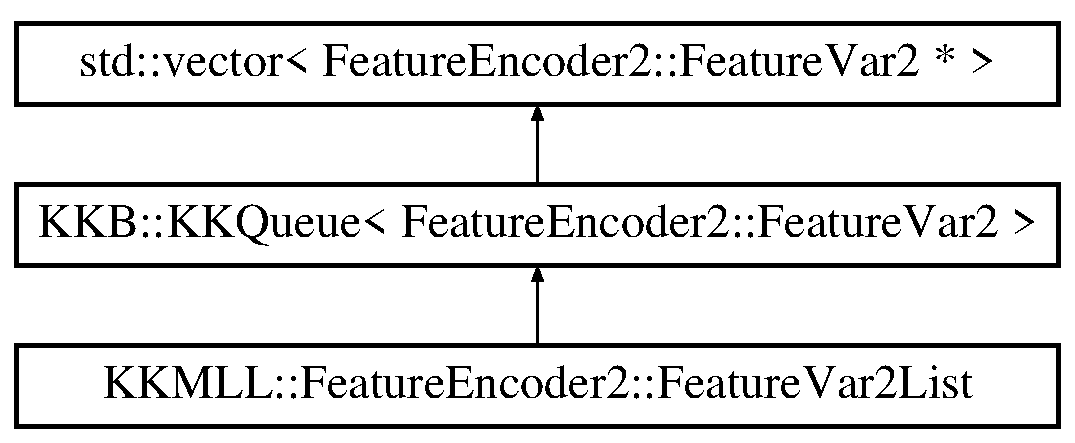
\includegraphics[height=3.000000cm]{class_feature_encoder2_1_1_feature_var2_list}
\end{center}
\end{figure}
\subsection*{Public Member Functions}
\begin{DoxyCompactItemize}
\item 
\hyperlink{class_feature_encoder2_1_1_feature_var2_list_adca64895599c1a0a9a658e6e146218a4}{Feature\+Var2\+List} (bool \+\_\+owner)
\item 
\hyperlink{class_feature_encoder2_1_1_feature_var2_list_a24294335a9761aa93f22094001fab712}{$\sim$\+Feature\+Var2\+List} ()
\end{DoxyCompactItemize}
\subsection*{Additional Inherited Members}


\subsection{Detailed Description}


Definition at line 408 of file Feature\+Encoder2.\+cpp.



\subsection{Constructor \& Destructor Documentation}
\index{Feature\+Encoder2\+::\+Feature\+Var2\+List@{Feature\+Encoder2\+::\+Feature\+Var2\+List}!Feature\+Var2\+List@{Feature\+Var2\+List}}
\index{Feature\+Var2\+List@{Feature\+Var2\+List}!Feature\+Encoder2\+::\+Feature\+Var2\+List@{Feature\+Encoder2\+::\+Feature\+Var2\+List}}
\subsubsection[{\texorpdfstring{Feature\+Var2\+List(bool \+\_\+owner)}{FeatureVar2List(bool _owner)}}]{\setlength{\rightskip}{0pt plus 5cm}K\+K\+M\+L\+L\+::\+Feature\+Encoder2\+::\+Feature\+Var2\+List\+::\+Feature\+Var2\+List (
\begin{DoxyParamCaption}
\item[{bool}]{\+\_\+owner}
\end{DoxyParamCaption}
)\hspace{0.3cm}{\ttfamily [inline]}}\hypertarget{class_feature_encoder2_1_1_feature_var2_list_adca64895599c1a0a9a658e6e146218a4}{}\label{class_feature_encoder2_1_1_feature_var2_list_adca64895599c1a0a9a658e6e146218a4}


Definition at line 411 of file Feature\+Encoder2.\+cpp.



References K\+K\+M\+L\+L\+::\+Feature\+Encoder2\+::\+Feature\+Var2\+List\+::\+Feature\+Var2\+List().



Referenced by K\+K\+M\+L\+L\+::\+Feature\+Encoder2\+::\+Feature\+Var2\+List\+::\+Feature\+Var2\+List().


\begin{DoxyCode}
411                                :
412       \hyperlink{class_k_k_b_1_1_k_k_queue}{KKQueue<FeatureVar2>} (\_owner)
413       \{\}
\end{DoxyCode}
\index{Feature\+Encoder2\+::\+Feature\+Var2\+List@{Feature\+Encoder2\+::\+Feature\+Var2\+List}!````~Feature\+Var2\+List@{$\sim$\+Feature\+Var2\+List}}
\index{````~Feature\+Var2\+List@{$\sim$\+Feature\+Var2\+List}!Feature\+Encoder2\+::\+Feature\+Var2\+List@{Feature\+Encoder2\+::\+Feature\+Var2\+List}}
\subsubsection[{\texorpdfstring{$\sim$\+Feature\+Var2\+List()}{~FeatureVar2List()}}]{\setlength{\rightskip}{0pt plus 5cm}K\+K\+M\+L\+L\+::\+Feature\+Encoder2\+::\+Feature\+Var2\+List\+::$\sim$\+Feature\+Var2\+List (
\begin{DoxyParamCaption}
{}
\end{DoxyParamCaption}
)\hspace{0.3cm}{\ttfamily [inline]}}\hypertarget{class_feature_encoder2_1_1_feature_var2_list_a24294335a9761aa93f22094001fab712}{}\label{class_feature_encoder2_1_1_feature_var2_list_a24294335a9761aa93f22094001fab712}


Definition at line 415 of file Feature\+Encoder2.\+cpp.


\begin{DoxyCode}
416   \{\}
\end{DoxyCode}


The documentation for this class was generated from the following file\+:\begin{DoxyCompactItemize}
\item 
C\+:/\+Users/\+Kurt/\+Git\+Hub/\+K\+Square\+Libraries/\+K\+K\+Machine\+Learning/\hyperlink{_feature_encoder2_8cpp}{Feature\+Encoder2.\+cpp}\end{DoxyCompactItemize}

\hypertarget{class_feature_file_i_o_dst_web_1_1_attr_desc_line}{}\section{K\+K\+M\+LL\+:\+:Feature\+File\+I\+O\+Dst\+Web\+:\+:Attr\+Desc\+Line Class Reference}
\label{class_feature_file_i_o_dst_web_1_1_attr_desc_line}\index{K\+K\+M\+L\+L\+::\+Feature\+File\+I\+O\+Dst\+Web\+::\+Attr\+Desc\+Line@{K\+K\+M\+L\+L\+::\+Feature\+File\+I\+O\+Dst\+Web\+::\+Attr\+Desc\+Line}}
\subsection*{Public Member Functions}
\begin{DoxyCompactItemize}
\item 
\hyperlink{class_feature_file_i_o_dst_web_1_1_attr_desc_line_a5e8bac5bcba089fff2f6f1288db45661}{Attr\+Desc\+Line} (\hyperlink{class_k_k_b_1_1_k_k_str}{K\+K\+Str} desc)
\end{DoxyCompactItemize}
\subsection*{Public Attributes}
\begin{DoxyCompactItemize}
\item 
\hyperlink{class_k_k_b_1_1_k_k_str}{K\+K\+Str} \hyperlink{class_feature_file_i_o_dst_web_1_1_attr_desc_line_a95a0f1eedd7d8b881b40b57b4d0d8eba}{code}
\item 
\hyperlink{class_k_k_b_1_1_k_k_str}{K\+K\+Str} \hyperlink{class_feature_file_i_o_dst_web_1_1_attr_desc_line_a1b113dcf30d429e6a0db6042df2e9b51}{root}
\item 
\hyperlink{class_k_k_b_1_1_k_k_str}{K\+K\+Str} \hyperlink{class_feature_file_i_o_dst_web_1_1_attr_desc_line_a04afb7863f4c0ebd681c503e42a52c3b}{title}
\end{DoxyCompactItemize}


\subsection{Detailed Description}


Definition at line 32 of file Feature\+File\+I\+O\+Dst\+Web.\+cpp.



\subsection{Constructor \& Destructor Documentation}
\index{Feature\+File\+I\+O\+Dst\+Web\+::\+Attr\+Desc\+Line@{Feature\+File\+I\+O\+Dst\+Web\+::\+Attr\+Desc\+Line}!Attr\+Desc\+Line@{Attr\+Desc\+Line}}
\index{Attr\+Desc\+Line@{Attr\+Desc\+Line}!Feature\+File\+I\+O\+Dst\+Web\+::\+Attr\+Desc\+Line@{Feature\+File\+I\+O\+Dst\+Web\+::\+Attr\+Desc\+Line}}
\subsubsection[{\texorpdfstring{Attr\+Desc\+Line(\+K\+K\+Str desc)}{AttrDescLine(KKStr desc)}}]{\setlength{\rightskip}{0pt plus 5cm}K\+K\+M\+L\+L\+::\+Feature\+File\+I\+O\+Dst\+Web\+::\+Attr\+Desc\+Line\+::\+Attr\+Desc\+Line (
\begin{DoxyParamCaption}
\item[{{\bf K\+K\+Str}}]{desc}
\end{DoxyParamCaption}
)\hspace{0.3cm}{\ttfamily [inline]}}\hypertarget{class_feature_file_i_o_dst_web_1_1_attr_desc_line_a5e8bac5bcba089fff2f6f1288db45661}{}\label{class_feature_file_i_o_dst_web_1_1_attr_desc_line_a5e8bac5bcba089fff2f6f1288db45661}


Definition at line 35 of file Feature\+File\+I\+O\+Dst\+Web.\+cpp.



References K\+K\+B\+::\+K\+K\+Str\+::\+Chop\+Last\+Char(), K\+K\+M\+L\+L\+::\+Feature\+File\+I\+O\+Dst\+Web\+::\+Attr\+Desc\+Line\+::code, K\+K\+B\+::\+K\+K\+Str\+::\+Concat(), K\+K\+B\+::\+K\+K\+Str\+::\+Extract\+Token(), K\+K\+B\+::\+K\+K\+Str\+::\+First\+Char(), K\+K\+B\+::\+K\+K\+Str\+::\+Last\+Char(), K\+K\+B\+::\+K\+K\+Str\+::operator=(), K\+K\+M\+L\+L\+::\+Feature\+File\+I\+O\+Dst\+Web\+::\+Attr\+Desc\+Line\+::root, K\+K\+B\+::\+K\+K\+Str\+::\+Sub\+Str\+Part(), K\+K\+M\+L\+L\+::\+Feature\+File\+I\+O\+Dst\+Web\+::\+Attr\+Desc\+Line\+::title, K\+K\+B\+::\+K\+K\+Str\+::\+Trim\+Left(), and K\+K\+B\+::\+K\+K\+Str\+::\+Trim\+Right().



Referenced by K\+K\+M\+L\+L\+::\+Feature\+File\+I\+O\+Dst\+Web\+::\+Get\+File\+Desc().


\begin{DoxyCode}
36     \{
37       \hyperlink{class_k_k_b_1_1_k_k_str}{KKStr}  aStr = desc.\hyperlink{class_k_k_b_1_1_k_k_str_acc31c95308d6d699debde883c11e5802}{ExtractToken} (\textcolor{stringliteral}{",\(\backslash\)n\(\backslash\)r\(\backslash\)t"});
38 
39       \hyperlink{class_feature_file_i_o_dst_web_1_1_attr_desc_line_a95a0f1eedd7d8b881b40b57b4d0d8eba}{code} = desc.\hyperlink{class_k_k_b_1_1_k_k_str_acc31c95308d6d699debde883c11e5802}{ExtractToken} (\textcolor{stringliteral}{",\(\backslash\)n\(\backslash\)r\(\backslash\)t"});
40       \hyperlink{class_feature_file_i_o_dst_web_1_1_attr_desc_line_a95a0f1eedd7d8b881b40b57b4d0d8eba}{code}.\hyperlink{class_k_k_b_1_1_k_k_str_af7c102c53103ddff3f48270b4a198c89}{TrimLeft} ();
41       \hyperlink{class_feature_file_i_o_dst_web_1_1_attr_desc_line_a95a0f1eedd7d8b881b40b57b4d0d8eba}{code}.\hyperlink{class_k_k_b_1_1_k_k_str_aa912161f17871e2d6fec7bbac033221c}{TrimRight} ();
42 
43       \hyperlink{class_k_k_b_1_1_k_k_str}{KKStr}  oneStr = desc.\hyperlink{class_k_k_b_1_1_k_k_str_acc31c95308d6d699debde883c11e5802}{ExtractToken} (\textcolor{stringliteral}{",\(\backslash\)n\(\backslash\)r\(\backslash\)t"});
44      
45       \hyperlink{class_feature_file_i_o_dst_web_1_1_attr_desc_line_a04afb7863f4c0ebd681c503e42a52c3b}{title} = desc.\hyperlink{class_k_k_b_1_1_k_k_str_acc31c95308d6d699debde883c11e5802}{ExtractToken} (\textcolor{stringliteral}{",\(\backslash\)n\(\backslash\)r\(\backslash\)t"});
46       \textcolor{keywordflow}{if}  (\hyperlink{class_feature_file_i_o_dst_web_1_1_attr_desc_line_a04afb7863f4c0ebd681c503e42a52c3b}{title}.\hyperlink{class_k_k_b_1_1_k_k_str_ac20e69c629b985c6569af914d9cc3e8c}{FirstChar} () == \textcolor{charliteral}{'"'})
47         \hyperlink{class_feature_file_i_o_dst_web_1_1_attr_desc_line_a04afb7863f4c0ebd681c503e42a52c3b}{title} = \hyperlink{class_feature_file_i_o_dst_web_1_1_attr_desc_line_a04afb7863f4c0ebd681c503e42a52c3b}{title}.\hyperlink{class_k_k_b_1_1_k_k_str_a5f20b2ddfc9f07c8ef99592810332ddb}{SubStrPart} (1);
48       \textcolor{keywordflow}{if}  (\hyperlink{class_feature_file_i_o_dst_web_1_1_attr_desc_line_a04afb7863f4c0ebd681c503e42a52c3b}{title}.\hyperlink{class_k_k_b_1_1_k_k_str_ad1951ace757c18c2d01df666b3a4032c}{LastChar} () == \textcolor{charliteral}{'"'})
49         \hyperlink{class_feature_file_i_o_dst_web_1_1_attr_desc_line_a04afb7863f4c0ebd681c503e42a52c3b}{title}.\hyperlink{class_k_k_b_1_1_k_k_str_af84ac251b246a683f8b45c6c15a62936}{ChopLastChar} ();
50 
51       \hyperlink{class_feature_file_i_o_dst_web_1_1_attr_desc_line_a1b113dcf30d429e6a0db6042df2e9b51}{root}  = desc.\hyperlink{class_k_k_b_1_1_k_k_str_acc31c95308d6d699debde883c11e5802}{ExtractToken} ();
52       \textcolor{keywordflow}{if}  (\hyperlink{class_feature_file_i_o_dst_web_1_1_attr_desc_line_a1b113dcf30d429e6a0db6042df2e9b51}{root}.\hyperlink{class_k_k_b_1_1_k_k_str_ac20e69c629b985c6569af914d9cc3e8c}{FirstChar} () == \textcolor{charliteral}{'"'})
53         \hyperlink{class_feature_file_i_o_dst_web_1_1_attr_desc_line_a1b113dcf30d429e6a0db6042df2e9b51}{root} = \hyperlink{class_feature_file_i_o_dst_web_1_1_attr_desc_line_a1b113dcf30d429e6a0db6042df2e9b51}{root}.\hyperlink{class_k_k_b_1_1_k_k_str_a5f20b2ddfc9f07c8ef99592810332ddb}{SubStrPart} (1);
54       \textcolor{keywordflow}{if}  (\hyperlink{class_feature_file_i_o_dst_web_1_1_attr_desc_line_a1b113dcf30d429e6a0db6042df2e9b51}{root}.\hyperlink{class_k_k_b_1_1_k_k_str_ad1951ace757c18c2d01df666b3a4032c}{LastChar} () == \textcolor{charliteral}{'"'})
55         \hyperlink{class_feature_file_i_o_dst_web_1_1_attr_desc_line_a1b113dcf30d429e6a0db6042df2e9b51}{root}.\hyperlink{class_k_k_b_1_1_k_k_str_af84ac251b246a683f8b45c6c15a62936}{ChopLastChar} ();
56     \}
\end{DoxyCode}


\subsection{Member Data Documentation}
\index{Feature\+File\+I\+O\+Dst\+Web\+::\+Attr\+Desc\+Line@{Feature\+File\+I\+O\+Dst\+Web\+::\+Attr\+Desc\+Line}!code@{code}}
\index{code@{code}!Feature\+File\+I\+O\+Dst\+Web\+::\+Attr\+Desc\+Line@{Feature\+File\+I\+O\+Dst\+Web\+::\+Attr\+Desc\+Line}}
\subsubsection[{\texorpdfstring{code}{code}}]{\setlength{\rightskip}{0pt plus 5cm}{\bf K\+K\+Str} K\+K\+M\+L\+L\+::\+Feature\+File\+I\+O\+Dst\+Web\+::\+Attr\+Desc\+Line\+::code}\hypertarget{class_feature_file_i_o_dst_web_1_1_attr_desc_line_a95a0f1eedd7d8b881b40b57b4d0d8eba}{}\label{class_feature_file_i_o_dst_web_1_1_attr_desc_line_a95a0f1eedd7d8b881b40b57b4d0d8eba}


Definition at line 58 of file Feature\+File\+I\+O\+Dst\+Web.\+cpp.



Referenced by K\+K\+M\+L\+L\+::\+Feature\+File\+I\+O\+Dst\+Web\+::\+Attr\+Desc\+Line\+::\+Attr\+Desc\+Line(), K\+K\+M\+L\+L\+::\+Feature\+File\+I\+O\+Dst\+Web\+::\+Get\+File\+Desc(), and K\+K\+M\+L\+L\+::\+Feature\+File\+I\+O\+Dst\+Web\+::\+Attr\+Desc\+Line\+Comparator\+::operator()().

\index{Feature\+File\+I\+O\+Dst\+Web\+::\+Attr\+Desc\+Line@{Feature\+File\+I\+O\+Dst\+Web\+::\+Attr\+Desc\+Line}!root@{root}}
\index{root@{root}!Feature\+File\+I\+O\+Dst\+Web\+::\+Attr\+Desc\+Line@{Feature\+File\+I\+O\+Dst\+Web\+::\+Attr\+Desc\+Line}}
\subsubsection[{\texorpdfstring{root}{root}}]{\setlength{\rightskip}{0pt plus 5cm}{\bf K\+K\+Str} K\+K\+M\+L\+L\+::\+Feature\+File\+I\+O\+Dst\+Web\+::\+Attr\+Desc\+Line\+::root}\hypertarget{class_feature_file_i_o_dst_web_1_1_attr_desc_line_a1b113dcf30d429e6a0db6042df2e9b51}{}\label{class_feature_file_i_o_dst_web_1_1_attr_desc_line_a1b113dcf30d429e6a0db6042df2e9b51}


Definition at line 60 of file Feature\+File\+I\+O\+Dst\+Web.\+cpp.



Referenced by K\+K\+M\+L\+L\+::\+Feature\+File\+I\+O\+Dst\+Web\+::\+Attr\+Desc\+Line\+::\+Attr\+Desc\+Line().

\index{Feature\+File\+I\+O\+Dst\+Web\+::\+Attr\+Desc\+Line@{Feature\+File\+I\+O\+Dst\+Web\+::\+Attr\+Desc\+Line}!title@{title}}
\index{title@{title}!Feature\+File\+I\+O\+Dst\+Web\+::\+Attr\+Desc\+Line@{Feature\+File\+I\+O\+Dst\+Web\+::\+Attr\+Desc\+Line}}
\subsubsection[{\texorpdfstring{title}{title}}]{\setlength{\rightskip}{0pt plus 5cm}{\bf K\+K\+Str} K\+K\+M\+L\+L\+::\+Feature\+File\+I\+O\+Dst\+Web\+::\+Attr\+Desc\+Line\+::title}\hypertarget{class_feature_file_i_o_dst_web_1_1_attr_desc_line_a04afb7863f4c0ebd681c503e42a52c3b}{}\label{class_feature_file_i_o_dst_web_1_1_attr_desc_line_a04afb7863f4c0ebd681c503e42a52c3b}


Definition at line 59 of file Feature\+File\+I\+O\+Dst\+Web.\+cpp.



Referenced by K\+K\+M\+L\+L\+::\+Feature\+File\+I\+O\+Dst\+Web\+::\+Attr\+Desc\+Line\+::\+Attr\+Desc\+Line().



The documentation for this class was generated from the following file\+:\begin{DoxyCompactItemize}
\item 
C\+:/\+Users/\+Kurt/\+Git\+Hub/\+K\+Square\+Libraries/\+K\+K\+Machine\+Learning/\hyperlink{_feature_file_i_o_dst_web_8cpp}{Feature\+File\+I\+O\+Dst\+Web.\+cpp}\end{DoxyCompactItemize}

\hypertarget{class_feature_file_i_o_dst_web_1_1_attr_desc_line_comparator}{}\section{K\+K\+M\+LL\+:\+:Feature\+File\+I\+O\+Dst\+Web\+:\+:Attr\+Desc\+Line\+Comparator Class Reference}
\label{class_feature_file_i_o_dst_web_1_1_attr_desc_line_comparator}\index{K\+K\+M\+L\+L\+::\+Feature\+File\+I\+O\+Dst\+Web\+::\+Attr\+Desc\+Line\+Comparator@{K\+K\+M\+L\+L\+::\+Feature\+File\+I\+O\+Dst\+Web\+::\+Attr\+Desc\+Line\+Comparator}}
\subsection*{Public Member Functions}
\begin{DoxyCompactItemize}
\item 
\hyperlink{class_feature_file_i_o_dst_web_1_1_attr_desc_line_comparator_a13d0d159090c576daf7e19581162c4b5}{Attr\+Desc\+Line\+Comparator} ()
\item 
bool \hyperlink{class_feature_file_i_o_dst_web_1_1_attr_desc_line_comparator_a2b613449fc9a69f18232a5eff0f2e48d}{operator()} (\hyperlink{class_feature_file_i_o_dst_web_1_1_attr_desc_line}{Attr\+Desc\+Line\+Ptr} p1, \hyperlink{class_feature_file_i_o_dst_web_1_1_attr_desc_line}{Attr\+Desc\+Line\+Ptr} p2)
\end{DoxyCompactItemize}


\subsection{Detailed Description}


Definition at line 67 of file Feature\+File\+I\+O\+Dst\+Web.\+cpp.



\subsection{Constructor \& Destructor Documentation}
\index{Feature\+File\+I\+O\+Dst\+Web\+::\+Attr\+Desc\+Line\+Comparator@{Feature\+File\+I\+O\+Dst\+Web\+::\+Attr\+Desc\+Line\+Comparator}!Attr\+Desc\+Line\+Comparator@{Attr\+Desc\+Line\+Comparator}}
\index{Attr\+Desc\+Line\+Comparator@{Attr\+Desc\+Line\+Comparator}!Feature\+File\+I\+O\+Dst\+Web\+::\+Attr\+Desc\+Line\+Comparator@{Feature\+File\+I\+O\+Dst\+Web\+::\+Attr\+Desc\+Line\+Comparator}}
\subsubsection[{\texorpdfstring{Attr\+Desc\+Line\+Comparator()}{AttrDescLineComparator()}}]{\setlength{\rightskip}{0pt plus 5cm}K\+K\+M\+L\+L\+::\+Feature\+File\+I\+O\+Dst\+Web\+::\+Attr\+Desc\+Line\+Comparator\+::\+Attr\+Desc\+Line\+Comparator (
\begin{DoxyParamCaption}
{}
\end{DoxyParamCaption}
)\hspace{0.3cm}{\ttfamily [inline]}}\hypertarget{class_feature_file_i_o_dst_web_1_1_attr_desc_line_comparator_a13d0d159090c576daf7e19581162c4b5}{}\label{class_feature_file_i_o_dst_web_1_1_attr_desc_line_comparator_a13d0d159090c576daf7e19581162c4b5}


Definition at line 70 of file Feature\+File\+I\+O\+Dst\+Web.\+cpp.


\begin{DoxyCode}
71   \{\}
\end{DoxyCode}


\subsection{Member Function Documentation}
\index{Feature\+File\+I\+O\+Dst\+Web\+::\+Attr\+Desc\+Line\+Comparator@{Feature\+File\+I\+O\+Dst\+Web\+::\+Attr\+Desc\+Line\+Comparator}!operator()@{operator()}}
\index{operator()@{operator()}!Feature\+File\+I\+O\+Dst\+Web\+::\+Attr\+Desc\+Line\+Comparator@{Feature\+File\+I\+O\+Dst\+Web\+::\+Attr\+Desc\+Line\+Comparator}}
\subsubsection[{\texorpdfstring{operator()(\+Attr\+Desc\+Line\+Ptr p1, Attr\+Desc\+Line\+Ptr p2)}{operator()(AttrDescLinePtr p1, AttrDescLinePtr p2)}}]{\setlength{\rightskip}{0pt plus 5cm}bool K\+K\+M\+L\+L\+::\+Feature\+File\+I\+O\+Dst\+Web\+::\+Attr\+Desc\+Line\+Comparator\+::operator() (
\begin{DoxyParamCaption}
\item[{{\bf Attr\+Desc\+Line\+Ptr}}]{p1, }
\item[{{\bf Attr\+Desc\+Line\+Ptr}}]{p2}
\end{DoxyParamCaption}
)\hspace{0.3cm}{\ttfamily [inline]}}\hypertarget{class_feature_file_i_o_dst_web_1_1_attr_desc_line_comparator_a2b613449fc9a69f18232a5eff0f2e48d}{}\label{class_feature_file_i_o_dst_web_1_1_attr_desc_line_comparator_a2b613449fc9a69f18232a5eff0f2e48d}


Definition at line 73 of file Feature\+File\+I\+O\+Dst\+Web.\+cpp.



References K\+K\+M\+L\+L\+::\+Feature\+File\+I\+O\+Dst\+Web\+::\+Attr\+Desc\+Line\+::code, and K\+K\+B\+::\+K\+K\+Str\+::operator$<$().


\begin{DoxyCode}
76   \{
77     \textcolor{keywordflow}{return} ((p1->code) < (p2->code));
78   \}
\end{DoxyCode}


The documentation for this class was generated from the following file\+:\begin{DoxyCompactItemize}
\item 
C\+:/\+Users/\+Kurt/\+Git\+Hub/\+K\+Square\+Libraries/\+K\+K\+Machine\+Learning/\hyperlink{_feature_file_i_o_dst_web_8cpp}{Feature\+File\+I\+O\+Dst\+Web.\+cpp}\end{DoxyCompactItemize}

\hypertarget{class_feature_vector_list_1_1_break_tie_comparison}{}\section{K\+K\+M\+LL\+:\+:Feature\+Vector\+List\+:\+:Break\+Tie\+Comparison Class Reference}
\label{class_feature_vector_list_1_1_break_tie_comparison}\index{K\+K\+M\+L\+L\+::\+Feature\+Vector\+List\+::\+Break\+Tie\+Comparison@{K\+K\+M\+L\+L\+::\+Feature\+Vector\+List\+::\+Break\+Tie\+Comparison}}
\subsection*{Public Member Functions}
\begin{DoxyCompactItemize}
\item 
\hyperlink{class_feature_vector_list_1_1_break_tie_comparison_ae7ad5d78f5217f7eccf9f73b24e08d39}{Break\+Tie\+Comparison} ()
\item 
bool \hyperlink{class_feature_vector_list_1_1_break_tie_comparison_ae15a8e3556abb9552a542b1957ac48e5}{operator()} (\hyperlink{namespace_k_k_m_l_l_a0c5df3d48f45926fbc4fee04f5e3bc04}{Feature\+Vector\+Ptr} p1, \hyperlink{namespace_k_k_m_l_l_a0c5df3d48f45926fbc4fee04f5e3bc04}{Feature\+Vector\+Ptr} p2)
\end{DoxyCompactItemize}


\subsection{Detailed Description}


Definition at line 1855 of file Feature\+Vector.\+cpp.



\subsection{Constructor \& Destructor Documentation}
\index{Feature\+Vector\+List\+::\+Break\+Tie\+Comparison@{Feature\+Vector\+List\+::\+Break\+Tie\+Comparison}!Break\+Tie\+Comparison@{Break\+Tie\+Comparison}}
\index{Break\+Tie\+Comparison@{Break\+Tie\+Comparison}!Feature\+Vector\+List\+::\+Break\+Tie\+Comparison@{Feature\+Vector\+List\+::\+Break\+Tie\+Comparison}}
\subsubsection[{\texorpdfstring{Break\+Tie\+Comparison()}{BreakTieComparison()}}]{\setlength{\rightskip}{0pt plus 5cm}K\+K\+M\+L\+L\+::\+Feature\+Vector\+List\+::\+Break\+Tie\+Comparison\+::\+Break\+Tie\+Comparison (
\begin{DoxyParamCaption}
{}
\end{DoxyParamCaption}
)\hspace{0.3cm}{\ttfamily [inline]}}\hypertarget{class_feature_vector_list_1_1_break_tie_comparison_ae7ad5d78f5217f7eccf9f73b24e08d39}{}\label{class_feature_vector_list_1_1_break_tie_comparison_ae7ad5d78f5217f7eccf9f73b24e08d39}


Definition at line 1859 of file Feature\+Vector.\+cpp.


\begin{DoxyCode}
1860    \{\}
\end{DoxyCode}


\subsection{Member Function Documentation}
\index{Feature\+Vector\+List\+::\+Break\+Tie\+Comparison@{Feature\+Vector\+List\+::\+Break\+Tie\+Comparison}!operator()@{operator()}}
\index{operator()@{operator()}!Feature\+Vector\+List\+::\+Break\+Tie\+Comparison@{Feature\+Vector\+List\+::\+Break\+Tie\+Comparison}}
\subsubsection[{\texorpdfstring{operator()(\+Feature\+Vector\+Ptr p1, Feature\+Vector\+Ptr p2)}{operator()(FeatureVectorPtr p1, FeatureVectorPtr p2)}}]{\setlength{\rightskip}{0pt plus 5cm}bool K\+K\+M\+L\+L\+::\+Feature\+Vector\+List\+::\+Break\+Tie\+Comparison\+::operator() (
\begin{DoxyParamCaption}
\item[{{\bf Feature\+Vector\+Ptr}}]{p1, }
\item[{{\bf Feature\+Vector\+Ptr}}]{p2}
\end{DoxyParamCaption}
)\hspace{0.3cm}{\ttfamily [inline]}}\hypertarget{class_feature_vector_list_1_1_break_tie_comparison_ae15a8e3556abb9552a542b1957ac48e5}{}\label{class_feature_vector_list_1_1_break_tie_comparison_ae15a8e3556abb9552a542b1957ac48e5}


Definition at line 1862 of file Feature\+Vector.\+cpp.



References K\+K\+M\+L\+L\+::\+Feature\+Vector\+::\+Break\+Tie().


\begin{DoxyCode}
1865    \{
1866      \textcolor{keywordflow}{return}  (p1->\hyperlink{class_k_k_m_l_l_1_1_feature_vector_a99d8b97d7209be16e9e6fe959cb00891}{BreakTie} () < p2->\hyperlink{class_k_k_m_l_l_1_1_feature_vector_a99d8b97d7209be16e9e6fe959cb00891}{BreakTie} ());
1867    \}
\end{DoxyCode}


The documentation for this class was generated from the following file\+:\begin{DoxyCompactItemize}
\item 
C\+:/\+Users/\+Kurt/\+Git\+Hub/\+K\+Square\+Libraries/\+K\+K\+Machine\+Learning/\hyperlink{_feature_vector_8cpp}{Feature\+Vector.\+cpp}\end{DoxyCompactItemize}

\hypertarget{class_feature_vector_list_1_1_break_tie_comparison_reversed}{}\section{K\+K\+M\+LL\+:\+:Feature\+Vector\+List\+:\+:Break\+Tie\+Comparison\+Reversed Class Reference}
\label{class_feature_vector_list_1_1_break_tie_comparison_reversed}\index{K\+K\+M\+L\+L\+::\+Feature\+Vector\+List\+::\+Break\+Tie\+Comparison\+Reversed@{K\+K\+M\+L\+L\+::\+Feature\+Vector\+List\+::\+Break\+Tie\+Comparison\+Reversed}}
\subsection*{Public Member Functions}
\begin{DoxyCompactItemize}
\item 
\hyperlink{class_feature_vector_list_1_1_break_tie_comparison_reversed_acb5ebaf0a848db8517bb81bee3589ae4}{Break\+Tie\+Comparison\+Reversed} ()
\item 
bool \hyperlink{class_feature_vector_list_1_1_break_tie_comparison_reversed_ac7f21a84523702ccb72f41e1e3e7b81a}{operator()} (\hyperlink{namespace_k_k_m_l_l_a0c5df3d48f45926fbc4fee04f5e3bc04}{Feature\+Vector\+Ptr} p1, \hyperlink{namespace_k_k_m_l_l_a0c5df3d48f45926fbc4fee04f5e3bc04}{Feature\+Vector\+Ptr} p2)
\end{DoxyCompactItemize}


\subsection{Detailed Description}


Definition at line 1872 of file Feature\+Vector.\+cpp.



\subsection{Constructor \& Destructor Documentation}
\index{Feature\+Vector\+List\+::\+Break\+Tie\+Comparison\+Reversed@{Feature\+Vector\+List\+::\+Break\+Tie\+Comparison\+Reversed}!Break\+Tie\+Comparison\+Reversed@{Break\+Tie\+Comparison\+Reversed}}
\index{Break\+Tie\+Comparison\+Reversed@{Break\+Tie\+Comparison\+Reversed}!Feature\+Vector\+List\+::\+Break\+Tie\+Comparison\+Reversed@{Feature\+Vector\+List\+::\+Break\+Tie\+Comparison\+Reversed}}
\subsubsection[{\texorpdfstring{Break\+Tie\+Comparison\+Reversed()}{BreakTieComparisonReversed()}}]{\setlength{\rightskip}{0pt plus 5cm}K\+K\+M\+L\+L\+::\+Feature\+Vector\+List\+::\+Break\+Tie\+Comparison\+Reversed\+::\+Break\+Tie\+Comparison\+Reversed (
\begin{DoxyParamCaption}
{}
\end{DoxyParamCaption}
)\hspace{0.3cm}{\ttfamily [inline]}}\hypertarget{class_feature_vector_list_1_1_break_tie_comparison_reversed_acb5ebaf0a848db8517bb81bee3589ae4}{}\label{class_feature_vector_list_1_1_break_tie_comparison_reversed_acb5ebaf0a848db8517bb81bee3589ae4}


Definition at line 1876 of file Feature\+Vector.\+cpp.


\begin{DoxyCode}
1877    \{\}
\end{DoxyCode}


\subsection{Member Function Documentation}
\index{Feature\+Vector\+List\+::\+Break\+Tie\+Comparison\+Reversed@{Feature\+Vector\+List\+::\+Break\+Tie\+Comparison\+Reversed}!operator()@{operator()}}
\index{operator()@{operator()}!Feature\+Vector\+List\+::\+Break\+Tie\+Comparison\+Reversed@{Feature\+Vector\+List\+::\+Break\+Tie\+Comparison\+Reversed}}
\subsubsection[{\texorpdfstring{operator()(\+Feature\+Vector\+Ptr p1, Feature\+Vector\+Ptr p2)}{operator()(FeatureVectorPtr p1, FeatureVectorPtr p2)}}]{\setlength{\rightskip}{0pt plus 5cm}bool K\+K\+M\+L\+L\+::\+Feature\+Vector\+List\+::\+Break\+Tie\+Comparison\+Reversed\+::operator() (
\begin{DoxyParamCaption}
\item[{{\bf Feature\+Vector\+Ptr}}]{p1, }
\item[{{\bf Feature\+Vector\+Ptr}}]{p2}
\end{DoxyParamCaption}
)\hspace{0.3cm}{\ttfamily [inline]}}\hypertarget{class_feature_vector_list_1_1_break_tie_comparison_reversed_ac7f21a84523702ccb72f41e1e3e7b81a}{}\label{class_feature_vector_list_1_1_break_tie_comparison_reversed_ac7f21a84523702ccb72f41e1e3e7b81a}


Definition at line 1879 of file Feature\+Vector.\+cpp.



References K\+K\+M\+L\+L\+::\+Feature\+Vector\+::\+Break\+Tie().


\begin{DoxyCode}
1882    \{
1883      \textcolor{keywordflow}{return}  (p1->\hyperlink{class_k_k_m_l_l_1_1_feature_vector_a99d8b97d7209be16e9e6fe959cb00891}{BreakTie} () > p2->\hyperlink{class_k_k_m_l_l_1_1_feature_vector_a99d8b97d7209be16e9e6fe959cb00891}{BreakTie} ());
1884    \}
\end{DoxyCode}


The documentation for this class was generated from the following file\+:\begin{DoxyCompactItemize}
\item 
C\+:/\+Users/\+Kurt/\+Git\+Hub/\+K\+Square\+Libraries/\+K\+K\+Machine\+Learning/\hyperlink{_feature_vector_8cpp}{Feature\+Vector.\+cpp}\end{DoxyCompactItemize}

\hypertarget{class_feature_vector_list_1_1_class_name_comparrison}{}\section{K\+K\+M\+LL\+:\+:Feature\+Vector\+List\+:\+:Class\+Name\+Comparrison Class Reference}
\label{class_feature_vector_list_1_1_class_name_comparrison}\index{K\+K\+M\+L\+L\+::\+Feature\+Vector\+List\+::\+Class\+Name\+Comparrison@{K\+K\+M\+L\+L\+::\+Feature\+Vector\+List\+::\+Class\+Name\+Comparrison}}
\subsection*{Public Member Functions}
\begin{DoxyCompactItemize}
\item 
\hyperlink{class_feature_vector_list_1_1_class_name_comparrison_a67c5d44d81c6b4ac81eac2c9c9ae210e}{Class\+Name\+Comparrison} ()
\item 
bool \hyperlink{class_feature_vector_list_1_1_class_name_comparrison_a532130d303f6f14cdc0cb94ad47c4678}{operator()} (\hyperlink{namespace_k_k_m_l_l_a0c5df3d48f45926fbc4fee04f5e3bc04}{Feature\+Vector\+Ptr} p1, \hyperlink{namespace_k_k_m_l_l_a0c5df3d48f45926fbc4fee04f5e3bc04}{Feature\+Vector\+Ptr} p2)
\end{DoxyCompactItemize}


\subsection{Detailed Description}


Definition at line 2001 of file Feature\+Vector.\+cpp.



\subsection{Constructor \& Destructor Documentation}
\index{Feature\+Vector\+List\+::\+Class\+Name\+Comparrison@{Feature\+Vector\+List\+::\+Class\+Name\+Comparrison}!Class\+Name\+Comparrison@{Class\+Name\+Comparrison}}
\index{Class\+Name\+Comparrison@{Class\+Name\+Comparrison}!Feature\+Vector\+List\+::\+Class\+Name\+Comparrison@{Feature\+Vector\+List\+::\+Class\+Name\+Comparrison}}
\subsubsection[{\texorpdfstring{Class\+Name\+Comparrison()}{ClassNameComparrison()}}]{\setlength{\rightskip}{0pt plus 5cm}K\+K\+M\+L\+L\+::\+Feature\+Vector\+List\+::\+Class\+Name\+Comparrison\+::\+Class\+Name\+Comparrison (
\begin{DoxyParamCaption}
{}
\end{DoxyParamCaption}
)\hspace{0.3cm}{\ttfamily [inline]}}\hypertarget{class_feature_vector_list_1_1_class_name_comparrison_a67c5d44d81c6b4ac81eac2c9c9ae210e}{}\label{class_feature_vector_list_1_1_class_name_comparrison_a67c5d44d81c6b4ac81eac2c9c9ae210e}


Definition at line 2004 of file Feature\+Vector.\+cpp.


\begin{DoxyCode}
2004 \{\}
\end{DoxyCode}


\subsection{Member Function Documentation}
\index{Feature\+Vector\+List\+::\+Class\+Name\+Comparrison@{Feature\+Vector\+List\+::\+Class\+Name\+Comparrison}!operator()@{operator()}}
\index{operator()@{operator()}!Feature\+Vector\+List\+::\+Class\+Name\+Comparrison@{Feature\+Vector\+List\+::\+Class\+Name\+Comparrison}}
\subsubsection[{\texorpdfstring{operator()(\+Feature\+Vector\+Ptr p1, Feature\+Vector\+Ptr p2)}{operator()(FeatureVectorPtr p1, FeatureVectorPtr p2)}}]{\setlength{\rightskip}{0pt plus 5cm}bool K\+K\+M\+L\+L\+::\+Feature\+Vector\+List\+::\+Class\+Name\+Comparrison\+::operator() (
\begin{DoxyParamCaption}
\item[{{\bf Feature\+Vector\+Ptr}}]{p1, }
\item[{{\bf Feature\+Vector\+Ptr}}]{p2}
\end{DoxyParamCaption}
)\hspace{0.3cm}{\ttfamily [inline]}}\hypertarget{class_feature_vector_list_1_1_class_name_comparrison_a532130d303f6f14cdc0cb94ad47c4678}{}\label{class_feature_vector_list_1_1_class_name_comparrison_a532130d303f6f14cdc0cb94ad47c4678}


Definition at line 2006 of file Feature\+Vector.\+cpp.



References K\+K\+B\+::\+K\+K\+Str\+::\+Concat(), K\+K\+M\+L\+L\+::\+Feature\+Vector\+::\+Example\+File\+Name(), K\+K\+M\+L\+L\+::\+Feature\+Vector\+::\+M\+L\+Class(), K\+K\+B\+::\+K\+K\+Str\+::operator$<$(), K\+K\+B\+::\+K\+K\+Str\+::operator$>$(), and K\+K\+M\+L\+L\+::\+M\+L\+Class\+::\+Upper\+Name().


\begin{DoxyCode}
2009   \{
2010     \textcolor{keywordflow}{if}  (p1->\hyperlink{class_k_k_m_l_l_1_1_feature_vector_a3c8fe002c6e868f8c00059c004fb32fd}{MLClass} () == NULL)
2011     \{
2012       \textcolor{keywordflow}{if}  (p2->\hyperlink{class_k_k_m_l_l_1_1_feature_vector_a3c8fe002c6e868f8c00059c004fb32fd}{MLClass} () != NULL)
2013         \textcolor{keywordflow}{return}  \textcolor{keyword}{true};
2014     \}
2015 
2016     \textcolor{keywordflow}{else} \textcolor{keywordflow}{if}  (p2->\hyperlink{class_k_k_m_l_l_1_1_feature_vector_a3c8fe002c6e868f8c00059c004fb32fd}{MLClass} () != NULL)
2017     \{
2018       \textcolor{keyword}{const} \hyperlink{class_k_k_b_1_1_k_k_str}{KKStr}& n1 = p1->\hyperlink{class_k_k_m_l_l_1_1_feature_vector_a3c8fe002c6e868f8c00059c004fb32fd}{MLClass} ()->UpperName ();
2019       \textcolor{keyword}{const} \hyperlink{class_k_k_b_1_1_k_k_str}{KKStr}& n2 = p2->\hyperlink{class_k_k_m_l_l_1_1_feature_vector_a3c8fe002c6e868f8c00059c004fb32fd}{MLClass} ()->UpperName ();
2020 
2021       \textcolor{keywordflow}{if}  (n1 < n2)
2022         \textcolor{keywordflow}{return} \textcolor{keyword}{true};
2023 
2024       \textcolor{keywordflow}{else} \textcolor{keywordflow}{if}  (n1 > n2)
2025         \textcolor{keywordflow}{return} \textcolor{keyword}{false};
2026     \}
2027 
2028     \textcolor{keywordflow}{return} p1->\hyperlink{class_k_k_m_l_l_1_1_feature_vector_ab47c89ab1e9396664fdc0dc34b6e1ab5}{ExampleFileName} () < p2->\hyperlink{class_k_k_m_l_l_1_1_feature_vector_ab47c89ab1e9396664fdc0dc34b6e1ab5}{ExampleFileName} ();
2029   \}
\end{DoxyCode}


The documentation for this class was generated from the following file\+:\begin{DoxyCompactItemize}
\item 
C\+:/\+Users/\+Kurt/\+Git\+Hub/\+K\+Square\+Libraries/\+K\+K\+Machine\+Learning/\hyperlink{_feature_vector_8cpp}{Feature\+Vector.\+cpp}\end{DoxyCompactItemize}

\hypertarget{class_feature_vector_list_1_1_class_name_comparrison_reversed}{}\section{K\+K\+M\+LL\+:\+:Feature\+Vector\+List\+:\+:Class\+Name\+Comparrison\+Reversed Class Reference}
\label{class_feature_vector_list_1_1_class_name_comparrison_reversed}\index{K\+K\+M\+L\+L\+::\+Feature\+Vector\+List\+::\+Class\+Name\+Comparrison\+Reversed@{K\+K\+M\+L\+L\+::\+Feature\+Vector\+List\+::\+Class\+Name\+Comparrison\+Reversed}}
\subsection*{Public Member Functions}
\begin{DoxyCompactItemize}
\item 
\hyperlink{class_feature_vector_list_1_1_class_name_comparrison_reversed_a7a8d81453ccdf037b10aea1c59397f80}{Class\+Name\+Comparrison\+Reversed} ()
\item 
bool \hyperlink{class_feature_vector_list_1_1_class_name_comparrison_reversed_a52b071e5334e174c9f6b9438217449d8}{operator()} (\hyperlink{namespace_k_k_m_l_l_a0c5df3d48f45926fbc4fee04f5e3bc04}{Feature\+Vector\+Ptr} p1, \hyperlink{namespace_k_k_m_l_l_a0c5df3d48f45926fbc4fee04f5e3bc04}{Feature\+Vector\+Ptr} p2)
\end{DoxyCompactItemize}


\subsection{Detailed Description}


Definition at line 2036 of file Feature\+Vector.\+cpp.



\subsection{Constructor \& Destructor Documentation}
\index{Feature\+Vector\+List\+::\+Class\+Name\+Comparrison\+Reversed@{Feature\+Vector\+List\+::\+Class\+Name\+Comparrison\+Reversed}!Class\+Name\+Comparrison\+Reversed@{Class\+Name\+Comparrison\+Reversed}}
\index{Class\+Name\+Comparrison\+Reversed@{Class\+Name\+Comparrison\+Reversed}!Feature\+Vector\+List\+::\+Class\+Name\+Comparrison\+Reversed@{Feature\+Vector\+List\+::\+Class\+Name\+Comparrison\+Reversed}}
\subsubsection[{\texorpdfstring{Class\+Name\+Comparrison\+Reversed()}{ClassNameComparrisonReversed()}}]{\setlength{\rightskip}{0pt plus 5cm}K\+K\+M\+L\+L\+::\+Feature\+Vector\+List\+::\+Class\+Name\+Comparrison\+Reversed\+::\+Class\+Name\+Comparrison\+Reversed (
\begin{DoxyParamCaption}
{}
\end{DoxyParamCaption}
)\hspace{0.3cm}{\ttfamily [inline]}}\hypertarget{class_feature_vector_list_1_1_class_name_comparrison_reversed_a7a8d81453ccdf037b10aea1c59397f80}{}\label{class_feature_vector_list_1_1_class_name_comparrison_reversed_a7a8d81453ccdf037b10aea1c59397f80}


Definition at line 2039 of file Feature\+Vector.\+cpp.


\begin{DoxyCode}
2039 \{\}
\end{DoxyCode}


\subsection{Member Function Documentation}
\index{Feature\+Vector\+List\+::\+Class\+Name\+Comparrison\+Reversed@{Feature\+Vector\+List\+::\+Class\+Name\+Comparrison\+Reversed}!operator()@{operator()}}
\index{operator()@{operator()}!Feature\+Vector\+List\+::\+Class\+Name\+Comparrison\+Reversed@{Feature\+Vector\+List\+::\+Class\+Name\+Comparrison\+Reversed}}
\subsubsection[{\texorpdfstring{operator()(\+Feature\+Vector\+Ptr p1, Feature\+Vector\+Ptr p2)}{operator()(FeatureVectorPtr p1, FeatureVectorPtr p2)}}]{\setlength{\rightskip}{0pt plus 5cm}bool K\+K\+M\+L\+L\+::\+Feature\+Vector\+List\+::\+Class\+Name\+Comparrison\+Reversed\+::operator() (
\begin{DoxyParamCaption}
\item[{{\bf Feature\+Vector\+Ptr}}]{p1, }
\item[{{\bf Feature\+Vector\+Ptr}}]{p2}
\end{DoxyParamCaption}
)\hspace{0.3cm}{\ttfamily [inline]}}\hypertarget{class_feature_vector_list_1_1_class_name_comparrison_reversed_a52b071e5334e174c9f6b9438217449d8}{}\label{class_feature_vector_list_1_1_class_name_comparrison_reversed_a52b071e5334e174c9f6b9438217449d8}


Definition at line 2042 of file Feature\+Vector.\+cpp.



References K\+K\+B\+::\+K\+K\+Str\+::\+Concat(), K\+K\+M\+L\+L\+::\+Feature\+Vector\+::\+Example\+File\+Name(), K\+K\+M\+L\+L\+::\+Feature\+Vector\+::\+M\+L\+Class(), K\+K\+B\+::\+K\+K\+Str\+::operator$<$(), K\+K\+B\+::\+K\+K\+Str\+::operator$>$(), and K\+K\+M\+L\+L\+::\+M\+L\+Class\+::\+Upper\+Name().


\begin{DoxyCode}
2045   \{
2046     \textcolor{keywordflow}{if}  (p1->\hyperlink{class_k_k_m_l_l_1_1_feature_vector_a3c8fe002c6e868f8c00059c004fb32fd}{MLClass} () == NULL)
2047     \{
2048       \textcolor{keywordflow}{if}  (p2->\hyperlink{class_k_k_m_l_l_1_1_feature_vector_a3c8fe002c6e868f8c00059c004fb32fd}{MLClass} () != NULL)
2049         \textcolor{keywordflow}{return}  \textcolor{keyword}{false};
2050     \}
2051 
2052     \textcolor{keywordflow}{else} \textcolor{keywordflow}{if}  (p2->\hyperlink{class_k_k_m_l_l_1_1_feature_vector_a3c8fe002c6e868f8c00059c004fb32fd}{MLClass} () != NULL)
2053     \{
2054       \textcolor{keyword}{const} \hyperlink{class_k_k_b_1_1_k_k_str}{KKStr}& n1 = p1->\hyperlink{class_k_k_m_l_l_1_1_feature_vector_a3c8fe002c6e868f8c00059c004fb32fd}{MLClass} ()->UpperName ();
2055       \textcolor{keyword}{const} \hyperlink{class_k_k_b_1_1_k_k_str}{KKStr}& n2 = p2->\hyperlink{class_k_k_m_l_l_1_1_feature_vector_a3c8fe002c6e868f8c00059c004fb32fd}{MLClass} ()->UpperName ();
2056 
2057       \textcolor{keywordflow}{if}  (n1 < n2)
2058         \textcolor{keywordflow}{return} \textcolor{keyword}{false};
2059 
2060       \textcolor{keywordflow}{else} \textcolor{keywordflow}{if}  (n1 > n2)
2061         \textcolor{keywordflow}{return} \textcolor{keyword}{true};
2062     \}
2063 
2064     \textcolor{keywordflow}{return} p1->\hyperlink{class_k_k_m_l_l_1_1_feature_vector_ab47c89ab1e9396664fdc0dc34b6e1ab5}{ExampleFileName} () > p2->\hyperlink{class_k_k_m_l_l_1_1_feature_vector_ab47c89ab1e9396664fdc0dc34b6e1ab5}{ExampleFileName} ();
2065   \}
\end{DoxyCode}


The documentation for this class was generated from the following file\+:\begin{DoxyCompactItemize}
\item 
C\+:/\+Users/\+Kurt/\+Git\+Hub/\+K\+Square\+Libraries/\+K\+K\+Machine\+Learning/\hyperlink{_feature_vector_8cpp}{Feature\+Vector.\+cpp}\end{DoxyCompactItemize}

\hypertarget{class_feature_vector_list_1_1_image_file_name_comparison}{}\section{K\+K\+M\+LL\+:\+:Feature\+Vector\+List\+:\+:Image\+File\+Name\+Comparison Class Reference}
\label{class_feature_vector_list_1_1_image_file_name_comparison}\index{K\+K\+M\+L\+L\+::\+Feature\+Vector\+List\+::\+Image\+File\+Name\+Comparison@{K\+K\+M\+L\+L\+::\+Feature\+Vector\+List\+::\+Image\+File\+Name\+Comparison}}
\subsection*{Public Member Functions}
\begin{DoxyCompactItemize}
\item 
\hyperlink{class_feature_vector_list_1_1_image_file_name_comparison_abdede8268a94437f824b1542111defae}{Image\+File\+Name\+Comparison} ()
\item 
bool \hyperlink{class_feature_vector_list_1_1_image_file_name_comparison_a5e9467cb0dc40b9c1d6a021ba965c760}{operator()} (\hyperlink{namespace_k_k_m_l_l_a0c5df3d48f45926fbc4fee04f5e3bc04}{Feature\+Vector\+Ptr} p1, \hyperlink{namespace_k_k_m_l_l_a0c5df3d48f45926fbc4fee04f5e3bc04}{Feature\+Vector\+Ptr} p2)
\end{DoxyCompactItemize}


\subsection{Detailed Description}


Definition at line 1926 of file Feature\+Vector.\+cpp.



\subsection{Constructor \& Destructor Documentation}
\index{Feature\+Vector\+List\+::\+Image\+File\+Name\+Comparison@{Feature\+Vector\+List\+::\+Image\+File\+Name\+Comparison}!Image\+File\+Name\+Comparison@{Image\+File\+Name\+Comparison}}
\index{Image\+File\+Name\+Comparison@{Image\+File\+Name\+Comparison}!Feature\+Vector\+List\+::\+Image\+File\+Name\+Comparison@{Feature\+Vector\+List\+::\+Image\+File\+Name\+Comparison}}
\subsubsection[{\texorpdfstring{Image\+File\+Name\+Comparison()}{ImageFileNameComparison()}}]{\setlength{\rightskip}{0pt plus 5cm}K\+K\+M\+L\+L\+::\+Feature\+Vector\+List\+::\+Image\+File\+Name\+Comparison\+::\+Image\+File\+Name\+Comparison (
\begin{DoxyParamCaption}
{}
\end{DoxyParamCaption}
)\hspace{0.3cm}{\ttfamily [inline]}}\hypertarget{class_feature_vector_list_1_1_image_file_name_comparison_abdede8268a94437f824b1542111defae}{}\label{class_feature_vector_list_1_1_image_file_name_comparison_abdede8268a94437f824b1542111defae}


Definition at line 1929 of file Feature\+Vector.\+cpp.


\begin{DoxyCode}
1929 \{\}
\end{DoxyCode}


\subsection{Member Function Documentation}
\index{Feature\+Vector\+List\+::\+Image\+File\+Name\+Comparison@{Feature\+Vector\+List\+::\+Image\+File\+Name\+Comparison}!operator()@{operator()}}
\index{operator()@{operator()}!Feature\+Vector\+List\+::\+Image\+File\+Name\+Comparison@{Feature\+Vector\+List\+::\+Image\+File\+Name\+Comparison}}
\subsubsection[{\texorpdfstring{operator()(\+Feature\+Vector\+Ptr p1, Feature\+Vector\+Ptr p2)}{operator()(FeatureVectorPtr p1, FeatureVectorPtr p2)}}]{\setlength{\rightskip}{0pt plus 5cm}bool K\+K\+M\+L\+L\+::\+Feature\+Vector\+List\+::\+Image\+File\+Name\+Comparison\+::operator() (
\begin{DoxyParamCaption}
\item[{{\bf Feature\+Vector\+Ptr}}]{p1, }
\item[{{\bf Feature\+Vector\+Ptr}}]{p2}
\end{DoxyParamCaption}
)\hspace{0.3cm}{\ttfamily [inline]}}\hypertarget{class_feature_vector_list_1_1_image_file_name_comparison_a5e9467cb0dc40b9c1d6a021ba965c760}{}\label{class_feature_vector_list_1_1_image_file_name_comparison_a5e9467cb0dc40b9c1d6a021ba965c760}


Definition at line 1932 of file Feature\+Vector.\+cpp.



References K\+K\+M\+L\+L\+::\+Feature\+Vector\+::\+Example\+File\+Name(), and K\+K\+B\+::\+K\+K\+Str\+::operator$<$().


\begin{DoxyCode}
1935   \{
1936     \textcolor{keywordflow}{return}  (p1->\hyperlink{class_k_k_m_l_l_1_1_feature_vector_ab47c89ab1e9396664fdc0dc34b6e1ab5}{ExampleFileName} () < p2->\hyperlink{class_k_k_m_l_l_1_1_feature_vector_ab47c89ab1e9396664fdc0dc34b6e1ab5}{ExampleFileName} ());
1937   \}
\end{DoxyCode}


The documentation for this class was generated from the following file\+:\begin{DoxyCompactItemize}
\item 
C\+:/\+Users/\+Kurt/\+Git\+Hub/\+K\+Square\+Libraries/\+K\+K\+Machine\+Learning/\hyperlink{_feature_vector_8cpp}{Feature\+Vector.\+cpp}\end{DoxyCompactItemize}

\hypertarget{class_feature_vector_list_1_1_image_file_name_comparison_reversed}{}\section{K\+K\+M\+LL\+:\+:Feature\+Vector\+List\+:\+:Image\+File\+Name\+Comparison\+Reversed Class Reference}
\label{class_feature_vector_list_1_1_image_file_name_comparison_reversed}\index{K\+K\+M\+L\+L\+::\+Feature\+Vector\+List\+::\+Image\+File\+Name\+Comparison\+Reversed@{K\+K\+M\+L\+L\+::\+Feature\+Vector\+List\+::\+Image\+File\+Name\+Comparison\+Reversed}}
\subsection*{Public Member Functions}
\begin{DoxyCompactItemize}
\item 
\hyperlink{class_feature_vector_list_1_1_image_file_name_comparison_reversed_a676761c491499fb17cd3ed2355fb4612}{Image\+File\+Name\+Comparison\+Reversed} ()
\item 
bool \hyperlink{class_feature_vector_list_1_1_image_file_name_comparison_reversed_a23c779589c464a5f6da5d79a3f2938e7}{operator()} (\hyperlink{namespace_k_k_m_l_l_a0c5df3d48f45926fbc4fee04f5e3bc04}{Feature\+Vector\+Ptr} p1, \hyperlink{namespace_k_k_m_l_l_a0c5df3d48f45926fbc4fee04f5e3bc04}{Feature\+Vector\+Ptr} p2)
\end{DoxyCompactItemize}


\subsection{Detailed Description}


Definition at line 1943 of file Feature\+Vector.\+cpp.



\subsection{Constructor \& Destructor Documentation}
\index{Feature\+Vector\+List\+::\+Image\+File\+Name\+Comparison\+Reversed@{Feature\+Vector\+List\+::\+Image\+File\+Name\+Comparison\+Reversed}!Image\+File\+Name\+Comparison\+Reversed@{Image\+File\+Name\+Comparison\+Reversed}}
\index{Image\+File\+Name\+Comparison\+Reversed@{Image\+File\+Name\+Comparison\+Reversed}!Feature\+Vector\+List\+::\+Image\+File\+Name\+Comparison\+Reversed@{Feature\+Vector\+List\+::\+Image\+File\+Name\+Comparison\+Reversed}}
\subsubsection[{\texorpdfstring{Image\+File\+Name\+Comparison\+Reversed()}{ImageFileNameComparisonReversed()}}]{\setlength{\rightskip}{0pt plus 5cm}K\+K\+M\+L\+L\+::\+Feature\+Vector\+List\+::\+Image\+File\+Name\+Comparison\+Reversed\+::\+Image\+File\+Name\+Comparison\+Reversed (
\begin{DoxyParamCaption}
{}
\end{DoxyParamCaption}
)\hspace{0.3cm}{\ttfamily [inline]}}\hypertarget{class_feature_vector_list_1_1_image_file_name_comparison_reversed_a676761c491499fb17cd3ed2355fb4612}{}\label{class_feature_vector_list_1_1_image_file_name_comparison_reversed_a676761c491499fb17cd3ed2355fb4612}


Definition at line 1946 of file Feature\+Vector.\+cpp.


\begin{DoxyCode}
1946 \{\}
\end{DoxyCode}


\subsection{Member Function Documentation}
\index{Feature\+Vector\+List\+::\+Image\+File\+Name\+Comparison\+Reversed@{Feature\+Vector\+List\+::\+Image\+File\+Name\+Comparison\+Reversed}!operator()@{operator()}}
\index{operator()@{operator()}!Feature\+Vector\+List\+::\+Image\+File\+Name\+Comparison\+Reversed@{Feature\+Vector\+List\+::\+Image\+File\+Name\+Comparison\+Reversed}}
\subsubsection[{\texorpdfstring{operator()(\+Feature\+Vector\+Ptr p1, Feature\+Vector\+Ptr p2)}{operator()(FeatureVectorPtr p1, FeatureVectorPtr p2)}}]{\setlength{\rightskip}{0pt plus 5cm}bool K\+K\+M\+L\+L\+::\+Feature\+Vector\+List\+::\+Image\+File\+Name\+Comparison\+Reversed\+::operator() (
\begin{DoxyParamCaption}
\item[{{\bf Feature\+Vector\+Ptr}}]{p1, }
\item[{{\bf Feature\+Vector\+Ptr}}]{p2}
\end{DoxyParamCaption}
)\hspace{0.3cm}{\ttfamily [inline]}}\hypertarget{class_feature_vector_list_1_1_image_file_name_comparison_reversed_a23c779589c464a5f6da5d79a3f2938e7}{}\label{class_feature_vector_list_1_1_image_file_name_comparison_reversed_a23c779589c464a5f6da5d79a3f2938e7}


Definition at line 1949 of file Feature\+Vector.\+cpp.



References K\+K\+M\+L\+L\+::\+Feature\+Vector\+::\+Example\+File\+Name(), and K\+K\+B\+::\+K\+K\+Str\+::operator$>$().


\begin{DoxyCode}
1952   \{
1953     \textcolor{keywordflow}{return}  (p1->\hyperlink{class_k_k_m_l_l_1_1_feature_vector_ab47c89ab1e9396664fdc0dc34b6e1ab5}{ExampleFileName} () > p2->\hyperlink{class_k_k_m_l_l_1_1_feature_vector_ab47c89ab1e9396664fdc0dc34b6e1ab5}{ExampleFileName} ());
1954   \}
\end{DoxyCode}


The documentation for this class was generated from the following file\+:\begin{DoxyCompactItemize}
\item 
C\+:/\+Users/\+Kurt/\+Git\+Hub/\+K\+Square\+Libraries/\+K\+K\+Machine\+Learning/\hyperlink{_feature_vector_8cpp}{Feature\+Vector.\+cpp}\end{DoxyCompactItemize}

\hypertarget{class_feature_vector_list_1_1_probability_comparison}{}\section{K\+K\+M\+LL\+:\+:Feature\+Vector\+List\+:\+:Probability\+Comparison Class Reference}
\label{class_feature_vector_list_1_1_probability_comparison}\index{K\+K\+M\+L\+L\+::\+Feature\+Vector\+List\+::\+Probability\+Comparison@{K\+K\+M\+L\+L\+::\+Feature\+Vector\+List\+::\+Probability\+Comparison}}
\subsection*{Public Member Functions}
\begin{DoxyCompactItemize}
\item 
\hyperlink{class_feature_vector_list_1_1_probability_comparison_abf21f89638376dc9df6189f9864da4d4}{Probability\+Comparison} ()
\item 
bool \hyperlink{class_feature_vector_list_1_1_probability_comparison_aec365ed4cf5ed4df62877be9508162fd}{operator()} (\hyperlink{namespace_k_k_m_l_l_a0c5df3d48f45926fbc4fee04f5e3bc04}{Feature\+Vector\+Ptr} p1, \hyperlink{namespace_k_k_m_l_l_a0c5df3d48f45926fbc4fee04f5e3bc04}{Feature\+Vector\+Ptr} p2)
\end{DoxyCompactItemize}


\subsection{Detailed Description}


Definition at line 1891 of file Feature\+Vector.\+cpp.



\subsection{Constructor \& Destructor Documentation}
\index{Feature\+Vector\+List\+::\+Probability\+Comparison@{Feature\+Vector\+List\+::\+Probability\+Comparison}!Probability\+Comparison@{Probability\+Comparison}}
\index{Probability\+Comparison@{Probability\+Comparison}!Feature\+Vector\+List\+::\+Probability\+Comparison@{Feature\+Vector\+List\+::\+Probability\+Comparison}}
\subsubsection[{\texorpdfstring{Probability\+Comparison()}{ProbabilityComparison()}}]{\setlength{\rightskip}{0pt plus 5cm}K\+K\+M\+L\+L\+::\+Feature\+Vector\+List\+::\+Probability\+Comparison\+::\+Probability\+Comparison (
\begin{DoxyParamCaption}
{}
\end{DoxyParamCaption}
)\hspace{0.3cm}{\ttfamily [inline]}}\hypertarget{class_feature_vector_list_1_1_probability_comparison_abf21f89638376dc9df6189f9864da4d4}{}\label{class_feature_vector_list_1_1_probability_comparison_abf21f89638376dc9df6189f9864da4d4}


Definition at line 1895 of file Feature\+Vector.\+cpp.


\begin{DoxyCode}
1896    \{\}
\end{DoxyCode}


\subsection{Member Function Documentation}
\index{Feature\+Vector\+List\+::\+Probability\+Comparison@{Feature\+Vector\+List\+::\+Probability\+Comparison}!operator()@{operator()}}
\index{operator()@{operator()}!Feature\+Vector\+List\+::\+Probability\+Comparison@{Feature\+Vector\+List\+::\+Probability\+Comparison}}
\subsubsection[{\texorpdfstring{operator()(\+Feature\+Vector\+Ptr p1, Feature\+Vector\+Ptr p2)}{operator()(FeatureVectorPtr p1, FeatureVectorPtr p2)}}]{\setlength{\rightskip}{0pt plus 5cm}bool K\+K\+M\+L\+L\+::\+Feature\+Vector\+List\+::\+Probability\+Comparison\+::operator() (
\begin{DoxyParamCaption}
\item[{{\bf Feature\+Vector\+Ptr}}]{p1, }
\item[{{\bf Feature\+Vector\+Ptr}}]{p2}
\end{DoxyParamCaption}
)\hspace{0.3cm}{\ttfamily [inline]}}\hypertarget{class_feature_vector_list_1_1_probability_comparison_aec365ed4cf5ed4df62877be9508162fd}{}\label{class_feature_vector_list_1_1_probability_comparison_aec365ed4cf5ed4df62877be9508162fd}


Definition at line 1898 of file Feature\+Vector.\+cpp.



References K\+K\+M\+L\+L\+::\+Feature\+Vector\+::\+Probability().


\begin{DoxyCode}
1901    \{
1902      \textcolor{keywordflow}{return}  (p1->\hyperlink{class_k_k_m_l_l_1_1_feature_vector_ad999f89e685b334967fa114d2e827507}{Probability} () < p2->\hyperlink{class_k_k_m_l_l_1_1_feature_vector_ad999f89e685b334967fa114d2e827507}{Probability} ());
1903    \}
\end{DoxyCode}


The documentation for this class was generated from the following file\+:\begin{DoxyCompactItemize}
\item 
C\+:/\+Users/\+Kurt/\+Git\+Hub/\+K\+Square\+Libraries/\+K\+K\+Machine\+Learning/\hyperlink{_feature_vector_8cpp}{Feature\+Vector.\+cpp}\end{DoxyCompactItemize}

\hypertarget{class_feature_vector_list_1_1_probability_comparison_reversed}{}\section{K\+K\+M\+LL\+:\+:Feature\+Vector\+List\+:\+:Probability\+Comparison\+Reversed Class Reference}
\label{class_feature_vector_list_1_1_probability_comparison_reversed}\index{K\+K\+M\+L\+L\+::\+Feature\+Vector\+List\+::\+Probability\+Comparison\+Reversed@{K\+K\+M\+L\+L\+::\+Feature\+Vector\+List\+::\+Probability\+Comparison\+Reversed}}
\subsection*{Public Member Functions}
\begin{DoxyCompactItemize}
\item 
\hyperlink{class_feature_vector_list_1_1_probability_comparison_reversed_a2d9a5be0ecbb297b969cadc777de0a90}{Probability\+Comparison\+Reversed} ()
\item 
bool \hyperlink{class_feature_vector_list_1_1_probability_comparison_reversed_a5feed5b98129992d5f1f56e8b5c99692}{operator()} (\hyperlink{namespace_k_k_m_l_l_a0c5df3d48f45926fbc4fee04f5e3bc04}{Feature\+Vector\+Ptr} p1, \hyperlink{namespace_k_k_m_l_l_a0c5df3d48f45926fbc4fee04f5e3bc04}{Feature\+Vector\+Ptr} p2)
\end{DoxyCompactItemize}


\subsection{Detailed Description}


Definition at line 1908 of file Feature\+Vector.\+cpp.



\subsection{Constructor \& Destructor Documentation}
\index{Feature\+Vector\+List\+::\+Probability\+Comparison\+Reversed@{Feature\+Vector\+List\+::\+Probability\+Comparison\+Reversed}!Probability\+Comparison\+Reversed@{Probability\+Comparison\+Reversed}}
\index{Probability\+Comparison\+Reversed@{Probability\+Comparison\+Reversed}!Feature\+Vector\+List\+::\+Probability\+Comparison\+Reversed@{Feature\+Vector\+List\+::\+Probability\+Comparison\+Reversed}}
\subsubsection[{\texorpdfstring{Probability\+Comparison\+Reversed()}{ProbabilityComparisonReversed()}}]{\setlength{\rightskip}{0pt plus 5cm}K\+K\+M\+L\+L\+::\+Feature\+Vector\+List\+::\+Probability\+Comparison\+Reversed\+::\+Probability\+Comparison\+Reversed (
\begin{DoxyParamCaption}
{}
\end{DoxyParamCaption}
)\hspace{0.3cm}{\ttfamily [inline]}}\hypertarget{class_feature_vector_list_1_1_probability_comparison_reversed_a2d9a5be0ecbb297b969cadc777de0a90}{}\label{class_feature_vector_list_1_1_probability_comparison_reversed_a2d9a5be0ecbb297b969cadc777de0a90}


Definition at line 1912 of file Feature\+Vector.\+cpp.


\begin{DoxyCode}
1913    \{\}
\end{DoxyCode}


\subsection{Member Function Documentation}
\index{Feature\+Vector\+List\+::\+Probability\+Comparison\+Reversed@{Feature\+Vector\+List\+::\+Probability\+Comparison\+Reversed}!operator()@{operator()}}
\index{operator()@{operator()}!Feature\+Vector\+List\+::\+Probability\+Comparison\+Reversed@{Feature\+Vector\+List\+::\+Probability\+Comparison\+Reversed}}
\subsubsection[{\texorpdfstring{operator()(\+Feature\+Vector\+Ptr p1, Feature\+Vector\+Ptr p2)}{operator()(FeatureVectorPtr p1, FeatureVectorPtr p2)}}]{\setlength{\rightskip}{0pt plus 5cm}bool K\+K\+M\+L\+L\+::\+Feature\+Vector\+List\+::\+Probability\+Comparison\+Reversed\+::operator() (
\begin{DoxyParamCaption}
\item[{{\bf Feature\+Vector\+Ptr}}]{p1, }
\item[{{\bf Feature\+Vector\+Ptr}}]{p2}
\end{DoxyParamCaption}
)\hspace{0.3cm}{\ttfamily [inline]}}\hypertarget{class_feature_vector_list_1_1_probability_comparison_reversed_a5feed5b98129992d5f1f56e8b5c99692}{}\label{class_feature_vector_list_1_1_probability_comparison_reversed_a5feed5b98129992d5f1f56e8b5c99692}


Definition at line 1915 of file Feature\+Vector.\+cpp.



References K\+K\+M\+L\+L\+::\+Feature\+Vector\+::\+Probability().


\begin{DoxyCode}
1918    \{
1919      \textcolor{keywordflow}{return}  (p1->\hyperlink{class_k_k_m_l_l_1_1_feature_vector_ad999f89e685b334967fa114d2e827507}{Probability} () > p2->\hyperlink{class_k_k_m_l_l_1_1_feature_vector_ad999f89e685b334967fa114d2e827507}{Probability} ());
1920    \}
\end{DoxyCode}


The documentation for this class was generated from the following file\+:\begin{DoxyCompactItemize}
\item 
C\+:/\+Users/\+Kurt/\+Git\+Hub/\+K\+Square\+Libraries/\+K\+K\+Machine\+Learning/\hyperlink{_feature_vector_8cpp}{Feature\+Vector.\+cpp}\end{DoxyCompactItemize}

\hypertarget{class_feature_vector_list_1_1_root_name_comparrison}{}\section{K\+K\+M\+LL\+:\+:Feature\+Vector\+List\+:\+:Root\+Name\+Comparrison Class Reference}
\label{class_feature_vector_list_1_1_root_name_comparrison}\index{K\+K\+M\+L\+L\+::\+Feature\+Vector\+List\+::\+Root\+Name\+Comparrison@{K\+K\+M\+L\+L\+::\+Feature\+Vector\+List\+::\+Root\+Name\+Comparrison}}
\subsection*{Public Member Functions}
\begin{DoxyCompactItemize}
\item 
\hyperlink{class_feature_vector_list_1_1_root_name_comparrison_ac36d45c1e8519e1b022f006a2997ebba}{Root\+Name\+Comparrison} ()
\item 
bool \hyperlink{class_feature_vector_list_1_1_root_name_comparrison_aa6872e038ebf7b59ea99f503e7044886}{operator()} (\hyperlink{namespace_k_k_m_l_l_a0c5df3d48f45926fbc4fee04f5e3bc04}{Feature\+Vector\+Ptr} p1, \hyperlink{namespace_k_k_m_l_l_a0c5df3d48f45926fbc4fee04f5e3bc04}{Feature\+Vector\+Ptr} p2)
\end{DoxyCompactItemize}


\subsection{Detailed Description}


Definition at line 1963 of file Feature\+Vector.\+cpp.



\subsection{Constructor \& Destructor Documentation}
\index{Feature\+Vector\+List\+::\+Root\+Name\+Comparrison@{Feature\+Vector\+List\+::\+Root\+Name\+Comparrison}!Root\+Name\+Comparrison@{Root\+Name\+Comparrison}}
\index{Root\+Name\+Comparrison@{Root\+Name\+Comparrison}!Feature\+Vector\+List\+::\+Root\+Name\+Comparrison@{Feature\+Vector\+List\+::\+Root\+Name\+Comparrison}}
\subsubsection[{\texorpdfstring{Root\+Name\+Comparrison()}{RootNameComparrison()}}]{\setlength{\rightskip}{0pt plus 5cm}K\+K\+M\+L\+L\+::\+Feature\+Vector\+List\+::\+Root\+Name\+Comparrison\+::\+Root\+Name\+Comparrison (
\begin{DoxyParamCaption}
{}
\end{DoxyParamCaption}
)\hspace{0.3cm}{\ttfamily [inline]}}\hypertarget{class_feature_vector_list_1_1_root_name_comparrison_ac36d45c1e8519e1b022f006a2997ebba}{}\label{class_feature_vector_list_1_1_root_name_comparrison_ac36d45c1e8519e1b022f006a2997ebba}


Definition at line 1966 of file Feature\+Vector.\+cpp.


\begin{DoxyCode}
1966 \{\}
\end{DoxyCode}


\subsection{Member Function Documentation}
\index{Feature\+Vector\+List\+::\+Root\+Name\+Comparrison@{Feature\+Vector\+List\+::\+Root\+Name\+Comparrison}!operator()@{operator()}}
\index{operator()@{operator()}!Feature\+Vector\+List\+::\+Root\+Name\+Comparrison@{Feature\+Vector\+List\+::\+Root\+Name\+Comparrison}}
\subsubsection[{\texorpdfstring{operator()(\+Feature\+Vector\+Ptr p1, Feature\+Vector\+Ptr p2)}{operator()(FeatureVectorPtr p1, FeatureVectorPtr p2)}}]{\setlength{\rightskip}{0pt plus 5cm}bool K\+K\+M\+L\+L\+::\+Feature\+Vector\+List\+::\+Root\+Name\+Comparrison\+::operator() (
\begin{DoxyParamCaption}
\item[{{\bf Feature\+Vector\+Ptr}}]{p1, }
\item[{{\bf Feature\+Vector\+Ptr}}]{p2}
\end{DoxyParamCaption}
)\hspace{0.3cm}{\ttfamily [inline]}}\hypertarget{class_feature_vector_list_1_1_root_name_comparrison_aa6872e038ebf7b59ea99f503e7044886}{}\label{class_feature_vector_list_1_1_root_name_comparrison_aa6872e038ebf7b59ea99f503e7044886}


Definition at line 1968 of file Feature\+Vector.\+cpp.



References K\+K\+B\+::\+K\+K\+Str\+::\+Concat(), K\+K\+M\+L\+L\+::\+Feature\+Vector\+::\+Example\+File\+Name(), K\+K\+B\+::\+K\+K\+Str\+::operator$<$(), and K\+K\+B\+::os\+Get\+Root\+Name\+With\+Extension().


\begin{DoxyCode}
1971   \{
1972     \hyperlink{class_k_k_b_1_1_k_k_str}{KKStr}  root1 = \hyperlink{namespace_k_k_b_a04d728a8cb494d051660f5da81bd344e}{osGetRootNameWithExtension} (p1->
      \hyperlink{class_k_k_m_l_l_1_1_feature_vector_ab47c89ab1e9396664fdc0dc34b6e1ab5}{ExampleFileName} ());
1973     \hyperlink{class_k_k_b_1_1_k_k_str}{KKStr}  root2 = \hyperlink{namespace_k_k_b_a04d728a8cb494d051660f5da81bd344e}{osGetRootNameWithExtension} (p2->
      \hyperlink{class_k_k_m_l_l_1_1_feature_vector_ab47c89ab1e9396664fdc0dc34b6e1ab5}{ExampleFileName} ());
1974 
1975     \textcolor{keywordflow}{return}  (root1 < root2);
1976   \}
\end{DoxyCode}


The documentation for this class was generated from the following file\+:\begin{DoxyCompactItemize}
\item 
C\+:/\+Users/\+Kurt/\+Git\+Hub/\+K\+Square\+Libraries/\+K\+K\+Machine\+Learning/\hyperlink{_feature_vector_8cpp}{Feature\+Vector.\+cpp}\end{DoxyCompactItemize}

\hypertarget{class_feature_vector_list_1_1_root_name_comparrison_reversed}{}\section{K\+K\+M\+LL\+:\+:Feature\+Vector\+List\+:\+:Root\+Name\+Comparrison\+Reversed Class Reference}
\label{class_feature_vector_list_1_1_root_name_comparrison_reversed}\index{K\+K\+M\+L\+L\+::\+Feature\+Vector\+List\+::\+Root\+Name\+Comparrison\+Reversed@{K\+K\+M\+L\+L\+::\+Feature\+Vector\+List\+::\+Root\+Name\+Comparrison\+Reversed}}
\subsection*{Public Member Functions}
\begin{DoxyCompactItemize}
\item 
\hyperlink{class_feature_vector_list_1_1_root_name_comparrison_reversed_aee7722c42ee12a9edbec3cb5a25b1f7d}{Root\+Name\+Comparrison\+Reversed} ()
\item 
bool \hyperlink{class_feature_vector_list_1_1_root_name_comparrison_reversed_a93676ab93d3c0a7271c9ad3a765e9fb0}{operator()} (\hyperlink{namespace_k_k_m_l_l_a0c5df3d48f45926fbc4fee04f5e3bc04}{Feature\+Vector\+Ptr} p1, \hyperlink{namespace_k_k_m_l_l_a0c5df3d48f45926fbc4fee04f5e3bc04}{Feature\+Vector\+Ptr} p2)
\end{DoxyCompactItemize}


\subsection{Detailed Description}


Definition at line 1981 of file Feature\+Vector.\+cpp.



\subsection{Constructor \& Destructor Documentation}
\index{Feature\+Vector\+List\+::\+Root\+Name\+Comparrison\+Reversed@{Feature\+Vector\+List\+::\+Root\+Name\+Comparrison\+Reversed}!Root\+Name\+Comparrison\+Reversed@{Root\+Name\+Comparrison\+Reversed}}
\index{Root\+Name\+Comparrison\+Reversed@{Root\+Name\+Comparrison\+Reversed}!Feature\+Vector\+List\+::\+Root\+Name\+Comparrison\+Reversed@{Feature\+Vector\+List\+::\+Root\+Name\+Comparrison\+Reversed}}
\subsubsection[{\texorpdfstring{Root\+Name\+Comparrison\+Reversed()}{RootNameComparrisonReversed()}}]{\setlength{\rightskip}{0pt plus 5cm}K\+K\+M\+L\+L\+::\+Feature\+Vector\+List\+::\+Root\+Name\+Comparrison\+Reversed\+::\+Root\+Name\+Comparrison\+Reversed (
\begin{DoxyParamCaption}
{}
\end{DoxyParamCaption}
)\hspace{0.3cm}{\ttfamily [inline]}}\hypertarget{class_feature_vector_list_1_1_root_name_comparrison_reversed_aee7722c42ee12a9edbec3cb5a25b1f7d}{}\label{class_feature_vector_list_1_1_root_name_comparrison_reversed_aee7722c42ee12a9edbec3cb5a25b1f7d}


Definition at line 1984 of file Feature\+Vector.\+cpp.


\begin{DoxyCode}
1984 \{\}
\end{DoxyCode}


\subsection{Member Function Documentation}
\index{Feature\+Vector\+List\+::\+Root\+Name\+Comparrison\+Reversed@{Feature\+Vector\+List\+::\+Root\+Name\+Comparrison\+Reversed}!operator()@{operator()}}
\index{operator()@{operator()}!Feature\+Vector\+List\+::\+Root\+Name\+Comparrison\+Reversed@{Feature\+Vector\+List\+::\+Root\+Name\+Comparrison\+Reversed}}
\subsubsection[{\texorpdfstring{operator()(\+Feature\+Vector\+Ptr p1, Feature\+Vector\+Ptr p2)}{operator()(FeatureVectorPtr p1, FeatureVectorPtr p2)}}]{\setlength{\rightskip}{0pt plus 5cm}bool K\+K\+M\+L\+L\+::\+Feature\+Vector\+List\+::\+Root\+Name\+Comparrison\+Reversed\+::operator() (
\begin{DoxyParamCaption}
\item[{{\bf Feature\+Vector\+Ptr}}]{p1, }
\item[{{\bf Feature\+Vector\+Ptr}}]{p2}
\end{DoxyParamCaption}
)\hspace{0.3cm}{\ttfamily [inline]}}\hypertarget{class_feature_vector_list_1_1_root_name_comparrison_reversed_a93676ab93d3c0a7271c9ad3a765e9fb0}{}\label{class_feature_vector_list_1_1_root_name_comparrison_reversed_a93676ab93d3c0a7271c9ad3a765e9fb0}


Definition at line 1986 of file Feature\+Vector.\+cpp.



References K\+K\+B\+::\+K\+K\+Str\+::\+Concat(), K\+K\+M\+L\+L\+::\+Feature\+Vector\+::\+Example\+File\+Name(), K\+K\+B\+::\+K\+K\+Str\+::operator$>$(), and K\+K\+B\+::os\+Get\+Root\+Name().


\begin{DoxyCode}
1989   \{
1990     \hyperlink{class_k_k_b_1_1_k_k_str}{KKStr}  root1 = \hyperlink{namespace_k_k_b_af5b668ed9902d7f93b62529664a739f0}{osGetRootName} (p1->\hyperlink{class_k_k_m_l_l_1_1_feature_vector_ab47c89ab1e9396664fdc0dc34b6e1ab5}{ExampleFileName} ());
1991     \hyperlink{class_k_k_b_1_1_k_k_str}{KKStr}  root2 = \hyperlink{namespace_k_k_b_af5b668ed9902d7f93b62529664a739f0}{osGetRootName} (p2->\hyperlink{class_k_k_m_l_l_1_1_feature_vector_ab47c89ab1e9396664fdc0dc34b6e1ab5}{ExampleFileName} ());
1992 
1993     \textcolor{keywordflow}{return}  root1 > root2;
1994   \}
\end{DoxyCode}


The documentation for this class was generated from the following file\+:\begin{DoxyCompactItemize}
\item 
C\+:/\+Users/\+Kurt/\+Git\+Hub/\+K\+Square\+Libraries/\+K\+K\+Machine\+Learning/\hyperlink{_feature_vector_8cpp}{Feature\+Vector.\+cpp}\end{DoxyCompactItemize}

\hypertarget{class_k_k_b_1_1_application}{}\section{K\+KB\+:\+:Application Class Reference}
\label{class_k_k_b_1_1_application}\index{K\+K\+B\+::\+Application@{K\+K\+B\+::\+Application}}


The base class for all standalone application.  




{\ttfamily \#include $<$Application.\+h$>$}

\subsection*{Public Member Functions}
\begin{DoxyCompactItemize}
\item 
\hyperlink{class_k_k_b_1_1_application_afa8cc05ce6b6092be5ecdfdae44e05f8}{Application} ()
\begin{DoxyCompactList}\small\item\em Constructor for \hyperlink{class_k_k_b_1_1_application}{Application} class that will start with a default logger(\+Run\+Log),. \end{DoxyCompactList}\item 
\hyperlink{class_k_k_b_1_1_application_abb04f6b0977ab2b56a8a9fc103d4c10c}{Application} (const \hyperlink{class_k_k_b_1_1_application}{Application} \&\+\_\+application)
\begin{DoxyCompactList}\small\item\em Copy Constructor for \hyperlink{class_k_k_b_1_1_application}{Application} class. \end{DoxyCompactList}\item 
\hyperlink{class_k_k_b_1_1_application_a6257863bb44308181024c7052b46285e}{Application} (\hyperlink{class_k_k_b_1_1_run_log}{Run\+Log} \&\+\_\+log)
\begin{DoxyCompactList}\small\item\em Constructor for \hyperlink{class_k_k_b_1_1_application}{Application} class where we already have an existing logger \textquotesingle{}\+\_\+log\textquotesingle{}. \end{DoxyCompactList}\item 
virtual \hyperlink{class_k_k_b_1_1_application_a748bca84fefb9c12661cfaa2f623748d}{$\sim$\+Application} ()
\item 
bool \hyperlink{class_k_k_b_1_1_application_a59170bc42be6423288b94948e1668560}{Abort} ()
\begin{DoxyCompactList}\small\item\em Returns \textquotesingle{}true\textquotesingle{} if application has been aborted. \end{DoxyCompactList}\item 
void \hyperlink{class_k_k_b_1_1_application_adebf960886311c38ed4bced73649c99f}{Abort} (bool \+\_\+abort)
\begin{DoxyCompactList}\small\item\em Used to specify that the application is been aborted. \end{DoxyCompactList}\item 
virtual const char $\ast$ \hyperlink{class_k_k_b_1_1_application_aab5821a00f30e26a0806856c4e2e569e}{Application\+Name} ()
\item 
void \hyperlink{class_k_k_b_1_1_application_afae918106bf74e5fd8d80310a6614742}{Assign\+Log} (\hyperlink{class_k_k_b_1_1_run_log}{Run\+Log} \&\+\_\+log)
\begin{DoxyCompactList}\small\item\em Replaces the Log file to write to. \end{DoxyCompactList}\item 
virtual \hyperlink{class_k_k_b_1_1_k_k_str}{K\+K\+Str} \hyperlink{class_k_k_b_1_1_application_a27db46f806e5eb984ce37e593dbeef1a}{Build\+Date} () const 
\item 
virtual void \hyperlink{class_k_k_b_1_1_application_a426afb84e2065aebb8abefc32217a770}{Initalize\+Application} (\hyperlink{namespace_k_k_b_a8fa4952cc84fda1de4bec1fbdd8d5b1b}{kkint32} argc, char $\ast$$\ast$argv)
\begin{DoxyCompactList}\small\item\em Initialized \hyperlink{class_k_k_b_1_1_application}{Application} Instance; 1st method to be called after instance construction. \end{DoxyCompactList}\end{DoxyCompactItemize}
\subsection*{Public Attributes}
\begin{DoxyCompactItemize}
\item 
\hyperlink{class_k_k_b_1_1_run_log}{Run\+Log} \& \hyperlink{class_k_k_b_1_1_application_aa43b9ff197029ea41b52d21d50f48a1e}{log}
\end{DoxyCompactItemize}
\subsection*{Protected Member Functions}
\begin{DoxyCompactItemize}
\item 
virtual void \hyperlink{class_k_k_b_1_1_application_a9f3d1d39ae955c81b9f03088c61b27e8}{Display\+Command\+Line\+Parameters} ()
\begin{DoxyCompactList}\small\item\em Will display Command Lone parameters that the \textquotesingle{}\hyperlink{class_k_k_b_1_1_application}{Application}\textquotesingle{} class will manage. \end{DoxyCompactList}\item 
virtual bool \hyperlink{class_k_k_b_1_1_application_a80260251934fab49820d28e4c6b5cff9}{Process\+Cmd\+Line\+Parameter} (const \hyperlink{class_k_k_b_1_1_k_k_str}{K\+K\+Str} \&parm\+Switch, const \hyperlink{class_k_k_b_1_1_k_k_str}{K\+K\+Str} \&parm\+Value)
\begin{DoxyCompactList}\small\item\em This method will get called once for each parameter specified in the command line. \end{DoxyCompactList}\end{DoxyCompactItemize}


\subsection{Detailed Description}
The base class for all standalone application. 

This class is meant to be a general class that all standalone applications should be inherited from. It supports command line processing, and logging facilities. Derived classes will need to override the virtual methods \char`\"{}\+Application\+Name\char`\"{}, \char`\"{}\+Display\+Command\+Line\+Parameters\char`\"{}, and \char`\"{}\+Process\+Cmd\+Line\+Parameter\char`\"{}. Right after an instance is created you need to call the \char`\"{}\+Initalize\+Application\char`\"{} method; this will start the processing of any encountered parameters. For each set of parameters encountered a call to \char`\"{}\+Process\+Cmd\+Line\+Parameter\char`\"{} will be made; this is where you can intercept and process parameters that are specific to your application. Any parameters that you do not recognized should be passed onto the base-\/class by calling \char`\"{}\+Application\+::\+Process\+Cmd\+Line\+Parameter\char`\"{}. 

Definition at line 29 of file Application.\+h.



\subsection{Constructor \& Destructor Documentation}
\index{K\+K\+B\+::\+Application@{K\+K\+B\+::\+Application}!Application@{Application}}
\index{Application@{Application}!K\+K\+B\+::\+Application@{K\+K\+B\+::\+Application}}
\subsubsection[{\texorpdfstring{Application()}{Application()}}]{\setlength{\rightskip}{0pt plus 5cm}Application\+::\+Application (
\begin{DoxyParamCaption}
{}
\end{DoxyParamCaption}
)}\hypertarget{class_k_k_b_1_1_application_afa8cc05ce6b6092be5ecdfdae44e05f8}{}\label{class_k_k_b_1_1_application_afa8cc05ce6b6092be5ecdfdae44e05f8}


Constructor for \hyperlink{class_k_k_b_1_1_application}{Application} class that will start with a default logger(\+Run\+Log),. 

After creating an instance of this class you initialize it by calling Initalize\+Application. 

Definition at line 39 of file Application.\+cpp.



References K\+K\+B\+::\+K\+K\+Str\+::\+K\+K\+Str(), log, and K\+K\+B\+::\+Run\+Log\+::\+Run\+Log().


\begin{DoxyCode}
39                          :
40   abort       (\textcolor{keyword}{false}),
41   \hyperlink{class_k_k_b_1_1_application_aa43b9ff197029ea41b52d21d50f48a1e}{log}         (*(\textcolor{keyword}{new} \hyperlink{class_k_k_b_1_1_run_log}{RunLog} ())),
42   logFileName (),
43   ourLog      (NULL)
44 \{
45   ourLog = &\hyperlink{class_k_k_b_1_1_application_aa43b9ff197029ea41b52d21d50f48a1e}{log};
46 \}
\end{DoxyCode}
\index{K\+K\+B\+::\+Application@{K\+K\+B\+::\+Application}!Application@{Application}}
\index{Application@{Application}!K\+K\+B\+::\+Application@{K\+K\+B\+::\+Application}}
\subsubsection[{\texorpdfstring{Application(const Application \&\+\_\+application)}{Application(const Application &_application)}}]{\setlength{\rightskip}{0pt plus 5cm}Application\+::\+Application (
\begin{DoxyParamCaption}
\item[{const {\bf Application} \&}]{\+\_\+application}
\end{DoxyParamCaption}
)}\hypertarget{class_k_k_b_1_1_application_abb04f6b0977ab2b56a8a9fc103d4c10c}{}\label{class_k_k_b_1_1_application_abb04f6b0977ab2b56a8a9fc103d4c10c}


Copy Constructor for \hyperlink{class_k_k_b_1_1_application}{Application} class. 


\begin{DoxyParams}[1]{Parameters}
\mbox{\tt in}  & {\em \+\_\+application} & \hyperlink{class_k_k_b_1_1_application}{Application} instance to copy. \\
\hline
\end{DoxyParams}


Definition at line 51 of file Application.\+cpp.



References K\+K\+B\+::\+K\+K\+Str\+::\+K\+K\+Str(), and log.


\begin{DoxyCode}
51                                                          :
52   abort        (\_application.abort),
53   \hyperlink{class_k_k_b_1_1_application_aa43b9ff197029ea41b52d21d50f48a1e}{log}          (\_application.\hyperlink{class_k_k_b_1_1_application_aa43b9ff197029ea41b52d21d50f48a1e}{log}),
54   logFileName  (\_application.logFileName),
55   ourLog       (\_application.ourLog)
56 \{
57 \}
\end{DoxyCode}
\index{K\+K\+B\+::\+Application@{K\+K\+B\+::\+Application}!Application@{Application}}
\index{Application@{Application}!K\+K\+B\+::\+Application@{K\+K\+B\+::\+Application}}
\subsubsection[{\texorpdfstring{Application(\+Run\+Log \&\+\_\+log)}{Application(RunLog &_log)}}]{\setlength{\rightskip}{0pt plus 5cm}Application\+::\+Application (
\begin{DoxyParamCaption}
\item[{{\bf Run\+Log} \&}]{\+\_\+log}
\end{DoxyParamCaption}
)}\hypertarget{class_k_k_b_1_1_application_a6257863bb44308181024c7052b46285e}{}\label{class_k_k_b_1_1_application_a6257863bb44308181024c7052b46285e}


Constructor for \hyperlink{class_k_k_b_1_1_application}{Application} class where we already have an existing logger \textquotesingle{}\+\_\+log\textquotesingle{}. 

After creating an instance of this class you initialize it by calling Initalize\+Application. 
\begin{DoxyParams}[1]{Parameters}
\mbox{\tt in}  & {\em \+\_\+log} & A reference to a \hyperlink{class_k_k_b_1_1_run_log}{Run\+Log} object. \\
\hline
\end{DoxyParams}


Definition at line 29 of file Application.\+cpp.



References K\+K\+B\+::\+K\+K\+Str\+::\+K\+K\+Str(), and log.


\begin{DoxyCode}
29                                       :
30   abort       (\textcolor{keyword}{false}),
31   \hyperlink{class_k_k_b_1_1_application_aa43b9ff197029ea41b52d21d50f48a1e}{log}         (\_log),
32   logFileName (),
33   ourLog      (NULL)
34 \{
35 \}
\end{DoxyCode}
\index{K\+K\+B\+::\+Application@{K\+K\+B\+::\+Application}!````~Application@{$\sim$\+Application}}
\index{````~Application@{$\sim$\+Application}!K\+K\+B\+::\+Application@{K\+K\+B\+::\+Application}}
\subsubsection[{\texorpdfstring{$\sim$\+Application()}{~Application()}}]{\setlength{\rightskip}{0pt plus 5cm}Application\+::$\sim$\+Application (
\begin{DoxyParamCaption}
{}
\end{DoxyParamCaption}
)\hspace{0.3cm}{\ttfamily [virtual]}}\hypertarget{class_k_k_b_1_1_application_a748bca84fefb9c12661cfaa2f623748d}{}\label{class_k_k_b_1_1_application_a748bca84fefb9c12661cfaa2f623748d}


Definition at line 61 of file Application.\+cpp.


\begin{DoxyCode}
62 \{
63   \textcolor{keyword}{delete}  ourLog;
64   ourLog = NULL;
65 \}
\end{DoxyCode}


\subsection{Member Function Documentation}
\index{K\+K\+B\+::\+Application@{K\+K\+B\+::\+Application}!Abort@{Abort}}
\index{Abort@{Abort}!K\+K\+B\+::\+Application@{K\+K\+B\+::\+Application}}
\subsubsection[{\texorpdfstring{Abort()}{Abort()}}]{\setlength{\rightskip}{0pt plus 5cm}bool K\+K\+B\+::\+Application\+::\+Abort (
\begin{DoxyParamCaption}
{}
\end{DoxyParamCaption}
)\hspace{0.3cm}{\ttfamily [inline]}}\hypertarget{class_k_k_b_1_1_application_a59170bc42be6423288b94948e1668560}{}\label{class_k_k_b_1_1_application_a59170bc42be6423288b94948e1668560}


Returns \textquotesingle{}true\textquotesingle{} if application has been aborted. 

You would typically call this method after you are done processing the command line to make sure that the application is to keep on running. 

Definition at line 62 of file Application.\+h.


\begin{DoxyCode}
62 \{\textcolor{keywordflow}{return}  abort;\}
\end{DoxyCode}
\index{K\+K\+B\+::\+Application@{K\+K\+B\+::\+Application}!Abort@{Abort}}
\index{Abort@{Abort}!K\+K\+B\+::\+Application@{K\+K\+B\+::\+Application}}
\subsubsection[{\texorpdfstring{Abort(bool \+\_\+abort)}{Abort(bool _abort)}}]{\setlength{\rightskip}{0pt plus 5cm}void K\+K\+B\+::\+Application\+::\+Abort (
\begin{DoxyParamCaption}
\item[{bool}]{\+\_\+abort}
\end{DoxyParamCaption}
)\hspace{0.3cm}{\ttfamily [inline]}}\hypertarget{class_k_k_b_1_1_application_adebf960886311c38ed4bced73649c99f}{}\label{class_k_k_b_1_1_application_adebf960886311c38ed4bced73649c99f}


Used to specify that the application is been aborted. 

If you have a reason to abort the processing of this application you would call this method to set the \textquotesingle{}abort\textquotesingle{} flag to true. It will be the responsibility of the derived class to monitor the \textquotesingle{}Abort\textquotesingle{} flag. If is set to true they should terminate as quickly as they can; they should also release any resources they have taken. 
\begin{DoxyParams}[1]{Parameters}
\mbox{\tt in}  & {\em \+\_\+abort} & Abort status to set; if set to true you are telling the application that the program needs to be terminated. \\
\hline
\end{DoxyParams}


Definition at line 71 of file Application.\+h.


\begin{DoxyCode}
71 \{abort = \_abort;\}
\end{DoxyCode}
\index{K\+K\+B\+::\+Application@{K\+K\+B\+::\+Application}!Application\+Name@{Application\+Name}}
\index{Application\+Name@{Application\+Name}!K\+K\+B\+::\+Application@{K\+K\+B\+::\+Application}}
\subsubsection[{\texorpdfstring{Application\+Name()}{ApplicationName()}}]{\setlength{\rightskip}{0pt plus 5cm}const char $\ast$ Application\+::\+Application\+Name (
\begin{DoxyParamCaption}
{}
\end{DoxyParamCaption}
)\hspace{0.3cm}{\ttfamily [virtual]}}\hypertarget{class_k_k_b_1_1_application_aab5821a00f30e26a0806856c4e2e569e}{}\label{class_k_k_b_1_1_application_aab5821a00f30e26a0806856c4e2e569e}
Specify the name of the application 

Definition at line 80 of file Application.\+cpp.


\begin{DoxyCode}
81 \{
82   \textcolor{keywordflow}{return}  \textcolor{stringliteral}{"No-Application-Name-Provided"};
83 \}  \textcolor{comment}{/* ApplicationName */}
\end{DoxyCode}
\index{K\+K\+B\+::\+Application@{K\+K\+B\+::\+Application}!Assign\+Log@{Assign\+Log}}
\index{Assign\+Log@{Assign\+Log}!K\+K\+B\+::\+Application@{K\+K\+B\+::\+Application}}
\subsubsection[{\texorpdfstring{Assign\+Log(\+Run\+Log \&\+\_\+log)}{AssignLog(RunLog &_log)}}]{\setlength{\rightskip}{0pt plus 5cm}void Application\+::\+Assign\+Log (
\begin{DoxyParamCaption}
\item[{{\bf Run\+Log} \&}]{\+\_\+log}
\end{DoxyParamCaption}
)}\hypertarget{class_k_k_b_1_1_application_afae918106bf74e5fd8d80310a6614742}{}\label{class_k_k_b_1_1_application_afae918106bf74e5fd8d80310a6614742}


Replaces the Log file to write to. 



Definition at line 87 of file Application.\+cpp.



References log.


\begin{DoxyCode}
88 \{
89   \hyperlink{class_k_k_b_1_1_application_aa43b9ff197029ea41b52d21d50f48a1e}{log} = \_log;
90 
91   \textcolor{keywordflow}{if}  (ourLog)
92   \{
93     \textcolor{keyword}{delete}  ourLog;
94     ourLog = NULL;
95   \}
96 \} \textcolor{comment}{/* AssignRunLog */}
\end{DoxyCode}
\index{K\+K\+B\+::\+Application@{K\+K\+B\+::\+Application}!Build\+Date@{Build\+Date}}
\index{Build\+Date@{Build\+Date}!K\+K\+B\+::\+Application@{K\+K\+B\+::\+Application}}
\subsubsection[{\texorpdfstring{Build\+Date() const }{BuildDate() const }}]{\setlength{\rightskip}{0pt plus 5cm}{\bf K\+K\+Str} Application\+::\+Build\+Date (
\begin{DoxyParamCaption}
{}
\end{DoxyParamCaption}
) const\hspace{0.3cm}{\ttfamily [virtual]}}\hypertarget{class_k_k_b_1_1_application_a27db46f806e5eb984ce37e593dbeef1a}{}\label{class_k_k_b_1_1_application_a27db46f806e5eb984ce37e593dbeef1a}


Definition at line 162 of file Application.\+cpp.



References K\+K\+B\+::\+Date\+Type\+::\+Date\+Type(), K\+K\+B\+::\+Time\+Type\+::\+H\+H\+\_\+\+M\+M\+\_\+\+S\+S(), K\+K\+B\+::\+K\+K\+Str\+::operator+(), K\+K\+B\+::\+Time\+Type\+::\+Time\+Type(), and K\+K\+B\+::\+Date\+Type\+::\+Y\+Y\+Y\+Y\+\_\+\+M\+M\+\_\+\+D\+D().


\begin{DoxyCode}
163 \{
164   \hyperlink{class_k_k_b_1_1_date_type}{DateType}  buildDate (\_\_DATE\_\_);
165   \hyperlink{class_k_k_b_1_1_time_type}{TimeType}  buildTime (\_\_TIME\_\_);
166   \textcolor{keywordflow}{return}  buildDate.YYYY\_MM\_DD () + \textcolor{stringliteral}{"-"} + buildTime.HH\_MM\_SS ();
167 \}  \textcolor{comment}{/* BuildDate */}
\end{DoxyCode}
\index{K\+K\+B\+::\+Application@{K\+K\+B\+::\+Application}!Display\+Command\+Line\+Parameters@{Display\+Command\+Line\+Parameters}}
\index{Display\+Command\+Line\+Parameters@{Display\+Command\+Line\+Parameters}!K\+K\+B\+::\+Application@{K\+K\+B\+::\+Application}}
\subsubsection[{\texorpdfstring{Display\+Command\+Line\+Parameters()}{DisplayCommandLineParameters()}}]{\setlength{\rightskip}{0pt plus 5cm}void Application\+::\+Display\+Command\+Line\+Parameters (
\begin{DoxyParamCaption}
{}
\end{DoxyParamCaption}
)\hspace{0.3cm}{\ttfamily [protected]}, {\ttfamily [virtual]}}\hypertarget{class_k_k_b_1_1_application_a9f3d1d39ae955c81b9f03088c61b27e8}{}\label{class_k_k_b_1_1_application_a9f3d1d39ae955c81b9f03088c61b27e8}


Will display Command Lone parameters that the \textquotesingle{}\hyperlink{class_k_k_b_1_1_application}{Application}\textquotesingle{} class will manage. 

Derived classes that implement this method need to call their immediate base class version of this method to include these parameters. 

Definition at line 134 of file Application.\+cpp.


\begin{DoxyCode}
135 \{
136   cout << \hyperlink{class_k_k_b_1_1_application_aab5821a00f30e26a0806856c4e2e569e}{ApplicationName} () << \hyperlink{namespace_k_k_b_ad1f50f65af6adc8fa9e6f62d007818a8}{endl}
137        << \hyperlink{namespace_k_k_b_ad1f50f65af6adc8fa9e6f62d007818a8}{endl}
138        << \textcolor{stringliteral}{"    -LogFile   <FileName>        File that logging messages will be written to; if left will"}  <
      < \hyperlink{namespace_k_k_b_ad1f50f65af6adc8fa9e6f62d007818a8}{endl}
139        << \textcolor{stringliteral}{"                                 be written to Standard-Out (cout)."}                           <
      < \hyperlink{namespace_k_k_b_ad1f50f65af6adc8fa9e6f62d007818a8}{endl}
140        << \hyperlink{namespace_k_k_b_ad1f50f65af6adc8fa9e6f62d007818a8}{endl}
141        << \textcolor{stringliteral}{"    -CmdFile   <File-Name>       Filename where additional command line options are stored;"}   <
      < \hyperlink{namespace_k_k_b_ad1f50f65af6adc8fa9e6f62d007818a8}{endl}
142        << \textcolor{stringliteral}{"                                 This file can also specify additional '-CmdFile parameters."}  <
      < \hyperlink{namespace_k_k_b_ad1f50f65af6adc8fa9e6f62d007818a8}{endl}
143        << \hyperlink{namespace_k_k_b_ad1f50f65af6adc8fa9e6f62d007818a8}{endl};
144 \}
\end{DoxyCode}
\index{K\+K\+B\+::\+Application@{K\+K\+B\+::\+Application}!Initalize\+Application@{Initalize\+Application}}
\index{Initalize\+Application@{Initalize\+Application}!K\+K\+B\+::\+Application@{K\+K\+B\+::\+Application}}
\subsubsection[{\texorpdfstring{Initalize\+Application(kkint32 argc, char $\ast$$\ast$argv)}{InitalizeApplication(kkint32 argc, char **argv)}}]{\setlength{\rightskip}{0pt plus 5cm}void Application\+::\+Initalize\+Application (
\begin{DoxyParamCaption}
\item[{{\bf kkint32}}]{argc, }
\item[{char $\ast$$\ast$}]{argv}
\end{DoxyParamCaption}
)\hspace{0.3cm}{\ttfamily [virtual]}}\hypertarget{class_k_k_b_1_1_application_a426afb84e2065aebb8abefc32217a770}{}\label{class_k_k_b_1_1_application_a426afb84e2065aebb8abefc32217a770}


Initialized \hyperlink{class_k_k_b_1_1_application}{Application} Instance; 1st method to be called after instance construction. 

This method will scan the command line parameters for the log file options (-\/L, -\/\+Log, or -\/\+Log\+File) and use its parameter as the Log\+File name. If none is provided it will assume the stdout as the Log File to write to. It will take ownership of this log file and delete it in its destructor. Right after calling this constructor you will need to call the method Process\+Cmd\+Line\+Parameters. \begin{DoxySeeAlso}{See also}
\hyperlink{class_k_k_b_1_1_run_log}{Run\+Log} 

Process\+Cmd\+Line\+Parameters 
\end{DoxySeeAlso}

\begin{DoxyParams}[1]{Parameters}
\mbox{\tt in}  & {\em argc} & Number of arguments in argv. \\
\hline
\mbox{\tt in}  & {\em argv} & List of asciiz strings; one string for each argument. \\
\hline
\end{DoxyParams}


Definition at line 69 of file Application.\+cpp.



References K\+K\+B\+::\+Run\+Log\+::\+Attach\+File(), K\+K\+B\+::\+K\+K\+Str\+::\+Empty(), and log.


\begin{DoxyCode}
72 \{
73   ProcessCmdLineParameters (argc, argv);
74   \textcolor{keywordflow}{if}  (!logFileName.\hyperlink{class_k_k_b_1_1_k_k_str_ac69942f73fffd672ec2a6e1c410afdb6}{Empty} ())
75     \hyperlink{class_k_k_b_1_1_application_aa43b9ff197029ea41b52d21d50f48a1e}{log}.\hyperlink{class_k_k_b_1_1_run_log_a8201bd270fb70816db14aa4bcb0b81d2}{AttachFile} (logFileName);
76 \}
\end{DoxyCode}
\index{K\+K\+B\+::\+Application@{K\+K\+B\+::\+Application}!Process\+Cmd\+Line\+Parameter@{Process\+Cmd\+Line\+Parameter}}
\index{Process\+Cmd\+Line\+Parameter@{Process\+Cmd\+Line\+Parameter}!K\+K\+B\+::\+Application@{K\+K\+B\+::\+Application}}
\subsubsection[{\texorpdfstring{Process\+Cmd\+Line\+Parameter(const K\+K\+Str \&parm\+Switch, const K\+K\+Str \&parm\+Value)}{ProcessCmdLineParameter(const KKStr &parmSwitch, const KKStr &parmValue)}}]{\setlength{\rightskip}{0pt plus 5cm}bool Application\+::\+Process\+Cmd\+Line\+Parameter (
\begin{DoxyParamCaption}
\item[{const {\bf K\+K\+Str} \&}]{parm\+Switch, }
\item[{const {\bf K\+K\+Str} \&}]{parm\+Value}
\end{DoxyParamCaption}
)\hspace{0.3cm}{\ttfamily [protected]}, {\ttfamily [virtual]}}\hypertarget{class_k_k_b_1_1_application_a80260251934fab49820d28e4c6b5cff9}{}\label{class_k_k_b_1_1_application_a80260251934fab49820d28e4c6b5cff9}


This method will get called once for each parameter specified in the command line. 

Derived classes should define this method to intercept parameters that they are interested in. Parameters are treated as pairs, Switch and Values where switches have a leading dash(\char`\"{}-\/\char`\"{}). The \hyperlink{class_k_k_b_1_1_cmd_line_expander}{Cmd\+Line\+Expander} class will be used to expand any \char`\"{}-\/\+Cmd\+File\char`\"{} parameters. 
\begin{DoxyParams}[1]{Parameters}
\mbox{\tt in}  & {\em parm\+Switch} & The fill switch parameter. \\
\hline
\mbox{\tt in}  & {\em parm\+Value} & Any value parameter that followed the switch parameter. \\
\hline
\end{DoxyParams}


Definition at line 149 of file Application.\+cpp.


\begin{DoxyCode}
152 \{
153   \hyperlink{class_k_k_b_1_1_application_aa43b9ff197029ea41b52d21d50f48a1e}{log}.\hyperlink{class_k_k_b_1_1_run_log_a32cf761d7f2e747465fd80533fdbb659}{Level} (-1) << \hyperlink{namespace_k_k_b_ad1f50f65af6adc8fa9e6f62d007818a8}{endl}
154     << \textcolor{stringliteral}{"Application::ProcessCmdLineParameter   ***ERROR***    Unrecognized Parameter ["} << parmSwitch << \textcolor{stringliteral}{"]
        Value ["} << parmValue << \textcolor{stringliteral}{"]"} << \hyperlink{namespace_k_k_b_ad1f50f65af6adc8fa9e6f62d007818a8}{endl}
155     << \hyperlink{namespace_k_k_b_ad1f50f65af6adc8fa9e6f62d007818a8}{endl};
156   \textcolor{keywordflow}{return}  \textcolor{keyword}{false};
157 \}
\end{DoxyCode}


\subsection{Member Data Documentation}
\index{K\+K\+B\+::\+Application@{K\+K\+B\+::\+Application}!log@{log}}
\index{log@{log}!K\+K\+B\+::\+Application@{K\+K\+B\+::\+Application}}
\subsubsection[{\texorpdfstring{log}{log}}]{\setlength{\rightskip}{0pt plus 5cm}{\bf Run\+Log}\& K\+K\+B\+::\+Application\+::log}\hypertarget{class_k_k_b_1_1_application_aa43b9ff197029ea41b52d21d50f48a1e}{}\label{class_k_k_b_1_1_application_aa43b9ff197029ea41b52d21d50f48a1e}


Definition at line 143 of file Application.\+h.



Referenced by Application(), Assign\+Log(), and Initalize\+Application().



The documentation for this class was generated from the following files\+:\begin{DoxyCompactItemize}
\item 
C\+:/\+Users/\+Kurt/\+Git\+Hub/\+K\+Square\+Libraries/\+K\+K\+Base/\hyperlink{_application_8h}{Application.\+h}\item 
C\+:/\+Users/\+Kurt/\+Git\+Hub/\+K\+Square\+Libraries/\+K\+K\+Base/\hyperlink{_application_8cpp}{Application.\+cpp}\end{DoxyCompactItemize}

\hypertarget{class_k_k_b_1_1_atom}{}\section{K\+KB\+:\+:Atom Class Reference}
\label{class_k_k_b_1_1_atom}\index{K\+K\+B\+::\+Atom@{K\+K\+B\+::\+Atom}}


Base class of all other classes that are meant to be managed by \textquotesingle{}K\+K\+Base\textquotesingle{}.  




{\ttfamily \#include $<$Atom.\+h$>$}

Inheritance diagram for K\+KB\+:\+:Atom\+:\begin{figure}[H]
\begin{center}
\leavevmode
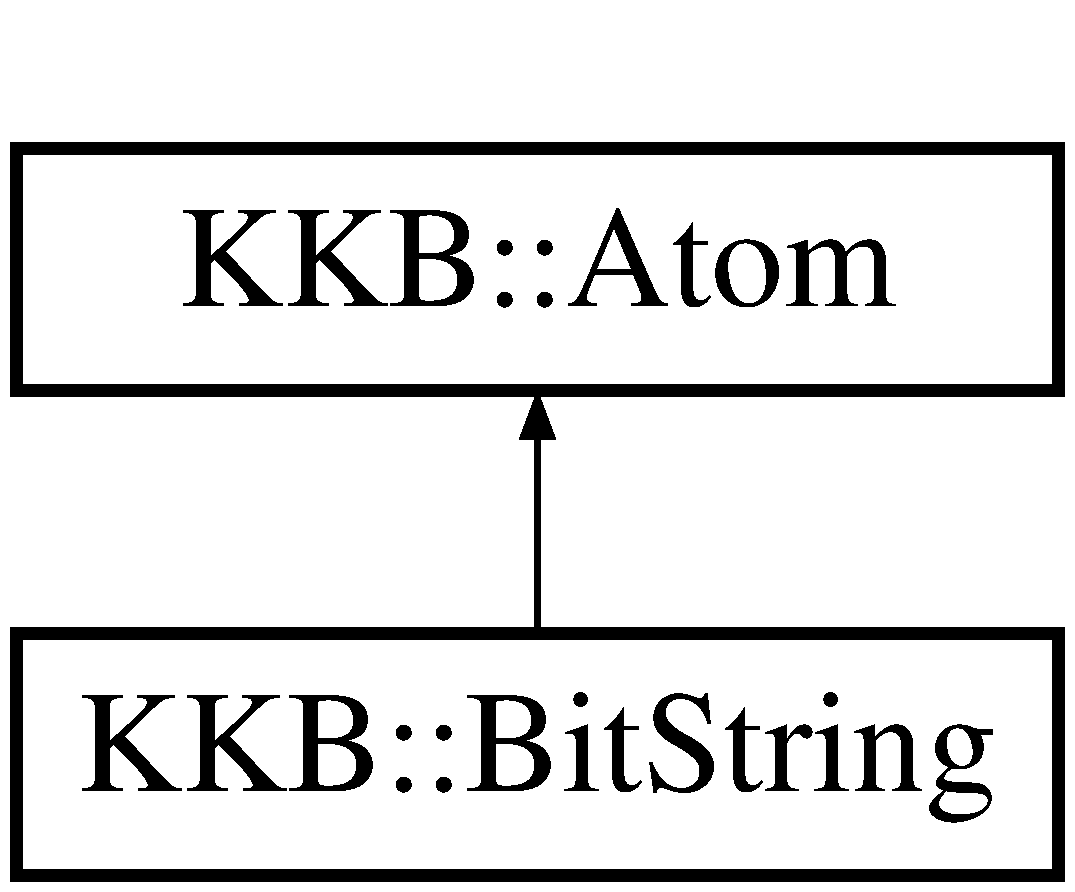
\includegraphics[height=2.000000cm]{class_k_k_b_1_1_atom}
\end{center}
\end{figure}
\subsection*{Public Types}
\begin{DoxyCompactItemize}
\item 
typedef \hyperlink{class_k_k_b_1_1_atom_a78490bd87df63b6eafa9496104c49238}{Atom\+Ptr}($\ast$ \hyperlink{class_k_k_b_1_1_atom_a9024951751f5b4f98ec92e6ea076c9c4}{Atom\+Creator}) (\hyperlink{class_k_k_b_1_1_xml_stream}{Xml\+Stream} \&i)
\item 
typedef \hyperlink{class_k_k_b_1_1_atom}{Atom} $\ast$ \hyperlink{class_k_k_b_1_1_atom_a78490bd87df63b6eafa9496104c49238}{Atom\+Ptr}
\end{DoxyCompactItemize}
\subsection*{Public Member Functions}
\begin{DoxyCompactItemize}
\item 
\hyperlink{class_k_k_b_1_1_atom_aa0147d7e49ab90f559b66e38d3d12863}{Atom} ()
\item 
virtual \hyperlink{class_k_k_b_1_1_atom_a6926cfb6d5e61ca21c71476b66547a5e}{$\sim$\+Atom} ()
\item 
virtual const char $\ast$ \hyperlink{class_k_k_b_1_1_atom_ae590752a285480b6b342def2f09b175f}{Class\+Name} () const  =0
\item 
virtual \hyperlink{class_k_k_b_1_1_atom}{Atom} $\ast$ \hyperlink{class_k_k_b_1_1_atom_a990c54fb9a7fd0928a479987fa499065}{Duplicate} () const  =0
\item 
virtual void \hyperlink{class_k_k_b_1_1_atom_add1971b30cf26b54ca37d56adbac9c82}{Read\+X\+ML} (\hyperlink{class_k_k_b_1_1_xml_stream}{Xml\+Stream} \&s, \hyperlink{namespace_k_k_b_a5f1b0b1667d79fec26deeff10c43df23}{Xml\+Tag\+Const\+Ptr} tag, \hyperlink{namespace_k_k_b_a7d390f568e2831fb76b86b56c87bf92f}{Vol\+Const\+Bool} \&cancel\+Flag, \hyperlink{class_k_k_b_1_1_run_log}{Run\+Log} \&log)=0
\item 
virtual void \hyperlink{class_k_k_b_1_1_atom_a6af114f9ae398f653b506e765e4e1eb6}{Write\+X\+ML} (const \hyperlink{class_k_k_b_1_1_k_k_str}{K\+K\+Str} \&var\+Name, std\+::ostream \&o) const  =0
\end{DoxyCompactItemize}


\subsection{Detailed Description}
Base class of all other classes that are meant to be managed by \textquotesingle{}K\+K\+Base\textquotesingle{}. 

\textquotesingle{}\hyperlink{class_k_k_b_1_1_atom}{Atom}\textquotesingle{} will have a few important virtual methods that all derived classes will be required to implement. This will allow for the smooth functioning of X\+ML file reading and writing. Ex\+: \textquotesingle{}Write\+X\+ML\textquotesingle{}, this method is to write a X\+ML version of the derived class to a output stream. A registered Build\+From\+X\+ML function will be able to create a new instance of the derived class.

Create on 2010-\/02-\/22; primary purpose is to help generate more ideas along these lines. 

Definition at line 49 of file Atom.\+h.



\subsection{Member Typedef Documentation}
\index{K\+K\+B\+::\+Atom@{K\+K\+B\+::\+Atom}!Atom\+Creator@{Atom\+Creator}}
\index{Atom\+Creator@{Atom\+Creator}!K\+K\+B\+::\+Atom@{K\+K\+B\+::\+Atom}}
\subsubsection[{\texorpdfstring{Atom\+Creator}{AtomCreator}}]{\setlength{\rightskip}{0pt plus 5cm}typedef {\bf Atom\+Ptr}($\ast$ K\+K\+B\+::\+Atom\+::\+Atom\+Creator) ({\bf Xml\+Stream} \&i)}\hypertarget{class_k_k_b_1_1_atom_a9024951751f5b4f98ec92e6ea076c9c4}{}\label{class_k_k_b_1_1_atom_a9024951751f5b4f98ec92e6ea076c9c4}


Definition at line 54 of file Atom.\+h.

\index{K\+K\+B\+::\+Atom@{K\+K\+B\+::\+Atom}!Atom\+Ptr@{Atom\+Ptr}}
\index{Atom\+Ptr@{Atom\+Ptr}!K\+K\+B\+::\+Atom@{K\+K\+B\+::\+Atom}}
\subsubsection[{\texorpdfstring{Atom\+Ptr}{AtomPtr}}]{\setlength{\rightskip}{0pt plus 5cm}typedef {\bf Atom}$\ast$ {\bf K\+K\+B\+::\+Atom\+::\+Atom\+Ptr}}\hypertarget{class_k_k_b_1_1_atom_a78490bd87df63b6eafa9496104c49238}{}\label{class_k_k_b_1_1_atom_a78490bd87df63b6eafa9496104c49238}


Definition at line 52 of file Atom.\+h.



\subsection{Constructor \& Destructor Documentation}
\index{K\+K\+B\+::\+Atom@{K\+K\+B\+::\+Atom}!Atom@{Atom}}
\index{Atom@{Atom}!K\+K\+B\+::\+Atom@{K\+K\+B\+::\+Atom}}
\subsubsection[{\texorpdfstring{Atom()}{Atom()}}]{\setlength{\rightskip}{0pt plus 5cm}Atom\+::\+Atom (
\begin{DoxyParamCaption}
{}
\end{DoxyParamCaption}
)}\hypertarget{class_k_k_b_1_1_atom_aa0147d7e49ab90f559b66e38d3d12863}{}\label{class_k_k_b_1_1_atom_aa0147d7e49ab90f559b66e38d3d12863}


Definition at line 25 of file Atom.\+cpp.


\begin{DoxyCode}
26 \{
27 \}
\end{DoxyCode}
\index{K\+K\+B\+::\+Atom@{K\+K\+B\+::\+Atom}!````~Atom@{$\sim$\+Atom}}
\index{````~Atom@{$\sim$\+Atom}!K\+K\+B\+::\+Atom@{K\+K\+B\+::\+Atom}}
\subsubsection[{\texorpdfstring{$\sim$\+Atom()}{~Atom()}}]{\setlength{\rightskip}{0pt plus 5cm}Atom\+::$\sim$\+Atom (
\begin{DoxyParamCaption}
{}
\end{DoxyParamCaption}
)\hspace{0.3cm}{\ttfamily [virtual]}}\hypertarget{class_k_k_b_1_1_atom_a6926cfb6d5e61ca21c71476b66547a5e}{}\label{class_k_k_b_1_1_atom_a6926cfb6d5e61ca21c71476b66547a5e}


Definition at line 29 of file Atom.\+cpp.


\begin{DoxyCode}
30 \{
31 \}
\end{DoxyCode}


\subsection{Member Function Documentation}
\index{K\+K\+B\+::\+Atom@{K\+K\+B\+::\+Atom}!Class\+Name@{Class\+Name}}
\index{Class\+Name@{Class\+Name}!K\+K\+B\+::\+Atom@{K\+K\+B\+::\+Atom}}
\subsubsection[{\texorpdfstring{Class\+Name() const  =0}{ClassName() const  =0}}]{\setlength{\rightskip}{0pt plus 5cm}virtual const char$\ast$ K\+K\+B\+::\+Atom\+::\+Class\+Name (
\begin{DoxyParamCaption}
{}
\end{DoxyParamCaption}
) const\hspace{0.3cm}{\ttfamily [pure virtual]}}\hypertarget{class_k_k_b_1_1_atom_ae590752a285480b6b342def2f09b175f}{}\label{class_k_k_b_1_1_atom_ae590752a285480b6b342def2f09b175f}


Implemented in \hyperlink{class_k_k_b_1_1_bit_string_a610a7f712c54ecdde050c4c64e3f460e}{K\+K\+B\+::\+Bit\+String}.

\index{K\+K\+B\+::\+Atom@{K\+K\+B\+::\+Atom}!Duplicate@{Duplicate}}
\index{Duplicate@{Duplicate}!K\+K\+B\+::\+Atom@{K\+K\+B\+::\+Atom}}
\subsubsection[{\texorpdfstring{Duplicate() const  =0}{Duplicate() const  =0}}]{\setlength{\rightskip}{0pt plus 5cm}virtual {\bf Atom}$\ast$ K\+K\+B\+::\+Atom\+::\+Duplicate (
\begin{DoxyParamCaption}
{}
\end{DoxyParamCaption}
) const\hspace{0.3cm}{\ttfamily [pure virtual]}}\hypertarget{class_k_k_b_1_1_atom_a990c54fb9a7fd0928a479987fa499065}{}\label{class_k_k_b_1_1_atom_a990c54fb9a7fd0928a479987fa499065}


Implemented in \hyperlink{class_k_k_b_1_1_bit_string_afbd70179ae53fb7326b129758e0e6521}{K\+K\+B\+::\+Bit\+String}.

\index{K\+K\+B\+::\+Atom@{K\+K\+B\+::\+Atom}!Read\+X\+ML@{Read\+X\+ML}}
\index{Read\+X\+ML@{Read\+X\+ML}!K\+K\+B\+::\+Atom@{K\+K\+B\+::\+Atom}}
\subsubsection[{\texorpdfstring{Read\+X\+M\+L(\+Xml\+Stream \&s, Xml\+Tag\+Const\+Ptr tag, Vol\+Const\+Bool \&cancel\+Flag, Run\+Log \&log)=0}{ReadXML(XmlStream &s, XmlTagConstPtr tag, VolConstBool &cancelFlag, RunLog &log)=0}}]{\setlength{\rightskip}{0pt plus 5cm}virtual void K\+K\+B\+::\+Atom\+::\+Read\+X\+ML (
\begin{DoxyParamCaption}
\item[{{\bf Xml\+Stream} \&}]{s, }
\item[{{\bf Xml\+Tag\+Const\+Ptr}}]{tag, }
\item[{{\bf Vol\+Const\+Bool} \&}]{cancel\+Flag, }
\item[{{\bf Run\+Log} \&}]{log}
\end{DoxyParamCaption}
)\hspace{0.3cm}{\ttfamily [pure virtual]}}\hypertarget{class_k_k_b_1_1_atom_add1971b30cf26b54ca37d56adbac9c82}{}\label{class_k_k_b_1_1_atom_add1971b30cf26b54ca37d56adbac9c82}


Implemented in \hyperlink{class_k_k_b_1_1_bit_string_a63fa7f49ff50431c75443fe287fe5d4f}{K\+K\+B\+::\+Bit\+String}.

\index{K\+K\+B\+::\+Atom@{K\+K\+B\+::\+Atom}!Write\+X\+ML@{Write\+X\+ML}}
\index{Write\+X\+ML@{Write\+X\+ML}!K\+K\+B\+::\+Atom@{K\+K\+B\+::\+Atom}}
\subsubsection[{\texorpdfstring{Write\+X\+M\+L(const K\+K\+Str \&var\+Name, std\+::ostream \&o) const  =0}{WriteXML(const KKStr &varName, std::ostream &o) const  =0}}]{\setlength{\rightskip}{0pt plus 5cm}virtual void K\+K\+B\+::\+Atom\+::\+Write\+X\+ML (
\begin{DoxyParamCaption}
\item[{const {\bf K\+K\+Str} \&}]{var\+Name, }
\item[{std\+::ostream \&}]{o}
\end{DoxyParamCaption}
) const\hspace{0.3cm}{\ttfamily [pure virtual]}}\hypertarget{class_k_k_b_1_1_atom_a6af114f9ae398f653b506e765e4e1eb6}{}\label{class_k_k_b_1_1_atom_a6af114f9ae398f653b506e765e4e1eb6}


Implemented in \hyperlink{class_k_k_b_1_1_bit_string_a4c0c3f7bf53ef6ca2558927f2cb500fc}{K\+K\+B\+::\+Bit\+String}.



The documentation for this class was generated from the following files\+:\begin{DoxyCompactItemize}
\item 
C\+:/\+Users/\+Kurt/\+Git\+Hub/\+K\+Square\+Libraries/\+K\+K\+Base/\hyperlink{_atom_8h}{Atom.\+h}\item 
C\+:/\+Users/\+Kurt/\+Git\+Hub/\+K\+Square\+Libraries/\+K\+K\+Base/\hyperlink{_atom_8cpp}{Atom.\+cpp}\end{DoxyCompactItemize}

\hypertarget{class_k_k_b_1_1_bit_string}{}\section{K\+KB\+:\+:Bit\+String Class Reference}
\label{class_k_k_b_1_1_bit_string}\index{K\+K\+B\+::\+Bit\+String@{K\+K\+B\+::\+Bit\+String}}


Allows you to manage very long bit strings.  




{\ttfamily \#include $<$Bit\+String.\+h$>$}

Inheritance diagram for K\+KB\+:\+:Bit\+String\+:\begin{figure}[H]
\begin{center}
\leavevmode
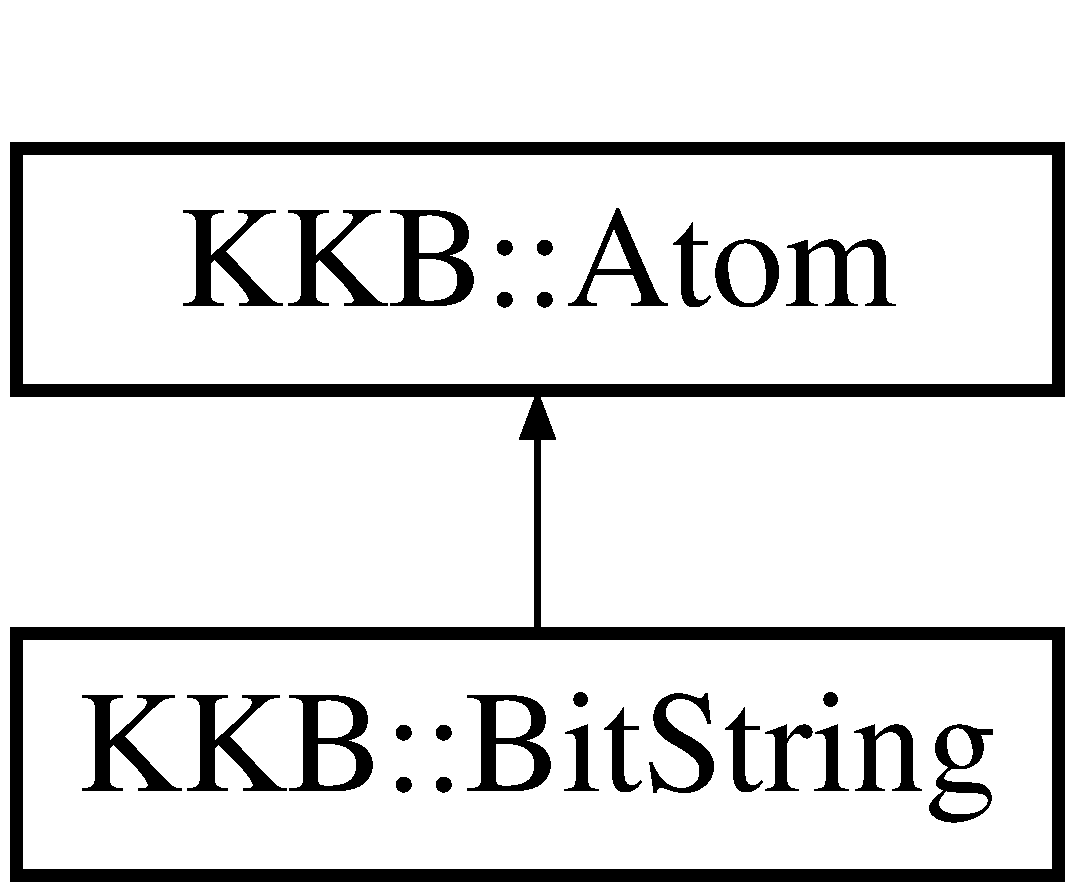
\includegraphics[height=2.000000cm]{class_k_k_b_1_1_bit_string}
\end{center}
\end{figure}
\subsection*{Public Member Functions}
\begin{DoxyCompactItemize}
\item 
\hyperlink{class_k_k_b_1_1_bit_string_a129b293aa7369637810c1d54471e1258}{Bit\+String} ()
\begin{DoxyCompactList}\small\item\em Instantiates a empty bit-\/string of length 0; needed for Read\+X\+ML. \end{DoxyCompactList}\item 
\hyperlink{class_k_k_b_1_1_bit_string_ab5d7f4ff230b20e46451bf7322ef31b8}{Bit\+String} (\hyperlink{namespace_k_k_b_af8d832f05c54994a1cce25bd5743e19a}{kkuint32} \+\_\+bit\+Len)
\begin{DoxyCompactList}\small\item\em Construct a bit string of length \+\_\+bin\+Len with all bits set to \textquotesingle{}0\textquotesingle{}. \end{DoxyCompactList}\item 
\hyperlink{class_k_k_b_1_1_bit_string_aaae20c7515dc5ddd98e4ffa65a3a379a}{Bit\+String} (const \hyperlink{class_k_k_b_1_1_bit_string}{Bit\+String} \&b)
\begin{DoxyCompactList}\small\item\em Copy constructor. \end{DoxyCompactList}\item 
\hyperlink{class_k_k_b_1_1_bit_string_a934828473e02585ddc44ff46ee0ea637}{Bit\+String} (\hyperlink{namespace_k_k_b_af8d832f05c54994a1cce25bd5743e19a}{kkuint32} \+\_\+bit\+Len, \hyperlink{namespace_k_k_b_aa8c7d4d30381c8a0b6fce68974a9c8a9}{kkuint16} $\ast$\+\_\+bit\+Nums, \hyperlink{namespace_k_k_b_af8d832f05c54994a1cce25bd5743e19a}{kkuint32} \+\_\+bit\+Nums\+Len)
\begin{DoxyCompactList}\small\item\em Construct a \hyperlink{class_k_k_b_1_1_bit_string}{Bit\+String} of length \+\_\+bit\+Len with bits indicated by \textquotesingle{}\+\_\+bit\+Nums\textquotesingle{} set to \textquotesingle{}1\textquotesingle{}. \end{DoxyCompactList}\item 
\hyperlink{class_k_k_b_1_1_bit_string_a80cc99cfa92f334852ff43f44ff36f4f}{$\sim$\+Bit\+String} ()
\item 
\hyperlink{namespace_k_k_b_af8d832f05c54994a1cce25bd5743e19a}{kkuint32} \hyperlink{class_k_k_b_1_1_bit_string_a989985f5b1d32ae42722f19852894605}{Bit\+Len} () const 
\begin{DoxyCompactList}\small\item\em Returns the length of the bit-\/string. \end{DoxyCompactList}\item 
const char $\ast$ \hyperlink{class_k_k_b_1_1_bit_string_a610a7f712c54ecdde050c4c64e3f460e}{Class\+Name} () const 
\item 
\hyperlink{namespace_k_k_b_af8d832f05c54994a1cce25bd5743e19a}{kkuint32} \hyperlink{class_k_k_b_1_1_bit_string_aff2c39f8780ecdd66261a853652f7bc4}{Count} () const 
\begin{DoxyCompactList}\small\item\em Returns number of bits set to \textquotesingle{}1\textquotesingle{}. \end{DoxyCompactList}\item 
virtual \hyperlink{class_k_k_b_1_1_bit_string}{Bit\+String} $\ast$ \hyperlink{class_k_k_b_1_1_bit_string_afbd70179ae53fb7326b129758e0e6521}{Duplicate} () const 
\item 
\hyperlink{class_k_k_b_1_1_k_k_str}{K\+K\+Str} \hyperlink{class_k_k_b_1_1_bit_string_a100eecb241e6df9b39ce197b5b38f635}{Hex\+Str} () const 
\begin{DoxyCompactList}\small\item\em Returns a Hex-\/\+String representation. \end{DoxyCompactList}\item 
void \hyperlink{class_k_k_b_1_1_bit_string_a445228d8a399dc91cbd409d7a93f687e}{List\+Of\+Set\+Bits16} (\hyperlink{namespace_k_k_b_a4f57cb1872dd1448f1e20798475afc06}{Vector\+Uint16} \&set\+Bits) const 
\item 
void \hyperlink{class_k_k_b_1_1_bit_string_aefe93ad98bf139928d15f55b7e0793ec}{List\+Of\+Set\+Bits32} (\hyperlink{namespace_k_k_b_ab5f0d7bc82b746e1e75e48a6394ccb60}{Vector\+Uint32} \&set\+Bits) const 
\item 
bool \hyperlink{class_k_k_b_1_1_bit_string_a4d11b7cbefa8f1dd80a6f2603e5fe723}{operator!=} (const \hyperlink{class_k_k_b_1_1_bit_string}{Bit\+String} \&right) const 
\item 
\hyperlink{class_k_k_b_1_1_bit_string}{Bit\+String} \& \hyperlink{class_k_k_b_1_1_bit_string_a38b408da033b933e567b66c26c892fe2}{operator\&=} (const \hyperlink{class_k_k_b_1_1_bit_string}{Bit\+String} \&right)
\begin{DoxyCompactList}\small\item\em Performs a bitwise A\+ND against the left operand. \end{DoxyCompactList}\item 
\hyperlink{class_k_k_b_1_1_bit_string}{Bit\+String} \& \hyperlink{class_k_k_b_1_1_bit_string_a816e8582a6207f71528ef27f95485ace}{operator$\ast$=} (const \hyperlink{class_k_k_b_1_1_bit_string}{Bit\+String} \&right)
\begin{DoxyCompactList}\small\item\em Performs a bitwise A\+ND against the left operand. \end{DoxyCompactList}\item 
\hyperlink{class_k_k_b_1_1_bit_string}{Bit\+String} \& \hyperlink{class_k_k_b_1_1_bit_string_a8c697a5e1cfd70f326419c0b11d402f3}{operator+=} (const \hyperlink{class_k_k_b_1_1_bit_string}{Bit\+String} \&right)
\begin{DoxyCompactList}\small\item\em Performs a bitwise OR against the left operand. \end{DoxyCompactList}\item 
bool \hyperlink{class_k_k_b_1_1_bit_string_a92d6491b82ffcc6e48380bcf9a96b855}{operator$<$} (const \hyperlink{class_k_k_b_1_1_bit_string}{Bit\+String} \&right) const 
\item 
bool \hyperlink{class_k_k_b_1_1_bit_string_a69dca05db1f9aaec971b2b43f9a0fb59}{operator$<$=} (const \hyperlink{class_k_k_b_1_1_bit_string}{Bit\+String} \&right) const 
\item 
\hyperlink{class_k_k_b_1_1_bit_string}{Bit\+String} \& \hyperlink{class_k_k_b_1_1_bit_string_a07268ed7a0fac77e1acfc3b34eb828c5}{operator=} (const \hyperlink{class_k_k_b_1_1_bit_string}{Bit\+String} \&right)
\item 
bool \hyperlink{class_k_k_b_1_1_bit_string_ac436c72481bec0f73ef3d7e565c5f2dd}{operator==} (const \hyperlink{class_k_k_b_1_1_bit_string}{Bit\+String} \&right) const 
\item 
bool \hyperlink{class_k_k_b_1_1_bit_string_af901028ada8c1bd2e22562157158e6c1}{operator$>$} (const \hyperlink{class_k_k_b_1_1_bit_string}{Bit\+String} \&right) const 
\item 
bool \hyperlink{class_k_k_b_1_1_bit_string_a22da340205227de5bb327cb64ee5082c}{operator$>$=} (const \hyperlink{class_k_k_b_1_1_bit_string}{Bit\+String} \&right) const 
\item 
\hyperlink{class_k_k_b_1_1_bit_string}{Bit\+String} \hyperlink{class_k_k_b_1_1_bit_string_a5f9d741f91e71f59bfd148773af5050f}{operator$^\wedge$} (const \hyperlink{class_k_k_b_1_1_bit_string}{Bit\+String} \&right)
\begin{DoxyCompactList}\small\item\em Performs a bitwise X\+OR between two operands returning a new \hyperlink{class_k_k_b_1_1_bit_string}{Bit\+String}. \end{DoxyCompactList}\item 
\hyperlink{class_k_k_b_1_1_bit_string}{Bit\+String} \& \hyperlink{class_k_k_b_1_1_bit_string_ab2806a5d5386ff44ead5463528aff5ff}{operator$^\wedge$=} (const \hyperlink{class_k_k_b_1_1_bit_string}{Bit\+String} \&right)
\begin{DoxyCompactList}\small\item\em Performs a bitwise X\+OR against the left operand. \end{DoxyCompactList}\item 
\hyperlink{class_k_k_b_1_1_bit_string}{Bit\+String} \& \hyperlink{class_k_k_b_1_1_bit_string_a596dbd93da7626d59ca53ea5ca5bbd7d}{operator$\vert$=} (const \hyperlink{class_k_k_b_1_1_bit_string}{Bit\+String} \&right)
\begin{DoxyCompactList}\small\item\em Performs a bitwise OR against the left operand. \end{DoxyCompactList}\item 
void \hyperlink{class_k_k_b_1_1_bit_string_a39ddda1f72f0f2106cb6352efdcca3be}{Populate\+Vector\+Bool} (\hyperlink{namespace_k_k_b_a14c7fc0d2e2c8b80878017f195980b89}{Vector\+Bool} \&bool\+Vector) const 
\begin{DoxyCompactList}\small\item\em Populates a boolean vector where each element reflects whether the corresponding bit is set. \end{DoxyCompactList}\item 
virtual void \hyperlink{class_k_k_b_1_1_bit_string_a63fa7f49ff50431c75443fe287fe5d4f}{Read\+X\+ML} (\hyperlink{class_k_k_b_1_1_xml_stream}{Xml\+Stream} \&s, \hyperlink{namespace_k_k_b_a5f1b0b1667d79fec26deeff10c43df23}{Xml\+Tag\+Const\+Ptr} tag, \hyperlink{namespace_k_k_b_a7d390f568e2831fb76b86b56c87bf92f}{Vol\+Const\+Bool} \&cancel\+Flag, \hyperlink{class_k_k_b_1_1_run_log}{Run\+Log} \&log)
\item 
void \hyperlink{class_k_k_b_1_1_bit_string_a3a1d4d31e09c629708e1fab7b61d5827}{Re\+Set} ()
\begin{DoxyCompactList}\small\item\em Set all bits to \textquotesingle{}0\textquotesingle{}. \end{DoxyCompactList}\item 
void \hyperlink{class_k_k_b_1_1_bit_string_ae227683a35784b738e238fcba450e2b3}{Re\+Set} (\hyperlink{namespace_k_k_b_af8d832f05c54994a1cce25bd5743e19a}{kkuint32} bit\+Num)
\begin{DoxyCompactList}\small\item\em Set the bit indicated by \textquotesingle{}bit\+Num\textquotesingle{} to \textquotesingle{}0\textquotesingle{}. \end{DoxyCompactList}\item 
void \hyperlink{class_k_k_b_1_1_bit_string_a408197f10d8ef4b235896c9bf4f9ff2a}{Set} ()
\begin{DoxyCompactList}\small\item\em Set all bits to \textquotesingle{}1\textquotesingle{}. \end{DoxyCompactList}\item 
void \hyperlink{class_k_k_b_1_1_bit_string_a1fd0485391733f37acfe04205cbb9f7b}{Set} (\hyperlink{namespace_k_k_b_af8d832f05c54994a1cce25bd5743e19a}{kkuint32} bit\+Num)
\begin{DoxyCompactList}\small\item\em Set the bit indicated by \textquotesingle{}bit\+Num\textquotesingle{} to \textquotesingle{}1\textquotesingle{}. \end{DoxyCompactList}\item 
bool \hyperlink{class_k_k_b_1_1_bit_string_a22ca08eb89f3ddcceade7490485cc5e8}{Test} (\hyperlink{namespace_k_k_b_af8d832f05c54994a1cce25bd5743e19a}{kkuint32} bit\+Num) const 
\item 
virtual void \hyperlink{class_k_k_b_1_1_bit_string_a4c0c3f7bf53ef6ca2558927f2cb500fc}{Write\+X\+ML} (const \hyperlink{class_k_k_b_1_1_k_k_str}{K\+K\+Str} \&var\+Name, std\+::ostream \&o) const 
\end{DoxyCompactItemize}
\subsection*{Static Public Member Functions}
\begin{DoxyCompactItemize}
\item 
static \hyperlink{class_k_k_b_1_1_bit_string}{Bit\+String} \hyperlink{class_k_k_b_1_1_bit_string_aef2308cabde1b30fc5efd50040fa4e40}{From\+Hex\+Str} (const \hyperlink{class_k_k_b_1_1_k_k_str}{K\+K\+Str} \&hex\+Str, bool \&valid\+Hex\+Str)
\begin{DoxyCompactList}\small\item\em Create a bit-\/string from a Hex String. \end{DoxyCompactList}\end{DoxyCompactItemize}
\subsection*{Additional Inherited Members}


\subsection{Detailed Description}
Allows you to manage very long bit strings. 

\begin{DoxyAuthor}{Author}
Kurt Kramer
\end{DoxyAuthor}
Useful when you need to deal with very large yes/no decisions. For example performing Feature Selection on a D\+NA dataset where you can have 50,000+ features. You need to keep a list of which feature combinations have been tried. You can use a \hyperlink{class_k_k_b_1_1_bit_string}{Bit\+String} to do this where a particular bit indicates a particular feature. In the feature selection case you may want to track several thousand feature combinations. If you did this using arrays you would require very large amount of memory to accomplish this. With \hyperlink{class_k_k_b_1_1_bit_string}{Bit\+String}\textquotesingle{}s the memory requirement is reduced to 1/8\textquotesingle{}the allowing for more efficient use of memory.

This class will manage Bit-\/\+Strings up to U\+I\+N\+T\+\_\+\+M\+AX in length. Logical operations such as bitwise A\+ND, OR, and N\+OT are supported plus others. An example of where this class is used is in \hyperlink{class_k_k_m_l_l_1_1_feature_num_list}{K\+K\+M\+L\+L\+::\+Feature\+Num\+List}. 

Definition at line 31 of file Bit\+String.\+h.



\subsection{Constructor \& Destructor Documentation}
\index{K\+K\+B\+::\+Bit\+String@{K\+K\+B\+::\+Bit\+String}!Bit\+String@{Bit\+String}}
\index{Bit\+String@{Bit\+String}!K\+K\+B\+::\+Bit\+String@{K\+K\+B\+::\+Bit\+String}}
\subsubsection[{\texorpdfstring{Bit\+String()}{BitString()}}]{\setlength{\rightskip}{0pt plus 5cm}Bit\+String\+::\+Bit\+String (
\begin{DoxyParamCaption}
{}
\end{DoxyParamCaption}
)}\hypertarget{class_k_k_b_1_1_bit_string_a129b293aa7369637810c1d54471e1258}{}\label{class_k_k_b_1_1_bit_string_a129b293aa7369637810c1d54471e1258}


Instantiates a empty bit-\/string of length 0; needed for Read\+X\+ML. 



Definition at line 58 of file Bit\+String.\+cpp.


\begin{DoxyCode}
58                      :
59   bitLen  (0),
60   byteLen (0)
61 \{
62   byteLen = ((bitLen - 1) / 8) + 1;
63   str = NULL;
64 \}
\end{DoxyCode}
\index{K\+K\+B\+::\+Bit\+String@{K\+K\+B\+::\+Bit\+String}!Bit\+String@{Bit\+String}}
\index{Bit\+String@{Bit\+String}!K\+K\+B\+::\+Bit\+String@{K\+K\+B\+::\+Bit\+String}}
\subsubsection[{\texorpdfstring{Bit\+String(kkuint32 \+\_\+bit\+Len)}{BitString(kkuint32 _bitLen)}}]{\setlength{\rightskip}{0pt plus 5cm}Bit\+String\+::\+Bit\+String (
\begin{DoxyParamCaption}
\item[{{\bf kkuint32}}]{\+\_\+bit\+Len}
\end{DoxyParamCaption}
)}\hypertarget{class_k_k_b_1_1_bit_string_ab5d7f4ff230b20e46451bf7322ef31b8}{}\label{class_k_k_b_1_1_bit_string_ab5d7f4ff230b20e46451bf7322ef31b8}


Construct a bit string of length \+\_\+bin\+Len with all bits set to \textquotesingle{}0\textquotesingle{}. 


\begin{DoxyParams}[1]{Parameters}
\mbox{\tt in}  & {\em \+\_\+bit\+Len} & Length of bit string to allocate. \\
\hline
\end{DoxyParams}


Definition at line 68 of file Bit\+String.\+cpp.



Referenced by From\+Hex\+Str(), and K\+K\+M\+L\+L\+::\+Feature\+Num\+List\+::\+To\+Hex\+String().


\begin{DoxyCode}
68                                       :
69   bitLen  (\_bitLen),
70   byteLen (0)
71 \{
72   byteLen = ((bitLen - 1) / 8) + 1;
73   str = \textcolor{keyword}{new} \hyperlink{namespace_k_k_b_ace9969169bf514f9ee6185186949cdf7}{uchar}[byteLen];
74   memset (str, 0, byteLen);
75 \}
\end{DoxyCode}
\index{K\+K\+B\+::\+Bit\+String@{K\+K\+B\+::\+Bit\+String}!Bit\+String@{Bit\+String}}
\index{Bit\+String@{Bit\+String}!K\+K\+B\+::\+Bit\+String@{K\+K\+B\+::\+Bit\+String}}
\subsubsection[{\texorpdfstring{Bit\+String(const Bit\+String \&b)}{BitString(const BitString &b)}}]{\setlength{\rightskip}{0pt plus 5cm}Bit\+String\+::\+Bit\+String (
\begin{DoxyParamCaption}
\item[{const {\bf Bit\+String} \&}]{b}
\end{DoxyParamCaption}
)}\hypertarget{class_k_k_b_1_1_bit_string_aaae20c7515dc5ddd98e4ffa65a3a379a}{}\label{class_k_k_b_1_1_bit_string_aaae20c7515dc5ddd98e4ffa65a3a379a}


Copy constructor. 



Definition at line 78 of file Bit\+String.\+cpp.



Referenced by Duplicate().


\begin{DoxyCode}
78                                          :
79   bitLen  (bs.bitLen),
80   byteLen (bs.byteLen),
81   str     (NULL)
82 \{
83   \hyperlink{namespace_k_k_b_ace9969169bf514f9ee6185186949cdf7}{uchar}*   str;
84   str = \textcolor{keyword}{new} \hyperlink{namespace_k_k_b_ace9969169bf514f9ee6185186949cdf7}{uchar}[byteLen];
85   memcpy (str, bs.str, byteLen);
86 \}
\end{DoxyCode}
\index{K\+K\+B\+::\+Bit\+String@{K\+K\+B\+::\+Bit\+String}!Bit\+String@{Bit\+String}}
\index{Bit\+String@{Bit\+String}!K\+K\+B\+::\+Bit\+String@{K\+K\+B\+::\+Bit\+String}}
\subsubsection[{\texorpdfstring{Bit\+String(kkuint32 \+\_\+bit\+Len, kkuint16 $\ast$\+\_\+bit\+Nums, kkuint32 \+\_\+bit\+Nums\+Len)}{BitString(kkuint32 _bitLen, kkuint16 *_bitNums, kkuint32 _bitNumsLen)}}]{\setlength{\rightskip}{0pt plus 5cm}Bit\+String\+::\+Bit\+String (
\begin{DoxyParamCaption}
\item[{{\bf kkuint32}}]{\+\_\+bit\+Len, }
\item[{{\bf kkuint16} $\ast$}]{\+\_\+bit\+Nums, }
\item[{{\bf kkuint32}}]{\+\_\+bit\+Nums\+Len}
\end{DoxyParamCaption}
)}\hypertarget{class_k_k_b_1_1_bit_string_a934828473e02585ddc44ff46ee0ea637}{}\label{class_k_k_b_1_1_bit_string_a934828473e02585ddc44ff46ee0ea637}


Construct a \hyperlink{class_k_k_b_1_1_bit_string}{Bit\+String} of length \+\_\+bit\+Len with bits indicated by \textquotesingle{}\+\_\+bit\+Nums\textquotesingle{} set to \textquotesingle{}1\textquotesingle{}. 


\begin{DoxyParams}[1]{Parameters}
\mbox{\tt in}  & {\em \+\_\+bin\+Len} & Length of bit string. \\
\hline
\mbox{\tt in}  & {\em \+\_\+bit\+Nums} & List if bit positions to set to \textquotesingle{}1\textquotesingle{}. \\
\hline
\mbox{\tt in}  & {\em \+\_\+bit\+Nums\+Len} & Size of \textquotesingle{}\+\_\+bit\+Nums\textquotesingle{} array. \\
\hline
\end{DoxyParams}


Definition at line 89 of file Bit\+String.\+cpp.



References K\+K\+B\+::\+K\+K\+Str\+::\+Concat(), K\+K\+B\+::\+K\+K\+Exception\+::\+K\+K\+Exception(), K\+K\+B\+::\+K\+K\+Str\+::\+K\+K\+Str(), and Set().


\begin{DoxyCode}
92                       :
93     bitLen  (\_bitLen),
94     byteLen (0),
95     str     (NULL)
96 \{
97   byteLen = ((bitLen - 1) / 8) + 1;
98   str = \textcolor{keyword}{new} \hyperlink{namespace_k_k_b_ace9969169bf514f9ee6185186949cdf7}{uchar}[byteLen];
99   memset (str, 0, byteLen);
100   \hyperlink{namespace_k_k_b_af8d832f05c54994a1cce25bd5743e19a}{kkuint32}  x;
101   \textcolor{keywordflow}{for}  (x = 0;  x < bitNumsLen;  x++)
102   \{
103     \textcolor{keywordflow}{if}  (bitNums[x] >= bitLen)
104     \{
105       \hyperlink{class_k_k_b_1_1_k_k_str}{KKStr}  msg (128);
106       msg << \textcolor{stringliteral}{"BitString   Constructing from list of numbers:  bitNums["} << x << \textcolor{stringliteral}{"] = ["} << bitNums[x] << \textcolor{stringliteral}{"]
       which is >= bitLen["} << bitLen << \textcolor{stringliteral}{"]."};
107       cerr << \hyperlink{namespace_k_k_b_ad1f50f65af6adc8fa9e6f62d007818a8}{std::endl} << \hyperlink{namespace_k_k_b_ad1f50f65af6adc8fa9e6f62d007818a8}{std::endl} << \textcolor{stringliteral}{"BitString   ***ERROR***  "} << msg << 
      \hyperlink{namespace_k_k_b_ad1f50f65af6adc8fa9e6f62d007818a8}{std::endl} << \hyperlink{namespace_k_k_b_ad1f50f65af6adc8fa9e6f62d007818a8}{std::endl};
108       \textcolor{keywordflow}{throw} \hyperlink{class_k_k_b_1_1_k_k_exception}{KKException} (msg);
109     \}
110     \hyperlink{class_k_k_b_1_1_bit_string_a408197f10d8ef4b235896c9bf4f9ff2a}{Set} (bitNums[x]);
111   \}
112 \}
\end{DoxyCode}
\index{K\+K\+B\+::\+Bit\+String@{K\+K\+B\+::\+Bit\+String}!````~Bit\+String@{$\sim$\+Bit\+String}}
\index{````~Bit\+String@{$\sim$\+Bit\+String}!K\+K\+B\+::\+Bit\+String@{K\+K\+B\+::\+Bit\+String}}
\subsubsection[{\texorpdfstring{$\sim$\+Bit\+String()}{~BitString()}}]{\setlength{\rightskip}{0pt plus 5cm}Bit\+String\+::$\sim$\+Bit\+String (
\begin{DoxyParamCaption}
{}
\end{DoxyParamCaption}
)}\hypertarget{class_k_k_b_1_1_bit_string_a80cc99cfa92f334852ff43f44ff36f4f}{}\label{class_k_k_b_1_1_bit_string_a80cc99cfa92f334852ff43f44ff36f4f}


Definition at line 116 of file Bit\+String.\+cpp.


\begin{DoxyCode}
117 \{
118   \textcolor{keyword}{delete}  str;
119   str = NULL;
120 \}
\end{DoxyCode}


\subsection{Member Function Documentation}
\index{K\+K\+B\+::\+Bit\+String@{K\+K\+B\+::\+Bit\+String}!Bit\+Len@{Bit\+Len}}
\index{Bit\+Len@{Bit\+Len}!K\+K\+B\+::\+Bit\+String@{K\+K\+B\+::\+Bit\+String}}
\subsubsection[{\texorpdfstring{Bit\+Len() const }{BitLen() const }}]{\setlength{\rightskip}{0pt plus 5cm}{\bf kkuint32} K\+K\+B\+::\+Bit\+String\+::\+Bit\+Len (
\begin{DoxyParamCaption}
{}
\end{DoxyParamCaption}
) const\hspace{0.3cm}{\ttfamily [inline]}}\hypertarget{class_k_k_b_1_1_bit_string_a989985f5b1d32ae42722f19852894605}{}\label{class_k_k_b_1_1_bit_string_a989985f5b1d32ae42722f19852894605}


Returns the length of the bit-\/string. 



Definition at line 64 of file Bit\+String.\+h.



Referenced by K\+K\+M\+L\+L\+::\+Feature\+Num\+List\+::\+Feature\+Num\+List().


\begin{DoxyCode}
64 \{\textcolor{keywordflow}{return} bitLen;\}
\end{DoxyCode}
\index{K\+K\+B\+::\+Bit\+String@{K\+K\+B\+::\+Bit\+String}!Class\+Name@{Class\+Name}}
\index{Class\+Name@{Class\+Name}!K\+K\+B\+::\+Bit\+String@{K\+K\+B\+::\+Bit\+String}}
\subsubsection[{\texorpdfstring{Class\+Name() const }{ClassName() const }}]{\setlength{\rightskip}{0pt plus 5cm}const char$\ast$ K\+K\+B\+::\+Bit\+String\+::\+Class\+Name (
\begin{DoxyParamCaption}
{}
\end{DoxyParamCaption}
) const\hspace{0.3cm}{\ttfamily [inline]}, {\ttfamily [virtual]}}\hypertarget{class_k_k_b_1_1_bit_string_a610a7f712c54ecdde050c4c64e3f460e}{}\label{class_k_k_b_1_1_bit_string_a610a7f712c54ecdde050c4c64e3f460e}


Implements \hyperlink{class_k_k_b_1_1_atom_ae590752a285480b6b342def2f09b175f}{K\+K\+B\+::\+Atom}.



Definition at line 66 of file Bit\+String.\+h.


\begin{DoxyCode}
66 \{\textcolor{keywordflow}{return} \textcolor{stringliteral}{"BitString"};\}
\end{DoxyCode}
\index{K\+K\+B\+::\+Bit\+String@{K\+K\+B\+::\+Bit\+String}!Count@{Count}}
\index{Count@{Count}!K\+K\+B\+::\+Bit\+String@{K\+K\+B\+::\+Bit\+String}}
\subsubsection[{\texorpdfstring{Count() const }{Count() const }}]{\setlength{\rightskip}{0pt plus 5cm}{\bf kkuint32} Bit\+String\+::\+Count (
\begin{DoxyParamCaption}
{}
\end{DoxyParamCaption}
) const}\hypertarget{class_k_k_b_1_1_bit_string_aff2c39f8780ecdd66261a853652f7bc4}{}\label{class_k_k_b_1_1_bit_string_aff2c39f8780ecdd66261a853652f7bc4}


Returns number of bits set to \textquotesingle{}1\textquotesingle{}. 

summary$>$ Returns true if bit indicated by {\itshape bit\+Num}  is set to 1. 

Definition at line 142 of file Bit\+String.\+cpp.


\begin{DoxyCode}
143 \{
144   BuildBitCounts ();
145 
146   \hyperlink{namespace_k_k_b_af8d832f05c54994a1cce25bd5743e19a}{kkuint32}  count = 0;
147   \hyperlink{namespace_k_k_b_af8d832f05c54994a1cce25bd5743e19a}{kkuint32}  byteOffset = 0;
148 
149   \textcolor{keywordflow}{for}  (byteOffset = 0;  byteOffset < byteLen;  byteOffset++)
150     count += bitCounts[str[byteOffset]];
151 
152   \textcolor{keywordflow}{return}  count;
153 \}  \textcolor{comment}{/* Count */}
\end{DoxyCode}
\index{K\+K\+B\+::\+Bit\+String@{K\+K\+B\+::\+Bit\+String}!Duplicate@{Duplicate}}
\index{Duplicate@{Duplicate}!K\+K\+B\+::\+Bit\+String@{K\+K\+B\+::\+Bit\+String}}
\subsubsection[{\texorpdfstring{Duplicate() const }{Duplicate() const }}]{\setlength{\rightskip}{0pt plus 5cm}{\bf Bit\+String} $\ast$ Bit\+String\+::\+Duplicate (
\begin{DoxyParamCaption}
{}
\end{DoxyParamCaption}
) const\hspace{0.3cm}{\ttfamily [virtual]}}\hypertarget{class_k_k_b_1_1_bit_string_afbd70179ae53fb7326b129758e0e6521}{}\label{class_k_k_b_1_1_bit_string_afbd70179ae53fb7326b129758e0e6521}


Implements \hyperlink{class_k_k_b_1_1_atom_a990c54fb9a7fd0928a479987fa499065}{K\+K\+B\+::\+Atom}.



Definition at line 124 of file Bit\+String.\+cpp.



References Bit\+String().


\begin{DoxyCode}
125 \{
126   \textcolor{keywordflow}{return} \textcolor{keyword}{new} \hyperlink{class_k_k_b_1_1_bit_string_a129b293aa7369637810c1d54471e1258}{BitString} (*\textcolor{keyword}{this});
127 \}
\end{DoxyCode}
\index{K\+K\+B\+::\+Bit\+String@{K\+K\+B\+::\+Bit\+String}!From\+Hex\+Str@{From\+Hex\+Str}}
\index{From\+Hex\+Str@{From\+Hex\+Str}!K\+K\+B\+::\+Bit\+String@{K\+K\+B\+::\+Bit\+String}}
\subsubsection[{\texorpdfstring{From\+Hex\+Str(const K\+K\+Str \&hex\+Str, bool \&valid\+Hex\+Str)}{FromHexStr(const KKStr &hexStr, bool &validHexStr)}}]{\setlength{\rightskip}{0pt plus 5cm}{\bf Bit\+String} Bit\+String\+::\+From\+Hex\+Str (
\begin{DoxyParamCaption}
\item[{const {\bf K\+K\+Str} \&}]{hex\+Str, }
\item[{bool \&}]{valid\+Hex\+Str}
\end{DoxyParamCaption}
)\hspace{0.3cm}{\ttfamily [static]}}\hypertarget{class_k_k_b_1_1_bit_string_aef2308cabde1b30fc5efd50040fa4e40}{}\label{class_k_k_b_1_1_bit_string_aef2308cabde1b30fc5efd50040fa4e40}


Create a bit-\/string from a Hex String. 

Will convert the Hex String stored in the parameter \textquotesingle{}hex\+Str\textquotesingle{} and create a bit string from it.~\newline
 ex\+: \char`\"{}\+A189\char`\"{} will be converted into \char`\"{}1010000110001001\char`\"{} 
\begin{DoxyParams}[1]{Parameters}
\mbox{\tt in}  & {\em hex\+Str} & String containing hex characters \textquotesingle{}0\textquotesingle{} -\/ \textquotesingle{}9\textquotesingle{}, \textquotesingle{}A\textquotesingle{} -\/ \textquotesingle{}F\textquotesingle{} \\
\hline
\mbox{\tt out}  & {\em valid\+Hex\+Str} & returns \textquotesingle{}T\+R\+UE\textquotesingle{} if no invalid characters. \\
\hline
\end{DoxyParams}
\begin{DoxyReturn}{Returns}
\hyperlink{class_k_k_b_1_1_bit_string}{Bit\+String} with the appropriate bits set to represent the hex number in \textquotesingle{}hex\+Str\textquotesingle{}. 
\end{DoxyReturn}


Definition at line 399 of file Bit\+String.\+cpp.



References Bit\+String(), K\+K\+B\+::\+K\+K\+Str\+::\+Len(), and K\+K\+B\+::\+K\+K\+Str\+::operator\mbox{[}$\,$\mbox{]}().


\begin{DoxyCode}
402 \{
403   \hyperlink{class_k_k_b_1_1_bit_string}{BitString}  bs (hexStr.\hyperlink{class_k_k_b_1_1_k_k_str_a869142d4855517c5c237afcb25dbbe36}{Len} () * 4);
404   \hyperlink{namespace_k_k_b_a8fa4952cc84fda1de4bec1fbdd8d5b1b}{kkint32}  byteNum = 0;
405   \hyperlink{namespace_k_k_b_a8fa4952cc84fda1de4bec1fbdd8d5b1b}{kkint32}  hexStrLen = hexStr.\hyperlink{class_k_k_b_1_1_k_k_str_a869142d4855517c5c237afcb25dbbe36}{Len} ();
406   \hyperlink{namespace_k_k_b_a8fa4952cc84fda1de4bec1fbdd8d5b1b}{kkint32}  high4Bits = 0;
407   \hyperlink{namespace_k_k_b_a8fa4952cc84fda1de4bec1fbdd8d5b1b}{kkint32}  low4Bits  = 0;
408   \hyperlink{namespace_k_k_b_a8fa4952cc84fda1de4bec1fbdd8d5b1b}{kkint32}  x = 0;
409 
410   validHexStr = \textcolor{keyword}{true};
411 
412   \textcolor{keywordflow}{while}  (x < hexStrLen)
413   \{
414     low4Bits = HexCharToInt (hexStr[x]);
415     x++;
416     \textcolor{keywordflow}{if}  (low4Bits < 0)
417       validHexStr = \textcolor{keyword}{false};
418 
419     \textcolor{keywordflow}{if}  (x < hexStrLen)
420     \{
421       high4Bits = HexCharToInt (hexStr[x]);
422       x++;
423       \textcolor{keywordflow}{if}  (high4Bits < 0)
424         validHexStr = \textcolor{keyword}{false};
425     \}
426     \textcolor{keywordflow}{else}
427     \{
428       high4Bits = 0;
429     \}
430 
431     bs.str[byteNum] = (\hyperlink{namespace_k_k_b_ace9969169bf514f9ee6185186949cdf7}{uchar})low4Bits + (\hyperlink{namespace_k_k_b_ace9969169bf514f9ee6185186949cdf7}{uchar})high4Bits * 16;
432     byteNum++;
433   \}
434 
435   \textcolor{keywordflow}{return}  bs;
436 \} \textcolor{comment}{/* FromHexStr */}
\end{DoxyCode}
\index{K\+K\+B\+::\+Bit\+String@{K\+K\+B\+::\+Bit\+String}!Hex\+Str@{Hex\+Str}}
\index{Hex\+Str@{Hex\+Str}!K\+K\+B\+::\+Bit\+String@{K\+K\+B\+::\+Bit\+String}}
\subsubsection[{\texorpdfstring{Hex\+Str() const }{HexStr() const }}]{\setlength{\rightskip}{0pt plus 5cm}{\bf K\+K\+Str} Bit\+String\+::\+Hex\+Str (
\begin{DoxyParamCaption}
{}
\end{DoxyParamCaption}
) const}\hypertarget{class_k_k_b_1_1_bit_string_a100eecb241e6df9b39ce197b5b38f635}{}\label{class_k_k_b_1_1_bit_string_a100eecb241e6df9b39ce197b5b38f635}


Returns a Hex-\/\+String representation. 

ex\+: \char`\"{}1110 0000 0101 1011\char`\"{} would return \char`\"{}\+E09\+B\char`\"{}. 

Definition at line 361 of file Bit\+String.\+cpp.



References K\+K\+B\+::\+K\+K\+Str\+::\+Append(), K\+K\+B\+::\+K\+K\+Str\+::\+Concat(), and K\+K\+B\+::\+K\+K\+Str\+::\+K\+K\+Str().



Referenced by K\+K\+M\+L\+L\+::\+Feature\+Num\+List\+::\+To\+Hex\+String(), and Write\+X\+M\+L().


\begin{DoxyCode}
362 \{
363   \hyperlink{class_k_k_b_1_1_k_k_str}{KKStr}  hexStr (byteLen * 2);  \textcolor{comment}{// There will be 2 hex characters for every byte in bit string}
364 
365   \textcolor{keyword}{static} \textcolor{keywordtype}{char}  hexChars[] = \{\textcolor{charliteral}{'0'}, \textcolor{charliteral}{'1'}, \textcolor{charliteral}{'2'}, \textcolor{charliteral}{'3'}, \textcolor{charliteral}{'4'}, \textcolor{charliteral}{'5'}, \textcolor{charliteral}{'6'}, \textcolor{charliteral}{'7'},\textcolor{charliteral}{'8'}, \textcolor{charliteral}{'9'}, \textcolor{charliteral}{'a'}, \textcolor{charliteral}{'b'}, \textcolor{charliteral}{'c'}, \textcolor{charliteral}{'d'}, \textcolor{charliteral}{'e'}, \textcolor{charliteral}{'f'}\}
      ;
366 
367   \hyperlink{namespace_k_k_b_af8d832f05c54994a1cce25bd5743e19a}{kkuint32}  byteOffset = 0;
368   \hyperlink{namespace_k_k_b_a8fa4952cc84fda1de4bec1fbdd8d5b1b}{kkint32}   high4Bits;
369   \hyperlink{namespace_k_k_b_a8fa4952cc84fda1de4bec1fbdd8d5b1b}{kkint32}   low4Bits;
370 
371   \textcolor{keywordflow}{for}  (byteOffset = 0;  byteOffset < byteLen;  byteOffset++)
372   \{
373     high4Bits = str[byteOffset] / 16;
374     low4Bits  = str[byteOffset] % 16;
375 
376     hexStr.Append (hexChars[low4Bits]);
377     hexStr.Append (hexChars[high4Bits]);
378   \}
379 
380   \textcolor{keywordflow}{return} hexStr;
381 \}  \textcolor{comment}{/* HexStr */}
\end{DoxyCode}
\index{K\+K\+B\+::\+Bit\+String@{K\+K\+B\+::\+Bit\+String}!List\+Of\+Set\+Bits16@{List\+Of\+Set\+Bits16}}
\index{List\+Of\+Set\+Bits16@{List\+Of\+Set\+Bits16}!K\+K\+B\+::\+Bit\+String@{K\+K\+B\+::\+Bit\+String}}
\subsubsection[{\texorpdfstring{List\+Of\+Set\+Bits16(\+Vector\+Uint16 \&set\+Bits) const }{ListOfSetBits16(VectorUint16 &setBits) const }}]{\setlength{\rightskip}{0pt plus 5cm}void Bit\+String\+::\+List\+Of\+Set\+Bits16 (
\begin{DoxyParamCaption}
\item[{{\bf Vector\+Uint16} \&}]{set\+Bits}
\end{DoxyParamCaption}
) const}\hypertarget{class_k_k_b_1_1_bit_string_a445228d8a399dc91cbd409d7a93f687e}{}\label{class_k_k_b_1_1_bit_string_a445228d8a399dc91cbd409d7a93f687e}
summary$>$ Get Bit positions that are set to "1". The parameter {\itshape set\+Bits}  will be populated with the list of bits that are set to "1" for bit strings that are up to 2$^\wedge$32-\/1 bits long. /summary$>$ example$>$ ex\+: Bit String "001200110011" will produce a vector $<$2, 3, 6, 7, 10, 11$>$ /example$>$ param in=\char`\"{}set\+Bits\char`\"{}$>$ Will be populated with all bits that are set to "1", will be cleared first. 

Definition at line 266 of file Bit\+String.\+cpp.



References K\+K\+B\+::\+K\+K\+Str\+::\+Concat(), K\+K\+B\+::\+K\+K\+Exception\+::\+K\+K\+Exception(), and K\+K\+B\+::\+K\+K\+Str\+::\+K\+K\+Str().



Referenced by K\+K\+M\+L\+L\+::\+Feature\+Num\+List\+::\+Feature\+Num\+List().


\begin{DoxyCode}
267 \{
268   \textcolor{keywordflow}{if}  (bitLen > 65535)
269   \{
270     \hyperlink{class_k_k_b_1_1_k_k_str}{KKStr}  msg (50);
271     msg << \textcolor{stringliteral}{"BitString::ListOfSetBits  BitLen["} << bitLen << \textcolor{stringliteral}{"] of this instance of BitString exceeds
       capacity of 'VectorUint16'."};
272     cerr << \hyperlink{namespace_k_k_b_ad1f50f65af6adc8fa9e6f62d007818a8}{std::endl} << \textcolor{stringliteral}{"BitString::ListOfSetBits   ***ERROR***   "} << msg << 
      \hyperlink{namespace_k_k_b_ad1f50f65af6adc8fa9e6f62d007818a8}{std::endl} << \hyperlink{namespace_k_k_b_ad1f50f65af6adc8fa9e6f62d007818a8}{std::endl};
273     \textcolor{keywordflow}{throw} \hyperlink{class_k_k_b_1_1_k_k_exception}{KKException} (msg);
274   \}
275 
276   setBits.clear ();
277 
278   \hyperlink{namespace_k_k_b_af8d832f05c54994a1cce25bd5743e19a}{kkuint32}  byteOffset = 0;
279   \hyperlink{namespace_k_k_b_af8d832f05c54994a1cce25bd5743e19a}{kkuint32}  numOfBits  = 0;
280   \hyperlink{namespace_k_k_b_af8d832f05c54994a1cce25bd5743e19a}{kkuint32}  bitNum     = 0;
281 
282   \textcolor{keywordflow}{for}  (byteOffset = 0;  byteOffset < byteLen;  byteOffset++)
283   \{
284     \hyperlink{namespace_k_k_b_ace9969169bf514f9ee6185186949cdf7}{uchar}  br = str[byteOffset];
285     \textcolor{keywordflow}{if}  (br == 0)
286     \{
287       bitNum = bitNum + 8;
288       \textcolor{keywordflow}{continue};
289     \}
290     \textcolor{keywordflow}{else}
291     \{
292       \textcolor{keywordflow}{if}  (byteOffset < (byteLen - 1))
293         numOfBits = 8;
294       \textcolor{keywordflow}{else}
295       \{
296         numOfBits = bitLen % 8;
297         \textcolor{keywordflow}{if}  (numOfBits == 0)
298           numOfBits = 8;
299       \}
300 
301       \hyperlink{namespace_k_k_b_af8d832f05c54994a1cce25bd5743e19a}{kkuint32} x;
302       \textcolor{keywordflow}{for}  (x = 0;  x < numOfBits;  x++)
303       \{
304         \textcolor{keywordflow}{if}  ((br % 2) == 1)
305         \{
306           setBits.push\_back ((\hyperlink{namespace_k_k_b_aa8c7d4d30381c8a0b6fce68974a9c8a9}{kkuint16})bitNum);
307         \}
308 
309         br = br / 2;
310         bitNum++;
311       \}
312     \}
313   \}
314 \}  \textcolor{comment}{/* ListOfSetBits16 */}
\end{DoxyCode}
\index{K\+K\+B\+::\+Bit\+String@{K\+K\+B\+::\+Bit\+String}!List\+Of\+Set\+Bits32@{List\+Of\+Set\+Bits32}}
\index{List\+Of\+Set\+Bits32@{List\+Of\+Set\+Bits32}!K\+K\+B\+::\+Bit\+String@{K\+K\+B\+::\+Bit\+String}}
\subsubsection[{\texorpdfstring{List\+Of\+Set\+Bits32(\+Vector\+Uint32 \&set\+Bits) const }{ListOfSetBits32(VectorUint32 &setBits) const }}]{\setlength{\rightskip}{0pt plus 5cm}void Bit\+String\+::\+List\+Of\+Set\+Bits32 (
\begin{DoxyParamCaption}
\item[{{\bf Vector\+Uint32} \&}]{set\+Bits}
\end{DoxyParamCaption}
) const}\hypertarget{class_k_k_b_1_1_bit_string_aefe93ad98bf139928d15f55b7e0793ec}{}\label{class_k_k_b_1_1_bit_string_aefe93ad98bf139928d15f55b7e0793ec}


Definition at line 317 of file Bit\+String.\+cpp.


\begin{DoxyCode}
318 \{
319   setBits.clear ();
320 
321   \hyperlink{namespace_k_k_b_af8d832f05c54994a1cce25bd5743e19a}{kkuint32}  byteOffset = 0;
322   \hyperlink{namespace_k_k_b_af8d832f05c54994a1cce25bd5743e19a}{kkuint32}  numOfBits  = 0;
323   \hyperlink{namespace_k_k_b_af8d832f05c54994a1cce25bd5743e19a}{kkuint32}  bitNum     = 0;
324 
325   \textcolor{keywordflow}{for}  (byteOffset = 0;  byteOffset < byteLen;  byteOffset++)
326   \{
327     \hyperlink{namespace_k_k_b_ace9969169bf514f9ee6185186949cdf7}{uchar}  br = str[byteOffset];
328     \textcolor{keywordflow}{if}  (br == 0)
329     \{
330       bitNum = bitNum + 8;
331       \textcolor{keywordflow}{continue};
332     \}
333     \textcolor{keywordflow}{else}
334     \{
335       \textcolor{keywordflow}{if}  (byteOffset < (byteLen - 1))
336         numOfBits = 8;
337       \textcolor{keywordflow}{else}
338       \{
339         numOfBits = bitLen % 8;
340         \textcolor{keywordflow}{if}  (numOfBits == 0)
341           numOfBits = 8;
342       \}
343 
344       \hyperlink{namespace_k_k_b_af8d832f05c54994a1cce25bd5743e19a}{kkuint32} x;
345       \textcolor{keywordflow}{for}  (x = 0;  x < numOfBits;  x++)
346       \{
347         \textcolor{keywordflow}{if}  ((br % 2) == 1)
348         \{
349           setBits.push\_back (bitNum);
350         \}
351 
352         br = br / 2;
353         bitNum++;
354       \}
355     \}
356   \}
357 \}  \textcolor{comment}{/* ListOfSetBits32 */}
\end{DoxyCode}
\index{K\+K\+B\+::\+Bit\+String@{K\+K\+B\+::\+Bit\+String}!operator"!=@{operator"!=}}
\index{operator"!=@{operator"!=}!K\+K\+B\+::\+Bit\+String@{K\+K\+B\+::\+Bit\+String}}
\subsubsection[{\texorpdfstring{operator"!=(const Bit\+String \&right) const }{operator!=(const BitString &right) const }}]{\setlength{\rightskip}{0pt plus 5cm}bool Bit\+String\+::operator!= (
\begin{DoxyParamCaption}
\item[{const {\bf Bit\+String} \&}]{right}
\end{DoxyParamCaption}
) const}\hypertarget{class_k_k_b_1_1_bit_string_a4d11b7cbefa8f1dd80a6f2603e5fe723}{}\label{class_k_k_b_1_1_bit_string_a4d11b7cbefa8f1dd80a6f2603e5fe723}


Definition at line 552 of file Bit\+String.\+cpp.


\begin{DoxyCode}
553 \{
554   \textcolor{keywordflow}{return} (Compare (right) != 0);
555 \}  \textcolor{comment}{/* operator!= */}
\end{DoxyCode}
\index{K\+K\+B\+::\+Bit\+String@{K\+K\+B\+::\+Bit\+String}!operator\&=@{operator\&=}}
\index{operator\&=@{operator\&=}!K\+K\+B\+::\+Bit\+String@{K\+K\+B\+::\+Bit\+String}}
\subsubsection[{\texorpdfstring{operator\&=(const Bit\+String \&right)}{operator&=(const BitString &right)}}]{\setlength{\rightskip}{0pt plus 5cm}{\bf Bit\+String} \& Bit\+String\+::operator\&= (
\begin{DoxyParamCaption}
\item[{const {\bf Bit\+String} \&}]{right}
\end{DoxyParamCaption}
)}\hypertarget{class_k_k_b_1_1_bit_string_a38b408da033b933e567b66c26c892fe2}{}\label{class_k_k_b_1_1_bit_string_a38b408da033b933e567b66c26c892fe2}


Performs a bitwise A\+ND against the left operand. 



Definition at line 484 of file Bit\+String.\+cpp.



Referenced by operator$\ast$=().


\begin{DoxyCode}
485 \{
486   \hyperlink{namespace_k_k_b_af8d832f05c54994a1cce25bd5743e19a}{kkuint32} shortestByteLen = \hyperlink{namespace_k_k_b_ad030d1ca8bd5038824c4a923a4d23fb5}{Min} (byteLen, right.byteLen);
487 
488   \hyperlink{namespace_k_k_b_af8d832f05c54994a1cce25bd5743e19a}{kkuint32}  x;
489 
490   \textcolor{keywordflow}{for}  (x = 0;  x < shortestByteLen;  x++)
491   \{
492     str[x] = str[x] & right.str[x];
493   \}
494   \textcolor{keywordflow}{for}  (x = shortestByteLen;  x < byteLen;  ++x)
495   \{
496     str[x] = 0;
497   \}
498 
499   \textcolor{keywordflow}{return}  *\textcolor{keyword}{this};
500 \} \textcolor{comment}{/* operator&= */}
\end{DoxyCode}
\index{K\+K\+B\+::\+Bit\+String@{K\+K\+B\+::\+Bit\+String}!operator$\ast$=@{operator$\ast$=}}
\index{operator$\ast$=@{operator$\ast$=}!K\+K\+B\+::\+Bit\+String@{K\+K\+B\+::\+Bit\+String}}
\subsubsection[{\texorpdfstring{operator$\ast$=(const Bit\+String \&right)}{operator*=(const BitString &right)}}]{\setlength{\rightskip}{0pt plus 5cm}{\bf Bit\+String} \& Bit\+String\+::operator$\ast$= (
\begin{DoxyParamCaption}
\item[{const {\bf Bit\+String} \&}]{right}
\end{DoxyParamCaption}
)}\hypertarget{class_k_k_b_1_1_bit_string_a816e8582a6207f71528ef27f95485ace}{}\label{class_k_k_b_1_1_bit_string_a816e8582a6207f71528ef27f95485ace}


Performs a bitwise A\+ND against the left operand. 



Definition at line 504 of file Bit\+String.\+cpp.



References operator\&=().


\begin{DoxyCode}
505 \{
506   \hyperlink{class_k_k_b_1_1_bit_string_a38b408da033b933e567b66c26c892fe2}{operator&= }(right);
507   \textcolor{keywordflow}{return}  *\textcolor{keyword}{this};
508 \} \textcolor{comment}{/* operator*= */}
\end{DoxyCode}
\index{K\+K\+B\+::\+Bit\+String@{K\+K\+B\+::\+Bit\+String}!operator+=@{operator+=}}
\index{operator+=@{operator+=}!K\+K\+B\+::\+Bit\+String@{K\+K\+B\+::\+Bit\+String}}
\subsubsection[{\texorpdfstring{operator+=(const Bit\+String \&right)}{operator+=(const BitString &right)}}]{\setlength{\rightskip}{0pt plus 5cm}{\bf Bit\+String} \& Bit\+String\+::operator+= (
\begin{DoxyParamCaption}
\item[{const {\bf Bit\+String} \&}]{right}
\end{DoxyParamCaption}
)}\hypertarget{class_k_k_b_1_1_bit_string_a8c697a5e1cfd70f326419c0b11d402f3}{}\label{class_k_k_b_1_1_bit_string_a8c697a5e1cfd70f326419c0b11d402f3}


Performs a bitwise OR against the left operand. 



Definition at line 475 of file Bit\+String.\+cpp.



References operator$\vert$=().


\begin{DoxyCode}
476 \{
477   \hyperlink{class_k_k_b_1_1_bit_string_a596dbd93da7626d59ca53ea5ca5bbd7d}{operator|= }(right);
478   \textcolor{keywordflow}{return}  *\textcolor{keyword}{this};
479 \} \textcolor{comment}{/* operator+= */}
\end{DoxyCode}
\index{K\+K\+B\+::\+Bit\+String@{K\+K\+B\+::\+Bit\+String}!operator$<$@{operator$<$}}
\index{operator$<$@{operator$<$}!K\+K\+B\+::\+Bit\+String@{K\+K\+B\+::\+Bit\+String}}
\subsubsection[{\texorpdfstring{operator$<$(const Bit\+String \&right) const }{operator<(const BitString &right) const }}]{\setlength{\rightskip}{0pt plus 5cm}bool Bit\+String\+::operator$<$ (
\begin{DoxyParamCaption}
\item[{const {\bf Bit\+String} \&}]{right}
\end{DoxyParamCaption}
) const}\hypertarget{class_k_k_b_1_1_bit_string_a92d6491b82ffcc6e48380bcf9a96b855}{}\label{class_k_k_b_1_1_bit_string_a92d6491b82ffcc6e48380bcf9a96b855}


Definition at line 573 of file Bit\+String.\+cpp.


\begin{DoxyCode}
574 \{
575   \textcolor{keywordflow}{return} (Compare (right) < 0);
576 \}  \textcolor{comment}{/* operator< */}
\end{DoxyCode}
\index{K\+K\+B\+::\+Bit\+String@{K\+K\+B\+::\+Bit\+String}!operator$<$=@{operator$<$=}}
\index{operator$<$=@{operator$<$=}!K\+K\+B\+::\+Bit\+String@{K\+K\+B\+::\+Bit\+String}}
\subsubsection[{\texorpdfstring{operator$<$=(const Bit\+String \&right) const }{operator<=(const BitString &right) const }}]{\setlength{\rightskip}{0pt plus 5cm}bool K\+K\+B\+::\+Bit\+String\+::operator$<$= (
\begin{DoxyParamCaption}
\item[{const {\bf Bit\+String} \&}]{right}
\end{DoxyParamCaption}
) const}\hypertarget{class_k_k_b_1_1_bit_string_a69dca05db1f9aaec971b2b43f9a0fb59}{}\label{class_k_k_b_1_1_bit_string_a69dca05db1f9aaec971b2b43f9a0fb59}
\index{K\+K\+B\+::\+Bit\+String@{K\+K\+B\+::\+Bit\+String}!operator=@{operator=}}
\index{operator=@{operator=}!K\+K\+B\+::\+Bit\+String@{K\+K\+B\+::\+Bit\+String}}
\subsubsection[{\texorpdfstring{operator=(const Bit\+String \&right)}{operator=(const BitString &right)}}]{\setlength{\rightskip}{0pt plus 5cm}{\bf Bit\+String} \& Bit\+String\+::operator= (
\begin{DoxyParamCaption}
\item[{const {\bf Bit\+String} \&}]{right}
\end{DoxyParamCaption}
)}\hypertarget{class_k_k_b_1_1_bit_string_a07268ed7a0fac77e1acfc3b34eb828c5}{}\label{class_k_k_b_1_1_bit_string_a07268ed7a0fac77e1acfc3b34eb828c5}


Definition at line 441 of file Bit\+String.\+cpp.


\begin{DoxyCode}
442 \{
443   \textcolor{keyword}{delete}  str;
444   
445   bitLen  = right.bitLen;
446   byteLen = right.byteLen;
447   str = \textcolor{keyword}{new} \hyperlink{namespace_k_k_b_ace9969169bf514f9ee6185186949cdf7}{uchar}[byteLen];
448 
449   \hyperlink{namespace_k_k_b_af8d832f05c54994a1cce25bd5743e19a}{kkuint32}  x;
450   \textcolor{keywordflow}{for}  (x = 0;  x < byteLen;  x++)
451     str[x] = right.str[x];
452 
453   \textcolor{keywordflow}{return}  *\textcolor{keyword}{this};
454 \}  \textcolor{comment}{/* operator= */}
\end{DoxyCode}
\index{K\+K\+B\+::\+Bit\+String@{K\+K\+B\+::\+Bit\+String}!operator==@{operator==}}
\index{operator==@{operator==}!K\+K\+B\+::\+Bit\+String@{K\+K\+B\+::\+Bit\+String}}
\subsubsection[{\texorpdfstring{operator==(const Bit\+String \&right) const }{operator==(const BitString &right) const }}]{\setlength{\rightskip}{0pt plus 5cm}bool Bit\+String\+::operator== (
\begin{DoxyParamCaption}
\item[{const {\bf Bit\+String} \&}]{right}
\end{DoxyParamCaption}
) const}\hypertarget{class_k_k_b_1_1_bit_string_ac436c72481bec0f73ef3d7e565c5f2dd}{}\label{class_k_k_b_1_1_bit_string_ac436c72481bec0f73ef3d7e565c5f2dd}


Definition at line 545 of file Bit\+String.\+cpp.


\begin{DoxyCode}
546 \{
547   \textcolor{keywordflow}{return} (Compare (right) == 0);
548 \}  \textcolor{comment}{/* operator== */}
\end{DoxyCode}
\index{K\+K\+B\+::\+Bit\+String@{K\+K\+B\+::\+Bit\+String}!operator$>$@{operator$>$}}
\index{operator$>$@{operator$>$}!K\+K\+B\+::\+Bit\+String@{K\+K\+B\+::\+Bit\+String}}
\subsubsection[{\texorpdfstring{operator$>$(const Bit\+String \&right) const }{operator>(const BitString &right) const }}]{\setlength{\rightskip}{0pt plus 5cm}bool Bit\+String\+::operator$>$ (
\begin{DoxyParamCaption}
\item[{const {\bf Bit\+String} \&}]{right}
\end{DoxyParamCaption}
) const}\hypertarget{class_k_k_b_1_1_bit_string_af901028ada8c1bd2e22562157158e6c1}{}\label{class_k_k_b_1_1_bit_string_af901028ada8c1bd2e22562157158e6c1}


Definition at line 559 of file Bit\+String.\+cpp.


\begin{DoxyCode}
560 \{
561   \textcolor{keywordflow}{return} (Compare (right) > 0);
562 \}  \textcolor{comment}{/* operator> */}
\end{DoxyCode}
\index{K\+K\+B\+::\+Bit\+String@{K\+K\+B\+::\+Bit\+String}!operator$>$=@{operator$>$=}}
\index{operator$>$=@{operator$>$=}!K\+K\+B\+::\+Bit\+String@{K\+K\+B\+::\+Bit\+String}}
\subsubsection[{\texorpdfstring{operator$>$=(const Bit\+String \&right) const }{operator>=(const BitString &right) const }}]{\setlength{\rightskip}{0pt plus 5cm}bool Bit\+String\+::operator$>$= (
\begin{DoxyParamCaption}
\item[{const {\bf Bit\+String} \&}]{right}
\end{DoxyParamCaption}
) const}\hypertarget{class_k_k_b_1_1_bit_string_a22da340205227de5bb327cb64ee5082c}{}\label{class_k_k_b_1_1_bit_string_a22da340205227de5bb327cb64ee5082c}


Definition at line 566 of file Bit\+String.\+cpp.


\begin{DoxyCode}
567 \{
568   \textcolor{keywordflow}{return} (Compare (right) >= 0);
569 \}  \textcolor{comment}{/* operator>= */}
\end{DoxyCode}
\index{K\+K\+B\+::\+Bit\+String@{K\+K\+B\+::\+Bit\+String}!operator$^\wedge$@{operator$^\wedge$}}
\index{operator$^\wedge$@{operator$^\wedge$}!K\+K\+B\+::\+Bit\+String@{K\+K\+B\+::\+Bit\+String}}
\subsubsection[{\texorpdfstring{operator$^\wedge$(const Bit\+String \&right)}{operator^(const BitString &right)}}]{\setlength{\rightskip}{0pt plus 5cm}{\bf Bit\+String} Bit\+String\+::operator$^\wedge$ (
\begin{DoxyParamCaption}
\item[{const {\bf Bit\+String} \&}]{right}
\end{DoxyParamCaption}
)}\hypertarget{class_k_k_b_1_1_bit_string_a5f9d741f91e71f59bfd148773af5050f}{}\label{class_k_k_b_1_1_bit_string_a5f9d741f91e71f59bfd148773af5050f}


Performs a bitwise X\+OR between two operands returning a new \hyperlink{class_k_k_b_1_1_bit_string}{Bit\+String}. 



Definition at line 598 of file Bit\+String.\+cpp.


\begin{DoxyCode}
599 \{
600   \hyperlink{namespace_k_k_b_af8d832f05c54994a1cce25bd5743e19a}{kkuint32} shortestByteLen = \hyperlink{namespace_k_k_b_ad030d1ca8bd5038824c4a923a4d23fb5}{Min} (byteLen, right.byteLen);
601   \hyperlink{namespace_k_k_b_af8d832f05c54994a1cce25bd5743e19a}{kkuint32} longestByteLen  = \hyperlink{namespace_k_k_b_a25e187e24c091586293725f27f007ad7}{Max} (byteLen, right.byteLen);
602 
603   \hyperlink{namespace_k_k_b_af8d832f05c54994a1cce25bd5743e19a}{kkuint32}  x;
604 
605   \hyperlink{class_k_k_b_1_1_bit_string}{BitString} result (\hyperlink{namespace_k_k_b_a25e187e24c091586293725f27f007ad7}{Max} (bitLen, right.bitLen));
606 
607   \textcolor{keywordflow}{for}  (x = 0;  x < shortestByteLen;  x++)
608     result.str[x] = str[x] ^ right.str[x];
609 
610   for  (x = shortestByteLen;  x < longestByteLen;  x++)
611     result.str[x] = 0;
612 
613   \textcolor{keywordflow}{return}  result;
614 \}
\end{DoxyCode}
\index{K\+K\+B\+::\+Bit\+String@{K\+K\+B\+::\+Bit\+String}!operator$^\wedge$=@{operator$^\wedge$=}}
\index{operator$^\wedge$=@{operator$^\wedge$=}!K\+K\+B\+::\+Bit\+String@{K\+K\+B\+::\+Bit\+String}}
\subsubsection[{\texorpdfstring{operator$^\wedge$=(const Bit\+String \&right)}{operator^=(const BitString &right)}}]{\setlength{\rightskip}{0pt plus 5cm}{\bf Bit\+String} \& Bit\+String\+::operator$^\wedge$= (
\begin{DoxyParamCaption}
\item[{const {\bf Bit\+String} \&}]{right}
\end{DoxyParamCaption}
)}\hypertarget{class_k_k_b_1_1_bit_string_ab2806a5d5386ff44ead5463528aff5ff}{}\label{class_k_k_b_1_1_bit_string_ab2806a5d5386ff44ead5463528aff5ff}


Performs a bitwise X\+OR against the left operand. 



Definition at line 580 of file Bit\+String.\+cpp.


\begin{DoxyCode}
581 \{
582   \hyperlink{namespace_k_k_b_af8d832f05c54994a1cce25bd5743e19a}{kkuint32} shortestByteLen = \hyperlink{namespace_k_k_b_ad030d1ca8bd5038824c4a923a4d23fb5}{Min} (byteLen, right.byteLen);
583   \hyperlink{namespace_k_k_b_af8d832f05c54994a1cce25bd5743e19a}{kkuint32} longestByteLen  = \hyperlink{namespace_k_k_b_a25e187e24c091586293725f27f007ad7}{Max} (byteLen, right.byteLen);
584 
585   \hyperlink{namespace_k_k_b_af8d832f05c54994a1cce25bd5743e19a}{kkuint32}  x;
586 
587   \textcolor{keywordflow}{for}  (x = 0;  x < shortestByteLen;  x++)
588     str[x] = str[x] ^ right.str[x];
589 
590   for  (x = shortestByteLen;  x < longestByteLen;  x++)
591     str[x] = 0;
592 
593   \textcolor{keywordflow}{return}  *\textcolor{keyword}{this};
594 \}
\end{DoxyCode}
\index{K\+K\+B\+::\+Bit\+String@{K\+K\+B\+::\+Bit\+String}!operator\texttt{"|}=@{operator\texttt{"|}=}}
\index{operator\texttt{"|}=@{operator\texttt{"|}=}!K\+K\+B\+::\+Bit\+String@{K\+K\+B\+::\+Bit\+String}}
\subsubsection[{\texorpdfstring{operator\texttt{"|}=(const Bit\+String \&right)}{operator|=(const BitString &right)}}]{\setlength{\rightskip}{0pt plus 5cm}{\bf Bit\+String} \& Bit\+String\+::operator$\vert$= (
\begin{DoxyParamCaption}
\item[{const {\bf Bit\+String} \&}]{right}
\end{DoxyParamCaption}
)}\hypertarget{class_k_k_b_1_1_bit_string_a596dbd93da7626d59ca53ea5ca5bbd7d}{}\label{class_k_k_b_1_1_bit_string_a596dbd93da7626d59ca53ea5ca5bbd7d}


Performs a bitwise OR against the left operand. 



Definition at line 459 of file Bit\+String.\+cpp.



Referenced by operator+=().


\begin{DoxyCode}
460 \{
461   \hyperlink{namespace_k_k_b_af8d832f05c54994a1cce25bd5743e19a}{kkuint32} shortestByteLen = \hyperlink{namespace_k_k_b_ad030d1ca8bd5038824c4a923a4d23fb5}{Min} (byteLen, right.byteLen);
462 
463   \hyperlink{namespace_k_k_b_af8d832f05c54994a1cce25bd5743e19a}{kkuint32}  x;
464 
465   \textcolor{keywordflow}{for}  (x = 0;  x < shortestByteLen;  x++)
466   \{
467     str[x] = str[x] | right.str[x];
468   \}
469 
470   \textcolor{keywordflow}{return}  *\textcolor{keyword}{this};
471 \} \textcolor{comment}{/* operator|= */}
\end{DoxyCode}
\index{K\+K\+B\+::\+Bit\+String@{K\+K\+B\+::\+Bit\+String}!Populate\+Vector\+Bool@{Populate\+Vector\+Bool}}
\index{Populate\+Vector\+Bool@{Populate\+Vector\+Bool}!K\+K\+B\+::\+Bit\+String@{K\+K\+B\+::\+Bit\+String}}
\subsubsection[{\texorpdfstring{Populate\+Vector\+Bool(\+Vector\+Bool \&bool\+Vector) const }{PopulateVectorBool(VectorBool &boolVector) const }}]{\setlength{\rightskip}{0pt plus 5cm}void Bit\+String\+::\+Populate\+Vector\+Bool (
\begin{DoxyParamCaption}
\item[{{\bf Vector\+Bool} \&}]{bool\+Vector}
\end{DoxyParamCaption}
) const}\hypertarget{class_k_k_b_1_1_bit_string_a39ddda1f72f0f2106cb6352efdcca3be}{}\label{class_k_k_b_1_1_bit_string_a39ddda1f72f0f2106cb6352efdcca3be}


Populates a boolean vector where each element reflects whether the corresponding bit is set. 


\begin{DoxyParams}[1]{Parameters}
\mbox{\tt out}  & {\em bool\+Vector} & Vector to be populated reflecting which bits are set to \textquotesingle{}1\textquotesingle{}. \\
\hline
\end{DoxyParams}


Definition at line 239 of file Bit\+String.\+cpp.


\begin{DoxyCode}
240 \{
241   boolVector.erase (boolVector.begin (), boolVector.end ());
242 
243   \hyperlink{namespace_k_k_b_af8d832f05c54994a1cce25bd5743e19a}{kkuint32}  byteOffset = 0;
244   \hyperlink{namespace_k_k_b_af8d832f05c54994a1cce25bd5743e19a}{kkuint32}  numOfBits  = 0;
245   \hyperlink{namespace_k_k_b_af8d832f05c54994a1cce25bd5743e19a}{kkuint32}  x;
246 
247   \textcolor{keywordflow}{for}  (byteOffset = 0;  byteOffset < byteLen;  byteOffset++)
248   \{
249     \hyperlink{namespace_k_k_b_ace9969169bf514f9ee6185186949cdf7}{uchar}  br = str[byteOffset];
250     \textcolor{keywordflow}{if}  (byteOffset < (byteLen - 1))
251       numOfBits = 8;
252     \textcolor{keywordflow}{else}
253       numOfBits = bitLen % 8;
254 
255     \textcolor{keywordflow}{for}  (x = 0;  x < numOfBits;  x++)
256     \{
257       boolVector.push\_back ((br % 2) == 1);
258       br = br / 2;
259     \}
260   \}
261 \}  \textcolor{comment}{/* PopulateVectorBool */}
\end{DoxyCode}
\index{K\+K\+B\+::\+Bit\+String@{K\+K\+B\+::\+Bit\+String}!Read\+X\+ML@{Read\+X\+ML}}
\index{Read\+X\+ML@{Read\+X\+ML}!K\+K\+B\+::\+Bit\+String@{K\+K\+B\+::\+Bit\+String}}
\subsubsection[{\texorpdfstring{Read\+X\+M\+L(\+Xml\+Stream \&s, Xml\+Tag\+Const\+Ptr tag, Vol\+Const\+Bool \&cancel\+Flag, Run\+Log \&log)}{ReadXML(XmlStream &s, XmlTagConstPtr tag, VolConstBool &cancelFlag, RunLog &log)}}]{\setlength{\rightskip}{0pt plus 5cm}void Bit\+String\+::\+Read\+X\+ML (
\begin{DoxyParamCaption}
\item[{{\bf Xml\+Stream} \&}]{s, }
\item[{{\bf Xml\+Tag\+Const\+Ptr}}]{tag, }
\item[{{\bf Vol\+Const\+Bool} \&}]{cancel\+Flag, }
\item[{{\bf Run\+Log} \&}]{log}
\end{DoxyParamCaption}
)\hspace{0.3cm}{\ttfamily [virtual]}}\hypertarget{class_k_k_b_1_1_bit_string_a63fa7f49ff50431c75443fe287fe5d4f}{}\label{class_k_k_b_1_1_bit_string_a63fa7f49ff50431c75443fe287fe5d4f}
T\+O\+DO decode text block into list of bits. 

Implements \hyperlink{class_k_k_b_1_1_atom_add1971b30cf26b54ca37d56adbac9c82}{K\+K\+B\+::\+Atom}.



Definition at line 618 of file Bit\+String.\+cpp.



References K\+K\+B\+::\+Xml\+Content\+::\+Content(), and K\+K\+B\+::\+Xml\+Stream\+::\+Get\+Next\+Token().


\begin{DoxyCode}
623 \{
624   \hyperlink{namespace_k_k_b_a8fa4952cc84fda1de4bec1fbdd8d5b1b}{kkint32}  bitIndex = 0;
625   \hyperlink{class_k_k_b_1_1_xml_token}{XmlTokenPtr}  t = s.\hyperlink{class_k_k_b_1_1_xml_stream_a87cc738b05c666cf5d5c25beaab477b4}{GetNextToken} (cancelFlag, log);
626   \textcolor{keywordflow}{while}  (t  &&  (!cancelFlag))
627   \{
628     \textcolor{keywordflow}{if}  (\textcolor{keyword}{typeid} (*t) == \textcolor{keyword}{typeid} (\hyperlink{class_k_k_b_1_1_xml_content}{XmlContent}))
629     \{
630       \hyperlink{class_k_k_b_1_1_xml_content}{XmlContentPtr} c = \textcolor{keyword}{dynamic\_cast<}\hyperlink{class_k_k_b_1_1_xml_content}{XmlContentPtr}\textcolor{keyword}{>} (t);
631       \textcolor{keywordflow}{if}  (c  &&  c->\hyperlink{class_k_k_b_1_1_xml_content_a1d0730aae45b069e8604bef19b8c0098}{Content} ())
632       \{
633         \hyperlink{class_k_k_b_1_1_k_k_str}{KKStrConstPtr}  text = c->\hyperlink{class_k_k_b_1_1_xml_content_a1d0730aae45b069e8604bef19b8c0098}{Content} ();\textcolor{comment}{}
634 \textcolor{comment}{        /** TODO decode text block into list of bits. */}
635         \textcolor{comment}{//ParseClassIndexList (*text, log);}
636         \textcolor{keyword}{delete} text;
637         text = NULL;
638       \}
639     \}
640     \textcolor{keyword}{delete}  t;
641     t = s.\hyperlink{class_k_k_b_1_1_xml_stream_a87cc738b05c666cf5d5c25beaab477b4}{GetNextToken} (cancelFlag, log);
642   \}
643   \textcolor{keyword}{delete}  t;
644   t = NULL;
645 \}  \textcolor{comment}{/* ReadXML */}
\end{DoxyCode}
\index{K\+K\+B\+::\+Bit\+String@{K\+K\+B\+::\+Bit\+String}!Re\+Set@{Re\+Set}}
\index{Re\+Set@{Re\+Set}!K\+K\+B\+::\+Bit\+String@{K\+K\+B\+::\+Bit\+String}}
\subsubsection[{\texorpdfstring{Re\+Set()}{ReSet()}}]{\setlength{\rightskip}{0pt plus 5cm}void Bit\+String\+::\+Re\+Set (
\begin{DoxyParamCaption}
{}
\end{DoxyParamCaption}
)}\hypertarget{class_k_k_b_1_1_bit_string_a3a1d4d31e09c629708e1fab7b61d5827}{}\label{class_k_k_b_1_1_bit_string_a3a1d4d31e09c629708e1fab7b61d5827}


Set all bits to \textquotesingle{}0\textquotesingle{}. 



Definition at line 207 of file Bit\+String.\+cpp.



Referenced by K\+K\+M\+L\+L\+::\+Feature\+Num\+List\+::\+To\+Bit\+String().


\begin{DoxyCode}
208 \{
209   memset (str, 0, byteLen);
210 \}
\end{DoxyCode}
\index{K\+K\+B\+::\+Bit\+String@{K\+K\+B\+::\+Bit\+String}!Re\+Set@{Re\+Set}}
\index{Re\+Set@{Re\+Set}!K\+K\+B\+::\+Bit\+String@{K\+K\+B\+::\+Bit\+String}}
\subsubsection[{\texorpdfstring{Re\+Set(kkuint32 bit\+Num)}{ReSet(kkuint32 bitNum)}}]{\setlength{\rightskip}{0pt plus 5cm}void Bit\+String\+::\+Re\+Set (
\begin{DoxyParamCaption}
\item[{{\bf kkuint32}}]{bit\+Num}
\end{DoxyParamCaption}
)}\hypertarget{class_k_k_b_1_1_bit_string_ae227683a35784b738e238fcba450e2b3}{}\label{class_k_k_b_1_1_bit_string_ae227683a35784b738e238fcba450e2b3}


Set the bit indicated by \textquotesingle{}bit\+Num\textquotesingle{} to \textquotesingle{}0\textquotesingle{}. 



Definition at line 215 of file Bit\+String.\+cpp.


\begin{DoxyCode}
216 \{
217   \textcolor{keywordflow}{if}  (bitNum >= bitLen)
218   \{
219     \textcolor{comment}{// Index violation.}
220     cerr << \hyperlink{namespace_k_k_b_ad1f50f65af6adc8fa9e6f62d007818a8}{std::endl}
221          << \textcolor{stringliteral}{"BitString::Set    Invalid Index["} << bitNum << \textcolor{stringliteral}{"]  BitString::bitLen["} << bitLen << \textcolor{stringliteral}{"]."} << 
      \hyperlink{namespace_k_k_b_ad1f50f65af6adc8fa9e6f62d007818a8}{std::endl}
222          << \hyperlink{namespace_k_k_b_ad1f50f65af6adc8fa9e6f62d007818a8}{std::endl};
223     exit (-1);
224   \}
225 
226   \hyperlink{namespace_k_k_b_a8fa4952cc84fda1de4bec1fbdd8d5b1b}{kkint32} byteOffset;
227   \hyperlink{namespace_k_k_b_ace9969169bf514f9ee6185186949cdf7}{uchar}   bitOffset;
228 
229   CalcByteAndBitOffsets (bitNum, byteOffset, bitOffset);
230 
231   \hyperlink{namespace_k_k_b_ace9969169bf514f9ee6185186949cdf7}{uchar}&  br = str[byteOffset];
232     
233   br = (br & bitMasksRev[bitOffset]);
234 \}  \textcolor{comment}{/* ReSet */}
\end{DoxyCode}
\index{K\+K\+B\+::\+Bit\+String@{K\+K\+B\+::\+Bit\+String}!Set@{Set}}
\index{Set@{Set}!K\+K\+B\+::\+Bit\+String@{K\+K\+B\+::\+Bit\+String}}
\subsubsection[{\texorpdfstring{Set()}{Set()}}]{\setlength{\rightskip}{0pt plus 5cm}void Bit\+String\+::\+Set (
\begin{DoxyParamCaption}
{}
\end{DoxyParamCaption}
)}\hypertarget{class_k_k_b_1_1_bit_string_a408197f10d8ef4b235896c9bf4f9ff2a}{}\label{class_k_k_b_1_1_bit_string_a408197f10d8ef4b235896c9bf4f9ff2a}


Set all bits to \textquotesingle{}1\textquotesingle{}. 



Definition at line 173 of file Bit\+String.\+cpp.


\begin{DoxyCode}
174 \{
175   memset (str, 255, byteLen);
176 \}  \textcolor{comment}{/* Set */}
\end{DoxyCode}
\index{K\+K\+B\+::\+Bit\+String@{K\+K\+B\+::\+Bit\+String}!Set@{Set}}
\index{Set@{Set}!K\+K\+B\+::\+Bit\+String@{K\+K\+B\+::\+Bit\+String}}
\subsubsection[{\texorpdfstring{Set(kkuint32 bit\+Num)}{Set(kkuint32 bitNum)}}]{\setlength{\rightskip}{0pt plus 5cm}void Bit\+String\+::\+Set (
\begin{DoxyParamCaption}
\item[{{\bf kkuint32}}]{bit\+Num}
\end{DoxyParamCaption}
)}\hypertarget{class_k_k_b_1_1_bit_string_a1fd0485391733f37acfe04205cbb9f7b}{}\label{class_k_k_b_1_1_bit_string_a1fd0485391733f37acfe04205cbb9f7b}


Set the bit indicated by \textquotesingle{}bit\+Num\textquotesingle{} to \textquotesingle{}1\textquotesingle{}. 



Definition at line 182 of file Bit\+String.\+cpp.



Referenced by Bit\+String(), and K\+K\+M\+L\+L\+::\+Feature\+Num\+List\+::\+To\+Bit\+String().


\begin{DoxyCode}
183 \{
184   \textcolor{keywordflow}{if}  (bitNum >= bitLen)
185   \{
186     \textcolor{comment}{// Index violation.}
187     cerr << \hyperlink{namespace_k_k_b_ad1f50f65af6adc8fa9e6f62d007818a8}{std::endl}
188          << \textcolor{stringliteral}{"BitString::Set    Invalid Index["} << bitNum << \textcolor{stringliteral}{"]  BitString::bitLen["} << bitLen << \textcolor{stringliteral}{"]."} << 
      \hyperlink{namespace_k_k_b_ad1f50f65af6adc8fa9e6f62d007818a8}{std::endl}
189          << \hyperlink{namespace_k_k_b_ad1f50f65af6adc8fa9e6f62d007818a8}{std::endl};
190     exit (-1);
191   \}
192 
193   \hyperlink{namespace_k_k_b_a8fa4952cc84fda1de4bec1fbdd8d5b1b}{kkint32} byteOffset;
194   \hyperlink{namespace_k_k_b_ace9969169bf514f9ee6185186949cdf7}{uchar}   bitOffset;
195 
196   CalcByteAndBitOffsets (bitNum, byteOffset, bitOffset);
197 
198   \hyperlink{namespace_k_k_b_ace9969169bf514f9ee6185186949cdf7}{uchar}&  br = str[byteOffset];
199     
200   br = (br | bitMasks[bitOffset]);
201 \}  \textcolor{comment}{/* Set */}
\end{DoxyCode}
\index{K\+K\+B\+::\+Bit\+String@{K\+K\+B\+::\+Bit\+String}!Test@{Test}}
\index{Test@{Test}!K\+K\+B\+::\+Bit\+String@{K\+K\+B\+::\+Bit\+String}}
\subsubsection[{\texorpdfstring{Test(kkuint32 bit\+Num) const }{Test(kkuint32 bitNum) const }}]{\setlength{\rightskip}{0pt plus 5cm}bool Bit\+String\+::\+Test (
\begin{DoxyParamCaption}
\item[{{\bf kkuint32}}]{bit\+Num}
\end{DoxyParamCaption}
) const}\hypertarget{class_k_k_b_1_1_bit_string_a22ca08eb89f3ddcceade7490485cc5e8}{}\label{class_k_k_b_1_1_bit_string_a22ca08eb89f3ddcceade7490485cc5e8}
summary$>$ Get Bit positions that are set to 1; The parameter {\itshape set\+Bits}  will be populated with the list of bits that are set to 1 for bit strings that are up to 2$^\wedge$16-\/1 bits long. /summary$>$ code$>$ ex\+: Bit String "001200110011" will produce a vector $<$2, 3, 6, 7, 10, 11$>$ /code$>$ param name=\textquotesingle{}set\+Bits\textquotesingle{}$>$ Will be populated with all bits that are set to \textquotesingle{}1\textquotesingle{}, will be cleared first.

Definition at line 158 of file Bit\+String.\+cpp.


\begin{DoxyCode}
159 \{
160   \hyperlink{namespace_k_k_b_a8fa4952cc84fda1de4bec1fbdd8d5b1b}{kkint32} byteOffset;
161   \hyperlink{namespace_k_k_b_ace9969169bf514f9ee6185186949cdf7}{uchar}   bitOffset;
162 
163   CalcByteAndBitOffsets (bitNum, byteOffset, bitOffset);
164 
165   \textcolor{keywordtype}{bool}  bit = ((str[byteOffset] & bitMasks[bitOffset]) != 0);
166 
167   \textcolor{keywordflow}{return} bit;
168 \}  \textcolor{comment}{/* IsSet */}
\end{DoxyCode}
\index{K\+K\+B\+::\+Bit\+String@{K\+K\+B\+::\+Bit\+String}!Write\+X\+ML@{Write\+X\+ML}}
\index{Write\+X\+ML@{Write\+X\+ML}!K\+K\+B\+::\+Bit\+String@{K\+K\+B\+::\+Bit\+String}}
\subsubsection[{\texorpdfstring{Write\+X\+M\+L(const K\+K\+Str \&var\+Name, std\+::ostream \&o) const }{WriteXML(const KKStr &varName, std::ostream &o) const }}]{\setlength{\rightskip}{0pt plus 5cm}void Bit\+String\+::\+Write\+X\+ML (
\begin{DoxyParamCaption}
\item[{const {\bf K\+K\+Str} \&}]{var\+Name, }
\item[{std\+::ostream \&}]{o}
\end{DoxyParamCaption}
) const\hspace{0.3cm}{\ttfamily [virtual]}}\hypertarget{class_k_k_b_1_1_bit_string_a4c0c3f7bf53ef6ca2558927f2cb500fc}{}\label{class_k_k_b_1_1_bit_string_a4c0c3f7bf53ef6ca2558927f2cb500fc}


Implements \hyperlink{class_k_k_b_1_1_atom_a6af114f9ae398f653b506e765e4e1eb6}{K\+K\+B\+::\+Atom}.



Definition at line 650 of file Bit\+String.\+cpp.



References K\+K\+B\+::\+Xml\+Tag\+::\+Add\+Atribute(), K\+K\+B\+::\+K\+K\+Str\+::\+Empty(), Hex\+Str(), K\+K\+B\+::\+Xml\+Tag\+::tag\+End, K\+K\+B\+::\+Xml\+Tag\+::tag\+Start, K\+K\+B\+::\+Xml\+Tag\+::\+Write\+X\+M\+L(), K\+K\+B\+::\+Xml\+Content\+::\+Write\+Xml(), and K\+K\+B\+::\+Xml\+Tag\+::\+Xml\+Tag().


\begin{DoxyCode}
653 \{
654   \hyperlink{class_k_k_b_1_1_xml_tag}{XmlTag}  startTag (\textcolor{stringliteral}{"BitString"}, \hyperlink{class_k_k_b_1_1_xml_tag_a6c0ef0e23f982f49d55d4fb7eaff6ac9ab02b23b5e15b3a1353771313e1176ce0}{XmlTag::TagTypes::tagStart});
655   \textcolor{keywordflow}{if}  (!varName.\hyperlink{class_k_k_b_1_1_k_k_str_ac69942f73fffd672ec2a6e1c410afdb6}{Empty} ())
656     startTag.AddAtribute (\textcolor{stringliteral}{"VarName"}, varName);
657   startTag.WriteXML (o);
658   \hyperlink{class_k_k_b_1_1_xml_content_ab0e370562d215b8e19dac6d18c4a95e1}{XmlContent::WriteXml} (this->\hyperlink{class_k_k_b_1_1_bit_string_a100eecb241e6df9b39ce197b5b38f635}{HexStr}(), o);
659   \hyperlink{class_k_k_b_1_1_xml_tag}{XmlTag}  endTag (\textcolor{stringliteral}{"BitString"}, \hyperlink{class_k_k_b_1_1_xml_tag_a6c0ef0e23f982f49d55d4fb7eaff6ac9a3ceaa9a790f688ec97a35b5a3fd3b164}{XmlTag::TagTypes::tagEnd});
660   endTag.WriteXML (o);
661   o << \hyperlink{namespace_k_k_b_ad1f50f65af6adc8fa9e6f62d007818a8}{endl};
662 \}
\end{DoxyCode}


The documentation for this class was generated from the following files\+:\begin{DoxyCompactItemize}
\item 
C\+:/\+Users/\+Kurt/\+Git\+Hub/\+K\+Square\+Libraries/\+K\+K\+Base/\hyperlink{_bit_string_8h}{Bit\+String.\+h}\item 
C\+:/\+Users/\+Kurt/\+Git\+Hub/\+K\+Square\+Libraries/\+K\+K\+Base/\hyperlink{_bit_string_8cpp}{Bit\+String.\+cpp}\end{DoxyCompactItemize}

\hypertarget{class_k_k_b_1_1_blob}{}\section{K\+KB\+:\+:Blob Class Reference}
\label{class_k_k_b_1_1_blob}\index{K\+K\+B\+::\+Blob@{K\+K\+B\+::\+Blob}}


Used by the \hyperlink{class_k_k_b_1_1_raster}{Raster} object to identify a distinct blob; where it is in the raster and its unique id.  




{\ttfamily \#include $<$Blob.\+h$>$}

\subsection*{Public Member Functions}
\begin{DoxyCompactItemize}
\item 
\hyperlink{class_k_k_b_1_1_blob_a7e4af0a2e14df5a0672bcbcb18089320}{Blob} (\hyperlink{namespace_k_k_b_a8fa4952cc84fda1de4bec1fbdd8d5b1b}{kkint32} \+\_\+id)
\item 
\hyperlink{class_k_k_b_1_1_blob_a8a8d34c9112cb907fdffcb5dbd2dd244}{$\sim$\+Blob} ()
\item 
\hyperlink{class_k_k_b_1_1_point}{Point} \hyperlink{class_k_k_b_1_1_blob_a6df3799b92a5c54cb5b805936cfd6b2b}{Bot\+Right} () const 
\begin{DoxyCompactList}\small\item\em Returns a point to the Bottom Right corner of the blob. \end{DoxyCompactList}\item 
\hyperlink{namespace_k_k_b_a8fa4952cc84fda1de4bec1fbdd8d5b1b}{kkint32} \hyperlink{class_k_k_b_1_1_blob_a42dc8a4c5009bcc67cbc39848169559a}{Col\+Left} ()
\begin{DoxyCompactList}\small\item\em Left most column in the raster object that this blob occupies. \end{DoxyCompactList}\item 
\hyperlink{namespace_k_k_b_a8fa4952cc84fda1de4bec1fbdd8d5b1b}{kkint32} \hyperlink{class_k_k_b_1_1_blob_a9ae87430e9269e0fbfcd88a2d5891b88}{Col\+Right} ()
\begin{DoxyCompactList}\small\item\em Right most column in the raster object that this blob occupies. \end{DoxyCompactList}\item 
\hyperlink{namespace_k_k_b_a8fa4952cc84fda1de4bec1fbdd8d5b1b}{kkint32} \hyperlink{class_k_k_b_1_1_blob_aa38a04e912ff9abf0abb950a69b65955}{Height} ()
\begin{DoxyCompactList}\small\item\em Number of rows that the blob occupies. \end{DoxyCompactList}\item 
\hyperlink{namespace_k_k_b_a8fa4952cc84fda1de4bec1fbdd8d5b1b}{kkint32} \hyperlink{class_k_k_b_1_1_blob_add1ed75f6509956508b71aabeeae213c}{Id} ()
\begin{DoxyCompactList}\small\item\em The unique ID assigned to this blob. \end{DoxyCompactList}\item 
void \hyperlink{class_k_k_b_1_1_blob_a8d0703b3aacfdc6664f81968468962fb}{Initialzie\+As\+New} (\hyperlink{namespace_k_k_b_a8fa4952cc84fda1de4bec1fbdd8d5b1b}{kkint32} \+\_\+id)
\item 
\hyperlink{namespace_k_k_b_a8fa4952cc84fda1de4bec1fbdd8d5b1b}{kkint32} \hyperlink{class_k_k_b_1_1_blob_a5b3f9098a889a0def5eb49287284b847}{Pixel\+Count} ()
\begin{DoxyCompactList}\small\item\em Number of pixels that are part of this blob. \end{DoxyCompactList}\item 
\hyperlink{namespace_k_k_b_a8fa4952cc84fda1de4bec1fbdd8d5b1b}{kkint32} \hyperlink{class_k_k_b_1_1_blob_a6ffc22c0be20c597d49b0f5aa7aad008}{Row\+Bot} ()
\begin{DoxyCompactList}\small\item\em Bottom row in the raster object that this blob occupies. \end{DoxyCompactList}\item 
\hyperlink{namespace_k_k_b_a8fa4952cc84fda1de4bec1fbdd8d5b1b}{kkint32} \hyperlink{class_k_k_b_1_1_blob_ab6735f537773b0a21f2e37c8793f8868}{Row\+Top} ()
\begin{DoxyCompactList}\small\item\em Top row in the raster object that this blob occupies. \end{DoxyCompactList}\item 
\hyperlink{class_k_k_b_1_1_point}{Point} \hyperlink{class_k_k_b_1_1_blob_a563b8d40354febda7059f6ea15796b49}{Top\+Left} () const 
\begin{DoxyCompactList}\small\item\em Returns a point to the Top Left corner of the blob. \end{DoxyCompactList}\item 
\hyperlink{namespace_k_k_b_a8fa4952cc84fda1de4bec1fbdd8d5b1b}{kkint32} \hyperlink{class_k_k_b_1_1_blob_a5cc53690365e2b055c52f159de2efd1b}{Width} ()
\begin{DoxyCompactList}\small\item\em Number of columns that this blob occupies. \end{DoxyCompactList}\end{DoxyCompactItemize}
\subsection*{Public Attributes}
\begin{DoxyCompactItemize}
\item 
\hyperlink{namespace_k_k_b_a8fa4952cc84fda1de4bec1fbdd8d5b1b}{kkint32} \hyperlink{class_k_k_b_1_1_blob_a1d47c1a8131e60211a3dd91910699318}{col\+Left}
\item 
\hyperlink{namespace_k_k_b_a8fa4952cc84fda1de4bec1fbdd8d5b1b}{kkint32} \hyperlink{class_k_k_b_1_1_blob_a3786c83aeb9b92bc076c14afcc99c463}{col\+Right}
\item 
\hyperlink{namespace_k_k_b_a8fa4952cc84fda1de4bec1fbdd8d5b1b}{kkint32} \hyperlink{class_k_k_b_1_1_blob_af752299192d447637bd6c56d4b1e0660}{id}
\item 
\hyperlink{namespace_k_k_b_a8fa4952cc84fda1de4bec1fbdd8d5b1b}{kkint32} \hyperlink{class_k_k_b_1_1_blob_a415767d4a364df537d7b2fc06a95721d}{pixel\+Count}
\item 
\hyperlink{namespace_k_k_b_a8fa4952cc84fda1de4bec1fbdd8d5b1b}{kkint32} \hyperlink{class_k_k_b_1_1_blob_ae6f6816134ac19c54071eca96dd89910}{row\+Bot}
\item 
\hyperlink{namespace_k_k_b_a8fa4952cc84fda1de4bec1fbdd8d5b1b}{kkint32} \hyperlink{class_k_k_b_1_1_blob_adeb391a75a10791e7f59566eafa847ae}{row\+Top}
\end{DoxyCompactItemize}
\subsection*{Friends}
\begin{DoxyCompactItemize}
\item 
class \hyperlink{class_k_k_b_1_1_blob_a3eaa10f55ee0c5c1f0641b324c6d95c5}{Blob\+List}
\end{DoxyCompactItemize}


\subsection{Detailed Description}
Used by the \hyperlink{class_k_k_b_1_1_raster}{Raster} object to identify a distinct blob; where it is in the raster and its unique id. 

It is used by the \hyperlink{class_k_k_b_1_1_raster}{Raster} object while performing a connected component analysis. For each distinct blob located an instance of this class will be created. Its location in the raster and its unique blob ID will be stored here. These blobs will later be able to be extracted from the image by referencing this blob.

The \char`\"{}id\char`\"{} field in this blob will be stored in a array in the associated \hyperlink{class_k_k_b_1_1_raster}{Raster} object. This allows the \hyperlink{class_k_k_b_1_1_raster}{Raster} object to identify the specific pixels that belong to this \hyperlink{class_k_k_b_1_1_blob}{Blob}. Using the fields \char`\"{}col\+Left\char`\"{} \char`\"{}col\+Right\char`\"{}, \char`\"{}row\+Bot\char`\"{}, and \char`\"{}row\+Top\char`\"{} the \hyperlink{class_k_k_b_1_1_raster}{Raster} object will be able to quickly locate the associated blob.

\begin{DoxySeeAlso}{See also}
\hyperlink{class_k_k_b_1_1_raster}{K\+K\+B\+::\+Raster} 

\hyperlink{class_k_k_b_1_1_raster_a920f703a69e0585fb8983ecb3fa032f0}{K\+K\+B\+::\+Raster\+::\+Extract\+A\+Blob} 

\hyperlink{class_k_k_b_1_1_raster_a6f5f3da9439ecb65a8bb485f669d1759}{K\+K\+B\+::\+Raster\+::\+Extract\+A\+Blob\+Tightly} 
\end{DoxySeeAlso}


Definition at line 32 of file Blob.\+h.



\subsection{Constructor \& Destructor Documentation}
\index{K\+K\+B\+::\+Blob@{K\+K\+B\+::\+Blob}!Blob@{Blob}}
\index{Blob@{Blob}!K\+K\+B\+::\+Blob@{K\+K\+B\+::\+Blob}}
\subsubsection[{\texorpdfstring{Blob(kkint32 \+\_\+id)}{Blob(kkint32 _id)}}]{\setlength{\rightskip}{0pt plus 5cm}Blob\+::\+Blob (
\begin{DoxyParamCaption}
\item[{{\bf kkint32}}]{\+\_\+id}
\end{DoxyParamCaption}
)}\hypertarget{class_k_k_b_1_1_blob_a7e4af0a2e14df5a0672bcbcb18089320}{}\label{class_k_k_b_1_1_blob_a7e4af0a2e14df5a0672bcbcb18089320}


Definition at line 22 of file Blob.\+cpp.



References col\+Left, col\+Right, id, pixel\+Count, row\+Bot, and row\+Top.


\begin{DoxyCode}
22                        :
23   \hyperlink{class_k_k_b_1_1_blob_a1d47c1a8131e60211a3dd91910699318}{colLeft}    (0),
24   \hyperlink{class_k_k_b_1_1_blob_a3786c83aeb9b92bc076c14afcc99c463}{colRight}   (0),
25   \hyperlink{class_k_k_b_1_1_blob_af752299192d447637bd6c56d4b1e0660}{id}         (\_id),
26   \hyperlink{class_k_k_b_1_1_blob_a415767d4a364df537d7b2fc06a95721d}{pixelCount} (0),
27   \hyperlink{class_k_k_b_1_1_blob_ae6f6816134ac19c54071eca96dd89910}{rowBot}     (0),
28   \hyperlink{class_k_k_b_1_1_blob_adeb391a75a10791e7f59566eafa847ae}{rowTop}     (0)
29  
30 \{
31 \}
\end{DoxyCode}
\index{K\+K\+B\+::\+Blob@{K\+K\+B\+::\+Blob}!````~Blob@{$\sim$\+Blob}}
\index{````~Blob@{$\sim$\+Blob}!K\+K\+B\+::\+Blob@{K\+K\+B\+::\+Blob}}
\subsubsection[{\texorpdfstring{$\sim$\+Blob()}{~Blob()}}]{\setlength{\rightskip}{0pt plus 5cm}Blob\+::$\sim$\+Blob (
\begin{DoxyParamCaption}
{}
\end{DoxyParamCaption}
)}\hypertarget{class_k_k_b_1_1_blob_a8a8d34c9112cb907fdffcb5dbd2dd244}{}\label{class_k_k_b_1_1_blob_a8a8d34c9112cb907fdffcb5dbd2dd244}


Definition at line 35 of file Blob.\+cpp.


\begin{DoxyCode}
36 \{
37 \}
\end{DoxyCode}


\subsection{Member Function Documentation}
\index{K\+K\+B\+::\+Blob@{K\+K\+B\+::\+Blob}!Bot\+Right@{Bot\+Right}}
\index{Bot\+Right@{Bot\+Right}!K\+K\+B\+::\+Blob@{K\+K\+B\+::\+Blob}}
\subsubsection[{\texorpdfstring{Bot\+Right() const }{BotRight() const }}]{\setlength{\rightskip}{0pt plus 5cm}{\bf Point} K\+K\+B\+::\+Blob\+::\+Bot\+Right (
\begin{DoxyParamCaption}
{}
\end{DoxyParamCaption}
) const\hspace{0.3cm}{\ttfamily [inline]}}\hypertarget{class_k_k_b_1_1_blob_a6df3799b92a5c54cb5b805936cfd6b2b}{}\label{class_k_k_b_1_1_blob_a6df3799b92a5c54cb5b805936cfd6b2b}


Returns a point to the Bottom Right corner of the blob. 



Definition at line 59 of file Blob.\+h.



References col\+Right, K\+K\+B\+::\+Point\+::\+Point(), and row\+Bot.

\index{K\+K\+B\+::\+Blob@{K\+K\+B\+::\+Blob}!Col\+Left@{Col\+Left}}
\index{Col\+Left@{Col\+Left}!K\+K\+B\+::\+Blob@{K\+K\+B\+::\+Blob}}
\subsubsection[{\texorpdfstring{Col\+Left()}{ColLeft()}}]{\setlength{\rightskip}{0pt plus 5cm}{\bf kkint32} K\+K\+B\+::\+Blob\+::\+Col\+Left (
\begin{DoxyParamCaption}
{}
\end{DoxyParamCaption}
)\hspace{0.3cm}{\ttfamily [inline]}}\hypertarget{class_k_k_b_1_1_blob_a42dc8a4c5009bcc67cbc39848169559a}{}\label{class_k_k_b_1_1_blob_a42dc8a4c5009bcc67cbc39848169559a}


Left most column in the raster object that this blob occupies. 



Definition at line 46 of file Blob.\+h.



References col\+Left.

\index{K\+K\+B\+::\+Blob@{K\+K\+B\+::\+Blob}!Col\+Right@{Col\+Right}}
\index{Col\+Right@{Col\+Right}!K\+K\+B\+::\+Blob@{K\+K\+B\+::\+Blob}}
\subsubsection[{\texorpdfstring{Col\+Right()}{ColRight()}}]{\setlength{\rightskip}{0pt plus 5cm}{\bf kkint32} K\+K\+B\+::\+Blob\+::\+Col\+Right (
\begin{DoxyParamCaption}
{}
\end{DoxyParamCaption}
)\hspace{0.3cm}{\ttfamily [inline]}}\hypertarget{class_k_k_b_1_1_blob_a9ae87430e9269e0fbfcd88a2d5891b88}{}\label{class_k_k_b_1_1_blob_a9ae87430e9269e0fbfcd88a2d5891b88}


Right most column in the raster object that this blob occupies. 



Definition at line 47 of file Blob.\+h.



References col\+Right.

\index{K\+K\+B\+::\+Blob@{K\+K\+B\+::\+Blob}!Height@{Height}}
\index{Height@{Height}!K\+K\+B\+::\+Blob@{K\+K\+B\+::\+Blob}}
\subsubsection[{\texorpdfstring{Height()}{Height()}}]{\setlength{\rightskip}{0pt plus 5cm}{\bf kkint32} K\+K\+B\+::\+Blob\+::\+Height (
\begin{DoxyParamCaption}
{}
\end{DoxyParamCaption}
)\hspace{0.3cm}{\ttfamily [inline]}}\hypertarget{class_k_k_b_1_1_blob_aa38a04e912ff9abf0abb950a69b65955}{}\label{class_k_k_b_1_1_blob_aa38a04e912ff9abf0abb950a69b65955}


Number of rows that the blob occupies. 



Definition at line 49 of file Blob.\+h.



Referenced by K\+K\+B\+::\+Raster\+::\+Extract\+A\+Blob\+Tightly(), and K\+K\+B\+::\+Blob\+List\+::\+Locate\+Most\+Complete().

\index{K\+K\+B\+::\+Blob@{K\+K\+B\+::\+Blob}!Id@{Id}}
\index{Id@{Id}!K\+K\+B\+::\+Blob@{K\+K\+B\+::\+Blob}}
\subsubsection[{\texorpdfstring{Id()}{Id()}}]{\setlength{\rightskip}{0pt plus 5cm}{\bf kkint32} K\+K\+B\+::\+Blob\+::\+Id (
\begin{DoxyParamCaption}
{}
\end{DoxyParamCaption}
)\hspace{0.3cm}{\ttfamily [inline]}}\hypertarget{class_k_k_b_1_1_blob_add1ed75f6509956508b71aabeeae213c}{}\label{class_k_k_b_1_1_blob_add1ed75f6509956508b71aabeeae213c}


The unique ID assigned to this blob. 

\begin{DoxySeeAlso}{See also}
Blob\+List\+::next\+Blob\+Id 
\end{DoxySeeAlso}


Definition at line 44 of file Blob.\+h.



References id.



Referenced by K\+K\+B\+::\+Raster\+::\+Connected\+Component(), K\+K\+B\+::\+Raster\+::\+Connected\+Component8\+Conected(), K\+K\+B\+::\+Raster\+::\+Create\+Color\+With\+Blobs\+Labeld\+By\+Color(), K\+K\+B\+::\+Raster\+::\+Create\+From\+Orginal\+Image\+With\+Specifid\+Blobs\+Only(), K\+K\+B\+::\+Raster\+::\+Extract\+Blobs(), K\+K\+B\+::\+Raster\+::\+Fill\+Blob(), K\+K\+B\+::\+Blob\+List\+::\+Merge\+Blob\+Ids(), K\+K\+B\+::\+Blob\+List\+::\+Merge\+Into\+Single\+Blob(), and K\+K\+B\+::\+Raster\+::\+Reduce\+To\+Most\+Complete\+Blob().

\index{K\+K\+B\+::\+Blob@{K\+K\+B\+::\+Blob}!Initialzie\+As\+New@{Initialzie\+As\+New}}
\index{Initialzie\+As\+New@{Initialzie\+As\+New}!K\+K\+B\+::\+Blob@{K\+K\+B\+::\+Blob}}
\subsubsection[{\texorpdfstring{Initialzie\+As\+New(kkint32 \+\_\+id)}{InitialzieAsNew(kkint32 _id)}}]{\setlength{\rightskip}{0pt plus 5cm}void Blob\+::\+Initialzie\+As\+New (
\begin{DoxyParamCaption}
\item[{{\bf kkint32}}]{\+\_\+id}
\end{DoxyParamCaption}
)}\hypertarget{class_k_k_b_1_1_blob_a8d0703b3aacfdc6664f81968468962fb}{}\label{class_k_k_b_1_1_blob_a8d0703b3aacfdc6664f81968468962fb}


Definition at line 41 of file Blob.\+cpp.



References col\+Left, col\+Right, id, pixel\+Count, row\+Bot, and row\+Top.


\begin{DoxyCode}
42 \{
43   \hyperlink{class_k_k_b_1_1_blob_a1d47c1a8131e60211a3dd91910699318}{colLeft}    = 0;
44   \hyperlink{class_k_k_b_1_1_blob_a3786c83aeb9b92bc076c14afcc99c463}{colRight}   = 0;
45   \textcolor{keywordtype}{id}         = \_id;
46   \hyperlink{class_k_k_b_1_1_blob_a415767d4a364df537d7b2fc06a95721d}{pixelCount} = 0;
47   \hyperlink{class_k_k_b_1_1_blob_ae6f6816134ac19c54071eca96dd89910}{rowBot}     = 0;
48   \hyperlink{class_k_k_b_1_1_blob_adeb391a75a10791e7f59566eafa847ae}{rowTop}     = 0;
49 \}
\end{DoxyCode}
\index{K\+K\+B\+::\+Blob@{K\+K\+B\+::\+Blob}!Pixel\+Count@{Pixel\+Count}}
\index{Pixel\+Count@{Pixel\+Count}!K\+K\+B\+::\+Blob@{K\+K\+B\+::\+Blob}}
\subsubsection[{\texorpdfstring{Pixel\+Count()}{PixelCount()}}]{\setlength{\rightskip}{0pt plus 5cm}{\bf kkint32} K\+K\+B\+::\+Blob\+::\+Pixel\+Count (
\begin{DoxyParamCaption}
{}
\end{DoxyParamCaption}
)\hspace{0.3cm}{\ttfamily [inline]}}\hypertarget{class_k_k_b_1_1_blob_a5b3f9098a889a0def5eb49287284b847}{}\label{class_k_k_b_1_1_blob_a5b3f9098a889a0def5eb49287284b847}


Number of pixels that are part of this blob. 



Definition at line 56 of file Blob.\+h.



References pixel\+Count.



Referenced by K\+K\+M\+L\+L\+::\+Gray\+Scale\+Images\+F\+V\+Producer\+::\+Compute\+Feature\+Vector(), and K\+K\+B\+::\+Blob\+List\+::\+Merge\+Into\+Single\+Blob().

\index{K\+K\+B\+::\+Blob@{K\+K\+B\+::\+Blob}!Row\+Bot@{Row\+Bot}}
\index{Row\+Bot@{Row\+Bot}!K\+K\+B\+::\+Blob@{K\+K\+B\+::\+Blob}}
\subsubsection[{\texorpdfstring{Row\+Bot()}{RowBot()}}]{\setlength{\rightskip}{0pt plus 5cm}{\bf kkint32} K\+K\+B\+::\+Blob\+::\+Row\+Bot (
\begin{DoxyParamCaption}
{}
\end{DoxyParamCaption}
)\hspace{0.3cm}{\ttfamily [inline]}}\hypertarget{class_k_k_b_1_1_blob_a6ffc22c0be20c597d49b0f5aa7aad008}{}\label{class_k_k_b_1_1_blob_a6ffc22c0be20c597d49b0f5aa7aad008}


Bottom row in the raster object that this blob occupies. 



Definition at line 51 of file Blob.\+h.



References row\+Bot.

\index{K\+K\+B\+::\+Blob@{K\+K\+B\+::\+Blob}!Row\+Top@{Row\+Top}}
\index{Row\+Top@{Row\+Top}!K\+K\+B\+::\+Blob@{K\+K\+B\+::\+Blob}}
\subsubsection[{\texorpdfstring{Row\+Top()}{RowTop()}}]{\setlength{\rightskip}{0pt plus 5cm}{\bf kkint32} K\+K\+B\+::\+Blob\+::\+Row\+Top (
\begin{DoxyParamCaption}
{}
\end{DoxyParamCaption}
)\hspace{0.3cm}{\ttfamily [inline]}}\hypertarget{class_k_k_b_1_1_blob_ab6735f537773b0a21f2e37c8793f8868}{}\label{class_k_k_b_1_1_blob_ab6735f537773b0a21f2e37c8793f8868}


Top row in the raster object that this blob occupies. 



Definition at line 52 of file Blob.\+h.



References row\+Top.

\index{K\+K\+B\+::\+Blob@{K\+K\+B\+::\+Blob}!Top\+Left@{Top\+Left}}
\index{Top\+Left@{Top\+Left}!K\+K\+B\+::\+Blob@{K\+K\+B\+::\+Blob}}
\subsubsection[{\texorpdfstring{Top\+Left() const }{TopLeft() const }}]{\setlength{\rightskip}{0pt plus 5cm}{\bf Point} K\+K\+B\+::\+Blob\+::\+Top\+Left (
\begin{DoxyParamCaption}
{}
\end{DoxyParamCaption}
) const\hspace{0.3cm}{\ttfamily [inline]}}\hypertarget{class_k_k_b_1_1_blob_a563b8d40354febda7059f6ea15796b49}{}\label{class_k_k_b_1_1_blob_a563b8d40354febda7059f6ea15796b49}


Returns a point to the Top Left corner of the blob. 



Definition at line 58 of file Blob.\+h.



References col\+Left, K\+K\+B\+::\+Point\+::\+Point(), and row\+Top.

\index{K\+K\+B\+::\+Blob@{K\+K\+B\+::\+Blob}!Width@{Width}}
\index{Width@{Width}!K\+K\+B\+::\+Blob@{K\+K\+B\+::\+Blob}}
\subsubsection[{\texorpdfstring{Width()}{Width()}}]{\setlength{\rightskip}{0pt plus 5cm}{\bf kkint32} K\+K\+B\+::\+Blob\+::\+Width (
\begin{DoxyParamCaption}
{}
\end{DoxyParamCaption}
)\hspace{0.3cm}{\ttfamily [inline]}}\hypertarget{class_k_k_b_1_1_blob_a5cc53690365e2b055c52f159de2efd1b}{}\label{class_k_k_b_1_1_blob_a5cc53690365e2b055c52f159de2efd1b}


Number of columns that this blob occupies. 



Definition at line 54 of file Blob.\+h.



Referenced by K\+K\+B\+::\+Raster\+::\+Extract\+A\+Blob\+Tightly(), and K\+K\+B\+::\+Blob\+List\+::\+Locate\+Most\+Complete().



\subsection{Friends And Related Function Documentation}
\index{K\+K\+B\+::\+Blob@{K\+K\+B\+::\+Blob}!Blob\+List@{Blob\+List}}
\index{Blob\+List@{Blob\+List}!K\+K\+B\+::\+Blob@{K\+K\+B\+::\+Blob}}
\subsubsection[{\texorpdfstring{Blob\+List}{BlobList}}]{\setlength{\rightskip}{0pt plus 5cm}friend class {\bf Blob\+List}\hspace{0.3cm}{\ttfamily [friend]}}\hypertarget{class_k_k_b_1_1_blob_a3eaa10f55ee0c5c1f0641b324c6d95c5}{}\label{class_k_k_b_1_1_blob_a3eaa10f55ee0c5c1f0641b324c6d95c5}


Definition at line 34 of file Blob.\+h.



\subsection{Member Data Documentation}
\index{K\+K\+B\+::\+Blob@{K\+K\+B\+::\+Blob}!col\+Left@{col\+Left}}
\index{col\+Left@{col\+Left}!K\+K\+B\+::\+Blob@{K\+K\+B\+::\+Blob}}
\subsubsection[{\texorpdfstring{col\+Left}{colLeft}}]{\setlength{\rightskip}{0pt plus 5cm}{\bf kkint32} K\+K\+B\+::\+Blob\+::col\+Left}\hypertarget{class_k_k_b_1_1_blob_a1d47c1a8131e60211a3dd91910699318}{}\label{class_k_k_b_1_1_blob_a1d47c1a8131e60211a3dd91910699318}


Definition at line 61 of file Blob.\+h.



Referenced by Blob(), Col\+Left(), K\+K\+B\+::\+Raster\+::\+Extract\+A\+Blob(), K\+K\+B\+::\+Raster\+::\+Extract\+A\+Blob\+Tightly(), Initialzie\+As\+New(), K\+K\+B\+::\+Blob\+List\+::\+Merge\+Blob\+Ids(), K\+K\+B\+::\+Blob\+List\+::\+Merge\+Into\+Single\+Blob(), K\+K\+B\+::\+Blob\+List\+::\+New\+Blob(), and Top\+Left().

\index{K\+K\+B\+::\+Blob@{K\+K\+B\+::\+Blob}!col\+Right@{col\+Right}}
\index{col\+Right@{col\+Right}!K\+K\+B\+::\+Blob@{K\+K\+B\+::\+Blob}}
\subsubsection[{\texorpdfstring{col\+Right}{colRight}}]{\setlength{\rightskip}{0pt plus 5cm}{\bf kkint32} K\+K\+B\+::\+Blob\+::col\+Right}\hypertarget{class_k_k_b_1_1_blob_a3786c83aeb9b92bc076c14afcc99c463}{}\label{class_k_k_b_1_1_blob_a3786c83aeb9b92bc076c14afcc99c463}


Definition at line 62 of file Blob.\+h.



Referenced by Blob(), Bot\+Right(), Col\+Right(), K\+K\+B\+::\+Raster\+::\+Extract\+A\+Blob(), K\+K\+B\+::\+Raster\+::\+Extract\+A\+Blob\+Tightly(), Initialzie\+As\+New(), K\+K\+B\+::\+Blob\+List\+::\+Merge\+Blob\+Ids(), K\+K\+B\+::\+Blob\+List\+::\+Merge\+Into\+Single\+Blob(), and K\+K\+B\+::\+Blob\+List\+::\+New\+Blob().

\index{K\+K\+B\+::\+Blob@{K\+K\+B\+::\+Blob}!id@{id}}
\index{id@{id}!K\+K\+B\+::\+Blob@{K\+K\+B\+::\+Blob}}
\subsubsection[{\texorpdfstring{id}{id}}]{\setlength{\rightskip}{0pt plus 5cm}{\bf kkint32} K\+K\+B\+::\+Blob\+::id}\hypertarget{class_k_k_b_1_1_blob_af752299192d447637bd6c56d4b1e0660}{}\label{class_k_k_b_1_1_blob_af752299192d447637bd6c56d4b1e0660}


Definition at line 63 of file Blob.\+h.



Referenced by Blob(), K\+K\+B\+::\+Raster\+::\+Connected\+Component8\+Conected(), K\+K\+B\+::\+Raster\+::\+Extract\+A\+Blob(), K\+K\+B\+::\+Raster\+::\+Extract\+A\+Blob\+Tightly(), K\+K\+B\+::\+Raster\+::\+Extract\+Blobs(), Id(), and Initialzie\+As\+New().

\index{K\+K\+B\+::\+Blob@{K\+K\+B\+::\+Blob}!pixel\+Count@{pixel\+Count}}
\index{pixel\+Count@{pixel\+Count}!K\+K\+B\+::\+Blob@{K\+K\+B\+::\+Blob}}
\subsubsection[{\texorpdfstring{pixel\+Count}{pixelCount}}]{\setlength{\rightskip}{0pt plus 5cm}{\bf kkint32} K\+K\+B\+::\+Blob\+::pixel\+Count}\hypertarget{class_k_k_b_1_1_blob_a415767d4a364df537d7b2fc06a95721d}{}\label{class_k_k_b_1_1_blob_a415767d4a364df537d7b2fc06a95721d}


Definition at line 64 of file Blob.\+h.



Referenced by Blob(), K\+K\+B\+::\+Raster\+::\+Connected\+Component8\+Conected(), K\+K\+B\+::\+Raster\+::\+Extract\+Blobs(), Initialzie\+As\+New(), K\+K\+B\+::\+Blob\+List\+::\+Locate\+Largest\+Blob(), K\+K\+B\+::\+Blob\+List\+::\+Merge\+Blob\+Ids(), K\+K\+B\+::\+Blob\+List\+::\+Merge\+Into\+Single\+Blob(), and Pixel\+Count().

\index{K\+K\+B\+::\+Blob@{K\+K\+B\+::\+Blob}!row\+Bot@{row\+Bot}}
\index{row\+Bot@{row\+Bot}!K\+K\+B\+::\+Blob@{K\+K\+B\+::\+Blob}}
\subsubsection[{\texorpdfstring{row\+Bot}{rowBot}}]{\setlength{\rightskip}{0pt plus 5cm}{\bf kkint32} K\+K\+B\+::\+Blob\+::row\+Bot}\hypertarget{class_k_k_b_1_1_blob_ae6f6816134ac19c54071eca96dd89910}{}\label{class_k_k_b_1_1_blob_ae6f6816134ac19c54071eca96dd89910}


Definition at line 65 of file Blob.\+h.



Referenced by Blob(), Bot\+Right(), K\+K\+B\+::\+Raster\+::\+Extract\+A\+Blob(), K\+K\+B\+::\+Raster\+::\+Extract\+A\+Blob\+Tightly(), Initialzie\+As\+New(), K\+K\+B\+::\+Blob\+List\+::\+Merge\+Blob\+Ids(), K\+K\+B\+::\+Blob\+List\+::\+Merge\+Into\+Single\+Blob(), K\+K\+B\+::\+Blob\+List\+::\+New\+Blob(), and Row\+Bot().

\index{K\+K\+B\+::\+Blob@{K\+K\+B\+::\+Blob}!row\+Top@{row\+Top}}
\index{row\+Top@{row\+Top}!K\+K\+B\+::\+Blob@{K\+K\+B\+::\+Blob}}
\subsubsection[{\texorpdfstring{row\+Top}{rowTop}}]{\setlength{\rightskip}{0pt plus 5cm}{\bf kkint32} K\+K\+B\+::\+Blob\+::row\+Top}\hypertarget{class_k_k_b_1_1_blob_adeb391a75a10791e7f59566eafa847ae}{}\label{class_k_k_b_1_1_blob_adeb391a75a10791e7f59566eafa847ae}


Definition at line 66 of file Blob.\+h.



Referenced by Blob(), K\+K\+B\+::\+Raster\+::\+Extract\+A\+Blob(), K\+K\+B\+::\+Raster\+::\+Extract\+A\+Blob\+Tightly(), Initialzie\+As\+New(), K\+K\+B\+::\+Blob\+List\+::\+Merge\+Blob\+Ids(), K\+K\+B\+::\+Blob\+List\+::\+Merge\+Into\+Single\+Blob(), K\+K\+B\+::\+Blob\+List\+::\+New\+Blob(), Row\+Top(), and Top\+Left().



The documentation for this class was generated from the following files\+:\begin{DoxyCompactItemize}
\item 
C\+:/\+Users/\+Kurt/\+Git\+Hub/\+K\+Square\+Libraries/\+K\+K\+Base/\hyperlink{_blob_8h}{Blob.\+h}\item 
C\+:/\+Users/\+Kurt/\+Git\+Hub/\+K\+Square\+Libraries/\+K\+K\+Base/\hyperlink{_blob_8cpp}{Blob.\+cpp}\end{DoxyCompactItemize}

\hypertarget{class_k_k_b_1_1_blob_list}{}\section{K\+KB\+:\+:Blob\+List Class Reference}
\label{class_k_k_b_1_1_blob_list}\index{K\+K\+B\+::\+Blob\+List@{K\+K\+B\+::\+Blob\+List}}


Maintains a list of blobs.  




{\ttfamily \#include $<$Blob.\+h$>$}

Inheritance diagram for K\+KB\+:\+:Blob\+List\+:\begin{figure}[H]
\begin{center}
\leavevmode
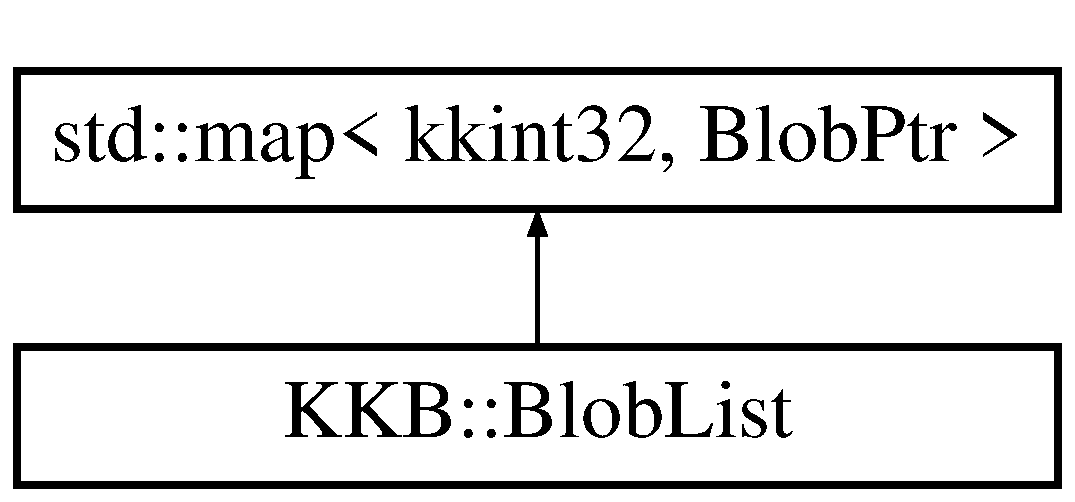
\includegraphics[height=2.000000cm]{class_k_k_b_1_1_blob_list}
\end{center}
\end{figure}
\subsection*{Public Member Functions}
\begin{DoxyCompactItemize}
\item 
\hyperlink{class_k_k_b_1_1_blob_list_a5651e16a693765b626fb6f1b85700045}{Blob\+List} (bool \+\_\+owner)
\item 
\hyperlink{class_k_k_b_1_1_blob_list_a8bdcfd3ae7ed5bda5ce42192d37b4f25}{$\sim$\+Blob\+List} ()
\item 
void \hyperlink{class_k_k_b_1_1_blob_list_af612dce77d3abecf54f4424b500c42df}{Delete\+Entry} (\hyperlink{namespace_k_k_b_a4fa91a7788b982654fca9d7319b98cb4}{Blob\+Ptr} b)
\item 
\hyperlink{namespace_k_k_b_a4fa91a7788b982654fca9d7319b98cb4}{Blob\+Ptr} \hyperlink{class_k_k_b_1_1_blob_list_a68a45d0c30102a70de2bcd96f3aa48a2}{Locate\+Largest\+Blob} ()
\begin{DoxyCompactList}\small\item\em Will return \hyperlink{class_k_k_b_1_1_blob}{Blob} with largest pixel count. \end{DoxyCompactList}\item 
\hyperlink{namespace_k_k_b_a4fa91a7788b982654fca9d7319b98cb4}{Blob\+Ptr} \hyperlink{class_k_k_b_1_1_blob_list_a484e59309adbbfa4d39a0f08586b3e83}{Locate\+Most\+Complete} ()
\begin{DoxyCompactList}\small\item\em Locates the blob that covers the greatest part of the raster; that is the one who has the largest (Height x Width) \end{DoxyCompactList}\item 
\hyperlink{namespace_k_k_b_a4fa91a7788b982654fca9d7319b98cb4}{Blob\+Ptr} \hyperlink{class_k_k_b_1_1_blob_list_a3acd3cdb0c08780511f2087f72749b91}{Look\+Up\+By\+Blob\+Id} (\hyperlink{namespace_k_k_b_a8fa4952cc84fda1de4bec1fbdd8d5b1b}{kkint32} blob\+Id)
\begin{DoxyCompactList}\small\item\em Will return pointer to blob with \textquotesingle{}blob\+Id\textquotesingle{}; if not found will return N\+U\+LL. \end{DoxyCompactList}\item 
void \hyperlink{class_k_k_b_1_1_blob_list_a542ca9592d04a6c7cf1b56127d1c7b4e}{Merge\+Blob\+Ids} (\hyperlink{namespace_k_k_b_a4fa91a7788b982654fca9d7319b98cb4}{Blob\+Ptr} blob, \hyperlink{namespace_k_k_b_a8fa4952cc84fda1de4bec1fbdd8d5b1b}{kkint32} blob\+Id, \hyperlink{namespace_k_k_b_a8fa4952cc84fda1de4bec1fbdd8d5b1b}{kkint32} $\ast$$\ast$blob\+Ids)
\begin{DoxyCompactList}\small\item\em Used by the Connected component analysis to merge two blobs together. \end{DoxyCompactList}\item 
\hyperlink{namespace_k_k_b_a4fa91a7788b982654fca9d7319b98cb4}{Blob\+Ptr} \hyperlink{class_k_k_b_1_1_blob_list_a6fb445ebcc2275344dd3301cc0b72bb1}{Merge\+Into\+Single\+Blob} (\hyperlink{namespace_k_k_b_a4fa91a7788b982654fca9d7319b98cb4}{Blob\+Ptr} blob1, \hyperlink{namespace_k_k_b_a8fa4952cc84fda1de4bec1fbdd8d5b1b}{kkint32} blob2\+Id, \hyperlink{namespace_k_k_b_a8fa4952cc84fda1de4bec1fbdd8d5b1b}{kkint32} $\ast$$\ast$blob\+Ids)
\item 
\hyperlink{namespace_k_k_b_a4fa91a7788b982654fca9d7319b98cb4}{Blob\+Ptr} \hyperlink{class_k_k_b_1_1_blob_list_a4542efb8f886b31c58f0a03507d20e69}{New\+Blob} (\hyperlink{namespace_k_k_b_af8d832f05c54994a1cce25bd5743e19a}{kkuint32} row\+Top, \hyperlink{namespace_k_k_b_af8d832f05c54994a1cce25bd5743e19a}{kkuint32} col\+Left)
\item 
void \hyperlink{class_k_k_b_1_1_blob_list_ad180d93de7be82655877d3a3b1fc9116}{Push\+On\+Back} (\hyperlink{namespace_k_k_b_a4fa91a7788b982654fca9d7319b98cb4}{Blob\+Ptr} blob)
\item 
void \hyperlink{class_k_k_b_1_1_blob_list_aa61617ae33ca83b22d715ad44af432a7}{Push\+On\+Front} (\hyperlink{namespace_k_k_b_a4fa91a7788b982654fca9d7319b98cb4}{Blob\+Ptr} blob)
\end{DoxyCompactItemize}


\subsection{Detailed Description}
Maintains a list of blobs. 

Definition at line 77 of file Blob.\+h.



\subsection{Constructor \& Destructor Documentation}
\index{K\+K\+B\+::\+Blob\+List@{K\+K\+B\+::\+Blob\+List}!Blob\+List@{Blob\+List}}
\index{Blob\+List@{Blob\+List}!K\+K\+B\+::\+Blob\+List@{K\+K\+B\+::\+Blob\+List}}
\subsubsection[{\texorpdfstring{Blob\+List(bool \+\_\+owner)}{BlobList(bool _owner)}}]{\setlength{\rightskip}{0pt plus 5cm}Blob\+List\+::\+Blob\+List (
\begin{DoxyParamCaption}
\item[{bool}]{\+\_\+owner}
\end{DoxyParamCaption}
)}\hypertarget{class_k_k_b_1_1_blob_list_a5651e16a693765b626fb6f1b85700045}{}\label{class_k_k_b_1_1_blob_list_a5651e16a693765b626fb6f1b85700045}


Definition at line 64 of file Blob.\+cpp.



References Blob\+List().



Referenced by Blob\+List(), K\+K\+B\+::\+Raster\+::\+Connected\+Component8\+Conected(), and K\+K\+B\+::\+Raster\+::\+Extract\+Blobs().


\begin{DoxyCode}
64                                :
65   availableBlobs (),
66   nextBlobId     (0)
67 \{
68 \}
\end{DoxyCode}
\index{K\+K\+B\+::\+Blob\+List@{K\+K\+B\+::\+Blob\+List}!````~Blob\+List@{$\sim$\+Blob\+List}}
\index{````~Blob\+List@{$\sim$\+Blob\+List}!K\+K\+B\+::\+Blob\+List@{K\+K\+B\+::\+Blob\+List}}
\subsubsection[{\texorpdfstring{$\sim$\+Blob\+List()}{~BlobList()}}]{\setlength{\rightskip}{0pt plus 5cm}Blob\+List\+::$\sim$\+Blob\+List (
\begin{DoxyParamCaption}
{}
\end{DoxyParamCaption}
)}\hypertarget{class_k_k_b_1_1_blob_list_a8bdcfd3ae7ed5bda5ce42192d37b4f25}{}\label{class_k_k_b_1_1_blob_list_a8bdcfd3ae7ed5bda5ce42192d37b4f25}


Definition at line 72 of file Blob.\+cpp.


\begin{DoxyCode}
73 \{
74   \textcolor{keywordflow}{while}  (availableBlobs.size () > 0)
75   \{
76     \hyperlink{class_k_k_b_1_1_blob}{BlobPtr}  b = availableBlobs.back ();
77     availableBlobs.pop\_back ();
78 
79     \textcolor{keyword}{delete}  b;
80   \}
81 
82   iterator  idx2;
83   iterator  endIdx = end ();
84   \textcolor{keywordflow}{for}  (idx2 = begin ();  idx2 != endIdx;  ++idx2)
85   \{
86     \hyperlink{class_k_k_b_1_1_blob}{BlobPtr} b = idx2->second;
87     \textcolor{keyword}{delete}  b;
88   \}
89 \}
\end{DoxyCode}


\subsection{Member Function Documentation}
\index{K\+K\+B\+::\+Blob\+List@{K\+K\+B\+::\+Blob\+List}!Delete\+Entry@{Delete\+Entry}}
\index{Delete\+Entry@{Delete\+Entry}!K\+K\+B\+::\+Blob\+List@{K\+K\+B\+::\+Blob\+List}}
\subsubsection[{\texorpdfstring{Delete\+Entry(\+Blob\+Ptr b)}{DeleteEntry(BlobPtr b)}}]{\setlength{\rightskip}{0pt plus 5cm}void K\+K\+B\+::\+Blob\+List\+::\+Delete\+Entry (
\begin{DoxyParamCaption}
\item[{{\bf Blob\+Ptr}}]{b}
\end{DoxyParamCaption}
)}\hypertarget{class_k_k_b_1_1_blob_list_af612dce77d3abecf54f4424b500c42df}{}\label{class_k_k_b_1_1_blob_list_af612dce77d3abecf54f4424b500c42df}
\index{K\+K\+B\+::\+Blob\+List@{K\+K\+B\+::\+Blob\+List}!Locate\+Largest\+Blob@{Locate\+Largest\+Blob}}
\index{Locate\+Largest\+Blob@{Locate\+Largest\+Blob}!K\+K\+B\+::\+Blob\+List@{K\+K\+B\+::\+Blob\+List}}
\subsubsection[{\texorpdfstring{Locate\+Largest\+Blob()}{LocateLargestBlob()}}]{\setlength{\rightskip}{0pt plus 5cm}{\bf Blob\+Ptr} Blob\+List\+::\+Locate\+Largest\+Blob (
\begin{DoxyParamCaption}
{}
\end{DoxyParamCaption}
)}\hypertarget{class_k_k_b_1_1_blob_list_a68a45d0c30102a70de2bcd96f3aa48a2}{}\label{class_k_k_b_1_1_blob_list_a68a45d0c30102a70de2bcd96f3aa48a2}


Will return \hyperlink{class_k_k_b_1_1_blob}{Blob} with largest pixel count. 



Definition at line 230 of file Blob.\+cpp.



References K\+K\+B\+::\+Blob\+::pixel\+Count.



Referenced by K\+K\+B\+::\+Raster\+::\+Connected\+Component(), and K\+K\+B\+::\+Raster\+::\+Connected\+Component8\+Conected().


\begin{DoxyCode}
231 \{
232   \hyperlink{class_k_k_b_1_1_blob}{BlobPtr}   blob        = NULL;
233   \hyperlink{class_k_k_b_1_1_blob}{BlobPtr}   tempBlob    = NULL;
234   \hyperlink{namespace_k_k_b_a8fa4952cc84fda1de4bec1fbdd8d5b1b}{kkint32}   largestSize = 0;
235 
236   const\_iterator  idx;
237   const\_iterator  endIdx = end ();
238 
239   \textcolor{keywordflow}{for}  (idx = begin ();  idx != endIdx;  ++idx)
240   \{
241     tempBlob = idx->second;
242     \textcolor{keywordflow}{if}  (tempBlob->\hyperlink{class_k_k_b_1_1_blob_a415767d4a364df537d7b2fc06a95721d}{pixelCount} > largestSize)
243     \{
244       largestSize = tempBlob->\hyperlink{class_k_k_b_1_1_blob_a415767d4a364df537d7b2fc06a95721d}{pixelCount};
245       blob = tempBlob;
246     \}
247   \}
248   \textcolor{keywordflow}{return}  blob;
249 \} \textcolor{comment}{/* LocateLargestBlob */}
\end{DoxyCode}
\index{K\+K\+B\+::\+Blob\+List@{K\+K\+B\+::\+Blob\+List}!Locate\+Most\+Complete@{Locate\+Most\+Complete}}
\index{Locate\+Most\+Complete@{Locate\+Most\+Complete}!K\+K\+B\+::\+Blob\+List@{K\+K\+B\+::\+Blob\+List}}
\subsubsection[{\texorpdfstring{Locate\+Most\+Complete()}{LocateMostComplete()}}]{\setlength{\rightskip}{0pt plus 5cm}{\bf Blob\+Ptr} Blob\+List\+::\+Locate\+Most\+Complete (
\begin{DoxyParamCaption}
{}
\end{DoxyParamCaption}
)}\hypertarget{class_k_k_b_1_1_blob_list_a484e59309adbbfa4d39a0f08586b3e83}{}\label{class_k_k_b_1_1_blob_list_a484e59309adbbfa4d39a0f08586b3e83}


Locates the blob that covers the greatest part of the raster; that is the one who has the largest (Height x Width) 



Definition at line 253 of file Blob.\+cpp.



References K\+K\+B\+::\+Blob\+::\+Height(), and K\+K\+B\+::\+Blob\+::\+Width().



Referenced by K\+K\+B\+::\+Raster\+::\+Reduce\+To\+Most\+Complete\+Blob().


\begin{DoxyCode}
254 \{
255   \hyperlink{class_k_k_b_1_1_blob}{BlobPtr}   blob        = NULL;
256   \hyperlink{class_k_k_b_1_1_blob}{BlobPtr}   tempBlob    = NULL;
257   \hyperlink{namespace_k_k_b_a8fa4952cc84fda1de4bec1fbdd8d5b1b}{kkint32}   largestSize = 0;
258 
259   const\_iterator  idx;
260   const\_iterator  endIdx = end ();
261 
262   \textcolor{keywordflow}{for}  (idx = begin ();  idx != endIdx;  ++idx)
263   \{
264     tempBlob = idx->second;
265     \hyperlink{namespace_k_k_b_a8fa4952cc84fda1de4bec1fbdd8d5b1b}{kkint32}  size = tempBlob->\hyperlink{class_k_k_b_1_1_blob_aa38a04e912ff9abf0abb950a69b65955}{Height} () * tempBlob->\hyperlink{class_k_k_b_1_1_blob_a5cc53690365e2b055c52f159de2efd1b}{Width} ();
266     \textcolor{keywordflow}{if}  (size > largestSize)
267     \{
268       largestSize = size;
269       blob = tempBlob;
270     \}
271   \}
272   \textcolor{keywordflow}{return}  blob;
273 \} \textcolor{comment}{/* LocateMostComplete */}
\end{DoxyCode}
\index{K\+K\+B\+::\+Blob\+List@{K\+K\+B\+::\+Blob\+List}!Look\+Up\+By\+Blob\+Id@{Look\+Up\+By\+Blob\+Id}}
\index{Look\+Up\+By\+Blob\+Id@{Look\+Up\+By\+Blob\+Id}!K\+K\+B\+::\+Blob\+List@{K\+K\+B\+::\+Blob\+List}}
\subsubsection[{\texorpdfstring{Look\+Up\+By\+Blob\+Id(kkint32 blob\+Id)}{LookUpByBlobId(kkint32 blobId)}}]{\setlength{\rightskip}{0pt plus 5cm}{\bf Blob\+Ptr} Blob\+List\+::\+Look\+Up\+By\+Blob\+Id (
\begin{DoxyParamCaption}
\item[{{\bf kkint32}}]{blob\+Id}
\end{DoxyParamCaption}
)}\hypertarget{class_k_k_b_1_1_blob_list_a3acd3cdb0c08780511f2087f72749b91}{}\label{class_k_k_b_1_1_blob_list_a3acd3cdb0c08780511f2087f72749b91}


Will return pointer to blob with \textquotesingle{}blob\+Id\textquotesingle{}; if not found will return N\+U\+LL. 



Definition at line 53 of file Blob.\+cpp.



Referenced by K\+K\+B\+::\+Raster\+::\+Connected\+Component8\+Conected(), and K\+K\+B\+::\+Raster\+::\+Extract\+Blobs().


\begin{DoxyCode}
54 \{
55   const\_iterator  idx;
56   idx = find (blobId);
57   \textcolor{keywordflow}{if}  (idx == end ())
58     \textcolor{keywordflow}{return} NULL;
59   \textcolor{keywordflow}{return} idx->second;
60 \}  \textcolor{comment}{/* LookUpByBlobId */}
\end{DoxyCode}
\index{K\+K\+B\+::\+Blob\+List@{K\+K\+B\+::\+Blob\+List}!Merge\+Blob\+Ids@{Merge\+Blob\+Ids}}
\index{Merge\+Blob\+Ids@{Merge\+Blob\+Ids}!K\+K\+B\+::\+Blob\+List@{K\+K\+B\+::\+Blob\+List}}
\subsubsection[{\texorpdfstring{Merge\+Blob\+Ids(\+Blob\+Ptr blob, kkint32 blob\+Id, kkint32 $\ast$$\ast$blob\+Ids)}{MergeBlobIds(BlobPtr blob, kkint32 blobId, kkint32 **blobIds)}}]{\setlength{\rightskip}{0pt plus 5cm}void Blob\+List\+::\+Merge\+Blob\+Ids (
\begin{DoxyParamCaption}
\item[{{\bf Blob\+Ptr}}]{blob, }
\item[{{\bf kkint32}}]{blob\+Id, }
\item[{{\bf kkint32} $\ast$$\ast$}]{blob\+Ids}
\end{DoxyParamCaption}
)}\hypertarget{class_k_k_b_1_1_blob_list_a542ca9592d04a6c7cf1b56127d1c7b4e}{}\label{class_k_k_b_1_1_blob_list_a542ca9592d04a6c7cf1b56127d1c7b4e}


Used by the Connected component analysis to merge two blobs together. 

When the connected component discovers that two separate blobs are actually connected if will call this method to merge them together into a single blob. 

Definition at line 122 of file Blob.\+cpp.



References K\+K\+B\+::\+Blob\+::col\+Left, K\+K\+B\+::\+Blob\+::col\+Right, K\+K\+B\+::\+Blob\+::\+Id(), K\+K\+B\+::\+Blob\+::pixel\+Count, K\+K\+B\+::\+Blob\+::row\+Bot, and K\+K\+B\+::\+Blob\+::row\+Top.



Referenced by K\+K\+B\+::\+Raster\+::\+Connected\+Component8\+Conected().


\begin{DoxyCode}
126 \{                               
127   \hyperlink{namespace_k_k_b_a8fa4952cc84fda1de4bec1fbdd8d5b1b}{kkint32}  newId = blob->\hyperlink{class_k_k_b_1_1_blob_add1ed75f6509956508b71aabeeae213c}{Id} ();
128   
129   iterator  idx;
130   idx = find (blobId);
131   \textcolor{keywordflow}{if}  (idx == end ())
132     \textcolor{keywordflow}{return};
133   \hyperlink{class_k_k_b_1_1_blob}{BlobPtr}  blobToMerge = idx->second;
134 
135   \hyperlink{namespace_k_k_b_a8fa4952cc84fda1de4bec1fbdd8d5b1b}{kkint32}  col;
136   \hyperlink{namespace_k_k_b_a8fa4952cc84fda1de4bec1fbdd8d5b1b}{kkint32}  row;
137 
138   \hyperlink{namespace_k_k_b_a8fa4952cc84fda1de4bec1fbdd8d5b1b}{kkint32}  rowBot   = blobToMerge->\hyperlink{class_k_k_b_1_1_blob_ae6f6816134ac19c54071eca96dd89910}{rowBot};
139   \hyperlink{namespace_k_k_b_a8fa4952cc84fda1de4bec1fbdd8d5b1b}{kkint32}  colRight = blobToMerge->\hyperlink{class_k_k_b_1_1_blob_a3786c83aeb9b92bc076c14afcc99c463}{colRight};
140 
141   \textcolor{keywordflow}{for}  (row = blobToMerge->\hyperlink{class_k_k_b_1_1_blob_adeb391a75a10791e7f59566eafa847ae}{rowTop}; row <= rowBot; row++)
142   \{
143     \textcolor{keywordflow}{for}  (col = blobToMerge->\hyperlink{class_k_k_b_1_1_blob_a1d47c1a8131e60211a3dd91910699318}{colLeft}; col <= colRight; col++)
144     \{
145       \textcolor{keywordflow}{if}  (blobIds[row][col] == blobId)
146         blobIds[row][col] = newId;
147     \}
148   \}
149 
150   blob->\hyperlink{class_k_k_b_1_1_blob_adeb391a75a10791e7f59566eafa847ae}{rowTop}   = \hyperlink{namespace_k_k_b_ad030d1ca8bd5038824c4a923a4d23fb5}{Min} (blob->\hyperlink{class_k_k_b_1_1_blob_adeb391a75a10791e7f59566eafa847ae}{rowTop},   blobToMerge->\hyperlink{class_k_k_b_1_1_blob_adeb391a75a10791e7f59566eafa847ae}{rowTop});
151   blob->\hyperlink{class_k_k_b_1_1_blob_ae6f6816134ac19c54071eca96dd89910}{rowBot}   = \hyperlink{namespace_k_k_b_a25e187e24c091586293725f27f007ad7}{Max} (blob->\hyperlink{class_k_k_b_1_1_blob_ae6f6816134ac19c54071eca96dd89910}{rowBot},   blobToMerge->\hyperlink{class_k_k_b_1_1_blob_ae6f6816134ac19c54071eca96dd89910}{rowBot});
152   blob->\hyperlink{class_k_k_b_1_1_blob_a1d47c1a8131e60211a3dd91910699318}{colLeft}  = \hyperlink{namespace_k_k_b_ad030d1ca8bd5038824c4a923a4d23fb5}{Min} (blob->\hyperlink{class_k_k_b_1_1_blob_a1d47c1a8131e60211a3dd91910699318}{colLeft},  blobToMerge->\hyperlink{class_k_k_b_1_1_blob_a1d47c1a8131e60211a3dd91910699318}{colLeft});
153   blob->\hyperlink{class_k_k_b_1_1_blob_a3786c83aeb9b92bc076c14afcc99c463}{colRight} = \hyperlink{namespace_k_k_b_a25e187e24c091586293725f27f007ad7}{Max} (blob->\hyperlink{class_k_k_b_1_1_blob_a3786c83aeb9b92bc076c14afcc99c463}{colRight}, blobToMerge->\hyperlink{class_k_k_b_1_1_blob_a3786c83aeb9b92bc076c14afcc99c463}{colRight});
154   blob->\hyperlink{class_k_k_b_1_1_blob_a415767d4a364df537d7b2fc06a95721d}{pixelCount} = blob->\hyperlink{class_k_k_b_1_1_blob_a415767d4a364df537d7b2fc06a95721d}{pixelCount} + blobToMerge->
      \hyperlink{class_k_k_b_1_1_blob_a415767d4a364df537d7b2fc06a95721d}{pixelCount};
155 
156   erase (idx);
157   availableBlobs.push\_back (blobToMerge);
158 \}  \textcolor{comment}{/* MergeBlobIds */}
\end{DoxyCode}
\index{K\+K\+B\+::\+Blob\+List@{K\+K\+B\+::\+Blob\+List}!Merge\+Into\+Single\+Blob@{Merge\+Into\+Single\+Blob}}
\index{Merge\+Into\+Single\+Blob@{Merge\+Into\+Single\+Blob}!K\+K\+B\+::\+Blob\+List@{K\+K\+B\+::\+Blob\+List}}
\subsubsection[{\texorpdfstring{Merge\+Into\+Single\+Blob(\+Blob\+Ptr blob1, kkint32 blob2\+Id, kkint32 $\ast$$\ast$blob\+Ids)}{MergeIntoSingleBlob(BlobPtr blob1, kkint32 blob2Id, kkint32 **blobIds)}}]{\setlength{\rightskip}{0pt plus 5cm}{\bf Blob\+Ptr} Blob\+List\+::\+Merge\+Into\+Single\+Blob (
\begin{DoxyParamCaption}
\item[{{\bf Blob\+Ptr}}]{blob1, }
\item[{{\bf kkint32}}]{blob2\+Id, }
\item[{{\bf kkint32} $\ast$$\ast$}]{blob\+Ids}
\end{DoxyParamCaption}
)}\hypertarget{class_k_k_b_1_1_blob_list_a6fb445ebcc2275344dd3301cc0b72bb1}{}\label{class_k_k_b_1_1_blob_list_a6fb445ebcc2275344dd3301cc0b72bb1}


Definition at line 163 of file Blob.\+cpp.



References K\+K\+B\+::\+Blob\+::col\+Left, K\+K\+B\+::\+Blob\+::col\+Right, K\+K\+B\+::\+Blob\+::\+Id(), K\+K\+B\+::\+Blob\+::\+Pixel\+Count(), K\+K\+B\+::\+Blob\+::pixel\+Count, K\+K\+B\+::\+Blob\+::row\+Bot, and K\+K\+B\+::\+Blob\+::row\+Top.



Referenced by K\+K\+B\+::\+Raster\+::\+Extract\+Blobs().


\begin{DoxyCode}
167 \{                               
168   \hyperlink{namespace_k_k_b_a8fa4952cc84fda1de4bec1fbdd8d5b1b}{kkint32}  blob1Id = blob1->\hyperlink{class_k_k_b_1_1_blob_add1ed75f6509956508b71aabeeae213c}{Id} ();
169   iterator  idx;
170   idx = find (blob2Id);
171   \textcolor{keywordflow}{if}  (idx == end ())
172     \textcolor{keywordflow}{return}  blob1;
173   \hyperlink{class_k_k_b_1_1_blob}{BlobPtr}  blob2 = idx->second;
174 
175   \textcolor{keywordflow}{if}  ((blob1Id == blob2Id)  ||  (blob1 == blob2))
176   \{
177     \textcolor{keywordflow}{return} blob1;
178   \}
179 
180   \hyperlink{class_k_k_b_1_1_blob}{BlobPtr}  srcBlob  = NULL;
181   \hyperlink{class_k_k_b_1_1_blob}{BlobPtr}  destBlob = NULL;
182 
183   \textcolor{keywordflow}{if}  (blob1->\hyperlink{class_k_k_b_1_1_blob_a5b3f9098a889a0def5eb49287284b847}{PixelCount} () > blob2->\hyperlink{class_k_k_b_1_1_blob_a5b3f9098a889a0def5eb49287284b847}{PixelCount} ())
184   \{
185     srcBlob  = blob2;
186     destBlob = blob1;
187   \}
188   \textcolor{keywordflow}{else}
189   \{
190     srcBlob = blob1;
191     destBlob = blob2;
192   \}
193 
194   \hyperlink{namespace_k_k_b_a8fa4952cc84fda1de4bec1fbdd8d5b1b}{kkint32}    destBlobId = destBlob->\hyperlink{class_k_k_b_1_1_blob_add1ed75f6509956508b71aabeeae213c}{Id} ();
195   \hyperlink{namespace_k_k_b_a8fa4952cc84fda1de4bec1fbdd8d5b1b}{kkint32}    srcBlobId  = srcBlob->\hyperlink{class_k_k_b_1_1_blob_add1ed75f6509956508b71aabeeae213c}{Id} ();
196 
197   \hyperlink{namespace_k_k_b_a8fa4952cc84fda1de4bec1fbdd8d5b1b}{kkint32}  col = 0;
198   \hyperlink{namespace_k_k_b_a8fa4952cc84fda1de4bec1fbdd8d5b1b}{kkint32}  row = 0;
199 
200   \hyperlink{namespace_k_k_b_a8fa4952cc84fda1de4bec1fbdd8d5b1b}{kkint32}  rowBot   = srcBlob->\hyperlink{class_k_k_b_1_1_blob_ae6f6816134ac19c54071eca96dd89910}{rowBot};
201   \hyperlink{namespace_k_k_b_a8fa4952cc84fda1de4bec1fbdd8d5b1b}{kkint32}  colRight = srcBlob->\hyperlink{class_k_k_b_1_1_blob_a3786c83aeb9b92bc076c14afcc99c463}{colRight};
202 
203   \textcolor{keywordflow}{for}  (row = srcBlob->\hyperlink{class_k_k_b_1_1_blob_adeb391a75a10791e7f59566eafa847ae}{rowTop};  row <= rowBot;  ++row)
204   \{
205     \textcolor{keywordflow}{for}  (col = srcBlob->\hyperlink{class_k_k_b_1_1_blob_a1d47c1a8131e60211a3dd91910699318}{colLeft};  col <= colRight;  ++col)
206     \{
207       \textcolor{keywordflow}{if}  (blobIds[row][col] == srcBlobId)
208         blobIds[row][col] = destBlobId;
209     \}
210   \}
211 
212   destBlob->\hyperlink{class_k_k_b_1_1_blob_adeb391a75a10791e7f59566eafa847ae}{rowTop}   = \hyperlink{namespace_k_k_b_ad030d1ca8bd5038824c4a923a4d23fb5}{Min} (destBlob->\hyperlink{class_k_k_b_1_1_blob_adeb391a75a10791e7f59566eafa847ae}{rowTop},   srcBlob->\hyperlink{class_k_k_b_1_1_blob_adeb391a75a10791e7f59566eafa847ae}{rowTop});
213   destBlob->\hyperlink{class_k_k_b_1_1_blob_ae6f6816134ac19c54071eca96dd89910}{rowBot}   = \hyperlink{namespace_k_k_b_a25e187e24c091586293725f27f007ad7}{Max} (destBlob->\hyperlink{class_k_k_b_1_1_blob_ae6f6816134ac19c54071eca96dd89910}{rowBot},   srcBlob->\hyperlink{class_k_k_b_1_1_blob_ae6f6816134ac19c54071eca96dd89910}{rowBot});
214   destBlob->\hyperlink{class_k_k_b_1_1_blob_a1d47c1a8131e60211a3dd91910699318}{colLeft}  = \hyperlink{namespace_k_k_b_ad030d1ca8bd5038824c4a923a4d23fb5}{Min} (destBlob->\hyperlink{class_k_k_b_1_1_blob_a1d47c1a8131e60211a3dd91910699318}{colLeft},  srcBlob->
      \hyperlink{class_k_k_b_1_1_blob_a1d47c1a8131e60211a3dd91910699318}{colLeft});
215   destBlob->\hyperlink{class_k_k_b_1_1_blob_a3786c83aeb9b92bc076c14afcc99c463}{colRight} = \hyperlink{namespace_k_k_b_a25e187e24c091586293725f27f007ad7}{Max} (destBlob->\hyperlink{class_k_k_b_1_1_blob_a3786c83aeb9b92bc076c14afcc99c463}{colRight}, srcBlob->
      \hyperlink{class_k_k_b_1_1_blob_a3786c83aeb9b92bc076c14afcc99c463}{colRight});
216   destBlob->\hyperlink{class_k_k_b_1_1_blob_a415767d4a364df537d7b2fc06a95721d}{pixelCount} = destBlob->\hyperlink{class_k_k_b_1_1_blob_a415767d4a364df537d7b2fc06a95721d}{pixelCount} + srcBlob->
      \hyperlink{class_k_k_b_1_1_blob_a415767d4a364df537d7b2fc06a95721d}{pixelCount};
217 
218   idx = find (srcBlobId);
219   \textcolor{keywordflow}{if}  (idx != end ())
220     erase (idx);
221 
222   availableBlobs.push\_back (srcBlob);
223   \textcolor{keywordflow}{return}  destBlob;
224 \}  \textcolor{comment}{/* MergeIntoSingleBlob */}
\end{DoxyCode}
\index{K\+K\+B\+::\+Blob\+List@{K\+K\+B\+::\+Blob\+List}!New\+Blob@{New\+Blob}}
\index{New\+Blob@{New\+Blob}!K\+K\+B\+::\+Blob\+List@{K\+K\+B\+::\+Blob\+List}}
\subsubsection[{\texorpdfstring{New\+Blob(kkuint32 row\+Top, kkuint32 col\+Left)}{NewBlob(kkuint32 rowTop, kkuint32 colLeft)}}]{\setlength{\rightskip}{0pt plus 5cm}{\bf Blob\+Ptr} Blob\+List\+::\+New\+Blob (
\begin{DoxyParamCaption}
\item[{{\bf kkuint32}}]{row\+Top, }
\item[{{\bf kkuint32}}]{col\+Left}
\end{DoxyParamCaption}
)}\hypertarget{class_k_k_b_1_1_blob_list_a4542efb8f886b31c58f0a03507d20e69}{}\label{class_k_k_b_1_1_blob_list_a4542efb8f886b31c58f0a03507d20e69}


Definition at line 93 of file Blob.\+cpp.



References K\+K\+B\+::\+Blob\+::col\+Left, K\+K\+B\+::\+Blob\+::col\+Right, Push\+On\+Back(), K\+K\+B\+::\+Blob\+::row\+Bot, and K\+K\+B\+::\+Blob\+::row\+Top.



Referenced by K\+K\+B\+::\+Raster\+::\+Connected\+Component8\+Conected(), and K\+K\+B\+::\+Raster\+::\+Extract\+Blobs().


\begin{DoxyCode}
96 \{
97   \hyperlink{class_k_k_b_1_1_blob}{BlobPtr} blob = NULL;
98   \textcolor{keywordflow}{if}  (availableBlobs.size () > 0)
99   \{
100     blob = availableBlobs.back ();
101     blob->\hyperlink{class_k_k_b_1_1_blob_a8d0703b3aacfdc6664f81968468962fb}{InitialzieAsNew} (nextBlobId);
102     availableBlobs.pop\_back ();
103   \}
104   \textcolor{keywordflow}{else}
105   \{
106     blob = \textcolor{keyword}{new} \hyperlink{class_k_k_b_1_1_blob}{Blob} (nextBlobId);
107   \}
108   
109   blob->\hyperlink{class_k_k_b_1_1_blob_adeb391a75a10791e7f59566eafa847ae}{rowTop}  = rowTop;
110   blob->\hyperlink{class_k_k_b_1_1_blob_ae6f6816134ac19c54071eca96dd89910}{rowBot}  = rowTop;
111 
112   blob->\hyperlink{class_k_k_b_1_1_blob_a1d47c1a8131e60211a3dd91910699318}{colLeft}  = colLeft;
113   blob->\hyperlink{class_k_k_b_1_1_blob_a3786c83aeb9b92bc076c14afcc99c463}{colRight} = colLeft; 
114   
115   nextBlobId++;
116   \hyperlink{class_k_k_b_1_1_blob_list_ad180d93de7be82655877d3a3b1fc9116}{PushOnBack} (blob);
117   \textcolor{keywordflow}{return}  blob;
118 \}
\end{DoxyCode}
\index{K\+K\+B\+::\+Blob\+List@{K\+K\+B\+::\+Blob\+List}!Push\+On\+Back@{Push\+On\+Back}}
\index{Push\+On\+Back@{Push\+On\+Back}!K\+K\+B\+::\+Blob\+List@{K\+K\+B\+::\+Blob\+List}}
\subsubsection[{\texorpdfstring{Push\+On\+Back(\+Blob\+Ptr blob)}{PushOnBack(BlobPtr blob)}}]{\setlength{\rightskip}{0pt plus 5cm}void Blob\+List\+::\+Push\+On\+Back (
\begin{DoxyParamCaption}
\item[{{\bf Blob\+Ptr}}]{blob}
\end{DoxyParamCaption}
)}\hypertarget{class_k_k_b_1_1_blob_list_ad180d93de7be82655877d3a3b1fc9116}{}\label{class_k_k_b_1_1_blob_list_ad180d93de7be82655877d3a3b1fc9116}


Definition at line 280 of file Blob.\+cpp.



Referenced by New\+Blob().


\begin{DoxyCode}
281 \{
282   insert (BlobIndexPair (blob->\hyperlink{class_k_k_b_1_1_blob_add1ed75f6509956508b71aabeeae213c}{Id} (), blob));
283 \}  \textcolor{comment}{/* PushOnBack */}
\end{DoxyCode}
\index{K\+K\+B\+::\+Blob\+List@{K\+K\+B\+::\+Blob\+List}!Push\+On\+Front@{Push\+On\+Front}}
\index{Push\+On\+Front@{Push\+On\+Front}!K\+K\+B\+::\+Blob\+List@{K\+K\+B\+::\+Blob\+List}}
\subsubsection[{\texorpdfstring{Push\+On\+Front(\+Blob\+Ptr blob)}{PushOnFront(BlobPtr blob)}}]{\setlength{\rightskip}{0pt plus 5cm}void Blob\+List\+::\+Push\+On\+Front (
\begin{DoxyParamCaption}
\item[{{\bf Blob\+Ptr}}]{blob}
\end{DoxyParamCaption}
)}\hypertarget{class_k_k_b_1_1_blob_list_aa61617ae33ca83b22d715ad44af432a7}{}\label{class_k_k_b_1_1_blob_list_aa61617ae33ca83b22d715ad44af432a7}


Definition at line 287 of file Blob.\+cpp.


\begin{DoxyCode}
288 \{
289   insert (BlobIndexPair (blob->\hyperlink{class_k_k_b_1_1_blob_add1ed75f6509956508b71aabeeae213c}{Id} (), blob));
290 \}
\end{DoxyCode}


The documentation for this class was generated from the following files\+:\begin{DoxyCompactItemize}
\item 
C\+:/\+Users/\+Kurt/\+Git\+Hub/\+K\+Square\+Libraries/\+K\+K\+Base/\hyperlink{_blob_8h}{Blob.\+h}\item 
C\+:/\+Users/\+Kurt/\+Git\+Hub/\+K\+Square\+Libraries/\+K\+K\+Base/\hyperlink{_blob_8cpp}{Blob.\+cpp}\end{DoxyCompactItemize}

\hypertarget{class_k_k_b_1_1_bmp_image}{}\section{K\+KB\+:\+:Bmp\+Image Class Reference}
\label{class_k_k_b_1_1_bmp_image}\index{K\+K\+B\+::\+Bmp\+Image@{K\+K\+B\+::\+Bmp\+Image}}


Used to encode and decode B\+MP Images.  




{\ttfamily \#include $<$B\+M\+P\+Image.\+h$>$}

\subsection*{Classes}
\begin{DoxyCompactItemize}
\item 
struct \hyperlink{struct_bmp_image_1_1_bmp1_bit_rec}{Bmp1\+Bit\+Rec}
\item 
struct \hyperlink{struct_bmp_image_1_1_bmp4_bit_recs}{Bmp4\+Bit\+Recs}
\item 
struct \hyperlink{struct_bmp_image_1_1_b_m_p__24_bit_pixel}{B\+M\+P\+\_\+24\+Bit\+Pixel}
\item 
class \hyperlink{class_bmp_image_1_1_coded_pixels}{Coded\+Pixels}
\begin{DoxyCompactList}\small\item\em This object is used to help encode the data stored in B\+M\+P\+Image\+::image into 8 or 4 bit compressed formats used by B\+MP files. $\ast$. \end{DoxyCompactList}\item 
struct \hyperlink{struct_bmp_image_1_1_code_pair}{Code\+Pair}
\item 
class \hyperlink{class_bmp_image_1_1_pallet_builder}{Pallet\+Builder}
\end{DoxyCompactItemize}
\subsection*{Public Types}
\begin{DoxyCompactItemize}
\item 
typedef \hyperlink{struct_bmp_image_1_1_code_pair}{Code\+Pair} $\ast$ \hyperlink{class_k_k_b_1_1_bmp_image_ac6ba8d374fb0f84c2953aa1b516da34c}{Code\+Pair\+Ptr}
\end{DoxyCompactItemize}
\subsection*{Public Member Functions}
\begin{DoxyCompactItemize}
\item 
\hyperlink{class_k_k_b_1_1_bmp_image_abe1aec4ebeffe7bc960a85868310fe0f}{Bmp\+Image} (\hyperlink{namespace_k_k_b_a8fa4952cc84fda1de4bec1fbdd8d5b1b}{kkint32} \+\_\+height, \hyperlink{namespace_k_k_b_a8fa4952cc84fda1de4bec1fbdd8d5b1b}{kkint32} \+\_\+width, \hyperlink{namespace_k_k_b_a8fa4952cc84fda1de4bec1fbdd8d5b1b}{kkint32} \+\_\+num\+Of\+Colors)
\item 
\hyperlink{class_k_k_b_1_1_bmp_image_a5d34118309b6a7d06c5ce368be455f3e}{Bmp\+Image} (const \hyperlink{class_k_k_b_1_1_k_k_str}{K\+K\+Str} \&\+\_\+file\+Name, bool \&successful)
\begin{DoxyCompactList}\small\item\em Constructs a B\+MP image from the file specified by \textquotesingle{}\+\_\+file\+Name\textquotesingle{}. \end{DoxyCompactList}\item 
\hyperlink{class_k_k_b_1_1_bmp_image_a4909a1187900404c57b62ea87f164e57}{Bmp\+Image} (const \hyperlink{class_k_k_b_1_1_raster}{Raster} \&raster)
\begin{DoxyCompactList}\small\item\em Constructs a B\+M\+P\+Image instance from a \hyperlink{class_k_k_b_1_1_raster}{Raster} image; this is one way to save a \hyperlink{class_k_k_b_1_1_raster}{Raster} image to disk. \end{DoxyCompactList}\item 
\hyperlink{class_k_k_b_1_1_bmp_image_a6e919d5e31884577cb4f944217673559}{$\sim$\+Bmp\+Image} ()
\item 
void \hyperlink{class_k_k_b_1_1_bmp_image_ae55d99adbcfef1ce787b0f03353a2493}{Add\+Pixel} (\hyperlink{namespace_k_k_b_af8d832f05c54994a1cce25bd5743e19a}{kkuint32} row, \hyperlink{namespace_k_k_b_af8d832f05c54994a1cce25bd5743e19a}{kkuint32} col, \hyperlink{namespace_k_k_b_ace9969169bf514f9ee6185186949cdf7}{uchar} pix\+Value)
\item 
bool \hyperlink{class_k_k_b_1_1_bmp_image_a84b952d5e45b69cc76f1b0f548ac6aac}{Are\+There\+Edge\+Pixels} ()
\item 
void \hyperlink{class_k_k_b_1_1_bmp_image_a06b9cd777bb3731a4bc2b9fc7832f6b9}{Binarize} ()
\item 
const \hyperlink{namespace_k_k_b_ace9969169bf514f9ee6185186949cdf7}{uchar} $\ast$ \hyperlink{class_k_k_b_1_1_bmp_image_a8b6bd225b80088718f631a7646f0d7d5}{Blue\+Row} (\hyperlink{namespace_k_k_b_a8fa4952cc84fda1de4bec1fbdd8d5b1b}{kkint32} row) const 
\begin{DoxyCompactList}\small\item\em Returns the specified \hyperlink{class_k_k_b_1_1_row}{Row} from the Blue Channel. \end{DoxyCompactList}\item 
void \hyperlink{class_k_k_b_1_1_bmp_image_a114cdc4a156e8a1425afd8d16bf30cfe}{Clear\+Image} ()
\item 
bool \hyperlink{class_k_k_b_1_1_bmp_image_ada730c1253be818b247e711665b0114b}{Color} () const 
\begin{DoxyCompactList}\small\item\em Returns true if a Color image. \end{DoxyCompactList}\item 
void \hyperlink{class_k_k_b_1_1_bmp_image_a355c29ac18b346f1ded3adaa95b20bcb}{Double\+Size} ()
\item 
void \hyperlink{class_k_k_b_1_1_bmp_image_af3a143d6c740df57a5b79945d027b443}{Down\+Size} ()
\item 
void \hyperlink{class_k_k_b_1_1_bmp_image_a182bbf22f3eb361e669073617172d2a7}{Eliminate\+Vertical\+Lines} ()
\item 
const \hyperlink{class_k_k_b_1_1_k_k_str}{K\+K\+Str} \& \hyperlink{class_k_k_b_1_1_bmp_image_a59ed1f99c1554aa3b12b3a90195d9b51}{File\+Name} () const 
\item 
bool \hyperlink{class_k_k_b_1_1_bmp_image_a5b290fe260379e4665b5d5e2261175cf}{Four\+Bit\+Uncompressed} ()
\item 
\hyperlink{namespace_k_k_b_af8d832f05c54994a1cce25bd5743e19a}{kkuint32} \hyperlink{class_k_k_b_1_1_bmp_image_ae9a8a8f35af1c7d4b2fabbea4b92cc23}{Height} () const 
\item 
\hyperlink{namespace_k_k_b_ace9969169bf514f9ee6185186949cdf7}{uchar} $\ast$$\ast$ \hyperlink{class_k_k_b_1_1_bmp_image_a122d01d6b6996cd9b0df01e856746234}{Image} ()
\begin{DoxyCompactList}\small\item\em Returns back two dimension matrix of image; if color it will be the green channel. \end{DoxyCompactList}\item 
const \hyperlink{namespace_k_k_b_ace9969169bf514f9ee6185186949cdf7}{uchar} $\ast$ \hyperlink{class_k_k_b_1_1_bmp_image_ab0d6fac104e1b68ac72e4c7b57dc5ead}{Image\+Row} (\hyperlink{namespace_k_k_b_a8fa4952cc84fda1de4bec1fbdd8d5b1b}{kkint32} row) const 
\begin{DoxyCompactList}\small\item\em Returns the specified \hyperlink{class_k_k_b_1_1_row}{Row} from the Green Channel. \end{DoxyCompactList}\item 
void \hyperlink{class_k_k_b_1_1_bmp_image_ac00d5d64ef0ed8db88445ccea0e94048}{Initialize\+Fields} (\hyperlink{namespace_k_k_b_a8fa4952cc84fda1de4bec1fbdd8d5b1b}{kkint32} \+\_\+height, \hyperlink{namespace_k_k_b_a8fa4952cc84fda1de4bec1fbdd8d5b1b}{kkint32} \+\_\+width)
\item 
\hyperlink{namespace_k_k_b_ace9969169bf514f9ee6185186949cdf7}{uchar} \hyperlink{class_k_k_b_1_1_bmp_image_a8439bd1ef5dc0298a9a1a67028cf0276}{Max\+Pix\+Val} () const 
\item 
\hyperlink{namespace_k_k_b_ace9969169bf514f9ee6185186949cdf7}{uchar} \& \hyperlink{class_k_k_b_1_1_bmp_image_a1531bd3f74bbec5cc0df9a00d9c5b754}{Pixel} (\hyperlink{namespace_k_k_b_a8fa4952cc84fda1de4bec1fbdd8d5b1b}{kkint32} row, \hyperlink{namespace_k_k_b_a8fa4952cc84fda1de4bec1fbdd8d5b1b}{kkint32} col)
\item 
void \hyperlink{class_k_k_b_1_1_bmp_image_a18f534b5dca835a55b3d9d57fa70b620}{Print} ()
\item 
void \hyperlink{class_k_k_b_1_1_bmp_image_a54e61e820363b542ef0564d7a409d76b}{Re\+Allocate\+For\+Bigger\+Screen} ()
\begin{DoxyCompactList}\small\item\em Used to expand dimensions of image by 6 pixels so as to make sure that no image is along the edge. \end{DoxyCompactList}\item 
const \hyperlink{namespace_k_k_b_ace9969169bf514f9ee6185186949cdf7}{uchar} $\ast$ \hyperlink{class_k_k_b_1_1_bmp_image_aa871576b403fb4bfa8a4e33a82c25549}{Red\+Row} (\hyperlink{namespace_k_k_b_a8fa4952cc84fda1de4bec1fbdd8d5b1b}{kkint32} row) const 
\begin{DoxyCompactList}\small\item\em Returns the specified \hyperlink{class_k_k_b_1_1_row}{Row} from the Red Channel. \end{DoxyCompactList}\item 
void \hyperlink{class_k_k_b_1_1_bmp_image_a342f7a1df5ee3048c7f98e6e67b544de}{Save} (const \hyperlink{class_k_k_b_1_1_k_k_str}{K\+K\+Str} \&file\+Name)
\item 
void \hyperlink{class_k_k_b_1_1_bmp_image_a12c3d85cc2b31af13acd7467680c50ce}{Save\+Grayscale\+Inverted4\+Bit} (const \hyperlink{class_k_k_b_1_1_k_k_str}{K\+K\+Str} \&\+\_\+file\+Name)
\begin{DoxyCompactList}\small\item\em Saves image using 4 bit compressed gray-\/scale where Background = 255 and foreground = 0. \end{DoxyCompactList}\item 
void \hyperlink{class_k_k_b_1_1_bmp_image_ae778e224d47083032112f66f33587ba6}{Save\+Grayscale\+Inverted8\+Bit} (const \hyperlink{class_k_k_b_1_1_k_k_str}{K\+K\+Str} \&\+\_\+file\+Name)
\begin{DoxyCompactList}\small\item\em Saves image using compressed gray-\/scale where Background = 255 and foreground = 0. \end{DoxyCompactList}\item 
void \hyperlink{class_k_k_b_1_1_bmp_image_ae26fb37aebe1bd85a576330479a05742}{Set16\+Colors} ()
\item 
void \hyperlink{class_k_k_b_1_1_bmp_image_abb977b9e38c835db3971ef00092f3204}{Set256\+Colors} ()
\item 
void \hyperlink{class_k_k_b_1_1_bmp_image_abd39b778ffac08f2d64179a2897b40ff}{Set\+Palette\+Entry} (\hyperlink{namespace_k_k_b_a8fa4952cc84fda1de4bec1fbdd8d5b1b}{kkint32} pallet\+Index, const \hyperlink{class_k_k_b_1_1_pixel_value}{Pixel\+Value} \&pix\+Value)
\item 
void \hyperlink{class_k_k_b_1_1_bmp_image_aee0626356433f630910bc5d4259cd2eb}{Set\+Pixel\+Value} (\hyperlink{namespace_k_k_b_a8fa4952cc84fda1de4bec1fbdd8d5b1b}{kkint32} row, \hyperlink{namespace_k_k_b_a8fa4952cc84fda1de4bec1fbdd8d5b1b}{kkint32} col, \hyperlink{namespace_k_k_b_a8fa4952cc84fda1de4bec1fbdd8d5b1b}{kkint32} pixel)
\begin{DoxyCompactList}\small\item\em Will set the pixel value of the specified row and col to \textquotesingle{}pixel\textquotesingle{}. \end{DoxyCompactList}\item 
\hyperlink{namespace_k_k_b_af8d832f05c54994a1cce25bd5743e19a}{kkuint32} \hyperlink{class_k_k_b_1_1_bmp_image_a843e1821a1191100b03da9258e77e356}{Width} () const 
\end{DoxyCompactItemize}


\subsection{Detailed Description}
Used to encode and decode B\+MP Images. 

Purpose of this class it to facilitate the loading and saving of B\+MP Image files. Not all formats are supported, but the compressed version is, which most others don\textquotesingle{}t support. As a result this class will write considerably smaller B\+MP files than other utilities that I have tried. This results in faster writing images due to less disk-\/io.

This object was originally designed to work in conjunction with Image Extraction. It requires no other libraries and can read and write B\+MP files.

When Image\+Extraction creates a Bmp file it will provide pixel values between 0 and 7, where 0 is the background and 7 is the foreground. This is a result of the S\+I\+P\+P\+ER 2 and 3 Formats and may change in the future. When saving the B\+MP file B\+M\+P\+Image will map these values through the palette to 0=255, 1=219, 2=182, 3=146, 4=109, 5=73, 6=36, 7=0 resulting in a white background and a Black foreground. 

Definition at line 49 of file B\+M\+P\+Image.\+h.



\subsection{Member Typedef Documentation}
\index{K\+K\+B\+::\+Bmp\+Image@{K\+K\+B\+::\+Bmp\+Image}!Code\+Pair\+Ptr@{Code\+Pair\+Ptr}}
\index{Code\+Pair\+Ptr@{Code\+Pair\+Ptr}!K\+K\+B\+::\+Bmp\+Image@{K\+K\+B\+::\+Bmp\+Image}}
\subsubsection[{\texorpdfstring{Code\+Pair\+Ptr}{CodePairPtr}}]{\setlength{\rightskip}{0pt plus 5cm}typedef {\bf Code\+Pair}$\ast$ {\bf K\+K\+B\+::\+Bmp\+Image\+::\+Code\+Pair\+Ptr}}\hypertarget{class_k_k_b_1_1_bmp_image_ac6ba8d374fb0f84c2953aa1b516da34c}{}\label{class_k_k_b_1_1_bmp_image_ac6ba8d374fb0f84c2953aa1b516da34c}


Definition at line 214 of file B\+M\+P\+Image.\+h.



\subsection{Constructor \& Destructor Documentation}
\index{K\+K\+B\+::\+Bmp\+Image@{K\+K\+B\+::\+Bmp\+Image}!Bmp\+Image@{Bmp\+Image}}
\index{Bmp\+Image@{Bmp\+Image}!K\+K\+B\+::\+Bmp\+Image@{K\+K\+B\+::\+Bmp\+Image}}
\subsubsection[{\texorpdfstring{Bmp\+Image(kkint32 \+\_\+height, kkint32 \+\_\+width, kkint32 \+\_\+num\+Of\+Colors)}{BmpImage(kkint32 _height, kkint32 _width, kkint32 _numOfColors)}}]{\setlength{\rightskip}{0pt plus 5cm}Bmp\+Image\+::\+Bmp\+Image (
\begin{DoxyParamCaption}
\item[{{\bf kkint32}}]{\+\_\+height, }
\item[{{\bf kkint32}}]{\+\_\+width, }
\item[{{\bf kkint32}}]{\+\_\+num\+Of\+Colors}
\end{DoxyParamCaption}
)}\hypertarget{class_k_k_b_1_1_bmp_image_abe1aec4ebeffe7bc960a85868310fe0f}{}\label{class_k_k_b_1_1_bmp_image_abe1aec4ebeffe7bc960a85868310fe0f}


Definition at line 687 of file B\+M\+P\+Image.\+cpp.



References Initialize\+Fields(), and K\+K\+B\+::\+K\+K\+Str\+::\+K\+K\+Str().


\begin{DoxyCode}
690                     :
691    
692    color       (\textcolor{keyword}{false}),
693    fileName    (),
694    red         (NULL),
695    image       (NULL),
696    blue        (NULL),
697    numOfColors (\_numOfColors),
698    palette     (NULL)
699 \{
700   \hyperlink{class_k_k_b_1_1_bmp_image_ac00d5d64ef0ed8db88445ccea0e94048}{InitializeFields} (\_height, \_width);
701 \}
\end{DoxyCode}
\index{K\+K\+B\+::\+Bmp\+Image@{K\+K\+B\+::\+Bmp\+Image}!Bmp\+Image@{Bmp\+Image}}
\index{Bmp\+Image@{Bmp\+Image}!K\+K\+B\+::\+Bmp\+Image@{K\+K\+B\+::\+Bmp\+Image}}
\subsubsection[{\texorpdfstring{Bmp\+Image(const K\+K\+Str \&\+\_\+file\+Name, bool \&successful)}{BmpImage(const KKStr &_fileName, bool &successful)}}]{\setlength{\rightskip}{0pt plus 5cm}Bmp\+Image\+::\+Bmp\+Image (
\begin{DoxyParamCaption}
\item[{const {\bf K\+K\+Str} \&}]{\+\_\+file\+Name, }
\item[{bool \&}]{successful}
\end{DoxyParamCaption}
)}\hypertarget{class_k_k_b_1_1_bmp_image_a5d34118309b6a7d06c5ce368be455f3e}{}\label{class_k_k_b_1_1_bmp_image_a5d34118309b6a7d06c5ce368be455f3e}


Constructs a B\+MP image from the file specified by \textquotesingle{}\+\_\+file\+Name\textquotesingle{}. 


\begin{DoxyParams}[1]{Parameters}
\mbox{\tt in}  & {\em \+\_\+file\+Name} & Name of file to load B\+MP image from. \\
\hline
\mbox{\tt out}  & {\em successful} & Returns true if file successful in loading. \\
\hline
\end{DoxyParams}


Definition at line 449 of file B\+M\+P\+Image.\+cpp.



References K\+K\+B\+::\+K\+K\+Str\+::\+K\+K\+Str(), K\+K\+B\+::os\+F\+O\+P\+E\+N(), and K\+K\+B\+::\+K\+K\+Str\+::\+Str().



Referenced by K\+K\+B\+::\+Read\+Image().


\begin{DoxyCode}
451                     :
452 
453   color          (\textcolor{keyword}{false}),
454   fileName       (\_fileName),
455   red            (NULL),
456   image          (NULL),
457   blue           (NULL),
458   numOfColors    (16),
459   palette        (NULL),
460   paletteEntries (0)
461 
462 \{
463   FILE*  inFile = \hyperlink{namespace_k_k_b_abf4050d2916ded8349dafadc80f0ecd1}{osFOPEN} (fileName.\hyperlink{class_k_k_b_1_1_k_k_str_ad574e6c0fe7f6ce1ba3ab0a8ce2fbd52}{Str} (), \textcolor{stringliteral}{"rb"});
464   \textcolor{keywordflow}{if}  (!inFile)
465   \{
466     successfull = \textcolor{keyword}{false};
467     \textcolor{keywordflow}{return};
468   \}
469 
470   successfull = \textcolor{keyword}{true};
471 
472   \textcolor{keywordtype}{size\_t}   x;
473   \hyperlink{namespace_k_k_b_a8fa4952cc84fda1de4bec1fbdd8d5b1b}{kkint32}  y;
474 
475   x = fread (&hdr, \textcolor{keyword}{sizeof} (hdr), 1, inFile);
476   \textcolor{keywordflow}{if}  (x <= 0)
477   \{
478     successfull = \textcolor{keyword}{false};
479     fclose (inFile);
480     \textcolor{keywordflow}{return};
481   \}
482 
483   \hyperlink{namespace_k_k_b_ace9969169bf514f9ee6185186949cdf7}{uchar}  buff[4];
484   memcpy (buff, &hdr, \textcolor{keyword}{sizeof} (buff));
485   \textcolor{keywordflow}{if}  ((buff[0] == \textcolor{charliteral}{'B'})  &&  (buff[1] == \textcolor{charliteral}{'M'}))
486   \{
487     \textcolor{comment}{// We have a Bit Map file.}
488   \}
489   \textcolor{keywordflow}{else} \textcolor{keywordflow}{if}  ((buff[0] == 137)  &&  (buff[1] == \textcolor{charliteral}{'P'})  &&  (buff[2] == \textcolor{charliteral}{'N'})  &&  (buff[3] == \textcolor{charliteral}{'G'}))
490   \{
491     \textcolor{comment}{// We are looking at a PNG (Portable Network Graphics) file.}
492     cerr << \hyperlink{namespace_k_k_b_ad1f50f65af6adc8fa9e6f62d007818a8}{std::endl} 
493          << \textcolor{stringliteral}{"File["} << \_fileName << \textcolor{stringliteral}{"]  is a PNG formatted file."} << \hyperlink{namespace_k_k_b_ad1f50f65af6adc8fa9e6f62d007818a8}{std::endl}
494          << \hyperlink{namespace_k_k_b_ad1f50f65af6adc8fa9e6f62d007818a8}{std::endl};
495     successfull = \textcolor{keyword}{false};
496     fclose (inFile);
497     \textcolor{keywordflow}{return};
498   \}
499   \textcolor{keywordflow}{else}
500   \{
501     cerr << \hyperlink{namespace_k_k_b_ad1f50f65af6adc8fa9e6f62d007818a8}{std::endl} 
502          << \textcolor{stringliteral}{"File["} << \_fileName << \textcolor{stringliteral}{"]  is of a unknown file format."} << 
      \hyperlink{namespace_k_k_b_ad1f50f65af6adc8fa9e6f62d007818a8}{std::endl}
503          << \hyperlink{namespace_k_k_b_ad1f50f65af6adc8fa9e6f62d007818a8}{std::endl};
504     successfull = \textcolor{keyword}{false};
505     fclose (inFile);
506     \textcolor{keywordflow}{return};
507   \}
508 
509 
510   x = fread (&bmh, \textcolor{keyword}{sizeof} (bmh), 1, inFile);
511   \textcolor{keywordflow}{if}  (x <= 0)
512   \{
513     successfull = \textcolor{keyword}{false};
514     fclose (inFile);
515     \textcolor{keywordflow}{return};
516   \}
517 
518   \textcolor{keywordflow}{if}  ((bmh.biCompression == BI\_RGB)  &&  (bmh.biBitCount == 24))
519   \{
520     numOfColors = 16777216;
521     color = \textcolor{keyword}{true};
522     \textcolor{keyword}{delete}  palette;
523     palette = NULL;
524     Load24BitColor (inFile, successfull);
525     fclose (inFile);
526     \textcolor{keywordflow}{return};
527   \}
528 
529   \textcolor{keywordflow}{if}  ((bmh.biCompression == BI\_RGB)  &&  (bmh.biBitCount == 8))
530   \{
531     Load8BitColor (inFile, successfull);
532     fclose (inFile);
533     \textcolor{keywordflow}{return};
534   \}
535 
536   \textcolor{keywordflow}{else} \textcolor{keywordflow}{if}  ((bmh.biCompression == BI\_RGB)  ||  (bmh.biCompression == BI\_RLE4))
537     numOfColors = 16;
538 
539   \textcolor{keywordflow}{else}  \textcolor{keywordflow}{if}  (bmh.biBitCount == 1)
540     numOfColors = 16;
541 
542   \textcolor{keywordflow}{else}
543     numOfColors = 256;
544 
545 
546   paletteEntries = BMIcolorArraySize (bmh);
547   \textcolor{keywordflow}{if}  (paletteEntries < 0)
548   \{
549     successfull = \textcolor{keyword}{false};
550     fclose (inFile);
551     \textcolor{keywordflow}{return};
552   \}
553 
554   \textcolor{keywordtype}{bool}  imageIsRevGrayscale = \textcolor{keyword}{false};
555   \textcolor{keywordflow}{if}  (paletteEntries)
556   \{
557     palette =  \textcolor{keyword}{new} RGBQUAD[paletteEntries];
558     x = fread (palette, \textcolor{keyword}{sizeof} (RGBQUAD), paletteEntries, inFile);
559     imageIsRevGrayscale = ReversedGrayscaleImage ();
560   \}
561   \textcolor{keywordflow}{else}
562   \{
563     numOfColors   = 256;
564     paletteEntries = 256;
565     palette = \textcolor{keyword}{new} RGBQUAD[paletteEntries];
566     SetUp256BitPalette (palette);
567   \}
568 
569   \textcolor{comment}{// Lets Build Palette Map}
570   \textcolor{keywordflow}{for}  (x = 0; x < 256; x++)
571     paletteMap[x] = 0;
572 
573   \textcolor{keywordflow}{if}  (numOfColors == 16)
574   \{
575     \textcolor{keywordflow}{for}  (\hyperlink{namespace_k_k_b_a8fa4952cc84fda1de4bec1fbdd8d5b1b}{kkint32} palletIdx = 0; palletIdx < paletteEntries; palletIdx++)
576     \{
577       \textcolor{keywordflow}{if}  (imageIsRevGrayscale)
578         y = 255 - palette[palletIdx].rgbGreen;
579       \textcolor{keywordflow}{else}
580         y = palette[palletIdx].rgbGreen;
581       \textcolor{keywordflow}{if}  (y < 0)  y = 0;  \textcolor{keywordflow}{else} \textcolor{keywordflow}{if}  (y > 255)  y = 255;
582       paletteMap[palletIdx] = y;
583     \}
584   \}
585   \textcolor{keywordflow}{else}
586   \{
587     \textcolor{keywordflow}{for}  (\hyperlink{namespace_k_k_b_a8fa4952cc84fda1de4bec1fbdd8d5b1b}{kkint32} palletIdx = 0; palletIdx < paletteEntries; palletIdx++)
588     \{
589       \textcolor{keywordflow}{if}  (imageIsRevGrayscale)
590         y = 255 - palette[palletIdx].rgbGreen;
591       \textcolor{keywordflow}{else}
592         y = palette[palletIdx].rgbGreen;
593       \textcolor{keywordflow}{if}  (y < 0)  y = 0;  \textcolor{keywordflow}{else} \textcolor{keywordflow}{if}  (y > 255)  y = 255;
594       paletteMap[palletIdx] = y;
595     \}
596   \}
597 
598   \textcolor{keyword}{delete} palette;
599   paletteEntries = 256;
600   palette = \textcolor{keyword}{new} RGBQUAD[paletteEntries];
601   SetUp256BitPalette (palette);
602 
603   \hyperlink{namespace_k_k_b_a8fa4952cc84fda1de4bec1fbdd8d5b1b}{kkint32}  row;
604 
605   image = \textcolor{keyword}{new} \hyperlink{namespace_k_k_b_ace9969169bf514f9ee6185186949cdf7}{uchar}*[bmh.biHeight];
606   \textcolor{keywordflow}{for}  (row = 0; row < bmh.biHeight; row++)
607   \{
608     image[row] = \textcolor{keyword}{new} \hyperlink{namespace_k_k_b_ace9969169bf514f9ee6185186949cdf7}{uchar}[bmh.biWidth];
609     memset (image[row], 0, bmh.biWidth);
610   \}
611 
612   x = fseek (inFile, hdr.bfOffBits, SEEK\_SET);
613 
614   \textcolor{keywordflow}{if}  (bmh.biBitCount == 1)
615   \{
616     Load1BitColor (inFile, successfull);
617   \}
618 
619   \textcolor{keywordflow}{else} \textcolor{keywordflow}{if}  (bmh.biBitCount == 4)
620   \{
621     \textcolor{keywordflow}{if}  (bmh.biCompression == BI\_RGB)
622     \{
623       Load4BitColor (inFile, successfull);
624     \}
625 
626     \textcolor{keywordflow}{else} \textcolor{keywordflow}{if}  (bmh.biCompression == BI\_RLE4)
627     \{
628       Load4BitColorCompressed (inFile, successfull);
629     \}
630 
631     \textcolor{keywordflow}{else}
632     \{
633       cerr << \textcolor{stringliteral}{"***ERROR***  Invalid Compression Mode["} << bmh.biCompression 
634            << \textcolor{stringliteral}{"] Specified for 4 bit File["}
635            << fileName << \textcolor{stringliteral}{"]."}
636            << \hyperlink{namespace_k_k_b_ad1f50f65af6adc8fa9e6f62d007818a8}{std::endl};
637       successfull = \textcolor{keyword}{false};
638       \textcolor{comment}{// WaitForEnter ();}
639     \}
640   \}
641 
642   \textcolor{keywordflow}{else} \textcolor{keywordflow}{if}  (bmh.biBitCount == 8)
643   \{
644     \textcolor{keywordflow}{if}  (bmh.biCompression == BI\_RGB)
645     \{
646       Load8BitColor (inFile, successfull);
647     \}
648 
649     \textcolor{keywordflow}{else} \textcolor{keywordflow}{if}  (bmh.biCompression == BI\_RLE8)
650     \{
651       Load8BitColorCompressed (inFile, successfull);
652     \}
653 
654     \textcolor{keywordflow}{else}
655     \{
656       cerr << \textcolor{stringliteral}{"***ERROR***  Invalid Compression Mode["} << bmh.biCompression 
657            << \textcolor{stringliteral}{"] Specified for 8 bit File["}
658            << fileName << \textcolor{stringliteral}{"]."}
659            << \hyperlink{namespace_k_k_b_ad1f50f65af6adc8fa9e6f62d007818a8}{std::endl};
660       successfull = \textcolor{keyword}{false};
661     \}
662   \}
663 
664   \textcolor{keywordflow}{else} \textcolor{keywordflow}{if}  (bmh.biBitCount == 16)
665   \{
666     cerr << \textcolor{stringliteral}{"***ERROR***  16 Bit Not Supported.  File["} << fileName << \textcolor{stringliteral}{"]."} << 
      \hyperlink{namespace_k_k_b_ad1f50f65af6adc8fa9e6f62d007818a8}{std::endl};
667     \textcolor{comment}{// WaitForEnter ();}
668   \}
669 
670   \textcolor{keywordflow}{else} \textcolor{keywordflow}{if}  (bmh.biBitCount == 24)
671   \{
672     cerr << \textcolor{stringliteral}{"***ERROR***  24 Bit Not Supported.  File["} << fileName << \textcolor{stringliteral}{"]."}  << 
      \hyperlink{namespace_k_k_b_ad1f50f65af6adc8fa9e6f62d007818a8}{std::endl};
673   \}
674 
675   \textcolor{keywordflow}{else} \textcolor{keywordflow}{if}  (bmh.biBitCount == 32)
676   \{
677     cerr << \textcolor{stringliteral}{"***ERROR***  32 Bit Not Supported.  File["} << fileName << \textcolor{stringliteral}{"]."}  << 
      \hyperlink{namespace_k_k_b_ad1f50f65af6adc8fa9e6f62d007818a8}{std::endl};
678     \textcolor{comment}{// WaitForEnter ();}
679   \}
680 
681   fclose (inFile);
682 \}
\end{DoxyCode}
\index{K\+K\+B\+::\+Bmp\+Image@{K\+K\+B\+::\+Bmp\+Image}!Bmp\+Image@{Bmp\+Image}}
\index{Bmp\+Image@{Bmp\+Image}!K\+K\+B\+::\+Bmp\+Image@{K\+K\+B\+::\+Bmp\+Image}}
\subsubsection[{\texorpdfstring{Bmp\+Image(const Raster \&raster)}{BmpImage(const Raster &raster)}}]{\setlength{\rightskip}{0pt plus 5cm}Bmp\+Image\+::\+Bmp\+Image (
\begin{DoxyParamCaption}
\item[{const {\bf Raster} \&}]{raster}
\end{DoxyParamCaption}
)}\hypertarget{class_k_k_b_1_1_bmp_image_a4909a1187900404c57b62ea87f164e57}{}\label{class_k_k_b_1_1_bmp_image_a4909a1187900404c57b62ea87f164e57}


Constructs a B\+M\+P\+Image instance from a \hyperlink{class_k_k_b_1_1_raster}{Raster} image; this is one way to save a \hyperlink{class_k_k_b_1_1_raster}{Raster} image to disk. 



Definition at line 706 of file B\+M\+P\+Image.\+cpp.



References K\+K\+B\+::\+Raster\+::\+Blue(), K\+K\+B\+::\+Raster\+::\+Color(), K\+K\+B\+::\+Raster\+::\+Height(), Initialize\+Fields(), K\+K\+B\+::\+K\+K\+Str\+::operator=(), K\+K\+B\+::\+Raster\+::\+Red(), K\+K\+B\+::\+Raster\+::\+Rows(), and K\+K\+B\+::\+Raster\+::\+Width().



Referenced by K\+K\+B\+::\+Save\+Image(), K\+K\+B\+::\+Save\+Image\+Grayscale\+Inverted4\+Bit(), and K\+K\+B\+::\+Save\+Image\+Grayscale\+Inverted8\+Bit().


\begin{DoxyCode}
706                                         :
707   color   (\textcolor{keyword}{false}),
708   red     (NULL),
709   image   (NULL),
710   blue    (NULL),
711   palette (NULL)
712 \{
713   numOfColors = 256;  \textcolor{comment}{// kk 2005-03-10}
714 
715   color = raster.\hyperlink{class_k_k_b_1_1_raster_a644248f99009d64ac4b8fef4a22aff25}{Color} ();
716 
717   \hyperlink{class_k_k_b_1_1_bmp_image_ac00d5d64ef0ed8db88445ccea0e94048}{InitializeFields} (raster.\hyperlink{class_k_k_b_1_1_raster_af8d10d15697d5b92fb9595c48b529feb}{Height} (), raster.\hyperlink{class_k_k_b_1_1_raster_aa2780c0b7ae75b7b595f99329689c1f6}{Width} ());
718   fileName = \textcolor{stringliteral}{""};
719 
720   \hyperlink{namespace_k_k_b_a8fa4952cc84fda1de4bec1fbdd8d5b1b}{kkint32}  row;
721   \hyperlink{namespace_k_k_b_a8fa4952cc84fda1de4bec1fbdd8d5b1b}{kkint32}  col;
722 
723   \hyperlink{namespace_k_k_b_ace9969169bf514f9ee6185186949cdf7}{uchar}** rasterData = raster.\hyperlink{class_k_k_b_1_1_raster_a2460989f656e5222d6074cd0ba85ed72}{Rows} ();
724   \hyperlink{namespace_k_k_b_ace9969169bf514f9ee6185186949cdf7}{uchar}** rasterRed  = raster.\hyperlink{class_k_k_b_1_1_raster_a337a5a064b27693eec6e380789680239}{Red} ();
725   \hyperlink{namespace_k_k_b_ace9969169bf514f9ee6185186949cdf7}{uchar}** rasterBlue = raster.\hyperlink{class_k_k_b_1_1_raster_ae289ec3ad3a27339cd30e9ac3b488004}{Blue} ();
726 
727   \textcolor{keywordflow}{for}  (row = 0; row < bmh.biHeight; row++)
728   \{
729     \textcolor{keywordflow}{for}  (col = 0; col < bmh.biWidth; col++)
730     \{
731       image[row][col] = rasterData[row][col];
732       \textcolor{keywordflow}{if}  (color)
733       \{
734         red[row][col]  = rasterRed [row][col];
735         blue[row][col] = rasterBlue[row][col];
736       \}
737     \}
738   \}
739 \}
\end{DoxyCode}
\index{K\+K\+B\+::\+Bmp\+Image@{K\+K\+B\+::\+Bmp\+Image}!````~Bmp\+Image@{$\sim$\+Bmp\+Image}}
\index{````~Bmp\+Image@{$\sim$\+Bmp\+Image}!K\+K\+B\+::\+Bmp\+Image@{K\+K\+B\+::\+Bmp\+Image}}
\subsubsection[{\texorpdfstring{$\sim$\+Bmp\+Image()}{~BmpImage()}}]{\setlength{\rightskip}{0pt plus 5cm}Bmp\+Image\+::$\sim$\+Bmp\+Image (
\begin{DoxyParamCaption}
{}
\end{DoxyParamCaption}
)}\hypertarget{class_k_k_b_1_1_bmp_image_a6e919d5e31884577cb4f944217673559}{}\label{class_k_k_b_1_1_bmp_image_a6e919d5e31884577cb4f944217673559}


Definition at line 743 of file B\+M\+P\+Image.\+cpp.


\begin{DoxyCode}
744 \{
745   CleanUpMemory ();
746 \}
\end{DoxyCode}


\subsection{Member Function Documentation}
\index{K\+K\+B\+::\+Bmp\+Image@{K\+K\+B\+::\+Bmp\+Image}!Add\+Pixel@{Add\+Pixel}}
\index{Add\+Pixel@{Add\+Pixel}!K\+K\+B\+::\+Bmp\+Image@{K\+K\+B\+::\+Bmp\+Image}}
\subsubsection[{\texorpdfstring{Add\+Pixel(kkuint32 row, kkuint32 col, uchar pix\+Value)}{AddPixel(kkuint32 row, kkuint32 col, uchar pixValue)}}]{\setlength{\rightskip}{0pt plus 5cm}void Bmp\+Image\+::\+Add\+Pixel (
\begin{DoxyParamCaption}
\item[{{\bf kkuint32}}]{row, }
\item[{{\bf kkuint32}}]{col, }
\item[{{\bf uchar}}]{pix\+Value}
\end{DoxyParamCaption}
)}\hypertarget{class_k_k_b_1_1_bmp_image_ae55d99adbcfef1ce787b0f03353a2493}{}\label{class_k_k_b_1_1_bmp_image_ae55d99adbcfef1ce787b0f03353a2493}


Definition at line 2630 of file B\+M\+P\+Image.\+cpp.


\begin{DoxyCode}
2634 \{
2635   image[row][col] = pixValue;
2636 \}
\end{DoxyCode}
\index{K\+K\+B\+::\+Bmp\+Image@{K\+K\+B\+::\+Bmp\+Image}!Are\+There\+Edge\+Pixels@{Are\+There\+Edge\+Pixels}}
\index{Are\+There\+Edge\+Pixels@{Are\+There\+Edge\+Pixels}!K\+K\+B\+::\+Bmp\+Image@{K\+K\+B\+::\+Bmp\+Image}}
\subsubsection[{\texorpdfstring{Are\+There\+Edge\+Pixels()}{AreThereEdgePixels()}}]{\setlength{\rightskip}{0pt plus 5cm}bool Bmp\+Image\+::\+Are\+There\+Edge\+Pixels (
\begin{DoxyParamCaption}
{}
\end{DoxyParamCaption}
)}\hypertarget{class_k_k_b_1_1_bmp_image_a84b952d5e45b69cc76f1b0f548ac6aac}{}\label{class_k_k_b_1_1_bmp_image_a84b952d5e45b69cc76f1b0f548ac6aac}


Definition at line 2004 of file B\+M\+P\+Image.\+cpp.



References Height(), and Width().


\begin{DoxyCode}
2005 \{
2006   \hyperlink{namespace_k_k_b_a8fa4952cc84fda1de4bec1fbdd8d5b1b}{kkint32}  row;
2007   \hyperlink{namespace_k_k_b_a8fa4952cc84fda1de4bec1fbdd8d5b1b}{kkint32}  col;
2008 
2009   \hyperlink{namespace_k_k_b_a8fa4952cc84fda1de4bec1fbdd8d5b1b}{kkint32}  height = \hyperlink{class_k_k_b_1_1_bmp_image_ae9a8a8f35af1c7d4b2fabbea4b92cc23}{Height} ();
2010   \hyperlink{namespace_k_k_b_a8fa4952cc84fda1de4bec1fbdd8d5b1b}{kkint32}  width  = \hyperlink{class_k_k_b_1_1_bmp_image_a843e1821a1191100b03da9258e77e356}{Width} ();
2011 
2012   \textcolor{keywordflow}{if}  (height < 6)
2013     \textcolor{keywordflow}{return} \textcolor{keyword}{true};
2014 
2015   \textcolor{keywordflow}{if}  (width  < 6)
2016     \textcolor{keywordflow}{return}  \textcolor{keyword}{true};
2017 
2018 
2019   \hyperlink{namespace_k_k_b_ace9969169bf514f9ee6185186949cdf7}{uchar}*  row0 = image[0];
2020   \hyperlink{namespace_k_k_b_ace9969169bf514f9ee6185186949cdf7}{uchar}*  row1 = image[1];
2021   \hyperlink{namespace_k_k_b_ace9969169bf514f9ee6185186949cdf7}{uchar}*  row2 = image[2];
2022 
2023   \hyperlink{namespace_k_k_b_ace9969169bf514f9ee6185186949cdf7}{uchar}*  rowL0 = image[height - 3];
2024   \hyperlink{namespace_k_k_b_ace9969169bf514f9ee6185186949cdf7}{uchar}*  rowL1 = image[height - 2];
2025   \hyperlink{namespace_k_k_b_ace9969169bf514f9ee6185186949cdf7}{uchar}*  rowL2 = image[height - 1];
2026 
2027 
2028   \textcolor{keywordflow}{for}  (col = 0;  col < width;  col++)
2029   \{
2030     \textcolor{keywordflow}{if}  ((row0[col] > 0)   ||
2031          (row1[col] > 0)   ||
2032          (row2[col] > 0)   ||
2033          (rowL0[col] > 0)  ||
2034          (rowL1[col] > 0)  ||
2035          (rowL2[col] > 0)
2036         )
2037       \textcolor{keywordflow}{return}  \textcolor{keyword}{true};
2038   \}
2039 
2040   \hyperlink{namespace_k_k_b_a8fa4952cc84fda1de4bec1fbdd8d5b1b}{kkint32}  lastCol0 = width - 3;
2041   \hyperlink{namespace_k_k_b_a8fa4952cc84fda1de4bec1fbdd8d5b1b}{kkint32}  lastCol1 = width - 2;
2042   \hyperlink{namespace_k_k_b_a8fa4952cc84fda1de4bec1fbdd8d5b1b}{kkint32}  lastCol2 = width - 1;
2043 
2044   \hyperlink{namespace_k_k_b_a8fa4952cc84fda1de4bec1fbdd8d5b1b}{kkint32}  lastRowToCheck = height - 3;
2045 
2046   \textcolor{keywordflow}{for}  (row = 3;  row < lastRowToCheck;  row++)
2047   \{
2048     \textcolor{keywordflow}{if}  ((image[row][0]        > 0)  ||
2049          (image[row][1]        > 0)  ||
2050          (image[row][2]        > 0)  ||
2051          (image[row][lastCol0] > 0)  ||
2052          (image[row][lastCol1] > 0)  ||
2053          (image[row][lastCol2] > 0)
2054         )
2055       \textcolor{keywordflow}{return}  \textcolor{keyword}{true};
2056   \}
2057 
2058   \textcolor{keywordflow}{return}  \textcolor{keyword}{false};
2059 \}  \textcolor{comment}{/* EdgePixels */}
\end{DoxyCode}
\index{K\+K\+B\+::\+Bmp\+Image@{K\+K\+B\+::\+Bmp\+Image}!Binarize@{Binarize}}
\index{Binarize@{Binarize}!K\+K\+B\+::\+Bmp\+Image@{K\+K\+B\+::\+Bmp\+Image}}
\subsubsection[{\texorpdfstring{Binarize()}{Binarize()}}]{\setlength{\rightskip}{0pt plus 5cm}void Bmp\+Image\+::\+Binarize (
\begin{DoxyParamCaption}
{}
\end{DoxyParamCaption}
)}\hypertarget{class_k_k_b_1_1_bmp_image_a06b9cd777bb3731a4bc2b9fc7832f6b9}{}\label{class_k_k_b_1_1_bmp_image_a06b9cd777bb3731a4bc2b9fc7832f6b9}


Definition at line 2189 of file B\+M\+P\+Image.\+cpp.


\begin{DoxyCode}
2190 \{
2191   \hyperlink{namespace_k_k_b_a8fa4952cc84fda1de4bec1fbdd8d5b1b}{kkint32}  row;
2192   \hyperlink{namespace_k_k_b_a8fa4952cc84fda1de4bec1fbdd8d5b1b}{kkint32}  col;
2193 
2194   \textcolor{keywordflow}{for}  (row = 0; row < bmh.biHeight; row++)
2195   \{
2196     \textcolor{keywordflow}{for}  (col = 0; col < bmh.biWidth; col++)
2197     \{
2198       \textcolor{keywordflow}{if}  (image[row][col] < 7)
2199         image[row][col] = 0;
2200     \}
2201   \}
2202 \}  \textcolor{comment}{/*  Binarize  */}
\end{DoxyCode}
\index{K\+K\+B\+::\+Bmp\+Image@{K\+K\+B\+::\+Bmp\+Image}!Blue\+Row@{Blue\+Row}}
\index{Blue\+Row@{Blue\+Row}!K\+K\+B\+::\+Bmp\+Image@{K\+K\+B\+::\+Bmp\+Image}}
\subsubsection[{\texorpdfstring{Blue\+Row(kkint32 row) const }{BlueRow(kkint32 row) const }}]{\setlength{\rightskip}{0pt plus 5cm}const {\bf uchar} $\ast$ Bmp\+Image\+::\+Blue\+Row (
\begin{DoxyParamCaption}
\item[{{\bf kkint32}}]{row}
\end{DoxyParamCaption}
) const}\hypertarget{class_k_k_b_1_1_bmp_image_a8b6bd225b80088718f631a7646f0d7d5}{}\label{class_k_k_b_1_1_bmp_image_a8b6bd225b80088718f631a7646f0d7d5}


Returns the specified \hyperlink{class_k_k_b_1_1_row}{Row} from the Blue Channel. 



Definition at line 2652 of file B\+M\+P\+Image.\+cpp.



References Height(), K\+K\+B\+::\+K\+K\+Exception\+::\+K\+K\+Exception(), K\+K\+B\+::\+K\+K\+Str\+::operator+(), K\+K\+B\+::operator+(), and K\+K\+B\+::\+Str\+From\+Int32().



Referenced by K\+K\+B\+::\+Raster\+::\+Raster().


\begin{DoxyCode}
2653 \{
2654   \textcolor{keywordflow}{if}  (blue == NULL)
2655     \textcolor{keywordflow}{throw} \hyperlink{class_k_k_b_1_1_k_k_exception}{KKException}(\textcolor{stringliteral}{"BmpImage::BlueRow  'blue' channel is set to NULL."});
2656   \textcolor{keywordflow}{if}  ((row < 0)  ||  (row >= (\hyperlink{namespace_k_k_b_a8fa4952cc84fda1de4bec1fbdd8d5b1b}{kkint32})\hyperlink{class_k_k_b_1_1_bmp_image_ae9a8a8f35af1c7d4b2fabbea4b92cc23}{Height} ()))
2657   \{
2658     cerr << \hyperlink{namespace_k_k_b_ad1f50f65af6adc8fa9e6f62d007818a8}{std::endl}
2659          << \hyperlink{namespace_k_k_b_ad1f50f65af6adc8fa9e6f62d007818a8}{std::endl}
2660          << \textcolor{stringliteral}{"BmpImage::BlueRow   *** ERROR ***  Invalid Row["} << row << \textcolor{stringliteral}{"]."} << 
      \hyperlink{namespace_k_k_b_ad1f50f65af6adc8fa9e6f62d007818a8}{std::endl}
2661          << \hyperlink{namespace_k_k_b_ad1f50f65af6adc8fa9e6f62d007818a8}{std::endl};
2662     \textcolor{comment}{//osWaitForEnter ();}
2663     \textcolor{keywordflow}{throw} \hyperlink{class_k_k_b_1_1_k_k_exception}{KKException}(\textcolor{stringliteral}{"BmpImage::BlueRow  row:"} + \hyperlink{namespace_k_k_b_a66adf53f607bda7ab0d3e1c3945e792e}{StrFromInt32}(row) + \textcolor{stringliteral}{" is out of
       range where Height:"} + \hyperlink{namespace_k_k_b_a66adf53f607bda7ab0d3e1c3945e792e}{StrFromInt32}(row));
2664   \}
2665 
2666   \textcolor{keywordflow}{return}  blue[row];
2667 \}  \textcolor{comment}{/* BlueRow */}
\end{DoxyCode}
\index{K\+K\+B\+::\+Bmp\+Image@{K\+K\+B\+::\+Bmp\+Image}!Clear\+Image@{Clear\+Image}}
\index{Clear\+Image@{Clear\+Image}!K\+K\+B\+::\+Bmp\+Image@{K\+K\+B\+::\+Bmp\+Image}}
\subsubsection[{\texorpdfstring{Clear\+Image()}{ClearImage()}}]{\setlength{\rightskip}{0pt plus 5cm}void Bmp\+Image\+::\+Clear\+Image (
\begin{DoxyParamCaption}
{}
\end{DoxyParamCaption}
)}\hypertarget{class_k_k_b_1_1_bmp_image_a114cdc4a156e8a1425afd8d16bf30cfe}{}\label{class_k_k_b_1_1_bmp_image_a114cdc4a156e8a1425afd8d16bf30cfe}


Definition at line 2640 of file B\+M\+P\+Image.\+cpp.


\begin{DoxyCode}
2641 \{
2642     \hyperlink{namespace_k_k_b_a8fa4952cc84fda1de4bec1fbdd8d5b1b}{kkint32} row;
2643     \textcolor{keywordflow}{for}  (row = 0; row < bmh.biHeight; row++)
2644     \{
2645         memset (image[row], 0, bmh.biWidth );
2646     \}
2647 \}
\end{DoxyCode}
\index{K\+K\+B\+::\+Bmp\+Image@{K\+K\+B\+::\+Bmp\+Image}!Color@{Color}}
\index{Color@{Color}!K\+K\+B\+::\+Bmp\+Image@{K\+K\+B\+::\+Bmp\+Image}}
\subsubsection[{\texorpdfstring{Color() const }{Color() const }}]{\setlength{\rightskip}{0pt plus 5cm}bool K\+K\+B\+::\+Bmp\+Image\+::\+Color (
\begin{DoxyParamCaption}
{}
\end{DoxyParamCaption}
) const\hspace{0.3cm}{\ttfamily [inline]}}\hypertarget{class_k_k_b_1_1_bmp_image_ada730c1253be818b247e711665b0114b}{}\label{class_k_k_b_1_1_bmp_image_ada730c1253be818b247e711665b0114b}


Returns true if a Color image. 



Definition at line 118 of file B\+M\+P\+Image.\+h.



Referenced by K\+K\+B\+::\+Raster\+::\+Raster().

\index{K\+K\+B\+::\+Bmp\+Image@{K\+K\+B\+::\+Bmp\+Image}!Double\+Size@{Double\+Size}}
\index{Double\+Size@{Double\+Size}!K\+K\+B\+::\+Bmp\+Image@{K\+K\+B\+::\+Bmp\+Image}}
\subsubsection[{\texorpdfstring{Double\+Size()}{DoubleSize()}}]{\setlength{\rightskip}{0pt plus 5cm}void K\+K\+B\+::\+Bmp\+Image\+::\+Double\+Size (
\begin{DoxyParamCaption}
{}
\end{DoxyParamCaption}
)}\hypertarget{class_k_k_b_1_1_bmp_image_a355c29ac18b346f1ded3adaa95b20bcb}{}\label{class_k_k_b_1_1_bmp_image_a355c29ac18b346f1ded3adaa95b20bcb}
\index{K\+K\+B\+::\+Bmp\+Image@{K\+K\+B\+::\+Bmp\+Image}!Down\+Size@{Down\+Size}}
\index{Down\+Size@{Down\+Size}!K\+K\+B\+::\+Bmp\+Image@{K\+K\+B\+::\+Bmp\+Image}}
\subsubsection[{\texorpdfstring{Down\+Size()}{DownSize()}}]{\setlength{\rightskip}{0pt plus 5cm}void Bmp\+Image\+::\+Down\+Size (
\begin{DoxyParamCaption}
{}
\end{DoxyParamCaption}
)}\hypertarget{class_k_k_b_1_1_bmp_image_af3a143d6c740df57a5b79945d027b443}{}\label{class_k_k_b_1_1_bmp_image_af3a143d6c740df57a5b79945d027b443}


Definition at line 1917 of file B\+M\+P\+Image.\+cpp.


\begin{DoxyCode}
1918 \{
1919   \hyperlink{namespace_k_k_b_a8fa4952cc84fda1de4bec1fbdd8d5b1b}{kkint32}  newCol;
1920   \hyperlink{namespace_k_k_b_a8fa4952cc84fda1de4bec1fbdd8d5b1b}{kkint32}  newHeight = bmh.biHeight / 2;
1921   \hyperlink{namespace_k_k_b_a8fa4952cc84fda1de4bec1fbdd8d5b1b}{kkint32}  newWidth  = bmh.biWidth  / 2;
1922   \hyperlink{namespace_k_k_b_a8fa4952cc84fda1de4bec1fbdd8d5b1b}{kkint32}  newRow;
1923 
1924   \hyperlink{namespace_k_k_b_a8fa4952cc84fda1de4bec1fbdd8d5b1b}{kkint32}  oldCol;
1925   \hyperlink{namespace_k_k_b_a8fa4952cc84fda1de4bec1fbdd8d5b1b}{kkint32}  oldRow;
1926 
1927   \hyperlink{namespace_k_k_b_ace9969169bf514f9ee6185186949cdf7}{uchar}**  newImage = \textcolor{keyword}{new} \hyperlink{namespace_k_k_b_ace9969169bf514f9ee6185186949cdf7}{uchar}*[newHeight];
1928   \textcolor{keywordflow}{for}  (newRow = 0; newRow < newHeight; newRow++)
1929   \{
1930     oldRow = newRow * 2;
1931 
1932     newImage[newRow] = \textcolor{keyword}{new} \hyperlink{namespace_k_k_b_ace9969169bf514f9ee6185186949cdf7}{uchar}[newWidth];
1933    
1934     \textcolor{keywordflow}{for}  (newCol = 0; newCol < newWidth;  newCol++)
1935     \{
1936       oldCol = newCol * 2;
1937       newImage[newRow][newCol] = image[oldRow][oldCol];
1938     \}
1939   \}
1940 
1941   \textcolor{keywordflow}{for}  (oldRow = 0; oldRow < bmh.biHeight; oldRow++)
1942   \{
1943     \textcolor{keyword}{delete}  image[oldRow];
1944     image[oldRow] = NULL;
1945   \}
1946 
1947   \textcolor{keyword}{delete}  image;
1948 
1949   image = newImage;
1950 
1951   bmh.biHeight = newHeight;
1952   bmh.biWidth  = newWidth;
1953 \}  \textcolor{comment}{/* DownSize */}
\end{DoxyCode}
\index{K\+K\+B\+::\+Bmp\+Image@{K\+K\+B\+::\+Bmp\+Image}!Eliminate\+Vertical\+Lines@{Eliminate\+Vertical\+Lines}}
\index{Eliminate\+Vertical\+Lines@{Eliminate\+Vertical\+Lines}!K\+K\+B\+::\+Bmp\+Image@{K\+K\+B\+::\+Bmp\+Image}}
\subsubsection[{\texorpdfstring{Eliminate\+Vertical\+Lines()}{EliminateVerticalLines()}}]{\setlength{\rightskip}{0pt plus 5cm}void Bmp\+Image\+::\+Eliminate\+Vertical\+Lines (
\begin{DoxyParamCaption}
{}
\end{DoxyParamCaption}
)}\hypertarget{class_k_k_b_1_1_bmp_image_a182bbf22f3eb361e669073617172d2a7}{}\label{class_k_k_b_1_1_bmp_image_a182bbf22f3eb361e669073617172d2a7}


Definition at line 2063 of file B\+M\+P\+Image.\+cpp.


\begin{DoxyCode}
2064 \{
2065   \hyperlink{namespace_k_k_b_a8fa4952cc84fda1de4bec1fbdd8d5b1b}{kkint32}  col = 0;
2066   \hyperlink{namespace_k_k_b_a8fa4952cc84fda1de4bec1fbdd8d5b1b}{kkint32}  row = 0;
2067   \hyperlink{namespace_k_k_b_a8fa4952cc84fda1de4bec1fbdd8d5b1b}{kkint32}  x;
2068 
2069 
2070   \textcolor{keywordtype}{bool}* potVertLine = \textcolor{keyword}{new} \textcolor{keywordtype}{bool}[bmh.biWidth];
2071   \textcolor{keywordtype}{bool}* pvl = potVertLine;
2072 
2073   \textcolor{keywordflow}{for}  (col = 0; col < bmh.biWidth; col++)
2074   \{
2075     *pvl = \textcolor{keyword}{true};
2076     \textcolor{keywordflow}{for}  (row = 0; ((row < bmh.biHeight) && (*pvl));  row++)
2077     \{
2078       \textcolor{keywordflow}{if}  (image[row][col] == 7)
2079         *pvl = \textcolor{keyword}{false};
2080     \}
2081     
2082     pvl++;
2083   \}
2084 
2085 
2086   col = 0;
2087 
2088   \textcolor{keywordflow}{while}  (col < bmh.biWidth)
2089   \{
2090     \textcolor{keywordflow}{if}  (potVertLine[col])  
2091     \{
2092       \hyperlink{namespace_k_k_b_a8fa4952cc84fda1de4bec1fbdd8d5b1b}{kkint32}  firstCol = col;
2093       \hyperlink{namespace_k_k_b_a8fa4952cc84fda1de4bec1fbdd8d5b1b}{kkint32}  lastCol  = col;
2094 
2095       \textcolor{keywordflow}{if}  (col < (bmh.biWidth - 1))
2096       \{
2097         \textcolor{keywordflow}{while}  ((col < bmh.biWidth)  &&  (potVertLine[col]))
2098         \{
2099           col++;
2100         \}
2101       \}
2102 
2103       \textcolor{keywordflow}{if}  (!potVertLine[col])
2104       \{
2105         \textcolor{comment}{// We terminated loop because there were no more potentialVertLine's  not}
2106         \textcolor{comment}{// because we ran out of columns.}
2107         lastCol = col - 1;
2108       \}
2109 
2110       \textcolor{comment}{//  Scan down vertically, and any place that we are not in contact both left and right}
2111       \textcolor{comment}{//  with other pixels erase from picture,}
2112 
2113 
2114       \textcolor{keywordtype}{bool} leftSideIsClear = \textcolor{keyword}{true};
2115       \textcolor{keywordtype}{bool} rightSizeIsClear = \textcolor{keyword}{true};
2116 
2117       \hyperlink{namespace_k_k_b_ace9969169bf514f9ee6185186949cdf7}{uchar}  leftPixel = 0;
2118       \hyperlink{namespace_k_k_b_ace9969169bf514f9ee6185186949cdf7}{uchar}  rightPixel = 0;
2119 
2120       \textcolor{keywordflow}{for}  (row = 0; row < bmh.biHeight; row++)
2121       \{
2122         \textcolor{keywordflow}{if}  (firstCol > 0)
2123         \{
2124           leftPixel = image[row][firstCol - 1];
2125           \textcolor{keywordflow}{if}  (leftPixel != 0)
2126              leftSideIsClear = \textcolor{keyword}{false};
2127         \}
2128         \textcolor{keywordflow}{else}
2129         \{
2130           leftPixel = 0;
2131         \}
2132         
2133         \textcolor{keywordflow}{if}  (lastCol < (bmh.biWidth - 1))
2134         \{
2135           rightPixel = image[row][lastCol + 1];
2136 
2137           \textcolor{keywordflow}{if}  (rightPixel != 0)
2138              rightSizeIsClear = \textcolor{keyword}{false};
2139         \}
2140 
2141         \textcolor{keywordflow}{if}  (leftSideIsClear &&  rightSizeIsClear)
2142         \{
2143           \textcolor{keywordflow}{for}  (x = firstCol; x <= lastCol; x++)
2144             image[row][x] = 0;
2145         \}
2146         \textcolor{keywordflow}{else}
2147         \{
2148           \textcolor{keywordflow}{for}  (x = firstCol; x <= lastCol; x++)
2149             image[row][x] = (leftPixel + rightPixel) / 2;
2150 
2151           \textcolor{comment}{// Set up boolean for next loop around.}
2152           leftSideIsClear = \textcolor{keyword}{true};
2153           rightSizeIsClear = \textcolor{keyword}{true};
2154         \}
2155       \}
2156     \}
2157 
2158     col++;
2159   \}
2160 
2161   \textcolor{keyword}{delete}[]  potVertLine;
2162 \} \textcolor{comment}{/* EliminateVerticalLines */}
\end{DoxyCode}
\index{K\+K\+B\+::\+Bmp\+Image@{K\+K\+B\+::\+Bmp\+Image}!File\+Name@{File\+Name}}
\index{File\+Name@{File\+Name}!K\+K\+B\+::\+Bmp\+Image@{K\+K\+B\+::\+Bmp\+Image}}
\subsubsection[{\texorpdfstring{File\+Name() const }{FileName() const }}]{\setlength{\rightskip}{0pt plus 5cm}const {\bf K\+K\+Str}\& K\+K\+B\+::\+Bmp\+Image\+::\+File\+Name (
\begin{DoxyParamCaption}
{}
\end{DoxyParamCaption}
) const\hspace{0.3cm}{\ttfamily [inline]}}\hypertarget{class_k_k_b_1_1_bmp_image_a59ed1f99c1554aa3b12b3a90195d9b51}{}\label{class_k_k_b_1_1_bmp_image_a59ed1f99c1554aa3b12b3a90195d9b51}


Definition at line 121 of file B\+M\+P\+Image.\+h.



Referenced by K\+K\+B\+::\+Raster\+::\+Raster().


\begin{DoxyCode}
121 \{\textcolor{keywordflow}{return} fileName;\}
\end{DoxyCode}
\index{K\+K\+B\+::\+Bmp\+Image@{K\+K\+B\+::\+Bmp\+Image}!Four\+Bit\+Uncompressed@{Four\+Bit\+Uncompressed}}
\index{Four\+Bit\+Uncompressed@{Four\+Bit\+Uncompressed}!K\+K\+B\+::\+Bmp\+Image@{K\+K\+B\+::\+Bmp\+Image}}
\subsubsection[{\texorpdfstring{Four\+Bit\+Uncompressed()}{FourBitUncompressed()}}]{\setlength{\rightskip}{0pt plus 5cm}bool Bmp\+Image\+::\+Four\+Bit\+Uncompressed (
\begin{DoxyParamCaption}
{}
\end{DoxyParamCaption}
)}\hypertarget{class_k_k_b_1_1_bmp_image_a5b290fe260379e4665b5d5e2261175cf}{}\label{class_k_k_b_1_1_bmp_image_a5b290fe260379e4665b5d5e2261175cf}


Definition at line 2709 of file B\+M\+P\+Image.\+cpp.


\begin{DoxyCode}
2710 \{
2711   \textcolor{keywordflow}{return}  ((bmh.biBitCount == 4)  &&  (bmh.biCompression == BI\_RGB));
2712 \}
\end{DoxyCode}
\index{K\+K\+B\+::\+Bmp\+Image@{K\+K\+B\+::\+Bmp\+Image}!Height@{Height}}
\index{Height@{Height}!K\+K\+B\+::\+Bmp\+Image@{K\+K\+B\+::\+Bmp\+Image}}
\subsubsection[{\texorpdfstring{Height() const }{Height() const }}]{\setlength{\rightskip}{0pt plus 5cm}{\bf kkuint32} K\+K\+B\+::\+Bmp\+Image\+::\+Height (
\begin{DoxyParamCaption}
{}
\end{DoxyParamCaption}
) const\hspace{0.3cm}{\ttfamily [inline]}}\hypertarget{class_k_k_b_1_1_bmp_image_ae9a8a8f35af1c7d4b2fabbea4b92cc23}{}\label{class_k_k_b_1_1_bmp_image_ae9a8a8f35af1c7d4b2fabbea4b92cc23}


Definition at line 125 of file B\+M\+P\+Image.\+h.



Referenced by Are\+There\+Edge\+Pixels(), Blue\+Row(), K\+K\+B\+::\+Raster\+::\+Create\+Padded\+Raster(), Image\+Row(), K\+K\+B\+::\+Raster\+::\+Raster(), and Red\+Row().


\begin{DoxyCode}
125 \{\textcolor{keywordflow}{return}  bmh.biHeight;\}
\end{DoxyCode}
\index{K\+K\+B\+::\+Bmp\+Image@{K\+K\+B\+::\+Bmp\+Image}!Image@{Image}}
\index{Image@{Image}!K\+K\+B\+::\+Bmp\+Image@{K\+K\+B\+::\+Bmp\+Image}}
\subsubsection[{\texorpdfstring{Image()}{Image()}}]{\setlength{\rightskip}{0pt plus 5cm}{\bf uchar}$\ast$$\ast$ K\+K\+B\+::\+Bmp\+Image\+::\+Image (
\begin{DoxyParamCaption}
{}
\end{DoxyParamCaption}
)\hspace{0.3cm}{\ttfamily [inline]}}\hypertarget{class_k_k_b_1_1_bmp_image_a122d01d6b6996cd9b0df01e856746234}{}\label{class_k_k_b_1_1_bmp_image_a122d01d6b6996cd9b0df01e856746234}


Returns back two dimension matrix of image; if color it will be the green channel. 



Definition at line 130 of file B\+M\+P\+Image.\+h.

\index{K\+K\+B\+::\+Bmp\+Image@{K\+K\+B\+::\+Bmp\+Image}!Image\+Row@{Image\+Row}}
\index{Image\+Row@{Image\+Row}!K\+K\+B\+::\+Bmp\+Image@{K\+K\+B\+::\+Bmp\+Image}}
\subsubsection[{\texorpdfstring{Image\+Row(kkint32 row) const }{ImageRow(kkint32 row) const }}]{\setlength{\rightskip}{0pt plus 5cm}const {\bf uchar} $\ast$ Bmp\+Image\+::\+Image\+Row (
\begin{DoxyParamCaption}
\item[{{\bf kkint32}}]{row}
\end{DoxyParamCaption}
) const}\hypertarget{class_k_k_b_1_1_bmp_image_ab0d6fac104e1b68ac72e4c7b57dc5ead}{}\label{class_k_k_b_1_1_bmp_image_ab0d6fac104e1b68ac72e4c7b57dc5ead}


Returns the specified \hyperlink{class_k_k_b_1_1_row}{Row} from the Green Channel. 



Definition at line 2672 of file B\+M\+P\+Image.\+cpp.



References Height(), K\+K\+B\+::\+K\+K\+Exception\+::\+K\+K\+Exception(), K\+K\+B\+::\+K\+K\+Str\+::operator+(), K\+K\+B\+::operator+(), and K\+K\+B\+::\+Str\+From\+Int32().



Referenced by K\+K\+B\+::\+Raster\+::\+Create\+Padded\+Raster(), and K\+K\+B\+::\+Raster\+::\+Raster().


\begin{DoxyCode}
2673 \{
2674   \textcolor{keywordflow}{if}  (image == NULL)
2675     \textcolor{keywordflow}{throw} \hyperlink{class_k_k_b_1_1_k_k_exception}{KKException}(\textcolor{stringliteral}{"::ImageRow  'image' set to NULL."});
2676   \textcolor{keywordflow}{if}  ((row < 0)  ||  (row >= (\hyperlink{namespace_k_k_b_a8fa4952cc84fda1de4bec1fbdd8d5b1b}{kkint32})\hyperlink{class_k_k_b_1_1_bmp_image_ae9a8a8f35af1c7d4b2fabbea4b92cc23}{Height} ()))
2677   \{
2678     cerr << \hyperlink{namespace_k_k_b_ad1f50f65af6adc8fa9e6f62d007818a8}{std::endl}
2679          << \hyperlink{namespace_k_k_b_ad1f50f65af6adc8fa9e6f62d007818a8}{std::endl}
2680          << \textcolor{stringliteral}{"BmpImage   *** ERROR ***  Invalid Row["} << row << \textcolor{stringliteral}{"]."} << \hyperlink{namespace_k_k_b_ad1f50f65af6adc8fa9e6f62d007818a8}{std::endl}
2681          << \hyperlink{namespace_k_k_b_ad1f50f65af6adc8fa9e6f62d007818a8}{std::endl};
2682     \textcolor{keywordflow}{throw} \hyperlink{class_k_k_b_1_1_k_k_exception}{KKException}(\textcolor{stringliteral}{"BmpImage::ImageRow  row:"} + \hyperlink{namespace_k_k_b_a66adf53f607bda7ab0d3e1c3945e792e}{StrFromInt32}(row) + \textcolor{stringliteral}{" is out of
       range where Height:"} + \hyperlink{namespace_k_k_b_a66adf53f607bda7ab0d3e1c3945e792e}{StrFromInt32}(row));
2683   \}
2684 
2685   \textcolor{keywordflow}{return}  image[row];
2686 \}  \textcolor{comment}{/* ImageRow */}
\end{DoxyCode}
\index{K\+K\+B\+::\+Bmp\+Image@{K\+K\+B\+::\+Bmp\+Image}!Initialize\+Fields@{Initialize\+Fields}}
\index{Initialize\+Fields@{Initialize\+Fields}!K\+K\+B\+::\+Bmp\+Image@{K\+K\+B\+::\+Bmp\+Image}}
\subsubsection[{\texorpdfstring{Initialize\+Fields(kkint32 \+\_\+height, kkint32 \+\_\+width)}{InitializeFields(kkint32 _height, kkint32 _width)}}]{\setlength{\rightskip}{0pt plus 5cm}void Bmp\+Image\+::\+Initialize\+Fields (
\begin{DoxyParamCaption}
\item[{{\bf kkint32}}]{\+\_\+height, }
\item[{{\bf kkint32}}]{\+\_\+width}
\end{DoxyParamCaption}
)}\hypertarget{class_k_k_b_1_1_bmp_image_ac00d5d64ef0ed8db88445ccea0e94048}{}\label{class_k_k_b_1_1_bmp_image_ac00d5d64ef0ed8db88445ccea0e94048}


Definition at line 1011 of file B\+M\+P\+Image.\+cpp.



Referenced by Bmp\+Image().


\begin{DoxyCode}
1014 \{
1015   hdr.bfType            = 19778;
1016   hdr.bfReserved1       = 0;
1017   hdr.bfReserved2       = 0;
1018   \textcolor{comment}{// hdr.bfOffBits         = sizeof (bmh)}
1019 
1020 
1021   bmh.biSize            = \textcolor{keyword}{sizeof} (bmh);
1022   bmh.biWidth           = \_width;
1023   bmh.biHeight          = \_height;
1024   bmh.biPlanes          = 1;
1025 
1026   paletteEntries = 0;
1027 
1028   AllocateRaster ();
1029 
1030   \textcolor{keywordflow}{if}  (numOfColors <= 16)
1031   \{
1032     \textcolor{keyword}{delete}  palette;  palette = NULL;
1033     bmh.biBitCount    = 4;
1034     paletteEntries    = 16;
1035     bmh.biCompression = BI\_RLE4; \textcolor{comment}{// BI\_RGB;}
1036     palette = \textcolor{keyword}{new} RGBQUAD[paletteEntries];
1037 
1038     SetUp16BitPallet (palette);
1039   \}
1040   \textcolor{keywordflow}{else}
1041   \{
1042     \textcolor{keyword}{delete}  palette;  palette = NULL;
1043     bmh.biBitCount    = 8;
1044     paletteEntries     = 256;
1045     bmh.biCompression = BI\_RLE8; \textcolor{comment}{// BI\_RGB;}
1046     palette = \textcolor{keyword}{new} RGBQUAD[paletteEntries];
1047     SetUp256BitPalette (palette);
1048   \}
1049 
1050   bmh.biSizeImage       = 0;
1051   bmh.biXPelsPerMeter   = 2835;
1052   bmh.biYPelsPerMeter   = 2835;
1053   bmh.biClrUsed         = 0;
1054   bmh.biClrImportant    = 0;
1055 
1056   \textcolor{comment}{// BITMAPFILEHEADER  hdr;}
1057   \textcolor{comment}{// BITMAPINFOHEADER  bmh;}
1058 
1059   hdr.bfOffBits  = \textcolor{keyword}{sizeof} (bmh) + \textcolor{keyword}{sizeof} (RGBQUAD) * paletteEntries;
1060 \}  \textcolor{comment}{/* InitializeFields */}
\end{DoxyCode}
\index{K\+K\+B\+::\+Bmp\+Image@{K\+K\+B\+::\+Bmp\+Image}!Max\+Pix\+Val@{Max\+Pix\+Val}}
\index{Max\+Pix\+Val@{Max\+Pix\+Val}!K\+K\+B\+::\+Bmp\+Image@{K\+K\+B\+::\+Bmp\+Image}}
\subsubsection[{\texorpdfstring{Max\+Pix\+Val() const }{MaxPixVal() const }}]{\setlength{\rightskip}{0pt plus 5cm}{\bf uchar} K\+K\+B\+::\+Bmp\+Image\+::\+Max\+Pix\+Val (
\begin{DoxyParamCaption}
{}
\end{DoxyParamCaption}
) const\hspace{0.3cm}{\ttfamily [inline]}}\hypertarget{class_k_k_b_1_1_bmp_image_a8439bd1ef5dc0298a9a1a67028cf0276}{}\label{class_k_k_b_1_1_bmp_image_a8439bd1ef5dc0298a9a1a67028cf0276}


Definition at line 138 of file B\+M\+P\+Image.\+h.


\begin{DoxyCode}
138 \{\textcolor{keywordflow}{return}  \hyperlink{namespace_k_k_b_ace9969169bf514f9ee6185186949cdf7}{uchar} (maxPixVal);\}
\end{DoxyCode}
\index{K\+K\+B\+::\+Bmp\+Image@{K\+K\+B\+::\+Bmp\+Image}!Pixel@{Pixel}}
\index{Pixel@{Pixel}!K\+K\+B\+::\+Bmp\+Image@{K\+K\+B\+::\+Bmp\+Image}}
\subsubsection[{\texorpdfstring{Pixel(kkint32 row, kkint32 col)}{Pixel(kkint32 row, kkint32 col)}}]{\setlength{\rightskip}{0pt plus 5cm}{\bf uchar} \& Bmp\+Image\+::\+Pixel (
\begin{DoxyParamCaption}
\item[{{\bf kkint32}}]{row, }
\item[{{\bf kkint32}}]{col}
\end{DoxyParamCaption}
)}\hypertarget{class_k_k_b_1_1_bmp_image_a1531bd3f74bbec5cc0df9a00d9c5b754}{}\label{class_k_k_b_1_1_bmp_image_a1531bd3f74bbec5cc0df9a00d9c5b754}


Definition at line 1958 of file B\+M\+P\+Image.\+cpp.


\begin{DoxyCode}
1960 \{
1961   \textcolor{keywordflow}{return}  image[row][col];
1962 \}
\end{DoxyCode}
\index{K\+K\+B\+::\+Bmp\+Image@{K\+K\+B\+::\+Bmp\+Image}!Print@{Print}}
\index{Print@{Print}!K\+K\+B\+::\+Bmp\+Image@{K\+K\+B\+::\+Bmp\+Image}}
\subsubsection[{\texorpdfstring{Print()}{Print()}}]{\setlength{\rightskip}{0pt plus 5cm}void Bmp\+Image\+::\+Print (
\begin{DoxyParamCaption}
{}
\end{DoxyParamCaption}
)}\hypertarget{class_k_k_b_1_1_bmp_image_a18f534b5dca835a55b3d9d57fa70b620}{}\label{class_k_k_b_1_1_bmp_image_a18f534b5dca835a55b3d9d57fa70b620}


Definition at line 2168 of file B\+M\+P\+Image.\+cpp.



References K\+K\+B\+::operator$<$$<$().


\begin{DoxyCode}
2169 \{
2170   \hyperlink{namespace_k_k_b_a8fa4952cc84fda1de4bec1fbdd8d5b1b}{kkint32}  x;
2171   \hyperlink{namespace_k_k_b_a8fa4952cc84fda1de4bec1fbdd8d5b1b}{kkint32}  y;
2172 
2173   \textcolor{keywordflow}{for}  (x = 0; x < bmh.biHeight; x++)
2174   \{
2175     \textcolor{keywordflow}{for}  (y = 0; y < \hyperlink{namespace_k_k_b_ad030d1ca8bd5038824c4a923a4d23fb5}{Min} ((\textcolor{keywordtype}{long})bmh.biWidth, 76L); y++)
2176     \{
2177       \textcolor{keywordflow}{if}  (image[x][y])
2178         cout << \textcolor{stringliteral}{" "};
2179       \textcolor{keywordflow}{else}
2180         cout << \textcolor{stringliteral}{"*"};
2181     \}
2182 
2183     cout << \hyperlink{namespace_k_k_b_ad1f50f65af6adc8fa9e6f62d007818a8}{std::endl};
2184   \}
2185 \}  \textcolor{comment}{/*  Print  */}
\end{DoxyCode}
\index{K\+K\+B\+::\+Bmp\+Image@{K\+K\+B\+::\+Bmp\+Image}!Re\+Allocate\+For\+Bigger\+Screen@{Re\+Allocate\+For\+Bigger\+Screen}}
\index{Re\+Allocate\+For\+Bigger\+Screen@{Re\+Allocate\+For\+Bigger\+Screen}!K\+K\+B\+::\+Bmp\+Image@{K\+K\+B\+::\+Bmp\+Image}}
\subsubsection[{\texorpdfstring{Re\+Allocate\+For\+Bigger\+Screen()}{ReAllocateForBiggerScreen()}}]{\setlength{\rightskip}{0pt plus 5cm}void Bmp\+Image\+::\+Re\+Allocate\+For\+Bigger\+Screen (
\begin{DoxyParamCaption}
{}
\end{DoxyParamCaption}
)}\hypertarget{class_k_k_b_1_1_bmp_image_a54e61e820363b542ef0564d7a409d76b}{}\label{class_k_k_b_1_1_bmp_image_a54e61e820363b542ef0564d7a409d76b}


Used to expand dimensions of image by 6 pixels so as to make sure that no image is along the edge. 



Definition at line 1318 of file B\+M\+P\+Image.\+cpp.


\begin{DoxyCode}
1319 \{
1320   \hyperlink{namespace_k_k_b_a8fa4952cc84fda1de4bec1fbdd8d5b1b}{kkint32}  oldRow;
1321 
1322   \hyperlink{namespace_k_k_b_a8fa4952cc84fda1de4bec1fbdd8d5b1b}{kkint32}  newRow;
1323 
1324   \hyperlink{namespace_k_k_b_a8fa4952cc84fda1de4bec1fbdd8d5b1b}{kkint32}  newHeight = bmh.biHeight + 6;
1325   \hyperlink{namespace_k_k_b_a8fa4952cc84fda1de4bec1fbdd8d5b1b}{kkint32}  newWidth  = bmh.biWidth  + 6;
1326 
1327 
1328   \hyperlink{namespace_k_k_b_ace9969169bf514f9ee6185186949cdf7}{uchar}**  newImage = \textcolor{keyword}{new} \hyperlink{namespace_k_k_b_ace9969169bf514f9ee6185186949cdf7}{uchar}*[newHeight];
1329   \hyperlink{namespace_k_k_b_ace9969169bf514f9ee6185186949cdf7}{uchar}**  newRed = NULL;
1330   \hyperlink{namespace_k_k_b_ace9969169bf514f9ee6185186949cdf7}{uchar}**  newBlue = NULL;
1331   \textcolor{keywordflow}{if}  (color)
1332   \{
1333      newRed  = \textcolor{keyword}{new} \hyperlink{namespace_k_k_b_ace9969169bf514f9ee6185186949cdf7}{uchar}*[newHeight];
1334      newBlue = \textcolor{keyword}{new} \hyperlink{namespace_k_k_b_ace9969169bf514f9ee6185186949cdf7}{uchar}*[newHeight];
1335   \}
1336 
1337   \textcolor{keywordflow}{for}  (newRow = 0; newRow < newHeight; newRow++)
1338   \{
1339     newImage[newRow] = \textcolor{keyword}{new} \hyperlink{namespace_k_k_b_ace9969169bf514f9ee6185186949cdf7}{uchar}[newWidth];
1340     memset (newImage[newRow], 0, newWidth);
1341     \textcolor{keywordflow}{if}  (color)
1342     \{
1343       newRed [newRow] = \textcolor{keyword}{new} \hyperlink{namespace_k_k_b_ace9969169bf514f9ee6185186949cdf7}{uchar}[newWidth];
1344       newBlue[newRow] = \textcolor{keyword}{new} \hyperlink{namespace_k_k_b_ace9969169bf514f9ee6185186949cdf7}{uchar}[newWidth];
1345       memset (newRed  [newRow], 0, newWidth);
1346       memset (newBlue [newRow], 0, newWidth);
1347     \}
1348   \}
1349 
1350   newRow = 3;
1351   \textcolor{keywordflow}{for}  (oldRow = 0; oldRow < bmh.biHeight; oldRow++)
1352   \{
1353     memcpy ((newImage[newRow] + 3), image[oldRow], bmh.biWidth);
1354     \textcolor{keywordflow}{if}  (color)
1355     \{
1356       memcpy ((newRed[newRow]  + 3), red [oldRow], bmh.biWidth);
1357       memcpy ((newBlue[newRow] + 3), blue[oldRow], bmh.biWidth);
1358     \}
1359     newRow++;
1360   \}
1361 
1362   \textcolor{keywordflow}{for}  (oldRow = 0; oldRow < bmh.biHeight; oldRow++)
1363   \{
1364     \textcolor{keyword}{delete}  image[oldRow];
1365     image[oldRow] = NULL;
1366     \textcolor{keywordflow}{if}  (color)
1367     \{
1368       \textcolor{keyword}{delete}  red [oldRow];  red [oldRow] = NULL;
1369       \textcolor{keyword}{delete}  blue[oldRow];  blue[oldRow] = NULL;
1370     \}
1371   \}
1372   \textcolor{keyword}{delete} image;
1373   \textcolor{keyword}{delete} red;
1374   \textcolor{keyword}{delete} blue;
1375 
1376   image = newImage;
1377   \textcolor{keywordflow}{if}  (color)
1378   \{
1379     red  = newRed;    newRed  = NULL;
1380     blue = newBlue;   newBlue = NULL;
1381   \}
1382   bmh.biHeight = newHeight;
1383   bmh.biWidth  = newWidth;
1384 \}  \textcolor{comment}{/* RealocateForBiggerScreen */}
\end{DoxyCode}
\index{K\+K\+B\+::\+Bmp\+Image@{K\+K\+B\+::\+Bmp\+Image}!Red\+Row@{Red\+Row}}
\index{Red\+Row@{Red\+Row}!K\+K\+B\+::\+Bmp\+Image@{K\+K\+B\+::\+Bmp\+Image}}
\subsubsection[{\texorpdfstring{Red\+Row(kkint32 row) const }{RedRow(kkint32 row) const }}]{\setlength{\rightskip}{0pt plus 5cm}const {\bf uchar} $\ast$ Bmp\+Image\+::\+Red\+Row (
\begin{DoxyParamCaption}
\item[{{\bf kkint32}}]{row}
\end{DoxyParamCaption}
) const}\hypertarget{class_k_k_b_1_1_bmp_image_aa871576b403fb4bfa8a4e33a82c25549}{}\label{class_k_k_b_1_1_bmp_image_aa871576b403fb4bfa8a4e33a82c25549}


Returns the specified \hyperlink{class_k_k_b_1_1_row}{Row} from the Red Channel. 



Definition at line 2690 of file B\+M\+P\+Image.\+cpp.



References Height(), K\+K\+B\+::\+K\+K\+Exception\+::\+K\+K\+Exception(), K\+K\+B\+::\+K\+K\+Str\+::operator+(), K\+K\+B\+::operator+(), and K\+K\+B\+::\+Str\+From\+Int32().



Referenced by K\+K\+B\+::\+Raster\+::\+Raster().


\begin{DoxyCode}
2691 \{
2692   \textcolor{keywordflow}{if} (blue == NULL)
2693     \textcolor{keywordflow}{throw} \hyperlink{class_k_k_b_1_1_k_k_exception}{KKException}(\textcolor{stringliteral}{"BmpImage::RedRow  'red' channel is set to NULL."});
2694   \textcolor{keywordflow}{if} ((row < 0) || (row >= (\hyperlink{namespace_k_k_b_a8fa4952cc84fda1de4bec1fbdd8d5b1b}{kkint32})\hyperlink{class_k_k_b_1_1_bmp_image_ae9a8a8f35af1c7d4b2fabbea4b92cc23}{Height}()))
2695   \{
2696     cerr << \hyperlink{namespace_k_k_b_ad1f50f65af6adc8fa9e6f62d007818a8}{std::endl}
2697       << \hyperlink{namespace_k_k_b_ad1f50f65af6adc8fa9e6f62d007818a8}{std::endl}
2698       << \textcolor{stringliteral}{"BmpImage::RedRow   *** ERROR ***  Invalid Row["} << row << \textcolor{stringliteral}{"]."} << 
      \hyperlink{namespace_k_k_b_ad1f50f65af6adc8fa9e6f62d007818a8}{std::endl}
2699       << \hyperlink{namespace_k_k_b_ad1f50f65af6adc8fa9e6f62d007818a8}{std::endl};
2700     \textcolor{comment}{//osWaitForEnter ();}
2701     \textcolor{keywordflow}{throw} \hyperlink{class_k_k_b_1_1_k_k_exception}{KKException}(\textcolor{stringliteral}{"BmpImage::BlueRed  row:"} + \hyperlink{namespace_k_k_b_a66adf53f607bda7ab0d3e1c3945e792e}{StrFromInt32}(row) + \textcolor{stringliteral}{" is out of
       range where Height:"} + \hyperlink{namespace_k_k_b_a66adf53f607bda7ab0d3e1c3945e792e}{StrFromInt32}(row));
2702   \}
2703 
2704   \textcolor{keywordflow}{return}  red[row];
2705 \}  \textcolor{comment}{/* RedRow */}
\end{DoxyCode}
\index{K\+K\+B\+::\+Bmp\+Image@{K\+K\+B\+::\+Bmp\+Image}!Save@{Save}}
\index{Save@{Save}!K\+K\+B\+::\+Bmp\+Image@{K\+K\+B\+::\+Bmp\+Image}}
\subsubsection[{\texorpdfstring{Save(const K\+K\+Str \&file\+Name)}{Save(const KKStr &fileName)}}]{\setlength{\rightskip}{0pt plus 5cm}void Bmp\+Image\+::\+Save (
\begin{DoxyParamCaption}
\item[{const {\bf K\+K\+Str} \&}]{file\+Name}
\end{DoxyParamCaption}
)}\hypertarget{class_k_k_b_1_1_bmp_image_a342f7a1df5ee3048c7f98e6e67b544de}{}\label{class_k_k_b_1_1_bmp_image_a342f7a1df5ee3048c7f98e6e67b544de}


Definition at line 2331 of file B\+M\+P\+Image.\+cpp.



References K\+K\+B\+::\+K\+K\+Str\+::\+Concat(), K\+K\+B\+::\+K\+K\+Exception\+::\+K\+K\+Exception(), K\+K\+B\+::\+K\+K\+Str\+::operator+(), K\+K\+B\+::operator+(), K\+K\+B\+::\+K\+K\+Str\+::operator=(), K\+K\+B\+::os\+F\+O\+P\+E\+N(), and K\+K\+B\+::\+K\+K\+Str\+::\+Str().



Referenced by K\+K\+B\+::\+Save\+Image().


\begin{DoxyCode}
2332 \{
2333   fileName = \_fileName;
2334   FILE*  outFile = \hyperlink{namespace_k_k_b_abf4050d2916ded8349dafadc80f0ecd1}{osFOPEN} (fileName.\hyperlink{class_k_k_b_1_1_k_k_str_ad574e6c0fe7f6ce1ba3ab0a8ce2fbd52}{Str} (), \textcolor{stringliteral}{"wb"});
2335   \textcolor{keywordflow}{if}  (!outFile)
2336   \{
2337     \hyperlink{class_k_k_b_1_1_k_k_str}{KKStr}  errMsg = \textcolor{stringliteral}{"BmpImage::Save,  Error opening BMP File["} + fileName + \textcolor{stringliteral}{"]."};
2338     cerr << errMsg << \hyperlink{namespace_k_k_b_ad1f50f65af6adc8fa9e6f62d007818a8}{std::endl};
2339     \textcolor{keywordflow}{throw} \hyperlink{class_k_k_b_1_1_k_k_exception}{KKException} (errMsg);
2340   \}
2341 
2342   \textcolor{keywordflow}{if}  (color)
2343   \{
2344     SaveColor (outFile);
2345   \}
2346   \textcolor{keywordflow}{else}
2347   \{
2348     SaveGrayScale (outFile);
2349   \}
2350 
2351   fclose (outFile);
2352 \}  \textcolor{comment}{/* Save */}
\end{DoxyCode}
\index{K\+K\+B\+::\+Bmp\+Image@{K\+K\+B\+::\+Bmp\+Image}!Save\+Grayscale\+Inverted4\+Bit@{Save\+Grayscale\+Inverted4\+Bit}}
\index{Save\+Grayscale\+Inverted4\+Bit@{Save\+Grayscale\+Inverted4\+Bit}!K\+K\+B\+::\+Bmp\+Image@{K\+K\+B\+::\+Bmp\+Image}}
\subsubsection[{\texorpdfstring{Save\+Grayscale\+Inverted4\+Bit(const K\+K\+Str \&\+\_\+file\+Name)}{SaveGrayscaleInverted4Bit(const KKStr &_fileName)}}]{\setlength{\rightskip}{0pt plus 5cm}void Bmp\+Image\+::\+Save\+Grayscale\+Inverted4\+Bit (
\begin{DoxyParamCaption}
\item[{const {\bf K\+K\+Str} \&}]{\+\_\+file\+Name}
\end{DoxyParamCaption}
)}\hypertarget{class_k_k_b_1_1_bmp_image_a12c3d85cc2b31af13acd7467680c50ce}{}\label{class_k_k_b_1_1_bmp_image_a12c3d85cc2b31af13acd7467680c50ce}


Saves image using 4 bit compressed gray-\/scale where Background = 255 and foreground = 0. 

If image is color will convert to gray-\/scale 1st. Palette will be set to 0 = 255, 1 = 238, 2 = 221, 3 = 204... 255 = 0. 

Definition at line 2207 of file B\+M\+P\+Image.\+cpp.



References K\+K\+B\+::\+Bmp\+Image\+::\+Coded\+Pixels\+::\+Add\+Pixel(), K\+K\+B\+::\+K\+K\+Str\+::\+Concat(), K\+K\+B\+::\+Bmp\+Image\+::\+Coded\+Pixels\+::\+Create\+Pixel\+Data\+Structure4\+Bit(), K\+K\+B\+::\+Bmp\+Image\+::\+Coded\+Pixels\+::\+E\+O\+L(), K\+K\+B\+::\+K\+K\+Exception\+::\+K\+K\+Exception(), K\+K\+B\+::\+K\+K\+Str\+::operator+(), K\+K\+B\+::operator+(), K\+K\+B\+::\+K\+K\+Str\+::operator=(), K\+K\+B\+::os\+F\+O\+P\+E\+N(), and K\+K\+B\+::\+K\+K\+Str\+::\+Str().



Referenced by K\+K\+B\+::\+Save\+Image\+Grayscale\+Inverted4\+Bit().


\begin{DoxyCode}
2208 \{
2209   fileName = \_fileName;
2210   FILE*  outFile = \hyperlink{namespace_k_k_b_abf4050d2916ded8349dafadc80f0ecd1}{osFOPEN} (fileName.\hyperlink{class_k_k_b_1_1_k_k_str_ad574e6c0fe7f6ce1ba3ab0a8ce2fbd52}{Str} (), \textcolor{stringliteral}{"wb"});
2211   \textcolor{keywordflow}{if}  (!outFile)
2212   \{
2213     \hyperlink{class_k_k_b_1_1_k_k_str}{KKStr}  errMsg = \textcolor{stringliteral}{"BmpImage::SaveGrayscaleInverted4Bit,  Error opening BMP File["} + fileName + \textcolor{stringliteral}{"]."};
2214     cerr << errMsg << \hyperlink{namespace_k_k_b_ad1f50f65af6adc8fa9e6f62d007818a8}{std::endl};
2215     \textcolor{keywordflow}{throw} \hyperlink{class_k_k_b_1_1_k_k_exception}{KKException} (errMsg);
2216   \}
2217 
2218   \hyperlink{namespace_k_k_b_a8fa4952cc84fda1de4bec1fbdd8d5b1b}{kkint32}  x = 0;
2219   \hyperlink{namespace_k_k_b_a8fa4952cc84fda1de4bec1fbdd8d5b1b}{kkint32}  y = 0;
2220 
2221   CodedPixels pixelData (bmh.biHeight, bmh.biWidth);
2222 
2223   \textcolor{keywordflow}{for}  (x = (\hyperlink{namespace_k_k_b_a8fa4952cc84fda1de4bec1fbdd8d5b1b}{kkint32})bmh.biHeight - 1; x >= 0; x--)
2224   \{
2225     \textcolor{keywordflow}{for}  (y = 0; y < bmh.biWidth; y++)
2226     \{
2227       \textcolor{keywordflow}{if}  (color)
2228       \{
2229         \hyperlink{namespace_k_k_b_a8fa4952cc84fda1de4bec1fbdd8d5b1b}{kkint32}  gsVal = (\hyperlink{namespace_k_k_b_a8fa4952cc84fda1de4bec1fbdd8d5b1b}{kkint32})((\textcolor{keywordtype}{float})(0.5f + red[x][y]) * 0.30f + (\textcolor{keywordtype}{float})(image[x][y]) *
       0.59f + (\textcolor{keywordtype}{float})(blue[x][y]) * 0.11f);
2230         pixelData.AddPixel ((\hyperlink{namespace_k_k_b_ace9969169bf514f9ee6185186949cdf7}{uchar})(gsVal >> 4));
2231       \}
2232       \textcolor{keywordflow}{else}
2233       \{
2234         pixelData.AddPixel (image[x][y] >> 4);
2235       \}
2236     \}
2237 
2238     pixelData.EOL ();
2239   \}
2240 
2241   \hyperlink{namespace_k_k_b_a8fa4952cc84fda1de4bec1fbdd8d5b1b}{kkint32} imageBuffLen  = 0;
2242   \hyperlink{namespace_k_k_b_ace9969169bf514f9ee6185186949cdf7}{uchar}*  imageBuff     = NULL;
2243 
2244   numOfColors = 16;
2245   imageBuff = pixelData.CreatePixelDataStructure4Bit (imageBuffLen);
2246   bmh.biBitCount    = 4;
2247   bmh.biCompression = BI\_RLE4; \textcolor{comment}{// BI\_RGB;}
2248   SetUp4BitPallet ();
2249 
2250   bmh.biSizeImage    = imageBuffLen; 
2251   bmh.biClrUsed      = numOfColors;
2252   bmh.biClrImportant = numOfColors;
2253 
2254   hdr.bfSize = 14 + 40 + paletteEntries * 4 + bmh.biSizeImage;
2255   hdr.bfOffBits = 40 + 14 + paletteEntries * 4;
2256 
2257   x = (\hyperlink{namespace_k_k_b_a8fa4952cc84fda1de4bec1fbdd8d5b1b}{kkint32})fwrite (&hdr,   \textcolor{keyword}{sizeof} (hdr), 1, outFile);
2258   x = (\hyperlink{namespace_k_k_b_a8fa4952cc84fda1de4bec1fbdd8d5b1b}{kkint32})fwrite (&bmh,   \textcolor{keyword}{sizeof} (bmh), 1, outFile);
2259   x = (\hyperlink{namespace_k_k_b_a8fa4952cc84fda1de4bec1fbdd8d5b1b}{kkint32})fwrite (palette, \textcolor{keyword}{sizeof} (RGBQUAD), paletteEntries, outFile);
2260   x = (\hyperlink{namespace_k_k_b_a8fa4952cc84fda1de4bec1fbdd8d5b1b}{kkint32})fwrite (imageBuff, 1, imageBuffLen, outFile);
2261 
2262   \textcolor{keyword}{delete}  imageBuff;
2263   fclose (outFile);
2264 \}  \textcolor{comment}{/* SaveGrayscaleInverted4Bit */}
\end{DoxyCode}
\index{K\+K\+B\+::\+Bmp\+Image@{K\+K\+B\+::\+Bmp\+Image}!Save\+Grayscale\+Inverted8\+Bit@{Save\+Grayscale\+Inverted8\+Bit}}
\index{Save\+Grayscale\+Inverted8\+Bit@{Save\+Grayscale\+Inverted8\+Bit}!K\+K\+B\+::\+Bmp\+Image@{K\+K\+B\+::\+Bmp\+Image}}
\subsubsection[{\texorpdfstring{Save\+Grayscale\+Inverted8\+Bit(const K\+K\+Str \&\+\_\+file\+Name)}{SaveGrayscaleInverted8Bit(const KKStr &_fileName)}}]{\setlength{\rightskip}{0pt plus 5cm}void Bmp\+Image\+::\+Save\+Grayscale\+Inverted8\+Bit (
\begin{DoxyParamCaption}
\item[{const {\bf K\+K\+Str} \&}]{\+\_\+file\+Name}
\end{DoxyParamCaption}
)}\hypertarget{class_k_k_b_1_1_bmp_image_ae778e224d47083032112f66f33587ba6}{}\label{class_k_k_b_1_1_bmp_image_ae778e224d47083032112f66f33587ba6}


Saves image using compressed gray-\/scale where Background = 255 and foreground = 0. 

If image is color will convert to gray-\/scale 1st. Palette will be set to 0 = 255, 1 = 254, 2 = 253, ... 255 = 0. 

Definition at line 2268 of file B\+M\+P\+Image.\+cpp.



References K\+K\+B\+::\+Bmp\+Image\+::\+Coded\+Pixels\+::\+Add\+Pixel(), K\+K\+B\+::\+K\+K\+Str\+::\+Concat(), K\+K\+B\+::\+Bmp\+Image\+::\+Coded\+Pixels\+::\+Create\+Pixel\+Data\+Structure8\+Bit(), K\+K\+B\+::\+Bmp\+Image\+::\+Coded\+Pixels\+::\+E\+O\+L(), K\+K\+B\+::\+K\+K\+Exception\+::\+K\+K\+Exception(), K\+K\+B\+::\+K\+K\+Str\+::operator+(), K\+K\+B\+::operator+(), K\+K\+B\+::\+K\+K\+Str\+::operator=(), K\+K\+B\+::os\+F\+O\+P\+E\+N(), and K\+K\+B\+::\+K\+K\+Str\+::\+Str().



Referenced by K\+K\+B\+::\+Save\+Image\+Grayscale\+Inverted8\+Bit().


\begin{DoxyCode}
2269 \{
2270   fileName = \_fileName;
2271   FILE*  outFile = \hyperlink{namespace_k_k_b_abf4050d2916ded8349dafadc80f0ecd1}{osFOPEN} (fileName.\hyperlink{class_k_k_b_1_1_k_k_str_ad574e6c0fe7f6ce1ba3ab0a8ce2fbd52}{Str} (), \textcolor{stringliteral}{"wb"});
2272   \textcolor{keywordflow}{if}  (!outFile)
2273   \{
2274     \hyperlink{class_k_k_b_1_1_k_k_str}{KKStr}  errMsg = \textcolor{stringliteral}{"BmpImage::SaveGrayscaleInverted8Bit,  Error opening BMP File["} + fileName + \textcolor{stringliteral}{"]."};
2275     cerr << errMsg << \hyperlink{namespace_k_k_b_ad1f50f65af6adc8fa9e6f62d007818a8}{std::endl};
2276     \textcolor{keywordflow}{throw} \hyperlink{class_k_k_b_1_1_k_k_exception}{KKException} (errMsg);
2277   \}
2278 
2279   \hyperlink{namespace_k_k_b_a8fa4952cc84fda1de4bec1fbdd8d5b1b}{kkint32}  x = 0;
2280   \hyperlink{namespace_k_k_b_a8fa4952cc84fda1de4bec1fbdd8d5b1b}{kkint32}  y = 0;
2281 
2282   CodedPixels pixelData (bmh.biHeight, bmh.biWidth);
2283 
2284   \textcolor{keywordflow}{for}  (x = (\hyperlink{namespace_k_k_b_a8fa4952cc84fda1de4bec1fbdd8d5b1b}{kkint32})bmh.biHeight - 1; x >= 0; x--)
2285   \{
2286     \textcolor{keywordflow}{for}  (y = 0; y < bmh.biWidth; y++)
2287     \{
2288       \textcolor{keywordflow}{if}  (color)
2289       \{
2290         \hyperlink{namespace_k_k_b_a8fa4952cc84fda1de4bec1fbdd8d5b1b}{kkint32}  gsVal = (\hyperlink{namespace_k_k_b_a8fa4952cc84fda1de4bec1fbdd8d5b1b}{kkint32})((\textcolor{keywordtype}{float})(0.5f + red[x][y]) * 0.30f + (\textcolor{keywordtype}{float})(image[x][y]) *
       0.59f + (\textcolor{keywordtype}{float})(blue[x][y]) * 0.11f);
2291         pixelData.AddPixel ((\hyperlink{namespace_k_k_b_ace9969169bf514f9ee6185186949cdf7}{uchar})(gsVal));
2292       \}
2293       \textcolor{keywordflow}{else}
2294       \{
2295         pixelData.AddPixel (image[x][y]);
2296       \}
2297     \}
2298 
2299     pixelData.EOL ();
2300   \}
2301 
2302   \hyperlink{namespace_k_k_b_a8fa4952cc84fda1de4bec1fbdd8d5b1b}{kkint32} imageBuffLen = 0;
2303   \hyperlink{namespace_k_k_b_ace9969169bf514f9ee6185186949cdf7}{uchar}*  imageBuff    = NULL;
2304 
2305   numOfColors = 256;
2306   imageBuff = pixelData.CreatePixelDataStructure8Bit (imageBuffLen);
2307   bmh.biBitCount    = 8;
2308   bmh.biCompression = BI\_RLE8; \textcolor{comment}{// BI\_RGB;}
2309   SetUp8BitPallet ();
2310 
2311   bmh.biSizeImage    = imageBuffLen; 
2312   bmh.biClrUsed      = numOfColors;
2313   bmh.biClrImportant = numOfColors;
2314 
2315   hdr.bfSize = 14 + 40 + paletteEntries * 4 + bmh.biSizeImage;
2316   hdr.bfOffBits = 40 + 14 + paletteEntries * 4;
2317 
2318   x = (\hyperlink{namespace_k_k_b_a8fa4952cc84fda1de4bec1fbdd8d5b1b}{kkint32})fwrite (&hdr,   \textcolor{keyword}{sizeof} (hdr), 1, outFile);
2319   x = (\hyperlink{namespace_k_k_b_a8fa4952cc84fda1de4bec1fbdd8d5b1b}{kkint32})fwrite (&bmh,   \textcolor{keyword}{sizeof} (bmh), 1, outFile);
2320   x = (\hyperlink{namespace_k_k_b_a8fa4952cc84fda1de4bec1fbdd8d5b1b}{kkint32})fwrite (palette, \textcolor{keyword}{sizeof} (RGBQUAD), paletteEntries, outFile);
2321   x = (\hyperlink{namespace_k_k_b_a8fa4952cc84fda1de4bec1fbdd8d5b1b}{kkint32})fwrite (imageBuff, 1, imageBuffLen, outFile);
2322 
2323   \textcolor{keyword}{delete}  imageBuff;
2324   fclose (outFile);
2325 \}  \textcolor{comment}{/* SaveGrayscaleInverted8Bit */}
\end{DoxyCode}
\index{K\+K\+B\+::\+Bmp\+Image@{K\+K\+B\+::\+Bmp\+Image}!Set16\+Colors@{Set16\+Colors}}
\index{Set16\+Colors@{Set16\+Colors}!K\+K\+B\+::\+Bmp\+Image@{K\+K\+B\+::\+Bmp\+Image}}
\subsubsection[{\texorpdfstring{Set16\+Colors()}{Set16Colors()}}]{\setlength{\rightskip}{0pt plus 5cm}void Bmp\+Image\+::\+Set16\+Colors (
\begin{DoxyParamCaption}
{}
\end{DoxyParamCaption}
)}\hypertarget{class_k_k_b_1_1_bmp_image_ae26fb37aebe1bd85a576330479a05742}{}\label{class_k_k_b_1_1_bmp_image_ae26fb37aebe1bd85a576330479a05742}


Definition at line 1194 of file B\+M\+P\+Image.\+cpp.


\begin{DoxyCode}
1195 \{
1196   \textcolor{keywordflow}{if}  (palette)
1197     \textcolor{keyword}{delete} palette;
1198 
1199   numOfColors = 16;
1200   paletteEntries = 16;
1201   palette = \textcolor{keyword}{new} RGBQUAD[paletteEntries];
1202   SetUp16BitPallet (palette);
1203 \}
\end{DoxyCode}
\index{K\+K\+B\+::\+Bmp\+Image@{K\+K\+B\+::\+Bmp\+Image}!Set256\+Colors@{Set256\+Colors}}
\index{Set256\+Colors@{Set256\+Colors}!K\+K\+B\+::\+Bmp\+Image@{K\+K\+B\+::\+Bmp\+Image}}
\subsubsection[{\texorpdfstring{Set256\+Colors()}{Set256Colors()}}]{\setlength{\rightskip}{0pt plus 5cm}void Bmp\+Image\+::\+Set256\+Colors (
\begin{DoxyParamCaption}
{}
\end{DoxyParamCaption}
)}\hypertarget{class_k_k_b_1_1_bmp_image_abb977b9e38c835db3971ef00092f3204}{}\label{class_k_k_b_1_1_bmp_image_abb977b9e38c835db3971ef00092f3204}


Definition at line 1208 of file B\+M\+P\+Image.\+cpp.


\begin{DoxyCode}
1209 \{
1210   \textcolor{keywordflow}{if}  (palette)
1211     \textcolor{keyword}{delete} palette;
1212 
1213   numOfColors   = 256;
1214   paletteEntries = 256;
1215   palette = \textcolor{keyword}{new} RGBQUAD[paletteEntries];
1216   SetUp256BitPalette (palette);
1217 \}
\end{DoxyCode}
\index{K\+K\+B\+::\+Bmp\+Image@{K\+K\+B\+::\+Bmp\+Image}!Set\+Palette\+Entry@{Set\+Palette\+Entry}}
\index{Set\+Palette\+Entry@{Set\+Palette\+Entry}!K\+K\+B\+::\+Bmp\+Image@{K\+K\+B\+::\+Bmp\+Image}}
\subsubsection[{\texorpdfstring{Set\+Palette\+Entry(kkint32 pallet\+Index, const Pixel\+Value \&pix\+Value)}{SetPaletteEntry(kkint32 palletIndex, const PixelValue &pixValue)}}]{\setlength{\rightskip}{0pt plus 5cm}void Bmp\+Image\+::\+Set\+Palette\+Entry (
\begin{DoxyParamCaption}
\item[{{\bf kkint32}}]{pallet\+Index, }
\item[{const {\bf Pixel\+Value} \&}]{pix\+Value}
\end{DoxyParamCaption}
)}\hypertarget{class_k_k_b_1_1_bmp_image_abd39b778ffac08f2d64179a2897b40ff}{}\label{class_k_k_b_1_1_bmp_image_abd39b778ffac08f2d64179a2897b40ff}


Definition at line 935 of file B\+M\+P\+Image.\+cpp.


\begin{DoxyCode}
938 \{
939   \textcolor{keywordflow}{if}  ((palletIndex < 0)  ||  (palletIndex >  255))
940   \{
941     \textcolor{comment}{// Invalid Entry specified}
942     cerr << \hyperlink{namespace_k_k_b_ad1f50f65af6adc8fa9e6f62d007818a8}{std::endl} << \hyperlink{namespace_k_k_b_ad1f50f65af6adc8fa9e6f62d007818a8}{std::endl} << \hyperlink{namespace_k_k_b_ad1f50f65af6adc8fa9e6f62d007818a8}{std::endl} 
943          << \textcolor{stringliteral}{"BmpImage::SetPaletteEntry      Invalid PalletIndex["} << palletIndex << \textcolor{stringliteral}{"]"} << 
      \hyperlink{namespace_k_k_b_ad1f50f65af6adc8fa9e6f62d007818a8}{std::endl}
944          << \hyperlink{namespace_k_k_b_ad1f50f65af6adc8fa9e6f62d007818a8}{std::endl};
945 
946     \textcolor{keywordflow}{return};
947   \}
948 
949   \textcolor{keywordflow}{if}  (!palette)
950   \{
951     cerr << \hyperlink{namespace_k_k_b_ad1f50f65af6adc8fa9e6f62d007818a8}{std::endl} << \hyperlink{namespace_k_k_b_ad1f50f65af6adc8fa9e6f62d007818a8}{std::endl} << \hyperlink{namespace_k_k_b_ad1f50f65af6adc8fa9e6f62d007818a8}{std::endl} 
952          << \textcolor{stringliteral}{"BmpImage::SetPaletteEntry      The palette is not defined!"} << 
      \hyperlink{namespace_k_k_b_ad1f50f65af6adc8fa9e6f62d007818a8}{std::endl}
953          << \hyperlink{namespace_k_k_b_ad1f50f65af6adc8fa9e6f62d007818a8}{std::endl};
954 
955     \textcolor{keywordflow}{return};
956   \}
957 
958   palette[palletIndex].rgbBlue  = pixValue.\hyperlink{class_k_k_b_1_1_pixel_value_ac43e49760f71b756dba6c40e80e7917a}{b};
959   palette[palletIndex].rgbGreen = pixValue.\hyperlink{class_k_k_b_1_1_pixel_value_ab9b7056f3cf6f67a5987a8119ceaab67}{g};
960   palette[palletIndex].rgbRed   = pixValue.\hyperlink{class_k_k_b_1_1_pixel_value_a734e16b4afd9a270df67aa1ce726e2d0}{r};
961 \}  \textcolor{comment}{/*   SetPaletteEntry */}
\end{DoxyCode}
\index{K\+K\+B\+::\+Bmp\+Image@{K\+K\+B\+::\+Bmp\+Image}!Set\+Pixel\+Value@{Set\+Pixel\+Value}}
\index{Set\+Pixel\+Value@{Set\+Pixel\+Value}!K\+K\+B\+::\+Bmp\+Image@{K\+K\+B\+::\+Bmp\+Image}}
\subsubsection[{\texorpdfstring{Set\+Pixel\+Value(kkint32 row, kkint32 col, kkint32 pixel)}{SetPixelValue(kkint32 row, kkint32 col, kkint32 pixel)}}]{\setlength{\rightskip}{0pt plus 5cm}void Bmp\+Image\+::\+Set\+Pixel\+Value (
\begin{DoxyParamCaption}
\item[{{\bf kkint32}}]{row, }
\item[{{\bf kkint32}}]{col, }
\item[{{\bf kkint32}}]{pixel}
\end{DoxyParamCaption}
)}\hypertarget{class_k_k_b_1_1_bmp_image_aee0626356433f630910bc5d4259cd2eb}{}\label{class_k_k_b_1_1_bmp_image_aee0626356433f630910bc5d4259cd2eb}


Will set the pixel value of the specified row and col to \textquotesingle{}pixel\textquotesingle{}. 



Definition at line 1967 of file B\+M\+P\+Image.\+cpp.


\begin{DoxyCode}
1971 \{
1972   \textcolor{keywordflow}{if}  (pixel < 0)
1973   \{
1974     cerr << \textcolor{stringliteral}{"BmpImage::SetPixelValue    ***ERROR***   pixel["} << pixel << \textcolor{stringliteral}{"] out of range.  Needs to be in
       range of 0..255."} << \hyperlink{namespace_k_k_b_ad1f50f65af6adc8fa9e6f62d007818a8}{std::endl};
1975     pixel = 0;
1976   \}
1977   \textcolor{keywordflow}{else} \textcolor{keywordflow}{if}  (pixel > 255)
1978   \{
1979     cerr << \textcolor{stringliteral}{"BmpImage::SetPixelValue    ***ERROR***   pixel["} << pixel << \textcolor{stringliteral}{"] out of range.  Needs to be in
       range of 0..255."} << \hyperlink{namespace_k_k_b_ad1f50f65af6adc8fa9e6f62d007818a8}{std::endl};
1980     pixel = 255;
1981   \}
1982 
1983   \textcolor{keywordflow}{if}  ((row < 0)  ||  (row >= bmh.biHeight))
1984   \{
1985     cerr << \textcolor{stringliteral}{"BmpImage::SetPixelValue  *** Error ***, Row["} << row 
1986          << \textcolor{stringliteral}{"] out of range[0-"} << bmh.biHeight << \textcolor{stringliteral}{"]."}
1987          << \hyperlink{namespace_k_k_b_ad1f50f65af6adc8fa9e6f62d007818a8}{std::endl};
1988     \textcolor{keywordflow}{return};
1989   \}
1990 
1991   \textcolor{keywordflow}{if}  ((col < 0)  ||  (col >= bmh.biWidth))
1992   \{
1993     cerr << \textcolor{stringliteral}{"BmpImage::SetPixelValue  *** Error ***, Col["} << col 
1994          << \textcolor{stringliteral}{"] out of range[0-"} << bmh.biWidth << \textcolor{stringliteral}{"]."}
1995          << \hyperlink{namespace_k_k_b_ad1f50f65af6adc8fa9e6f62d007818a8}{std::endl};
1996     \textcolor{keywordflow}{return};
1997   \}
1998   image[row][col] = (\hyperlink{namespace_k_k_b_ace9969169bf514f9ee6185186949cdf7}{uchar})pixel;
1999 \}  \textcolor{comment}{/* SetPixelValue */}
\end{DoxyCode}
\index{K\+K\+B\+::\+Bmp\+Image@{K\+K\+B\+::\+Bmp\+Image}!Width@{Width}}
\index{Width@{Width}!K\+K\+B\+::\+Bmp\+Image@{K\+K\+B\+::\+Bmp\+Image}}
\subsubsection[{\texorpdfstring{Width() const }{Width() const }}]{\setlength{\rightskip}{0pt plus 5cm}{\bf kkuint32} K\+K\+B\+::\+Bmp\+Image\+::\+Width (
\begin{DoxyParamCaption}
{}
\end{DoxyParamCaption}
) const\hspace{0.3cm}{\ttfamily [inline]}}\hypertarget{class_k_k_b_1_1_bmp_image_a843e1821a1191100b03da9258e77e356}{}\label{class_k_k_b_1_1_bmp_image_a843e1821a1191100b03da9258e77e356}


Definition at line 140 of file B\+M\+P\+Image.\+h.



Referenced by Are\+There\+Edge\+Pixels(), K\+K\+B\+::\+Raster\+::\+Create\+Padded\+Raster(), and K\+K\+B\+::\+Raster\+::\+Raster().


\begin{DoxyCode}
140 \{\textcolor{keywordflow}{return}  bmh.biWidth;\}
\end{DoxyCode}


The documentation for this class was generated from the following files\+:\begin{DoxyCompactItemize}
\item 
C\+:/\+Users/\+Kurt/\+Git\+Hub/\+K\+Square\+Libraries/\+K\+K\+Base/\hyperlink{_b_m_p_image_8h}{B\+M\+P\+Image.\+h}\item 
C\+:/\+Users/\+Kurt/\+Git\+Hub/\+K\+Square\+Libraries/\+K\+K\+Base/\hyperlink{_b_m_p_image_8cpp}{B\+M\+P\+Image.\+cpp}\end{DoxyCompactItemize}

\hypertarget{class_k_k_b_1_1_chart}{}\section{K\+KB\+:\+:Chart Class Reference}
\label{class_k_k_b_1_1_chart}\index{K\+K\+B\+::\+Chart@{K\+K\+B\+::\+Chart}}


Used to Create chart\textquotesingle{}s from defined series of data.  




{\ttfamily \#include $<$Chart.\+h$>$}

\subsection*{Classes}
\begin{DoxyCompactItemize}
\item 
class \hyperlink{class_k_k_b_1_1_chart_1_1_plot_point}{Plot\+Point}
\item 
class \hyperlink{class_k_k_b_1_1_chart_1_1_series}{Series}
\item 
class \hyperlink{class_k_k_b_1_1_chart_1_1_x_label}{X\+Label}
\end{DoxyCompactItemize}
\subsection*{Public Types}
\begin{DoxyCompactItemize}
\item 
typedef \hyperlink{class_k_k_b_1_1_chart_1_1_plot_point}{Plot\+Point} $\ast$ \hyperlink{class_k_k_b_1_1_chart_a21b9bfd1db3224b28cb59153a8ce0691}{Plot\+Point\+Ptr}
\item 
typedef vector$<$ \hyperlink{class_k_k_b_1_1_chart_aa47e1a77836cdfb0cfbd1409a02edd97}{Series\+Ptr} $>$ \hyperlink{class_k_k_b_1_1_chart_a12eb2f2dbd7deac247e045e406a1eaee}{Series\+List}
\item 
typedef \hyperlink{class_k_k_b_1_1_chart_1_1_series}{Series} $\ast$ \hyperlink{class_k_k_b_1_1_chart_aa47e1a77836cdfb0cfbd1409a02edd97}{Series\+Ptr}
\end{DoxyCompactItemize}
\subsection*{Public Member Functions}
\begin{DoxyCompactItemize}
\item 
\hyperlink{class_k_k_b_1_1_chart_a3c09af9a78e614e49c6c5f6797d84b96}{Chart} (\hyperlink{class_k_k_b_1_1_k_k_str}{K\+K\+Str} \+\_\+title)
\item 
\hyperlink{class_k_k_b_1_1_chart_aeb7f0a8f4df91162a29b1c0f065b7fc0}{$\sim$\+Chart} ()
\item 
void \hyperlink{class_k_k_b_1_1_chart_a7dd97ebe38931fe5224c4eaccd72a1ae}{Add\+A\+Value} (\hyperlink{namespace_k_k_b_af8d832f05c54994a1cce25bd5743e19a}{kkuint32} \+\_\+series\+I\+DX, float \+\_\+x\+Val, float \+\_\+y\+Val)
\item 
\hyperlink{namespace_k_k_b_a80d46bd24db644a022c863bce8ae3633}{Raster\+Ptr} \hyperlink{class_k_k_b_1_1_chart_a777b2702037e462a704bd0ed2ac89bef}{Create\+Raster} ()
\item 
void \hyperlink{class_k_k_b_1_1_chart_a852f8dd568b6a147ee572d467a83dacf}{Define\+A\+Series} (\hyperlink{class_k_k_b_1_1_k_k_str}{K\+K\+Str} \+\_\+name)
\item 
void \hyperlink{class_k_k_b_1_1_chart_ad90515537a2cb04f96d0ab97eefc7af9}{Define\+A\+Series} (\hyperlink{class_k_k_b_1_1_k_k_str}{K\+K\+Str} \+\_\+name, \hyperlink{class_k_k_b_1_1_pixel_value}{Pixel\+Value} \+\_\+color)
\item 
void \hyperlink{class_k_k_b_1_1_chart_a5e60a43e24f47e728aed3b52896f6263}{Define\+A\+X\+Label} (float \+\_\+x\+Val, \hyperlink{class_k_k_b_1_1_k_k_str}{K\+K\+Str} \+\_\+name)
\item 
\hyperlink{namespace_k_k_b_a8fa4952cc84fda1de4bec1fbdd8d5b1b}{kkint32} \hyperlink{class_k_k_b_1_1_chart_a2dcf8e110bec2184451b0b129d95a40e}{Num\+Of\+Series} ()
\item 
void \hyperlink{class_k_k_b_1_1_chart_afec259cb6df21948506d93b63b36a822}{Save} (\hyperlink{class_k_k_b_1_1_k_k_str}{K\+K\+Str} \+\_\+file\+Name)
\item 
void \hyperlink{class_k_k_b_1_1_chart_acc19b50442a8ef0ad9cfe28c2bdf78a2}{Save\+As\+Image} (\hyperlink{class_k_k_b_1_1_k_k_str}{K\+K\+Str} \+\_\+file\+Name)
\end{DoxyCompactItemize}


\subsection{Detailed Description}
Used to Create chart\textquotesingle{}s from defined series of data. 

This class is meant to allow you to define multiple series, their x and y ranges and the data for each series. \begin{DoxyRefDesc}{Todo}
\item[\hyperlink{todo__todo000015}{Todo}]This class \hyperlink{class_k_k_b_1_1_chart}{Chart} has not been used as of yet so requires testing. \end{DoxyRefDesc}


Definition at line 24 of file Chart.\+h.



\subsection{Member Typedef Documentation}
\index{K\+K\+B\+::\+Chart@{K\+K\+B\+::\+Chart}!Plot\+Point\+Ptr@{Plot\+Point\+Ptr}}
\index{Plot\+Point\+Ptr@{Plot\+Point\+Ptr}!K\+K\+B\+::\+Chart@{K\+K\+B\+::\+Chart}}
\subsubsection[{\texorpdfstring{Plot\+Point\+Ptr}{PlotPointPtr}}]{\setlength{\rightskip}{0pt plus 5cm}typedef {\bf Plot\+Point}$\ast$ {\bf K\+K\+B\+::\+Chart\+::\+Plot\+Point\+Ptr}}\hypertarget{class_k_k_b_1_1_chart_a21b9bfd1db3224b28cb59153a8ce0691}{}\label{class_k_k_b_1_1_chart_a21b9bfd1db3224b28cb59153a8ce0691}


Definition at line 33 of file Chart.\+h.

\index{K\+K\+B\+::\+Chart@{K\+K\+B\+::\+Chart}!Series\+List@{Series\+List}}
\index{Series\+List@{Series\+List}!K\+K\+B\+::\+Chart@{K\+K\+B\+::\+Chart}}
\subsubsection[{\texorpdfstring{Series\+List}{SeriesList}}]{\setlength{\rightskip}{0pt plus 5cm}typedef vector$<${\bf Series\+Ptr}$>$ {\bf K\+K\+B\+::\+Chart\+::\+Series\+List}}\hypertarget{class_k_k_b_1_1_chart_a12eb2f2dbd7deac247e045e406a1eaee}{}\label{class_k_k_b_1_1_chart_a12eb2f2dbd7deac247e045e406a1eaee}


Definition at line 32 of file Chart.\+h.

\index{K\+K\+B\+::\+Chart@{K\+K\+B\+::\+Chart}!Series\+Ptr@{Series\+Ptr}}
\index{Series\+Ptr@{Series\+Ptr}!K\+K\+B\+::\+Chart@{K\+K\+B\+::\+Chart}}
\subsubsection[{\texorpdfstring{Series\+Ptr}{SeriesPtr}}]{\setlength{\rightskip}{0pt plus 5cm}typedef {\bf Series}$\ast$ {\bf K\+K\+B\+::\+Chart\+::\+Series\+Ptr}}\hypertarget{class_k_k_b_1_1_chart_aa47e1a77836cdfb0cfbd1409a02edd97}{}\label{class_k_k_b_1_1_chart_aa47e1a77836cdfb0cfbd1409a02edd97}


Definition at line 29 of file Chart.\+h.



\subsection{Constructor \& Destructor Documentation}
\index{K\+K\+B\+::\+Chart@{K\+K\+B\+::\+Chart}!Chart@{Chart}}
\index{Chart@{Chart}!K\+K\+B\+::\+Chart@{K\+K\+B\+::\+Chart}}
\subsubsection[{\texorpdfstring{Chart(\+K\+K\+Str \+\_\+title)}{Chart(KKStr _title)}}]{\setlength{\rightskip}{0pt plus 5cm}K\+K\+B\+::\+Chart\+::\+Chart (
\begin{DoxyParamCaption}
\item[{{\bf K\+K\+Str}}]{\+\_\+title}
\end{DoxyParamCaption}
)}\hypertarget{class_k_k_b_1_1_chart_a3c09af9a78e614e49c6c5f6797d84b96}{}\label{class_k_k_b_1_1_chart_a3c09af9a78e614e49c6c5f6797d84b96}


Definition at line 142 of file Chart.\+cpp.



References Chart(), K\+K\+B\+::\+Float\+Max, K\+K\+B\+::\+Float\+Min, and K\+K\+B\+::\+K\+K\+Str\+::\+K\+K\+Str().



Referenced by Chart().


\begin{DoxyCode}
142                              :
143   title      (\_title),
144   series     (),
145   xLabels    (),
146   minXValue  (\hyperlink{namespace_k_k_b_ae17198c2bfe6bff1db2be8bb83f51929}{FloatMax}),
147   maxXValue  (\hyperlink{namespace_k_k_b_ab02e2be56dc2602d9fe757f5261ebc4c}{FloatMin}),
148   minYValue  (\hyperlink{namespace_k_k_b_ae17198c2bfe6bff1db2be8bb83f51929}{FloatMax}),
149   maxYValue  (\hyperlink{namespace_k_k_b_ab02e2be56dc2602d9fe757f5261ebc4c}{FloatMin}),
150 
151   maxPointsPlotedInASeries (0),
152   numOfDefaultColorsUsed (0),
153 
154   chartWidth  (0),
155   chartHeight (0),
156   xOffset     (0),
157   yOffset     (0),
158   yRange      (0.0),
159   xRange      (0.0),
160   yScale      (0.0),
161   xScale      (0.0),
162   xMin        (0.0),
163   xMax        (0.0),
164   yMin        (0.0),
165   yMax        (0.0),
166   yIncrement  (0.0)
167 
168 \{
169 \}
\end{DoxyCode}
\index{K\+K\+B\+::\+Chart@{K\+K\+B\+::\+Chart}!````~Chart@{$\sim$\+Chart}}
\index{````~Chart@{$\sim$\+Chart}!K\+K\+B\+::\+Chart@{K\+K\+B\+::\+Chart}}
\subsubsection[{\texorpdfstring{$\sim$\+Chart()}{~Chart()}}]{\setlength{\rightskip}{0pt plus 5cm}K\+K\+B\+::\+Chart\+::$\sim$\+Chart (
\begin{DoxyParamCaption}
{}
\end{DoxyParamCaption}
)}\hypertarget{class_k_k_b_1_1_chart_aeb7f0a8f4df91162a29b1c0f065b7fc0}{}\label{class_k_k_b_1_1_chart_aeb7f0a8f4df91162a29b1c0f065b7fc0}


Definition at line 172 of file Chart.\+cpp.


\begin{DoxyCode}
173 \{
174   \textcolor{keywordflow}{for}  (\hyperlink{namespace_k_k_b_af8d832f05c54994a1cce25bd5743e19a}{kkuint32} x = 0;  x < series.size ();  x++)
175   \{
176     \textcolor{keyword}{delete}  series[x];
177     series[x] = NULL;
178   \}
179 \}
\end{DoxyCode}


\subsection{Member Function Documentation}
\index{K\+K\+B\+::\+Chart@{K\+K\+B\+::\+Chart}!Add\+A\+Value@{Add\+A\+Value}}
\index{Add\+A\+Value@{Add\+A\+Value}!K\+K\+B\+::\+Chart@{K\+K\+B\+::\+Chart}}
\subsubsection[{\texorpdfstring{Add\+A\+Value(kkuint32 \+\_\+series\+I\+D\+X, float \+\_\+x\+Val, float \+\_\+y\+Val)}{AddAValue(kkuint32 _seriesIDX, float _xVal, float _yVal)}}]{\setlength{\rightskip}{0pt plus 5cm}void K\+K\+B\+::\+Chart\+::\+Add\+A\+Value (
\begin{DoxyParamCaption}
\item[{{\bf kkuint32}}]{\+\_\+series\+I\+DX, }
\item[{float}]{\+\_\+x\+Val, }
\item[{float}]{\+\_\+y\+Val}
\end{DoxyParamCaption}
)}\hypertarget{class_k_k_b_1_1_chart_a7dd97ebe38931fe5224c4eaccd72a1ae}{}\label{class_k_k_b_1_1_chart_a7dd97ebe38931fe5224c4eaccd72a1ae}


Definition at line 184 of file Chart.\+cpp.


\begin{DoxyCode}
188 \{
189   \textcolor{keywordflow}{if}  ((\_seriesIDX < 0)  ||  (\_seriesIDX >= series.size ()))
190   \{
191     cerr << \hyperlink{namespace_k_k_b_ad1f50f65af6adc8fa9e6f62d007818a8}{std::endl}
192          << \textcolor{stringliteral}{"*** ERROR ***  Chart::AddAValue"} << \hyperlink{namespace_k_k_b_ad1f50f65af6adc8fa9e6f62d007818a8}{std::endl}
193          << \textcolor{stringliteral}{"               Invalid SeriesIDX["} << \_seriesIDX << \textcolor{stringliteral}{"]"}  << 
      \hyperlink{namespace_k_k_b_ad1f50f65af6adc8fa9e6f62d007818a8}{std::endl}
194          << \textcolor{stringliteral}{"               Only ["} << series.size () << \textcolor{stringliteral}{"] series defined."} << 
      \hyperlink{namespace_k_k_b_ad1f50f65af6adc8fa9e6f62d007818a8}{std::endl}
195          << \hyperlink{namespace_k_k_b_ad1f50f65af6adc8fa9e6f62d007818a8}{std::endl};
196     exit (-1);
197   \}
198 
199   series[\_seriesIDX]->AddAValue (\_xVal, \_yVal);
200 
201   \textcolor{keywordflow}{if}  (series[\_seriesIDX]->Size ()  >  maxPointsPlotedInASeries)
202      maxPointsPlotedInASeries = series[\_seriesIDX]->Size ();
203 
204 
205   \textcolor{keywordflow}{if}  (\_xVal <  minXValue)
206     minXValue = \_xVal;
207 
208   \textcolor{keywordflow}{if}  (\_xVal >  maxXValue)
209     maxXValue = \_xVal;
210 
211   \textcolor{keywordflow}{if}  (\_yVal <  minYValue)
212     minYValue = \_yVal;
213 
214   \textcolor{keywordflow}{if}  (\_yVal >  maxYValue)
215     maxYValue = \_yVal;
216 
217 \}  \textcolor{comment}{/* AddAValue */}
\end{DoxyCode}
\index{K\+K\+B\+::\+Chart@{K\+K\+B\+::\+Chart}!Create\+Raster@{Create\+Raster}}
\index{Create\+Raster@{Create\+Raster}!K\+K\+B\+::\+Chart@{K\+K\+B\+::\+Chart}}
\subsubsection[{\texorpdfstring{Create\+Raster()}{CreateRaster()}}]{\setlength{\rightskip}{0pt plus 5cm}{\bf Raster\+Ptr} Chart\+::\+Create\+Raster (
\begin{DoxyParamCaption}
{}
\end{DoxyParamCaption}
)}\hypertarget{class_k_k_b_1_1_chart_a777b2702037e462a704bd0ed2ac89bef}{}\label{class_k_k_b_1_1_chart_a777b2702037e462a704bd0ed2ac89bef}


Definition at line 287 of file Chart.\+cpp.



References K\+K\+B\+::\+Raster\+::\+Draw\+Dot(), K\+K\+B\+::\+Raster\+::\+Draw\+Line(), K\+K\+B\+::\+Pixel\+Value\+::\+Pixel\+Value(), K\+K\+B\+::\+Chart\+::\+Plot\+Point\+::\+Plot\+Point(), and K\+K\+B\+::\+Raster\+::\+Raster().



Referenced by Save\+As\+Image().


\begin{DoxyCode}
288 \{
289   \hyperlink{class_k_k_b_1_1_pixel_value}{PixelValue}  axisColor     (  0,   0,   0);
290   \hyperlink{class_k_k_b_1_1_pixel_value}{PixelValue}  scaleColor    (190, 190, 190);
291   \hyperlink{class_k_k_b_1_1_pixel_value}{PixelValue}  zeroAxisColor (240, 132, 240);
292 
293   chartWidth = maxPointsPlotedInASeries * 10;
294 
295   \textcolor{keywordflow}{if}  (chartWidth > 1000)
296     chartWidth = 1000;
297 
298   chartHeight = chartWidth;
299 
300   \textcolor{keywordflow}{if}  (chartHeight > 500)
301     chartHeight = 500;
302 
303 
304   xOffset = 10;
305   yOffset = 10;
306 
307   
308   yRange = maxYValue - minYValue;
309   xRange = maxXValue - minXValue;
310 
311   yScale = (double)chartHeight / yRange;
312   xScale = (double)chartWidth  / xRange;
313 
314   yMin = minYValue;
315   yMax = maxYValue;
316 
317   xMin = minXValue;
318   xMax = maxXValue;
319   
320 
321   \{
322     \textcolor{comment}{// Lets refine the scaling}
323     \textcolor{keywordtype}{double}  sigTensPlace = floor (log10 (yRange));
324 
325     sigTensPlace = pow (10.0, sigTensPlace);
326 
327     yIncrement = floor (yRange / sigTensPlace) * sigTensPlace;
328 
329     \hyperlink{namespace_k_k_b_a8fa4952cc84fda1de4bec1fbdd8d5b1b}{kkint32}  numOfYIncremets = (\hyperlink{namespace_k_k_b_a8fa4952cc84fda1de4bec1fbdd8d5b1b}{kkint32})((yRange / yIncrement) + 0.5);
330 
331     \textcolor{keywordflow}{if}  (numOfYIncremets < 2)
332     \{
333       yIncrement = yIncrement / 4.0;
334     \}
335     \textcolor{keywordflow}{else} \textcolor{keywordflow}{if}  (numOfYIncremets < 5)
336     \{
337       yIncrement = yIncrement / 2.0;
338     \}
339     \textcolor{keywordflow}{else} \textcolor{keywordflow}{if}  (numOfYIncremets > 7)
340     \{
341       yIncrement = yIncrement * 2.0;
342     \}
343     \textcolor{keywordflow}{else} \textcolor{keywordflow}{if}  (numOfYIncremets > 13)
344     \{
345       yIncrement = yIncrement * 4.0;
346     \}
347 
348     yMin = floor (minYValue / yIncrement) * yIncrement;
349     yMax = ceil  (maxYValue / yIncrement) * yIncrement;
350 
351     yRange = yMax - yMin;
352     yScale = (double)chartHeight / yRange;
353   \}
354 
355 
356   \hyperlink{namespace_k_k_b_a8fa4952cc84fda1de4bec1fbdd8d5b1b}{kkint32}  height = chartHeight + 2 * yOffset;
357   \hyperlink{namespace_k_k_b_a8fa4952cc84fda1de4bec1fbdd8d5b1b}{kkint32}  width  = chartWidth  + 2 * xOffset;
358 
359   \hyperlink{class_k_k_b_1_1_raster}{RasterPtr}  chart = \textcolor{keyword}{new} \hyperlink{class_k_k_b_1_1_raster}{Raster} (height, width, \textcolor{keyword}{true});
360 
361   \{
362     \textcolor{comment}{// Draw Main Axis}
363     chart->\hyperlink{class_k_k_b_1_1_raster_a118bf0fa32356ddea42f579c044c65cd}{DrawLine} (yOffset, xOffset, yOffset + chartHeight, xOffset,              axisColor);
364     chart->\hyperlink{class_k_k_b_1_1_raster_a118bf0fa32356ddea42f579c044c65cd}{DrawLine} (yOffset, xOffset, yOffset              , xOffset + chartWidth, axisColor);
365   \}
366 
367 
368   \{
369     \textcolor{comment}{// Draw y scales}
370 
371     \textcolor{keywordtype}{double}  y = yMin + yIncrement;
372 
373     \textcolor{keywordflow}{while}  (y < yMax)
374     \{
375       chart->\hyperlink{class_k_k_b_1_1_raster_a118bf0fa32356ddea42f579c044c65cd}{DrawLine} (RasterCoordinates (PlotPoint (0.0,  (\textcolor{keywordtype}{double})y)),
376                        RasterCoordinates (PlotPoint (xMax, (\textcolor{keywordtype}{double})y)),
377                        scaleColor
378                       );
379       y += yIncrement;
380     \}
381   \}
382 
383 
384   \textcolor{keywordflow}{if}  ((yMin < 0.0)  &&  (yMax > 0.0))
385   \{
386     \textcolor{comment}{// Draw a line for y=0.0}
387     chart->\hyperlink{class_k_k_b_1_1_raster_a118bf0fa32356ddea42f579c044c65cd}{DrawLine} (RasterCoordinates (PlotPoint (\textcolor{keywordtype}{double} ((\hyperlink{namespace_k_k_b_a8fa4952cc84fda1de4bec1fbdd8d5b1b}{kkint32})(xMin + 0.5)),  0.0)),
388                      RasterCoordinates (PlotPoint (\textcolor{keywordtype}{double} ((\hyperlink{namespace_k_k_b_a8fa4952cc84fda1de4bec1fbdd8d5b1b}{kkint32})(xMax + 0.5)),  0.0)),
389                      zeroAxisColor
390                     );
391 
392   \}
393 
394 
395 
396   \textcolor{keywordflow}{if}  ((xMin < 0.0)  &&  (xMax > 0.0))
397   \{
398     \textcolor{comment}{// Draw a line for x=0.0}
399     chart->\hyperlink{class_k_k_b_1_1_raster_a118bf0fa32356ddea42f579c044c65cd}{DrawLine} (RasterCoordinates (PlotPoint (0.0,  \textcolor{keywordtype}{double} ((
      \hyperlink{namespace_k_k_b_a8fa4952cc84fda1de4bec1fbdd8d5b1b}{kkint32})(yMin + 0.5)))),
400                      RasterCoordinates (PlotPoint (0.0,  \textcolor{keywordtype}{double} ((\hyperlink{namespace_k_k_b_a8fa4952cc84fda1de4bec1fbdd8d5b1b}{kkint32})(yMax + 0.5)))),
401                      zeroAxisColor
402                     );
403 
404   \}
405 
406 
407 
408   \{
409     \textcolor{comment}{// Lets plot the individual series}
410 
411     \textcolor{keywordflow}{for}  (\hyperlink{namespace_k_k_b_af8d832f05c54994a1cce25bd5743e19a}{kkuint32} seriesIDX = 0;  seriesIDX < series.size ();  seriesIDX++)
412     \{
413       \hyperlink{class_k_k_b_1_1_chart_1_1_series}{SeriesPtr}  s = series[seriesIDX];
414 
415       \textcolor{keywordflow}{if}  (s->points.size () == 0)
416         \textcolor{keywordflow}{continue};
417 
418       PlotPoint  lastPoint (s->points[0]);
419       
420       chart->\hyperlink{class_k_k_b_1_1_raster_aeaf39a193318e5d9cef06f736fc97f7e}{DrawDot} (RasterCoordinates (lastPoint), s->color, 3);
421 
422       \textcolor{keywordflow}{for}  (\hyperlink{namespace_k_k_b_af8d832f05c54994a1cce25bd5743e19a}{kkuint32} plotIDX = 1;  plotIDX < s->points.size ();  plotIDX++)
423       \{
424         PlotPoint  point (s->points[plotIDX]);
425 
426         chart->\hyperlink{class_k_k_b_1_1_raster_aeaf39a193318e5d9cef06f736fc97f7e}{DrawDot} (RasterCoordinates (point), s->color, 3);
427 
428         chart->\hyperlink{class_k_k_b_1_1_raster_a118bf0fa32356ddea42f579c044c65cd}{DrawLine} (RasterCoordinates (lastPoint), 
429                          RasterCoordinates (point),
430                          s->color
431                         );
432 
433         lastPoint = point;
434       \}
435     \}
436   \}
437 
438 
439   \textcolor{keywordflow}{return}  chart;
440 \}  \textcolor{comment}{/* CreateRaster */}
\end{DoxyCode}
\index{K\+K\+B\+::\+Chart@{K\+K\+B\+::\+Chart}!Define\+A\+Series@{Define\+A\+Series}}
\index{Define\+A\+Series@{Define\+A\+Series}!K\+K\+B\+::\+Chart@{K\+K\+B\+::\+Chart}}
\subsubsection[{\texorpdfstring{Define\+A\+Series(\+K\+K\+Str \+\_\+name)}{DefineASeries(KKStr _name)}}]{\setlength{\rightskip}{0pt plus 5cm}void K\+K\+B\+::\+Chart\+::\+Define\+A\+Series (
\begin{DoxyParamCaption}
\item[{{\bf K\+K\+Str}}]{\+\_\+name}
\end{DoxyParamCaption}
)}\hypertarget{class_k_k_b_1_1_chart_a852f8dd568b6a147ee572d467a83dacf}{}\label{class_k_k_b_1_1_chart_a852f8dd568b6a147ee572d467a83dacf}


Definition at line 245 of file Chart.\+cpp.


\begin{DoxyCode}
246 \{
247   series.push\_back (\textcolor{keyword}{new} Series (\_name, \hyperlink{_chart_8cpp_a5cf6b6b634a1ddf76684cfa95ada0a6b}{defaultColors}[numOfDefaultColorsUsed % 
      \hyperlink{_chart_8cpp_ace2863c7ae333a80d068ec9a8c0255f8}{numOfDefinedDefaultColors}]));
248   numOfDefaultColorsUsed++;
249 \}
\end{DoxyCode}
\index{K\+K\+B\+::\+Chart@{K\+K\+B\+::\+Chart}!Define\+A\+Series@{Define\+A\+Series}}
\index{Define\+A\+Series@{Define\+A\+Series}!K\+K\+B\+::\+Chart@{K\+K\+B\+::\+Chart}}
\subsubsection[{\texorpdfstring{Define\+A\+Series(\+K\+K\+Str \+\_\+name, Pixel\+Value \+\_\+color)}{DefineASeries(KKStr _name, PixelValue _color)}}]{\setlength{\rightskip}{0pt plus 5cm}void K\+K\+B\+::\+Chart\+::\+Define\+A\+Series (
\begin{DoxyParamCaption}
\item[{{\bf K\+K\+Str}}]{\+\_\+name, }
\item[{{\bf Pixel\+Value}}]{\+\_\+color}
\end{DoxyParamCaption}
)}\hypertarget{class_k_k_b_1_1_chart_ad90515537a2cb04f96d0ab97eefc7af9}{}\label{class_k_k_b_1_1_chart_ad90515537a2cb04f96d0ab97eefc7af9}


Definition at line 253 of file Chart.\+cpp.


\begin{DoxyCode}
256 \{
257   series.push\_back (\textcolor{keyword}{new} Series (\_name, \_color));
258 \}
\end{DoxyCode}
\index{K\+K\+B\+::\+Chart@{K\+K\+B\+::\+Chart}!Define\+A\+X\+Label@{Define\+A\+X\+Label}}
\index{Define\+A\+X\+Label@{Define\+A\+X\+Label}!K\+K\+B\+::\+Chart@{K\+K\+B\+::\+Chart}}
\subsubsection[{\texorpdfstring{Define\+A\+X\+Label(float \+\_\+x\+Val, K\+K\+Str \+\_\+name)}{DefineAXLabel(float _xVal, KKStr _name)}}]{\setlength{\rightskip}{0pt plus 5cm}void K\+K\+B\+::\+Chart\+::\+Define\+A\+X\+Label (
\begin{DoxyParamCaption}
\item[{float}]{\+\_\+x\+Val, }
\item[{{\bf K\+K\+Str}}]{\+\_\+name}
\end{DoxyParamCaption}
)}\hypertarget{class_k_k_b_1_1_chart_a5e60a43e24f47e728aed3b52896f6263}{}\label{class_k_k_b_1_1_chart_a5e60a43e24f47e728aed3b52896f6263}


Definition at line 263 of file Chart.\+cpp.


\begin{DoxyCode}
266 \{
267   xLabels.push\_back (XLabel (\_xVal, \_name));
268 \}
\end{DoxyCode}
\index{K\+K\+B\+::\+Chart@{K\+K\+B\+::\+Chart}!Num\+Of\+Series@{Num\+Of\+Series}}
\index{Num\+Of\+Series@{Num\+Of\+Series}!K\+K\+B\+::\+Chart@{K\+K\+B\+::\+Chart}}
\subsubsection[{\texorpdfstring{Num\+Of\+Series()}{NumOfSeries()}}]{\setlength{\rightskip}{0pt plus 5cm}{\bf kkint32} K\+K\+B\+::\+Chart\+::\+Num\+Of\+Series (
\begin{DoxyParamCaption}
{}
\end{DoxyParamCaption}
)\hspace{0.3cm}{\ttfamily [inline]}}\hypertarget{class_k_k_b_1_1_chart_a2dcf8e110bec2184451b0b129d95a40e}{}\label{class_k_k_b_1_1_chart_a2dcf8e110bec2184451b0b129d95a40e}


Definition at line 40 of file Chart.\+h.



Referenced by Save().


\begin{DoxyCode}
40 \{\textcolor{keywordflow}{return}  (\hyperlink{namespace_k_k_b_a8fa4952cc84fda1de4bec1fbdd8d5b1b}{kkint32})series.size ();\}
\end{DoxyCode}
\index{K\+K\+B\+::\+Chart@{K\+K\+B\+::\+Chart}!Save@{Save}}
\index{Save@{Save}!K\+K\+B\+::\+Chart@{K\+K\+B\+::\+Chart}}
\subsubsection[{\texorpdfstring{Save(\+K\+K\+Str \+\_\+file\+Name)}{Save(KKStr _fileName)}}]{\setlength{\rightskip}{0pt plus 5cm}void Chart\+::\+Save (
\begin{DoxyParamCaption}
\item[{{\bf K\+K\+Str}}]{\+\_\+file\+Name}
\end{DoxyParamCaption}
)}\hypertarget{class_k_k_b_1_1_chart_afec259cb6df21948506d93b63b36a822}{}\label{class_k_k_b_1_1_chart_afec259cb6df21948506d93b63b36a822}


Definition at line 487 of file Chart.\+cpp.



References Num\+Of\+Series(), K\+K\+B\+::\+Chart\+::\+Plot\+Point\+::\+X\+Val(), and K\+K\+B\+::\+Chart\+::\+X\+Label\+::\+X\+Val().


\begin{DoxyCode}
488 \{
489   ofstream  o (\_fileName.\hyperlink{class_k_k_b_1_1_k_k_str_ad574e6c0fe7f6ce1ba3ab0a8ce2fbd52}{Str} ());
490   \textcolor{keywordflow}{if}  (!o.is\_open ())
491   \{
492     cerr << \hyperlink{namespace_k_k_b_ad1f50f65af6adc8fa9e6f62d007818a8}{std::endl}
493          << \textcolor{stringliteral}{"*** ERROR ***     Chart::Save,    Error Opening file["} << \_fileName << \textcolor{stringliteral}{"]."} << 
      \hyperlink{namespace_k_k_b_ad1f50f65af6adc8fa9e6f62d007818a8}{std::endl}
494          << \hyperlink{namespace_k_k_b_ad1f50f65af6adc8fa9e6f62d007818a8}{std::endl};
495     \textcolor{keywordflow}{return};
496   \}
497 
498 
499   \{
500     \textcolor{comment}{// Make sure we have a XLabel for all Points Plotted}
501     \textcolor{keywordflow}{for}  (\hyperlink{namespace_k_k_b_af8d832f05c54994a1cce25bd5743e19a}{kkuint32} seriesIDX = 0;  seriesIDX < series.size ();  seriesIDX++)
502     \{
503       \hyperlink{class_k_k_b_1_1_chart_1_1_series}{SeriesPtr} s = series[seriesIDX];
504       \textcolor{keywordflow}{for}  (\hyperlink{namespace_k_k_b_af8d832f05c54994a1cce25bd5743e19a}{kkuint32}  plotIDX = 0;  plotIDX < s->points.size ();  plotIDX++)
505       \{
506         PlotPoint& p = s->points[plotIDX];
507         \textcolor{keywordflow}{if}  (LookUpXLableIDX (p.XVal ()) < 0)
508         \{
509           \textcolor{keywordtype}{char}  buff[80];
510 
511 \textcolor{preprocessor}{#         ifdef  USE\_SECURE\_FUNCS}
512             sprintf\_s (buff, \textcolor{keyword}{sizeof} (buff), \textcolor{stringliteral}{"%g"}, p.XVal ());
513 \textcolor{preprocessor}{#         else}
514             sprintf (buff, \textcolor{stringliteral}{"%g"}, p.XVal ());
515 \textcolor{preprocessor}{#         endif}
516 
517           xLabels.push\_back (XLabel (p.XVal (), buff));
518         \}
519       \}
520     \}
521   \}
522 
523 
524   std::sort (xLabels.begin (), xLabels.end ());
525 
526 
527   \{
528     \textcolor{comment}{// Output Header Info}
529     o << \textcolor{stringliteral}{"Title"} << \textcolor{stringliteral}{"\(\backslash\)t"} << title << \hyperlink{namespace_k_k_b_ad1f50f65af6adc8fa9e6f62d007818a8}{std::endl};
530     o << \textcolor{stringliteral}{"MinAndMaxXValues:"} << \textcolor{stringliteral}{"\(\backslash\)t"} << minXValue << \textcolor{stringliteral}{"\(\backslash\)t"} << maxXValue << 
      \hyperlink{namespace_k_k_b_ad1f50f65af6adc8fa9e6f62d007818a8}{std::endl};
531     o << \textcolor{stringliteral}{"MinAndMaxYValues:"} << \textcolor{stringliteral}{"\(\backslash\)t"} << minYValue << \textcolor{stringliteral}{"\(\backslash\)t"} << maxYValue << 
      \hyperlink{namespace_k_k_b_ad1f50f65af6adc8fa9e6f62d007818a8}{std::endl};
532 
533     o << \textcolor{stringliteral}{"MaxPointsPlottedInASeries"} << \textcolor{stringliteral}{"\(\backslash\)t"} << maxPointsPlotedInASeries << 
      \hyperlink{namespace_k_k_b_ad1f50f65af6adc8fa9e6f62d007818a8}{std::endl};
534     o << \hyperlink{namespace_k_k_b_ad1f50f65af6adc8fa9e6f62d007818a8}{std::endl};
535   \}
536 
537 
538   o << \hyperlink{namespace_k_k_b_ad1f50f65af6adc8fa9e6f62d007818a8}{std::endl};
539   o << \hyperlink{namespace_k_k_b_ad1f50f65af6adc8fa9e6f62d007818a8}{std::endl};
540 
541 
542   \{
543     \textcolor{comment}{// Column Headers }
544     o << \textcolor{stringliteral}{"XLabel"} << \textcolor{stringliteral}{"\(\backslash\)t"} << \textcolor{stringliteral}{"XValue"}; 
545     \textcolor{keywordflow}{for}  (\hyperlink{namespace_k_k_b_a8fa4952cc84fda1de4bec1fbdd8d5b1b}{kkint32} seriesIDX = 0;  seriesIDX < \hyperlink{class_k_k_b_1_1_chart_a2dcf8e110bec2184451b0b129d95a40e}{NumOfSeries} ();  seriesIDX++)
546     \{
547       o << \textcolor{stringliteral}{"\(\backslash\)t"} << series[seriesIDX]->name;
548     \}
549     o << \hyperlink{namespace_k_k_b_ad1f50f65af6adc8fa9e6f62d007818a8}{std::endl};
550   \}
551 
552 
553 
554   \{
555     \hyperlink{namespace_k_k_b_af8d832f05c54994a1cce25bd5743e19a}{kkuint32}  x;
556 
557     \textcolor{keywordflow}{for}  (x = 0;  x < xLabels.size (); x++)
558     \{
559       XLabel&  xLabel = xLabels[x];
560 
561       \textcolor{keywordtype}{double}  xVal = xLabel.XVal ();
562 
563 
564       o << xLabel.Name () << \textcolor{stringliteral}{"\(\backslash\)t"} << xVal;
565 
566       \hyperlink{namespace_k_k_b_a8fa4952cc84fda1de4bec1fbdd8d5b1b}{kkint32}  seriesIDX = 0;
567 
568       \textcolor{keywordflow}{for}  (seriesIDX = 0;  seriesIDX < \hyperlink{class_k_k_b_1_1_chart_a2dcf8e110bec2184451b0b129d95a40e}{NumOfSeries} ();  seriesIDX++)
569       \{
570         o << \textcolor{stringliteral}{"\(\backslash\)t"};
571 
572         \hyperlink{class_k_k_b_1_1_chart_a21b9bfd1db3224b28cb59153a8ce0691}{PlotPointPtr}  p = LookUpPoint (seriesIDX, xVal);
573         \textcolor{keywordflow}{if}  (p)
574         \{
575           o << p->YVal ();
576         \}
577       \}
578 
579       o << \hyperlink{namespace_k_k_b_ad1f50f65af6adc8fa9e6f62d007818a8}{std::endl};
580     \}
581   \}
582      
583 
584   o.close ();
585 \}    \textcolor{comment}{/* Save */}
\end{DoxyCode}
\index{K\+K\+B\+::\+Chart@{K\+K\+B\+::\+Chart}!Save\+As\+Image@{Save\+As\+Image}}
\index{Save\+As\+Image@{Save\+As\+Image}!K\+K\+B\+::\+Chart@{K\+K\+B\+::\+Chart}}
\subsubsection[{\texorpdfstring{Save\+As\+Image(\+K\+K\+Str \+\_\+file\+Name)}{SaveAsImage(KKStr _fileName)}}]{\setlength{\rightskip}{0pt plus 5cm}void Chart\+::\+Save\+As\+Image (
\begin{DoxyParamCaption}
\item[{{\bf K\+K\+Str}}]{\+\_\+file\+Name}
\end{DoxyParamCaption}
)}\hypertarget{class_k_k_b_1_1_chart_acc19b50442a8ef0ad9cfe28c2bdf78a2}{}\label{class_k_k_b_1_1_chart_acc19b50442a8ef0ad9cfe28c2bdf78a2}


Definition at line 445 of file Chart.\+cpp.



References Create\+Raster(), and K\+K\+B\+::\+Save\+Image().


\begin{DoxyCode}
446 \{
447   \hyperlink{class_k_k_b_1_1_raster}{RasterPtr}  raster = \hyperlink{class_k_k_b_1_1_chart_a777b2702037e462a704bd0ed2ac89bef}{CreateRaster} ();
448   \hyperlink{namespace_k_k_b_a79418a91c1f41864f9b0047aa01b52bc}{SaveImage}  (*raster, \_fileName); 
449 \} \textcolor{comment}{/* SaveAsImage */}
\end{DoxyCode}


The documentation for this class was generated from the following files\+:\begin{DoxyCompactItemize}
\item 
C\+:/\+Users/\+Kurt/\+Git\+Hub/\+K\+Square\+Libraries/\+K\+K\+Base/\hyperlink{_chart_8h}{Chart.\+h}\item 
C\+:/\+Users/\+Kurt/\+Git\+Hub/\+K\+Square\+Libraries/\+K\+K\+Base/\hyperlink{_chart_8cpp}{Chart.\+cpp}\end{DoxyCompactItemize}

\hypertarget{class_k_k_b_1_1_chart_1_1_plot_point}{}\section{K\+KB\+:\+:Chart\+:\+:Plot\+Point Class Reference}
\label{class_k_k_b_1_1_chart_1_1_plot_point}\index{K\+K\+B\+::\+Chart\+::\+Plot\+Point@{K\+K\+B\+::\+Chart\+::\+Plot\+Point}}
\subsection*{Public Member Functions}
\begin{DoxyCompactItemize}
\item 
\hyperlink{class_k_k_b_1_1_chart_1_1_plot_point_a290f32c141bef300c038bbb7e77ead07}{Plot\+Point} (double \+\_\+x\+Val, double \+\_\+y\+Val)
\item 
\hyperlink{class_k_k_b_1_1_chart_1_1_plot_point_a18c4348a8de2ca29422630218cf2522e}{Plot\+Point} (\hyperlink{namespace_k_k_b_a8fa4952cc84fda1de4bec1fbdd8d5b1b}{kkint32} \+\_\+x\+Val, \hyperlink{namespace_k_k_b_a8fa4952cc84fda1de4bec1fbdd8d5b1b}{kkint32} \+\_\+y\+Val)
\item 
double \hyperlink{class_k_k_b_1_1_chart_1_1_plot_point_a29671b795bbe4308885a9d350682dd5a}{X\+Val} () const 
\item 
double \hyperlink{class_k_k_b_1_1_chart_1_1_plot_point_a4bf273aad207f5c4b29a330cabf0ac47}{Y\+Val} () const 
\end{DoxyCompactItemize}


\subsection{Detailed Description}


Definition at line 29 of file Chart.\+cpp.



\subsection{Constructor \& Destructor Documentation}
\index{K\+K\+B\+::\+Chart\+::\+Plot\+Point@{K\+K\+B\+::\+Chart\+::\+Plot\+Point}!Plot\+Point@{Plot\+Point}}
\index{Plot\+Point@{Plot\+Point}!K\+K\+B\+::\+Chart\+::\+Plot\+Point@{K\+K\+B\+::\+Chart\+::\+Plot\+Point}}
\subsubsection[{\texorpdfstring{Plot\+Point(double \+\_\+x\+Val, double \+\_\+y\+Val)}{PlotPoint(double _xVal, double _yVal)}}]{\setlength{\rightskip}{0pt plus 5cm}K\+K\+B\+::\+Chart\+::\+Plot\+Point\+::\+Plot\+Point (
\begin{DoxyParamCaption}
\item[{double}]{\+\_\+x\+Val, }
\item[{double}]{\+\_\+y\+Val}
\end{DoxyParamCaption}
)\hspace{0.3cm}{\ttfamily [inline]}}\hypertarget{class_k_k_b_1_1_chart_1_1_plot_point_a290f32c141bef300c038bbb7e77ead07}{}\label{class_k_k_b_1_1_chart_1_1_plot_point_a290f32c141bef300c038bbb7e77ead07}


Definition at line 32 of file Chart.\+cpp.



Referenced by K\+K\+B\+::\+Chart\+::\+Create\+Raster().


\begin{DoxyCode}
34                :
35       xVal (\_xVal),
36       yVal (\_yVal)
37     \{\}
\end{DoxyCode}
\index{K\+K\+B\+::\+Chart\+::\+Plot\+Point@{K\+K\+B\+::\+Chart\+::\+Plot\+Point}!Plot\+Point@{Plot\+Point}}
\index{Plot\+Point@{Plot\+Point}!K\+K\+B\+::\+Chart\+::\+Plot\+Point@{K\+K\+B\+::\+Chart\+::\+Plot\+Point}}
\subsubsection[{\texorpdfstring{Plot\+Point(kkint32 \+\_\+x\+Val, kkint32 \+\_\+y\+Val)}{PlotPoint(kkint32 _xVal, kkint32 _yVal)}}]{\setlength{\rightskip}{0pt plus 5cm}K\+K\+B\+::\+Chart\+::\+Plot\+Point\+::\+Plot\+Point (
\begin{DoxyParamCaption}
\item[{{\bf kkint32}}]{\+\_\+x\+Val, }
\item[{{\bf kkint32}}]{\+\_\+y\+Val}
\end{DoxyParamCaption}
)\hspace{0.3cm}{\ttfamily [inline]}}\hypertarget{class_k_k_b_1_1_chart_1_1_plot_point_a18c4348a8de2ca29422630218cf2522e}{}\label{class_k_k_b_1_1_chart_1_1_plot_point_a18c4348a8de2ca29422630218cf2522e}


Definition at line 40 of file Chart.\+cpp.


\begin{DoxyCode}
42                :
43       xVal (\textcolor{keywordtype}{double} (\_xVal)),
44       yVal (\textcolor{keywordtype}{double} (\_yVal))
45     \{\}
\end{DoxyCode}


\subsection{Member Function Documentation}
\index{K\+K\+B\+::\+Chart\+::\+Plot\+Point@{K\+K\+B\+::\+Chart\+::\+Plot\+Point}!X\+Val@{X\+Val}}
\index{X\+Val@{X\+Val}!K\+K\+B\+::\+Chart\+::\+Plot\+Point@{K\+K\+B\+::\+Chart\+::\+Plot\+Point}}
\subsubsection[{\texorpdfstring{X\+Val() const }{XVal() const }}]{\setlength{\rightskip}{0pt plus 5cm}double K\+K\+B\+::\+Chart\+::\+Plot\+Point\+::\+X\+Val (
\begin{DoxyParamCaption}
{}
\end{DoxyParamCaption}
) const\hspace{0.3cm}{\ttfamily [inline]}}\hypertarget{class_k_k_b_1_1_chart_1_1_plot_point_a29671b795bbe4308885a9d350682dd5a}{}\label{class_k_k_b_1_1_chart_1_1_plot_point_a29671b795bbe4308885a9d350682dd5a}


Definition at line 48 of file Chart.\+cpp.



Referenced by K\+K\+B\+::\+Chart\+::\+Save().


\begin{DoxyCode}
48 \{\textcolor{keywordflow}{return} xVal;\}
\end{DoxyCode}
\index{K\+K\+B\+::\+Chart\+::\+Plot\+Point@{K\+K\+B\+::\+Chart\+::\+Plot\+Point}!Y\+Val@{Y\+Val}}
\index{Y\+Val@{Y\+Val}!K\+K\+B\+::\+Chart\+::\+Plot\+Point@{K\+K\+B\+::\+Chart\+::\+Plot\+Point}}
\subsubsection[{\texorpdfstring{Y\+Val() const }{YVal() const }}]{\setlength{\rightskip}{0pt plus 5cm}double K\+K\+B\+::\+Chart\+::\+Plot\+Point\+::\+Y\+Val (
\begin{DoxyParamCaption}
{}
\end{DoxyParamCaption}
) const\hspace{0.3cm}{\ttfamily [inline]}}\hypertarget{class_k_k_b_1_1_chart_1_1_plot_point_a4bf273aad207f5c4b29a330cabf0ac47}{}\label{class_k_k_b_1_1_chart_1_1_plot_point_a4bf273aad207f5c4b29a330cabf0ac47}


Definition at line 49 of file Chart.\+cpp.


\begin{DoxyCode}
49 \{\textcolor{keywordflow}{return} yVal;\}
\end{DoxyCode}


The documentation for this class was generated from the following file\+:\begin{DoxyCompactItemize}
\item 
C\+:/\+Users/\+Kurt/\+Git\+Hub/\+K\+Square\+Libraries/\+K\+K\+Base/\hyperlink{_chart_8cpp}{Chart.\+cpp}\end{DoxyCompactItemize}

\hypertarget{class_k_k_b_1_1_chart_1_1_series}{}\section{K\+KB\+:\+:Chart\+:\+:Series Class Reference}
\label{class_k_k_b_1_1_chart_1_1_series}\index{K\+K\+B\+::\+Chart\+::\+Series@{K\+K\+B\+::\+Chart\+::\+Series}}
\subsection*{Public Member Functions}
\begin{DoxyCompactItemize}
\item 
\hyperlink{class_k_k_b_1_1_chart_1_1_series_a969f40dbaca55129baf3b9ab86be0ab3}{Series} (\hyperlink{class_k_k_b_1_1_k_k_str}{K\+K\+Str} \+\_\+name, \hyperlink{class_k_k_b_1_1_pixel_value}{Pixel\+Value} \+\_\+color)
\item 
void \hyperlink{class_k_k_b_1_1_chart_1_1_series_ab4f946ab502be405353a54f54def5aff}{Add\+A\+Value} (float \+\_\+x\+Val, float \+\_\+y\+Val)
\item 
\hyperlink{namespace_k_k_b_a8fa4952cc84fda1de4bec1fbdd8d5b1b}{kkint32} \hyperlink{class_k_k_b_1_1_chart_1_1_series_aa2e62bab6f5f125aab6e2184c6231610}{Size} ()
\end{DoxyCompactItemize}
\subsection*{Friends}
\begin{DoxyCompactItemize}
\item 
class \hyperlink{class_k_k_b_1_1_chart_1_1_series_a3143793912f47f1c0340d5a92a5184fe}{Chart}
\end{DoxyCompactItemize}


\subsection{Detailed Description}


Definition at line 59 of file Chart.\+cpp.



\subsection{Constructor \& Destructor Documentation}
\index{K\+K\+B\+::\+Chart\+::\+Series@{K\+K\+B\+::\+Chart\+::\+Series}!Series@{Series}}
\index{Series@{Series}!K\+K\+B\+::\+Chart\+::\+Series@{K\+K\+B\+::\+Chart\+::\+Series}}
\subsubsection[{\texorpdfstring{Series(\+K\+K\+Str \+\_\+name, Pixel\+Value \+\_\+color)}{Series(KKStr _name, PixelValue _color)}}]{\setlength{\rightskip}{0pt plus 5cm}Chart\+::\+Series\+::\+Series (
\begin{DoxyParamCaption}
\item[{{\bf K\+K\+Str}}]{\+\_\+name, }
\item[{{\bf Pixel\+Value}}]{\+\_\+color}
\end{DoxyParamCaption}
)}\hypertarget{class_k_k_b_1_1_chart_1_1_series_a969f40dbaca55129baf3b9ab86be0ab3}{}\label{class_k_k_b_1_1_chart_1_1_series_a969f40dbaca55129baf3b9ab86be0ab3}


Definition at line 120 of file Chart.\+cpp.



References K\+K\+B\+::\+K\+K\+Str\+::\+K\+K\+Str(), and K\+K\+B\+::\+Pixel\+Value\+::\+Pixel\+Value().


\begin{DoxyCode}
122                        :
123    name  (\_name),
124    color (\_color)
125 \{
126 \}
\end{DoxyCode}


\subsection{Member Function Documentation}
\index{K\+K\+B\+::\+Chart\+::\+Series@{K\+K\+B\+::\+Chart\+::\+Series}!Add\+A\+Value@{Add\+A\+Value}}
\index{Add\+A\+Value@{Add\+A\+Value}!K\+K\+B\+::\+Chart\+::\+Series@{K\+K\+B\+::\+Chart\+::\+Series}}
\subsubsection[{\texorpdfstring{Add\+A\+Value(float \+\_\+x\+Val, float \+\_\+y\+Val)}{AddAValue(float _xVal, float _yVal)}}]{\setlength{\rightskip}{0pt plus 5cm}void Chart\+::\+Series\+::\+Add\+A\+Value (
\begin{DoxyParamCaption}
\item[{float}]{\+\_\+x\+Val, }
\item[{float}]{\+\_\+y\+Val}
\end{DoxyParamCaption}
)}\hypertarget{class_k_k_b_1_1_chart_1_1_series_ab4f946ab502be405353a54f54def5aff}{}\label{class_k_k_b_1_1_chart_1_1_series_ab4f946ab502be405353a54f54def5aff}


Definition at line 130 of file Chart.\+cpp.


\begin{DoxyCode}
133 \{
134   points.push\_back (PlotPoint (\_xVal, \_yVal));
135 \}  \textcolor{comment}{/* AddAValue */}
\end{DoxyCode}
\index{K\+K\+B\+::\+Chart\+::\+Series@{K\+K\+B\+::\+Chart\+::\+Series}!Size@{Size}}
\index{Size@{Size}!K\+K\+B\+::\+Chart\+::\+Series@{K\+K\+B\+::\+Chart\+::\+Series}}
\subsubsection[{\texorpdfstring{Size()}{Size()}}]{\setlength{\rightskip}{0pt plus 5cm}{\bf kkint32} K\+K\+B\+::\+Chart\+::\+Series\+::\+Size (
\begin{DoxyParamCaption}
{}
\end{DoxyParamCaption}
)\hspace{0.3cm}{\ttfamily [inline]}}\hypertarget{class_k_k_b_1_1_chart_1_1_series_aa2e62bab6f5f125aab6e2184c6231610}{}\label{class_k_k_b_1_1_chart_1_1_series_aa2e62bab6f5f125aab6e2184c6231610}


Definition at line 71 of file Chart.\+cpp.


\begin{DoxyCode}
71 \{\textcolor{keywordflow}{return}  (\hyperlink{namespace_k_k_b_a8fa4952cc84fda1de4bec1fbdd8d5b1b}{kkint32})points.size ();\}
\end{DoxyCode}


\subsection{Friends And Related Function Documentation}
\index{K\+K\+B\+::\+Chart\+::\+Series@{K\+K\+B\+::\+Chart\+::\+Series}!Chart@{Chart}}
\index{Chart@{Chart}!K\+K\+B\+::\+Chart\+::\+Series@{K\+K\+B\+::\+Chart\+::\+Series}}
\subsubsection[{\texorpdfstring{Chart}{Chart}}]{\setlength{\rightskip}{0pt plus 5cm}friend class {\bf Chart}\hspace{0.3cm}{\ttfamily [friend]}}\hypertarget{class_k_k_b_1_1_chart_1_1_series_a3143793912f47f1c0340d5a92a5184fe}{}\label{class_k_k_b_1_1_chart_1_1_series_a3143793912f47f1c0340d5a92a5184fe}


Definition at line 79 of file Chart.\+cpp.



The documentation for this class was generated from the following file\+:\begin{DoxyCompactItemize}
\item 
C\+:/\+Users/\+Kurt/\+Git\+Hub/\+K\+Square\+Libraries/\+K\+K\+Base/\hyperlink{_chart_8cpp}{Chart.\+cpp}\end{DoxyCompactItemize}

\hypertarget{class_k_k_b_1_1_chart_1_1_x_label}{}\section{K\+KB\+:\+:Chart\+:\+:X\+Label Class Reference}
\label{class_k_k_b_1_1_chart_1_1_x_label}\index{K\+K\+B\+::\+Chart\+::\+X\+Label@{K\+K\+B\+::\+Chart\+::\+X\+Label}}
\subsection*{Public Member Functions}
\begin{DoxyCompactItemize}
\item 
\hyperlink{class_k_k_b_1_1_chart_1_1_x_label_a3a5d698bcd26646c96fcbe1d34e44719}{X\+Label} (double \+\_\+x\+Val, \hyperlink{class_k_k_b_1_1_k_k_str}{K\+K\+Str} \+\_\+name)
\item 
const \hyperlink{class_k_k_b_1_1_k_k_str}{K\+K\+Str} \& \hyperlink{class_k_k_b_1_1_chart_1_1_x_label_a068dc86cb258b4e014e3da0551670c2c}{Name} ()
\item 
bool \hyperlink{class_k_k_b_1_1_chart_1_1_x_label_a09064247d23ee35464076cbbb01b2f96}{operator$<$} (const \hyperlink{class_k_k_b_1_1_chart_1_1_x_label}{X\+Label} \&right) const 
\item 
double \hyperlink{class_k_k_b_1_1_chart_1_1_x_label_a1ed9021b69c571149bffad3e176499ea}{X\+Val} ()
\end{DoxyCompactItemize}


\subsection{Detailed Description}


Definition at line 88 of file Chart.\+cpp.



\subsection{Constructor \& Destructor Documentation}
\index{K\+K\+B\+::\+Chart\+::\+X\+Label@{K\+K\+B\+::\+Chart\+::\+X\+Label}!X\+Label@{X\+Label}}
\index{X\+Label@{X\+Label}!K\+K\+B\+::\+Chart\+::\+X\+Label@{K\+K\+B\+::\+Chart\+::\+X\+Label}}
\subsubsection[{\texorpdfstring{X\+Label(double \+\_\+x\+Val, K\+K\+Str \+\_\+name)}{XLabel(double _xVal, KKStr _name)}}]{\setlength{\rightskip}{0pt plus 5cm}K\+K\+B\+::\+Chart\+::\+X\+Label\+::\+X\+Label (
\begin{DoxyParamCaption}
\item[{double}]{\+\_\+x\+Val, }
\item[{{\bf K\+K\+Str}}]{\+\_\+name}
\end{DoxyParamCaption}
)\hspace{0.3cm}{\ttfamily [inline]}}\hypertarget{class_k_k_b_1_1_chart_1_1_x_label_a3a5d698bcd26646c96fcbe1d34e44719}{}\label{class_k_k_b_1_1_chart_1_1_x_label_a3a5d698bcd26646c96fcbe1d34e44719}


Definition at line 91 of file Chart.\+cpp.



References K\+K\+B\+::\+K\+K\+Str\+::\+K\+K\+Str().


\begin{DoxyCode}
93             :
94        name (\_name),
95        xVal (\_xVal)
96      \{\}
\end{DoxyCode}


\subsection{Member Function Documentation}
\index{K\+K\+B\+::\+Chart\+::\+X\+Label@{K\+K\+B\+::\+Chart\+::\+X\+Label}!Name@{Name}}
\index{Name@{Name}!K\+K\+B\+::\+Chart\+::\+X\+Label@{K\+K\+B\+::\+Chart\+::\+X\+Label}}
\subsubsection[{\texorpdfstring{Name()}{Name()}}]{\setlength{\rightskip}{0pt plus 5cm}const {\bf K\+K\+Str}\& K\+K\+B\+::\+Chart\+::\+X\+Label\+::\+Name (
\begin{DoxyParamCaption}
{}
\end{DoxyParamCaption}
)\hspace{0.3cm}{\ttfamily [inline]}}\hypertarget{class_k_k_b_1_1_chart_1_1_x_label_a068dc86cb258b4e014e3da0551670c2c}{}\label{class_k_k_b_1_1_chart_1_1_x_label_a068dc86cb258b4e014e3da0551670c2c}


Definition at line 99 of file Chart.\+cpp.


\begin{DoxyCode}
99 \{\textcolor{keywordflow}{return} name;\}
\end{DoxyCode}
\index{K\+K\+B\+::\+Chart\+::\+X\+Label@{K\+K\+B\+::\+Chart\+::\+X\+Label}!operator$<$@{operator$<$}}
\index{operator$<$@{operator$<$}!K\+K\+B\+::\+Chart\+::\+X\+Label@{K\+K\+B\+::\+Chart\+::\+X\+Label}}
\subsubsection[{\texorpdfstring{operator$<$(const X\+Label \&right) const }{operator<(const XLabel &right) const }}]{\setlength{\rightskip}{0pt plus 5cm}bool K\+K\+B\+::\+Chart\+::\+X\+Label\+::operator$<$ (
\begin{DoxyParamCaption}
\item[{const {\bf X\+Label} \&}]{right}
\end{DoxyParamCaption}
) const\hspace{0.3cm}{\ttfamily [inline]}}\hypertarget{class_k_k_b_1_1_chart_1_1_x_label_a09064247d23ee35464076cbbb01b2f96}{}\label{class_k_k_b_1_1_chart_1_1_x_label_a09064247d23ee35464076cbbb01b2f96}


Definition at line 103 of file Chart.\+cpp.


\begin{DoxyCode}
104    \{
105      \textcolor{keywordflow}{return}  xVal < right.xVal;
106    \}
\end{DoxyCode}
\index{K\+K\+B\+::\+Chart\+::\+X\+Label@{K\+K\+B\+::\+Chart\+::\+X\+Label}!X\+Val@{X\+Val}}
\index{X\+Val@{X\+Val}!K\+K\+B\+::\+Chart\+::\+X\+Label@{K\+K\+B\+::\+Chart\+::\+X\+Label}}
\subsubsection[{\texorpdfstring{X\+Val()}{XVal()}}]{\setlength{\rightskip}{0pt plus 5cm}double K\+K\+B\+::\+Chart\+::\+X\+Label\+::\+X\+Val (
\begin{DoxyParamCaption}
{}
\end{DoxyParamCaption}
)\hspace{0.3cm}{\ttfamily [inline]}}\hypertarget{class_k_k_b_1_1_chart_1_1_x_label_a1ed9021b69c571149bffad3e176499ea}{}\label{class_k_k_b_1_1_chart_1_1_x_label_a1ed9021b69c571149bffad3e176499ea}


Definition at line 101 of file Chart.\+cpp.



Referenced by K\+K\+B\+::\+Chart\+::\+Save().


\begin{DoxyCode}
101 \{\textcolor{keywordflow}{return} xVal;\}
\end{DoxyCode}


The documentation for this class was generated from the following file\+:\begin{DoxyCompactItemize}
\item 
C\+:/\+Users/\+Kurt/\+Git\+Hub/\+K\+Square\+Libraries/\+K\+K\+Base/\hyperlink{_chart_8cpp}{Chart.\+cpp}\end{DoxyCompactItemize}

\hypertarget{class_k_k_b_1_1_cmd_line_expander}{}\section{K\+KB\+:\+:Cmd\+Line\+Expander Class Reference}
\label{class_k_k_b_1_1_cmd_line_expander}\index{K\+K\+B\+::\+Cmd\+Line\+Expander@{K\+K\+B\+::\+Cmd\+Line\+Expander}}


Expands command line parameters, by parsing for special parameters and expanding them to their full value.  




{\ttfamily \#include $<$Cmd\+Line\+Expander.\+h$>$}

\subsection*{Public Member Functions}
\begin{DoxyCompactItemize}
\item 
\hyperlink{class_k_k_b_1_1_cmd_line_expander_acb08c0494be7756bbccb94200bfe0059}{Cmd\+Line\+Expander} (const \hyperlink{class_k_k_b_1_1_k_k_str}{K\+K\+Str} \&\+\_\+application\+Name, \hyperlink{class_k_k_b_1_1_run_log}{Run\+Log} \&\+\_\+log, \hyperlink{namespace_k_k_b_a8fa4952cc84fda1de4bec1fbdd8d5b1b}{kkint32} argc, char $\ast$$\ast$argv)
\begin{DoxyCompactList}\small\item\em Constructor using the parameters passed through on the command line into main(). \end{DoxyCompactList}\item 
\hyperlink{class_k_k_b_1_1_cmd_line_expander_afac865e84cceab45bb6ee96c898dc74a}{Cmd\+Line\+Expander} (const \hyperlink{class_k_k_b_1_1_k_k_str}{K\+K\+Str} \&\+\_\+application\+Name, \hyperlink{class_k_k_b_1_1_run_log}{Run\+Log} \&\+\_\+log, const \hyperlink{class_k_k_b_1_1_k_k_str}{K\+K\+Str} \&\+\_\+cmd\+Line)
\begin{DoxyCompactList}\small\item\em Pass in the command line as a single string. Will parse first before processing. \end{DoxyCompactList}\item 
\hyperlink{class_k_k_b_1_1_cmd_line_expander_a914438df12d88f36fb483b89fb4bb6d1}{$\sim$\+Cmd\+Line\+Expander} ()
\item 
void \hyperlink{class_k_k_b_1_1_cmd_line_expander_ade91d41c363631bd723faf5a7ad50ef4}{Expand\+Cmd\+Line} (\hyperlink{namespace_k_k_b_a8fa4952cc84fda1de4bec1fbdd8d5b1b}{kkint32} argc, char $\ast$$\ast$argv)
\item 
const vector$<$ \hyperlink{namespace_k_k_b_a19bc771df76ae3c010ce487b355b02b5}{K\+K\+Str\+Pair} $>$ \& \hyperlink{class_k_k_b_1_1_cmd_line_expander_adf34cbb1e5569bb0e490241923e917b7}{Expanded\+Parameter\+Pairs} () const 
\item 
const \hyperlink{class_k_k_b_1_1_vector_k_k_str}{Vector\+K\+K\+Str} \& \hyperlink{class_k_k_b_1_1_cmd_line_expander_a1a374214d41d055b14273060ea5e2416}{Expanded\+Parameters} () const 
\item 
const \hyperlink{class_k_k_b_1_1_k_k_str}{K\+K\+Str} \& \hyperlink{class_k_k_b_1_1_cmd_line_expander_a2b0c21693071ff86927ae2d39ae57c82}{Log\+File\+Name} () const 
\item 
bool \hyperlink{class_k_k_b_1_1_cmd_line_expander_a737872c299fbd4ea8a1e4a7d1c3d5ade}{Parms\+Good} () const 
\end{DoxyCompactItemize}


\subsection{Detailed Description}
Expands command line parameters, by parsing for special parameters and expanding them to their full value. 

A couple of parameters are specifically searched for and processed. The \char`\"{}-\/log\char`\"{} and \char`\"{}-\/\+Cmd\+File\char`\"{} parameters. The \char`\"{}-\/log\char`\"{} parameter is provides the name of a file where logging messages are to be written to via the \char`\"{}\+Run\+Log\char`\"{} class. The \char`\"{}-\/\+Cmd\+File\char`\"{} parameter provides the name of a text file that contains more command-\/line parameters that are to be processed along with all other parameters; the text in this file will be inserted where the original -\/\char`\"{}\+Cmd\+Line\char`\"{} parameter appeared. \begin{DoxyAuthor}{Author}
Kurt Kramer 
\end{DoxyAuthor}


Definition at line 31 of file Cmd\+Line\+Expander.\+h.



\subsection{Constructor \& Destructor Documentation}
\index{K\+K\+B\+::\+Cmd\+Line\+Expander@{K\+K\+B\+::\+Cmd\+Line\+Expander}!Cmd\+Line\+Expander@{Cmd\+Line\+Expander}}
\index{Cmd\+Line\+Expander@{Cmd\+Line\+Expander}!K\+K\+B\+::\+Cmd\+Line\+Expander@{K\+K\+B\+::\+Cmd\+Line\+Expander}}
\subsubsection[{\texorpdfstring{Cmd\+Line\+Expander(const K\+K\+Str \&\+\_\+application\+Name, Run\+Log \&\+\_\+log, kkint32 argc, char $\ast$$\ast$argv)}{CmdLineExpander(const KKStr &_applicationName, RunLog &_log, kkint32 argc, char **argv)}}]{\setlength{\rightskip}{0pt plus 5cm}Cmd\+Line\+Expander\+::\+Cmd\+Line\+Expander (
\begin{DoxyParamCaption}
\item[{const {\bf K\+K\+Str} \&}]{\+\_\+application\+Name, }
\item[{{\bf Run\+Log} \&}]{\+\_\+log, }
\item[{{\bf kkint32}}]{argc, }
\item[{char $\ast$$\ast$}]{argv}
\end{DoxyParamCaption}
)}\hypertarget{class_k_k_b_1_1_cmd_line_expander_acb08c0494be7756bbccb94200bfe0059}{}\label{class_k_k_b_1_1_cmd_line_expander_acb08c0494be7756bbccb94200bfe0059}


Constructor using the parameters passed through on the command line into main(). 



Definition at line 38 of file Cmd\+Line\+Expander.\+cpp.



References Expand\+Cmd\+Line(), and K\+K\+B\+::\+K\+K\+Str\+::\+K\+K\+Str().


\begin{DoxyCode}
42                                   :
43 
44   applicationName (\_applicationName),
45   log             (\_log)
46 
47 \{
48   \hyperlink{class_k_k_b_1_1_cmd_line_expander_ade91d41c363631bd723faf5a7ad50ef4}{ExpandCmdLine} (argc, argv);
49 \}
\end{DoxyCode}
\index{K\+K\+B\+::\+Cmd\+Line\+Expander@{K\+K\+B\+::\+Cmd\+Line\+Expander}!Cmd\+Line\+Expander@{Cmd\+Line\+Expander}}
\index{Cmd\+Line\+Expander@{Cmd\+Line\+Expander}!K\+K\+B\+::\+Cmd\+Line\+Expander@{K\+K\+B\+::\+Cmd\+Line\+Expander}}
\subsubsection[{\texorpdfstring{Cmd\+Line\+Expander(const K\+K\+Str \&\+\_\+application\+Name, Run\+Log \&\+\_\+log, const K\+K\+Str \&\+\_\+cmd\+Line)}{CmdLineExpander(const KKStr &_applicationName, RunLog &_log, const KKStr &_cmdLine)}}]{\setlength{\rightskip}{0pt plus 5cm}Cmd\+Line\+Expander\+::\+Cmd\+Line\+Expander (
\begin{DoxyParamCaption}
\item[{const {\bf K\+K\+Str} \&}]{\+\_\+application\+Name, }
\item[{{\bf Run\+Log} \&}]{\+\_\+log, }
\item[{const {\bf K\+K\+Str} \&}]{\+\_\+cmd\+Line}
\end{DoxyParamCaption}
)}\hypertarget{class_k_k_b_1_1_cmd_line_expander_afac865e84cceab45bb6ee96c898dc74a}{}\label{class_k_k_b_1_1_cmd_line_expander_afac865e84cceab45bb6ee96c898dc74a}


Pass in the command line as a single string. Will parse first before processing. 



Definition at line 54 of file Cmd\+Line\+Expander.\+cpp.



References K\+K\+B\+::\+K\+K\+Str\+::\+Concat(), K\+K\+B\+::\+K\+K\+Str\+::\+Empty(), K\+K\+B\+::\+K\+K\+Str\+::\+Extract\+Quoted\+Str(), K\+K\+B\+::\+K\+K\+Str\+::\+K\+K\+Str(), K\+K\+B\+::\+K\+K\+Str\+::\+Trim\+Left(), and K\+K\+B\+::\+K\+K\+Str\+::\+Trim\+Right().


\begin{DoxyCode}
57                                   :
58   applicationName (\_applicationName),
59   log             (\_log)
60 
61 \{
62   \hyperlink{class_k_k_b_1_1_vector_k_k_str}{VectorKKStr}  initialParameters;
63 
64   \hyperlink{class_k_k_b_1_1_k_k_str}{KKStr}  cmdLine (\_cmdLine);
65 
66   cmdLine.TrimLeft ();
67   \textcolor{keywordflow}{while}  (!cmdLine.Empty ())
68   \{
69     \hyperlink{class_k_k_b_1_1_k_k_str}{KKStr}  nextField = cmdLine.\hyperlink{class_k_k_b_1_1_k_k_str_a90b08420d7941d737e1f9c68dfb647a1}{ExtractQuotedStr} (\textcolor{stringliteral}{"\(\backslash\)n\(\backslash\)r\(\backslash\)t "}, \textcolor{keyword}{false});  \textcolor{comment}{// false = Do not
       decode escape characters}
70     nextField.\hyperlink{class_k_k_b_1_1_k_k_str_aa912161f17871e2d6fec7bbac033221c}{TrimRight} ();
71     \textcolor{keywordflow}{if}  (!nextField.\hyperlink{class_k_k_b_1_1_k_k_str_ac69942f73fffd672ec2a6e1c410afdb6}{Empty} ())
72       initialParameters.push\_back (nextField);
73     cmdLine.TrimLeft ();
74   \}
75 
76   BuildCmdLineParameters (initialParameters);
77   BuildExpandedParameterPairs ();
78 \}
\end{DoxyCode}
\index{K\+K\+B\+::\+Cmd\+Line\+Expander@{K\+K\+B\+::\+Cmd\+Line\+Expander}!````~Cmd\+Line\+Expander@{$\sim$\+Cmd\+Line\+Expander}}
\index{````~Cmd\+Line\+Expander@{$\sim$\+Cmd\+Line\+Expander}!K\+K\+B\+::\+Cmd\+Line\+Expander@{K\+K\+B\+::\+Cmd\+Line\+Expander}}
\subsubsection[{\texorpdfstring{$\sim$\+Cmd\+Line\+Expander()}{~CmdLineExpander()}}]{\setlength{\rightskip}{0pt plus 5cm}Cmd\+Line\+Expander\+::$\sim$\+Cmd\+Line\+Expander (
\begin{DoxyParamCaption}
{}
\end{DoxyParamCaption}
)}\hypertarget{class_k_k_b_1_1_cmd_line_expander_a914438df12d88f36fb483b89fb4bb6d1}{}\label{class_k_k_b_1_1_cmd_line_expander_a914438df12d88f36fb483b89fb4bb6d1}


Definition at line 84 of file Cmd\+Line\+Expander.\+cpp.


\begin{DoxyCode}
85 \{
86 \}
\end{DoxyCode}


\subsection{Member Function Documentation}
\index{K\+K\+B\+::\+Cmd\+Line\+Expander@{K\+K\+B\+::\+Cmd\+Line\+Expander}!Expand\+Cmd\+Line@{Expand\+Cmd\+Line}}
\index{Expand\+Cmd\+Line@{Expand\+Cmd\+Line}!K\+K\+B\+::\+Cmd\+Line\+Expander@{K\+K\+B\+::\+Cmd\+Line\+Expander}}
\subsubsection[{\texorpdfstring{Expand\+Cmd\+Line(kkint32 argc, char $\ast$$\ast$argv)}{ExpandCmdLine(kkint32 argc, char **argv)}}]{\setlength{\rightskip}{0pt plus 5cm}void Cmd\+Line\+Expander\+::\+Expand\+Cmd\+Line (
\begin{DoxyParamCaption}
\item[{{\bf kkint32}}]{argc, }
\item[{char $\ast$$\ast$}]{argv}
\end{DoxyParamCaption}
)}\hypertarget{class_k_k_b_1_1_cmd_line_expander_ade91d41c363631bd723faf5a7ad50ef4}{}\label{class_k_k_b_1_1_cmd_line_expander_ade91d41c363631bd723faf5a7ad50ef4}


Definition at line 92 of file Cmd\+Line\+Expander.\+cpp.



Referenced by Cmd\+Line\+Expander().


\begin{DoxyCode}
95 \{
96   parmsGood = \textcolor{keyword}{true};
97   
98   \hyperlink{class_k_k_b_1_1_vector_k_k_str}{VectorKKStr}  initialParameters;
99   \{
100     \hyperlink{namespace_k_k_b_a8fa4952cc84fda1de4bec1fbdd8d5b1b}{kkint32} y;
101     \textcolor{keywordflow}{for}  (y = 1; y < argc;  y++)
102       initialParameters.push\_back (argv[y]);
103   \}
104 
105   BuildCmdLineParameters (initialParameters);
106   BuildExpandedParameterPairs ();
107 
108   \textcolor{keywordflow}{return};
109 \}  \textcolor{comment}{/* ExpandCmdLine */}
\end{DoxyCode}
\index{K\+K\+B\+::\+Cmd\+Line\+Expander@{K\+K\+B\+::\+Cmd\+Line\+Expander}!Expanded\+Parameter\+Pairs@{Expanded\+Parameter\+Pairs}}
\index{Expanded\+Parameter\+Pairs@{Expanded\+Parameter\+Pairs}!K\+K\+B\+::\+Cmd\+Line\+Expander@{K\+K\+B\+::\+Cmd\+Line\+Expander}}
\subsubsection[{\texorpdfstring{Expanded\+Parameter\+Pairs() const }{ExpandedParameterPairs() const }}]{\setlength{\rightskip}{0pt plus 5cm}const vector$<${\bf K\+K\+Str\+Pair}$>$\& K\+K\+B\+::\+Cmd\+Line\+Expander\+::\+Expanded\+Parameter\+Pairs (
\begin{DoxyParamCaption}
{}
\end{DoxyParamCaption}
) const\hspace{0.3cm}{\ttfamily [inline]}}\hypertarget{class_k_k_b_1_1_cmd_line_expander_adf34cbb1e5569bb0e490241923e917b7}{}\label{class_k_k_b_1_1_cmd_line_expander_adf34cbb1e5569bb0e490241923e917b7}


Definition at line 59 of file Cmd\+Line\+Expander.\+h.


\begin{DoxyCode}
59 \{\textcolor{keywordflow}{return} expandedParameterPairs;\}
\end{DoxyCode}
\index{K\+K\+B\+::\+Cmd\+Line\+Expander@{K\+K\+B\+::\+Cmd\+Line\+Expander}!Expanded\+Parameters@{Expanded\+Parameters}}
\index{Expanded\+Parameters@{Expanded\+Parameters}!K\+K\+B\+::\+Cmd\+Line\+Expander@{K\+K\+B\+::\+Cmd\+Line\+Expander}}
\subsubsection[{\texorpdfstring{Expanded\+Parameters() const }{ExpandedParameters() const }}]{\setlength{\rightskip}{0pt plus 5cm}const {\bf Vector\+K\+K\+Str}\& K\+K\+B\+::\+Cmd\+Line\+Expander\+::\+Expanded\+Parameters (
\begin{DoxyParamCaption}
{}
\end{DoxyParamCaption}
) const\hspace{0.3cm}{\ttfamily [inline]}}\hypertarget{class_k_k_b_1_1_cmd_line_expander_a1a374214d41d055b14273060ea5e2416}{}\label{class_k_k_b_1_1_cmd_line_expander_a1a374214d41d055b14273060ea5e2416}


Definition at line 58 of file Cmd\+Line\+Expander.\+h.


\begin{DoxyCode}
58 \{\textcolor{keywordflow}{return} expandedParameters;\}
\end{DoxyCode}
\index{K\+K\+B\+::\+Cmd\+Line\+Expander@{K\+K\+B\+::\+Cmd\+Line\+Expander}!Log\+File\+Name@{Log\+File\+Name}}
\index{Log\+File\+Name@{Log\+File\+Name}!K\+K\+B\+::\+Cmd\+Line\+Expander@{K\+K\+B\+::\+Cmd\+Line\+Expander}}
\subsubsection[{\texorpdfstring{Log\+File\+Name() const }{LogFileName() const }}]{\setlength{\rightskip}{0pt plus 5cm}const {\bf K\+K\+Str}\& K\+K\+B\+::\+Cmd\+Line\+Expander\+::\+Log\+File\+Name (
\begin{DoxyParamCaption}
{}
\end{DoxyParamCaption}
) const\hspace{0.3cm}{\ttfamily [inline]}}\hypertarget{class_k_k_b_1_1_cmd_line_expander_a2b0c21693071ff86927ae2d39ae57c82}{}\label{class_k_k_b_1_1_cmd_line_expander_a2b0c21693071ff86927ae2d39ae57c82}


Definition at line 60 of file Cmd\+Line\+Expander.\+h.


\begin{DoxyCode}
60 \{\textcolor{keywordflow}{return} logFileName;\}
\end{DoxyCode}
\index{K\+K\+B\+::\+Cmd\+Line\+Expander@{K\+K\+B\+::\+Cmd\+Line\+Expander}!Parms\+Good@{Parms\+Good}}
\index{Parms\+Good@{Parms\+Good}!K\+K\+B\+::\+Cmd\+Line\+Expander@{K\+K\+B\+::\+Cmd\+Line\+Expander}}
\subsubsection[{\texorpdfstring{Parms\+Good() const }{ParmsGood() const }}]{\setlength{\rightskip}{0pt plus 5cm}bool K\+K\+B\+::\+Cmd\+Line\+Expander\+::\+Parms\+Good (
\begin{DoxyParamCaption}
{}
\end{DoxyParamCaption}
) const\hspace{0.3cm}{\ttfamily [inline]}}\hypertarget{class_k_k_b_1_1_cmd_line_expander_a737872c299fbd4ea8a1e4a7d1c3d5ade}{}\label{class_k_k_b_1_1_cmd_line_expander_a737872c299fbd4ea8a1e4a7d1c3d5ade}


Definition at line 61 of file Cmd\+Line\+Expander.\+h.


\begin{DoxyCode}
61 \{\textcolor{keywordflow}{return} parmsGood;\}
\end{DoxyCode}


The documentation for this class was generated from the following files\+:\begin{DoxyCompactItemize}
\item 
C\+:/\+Users/\+Kurt/\+Git\+Hub/\+K\+Square\+Libraries/\+K\+K\+Base/\hyperlink{_cmd_line_expander_8h}{Cmd\+Line\+Expander.\+h}\item 
C\+:/\+Users/\+Kurt/\+Git\+Hub/\+K\+Square\+Libraries/\+K\+K\+Base/\hyperlink{_cmd_line_expander_8cpp}{Cmd\+Line\+Expander.\+cpp}\end{DoxyCompactItemize}

\hypertarget{class_k_k_b_1_1_compressor}{}\section{K\+KB\+:\+:Compressor Class Reference}
\label{class_k_k_b_1_1_compressor}\index{K\+K\+B\+::\+Compressor@{K\+K\+B\+::\+Compressor}}


Simple class that will compress and decompress specified buffers using the routines provided in zlib.  




{\ttfamily \#include $<$Compressor.\+h$>$}

\subsection*{Static Public Member Functions}
\begin{DoxyCompactItemize}
\item 
static void $\ast$ \hyperlink{class_k_k_b_1_1_compressor_a1f70b55127cc45c05f57d58595e9d2f1}{Create\+Compressed\+Buffer} (void $\ast$source, \hyperlink{namespace_k_k_b_af8d832f05c54994a1cce25bd5743e19a}{kkuint32} source\+Len, \hyperlink{namespace_k_k_b_af8d832f05c54994a1cce25bd5743e19a}{kkuint32} \&compressed\+Buff\+Len)
\item 
static void $\ast$ \hyperlink{class_k_k_b_1_1_compressor_a2a6621b98a88b60530ab344c25177b65}{Decompress} (const void $\ast$compressed\+Buff, \hyperlink{namespace_k_k_b_af8d832f05c54994a1cce25bd5743e19a}{kkuint32} compressed\+Buff\+Len, \hyperlink{namespace_k_k_b_af8d832f05c54994a1cce25bd5743e19a}{kkuint32} \&un\+Compressed\+Len)
\item 
static void \hyperlink{class_k_k_b_1_1_compressor_a9b64a1ab2887f338b1f14351c30a118e}{Decompress} (const void $\ast$compressed\+Buff, \hyperlink{namespace_k_k_b_af8d832f05c54994a1cce25bd5743e19a}{kkuint32} compressed\+Buff\+Len, \hyperlink{namespace_k_k_b_ace9969169bf514f9ee6185186949cdf7}{uchar} $\ast$\&un\+Compressed\+Buff, \hyperlink{namespace_k_k_b_af8d832f05c54994a1cce25bd5743e19a}{kkuint32} \&un\+Compressed\+Buff\+Size, \hyperlink{namespace_k_k_b_af8d832f05c54994a1cce25bd5743e19a}{kkuint32} \&un\+Compressed\+Buff\+Len)
\end{DoxyCompactItemize}


\subsection{Detailed Description}
Simple class that will compress and decompress specified buffers using the routines provided in zlib. 

\begin{DoxyAuthor}{Author}
Kurt Kramer 
\end{DoxyAuthor}


Definition at line 17 of file Compressor.\+h.



\subsection{Member Function Documentation}
\index{K\+K\+B\+::\+Compressor@{K\+K\+B\+::\+Compressor}!Create\+Compressed\+Buffer@{Create\+Compressed\+Buffer}}
\index{Create\+Compressed\+Buffer@{Create\+Compressed\+Buffer}!K\+K\+B\+::\+Compressor@{K\+K\+B\+::\+Compressor}}
\subsubsection[{\texorpdfstring{Create\+Compressed\+Buffer(void $\ast$source, kkuint32 source\+Len, kkuint32 \&compressed\+Buff\+Len)}{CreateCompressedBuffer(void *source, kkuint32 sourceLen, kkuint32 &compressedBuffLen)}}]{\setlength{\rightskip}{0pt plus 5cm}void $\ast$ Compressor\+::\+Create\+Compressed\+Buffer (
\begin{DoxyParamCaption}
\item[{void $\ast$}]{source, }
\item[{{\bf kkuint32}}]{source\+Len, }
\item[{{\bf kkuint32} \&}]{compressed\+Buff\+Len}
\end{DoxyParamCaption}
)\hspace{0.3cm}{\ttfamily [static]}}\hypertarget{class_k_k_b_1_1_compressor_a1f70b55127cc45c05f57d58595e9d2f1}{}\label{class_k_k_b_1_1_compressor_a1f70b55127cc45c05f57d58595e9d2f1}


Definition at line 22 of file Compressor.\+cpp.



Referenced by K\+K\+B\+::\+Raster\+::\+To\+Compressor().


\begin{DoxyCode}
26 \{
27 \textcolor{preprocessor}{#ifdef ZLIB\_H}
28 
29   \textcolor{comment}{// following code was lifted from example provided by zlib  "zpipe.c"}
30   \hyperlink{namespace_k_k_b_a8fa4952cc84fda1de4bec1fbdd8d5b1b}{kkint32}   ret;
31   z\_stream  strm;
32 
33 
34   Bytef*  outputBuffer = NULL;
35   \hyperlink{namespace_k_k_b_af8d832f05c54994a1cce25bd5743e19a}{kkuint32}  outputBufferSize = sourceLen * 2;
36 
37   outputBuffer = \textcolor{keyword}{new} Bytef[outputBufferSize];
38 
39   \hyperlink{namespace_k_k_b_ace9969169bf514f9ee6185186949cdf7}{uchar}*  compressedBuff = NULL;
40   compressedBuffLen     = 0;
41 
42   \textcolor{comment}{//  The first thing we do is to initialize the zlib state for compression using deflateInit(). This must
       be done}
43   \textcolor{comment}{// before the first use of deflate(). The zalloc, zfree, and opaque fields in the strm structure must be
       initialized}
44   \textcolor{comment}{// before calling deflateInit(). Here they are set to the zlib constant Z\_NULL to request that zlib use
       the default}
45   \textcolor{comment}{// memory allocation routines. An application may also choose to provide custom memory allocation
       routines here.}
46   \textcolor{comment}{// deflateInit() will allocate on the order of 256K bytes for the internal state. (See zlib Technical
       Details.)}
47   \textcolor{comment}{// deflateInit() is called with a pointer to the structure to be initialized and the compression level,
       which is}
48   \textcolor{comment}{// an integer in the range of -1 to 9. Lower compression levels result in faster execution, but less
       compression.}
49   \textcolor{comment}{// Higher levels result in greater compression, but slower execution. The zlib constant
       Z\_DEFAULT\_COMPRESSION, equal}
50   \textcolor{comment}{// to -1, provides a good compromise between compression and speed and is equivalent to level 6. Level 0
       actually}
51   \textcolor{comment}{// does no compression at all, and in fact expands the data slightly to produce the zlib format (it is
       not a}
52   \textcolor{comment}{// byte-for-byte copy of the input). More advanced applications of zlib may use deflateInit2() here
       instead. Such an}
53   \textcolor{comment}{// application may want to reduce how much memory will be used, at some price in compression. Or it may
       need to request}
54   \textcolor{comment}{// a gzip header and trailer instead of a zlib header and trailer, or raw encoding with no header or
       trailer at all.}
55 
56   \textcolor{comment}{// We must check the return value of deflateInit() against the zlib constant Z\_OK to make sure that it
       was able to}
57   \textcolor{comment}{// allocate memory for the internal state, and that the provided arguments were valid. deflateInit() will
       also check}
58   \textcolor{comment}{// that the version of zlib that the zlib.h file came from matches the version of zlib actually linked
       with the}
59   \textcolor{comment}{// program. This is especially important for environments in which zlib is a shared library.}
60 
61   \textcolor{comment}{// Note that an application can initialize multiple, independent zlib streams, which can operate in
       parallel. The state}
62   \textcolor{comment}{// information maintained in the structure allows the zlib routines to be reentrant.}
63 
64 
65   \textcolor{comment}{/* allocate deflate state */}
66   strm.zalloc  = Z\_NULL;
67   strm.zfree   = Z\_NULL;
68   strm.opaque  = Z\_NULL;
69   ret = deflateInit (&strm, Z\_DEFAULT\_COMPRESSION);   \textcolor{comment}{// 'Z\_DEFAULT\_COMPRESSION' will balance between speed
       and compression;  0 = no compression,  9 = best compression}
70   \textcolor{keywordflow}{if}  (ret != Z\_OK)
71   \{
72     \textcolor{comment}{// Initialization Failed}
73     compressedBuffLen = 0;
74     \textcolor{keywordflow}{return} NULL;
75   \}
76 
77   \textcolor{comment}{//  With the pleasantries out of the way, now we can get down to business. The outer do-loop reads all of
       the input}
78   \textcolor{comment}{// file and exits at the bottom of the loop once end-of-file is reached. This loop contains the only call
       of deflate().}
79   \textcolor{comment}{// So we must make sure that all of the input data has been processed and that all of the output data has
       been generated}
80   \textcolor{comment}{// and consumed before we fall out of the loop at the bottom.}
81 
82   \{
83     \textcolor{comment}{// This was originally a a loop that read from a file;  but now we have a input buffer with a known
       amount of data.}
84     strm.avail\_in = sourceLen;       \textcolor{comment}{// Number of bytes in 'source'  to compress.}
85     strm.next\_in  = (Bytef*)source;  \textcolor{comment}{// pointer to data that needs to be compressed.}
86     
87     \textcolor{keywordflow}{do}
88     \{ 
89       \textcolor{comment}{// We will stay in this loop until all data in source is processed.  If the output buffer is not
       large enough }
90       \textcolor{comment}{// we may need to make more than one iteration.}
91 
92       strm.avail\_out = outputBufferSize;
93       strm.next\_out  = outputBuffer;
94       
95       \textcolor{comment}{// Now we call the compression engine itself, deflate(). It takes as many of the avail\_in bytes at
       next\_in as it can}
96       \textcolor{comment}{// process, and writes as many as avail\_out bytes to next\_out. Those counters and pointers are then
       updated past the}
97       \textcolor{comment}{// input data consumed and the output data written. It is the amount of output space available that
       may limit how much}
98       \textcolor{comment}{// input is consumed. Hence the inner loop to make sure that all of the input is consumed by
       providing more output}
99       \textcolor{comment}{// space each time. Since avail\_in and next\_in are updated by deflate(), we don't have to mess with
       those between}
100       \textcolor{comment}{// deflate() calls until it's all used up.}
101 
102       \textcolor{comment}{// The parameters to deflate() are a pointer to the stream structure containing the input and output
       information and}
103       \textcolor{comment}{// the internal compression engine state, and a parameter indicating whether and how to flush data to
       the output.}
104       \textcolor{comment}{// Normally deflate will consume several K bytes of input data before producing any output (except
       for the header),}
105       \textcolor{comment}{// in order to accumulate statistics on the data for optimum compression. It will then put out a
       burst of compressed}
106       \textcolor{comment}{// data, and proceed to consume more input before the next burst. Eventually, deflate() must be told
       to terminate the}
107       \textcolor{comment}{// stream, complete the compression with provided input data, and write out the trailer check value.
       deflate() will}
108       \textcolor{comment}{// continue to compress normally as long as the flush parameter is Z\_NO\_FLUSH. Once the Z\_FINISH
       parameter is provided,}
109       \textcolor{comment}{// deflate() will begin to complete the compressed output stream. However depending on how much
       output space is}
110       \textcolor{comment}{// provided, deflate() may have to be called several times until it has provided the complete
       compressed stream, even}
111       \textcolor{comment}{// after it has consumed all of the input. The flush parameter must continue to be Z\_FINISH for those
       subsequent calls.}
112 
113       ret = deflate (&strm, Z\_FINISH);
114       \textcolor{keywordflow}{if}  (ret == Z\_STREAM\_ERROR)
115       \{
116         cerr << \textcolor{stringliteral}{"Compressor::CreateCompressedBuffer  ***ERROR**   deflate returned error["} << ret << \textcolor{stringliteral}{"]."} <
      < \hyperlink{namespace_k_k_b_ad1f50f65af6adc8fa9e6f62d007818a8}{std::endl};
117         compressedBuffLen = 0;
118         \textcolor{keywordflow}{return} NULL;
119       \}
120       
121       \textcolor{comment}{// Now we compute how much output deflate() provided on the last call, which is the difference
       between how much space}
122       \textcolor{comment}{// was provided before the call, and how much output space is still available after the call. Then
       that data, if any,}
123       \textcolor{comment}{// is written to the output file. We can then reuse the output buffer for the next call of deflate().
       Again if there}
124       \textcolor{comment}{// is a file i/o error, we call deflateEnd() before returning to avoid a memory leak.}
125       \hyperlink{namespace_k_k_b_a8fa4952cc84fda1de4bec1fbdd8d5b1b}{kkint32} have = outputBufferSize - strm.avail\_out;
126       \{
127         \textcolor{keywordflow}{if}  (compressedBuff == NULL)
128         \{
129           compressedBuff = \textcolor{keyword}{new} \hyperlink{namespace_k_k_b_ace9969169bf514f9ee6185186949cdf7}{uchar}[have];
130           compressedBuffLen = have;
131           memcpy (compressedBuff, outputBuffer, have);
132         \}
133         \textcolor{keywordflow}{else}
134         \{
135           \hyperlink{namespace_k_k_b_af8d832f05c54994a1cce25bd5743e19a}{kkuint32}  newCompressedBuffLen = compressedBuffLen + have;
136           \hyperlink{namespace_k_k_b_ace9969169bf514f9ee6185186949cdf7}{uchar}*  newCompressedBuff = \textcolor{keyword}{new} \hyperlink{namespace_k_k_b_ace9969169bf514f9ee6185186949cdf7}{uchar}[newCompressedBuffLen];
137           memcpy (newCompressedBuff, compressedBuff, compressedBuffLen);
138           memcpy (newCompressedBuff + compressedBuffLen, outputBuffer, have);
139           \textcolor{keyword}{delete}[]  compressedBuff;
140           compressedBuff    = newCompressedBuff;
141           compressedBuffLen = newCompressedBuffLen;
142         \}
143       \}
144     \} \textcolor{keywordflow}{while} (strm.avail\_out == 0);
145    
146 
147     \textcolor{keywordflow}{if}  (strm.avail\_in != 0)
148     \{
149       \textcolor{comment}{// There is still input data;  so something went wrong. We will prompt a diagnostic message and
       return NULL}
150       cerr << \textcolor{stringliteral}{"Compressor::CreateCompressedBuffer   -  The input buffer was not fully processed."} << 
      \hyperlink{namespace_k_k_b_ad1f50f65af6adc8fa9e6f62d007818a8}{std::endl};
151       \textcolor{keyword}{delete}[]  compressedBuff;  compressedBuff  = NULL;
152       \textcolor{keyword}{delete}[]  outputBuffer;    outputBuffer    = NULL;
153       \textcolor{keywordflow}{return}  NULL;
154     \}
155   \}
156 
157   \textcolor{comment}{// The process is complete, but we still need to deallocate the state to avoid a memory leak (or rather
       more like a memory}
158   \textcolor{comment}{// hemorrhage if you didn't do this). Then finally we can return with a happy return value.}
159   \textcolor{comment}{/* clean up and return */}
160  (void)deflateEnd (&strm);
161 
162  \textcolor{keyword}{delete}[]  outputBuffer;  outputBuffer = NULL;
163 
164  \textcolor{keywordflow}{return}  compressedBuff;
165 
166 \textcolor{preprocessor}{#else}
167  \textcolor{comment}{// For right now the linux version will not be doing compression.}
168  \textcolor{keywordflow}{return}  NULL;
169 \textcolor{preprocessor}{#endif}
170 \}   \textcolor{comment}{/* CreateCompressedBuffer*/}
\end{DoxyCode}
\index{K\+K\+B\+::\+Compressor@{K\+K\+B\+::\+Compressor}!Decompress@{Decompress}}
\index{Decompress@{Decompress}!K\+K\+B\+::\+Compressor@{K\+K\+B\+::\+Compressor}}
\subsubsection[{\texorpdfstring{Decompress(const void $\ast$compressed\+Buff, kkuint32 compressed\+Buff\+Len, kkuint32 \&un\+Compressed\+Len)}{Decompress(const void *compressedBuff, kkuint32 compressedBuffLen, kkuint32 &unCompressedLen)}}]{\setlength{\rightskip}{0pt plus 5cm}void $\ast$ Compressor\+::\+Decompress (
\begin{DoxyParamCaption}
\item[{const void $\ast$}]{compressed\+Buff, }
\item[{{\bf kkuint32}}]{compressed\+Buff\+Len, }
\item[{{\bf kkuint32} \&}]{un\+Compressed\+Len}
\end{DoxyParamCaption}
)\hspace{0.3cm}{\ttfamily [static]}}\hypertarget{class_k_k_b_1_1_compressor_a2a6621b98a88b60530ab344c25177b65}{}\label{class_k_k_b_1_1_compressor_a2a6621b98a88b60530ab344c25177b65}


Definition at line 177 of file Compressor.\+cpp.



References K\+K\+B\+::\+Global\+Goal\+Keeper\+::\+End\+Block(), and K\+K\+B\+::\+Global\+Goal\+Keeper\+::\+Start\+Block().



Referenced by K\+K\+B\+::\+Raster\+::\+From\+Compressor().


\begin{DoxyCode}
181 \{
182 \textcolor{preprocessor}{#ifdef ZLIB\_H}
183   \textcolor{keywordflow}{if}  (compressedBuff == NULL)
184     \textcolor{keywordflow}{return}  NULL;
185 
186   \hyperlink{class_k_k_b_1_1_global_goal_keeper_a05d7aab73a0cc12c01f4dd6e8d3da839}{GlobalGoalKeeper::StartBlock} ();
187 
188   \hyperlink{namespace_k_k_b_af8d832f05c54994a1cce25bd5743e19a}{kkuint32}   have              = 0;
189   \hyperlink{namespace_k_k_b_ace9969169bf514f9ee6185186949cdf7}{uchar}*     unCompressedBuff  = NULL;
190 
191   Bytef*     outBuffer    = NULL;
192   \hyperlink{namespace_k_k_b_a8fa4952cc84fda1de4bec1fbdd8d5b1b}{kkint32}    outBufferLen = 0;
193 
194   \hyperlink{namespace_k_k_b_a8fa4952cc84fda1de4bec1fbdd8d5b1b}{kkint32}    ret;
195   z\_stream   strm;
196 
197   \textcolor{comment}{/* allocate inflate state */}
198   strm.zalloc   = Z\_NULL;
199   strm.zfree    = Z\_NULL;
200   strm.opaque   = Z\_NULL;
201   strm.avail\_in = 0;
202   strm.next\_in  = Z\_NULL;
203 
204   ret = inflateInit (&strm);
205   \textcolor{keywordflow}{if}  (ret != Z\_OK)
206   \{
207     cerr << \textcolor{stringliteral}{"Compressor::Decompress  ***ERROR***  zlib function call 'inflateInit'  failed."} << 
      \hyperlink{namespace_k_k_b_ad1f50f65af6adc8fa9e6f62d007818a8}{std::endl};
208     unCompressedLen = 0;
209     \hyperlink{class_k_k_b_1_1_global_goal_keeper_a4e03a2807ca2f00c359da8625afb4cc5}{GlobalGoalKeeper::EndBlock} ();
210     \textcolor{keywordflow}{return} NULL;
211   \}
212 
213 
214   outBufferLen = compressedBuffLen * 4;
215   outBuffer    = \textcolor{keyword}{new} Bytef[outBufferLen];
216 
217   strm.avail\_in = compressedBuffLen;
218   strm.next\_in  = (Bytef*)compressedBuff;  \textcolor{comment}{// Bytef = a far pointer to a unsigned char.    }
219                                            \textcolor{comment}{// Not sure if on some platforms this may cause a problem.}
220 
221   \textcolor{comment}{/* run inflate() on input until output buffer not full */}
222   \textcolor{keywordflow}{do} 
223   \{
224     strm.avail\_out = outBufferLen;
225     strm.next\_out  = outBuffer;
226 
227     ret = inflate (&strm, Z\_NO\_FLUSH);
228     \textcolor{keywordflow}{if}  (ret == Z\_STREAM\_ERROR)
229     \{
230       cerr << \textcolor{stringliteral}{"Compressor::Decompress  ***ERROR***  zlib function call 'inflate'  failed."}  << 
      \hyperlink{namespace_k_k_b_ad1f50f65af6adc8fa9e6f62d007818a8}{std::endl};
231       \textcolor{keyword}{delete}[]  outBuffer;  outBuffer = NULL;
232       \textcolor{keyword}{delete}[]  unCompressedBuff;     unCompressedBuff    = NULL;
233       unCompressedLen = 0;
234       \hyperlink{class_k_k_b_1_1_global_goal_keeper_a4e03a2807ca2f00c359da8625afb4cc5}{GlobalGoalKeeper::EndBlock} ();
235       \textcolor{keywordflow}{return} NULL;
236     \}
237 
238     \textcolor{keywordflow}{switch} (ret) 
239     \{
240     \textcolor{keywordflow}{case} Z\_NEED\_DICT:  ret = Z\_DATA\_ERROR;     \textcolor{comment}{/* and fall through */}
241     \textcolor{keywordflow}{case} Z\_DATA\_ERROR:
242     \textcolor{keywordflow}{case} Z\_MEM\_ERROR:
243       \{
244         cerr << \textcolor{stringliteral}{"Compressor::Decompress  ***ERROR***  zlib function call 'inflate'  failed."}  << 
      \hyperlink{namespace_k_k_b_ad1f50f65af6adc8fa9e6f62d007818a8}{std::endl};
245         (void)inflateEnd (&strm);
246         \textcolor{keyword}{delete}[]  outBuffer;          outBuffer        = NULL;
247         \textcolor{keyword}{delete}[]  unCompressedBuff;   unCompressedBuff = NULL;
248         unCompressedLen = 0;
249         \hyperlink{class_k_k_b_1_1_global_goal_keeper_a4e03a2807ca2f00c359da8625afb4cc5}{GlobalGoalKeeper::EndBlock} ();
250         \textcolor{keywordflow}{return} NULL;
251       \}
252     \}
253 
254     have = outBufferLen - strm.avail\_out;
255     \textcolor{keywordflow}{if}  (unCompressedBuff == NULL)
256     \{
257       unCompressedBuff = \textcolor{keyword}{new} \hyperlink{namespace_k_k_b_ace9969169bf514f9ee6185186949cdf7}{uchar}[have];
258       unCompressedLen = have;
259       memcpy (unCompressedBuff, outBuffer, have);
260     \}
261     \textcolor{keywordflow}{else}
262     \{
263       \hyperlink{namespace_k_k_b_a8fa4952cc84fda1de4bec1fbdd8d5b1b}{kkint32}  newUnCompressedLen = unCompressedLen + have;
264       \hyperlink{namespace_k_k_b_ace9969169bf514f9ee6185186949cdf7}{uchar}* newUnCompressedBuff  = \textcolor{keyword}{new} \hyperlink{namespace_k_k_b_ace9969169bf514f9ee6185186949cdf7}{uchar}[newUnCompressedLen];
265       memcpy (newUnCompressedBuff, unCompressedBuff, unCompressedLen);
266       memcpy (newUnCompressedBuff + unCompressedLen, outBuffer, have);
267       \textcolor{keyword}{delete}[]  unCompressedBuff;
268       unCompressedBuff = newUnCompressedBuff;
269       unCompressedLen = newUnCompressedLen;
270       newUnCompressedBuff = NULL;
271     \}
272   \}
273   \textcolor{keywordflow}{while} (strm.avail\_out == 0);
274 
275   \textcolor{comment}{/* clean up and return */}
276   (void)inflateEnd(&strm);
277 
278   \textcolor{keyword}{delete}[]  outBuffer;
279   outBuffer = NULL;
280 
281   \hyperlink{class_k_k_b_1_1_global_goal_keeper_a4e03a2807ca2f00c359da8625afb4cc5}{GlobalGoalKeeper::EndBlock} ();
282 
283   \textcolor{keywordflow}{return}  unCompressedBuff;
284 \textcolor{preprocessor}{#else}
285   \textcolor{keywordflow}{return} NULL;
286 \textcolor{preprocessor}{#endif}
287 \}  \textcolor{comment}{/* Decompress */}
\end{DoxyCode}
\index{K\+K\+B\+::\+Compressor@{K\+K\+B\+::\+Compressor}!Decompress@{Decompress}}
\index{Decompress@{Decompress}!K\+K\+B\+::\+Compressor@{K\+K\+B\+::\+Compressor}}
\subsubsection[{\texorpdfstring{Decompress(const void $\ast$compressed\+Buff, kkuint32 compressed\+Buff\+Len, uchar $\ast$\&un\+Compressed\+Buff, kkuint32 \&un\+Compressed\+Buff\+Size, kkuint32 \&un\+Compressed\+Buff\+Len)}{Decompress(const void *compressedBuff, kkuint32 compressedBuffLen, uchar *&unCompressedBuff, kkuint32 &unCompressedBuffSize, kkuint32 &unCompressedBuffLen)}}]{\setlength{\rightskip}{0pt plus 5cm}void Compressor\+::\+Decompress (
\begin{DoxyParamCaption}
\item[{const void $\ast$}]{compressed\+Buff, }
\item[{{\bf kkuint32}}]{compressed\+Buff\+Len, }
\item[{{\bf uchar} $\ast$\&}]{un\+Compressed\+Buff, }
\item[{{\bf kkuint32} \&}]{un\+Compressed\+Buff\+Size, }
\item[{{\bf kkuint32} \&}]{un\+Compressed\+Buff\+Len}
\end{DoxyParamCaption}
)\hspace{0.3cm}{\ttfamily [static]}}\hypertarget{class_k_k_b_1_1_compressor_a9b64a1ab2887f338b1f14351c30a118e}{}\label{class_k_k_b_1_1_compressor_a9b64a1ab2887f338b1f14351c30a118e}


Definition at line 294 of file Compressor.\+cpp.


\begin{DoxyCode}
300 \{
301 \textcolor{preprocessor}{#ifdef ZLIB\_H}
302   \textcolor{keywordflow}{if}  (compressedBuff == NULL)
303     \textcolor{keywordflow}{return};
304 
305   unCompressedBuffLen = 0;
306 
307   \textcolor{comment}{//kkuint32   have      = 0;}
308 
309   \hyperlink{namespace_k_k_b_a8fa4952cc84fda1de4bec1fbdd8d5b1b}{kkint32}    ret;
310   z\_stream   strm;
311 
312   \textcolor{comment}{/* allocate inflate state */}
313   strm.zalloc   = Z\_NULL;
314   strm.zfree    = Z\_NULL;
315   strm.opaque   = Z\_NULL;
316   strm.avail\_in = 0;
317   strm.next\_in  = Z\_NULL;
318 
319   ret = inflateInit (&strm);
320   \textcolor{keywordflow}{if}  (ret != Z\_OK)
321   \{
322     cerr << \textcolor{stringliteral}{"Compressor::Decompress  ***ERROR***  zlib function call 'inflateInit'  failed."} << 
      \hyperlink{namespace_k_k_b_ad1f50f65af6adc8fa9e6f62d007818a8}{std::endl};
323     unCompressedBuffLen = 0;
324     \textcolor{keywordflow}{return};
325   \}
326 
327   
328   \textcolor{keywordflow}{if}  (unCompressedBuff == NULL)
329   \{
330     unCompressedBuffSize = compressedBuffLen * 4;
331     unCompressedBuff = \textcolor{keyword}{new} \hyperlink{namespace_k_k_b_ace9969169bf514f9ee6185186949cdf7}{uchar}[unCompressedBuffSize];
332   \}
333 
334   strm.avail\_in = compressedBuffLen;
335   strm.next\_in  = (Bytef*)compressedBuff;  \textcolor{comment}{// Bytef = a far pointer to a unsigned char.    }
336                                            \textcolor{comment}{// Not sure if on some platforms this may cause a problem.}
337 
338   \textcolor{comment}{/* run inflate() on input until output buffer not full */}
339   \textcolor{keywordflow}{do} 
340   \{
341     \hyperlink{namespace_k_k_b_af8d832f05c54994a1cce25bd5743e19a}{kkuint32}  unCompressedBuffLeft = unCompressedBuffSize - unCompressedBuffLen;
342     \textcolor{keywordflow}{if}  ((strm.avail\_in * 1.2) > unCompressedBuffLeft)
343     \{
344       \hyperlink{namespace_k_k_b_af8d832f05c54994a1cce25bd5743e19a}{kkuint32}  increaseBy = (\hyperlink{namespace_k_k_b_af8d832f05c54994a1cce25bd5743e19a}{kkuint32})((strm.avail\_in * 1.2) - unCompressedBuffLeft);
345       increaseBy = \hyperlink{namespace_k_k_b_a25e187e24c091586293725f27f007ad7}{Max} (increaseBy, (\hyperlink{namespace_k_k_b_af8d832f05c54994a1cce25bd5743e19a}{kkuint32})10240);
346 
347       \hyperlink{namespace_k_k_b_af8d832f05c54994a1cce25bd5743e19a}{kkuint32}  newUncompressedBuffSize = unCompressedBuffSize + increaseBy;
348       \hyperlink{namespace_k_k_b_ace9969169bf514f9ee6185186949cdf7}{uchar}*  newUnCompressedBuff = \textcolor{keyword}{new} \hyperlink{namespace_k_k_b_ace9969169bf514f9ee6185186949cdf7}{uchar}[newUncompressedBuffSize];
349       memcpy (newUnCompressedBuff, unCompressedBuff, unCompressedBuffSize);
350       \textcolor{keyword}{delete}  unCompressedBuff;
351       unCompressedBuff = newUnCompressedBuff;
352       newUnCompressedBuff = NULL;
353       unCompressedBuffSize = newUncompressedBuffSize;
354     \}
355 
356     strm.avail\_out = unCompressedBuffSize - unCompressedBuffLen;
357     strm.next\_out  = (Bytef*)unCompressedBuff + unCompressedBuffLen;
358 
359     ret = inflate (&strm, Z\_NO\_FLUSH);
360     \textcolor{keywordflow}{if}  (ret == Z\_STREAM\_ERROR)
361     \{
362       cerr << \textcolor{stringliteral}{"Compressor::Decompress  ***ERROR***  zlib function call 'inflate'  failed."}  << 
      \hyperlink{namespace_k_k_b_ad1f50f65af6adc8fa9e6f62d007818a8}{std::endl};
363       unCompressedBuffLen = 0;
364       \textcolor{keywordflow}{return};
365     \}
366 
367     \textcolor{keywordflow}{switch} (ret) 
368     \{
369     \textcolor{keywordflow}{case} Z\_NEED\_DICT:  ret = Z\_DATA\_ERROR;     \textcolor{comment}{/* and fall through */}
370     \textcolor{keywordflow}{case} Z\_DATA\_ERROR:
371     \textcolor{keywordflow}{case} Z\_MEM\_ERROR:
372       \{
373         cerr << \textcolor{stringliteral}{"Compressor::Decompress  ***ERROR***  zlib function call 'inflate'  failed."}  << 
      \hyperlink{namespace_k_k_b_ad1f50f65af6adc8fa9e6f62d007818a8}{std::endl};
374         (void)inflateEnd (&strm);
375         unCompressedBuffLen = 0;
376         \textcolor{keywordflow}{return};
377       \}
378     \}
379 
380     unCompressedBuffLen = strm.total\_out;
381   \}
382   \textcolor{keywordflow}{while} (strm.avail\_in > 0);
383 
384   \textcolor{comment}{/* clean up and return */}
385   (void)inflateEnd(&strm);
386 
387   \textcolor{keywordflow}{return};
388 \textcolor{preprocessor}{#else}
389   \textcolor{keywordflow}{return};
390 \textcolor{preprocessor}{#endif}
391 \}  \textcolor{comment}{/* Decompress */}
\end{DoxyCode}


The documentation for this class was generated from the following files\+:\begin{DoxyCompactItemize}
\item 
C\+:/\+Users/\+Kurt/\+Git\+Hub/\+K\+Square\+Libraries/\+K\+K\+Base/\hyperlink{_compressor_8h}{Compressor.\+h}\item 
C\+:/\+Users/\+Kurt/\+Git\+Hub/\+K\+Square\+Libraries/\+K\+K\+Base/\hyperlink{_compressor_8cpp}{Compressor.\+cpp}\end{DoxyCompactItemize}

\hypertarget{class_k_k_b_1_1_configuration}{}\section{K\+KB\+:\+:Configuration Class Reference}
\label{class_k_k_b_1_1_configuration}\index{K\+K\+B\+::\+Configuration@{K\+K\+B\+::\+Configuration}}


General purpose \hyperlink{class_k_k_b_1_1_configuration}{Configuration} File manager class.  




{\ttfamily \#include $<$Configuration.\+h$>$}

Inheritance diagram for K\+KB\+:\+:Configuration\+:\begin{figure}[H]
\begin{center}
\leavevmode
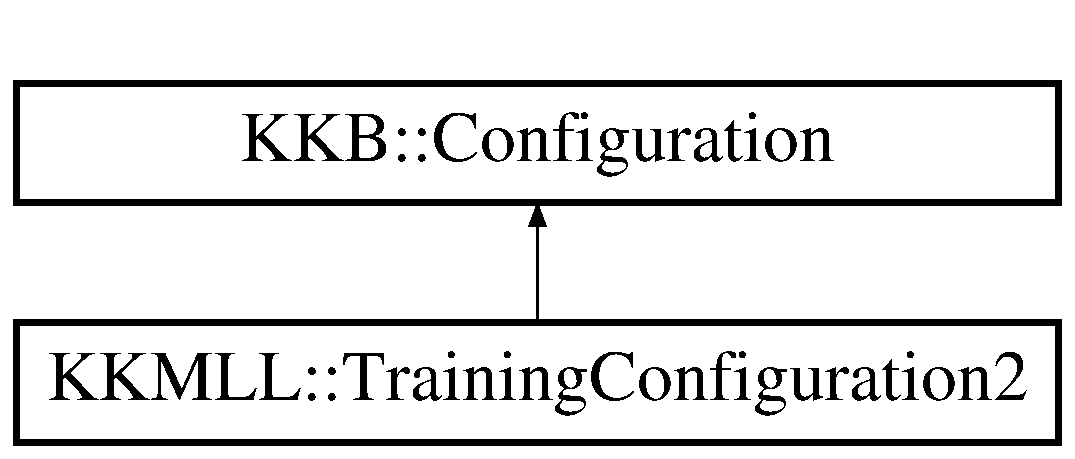
\includegraphics[height=2.000000cm]{class_k_k_b_1_1_configuration}
\end{center}
\end{figure}
\subsection*{Classes}
\begin{DoxyCompactItemize}
\item 
class \hyperlink{class_k_k_b_1_1_configuration_1_1_conf_section}{Conf\+Section}
\item 
class \hyperlink{class_k_k_b_1_1_configuration_1_1_conf_section_list}{Conf\+Section\+List}
\item 
class \hyperlink{class_k_k_b_1_1_configuration_1_1_setting}{Setting}
\item 
class \hyperlink{class_k_k_b_1_1_configuration_1_1_setting_list}{Setting\+List}
\end{DoxyCompactItemize}
\subsection*{Public Member Functions}
\begin{DoxyCompactItemize}
\item 
\hyperlink{class_k_k_b_1_1_configuration_a48bb1e7f0341f8e68b03f414d26d05e1}{Configuration} (const \hyperlink{class_k_k_b_1_1_k_k_str}{K\+K\+B\+::\+K\+K\+Str} \&\+\_\+file\+Name, \hyperlink{class_k_k_b_1_1_run_log}{Run\+Log} \&\+\_\+log)
\item 
\hyperlink{class_k_k_b_1_1_configuration_a779947337bf652f0e773cb29f37f14ba}{Configuration} ()
\item 
\hyperlink{class_k_k_b_1_1_configuration_a74cdde9cb4da23a8091dc09accd7289e}{Configuration} (const \hyperlink{class_k_k_b_1_1_configuration}{Configuration} \&c)
\item 
virtual \hyperlink{class_k_k_b_1_1_configuration_a0dd0fa189e239f4c9a036303f641441e}{$\sim$\+Configuration} ()
\item 
const \hyperlink{class_k_k_b_1_1_k_k_str}{K\+K\+B\+::\+K\+K\+Str} \& \hyperlink{class_k_k_b_1_1_configuration_a257e3c439e437688bbdd0d8f1c96f55c}{File\+Name} () const 
\item 
const \hyperlink{class_k_k_b_1_1_vector_k_k_str}{Vector\+K\+K\+Str} \& \hyperlink{class_k_k_b_1_1_configuration_a4edb0593552fbf5bfe096c611641525a}{Format\+Errors} () const 
\item 
void \hyperlink{class_k_k_b_1_1_configuration_aa8b2de567d8904c3643b8802b14cd443}{Format\+Errors\+Add} (\hyperlink{namespace_k_k_b_a8fa4952cc84fda1de4bec1fbdd8d5b1b}{kkint32} line\+Num, const \hyperlink{class_k_k_b_1_1_k_k_str}{K\+K\+Str} \&error)
\item 
void \hyperlink{class_k_k_b_1_1_configuration_a2ec3b84f15094ea8f190a15b4659607a}{Format\+Errors\+Clear} ()
\begin{DoxyCompactList}\small\item\em Call this to clear all format error messages. \end{DoxyCompactList}\item 
const \hyperlink{namespace_k_k_b_a791ebe73f89917067a7aab9dbd817e45}{Vector\+Int} \& \hyperlink{class_k_k_b_1_1_configuration_a891bf146ec6cb866850c0a8c45487e97}{Format\+Errors\+Line\+Nums} () const 
\item 
\hyperlink{class_k_k_b_1_1_vector_k_k_str}{Vector\+K\+K\+Str} \hyperlink{class_k_k_b_1_1_configuration_ace869c5caf1a0e717895635b7f592dba}{Format\+Errors\+With\+Line\+Numbers} () const 
\item 
bool \hyperlink{class_k_k_b_1_1_configuration_a83da17732beb6179d42f73f699795b68}{Format\+Good} () const 
\item 
void \hyperlink{class_k_k_b_1_1_configuration_ace46502cc01f162bcdae4dee0531a04b}{Format\+Good} (bool \+\_\+format\+Good)
\item 
void \hyperlink{class_k_k_b_1_1_configuration_abe8bbd2f858281ff44eccfac2a08477e}{Get\+Setting} (const char $\ast$sectiopn\+Name, \hyperlink{namespace_k_k_b_a8fa4952cc84fda1de4bec1fbdd8d5b1b}{kkint32} setting\+Num, \hyperlink{namespace_k_k_b_a46f665ec17615c856eff3d21f78bed5c}{K\+K\+Str\+Const\+Ptr} \&name, \hyperlink{namespace_k_k_b_a46f665ec17615c856eff3d21f78bed5c}{K\+K\+Str\+Const\+Ptr} \&value, \hyperlink{namespace_k_k_b_a8fa4952cc84fda1de4bec1fbdd8d5b1b}{kkint32} \&line\+Num)
\item 
virtual void \hyperlink{class_k_k_b_1_1_configuration_ad7d2e6b0148c6db8362abc6688a71739}{Load} (const \hyperlink{class_k_k_b_1_1_k_k_str}{K\+K\+B\+::\+K\+K\+Str} \&\+\_\+file\+Name, \hyperlink{class_k_k_b_1_1_run_log}{Run\+Log} \&\+\_\+log)
\item 
void \hyperlink{class_k_k_b_1_1_configuration_a3e7ae9b1d1f07f240fcea975fb8deea8}{Load\+File} (\hyperlink{class_k_k_b_1_1_run_log}{Run\+Log} \&log)
\item 
virtual \hyperlink{namespace_k_k_b_a8fa4952cc84fda1de4bec1fbdd8d5b1b}{kkint32} \hyperlink{class_k_k_b_1_1_configuration_a494a09ab9d70eee0855079da512e7293}{Memory\+Consumed\+Estimated} () const 
\item 
\hyperlink{namespace_k_k_b_a8fa4952cc84fda1de4bec1fbdd8d5b1b}{kkint32} \hyperlink{class_k_k_b_1_1_configuration_ab0f4ec3df333ac45eebf4b3bc4b72477}{Num\+Of\+Sections} ()
\item 
\hyperlink{namespace_k_k_b_a8fa4952cc84fda1de4bec1fbdd8d5b1b}{kkint32} \hyperlink{class_k_k_b_1_1_configuration_aa7cc05562fce75eb8c720bba45980559}{Num\+Of\+Settings} (const \hyperlink{class_k_k_b_1_1_k_k_str}{K\+K\+B\+::\+K\+K\+Str} \&section\+Name) const 
\item 
\hyperlink{namespace_k_k_b_a8fa4952cc84fda1de4bec1fbdd8d5b1b}{kkint32} \hyperlink{class_k_k_b_1_1_configuration_a9914f5ba6c1278a988af4fcd011d58a1}{Num\+Of\+Settings} (\hyperlink{namespace_k_k_b_a8fa4952cc84fda1de4bec1fbdd8d5b1b}{kkint32} section\+Num) const 
\begin{DoxyCompactList}\small\item\em Returns number of settings for the specified section,. \end{DoxyCompactList}\item 
void \hyperlink{class_k_k_b_1_1_configuration_aa20014b94bcc40e3c6b283821c42e212}{Print\+Format\+Errors} (std\+::ostream \&o)
\item 
bool \hyperlink{class_k_k_b_1_1_configuration_a5fc44650421878e33f9e9e537f71bdab}{Section\+Defined} (const \hyperlink{class_k_k_b_1_1_k_k_str}{K\+K\+B\+::\+K\+K\+Str} \&section\+Name) const 
\begin{DoxyCompactList}\small\item\em Returns true if the section is defined. \end{DoxyCompactList}\item 
\hyperlink{namespace_k_k_b_a8fa4952cc84fda1de4bec1fbdd8d5b1b}{kkint32} \hyperlink{class_k_k_b_1_1_configuration_a9ec3ea4ab84f5311e22c679087ae485c}{Section\+Line\+Num} (\hyperlink{namespace_k_k_b_a8fa4952cc84fda1de4bec1fbdd8d5b1b}{kkint32} section\+Num) const 
\item 
\hyperlink{namespace_k_k_b_a46f665ec17615c856eff3d21f78bed5c}{K\+K\+Str\+Const\+Ptr} \hyperlink{class_k_k_b_1_1_configuration_aa0c65a7f1f5e7885b6dd50fce22f2c79}{Section\+Name} (\hyperlink{namespace_k_k_b_a8fa4952cc84fda1de4bec1fbdd8d5b1b}{kkint32} section\+Num) const 
\begin{DoxyCompactList}\small\item\em Returns the name of the section for specified index, if index not defined will return N\+U\+LL. \end{DoxyCompactList}\item 
\hyperlink{namespace_k_k_b_a8fa4952cc84fda1de4bec1fbdd8d5b1b}{kkint32} \hyperlink{class_k_k_b_1_1_configuration_a7dad6ea4efdfbf0fda22007cefd5e4cf}{Section\+Num} (const \hyperlink{class_k_k_b_1_1_k_k_str}{K\+K\+B\+::\+K\+K\+Str} \&section\+Name) const 
\item 
\hyperlink{namespace_k_k_b_a46f665ec17615c856eff3d21f78bed5c}{K\+K\+Str\+Const\+Ptr} \hyperlink{class_k_k_b_1_1_configuration_a37b17c503e61082b4da5ca7ad89f542d}{Setting\+Name} (const \hyperlink{class_k_k_b_1_1_k_k_str}{K\+K\+B\+::\+K\+K\+Str} \&section\+Name, \hyperlink{namespace_k_k_b_a8fa4952cc84fda1de4bec1fbdd8d5b1b}{kkint32} setting\+Num) const 
\item 
\hyperlink{namespace_k_k_b_a46f665ec17615c856eff3d21f78bed5c}{K\+K\+Str\+Const\+Ptr} \hyperlink{class_k_k_b_1_1_configuration_a5fe555d390f8aee3cd8da0c4bd2b6a36}{Setting\+Name} (\hyperlink{namespace_k_k_b_a8fa4952cc84fda1de4bec1fbdd8d5b1b}{kkint32} section\+Num, \hyperlink{namespace_k_k_b_a8fa4952cc84fda1de4bec1fbdd8d5b1b}{kkint32} setting\+Num) const 
\item 
\hyperlink{namespace_k_k_b_a46f665ec17615c856eff3d21f78bed5c}{K\+K\+Str\+Const\+Ptr} \hyperlink{class_k_k_b_1_1_configuration_a3ec669dec9c7fa4c1a350d3582d49b46}{Setting\+Value} (const \hyperlink{class_k_k_b_1_1_k_k_str}{K\+K\+B\+::\+K\+K\+Str} \&section\+Name, const \hyperlink{class_k_k_b_1_1_k_k_str}{K\+K\+B\+::\+K\+K\+Str} \&setting\+Name, \hyperlink{namespace_k_k_b_a8fa4952cc84fda1de4bec1fbdd8d5b1b}{kkint32} \&line\+Num) const 
\item 
\hyperlink{namespace_k_k_b_a46f665ec17615c856eff3d21f78bed5c}{K\+K\+Str\+Const\+Ptr} \hyperlink{class_k_k_b_1_1_configuration_a9316bf174af1824baa4f1f6f1816cb55}{Setting\+Value} (\hyperlink{namespace_k_k_b_a8fa4952cc84fda1de4bec1fbdd8d5b1b}{kkint32} section\+Num, const \hyperlink{class_k_k_b_1_1_k_k_str}{K\+K\+B\+::\+K\+K\+Str} \&setting\+Name, \hyperlink{namespace_k_k_b_a8fa4952cc84fda1de4bec1fbdd8d5b1b}{kkint32} \&line\+Num) const 
\item 
\hyperlink{namespace_k_k_b_a46f665ec17615c856eff3d21f78bed5c}{K\+K\+Str\+Const\+Ptr} \hyperlink{class_k_k_b_1_1_configuration_a5c7fc0c7b4a7f695105fb05d482b73be}{Setting\+Value} (\hyperlink{namespace_k_k_b_a8fa4952cc84fda1de4bec1fbdd8d5b1b}{kkint32} section\+Num, \hyperlink{namespace_k_k_b_a8fa4952cc84fda1de4bec1fbdd8d5b1b}{kkint32} setting\+Num, \hyperlink{namespace_k_k_b_a8fa4952cc84fda1de4bec1fbdd8d5b1b}{kkint32} \&line\+Num) const 
\item 
\hyperlink{class_k_k_b_1_1_k_k_str}{K\+K\+Str} \hyperlink{class_k_k_b_1_1_configuration_ae422231ca6ffc64d6790f1a1ab8a48a7}{Setting\+Value\+To\+Str} (const \hyperlink{class_k_k_b_1_1_k_k_str}{K\+K\+B\+::\+K\+K\+Str} \&section\+Name, const \hyperlink{class_k_k_b_1_1_k_k_str}{K\+K\+B\+::\+K\+K\+Str} \&setting\+Name, \hyperlink{namespace_k_k_b_a8fa4952cc84fda1de4bec1fbdd8d5b1b}{kkint32} \&line\+Num) const 
\item 
\hyperlink{class_k_k_b_1_1_k_k_str}{K\+K\+Str} \hyperlink{class_k_k_b_1_1_configuration_ac94b40f7c7fda89736003a7c0effabb6}{Setting\+Value\+To\+Str} (\hyperlink{namespace_k_k_b_a8fa4952cc84fda1de4bec1fbdd8d5b1b}{kkint32} section\+Num, const \hyperlink{class_k_k_b_1_1_k_k_str}{K\+K\+B\+::\+K\+K\+Str} \&setting\+Name, \hyperlink{namespace_k_k_b_a8fa4952cc84fda1de4bec1fbdd8d5b1b}{kkint32} \&line\+Num) const 
\end{DoxyCompactItemize}


\subsection{Detailed Description}
General purpose \hyperlink{class_k_k_b_1_1_configuration}{Configuration} File manager class. 

This class will read and write configuration files. It understands the concept of Logical Sections and \hyperlink{class_variables}{Variables}. You will be able to pragmatically define Sections and Settings in these sections. Each \hyperlink{class_k_k_b_1_1_configuration_1_1_setting}{Setting} will have a related value stored with it.


\begin{DoxyCode}
*Example \hyperlink{class_k_k_b_1_1_configuration_a779947337bf652f0e773cb29f37f14ba}{Configuration} File
 ===========================================================
  [Header]
  ClassifierType = SVM
  Parameters = -K \hyperlink{namespace_s_v_m233_a44221c48118ea92c46a316a00e8f9e11a0478d3ebef66c527d9acbb734d1959d7}{RBF}  -S SVC -G 1.76 -C 12
  RootDir = $\{LarcosHmeDir\}\(\backslash\)\(\backslash\)Classifier\(\backslash\)\(\backslash\)TrainingLibraries\(\backslash\)\(\backslash\)
 
  [Class]
  Name = Shrimp\_01
 
  [Class]
  Name = Shrimp\_02
 ===========================================================
\end{DoxyCode}


There are three sections defined in the example above; Header, Class, and Class. Note that Section names do not have to be unique. You can access sections by name or index. If the name is not unique the first instance will be returned. Index values start at the top of the file, that is the first section to appear in the file is section index 0. The \hyperlink{class_k_k_b_1_1_configuration_1_1_setting}{Setting} names are of the format \char`\"{}\+Setting\+Name = Value\char`\"{}. Again you will be able to access \hyperlink{class_k_k_b_1_1_configuration_1_1_setting}{Setting} by either name or index. 

Definition at line 45 of file Configuration.\+h.



\subsection{Constructor \& Destructor Documentation}
\index{K\+K\+B\+::\+Configuration@{K\+K\+B\+::\+Configuration}!Configuration@{Configuration}}
\index{Configuration@{Configuration}!K\+K\+B\+::\+Configuration@{K\+K\+B\+::\+Configuration}}
\subsubsection[{\texorpdfstring{Configuration(const K\+K\+B\+::\+K\+K\+Str \&\+\_\+file\+Name, Run\+Log \&\+\_\+log)}{Configuration(const KKB::KKStr &_fileName, RunLog &_log)}}]{\setlength{\rightskip}{0pt plus 5cm}Configuration\+::\+Configuration (
\begin{DoxyParamCaption}
\item[{const {\bf K\+K\+B\+::\+K\+K\+Str} \&}]{\+\_\+file\+Name, }
\item[{{\bf Run\+Log} \&}]{\+\_\+log}
\end{DoxyParamCaption}
)}\hypertarget{class_k_k_b_1_1_configuration_a48bb1e7f0341f8e68b03f414d26d05e1}{}\label{class_k_k_b_1_1_configuration_a48bb1e7f0341f8e68b03f414d26d05e1}


Definition at line 286 of file Configuration.\+cpp.



References K\+K\+B\+::\+Configuration\+::\+Conf\+Section\+List\+::\+Conf\+Section\+List(), K\+K\+B\+::\+K\+K\+Str\+::\+K\+K\+Str(), Load\+File(), and K\+K\+B\+::\+Vector\+K\+K\+Str\+::\+Vector\+K\+K\+Str().


\begin{DoxyCode}
288                               :
289   curSectionName       (),
290   fileName             (\_fileName),
291   formatGood           (\textcolor{keyword}{true}),
292   formatErrors         (),
293   formatErrorsLineNums (),
294   sections             (NULL)
295 \{
296   sections = \textcolor{keyword}{new} ConfSectionList ();
297   \hyperlink{class_k_k_b_1_1_configuration_a3e7ae9b1d1f07f240fcea975fb8deea8}{LoadFile} (\_log);
298 \}
\end{DoxyCode}
\index{K\+K\+B\+::\+Configuration@{K\+K\+B\+::\+Configuration}!Configuration@{Configuration}}
\index{Configuration@{Configuration}!K\+K\+B\+::\+Configuration@{K\+K\+B\+::\+Configuration}}
\subsubsection[{\texorpdfstring{Configuration()}{Configuration()}}]{\setlength{\rightskip}{0pt plus 5cm}Configuration\+::\+Configuration (
\begin{DoxyParamCaption}
{}
\end{DoxyParamCaption}
)}\hypertarget{class_k_k_b_1_1_configuration_a779947337bf652f0e773cb29f37f14ba}{}\label{class_k_k_b_1_1_configuration_a779947337bf652f0e773cb29f37f14ba}


Definition at line 301 of file Configuration.\+cpp.



References K\+K\+B\+::\+Configuration\+::\+Conf\+Section\+List\+::\+Conf\+Section\+List(), K\+K\+B\+::\+K\+K\+Str\+::\+K\+K\+Str(), and K\+K\+B\+::\+Vector\+K\+K\+Str\+::\+Vector\+K\+K\+Str().



Referenced by K\+K\+M\+L\+L\+::\+Training\+Configuration2\+::\+Training\+Configuration2().


\begin{DoxyCode}
301                              :
302   curSectionName       (),
303   fileName             (),
304   formatGood           (\textcolor{keyword}{true}),
305   formatErrors         (),
306   formatErrorsLineNums (),
307   sections             (NULL)
308 \{
309   sections = \textcolor{keyword}{new} ConfSectionList ();
310 \}
\end{DoxyCode}
\index{K\+K\+B\+::\+Configuration@{K\+K\+B\+::\+Configuration}!Configuration@{Configuration}}
\index{Configuration@{Configuration}!K\+K\+B\+::\+Configuration@{K\+K\+B\+::\+Configuration}}
\subsubsection[{\texorpdfstring{Configuration(const Configuration \&c)}{Configuration(const Configuration &c)}}]{\setlength{\rightskip}{0pt plus 5cm}Configuration\+::\+Configuration (
\begin{DoxyParamCaption}
\item[{const {\bf Configuration} \&}]{c}
\end{DoxyParamCaption}
)}\hypertarget{class_k_k_b_1_1_configuration_a74cdde9cb4da23a8091dc09accd7289e}{}\label{class_k_k_b_1_1_configuration_a74cdde9cb4da23a8091dc09accd7289e}


Definition at line 314 of file Configuration.\+cpp.



References K\+K\+B\+::\+Configuration\+::\+Conf\+Section\+List\+::\+Add\+Conf\+Section(), K\+K\+B\+::\+Configuration\+::\+Conf\+Section\+::\+Conf\+Section(), K\+K\+B\+::\+Configuration\+::\+Conf\+Section\+List\+::\+Conf\+Section\+List(), K\+K\+B\+::\+K\+K\+Str\+::\+K\+K\+Str(), and K\+K\+B\+::\+Vector\+K\+K\+Str\+::\+Vector\+K\+K\+Str().


\begin{DoxyCode}
314                                                     :
315   
316   curSectionName       (c.curSectionName),
317   fileName             (c.fileName),
318   formatGood           (c.formatGood),
319   formatErrors         (c.formatErrors),
320   formatErrorsLineNums (c.formatErrorsLineNums),
321   sections             (NULL)
322 \{
323   sections = \textcolor{keyword}{new} ConfSectionList ();
324 
325   \hyperlink{namespace_k_k_b_a8fa4952cc84fda1de4bec1fbdd8d5b1b}{kkint32}  x;
326 
327   \textcolor{keywordflow}{for}  (x = 0;  x < sections->\hyperlink{class_k_k_b_1_1_k_k_queue_a1dab601f75ee6a65d97f02bddf71c40d}{QueueSize} ();  x++)
328   \{
329     \textcolor{keyword}{const} ConfSectionPtr  cs = sections->\hyperlink{class_k_k_b_1_1_k_k_queue_acce2bdd8b3327e38266cf198382cd852}{IdxToPtr} (x);
330     sections->\hyperlink{class_k_k_b_1_1_configuration_1_1_conf_section_list_a4cb1a372299d3e5b6c306644bb465fd6}{AddConfSection} (\textcolor{keyword}{new} ConfSection (*cs));
331   \}
332 \}
\end{DoxyCode}
\index{K\+K\+B\+::\+Configuration@{K\+K\+B\+::\+Configuration}!````~Configuration@{$\sim$\+Configuration}}
\index{````~Configuration@{$\sim$\+Configuration}!K\+K\+B\+::\+Configuration@{K\+K\+B\+::\+Configuration}}
\subsubsection[{\texorpdfstring{$\sim$\+Configuration()}{~Configuration()}}]{\setlength{\rightskip}{0pt plus 5cm}Configuration\+::$\sim$\+Configuration (
\begin{DoxyParamCaption}
{}
\end{DoxyParamCaption}
)\hspace{0.3cm}{\ttfamily [virtual]}}\hypertarget{class_k_k_b_1_1_configuration_a0dd0fa189e239f4c9a036303f641441e}{}\label{class_k_k_b_1_1_configuration_a0dd0fa189e239f4c9a036303f641441e}


Definition at line 336 of file Configuration.\+cpp.


\begin{DoxyCode}
337 \{
338   \textcolor{keyword}{delete}  sections;
339 \}
\end{DoxyCode}


\subsection{Member Function Documentation}
\index{K\+K\+B\+::\+Configuration@{K\+K\+B\+::\+Configuration}!File\+Name@{File\+Name}}
\index{File\+Name@{File\+Name}!K\+K\+B\+::\+Configuration@{K\+K\+B\+::\+Configuration}}
\subsubsection[{\texorpdfstring{File\+Name() const }{FileName() const }}]{\setlength{\rightskip}{0pt plus 5cm}const {\bf K\+K\+B\+::\+K\+K\+Str}\& K\+K\+B\+::\+Configuration\+::\+File\+Name (
\begin{DoxyParamCaption}
{}
\end{DoxyParamCaption}
) const\hspace{0.3cm}{\ttfamily [inline]}}\hypertarget{class_k_k_b_1_1_configuration_a257e3c439e437688bbdd0d8f1c96f55c}{}\label{class_k_k_b_1_1_configuration_a257e3c439e437688bbdd0d8f1c96f55c}


Definition at line 96 of file Configuration.\+h.


\begin{DoxyCode}
96 \{\textcolor{keywordflow}{return}  fileName;\}
\end{DoxyCode}
\index{K\+K\+B\+::\+Configuration@{K\+K\+B\+::\+Configuration}!Format\+Errors@{Format\+Errors}}
\index{Format\+Errors@{Format\+Errors}!K\+K\+B\+::\+Configuration@{K\+K\+B\+::\+Configuration}}
\subsubsection[{\texorpdfstring{Format\+Errors() const }{FormatErrors() const }}]{\setlength{\rightskip}{0pt plus 5cm}const {\bf Vector\+K\+K\+Str}\& K\+K\+B\+::\+Configuration\+::\+Format\+Errors (
\begin{DoxyParamCaption}
{}
\end{DoxyParamCaption}
) const\hspace{0.3cm}{\ttfamily [inline]}}\hypertarget{class_k_k_b_1_1_configuration_a4edb0593552fbf5bfe096c611641525a}{}\label{class_k_k_b_1_1_configuration_a4edb0593552fbf5bfe096c611641525a}


Definition at line 68 of file Configuration.\+h.


\begin{DoxyCode}
68 \{\textcolor{keywordflow}{return} formatErrors;\}
\end{DoxyCode}
\index{K\+K\+B\+::\+Configuration@{K\+K\+B\+::\+Configuration}!Format\+Errors\+Add@{Format\+Errors\+Add}}
\index{Format\+Errors\+Add@{Format\+Errors\+Add}!K\+K\+B\+::\+Configuration@{K\+K\+B\+::\+Configuration}}
\subsubsection[{\texorpdfstring{Format\+Errors\+Add(kkint32 line\+Num, const K\+K\+Str \&error)}{FormatErrorsAdd(kkint32 lineNum, const KKStr &error)}}]{\setlength{\rightskip}{0pt plus 5cm}void Configuration\+::\+Format\+Errors\+Add (
\begin{DoxyParamCaption}
\item[{{\bf kkint32}}]{line\+Num, }
\item[{const {\bf K\+K\+Str} \&}]{error}
\end{DoxyParamCaption}
)}\hypertarget{class_k_k_b_1_1_configuration_aa8b2de567d8904c3643b8802b14cd443}{}\label{class_k_k_b_1_1_configuration_aa8b2de567d8904c3643b8802b14cd443}


Definition at line 772 of file Configuration.\+cpp.


\begin{DoxyCode}
775 \{
776   formatErrors.push\_back (error);
777   formatErrorsLineNums.push\_back (lineNum);
778 \}
\end{DoxyCode}
\index{K\+K\+B\+::\+Configuration@{K\+K\+B\+::\+Configuration}!Format\+Errors\+Clear@{Format\+Errors\+Clear}}
\index{Format\+Errors\+Clear@{Format\+Errors\+Clear}!K\+K\+B\+::\+Configuration@{K\+K\+B\+::\+Configuration}}
\subsubsection[{\texorpdfstring{Format\+Errors\+Clear()}{FormatErrorsClear()}}]{\setlength{\rightskip}{0pt plus 5cm}void Configuration\+::\+Format\+Errors\+Clear (
\begin{DoxyParamCaption}
{}
\end{DoxyParamCaption}
)}\hypertarget{class_k_k_b_1_1_configuration_a2ec3b84f15094ea8f190a15b4659607a}{}\label{class_k_k_b_1_1_configuration_a2ec3b84f15094ea8f190a15b4659607a}


Call this to clear all format error messages. 



Definition at line 783 of file Configuration.\+cpp.


\begin{DoxyCode}
784 \{
785   formatErrors.clear ();
786   formatErrorsLineNums.clear ();
787 \}
\end{DoxyCode}
\index{K\+K\+B\+::\+Configuration@{K\+K\+B\+::\+Configuration}!Format\+Errors\+Line\+Nums@{Format\+Errors\+Line\+Nums}}
\index{Format\+Errors\+Line\+Nums@{Format\+Errors\+Line\+Nums}!K\+K\+B\+::\+Configuration@{K\+K\+B\+::\+Configuration}}
\subsubsection[{\texorpdfstring{Format\+Errors\+Line\+Nums() const }{FormatErrorsLineNums() const }}]{\setlength{\rightskip}{0pt plus 5cm}const {\bf Vector\+Int}\& K\+K\+B\+::\+Configuration\+::\+Format\+Errors\+Line\+Nums (
\begin{DoxyParamCaption}
{}
\end{DoxyParamCaption}
) const\hspace{0.3cm}{\ttfamily [inline]}}\hypertarget{class_k_k_b_1_1_configuration_a891bf146ec6cb866850c0a8c45487e97}{}\label{class_k_k_b_1_1_configuration_a891bf146ec6cb866850c0a8c45487e97}


Definition at line 69 of file Configuration.\+h.


\begin{DoxyCode}
69 \{\textcolor{keywordflow}{return} formatErrorsLineNums;\}
\end{DoxyCode}
\index{K\+K\+B\+::\+Configuration@{K\+K\+B\+::\+Configuration}!Format\+Errors\+With\+Line\+Numbers@{Format\+Errors\+With\+Line\+Numbers}}
\index{Format\+Errors\+With\+Line\+Numbers@{Format\+Errors\+With\+Line\+Numbers}!K\+K\+B\+::\+Configuration@{K\+K\+B\+::\+Configuration}}
\subsubsection[{\texorpdfstring{Format\+Errors\+With\+Line\+Numbers() const }{FormatErrorsWithLineNumbers() const }}]{\setlength{\rightskip}{0pt plus 5cm}{\bf Vector\+K\+K\+Str} Configuration\+::\+Format\+Errors\+With\+Line\+Numbers (
\begin{DoxyParamCaption}
{}
\end{DoxyParamCaption}
) const}\hypertarget{class_k_k_b_1_1_configuration_ace869c5caf1a0e717895635b7f592dba}{}\label{class_k_k_b_1_1_configuration_ace869c5caf1a0e717895635b7f592dba}


Definition at line 791 of file Configuration.\+cpp.



References K\+K\+B\+::\+K\+K\+Str\+::\+Concat().


\begin{DoxyCode}
792 \{
793   \hyperlink{class_k_k_b_1_1_vector_k_k_str}{VectorKKStr}  errorMsgs;
794   \textcolor{keywordflow}{for}  (\hyperlink{namespace_k_k_b_af8d832f05c54994a1cce25bd5743e19a}{kkuint32} i = 0;  i < formatErrors.size ();  i++)
795   \{
796     \hyperlink{class_k_k_b_1_1_k_k_str}{KKStr}  lineNumStr = \textcolor{stringliteral}{"    "};
797     \textcolor{keywordflow}{if}  (i < formatErrorsLineNums.size ())
798       lineNumStr = \hyperlink{namespace_k_k_b_ae3bde258fa036604fac8bdb0277ab46e}{StrFormatInt} (formatErrorsLineNums[i], \textcolor{stringliteral}{"0000"});
799     errorMsgs.push\_back (lineNumStr + \textcolor{stringliteral}{":"} + formatErrors[i]); 
800   \}
801 
802   \textcolor{keywordflow}{return}  errorMsgs;
803 \}  \textcolor{comment}{/* FormatErrorsWithLineNumbers */}
\end{DoxyCode}
\index{K\+K\+B\+::\+Configuration@{K\+K\+B\+::\+Configuration}!Format\+Good@{Format\+Good}}
\index{Format\+Good@{Format\+Good}!K\+K\+B\+::\+Configuration@{K\+K\+B\+::\+Configuration}}
\subsubsection[{\texorpdfstring{Format\+Good() const }{FormatGood() const }}]{\setlength{\rightskip}{0pt plus 5cm}bool K\+K\+B\+::\+Configuration\+::\+Format\+Good (
\begin{DoxyParamCaption}
{}
\end{DoxyParamCaption}
) const\hspace{0.3cm}{\ttfamily [inline]}}\hypertarget{class_k_k_b_1_1_configuration_a83da17732beb6179d42f73f699795b68}{}\label{class_k_k_b_1_1_configuration_a83da17732beb6179d42f73f699795b68}


Definition at line 64 of file Configuration.\+h.


\begin{DoxyCode}
64 \{\textcolor{keywordflow}{return}  formatGood;\}
\end{DoxyCode}
\index{K\+K\+B\+::\+Configuration@{K\+K\+B\+::\+Configuration}!Format\+Good@{Format\+Good}}
\index{Format\+Good@{Format\+Good}!K\+K\+B\+::\+Configuration@{K\+K\+B\+::\+Configuration}}
\subsubsection[{\texorpdfstring{Format\+Good(bool \+\_\+format\+Good)}{FormatGood(bool _formatGood)}}]{\setlength{\rightskip}{0pt plus 5cm}void K\+K\+B\+::\+Configuration\+::\+Format\+Good (
\begin{DoxyParamCaption}
\item[{bool}]{\+\_\+format\+Good}
\end{DoxyParamCaption}
)\hspace{0.3cm}{\ttfamily [inline]}}\hypertarget{class_k_k_b_1_1_configuration_ace46502cc01f162bcdae4dee0531a04b}{}\label{class_k_k_b_1_1_configuration_ace46502cc01f162bcdae4dee0531a04b}


Definition at line 66 of file Configuration.\+h.



Referenced by Load\+File().


\begin{DoxyCode}
66 \{formatGood = \_formatGood;\}
\end{DoxyCode}
\index{K\+K\+B\+::\+Configuration@{K\+K\+B\+::\+Configuration}!Get\+Setting@{Get\+Setting}}
\index{Get\+Setting@{Get\+Setting}!K\+K\+B\+::\+Configuration@{K\+K\+B\+::\+Configuration}}
\subsubsection[{\texorpdfstring{Get\+Setting(const char $\ast$sectiopn\+Name, kkint32 setting\+Num, K\+K\+Str\+Const\+Ptr \&name, K\+K\+Str\+Const\+Ptr \&value, kkint32 \&line\+Num)}{GetSetting(const char *sectiopnName, kkint32 settingNum, KKStrConstPtr &name, KKStrConstPtr &value, kkint32 &lineNum)}}]{\setlength{\rightskip}{0pt plus 5cm}void Configuration\+::\+Get\+Setting (
\begin{DoxyParamCaption}
\item[{const char $\ast$}]{sectiopn\+Name, }
\item[{{\bf kkint32}}]{setting\+Num, }
\item[{{\bf K\+K\+Str\+Const\+Ptr} \&}]{name, }
\item[{{\bf K\+K\+Str\+Const\+Ptr} \&}]{value, }
\item[{{\bf kkint32} \&}]{line\+Num}
\end{DoxyParamCaption}
)}\hypertarget{class_k_k_b_1_1_configuration_abe8bbd2f858281ff44eccfac2a08477e}{}\label{class_k_k_b_1_1_configuration_abe8bbd2f858281ff44eccfac2a08477e}


Definition at line 749 of file Configuration.\+cpp.



References K\+K\+B\+::\+Configuration\+::\+Conf\+Section\+::\+Get\+Settings(), and K\+K\+B\+::\+Configuration\+::\+Conf\+Section\+List\+::\+Look\+Up().


\begin{DoxyCode}
755 \{
756   ConfSectionPtr  section = sections->\hyperlink{class_k_k_b_1_1_configuration_1_1_conf_section_list_ae1932c42a5b475020b4f84e5f36fcba6}{LookUp} (sectionName);
757   \textcolor{keywordflow}{if}  (section)
758   \{
759     section->\hyperlink{class_k_k_b_1_1_configuration_1_1_conf_section_ac5d802d610306415ad426e48766f0e36}{GetSettings} (settingNum, name, value, lineNum);
760   \}
761   \textcolor{keywordflow}{else}
762   \{
763     name    = NULL;
764     value   = NULL;
765     lineNum = -1;
766   \}
767 \}
\end{DoxyCode}
\index{K\+K\+B\+::\+Configuration@{K\+K\+B\+::\+Configuration}!Load@{Load}}
\index{Load@{Load}!K\+K\+B\+::\+Configuration@{K\+K\+B\+::\+Configuration}}
\subsubsection[{\texorpdfstring{Load(const K\+K\+B\+::\+K\+K\+Str \&\+\_\+file\+Name, Run\+Log \&\+\_\+log)}{Load(const KKB::KKStr &_fileName, RunLog &_log)}}]{\setlength{\rightskip}{0pt plus 5cm}void Configuration\+::\+Load (
\begin{DoxyParamCaption}
\item[{const {\bf K\+K\+B\+::\+K\+K\+Str} \&}]{\+\_\+file\+Name, }
\item[{{\bf Run\+Log} \&}]{\+\_\+log}
\end{DoxyParamCaption}
)\hspace{0.3cm}{\ttfamily [virtual]}}\hypertarget{class_k_k_b_1_1_configuration_ad7d2e6b0148c6db8362abc6688a71739}{}\label{class_k_k_b_1_1_configuration_ad7d2e6b0148c6db8362abc6688a71739}


Definition at line 401 of file Configuration.\+cpp.



References Load\+File(), and K\+K\+B\+::\+K\+K\+Str\+::operator=().


\begin{DoxyCode}
404 \{
405   fileName = \_fileName;
406   \hyperlink{class_k_k_b_1_1_configuration_a3e7ae9b1d1f07f240fcea975fb8deea8}{LoadFile} (\_log);
407 \}
\end{DoxyCode}
\index{K\+K\+B\+::\+Configuration@{K\+K\+B\+::\+Configuration}!Load\+File@{Load\+File}}
\index{Load\+File@{Load\+File}!K\+K\+B\+::\+Configuration@{K\+K\+B\+::\+Configuration}}
\subsubsection[{\texorpdfstring{Load\+File(\+Run\+Log \&log)}{LoadFile(RunLog &log)}}]{\setlength{\rightskip}{0pt plus 5cm}void Configuration\+::\+Load\+File (
\begin{DoxyParamCaption}
\item[{{\bf Run\+Log} \&}]{log}
\end{DoxyParamCaption}
)}\hypertarget{class_k_k_b_1_1_configuration_a3e7ae9b1d1f07f240fcea975fb8deea8}{}\label{class_k_k_b_1_1_configuration_a3e7ae9b1d1f07f240fcea975fb8deea8}


Definition at line 411 of file Configuration.\+cpp.



References Format\+Good(), K\+K\+B\+::\+K\+K\+Str\+::operator=(), K\+K\+B\+::\+K\+K\+Str\+::operator==(), K\+K\+B\+::os\+F\+O\+P\+E\+N(), and K\+K\+B\+::\+K\+K\+Str\+::\+Str().



Referenced by Configuration(), and Load().


\begin{DoxyCode}
412 \{
413   log.\hyperlink{class_k_k_b_1_1_run_log_a32cf761d7f2e747465fd80533fdbb659}{Level} (10) << \textcolor{stringliteral}{"Configuration::LoadFile: "} << fileName << \hyperlink{namespace_k_k_b_ad1f50f65af6adc8fa9e6f62d007818a8}{endl};
414 
415   \hyperlink{namespace_k_k_b_a8fa4952cc84fda1de4bec1fbdd8d5b1b}{kkint32}  lastLineNum = 0;
416 
417   \textcolor{keywordflow}{if}  (fileName == \textcolor{stringliteral}{""})
418   \{
419     log.\hyperlink{class_k_k_b_1_1_run_log_a32cf761d7f2e747465fd80533fdbb659}{Level} (-1) << endl
420                    << \textcolor{stringliteral}{"Configuration::LoadFile   ***ERROR***   File-Name is blank"}  << endl
421                    << \hyperlink{namespace_k_k_b_ad1f50f65af6adc8fa9e6f62d007818a8}{endl};
422     \hyperlink{class_k_k_b_1_1_configuration_a83da17732beb6179d42f73f699795b68}{FormatGood} (\textcolor{keyword}{false});
423     \textcolor{keywordflow}{return};
424   \}
425 
426   FILE*  inFile = \hyperlink{namespace_k_k_b_abf4050d2916ded8349dafadc80f0ecd1}{osFOPEN} (fileName.\hyperlink{class_k_k_b_1_1_k_k_str_ad574e6c0fe7f6ce1ba3ab0a8ce2fbd52}{Str} (), \textcolor{stringliteral}{"r"});
427 
428   \textcolor{keywordflow}{if}  (!inFile)
429   \{
430     log.\hyperlink{class_k_k_b_1_1_run_log_a32cf761d7f2e747465fd80533fdbb659}{Level} (-1) << endl
431                    << \textcolor{stringliteral}{"Configuration::LoadFile   ***ERROR***    Opening File: "} << fileName << endl
432                    << \hyperlink{namespace_k_k_b_ad1f50f65af6adc8fa9e6f62d007818a8}{endl};
433 
434     \hyperlink{class_k_k_b_1_1_configuration_a83da17732beb6179d42f73f699795b68}{FormatGood} (\textcolor{keyword}{false});
435     \textcolor{keywordflow}{return};
436   \}
437 
438   \textcolor{keywordtype}{char}  buff[10240];
439   \hyperlink{namespace_k_k_b_a8fa4952cc84fda1de4bec1fbdd8d5b1b}{kkint32} lineCount = 0;
440 
441   curSectionName = \textcolor{stringliteral}{""};
442   ConfSectionPtr  curSection = NULL;
443 
444   \textcolor{keywordflow}{while}  (fgets (buff, \textcolor{keyword}{sizeof} (buff), inFile))
445   \{
446     lastLineNum++;
447     \hyperlink{class_k_k_b_1_1_k_k_str}{KKStr}  line (buff);
448     line.TrimRight ();
449     line.TrimLeft ();
450 
451     \hyperlink{_configuration_8cpp_a65029dc58121c93c0ecd83d9809d077a}{StripOutAnyComments} (line);
452 
453     log.\hyperlink{class_k_k_b_1_1_run_log_a32cf761d7f2e747465fd80533fdbb659}{Level} (70) << line << \hyperlink{namespace_k_k_b_ad1f50f65af6adc8fa9e6f62d007818a8}{endl};
454     
455     \hyperlink{_configuration_8cpp_a65029dc58121c93c0ecd83d9809d077a}{StripOutAnyComments} (line);
456 
457     \textcolor{keywordflow}{if}  (line.Empty ())            
458     \{
459       \textcolor{comment}{// If we have a blank line, we do nothing.}
460     \}
461 
462     \textcolor{keywordflow}{else} \textcolor{keywordflow}{if}  (line.FirstChar () == \textcolor{charliteral}{'['})
463     \{
464       \textcolor{comment}{// Looks like definition of new section. }
465 
466       \textcolor{keywordflow}{if}  (line.LastChar () == \textcolor{charliteral}{']'})
467       \{
468         curSectionName = line.\hyperlink{class_k_k_b_1_1_k_k_str_a5f20b2ddfc9f07c8ef99592810332ddb}{SubStrPart} (1, line.Len () - 2);
469         curSectionName.\hyperlink{class_k_k_b_1_1_k_k_str_af7c102c53103ddff3f48270b4a198c89}{TrimLeft} ();
470         curSectionName.\hyperlink{class_k_k_b_1_1_k_k_str_aa912161f17871e2d6fec7bbac033221c}{TrimRight} ();
471         curSectionName.\hyperlink{class_k_k_b_1_1_k_k_str_a66ea0feabc94da88591b56a683695bd9}{Upper} ();
472 
473         curSection = \textcolor{keyword}{new} ConfSection (curSectionName, lastLineNum);
474         sections->\hyperlink{class_k_k_b_1_1_configuration_1_1_conf_section_list_a4cb1a372299d3e5b6c306644bb465fd6}{AddConfSection} (curSection);
475         log.\hyperlink{class_k_k_b_1_1_run_log_a32cf761d7f2e747465fd80533fdbb659}{Level} (30) << \textcolor{stringliteral}{"LoadFile   SectionName["} << curSectionName << \textcolor{stringliteral}{"]."} << 
      \hyperlink{namespace_k_k_b_ad1f50f65af6adc8fa9e6f62d007818a8}{endl};
476       \}
477       \textcolor{keywordflow}{else}
478       \{
479         log.\hyperlink{class_k_k_b_1_1_run_log_a32cf761d7f2e747465fd80533fdbb659}{Level} (-1) << endl
480                        << \textcolor{stringliteral}{"Configuration::LoadFile   ***ERROR***    LineNumber["} << lastLineNum << \textcolor{stringliteral}{"] 
       Improper Section Name["} << line << \textcolor{stringliteral}{"]."} << endl
481                        << \hyperlink{namespace_k_k_b_ad1f50f65af6adc8fa9e6f62d007818a8}{endl};
482         formatGood = \textcolor{keyword}{false};
483       \}
484     \}
485 
486     \textcolor{keywordflow}{else}
487     \{
488       \textcolor{keywordflow}{if}  (!curSection)
489       \{
490         log.\hyperlink{class_k_k_b_1_1_run_log_a32cf761d7f2e747465fd80533fdbb659}{Level} (-1) << endl
491                        << \textcolor{stringliteral}{"Configuration::LoadFile   ***ERROR***  Format Error LineNumber["} << lastLineNum 
      << \textcolor{stringliteral}{"]"} << endl
492                        << \textcolor{stringliteral}{"                            No Section Defined."}  << endl 
493                        << \hyperlink{namespace_k_k_b_ad1f50f65af6adc8fa9e6f62d007818a8}{endl};
494      
495         formatGood = \textcolor{keyword}{false};
496 
497         curSectionName = \textcolor{stringliteral}{"GLOBAL"};
498         curSection = \textcolor{keyword}{new} ConfSection (curSectionName, lastLineNum);
499         sections->\hyperlink{class_k_k_b_1_1_configuration_1_1_conf_section_list_a4cb1a372299d3e5b6c306644bb465fd6}{AddConfSection} (curSection);
500       \}
501 
502       \hyperlink{namespace_k_k_b_a8fa4952cc84fda1de4bec1fbdd8d5b1b}{kkint32}  equalIdx = line.LocateCharacter (\textcolor{charliteral}{'='});
503 
504       \textcolor{keywordflow}{if}  (equalIdx < 0)
505       \{
506         \textcolor{comment}{// We have a improperly formated line.}
507         log.\hyperlink{class_k_k_b_1_1_run_log_a32cf761d7f2e747465fd80533fdbb659}{Level} (-1) << endl
508                        << \textcolor{stringliteral}{"Configuration::LoadFile   ***ERROR***   LineNumber["} << lastLineNum << \textcolor{stringliteral}{"]
       Improperly Formated Line["} << line << \textcolor{stringliteral}{"]."} 
509                        << \hyperlink{namespace_k_k_b_ad1f50f65af6adc8fa9e6f62d007818a8}{endl};
510         formatGood = \textcolor{keyword}{false};
511       \}
512 
513       \textcolor{keywordflow}{else}
514       \{
515         \hyperlink{class_k_k_b_1_1_k_k_str}{KKStr}  settingName (line.SubStrPart (0, equalIdx - 1));
516         settingName.\hyperlink{class_k_k_b_1_1_k_k_str_af7c102c53103ddff3f48270b4a198c89}{TrimLeft} ();
517         settingName.TrimRight ();
518         settingName.Upper ();
519 
520         \hyperlink{class_k_k_b_1_1_k_k_str}{KKStr}  settingValue (line.SubStrPart (equalIdx + 1));
521         settingValue.\hyperlink{class_k_k_b_1_1_k_k_str_af7c102c53103ddff3f48270b4a198c89}{TrimLeft} ();
522         settingValue.TrimRight ();
523 
524         log.\hyperlink{class_k_k_b_1_1_run_log_a32cf761d7f2e747465fd80533fdbb659}{Level} (30) << \textcolor{stringliteral}{"LoadFile   SectionName["} << curSectionName << \textcolor{stringliteral}{"], "}
525                        << \textcolor{stringliteral}{"Setting["} << settingName << \textcolor{stringliteral}{"], Value["} << settingValue   << \textcolor{stringliteral}{"]."}
526                        << \hyperlink{namespace_k_k_b_ad1f50f65af6adc8fa9e6f62d007818a8}{endl};
527 
528         curSection->AddSetting (settingName, settingValue, lastLineNum);
529       \}
530 
531       lineCount++;
532     \}
533   \}
534 
535   fclose (inFile);
536 \}  \textcolor{comment}{/* LoadFile */}
\end{DoxyCode}
\index{K\+K\+B\+::\+Configuration@{K\+K\+B\+::\+Configuration}!Memory\+Consumed\+Estimated@{Memory\+Consumed\+Estimated}}
\index{Memory\+Consumed\+Estimated@{Memory\+Consumed\+Estimated}!K\+K\+B\+::\+Configuration@{K\+K\+B\+::\+Configuration}}
\subsubsection[{\texorpdfstring{Memory\+Consumed\+Estimated() const }{MemoryConsumedEstimated() const }}]{\setlength{\rightskip}{0pt plus 5cm}{\bf kkint32} Configuration\+::\+Memory\+Consumed\+Estimated (
\begin{DoxyParamCaption}
{}
\end{DoxyParamCaption}
) const\hspace{0.3cm}{\ttfamily [virtual]}}\hypertarget{class_k_k_b_1_1_configuration_a494a09ab9d70eee0855079da512e7293}{}\label{class_k_k_b_1_1_configuration_a494a09ab9d70eee0855079da512e7293}


Definition at line 343 of file Configuration.\+cpp.



References K\+K\+B\+::\+Configuration\+::\+Conf\+Section\+List\+::\+Memory\+Consumed\+Estimated().


\begin{DoxyCode}
344 \{
345   \hyperlink{namespace_k_k_b_a8fa4952cc84fda1de4bec1fbdd8d5b1b}{kkint32}  memoryConsumedEstimated = \textcolor{keyword}{sizeof} (\hyperlink{class_k_k_b_1_1_configuration_a779947337bf652f0e773cb29f37f14ba}{Configuration})
346     + curSectionName.\hyperlink{class_k_k_b_1_1_k_k_str_afc335bf98a8d4a77dc34215e72068719}{MemoryConsumedEstimated} ()
347     + fileName.\hyperlink{class_k_k_b_1_1_k_k_str_afc335bf98a8d4a77dc34215e72068719}{MemoryConsumedEstimated} ()
348     + (\hyperlink{namespace_k_k_b_a8fa4952cc84fda1de4bec1fbdd8d5b1b}{kkint32})formatErrors.size () * 100
349     + (\hyperlink{namespace_k_k_b_a8fa4952cc84fda1de4bec1fbdd8d5b1b}{kkint32})formatErrorsLineNums.size () * \textcolor{keyword}{sizeof} (\hyperlink{namespace_k_k_b_a8fa4952cc84fda1de4bec1fbdd8d5b1b}{kkint32});
350 
351   \textcolor{keywordflow}{if}  (sections)
352     memoryConsumedEstimated += sections->\hyperlink{class_k_k_b_1_1_configuration_1_1_conf_section_list_aab5e7968237c965d19a3dc8feb280b79}{MemoryConsumedEstimated} ();
353 
354   \textcolor{keywordflow}{return}  memoryConsumedEstimated;
355 \}  \textcolor{comment}{/* MemoryConsumedEstimated */}
\end{DoxyCode}
\index{K\+K\+B\+::\+Configuration@{K\+K\+B\+::\+Configuration}!Num\+Of\+Sections@{Num\+Of\+Sections}}
\index{Num\+Of\+Sections@{Num\+Of\+Sections}!K\+K\+B\+::\+Configuration@{K\+K\+B\+::\+Configuration}}
\subsubsection[{\texorpdfstring{Num\+Of\+Sections()}{NumOfSections()}}]{\setlength{\rightskip}{0pt plus 5cm}{\bf kkint32} Configuration\+::\+Num\+Of\+Sections (
\begin{DoxyParamCaption}
{}
\end{DoxyParamCaption}
)}\hypertarget{class_k_k_b_1_1_configuration_ab0f4ec3df333ac45eebf4b3bc4b72477}{}\label{class_k_k_b_1_1_configuration_ab0f4ec3df333ac45eebf4b3bc4b72477}


Definition at line 541 of file Configuration.\+cpp.


\begin{DoxyCode}
542 \{
543   \textcolor{keywordflow}{return}  sections->\hyperlink{class_k_k_b_1_1_k_k_queue_a1dab601f75ee6a65d97f02bddf71c40d}{QueueSize} ();
544 \}
\end{DoxyCode}
\index{K\+K\+B\+::\+Configuration@{K\+K\+B\+::\+Configuration}!Num\+Of\+Settings@{Num\+Of\+Settings}}
\index{Num\+Of\+Settings@{Num\+Of\+Settings}!K\+K\+B\+::\+Configuration@{K\+K\+B\+::\+Configuration}}
\subsubsection[{\texorpdfstring{Num\+Of\+Settings(const K\+K\+B\+::\+K\+K\+Str \&section\+Name) const }{NumOfSettings(const KKB::KKStr &sectionName) const }}]{\setlength{\rightskip}{0pt plus 5cm}{\bf kkint32} Configuration\+::\+Num\+Of\+Settings (
\begin{DoxyParamCaption}
\item[{const {\bf K\+K\+B\+::\+K\+K\+Str} \&}]{section\+Name}
\end{DoxyParamCaption}
) const}\hypertarget{class_k_k_b_1_1_configuration_aa7cc05562fce75eb8c720bba45980559}{}\label{class_k_k_b_1_1_configuration_aa7cc05562fce75eb8c720bba45980559}


Definition at line 548 of file Configuration.\+cpp.



References K\+K\+B\+::\+Configuration\+::\+Conf\+Section\+List\+::\+Look\+Up(), and K\+K\+B\+::\+Configuration\+::\+Conf\+Section\+::\+Num\+Of\+Settings().


\begin{DoxyCode}
549 \{
550   ConfSectionPtr  section = sections->\hyperlink{class_k_k_b_1_1_configuration_1_1_conf_section_list_ae1932c42a5b475020b4f84e5f36fcba6}{LookUp} (sectionName);
551 
552   \textcolor{keywordflow}{if}  (!section)
553     \textcolor{keywordflow}{return} (-1);
554 
555   \textcolor{keywordflow}{return}  section->\hyperlink{class_k_k_b_1_1_configuration_1_1_conf_section_a78b411589b1131004fa95b91c51e4ccd}{NumOfSettings} ();
556 \}
\end{DoxyCode}
\index{K\+K\+B\+::\+Configuration@{K\+K\+B\+::\+Configuration}!Num\+Of\+Settings@{Num\+Of\+Settings}}
\index{Num\+Of\+Settings@{Num\+Of\+Settings}!K\+K\+B\+::\+Configuration@{K\+K\+B\+::\+Configuration}}
\subsubsection[{\texorpdfstring{Num\+Of\+Settings(kkint32 section\+Num) const }{NumOfSettings(kkint32 sectionNum) const }}]{\setlength{\rightskip}{0pt plus 5cm}{\bf kkint32} Configuration\+::\+Num\+Of\+Settings (
\begin{DoxyParamCaption}
\item[{{\bf kkint32}}]{section\+Num}
\end{DoxyParamCaption}
) const}\hypertarget{class_k_k_b_1_1_configuration_a9914f5ba6c1278a988af4fcd011d58a1}{}\label{class_k_k_b_1_1_configuration_a9914f5ba6c1278a988af4fcd011d58a1}


Returns number of settings for the specified section,. 



Definition at line 561 of file Configuration.\+cpp.


\begin{DoxyCode}
562 \{
563   \textcolor{keywordflow}{if}  ((sectionNum < 0)  ||  (sectionNum >= sections->\hyperlink{class_k_k_b_1_1_k_k_queue_a1dab601f75ee6a65d97f02bddf71c40d}{QueueSize} ()))
564     \textcolor{keywordflow}{return} -1;
565 
566   \textcolor{keywordflow}{return}  sections->\hyperlink{class_k_k_b_1_1_k_k_queue_acce2bdd8b3327e38266cf198382cd852}{IdxToPtr} (sectionNum) ->NumOfSettings ();
567 \}
\end{DoxyCode}
\index{K\+K\+B\+::\+Configuration@{K\+K\+B\+::\+Configuration}!Print\+Format\+Errors@{Print\+Format\+Errors}}
\index{Print\+Format\+Errors@{Print\+Format\+Errors}!K\+K\+B\+::\+Configuration@{K\+K\+B\+::\+Configuration}}
\subsubsection[{\texorpdfstring{Print\+Format\+Errors(std\+::ostream \&o)}{PrintFormatErrors(std::ostream &o)}}]{\setlength{\rightskip}{0pt plus 5cm}void Configuration\+::\+Print\+Format\+Errors (
\begin{DoxyParamCaption}
\item[{std\+::ostream \&}]{o}
\end{DoxyParamCaption}
)}\hypertarget{class_k_k_b_1_1_configuration_aa20014b94bcc40e3c6b283821c42e212}{}\label{class_k_k_b_1_1_configuration_aa20014b94bcc40e3c6b283821c42e212}


Definition at line 387 of file Configuration.\+cpp.


\begin{DoxyCode}
388 \{
389   o << \hyperlink{namespace_k_k_b_ad1f50f65af6adc8fa9e6f62d007818a8}{endl}
390     << \textcolor{stringliteral}{"Num"} << \textcolor{stringliteral}{"\(\backslash\)t"} << \textcolor{stringliteral}{"LineNum"} << \textcolor{stringliteral}{"\(\backslash\)t"} << \textcolor{stringliteral}{"Description"} << \hyperlink{namespace_k_k_b_ad1f50f65af6adc8fa9e6f62d007818a8}{endl};
391 
392   \textcolor{keywordflow}{for}  (\hyperlink{namespace_k_k_b_af8d832f05c54994a1cce25bd5743e19a}{kkuint32} idx = 0;  idx < formatErrors.size ();  ++idx)
393   \{
394     o << idx << \textcolor{stringliteral}{"\(\backslash\)t"} << formatErrorsLineNums[idx]  << \textcolor{stringliteral}{"\(\backslash\)t"}  << formatErrors[idx] << 
      \hyperlink{namespace_k_k_b_ad1f50f65af6adc8fa9e6f62d007818a8}{endl};
395   \}
396 \}  \textcolor{comment}{/* PrintFormatErrors */}
\end{DoxyCode}
\index{K\+K\+B\+::\+Configuration@{K\+K\+B\+::\+Configuration}!Section\+Defined@{Section\+Defined}}
\index{Section\+Defined@{Section\+Defined}!K\+K\+B\+::\+Configuration@{K\+K\+B\+::\+Configuration}}
\subsubsection[{\texorpdfstring{Section\+Defined(const K\+K\+B\+::\+K\+K\+Str \&section\+Name) const }{SectionDefined(const KKB::KKStr &sectionName) const }}]{\setlength{\rightskip}{0pt plus 5cm}bool Configuration\+::\+Section\+Defined (
\begin{DoxyParamCaption}
\item[{const {\bf K\+K\+B\+::\+K\+K\+Str} \&}]{section\+Name}
\end{DoxyParamCaption}
) const}\hypertarget{class_k_k_b_1_1_configuration_a5fc44650421878e33f9e9e537f71bdab}{}\label{class_k_k_b_1_1_configuration_a5fc44650421878e33f9e9e537f71bdab}


Returns true if the section is defined. 



Definition at line 574 of file Configuration.\+cpp.



References K\+K\+B\+::\+Configuration\+::\+Conf\+Section\+List\+::\+Look\+Up().


\begin{DoxyCode}
575 \{
576   ConfSectionPtr  section = sections->\hyperlink{class_k_k_b_1_1_configuration_1_1_conf_section_list_ae1932c42a5b475020b4f84e5f36fcba6}{LookUp} (sectionName);
577   \textcolor{keywordflow}{return} (section != NULL);
578 \}
\end{DoxyCode}
\index{K\+K\+B\+::\+Configuration@{K\+K\+B\+::\+Configuration}!Section\+Line\+Num@{Section\+Line\+Num}}
\index{Section\+Line\+Num@{Section\+Line\+Num}!K\+K\+B\+::\+Configuration@{K\+K\+B\+::\+Configuration}}
\subsubsection[{\texorpdfstring{Section\+Line\+Num(kkint32 section\+Num) const }{SectionLineNum(kkint32 sectionNum) const }}]{\setlength{\rightskip}{0pt plus 5cm}{\bf kkint32} Configuration\+::\+Section\+Line\+Num (
\begin{DoxyParamCaption}
\item[{{\bf kkint32}}]{section\+Num}
\end{DoxyParamCaption}
) const}\hypertarget{class_k_k_b_1_1_configuration_a9ec3ea4ab84f5311e22c679087ae485c}{}\label{class_k_k_b_1_1_configuration_a9ec3ea4ab84f5311e22c679087ae485c}


Definition at line 610 of file Configuration.\+cpp.



References K\+K\+B\+::\+Configuration\+::\+Conf\+Section\+::\+Line\+Num().


\begin{DoxyCode}
611 \{
612   ConfSectionPtr  section = sections->\hyperlink{class_k_k_b_1_1_k_k_queue_acce2bdd8b3327e38266cf198382cd852}{IdxToPtr} (sectionNum);
613 
614   \textcolor{keywordflow}{if}  (!section)
615     \textcolor{keywordflow}{return}  -1;
616   \textcolor{keywordflow}{else}
617     \textcolor{keywordflow}{return}  section->LineNum ();
618 \}
\end{DoxyCode}
\index{K\+K\+B\+::\+Configuration@{K\+K\+B\+::\+Configuration}!Section\+Name@{Section\+Name}}
\index{Section\+Name@{Section\+Name}!K\+K\+B\+::\+Configuration@{K\+K\+B\+::\+Configuration}}
\subsubsection[{\texorpdfstring{Section\+Name(kkint32 section\+Num) const }{SectionName(kkint32 sectionNum) const }}]{\setlength{\rightskip}{0pt plus 5cm}{\bf K\+K\+Str\+Const\+Ptr} Configuration\+::\+Section\+Name (
\begin{DoxyParamCaption}
\item[{{\bf kkint32}}]{section\+Num}
\end{DoxyParamCaption}
) const}\hypertarget{class_k_k_b_1_1_configuration_aa0c65a7f1f5e7885b6dd50fce22f2c79}{}\label{class_k_k_b_1_1_configuration_aa0c65a7f1f5e7885b6dd50fce22f2c79}


Returns the name of the section for specified index, if index not defined will return N\+U\+LL. 



Definition at line 582 of file Configuration.\+cpp.



References K\+K\+B\+::\+Configuration\+::\+Conf\+Section\+::\+Name().


\begin{DoxyCode}
583 \{
584   ConfSectionPtr  section = sections->\hyperlink{class_k_k_b_1_1_k_k_queue_acce2bdd8b3327e38266cf198382cd852}{IdxToPtr} (sectionNum);
585 
586   \textcolor{keywordflow}{if}  (!section)
587     \textcolor{keywordflow}{return} NULL;
588   \textcolor{keywordflow}{else}
589     \textcolor{keywordflow}{return}  section->Name ();
590 \}
\end{DoxyCode}
\index{K\+K\+B\+::\+Configuration@{K\+K\+B\+::\+Configuration}!Section\+Num@{Section\+Num}}
\index{Section\+Num@{Section\+Num}!K\+K\+B\+::\+Configuration@{K\+K\+B\+::\+Configuration}}
\subsubsection[{\texorpdfstring{Section\+Num(const K\+K\+B\+::\+K\+K\+Str \&section\+Name) const }{SectionNum(const KKB::KKStr &sectionName) const }}]{\setlength{\rightskip}{0pt plus 5cm}{\bf kkint32} Configuration\+::\+Section\+Num (
\begin{DoxyParamCaption}
\item[{const {\bf K\+K\+B\+::\+K\+K\+Str} \&}]{section\+Name}
\end{DoxyParamCaption}
) const}\hypertarget{class_k_k_b_1_1_configuration_a7dad6ea4efdfbf0fda22007cefd5e4cf}{}\label{class_k_k_b_1_1_configuration_a7dad6ea4efdfbf0fda22007cefd5e4cf}


Definition at line 593 of file Configuration.\+cpp.



Referenced by Setting\+Value(), and Setting\+Value\+To\+Str().


\begin{DoxyCode}
594 \{
595   \textcolor{keywordflow}{if}  (!sections)
596     \textcolor{keywordflow}{return} -1;
597 
598   \hyperlink{namespace_k_k_b_af8d832f05c54994a1cce25bd5743e19a}{kkuint32}  idx = 0;
599   \textcolor{keywordflow}{while}  (idx < sections->size ())
600   \{
601     \textcolor{keywordflow}{if}  (sections->\hyperlink{class_k_k_b_1_1_k_k_queue_acce2bdd8b3327e38266cf198382cd852}{IdxToPtr}(idx)->Name ()->EqualIgnoreCase (sectionName))
602       \textcolor{keywordflow}{return}  (\hyperlink{namespace_k_k_b_a8fa4952cc84fda1de4bec1fbdd8d5b1b}{kkint32})idx;
603     idx++;
604   \}
605   \textcolor{keywordflow}{return} -1;
606 \}
\end{DoxyCode}
\index{K\+K\+B\+::\+Configuration@{K\+K\+B\+::\+Configuration}!Setting\+Name@{Setting\+Name}}
\index{Setting\+Name@{Setting\+Name}!K\+K\+B\+::\+Configuration@{K\+K\+B\+::\+Configuration}}
\subsubsection[{\texorpdfstring{Setting\+Name(const K\+K\+B\+::\+K\+K\+Str \&section\+Name, kkint32 setting\+Num) const }{SettingName(const KKB::KKStr &sectionName, kkint32 settingNum) const }}]{\setlength{\rightskip}{0pt plus 5cm}{\bf K\+K\+Str\+Const\+Ptr} Configuration\+::\+Setting\+Name (
\begin{DoxyParamCaption}
\item[{const {\bf K\+K\+B\+::\+K\+K\+Str} \&}]{section\+Name, }
\item[{{\bf kkint32}}]{setting\+Num}
\end{DoxyParamCaption}
) const}\hypertarget{class_k_k_b_1_1_configuration_a37b17c503e61082b4da5ca7ad89f542d}{}\label{class_k_k_b_1_1_configuration_a37b17c503e61082b4da5ca7ad89f542d}


Definition at line 622 of file Configuration.\+cpp.



References K\+K\+B\+::\+Configuration\+::\+Conf\+Section\+List\+::\+Look\+Up(), and K\+K\+B\+::\+Configuration\+::\+Conf\+Section\+::\+Setting\+Name().


\begin{DoxyCode}
625 \{
626   ConfSectionPtr  section = sections->\hyperlink{class_k_k_b_1_1_configuration_1_1_conf_section_list_ae1932c42a5b475020b4f84e5f36fcba6}{LookUp} (sectionName);
627   \textcolor{keywordflow}{if}  (!section)
628     \textcolor{keywordflow}{return} NULL;
629 
630   \textcolor{keywordflow}{return}  section->\hyperlink{class_k_k_b_1_1_configuration_1_1_conf_section_a3d32ef2ed347cd5c5eb56da698faedec}{SettingName} (settingNum);
631 \}
\end{DoxyCode}
\index{K\+K\+B\+::\+Configuration@{K\+K\+B\+::\+Configuration}!Setting\+Name@{Setting\+Name}}
\index{Setting\+Name@{Setting\+Name}!K\+K\+B\+::\+Configuration@{K\+K\+B\+::\+Configuration}}
\subsubsection[{\texorpdfstring{Setting\+Name(kkint32 section\+Num, kkint32 setting\+Num) const }{SettingName(kkint32 sectionNum, kkint32 settingNum) const }}]{\setlength{\rightskip}{0pt plus 5cm}{\bf K\+K\+Str\+Const\+Ptr} Configuration\+::\+Setting\+Name (
\begin{DoxyParamCaption}
\item[{{\bf kkint32}}]{section\+Num, }
\item[{{\bf kkint32}}]{setting\+Num}
\end{DoxyParamCaption}
) const}\hypertarget{class_k_k_b_1_1_configuration_a5fe555d390f8aee3cd8da0c4bd2b6a36}{}\label{class_k_k_b_1_1_configuration_a5fe555d390f8aee3cd8da0c4bd2b6a36}


Definition at line 636 of file Configuration.\+cpp.


\begin{DoxyCode}
639 \{
640   \textcolor{keywordflow}{if}  ((sectionNum < 0)  ||  (sectionNum >= sections->\hyperlink{class_k_k_b_1_1_k_k_queue_a1dab601f75ee6a65d97f02bddf71c40d}{QueueSize} ()))
641     \textcolor{keywordflow}{return} NULL;
642 
643   \textcolor{keywordflow}{if}  ((settingNum < 0)  ||  (settingNum >= (*sections)[sectionNum].NumOfSettings ()))
644     \textcolor{keywordflow}{return} NULL;
645 
646 
647   \textcolor{keywordflow}{return}  sections->\hyperlink{class_k_k_b_1_1_k_k_queue_acce2bdd8b3327e38266cf198382cd852}{IdxToPtr} (sectionNum)->SettingName (settingNum);
648 \}
\end{DoxyCode}
\index{K\+K\+B\+::\+Configuration@{K\+K\+B\+::\+Configuration}!Setting\+Value@{Setting\+Value}}
\index{Setting\+Value@{Setting\+Value}!K\+K\+B\+::\+Configuration@{K\+K\+B\+::\+Configuration}}
\subsubsection[{\texorpdfstring{Setting\+Value(const K\+K\+B\+::\+K\+K\+Str \&section\+Name, const K\+K\+B\+::\+K\+K\+Str \&setting\+Name, kkint32 \&line\+Num) const }{SettingValue(const KKB::KKStr &sectionName, const KKB::KKStr &settingName, kkint32 &lineNum) const }}]{\setlength{\rightskip}{0pt plus 5cm}{\bf K\+K\+Str\+Const\+Ptr} Configuration\+::\+Setting\+Value (
\begin{DoxyParamCaption}
\item[{const {\bf K\+K\+B\+::\+K\+K\+Str} \&}]{section\+Name, }
\item[{const {\bf K\+K\+B\+::\+K\+K\+Str} \&}]{setting\+Name, }
\item[{{\bf kkint32} \&}]{line\+Num}
\end{DoxyParamCaption}
) const}\hypertarget{class_k_k_b_1_1_configuration_a3ec669dec9c7fa4c1a350d3582d49b46}{}\label{class_k_k_b_1_1_configuration_a3ec669dec9c7fa4c1a350d3582d49b46}


Definition at line 719 of file Configuration.\+cpp.



References Section\+Num(), and Setting\+Value().


\begin{DoxyCode}
723 \{
724   \hyperlink{namespace_k_k_b_a8fa4952cc84fda1de4bec1fbdd8d5b1b}{kkint32}  sectionNum = \hyperlink{class_k_k_b_1_1_configuration_a7dad6ea4efdfbf0fda22007cefd5e4cf}{SectionNum} (sectionName);
725   \textcolor{keywordflow}{if}  (sectionNum < 0)
726     \textcolor{keywordflow}{return} NULL;
727 
728   \textcolor{keywordflow}{return}  \hyperlink{class_k_k_b_1_1_configuration_a3ec669dec9c7fa4c1a350d3582d49b46}{SettingValue} (sectionNum, settingName, lineNum);
729 \}
\end{DoxyCode}
\index{K\+K\+B\+::\+Configuration@{K\+K\+B\+::\+Configuration}!Setting\+Value@{Setting\+Value}}
\index{Setting\+Value@{Setting\+Value}!K\+K\+B\+::\+Configuration@{K\+K\+B\+::\+Configuration}}
\subsubsection[{\texorpdfstring{Setting\+Value(kkint32 section\+Num, const K\+K\+B\+::\+K\+K\+Str \&setting\+Name, kkint32 \&line\+Num) const }{SettingValue(kkint32 sectionNum, const KKB::KKStr &settingName, kkint32 &lineNum) const }}]{\setlength{\rightskip}{0pt plus 5cm}{\bf K\+K\+Str\+Const\+Ptr} Configuration\+::\+Setting\+Value (
\begin{DoxyParamCaption}
\item[{{\bf kkint32}}]{section\+Num, }
\item[{const {\bf K\+K\+B\+::\+K\+K\+Str} \&}]{setting\+Name, }
\item[{{\bf kkint32} \&}]{line\+Num}
\end{DoxyParamCaption}
) const}\hypertarget{class_k_k_b_1_1_configuration_a9316bf174af1824baa4f1f6f1816cb55}{}\label{class_k_k_b_1_1_configuration_a9316bf174af1824baa4f1f6f1816cb55}


Definition at line 652 of file Configuration.\+cpp.



References K\+K\+B\+::\+Configuration\+::\+Conf\+Section\+::\+Look\+Up\+Value().



Referenced by Setting\+Value().


\begin{DoxyCode}
657 \{
658   \hyperlink{class_k_k_b_1_1_k_k_str}{KKStrConstPtr}  result = NULL;
659   ConfSectionPtr  section = sections->\hyperlink{class_k_k_b_1_1_k_k_queue_acce2bdd8b3327e38266cf198382cd852}{IdxToPtr} (sectionNum);
660   \textcolor{keywordflow}{if}  (!section)
661   \{
662     lineNum = -1;
663   \}
664   \textcolor{keywordflow}{else}
665   \{
666     result = section->LookUpValue (settingName, lineNum);
667   \}
668   \textcolor{keywordflow}{return}  result;
669 \}
\end{DoxyCode}
\index{K\+K\+B\+::\+Configuration@{K\+K\+B\+::\+Configuration}!Setting\+Value@{Setting\+Value}}
\index{Setting\+Value@{Setting\+Value}!K\+K\+B\+::\+Configuration@{K\+K\+B\+::\+Configuration}}
\subsubsection[{\texorpdfstring{Setting\+Value(kkint32 section\+Num, kkint32 setting\+Num, kkint32 \&line\+Num) const }{SettingValue(kkint32 sectionNum, kkint32 settingNum, kkint32 &lineNum) const }}]{\setlength{\rightskip}{0pt plus 5cm}{\bf K\+K\+Str\+Const\+Ptr} Configuration\+::\+Setting\+Value (
\begin{DoxyParamCaption}
\item[{{\bf kkint32}}]{section\+Num, }
\item[{{\bf kkint32}}]{setting\+Num, }
\item[{{\bf kkint32} \&}]{line\+Num}
\end{DoxyParamCaption}
) const}\hypertarget{class_k_k_b_1_1_configuration_a5c7fc0c7b4a7f695105fb05d482b73be}{}\label{class_k_k_b_1_1_configuration_a5c7fc0c7b4a7f695105fb05d482b73be}


Definition at line 701 of file Configuration.\+cpp.


\begin{DoxyCode}
705 \{
706   \textcolor{keywordflow}{if}  ((sectionNum < 0)  ||  (sectionNum >= sections->\hyperlink{class_k_k_b_1_1_k_k_queue_a1dab601f75ee6a65d97f02bddf71c40d}{QueueSize} ()))
707     \textcolor{keywordflow}{return} NULL;
708 
709   \textcolor{keywordflow}{if}  ((settingNum < 0)  ||  (settingNum >= (*sections)[sectionNum].NumOfSettings ()))
710     \textcolor{keywordflow}{return} NULL;
711 
712 
713   \textcolor{keywordflow}{return}  sections->\hyperlink{class_k_k_b_1_1_k_k_queue_acce2bdd8b3327e38266cf198382cd852}{IdxToPtr} (sectionNum)->SettingValue (settingNum, lineNum);
714 \}
\end{DoxyCode}
\index{K\+K\+B\+::\+Configuration@{K\+K\+B\+::\+Configuration}!Setting\+Value\+To\+Str@{Setting\+Value\+To\+Str}}
\index{Setting\+Value\+To\+Str@{Setting\+Value\+To\+Str}!K\+K\+B\+::\+Configuration@{K\+K\+B\+::\+Configuration}}
\subsubsection[{\texorpdfstring{Setting\+Value\+To\+Str(const K\+K\+B\+::\+K\+K\+Str \&section\+Name, const K\+K\+B\+::\+K\+K\+Str \&setting\+Name, kkint32 \&line\+Num) const }{SettingValueToStr(const KKB::KKStr &sectionName, const KKB::KKStr &settingName, kkint32 &lineNum) const }}]{\setlength{\rightskip}{0pt plus 5cm}{\bf K\+K\+Str} Configuration\+::\+Setting\+Value\+To\+Str (
\begin{DoxyParamCaption}
\item[{const {\bf K\+K\+B\+::\+K\+K\+Str} \&}]{section\+Name, }
\item[{const {\bf K\+K\+B\+::\+K\+K\+Str} \&}]{setting\+Name, }
\item[{{\bf kkint32} \&}]{line\+Num}
\end{DoxyParamCaption}
) const}\hypertarget{class_k_k_b_1_1_configuration_ae422231ca6ffc64d6790f1a1ab8a48a7}{}\label{class_k_k_b_1_1_configuration_ae422231ca6ffc64d6790f1a1ab8a48a7}


Definition at line 733 of file Configuration.\+cpp.



References Section\+Num(), and Setting\+Value\+To\+Str().


\begin{DoxyCode}
737 \{
738   \hyperlink{namespace_k_k_b_a8fa4952cc84fda1de4bec1fbdd8d5b1b}{kkint32}  sectionNum = \hyperlink{class_k_k_b_1_1_configuration_a7dad6ea4efdfbf0fda22007cefd5e4cf}{SectionNum} (sectionName);
739   \textcolor{keywordflow}{if}  (sectionNum < 0)
740     \textcolor{keywordflow}{return} NULL;
741 
742   \textcolor{keywordflow}{return}  \hyperlink{class_k_k_b_1_1_configuration_ae422231ca6ffc64d6790f1a1ab8a48a7}{SettingValueToStr} (sectionNum, settingName, lineNum);
743 \}
\end{DoxyCode}
\index{K\+K\+B\+::\+Configuration@{K\+K\+B\+::\+Configuration}!Setting\+Value\+To\+Str@{Setting\+Value\+To\+Str}}
\index{Setting\+Value\+To\+Str@{Setting\+Value\+To\+Str}!K\+K\+B\+::\+Configuration@{K\+K\+B\+::\+Configuration}}
\subsubsection[{\texorpdfstring{Setting\+Value\+To\+Str(kkint32 section\+Num, const K\+K\+B\+::\+K\+K\+Str \&setting\+Name, kkint32 \&line\+Num) const }{SettingValueToStr(kkint32 sectionNum, const KKB::KKStr &settingName, kkint32 &lineNum) const }}]{\setlength{\rightskip}{0pt plus 5cm}{\bf K\+K\+Str} Configuration\+::\+Setting\+Value\+To\+Str (
\begin{DoxyParamCaption}
\item[{{\bf kkint32}}]{section\+Num, }
\item[{const {\bf K\+K\+B\+::\+K\+K\+Str} \&}]{setting\+Name, }
\item[{{\bf kkint32} \&}]{line\+Num}
\end{DoxyParamCaption}
) const}\hypertarget{class_k_k_b_1_1_configuration_ac94b40f7c7fda89736003a7c0effabb6}{}\label{class_k_k_b_1_1_configuration_ac94b40f7c7fda89736003a7c0effabb6}


Definition at line 672 of file Configuration.\+cpp.



References K\+K\+B\+::\+K\+K\+Str\+::\+Concat(), K\+K\+B\+::\+K\+K\+Str\+::\+Empty\+Str(), K\+K\+B\+::\+K\+K\+Str\+::\+K\+K\+Str(), and K\+K\+B\+::\+Configuration\+::\+Conf\+Section\+::\+Look\+Up\+Value().



Referenced by Setting\+Value\+To\+Str().


\begin{DoxyCode}
677 \{
678   \hyperlink{class_k_k_b_1_1_k_k_str}{KKStrConstPtr}  result = NULL;
679   ConfSectionPtr  section = sections->\hyperlink{class_k_k_b_1_1_k_k_queue_acce2bdd8b3327e38266cf198382cd852}{IdxToPtr} (sectionNum);
680   \textcolor{keywordflow}{if}  (!section)
681   \{
682     lineNum = -1;
683   \}
684   \textcolor{keywordflow}{else}
685   \{
686     result = section->LookUpValue (settingName, lineNum);
687   \}
688 
689   \textcolor{keywordflow}{if}  (result == NULL)
690     \textcolor{keywordflow}{return} \hyperlink{class_k_k_b_1_1_k_k_str_ab6e416b3ef54ef632bd10c3f7a2f7994}{KKStr::EmptyStr} ();
691   \textcolor{keywordflow}{else}
692     \textcolor{keywordflow}{return} \hyperlink{class_k_k_b_1_1_k_k_str}{KKStr} (*result);
693 \}
\end{DoxyCode}


The documentation for this class was generated from the following files\+:\begin{DoxyCompactItemize}
\item 
C\+:/\+Users/\+Kurt/\+Git\+Hub/\+K\+Square\+Libraries/\+K\+K\+Base/\hyperlink{_configuration_8h}{Configuration.\+h}\item 
C\+:/\+Users/\+Kurt/\+Git\+Hub/\+K\+Square\+Libraries/\+K\+K\+Base/\hyperlink{_configuration_8cpp}{Configuration.\+cpp}\end{DoxyCompactItemize}

\hypertarget{class_k_k_b_1_1_configuration_1_1_conf_section}{}\section{K\+KB\+:\+:Configuration\+:\+:Conf\+Section Class Reference}
\label{class_k_k_b_1_1_configuration_1_1_conf_section}\index{K\+K\+B\+::\+Configuration\+::\+Conf\+Section@{K\+K\+B\+::\+Configuration\+::\+Conf\+Section}}
\subsection*{Public Member Functions}
\begin{DoxyCompactItemize}
\item 
\hyperlink{class_k_k_b_1_1_configuration_1_1_conf_section_af36f42567984996486b9efa6c12f6c62}{Conf\+Section} (const \hyperlink{class_k_k_b_1_1_k_k_str}{K\+K\+Str} \&\+\_\+name, \hyperlink{namespace_k_k_b_a8fa4952cc84fda1de4bec1fbdd8d5b1b}{kkint32} \+\_\+line\+Num)
\item 
\hyperlink{class_k_k_b_1_1_configuration_1_1_conf_section_a7a3ab7d3a314121d60a761c350673c5e}{Conf\+Section} (const \hyperlink{class_k_k_b_1_1_configuration_1_1_conf_section}{Configuration\+::\+Conf\+Section} \&cs)
\item 
void \hyperlink{class_k_k_b_1_1_configuration_1_1_conf_section_ab3dd85e5960eb392f0c6619f6b4f5f1c}{Add\+Setting} (const \hyperlink{class_k_k_b_1_1_k_k_str}{K\+K\+Str} \&\+\_\+name, const \hyperlink{class_k_k_b_1_1_k_k_str}{K\+K\+Str} \&\+\_\+value, \hyperlink{namespace_k_k_b_a8fa4952cc84fda1de4bec1fbdd8d5b1b}{kkint32} \+\_\+line\+Num)
\item 
void \hyperlink{class_k_k_b_1_1_configuration_1_1_conf_section_ac5d802d610306415ad426e48766f0e36}{Get\+Settings} (\hyperlink{namespace_k_k_b_a8fa4952cc84fda1de4bec1fbdd8d5b1b}{kkint32} setting\+Num, \hyperlink{namespace_k_k_b_a46f665ec17615c856eff3d21f78bed5c}{K\+K\+Str\+Const\+Ptr} \&name, \hyperlink{namespace_k_k_b_a46f665ec17615c856eff3d21f78bed5c}{K\+K\+Str\+Const\+Ptr} \&value, \hyperlink{namespace_k_k_b_a8fa4952cc84fda1de4bec1fbdd8d5b1b}{kkint32} \&line\+Num)
\item 
\hyperlink{namespace_k_k_b_a8fa4952cc84fda1de4bec1fbdd8d5b1b}{kkint32} \hyperlink{class_k_k_b_1_1_configuration_1_1_conf_section_a44053487042a86c46e42b4cbf364578a}{Line\+Num} () const 
\item 
\hyperlink{namespace_k_k_b_a46f665ec17615c856eff3d21f78bed5c}{K\+K\+Str\+Const\+Ptr} \hyperlink{class_k_k_b_1_1_configuration_1_1_conf_section_ab8f32ef5e35d2dca8609ae4f3a040108}{Look\+Up\+Value} (const \hyperlink{class_k_k_b_1_1_k_k_str}{K\+K\+Str} \&\+\_\+name, \hyperlink{namespace_k_k_b_a8fa4952cc84fda1de4bec1fbdd8d5b1b}{kkint32} \&line\+Num)
\item 
\hyperlink{namespace_k_k_b_a8fa4952cc84fda1de4bec1fbdd8d5b1b}{kkint32} \hyperlink{class_k_k_b_1_1_configuration_1_1_conf_section_afe69828f2a0c656b5fccbc505bf5b76d}{Memory\+Consumed\+Estimated} () const 
\item 
\hyperlink{namespace_k_k_b_a46f665ec17615c856eff3d21f78bed5c}{K\+K\+Str\+Const\+Ptr} \hyperlink{class_k_k_b_1_1_configuration_1_1_conf_section_a424429308d68bbbd92b202388dd84199}{Name} ()
\item 
\hyperlink{namespace_k_k_b_a8fa4952cc84fda1de4bec1fbdd8d5b1b}{kkint32} \hyperlink{class_k_k_b_1_1_configuration_1_1_conf_section_a78b411589b1131004fa95b91c51e4ccd}{Num\+Of\+Settings} () const 
\item 
\hyperlink{namespace_k_k_b_a46f665ec17615c856eff3d21f78bed5c}{K\+K\+Str\+Const\+Ptr} \hyperlink{class_k_k_b_1_1_configuration_1_1_conf_section_a3d32ef2ed347cd5c5eb56da698faedec}{Setting\+Name} (\hyperlink{namespace_k_k_b_a8fa4952cc84fda1de4bec1fbdd8d5b1b}{kkint32} setting\+Num) const 
\item 
\hyperlink{namespace_k_k_b_a46f665ec17615c856eff3d21f78bed5c}{K\+K\+Str\+Const\+Ptr} \hyperlink{class_k_k_b_1_1_configuration_1_1_conf_section_a964fc3110515c19a36c1f54270235a1c}{Setting\+Value} (\hyperlink{namespace_k_k_b_a8fa4952cc84fda1de4bec1fbdd8d5b1b}{kkint32} setting\+Num, \hyperlink{namespace_k_k_b_a8fa4952cc84fda1de4bec1fbdd8d5b1b}{kkint32} \&line\+Num) const 
\end{DoxyCompactItemize}


\subsection{Detailed Description}


Definition at line 135 of file Configuration.\+cpp.



\subsection{Constructor \& Destructor Documentation}
\index{K\+K\+B\+::\+Configuration\+::\+Conf\+Section@{K\+K\+B\+::\+Configuration\+::\+Conf\+Section}!Conf\+Section@{Conf\+Section}}
\index{Conf\+Section@{Conf\+Section}!K\+K\+B\+::\+Configuration\+::\+Conf\+Section@{K\+K\+B\+::\+Configuration\+::\+Conf\+Section}}
\subsubsection[{\texorpdfstring{Conf\+Section(const K\+K\+Str \&\+\_\+name, kkint32 \+\_\+line\+Num)}{ConfSection(const KKStr &_name, kkint32 _lineNum)}}]{\setlength{\rightskip}{0pt plus 5cm}K\+K\+B\+::\+Configuration\+::\+Conf\+Section\+::\+Conf\+Section (
\begin{DoxyParamCaption}
\item[{const {\bf K\+K\+Str} \&}]{\+\_\+name, }
\item[{{\bf kkint32}}]{\+\_\+line\+Num}
\end{DoxyParamCaption}
)\hspace{0.3cm}{\ttfamily [inline]}}\hypertarget{class_k_k_b_1_1_configuration_1_1_conf_section_af36f42567984996486b9efa6c12f6c62}{}\label{class_k_k_b_1_1_configuration_1_1_conf_section_af36f42567984996486b9efa6c12f6c62}


Definition at line 138 of file Configuration.\+cpp.



References Conf\+Section(), and K\+K\+B\+::\+K\+K\+Str\+::\+K\+K\+Str().



Referenced by Conf\+Section().


\begin{DoxyCode}
140                  :
141           lineNum  (\_lineNum),
142           name     (\_name),
143           settings ()
144     \{\}
\end{DoxyCode}
\index{K\+K\+B\+::\+Configuration\+::\+Conf\+Section@{K\+K\+B\+::\+Configuration\+::\+Conf\+Section}!Conf\+Section@{Conf\+Section}}
\index{Conf\+Section@{Conf\+Section}!K\+K\+B\+::\+Configuration\+::\+Conf\+Section@{K\+K\+B\+::\+Configuration\+::\+Conf\+Section}}
\subsubsection[{\texorpdfstring{Conf\+Section(const Configuration\+::\+Conf\+Section \&cs)}{ConfSection(const Configuration::ConfSection &cs)}}]{\setlength{\rightskip}{0pt plus 5cm}K\+K\+B\+::\+Configuration\+::\+Conf\+Section\+::\+Conf\+Section (
\begin{DoxyParamCaption}
\item[{const {\bf Configuration\+::\+Conf\+Section} \&}]{cs}
\end{DoxyParamCaption}
)\hspace{0.3cm}{\ttfamily [inline]}}\hypertarget{class_k_k_b_1_1_configuration_1_1_conf_section_a7a3ab7d3a314121d60a761c350673c5e}{}\label{class_k_k_b_1_1_configuration_1_1_conf_section_a7a3ab7d3a314121d60a761c350673c5e}


Definition at line 146 of file Configuration.\+cpp.



References Conf\+Section(), and K\+K\+B\+::\+K\+K\+Str\+::\+K\+K\+Str().



Referenced by K\+K\+B\+::\+Configuration\+::\+Configuration(), and Conf\+Section().


\begin{DoxyCode}
146                                                       :
147            lineNum  (cs.lineNum),
148            name     (cs.name),
149            settings (cs.settings)
150     \{\}
\end{DoxyCode}


\subsection{Member Function Documentation}
\index{K\+K\+B\+::\+Configuration\+::\+Conf\+Section@{K\+K\+B\+::\+Configuration\+::\+Conf\+Section}!Add\+Setting@{Add\+Setting}}
\index{Add\+Setting@{Add\+Setting}!K\+K\+B\+::\+Configuration\+::\+Conf\+Section@{K\+K\+B\+::\+Configuration\+::\+Conf\+Section}}
\subsubsection[{\texorpdfstring{Add\+Setting(const K\+K\+Str \&\+\_\+name, const K\+K\+Str \&\+\_\+value, kkint32 \+\_\+line\+Num)}{AddSetting(const KKStr &_name, const KKStr &_value, kkint32 _lineNum)}}]{\setlength{\rightskip}{0pt plus 5cm}void K\+K\+B\+::\+Configuration\+::\+Conf\+Section\+::\+Add\+Setting (
\begin{DoxyParamCaption}
\item[{const {\bf K\+K\+Str} \&}]{\+\_\+name, }
\item[{const {\bf K\+K\+Str} \&}]{\+\_\+value, }
\item[{{\bf kkint32}}]{\+\_\+line\+Num}
\end{DoxyParamCaption}
)\hspace{0.3cm}{\ttfamily [inline]}}\hypertarget{class_k_k_b_1_1_configuration_1_1_conf_section_ab3dd85e5960eb392f0c6619f6b4f5f1c}{}\label{class_k_k_b_1_1_configuration_1_1_conf_section_ab3dd85e5960eb392f0c6619f6b4f5f1c}


Definition at line 203 of file Configuration.\+cpp.


\begin{DoxyCode}
207     \{
208       settings.\hyperlink{class_k_k_b_1_1_configuration_1_1_setting_list_a64c84ce1202ea71852380059c62ea7e0}{AddSetting} (\_name, \_value, \_lineNum);
209     \}
\end{DoxyCode}
\index{K\+K\+B\+::\+Configuration\+::\+Conf\+Section@{K\+K\+B\+::\+Configuration\+::\+Conf\+Section}!Get\+Settings@{Get\+Settings}}
\index{Get\+Settings@{Get\+Settings}!K\+K\+B\+::\+Configuration\+::\+Conf\+Section@{K\+K\+B\+::\+Configuration\+::\+Conf\+Section}}
\subsubsection[{\texorpdfstring{Get\+Settings(kkint32 setting\+Num, K\+K\+Str\+Const\+Ptr \&name, K\+K\+Str\+Const\+Ptr \&value, kkint32 \&line\+Num)}{GetSettings(kkint32 settingNum, KKStrConstPtr &name, KKStrConstPtr &value, kkint32 &lineNum)}}]{\setlength{\rightskip}{0pt plus 5cm}void K\+K\+B\+::\+Configuration\+::\+Conf\+Section\+::\+Get\+Settings (
\begin{DoxyParamCaption}
\item[{{\bf kkint32}}]{setting\+Num, }
\item[{{\bf K\+K\+Str\+Const\+Ptr} \&}]{name, }
\item[{{\bf K\+K\+Str\+Const\+Ptr} \&}]{value, }
\item[{{\bf kkint32} \&}]{line\+Num}
\end{DoxyParamCaption}
)\hspace{0.3cm}{\ttfamily [inline]}}\hypertarget{class_k_k_b_1_1_configuration_1_1_conf_section_ac5d802d610306415ad426e48766f0e36}{}\label{class_k_k_b_1_1_configuration_1_1_conf_section_ac5d802d610306415ad426e48766f0e36}


Definition at line 181 of file Configuration.\+cpp.



References K\+K\+B\+::\+Configuration\+::\+Setting\+::\+Line\+Num(), K\+K\+B\+::\+Configuration\+::\+Setting\+::\+Name(), and K\+K\+B\+::\+Configuration\+::\+Setting\+::\+Value().



Referenced by K\+K\+B\+::\+Configuration\+::\+Get\+Setting().


\begin{DoxyCode}
186     \{
187       SettingPtr  setting = settings.\hyperlink{class_k_k_b_1_1_k_k_queue_acce2bdd8b3327e38266cf198382cd852}{IdxToPtr} (settingNum);
188       \textcolor{keywordflow}{if}  (setting)
189       \{
190         name    = setting->Name ();
191         value   = setting->Value ();
192         lineNum = setting->LineNum ();
193       \}
194       \textcolor{keywordflow}{else}
195       \{
196         name  = NULL;
197         value = NULL;
198         lineNum = -1;
199       \}
200     \} 
\end{DoxyCode}
\index{K\+K\+B\+::\+Configuration\+::\+Conf\+Section@{K\+K\+B\+::\+Configuration\+::\+Conf\+Section}!Line\+Num@{Line\+Num}}
\index{Line\+Num@{Line\+Num}!K\+K\+B\+::\+Configuration\+::\+Conf\+Section@{K\+K\+B\+::\+Configuration\+::\+Conf\+Section}}
\subsubsection[{\texorpdfstring{Line\+Num() const }{LineNum() const }}]{\setlength{\rightskip}{0pt plus 5cm}{\bf kkint32} K\+K\+B\+::\+Configuration\+::\+Conf\+Section\+::\+Line\+Num (
\begin{DoxyParamCaption}
{}
\end{DoxyParamCaption}
) const\hspace{0.3cm}{\ttfamily [inline]}}\hypertarget{class_k_k_b_1_1_configuration_1_1_conf_section_a44053487042a86c46e42b4cbf364578a}{}\label{class_k_k_b_1_1_configuration_1_1_conf_section_a44053487042a86c46e42b4cbf364578a}


Definition at line 153 of file Configuration.\+cpp.



Referenced by K\+K\+B\+::\+Configuration\+::\+Section\+Line\+Num().


\begin{DoxyCode}
153 \{\textcolor{keywordflow}{return} lineNum;\}
\end{DoxyCode}
\index{K\+K\+B\+::\+Configuration\+::\+Conf\+Section@{K\+K\+B\+::\+Configuration\+::\+Conf\+Section}!Look\+Up\+Value@{Look\+Up\+Value}}
\index{Look\+Up\+Value@{Look\+Up\+Value}!K\+K\+B\+::\+Configuration\+::\+Conf\+Section@{K\+K\+B\+::\+Configuration\+::\+Conf\+Section}}
\subsubsection[{\texorpdfstring{Look\+Up\+Value(const K\+K\+Str \&\+\_\+name, kkint32 \&line\+Num)}{LookUpValue(const KKStr &_name, kkint32 &lineNum)}}]{\setlength{\rightskip}{0pt plus 5cm}{\bf K\+K\+Str\+Const\+Ptr} K\+K\+B\+::\+Configuration\+::\+Conf\+Section\+::\+Look\+Up\+Value (
\begin{DoxyParamCaption}
\item[{const {\bf K\+K\+Str} \&}]{\+\_\+name, }
\item[{{\bf kkint32} \&}]{line\+Num}
\end{DoxyParamCaption}
)\hspace{0.3cm}{\ttfamily [inline]}}\hypertarget{class_k_k_b_1_1_configuration_1_1_conf_section_ab8f32ef5e35d2dca8609ae4f3a040108}{}\label{class_k_k_b_1_1_configuration_1_1_conf_section_ab8f32ef5e35d2dca8609ae4f3a040108}


Definition at line 211 of file Configuration.\+cpp.



References K\+K\+B\+::\+Configuration\+::\+Setting\+::\+Line\+Num(), and K\+K\+B\+::\+Configuration\+::\+Setting\+::\+Value().



Referenced by K\+K\+B\+::\+Configuration\+::\+Setting\+Value(), and K\+K\+B\+::\+Configuration\+::\+Setting\+Value\+To\+Str().


\begin{DoxyCode}
212     \{
213       SettingPtr  setting = settings.\hyperlink{class_k_k_b_1_1_configuration_1_1_setting_list_aa0955610ab4272330018b07a3cfef2eb}{LookUp} (\_name);
214       \textcolor{keywordflow}{if}  (setting)
215       \{
216         lineNum = setting->LineNum ();
217         \textcolor{keywordflow}{return}  setting->Value ();
218       \}
219       \textcolor{keywordflow}{else}
220       \{
221         lineNum = -1;
222         \textcolor{keywordflow}{return} NULL;
223       \}
224     \}
\end{DoxyCode}
\index{K\+K\+B\+::\+Configuration\+::\+Conf\+Section@{K\+K\+B\+::\+Configuration\+::\+Conf\+Section}!Memory\+Consumed\+Estimated@{Memory\+Consumed\+Estimated}}
\index{Memory\+Consumed\+Estimated@{Memory\+Consumed\+Estimated}!K\+K\+B\+::\+Configuration\+::\+Conf\+Section@{K\+K\+B\+::\+Configuration\+::\+Conf\+Section}}
\subsubsection[{\texorpdfstring{Memory\+Consumed\+Estimated() const }{MemoryConsumedEstimated() const }}]{\setlength{\rightskip}{0pt plus 5cm}{\bf kkint32} K\+K\+B\+::\+Configuration\+::\+Conf\+Section\+::\+Memory\+Consumed\+Estimated (
\begin{DoxyParamCaption}
{}
\end{DoxyParamCaption}
) const\hspace{0.3cm}{\ttfamily [inline]}}\hypertarget{class_k_k_b_1_1_configuration_1_1_conf_section_afe69828f2a0c656b5fccbc505bf5b76d}{}\label{class_k_k_b_1_1_configuration_1_1_conf_section_afe69828f2a0c656b5fccbc505bf5b76d}


Definition at line 157 of file Configuration.\+cpp.


\begin{DoxyCode}
158     \{
159       \textcolor{keywordflow}{return} \textcolor{keyword}{sizeof} (lineNum) + name.\hyperlink{class_k_k_b_1_1_k_k_str_afc335bf98a8d4a77dc34215e72068719}{MemoryConsumedEstimated} () + settings.
      \hyperlink{class_k_k_b_1_1_configuration_1_1_setting_list_a5ba2ef9e87c503455d8d3b259289129b}{MemoryConsumedEstimated} ();
160     \}
\end{DoxyCode}
\index{K\+K\+B\+::\+Configuration\+::\+Conf\+Section@{K\+K\+B\+::\+Configuration\+::\+Conf\+Section}!Name@{Name}}
\index{Name@{Name}!K\+K\+B\+::\+Configuration\+::\+Conf\+Section@{K\+K\+B\+::\+Configuration\+::\+Conf\+Section}}
\subsubsection[{\texorpdfstring{Name()}{Name()}}]{\setlength{\rightskip}{0pt plus 5cm}{\bf K\+K\+Str\+Const\+Ptr} K\+K\+B\+::\+Configuration\+::\+Conf\+Section\+::\+Name (
\begin{DoxyParamCaption}
{}
\end{DoxyParamCaption}
)\hspace{0.3cm}{\ttfamily [inline]}}\hypertarget{class_k_k_b_1_1_configuration_1_1_conf_section_a424429308d68bbbd92b202388dd84199}{}\label{class_k_k_b_1_1_configuration_1_1_conf_section_a424429308d68bbbd92b202388dd84199}


Definition at line 155 of file Configuration.\+cpp.



Referenced by K\+K\+B\+::\+Configuration\+::\+Conf\+Section\+List\+::\+Look\+Up(), and K\+K\+B\+::\+Configuration\+::\+Section\+Name().


\begin{DoxyCode}
155 \{\textcolor{keywordflow}{return}  &name;\}
\end{DoxyCode}
\index{K\+K\+B\+::\+Configuration\+::\+Conf\+Section@{K\+K\+B\+::\+Configuration\+::\+Conf\+Section}!Num\+Of\+Settings@{Num\+Of\+Settings}}
\index{Num\+Of\+Settings@{Num\+Of\+Settings}!K\+K\+B\+::\+Configuration\+::\+Conf\+Section@{K\+K\+B\+::\+Configuration\+::\+Conf\+Section}}
\subsubsection[{\texorpdfstring{Num\+Of\+Settings() const }{NumOfSettings() const }}]{\setlength{\rightskip}{0pt plus 5cm}{\bf kkint32} K\+K\+B\+::\+Configuration\+::\+Conf\+Section\+::\+Num\+Of\+Settings (
\begin{DoxyParamCaption}
{}
\end{DoxyParamCaption}
) const\hspace{0.3cm}{\ttfamily [inline]}}\hypertarget{class_k_k_b_1_1_configuration_1_1_conf_section_a78b411589b1131004fa95b91c51e4ccd}{}\label{class_k_k_b_1_1_configuration_1_1_conf_section_a78b411589b1131004fa95b91c51e4ccd}


Definition at line 163 of file Configuration.\+cpp.



Referenced by K\+K\+B\+::\+Configuration\+::\+Num\+Of\+Settings().


\begin{DoxyCode}
163 \{\textcolor{keywordflow}{return}  settings.\hyperlink{class_k_k_b_1_1_k_k_queue_a1dab601f75ee6a65d97f02bddf71c40d}{QueueSize} ();\}
\end{DoxyCode}
\index{K\+K\+B\+::\+Configuration\+::\+Conf\+Section@{K\+K\+B\+::\+Configuration\+::\+Conf\+Section}!Setting\+Name@{Setting\+Name}}
\index{Setting\+Name@{Setting\+Name}!K\+K\+B\+::\+Configuration\+::\+Conf\+Section@{K\+K\+B\+::\+Configuration\+::\+Conf\+Section}}
\subsubsection[{\texorpdfstring{Setting\+Name(kkint32 setting\+Num) const }{SettingName(kkint32 settingNum) const }}]{\setlength{\rightskip}{0pt plus 5cm}{\bf K\+K\+Str\+Const\+Ptr} K\+K\+B\+::\+Configuration\+::\+Conf\+Section\+::\+Setting\+Name (
\begin{DoxyParamCaption}
\item[{{\bf kkint32}}]{setting\+Num}
\end{DoxyParamCaption}
) const\hspace{0.3cm}{\ttfamily [inline]}}\hypertarget{class_k_k_b_1_1_configuration_1_1_conf_section_a3d32ef2ed347cd5c5eb56da698faedec}{}\label{class_k_k_b_1_1_configuration_1_1_conf_section_a3d32ef2ed347cd5c5eb56da698faedec}


Definition at line 166 of file Configuration.\+cpp.



Referenced by K\+K\+B\+::\+Configuration\+::\+Setting\+Name().


\begin{DoxyCode}
167     \{
168       \textcolor{keywordflow}{if}  (settingNum >= (\hyperlink{namespace_k_k_b_a8fa4952cc84fda1de4bec1fbdd8d5b1b}{kkint32})settings.size ())
169         \textcolor{keywordflow}{return} NULL;
170       \textcolor{keywordflow}{return}  settings[settingNum].Name ();
171     \}
\end{DoxyCode}
\index{K\+K\+B\+::\+Configuration\+::\+Conf\+Section@{K\+K\+B\+::\+Configuration\+::\+Conf\+Section}!Setting\+Value@{Setting\+Value}}
\index{Setting\+Value@{Setting\+Value}!K\+K\+B\+::\+Configuration\+::\+Conf\+Section@{K\+K\+B\+::\+Configuration\+::\+Conf\+Section}}
\subsubsection[{\texorpdfstring{Setting\+Value(kkint32 setting\+Num, kkint32 \&line\+Num) const }{SettingValue(kkint32 settingNum, kkint32 &lineNum) const }}]{\setlength{\rightskip}{0pt plus 5cm}{\bf K\+K\+Str\+Const\+Ptr} K\+K\+B\+::\+Configuration\+::\+Conf\+Section\+::\+Setting\+Value (
\begin{DoxyParamCaption}
\item[{{\bf kkint32}}]{setting\+Num, }
\item[{{\bf kkint32} \&}]{line\+Num}
\end{DoxyParamCaption}
) const\hspace{0.3cm}{\ttfamily [inline]}}\hypertarget{class_k_k_b_1_1_configuration_1_1_conf_section_a964fc3110515c19a36c1f54270235a1c}{}\label{class_k_k_b_1_1_configuration_1_1_conf_section_a964fc3110515c19a36c1f54270235a1c}


Definition at line 173 of file Configuration.\+cpp.


\begin{DoxyCode}
174     \{
175       \textcolor{keywordflow}{if}  (settingNum >= (\hyperlink{namespace_k_k_b_a8fa4952cc84fda1de4bec1fbdd8d5b1b}{kkint32})settings.size ())
176         \textcolor{keywordflow}{return} NULL;
177       lineNum = settings[settingNum].LineNum ();
178       \textcolor{keywordflow}{return}  settings[settingNum].Value ();
179     \}
\end{DoxyCode}


The documentation for this class was generated from the following file\+:\begin{DoxyCompactItemize}
\item 
C\+:/\+Users/\+Kurt/\+Git\+Hub/\+K\+Square\+Libraries/\+K\+K\+Base/\hyperlink{_configuration_8cpp}{Configuration.\+cpp}\end{DoxyCompactItemize}

\hypertarget{class_k_k_b_1_1_configuration_1_1_conf_section_list}{}\section{K\+KB\+:\+:Configuration\+:\+:Conf\+Section\+List Class Reference}
\label{class_k_k_b_1_1_configuration_1_1_conf_section_list}\index{K\+K\+B\+::\+Configuration\+::\+Conf\+Section\+List@{K\+K\+B\+::\+Configuration\+::\+Conf\+Section\+List}}
Inheritance diagram for K\+KB\+:\+:Configuration\+:\+:Conf\+Section\+List\+:\begin{figure}[H]
\begin{center}
\leavevmode
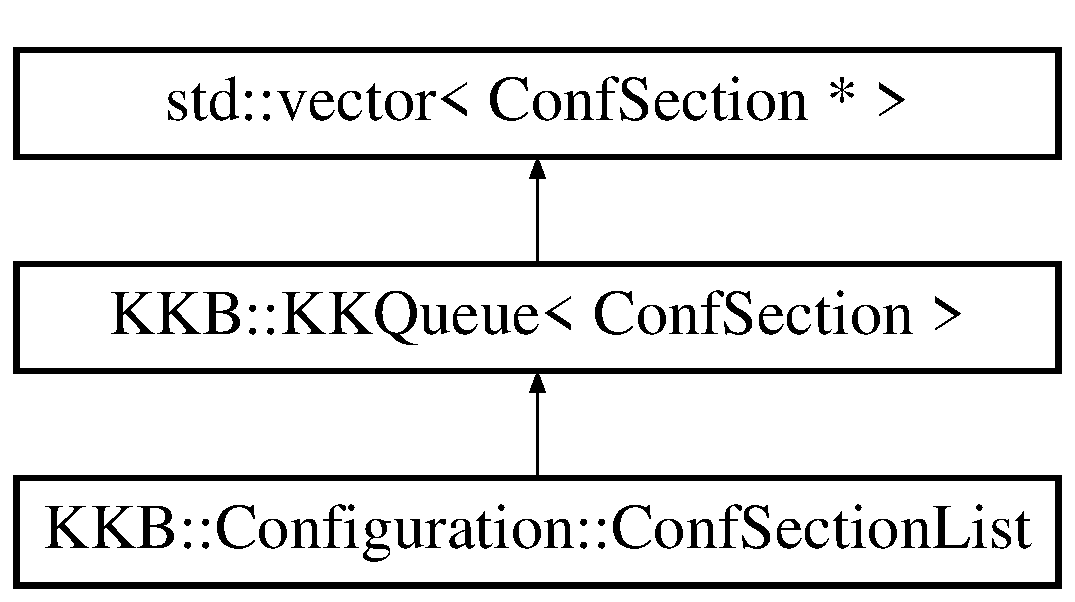
\includegraphics[height=3.000000cm]{class_k_k_b_1_1_configuration_1_1_conf_section_list}
\end{center}
\end{figure}
\subsection*{Public Member Functions}
\begin{DoxyCompactItemize}
\item 
\hyperlink{class_k_k_b_1_1_configuration_1_1_conf_section_list_afd97efa550cb4e9fbe987e2a43882e66}{Conf\+Section\+List} ()
\item 
void \hyperlink{class_k_k_b_1_1_configuration_1_1_conf_section_list_a4cb1a372299d3e5b6c306644bb465fd6}{Add\+Conf\+Section} (\hyperlink{class_k_k_b_1_1_configuration_1_1_conf_section}{Conf\+Section\+Ptr} section)
\item 
void \hyperlink{class_k_k_b_1_1_configuration_1_1_conf_section_list_af2883f2a6313bf9c2c90b2fd34fc3de9}{Add\+Conf\+Section} (const \hyperlink{class_k_k_b_1_1_k_k_str}{K\+K\+Str} \&\+\_\+name, \hyperlink{namespace_k_k_b_a8fa4952cc84fda1de4bec1fbdd8d5b1b}{kkint32} \+\_\+line\+Num)
\item 
\hyperlink{class_k_k_b_1_1_configuration_1_1_conf_section}{Conf\+Section\+Ptr} \hyperlink{class_k_k_b_1_1_configuration_1_1_conf_section_list_ae1932c42a5b475020b4f84e5f36fcba6}{Look\+Up} (const \hyperlink{class_k_k_b_1_1_k_k_str}{K\+K\+Str} \&\+\_\+name)
\item 
\hyperlink{namespace_k_k_b_a8fa4952cc84fda1de4bec1fbdd8d5b1b}{kkint32} \hyperlink{class_k_k_b_1_1_configuration_1_1_conf_section_list_aab5e7968237c965d19a3dc8feb280b79}{Memory\+Consumed\+Estimated} () const 
\end{DoxyCompactItemize}
\subsection*{Additional Inherited Members}


\subsection{Detailed Description}


Definition at line 234 of file Configuration.\+cpp.



\subsection{Constructor \& Destructor Documentation}
\index{K\+K\+B\+::\+Configuration\+::\+Conf\+Section\+List@{K\+K\+B\+::\+Configuration\+::\+Conf\+Section\+List}!Conf\+Section\+List@{Conf\+Section\+List}}
\index{Conf\+Section\+List@{Conf\+Section\+List}!K\+K\+B\+::\+Configuration\+::\+Conf\+Section\+List@{K\+K\+B\+::\+Configuration\+::\+Conf\+Section\+List}}
\subsubsection[{\texorpdfstring{Conf\+Section\+List()}{ConfSectionList()}}]{\setlength{\rightskip}{0pt plus 5cm}K\+K\+B\+::\+Configuration\+::\+Conf\+Section\+List\+::\+Conf\+Section\+List (
\begin{DoxyParamCaption}
{}
\end{DoxyParamCaption}
)\hspace{0.3cm}{\ttfamily [inline]}}\hypertarget{class_k_k_b_1_1_configuration_1_1_conf_section_list_afd97efa550cb4e9fbe987e2a43882e66}{}\label{class_k_k_b_1_1_configuration_1_1_conf_section_list_afd97efa550cb4e9fbe987e2a43882e66}


Definition at line 237 of file Configuration.\+cpp.



Referenced by K\+K\+B\+::\+Configuration\+::\+Configuration().


\begin{DoxyCode}
237 : \hyperlink{class_k_k_b_1_1_k_k_queue}{KKQueue<ConfSection>} (\textcolor{keyword}{true})  \{\}
\end{DoxyCode}


\subsection{Member Function Documentation}
\index{K\+K\+B\+::\+Configuration\+::\+Conf\+Section\+List@{K\+K\+B\+::\+Configuration\+::\+Conf\+Section\+List}!Add\+Conf\+Section@{Add\+Conf\+Section}}
\index{Add\+Conf\+Section@{Add\+Conf\+Section}!K\+K\+B\+::\+Configuration\+::\+Conf\+Section\+List@{K\+K\+B\+::\+Configuration\+::\+Conf\+Section\+List}}
\subsubsection[{\texorpdfstring{Add\+Conf\+Section(\+Conf\+Section\+Ptr section)}{AddConfSection(ConfSectionPtr section)}}]{\setlength{\rightskip}{0pt plus 5cm}void K\+K\+B\+::\+Configuration\+::\+Conf\+Section\+List\+::\+Add\+Conf\+Section (
\begin{DoxyParamCaption}
\item[{{\bf Conf\+Section\+Ptr}}]{section}
\end{DoxyParamCaption}
)\hspace{0.3cm}{\ttfamily [inline]}}\hypertarget{class_k_k_b_1_1_configuration_1_1_conf_section_list_a4cb1a372299d3e5b6c306644bb465fd6}{}\label{class_k_k_b_1_1_configuration_1_1_conf_section_list_a4cb1a372299d3e5b6c306644bb465fd6}


Definition at line 269 of file Configuration.\+cpp.



Referenced by K\+K\+B\+::\+Configuration\+::\+Configuration().


\begin{DoxyCode}
270     \{
271       \hyperlink{class_k_k_b_1_1_k_k_queue_aa9fba4632b54268bf71ecb42dee0b575}{PushOnBack} (section);
272     \}
\end{DoxyCode}
\index{K\+K\+B\+::\+Configuration\+::\+Conf\+Section\+List@{K\+K\+B\+::\+Configuration\+::\+Conf\+Section\+List}!Add\+Conf\+Section@{Add\+Conf\+Section}}
\index{Add\+Conf\+Section@{Add\+Conf\+Section}!K\+K\+B\+::\+Configuration\+::\+Conf\+Section\+List@{K\+K\+B\+::\+Configuration\+::\+Conf\+Section\+List}}
\subsubsection[{\texorpdfstring{Add\+Conf\+Section(const K\+K\+Str \&\+\_\+name, kkint32 \+\_\+line\+Num)}{AddConfSection(const KKStr &_name, kkint32 _lineNum)}}]{\setlength{\rightskip}{0pt plus 5cm}void K\+K\+B\+::\+Configuration\+::\+Conf\+Section\+List\+::\+Add\+Conf\+Section (
\begin{DoxyParamCaption}
\item[{const {\bf K\+K\+Str} \&}]{\+\_\+name, }
\item[{{\bf kkint32}}]{\+\_\+line\+Num}
\end{DoxyParamCaption}
)\hspace{0.3cm}{\ttfamily [inline]}}\hypertarget{class_k_k_b_1_1_configuration_1_1_conf_section_list_af2883f2a6313bf9c2c90b2fd34fc3de9}{}\label{class_k_k_b_1_1_configuration_1_1_conf_section_list_af2883f2a6313bf9c2c90b2fd34fc3de9}


Definition at line 275 of file Configuration.\+cpp.


\begin{DoxyCode}
278     \{
279       \hyperlink{class_k_k_b_1_1_k_k_queue_aa9fba4632b54268bf71ecb42dee0b575}{PushOnBack} (\textcolor{keyword}{new} ConfSection (\_name, \_lineNum));
280     \}
\end{DoxyCode}
\index{K\+K\+B\+::\+Configuration\+::\+Conf\+Section\+List@{K\+K\+B\+::\+Configuration\+::\+Conf\+Section\+List}!Look\+Up@{Look\+Up}}
\index{Look\+Up@{Look\+Up}!K\+K\+B\+::\+Configuration\+::\+Conf\+Section\+List@{K\+K\+B\+::\+Configuration\+::\+Conf\+Section\+List}}
\subsubsection[{\texorpdfstring{Look\+Up(const K\+K\+Str \&\+\_\+name)}{LookUp(const KKStr &_name)}}]{\setlength{\rightskip}{0pt plus 5cm}{\bf Conf\+Section\+Ptr} K\+K\+B\+::\+Configuration\+::\+Conf\+Section\+List\+::\+Look\+Up (
\begin{DoxyParamCaption}
\item[{const {\bf K\+K\+Str} \&}]{\+\_\+name}
\end{DoxyParamCaption}
)\hspace{0.3cm}{\ttfamily [inline]}}\hypertarget{class_k_k_b_1_1_configuration_1_1_conf_section_list_ae1932c42a5b475020b4f84e5f36fcba6}{}\label{class_k_k_b_1_1_configuration_1_1_conf_section_list_ae1932c42a5b475020b4f84e5f36fcba6}


Definition at line 250 of file Configuration.\+cpp.



References K\+K\+B\+::\+K\+K\+Str\+::\+Equal\+Ignore\+Case(), and K\+K\+B\+::\+Configuration\+::\+Conf\+Section\+::\+Name().



Referenced by K\+K\+B\+::\+Configuration\+::\+Get\+Setting(), K\+K\+B\+::\+Configuration\+::\+Num\+Of\+Settings(), K\+K\+B\+::\+Configuration\+::\+Section\+Defined(), and K\+K\+B\+::\+Configuration\+::\+Setting\+Name().


\begin{DoxyCode}
251     \{
252       ConfSectionPtr   tempSection = NULL;
253       ConfSectionPtr   section = NULL;
254       \hyperlink{class_k_k_b_1_1_k_k_queue_aeb057c9c010446f46f57c1e355f981f1}{ConfSectionList::const\_iterator}  idx;
255       \textcolor{keywordflow}{for}  (idx = begin ();  idx != end ();  ++idx)
256       \{
257         tempSection = *idx;
258         \textcolor{keywordflow}{if}  (\_name.\hyperlink{class_k_k_b_1_1_k_k_str_a562f9696417c53f66bc4088eac072ab5}{EqualIgnoreCase} (tempSection->Name ()))
259         \{
260           section = tempSection;
261           \textcolor{keywordflow}{break};
262         \}
263       \}
264 
265       \textcolor{keywordflow}{return}  section;
266     \}  \textcolor{comment}{/* LookUp */}
\end{DoxyCode}
\index{K\+K\+B\+::\+Configuration\+::\+Conf\+Section\+List@{K\+K\+B\+::\+Configuration\+::\+Conf\+Section\+List}!Memory\+Consumed\+Estimated@{Memory\+Consumed\+Estimated}}
\index{Memory\+Consumed\+Estimated@{Memory\+Consumed\+Estimated}!K\+K\+B\+::\+Configuration\+::\+Conf\+Section\+List@{K\+K\+B\+::\+Configuration\+::\+Conf\+Section\+List}}
\subsubsection[{\texorpdfstring{Memory\+Consumed\+Estimated() const }{MemoryConsumedEstimated() const }}]{\setlength{\rightskip}{0pt plus 5cm}{\bf kkint32} K\+K\+B\+::\+Configuration\+::\+Conf\+Section\+List\+::\+Memory\+Consumed\+Estimated (
\begin{DoxyParamCaption}
{}
\end{DoxyParamCaption}
) const\hspace{0.3cm}{\ttfamily [inline]}}\hypertarget{class_k_k_b_1_1_configuration_1_1_conf_section_list_aab5e7968237c965d19a3dc8feb280b79}{}\label{class_k_k_b_1_1_configuration_1_1_conf_section_list_aab5e7968237c965d19a3dc8feb280b79}


Definition at line 240 of file Configuration.\+cpp.



Referenced by K\+K\+B\+::\+Configuration\+::\+Memory\+Consumed\+Estimated().


\begin{DoxyCode}
241     \{
242       \hyperlink{namespace_k_k_b_a8fa4952cc84fda1de4bec1fbdd8d5b1b}{kkint32}  memoryConsumedEstimated = \textcolor{keyword}{sizeof} (\hyperlink{class_k_k_b_1_1_configuration_1_1_conf_section_list_afd97efa550cb4e9fbe987e2a43882e66}{ConfSectionList});
243       \hyperlink{class_k_k_b_1_1_k_k_queue_aeb057c9c010446f46f57c1e355f981f1}{ConfSectionList::const\_iterator}  idx;
244       \textcolor{keywordflow}{for}  (idx = begin ();  idx != end ();  ++idx)
245         memoryConsumedEstimated += (*idx)->MemoryConsumedEstimated ();
246       \textcolor{keywordflow}{return}  memoryConsumedEstimated;
247     \}
\end{DoxyCode}


The documentation for this class was generated from the following file\+:\begin{DoxyCompactItemize}
\item 
C\+:/\+Users/\+Kurt/\+Git\+Hub/\+K\+Square\+Libraries/\+K\+K\+Base/\hyperlink{_configuration_8cpp}{Configuration.\+cpp}\end{DoxyCompactItemize}

\hypertarget{class_k_k_b_1_1_configuration_1_1_setting}{}\section{K\+KB\+:\+:Configuration\+:\+:Setting Class Reference}
\label{class_k_k_b_1_1_configuration_1_1_setting}\index{K\+K\+B\+::\+Configuration\+::\+Setting@{K\+K\+B\+::\+Configuration\+::\+Setting}}
\subsection*{Public Member Functions}
\begin{DoxyCompactItemize}
\item 
\hyperlink{class_k_k_b_1_1_configuration_1_1_setting_a5b462de6eb944280e0bb634576269b86}{Setting} (const \hyperlink{class_k_k_b_1_1_k_k_str}{K\+K\+Str} \&\+\_\+name, const \hyperlink{class_k_k_b_1_1_k_k_str}{K\+K\+Str} \&\+\_\+value, \hyperlink{namespace_k_k_b_a8fa4952cc84fda1de4bec1fbdd8d5b1b}{kkint32} \+\_\+line\+Num)
\item 
\hyperlink{class_k_k_b_1_1_configuration_1_1_setting_a8f27de1b2ea6928fef90f1d90ffeeaa6}{Setting} (const \hyperlink{class_k_k_b_1_1_configuration_1_1_setting}{Configuration\+::\+Setting} \&s)
\item 
\hyperlink{namespace_k_k_b_a8fa4952cc84fda1de4bec1fbdd8d5b1b}{kkint32} \hyperlink{class_k_k_b_1_1_configuration_1_1_setting_a63f658602b0147eb3de7cfed15be02d6}{Line\+Num} () const 
\item 
\hyperlink{namespace_k_k_b_a8fa4952cc84fda1de4bec1fbdd8d5b1b}{kkint32} \hyperlink{class_k_k_b_1_1_configuration_1_1_setting_a822aa006918b3dfc06abcbadf6717479}{Memory\+Consumed\+Estimated} () const 
\item 
\hyperlink{namespace_k_k_b_a46f665ec17615c856eff3d21f78bed5c}{K\+K\+Str\+Const\+Ptr} \hyperlink{class_k_k_b_1_1_configuration_1_1_setting_a36eb5ba502d27443845f834157aefe97}{Name} () const 
\item 
\hyperlink{namespace_k_k_b_a46f665ec17615c856eff3d21f78bed5c}{K\+K\+Str\+Const\+Ptr} \hyperlink{class_k_k_b_1_1_configuration_1_1_setting_ac6ad492e5aff688f57a9a2de01db963d}{Value} () const 
\end{DoxyCompactItemize}


\subsection{Detailed Description}


Definition at line 31 of file Configuration.\+cpp.



\subsection{Constructor \& Destructor Documentation}
\index{K\+K\+B\+::\+Configuration\+::\+Setting@{K\+K\+B\+::\+Configuration\+::\+Setting}!Setting@{Setting}}
\index{Setting@{Setting}!K\+K\+B\+::\+Configuration\+::\+Setting@{K\+K\+B\+::\+Configuration\+::\+Setting}}
\subsubsection[{\texorpdfstring{Setting(const K\+K\+Str \&\+\_\+name, const K\+K\+Str \&\+\_\+value, kkint32 \+\_\+line\+Num)}{Setting(const KKStr &_name, const KKStr &_value, kkint32 _lineNum)}}]{\setlength{\rightskip}{0pt plus 5cm}K\+K\+B\+::\+Configuration\+::\+Setting\+::\+Setting (
\begin{DoxyParamCaption}
\item[{const {\bf K\+K\+Str} \&}]{\+\_\+name, }
\item[{const {\bf K\+K\+Str} \&}]{\+\_\+value, }
\item[{{\bf kkint32}}]{\+\_\+line\+Num}
\end{DoxyParamCaption}
)\hspace{0.3cm}{\ttfamily [inline]}}\hypertarget{class_k_k_b_1_1_configuration_1_1_setting_a5b462de6eb944280e0bb634576269b86}{}\label{class_k_k_b_1_1_configuration_1_1_setting_a5b462de6eb944280e0bb634576269b86}


Definition at line 34 of file Configuration.\+cpp.



References K\+K\+B\+::\+K\+K\+Str\+::\+K\+K\+Str().


\begin{DoxyCode}
37              :
38       lineNum (\_lineNum),
39       name    (\_name),
40       value   (\_value)
41     \{\}
\end{DoxyCode}
\index{K\+K\+B\+::\+Configuration\+::\+Setting@{K\+K\+B\+::\+Configuration\+::\+Setting}!Setting@{Setting}}
\index{Setting@{Setting}!K\+K\+B\+::\+Configuration\+::\+Setting@{K\+K\+B\+::\+Configuration\+::\+Setting}}
\subsubsection[{\texorpdfstring{Setting(const Configuration\+::\+Setting \&s)}{Setting(const Configuration::Setting &s)}}]{\setlength{\rightskip}{0pt plus 5cm}K\+K\+B\+::\+Configuration\+::\+Setting\+::\+Setting (
\begin{DoxyParamCaption}
\item[{const {\bf Configuration\+::\+Setting} \&}]{s}
\end{DoxyParamCaption}
)\hspace{0.3cm}{\ttfamily [inline]}}\hypertarget{class_k_k_b_1_1_configuration_1_1_setting_a8f27de1b2ea6928fef90f1d90ffeeaa6}{}\label{class_k_k_b_1_1_configuration_1_1_setting_a8f27de1b2ea6928fef90f1d90ffeeaa6}


Definition at line 43 of file Configuration.\+cpp.



References K\+K\+B\+::\+K\+K\+Str\+::\+K\+K\+Str().


\begin{DoxyCode}
43                                             :
44         lineNum (s.lineNum),
45         name    (s.name),
46         value   (s.value)
47     \{\}
\end{DoxyCode}


\subsection{Member Function Documentation}
\index{K\+K\+B\+::\+Configuration\+::\+Setting@{K\+K\+B\+::\+Configuration\+::\+Setting}!Line\+Num@{Line\+Num}}
\index{Line\+Num@{Line\+Num}!K\+K\+B\+::\+Configuration\+::\+Setting@{K\+K\+B\+::\+Configuration\+::\+Setting}}
\subsubsection[{\texorpdfstring{Line\+Num() const }{LineNum() const }}]{\setlength{\rightskip}{0pt plus 5cm}{\bf kkint32} K\+K\+B\+::\+Configuration\+::\+Setting\+::\+Line\+Num (
\begin{DoxyParamCaption}
{}
\end{DoxyParamCaption}
) const\hspace{0.3cm}{\ttfamily [inline]}}\hypertarget{class_k_k_b_1_1_configuration_1_1_setting_a63f658602b0147eb3de7cfed15be02d6}{}\label{class_k_k_b_1_1_configuration_1_1_setting_a63f658602b0147eb3de7cfed15be02d6}


Definition at line 49 of file Configuration.\+cpp.



Referenced by K\+K\+B\+::\+Configuration\+::\+Conf\+Section\+::\+Get\+Settings(), K\+K\+B\+::\+Configuration\+::\+Setting\+List\+::\+Look\+Up\+Line\+Num(), and K\+K\+B\+::\+Configuration\+::\+Conf\+Section\+::\+Look\+Up\+Value().


\begin{DoxyCode}
49 \{\textcolor{keywordflow}{return}  lineNum;\}
\end{DoxyCode}
\index{K\+K\+B\+::\+Configuration\+::\+Setting@{K\+K\+B\+::\+Configuration\+::\+Setting}!Memory\+Consumed\+Estimated@{Memory\+Consumed\+Estimated}}
\index{Memory\+Consumed\+Estimated@{Memory\+Consumed\+Estimated}!K\+K\+B\+::\+Configuration\+::\+Setting@{K\+K\+B\+::\+Configuration\+::\+Setting}}
\subsubsection[{\texorpdfstring{Memory\+Consumed\+Estimated() const }{MemoryConsumedEstimated() const }}]{\setlength{\rightskip}{0pt plus 5cm}{\bf kkint32} K\+K\+B\+::\+Configuration\+::\+Setting\+::\+Memory\+Consumed\+Estimated (
\begin{DoxyParamCaption}
{}
\end{DoxyParamCaption}
) const\hspace{0.3cm}{\ttfamily [inline]}}\hypertarget{class_k_k_b_1_1_configuration_1_1_setting_a822aa006918b3dfc06abcbadf6717479}{}\label{class_k_k_b_1_1_configuration_1_1_setting_a822aa006918b3dfc06abcbadf6717479}


Definition at line 53 of file Configuration.\+cpp.



References K\+K\+B\+::\+K\+K\+Str\+::\+Memory\+Consumed\+Estimated().


\begin{DoxyCode}
53 \{\textcolor{keywordflow}{return}  \textcolor{keyword}{sizeof} (\hyperlink{class_k_k_b_1_1_configuration_1_1_setting_a5b462de6eb944280e0bb634576269b86}{Setting}) + name.\hyperlink{class_k_k_b_1_1_k_k_str_afc335bf98a8d4a77dc34215e72068719}{MemoryConsumedEstimated} () + value.
      \hyperlink{class_k_k_b_1_1_k_k_str_afc335bf98a8d4a77dc34215e72068719}{MemoryConsumedEstimated} ();\}
\end{DoxyCode}
\index{K\+K\+B\+::\+Configuration\+::\+Setting@{K\+K\+B\+::\+Configuration\+::\+Setting}!Name@{Name}}
\index{Name@{Name}!K\+K\+B\+::\+Configuration\+::\+Setting@{K\+K\+B\+::\+Configuration\+::\+Setting}}
\subsubsection[{\texorpdfstring{Name() const }{Name() const }}]{\setlength{\rightskip}{0pt plus 5cm}{\bf K\+K\+Str\+Const\+Ptr} K\+K\+B\+::\+Configuration\+::\+Setting\+::\+Name (
\begin{DoxyParamCaption}
{}
\end{DoxyParamCaption}
) const\hspace{0.3cm}{\ttfamily [inline]}}\hypertarget{class_k_k_b_1_1_configuration_1_1_setting_a36eb5ba502d27443845f834157aefe97}{}\label{class_k_k_b_1_1_configuration_1_1_setting_a36eb5ba502d27443845f834157aefe97}


Definition at line 50 of file Configuration.\+cpp.



Referenced by K\+K\+B\+::\+Configuration\+::\+Conf\+Section\+::\+Get\+Settings(), K\+K\+B\+::\+Configuration\+::\+Setting\+List\+::\+Look\+Up(), and K\+K\+B\+::\+Configuration\+::\+Setting\+List\+::\+Look\+Up\+Line\+Num().


\begin{DoxyCode}
50 \{\textcolor{keywordflow}{return}  &name;\}
\end{DoxyCode}
\index{K\+K\+B\+::\+Configuration\+::\+Setting@{K\+K\+B\+::\+Configuration\+::\+Setting}!Value@{Value}}
\index{Value@{Value}!K\+K\+B\+::\+Configuration\+::\+Setting@{K\+K\+B\+::\+Configuration\+::\+Setting}}
\subsubsection[{\texorpdfstring{Value() const }{Value() const }}]{\setlength{\rightskip}{0pt plus 5cm}{\bf K\+K\+Str\+Const\+Ptr} K\+K\+B\+::\+Configuration\+::\+Setting\+::\+Value (
\begin{DoxyParamCaption}
{}
\end{DoxyParamCaption}
) const\hspace{0.3cm}{\ttfamily [inline]}}\hypertarget{class_k_k_b_1_1_configuration_1_1_setting_ac6ad492e5aff688f57a9a2de01db963d}{}\label{class_k_k_b_1_1_configuration_1_1_setting_ac6ad492e5aff688f57a9a2de01db963d}


Definition at line 51 of file Configuration.\+cpp.



Referenced by K\+K\+B\+::\+Configuration\+::\+Conf\+Section\+::\+Get\+Settings(), and K\+K\+B\+::\+Configuration\+::\+Conf\+Section\+::\+Look\+Up\+Value().


\begin{DoxyCode}
51 \{\textcolor{keywordflow}{return}  &value;\}
\end{DoxyCode}


The documentation for this class was generated from the following file\+:\begin{DoxyCompactItemize}
\item 
C\+:/\+Users/\+Kurt/\+Git\+Hub/\+K\+Square\+Libraries/\+K\+K\+Base/\hyperlink{_configuration_8cpp}{Configuration.\+cpp}\end{DoxyCompactItemize}

\hypertarget{class_k_k_b_1_1_configuration_1_1_setting_list}{}\section{K\+KB\+:\+:Configuration\+:\+:Setting\+List Class Reference}
\label{class_k_k_b_1_1_configuration_1_1_setting_list}\index{K\+K\+B\+::\+Configuration\+::\+Setting\+List@{K\+K\+B\+::\+Configuration\+::\+Setting\+List}}
Inheritance diagram for K\+KB\+:\+:Configuration\+:\+:Setting\+List\+:\begin{figure}[H]
\begin{center}
\leavevmode
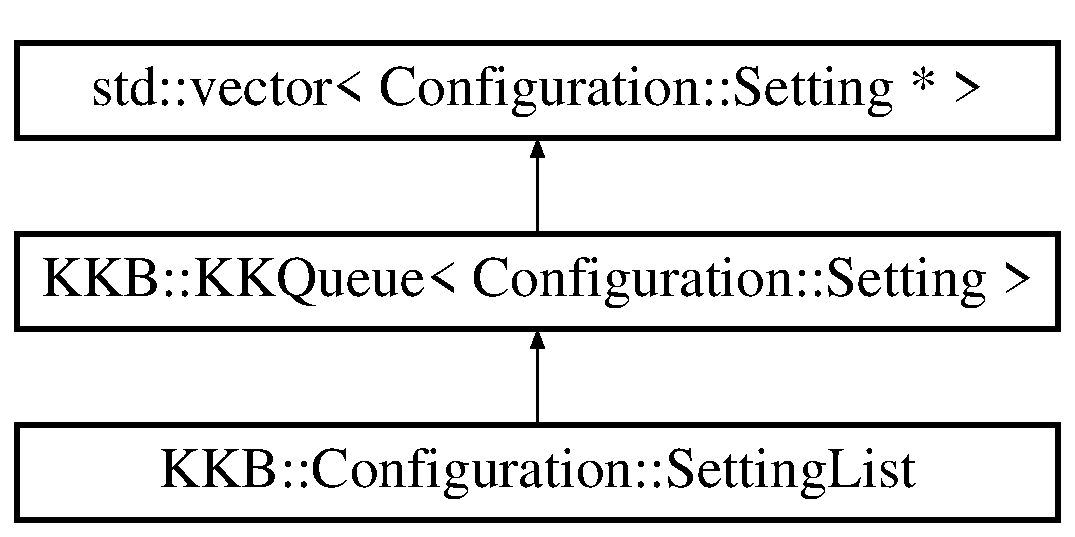
\includegraphics[height=3.000000cm]{class_k_k_b_1_1_configuration_1_1_setting_list}
\end{center}
\end{figure}
\subsection*{Public Member Functions}
\begin{DoxyCompactItemize}
\item 
\hyperlink{class_k_k_b_1_1_configuration_1_1_setting_list_a1e4d4fd83fe6052a545b73d0fe183f84}{Setting\+List} ()
\item 
\hyperlink{class_k_k_b_1_1_configuration_1_1_setting_list_a002b998d758466c4ad5a411dafdb259d}{Setting\+List} (const \hyperlink{class_k_k_b_1_1_configuration_1_1_setting_list}{Setting\+List} \&sl)
\item 
void \hyperlink{class_k_k_b_1_1_configuration_1_1_setting_list_a64c84ce1202ea71852380059c62ea7e0}{Add\+Setting} (\hyperlink{class_k_k_b_1_1_configuration_1_1_setting}{Setting\+Ptr} setting)
\item 
void \hyperlink{class_k_k_b_1_1_configuration_1_1_setting_list_a38f52dd5637e88cb3f56369d0459eba6}{Add\+Setting} (const \hyperlink{class_k_k_b_1_1_k_k_str}{K\+K\+Str} \&\+\_\+name, const \hyperlink{class_k_k_b_1_1_k_k_str}{K\+K\+Str} \&\+\_\+value, \hyperlink{namespace_k_k_b_a8fa4952cc84fda1de4bec1fbdd8d5b1b}{kkint32} \+\_\+line\+Num)
\item 
\hyperlink{class_k_k_b_1_1_configuration_1_1_setting}{Setting\+Ptr} \hyperlink{class_k_k_b_1_1_configuration_1_1_setting_list_aa0955610ab4272330018b07a3cfef2eb}{Look\+Up} (const \hyperlink{class_k_k_b_1_1_k_k_str}{K\+K\+Str} \&name)
\item 
\hyperlink{namespace_k_k_b_a8fa4952cc84fda1de4bec1fbdd8d5b1b}{kkint32} \hyperlink{class_k_k_b_1_1_configuration_1_1_setting_list_af00887798da2cedefc20b9a4b3bd4623}{Look\+Up\+Line\+Num} (const \hyperlink{class_k_k_b_1_1_k_k_str}{K\+K\+Str} \&name) const 
\item 
\hyperlink{namespace_k_k_b_a8fa4952cc84fda1de4bec1fbdd8d5b1b}{kkint32} \hyperlink{class_k_k_b_1_1_configuration_1_1_setting_list_a5ba2ef9e87c503455d8d3b259289129b}{Memory\+Consumed\+Estimated} () const 
\end{DoxyCompactItemize}
\subsection*{Additional Inherited Members}


\subsection{Detailed Description}


Definition at line 63 of file Configuration.\+cpp.



\subsection{Constructor \& Destructor Documentation}
\index{K\+K\+B\+::\+Configuration\+::\+Setting\+List@{K\+K\+B\+::\+Configuration\+::\+Setting\+List}!Setting\+List@{Setting\+List}}
\index{Setting\+List@{Setting\+List}!K\+K\+B\+::\+Configuration\+::\+Setting\+List@{K\+K\+B\+::\+Configuration\+::\+Setting\+List}}
\subsubsection[{\texorpdfstring{Setting\+List()}{SettingList()}}]{\setlength{\rightskip}{0pt plus 5cm}K\+K\+B\+::\+Configuration\+::\+Setting\+List\+::\+Setting\+List (
\begin{DoxyParamCaption}
{}
\end{DoxyParamCaption}
)\hspace{0.3cm}{\ttfamily [inline]}}\hypertarget{class_k_k_b_1_1_configuration_1_1_setting_list_a1e4d4fd83fe6052a545b73d0fe183f84}{}\label{class_k_k_b_1_1_configuration_1_1_setting_list_a1e4d4fd83fe6052a545b73d0fe183f84}


Definition at line 66 of file Configuration.\+cpp.


\begin{DoxyCode}
66 : \hyperlink{class_k_k_b_1_1_k_k_queue}{KKQueue<Setting>} (\textcolor{keyword}{true})  \{\}
\end{DoxyCode}
\index{K\+K\+B\+::\+Configuration\+::\+Setting\+List@{K\+K\+B\+::\+Configuration\+::\+Setting\+List}!Setting\+List@{Setting\+List}}
\index{Setting\+List@{Setting\+List}!K\+K\+B\+::\+Configuration\+::\+Setting\+List@{K\+K\+B\+::\+Configuration\+::\+Setting\+List}}
\subsubsection[{\texorpdfstring{Setting\+List(const Setting\+List \&sl)}{SettingList(const SettingList &sl)}}]{\setlength{\rightskip}{0pt plus 5cm}K\+K\+B\+::\+Configuration\+::\+Setting\+List\+::\+Setting\+List (
\begin{DoxyParamCaption}
\item[{const {\bf Setting\+List} \&}]{sl}
\end{DoxyParamCaption}
)\hspace{0.3cm}{\ttfamily [inline]}}\hypertarget{class_k_k_b_1_1_configuration_1_1_setting_list_a002b998d758466c4ad5a411dafdb259d}{}\label{class_k_k_b_1_1_configuration_1_1_setting_list_a002b998d758466c4ad5a411dafdb259d}


Definition at line 68 of file Configuration.\+cpp.



References Setting\+List().



Referenced by Setting\+List().


\begin{DoxyCode}
68                                          :
69         \hyperlink{class_k_k_b_1_1_k_k_queue}{KKQueue<Setting>} (\textcolor{keyword}{true})
70     \{
71       \hyperlink{namespace_k_k_b_af8d832f05c54994a1cce25bd5743e19a}{kkuint32} x;
72       \textcolor{keywordflow}{for}  (x = 0;  x < sl.size ();  x++)
73       \{
74         SettingPtr  setting = sl.\hyperlink{class_k_k_b_1_1_k_k_queue_acce2bdd8b3327e38266cf198382cd852}{IdxToPtr} (x);
75         \hyperlink{class_k_k_b_1_1_k_k_queue_aa9fba4632b54268bf71ecb42dee0b575}{PushOnBack} (\textcolor{keyword}{new} \hyperlink{class_k_k_b_1_1_configuration_1_1_setting}{Configuration::Setting} (*setting));
76       \}
77     \}
\end{DoxyCode}


\subsection{Member Function Documentation}
\index{K\+K\+B\+::\+Configuration\+::\+Setting\+List@{K\+K\+B\+::\+Configuration\+::\+Setting\+List}!Add\+Setting@{Add\+Setting}}
\index{Add\+Setting@{Add\+Setting}!K\+K\+B\+::\+Configuration\+::\+Setting\+List@{K\+K\+B\+::\+Configuration\+::\+Setting\+List}}
\subsubsection[{\texorpdfstring{Add\+Setting(\+Setting\+Ptr setting)}{AddSetting(SettingPtr setting)}}]{\setlength{\rightskip}{0pt plus 5cm}void K\+K\+B\+::\+Configuration\+::\+Setting\+List\+::\+Add\+Setting (
\begin{DoxyParamCaption}
\item[{{\bf Setting\+Ptr}}]{setting}
\end{DoxyParamCaption}
)\hspace{0.3cm}{\ttfamily [inline]}}\hypertarget{class_k_k_b_1_1_configuration_1_1_setting_list_a64c84ce1202ea71852380059c62ea7e0}{}\label{class_k_k_b_1_1_configuration_1_1_setting_list_a64c84ce1202ea71852380059c62ea7e0}


Definition at line 117 of file Configuration.\+cpp.


\begin{DoxyCode}
118     \{
119       \hyperlink{class_k_k_b_1_1_k_k_queue_aa9fba4632b54268bf71ecb42dee0b575}{PushOnBack} (setting);
120     \}
\end{DoxyCode}
\index{K\+K\+B\+::\+Configuration\+::\+Setting\+List@{K\+K\+B\+::\+Configuration\+::\+Setting\+List}!Add\+Setting@{Add\+Setting}}
\index{Add\+Setting@{Add\+Setting}!K\+K\+B\+::\+Configuration\+::\+Setting\+List@{K\+K\+B\+::\+Configuration\+::\+Setting\+List}}
\subsubsection[{\texorpdfstring{Add\+Setting(const K\+K\+Str \&\+\_\+name, const K\+K\+Str \&\+\_\+value, kkint32 \+\_\+line\+Num)}{AddSetting(const KKStr &_name, const KKStr &_value, kkint32 _lineNum)}}]{\setlength{\rightskip}{0pt plus 5cm}void K\+K\+B\+::\+Configuration\+::\+Setting\+List\+::\+Add\+Setting (
\begin{DoxyParamCaption}
\item[{const {\bf K\+K\+Str} \&}]{\+\_\+name, }
\item[{const {\bf K\+K\+Str} \&}]{\+\_\+value, }
\item[{{\bf kkint32}}]{\+\_\+line\+Num}
\end{DoxyParamCaption}
)\hspace{0.3cm}{\ttfamily [inline]}}\hypertarget{class_k_k_b_1_1_configuration_1_1_setting_list_a38f52dd5637e88cb3f56369d0459eba6}{}\label{class_k_k_b_1_1_configuration_1_1_setting_list_a38f52dd5637e88cb3f56369d0459eba6}


Definition at line 123 of file Configuration.\+cpp.


\begin{DoxyCode}
127     \{
128       \hyperlink{class_k_k_b_1_1_k_k_queue_aa9fba4632b54268bf71ecb42dee0b575}{PushOnBack} (\textcolor{keyword}{new} Setting (\_name, \_value, \_lineNum));
129     \}
\end{DoxyCode}
\index{K\+K\+B\+::\+Configuration\+::\+Setting\+List@{K\+K\+B\+::\+Configuration\+::\+Setting\+List}!Look\+Up@{Look\+Up}}
\index{Look\+Up@{Look\+Up}!K\+K\+B\+::\+Configuration\+::\+Setting\+List@{K\+K\+B\+::\+Configuration\+::\+Setting\+List}}
\subsubsection[{\texorpdfstring{Look\+Up(const K\+K\+Str \&name)}{LookUp(const KKStr &name)}}]{\setlength{\rightskip}{0pt plus 5cm}{\bf Setting\+Ptr} K\+K\+B\+::\+Configuration\+::\+Setting\+List\+::\+Look\+Up (
\begin{DoxyParamCaption}
\item[{const {\bf K\+K\+Str} \&}]{name}
\end{DoxyParamCaption}
)\hspace{0.3cm}{\ttfamily [inline]}}\hypertarget{class_k_k_b_1_1_configuration_1_1_setting_list_aa0955610ab4272330018b07a3cfef2eb}{}\label{class_k_k_b_1_1_configuration_1_1_setting_list_aa0955610ab4272330018b07a3cfef2eb}


Definition at line 89 of file Configuration.\+cpp.



References K\+K\+B\+::\+K\+K\+Str\+::\+Equal\+Ignore\+Case(), and K\+K\+B\+::\+Configuration\+::\+Setting\+::\+Name().


\begin{DoxyCode}
90     \{
91       \hyperlink{namespace_k_k_b_a8fa4952cc84fda1de4bec1fbdd8d5b1b}{kkint32}  idx;
92       \hyperlink{namespace_k_k_b_a8fa4952cc84fda1de4bec1fbdd8d5b1b}{kkint32}  qSize = \hyperlink{class_k_k_b_1_1_k_k_queue_a1dab601f75ee6a65d97f02bddf71c40d}{QueueSize} ();
93       \textcolor{keywordflow}{for}  (idx = 0;  idx < qSize;  idx++)
94       \{
95         SettingPtr setting = \hyperlink{class_k_k_b_1_1_k_k_queue_acce2bdd8b3327e38266cf198382cd852}{IdxToPtr} (idx);
96         \textcolor{keywordflow}{if}  (name.\hyperlink{class_k_k_b_1_1_k_k_str_a562f9696417c53f66bc4088eac072ab5}{EqualIgnoreCase} (setting->Name ()))
97           \textcolor{keywordflow}{return} setting;
98       \}
99       \textcolor{keywordflow}{return}  NULL;
100     \}  \textcolor{comment}{/* LookUp */}
\end{DoxyCode}
\index{K\+K\+B\+::\+Configuration\+::\+Setting\+List@{K\+K\+B\+::\+Configuration\+::\+Setting\+List}!Look\+Up\+Line\+Num@{Look\+Up\+Line\+Num}}
\index{Look\+Up\+Line\+Num@{Look\+Up\+Line\+Num}!K\+K\+B\+::\+Configuration\+::\+Setting\+List@{K\+K\+B\+::\+Configuration\+::\+Setting\+List}}
\subsubsection[{\texorpdfstring{Look\+Up\+Line\+Num(const K\+K\+Str \&name) const }{LookUpLineNum(const KKStr &name) const }}]{\setlength{\rightskip}{0pt plus 5cm}{\bf kkint32} K\+K\+B\+::\+Configuration\+::\+Setting\+List\+::\+Look\+Up\+Line\+Num (
\begin{DoxyParamCaption}
\item[{const {\bf K\+K\+Str} \&}]{name}
\end{DoxyParamCaption}
) const\hspace{0.3cm}{\ttfamily [inline]}}\hypertarget{class_k_k_b_1_1_configuration_1_1_setting_list_af00887798da2cedefc20b9a4b3bd4623}{}\label{class_k_k_b_1_1_configuration_1_1_setting_list_af00887798da2cedefc20b9a4b3bd4623}


Definition at line 104 of file Configuration.\+cpp.



References K\+K\+B\+::\+K\+K\+Str\+::\+Equal\+Ignore\+Case(), K\+K\+B\+::\+Configuration\+::\+Setting\+::\+Line\+Num(), and K\+K\+B\+::\+Configuration\+::\+Setting\+::\+Name().


\begin{DoxyCode}
105     \{
106       \hyperlink{class_k_k_b_1_1_k_k_queue_aeb057c9c010446f46f57c1e355f981f1}{const\_iterator}  idx;
107       \textcolor{keywordflow}{for}  (idx = begin ();  idx != end ();  idx++)
108       \{
109         SettingPtr s = *idx;
110         \textcolor{keywordflow}{if}  (s->Name ()->EqualIgnoreCase (name))
111           \textcolor{keywordflow}{return} s->LineNum ();
112       \}
113       \textcolor{keywordflow}{return} -1;
114     \}  \textcolor{comment}{/* LookUpLineNum */}
\end{DoxyCode}
\index{K\+K\+B\+::\+Configuration\+::\+Setting\+List@{K\+K\+B\+::\+Configuration\+::\+Setting\+List}!Memory\+Consumed\+Estimated@{Memory\+Consumed\+Estimated}}
\index{Memory\+Consumed\+Estimated@{Memory\+Consumed\+Estimated}!K\+K\+B\+::\+Configuration\+::\+Setting\+List@{K\+K\+B\+::\+Configuration\+::\+Setting\+List}}
\subsubsection[{\texorpdfstring{Memory\+Consumed\+Estimated() const }{MemoryConsumedEstimated() const }}]{\setlength{\rightskip}{0pt plus 5cm}{\bf kkint32} K\+K\+B\+::\+Configuration\+::\+Setting\+List\+::\+Memory\+Consumed\+Estimated (
\begin{DoxyParamCaption}
{}
\end{DoxyParamCaption}
) const\hspace{0.3cm}{\ttfamily [inline]}}\hypertarget{class_k_k_b_1_1_configuration_1_1_setting_list_a5ba2ef9e87c503455d8d3b259289129b}{}\label{class_k_k_b_1_1_configuration_1_1_setting_list_a5ba2ef9e87c503455d8d3b259289129b}


Definition at line 79 of file Configuration.\+cpp.


\begin{DoxyCode}
80     \{
81       \hyperlink{namespace_k_k_b_a8fa4952cc84fda1de4bec1fbdd8d5b1b}{kkint32}  memoryConsumedEstimated = \textcolor{keyword}{sizeof} (\hyperlink{class_k_k_b_1_1_configuration_1_1_setting_list_a1e4d4fd83fe6052a545b73d0fe183f84}{SettingList});
82       \hyperlink{class_k_k_b_1_1_k_k_queue_aeb057c9c010446f46f57c1e355f981f1}{SettingList::const\_iterator}  idx;
83       \textcolor{keywordflow}{for}  (idx = begin ();  idx != end ();  ++idx)
84         memoryConsumedEstimated += (*idx)->MemoryConsumedEstimated ();
85       \textcolor{keywordflow}{return}  memoryConsumedEstimated;
86     \}
\end{DoxyCode}


The documentation for this class was generated from the following file\+:\begin{DoxyCompactItemize}
\item 
C\+:/\+Users/\+Kurt/\+Git\+Hub/\+K\+Square\+Libraries/\+K\+K\+Base/\hyperlink{_configuration_8cpp}{Configuration.\+cpp}\end{DoxyCompactItemize}

\hypertarget{class_k_k_b_1_1_contour_follower}{}\section{K\+KB\+:\+:Contour\+Follower Class Reference}
\label{class_k_k_b_1_1_contour_follower}\index{K\+K\+B\+::\+Contour\+Follower@{K\+K\+B\+::\+Contour\+Follower}}


{\ttfamily \#include $<$Contour\+Follower.\+h$>$}

\subsection*{Public Member Functions}
\begin{DoxyCompactItemize}
\item 
\hyperlink{class_k_k_b_1_1_contour_follower_ad448455edc54f2bcb783cd16495ca9ba}{Contour\+Follower} (\hyperlink{class_k_k_b_1_1_raster}{Raster} \&\+\_\+raster, \hyperlink{class_k_k_b_1_1_run_log}{Run\+Log} \&\+\_\+log)
\item 
\hyperlink{namespace_k_k_b_a8fa4952cc84fda1de4bec1fbdd8d5b1b}{kkint32} \hyperlink{class_k_k_b_1_1_contour_follower_a2ec611c3cee8c1a1ba8482f26130c254}{Create\+Fourier\+Descriptor\+By\+Sampling} (\hyperlink{namespace_k_k_b_a8fa4952cc84fda1de4bec1fbdd8d5b1b}{kkint32} num\+Of\+Buckets, float $\ast$countour\+Freq, bool \&successful)
\item 
std\+::vector$<$ \hyperlink{namespace_k_k_b_a307e28915a31eb2034af6cb1d0d5fb88}{Complex\+Double} $>$ \hyperlink{class_k_k_b_1_1_contour_follower_a2d374e30200b7452cb0fc4eff96e0d51}{Create\+Fourier\+From\+Point\+List} (const \hyperlink{class_k_k_b_1_1_point_list}{Point\+List} \&points)
\item 
\hyperlink{namespace_k_k_b_ad6b8056511ec9a218dd5ef30b57d1415}{Point\+List\+Ptr} \hyperlink{class_k_k_b_1_1_contour_follower_a777f2444405ce218e05097c044488f02}{Create\+Point\+List\+From\+Fourier} (std\+::vector$<$ \hyperlink{namespace_k_k_b_a307e28915a31eb2034af6cb1d0d5fb88}{Complex\+Double} $>$ fourier, \hyperlink{class_k_k_b_1_1_point_list}{Point\+List} \&orig\+Point\+List)
\item 
\hyperlink{namespace_k_k_b_a8fa4952cc84fda1de4bec1fbdd8d5b1b}{kkint32} \hyperlink{class_k_k_b_1_1_contour_follower_aff3d61b95ed022794fd58f8be5032096}{Follow\+Contour} (float $\ast$countour\+Freq, float fourier\+Descriptors\mbox{[}15\mbox{]}, \hyperlink{namespace_k_k_b_a8fa4952cc84fda1de4bec1fbdd8d5b1b}{kkint32} total\+Pixels, bool \&successful)
\item 
\hyperlink{namespace_k_k_b_a8fa4952cc84fda1de4bec1fbdd8d5b1b}{kkint32} \hyperlink{class_k_k_b_1_1_contour_follower_a2cdac24cea0e70a7eb5087b13d95027e}{Follow\+Contour2} (float $\ast$countour\+Freq, bool \&successful)
\item 
\hyperlink{namespace_k_k_b_ad6b8056511ec9a218dd5ef30b57d1415}{Point\+List\+Ptr} \hyperlink{class_k_k_b_1_1_contour_follower_a34906be662b959eda2b11a45f49c5aa9}{Generate\+Contour\+List} ()
\item 
void \hyperlink{class_k_k_b_1_1_contour_follower_a360f7f500c25cbf3575da51f73392c1c}{Histogram\+Distance\+From\+A\+Point\+Of\+Edge} (float point\+Row, float point\+Col, \hyperlink{namespace_k_k_b_a8fa4952cc84fda1de4bec1fbdd8d5b1b}{kkint32} num\+Of\+Buckets, \hyperlink{namespace_k_k_b_a8fa4952cc84fda1de4bec1fbdd8d5b1b}{kkint32} $\ast$buckets, float \&min\+Distance, float \&max\+Distance, \hyperlink{namespace_k_k_b_a8fa4952cc84fda1de4bec1fbdd8d5b1b}{kkint32} \&num\+Of\+Edge\+Pixels)
\end{DoxyCompactItemize}


\subsection{Detailed Description}


Definition at line 32 of file Contour\+Follower.\+h.



\subsection{Constructor \& Destructor Documentation}
\index{K\+K\+B\+::\+Contour\+Follower@{K\+K\+B\+::\+Contour\+Follower}!Contour\+Follower@{Contour\+Follower}}
\index{Contour\+Follower@{Contour\+Follower}!K\+K\+B\+::\+Contour\+Follower@{K\+K\+B\+::\+Contour\+Follower}}
\subsubsection[{\texorpdfstring{Contour\+Follower(\+Raster \&\+\_\+raster, Run\+Log \&\+\_\+log)}{ContourFollower(Raster &_raster, RunLog &_log)}}]{\setlength{\rightskip}{0pt plus 5cm}Contour\+Follower\+::\+Contour\+Follower (
\begin{DoxyParamCaption}
\item[{{\bf Raster} \&}]{\+\_\+raster, }
\item[{{\bf Run\+Log} \&}]{\+\_\+log}
\end{DoxyParamCaption}
)}\hypertarget{class_k_k_b_1_1_contour_follower_ad448455edc54f2bcb783cd16495ca9ba}{}\label{class_k_k_b_1_1_contour_follower_ad448455edc54f2bcb783cd16495ca9ba}


Definition at line 47 of file Contour\+Follower.\+cpp.



References K\+K\+B\+::\+Raster\+::\+Background\+Pixel\+T\+H(), K\+K\+B\+::\+Raster\+::\+Height(), K\+K\+B\+::\+Raster\+::\+Rows(), and K\+K\+B\+::\+Raster\+::\+Width().


\begin{DoxyCode}
49                                   :
50   backgroundPixelTH (\_raster.\hyperlink{class_k_k_b_1_1_raster_a96e0ed160e633c316cf83890ef3438eb}{BackgroundPixelTH} ()),
51   curCol            (-1),
52   curRow            (-1),
53   fromDir           (),
54   height            (\_raster.\hyperlink{class_k_k_b_1_1_raster_af8d10d15697d5b92fb9595c48b529feb}{Height} ()),
55   lastDir           (0),
56   log               (\_log),
57   raster            (\_raster),
58   rows              (\_raster.\hyperlink{class_k_k_b_1_1_raster_a2460989f656e5222d6074cd0ba85ed72}{Rows}   ()),
59   width             (\_raster.\hyperlink{class_k_k_b_1_1_raster_aa2780c0b7ae75b7b595f99329689c1f6}{Width}  ())
60 \{
61 \}
\end{DoxyCode}


\subsection{Member Function Documentation}
\index{K\+K\+B\+::\+Contour\+Follower@{K\+K\+B\+::\+Contour\+Follower}!Create\+Fourier\+Descriptor\+By\+Sampling@{Create\+Fourier\+Descriptor\+By\+Sampling}}
\index{Create\+Fourier\+Descriptor\+By\+Sampling@{Create\+Fourier\+Descriptor\+By\+Sampling}!K\+K\+B\+::\+Contour\+Follower@{K\+K\+B\+::\+Contour\+Follower}}
\subsubsection[{\texorpdfstring{Create\+Fourier\+Descriptor\+By\+Sampling(kkint32 num\+Of\+Buckets, float $\ast$countour\+Freq, bool \&successful)}{CreateFourierDescriptorBySampling(kkint32 numOfBuckets, float *countourFreq, bool &successful)}}]{\setlength{\rightskip}{0pt plus 5cm}{\bf kkint32} Contour\+Follower\+::\+Create\+Fourier\+Descriptor\+By\+Sampling (
\begin{DoxyParamCaption}
\item[{{\bf kkint32}}]{num\+Of\+Buckets, }
\item[{float $\ast$}]{countour\+Freq, }
\item[{bool \&}]{successful}
\end{DoxyParamCaption}
)}\hypertarget{class_k_k_b_1_1_contour_follower_a2ec611c3cee8c1a1ba8482f26130c254}{}\label{class_k_k_b_1_1_contour_follower_a2ec611c3cee8c1a1ba8482f26130c254}


Definition at line 1004 of file Contour\+Follower.\+cpp.



References K\+K\+B\+::\+Point\+::\+Col(), K\+K\+B\+::\+Point\+List\+::\+Point\+List(), and K\+K\+B\+::\+Point\+::\+Row().


\begin{DoxyCode}
1008 \{
1009   \textcolor{comment}{// startRow and startCol is assumed to come from the left (6)}
1010   \textcolor{comment}{// kkint32  numOfBuckets = 8;}
1011   \hyperlink{namespace_k_k_b_a8fa4952cc84fda1de4bec1fbdd8d5b1b}{kkint32}  startRow;
1012   \hyperlink{namespace_k_k_b_a8fa4952cc84fda1de4bec1fbdd8d5b1b}{kkint32}  startCol;
1013 
1014   \hyperlink{namespace_k_k_b_a8fa4952cc84fda1de4bec1fbdd8d5b1b}{kkint32}  scndRow;
1015   \hyperlink{namespace_k_k_b_a8fa4952cc84fda1de4bec1fbdd8d5b1b}{kkint32}  scndCol;
1016 
1017   \hyperlink{namespace_k_k_b_a8fa4952cc84fda1de4bec1fbdd8d5b1b}{kkint32}  lastRow;
1018   \hyperlink{namespace_k_k_b_a8fa4952cc84fda1de4bec1fbdd8d5b1b}{kkint32}  lastCol;
1019 
1020   \hyperlink{namespace_k_k_b_a8fa4952cc84fda1de4bec1fbdd8d5b1b}{kkint32}  nextRow;
1021   \hyperlink{namespace_k_k_b_a8fa4952cc84fda1de4bec1fbdd8d5b1b}{kkint32}  nextCol;
1022 
1023   \hyperlink{namespace_k_k_b_a8fa4952cc84fda1de4bec1fbdd8d5b1b}{kkint32}  numOfBorderPixels = 0;
1024 
1025   \hyperlink{namespace_k_k_b_a8fa4952cc84fda1de4bec1fbdd8d5b1b}{kkint32} x;
1026 
1027   successful = \textcolor{keyword}{true};
1028 
1029   \hyperlink{class_k_k_b_1_1_point_list}{PointListPtr}  points = \textcolor{keyword}{new} \hyperlink{class_k_k_b_1_1_point_list}{PointList} (\textcolor{keyword}{true});
1030 
1031   GetFirstPixel (startRow, startCol);
1032   \textcolor{keywordflow}{if}  ((startRow < 0)  ||  (startCol < 0)  ||  (PixelCountIn9PixelNeighborhood (startRow, startCol) < 2))
1033   \{
1034     cout << \textcolor{stringliteral}{"Vary Bad Starting Point"} << \hyperlink{namespace_k_k_b_ad1f50f65af6adc8fa9e6f62d007818a8}{std::endl};
1035     successful = \textcolor{keyword}{false};
1036     \textcolor{keywordflow}{return}  0;
1037   \}
1038    
1039   GetNextPixel (scndRow, scndCol);
1040 
1041   nextRow = scndRow;
1042   nextCol = scndCol;
1043 
1044   lastRow = startRow;
1045   lastCol = startCol;
1046 
1047 
1048   \textcolor{keywordflow}{while}  (\textcolor{keyword}{true})  
1049   \{
1050     lastRow = nextRow;
1051     lastCol = nextCol;
1052 
1053     GetNextPixel (nextRow, nextCol);
1054 
1055     \textcolor{keywordflow}{if}  ((nextRow == scndRow)   &&  (nextCol == scndCol)  &&
1056          (lastRow == startRow)  &&  (lastCol == startCol))
1057     \{
1058       \textcolor{keywordflow}{break};
1059     \}
1060  
1061     points->\hyperlink{class_k_k_b_1_1_k_k_queue_aa9fba4632b54268bf71ecb42dee0b575}{PushOnBack} (\textcolor{keyword}{new} \hyperlink{class_k_k_b_1_1_point}{Point} (nextRow, nextCol));
1062 
1063     numOfBorderPixels++;
1064   \}
1065 
1066 
1067 \textcolor{preprocessor}{  #if  defined(FFTW\_AVAILABLE)}
1068     fftwf\_complex*  src = (fftwf\_complex*)fftwf\_malloc (\textcolor{keyword}{sizeof} (fftwf\_complex) * numOfBuckets);
1069 \textcolor{preprocessor}{  #else}
1070     \hyperlink{class_k_k_b_1_1_k_k___d_f_t1_d_a4cbc827157dd30ddec2d3753e552a827}{KK\_DFT1D\_Float::DftComplexType}*  src = \textcolor{keyword}{new} 
      \hyperlink{class_k_k_b_1_1_k_k___d_f_t1_d_a4cbc827157dd30ddec2d3753e552a827}{KK\_DFT1D\_Float::DftComplexType}[numOfBuckets];
1071 \textcolor{preprocessor}{  #endif}
1072 
1073   \hyperlink{namespace_k_k_b_a8fa4952cc84fda1de4bec1fbdd8d5b1b}{kkint32}  totalRow = 0;
1074   \hyperlink{namespace_k_k_b_a8fa4952cc84fda1de4bec1fbdd8d5b1b}{kkint32}  totalCol = 0;
1075 
1076   \textcolor{keywordflow}{for}  (x = 0;  x < numOfBuckets;  x++)
1077   \{
1078     \hyperlink{namespace_k_k_b_a8fa4952cc84fda1de4bec1fbdd8d5b1b}{kkint32}  borderPixelIdx = (\hyperlink{namespace_k_k_b_a8fa4952cc84fda1de4bec1fbdd8d5b1b}{kkint32})(((\textcolor{keywordtype}{double})x * (double)numOfBorderPixels) /  (double)
      numOfBuckets);
1079 
1080     \hyperlink{class_k_k_b_1_1_point}{Point}&  point = (*points)[borderPixelIdx];
1081 
1082 \textcolor{preprocessor}{    #if  defined(FFTW\_AVAILABLE)}
1083       src[x][0] = (float)point.\hyperlink{class_k_k_b_1_1_point_abfc34bcf809fc9fb95baf5c745b07549}{Row} ();
1084       src[x][1] = (float)point.\hyperlink{class_k_k_b_1_1_point_afb196b03757fc697f6ade0129a1c7fcf}{Col} ();
1085 \textcolor{preprocessor}{    #else}
1086       src[x].real ((\textcolor{keywordtype}{float})point.\hyperlink{class_k_k_b_1_1_point_abfc34bcf809fc9fb95baf5c745b07549}{Row} ());
1087       src[x].imag ((\textcolor{keywordtype}{float})point.\hyperlink{class_k_k_b_1_1_point_afb196b03757fc697f6ade0129a1c7fcf}{Col} ());
1088 \textcolor{preprocessor}{    #endif}
1089 
1090     totalRow += point.\hyperlink{class_k_k_b_1_1_point_abfc34bcf809fc9fb95baf5c745b07549}{Row} ();
1091     totalCol += point.\hyperlink{class_k_k_b_1_1_point_afb196b03757fc697f6ade0129a1c7fcf}{Col} ();
1092   \}
1093 
1094   \textcolor{keyword}{delete}  points;
1095   points = NULL;
1096 
1097   \textcolor{keywordtype}{float}  centerRow = (float)totalRow / (\textcolor{keywordtype}{float})numOfBuckets;
1098   \textcolor{keywordtype}{float}  centerCol = (float)totalCol / (\textcolor{keywordtype}{float})numOfBuckets;
1099 
1100   \textcolor{keywordflow}{for}  (x = 0;  x < numOfBuckets;  x++)
1101   \{
1102 \textcolor{preprocessor}{    #if  defined(FFTW\_AVAILABLE)}
1103       src[x][0] = src[x][0] - centerRow;
1104       src[x][1] = src[x][1] - centerCol;
1105 \textcolor{preprocessor}{    #else}
1106       src[x].real (src[x].real () - centerRow);
1107       src[x].imag (src[x].imag () - centerCol);
1108 \textcolor{preprocessor}{    #endif}
1109   \}
1110 
1111 \textcolor{preprocessor}{  #if  defined(FFTW\_AVAILABLE)}
1112     fftwf\_complex*  dest = (fftwf\_complex*)fftwf\_malloc (\textcolor{keyword}{sizeof} (fftwf\_complex) * numOfBuckets);
1113     fftwf\_plan  plan = fftwCreateOneDPlan (numOfBuckets, src, dest, FFTW\_FORWARD, FFTW\_ESTIMATE);
1114     fftwf\_execute (plan);
1115     fftwDestroyPlan (plan);
1116     plan = NULL;
1117 \textcolor{preprocessor}{  #else}
1118     \hyperlink{class_k_k_b_1_1_k_k___d_f_t1_d}{KK\_DFT1D\_Float}  plan (numOfBuckets, \textcolor{keyword}{true});
1119     \hyperlink{class_k_k_b_1_1_k_k___d_f_t1_d_a4cbc827157dd30ddec2d3753e552a827}{KK\_DFT1D\_Float::DftComplexType}*  dest = \textcolor{keyword}{new} 
      \hyperlink{class_k_k_b_1_1_k_k___d_f_t1_d_a4cbc827157dd30ddec2d3753e552a827}{KK\_DFT1D\_Float::DftComplexType}[numOfBuckets];
1120     plan.Transform (src, dest);
1121 \textcolor{preprocessor}{  #endif}
1122 
1123   \textcolor{keywordflow}{for}  (x = 0;  x < numOfBuckets;  x++)
1124   \{
1125 \textcolor{preprocessor}{    #if  defined(FFTW\_AVAILABLE)}
1126       \textcolor{keywordtype}{float} real = dest[x][0];
1127       \textcolor{keywordtype}{float} imag = dest[x][1];
1128 \textcolor{preprocessor}{    #else}
1129       \textcolor{keywordtype}{float} real = dest[x].real ();
1130       \textcolor{keywordtype}{float} imag = dest[x].imag ();
1131 \textcolor{preprocessor}{    #endif}
1132 
1133     countourFreq[x] = (float)(sqrt (real * real + imag * imag));
1134   \}
1135 
1136 \textcolor{preprocessor}{  #if  defined(FFTW\_AVAILABLE)}
1137     fftwf\_free (src);
1138     fftwf\_free (dest);
1139 \textcolor{preprocessor}{  #else}
1140     \textcolor{keyword}{delete}[]  src;   src  = NULL;
1141     \textcolor{keyword}{delete}[]  dest;  dest = NULL;
1142 \textcolor{preprocessor}{  #endif}
1143 
1144   \textcolor{keywordflow}{return}  numOfBorderPixels;
1145 \}  \textcolor{comment}{/* CreateFourierDescriptorBySampling */}
\end{DoxyCode}
\index{K\+K\+B\+::\+Contour\+Follower@{K\+K\+B\+::\+Contour\+Follower}!Create\+Fourier\+From\+Point\+List@{Create\+Fourier\+From\+Point\+List}}
\index{Create\+Fourier\+From\+Point\+List@{Create\+Fourier\+From\+Point\+List}!K\+K\+B\+::\+Contour\+Follower@{K\+K\+B\+::\+Contour\+Follower}}
\subsubsection[{\texorpdfstring{Create\+Fourier\+From\+Point\+List(const Point\+List \&points)}{CreateFourierFromPointList(const PointList &points)}}]{\setlength{\rightskip}{0pt plus 5cm}vector$<$ {\bf Complex\+Double} $>$ Contour\+Follower\+::\+Create\+Fourier\+From\+Point\+List (
\begin{DoxyParamCaption}
\item[{const {\bf Point\+List} \&}]{points}
\end{DoxyParamCaption}
)}\hypertarget{class_k_k_b_1_1_contour_follower_a2d374e30200b7452cb0fc4eff96e0d51}{}\label{class_k_k_b_1_1_contour_follower_a2d374e30200b7452cb0fc4eff96e0d51}


Definition at line 1211 of file Contour\+Follower.\+cpp.



References K\+K\+B\+::\+Point\+::\+Col(), and K\+K\+B\+::\+Point\+::\+Row().


\begin{DoxyCode}
1212 \{
1213   \textcolor{comment}{//ComplexDouble*  src = new ComplexDouble[points.QueueSize ()];}
1214 
1215 \textcolor{preprocessor}{  #if  defined(FFTW\_AVAILABLE)}
1216      fftw\_complex*  src = (fftw\_complex*)fftw\_malloc (\textcolor{keyword}{sizeof} (fftw\_complex) * points.
      \hyperlink{class_k_k_b_1_1_k_k_queue_a1dab601f75ee6a65d97f02bddf71c40d}{QueueSize} ());
1217 \textcolor{preprocessor}{  #else}
1218      \hyperlink{class_k_k_b_1_1_k_k___d_f_t1_d_a4cbc827157dd30ddec2d3753e552a827}{KK\_DFT1D\_Double::DftComplexType}*  src = \textcolor{keyword}{new} 
      \hyperlink{class_k_k_b_1_1_k_k___d_f_t1_d_a4cbc827157dd30ddec2d3753e552a827}{KK\_DFT1D\_Double::DftComplexType}[points.\hyperlink{class_k_k_b_1_1_k_k_queue_a1dab601f75ee6a65d97f02bddf71c40d}{QueueSize}()];
1219 \textcolor{preprocessor}{  #endif}
1220 
1221 
1222   \hyperlink{namespace_k_k_b_a8fa4952cc84fda1de4bec1fbdd8d5b1b}{kkint32}  totalRow = 0;
1223   \hyperlink{namespace_k_k_b_a8fa4952cc84fda1de4bec1fbdd8d5b1b}{kkint32}  totalCol = 0;
1224 
1225   \hyperlink{namespace_k_k_b_a8fa4952cc84fda1de4bec1fbdd8d5b1b}{kkint32}  x = 0;
1226 
1227   \textcolor{keywordflow}{for}  (x = 0;  x < points.\hyperlink{class_k_k_b_1_1_k_k_queue_a1dab601f75ee6a65d97f02bddf71c40d}{QueueSize} ();  x++)
1228   \{
1229     \hyperlink{class_k_k_b_1_1_point}{Point}&  point (points[x]);
1230 
1231     \textcolor{comment}{//src[x] = ComplexDouble ((double)point.Row (), (double)point.Col ());}
1232 
1233 \textcolor{preprocessor}{    #if  defined(FFTW\_AVAILABLE)}
1234       src[x][0] = (double)point.Row ();
1235       src[x][1] = (double)point.Col ();
1236 \textcolor{preprocessor}{    #else}
1237       src[x].real ((\textcolor{keywordtype}{double})point.Row ());
1238       src[x].imag ((\textcolor{keywordtype}{double})point.Col ());
1239 \textcolor{preprocessor}{    #endif}
1240 
1241     totalRow += point.Row ();
1242     totalCol += point.Col ();
1243   \}
1244 
1245   \textcolor{comment}{//double  centerRow = (double)totalRow / (double)(points.QueueSize ());}
1246   \textcolor{comment}{//double  centerCol = (double)totalCol / (double)(points.QueueSize ());}
1247 
1248 \textcolor{comment}{//  for  (x = 0;  x < points.QueueSize ();  x++)}
1249 \textcolor{comment}{//  \{}
1250 \textcolor{comment}{//    src[x] = ComplexDouble ((double)(src[x].real () - centerRow), (double)(src[x].imag () - centerCol));}
1251 \textcolor{comment}{//  \}}
1252 \textcolor{comment}{//}
1253 
1254 
1255 \textcolor{preprocessor}{  #if  defined(FFTW\_AVAILABLE)}
1256     fftw\_complex*   destFFTW = (fftw\_complex*)fftw\_malloc(\textcolor{keyword}{sizeof}(fftw\_complex) * points.
      \hyperlink{class_k_k_b_1_1_k_k_queue_a1dab601f75ee6a65d97f02bddf71c40d}{QueueSize}());
1257     fftw\_plan       plan;
1258     plan = fftw\_plan\_dft\_1d (points.\hyperlink{class_k_k_b_1_1_k_k_queue_a1dab601f75ee6a65d97f02bddf71c40d}{QueueSize} (), src, destFFTW, FFTW\_FORWARD, FFTW\_ESTIMATE);
1259     fftw\_execute (plan);
1260     fftw\_destroy\_plan (plan);  
1261 \textcolor{preprocessor}{#else}
1262     \hyperlink{class_k_k_b_1_1_k_k___d_f_t1_d_a4cbc827157dd30ddec2d3753e552a827}{KK\_DFT1D\_Double::DftComplexType}*  destFFTW = \textcolor{keyword}{new} 
      \hyperlink{class_k_k_b_1_1_k_k___d_f_t1_d_a4cbc827157dd30ddec2d3753e552a827}{KK\_DFT1D\_Double::DftComplexType}[points.\hyperlink{class_k_k_b_1_1_k_k_queue_a1dab601f75ee6a65d97f02bddf71c40d}{QueueSize}()];
1263     \hyperlink{class_k_k_b_1_1_k_k___d_f_t1_d}{KK\_DFT1D\_Double}  plan(points.\hyperlink{class_k_k_b_1_1_k_k_queue_a1dab601f75ee6a65d97f02bddf71c40d}{QueueSize}(), \textcolor{keyword}{true});
1264     plan.\hyperlink{class_k_k_b_1_1_k_k___d_f_t1_d_a97bb58639bdc8f8bf1c11bda9bbd9d3d}{Transform} (src, destFFTW);
1265 \textcolor{preprocessor}{  #endif}
1266 
1267   vector<ComplexDouble>  dest;
1268 
1269   \textcolor{keywordflow}{for}  (\hyperlink{namespace_k_k_b_a8fa4952cc84fda1de4bec1fbdd8d5b1b}{kkint32}  l = 0;  l < points.\hyperlink{class_k_k_b_1_1_k_k_queue_a1dab601f75ee6a65d97f02bddf71c40d}{QueueSize} ();  l++)
1270   \{
1271 \textcolor{preprocessor}{    #if  defined(FFTW\_AVAILABLE)}
1272     dest.push\_back (\hyperlink{namespace_k_k_b_a307e28915a31eb2034af6cb1d0d5fb88}{ComplexDouble} (destFFTW[l][0] / (\textcolor{keywordtype}{double})(points.
      \hyperlink{class_k_k_b_1_1_k_k_queue_a1dab601f75ee6a65d97f02bddf71c40d}{QueueSize} ()), destFFTW[l][1] / (\textcolor{keywordtype}{double})(points.\hyperlink{class_k_k_b_1_1_k_k_queue_a1dab601f75ee6a65d97f02bddf71c40d}{QueueSize} ())));
1273 \textcolor{preprocessor}{    #else}
1274     dest.push\_back (\hyperlink{namespace_k_k_b_a307e28915a31eb2034af6cb1d0d5fb88}{ComplexDouble} (destFFTW[l].real () / (\textcolor{keywordtype}{double})(points.
      \hyperlink{class_k_k_b_1_1_k_k_queue_a1dab601f75ee6a65d97f02bddf71c40d}{QueueSize} ()), destFFTW[l].imag () / (double)(points.\hyperlink{class_k_k_b_1_1_k_k_queue_a1dab601f75ee6a65d97f02bddf71c40d}{QueueSize} ())));
1275 \textcolor{preprocessor}{    #endif}
1276   \}
1277   \textcolor{keyword}{delete}[]  destFFTW;
1278   \textcolor{keyword}{delete}[]  src;
1279 
1280   \textcolor{keywordflow}{return}  dest;
1281 \}  \textcolor{comment}{/* CreateFourierFromPointList */}
\end{DoxyCode}
\index{K\+K\+B\+::\+Contour\+Follower@{K\+K\+B\+::\+Contour\+Follower}!Create\+Point\+List\+From\+Fourier@{Create\+Point\+List\+From\+Fourier}}
\index{Create\+Point\+List\+From\+Fourier@{Create\+Point\+List\+From\+Fourier}!K\+K\+B\+::\+Contour\+Follower@{K\+K\+B\+::\+Contour\+Follower}}
\subsubsection[{\texorpdfstring{Create\+Point\+List\+From\+Fourier(std\+::vector$<$ Complex\+Double $>$ fourier, Point\+List \&orig\+Point\+List)}{CreatePointListFromFourier(std::vector< ComplexDouble > fourier, PointList &origPointList)}}]{\setlength{\rightskip}{0pt plus 5cm}{\bf Point\+List\+Ptr} Contour\+Follower\+::\+Create\+Point\+List\+From\+Fourier (
\begin{DoxyParamCaption}
\item[{std\+::vector$<$ {\bf Complex\+Double} $>$}]{fourier, }
\item[{{\bf Point\+List} \&}]{orig\+Point\+List}
\end{DoxyParamCaption}
)}\hypertarget{class_k_k_b_1_1_contour_follower_a777f2444405ce218e05097c044488f02}{}\label{class_k_k_b_1_1_contour_follower_a777f2444405ce218e05097c044488f02}


Definition at line 1287 of file Contour\+Follower.\+cpp.



References K\+K\+B\+::\+Point\+List\+::\+Box\+Coordinites(), K\+K\+B\+::\+Point\+::\+Point(), and K\+K\+B\+::\+Point\+List\+::\+Point\+List().


\begin{DoxyCode}
1290 \{
1291   \hyperlink{namespace_k_k_b_a8fa4952cc84fda1de4bec1fbdd8d5b1b}{kkint32}  minRow, maxRow, minCol, maxCol;
1292   origPointList.\hyperlink{class_k_k_b_1_1_point_list_a88e04c04e513be256b1528e1f56db795}{BoxCoordinites} (minRow, minCol, maxRow, maxCol);
1293 
1294   \hyperlink{class_k_k_b_1_1_point_list}{PointListPtr}  points = \textcolor{keyword}{new} \hyperlink{class_k_k_b_1_1_point_list}{PointList} (\textcolor{keyword}{true});
1295 
1296   \textcolor{keywordtype}{size\_t}  numOfEdgePixels = origPointList.size ();
1297 
1298 \textcolor{preprocessor}{  #if  defined(FFTW\_AVAILABLE)}
1299      fftw\_complex*  src = (fftw\_complex*)fftw\_malloc (\textcolor{keyword}{sizeof} (fftw\_complex) * numOfEdgePixels);
1300 \textcolor{preprocessor}{  #else}
1301      \hyperlink{class_k_k_b_1_1_k_k___d_f_t1_d_a4cbc827157dd30ddec2d3753e552a827}{KK\_DFT1D\_Double::DftComplexType}*  src = \textcolor{keyword}{new} 
      \hyperlink{class_k_k_b_1_1_k_k___d_f_t1_d_a4cbc827157dd30ddec2d3753e552a827}{KK\_DFT1D\_Double::DftComplexType}[numOfEdgePixels];
1302 \textcolor{preprocessor}{  #endif}
1303 
1304   \textcolor{keywordflow}{for}  (\hyperlink{namespace_k_k_b_a8fa4952cc84fda1de4bec1fbdd8d5b1b}{kkint32}  l = 0;  l < (\hyperlink{namespace_k_k_b_a8fa4952cc84fda1de4bec1fbdd8d5b1b}{kkint32})fourier.size ();  l++)
1305   \{
1306 \textcolor{preprocessor}{    #if  defined(FFTW\_AVAILABLE)}
1307     src[l][0] = fourier[l].real ();
1308     src[l][1] = fourier[l].imag ();
1309 \textcolor{preprocessor}{    #else}
1310     src[l].real (fourier[l].real());
1311     src[l].imag (fourier[l].imag ());
1312 \textcolor{preprocessor}{    #endif}
1313   \}
1314 
1315 \textcolor{preprocessor}{  #if  defined(FFTW\_AVAILABLE)}
1316     fftw\_complex*   destFFTW = (fftw\_complex*)fftw\_malloc (\textcolor{keyword}{sizeof} (fftw\_complex) * numOfEdgePixels);
1317     fftw\_plan       plan;
1318     plan = fftw\_plan\_dft\_1d (numOfEdgePixels, src, destFFTW, FFTW\_FORWARD, FFTW\_ESTIMATE);
1319     fftw\_execute (plan);
1320     fftw\_destroy\_plan (plan);  
1321 \textcolor{preprocessor}{  #else}
1322     \hyperlink{class_k_k_b_1_1_k_k___d_f_t1_d_a4cbc827157dd30ddec2d3753e552a827}{KK\_DFT1D\_Double::DftComplexType}*  destFFTW = \textcolor{keyword}{new} 
      \hyperlink{class_k_k_b_1_1_k_k___d_f_t1_d_a4cbc827157dd30ddec2d3753e552a827}{KK\_DFT1D\_Double::DftComplexType}[numOfEdgePixels];
1323     \hyperlink{class_k_k_b_1_1_k_k___d_f_t1_d}{KK\_DFT1D\_Double}  plan(numOfEdgePixels, \textcolor{keyword}{false});
1324     plan.Transform(src, destFFTW);
1325 \textcolor{preprocessor}{  #endif}
1326 
1327 
1328   \hyperlink{namespace_k_k_b_a8fa4952cc84fda1de4bec1fbdd8d5b1b}{kkint32}  largestRow  = -1;
1329   \hyperlink{namespace_k_k_b_a8fa4952cc84fda1de4bec1fbdd8d5b1b}{kkint32}  largestCol  = -1;
1330   \hyperlink{namespace_k_k_b_a8fa4952cc84fda1de4bec1fbdd8d5b1b}{kkint32}  smallestRow = 999999;
1331   \hyperlink{namespace_k_k_b_a8fa4952cc84fda1de4bec1fbdd8d5b1b}{kkint32}  smallestCol = 999999;
1332 
1333   \textcolor{keywordflow}{for}  (\hyperlink{namespace_k_k_b_a8fa4952cc84fda1de4bec1fbdd8d5b1b}{kkint32}  l = 0;  l < (\hyperlink{namespace_k_k_b_a8fa4952cc84fda1de4bec1fbdd8d5b1b}{kkint32})fourier.size ();  l++)
1334   \{
1335 
1336 \textcolor{preprocessor}{    #if  defined(FFTW\_AVAILABLE)}
1337        \textcolor{keywordtype}{double}  realPart = (double)destFFTW[l][0];
1338        \textcolor{keywordtype}{double}  imagPart = (double)destFFTW[l][1];
1339        \hyperlink{namespace_k_k_b_a307e28915a31eb2034af6cb1d0d5fb88}{ComplexDouble}  z (realPart, imagPart);
1340 \textcolor{preprocessor}{    #else}
1341        \textcolor{keywordtype}{double}  realPart = (double)destFFTW[l].real ();
1342        \textcolor{keywordtype}{double}  imagPart = (double)destFFTW[l].imag ();
1343        \hyperlink{namespace_k_k_b_a307e28915a31eb2034af6cb1d0d5fb88}{ComplexDouble}  z (realPart, imagPart);
1344 \textcolor{preprocessor}{    #endif}
1345 
1346     
1347     \textcolor{comment}{//  z = z / (double)(fourier.size ());}
1348 
1349     \hyperlink{namespace_k_k_b_a8fa4952cc84fda1de4bec1fbdd8d5b1b}{kkint32}  row = (\hyperlink{namespace_k_k_b_a8fa4952cc84fda1de4bec1fbdd8d5b1b}{kkint32})(z.real () + 0.5);
1350     \textcolor{keywordflow}{if}  (row > largestRow)
1351       largestRow = row;
1352     \textcolor{keywordflow}{if}  (row < smallestRow)
1353       smallestRow = row;
1354 
1355     \hyperlink{namespace_k_k_b_a8fa4952cc84fda1de4bec1fbdd8d5b1b}{kkint32}  col = (\hyperlink{namespace_k_k_b_a8fa4952cc84fda1de4bec1fbdd8d5b1b}{kkint32})(z.imag () + 0.5);
1356     \textcolor{keywordflow}{if}  (col > largestCol)
1357       largestCol = col;
1358     \textcolor{keywordflow}{if}  (col < smallestCol)
1359       smallestCol = col;
1360 
1361     \hyperlink{class_k_k_b_1_1_point}{PointPtr} p = \textcolor{keyword}{new} \hyperlink{class_k_k_b_1_1_point}{Point} (row, col);
1362     points->\hyperlink{class_k_k_b_1_1_k_k_queue_aa9fba4632b54268bf71ecb42dee0b575}{PushOnBack} (p);
1363   \}
1364 
1365   \textcolor{keyword}{delete}[]  src;
1366   \textcolor{keyword}{delete}[]  destFFTW;
1367 
1368   \textcolor{keywordflow}{return}  points;
1369 \}  \textcolor{comment}{/* CreatePointListFromFourier */}
\end{DoxyCode}
\index{K\+K\+B\+::\+Contour\+Follower@{K\+K\+B\+::\+Contour\+Follower}!Follow\+Contour@{Follow\+Contour}}
\index{Follow\+Contour@{Follow\+Contour}!K\+K\+B\+::\+Contour\+Follower@{K\+K\+B\+::\+Contour\+Follower}}
\subsubsection[{\texorpdfstring{Follow\+Contour(float $\ast$countour\+Freq, float fourier\+Descriptors[15], kkint32 total\+Pixels, bool \&successful)}{FollowContour(float *countourFreq, float fourierDescriptors[15], kkint32 totalPixels, bool &successful)}}]{\setlength{\rightskip}{0pt plus 5cm}{\bf kkint32} Contour\+Follower\+::\+Follow\+Contour (
\begin{DoxyParamCaption}
\item[{float $\ast$}]{countour\+Freq, }
\item[{float}]{fourier\+Descriptors\mbox{[}15\mbox{]}, }
\item[{{\bf kkint32}}]{total\+Pixels, }
\item[{bool \&}]{successful}
\end{DoxyParamCaption}
)}\hypertarget{class_k_k_b_1_1_contour_follower_aff3d61b95ed022794fd58f8be5032096}{}\label{class_k_k_b_1_1_contour_follower_aff3d61b95ed022794fd58f8be5032096}


Definition at line 220 of file Contour\+Follower.\+cpp.


\begin{DoxyCode}
225 \{
226   \textcolor{comment}{// startRow and startCol is assumed to come from the left (6)}
227 
228   \textcolor{comment}{// I am having a problem;  }
229   \textcolor{comment}{//     We sometimes locate a separate piece of the image and end of with a contour of only that}
230   \textcolor{comment}{//     one piece.  This results in two problems.}
231   \textcolor{comment}{//                    1) The Fourier Descriptors do not even begin to represent the image}
232   \textcolor{comment}{//                    2) If the number of border pixels are small enough; then we could end}
233   \textcolor{comment}{//                       up causing a memory access fault when we access a negative index.}
234 
235 
236   \hyperlink{namespace_k_k_b_a8fa4952cc84fda1de4bec1fbdd8d5b1b}{kkint32}  numOfBuckets = 5;
237 
238   \hyperlink{namespace_k_k_b_a8fa4952cc84fda1de4bec1fbdd8d5b1b}{kkint32}  startRow;
239   \hyperlink{namespace_k_k_b_a8fa4952cc84fda1de4bec1fbdd8d5b1b}{kkint32}  startCol;
240 
241   \hyperlink{namespace_k_k_b_a8fa4952cc84fda1de4bec1fbdd8d5b1b}{kkint32}  scndRow;
242   \hyperlink{namespace_k_k_b_a8fa4952cc84fda1de4bec1fbdd8d5b1b}{kkint32}  scndCol;
243 
244   \hyperlink{namespace_k_k_b_a8fa4952cc84fda1de4bec1fbdd8d5b1b}{kkint32}  lastRow;
245   \hyperlink{namespace_k_k_b_a8fa4952cc84fda1de4bec1fbdd8d5b1b}{kkint32}  lastCol;
246 
247   \hyperlink{namespace_k_k_b_a8fa4952cc84fda1de4bec1fbdd8d5b1b}{kkint32}  nextRow;
248   \hyperlink{namespace_k_k_b_a8fa4952cc84fda1de4bec1fbdd8d5b1b}{kkint32}  nextCol;
249 
250   \hyperlink{namespace_k_k_b_a8fa4952cc84fda1de4bec1fbdd8d5b1b}{kkint32}  absoluteMaximumEdgePixels = totalPixels * 3;
251 
252   \hyperlink{namespace_k_k_b_a8fa4952cc84fda1de4bec1fbdd8d5b1b}{kkint32}  maxNumOfBorderPoints = 3 * (height + width);
253   \hyperlink{namespace_k_k_b_a8fa4952cc84fda1de4bec1fbdd8d5b1b}{kkint32}  numOfBorderPixels = 0;
254 
255   \hyperlink{namespace_k_k_b_a8fa4952cc84fda1de4bec1fbdd8d5b1b}{kkint32} x;
256 
257   successful = \textcolor{keyword}{true};
258 
259   \hyperlink{namespace_k_k_b_a8fa4952cc84fda1de4bec1fbdd8d5b1b}{kkint32}  totalRow = 0;
260   \hyperlink{namespace_k_k_b_a8fa4952cc84fda1de4bec1fbdd8d5b1b}{kkint32}  totalCol = 0;
261 
262 \textcolor{preprocessor}{  #if  defined(FFTW\_AVAILABLE)}
263   fftwf\_complex*  src = (fftwf\_complex*)fftwf\_malloc (\textcolor{keyword}{sizeof} (fftwf\_complex) * maxNumOfBorderPoints);
264 \textcolor{preprocessor}{  #else}
265   \hyperlink{class_k_k_b_1_1_k_k___d_f_t1_d_a4cbc827157dd30ddec2d3753e552a827}{KK\_DFT1D\_Float::DftComplexType}*  src = \textcolor{keyword}{new} 
      \hyperlink{class_k_k_b_1_1_k_k___d_f_t1_d_a4cbc827157dd30ddec2d3753e552a827}{KK\_DFT1D\_Float::DftComplexType}[maxNumOfBorderPoints];
266 \textcolor{preprocessor}{  #endif}
267 
268 
269   GetFirstPixel (startRow, startCol);
270   \textcolor{keywordflow}{if}  ((startRow < 0)  ||  (startCol < 0)  ||  (PixelCountIn9PixelNeighborhood (startRow, startCol) < 2))
271   \{
272     cout << \textcolor{stringliteral}{"Very Bad Starting Point"} << \hyperlink{namespace_k_k_b_ad1f50f65af6adc8fa9e6f62d007818a8}{std::endl};
273     successful = \textcolor{keyword}{false};
274     \textcolor{keywordflow}{return} 0;
275   \}
276 
277   GetNextPixel (scndRow, scndCol);
278 
279   nextRow = scndRow;
280   nextCol = scndCol;
281 
282   lastRow = startRow;
283   lastCol = startCol;
284 
285 
286   \textcolor{keywordflow}{while}  (\textcolor{keyword}{true})  
287   \{
288     \textcolor{keywordflow}{if}  (numOfBorderPixels > absoluteMaximumEdgePixels)
289     \{
290       \textcolor{comment}{// Something must be wrong;  somehow we missed the starting point.}
291 
292       log.\hyperlink{class_k_k_b_1_1_run_log_a32cf761d7f2e747465fd80533fdbb659}{Level} (-1) << \hyperlink{namespace_k_k_b_ad1f50f65af6adc8fa9e6f62d007818a8}{endl} << \hyperlink{namespace_k_k_b_ad1f50f65af6adc8fa9e6f62d007818a8}{endl} << \hyperlink{namespace_k_k_b_ad1f50f65af6adc8fa9e6f62d007818a8}{endl}
293                      << \textcolor{stringliteral}{"ContourFollower::FollowContour   ***ERROR***"} << \hyperlink{namespace_k_k_b_ad1f50f65af6adc8fa9e6f62d007818a8}{endl}
294                      << \hyperlink{namespace_k_k_b_ad1f50f65af6adc8fa9e6f62d007818a8}{endl}
295                      << \textcolor{stringliteral}{"     We exceeded the absolute maximum number of possible edge pixels."} << 
      \hyperlink{namespace_k_k_b_ad1f50f65af6adc8fa9e6f62d007818a8}{endl}
296                      << \hyperlink{namespace_k_k_b_ad1f50f65af6adc8fa9e6f62d007818a8}{endl}
297                      << \textcolor{stringliteral}{"     FileName          ["} << raster.\hyperlink{class_k_k_b_1_1_raster_a847b09bd1487b61bf126d7732f3694f2}{FileName} () << \textcolor{stringliteral}{"]"} << 
      \hyperlink{namespace_k_k_b_ad1f50f65af6adc8fa9e6f62d007818a8}{endl}
298                      << \textcolor{stringliteral}{"     numOfBorderPixels ["} << numOfBorderPixels  << \textcolor{stringliteral}{"]"} << 
      \hyperlink{namespace_k_k_b_ad1f50f65af6adc8fa9e6f62d007818a8}{endl}
299                      << \hyperlink{namespace_k_k_b_ad1f50f65af6adc8fa9e6f62d007818a8}{endl};
300 
301       ofstream r (\textcolor{stringliteral}{"c:\(\backslash\)\(\backslash\)temp\(\backslash\)\(\backslash\)ContourFollowerFollowContour.log"}, std::ios\_base::ate);
302       r << \textcolor{stringliteral}{"FileName  ["} << raster.\hyperlink{class_k_k_b_1_1_raster_a847b09bd1487b61bf126d7732f3694f2}{FileName} ()        << \textcolor{stringliteral}{"]  "};  
303       r << \textcolor{stringliteral}{"totalPixels ["} << totalPixels             << \textcolor{stringliteral}{"]  "};
304       r << \textcolor{stringliteral}{"numOfBorderPixels ["} << numOfBorderPixels << \textcolor{stringliteral}{"]"};
305       r << \hyperlink{namespace_k_k_b_ad1f50f65af6adc8fa9e6f62d007818a8}{std::endl};
306       r.close ();
307       \textcolor{keywordflow}{break};
308     \}
309 
310     lastRow = nextRow;
311     lastCol = nextCol;
312 
313     GetNextPixel (nextRow, nextCol);
314 
315     \textcolor{keywordflow}{if}  ((nextRow == scndRow)   &&  (nextCol == scndCol)  &&
316          (lastRow == startRow)  &&  (lastCol == startCol))
317     \{
318       \textcolor{keywordflow}{break};
319     \}
320 
321     \textcolor{keywordflow}{if}  (numOfBorderPixels >= maxNumOfBorderPoints)
322     \{
323       \hyperlink{namespace_k_k_b_a8fa4952cc84fda1de4bec1fbdd8d5b1b}{kkint32}  newMaxNumOfAngles = maxNumOfBorderPoints * 2;
324 
325 \textcolor{preprocessor}{      #if  defined(FFTW\_AVAILABLE)}
326         fftwf\_complex*  newSrc = (fftwf\_complex*)fftwf\_malloc (\textcolor{keyword}{sizeof} (fftwf\_complex) * newMaxNumOfAngles);
327 \textcolor{preprocessor}{      #else}
328         \hyperlink{class_k_k_b_1_1_k_k___d_f_t1_d_a4cbc827157dd30ddec2d3753e552a827}{KK\_DFT1D\_Float::DftComplexType}*  newSrc = \textcolor{keyword}{new} 
      \hyperlink{class_k_k_b_1_1_k_k___d_f_t1_d_a4cbc827157dd30ddec2d3753e552a827}{KK\_DFT1D\_Float::DftComplexType}[newMaxNumOfAngles];
329 \textcolor{preprocessor}{      #endif}
330 
331       \textcolor{keywordflow}{if}  (newSrc == NULL)
332       \{
333         log.\hyperlink{class_k_k_b_1_1_run_log_a32cf761d7f2e747465fd80533fdbb659}{Level} (-1) << endl << endl
334                        << \textcolor{stringliteral}{"FollowContour     ***ERROR***"} << endl
335                        << endl
336                        << \textcolor{stringliteral}{"Could not allocate memory needed for contour points."} << endl
337                        << \hyperlink{namespace_k_k_b_ad1f50f65af6adc8fa9e6f62d007818a8}{endl};
338         successful = \textcolor{keyword}{false};
339         \textcolor{keywordflow}{return} 0;
340       \}
341 
342       \hyperlink{namespace_k_k_b_a8fa4952cc84fda1de4bec1fbdd8d5b1b}{kkint32}  x;
343       \textcolor{keywordflow}{for}  (x = 0; x < maxNumOfBorderPoints; x++)
344       \{
345 \textcolor{preprocessor}{        #if  defined(FFTW\_AVAILABLE)}
346           newSrc[x][0] = src[x][0];
347           newSrc[x][1] = src[x][1];
348 \textcolor{preprocessor}{        #else}
349           newSrc[x].real (src[x].real ());
350           newSrc[x].imag (src[x].imag ());
351 \textcolor{preprocessor}{        #endif}
352       \}
353 
354 
355 \textcolor{preprocessor}{      #if  defined(FFTW\_AVAILABLE)}
356         fftwf\_free (src);
357         src = newSrc;
358         newSrc = NULL;
359 \textcolor{preprocessor}{      #else}
360         \textcolor{keyword}{delete}  src;
361         src = newSrc;
362         newSrc = NULL;
363 \textcolor{preprocessor}{      #endif}
364 
365       maxNumOfBorderPoints = newMaxNumOfAngles;
366     \}
367 
368 \textcolor{preprocessor}{    #if  defined(FFTW\_AVAILABLE)}
369       src[numOfBorderPixels][0] = (float)nextRow;
370       src[numOfBorderPixels][1] = (float)nextCol;
371 \textcolor{preprocessor}{    #else}
372       src[numOfBorderPixels].real ((\textcolor{keywordtype}{float})nextRow);
373       src[numOfBorderPixels].imag ((\textcolor{keywordtype}{float})nextCol);
374 \textcolor{preprocessor}{    #endif}
375 
376     totalRow += nextRow;
377     totalCol += nextCol;
378 
379     numOfBorderPixels++;
380   \}
381 
382   \textcolor{keywordtype}{float}  centerRow = (float)totalRow / (\textcolor{keywordtype}{float})numOfBorderPixels;
383   \textcolor{keywordtype}{float}  centerCol = (float)totalCol / (\textcolor{keywordtype}{float})numOfBorderPixels;
384 
385   \textcolor{keywordtype}{float}  totalRe = 0.0;
386   \textcolor{keywordtype}{float}  totalIm = 0.0;
387 
388   \textcolor{keywordflow}{for}  (x = 0;  x < numOfBorderPixels;  x++)
389   \{
390 \textcolor{preprocessor}{    #if  defined(FFTW\_AVAILABLE)}
391       src[x][0] = (src[x][0] - centerRow);
392       src[x][1] = (src[x][1] - centerCol);
393       totalRe += src[x][0];
394       totalIm += src[x][1];
395 \textcolor{preprocessor}{    #else}
396       src[x].real ((src[x].real () - centerRow));
397       src[x].imag ((src[x].imag () - centerCol));
398       totalRe += src[x].real ();
399       totalIm += src[x].imag ();
400 \textcolor{preprocessor}{    #endif}
401   \}
402 
403 \textcolor{preprocessor}{  #if  defined(FFTW\_AVAILABLE)}
404     fftwf\_complex*  dest = (fftwf\_complex*)fftwf\_malloc (\textcolor{keyword}{sizeof} (fftwf\_complex) * maxNumOfBorderPoints);
405     fftwf\_plan plan = fftwCreateOneDPlan (numOfBorderPixels, src, dest, FFTW\_FORWARD, FFTW\_ESTIMATE);
406     fftwf\_execute (plan);
407     fftwDestroyPlan (plan);
408     plan = NULL;
409 \textcolor{preprocessor}{  #else}
410     \hyperlink{class_k_k_b_1_1_k_k___d_f_t1_d}{KK\_DFT1D\_Float}  plan (numOfBorderPixels, \textcolor{keyword}{true});
411     \hyperlink{class_k_k_b_1_1_k_k___d_f_t1_d_a4cbc827157dd30ddec2d3753e552a827}{KK\_DFT1D\_Float::DftComplexType}*  dest = \textcolor{keyword}{new} 
      \hyperlink{class_k_k_b_1_1_k_k___d_f_t1_d_a4cbc827157dd30ddec2d3753e552a827}{KK\_DFT1D\_Float::DftComplexType}[numOfBorderPixels];
412     plan.Transform (src, dest);
413 \textcolor{preprocessor}{  #endif}
414 
415   \hyperlink{namespace_k_k_b_a8fa4952cc84fda1de4bec1fbdd8d5b1b}{kkint32}  numOfedgePixels = numOfBorderPixels;
416 
417   \hyperlink{namespace_k_k_b_a8fa4952cc84fda1de4bec1fbdd8d5b1b}{kkint32}*  count = \textcolor{keyword}{new} \hyperlink{namespace_k_k_b_a8fa4952cc84fda1de4bec1fbdd8d5b1b}{kkint32} [numOfBuckets];
418 
419   \textcolor{keywordflow}{for}  (x = 0;  x < numOfBuckets;  x++)
420   \{
421     countourFreq[x] = 0.0f;
422     count[x] = 0;
423   \}
424 
425   \textcolor{comment}{// Original Region Areas,  as reflected in ICPR paper}
426   \textcolor{keywordtype}{float}  middle = numOfBorderPixels / (float)2.0;
427   \textcolor{keywordtype}{float}  r1 = middle / (float)2.0;
428   \textcolor{keywordtype}{float}  r2 = middle * ( (float)3.0  /   (\textcolor{keywordtype}{float})4.0);
429   \textcolor{keywordtype}{float}  r3 = middle * ( (float)7.0  /   (\textcolor{keywordtype}{float})8.0);
430   \textcolor{keywordtype}{float}  r4 = middle * ((float)15.0  /  (\textcolor{keywordtype}{float})16.0);
431 
432   \textcolor{keywordtype}{float}  deltaX = 0.0f;
433   \textcolor{keywordtype}{float}  mag    = 0.0f;
434 
435   \textcolor{keywordflow}{if}  (numOfBorderPixels < 8)
436   \{
437     successful = \textcolor{keyword}{false};
438   \}
439   \textcolor{keywordflow}{else}
440   \{
441     \textcolor{keywordtype}{float} normalizationFactor = \hyperlink{_contour_follower_8cpp_a439a52b08a2ee8bb055946b53bbeb2d3}{CalcMagnitude} (dest, 1);
442 
443     fourierDescriptors[ 0] = \hyperlink{_contour_follower_8cpp_a439a52b08a2ee8bb055946b53bbeb2d3}{CalcMagnitude} (dest, numOfBorderPixels - 1) / normalizationFactor
      ;
444 
445     fourierDescriptors[ 1] = \hyperlink{_contour_follower_8cpp_a439a52b08a2ee8bb055946b53bbeb2d3}{CalcMagnitude} (dest, 2)                     / normalizationFactor
      ;
446     fourierDescriptors[ 2] = \hyperlink{_contour_follower_8cpp_a439a52b08a2ee8bb055946b53bbeb2d3}{CalcMagnitude} (dest, numOfBorderPixels - 2) / normalizationFactor
      ;
447 
448     fourierDescriptors[ 3] = \hyperlink{_contour_follower_8cpp_a439a52b08a2ee8bb055946b53bbeb2d3}{CalcMagnitude} (dest, 3)                     / normalizationFactor
      ;
449     fourierDescriptors[ 4] = \hyperlink{_contour_follower_8cpp_a439a52b08a2ee8bb055946b53bbeb2d3}{CalcMagnitude} (dest, numOfBorderPixels - 3) / normalizationFactor
      ;
450 
451     fourierDescriptors[ 5] = \hyperlink{_contour_follower_8cpp_a439a52b08a2ee8bb055946b53bbeb2d3}{CalcMagnitude} (dest, 4)                     / normalizationFactor
      ;
452     fourierDescriptors[ 6] = \hyperlink{_contour_follower_8cpp_a439a52b08a2ee8bb055946b53bbeb2d3}{CalcMagnitude} (dest, numOfBorderPixels - 4) / normalizationFactor
      ;
453 
454     fourierDescriptors[ 7] = \hyperlink{_contour_follower_8cpp_a439a52b08a2ee8bb055946b53bbeb2d3}{CalcMagnitude} (dest, 5)                     / normalizationFactor
      ;
455     fourierDescriptors[ 8] = \hyperlink{_contour_follower_8cpp_a439a52b08a2ee8bb055946b53bbeb2d3}{CalcMagnitude} (dest, numOfBorderPixels - 5) / normalizationFactor
      ;
456 
457     fourierDescriptors[ 9] = \hyperlink{_contour_follower_8cpp_a439a52b08a2ee8bb055946b53bbeb2d3}{CalcMagnitude} (dest, 6)                     / normalizationFactor
      ;
458     fourierDescriptors[10] = \hyperlink{_contour_follower_8cpp_a439a52b08a2ee8bb055946b53bbeb2d3}{CalcMagnitude} (dest, numOfBorderPixels - 6) / normalizationFactor
      ;
459 
460     fourierDescriptors[11] = \hyperlink{_contour_follower_8cpp_a439a52b08a2ee8bb055946b53bbeb2d3}{CalcMagnitude} (dest, 7)                     / normalizationFactor
      ;
461     fourierDescriptors[12] = \hyperlink{_contour_follower_8cpp_a439a52b08a2ee8bb055946b53bbeb2d3}{CalcMagnitude} (dest, numOfBorderPixels - 7) / normalizationFactor
      ;
462 
463     fourierDescriptors[13] = \hyperlink{_contour_follower_8cpp_a439a52b08a2ee8bb055946b53bbeb2d3}{CalcMagnitude} (dest, 8)                     / normalizationFactor
      ;
464     fourierDescriptors[14] = \hyperlink{_contour_follower_8cpp_a439a52b08a2ee8bb055946b53bbeb2d3}{CalcMagnitude} (dest, numOfBorderPixels - 8) / normalizationFactor
      ;
465   \}
466 
467   \textcolor{keywordflow}{for}  (x = 1; x < (numOfBorderPixels - 1); x++)
468   \{
469     \textcolor{comment}{//mag = log (sqrt (dest[x].re * dest[x].re + dest[x].im * dest[x].im));}
470     \textcolor{comment}{//mag = log (sqrt (dest[x].re * dest[x].re + dest[x].im * dest[x].im) + 1.0);}
471  
472     mag = \hyperlink{_contour_follower_8cpp_a439a52b08a2ee8bb055946b53bbeb2d3}{CalcMagnitude} (dest, x);
473 
474     deltaX = (float)fabs ((\textcolor{keywordtype}{float})x - middle);
475 
476     \textcolor{keywordflow}{if}  (deltaX < r1)
477     \{
478       countourFreq[0] = countourFreq[0] + mag;
479       count[0]++;
480     \}
481 
482     \textcolor{keywordflow}{else} \textcolor{keywordflow}{if}  (deltaX < r2)
483     \{
484       countourFreq[1] = countourFreq[1] + mag;
485       count[1]++;
486     \}
487 
488     \textcolor{keywordflow}{else} \textcolor{keywordflow}{if}  (deltaX < r3)
489     \{
490       countourFreq[2] = countourFreq[2] + mag;
491       count[2]++;
492     \}
493 
494     \textcolor{keywordflow}{else} \textcolor{keywordflow}{if}  (deltaX < r4)
495     \{
496       countourFreq[3] = countourFreq[3] + mag;
497       count[3]++;
498     \}
499 
500     \textcolor{keywordflow}{else}
501     \{
502       countourFreq[4] = countourFreq[4] + mag;
503       count[4]++;
504     \}
505   \}
506 
507   \textcolor{keywordflow}{for}  (x = 0;  x < numOfBuckets;  ++x)
508   \{
509     \textcolor{keywordflow}{if}  (count[x] <= 0)
510     \{
511       countourFreq[x] = 0.0;
512     \}
513     \textcolor{keywordflow}{else}
514     \{
515       countourFreq[x] = countourFreq[x] / (float)count[x];
516     \}
517   \}
518 
519 \textcolor{preprocessor}{  #if  defined(FFTW\_AVAILABLE)}
520     fftwf\_free (src);   src   = NULL;
521     fftwf\_free (dest);  dest  = NULL;
522 \textcolor{preprocessor}{  #else}
523     \textcolor{keyword}{delete}  src;  src  = NULL;
524     \textcolor{keyword}{delete}  dest; dest = NULL;
525 \textcolor{preprocessor}{  #endif}
526   \textcolor{keyword}{delete}[]  count;      count = NULL;
527 
528   \textcolor{keywordflow}{return}  numOfedgePixels;
529 \}  \textcolor{comment}{/* FollowContour */}
\end{DoxyCode}
\index{K\+K\+B\+::\+Contour\+Follower@{K\+K\+B\+::\+Contour\+Follower}!Follow\+Contour2@{Follow\+Contour2}}
\index{Follow\+Contour2@{Follow\+Contour2}!K\+K\+B\+::\+Contour\+Follower@{K\+K\+B\+::\+Contour\+Follower}}
\subsubsection[{\texorpdfstring{Follow\+Contour2(float $\ast$countour\+Freq, bool \&successful)}{FollowContour2(float *countourFreq, bool &successful)}}]{\setlength{\rightskip}{0pt plus 5cm}{\bf kkint32} Contour\+Follower\+::\+Follow\+Contour2 (
\begin{DoxyParamCaption}
\item[{float $\ast$}]{countour\+Freq, }
\item[{bool \&}]{successful}
\end{DoxyParamCaption}
)}\hypertarget{class_k_k_b_1_1_contour_follower_a2cdac24cea0e70a7eb5087b13d95027e}{}\label{class_k_k_b_1_1_contour_follower_a2cdac24cea0e70a7eb5087b13d95027e}


Definition at line 533 of file Contour\+Follower.\+cpp.


\begin{DoxyCode}
536 \{
537   \textcolor{comment}{// A different Version of FollowContour}
538 
539   \textcolor{comment}{// startRow and startCol is assumed to come from the left (6)}
540 
541   \hyperlink{namespace_k_k_b_a8fa4952cc84fda1de4bec1fbdd8d5b1b}{kkint32}  numOfBuckets = 16;
542 
543   \hyperlink{namespace_k_k_b_a8fa4952cc84fda1de4bec1fbdd8d5b1b}{kkint32}  startRow;
544   \hyperlink{namespace_k_k_b_a8fa4952cc84fda1de4bec1fbdd8d5b1b}{kkint32}  startCol;
545 
546   \hyperlink{namespace_k_k_b_a8fa4952cc84fda1de4bec1fbdd8d5b1b}{kkint32}  scndRow;
547   \hyperlink{namespace_k_k_b_a8fa4952cc84fda1de4bec1fbdd8d5b1b}{kkint32}  scndCol;
548 
549   \hyperlink{namespace_k_k_b_a8fa4952cc84fda1de4bec1fbdd8d5b1b}{kkint32}  lastRow;
550   \hyperlink{namespace_k_k_b_a8fa4952cc84fda1de4bec1fbdd8d5b1b}{kkint32}  lastCol;
551 
552   \hyperlink{namespace_k_k_b_a8fa4952cc84fda1de4bec1fbdd8d5b1b}{kkint32}  nextRow;
553   \hyperlink{namespace_k_k_b_a8fa4952cc84fda1de4bec1fbdd8d5b1b}{kkint32}  nextCol;
554 
555   \hyperlink{namespace_k_k_b_a8fa4952cc84fda1de4bec1fbdd8d5b1b}{kkint32}  maxNumOfBorderPoints = 3 * (height + width);
556   \hyperlink{namespace_k_k_b_a8fa4952cc84fda1de4bec1fbdd8d5b1b}{kkint32}  numOfBorderPixels = 0;
557 
558   \hyperlink{namespace_k_k_b_a8fa4952cc84fda1de4bec1fbdd8d5b1b}{kkint32} x;
559 
560   successful = \textcolor{keyword}{true};
561 
562   \hyperlink{namespace_k_k_b_a8fa4952cc84fda1de4bec1fbdd8d5b1b}{kkint32}  totalRow = 0;
563   \hyperlink{namespace_k_k_b_a8fa4952cc84fda1de4bec1fbdd8d5b1b}{kkint32}  totalCol = 0;
564 
565 
566 \textcolor{preprocessor}{  #if  defined(FFTW\_AVAILABLE)}
567   fftwf\_complex*  src = (fftwf\_complex*)fftwf\_malloc (\textcolor{keyword}{sizeof} (fftwf\_complex) * maxNumOfBorderPoints);
568 \textcolor{preprocessor}{  #else}
569   \hyperlink{class_k_k_b_1_1_k_k___d_f_t1_d_a4cbc827157dd30ddec2d3753e552a827}{KK\_DFT1D\_Float::DftComplexType}*  src = \textcolor{keyword}{new} 
      \hyperlink{class_k_k_b_1_1_k_k___d_f_t1_d_a4cbc827157dd30ddec2d3753e552a827}{KK\_DFT1D\_Float::DftComplexType}[maxNumOfBorderPoints];
570 \textcolor{preprocessor}{  #endif}
571 
572   GetFirstPixel (startRow, startCol);
573   \textcolor{keywordflow}{if}  ((startRow < 0)  ||  (startCol < 0)  ||  (PixelCountIn9PixelNeighborhood (startRow, startCol) < 2))
574   \{
575     cout << \textcolor{stringliteral}{"Very Bad Starting Point"} << \hyperlink{namespace_k_k_b_ad1f50f65af6adc8fa9e6f62d007818a8}{std::endl};
576     successful = \textcolor{keyword}{false};
577     \textcolor{keywordflow}{return} 0;
578   \}
579 
580   GetNextPixel (scndRow, scndCol);
581 
582   nextRow = scndRow;
583   nextCol = scndCol;
584 
585   lastRow = startRow;
586   lastCol = startCol;
587 
588   \textcolor{keywordflow}{while}  (\textcolor{keyword}{true})  
589   \{
590     lastRow = nextRow;
591     lastCol = nextCol;
592 
593     GetNextPixel (nextRow, nextCol);
594 
595     \textcolor{keywordflow}{if}  ((nextRow == scndRow)   &&  (nextCol == scndCol)  &&
596          (lastRow == startRow)  &&  (lastCol == startCol))
597     \{
598       \textcolor{keywordflow}{break};
599     \}
600 
601     \textcolor{keywordflow}{if}  (numOfBorderPixels >= maxNumOfBorderPoints)
602     \{
603       \hyperlink{namespace_k_k_b_a8fa4952cc84fda1de4bec1fbdd8d5b1b}{kkint32}  newMaxNumOfAngles = maxNumOfBorderPoints * 2;
604 
605 \textcolor{preprocessor}{      #if  defined(FFTW\_AVAILABLE)}
606         fftwf\_complex*  newSrc = (fftwf\_complex*)fftwf\_malloc (\textcolor{keyword}{sizeof} (fftwf\_complex) * newMaxNumOfAngles);
607 \textcolor{preprocessor}{      #else}
608         \hyperlink{class_k_k_b_1_1_k_k___d_f_t1_d_a4cbc827157dd30ddec2d3753e552a827}{KK\_DFT1D\_Float::DftComplexType}*  newSrc = \textcolor{keyword}{new} 
      \hyperlink{class_k_k_b_1_1_k_k___d_f_t1_d_a4cbc827157dd30ddec2d3753e552a827}{KK\_DFT1D\_Float::DftComplexType}[newMaxNumOfAngles];
609 \textcolor{preprocessor}{      #endif}
610 
611       \hyperlink{namespace_k_k_b_a8fa4952cc84fda1de4bec1fbdd8d5b1b}{kkint32}  x;
612       \textcolor{keywordflow}{for}  (x = 0; x < maxNumOfBorderPoints; x++)
613       \{
614 \textcolor{preprocessor}{        #if  defined(FFTW\_AVAILABLE)}
615           newSrc[x][0] = src[x][0];
616           newSrc[x][1] = src[x][1];
617 \textcolor{preprocessor}{        #else}
618           newSrc[x].real (src[x].real ());
619           newSrc[x].imag (src[x].imag ());
620 \textcolor{preprocessor}{        #endif}
621       \}
622 
623 \textcolor{preprocessor}{      #if  defined(FFTW\_AVAILABLE)}
624         fftwf\_free (src);
625         src = newSrc;
626         newSrc = NULL;
627 \textcolor{preprocessor}{      #else}
628         \textcolor{keyword}{delete}  src;
629         src = newSrc;
630         newSrc = NULL;
631 \textcolor{preprocessor}{      #endif}
632 
633       maxNumOfBorderPoints = newMaxNumOfAngles;
634     \}
635 
636 \textcolor{preprocessor}{    #if  defined(FFTW\_AVAILABLE)}
637       src[numOfBorderPixels][0] = (float)nextRow;
638       src[numOfBorderPixels][1] = (float)nextCol;
639 \textcolor{preprocessor}{    #else}
640       src[numOfBorderPixels].real ((\textcolor{keywordtype}{float})nextRow);
641       src[numOfBorderPixels].imag ((\textcolor{keywordtype}{float})nextCol);
642 \textcolor{preprocessor}{    #endif}
643 
644     totalRow += nextRow;
645     totalCol += nextCol;
646 
647     numOfBorderPixels++;
648   \}
649 
650   \textcolor{keywordtype}{float}  centerRow = (float)totalRow / (\textcolor{keywordtype}{float})numOfBorderPixels;
651   \textcolor{keywordtype}{float}  centerCol = (float)totalCol / (\textcolor{keywordtype}{float})numOfBorderPixels;
652 
653   \textcolor{keywordtype}{float}  totalRe = 0.0;
654   \textcolor{keywordtype}{float}  totalIm = 0.0;
655 
656   \textcolor{keywordflow}{for}  (x = 0;  x < numOfBorderPixels;  x++)
657   \{
658 \textcolor{preprocessor}{    #if  defined(FFTW\_AVAILABLE)}
659       src[x][0] = src[x][0] - centerRow;
660       src[x][1] = src[x][1] - centerCol;
661       totalRe+= (float)src[x][0];
662       totalIm+= (float)src[x][1];
663 \textcolor{preprocessor}{    #else}
664       src[x].real (src[x].real () - centerRow);
665       src[x].imag (src[x].imag () - centerCol);
666       totalRe+= (float)src[x].real ();
667       totalIm+= (float)src[x].imag ();
668 \textcolor{preprocessor}{    #endif}
669   \}
670 
671   \hyperlink{namespace_k_k_b_a8fa4952cc84fda1de4bec1fbdd8d5b1b}{kkint32}  numOfedgePixels = numOfBorderPixels;
672 
673 \textcolor{preprocessor}{  #if  defined(FFTW\_AVAILABLE)}
674     fftwf\_complex*  dest = (fftwf\_complex*)fftwf\_malloc (\textcolor{keyword}{sizeof} (fftwf\_complex) * maxNumOfBorderPoints);
675     fftwf\_plan plan = fftwCreateOneDPlan (numOfBorderPixels, src, dest, FFTW\_FORWARD, FFTW\_ESTIMATE);
676     fftwf\_execute (plan);
677     fftwDestroyPlan (plan);
678     plan = NULL;
679 \textcolor{preprocessor}{  #else}
680     \hyperlink{class_k_k_b_1_1_k_k___d_f_t1_d}{KK\_DFT1D\_Float}  plan (numOfBorderPixels, \textcolor{keyword}{true});
681     \hyperlink{class_k_k_b_1_1_k_k___d_f_t1_d_a4cbc827157dd30ddec2d3753e552a827}{KK\_DFT1D\_Float::DftComplexType}*  dest = \textcolor{keyword}{new} 
      \hyperlink{class_k_k_b_1_1_k_k___d_f_t1_d_a4cbc827157dd30ddec2d3753e552a827}{KK\_DFT1D\_Float::DftComplexType}[numOfBorderPixels];
682     plan.Transform (src, dest);
683 \textcolor{preprocessor}{  #endif}
684 
685   \hyperlink{namespace_k_k_b_a8fa4952cc84fda1de4bec1fbdd8d5b1b}{kkint32}*  count = \textcolor{keyword}{new} \hyperlink{namespace_k_k_b_a8fa4952cc84fda1de4bec1fbdd8d5b1b}{kkint32} [numOfBuckets];
686 
687   \textcolor{keywordflow}{for}  (x = 0; x < numOfBuckets; x++)
688   \{
689     countourFreq[x] = 0.0;
690     count[x] = 0;
691   \}
692 
693   \textcolor{keywordtype}{float}  middle = (float)numOfBorderPixels / (\textcolor{keywordtype}{float})2.0;
694 
695   \textcolor{keywordtype}{float}  r0 = middle * ( (float) 8.0  /   (\textcolor{keywordtype}{float})16.0);
696   \textcolor{keywordtype}{float}  r1 = middle * ( (float)10.0  /   (\textcolor{keywordtype}{float})16.0);
697   \textcolor{keywordtype}{float}  r2 = middle * ( (float)12.0  /   (\textcolor{keywordtype}{float})16.0);
698   \textcolor{keywordtype}{float}  r3 = middle * ( (float)13.0  /   (\textcolor{keywordtype}{float})16.0);
699 
700 
701   \textcolor{keywordtype}{float}  deltaX;
702   \textcolor{keywordtype}{float}  mag;
703 
704   \hyperlink{namespace_k_k_b_a8fa4952cc84fda1de4bec1fbdd8d5b1b}{kkint32}  region = 0;
705 
706   \textcolor{keywordflow}{for}  (x = 1; x < numOfBorderPixels; x++)
707   \{
708     \textcolor{comment}{//mag = log (sqrt (dest[x].re * dest[x].re + dest[x].im * dest[x].im));}
709     \textcolor{comment}{//mag = log (sqrt (dest[x].re * dest[x].re + dest[x].im * dest[x].im) + 1.0);}
710 
711 
712 \textcolor{preprocessor}{    #if  defined(FFTW\_AVAILABLE)}
713       mag = (float)sqrt (dest[x][0] * dest[x][0] + dest[x][1] * dest[x][1]);
714 \textcolor{preprocessor}{    #else}
715       mag = (float)sqrt (dest[x].real () * dest[x].real () + dest[x].imag () * dest[x].imag ());
716 \textcolor{preprocessor}{    #endif}
717 
718     deltaX = (float)x - middle;
719 
720     \textcolor{keywordflow}{if}  (fabs (deltaX) < r0)
721       \textcolor{keywordflow}{continue};
722 
723     \textcolor{keywordflow}{if}  (deltaX < 0)
724     \{
725       \textcolor{comment}{// We are on the Left half.}
726       deltaX = fabs (deltaX);
727 
728       \textcolor{keywordflow}{if}       (x == 1)        region = 0;
729       \textcolor{keywordflow}{else} \textcolor{keywordflow}{if}  (x == 2)        region = 1;
730       \textcolor{keywordflow}{else} \textcolor{keywordflow}{if}  (x == 3)        region = 2;
731       \textcolor{keywordflow}{else} \textcolor{keywordflow}{if}  (x == 4)        region = 3;
732       \textcolor{keywordflow}{else} \textcolor{keywordflow}{if}  (deltaX >= r3)  region = 4;
733       \textcolor{keywordflow}{else} \textcolor{keywordflow}{if}  (deltaX >= r2)  region = 5;
734       \textcolor{keywordflow}{else} \textcolor{keywordflow}{if}  (deltaX >= r1)  region = 6;
735       \textcolor{keywordflow}{else}                     region = 7;
736     \}
737     \textcolor{keywordflow}{else}
738     \{
739       \textcolor{comment}{// We are on Right Half of array}
740       \textcolor{keywordflow}{if}       (x == (numOfBorderPixels - 1))  region = 15;
741       \textcolor{keywordflow}{else} \textcolor{keywordflow}{if}  (x == (numOfBorderPixels - 2))  region = 14;
742       \textcolor{keywordflow}{else} \textcolor{keywordflow}{if}  (x == (numOfBorderPixels - 3))  region = 13;
743       \textcolor{keywordflow}{else} \textcolor{keywordflow}{if}  (x == (numOfBorderPixels - 4))  region = 12;
744       \textcolor{keywordflow}{else} \textcolor{keywordflow}{if}  (deltaX >= r3)                  region = 11;
745       \textcolor{keywordflow}{else} \textcolor{keywordflow}{if}  (deltaX >= r2)                  region = 10;
746       \textcolor{keywordflow}{else} \textcolor{keywordflow}{if}  (deltaX >= r1)                  region =  9;
747       \textcolor{keywordflow}{else}                                     region =  8;
748     \}
749 
750     countourFreq[region] = countourFreq[region] + mag;
751     count[region]++;
752   \}
753 
754   \textcolor{keywordflow}{for}  (x = 0; x < numOfBuckets; x++)
755   \{
756     \textcolor{keywordflow}{if}  (count[x] <= 0)
757     \{
758       countourFreq[x] = 0.0;
759     \}
760     \textcolor{keywordflow}{else}
761     \{
762       countourFreq[x] = countourFreq[x] / (float)count[x];
763     \}
764   \}
765 
766 \textcolor{preprocessor}{  #if  defined(FFTW\_AVAILABLE)}
767     fftwf\_free (src);   src   = NULL;
768     fftwf\_free (dest);  dest  = NULL;
769 \textcolor{preprocessor}{  #else}
770     \textcolor{keyword}{delete}[] src;   src  = NULL;
771     \textcolor{keyword}{delete}[] dest;  dest = NULL;
772 \textcolor{preprocessor}{  #endif}
773   
774   \textcolor{keyword}{delete}[]  count;
775   count = NULL;
776   
777   
778   \textcolor{keywordflow}{return}  numOfedgePixels;
779 \}  \textcolor{comment}{/* FollowContour2 */}
\end{DoxyCode}
\index{K\+K\+B\+::\+Contour\+Follower@{K\+K\+B\+::\+Contour\+Follower}!Generate\+Contour\+List@{Generate\+Contour\+List}}
\index{Generate\+Contour\+List@{Generate\+Contour\+List}!K\+K\+B\+::\+Contour\+Follower@{K\+K\+B\+::\+Contour\+Follower}}
\subsubsection[{\texorpdfstring{Generate\+Contour\+List()}{GenerateContourList()}}]{\setlength{\rightskip}{0pt plus 5cm}{\bf Point\+List\+Ptr} Contour\+Follower\+::\+Generate\+Contour\+List (
\begin{DoxyParamCaption}
{}
\end{DoxyParamCaption}
)}\hypertarget{class_k_k_b_1_1_contour_follower_a34906be662b959eda2b11a45f49c5aa9}{}\label{class_k_k_b_1_1_contour_follower_a34906be662b959eda2b11a45f49c5aa9}


Definition at line 783 of file Contour\+Follower.\+cpp.



References K\+K\+B\+::\+Point\+List\+::\+Point\+List().



Referenced by Histogram\+Distance\+From\+A\+Point\+Of\+Edge().


\begin{DoxyCode}
784 \{
785   \textcolor{comment}{// startRow and startCol is assumed to come from the left (6)}
786 
787   \hyperlink{namespace_k_k_b_a8fa4952cc84fda1de4bec1fbdd8d5b1b}{kkint32}  startRow = 0;
788   \hyperlink{namespace_k_k_b_a8fa4952cc84fda1de4bec1fbdd8d5b1b}{kkint32}  startCol = 0;
789 
790   \hyperlink{namespace_k_k_b_a8fa4952cc84fda1de4bec1fbdd8d5b1b}{kkint32}  scndRow  = 0;
791   \hyperlink{namespace_k_k_b_a8fa4952cc84fda1de4bec1fbdd8d5b1b}{kkint32}  scndCol  = 0;
792 
793   \hyperlink{namespace_k_k_b_a8fa4952cc84fda1de4bec1fbdd8d5b1b}{kkint32}  lastRow  = 0;
794   \hyperlink{namespace_k_k_b_a8fa4952cc84fda1de4bec1fbdd8d5b1b}{kkint32}  lastCol  = 0;
795 
796   \hyperlink{namespace_k_k_b_a8fa4952cc84fda1de4bec1fbdd8d5b1b}{kkint32}  nextRow  = 0;
797   \hyperlink{namespace_k_k_b_a8fa4952cc84fda1de4bec1fbdd8d5b1b}{kkint32}  nextCol  = 0;
798 
799   \hyperlink{class_k_k_b_1_1_point_list}{PointListPtr}  points = \textcolor{keyword}{new} \hyperlink{class_k_k_b_1_1_point_list}{PointList} (\textcolor{keyword}{true});
800 
801   GetFirstPixel (startRow, startCol);
802   \textcolor{keywordflow}{if}  ((startRow < 0)  ||  (startCol < 0)  ||  (PixelCountIn9PixelNeighborhood (startRow, startCol) < 2))
803   \{
804     \textcolor{keyword}{delete}  points;
805     points = NULL;
806     cout << \textcolor{stringliteral}{"Very Bad Starting Point"} << \hyperlink{namespace_k_k_b_ad1f50f65af6adc8fa9e6f62d007818a8}{std::endl};
807     \textcolor{keywordflow}{return}  NULL;
808   \}
809 
810   GetNextPixel (scndRow, scndCol);
811 
812   nextRow = scndRow;
813   nextCol = scndCol;
814 
815   lastRow = startRow;
816   lastCol = startCol;
817 
818   \textcolor{keywordflow}{while}  (\textcolor{keyword}{true})  
819   \{
820     lastRow = nextRow;
821     lastCol = nextCol;
822 
823     GetNextPixel (nextRow, nextCol);
824 
825     \textcolor{keywordflow}{if}  ((nextRow == scndRow)   &&  (nextCol == scndCol)  &&
826          (lastRow == startRow)  &&  (lastCol == startCol))
827     \{
828       \textcolor{keywordflow}{break};
829     \}
830 
831     points->\hyperlink{class_k_k_b_1_1_k_k_queue_aa9fba4632b54268bf71ecb42dee0b575}{PushOnBack} (\textcolor{keyword}{new} \hyperlink{class_k_k_b_1_1_point}{Point} (nextRow, nextCol));
832   \}
833 
834   \textcolor{keywordflow}{return}  points;
835 \}  \textcolor{comment}{/* GenerateContourList */}
\end{DoxyCode}
\index{K\+K\+B\+::\+Contour\+Follower@{K\+K\+B\+::\+Contour\+Follower}!Histogram\+Distance\+From\+A\+Point\+Of\+Edge@{Histogram\+Distance\+From\+A\+Point\+Of\+Edge}}
\index{Histogram\+Distance\+From\+A\+Point\+Of\+Edge@{Histogram\+Distance\+From\+A\+Point\+Of\+Edge}!K\+K\+B\+::\+Contour\+Follower@{K\+K\+B\+::\+Contour\+Follower}}
\subsubsection[{\texorpdfstring{Histogram\+Distance\+From\+A\+Point\+Of\+Edge(float point\+Row, float point\+Col, kkint32 num\+Of\+Buckets, kkint32 $\ast$buckets, float \&min\+Distance, float \&max\+Distance, kkint32 \&num\+Of\+Edge\+Pixels)}{HistogramDistanceFromAPointOfEdge(float pointRow, float pointCol, kkint32 numOfBuckets, kkint32 *buckets, float &minDistance, float &maxDistance, kkint32 &numOfEdgePixels)}}]{\setlength{\rightskip}{0pt plus 5cm}void Contour\+Follower\+::\+Histogram\+Distance\+From\+A\+Point\+Of\+Edge (
\begin{DoxyParamCaption}
\item[{float}]{point\+Row, }
\item[{float}]{point\+Col, }
\item[{{\bf kkint32}}]{num\+Of\+Buckets, }
\item[{{\bf kkint32} $\ast$}]{buckets, }
\item[{float \&}]{min\+Distance, }
\item[{float \&}]{max\+Distance, }
\item[{{\bf kkint32} \&}]{num\+Of\+Edge\+Pixels}
\end{DoxyParamCaption}
)}\hypertarget{class_k_k_b_1_1_contour_follower_a360f7f500c25cbf3575da51f73392c1c}{}\label{class_k_k_b_1_1_contour_follower_a360f7f500c25cbf3575da51f73392c1c}


Definition at line 1150 of file Contour\+Follower.\+cpp.



References K\+K\+B\+::\+Point\+::\+Col(), K\+K\+B\+::\+Float\+Max, K\+K\+B\+::\+Float\+Min, Generate\+Contour\+List(), and K\+K\+B\+::\+Point\+::\+Row().


\begin{DoxyCode}
1158 \{
1159   \hyperlink{class_k_k_b_1_1_point_list}{PointListPtr}  points = \hyperlink{class_k_k_b_1_1_contour_follower_a34906be662b959eda2b11a45f49c5aa9}{GenerateContourList} ();
1160 
1161   numOfEdgePixels = points->\hyperlink{class_k_k_b_1_1_k_k_queue_a1dab601f75ee6a65d97f02bddf71c40d}{QueueSize} ();
1162   
1163   \hyperlink{namespace_k_k_b_a8fa4952cc84fda1de4bec1fbdd8d5b1b}{kkint32}  x;
1164 
1165   minDistance = \hyperlink{namespace_k_k_b_ae17198c2bfe6bff1db2be8bb83f51929}{FloatMax};
1166   maxDistance = \hyperlink{namespace_k_k_b_ab02e2be56dc2602d9fe757f5261ebc4c}{FloatMin};
1167 
1168   \textcolor{keywordflow}{for}  (x = 0;  x < numOfBuckets;  x++)
1169     buckets[x] = 0;
1170 
1171   \textcolor{keywordtype}{float}*  distances = \textcolor{keyword}{new} \textcolor{keywordtype}{float}[points->\hyperlink{class_k_k_b_1_1_k_k_queue_a1dab601f75ee6a65d97f02bddf71c40d}{QueueSize} ()];
1172 
1173   \textcolor{keywordflow}{for}  (x = 0;  x < points->\hyperlink{class_k_k_b_1_1_k_k_queue_a1dab601f75ee6a65d97f02bddf71c40d}{QueueSize} ();  x++)
1174   \{
1175     \hyperlink{class_k_k_b_1_1_point}{Point}& point = (*points)[x];
1176 
1177     \textcolor{keywordtype}{float}  deltaCol = (float)point.\hyperlink{class_k_k_b_1_1_point_afb196b03757fc697f6ade0129a1c7fcf}{Col} () - pointCol;
1178     \textcolor{keywordtype}{float}  deltaRow = (float)point.\hyperlink{class_k_k_b_1_1_point_abfc34bcf809fc9fb95baf5c745b07549}{Row} () - pointRow;
1179 
1180     \textcolor{keywordtype}{float}  distance = (float)sqrt (deltaCol * deltaCol  +  deltaRow  * deltaRow);
1181 
1182     distances[x] = distance;
1183 
1184     minDistance = \hyperlink{namespace_k_k_b_ad030d1ca8bd5038824c4a923a4d23fb5}{Min} (minDistance, distance);
1185     maxDistance = \hyperlink{namespace_k_k_b_a25e187e24c091586293725f27f007ad7}{Max} (maxDistance, distance);
1186   \}
1187 
1188   \textcolor{keywordtype}{float}  bucketSize = (maxDistance - minDistance) / numOfBuckets;
1189 
1190   \textcolor{keywordflow}{if}  (bucketSize == 0.0)
1191   \{
1192      buckets[numOfBuckets / 2] = points->\hyperlink{class_k_k_b_1_1_k_k_queue_a1dab601f75ee6a65d97f02bddf71c40d}{QueueSize} ();
1193   \}
1194   \textcolor{keywordflow}{else}
1195   \{
1196     \textcolor{keywordflow}{for}  (x = 0;  x < points->\hyperlink{class_k_k_b_1_1_k_k_queue_a1dab601f75ee6a65d97f02bddf71c40d}{QueueSize} ();  x++)
1197     \{
1198       \hyperlink{namespace_k_k_b_a8fa4952cc84fda1de4bec1fbdd8d5b1b}{kkint32} bucketIDX = (\hyperlink{namespace_k_k_b_a8fa4952cc84fda1de4bec1fbdd8d5b1b}{kkint32})((distances[x] - minDistance) / bucketSize);
1199       buckets[bucketIDX]++;
1200     \}
1201   \}
1202 
1203   \textcolor{keyword}{delete}    points;     points    = NULL;
1204   \textcolor{keyword}{delete}[]  distances;  distances = NULL;
1205 
1206   \textcolor{keywordflow}{return};
1207 \}  \textcolor{comment}{/* HistogramDistanceFromAPoint */}
\end{DoxyCode}


The documentation for this class was generated from the following files\+:\begin{DoxyCompactItemize}
\item 
C\+:/\+Users/\+Kurt/\+Git\+Hub/\+K\+Square\+Libraries/\+K\+K\+Base/\hyperlink{_contour_follower_8h}{Contour\+Follower.\+h}\item 
C\+:/\+Users/\+Kurt/\+Git\+Hub/\+K\+Square\+Libraries/\+K\+K\+Base/\hyperlink{_contour_follower_8cpp}{Contour\+Follower.\+cpp}\end{DoxyCompactItemize}

\hypertarget{class_k_k_b_1_1_convex_hull}{}\section{K\+KB\+:\+:Convex\+Hull Class Reference}
\label{class_k_k_b_1_1_convex_hull}\index{K\+K\+B\+::\+Convex\+Hull@{K\+K\+B\+::\+Convex\+Hull}}


Operator that will create a Convex Hull of a supplied image.  




{\ttfamily \#include $<$Convex\+Hull.\+h$>$}

Inheritance diagram for K\+KB\+:\+:Convex\+Hull\+:\begin{figure}[H]
\begin{center}
\leavevmode
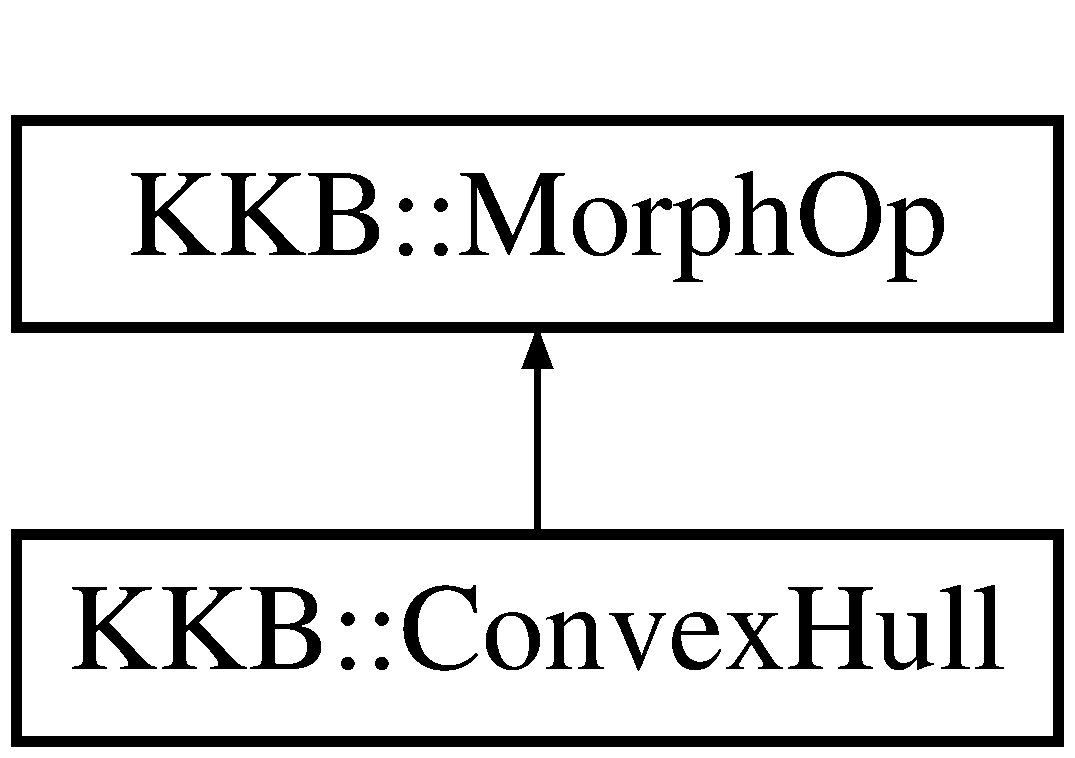
\includegraphics[height=2.000000cm]{class_k_k_b_1_1_convex_hull}
\end{center}
\end{figure}
\subsection*{Public Member Functions}
\begin{DoxyCompactItemize}
\item 
\hyperlink{class_k_k_b_1_1_convex_hull_a6ace975a2080ff5ae5adc731db76155c}{Convex\+Hull} ()
\item 
virtual \hyperlink{class_k_k_b_1_1_convex_hull_a7538cdc1c47d38d711aff7c72bb271ba}{$\sim$\+Convex\+Hull} ()
\item 
\hyperlink{namespace_k_k_b_a8fa4952cc84fda1de4bec1fbdd8d5b1b}{kkint32} \hyperlink{class_k_k_b_1_1_convex_hull_a3f6d4a0b84fb968042d1be038d7903ad}{Convex\+Area} ()
\item 
void \hyperlink{class_k_k_b_1_1_convex_hull_a89c8dc3b365746771bfd92475fa18bd9}{Draw} (\hyperlink{class_k_k_b_1_1_raster}{Raster} \&output)
\item 
\hyperlink{namespace_k_k_b_a80d46bd24db644a022c863bce8ae3633}{Raster\+Ptr} \hyperlink{class_k_k_b_1_1_convex_hull_a738c3a3fb1e27c75fd1c5a61bd278cec}{Filter} (const \hyperlink{class_k_k_b_1_1_raster}{Raster} \&src)
\begin{DoxyCompactList}\small\item\em Returns a image that represents the convex-\/hull of the \textquotesingle{}src\textquotesingle{} image. param\mbox{[}in\mbox{]} src Source image that convex-\/hull is to be found for. \end{DoxyCompactList}\item 
\hyperlink{namespace_k_k_b_a80d46bd24db644a022c863bce8ae3633}{Raster\+Ptr} \hyperlink{class_k_k_b_1_1_convex_hull_a429897e8bd2ee8c120797f2f465d2617}{Filter} (const \hyperlink{class_k_k_b_1_1_raster}{Raster} \&src, \hyperlink{namespace_k_k_b_a80d46bd24db644a022c863bce8ae3633}{Raster\+Ptr} dest)
\item 
virtual \hyperlink{class_k_k_b_1_1_morph_op_a32070d9c14d16849873a8a409f5b0d69}{Operation\+Type} \hyperlink{class_k_k_b_1_1_convex_hull_ac540f936d8466f22b98246b2ddb71123}{Operation} () const 
\item 
virtual \hyperlink{namespace_k_k_b_a80d46bd24db644a022c863bce8ae3633}{Raster\+Ptr} \hyperlink{class_k_k_b_1_1_convex_hull_afe5bccb26f94b0a2d72d2864cad51a28}{Perform\+Operation} (\hyperlink{namespace_k_k_b_a5acfa7402dc4df1769f90d3dc8ddfc2c}{Raster\+Const\+Ptr} \+\_\+image)
\item 
void \hyperlink{class_k_k_b_1_1_convex_hull_a055ea906fe75fd90e6b3a12bdad02c5b}{Store} (const \hyperlink{class_k_k_b_1_1_raster}{Raster} \&input)
\begin{DoxyCompactList}\small\item\em Build list of the upper and lower points in the image. \end{DoxyCompactList}\end{DoxyCompactItemize}
\subsection*{Additional Inherited Members}


\subsection{Detailed Description}
Operator that will create a Convex Hull of a supplied image. 

Definition at line 42 of file Convex\+Hull.\+h.



\subsection{Constructor \& Destructor Documentation}
\index{K\+K\+B\+::\+Convex\+Hull@{K\+K\+B\+::\+Convex\+Hull}!Convex\+Hull@{Convex\+Hull}}
\index{Convex\+Hull@{Convex\+Hull}!K\+K\+B\+::\+Convex\+Hull@{K\+K\+B\+::\+Convex\+Hull}}
\subsubsection[{\texorpdfstring{Convex\+Hull()}{ConvexHull()}}]{\setlength{\rightskip}{0pt plus 5cm}Convex\+Hull\+::\+Convex\+Hull (
\begin{DoxyParamCaption}
{}
\end{DoxyParamCaption}
)}\hypertarget{class_k_k_b_1_1_convex_hull_a6ace975a2080ff5ae5adc731db76155c}{}\label{class_k_k_b_1_1_convex_hull_a6ace975a2080ff5ae5adc731db76155c}


Definition at line 34 of file Convex\+Hull.\+cpp.



References K\+K\+B\+::\+Morph\+Op\+::\+Morph\+Op().



Referenced by K\+K\+M\+L\+L\+::\+Gray\+Scale\+Images\+F\+V\+Producer\+::\+Compute\+Feature\+Vector().


\begin{DoxyCode}
34                        :
35   \hyperlink{class_k_k_b_1_1_morph_op_a087902e5cad640c26dfa24804cc2a974}{MorphOp} (),
36   convexArea  (0),
37   upperPoints (NULL),
38   lowerPoints (NULL),
39   upper       (NULL),
40   lower       (NULL)
41 \{
42   AllocateMemory ();
43 \}
\end{DoxyCode}
\index{K\+K\+B\+::\+Convex\+Hull@{K\+K\+B\+::\+Convex\+Hull}!````~Convex\+Hull@{$\sim$\+Convex\+Hull}}
\index{````~Convex\+Hull@{$\sim$\+Convex\+Hull}!K\+K\+B\+::\+Convex\+Hull@{K\+K\+B\+::\+Convex\+Hull}}
\subsubsection[{\texorpdfstring{$\sim$\+Convex\+Hull()}{~ConvexHull()}}]{\setlength{\rightskip}{0pt plus 5cm}Convex\+Hull\+::$\sim$\+Convex\+Hull (
\begin{DoxyParamCaption}
{}
\end{DoxyParamCaption}
)\hspace{0.3cm}{\ttfamily [virtual]}}\hypertarget{class_k_k_b_1_1_convex_hull_a7538cdc1c47d38d711aff7c72bb271ba}{}\label{class_k_k_b_1_1_convex_hull_a7538cdc1c47d38d711aff7c72bb271ba}


Definition at line 46 of file Convex\+Hull.\+cpp.


\begin{DoxyCode}
47 \{
48   CleanUpMemory ();
49 \}
\end{DoxyCode}


\subsection{Member Function Documentation}
\index{K\+K\+B\+::\+Convex\+Hull@{K\+K\+B\+::\+Convex\+Hull}!Convex\+Area@{Convex\+Area}}
\index{Convex\+Area@{Convex\+Area}!K\+K\+B\+::\+Convex\+Hull@{K\+K\+B\+::\+Convex\+Hull}}
\subsubsection[{\texorpdfstring{Convex\+Area()}{ConvexArea()}}]{\setlength{\rightskip}{0pt plus 5cm}{\bf kkint32} Convex\+Hull\+::\+Convex\+Area (
\begin{DoxyParamCaption}
{}
\end{DoxyParamCaption}
)}\hypertarget{class_k_k_b_1_1_convex_hull_a3f6d4a0b84fb968042d1be038d7903ad}{}\label{class_k_k_b_1_1_convex_hull_a3f6d4a0b84fb968042d1be038d7903ad}


Definition at line 189 of file Convex\+Hull.\+cpp.



Referenced by K\+K\+M\+L\+L\+::\+Gray\+Scale\+Images\+F\+V\+Producer\+::\+Compute\+Feature\+Vector().


\begin{DoxyCode}
190 \{
191   \textcolor{keywordflow}{return}  convexArea;
192 \}
\end{DoxyCode}
\index{K\+K\+B\+::\+Convex\+Hull@{K\+K\+B\+::\+Convex\+Hull}!Draw@{Draw}}
\index{Draw@{Draw}!K\+K\+B\+::\+Convex\+Hull@{K\+K\+B\+::\+Convex\+Hull}}
\subsubsection[{\texorpdfstring{Draw(\+Raster \&output)}{Draw(Raster &output)}}]{\setlength{\rightskip}{0pt plus 5cm}void Convex\+Hull\+::\+Draw (
\begin{DoxyParamCaption}
\item[{{\bf Raster} \&}]{output}
\end{DoxyParamCaption}
)}\hypertarget{class_k_k_b_1_1_convex_hull_a89c8dc3b365746771bfd92475fa18bd9}{}\label{class_k_k_b_1_1_convex_hull_a89c8dc3b365746771bfd92475fa18bd9}


Definition at line 438 of file Convex\+Hull.\+cpp.



References K\+K\+B\+::\+Point\+::\+Col(), K\+K\+B\+::\+Point\+::\+Row(), and K\+K\+B\+::\+Raster\+::\+Set\+Pixel\+Value().



Referenced by Filter().


\begin{DoxyCode}
439 \{
440   \hyperlink{class_k_k_b_1_1_k_k_queue_aa3c2796a726eea468b94132a9fbf2cfe}{PointList::iterator}  it;  \textcolor{comment}{// (*upper);}
441   it = upper->begin ();
442 
443   \hyperlink{class_k_k_b_1_1_point}{PointPtr}  lastPoint = NULL;
444   \hyperlink{class_k_k_b_1_1_point}{PointPtr}  nextPoint = NULL;
445 
446   \textcolor{keywordflow}{if}  (it != upper->end ())
447   \{lastPoint = *it;  ++it;\}
448 
449   \textcolor{keywordflow}{if}  (it != upper->end ())
450   \{nextPoint = *it;  ++it;\}
451 
452   \hyperlink{class_k_k_b_1_1_point}{PointPtr}  firstPoint = lastPoint;
453 
454   \textcolor{keywordflow}{if}  ((!nextPoint)  &&  (!lastPoint))
455     \textcolor{keywordflow}{return};
456 
457   \textcolor{keywordflow}{if} ((nextPoint != NULL)  &&  (lastPoint == NULL))
458   \{
459     output.\hyperlink{class_k_k_b_1_1_raster_a5ddb8bd069dc64241941b0b011af8667}{SetPixelValue} (nextPoint->\hyperlink{class_k_k_b_1_1_point_abfc34bcf809fc9fb95baf5c745b07549}{Row} (), nextPoint->\hyperlink{class_k_k_b_1_1_point_afb196b03757fc697f6ade0129a1c7fcf}{Col} (), 255);
460     \textcolor{keywordflow}{return};
461   \}
462     
463   \textcolor{keywordflow}{while} (nextPoint)
464   \{
465     DrawLine (output, *lastPoint, *nextPoint, 255);
466     lastPoint = nextPoint;
467     \textcolor{keywordflow}{if}  (it == upper->end ())
468       nextPoint = NULL;
469     \textcolor{keywordflow}{else}
470     \{
471       nextPoint = *it;
472       ++it;
473     \}
474   \}
475 
476   DrawLine (output, *lastPoint, *firstPoint, 255);
477 \}  \textcolor{comment}{/* Draw */}
\end{DoxyCode}
\index{K\+K\+B\+::\+Convex\+Hull@{K\+K\+B\+::\+Convex\+Hull}!Filter@{Filter}}
\index{Filter@{Filter}!K\+K\+B\+::\+Convex\+Hull@{K\+K\+B\+::\+Convex\+Hull}}
\subsubsection[{\texorpdfstring{Filter(const Raster \&src)}{Filter(const Raster &src)}}]{\setlength{\rightskip}{0pt plus 5cm}{\bf Raster\+Ptr} Convex\+Hull\+::\+Filter (
\begin{DoxyParamCaption}
\item[{const {\bf Raster} \&}]{src}
\end{DoxyParamCaption}
)}\hypertarget{class_k_k_b_1_1_convex_hull_a738c3a3fb1e27c75fd1c5a61bd278cec}{}\label{class_k_k_b_1_1_convex_hull_a738c3a3fb1e27c75fd1c5a61bd278cec}


Returns a image that represents the convex-\/hull of the \textquotesingle{}src\textquotesingle{} image. param\mbox{[}in\mbox{]} src Source image that convex-\/hull is to be found for. 

\begin{DoxyReturn}{Returns}
A new raster that contains the convex-\/hull of the \textquotesingle{}src\textquotesingle{} image; the caller will be responsible for deleting. 
\end{DoxyReturn}


Definition at line 88 of file Convex\+Hull.\+cpp.



References Draw(), K\+K\+B\+::\+Raster\+::\+Height(), K\+K\+B\+::\+Raster\+::\+Raster(), K\+K\+B\+::\+Morph\+Op\+::\+Set\+Src\+Raster(), Store(), and K\+K\+B\+::\+Raster\+::\+Width().



Referenced by Perform\+Operation().


\begin{DoxyCode}
89 \{
90   \hyperlink{class_k_k_b_1_1_morph_op_a07c75e151d9b95ca13da3bfc2e48dba4}{SetSrcRaster} (&src);
91 
92   \hyperlink{namespace_k_k_b_a8fa4952cc84fda1de4bec1fbdd8d5b1b}{kkint32} w = src.\hyperlink{class_k_k_b_1_1_raster_aa2780c0b7ae75b7b595f99329689c1f6}{Width} ();
93   \hyperlink{namespace_k_k_b_a8fa4952cc84fda1de4bec1fbdd8d5b1b}{kkint32} h = src.\hyperlink{class_k_k_b_1_1_raster_af8d10d15697d5b92fb9595c48b529feb}{Height} ();
94         
95   \hyperlink{class_k_k_b_1_1_convex_hull_a055ea906fe75fd90e6b3a12bdad02c5b}{Store} (src);
96   
97   \hyperlink{class_k_k_b_1_1_raster}{RasterPtr}  dest = \textcolor{keyword}{new} \hyperlink{class_k_k_b_1_1_raster}{Raster} (h, w);
98 
99   \textcolor{keywordflow}{if}  ((upperPoints->\hyperlink{class_k_k_b_1_1_k_k_queue_a1dab601f75ee6a65d97f02bddf71c40d}{QueueSize} () == 1)  &&  
100        (lowerPoints->\hyperlink{class_k_k_b_1_1_k_k_queue_a1dab601f75ee6a65d97f02bddf71c40d}{QueueSize} () == 1))
101   \{
102     \textcolor{comment}{// We must have a Vertical  Line}
103     DrawLine (*dest, (*upperPoints)[0], (*lowerPoints)[0], 255);
104     CalcConvexArea (dest);
105     \textcolor{keywordflow}{return}  dest;
106   \}
107 
108   \textcolor{keywordflow}{else} \textcolor{keywordflow}{if}  ((upperPoints->\hyperlink{class_k_k_b_1_1_k_k_queue_a1dab601f75ee6a65d97f02bddf71c40d}{QueueSize} () < 1)  ||  (lowerPoints->
      \hyperlink{class_k_k_b_1_1_k_k_queue_a1dab601f75ee6a65d97f02bddf71c40d}{QueueSize} () < 1))
109   \{
110     \textcolor{comment}{// We have Nothing}
111     \textcolor{keywordflow}{return} dest;
112   \}
113 
114   BuildUpperLink ();
115   BuildLowerLink ();
116 
117   Merge ();
118 
119   \hyperlink{class_k_k_b_1_1_convex_hull_a89c8dc3b365746771bfd92475fa18bd9}{Draw} (*dest);
120   
121   CalcConvexArea (dest);
122 
123   \textcolor{keywordflow}{return} dest;
124 \}  \textcolor{comment}{/* Filter */}
\end{DoxyCode}
\index{K\+K\+B\+::\+Convex\+Hull@{K\+K\+B\+::\+Convex\+Hull}!Filter@{Filter}}
\index{Filter@{Filter}!K\+K\+B\+::\+Convex\+Hull@{K\+K\+B\+::\+Convex\+Hull}}
\subsubsection[{\texorpdfstring{Filter(const Raster \&src, Raster\+Ptr dest)}{Filter(const Raster &src, RasterPtr dest)}}]{\setlength{\rightskip}{0pt plus 5cm}{\bf Raster\+Ptr} Convex\+Hull\+::\+Filter (
\begin{DoxyParamCaption}
\item[{const {\bf Raster} \&}]{src, }
\item[{{\bf Raster\+Ptr}}]{dest}
\end{DoxyParamCaption}
)}\hypertarget{class_k_k_b_1_1_convex_hull_a429897e8bd2ee8c120797f2f465d2617}{}\label{class_k_k_b_1_1_convex_hull_a429897e8bd2ee8c120797f2f465d2617}


Definition at line 128 of file Convex\+Hull.\+cpp.



References Draw(), K\+K\+B\+::\+Raster\+::\+Height(), K\+K\+B\+::\+Raster\+::\+Re\+Size(), K\+K\+B\+::\+Morph\+Op\+::\+Set\+Src\+Raster(), K\+K\+B\+::\+Morph\+Op\+::src\+Height, K\+K\+B\+::\+Morph\+Op\+::src\+Width, Store(), and K\+K\+B\+::\+Raster\+::\+Width().



Referenced by K\+K\+M\+L\+L\+::\+Gray\+Scale\+Images\+F\+V\+Producer\+::\+Compute\+Feature\+Vector().


\begin{DoxyCode}
131 \{
132   \hyperlink{class_k_k_b_1_1_morph_op_a07c75e151d9b95ca13da3bfc2e48dba4}{SetSrcRaster} (&src);
133   \textcolor{comment}{//srcHeight = src.Height ();}
134   \textcolor{comment}{//srcWidth  = src.Width  ();}
135 
136 \textcolor{comment}{//  kkint32 w = src.Width ();}
137 \textcolor{comment}{//  kkint32 h = src.Height ();}
138 
139   \textcolor{keywordflow}{if}  ((dest->\hyperlink{class_k_k_b_1_1_raster_af8d10d15697d5b92fb9595c48b529feb}{Height} () != \hyperlink{class_k_k_b_1_1_morph_op_a54b2ce1b398a80803b4dbe8aef956b51}{srcHeight})  ||  (dest->\hyperlink{class_k_k_b_1_1_raster_aa2780c0b7ae75b7b595f99329689c1f6}{Width} () != 
      \hyperlink{class_k_k_b_1_1_morph_op_aec2cfb3015497e4077751fc5f19559ab}{srcWidth}))
140     dest->\hyperlink{class_k_k_b_1_1_raster_ad0a4daf2ba175cedf00ce975bb746417}{ReSize} (\hyperlink{class_k_k_b_1_1_morph_op_a54b2ce1b398a80803b4dbe8aef956b51}{srcHeight}, \hyperlink{class_k_k_b_1_1_morph_op_aec2cfb3015497e4077751fc5f19559ab}{srcWidth}, \textcolor{keyword}{false});
141         
142   \hyperlink{class_k_k_b_1_1_convex_hull_a055ea906fe75fd90e6b3a12bdad02c5b}{Store} (src);
143 
144   \textcolor{keywordflow}{if}  ((upperPoints->\hyperlink{class_k_k_b_1_1_k_k_queue_a1dab601f75ee6a65d97f02bddf71c40d}{QueueSize} () == 1)  &&  
145        (lowerPoints->\hyperlink{class_k_k_b_1_1_k_k_queue_a1dab601f75ee6a65d97f02bddf71c40d}{QueueSize} () == 1))
146   \{
147     \textcolor{comment}{// We must have a Vertical  Line}
148     DrawLine (*dest, (*upperPoints)[0], (*lowerPoints)[0], 255);
149     CalcConvexArea (dest);
150     \textcolor{keywordflow}{return}  dest;
151   \}
152 
153   \textcolor{keywordflow}{else} \textcolor{keywordflow}{if}  ((upperPoints->\hyperlink{class_k_k_b_1_1_k_k_queue_a1dab601f75ee6a65d97f02bddf71c40d}{QueueSize} () < 1)  ||  (lowerPoints->
      \hyperlink{class_k_k_b_1_1_k_k_queue_a1dab601f75ee6a65d97f02bddf71c40d}{QueueSize} () < 1))
154   \{
155     \textcolor{comment}{// We have Nothing}
156     \textcolor{keywordflow}{return} dest;
157   \}
158 
159   BuildUpperLink ();
160   BuildLowerLink ();
161 
162   Merge ();
163 
164   \hyperlink{class_k_k_b_1_1_convex_hull_a89c8dc3b365746771bfd92475fa18bd9}{Draw} (*dest);
165   
166   CalcConvexArea (dest);
167 
168   \textcolor{keywordflow}{return} dest;
169 \}  \textcolor{comment}{/* Filter */}
\end{DoxyCode}
\index{K\+K\+B\+::\+Convex\+Hull@{K\+K\+B\+::\+Convex\+Hull}!Operation@{Operation}}
\index{Operation@{Operation}!K\+K\+B\+::\+Convex\+Hull@{K\+K\+B\+::\+Convex\+Hull}}
\subsubsection[{\texorpdfstring{Operation() const }{Operation() const }}]{\setlength{\rightskip}{0pt plus 5cm}virtual {\bf Operation\+Type} K\+K\+B\+::\+Convex\+Hull\+::\+Operation (
\begin{DoxyParamCaption}
{}
\end{DoxyParamCaption}
) const\hspace{0.3cm}{\ttfamily [inline]}, {\ttfamily [virtual]}}\hypertarget{class_k_k_b_1_1_convex_hull_ac540f936d8466f22b98246b2ddb71123}{}\label{class_k_k_b_1_1_convex_hull_ac540f936d8466f22b98246b2ddb71123}


Implements \hyperlink{class_k_k_b_1_1_morph_op_abdf6f4bddae0b3cc3dc718559fa60234}{K\+K\+B\+::\+Morph\+Op}.



Definition at line 49 of file Convex\+Hull.\+h.



References K\+K\+B\+::\+Morph\+Op\+::\+Convex\+Hull.


\begin{DoxyCode}
49 \{\textcolor{keywordflow}{return} \hyperlink{class_k_k_b_1_1_morph_op_a32070d9c14d16849873a8a409f5b0d69a3e1ee9920ed982b5da9becaf4b5463e5}{OperationType::ConvexHull};\}
\end{DoxyCode}
\index{K\+K\+B\+::\+Convex\+Hull@{K\+K\+B\+::\+Convex\+Hull}!Perform\+Operation@{Perform\+Operation}}
\index{Perform\+Operation@{Perform\+Operation}!K\+K\+B\+::\+Convex\+Hull@{K\+K\+B\+::\+Convex\+Hull}}
\subsubsection[{\texorpdfstring{Perform\+Operation(\+Raster\+Const\+Ptr \+\_\+image)}{PerformOperation(RasterConstPtr _image)}}]{\setlength{\rightskip}{0pt plus 5cm}{\bf Raster\+Ptr} Convex\+Hull\+::\+Perform\+Operation (
\begin{DoxyParamCaption}
\item[{{\bf Raster\+Const\+Ptr}}]{\+\_\+image}
\end{DoxyParamCaption}
)\hspace{0.3cm}{\ttfamily [virtual]}}\hypertarget{class_k_k_b_1_1_convex_hull_afe5bccb26f94b0a2d72d2864cad51a28}{}\label{class_k_k_b_1_1_convex_hull_afe5bccb26f94b0a2d72d2864cad51a28}


Definition at line 73 of file Convex\+Hull.\+cpp.



References Filter(), K\+K\+B\+::\+Morph\+Op\+::\+Set\+Src\+Raster(), and K\+K\+B\+::\+Morph\+Op\+::src\+Raster.


\begin{DoxyCode}
74 \{
75   \hyperlink{class_k_k_b_1_1_morph_op_a07c75e151d9b95ca13da3bfc2e48dba4}{SetSrcRaster} (\_image);
76   AllocateMemory ();
77   \hyperlink{class_k_k_b_1_1_raster}{RasterPtr}  result = \hyperlink{class_k_k_b_1_1_convex_hull_a738c3a3fb1e27c75fd1c5a61bd278cec}{Filter} (*\hyperlink{class_k_k_b_1_1_morph_op_a9af0ebff0135d124c7d1d17e21c4d7e6}{srcRaster});
78   \textcolor{keywordflow}{return}  result;
79 \}  \textcolor{comment}{/* PerformOperation */}
\end{DoxyCode}
\index{K\+K\+B\+::\+Convex\+Hull@{K\+K\+B\+::\+Convex\+Hull}!Store@{Store}}
\index{Store@{Store}!K\+K\+B\+::\+Convex\+Hull@{K\+K\+B\+::\+Convex\+Hull}}
\subsubsection[{\texorpdfstring{Store(const Raster \&input)}{Store(const Raster &input)}}]{\setlength{\rightskip}{0pt plus 5cm}void Convex\+Hull\+::\+Store (
\begin{DoxyParamCaption}
\item[{const {\bf Raster} \&}]{input}
\end{DoxyParamCaption}
)}\hypertarget{class_k_k_b_1_1_convex_hull_a055ea906fe75fd90e6b3a12bdad02c5b}{}\label{class_k_k_b_1_1_convex_hull_a055ea906fe75fd90e6b3a12bdad02c5b}


Build list of the upper and lower points in the image. 

for each column in the image where there is at least one foreground pixel will add one point to \textquotesingle{}upper\+Points\textquotesingle{} for the pixel with the smallest row and one point to \textquotesingle{}lower\+Points\textquotesingle{} for the pixel with the largest row. 
\begin{DoxyParams}[1]{Parameters}
\mbox{\tt in}  & {\em input} & Source image that we are to generate a Convex Hull for.\\
\hline
\end{DoxyParams}
for each column in the image where there is at least one foreground pixel will add one point to \textquotesingle{}upper\+Points\textquotesingle{} for the pixel with the smallest row and one point to \textquotesingle{}lower\+Points\textquotesingle{} for the pixel with the largest row. 
\begin{DoxyParams}[1]{Parameters}
\mbox{\tt in}  & {\em input} & Source image that we are to generate a convex-\/hull for. \\
\hline
\end{DoxyParams}


Definition at line 738 of file Convex\+Hull.\+cpp.



References K\+K\+B\+::\+Morph\+Op\+::\+Foreground\+Pixel(), K\+K\+B\+::\+Raster\+::\+Height(), K\+K\+B\+::\+Point\+::\+Point(), K\+K\+B\+::\+Raster\+::\+Rows(), and K\+K\+B\+::\+Raster\+::\+Width().



Referenced by Filter().


\begin{DoxyCode}
739 \{
740   \hyperlink{namespace_k_k_b_a8fa4952cc84fda1de4bec1fbdd8d5b1b}{kkint32} w = input.\hyperlink{class_k_k_b_1_1_raster_aa2780c0b7ae75b7b595f99329689c1f6}{Width} ();
741   \hyperlink{namespace_k_k_b_a8fa4952cc84fda1de4bec1fbdd8d5b1b}{kkint32} h = input.\hyperlink{class_k_k_b_1_1_raster_af8d10d15697d5b92fb9595c48b529feb}{Height} ();
742 
743   \hyperlink{namespace_k_k_b_ace9969169bf514f9ee6185186949cdf7}{uchar}**  rows = input.\hyperlink{class_k_k_b_1_1_raster_a2460989f656e5222d6074cd0ba85ed72}{Rows} ();
744         
745   \textcolor{keywordflow}{for} (\hyperlink{namespace_k_k_b_a8fa4952cc84fda1de4bec1fbdd8d5b1b}{kkint32} col = 0;  col < w;  ++col)
746   \{
747     \hyperlink{namespace_k_k_b_a8fa4952cc84fda1de4bec1fbdd8d5b1b}{kkint32} row;
748     \textcolor{keywordflow}{for}  (row = h - 1;  row >= 0;  --row)
749     \{
750       \textcolor{keywordflow}{if}  (\hyperlink{class_k_k_b_1_1_morph_op_acd5541050c3c0207b004b71caf7fb1f4}{ForegroundPixel} (row, col))
751       \{
752         \hyperlink{class_k_k_b_1_1_point}{PointPtr} u = \textcolor{keyword}{new} \hyperlink{class_k_k_b_1_1_point}{Point} (row, col);
753         upperPoints->\hyperlink{class_k_k_b_1_1_k_k_queue_adec987ebb0ac593ad877ffa59becb107}{Add} (u);
754         \textcolor{keywordflow}{break};
755       \}
756     \}
757 
758     \textcolor{keywordflow}{if}  (row >= 0)
759     \{
760       \textcolor{keywordflow}{for}  (row = 0; row < h; row++)
761       \{
762         \textcolor{keywordflow}{if}  (\hyperlink{class_k_k_b_1_1_morph_op_acd5541050c3c0207b004b71caf7fb1f4}{ForegroundPixel} (row, col))
763         \{
764           \hyperlink{class_k_k_b_1_1_point}{PointPtr} l = \textcolor{keyword}{new} \hyperlink{class_k_k_b_1_1_point}{Point} (row, col);
765           lowerPoints->\hyperlink{class_k_k_b_1_1_k_k_queue_a1832186a944dca6fb3d5fca4046b7c40}{AddFirst} (l);
766           \textcolor{keywordflow}{break};
767         \}
768       \}
769     \}
770   \}
771 \}  \textcolor{comment}{/* Store */}
\end{DoxyCode}


The documentation for this class was generated from the following files\+:\begin{DoxyCompactItemize}
\item 
C\+:/\+Users/\+Kurt/\+Git\+Hub/\+K\+Square\+Libraries/\+K\+K\+Base/\hyperlink{_convex_hull_8h}{Convex\+Hull.\+h}\item 
C\+:/\+Users/\+Kurt/\+Git\+Hub/\+K\+Square\+Libraries/\+K\+K\+Base/\hyperlink{_convex_hull_8cpp}{Convex\+Hull.\+cpp}\end{DoxyCompactItemize}

\hypertarget{class_k_k_b_1_1_date_time}{}\section{K\+KB\+:\+:Date\+Time Class Reference}
\label{class_k_k_b_1_1_date_time}\index{K\+K\+B\+::\+Date\+Time@{K\+K\+B\+::\+Date\+Time}}


{\ttfamily \#include $<$Date\+Time.\+h$>$}

\subsection*{Public Member Functions}
\begin{DoxyCompactItemize}
\item 
\hyperlink{class_k_k_b_1_1_date_time_a3ccfb87f7a2e9683b91964e32d907161}{Date\+Time} ()
\item 
\hyperlink{class_k_k_b_1_1_date_time_a147e3ba552c01109b1327624d6aed70b}{Date\+Time} (const \hyperlink{class_k_k_b_1_1_date_time}{Date\+Time} \&date\+Time)
\item 
\hyperlink{class_k_k_b_1_1_date_time_af93fc54efb1e1daa33c1ffe79d5f78bb}{Date\+Time} (const \hyperlink{class_k_k_b_1_1_date_type}{Date\+Type} \&\+\_\+date, const \hyperlink{class_k_k_b_1_1_time_type}{Time\+Type} \&\+\_\+time)
\item 
\hyperlink{class_k_k_b_1_1_date_time_a08a9a2435a6b3474017d4b4cddbdcc6d}{Date\+Time} (short \+\_\+year, \hyperlink{namespace_k_k_b_ace9969169bf514f9ee6185186949cdf7}{uchar} \+\_\+month, \hyperlink{namespace_k_k_b_ace9969169bf514f9ee6185186949cdf7}{uchar} \+\_\+day, \hyperlink{namespace_k_k_b_ace9969169bf514f9ee6185186949cdf7}{uchar} \+\_\+hour, \hyperlink{namespace_k_k_b_ace9969169bf514f9ee6185186949cdf7}{uchar} \+\_\+minute, \hyperlink{namespace_k_k_b_ace9969169bf514f9ee6185186949cdf7}{uchar} \+\_\+second)
\item 
\hyperlink{class_k_k_b_1_1_date_time_a5685c4e77778d570f3e14149bc2bb970}{Date\+Time} (const \hyperlink{class_k_k_b_1_1_k_k_str}{K\+K\+Str} \&s)
\item 
void \hyperlink{class_k_k_b_1_1_date_time_a285f607b8d42745d661a76530192a5fa}{Add\+Days} (\hyperlink{namespace_k_k_b_a8fa4952cc84fda1de4bec1fbdd8d5b1b}{kkint32} \+\_\+days)
\item 
void \hyperlink{class_k_k_b_1_1_date_time_aa00751cde5c47424833acef065629adf}{Add\+Hours} (\hyperlink{namespace_k_k_b_a8fa4952cc84fda1de4bec1fbdd8d5b1b}{kkint32} \+\_\+hours)
\item 
void \hyperlink{class_k_k_b_1_1_date_time_a7621802a3441ba13250536f60ce26ba8}{Add\+Minutes} (\hyperlink{namespace_k_k_b_a8fa4952cc84fda1de4bec1fbdd8d5b1b}{kkint32} \+\_\+mins)
\item 
void \hyperlink{class_k_k_b_1_1_date_time_a4231e149b01ab91773736995e8a5bc52}{Add\+Seconds} (long \+\_\+secs)
\item 
const \hyperlink{class_k_k_b_1_1_date_type}{K\+K\+B\+::\+Date\+Type} \& \hyperlink{class_k_k_b_1_1_date_time_ab18f4ea0ddd5df87ad52e343f68b039e}{Date} () const 
\item 
\hyperlink{namespace_k_k_b_ace9969169bf514f9ee6185186949cdf7}{uchar} \hyperlink{class_k_k_b_1_1_date_time_a4ff581d59f874c3fb7d5fc3344fba4bf}{Day} () const 
\item 
\hyperlink{class_k_k_b_1_1_k_k_str}{K\+K\+Str} \hyperlink{class_k_k_b_1_1_date_time_afb7cd42c8b3683935391f684ed866221}{H\+H\+\_\+\+M\+M\+\_\+\+SS} () const 
\item 
void \hyperlink{class_k_k_b_1_1_date_time_a922684cdbfaf29c9bc46bd932569d911}{Hours\+Add} (\hyperlink{namespace_k_k_b_a8fa4952cc84fda1de4bec1fbdd8d5b1b}{kkint32} hours)
\begin{DoxyCompactList}\small\item\em Add \+\_\+hours to \hyperlink{class_k_k_b_1_1_date_time}{Date\+Time}, will adjust date to accommodate 24 hour clock. \end{DoxyCompactList}\item 
void \hyperlink{class_k_k_b_1_1_date_time_af9c89ac57882cb38458235f5b1c42781}{Minutes\+Add} (\hyperlink{namespace_k_k_b_a8fa4952cc84fda1de4bec1fbdd8d5b1b}{kkint32} \+\_\+mins)
\item 
\hyperlink{namespace_k_k_b_ace9969169bf514f9ee6185186949cdf7}{uchar} \hyperlink{class_k_k_b_1_1_date_time_a651e406918c5d7f1905252ada51abb37}{Month} () const 
\item 
bool \hyperlink{class_k_k_b_1_1_date_time_a14c61e0102af91b8910c15070d2c33ce}{operator!=} (const \hyperlink{class_k_k_b_1_1_date_time}{Date\+Time} \&right) const 
\item 
\hyperlink{class_k_k_b_1_1_date_time}{Date\+Time} \hyperlink{class_k_k_b_1_1_date_time_a358894c10ee65b942d362ce6de71460c}{operator+} (const \hyperlink{class_k_k_b_1_1_date_time}{Date\+Time} \&right) const 
\item 
\hyperlink{class_k_k_b_1_1_date_time}{Date\+Time} \hyperlink{class_k_k_b_1_1_date_time_abdcdc4c9d9a3a7d82462cddd132cc734}{operator-\/} (const \hyperlink{class_k_k_b_1_1_date_time}{Date\+Time} \&right) const 
\item 
bool \hyperlink{class_k_k_b_1_1_date_time_a76b9346b8f98fbaea671dd1892cffa7f}{operator$<$} (const \hyperlink{class_k_k_b_1_1_date_time}{Date\+Time} \&right) const 
\item 
bool \hyperlink{class_k_k_b_1_1_date_time_a8c908bd1fefa7152856936e3b9336f64}{operator$<$=} (const \hyperlink{class_k_k_b_1_1_date_time}{Date\+Time} \&right) const 
\item 
\hyperlink{class_k_k_b_1_1_date_time}{Date\+Time} \& \hyperlink{class_k_k_b_1_1_date_time_a16e05498069aca8c6bd510a68b2bee69}{operator=} (const \hyperlink{class_k_k_b_1_1_date_time}{Date\+Time} \&right)
\item 
bool \hyperlink{class_k_k_b_1_1_date_time_a1be303a5cb29cfd06c6de9562e454eba}{operator==} (const \hyperlink{class_k_k_b_1_1_date_time}{Date\+Time} \&right) const 
\item 
bool \hyperlink{class_k_k_b_1_1_date_time_a7ac966a3cb35eed48e6ce09265ea4a84}{operator$>$} (const \hyperlink{class_k_k_b_1_1_date_time}{Date\+Time} \&right) const 
\item 
bool \hyperlink{class_k_k_b_1_1_date_time_a19ff014e57d8d03d97e3b5a57f6ac036}{operator$>$=} (const \hyperlink{class_k_k_b_1_1_date_time}{Date\+Time} \&right) const 
\item 
\hyperlink{namespace_k_k_b_a1f2b0568d3b63cc7697dcff73250113e}{kkuint64} \hyperlink{class_k_k_b_1_1_date_time_a051f9f993938d58e5762256cf5c06f31}{Seconds} () const 
\item 
void \hyperlink{class_k_k_b_1_1_date_time_a0ca7d0cc7a5634c4c975fd16bbb41b32}{Seconds\+Add} (long \+\_\+secs)
\item 
const \hyperlink{class_k_k_b_1_1_time_type}{Time\+Type} \& \hyperlink{class_k_k_b_1_1_date_time_a981ba2e8e1ca8319d51be65c746442e1}{Time} () const 
\item 
\hyperlink{namespace_k_k_b_af8d832f05c54994a1cce25bd5743e19a}{kkuint32} \hyperlink{class_k_k_b_1_1_date_time_a92e8292a86720233831e6433df092fb5}{To\+Days} () const 
\item 
double \hyperlink{class_k_k_b_1_1_date_time_a1245f39d8c4209cf226c73de7950c426}{To\+Hours} () const 
\begin{DoxyCompactList}\small\item\em summary$>$Number seconds since \char`\"{}0000/01/01 00\+:00\+:00\char`\"{}\end{DoxyCompactList}\item 
\hyperlink{namespace_k_k_b_a1f2b0568d3b63cc7697dcff73250113e}{kkuint64} \hyperlink{class_k_k_b_1_1_date_time_a32ae25734d45d75f34a5dd0db163d57d}{To\+Seconds} () const 
\item 
short \hyperlink{class_k_k_b_1_1_date_time_aedfb008b85fd86fd6cec7d664ffac585}{Year} () const 
\item 
\hyperlink{class_k_k_b_1_1_k_k_str}{K\+K\+Str} \hyperlink{class_k_k_b_1_1_date_time_aca57fbdcd040549a2c9e0a3d4e99b9f9}{Y\+Y\+Y\+Y\+\_\+\+M\+M\+\_\+\+D\+D\+\_\+\+H\+H\+\_\+\+M\+M\+\_\+\+SS} () const 
\item 
\hyperlink{class_k_k_b_1_1_k_k_str}{K\+K\+Str} \hyperlink{class_k_k_b_1_1_date_time_ae8cb83aa1fe9cf1bf1694413055ea433}{Y\+Y\+Y\+Y\+M\+M\+D\+D\+H\+H\+M\+M\+SS} () const 
\end{DoxyCompactItemize}


\subsection{Detailed Description}


Definition at line 204 of file Date\+Time.\+h.



\subsection{Constructor \& Destructor Documentation}
\index{K\+K\+B\+::\+Date\+Time@{K\+K\+B\+::\+Date\+Time}!Date\+Time@{Date\+Time}}
\index{Date\+Time@{Date\+Time}!K\+K\+B\+::\+Date\+Time@{K\+K\+B\+::\+Date\+Time}}
\subsubsection[{\texorpdfstring{Date\+Time()}{DateTime()}}]{\setlength{\rightskip}{0pt plus 5cm}Date\+Time\+::\+Date\+Time (
\begin{DoxyParamCaption}
{}
\end{DoxyParamCaption}
)}\hypertarget{class_k_k_b_1_1_date_time_a3ccfb87f7a2e9683b91964e32d907161}{}\label{class_k_k_b_1_1_date_time_a3ccfb87f7a2e9683b91964e32d907161}


Definition at line 997 of file Date\+Time.\+cpp.



References K\+K\+B\+::\+Date\+Type\+::\+Date\+Type(), and K\+K\+B\+::\+Time\+Type\+::\+Time\+Type().



Referenced by K\+K\+B\+::\+Xml\+Attribute\+List\+::\+Attribute\+Value\+Date\+Time(), K\+K\+M\+L\+L\+::\+Classification\+Bias\+Matrix\+::\+Classification\+Bias\+Matrix(), K\+K\+M\+L\+L\+::\+Feature\+File\+I\+O\+::\+Feature\+Data\+Re\+Sink(), and K\+K\+B\+::\+Xml\+Element\+Date\+Time\+::\+Xml\+Element\+Date\+Time().


\begin{DoxyCode}
997                    :  
998       date(),
999       time ()
1000 \{\}
\end{DoxyCode}
\index{K\+K\+B\+::\+Date\+Time@{K\+K\+B\+::\+Date\+Time}!Date\+Time@{Date\+Time}}
\index{Date\+Time@{Date\+Time}!K\+K\+B\+::\+Date\+Time@{K\+K\+B\+::\+Date\+Time}}
\subsubsection[{\texorpdfstring{Date\+Time(const Date\+Time \&date\+Time)}{DateTime(const DateTime &dateTime)}}]{\setlength{\rightskip}{0pt plus 5cm}Date\+Time\+::\+Date\+Time (
\begin{DoxyParamCaption}
\item[{const {\bf Date\+Time} \&}]{date\+Time}
\end{DoxyParamCaption}
)}\hypertarget{class_k_k_b_1_1_date_time_a147e3ba552c01109b1327624d6aed70b}{}\label{class_k_k_b_1_1_date_time_a147e3ba552c01109b1327624d6aed70b}


Definition at line 1006 of file Date\+Time.\+cpp.



References K\+K\+B\+::\+Date\+Type\+::\+Date\+Type(), and K\+K\+B\+::\+Time\+Type\+::\+Time\+Type().



Referenced by K\+K\+M\+L\+L\+::\+Classification\+Bias\+Matrix\+::\+Classification\+Bias\+Matrix(), and K\+K\+Job\+Managment\+::\+K\+K\+Job\+Manager\+::\+K\+K\+Job\+Manager().


\begin{DoxyCode}
1006                                             :
1007        date (dateTime.date),
1008        time (dateTime.time)
1009 \{\}
\end{DoxyCode}
\index{K\+K\+B\+::\+Date\+Time@{K\+K\+B\+::\+Date\+Time}!Date\+Time@{Date\+Time}}
\index{Date\+Time@{Date\+Time}!K\+K\+B\+::\+Date\+Time@{K\+K\+B\+::\+Date\+Time}}
\subsubsection[{\texorpdfstring{Date\+Time(const Date\+Type \&\+\_\+date, const Time\+Type \&\+\_\+time)}{DateTime(const DateType &_date, const TimeType &_time)}}]{\setlength{\rightskip}{0pt plus 5cm}Date\+Time\+::\+Date\+Time (
\begin{DoxyParamCaption}
\item[{const {\bf Date\+Type} \&}]{\+\_\+date, }
\item[{const {\bf Time\+Type} \&}]{\+\_\+time}
\end{DoxyParamCaption}
)}\hypertarget{class_k_k_b_1_1_date_time_af93fc54efb1e1daa33c1ffe79d5f78bb}{}\label{class_k_k_b_1_1_date_time_af93fc54efb1e1daa33c1ffe79d5f78bb}


Definition at line 1016 of file Date\+Time.\+cpp.



References K\+K\+B\+::\+Date\+Type\+::\+Date\+Type(), and K\+K\+B\+::\+Time\+Type\+::\+Time\+Type().



Referenced by operator+(), and operator-\/().


\begin{DoxyCode}
1018                     :
1019        date (\_date),
1020        time (\_time)
1021 \{\}
\end{DoxyCode}
\index{K\+K\+B\+::\+Date\+Time@{K\+K\+B\+::\+Date\+Time}!Date\+Time@{Date\+Time}}
\index{Date\+Time@{Date\+Time}!K\+K\+B\+::\+Date\+Time@{K\+K\+B\+::\+Date\+Time}}
\subsubsection[{\texorpdfstring{Date\+Time(short \+\_\+year, uchar \+\_\+month, uchar \+\_\+day, uchar \+\_\+hour, uchar \+\_\+minute, uchar \+\_\+second)}{DateTime(short _year, uchar _month, uchar _day, uchar _hour, uchar _minute, uchar _second)}}]{\setlength{\rightskip}{0pt plus 5cm}Date\+Time\+::\+Date\+Time (
\begin{DoxyParamCaption}
\item[{short}]{\+\_\+year, }
\item[{{\bf uchar}}]{\+\_\+month, }
\item[{{\bf uchar}}]{\+\_\+day, }
\item[{{\bf uchar}}]{\+\_\+hour, }
\item[{{\bf uchar}}]{\+\_\+minute, }
\item[{{\bf uchar}}]{\+\_\+second}
\end{DoxyParamCaption}
)}\hypertarget{class_k_k_b_1_1_date_time_a08a9a2435a6b3474017d4b4cddbdcc6d}{}\label{class_k_k_b_1_1_date_time_a08a9a2435a6b3474017d4b4cddbdcc6d}


Definition at line 1028 of file Date\+Time.\+cpp.



References K\+K\+B\+::\+Date\+Type\+::\+Date\+Type(), and K\+K\+B\+::\+Time\+Type\+::\+Time\+Type().



Referenced by K\+K\+M\+L\+L\+::\+Training\+Process2\+::\+Training\+Process2().


\begin{DoxyCode}
1034                     :
1035       date (\_year, \_month, \_day),
1036       time (\_hour, \_minute, \_second)
1037 \{\}
\end{DoxyCode}
\index{K\+K\+B\+::\+Date\+Time@{K\+K\+B\+::\+Date\+Time}!Date\+Time@{Date\+Time}}
\index{Date\+Time@{Date\+Time}!K\+K\+B\+::\+Date\+Time@{K\+K\+B\+::\+Date\+Time}}
\subsubsection[{\texorpdfstring{Date\+Time(const K\+K\+Str \&s)}{DateTime(const KKStr &s)}}]{\setlength{\rightskip}{0pt plus 5cm}Date\+Time\+::\+Date\+Time (
\begin{DoxyParamCaption}
\item[{const {\bf K\+K\+Str} \&}]{s}
\end{DoxyParamCaption}
)}\hypertarget{class_k_k_b_1_1_date_time_a5685c4e77778d570f3e14149bc2bb970}{}\label{class_k_k_b_1_1_date_time_a5685c4e77778d570f3e14149bc2bb970}


Definition at line 1043 of file Date\+Time.\+cpp.



References K\+K\+B\+::\+K\+K\+Str\+::\+Concat(), K\+K\+B\+::\+K\+K\+Str\+::\+Count\+Instances\+Of(), K\+K\+B\+::\+Date\+Type\+::\+Date\+Type(), K\+K\+B\+::\+K\+K\+Str\+::\+Empty(), K\+K\+B\+::\+K\+K\+Str\+Parser\+::\+Get\+Next\+Token(), K\+K\+B\+::\+K\+K\+Str\+Parser\+::\+Get\+Rest\+Of\+Str(), K\+K\+B\+::\+K\+K\+Str\+Parser\+::\+K\+K\+Str\+Parser(), K\+K\+B\+::\+K\+K\+Str\+::operator+(), K\+K\+B\+::\+Date\+Type\+::operator=(), K\+K\+B\+::\+Time\+Type\+::operator=(), and K\+K\+B\+::\+Time\+Type\+::\+Time\+Type().



Referenced by K\+K\+B\+::\+Xml\+Attribute\+List\+::\+Attribute\+Value\+Date\+Time(), K\+K\+B\+::\+K\+K\+Str\+Parser\+::\+Get\+Next\+Token\+Date\+Time(), and K\+K\+Job\+Managment\+::\+K\+K\+Job\+Manager\+::\+Status\+File\+Process\+Line().


\begin{DoxyCode}
1043                                   :
1044       date(),
1045       time ()
1046 
1047 \{
1048   \textcolor{keywordflow}{if}  (s.\hyperlink{class_k_k_b_1_1_k_k_str_ac69942f73fffd672ec2a6e1c410afdb6}{Empty} ())
1049     \textcolor{keywordflow}{return};
1050 
1051   \hyperlink{class_k_k_b_1_1_k_k_str_parser}{KKStrParser} parser (s);
1052 
1053   \textcolor{keywordflow}{if}  ((s.\hyperlink{class_k_k_b_1_1_k_k_str_a08b9dcd254e64e4337008ab3007fdbc8}{CountInstancesOf} (\textcolor{charliteral}{'-'}) > 2)  &&  (s.\hyperlink{class_k_k_b_1_1_k_k_str_a08b9dcd254e64e4337008ab3007fdbc8}{CountInstancesOf} (\textcolor{charliteral}{'/'}) < 1))
1054   \{
1055     \textcolor{comment}{// Looks like the date part is broken up by '-' not '/'}
1056     \hyperlink{class_k_k_b_1_1_k_k_str}{KKStr}  datePart1 = parser.GetNextToken (\textcolor{stringliteral}{"- "});
1057     \hyperlink{class_k_k_b_1_1_k_k_str}{KKStr}  datePart2 = parser.GetNextToken (\textcolor{stringliteral}{"- "});
1058     \hyperlink{class_k_k_b_1_1_k_k_str}{KKStr}  datePart3 = parser.GetNextToken (\textcolor{stringliteral}{"- "});
1059     \hyperlink{class_k_k_b_1_1_k_k_str}{KKStr}  timeStr  = parser.GetRestOfStr ();
1060 
1061     \hyperlink{class_k_k_b_1_1_k_k_str}{KKStr}  dateStr = datePart1 + \textcolor{stringliteral}{"/"} + datePart2 + \textcolor{stringliteral}{"/"} + datePart3;
1062     date = \hyperlink{class_k_k_b_1_1_date_type}{DateType} (dateStr);
1063     time = \hyperlink{class_k_k_b_1_1_time_type}{TimeType} (timeStr);
1064   \}
1065   \textcolor{keywordflow}{else}
1066   \{
1067     \hyperlink{class_k_k_b_1_1_k_k_str}{KKStr}  field1 = parser.GetNextToken (\textcolor{stringliteral}{"- "});
1068     \hyperlink{class_k_k_b_1_1_k_k_str}{KKStr}  field2 = parser.GetNextToken (\textcolor{stringliteral}{"- "});
1069     date = \hyperlink{class_k_k_b_1_1_date_type}{DateType} (field1);
1070     time = \hyperlink{class_k_k_b_1_1_time_type}{TimeType} (field2);
1071   \}
1072 \}
\end{DoxyCode}


\subsection{Member Function Documentation}
\index{K\+K\+B\+::\+Date\+Time@{K\+K\+B\+::\+Date\+Time}!Add\+Days@{Add\+Days}}
\index{Add\+Days@{Add\+Days}!K\+K\+B\+::\+Date\+Time@{K\+K\+B\+::\+Date\+Time}}
\subsubsection[{\texorpdfstring{Add\+Days(kkint32 \+\_\+days)}{AddDays(kkint32 _days)}}]{\setlength{\rightskip}{0pt plus 5cm}void Date\+Time\+::\+Add\+Days (
\begin{DoxyParamCaption}
\item[{{\bf kkint32}}]{\+\_\+days}
\end{DoxyParamCaption}
)}\hypertarget{class_k_k_b_1_1_date_time_a285f607b8d42745d661a76530192a5fa}{}\label{class_k_k_b_1_1_date_time_a285f607b8d42745d661a76530192a5fa}


Definition at line 1108 of file Date\+Time.\+cpp.



References K\+K\+B\+::\+Date\+Type\+::\+Add\+Days().


\begin{DoxyCode}
1109 \{
1110   date.\hyperlink{class_k_k_b_1_1_date_type_a9a57c3c22c9b41ccc65211b824c9f245}{AddDays} (\_days);
1111 \}
\end{DoxyCode}
\index{K\+K\+B\+::\+Date\+Time@{K\+K\+B\+::\+Date\+Time}!Add\+Hours@{Add\+Hours}}
\index{Add\+Hours@{Add\+Hours}!K\+K\+B\+::\+Date\+Time@{K\+K\+B\+::\+Date\+Time}}
\subsubsection[{\texorpdfstring{Add\+Hours(kkint32 \+\_\+hours)}{AddHours(kkint32 _hours)}}]{\setlength{\rightskip}{0pt plus 5cm}void Date\+Time\+::\+Add\+Hours (
\begin{DoxyParamCaption}
\item[{{\bf kkint32}}]{\+\_\+hours}
\end{DoxyParamCaption}
)}\hypertarget{class_k_k_b_1_1_date_time_aa00751cde5c47424833acef065629adf}{}\label{class_k_k_b_1_1_date_time_aa00751cde5c47424833acef065629adf}


Definition at line 1114 of file Date\+Time.\+cpp.



References K\+K\+B\+::\+Time\+Type\+::\+Hour(), K\+K\+B\+::\+Date\+Type\+::operator+(), K\+K\+B\+::\+Date\+Type\+::operator-\/(), and K\+K\+B\+::\+Date\+Type\+::operator=().



Referenced by Hours\+Add().


\begin{DoxyCode}
1115 \{
1116   \textcolor{keywordflow}{if}  (\_hours < 0)
1117   \{
1118     \hyperlink{namespace_k_k_b_a8fa4952cc84fda1de4bec1fbdd8d5b1b}{kkint32}  newHour = time.\hyperlink{class_k_k_b_1_1_time_type_a11b31ed39738ea8b9885e05f53b8a07c}{Hour} () + \_hours;
1119     \textcolor{keywordflow}{while}  (newHour < 0)
1120     \{
1121       date = date - 1;
1122       newHour += 24;
1123     \}
1124     time.\hyperlink{class_k_k_b_1_1_time_type_a11b31ed39738ea8b9885e05f53b8a07c}{Hour} ((\hyperlink{namespace_k_k_b_ace9969169bf514f9ee6185186949cdf7}{uchar})newHour);
1125   \}
1126   \textcolor{keywordflow}{else}
1127   \{
1128     \hyperlink{namespace_k_k_b_a8fa4952cc84fda1de4bec1fbdd8d5b1b}{kkint32}  newHour = time.\hyperlink{class_k_k_b_1_1_time_type_a11b31ed39738ea8b9885e05f53b8a07c}{Hour} () + \_hours;
1129     \textcolor{keywordflow}{while}  (newHour > 23)
1130     \{
1131       date = date + 1;
1132       newHour -= 24;
1133     \}
1134     time.\hyperlink{class_k_k_b_1_1_time_type_a11b31ed39738ea8b9885e05f53b8a07c}{Hour} ((\hyperlink{namespace_k_k_b_ace9969169bf514f9ee6185186949cdf7}{uchar})newHour);
1135   \}
1136 \}  \textcolor{comment}{/* AddHours */}
\end{DoxyCode}
\index{K\+K\+B\+::\+Date\+Time@{K\+K\+B\+::\+Date\+Time}!Add\+Minutes@{Add\+Minutes}}
\index{Add\+Minutes@{Add\+Minutes}!K\+K\+B\+::\+Date\+Time@{K\+K\+B\+::\+Date\+Time}}
\subsubsection[{\texorpdfstring{Add\+Minutes(kkint32 \+\_\+mins)}{AddMinutes(kkint32 _mins)}}]{\setlength{\rightskip}{0pt plus 5cm}void Date\+Time\+::\+Add\+Minutes (
\begin{DoxyParamCaption}
\item[{{\bf kkint32}}]{\+\_\+mins}
\end{DoxyParamCaption}
)}\hypertarget{class_k_k_b_1_1_date_time_a7621802a3441ba13250536f60ce26ba8}{}\label{class_k_k_b_1_1_date_time_a7621802a3441ba13250536f60ce26ba8}


Definition at line 1139 of file Date\+Time.\+cpp.



References Hours\+Add(), and K\+K\+B\+::\+Time\+Type\+::\+Minute().



Referenced by Minutes\+Add().


\begin{DoxyCode}
1140 \{
1141   \hyperlink{namespace_k_k_b_a8fa4952cc84fda1de4bec1fbdd8d5b1b}{kkint32}  newMins = time.\hyperlink{class_k_k_b_1_1_time_type_aef6fa51f14cb1dd0876bd01340186c37}{Minute} () + \_mins;
1142 
1143   \textcolor{keywordflow}{while}  (newMins < 0)
1144   \{
1145     \hyperlink{class_k_k_b_1_1_date_time_a922684cdbfaf29c9bc46bd932569d911}{HoursAdd} (-1);
1146     newMins += 60;
1147   \}
1148 
1149   \textcolor{keywordflow}{while}  (newMins >= 60)
1150   \{
1151     \hyperlink{class_k_k_b_1_1_date_time_a922684cdbfaf29c9bc46bd932569d911}{HoursAdd} (1);
1152     newMins -= 60;
1153   \}
1154 
1155   time.\hyperlink{class_k_k_b_1_1_time_type_aef6fa51f14cb1dd0876bd01340186c37}{Minute} ((\hyperlink{namespace_k_k_b_ace9969169bf514f9ee6185186949cdf7}{uchar})newMins);
1156 \}  \textcolor{comment}{/* AddMinutes */}
\end{DoxyCode}
\index{K\+K\+B\+::\+Date\+Time@{K\+K\+B\+::\+Date\+Time}!Add\+Seconds@{Add\+Seconds}}
\index{Add\+Seconds@{Add\+Seconds}!K\+K\+B\+::\+Date\+Time@{K\+K\+B\+::\+Date\+Time}}
\subsubsection[{\texorpdfstring{Add\+Seconds(long \+\_\+secs)}{AddSeconds(long _secs)}}]{\setlength{\rightskip}{0pt plus 5cm}void Date\+Time\+::\+Add\+Seconds (
\begin{DoxyParamCaption}
\item[{long}]{\+\_\+secs}
\end{DoxyParamCaption}
)}\hypertarget{class_k_k_b_1_1_date_time_a4231e149b01ab91773736995e8a5bc52}{}\label{class_k_k_b_1_1_date_time_a4231e149b01ab91773736995e8a5bc52}


Definition at line 1159 of file Date\+Time.\+cpp.



References Minutes\+Add(), and K\+K\+B\+::\+Time\+Type\+::\+Second().



Referenced by Seconds\+Add().


\begin{DoxyCode}
1160 \{
1161   \textcolor{keywordtype}{long}  newSecs = time.\hyperlink{class_k_k_b_1_1_time_type_a628fd6ea76c67b34b425a1d8a6634b63}{Second} () + \_secs;
1162 
1163   \textcolor{keywordtype}{long}  minsToAdd = newSecs / 60;
1164   newSecs = newSecs - (minsToAdd * 60);
1165   \textcolor{keywordflow}{if}  (minsToAdd != 0)
1166     \hyperlink{class_k_k_b_1_1_date_time_af9c89ac57882cb38458235f5b1c42781}{MinutesAdd} (minsToAdd);
1167 
1168   \textcolor{keywordflow}{while}  (newSecs < 0)
1169   \{
1170     \hyperlink{class_k_k_b_1_1_date_time_af9c89ac57882cb38458235f5b1c42781}{MinutesAdd} (-1);
1171     newSecs += 60;
1172   \}
1173 
1174   \textcolor{keywordflow}{while}  (newSecs >= 60)
1175   \{
1176     \hyperlink{class_k_k_b_1_1_date_time_af9c89ac57882cb38458235f5b1c42781}{MinutesAdd} (1);
1177     newSecs -= 60;
1178   \}
1179 
1180   time.\hyperlink{class_k_k_b_1_1_time_type_a628fd6ea76c67b34b425a1d8a6634b63}{Second} ((\hyperlink{namespace_k_k_b_ace9969169bf514f9ee6185186949cdf7}{uchar})newSecs);
1181 \}  \textcolor{comment}{/* AddSeconds */}
\end{DoxyCode}
\index{K\+K\+B\+::\+Date\+Time@{K\+K\+B\+::\+Date\+Time}!Date@{Date}}
\index{Date@{Date}!K\+K\+B\+::\+Date\+Time@{K\+K\+B\+::\+Date\+Time}}
\subsubsection[{\texorpdfstring{Date() const }{Date() const }}]{\setlength{\rightskip}{0pt plus 5cm}const {\bf K\+K\+B\+::\+Date\+Type}\& K\+K\+B\+::\+Date\+Time\+::\+Date (
\begin{DoxyParamCaption}
{}
\end{DoxyParamCaption}
) const\hspace{0.3cm}{\ttfamily [inline]}}\hypertarget{class_k_k_b_1_1_date_time_ab18f4ea0ddd5df87ad52e343f68b039e}{}\label{class_k_k_b_1_1_date_time_ab18f4ea0ddd5df87ad52e343f68b039e}


Definition at line 230 of file Date\+Time.\+h.



Referenced by K\+K\+B\+::operator$<$$<$().


\begin{DoxyCode}
230 \{\textcolor{keywordflow}{return}  date;\}
\end{DoxyCode}
\index{K\+K\+B\+::\+Date\+Time@{K\+K\+B\+::\+Date\+Time}!Day@{Day}}
\index{Day@{Day}!K\+K\+B\+::\+Date\+Time@{K\+K\+B\+::\+Date\+Time}}
\subsubsection[{\texorpdfstring{Day() const }{Day() const }}]{\setlength{\rightskip}{0pt plus 5cm}{\bf uchar} K\+K\+B\+::\+Date\+Time\+::\+Day (
\begin{DoxyParamCaption}
{}
\end{DoxyParamCaption}
) const\hspace{0.3cm}{\ttfamily [inline]}}\hypertarget{class_k_k_b_1_1_date_time_a4ff581d59f874c3fb7d5fc3344fba4bf}{}\label{class_k_k_b_1_1_date_time_a4ff581d59f874c3fb7d5fc3344fba4bf}


Definition at line 238 of file Date\+Time.\+h.



References K\+K\+B\+::\+Date\+Type\+::\+Day().


\begin{DoxyCode}
238 \{\textcolor{keywordflow}{return}  date.\hyperlink{class_k_k_b_1_1_date_type_a2a73547523a2043033732bec07afdd06}{Day}   ();\}
\end{DoxyCode}
\index{K\+K\+B\+::\+Date\+Time@{K\+K\+B\+::\+Date\+Time}!H\+H\+\_\+\+M\+M\+\_\+\+SS@{H\+H\+\_\+\+M\+M\+\_\+\+SS}}
\index{H\+H\+\_\+\+M\+M\+\_\+\+SS@{H\+H\+\_\+\+M\+M\+\_\+\+SS}!K\+K\+B\+::\+Date\+Time@{K\+K\+B\+::\+Date\+Time}}
\subsubsection[{\texorpdfstring{H\+H\+\_\+\+M\+M\+\_\+\+S\+S() const }{HH_MM_SS() const }}]{\setlength{\rightskip}{0pt plus 5cm}{\bf K\+K\+Str} Date\+Time\+::\+H\+H\+\_\+\+M\+M\+\_\+\+SS (
\begin{DoxyParamCaption}
{}
\end{DoxyParamCaption}
) const}\hypertarget{class_k_k_b_1_1_date_time_afb7cd42c8b3683935391f684ed866221}{}\label{class_k_k_b_1_1_date_time_afb7cd42c8b3683935391f684ed866221}
The date part will be converted into hours. 

Definition at line 1222 of file Date\+Time.\+cpp.



References K\+K\+B\+::\+Time\+Type\+::\+Hour(), K\+K\+B\+::\+Time\+Type\+::\+Minute(), K\+K\+B\+::\+K\+K\+Str\+::operator+(), K\+K\+B\+::\+Time\+Type\+::\+Second(), K\+K\+B\+::\+Str\+Format\+Int(), and K\+K\+B\+::\+Date\+Type\+::\+To\+Hours().


\begin{DoxyCode}
1223 \{
1224   \textcolor{keywordflow}{return}  \hyperlink{namespace_k_k_b_ae3bde258fa036604fac8bdb0277ab46e}{StrFormatInt} ((date.\hyperlink{class_k_k_b_1_1_date_type_af9b4820b07fa57d902c76b86c9f129ee}{ToHours} () + time.\hyperlink{class_k_k_b_1_1_time_type_a11b31ed39738ea8b9885e05f53b8a07c}{Hour} ()), \textcolor{stringliteral}{"###00"}) + \textcolor{stringliteral}{":"} + 
1225           \hyperlink{namespace_k_k_b_ae3bde258fa036604fac8bdb0277ab46e}{StrFormatInt} (time.\hyperlink{class_k_k_b_1_1_time_type_aef6fa51f14cb1dd0876bd01340186c37}{Minute} (), \textcolor{stringliteral}{"00"})                      + \textcolor{stringliteral}{":"} +
1226           \hyperlink{namespace_k_k_b_ae3bde258fa036604fac8bdb0277ab46e}{StrFormatInt} (time.\hyperlink{class_k_k_b_1_1_time_type_a628fd6ea76c67b34b425a1d8a6634b63}{Second} (), \textcolor{stringliteral}{"00"});
1227 \}
\end{DoxyCode}
\index{K\+K\+B\+::\+Date\+Time@{K\+K\+B\+::\+Date\+Time}!Hours\+Add@{Hours\+Add}}
\index{Hours\+Add@{Hours\+Add}!K\+K\+B\+::\+Date\+Time@{K\+K\+B\+::\+Date\+Time}}
\subsubsection[{\texorpdfstring{Hours\+Add(kkint32 hours)}{HoursAdd(kkint32 hours)}}]{\setlength{\rightskip}{0pt plus 5cm}void Date\+Time\+::\+Hours\+Add (
\begin{DoxyParamCaption}
\item[{{\bf kkint32}}]{hours}
\end{DoxyParamCaption}
)}\hypertarget{class_k_k_b_1_1_date_time_a922684cdbfaf29c9bc46bd932569d911}{}\label{class_k_k_b_1_1_date_time_a922684cdbfaf29c9bc46bd932569d911}


Add \+\_\+hours to \hyperlink{class_k_k_b_1_1_date_time}{Date\+Time}, will adjust date to accommodate 24 hour clock. 



Definition at line 1186 of file Date\+Time.\+cpp.



References Add\+Hours().



Referenced by Add\+Minutes().


\begin{DoxyCode}
1187 \{
1188   \hyperlink{class_k_k_b_1_1_date_time_aa00751cde5c47424833acef065629adf}{AddHours} (\_hours);
1189 \}  \textcolor{comment}{/* HoursAdd */}
\end{DoxyCode}
\index{K\+K\+B\+::\+Date\+Time@{K\+K\+B\+::\+Date\+Time}!Minutes\+Add@{Minutes\+Add}}
\index{Minutes\+Add@{Minutes\+Add}!K\+K\+B\+::\+Date\+Time@{K\+K\+B\+::\+Date\+Time}}
\subsubsection[{\texorpdfstring{Minutes\+Add(kkint32 \+\_\+mins)}{MinutesAdd(kkint32 _mins)}}]{\setlength{\rightskip}{0pt plus 5cm}void Date\+Time\+::\+Minutes\+Add (
\begin{DoxyParamCaption}
\item[{{\bf kkint32}}]{\+\_\+mins}
\end{DoxyParamCaption}
)}\hypertarget{class_k_k_b_1_1_date_time_af9c89ac57882cb38458235f5b1c42781}{}\label{class_k_k_b_1_1_date_time_af9c89ac57882cb38458235f5b1c42781}


Definition at line 1194 of file Date\+Time.\+cpp.



References Add\+Minutes().



Referenced by Add\+Seconds().


\begin{DoxyCode}
1195 \{
1196   \hyperlink{class_k_k_b_1_1_date_time_a7621802a3441ba13250536f60ce26ba8}{AddMinutes} (\_mins);
1197 \}  \textcolor{comment}{/* MinutesAdd */}
\end{DoxyCode}
\index{K\+K\+B\+::\+Date\+Time@{K\+K\+B\+::\+Date\+Time}!Month@{Month}}
\index{Month@{Month}!K\+K\+B\+::\+Date\+Time@{K\+K\+B\+::\+Date\+Time}}
\subsubsection[{\texorpdfstring{Month() const }{Month() const }}]{\setlength{\rightskip}{0pt plus 5cm}{\bf uchar} K\+K\+B\+::\+Date\+Time\+::\+Month (
\begin{DoxyParamCaption}
{}
\end{DoxyParamCaption}
) const\hspace{0.3cm}{\ttfamily [inline]}}\hypertarget{class_k_k_b_1_1_date_time_a651e406918c5d7f1905252ada51abb37}{}\label{class_k_k_b_1_1_date_time_a651e406918c5d7f1905252ada51abb37}


Definition at line 237 of file Date\+Time.\+h.



References K\+K\+B\+::\+Date\+Type\+::\+Month().


\begin{DoxyCode}
237 \{\textcolor{keywordflow}{return}  date.\hyperlink{class_k_k_b_1_1_date_type_a2ed203f7e120b49cd5fb994613b5c9a2}{Month} ();\}
\end{DoxyCode}
\index{K\+K\+B\+::\+Date\+Time@{K\+K\+B\+::\+Date\+Time}!operator"!=@{operator"!=}}
\index{operator"!=@{operator"!=}!K\+K\+B\+::\+Date\+Time@{K\+K\+B\+::\+Date\+Time}}
\subsubsection[{\texorpdfstring{operator"!=(const Date\+Time \&right) const }{operator!=(const DateTime &right) const }}]{\setlength{\rightskip}{0pt plus 5cm}bool Date\+Time\+::operator!= (
\begin{DoxyParamCaption}
\item[{const {\bf Date\+Time} \&}]{right}
\end{DoxyParamCaption}
) const}\hypertarget{class_k_k_b_1_1_date_time_a14c61e0102af91b8910c15070d2c33ce}{}\label{class_k_k_b_1_1_date_time_a14c61e0102af91b8910c15070d2c33ce}


Definition at line 1248 of file Date\+Time.\+cpp.


\begin{DoxyCode}
1249 \{
1250   \textcolor{keywordflow}{return}  Compare (right) != 0;
1251 \}
\end{DoxyCode}
\index{K\+K\+B\+::\+Date\+Time@{K\+K\+B\+::\+Date\+Time}!operator+@{operator+}}
\index{operator+@{operator+}!K\+K\+B\+::\+Date\+Time@{K\+K\+B\+::\+Date\+Time}}
\subsubsection[{\texorpdfstring{operator+(const Date\+Time \&right) const }{operator+(const DateTime &right) const }}]{\setlength{\rightskip}{0pt plus 5cm}{\bf Date\+Time} Date\+Time\+::operator+ (
\begin{DoxyParamCaption}
\item[{const {\bf Date\+Time} \&}]{right}
\end{DoxyParamCaption}
) const}\hypertarget{class_k_k_b_1_1_date_time_a358894c10ee65b942d362ce6de71460c}{}\label{class_k_k_b_1_1_date_time_a358894c10ee65b942d362ce6de71460c}


Definition at line 1281 of file Date\+Time.\+cpp.



References Date\+Time(), K\+K\+B\+::\+Date\+Type\+::\+Date\+Type(), K\+K\+B\+::\+Date\+Type\+::\+Days(), K\+K\+B\+::\+Time\+Type\+::\+Seconds(), and K\+K\+B\+::\+Time\+Type\+::\+Time\+Type().


\begin{DoxyCode}
1282 \{
1283   \hyperlink{namespace_k_k_b_a8fa4952cc84fda1de4bec1fbdd8d5b1b}{kkint32} netDays = date.\hyperlink{class_k_k_b_1_1_date_type_aa9e8ab2449893e84916ecddadee88428}{Days} ()    + right.date.\hyperlink{class_k_k_b_1_1_date_type_aa9e8ab2449893e84916ecddadee88428}{Days} ();
1284   \hyperlink{namespace_k_k_b_a8fa4952cc84fda1de4bec1fbdd8d5b1b}{kkint32} netSecs = time.\hyperlink{class_k_k_b_1_1_time_type_af80ec040b96f4ec8e2dcd91bd59f76b9}{Seconds} () + right.time.\hyperlink{class_k_k_b_1_1_time_type_af80ec040b96f4ec8e2dcd91bd59f76b9}{Seconds} (); 
1285   netSecs = netSecs % 86400;
1286 
1287   \textcolor{keywordflow}{return}  \hyperlink{class_k_k_b_1_1_date_time_a3ccfb87f7a2e9683b91964e32d907161}{DateTime} (\hyperlink{class_k_k_b_1_1_date_type}{DateType} (netDays), \hyperlink{class_k_k_b_1_1_time_type}{TimeType} (netSecs));
1288 \}
\end{DoxyCode}
\index{K\+K\+B\+::\+Date\+Time@{K\+K\+B\+::\+Date\+Time}!operator-\/@{operator-\/}}
\index{operator-\/@{operator-\/}!K\+K\+B\+::\+Date\+Time@{K\+K\+B\+::\+Date\+Time}}
\subsubsection[{\texorpdfstring{operator-\/(const Date\+Time \&right) const }{operator-(const DateTime &right) const }}]{\setlength{\rightskip}{0pt plus 5cm}{\bf Date\+Time} Date\+Time\+::operator-\/ (
\begin{DoxyParamCaption}
\item[{const {\bf Date\+Time} \&}]{right}
\end{DoxyParamCaption}
) const}\hypertarget{class_k_k_b_1_1_date_time_abdcdc4c9d9a3a7d82462cddd132cc734}{}\label{class_k_k_b_1_1_date_time_abdcdc4c9d9a3a7d82462cddd132cc734}


Definition at line 1293 of file Date\+Time.\+cpp.



References Date\+Time(), K\+K\+B\+::\+Date\+Type\+::\+Date\+Type(), K\+K\+B\+::\+Date\+Type\+::\+Days(), K\+K\+B\+::\+Time\+Type\+::\+Seconds(), and K\+K\+B\+::\+Time\+Type\+::\+Time\+Type().


\begin{DoxyCode}
1294 \{
1295   \hyperlink{namespace_k_k_b_a8fa4952cc84fda1de4bec1fbdd8d5b1b}{kkint32} netDays = date.\hyperlink{class_k_k_b_1_1_date_type_aa9e8ab2449893e84916ecddadee88428}{Days} () - right.date.\hyperlink{class_k_k_b_1_1_date_type_aa9e8ab2449893e84916ecddadee88428}{Days} ();
1296 
1297   \hyperlink{namespace_k_k_b_a8fa4952cc84fda1de4bec1fbdd8d5b1b}{kkint32} leftSecs  = time.\hyperlink{class_k_k_b_1_1_time_type_af80ec040b96f4ec8e2dcd91bd59f76b9}{Seconds} ();
1298   \hyperlink{namespace_k_k_b_a8fa4952cc84fda1de4bec1fbdd8d5b1b}{kkint32} rightSecs = right.time.\hyperlink{class_k_k_b_1_1_time_type_af80ec040b96f4ec8e2dcd91bd59f76b9}{Seconds} ();
1299 
1300   \textcolor{keywordflow}{while}  (rightSecs > leftSecs)
1301   \{
1302     netDays--;
1303     leftSecs = leftSecs + 86400; 
1304   \}
1305 
1306   \hyperlink{namespace_k_k_b_a8fa4952cc84fda1de4bec1fbdd8d5b1b}{kkint32} netSecs = leftSecs - rightSecs;
1307 
1308   \hyperlink{namespace_k_k_b_a8fa4952cc84fda1de4bec1fbdd8d5b1b}{kkint32} numOfDaysInSecs = netSecs / 86400;
1309   netSecs = netSecs % 86400;
1310 
1311   \textcolor{keywordflow}{return}  \hyperlink{class_k_k_b_1_1_date_time_a3ccfb87f7a2e9683b91964e32d907161}{DateTime} (\hyperlink{class_k_k_b_1_1_date_type}{DateType} (netDays + numOfDaysInSecs), 
      \hyperlink{class_k_k_b_1_1_time_type}{TimeType} (netSecs));
1312 \}
\end{DoxyCode}
\index{K\+K\+B\+::\+Date\+Time@{K\+K\+B\+::\+Date\+Time}!operator$<$@{operator$<$}}
\index{operator$<$@{operator$<$}!K\+K\+B\+::\+Date\+Time@{K\+K\+B\+::\+Date\+Time}}
\subsubsection[{\texorpdfstring{operator$<$(const Date\+Time \&right) const }{operator<(const DateTime &right) const }}]{\setlength{\rightskip}{0pt plus 5cm}bool Date\+Time\+::operator$<$ (
\begin{DoxyParamCaption}
\item[{const {\bf Date\+Time} \&}]{right}
\end{DoxyParamCaption}
) const}\hypertarget{class_k_k_b_1_1_date_time_a76b9346b8f98fbaea671dd1892cffa7f}{}\label{class_k_k_b_1_1_date_time_a76b9346b8f98fbaea671dd1892cffa7f}


Definition at line 1268 of file Date\+Time.\+cpp.



Referenced by K\+K\+M\+L\+L\+::\+Training\+Process2\+::\+Create\+Training\+Process().


\begin{DoxyCode}
1269 \{
1270   \textcolor{keywordflow}{return}  Compare (right) < 0;
1271 \}
\end{DoxyCode}
\index{K\+K\+B\+::\+Date\+Time@{K\+K\+B\+::\+Date\+Time}!operator$<$=@{operator$<$=}}
\index{operator$<$=@{operator$<$=}!K\+K\+B\+::\+Date\+Time@{K\+K\+B\+::\+Date\+Time}}
\subsubsection[{\texorpdfstring{operator$<$=(const Date\+Time \&right) const }{operator<=(const DateTime &right) const }}]{\setlength{\rightskip}{0pt plus 5cm}bool Date\+Time\+::operator$<$= (
\begin{DoxyParamCaption}
\item[{const {\bf Date\+Time} \&}]{right}
\end{DoxyParamCaption}
) const}\hypertarget{class_k_k_b_1_1_date_time_a8c908bd1fefa7152856936e3b9336f64}{}\label{class_k_k_b_1_1_date_time_a8c908bd1fefa7152856936e3b9336f64}


Definition at line 1274 of file Date\+Time.\+cpp.


\begin{DoxyCode}
1275 \{
1276   \textcolor{keywordflow}{return}  Compare (right) <= 0;
1277 \}
\end{DoxyCode}
\index{K\+K\+B\+::\+Date\+Time@{K\+K\+B\+::\+Date\+Time}!operator=@{operator=}}
\index{operator=@{operator=}!K\+K\+B\+::\+Date\+Time@{K\+K\+B\+::\+Date\+Time}}
\subsubsection[{\texorpdfstring{operator=(const Date\+Time \&right)}{operator=(const DateTime &right)}}]{\setlength{\rightskip}{0pt plus 5cm}{\bf Date\+Time} \& Date\+Time\+::operator= (
\begin{DoxyParamCaption}
\item[{const {\bf Date\+Time} \&}]{right}
\end{DoxyParamCaption}
)}\hypertarget{class_k_k_b_1_1_date_time_a16e05498069aca8c6bd510a68b2bee69}{}\label{class_k_k_b_1_1_date_time_a16e05498069aca8c6bd510a68b2bee69}


Definition at line 1231 of file Date\+Time.\+cpp.



References K\+K\+B\+::\+Date\+Type\+::operator=(), and K\+K\+B\+::\+Time\+Type\+::operator=().



Referenced by K\+K\+M\+L\+L\+::\+Training\+Process2\+::\+Create\+Models\+From\+Training\+Data(), K\+K\+M\+L\+L\+::\+Training\+Process2\+::\+Extract\+Training\+Class\+Features(), K\+K\+M\+L\+L\+::\+Feature\+File\+I\+O\+::\+Feature\+Data\+Re\+Sink(), K\+K\+M\+L\+L\+::\+Training\+Configuration2\+::\+Load\+Feature\+Data\+From\+Training\+Libraries(), K\+K\+M\+L\+L\+::\+Training\+Process2\+::\+Read\+X\+M\+L(), K\+K\+Job\+Managment\+::\+K\+K\+Job\+Manager\+::\+Status\+File\+Process\+Line(), and K\+K\+B\+::\+Xml\+Element\+Date\+Time\+::\+Xml\+Element\+Date\+Time().


\begin{DoxyCode}
1232 \{
1233   date = right.date;
1234   time = right.time;
1235   \textcolor{keywordflow}{return} *\textcolor{keyword}{this};
1236 \}
\end{DoxyCode}
\index{K\+K\+B\+::\+Date\+Time@{K\+K\+B\+::\+Date\+Time}!operator==@{operator==}}
\index{operator==@{operator==}!K\+K\+B\+::\+Date\+Time@{K\+K\+B\+::\+Date\+Time}}
\subsubsection[{\texorpdfstring{operator==(const Date\+Time \&right) const }{operator==(const DateTime &right) const }}]{\setlength{\rightskip}{0pt plus 5cm}bool Date\+Time\+::operator== (
\begin{DoxyParamCaption}
\item[{const {\bf Date\+Time} \&}]{right}
\end{DoxyParamCaption}
) const}\hypertarget{class_k_k_b_1_1_date_time_a1be303a5cb29cfd06c6de9562e454eba}{}\label{class_k_k_b_1_1_date_time_a1be303a5cb29cfd06c6de9562e454eba}


Definition at line 1241 of file Date\+Time.\+cpp.


\begin{DoxyCode}
1242 \{
1243   \textcolor{keywordflow}{return}  Compare (right) == 0;
1244 \}
\end{DoxyCode}
\index{K\+K\+B\+::\+Date\+Time@{K\+K\+B\+::\+Date\+Time}!operator$>$@{operator$>$}}
\index{operator$>$@{operator$>$}!K\+K\+B\+::\+Date\+Time@{K\+K\+B\+::\+Date\+Time}}
\subsubsection[{\texorpdfstring{operator$>$(const Date\+Time \&right) const }{operator>(const DateTime &right) const }}]{\setlength{\rightskip}{0pt plus 5cm}bool Date\+Time\+::operator$>$ (
\begin{DoxyParamCaption}
\item[{const {\bf Date\+Time} \&}]{right}
\end{DoxyParamCaption}
) const}\hypertarget{class_k_k_b_1_1_date_time_a7ac966a3cb35eed48e6ce09265ea4a84}{}\label{class_k_k_b_1_1_date_time_a7ac966a3cb35eed48e6ce09265ea4a84}


Definition at line 1255 of file Date\+Time.\+cpp.



Referenced by K\+K\+M\+L\+L\+::\+Training\+Process2\+::\+Extract\+Training\+Class\+Features(), and K\+K\+M\+L\+L\+::\+Training\+Configuration2\+::\+Load\+Feature\+Data\+From\+Training\+Libraries().


\begin{DoxyCode}
1256 \{
1257   \textcolor{keywordflow}{return}  Compare (right) > 0;
1258 \}
\end{DoxyCode}
\index{K\+K\+B\+::\+Date\+Time@{K\+K\+B\+::\+Date\+Time}!operator$>$=@{operator$>$=}}
\index{operator$>$=@{operator$>$=}!K\+K\+B\+::\+Date\+Time@{K\+K\+B\+::\+Date\+Time}}
\subsubsection[{\texorpdfstring{operator$>$=(const Date\+Time \&right) const }{operator>=(const DateTime &right) const }}]{\setlength{\rightskip}{0pt plus 5cm}bool Date\+Time\+::operator$>$= (
\begin{DoxyParamCaption}
\item[{const {\bf Date\+Time} \&}]{right}
\end{DoxyParamCaption}
) const}\hypertarget{class_k_k_b_1_1_date_time_a19ff014e57d8d03d97e3b5a57f6ac036}{}\label{class_k_k_b_1_1_date_time_a19ff014e57d8d03d97e3b5a57f6ac036}


Definition at line 1262 of file Date\+Time.\+cpp.


\begin{DoxyCode}
1263 \{
1264   \textcolor{keywordflow}{return}  Compare (right) >= 0;
1265 \}
\end{DoxyCode}
\index{K\+K\+B\+::\+Date\+Time@{K\+K\+B\+::\+Date\+Time}!Seconds@{Seconds}}
\index{Seconds@{Seconds}!K\+K\+B\+::\+Date\+Time@{K\+K\+B\+::\+Date\+Time}}
\subsubsection[{\texorpdfstring{Seconds() const }{Seconds() const }}]{\setlength{\rightskip}{0pt plus 5cm}{\bf kkuint64} Date\+Time\+::\+Seconds (
\begin{DoxyParamCaption}
{}
\end{DoxyParamCaption}
) const}\hypertarget{class_k_k_b_1_1_date_time_a051f9f993938d58e5762256cf5c06f31}{}\label{class_k_k_b_1_1_date_time_a051f9f993938d58e5762256cf5c06f31}


Definition at line 1092 of file Date\+Time.\+cpp.



References K\+K\+B\+::\+Date\+Type\+::\+Seconds(), and K\+K\+B\+::\+Time\+Type\+::\+Seconds().



Referenced by K\+K\+B\+::\+Xml\+Element\+Date\+Time\+::\+To\+Bool(), K\+K\+B\+::\+Xml\+Element\+Date\+Time\+::\+To\+Double(), K\+K\+B\+::\+Xml\+Element\+Date\+Time\+::\+To\+Float(), and K\+K\+B\+::\+K\+K\+Thread\+::\+Wait\+For\+Thread\+To\+Stop().


\begin{DoxyCode}
1093 \{
1094   \hyperlink{namespace_k_k_b_a1f2b0568d3b63cc7697dcff73250113e}{kkuint64}  secsInDate = (\hyperlink{namespace_k_k_b_a1f2b0568d3b63cc7697dcff73250113e}{kkuint64})date.\hyperlink{class_k_k_b_1_1_date_type_a6f20551f9a6b56cc5af99873624f1092}{Seconds} ();
1095   \hyperlink{namespace_k_k_b_a1f2b0568d3b63cc7697dcff73250113e}{kkuint64}  secsInTime = (\hyperlink{namespace_k_k_b_a1f2b0568d3b63cc7697dcff73250113e}{kkuint64})time.\hyperlink{class_k_k_b_1_1_time_type_af80ec040b96f4ec8e2dcd91bd59f76b9}{Seconds} ();
1096   \textcolor{keywordflow}{return}  secsInDate + secsInTime;
1097 \}
\end{DoxyCode}
\index{K\+K\+B\+::\+Date\+Time@{K\+K\+B\+::\+Date\+Time}!Seconds\+Add@{Seconds\+Add}}
\index{Seconds\+Add@{Seconds\+Add}!K\+K\+B\+::\+Date\+Time@{K\+K\+B\+::\+Date\+Time}}
\subsubsection[{\texorpdfstring{Seconds\+Add(long \+\_\+secs)}{SecondsAdd(long _secs)}}]{\setlength{\rightskip}{0pt plus 5cm}void Date\+Time\+::\+Seconds\+Add (
\begin{DoxyParamCaption}
\item[{long}]{\+\_\+secs}
\end{DoxyParamCaption}
)}\hypertarget{class_k_k_b_1_1_date_time_a0ca7d0cc7a5634c4c975fd16bbb41b32}{}\label{class_k_k_b_1_1_date_time_a0ca7d0cc7a5634c4c975fd16bbb41b32}


Definition at line 1202 of file Date\+Time.\+cpp.



References Add\+Seconds().


\begin{DoxyCode}
1203 \{
1204   \hyperlink{class_k_k_b_1_1_date_time_a4231e149b01ab91773736995e8a5bc52}{AddSeconds} (\_secs);
1205 \}   \textcolor{comment}{/* SecondsAdd */}
\end{DoxyCode}
\index{K\+K\+B\+::\+Date\+Time@{K\+K\+B\+::\+Date\+Time}!Time@{Time}}
\index{Time@{Time}!K\+K\+B\+::\+Date\+Time@{K\+K\+B\+::\+Date\+Time}}
\subsubsection[{\texorpdfstring{Time() const }{Time() const }}]{\setlength{\rightskip}{0pt plus 5cm}const {\bf Time\+Type}\& K\+K\+B\+::\+Date\+Time\+::\+Time (
\begin{DoxyParamCaption}
{}
\end{DoxyParamCaption}
) const\hspace{0.3cm}{\ttfamily [inline]}}\hypertarget{class_k_k_b_1_1_date_time_a981ba2e8e1ca8319d51be65c746442e1}{}\label{class_k_k_b_1_1_date_time_a981ba2e8e1ca8319d51be65c746442e1}


Definition at line 232 of file Date\+Time.\+h.



Referenced by K\+K\+B\+::\+K\+K\+Thread\+::\+Add\+Msg(), and K\+K\+B\+::operator$<$$<$().


\begin{DoxyCode}
232 \{\textcolor{keywordflow}{return}  time;\}
\end{DoxyCode}
\index{K\+K\+B\+::\+Date\+Time@{K\+K\+B\+::\+Date\+Time}!To\+Days@{To\+Days}}
\index{To\+Days@{To\+Days}!K\+K\+B\+::\+Date\+Time@{K\+K\+B\+::\+Date\+Time}}
\subsubsection[{\texorpdfstring{To\+Days() const }{ToDays() const }}]{\setlength{\rightskip}{0pt plus 5cm}{\bf kkuint32} Date\+Time\+::\+To\+Days (
\begin{DoxyParamCaption}
{}
\end{DoxyParamCaption}
) const}\hypertarget{class_k_k_b_1_1_date_time_a92e8292a86720233831e6433df092fb5}{}\label{class_k_k_b_1_1_date_time_a92e8292a86720233831e6433df092fb5}


Definition at line 1100 of file Date\+Time.\+cpp.



References K\+K\+B\+::\+Date\+Type\+::\+Days().



Referenced by K\+K\+B\+::\+Xml\+Element\+Date\+Time\+::\+To\+Int32().


\begin{DoxyCode}
1100 \{\textcolor{keywordflow}{return}  date.\hyperlink{class_k_k_b_1_1_date_type_aa9e8ab2449893e84916ecddadee88428}{Days} ();\}
\end{DoxyCode}
\index{K\+K\+B\+::\+Date\+Time@{K\+K\+B\+::\+Date\+Time}!To\+Hours@{To\+Hours}}
\index{To\+Hours@{To\+Hours}!K\+K\+B\+::\+Date\+Time@{K\+K\+B\+::\+Date\+Time}}
\subsubsection[{\texorpdfstring{To\+Hours() const }{ToHours() const }}]{\setlength{\rightskip}{0pt plus 5cm}double Date\+Time\+::\+To\+Hours (
\begin{DoxyParamCaption}
{}
\end{DoxyParamCaption}
) const}\hypertarget{class_k_k_b_1_1_date_time_a1245f39d8c4209cf226c73de7950c426}{}\label{class_k_k_b_1_1_date_time_a1245f39d8c4209cf226c73de7950c426}


summary$>$Number seconds since \char`\"{}0000/01/01 00\+:00\+:00\char`\"{}



Definition at line 1101 of file Date\+Time.\+cpp.



References K\+K\+B\+::\+Date\+Type\+::\+Days(), and K\+K\+B\+::\+Time\+Type\+::\+To\+Hours().

\index{K\+K\+B\+::\+Date\+Time@{K\+K\+B\+::\+Date\+Time}!To\+Seconds@{To\+Seconds}}
\index{To\+Seconds@{To\+Seconds}!K\+K\+B\+::\+Date\+Time@{K\+K\+B\+::\+Date\+Time}}
\subsubsection[{\texorpdfstring{To\+Seconds() const }{ToSeconds() const }}]{\setlength{\rightskip}{0pt plus 5cm}{\bf kkuint64} Date\+Time\+::\+To\+Seconds (
\begin{DoxyParamCaption}
{}
\end{DoxyParamCaption}
) const}\hypertarget{class_k_k_b_1_1_date_time_a32ae25734d45d75f34a5dd0db163d57d}{}\label{class_k_k_b_1_1_date_time_a32ae25734d45d75f34a5dd0db163d57d}
Number seconds since \char`\"{}0000/01/01 00\+:00\+:00\char`\"{} 

Definition at line 1105 of file Date\+Time.\+cpp.



References K\+K\+B\+::\+Date\+Type\+::\+Days(), and K\+K\+B\+::\+Time\+Type\+::\+Seconds().


\begin{DoxyCode}
1105 \{\textcolor{keywordflow}{return}  (\hyperlink{namespace_k_k_b_a1f2b0568d3b63cc7697dcff73250113e}{kkuint64})(date.\hyperlink{class_k_k_b_1_1_date_type_aa9e8ab2449893e84916ecddadee88428}{Days} ()) * (\hyperlink{namespace_k_k_b_a1f2b0568d3b63cc7697dcff73250113e}{kkuint64})86400 + time.
      \hyperlink{class_k_k_b_1_1_time_type_af80ec040b96f4ec8e2dcd91bd59f76b9}{Seconds} ();\};
\end{DoxyCode}
\index{K\+K\+B\+::\+Date\+Time@{K\+K\+B\+::\+Date\+Time}!Year@{Year}}
\index{Year@{Year}!K\+K\+B\+::\+Date\+Time@{K\+K\+B\+::\+Date\+Time}}
\subsubsection[{\texorpdfstring{Year() const }{Year() const }}]{\setlength{\rightskip}{0pt plus 5cm}short K\+K\+B\+::\+Date\+Time\+::\+Year (
\begin{DoxyParamCaption}
{}
\end{DoxyParamCaption}
) const\hspace{0.3cm}{\ttfamily [inline]}}\hypertarget{class_k_k_b_1_1_date_time_aedfb008b85fd86fd6cec7d664ffac585}{}\label{class_k_k_b_1_1_date_time_aedfb008b85fd86fd6cec7d664ffac585}


Definition at line 236 of file Date\+Time.\+h.



References K\+K\+B\+::\+Date\+Type\+::\+Year().


\begin{DoxyCode}
236 \{\textcolor{keywordflow}{return}  date.\hyperlink{class_k_k_b_1_1_date_type_a153a587f1657fa1c1e4b8be97abe6190}{Year}  ();\}
\end{DoxyCode}
\index{K\+K\+B\+::\+Date\+Time@{K\+K\+B\+::\+Date\+Time}!Y\+Y\+Y\+Y\+\_\+\+M\+M\+\_\+\+D\+D\+\_\+\+H\+H\+\_\+\+M\+M\+\_\+\+SS@{Y\+Y\+Y\+Y\+\_\+\+M\+M\+\_\+\+D\+D\+\_\+\+H\+H\+\_\+\+M\+M\+\_\+\+SS}}
\index{Y\+Y\+Y\+Y\+\_\+\+M\+M\+\_\+\+D\+D\+\_\+\+H\+H\+\_\+\+M\+M\+\_\+\+SS@{Y\+Y\+Y\+Y\+\_\+\+M\+M\+\_\+\+D\+D\+\_\+\+H\+H\+\_\+\+M\+M\+\_\+\+SS}!K\+K\+B\+::\+Date\+Time@{K\+K\+B\+::\+Date\+Time}}
\subsubsection[{\texorpdfstring{Y\+Y\+Y\+Y\+\_\+\+M\+M\+\_\+\+D\+D\+\_\+\+H\+H\+\_\+\+M\+M\+\_\+\+S\+S() const }{YYYY_MM_DD_HH_MM_SS() const }}]{\setlength{\rightskip}{0pt plus 5cm}{\bf K\+K\+Str} Date\+Time\+::\+Y\+Y\+Y\+Y\+\_\+\+M\+M\+\_\+\+D\+D\+\_\+\+H\+H\+\_\+\+M\+M\+\_\+\+SS (
\begin{DoxyParamCaption}
{}
\end{DoxyParamCaption}
) const}\hypertarget{class_k_k_b_1_1_date_time_aca57fbdcd040549a2c9e0a3d4e99b9f9}{}\label{class_k_k_b_1_1_date_time_aca57fbdcd040549a2c9e0a3d4e99b9f9}


Definition at line 1216 of file Date\+Time.\+cpp.



References K\+K\+B\+::\+Time\+Type\+::\+H\+H\+\_\+\+M\+M\+\_\+\+S\+S(), K\+K\+B\+::\+K\+K\+Str\+::operator+(), and K\+K\+B\+::\+Date\+Type\+::\+Y\+Y\+Y\+Y\+\_\+\+M\+M\+\_\+\+D\+D().



Referenced by K\+K\+B\+::\+Xml\+Element\+Key\+Value\+Pairs\+::\+Add(), K\+K\+B\+::\+Xml\+Element\+Date\+Time\+::\+To\+K\+K\+Str(), K\+K\+M\+L\+L\+::\+Model\+::\+Write\+Model\+X\+M\+L\+Fields(), and K\+K\+B\+::\+Xml\+Element\+Date\+Time\+::\+Write\+X\+M\+L().


\begin{DoxyCode}
1217 \{
1218   \textcolor{keywordflow}{return}  date.\hyperlink{class_k_k_b_1_1_date_type_abd409b4dc6e65f43d02da336a0fcb8b4}{YYYY\_MM\_DD} () + \textcolor{stringliteral}{"-"} + time.\hyperlink{class_k_k_b_1_1_time_type_a120d19c3fcb1105e6e2c93a969ccc92e}{HH\_MM\_SS} ();
1219 \}
\end{DoxyCode}
\index{K\+K\+B\+::\+Date\+Time@{K\+K\+B\+::\+Date\+Time}!Y\+Y\+Y\+Y\+M\+M\+D\+D\+H\+H\+M\+M\+SS@{Y\+Y\+Y\+Y\+M\+M\+D\+D\+H\+H\+M\+M\+SS}}
\index{Y\+Y\+Y\+Y\+M\+M\+D\+D\+H\+H\+M\+M\+SS@{Y\+Y\+Y\+Y\+M\+M\+D\+D\+H\+H\+M\+M\+SS}!K\+K\+B\+::\+Date\+Time@{K\+K\+B\+::\+Date\+Time}}
\subsubsection[{\texorpdfstring{Y\+Y\+Y\+Y\+M\+M\+D\+D\+H\+H\+M\+M\+S\+S() const }{YYYYMMDDHHMMSS() const }}]{\setlength{\rightskip}{0pt plus 5cm}{\bf K\+K\+Str} Date\+Time\+::\+Y\+Y\+Y\+Y\+M\+M\+D\+D\+H\+H\+M\+M\+SS (
\begin{DoxyParamCaption}
{}
\end{DoxyParamCaption}
) const}\hypertarget{class_k_k_b_1_1_date_time_ae8cb83aa1fe9cf1bf1694413055ea433}{}\label{class_k_k_b_1_1_date_time_ae8cb83aa1fe9cf1bf1694413055ea433}


Definition at line 1209 of file Date\+Time.\+cpp.



References K\+K\+B\+::\+Time\+Type\+::\+H\+H\+M\+M\+S\+S(), K\+K\+B\+::\+K\+K\+Str\+::operator+(), and K\+K\+B\+::\+Date\+Type\+::\+Y\+Y\+Y\+Y\+M\+M\+D\+D().


\begin{DoxyCode}
1210 \{
1211   \textcolor{keywordflow}{return}  date.\hyperlink{class_k_k_b_1_1_date_type_a40b4aad78f416a6dae0db043e2925cb4}{YYYYMMDD} () + time.\hyperlink{class_k_k_b_1_1_time_type_a07c629b3910b9799408e853f27945244}{HHMMSS} ();
1212 \}
\end{DoxyCode}


The documentation for this class was generated from the following files\+:\begin{DoxyCompactItemize}
\item 
C\+:/\+Users/\+Kurt/\+Git\+Hub/\+K\+Square\+Libraries/\+K\+K\+Base/\hyperlink{_date_time_8h}{Date\+Time.\+h}\item 
C\+:/\+Users/\+Kurt/\+Git\+Hub/\+K\+Square\+Libraries/\+K\+K\+Base/\hyperlink{_date_time_8cpp}{Date\+Time.\+cpp}\end{DoxyCompactItemize}

\hypertarget{class_k_k_b_1_1_date_type}{}\section{K\+KB\+:\+:Date\+Type Class Reference}
\label{class_k_k_b_1_1_date_type}\index{K\+K\+B\+::\+Date\+Type@{K\+K\+B\+::\+Date\+Type}}


Represents a calendar date consisting of three fields, Year, Month, and Day.  




{\ttfamily \#include $<$Date\+Time.\+h$>$}

\subsection*{Public Member Functions}
\begin{DoxyCompactItemize}
\item 
\hyperlink{class_k_k_b_1_1_date_type_a3342828a25e5cccef5becfe3bb70a332}{Date\+Type} ()
\item 
\hyperlink{class_k_k_b_1_1_date_type_acf3facfb04092592099677dcc8dbd8d3}{Date\+Type} (const \hyperlink{class_k_k_b_1_1_date_type}{Date\+Type} \&\+\_\+date)
\item 
\hyperlink{class_k_k_b_1_1_date_type_a22e1a1918492f05add36fa4efde14c15}{Date\+Type} (short \+\_\+year, \hyperlink{namespace_k_k_b_ace9969169bf514f9ee6185186949cdf7}{uchar} \+\_\+month, \hyperlink{namespace_k_k_b_ace9969169bf514f9ee6185186949cdf7}{uchar} \+\_\+day)
\begin{DoxyCompactList}\small\item\em summary$>$ Constructs a date from an integer that represents the total number of days since 1/1/0000 $\ast$/ \end{DoxyCompactList}\item 
\hyperlink{class_k_k_b_1_1_date_type_ac0e3a85ac3035024b5dc5ad254c160d6}{Date\+Type} (\hyperlink{namespace_k_k_b_a8fa4952cc84fda1de4bec1fbdd8d5b1b}{kkint32} days)
\item 
\hyperlink{class_k_k_b_1_1_date_type_ae9c9e6817b6378d3ade615ea8e6aca6a}{Date\+Type} (\hyperlink{class_k_k_b_1_1_k_k_str}{K\+K\+Str} s)
\item 
void \hyperlink{class_k_k_b_1_1_date_type_a9a57c3c22c9b41ccc65211b824c9f245}{Add\+Days} (\hyperlink{namespace_k_k_b_a8fa4952cc84fda1de4bec1fbdd8d5b1b}{kkint32} \+\_\+days)
\item 
void \hyperlink{class_k_k_b_1_1_date_type_a0762beeb0686ba69fd174a7c1e541f78}{Add\+Months} (\hyperlink{namespace_k_k_b_a8fa4952cc84fda1de4bec1fbdd8d5b1b}{kkint32} \+\_\+months)
\item 
\hyperlink{namespace_k_k_b_ace9969169bf514f9ee6185186949cdf7}{uchar} \hyperlink{class_k_k_b_1_1_date_type_a2a73547523a2043033732bec07afdd06}{Day} () const 
\item 
\hyperlink{namespace_k_k_b_a8fa4952cc84fda1de4bec1fbdd8d5b1b}{kkint32} \hyperlink{class_k_k_b_1_1_date_type_aa9e8ab2449893e84916ecddadee88428}{Days} () const 
\item 
\hyperlink{namespace_k_k_b_ace9969169bf514f9ee6185186949cdf7}{uchar} \hyperlink{class_k_k_b_1_1_date_type_a79a10dc9f9945e9211714dd8c99d454c}{Days\+This\+Month} () const 
\begin{DoxyCompactList}\small\item\em returns the number of days in \textquotesingle{}month\textquotesingle{} and if leap\+Year and February returns 29. \end{DoxyCompactList}\item 
\hyperlink{class_k_k_b_1_1_k_k_str}{K\+K\+Str} \hyperlink{class_k_k_b_1_1_date_type_a11fb8ec9b212f4b0ca57e8d46f0de910}{M\+M\+\_\+\+D\+D\+\_\+\+YY} () const 
\item 
\hyperlink{class_k_k_b_1_1_k_k_str}{K\+K\+Str} \hyperlink{class_k_k_b_1_1_date_type_a67ba57258bcab44f6780587342abefe0}{M\+M\+M\+\_\+\+D\+D\+\_\+\+Y\+Y\+YY} () const 
\begin{DoxyCompactList}\small\item\em Convert into displayable string; ex\+: May/02/2010. \end{DoxyCompactList}\item 
\hyperlink{namespace_k_k_b_ace9969169bf514f9ee6185186949cdf7}{uchar} \hyperlink{class_k_k_b_1_1_date_type_a2ed203f7e120b49cd5fb994613b5c9a2}{Month} () const 
\item 
bool \hyperlink{class_k_k_b_1_1_date_type_a967721fb08002bce283668cc725dc83a}{operator!=} (const \hyperlink{class_k_k_b_1_1_date_type}{Date\+Type} \&right) const 
\item 
\hyperlink{class_k_k_b_1_1_date_type}{Date\+Type} \hyperlink{class_k_k_b_1_1_date_type_a47f6011271dc6228bb27575ec2092133}{operator+} (const \hyperlink{class_k_k_b_1_1_date_type}{Date\+Type} \&right) const 
\item 
\hyperlink{class_k_k_b_1_1_date_type}{Date\+Type} \hyperlink{class_k_k_b_1_1_date_type_abe3bed4298ff0ade5fc3ff3df152a8e4}{operator+} (\hyperlink{namespace_k_k_b_a8fa4952cc84fda1de4bec1fbdd8d5b1b}{kkint32} right) const 
\item 
\hyperlink{class_k_k_b_1_1_date_type}{Date\+Type} \& \hyperlink{class_k_k_b_1_1_date_type_a1672c2204ac3374e1860d9465fae85aa}{operator++} ()
\item 
\hyperlink{class_k_k_b_1_1_date_type}{Date\+Type} \hyperlink{class_k_k_b_1_1_date_type_afbedc9072cf551173574098e22654ee2}{operator-\/} (\hyperlink{namespace_k_k_b_a8fa4952cc84fda1de4bec1fbdd8d5b1b}{kkint32} right) const 
\item 
\hyperlink{class_k_k_b_1_1_date_type}{Date\+Type} \hyperlink{class_k_k_b_1_1_date_type_a3cc656df01c86a3c08cd87666e22a22f}{operator-\/} (const \hyperlink{class_k_k_b_1_1_date_type}{Date\+Type} \&right) const 
\item 
bool \hyperlink{class_k_k_b_1_1_date_type_af8f598ea9460f80cf48b30ee0b35d93d}{operator$<$} (const \hyperlink{class_k_k_b_1_1_date_type}{Date\+Type} \&right) const 
\item 
bool \hyperlink{class_k_k_b_1_1_date_type_a465493591db95d3f01b8bcc2d3d7c689}{operator$<$=} (const \hyperlink{class_k_k_b_1_1_date_type}{Date\+Type} \&right) const 
\item 
\hyperlink{class_k_k_b_1_1_date_type}{Date\+Type} \& \hyperlink{class_k_k_b_1_1_date_type_ac50f03fe45390e17eaa7527bd1dc0bbb}{operator=} (const \hyperlink{class_k_k_b_1_1_date_type}{Date\+Type} \&right)
\item 
bool \hyperlink{class_k_k_b_1_1_date_type_a5a7c0e7764fa6430778bf258ec6463dc}{operator==} (const \hyperlink{class_k_k_b_1_1_date_type}{Date\+Type} \&right) const 
\item 
bool \hyperlink{class_k_k_b_1_1_date_type_abf0c83062ca606631a50155860869125}{operator$>$} (const \hyperlink{class_k_k_b_1_1_date_type}{Date\+Type} \&right) const 
\item 
bool \hyperlink{class_k_k_b_1_1_date_type_a1ee2165320a532da71757fdb309d9bce}{operator$>$=} (const \hyperlink{class_k_k_b_1_1_date_type}{Date\+Type} \&right) const 
\item 
\hyperlink{namespace_k_k_b_a1f2b0568d3b63cc7697dcff73250113e}{kkuint64} \hyperlink{class_k_k_b_1_1_date_type_a6f20551f9a6b56cc5af99873624f1092}{Seconds} () const 
\item 
void \hyperlink{class_k_k_b_1_1_date_type_a59363fc69fabce02b5d10d40d3022fc4}{Subtract\+Days} (\hyperlink{namespace_k_k_b_a8fa4952cc84fda1de4bec1fbdd8d5b1b}{kkint32} \+\_\+days)
\item 
\hyperlink{namespace_k_k_b_af8d832f05c54994a1cce25bd5743e19a}{kkuint32} \hyperlink{class_k_k_b_1_1_date_type_ae86a861d5a8bc1a94a4ec6243ee7041a}{To\+Days} () const 
\item 
\hyperlink{namespace_k_k_b_af8d832f05c54994a1cce25bd5743e19a}{kkuint32} \hyperlink{class_k_k_b_1_1_date_type_af9b4820b07fa57d902c76b86c9f129ee}{To\+Hours} () const 
\item 
\hyperlink{namespace_k_k_b_a1f2b0568d3b63cc7697dcff73250113e}{kkuint64} \hyperlink{class_k_k_b_1_1_date_type_af5d609528ec049ab45ae1e1bd3039eda}{To\+Seconds} () const 
\item 
short \hyperlink{class_k_k_b_1_1_date_type_a153a587f1657fa1c1e4b8be97abe6190}{Year} () const 
\item 
\hyperlink{class_k_k_b_1_1_k_k_str}{K\+K\+Str} \hyperlink{class_k_k_b_1_1_date_type_a8e11cdeb7422367a922fc7259cf2a69a}{Y\+Y\+\_\+\+M\+M\+\_\+\+DD} () const 
\begin{DoxyCompactList}\small\item\em Convert into displayable string; ex\+: 11/05/17. \end{DoxyCompactList}\item 
\hyperlink{class_k_k_b_1_1_k_k_str}{K\+K\+Str} \hyperlink{class_k_k_b_1_1_date_type_abd409b4dc6e65f43d02da336a0fcb8b4}{Y\+Y\+Y\+Y\+\_\+\+M\+M\+\_\+\+DD} () const 
\begin{DoxyCompactList}\small\item\em Convert into displayable string; ex\+: 20011/05/17. \end{DoxyCompactList}\item 
\hyperlink{class_k_k_b_1_1_k_k_str}{K\+K\+Str} \hyperlink{class_k_k_b_1_1_date_type_a0781778726cef3361f76d62a2ff43708}{Y\+Y\+Y\+Y\+\_\+\+M\+M\+M\+\_\+\+DD} () const 
\begin{DoxyCompactList}\small\item\em Convert into displayable string; ex\+: 20011/\+May/17. \end{DoxyCompactList}\item 
\hyperlink{class_k_k_b_1_1_k_k_str}{K\+K\+Str} \hyperlink{class_k_k_b_1_1_date_type_a40b4aad78f416a6dae0db043e2925cb4}{Y\+Y\+Y\+Y\+M\+M\+DD} () const 
\begin{DoxyCompactList}\small\item\em Convert into displayable string; ex\+: 20110517. \end{DoxyCompactList}\end{DoxyCompactItemize}
\subsection*{Static Public Member Functions}
\begin{DoxyCompactItemize}
\item 
static \hyperlink{namespace_k_k_b_ace9969169bf514f9ee6185186949cdf7}{uchar} \hyperlink{class_k_k_b_1_1_date_type_a18f5bb113301526ccef710f5e29190a8}{Days\+In\+The\+Month} (\hyperlink{namespace_k_k_b_a8fa4952cc84fda1de4bec1fbdd8d5b1b}{kkint32} year, \hyperlink{namespace_k_k_b_ace9969169bf514f9ee6185186949cdf7}{uchar} month)
\item 
static \hyperlink{namespace_k_k_b_a8fa4952cc84fda1de4bec1fbdd8d5b1b}{kkint32} \hyperlink{class_k_k_b_1_1_date_type_aea4cdb6bdccbfad9e3ee811af7c96ce7}{Days\+Y\+T\+Dfor\+Month} (\hyperlink{namespace_k_k_b_a8fa4952cc84fda1de4bec1fbdd8d5b1b}{kkint32} year, \hyperlink{namespace_k_k_b_ace9969169bf514f9ee6185186949cdf7}{uchar} month)
\item 
static \hyperlink{namespace_k_k_b_ace9969169bf514f9ee6185186949cdf7}{uchar} \hyperlink{class_k_k_b_1_1_date_type_a4688c86e9f4518862fef8ea54e915913}{Month\+From\+Str} (const \hyperlink{class_k_k_b_1_1_k_k_str}{K\+K\+Str} \&month\+Str)
\end{DoxyCompactItemize}
\subsection*{Friends}
\begin{DoxyCompactItemize}
\item 
class \hyperlink{class_k_k_b_1_1_date_type_ae3d4a8787eced68c65a23f5906c11add}{Date\+Time}
\end{DoxyCompactItemize}


\subsection{Detailed Description}
Represents a calendar date consisting of three fields, Year, Month, and Day. 

remarks$>$ This date format will support operations that will allow you to determine the number of days between two dates; derive a new date by adding or subtracting Days, Months, or Years from an existing date, etc; and convert date into one of several displayable formats. /remarks$>$ 

Definition at line 28 of file Date\+Time.\+h.



\subsection{Constructor \& Destructor Documentation}
\index{K\+K\+B\+::\+Date\+Type@{K\+K\+B\+::\+Date\+Type}!Date\+Type@{Date\+Type}}
\index{Date\+Type@{Date\+Type}!K\+K\+B\+::\+Date\+Type@{K\+K\+B\+::\+Date\+Type}}
\subsubsection[{\texorpdfstring{Date\+Type()}{DateType()}}]{\setlength{\rightskip}{0pt plus 5cm}Date\+Type\+::\+Date\+Type (
\begin{DoxyParamCaption}
{}
\end{DoxyParamCaption}
)}\hypertarget{class_k_k_b_1_1_date_type_a3342828a25e5cccef5becfe3bb70a332}{}\label{class_k_k_b_1_1_date_type_a3342828a25e5cccef5becfe3bb70a332}


Definition at line 157 of file Date\+Time.\+cpp.



Referenced by K\+K\+B\+::\+Date\+Time\+::\+Date\+Time().


\begin{DoxyCode}
157                    :
158      year  (0),
159      month (0),
160      day   (0)
161 \{
162 \}
\end{DoxyCode}
\index{K\+K\+B\+::\+Date\+Type@{K\+K\+B\+::\+Date\+Type}!Date\+Type@{Date\+Type}}
\index{Date\+Type@{Date\+Type}!K\+K\+B\+::\+Date\+Type@{K\+K\+B\+::\+Date\+Type}}
\subsubsection[{\texorpdfstring{Date\+Type(const Date\+Type \&\+\_\+date)}{DateType(const DateType &_date)}}]{\setlength{\rightskip}{0pt plus 5cm}Date\+Type\+::\+Date\+Type (
\begin{DoxyParamCaption}
\item[{const {\bf Date\+Type} \&}]{\+\_\+date}
\end{DoxyParamCaption}
)}\hypertarget{class_k_k_b_1_1_date_type_acf3facfb04092592099677dcc8dbd8d3}{}\label{class_k_k_b_1_1_date_type_acf3facfb04092592099677dcc8dbd8d3}


Definition at line 166 of file Date\+Time.\+cpp.



Referenced by K\+K\+B\+::\+Date\+Time\+::\+Date\+Time().


\begin{DoxyCode}
166                                          :
167      year  (\_date.year),
168      month (\_date.month),
169      day   (\_date.day)
170 \{
171 \}
\end{DoxyCode}
\index{K\+K\+B\+::\+Date\+Type@{K\+K\+B\+::\+Date\+Type}!Date\+Type@{Date\+Type}}
\index{Date\+Type@{Date\+Type}!K\+K\+B\+::\+Date\+Type@{K\+K\+B\+::\+Date\+Type}}
\subsubsection[{\texorpdfstring{Date\+Type(short \+\_\+year, uchar \+\_\+month, uchar \+\_\+day)}{DateType(short _year, uchar _month, uchar _day)}}]{\setlength{\rightskip}{0pt plus 5cm}Date\+Type\+::\+Date\+Type (
\begin{DoxyParamCaption}
\item[{short}]{\+\_\+year, }
\item[{{\bf uchar}}]{\+\_\+month, }
\item[{{\bf uchar}}]{\+\_\+day}
\end{DoxyParamCaption}
)}\hypertarget{class_k_k_b_1_1_date_type_a22e1a1918492f05add36fa4efde14c15}{}\label{class_k_k_b_1_1_date_type_a22e1a1918492f05add36fa4efde14c15}


summary$>$ Constructs a date from an integer that represents the total number of days since 1/1/0000 $\ast$/ 



Definition at line 175 of file Date\+Time.\+cpp.



Referenced by K\+K\+B\+::\+Date\+Time\+::\+Date\+Time().


\begin{DoxyCode}
178                     :
179    year  (\_year),
180    month (\_month),
181    day   (\_day)
182 
183 \{
184 \}
\end{DoxyCode}
\index{K\+K\+B\+::\+Date\+Type@{K\+K\+B\+::\+Date\+Type}!Date\+Type@{Date\+Type}}
\index{Date\+Type@{Date\+Type}!K\+K\+B\+::\+Date\+Type@{K\+K\+B\+::\+Date\+Type}}
\subsubsection[{\texorpdfstring{Date\+Type(kkint32 days)}{DateType(kkint32 days)}}]{\setlength{\rightskip}{0pt plus 5cm}Date\+Type\+::\+Date\+Type (
\begin{DoxyParamCaption}
\item[{{\bf kkint32}}]{days}
\end{DoxyParamCaption}
)}\hypertarget{class_k_k_b_1_1_date_type_ac0e3a85ac3035024b5dc5ad254c160d6}{}\label{class_k_k_b_1_1_date_type_ac0e3a85ac3035024b5dc5ad254c160d6}
summary$>$ Constructs a date from a displayable string; the year, month, and days fields are detertmie3d from context. 

remarks$>$ Strings can be both all numeric or combination of alpha numeric. Each part of the date, (Year, Month, Day) can be separated by " ", "/", tab, line-\/feed, or carriage-\/return. Examples of valid strings are "1997/02/25", "02/25/1997", "Feb 02 1997", "02/\+Feb/1997", "1997 February 02". The ordering of the numeric fields will be determined by context with one of three possible formats, mm/dd/yyyy, yyyy/mm/dd, and dd/mm/yyyy.

A flaw in this schema is that if the day of the month is in the range of (1 thru 12), an all numeric format is used, and the ordering is supposed to be "dd/mm/yyyy" this routine will assume that it is looking at "mm/dd/yyyy" with the result of swapping the "Month" and "Day" fields. As a rule I try to always use the alpha numeric version of the month. /remarks$>$ 

Definition at line 311 of file Date\+Time.\+cpp.



Referenced by operator+(), K\+K\+B\+::\+Date\+Time\+::operator+(), operator-\/(), and K\+K\+B\+::\+Date\+Time\+::operator-\/().


\begin{DoxyCode}
312 \{
313   SetFromNumOfDaysInTime (days);
314 \}
\end{DoxyCode}
\index{K\+K\+B\+::\+Date\+Type@{K\+K\+B\+::\+Date\+Type}!Date\+Type@{Date\+Type}}
\index{Date\+Type@{Date\+Type}!K\+K\+B\+::\+Date\+Type@{K\+K\+B\+::\+Date\+Type}}
\subsubsection[{\texorpdfstring{Date\+Type(\+K\+K\+Str s)}{DateType(KKStr s)}}]{\setlength{\rightskip}{0pt plus 5cm}Date\+Type\+::\+Date\+Type (
\begin{DoxyParamCaption}
\item[{{\bf K\+K\+Str}}]{s}
\end{DoxyParamCaption}
)}\hypertarget{class_k_k_b_1_1_date_type_ae9c9e6817b6378d3ade615ea8e6aca6a}{}\label{class_k_k_b_1_1_date_type_ae9c9e6817b6378d3ade615ea8e6aca6a}
summary$>$ Adds a number of days to the date. 

example$>$ Example\+: Date d ("April 14 1962"); // Sets the instance of "d" to the date "1962-\/04-\/14". d.\+Add\+Days (12); // "d" now contains the date "1962-\/04-\/24". d.\+Add\+Days (-\/25); // "d" now contains the date "1962-\/03-\/30". /example$>$ 

Definition at line 187 of file Date\+Time.\+cpp.



References K\+K\+B\+::\+K\+K\+Str\+::\+Concat(), Days\+In\+The\+Month(), K\+K\+B\+::\+K\+K\+Str\+::\+Extract\+Token(), and Month\+From\+Str().



Referenced by K\+K\+B\+::\+Application\+::\+Build\+Date(), and K\+K\+B\+::\+Date\+Time\+::\+Date\+Time().


\begin{DoxyCode}
187                            :
188    year  (0),
189    month (0),
190    day   (0)
191 \{
192   \hyperlink{class_k_k_b_1_1_k_k_str}{KKStr}  field1 = s.\hyperlink{class_k_k_b_1_1_k_k_str_acc31c95308d6d699debde883c11e5802}{ExtractToken} (\textcolor{stringliteral}{"\(\backslash\)n\(\backslash\)r\(\backslash\)t/- "});
193   \hyperlink{class_k_k_b_1_1_k_k_str}{KKStr}  field2 = s.\hyperlink{class_k_k_b_1_1_k_k_str_acc31c95308d6d699debde883c11e5802}{ExtractToken} (\textcolor{stringliteral}{"\(\backslash\)n\(\backslash\)r\(\backslash\)t/- "});
194   \hyperlink{class_k_k_b_1_1_k_k_str}{KKStr}  field3 = s.\hyperlink{class_k_k_b_1_1_k_k_str_acc31c95308d6d699debde883c11e5802}{ExtractToken} (\textcolor{stringliteral}{"\(\backslash\)n\(\backslash\)r\(\backslash\)t/- "});
195 
196   \hyperlink{namespace_k_k_b_ace9969169bf514f9ee6185186949cdf7}{uchar}  m;
197   \hyperlink{namespace_k_k_b_ace9969169bf514f9ee6185186949cdf7}{uchar}  d;
198   \textcolor{keywordtype}{short}  y;
199 
200   m = \hyperlink{class_k_k_b_1_1_date_type_a4688c86e9f4518862fef8ea54e915913}{MonthFromStr} (field1);
201   \textcolor{keywordflow}{if}  ((m > 0)  && (m < 13))
202   \{
203     \textcolor{comment}{// The first field is a month, assume  mmm/dd/yyyy}
204     d = (\hyperlink{namespace_k_k_b_ace9969169bf514f9ee6185186949cdf7}{uchar})atoi (field2.\hyperlink{class_k_k_b_1_1_k_k_str_ad574e6c0fe7f6ce1ba3ab0a8ce2fbd52}{Str} ());
205     y = (short)atoi (field3.\hyperlink{class_k_k_b_1_1_k_k_str_ad574e6c0fe7f6ce1ba3ab0a8ce2fbd52}{Str} ());
206 
207     \textcolor{keywordflow}{if}  ((d < 1)  ||  (d > \hyperlink{class_k_k_b_1_1_date_type_a18f5bb113301526ccef710f5e29190a8}{DaysInTheMonth} (y, m)))
208       d = 1;
209 
210     year  = y;
211     month = m;
212     day   = d;
213 
214     \textcolor{keywordflow}{return};
215   \}
216 
217   m = \hyperlink{class_k_k_b_1_1_date_type_a4688c86e9f4518862fef8ea54e915913}{MonthFromStr} (field2);
218   \textcolor{keywordflow}{if}  ((m > 0)  && (m < 13))
219   \{
220     \textcolor{comment}{// Second field is a month field, assuming  yyyy/mmm/dd}
221     \hyperlink{namespace_k_k_b_a8fa4952cc84fda1de4bec1fbdd8d5b1b}{kkint32} f3 = atoi (field3.\hyperlink{class_k_k_b_1_1_k_k_str_ad574e6c0fe7f6ce1ba3ab0a8ce2fbd52}{Str} ());
222     \hyperlink{namespace_k_k_b_a8fa4952cc84fda1de4bec1fbdd8d5b1b}{kkint32} f1 = atoi (field1.\hyperlink{class_k_k_b_1_1_k_k_str_ad574e6c0fe7f6ce1ba3ab0a8ce2fbd52}{Str} ());
223     
224     \textcolor{keywordflow}{if}  (f3 > 1900)
225     \{
226       y = (short)f3;
227       d = (\hyperlink{namespace_k_k_b_ace9969169bf514f9ee6185186949cdf7}{uchar})f1;
228     \}
229     \textcolor{keywordflow}{else}
230     \{
231       y = (short)f1;
232       d = (\hyperlink{namespace_k_k_b_ace9969169bf514f9ee6185186949cdf7}{uchar})f3;
233     \}
234 
235     \textcolor{keywordflow}{if}  (d < 1)
236       d = 1;
237     \textcolor{keywordflow}{else} \textcolor{keywordflow}{if}  (d > \hyperlink{class_k_k_b_1_1_date_type_a18f5bb113301526ccef710f5e29190a8}{DaysInTheMonth} (y, m))
238       d = \hyperlink{class_k_k_b_1_1_date_type_a18f5bb113301526ccef710f5e29190a8}{DaysInTheMonth} (y, m);
239 
240     year  = y;
241     month = m;
242     day   = d;
243 
244     AdjustYear ();
245 
246     \textcolor{keywordflow}{return};
247   \}
248 
249   \hyperlink{namespace_k_k_b_a8fa4952cc84fda1de4bec1fbdd8d5b1b}{kkint32} f1 = atoi (field1.\hyperlink{class_k_k_b_1_1_k_k_str_ad574e6c0fe7f6ce1ba3ab0a8ce2fbd52}{Str} ());
250   \hyperlink{namespace_k_k_b_a8fa4952cc84fda1de4bec1fbdd8d5b1b}{kkint32} f2 = atoi (field2.\hyperlink{class_k_k_b_1_1_k_k_str_ad574e6c0fe7f6ce1ba3ab0a8ce2fbd52}{Str} ());
251   \hyperlink{namespace_k_k_b_a8fa4952cc84fda1de4bec1fbdd8d5b1b}{kkint32} f3 = atoi (field3.\hyperlink{class_k_k_b_1_1_k_k_str_ad574e6c0fe7f6ce1ba3ab0a8ce2fbd52}{Str} ());
252 
253   \textcolor{keywordflow}{if}  (((f1 >= 1)  &&  (f1 <= 12))  &&
254        ((f2 >= 1)  &&  (f2 <= 31))  &&
255        ((f3 >= 0)  &&  (f3 <= 9999))
256       )
257   \{
258     \textcolor{comment}{// mm/dd/yyyy}
259     year  = short (f3);
260     month = \hyperlink{namespace_k_k_b_ace9969169bf514f9ee6185186949cdf7}{uchar} (f1);
261     day   = \hyperlink{namespace_k_k_b_ace9969169bf514f9ee6185186949cdf7}{uchar} (f2);
262 
263     AdjustYear ();
264     \textcolor{keywordflow}{return};
265   \}
266 
267   \textcolor{keywordflow}{if}  (((f1 >= 0)  &&  (f1 <= 9999))  &&
268        ((f2 >= 1)  &&  (f2 <= 12))    &&
269        ((f3 >= 1)  &&  (f3 <= 31))
270       )
271   \{
272     \textcolor{comment}{// yyyy/mm/dd}
273     year  = short (f1);
274     month = \hyperlink{namespace_k_k_b_ace9969169bf514f9ee6185186949cdf7}{uchar} (f2);
275     day   = \hyperlink{namespace_k_k_b_ace9969169bf514f9ee6185186949cdf7}{uchar} (f3);
276     AdjustYear ();
277     \textcolor{keywordflow}{return};
278   \}
279 
280   \textcolor{keywordflow}{if}  (((f1 >= 0)  &&  (f1 <= 31))  &&
281        ((f2 >= 1)  &&  (f2 <= 12))    &&
282        ((f3 >= 1)  &&  (f3 <= 9999))
283       )
284   \{
285     \textcolor{comment}{// dd/mm/yyyy}
286     year  = short (f3);
287     month = \hyperlink{namespace_k_k_b_ace9969169bf514f9ee6185186949cdf7}{uchar} (f2);
288     day   = \hyperlink{namespace_k_k_b_ace9969169bf514f9ee6185186949cdf7}{uchar} (f1);
289     AdjustYear ();
290     \textcolor{keywordflow}{return};
291   \}
292 
293   year = 0;
294   month = 1;
295   day = 1;
296 \}
\end{DoxyCode}


\subsection{Member Function Documentation}
\index{K\+K\+B\+::\+Date\+Type@{K\+K\+B\+::\+Date\+Type}!Add\+Days@{Add\+Days}}
\index{Add\+Days@{Add\+Days}!K\+K\+B\+::\+Date\+Type@{K\+K\+B\+::\+Date\+Type}}
\subsubsection[{\texorpdfstring{Add\+Days(kkint32 \+\_\+days)}{AddDays(kkint32 _days)}}]{\setlength{\rightskip}{0pt plus 5cm}void Date\+Type\+::\+Add\+Days (
\begin{DoxyParamCaption}
\item[{{\bf kkint32}}]{\+\_\+days}
\end{DoxyParamCaption}
)}\hypertarget{class_k_k_b_1_1_date_type_a9a57c3c22c9b41ccc65211b824c9f245}{}\label{class_k_k_b_1_1_date_type_a9a57c3c22c9b41ccc65211b824c9f245}


Definition at line 381 of file Date\+Time.\+cpp.



References Days(), Days\+This\+Month(), and Subtract\+Days().



Referenced by K\+K\+B\+::\+Date\+Time\+::\+Add\+Days(), and Subtract\+Days().


\begin{DoxyCode}
382 \{
383   \textcolor{keywordflow}{if}  (\_days < 0)
384   \{
385     \hyperlink{class_k_k_b_1_1_date_type_a59363fc69fabce02b5d10d40d3022fc4}{SubtractDays} (0 - \_days);
386     \textcolor{keywordflow}{return};
387   \}
388 
389   \textcolor{keywordflow}{if}  (\_days > 365)
390   \{
391     \hyperlink{namespace_k_k_b_a8fa4952cc84fda1de4bec1fbdd8d5b1b}{kkint32}  numDays = \hyperlink{class_k_k_b_1_1_date_type_aa9e8ab2449893e84916ecddadee88428}{Days} () + \_days;
392     SetFromNumOfDaysInTime (numDays);
393     \textcolor{keywordflow}{return};
394   \}
395 
396   \hyperlink{namespace_k_k_b_a8fa4952cc84fda1de4bec1fbdd8d5b1b}{kkint32}  newDay = day + \_days;
397   \textcolor{keywordflow}{while}  (newDay > \hyperlink{class_k_k_b_1_1_date_type_a79a10dc9f9945e9211714dd8c99d454c}{DaysThisMonth} ())
398   \{
399     newDay = newDay - \hyperlink{class_k_k_b_1_1_date_type_a79a10dc9f9945e9211714dd8c99d454c}{DaysThisMonth} ();
400     month++;
401     \textcolor{keywordflow}{if}  (month > 12)
402     \{
403       month = 1;
404       year++;
405     \}
406   \}
407 
408   day = (\hyperlink{namespace_k_k_b_ace9969169bf514f9ee6185186949cdf7}{uchar})newDay;
409 \}  \textcolor{comment}{/* AddDays */}
\end{DoxyCode}
\index{K\+K\+B\+::\+Date\+Type@{K\+K\+B\+::\+Date\+Type}!Add\+Months@{Add\+Months}}
\index{Add\+Months@{Add\+Months}!K\+K\+B\+::\+Date\+Type@{K\+K\+B\+::\+Date\+Type}}
\subsubsection[{\texorpdfstring{Add\+Months(kkint32 \+\_\+months)}{AddMonths(kkint32 _months)}}]{\setlength{\rightskip}{0pt plus 5cm}void Date\+Type\+::\+Add\+Months (
\begin{DoxyParamCaption}
\item[{{\bf kkint32}}]{\+\_\+months}
\end{DoxyParamCaption}
)}\hypertarget{class_k_k_b_1_1_date_type_a0762beeb0686ba69fd174a7c1e541f78}{}\label{class_k_k_b_1_1_date_type_a0762beeb0686ba69fd174a7c1e541f78}


Definition at line 446 of file Date\+Time.\+cpp.


\begin{DoxyCode}
447 \{
448   \hyperlink{namespace_k_k_b_a8fa4952cc84fda1de4bec1fbdd8d5b1b}{kkint32}  newMonth = month + \_months;
449   year = year + (short)(newMonth / 12);
450   newMonth = newMonth % 12;
451   \textcolor{keywordflow}{if}  (newMonth == 0)
452   \{
453     year--;
454     newMonth += 12;
455   \}
456 \}  \textcolor{comment}{/* AddMonths */}
\end{DoxyCode}
\index{K\+K\+B\+::\+Date\+Type@{K\+K\+B\+::\+Date\+Type}!Day@{Day}}
\index{Day@{Day}!K\+K\+B\+::\+Date\+Type@{K\+K\+B\+::\+Date\+Type}}
\subsubsection[{\texorpdfstring{Day() const }{Day() const }}]{\setlength{\rightskip}{0pt plus 5cm}{\bf uchar} K\+K\+B\+::\+Date\+Type\+::\+Day (
\begin{DoxyParamCaption}
{}
\end{DoxyParamCaption}
) const\hspace{0.3cm}{\ttfamily [inline]}}\hypertarget{class_k_k_b_1_1_date_type_a2a73547523a2043033732bec07afdd06}{}\label{class_k_k_b_1_1_date_type_a2a73547523a2043033732bec07afdd06}
summary$>$ Returns back the number of days since "1/1/0000". 

remarks$>$ This can be used to determine the number of days between two different dates. For example you have two instances of "\hyperlink{class_k_k_b_1_1_date_type}{Date\+Type}" "d1" and "d2". The number of days between the two dates can be determined by "int delta\+Days = d1.\+Days () -\/ d2.\+Days ();". /remarks$>$ 

Definition at line 72 of file Date\+Time.\+h.



Referenced by K\+K\+B\+::\+Date\+Time\+::\+Day(), M\+M\+\_\+\+D\+D\+\_\+\+Y\+Y(), and M\+M\+M\+\_\+\+D\+D\+\_\+\+Y\+Y\+Y\+Y().

\index{K\+K\+B\+::\+Date\+Type@{K\+K\+B\+::\+Date\+Type}!Days@{Days}}
\index{Days@{Days}!K\+K\+B\+::\+Date\+Type@{K\+K\+B\+::\+Date\+Type}}
\subsubsection[{\texorpdfstring{Days() const }{Days() const }}]{\setlength{\rightskip}{0pt plus 5cm}{\bf kkint32} Date\+Type\+::\+Days (
\begin{DoxyParamCaption}
{}
\end{DoxyParamCaption}
) const}\hypertarget{class_k_k_b_1_1_date_type_aa9e8ab2449893e84916ecddadee88428}{}\label{class_k_k_b_1_1_date_type_aa9e8ab2449893e84916ecddadee88428}


Definition at line 475 of file Date\+Time.\+cpp.



References Days\+Y\+T\+Dfor\+Month().



Referenced by Add\+Days(), operator+(), K\+K\+B\+::\+Date\+Time\+::operator+(), operator-\/(), K\+K\+B\+::\+Date\+Time\+::operator-\/(), Seconds(), Subtract\+Days(), To\+Days(), K\+K\+B\+::\+Date\+Time\+::\+To\+Days(), To\+Hours(), K\+K\+B\+::\+Date\+Time\+::\+To\+Hours(), To\+Seconds(), and K\+K\+B\+::\+Date\+Time\+::\+To\+Seconds().


\begin{DoxyCode}
476 \{
477   \textcolor{keywordflow}{if}  ((month < 1)  ||  (month > 12))
478     \textcolor{keywordflow}{return} 0;
479 
480   
481   \hyperlink{namespace_k_k_b_a8fa4952cc84fda1de4bec1fbdd8d5b1b}{kkint32}  totDays = 0;
482 
483   \textcolor{keywordflow}{if}  (year < 0)
484   \{
485     \hyperlink{namespace_k_k_b_a8fa4952cc84fda1de4bec1fbdd8d5b1b}{kkint32}  x = 0 - year;
486     totDays = totDays - ((x * 365) + (x / 4));
487   \}
488 
489   \textcolor{keywordflow}{else} \textcolor{keywordflow}{if}  (year > 0)
490   \{  
491     totDays += (year * 365) + ((year - 1) / 4) + 1;  \textcolor{comment}{// The "+ 1" is for year 0 which is a leap year}
492   \}
493 
494   totDays += day + \hyperlink{class_k_k_b_1_1_date_type_aea4cdb6bdccbfad9e3ee811af7c96ce7}{DaysYTDforMonth} (year, month);
495 
496   \textcolor{keywordflow}{return}  totDays;
497 \}  \textcolor{comment}{/* Days */}
\end{DoxyCode}
\index{K\+K\+B\+::\+Date\+Type@{K\+K\+B\+::\+Date\+Type}!Days\+In\+The\+Month@{Days\+In\+The\+Month}}
\index{Days\+In\+The\+Month@{Days\+In\+The\+Month}!K\+K\+B\+::\+Date\+Type@{K\+K\+B\+::\+Date\+Type}}
\subsubsection[{\texorpdfstring{Days\+In\+The\+Month(kkint32 year, uchar month)}{DaysInTheMonth(kkint32 year, uchar month)}}]{\setlength{\rightskip}{0pt plus 5cm}{\bf uchar} Date\+Type\+::\+Days\+In\+The\+Month (
\begin{DoxyParamCaption}
\item[{{\bf kkint32}}]{year, }
\item[{{\bf uchar}}]{month}
\end{DoxyParamCaption}
)\hspace{0.3cm}{\ttfamily [static]}}\hypertarget{class_k_k_b_1_1_date_type_a18f5bb113301526ccef710f5e29190a8}{}\label{class_k_k_b_1_1_date_type_a18f5bb113301526ccef710f5e29190a8}


Definition at line 114 of file Date\+Time.\+cpp.



Referenced by Date\+Type(), Days\+This\+Month(), and operator++().


\begin{DoxyCode}
117 \{
118   \textcolor{keywordflow}{if}  ((month < 1)  ||  (month > 12))
119     \textcolor{keywordflow}{return} 0;
120 
121   \textcolor{keywordflow}{if}  (month == 2)
122   \{
123     \textcolor{keywordflow}{if}  ((year % 4) == 0)
124       \textcolor{keywordflow}{return} 29;
125   \}
126 
127   \textcolor{keywordflow}{return} daysInEachMonth[month];
128 \}
\end{DoxyCode}
\index{K\+K\+B\+::\+Date\+Type@{K\+K\+B\+::\+Date\+Type}!Days\+This\+Month@{Days\+This\+Month}}
\index{Days\+This\+Month@{Days\+This\+Month}!K\+K\+B\+::\+Date\+Type@{K\+K\+B\+::\+Date\+Type}}
\subsubsection[{\texorpdfstring{Days\+This\+Month() const }{DaysThisMonth() const }}]{\setlength{\rightskip}{0pt plus 5cm}{\bf uchar} Date\+Type\+::\+Days\+This\+Month (
\begin{DoxyParamCaption}
{}
\end{DoxyParamCaption}
) const}\hypertarget{class_k_k_b_1_1_date_type_a79a10dc9f9945e9211714dd8c99d454c}{}\label{class_k_k_b_1_1_date_type_a79a10dc9f9945e9211714dd8c99d454c}


returns the number of days in \textquotesingle{}month\textquotesingle{} and if leap\+Year and February returns 29. 



Definition at line 317 of file Date\+Time.\+cpp.



References Days\+In\+The\+Month().



Referenced by Add\+Days(), and Subtract\+Days().


\begin{DoxyCode}
318 \{
319   \textcolor{keywordflow}{return}  \hyperlink{class_k_k_b_1_1_date_type_a18f5bb113301526ccef710f5e29190a8}{DaysInTheMonth} (year, month);
320 \}
\end{DoxyCode}
\index{K\+K\+B\+::\+Date\+Type@{K\+K\+B\+::\+Date\+Type}!Days\+Y\+T\+Dfor\+Month@{Days\+Y\+T\+Dfor\+Month}}
\index{Days\+Y\+T\+Dfor\+Month@{Days\+Y\+T\+Dfor\+Month}!K\+K\+B\+::\+Date\+Type@{K\+K\+B\+::\+Date\+Type}}
\subsubsection[{\texorpdfstring{Days\+Y\+T\+Dfor\+Month(kkint32 year, uchar month)}{DaysYTDforMonth(kkint32 year, uchar month)}}]{\setlength{\rightskip}{0pt plus 5cm}{\bf kkint32} Date\+Type\+::\+Days\+Y\+T\+Dfor\+Month (
\begin{DoxyParamCaption}
\item[{{\bf kkint32}}]{year, }
\item[{{\bf uchar}}]{month}
\end{DoxyParamCaption}
)\hspace{0.3cm}{\ttfamily [static]}}\hypertarget{class_k_k_b_1_1_date_type_aea4cdb6bdccbfad9e3ee811af7c96ce7}{}\label{class_k_k_b_1_1_date_type_aea4cdb6bdccbfad9e3ee811af7c96ce7}


Definition at line 132 of file Date\+Time.\+cpp.



Referenced by Days().


\begin{DoxyCode}
135 \{
136   \textcolor{keywordflow}{if}  ((month < 1)  ||  (month > 12))
137     \textcolor{keywordflow}{return} 0;
138 
139   \textcolor{keywordflow}{if}  (month < 3)
140     \textcolor{keywordflow}{return}  daysYTDforMonth[month - 1];
141 
142   \textcolor{keywordflow}{if}  ((year % 4) == 0)
143   \{
144     \textcolor{keywordflow}{return}  daysYTDforMonth[month - 1] + 1;
145   \}
146   \textcolor{keywordflow}{else}
147   \{
148     \textcolor{keywordflow}{return}  daysYTDforMonth[month - 1];
149   \}
150 \}  \textcolor{comment}{/* DaysYTDforMonth */}
\end{DoxyCode}
\index{K\+K\+B\+::\+Date\+Type@{K\+K\+B\+::\+Date\+Type}!M\+M\+\_\+\+D\+D\+\_\+\+YY@{M\+M\+\_\+\+D\+D\+\_\+\+YY}}
\index{M\+M\+\_\+\+D\+D\+\_\+\+YY@{M\+M\+\_\+\+D\+D\+\_\+\+YY}!K\+K\+B\+::\+Date\+Type@{K\+K\+B\+::\+Date\+Type}}
\subsubsection[{\texorpdfstring{M\+M\+\_\+\+D\+D\+\_\+\+Y\+Y() const }{MM_DD_YY() const }}]{\setlength{\rightskip}{0pt plus 5cm}{\bf K\+K\+Str} Date\+Type\+::\+M\+M\+\_\+\+D\+D\+\_\+\+YY (
\begin{DoxyParamCaption}
{}
\end{DoxyParamCaption}
) const}\hypertarget{class_k_k_b_1_1_date_type_a11fb8ec9b212f4b0ca57e8d46f0de910}{}\label{class_k_k_b_1_1_date_type_a11fb8ec9b212f4b0ca57e8d46f0de910}


Definition at line 665 of file Date\+Time.\+cpp.



References K\+K\+B\+::\+K\+K\+Str\+::\+Concat(), Day(), K\+K\+B\+::\+K\+K\+Str\+::\+K\+K\+Str(), Month(), K\+K\+B\+::\+Str\+Format\+Int(), and Year().


\begin{DoxyCode}
666 \{
667   \hyperlink{class_k_k_b_1_1_k_k_str}{KKStr}  s (9);
668   s << \hyperlink{namespace_k_k_b_ae3bde258fa036604fac8bdb0277ab46e}{StrFormatInt} (\hyperlink{class_k_k_b_1_1_date_type_a2ed203f7e120b49cd5fb994613b5c9a2}{Month} (),       \textcolor{stringliteral}{"00"})  << \textcolor{stringliteral}{"/"}
669     << \hyperlink{namespace_k_k_b_ae3bde258fa036604fac8bdb0277ab46e}{StrFormatInt} (\hyperlink{class_k_k_b_1_1_date_type_a2a73547523a2043033732bec07afdd06}{Day}   (),       \textcolor{stringliteral}{"00"})  << \textcolor{stringliteral}{"/"}
670     << \hyperlink{namespace_k_k_b_ae3bde258fa036604fac8bdb0277ab46e}{StrFormatInt} (\hyperlink{class_k_k_b_1_1_date_type_a153a587f1657fa1c1e4b8be97abe6190}{Year}  () % 100, \textcolor{stringliteral}{"00"});
671   \textcolor{keywordflow}{return}  s;
672 \}  \textcolor{comment}{/* MM\_DD\_YY */}
\end{DoxyCode}
\index{K\+K\+B\+::\+Date\+Type@{K\+K\+B\+::\+Date\+Type}!M\+M\+M\+\_\+\+D\+D\+\_\+\+Y\+Y\+YY@{M\+M\+M\+\_\+\+D\+D\+\_\+\+Y\+Y\+YY}}
\index{M\+M\+M\+\_\+\+D\+D\+\_\+\+Y\+Y\+YY@{M\+M\+M\+\_\+\+D\+D\+\_\+\+Y\+Y\+YY}!K\+K\+B\+::\+Date\+Type@{K\+K\+B\+::\+Date\+Type}}
\subsubsection[{\texorpdfstring{M\+M\+M\+\_\+\+D\+D\+\_\+\+Y\+Y\+Y\+Y() const }{MMM_DD_YYYY() const }}]{\setlength{\rightskip}{0pt plus 5cm}{\bf K\+K\+Str} Date\+Type\+::\+M\+M\+M\+\_\+\+D\+D\+\_\+\+Y\+Y\+YY (
\begin{DoxyParamCaption}
{}
\end{DoxyParamCaption}
) const}\hypertarget{class_k_k_b_1_1_date_type_a67ba57258bcab44f6780587342abefe0}{}\label{class_k_k_b_1_1_date_type_a67ba57258bcab44f6780587342abefe0}


Convert into displayable string; ex\+: May/02/2010. 



Definition at line 676 of file Date\+Time.\+cpp.



References K\+K\+B\+::\+K\+K\+Str\+::\+Concat(), Day(), K\+K\+B\+::\+K\+K\+Str\+::\+K\+K\+Str(), K\+K\+B\+::\+Str\+Format\+Int(), and Year().


\begin{DoxyCode}
677 \{
678   \hyperlink{class_k_k_b_1_1_k_k_str}{KKStr}  s (12);
679 
680   \textcolor{keywordflow}{if}  ((month < 1)  ||  (month > 12))
681     s << \textcolor{stringliteral}{"***"};
682   \textcolor{keywordflow}{else}
683     s << monthlyShortNames[month];
684 
685   s << \hyperlink{namespace_k_k_b_ae3bde258fa036604fac8bdb0277ab46e}{StrFormatInt} (\hyperlink{class_k_k_b_1_1_date_type_a2a73547523a2043033732bec07afdd06}{Day}   (),  \textcolor{stringliteral}{"00"})  << \textcolor{stringliteral}{"/"}
686     << \hyperlink{namespace_k_k_b_ae3bde258fa036604fac8bdb0277ab46e}{StrFormatInt} (\hyperlink{class_k_k_b_1_1_date_type_a153a587f1657fa1c1e4b8be97abe6190}{Year}  (),  \textcolor{stringliteral}{"0000"});
687   \textcolor{keywordflow}{return}  s;
688 \}  \textcolor{comment}{/* MMM\_DD\_YYYY */}
\end{DoxyCode}
\index{K\+K\+B\+::\+Date\+Type@{K\+K\+B\+::\+Date\+Type}!Month@{Month}}
\index{Month@{Month}!K\+K\+B\+::\+Date\+Type@{K\+K\+B\+::\+Date\+Type}}
\subsubsection[{\texorpdfstring{Month() const }{Month() const }}]{\setlength{\rightskip}{0pt plus 5cm}{\bf uchar} K\+K\+B\+::\+Date\+Type\+::\+Month (
\begin{DoxyParamCaption}
{}
\end{DoxyParamCaption}
) const\hspace{0.3cm}{\ttfamily [inline]}}\hypertarget{class_k_k_b_1_1_date_type_a2ed203f7e120b49cd5fb994613b5c9a2}{}\label{class_k_k_b_1_1_date_type_a2ed203f7e120b49cd5fb994613b5c9a2}


Definition at line 71 of file Date\+Time.\+h.



Referenced by M\+M\+\_\+\+D\+D\+\_\+\+Y\+Y(), and K\+K\+B\+::\+Date\+Time\+::\+Month().


\begin{DoxyCode}
71 \{\textcolor{keywordflow}{return}  month;\}
\end{DoxyCode}
\index{K\+K\+B\+::\+Date\+Type@{K\+K\+B\+::\+Date\+Type}!Month\+From\+Str@{Month\+From\+Str}}
\index{Month\+From\+Str@{Month\+From\+Str}!K\+K\+B\+::\+Date\+Type@{K\+K\+B\+::\+Date\+Type}}
\subsubsection[{\texorpdfstring{Month\+From\+Str(const K\+K\+Str \&month\+Str)}{MonthFromStr(const KKStr &monthStr)}}]{\setlength{\rightskip}{0pt plus 5cm}{\bf uchar} Date\+Type\+::\+Month\+From\+Str (
\begin{DoxyParamCaption}
\item[{const {\bf K\+K\+Str} \&}]{month\+Str}
\end{DoxyParamCaption}
)\hspace{0.3cm}{\ttfamily [static]}}\hypertarget{class_k_k_b_1_1_date_type_a4688c86e9f4518862fef8ea54e915913}{}\label{class_k_k_b_1_1_date_type_a4688c86e9f4518862fef8ea54e915913}


Definition at line 95 of file Date\+Time.\+cpp.



References K\+K\+B\+::\+K\+K\+Str\+::\+Compare\+Ignore\+Case().



Referenced by Date\+Type().


\begin{DoxyCode}
96 \{
97   \hyperlink{namespace_k_k_b_ace9969169bf514f9ee6185186949cdf7}{uchar}  month = 0;
98 
99   \textcolor{keywordflow}{for}  (month = 1;  month < 13;  month++)
100   \{
101     \textcolor{keywordflow}{if}  (monthStr.\hyperlink{class_k_k_b_1_1_k_k_str_a3fd779d448f27e24170c9c05fca5208e}{CompareIgnoreCase} (monthlyShortNames[month]) == 0)
102       \textcolor{keywordflow}{break};
103 
104     \textcolor{keywordflow}{if}  (monthStr.\hyperlink{class_k_k_b_1_1_k_k_str_a3fd779d448f27e24170c9c05fca5208e}{CompareIgnoreCase} (monthlyNames[month]) == 0)
105       \textcolor{keywordflow}{break};
106   \}
107 
108   \textcolor{keywordflow}{return}  month;
109 \}  \textcolor{comment}{/* MonthFromStr */}
\end{DoxyCode}
\index{K\+K\+B\+::\+Date\+Type@{K\+K\+B\+::\+Date\+Type}!operator"!=@{operator"!=}}
\index{operator"!=@{operator"!=}!K\+K\+B\+::\+Date\+Type@{K\+K\+B\+::\+Date\+Type}}
\subsubsection[{\texorpdfstring{operator"!=(const Date\+Type \&right) const }{operator!=(const DateType &right) const }}]{\setlength{\rightskip}{0pt plus 5cm}bool Date\+Type\+::operator!= (
\begin{DoxyParamCaption}
\item[{const {\bf Date\+Type} \&}]{right}
\end{DoxyParamCaption}
) const}\hypertarget{class_k_k_b_1_1_date_type_a967721fb08002bce283668cc725dc83a}{}\label{class_k_k_b_1_1_date_type_a967721fb08002bce283668cc725dc83a}


Definition at line 548 of file Date\+Time.\+cpp.


\begin{DoxyCode}
549 \{
550   \textcolor{keywordflow}{return} (Compare (right) != 0);
551 \}
\end{DoxyCode}
\index{K\+K\+B\+::\+Date\+Type@{K\+K\+B\+::\+Date\+Type}!operator+@{operator+}}
\index{operator+@{operator+}!K\+K\+B\+::\+Date\+Type@{K\+K\+B\+::\+Date\+Type}}
\subsubsection[{\texorpdfstring{operator+(const Date\+Type \&right) const }{operator+(const DateType &right) const }}]{\setlength{\rightskip}{0pt plus 5cm}{\bf Date\+Type} Date\+Type\+::operator+ (
\begin{DoxyParamCaption}
\item[{const {\bf Date\+Type} \&}]{right}
\end{DoxyParamCaption}
) const}\hypertarget{class_k_k_b_1_1_date_type_a47f6011271dc6228bb27575ec2092133}{}\label{class_k_k_b_1_1_date_type_a47f6011271dc6228bb27575ec2092133}


Definition at line 621 of file Date\+Time.\+cpp.



References Date\+Type(), and Days().


\begin{DoxyCode}
622 \{
623   \textcolor{keywordflow}{return}  \hyperlink{class_k_k_b_1_1_date_type_a3342828a25e5cccef5becfe3bb70a332}{DateType} (\hyperlink{class_k_k_b_1_1_date_type_aa9e8ab2449893e84916ecddadee88428}{Days} () + right.\hyperlink{class_k_k_b_1_1_date_type_aa9e8ab2449893e84916ecddadee88428}{Days} ());
624 \}
\end{DoxyCode}
\index{K\+K\+B\+::\+Date\+Type@{K\+K\+B\+::\+Date\+Type}!operator+@{operator+}}
\index{operator+@{operator+}!K\+K\+B\+::\+Date\+Type@{K\+K\+B\+::\+Date\+Type}}
\subsubsection[{\texorpdfstring{operator+(kkint32 right) const }{operator+(kkint32 right) const }}]{\setlength{\rightskip}{0pt plus 5cm}{\bf Date\+Type} Date\+Type\+::operator+ (
\begin{DoxyParamCaption}
\item[{{\bf kkint32}}]{right}
\end{DoxyParamCaption}
) const}\hypertarget{class_k_k_b_1_1_date_type_abe3bed4298ff0ade5fc3ff3df152a8e4}{}\label{class_k_k_b_1_1_date_type_abe3bed4298ff0ade5fc3ff3df152a8e4}


Definition at line 628 of file Date\+Time.\+cpp.



References Date\+Type(), and Days().



Referenced by K\+K\+B\+::\+Date\+Time\+::\+Add\+Hours().


\begin{DoxyCode}
629 \{
630   \textcolor{keywordflow}{return}  \hyperlink{class_k_k_b_1_1_date_type_a3342828a25e5cccef5becfe3bb70a332}{DateType} (\hyperlink{class_k_k_b_1_1_date_type_aa9e8ab2449893e84916ecddadee88428}{Days} () + right);
631 \}
\end{DoxyCode}
\index{K\+K\+B\+::\+Date\+Type@{K\+K\+B\+::\+Date\+Type}!operator++@{operator++}}
\index{operator++@{operator++}!K\+K\+B\+::\+Date\+Type@{K\+K\+B\+::\+Date\+Type}}
\subsubsection[{\texorpdfstring{operator++()}{operator++()}}]{\setlength{\rightskip}{0pt plus 5cm}{\bf Date\+Type} \& Date\+Type\+::operator++ (
\begin{DoxyParamCaption}
{}
\end{DoxyParamCaption}
)}\hypertarget{class_k_k_b_1_1_date_type_a1672c2204ac3374e1860d9465fae85aa}{}\label{class_k_k_b_1_1_date_type_a1672c2204ac3374e1860d9465fae85aa}


Definition at line 647 of file Date\+Time.\+cpp.



References Days\+In\+The\+Month().


\begin{DoxyCode}
648 \{
649   day++;
650   \textcolor{keywordflow}{if}  (day > \hyperlink{class_k_k_b_1_1_date_type_a18f5bb113301526ccef710f5e29190a8}{DaysInTheMonth} (year, month))
651   \{
652     day = 1;
653     month++;
654     \textcolor{keywordflow}{if}  (month > 12)
655     \{
656       month = 1;
657       year++;
658     \}
659   \}
660 
661   \textcolor{keywordflow}{return}  *\textcolor{keyword}{this};
662 \}
\end{DoxyCode}
\index{K\+K\+B\+::\+Date\+Type@{K\+K\+B\+::\+Date\+Type}!operator-\/@{operator-\/}}
\index{operator-\/@{operator-\/}!K\+K\+B\+::\+Date\+Type@{K\+K\+B\+::\+Date\+Type}}
\subsubsection[{\texorpdfstring{operator-\/(kkint32 right) const }{operator-(kkint32 right) const }}]{\setlength{\rightskip}{0pt plus 5cm}{\bf Date\+Type} Date\+Type\+::operator-\/ (
\begin{DoxyParamCaption}
\item[{{\bf kkint32}}]{right}
\end{DoxyParamCaption}
) const}\hypertarget{class_k_k_b_1_1_date_type_afbedc9072cf551173574098e22654ee2}{}\label{class_k_k_b_1_1_date_type_afbedc9072cf551173574098e22654ee2}


Definition at line 634 of file Date\+Time.\+cpp.



References Date\+Type(), and Days().



Referenced by K\+K\+B\+::\+Date\+Time\+::\+Add\+Hours().


\begin{DoxyCode}
635 \{
636   \textcolor{keywordflow}{return}  \hyperlink{class_k_k_b_1_1_date_type_a3342828a25e5cccef5becfe3bb70a332}{DateType} (\hyperlink{class_k_k_b_1_1_date_type_aa9e8ab2449893e84916ecddadee88428}{Days} () - right);
637 \}
\end{DoxyCode}
\index{K\+K\+B\+::\+Date\+Type@{K\+K\+B\+::\+Date\+Type}!operator-\/@{operator-\/}}
\index{operator-\/@{operator-\/}!K\+K\+B\+::\+Date\+Type@{K\+K\+B\+::\+Date\+Type}}
\subsubsection[{\texorpdfstring{operator-\/(const Date\+Type \&right) const }{operator-(const DateType &right) const }}]{\setlength{\rightskip}{0pt plus 5cm}{\bf Date\+Type} Date\+Type\+::operator-\/ (
\begin{DoxyParamCaption}
\item[{const {\bf Date\+Type} \&}]{right}
\end{DoxyParamCaption}
) const}\hypertarget{class_k_k_b_1_1_date_type_a3cc656df01c86a3c08cd87666e22a22f}{}\label{class_k_k_b_1_1_date_type_a3cc656df01c86a3c08cd87666e22a22f}


Definition at line 641 of file Date\+Time.\+cpp.



References Date\+Type(), and Days().


\begin{DoxyCode}
642 \{
643   \textcolor{keywordflow}{return}  \hyperlink{class_k_k_b_1_1_date_type_a3342828a25e5cccef5becfe3bb70a332}{DateType} (\hyperlink{class_k_k_b_1_1_date_type_aa9e8ab2449893e84916ecddadee88428}{Days} () - right.\hyperlink{class_k_k_b_1_1_date_type_aa9e8ab2449893e84916ecddadee88428}{Days} ());
644 \}
\end{DoxyCode}
\index{K\+K\+B\+::\+Date\+Type@{K\+K\+B\+::\+Date\+Type}!operator$<$@{operator$<$}}
\index{operator$<$@{operator$<$}!K\+K\+B\+::\+Date\+Type@{K\+K\+B\+::\+Date\+Type}}
\subsubsection[{\texorpdfstring{operator$<$(const Date\+Type \&right) const }{operator<(const DateType &right) const }}]{\setlength{\rightskip}{0pt plus 5cm}bool Date\+Type\+::operator$<$ (
\begin{DoxyParamCaption}
\item[{const {\bf Date\+Type} \&}]{right}
\end{DoxyParamCaption}
) const}\hypertarget{class_k_k_b_1_1_date_type_af8f598ea9460f80cf48b30ee0b35d93d}{}\label{class_k_k_b_1_1_date_type_af8f598ea9460f80cf48b30ee0b35d93d}


Definition at line 569 of file Date\+Time.\+cpp.


\begin{DoxyCode}
570 \{
571   \textcolor{keywordflow}{return} (Compare (right) < 0);
572 \}
\end{DoxyCode}
\index{K\+K\+B\+::\+Date\+Type@{K\+K\+B\+::\+Date\+Type}!operator$<$=@{operator$<$=}}
\index{operator$<$=@{operator$<$=}!K\+K\+B\+::\+Date\+Type@{K\+K\+B\+::\+Date\+Type}}
\subsubsection[{\texorpdfstring{operator$<$=(const Date\+Type \&right) const }{operator<=(const DateType &right) const }}]{\setlength{\rightskip}{0pt plus 5cm}bool Date\+Type\+::operator$<$= (
\begin{DoxyParamCaption}
\item[{const {\bf Date\+Type} \&}]{right}
\end{DoxyParamCaption}
) const}\hypertarget{class_k_k_b_1_1_date_type_a465493591db95d3f01b8bcc2d3d7c689}{}\label{class_k_k_b_1_1_date_type_a465493591db95d3f01b8bcc2d3d7c689}


Definition at line 577 of file Date\+Time.\+cpp.


\begin{DoxyCode}
578 \{
579   \textcolor{keywordflow}{return} (Compare (right) <= 0);
580 \}
\end{DoxyCode}
\index{K\+K\+B\+::\+Date\+Type@{K\+K\+B\+::\+Date\+Type}!operator=@{operator=}}
\index{operator=@{operator=}!K\+K\+B\+::\+Date\+Type@{K\+K\+B\+::\+Date\+Type}}
\subsubsection[{\texorpdfstring{operator=(const Date\+Type \&right)}{operator=(const DateType &right)}}]{\setlength{\rightskip}{0pt plus 5cm}{\bf Date\+Type} \& Date\+Type\+::operator= (
\begin{DoxyParamCaption}
\item[{const {\bf Date\+Type} \&}]{right}
\end{DoxyParamCaption}
)}\hypertarget{class_k_k_b_1_1_date_type_ac50f03fe45390e17eaa7527bd1dc0bbb}{}\label{class_k_k_b_1_1_date_type_ac50f03fe45390e17eaa7527bd1dc0bbb}


Definition at line 462 of file Date\+Time.\+cpp.



Referenced by K\+K\+B\+::\+Date\+Time\+::\+Add\+Hours(), K\+K\+B\+::\+Date\+Time\+::\+Date\+Time(), and K\+K\+B\+::\+Date\+Time\+::operator=().


\begin{DoxyCode}
463 \{
464   year  = right.year;
465   month = right.month;
466   day   = right.day;
467 
468   \textcolor{keywordflow}{return} *\textcolor{keyword}{this};
469 \}
\end{DoxyCode}
\index{K\+K\+B\+::\+Date\+Type@{K\+K\+B\+::\+Date\+Type}!operator==@{operator==}}
\index{operator==@{operator==}!K\+K\+B\+::\+Date\+Type@{K\+K\+B\+::\+Date\+Type}}
\subsubsection[{\texorpdfstring{operator==(const Date\+Type \&right) const }{operator==(const DateType &right) const }}]{\setlength{\rightskip}{0pt plus 5cm}bool Date\+Type\+::operator== (
\begin{DoxyParamCaption}
\item[{const {\bf Date\+Type} \&}]{right}
\end{DoxyParamCaption}
) const}\hypertarget{class_k_k_b_1_1_date_type_a5a7c0e7764fa6430778bf258ec6463dc}{}\label{class_k_k_b_1_1_date_type_a5a7c0e7764fa6430778bf258ec6463dc}


Definition at line 542 of file Date\+Time.\+cpp.


\begin{DoxyCode}
543 \{
544   \textcolor{keywordflow}{return} (Compare (right) == 0);
545 \}
\end{DoxyCode}
\index{K\+K\+B\+::\+Date\+Type@{K\+K\+B\+::\+Date\+Type}!operator$>$@{operator$>$}}
\index{operator$>$@{operator$>$}!K\+K\+B\+::\+Date\+Type@{K\+K\+B\+::\+Date\+Type}}
\subsubsection[{\texorpdfstring{operator$>$(const Date\+Type \&right) const }{operator>(const DateType &right) const }}]{\setlength{\rightskip}{0pt plus 5cm}bool Date\+Type\+::operator$>$ (
\begin{DoxyParamCaption}
\item[{const {\bf Date\+Type} \&}]{right}
\end{DoxyParamCaption}
) const}\hypertarget{class_k_k_b_1_1_date_type_abf0c83062ca606631a50155860869125}{}\label{class_k_k_b_1_1_date_type_abf0c83062ca606631a50155860869125}


Definition at line 555 of file Date\+Time.\+cpp.


\begin{DoxyCode}
556 \{
557   \textcolor{keywordflow}{return} (Compare (right) > 0);
558 \}
\end{DoxyCode}
\index{K\+K\+B\+::\+Date\+Type@{K\+K\+B\+::\+Date\+Type}!operator$>$=@{operator$>$=}}
\index{operator$>$=@{operator$>$=}!K\+K\+B\+::\+Date\+Type@{K\+K\+B\+::\+Date\+Type}}
\subsubsection[{\texorpdfstring{operator$>$=(const Date\+Type \&right) const }{operator>=(const DateType &right) const }}]{\setlength{\rightskip}{0pt plus 5cm}bool Date\+Type\+::operator$>$= (
\begin{DoxyParamCaption}
\item[{const {\bf Date\+Type} \&}]{right}
\end{DoxyParamCaption}
) const}\hypertarget{class_k_k_b_1_1_date_type_a1ee2165320a532da71757fdb309d9bce}{}\label{class_k_k_b_1_1_date_type_a1ee2165320a532da71757fdb309d9bce}


Definition at line 562 of file Date\+Time.\+cpp.


\begin{DoxyCode}
563 \{
564   \textcolor{keywordflow}{return} (Compare (right) >= 0);
565 \}
\end{DoxyCode}
\index{K\+K\+B\+::\+Date\+Type@{K\+K\+B\+::\+Date\+Type}!Seconds@{Seconds}}
\index{Seconds@{Seconds}!K\+K\+B\+::\+Date\+Type@{K\+K\+B\+::\+Date\+Type}}
\subsubsection[{\texorpdfstring{Seconds() const }{Seconds() const }}]{\setlength{\rightskip}{0pt plus 5cm}{\bf kkuint64} Date\+Type\+::\+Seconds (
\begin{DoxyParamCaption}
{}
\end{DoxyParamCaption}
) const}\hypertarget{class_k_k_b_1_1_date_type_a6f20551f9a6b56cc5af99873624f1092}{}\label{class_k_k_b_1_1_date_type_a6f20551f9a6b56cc5af99873624f1092}


Definition at line 502 of file Date\+Time.\+cpp.



References Days().



Referenced by K\+K\+B\+::\+Date\+Time\+::\+Seconds().


\begin{DoxyCode}
503 \{
504   \hyperlink{namespace_k_k_b_a1f2b0568d3b63cc7697dcff73250113e}{kkuint64}  numDays = (\hyperlink{namespace_k_k_b_a1f2b0568d3b63cc7697dcff73250113e}{kkuint64})\hyperlink{class_k_k_b_1_1_date_type_aa9e8ab2449893e84916ecddadee88428}{Days} ();
505   \hyperlink{namespace_k_k_b_a1f2b0568d3b63cc7697dcff73250113e}{kkuint64}  numSecs = numDays * (\hyperlink{namespace_k_k_b_a1f2b0568d3b63cc7697dcff73250113e}{kkuint64})86400;
506   \textcolor{keywordflow}{return}  numSecs;
507 \}
\end{DoxyCode}
\index{K\+K\+B\+::\+Date\+Type@{K\+K\+B\+::\+Date\+Type}!Subtract\+Days@{Subtract\+Days}}
\index{Subtract\+Days@{Subtract\+Days}!K\+K\+B\+::\+Date\+Type@{K\+K\+B\+::\+Date\+Type}}
\subsubsection[{\texorpdfstring{Subtract\+Days(kkint32 \+\_\+days)}{SubtractDays(kkint32 _days)}}]{\setlength{\rightskip}{0pt plus 5cm}void Date\+Type\+::\+Subtract\+Days (
\begin{DoxyParamCaption}
\item[{{\bf kkint32}}]{\+\_\+days}
\end{DoxyParamCaption}
)}\hypertarget{class_k_k_b_1_1_date_type_a59363fc69fabce02b5d10d40d3022fc4}{}\label{class_k_k_b_1_1_date_type_a59363fc69fabce02b5d10d40d3022fc4}


Definition at line 414 of file Date\+Time.\+cpp.



References Add\+Days(), Days(), and Days\+This\+Month().



Referenced by Add\+Days().


\begin{DoxyCode}
415 \{
416   \textcolor{keywordflow}{if}  (\_days < 0)
417   \{
418     \hyperlink{class_k_k_b_1_1_date_type_a9a57c3c22c9b41ccc65211b824c9f245}{AddDays} (0 - \_days);
419     \textcolor{keywordflow}{return};
420   \}
421 
422   \textcolor{keywordflow}{if}  (\_days > 365)
423   \{
424     \hyperlink{namespace_k_k_b_a8fa4952cc84fda1de4bec1fbdd8d5b1b}{kkint32}  numDays = \hyperlink{class_k_k_b_1_1_date_type_aa9e8ab2449893e84916ecddadee88428}{Days} () - \_days;
425     SetFromNumOfDaysInTime (numDays);
426     \textcolor{keywordflow}{return};
427   \}
428 
429   \hyperlink{namespace_k_k_b_a8fa4952cc84fda1de4bec1fbdd8d5b1b}{kkint32}  newDay = day - \_days;
430   \textcolor{keywordflow}{while}  (newDay < 1)
431   \{
432     month--;
433     \textcolor{keywordflow}{while}  (month < 1)
434     \{
435       month += 12;
436       year--;
437     \}
438     newDay = newDay + \hyperlink{class_k_k_b_1_1_date_type_a79a10dc9f9945e9211714dd8c99d454c}{DaysThisMonth} ();
439   \}
440 
441   day = (\hyperlink{namespace_k_k_b_ace9969169bf514f9ee6185186949cdf7}{uchar})newDay;
442 \} \textcolor{comment}{/* SubtractDays */}
\end{DoxyCode}
\index{K\+K\+B\+::\+Date\+Type@{K\+K\+B\+::\+Date\+Type}!To\+Days@{To\+Days}}
\index{To\+Days@{To\+Days}!K\+K\+B\+::\+Date\+Type@{K\+K\+B\+::\+Date\+Type}}
\subsubsection[{\texorpdfstring{To\+Days() const }{ToDays() const }}]{\setlength{\rightskip}{0pt plus 5cm}{\bf kkuint32} Date\+Type\+::\+To\+Days (
\begin{DoxyParamCaption}
{}
\end{DoxyParamCaption}
) const}\hypertarget{class_k_k_b_1_1_date_type_ae86a861d5a8bc1a94a4ec6243ee7041a}{}\label{class_k_k_b_1_1_date_type_ae86a861d5a8bc1a94a4ec6243ee7041a}


Definition at line 510 of file Date\+Time.\+cpp.



References Days().


\begin{DoxyCode}
510 \{\textcolor{keywordflow}{return}  \hyperlink{class_k_k_b_1_1_date_type_aa9e8ab2449893e84916ecddadee88428}{Days} ();\}
\end{DoxyCode}
\index{K\+K\+B\+::\+Date\+Type@{K\+K\+B\+::\+Date\+Type}!To\+Hours@{To\+Hours}}
\index{To\+Hours@{To\+Hours}!K\+K\+B\+::\+Date\+Type@{K\+K\+B\+::\+Date\+Type}}
\subsubsection[{\texorpdfstring{To\+Hours() const }{ToHours() const }}]{\setlength{\rightskip}{0pt plus 5cm}{\bf kkuint32} Date\+Type\+::\+To\+Hours (
\begin{DoxyParamCaption}
{}
\end{DoxyParamCaption}
) const}\hypertarget{class_k_k_b_1_1_date_type_af9b4820b07fa57d902c76b86c9f129ee}{}\label{class_k_k_b_1_1_date_type_af9b4820b07fa57d902c76b86c9f129ee}


Definition at line 511 of file Date\+Time.\+cpp.



References Days().



Referenced by K\+K\+B\+::\+Date\+Time\+::\+H\+H\+\_\+\+M\+M\+\_\+\+S\+S().


\begin{DoxyCode}
511 \{\textcolor{keywordflow}{return}  \hyperlink{class_k_k_b_1_1_date_type_aa9e8ab2449893e84916ecddadee88428}{Days} () * 24;\}
\end{DoxyCode}
\index{K\+K\+B\+::\+Date\+Type@{K\+K\+B\+::\+Date\+Type}!To\+Seconds@{To\+Seconds}}
\index{To\+Seconds@{To\+Seconds}!K\+K\+B\+::\+Date\+Type@{K\+K\+B\+::\+Date\+Type}}
\subsubsection[{\texorpdfstring{To\+Seconds() const }{ToSeconds() const }}]{\setlength{\rightskip}{0pt plus 5cm}{\bf kkuint64} Date\+Type\+::\+To\+Seconds (
\begin{DoxyParamCaption}
{}
\end{DoxyParamCaption}
) const}\hypertarget{class_k_k_b_1_1_date_type_af5d609528ec049ab45ae1e1bd3039eda}{}\label{class_k_k_b_1_1_date_type_af5d609528ec049ab45ae1e1bd3039eda}


Definition at line 512 of file Date\+Time.\+cpp.



References Days().


\begin{DoxyCode}
512 \{\textcolor{keywordflow}{return}  (\hyperlink{namespace_k_k_b_a1f2b0568d3b63cc7697dcff73250113e}{kkuint64})(\hyperlink{class_k_k_b_1_1_date_type_aa9e8ab2449893e84916ecddadee88428}{Days} ()) * (\hyperlink{namespace_k_k_b_a1f2b0568d3b63cc7697dcff73250113e}{kkuint64})86400;\}
\end{DoxyCode}
\index{K\+K\+B\+::\+Date\+Type@{K\+K\+B\+::\+Date\+Type}!Year@{Year}}
\index{Year@{Year}!K\+K\+B\+::\+Date\+Type@{K\+K\+B\+::\+Date\+Type}}
\subsubsection[{\texorpdfstring{Year() const }{Year() const }}]{\setlength{\rightskip}{0pt plus 5cm}short K\+K\+B\+::\+Date\+Type\+::\+Year (
\begin{DoxyParamCaption}
{}
\end{DoxyParamCaption}
) const\hspace{0.3cm}{\ttfamily [inline]}}\hypertarget{class_k_k_b_1_1_date_type_a153a587f1657fa1c1e4b8be97abe6190}{}\label{class_k_k_b_1_1_date_type_a153a587f1657fa1c1e4b8be97abe6190}


Definition at line 70 of file Date\+Time.\+h.



Referenced by M\+M\+\_\+\+D\+D\+\_\+\+Y\+Y(), M\+M\+M\+\_\+\+D\+D\+\_\+\+Y\+Y\+Y\+Y(), and K\+K\+B\+::\+Date\+Time\+::\+Year().


\begin{DoxyCode}
70 \{\textcolor{keywordflow}{return}  year;\}
\end{DoxyCode}
\index{K\+K\+B\+::\+Date\+Type@{K\+K\+B\+::\+Date\+Type}!Y\+Y\+\_\+\+M\+M\+\_\+\+DD@{Y\+Y\+\_\+\+M\+M\+\_\+\+DD}}
\index{Y\+Y\+\_\+\+M\+M\+\_\+\+DD@{Y\+Y\+\_\+\+M\+M\+\_\+\+DD}!K\+K\+B\+::\+Date\+Type@{K\+K\+B\+::\+Date\+Type}}
\subsubsection[{\texorpdfstring{Y\+Y\+\_\+\+M\+M\+\_\+\+D\+D() const }{YY_MM_DD() const }}]{\setlength{\rightskip}{0pt plus 5cm}{\bf K\+K\+Str} Date\+Type\+::\+Y\+Y\+\_\+\+M\+M\+\_\+\+DD (
\begin{DoxyParamCaption}
{}
\end{DoxyParamCaption}
) const}\hypertarget{class_k_k_b_1_1_date_type_a8e11cdeb7422367a922fc7259cf2a69a}{}\label{class_k_k_b_1_1_date_type_a8e11cdeb7422367a922fc7259cf2a69a}


Convert into displayable string; ex\+: 11/05/17. 



Definition at line 691 of file Date\+Time.\+cpp.



References K\+K\+B\+::\+K\+K\+Str\+::\+Concat(), K\+K\+B\+::\+K\+K\+Str\+::\+K\+K\+Str(), and K\+K\+B\+::\+Str\+Format\+Int().


\begin{DoxyCode}
692 \{
693   \hyperlink{class_k_k_b_1_1_k_k_str}{KKStr}  s (9);
694   s << \hyperlink{namespace_k_k_b_ae3bde258fa036604fac8bdb0277ab46e}{StrFormatInt} (year % 100, \textcolor{stringliteral}{"00"})  << \textcolor{stringliteral}{"/"}
695     << \hyperlink{namespace_k_k_b_ae3bde258fa036604fac8bdb0277ab46e}{StrFormatInt} (month,      \textcolor{stringliteral}{"00"})  << \textcolor{stringliteral}{"/"}
696     << \hyperlink{namespace_k_k_b_ae3bde258fa036604fac8bdb0277ab46e}{StrFormatInt} (day,        \textcolor{stringliteral}{"00"});
697   \textcolor{keywordflow}{return}  s;
698 \}  \textcolor{comment}{/* YY\_MM\_DD */}
\end{DoxyCode}
\index{K\+K\+B\+::\+Date\+Type@{K\+K\+B\+::\+Date\+Type}!Y\+Y\+Y\+Y\+\_\+\+M\+M\+\_\+\+DD@{Y\+Y\+Y\+Y\+\_\+\+M\+M\+\_\+\+DD}}
\index{Y\+Y\+Y\+Y\+\_\+\+M\+M\+\_\+\+DD@{Y\+Y\+Y\+Y\+\_\+\+M\+M\+\_\+\+DD}!K\+K\+B\+::\+Date\+Type@{K\+K\+B\+::\+Date\+Type}}
\subsubsection[{\texorpdfstring{Y\+Y\+Y\+Y\+\_\+\+M\+M\+\_\+\+D\+D() const }{YYYY_MM_DD() const }}]{\setlength{\rightskip}{0pt plus 5cm}{\bf K\+K\+Str} Date\+Type\+::\+Y\+Y\+Y\+Y\+\_\+\+M\+M\+\_\+\+DD (
\begin{DoxyParamCaption}
{}
\end{DoxyParamCaption}
) const}\hypertarget{class_k_k_b_1_1_date_type_abd409b4dc6e65f43d02da336a0fcb8b4}{}\label{class_k_k_b_1_1_date_type_abd409b4dc6e65f43d02da336a0fcb8b4}


Convert into displayable string; ex\+: 20011/05/17. 



Definition at line 701 of file Date\+Time.\+cpp.



References K\+K\+B\+::\+K\+K\+Str\+::\+Concat(), K\+K\+B\+::\+K\+K\+Str\+::\+K\+K\+Str(), and K\+K\+B\+::\+Str\+Format\+Int().



Referenced by K\+K\+B\+::\+Application\+::\+Build\+Date(), K\+K\+B\+::operator$<$$<$(), and K\+K\+B\+::\+Date\+Time\+::\+Y\+Y\+Y\+Y\+\_\+\+M\+M\+\_\+\+D\+D\+\_\+\+H\+H\+\_\+\+M\+M\+\_\+\+S\+S().


\begin{DoxyCode}
702 \{
703   \hyperlink{class_k_k_b_1_1_k_k_str}{KKStr}  s (11);
704   s << \hyperlink{namespace_k_k_b_ae3bde258fa036604fac8bdb0277ab46e}{StrFormatInt} (year,   \textcolor{stringliteral}{"0000"})  << \textcolor{stringliteral}{"/"}
705     << \hyperlink{namespace_k_k_b_ae3bde258fa036604fac8bdb0277ab46e}{StrFormatInt} (month,  \textcolor{stringliteral}{"00"})    << \textcolor{stringliteral}{"/"}
706     << \hyperlink{namespace_k_k_b_ae3bde258fa036604fac8bdb0277ab46e}{StrFormatInt} (day,    \textcolor{stringliteral}{"00"});
707   \textcolor{keywordflow}{return}  s;
708 \}  \textcolor{comment}{/* YYYY\_MM\_DD */}
\end{DoxyCode}
\index{K\+K\+B\+::\+Date\+Type@{K\+K\+B\+::\+Date\+Type}!Y\+Y\+Y\+Y\+\_\+\+M\+M\+M\+\_\+\+DD@{Y\+Y\+Y\+Y\+\_\+\+M\+M\+M\+\_\+\+DD}}
\index{Y\+Y\+Y\+Y\+\_\+\+M\+M\+M\+\_\+\+DD@{Y\+Y\+Y\+Y\+\_\+\+M\+M\+M\+\_\+\+DD}!K\+K\+B\+::\+Date\+Type@{K\+K\+B\+::\+Date\+Type}}
\subsubsection[{\texorpdfstring{Y\+Y\+Y\+Y\+\_\+\+M\+M\+M\+\_\+\+D\+D() const }{YYYY_MMM_DD() const }}]{\setlength{\rightskip}{0pt plus 5cm}{\bf K\+K\+Str} Date\+Type\+::\+Y\+Y\+Y\+Y\+\_\+\+M\+M\+M\+\_\+\+DD (
\begin{DoxyParamCaption}
{}
\end{DoxyParamCaption}
) const}\hypertarget{class_k_k_b_1_1_date_type_a0781778726cef3361f76d62a2ff43708}{}\label{class_k_k_b_1_1_date_type_a0781778726cef3361f76d62a2ff43708}


Convert into displayable string; ex\+: 20011/\+May/17. 



Definition at line 712 of file Date\+Time.\+cpp.



References K\+K\+B\+::\+K\+K\+Str\+::\+Concat(), K\+K\+B\+::\+K\+K\+Str\+::\+K\+K\+Str(), and K\+K\+B\+::\+Str\+Format\+Int().



Referenced by K\+K\+B\+::operator$<$$<$().


\begin{DoxyCode}
713 \{
714   \textcolor{keyword}{const} \textcolor{keywordtype}{char}*  monthStr = \textcolor{stringliteral}{"***"};
715   \textcolor{keywordflow}{if}  ((month >= 1)  &&  (month <= 12))
716     monthStr = monthlyShortNames[month];
717 
718   \hyperlink{class_k_k_b_1_1_k_k_str}{KKStr}  s (12);
719   s << \hyperlink{namespace_k_k_b_ae3bde258fa036604fac8bdb0277ab46e}{StrFormatInt} (year,   \textcolor{stringliteral}{"0000"})  << \textcolor{stringliteral}{"/"}
720     << monthStr                       << \textcolor{stringliteral}{"/"}
721     << \hyperlink{namespace_k_k_b_ae3bde258fa036604fac8bdb0277ab46e}{StrFormatInt} (day,    \textcolor{stringliteral}{"00"});
722   \textcolor{keywordflow}{return}  s;
723 \}  \textcolor{comment}{/* YYYY\_MM\_DD */}
\end{DoxyCode}
\index{K\+K\+B\+::\+Date\+Type@{K\+K\+B\+::\+Date\+Type}!Y\+Y\+Y\+Y\+M\+M\+DD@{Y\+Y\+Y\+Y\+M\+M\+DD}}
\index{Y\+Y\+Y\+Y\+M\+M\+DD@{Y\+Y\+Y\+Y\+M\+M\+DD}!K\+K\+B\+::\+Date\+Type@{K\+K\+B\+::\+Date\+Type}}
\subsubsection[{\texorpdfstring{Y\+Y\+Y\+Y\+M\+M\+D\+D() const }{YYYYMMDD() const }}]{\setlength{\rightskip}{0pt plus 5cm}{\bf K\+K\+Str} Date\+Type\+::\+Y\+Y\+Y\+Y\+M\+M\+DD (
\begin{DoxyParamCaption}
{}
\end{DoxyParamCaption}
) const}\hypertarget{class_k_k_b_1_1_date_type_a40b4aad78f416a6dae0db043e2925cb4}{}\label{class_k_k_b_1_1_date_type_a40b4aad78f416a6dae0db043e2925cb4}


Convert into displayable string; ex\+: 20110517. 



Definition at line 727 of file Date\+Time.\+cpp.



References K\+K\+B\+::\+K\+K\+Str\+::\+Concat(), K\+K\+B\+::\+K\+K\+Str\+::\+K\+K\+Str(), and K\+K\+B\+::\+Str\+Format\+Int().



Referenced by K\+K\+B\+::\+Date\+Time\+::\+Y\+Y\+Y\+Y\+M\+M\+D\+D\+H\+H\+M\+M\+S\+S().


\begin{DoxyCode}
728 \{
729   \hyperlink{class_k_k_b_1_1_k_k_str}{KKStr}  s (8);
730   s << \hyperlink{namespace_k_k_b_ae3bde258fa036604fac8bdb0277ab46e}{StrFormatInt} (year,   \textcolor{stringliteral}{"0000"})
731     << \hyperlink{namespace_k_k_b_ae3bde258fa036604fac8bdb0277ab46e}{StrFormatInt} (month,  \textcolor{stringliteral}{"00"})
732     << \hyperlink{namespace_k_k_b_ae3bde258fa036604fac8bdb0277ab46e}{StrFormatInt} (day,    \textcolor{stringliteral}{"00"});
733   \textcolor{keywordflow}{return}  s;
734 \}
\end{DoxyCode}


\subsection{Friends And Related Function Documentation}
\index{K\+K\+B\+::\+Date\+Type@{K\+K\+B\+::\+Date\+Type}!Date\+Time@{Date\+Time}}
\index{Date\+Time@{Date\+Time}!K\+K\+B\+::\+Date\+Type@{K\+K\+B\+::\+Date\+Type}}
\subsubsection[{\texorpdfstring{Date\+Time}{DateTime}}]{\setlength{\rightskip}{0pt plus 5cm}friend class {\bf Date\+Time}\hspace{0.3cm}{\ttfamily [friend]}}\hypertarget{class_k_k_b_1_1_date_type_ae3d4a8787eced68c65a23f5906c11add}{}\label{class_k_k_b_1_1_date_type_ae3d4a8787eced68c65a23f5906c11add}


Definition at line 138 of file Date\+Time.\+h.



The documentation for this class was generated from the following files\+:\begin{DoxyCompactItemize}
\item 
C\+:/\+Users/\+Kurt/\+Git\+Hub/\+K\+Square\+Libraries/\+K\+K\+Base/\hyperlink{_date_time_8h}{Date\+Time.\+h}\item 
C\+:/\+Users/\+Kurt/\+Git\+Hub/\+K\+Square\+Libraries/\+K\+K\+Base/\hyperlink{_date_time_8cpp}{Date\+Time.\+cpp}\end{DoxyCompactItemize}

\hypertarget{class_k_k_b_1_1_global_goal_keeper}{}\section{K\+KB\+:\+:Global\+Goal\+Keeper Class Reference}
\label{class_k_k_b_1_1_global_goal_keeper}\index{K\+K\+B\+::\+Global\+Goal\+Keeper@{K\+K\+B\+::\+Global\+Goal\+Keeper}}


Maintains one instance of a \hyperlink{class_k_k_b_1_1_goal_keeper}{Goal\+Keeper} object that can be used anywhere in the application.  




{\ttfamily \#include $<$Global\+Goal\+Keeper.\+h$>$}

\subsection*{Static Public Member Functions}
\begin{DoxyCompactItemize}
\item 
static void \hyperlink{class_k_k_b_1_1_global_goal_keeper_a4e03a2807ca2f00c359da8625afb4cc5}{End\+Block} ()
\item 
static void \hyperlink{class_k_k_b_1_1_global_goal_keeper_a05d7aab73a0cc12c01f4dd6e8d3da839}{Start\+Block} ()
\end{DoxyCompactItemize}


\subsection{Detailed Description}
Maintains one instance of a \hyperlink{class_k_k_b_1_1_goal_keeper}{Goal\+Keeper} object that can be used anywhere in the application. 

It is meant to be used for simple cases. 

Definition at line 23 of file Global\+Goal\+Keeper.\+h.



\subsection{Member Function Documentation}
\index{K\+K\+B\+::\+Global\+Goal\+Keeper@{K\+K\+B\+::\+Global\+Goal\+Keeper}!End\+Block@{End\+Block}}
\index{End\+Block@{End\+Block}!K\+K\+B\+::\+Global\+Goal\+Keeper@{K\+K\+B\+::\+Global\+Goal\+Keeper}}
\subsubsection[{\texorpdfstring{End\+Block()}{EndBlock()}}]{\setlength{\rightskip}{0pt plus 5cm}void Global\+Goal\+Keeper\+::\+End\+Block (
\begin{DoxyParamCaption}
{}
\end{DoxyParamCaption}
)\hspace{0.3cm}{\ttfamily [static]}}\hypertarget{class_k_k_b_1_1_global_goal_keeper_a4e03a2807ca2f00c359da8625afb4cc5}{}\label{class_k_k_b_1_1_global_goal_keeper_a4e03a2807ca2f00c359da8625afb4cc5}


Definition at line 51 of file Global\+Goal\+Keeper.\+cpp.



References K\+K\+B\+::\+Goal\+Keeper\+::\+End\+Block().



Referenced by K\+K\+B\+::\+Run\+Log\+::\+Append(), K\+K\+L\+S\+C\+::\+Scanner\+File\+Simple\+::\+Compensation\+Table(), K\+K\+L\+S\+C\+::\+Scanner\+File2\+Bit\+Encoded\+::\+Compensation\+Table(), K\+K\+L\+S\+C\+::\+Scanner\+File3\+Bit\+Encoded\+::\+Compensation\+Table(), K\+K\+L\+S\+C\+::\+Scanner\+File4\+Bit\+Encoded\+::\+Compensation\+Table(), K\+K\+B\+::\+Compressor\+::\+Decompress(), K\+K\+M\+L\+L\+::\+Gray\+Scale\+Images\+F\+V\+Producer\+::\+Define\+File\+Desc\+Static(), K\+K\+M\+L\+L\+::\+Gray\+Scale\+Images\+F\+V\+Producer\+Factory\+::\+Factory(), K\+K\+M\+L\+L\+::\+Training\+Configuration2\+::\+Factory\+Instace(), Xml\+Factory\+Training\+Class\+::\+Factory\+Instance(), Xml\+Factory\+Model\+Old\+S\+V\+M\+::\+Factory\+Instance(), K\+K\+B\+::\+Xml\+Factory\+Manager\+::\+Factory\+Look\+Up(), K\+K\+B\+::\+Xml\+Factory\+::\+Factory\+Look\+Up(), K\+K\+M\+L\+L\+::\+Feature\+Vector\+Producer\+::\+File\+Desc(), K\+K\+M\+L\+L\+::\+Feature\+File\+I\+O\+::\+Final\+Clean\+Up(), K\+K\+L\+S\+C\+::\+Scanner\+File\+Entry\+::\+Get\+Or\+Create\+Scanner\+File\+Entry(), K\+K\+M\+L\+L\+::\+Factory\+F\+V\+Producer\+::\+Look\+Up\+Factory(), K\+K\+M\+L\+L\+::\+Training\+Configuration2\+::\+Manufacture(), K\+K\+M\+L\+L\+::\+Feature\+File\+I\+O\+::\+Register\+Driver(), K\+K\+M\+L\+L\+::\+Factory\+F\+V\+Producer\+::\+Register\+Factory(), K\+K\+B\+::\+Xml\+Factory\+Manager\+::\+Register\+Factory(), K\+K\+B\+::\+Xml\+Factory\+::\+Register\+Factory(), K\+K\+M\+L\+L\+::\+Training\+Configuration2\+::\+Register\+Fatory(), K\+K\+M\+L\+L\+::\+Feature\+File\+I\+O\+::\+Register\+Feature\+File\+I\+O\+Driver(), K\+K\+B\+::\+K\+K\+Observable\+::\+Register\+Observer(), K\+K\+B\+::\+K\+K\+Observable\+::\+Un\+Register\+Observer(), K\+K\+B\+::\+Run\+Log\+::\+Write\+Line(), and K\+K\+B\+::\+K\+K\+Observer\+::$\sim$\+K\+K\+Observer().


\begin{DoxyCode}
52 \{
53   \textcolor{keywordflow}{if}  (!globalGoalie)
54     CreateGlobalGoalie ();
55   globalGoalie->\hyperlink{class_k_k_b_1_1_goal_keeper_aee88d11d3466dd77ef3e5b18c87e27fb}{EndBlock} ();
56 \}
\end{DoxyCode}
\index{K\+K\+B\+::\+Global\+Goal\+Keeper@{K\+K\+B\+::\+Global\+Goal\+Keeper}!Start\+Block@{Start\+Block}}
\index{Start\+Block@{Start\+Block}!K\+K\+B\+::\+Global\+Goal\+Keeper@{K\+K\+B\+::\+Global\+Goal\+Keeper}}
\subsubsection[{\texorpdfstring{Start\+Block()}{StartBlock()}}]{\setlength{\rightskip}{0pt plus 5cm}void Global\+Goal\+Keeper\+::\+Start\+Block (
\begin{DoxyParamCaption}
{}
\end{DoxyParamCaption}
)\hspace{0.3cm}{\ttfamily [static]}}\hypertarget{class_k_k_b_1_1_global_goal_keeper_a05d7aab73a0cc12c01f4dd6e8d3da839}{}\label{class_k_k_b_1_1_global_goal_keeper_a05d7aab73a0cc12c01f4dd6e8d3da839}


Definition at line 42 of file Global\+Goal\+Keeper.\+cpp.



References K\+K\+B\+::\+Goal\+Keeper\+::\+Start\+Block().



Referenced by K\+K\+B\+::\+Run\+Log\+::\+Append(), K\+K\+L\+S\+C\+::\+Scanner\+File\+Simple\+::\+Compensation\+Table(), K\+K\+L\+S\+C\+::\+Scanner\+File2\+Bit\+Encoded\+::\+Compensation\+Table(), K\+K\+L\+S\+C\+::\+Scanner\+File3\+Bit\+Encoded\+::\+Compensation\+Table(), K\+K\+L\+S\+C\+::\+Scanner\+File4\+Bit\+Encoded\+::\+Compensation\+Table(), K\+K\+B\+::\+Compressor\+::\+Decompress(), K\+K\+M\+L\+L\+::\+Gray\+Scale\+Images\+F\+V\+Producer\+::\+Define\+File\+Desc\+Static(), K\+K\+M\+L\+L\+::\+Gray\+Scale\+Images\+F\+V\+Producer\+Factory\+::\+Factory(), K\+K\+M\+L\+L\+::\+Training\+Configuration2\+::\+Factory\+Instace(), Xml\+Factory\+Training\+Class\+::\+Factory\+Instance(), Xml\+Factory\+Model\+Old\+S\+V\+M\+::\+Factory\+Instance(), K\+K\+B\+::\+Xml\+Factory\+Manager\+::\+Factory\+Look\+Up(), K\+K\+B\+::\+Xml\+Factory\+::\+Factory\+Look\+Up(), K\+K\+M\+L\+L\+::\+Feature\+Vector\+Producer\+::\+File\+Desc(), K\+K\+M\+L\+L\+::\+Feature\+File\+I\+O\+::\+Final\+Clean\+Up(), K\+K\+L\+S\+C\+::\+Scanner\+File\+Entry\+::\+Get\+Or\+Create\+Scanner\+File\+Entry(), K\+K\+M\+L\+L\+::\+Factory\+F\+V\+Producer\+::\+Look\+Up\+Factory(), K\+K\+M\+L\+L\+::\+Training\+Configuration2\+::\+Manufacture(), K\+K\+M\+L\+L\+::\+Feature\+File\+I\+O\+::\+Register\+Driver(), K\+K\+M\+L\+L\+::\+Factory\+F\+V\+Producer\+::\+Register\+Factory(), K\+K\+B\+::\+Xml\+Factory\+Manager\+::\+Register\+Factory(), K\+K\+B\+::\+Xml\+Factory\+::\+Register\+Factory(), K\+K\+M\+L\+L\+::\+Training\+Configuration2\+::\+Register\+Fatory(), K\+K\+M\+L\+L\+::\+Feature\+File\+I\+O\+::\+Register\+Feature\+File\+I\+O\+Driver(), K\+K\+B\+::\+K\+K\+Observable\+::\+Register\+Observer(), K\+K\+B\+::\+K\+K\+Observable\+::\+Un\+Register\+Observer(), K\+K\+B\+::\+Run\+Log\+::\+Write\+Line(), and K\+K\+B\+::\+K\+K\+Observer\+::$\sim$\+K\+K\+Observer().


\begin{DoxyCode}
43 \{
44   \textcolor{keywordflow}{if}  (!globalGoalie)
45     CreateGlobalGoalie ();
46   globalGoalie->\hyperlink{class_k_k_b_1_1_goal_keeper_a2a9565f88cee7b4339c24ed4d5155419}{StartBlock} ();
47 \}
\end{DoxyCode}


The documentation for this class was generated from the following files\+:\begin{DoxyCompactItemize}
\item 
C\+:/\+Users/\+Kurt/\+Git\+Hub/\+K\+Square\+Libraries/\+K\+K\+Base/\hyperlink{_global_goal_keeper_8h}{Global\+Goal\+Keeper.\+h}\item 
C\+:/\+Users/\+Kurt/\+Git\+Hub/\+K\+Square\+Libraries/\+K\+K\+Base/\hyperlink{_global_goal_keeper_8cpp}{Global\+Goal\+Keeper.\+cpp}\end{DoxyCompactItemize}

\hypertarget{class_k_k_b_1_1_goal_keeper}{}\section{K\+KB\+:\+:Goal\+Keeper Class Reference}
\label{class_k_k_b_1_1_goal_keeper}\index{K\+K\+B\+::\+Goal\+Keeper@{K\+K\+B\+::\+Goal\+Keeper}}


{\ttfamily \#include $<$Goal\+Keeper.\+h$>$}

\subsection*{Public Types}
\begin{DoxyCompactItemize}
\item 
typedef \hyperlink{class_k_k_b_1_1_goal_keeper}{Goal\+Keeper} $\ast$ \hyperlink{class_k_k_b_1_1_goal_keeper_a03e9ff735713903c739d1cf9734b5dda}{Goal\+Keeper\+Ptr}
\end{DoxyCompactItemize}
\subsection*{Public Member Functions}
\begin{DoxyCompactItemize}
\item 
bool \hyperlink{class_k_k_b_1_1_goal_keeper_a8ee2cc75ff5c554ea0a7539bf7320d04}{Blocked} ()
\begin{DoxyCompactList}\small\item\em Will return true if any thread lock on this instance of \char`\"{}\+Goal\+Keeper\char`\"{}. \end{DoxyCompactList}\item 
bool \hyperlink{class_k_k_b_1_1_goal_keeper_a7a5b25e61ce3bea2d7b0dec906f21fc8}{Blocked\+By\+Another\+Thread} ()
\begin{DoxyCompactList}\small\item\em Returns true if a different thread has this instance of \char`\"{}\+Goal\+Keeper\char`\"{} locked. \end{DoxyCompactList}\item 
\hyperlink{namespace_k_k_b_a8fa4952cc84fda1de4bec1fbdd8d5b1b}{kkint32} \hyperlink{class_k_k_b_1_1_goal_keeper_a3337ef9e140587a0958616654d99f554}{Blocker\+Thread\+Id} ()
\begin{DoxyCompactList}\small\item\em Thread\+Id of thread that currently holds the Block -\/1 indicates no Block. \end{DoxyCompactList}\item 
void \hyperlink{class_k_k_b_1_1_goal_keeper_aee88d11d3466dd77ef3e5b18c87e27fb}{End\+Block} ()
\begin{DoxyCompactList}\small\item\em Ends the block and allows other threads to pass through Stat\+Block. \end{DoxyCompactList}\item 
\hyperlink{namespace_k_k_b_a8fa4952cc84fda1de4bec1fbdd8d5b1b}{kkint32} \hyperlink{class_k_k_b_1_1_goal_keeper_a18cb2b73ae95e26d5c50758f440bb259}{Memory\+Consumed\+Estimated} () const 
\item 
const \hyperlink{class_k_k_b_1_1_k_k_str}{K\+K\+Str} \& \hyperlink{class_k_k_b_1_1_goal_keeper_a5ba617538f55a84fd23e5af404e2fbce}{Name} () const 
\item 
\hyperlink{namespace_k_k_b_a8fa4952cc84fda1de4bec1fbdd8d5b1b}{kkint32} \hyperlink{class_k_k_b_1_1_goal_keeper_a1d28630998cac7f65563ae522cf28dfc}{Num\+Blocked\+Threads} ()
\begin{DoxyCompactList}\small\item\em Returns the number of threads that are waiting to establish a lock on this instance. \end{DoxyCompactList}\item 
void \hyperlink{class_k_k_b_1_1_goal_keeper_a2a9565f88cee7b4339c24ed4d5155419}{Start\+Block} ()
\begin{DoxyCompactList}\small\item\em Initiates a Block as long as another thread has not already locked this object. \end{DoxyCompactList}\end{DoxyCompactItemize}
\subsection*{Static Public Member Functions}
\begin{DoxyCompactItemize}
\item 
static void \hyperlink{class_k_k_b_1_1_goal_keeper_a46f564dd14177c3e6c413a2853e8de2b}{Create} (const \hyperlink{class_k_k_b_1_1_k_k_str}{K\+K\+Str} \&\+\_\+name, volatile \hyperlink{class_k_k_b_1_1_goal_keeper_a03e9ff735713903c739d1cf9734b5dda}{Goal\+Keeper\+Ptr} \&\+\_\+new\+Goal\+Keeper)
\begin{DoxyCompactList}\small\item\em Create a \hyperlink{class_k_k_b_1_1_goal_keeper}{Goal\+Keeper} object and avoid a race condition doing it. \end{DoxyCompactList}\item 
static void \hyperlink{class_k_k_b_1_1_goal_keeper_abbad335db421567cde3601e364fe1a76}{Create\+And\+Start\+Block} (const \hyperlink{class_k_k_b_1_1_k_k_str}{K\+K\+Str} \&\+\_\+name, volatile \hyperlink{class_k_k_b_1_1_goal_keeper_a03e9ff735713903c739d1cf9734b5dda}{Goal\+Keeper\+Ptr} \&\+\_\+new\+Goal\+Keeper, bool \&\+\_\+did\+Not\+Exist\+Yet)
\begin{DoxyCompactList}\small\item\em Create a \hyperlink{class_k_k_b_1_1_goal_keeper}{Goal\+Keeper} object and avoid a race condition doing it. \end{DoxyCompactList}\item 
static void \hyperlink{class_k_k_b_1_1_goal_keeper_a160956bdf558db46a1e0f34b658d0d14}{Destroy} (volatile \hyperlink{class_k_k_b_1_1_goal_keeper_a03e9ff735713903c739d1cf9734b5dda}{Goal\+Keeper\+Ptr} \&\+\_\+goal\+Keeper\+Instance)
\begin{DoxyCompactList}\small\item\em Destroys an existing instance of \hyperlink{class_k_k_b_1_1_goal_keeper}{Goal\+Keeper}. \end{DoxyCompactList}\item 
static void \hyperlink{class_k_k_b_1_1_goal_keeper_aefe6575fd93ee87f4dba12607d1a1fcf}{Final\+Clean\+Up} ()
\begin{DoxyCompactList}\small\item\em Will be registered with \textquotesingle{}atexit\textquotesingle{} so that it will be called when program is unloaded from memory. \end{DoxyCompactList}\end{DoxyCompactItemize}
\subsection*{Friends}
\begin{DoxyCompactItemize}
\item 
class \hyperlink{class_k_k_b_1_1_goal_keeper_a5193b500dc09bd87a7d54ba00e25d191}{K\+K\+Queue$<$ Goal\+Keeper $>$}
\end{DoxyCompactItemize}


\subsection{Detailed Description}


Definition at line 38 of file Goal\+Keeper.\+h.



\subsection{Member Typedef Documentation}
\index{K\+K\+B\+::\+Goal\+Keeper@{K\+K\+B\+::\+Goal\+Keeper}!Goal\+Keeper\+Ptr@{Goal\+Keeper\+Ptr}}
\index{Goal\+Keeper\+Ptr@{Goal\+Keeper\+Ptr}!K\+K\+B\+::\+Goal\+Keeper@{K\+K\+B\+::\+Goal\+Keeper}}
\subsubsection[{\texorpdfstring{Goal\+Keeper\+Ptr}{GoalKeeperPtr}}]{\setlength{\rightskip}{0pt plus 5cm}typedef {\bf Goal\+Keeper}$\ast$ {\bf K\+K\+B\+::\+Goal\+Keeper\+::\+Goal\+Keeper\+Ptr}}\hypertarget{class_k_k_b_1_1_goal_keeper_a03e9ff735713903c739d1cf9734b5dda}{}\label{class_k_k_b_1_1_goal_keeper_a03e9ff735713903c739d1cf9734b5dda}


Definition at line 41 of file Goal\+Keeper.\+h.



\subsection{Member Function Documentation}
\index{K\+K\+B\+::\+Goal\+Keeper@{K\+K\+B\+::\+Goal\+Keeper}!Blocked@{Blocked}}
\index{Blocked@{Blocked}!K\+K\+B\+::\+Goal\+Keeper@{K\+K\+B\+::\+Goal\+Keeper}}
\subsubsection[{\texorpdfstring{Blocked()}{Blocked()}}]{\setlength{\rightskip}{0pt plus 5cm}bool Goal\+Keeper\+::\+Blocked (
\begin{DoxyParamCaption}
{}
\end{DoxyParamCaption}
)}\hypertarget{class_k_k_b_1_1_goal_keeper_a8ee2cc75ff5c554ea0a7539bf7320d04}{}\label{class_k_k_b_1_1_goal_keeper_a8ee2cc75ff5c554ea0a7539bf7320d04}


Will return true if any thread lock on this instance of \char`\"{}\+Goal\+Keeper\char`\"{}. 



Definition at line 173 of file Goal\+Keeper.\+cpp.


\begin{DoxyCode}
174 \{
175   \textcolor{keywordflow}{return}  blocked;
176 \}  \textcolor{comment}{/* Blocked */}
\end{DoxyCode}
\index{K\+K\+B\+::\+Goal\+Keeper@{K\+K\+B\+::\+Goal\+Keeper}!Blocked\+By\+Another\+Thread@{Blocked\+By\+Another\+Thread}}
\index{Blocked\+By\+Another\+Thread@{Blocked\+By\+Another\+Thread}!K\+K\+B\+::\+Goal\+Keeper@{K\+K\+B\+::\+Goal\+Keeper}}
\subsubsection[{\texorpdfstring{Blocked\+By\+Another\+Thread()}{BlockedByAnotherThread()}}]{\setlength{\rightskip}{0pt plus 5cm}bool Goal\+Keeper\+::\+Blocked\+By\+Another\+Thread (
\begin{DoxyParamCaption}
{}
\end{DoxyParamCaption}
)}\hypertarget{class_k_k_b_1_1_goal_keeper_a7a5b25e61ce3bea2d7b0dec906f21fc8}{}\label{class_k_k_b_1_1_goal_keeper_a7a5b25e61ce3bea2d7b0dec906f21fc8}


Returns true if a different thread has this instance of \char`\"{}\+Goal\+Keeper\char`\"{} locked. 

\hyperlink{class_k_k_b_1_1_goal_keeper}{Goal\+Keeper} keeps track of which thread has a lock on this instance of \textquotesingle{}\hyperlink{class_k_k_b_1_1_goal_keeper}{Goal\+Keeper}\textquotesingle{}. This way we know if the calling thread is not the one to have a lock on the thread. 

Definition at line 180 of file Goal\+Keeper.\+cpp.



References K\+K\+B\+::os\+Get\+Thread\+Id().


\begin{DoxyCode}
181 \{
182   \textcolor{keywordflow}{if}  (!blocked)
183     \textcolor{keywordflow}{return} \textcolor{keyword}{false};
184 
185   \hyperlink{namespace_k_k_b_a8fa4952cc84fda1de4bec1fbdd8d5b1b}{kkint32}  curThreadId = \hyperlink{namespace_k_k_b_aa1d581b15163a41037c43bdbd800d0f8}{KKB::osGetThreadId} ();
186   \textcolor{keywordflow}{return}  (blocked  &&  (curThreadId != blockerThreadId));
187 \}
\end{DoxyCode}
\index{K\+K\+B\+::\+Goal\+Keeper@{K\+K\+B\+::\+Goal\+Keeper}!Blocker\+Thread\+Id@{Blocker\+Thread\+Id}}
\index{Blocker\+Thread\+Id@{Blocker\+Thread\+Id}!K\+K\+B\+::\+Goal\+Keeper@{K\+K\+B\+::\+Goal\+Keeper}}
\subsubsection[{\texorpdfstring{Blocker\+Thread\+Id()}{BlockerThreadId()}}]{\setlength{\rightskip}{0pt plus 5cm}{\bf kkint32} Goal\+Keeper\+::\+Blocker\+Thread\+Id (
\begin{DoxyParamCaption}
{}
\end{DoxyParamCaption}
)}\hypertarget{class_k_k_b_1_1_goal_keeper_a3337ef9e140587a0958616654d99f554}{}\label{class_k_k_b_1_1_goal_keeper_a3337ef9e140587a0958616654d99f554}


Thread\+Id of thread that currently holds the Block -\/1 indicates no Block. 



Definition at line 588 of file Goal\+Keeper.\+cpp.


\begin{DoxyCode}
589 \{
590   \hyperlink{namespace_k_k_b_a8fa4952cc84fda1de4bec1fbdd8d5b1b}{kkint32}  x = 0;
591   x =  blockerThreadId;
592   \textcolor{keywordflow}{return}  x;
593 \}
\end{DoxyCode}
\index{K\+K\+B\+::\+Goal\+Keeper@{K\+K\+B\+::\+Goal\+Keeper}!Create@{Create}}
\index{Create@{Create}!K\+K\+B\+::\+Goal\+Keeper@{K\+K\+B\+::\+Goal\+Keeper}}
\subsubsection[{\texorpdfstring{Create(const K\+K\+Str \&\+\_\+name, volatile Goal\+Keeper\+Ptr \&\+\_\+new\+Goal\+Keeper)}{Create(const KKStr &_name, volatile GoalKeeperPtr &_newGoalKeeper)}}]{\setlength{\rightskip}{0pt plus 5cm}void Goal\+Keeper\+::\+Create (
\begin{DoxyParamCaption}
\item[{const {\bf K\+K\+Str} \&}]{\+\_\+name, }
\item[{volatile {\bf Goal\+Keeper\+Ptr} \&}]{\+\_\+new\+Goal\+Keeper}
\end{DoxyParamCaption}
)\hspace{0.3cm}{\ttfamily [static]}}\hypertarget{class_k_k_b_1_1_goal_keeper_a46f564dd14177c3e6c413a2853e8de2b}{}\label{class_k_k_b_1_1_goal_keeper_a46f564dd14177c3e6c413a2853e8de2b}


Create a \hyperlink{class_k_k_b_1_1_goal_keeper}{Goal\+Keeper} object and avoid a race condition doing it. 

In case two different threads try to create the same \hyperlink{class_k_k_b_1_1_goal_keeper}{Goal\+Keeper} at the same time you only want one of them to succeed and the other to use same Gaol\+Keeper object. 
\begin{DoxyParams}[1]{Parameters}
\mbox{\tt in}  & {\em \+\_\+name} & Name of Goal Keeper object that you want to create. \\
\hline
\mbox{\tt in,out}  & {\em \+\_\+new\+Goal\+Keeper} & You pass this in. Create will block out the critical region that creates the \hyperlink{class_k_k_b_1_1_goal_keeper}{Goal\+Keeper} object. If it was already created, that is != N\+U\+LL will just return not changing its value. If it is still N\+U\+LL in the critical section it will create a new instance and set this parameter to its address. \\
\hline
\end{DoxyParams}
$<$ default security attributes

$<$ initially not owned 

Definition at line 346 of file Goal\+Keeper.\+cpp.



References K\+K\+B\+::\+Goal\+Keeper\+List\+::\+Goal\+Keeper\+List().



Referenced by K\+K\+L\+S\+C\+::\+Scanner\+File\+::\+Create\+Goalie(), K\+K\+B\+::\+Raster\+::\+Initialize(), K\+K\+B\+::\+Raster\+Buffer\+::\+Raster\+Buffer(), and K\+K\+L\+S\+C\+::\+Scanner\+Header\+Fields\+::\+Scanner\+Header\+Fields().


\begin{DoxyCode}
349 \{
350 \textcolor{preprocessor}{#if  defined(WIN32)}
351   HANDLE  mutexCreateHandle = CreateMutex (NULL,                 \textcolor{comment}{/**< default security attributes */}
352                                            \textcolor{keyword}{false},                \textcolor{comment}{/**< initially not owned */}
353                                            \textcolor{stringliteral}{"GoalKeeperClass"}
354                                           );
355   \textcolor{keywordflow}{if}  (mutexCreateHandle == NULL)
356     \textcolor{keywordflow}{throw} \hyperlink{class_k_k_b_1_1_k_k_exception}{KKException} (\textcolor{stringliteral}{"GoalKeeper::Create  failed to get handle to Mutex Object
       'GoalKeeperClass'."});
357 
358   WaitForSingleObject (mutexCreateHandle, INFINITE);
359 
360   \textcolor{keywordflow}{if}  (\_newGoalKeeper == NULL)
361   \{
362     \_newGoalKeeper = \textcolor{keyword}{new} \hyperlink{class_k_k_b_1_1_goal_keeper}{GoalKeeper} (\_name);
363     \textcolor{keywordflow}{if}  (existingGoalKeepers == NULL)
364     \{
365       existingGoalKeepers = \textcolor{keyword}{new} \hyperlink{class_k_k_b_1_1_goal_keeper_list}{GoalKeeperList} (\textcolor{keyword}{true});
366       atexit (\hyperlink{class_k_k_b_1_1_goal_keeper_aefe6575fd93ee87f4dba12607d1a1fcf}{GoalKeeper::FinalCleanUp});
367     \}
368     existingGoalKeepers->\hyperlink{class_k_k_b_1_1_k_k_queue_aa9fba4632b54268bf71ecb42dee0b575}{PushOnBack} (\_newGoalKeeper);
369   \}
370 
371   ReleaseMutex (mutexCreateHandle);
372   CloseHandle(mutexCreateHandle);
373 \textcolor{preprocessor}{#else}
374   sem\_t*  semHandle = sem\_open (\textcolor{stringliteral}{"GoalKeeperClass"}, O\_CREAT, 0644, 1);
375   \textcolor{keywordflow}{if}  (semHandle == SEM\_FAILED)
376   \{
377     cout << \hyperlink{namespace_k_k_b_ad1f50f65af6adc8fa9e6f62d007818a8}{std::endl}
378          << \textcolor{stringliteral}{"GoalKeeper::Create  Error["} << errno << \textcolor{stringliteral}{"] opening '/GoalKeeper' Semaphore."} << 
      \hyperlink{namespace_k_k_b_ad1f50f65af6adc8fa9e6f62d007818a8}{std::endl}
379          << \hyperlink{namespace_k_k_b_ad1f50f65af6adc8fa9e6f62d007818a8}{std::endl};
380 
381     perror(\textcolor{stringliteral}{"GoalKeeper::Create   Error Opening Semaphore  'GoalKeeper'"});
382 
383     \textcolor{keywordflow}{throw} \textcolor{stringliteral}{"GoalKeeper::Create    Error opening 'GoalKeeper'."};
384   \}
385 
386   sem\_wait (semHandle);
387 
388   \textcolor{keywordflow}{if}  (\_newGoalKeeper == NULL)
389   \{
390     \_newGoalKeeper = \textcolor{keyword}{new} \hyperlink{class_k_k_b_1_1_goal_keeper}{GoalKeeper} (\_name);
391     \textcolor{keywordflow}{if}  (existingGoalKeepers == NULL)
392     \{
393       existingGoalKeepers = \textcolor{keyword}{new} \hyperlink{class_k_k_b_1_1_goal_keeper_list}{GoalKeeperList} (\textcolor{keyword}{true});
394       atexit (\hyperlink{class_k_k_b_1_1_goal_keeper_aefe6575fd93ee87f4dba12607d1a1fcf}{GoalKeeper::FinalCleanUp});
395     \}
396     existingGoalKeepers->\hyperlink{class_k_k_b_1_1_k_k_queue_aa9fba4632b54268bf71ecb42dee0b575}{PushOnBack} (\_newGoalKeeper);
397   \}
398 
399   sem\_post (semHandle);
400   sem\_close (semHandle);
401 \textcolor{preprocessor}{#endif}
402 \}  \textcolor{comment}{/* Create */}
\end{DoxyCode}
\index{K\+K\+B\+::\+Goal\+Keeper@{K\+K\+B\+::\+Goal\+Keeper}!Create\+And\+Start\+Block@{Create\+And\+Start\+Block}}
\index{Create\+And\+Start\+Block@{Create\+And\+Start\+Block}!K\+K\+B\+::\+Goal\+Keeper@{K\+K\+B\+::\+Goal\+Keeper}}
\subsubsection[{\texorpdfstring{Create\+And\+Start\+Block(const K\+K\+Str \&\+\_\+name, volatile Goal\+Keeper\+Ptr \&\+\_\+new\+Goal\+Keeper, bool \&\+\_\+did\+Not\+Exist\+Yet)}{CreateAndStartBlock(const KKStr &_name, volatile GoalKeeperPtr &_newGoalKeeper, bool &_didNotExistYet)}}]{\setlength{\rightskip}{0pt plus 5cm}void Goal\+Keeper\+::\+Create\+And\+Start\+Block (
\begin{DoxyParamCaption}
\item[{const {\bf K\+K\+Str} \&}]{\+\_\+name, }
\item[{volatile {\bf Goal\+Keeper\+Ptr} \&}]{\+\_\+new\+Goal\+Keeper, }
\item[{bool \&}]{\+\_\+did\+Not\+Exist\+Yet}
\end{DoxyParamCaption}
)\hspace{0.3cm}{\ttfamily [static]}}\hypertarget{class_k_k_b_1_1_goal_keeper_abbad335db421567cde3601e364fe1a76}{}\label{class_k_k_b_1_1_goal_keeper_abbad335db421567cde3601e364fe1a76}


Create a \hyperlink{class_k_k_b_1_1_goal_keeper}{Goal\+Keeper} object and avoid a race condition doing it. 

Create a new instance of a \hyperlink{class_k_k_b_1_1_goal_keeper}{Goal\+Keeper} object if it has not already been done and locks it if we create it.

Similar to \textquotesingle{}Create\textquotesingle{} except it will also call the Start\+Block method. There is also an additional parameter that will let you know if your call was responsible for creating it.

In case two different threads try to create the same \hyperlink{class_k_k_b_1_1_goal_keeper}{Goal\+Keeper} at the same time you only want one of them to succeed and the other to use same Gaol\+Keeper object. 
\begin{DoxyParams}[1]{Parameters}
\mbox{\tt in}  & {\em \+\_\+name} & Name of Goal Keeper object that you want to create.\\
\hline
\mbox{\tt in,out}  & {\em \+\_\+new\+Goal\+Keeper} & You pass this in. Create will block out the critical region that creates the \hyperlink{class_k_k_b_1_1_goal_keeper}{Goal\+Keeper} object. If it was already created, that is != N\+U\+LL will just return not changing its value. If it is still N\+U\+LL in the critical section it will create a new instance and set this parameter to its address.\\
\hline
\mbox{\tt out}  & {\em \+\_\+did\+Not\+Exist\+Yet} & Indicates if this call had to create the \hyperlink{class_k_k_b_1_1_goal_keeper}{Goal\+Keeper} instance; if it already existed will return as false.\\
\hline
\mbox{\tt in}  & {\em \+\_\+name} & Name to be assigned to \hyperlink{class_k_k_b_1_1_goal_keeper}{Goal\+Keeper} object. \\
\hline
\mbox{\tt in,out}  & {\em \+\_\+new\+Goal\+Keeper} & A pointer to the \hyperlink{class_k_k_b_1_1_goal_keeper}{Goal\+Keeper} that already exists or to new one that got created. \\
\hline
\mbox{\tt out}  & {\em \+\_\+did\+Not\+Exist\+Yet} & Indicates if the call to \textquotesingle{}Create\+And\+Start\+Block\textquotesingle{} had to create a new instance. \\
\hline
\end{DoxyParams}
$<$ default security attributes.

$<$ initially not owned. 

Definition at line 413 of file Goal\+Keeper.\+cpp.



References K\+K\+B\+::\+Goal\+Keeper\+List\+::\+Goal\+Keeper\+List(), and Start\+Block().


\begin{DoxyCode}
417 \{
418 \textcolor{preprocessor}{#if  defined(WIN32)}
419   HANDLE  mutexCreateHandle = CreateMutex (NULL,                 \textcolor{comment}{/**< default security attributes. */}
420                                            \textcolor{keyword}{false},                \textcolor{comment}{/**< initially not owned.         */}
421                                            \textcolor{stringliteral}{"GoalKeeperClass"}
422                                           );
423   \textcolor{keywordflow}{if} (mutexCreateHandle == NULL)
424     \textcolor{keywordflow}{throw} \hyperlink{class_k_k_b_1_1_k_k_exception}{KKException}(\textcolor{stringliteral}{"GoalKeeper::CreateAndStartBlock  failed to get handle to Mutex Object
       'GoalKeeperClass'."});
425 
426   WaitForSingleObject (mutexCreateHandle, INFINITE);
427 
428   \textcolor{keywordflow}{if}  (\_newGoalKeeper == NULL)
429   \{
430     \_didNotExistYet = \textcolor{keyword}{true};
431     \_newGoalKeeper = \textcolor{keyword}{new} \hyperlink{class_k_k_b_1_1_goal_keeper}{GoalKeeper} (\_name);
432 
433     \textcolor{keywordflow}{if}  (existingGoalKeepers == NULL)
434     \{
435       existingGoalKeepers = \textcolor{keyword}{new} \hyperlink{class_k_k_b_1_1_goal_keeper_list}{GoalKeeperList} (\textcolor{keyword}{true});
436       atexit (\hyperlink{class_k_k_b_1_1_goal_keeper_aefe6575fd93ee87f4dba12607d1a1fcf}{GoalKeeper::FinalCleanUp});
437     \}
438     existingGoalKeepers->\hyperlink{class_k_k_b_1_1_k_k_queue_aa9fba4632b54268bf71ecb42dee0b575}{PushOnBack} (\_newGoalKeeper);
439   \}
440   \textcolor{keywordflow}{else}
441   \{
442     \_didNotExistYet = \textcolor{keyword}{false};
443   \}
444 
445   \_newGoalKeeper->StartBlock ();
446 
447   ReleaseMutex (mutexCreateHandle);
448   CloseHandle(mutexCreateHandle);
449 \textcolor{preprocessor}{#else}
450   sem\_t*  semHandle = sem\_open (\textcolor{stringliteral}{"GoalKeeperClass"}, O\_CREAT, 0644, 1);
451   \textcolor{keywordflow}{if}  (semHandle == SEM\_FAILED)
452   \{
453     cout << \hyperlink{namespace_k_k_b_ad1f50f65af6adc8fa9e6f62d007818a8}{std::endl}
454          << \textcolor{stringliteral}{"GoalKeeper::Create  Error["} << errno << \textcolor{stringliteral}{"] opening '/GoalKeeper' Semaphore."} << 
      \hyperlink{namespace_k_k_b_ad1f50f65af6adc8fa9e6f62d007818a8}{std::endl}
455          << \hyperlink{namespace_k_k_b_ad1f50f65af6adc8fa9e6f62d007818a8}{std::endl};
456 
457     perror(\textcolor{stringliteral}{"GoalKeeper::Create   Error Opening Semaphore  'GoalKeeper'"});
458 
459     \textcolor{keywordflow}{throw} \textcolor{stringliteral}{"GoalKeeper::Create    Error opening 'GoalKeeper'."};
460   \}
461 
462   sem\_wait (semHandle);
463 
464   \textcolor{keywordflow}{if}  (\_newGoalKeeper == NULL)
465   \{
466     \_didNotExistYet = \textcolor{keyword}{true};
467     \_newGoalKeeper = \textcolor{keyword}{new} \hyperlink{class_k_k_b_1_1_goal_keeper}{GoalKeeper} (\_name);
468     \textcolor{keywordflow}{if}  (existingGoalKeepers == NULL)
469     \{
470       existingGoalKeepers = \textcolor{keyword}{new} \hyperlink{class_k_k_b_1_1_goal_keeper_list}{GoalKeeperList} (\textcolor{keyword}{true});
471       atexit (\hyperlink{class_k_k_b_1_1_goal_keeper_aefe6575fd93ee87f4dba12607d1a1fcf}{GoalKeeper::FinalCleanUp});
472     \}
473     existingGoalKeepers->\hyperlink{class_k_k_b_1_1_k_k_queue_aa9fba4632b54268bf71ecb42dee0b575}{PushOnBack} (\_newGoalKeeper);
474   \}
475   \textcolor{keywordflow}{else}
476   \{
477     \_didNotExistYet = \textcolor{keyword}{false};
478   \}
479 
480   \_newGoalKeeper->StartBlock ();
481 
482   sem\_post (semHandle);
483   sem\_close (semHandle);
484 \textcolor{preprocessor}{#endif}
485 \}  \textcolor{comment}{/* CreateAndStartBlock */}
\end{DoxyCode}
\index{K\+K\+B\+::\+Goal\+Keeper@{K\+K\+B\+::\+Goal\+Keeper}!Destroy@{Destroy}}
\index{Destroy@{Destroy}!K\+K\+B\+::\+Goal\+Keeper@{K\+K\+B\+::\+Goal\+Keeper}}
\subsubsection[{\texorpdfstring{Destroy(volatile Goal\+Keeper\+Ptr \&\+\_\+goal\+Keeper\+Instance)}{Destroy(volatile GoalKeeperPtr &_goalKeeperInstance)}}]{\setlength{\rightskip}{0pt plus 5cm}void Goal\+Keeper\+::\+Destroy (
\begin{DoxyParamCaption}
\item[{volatile {\bf Goal\+Keeper\+Ptr} \&}]{\+\_\+goal\+Keeper\+Instance}
\end{DoxyParamCaption}
)\hspace{0.3cm}{\ttfamily [static]}}\hypertarget{class_k_k_b_1_1_goal_keeper_a160956bdf558db46a1e0f34b658d0d14}{}\label{class_k_k_b_1_1_goal_keeper_a160956bdf558db46a1e0f34b658d0d14}


Destroys an existing instance of \hyperlink{class_k_k_b_1_1_goal_keeper}{Goal\+Keeper}. 

Use this method rather than calling the destructor directly. This way the \textquotesingle{}existing\+Goal\+Keepers\textquotesingle{} data member can be kept up to date. If for some reason two different threads managed to call this method for the same \hyperlink{class_k_k_b_1_1_goal_keeper}{Goal\+Keeper} instance only one of them will actually destroy the instance. 
\begin{DoxyParams}[1]{Parameters}
\mbox{\tt in,out}  & {\em \+\_\+goal\+Keeper\+Instance} & Instance of \hyperlink{class_k_k_b_1_1_goal_keeper}{Goal\+Keeper} that is to be destroyed. Upon return it will be set to N\+U\+LL. \\
\hline
\end{DoxyParams}
$<$ default security attributes

$<$ initially not owned 

Definition at line 491 of file Goal\+Keeper.\+cpp.



Referenced by K\+K\+M\+L\+L\+::\+File\+Desc\+::\+Final\+Clean\+Up(), K\+K\+M\+L\+L\+::\+M\+L\+Class\+::\+Final\+Clean\+Up(), K\+K\+B\+::\+Raster\+::\+Final\+Clean\+Up(), K\+K\+B\+::\+Raster\+Buffer\+::$\sim$\+Raster\+Buffer(), K\+K\+L\+S\+C\+::\+Scanner\+File\+::$\sim$\+Scanner\+File(), and K\+K\+L\+S\+C\+::\+Scanner\+Header\+Fields\+::$\sim$\+Scanner\+Header\+Fields().


\begin{DoxyCode}
492 \{
493 \textcolor{preprocessor}{#if  defined(WIN32)}
494   HANDLE  mutexCreateHandle = CreateMutex (NULL,                 \textcolor{comment}{/**< default security attributes */}
495                                            \textcolor{keyword}{false},                \textcolor{comment}{/**< initially not owned */}
496                                            \textcolor{stringliteral}{"GoalKeeperClass"}
497                                           ); 
498   \textcolor{keywordflow}{if} (mutexCreateHandle == NULL)
499     \textcolor{keywordflow}{throw} \hyperlink{class_k_k_b_1_1_k_k_exception}{KKException}(\textcolor{stringliteral}{"GoalKeeper::Destroy  failed to get handle to Mutex Object
       'GoalKeeperClass'."});
500 
501   WaitForSingleObject (mutexCreateHandle, INFINITE);
502 
503   \textcolor{keywordflow}{if}  (\_goalKeeperInstance == NULL)
504   \{
505     \textcolor{comment}{// Some other thread managed to destroy this instance.}
506   \}
507   \textcolor{keywordflow}{else}
508   \{
509     \hyperlink{namespace_k_k_b_a8fa4952cc84fda1de4bec1fbdd8d5b1b}{kkint32}  existingInstanceIdx =  existingGoalKeepers->\hyperlink{class_k_k_b_1_1_k_k_queue_ac7c26abdf599669a4b0898534f735f99}{PtrToIdx} (\_goalKeeperInstance);
510     \textcolor{keywordflow}{if}  (existingInstanceIdx < 0)
511     \{
512       \textcolor{comment}{// If not in list then a  different thread beat us to destroying this instance or it was never
       created to start with.}
513     \}
514     \textcolor{keywordflow}{else}
515     \{
516       existingGoalKeepers->\hyperlink{class_k_k_b_1_1_k_k_queue_ae362e3b0a128e8a09182e167befda088}{DeleteEntry} (\_goalKeeperInstance);
517       \textcolor{keyword}{delete}  \_goalKeeperInstance;
518       \_goalKeeperInstance = NULL;
519     \}
520   \}
521 
522   ReleaseMutex (mutexCreateHandle);
523   CloseHandle(mutexCreateHandle);
524 \textcolor{preprocessor}{#else}
525   sem\_t*  semHandle = sem\_open (\textcolor{stringliteral}{"GoalKeeperClass"}, O\_CREAT, 0644, 1);
526   \textcolor{keywordflow}{if}  (semHandle == SEM\_FAILED)
527   \{
528     cout << \hyperlink{namespace_k_k_b_ad1f50f65af6adc8fa9e6f62d007818a8}{std::endl}
529          << \textcolor{stringliteral}{"GoalKeeper::Create  Error["} << errno << \textcolor{stringliteral}{"] opening '/GoalKeeper' Semaphore."} << 
      \hyperlink{namespace_k_k_b_ad1f50f65af6adc8fa9e6f62d007818a8}{std::endl}
530          << \hyperlink{namespace_k_k_b_ad1f50f65af6adc8fa9e6f62d007818a8}{std::endl};
531 
532     perror(\textcolor{stringliteral}{"GoalKeeper::Create   Error Opening Semaphore  'GoalKeeper'"});
533 
534     \textcolor{keywordflow}{throw} \textcolor{stringliteral}{"GoalKeeper::Create    Error opening 'GoalKeeper'."};
535   \}
536 
537   sem\_wait (semHandle);
538 
539   \textcolor{keywordflow}{if}  (\_goalKeeperInstance == NULL)
540   \{
541     \textcolor{comment}{// Some other thread managed to destroy this instance.}
542   \}
543   \textcolor{keywordflow}{else}
544   \{
545     \hyperlink{namespace_k_k_b_a8fa4952cc84fda1de4bec1fbdd8d5b1b}{kkint32}  existingInstanceIdx =  existingGoalKeepers->\hyperlink{class_k_k_b_1_1_k_k_queue_ac7c26abdf599669a4b0898534f735f99}{PtrToIdx} (\_goalKeeperInstance);
546     \textcolor{keywordflow}{if}  (existingInstanceIdx >= 0)
547     \{
548       \textcolor{comment}{// If not in list then a  different thread beat us to destroying this instance or it was never
       created to start with.}
549     \}
550     \textcolor{keywordflow}{else}
551     \{
552       existingGoalKeepers->\hyperlink{class_k_k_b_1_1_k_k_queue_ae362e3b0a128e8a09182e167befda088}{DeleteEntry} (\_goalKeeperInstance);
553       \textcolor{keyword}{delete}  \_goalKeeperInstance;
554       \_goalKeeperInstance = NULL;
555     \}
556   \}
557 
558   sem\_post (semHandle);
559   sem\_close (semHandle);
560 \textcolor{preprocessor}{#endif}
561 
562 \}  \textcolor{comment}{/* Destroy */}
\end{DoxyCode}
\index{K\+K\+B\+::\+Goal\+Keeper@{K\+K\+B\+::\+Goal\+Keeper}!End\+Block@{End\+Block}}
\index{End\+Block@{End\+Block}!K\+K\+B\+::\+Goal\+Keeper@{K\+K\+B\+::\+Goal\+Keeper}}
\subsubsection[{\texorpdfstring{End\+Block()}{EndBlock()}}]{\setlength{\rightskip}{0pt plus 5cm}void Goal\+Keeper\+::\+End\+Block (
\begin{DoxyParamCaption}
{}
\end{DoxyParamCaption}
)}\hypertarget{class_k_k_b_1_1_goal_keeper_aee88d11d3466dd77ef3e5b18c87e27fb}{}\label{class_k_k_b_1_1_goal_keeper_aee88d11d3466dd77ef3e5b18c87e27fb}


Ends the block and allows other threads to pass through Stat\+Block. 

Decrements the variable \textquotesingle{}blocker\+Depth\textquotesingle{} by one. Once \textquotesingle{}blocker\+Depth\textquotesingle{} is equal zero the Block on this instance is removed. The idea is that for each time in a row a Thread calls Start\+Block it has to call End\+Block the same number of times. 

Definition at line 295 of file Goal\+Keeper.\+cpp.



References K\+K\+B\+::\+K\+K\+Str\+::\+Concat(), K\+K\+B\+::\+K\+K\+Str\+::operator+(), K\+K\+B\+::operator+(), and K\+K\+B\+::os\+Get\+Thread\+Id().



Referenced by K\+K\+L\+S\+C\+::\+Scanner\+Header\+Fields\+::\+Add(), K\+K\+B\+::\+Raster\+Buffer\+::\+Add\+Raster(), K\+K\+L\+S\+C\+::\+Scanner\+File\+::\+Add\+Start\+Stop\+Entry\+To\+Index\+File(), K\+K\+L\+S\+C\+::\+Scanner\+File\+::\+Build\+Frame\+Offsets(), K\+K\+M\+L\+L\+::\+M\+L\+Class\+::\+Change\+Name\+Of\+Class(), K\+K\+L\+S\+C\+::\+Scanner\+Header\+Fields\+::\+Clear(), K\+K\+M\+L\+L\+::\+M\+L\+Class\+::\+Create\+New\+M\+L\+Class(), K\+K\+L\+S\+C\+::\+Scanner\+File\+::\+Determine\+Frame\+Offset\+For\+Frame(), K\+K\+B\+::\+Global\+Goal\+Keeper\+::\+End\+Block(), K\+K\+L\+S\+C\+::\+Scanner\+Header\+Fields\+::\+End\+Block(), K\+K\+L\+S\+C\+::\+Scanner\+Header\+Fields\+::\+Field\+Exists(), K\+K\+M\+L\+L\+::\+File\+Desc\+::\+Final\+Clean\+Up(), K\+K\+M\+L\+L\+::\+M\+L\+Class\+::\+Final\+Clean\+Up(), K\+K\+L\+S\+C\+::\+Scanner\+File\+::\+Frame\+Read(), K\+K\+B\+::\+Raster\+Buffer\+::\+Get\+Copy\+Of\+Last\+Image(), K\+K\+M\+L\+L\+::\+File\+Desc\+::\+Get\+Existing\+File\+Desc(), K\+K\+L\+S\+C\+::\+Scanner\+File\+::\+Get\+Frame\+Offset(), K\+K\+L\+S\+C\+::\+Scanner\+File\+::\+Get\+Next\+Line(), K\+K\+B\+::\+Raster\+Buffer\+::\+Get\+Next\+Raster(), K\+K\+L\+S\+C\+::\+Scanner\+Header\+Fields\+::\+Get\+Value(), K\+K\+M\+L\+L\+::\+M\+L\+Class\+::\+Global\+Class\+List(), K\+K\+B\+::\+Raster\+::\+Initialize(), K\+K\+L\+S\+C\+::\+Scanner\+Header\+Fields\+::\+Memory\+Consumed\+Estimated(), K\+K\+B\+::\+Raster\+Buffer\+::\+Memory\+Consumed\+Estimated(), K\+K\+M\+L\+L\+::\+M\+L\+Class\+::\+Reset\+All\+Parents\+To\+All\+Classes(), K\+K\+L\+S\+C\+::\+Scanner\+File\+::\+Skip\+Next\+Line(), and K\+K\+L\+S\+C\+::\+Scanner\+File\+::\+Update\+Frame\+Offset().


\begin{DoxyCode}
296 \{
297   \hyperlink{namespace_k_k_b_a8fa4952cc84fda1de4bec1fbdd8d5b1b}{kkint32}  curProcessorId = \hyperlink{namespace_k_k_b_aa1d581b15163a41037c43bdbd800d0f8}{KKB::osGetThreadId} ();
298 
299   \hyperlink{namespace_k_k_b_a8fa4952cc84fda1de4bec1fbdd8d5b1b}{kkint32} errorCode = 0;   \textcolor{comment}{// 0=No Error;  }
300                          \textcolor{comment}{// 1=There is no Block}
301                          \textcolor{comment}{// 2=Different thread holds the block}
302                          \textcolor{comment}{// 3=Failure to get a lock}
303 
304   \{
305     CriticalSectionStart ();
306   
307     \textcolor{keywordflow}{if}  (!blocked)
308     \{
309       errorCode = 1;
310     \}
311     
312     \textcolor{keywordflow}{else} \textcolor{keywordflow}{if}  (curProcessorId != blockerThreadId)
313     \{
314       errorCode = 2;
315     \}
316 
317     \textcolor{keywordflow}{else}
318     \{
319       blockerDepth--;
320       \textcolor{keywordflow}{if}  (blockerDepth < 1)
321       \{
322         blocked = \textcolor{keyword}{false};
323         blockerThreadId = -1;
324         blockerDepth = 0;
325       \}
326     \}
327 
328     CriticalSectionEnd ();
329   \}
330 
331   \textcolor{keywordflow}{if}  (errorCode == 0)
332     \textcolor{keywordflow}{return};
333 
334   \textcolor{keywordflow}{else} \textcolor{keywordflow}{if}  (errorCode == 1)
335     \textcolor{keywordflow}{throw} \hyperlink{class_k_k_b_1_1_k_k_str}{KKStr} (\textcolor{stringliteral}{"GoalKeeper::EndBlock    Name["} + name + \textcolor{stringliteral}{"]  There was no block established."});
336 
337   \textcolor{keywordflow}{else} \textcolor{keywordflow}{if}  (errorCode == 2)
338     \textcolor{keywordflow}{throw} \hyperlink{class_k_k_b_1_1_k_k_str}{KKStr} (\textcolor{stringliteral}{"GoalKeeper::EndBlock    Name["} + name + \textcolor{stringliteral}{"]  ThreadId["} + curProcessorId + \textcolor{stringliteral}{"]
       Currently holds Block;  our ThreadId["} + curProcessorId + \textcolor{stringliteral}{"]"});
339 
340   \textcolor{keywordflow}{return};
341 \}  \textcolor{comment}{/* EndBlock */}
\end{DoxyCode}
\index{K\+K\+B\+::\+Goal\+Keeper@{K\+K\+B\+::\+Goal\+Keeper}!Final\+Clean\+Up@{Final\+Clean\+Up}}
\index{Final\+Clean\+Up@{Final\+Clean\+Up}!K\+K\+B\+::\+Goal\+Keeper@{K\+K\+B\+::\+Goal\+Keeper}}
\subsubsection[{\texorpdfstring{Final\+Clean\+Up()}{FinalCleanUp()}}]{\setlength{\rightskip}{0pt plus 5cm}void Goal\+Keeper\+::\+Final\+Clean\+Up (
\begin{DoxyParamCaption}
{}
\end{DoxyParamCaption}
)\hspace{0.3cm}{\ttfamily [static]}}\hypertarget{class_k_k_b_1_1_goal_keeper_aefe6575fd93ee87f4dba12607d1a1fcf}{}\label{class_k_k_b_1_1_goal_keeper_aefe6575fd93ee87f4dba12607d1a1fcf}


Will be registered with \textquotesingle{}atexit\textquotesingle{} so that it will be called when program is unloaded from memory. 



Definition at line 566 of file Goal\+Keeper.\+cpp.


\begin{DoxyCode}
567 \{
568   \textcolor{keywordflow}{if}  (existingGoalKeepers)
569   \{
570     \textcolor{keyword}{delete}  existingGoalKeepers;
571     existingGoalKeepers = NULL;
572   \}
573 \}
\end{DoxyCode}
\index{K\+K\+B\+::\+Goal\+Keeper@{K\+K\+B\+::\+Goal\+Keeper}!Memory\+Consumed\+Estimated@{Memory\+Consumed\+Estimated}}
\index{Memory\+Consumed\+Estimated@{Memory\+Consumed\+Estimated}!K\+K\+B\+::\+Goal\+Keeper@{K\+K\+B\+::\+Goal\+Keeper}}
\subsubsection[{\texorpdfstring{Memory\+Consumed\+Estimated() const }{MemoryConsumedEstimated() const }}]{\setlength{\rightskip}{0pt plus 5cm}{\bf kkint32} Goal\+Keeper\+::\+Memory\+Consumed\+Estimated (
\begin{DoxyParamCaption}
{}
\end{DoxyParamCaption}
) const}\hypertarget{class_k_k_b_1_1_goal_keeper_a18cb2b73ae95e26d5c50758f440bb259}{}\label{class_k_k_b_1_1_goal_keeper_a18cb2b73ae95e26d5c50758f440bb259}


Definition at line 166 of file Goal\+Keeper.\+cpp.



References K\+K\+B\+::\+K\+K\+Str\+::\+Memory\+Consumed\+Estimated().



Referenced by K\+K\+L\+S\+C\+::\+Scanner\+Header\+Fields\+::\+Memory\+Consumed\+Estimated(), and K\+K\+B\+::\+Raster\+Buffer\+::\+Raster\+Buffer().


\begin{DoxyCode}
167 \{
168   \textcolor{keywordflow}{return}  (\textcolor{keyword}{sizeof} (\hyperlink{class_k_k_b_1_1_goal_keeper}{GoalKeeper}) + name.\hyperlink{class_k_k_b_1_1_k_k_str_afc335bf98a8d4a77dc34215e72068719}{MemoryConsumedEstimated} ());
169 \}
\end{DoxyCode}
\index{K\+K\+B\+::\+Goal\+Keeper@{K\+K\+B\+::\+Goal\+Keeper}!Name@{Name}}
\index{Name@{Name}!K\+K\+B\+::\+Goal\+Keeper@{K\+K\+B\+::\+Goal\+Keeper}}
\subsubsection[{\texorpdfstring{Name() const }{Name() const }}]{\setlength{\rightskip}{0pt plus 5cm}const {\bf K\+K\+Str}\& K\+K\+B\+::\+Goal\+Keeper\+::\+Name (
\begin{DoxyParamCaption}
{}
\end{DoxyParamCaption}
) const\hspace{0.3cm}{\ttfamily [inline]}}\hypertarget{class_k_k_b_1_1_goal_keeper_a5ba617538f55a84fd23e5af404e2fbce}{}\label{class_k_k_b_1_1_goal_keeper_a5ba617538f55a84fd23e5af404e2fbce}


Definition at line 131 of file Goal\+Keeper.\+h.


\begin{DoxyCode}
131 \{\textcolor{keywordflow}{return}  name;\}
\end{DoxyCode}
\index{K\+K\+B\+::\+Goal\+Keeper@{K\+K\+B\+::\+Goal\+Keeper}!Num\+Blocked\+Threads@{Num\+Blocked\+Threads}}
\index{Num\+Blocked\+Threads@{Num\+Blocked\+Threads}!K\+K\+B\+::\+Goal\+Keeper@{K\+K\+B\+::\+Goal\+Keeper}}
\subsubsection[{\texorpdfstring{Num\+Blocked\+Threads()}{NumBlockedThreads()}}]{\setlength{\rightskip}{0pt plus 5cm}{\bf kkint32} Goal\+Keeper\+::\+Num\+Blocked\+Threads (
\begin{DoxyParamCaption}
{}
\end{DoxyParamCaption}
)}\hypertarget{class_k_k_b_1_1_goal_keeper_a1d28630998cac7f65563ae522cf28dfc}{}\label{class_k_k_b_1_1_goal_keeper_a1d28630998cac7f65563ae522cf28dfc}


Returns the number of threads that are waiting to establish a lock on this instance. 



Definition at line 579 of file Goal\+Keeper.\+cpp.



Referenced by K\+K\+L\+S\+C\+::\+Scanner\+File\+::\+Build\+Frame\+Offsets().


\begin{DoxyCode}
580 \{
581   \hyperlink{namespace_k_k_b_a8fa4952cc84fda1de4bec1fbdd8d5b1b}{kkint32}  x = 0;
582   x =  numBlockedThreads;
583   \textcolor{keywordflow}{return}  x;
584 \}
\end{DoxyCode}
\index{K\+K\+B\+::\+Goal\+Keeper@{K\+K\+B\+::\+Goal\+Keeper}!Start\+Block@{Start\+Block}}
\index{Start\+Block@{Start\+Block}!K\+K\+B\+::\+Goal\+Keeper@{K\+K\+B\+::\+Goal\+Keeper}}
\subsubsection[{\texorpdfstring{Start\+Block()}{StartBlock()}}]{\setlength{\rightskip}{0pt plus 5cm}void Goal\+Keeper\+::\+Start\+Block (
\begin{DoxyParamCaption}
{}
\end{DoxyParamCaption}
)}\hypertarget{class_k_k_b_1_1_goal_keeper_a2a9565f88cee7b4339c24ed4d5155419}{}\label{class_k_k_b_1_1_goal_keeper_a2a9565f88cee7b4339c24ed4d5155419}


Initiates a Block as long as another thread has not already locked this object. 

If it is already blocked processor will sleep and then try again. As long as the variable \textquotesingle{}blocker\+Depth\textquotesingle{}is greater than zero this instance will be considered blocked. Once a thread has the instance blocked it will increment \textquotesingle{}blocker\+Depth\textquotesingle{} and return to caller. 

Definition at line 214 of file Goal\+Keeper.\+cpp.



References K\+K\+B\+::os\+Get\+Thread\+Id(), and K\+K\+B\+::os\+Sleep\+Mili\+Secs().



Referenced by K\+K\+L\+S\+C\+::\+Scanner\+Header\+Fields\+::\+Add(), K\+K\+B\+::\+Raster\+Buffer\+::\+Add\+Raster(), K\+K\+L\+S\+C\+::\+Scanner\+File\+::\+Add\+Start\+Stop\+Entry\+To\+Index\+File(), K\+K\+L\+S\+C\+::\+Scanner\+File\+::\+Build\+Frame\+Offsets(), K\+K\+M\+L\+L\+::\+M\+L\+Class\+::\+Change\+Name\+Of\+Class(), K\+K\+L\+S\+C\+::\+Scanner\+Header\+Fields\+::\+Clear(), Create\+And\+Start\+Block(), K\+K\+M\+L\+L\+::\+M\+L\+Class\+::\+Create\+New\+M\+L\+Class(), K\+K\+L\+S\+C\+::\+Scanner\+File\+::\+Determine\+Frame\+Offset\+For\+Frame(), K\+K\+L\+S\+C\+::\+Scanner\+Header\+Fields\+::\+Field\+Exists(), K\+K\+M\+L\+L\+::\+File\+Desc\+::\+Final\+Clean\+Up(), K\+K\+M\+L\+L\+::\+M\+L\+Class\+::\+Final\+Clean\+Up(), K\+K\+L\+S\+C\+::\+Scanner\+File\+::\+Frame\+Read(), K\+K\+B\+::\+Raster\+Buffer\+::\+Get\+Copy\+Of\+Last\+Image(), K\+K\+M\+L\+L\+::\+File\+Desc\+::\+Get\+Existing\+File\+Desc(), K\+K\+L\+S\+C\+::\+Scanner\+File\+::\+Get\+Frame\+Offset(), K\+K\+L\+S\+C\+::\+Scanner\+File\+::\+Get\+Next\+Line(), K\+K\+B\+::\+Raster\+Buffer\+::\+Get\+Next\+Raster(), K\+K\+L\+S\+C\+::\+Scanner\+Header\+Fields\+::\+Get\+Value(), K\+K\+M\+L\+L\+::\+M\+L\+Class\+::\+Global\+Class\+List(), K\+K\+B\+::\+Raster\+::\+Initialize(), K\+K\+L\+S\+C\+::\+Scanner\+Header\+Fields\+::\+Memory\+Consumed\+Estimated(), K\+K\+B\+::\+Raster\+Buffer\+::\+Memory\+Consumed\+Estimated(), K\+K\+M\+L\+L\+::\+M\+L\+Class\+::\+Reset\+All\+Parents\+To\+All\+Classes(), K\+K\+L\+S\+C\+::\+Scanner\+File\+::\+Skip\+Next\+Line(), K\+K\+B\+::\+Global\+Goal\+Keeper\+::\+Start\+Block(), K\+K\+L\+S\+C\+::\+Scanner\+Header\+Fields\+::\+Start\+Block(), and K\+K\+L\+S\+C\+::\+Scanner\+File\+::\+Update\+Frame\+Offset().


\begin{DoxyCode}
215 \{
216   \hyperlink{namespace_k_k_b_a8fa4952cc84fda1de4bec1fbdd8d5b1b}{kkint32}  curThreadId = \hyperlink{namespace_k_k_b_aa1d581b15163a41037c43bdbd800d0f8}{KKB::osGetThreadId} ();
217   
218   \textcolor{keywordtype}{bool}    firstPassThruLoop = \textcolor{keyword}{true};
219   \textcolor{keywordtype}{bool}    weAreBlocked      = \textcolor{keyword}{true};
220   \hyperlink{namespace_k_k_b_af8d832f05c54994a1cce25bd5743e19a}{kkuint32}  milliSecsBlocked  = 0;
221 
222   \textcolor{keywordflow}{while}  (weAreBlocked)
223   \{
224     CriticalSectionStart ();
225 
226     \textcolor{keywordflow}{if}  (firstPassThruLoop)
227       numBlockedThreads++;
228 
229     \textcolor{keywordflow}{if}  (blocked)
230     \{
231       \textcolor{keywordflow}{if}  (curThreadId == blockerThreadId)
232       \{
233         \textcolor{comment}{// We are the thread that already holds the block;  so okay for us }
234         \textcolor{comment}{// to process.}
235         blockerDepth++;
236         weAreBlocked = \textcolor{keyword}{false};
237         numBlockedThreads--;
238       \}
239       \textcolor{keywordflow}{else}
240       \{
241         weAreBlocked = \textcolor{keyword}{true};
242 \textcolor{preprocessor}{#if  defined(GOALKEEPER\_DEBUG)}
243         blockedStats->PushOnBack (\textcolor{keyword}{new} BlockedStat (curThreadId, blockerThreadId, milliSecsBlocked, 
      numBlockedThreads));
244 \textcolor{preprocessor}{#endif}
245       \}
246     \}
247     \textcolor{keywordflow}{else}
248     \{
249       \textcolor{comment}{// No one holds the lock;  so we can take it.}
250       blocked = \textcolor{keyword}{true};
251       blockerDepth = 1;
252       blockerThreadId = curThreadId;
253       weAreBlocked = \textcolor{keyword}{false};
254       numBlockedThreads--;
255     \}
256 
257     CriticalSectionEnd ();
258 
259     \textcolor{keywordflow}{if}  (weAreBlocked)
260     \{
261       \textcolor{keywordflow}{if}  (milliSecsBlocked < 10)
262       \{
263         \hyperlink{namespace_k_k_b_a6d3dee6d4727244d65814aaade882c59}{osSleepMiliSecs} (1);
264         milliSecsBlocked++;
265       \}
266 
267       \textcolor{keywordflow}{else} \textcolor{keywordflow}{if}  (milliSecsBlocked < 200)
268       \{
269         \hyperlink{namespace_k_k_b_a6d3dee6d4727244d65814aaade882c59}{osSleepMiliSecs} (10);
270         milliSecsBlocked += 10;
271       \}
272 
273       \textcolor{keywordflow}{else} \textcolor{keywordflow}{if}  (milliSecsBlocked < 10000)
274       \{
275         \hyperlink{namespace_k_k_b_a6d3dee6d4727244d65814aaade882c59}{osSleepMiliSecs} (100);
276         milliSecsBlocked += 100;
277       \}
278 
279       \textcolor{keywordflow}{else}
280       \{
281         \hyperlink{namespace_k_k_b_a6d3dee6d4727244d65814aaade882c59}{osSleepMiliSecs} (400);
282         milliSecsBlocked += 400;
283       \}
284     \}
285 
286     firstPassThruLoop = \textcolor{keyword}{false};
287   \}
288 
289   \textcolor{keywordflow}{return};
290 \}   \textcolor{comment}{/* StartBlock */}
\end{DoxyCode}


\subsection{Friends And Related Function Documentation}
\index{K\+K\+B\+::\+Goal\+Keeper@{K\+K\+B\+::\+Goal\+Keeper}!K\+K\+Queue$<$ Goal\+Keeper $>$@{K\+K\+Queue$<$ Goal\+Keeper $>$}}
\index{K\+K\+Queue$<$ Goal\+Keeper $>$@{K\+K\+Queue$<$ Goal\+Keeper $>$}!K\+K\+B\+::\+Goal\+Keeper@{K\+K\+B\+::\+Goal\+Keeper}}
\subsubsection[{\texorpdfstring{K\+K\+Queue$<$ Goal\+Keeper $>$}{KKQueue< GoalKeeper >}}]{\setlength{\rightskip}{0pt plus 5cm}friend class {\bf K\+K\+Queue}$<$ {\bf Goal\+Keeper} $>$\hspace{0.3cm}{\ttfamily [friend]}}\hypertarget{class_k_k_b_1_1_goal_keeper_a5193b500dc09bd87a7d54ba00e25d191}{}\label{class_k_k_b_1_1_goal_keeper_a5193b500dc09bd87a7d54ba00e25d191}


Definition at line 50 of file Goal\+Keeper.\+h.



The documentation for this class was generated from the following files\+:\begin{DoxyCompactItemize}
\item 
C\+:/\+Users/\+Kurt/\+Git\+Hub/\+K\+Square\+Libraries/\+K\+K\+Base/\hyperlink{_goal_keeper_8h}{Goal\+Keeper.\+h}\item 
C\+:/\+Users/\+Kurt/\+Git\+Hub/\+K\+Square\+Libraries/\+K\+K\+Base/\hyperlink{_goal_keeper_8cpp}{Goal\+Keeper.\+cpp}\end{DoxyCompactItemize}

\hypertarget{class_k_k_b_1_1_goal_keeper_list}{}\section{K\+KB\+:\+:Goal\+Keeper\+List Class Reference}
\label{class_k_k_b_1_1_goal_keeper_list}\index{K\+K\+B\+::\+Goal\+Keeper\+List@{K\+K\+B\+::\+Goal\+Keeper\+List}}


{\ttfamily \#include $<$Goal\+Keeper.\+h$>$}

Inheritance diagram for K\+KB\+:\+:Goal\+Keeper\+List\+:\begin{figure}[H]
\begin{center}
\leavevmode
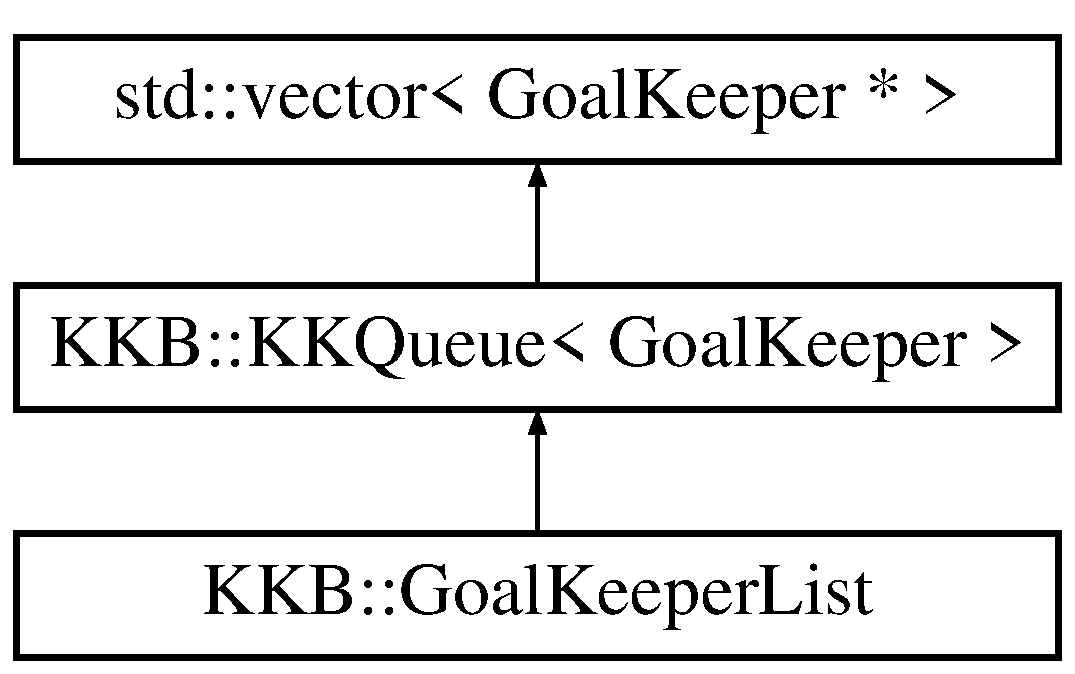
\includegraphics[height=3.000000cm]{class_k_k_b_1_1_goal_keeper_list}
\end{center}
\end{figure}
\subsection*{Public Member Functions}
\begin{DoxyCompactItemize}
\item 
\hyperlink{class_k_k_b_1_1_goal_keeper_list_a85429b40ed526098eef70a3170f7f022}{Goal\+Keeper\+List} (bool \+\_\+owner)
\item 
\hyperlink{class_k_k_b_1_1_goal_keeper_list_abd705644aad5fbd5fe742d0c1e0be92a}{$\sim$\+Goal\+Keeper\+List} ()
\end{DoxyCompactItemize}
\subsection*{Additional Inherited Members}


\subsection{Detailed Description}


Definition at line 195 of file Goal\+Keeper.\+h.



\subsection{Constructor \& Destructor Documentation}
\index{K\+K\+B\+::\+Goal\+Keeper\+List@{K\+K\+B\+::\+Goal\+Keeper\+List}!Goal\+Keeper\+List@{Goal\+Keeper\+List}}
\index{Goal\+Keeper\+List@{Goal\+Keeper\+List}!K\+K\+B\+::\+Goal\+Keeper\+List@{K\+K\+B\+::\+Goal\+Keeper\+List}}
\subsubsection[{\texorpdfstring{Goal\+Keeper\+List(bool \+\_\+owner)}{GoalKeeperList(bool _owner)}}]{\setlength{\rightskip}{0pt plus 5cm}K\+K\+B\+::\+Goal\+Keeper\+List\+::\+Goal\+Keeper\+List (
\begin{DoxyParamCaption}
\item[{bool}]{\+\_\+owner}
\end{DoxyParamCaption}
)\hspace{0.3cm}{\ttfamily [inline]}}\hypertarget{class_k_k_b_1_1_goal_keeper_list_a85429b40ed526098eef70a3170f7f022}{}\label{class_k_k_b_1_1_goal_keeper_list_a85429b40ed526098eef70a3170f7f022}


Definition at line 198 of file Goal\+Keeper.\+h.



Referenced by K\+K\+B\+::\+Goal\+Keeper\+::\+Create(), and K\+K\+B\+::\+Goal\+Keeper\+::\+Create\+And\+Start\+Block().


\begin{DoxyCode}
198 : KKQueue<GoalKeeper> (\_owner)  \{\}
\end{DoxyCode}
\index{K\+K\+B\+::\+Goal\+Keeper\+List@{K\+K\+B\+::\+Goal\+Keeper\+List}!````~Goal\+Keeper\+List@{$\sim$\+Goal\+Keeper\+List}}
\index{````~Goal\+Keeper\+List@{$\sim$\+Goal\+Keeper\+List}!K\+K\+B\+::\+Goal\+Keeper\+List@{K\+K\+B\+::\+Goal\+Keeper\+List}}
\subsubsection[{\texorpdfstring{$\sim$\+Goal\+Keeper\+List()}{~GoalKeeperList()}}]{\setlength{\rightskip}{0pt plus 5cm}K\+K\+B\+::\+Goal\+Keeper\+List\+::$\sim$\+Goal\+Keeper\+List (
\begin{DoxyParamCaption}
{}
\end{DoxyParamCaption}
)\hspace{0.3cm}{\ttfamily [inline]}}\hypertarget{class_k_k_b_1_1_goal_keeper_list_abd705644aad5fbd5fe742d0c1e0be92a}{}\label{class_k_k_b_1_1_goal_keeper_list_abd705644aad5fbd5fe742d0c1e0be92a}


Definition at line 200 of file Goal\+Keeper.\+h.


\begin{DoxyCode}
201     \{\}
\end{DoxyCode}


The documentation for this class was generated from the following file\+:\begin{DoxyCompactItemize}
\item 
C\+:/\+Users/\+Kurt/\+Git\+Hub/\+K\+Square\+Libraries/\+K\+K\+Base/\hyperlink{_goal_keeper_8h}{Goal\+Keeper.\+h}\end{DoxyCompactItemize}

\hypertarget{class_k_k_b_1_1_goal_keeper_simple}{}\section{K\+KB\+:\+:Goal\+Keeper\+Simple Class Reference}
\label{class_k_k_b_1_1_goal_keeper_simple}\index{K\+K\+B\+::\+Goal\+Keeper\+Simple@{K\+K\+B\+::\+Goal\+Keeper\+Simple}}


A simple/ light-\/weight implementation of critical section blocking.  




{\ttfamily \#include $<$Goal\+Keeper\+Simple.\+h$>$}

\subsection*{Public Types}
\begin{DoxyCompactItemize}
\item 
typedef \hyperlink{class_k_k_b_1_1_goal_keeper_simple}{Goal\+Keeper\+Simple} $\ast$ \hyperlink{class_k_k_b_1_1_goal_keeper_simple_a5e73be577d62a04e6980bb94027f653b}{Goal\+Keeper\+Simple\+Ptr}
\end{DoxyCompactItemize}
\subsection*{Public Member Functions}
\begin{DoxyCompactItemize}
\item 
bool \hyperlink{class_k_k_b_1_1_goal_keeper_simple_a51edc4dadfce50698b176d32de92bb6b}{Blocked} ()
\begin{DoxyCompactList}\small\item\em Will return true if any thread lock on this instance of \char`\"{}\+Goal\+Keeper\+Simple\char`\"{}. \end{DoxyCompactList}\item 
bool \hyperlink{class_k_k_b_1_1_goal_keeper_simple_ad6ccd73565c390cfca0a3b7f47be1c92}{Blocked\+By\+Another\+Thread} ()
\begin{DoxyCompactList}\small\item\em Returns true if a different thread has this instance of \char`\"{}\+Goal\+Keeper\+Simple\char`\"{} locked. \end{DoxyCompactList}\item 
\hyperlink{namespace_k_k_b_a8fa4952cc84fda1de4bec1fbdd8d5b1b}{kkint32} \hyperlink{class_k_k_b_1_1_goal_keeper_simple_a01d9c3b3552977dfbdd187112d89dc53}{Blocker\+Thread\+Id} ()
\begin{DoxyCompactList}\small\item\em Thread\+Id of thread that currently holds the Block -\/1 indicates no Block. \end{DoxyCompactList}\item 
void \hyperlink{class_k_k_b_1_1_goal_keeper_simple_a28a529882f7ace4f8300508d4dee9c3e}{End\+Block} ()
\begin{DoxyCompactList}\small\item\em Ends the block and allows other threads to pass through Stat\+Block. \end{DoxyCompactList}\item 
\hyperlink{namespace_k_k_b_a8fa4952cc84fda1de4bec1fbdd8d5b1b}{kkint32} \hyperlink{class_k_k_b_1_1_goal_keeper_simple_a89e05c58c7d851dc6ad858803c37309a}{Memory\+Consumed\+Estimated} () const 
\item 
const \hyperlink{class_k_k_b_1_1_k_k_str}{K\+K\+Str} \& \hyperlink{class_k_k_b_1_1_goal_keeper_simple_a13ef01792887b13a97315780f05fe319}{Name} () const 
\item 
void \hyperlink{class_k_k_b_1_1_goal_keeper_simple_aa8bcf9dcd7f07275aaac8ecdedac8cb1}{Start\+Block} ()
\begin{DoxyCompactList}\small\item\em Initiates a Block as long as another thread has not already locked this object. \end{DoxyCompactList}\end{DoxyCompactItemize}
\subsection*{Static Public Member Functions}
\begin{DoxyCompactItemize}
\item 
static void \hyperlink{class_k_k_b_1_1_goal_keeper_simple_a7001b3a689776a4ef2b56219f965b26c}{Create} (const \hyperlink{class_k_k_b_1_1_k_k_str}{K\+K\+Str} \&\+\_\+name, volatile \hyperlink{class_k_k_b_1_1_goal_keeper_simple_a5e73be577d62a04e6980bb94027f653b}{Goal\+Keeper\+Simple\+Ptr} \&\+\_\+new\+Goal\+Keeper)
\begin{DoxyCompactList}\small\item\em Create a \hyperlink{class_k_k_b_1_1_goal_keeper_simple}{Goal\+Keeper\+Simple} object and avoid a race condition doing it. \end{DoxyCompactList}\item 
static void \hyperlink{class_k_k_b_1_1_goal_keeper_simple_a3cdf495c3b29603a4434ad16a76bc049}{Create\+And\+Start\+Block} (const \hyperlink{class_k_k_b_1_1_k_k_str}{K\+K\+Str} \&\+\_\+name, volatile \hyperlink{class_k_k_b_1_1_goal_keeper_simple_a5e73be577d62a04e6980bb94027f653b}{Goal\+Keeper\+Simple\+Ptr} \&\+\_\+new\+Goal\+Keeper, bool \&\+\_\+did\+Not\+Exist\+Yet)
\begin{DoxyCompactList}\small\item\em Create a \hyperlink{class_k_k_b_1_1_goal_keeper_simple}{Goal\+Keeper\+Simple} object and avoid a race condition doing it. \end{DoxyCompactList}\item 
static void \hyperlink{class_k_k_b_1_1_goal_keeper_simple_aa1098674662d5e6a03fb4af27e1c5af5}{Destroy} (volatile \hyperlink{class_k_k_b_1_1_goal_keeper_simple_a5e73be577d62a04e6980bb94027f653b}{Goal\+Keeper\+Simple\+Ptr} \&\+\_\+goal\+Keeper\+Instance)
\begin{DoxyCompactList}\small\item\em Destroys an existing instance of \hyperlink{class_k_k_b_1_1_goal_keeper_simple}{Goal\+Keeper\+Simple}. \end{DoxyCompactList}\item 
static void \hyperlink{class_k_k_b_1_1_goal_keeper_simple_a8b38fb338438be5de8e2aaa2ac3b227d}{Final\+Clean\+Up} ()
\begin{DoxyCompactList}\small\item\em Will be registered with \textquotesingle{}atexit\textquotesingle{} so that it will be called when program is unloaded from memory. \end{DoxyCompactList}\end{DoxyCompactItemize}
\subsection*{Friends}
\begin{DoxyCompactItemize}
\item 
class \hyperlink{class_k_k_b_1_1_goal_keeper_simple_a3c22ebe8b841379f92ef7cdfe3aed61c}{K\+K\+Queue$<$ Goal\+Keeper\+Simple $>$}
\end{DoxyCompactItemize}


\subsection{Detailed Description}
A simple/ light-\/weight implementation of critical section blocking. 

Definition at line 29 of file Goal\+Keeper\+Simple.\+h.



\subsection{Member Typedef Documentation}
\index{K\+K\+B\+::\+Goal\+Keeper\+Simple@{K\+K\+B\+::\+Goal\+Keeper\+Simple}!Goal\+Keeper\+Simple\+Ptr@{Goal\+Keeper\+Simple\+Ptr}}
\index{Goal\+Keeper\+Simple\+Ptr@{Goal\+Keeper\+Simple\+Ptr}!K\+K\+B\+::\+Goal\+Keeper\+Simple@{K\+K\+B\+::\+Goal\+Keeper\+Simple}}
\subsubsection[{\texorpdfstring{Goal\+Keeper\+Simple\+Ptr}{GoalKeeperSimplePtr}}]{\setlength{\rightskip}{0pt plus 5cm}typedef {\bf Goal\+Keeper\+Simple}$\ast$ {\bf K\+K\+B\+::\+Goal\+Keeper\+Simple\+::\+Goal\+Keeper\+Simple\+Ptr}}\hypertarget{class_k_k_b_1_1_goal_keeper_simple_a5e73be577d62a04e6980bb94027f653b}{}\label{class_k_k_b_1_1_goal_keeper_simple_a5e73be577d62a04e6980bb94027f653b}


Definition at line 32 of file Goal\+Keeper\+Simple.\+h.



\subsection{Member Function Documentation}
\index{K\+K\+B\+::\+Goal\+Keeper\+Simple@{K\+K\+B\+::\+Goal\+Keeper\+Simple}!Blocked@{Blocked}}
\index{Blocked@{Blocked}!K\+K\+B\+::\+Goal\+Keeper\+Simple@{K\+K\+B\+::\+Goal\+Keeper\+Simple}}
\subsubsection[{\texorpdfstring{Blocked()}{Blocked()}}]{\setlength{\rightskip}{0pt plus 5cm}bool Goal\+Keeper\+Simple\+::\+Blocked (
\begin{DoxyParamCaption}
{}
\end{DoxyParamCaption}
)}\hypertarget{class_k_k_b_1_1_goal_keeper_simple_a51edc4dadfce50698b176d32de92bb6b}{}\label{class_k_k_b_1_1_goal_keeper_simple_a51edc4dadfce50698b176d32de92bb6b}


Will return true if any thread lock on this instance of \char`\"{}\+Goal\+Keeper\+Simple\char`\"{}. 



Definition at line 76 of file Goal\+Keeper\+Simple.\+cpp.


\begin{DoxyCode}
77 \{
78   \textcolor{keywordflow}{return}  blocked;
79 \}  \textcolor{comment}{/* Blocked */}
\end{DoxyCode}
\index{K\+K\+B\+::\+Goal\+Keeper\+Simple@{K\+K\+B\+::\+Goal\+Keeper\+Simple}!Blocked\+By\+Another\+Thread@{Blocked\+By\+Another\+Thread}}
\index{Blocked\+By\+Another\+Thread@{Blocked\+By\+Another\+Thread}!K\+K\+B\+::\+Goal\+Keeper\+Simple@{K\+K\+B\+::\+Goal\+Keeper\+Simple}}
\subsubsection[{\texorpdfstring{Blocked\+By\+Another\+Thread()}{BlockedByAnotherThread()}}]{\setlength{\rightskip}{0pt plus 5cm}bool Goal\+Keeper\+Simple\+::\+Blocked\+By\+Another\+Thread (
\begin{DoxyParamCaption}
{}
\end{DoxyParamCaption}
)}\hypertarget{class_k_k_b_1_1_goal_keeper_simple_ad6ccd73565c390cfca0a3b7f47be1c92}{}\label{class_k_k_b_1_1_goal_keeper_simple_ad6ccd73565c390cfca0a3b7f47be1c92}


Returns true if a different thread has this instance of \char`\"{}\+Goal\+Keeper\+Simple\char`\"{} locked. 

\hyperlink{class_k_k_b_1_1_goal_keeper_simple}{Goal\+Keeper\+Simple} keeps track of which thread has a lock on this instance of \textquotesingle{}\hyperlink{class_k_k_b_1_1_goal_keeper_simple}{Goal\+Keeper\+Simple}\textquotesingle{}. This way we know if the calling thread is not the one to have a lock on the thread. 

Definition at line 83 of file Goal\+Keeper\+Simple.\+cpp.



References K\+K\+B\+::os\+Get\+Thread\+Id().


\begin{DoxyCode}
84 \{
85   \textcolor{keywordflow}{if}  (!blocked)
86     \textcolor{keywordflow}{return} \textcolor{keyword}{false};
87 
88   \hyperlink{namespace_k_k_b_a8fa4952cc84fda1de4bec1fbdd8d5b1b}{kkint32}  curThreadId = \hyperlink{namespace_k_k_b_aa1d581b15163a41037c43bdbd800d0f8}{KKB::osGetThreadId} ();
89   \textcolor{keywordflow}{return}  (blocked  &&  (curThreadId != blockerThreadId));
90 \}
\end{DoxyCode}
\index{K\+K\+B\+::\+Goal\+Keeper\+Simple@{K\+K\+B\+::\+Goal\+Keeper\+Simple}!Blocker\+Thread\+Id@{Blocker\+Thread\+Id}}
\index{Blocker\+Thread\+Id@{Blocker\+Thread\+Id}!K\+K\+B\+::\+Goal\+Keeper\+Simple@{K\+K\+B\+::\+Goal\+Keeper\+Simple}}
\subsubsection[{\texorpdfstring{Blocker\+Thread\+Id()}{BlockerThreadId()}}]{\setlength{\rightskip}{0pt plus 5cm}{\bf kkint32} Goal\+Keeper\+Simple\+::\+Blocker\+Thread\+Id (
\begin{DoxyParamCaption}
{}
\end{DoxyParamCaption}
)}\hypertarget{class_k_k_b_1_1_goal_keeper_simple_a01d9c3b3552977dfbdd187112d89dc53}{}\label{class_k_k_b_1_1_goal_keeper_simple_a01d9c3b3552977dfbdd187112d89dc53}


Thread\+Id of thread that currently holds the Block -\/1 indicates no Block. 



Definition at line 404 of file Goal\+Keeper\+Simple.\+cpp.


\begin{DoxyCode}
405 \{
406   \hyperlink{namespace_k_k_b_a8fa4952cc84fda1de4bec1fbdd8d5b1b}{kkint32}  x = 0;
407   x =  blockerThreadId;
408   \textcolor{keywordflow}{return}  x;
409 \}
\end{DoxyCode}
\index{K\+K\+B\+::\+Goal\+Keeper\+Simple@{K\+K\+B\+::\+Goal\+Keeper\+Simple}!Create@{Create}}
\index{Create@{Create}!K\+K\+B\+::\+Goal\+Keeper\+Simple@{K\+K\+B\+::\+Goal\+Keeper\+Simple}}
\subsubsection[{\texorpdfstring{Create(const K\+K\+Str \&\+\_\+name, volatile Goal\+Keeper\+Simple\+Ptr \&\+\_\+new\+Goal\+Keeper)}{Create(const KKStr &_name, volatile GoalKeeperSimplePtr &_newGoalKeeper)}}]{\setlength{\rightskip}{0pt plus 5cm}void Goal\+Keeper\+Simple\+::\+Create (
\begin{DoxyParamCaption}
\item[{const {\bf K\+K\+Str} \&}]{\+\_\+name, }
\item[{volatile {\bf Goal\+Keeper\+Simple\+Ptr} \&}]{\+\_\+new\+Goal\+Keeper}
\end{DoxyParamCaption}
)\hspace{0.3cm}{\ttfamily [static]}}\hypertarget{class_k_k_b_1_1_goal_keeper_simple_a7001b3a689776a4ef2b56219f965b26c}{}\label{class_k_k_b_1_1_goal_keeper_simple_a7001b3a689776a4ef2b56219f965b26c}


Create a \hyperlink{class_k_k_b_1_1_goal_keeper_simple}{Goal\+Keeper\+Simple} object and avoid a race condition doing it. 

In case two different threads try to create the same \hyperlink{class_k_k_b_1_1_goal_keeper_simple}{Goal\+Keeper\+Simple} at the same time you only want one of them to succeed and the other to use same Gaol\+Keeper object. 
\begin{DoxyParams}[1]{Parameters}
\mbox{\tt in}  & {\em \+\_\+name} & Name of Goal Keeper object that you want to create. \\
\hline
\mbox{\tt in,out}  & {\em \+\_\+new\+Goal\+Keeper} & You pass this in. Create will block out the critical region that creates the \hyperlink{class_k_k_b_1_1_goal_keeper_simple}{Goal\+Keeper\+Simple} object. If it was already created, that is != N\+U\+LL will just return not changing its value. If it is still N\+U\+LL in the critical section it will create a new instance and set this parameter to its address. \\
\hline
\end{DoxyParams}
$<$ default security attributes

$<$ initially not owned 

Definition at line 160 of file Goal\+Keeper\+Simple.\+cpp.



References K\+K\+B\+::\+Goal\+Keeper\+Simple\+List\+::\+Goal\+Keeper\+Simple\+List().



Referenced by K\+K\+B\+::\+Msg\+Queue\+::\+Msg\+Queue().


\begin{DoxyCode}
163 \{
164 \textcolor{preprocessor}{#if  defined(WIN32)}
165   HANDLE  mutexCreateHandle = CreateMutex (NULL,                 \textcolor{comment}{/**< default security attributes */}
166                                            \textcolor{keyword}{false},                \textcolor{comment}{/**< initially not owned */}
167                                            \textcolor{stringliteral}{"GoalKeeperClass"}
168                                           );
169   \textcolor{keywordflow}{if}  (!mutexCreateHandle)
170   \{
171     \hyperlink{class_k_k_b_1_1_k_k_str}{KKStr} errMsg = \textcolor{stringliteral}{"GoalKeeperSimple::Create   ***ERROR***   CreateMutex failed; returned back NULL; 
       \_name:"} + \_name;
172     cerr << \hyperlink{namespace_k_k_b_ad1f50f65af6adc8fa9e6f62d007818a8}{endl} << errMsg << \hyperlink{namespace_k_k_b_ad1f50f65af6adc8fa9e6f62d007818a8}{endl} << \hyperlink{namespace_k_k_b_ad1f50f65af6adc8fa9e6f62d007818a8}{endl};
173     \textcolor{keywordflow}{throw} \hyperlink{class_k_k_b_1_1_k_k_exception}{KKException} (errMsg);
174   \}
175 
176   WaitForSingleObject (mutexCreateHandle, INFINITE);
177 
178   \textcolor{keywordflow}{if}  (\_newGoalKeeper == NULL)
179   \{
180     \_newGoalKeeper = \textcolor{keyword}{new} \hyperlink{class_k_k_b_1_1_goal_keeper_simple}{GoalKeeperSimple} (\_name);
181     \textcolor{keywordflow}{if}  (existingGoalKeepers == NULL)
182     \{
183       existingGoalKeepers = \textcolor{keyword}{new} \hyperlink{class_k_k_b_1_1_goal_keeper_simple_list}{GoalKeeperSimpleList} (\textcolor{keyword}{true});
184       atexit (\hyperlink{class_k_k_b_1_1_goal_keeper_simple_a8b38fb338438be5de8e2aaa2ac3b227d}{GoalKeeperSimple::FinalCleanUp});
185     \}
186     existingGoalKeepers->\hyperlink{class_k_k_b_1_1_k_k_queue_aa9fba4632b54268bf71ecb42dee0b575}{PushOnBack} (\_newGoalKeeper);
187   \}
188 
189   ReleaseMutex (mutexCreateHandle);
190   CloseHandle(mutexCreateHandle);
191 \textcolor{preprocessor}{#else}
192   sem\_t*  semHandle = sem\_open (\textcolor{stringliteral}{"GoalKeeperClass"}, O\_CREAT, 0644, 1);
193   \textcolor{keywordflow}{if}  (semHandle == SEM\_FAILED)
194   \{
195     cout << \hyperlink{namespace_k_k_b_ad1f50f65af6adc8fa9e6f62d007818a8}{std::endl}
196          << \textcolor{stringliteral}{"GoalKeeperSimple::Create  Error["} << errno << \textcolor{stringliteral}{"] opening '/GoalKeeperSimple' Semaphore."} << 
      \hyperlink{namespace_k_k_b_ad1f50f65af6adc8fa9e6f62d007818a8}{std::endl}
197          << \hyperlink{namespace_k_k_b_ad1f50f65af6adc8fa9e6f62d007818a8}{std::endl};
198 
199     perror(\textcolor{stringliteral}{"GoalKeeperSimple::Create   Error Opening Semaphore  'GoalKeeperSimple'"});
200 
201     \textcolor{keywordflow}{throw} \textcolor{stringliteral}{"GoalKeeperSimple::Create    Error opening 'GoalKeeperSimple'."};
202   \}
203 
204   sem\_wait (semHandle);
205 
206   \textcolor{keywordflow}{if}  (\_newGoalKeeper == NULL)
207   \{
208     \_newGoalKeeper = \textcolor{keyword}{new} \hyperlink{class_k_k_b_1_1_goal_keeper_simple}{GoalKeeperSimple} (\_name);
209     \textcolor{keywordflow}{if}  (existingGoalKeepers == NULL)
210     \{
211       existingGoalKeepers = \textcolor{keyword}{new} \hyperlink{class_k_k_b_1_1_goal_keeper_simple_list}{GoalKeeperSimpleList} (\textcolor{keyword}{true});
212       atexit (\hyperlink{class_k_k_b_1_1_goal_keeper_simple_a8b38fb338438be5de8e2aaa2ac3b227d}{GoalKeeperSimple::FinalCleanUp});
213     \}
214     existingGoalKeepers->\hyperlink{class_k_k_b_1_1_k_k_queue_aa9fba4632b54268bf71ecb42dee0b575}{PushOnBack} (\_newGoalKeeper);
215   \}
216 
217   sem\_post (semHandle);
218   sem\_close (semHandle);
219 \textcolor{preprocessor}{#endif}
220 \}  \textcolor{comment}{/* Create */}
\end{DoxyCode}
\index{K\+K\+B\+::\+Goal\+Keeper\+Simple@{K\+K\+B\+::\+Goal\+Keeper\+Simple}!Create\+And\+Start\+Block@{Create\+And\+Start\+Block}}
\index{Create\+And\+Start\+Block@{Create\+And\+Start\+Block}!K\+K\+B\+::\+Goal\+Keeper\+Simple@{K\+K\+B\+::\+Goal\+Keeper\+Simple}}
\subsubsection[{\texorpdfstring{Create\+And\+Start\+Block(const K\+K\+Str \&\+\_\+name, volatile Goal\+Keeper\+Simple\+Ptr \&\+\_\+new\+Goal\+Keeper, bool \&\+\_\+did\+Not\+Exist\+Yet)}{CreateAndStartBlock(const KKStr &_name, volatile GoalKeeperSimplePtr &_newGoalKeeper, bool &_didNotExistYet)}}]{\setlength{\rightskip}{0pt plus 5cm}void Goal\+Keeper\+Simple\+::\+Create\+And\+Start\+Block (
\begin{DoxyParamCaption}
\item[{const {\bf K\+K\+Str} \&}]{\+\_\+name, }
\item[{volatile {\bf Goal\+Keeper\+Simple\+Ptr} \&}]{\+\_\+new\+Goal\+Keeper, }
\item[{bool \&}]{\+\_\+did\+Not\+Exist\+Yet}
\end{DoxyParamCaption}
)\hspace{0.3cm}{\ttfamily [static]}}\hypertarget{class_k_k_b_1_1_goal_keeper_simple_a3cdf495c3b29603a4434ad16a76bc049}{}\label{class_k_k_b_1_1_goal_keeper_simple_a3cdf495c3b29603a4434ad16a76bc049}


Create a \hyperlink{class_k_k_b_1_1_goal_keeper_simple}{Goal\+Keeper\+Simple} object and avoid a race condition doing it. 

Create a new instance of a \hyperlink{class_k_k_b_1_1_goal_keeper_simple}{Goal\+Keeper\+Simple} object if it has not already been done and locks it if we create it.

Similar to \textquotesingle{}Create\textquotesingle{} except it will also call the Start\+Block method. There is also an additional parameter that will let you know if your call was responsible for creating it.

In case two different threads try to create the same \hyperlink{class_k_k_b_1_1_goal_keeper_simple}{Goal\+Keeper\+Simple} at the same time you only want one of them to succeed and the other to use same Gaol\+Keeper object. 
\begin{DoxyParams}[1]{Parameters}
\mbox{\tt in}  & {\em \+\_\+name} & Name of Goal Keeper object that you want to create.\\
\hline
\mbox{\tt in,out}  & {\em \+\_\+new\+Goal\+Keeper} & You pass this in. Create will block out the critical region that creates the \hyperlink{class_k_k_b_1_1_goal_keeper_simple}{Goal\+Keeper\+Simple} object. If it was already created, that is != N\+U\+LL will just return not changing its value. If it is still N\+U\+LL in the critical section it will create a new instance and set this parameter to its address.\\
\hline
\mbox{\tt out}  & {\em \+\_\+did\+Not\+Exist\+Yet} & Indicates if this call had to create the \hyperlink{class_k_k_b_1_1_goal_keeper_simple}{Goal\+Keeper\+Simple} instance; if it already existed will return as false.\\
\hline
\mbox{\tt in}  & {\em \+\_\+name} & Name to be assigned to \hyperlink{class_k_k_b_1_1_goal_keeper_simple}{Goal\+Keeper\+Simple} object. \\
\hline
\mbox{\tt in,out}  & {\em \+\_\+new\+Goal\+Keeper} & A pointer to the \hyperlink{class_k_k_b_1_1_goal_keeper_simple}{Goal\+Keeper\+Simple} that already exists or to new one that got created. \\
\hline
\mbox{\tt out}  & {\em \+\_\+did\+Not\+Exist\+Yet} & Indicates if the call to \textquotesingle{}Create\+And\+Start\+Block\textquotesingle{} had to create a new instance. \\
\hline
\end{DoxyParams}
$<$ default security attributes.

$<$ initially not owned. 

Definition at line 231 of file Goal\+Keeper\+Simple.\+cpp.



References K\+K\+B\+::\+Goal\+Keeper\+Simple\+List\+::\+Goal\+Keeper\+Simple\+List(), and Start\+Block().


\begin{DoxyCode}
235 \{
236 \textcolor{preprocessor}{#if  defined(WIN32)}
237   HANDLE  mutexCreateHandle = CreateMutex (NULL,                 \textcolor{comment}{/**< default security attributes. */}
238                                            \textcolor{keyword}{false},                \textcolor{comment}{/**< initially not owned.         */}
239                                            \textcolor{stringliteral}{"GoalKeeperClass"}
240                                           ); 
241   \textcolor{keywordflow}{if}  (!mutexCreateHandle)
242   \{
243     \hyperlink{class_k_k_b_1_1_k_k_str}{KKStr} errMsg = \textcolor{stringliteral}{"GoalKeeperSimple::CreateAndStartBlock   ***ERROR***   CreateMutex failed; returned
       back NULL;  \_name:"} + \_name;
244     cerr << \hyperlink{namespace_k_k_b_ad1f50f65af6adc8fa9e6f62d007818a8}{endl} << errMsg << \hyperlink{namespace_k_k_b_ad1f50f65af6adc8fa9e6f62d007818a8}{endl} << \hyperlink{namespace_k_k_b_ad1f50f65af6adc8fa9e6f62d007818a8}{endl};
245     \textcolor{keywordflow}{throw} \hyperlink{class_k_k_b_1_1_k_k_exception}{KKException}(errMsg);
246   \}
247 
248   WaitForSingleObject (mutexCreateHandle, INFINITE);
249 
250   \textcolor{keywordflow}{if}  (\_newGoalKeeper == NULL)
251   \{
252     \_didNotExistYet = \textcolor{keyword}{true};
253     \_newGoalKeeper = \textcolor{keyword}{new} \hyperlink{class_k_k_b_1_1_goal_keeper_simple}{GoalKeeperSimple} (\_name);
254 
255     \textcolor{keywordflow}{if}  (existingGoalKeepers == NULL)
256     \{
257       existingGoalKeepers = \textcolor{keyword}{new} \hyperlink{class_k_k_b_1_1_goal_keeper_simple_list}{GoalKeeperSimpleList} (\textcolor{keyword}{true});
258       atexit (\hyperlink{class_k_k_b_1_1_goal_keeper_simple_a8b38fb338438be5de8e2aaa2ac3b227d}{GoalKeeperSimple::FinalCleanUp});
259     \}
260     existingGoalKeepers->\hyperlink{class_k_k_b_1_1_k_k_queue_aa9fba4632b54268bf71ecb42dee0b575}{PushOnBack} (\_newGoalKeeper);
261   \}
262   \textcolor{keywordflow}{else}
263   \{
264     \_didNotExistYet = \textcolor{keyword}{false};
265   \}
266 
267   \_newGoalKeeper->StartBlock ();
268 
269   ReleaseMutex (mutexCreateHandle);
270   CloseHandle(mutexCreateHandle);
271 \textcolor{preprocessor}{#else}
272   sem\_t*  semHandle = sem\_open (\textcolor{stringliteral}{"GoalKeeperClass"}, O\_CREAT, 0644, 1);
273   \textcolor{keywordflow}{if}  (semHandle == SEM\_FAILED)
274   \{
275     cout << \hyperlink{namespace_k_k_b_ad1f50f65af6adc8fa9e6f62d007818a8}{std::endl}
276          << \textcolor{stringliteral}{"GoalKeeperSimple::Create  Error["} << errno << \textcolor{stringliteral}{"] opening '/GoalKeeperSimple' Semaphore."} << 
      \hyperlink{namespace_k_k_b_ad1f50f65af6adc8fa9e6f62d007818a8}{std::endl}
277          << \hyperlink{namespace_k_k_b_ad1f50f65af6adc8fa9e6f62d007818a8}{std::endl};
278 
279     perror(\textcolor{stringliteral}{"GoalKeeperSimple::Create   Error Opening Semaphore  'GoalKeeperSimple'"});
280 
281     \textcolor{keywordflow}{throw} \textcolor{stringliteral}{"GoalKeeperSimple::Create    Error opening 'GoalKeeperSimple'."};
282   \}
283 
284   sem\_wait (semHandle);
285 
286   \textcolor{keywordflow}{if}  (\_newGoalKeeper == NULL)
287   \{
288     \_didNotExistYet = \textcolor{keyword}{true};
289     \_newGoalKeeper = \textcolor{keyword}{new} \hyperlink{class_k_k_b_1_1_goal_keeper_simple}{GoalKeeperSimple} (\_name);
290     \textcolor{keywordflow}{if}  (existingGoalKeepers == NULL)
291     \{
292       existingGoalKeepers = \textcolor{keyword}{new} \hyperlink{class_k_k_b_1_1_goal_keeper_simple_list}{GoalKeeperSimpleList} (\textcolor{keyword}{true});
293       atexit (\hyperlink{class_k_k_b_1_1_goal_keeper_simple_a8b38fb338438be5de8e2aaa2ac3b227d}{GoalKeeperSimple::FinalCleanUp});
294     \}
295     existingGoalKeepers->\hyperlink{class_k_k_b_1_1_k_k_queue_aa9fba4632b54268bf71ecb42dee0b575}{PushOnBack} (\_newGoalKeeper);
296   \}
297   \textcolor{keywordflow}{else}
298   \{
299     \_didNotExistYet = \textcolor{keyword}{false};
300   \}
301 
302   \_newGoalKeeper->StartBlock ();
303 
304   sem\_post (semHandle);
305   sem\_close (semHandle);
306 \textcolor{preprocessor}{#endif}
307 \}  \textcolor{comment}{/* CreateAndStartBlock */}
\end{DoxyCode}
\index{K\+K\+B\+::\+Goal\+Keeper\+Simple@{K\+K\+B\+::\+Goal\+Keeper\+Simple}!Destroy@{Destroy}}
\index{Destroy@{Destroy}!K\+K\+B\+::\+Goal\+Keeper\+Simple@{K\+K\+B\+::\+Goal\+Keeper\+Simple}}
\subsubsection[{\texorpdfstring{Destroy(volatile Goal\+Keeper\+Simple\+Ptr \&\+\_\+goal\+Keeper\+Instance)}{Destroy(volatile GoalKeeperSimplePtr &_goalKeeperInstance)}}]{\setlength{\rightskip}{0pt plus 5cm}void Goal\+Keeper\+Simple\+::\+Destroy (
\begin{DoxyParamCaption}
\item[{volatile {\bf Goal\+Keeper\+Simple\+Ptr} \&}]{\+\_\+goal\+Keeper\+Instance}
\end{DoxyParamCaption}
)\hspace{0.3cm}{\ttfamily [static]}}\hypertarget{class_k_k_b_1_1_goal_keeper_simple_aa1098674662d5e6a03fb4af27e1c5af5}{}\label{class_k_k_b_1_1_goal_keeper_simple_aa1098674662d5e6a03fb4af27e1c5af5}


Destroys an existing instance of \hyperlink{class_k_k_b_1_1_goal_keeper_simple}{Goal\+Keeper\+Simple}. 

Use this method rather than calling the destructor directly. This way the \textquotesingle{}existing\+Goal\+Keepers\textquotesingle{} data member can be kept up to date. If for some reason two different threads managed to call this method for the same \hyperlink{class_k_k_b_1_1_goal_keeper_simple}{Goal\+Keeper\+Simple} instance only one of them will actually destroy the instance. 
\begin{DoxyParams}[1]{Parameters}
\mbox{\tt in,out}  & {\em \+\_\+goal\+Keeper\+Instance} & Instance of \hyperlink{class_k_k_b_1_1_goal_keeper_simple}{Goal\+Keeper\+Simple} that is to be destroyed. Upon return it will be set to N\+U\+LL. \\
\hline
\end{DoxyParams}
$<$ default security attributes

$<$ initially not owned 

Definition at line 313 of file Goal\+Keeper\+Simple.\+cpp.



Referenced by K\+K\+B\+::\+Msg\+Queue\+::$\sim$\+Msg\+Queue().


\begin{DoxyCode}
314 \{
315 \textcolor{preprocessor}{#if  defined(WIN32)}
316   HANDLE  mutexCreateHandle = CreateMutex (NULL,                 \textcolor{comment}{/**< default security attributes */}
317                                            \textcolor{keyword}{false},                \textcolor{comment}{/**< initially not owned */}
318                                            \textcolor{stringliteral}{"GoalKeeperClass"}
319                                           ); 
320   \textcolor{keywordflow}{if} (!mutexCreateHandle)
321   \{
322     \hyperlink{class_k_k_b_1_1_k_k_str}{KKStr} errMsg = \textcolor{stringliteral}{"GoalKeeperSimple::Destroy   ***ERROR***   CreateMutex failed; returned back NULL"};
323     cerr << \hyperlink{namespace_k_k_b_ad1f50f65af6adc8fa9e6f62d007818a8}{endl} << errMsg << \hyperlink{namespace_k_k_b_ad1f50f65af6adc8fa9e6f62d007818a8}{endl} << \hyperlink{namespace_k_k_b_ad1f50f65af6adc8fa9e6f62d007818a8}{endl};
324     \textcolor{keywordflow}{throw} \hyperlink{class_k_k_b_1_1_k_k_exception}{KKException}(errMsg);
325   \}
326 
327   WaitForSingleObject (mutexCreateHandle, INFINITE);
328 
329   \textcolor{keywordflow}{if}  (\_goalKeeperInstance == NULL)
330   \{
331     \textcolor{comment}{// Some other thread managed to destroy this instance.}
332   \}
333   \textcolor{keywordflow}{else}
334   \{
335     \hyperlink{namespace_k_k_b_a8fa4952cc84fda1de4bec1fbdd8d5b1b}{kkint32}  existingInstanceIdx =  existingGoalKeepers->\hyperlink{class_k_k_b_1_1_k_k_queue_ac7c26abdf599669a4b0898534f735f99}{PtrToIdx} (\_goalKeeperInstance);
336     \textcolor{keywordflow}{if}  (existingInstanceIdx < 0)
337     \{
338       \textcolor{comment}{// If not in list then a  different thread beat us to destroying this instance or it was never
       created to start with.}
339     \}
340     \textcolor{keywordflow}{else}
341     \{
342       existingGoalKeepers->\hyperlink{class_k_k_b_1_1_k_k_queue_ae362e3b0a128e8a09182e167befda088}{DeleteEntry} (\_goalKeeperInstance);
343       \textcolor{keyword}{delete}  \_goalKeeperInstance;
344       \_goalKeeperInstance = NULL;
345     \}
346   \}
347 
348   ReleaseMutex (mutexCreateHandle);
349   CloseHandle(mutexCreateHandle);
350 \textcolor{preprocessor}{#else}
351   sem\_t*  semHandle = sem\_open (\textcolor{stringliteral}{"GoalKeeperClass"}, O\_CREAT, 0644, 1);
352   \textcolor{keywordflow}{if}  (semHandle == SEM\_FAILED)
353   \{
354     cout << \hyperlink{namespace_k_k_b_ad1f50f65af6adc8fa9e6f62d007818a8}{std::endl}
355          << \textcolor{stringliteral}{"GoalKeeperSimple::Create  Error["} << errno << \textcolor{stringliteral}{"] opening '/GoalKeeperSimple' Semaphore."} << 
      \hyperlink{namespace_k_k_b_ad1f50f65af6adc8fa9e6f62d007818a8}{std::endl}
356          << \hyperlink{namespace_k_k_b_ad1f50f65af6adc8fa9e6f62d007818a8}{std::endl};
357 
358     perror(\textcolor{stringliteral}{"GoalKeeperSimple::Create   Error Opening Semaphore  'GoalKeeperSimple'"});
359 
360     \textcolor{keywordflow}{throw} \textcolor{stringliteral}{"GoalKeeperSimple::Create    Error opening 'GoalKeeperSimple'."};
361   \}
362 
363   sem\_wait (semHandle);
364 
365   \textcolor{keywordflow}{if}  (\_goalKeeperInstance == NULL)
366   \{
367     \textcolor{comment}{// Some other thread managed to destroy this instance.}
368   \}
369   \textcolor{keywordflow}{else}
370   \{
371     \hyperlink{namespace_k_k_b_a8fa4952cc84fda1de4bec1fbdd8d5b1b}{kkint32}  existingInstanceIdx =  existingGoalKeepers->\hyperlink{class_k_k_b_1_1_k_k_queue_ac7c26abdf599669a4b0898534f735f99}{PtrToIdx} (\_goalKeeperInstance);
372     \textcolor{keywordflow}{if}  (existingInstanceIdx >= 0)
373     \{
374       \textcolor{comment}{// If not in list then a  different thread beat us to destroying this instance or it was never
       created to start with.}
375     \}
376     \textcolor{keywordflow}{else}
377     \{
378       existingGoalKeepers->\hyperlink{class_k_k_b_1_1_k_k_queue_ae362e3b0a128e8a09182e167befda088}{DeleteEntry} (\_goalKeeperInstance);
379       \textcolor{keyword}{delete}  \_goalKeeperInstance;
380       \_goalKeeperInstance = NULL;
381     \}
382   \}
383 
384   sem\_post (semHandle);
385   sem\_close (semHandle);
386 \textcolor{preprocessor}{#endif}
387 
388 \}  \textcolor{comment}{/* Destroy */}
\end{DoxyCode}
\index{K\+K\+B\+::\+Goal\+Keeper\+Simple@{K\+K\+B\+::\+Goal\+Keeper\+Simple}!End\+Block@{End\+Block}}
\index{End\+Block@{End\+Block}!K\+K\+B\+::\+Goal\+Keeper\+Simple@{K\+K\+B\+::\+Goal\+Keeper\+Simple}}
\subsubsection[{\texorpdfstring{End\+Block()}{EndBlock()}}]{\setlength{\rightskip}{0pt plus 5cm}void Goal\+Keeper\+Simple\+::\+End\+Block (
\begin{DoxyParamCaption}
{}
\end{DoxyParamCaption}
)}\hypertarget{class_k_k_b_1_1_goal_keeper_simple_a28a529882f7ace4f8300508d4dee9c3e}{}\label{class_k_k_b_1_1_goal_keeper_simple_a28a529882f7ace4f8300508d4dee9c3e}


Ends the block and allows other threads to pass through Stat\+Block. 

Decrements the variable \textquotesingle{}blocker\+Depth\textquotesingle{} by one. Once \textquotesingle{}blocker\+Depth\textquotesingle{} is equal zero the Block on this instance is removed. The idea is that for each time in a row a Thread calls Start\+Block it has to call End\+Block the same number of times. 

Definition at line 139 of file Goal\+Keeper\+Simple.\+cpp.



References K\+K\+B\+::\+K\+K\+Exception\+::\+K\+K\+Exception(), K\+K\+B\+::\+K\+K\+Str\+::operator+(), K\+K\+B\+::operator+(), and K\+K\+B\+::os\+Get\+Thread\+Id().



Referenced by K\+K\+B\+::\+Msg\+Queue\+::\+Add\+Msg(), K\+K\+B\+::\+Msg\+Queue\+::\+Add\+Msgs(), K\+K\+B\+::\+Msg\+Queue\+::\+Get\+All\+Msgs(), K\+K\+B\+::\+Msg\+Queue\+::\+Get\+Copy\+Of\+Last\+Msg(), K\+K\+B\+::\+Msg\+Queue\+::\+Get\+Next\+Msg(), and K\+K\+B\+::\+Msg\+Queue\+::\+Memory\+Consumed\+Estimated().


\begin{DoxyCode}
140 \{
141   \hyperlink{namespace_k_k_b_a8fa4952cc84fda1de4bec1fbdd8d5b1b}{kkint32}  curThreadId = \hyperlink{namespace_k_k_b_aa1d581b15163a41037c43bdbd800d0f8}{KKB::osGetThreadId} ();
142   \textcolor{keywordflow}{if}  (!blocked)
143     \textcolor{keywordflow}{throw} \hyperlink{class_k_k_b_1_1_k_k_exception}{KKB::KKException} (\textcolor{stringliteral}{"GoalKeeperSimple::EndBlock    Name["} + name + \textcolor{stringliteral}{"]  Is not
       currently blocked."});
144 
145   \textcolor{keywordflow}{if}  (curThreadId != blockerThreadId)
146     \textcolor{keywordflow}{throw} \hyperlink{class_k_k_b_1_1_k_k_exception}{KKB::KKException} (\textcolor{stringliteral}{"GoalKeeperSimple::EndBlock    Name["} + name + \textcolor{stringliteral}{"]  ThreadId["} +
       blockerThreadId + \textcolor{stringliteral}{"] Currently holds Block;  our ThreadId["} + curThreadId + \textcolor{stringliteral}{"]"});
147 
148   --levels;
149   \textcolor{keywordflow}{if}  (levels < 1)
150   \{
151     blocked = \textcolor{keyword}{false};
152     blockerThreadId = -1;
153     CriticalSectionEnd ();
154   \}
155 \}  \textcolor{comment}{/* EndBlock */}
\end{DoxyCode}
\index{K\+K\+B\+::\+Goal\+Keeper\+Simple@{K\+K\+B\+::\+Goal\+Keeper\+Simple}!Final\+Clean\+Up@{Final\+Clean\+Up}}
\index{Final\+Clean\+Up@{Final\+Clean\+Up}!K\+K\+B\+::\+Goal\+Keeper\+Simple@{K\+K\+B\+::\+Goal\+Keeper\+Simple}}
\subsubsection[{\texorpdfstring{Final\+Clean\+Up()}{FinalCleanUp()}}]{\setlength{\rightskip}{0pt plus 5cm}void Goal\+Keeper\+Simple\+::\+Final\+Clean\+Up (
\begin{DoxyParamCaption}
{}
\end{DoxyParamCaption}
)\hspace{0.3cm}{\ttfamily [static]}}\hypertarget{class_k_k_b_1_1_goal_keeper_simple_a8b38fb338438be5de8e2aaa2ac3b227d}{}\label{class_k_k_b_1_1_goal_keeper_simple_a8b38fb338438be5de8e2aaa2ac3b227d}


Will be registered with \textquotesingle{}atexit\textquotesingle{} so that it will be called when program is unloaded from memory. 



Definition at line 392 of file Goal\+Keeper\+Simple.\+cpp.


\begin{DoxyCode}
393 \{
394   \textcolor{keywordflow}{if}  (existingGoalKeepers)
395   \{
396     \textcolor{keyword}{delete}  existingGoalKeepers;
397     existingGoalKeepers = NULL;
398   \}
399 \}
\end{DoxyCode}
\index{K\+K\+B\+::\+Goal\+Keeper\+Simple@{K\+K\+B\+::\+Goal\+Keeper\+Simple}!Memory\+Consumed\+Estimated@{Memory\+Consumed\+Estimated}}
\index{Memory\+Consumed\+Estimated@{Memory\+Consumed\+Estimated}!K\+K\+B\+::\+Goal\+Keeper\+Simple@{K\+K\+B\+::\+Goal\+Keeper\+Simple}}
\subsubsection[{\texorpdfstring{Memory\+Consumed\+Estimated() const }{MemoryConsumedEstimated() const }}]{\setlength{\rightskip}{0pt plus 5cm}{\bf kkint32} Goal\+Keeper\+Simple\+::\+Memory\+Consumed\+Estimated (
\begin{DoxyParamCaption}
{}
\end{DoxyParamCaption}
) const}\hypertarget{class_k_k_b_1_1_goal_keeper_simple_a89e05c58c7d851dc6ad858803c37309a}{}\label{class_k_k_b_1_1_goal_keeper_simple_a89e05c58c7d851dc6ad858803c37309a}


Definition at line 69 of file Goal\+Keeper\+Simple.\+cpp.



References K\+K\+B\+::\+K\+K\+Str\+::\+Memory\+Consumed\+Estimated().



Referenced by K\+K\+B\+::\+Msg\+Queue\+::\+Msg\+Queue().


\begin{DoxyCode}
70 \{
71   \textcolor{keywordflow}{return}  (\textcolor{keyword}{sizeof} (\hyperlink{class_k_k_b_1_1_goal_keeper_simple}{GoalKeeperSimple}) + name.
      \hyperlink{class_k_k_b_1_1_k_k_str_afc335bf98a8d4a77dc34215e72068719}{MemoryConsumedEstimated} ());
72 \}
\end{DoxyCode}
\index{K\+K\+B\+::\+Goal\+Keeper\+Simple@{K\+K\+B\+::\+Goal\+Keeper\+Simple}!Name@{Name}}
\index{Name@{Name}!K\+K\+B\+::\+Goal\+Keeper\+Simple@{K\+K\+B\+::\+Goal\+Keeper\+Simple}}
\subsubsection[{\texorpdfstring{Name() const }{Name() const }}]{\setlength{\rightskip}{0pt plus 5cm}const {\bf K\+K\+Str}\& K\+K\+B\+::\+Goal\+Keeper\+Simple\+::\+Name (
\begin{DoxyParamCaption}
{}
\end{DoxyParamCaption}
) const\hspace{0.3cm}{\ttfamily [inline]}}\hypertarget{class_k_k_b_1_1_goal_keeper_simple_a13ef01792887b13a97315780f05fe319}{}\label{class_k_k_b_1_1_goal_keeper_simple_a13ef01792887b13a97315780f05fe319}


Definition at line 122 of file Goal\+Keeper\+Simple.\+h.


\begin{DoxyCode}
122 \{\textcolor{keywordflow}{return}  name;\}
\end{DoxyCode}
\index{K\+K\+B\+::\+Goal\+Keeper\+Simple@{K\+K\+B\+::\+Goal\+Keeper\+Simple}!Start\+Block@{Start\+Block}}
\index{Start\+Block@{Start\+Block}!K\+K\+B\+::\+Goal\+Keeper\+Simple@{K\+K\+B\+::\+Goal\+Keeper\+Simple}}
\subsubsection[{\texorpdfstring{Start\+Block()}{StartBlock()}}]{\setlength{\rightskip}{0pt plus 5cm}void Goal\+Keeper\+Simple\+::\+Start\+Block (
\begin{DoxyParamCaption}
{}
\end{DoxyParamCaption}
)}\hypertarget{class_k_k_b_1_1_goal_keeper_simple_aa8bcf9dcd7f07275aaac8ecdedac8cb1}{}\label{class_k_k_b_1_1_goal_keeper_simple_aa8bcf9dcd7f07275aaac8ecdedac8cb1}


Initiates a Block as long as another thread has not already locked this object. 

If it is already blocked processor will sleep and then try again. As long as the variable \textquotesingle{}blocker\+Depth\textquotesingle{}is greater than zero this instance will be considered blocked. Once a thread has the instance blocked it will increment \textquotesingle{}blocker\+Depth\textquotesingle{} and return to caller. 

Definition at line 117 of file Goal\+Keeper\+Simple.\+cpp.



References K\+K\+B\+::os\+Get\+Thread\+Id().



Referenced by K\+K\+B\+::\+Msg\+Queue\+::\+Add\+Msg(), K\+K\+B\+::\+Msg\+Queue\+::\+Add\+Msgs(), Create\+And\+Start\+Block(), K\+K\+B\+::\+Msg\+Queue\+::\+Get\+All\+Msgs(), K\+K\+B\+::\+Msg\+Queue\+::\+Get\+Copy\+Of\+Last\+Msg(), K\+K\+B\+::\+Msg\+Queue\+::\+Get\+Next\+Msg(), and K\+K\+B\+::\+Msg\+Queue\+::\+Memory\+Consumed\+Estimated().


\begin{DoxyCode}
118 \{
119   \hyperlink{namespace_k_k_b_a8fa4952cc84fda1de4bec1fbdd8d5b1b}{kkint32}  curThreadId = \hyperlink{namespace_k_k_b_aa1d581b15163a41037c43bdbd800d0f8}{KKB::osGetThreadId} ();
120 
121   \textcolor{keywordflow}{if}  (blocked  &&  (curThreadId == blockerThreadId))
122   \{
123     ++levels;
124   \}
125   \textcolor{keywordflow}{else}
126   \{
127     CriticalSectionStart ();
128     levels = 1;
129     blockerThreadId = curThreadId;
130     blocked = \textcolor{keyword}{true};
131   \}
132 
133   \textcolor{keywordflow}{return};
134 \}   \textcolor{comment}{/* StartBlock */}
\end{DoxyCode}


\subsection{Friends And Related Function Documentation}
\index{K\+K\+B\+::\+Goal\+Keeper\+Simple@{K\+K\+B\+::\+Goal\+Keeper\+Simple}!K\+K\+Queue$<$ Goal\+Keeper\+Simple $>$@{K\+K\+Queue$<$ Goal\+Keeper\+Simple $>$}}
\index{K\+K\+Queue$<$ Goal\+Keeper\+Simple $>$@{K\+K\+Queue$<$ Goal\+Keeper\+Simple $>$}!K\+K\+B\+::\+Goal\+Keeper\+Simple@{K\+K\+B\+::\+Goal\+Keeper\+Simple}}
\subsubsection[{\texorpdfstring{K\+K\+Queue$<$ Goal\+Keeper\+Simple $>$}{KKQueue< GoalKeeperSimple >}}]{\setlength{\rightskip}{0pt plus 5cm}friend class {\bf K\+K\+Queue}$<$ {\bf Goal\+Keeper\+Simple} $>$\hspace{0.3cm}{\ttfamily [friend]}}\hypertarget{class_k_k_b_1_1_goal_keeper_simple_a3c22ebe8b841379f92ef7cdfe3aed61c}{}\label{class_k_k_b_1_1_goal_keeper_simple_a3c22ebe8b841379f92ef7cdfe3aed61c}


Definition at line 41 of file Goal\+Keeper\+Simple.\+h.



The documentation for this class was generated from the following files\+:\begin{DoxyCompactItemize}
\item 
C\+:/\+Users/\+Kurt/\+Git\+Hub/\+K\+Square\+Libraries/\+K\+K\+Base/\hyperlink{_goal_keeper_simple_8h}{Goal\+Keeper\+Simple.\+h}\item 
C\+:/\+Users/\+Kurt/\+Git\+Hub/\+K\+Square\+Libraries/\+K\+K\+Base/\hyperlink{_goal_keeper_simple_8cpp}{Goal\+Keeper\+Simple.\+cpp}\end{DoxyCompactItemize}

\hypertarget{class_k_k_b_1_1_goal_keeper_simple_list}{}\section{K\+KB\+:\+:Goal\+Keeper\+Simple\+List Class Reference}
\label{class_k_k_b_1_1_goal_keeper_simple_list}\index{K\+K\+B\+::\+Goal\+Keeper\+Simple\+List@{K\+K\+B\+::\+Goal\+Keeper\+Simple\+List}}


{\ttfamily \#include $<$Goal\+Keeper\+Simple.\+h$>$}

Inheritance diagram for K\+KB\+:\+:Goal\+Keeper\+Simple\+List\+:\begin{figure}[H]
\begin{center}
\leavevmode
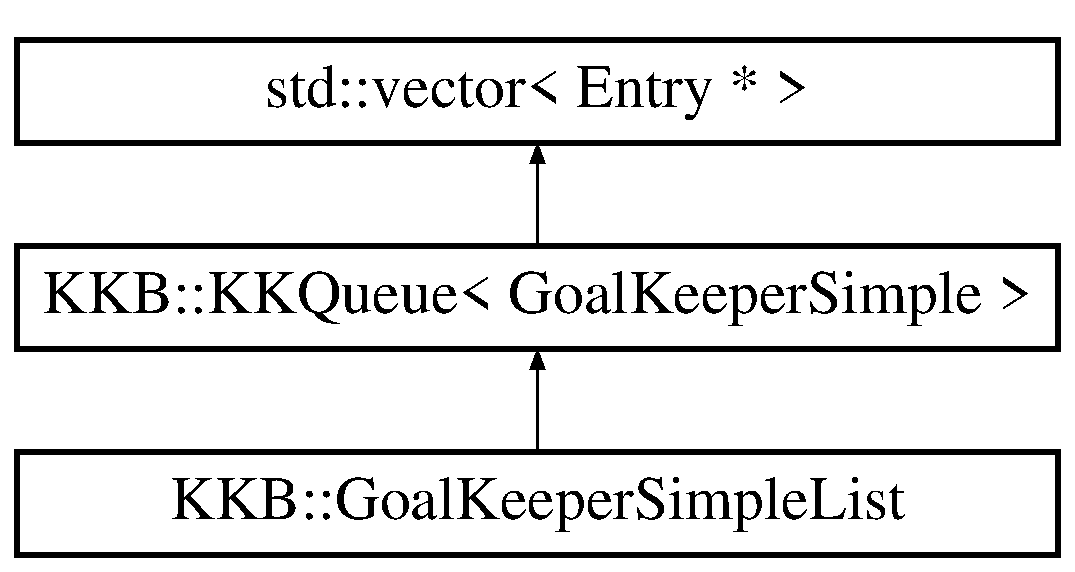
\includegraphics[height=3.000000cm]{class_k_k_b_1_1_goal_keeper_simple_list}
\end{center}
\end{figure}
\subsection*{Public Member Functions}
\begin{DoxyCompactItemize}
\item 
\hyperlink{class_k_k_b_1_1_goal_keeper_simple_list_ac0892b0284e98f55ec1c670e43499127}{Goal\+Keeper\+Simple\+List} (bool \+\_\+owner)
\item 
\hyperlink{class_k_k_b_1_1_goal_keeper_simple_list_a85c1cec64e9d0df5c15885853fd18c65}{$\sim$\+Goal\+Keeper\+Simple\+List} ()
\end{DoxyCompactItemize}
\subsection*{Additional Inherited Members}


\subsection{Detailed Description}


Definition at line 169 of file Goal\+Keeper\+Simple.\+h.



\subsection{Constructor \& Destructor Documentation}
\index{K\+K\+B\+::\+Goal\+Keeper\+Simple\+List@{K\+K\+B\+::\+Goal\+Keeper\+Simple\+List}!Goal\+Keeper\+Simple\+List@{Goal\+Keeper\+Simple\+List}}
\index{Goal\+Keeper\+Simple\+List@{Goal\+Keeper\+Simple\+List}!K\+K\+B\+::\+Goal\+Keeper\+Simple\+List@{K\+K\+B\+::\+Goal\+Keeper\+Simple\+List}}
\subsubsection[{\texorpdfstring{Goal\+Keeper\+Simple\+List(bool \+\_\+owner)}{GoalKeeperSimpleList(bool _owner)}}]{\setlength{\rightskip}{0pt plus 5cm}K\+K\+B\+::\+Goal\+Keeper\+Simple\+List\+::\+Goal\+Keeper\+Simple\+List (
\begin{DoxyParamCaption}
\item[{bool}]{\+\_\+owner}
\end{DoxyParamCaption}
)\hspace{0.3cm}{\ttfamily [inline]}}\hypertarget{class_k_k_b_1_1_goal_keeper_simple_list_ac0892b0284e98f55ec1c670e43499127}{}\label{class_k_k_b_1_1_goal_keeper_simple_list_ac0892b0284e98f55ec1c670e43499127}


Definition at line 172 of file Goal\+Keeper\+Simple.\+h.



Referenced by K\+K\+B\+::\+Goal\+Keeper\+Simple\+::\+Create(), and K\+K\+B\+::\+Goal\+Keeper\+Simple\+::\+Create\+And\+Start\+Block().


\begin{DoxyCode}
172 : KKQueue<GoalKeeperSimple> (\_owner)  \{\}
\end{DoxyCode}
\index{K\+K\+B\+::\+Goal\+Keeper\+Simple\+List@{K\+K\+B\+::\+Goal\+Keeper\+Simple\+List}!````~Goal\+Keeper\+Simple\+List@{$\sim$\+Goal\+Keeper\+Simple\+List}}
\index{````~Goal\+Keeper\+Simple\+List@{$\sim$\+Goal\+Keeper\+Simple\+List}!K\+K\+B\+::\+Goal\+Keeper\+Simple\+List@{K\+K\+B\+::\+Goal\+Keeper\+Simple\+List}}
\subsubsection[{\texorpdfstring{$\sim$\+Goal\+Keeper\+Simple\+List()}{~GoalKeeperSimpleList()}}]{\setlength{\rightskip}{0pt plus 5cm}K\+K\+B\+::\+Goal\+Keeper\+Simple\+List\+::$\sim$\+Goal\+Keeper\+Simple\+List (
\begin{DoxyParamCaption}
{}
\end{DoxyParamCaption}
)\hspace{0.3cm}{\ttfamily [inline]}}\hypertarget{class_k_k_b_1_1_goal_keeper_simple_list_a85c1cec64e9d0df5c15885853fd18c65}{}\label{class_k_k_b_1_1_goal_keeper_simple_list_a85c1cec64e9d0df5c15885853fd18c65}


Definition at line 174 of file Goal\+Keeper\+Simple.\+h.


\begin{DoxyCode}
175     \{\}
\end{DoxyCode}


The documentation for this class was generated from the following file\+:\begin{DoxyCompactItemize}
\item 
C\+:/\+Users/\+Kurt/\+Git\+Hub/\+K\+Square\+Libraries/\+K\+K\+Base/\hyperlink{_goal_keeper_simple_8h}{Goal\+Keeper\+Simple.\+h}\end{DoxyCompactItemize}

\hypertarget{class_k_k_b_1_1_hash_table}{}\section{K\+KB\+:\+:Hash\+Table$<$ Entry $>$ Class Template Reference}
\label{class_k_k_b_1_1_hash_table}\index{K\+K\+B\+::\+Hash\+Table$<$ Entry $>$@{K\+K\+B\+::\+Hash\+Table$<$ Entry $>$}}


{\ttfamily \#include $<$Hash\+Table.\+h$>$}

\subsection*{Public Types}
\begin{DoxyCompactItemize}
\item 
typedef Entry $\ast$ \hyperlink{class_k_k_b_1_1_hash_table_ac2ea7aefb6917165187d622e5dad2563}{Entry\+Ptr}
\end{DoxyCompactItemize}
\subsection*{Public Member Functions}
\begin{DoxyCompactItemize}
\item 
\hyperlink{class_k_k_b_1_1_hash_table_a063bc26af1e8f29ab332608790be290f}{Hash\+Table} (bool \+\_\+owner, \hyperlink{namespace_k_k_b_af8d832f05c54994a1cce25bd5743e19a}{kkuint32} \+\_\+table\+Size, \hyperlink{namespace_k_k_b_af8d832f05c54994a1cce25bd5743e19a}{kkuint32} \+\_\+key\+Len)
\begin{DoxyCompactList}\small\item\em Hash Table management template; developed to support Bit\+Reduction algorithm. \end{DoxyCompactList}\item 
\hyperlink{class_k_k_b_1_1_hash_table_a318e7a9196a979e70f21bd8cce905b97}{$\sim$\+Hash\+Table} ()
\item 
void \hyperlink{class_k_k_b_1_1_hash_table_a8bba92cda5bf998c35e2c1c710c71f6e}{Add\+Entry} (\hyperlink{class_k_k_b_1_1_hash_table_ac2ea7aefb6917165187d622e5dad2563}{Entry\+Ptr} entry)
\item 
bool \hyperlink{class_k_k_b_1_1_hash_table_ae1b0066c724a27259e8ce5b7aad96fce}{Delete\+Entry} (\hyperlink{class_k_k_b_1_1_hash_table_ac2ea7aefb6917165187d622e5dad2563}{Entry\+Ptr} \+\_\+entry)
\item 
\hyperlink{namespace_k_k_b_af8d832f05c54994a1cce25bd5743e19a}{kkuint32} \hyperlink{class_k_k_b_1_1_hash_table_af52b312fc23d6f07325b67ceed97b1e7}{Hash\+Value} (const \hyperlink{class_k_k_b_1_1_k_k_str}{K\+K\+Str} \&str)
\item 
\hyperlink{class_k_k_b_1_1_hash_table_ac2ea7aefb6917165187d622e5dad2563}{Entry\+Ptr} \hyperlink{class_k_k_b_1_1_hash_table_a9ba1d3083dafe9906a57ac4da33c96cf}{Locate\+Entry} (const \hyperlink{class_k_k_b_1_1_k_k_str}{K\+K\+Str} \&str)
\item 
\hyperlink{namespace_k_k_b_af8d832f05c54994a1cce25bd5743e19a}{kkuint32} \hyperlink{class_k_k_b_1_1_hash_table_a64dbc46abb0aa4fb82b718fffa18dc6f}{Num\+Of\+Entries} ()
\item 
void \hyperlink{class_k_k_b_1_1_hash_table_a3a9207f5b1acd3f883f6172e65ac08f3}{Save} (const \hyperlink{class_k_k_b_1_1_k_k_str}{K\+K\+Str} \&file\+Name)
\item 
Hash\+Entry\+Ptr $\ast$ \hyperlink{class_k_k_b_1_1_hash_table_a26ef60c66fba994c2132a2f37f729bd1}{Table} ()
\item 
\hyperlink{namespace_k_k_b_af8d832f05c54994a1cce25bd5743e19a}{kkuint32} \hyperlink{class_k_k_b_1_1_hash_table_a538c9eb3a23ade30699bb13aadc748b7}{Table\+Size} ()
\end{DoxyCompactItemize}


\subsection{Detailed Description}
\subsubsection*{template$<$class Entry$>$\\*
class K\+K\+B\+::\+Hash\+Table$<$ Entry $>$}



Definition at line 19 of file Hash\+Table.\+h.



\subsection{Member Typedef Documentation}
\index{K\+K\+B\+::\+Hash\+Table@{K\+K\+B\+::\+Hash\+Table}!Entry\+Ptr@{Entry\+Ptr}}
\index{Entry\+Ptr@{Entry\+Ptr}!K\+K\+B\+::\+Hash\+Table@{K\+K\+B\+::\+Hash\+Table}}
\subsubsection[{\texorpdfstring{Entry\+Ptr}{EntryPtr}}]{\setlength{\rightskip}{0pt plus 5cm}template$<$class Entry $>$ typedef Entry$\ast$ {\bf K\+K\+B\+::\+Hash\+Table}$<$ Entry $>$\+::{\bf Entry\+Ptr}}\hypertarget{class_k_k_b_1_1_hash_table_ac2ea7aefb6917165187d622e5dad2563}{}\label{class_k_k_b_1_1_hash_table_ac2ea7aefb6917165187d622e5dad2563}


Definition at line 22 of file Hash\+Table.\+h.



\subsection{Constructor \& Destructor Documentation}
\index{K\+K\+B\+::\+Hash\+Table@{K\+K\+B\+::\+Hash\+Table}!Hash\+Table@{Hash\+Table}}
\index{Hash\+Table@{Hash\+Table}!K\+K\+B\+::\+Hash\+Table@{K\+K\+B\+::\+Hash\+Table}}
\subsubsection[{\texorpdfstring{Hash\+Table(bool \+\_\+owner, kkuint32 \+\_\+table\+Size, kkuint32 \+\_\+key\+Len)}{HashTable(bool _owner, kkuint32 _tableSize, kkuint32 _keyLen)}}]{\setlength{\rightskip}{0pt plus 5cm}template$<$class Entry $>$ {\bf K\+K\+B\+::\+Hash\+Table}$<$ Entry $>$\+::{\bf Hash\+Table} (
\begin{DoxyParamCaption}
\item[{bool}]{\+\_\+owner, }
\item[{{\bf kkuint32}}]{\+\_\+table\+Size, }
\item[{{\bf kkuint32}}]{\+\_\+key\+Len}
\end{DoxyParamCaption}
)}\hypertarget{class_k_k_b_1_1_hash_table_a063bc26af1e8f29ab332608790be290f}{}\label{class_k_k_b_1_1_hash_table_a063bc26af1e8f29ab332608790be290f}


Hash Table management template; developed to support Bit\+Reduction algorithm. 

This template was originally written by Tong Luo to support his experiments in Bit reduction. It was later heavily modified by Kurt Kramer to conform to the Pices\+Library structure. 

Definition at line 85 of file Hash\+Table.\+h.


\begin{DoxyCode}
88                                :
89       owner        (\_owner),
90       numOfEntries (0),
91       tableSize    (\_tableSize),
92       keyLen       (\_keyLen)
93   \{
94     table = \textcolor{keyword}{new} \hyperlink{namespace_k_k_b_a52f8dc7216f438c7d92cb730d1e4281a}{HashEntryPtr}[tableSize];
95     \hyperlink{namespace_k_k_b_af8d832f05c54994a1cce25bd5743e19a}{kkuint32}  x;
96     \textcolor{keywordflow}{for}  (x = 0; x < tableSize; x++)
97       table[x] = NULL;
98 
99     hashFactors = \textcolor{keyword}{new} \hyperlink{namespace_k_k_b_a8fa4952cc84fda1de4bec1fbdd8d5b1b}{kkint32}[keyLen];
100 
101     \hyperlink{namespace_k_k_b_a8fa4952cc84fda1de4bec1fbdd8d5b1b}{kkint32}  fact = 53;
102     \hyperlink{namespace_k_k_b_a8fa4952cc84fda1de4bec1fbdd8d5b1b}{kkint32}  hashVal = 1;
103 
104     \hyperlink{namespace_k_k_b_a8fa4952cc84fda1de4bec1fbdd8d5b1b}{kkint32}  maxHashVal = \_tableSize * 10; 
105 
106     \textcolor{keywordflow}{for}  (x = 0; x < keyLen; x++)
107     \{
108       \textcolor{keywordflow}{if}  (hashVal > maxHashVal)
109         hashVal = 1;
110 
111       hashFactors[x] = hashVal;
112       hashVal = hashVal * fact;
113     \}
114   \};
\end{DoxyCode}
\index{K\+K\+B\+::\+Hash\+Table@{K\+K\+B\+::\+Hash\+Table}!````~Hash\+Table@{$\sim$\+Hash\+Table}}
\index{````~Hash\+Table@{$\sim$\+Hash\+Table}!K\+K\+B\+::\+Hash\+Table@{K\+K\+B\+::\+Hash\+Table}}
\subsubsection[{\texorpdfstring{$\sim$\+Hash\+Table()}{~HashTable()}}]{\setlength{\rightskip}{0pt plus 5cm}template$<$class Entry $>$ {\bf K\+K\+B\+::\+Hash\+Table}$<$ Entry $>$\+::$\sim${\bf Hash\+Table} (
\begin{DoxyParamCaption}
{}
\end{DoxyParamCaption}
)}\hypertarget{class_k_k_b_1_1_hash_table_a318e7a9196a979e70f21bd8cce905b97}{}\label{class_k_k_b_1_1_hash_table_a318e7a9196a979e70f21bd8cce905b97}


Definition at line 118 of file Hash\+Table.\+h.


\begin{DoxyCode}
119   \{
120     \hyperlink{namespace_k_k_b_a52f8dc7216f438c7d92cb730d1e4281a}{HashEntryPtr}  cur;
121     \hyperlink{namespace_k_k_b_af8d832f05c54994a1cce25bd5743e19a}{kkuint32}      idx;
122     \hyperlink{namespace_k_k_b_a52f8dc7216f438c7d92cb730d1e4281a}{HashEntryPtr}  next;
123 
124     \textcolor{keywordflow}{for}  (idx = 0; idx < tableSize; idx++)
125     \{
126       next = table[idx];
127       \textcolor{keywordflow}{while}  (next)
128       \{
129         cur = next;
130         next = next->next;
131         \textcolor{keywordflow}{if}  (owner)
132         \{
133           \textcolor{keyword}{delete}  cur->entry;
134         \}
135         \textcolor{keyword}{delete} cur;
136       \}
137     \}
138 
139     \textcolor{keyword}{delete}  table;
140     \textcolor{keyword}{delete}  hashFactors;
141   \}
\end{DoxyCode}


\subsection{Member Function Documentation}
\index{K\+K\+B\+::\+Hash\+Table@{K\+K\+B\+::\+Hash\+Table}!Add\+Entry@{Add\+Entry}}
\index{Add\+Entry@{Add\+Entry}!K\+K\+B\+::\+Hash\+Table@{K\+K\+B\+::\+Hash\+Table}}
\subsubsection[{\texorpdfstring{Add\+Entry(\+Entry\+Ptr entry)}{AddEntry(EntryPtr entry)}}]{\setlength{\rightskip}{0pt plus 5cm}template$<$class Entry $>$ void {\bf K\+K\+B\+::\+Hash\+Table}$<$ Entry $>$\+::Add\+Entry (
\begin{DoxyParamCaption}
\item[{{\bf Entry\+Ptr}}]{entry}
\end{DoxyParamCaption}
)}\hypertarget{class_k_k_b_1_1_hash_table_a8bba92cda5bf998c35e2c1c710c71f6e}{}\label{class_k_k_b_1_1_hash_table_a8bba92cda5bf998c35e2c1c710c71f6e}


Definition at line 173 of file Hash\+Table.\+h.


\begin{DoxyCode}
174   \{
175     \hyperlink{namespace_k_k_b_af8d832f05c54994a1cce25bd5743e19a}{kkuint32}  hashValue = \hyperlink{class_k_k_b_1_1_hash_table_af52b312fc23d6f07325b67ceed97b1e7}{HashValue} (entry->Key ());
176 
177     \hyperlink{namespace_k_k_b_a52f8dc7216f438c7d92cb730d1e4281a}{HashEntryPtr}  next = table[hashValue];
178 
179     \textcolor{keywordflow}{if}  (next)
180     \{
181       \textcolor{comment}{//cout << "Duplicate Hash " << hashValue << endl;}
182     \}
183 
184     table[hashValue] = \textcolor{keyword}{new} HashEntry (entry, next);
185 
186     numOfEntries++;
187   \}  \textcolor{comment}{/* AddEntry */}
\end{DoxyCode}
\index{K\+K\+B\+::\+Hash\+Table@{K\+K\+B\+::\+Hash\+Table}!Delete\+Entry@{Delete\+Entry}}
\index{Delete\+Entry@{Delete\+Entry}!K\+K\+B\+::\+Hash\+Table@{K\+K\+B\+::\+Hash\+Table}}
\subsubsection[{\texorpdfstring{Delete\+Entry(\+Entry\+Ptr \+\_\+entry)}{DeleteEntry(EntryPtr _entry)}}]{\setlength{\rightskip}{0pt plus 5cm}template$<$class Entry $>$ bool {\bf K\+K\+B\+::\+Hash\+Table}$<$ Entry $>$\+::Delete\+Entry (
\begin{DoxyParamCaption}
\item[{{\bf Entry\+Ptr}}]{\+\_\+entry}
\end{DoxyParamCaption}
)}\hypertarget{class_k_k_b_1_1_hash_table_ae1b0066c724a27259e8ce5b7aad96fce}{}\label{class_k_k_b_1_1_hash_table_ae1b0066c724a27259e8ce5b7aad96fce}


Definition at line 191 of file Hash\+Table.\+h.


\begin{DoxyCode}
192   \{
193     \hyperlink{namespace_k_k_b_af8d832f05c54994a1cce25bd5743e19a}{kkuint32}  hashValue = \hyperlink{class_k_k_b_1_1_hash_table_af52b312fc23d6f07325b67ceed97b1e7}{HashValue} (entry->Key ());
194 
195     \hyperlink{namespace_k_k_b_a52f8dc7216f438c7d92cb730d1e4281a}{HashEntryPtr} next = table[hashValue];
196     \hyperlink{namespace_k_k_b_a52f8dc7216f438c7d92cb730d1e4281a}{HashEntryPtr} last = NULL;
197 
198     \textcolor{keywordtype}{bool}  deleted = \textcolor{keyword}{false};
199 
200     \textcolor{keywordflow}{while}  (next)
201     \{
202       \textcolor{keywordflow}{if}  (next == entry)
203       \{
204         \textcolor{keywordflow}{if}  (last)
205         \{
206           last->next = next->next;
207         \}
208         \textcolor{keywordflow}{else}
209         \{
210           table[hashValue] = next->next;
211         \}
212 
213         \textcolor{keyword}{delete}  next;
214         next = NULL;
215         numOfEntries--;
216         deleted = \textcolor{keyword}{true};
217       \}
218       \textcolor{keywordflow}{else}
219       \{
220         last = next;
221         next = next->next;
222       \}
223     \}
224 
225     \textcolor{keywordflow}{return}  deleted;
226   \}  \textcolor{comment}{/* DeleteEntry */}
\end{DoxyCode}
\index{K\+K\+B\+::\+Hash\+Table@{K\+K\+B\+::\+Hash\+Table}!Hash\+Value@{Hash\+Value}}
\index{Hash\+Value@{Hash\+Value}!K\+K\+B\+::\+Hash\+Table@{K\+K\+B\+::\+Hash\+Table}}
\subsubsection[{\texorpdfstring{Hash\+Value(const K\+K\+Str \&str)}{HashValue(const KKStr &str)}}]{\setlength{\rightskip}{0pt plus 5cm}template$<$class Entry $>$ {\bf kkuint32} {\bf K\+K\+B\+::\+Hash\+Table}$<$ Entry $>$\+::Hash\+Value (
\begin{DoxyParamCaption}
\item[{const {\bf K\+K\+Str} \&}]{str}
\end{DoxyParamCaption}
)}\hypertarget{class_k_k_b_1_1_hash_table_af52b312fc23d6f07325b67ceed97b1e7}{}\label{class_k_k_b_1_1_hash_table_af52b312fc23d6f07325b67ceed97b1e7}


Definition at line 230 of file Hash\+Table.\+h.


\begin{DoxyCode}
231   \{
232     \textcolor{keyword}{const} \textcolor{keywordtype}{char}*  s = str.Str ();
233     \hyperlink{namespace_k_k_b_a8fa4952cc84fda1de4bec1fbdd8d5b1b}{kkint32}  len = strlen (s);
234     \hyperlink{namespace_k_k_b_a8fa4952cc84fda1de4bec1fbdd8d5b1b}{kkint32} x = len;
235     \hyperlink{namespace_k_k_b_af8d832f05c54994a1cce25bd5743e19a}{kkuint32}  y = 0;
236     \textcolor{keywordtype}{long}  hashVal = 0;
237 
238     \textcolor{keywordflow}{while}  ((x > 0)  &&  (y < keyLen))
239     \{
240       x--;
241       hashVal = hashVal + s[x] * hashFactors[y];
242       y++;
243     \}
244 
245     hashVal = hashVal % tableSize;
246     \textcolor{keywordflow}{return}  hashVal;
247   \}  \textcolor{comment}{/* HashValue */}
\end{DoxyCode}
\index{K\+K\+B\+::\+Hash\+Table@{K\+K\+B\+::\+Hash\+Table}!Locate\+Entry@{Locate\+Entry}}
\index{Locate\+Entry@{Locate\+Entry}!K\+K\+B\+::\+Hash\+Table@{K\+K\+B\+::\+Hash\+Table}}
\subsubsection[{\texorpdfstring{Locate\+Entry(const K\+K\+Str \&str)}{LocateEntry(const KKStr &str)}}]{\setlength{\rightskip}{0pt plus 5cm}template$<$class Entry $>$ {\bf Hash\+Table}$<$ Entry $>$\+::{\bf Entry\+Ptr} {\bf K\+K\+B\+::\+Hash\+Table}$<$ Entry $>$\+::Locate\+Entry (
\begin{DoxyParamCaption}
\item[{const {\bf K\+K\+Str} \&}]{str}
\end{DoxyParamCaption}
)}\hypertarget{class_k_k_b_1_1_hash_table_a9ba1d3083dafe9906a57ac4da33c96cf}{}\label{class_k_k_b_1_1_hash_table_a9ba1d3083dafe9906a57ac4da33c96cf}


Definition at line 145 of file Hash\+Table.\+h.


\begin{DoxyCode}
146   \{
147     \hyperlink{namespace_k_k_b_af8d832f05c54994a1cce25bd5743e19a}{kkuint32}  hashValue = \hyperlink{class_k_k_b_1_1_hash_table_af52b312fc23d6f07325b67ceed97b1e7}{HashValue} (key);
148 
149     \textcolor{comment}{// kkuint32  idx =  CalcIndex (hashValue);}
150     \hyperlink{namespace_k_k_b_af8d832f05c54994a1cce25bd5743e19a}{kkuint32}  idx =  hashValue;
151 
152     \hyperlink{class_k_k_b_1_1_hash_table_ac2ea7aefb6917165187d622e5dad2563}{EntryPtr} entry     = NULL;
153 
154     \hyperlink{namespace_k_k_b_a52f8dc7216f438c7d92cb730d1e4281a}{HashEntryPtr} next = table[idx];
155 
156     \textcolor{keywordflow}{while}  ((!entry)  &&  next)
157     \{
158       \textcolor{keywordflow}{if}  (next->entry->Key () == key)
159       \{
160         entry = next->entry;
161       \}
162       \textcolor{keywordflow}{else}
163       \{
164         next = next->next;
165       \}
166     \}
167     
168     \textcolor{keywordflow}{return}  entry;
169   \}  \textcolor{comment}{/* LocateEntry */}
\end{DoxyCode}
\index{K\+K\+B\+::\+Hash\+Table@{K\+K\+B\+::\+Hash\+Table}!Num\+Of\+Entries@{Num\+Of\+Entries}}
\index{Num\+Of\+Entries@{Num\+Of\+Entries}!K\+K\+B\+::\+Hash\+Table@{K\+K\+B\+::\+Hash\+Table}}
\subsubsection[{\texorpdfstring{Num\+Of\+Entries()}{NumOfEntries()}}]{\setlength{\rightskip}{0pt plus 5cm}template$<$class Entry $>$ {\bf kkuint32} {\bf K\+K\+B\+::\+Hash\+Table}$<$ Entry $>$\+::Num\+Of\+Entries (
\begin{DoxyParamCaption}
{}
\end{DoxyParamCaption}
)\hspace{0.3cm}{\ttfamily [inline]}}\hypertarget{class_k_k_b_1_1_hash_table_a64dbc46abb0aa4fb82b718fffa18dc6f}{}\label{class_k_k_b_1_1_hash_table_a64dbc46abb0aa4fb82b718fffa18dc6f}


Definition at line 70 of file Hash\+Table.\+h.


\begin{DoxyCode}
70 \{\textcolor{keywordflow}{return}  numOfEntries;\}
\end{DoxyCode}
\index{K\+K\+B\+::\+Hash\+Table@{K\+K\+B\+::\+Hash\+Table}!Save@{Save}}
\index{Save@{Save}!K\+K\+B\+::\+Hash\+Table@{K\+K\+B\+::\+Hash\+Table}}
\subsubsection[{\texorpdfstring{Save(const K\+K\+Str \&file\+Name)}{Save(const KKStr &fileName)}}]{\setlength{\rightskip}{0pt plus 5cm}template$<$class Entry $>$ void {\bf K\+K\+B\+::\+Hash\+Table}$<$ Entry $>$\+::Save (
\begin{DoxyParamCaption}
\item[{const {\bf K\+K\+Str} \&}]{file\+Name}
\end{DoxyParamCaption}
)}\hypertarget{class_k_k_b_1_1_hash_table_a3a9207f5b1acd3f883f6172e65ac08f3}{}\label{class_k_k_b_1_1_hash_table_a3a9207f5b1acd3f883f6172e65ac08f3}


Definition at line 251 of file Hash\+Table.\+h.


\begin{DoxyCode}
252   \{
253     ofstream f (fileName.Str ());
254 
255     \textcolor{keywordflow}{if}  (!f)
256     \{
257       cerr << \hyperlink{namespace_k_k_b_ad1f50f65af6adc8fa9e6f62d007818a8}{endl};
258       cerr << \textcolor{stringliteral}{"*** ERROR ***,  Error Opening File["} << fileName << \textcolor{stringliteral}{"]."} << \hyperlink{namespace_k_k_b_ad1f50f65af6adc8fa9e6f62d007818a8}{endl};
259       cerr << \hyperlink{namespace_k_k_b_ad1f50f65af6adc8fa9e6f62d007818a8}{endl};
260       \textcolor{keywordflow}{return};
261     \}
262 
263     \hyperlink{namespace_k_k_b_a52f8dc7216f438c7d92cb730d1e4281a}{HashEntryPtr}  next = NULL;
264     \hyperlink{namespace_k_k_b_af8d832f05c54994a1cce25bd5743e19a}{kkuint32}  idx = 0;
265 
266     \textcolor{keywordflow}{while}  (idx < \hyperlink{class_k_k_b_1_1_hash_table_a538c9eb3a23ade30699bb13aadc748b7}{TableSize} ())
267     \{
268       next = (\hyperlink{class_k_k_b_1_1_hash_table_a26ef60c66fba994c2132a2f37f729bd1}{Table} ())[idx];
269 
270       \textcolor{keywordflow}{while}  (next)
271       \{
272         f << next->entry->ToString () << \hyperlink{namespace_k_k_b_ad1f50f65af6adc8fa9e6f62d007818a8}{endl};
273         next = next->next;
274       \}
275 
276       idx++;    
277     \}
278 
279     f.close ();
280   \}  \textcolor{comment}{/* Save */}
\end{DoxyCode}
\index{K\+K\+B\+::\+Hash\+Table@{K\+K\+B\+::\+Hash\+Table}!Table@{Table}}
\index{Table@{Table}!K\+K\+B\+::\+Hash\+Table@{K\+K\+B\+::\+Hash\+Table}}
\subsubsection[{\texorpdfstring{Table()}{Table()}}]{\setlength{\rightskip}{0pt plus 5cm}template$<$class Entry $>$ Hash\+Entry\+Ptr$\ast$ {\bf K\+K\+B\+::\+Hash\+Table}$<$ Entry $>$\+::Table (
\begin{DoxyParamCaption}
{}
\end{DoxyParamCaption}
)\hspace{0.3cm}{\ttfamily [inline]}}\hypertarget{class_k_k_b_1_1_hash_table_a26ef60c66fba994c2132a2f37f729bd1}{}\label{class_k_k_b_1_1_hash_table_a26ef60c66fba994c2132a2f37f729bd1}


Definition at line 72 of file Hash\+Table.\+h.


\begin{DoxyCode}
72 \{\textcolor{keywordflow}{return}  table;\}
\end{DoxyCode}
\index{K\+K\+B\+::\+Hash\+Table@{K\+K\+B\+::\+Hash\+Table}!Table\+Size@{Table\+Size}}
\index{Table\+Size@{Table\+Size}!K\+K\+B\+::\+Hash\+Table@{K\+K\+B\+::\+Hash\+Table}}
\subsubsection[{\texorpdfstring{Table\+Size()}{TableSize()}}]{\setlength{\rightskip}{0pt plus 5cm}template$<$class Entry $>$ {\bf kkuint32} {\bf K\+K\+B\+::\+Hash\+Table}$<$ Entry $>$\+::Table\+Size (
\begin{DoxyParamCaption}
{}
\end{DoxyParamCaption}
)\hspace{0.3cm}{\ttfamily [inline]}}\hypertarget{class_k_k_b_1_1_hash_table_a538c9eb3a23ade30699bb13aadc748b7}{}\label{class_k_k_b_1_1_hash_table_a538c9eb3a23ade30699bb13aadc748b7}


Definition at line 74 of file Hash\+Table.\+h.


\begin{DoxyCode}
74 \{\textcolor{keywordflow}{return}  tableSize;\}
\end{DoxyCode}


The documentation for this class was generated from the following file\+:\begin{DoxyCompactItemize}
\item 
C\+:/\+Users/\+Kurt/\+Git\+Hub/\+K\+Square\+Libraries/\+K\+K\+Base/\hyperlink{_hash_table_8h}{Hash\+Table.\+h}\end{DoxyCompactItemize}

\hypertarget{class_k_k_b_1_1_histogram}{}\section{K\+KB\+:\+:Histogram Class Reference}
\label{class_k_k_b_1_1_histogram}\index{K\+K\+B\+::\+Histogram@{K\+K\+B\+::\+Histogram}}


Used to manage the construction of a \hyperlink{class_k_k_b_1_1_histogram}{Histogram}.  




{\ttfamily \#include $<$Histogram.\+h$>$}

\subsection*{Public Member Functions}
\begin{DoxyCompactItemize}
\item 
\hyperlink{class_k_k_b_1_1_histogram_a9966e27fdb984bcdb227b29514a54021}{Histogram} (float \+\_\+min\+Value, \hyperlink{namespace_k_k_b_a8fa4952cc84fda1de4bec1fbdd8d5b1b}{kkint32} \+\_\+num\+Of\+Buckets, float \+\_\+bucket\+Size, bool \+\_\+wrap\+Arround)
\item 
\hyperlink{class_k_k_b_1_1_histogram_aaf22daf3b8e3f0578337109005532f51}{$\sim$\+Histogram} ()
\item 
\hyperlink{namespace_k_k_b_a8fa4952cc84fda1de4bec1fbdd8d5b1b}{kkint32} \hyperlink{class_k_k_b_1_1_histogram_a62a30cf5745986061d275b25a616f31a}{Area\+In\+Range} (\hyperlink{namespace_k_k_b_a8fa4952cc84fda1de4bec1fbdd8d5b1b}{kkint32} min\+Bucket, \hyperlink{namespace_k_k_b_a8fa4952cc84fda1de4bec1fbdd8d5b1b}{kkint32} max\+Bucket) const 
\item 
float \hyperlink{class_k_k_b_1_1_histogram_a1c6f72547f45e51374e4763b8a15e040}{Area\+In\+Range\+Percent} (\hyperlink{namespace_k_k_b_a8fa4952cc84fda1de4bec1fbdd8d5b1b}{kkint32} min\+Bucket, \hyperlink{namespace_k_k_b_a8fa4952cc84fda1de4bec1fbdd8d5b1b}{kkint32} max\+Bucket) const 
\item 
float \hyperlink{class_k_k_b_1_1_histogram_aa67733d2af3248d68a1ee113ea5d7701}{Average\+Of\+Max\+Bucket} () const 
\item 
float \hyperlink{class_k_k_b_1_1_histogram_aa4191d4ca38d7b7d881038baf4554ded}{Average\+Of\+Max\+Bucket\+Excluding\+Range} (\hyperlink{namespace_k_k_b_a8fa4952cc84fda1de4bec1fbdd8d5b1b}{kkint32} min\+Bucket, \hyperlink{namespace_k_k_b_a8fa4952cc84fda1de4bec1fbdd8d5b1b}{kkint32} max\+Bucket) const 
\item 
float \hyperlink{class_k_k_b_1_1_histogram_ac0d1890f4e8826a2f7a217ecfbf76c59}{Average\+Of\+Max\+Bucket\+In\+Range} (\hyperlink{namespace_k_k_b_a8fa4952cc84fda1de4bec1fbdd8d5b1b}{kkint32} first\+Bucket, \hyperlink{namespace_k_k_b_a8fa4952cc84fda1de4bec1fbdd8d5b1b}{kkint32} last\+Bucket) const 
\item 
float \hyperlink{class_k_k_b_1_1_histogram_adace35b6a2076563aacf43f4de6c41b4}{Average\+Of\+Min\+Bucket\+In\+Range} (\hyperlink{namespace_k_k_b_a8fa4952cc84fda1de4bec1fbdd8d5b1b}{kkint32} min\+Bucket, \hyperlink{namespace_k_k_b_a8fa4952cc84fda1de4bec1fbdd8d5b1b}{kkint32} max\+Bucket) const 
\item 
float \hyperlink{class_k_k_b_1_1_histogram_a1fb293678e0e91e1f4fc5cc18d11f62b}{Bucket} (\hyperlink{namespace_k_k_b_a8fa4952cc84fda1de4bec1fbdd8d5b1b}{kkint32} bucket) const 
\item 
float \hyperlink{class_k_k_b_1_1_histogram_a7cf220be1ecaf49901f6afea550c6015}{Bucket\+Size} () const 
\item 
void \hyperlink{class_k_k_b_1_1_histogram_a1dcb39e4363db00133b3f95a7f25e45c}{Calculate\+Peaks} (\hyperlink{namespace_k_k_b_a8fa4952cc84fda1de4bec1fbdd8d5b1b}{kkint32} threshold)
\item 
float \hyperlink{class_k_k_b_1_1_histogram_a99ebe30e504bc5a78469cdf0f7963820}{Count\+Of\+Max\+Bucket} () const 
\item 
\hyperlink{namespace_k_k_b_a80d46bd24db644a022c863bce8ae3633}{Raster\+Ptr} \hyperlink{class_k_k_b_1_1_histogram_a5305305682f7b1dcb4e575550e94dce3}{Create\+Graph} () const 
\item 
\hyperlink{namespace_k_k_b_a80d46bd24db644a022c863bce8ae3633}{Raster\+Ptr} \hyperlink{class_k_k_b_1_1_histogram_a07fd97097cde777d82a8a3a97d1c4646}{Create\+Graph} (\hyperlink{namespace_k_k_b_a8fa4952cc84fda1de4bec1fbdd8d5b1b}{kkint32} bar\+Size) const 
\item 
\hyperlink{class_k_k_b_1_1_histogram}{Histogram} $\ast$ \hyperlink{class_k_k_b_1_1_histogram_a04cec38d98986864dbda4bf5b814711a}{Equalized} ()
\item 
\hyperlink{namespace_k_k_b_a8fa4952cc84fda1de4bec1fbdd8d5b1b}{kkint32} $\ast$ \hyperlink{class_k_k_b_1_1_histogram_a4aef03098feeca2316d2d8ea7862e1fe}{Equalized\+Map\+Table} ()
\item 
float \hyperlink{class_k_k_b_1_1_histogram_aa48c9389a38359e2923608a6a30e681d}{Get\+Peak\+Avg\+By\+Highest\+Order} (\hyperlink{namespace_k_k_b_a8fa4952cc84fda1de4bec1fbdd8d5b1b}{kkint32} peak\+Num)
\item 
\hyperlink{namespace_k_k_b_a8fa4952cc84fda1de4bec1fbdd8d5b1b}{kkint32} \hyperlink{class_k_k_b_1_1_histogram_a71eef0fa7588f4e19f400dd1eabeaa66}{Get\+Peak\+Bucket} (\hyperlink{namespace_k_k_b_a8fa4952cc84fda1de4bec1fbdd8d5b1b}{kkint32} peak\+Num)
\item 
\hyperlink{namespace_k_k_b_a8fa4952cc84fda1de4bec1fbdd8d5b1b}{kkint32} \hyperlink{class_k_k_b_1_1_histogram_a7698e5943c9a8859fca49e2551ea0d04}{Get\+Peak\+By\+Highest\+Order} (\hyperlink{namespace_k_k_b_a8fa4952cc84fda1de4bec1fbdd8d5b1b}{kkint32} peak\+Num)
\item 
void \hyperlink{class_k_k_b_1_1_histogram_a42e01ea0343c3f9e62841c7498670703}{Get\+Stats} (float \&\hyperlink{_usf_cas_cor_8h_a8195a86b6d75b9a3939505e8bb50021e}{min}, float \&\hyperlink{_usf_cas_cor_8h_ab95f7757e11b270d27b95ec0d8e798b5}{max}, float \&mean, float \&variance)
\item 
void \hyperlink{class_k_k_b_1_1_histogram_a1be7a2f10e83373a0e0083b970e0adfa}{Increment} (float val)
\item 
bool \hyperlink{class_k_k_b_1_1_histogram_afdb9c9d0c533d0f960755ef34e625d52}{Is\+Bucket\+A\+Peak} (\hyperlink{namespace_k_k_b_a8fa4952cc84fda1de4bec1fbdd8d5b1b}{kkint32} bucket, \hyperlink{namespace_k_k_b_a8fa4952cc84fda1de4bec1fbdd8d5b1b}{kkint32} tolerance) const 
\item 
\hyperlink{namespace_k_k_b_a8fa4952cc84fda1de4bec1fbdd8d5b1b}{kkint32} \hyperlink{class_k_k_b_1_1_histogram_a7c058cf194af1bf96bf038b0068dc328}{Max\+Bucket\+Idx} () const 
\item 
float \hyperlink{class_k_k_b_1_1_histogram_a4e0c1f127f04b35e8383726b027daa10}{Min\+Value} () const 
\item 
\hyperlink{namespace_k_k_b_a8fa4952cc84fda1de4bec1fbdd8d5b1b}{kkint32} \hyperlink{class_k_k_b_1_1_histogram_a5ed817d12ec4f30eb761fcc4e57e42c7}{Num\+Of\+Buckets} () const 
\item 
void \hyperlink{class_k_k_b_1_1_histogram_ac6174f69f8eab1ce225996ffd39bf04a}{Print\+Table} (ostream \&o)
\item 
void \hyperlink{class_k_k_b_1_1_histogram_ad875d4652f38d49d9c2fd170afee0071}{Save} (\hyperlink{class_k_k_b_1_1_k_k_str}{K\+K\+Str} file\+Name) const 
\item 
void \hyperlink{class_k_k_b_1_1_histogram_a0638645f1b64aa0128b3af42360360e7}{Save\+Graph\+Image} (const \hyperlink{class_k_k_b_1_1_k_k_str}{K\+K\+Str} \&file\+Name) const 
\item 
void \hyperlink{class_k_k_b_1_1_histogram_a52bd7aeedb85f8fbca8e10d0aba8569a}{Save\+Graph\+Image} (const \hyperlink{class_k_k_b_1_1_k_k_str}{K\+K\+Str} \&file\+Name, \hyperlink{namespace_k_k_b_a8fa4952cc84fda1de4bec1fbdd8d5b1b}{kkint32} bar\+Size) const 
\item 
\hyperlink{class_k_k_b_1_1_histogram}{Histogram} $\ast$ \hyperlink{class_k_k_b_1_1_histogram_a3377c8afecd84c378025ef38e4a1d4ad}{Smooth} (\hyperlink{namespace_k_k_b_a8fa4952cc84fda1de4bec1fbdd8d5b1b}{kkint32} smooth\+Width)
\item 
float \hyperlink{class_k_k_b_1_1_histogram_a66e88a0cfafc8d08e2a95d7d2799d47a}{Total\+Count} () const 
\end{DoxyCompactItemize}


\subsection{Detailed Description}
Used to manage the construction of a \hyperlink{class_k_k_b_1_1_histogram}{Histogram}. 

Definition at line 24 of file Histogram.\+h.



\subsection{Constructor \& Destructor Documentation}
\index{K\+K\+B\+::\+Histogram@{K\+K\+B\+::\+Histogram}!Histogram@{Histogram}}
\index{Histogram@{Histogram}!K\+K\+B\+::\+Histogram@{K\+K\+B\+::\+Histogram}}
\subsubsection[{\texorpdfstring{Histogram(float \+\_\+min\+Value, kkint32 \+\_\+num\+Of\+Buckets, float \+\_\+bucket\+Size, bool \+\_\+wrap\+Arround)}{Histogram(float _minValue, kkint32 _numOfBuckets, float _bucketSize, bool _wrapArround)}}]{\setlength{\rightskip}{0pt plus 5cm}Histogram\+::\+Histogram (
\begin{DoxyParamCaption}
\item[{float}]{\+\_\+min\+Value, }
\item[{{\bf kkint32}}]{\+\_\+num\+Of\+Buckets, }
\item[{float}]{\+\_\+bucket\+Size, }
\item[{bool}]{\+\_\+wrap\+Arround}
\end{DoxyParamCaption}
)}\hypertarget{class_k_k_b_1_1_histogram_a9966e27fdb984bcdb227b29514a54021}{}\label{class_k_k_b_1_1_histogram_a9966e27fdb984bcdb227b29514a54021}


Definition at line 24 of file Histogram.\+cpp.



Referenced by Equalized(), K\+K\+B\+::\+Raster\+::\+Histogram(), K\+K\+B\+::\+Raster\+::\+Histogram\+Grayscale(), and Smooth().


\begin{DoxyCode}
28                       :
29 
30   bucketSize        (\_bucketSize),
31   buckets           (NULL),
32   equalizedMapTable (NULL),
33   minValue          (\_minValue),
34   numOfBuckets      (\_numOfBuckets),
35   totalCount        (0.0),
36   totalVal          (0.0),
37   wrapArround       (\_wrapArround)
38 
39 \{
40   \textcolor{keywordflow}{if}  (numOfBuckets < 1)
41   \{
42     cerr << \hyperlink{namespace_k_k_b_ad1f50f65af6adc8fa9e6f62d007818a8}{std::endl} 
43          << \textcolor{stringliteral}{"*** ERROR ***   Histogram, Negative numOfBuckets["}  << numOfBuckets << \textcolor{stringliteral}{"."}  << 
      \hyperlink{namespace_k_k_b_ad1f50f65af6adc8fa9e6f62d007818a8}{std::endl}
44          << \hyperlink{namespace_k_k_b_ad1f50f65af6adc8fa9e6f62d007818a8}{std::endl};
45     exit (-1);
46   \}
47 
48   range = bucketSize * numOfBuckets;
49 
50   buckets      = \textcolor{keyword}{new} \textcolor{keywordtype}{float}[numOfBuckets];
51   bucketTotals = \textcolor{keyword}{new} \textcolor{keywordtype}{float}[numOfBuckets];
52 
53   \textcolor{keywordflow}{for}  (\hyperlink{namespace_k_k_b_a8fa4952cc84fda1de4bec1fbdd8d5b1b}{kkint32} x = 0;  x < numOfBuckets;  x++)
54   \{
55     buckets     [x] = (float)0.0;
56     bucketTotals[x] = (float)0.0;
57   \}
58 \}
\end{DoxyCode}
\index{K\+K\+B\+::\+Histogram@{K\+K\+B\+::\+Histogram}!````~Histogram@{$\sim$\+Histogram}}
\index{````~Histogram@{$\sim$\+Histogram}!K\+K\+B\+::\+Histogram@{K\+K\+B\+::\+Histogram}}
\subsubsection[{\texorpdfstring{$\sim$\+Histogram()}{~Histogram()}}]{\setlength{\rightskip}{0pt plus 5cm}Histogram\+::$\sim$\+Histogram (
\begin{DoxyParamCaption}
{}
\end{DoxyParamCaption}
)}\hypertarget{class_k_k_b_1_1_histogram_aaf22daf3b8e3f0578337109005532f51}{}\label{class_k_k_b_1_1_histogram_aaf22daf3b8e3f0578337109005532f51}


Definition at line 64 of file Histogram.\+cpp.


\begin{DoxyCode}
65 \{
66   \textcolor{keyword}{delete}  buckets;
67   \textcolor{keyword}{delete}  bucketTotals;
68   \textcolor{keywordflow}{if}  (equalizedMapTable)
69     \textcolor{keyword}{delete}  equalizedMapTable;
70 \}
\end{DoxyCode}


\subsection{Member Function Documentation}
\index{K\+K\+B\+::\+Histogram@{K\+K\+B\+::\+Histogram}!Area\+In\+Range@{Area\+In\+Range}}
\index{Area\+In\+Range@{Area\+In\+Range}!K\+K\+B\+::\+Histogram@{K\+K\+B\+::\+Histogram}}
\subsubsection[{\texorpdfstring{Area\+In\+Range(kkint32 min\+Bucket, kkint32 max\+Bucket) const }{AreaInRange(kkint32 minBucket, kkint32 maxBucket) const }}]{\setlength{\rightskip}{0pt plus 5cm}{\bf kkint32} Histogram\+::\+Area\+In\+Range (
\begin{DoxyParamCaption}
\item[{{\bf kkint32}}]{min\+Bucket, }
\item[{{\bf kkint32}}]{max\+Bucket}
\end{DoxyParamCaption}
) const}\hypertarget{class_k_k_b_1_1_histogram_a62a30cf5745986061d275b25a616f31a}{}\label{class_k_k_b_1_1_histogram_a62a30cf5745986061d275b25a616f31a}


Definition at line 1010 of file Histogram.\+cpp.



Referenced by Area\+In\+Range\+Percent().


\begin{DoxyCode}
1013 \{
1014   \textcolor{keywordflow}{if}  ((minBucket < 0)  ||  (minBucket >= numOfBuckets)  ||
1015        (maxBucket < 0)  ||  (maxBucket >= numOfBuckets)  ||
1016        (minBucket > maxBucket)
1017       )
1018   \{
1019     cerr << \hyperlink{namespace_k_k_b_ad1f50f65af6adc8fa9e6f62d007818a8}{std::endl};
1020     cerr << \textcolor{stringliteral}{"Histogram::AreaInRange    *** ERROR ***  Invalid Parameters"} << 
      \hyperlink{namespace_k_k_b_ad1f50f65af6adc8fa9e6f62d007818a8}{std::endl};
1021     cerr << \textcolor{stringliteral}{"NumOfBuckets["} << numOfBuckets << \textcolor{stringliteral}{"]  MinBucket["} << minBucket << \textcolor{stringliteral}{"]    MaxBucket["} << 
      maxBucket << \textcolor{stringliteral}{"]"} << \hyperlink{namespace_k_k_b_ad1f50f65af6adc8fa9e6f62d007818a8}{std::endl};
1022     exit (-1);
1023   \}
1024 
1025   \textcolor{keywordtype}{float}  area = (float)0.0;
1026   \textcolor{keywordflow}{for}  (\hyperlink{namespace_k_k_b_a8fa4952cc84fda1de4bec1fbdd8d5b1b}{kkint32} b = minBucket;  b <= maxBucket;  b++)
1027   \{
1028     area += buckets[b];
1029   \}
1030 
1031   \textcolor{keywordflow}{return}  (\hyperlink{namespace_k_k_b_a8fa4952cc84fda1de4bec1fbdd8d5b1b}{kkint32})(area + (float)0.5);
1032 \}   \textcolor{comment}{/* AreaInRange */}
\end{DoxyCode}
\index{K\+K\+B\+::\+Histogram@{K\+K\+B\+::\+Histogram}!Area\+In\+Range\+Percent@{Area\+In\+Range\+Percent}}
\index{Area\+In\+Range\+Percent@{Area\+In\+Range\+Percent}!K\+K\+B\+::\+Histogram@{K\+K\+B\+::\+Histogram}}
\subsubsection[{\texorpdfstring{Area\+In\+Range\+Percent(kkint32 min\+Bucket, kkint32 max\+Bucket) const }{AreaInRangePercent(kkint32 minBucket, kkint32 maxBucket) const }}]{\setlength{\rightskip}{0pt plus 5cm}float Histogram\+::\+Area\+In\+Range\+Percent (
\begin{DoxyParamCaption}
\item[{{\bf kkint32}}]{min\+Bucket, }
\item[{{\bf kkint32}}]{max\+Bucket}
\end{DoxyParamCaption}
) const}\hypertarget{class_k_k_b_1_1_histogram_a1c6f72547f45e51374e4763b8a15e040}{}\label{class_k_k_b_1_1_histogram_a1c6f72547f45e51374e4763b8a15e040}


Definition at line 1036 of file Histogram.\+cpp.



References Area\+In\+Range().


\begin{DoxyCode}
1039 \{
1040   \textcolor{keywordflow}{if}  (totalCount <= (\textcolor{keywordtype}{float})0.0)
1041     \textcolor{keywordflow}{return} (\textcolor{keywordtype}{float})0.0;
1042 
1043   \textcolor{keywordflow}{return}  (\textcolor{keywordtype}{float})100.0 * (float)((\textcolor{keywordtype}{float})\hyperlink{class_k_k_b_1_1_histogram_a62a30cf5745986061d275b25a616f31a}{AreaInRange} (minBucket, maxBucket) / totalCount);
1044 \}
\end{DoxyCode}
\index{K\+K\+B\+::\+Histogram@{K\+K\+B\+::\+Histogram}!Average\+Of\+Max\+Bucket@{Average\+Of\+Max\+Bucket}}
\index{Average\+Of\+Max\+Bucket@{Average\+Of\+Max\+Bucket}!K\+K\+B\+::\+Histogram@{K\+K\+B\+::\+Histogram}}
\subsubsection[{\texorpdfstring{Average\+Of\+Max\+Bucket() const }{AverageOfMaxBucket() const }}]{\setlength{\rightskip}{0pt plus 5cm}float Histogram\+::\+Average\+Of\+Max\+Bucket (
\begin{DoxyParamCaption}
{}
\end{DoxyParamCaption}
) const}\hypertarget{class_k_k_b_1_1_histogram_aa67733d2af3248d68a1ee113ea5d7701}{}\label{class_k_k_b_1_1_histogram_aa67733d2af3248d68a1ee113ea5d7701}


Definition at line 98 of file Histogram.\+cpp.



References Max\+Bucket\+Idx().


\begin{DoxyCode}
99 \{
100   \hyperlink{namespace_k_k_b_a8fa4952cc84fda1de4bec1fbdd8d5b1b}{kkint32} idx = \hyperlink{class_k_k_b_1_1_histogram_a7c058cf194af1bf96bf038b0068dc328}{MaxBucketIdx} ();
101 
102   \textcolor{keywordflow}{if}  (buckets[idx] <= (\textcolor{keywordtype}{float})0.0)
103     \textcolor{keywordflow}{return}  (\textcolor{keywordtype}{float})0.0;
104   \textcolor{keywordflow}{else}
105     \textcolor{keywordflow}{return}  bucketTotals[idx] / buckets[idx];
106 
107 \}  \textcolor{comment}{/* AverageOfMaxBucket */}
\end{DoxyCode}
\index{K\+K\+B\+::\+Histogram@{K\+K\+B\+::\+Histogram}!Average\+Of\+Max\+Bucket\+Excluding\+Range@{Average\+Of\+Max\+Bucket\+Excluding\+Range}}
\index{Average\+Of\+Max\+Bucket\+Excluding\+Range@{Average\+Of\+Max\+Bucket\+Excluding\+Range}!K\+K\+B\+::\+Histogram@{K\+K\+B\+::\+Histogram}}
\subsubsection[{\texorpdfstring{Average\+Of\+Max\+Bucket\+Excluding\+Range(kkint32 min\+Bucket, kkint32 max\+Bucket) const }{AverageOfMaxBucketExcludingRange(kkint32 minBucket, kkint32 maxBucket) const }}]{\setlength{\rightskip}{0pt plus 5cm}float Histogram\+::\+Average\+Of\+Max\+Bucket\+Excluding\+Range (
\begin{DoxyParamCaption}
\item[{{\bf kkint32}}]{min\+Bucket, }
\item[{{\bf kkint32}}]{max\+Bucket}
\end{DoxyParamCaption}
) const}\hypertarget{class_k_k_b_1_1_histogram_aa4191d4ca38d7b7d881038baf4554ded}{}\label{class_k_k_b_1_1_histogram_aa4191d4ca38d7b7d881038baf4554ded}


Definition at line 967 of file Histogram.\+cpp.


\begin{DoxyCode}
970 \{
971   \textcolor{keywordflow}{if}  ((minBucket < 0)  ||  (minBucket >= numOfBuckets)  ||
972        (maxBucket < 0)  ||  (maxBucket >= numOfBuckets)  ||
973        (minBucket > maxBucket)
974       )
975   \{
976     cerr << \hyperlink{namespace_k_k_b_ad1f50f65af6adc8fa9e6f62d007818a8}{std::endl};
977     cerr << \textcolor{stringliteral}{"Histogram::AverageOfMaxBucketExcludingRange    *** ERROR ***  Invalid Parameters"} << 
      \hyperlink{namespace_k_k_b_ad1f50f65af6adc8fa9e6f62d007818a8}{std::endl};
978     cerr << \textcolor{stringliteral}{"NumOfBuckets["} << numOfBuckets << \textcolor{stringliteral}{"]  MinBucket["} << minBucket << \textcolor{stringliteral}{"]    MaxBucket["} << 
      maxBucket << \textcolor{stringliteral}{"]"} << \hyperlink{namespace_k_k_b_ad1f50f65af6adc8fa9e6f62d007818a8}{std::endl};
979     exit (-1);
980   \}
981   
982   \hyperlink{namespace_k_k_b_a8fa4952cc84fda1de4bec1fbdd8d5b1b}{kkint32} b;
983 
984   \hyperlink{namespace_k_k_b_a8fa4952cc84fda1de4bec1fbdd8d5b1b}{kkint32}  maxBucketIDX = -1;
985   \textcolor{keywordtype}{float} maxBucketVal = 0;
986 
987   \textcolor{keywordflow}{for}  (b = 0;  b < numOfBuckets;  b++)
988   \{
989     \textcolor{keywordflow}{if}  ((b < minBucket)  ||  (b > maxBucket))
990     \{
991       \textcolor{keywordflow}{if}  (buckets[b] > maxBucketVal)
992       \{
993         maxBucketIDX = b;
994         maxBucketVal = buckets[b];
995       \}
996     \}
997   \}
998 
999   \textcolor{keywordflow}{if}  (maxBucketIDX < 0)
1000     \textcolor{keywordflow}{return} 0;
1001 
1002   \textcolor{keywordflow}{if}  (maxBucketVal > (\textcolor{keywordtype}{float})0.0)
1003     \textcolor{keywordflow}{return}  bucketTotals[maxBucketIDX] / buckets[maxBucketIDX];
1004   \textcolor{keywordflow}{else}
1005     \textcolor{keywordflow}{return} (\textcolor{keywordtype}{float})0.0;
1006 \}  \textcolor{comment}{/* AverageOfMaxBucketExcludingRange */}
\end{DoxyCode}
\index{K\+K\+B\+::\+Histogram@{K\+K\+B\+::\+Histogram}!Average\+Of\+Max\+Bucket\+In\+Range@{Average\+Of\+Max\+Bucket\+In\+Range}}
\index{Average\+Of\+Max\+Bucket\+In\+Range@{Average\+Of\+Max\+Bucket\+In\+Range}!K\+K\+B\+::\+Histogram@{K\+K\+B\+::\+Histogram}}
\subsubsection[{\texorpdfstring{Average\+Of\+Max\+Bucket\+In\+Range(kkint32 first\+Bucket, kkint32 last\+Bucket) const }{AverageOfMaxBucketInRange(kkint32 firstBucket, kkint32 lastBucket) const }}]{\setlength{\rightskip}{0pt plus 5cm}float Histogram\+::\+Average\+Of\+Max\+Bucket\+In\+Range (
\begin{DoxyParamCaption}
\item[{{\bf kkint32}}]{first\+Bucket, }
\item[{{\bf kkint32}}]{last\+Bucket}
\end{DoxyParamCaption}
) const}\hypertarget{class_k_k_b_1_1_histogram_ac0d1890f4e8826a2f7a217ecfbf76c59}{}\label{class_k_k_b_1_1_histogram_ac0d1890f4e8826a2f7a217ecfbf76c59}


Definition at line 891 of file Histogram.\+cpp.



Referenced by K\+K\+B\+::\+Raster\+::\+Segment\+Image().


\begin{DoxyCode}
894 \{
895   \textcolor{keywordflow}{if}  ((minBucket < 0)  ||  (minBucket >= numOfBuckets)  ||
896        (maxBucket < 0)  ||  (maxBucket >= numOfBuckets)  ||
897        (minBucket > maxBucket)
898       )
899   \{
900     cerr << \hyperlink{namespace_k_k_b_ad1f50f65af6adc8fa9e6f62d007818a8}{std::endl};
901     cerr << \textcolor{stringliteral}{"Histogram::AverageOfMaxBucketInRange    *** ERROR ***  Invalid Parameters"} << 
      \hyperlink{namespace_k_k_b_ad1f50f65af6adc8fa9e6f62d007818a8}{std::endl};
902     cerr << \textcolor{stringliteral}{"NumOfBuckets["} << numOfBuckets << \textcolor{stringliteral}{"]  MinBucket["} << minBucket << \textcolor{stringliteral}{"]    MaxBucket["} << 
      maxBucket << \textcolor{stringliteral}{"]"} << \hyperlink{namespace_k_k_b_ad1f50f65af6adc8fa9e6f62d007818a8}{std::endl};
903     exit (-1);
904   \}
905 
906   
907   \hyperlink{namespace_k_k_b_a8fa4952cc84fda1de4bec1fbdd8d5b1b}{kkint32} b;
908 
909   \hyperlink{namespace_k_k_b_a8fa4952cc84fda1de4bec1fbdd8d5b1b}{kkint32} maxBucketIDX = minBucket;
910   \textcolor{keywordtype}{float} maxBucketVal = buckets[minBucket];
911 
912   \textcolor{keywordflow}{for}  (b = minBucket;  b <= maxBucket;  b++)
913   \{
914     \textcolor{keywordflow}{if}  (buckets[b] > maxBucketVal)
915     \{
916       maxBucketIDX = b;
917       maxBucketVal = buckets[b];
918     \}
919   \}
920 
921   \textcolor{keywordflow}{if}  (maxBucketVal > (\textcolor{keywordtype}{float})0.0)
922     \textcolor{keywordflow}{return}  bucketTotals[maxBucketIDX] / buckets[maxBucketIDX];
923   \textcolor{keywordflow}{else}
924     \textcolor{keywordflow}{return} (\textcolor{keywordtype}{float})0.0;
925 \}  \textcolor{comment}{/* AverageOfMaxBucketInRange */}
\end{DoxyCode}
\index{K\+K\+B\+::\+Histogram@{K\+K\+B\+::\+Histogram}!Average\+Of\+Min\+Bucket\+In\+Range@{Average\+Of\+Min\+Bucket\+In\+Range}}
\index{Average\+Of\+Min\+Bucket\+In\+Range@{Average\+Of\+Min\+Bucket\+In\+Range}!K\+K\+B\+::\+Histogram@{K\+K\+B\+::\+Histogram}}
\subsubsection[{\texorpdfstring{Average\+Of\+Min\+Bucket\+In\+Range(kkint32 min\+Bucket, kkint32 max\+Bucket) const }{AverageOfMinBucketInRange(kkint32 minBucket, kkint32 maxBucket) const }}]{\setlength{\rightskip}{0pt plus 5cm}float Histogram\+::\+Average\+Of\+Min\+Bucket\+In\+Range (
\begin{DoxyParamCaption}
\item[{{\bf kkint32}}]{min\+Bucket, }
\item[{{\bf kkint32}}]{max\+Bucket}
\end{DoxyParamCaption}
) const}\hypertarget{class_k_k_b_1_1_histogram_adace35b6a2076563aacf43f4de6c41b4}{}\label{class_k_k_b_1_1_histogram_adace35b6a2076563aacf43f4de6c41b4}


Definition at line 930 of file Histogram.\+cpp.


\begin{DoxyCode}
933 \{
934   \textcolor{keywordflow}{if}  ((firstBucket < 0)  ||  (firstBucket >= numOfBuckets)  ||
935        (lastBucket < 0)   ||  (lastBucket >= numOfBuckets)  ||
936        (firstBucket > lastBucket)
937       )
938   \{
939     cerr << \hyperlink{namespace_k_k_b_ad1f50f65af6adc8fa9e6f62d007818a8}{std::endl};
940     cerr << \textcolor{stringliteral}{"Histogram::AverageOfMaxBucketInRange    *** ERROR ***  Invalid Parameters"} << 
      \hyperlink{namespace_k_k_b_ad1f50f65af6adc8fa9e6f62d007818a8}{std::endl};
941     cerr << \textcolor{stringliteral}{"NumOfBuckets["} << numOfBuckets << \textcolor{stringliteral}{"]  FirstBucket["} << firstBucket << \textcolor{stringliteral}{"]    LastBucket["} << 
      lastBucket << \textcolor{stringliteral}{"]"} << \hyperlink{namespace_k_k_b_ad1f50f65af6adc8fa9e6f62d007818a8}{std::endl};
942     exit (-1);
943   \}
944   
945   \hyperlink{namespace_k_k_b_a8fa4952cc84fda1de4bec1fbdd8d5b1b}{kkint32} b;
946 
947   \hyperlink{namespace_k_k_b_a8fa4952cc84fda1de4bec1fbdd8d5b1b}{kkint32}  minBucketIDX = firstBucket;
948   \textcolor{keywordtype}{float} minBucketVal = buckets[firstBucket];
949 
950   \textcolor{keywordflow}{for}  (b = firstBucket;  b <= lastBucket;  b++)
951   \{
952     \textcolor{keywordflow}{if}  (buckets[b] <= minBucketVal)
953     \{
954       minBucketIDX = b;
955       minBucketVal = buckets[b];
956     \}
957   \}
958 
959   \textcolor{keywordflow}{if}  (minBucketVal > 0)
960     \textcolor{keywordflow}{return}  bucketTotals[minBucketIDX] / buckets[minBucketIDX];
961   \textcolor{keywordflow}{else}
962     \textcolor{keywordflow}{return} (\textcolor{keywordtype}{float})0.0;
963 \}  \textcolor{comment}{/* AverageOfMaxBucketInRange */}
\end{DoxyCode}
\index{K\+K\+B\+::\+Histogram@{K\+K\+B\+::\+Histogram}!Bucket@{Bucket}}
\index{Bucket@{Bucket}!K\+K\+B\+::\+Histogram@{K\+K\+B\+::\+Histogram}}
\subsubsection[{\texorpdfstring{Bucket(kkint32 bucket) const }{Bucket(kkint32 bucket) const }}]{\setlength{\rightskip}{0pt plus 5cm}float Histogram\+::\+Bucket (
\begin{DoxyParamCaption}
\item[{{\bf kkint32}}]{bucket}
\end{DoxyParamCaption}
) const}\hypertarget{class_k_k_b_1_1_histogram_a1fb293678e0e91e1f4fc5cc18d11f62b}{}\label{class_k_k_b_1_1_histogram_a1fb293678e0e91e1f4fc5cc18d11f62b}


Definition at line 122 of file Histogram.\+cpp.


\begin{DoxyCode}
123 \{
124   \textcolor{keywordflow}{if}  ((bucket < 0)  ||  (bucket >= numOfBuckets))
125   \{
126     cerr << \hyperlink{namespace_k_k_b_ad1f50f65af6adc8fa9e6f62d007818a8}{std::endl} 
127          << \textcolor{stringliteral}{"*** ERROR ***   Histogram::Bucket,  Bucket["} << bucket << \textcolor{stringliteral}{"]  is out of range."} << 
      \hyperlink{namespace_k_k_b_ad1f50f65af6adc8fa9e6f62d007818a8}{std::endl}
128          << \hyperlink{namespace_k_k_b_ad1f50f65af6adc8fa9e6f62d007818a8}{std::endl};
129     exit (-1);
130   \}
131 
132   \textcolor{keywordflow}{return}  buckets[bucket];
133 \}  \textcolor{comment}{/* Bucket */}
\end{DoxyCode}
\index{K\+K\+B\+::\+Histogram@{K\+K\+B\+::\+Histogram}!Bucket\+Size@{Bucket\+Size}}
\index{Bucket\+Size@{Bucket\+Size}!K\+K\+B\+::\+Histogram@{K\+K\+B\+::\+Histogram}}
\subsubsection[{\texorpdfstring{Bucket\+Size() const }{BucketSize() const }}]{\setlength{\rightskip}{0pt plus 5cm}float K\+K\+B\+::\+Histogram\+::\+Bucket\+Size (
\begin{DoxyParamCaption}
{}
\end{DoxyParamCaption}
) const\hspace{0.3cm}{\ttfamily [inline]}}\hypertarget{class_k_k_b_1_1_histogram_a7cf220be1ecaf49901f6afea550c6015}{}\label{class_k_k_b_1_1_histogram_a7cf220be1ecaf49901f6afea550c6015}


Definition at line 60 of file Histogram.\+h.


\begin{DoxyCode}
60 \{\textcolor{keywordflow}{return} bucketSize;\}
\end{DoxyCode}
\index{K\+K\+B\+::\+Histogram@{K\+K\+B\+::\+Histogram}!Calculate\+Peaks@{Calculate\+Peaks}}
\index{Calculate\+Peaks@{Calculate\+Peaks}!K\+K\+B\+::\+Histogram@{K\+K\+B\+::\+Histogram}}
\subsubsection[{\texorpdfstring{Calculate\+Peaks(kkint32 threshold)}{CalculatePeaks(kkint32 threshold)}}]{\setlength{\rightskip}{0pt plus 5cm}void Histogram\+::\+Calculate\+Peaks (
\begin{DoxyParamCaption}
\item[{{\bf kkint32}}]{threshold}
\end{DoxyParamCaption}
)}\hypertarget{class_k_k_b_1_1_histogram_a1dcb39e4363db00133b3f95a7f25e45c}{}\label{class_k_k_b_1_1_histogram_a1dcb39e4363db00133b3f95a7f25e45c}


Definition at line 756 of file Histogram.\+cpp.


\begin{DoxyCode}
757 \{
758   \hyperlink{namespace_k_k_b_a8fa4952cc84fda1de4bec1fbdd8d5b1b}{kkint32}  bucket;
759 
760   peaks.erase (peaks.begin (), peaks.end ());
761 
762   \textcolor{keywordflow}{for}  (bucket = 0;  bucket < numOfBuckets;  bucket++)
763   \{
764     \textcolor{keywordflow}{if}  (\hyperlink{class_k_k_b_1_1_histogram_afdb9c9d0c533d0f960755ef34e625d52}{IsBucketAPeak} (bucket, threshold))
765       peaks.push\_back (bucket);
766   \}
767 \}  \textcolor{comment}{/* CalculatePeaks */}
\end{DoxyCode}
\index{K\+K\+B\+::\+Histogram@{K\+K\+B\+::\+Histogram}!Count\+Of\+Max\+Bucket@{Count\+Of\+Max\+Bucket}}
\index{Count\+Of\+Max\+Bucket@{Count\+Of\+Max\+Bucket}!K\+K\+B\+::\+Histogram@{K\+K\+B\+::\+Histogram}}
\subsubsection[{\texorpdfstring{Count\+Of\+Max\+Bucket() const }{CountOfMaxBucket() const }}]{\setlength{\rightskip}{0pt plus 5cm}float Histogram\+::\+Count\+Of\+Max\+Bucket (
\begin{DoxyParamCaption}
{}
\end{DoxyParamCaption}
) const}\hypertarget{class_k_k_b_1_1_histogram_a99ebe30e504bc5a78469cdf0f7963820}{}\label{class_k_k_b_1_1_histogram_a99ebe30e504bc5a78469cdf0f7963820}


Definition at line 113 of file Histogram.\+cpp.



References Max\+Bucket\+Idx().


\begin{DoxyCode}
114 \{
115   \hyperlink{namespace_k_k_b_a8fa4952cc84fda1de4bec1fbdd8d5b1b}{kkint32} idx = \hyperlink{class_k_k_b_1_1_histogram_a7c058cf194af1bf96bf038b0068dc328}{MaxBucketIdx} ();
116 
117   \textcolor{keywordflow}{return}  buckets[idx];
118 \}  \textcolor{comment}{/* CountOfMaxBucket */}
\end{DoxyCode}
\index{K\+K\+B\+::\+Histogram@{K\+K\+B\+::\+Histogram}!Create\+Graph@{Create\+Graph}}
\index{Create\+Graph@{Create\+Graph}!K\+K\+B\+::\+Histogram@{K\+K\+B\+::\+Histogram}}
\subsubsection[{\texorpdfstring{Create\+Graph() const }{CreateGraph() const }}]{\setlength{\rightskip}{0pt plus 5cm}{\bf Raster\+Ptr} Histogram\+::\+Create\+Graph (
\begin{DoxyParamCaption}
{}
\end{DoxyParamCaption}
) const}\hypertarget{class_k_k_b_1_1_histogram_a5305305682f7b1dcb4e575550e94dce3}{}\label{class_k_k_b_1_1_histogram_a5305305682f7b1dcb4e575550e94dce3}


Definition at line 162 of file Histogram.\+cpp.



References K\+K\+B\+::\+Raster\+::\+Draw\+Line(), Is\+Bucket\+A\+Peak(), K\+K\+B\+::\+Raster\+::\+Raster(), K\+K\+B\+::\+Raster\+::\+Reverse\+Image(), and K\+K\+B\+::\+Raster\+::\+Set\+Pixel\+Value().



Referenced by K\+K\+B\+::\+Raster\+::\+Histogram\+Grayscale\+Image(), K\+K\+B\+::\+Raster\+::\+Histogram\+Image(), and Save\+Graph\+Image().


\begin{DoxyCode}
163 \{
164   \hyperlink{namespace_k_k_b_a8fa4952cc84fda1de4bec1fbdd8d5b1b}{kkint32} bucket        = 0;
165   \hyperlink{namespace_k_k_b_a8fa4952cc84fda1de4bec1fbdd8d5b1b}{kkint32} col           = 10;
166   \hyperlink{namespace_k_k_b_a8fa4952cc84fda1de4bec1fbdd8d5b1b}{kkint32} barWidth      = 2;
167   \hyperlink{namespace_k_k_b_a8fa4952cc84fda1de4bec1fbdd8d5b1b}{kkint32} interBarWidth = 5;
168   \hyperlink{namespace_k_k_b_a8fa4952cc84fda1de4bec1fbdd8d5b1b}{kkint32} colHeight     = 0;
169   \textcolor{keywordtype}{float}   maxCount      = (float)0.0;
170   \hyperlink{namespace_k_k_b_a8fa4952cc84fda1de4bec1fbdd8d5b1b}{kkint32} row           = 0;
171   \hyperlink{namespace_k_k_b_a8fa4952cc84fda1de4bec1fbdd8d5b1b}{kkint32} x;
172   \hyperlink{namespace_k_k_b_a8fa4952cc84fda1de4bec1fbdd8d5b1b}{kkint32} y;
173 
174   \hyperlink{namespace_k_k_b_ace9969169bf514f9ee6185186949cdf7}{uchar}  borderColor  = 100;
175   \hyperlink{namespace_k_k_b_ace9969169bf514f9ee6185186949cdf7}{uchar}  colorAxis    = 150;
176   \hyperlink{namespace_k_k_b_ace9969169bf514f9ee6185186949cdf7}{uchar}  colorBar     = 200;
177   \hyperlink{namespace_k_k_b_ace9969169bf514f9ee6185186949cdf7}{uchar}  colorBarMax  = 255;
178   \hyperlink{namespace_k_k_b_ace9969169bf514f9ee6185186949cdf7}{uchar}  colorBarPeak = 255;
179   \hyperlink{namespace_k_k_b_ace9969169bf514f9ee6185186949cdf7}{uchar}  gridColor    = 180;
180   \hyperlink{namespace_k_k_b_ace9969169bf514f9ee6185186949cdf7}{uchar}  hashColor    =  70;
181   \hyperlink{namespace_k_k_b_ace9969169bf514f9ee6185186949cdf7}{uchar}  hashColor2   =  45;
182 
183   \hyperlink{namespace_k_k_b_a8fa4952cc84fda1de4bec1fbdd8d5b1b}{kkint32}  graphWidth  = numOfBuckets * (barWidth + interBarWidth) + 20; \textcolor{comment}{//  3 pixels per bar,  +}
184                                                                        \textcolor{comment}{//  3 pixels space     +}
185                                                                        \textcolor{comment}{// 10 pixel Padding on both sides.}
186 
187   \textcolor{comment}{// Set up where Grid lines should go}
188   \textcolor{keywordtype}{bool}*  vertGridLines = \textcolor{keyword}{new} \textcolor{keywordtype}{bool}[numOfBuckets];
189   \textcolor{keywordtype}{bool}*  peakBarLines  = \textcolor{keyword}{new} \textcolor{keywordtype}{bool}[numOfBuckets];
190   \textcolor{keywordflow}{for}  (x = 0;  x < numOfBuckets;  x++)
191   \{
192     vertGridLines[x] = \textcolor{keyword}{false};
193     peakBarLines [x] = \hyperlink{class_k_k_b_1_1_histogram_afdb9c9d0c533d0f960755ef34e625d52}{IsBucketAPeak} (x, 2);  \textcolor{comment}{// Make sure that we are greater than }
194                                               \textcolor{comment}{// our 2 left and right neighbors}
195   \}
196 
197   \textcolor{comment}{// Look for the Zero Grid Line should go}
198 
199   \hyperlink{namespace_k_k_b_a8fa4952cc84fda1de4bec1fbdd8d5b1b}{kkint32}  middleIdx = 0;
200   \textcolor{keywordflow}{if}  (minValue < 0)
201   \{
202     \hyperlink{namespace_k_k_b_a8fa4952cc84fda1de4bec1fbdd8d5b1b}{kkint32}  numOfBucketsToZero = (\hyperlink{namespace_k_k_b_a8fa4952cc84fda1de4bec1fbdd8d5b1b}{kkint32})(0.5 + fabs (minValue) / bucketSize);
203 
204     \textcolor{keywordflow}{if}  (numOfBucketsToZero < numOfBuckets)
205       middleIdx = numOfBucketsToZero;
206   \}
207 
208   x = middleIdx;
209   \textcolor{keywordflow}{while}  (x < numOfBuckets)
210   \{
211     vertGridLines[x] = \textcolor{keyword}{true};
212     x += 100;
213   \}
214 
215   x = middleIdx;
216   \textcolor{keywordflow}{while}  (x > 0)
217   \{
218     vertGridLines[x] = \textcolor{keyword}{true};
219     x -= 100;
220   \}
221 
222   \textcolor{keywordflow}{for}  (bucket = 0;  bucket < numOfBuckets;  bucket++)
223   \{
224     \textcolor{keywordflow}{if}  (buckets[bucket] > maxCount)
225       maxCount = buckets[bucket];
226   \}
227 
228   \hyperlink{namespace_k_k_b_a8fa4952cc84fda1de4bec1fbdd8d5b1b}{kkint32}  maxColHeight = \hyperlink{namespace_k_k_b_ad030d1ca8bd5038824c4a923a4d23fb5}{Min} ((\hyperlink{namespace_k_k_b_a8fa4952cc84fda1de4bec1fbdd8d5b1b}{kkint32})(maxCount * (barWidth + interBarWidth) + (\textcolor{keywordtype}{float})0.
      5), (\hyperlink{namespace_k_k_b_a8fa4952cc84fda1de4bec1fbdd8d5b1b}{kkint32})512);
229   \hyperlink{namespace_k_k_b_a8fa4952cc84fda1de4bec1fbdd8d5b1b}{kkint32}  graphHeight = maxColHeight + 20;
230 
231 
232   \hyperlink{class_k_k_b_1_1_raster}{RasterPtr}  graph = \textcolor{keyword}{new} \hyperlink{class_k_k_b_1_1_raster}{Raster} (graphHeight, graphWidth);
233 
234   graph->\hyperlink{class_k_k_b_1_1_raster_a118bf0fa32356ddea42f579c044c65cd}{DrawLine} (              10,              10,               10, graphWidth - 10, 
      borderColor);  \textcolor{comment}{// TopLeft -> TopRight}
235 
236   graph->\hyperlink{class_k_k_b_1_1_raster_a118bf0fa32356ddea42f579c044c65cd}{DrawLine} (              10, graphWidth - 10, graphHeight - 10, graphWidth - 10, 
      borderColor);  \textcolor{comment}{// TopRight -> BotRight}
237 
238   graph->\hyperlink{class_k_k_b_1_1_raster_a118bf0fa32356ddea42f579c044c65cd}{DrawLine} (graphHeight - 10, graphWidth - 10, graphHeight - 10,              10, 
      borderColor);  \textcolor{comment}{// BotRight -> BotLeft}
239 
240   graph->\hyperlink{class_k_k_b_1_1_raster_a118bf0fa32356ddea42f579c044c65cd}{DrawLine} (graphHeight - 10,              10,               10,              10, 
      borderColor);  \textcolor{comment}{// BotLeft -> TopLeft}
241 
242 
243   x = 0;
244   row = graphHeight - 10;
245   
246   \textcolor{comment}{// Draw Y Axis}
247   \textcolor{keywordflow}{while}  (x < maxColHeight)
248   \{
249     \textcolor{keywordflow}{if}  ((x % 10) == 0)
250     \{
251       \textcolor{keywordflow}{if}  ((x % 50) == 0)
252       \{
253         graph->\hyperlink{class_k_k_b_1_1_raster_a5ddb8bd069dc64241941b0b011af8667}{SetPixelValue} (row, 4, hashColor2);
254         graph->\hyperlink{class_k_k_b_1_1_raster_a5ddb8bd069dc64241941b0b011af8667}{SetPixelValue} (row, 5, hashColor2);
255         graph->\hyperlink{class_k_k_b_1_1_raster_a5ddb8bd069dc64241941b0b011af8667}{SetPixelValue} (row, 6, hashColor2);
256 
257         \textcolor{keywordflow}{if}  ((x % 100) == 0)
258         \{
259           graph->\hyperlink{class_k_k_b_1_1_raster_a118bf0fa32356ddea42f579c044c65cd}{DrawLine} (row, 9, row, graphWidth - 11, gridColor);
260         \}
261       \}
262 
263       graph->\hyperlink{class_k_k_b_1_1_raster_a5ddb8bd069dc64241941b0b011af8667}{SetPixelValue} (row, 7, hashColor);
264       graph->\hyperlink{class_k_k_b_1_1_raster_a5ddb8bd069dc64241941b0b011af8667}{SetPixelValue} (row, 8, hashColor);
265       graph->\hyperlink{class_k_k_b_1_1_raster_a5ddb8bd069dc64241941b0b011af8667}{SetPixelValue} (row, 9, hashColor);
266     \}
267 
268     graph->\hyperlink{class_k_k_b_1_1_raster_a5ddb8bd069dc64241941b0b011af8667}{SetPixelValue} (row, 9, colorAxis);
269     row--;
270     x++;
271   \}
272 
273 
274 
275   col = 10;
276 
277   \textcolor{keywordflow}{for}  (bucket = 0;  bucket < numOfBuckets;  bucket++)
278   \{
279     \textcolor{keywordflow}{for}  (x = 0;  x < (barWidth + interBarWidth);  x++)
280     \{
281       graph->\hyperlink{class_k_k_b_1_1_raster_a5ddb8bd069dc64241941b0b011af8667}{SetPixelValue} (graphHeight - 9, col + x, colorAxis);
282     \}
283 
284     \textcolor{keywordflow}{if}  ((bucket % 10) == 0)
285     \{
286       \textcolor{comment}{// Lets add a Hash Mark}
287       graph->\hyperlink{class_k_k_b_1_1_raster_a5ddb8bd069dc64241941b0b011af8667}{SetPixelValue} (graphHeight - 8, col + 1, hashColor);
288       graph->\hyperlink{class_k_k_b_1_1_raster_a5ddb8bd069dc64241941b0b011af8667}{SetPixelValue} (graphHeight - 7, col + 1, hashColor);
289       graph->\hyperlink{class_k_k_b_1_1_raster_a5ddb8bd069dc64241941b0b011af8667}{SetPixelValue} (graphHeight - 6, col + 1, hashColor);
290       graph->\hyperlink{class_k_k_b_1_1_raster_a5ddb8bd069dc64241941b0b011af8667}{SetPixelValue} (graphHeight - 5, col + 1, hashColor);
291     \}
292 
293     \textcolor{keywordflow}{if}  (vertGridLines[bucket] == \textcolor{keyword}{true})
294     \{
295       graph->\hyperlink{class_k_k_b_1_1_raster_a118bf0fa32356ddea42f579c044c65cd}{DrawLine} (graphHeight - 10, col + 1, 10, col + 1, gridColor);
296     \}
297 
298     colHeight = (\hyperlink{namespace_k_k_b_a8fa4952cc84fda1de4bec1fbdd8d5b1b}{kkint32})ceil ((((\textcolor{keywordtype}{float})maxColHeight * buckets[bucket]) / maxCount));
299 
300     \textcolor{keywordflow}{if}  ((colHeight < 1)  &&  (buckets[bucket] > (float)0.0))
301     \{
302       cout << \textcolor{stringliteral}{"I want to know about this."} << \hyperlink{namespace_k_k_b_ad1f50f65af6adc8fa9e6f62d007818a8}{std::endl};
303     \}
304 
305     row = graphHeight - 10;
306 
307     \hyperlink{namespace_k_k_b_ace9969169bf514f9ee6185186949cdf7}{uchar}  barCodeToUse = colorBar;
308     \textcolor{keywordflow}{if}  (buckets[bucket] >= maxCount)
309       barCodeToUse = colorBarMax;
310 
311     \textcolor{keywordflow}{else} \textcolor{keywordflow}{if}  (peakBarLines[bucket])
312       barCodeToUse = colorBarPeak;
313 
314     \textcolor{keywordflow}{for}  (\hyperlink{namespace_k_k_b_a8fa4952cc84fda1de4bec1fbdd8d5b1b}{kkint32}  x = 0;  x < colHeight;  x++)
315     \{
316       \textcolor{keywordflow}{for}  (y = 0;  y < barWidth;  y++)
317       \{
318         graph->\hyperlink{class_k_k_b_1_1_raster_a5ddb8bd069dc64241941b0b011af8667}{SetPixelValue} (row, col + y, barCodeToUse);
319       \}
320 
321       row--;
322     \}
323 
324     col += (barWidth + interBarWidth);
325   \}  
326 
327   \textcolor{keyword}{delete}[]  peakBarLines;
328   \textcolor{keyword}{delete}[]  vertGridLines;
329 
330   graph->\hyperlink{class_k_k_b_1_1_raster_a6bd18a014fd3867714e04c037f021497}{ReverseImage} ();
331 
332   \textcolor{keywordflow}{return}  graph;
333 \}  \textcolor{comment}{/* CreateGraph */}
\end{DoxyCode}
\index{K\+K\+B\+::\+Histogram@{K\+K\+B\+::\+Histogram}!Create\+Graph@{Create\+Graph}}
\index{Create\+Graph@{Create\+Graph}!K\+K\+B\+::\+Histogram@{K\+K\+B\+::\+Histogram}}
\subsubsection[{\texorpdfstring{Create\+Graph(kkint32 bar\+Size) const }{CreateGraph(kkint32 barSize) const }}]{\setlength{\rightskip}{0pt plus 5cm}{\bf Raster\+Ptr} Histogram\+::\+Create\+Graph (
\begin{DoxyParamCaption}
\item[{{\bf kkint32}}]{bar\+Size}
\end{DoxyParamCaption}
) const}\hypertarget{class_k_k_b_1_1_histogram_a07fd97097cde777d82a8a3a97d1c4646}{}\label{class_k_k_b_1_1_histogram_a07fd97097cde777d82a8a3a97d1c4646}


Definition at line 337 of file Histogram.\+cpp.



References K\+K\+B\+::\+Raster\+::\+Draw\+Line(), Is\+Bucket\+A\+Peak(), K\+K\+B\+::\+Raster\+::\+Raster(), K\+K\+B\+::\+Raster\+::\+Reverse\+Image(), and K\+K\+B\+::\+Raster\+::\+Set\+Pixel\+Value().



Referenced by Save\+Graph\+Image().


\begin{DoxyCode}
338 \{
339   \hyperlink{namespace_k_k_b_a8fa4952cc84fda1de4bec1fbdd8d5b1b}{kkint32} bucket        = 0;
340   \hyperlink{namespace_k_k_b_a8fa4952cc84fda1de4bec1fbdd8d5b1b}{kkint32} col           = 10;
341   \hyperlink{namespace_k_k_b_a8fa4952cc84fda1de4bec1fbdd8d5b1b}{kkint32} barWidth      = 2;
342   \hyperlink{namespace_k_k_b_a8fa4952cc84fda1de4bec1fbdd8d5b1b}{kkint32} interBarWidth = 5;
343   \hyperlink{namespace_k_k_b_a8fa4952cc84fda1de4bec1fbdd8d5b1b}{kkint32} colHeight     = 0;
344   \textcolor{keywordtype}{float}   maxCount      = (float)0.0;
345   \hyperlink{namespace_k_k_b_a8fa4952cc84fda1de4bec1fbdd8d5b1b}{kkint32} row           = 0;
346   \hyperlink{namespace_k_k_b_a8fa4952cc84fda1de4bec1fbdd8d5b1b}{kkint32} x;
347   \hyperlink{namespace_k_k_b_a8fa4952cc84fda1de4bec1fbdd8d5b1b}{kkint32} y;
348 
349   \hyperlink{namespace_k_k_b_ace9969169bf514f9ee6185186949cdf7}{uchar}  borderColor  = 100;
350   \hyperlink{namespace_k_k_b_ace9969169bf514f9ee6185186949cdf7}{uchar}  colorAxis    = 150;
351   \hyperlink{namespace_k_k_b_ace9969169bf514f9ee6185186949cdf7}{uchar}  colorBar     = 200;
352   \hyperlink{namespace_k_k_b_ace9969169bf514f9ee6185186949cdf7}{uchar}  colorBarMax  = 255;
353   \hyperlink{namespace_k_k_b_ace9969169bf514f9ee6185186949cdf7}{uchar}  colorBarPeak = 255;
354   \hyperlink{namespace_k_k_b_ace9969169bf514f9ee6185186949cdf7}{uchar}  gridColor    = 180;
355   \hyperlink{namespace_k_k_b_ace9969169bf514f9ee6185186949cdf7}{uchar}  hashColor    =  70;
356   \hyperlink{namespace_k_k_b_ace9969169bf514f9ee6185186949cdf7}{uchar}  hashColor2   =  45;
357 
358   \hyperlink{namespace_k_k_b_a8fa4952cc84fda1de4bec1fbdd8d5b1b}{kkint32}  graphWidth  = numOfBuckets * (barWidth + interBarWidth) + 20; \textcolor{comment}{//  3 pixels per bar,  +}
359                                                                        \textcolor{comment}{//  3 pixels space     +}
360                                                                        \textcolor{comment}{// 10 pixels Padding on both sides.}
361 
362   \textcolor{comment}{// Set up where Grid lines should go}
363   \textcolor{keywordtype}{bool}*  vertGridLines = \textcolor{keyword}{new} \textcolor{keywordtype}{bool}[numOfBuckets];
364   \textcolor{keywordtype}{bool}*  peakBarLines  = \textcolor{keyword}{new} \textcolor{keywordtype}{bool}[numOfBuckets];
365   \textcolor{keywordflow}{for}  (x = 0;  x < numOfBuckets;  x++)
366   \{
367     vertGridLines[x] = \textcolor{keyword}{false};
368     peakBarLines [x] = \hyperlink{class_k_k_b_1_1_histogram_afdb9c9d0c533d0f960755ef34e625d52}{IsBucketAPeak} (x, 2);  \textcolor{comment}{// Make sure that we are greater than }
369                                               \textcolor{comment}{// our 2 left and right neighbors}
370   \}
371 
372   \textcolor{comment}{// Look for the Zero Grid Line should go}
373 
374   \hyperlink{namespace_k_k_b_a8fa4952cc84fda1de4bec1fbdd8d5b1b}{kkint32}  middleIdx = 0;
375   \textcolor{keywordflow}{if}  (minValue < 0)
376   \{
377     \hyperlink{namespace_k_k_b_a8fa4952cc84fda1de4bec1fbdd8d5b1b}{kkint32}  numOfBucketsToZero = (\hyperlink{namespace_k_k_b_a8fa4952cc84fda1de4bec1fbdd8d5b1b}{kkint32})(0.5 + fabs (minValue) / bucketSize);
378 
379     \textcolor{keywordflow}{if}  (numOfBucketsToZero < numOfBuckets)
380       middleIdx = numOfBucketsToZero;
381   \}
382 
383   x = middleIdx;
384   \textcolor{keywordflow}{while}  (x < numOfBuckets)
385   \{
386     vertGridLines[x] = \textcolor{keyword}{true};
387     x += 100;
388   \}
389 
390   x = middleIdx;
391   \textcolor{keywordflow}{while}  (x > 0)
392   \{
393     vertGridLines[x] = \textcolor{keyword}{true};
394     x -= 100;
395   \}
396   
397 
398   \textcolor{keywordflow}{for}  (bucket = 0;  bucket < numOfBuckets;  bucket++)
399   \{
400     \textcolor{keywordflow}{if}  (buckets[bucket] > maxCount)
401       maxCount = buckets[bucket];
402   \}
403 
404 
405   \hyperlink{namespace_k_k_b_a8fa4952cc84fda1de4bec1fbdd8d5b1b}{kkint32}  maxColHeight = \hyperlink{namespace_k_k_b_ad030d1ca8bd5038824c4a923a4d23fb5}{Min} ((\hyperlink{namespace_k_k_b_a8fa4952cc84fda1de4bec1fbdd8d5b1b}{kkint32})(maxCount * (barWidth + interBarWidth) + (\textcolor{keywordtype}{float})0.
      5), (\hyperlink{namespace_k_k_b_a8fa4952cc84fda1de4bec1fbdd8d5b1b}{kkint32})512);
406   \hyperlink{namespace_k_k_b_a8fa4952cc84fda1de4bec1fbdd8d5b1b}{kkint32}  graphHeight = maxColHeight + 20;
407 
408   \hyperlink{class_k_k_b_1_1_raster}{RasterPtr}  graph = \textcolor{keyword}{new} \hyperlink{class_k_k_b_1_1_raster}{Raster} (graphHeight, graphWidth);
409 
410   graph->\hyperlink{class_k_k_b_1_1_raster_a118bf0fa32356ddea42f579c044c65cd}{DrawLine} (              10,              10,               10, graphWidth - 10, 
      borderColor);  \textcolor{comment}{// TopLeft  -> TopRight}
411   graph->\hyperlink{class_k_k_b_1_1_raster_a118bf0fa32356ddea42f579c044c65cd}{DrawLine} (              10, graphWidth - 10, graphHeight - 10, graphWidth - 10, 
      borderColor);  \textcolor{comment}{// TopRight -> BotRight}
412   graph->\hyperlink{class_k_k_b_1_1_raster_a118bf0fa32356ddea42f579c044c65cd}{DrawLine} (graphHeight - 10, graphWidth - 10, graphHeight - 10,              10, 
      borderColor);  \textcolor{comment}{// BotRight -> BotLeft}
413   graph->\hyperlink{class_k_k_b_1_1_raster_a118bf0fa32356ddea42f579c044c65cd}{DrawLine} (graphHeight - 10,              10,               10,              10, 
      borderColor);  \textcolor{comment}{// BotLeft  -> TopLeft}
414 
415   x = 0;
416   row = graphHeight - 10;
417 
418   \textcolor{comment}{// Draw Y Axis}
419   \textcolor{keywordflow}{while}  (x < maxColHeight)
420   \{
421     \textcolor{keywordflow}{if}  ((x % 10) == 0)
422     \{
423       \textcolor{keywordflow}{if}  ((x % 50) == 0)
424       \{
425         graph->\hyperlink{class_k_k_b_1_1_raster_a5ddb8bd069dc64241941b0b011af8667}{SetPixelValue} (row, 4, hashColor2);
426         graph->\hyperlink{class_k_k_b_1_1_raster_a5ddb8bd069dc64241941b0b011af8667}{SetPixelValue} (row, 5, hashColor2);
427         graph->\hyperlink{class_k_k_b_1_1_raster_a5ddb8bd069dc64241941b0b011af8667}{SetPixelValue} (row, 6, hashColor2);
428 
429         \textcolor{keywordflow}{if}  ((x % 100) == 0)
430         \{
431           graph->\hyperlink{class_k_k_b_1_1_raster_a118bf0fa32356ddea42f579c044c65cd}{DrawLine} (row, 9, row, graphWidth - 11, gridColor);
432         \}
433       \}
434 
435       graph->\hyperlink{class_k_k_b_1_1_raster_a5ddb8bd069dc64241941b0b011af8667}{SetPixelValue} (row, 7, hashColor);
436       graph->\hyperlink{class_k_k_b_1_1_raster_a5ddb8bd069dc64241941b0b011af8667}{SetPixelValue} (row, 8, hashColor);
437       graph->\hyperlink{class_k_k_b_1_1_raster_a5ddb8bd069dc64241941b0b011af8667}{SetPixelValue} (row, 9, hashColor);
438     \}
439 
440     graph->\hyperlink{class_k_k_b_1_1_raster_a5ddb8bd069dc64241941b0b011af8667}{SetPixelValue} (row, 9, colorAxis);
441     row--;
442     x++;
443   \}
444 
445   col = 10;
446 
447   \textcolor{keywordflow}{for}  (bucket = 0;  bucket < numOfBuckets;  bucket++)
448   \{
449     \textcolor{keywordflow}{for}  (x = 0;  x < (barWidth + interBarWidth);  x++)
450     \{
451       graph->\hyperlink{class_k_k_b_1_1_raster_a5ddb8bd069dc64241941b0b011af8667}{SetPixelValue} (graphHeight - 9, col + x, colorAxis);
452     \}
453 
454     \textcolor{keywordflow}{if}  ((bucket % 10) == 0)
455     \{
456       \textcolor{comment}{// Lets add a Hash Mark}
457       graph->\hyperlink{class_k_k_b_1_1_raster_a5ddb8bd069dc64241941b0b011af8667}{SetPixelValue} (graphHeight - 8, col + 1, hashColor);
458       graph->\hyperlink{class_k_k_b_1_1_raster_a5ddb8bd069dc64241941b0b011af8667}{SetPixelValue} (graphHeight - 7, col + 1, hashColor);
459       graph->\hyperlink{class_k_k_b_1_1_raster_a5ddb8bd069dc64241941b0b011af8667}{SetPixelValue} (graphHeight - 6, col + 1, hashColor);
460       graph->\hyperlink{class_k_k_b_1_1_raster_a5ddb8bd069dc64241941b0b011af8667}{SetPixelValue} (graphHeight - 5, col + 1, hashColor);
461     \}
462 
463     \textcolor{keywordflow}{if}  (vertGridLines[bucket] == \textcolor{keyword}{true})
464     \{
465       graph->\hyperlink{class_k_k_b_1_1_raster_a118bf0fa32356ddea42f579c044c65cd}{DrawLine} (graphHeight - 10, col + 1, 10, col + 1, gridColor);
466     \}
467 
468     colHeight = (\hyperlink{namespace_k_k_b_a8fa4952cc84fda1de4bec1fbdd8d5b1b}{kkint32})ceil ((((\textcolor{keywordtype}{float})maxColHeight * buckets[bucket]) / maxCount));
469 
470     \textcolor{keywordflow}{if}  ((colHeight < 1)  &&  (buckets[bucket] > (float)0.0))
471     \{
472       cout << \textcolor{stringliteral}{"I want to know about this."} << \hyperlink{namespace_k_k_b_ad1f50f65af6adc8fa9e6f62d007818a8}{std::endl};
473     \}
474 
475     row = graphHeight - 10;
476 
477     \hyperlink{namespace_k_k_b_ace9969169bf514f9ee6185186949cdf7}{uchar}  barCodeToUse = colorBar;
478     \textcolor{keywordflow}{if}  (buckets[bucket] >= maxCount)
479       barCodeToUse = colorBarMax;
480 
481     \textcolor{keywordflow}{else} \textcolor{keywordflow}{if}  (peakBarLines[bucket])
482       barCodeToUse = colorBarPeak;
483 
484     \textcolor{keywordflow}{for}  (\hyperlink{namespace_k_k_b_a8fa4952cc84fda1de4bec1fbdd8d5b1b}{kkint32}  x = 0;  x < colHeight;  x++)
485     \{
486       \textcolor{keywordflow}{for}  (y = 0;  y < barWidth;  y++)
487       \{
488         graph->\hyperlink{class_k_k_b_1_1_raster_a5ddb8bd069dc64241941b0b011af8667}{SetPixelValue} (row, col + y, barCodeToUse);
489       \}
490 
491       row--;
492     \}
493 
494     col += (barWidth + interBarWidth);
495   \}  
496 
497   \textcolor{keyword}{delete}[]  peakBarLines;
498   \textcolor{keyword}{delete}[]  vertGridLines;
499 
500   graph->\hyperlink{class_k_k_b_1_1_raster_a6bd18a014fd3867714e04c037f021497}{ReverseImage} ();
501 
502   \textcolor{keywordflow}{return}  graph;
503 \}  \textcolor{comment}{/* CreateGraph */}
\end{DoxyCode}
\index{K\+K\+B\+::\+Histogram@{K\+K\+B\+::\+Histogram}!Equalized@{Equalized}}
\index{Equalized@{Equalized}!K\+K\+B\+::\+Histogram@{K\+K\+B\+::\+Histogram}}
\subsubsection[{\texorpdfstring{Equalized()}{Equalized()}}]{\setlength{\rightskip}{0pt plus 5cm}{\bf Histogram\+Ptr} Histogram\+::\+Equalized (
\begin{DoxyParamCaption}
{}
\end{DoxyParamCaption}
)}\hypertarget{class_k_k_b_1_1_histogram_a04cec38d98986864dbda4bf5b814711a}{}\label{class_k_k_b_1_1_histogram_a04cec38d98986864dbda4bf5b814711a}


Definition at line 848 of file Histogram.\+cpp.



References Histogram().



Referenced by K\+K\+B\+::\+Raster\+::\+Histogram\+Equalized\+Image().


\begin{DoxyCode}
849 \{
850   \textcolor{keywordtype}{float}*   histSumTable  = \textcolor{keyword}{new} \textcolor{keywordtype}{float}[numOfBuckets];
851   \hyperlink{namespace_k_k_b_a8fa4952cc84fda1de4bec1fbdd8d5b1b}{kkint32}  idx;
852 
853   \hyperlink{class_k_k_b_1_1_histogram}{HistogramPtr}   newHist = \textcolor{keyword}{new} \hyperlink{class_k_k_b_1_1_histogram_a9966e27fdb984bcdb227b29514a54021}{Histogram} (minValue, numOfBuckets, bucketSize, 
      wrapArround);
854 
855   \hyperlink{namespace_k_k_b_a8fa4952cc84fda1de4bec1fbdd8d5b1b}{kkint32}  x;
856 
857   newHist->equalizedMapTable = \textcolor{keyword}{new} \hyperlink{namespace_k_k_b_a8fa4952cc84fda1de4bec1fbdd8d5b1b}{kkint32}[numOfBuckets];
858 
859   \textcolor{keywordtype}{float}  accumulatedCount = (float)0.0;
860   \textcolor{keywordflow}{for}  (x = 0; x < numOfBuckets; x++)
861   \{
862     accumulatedCount += buckets[x];
863     histSumTable[x] = accumulatedCount;
864   \}
865 
866  
867   \textcolor{keywordflow}{for}  (x = 0;  x < numOfBuckets;  x++)
868   \{
869     idx = (\hyperlink{namespace_k_k_b_a8fa4952cc84fda1de4bec1fbdd8d5b1b}{kkint32})((\textcolor{keywordtype}{float})0.5 + (((float)(histSumTable[x] * (numOfBuckets - 1)) / totalCount)));
870     \textcolor{keywordflow}{if}  (idx >= numOfBuckets)
871       idx = numOfBuckets - 1;
872 
873     newHist->equalizedMapTable[x] = idx;
874     newHist->buckets[idx]         += buckets[x];
875     newHist->bucketTotals[idx]    += bucketTotals[x];
876   \}
877 
878 
879   newHist->totalCount = totalCount;
880   newHist->totalVal   = totalVal;
881 
882 
883   \textcolor{keyword}{delete}[]  histSumTable;
884 
885   \textcolor{keywordflow}{return}  newHist;
886 \} \textcolor{comment}{/* Equalize */}
\end{DoxyCode}
\index{K\+K\+B\+::\+Histogram@{K\+K\+B\+::\+Histogram}!Equalized\+Map\+Table@{Equalized\+Map\+Table}}
\index{Equalized\+Map\+Table@{Equalized\+Map\+Table}!K\+K\+B\+::\+Histogram@{K\+K\+B\+::\+Histogram}}
\subsubsection[{\texorpdfstring{Equalized\+Map\+Table()}{EqualizedMapTable()}}]{\setlength{\rightskip}{0pt plus 5cm}{\bf kkint32}$\ast$ K\+K\+B\+::\+Histogram\+::\+Equalized\+Map\+Table (
\begin{DoxyParamCaption}
{}
\end{DoxyParamCaption}
)\hspace{0.3cm}{\ttfamily [inline]}}\hypertarget{class_k_k_b_1_1_histogram_a4aef03098feeca2316d2d8ea7862e1fe}{}\label{class_k_k_b_1_1_histogram_a4aef03098feeca2316d2d8ea7862e1fe}


Definition at line 72 of file Histogram.\+h.



Referenced by K\+K\+B\+::\+Raster\+::\+Histogram\+Equalized\+Image().


\begin{DoxyCode}
72 \{\textcolor{keywordflow}{return}  equalizedMapTable;\}
\end{DoxyCode}
\index{K\+K\+B\+::\+Histogram@{K\+K\+B\+::\+Histogram}!Get\+Peak\+Avg\+By\+Highest\+Order@{Get\+Peak\+Avg\+By\+Highest\+Order}}
\index{Get\+Peak\+Avg\+By\+Highest\+Order@{Get\+Peak\+Avg\+By\+Highest\+Order}!K\+K\+B\+::\+Histogram@{K\+K\+B\+::\+Histogram}}
\subsubsection[{\texorpdfstring{Get\+Peak\+Avg\+By\+Highest\+Order(kkint32 peak\+Num)}{GetPeakAvgByHighestOrder(kkint32 peakNum)}}]{\setlength{\rightskip}{0pt plus 5cm}float Histogram\+::\+Get\+Peak\+Avg\+By\+Highest\+Order (
\begin{DoxyParamCaption}
\item[{{\bf kkint32}}]{peak\+Num}
\end{DoxyParamCaption}
)}\hypertarget{class_k_k_b_1_1_histogram_aa48c9389a38359e2923608a6a30e681d}{}\label{class_k_k_b_1_1_histogram_aa48c9389a38359e2923608a6a30e681d}


Definition at line 820 of file Histogram.\+cpp.



References Get\+Peak\+By\+Highest\+Order().


\begin{DoxyCode}
821 \{
822   \hyperlink{namespace_k_k_b_a8fa4952cc84fda1de4bec1fbdd8d5b1b}{kkint32}  x = \hyperlink{class_k_k_b_1_1_histogram_a7698e5943c9a8859fca49e2551ea0d04}{GetPeakByHighestOrder} (peakNum);
823 
824   \textcolor{keywordflow}{if}  (x < 0)
825   \{
826     cout << \hyperlink{namespace_k_k_b_ad1f50f65af6adc8fa9e6f62d007818a8}{std::endl};
827     cout << \textcolor{stringliteral}{"GetPeakAvgByHighestOrder     GetPeakByHighestOrder returned["} << x << \textcolor{stringliteral}{"]"} << 
      \hyperlink{namespace_k_k_b_ad1f50f65af6adc8fa9e6f62d007818a8}{std::endl};
828     \textcolor{keywordflow}{return}  0;
829   \}
830 
831   \textcolor{keywordflow}{if}  (x >= this->numOfBuckets)
832   \{
833     cout << \hyperlink{namespace_k_k_b_ad1f50f65af6adc8fa9e6f62d007818a8}{std::endl};
834     cout << \textcolor{stringliteral}{"GetPeakAvgByHighestOrder     GetPeakByHighestOrder returned["} << x << \textcolor{stringliteral}{"]"} << 
      \hyperlink{namespace_k_k_b_ad1f50f65af6adc8fa9e6f62d007818a8}{std::endl};
835     x = 1;
836     \textcolor{keywordflow}{return} 0;
837   \}
838 
839   \textcolor{keywordflow}{if}  (buckets[x] <= (\textcolor{keywordtype}{float})0.0)
840     \textcolor{keywordflow}{return} 0.0;
841 
842   \textcolor{keywordflow}{return}  (bucketTotals[x] / buckets[x]);
843 \}  \textcolor{comment}{/* GetPeakAvgByHighestOrder */}
\end{DoxyCode}
\index{K\+K\+B\+::\+Histogram@{K\+K\+B\+::\+Histogram}!Get\+Peak\+Bucket@{Get\+Peak\+Bucket}}
\index{Get\+Peak\+Bucket@{Get\+Peak\+Bucket}!K\+K\+B\+::\+Histogram@{K\+K\+B\+::\+Histogram}}
\subsubsection[{\texorpdfstring{Get\+Peak\+Bucket(kkint32 peak\+Num)}{GetPeakBucket(kkint32 peakNum)}}]{\setlength{\rightskip}{0pt plus 5cm}{\bf kkint32} Histogram\+::\+Get\+Peak\+Bucket (
\begin{DoxyParamCaption}
\item[{{\bf kkint32}}]{peak\+Num}
\end{DoxyParamCaption}
)}\hypertarget{class_k_k_b_1_1_histogram_a71eef0fa7588f4e19f400dd1eabeaa66}{}\label{class_k_k_b_1_1_histogram_a71eef0fa7588f4e19f400dd1eabeaa66}


Definition at line 771 of file Histogram.\+cpp.


\begin{DoxyCode}
772 \{
773   \textcolor{keywordflow}{if}  (peaks.empty ())
774     \hyperlink{class_k_k_b_1_1_histogram_a1dcb39e4363db00133b3f95a7f25e45c}{CalculatePeaks} (2);
775 
776   \textcolor{keywordflow}{if}  (peakNum > (\hyperlink{namespace_k_k_b_a8fa4952cc84fda1de4bec1fbdd8d5b1b}{kkint32})peaks.size ())
777     \textcolor{keywordflow}{return} -1;
778 
779   \textcolor{keywordflow}{else}
780     \textcolor{keywordflow}{return}  peaks[peakNum];
781 \}
\end{DoxyCode}
\index{K\+K\+B\+::\+Histogram@{K\+K\+B\+::\+Histogram}!Get\+Peak\+By\+Highest\+Order@{Get\+Peak\+By\+Highest\+Order}}
\index{Get\+Peak\+By\+Highest\+Order@{Get\+Peak\+By\+Highest\+Order}!K\+K\+B\+::\+Histogram@{K\+K\+B\+::\+Histogram}}
\subsubsection[{\texorpdfstring{Get\+Peak\+By\+Highest\+Order(kkint32 peak\+Num)}{GetPeakByHighestOrder(kkint32 peakNum)}}]{\setlength{\rightskip}{0pt plus 5cm}{\bf kkint32} Histogram\+::\+Get\+Peak\+By\+Highest\+Order (
\begin{DoxyParamCaption}
\item[{{\bf kkint32}}]{peak\+Num}
\end{DoxyParamCaption}
)}\hypertarget{class_k_k_b_1_1_histogram_a7698e5943c9a8859fca49e2551ea0d04}{}\label{class_k_k_b_1_1_histogram_a7698e5943c9a8859fca49e2551ea0d04}


Definition at line 785 of file Histogram.\+cpp.



Referenced by Get\+Peak\+Avg\+By\+Highest\+Order().


\begin{DoxyCode}
786 \{
787   \textcolor{keywordflow}{if}  (peaks.empty ())
788     \hyperlink{class_k_k_b_1_1_histogram_a1dcb39e4363db00133b3f95a7f25e45c}{CalculatePeaks} (2);
789 
790   \textcolor{keywordflow}{if}  (peakNum > (\hyperlink{namespace_k_k_b_a8fa4952cc84fda1de4bec1fbdd8d5b1b}{kkint32})peaks.size ())
791     \textcolor{keywordflow}{return} -1;
792 
793   \hyperlink{namespace_k_k_b_a8fa4952cc84fda1de4bec1fbdd8d5b1b}{kkint32}  t;
794   \hyperlink{namespace_k_k_b_a8fa4952cc84fda1de4bec1fbdd8d5b1b}{kkint32}  x;
795   \hyperlink{namespace_k_k_b_a8fa4952cc84fda1de4bec1fbdd8d5b1b}{kkint32}  y;
796 
797   \hyperlink{namespace_k_k_b_adf8a10085d231870d8a072046d6cba10}{VectorInt32} sortedPeaks (peaks);
798 
799   \textcolor{keywordflow}{for}  (x = 1;  x < (\hyperlink{namespace_k_k_b_a8fa4952cc84fda1de4bec1fbdd8d5b1b}{kkint32})sortedPeaks.size ();  x++)
800   \{
801     \textcolor{keywordflow}{for} (y = x; y > 0; y--)
802     \{
803       \textcolor{keywordflow}{if}  (buckets[sortedPeaks[y - 1]] < buckets[sortedPeaks[y]])
804       \{
805         t = sortedPeaks[y];
806         sortedPeaks[y] = sortedPeaks[y - 1];
807         sortedPeaks[y - 1] = t;
808       \}
809     \}
810   \}
811 
812   \hyperlink{namespace_k_k_b_a8fa4952cc84fda1de4bec1fbdd8d5b1b}{kkint32}  returnIdxNum = sortedPeaks[peakNum];
813   
814   \textcolor{keywordflow}{return}   returnIdxNum;
815   
816 \}  \textcolor{comment}{/* GetPeakByHighestOrder */}
\end{DoxyCode}
\index{K\+K\+B\+::\+Histogram@{K\+K\+B\+::\+Histogram}!Get\+Stats@{Get\+Stats}}
\index{Get\+Stats@{Get\+Stats}!K\+K\+B\+::\+Histogram@{K\+K\+B\+::\+Histogram}}
\subsubsection[{\texorpdfstring{Get\+Stats(float \&min, float \&max, float \&mean, float \&variance)}{GetStats(float &min, float &max, float &mean, float &variance)}}]{\setlength{\rightskip}{0pt plus 5cm}void Histogram\+::\+Get\+Stats (
\begin{DoxyParamCaption}
\item[{float \&}]{min, }
\item[{float \&}]{max, }
\item[{float \&}]{mean, }
\item[{float \&}]{variance}
\end{DoxyParamCaption}
)}\hypertarget{class_k_k_b_1_1_histogram_a42e01ea0343c3f9e62841c7498670703}{}\label{class_k_k_b_1_1_histogram_a42e01ea0343c3f9e62841c7498670703}


Definition at line 1071 of file Histogram.\+cpp.


\begin{DoxyCode}
1076 \{
1077   \hyperlink{_usf_cas_cor_8h_a8195a86b6d75b9a3939505e8bb50021e}{min}      = FLT\_MAX;
1078   \hyperlink{_usf_cas_cor_8h_ab95f7757e11b270d27b95ec0d8e798b5}{max}      = FLT\_MIN;
1079   mean     =  totalCount / numOfBuckets;
1080   variance = 0.0f;
1081 
1082   \textcolor{keywordtype}{float}  deltaSquareTotal = 0.0f;
1083   \textcolor{keywordflow}{for}  (\hyperlink{namespace_k_k_b_a8fa4952cc84fda1de4bec1fbdd8d5b1b}{kkint32} idx = 0;  idx < numOfBuckets;  idx++)
1084   \{
1085     \textcolor{keywordflow}{if}  (buckets[idx] < \hyperlink{_usf_cas_cor_8h_a8195a86b6d75b9a3939505e8bb50021e}{min})  \hyperlink{_usf_cas_cor_8h_a8195a86b6d75b9a3939505e8bb50021e}{min} = buckets[idx];
1086     \textcolor{keywordflow}{if}  (buckets[idx] > \hyperlink{_usf_cas_cor_8h_ab95f7757e11b270d27b95ec0d8e798b5}{max})  \hyperlink{_usf_cas_cor_8h_ab95f7757e11b270d27b95ec0d8e798b5}{max} = buckets[idx];
1087 
1088     \textcolor{keywordtype}{float}  delta = buckets[idx] - mean;
1089     \textcolor{keywordtype}{float}  deltaSquare = delta * delta;
1090     deltaSquareTotal += deltaSquare;
1091   \}
1092   variance = deltaSquareTotal / (float)numOfBuckets;
1093 \}  \textcolor{comment}{/* GetStats */}
\end{DoxyCode}
\index{K\+K\+B\+::\+Histogram@{K\+K\+B\+::\+Histogram}!Increment@{Increment}}
\index{Increment@{Increment}!K\+K\+B\+::\+Histogram@{K\+K\+B\+::\+Histogram}}
\subsubsection[{\texorpdfstring{Increment(float val)}{Increment(float val)}}]{\setlength{\rightskip}{0pt plus 5cm}void Histogram\+::\+Increment (
\begin{DoxyParamCaption}
\item[{float}]{val}
\end{DoxyParamCaption}
)}\hypertarget{class_k_k_b_1_1_histogram_a1be7a2f10e83373a0e0083b970e0adfa}{}\label{class_k_k_b_1_1_histogram_a1be7a2f10e83373a0e0083b970e0adfa}


Definition at line 137 of file Histogram.\+cpp.



Referenced by K\+K\+B\+::\+Raster\+::\+Histogram(), and K\+K\+B\+::\+Raster\+::\+Histogram\+Grayscale().


\begin{DoxyCode}
138 \{
139   \textcolor{keywordflow}{if}  (val < minValue) 
140   \{
141     cerr << \hyperlink{namespace_k_k_b_ad1f50f65af6adc8fa9e6f62d007818a8}{std::endl} 
142          << \textcolor{stringliteral}{"*** ERROR ***   val["} << val << \textcolor{stringliteral}{"]  is out of range ["} << minValue << \textcolor{stringliteral}{"]."} << 
      \hyperlink{namespace_k_k_b_ad1f50f65af6adc8fa9e6f62d007818a8}{std::endl}
143          << \hyperlink{namespace_k_k_b_ad1f50f65af6adc8fa9e6f62d007818a8}{std::endl};
144     exit (-1);
145   \}
146 
147   \hyperlink{namespace_k_k_b_a8fa4952cc84fda1de4bec1fbdd8d5b1b}{kkint32} bucket  = (\hyperlink{namespace_k_k_b_a8fa4952cc84fda1de4bec1fbdd8d5b1b}{kkint32}) ((val - minValue) / bucketSize);
148   \textcolor{keywordflow}{if}  (bucket >= numOfBuckets)
149     bucket = numOfBuckets - 1;
150   \textcolor{keywordflow}{else} \textcolor{keywordflow}{if}  (bucket < 0)
151     bucket = 0;
152 
153   buckets[bucket] = buckets[bucket] + (float)1.0;
154   bucketTotals[bucket] += val;
155 
156   totalCount += (float)1.0;
157   totalVal += val;
158 \}  \textcolor{comment}{/* Increment */}
\end{DoxyCode}
\index{K\+K\+B\+::\+Histogram@{K\+K\+B\+::\+Histogram}!Is\+Bucket\+A\+Peak@{Is\+Bucket\+A\+Peak}}
\index{Is\+Bucket\+A\+Peak@{Is\+Bucket\+A\+Peak}!K\+K\+B\+::\+Histogram@{K\+K\+B\+::\+Histogram}}
\subsubsection[{\texorpdfstring{Is\+Bucket\+A\+Peak(kkint32 bucket, kkint32 tolerance) const }{IsBucketAPeak(kkint32 bucket, kkint32 tolerance) const }}]{\setlength{\rightskip}{0pt plus 5cm}bool Histogram\+::\+Is\+Bucket\+A\+Peak (
\begin{DoxyParamCaption}
\item[{{\bf kkint32}}]{bucket, }
\item[{{\bf kkint32}}]{tolerance}
\end{DoxyParamCaption}
) const}\hypertarget{class_k_k_b_1_1_histogram_afdb9c9d0c533d0f960755ef34e625d52}{}\label{class_k_k_b_1_1_histogram_afdb9c9d0c533d0f960755ef34e625d52}


Definition at line 703 of file Histogram.\+cpp.



Referenced by Create\+Graph().


\begin{DoxyCode}
706 \{
707   \hyperlink{namespace_k_k_b_a8fa4952cc84fda1de4bec1fbdd8d5b1b}{kkint32}  beforeIDX     = bucket;
708   \hyperlink{namespace_k_k_b_a8fa4952cc84fda1de4bec1fbdd8d5b1b}{kkint32}  afterIDX      = bucket;
709   \hyperlink{namespace_k_k_b_a8fa4952cc84fda1de4bec1fbdd8d5b1b}{kkint32}  lastBeforeIDX = bucket;
710   \hyperlink{namespace_k_k_b_a8fa4952cc84fda1de4bec1fbdd8d5b1b}{kkint32}  lastAfterIDX  = bucket;
711 
712   \textcolor{keywordflow}{if}  (buckets[bucket] == (\textcolor{keywordtype}{float})0.0)
713     \textcolor{keywordflow}{return}  \textcolor{keyword}{false};
714 
715   \textcolor{keywordflow}{for}  (\hyperlink{namespace_k_k_b_a8fa4952cc84fda1de4bec1fbdd8d5b1b}{kkint32} x = 1; x <= tolerance;  x++)
716   \{
717     beforeIDX--;
718     afterIDX++;
719 
720     \textcolor{keywordflow}{if}  (beforeIDX < 0)
721     \{
722       \textcolor{keywordflow}{if}  (wrapArround)
723         beforeIDX = beforeIDX + numOfBuckets;
724     \}
725 
726     \textcolor{keywordflow}{if}  (afterIDX < 0)
727     \{
728       \textcolor{keywordflow}{if}  (wrapArround)
729         afterIDX = afterIDX - numOfBuckets;
730     \}
731 
732     \textcolor{keywordflow}{if}  (beforeIDX >= 0)
733     \{
734       \textcolor{keywordflow}{if}  (buckets [beforeIDX] > buckets[lastBeforeIDX])
735         \textcolor{keywordflow}{return}  \textcolor{keyword}{false};
736     \}
737 
738     \textcolor{keywordflow}{if}  (afterIDX < numOfBuckets)
739     \{
740       \textcolor{keywordflow}{if}  (buckets [afterIDX] > buckets[lastAfterIDX])
741         \textcolor{keywordflow}{return}  \textcolor{keyword}{false};
742     \}
743 
744     lastBeforeIDX = beforeIDX;
745     lastAfterIDX  = afterIDX;
746   \}
747 
748   \textcolor{keywordflow}{return}  \textcolor{keyword}{true};
749 \}  \textcolor{comment}{/* IsBucketAPeak */}
\end{DoxyCode}
\index{K\+K\+B\+::\+Histogram@{K\+K\+B\+::\+Histogram}!Max\+Bucket\+Idx@{Max\+Bucket\+Idx}}
\index{Max\+Bucket\+Idx@{Max\+Bucket\+Idx}!K\+K\+B\+::\+Histogram@{K\+K\+B\+::\+Histogram}}
\subsubsection[{\texorpdfstring{Max\+Bucket\+Idx() const }{MaxBucketIdx() const }}]{\setlength{\rightskip}{0pt plus 5cm}{\bf kkint32} Histogram\+::\+Max\+Bucket\+Idx (
\begin{DoxyParamCaption}
{}
\end{DoxyParamCaption}
) const}\hypertarget{class_k_k_b_1_1_histogram_a7c058cf194af1bf96bf038b0068dc328}{}\label{class_k_k_b_1_1_histogram_a7c058cf194af1bf96bf038b0068dc328}


Definition at line 76 of file Histogram.\+cpp.



Referenced by Average\+Of\+Max\+Bucket(), and Count\+Of\+Max\+Bucket().


\begin{DoxyCode}
77 \{
78   \hyperlink{namespace_k_k_b_a8fa4952cc84fda1de4bec1fbdd8d5b1b}{kkint32}  idx;
79 
80   \textcolor{keywordtype}{float}  maxCount = -1;
81   \hyperlink{namespace_k_k_b_a8fa4952cc84fda1de4bec1fbdd8d5b1b}{kkint32}  maxIdx   = -1;
82 
83   \textcolor{keywordflow}{for}  (idx = 0;  idx < numOfBuckets;  idx++)
84   \{
85     \textcolor{keywordflow}{if}  (buckets[idx] > maxCount)
86     \{
87       maxCount = buckets[idx];
88       maxIdx   = idx;
89     \}
90   \}
91 
92   \textcolor{keywordflow}{return}  maxIdx;
93 \}  \textcolor{comment}{/* MaxBucketIdx */}
\end{DoxyCode}
\index{K\+K\+B\+::\+Histogram@{K\+K\+B\+::\+Histogram}!Min\+Value@{Min\+Value}}
\index{Min\+Value@{Min\+Value}!K\+K\+B\+::\+Histogram@{K\+K\+B\+::\+Histogram}}
\subsubsection[{\texorpdfstring{Min\+Value() const }{MinValue() const }}]{\setlength{\rightskip}{0pt plus 5cm}float K\+K\+B\+::\+Histogram\+::\+Min\+Value (
\begin{DoxyParamCaption}
{}
\end{DoxyParamCaption}
) const\hspace{0.3cm}{\ttfamily [inline]}}\hypertarget{class_k_k_b_1_1_histogram_a4e0c1f127f04b35e8383726b027daa10}{}\label{class_k_k_b_1_1_histogram_a4e0c1f127f04b35e8383726b027daa10}


Definition at line 94 of file Histogram.\+h.


\begin{DoxyCode}
94 \{\textcolor{keywordflow}{return} minValue;\}
\end{DoxyCode}
\index{K\+K\+B\+::\+Histogram@{K\+K\+B\+::\+Histogram}!Num\+Of\+Buckets@{Num\+Of\+Buckets}}
\index{Num\+Of\+Buckets@{Num\+Of\+Buckets}!K\+K\+B\+::\+Histogram@{K\+K\+B\+::\+Histogram}}
\subsubsection[{\texorpdfstring{Num\+Of\+Buckets() const }{NumOfBuckets() const }}]{\setlength{\rightskip}{0pt plus 5cm}{\bf kkint32} K\+K\+B\+::\+Histogram\+::\+Num\+Of\+Buckets (
\begin{DoxyParamCaption}
{}
\end{DoxyParamCaption}
) const\hspace{0.3cm}{\ttfamily [inline]}}\hypertarget{class_k_k_b_1_1_histogram_a5ed817d12ec4f30eb761fcc4e57e42c7}{}\label{class_k_k_b_1_1_histogram_a5ed817d12ec4f30eb761fcc4e57e42c7}


Definition at line 96 of file Histogram.\+h.



Referenced by K\+K\+B\+::\+Raster\+::\+Histogram\+Equalized\+Image().


\begin{DoxyCode}
96 \{\textcolor{keywordflow}{return}  numOfBuckets;\}
\end{DoxyCode}
\index{K\+K\+B\+::\+Histogram@{K\+K\+B\+::\+Histogram}!Print\+Table@{Print\+Table}}
\index{Print\+Table@{Print\+Table}!K\+K\+B\+::\+Histogram@{K\+K\+B\+::\+Histogram}}
\subsubsection[{\texorpdfstring{Print\+Table(ostream \&o)}{PrintTable(ostream &o)}}]{\setlength{\rightskip}{0pt plus 5cm}void Histogram\+::\+Print\+Table (
\begin{DoxyParamCaption}
\item[{ostream \&}]{o}
\end{DoxyParamCaption}
)}\hypertarget{class_k_k_b_1_1_histogram_ac6174f69f8eab1ce225996ffd39bf04a}{}\label{class_k_k_b_1_1_histogram_ac6174f69f8eab1ce225996ffd39bf04a}


Definition at line 1048 of file Histogram.\+cpp.



References K\+K\+B\+::operator$<$$<$().


\begin{DoxyCode}
1049 \{
1050   \hyperlink{namespace_k_k_b_a8fa4952cc84fda1de4bec1fbdd8d5b1b}{kkint32}  x;
1051   \textcolor{keywordtype}{float}  l = minValue;
1052   
1053   o << l;
1054   \textcolor{keywordflow}{for} (x = 1;  x < numOfBuckets; x++)
1055   \{
1056     l += bucketSize;
1057     o << \textcolor{stringliteral}{"\(\backslash\)t"} << l;
1058   \}
1059   o << \hyperlink{namespace_k_k_b_ad1f50f65af6adc8fa9e6f62d007818a8}{std::endl};
1060   
1061   o << buckets[0];
1062   \textcolor{keywordflow}{for} (x = 1;  x < numOfBuckets; x++)
1063   \{
1064     o << \textcolor{stringliteral}{"\(\backslash\)t"} << buckets[x];
1065   \}
1066   o << \hyperlink{namespace_k_k_b_ad1f50f65af6adc8fa9e6f62d007818a8}{std::endl};
1067 \}  \textcolor{comment}{/* PrintTable */}
\end{DoxyCode}
\index{K\+K\+B\+::\+Histogram@{K\+K\+B\+::\+Histogram}!Save@{Save}}
\index{Save@{Save}!K\+K\+B\+::\+Histogram@{K\+K\+B\+::\+Histogram}}
\subsubsection[{\texorpdfstring{Save(\+K\+K\+Str file\+Name) const }{Save(KKStr fileName) const }}]{\setlength{\rightskip}{0pt plus 5cm}void Histogram\+::\+Save (
\begin{DoxyParamCaption}
\item[{{\bf K\+K\+Str}}]{file\+Name}
\end{DoxyParamCaption}
) const}\hypertarget{class_k_k_b_1_1_histogram_ad875d4652f38d49d9c2fd170afee0071}{}\label{class_k_k_b_1_1_histogram_ad875d4652f38d49d9c2fd170afee0071}


Definition at line 529 of file Histogram.\+cpp.



Referenced by K\+K\+B\+::\+Raster\+::\+Segment\+Image().


\begin{DoxyCode}
530 \{
531   ofstream o (fileName.\hyperlink{class_k_k_b_1_1_k_k_str_ad574e6c0fe7f6ce1ba3ab0a8ce2fbd52}{Str} ());
532 
533   \hyperlink{namespace_k_k_b_a8fa4952cc84fda1de4bec1fbdd8d5b1b}{kkint32}  bucketIDX;
534 
535 
536   \textcolor{keywordtype}{float}  avgVal = totalVal / totalCount;
537 
538   o << \textcolor{stringliteral}{"MinValue"} << \textcolor{stringliteral}{"\(\backslash\)t"} << \textcolor{stringliteral}{"\(\backslash\)t"} << \textcolor{stringliteral}{"BucketSize"}  << \textcolor{stringliteral}{"\(\backslash\)t"}  << \textcolor{stringliteral}{"NumOfBuckets"} << \textcolor{stringliteral}{"\(\backslash\)t"} << \textcolor{stringliteral}{"TotalCount"} << \textcolor{stringliteral}{"
      \(\backslash\)t"} << \textcolor{stringliteral}{"Average"}  << \hyperlink{namespace_k_k_b_ad1f50f65af6adc8fa9e6f62d007818a8}{std::endl};
539   o <<  minValue  << \textcolor{stringliteral}{"\(\backslash\)t"} << \textcolor{stringliteral}{"\(\backslash\)t"} <<  bucketSize   << \textcolor{stringliteral}{"\(\backslash\)t"}  <<  numOfBuckets  << \textcolor{stringliteral}{"\(\backslash\)t"} <<  totalCount  << \textcolor{stringliteral}{"
      \(\backslash\)t"} <<  avgVal    << \hyperlink{namespace_k_k_b_ad1f50f65af6adc8fa9e6f62d007818a8}{std::endl};
540 
541   o << \hyperlink{namespace_k_k_b_ad1f50f65af6adc8fa9e6f62d007818a8}{std::endl};
542   o << \hyperlink{namespace_k_k_b_ad1f50f65af6adc8fa9e6f62d007818a8}{std::endl};
543 
544   \textcolor{keywordtype}{float}  avg;
545   \textcolor{keywordtype}{float}  percentage;
546   \textcolor{keywordtype}{float}  bucketVal = minValue + bucketSize;
547 
548   o << \textcolor{stringliteral}{"BucketValue"}  << \textcolor{stringliteral}{"\(\backslash\)t"}
549     << \textcolor{stringliteral}{"Count"}        << \textcolor{stringliteral}{"\(\backslash\)t"}
550     << \textcolor{stringliteral}{"AvgValue"}     << \textcolor{stringliteral}{"\(\backslash\)t"}
551     << \textcolor{stringliteral}{"%OfTotalCount"}
552     << std::endl
553     << \hyperlink{namespace_k_k_b_ad1f50f65af6adc8fa9e6f62d007818a8}{std::endl};
554 
555   \textcolor{keywordflow}{for}  (bucketIDX = 0;  bucketIDX < numOfBuckets;  bucketIDX++)
556   \{
557     o << bucketVal;
558 
559     o << \textcolor{stringliteral}{"\(\backslash\)t"} << buckets[bucketIDX];
560 
561     \textcolor{keywordflow}{if}  (buckets[bucketIDX] > (\textcolor{keywordtype}{float})0.0)
562       avg = bucketTotals[bucketIDX] / buckets[bucketIDX];
563     \textcolor{keywordflow}{else}
564       avg = 0.0;
565     o << \textcolor{stringliteral}{"\(\backslash\)t"} << avg;
566 
567 
568     percentage = (float)100.0 * buckets[bucketIDX] / totalCount;
569     o << \textcolor{stringliteral}{"\(\backslash\)t"} << percentage << \textcolor{stringliteral}{"%"};
570 
571     bucketVal += bucketSize;
572     o << \hyperlink{namespace_k_k_b_ad1f50f65af6adc8fa9e6f62d007818a8}{std::endl};
573   \}
574 
575   o << \hyperlink{namespace_k_k_b_ad1f50f65af6adc8fa9e6f62d007818a8}{std::endl};
576   o << \hyperlink{namespace_k_k_b_ad1f50f65af6adc8fa9e6f62d007818a8}{std::endl};
577 
578   o.close ();
579 \}  \textcolor{comment}{/* Save */}
\end{DoxyCode}
\index{K\+K\+B\+::\+Histogram@{K\+K\+B\+::\+Histogram}!Save\+Graph\+Image@{Save\+Graph\+Image}}
\index{Save\+Graph\+Image@{Save\+Graph\+Image}!K\+K\+B\+::\+Histogram@{K\+K\+B\+::\+Histogram}}
\subsubsection[{\texorpdfstring{Save\+Graph\+Image(const K\+K\+Str \&file\+Name) const }{SaveGraphImage(const KKStr &fileName) const }}]{\setlength{\rightskip}{0pt plus 5cm}void Histogram\+::\+Save\+Graph\+Image (
\begin{DoxyParamCaption}
\item[{const {\bf K\+K\+Str} \&}]{file\+Name}
\end{DoxyParamCaption}
) const}\hypertarget{class_k_k_b_1_1_histogram_a0638645f1b64aa0128b3af42360360e7}{}\label{class_k_k_b_1_1_histogram_a0638645f1b64aa0128b3af42360360e7}


Definition at line 510 of file Histogram.\+cpp.



References Create\+Graph(), and K\+K\+B\+::\+Save\+Image().



Referenced by K\+K\+B\+::\+Raster\+::\+Segment\+Image().


\begin{DoxyCode}
511 \{
512   \hyperlink{class_k_k_b_1_1_raster}{RasterPtr}  graphImage = \hyperlink{class_k_k_b_1_1_histogram_a5305305682f7b1dcb4e575550e94dce3}{CreateGraph} ();
513   \hyperlink{namespace_k_k_b_a79418a91c1f41864f9b0047aa01b52bc}{SaveImage} (*graphImage, fileName);
514   \textcolor{keyword}{delete}  graphImage;
515 \}  \textcolor{comment}{/* SaveGraphImage */}
\end{DoxyCode}
\index{K\+K\+B\+::\+Histogram@{K\+K\+B\+::\+Histogram}!Save\+Graph\+Image@{Save\+Graph\+Image}}
\index{Save\+Graph\+Image@{Save\+Graph\+Image}!K\+K\+B\+::\+Histogram@{K\+K\+B\+::\+Histogram}}
\subsubsection[{\texorpdfstring{Save\+Graph\+Image(const K\+K\+Str \&file\+Name, kkint32 bar\+Size) const }{SaveGraphImage(const KKStr &fileName, kkint32 barSize) const }}]{\setlength{\rightskip}{0pt plus 5cm}void Histogram\+::\+Save\+Graph\+Image (
\begin{DoxyParamCaption}
\item[{const {\bf K\+K\+Str} \&}]{file\+Name, }
\item[{{\bf kkint32}}]{bar\+Size}
\end{DoxyParamCaption}
) const}\hypertarget{class_k_k_b_1_1_histogram_a52bd7aeedb85f8fbca8e10d0aba8569a}{}\label{class_k_k_b_1_1_histogram_a52bd7aeedb85f8fbca8e10d0aba8569a}


Definition at line 518 of file Histogram.\+cpp.



References Create\+Graph(), and K\+K\+B\+::\+Save\+Image().


\begin{DoxyCode}
521 \{
522   \hyperlink{class_k_k_b_1_1_raster}{RasterPtr}  graphImage = \hyperlink{class_k_k_b_1_1_histogram_a5305305682f7b1dcb4e575550e94dce3}{CreateGraph} (barSize);
523   \hyperlink{namespace_k_k_b_a79418a91c1f41864f9b0047aa01b52bc}{SaveImage} (*graphImage, fileName);
524   \textcolor{keyword}{delete}  graphImage;
525 \}
\end{DoxyCode}
\index{K\+K\+B\+::\+Histogram@{K\+K\+B\+::\+Histogram}!Smooth@{Smooth}}
\index{Smooth@{Smooth}!K\+K\+B\+::\+Histogram@{K\+K\+B\+::\+Histogram}}
\subsubsection[{\texorpdfstring{Smooth(kkint32 smooth\+Width)}{Smooth(kkint32 smoothWidth)}}]{\setlength{\rightskip}{0pt plus 5cm}{\bf Histogram\+Ptr} Histogram\+::\+Smooth (
\begin{DoxyParamCaption}
\item[{{\bf kkint32}}]{smooth\+Width}
\end{DoxyParamCaption}
)}\hypertarget{class_k_k_b_1_1_histogram_a3377c8afecd84c378025ef38e4a1d4ad}{}\label{class_k_k_b_1_1_histogram_a3377c8afecd84c378025ef38e4a1d4ad}


Definition at line 585 of file Histogram.\+cpp.



References Histogram().



Referenced by K\+K\+B\+::\+Raster\+::\+Segment\+Image().


\begin{DoxyCode}
586 \{
587   \hyperlink{namespace_k_k_b_a8fa4952cc84fda1de4bec1fbdd8d5b1b}{kkint32}  bucket;
588   \hyperlink{namespace_k_k_b_a8fa4952cc84fda1de4bec1fbdd8d5b1b}{kkint32}  endBuckOffset;
589   \hyperlink{namespace_k_k_b_a8fa4952cc84fda1de4bec1fbdd8d5b1b}{kkint32}  startBuckOffset;
590   \textcolor{keywordtype}{float} sumOfbuckets      = (float)0.0;
591   \textcolor{keywordtype}{float} sumOfBucketTotals = (float)0.0;
592 
593   \hyperlink{class_k_k_b_1_1_histogram}{HistogramPtr} hist = \textcolor{keyword}{new} \hyperlink{class_k_k_b_1_1_histogram_a9966e27fdb984bcdb227b29514a54021}{Histogram} (minValue, 
594                                      numOfBuckets, 
595                                      bucketSize,
596                                      wrapArround
597                                     );
598 
599 
600   \textcolor{keywordflow}{if}  (wrapArround)
601   \{
602     startBuckOffset = numOfBuckets - (smoothWidth / 2);
603     endBuckOffset   = startBuckOffset + smoothWidth - 1 - numOfBuckets;
604 
605 
606     \textcolor{comment}{// Lets Build Initial Totals}
607 
608     bucket = startBuckOffset;
609 
610     \textcolor{keywordflow}{while}  (\textcolor{keyword}{true})
611     \{
612       sumOfbuckets      += buckets      [bucket];
613       sumOfBucketTotals += bucketTotals [bucket];
614 
615       \textcolor{keywordflow}{if}  (bucket == endBuckOffset)
616         \textcolor{keywordflow}{break};
617 
618       bucket++;
619       \textcolor{keywordflow}{if}  (bucket >= numOfBuckets)
620         bucket = bucket - numOfBuckets;
621     \}
622 
623     \textcolor{keywordflow}{for}  (bucket = 0;  bucket < numOfBuckets;  bucket++)
624     \{
625       hist->buckets      [bucket] = sumOfbuckets      / (float)smoothWidth;
626       hist->bucketTotals [bucket] = sumOfBucketTotals / (float)smoothWidth;
627 
628       sumOfbuckets      -= buckets      [startBuckOffset];
629       sumOfBucketTotals -= bucketTotals [startBuckOffset];
630 
631       startBuckOffset++;
632       \textcolor{keywordflow}{if}  (startBuckOffset >= numOfBuckets)
633         startBuckOffset = startBuckOffset - numOfBuckets;
634 
635       endBuckOffset++;
636       \textcolor{keywordflow}{if}  (endBuckOffset >= numOfBuckets)
637         endBuckOffset = endBuckOffset - numOfBuckets;
638 
639       sumOfbuckets      += buckets      [endBuckOffset];
640       sumOfBucketTotals += bucketTotals [endBuckOffset];
641     \}
642   \}  \textcolor{comment}{/* End of WrapArround Version */}
643 
644   \textcolor{keywordflow}{else}
645   \{
646     \textcolor{comment}{// No WrapArround.}
647 
648     startBuckOffset = -(smoothWidth / 2);
649     endBuckOffset   = startBuckOffset + smoothWidth - 1;
650 
651     \hyperlink{namespace_k_k_b_a8fa4952cc84fda1de4bec1fbdd8d5b1b}{kkint32}  spreadSize = endBuckOffset + 1;
652 
653     \textcolor{comment}{// Lets Build Initial Totals}
654     \textcolor{keywordflow}{for}  (bucket = 0;  bucket <= endBuckOffset;  bucket++)
655     \{
656       sumOfbuckets      += buckets      [bucket];
657       sumOfBucketTotals += bucketTotals [bucket];
658     \}
659 
660 
661     \textcolor{keywordflow}{for}  (bucket = 0;  bucket < numOfBuckets;  bucket++)
662     \{
663       hist->buckets [bucket] = sumOfbuckets / (float)spreadSize;
664 
665       \textcolor{keywordflow}{if}  (sumOfbuckets > (\textcolor{keywordtype}{float})0.0)
666       \{
667         hist->bucketTotals [bucket] = hist->buckets [bucket] * sumOfBucketTotals / sumOfbuckets;
668       \}
669       \textcolor{keywordflow}{else}
670       \{
671         hist->bucketTotals [bucket] = (float)0.0;
672       \}
673 
674       \textcolor{keywordflow}{if}  (startBuckOffset >= 0)
675       \{
676         sumOfbuckets      = sumOfbuckets      - buckets      [startBuckOffset];
677         sumOfBucketTotals = sumOfBucketTotals - bucketTotals [startBuckOffset];
678         spreadSize--;
679       \}
680 
681       startBuckOffset++;
682 
683       endBuckOffset++;
684       \textcolor{keywordflow}{if}  (endBuckOffset < numOfBuckets)
685       \{
686         sumOfbuckets      = sumOfbuckets      + buckets      [endBuckOffset];
687         sumOfBucketTotals = sumOfBucketTotals + bucketTotals [endBuckOffset];
688         spreadSize++;
689       \}
690     \}
691   \}
692 
693   hist->totalCount = totalCount;
694   hist->totalVal   = totalVal;
695 
696   \textcolor{keywordflow}{return}  hist;
697 \}  \textcolor{comment}{/*  Smooth */}
\end{DoxyCode}
\index{K\+K\+B\+::\+Histogram@{K\+K\+B\+::\+Histogram}!Total\+Count@{Total\+Count}}
\index{Total\+Count@{Total\+Count}!K\+K\+B\+::\+Histogram@{K\+K\+B\+::\+Histogram}}
\subsubsection[{\texorpdfstring{Total\+Count() const }{TotalCount() const }}]{\setlength{\rightskip}{0pt plus 5cm}float K\+K\+B\+::\+Histogram\+::\+Total\+Count (
\begin{DoxyParamCaption}
{}
\end{DoxyParamCaption}
) const\hspace{0.3cm}{\ttfamily [inline]}}\hypertarget{class_k_k_b_1_1_histogram_a66e88a0cfafc8d08e2a95d7d2799d47a}{}\label{class_k_k_b_1_1_histogram_a66e88a0cfafc8d08e2a95d7d2799d47a}


Definition at line 110 of file Histogram.\+h.


\begin{DoxyCode}
110 \{\textcolor{keywordflow}{return}  totalCount;\}
\end{DoxyCode}


The documentation for this class was generated from the following files\+:\begin{DoxyCompactItemize}
\item 
C\+:/\+Users/\+Kurt/\+Git\+Hub/\+K\+Square\+Libraries/\+K\+K\+Base/\hyperlink{_histogram_8h}{Histogram.\+h}\item 
C\+:/\+Users/\+Kurt/\+Git\+Hub/\+K\+Square\+Libraries/\+K\+K\+Base/\hyperlink{_histogram_8cpp}{Histogram.\+cpp}\end{DoxyCompactItemize}

\hypertarget{class_k_k_b_1_1_h_t_m_l_report}{}\section{K\+KB\+:\+:H\+T\+M\+L\+Report Class Reference}
\label{class_k_k_b_1_1_h_t_m_l_report}\index{K\+K\+B\+::\+H\+T\+M\+L\+Report@{K\+K\+B\+::\+H\+T\+M\+L\+Report}}


{\ttfamily \#include $<$H\+T\+M\+L\+Report.\+h$>$}

\subsection*{Public Types}
\begin{DoxyCompactItemize}
\item 
enum \hyperlink{class_k_k_b_1_1_h_t_m_l_report_a8b81cb6f8bcc1a7aca049452b3575530}{Alignment\+Type} \{ \hyperlink{class_k_k_b_1_1_h_t_m_l_report_a8b81cb6f8bcc1a7aca049452b3575530a945d5e233cf7d6240f6b783b36a374ff}{Alignment\+Type\+::\+Left}, 
\hyperlink{class_k_k_b_1_1_h_t_m_l_report_a8b81cb6f8bcc1a7aca049452b3575530a4f1f6016fc9f3f2353c0cc7c67b292bd}{Alignment\+Type\+::\+Center}, 
\hyperlink{class_k_k_b_1_1_h_t_m_l_report_a8b81cb6f8bcc1a7aca049452b3575530a92b09c7c48c520c3c55e497875da437c}{Alignment\+Type\+::\+Right}
 \}
\item 
typedef \hyperlink{class_k_k_b_1_1_h_t_m_l_report}{H\+T\+M\+L\+Report} $\ast$ \hyperlink{class_k_k_b_1_1_h_t_m_l_report_a8b68e502b29c1e631f43ba1514bb4c67}{H\+T\+M\+L\+Report\+Ptr}
\end{DoxyCompactItemize}
\subsection*{Public Member Functions}
\begin{DoxyCompactItemize}
\item 
\hyperlink{class_k_k_b_1_1_h_t_m_l_report_ab19e5bec82649e7d8810b409e41e628a}{H\+T\+M\+L\+Report} (\hyperlink{class_k_k_b_1_1_k_k_str}{K\+K\+Str} \+\_\+file\+Name, \hyperlink{class_k_k_b_1_1_k_k_str}{K\+K\+Str} \+\_\+title, \hyperlink{class_k_k_b_1_1_h_t_m_l_report_a8b81cb6f8bcc1a7aca049452b3575530}{Alignment\+Type} \+\_\+alignment)
\item 
\hyperlink{class_k_k_b_1_1_h_t_m_l_report_ae433de08ed17a999c333c0db7b53794e}{$\sim$\+H\+T\+M\+L\+Report} ()
\item 
void \hyperlink{class_k_k_b_1_1_h_t_m_l_report_a09082cb2237dd2ba4f2ac6e7bda0fb14}{Append} (const char $\ast$str)
\item 
void \hyperlink{class_k_k_b_1_1_h_t_m_l_report_a3a4b97e50426105dcb7ea1f1f4e4bccf}{Close} ()
\item 
ostream \& \hyperlink{class_k_k_b_1_1_h_t_m_l_report_a582d937e7de26d109cf34d8db5004ea2}{O\+Stream} ()
\end{DoxyCompactItemize}
\subsection*{Friends}
\begin{DoxyCompactItemize}
\item 
\hyperlink{class_k_k_b_1_1_h_t_m_l_report}{H\+T\+M\+L\+Report} \& \hyperlink{class_k_k_b_1_1_h_t_m_l_report_a86572c4fdba3ee50f779d24ffc60c6b3}{endl} (\hyperlink{class_k_k_b_1_1_h_t_m_l_report}{H\+T\+M\+L\+Report} \&\+\_\+outs)
\item 
\hyperlink{class_k_k_b_1_1_h_t_m_l_report}{H\+T\+M\+L\+Report} \& \hyperlink{class_k_k_b_1_1_h_t_m_l_report_a61ae4b98d1b0adcee274d34c79707a98}{operator$<$$<$} (\hyperlink{class_k_k_b_1_1_h_t_m_l_report}{H\+T\+M\+L\+Report} \&html\+Report, \hyperlink{namespace_k_k_b_a8fa4952cc84fda1de4bec1fbdd8d5b1b}{kkint32} right)
\item 
\hyperlink{class_k_k_b_1_1_h_t_m_l_report}{H\+T\+M\+L\+Report} \& \hyperlink{class_k_k_b_1_1_h_t_m_l_report_aad957d794f15a0ca4c1a910e893adaa4}{operator$<$$<$} (\hyperlink{class_k_k_b_1_1_h_t_m_l_report}{H\+T\+M\+L\+Report} \&html\+Report, \hyperlink{namespace_k_k_b_af8d832f05c54994a1cce25bd5743e19a}{kkuint32} right)
\item 
\hyperlink{class_k_k_b_1_1_h_t_m_l_report}{H\+T\+M\+L\+Report} \& \hyperlink{class_k_k_b_1_1_h_t_m_l_report_a0d8387e0c75713d880673a6fbfb5b9f4}{operator$<$$<$} (\hyperlink{class_k_k_b_1_1_h_t_m_l_report}{H\+T\+M\+L\+Report} \&html\+Report, \hyperlink{namespace_k_k_b_aa3486b1c5ea9162b3b020c69f72826eb}{kkint64} right)
\item 
\hyperlink{class_k_k_b_1_1_h_t_m_l_report}{H\+T\+M\+L\+Report} \& \hyperlink{class_k_k_b_1_1_h_t_m_l_report_aeae34097ca63b984926dbe9b7b7414e1}{operator$<$$<$} (\hyperlink{class_k_k_b_1_1_h_t_m_l_report}{H\+T\+M\+L\+Report} \&html\+Report, \hyperlink{namespace_k_k_b_a1f2b0568d3b63cc7697dcff73250113e}{kkuint64} right)
\item 
\hyperlink{class_k_k_b_1_1_h_t_m_l_report}{H\+T\+M\+L\+Report} \& \hyperlink{class_k_k_b_1_1_h_t_m_l_report_aceeec84fe91fd9c5206562de53677418}{operator$<$$<$} (\hyperlink{class_k_k_b_1_1_h_t_m_l_report}{H\+T\+M\+L\+Report} \&html\+Report, double right)
\item 
\hyperlink{class_k_k_b_1_1_h_t_m_l_report}{H\+T\+M\+L\+Report} \& \hyperlink{class_k_k_b_1_1_h_t_m_l_report_a4421832b4cb9b543d0586af3463b2e00}{operator$<$$<$} (\hyperlink{class_k_k_b_1_1_h_t_m_l_report}{H\+T\+M\+L\+Report} \&html\+Report, char right)
\item 
\hyperlink{class_k_k_b_1_1_h_t_m_l_report}{H\+T\+M\+L\+Report} \& \hyperlink{class_k_k_b_1_1_h_t_m_l_report_a33179b16e3b64d155363e60e5572a756}{operator$<$$<$} (\hyperlink{class_k_k_b_1_1_h_t_m_l_report}{H\+T\+M\+L\+Report} \&html\+Report, const char $\ast$right)
\item 
\hyperlink{class_k_k_b_1_1_h_t_m_l_report}{H\+T\+M\+L\+Report} \& \hyperlink{class_k_k_b_1_1_h_t_m_l_report_a7c8f0ea935cbe307cd4527504a4b69d2}{operator$<$$<$} (\hyperlink{class_k_k_b_1_1_h_t_m_l_report}{H\+T\+M\+L\+Report} \&html\+Report, const \hyperlink{class_k_k_b_1_1_k_k_str}{K\+K\+Str} \&right)
\item 
\hyperlink{class_k_k_b_1_1_h_t_m_l_report}{H\+T\+M\+L\+Report} \& \hyperlink{class_k_k_b_1_1_h_t_m_l_report_a0dac276089dfdd120e00587ff1b72d0b}{operator$<$$<$} (\hyperlink{class_k_k_b_1_1_h_t_m_l_report}{H\+T\+M\+L\+Report} \&html\+Report, \hyperlink{namespace_k_k_b_a46f665ec17615c856eff3d21f78bed5c}{K\+K\+Str\+Const\+Ptr} right)
\item 
\hyperlink{class_k_k_b_1_1_h_t_m_l_report}{H\+T\+M\+L\+Report} \& \hyperlink{class_k_k_b_1_1_h_t_m_l_report_ad9a8d61435b3a1c1dc70663f83af8251}{operator$<$$<$} (\hyperlink{class_k_k_b_1_1_h_t_m_l_report}{H\+T\+M\+L\+Report} \&html\+Report, const \hyperlink{class_k_k_b_1_1_date_time}{Date\+Time} \&date\+Time)
\end{DoxyCompactItemize}


\subsection{Detailed Description}


Definition at line 17 of file H\+T\+M\+L\+Report.\+h.



\subsection{Member Typedef Documentation}
\index{K\+K\+B\+::\+H\+T\+M\+L\+Report@{K\+K\+B\+::\+H\+T\+M\+L\+Report}!H\+T\+M\+L\+Report\+Ptr@{H\+T\+M\+L\+Report\+Ptr}}
\index{H\+T\+M\+L\+Report\+Ptr@{H\+T\+M\+L\+Report\+Ptr}!K\+K\+B\+::\+H\+T\+M\+L\+Report@{K\+K\+B\+::\+H\+T\+M\+L\+Report}}
\subsubsection[{\texorpdfstring{H\+T\+M\+L\+Report\+Ptr}{HTMLReportPtr}}]{\setlength{\rightskip}{0pt plus 5cm}typedef {\bf H\+T\+M\+L\+Report}$\ast$ {\bf K\+K\+B\+::\+H\+T\+M\+L\+Report\+::\+H\+T\+M\+L\+Report\+Ptr}}\hypertarget{class_k_k_b_1_1_h_t_m_l_report_a8b68e502b29c1e631f43ba1514bb4c67}{}\label{class_k_k_b_1_1_h_t_m_l_report_a8b68e502b29c1e631f43ba1514bb4c67}


Definition at line 20 of file H\+T\+M\+L\+Report.\+h.



\subsection{Member Enumeration Documentation}
\index{K\+K\+B\+::\+H\+T\+M\+L\+Report@{K\+K\+B\+::\+H\+T\+M\+L\+Report}!Alignment\+Type@{Alignment\+Type}}
\index{Alignment\+Type@{Alignment\+Type}!K\+K\+B\+::\+H\+T\+M\+L\+Report@{K\+K\+B\+::\+H\+T\+M\+L\+Report}}
\subsubsection[{\texorpdfstring{Alignment\+Type}{AlignmentType}}]{\setlength{\rightskip}{0pt plus 5cm}enum {\bf K\+K\+B\+::\+H\+T\+M\+L\+Report\+::\+Alignment\+Type}\hspace{0.3cm}{\ttfamily [strong]}}\hypertarget{class_k_k_b_1_1_h_t_m_l_report_a8b81cb6f8bcc1a7aca049452b3575530}{}\label{class_k_k_b_1_1_h_t_m_l_report_a8b81cb6f8bcc1a7aca049452b3575530}
\begin{Desc}
\item[Enumerator]\par
\begin{description}
\index{Left@{Left}!K\+K\+B\+::\+H\+T\+M\+L\+Report@{K\+K\+B\+::\+H\+T\+M\+L\+Report}}\index{K\+K\+B\+::\+H\+T\+M\+L\+Report@{K\+K\+B\+::\+H\+T\+M\+L\+Report}!Left@{Left}}\item[{\em 
Left\hypertarget{class_k_k_b_1_1_h_t_m_l_report_a8b81cb6f8bcc1a7aca049452b3575530a945d5e233cf7d6240f6b783b36a374ff}{}\label{class_k_k_b_1_1_h_t_m_l_report_a8b81cb6f8bcc1a7aca049452b3575530a945d5e233cf7d6240f6b783b36a374ff}
}]\index{Center@{Center}!K\+K\+B\+::\+H\+T\+M\+L\+Report@{K\+K\+B\+::\+H\+T\+M\+L\+Report}}\index{K\+K\+B\+::\+H\+T\+M\+L\+Report@{K\+K\+B\+::\+H\+T\+M\+L\+Report}!Center@{Center}}\item[{\em 
Center\hypertarget{class_k_k_b_1_1_h_t_m_l_report_a8b81cb6f8bcc1a7aca049452b3575530a4f1f6016fc9f3f2353c0cc7c67b292bd}{}\label{class_k_k_b_1_1_h_t_m_l_report_a8b81cb6f8bcc1a7aca049452b3575530a4f1f6016fc9f3f2353c0cc7c67b292bd}
}]\index{Right@{Right}!K\+K\+B\+::\+H\+T\+M\+L\+Report@{K\+K\+B\+::\+H\+T\+M\+L\+Report}}\index{K\+K\+B\+::\+H\+T\+M\+L\+Report@{K\+K\+B\+::\+H\+T\+M\+L\+Report}!Right@{Right}}\item[{\em 
Right\hypertarget{class_k_k_b_1_1_h_t_m_l_report_a8b81cb6f8bcc1a7aca049452b3575530a92b09c7c48c520c3c55e497875da437c}{}\label{class_k_k_b_1_1_h_t_m_l_report_a8b81cb6f8bcc1a7aca049452b3575530a92b09c7c48c520c3c55e497875da437c}
}]\end{description}
\end{Desc}


Definition at line 21 of file H\+T\+M\+L\+Report.\+h.


\begin{DoxyCode}
21 \{Left, Center, Right\};
\end{DoxyCode}


\subsection{Constructor \& Destructor Documentation}
\index{K\+K\+B\+::\+H\+T\+M\+L\+Report@{K\+K\+B\+::\+H\+T\+M\+L\+Report}!H\+T\+M\+L\+Report@{H\+T\+M\+L\+Report}}
\index{H\+T\+M\+L\+Report@{H\+T\+M\+L\+Report}!K\+K\+B\+::\+H\+T\+M\+L\+Report@{K\+K\+B\+::\+H\+T\+M\+L\+Report}}
\subsubsection[{\texorpdfstring{H\+T\+M\+L\+Report(\+K\+K\+Str \+\_\+file\+Name, K\+K\+Str \+\_\+title, Alignment\+Type \+\_\+alignment)}{HTMLReport(KKStr _fileName, KKStr _title, AlignmentType _alignment)}}]{\setlength{\rightskip}{0pt plus 5cm}H\+T\+M\+L\+Report\+::\+H\+T\+M\+L\+Report (
\begin{DoxyParamCaption}
\item[{{\bf K\+K\+Str}}]{\+\_\+file\+Name, }
\item[{{\bf K\+K\+Str}}]{\+\_\+title, }
\item[{{\bf Alignment\+Type}}]{\+\_\+alignment}
\end{DoxyParamCaption}
)}\hypertarget{class_k_k_b_1_1_h_t_m_l_report_ab19e5bec82649e7d8810b409e41e628a}{}\label{class_k_k_b_1_1_h_t_m_l_report_ab19e5bec82649e7d8810b409e41e628a}


Definition at line 35 of file H\+T\+M\+L\+Report.\+cpp.



References H\+T\+M\+L\+Report(), and K\+K\+B\+::\+K\+K\+Str\+::\+K\+K\+Str().



Referenced by H\+T\+M\+L\+Report().


\begin{DoxyCode}
38                         :
39   curAlignment (\_alignment),
40   fileName     (\_fileName),
41   opened       (\textcolor{keyword}{false}),
42   r            (),
43   title        (\_title)
44 \{
45   r.open (fileName.\hyperlink{class_k_k_b_1_1_k_k_str_ad574e6c0fe7f6ce1ba3ab0a8ce2fbd52}{Str} (), std::ios\_base::out);
46   opened = \textcolor{keyword}{true};
47 
48   r << \textcolor{stringliteral}{"<!DOCTYPE HTML PUBLIC \(\backslash\)"-//W3C//DTD HTML 4.0 Transitional//EN\(\backslash\)">"} << 
      \hyperlink{namespace_k_k_b_ad1f50f65af6adc8fa9e6f62d007818a8}{std::endl}
49     << \textcolor{stringliteral}{"<html  xmlns=\(\backslash\)"http://www.w3.org/1999/xhtml\(\backslash\)">"}                   << 
      \hyperlink{namespace_k_k_b_ad1f50f65af6adc8fa9e6f62d007818a8}{std::endl}
50     << \textcolor{stringliteral}{"<head>"}                                                           << 
      \hyperlink{namespace_k_k_b_ad1f50f65af6adc8fa9e6f62d007818a8}{std::endl}
51     << \textcolor{stringliteral}{"<title>"} << title << \textcolor{stringliteral}{"</title>"}                                   << 
      \hyperlink{namespace_k_k_b_ad1f50f65af6adc8fa9e6f62d007818a8}{std::endl}
52     << \textcolor{stringliteral}{"</head>"}                                                          << 
      \hyperlink{namespace_k_k_b_ad1f50f65af6adc8fa9e6f62d007818a8}{std::endl}
53     << \textcolor{stringliteral}{"<body "} << CurStyleStr () << \textcolor{stringliteral}{">"}                                  << 
      \hyperlink{namespace_k_k_b_ad1f50f65af6adc8fa9e6f62d007818a8}{std::endl};
54 \}
\end{DoxyCode}
\index{K\+K\+B\+::\+H\+T\+M\+L\+Report@{K\+K\+B\+::\+H\+T\+M\+L\+Report}!````~H\+T\+M\+L\+Report@{$\sim$\+H\+T\+M\+L\+Report}}
\index{````~H\+T\+M\+L\+Report@{$\sim$\+H\+T\+M\+L\+Report}!K\+K\+B\+::\+H\+T\+M\+L\+Report@{K\+K\+B\+::\+H\+T\+M\+L\+Report}}
\subsubsection[{\texorpdfstring{$\sim$\+H\+T\+M\+L\+Report()}{~HTMLReport()}}]{\setlength{\rightskip}{0pt plus 5cm}H\+T\+M\+L\+Report\+::$\sim$\+H\+T\+M\+L\+Report (
\begin{DoxyParamCaption}
\item[{void}]{}
\end{DoxyParamCaption}
)}\hypertarget{class_k_k_b_1_1_h_t_m_l_report_ae433de08ed17a999c333c0db7b53794e}{}\label{class_k_k_b_1_1_h_t_m_l_report_ae433de08ed17a999c333c0db7b53794e}


Definition at line 80 of file H\+T\+M\+L\+Report.\+cpp.



References Close().


\begin{DoxyCode}
81 \{
82   \textcolor{keywordflow}{if}  (opened)
83     \hyperlink{class_k_k_b_1_1_h_t_m_l_report_a3a4b97e50426105dcb7ea1f1f4e4bccf}{Close} ();
84 \}
\end{DoxyCode}


\subsection{Member Function Documentation}
\index{K\+K\+B\+::\+H\+T\+M\+L\+Report@{K\+K\+B\+::\+H\+T\+M\+L\+Report}!Append@{Append}}
\index{Append@{Append}!K\+K\+B\+::\+H\+T\+M\+L\+Report@{K\+K\+B\+::\+H\+T\+M\+L\+Report}}
\subsubsection[{\texorpdfstring{Append(const char $\ast$str)}{Append(const char *str)}}]{\setlength{\rightskip}{0pt plus 5cm}void H\+T\+M\+L\+Report\+::\+Append (
\begin{DoxyParamCaption}
\item[{const char $\ast$}]{str}
\end{DoxyParamCaption}
)}\hypertarget{class_k_k_b_1_1_h_t_m_l_report_a09082cb2237dd2ba4f2ac6e7bda0fb14}{}\label{class_k_k_b_1_1_h_t_m_l_report_a09082cb2237dd2ba4f2ac6e7bda0fb14}


Definition at line 88 of file H\+T\+M\+L\+Report.\+cpp.



Referenced by K\+K\+B\+::endl(), and K\+K\+B\+::operator$<$$<$().


\begin{DoxyCode}
89 \{
90   r << str;
91 \}
\end{DoxyCode}
\index{K\+K\+B\+::\+H\+T\+M\+L\+Report@{K\+K\+B\+::\+H\+T\+M\+L\+Report}!Close@{Close}}
\index{Close@{Close}!K\+K\+B\+::\+H\+T\+M\+L\+Report@{K\+K\+B\+::\+H\+T\+M\+L\+Report}}
\subsubsection[{\texorpdfstring{Close()}{Close()}}]{\setlength{\rightskip}{0pt plus 5cm}void H\+T\+M\+L\+Report\+::\+Close (
\begin{DoxyParamCaption}
{}
\end{DoxyParamCaption}
)}\hypertarget{class_k_k_b_1_1_h_t_m_l_report_a3a4b97e50426105dcb7ea1f1f4e4bccf}{}\label{class_k_k_b_1_1_h_t_m_l_report_a3a4b97e50426105dcb7ea1f1f4e4bccf}


Definition at line 95 of file H\+T\+M\+L\+Report.\+cpp.



Referenced by $\sim$\+H\+T\+M\+L\+Report().


\begin{DoxyCode}
96 \{
97   \textcolor{keywordflow}{if}  (opened)
98   \{
99     r.close ();
100     opened = \textcolor{keyword}{false};
101   \}
102 \}
\end{DoxyCode}
\index{K\+K\+B\+::\+H\+T\+M\+L\+Report@{K\+K\+B\+::\+H\+T\+M\+L\+Report}!O\+Stream@{O\+Stream}}
\index{O\+Stream@{O\+Stream}!K\+K\+B\+::\+H\+T\+M\+L\+Report@{K\+K\+B\+::\+H\+T\+M\+L\+Report}}
\subsubsection[{\texorpdfstring{O\+Stream()}{OStream()}}]{\setlength{\rightskip}{0pt plus 5cm}ostream\& K\+K\+B\+::\+H\+T\+M\+L\+Report\+::\+O\+Stream (
\begin{DoxyParamCaption}
{}
\end{DoxyParamCaption}
)\hspace{0.3cm}{\ttfamily [inline]}}\hypertarget{class_k_k_b_1_1_h_t_m_l_report_a582d937e7de26d109cf34d8db5004ea2}{}\label{class_k_k_b_1_1_h_t_m_l_report_a582d937e7de26d109cf34d8db5004ea2}


Definition at line 34 of file H\+T\+M\+L\+Report.\+h.


\begin{DoxyCode}
34 \{\textcolor{keywordflow}{return}  r;\}
\end{DoxyCode}


\subsection{Friends And Related Function Documentation}
\index{K\+K\+B\+::\+H\+T\+M\+L\+Report@{K\+K\+B\+::\+H\+T\+M\+L\+Report}!endl@{endl}}
\index{endl@{endl}!K\+K\+B\+::\+H\+T\+M\+L\+Report@{K\+K\+B\+::\+H\+T\+M\+L\+Report}}
\subsubsection[{\texorpdfstring{endl}{endl}}]{\setlength{\rightskip}{0pt plus 5cm}{\bf H\+T\+M\+L\+Report}\& endl (
\begin{DoxyParamCaption}
\item[{{\bf H\+T\+M\+L\+Report} \&}]{\+\_\+outs}
\end{DoxyParamCaption}
)\hspace{0.3cm}{\ttfamily [friend]}}\hypertarget{class_k_k_b_1_1_h_t_m_l_report_a86572c4fdba3ee50f779d24ffc60c6b3}{}\label{class_k_k_b_1_1_h_t_m_l_report_a86572c4fdba3ee50f779d24ffc60c6b3}
\index{K\+K\+B\+::\+H\+T\+M\+L\+Report@{K\+K\+B\+::\+H\+T\+M\+L\+Report}!operator$<$$<$@{operator$<$$<$}}
\index{operator$<$$<$@{operator$<$$<$}!K\+K\+B\+::\+H\+T\+M\+L\+Report@{K\+K\+B\+::\+H\+T\+M\+L\+Report}}
\subsubsection[{\texorpdfstring{operator$<$$<$}{operator<<}}]{\setlength{\rightskip}{0pt plus 5cm}{\bf H\+T\+M\+L\+Report}\& operator$<$$<$ (
\begin{DoxyParamCaption}
\item[{{\bf H\+T\+M\+L\+Report} \&}]{html\+Report, }
\item[{{\bf kkint32}}]{right}
\end{DoxyParamCaption}
)\hspace{0.3cm}{\ttfamily [friend]}}\hypertarget{class_k_k_b_1_1_h_t_m_l_report_a61ae4b98d1b0adcee274d34c79707a98}{}\label{class_k_k_b_1_1_h_t_m_l_report_a61ae4b98d1b0adcee274d34c79707a98}
\index{K\+K\+B\+::\+H\+T\+M\+L\+Report@{K\+K\+B\+::\+H\+T\+M\+L\+Report}!operator$<$$<$@{operator$<$$<$}}
\index{operator$<$$<$@{operator$<$$<$}!K\+K\+B\+::\+H\+T\+M\+L\+Report@{K\+K\+B\+::\+H\+T\+M\+L\+Report}}
\subsubsection[{\texorpdfstring{operator$<$$<$}{operator<<}}]{\setlength{\rightskip}{0pt plus 5cm}{\bf H\+T\+M\+L\+Report}\& operator$<$$<$ (
\begin{DoxyParamCaption}
\item[{{\bf H\+T\+M\+L\+Report} \&}]{html\+Report, }
\item[{{\bf kkuint32}}]{right}
\end{DoxyParamCaption}
)\hspace{0.3cm}{\ttfamily [friend]}}\hypertarget{class_k_k_b_1_1_h_t_m_l_report_aad957d794f15a0ca4c1a910e893adaa4}{}\label{class_k_k_b_1_1_h_t_m_l_report_aad957d794f15a0ca4c1a910e893adaa4}
\index{K\+K\+B\+::\+H\+T\+M\+L\+Report@{K\+K\+B\+::\+H\+T\+M\+L\+Report}!operator$<$$<$@{operator$<$$<$}}
\index{operator$<$$<$@{operator$<$$<$}!K\+K\+B\+::\+H\+T\+M\+L\+Report@{K\+K\+B\+::\+H\+T\+M\+L\+Report}}
\subsubsection[{\texorpdfstring{operator$<$$<$}{operator<<}}]{\setlength{\rightskip}{0pt plus 5cm}{\bf H\+T\+M\+L\+Report}\& operator$<$$<$ (
\begin{DoxyParamCaption}
\item[{{\bf H\+T\+M\+L\+Report} \&}]{html\+Report, }
\item[{{\bf kkint64}}]{right}
\end{DoxyParamCaption}
)\hspace{0.3cm}{\ttfamily [friend]}}\hypertarget{class_k_k_b_1_1_h_t_m_l_report_a0d8387e0c75713d880673a6fbfb5b9f4}{}\label{class_k_k_b_1_1_h_t_m_l_report_a0d8387e0c75713d880673a6fbfb5b9f4}
\index{K\+K\+B\+::\+H\+T\+M\+L\+Report@{K\+K\+B\+::\+H\+T\+M\+L\+Report}!operator$<$$<$@{operator$<$$<$}}
\index{operator$<$$<$@{operator$<$$<$}!K\+K\+B\+::\+H\+T\+M\+L\+Report@{K\+K\+B\+::\+H\+T\+M\+L\+Report}}
\subsubsection[{\texorpdfstring{operator$<$$<$}{operator<<}}]{\setlength{\rightskip}{0pt plus 5cm}{\bf H\+T\+M\+L\+Report}\& operator$<$$<$ (
\begin{DoxyParamCaption}
\item[{{\bf H\+T\+M\+L\+Report} \&}]{html\+Report, }
\item[{{\bf kkuint64}}]{right}
\end{DoxyParamCaption}
)\hspace{0.3cm}{\ttfamily [friend]}}\hypertarget{class_k_k_b_1_1_h_t_m_l_report_aeae34097ca63b984926dbe9b7b7414e1}{}\label{class_k_k_b_1_1_h_t_m_l_report_aeae34097ca63b984926dbe9b7b7414e1}
\index{K\+K\+B\+::\+H\+T\+M\+L\+Report@{K\+K\+B\+::\+H\+T\+M\+L\+Report}!operator$<$$<$@{operator$<$$<$}}
\index{operator$<$$<$@{operator$<$$<$}!K\+K\+B\+::\+H\+T\+M\+L\+Report@{K\+K\+B\+::\+H\+T\+M\+L\+Report}}
\subsubsection[{\texorpdfstring{operator$<$$<$}{operator<<}}]{\setlength{\rightskip}{0pt plus 5cm}{\bf H\+T\+M\+L\+Report}\& operator$<$$<$ (
\begin{DoxyParamCaption}
\item[{{\bf H\+T\+M\+L\+Report} \&}]{html\+Report, }
\item[{double}]{right}
\end{DoxyParamCaption}
)\hspace{0.3cm}{\ttfamily [friend]}}\hypertarget{class_k_k_b_1_1_h_t_m_l_report_aceeec84fe91fd9c5206562de53677418}{}\label{class_k_k_b_1_1_h_t_m_l_report_aceeec84fe91fd9c5206562de53677418}
\index{K\+K\+B\+::\+H\+T\+M\+L\+Report@{K\+K\+B\+::\+H\+T\+M\+L\+Report}!operator$<$$<$@{operator$<$$<$}}
\index{operator$<$$<$@{operator$<$$<$}!K\+K\+B\+::\+H\+T\+M\+L\+Report@{K\+K\+B\+::\+H\+T\+M\+L\+Report}}
\subsubsection[{\texorpdfstring{operator$<$$<$}{operator<<}}]{\setlength{\rightskip}{0pt plus 5cm}{\bf H\+T\+M\+L\+Report}\& operator$<$$<$ (
\begin{DoxyParamCaption}
\item[{{\bf H\+T\+M\+L\+Report} \&}]{html\+Report, }
\item[{char}]{right}
\end{DoxyParamCaption}
)\hspace{0.3cm}{\ttfamily [friend]}}\hypertarget{class_k_k_b_1_1_h_t_m_l_report_a4421832b4cb9b543d0586af3463b2e00}{}\label{class_k_k_b_1_1_h_t_m_l_report_a4421832b4cb9b543d0586af3463b2e00}
\index{K\+K\+B\+::\+H\+T\+M\+L\+Report@{K\+K\+B\+::\+H\+T\+M\+L\+Report}!operator$<$$<$@{operator$<$$<$}}
\index{operator$<$$<$@{operator$<$$<$}!K\+K\+B\+::\+H\+T\+M\+L\+Report@{K\+K\+B\+::\+H\+T\+M\+L\+Report}}
\subsubsection[{\texorpdfstring{operator$<$$<$}{operator<<}}]{\setlength{\rightskip}{0pt plus 5cm}{\bf H\+T\+M\+L\+Report}\& operator$<$$<$ (
\begin{DoxyParamCaption}
\item[{{\bf H\+T\+M\+L\+Report} \&}]{html\+Report, }
\item[{const char $\ast$}]{right}
\end{DoxyParamCaption}
)\hspace{0.3cm}{\ttfamily [friend]}}\hypertarget{class_k_k_b_1_1_h_t_m_l_report_a33179b16e3b64d155363e60e5572a756}{}\label{class_k_k_b_1_1_h_t_m_l_report_a33179b16e3b64d155363e60e5572a756}
\index{K\+K\+B\+::\+H\+T\+M\+L\+Report@{K\+K\+B\+::\+H\+T\+M\+L\+Report}!operator$<$$<$@{operator$<$$<$}}
\index{operator$<$$<$@{operator$<$$<$}!K\+K\+B\+::\+H\+T\+M\+L\+Report@{K\+K\+B\+::\+H\+T\+M\+L\+Report}}
\subsubsection[{\texorpdfstring{operator$<$$<$}{operator<<}}]{\setlength{\rightskip}{0pt plus 5cm}{\bf H\+T\+M\+L\+Report}\& operator$<$$<$ (
\begin{DoxyParamCaption}
\item[{{\bf H\+T\+M\+L\+Report} \&}]{html\+Report, }
\item[{const {\bf K\+K\+Str} \&}]{right}
\end{DoxyParamCaption}
)\hspace{0.3cm}{\ttfamily [friend]}}\hypertarget{class_k_k_b_1_1_h_t_m_l_report_a7c8f0ea935cbe307cd4527504a4b69d2}{}\label{class_k_k_b_1_1_h_t_m_l_report_a7c8f0ea935cbe307cd4527504a4b69d2}
\index{K\+K\+B\+::\+H\+T\+M\+L\+Report@{K\+K\+B\+::\+H\+T\+M\+L\+Report}!operator$<$$<$@{operator$<$$<$}}
\index{operator$<$$<$@{operator$<$$<$}!K\+K\+B\+::\+H\+T\+M\+L\+Report@{K\+K\+B\+::\+H\+T\+M\+L\+Report}}
\subsubsection[{\texorpdfstring{operator$<$$<$}{operator<<}}]{\setlength{\rightskip}{0pt plus 5cm}{\bf H\+T\+M\+L\+Report}\& operator$<$$<$ (
\begin{DoxyParamCaption}
\item[{{\bf H\+T\+M\+L\+Report} \&}]{html\+Report, }
\item[{{\bf K\+K\+Str\+Const\+Ptr}}]{right}
\end{DoxyParamCaption}
)\hspace{0.3cm}{\ttfamily [friend]}}\hypertarget{class_k_k_b_1_1_h_t_m_l_report_a0dac276089dfdd120e00587ff1b72d0b}{}\label{class_k_k_b_1_1_h_t_m_l_report_a0dac276089dfdd120e00587ff1b72d0b}
\index{K\+K\+B\+::\+H\+T\+M\+L\+Report@{K\+K\+B\+::\+H\+T\+M\+L\+Report}!operator$<$$<$@{operator$<$$<$}}
\index{operator$<$$<$@{operator$<$$<$}!K\+K\+B\+::\+H\+T\+M\+L\+Report@{K\+K\+B\+::\+H\+T\+M\+L\+Report}}
\subsubsection[{\texorpdfstring{operator$<$$<$}{operator<<}}]{\setlength{\rightskip}{0pt plus 5cm}{\bf H\+T\+M\+L\+Report}\& operator$<$$<$ (
\begin{DoxyParamCaption}
\item[{{\bf H\+T\+M\+L\+Report} \&}]{html\+Report, }
\item[{const {\bf Date\+Time} \&}]{date\+Time}
\end{DoxyParamCaption}
)\hspace{0.3cm}{\ttfamily [friend]}}\hypertarget{class_k_k_b_1_1_h_t_m_l_report_ad9a8d61435b3a1c1dc70663f83af8251}{}\label{class_k_k_b_1_1_h_t_m_l_report_ad9a8d61435b3a1c1dc70663f83af8251}


The documentation for this class was generated from the following files\+:\begin{DoxyCompactItemize}
\item 
C\+:/\+Users/\+Kurt/\+Git\+Hub/\+K\+Square\+Libraries/\+K\+K\+Base/\hyperlink{_h_t_m_l_report_8h}{H\+T\+M\+L\+Report.\+h}\item 
C\+:/\+Users/\+Kurt/\+Git\+Hub/\+K\+Square\+Libraries/\+K\+K\+Base/\hyperlink{_h_t_m_l_report_8cpp}{H\+T\+M\+L\+Report.\+cpp}\end{DoxyCompactItemize}

\hypertarget{class_k_k_b_1_1_image_dir_tree}{}\section{K\+KB\+:\+:Image\+Dir\+Tree Class Reference}
\label{class_k_k_b_1_1_image_dir_tree}\index{K\+K\+B\+::\+Image\+Dir\+Tree@{K\+K\+B\+::\+Image\+Dir\+Tree}}


Creates a index of all images in a specified directory structure.  




{\ttfamily \#include $<$Image\+Dir\+Tree.\+h$>$}

\subsection*{Public Member Functions}
\begin{DoxyCompactItemize}
\item 
\hyperlink{class_k_k_b_1_1_image_dir_tree_a9844dae569bce618aba914572372d416}{Image\+Dir\+Tree} (\hyperlink{class_k_k_b_1_1_k_k_str}{K\+K\+Str} \+\_\+sub\+Dir)
\begin{DoxyCompactList}\small\item\em Construct a Index of images for a specified Sub\+Directory structure. details Given a specified directory \textquotesingle{}\+\_\+sub\+Dir\textquotesingle{} will scan for all images in all sub-\/directories below it. \end{DoxyCompactList}\item 
\hyperlink{class_k_k_b_1_1_image_dir_tree_a2f17160eac0aec495998511bbc3e5809}{$\sim$\+Image\+Dir\+Tree} ()
\item 
\hyperlink{namespace_k_k_b_a8f5f50672f37857425120831223888aa}{K\+K\+Str\+List\+Ptr} \hyperlink{class_k_k_b_1_1_image_dir_tree_ab3764185c5b04c406fe81de9051bff52}{Directories} (const \hyperlink{class_k_k_b_1_1_k_k_str}{K\+K\+Str} \&file\+Name) const 
\begin{DoxyCompactList}\small\item\em Returns list of directories that \textquotesingle{}file\+Name\textquotesingle{} occurs in. \end{DoxyCompactList}\item 
\hyperlink{namespace_k_k_b_a46f665ec17615c856eff3d21f78bed5c}{K\+K\+Str\+Const\+Ptr} \hyperlink{class_k_k_b_1_1_image_dir_tree_a3c06897dd241b670146ffbb65d69cd46}{Locate\+Image} (const \hyperlink{class_k_k_b_1_1_k_k_str}{K\+K\+Str} \&file\+Name)
\begin{DoxyCompactList}\small\item\em Locate image specified by \textquotesingle{}file\+Name\textquotesingle{} and return the directory where it is located. \end{DoxyCompactList}\item 
\hyperlink{namespace_k_k_b_af8d832f05c54994a1cce25bd5743e19a}{kkuint32} \hyperlink{class_k_k_b_1_1_image_dir_tree_a87e55bcd61dce71f6be86bc3816c1723}{Size} ()
\begin{DoxyCompactList}\small\item\em returns the number of image files found the sub-\/directory tree. \end{DoxyCompactList}\end{DoxyCompactItemize}


\subsection{Detailed Description}
Creates a index of all images in a specified directory structure. 

Given a Sub\+Directory Starting \hyperlink{class_k_k_b_1_1_point}{Point}. Will create a list of all image files in the sub directory tree. This will allow us to quickly locate a image file by name. Originally developed it to help in the recalculation of feature data. Used in Image\+Features\+List. 

Definition at line 22 of file Image\+Dir\+Tree.\+h.



\subsection{Constructor \& Destructor Documentation}
\index{K\+K\+B\+::\+Image\+Dir\+Tree@{K\+K\+B\+::\+Image\+Dir\+Tree}!Image\+Dir\+Tree@{Image\+Dir\+Tree}}
\index{Image\+Dir\+Tree@{Image\+Dir\+Tree}!K\+K\+B\+::\+Image\+Dir\+Tree@{K\+K\+B\+::\+Image\+Dir\+Tree}}
\subsubsection[{\texorpdfstring{Image\+Dir\+Tree(\+K\+K\+Str \+\_\+sub\+Dir)}{ImageDirTree(KKStr _subDir)}}]{\setlength{\rightskip}{0pt plus 5cm}Image\+Dir\+Tree\+::\+Image\+Dir\+Tree (
\begin{DoxyParamCaption}
\item[{{\bf K\+K\+Str}}]{\+\_\+sub\+Dir}
\end{DoxyParamCaption}
)}\hypertarget{class_k_k_b_1_1_image_dir_tree_a9844dae569bce618aba914572372d416}{}\label{class_k_k_b_1_1_image_dir_tree_a9844dae569bce618aba914572372d416}


Construct a Index of images for a specified Sub\+Directory structure. details Given a specified directory \textquotesingle{}\+\_\+sub\+Dir\textquotesingle{} will scan for all images in all sub-\/directories below it. 


\begin{DoxyParams}[1]{Parameters}
\mbox{\tt in}  & {\em \+\_\+sub\+Dir} & Sub Directory to search for image files. \\
\hline
\end{DoxyParams}


Definition at line 27 of file Image\+Dir\+Tree.\+cpp.



References K\+K\+B\+::\+K\+K\+Str\+::\+K\+K\+Str().



Referenced by K\+K\+M\+L\+L\+::\+Gray\+Scale\+Images\+F\+V\+List\+::\+Recalc\+Feature\+Values\+From\+Images\+In\+Dir\+Tree().


\begin{DoxyCode}
27                                          :
28   subDir     (\_subDir)
29 \{
30   Load (\_subDir);
31 \}
\end{DoxyCode}
\index{K\+K\+B\+::\+Image\+Dir\+Tree@{K\+K\+B\+::\+Image\+Dir\+Tree}!````~Image\+Dir\+Tree@{$\sim$\+Image\+Dir\+Tree}}
\index{````~Image\+Dir\+Tree@{$\sim$\+Image\+Dir\+Tree}!K\+K\+B\+::\+Image\+Dir\+Tree@{K\+K\+B\+::\+Image\+Dir\+Tree}}
\subsubsection[{\texorpdfstring{$\sim$\+Image\+Dir\+Tree()}{~ImageDirTree()}}]{\setlength{\rightskip}{0pt plus 5cm}Image\+Dir\+Tree\+::$\sim$\+Image\+Dir\+Tree (
\begin{DoxyParamCaption}
{}
\end{DoxyParamCaption}
)}\hypertarget{class_k_k_b_1_1_image_dir_tree_a2f17160eac0aec495998511bbc3e5809}{}\label{class_k_k_b_1_1_image_dir_tree_a2f17160eac0aec495998511bbc3e5809}


Definition at line 35 of file Image\+Dir\+Tree.\+cpp.


\begin{DoxyCode}
36 \{
37   \hyperlink{namespace_k_k_b_af8d832f05c54994a1cce25bd5743e19a}{kkuint32}  x;
38   \textcolor{keywordflow}{for}  (x = 0;  x < directories.size ();  x++)
39     \textcolor{keyword}{delete}  directories[x];
40 \}
\end{DoxyCode}


\subsection{Member Function Documentation}
\index{K\+K\+B\+::\+Image\+Dir\+Tree@{K\+K\+B\+::\+Image\+Dir\+Tree}!Directories@{Directories}}
\index{Directories@{Directories}!K\+K\+B\+::\+Image\+Dir\+Tree@{K\+K\+B\+::\+Image\+Dir\+Tree}}
\subsubsection[{\texorpdfstring{Directories(const K\+K\+Str \&file\+Name) const }{Directories(const KKStr &fileName) const }}]{\setlength{\rightskip}{0pt plus 5cm}{\bf K\+K\+Str\+List\+Ptr} Image\+Dir\+Tree\+::\+Directories (
\begin{DoxyParamCaption}
\item[{const {\bf K\+K\+Str} \&}]{file\+Name}
\end{DoxyParamCaption}
) const}\hypertarget{class_k_k_b_1_1_image_dir_tree_ab3764185c5b04c406fe81de9051bff52}{}\label{class_k_k_b_1_1_image_dir_tree_ab3764185c5b04c406fe81de9051bff52}


Returns list of directories that \textquotesingle{}file\+Name\textquotesingle{} occurs in. 

The caller will own the list of directories and be responsible for deleting. if \textquotesingle{}file\+Name\textquotesingle{} does not exist in the sub-\/directory structure then N\+U\+LL will be returned. 
\begin{DoxyParams}[1]{Parameters}
\mbox{\tt in}  & {\em file\+Name} & Name of image file that is being searched for. \\
\hline
\end{DoxyParams}
\begin{DoxyReturn}{Returns}
List of directories that contain a image with the name specified by \textquotesingle{}file\+Name\textquotesingle{}. If the file does not exist a N\+U\+LL will be returned. The caller will own the string list returned. 
\end{DoxyReturn}


Definition at line 133 of file Image\+Dir\+Tree.\+cpp.



References K\+K\+B\+::\+K\+K\+Str\+List\+::\+K\+K\+Str\+List().


\begin{DoxyCode}
134 \{
135   EntryTable::const\_iterator p;
136   p = entries.find (fileName);
137   \textcolor{keywordflow}{if}  (p == entries.end ())
138     \textcolor{keywordflow}{return} NULL;
139 
140   \hyperlink{class_k_k_b_1_1_k_k_str_list}{KKStrListPtr} dirList = \textcolor{keyword}{new} \hyperlink{class_k_k_b_1_1_k_k_str_list}{KKStrList} (\textcolor{keyword}{true});
141   \textcolor{keywordflow}{while}  (p != entries.end ())
142   \{
143     \textcolor{keywordflow}{if}  (p->first != fileName)
144       \textcolor{keywordflow}{break};
145     dirList->\hyperlink{class_k_k_b_1_1_k_k_queue_aa9fba4632b54268bf71ecb42dee0b575}{PushOnBack} (\textcolor{keyword}{new} \hyperlink{class_k_k_b_1_1_k_k_str}{KKStr} ((*p->second)));
146   \}      
147 
148   \textcolor{keywordflow}{return}  dirList;
149 \}  \textcolor{comment}{/* Directories */}
\end{DoxyCode}
\index{K\+K\+B\+::\+Image\+Dir\+Tree@{K\+K\+B\+::\+Image\+Dir\+Tree}!Locate\+Image@{Locate\+Image}}
\index{Locate\+Image@{Locate\+Image}!K\+K\+B\+::\+Image\+Dir\+Tree@{K\+K\+B\+::\+Image\+Dir\+Tree}}
\subsubsection[{\texorpdfstring{Locate\+Image(const K\+K\+Str \&file\+Name)}{LocateImage(const KKStr &fileName)}}]{\setlength{\rightskip}{0pt plus 5cm}{\bf K\+K\+Str\+Const\+Ptr} Image\+Dir\+Tree\+::\+Locate\+Image (
\begin{DoxyParamCaption}
\item[{const {\bf K\+K\+Str} \&}]{file\+Name}
\end{DoxyParamCaption}
)}\hypertarget{class_k_k_b_1_1_image_dir_tree_a3c06897dd241b670146ffbb65d69cd46}{}\label{class_k_k_b_1_1_image_dir_tree_a3c06897dd241b670146ffbb65d69cd46}


Locate image specified by \textquotesingle{}file\+Name\textquotesingle{} and return the directory where it is located. 


\begin{DoxyParams}[1]{Parameters}
\mbox{\tt in}  & {\em file\+Name} & Image File you are searching for. \\
\hline
\end{DoxyParams}
\begin{DoxyReturn}{Returns}
Pointer to directory where \textquotesingle{}file\+Name\textquotesingle{} is found. 
\end{DoxyReturn}


Definition at line 116 of file Image\+Dir\+Tree.\+cpp.



Referenced by K\+K\+M\+L\+L\+::\+Gray\+Scale\+Images\+F\+V\+List\+::\+Recalc\+Feature\+Values\+From\+Images\+In\+Dir\+Tree().


\begin{DoxyCode}
117 \{
118   EntryTable::const\_iterator p;
119 
120   p = entries.find (fileName);
121   \textcolor{keywordflow}{if}  (p == entries.end ())
122     \textcolor{keywordflow}{return}  NULL;
123 
124   \textcolor{keywordflow}{if}  (p->first == fileName)
125     \textcolor{keywordflow}{return}  p->second;
126 
127   \textcolor{keywordflow}{return}  NULL;
128 \}  \textcolor{comment}{/* LocateImage */}
\end{DoxyCode}
\index{K\+K\+B\+::\+Image\+Dir\+Tree@{K\+K\+B\+::\+Image\+Dir\+Tree}!Size@{Size}}
\index{Size@{Size}!K\+K\+B\+::\+Image\+Dir\+Tree@{K\+K\+B\+::\+Image\+Dir\+Tree}}
\subsubsection[{\texorpdfstring{Size()}{Size()}}]{\setlength{\rightskip}{0pt plus 5cm}{\bf kkuint32} K\+K\+B\+::\+Image\+Dir\+Tree\+::\+Size (
\begin{DoxyParamCaption}
{}
\end{DoxyParamCaption}
)\hspace{0.3cm}{\ttfamily [inline]}}\hypertarget{class_k_k_b_1_1_image_dir_tree_a87e55bcd61dce71f6be86bc3816c1723}{}\label{class_k_k_b_1_1_image_dir_tree_a87e55bcd61dce71f6be86bc3816c1723}


returns the number of image files found the sub-\/directory tree. 



Definition at line 43 of file Image\+Dir\+Tree.\+h.



Referenced by K\+K\+M\+L\+L\+::\+Gray\+Scale\+Images\+F\+V\+List\+::\+Recalc\+Feature\+Values\+From\+Images\+In\+Dir\+Tree().


\begin{DoxyCode}
43 \{\textcolor{keywordflow}{return}  (\hyperlink{namespace_k_k_b_af8d832f05c54994a1cce25bd5743e19a}{kkuint32})entries.size ();\}
\end{DoxyCode}


The documentation for this class was generated from the following files\+:\begin{DoxyCompactItemize}
\item 
C\+:/\+Users/\+Kurt/\+Git\+Hub/\+K\+Square\+Libraries/\+K\+K\+Base/\hyperlink{_image_dir_tree_8h}{Image\+Dir\+Tree.\+h}\item 
C\+:/\+Users/\+Kurt/\+Git\+Hub/\+K\+Square\+Libraries/\+K\+K\+Base/\hyperlink{_image_dir_tree_8cpp}{Image\+Dir\+Tree.\+cpp}\end{DoxyCompactItemize}

\hypertarget{class_k_k_b_1_1_iterator}{}\section{K\+KB\+:\+:Iterator$<$ Entry, Compare\+Nodes, Key\+Type $>$ Class Template Reference}
\label{class_k_k_b_1_1_iterator}\index{K\+K\+B\+::\+Iterator$<$ Entry, Compare\+Nodes, Key\+Type $>$@{K\+K\+B\+::\+Iterator$<$ Entry, Compare\+Nodes, Key\+Type $>$}}


{\ttfamily \#include $<$R\+B\+Tree.\+h$>$}

\subsection*{Public Types}
\begin{DoxyCompactItemize}
\item 
typedef Entry $\ast$ \hyperlink{class_k_k_b_1_1_iterator_a5ef3b16d0bdf3de41ca114c2eebd6e1e}{Entry\+Ptr}
\item 
typedef \hyperlink{class_k_k_b_1_1_r_bnode}{R\+Bnode}$<$ Entry $>$ $\ast$ \hyperlink{class_k_k_b_1_1_iterator_aa840c0dd987e462281441126f7f36f19}{Node\+Ptr}
\item 
typedef \hyperlink{class_k_k_b_1_1_r_b_tree}{R\+B\+Tree}$<$ Entry, Compare\+Nodes, Key\+Type $>$ $\ast$ \hyperlink{class_k_k_b_1_1_iterator_a18f7c2f566b76a14bb6306a928b7b194}{Tree\+Ptr}
\end{DoxyCompactItemize}
\subsection*{Public Member Functions}
\begin{DoxyCompactItemize}
\item 
\hyperlink{class_k_k_b_1_1_iterator_a37bd34fa66e93b3614979d822efc9fa7}{Iterator} (\hyperlink{class_k_k_b_1_1_iterator_a18f7c2f566b76a14bb6306a928b7b194}{Tree\+Ptr} \+\_\+tree)
\item 
\hyperlink{class_k_k_b_1_1_iterator_a6f8691fec032408e0cc127fa196dd152}{$\sim$\+Iterator} ()
\item 
\hyperlink{class_k_k_b_1_1_iterator_a5ef3b16d0bdf3de41ca114c2eebd6e1e}{Entry\+Ptr} \hyperlink{class_k_k_b_1_1_iterator_a74be80b6c86749d95dfaf0b30c59673c}{Get\+Equal} (const Key\+Type \&key)
\item 
\hyperlink{class_k_k_b_1_1_iterator_a5ef3b16d0bdf3de41ca114c2eebd6e1e}{Entry\+Ptr} \hyperlink{class_k_k_b_1_1_iterator_a7c546cbf1b724ff715ff947e4ba0fae7}{Get\+First} ()
\item 
\hyperlink{class_k_k_b_1_1_iterator_a5ef3b16d0bdf3de41ca114c2eebd6e1e}{Entry\+Ptr} \hyperlink{class_k_k_b_1_1_iterator_a54e8309c194850b58ed5bbd1ec15f085}{Get\+Greater} (const Key\+Type \&key)
\item 
\hyperlink{class_k_k_b_1_1_iterator_a5ef3b16d0bdf3de41ca114c2eebd6e1e}{Entry\+Ptr} \hyperlink{class_k_k_b_1_1_iterator_a8d4853e9a8cbf9c77e8eaad8cf022967}{Get\+Greater\+Or\+Equal} (const Key\+Type \&key)
\item 
\hyperlink{class_k_k_b_1_1_iterator_a5ef3b16d0bdf3de41ca114c2eebd6e1e}{Entry\+Ptr} \hyperlink{class_k_k_b_1_1_iterator_ab8c611f2a17d109cc896710836aad844}{Get\+Last} ()
\item 
\hyperlink{class_k_k_b_1_1_iterator_a5ef3b16d0bdf3de41ca114c2eebd6e1e}{Entry\+Ptr} \hyperlink{class_k_k_b_1_1_iterator_af78ec93edd4c357c6406effa931eae92}{Get\+Next} ()
\item 
\hyperlink{class_k_k_b_1_1_iterator_a5ef3b16d0bdf3de41ca114c2eebd6e1e}{Entry\+Ptr} \hyperlink{class_k_k_b_1_1_iterator_a5516fa6342e96a6309ad8b55867a4fb4}{Get\+Prev} ()
\end{DoxyCompactItemize}
\subsection*{Friends}
\begin{DoxyCompactItemize}
\item 
class \hyperlink{class_k_k_b_1_1_iterator_aa42becdc72b54f00ba2c0f0e3c2f5717}{R\+B\+Tree$<$ Entry, Compare\+Nodes, Key\+Type $>$}
\end{DoxyCompactItemize}


\subsection{Detailed Description}
\subsubsection*{template$<$class Entry, class Compare\+Nodes, typename Key\+Type$>$\\*
class K\+K\+B\+::\+Iterator$<$ Entry, Compare\+Nodes, Key\+Type $>$}



Definition at line 72 of file R\+B\+Tree.\+h.



\subsection{Member Typedef Documentation}
\index{K\+K\+B\+::\+Iterator@{K\+K\+B\+::\+Iterator}!Entry\+Ptr@{Entry\+Ptr}}
\index{Entry\+Ptr@{Entry\+Ptr}!K\+K\+B\+::\+Iterator@{K\+K\+B\+::\+Iterator}}
\subsubsection[{\texorpdfstring{Entry\+Ptr}{EntryPtr}}]{\setlength{\rightskip}{0pt plus 5cm}template$<$class Entry , class Compare\+Nodes , typename Key\+Type $>$ typedef Entry$\ast$ {\bf K\+K\+B\+::\+Iterator}$<$ Entry, Compare\+Nodes, Key\+Type $>$\+::{\bf Entry\+Ptr}}\hypertarget{class_k_k_b_1_1_iterator_a5ef3b16d0bdf3de41ca114c2eebd6e1e}{}\label{class_k_k_b_1_1_iterator_a5ef3b16d0bdf3de41ca114c2eebd6e1e}


Definition at line 77 of file R\+B\+Tree.\+h.

\index{K\+K\+B\+::\+Iterator@{K\+K\+B\+::\+Iterator}!Node\+Ptr@{Node\+Ptr}}
\index{Node\+Ptr@{Node\+Ptr}!K\+K\+B\+::\+Iterator@{K\+K\+B\+::\+Iterator}}
\subsubsection[{\texorpdfstring{Node\+Ptr}{NodePtr}}]{\setlength{\rightskip}{0pt plus 5cm}template$<$class Entry , class Compare\+Nodes , typename Key\+Type $>$ typedef {\bf R\+Bnode}$<$Entry$>$$\ast$ {\bf K\+K\+B\+::\+Iterator}$<$ Entry, Compare\+Nodes, Key\+Type $>$\+::{\bf Node\+Ptr}}\hypertarget{class_k_k_b_1_1_iterator_aa840c0dd987e462281441126f7f36f19}{}\label{class_k_k_b_1_1_iterator_aa840c0dd987e462281441126f7f36f19}


Definition at line 79 of file R\+B\+Tree.\+h.

\index{K\+K\+B\+::\+Iterator@{K\+K\+B\+::\+Iterator}!Tree\+Ptr@{Tree\+Ptr}}
\index{Tree\+Ptr@{Tree\+Ptr}!K\+K\+B\+::\+Iterator@{K\+K\+B\+::\+Iterator}}
\subsubsection[{\texorpdfstring{Tree\+Ptr}{TreePtr}}]{\setlength{\rightskip}{0pt plus 5cm}template$<$class Entry , class Compare\+Nodes , typename Key\+Type $>$ typedef {\bf R\+B\+Tree}$<$Entry,Compare\+Nodes,Key\+Type$>$$\ast$ {\bf K\+K\+B\+::\+Iterator}$<$ Entry, Compare\+Nodes, Key\+Type $>$\+::{\bf Tree\+Ptr}}\hypertarget{class_k_k_b_1_1_iterator_a18f7c2f566b76a14bb6306a928b7b194}{}\label{class_k_k_b_1_1_iterator_a18f7c2f566b76a14bb6306a928b7b194}


Definition at line 75 of file R\+B\+Tree.\+h.



\subsection{Constructor \& Destructor Documentation}
\index{K\+K\+B\+::\+Iterator@{K\+K\+B\+::\+Iterator}!Iterator@{Iterator}}
\index{Iterator@{Iterator}!K\+K\+B\+::\+Iterator@{K\+K\+B\+::\+Iterator}}
\subsubsection[{\texorpdfstring{Iterator(\+Tree\+Ptr \+\_\+tree)}{Iterator(TreePtr _tree)}}]{\setlength{\rightskip}{0pt plus 5cm}template$<$class Entry , class Compare\+Nodes , typename Key\+Type $>$ {\bf K\+K\+B\+::\+Iterator}$<$ Entry, Compare\+Nodes, Key\+Type $>$\+::{\bf Iterator} (
\begin{DoxyParamCaption}
\item[{{\bf Tree\+Ptr}}]{\+\_\+tree}
\end{DoxyParamCaption}
)}\hypertarget{class_k_k_b_1_1_iterator_a37bd34fa66e93b3614979d822efc9fa7}{}\label{class_k_k_b_1_1_iterator_a37bd34fa66e93b3614979d822efc9fa7}


Definition at line 1641 of file R\+B\+Tree.\+h.


\begin{DoxyCode}
1642 \{
1643   tree = \_tree;
1644 
1645   prevNode = tree->nil;
1646   curNode  = tree->nil;
1647   nextNode = tree->Minimum ();
1648 
1649   tree->IteratorAdd (\textcolor{keyword}{this});
1650 \}
\end{DoxyCode}
\index{K\+K\+B\+::\+Iterator@{K\+K\+B\+::\+Iterator}!````~Iterator@{$\sim$\+Iterator}}
\index{````~Iterator@{$\sim$\+Iterator}!K\+K\+B\+::\+Iterator@{K\+K\+B\+::\+Iterator}}
\subsubsection[{\texorpdfstring{$\sim$\+Iterator()}{~Iterator()}}]{\setlength{\rightskip}{0pt plus 5cm}template$<$class Entry , class Compare\+Nodes , typename Key\+Type $>$ {\bf K\+K\+B\+::\+Iterator}$<$ Entry, Compare\+Nodes, Key\+Type $>$\+::$\sim${\bf Iterator} (
\begin{DoxyParamCaption}
{}
\end{DoxyParamCaption}
)}\hypertarget{class_k_k_b_1_1_iterator_a6f8691fec032408e0cc127fa196dd152}{}\label{class_k_k_b_1_1_iterator_a6f8691fec032408e0cc127fa196dd152}


Definition at line 1655 of file R\+B\+Tree.\+h.


\begin{DoxyCode}
1656 \{
1657   \textcolor{keywordflow}{if}  (tree)
1658     tree->IteratorDelete (\textcolor{keyword}{this});
1659 \}
\end{DoxyCode}


\subsection{Member Function Documentation}
\index{K\+K\+B\+::\+Iterator@{K\+K\+B\+::\+Iterator}!Get\+Equal@{Get\+Equal}}
\index{Get\+Equal@{Get\+Equal}!K\+K\+B\+::\+Iterator@{K\+K\+B\+::\+Iterator}}
\subsubsection[{\texorpdfstring{Get\+Equal(const Key\+Type \&key)}{GetEqual(const KeyType &key)}}]{\setlength{\rightskip}{0pt plus 5cm}template$<$class Entry , class Compare\+Nodes , typename Key\+Type $>$ Entry $\ast$ {\bf K\+K\+B\+::\+Iterator}$<$ Entry, Compare\+Nodes, Key\+Type $>$\+::Get\+Equal (
\begin{DoxyParamCaption}
\item[{const Key\+Type \&}]{key}
\end{DoxyParamCaption}
)}\hypertarget{class_k_k_b_1_1_iterator_a74be80b6c86749d95dfaf0b30c59673c}{}\label{class_k_k_b_1_1_iterator_a74be80b6c86749d95dfaf0b30c59673c}


Definition at line 1684 of file R\+B\+Tree.\+h.


\begin{DoxyCode}
1685 \{
1686   IsTreeStillThere ();
1687 
1688   curNode = tree->\hyperlink{class_k_k_b_1_1_r_b_tree_a9f157c30cce4885b8abac7f4981321e9}{GetEqual} (tree->root, key);
1689 
1690   \textcolor{keywordflow}{if}  (curNode == tree.nil)
1691   \{
1692     nextNode = tree->\hyperlink{class_k_k_b_1_1_r_b_tree_aed0e37c807c74bda44fd9ad7fe92922a}{GetGreater} (tree->root, key);
1693     \textcolor{keywordflow}{if}  (nextNode == tree.nil)
1694       prevNode = tree->\hyperlink{class_k_k_b_1_1_r_b_tree_a0e2fc0cb7fd4091c8abde407edd84351}{GetLess} (tree->root, key);
1695 
1696     \textcolor{keywordflow}{else}
1697       prevNode = tree->\hyperlink{class_k_k_b_1_1_r_b_tree_a3a5c20c3087b62c7a68a48878eb8fe82}{Predecessor} (nextNode);
1698   
1699     \textcolor{keywordflow}{return} NULL;
1700   \}
1701 
1702 
1703   prevNode = tree->\hyperlink{class_k_k_b_1_1_r_b_tree_a3a5c20c3087b62c7a68a48878eb8fe82}{Predecessor} (curNode);
1704   nextNode = tree->\hyperlink{class_k_k_b_1_1_r_b_tree_ab1d21c68ef6c6a58b0317f9986e66804}{Successor} (curNode);
1705 
1706   \textcolor{keywordflow}{return}  curNode->\hyperlink{class_k_k_b_1_1_r_bnode_a9d29b22149e67b0a1949dbf7e2f2c91b}{Data} ();
1707 \}
\end{DoxyCode}
\index{K\+K\+B\+::\+Iterator@{K\+K\+B\+::\+Iterator}!Get\+First@{Get\+First}}
\index{Get\+First@{Get\+First}!K\+K\+B\+::\+Iterator@{K\+K\+B\+::\+Iterator}}
\subsubsection[{\texorpdfstring{Get\+First()}{GetFirst()}}]{\setlength{\rightskip}{0pt plus 5cm}template$<$class Entry , class Compare\+Nodes , typename Key\+Type $>$ Entry $\ast$ {\bf K\+K\+B\+::\+Iterator}$<$ Entry, Compare\+Nodes, Key\+Type $>$\+::Get\+First (
\begin{DoxyParamCaption}
{}
\end{DoxyParamCaption}
)}\hypertarget{class_k_k_b_1_1_iterator_a7c546cbf1b724ff715ff947e4ba0fae7}{}\label{class_k_k_b_1_1_iterator_a7c546cbf1b724ff715ff947e4ba0fae7}


Definition at line 1765 of file R\+B\+Tree.\+h.


\begin{DoxyCode}
1766 \{
1767   IsTreeStillThere ();
1768 
1769   prevNode = tree->nil;
1770   curNode  = tree->Minimum ();
1771   nextNode = tree->\hyperlink{class_k_k_b_1_1_r_b_tree_ab1d21c68ef6c6a58b0317f9986e66804}{Successor} (curNode);
1772 
1773   \textcolor{keywordflow}{return}  curNode->\hyperlink{class_k_k_b_1_1_r_bnode_a9d29b22149e67b0a1949dbf7e2f2c91b}{Data} ();
1774 \}
\end{DoxyCode}
\index{K\+K\+B\+::\+Iterator@{K\+K\+B\+::\+Iterator}!Get\+Greater@{Get\+Greater}}
\index{Get\+Greater@{Get\+Greater}!K\+K\+B\+::\+Iterator@{K\+K\+B\+::\+Iterator}}
\subsubsection[{\texorpdfstring{Get\+Greater(const Key\+Type \&key)}{GetGreater(const KeyType &key)}}]{\setlength{\rightskip}{0pt plus 5cm}template$<$class Entry , class Compare\+Nodes , typename Key\+Type $>$ Entry $\ast$ {\bf K\+K\+B\+::\+Iterator}$<$ Entry, Compare\+Nodes, Key\+Type $>$\+::Get\+Greater (
\begin{DoxyParamCaption}
\item[{const Key\+Type \&}]{key}
\end{DoxyParamCaption}
)}\hypertarget{class_k_k_b_1_1_iterator_a54e8309c194850b58ed5bbd1ec15f085}{}\label{class_k_k_b_1_1_iterator_a54e8309c194850b58ed5bbd1ec15f085}


Definition at line 1713 of file R\+B\+Tree.\+h.


\begin{DoxyCode}
1714 \{
1715   IsTreeStillThere ();
1716 
1717   curNode = tree->\hyperlink{class_k_k_b_1_1_r_b_tree_aed0e37c807c74bda44fd9ad7fe92922a}{GetGreater} (tree->root, key);
1718 
1719   \textcolor{keywordflow}{if}  (curNode == tree->nil)
1720   \{
1721     nextNode = tree->nil;
1722     prevNode = tree->Maximum (tree->root);
1723   \}
1724 
1725   \textcolor{keywordflow}{else}
1726   \{
1727     nextNode = tree->\hyperlink{class_k_k_b_1_1_r_b_tree_ab1d21c68ef6c6a58b0317f9986e66804}{Successor} (curNode);
1728     prevNode = tree->\hyperlink{class_k_k_b_1_1_r_b_tree_a3a5c20c3087b62c7a68a48878eb8fe82}{Predecessor} (curNode);
1729   \}
1730 
1731   \textcolor{keywordflow}{return}  curNode->\hyperlink{class_k_k_b_1_1_r_bnode_a9d29b22149e67b0a1949dbf7e2f2c91b}{Data} ();
1732 \}  \textcolor{comment}{/* Iterator::GetGreater */}
\end{DoxyCode}
\index{K\+K\+B\+::\+Iterator@{K\+K\+B\+::\+Iterator}!Get\+Greater\+Or\+Equal@{Get\+Greater\+Or\+Equal}}
\index{Get\+Greater\+Or\+Equal@{Get\+Greater\+Or\+Equal}!K\+K\+B\+::\+Iterator@{K\+K\+B\+::\+Iterator}}
\subsubsection[{\texorpdfstring{Get\+Greater\+Or\+Equal(const Key\+Type \&key)}{GetGreaterOrEqual(const KeyType &key)}}]{\setlength{\rightskip}{0pt plus 5cm}template$<$class Entry , class Compare\+Nodes , typename Key\+Type $>$ Entry $\ast$ {\bf K\+K\+B\+::\+Iterator}$<$ Entry, Compare\+Nodes, Key\+Type $>$\+::Get\+Greater\+Or\+Equal (
\begin{DoxyParamCaption}
\item[{const Key\+Type \&}]{key}
\end{DoxyParamCaption}
)}\hypertarget{class_k_k_b_1_1_iterator_a8d4853e9a8cbf9c77e8eaad8cf022967}{}\label{class_k_k_b_1_1_iterator_a8d4853e9a8cbf9c77e8eaad8cf022967}


Definition at line 1738 of file R\+B\+Tree.\+h.


\begin{DoxyCode}
1739 \{
1740   IsTreeStillThere ();
1741 
1742   curNode = tree->\hyperlink{class_k_k_b_1_1_r_b_tree_ac9365b1ea43d7306c8231ee200758d3e}{GetGreaterOrEqual} (tree->root, key);
1743 
1744   \textcolor{keywordflow}{if}  (curNode == tree->nil)
1745   \{
1746     nextNode = tree->nil;
1747     prevNode = tree->Maximum (tree->root);
1748   \}
1749 
1750   \textcolor{keywordflow}{else}
1751   \{
1752     nextNode = tree->\hyperlink{class_k_k_b_1_1_r_b_tree_ab1d21c68ef6c6a58b0317f9986e66804}{Successor} (tree.curMode);
1753     prevNode = tree->\hyperlink{class_k_k_b_1_1_r_b_tree_a3a5c20c3087b62c7a68a48878eb8fe82}{Predecessor} (tree.curNode);
1754   \}
1755 
1756   \textcolor{keywordflow}{return}  curNode->\hyperlink{class_k_k_b_1_1_r_bnode_a9d29b22149e67b0a1949dbf7e2f2c91b}{Data} ();
1757 \}  \textcolor{comment}{/* Iterator::GetGreaterOrEqual */}
\end{DoxyCode}
\index{K\+K\+B\+::\+Iterator@{K\+K\+B\+::\+Iterator}!Get\+Last@{Get\+Last}}
\index{Get\+Last@{Get\+Last}!K\+K\+B\+::\+Iterator@{K\+K\+B\+::\+Iterator}}
\subsubsection[{\texorpdfstring{Get\+Last()}{GetLast()}}]{\setlength{\rightskip}{0pt plus 5cm}template$<$class Entry , class Compare\+Nodes , typename Key\+Type $>$ Entry $\ast$ {\bf K\+K\+B\+::\+Iterator}$<$ Entry, Compare\+Nodes, Key\+Type $>$\+::Get\+Last (
\begin{DoxyParamCaption}
{}
\end{DoxyParamCaption}
)}\hypertarget{class_k_k_b_1_1_iterator_ab8c611f2a17d109cc896710836aad844}{}\label{class_k_k_b_1_1_iterator_ab8c611f2a17d109cc896710836aad844}


Definition at line 1780 of file R\+B\+Tree.\+h.


\begin{DoxyCode}
1781 \{
1782   IsTreeStillThere ();
1783   
1784   curNode  = tree->Maximum ();
1785   prevNode = tree->\hyperlink{class_k_k_b_1_1_r_b_tree_a3a5c20c3087b62c7a68a48878eb8fe82}{Predecessor} (curNode);
1786   nextNode = tree->nil;
1787 
1788   \textcolor{keywordflow}{return}  curNode->\hyperlink{class_k_k_b_1_1_r_bnode_a9d29b22149e67b0a1949dbf7e2f2c91b}{Data} ();
1789 \}
\end{DoxyCode}
\index{K\+K\+B\+::\+Iterator@{K\+K\+B\+::\+Iterator}!Get\+Next@{Get\+Next}}
\index{Get\+Next@{Get\+Next}!K\+K\+B\+::\+Iterator@{K\+K\+B\+::\+Iterator}}
\subsubsection[{\texorpdfstring{Get\+Next()}{GetNext()}}]{\setlength{\rightskip}{0pt plus 5cm}template$<$class Entry , class Compare\+Nodes , typename Key\+Type $>$ Entry $\ast$ {\bf K\+K\+B\+::\+Iterator}$<$ Entry, Compare\+Nodes, Key\+Type $>$\+::Get\+Next (
\begin{DoxyParamCaption}
{}
\end{DoxyParamCaption}
)}\hypertarget{class_k_k_b_1_1_iterator_af78ec93edd4c357c6406effa931eae92}{}\label{class_k_k_b_1_1_iterator_af78ec93edd4c357c6406effa931eae92}


Definition at line 1795 of file R\+B\+Tree.\+h.


\begin{DoxyCode}
1796 \{
1797   IsTreeStillThere ();
1798 
1799 
1800   \textcolor{keywordflow}{if}  (nextNode == tree->nil)
1801   \{
1802     \textcolor{keywordflow}{return} NULL;
1803   \}
1804 
1805   prevNode = curNode;
1806   curNode = nextNode;
1807 
1808   \textcolor{keywordflow}{if}  (prevNode == tree->nil)
1809   \{
1810     prevNode = tree->\hyperlink{class_k_k_b_1_1_r_b_tree_a3a5c20c3087b62c7a68a48878eb8fe82}{Predecessor} (curNode);
1811   \}
1812 
1813   nextNode = tree->\hyperlink{class_k_k_b_1_1_r_b_tree_ab1d21c68ef6c6a58b0317f9986e66804}{Successor} (curNode);
1814   
1815   \textcolor{keywordflow}{return}  curNode->\hyperlink{class_k_k_b_1_1_r_bnode_a9d29b22149e67b0a1949dbf7e2f2c91b}{Data} ();  
1816 \}
\end{DoxyCode}
\index{K\+K\+B\+::\+Iterator@{K\+K\+B\+::\+Iterator}!Get\+Prev@{Get\+Prev}}
\index{Get\+Prev@{Get\+Prev}!K\+K\+B\+::\+Iterator@{K\+K\+B\+::\+Iterator}}
\subsubsection[{\texorpdfstring{Get\+Prev()}{GetPrev()}}]{\setlength{\rightskip}{0pt plus 5cm}template$<$class Entry , class Compare\+Nodes , typename Key\+Type $>$ Entry $\ast$ {\bf K\+K\+B\+::\+Iterator}$<$ Entry, Compare\+Nodes, Key\+Type $>$\+::Get\+Prev (
\begin{DoxyParamCaption}
{}
\end{DoxyParamCaption}
)}\hypertarget{class_k_k_b_1_1_iterator_a5516fa6342e96a6309ad8b55867a4fb4}{}\label{class_k_k_b_1_1_iterator_a5516fa6342e96a6309ad8b55867a4fb4}


Definition at line 1822 of file R\+B\+Tree.\+h.


\begin{DoxyCode}
1823 \{
1824   IsTreeStillThere ();
1825 
1826   \textcolor{keywordflow}{if}  (prevNode == tree->nil)
1827   \{
1828     \textcolor{keywordflow}{return} NULL;
1829   \}
1830 
1831   nextNode = curNode;
1832   curNode = prevNode;
1833 
1834   \textcolor{keywordflow}{if}  (nextNode == tree->nil)
1835   \{
1836     prevNode = tree->\hyperlink{class_k_k_b_1_1_r_b_tree_ab1d21c68ef6c6a58b0317f9986e66804}{Successor} (curNode);
1837   \}
1838 
1839   prevNode = tree->\hyperlink{class_k_k_b_1_1_r_b_tree_a3a5c20c3087b62c7a68a48878eb8fe82}{Predecessor} (curNode);
1840   
1841   \textcolor{keywordflow}{return}  curNode->\hyperlink{class_k_k_b_1_1_r_bnode_a9d29b22149e67b0a1949dbf7e2f2c91b}{Data} ();  
1842 \}
\end{DoxyCode}


\subsection{Friends And Related Function Documentation}
\index{K\+K\+B\+::\+Iterator@{K\+K\+B\+::\+Iterator}!R\+B\+Tree$<$ Entry, Compare\+Nodes, Key\+Type $>$@{R\+B\+Tree$<$ Entry, Compare\+Nodes, Key\+Type $>$}}
\index{R\+B\+Tree$<$ Entry, Compare\+Nodes, Key\+Type $>$@{R\+B\+Tree$<$ Entry, Compare\+Nodes, Key\+Type $>$}!K\+K\+B\+::\+Iterator@{K\+K\+B\+::\+Iterator}}
\subsubsection[{\texorpdfstring{R\+B\+Tree$<$ Entry, Compare\+Nodes, Key\+Type $>$}{RBTree< Entry, CompareNodes, KeyType >}}]{\setlength{\rightskip}{0pt plus 5cm}template$<$class Entry , class Compare\+Nodes , typename Key\+Type $>$ friend class {\bf R\+B\+Tree}$<$ Entry, Compare\+Nodes, Key\+Type $>$\hspace{0.3cm}{\ttfamily [friend]}}\hypertarget{class_k_k_b_1_1_iterator_aa42becdc72b54f00ba2c0f0e3c2f5717}{}\label{class_k_k_b_1_1_iterator_aa42becdc72b54f00ba2c0f0e3c2f5717}


Definition at line 81 of file R\+B\+Tree.\+h.



The documentation for this class was generated from the following file\+:\begin{DoxyCompactItemize}
\item 
C\+:/\+Users/\+Kurt/\+Git\+Hub/\+K\+Square\+Libraries/\+K\+K\+Base/\hyperlink{_r_b_tree_8h}{R\+B\+Tree.\+h}\end{DoxyCompactItemize}

\hypertarget{class_k_k_b_1_1_k_k___d_f_t1_d}{}\section{K\+KB\+:\+:K\+K\+\_\+\+D\+F\+T1D$<$ Dft\+Type $>$ Class Template Reference}
\label{class_k_k_b_1_1_k_k___d_f_t1_d}\index{K\+K\+B\+::\+K\+K\+\_\+\+D\+F\+T1\+D$<$ Dft\+Type $>$@{K\+K\+B\+::\+K\+K\+\_\+\+D\+F\+T1\+D$<$ Dft\+Type $>$}}


{\ttfamily \#include $<$kku\+\_\+fftw.\+h$>$}

\subsection*{Public Types}
\begin{DoxyCompactItemize}
\item 
typedef std\+::complex$<$ Dft\+Type $>$ \hyperlink{class_k_k_b_1_1_k_k___d_f_t1_d_a4cbc827157dd30ddec2d3753e552a827}{Dft\+Complex\+Type}
\end{DoxyCompactItemize}
\subsection*{Public Member Functions}
\begin{DoxyCompactItemize}
\item 
\hyperlink{class_k_k_b_1_1_k_k___d_f_t1_d_ac65a8ecdf2e6ca0dcd032bcd0432993e}{K\+K\+\_\+\+D\+F\+T1D} (\hyperlink{namespace_k_k_b_a8fa4952cc84fda1de4bec1fbdd8d5b1b}{kkint32} \+\_\+size, bool \+\_\+forward\+Transform)
\item 
\hyperlink{class_k_k_b_1_1_k_k___d_f_t1_d_a30bc503da8f05cc35efebac47cb7b768}{$\sim$\+K\+K\+\_\+\+D\+F\+T1D} ()
\item 
\hyperlink{class_k_k_b_1_1_k_k___d_f_t1_d_a4cbc827157dd30ddec2d3753e552a827}{Dft\+Complex\+Type} $\ast$$\ast$ \hyperlink{class_k_k_b_1_1_k_k___d_f_t1_d_a15e9f465d09d12bdc83815b741d802ce}{Fourier\+Mask} ()
\item 
void \hyperlink{class_k_k_b_1_1_k_k___d_f_t1_d_a97bb58639bdc8f8bf1c11bda9bbd9d3d}{Transform} (\hyperlink{class_k_k_b_1_1_k_k___d_f_t1_d_a4cbc827157dd30ddec2d3753e552a827}{Dft\+Complex\+Type} $\ast$src, \hyperlink{class_k_k_b_1_1_k_k___d_f_t1_d_a4cbc827157dd30ddec2d3753e552a827}{Dft\+Complex\+Type} $\ast$dest)
\item 
void \hyperlink{class_k_k_b_1_1_k_k___d_f_t1_d_aea6d631eb5646ce70e3f2708783a6dfe}{Transform} (\hyperlink{namespace_k_k_b_ace9969169bf514f9ee6185186949cdf7}{K\+K\+B\+::uchar} $\ast$src, \hyperlink{class_k_k_b_1_1_k_k___d_f_t1_d_a4cbc827157dd30ddec2d3753e552a827}{Dft\+Complex\+Type} $\ast$dest)
\item 
void \hyperlink{class_k_k_b_1_1_k_k___d_f_t1_d_ad10fde3b306273040c39fc5b1c2bc018}{Transform\+NR} (\hyperlink{class_k_k_b_1_1_k_k___d_f_t1_d_a4cbc827157dd30ddec2d3753e552a827}{Dft\+Complex\+Type} $\ast$src)
\end{DoxyCompactItemize}


\subsection{Detailed Description}
\subsubsection*{template$<$typename Dft\+Type$>$\\*
class K\+K\+B\+::\+K\+K\+\_\+\+D\+F\+T1\+D$<$ Dft\+Type $>$}



Definition at line 127 of file kku\+\_\+fftw.\+h.



\subsection{Member Typedef Documentation}
\index{K\+K\+B\+::\+K\+K\+\_\+\+D\+F\+T1D@{K\+K\+B\+::\+K\+K\+\_\+\+D\+F\+T1D}!Dft\+Complex\+Type@{Dft\+Complex\+Type}}
\index{Dft\+Complex\+Type@{Dft\+Complex\+Type}!K\+K\+B\+::\+K\+K\+\_\+\+D\+F\+T1D@{K\+K\+B\+::\+K\+K\+\_\+\+D\+F\+T1D}}
\subsubsection[{\texorpdfstring{Dft\+Complex\+Type}{DftComplexType}}]{\setlength{\rightskip}{0pt plus 5cm}template$<$typename Dft\+Type $>$ typedef std\+::complex$<$Dft\+Type$>$ {\bf K\+K\+B\+::\+K\+K\+\_\+\+D\+F\+T1D}$<$ Dft\+Type $>$\+::{\bf Dft\+Complex\+Type}}\hypertarget{class_k_k_b_1_1_k_k___d_f_t1_d_a4cbc827157dd30ddec2d3753e552a827}{}\label{class_k_k_b_1_1_k_k___d_f_t1_d_a4cbc827157dd30ddec2d3753e552a827}


Definition at line 130 of file kku\+\_\+fftw.\+h.



\subsection{Constructor \& Destructor Documentation}
\index{K\+K\+B\+::\+K\+K\+\_\+\+D\+F\+T1D@{K\+K\+B\+::\+K\+K\+\_\+\+D\+F\+T1D}!K\+K\+\_\+\+D\+F\+T1D@{K\+K\+\_\+\+D\+F\+T1D}}
\index{K\+K\+\_\+\+D\+F\+T1D@{K\+K\+\_\+\+D\+F\+T1D}!K\+K\+B\+::\+K\+K\+\_\+\+D\+F\+T1D@{K\+K\+B\+::\+K\+K\+\_\+\+D\+F\+T1D}}
\subsubsection[{\texorpdfstring{K\+K\+\_\+\+D\+F\+T1\+D(kkint32 \+\_\+size, bool \+\_\+forward\+Transform)}{KK_DFT1D(kkint32 _size, bool _forwardTransform)}}]{\setlength{\rightskip}{0pt plus 5cm}template$<$typename Dft\+Type $>$ {\bf K\+K\+B\+::\+K\+K\+\_\+\+D\+F\+T1D}$<$ Dft\+Type $>$\+::{\bf K\+K\+\_\+\+D\+F\+T1D} (
\begin{DoxyParamCaption}
\item[{{\bf kkint32}}]{\+\_\+size, }
\item[{bool}]{\+\_\+forward\+Transform}
\end{DoxyParamCaption}
)}\hypertarget{class_k_k_b_1_1_k_k___d_f_t1_d_ac65a8ecdf2e6ca0dcd032bcd0432993e}{}\label{class_k_k_b_1_1_k_k___d_f_t1_d_ac65a8ecdf2e6ca0dcd032bcd0432993e}


Definition at line 230 of file kku\+\_\+fftw.\+h.


\begin{DoxyCode}
232                                :
233       MinusOne         ((DftType)-1.0,          (DftType)0.0),
234       One              ((DftType)1.0,           (DftType)0.0),
235       Pi               ((DftType)3.14159265359, (DftType)0.0),
236       Two              ((DftType)2.0,           (DftType)0.0),
237       Zero             ((DftType)0.0,           (DftType)0.0),
238       forwardTransform (\_forwardTransform),
239       fourierMask      (NULL),
240       fourierMaskArea  (NULL),
241       size             (\_size)
242   \{
243     \textcolor{comment}{//BuildMask ();}
244   \}
\end{DoxyCode}
\index{K\+K\+B\+::\+K\+K\+\_\+\+D\+F\+T1D@{K\+K\+B\+::\+K\+K\+\_\+\+D\+F\+T1D}!````~K\+K\+\_\+\+D\+F\+T1D@{$\sim$\+K\+K\+\_\+\+D\+F\+T1D}}
\index{````~K\+K\+\_\+\+D\+F\+T1D@{$\sim$\+K\+K\+\_\+\+D\+F\+T1D}!K\+K\+B\+::\+K\+K\+\_\+\+D\+F\+T1D@{K\+K\+B\+::\+K\+K\+\_\+\+D\+F\+T1D}}
\subsubsection[{\texorpdfstring{$\sim$\+K\+K\+\_\+\+D\+F\+T1\+D()}{~KK_DFT1D()}}]{\setlength{\rightskip}{0pt plus 5cm}template$<$typename Dft\+Type $>$ {\bf K\+K\+B\+::\+K\+K\+\_\+\+D\+F\+T1D}$<$ Dft\+Type $>$\+::$\sim${\bf K\+K\+\_\+\+D\+F\+T1D} (
\begin{DoxyParamCaption}
{}
\end{DoxyParamCaption}
)}\hypertarget{class_k_k_b_1_1_k_k___d_f_t1_d_a30bc503da8f05cc35efebac47cb7b768}{}\label{class_k_k_b_1_1_k_k___d_f_t1_d_a30bc503da8f05cc35efebac47cb7b768}


Definition at line 248 of file kku\+\_\+fftw.\+h.


\begin{DoxyCode}
249   \{
250     \textcolor{keyword}{delete}  fourierMask;      fourierMask     = NULL;
251     \textcolor{keyword}{delete}  fourierMaskArea;  fourierMaskArea = NULL;
252   \}
\end{DoxyCode}


\subsection{Member Function Documentation}
\index{K\+K\+B\+::\+K\+K\+\_\+\+D\+F\+T1D@{K\+K\+B\+::\+K\+K\+\_\+\+D\+F\+T1D}!Fourier\+Mask@{Fourier\+Mask}}
\index{Fourier\+Mask@{Fourier\+Mask}!K\+K\+B\+::\+K\+K\+\_\+\+D\+F\+T1D@{K\+K\+B\+::\+K\+K\+\_\+\+D\+F\+T1D}}
\subsubsection[{\texorpdfstring{Fourier\+Mask()}{FourierMask()}}]{\setlength{\rightskip}{0pt plus 5cm}template$<$typename Dft\+Type $>$ {\bf Dft\+Complex\+Type}$\ast$$\ast$ {\bf K\+K\+B\+::\+K\+K\+\_\+\+D\+F\+T1D}$<$ Dft\+Type $>$\+::Fourier\+Mask (
\begin{DoxyParamCaption}
{}
\end{DoxyParamCaption}
)\hspace{0.3cm}{\ttfamily [inline]}}\hypertarget{class_k_k_b_1_1_k_k___d_f_t1_d_a15e9f465d09d12bdc83815b741d802ce}{}\label{class_k_k_b_1_1_k_k___d_f_t1_d_a15e9f465d09d12bdc83815b741d802ce}


Definition at line 150 of file kku\+\_\+fftw.\+h.


\begin{DoxyCode}
151     \{
152       \textcolor{keywordflow}{if}  (!fourierMask)
153         BuildMask ();
154       \textcolor{keywordflow}{return} fourierMask;
155     \}
\end{DoxyCode}
\index{K\+K\+B\+::\+K\+K\+\_\+\+D\+F\+T1D@{K\+K\+B\+::\+K\+K\+\_\+\+D\+F\+T1D}!Transform@{Transform}}
\index{Transform@{Transform}!K\+K\+B\+::\+K\+K\+\_\+\+D\+F\+T1D@{K\+K\+B\+::\+K\+K\+\_\+\+D\+F\+T1D}}
\subsubsection[{\texorpdfstring{Transform(\+Dft\+Complex\+Type $\ast$src, Dft\+Complex\+Type $\ast$dest)}{Transform(DftComplexType *src, DftComplexType *dest)}}]{\setlength{\rightskip}{0pt plus 5cm}template$<$typename Dft\+Type $>$ void {\bf K\+K\+B\+::\+K\+K\+\_\+\+D\+F\+T1D}$<$ Dft\+Type $>$\+::Transform (
\begin{DoxyParamCaption}
\item[{{\bf Dft\+Complex\+Type} $\ast$}]{src, }
\item[{{\bf Dft\+Complex\+Type} $\ast$}]{dest}
\end{DoxyParamCaption}
)}\hypertarget{class_k_k_b_1_1_k_k___d_f_t1_d_a97bb58639bdc8f8bf1c11bda9bbd9d3d}{}\label{class_k_k_b_1_1_k_k___d_f_t1_d_a97bb58639bdc8f8bf1c11bda9bbd9d3d}


Definition at line 298 of file kku\+\_\+fftw.\+h.


\begin{DoxyCode}
301   \{
302     \hyperlink{class_k_k_b_1_1_k_k___d_f_t1_d_a4cbc827157dd30ddec2d3753e552a827}{DftComplexType}  M((DftType)size, 0);
303 
304     \hyperlink{class_k_k_b_1_1_k_k___d_f_t1_d_a4cbc827157dd30ddec2d3753e552a827}{DftComplexType} direction;
305     \textcolor{keywordflow}{if}  (forwardTransform)
306       direction = \hyperlink{class_k_k_b_1_1_k_k___d_f_t1_d_a4cbc827157dd30ddec2d3753e552a827}{DftComplexType} ((DftType)-1.0, (DftType)0.0);
307     \textcolor{keywordflow}{else}
308       direction = \hyperlink{class_k_k_b_1_1_k_k___d_f_t1_d_a4cbc827157dd30ddec2d3753e552a827}{DftComplexType} ((DftType)1.0, (DftType)0.0);
309  
310     \hyperlink{class_k_k_b_1_1_k_k___d_f_t1_d_a4cbc827157dd30ddec2d3753e552a827}{DftComplexType}  j;
311     j = sqrt (MinusOne);
312 
313 
314     \textcolor{keywordflow}{for}  (\hyperlink{namespace_k_k_b_a8fa4952cc84fda1de4bec1fbdd8d5b1b}{kkint32}  l = 0;  l < size;  l++)
315     \{
316       dest[l] = Zero;
317 
318       \hyperlink{class_k_k_b_1_1_k_k___d_f_t1_d_a4cbc827157dd30ddec2d3753e552a827}{DftComplexType}  lc ((DftType)l, (DftType)0);
319       \textcolor{keywordflow}{for}  (\hyperlink{namespace_k_k_b_a8fa4952cc84fda1de4bec1fbdd8d5b1b}{kkint32} k = 0;  k < size;  k++)
320       \{
321         \textcolor{comment}{//DftType  exponetPart = (DftType)2.0 * (DftType)3.14159265359 * (DftType)k * (DftType)l /
       (DftType)size;}
322         \textcolor{comment}{//DftType  realPart = cos (exponetPart);}
323         \textcolor{comment}{//DftType  imgPart  = -sin (exponetPart);}
324 
325         \hyperlink{class_k_k_b_1_1_k_k___d_f_t1_d_a4cbc827157dd30ddec2d3753e552a827}{DftComplexType}  kc ((DftType)k, (DftType)0);
326         \hyperlink{class_k_k_b_1_1_k_k___d_f_t1_d_a4cbc827157dd30ddec2d3753e552a827}{DftComplexType}  fm = exp (direction * j * Two * Pi * kc * lc / M);
327 
328         \textcolor{comment}{//dest[l] = dest[l] + src[k] * fourierMask[l][k];}
329         dest[l] = dest[l] + src[k] * fm;
330       \}
331     \}
332   
333     \textcolor{comment}{/*}
334 \textcolor{comment}{    \{}
335 \textcolor{comment}{      // Performs a comparison with a alternatve result that performs much faster but is only good for }
336 \textcolor{comment}{      //  where size is = (n^2) for (n > 0)}
337 \textcolor{comment}{      kkint32  newSize = (kkint32)pow (2.0f, (float)ceil (Log2 ((float)size)));}
338 \textcolor{comment}{}
339 \textcolor{comment}{      // Lets do a comparison}
340 \textcolor{comment}{      int x, y;}
341 \textcolor{comment}{      float* wa = new float[newSize * 2];}
342 \textcolor{comment}{      for  (x = 0;  x < (newSize * 2);  ++x)}
343 \textcolor{comment}{        wa[x] = 0.0;}
344 \textcolor{comment}{}
345 \textcolor{comment}{      for  (x = 0, y = 0;  x < size;  ++x, y += 2)}
346 \textcolor{comment}{      \{}
347 \textcolor{comment}{        wa[y]     = src[x].real ();}
348 \textcolor{comment}{        wa[y + 1] = src[x].imag ();}
349 \textcolor{comment}{      \}}
350 \textcolor{comment}{      FFT (wa, size, 1); }
351 \textcolor{comment}{}
352 \textcolor{comment}{      for  (x = 0, y = 0;  x < size;  ++x, y += 2)}
353 \textcolor{comment}{      \{}
354 \textcolor{comment}{        float  deltaR = (wa[y]     - dest[x].real ());}
355 \textcolor{comment}{        float  deltaI = (wa[y + 1] - dest[x].imag ());}
356 \textcolor{comment}{}
357 \textcolor{comment}{        //if  (deltaR != 0.0)}
358 \textcolor{comment}{        //  cout << x << "\(\backslash\)t" << wa[y]     << "\(\backslash\)t" << dest[x].real () << "\(\backslash\)t" << deltaR << endl;}
359 \textcolor{comment}{}
360 \textcolor{comment}{        //if  (deltaI != 0.0)}
361 \textcolor{comment}{        //  cout << x << "\(\backslash\)t" << wa[y + 1] << "\(\backslash\)t" << dest[x].imag () << "\(\backslash\)t" << deltaI << endl;}
362 \textcolor{comment}{}
363 \textcolor{comment}{        float waSquare   = wa[y]           * wa[y]            + wa[y + 1]       * wa[y + 1];}
364 \textcolor{comment}{        float destSquare = dest[x].real () * dest[x].real ()  + dest[x].imag () * dest[x].imag ();}
365 \textcolor{comment}{}
366 \textcolor{comment}{        float  waMag   = sqrt (waSquare);}
367 \textcolor{comment}{        float  destMag = sqrt (destSquare);}
368 \textcolor{comment}{}
369 \textcolor{comment}{        cout  << x << "\(\backslash\)t" << waMag << "\(\backslash\)t" << destMag << endl;}
370 \textcolor{comment}{      \}}
371 \textcolor{comment}{      delete  wa;}
372 \textcolor{comment}{      wa = NULL;}
373 \textcolor{comment}{    \}}
374 \textcolor{comment}{    */}
375 
376     \textcolor{keywordflow}{return};
377   \}  \textcolor{comment}{/* Transform */}
\end{DoxyCode}
\index{K\+K\+B\+::\+K\+K\+\_\+\+D\+F\+T1D@{K\+K\+B\+::\+K\+K\+\_\+\+D\+F\+T1D}!Transform@{Transform}}
\index{Transform@{Transform}!K\+K\+B\+::\+K\+K\+\_\+\+D\+F\+T1D@{K\+K\+B\+::\+K\+K\+\_\+\+D\+F\+T1D}}
\subsubsection[{\texorpdfstring{Transform(\+K\+K\+B\+::uchar $\ast$src, Dft\+Complex\+Type $\ast$dest)}{Transform(KKB::uchar *src, DftComplexType *dest)}}]{\setlength{\rightskip}{0pt plus 5cm}template$<$typename Dft\+Type $>$ void {\bf K\+K\+B\+::\+K\+K\+\_\+\+D\+F\+T1D}$<$ Dft\+Type $>$\+::Transform (
\begin{DoxyParamCaption}
\item[{{\bf K\+K\+B\+::uchar} $\ast$}]{src, }
\item[{{\bf Dft\+Complex\+Type} $\ast$}]{dest}
\end{DoxyParamCaption}
)}\hypertarget{class_k_k_b_1_1_k_k___d_f_t1_d_aea6d631eb5646ce70e3f2708783a6dfe}{}\label{class_k_k_b_1_1_k_k___d_f_t1_d_aea6d631eb5646ce70e3f2708783a6dfe}


Definition at line 382 of file kku\+\_\+fftw.\+h.


\begin{DoxyCode}
385   \{
386     \textcolor{keywordflow}{if}  (!fourierMask)
387       BuildMask ();
388     
389     \hyperlink{namespace_k_k_b_a8fa4952cc84fda1de4bec1fbdd8d5b1b}{kkint32}  firstK = 0;
390     \textcolor{keywordtype}{bool}   firstKFound = \textcolor{keyword}{false};
391     \hyperlink{namespace_k_k_b_a8fa4952cc84fda1de4bec1fbdd8d5b1b}{kkint32}  lastK  = 0;
392 
393     \textcolor{keywordflow}{for}  (\hyperlink{namespace_k_k_b_a8fa4952cc84fda1de4bec1fbdd8d5b1b}{kkint32} k = 0;  k < size;  ++k)
394     \{
395       \textcolor{keywordflow}{if}  (src[k] != 0)
396       \{
397         lastK = k;
398         \textcolor{keywordflow}{if}  (!firstKFound)
399         \{
400           firstKFound = \textcolor{keyword}{true};
401           firstK = k;
402         \}
403       \}
404     \}
405 
406     \textcolor{keywordflow}{for}  (\hyperlink{namespace_k_k_b_a8fa4952cc84fda1de4bec1fbdd8d5b1b}{kkint32}  l = 0;  l < size;  l++)
407     \{
408       \hyperlink{class_k_k_b_1_1_k_k___d_f_t1_d_a4cbc827157dd30ddec2d3753e552a827}{DftComplexType}*  fourierMaskL = fourierMask[l];
409 
410       DftType  destReal = 0.0;
411       DftType  destImag = 0.0;
412 
413       \textcolor{keywordflow}{for}  (\hyperlink{namespace_k_k_b_a8fa4952cc84fda1de4bec1fbdd8d5b1b}{kkint32} k = firstK;  k <= lastK;  k++)
414       \{
415         destReal +=  src[k] * fourierMaskL[k].real ();
416         destImag +=  src[k] * fourierMaskL[k].imag ();
417       \}
418 
419       dest[l] = complex<DftType> (destReal, destImag);
420     \}
421     \textcolor{keywordflow}{return};
422   \}  \textcolor{comment}{/* Transform */}
\end{DoxyCode}
\index{K\+K\+B\+::\+K\+K\+\_\+\+D\+F\+T1D@{K\+K\+B\+::\+K\+K\+\_\+\+D\+F\+T1D}!Transform\+NR@{Transform\+NR}}
\index{Transform\+NR@{Transform\+NR}!K\+K\+B\+::\+K\+K\+\_\+\+D\+F\+T1D@{K\+K\+B\+::\+K\+K\+\_\+\+D\+F\+T1D}}
\subsubsection[{\texorpdfstring{Transform\+N\+R(\+Dft\+Complex\+Type $\ast$src)}{TransformNR(DftComplexType *src)}}]{\setlength{\rightskip}{0pt plus 5cm}template$<$typename Dft\+Type $>$ void {\bf K\+K\+B\+::\+K\+K\+\_\+\+D\+F\+T1D}$<$ Dft\+Type $>$\+::Transform\+NR (
\begin{DoxyParamCaption}
\item[{{\bf Dft\+Complex\+Type} $\ast$}]{src}
\end{DoxyParamCaption}
)}\hypertarget{class_k_k_b_1_1_k_k___d_f_t1_d_ad10fde3b306273040c39fc5b1c2bc018}{}\label{class_k_k_b_1_1_k_k___d_f_t1_d_ad10fde3b306273040c39fc5b1c2bc018}


Definition at line 428 of file kku\+\_\+fftw.\+h.


\begin{DoxyCode}
429   \{
430     \hyperlink{namespace_k_k_b_a8fa4952cc84fda1de4bec1fbdd8d5b1b}{kkint32}  n = 0;
431     \hyperlink{namespace_k_k_b_a8fa4952cc84fda1de4bec1fbdd8d5b1b}{kkint32}  mmax = 0;
432     \hyperlink{namespace_k_k_b_a8fa4952cc84fda1de4bec1fbdd8d5b1b}{kkint32}  m = 0;
433     \hyperlink{namespace_k_k_b_a8fa4952cc84fda1de4bec1fbdd8d5b1b}{kkint32}  j = 0;
434     \hyperlink{namespace_k_k_b_a8fa4952cc84fda1de4bec1fbdd8d5b1b}{kkint32}  istep = 0;
435     \hyperlink{namespace_k_k_b_a8fa4952cc84fda1de4bec1fbdd8d5b1b}{kkint32}  i = 0;
436     \hyperlink{namespace_k_k_b_a8fa4952cc84fda1de4bec1fbdd8d5b1b}{kkint32}  isign = (forwardTransform ? 1 : -1);
437 
438     DftType  wtemp = (DftType)0.0;
439     DftType  wr    = (DftType)0.0;
440     DftType  wpr   = (DftType)0.0;
441     DftType  wpi   = (DftType)0.0;
442     DftType  wi    = (DftType)0.0;
443     DftType  theta = (DftType)0.0;
444     DftType  tempr = (DftType)0.0;
445     DftType  tempi = (DftType)0.0;
446 
447     \hyperlink{namespace_k_k_b_a8fa4952cc84fda1de4bec1fbdd8d5b1b}{kkint32}  nn = this->size;
448     n = nn << 1;
449     j = 1;
450     \textcolor{keywordflow}{for}  (i = 1; i < nn;  ++i)
451     \{
452       \textcolor{keywordflow}{if}  (j > i)
453       \{
454         \hyperlink{namespace_k_k_b_aa407f810727f686de25d56fec45a9372}{Swap} (src[j].imag, src[i].imag);
455         \hyperlink{namespace_k_k_b_aa407f810727f686de25d56fec45a9372}{Swap} (src[j].real, src[i].real);
456       \}
457 
458       m = nn;
459       \textcolor{keywordflow}{while}  ((m >= 2)  &&  (j > m))
460       \{
461         j -= m;
462         m >>= 1;
463       \}
464       j += m;
465     \}
466 
467     mmax = 2;
468     \textcolor{keywordflow}{while}  (n > mmax)
469     \{
470       istep = mmax << 1;
471       theta = isign * (\hyperlink{_k_k_base_types_8h_a964d907aa0bbca73f950ed1659081d73}{TwoPie} / mmax);
472       wtemp = sin (0.5 * theta);
473       wpr = -2.0 * wtemp * wtemp;
474       wpi = sin (theta);
475       wr = 1.0;
476       wi = 0.0;
477       \textcolor{keywordflow}{for}  (m = 1;  m < mmax;  m += 2)
478       \{
479         j = i + mmax;
480 
481       \}
482     \}
483   \}  \textcolor{comment}{/* TransformNR */}
\end{DoxyCode}


The documentation for this class was generated from the following file\+:\begin{DoxyCompactItemize}
\item 
C\+:/\+Users/\+Kurt/\+Git\+Hub/\+K\+Square\+Libraries/\+K\+K\+Base/\hyperlink{kku__fftw_8h}{kku\+\_\+fftw.\+h}\end{DoxyCompactItemize}

\hypertarget{class_k_k_b_1_1_k_k___d_f_t2_d}{}\section{K\+KB\+:\+:K\+K\+\_\+\+D\+F\+T2D$<$ Dft\+Type $>$ Class Template Reference}
\label{class_k_k_b_1_1_k_k___d_f_t2_d}\index{K\+K\+B\+::\+K\+K\+\_\+\+D\+F\+T2\+D$<$ Dft\+Type $>$@{K\+K\+B\+::\+K\+K\+\_\+\+D\+F\+T2\+D$<$ Dft\+Type $>$}}


{\ttfamily \#include $<$kku\+\_\+fftw.\+h$>$}

\subsection*{Public Types}
\begin{DoxyCompactItemize}
\item 
typedef std\+::complex$<$ Dft\+Type $>$ \hyperlink{class_k_k_b_1_1_k_k___d_f_t2_d_a3277abaea54d0d88958f030092b9ac38}{Dft\+Complex\+Type}
\end{DoxyCompactItemize}
\subsection*{Public Member Functions}
\begin{DoxyCompactItemize}
\item 
\hyperlink{class_k_k_b_1_1_k_k___d_f_t2_d_a314db2b043cae5808e8ccc8d9dd6477c}{K\+K\+\_\+\+D\+F\+T2D} (\hyperlink{namespace_k_k_b_a8fa4952cc84fda1de4bec1fbdd8d5b1b}{kkint32} \+\_\+height, \hyperlink{namespace_k_k_b_a8fa4952cc84fda1de4bec1fbdd8d5b1b}{kkint32} \+\_\+width, bool \+\_\+forward\+Transform)
\item 
\hyperlink{class_k_k_b_1_1_k_k___d_f_t2_d_ad7290199b2d1a6e0d9d22be494885000}{$\sim$\+K\+K\+\_\+\+D\+F\+T2D} ()
\item 
void \hyperlink{class_k_k_b_1_1_k_k___d_f_t2_d_a465735c57e85444dd5f7d72dbb416a51}{Allocate\+Array} (\hyperlink{class_k_k_b_1_1_k_k___d_f_t2_d_a3277abaea54d0d88958f030092b9ac38}{Dft\+Complex\+Type} $\ast$\&array\+Area, \hyperlink{class_k_k_b_1_1_k_k___d_f_t2_d_a3277abaea54d0d88958f030092b9ac38}{Dft\+Complex\+Type} $\ast$$\ast$\&array) const 
\item 
void \hyperlink{class_k_k_b_1_1_k_k___d_f_t2_d_af5cf4a6e9954117f5cb14470bae40ebd}{Destroy\+Array} (\hyperlink{class_k_k_b_1_1_k_k___d_f_t2_d_a3277abaea54d0d88958f030092b9ac38}{Dft\+Complex\+Type} $\ast$\&array\+Area, \hyperlink{class_k_k_b_1_1_k_k___d_f_t2_d_a3277abaea54d0d88958f030092b9ac38}{Dft\+Complex\+Type} $\ast$$\ast$\&array) const 
\item 
void \hyperlink{class_k_k_b_1_1_k_k___d_f_t2_d_aa9bdc656e7af618c93047386e374e11b}{Transform} (\hyperlink{class_k_k_b_1_1_k_k___d_f_t2_d_a3277abaea54d0d88958f030092b9ac38}{Dft\+Complex\+Type} $\ast$$\ast$src, \hyperlink{class_k_k_b_1_1_k_k___d_f_t2_d_a3277abaea54d0d88958f030092b9ac38}{Dft\+Complex\+Type} $\ast$$\ast$dest)
\item 
void \hyperlink{class_k_k_b_1_1_k_k___d_f_t2_d_a81e7a20401bad3f639f134436f6917fb}{Transform} (\hyperlink{namespace_k_k_b_ace9969169bf514f9ee6185186949cdf7}{K\+K\+B\+::uchar} $\ast$$\ast$src, \hyperlink{class_k_k_b_1_1_k_k___d_f_t2_d_a3277abaea54d0d88958f030092b9ac38}{Dft\+Complex\+Type} $\ast$$\ast$dest)
\item 
void \hyperlink{class_k_k_b_1_1_k_k___d_f_t2_d_ac2cf3fc0e6ce95de671f86491d037b4e}{Transform2} (\hyperlink{namespace_k_k_b_ace9969169bf514f9ee6185186949cdf7}{K\+K\+B\+::uchar} $\ast$$\ast$src, \hyperlink{class_k_k_b_1_1_k_k___d_f_t2_d_a3277abaea54d0d88958f030092b9ac38}{Dft\+Complex\+Type} $\ast$$\ast$dest)
\end{DoxyCompactItemize}


\subsection{Detailed Description}
\subsubsection*{template$<$typename Dft\+Type$>$\\*
class K\+K\+B\+::\+K\+K\+\_\+\+D\+F\+T2\+D$<$ Dft\+Type $>$}



Definition at line 178 of file kku\+\_\+fftw.\+h.



\subsection{Member Typedef Documentation}
\index{K\+K\+B\+::\+K\+K\+\_\+\+D\+F\+T2D@{K\+K\+B\+::\+K\+K\+\_\+\+D\+F\+T2D}!Dft\+Complex\+Type@{Dft\+Complex\+Type}}
\index{Dft\+Complex\+Type@{Dft\+Complex\+Type}!K\+K\+B\+::\+K\+K\+\_\+\+D\+F\+T2D@{K\+K\+B\+::\+K\+K\+\_\+\+D\+F\+T2D}}
\subsubsection[{\texorpdfstring{Dft\+Complex\+Type}{DftComplexType}}]{\setlength{\rightskip}{0pt plus 5cm}template$<$typename Dft\+Type $>$ typedef std\+::complex$<$Dft\+Type$>$ {\bf K\+K\+B\+::\+K\+K\+\_\+\+D\+F\+T2D}$<$ Dft\+Type $>$\+::{\bf Dft\+Complex\+Type}}\hypertarget{class_k_k_b_1_1_k_k___d_f_t2_d_a3277abaea54d0d88958f030092b9ac38}{}\label{class_k_k_b_1_1_k_k___d_f_t2_d_a3277abaea54d0d88958f030092b9ac38}


Definition at line 181 of file kku\+\_\+fftw.\+h.



\subsection{Constructor \& Destructor Documentation}
\index{K\+K\+B\+::\+K\+K\+\_\+\+D\+F\+T2D@{K\+K\+B\+::\+K\+K\+\_\+\+D\+F\+T2D}!K\+K\+\_\+\+D\+F\+T2D@{K\+K\+\_\+\+D\+F\+T2D}}
\index{K\+K\+\_\+\+D\+F\+T2D@{K\+K\+\_\+\+D\+F\+T2D}!K\+K\+B\+::\+K\+K\+\_\+\+D\+F\+T2D@{K\+K\+B\+::\+K\+K\+\_\+\+D\+F\+T2D}}
\subsubsection[{\texorpdfstring{K\+K\+\_\+\+D\+F\+T2\+D(kkint32 \+\_\+height, kkint32 \+\_\+width, bool \+\_\+forward\+Transform)}{KK_DFT2D(kkint32 _height, kkint32 _width, bool _forwardTransform)}}]{\setlength{\rightskip}{0pt plus 5cm}template$<$typename Dft\+Type $>$ {\bf K\+K\+B\+::\+K\+K\+\_\+\+D\+F\+T2D}$<$ Dft\+Type $>$\+::{\bf K\+K\+\_\+\+D\+F\+T2D} (
\begin{DoxyParamCaption}
\item[{{\bf kkint32}}]{\+\_\+height, }
\item[{{\bf kkint32}}]{\+\_\+width, }
\item[{bool}]{\+\_\+forward\+Transform}
\end{DoxyParamCaption}
)}\hypertarget{class_k_k_b_1_1_k_k___d_f_t2_d_a314db2b043cae5808e8ccc8d9dd6477c}{}\label{class_k_k_b_1_1_k_k___d_f_t2_d_a314db2b043cae5808e8ccc8d9dd6477c}


Definition at line 488 of file kku\+\_\+fftw.\+h.


\begin{DoxyCode}
491                                :
492     height           (\_height),
493     width            (\_width),
494     forwardTransform (\_forwardTransform),
495     rowDFT           (NULL),
496     colDFT           (NULL),
497     workArray        (NULL),
498     workArrayArea    (NULL),
499     workCol          (NULL),
500     Zero             ((DftType)0.0, (DftType)0.0)
501   \{
502     rowDFT = \textcolor{keyword}{new} KK\_DFT1D<DftType> (\_width,  \_forwardTransform);
503     colDFT = \textcolor{keyword}{new} KK\_DFT1D<DftType> (\_height, \_forwardTransform);
504 
505     workArrayArea = \textcolor{keyword}{new} \hyperlink{class_k_k_b_1_1_k_k___d_f_t2_d_a3277abaea54d0d88958f030092b9ac38}{DftComplexType}[height * width];
506     workArray     = \textcolor{keyword}{new} \hyperlink{class_k_k_b_1_1_k_k___d_f_t2_d_a3277abaea54d0d88958f030092b9ac38}{DftComplexType}*[height];
507     \hyperlink{class_k_k_b_1_1_k_k___d_f_t2_d_a3277abaea54d0d88958f030092b9ac38}{DftComplexType}*  workArrayAreaPtr = workArrayArea;
508     \textcolor{keywordflow}{for}  (\hyperlink{namespace_k_k_b_a8fa4952cc84fda1de4bec1fbdd8d5b1b}{kkint32} row = 0;  row < height;  ++row)
509     \{
510       workArray[row] = workArrayAreaPtr;
511       workArrayAreaPtr += width;
512     \}
513     workCol = \textcolor{keyword}{new} \hyperlink{class_k_k_b_1_1_k_k___d_f_t2_d_a3277abaea54d0d88958f030092b9ac38}{DftComplexType}[height];
514   \}
\end{DoxyCode}
\index{K\+K\+B\+::\+K\+K\+\_\+\+D\+F\+T2D@{K\+K\+B\+::\+K\+K\+\_\+\+D\+F\+T2D}!````~K\+K\+\_\+\+D\+F\+T2D@{$\sim$\+K\+K\+\_\+\+D\+F\+T2D}}
\index{````~K\+K\+\_\+\+D\+F\+T2D@{$\sim$\+K\+K\+\_\+\+D\+F\+T2D}!K\+K\+B\+::\+K\+K\+\_\+\+D\+F\+T2D@{K\+K\+B\+::\+K\+K\+\_\+\+D\+F\+T2D}}
\subsubsection[{\texorpdfstring{$\sim$\+K\+K\+\_\+\+D\+F\+T2\+D()}{~KK_DFT2D()}}]{\setlength{\rightskip}{0pt plus 5cm}template$<$typename Dft\+Type $>$ {\bf K\+K\+B\+::\+K\+K\+\_\+\+D\+F\+T2D}$<$ Dft\+Type $>$\+::$\sim${\bf K\+K\+\_\+\+D\+F\+T2D} (
\begin{DoxyParamCaption}
{}
\end{DoxyParamCaption}
)}\hypertarget{class_k_k_b_1_1_k_k___d_f_t2_d_ad7290199b2d1a6e0d9d22be494885000}{}\label{class_k_k_b_1_1_k_k___d_f_t2_d_ad7290199b2d1a6e0d9d22be494885000}


Definition at line 518 of file kku\+\_\+fftw.\+h.


\begin{DoxyCode}
519   \{
520     \textcolor{keyword}{delete}  rowDFT;         rowDFT        = NULL;
521     \textcolor{keyword}{delete}  colDFT;         colDFT        = NULL;
522     \textcolor{keyword}{delete}  workArray;      workArray     = NULL;
523     \textcolor{keyword}{delete}  workArrayArea;  workArrayArea = NULL;
524     \textcolor{keyword}{delete}  workCol;        workCol       = NULL;
525   \}
\end{DoxyCode}


\subsection{Member Function Documentation}
\index{K\+K\+B\+::\+K\+K\+\_\+\+D\+F\+T2D@{K\+K\+B\+::\+K\+K\+\_\+\+D\+F\+T2D}!Allocate\+Array@{Allocate\+Array}}
\index{Allocate\+Array@{Allocate\+Array}!K\+K\+B\+::\+K\+K\+\_\+\+D\+F\+T2D@{K\+K\+B\+::\+K\+K\+\_\+\+D\+F\+T2D}}
\subsubsection[{\texorpdfstring{Allocate\+Array(\+Dft\+Complex\+Type $\ast$\&array\+Area, Dft\+Complex\+Type $\ast$$\ast$\&array) const }{AllocateArray(DftComplexType *&arrayArea, DftComplexType **&array) const }}]{\setlength{\rightskip}{0pt plus 5cm}template$<$typename Dft\+Type $>$ void {\bf K\+K\+B\+::\+K\+K\+\_\+\+D\+F\+T2D}$<$ Dft\+Type $>$\+::Allocate\+Array (
\begin{DoxyParamCaption}
\item[{{\bf Dft\+Complex\+Type} $\ast$\&}]{array\+Area, }
\item[{{\bf Dft\+Complex\+Type} $\ast$$\ast$\&}]{array}
\end{DoxyParamCaption}
) const}\hypertarget{class_k_k_b_1_1_k_k___d_f_t2_d_a465735c57e85444dd5f7d72dbb416a51}{}\label{class_k_k_b_1_1_k_k___d_f_t2_d_a465735c57e85444dd5f7d72dbb416a51}


Definition at line 607 of file kku\+\_\+fftw.\+h.


\begin{DoxyCode}
610   \{
611     \hyperlink{namespace_k_k_b_a8fa4952cc84fda1de4bec1fbdd8d5b1b}{kkint32}  total = height * width;
612     array = NULL;
613     arrayArea = \textcolor{keyword}{new} \hyperlink{class_k_k_b_1_1_k_k___d_f_t2_d_a3277abaea54d0d88958f030092b9ac38}{DftComplexType}[total];
614     \textcolor{keywordflow}{if}  (!arrayArea)
615       \textcolor{keywordflow}{return};
616 
617     array = \textcolor{keyword}{new} \hyperlink{class_k_k_b_1_1_k_k___d_f_t2_d_a3277abaea54d0d88958f030092b9ac38}{DftComplexType}*[height];
618     \hyperlink{class_k_k_b_1_1_k_k___d_f_t2_d_a3277abaea54d0d88958f030092b9ac38}{DftComplexType}*  rowPtr = arrayArea;
619 
620     \textcolor{keywordflow}{for}  (\hyperlink{namespace_k_k_b_a8fa4952cc84fda1de4bec1fbdd8d5b1b}{kkint32}  row = 0;  row < height;  ++row)
621     \{
622       array[row] = rowPtr;
623       rowPtr = rowPtr + width;
624     \}
625 
626     \textcolor{keywordflow}{for}  (\hyperlink{namespace_k_k_b_a8fa4952cc84fda1de4bec1fbdd8d5b1b}{kkint32}  x = 0;  x < total;  ++x)
627     \{
628       arrayArea[x].real ((DftType)0.0);
629       arrayArea[x].imag ((DftType)0.0);
630     \}
631 
632     \textcolor{keywordflow}{return};
633   \}  \textcolor{comment}{/* AllocateArray */}
\end{DoxyCode}
\index{K\+K\+B\+::\+K\+K\+\_\+\+D\+F\+T2D@{K\+K\+B\+::\+K\+K\+\_\+\+D\+F\+T2D}!Destroy\+Array@{Destroy\+Array}}
\index{Destroy\+Array@{Destroy\+Array}!K\+K\+B\+::\+K\+K\+\_\+\+D\+F\+T2D@{K\+K\+B\+::\+K\+K\+\_\+\+D\+F\+T2D}}
\subsubsection[{\texorpdfstring{Destroy\+Array(\+Dft\+Complex\+Type $\ast$\&array\+Area, Dft\+Complex\+Type $\ast$$\ast$\&array) const }{DestroyArray(DftComplexType *&arrayArea, DftComplexType **&array) const }}]{\setlength{\rightskip}{0pt plus 5cm}template$<$typename Dft\+Type $>$ void {\bf K\+K\+B\+::\+K\+K\+\_\+\+D\+F\+T2D}$<$ Dft\+Type $>$\+::Destroy\+Array (
\begin{DoxyParamCaption}
\item[{{\bf Dft\+Complex\+Type} $\ast$\&}]{array\+Area, }
\item[{{\bf Dft\+Complex\+Type} $\ast$$\ast$\&}]{array}
\end{DoxyParamCaption}
) const}\hypertarget{class_k_k_b_1_1_k_k___d_f_t2_d_af5cf4a6e9954117f5cb14470bae40ebd}{}\label{class_k_k_b_1_1_k_k___d_f_t2_d_af5cf4a6e9954117f5cb14470bae40ebd}


Definition at line 640 of file kku\+\_\+fftw.\+h.


\begin{DoxyCode}
643   \{
644     \textcolor{keyword}{delete}  arrayArea;  arrayArea = NULL;
645     \textcolor{keyword}{delete}  array;      array     = NULL;
646     \textcolor{keywordflow}{return};
647   \}  \textcolor{comment}{/* DestroyArray */}
\end{DoxyCode}
\index{K\+K\+B\+::\+K\+K\+\_\+\+D\+F\+T2D@{K\+K\+B\+::\+K\+K\+\_\+\+D\+F\+T2D}!Transform@{Transform}}
\index{Transform@{Transform}!K\+K\+B\+::\+K\+K\+\_\+\+D\+F\+T2D@{K\+K\+B\+::\+K\+K\+\_\+\+D\+F\+T2D}}
\subsubsection[{\texorpdfstring{Transform(\+Dft\+Complex\+Type $\ast$$\ast$src, Dft\+Complex\+Type $\ast$$\ast$dest)}{Transform(DftComplexType **src, DftComplexType **dest)}}]{\setlength{\rightskip}{0pt plus 5cm}template$<$typename Dft\+Type $>$ void {\bf K\+K\+B\+::\+K\+K\+\_\+\+D\+F\+T2D}$<$ Dft\+Type $>$\+::Transform (
\begin{DoxyParamCaption}
\item[{{\bf Dft\+Complex\+Type} $\ast$$\ast$}]{src, }
\item[{{\bf Dft\+Complex\+Type} $\ast$$\ast$}]{dest}
\end{DoxyParamCaption}
)}\hypertarget{class_k_k_b_1_1_k_k___d_f_t2_d_aa9bdc656e7af618c93047386e374e11b}{}\label{class_k_k_b_1_1_k_k___d_f_t2_d_aa9bdc656e7af618c93047386e374e11b}


Definition at line 530 of file kku\+\_\+fftw.\+h.


\begin{DoxyCode}
533   \{
534     \textcolor{keywordflow}{for}  (\hyperlink{namespace_k_k_b_a8fa4952cc84fda1de4bec1fbdd8d5b1b}{kkint32} row = 0;  row < height;  ++row)
535       rowDFT->Transform (src[row], workArray[row]);
536 
537     \hyperlink{class_k_k_b_1_1_k_k___d_f_t2_d_a3277abaea54d0d88958f030092b9ac38}{DftComplexType}**  colFourierMask = colDFT->FourierMask ();
538 
539     \textcolor{keywordflow}{for}  (\hyperlink{namespace_k_k_b_a8fa4952cc84fda1de4bec1fbdd8d5b1b}{kkint32} col = 0;  col < width;  ++col)
540     \{
541       \textcolor{keywordflow}{for}  (\hyperlink{namespace_k_k_b_a8fa4952cc84fda1de4bec1fbdd8d5b1b}{kkint32}  row = 0;  row < height;  row++)
542       \{
543         \hyperlink{class_k_k_b_1_1_k_k___d_f_t2_d_a3277abaea54d0d88958f030092b9ac38}{DftComplexType}  v = Zero;
544         \textcolor{keywordflow}{for}  (\hyperlink{namespace_k_k_b_a8fa4952cc84fda1de4bec1fbdd8d5b1b}{kkint32} k = 0;  k < height;  k++)
545         \{
546           v = v  + workArray[k][col] * colFourierMask[row][k];
547         \}
548 
549         dest[row][col] = v;
550       \}
551     \}
552 
553   \}  \textcolor{comment}{/* Transform*/}
\end{DoxyCode}
\index{K\+K\+B\+::\+K\+K\+\_\+\+D\+F\+T2D@{K\+K\+B\+::\+K\+K\+\_\+\+D\+F\+T2D}!Transform@{Transform}}
\index{Transform@{Transform}!K\+K\+B\+::\+K\+K\+\_\+\+D\+F\+T2D@{K\+K\+B\+::\+K\+K\+\_\+\+D\+F\+T2D}}
\subsubsection[{\texorpdfstring{Transform(\+K\+K\+B\+::uchar $\ast$$\ast$src, Dft\+Complex\+Type $\ast$$\ast$dest)}{Transform(KKB::uchar **src, DftComplexType **dest)}}]{\setlength{\rightskip}{0pt plus 5cm}template$<$typename Dft\+Type $>$ void {\bf K\+K\+B\+::\+K\+K\+\_\+\+D\+F\+T2D}$<$ Dft\+Type $>$\+::Transform (
\begin{DoxyParamCaption}
\item[{{\bf K\+K\+B\+::uchar} $\ast$$\ast$}]{src, }
\item[{{\bf Dft\+Complex\+Type} $\ast$$\ast$}]{dest}
\end{DoxyParamCaption}
)}\hypertarget{class_k_k_b_1_1_k_k___d_f_t2_d_a81e7a20401bad3f639f134436f6917fb}{}\label{class_k_k_b_1_1_k_k___d_f_t2_d_a81e7a20401bad3f639f134436f6917fb}


Definition at line 557 of file kku\+\_\+fftw.\+h.


\begin{DoxyCode}
560   \{
561     \textcolor{keywordflow}{for}  (\hyperlink{namespace_k_k_b_a8fa4952cc84fda1de4bec1fbdd8d5b1b}{kkint32} row = 0;  row < height;  ++row)
562       rowDFT->Transform (src[row], workArray[row]);
563 
564     \hyperlink{class_k_k_b_1_1_k_k___d_f_t2_d_a3277abaea54d0d88958f030092b9ac38}{DftComplexType}**  colFourierMask = colDFT->FourierMask ();
565 
566     \textcolor{keywordflow}{for}  (\hyperlink{namespace_k_k_b_a8fa4952cc84fda1de4bec1fbdd8d5b1b}{kkint32} col = 0;  col < width;  ++col)
567     \{
568       \hyperlink{namespace_k_k_b_af8d832f05c54994a1cce25bd5743e19a}{kkuint32}  firstRow = 0;
569       \textcolor{keywordtype}{bool}    firstRowFound = \textcolor{keyword}{false};
570       \hyperlink{namespace_k_k_b_af8d832f05c54994a1cce25bd5743e19a}{kkuint32}  lastRow = 0;
571 
572       \textcolor{keywordflow}{for}  (\hyperlink{namespace_k_k_b_a8fa4952cc84fda1de4bec1fbdd8d5b1b}{kkint32} l = 0;  l < height;  ++l)
573       \{
574         workCol[l] = workArray[l][col];
575         \textcolor{keywordtype}{bool}  nonZero = (workCol[l].imag () != 0.0f)  ||  (workCol[l].real () != 0.0f);
576         \textcolor{keywordflow}{if}  (nonZero)
577         \{
578           lastRow = l;
579           \textcolor{keywordflow}{if}  (!firstRowFound)
580           \{
581             firstRowFound = \textcolor{keyword}{true};
582             firstRow = l;
583           \}
584         \}
585       \}
586 
587       \textcolor{keywordflow}{for}  (\hyperlink{namespace_k_k_b_a8fa4952cc84fda1de4bec1fbdd8d5b1b}{kkint32}  row = 0;  row < height;  row++)
588       \{
589         \hyperlink{class_k_k_b_1_1_k_k___d_f_t2_d_a3277abaea54d0d88958f030092b9ac38}{DftComplexType}*  colFourierMaskRow = colFourierMask[row];
590 
591         \hyperlink{class_k_k_b_1_1_k_k___d_f_t2_d_a3277abaea54d0d88958f030092b9ac38}{DftComplexType}  v = Zero;
592         \textcolor{keywordflow}{for}  (\hyperlink{namespace_k_k_b_af8d832f05c54994a1cce25bd5743e19a}{kkuint32} k = firstRow;  k <= lastRow;  k++)
593         \{
594           v = v  + workCol[k] * colFourierMaskRow[k];
595         \}
596 
597         dest[row][col] = v;
598       \}
599     \}
600   \}  \textcolor{comment}{/* Transform */}
\end{DoxyCode}
\index{K\+K\+B\+::\+K\+K\+\_\+\+D\+F\+T2D@{K\+K\+B\+::\+K\+K\+\_\+\+D\+F\+T2D}!Transform2@{Transform2}}
\index{Transform2@{Transform2}!K\+K\+B\+::\+K\+K\+\_\+\+D\+F\+T2D@{K\+K\+B\+::\+K\+K\+\_\+\+D\+F\+T2D}}
\subsubsection[{\texorpdfstring{Transform2(\+K\+K\+B\+::uchar $\ast$$\ast$src, Dft\+Complex\+Type $\ast$$\ast$dest)}{Transform2(KKB::uchar **src, DftComplexType **dest)}}]{\setlength{\rightskip}{0pt plus 5cm}template$<$typename Dft\+Type $>$ void {\bf K\+K\+B\+::\+K\+K\+\_\+\+D\+F\+T2D}$<$ Dft\+Type $>$\+::Transform2 (
\begin{DoxyParamCaption}
\item[{{\bf K\+K\+B\+::uchar} $\ast$$\ast$}]{src, }
\item[{{\bf Dft\+Complex\+Type} $\ast$$\ast$}]{dest}
\end{DoxyParamCaption}
)}\hypertarget{class_k_k_b_1_1_k_k___d_f_t2_d_ac2cf3fc0e6ce95de671f86491d037b4e}{}\label{class_k_k_b_1_1_k_k___d_f_t2_d_ac2cf3fc0e6ce95de671f86491d037b4e}


The documentation for this class was generated from the following file\+:\begin{DoxyCompactItemize}
\item 
C\+:/\+Users/\+Kurt/\+Git\+Hub/\+K\+Square\+Libraries/\+K\+K\+Base/\hyperlink{kku__fftw_8h}{kku\+\_\+fftw.\+h}\end{DoxyCompactItemize}

\hypertarget{class_k_k_b_1_1_k_k_exception}{}\section{K\+KB\+:\+:K\+K\+Exception Class Reference}
\label{class_k_k_b_1_1_k_k_exception}\index{K\+K\+B\+::\+K\+K\+Exception@{K\+K\+B\+::\+K\+K\+Exception}}


{\ttfamily \#include $<$K\+K\+Exception.\+h$>$}

Inheritance diagram for K\+KB\+:\+:K\+K\+Exception\+:\begin{figure}[H]
\begin{center}
\leavevmode
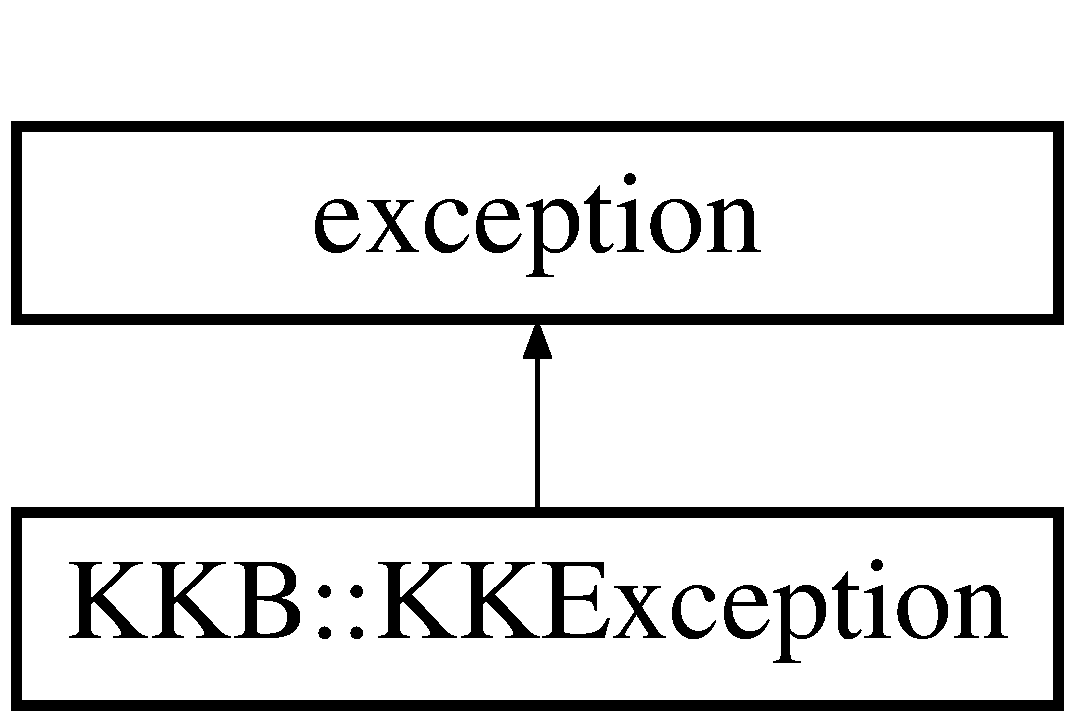
\includegraphics[height=2.000000cm]{class_k_k_b_1_1_k_k_exception}
\end{center}
\end{figure}
\subsection*{Public Member Functions}
\begin{DoxyCompactItemize}
\item 
\hyperlink{class_k_k_b_1_1_k_k_exception_a3ab2819dbec1acd42cee965e51aa4ccb}{K\+K\+Exception} ()
\item 
\hyperlink{class_k_k_b_1_1_k_k_exception_a16aba1c3d205611fa0a5dbc9f78ee84d}{K\+K\+Exception} (const \hyperlink{class_k_k_b_1_1_k_k_exception}{K\+K\+Exception} \&\+\_\+exception)
\item 
\hyperlink{class_k_k_b_1_1_k_k_exception_a9505cf26272a2d7a3ca4a5ed19f46877}{K\+K\+Exception} (const \hyperlink{class_k_k_b_1_1_k_k_str}{K\+K\+Str} \&\+\_\+exception\+Str)
\item 
\hyperlink{class_k_k_b_1_1_k_k_exception_a1e650cbf594edbd3ee231f11b098df9e}{K\+K\+Exception} (const char $\ast$\+\_\+exception\+Str)
\item 
\hyperlink{class_k_k_b_1_1_k_k_exception_a830eb03986c23ef438562bbb7adbdf9b}{K\+K\+Exception} (const \hyperlink{class_k_k_b_1_1_k_k_str}{K\+K\+Str} \&\+\_\+exception\+Str, const std\+::exception \&\+\_\+inner\+Exception)
\item 
\hyperlink{class_k_k_b_1_1_k_k_exception_ae911463f46fef87b623ff7c54a4988cd}{K\+K\+Exception} (const char $\ast$\+\_\+exception\+Str, const std\+::exception \&\+\_\+inner\+Exception)
\item 
\hyperlink{class_k_k_b_1_1_k_k_exception_a3f9273ed8c1c83d7bc53d2d72238a691}{K\+K\+Exception} (const char $\ast$\+\_\+exception\+Str, const \hyperlink{class_k_k_b_1_1_k_k_exception}{K\+K\+Exception} \&\+\_\+inner\+Exception)
\item 
\hyperlink{class_k_k_b_1_1_k_k_exception_abebe565c76ebcc389e3506e2399badfd}{K\+K\+Exception} (const \hyperlink{class_k_k_b_1_1_k_k_str}{K\+K\+Str} \&\+\_\+exception\+Str, const \hyperlink{class_k_k_b_1_1_k_k_exception}{K\+K\+Exception} \&\+\_\+inner\+Exception)
\item 
virtual \hyperlink{class_k_k_b_1_1_k_k_exception_a8600cf9e6176fec2dcbb23052c36de8a}{$\sim$\+K\+K\+Exception} ()  throw ()
\item 
virtual const \hyperlink{class_k_k_b_1_1_k_k_str}{K\+K\+Str} \& \hyperlink{class_k_k_b_1_1_k_k_exception_a9d565e887e90968c5e306c1ea94c6894}{To\+String} () const 
\item 
virtual const char $\ast$ \hyperlink{class_k_k_b_1_1_k_k_exception_aae7f05aaeeb741d494fbfbe97bfd3a81}{what} () const   throw ()
\end{DoxyCompactItemize}


\subsection{Detailed Description}


Definition at line 27 of file K\+K\+Exception.\+h.



\subsection{Constructor \& Destructor Documentation}
\index{K\+K\+B\+::\+K\+K\+Exception@{K\+K\+B\+::\+K\+K\+Exception}!K\+K\+Exception@{K\+K\+Exception}}
\index{K\+K\+Exception@{K\+K\+Exception}!K\+K\+B\+::\+K\+K\+Exception@{K\+K\+B\+::\+K\+K\+Exception}}
\subsubsection[{\texorpdfstring{K\+K\+Exception()}{KKException()}}]{\setlength{\rightskip}{0pt plus 5cm}K\+K\+Exception\+::\+K\+K\+Exception (
\begin{DoxyParamCaption}
{}
\end{DoxyParamCaption}
)}\hypertarget{class_k_k_b_1_1_k_k_exception_a3ab2819dbec1acd42cee965e51aa4ccb}{}\label{class_k_k_b_1_1_k_k_exception_a3ab2819dbec1acd42cee965e51aa4ccb}


Definition at line 25 of file K\+K\+Exception.\+cpp.



References K\+K\+Exception().



Referenced by K\+K\+Exception().


\begin{DoxyCode}
25                          :
26   std::exception ()
27 \{
28 \}
\end{DoxyCode}
\index{K\+K\+B\+::\+K\+K\+Exception@{K\+K\+B\+::\+K\+K\+Exception}!K\+K\+Exception@{K\+K\+Exception}}
\index{K\+K\+Exception@{K\+K\+Exception}!K\+K\+B\+::\+K\+K\+Exception@{K\+K\+B\+::\+K\+K\+Exception}}
\subsubsection[{\texorpdfstring{K\+K\+Exception(const K\+K\+Exception \&\+\_\+exception)}{KKException(const KKException &_exception)}}]{\setlength{\rightskip}{0pt plus 5cm}K\+K\+Exception\+::\+K\+K\+Exception (
\begin{DoxyParamCaption}
\item[{const {\bf K\+K\+Exception} \&}]{\+\_\+exception}
\end{DoxyParamCaption}
)}\hypertarget{class_k_k_b_1_1_k_k_exception_a16aba1c3d205611fa0a5dbc9f78ee84d}{}\label{class_k_k_b_1_1_k_k_exception_a16aba1c3d205611fa0a5dbc9f78ee84d}


Definition at line 31 of file K\+K\+Exception.\+cpp.



References K\+K\+Exception(), and K\+K\+B\+::\+K\+K\+Str\+::\+K\+K\+Str().



Referenced by K\+K\+Exception().


\begin{DoxyCode}
31                                                        :
32   std::exception (),
33   exceptionStr (\_exception.exceptionStr)
34 \{
35 \}
\end{DoxyCode}
\index{K\+K\+B\+::\+K\+K\+Exception@{K\+K\+B\+::\+K\+K\+Exception}!K\+K\+Exception@{K\+K\+Exception}}
\index{K\+K\+Exception@{K\+K\+Exception}!K\+K\+B\+::\+K\+K\+Exception@{K\+K\+B\+::\+K\+K\+Exception}}
\subsubsection[{\texorpdfstring{K\+K\+Exception(const K\+K\+Str \&\+\_\+exception\+Str)}{KKException(const KKStr &_exceptionStr)}}]{\setlength{\rightskip}{0pt plus 5cm}K\+K\+Exception\+::\+K\+K\+Exception (
\begin{DoxyParamCaption}
\item[{const {\bf K\+K\+Str} \&}]{\+\_\+exception\+Str}
\end{DoxyParamCaption}
)}\hypertarget{class_k_k_b_1_1_k_k_exception_a9505cf26272a2d7a3ca4a5ed19f46877}{}\label{class_k_k_b_1_1_k_k_exception_a9505cf26272a2d7a3ca4a5ed19f46877}


Definition at line 45 of file K\+K\+Exception.\+cpp.



References K\+K\+Exception(), and K\+K\+B\+::\+K\+K\+Str\+::\+K\+K\+Str().



Referenced by K\+K\+M\+L\+L\+::\+File\+Desc\+::\+Add\+A\+Nominal\+Value(), K\+K\+M\+L\+L\+::\+Feature\+Vector\+::\+Add\+Feature\+Data(), K\+K\+B\+::\+Msg\+Queue\+::\+Add\+Msg(), K\+K\+B\+::\+Raster\+Buffer\+::\+Add\+Raster(), K\+K\+B\+::\+K\+K\+Str\+::\+Append(), K\+K\+M\+L\+L\+::\+Gray\+Scale\+Images\+F\+V\+List\+::\+Back\+Of\+Queue(), K\+K\+B\+::\+K\+K\+Str\+List\+::\+Binary\+Search(), K\+K\+B\+::\+Bit\+String\+::\+Bit\+String(), K\+K\+B\+::\+Bmp\+Image\+::\+Blue\+Row(), K\+K\+M\+L\+L\+::\+File\+Desc\+::\+Cardinality(), K\+K\+M\+L\+L\+::\+Classifier2\+::\+Classifier2(), K\+K\+M\+L\+L\+::\+Model\+::\+Create\+A\+Model(), K\+K\+M\+L\+L\+::\+Feature\+Encoder\+::\+Create\+Encoded\+File\+Desc(), K\+K\+B\+::\+Bmp\+Image\+::\+Coded\+Pixels\+::\+Create\+Pixel\+Data\+Structure8\+Bit(), K\+K\+B\+::\+Matrix\+::\+Determinant\+Slow(), K\+K\+M\+L\+L\+::\+Feature\+Encoder\+::\+Encode\+A\+Example(), K\+K\+B\+::\+Goal\+Keeper\+Simple\+::\+End\+Block(), K\+K\+B\+::\+Raster\+::\+Extract\+Blobs(), K\+K\+M\+L\+L\+::\+Feature\+Vector\+List\+::\+Feature\+Vector\+List(), K\+K\+M\+L\+L\+::\+S\+V\+M\+Model\+::\+Find\+Worst\+Support\+Vectors(), K\+K\+M\+L\+L\+::\+S\+V\+M\+Model\+::\+Find\+Worst\+Support\+Vectors2(), K\+K\+B\+::\+K\+K\+Str\+::\+Free\+Up\+Un\+Used\+Space(), K\+K\+M\+L\+L\+::\+File\+Desc\+::\+Get\+Existing\+File\+Desc(), K\+K\+M\+L\+L\+::\+Gray\+Scale\+Images\+F\+V\+List\+::\+Gray\+Scale\+Images\+F\+V\+List(), K\+K\+B\+::\+Raster\+::\+Histogram(), K\+K\+B\+::\+Bmp\+Image\+::\+Image\+Row(), K\+K\+B\+::\+Matrix\+::\+Inverse(), K\+K\+Exception(), K\+K\+B\+::\+K\+K\+Str\+::\+K\+K\+Str(), K\+K\+B\+::\+K\+K\+Str\+::\+Left\+Pad(), K\+K\+B\+::\+Bit\+String\+::\+List\+Of\+Set\+Bits16(), K\+K\+B\+::\+Matrix\+::\+Matrix(), K\+K\+B\+::\+Matrix\+::operator$\ast$(), K\+K\+B\+::\+Matrix\+::operator+(), K\+K\+B\+::\+Matrix\+::operator+=(), K\+K\+B\+::\+Matrix\+::operator-\/(), K\+K\+B\+::\+K\+K\+Str\+::operator=(), K\+K\+B\+::\+Matrix\+::operator\mbox{[}$\,$\mbox{]}(), K\+K\+M\+L\+L\+::\+Feature\+Num\+List\+::operator\mbox{[}$\,$\mbox{]}(), K\+K\+M\+L\+L\+::\+Model\+Old\+S\+V\+M\+::\+Param(), K\+K\+M\+L\+L\+::\+Gray\+Scale\+Images\+F\+V\+List\+::\+Pop\+From\+Back(), K\+K\+M\+L\+L\+::\+Model\+Svm\+Base\+::\+Predict(), K\+K\+M\+L\+L\+::\+Model\+Usf\+Cas\+Cor\+::\+Predict(), K\+K\+M\+L\+L\+::\+S\+V\+M\+Model\+::\+Predict(), K\+K\+M\+L\+L\+::\+Classification\+Bias\+Matrix\+::\+Print\+Adjusted\+Results(), K\+K\+M\+L\+L\+::\+Classification\+Bias\+Matrix\+::\+Print\+Bias\+Matrix(), K\+K\+M\+L\+L\+::\+Model\+Knn\+::\+Probabilities\+By\+Class(), K\+K\+M\+L\+L\+::\+Model\+Svm\+Base\+::\+Probabilities\+By\+Class(), K\+K\+M\+L\+L\+::\+Model\+Usf\+Cas\+Cor\+::\+Probabilities\+By\+Class(), K\+K\+M\+L\+L\+::\+Model\+Old\+S\+V\+M\+::\+Probabilities\+By\+Class(), K\+K\+M\+L\+L\+::\+Class\+Prob\+List\+::\+Push\+On\+Back(), K\+K\+M\+L\+L\+::\+Binary\+Class\+Parms\+List\+::\+Push\+On\+Back(), K\+K\+M\+L\+L\+::\+Feature\+Vector\+List\+::\+Push\+On\+Back(), K\+K\+M\+L\+L\+::\+Class\+Prob\+List\+::\+Push\+On\+Front(), K\+K\+M\+L\+L\+::\+Binary\+Class\+Parms\+List\+::\+Push\+On\+Front(), K\+K\+M\+L\+L\+::\+Feature\+Vector\+List\+::\+Push\+On\+Front(), K\+K\+B\+::\+Raster\+::\+Raster(), K\+K\+B\+::\+Bmp\+Image\+::\+Red\+Row(), K\+K\+B\+::\+Xml\+Factory\+Manager\+::\+Register\+Factory(), K\+K\+B\+::\+Xml\+Factory\+::\+Register\+Factory(), K\+K\+M\+L\+L\+::\+Feature\+Vector\+List\+::\+Reset\+File\+Desc(), K\+K\+M\+L\+L\+::\+Feature\+Vector\+::\+Reset\+Num\+Of\+Features(), K\+K\+M\+L\+L\+::\+Feature\+Vector\+List\+::\+Re\+Sync\+Symbolic\+Data(), K\+K\+B\+::\+K\+K\+Str\+::\+Right\+Pad(), K\+K\+B\+::\+Row\+::\+Row(), K\+K\+B\+::\+Bmp\+Image\+::\+Save(), K\+K\+B\+::\+Bmp\+Image\+::\+Save\+Grayscale\+Inverted4\+Bit(), K\+K\+B\+::\+Bmp\+Image\+::\+Save\+Grayscale\+Inverted8\+Bit(), K\+K\+B\+::\+Save\+Image(), K\+K\+B\+::\+Save\+Image\+Grayscale\+Inverted4\+Bit(), K\+K\+B\+::\+Save\+Image\+Grayscale\+Inverted8\+Bit(), K\+K\+B\+::\+Save\+Image\+P\+N\+G(), K\+K\+B\+::\+Save\+Image\+P\+P\+M(), S\+V\+M233\+::svm\+\_\+\+Get\+Support\+Vector\+Statistics(), S\+V\+M289\+\_\+\+B\+F\+S\+::svm\+\_\+train\+\_\+one(), S\+V\+M289\+\_\+\+M\+F\+S\+::svm\+\_\+train\+\_\+one(), K\+K\+M\+L\+L\+::\+Training\+Configuration2\+::\+S\+V\+Mparam\+R\+E\+F(), K\+K\+M\+L\+L\+::\+Feature\+Vector\+List\+::\+Synchronize\+Symbolic\+Data(), K\+K\+B\+::tqli(), K\+K\+M\+L\+L\+::\+Model\+Usf\+Cas\+Cor\+::\+Train\+Model(), K\+K\+M\+L\+L\+::\+Model\+Svm\+Base\+::\+Train\+Model(), K\+K\+M\+L\+L\+::\+Model\+Dual\+::\+Train\+Model(), K\+K\+M\+L\+L\+::\+Model\+Old\+S\+V\+M\+::\+Train\+Model(), K\+K\+M\+L\+L\+::\+Model\+::\+Train\+Model(), and K\+K\+B\+::\+Tred2().


\begin{DoxyCode}
45                                                     :
46   std::exception (),
47   exceptionStr (\_exceptionStr)
48 \{
49 \}
\end{DoxyCode}
\index{K\+K\+B\+::\+K\+K\+Exception@{K\+K\+B\+::\+K\+K\+Exception}!K\+K\+Exception@{K\+K\+Exception}}
\index{K\+K\+Exception@{K\+K\+Exception}!K\+K\+B\+::\+K\+K\+Exception@{K\+K\+B\+::\+K\+K\+Exception}}
\subsubsection[{\texorpdfstring{K\+K\+Exception(const char $\ast$\+\_\+exception\+Str)}{KKException(const char *_exceptionStr)}}]{\setlength{\rightskip}{0pt plus 5cm}K\+K\+Exception\+::\+K\+K\+Exception (
\begin{DoxyParamCaption}
\item[{const char $\ast$}]{\+\_\+exception\+Str}
\end{DoxyParamCaption}
)}\hypertarget{class_k_k_b_1_1_k_k_exception_a1e650cbf594edbd3ee231f11b098df9e}{}\label{class_k_k_b_1_1_k_k_exception_a1e650cbf594edbd3ee231f11b098df9e}


Definition at line 38 of file K\+K\+Exception.\+cpp.



References K\+K\+Exception(), and K\+K\+B\+::\+K\+K\+Str\+::\+K\+K\+Str().



Referenced by K\+K\+B\+::\+Bmp\+Image\+::\+Blue\+Row(), K\+K\+M\+L\+L\+::\+Classifier2\+::\+Classifier2(), K\+K\+M\+L\+L\+::\+Model\+::\+Create\+A\+Model(), K\+K\+M\+L\+L\+::\+Model\+::\+Encoder(), K\+K\+B\+::\+Raster\+::\+Extract\+Blobs(), K\+K\+M\+L\+L\+::\+Model\+::\+Get\+Feature\+Nums(), K\+K\+B\+::\+Bmp\+Image\+::\+Image\+Row(), K\+K\+B\+::\+Raster\+::\+Initialize(), K\+K\+Exception(), K\+K\+B\+::\+K\+K\+Str\+::\+K\+K\+Str(), K\+K\+M\+L\+L\+::\+Model\+::\+Normalize\+Nominal\+Attributes(), K\+K\+B\+::\+K\+K\+Str\+::operator$<$$<$(), K\+K\+B\+::\+K\+K\+Str\+::operator=(), K\+K\+Job\+Managment\+::\+K\+K\+Job\+::\+Process\+Node(), K\+K\+B\+::\+Raster\+::\+Raster(), K\+K\+B\+::\+Bmp\+Image\+::\+Red\+Row(), K\+K\+M\+L\+L\+::\+Model\+::\+Selected\+Features(), K\+K\+B\+::\+K\+K\+Thread\+::\+Start(), and S\+V\+M233\+::\+Svm\+Model233\+::\+Svm\+Model233().


\begin{DoxyCode}
38                                                    :
39   std::exception (),
40   exceptionStr (\_exceptionStr)
41 \{
42 \}
\end{DoxyCode}
\index{K\+K\+B\+::\+K\+K\+Exception@{K\+K\+B\+::\+K\+K\+Exception}!K\+K\+Exception@{K\+K\+Exception}}
\index{K\+K\+Exception@{K\+K\+Exception}!K\+K\+B\+::\+K\+K\+Exception@{K\+K\+B\+::\+K\+K\+Exception}}
\subsubsection[{\texorpdfstring{K\+K\+Exception(const K\+K\+Str \&\+\_\+exception\+Str, const std\+::exception \&\+\_\+inner\+Exception)}{KKException(const KKStr &_exceptionStr, const std::exception &_innerException)}}]{\setlength{\rightskip}{0pt plus 5cm}K\+K\+Exception\+::\+K\+K\+Exception (
\begin{DoxyParamCaption}
\item[{const {\bf K\+K\+Str} \&}]{\+\_\+exception\+Str, }
\item[{const std\+::exception \&}]{\+\_\+inner\+Exception}
\end{DoxyParamCaption}
)}\hypertarget{class_k_k_b_1_1_k_k_exception_a830eb03986c23ef438562bbb7adbdf9b}{}\label{class_k_k_b_1_1_k_k_exception_a830eb03986c23ef438562bbb7adbdf9b}


Definition at line 52 of file K\+K\+Exception.\+cpp.



References K\+K\+Exception(), and K\+K\+B\+::\+K\+K\+Str\+::\+K\+K\+Str().



Referenced by K\+K\+Exception(), K\+K\+M\+L\+L\+::\+Classification\+Bias\+Matrix\+::\+Print\+Adjusted\+Results(), K\+K\+M\+L\+L\+::\+Model\+Usf\+Cas\+Cor\+::\+Train\+Model(), K\+K\+M\+L\+L\+::\+Model\+Svm\+Base\+::\+Train\+Model(), and K\+K\+M\+L\+L\+::\+Model\+Dual\+::\+Train\+Model().


\begin{DoxyCode}
54                           :
55   std::exception (\_innerException),
56   exceptionStr ()
57 \{
58   exceptionStr << \_exceptionStr << \hyperlink{namespace_k_k_b_ad1f50f65af6adc8fa9e6f62d007818a8}{endl}
59                << \_innerException.what ();
60 \}
\end{DoxyCode}
\index{K\+K\+B\+::\+K\+K\+Exception@{K\+K\+B\+::\+K\+K\+Exception}!K\+K\+Exception@{K\+K\+Exception}}
\index{K\+K\+Exception@{K\+K\+Exception}!K\+K\+B\+::\+K\+K\+Exception@{K\+K\+B\+::\+K\+K\+Exception}}
\subsubsection[{\texorpdfstring{K\+K\+Exception(const char $\ast$\+\_\+exception\+Str, const std\+::exception \&\+\_\+inner\+Exception)}{KKException(const char *_exceptionStr, const std::exception &_innerException)}}]{\setlength{\rightskip}{0pt plus 5cm}K\+K\+Exception\+::\+K\+K\+Exception (
\begin{DoxyParamCaption}
\item[{const char $\ast$}]{\+\_\+exception\+Str, }
\item[{const std\+::exception \&}]{\+\_\+inner\+Exception}
\end{DoxyParamCaption}
)}\hypertarget{class_k_k_b_1_1_k_k_exception_ae911463f46fef87b623ff7c54a4988cd}{}\label{class_k_k_b_1_1_k_k_exception_ae911463f46fef87b623ff7c54a4988cd}


Definition at line 64 of file K\+K\+Exception.\+cpp.


\begin{DoxyCode}
67 \{
68   exceptionStr << \_exceptionStr << \hyperlink{namespace_k_k_b_ad1f50f65af6adc8fa9e6f62d007818a8}{endl}
69                << \_innerException.what ();
70 \}
\end{DoxyCode}
\index{K\+K\+B\+::\+K\+K\+Exception@{K\+K\+B\+::\+K\+K\+Exception}!K\+K\+Exception@{K\+K\+Exception}}
\index{K\+K\+Exception@{K\+K\+Exception}!K\+K\+B\+::\+K\+K\+Exception@{K\+K\+B\+::\+K\+K\+Exception}}
\subsubsection[{\texorpdfstring{K\+K\+Exception(const char $\ast$\+\_\+exception\+Str, const K\+K\+Exception \&\+\_\+inner\+Exception)}{KKException(const char *_exceptionStr, const KKException &_innerException)}}]{\setlength{\rightskip}{0pt plus 5cm}K\+K\+Exception\+::\+K\+K\+Exception (
\begin{DoxyParamCaption}
\item[{const char $\ast$}]{\+\_\+exception\+Str, }
\item[{const {\bf K\+K\+Exception} \&}]{\+\_\+inner\+Exception}
\end{DoxyParamCaption}
)}\hypertarget{class_k_k_b_1_1_k_k_exception_a3f9273ed8c1c83d7bc53d2d72238a691}{}\label{class_k_k_b_1_1_k_k_exception_a3f9273ed8c1c83d7bc53d2d72238a691}


Definition at line 74 of file K\+K\+Exception.\+cpp.



References K\+K\+Exception(), and K\+K\+B\+::\+K\+K\+Str\+::\+K\+K\+Str().



Referenced by K\+K\+M\+L\+L\+::\+Model\+::\+Create\+A\+Model(), and K\+K\+Exception().


\begin{DoxyCode}
76                           :
77   std::exception (\_innerException),
78   exceptionStr (\_exceptionStr)
79 \{
80 \}
\end{DoxyCode}
\index{K\+K\+B\+::\+K\+K\+Exception@{K\+K\+B\+::\+K\+K\+Exception}!K\+K\+Exception@{K\+K\+Exception}}
\index{K\+K\+Exception@{K\+K\+Exception}!K\+K\+B\+::\+K\+K\+Exception@{K\+K\+B\+::\+K\+K\+Exception}}
\subsubsection[{\texorpdfstring{K\+K\+Exception(const K\+K\+Str \&\+\_\+exception\+Str, const K\+K\+Exception \&\+\_\+inner\+Exception)}{KKException(const KKStr &_exceptionStr, const KKException &_innerException)}}]{\setlength{\rightskip}{0pt plus 5cm}K\+K\+Exception\+::\+K\+K\+Exception (
\begin{DoxyParamCaption}
\item[{const {\bf K\+K\+Str} \&}]{\+\_\+exception\+Str, }
\item[{const {\bf K\+K\+Exception} \&}]{\+\_\+inner\+Exception}
\end{DoxyParamCaption}
)}\hypertarget{class_k_k_b_1_1_k_k_exception_abebe565c76ebcc389e3506e2399badfd}{}\label{class_k_k_b_1_1_k_k_exception_abebe565c76ebcc389e3506e2399badfd}


Definition at line 83 of file K\+K\+Exception.\+cpp.



References K\+K\+Exception(), and K\+K\+B\+::\+K\+K\+Str\+::\+K\+K\+Str().



Referenced by K\+K\+Exception(), K\+K\+M\+L\+L\+::\+Classification\+Bias\+Matrix\+::\+Print\+Adjusted\+Results(), K\+K\+B\+::\+Save\+Image(), K\+K\+B\+::\+Save\+Image\+Grayscale\+Inverted4\+Bit(), K\+K\+B\+::\+Save\+Image\+Grayscale\+Inverted8\+Bit(), K\+K\+M\+L\+L\+::\+Model\+Usf\+Cas\+Cor\+::\+Train\+Model(), K\+K\+M\+L\+L\+::\+Model\+Svm\+Base\+::\+Train\+Model(), and K\+K\+M\+L\+L\+::\+Model\+Dual\+::\+Train\+Model().


\begin{DoxyCode}
85                           :
86   std::exception (\_innerException),
87   exceptionStr (\_exceptionStr)
88 \{
89 \}
\end{DoxyCode}
\index{K\+K\+B\+::\+K\+K\+Exception@{K\+K\+B\+::\+K\+K\+Exception}!````~K\+K\+Exception@{$\sim$\+K\+K\+Exception}}
\index{````~K\+K\+Exception@{$\sim$\+K\+K\+Exception}!K\+K\+B\+::\+K\+K\+Exception@{K\+K\+B\+::\+K\+K\+Exception}}
\subsubsection[{\texorpdfstring{$\sim$\+K\+K\+Exception()}{~KKException()}}]{\setlength{\rightskip}{0pt plus 5cm}K\+K\+Exception\+::$\sim$\+K\+K\+Exception (
\begin{DoxyParamCaption}
{}
\end{DoxyParamCaption}
) throw  ) \hspace{0.3cm}{\ttfamily [virtual]}}\hypertarget{class_k_k_b_1_1_k_k_exception_a8600cf9e6176fec2dcbb23052c36de8a}{}\label{class_k_k_b_1_1_k_k_exception_a8600cf9e6176fec2dcbb23052c36de8a}


Definition at line 93 of file K\+K\+Exception.\+cpp.


\begin{DoxyCode}
94 \{
95 \}
\end{DoxyCode}


\subsection{Member Function Documentation}
\index{K\+K\+B\+::\+K\+K\+Exception@{K\+K\+B\+::\+K\+K\+Exception}!To\+String@{To\+String}}
\index{To\+String@{To\+String}!K\+K\+B\+::\+K\+K\+Exception@{K\+K\+B\+::\+K\+K\+Exception}}
\subsubsection[{\texorpdfstring{To\+String() const }{ToString() const }}]{\setlength{\rightskip}{0pt plus 5cm}const {\bf K\+K\+Str} \& K\+K\+Exception\+::\+To\+String (
\begin{DoxyParamCaption}
{}
\end{DoxyParamCaption}
) const\hspace{0.3cm}{\ttfamily [virtual]}}\hypertarget{class_k_k_b_1_1_k_k_exception_a9d565e887e90968c5e306c1ea94c6894}{}\label{class_k_k_b_1_1_k_k_exception_a9d565e887e90968c5e306c1ea94c6894}


Definition at line 98 of file K\+K\+Exception.\+cpp.



Referenced by K\+K\+B\+::\+Thread\+Start\+Call\+Back().


\begin{DoxyCode}
99 \{
100   \textcolor{keywordflow}{return}  exceptionStr;
101 \}
\end{DoxyCode}
\index{K\+K\+B\+::\+K\+K\+Exception@{K\+K\+B\+::\+K\+K\+Exception}!what@{what}}
\index{what@{what}!K\+K\+B\+::\+K\+K\+Exception@{K\+K\+B\+::\+K\+K\+Exception}}
\subsubsection[{\texorpdfstring{what() const }{what() const }}]{\setlength{\rightskip}{0pt plus 5cm}const char $\ast$ K\+K\+Exception\+::what (
\begin{DoxyParamCaption}
{}
\end{DoxyParamCaption}
) const throw  ) \hspace{0.3cm}{\ttfamily [virtual]}}\hypertarget{class_k_k_b_1_1_k_k_exception_aae7f05aaeeb741d494fbfbe97bfd3a81}{}\label{class_k_k_b_1_1_k_k_exception_aae7f05aaeeb741d494fbfbe97bfd3a81}


Definition at line 104 of file K\+K\+Exception.\+cpp.



References K\+K\+B\+::\+K\+K\+Str\+::\+Str().


\begin{DoxyCode}
105 \{
106   \textcolor{keywordflow}{return}  exceptionStr.\hyperlink{class_k_k_b_1_1_k_k_str_ad574e6c0fe7f6ce1ba3ab0a8ce2fbd52}{Str} ();
107 \}
\end{DoxyCode}


The documentation for this class was generated from the following files\+:\begin{DoxyCompactItemize}
\item 
C\+:/\+Users/\+Kurt/\+Git\+Hub/\+K\+Square\+Libraries/\+K\+K\+Base/\hyperlink{_k_k_exception_8h}{K\+K\+Exception.\+h}\item 
C\+:/\+Users/\+Kurt/\+Git\+Hub/\+K\+Square\+Libraries/\+K\+K\+Base/\hyperlink{_k_k_exception_8cpp}{K\+K\+Exception.\+cpp}\end{DoxyCompactItemize}

\hypertarget{class_k_k_b_1_1_k_k_observable}{}\section{K\+KB\+:\+:K\+K\+Observable Class Reference}
\label{class_k_k_b_1_1_k_k_observable}\index{K\+K\+B\+::\+K\+K\+Observable@{K\+K\+B\+::\+K\+K\+Observable}}


The base class to be used by Observer classes.  




{\ttfamily \#include $<$K\+K\+Observable.\+h$>$}

\subsection*{Public Types}
\begin{DoxyCompactItemize}
\item 
typedef \hyperlink{class_k_k_b_1_1_k_k_observable}{K\+K\+Observable} $\ast$ \hyperlink{class_k_k_b_1_1_k_k_observable_a5d49993ee949ed5d904d5b2d7972725d}{K\+K\+Observable\+Ptr}
\end{DoxyCompactItemize}
\subsection*{Public Member Functions}
\begin{DoxyCompactItemize}
\item 
\hyperlink{class_k_k_b_1_1_k_k_observable_a5e9a2e1eaeb471bd8264e244c225df1d}{K\+K\+Observable} ()
\item 
virtual \hyperlink{class_k_k_b_1_1_k_k_observable_aebc05e2a5875f3d9db833f52a2734040}{$\sim$\+K\+K\+Observable} ()
\item 
\hyperlink{namespace_k_k_b_a8fa4952cc84fda1de4bec1fbdd8d5b1b}{kkint32} \hyperlink{class_k_k_b_1_1_k_k_observable_a1a7279a4d261466de52a7ec89a7aad21}{Memory\+Consumed\+Estimated} ()
\item 
virtual void \hyperlink{class_k_k_b_1_1_k_k_observable_abb6a5bb2ea885adac9bcc232b3db3789}{Notify\+Observers} ()
\item 
virtual void \hyperlink{class_k_k_b_1_1_k_k_observable_ae84b4e9e500854213b407cabd6a54f83}{Register\+Observer} (\hyperlink{namespace_k_k_b_ae230fa69820db86befff70da824c5b2b}{K\+K\+Observer\+Ptr} observer)
\item 
virtual void \hyperlink{class_k_k_b_1_1_k_k_observable_a7803558795794458de86193a6a8e79a7}{Un\+Register\+Observer} (\hyperlink{namespace_k_k_b_ae230fa69820db86befff70da824c5b2b}{K\+K\+Observer\+Ptr} observer)
\end{DoxyCompactItemize}
\subsection*{Friends}
\begin{DoxyCompactItemize}
\item 
class \hyperlink{class_k_k_b_1_1_k_k_observable_a782cf8bb982a5d411e9e64e3d40ea014}{K\+K\+Observer}
\end{DoxyCompactItemize}


\subsection{Detailed Description}
The base class to be used by Observer classes. 

Definition at line 25 of file K\+K\+Observable.\+h.



\subsection{Member Typedef Documentation}
\index{K\+K\+B\+::\+K\+K\+Observable@{K\+K\+B\+::\+K\+K\+Observable}!K\+K\+Observable\+Ptr@{K\+K\+Observable\+Ptr}}
\index{K\+K\+Observable\+Ptr@{K\+K\+Observable\+Ptr}!K\+K\+B\+::\+K\+K\+Observable@{K\+K\+B\+::\+K\+K\+Observable}}
\subsubsection[{\texorpdfstring{K\+K\+Observable\+Ptr}{KKObservablePtr}}]{\setlength{\rightskip}{0pt plus 5cm}typedef {\bf K\+K\+Observable}$\ast$ {\bf K\+K\+B\+::\+K\+K\+Observable\+::\+K\+K\+Observable\+Ptr}}\hypertarget{class_k_k_b_1_1_k_k_observable_a5d49993ee949ed5d904d5b2d7972725d}{}\label{class_k_k_b_1_1_k_k_observable_a5d49993ee949ed5d904d5b2d7972725d}


Definition at line 28 of file K\+K\+Observable.\+h.



\subsection{Constructor \& Destructor Documentation}
\index{K\+K\+B\+::\+K\+K\+Observable@{K\+K\+B\+::\+K\+K\+Observable}!K\+K\+Observable@{K\+K\+Observable}}
\index{K\+K\+Observable@{K\+K\+Observable}!K\+K\+B\+::\+K\+K\+Observable@{K\+K\+B\+::\+K\+K\+Observable}}
\subsubsection[{\texorpdfstring{K\+K\+Observable()}{KKObservable()}}]{\setlength{\rightskip}{0pt plus 5cm}K\+K\+Observable\+::\+K\+K\+Observable (
\begin{DoxyParamCaption}
{}
\end{DoxyParamCaption}
)}\hypertarget{class_k_k_b_1_1_k_k_observable_a5e9a2e1eaeb471bd8264e244c225df1d}{}\label{class_k_k_b_1_1_k_k_observable_a5e9a2e1eaeb471bd8264e244c225df1d}


Definition at line 29 of file K\+K\+Observable.\+cpp.


\begin{DoxyCode}
30 \{
31 \}
\end{DoxyCode}
\index{K\+K\+B\+::\+K\+K\+Observable@{K\+K\+B\+::\+K\+K\+Observable}!````~K\+K\+Observable@{$\sim$\+K\+K\+Observable}}
\index{````~K\+K\+Observable@{$\sim$\+K\+K\+Observable}!K\+K\+B\+::\+K\+K\+Observable@{K\+K\+B\+::\+K\+K\+Observable}}
\subsubsection[{\texorpdfstring{$\sim$\+K\+K\+Observable()}{~KKObservable()}}]{\setlength{\rightskip}{0pt plus 5cm}K\+K\+Observable\+::$\sim$\+K\+K\+Observable (
\begin{DoxyParamCaption}
{}
\end{DoxyParamCaption}
)\hspace{0.3cm}{\ttfamily [virtual]}}\hypertarget{class_k_k_b_1_1_k_k_observable_aebc05e2a5875f3d9db833f52a2734040}{}\label{class_k_k_b_1_1_k_k_observable_aebc05e2a5875f3d9db833f52a2734040}


Definition at line 35 of file K\+K\+Observable.\+cpp.


\begin{DoxyCode}
36 \{
37 \}
\end{DoxyCode}


\subsection{Member Function Documentation}
\index{K\+K\+B\+::\+K\+K\+Observable@{K\+K\+B\+::\+K\+K\+Observable}!Memory\+Consumed\+Estimated@{Memory\+Consumed\+Estimated}}
\index{Memory\+Consumed\+Estimated@{Memory\+Consumed\+Estimated}!K\+K\+B\+::\+K\+K\+Observable@{K\+K\+B\+::\+K\+K\+Observable}}
\subsubsection[{\texorpdfstring{Memory\+Consumed\+Estimated()}{MemoryConsumedEstimated()}}]{\setlength{\rightskip}{0pt plus 5cm}{\bf kkint32} K\+K\+Observable\+::\+Memory\+Consumed\+Estimated (
\begin{DoxyParamCaption}
{}
\end{DoxyParamCaption}
)}\hypertarget{class_k_k_b_1_1_k_k_observable_a1a7279a4d261466de52a7ec89a7aad21}{}\label{class_k_k_b_1_1_k_k_observable_a1a7279a4d261466de52a7ec89a7aad21}


Definition at line 41 of file K\+K\+Observable.\+cpp.


\begin{DoxyCode}
42 \{
43   \textcolor{keywordflow}{return}  \textcolor{keyword}{sizeof} (*this);
44 \}
\end{DoxyCode}
\index{K\+K\+B\+::\+K\+K\+Observable@{K\+K\+B\+::\+K\+K\+Observable}!Notify\+Observers@{Notify\+Observers}}
\index{Notify\+Observers@{Notify\+Observers}!K\+K\+B\+::\+K\+K\+Observable@{K\+K\+B\+::\+K\+K\+Observable}}
\subsubsection[{\texorpdfstring{Notify\+Observers()}{NotifyObservers()}}]{\setlength{\rightskip}{0pt plus 5cm}void K\+K\+Observable\+::\+Notify\+Observers (
\begin{DoxyParamCaption}
{}
\end{DoxyParamCaption}
)\hspace{0.3cm}{\ttfamily [virtual]}}\hypertarget{class_k_k_b_1_1_k_k_observable_abb6a5bb2ea885adac9bcc232b3db3789}{}\label{class_k_k_b_1_1_k_k_observable_abb6a5bb2ea885adac9bcc232b3db3789}


Definition at line 76 of file K\+K\+Observable.\+cpp.


\begin{DoxyCode}
77 \{
78   \textcolor{keywordflow}{for}  (observersIdx = observers.begin ();  observersIdx != observers.end ();  ++observersIdx)
79     observersIdx->first->Notify (\textcolor{keyword}{this});
80 
81 \}
\end{DoxyCode}
\index{K\+K\+B\+::\+K\+K\+Observable@{K\+K\+B\+::\+K\+K\+Observable}!Register\+Observer@{Register\+Observer}}
\index{Register\+Observer@{Register\+Observer}!K\+K\+B\+::\+K\+K\+Observable@{K\+K\+B\+::\+K\+K\+Observable}}
\subsubsection[{\texorpdfstring{Register\+Observer(\+K\+K\+Observer\+Ptr observer)}{RegisterObserver(KKObserverPtr observer)}}]{\setlength{\rightskip}{0pt plus 5cm}void K\+K\+Observable\+::\+Register\+Observer (
\begin{DoxyParamCaption}
\item[{{\bf K\+K\+Observer\+Ptr}}]{observer}
\end{DoxyParamCaption}
)\hspace{0.3cm}{\ttfamily [virtual]}}\hypertarget{class_k_k_b_1_1_k_k_observable_ae84b4e9e500854213b407cabd6a54f83}{}\label{class_k_k_b_1_1_k_k_observable_ae84b4e9e500854213b407cabd6a54f83}


Definition at line 48 of file K\+K\+Observable.\+cpp.



References K\+K\+B\+::\+Global\+Goal\+Keeper\+::\+End\+Block(), and K\+K\+B\+::\+Global\+Goal\+Keeper\+::\+Start\+Block().


\begin{DoxyCode}
49 \{
50   \hyperlink{class_k_k_b_1_1_global_goal_keeper_a05d7aab73a0cc12c01f4dd6e8d3da839}{GlobalGoalKeeper::StartBlock} ();
51 
52   observers.insert (pair<KKObserverPtr,KKObserverPtr>(observer, observer));
53   observer->RegisterObservable (\textcolor{keyword}{this});
54 
55   \hyperlink{class_k_k_b_1_1_global_goal_keeper_a4e03a2807ca2f00c359da8625afb4cc5}{GlobalGoalKeeper::EndBlock} ();
56 \}  \textcolor{comment}{/* RegisterObserver */}
\end{DoxyCode}
\index{K\+K\+B\+::\+K\+K\+Observable@{K\+K\+B\+::\+K\+K\+Observable}!Un\+Register\+Observer@{Un\+Register\+Observer}}
\index{Un\+Register\+Observer@{Un\+Register\+Observer}!K\+K\+B\+::\+K\+K\+Observable@{K\+K\+B\+::\+K\+K\+Observable}}
\subsubsection[{\texorpdfstring{Un\+Register\+Observer(\+K\+K\+Observer\+Ptr observer)}{UnRegisterObserver(KKObserverPtr observer)}}]{\setlength{\rightskip}{0pt plus 5cm}void K\+K\+Observable\+::\+Un\+Register\+Observer (
\begin{DoxyParamCaption}
\item[{{\bf K\+K\+Observer\+Ptr}}]{observer}
\end{DoxyParamCaption}
)\hspace{0.3cm}{\ttfamily [virtual]}}\hypertarget{class_k_k_b_1_1_k_k_observable_a7803558795794458de86193a6a8e79a7}{}\label{class_k_k_b_1_1_k_k_observable_a7803558795794458de86193a6a8e79a7}


Definition at line 60 of file K\+K\+Observable.\+cpp.



References K\+K\+B\+::\+Global\+Goal\+Keeper\+::\+End\+Block(), and K\+K\+B\+::\+Global\+Goal\+Keeper\+::\+Start\+Block().



Referenced by K\+K\+B\+::\+K\+K\+Observer\+::$\sim$\+K\+K\+Observer().


\begin{DoxyCode}
61 \{
62   \hyperlink{class_k_k_b_1_1_global_goal_keeper_a05d7aab73a0cc12c01f4dd6e8d3da839}{GlobalGoalKeeper::StartBlock} ();
63  
64   observersIdx = observers.find (observer);
65   \textcolor{keywordflow}{if}  (observersIdx != observers.end ())
66     observers.erase (observersIdx);
67 
68   observer->UnRegisterObservable (\textcolor{keyword}{this});
69 
70   \hyperlink{class_k_k_b_1_1_global_goal_keeper_a4e03a2807ca2f00c359da8625afb4cc5}{GlobalGoalKeeper::EndBlock} ();
71 \}  \textcolor{comment}{/* RegisterObserver */}
\end{DoxyCode}


\subsection{Friends And Related Function Documentation}
\index{K\+K\+B\+::\+K\+K\+Observable@{K\+K\+B\+::\+K\+K\+Observable}!K\+K\+Observer@{K\+K\+Observer}}
\index{K\+K\+Observer@{K\+K\+Observer}!K\+K\+B\+::\+K\+K\+Observable@{K\+K\+B\+::\+K\+K\+Observable}}
\subsubsection[{\texorpdfstring{K\+K\+Observer}{KKObserver}}]{\setlength{\rightskip}{0pt plus 5cm}friend class {\bf K\+K\+Observer}\hspace{0.3cm}{\ttfamily [friend]}}\hypertarget{class_k_k_b_1_1_k_k_observable_a782cf8bb982a5d411e9e64e3d40ea014}{}\label{class_k_k_b_1_1_k_k_observable_a782cf8bb982a5d411e9e64e3d40ea014}


Definition at line 46 of file K\+K\+Observable.\+h.



The documentation for this class was generated from the following files\+:\begin{DoxyCompactItemize}
\item 
C\+:/\+Users/\+Kurt/\+Git\+Hub/\+K\+Square\+Libraries/\+K\+K\+Base/\hyperlink{_k_k_observable_8h}{K\+K\+Observable.\+h}\item 
C\+:/\+Users/\+Kurt/\+Git\+Hub/\+K\+Square\+Libraries/\+K\+K\+Base/\hyperlink{_k_k_observable_8cpp}{K\+K\+Observable.\+cpp}\end{DoxyCompactItemize}

\hypertarget{class_k_k_b_1_1_k_k_observer}{}\section{K\+KB\+:\+:K\+K\+Observer Class Reference}
\label{class_k_k_b_1_1_k_k_observer}\index{K\+K\+B\+::\+K\+K\+Observer@{K\+K\+B\+::\+K\+K\+Observer}}


The base class to be used by Observer classes.  




{\ttfamily \#include $<$K\+K\+Observer.\+h$>$}

\subsection*{Public Types}
\begin{DoxyCompactItemize}
\item 
typedef \hyperlink{class_k_k_b_1_1_k_k_observer}{K\+K\+Observer} $\ast$ \hyperlink{class_k_k_b_1_1_k_k_observer_a68ab7a7c923a7f43d39542cd5264f231}{K\+K\+Observer\+Ptr}
\end{DoxyCompactItemize}
\subsection*{Public Member Functions}
\begin{DoxyCompactItemize}
\item 
\hyperlink{class_k_k_b_1_1_k_k_observer_aca8156ee354c4275e3650f234620c417}{K\+K\+Observer} (const \hyperlink{class_k_k_b_1_1_k_k_str}{K\+K\+Str} \&\+\_\+name)
\item 
virtual \hyperlink{class_k_k_b_1_1_k_k_observer_a4cbcf4b87593c8ea9108407eafcffd95}{$\sim$\+K\+K\+Observer} ()
\item 
\hyperlink{namespace_k_k_b_a8fa4952cc84fda1de4bec1fbdd8d5b1b}{kkint32} \hyperlink{class_k_k_b_1_1_k_k_observer_a74c14088dc3123923addb51a21f01548}{Memory\+Consumed\+Estimated} ()
\item 
const \hyperlink{class_k_k_b_1_1_k_k_str}{K\+K\+Str} \& \hyperlink{class_k_k_b_1_1_k_k_observer_a1ee43dac59a71e131aa453989091c999}{Name} () const 
\item 
virtual void \hyperlink{class_k_k_b_1_1_k_k_observer_aa4a1765b0120bf4a2c6c92bfe917b35b}{Notify} (\hyperlink{namespace_k_k_b_ad2874a3aec87b033137ef07aef832c93}{K\+K\+Observable\+Ptr} obj)
\end{DoxyCompactItemize}
\subsection*{Friends}
\begin{DoxyCompactItemize}
\item 
class \hyperlink{class_k_k_b_1_1_k_k_observer_a7f04de4db416537cde0a4ae0ac98c529}{K\+K\+Observable}
\end{DoxyCompactItemize}


\subsection{Detailed Description}
The base class to be used by Observer classes. 

And application would register instances of a Observer 

Definition at line 25 of file K\+K\+Observer.\+h.



\subsection{Member Typedef Documentation}
\index{K\+K\+B\+::\+K\+K\+Observer@{K\+K\+B\+::\+K\+K\+Observer}!K\+K\+Observer\+Ptr@{K\+K\+Observer\+Ptr}}
\index{K\+K\+Observer\+Ptr@{K\+K\+Observer\+Ptr}!K\+K\+B\+::\+K\+K\+Observer@{K\+K\+B\+::\+K\+K\+Observer}}
\subsubsection[{\texorpdfstring{K\+K\+Observer\+Ptr}{KKObserverPtr}}]{\setlength{\rightskip}{0pt plus 5cm}typedef {\bf K\+K\+Observer}$\ast$ {\bf K\+K\+B\+::\+K\+K\+Observer\+::\+K\+K\+Observer\+Ptr}}\hypertarget{class_k_k_b_1_1_k_k_observer_a68ab7a7c923a7f43d39542cd5264f231}{}\label{class_k_k_b_1_1_k_k_observer_a68ab7a7c923a7f43d39542cd5264f231}


Definition at line 28 of file K\+K\+Observer.\+h.



\subsection{Constructor \& Destructor Documentation}
\index{K\+K\+B\+::\+K\+K\+Observer@{K\+K\+B\+::\+K\+K\+Observer}!K\+K\+Observer@{K\+K\+Observer}}
\index{K\+K\+Observer@{K\+K\+Observer}!K\+K\+B\+::\+K\+K\+Observer@{K\+K\+B\+::\+K\+K\+Observer}}
\subsubsection[{\texorpdfstring{K\+K\+Observer(const K\+K\+Str \&\+\_\+name)}{KKObserver(const KKStr &_name)}}]{\setlength{\rightskip}{0pt plus 5cm}K\+K\+Observer\+::\+K\+K\+Observer (
\begin{DoxyParamCaption}
\item[{const {\bf K\+K\+Str} \&}]{\+\_\+name}
\end{DoxyParamCaption}
)}\hypertarget{class_k_k_b_1_1_k_k_observer_aca8156ee354c4275e3650f234620c417}{}\label{class_k_k_b_1_1_k_k_observer_aca8156ee354c4275e3650f234620c417}


Definition at line 32 of file K\+K\+Observer.\+cpp.



References K\+K\+B\+::\+K\+K\+Str\+::\+K\+K\+Str().


\begin{DoxyCode}
32                                           :
33    name (\_name)
34 
35 \{
36 \}
\end{DoxyCode}
\index{K\+K\+B\+::\+K\+K\+Observer@{K\+K\+B\+::\+K\+K\+Observer}!````~K\+K\+Observer@{$\sim$\+K\+K\+Observer}}
\index{````~K\+K\+Observer@{$\sim$\+K\+K\+Observer}!K\+K\+B\+::\+K\+K\+Observer@{K\+K\+B\+::\+K\+K\+Observer}}
\subsubsection[{\texorpdfstring{$\sim$\+K\+K\+Observer()}{~KKObserver()}}]{\setlength{\rightskip}{0pt plus 5cm}K\+K\+Observer\+::$\sim$\+K\+K\+Observer (
\begin{DoxyParamCaption}
{}
\end{DoxyParamCaption}
)\hspace{0.3cm}{\ttfamily [virtual]}}\hypertarget{class_k_k_b_1_1_k_k_observer_a4cbcf4b87593c8ea9108407eafcffd95}{}\label{class_k_k_b_1_1_k_k_observer_a4cbcf4b87593c8ea9108407eafcffd95}


Definition at line 40 of file K\+K\+Observer.\+cpp.



References K\+K\+B\+::\+Global\+Goal\+Keeper\+::\+End\+Block(), K\+K\+B\+::\+Global\+Goal\+Keeper\+::\+Start\+Block(), and K\+K\+B\+::\+K\+K\+Observable\+::\+Un\+Register\+Observer().


\begin{DoxyCode}
41 \{
42   \textcolor{comment}{// Let KKObservable instances know that we are not observing them anymore.}
43 
44   \hyperlink{class_k_k_b_1_1_global_goal_keeper_a05d7aab73a0cc12c01f4dd6e8d3da839}{GlobalGoalKeeper::StartBlock} ();
45   \textcolor{keywordflow}{for}  (observablesIdx = observables.begin ();  observablesIdx != observables.end ();  ++observablesIdx)
46   \{
47     \hyperlink{class_k_k_b_1_1_k_k_observable}{KKObservablePtr} p = observablesIdx->first;
48     p->\hyperlink{class_k_k_b_1_1_k_k_observable_a7803558795794458de86193a6a8e79a7}{UnRegisterObserver} (\textcolor{keyword}{this});
49   \}
50   \hyperlink{class_k_k_b_1_1_global_goal_keeper_a4e03a2807ca2f00c359da8625afb4cc5}{GlobalGoalKeeper::EndBlock} ();
51 \}
\end{DoxyCode}


\subsection{Member Function Documentation}
\index{K\+K\+B\+::\+K\+K\+Observer@{K\+K\+B\+::\+K\+K\+Observer}!Memory\+Consumed\+Estimated@{Memory\+Consumed\+Estimated}}
\index{Memory\+Consumed\+Estimated@{Memory\+Consumed\+Estimated}!K\+K\+B\+::\+K\+K\+Observer@{K\+K\+B\+::\+K\+K\+Observer}}
\subsubsection[{\texorpdfstring{Memory\+Consumed\+Estimated()}{MemoryConsumedEstimated()}}]{\setlength{\rightskip}{0pt plus 5cm}{\bf kkint32} K\+K\+Observer\+::\+Memory\+Consumed\+Estimated (
\begin{DoxyParamCaption}
{}
\end{DoxyParamCaption}
)}\hypertarget{class_k_k_b_1_1_k_k_observer_a74c14088dc3123923addb51a21f01548}{}\label{class_k_k_b_1_1_k_k_observer_a74c14088dc3123923addb51a21f01548}


Definition at line 55 of file K\+K\+Observer.\+cpp.


\begin{DoxyCode}
56 \{
57   \textcolor{keywordflow}{return}  \textcolor{keyword}{sizeof} (*this);
58 \}
\end{DoxyCode}
\index{K\+K\+B\+::\+K\+K\+Observer@{K\+K\+B\+::\+K\+K\+Observer}!Name@{Name}}
\index{Name@{Name}!K\+K\+B\+::\+K\+K\+Observer@{K\+K\+B\+::\+K\+K\+Observer}}
\subsubsection[{\texorpdfstring{Name() const }{Name() const }}]{\setlength{\rightskip}{0pt plus 5cm}const {\bf K\+K\+Str}\& K\+K\+B\+::\+K\+K\+Observer\+::\+Name (
\begin{DoxyParamCaption}
{}
\end{DoxyParamCaption}
) const\hspace{0.3cm}{\ttfamily [inline]}}\hypertarget{class_k_k_b_1_1_k_k_observer_a1ee43dac59a71e131aa453989091c999}{}\label{class_k_k_b_1_1_k_k_observer_a1ee43dac59a71e131aa453989091c999}


Definition at line 39 of file K\+K\+Observer.\+h.


\begin{DoxyCode}
39 \{\textcolor{keywordflow}{return} name;\}
\end{DoxyCode}
\index{K\+K\+B\+::\+K\+K\+Observer@{K\+K\+B\+::\+K\+K\+Observer}!Notify@{Notify}}
\index{Notify@{Notify}!K\+K\+B\+::\+K\+K\+Observer@{K\+K\+B\+::\+K\+K\+Observer}}
\subsubsection[{\texorpdfstring{Notify(\+K\+K\+Observable\+Ptr obj)}{Notify(KKObservablePtr obj)}}]{\setlength{\rightskip}{0pt plus 5cm}void K\+K\+Observer\+::\+Notify (
\begin{DoxyParamCaption}
\item[{{\bf K\+K\+Observable\+Ptr}}]{obj}
\end{DoxyParamCaption}
)\hspace{0.3cm}{\ttfamily [virtual]}}\hypertarget{class_k_k_b_1_1_k_k_observer_aa4a1765b0120bf4a2c6c92bfe917b35b}{}\label{class_k_k_b_1_1_k_k_observer_aa4a1765b0120bf4a2c6c92bfe917b35b}


Definition at line 85 of file K\+K\+Observer.\+cpp.


\begin{DoxyCode}
86 \{
87 \}  \textcolor{comment}{/* Notify */}
\end{DoxyCode}


\subsection{Friends And Related Function Documentation}
\index{K\+K\+B\+::\+K\+K\+Observer@{K\+K\+B\+::\+K\+K\+Observer}!K\+K\+Observable@{K\+K\+Observable}}
\index{K\+K\+Observable@{K\+K\+Observable}!K\+K\+B\+::\+K\+K\+Observer@{K\+K\+B\+::\+K\+K\+Observer}}
\subsubsection[{\texorpdfstring{K\+K\+Observable}{KKObservable}}]{\setlength{\rightskip}{0pt plus 5cm}friend class {\bf K\+K\+Observable}\hspace{0.3cm}{\ttfamily [friend]}}\hypertarget{class_k_k_b_1_1_k_k_observer_a7f04de4db416537cde0a4ae0ac98c529}{}\label{class_k_k_b_1_1_k_k_observer_a7f04de4db416537cde0a4ae0ac98c529}


Definition at line 54 of file K\+K\+Observer.\+h.



The documentation for this class was generated from the following files\+:\begin{DoxyCompactItemize}
\item 
C\+:/\+Users/\+Kurt/\+Git\+Hub/\+K\+Square\+Libraries/\+K\+K\+Base/\hyperlink{_k_k_observer_8h}{K\+K\+Observer.\+h}\item 
C\+:/\+Users/\+Kurt/\+Git\+Hub/\+K\+Square\+Libraries/\+K\+K\+Base/\hyperlink{_k_k_observer_8cpp}{K\+K\+Observer.\+cpp}\end{DoxyCompactItemize}

\hypertarget{class_k_k_b_1_1_k_k_queue}{}\section{K\+KB\+:\+:K\+K\+Queue$<$ Entry $>$ Class Template Reference}
\label{class_k_k_b_1_1_k_k_queue}\index{K\+K\+B\+::\+K\+K\+Queue$<$ Entry $>$@{K\+K\+B\+::\+K\+K\+Queue$<$ Entry $>$}}


A typed container class/template that keeps track of entries via pointers only.  




{\ttfamily \#include $<$K\+K\+Queue.\+h$>$}

Inheritance diagram for K\+KB\+:\+:K\+K\+Queue$<$ Entry $>$\+:\begin{figure}[H]
\begin{center}
\leavevmode
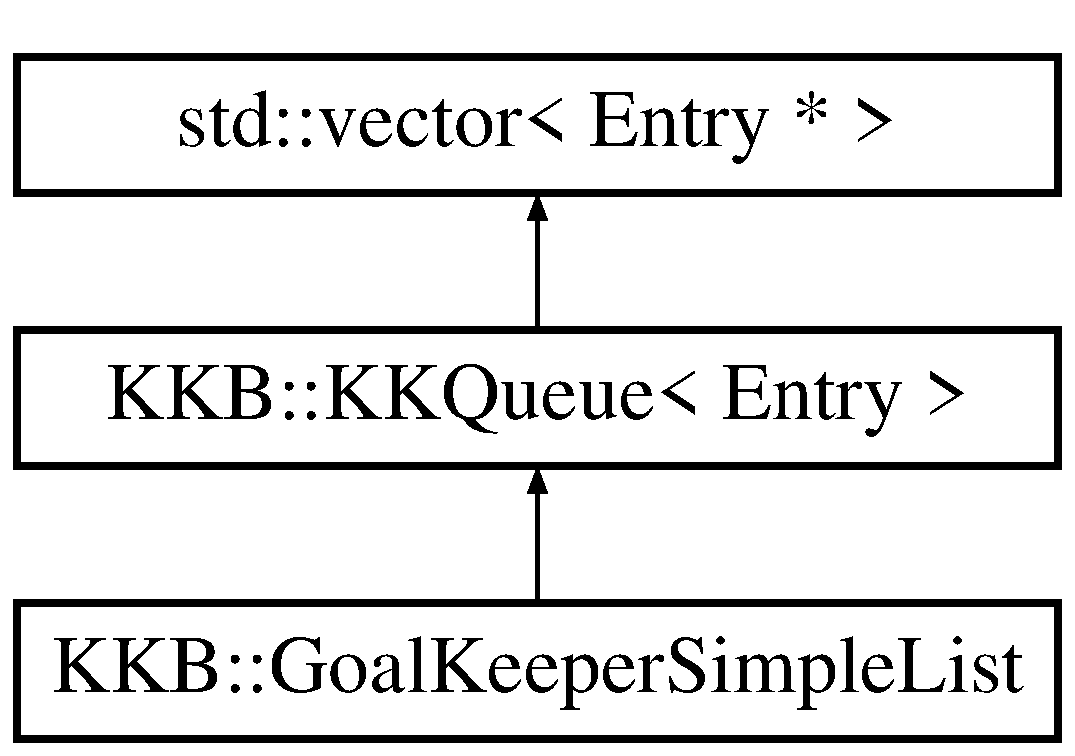
\includegraphics[height=3.000000cm]{class_k_k_b_1_1_k_k_queue}
\end{center}
\end{figure}
\subsection*{Public Types}
\begin{DoxyCompactItemize}
\item 
typedef std\+::vector$<$ Entry $\ast$ $>$\+::\hyperlink{class_k_k_b_1_1_k_k_queue_aeb057c9c010446f46f57c1e355f981f1}{const\+\_\+iterator} \hyperlink{class_k_k_b_1_1_k_k_queue_aeb057c9c010446f46f57c1e355f981f1}{const\+\_\+iterator}
\item 
typedef std\+::vector$<$ Entry $\ast$ $>$\+::\hyperlink{class_k_k_b_1_1_k_k_queue_aa3c2796a726eea468b94132a9fbf2cfe}{iterator} \hyperlink{class_k_k_b_1_1_k_k_queue_aa3c2796a726eea468b94132a9fbf2cfe}{iterator}
\end{DoxyCompactItemize}
\subsection*{Public Member Functions}
\begin{DoxyCompactItemize}
\item 
\hyperlink{class_k_k_b_1_1_k_k_queue_ac3a8d94136981f1db9ae5a9d591a0008}{K\+K\+Queue} (bool \+\_\+owner=true)
\item 
\hyperlink{class_k_k_b_1_1_k_k_queue_a1b5f9f1225f00bc6932d30028319ead6}{K\+K\+Queue} (const \hyperlink{class_k_k_b_1_1_k_k_queue}{K\+K\+Queue} \&q, bool \+\_\+owner)
\begin{DoxyCompactList}\small\item\em Constructor, similar to the Copy Constructor except that you can control whether it duplicates the contents. \end{DoxyCompactList}\item 
virtual \hyperlink{class_k_k_b_1_1_k_k_queue_a4fe8349c9b1a9c2e203611a10fcdbb2f}{$\sim$\+K\+K\+Queue} ()
\begin{DoxyCompactList}\small\item\em Virtual destructor; if owns its contents will also call the destructor on each one entry that it contains. \end{DoxyCompactList}\item 
virtual void \hyperlink{class_k_k_b_1_1_k_k_queue_adec987ebb0ac593ad877ffa59becb107}{Add} (Entry\+Ptr \+\_\+entry)
\item 
virtual void \hyperlink{class_k_k_b_1_1_k_k_queue_a1832186a944dca6fb3d5fca4046b7c40}{Add\+First} (Entry\+Ptr \+\_\+entry)
\item 
virtual void \hyperlink{class_k_k_b_1_1_k_k_queue_aefa1334998f59c7184911b47addccee3}{Add\+Queue} (const \hyperlink{class_k_k_b_1_1_k_k_queue}{K\+K\+Queue} \&q)
\begin{DoxyCompactList}\small\item\em Add the contents of a separate \hyperlink{class_k_k_b_1_1_k_k_queue}{K\+K\+Queue} container to this container. \end{DoxyCompactList}\item 
Entry\+Ptr \hyperlink{class_k_k_b_1_1_k_k_queue_a9c3fadab17ce05dc750d96b6d3fad064}{Back\+Of\+Queue} () const 
\item 
void \hyperlink{class_k_k_b_1_1_k_k_queue_a72dbe1e65d567536dbf4be3617230254}{Delete\+Contents} ()
\item 
void \hyperlink{class_k_k_b_1_1_k_k_queue_ae362e3b0a128e8a09182e167befda088}{Delete\+Entry} (Entry\+Ptr \+\_\+entry)
\item 
void \hyperlink{class_k_k_b_1_1_k_k_queue_acc76c23f4e4e1ecddd5c82619a93d4b2}{Delete\+Entry} (\hyperlink{namespace_k_k_b_af8d832f05c54994a1cce25bd5743e19a}{kkuint32} \+\_\+idx)
\item 
\hyperlink{class_k_k_b_1_1_k_k_queue}{K\+K\+Queue} $\ast$ \hyperlink{class_k_k_b_1_1_k_k_queue_acc09d961e9f995ccf6183ff1a5e87e23}{Duplicate\+List\+And\+Contents} () const 
\begin{DoxyCompactList}\small\item\em Creates a new container including duplicating the contents, which also makes the new instance the owner of those contents. \end{DoxyCompactList}\item 
{\footnotesize template$<$typename Functor $>$ }\\\hyperlink{namespace_k_k_b_af8d832f05c54994a1cce25bd5743e19a}{kkuint32} \hyperlink{class_k_k_b_1_1_k_k_queue_a0cc98856d9a20f8838bd647e0391e6b2}{Find\+The\+Kth\+Element} (\hyperlink{namespace_k_k_b_af8d832f05c54994a1cce25bd5743e19a}{kkuint32} k, Functor pred)
\item 
Entry\+Ptr \hyperlink{class_k_k_b_1_1_k_k_queue_af449cfe0b0d33b6623949be7b7dc1103}{Front\+Of\+Queue} () const 
\item 
Entry\+Ptr \hyperlink{class_k_k_b_1_1_k_k_queue_ad194def66421c09375d6c9c900a4c6d6}{Get\+First} () const 
\item 
Entry\+Ptr \hyperlink{class_k_k_b_1_1_k_k_queue_a8cd2a0f6218ce6f63cba5c0dacf97fdf}{Get\+Last} () const 
\item 
Entry\+Ptr \hyperlink{class_k_k_b_1_1_k_k_queue_acce2bdd8b3327e38266cf198382cd852}{Idx\+To\+Ptr} (\hyperlink{namespace_k_k_b_af8d832f05c54994a1cce25bd5743e19a}{kkuint32} idx) const 
\item 
\hyperlink{namespace_k_k_b_a8fa4952cc84fda1de4bec1fbdd8d5b1b}{kkint32} \hyperlink{class_k_k_b_1_1_k_k_queue_a7605c8e51c5b1c5182482dab8226e4bc}{Locate\+Entry} (Entry\+Const\+Ptr \+\_\+entry) const 
\item 
Entry\+Ptr \hyperlink{class_k_k_b_1_1_k_k_queue_a7d818f2e1710a314f2bba035fe86dd41}{Look\+At\+Back} () const 
\item 
Entry\+Ptr \hyperlink{class_k_k_b_1_1_k_k_queue_a33e29d962c414c890db00f8c25224a82}{Look\+At\+Front} () const 
\item 
bool \hyperlink{class_k_k_b_1_1_k_k_queue_a5960ccd8db282fcb7955852e755baa14}{operator!=} (const \hyperlink{class_k_k_b_1_1_k_k_queue}{K\+K\+Queue}$<$ Entry $>$ \&right\+Side) const 
\begin{DoxyCompactList}\small\item\em returns False if N\+OT every entry in both containers point to the same elements \end{DoxyCompactList}\item 
\hyperlink{class_k_k_b_1_1_k_k_queue}{K\+K\+Queue} \& \hyperlink{class_k_k_b_1_1_k_k_queue_ac1e30c66658adfcd502af08d177af7da}{operator=} (const \hyperlink{class_k_k_b_1_1_k_k_queue}{K\+K\+Queue} \&q)
\begin{DoxyCompactList}\small\item\em Assignment Operator. \end{DoxyCompactList}\item 
bool \hyperlink{class_k_k_b_1_1_k_k_queue_a93ba7b2058bef5c355f003fe3bdbcab6}{operator==} (const \hyperlink{class_k_k_b_1_1_k_k_queue}{K\+K\+Queue}$<$ Entry $>$ \&right\+Side) const 
\begin{DoxyCompactList}\small\item\em Returns True if every entry in both containers point to the same elements. \end{DoxyCompactList}\item 
Entry \& \hyperlink{class_k_k_b_1_1_k_k_queue_a8c2edf92ac57e26fe47032ad4d92f165}{operator\mbox{[}$\,$\mbox{]}} (\hyperlink{namespace_k_k_b_af8d832f05c54994a1cce25bd5743e19a}{kkuint32} i) const 
\item 
bool \hyperlink{class_k_k_b_1_1_k_k_queue_a4990d037ff09dd504cc7df53819bf61a}{Owner} () const 
\item 
void \hyperlink{class_k_k_b_1_1_k_k_queue_aaf47f5cb6057e35b9f0d230b8b9a3906}{Owner} (bool \+\_\+owner)
\item 
virtual Entry\+Ptr \hyperlink{class_k_k_b_1_1_k_k_queue_a03844c19a838fed7e7bcc5816846dcfd}{Pop\+From\+Back} ()
\item 
virtual Entry\+Ptr \hyperlink{class_k_k_b_1_1_k_k_queue_a2b2205f34516ac1f2950f441625d3ec7}{Pop\+From\+Front} ()
\item 
\hyperlink{namespace_k_k_b_a8fa4952cc84fda1de4bec1fbdd8d5b1b}{kkint32} \hyperlink{class_k_k_b_1_1_k_k_queue_ac7c26abdf599669a4b0898534f735f99}{Ptr\+To\+Idx} (Entry\+Const\+Ptr \+\_\+entry) const 
\item 
virtual void \hyperlink{class_k_k_b_1_1_k_k_queue_aa9fba4632b54268bf71ecb42dee0b575}{Push\+On\+Back} (Entry\+Ptr \+\_\+entry)
\item 
virtual void \hyperlink{class_k_k_b_1_1_k_k_queue_a07b83a99241a167f7a395a40d32f6380}{Push\+On\+Front} (Entry\+Ptr \+\_\+entry)
\item 
\hyperlink{namespace_k_k_b_a8fa4952cc84fda1de4bec1fbdd8d5b1b}{kkint32} \hyperlink{class_k_k_b_1_1_k_k_queue_a1dab601f75ee6a65d97f02bddf71c40d}{Queue\+Size} () const 
\item 
void \hyperlink{class_k_k_b_1_1_k_k_queue_ab43920c3ec182b87d3affa1e1611e1b0}{Randomize\+Order} ()
\begin{DoxyCompactList}\small\item\em Randomizes the order of the vector. \end{DoxyCompactList}\item 
void \hyperlink{class_k_k_b_1_1_k_k_queue_a72f950cfa2e3482aa8c527eb024a57ee}{Randomize\+Order} (\hyperlink{namespace_k_k_b_aa3486b1c5ea9162b3b020c69f72826eb}{kkint64} seed)
\item 
void \hyperlink{class_k_k_b_1_1_k_k_queue_af9fd71e0f10f8383153eecbbbfce0f30}{Randomize\+Order} (\hyperlink{class_k_k_b_1_1_random_num_generator}{Random\+Num\+Generator} \&random\+Variable)
\begin{DoxyCompactList}\small\item\em Randomizes the order of the vector. \end{DoxyCompactList}\item 
virtual Entry\+Ptr \hyperlink{class_k_k_b_1_1_k_k_queue_a667988c7ff02753f1324fb6c52debf84}{Remove\+First} ()
\item 
virtual Entry\+Ptr \hyperlink{class_k_k_b_1_1_k_k_queue_ae25cc5a483346ddf4231ae30d29f0b2e}{Remove\+Last} ()
\item 
void \hyperlink{class_k_k_b_1_1_k_k_queue_a3f72bf16ba59d4269ecf5db9fad9ef9e}{Set\+Idx\+To\+Ptr} (\hyperlink{namespace_k_k_b_af8d832f05c54994a1cce25bd5743e19a}{kkuint32} \+\_\+idx, Entry $\ast$\+\_\+ptr)
\item 
void \hyperlink{class_k_k_b_1_1_k_k_queue_a7a848286a5d2ddd9b0d320557a458f66}{Swap\+Indexes} (size\+\_\+t idx1, size\+\_\+t idx2)
\end{DoxyCompactItemize}
\subsection*{Protected Member Functions}
\begin{DoxyCompactItemize}
\item 
\hyperlink{class_k_k_b_1_1_k_k_queue_ab21be04f42eefbaed9c718f32029a812}{K\+K\+Queue} (const \hyperlink{class_k_k_b_1_1_k_k_queue}{K\+K\+Queue} \&q)
\begin{DoxyCompactList}\small\item\em Copy Constructor creating new instance; including duplicating contents if owner set to true. \end{DoxyCompactList}\end{DoxyCompactItemize}


\subsection{Detailed Description}
\subsubsection*{template$<$class Entry$>$\\*
class K\+K\+B\+::\+K\+K\+Queue$<$ Entry $>$}

A typed container class/template that keeps track of entries via pointers only. 

Will act as an Array, Queue or Stack structure. Items are added by the \textquotesingle{}Push\+On\+Front\textquotesingle{} and \textquotesingle{}Push\+On\+Back\textquotesingle{} methods. They are removed by the \textquotesingle{}Pop\+From\+Front\textquotesingle{} and \textquotesingle{}Pop\+From\+Back\textquotesingle{} methods. What is important to keep in mind is that it holds pointers to its contents, not the actual instances. It is important to keep track who owns the objects you put in an instance of \hyperlink{class_k_k_b_1_1_k_k_queue}{K\+K\+Queue}. \hyperlink{class_k_k_b_1_1_k_k_queue}{K\+K\+Queue} has a \textquotesingle{}Owner\textquotesingle{} flag that you can set. If it is set to \textquotesingle{}true\textquotesingle{} then it will call the destructor on all its contents when you call \hyperlink{class_k_k_b_1_1_k_k_queue}{K\+K\+Queue}\textquotesingle{}s destructor or the \textquotesingle{}Destroy\+Contents\textquotesingle{} method. When you add an element to a \hyperlink{class_k_k_b_1_1_k_k_queue}{K\+K\+Queue} container you can not delete it separately until you either remove it from \hyperlink{class_k_k_b_1_1_k_k_queue}{K\+K\+Queue} or delete the \hyperlink{class_k_k_b_1_1_k_k_queue}{K\+K\+Queue} container. If the \hyperlink{class_k_k_b_1_1_k_k_queue}{K\+K\+Queue} derived container owned its contents and you call its destructor then there is no need to delete the contents separately.

\hyperlink{class_k_k_b_1_1_k_k_queue}{K\+K\+Queue} is sub-\/classed from vector$<$\+Entry$\ast$$>$ so you can use any method that is available for the vector$<$$>$ template.


\begin{DoxyTemplParams}{Template Parameters}
{\em Entry} & The type of objects that are to be held in this container. When you add new instances of \textquotesingle{}Entry\textquotesingle{}, you need to add a pointer to it not the actual entry. \\
\hline
\end{DoxyTemplParams}


Definition at line 77 of file K\+K\+Queue.\+h.



\subsection{Member Typedef Documentation}
\index{K\+K\+B\+::\+K\+K\+Queue@{K\+K\+B\+::\+K\+K\+Queue}!const\+\_\+iterator@{const\+\_\+iterator}}
\index{const\+\_\+iterator@{const\+\_\+iterator}!K\+K\+B\+::\+K\+K\+Queue@{K\+K\+B\+::\+K\+K\+Queue}}
\subsubsection[{\texorpdfstring{const\+\_\+iterator}{const_iterator}}]{\setlength{\rightskip}{0pt plus 5cm}template$<$class Entry$>$ typedef std\+::vector$<$Entry$\ast$$>$\+::{\bf const\+\_\+iterator} {\bf K\+K\+B\+::\+K\+K\+Queue}$<$ Entry $>$\+::{\bf const\+\_\+iterator}}\hypertarget{class_k_k_b_1_1_k_k_queue_aeb057c9c010446f46f57c1e355f981f1}{}\label{class_k_k_b_1_1_k_k_queue_aeb057c9c010446f46f57c1e355f981f1}


Definition at line 89 of file K\+K\+Queue.\+h.

\index{K\+K\+B\+::\+K\+K\+Queue@{K\+K\+B\+::\+K\+K\+Queue}!iterator@{iterator}}
\index{iterator@{iterator}!K\+K\+B\+::\+K\+K\+Queue@{K\+K\+B\+::\+K\+K\+Queue}}
\subsubsection[{\texorpdfstring{iterator}{iterator}}]{\setlength{\rightskip}{0pt plus 5cm}template$<$class Entry$>$ typedef std\+::vector$<$Entry$\ast$$>$\+::{\bf iterator} {\bf K\+K\+B\+::\+K\+K\+Queue}$<$ Entry $>$\+::{\bf iterator}}\hypertarget{class_k_k_b_1_1_k_k_queue_aa3c2796a726eea468b94132a9fbf2cfe}{}\label{class_k_k_b_1_1_k_k_queue_aa3c2796a726eea468b94132a9fbf2cfe}


Definition at line 88 of file K\+K\+Queue.\+h.



\subsection{Constructor \& Destructor Documentation}
\index{K\+K\+B\+::\+K\+K\+Queue@{K\+K\+B\+::\+K\+K\+Queue}!K\+K\+Queue@{K\+K\+Queue}}
\index{K\+K\+Queue@{K\+K\+Queue}!K\+K\+B\+::\+K\+K\+Queue@{K\+K\+B\+::\+K\+K\+Queue}}
\subsubsection[{\texorpdfstring{K\+K\+Queue(bool \+\_\+owner=true)}{KKQueue(bool _owner=true)}}]{\setlength{\rightskip}{0pt plus 5cm}template$<$class Entry $>$ K\+K\+Queue\+::\+K\+K\+Queue (
\begin{DoxyParamCaption}
\item[{bool}]{\+\_\+owner = {\ttfamily true}}
\end{DoxyParamCaption}
)}\hypertarget{class_k_k_b_1_1_k_k_queue_ac3a8d94136981f1db9ae5a9d591a0008}{}\label{class_k_k_b_1_1_k_k_queue_ac3a8d94136981f1db9ae5a9d591a0008}


Definition at line 219 of file K\+K\+Queue.\+h.


\begin{DoxyCode}
219                                       :
220       owner (\_owner)
221   \{
222   \}
\end{DoxyCode}
\index{K\+K\+B\+::\+K\+K\+Queue@{K\+K\+B\+::\+K\+K\+Queue}!K\+K\+Queue@{K\+K\+Queue}}
\index{K\+K\+Queue@{K\+K\+Queue}!K\+K\+B\+::\+K\+K\+Queue@{K\+K\+B\+::\+K\+K\+Queue}}
\subsubsection[{\texorpdfstring{K\+K\+Queue(const K\+K\+Queue \&q)}{KKQueue(const KKQueue &q)}}]{\setlength{\rightskip}{0pt plus 5cm}template$<$class Entry $>$ K\+K\+Queue\+::\+K\+K\+Queue (
\begin{DoxyParamCaption}
\item[{const {\bf K\+K\+Queue}$<$ Entry $>$ \&}]{q}
\end{DoxyParamCaption}
)\hspace{0.3cm}{\ttfamily [protected]}}\hypertarget{class_k_k_b_1_1_k_k_queue_ab21be04f42eefbaed9c718f32029a812}{}\label{class_k_k_b_1_1_k_k_queue_ab21be04f42eefbaed9c718f32029a812}


Copy Constructor creating new instance; including duplicating contents if owner set to true. 

If the parameter \textquotesingle{}q\textquotesingle{} owns its contents then will create new instances of its contents. That is it will call the Copy Constructor for each one of the elements it contains. If \textquotesingle{}q\textquotesingle{} does not own its contents it will just copy over the pointers from \textquotesingle{}q\textquotesingle{}, meaning that the new instance of \hyperlink{class_k_k_b_1_1_k_k_queue}{K\+K\+Queue} will point to the same locations as \textquotesingle{}q\textquotesingle{} does. 

Definition at line 227 of file K\+K\+Queue.\+h.


\begin{DoxyCode}
227                                            :
228         owner (q.Owner ())
229 
230   \{
231     \textcolor{comment}{//for  (vector<Entry*>::const\_iterator x = q.begin ();  x != q.end ();  x++)}
232     \textcolor{keywordflow}{for}  (\hyperlink{class_k_k_b_1_1_k_k_queue_aeb057c9c010446f46f57c1e355f981f1}{const\_iterator} x = q.begin ();  x != q.end ();  x++)
233     \{
234       \textcolor{keywordflow}{if}  (owner)
235         \hyperlink{class_k_k_b_1_1_k_k_queue_aa9fba4632b54268bf71ecb42dee0b575}{PushOnBack} (\textcolor{keyword}{new} Entry (*(*x)));
236       \textcolor{keywordflow}{else}
237         \hyperlink{class_k_k_b_1_1_k_k_queue_aa9fba4632b54268bf71ecb42dee0b575}{PushOnBack} (*x); 
238     \}
239   \}
\end{DoxyCode}
\index{K\+K\+B\+::\+K\+K\+Queue@{K\+K\+B\+::\+K\+K\+Queue}!K\+K\+Queue@{K\+K\+Queue}}
\index{K\+K\+Queue@{K\+K\+Queue}!K\+K\+B\+::\+K\+K\+Queue@{K\+K\+B\+::\+K\+K\+Queue}}
\subsubsection[{\texorpdfstring{K\+K\+Queue(const K\+K\+Queue \&q, bool \+\_\+owner)}{KKQueue(const KKQueue &q, bool _owner)}}]{\setlength{\rightskip}{0pt plus 5cm}template$<$class Entry $>$ K\+K\+Queue\+::\+K\+K\+Queue (
\begin{DoxyParamCaption}
\item[{const {\bf K\+K\+Queue}$<$ Entry $>$ \&}]{q, }
\item[{bool}]{\+\_\+owner}
\end{DoxyParamCaption}
)}\hypertarget{class_k_k_b_1_1_k_k_queue_a1b5f9f1225f00bc6932d30028319ead6}{}\label{class_k_k_b_1_1_k_k_queue_a1b5f9f1225f00bc6932d30028319ead6}


Constructor, similar to the Copy Constructor except that you can control whether it duplicates the contents. 

If the \textquotesingle{}\+\_\+owner\textquotesingle{} parameter is set to true then it will create new instances of the contents otherwise it will just point to the instances that already exist. 

Definition at line 243 of file K\+K\+Queue.\+h.


\begin{DoxyCode}
245                            :
246         owner (\_owner)
247 
248   \{
249     \textcolor{comment}{//for  (vector<Entry*>::const\_iterator x = q.begin}
250     \textcolor{comment}{//  owner (\_owner) ();  x != q.end ();  x++)}
251     \textcolor{keywordflow}{for}  (\hyperlink{class_k_k_b_1_1_k_k_queue_aeb057c9c010446f46f57c1e355f981f1}{const\_iterator} x = q.begin ();  x != q.end ();  ++x)
252     \{
253       \textcolor{keywordflow}{if}  (owner)
254         \hyperlink{class_k_k_b_1_1_k_k_queue_aa9fba4632b54268bf71ecb42dee0b575}{PushOnBack} (\textcolor{keyword}{new} Entry (*(*x)));
255       \textcolor{keywordflow}{else}
256         \hyperlink{class_k_k_b_1_1_k_k_queue_aa9fba4632b54268bf71ecb42dee0b575}{PushOnBack} (*x); 
257     \}
258   \}
\end{DoxyCode}
\index{K\+K\+B\+::\+K\+K\+Queue@{K\+K\+B\+::\+K\+K\+Queue}!````~K\+K\+Queue@{$\sim$\+K\+K\+Queue}}
\index{````~K\+K\+Queue@{$\sim$\+K\+K\+Queue}!K\+K\+B\+::\+K\+K\+Queue@{K\+K\+B\+::\+K\+K\+Queue}}
\subsubsection[{\texorpdfstring{$\sim$\+K\+K\+Queue()}{~KKQueue()}}]{\setlength{\rightskip}{0pt plus 5cm}template$<$class Entry $>$ K\+K\+Queue\+::$\sim$\+K\+K\+Queue (
\begin{DoxyParamCaption}
{}
\end{DoxyParamCaption}
)\hspace{0.3cm}{\ttfamily [virtual]}}\hypertarget{class_k_k_b_1_1_k_k_queue_a4fe8349c9b1a9c2e203611a10fcdbb2f}{}\label{class_k_k_b_1_1_k_k_queue_a4fe8349c9b1a9c2e203611a10fcdbb2f}


Virtual destructor; if owns its contents will also call the destructor on each one entry that it contains. 



Definition at line 280 of file K\+K\+Queue.\+h.


\begin{DoxyCode}
281   \{
282     \textcolor{keywordflow}{if}  (owner)
283     \{
284       \hyperlink{class_k_k_b_1_1_k_k_queue_aa3c2796a726eea468b94132a9fbf2cfe}{iterator}  i;
285 
286       \textcolor{keywordflow}{for}  (i = KKQueue<Entry>::begin ();  i != KKQueue<Entry>::end (); i++)
287       \{
288         \textcolor{keyword}{delete} *i;
289         *i = NULL;
290       \}
291     \}
292   \}  \textcolor{comment}{/* ~KKQueue */}
\end{DoxyCode}


\subsection{Member Function Documentation}
\index{K\+K\+B\+::\+K\+K\+Queue@{K\+K\+B\+::\+K\+K\+Queue}!Add@{Add}}
\index{Add@{Add}!K\+K\+B\+::\+K\+K\+Queue@{K\+K\+B\+::\+K\+K\+Queue}}
\subsubsection[{\texorpdfstring{Add(\+Entry\+Ptr \+\_\+entry)}{Add(EntryPtr _entry)}}]{\setlength{\rightskip}{0pt plus 5cm}template$<$class Entry $>$ void K\+K\+Queue\+::\+Add (
\begin{DoxyParamCaption}
\item[{Entry\+Ptr}]{\+\_\+entry}
\end{DoxyParamCaption}
)\hspace{0.3cm}{\ttfamily [inline]}, {\ttfamily [virtual]}}\hypertarget{class_k_k_b_1_1_k_k_queue_adec987ebb0ac593ad877ffa59becb107}{}\label{class_k_k_b_1_1_k_k_queue_adec987ebb0ac593ad877ffa59becb107}
same as Push\+On\+Back 

Definition at line 339 of file K\+K\+Queue.\+h.


\begin{DoxyCode}
340   \{
341     \hyperlink{class_k_k_b_1_1_k_k_queue_aa9fba4632b54268bf71ecb42dee0b575}{PushOnBack} (\_entry);
342   \}
\end{DoxyCode}
\index{K\+K\+B\+::\+K\+K\+Queue@{K\+K\+B\+::\+K\+K\+Queue}!Add\+First@{Add\+First}}
\index{Add\+First@{Add\+First}!K\+K\+B\+::\+K\+K\+Queue@{K\+K\+B\+::\+K\+K\+Queue}}
\subsubsection[{\texorpdfstring{Add\+First(\+Entry\+Ptr \+\_\+entry)}{AddFirst(EntryPtr _entry)}}]{\setlength{\rightskip}{0pt plus 5cm}template$<$class Entry $>$ void K\+K\+Queue\+::\+Add\+First (
\begin{DoxyParamCaption}
\item[{Entry\+Ptr}]{\+\_\+entry}
\end{DoxyParamCaption}
)\hspace{0.3cm}{\ttfamily [inline]}, {\ttfamily [virtual]}}\hypertarget{class_k_k_b_1_1_k_k_queue_a1832186a944dca6fb3d5fca4046b7c40}{}\label{class_k_k_b_1_1_k_k_queue_a1832186a944dca6fb3d5fca4046b7c40}
same as Push\+On\+Front 

Definition at line 347 of file K\+K\+Queue.\+h.


\begin{DoxyCode}
348   \{
349     \hyperlink{class_k_k_b_1_1_k_k_queue_a07b83a99241a167f7a395a40d32f6380}{PushOnFront} (\_entry);
350   \}
\end{DoxyCode}
\index{K\+K\+B\+::\+K\+K\+Queue@{K\+K\+B\+::\+K\+K\+Queue}!Add\+Queue@{Add\+Queue}}
\index{Add\+Queue@{Add\+Queue}!K\+K\+B\+::\+K\+K\+Queue@{K\+K\+B\+::\+K\+K\+Queue}}
\subsubsection[{\texorpdfstring{Add\+Queue(const K\+K\+Queue \&q)}{AddQueue(const KKQueue &q)}}]{\setlength{\rightskip}{0pt plus 5cm}template$<$class Entry $>$ void K\+K\+Queue\+::\+Add\+Queue (
\begin{DoxyParamCaption}
\item[{const {\bf K\+K\+Queue}$<$ Entry $>$ \&}]{q}
\end{DoxyParamCaption}
)\hspace{0.3cm}{\ttfamily [virtual]}}\hypertarget{class_k_k_b_1_1_k_k_queue_aefa1334998f59c7184911b47addccee3}{}\label{class_k_k_b_1_1_k_k_queue_aefa1334998f59c7184911b47addccee3}


Add the contents of a separate \hyperlink{class_k_k_b_1_1_k_k_queue}{K\+K\+Queue} container to this container. 

Be careful how the Owner flags are set; this method adds the pointers of \textquotesingle{}q\textquotesingle{} to the end of its own container; it does not concern itself with the state of the \textquotesingle{}Owner\textquotesingle{} flags. If you are not careful you can have both containers thinking they own the same entries. I suggest that after you add the contents of \textquotesingle{}q\textquotesingle{} to this container that the caller set the \textquotesingle{}owner\textquotesingle{} flag of \textquotesingle{}q\textquotesingle{} to false. 

Definition at line 355 of file K\+K\+Queue.\+h.


\begin{DoxyCode}
356   \{
357     \textcolor{keywordflow}{for} (\hyperlink{class_k_k_b_1_1_k_k_queue_aeb057c9c010446f46f57c1e355f981f1}{const\_iterator} x = q.begin ();  x != q.end (); x++)
358       \hyperlink{class_k_k_b_1_1_k_k_queue_aa9fba4632b54268bf71ecb42dee0b575}{PushOnBack} (*x);
359     \textcolor{keywordflow}{return};
360   \}  \textcolor{comment}{/* AddQueue */}
\end{DoxyCode}
\index{K\+K\+B\+::\+K\+K\+Queue@{K\+K\+B\+::\+K\+K\+Queue}!Back\+Of\+Queue@{Back\+Of\+Queue}}
\index{Back\+Of\+Queue@{Back\+Of\+Queue}!K\+K\+B\+::\+K\+K\+Queue@{K\+K\+B\+::\+K\+K\+Queue}}
\subsubsection[{\texorpdfstring{Back\+Of\+Queue() const }{BackOfQueue() const }}]{\setlength{\rightskip}{0pt plus 5cm}template$<$class Entry $>$ {\bf K\+K\+Queue}$<$ Entry $>$\+::Entry\+Ptr K\+K\+Queue\+::\+Back\+Of\+Queue (
\begin{DoxyParamCaption}
{}
\end{DoxyParamCaption}
) const}\hypertarget{class_k_k_b_1_1_k_k_queue_a9c3fadab17ce05dc750d96b6d3fad064}{}\label{class_k_k_b_1_1_k_k_queue_a9c3fadab17ce05dc750d96b6d3fad064}
Returns pointer of last element in the container without removing it. If the container is empty will return N\+U\+LL. 

Definition at line 661 of file K\+K\+Queue.\+h.


\begin{DoxyCode}
662   \{
663     \textcolor{keywordflow}{if}  (KKQueue<Entry>::size () <= 0)
664       \textcolor{keywordflow}{return} NULL;
665     \textcolor{keywordflow}{return} KKQueue<Entry>::back ();
666   \}
\end{DoxyCode}
\index{K\+K\+B\+::\+K\+K\+Queue@{K\+K\+B\+::\+K\+K\+Queue}!Delete\+Contents@{Delete\+Contents}}
\index{Delete\+Contents@{Delete\+Contents}!K\+K\+B\+::\+K\+K\+Queue@{K\+K\+B\+::\+K\+K\+Queue}}
\subsubsection[{\texorpdfstring{Delete\+Contents()}{DeleteContents()}}]{\setlength{\rightskip}{0pt plus 5cm}template$<$class Entry $>$ void K\+K\+Queue\+::\+Delete\+Contents (
\begin{DoxyParamCaption}
{}
\end{DoxyParamCaption}
)}\hypertarget{class_k_k_b_1_1_k_k_queue_a72dbe1e65d567536dbf4be3617230254}{}\label{class_k_k_b_1_1_k_k_queue_a72dbe1e65d567536dbf4be3617230254}
Empties the container, if \textquotesingle{}owner\textquotesingle{} is set to true will call the destructor on each element. 

Definition at line 321 of file K\+K\+Queue.\+h.


\begin{DoxyCode}
322   \{
323     \textcolor{keywordflow}{if}  (owner)
324     \{
325       \hyperlink{class_k_k_b_1_1_k_k_queue_aa3c2796a726eea468b94132a9fbf2cfe}{iterator}  idx;
326 
327       \textcolor{keywordflow}{for}  (idx = KKQueue<Entry>::begin ();  idx != KKQueue<Entry>::end ();  idx++)
328       \{
329         \textcolor{keyword}{delete}  (*idx);
330       \}
331     \}
332 
333     KKQueue<Entry>::clear ();
334   \}  \textcolor{comment}{/* DeleteContents */}
\end{DoxyCode}
\index{K\+K\+B\+::\+K\+K\+Queue@{K\+K\+B\+::\+K\+K\+Queue}!Delete\+Entry@{Delete\+Entry}}
\index{Delete\+Entry@{Delete\+Entry}!K\+K\+B\+::\+K\+K\+Queue@{K\+K\+B\+::\+K\+K\+Queue}}
\subsubsection[{\texorpdfstring{Delete\+Entry(\+Entry\+Ptr \+\_\+entry)}{DeleteEntry(EntryPtr _entry)}}]{\setlength{\rightskip}{0pt plus 5cm}template$<$class Entry $>$ void K\+K\+Queue\+::\+Delete\+Entry (
\begin{DoxyParamCaption}
\item[{Entry\+Ptr}]{\+\_\+entry}
\end{DoxyParamCaption}
)}\hypertarget{class_k_k_b_1_1_k_k_queue_ae362e3b0a128e8a09182e167befda088}{}\label{class_k_k_b_1_1_k_k_queue_ae362e3b0a128e8a09182e167befda088}
Removes from \hyperlink{class_k_k_b_1_1_k_k_queue}{K\+K\+Queue} the entry who\textquotesingle{}s pointer = \textquotesingle{}\+\_\+entry\textquotesingle{} 

Definition at line 684 of file K\+K\+Queue.\+h.


\begin{DoxyCode}
685   \{
686     \textcolor{keywordflow}{for}  (\hyperlink{class_k_k_b_1_1_k_k_queue_aa3c2796a726eea468b94132a9fbf2cfe}{iterator} y =  KKQueue<Entry>::begin (); y !=  KKQueue<Entry>::end ();  y++)
687     \{
688       \textcolor{keywordflow}{if}  (*y == \_entry)
689       \{
690         KKQueue<Entry>::erase (y);
691         \textcolor{keywordflow}{return};
692       \}
693     \}
694   \}  \textcolor{comment}{/* DeleteEntry */}
\end{DoxyCode}
\index{K\+K\+B\+::\+K\+K\+Queue@{K\+K\+B\+::\+K\+K\+Queue}!Delete\+Entry@{Delete\+Entry}}
\index{Delete\+Entry@{Delete\+Entry}!K\+K\+B\+::\+K\+K\+Queue@{K\+K\+B\+::\+K\+K\+Queue}}
\subsubsection[{\texorpdfstring{Delete\+Entry(kkuint32 \+\_\+idx)}{DeleteEntry(kkuint32 _idx)}}]{\setlength{\rightskip}{0pt plus 5cm}template$<$class Entry $>$ void K\+K\+Queue\+::\+Delete\+Entry (
\begin{DoxyParamCaption}
\item[{{\bf kkuint32}}]{\+\_\+idx}
\end{DoxyParamCaption}
)}\hypertarget{class_k_k_b_1_1_k_k_queue_acc76c23f4e4e1ecddd5c82619a93d4b2}{}\label{class_k_k_b_1_1_k_k_queue_acc76c23f4e4e1ecddd5c82619a93d4b2}
Removes from \hyperlink{class_k_k_b_1_1_k_k_queue}{K\+K\+Queue} the entry who\textquotesingle{}s index = \textquotesingle{}\+\_\+idx\textquotesingle{}. 

Definition at line 715 of file K\+K\+Queue.\+h.


\begin{DoxyCode}
716   \{
717     \textcolor{keywordflow}{if}  ((\hyperlink{namespace_k_k_b_af8d832f05c54994a1cce25bd5743e19a}{kkuint32})\_idx >=  KKQueue<Entry>::size ())
718       \textcolor{keywordflow}{return};
719 
720     \hyperlink{class_k_k_b_1_1_k_k_queue_aa3c2796a726eea468b94132a9fbf2cfe}{iterator}  i =  KKQueue<Entry>::begin ();
721 
722     \textcolor{keywordflow}{for} (\hyperlink{namespace_k_k_b_af8d832f05c54994a1cce25bd5743e19a}{kkuint32} j = 0;  ((j < \_idx)  &&  (i !=  KKQueue<Entry>::end ()));  j++)
723       i++;
724 
725     EntryPtr  ep = *i;
726     KKQueue<Entry>::erase (i);
727   \}  \textcolor{comment}{/* DeleteEntry */}
\end{DoxyCode}
\index{K\+K\+B\+::\+K\+K\+Queue@{K\+K\+B\+::\+K\+K\+Queue}!Duplicate\+List\+And\+Contents@{Duplicate\+List\+And\+Contents}}
\index{Duplicate\+List\+And\+Contents@{Duplicate\+List\+And\+Contents}!K\+K\+B\+::\+K\+K\+Queue@{K\+K\+B\+::\+K\+K\+Queue}}
\subsubsection[{\texorpdfstring{Duplicate\+List\+And\+Contents() const }{DuplicateListAndContents() const }}]{\setlength{\rightskip}{0pt plus 5cm}template$<$class Entry $>$ {\bf K\+K\+Queue}$<$ Entry $>$ $\ast$ K\+K\+Queue\+::\+Duplicate\+List\+And\+Contents (
\begin{DoxyParamCaption}
{}
\end{DoxyParamCaption}
) const}\hypertarget{class_k_k_b_1_1_k_k_queue_acc09d961e9f995ccf6183ff1a5e87e23}{}\label{class_k_k_b_1_1_k_k_queue_acc09d961e9f995ccf6183ff1a5e87e23}


Creates a new container including duplicating the contents, which also makes the new instance the owner of those contents. 



Definition at line 263 of file K\+K\+Queue.\+h.


\begin{DoxyCode}
264   \{
265     KKQueue<Entry>*  duplicatedQueue = \textcolor{keyword}{new} KKQueue<Entry> (\textcolor{keyword}{true}, \hyperlink{class_k_k_b_1_1_k_k_queue_a1dab601f75ee6a65d97f02bddf71c40d}{QueueSize} ());
266 
267     \textcolor{keywordflow}{for}  (\hyperlink{class_k_k_b_1_1_k_k_queue_aeb057c9c010446f46f57c1e355f981f1}{const\_iterator} x = KKQueue<Entry>::begin ();  x != KKQueue<Entry>::end ();  x++)
268     \{
269       \textcolor{keyword}{const} EntryPtr e = *x;
270       duplicatedQueue->PushOnBack (\textcolor{keyword}{new} Entry (*e));
271     \}
272     
273     \textcolor{keywordflow}{return}  duplicatedQueue;
274   \}  \textcolor{comment}{/* DuplicateListAndContents */}
\end{DoxyCode}
\index{K\+K\+B\+::\+K\+K\+Queue@{K\+K\+B\+::\+K\+K\+Queue}!Find\+The\+Kth\+Element@{Find\+The\+Kth\+Element}}
\index{Find\+The\+Kth\+Element@{Find\+The\+Kth\+Element}!K\+K\+B\+::\+K\+K\+Queue@{K\+K\+B\+::\+K\+K\+Queue}}
\subsubsection[{\texorpdfstring{Find\+The\+Kth\+Element(kkuint32 k, Functor pred)}{FindTheKthElement(kkuint32 k, Functor pred)}}]{\setlength{\rightskip}{0pt plus 5cm}template$<$class Entry $>$ template$<$typename Functor $>$ {\bf kkuint32} K\+K\+Queue\+::\+Find\+The\+Kth\+Element (
\begin{DoxyParamCaption}
\item[{{\bf kkuint32}}]{k, }
\item[{Functor}]{pred}
\end{DoxyParamCaption}
)}\hypertarget{class_k_k_b_1_1_k_k_queue_a0cc98856d9a20f8838bd647e0391e6b2}{}\label{class_k_k_b_1_1_k_k_queue_a0cc98856d9a20f8838bd647e0391e6b2}


Definition at line 527 of file K\+K\+Queue.\+h.


\begin{DoxyCode}
530   \{
531     \textcolor{keywordflow}{if}  ((k < 0)   ||  (K > = (\hyperlink{namespace_k_k_b_a8fa4952cc84fda1de4bec1fbdd8d5b1b}{kkint32})size ()))
532       \textcolor{keywordflow}{return} -1;
533     \textcolor{keywordflow}{return}  \hyperlink{class_k_k_b_1_1_k_k_queue_a0cc98856d9a20f8838bd647e0391e6b2}{FindTheKthElement} (k, 0, size () - 1, pred);
534   \}  \textcolor{comment}{/* FindTheKthElement */}
\end{DoxyCode}
\index{K\+K\+B\+::\+K\+K\+Queue@{K\+K\+B\+::\+K\+K\+Queue}!Front\+Of\+Queue@{Front\+Of\+Queue}}
\index{Front\+Of\+Queue@{Front\+Of\+Queue}!K\+K\+B\+::\+K\+K\+Queue@{K\+K\+B\+::\+K\+K\+Queue}}
\subsubsection[{\texorpdfstring{Front\+Of\+Queue() const }{FrontOfQueue() const }}]{\setlength{\rightskip}{0pt plus 5cm}template$<$class Entry $>$ {\bf K\+K\+Queue}$<$ Entry $>$\+::Entry\+Ptr K\+K\+Queue\+::\+Front\+Of\+Queue (
\begin{DoxyParamCaption}
{}
\end{DoxyParamCaption}
) const}\hypertarget{class_k_k_b_1_1_k_k_queue_af449cfe0b0d33b6623949be7b7dc1103}{}\label{class_k_k_b_1_1_k_k_queue_af449cfe0b0d33b6623949be7b7dc1103}
Returns a pointer to the element that is at from of the queue with out removing it from the queue. 

Definition at line 673 of file K\+K\+Queue.\+h.


\begin{DoxyCode}
674   \{
675     \textcolor{keywordflow}{if}  ( KKQueue<Entry>::size () <= 0)
676        \textcolor{keywordflow}{return} NULL;
677 
678     \textcolor{keywordflow}{return} * KKQueue<Entry>::begin ();
679   \}
\end{DoxyCode}
\index{K\+K\+B\+::\+K\+K\+Queue@{K\+K\+B\+::\+K\+K\+Queue}!Get\+First@{Get\+First}}
\index{Get\+First@{Get\+First}!K\+K\+B\+::\+K\+K\+Queue@{K\+K\+B\+::\+K\+K\+Queue}}
\subsubsection[{\texorpdfstring{Get\+First() const }{GetFirst() const }}]{\setlength{\rightskip}{0pt plus 5cm}template$<$class Entry $>$ {\bf K\+K\+Queue}$<$ Entry $>$\+::Entry\+Ptr K\+K\+Queue\+::\+Get\+First (
\begin{DoxyParamCaption}
{}
\end{DoxyParamCaption}
) const\hspace{0.3cm}{\ttfamily [inline]}}\hypertarget{class_k_k_b_1_1_k_k_queue_ad194def66421c09375d6c9c900a4c6d6}{}\label{class_k_k_b_1_1_k_k_queue_ad194def66421c09375d6c9c900a4c6d6}
Same as Front\+Of\+Queue. 

Definition at line 366 of file K\+K\+Queue.\+h.


\begin{DoxyCode}
367   \{
368     \textcolor{keywordflow}{return}  \hyperlink{class_k_k_b_1_1_k_k_queue_af449cfe0b0d33b6623949be7b7dc1103}{FrontOfQueue} ();
369   \}
\end{DoxyCode}
\index{K\+K\+B\+::\+K\+K\+Queue@{K\+K\+B\+::\+K\+K\+Queue}!Get\+Last@{Get\+Last}}
\index{Get\+Last@{Get\+Last}!K\+K\+B\+::\+K\+K\+Queue@{K\+K\+B\+::\+K\+K\+Queue}}
\subsubsection[{\texorpdfstring{Get\+Last() const }{GetLast() const }}]{\setlength{\rightskip}{0pt plus 5cm}template$<$class Entry $>$ {\bf K\+K\+Queue}$<$ Entry $>$\+::Entry\+Ptr K\+K\+Queue\+::\+Get\+Last (
\begin{DoxyParamCaption}
{}
\end{DoxyParamCaption}
) const\hspace{0.3cm}{\ttfamily [inline]}}\hypertarget{class_k_k_b_1_1_k_k_queue_a8cd2a0f6218ce6f63cba5c0dacf97fdf}{}\label{class_k_k_b_1_1_k_k_queue_a8cd2a0f6218ce6f63cba5c0dacf97fdf}
Same as Back\+Of\+Queue. 

Definition at line 374 of file K\+K\+Queue.\+h.


\begin{DoxyCode}
375   \{
376     \textcolor{keywordflow}{return}  \hyperlink{class_k_k_b_1_1_k_k_queue_a9c3fadab17ce05dc750d96b6d3fad064}{BackOfQueue} ();
377   \}
\end{DoxyCode}
\index{K\+K\+B\+::\+K\+K\+Queue@{K\+K\+B\+::\+K\+K\+Queue}!Idx\+To\+Ptr@{Idx\+To\+Ptr}}
\index{Idx\+To\+Ptr@{Idx\+To\+Ptr}!K\+K\+B\+::\+K\+K\+Queue@{K\+K\+B\+::\+K\+K\+Queue}}
\subsubsection[{\texorpdfstring{Idx\+To\+Ptr(kkuint32 idx) const }{IdxToPtr(kkuint32 idx) const }}]{\setlength{\rightskip}{0pt plus 5cm}template$<$class Entry $>$ {\bf K\+K\+Queue}$<$ Entry $>$\+::Entry\+Ptr K\+K\+Queue\+::\+Idx\+To\+Ptr (
\begin{DoxyParamCaption}
\item[{{\bf kkuint32}}]{idx}
\end{DoxyParamCaption}
) const}\hypertarget{class_k_k_b_1_1_k_k_queue_acce2bdd8b3327e38266cf198382cd852}{}\label{class_k_k_b_1_1_k_k_queue_acce2bdd8b3327e38266cf198382cd852}
Returns back a pointer to the element who\textquotesingle{}s index is \textquotesingle{}idx\textquotesingle{}. If \textquotesingle{}idx\textquotesingle{} is less than 0 or $>$= \hyperlink{class_k_k_b_1_1_k_k_queue_a1dab601f75ee6a65d97f02bddf71c40d}{Queue\+Size()} will return N\+U\+LL. 

Definition at line 732 of file K\+K\+Queue.\+h.


\begin{DoxyCode}
733   \{
734     \textcolor{keywordflow}{if}  (idx >= KKQueue<Entry>::size ())
735       \textcolor{keywordflow}{return} NULL;
736 
737     \textcolor{keywordflow}{return}  &((*this)[idx]);
738     \textcolor{comment}{//return  (typename Entry*)(vector<Entry*>::operator[] (idx));}
739   \}  \textcolor{comment}{/* IdxToPtr */}
\end{DoxyCode}
\index{K\+K\+B\+::\+K\+K\+Queue@{K\+K\+B\+::\+K\+K\+Queue}!Locate\+Entry@{Locate\+Entry}}
\index{Locate\+Entry@{Locate\+Entry}!K\+K\+B\+::\+K\+K\+Queue@{K\+K\+B\+::\+K\+K\+Queue}}
\subsubsection[{\texorpdfstring{Locate\+Entry(\+Entry\+Const\+Ptr \+\_\+entry) const }{LocateEntry(EntryConstPtr _entry) const }}]{\setlength{\rightskip}{0pt plus 5cm}template$<$class Entry $>$ {\bf kkint32} K\+K\+Queue\+::\+Locate\+Entry (
\begin{DoxyParamCaption}
\item[{Entry\+Const\+Ptr}]{\+\_\+entry}
\end{DoxyParamCaption}
) const}\hypertarget{class_k_k_b_1_1_k_k_queue_a7605c8e51c5b1c5182482dab8226e4bc}{}\label{class_k_k_b_1_1_k_k_queue_a7605c8e51c5b1c5182482dab8226e4bc}
Returns the index of the element who\textquotesingle{}s address is \textquotesingle{}\+\_\+entry\textquotesingle{}. If not found in container will return back -\/1. 

Definition at line 745 of file K\+K\+Queue.\+h.


\begin{DoxyCode}
746   \{
747     \hyperlink{namespace_k_k_b_a8fa4952cc84fda1de4bec1fbdd8d5b1b}{kkint32}  i = 0; 
748 
749     \textcolor{keywordflow}{for}  (\hyperlink{class_k_k_b_1_1_k_k_queue_aeb057c9c010446f46f57c1e355f981f1}{const\_iterator} j = KKQueue<Entry>::begin ();  j != KKQueue<Entry>::end (); j++)
750     \{
751       \textcolor{keywordflow}{if}  (*j == \_entry)
752         \textcolor{keywordflow}{return} i;
753       i++;
754     \}
755     \textcolor{keywordflow}{return} -1;
756   \}  \textcolor{comment}{/* LocateEntry */}
\end{DoxyCode}
\index{K\+K\+B\+::\+K\+K\+Queue@{K\+K\+B\+::\+K\+K\+Queue}!Look\+At\+Back@{Look\+At\+Back}}
\index{Look\+At\+Back@{Look\+At\+Back}!K\+K\+B\+::\+K\+K\+Queue@{K\+K\+B\+::\+K\+K\+Queue}}
\subsubsection[{\texorpdfstring{Look\+At\+Back() const }{LookAtBack() const }}]{\setlength{\rightskip}{0pt plus 5cm}template$<$class Entry $>$ {\bf K\+K\+Queue}$<$ Entry $>$\+::Entry\+Ptr K\+K\+Queue\+::\+Look\+At\+Back (
\begin{DoxyParamCaption}
{}
\end{DoxyParamCaption}
) const}\hypertarget{class_k_k_b_1_1_k_k_queue_a7d818f2e1710a314f2bba035fe86dd41}{}\label{class_k_k_b_1_1_k_k_queue_a7d818f2e1710a314f2bba035fe86dd41}
Same as Back\+Of\+Queue. 

Definition at line 627 of file K\+K\+Queue.\+h.


\begin{DoxyCode}
628   \{
629     \textcolor{keywordflow}{if}  (this->size () <= 0)
630       \textcolor{keywordflow}{return} NULL;
631 
632     \textcolor{keywordflow}{return}  KKQueue<Entry>::back ();
633   \}
\end{DoxyCode}
\index{K\+K\+B\+::\+K\+K\+Queue@{K\+K\+B\+::\+K\+K\+Queue}!Look\+At\+Front@{Look\+At\+Front}}
\index{Look\+At\+Front@{Look\+At\+Front}!K\+K\+B\+::\+K\+K\+Queue@{K\+K\+B\+::\+K\+K\+Queue}}
\subsubsection[{\texorpdfstring{Look\+At\+Front() const }{LookAtFront() const }}]{\setlength{\rightskip}{0pt plus 5cm}template$<$class Entry $>$ {\bf K\+K\+Queue}$<$ Entry $>$\+::Entry\+Ptr K\+K\+Queue\+::\+Look\+At\+Front (
\begin{DoxyParamCaption}
{}
\end{DoxyParamCaption}
) const}\hypertarget{class_k_k_b_1_1_k_k_queue_a33e29d962c414c890db00f8c25224a82}{}\label{class_k_k_b_1_1_k_k_queue_a33e29d962c414c890db00f8c25224a82}
Same as Front\+Of\+Queue. 

Definition at line 638 of file K\+K\+Queue.\+h.


\begin{DoxyCode}
639   \{
640     \textcolor{keywordflow}{if}  (this->size () <= 0)
641       \textcolor{keywordflow}{return} NULL;
642     \textcolor{keywordflow}{return}  *KKQueue<Entry>::begin ();
643   \}
\end{DoxyCode}
\index{K\+K\+B\+::\+K\+K\+Queue@{K\+K\+B\+::\+K\+K\+Queue}!operator"!=@{operator"!=}}
\index{operator"!=@{operator"!=}!K\+K\+B\+::\+K\+K\+Queue@{K\+K\+B\+::\+K\+K\+Queue}}
\subsubsection[{\texorpdfstring{operator"!=(const K\+K\+Queue$<$ Entry $>$ \&right\+Side) const }{operator!=(const KKQueue< Entry > &rightSide) const }}]{\setlength{\rightskip}{0pt plus 5cm}template$<$class Entry$>$ bool K\+K\+Queue\+::operator!= (
\begin{DoxyParamCaption}
\item[{const {\bf K\+K\+Queue}$<$ Entry $>$ \&}]{right\+Side}
\end{DoxyParamCaption}
) const}\hypertarget{class_k_k_b_1_1_k_k_queue_a5960ccd8db282fcb7955852e755baa14}{}\label{class_k_k_b_1_1_k_k_queue_a5960ccd8db282fcb7955852e755baa14}


returns False if N\+OT every entry in both containers point to the same elements 



Definition at line 457 of file K\+K\+Queue.\+h.


\begin{DoxyCode}
458   \{
459     \textcolor{keywordflow}{return}  !((*this) == rightSide);
460   \} \textcolor{comment}{/* operator!= */}
\end{DoxyCode}
\index{K\+K\+B\+::\+K\+K\+Queue@{K\+K\+B\+::\+K\+K\+Queue}!operator=@{operator=}}
\index{operator=@{operator=}!K\+K\+B\+::\+K\+K\+Queue@{K\+K\+B\+::\+K\+K\+Queue}}
\subsubsection[{\texorpdfstring{operator=(const K\+K\+Queue \&q)}{operator=(const KKQueue &q)}}]{\setlength{\rightskip}{0pt plus 5cm}template$<$class Entry $>$ {\bf K\+K\+Queue}$<$ Entry $>$ \& K\+K\+Queue\+::operator= (
\begin{DoxyParamCaption}
\item[{const {\bf K\+K\+Queue}$<$ Entry $>$ \&}]{q}
\end{DoxyParamCaption}
)}\hypertarget{class_k_k_b_1_1_k_k_queue_ac1e30c66658adfcd502af08d177af7da}{}\label{class_k_k_b_1_1_k_k_queue_ac1e30c66658adfcd502af08d177af7da}


Assignment Operator. 


\begin{DoxyCode}
1) Destroy\textcolor{stringliteral}{'s its current contents by calling '}\hyperlink{class_k_k_b_1_1_k_k_queue_a72dbe1e65d567536dbf4be3617230254}{DeleteContents}\textcolor{stringliteral}{'.}
\textcolor{stringliteral}{2) If '}q\textcolor{stringliteral}{' owns its contents }
\textcolor{stringliteral}{     create new instances of '}q\textcolor{stringliteral}{'s contents and add to its self  then set '}owner\textcolor{stringliteral}{' flag to true.}
\textcolor{stringliteral}{   else }
\textcolor{stringliteral}{     Copy over '}q\textcolor{stringliteral}{'s pointers to self and then set '}owner\textcolor{stringliteral}{' flag to false.}
\end{DoxyCode}
 

Definition at line 415 of file K\+K\+Queue.\+h.


\begin{DoxyCode}
416   \{
417     \hyperlink{class_k_k_b_1_1_k_k_queue_a72dbe1e65d567536dbf4be3617230254}{DeleteContents} ();
418 
419     \textcolor{keywordflow}{if}  (q.Owner ())
420     \{
421       \textcolor{keywordflow}{for}  (\hyperlink{class_k_k_b_1_1_k_k_queue_aeb057c9c010446f46f57c1e355f981f1}{const\_iterator}  x = q.begin ();  x < q.end (); x++)
422         push\_back (\textcolor{keyword}{new} Entry (**x));
423       this->\hyperlink{class_k_k_b_1_1_k_k_queue_a4990d037ff09dd504cc7df53819bf61a}{Owner} (\textcolor{keyword}{true});
424     \}
425     \textcolor{keywordflow}{else}
426     \{
427       \textcolor{keywordflow}{for}  (\hyperlink{class_k_k_b_1_1_k_k_queue_aeb057c9c010446f46f57c1e355f981f1}{const\_iterator}  x = q.begin ();  x < q.end (); x++)
428         push\_back (*x);
429       this->\hyperlink{class_k_k_b_1_1_k_k_queue_a4990d037ff09dd504cc7df53819bf61a}{Owner} (\textcolor{keyword}{false});
430     \}
431     \textcolor{keywordflow}{return} *\textcolor{keyword}{this};
432   \}  \textcolor{comment}{/* operator= */}
\end{DoxyCode}
\index{K\+K\+B\+::\+K\+K\+Queue@{K\+K\+B\+::\+K\+K\+Queue}!operator==@{operator==}}
\index{operator==@{operator==}!K\+K\+B\+::\+K\+K\+Queue@{K\+K\+B\+::\+K\+K\+Queue}}
\subsubsection[{\texorpdfstring{operator==(const K\+K\+Queue$<$ Entry $>$ \&right\+Side) const }{operator==(const KKQueue< Entry > &rightSide) const }}]{\setlength{\rightskip}{0pt plus 5cm}template$<$class Entry$>$ bool K\+K\+Queue\+::operator== (
\begin{DoxyParamCaption}
\item[{const {\bf K\+K\+Queue}$<$ Entry $>$ \&}]{right\+Side}
\end{DoxyParamCaption}
) const}\hypertarget{class_k_k_b_1_1_k_k_queue_a93ba7b2058bef5c355f003fe3bdbcab6}{}\label{class_k_k_b_1_1_k_k_queue_a93ba7b2058bef5c355f003fe3bdbcab6}


Returns True if every entry in both containers point to the same elements. 



Definition at line 438 of file K\+K\+Queue.\+h.


\begin{DoxyCode}
439   \{
440     \textcolor{keywordflow}{if}  (\hyperlink{class_k_k_b_1_1_k_k_queue_a1dab601f75ee6a65d97f02bddf71c40d}{QueueSize} () != rightSide.QueueSize ())
441       \textcolor{keywordflow}{return} \textcolor{keyword}{false};
442 
443     \textcolor{keywordflow}{for} (\hyperlink{namespace_k_k_b_a8fa4952cc84fda1de4bec1fbdd8d5b1b}{kkint32} x = 0;  x < \hyperlink{class_k_k_b_1_1_k_k_queue_a1dab601f75ee6a65d97f02bddf71c40d}{QueueSize} ();  x++)
444     \{
445       Entry*  left  = \hyperlink{class_k_k_b_1_1_k_k_queue_acce2bdd8b3327e38266cf198382cd852}{IdxToPtr} (x);
446       Entry*  right = rightSide.IdxToPtr (x);
447       \textcolor{keywordflow}{if}  (!((*left) == (*right)))
448         \textcolor{keywordflow}{return} \textcolor{keyword}{false};
449     \}
450 
451     \textcolor{keywordflow}{return} \textcolor{keyword}{true};
452   \} \textcolor{comment}{/* operator== */}
\end{DoxyCode}
\index{K\+K\+B\+::\+K\+K\+Queue@{K\+K\+B\+::\+K\+K\+Queue}!operator\mbox{[}$\,$\mbox{]}@{operator[]}}
\index{operator\mbox{[}$\,$\mbox{]}@{operator[]}!K\+K\+B\+::\+K\+K\+Queue@{K\+K\+B\+::\+K\+K\+Queue}}
\subsubsection[{\texorpdfstring{operator[](kkuint32 i) const }{operator[](kkuint32 i) const }}]{\setlength{\rightskip}{0pt plus 5cm}template$<$class Entry $>$ Entry \& K\+K\+Queue\+::operator\mbox{[}$\,$\mbox{]} (
\begin{DoxyParamCaption}
\item[{{\bf kkuint32}}]{i}
\end{DoxyParamCaption}
) const}\hypertarget{class_k_k_b_1_1_k_k_queue_a8c2edf92ac57e26fe47032ad4d92f165}{}\label{class_k_k_b_1_1_k_k_queue_a8c2edf92ac57e26fe47032ad4d92f165}
Returns a reference to element indexed by \textquotesingle{}i\textquotesingle{}; similar to Idx\+To\+Ptr except tat it returns a reference rather than a pointer.\+0 

Definition at line 802 of file K\+K\+Queue.\+h.


\begin{DoxyCode}
803   \{
804     \textcolor{comment}{//KKQueue<Entry>::Entry*  entry;}
805 
806     \textcolor{keywordflow}{if}  ((idx < 0)  ||  (idx >= KKQueue<Entry>::size ()))
807     \{
808       std::cerr << \hyperlink{namespace_k_k_b_ad1f50f65af6adc8fa9e6f62d007818a8}{std::endl} 
809                 << \textcolor{stringliteral}{"*** ERROR ***   KKQueue<Entry>::operator[], Index ["} << idx << \textcolor{stringliteral}{"] out of bounds."} << 
      \hyperlink{namespace_k_k_b_ad1f50f65af6adc8fa9e6f62d007818a8}{std::endl}
810                 << \hyperlink{namespace_k_k_b_ad1f50f65af6adc8fa9e6f62d007818a8}{std::endl};
811       exit (-1);
812     \}
813 
814     \textcolor{keywordflow}{return}  (Entry&)*(std::vector<Entry*>::operator[] (idx));
815   \}  \textcolor{comment}{/* operator[] */}
\end{DoxyCode}
\index{K\+K\+B\+::\+K\+K\+Queue@{K\+K\+B\+::\+K\+K\+Queue}!Owner@{Owner}}
\index{Owner@{Owner}!K\+K\+B\+::\+K\+K\+Queue@{K\+K\+B\+::\+K\+K\+Queue}}
\subsubsection[{\texorpdfstring{Owner() const }{Owner() const }}]{\setlength{\rightskip}{0pt plus 5cm}template$<$class Entry $>$ bool K\+K\+Queue\+::\+Owner (
\begin{DoxyParamCaption}
{}
\end{DoxyParamCaption}
) const}\hypertarget{class_k_k_b_1_1_k_k_queue_a4990d037ff09dd504cc7df53819bf61a}{}\label{class_k_k_b_1_1_k_k_queue_a4990d037ff09dd504cc7df53819bf61a}


Definition at line 305 of file K\+K\+Queue.\+h.


\begin{DoxyCode}
306   \{
307     \textcolor{keywordflow}{return}  (owner != 0);
308   \}
\end{DoxyCode}
\index{K\+K\+B\+::\+K\+K\+Queue@{K\+K\+B\+::\+K\+K\+Queue}!Owner@{Owner}}
\index{Owner@{Owner}!K\+K\+B\+::\+K\+K\+Queue@{K\+K\+B\+::\+K\+K\+Queue}}
\subsubsection[{\texorpdfstring{Owner(bool \+\_\+owner)}{Owner(bool _owner)}}]{\setlength{\rightskip}{0pt plus 5cm}template$<$class Entry $>$ void K\+K\+Queue\+::\+Owner (
\begin{DoxyParamCaption}
\item[{bool}]{\+\_\+owner}
\end{DoxyParamCaption}
)}\hypertarget{class_k_k_b_1_1_k_k_queue_aaf47f5cb6057e35b9f0d230b8b9a3906}{}\label{class_k_k_b_1_1_k_k_queue_aaf47f5cb6057e35b9f0d230b8b9a3906}
You can specify who owns the contents of the container. \textquotesingle{}\+\_\+owner\textquotesingle{} == true means when the container is deleted it will also call the destructor for each element it contains. 

Definition at line 297 of file K\+K\+Queue.\+h.


\begin{DoxyCode}
298   \{
299     owner = \_owner;
300   \}
\end{DoxyCode}
\index{K\+K\+B\+::\+K\+K\+Queue@{K\+K\+B\+::\+K\+K\+Queue}!Pop\+From\+Back@{Pop\+From\+Back}}
\index{Pop\+From\+Back@{Pop\+From\+Back}!K\+K\+B\+::\+K\+K\+Queue@{K\+K\+B\+::\+K\+K\+Queue}}
\subsubsection[{\texorpdfstring{Pop\+From\+Back()}{PopFromBack()}}]{\setlength{\rightskip}{0pt plus 5cm}template$<$class Entry $>$ {\bf K\+K\+Queue}$<$ Entry $>$\+::Entry\+Ptr K\+K\+Queue\+::\+Pop\+From\+Back (
\begin{DoxyParamCaption}
{}
\end{DoxyParamCaption}
)\hspace{0.3cm}{\ttfamily [virtual]}}\hypertarget{class_k_k_b_1_1_k_k_queue_a03844c19a838fed7e7bcc5816846dcfd}{}\label{class_k_k_b_1_1_k_k_queue_a03844c19a838fed7e7bcc5816846dcfd}
Removes the last element in the container and returns its pointer. If the container is empty will return N\+U\+LL. 

Reimplemented in \hyperlink{class_k_k_m_l_l_1_1_m_l_class_list_add4473f4d1f638b7c9e71506401657a4}{K\+K\+M\+L\+L\+::\+M\+L\+Class\+List}, \hyperlink{class_k_k_m_l_l_1_1_gray_scale_images_f_v_list_a3679526994558f36a28e2e4721733801}{K\+K\+M\+L\+L\+::\+Gray\+Scale\+Images\+F\+V\+List}, and \hyperlink{class_k_k_b_1_1_xml_attribute_list_ab4d9d743cb29b2954aea4a00a490bf3e}{K\+K\+B\+::\+Xml\+Attribute\+List}.



Definition at line 648 of file K\+K\+Queue.\+h.


\begin{DoxyCode}
649   \{
650     \textcolor{keywordflow}{if}  (KKQueue<Entry>::size () <= 0)
651       \textcolor{keywordflow}{return} NULL;
652 
653     Entry*  e = KKQueue<Entry>::back ();
654     KKQueue<Entry>::pop\_back ();
655     \textcolor{keywordflow}{return} e;
656   \}
\end{DoxyCode}
\index{K\+K\+B\+::\+K\+K\+Queue@{K\+K\+B\+::\+K\+K\+Queue}!Pop\+From\+Front@{Pop\+From\+Front}}
\index{Pop\+From\+Front@{Pop\+From\+Front}!K\+K\+B\+::\+K\+K\+Queue@{K\+K\+B\+::\+K\+K\+Queue}}
\subsubsection[{\texorpdfstring{Pop\+From\+Front()}{PopFromFront()}}]{\setlength{\rightskip}{0pt plus 5cm}template$<$class Entry $>$ {\bf K\+K\+Queue}$<$ Entry $>$\+::Entry\+Ptr K\+K\+Queue\+::\+Pop\+From\+Front (
\begin{DoxyParamCaption}
{}
\end{DoxyParamCaption}
)\hspace{0.3cm}{\ttfamily [virtual]}}\hypertarget{class_k_k_b_1_1_k_k_queue_a2b2205f34516ac1f2950f441625d3ec7}{}\label{class_k_k_b_1_1_k_k_queue_a2b2205f34516ac1f2950f441625d3ec7}
Removes the first element in the container and returns its pointer. If the container is empty will return N\+U\+LL. 

Reimplemented in \hyperlink{class_k_k_m_l_l_1_1_m_l_class_list_aa551aed30ac1bcc60b2bdefabc5ea079}{K\+K\+M\+L\+L\+::\+M\+L\+Class\+List}.



Definition at line 596 of file K\+K\+Queue.\+h.


\begin{DoxyCode}
597   \{
598     \textcolor{keywordflow}{if}  (KKQueue<Entry>::size () <= 0)
599     \{
600       \textcolor{keywordflow}{return} NULL;
601     \}
602 
603     \hyperlink{class_k_k_b_1_1_k_k_queue_aa3c2796a726eea468b94132a9fbf2cfe}{iterator} beg = KKQueue<Entry>::begin ();
604     Entry*  e = *beg;
605     KKQueue<Entry>::erase (beg);
606     \textcolor{keywordflow}{return}  e;
607   \}
\end{DoxyCode}
\index{K\+K\+B\+::\+K\+K\+Queue@{K\+K\+B\+::\+K\+K\+Queue}!Ptr\+To\+Idx@{Ptr\+To\+Idx}}
\index{Ptr\+To\+Idx@{Ptr\+To\+Idx}!K\+K\+B\+::\+K\+K\+Queue@{K\+K\+B\+::\+K\+K\+Queue}}
\subsubsection[{\texorpdfstring{Ptr\+To\+Idx(\+Entry\+Const\+Ptr \+\_\+entry) const }{PtrToIdx(EntryConstPtr _entry) const }}]{\setlength{\rightskip}{0pt plus 5cm}template$<$class Entry $>$ {\bf kkint32} K\+K\+Queue\+::\+Ptr\+To\+Idx (
\begin{DoxyParamCaption}
\item[{Entry\+Const\+Ptr}]{\+\_\+entry}
\end{DoxyParamCaption}
) const}\hypertarget{class_k_k_b_1_1_k_k_queue_ac7c26abdf599669a4b0898534f735f99}{}\label{class_k_k_b_1_1_k_k_queue_ac7c26abdf599669a4b0898534f735f99}
returns the index of the \textquotesingle{}entry\textquotesingle{} that has the same pointer as \textquotesingle{}\+\_\+entry\textquotesingle{}, if none found returns -\/1 

Definition at line 761 of file K\+K\+Queue.\+h.


\begin{DoxyCode}
762   \{
763     \textcolor{keywordflow}{return}  \hyperlink{class_k_k_b_1_1_k_k_queue_a7605c8e51c5b1c5182482dab8226e4bc}{LocateEntry} (\_entry);
764   \}
\end{DoxyCode}
\index{K\+K\+B\+::\+K\+K\+Queue@{K\+K\+B\+::\+K\+K\+Queue}!Push\+On\+Back@{Push\+On\+Back}}
\index{Push\+On\+Back@{Push\+On\+Back}!K\+K\+B\+::\+K\+K\+Queue@{K\+K\+B\+::\+K\+K\+Queue}}
\subsubsection[{\texorpdfstring{Push\+On\+Back(\+Entry\+Ptr \+\_\+entry)}{PushOnBack(EntryPtr _entry)}}]{\setlength{\rightskip}{0pt plus 5cm}template$<$class Entry $>$ void K\+K\+Queue\+::\+Push\+On\+Back (
\begin{DoxyParamCaption}
\item[{Entry\+Ptr}]{\+\_\+entry}
\end{DoxyParamCaption}
)\hspace{0.3cm}{\ttfamily [virtual]}}\hypertarget{class_k_k_b_1_1_k_k_queue_aa9fba4632b54268bf71ecb42dee0b575}{}\label{class_k_k_b_1_1_k_k_queue_aa9fba4632b54268bf71ecb42dee0b575}
Adds \textquotesingle{}\+\_\+entry\textquotesingle{} to the End of the container. 

Reimplemented in \hyperlink{class_k_k_b_1_1_xml_attribute_list_ad301a537bc8b1216d51f2cfc2a4383c0}{K\+K\+B\+::\+Xml\+Attribute\+List}.



Definition at line 398 of file K\+K\+Queue.\+h.


\begin{DoxyCode}
399   \{
400     this->push\_back (\_entry);
401 
402     EntryPtr  e = KKQueue<Entry>::back ();
403 
404     \textcolor{keywordflow}{if}  (e != \_entry)
405     \{
406       std::cerr << \textcolor{stringliteral}{"KKQueue<Entry>::PushOnBack   ***ERROR***    Operation Failed!!!"} << 
      \hyperlink{namespace_k_k_b_ad1f50f65af6adc8fa9e6f62d007818a8}{std::endl};
407     \}
408     \textcolor{comment}{//vector<Entry*>  x;}
409   \}
\end{DoxyCode}
\index{K\+K\+B\+::\+K\+K\+Queue@{K\+K\+B\+::\+K\+K\+Queue}!Push\+On\+Front@{Push\+On\+Front}}
\index{Push\+On\+Front@{Push\+On\+Front}!K\+K\+B\+::\+K\+K\+Queue@{K\+K\+B\+::\+K\+K\+Queue}}
\subsubsection[{\texorpdfstring{Push\+On\+Front(\+Entry\+Ptr \+\_\+entry)}{PushOnFront(EntryPtr _entry)}}]{\setlength{\rightskip}{0pt plus 5cm}template$<$class Entry $>$ void K\+K\+Queue\+::\+Push\+On\+Front (
\begin{DoxyParamCaption}
\item[{Entry\+Ptr}]{\+\_\+entry}
\end{DoxyParamCaption}
)\hspace{0.3cm}{\ttfamily [virtual]}}\hypertarget{class_k_k_b_1_1_k_k_queue_a07b83a99241a167f7a395a40d32f6380}{}\label{class_k_k_b_1_1_k_k_queue_a07b83a99241a167f7a395a40d32f6380}
Adds \textquotesingle{}\+\_\+entry\textquotesingle{} to the Front of the container. 

Reimplemented in \hyperlink{class_k_k_b_1_1_xml_attribute_list_a8c659645b5e1e812e60cf847a4fd9c0b}{K\+K\+B\+::\+Xml\+Attribute\+List}.



Definition at line 383 of file K\+K\+Queue.\+h.


\begin{DoxyCode}
384   \{
385     KKQueue<Entry>::insert (KKQueue<Entry>::begin (), \_entry);
386 
387     Entry*  e = *KKQueue<Entry>::begin ();
388 
389     \textcolor{keywordflow}{if}  (e != \_entry)
390     \{
391       std::cout << \textcolor{stringliteral}{"Error "} << \hyperlink{namespace_k_k_b_ad1f50f65af6adc8fa9e6f62d007818a8}{std::endl};
392     \}
393 
394   \}
\end{DoxyCode}
\index{K\+K\+B\+::\+K\+K\+Queue@{K\+K\+B\+::\+K\+K\+Queue}!Queue\+Size@{Queue\+Size}}
\index{Queue\+Size@{Queue\+Size}!K\+K\+B\+::\+K\+K\+Queue@{K\+K\+B\+::\+K\+K\+Queue}}
\subsubsection[{\texorpdfstring{Queue\+Size() const }{QueueSize() const }}]{\setlength{\rightskip}{0pt plus 5cm}template$<$class Entry $>$ {\bf kkint32} K\+K\+Queue\+::\+Queue\+Size (
\begin{DoxyParamCaption}
{}
\end{DoxyParamCaption}
) const}\hypertarget{class_k_k_b_1_1_k_k_queue_a1dab601f75ee6a65d97f02bddf71c40d}{}\label{class_k_k_b_1_1_k_k_queue_a1dab601f75ee6a65d97f02bddf71c40d}
Same as calling vector$<$$>$\+::size(); returns the number of elements in \hyperlink{class_k_k_b_1_1_k_k_queue}{K\+K\+Queue} 

Definition at line 313 of file K\+K\+Queue.\+h.


\begin{DoxyCode}
314   \{
315     \textcolor{keywordflow}{return}  (\hyperlink{namespace_k_k_b_a8fa4952cc84fda1de4bec1fbdd8d5b1b}{kkint32})this->size ();
316   \}
\end{DoxyCode}
\index{K\+K\+B\+::\+K\+K\+Queue@{K\+K\+B\+::\+K\+K\+Queue}!Randomize\+Order@{Randomize\+Order}}
\index{Randomize\+Order@{Randomize\+Order}!K\+K\+B\+::\+K\+K\+Queue@{K\+K\+B\+::\+K\+K\+Queue}}
\subsubsection[{\texorpdfstring{Randomize\+Order()}{RandomizeOrder()}}]{\setlength{\rightskip}{0pt plus 5cm}template$<$class Entry $>$ void K\+K\+Queue\+::\+Randomize\+Order (
\begin{DoxyParamCaption}
{}
\end{DoxyParamCaption}
)}\hypertarget{class_k_k_b_1_1_k_k_queue_ab43920c3ec182b87d3affa1e1611e1b0}{}\label{class_k_k_b_1_1_k_k_queue_ab43920c3ec182b87d3affa1e1611e1b0}


Randomizes the order of the vector. 

Implements the \char`\"{}\+Fisher-\/\+Yates Uniform Random Sort\char`\"{}; this implementation was done by Sergiy Fefilatyev (2011-\/01-\/27) 

Definition at line 469 of file K\+K\+Queue.\+h.


\begin{DoxyCode}
470   \{
471     \hyperlink{namespace_k_k_b_a8fa4952cc84fda1de4bec1fbdd8d5b1b}{kkint32}  i, j;
472     \hyperlink{namespace_k_k_b_af8d832f05c54994a1cce25bd5743e19a}{kkuint32}  numEntries = KKQueue<Entry>::size ();
473     \textcolor{keywordflow}{if}  (numEntries < 2)
474       \textcolor{keywordflow}{return};
475 
476     i = numEntries - 1;
477     \textcolor{keywordflow}{while} (\textcolor{keyword}{true})  
478     \{
479       j = \hyperlink{namespace_k_k_b_aad6ec2b84e0888ea95b620ce79b60e40}{LRand48}() % (i + 1);
480       \hyperlink{class_k_k_b_1_1_k_k_queue_a7a848286a5d2ddd9b0d320557a458f66}{SwapIndexes}  (i, j );
481       \textcolor{keywordflow}{if}  (i < 1)
482         \textcolor{keywordflow}{break};
483       i--;
484     \}
485   \}  \textcolor{comment}{/* RandomizeOrder */}
\end{DoxyCode}
\index{K\+K\+B\+::\+K\+K\+Queue@{K\+K\+B\+::\+K\+K\+Queue}!Randomize\+Order@{Randomize\+Order}}
\index{Randomize\+Order@{Randomize\+Order}!K\+K\+B\+::\+K\+K\+Queue@{K\+K\+B\+::\+K\+K\+Queue}}
\subsubsection[{\texorpdfstring{Randomize\+Order(kkint64 seed)}{RandomizeOrder(kkint64 seed)}}]{\setlength{\rightskip}{0pt plus 5cm}template$<$class Entry $>$ void K\+K\+Queue\+::\+Randomize\+Order (
\begin{DoxyParamCaption}
\item[{{\bf kkint64}}]{seed}
\end{DoxyParamCaption}
)}\hypertarget{class_k_k_b_1_1_k_k_queue_a72f950cfa2e3482aa8c527eb024a57ee}{}\label{class_k_k_b_1_1_k_k_queue_a72f950cfa2e3482aa8c527eb024a57ee}


Definition at line 490 of file K\+K\+Queue.\+h.


\begin{DoxyCode}
491   \{
492     \hyperlink{namespace_k_k_b_ab78431731ee8aed1c90baf2248d85b67}{SRand48} (seed);
493     \hyperlink{class_k_k_b_1_1_k_k_queue_ab43920c3ec182b87d3affa1e1611e1b0}{RandomizeOrder} ();
494   \}  \textcolor{comment}{/* RandomizeOrder */}
\end{DoxyCode}
\index{K\+K\+B\+::\+K\+K\+Queue@{K\+K\+B\+::\+K\+K\+Queue}!Randomize\+Order@{Randomize\+Order}}
\index{Randomize\+Order@{Randomize\+Order}!K\+K\+B\+::\+K\+K\+Queue@{K\+K\+B\+::\+K\+K\+Queue}}
\subsubsection[{\texorpdfstring{Randomize\+Order(\+Random\+Num\+Generator \&random\+Variable)}{RandomizeOrder(RandomNumGenerator &randomVariable)}}]{\setlength{\rightskip}{0pt plus 5cm}template$<$class Entry $>$ void K\+K\+Queue\+::\+Randomize\+Order (
\begin{DoxyParamCaption}
\item[{{\bf Random\+Num\+Generator} \&}]{random\+Variable}
\end{DoxyParamCaption}
)}\hypertarget{class_k_k_b_1_1_k_k_queue_af9fd71e0f10f8383153eecbbbfce0f30}{}\label{class_k_k_b_1_1_k_k_queue_af9fd71e0f10f8383153eecbbbfce0f30}


Randomizes the order of the vector. 

Implements the \char`\"{}\+Fisher-\/\+Yates Uniform Random Sort\char`\"{}; this implementation was done by Sergiy Fefilatyev (2011-\/01-\/27) 

Definition at line 504 of file K\+K\+Queue.\+h.


\begin{DoxyCode}
505   \{
506     \hyperlink{namespace_k_k_b_a8fa4952cc84fda1de4bec1fbdd8d5b1b}{kkint32}  i, j;
507     \hyperlink{namespace_k_k_b_af8d832f05c54994a1cce25bd5743e19a}{kkuint32}  numEntries = KKQueue<Entry>::size ();
508     \textcolor{keywordflow}{if}  (numEntries < 2)
509       \textcolor{keywordflow}{return};
510 
511     i = numEntries - 1;
512     \textcolor{keywordflow}{while} (\textcolor{keyword}{true})  
513     \{
514       j = randomVariable.Next () % (i + 1);
515       \hyperlink{class_k_k_b_1_1_k_k_queue_a7a848286a5d2ddd9b0d320557a458f66}{SwapIndexes}  (i, j );
516       \textcolor{keywordflow}{if}  (i < 1)
517         \textcolor{keywordflow}{break};
518       i--;
519     \}
520   \}  \textcolor{comment}{/* RandomizeOrder */}
\end{DoxyCode}
\index{K\+K\+B\+::\+K\+K\+Queue@{K\+K\+B\+::\+K\+K\+Queue}!Remove\+First@{Remove\+First}}
\index{Remove\+First@{Remove\+First}!K\+K\+B\+::\+K\+K\+Queue@{K\+K\+B\+::\+K\+K\+Queue}}
\subsubsection[{\texorpdfstring{Remove\+First()}{RemoveFirst()}}]{\setlength{\rightskip}{0pt plus 5cm}template$<$class Entry $>$ {\bf K\+K\+Queue}$<$ Entry $>$\+::Entry\+Ptr K\+K\+Queue\+::\+Remove\+First (
\begin{DoxyParamCaption}
{}
\end{DoxyParamCaption}
)\hspace{0.3cm}{\ttfamily [inline]}, {\ttfamily [virtual]}}\hypertarget{class_k_k_b_1_1_k_k_queue_a667988c7ff02753f1324fb6c52debf84}{}\label{class_k_k_b_1_1_k_k_queue_a667988c7ff02753f1324fb6c52debf84}
same as Pop\+From\+Front 

Definition at line 611 of file K\+K\+Queue.\+h.


\begin{DoxyCode}
612   \{
613     \textcolor{keywordflow}{return}  \hyperlink{class_k_k_b_1_1_k_k_queue_a2b2205f34516ac1f2950f441625d3ec7}{PopFromFront} ();
614   \}
\end{DoxyCode}
\index{K\+K\+B\+::\+K\+K\+Queue@{K\+K\+B\+::\+K\+K\+Queue}!Remove\+Last@{Remove\+Last}}
\index{Remove\+Last@{Remove\+Last}!K\+K\+B\+::\+K\+K\+Queue@{K\+K\+B\+::\+K\+K\+Queue}}
\subsubsection[{\texorpdfstring{Remove\+Last()}{RemoveLast()}}]{\setlength{\rightskip}{0pt plus 5cm}template$<$class Entry $>$ {\bf K\+K\+Queue}$<$ Entry $>$\+::Entry\+Ptr K\+K\+Queue\+::\+Remove\+Last (
\begin{DoxyParamCaption}
{}
\end{DoxyParamCaption}
)\hspace{0.3cm}{\ttfamily [inline]}, {\ttfamily [virtual]}}\hypertarget{class_k_k_b_1_1_k_k_queue_ae25cc5a483346ddf4231ae30d29f0b2e}{}\label{class_k_k_b_1_1_k_k_queue_ae25cc5a483346ddf4231ae30d29f0b2e}
same as Pop\+From\+Back 

Definition at line 619 of file K\+K\+Queue.\+h.


\begin{DoxyCode}
620   \{
621     \textcolor{keywordflow}{return}  \hyperlink{class_k_k_b_1_1_k_k_queue_a03844c19a838fed7e7bcc5816846dcfd}{PopFromBack} ();
622   \}
\end{DoxyCode}
\index{K\+K\+B\+::\+K\+K\+Queue@{K\+K\+B\+::\+K\+K\+Queue}!Set\+Idx\+To\+Ptr@{Set\+Idx\+To\+Ptr}}
\index{Set\+Idx\+To\+Ptr@{Set\+Idx\+To\+Ptr}!K\+K\+B\+::\+K\+K\+Queue@{K\+K\+B\+::\+K\+K\+Queue}}
\subsubsection[{\texorpdfstring{Set\+Idx\+To\+Ptr(kkuint32 \+\_\+idx, Entry $\ast$\+\_\+ptr)}{SetIdxToPtr(kkuint32 _idx, Entry *_ptr)}}]{\setlength{\rightskip}{0pt plus 5cm}template$<$class Entry$>$ void K\+K\+Queue\+::\+Set\+Idx\+To\+Ptr (
\begin{DoxyParamCaption}
\item[{{\bf kkuint32}}]{\+\_\+idx, }
\item[{Entry $\ast$}]{\+\_\+ptr}
\end{DoxyParamCaption}
)}\hypertarget{class_k_k_b_1_1_k_k_queue_a3f72bf16ba59d4269ecf5db9fad9ef9e}{}\label{class_k_k_b_1_1_k_k_queue_a3f72bf16ba59d4269ecf5db9fad9ef9e}


Definition at line 700 of file K\+K\+Queue.\+h.


\begin{DoxyCode}
703   \{
704     \textcolor{keywordflow}{if}  ((\hyperlink{namespace_k_k_b_af8d832f05c54994a1cce25bd5743e19a}{kkuint32})\_idx >=  KKQueue<Entry>::size ())
705       \textcolor{keywordflow}{return};
706     
707     std::vector<Entry*>::operator[] (\_idx) = \_ptr;
708   \}  \textcolor{comment}{/* SetIdxToPtr */}
\end{DoxyCode}
\index{K\+K\+B\+::\+K\+K\+Queue@{K\+K\+B\+::\+K\+K\+Queue}!Swap\+Indexes@{Swap\+Indexes}}
\index{Swap\+Indexes@{Swap\+Indexes}!K\+K\+B\+::\+K\+K\+Queue@{K\+K\+B\+::\+K\+K\+Queue}}
\subsubsection[{\texorpdfstring{Swap\+Indexes(size\+\_\+t idx1, size\+\_\+t idx2)}{SwapIndexes(size_t idx1, size_t idx2)}}]{\setlength{\rightskip}{0pt plus 5cm}template$<$class Entry $>$ void K\+K\+Queue\+::\+Swap\+Indexes (
\begin{DoxyParamCaption}
\item[{size\+\_\+t}]{idx1, }
\item[{size\+\_\+t}]{idx2}
\end{DoxyParamCaption}
)}\hypertarget{class_k_k_b_1_1_k_k_queue_a7a848286a5d2ddd9b0d320557a458f66}{}\label{class_k_k_b_1_1_k_k_queue_a7a848286a5d2ddd9b0d320557a458f66}


Definition at line 769 of file K\+K\+Queue.\+h.


\begin{DoxyCode}
770   \{
771     \textcolor{keywordflow}{if}  ((idx1 < 0)  ||  (idx1 >= KKQueue<Entry>::size ())  ||
772          (idx2 < 0)  ||  (idx2 >= KKQueue<Entry>::size ())
773         )
774     \{
775       std::cerr << \hyperlink{namespace_k_k_b_ad1f50f65af6adc8fa9e6f62d007818a8}{std::endl};
776 
777       std::cerr << \textcolor{stringliteral}{"  ***  ERROR  ***  (KKQueue::SwapIndexes)  Indexes["} 
778                 << (\hyperlink{namespace_k_k_b_a8fa4952cc84fda1de4bec1fbdd8d5b1b}{kkint32})idx1 << \textcolor{stringliteral}{", "} << (\hyperlink{namespace_k_k_b_a8fa4952cc84fda1de4bec1fbdd8d5b1b}{kkint32})idx2 << "] Out of Range."
779                 << \hyperlink{namespacestd}{std}::\hyperlink{namespace_k_k_b_ad1f50f65af6adc8fa9e6f62d007818a8}{endl};
780 
781       \hyperlink{namespacestd}{std}::cerr << "                   \hyperlink{class_k_k_b_1_1_k_k_queue_ac3a8d94136981f1db9ae5a9d591a0008}{KKQueue} Size[" << (\hyperlink{namespace_k_k_b_a8fa4952cc84fda1de4bec1fbdd8d5b1b}{kkint32})
      \hyperlink{class_k_k_b_1_1_k_k_queue_ac3a8d94136981f1db9ae5a9d591a0008}{KKQueue}<Entry>::size () << "]." 
782                 << \hyperlink{namespacestd}{std}::endl
783                 << \hyperlink{namespacestd}{std}::endl;
784 
785       exit (1);
786     \}
787 
788     \textcolor{comment}{//vector<typename Entry*>&  us (*this);}
789     EntryPtr  tempPtr = \hyperlink{namespacestd}{std}::vector<Entry*>::operator[] (idx1);
790 
791     \textcolor{comment}{// (*this)[idx1];}
792 
793     \hyperlink{namespacestd}{std}::vector<EntryPtr>::operator[] (idx1) = \hyperlink{namespacestd}{std}::vector<EntryPtr>::operator[] (idx2);
794     \hyperlink{namespacestd}{std}::vector<EntryPtr>::operator[] (idx2) = tempPtr;
795     \textcolor{comment}{//(*this)[idx1] = (*this)[idx2];}
796     \textcolor{comment}{//(*this)[idx2] = tempPtr;}
797   \}  \textcolor{comment}{/* SwapIndexes */}
\end{DoxyCode}


The documentation for this class was generated from the following file\+:\begin{DoxyCompactItemize}
\item 
C\+:/\+Users/\+Kurt/\+Git\+Hub/\+K\+Square\+Libraries/\+K\+K\+Base/\hyperlink{_k_k_queue_8h}{K\+K\+Queue.\+h}\end{DoxyCompactItemize}

\hypertarget{class_k_k_b_1_1_k_k_str}{}\section{K\+KB\+:\+:K\+K\+Str Class Reference}
\label{class_k_k_b_1_1_k_k_str}\index{K\+K\+B\+::\+K\+K\+Str@{K\+K\+B\+::\+K\+K\+Str}}


{\ttfamily \#include $<$K\+K\+Str.\+h$>$}

\subsection*{Classes}
\begin{DoxyCompactItemize}
\item 
class \hyperlink{class_k_k_b_1_1_k_k_str_1_1_less_case_insensitive_operator}{Less\+Case\+Insensitive\+Operator}
\end{DoxyCompactItemize}
\subsection*{Public Types}
\begin{DoxyCompactItemize}
\item 
typedef const \hyperlink{class_k_k_b_1_1_k_k_str}{K\+K\+Str} $\ast$ \hyperlink{class_k_k_b_1_1_k_k_str_af0b636488a4f7497e5f65a576ccb55c8}{K\+K\+Str\+Const\+Ptr}
\item 
typedef \hyperlink{class_k_k_b_1_1_k_k_str}{K\+K\+Str} $\ast$ \hyperlink{class_k_k_b_1_1_k_k_str_a00d1f5cb2d6cf913893365a11cb6057c}{K\+K\+Str\+Ptr}
\end{DoxyCompactItemize}
\subsection*{Public Member Functions}
\begin{DoxyCompactItemize}
\item 
\hyperlink{class_k_k_b_1_1_k_k_str_ac64d7c951a99be7851a55184cdd8f5ba}{K\+K\+Str} ()
\item 
\hyperlink{class_k_k_b_1_1_k_k_str_a2aa610da9552e309a11aba4ff6abd909}{K\+K\+Str} (const char $\ast$str)
\item 
\hyperlink{class_k_k_b_1_1_k_k_str_abf22972d2c627080eb966c6e55d447bb}{K\+K\+Str} (const \hyperlink{class_k_k_b_1_1_k_k_str}{K\+K\+Str} \&str)
\begin{DoxyCompactList}\small\item\em Copy Constructor. \end{DoxyCompactList}\item 
\hyperlink{class_k_k_b_1_1_k_k_str_a49e3d2e47a924af893228e5b0a209c52}{K\+K\+Str} (\hyperlink{class_k_k_b_1_1_k_k_str}{K\+K\+Str} \&\&str)
\item 
\hyperlink{class_k_k_b_1_1_k_k_str_ab168fbf3729e8bc1f534ed1ca1691ce2}{K\+K\+Str} (\hyperlink{namespace_k_k_b_a8fa4952cc84fda1de4bec1fbdd8d5b1b}{kkint32} size)
\begin{DoxyCompactList}\small\item\em Creates a \hyperlink{class_k_k_b_1_1_k_k_str}{K\+K\+Str} object that pre-\/allocates space for \textquotesingle{}size\textquotesingle{} characters. \end{DoxyCompactList}\item 
\hyperlink{class_k_k_b_1_1_k_k_str_a25fb62981ba717904862963ea736ca48}{K\+K\+Str} (double d, \hyperlink{namespace_k_k_b_a8fa4952cc84fda1de4bec1fbdd8d5b1b}{kkint32} precision)
\begin{DoxyCompactList}\small\item\em summary$>$Constructs a \hyperlink{class_k_k_b_1_1_k_k_str}{K\+K\+Str} instance form a stl\+::string instance.\end{DoxyCompactList}\item 
\hyperlink{class_k_k_b_1_1_k_k_str_a737ed9e46b4819211b6083326c5e9f30}{K\+K\+Str} (const std\+::string \&s)
\item 
\hyperlink{class_k_k_b_1_1_k_k_str_a77645bf046a5a662a2bf38d71cc8d4b8}{K\+K\+Str} (const char $\ast$src, \hyperlink{namespace_k_k_b_af8d832f05c54994a1cce25bd5743e19a}{kkuint32} start\+Pos, \hyperlink{namespace_k_k_b_af8d832f05c54994a1cce25bd5743e19a}{kkuint32} end\+Pos)
\begin{DoxyCompactList}\small\item\em Constructs a \hyperlink{class_k_k_b_1_1_k_k_str}{K\+K\+Str} instance from a sub-\/string of \textquotesingle{}src\textquotesingle{}. \end{DoxyCompactList}\item 
\hyperlink{class_k_k_b_1_1_k_k_str_af0e7612fe32d3bd808a53306a9c2867b}{$\sim$\+K\+K\+Str} ()
\item 
void \hyperlink{class_k_k_b_1_1_k_k_str_ad23c5c4dccd6122f8629ce95b762f247}{Append} (const char $\ast$buff)
\item 
void \hyperlink{class_k_k_b_1_1_k_k_str_a602fc177199e924eb2bfa1d4bae53f0a}{Append} (const char $\ast$buff, \hyperlink{namespace_k_k_b_af8d832f05c54994a1cce25bd5743e19a}{kkuint32} buff\+Len)
\item 
void \hyperlink{class_k_k_b_1_1_k_k_str_aeb07a3bfcab67ece4de45db8c0926721}{Append} (char ch)
\item 
void \hyperlink{class_k_k_b_1_1_k_k_str_afef647573d936804a13fa6326308bd7a}{Append} (const \hyperlink{class_k_k_b_1_1_k_k_str}{K\+K\+Str} \&str)
\item 
void \hyperlink{class_k_k_b_1_1_k_k_str_aa46291fda014a52d9ff6172564b82730}{Append} (const std\+::string \&str)
\item 
void \hyperlink{class_k_k_b_1_1_k_k_str_a6e3f49d37d26231630827d19afa6007b}{Append\+Int32} (\hyperlink{namespace_k_k_b_a8fa4952cc84fda1de4bec1fbdd8d5b1b}{kkint32} i)
\item 
void \hyperlink{class_k_k_b_1_1_k_k_str_a919bae9344b110c0e5834e4bc469116d}{Append\+U\+Int32} (\hyperlink{namespace_k_k_b_af8d832f05c54994a1cce25bd5743e19a}{kkuint32} i)
\item 
const char $\ast$ \hyperlink{class_k_k_b_1_1_k_k_str_a1bffbae0abf7def0850251ed14ece34f}{c\+\_\+str} ()
\item 
bool \hyperlink{class_k_k_b_1_1_k_k_str_aca2830abe71e7a42fe6b0d2fc47053fc}{Char\+In\+Str} (char ch)
\item 
void \hyperlink{class_k_k_b_1_1_k_k_str_a974ed722249e4e96fde79d483a314712}{Chop\+First\+Char} ()
\item 
void \hyperlink{class_k_k_b_1_1_k_k_str_af84ac251b246a683f8b45c6c15a62936}{Chop\+Last\+Char} ()
\item 
\hyperlink{namespace_k_k_b_a8fa4952cc84fda1de4bec1fbdd8d5b1b}{kkint32} \hyperlink{class_k_k_b_1_1_k_k_str_a18c454e0b59c803aaac08262c99429f5}{Compare} (const \hyperlink{class_k_k_b_1_1_k_k_str}{K\+K\+Str} \&s2) const 
\item 
\hyperlink{namespace_k_k_b_a8fa4952cc84fda1de4bec1fbdd8d5b1b}{kkint32} \hyperlink{class_k_k_b_1_1_k_k_str_abe691ef6e98886554961cc40abfb4349}{Compare} (const std\+::string \&s2) const 
\begin{DoxyCompactList}\small\item\em Compares with S\+TL string. \end{DoxyCompactList}\item 
\hyperlink{namespace_k_k_b_a8fa4952cc84fda1de4bec1fbdd8d5b1b}{kkint32} \hyperlink{class_k_k_b_1_1_k_k_str_a3fd779d448f27e24170c9c05fca5208e}{Compare\+Ignore\+Case} (const \hyperlink{class_k_k_b_1_1_k_k_str}{K\+K\+Str} \&s2) const 
\begin{DoxyCompactList}\small\item\em Compares with another \hyperlink{class_k_k_b_1_1_k_k_str}{K\+K\+Str}, ignoring case. \end{DoxyCompactList}\item 
\hyperlink{namespace_k_k_b_a8fa4952cc84fda1de4bec1fbdd8d5b1b}{kkint32} \hyperlink{class_k_k_b_1_1_k_k_str_a45c0bf5d3c8691446824055edaa8cc50}{Compare\+Ignore\+Case} (const std\+::string \&s2) const 
\item 
\hyperlink{namespace_k_k_b_a8fa4952cc84fda1de4bec1fbdd8d5b1b}{kkint32} \hyperlink{class_k_k_b_1_1_k_k_str_a980dc8dd35b1d547ba4ad5654afe8d7d}{Compare\+Ignore\+Case} (const char $\ast$s2) const 
\begin{DoxyCompactList}\small\item\em summary$>$Compares to Strings and returns -\/1, 0, or 1, indicating if less than, equal, or greater. \end{DoxyCompactList}\item 
\hyperlink{namespace_k_k_b_a8fa4952cc84fda1de4bec1fbdd8d5b1b}{kkint32} \hyperlink{class_k_k_b_1_1_k_k_str_a44cdbebedf8286d99efa2370f901a09b}{Compare\+To} (const \hyperlink{class_k_k_b_1_1_k_k_str}{K\+K\+Str} \&s2) const 
\item 
bool \hyperlink{class_k_k_b_1_1_k_k_str_a69ab2a44ac643d6bfd2aba7f044aa4e5}{Contains} (const \hyperlink{class_k_k_b_1_1_k_k_str}{K\+K\+Str} \&value)
\item 
bool \hyperlink{class_k_k_b_1_1_k_k_str_a52e0a6975bebdcfcdcf3a4a8de9949f8}{Contains} (const char $\ast$value)
\item 
\hyperlink{namespace_k_k_b_a8fa4952cc84fda1de4bec1fbdd8d5b1b}{kkint32} \hyperlink{class_k_k_b_1_1_k_k_str_a08b9dcd254e64e4337008ab3007fdbc8}{Count\+Instances\+Of} (char ch) const 
\item 
const char $\ast$ \hyperlink{class_k_k_b_1_1_k_k_str_a720123eb3b466a3074618ccf7cf99d66}{data} ()
\item 
\hyperlink{class_k_k_b_1_1_k_k_str}{K\+K\+Str} \hyperlink{class_k_k_b_1_1_k_k_str_aa681f6772b30399872cec9a54056f736}{Decode\+Quoted\+Str} () const 
\begin{DoxyCompactList}\small\item\em Trees this K\+K\+Sr instance as a Quoted\+Str; decodes escape sequences such as \textquotesingle{}\textbackslash{}\textquotesingle{}, \textquotesingle{}\textquotesingle{}, \textquotesingle{}~\newline
\textquotesingle{}, \textquotesingle{}\textquotesingle{}, and \textquotesingle{}\textbackslash{}0\textquotesingle{} into original characters. \end{DoxyCompactList}\item 
bool \hyperlink{class_k_k_b_1_1_k_k_str_ac69942f73fffd672ec2a6e1c410afdb6}{Empty} () const 
\item 
bool \hyperlink{class_k_k_b_1_1_k_k_str_af3cb726ba5afedf8185ecc3d4f2db956}{Ends\+With} (const \hyperlink{class_k_k_b_1_1_k_k_str}{K\+K\+Str} \&value)
\item 
bool \hyperlink{class_k_k_b_1_1_k_k_str_a8d93ecb03df486569f4432eed4b46ddd}{Ends\+With} (const char $\ast$value)
\item 
bool \hyperlink{class_k_k_b_1_1_k_k_str_abd542003414bf78e32a44d36da6c3035}{Ends\+With} (const \hyperlink{class_k_k_b_1_1_k_k_str}{K\+K\+Str} \&value, bool ignore\+Case)
\item 
bool \hyperlink{class_k_k_b_1_1_k_k_str_a8cacd3b4022d278d587a498ec0d701e0}{Ends\+With} (const char $\ast$value, bool ignore\+Case)
\item 
char \hyperlink{class_k_k_b_1_1_k_k_str_a0a8dd7e5b366b397a235a9a0d6ec97fc}{Enter\+Str} ()
\item 
bool \hyperlink{class_k_k_b_1_1_k_k_str_a562f9696417c53f66bc4088eac072ab5}{Equal\+Ignore\+Case} (const \hyperlink{class_k_k_b_1_1_k_k_str}{K\+K\+Str} \&s2) const 
\item 
bool \hyperlink{class_k_k_b_1_1_k_k_str_a108e104f8d00f09d70829590dece3a35}{Equal\+Ignore\+Case} (const \hyperlink{class_k_k_b_1_1_k_k_str_af0b636488a4f7497e5f65a576ccb55c8}{K\+K\+Str\+Const\+Ptr} s2) const 
\item 
bool \hyperlink{class_k_k_b_1_1_k_k_str_a6fc15d795a9931ded60ab2d7b1587b45}{Equal\+Ignore\+Case} (const char $\ast$s2) const 
\item 
char \hyperlink{class_k_k_b_1_1_k_k_str_af6329b138b7a75b7037fcf4370fa228e}{Extract\+Char} ()
\begin{DoxyCompactList}\small\item\em Removes the first character from the string and returns it to the caller. \end{DoxyCompactList}\item 
char \hyperlink{class_k_k_b_1_1_k_k_str_a04d9dc84df0ebbae0486d0cfe7a86698}{Extract\+Last\+Char} ()
\begin{DoxyCompactList}\small\item\em Removes the last character from the string and returns it to the caller. \end{DoxyCompactList}\item 
\hyperlink{class_k_k_b_1_1_k_k_str}{K\+K\+Str} \hyperlink{class_k_k_b_1_1_k_k_str_a90b08420d7941d737e1f9c68dfb647a1}{Extract\+Quoted\+Str} (const char $\ast$del\+Chars, bool decode\+Escape\+Characters)
\item 
\hyperlink{class_k_k_b_1_1_k_k_str}{K\+K\+Str} \hyperlink{class_k_k_b_1_1_k_k_str_acc31c95308d6d699debde883c11e5802}{Extract\+Token} (const char $\ast$del\+Str=\char`\"{}\textbackslash{}n\textbackslash{}t\textbackslash{}r \char`\"{})
\item 
\hyperlink{class_k_k_b_1_1_k_k_str}{K\+K\+Str} \hyperlink{class_k_k_b_1_1_k_k_str_afe41140cee0520f0be8a3022938a1b03}{Extract\+Token2} (const char $\ast$del\+Str=\char`\"{}\textbackslash{}n\textbackslash{}t\textbackslash{}r \char`\"{})
\begin{DoxyCompactList}\small\item\em Extract first Token from the string. \end{DoxyCompactList}\item 
bool \hyperlink{class_k_k_b_1_1_k_k_str_a60077db4bc35f3a058dd813b34b1b312}{Extract\+Token\+Bool} (const char $\ast$del\+Str)
\begin{DoxyCompactList}\small\item\em Extract the next token from the string assuming that it is a logical True/\+False value. \end{DoxyCompactList}\item 
double \hyperlink{class_k_k_b_1_1_k_k_str_a975d1cea910c2eb3ee08a4db1f3009d4}{Extract\+Token\+Double} (const char $\ast$del\+Str)
\item 
\hyperlink{namespace_k_k_b_a8fa4952cc84fda1de4bec1fbdd8d5b1b}{kkint32} \hyperlink{class_k_k_b_1_1_k_k_str_ae50047144b908273ffd004bd9379f6d0}{Extract\+Token\+Int} (const char $\ast$del\+Str)
\item 
\hyperlink{namespace_k_k_b_af8d832f05c54994a1cce25bd5743e19a}{kkuint32} \hyperlink{class_k_k_b_1_1_k_k_str_a7f1ec5a57738b6e5123f24492ac0a1b1}{Extract\+Token\+Uint} (const char $\ast$del\+Str)
\item 
\hyperlink{namespace_k_k_b_a1f2b0568d3b63cc7697dcff73250113e}{kkuint64} \hyperlink{class_k_k_b_1_1_k_k_str_a8d0da474b5f5c2bea4f334dd7f481f02}{Extract\+Token\+Uint64} (const char $\ast$del\+Str)
\item 
\hyperlink{namespace_k_k_b_a8fa4952cc84fda1de4bec1fbdd8d5b1b}{kkint32} \hyperlink{class_k_k_b_1_1_k_k_str_a3972260712f99de712591dc5be2d3eef}{Find} (const \hyperlink{class_k_k_b_1_1_k_k_str}{K\+K\+Str} \&str, \hyperlink{namespace_k_k_b_a8fa4952cc84fda1de4bec1fbdd8d5b1b}{kkint32} pos=0) const 
\begin{DoxyCompactList}\small\item\em Will return the position where the 1st instance of \textquotesingle{}str\textquotesingle{} after \textquotesingle{}pos\textquotesingle{} occurs or -\/1 if not found. \end{DoxyCompactList}\item 
\hyperlink{namespace_k_k_b_a8fa4952cc84fda1de4bec1fbdd8d5b1b}{kkint32} \hyperlink{class_k_k_b_1_1_k_k_str_a7a487bfc4e1026b48d2420a51d73e188}{Find} (const char $\ast$s, \hyperlink{namespace_k_k_b_a8fa4952cc84fda1de4bec1fbdd8d5b1b}{kkint32} pos, \hyperlink{namespace_k_k_b_a8fa4952cc84fda1de4bec1fbdd8d5b1b}{kkint32} n) const 
\item 
\hyperlink{namespace_k_k_b_a8fa4952cc84fda1de4bec1fbdd8d5b1b}{kkint32} \hyperlink{class_k_k_b_1_1_k_k_str_a87040cbebd1e99132c71a3b214e1ae8d}{Find} (const char $\ast$s, \hyperlink{namespace_k_k_b_a8fa4952cc84fda1de4bec1fbdd8d5b1b}{kkint32} pos=0) const 
\item 
\hyperlink{namespace_k_k_b_a8fa4952cc84fda1de4bec1fbdd8d5b1b}{kkint32} \hyperlink{class_k_k_b_1_1_k_k_str_a3f7b44ee6b031925985f70afbcbfb043}{Find} (char c, \hyperlink{namespace_k_k_b_a8fa4952cc84fda1de4bec1fbdd8d5b1b}{kkint32} pos=0) const 
\item 
char \hyperlink{class_k_k_b_1_1_k_k_str_ac20e69c629b985c6569af914d9cc3e8c}{First\+Char} () const 
\item 
void \hyperlink{class_k_k_b_1_1_k_k_str_a1433a961b356aed247aa9b7a6ee2915c}{Free\+Up\+Un\+Used\+Space} ()
\item 
\hyperlink{class_k_k_b_1_1_k_k_str}{K\+K\+Str} \hyperlink{class_k_k_b_1_1_k_k_str_ab296d5e58bf9c27be53210b0cf44ad43}{Get\+Next\+Token2} (const char $\ast$del\+Str=\char`\"{}\textbackslash{}n\textbackslash{}t\textbackslash{}r \char`\"{}) const 
\begin{DoxyCompactList}\small\item\em Retrieves the first token in the string without removing any characters. \end{DoxyCompactList}\item 
\hyperlink{namespace_k_k_b_a8fa4952cc84fda1de4bec1fbdd8d5b1b}{kkint32} \hyperlink{class_k_k_b_1_1_k_k_str_a991f88d521f2df02abeb3f74c3d379d0}{Instances\+Of\+Char} (char ch) const 
\item 
char \hyperlink{class_k_k_b_1_1_k_k_str_ad1951ace757c18c2d01df666b3a4032c}{Last\+Char} () const 
\item 
void \hyperlink{class_k_k_b_1_1_k_k_str_a5fc76668dbfe28861b45ecebda941b7c}{Left\+Pad} (\hyperlink{namespace_k_k_b_a8fa4952cc84fda1de4bec1fbdd8d5b1b}{kkint32} width, \hyperlink{namespace_k_k_b_ace9969169bf514f9ee6185186949cdf7}{uchar} ch= \textquotesingle{} \textquotesingle{})
\begin{DoxyCompactList}\small\item\em pads the string with enough \textquotesingle{}ch\textquotesingle{} characters on the left side until the string is as long as \textquotesingle{}width\textquotesingle{} characters. \end{DoxyCompactList}\item 
\hyperlink{namespace_k_k_b_af8d832f05c54994a1cce25bd5743e19a}{kkuint32} \hyperlink{class_k_k_b_1_1_k_k_str_a869142d4855517c5c237afcb25dbbe36}{Len} () const 
\begin{DoxyCompactList}\small\item\em Returns the number of characters in the string. \end{DoxyCompactList}\item 
\hyperlink{namespace_k_k_b_a8fa4952cc84fda1de4bec1fbdd8d5b1b}{kkint32} \hyperlink{class_k_k_b_1_1_k_k_str_ad738b238e609887bbf27841f359046cd}{Locate\+Character} (char ch) const 
\begin{DoxyCompactList}\small\item\em Returns index of 1st occurrence of \textquotesingle{}ch\textquotesingle{} otherwise -\/1. \end{DoxyCompactList}\item 
\hyperlink{namespace_k_k_b_a8fa4952cc84fda1de4bec1fbdd8d5b1b}{kkint32} \hyperlink{class_k_k_b_1_1_k_k_str_a595b364acd17c015b5f66d9f7996bfab}{Locate\+Last\+Occurrence} (char ch) const 
\begin{DoxyCompactList}\small\item\em Returns index of last occurrence of \textquotesingle{}ch\textquotesingle{} otherwise -\/1. \end{DoxyCompactList}\item 
\hyperlink{namespace_k_k_b_a8fa4952cc84fda1de4bec1fbdd8d5b1b}{kkint32} \hyperlink{class_k_k_b_1_1_k_k_str_a18f99c825cf58d0b3945aac08c09abb1}{Locate\+Last\+Occurrence} (const \hyperlink{class_k_k_b_1_1_k_k_str}{K\+K\+Str} \&s) const 
\begin{DoxyCompactList}\small\item\em Returns index of last occurrence of \textquotesingle{}s\textquotesingle{} otherwise -\/1. \end{DoxyCompactList}\item 
\hyperlink{namespace_k_k_b_a8fa4952cc84fda1de4bec1fbdd8d5b1b}{kkint32} \hyperlink{class_k_k_b_1_1_k_k_str_a8d9b1fd856ad1f8a31f47eb2e4c8793f}{Locate\+Nth\+Occurrence} (char ch, \hyperlink{namespace_k_k_b_a8fa4952cc84fda1de4bec1fbdd8d5b1b}{kkint32} x) const 
\item 
\hyperlink{namespace_k_k_b_a8fa4952cc84fda1de4bec1fbdd8d5b1b}{kkint32} \hyperlink{class_k_k_b_1_1_k_k_str_ad9c52aa4a0ee175b0d45661e95f4dbc9}{Locate\+Str} (const \hyperlink{class_k_k_b_1_1_k_k_str}{K\+K\+Str} \&search\+Str) const 
\begin{DoxyCompactList}\small\item\em Returns index of 1st occurrence of \textquotesingle{}search\+Str\textquotesingle{} otherwise -\/1. \end{DoxyCompactList}\item 
void \hyperlink{class_k_k_b_1_1_k_k_str_a2e49773afb0e928aa5e0d9de2052ad50}{Lop\+Off} (\hyperlink{namespace_k_k_b_a8fa4952cc84fda1de4bec1fbdd8d5b1b}{kkint32} last\+Char\+Pos)
\begin{DoxyCompactList}\small\item\em Trims off all characters after the \textquotesingle{}last\+Char\+Pos\textquotesingle{} index; to make an empty string you would have to specify -\/1. \end{DoxyCompactList}\item 
void \hyperlink{class_k_k_b_1_1_k_k_str_a296d7245e52cdb976cea6d1c5267e899}{Lower} ()
\begin{DoxyCompactList}\small\item\em Make all characters in the String into lower case. \end{DoxyCompactList}\item 
\hyperlink{class_k_k_b_1_1_k_k_str}{K\+K\+Str} \hyperlink{class_k_k_b_1_1_k_k_str_aad35c53f603d550f3e9d7db1a96e3e6b}{Max\+Len} (\hyperlink{namespace_k_k_b_af8d832f05c54994a1cce25bd5743e19a}{kkuint32} max\+Len) const 
\item 
\hyperlink{namespace_k_k_b_af8d832f05c54994a1cce25bd5743e19a}{kkuint32} \hyperlink{class_k_k_b_1_1_k_k_str_a7056de4de4ea9fee5276b4c9f5a71943}{Max\+Len\+Supported} () const 
\item 
\hyperlink{namespace_k_k_b_a8fa4952cc84fda1de4bec1fbdd8d5b1b}{kkint32} \hyperlink{class_k_k_b_1_1_k_k_str_afc335bf98a8d4a77dc34215e72068719}{Memory\+Consumed\+Estimated} () const 
\item 
bool \hyperlink{class_k_k_b_1_1_k_k_str_aadfce9b3d52efe8f4e352ab7fc5bb7b3}{operator!=} (const \hyperlink{class_k_k_b_1_1_k_k_str}{K\+K\+Str} \&right) const 
\item 
bool \hyperlink{class_k_k_b_1_1_k_k_str_a6122d9f9979c1d49df6259e155cea0ce}{operator!=} (\hyperlink{class_k_k_b_1_1_k_k_str_af0b636488a4f7497e5f65a576ccb55c8}{K\+K\+Str\+Const\+Ptr} right) const 
\item 
bool \hyperlink{class_k_k_b_1_1_k_k_str_a3840d55ebf6c9a5ddd6f55bb46ad7020}{operator!=} (const char $\ast$rt\+Str) const 
\item 
bool \hyperlink{class_k_k_b_1_1_k_k_str_a3523bee6a465deda0e33359439662c4b}{operator!=} (const std\+::string right) const 
\item 
\hyperlink{class_k_k_b_1_1_k_k_str}{K\+K\+Str} \hyperlink{class_k_k_b_1_1_k_k_str_a107cfd7b6a2074840f8f23e1845495ff}{operator+} (const char $\ast$right) const 
\item 
\hyperlink{class_k_k_b_1_1_k_k_str}{K\+K\+Str} \hyperlink{class_k_k_b_1_1_k_k_str_adc4cc507dc231f5a90b45fd21b2b91a5}{operator+} (const \hyperlink{class_k_k_b_1_1_k_k_str}{K\+K\+Str} \&right) const 
\item 
\hyperlink{class_k_k_b_1_1_k_k_str}{K\+K\+Str} \hyperlink{class_k_k_b_1_1_k_k_str_a741eece5db581bf6c987d62f53157a95}{operator+} (\hyperlink{namespace_k_k_b_a93809780ee294124dda4c23069f41248}{kkint16} right) const 
\item 
\hyperlink{class_k_k_b_1_1_k_k_str}{K\+K\+Str} \hyperlink{class_k_k_b_1_1_k_k_str_a943f84a493f757b4793bc541800266a2}{operator+} (\hyperlink{namespace_k_k_b_aa8c7d4d30381c8a0b6fce68974a9c8a9}{kkuint16} right) const 
\item 
\hyperlink{class_k_k_b_1_1_k_k_str}{K\+K\+Str} \hyperlink{class_k_k_b_1_1_k_k_str_a958411ddaa2a6849f2c553eacfe16089}{operator+} (\hyperlink{namespace_k_k_b_a8fa4952cc84fda1de4bec1fbdd8d5b1b}{kkint32} right) const 
\item 
\hyperlink{class_k_k_b_1_1_k_k_str}{K\+K\+Str} \hyperlink{class_k_k_b_1_1_k_k_str_ae0c5f3538b705f652b9bc2dd6ca0cb23}{operator+} (\hyperlink{namespace_k_k_b_af8d832f05c54994a1cce25bd5743e19a}{kkuint32} right) const 
\item 
\hyperlink{class_k_k_b_1_1_k_k_str}{K\+K\+Str} \hyperlink{class_k_k_b_1_1_k_k_str_a05f683e7848c32d3bd1b6554b3968293}{operator+} (\hyperlink{namespace_k_k_b_aa3486b1c5ea9162b3b020c69f72826eb}{kkint64} right) const 
\item 
\hyperlink{class_k_k_b_1_1_k_k_str}{K\+K\+Str} \hyperlink{class_k_k_b_1_1_k_k_str_a43a7efa72fa73061e027a99b1393b286}{operator+} (\hyperlink{namespace_k_k_b_a1f2b0568d3b63cc7697dcff73250113e}{kkuint64} right) const 
\item 
\hyperlink{class_k_k_b_1_1_k_k_str}{K\+K\+Str} \hyperlink{class_k_k_b_1_1_k_k_str_adcc581d7ef01f34785f872780016cb71}{operator+} (float right) const 
\item 
\hyperlink{class_k_k_b_1_1_k_k_str}{K\+K\+Str} \hyperlink{class_k_k_b_1_1_k_k_str_a3267349bcf1111ea89ab3ee94e0439ab}{operator+} (double right) const 
\item 
\hyperlink{class_k_k_b_1_1_k_k_str}{K\+K\+Str} \& \hyperlink{class_k_k_b_1_1_k_k_str_a387cc71885f8b29531ec98cb70b86861}{operator+=} (const char $\ast$right)
\item 
\hyperlink{class_k_k_b_1_1_k_k_str}{K\+K\+Str} \& \hyperlink{class_k_k_b_1_1_k_k_str_a7d0802f1fd84559ecec17b60354df409}{operator+=} (const \hyperlink{class_k_k_b_1_1_k_k_str}{K\+K\+Str} \&right)
\item 
\hyperlink{class_k_k_b_1_1_k_k_str}{K\+K\+Str} \& \hyperlink{class_k_k_b_1_1_k_k_str_a9fb3e4d84ddfdf3ff0a8c0cd413f061a}{operator+=} (\hyperlink{namespace_k_k_b_a93809780ee294124dda4c23069f41248}{kkint16} right)
\item 
\hyperlink{class_k_k_b_1_1_k_k_str}{K\+K\+Str} \& \hyperlink{class_k_k_b_1_1_k_k_str_a1a6bd15b5264b55cb1c427d6657f1801}{operator+=} (\hyperlink{namespace_k_k_b_aa8c7d4d30381c8a0b6fce68974a9c8a9}{kkuint16} right)
\item 
\hyperlink{class_k_k_b_1_1_k_k_str}{K\+K\+Str} \& \hyperlink{class_k_k_b_1_1_k_k_str_ad744e3c19d6aad4ac937988370f0560c}{operator+=} (\hyperlink{namespace_k_k_b_a8fa4952cc84fda1de4bec1fbdd8d5b1b}{kkint32} right)
\item 
\hyperlink{class_k_k_b_1_1_k_k_str}{K\+K\+Str} \& \hyperlink{class_k_k_b_1_1_k_k_str_a82d77ff44fc926973ccfc1be7d90fb05}{operator+=} (\hyperlink{namespace_k_k_b_af8d832f05c54994a1cce25bd5743e19a}{kkuint32} right)
\item 
\hyperlink{class_k_k_b_1_1_k_k_str}{K\+K\+Str} \& \hyperlink{class_k_k_b_1_1_k_k_str_ad20cf0a0eb44b44f458c117c15941578}{operator+=} (\hyperlink{namespace_k_k_b_aa3486b1c5ea9162b3b020c69f72826eb}{kkint64} right)
\item 
\hyperlink{class_k_k_b_1_1_k_k_str}{K\+K\+Str} \& \hyperlink{class_k_k_b_1_1_k_k_str_af40fb20886a8539d9bb92b266eef2cdc}{operator+=} (\hyperlink{namespace_k_k_b_a1f2b0568d3b63cc7697dcff73250113e}{kkuint64} right)
\item 
\hyperlink{class_k_k_b_1_1_k_k_str}{K\+K\+Str} \& \hyperlink{class_k_k_b_1_1_k_k_str_a66ac539a66f4df8813ebba733528d9d4}{operator+=} (float right)
\item 
\hyperlink{class_k_k_b_1_1_k_k_str}{K\+K\+Str} \& \hyperlink{class_k_k_b_1_1_k_k_str_ac98d650032ddd30a4bd7fffb1c69299c}{operator+=} (double right)
\item 
bool \hyperlink{class_k_k_b_1_1_k_k_str_a22e18551a7c2596e8760cef096003781}{operator$<$} (const \hyperlink{class_k_k_b_1_1_k_k_str}{K\+K\+Str} \&right) const 
\item 
\hyperlink{class_k_k_b_1_1_k_k_str}{K\+K\+Str} \& \hyperlink{class_k_k_b_1_1_k_k_str_a23fd4688145ca978e8f2fe5314ed38fc}{operator$<$$<$} (const char $\ast$right)
\item 
\hyperlink{class_k_k_b_1_1_k_k_str}{K\+K\+Str} \& \hyperlink{class_k_k_b_1_1_k_k_str_a656a8ef78af436a7d471e0915d5481ee}{operator$<$$<$} (const \hyperlink{class_k_k_b_1_1_k_k_str}{K\+K\+Str} \&right)
\item 
\hyperlink{class_k_k_b_1_1_k_k_str}{K\+K\+Str} \& \hyperlink{class_k_k_b_1_1_k_k_str_a4ff41d75666162eac28f628c1be2f03d}{operator$<$$<$} (\hyperlink{class_k_k_b_1_1_k_k_str}{K\+K\+Str} \&\&right)
\item 
\hyperlink{class_k_k_b_1_1_k_k_str}{K\+K\+Str} \& \hyperlink{class_k_k_b_1_1_k_k_str_a5d47c365d133be36418a382afbf5343e}{operator$<$$<$} (char right)
\item 
\hyperlink{class_k_k_b_1_1_k_k_str}{K\+K\+Str} \& \hyperlink{class_k_k_b_1_1_k_k_str_afcc20d0ecc5b51d763a9339ae6ae2e80}{operator$<$$<$} (\hyperlink{namespace_k_k_b_a93809780ee294124dda4c23069f41248}{kkint16} right)
\item 
\hyperlink{class_k_k_b_1_1_k_k_str}{K\+K\+Str} \& \hyperlink{class_k_k_b_1_1_k_k_str_a956658811b59a6b98596e29d6a385184}{operator$<$$<$} (\hyperlink{namespace_k_k_b_aa8c7d4d30381c8a0b6fce68974a9c8a9}{kkuint16} right)
\item 
\hyperlink{class_k_k_b_1_1_k_k_str}{K\+K\+Str} \& \hyperlink{class_k_k_b_1_1_k_k_str_a1265f436fc37d14f3aca4403f3f1bae3}{operator$<$$<$} (\hyperlink{namespace_k_k_b_a8fa4952cc84fda1de4bec1fbdd8d5b1b}{kkint32} right)
\item 
\hyperlink{class_k_k_b_1_1_k_k_str}{K\+K\+Str} \& \hyperlink{class_k_k_b_1_1_k_k_str_ac3ba6ee727745f552f03e3100e590355}{operator$<$$<$} (\hyperlink{namespace_k_k_b_af8d832f05c54994a1cce25bd5743e19a}{kkuint32} right)
\item 
\hyperlink{class_k_k_b_1_1_k_k_str}{K\+K\+Str} \& \hyperlink{class_k_k_b_1_1_k_k_str_af4fb86f16781fee4311db8f4b9b2c595}{operator$<$$<$} (\hyperlink{namespace_k_k_b_aa3486b1c5ea9162b3b020c69f72826eb}{kkint64} right)
\item 
\hyperlink{class_k_k_b_1_1_k_k_str}{K\+K\+Str} \& \hyperlink{class_k_k_b_1_1_k_k_str_a9d2363e983c76861972609a9fa7b132c}{operator$<$$<$} (\hyperlink{namespace_k_k_b_a1f2b0568d3b63cc7697dcff73250113e}{kkuint64} right)
\item 
\hyperlink{class_k_k_b_1_1_k_k_str}{K\+K\+Str} \& \hyperlink{class_k_k_b_1_1_k_k_str_ae38c1af7d18d6c9833574fc6e3bbbc70}{operator$<$$<$} (float right)
\item 
\hyperlink{class_k_k_b_1_1_k_k_str}{K\+K\+Str} \& \hyperlink{class_k_k_b_1_1_k_k_str_ad0b7a88fe98b5552c162b920e8b93174}{operator$<$$<$} (double right)
\item 
\hyperlink{class_k_k_b_1_1_k_k_str}{K\+K\+Str} \& \hyperlink{class_k_k_b_1_1_k_k_str_a22748d04c8725b58105284fa6e0c2cc1}{operator$<$$<$} (std\+::ostream \&($\ast$mf)(std\+::ostream \&))
\item 
bool \hyperlink{class_k_k_b_1_1_k_k_str_adc47ff57477959af27731a703ad1baf0}{operator$<$=} (const \hyperlink{class_k_k_b_1_1_k_k_str}{K\+K\+Str} \&right) const 
\item 
\hyperlink{class_k_k_b_1_1_k_k_str}{K\+K\+Str} \& \hyperlink{class_k_k_b_1_1_k_k_str_a766307156c71e62eb24cfffc878b84a7}{operator=} (const \hyperlink{class_k_k_b_1_1_k_k_str}{K\+K\+Str} \&src)
\item 
\hyperlink{class_k_k_b_1_1_k_k_str}{K\+K\+Str} \& \hyperlink{class_k_k_b_1_1_k_k_str_a1124ce265ab9512979e69094e07c4ed0}{operator=} (\hyperlink{class_k_k_b_1_1_k_k_str}{K\+K\+Str} \&\&src)
\item 
\hyperlink{class_k_k_b_1_1_k_k_str}{K\+K\+Str} \& \hyperlink{class_k_k_b_1_1_k_k_str_a30eae20777e67e01b01a991477a029c6}{operator=} (const char $\ast$src)
\item 
\hyperlink{class_k_k_b_1_1_k_k_str}{K\+K\+Str} \& \hyperlink{class_k_k_b_1_1_k_k_str_afc4cfccd6cc7f6c29e6bd094ab814d02}{operator=} (\hyperlink{namespace_k_k_b_a8fa4952cc84fda1de4bec1fbdd8d5b1b}{kkint32} right)
\item 
\hyperlink{class_k_k_b_1_1_k_k_str}{K\+K\+Str} \& \hyperlink{class_k_k_b_1_1_k_k_str_a592de83573bcfc26a573e20d1f8c3a57}{operator=} (const std\+::vector$<$ \hyperlink{class_k_k_b_1_1_k_k_str}{K\+K\+Str} $>$ \&right)
\item 
bool \hyperlink{class_k_k_b_1_1_k_k_str_a0735b08976ac3dbeb40978cf86165a79}{operator==} (const \hyperlink{class_k_k_b_1_1_k_k_str}{K\+K\+Str} \&right) const 
\item 
bool \hyperlink{class_k_k_b_1_1_k_k_str_aefbe7a493e94b9114139795c8e8c6c3d}{operator==} (\hyperlink{class_k_k_b_1_1_k_k_str_af0b636488a4f7497e5f65a576ccb55c8}{K\+K\+Str\+Const\+Ptr} right) const 
\item 
bool \hyperlink{class_k_k_b_1_1_k_k_str_a996ccbee24c00e5811a9bf4182ed70cb}{operator==} (const char $\ast$rt\+Str) const 
\item 
bool \hyperlink{class_k_k_b_1_1_k_k_str_a09b9bc732a4adba3bcdbd88902c62e4a}{operator==} (const std\+::string right) const 
\item 
bool \hyperlink{class_k_k_b_1_1_k_k_str_afd2eb0b07e30496172ae1b4517be6c1e}{operator$>$} (const \hyperlink{class_k_k_b_1_1_k_k_str}{K\+K\+Str} \&right) const 
\item 
bool \hyperlink{class_k_k_b_1_1_k_k_str_a82a51d9c5263aa861838c7e1cbcd268c}{operator$>$=} (const \hyperlink{class_k_k_b_1_1_k_k_str}{K\+K\+Str} \&right) const 
\item 
char \hyperlink{class_k_k_b_1_1_k_k_str_abe6e9f163abd7798a2c0cd159aaf1f28}{operator\mbox{[}$\,$\mbox{]}} (\hyperlink{namespace_k_k_b_a93809780ee294124dda4c23069f41248}{kkint16} i) const 
\item 
char \hyperlink{class_k_k_b_1_1_k_k_str_ac10e7682ca9463c8aca990ac8ea03c6e}{operator\mbox{[}$\,$\mbox{]}} (\hyperlink{namespace_k_k_b_aa8c7d4d30381c8a0b6fce68974a9c8a9}{kkuint16} i) const 
\item 
char \hyperlink{class_k_k_b_1_1_k_k_str_aece78e29cd06977c7ad35b66aca4e65b}{operator\mbox{[}$\,$\mbox{]}} (\hyperlink{namespace_k_k_b_a8fa4952cc84fda1de4bec1fbdd8d5b1b}{kkint32} i) const 
\item 
char \hyperlink{class_k_k_b_1_1_k_k_str_a229ac61f513698a0b88aedee2422f704}{operator\mbox{[}$\,$\mbox{]}} (\hyperlink{namespace_k_k_b_af8d832f05c54994a1cce25bd5743e19a}{kkuint32} i) const 
\item 
\hyperlink{class_k_k_b_1_1_vector_k_k_str}{Vector\+K\+K\+Str} \hyperlink{class_k_k_b_1_1_k_k_str_aac3f264e22bf373f67828270565e94a4}{Parse} (const char $\ast$del\+Str=\char`\"{}\textbackslash{}n\textbackslash{}r\textbackslash{}t, \char`\"{}) const 
\begin{DoxyCompactList}\small\item\em Will break up the contents of the string into tokens where one of the characters in \textquotesingle{}del\+Str\textquotesingle{} separates each token. \end{DoxyCompactList}\item 
\hyperlink{class_k_k_b_1_1_k_k_str}{K\+K\+Str} \hyperlink{class_k_k_b_1_1_k_k_str_a193b549c8d4b41a9692f890dae1993f4}{Quoted\+Str} () const 
\begin{DoxyCompactList}\small\item\em Returns a quoted version of string where special characters Line-\/\+Feed, Carriage Return, and Tab, are encoded as escape sequences. \end{DoxyCompactList}\item 
void \hyperlink{class_k_k_b_1_1_k_k_str_ae1a96f0df0ef047328a81d35f408ce91}{Read\+X\+ML} (\hyperlink{class_k_k_b_1_1_xml_stream}{Xml\+Stream} \&s, \hyperlink{namespace_k_k_b_a5f1b0b1667d79fec26deeff10c43df23}{Xml\+Tag\+Const\+Ptr} tag, \hyperlink{namespace_k_k_b_a7d390f568e2831fb76b86b56c87bf92f}{Vol\+Const\+Bool} \&cancel\+Flag, \hyperlink{class_k_k_b_1_1_run_log}{Run\+Log} \&log)
\item 
void \hyperlink{class_k_k_b_1_1_k_k_str_aab728b1075242a5728ec4a579979d519}{Right\+Pad} (\hyperlink{namespace_k_k_b_a8fa4952cc84fda1de4bec1fbdd8d5b1b}{kkint32} width, char ch= \textquotesingle{} \textquotesingle{})
\begin{DoxyCompactList}\small\item\em Pads string on the right side with specified character so that the string will be of specified length. \end{DoxyCompactList}\item 
\hyperlink{class_k_k_b_1_1_vector_k_k_str}{Vector\+K\+K\+Str} \hyperlink{class_k_k_b_1_1_k_k_str_ac06a219a8773d97383baef7cb10ab091}{Split} (const char $\ast$del\+Str=\char`\"{}\textbackslash{}n\textbackslash{}r\textbackslash{}t, \char`\"{}) const 
\begin{DoxyCompactList}\small\item\em Breaks up the contents of the string into tokens where the characters in \textquotesingle{}del\+Str\textquotesingle{} acts as separates each token. \end{DoxyCompactList}\item 
\hyperlink{class_k_k_b_1_1_vector_k_k_str}{Vector\+K\+K\+Str} \hyperlink{class_k_k_b_1_1_k_k_str_ab0f49e9e7d17a6b9e08cae00d7e0a25c}{Split} (char del) const 
\begin{DoxyCompactList}\small\item\em Splits the string up into tokens using \textquotesingle{}del\textquotesingle{} as the separator returning them in a vector. \end{DoxyCompactList}\item 
bool \hyperlink{class_k_k_b_1_1_k_k_str_a7026d727e15a0e9300b6ba68252accb0}{Starts\+With} (const \hyperlink{class_k_k_b_1_1_k_k_str}{K\+K\+Str} \&value) const 
\item 
bool \hyperlink{class_k_k_b_1_1_k_k_str_af4da2c54bbe45fa88b899fb5d47eb479}{Starts\+With} (const char $\ast$value) const 
\item 
bool \hyperlink{class_k_k_b_1_1_k_k_str_a45f35928f7a558c14477a85b3f4fa95e}{Starts\+With} (const \hyperlink{class_k_k_b_1_1_k_k_str}{K\+K\+Str} \&value, bool ignore\+Case) const 
\item 
bool \hyperlink{class_k_k_b_1_1_k_k_str_a0762ebfb0ff42489c1717d1eb3301080}{Starts\+With} (const char $\ast$value, bool ignore\+Case) const 
\item 
const char $\ast$ \hyperlink{class_k_k_b_1_1_k_k_str_ad574e6c0fe7f6ce1ba3ab0a8ce2fbd52}{Str} () const 
\begin{DoxyCompactList}\small\item\em Returns a pointer to a ascii string. \end{DoxyCompactList}\item 
bool \hyperlink{class_k_k_b_1_1_k_k_str_acaceb60beca1b06294472967009feb7f}{Str\+In\+Str} (const \hyperlink{class_k_k_b_1_1_k_k_str}{K\+K\+Str} \&search\+Field) const 
\begin{DoxyCompactList}\small\item\em Searches for the occurrence of \textquotesingle{}search\+Field\textquotesingle{} and where in the string. If found will return \textquotesingle{}true\textquotesingle{} otherwise \textquotesingle{}false\textquotesingle{}. \end{DoxyCompactList}\item 
void \hyperlink{class_k_k_b_1_1_k_k_str_ac16bd43d02166defd98e86beecbbc287}{Str\+Replace} (char $\ast$$\ast$dest, const char $\ast$src)
\begin{DoxyCompactList}\small\item\em Replaces the contents of $\ast$dest with $\ast$src. \end{DoxyCompactList}\item 
wchar\+\_\+t $\ast$ \hyperlink{class_k_k_b_1_1_k_k_str_ae6f19036851c09ddb022185aaa2ba183}{Str\+Wide} () const 
\item 
\hyperlink{class_k_k_b_1_1_k_k_str}{K\+K\+Str} \hyperlink{class_k_k_b_1_1_k_k_str_a5f20b2ddfc9f07c8ef99592810332ddb}{Sub\+Str\+Part} (\hyperlink{namespace_k_k_b_a8fa4952cc84fda1de4bec1fbdd8d5b1b}{kkint32} first\+Char) const 
\begin{DoxyCompactList}\small\item\em returns a Sub\+String consisting of all characters starting at index \textquotesingle{}first\+Char\textquotesingle{} until the end of the string. \end{DoxyCompactList}\item 
\hyperlink{class_k_k_b_1_1_k_k_str}{K\+K\+Str} \hyperlink{class_k_k_b_1_1_k_k_str_a4eedec3674f18fddca3e79e3012af339}{Sub\+Str\+Part} (\hyperlink{namespace_k_k_b_a8fa4952cc84fda1de4bec1fbdd8d5b1b}{kkint32} first\+Char, \hyperlink{namespace_k_k_b_a8fa4952cc84fda1de4bec1fbdd8d5b1b}{kkint32} last\+Char) const 
\begin{DoxyCompactList}\small\item\em returns a Sub\+String consisting of all characters starting at index \textquotesingle{}first\+Char\textquotesingle{} and ending at \textquotesingle{}last\+Index\textquotesingle{} \end{DoxyCompactList}\item 
\hyperlink{class_k_k_b_1_1_k_k_str}{K\+K\+Str} \hyperlink{class_k_k_b_1_1_k_k_str_ac5ecfc159cc7d9c8fce84289b821278f}{Tail} (\hyperlink{namespace_k_k_b_a8fa4952cc84fda1de4bec1fbdd8d5b1b}{kkint32} tail\+Len) const 
\begin{DoxyCompactList}\small\item\em Returns a string consisting of the \textquotesingle{}tail\+Len\textquotesingle{} characters from the end of the string. \end{DoxyCompactList}\item 
bool \hyperlink{class_k_k_b_1_1_k_k_str_a84e903540729b01cd2d712dc7050044a}{To\+Bool} () const 
\begin{DoxyCompactList}\small\item\em Returns the bool equivalent of the string, ex \textquotesingle{}Yes\textquotesingle{} = true, \textquotesingle{}No\textquotesingle{} = false, \textquotesingle{}True\textquotesingle{} = true, etc. \end{DoxyCompactList}\item 
double \hyperlink{class_k_k_b_1_1_k_k_str_a95207190bd6a470ca0ef25ebea459c80}{To\+Double} () const 
\item 
float \hyperlink{class_k_k_b_1_1_k_k_str_a09b54184fdc585259d265db3deb28e79}{To\+Float} () const 
\item 
\hyperlink{namespace_k_k_b_a8fa4952cc84fda1de4bec1fbdd8d5b1b}{kkint32} \hyperlink{class_k_k_b_1_1_k_k_str_a4d1582f17461a3fe481fc4a37e8c65c7}{To\+Int} () const 
\item 
\hyperlink{namespace_k_k_b_a93809780ee294124dda4c23069f41248}{kkint16} \hyperlink{class_k_k_b_1_1_k_k_str_acec29a37f8aa9295f36cf9a53dbaf709}{To\+Int16} () const 
\item 
\hyperlink{namespace_k_k_b_a8fa4952cc84fda1de4bec1fbdd8d5b1b}{kkint32} \hyperlink{class_k_k_b_1_1_k_k_str_ab3b9de5eb86600593ac866e8323caa32}{To\+Int32} () const 
\item 
\hyperlink{namespace_k_k_b_aa3486b1c5ea9162b3b020c69f72826eb}{kkint64} \hyperlink{class_k_k_b_1_1_k_k_str_a1c0c6af70568b9d1d53593182b2b3613}{To\+Int64} () const 
\item 
\hyperlink{class_k_k_b_1_1_k_k_str_a00d1f5cb2d6cf913893365a11cb6057c}{K\+K\+Str\+Ptr} \hyperlink{class_k_k_b_1_1_k_k_str_a958e2d5d746047ac8ed450f6da5ead96}{To\+K\+K\+Str\+Ptr} () const 
\item 
double \hyperlink{class_k_k_b_1_1_k_k_str_a950bdf114e50080e40a05e4bd03dc320}{To\+Latitude} () const 
\begin{DoxyCompactList}\small\item\em Processes string as if a standard latitude; ex\+: \char`\"{}15\+:32.\+2\+S\char`\"{} = -\/15.\+53833. \end{DoxyCompactList}\item 
long \hyperlink{class_k_k_b_1_1_k_k_str_af92a2693941e9bdfb75d9d54819ab470}{To\+Long} () const 
\item 
double \hyperlink{class_k_k_b_1_1_k_k_str_abbd1cbee088e7e6a0bc75c23f660a5d6}{To\+Longitude} () const 
\begin{DoxyCompactList}\small\item\em Processes string as if a standard longitude; ex\+: \char`\"{}95\+:32.\+2\+E\char`\"{} = 95.\+53833. \end{DoxyCompactList}\item 
\hyperlink{class_k_k_b_1_1_k_k_str}{K\+K\+Str} \hyperlink{class_k_k_b_1_1_k_k_str_a4ccb635ec40c006f2bc2635958d41f5b}{To\+Lower} () const 
\item 
float \hyperlink{class_k_k_b_1_1_k_k_str_a74918fab4269965c2b05e83c0e37a6ac}{To\+Percentage} () const 
\item 
\hyperlink{class_k_k_b_1_1_k_k_str}{K\+K\+Str} \hyperlink{class_k_k_b_1_1_k_k_str_af6cc68e66e63d81474baeb0ef5a29ab1}{To\+Quoted\+Str} () const 
\item 
\hyperlink{namespace_k_k_b_af8d832f05c54994a1cce25bd5743e19a}{kkuint32} \hyperlink{class_k_k_b_1_1_k_k_str_ae162a3af0eed323879e746717a20b371}{To\+Uint} () const 
\item 
\hyperlink{namespace_k_k_b_af8d832f05c54994a1cce25bd5743e19a}{kkuint32} \hyperlink{class_k_k_b_1_1_k_k_str_a090e9834a26a66461b999fae2b0401ce}{To\+Uint32} () const 
\item 
\hyperlink{namespace_k_k_b_a1f2b0568d3b63cc7697dcff73250113e}{kkuint64} \hyperlink{class_k_k_b_1_1_k_k_str_a769bb01e2194324645f9de1a8044a6a0}{To\+Uint64} () const 
\item 
\hyperlink{namespace_k_k_b_ad16da29960588b11a873b8b16b197396}{ulong} \hyperlink{class_k_k_b_1_1_k_k_str_af437f6bb643e6f0a370336f03b6755be}{To\+Ulong} () const 
\item 
\hyperlink{class_k_k_b_1_1_k_k_str}{K\+K\+Str} \hyperlink{class_k_k_b_1_1_k_k_str_a13ea2544c491c5e93117a8f06deb9eff}{To\+Upper} () const 
\item 
\hyperlink{namespace_k_k_b_adf8a10085d231870d8a072046d6cba10}{Vector\+Int32} $\ast$ \hyperlink{class_k_k_b_1_1_k_k_str_a638cefc897842c25a358abdc109c4793}{To\+Vector\+Int32} () const 
\item 
wchar\+\_\+t $\ast$ \hyperlink{class_k_k_b_1_1_k_k_str_a91070eae51077c4745081d4face22d08}{To\+Wchar\+\_\+t} () const 
\item 
\hyperlink{class_k_k_b_1_1_k_k_str}{K\+K\+Str} \hyperlink{class_k_k_b_1_1_k_k_str_ac4e560ee10b6d51ef26b46b6cd7a287a}{To\+Xml\+Str} () const 
\item 
\hyperlink{class_k_k_b_1_1_k_k_str}{K\+K\+Str} \& \hyperlink{class_k_k_b_1_1_k_k_str_aa7fb03387fd7fabca05fba28271b7c20}{Trim} (const char $\ast$white\+Space\+Chars=\char`\"{}\textbackslash{}n\textbackslash{}r\textbackslash{}t \char`\"{})
\item 
void \hyperlink{class_k_k_b_1_1_k_k_str_af7c102c53103ddff3f48270b4a198c89}{Trim\+Left} (const char $\ast$white\+Space\+Chars=\char`\"{}\textbackslash{}n\textbackslash{}r\textbackslash{}t \char`\"{})
\item 
\hyperlink{class_k_k_b_1_1_k_k_str}{K\+K\+Str} \& \hyperlink{class_k_k_b_1_1_k_k_str_aa912161f17871e2d6fec7bbac033221c}{Trim\+Right} (const char $\ast$white\+Space\+Chars=\char`\"{}\textbackslash{}n\textbackslash{}r\textbackslash{}t \char`\"{})
\item 
void \hyperlink{class_k_k_b_1_1_k_k_str_a19caf3d09edda32bcdc3d25740dd3ab9}{Trim\+Right\+Char} ()
\item 
void \hyperlink{class_k_k_b_1_1_k_k_str_a66ea0feabc94da88591b56a683695bd9}{Upper} ()
\begin{DoxyCompactList}\small\item\em Converts all characters in string to their Upper case equivalents via \textquotesingle{}toupper\textquotesingle{}. \end{DoxyCompactList}\item 
bool \hyperlink{class_k_k_b_1_1_k_k_str_a3b56bf97e3c67df5b244cde5c2144c73}{Valid\+Int} (\hyperlink{namespace_k_k_b_a8fa4952cc84fda1de4bec1fbdd8d5b1b}{kkint32} \&value)
\item 
bool \hyperlink{class_k_k_b_1_1_k_k_str_a29b12a78ecc228ecb68a6c6ed759934c}{Valid\+Money} (float \&value) const 
\item 
bool \hyperlink{class_k_k_b_1_1_k_k_str_aae3b92b56263a227899390ec6eaa0d02}{Valid\+Num} (double \&value) const 
\item 
\hyperlink{class_k_k_b_1_1_k_k_str}{K\+K\+Str} \hyperlink{class_k_k_b_1_1_k_k_str_a2232ea7542aea95dd85a71c67f92848a}{Wide} (\hyperlink{namespace_k_k_b_a8fa4952cc84fda1de4bec1fbdd8d5b1b}{kkint32} width, char dir= \textquotesingle{}R\textquotesingle{}) const 
\begin{DoxyCompactList}\small\item\em Pads the string with spaces so that it is exactly \textquotesingle{}width\textquotesingle{} characters long. Can pad either left, right, or center as specified by \textquotesingle{}dir\textquotesingle{}. If \hyperlink{class_k_k_b_1_1_k_k_str}{K\+K\+Str} Already greater than \textquotesingle{}width\textquotesingle{} will truncate new string. /summary$>$ param name=\textquotesingle{}width\textquotesingle{}$>$ Width of \hyperlink{class_k_k_b_1_1_k_k_str}{K\+K\+Str}; will pad \hyperlink{class_k_k_b_1_1_k_k_str}{K\+K\+Str} with spaces until it is width long. 

param name=\textquotesingle{}dir\textquotesingle{}$>$Direction to pad from \textquotesingle{}L\textquotesingle{} -\/ Pad on the left side, \textquotesingle{}R\textquotesingle{} -\/ Pad on the right side, and \textquotesingle{}C\textquotesingle{} -\/ Pad on left and Right so that text is centered.\end{DoxyCompactList}\item 
void \hyperlink{class_k_k_b_1_1_k_k_str_a7de8ac49f70cdcdf2cc31786d23b8a62}{Write\+X\+ML} (const \hyperlink{class_k_k_b_1_1_k_k_str}{K\+K\+Str} \&var\+Name, std\+::ostream \&o) const 
\end{DoxyCompactItemize}
\subsection*{Static Public Member Functions}
\begin{DoxyCompactItemize}
\item 
static \hyperlink{namespace_k_k_b_a8fa4952cc84fda1de4bec1fbdd8d5b1b}{kkint32} \hyperlink{class_k_k_b_1_1_k_k_str_a8a8d48473993237d9a7d62baebacc99b}{Compare\+Strings} (const \hyperlink{class_k_k_b_1_1_k_k_str}{K\+K\+Str} \&s1, const \hyperlink{class_k_k_b_1_1_k_k_str}{K\+K\+Str} \&s2)
\begin{DoxyCompactList}\small\item\em Compares to Strings and returns -\/1, 0, or 1, indicating if less than, equal, or greater. \end{DoxyCompactList}\item 
static \hyperlink{class_k_k_b_1_1_k_k_str}{K\+K\+Str} \hyperlink{class_k_k_b_1_1_k_k_str_a1428ca8eb3d0bbe4139ba4834ae06176}{Concat} (const char $\ast$$\ast$values)
\item 
static \hyperlink{class_k_k_b_1_1_k_k_str}{K\+K\+Str} \hyperlink{class_k_k_b_1_1_k_k_str_ab0f66b6d25b930821ebc7db21e5445c3}{Concat} (const \hyperlink{class_k_k_b_1_1_vector_k_k_str}{Vector\+K\+K\+Str} \&values)
\item 
static \hyperlink{class_k_k_b_1_1_k_k_str}{K\+K\+Str} \hyperlink{class_k_k_b_1_1_k_k_str_ac9ff5c7963e86138a378cc20d28924ef}{Concat} (const std\+::vector$<$ std\+::string $>$ \&values)
\begin{DoxyCompactList}\small\item\em Concatenates the list of \textquotesingle{}std\+::string\textquotesingle{} strings. \end{DoxyCompactList}\item 
static const \hyperlink{class_k_k_b_1_1_k_k_str}{K\+K\+Str} \& \hyperlink{class_k_k_b_1_1_k_k_str_ab6e416b3ef54ef632bd10c3f7a2f7994}{Empty\+Str} ()
\begin{DoxyCompactList}\small\item\em Static method that returns an Empty String. \end{DoxyCompactList}\item 
static void \hyperlink{class_k_k_b_1_1_k_k_str_a0da18b355db60d8b377259057d9e72af}{Mem\+Cpy} (void $\ast$dest, void $\ast$src, \hyperlink{namespace_k_k_b_af8d832f05c54994a1cce25bd5743e19a}{kkuint32} size)
\item 
static void \hyperlink{class_k_k_b_1_1_k_k_str_afaa6fdfb8b464e1f925a80ac744cf037}{Mem\+Set} (void $\ast$dest, \hyperlink{namespace_k_k_b_aebd95e29140dd9220a04bee9cabd648e}{kkuint8} byte, \hyperlink{namespace_k_k_b_af8d832f05c54994a1cce25bd5743e19a}{kkuint32} size)
\item 
static \hyperlink{class_k_k_b_1_1_k_k_str}{K\+K\+Str} \hyperlink{class_k_k_b_1_1_k_k_str_ac6877b554599baa1552acad682f1610f}{Spaces} (\hyperlink{namespace_k_k_b_a8fa4952cc84fda1de4bec1fbdd8d5b1b}{kkint32} c)
\begin{DoxyCompactList}\small\item\em Returns a string of spaces \textquotesingle{}c\textquotesingle{} characters long. \end{DoxyCompactList}\item 
static const char $\ast$ \hyperlink{class_k_k_b_1_1_k_k_str_a94af473098eabeed15662714b7d59385}{Str} (const char $\ast$s)
\item 
static void \hyperlink{class_k_k_b_1_1_k_k_str_a16fb265691270843690d473959fbfa31}{Str\+Capitalize} (char $\ast$str)
\item 
static const char $\ast$ \hyperlink{class_k_k_b_1_1_k_k_str_a7f71fb7da99d3ff20e0c656964d402d5}{Str\+Chr} (const char $\ast$str, int ch)
\item 
static \hyperlink{namespace_k_k_b_a8fa4952cc84fda1de4bec1fbdd8d5b1b}{kkint32} \hyperlink{class_k_k_b_1_1_k_k_str_a91cad99b50777e67ad189b104095f8d2}{Str\+Compare\+Ignore\+Case} (const char $\ast$s1, const char $\ast$s2)
\item 
static void \hyperlink{class_k_k_b_1_1_k_k_str_acb539e96f6b8cfa2c3c17a4bfc102ca5}{Str\+Delete} (char $\ast$$\ast$str)
\item 
static bool \hyperlink{class_k_k_b_1_1_k_k_str_a936d949d33ff2608f8331bb286e40b62}{Str\+Equal} (const char $\ast$s1, const char $\ast$s2)
\item 
static bool \hyperlink{class_k_k_b_1_1_k_k_str_a017cab8f1606ec74604e53463f38a3f6}{Str\+EqualN} (const char $\ast$s1, const char $\ast$s2, \hyperlink{namespace_k_k_b_af8d832f05c54994a1cce25bd5743e19a}{kkuint32} len)
\item 
static bool \hyperlink{class_k_k_b_1_1_k_k_str_a2f201400056d409ad8608b748b021266}{Str\+Equal\+No\+Case} (const char $\ast$s1, const char $\ast$s2)
\item 
static bool \hyperlink{class_k_k_b_1_1_k_k_str_a520459b20faded8ac5dcbf2db8e7c610}{Str\+Equal\+No\+CaseN} (const char $\ast$s1, const char $\ast$s2, \hyperlink{namespace_k_k_b_af8d832f05c54994a1cce25bd5743e19a}{kkuint32} len)
\item 
static bool \hyperlink{class_k_k_b_1_1_k_k_str_a8081ef7ea8cc67a005d2d279088a5e00}{Str\+In\+Str} (const char $\ast$target, const char $\ast$search\+Str)
\end{DoxyCompactItemize}


\subsection{Detailed Description}


Definition at line 80 of file K\+K\+Str.\+h.



\subsection{Member Typedef Documentation}
\index{K\+K\+B\+::\+K\+K\+Str@{K\+K\+B\+::\+K\+K\+Str}!K\+K\+Str\+Const\+Ptr@{K\+K\+Str\+Const\+Ptr}}
\index{K\+K\+Str\+Const\+Ptr@{K\+K\+Str\+Const\+Ptr}!K\+K\+B\+::\+K\+K\+Str@{K\+K\+B\+::\+K\+K\+Str}}
\subsubsection[{\texorpdfstring{K\+K\+Str\+Const\+Ptr}{KKStrConstPtr}}]{\setlength{\rightskip}{0pt plus 5cm}typedef const {\bf K\+K\+Str}$\ast$ {\bf K\+K\+B\+::\+K\+K\+Str\+::\+K\+K\+Str\+Const\+Ptr}}\hypertarget{class_k_k_b_1_1_k_k_str_af0b636488a4f7497e5f65a576ccb55c8}{}\label{class_k_k_b_1_1_k_k_str_af0b636488a4f7497e5f65a576ccb55c8}


Definition at line 84 of file K\+K\+Str.\+h.

\index{K\+K\+B\+::\+K\+K\+Str@{K\+K\+B\+::\+K\+K\+Str}!K\+K\+Str\+Ptr@{K\+K\+Str\+Ptr}}
\index{K\+K\+Str\+Ptr@{K\+K\+Str\+Ptr}!K\+K\+B\+::\+K\+K\+Str@{K\+K\+B\+::\+K\+K\+Str}}
\subsubsection[{\texorpdfstring{K\+K\+Str\+Ptr}{KKStrPtr}}]{\setlength{\rightskip}{0pt plus 5cm}typedef {\bf K\+K\+Str}$\ast$ {\bf K\+K\+B\+::\+K\+K\+Str\+::\+K\+K\+Str\+Ptr}}\hypertarget{class_k_k_b_1_1_k_k_str_a00d1f5cb2d6cf913893365a11cb6057c}{}\label{class_k_k_b_1_1_k_k_str_a00d1f5cb2d6cf913893365a11cb6057c}


Definition at line 83 of file K\+K\+Str.\+h.



\subsection{Constructor \& Destructor Documentation}
\index{K\+K\+B\+::\+K\+K\+Str@{K\+K\+B\+::\+K\+K\+Str}!K\+K\+Str@{K\+K\+Str}}
\index{K\+K\+Str@{K\+K\+Str}!K\+K\+B\+::\+K\+K\+Str@{K\+K\+B\+::\+K\+K\+Str}}
\subsubsection[{\texorpdfstring{K\+K\+Str()}{KKStr()}}]{\setlength{\rightskip}{0pt plus 5cm}K\+K\+Str\+::\+K\+K\+Str (
\begin{DoxyParamCaption}
{}
\end{DoxyParamCaption}
)}\hypertarget{class_k_k_b_1_1_k_k_str_ac64d7c951a99be7851a55184cdd8f5ba}{}\label{class_k_k_b_1_1_k_k_str_ac64d7c951a99be7851a55184cdd8f5ba}


Definition at line 527 of file K\+K\+Str.\+cpp.



Referenced by K\+K\+B\+::\+Application\+::\+Application(), K\+K\+M\+L\+L\+::\+Attribute\+::\+Attribute(), K\+K\+B\+::\+Bmp\+Image\+::\+Bmp\+Image(), K\+K\+M\+L\+L\+::\+Classification\+Bias\+Matrix\+::\+Classification\+Bias\+Matrix(), K\+K\+M\+L\+L\+::\+Classifier2\+::\+Classifier2(), K\+K\+B\+::\+Configuration\+::\+Configuration(), Extract\+Token2(), K\+K\+M\+L\+L\+::\+Feature\+Vector\+::\+Feature\+Vector(), K\+K\+M\+L\+L\+::\+Feature\+Vector\+List\+::\+Feature\+Vector\+List(), K\+K\+B\+::\+K\+K\+Exception\+::\+K\+K\+Exception(), K\+K\+M\+L\+L\+::\+Model\+::\+Model(), K\+K\+M\+L\+L\+::\+Model\+Param\+::\+Model\+Param(), K\+K\+M\+L\+L\+::\+Model\+Param\+Dual\+::\+Model\+Param\+Dual(), K\+K\+M\+L\+L\+::\+Normalization\+Parms\+::\+Normalization\+Parms(), K\+K\+M\+L\+L\+::\+Orderings\+::\+Orderings(), K\+K\+B\+::\+Raster\+::\+Raster(), K\+K\+L\+S\+C\+::\+Scanner\+File\+::\+Scanner\+File(), K\+K\+L\+S\+C\+::\+Scanner\+File\+Entry\+::\+Scanner\+File\+Entry(), K\+K\+M\+L\+L\+::\+S\+V\+M\+Model\+::\+S\+V\+M\+Model(), K\+K\+M\+L\+L\+::\+S\+V\+Mparam\+::\+S\+V\+Mparam(), K\+K\+M\+L\+L\+::\+Training\+Class\+::\+Training\+Class(), K\+K\+M\+L\+L\+::\+Training\+Class\+List\+::\+Training\+Class\+List(), K\+K\+M\+L\+L\+::\+Training\+Configuration2\+::\+Training\+Configuration2(), K\+K\+M\+L\+L\+::\+Training\+Process2\+::\+Training\+Process2(), K\+K\+B\+::\+Xml\+Stream\+::\+Xml\+Stream(), and K\+K\+B\+::\+Xml\+Tag\+::\+Xml\+Tag().


\begin{DoxyCode}
527              : 
528    val (NULL)
529 \{
530   AllocateStrSpace (10);
531   val[0] = 0;
532   len = 0;
533 \}
\end{DoxyCode}
\index{K\+K\+B\+::\+K\+K\+Str@{K\+K\+B\+::\+K\+K\+Str}!````~K\+K\+Str@{$\sim$\+K\+K\+Str}}
\index{````~K\+K\+Str@{$\sim$\+K\+K\+Str}!K\+K\+B\+::\+K\+K\+Str@{K\+K\+B\+::\+K\+K\+Str}}
\subsubsection[{\texorpdfstring{$\sim$\+K\+K\+Str()}{~KKStr()}}]{\setlength{\rightskip}{0pt plus 5cm}K\+K\+Str\+::$\sim$\+K\+K\+Str (
\begin{DoxyParamCaption}
{}
\end{DoxyParamCaption}
)}\hypertarget{class_k_k_b_1_1_k_k_str_af0e7612fe32d3bd808a53306a9c2867b}{}\label{class_k_k_b_1_1_k_k_str_af0e7612fe32d3bd808a53306a9c2867b}


Definition at line 833 of file K\+K\+Str.\+cpp.


\begin{DoxyCode}
834 \{
835   \textcolor{keywordflow}{if}  (val)
836   \{
837     \textcolor{keyword}{delete} [] val;
838     val = NULL;
839   \}
840 \}
\end{DoxyCode}
\index{K\+K\+B\+::\+K\+K\+Str@{K\+K\+B\+::\+K\+K\+Str}!K\+K\+Str@{K\+K\+Str}}
\index{K\+K\+Str@{K\+K\+Str}!K\+K\+B\+::\+K\+K\+Str@{K\+K\+B\+::\+K\+K\+Str}}
\subsubsection[{\texorpdfstring{K\+K\+Str(const char $\ast$str)}{KKStr(const char *str)}}]{\setlength{\rightskip}{0pt plus 5cm}K\+K\+Str\+::\+K\+K\+Str (
\begin{DoxyParamCaption}
\item[{const char $\ast$}]{str}
\end{DoxyParamCaption}
)}\hypertarget{class_k_k_b_1_1_k_k_str_a2aa610da9552e309a11aba4ff6abd909}{}\label{class_k_k_b_1_1_k_k_str_a2aa610da9552e309a11aba4ff6abd909}


Definition at line 537 of file K\+K\+Str.\+cpp.



References K\+K\+B\+::\+S\+T\+R\+C\+O\+P\+Y().



Referenced by K\+K\+M\+L\+L\+::\+Training\+Configuration2\+::\+Factory\+::\+Factory(), K\+K\+B\+::\+K\+K\+Exception\+::\+K\+K\+Exception(), K\+K\+M\+L\+L\+::\+Feature\+File\+I\+O\+::\+Load\+In\+Sub\+Directory\+Tree(), K\+K\+B\+::operator+(), K\+K\+B\+::os\+Get\+Current\+Directory(), K\+K\+B\+::os\+Get\+File\+Name\+Part\+Of\+File(), K\+K\+B\+::os\+Get\+Path\+Part\+Of\+File(), K\+K\+B\+::\+K\+K\+Str\+List\+::\+Parse\+Delimited\+String(), K\+K\+M\+L\+L\+::\+Confusion\+Matrix2\+::\+Print\+Confusion\+Matrix(), K\+K\+M\+L\+L\+::\+Confusion\+Matrix2\+::\+Print\+Confusion\+Matrix\+H\+T\+M\+L(), K\+K\+M\+L\+L\+::\+Confusion\+Matrix2\+::\+Print\+Confusion\+Matrix\+Latex\+Table(), K\+K\+M\+L\+L\+::\+Confusion\+Matrix2\+::\+Print\+Confusion\+Matrix\+Narrow(), K\+K\+M\+L\+L\+::\+Confusion\+Matrix2\+::\+Print\+Confusion\+Matrix\+Tab\+Delimited(), K\+K\+B\+::\+Str\+Format\+Double(), K\+K\+B\+::\+Str\+Format\+Int64(), K\+K\+B\+::\+Str\+From\+Double(), K\+K\+B\+::\+Str\+From\+Float(), K\+K\+B\+::\+Str\+From\+Int16(), K\+K\+B\+::\+Str\+From\+Int32(), K\+K\+B\+::\+Str\+From\+Int64(), K\+K\+B\+::\+Str\+From\+Uint16(), K\+K\+B\+::\+Str\+From\+Uint32(), K\+K\+B\+::\+Str\+From\+Uint64(), K\+K\+M\+L\+L\+::\+Training\+Configuration2\+::\+Training\+Configuration2(), K\+K\+M\+L\+L\+::\+Training\+Process2\+::\+Training\+Process2(), and Wide().


\begin{DoxyCode}
537                              :
538         val (NULL)
539 \{
540   \textcolor{keywordflow}{if}  (!str)
541   \{
542     AllocateStrSpace (1);
543     val[0] = 0;
544     len = 0;
545     \textcolor{keywordflow}{return};
546   \}
547   
548   \hyperlink{namespace_k_k_b_af8d832f05c54994a1cce25bd5743e19a}{kkuint32}  newLen = (\hyperlink{namespace_k_k_b_af8d832f05c54994a1cce25bd5743e19a}{kkuint32})strlen (str);
549   AllocateStrSpace (newLen + 1);
550 
551   \hyperlink{namespace_k_k_b_a9fae0fac72d1e210c67d62c4992847e0}{STRCOPY} (val, (\hyperlink{namespace_k_k_b_aa8c7d4d30381c8a0b6fce68974a9c8a9}{kkuint16})allocatedSize, str);
552 
553   len = (\hyperlink{namespace_k_k_b_aa8c7d4d30381c8a0b6fce68974a9c8a9}{kkuint16})newLen;
554 \}
\end{DoxyCode}
\index{K\+K\+B\+::\+K\+K\+Str@{K\+K\+B\+::\+K\+K\+Str}!K\+K\+Str@{K\+K\+Str}}
\index{K\+K\+Str@{K\+K\+Str}!K\+K\+B\+::\+K\+K\+Str@{K\+K\+B\+::\+K\+K\+Str}}
\subsubsection[{\texorpdfstring{K\+K\+Str(const K\+K\+Str \&str)}{KKStr(const KKStr &str)}}]{\setlength{\rightskip}{0pt plus 5cm}K\+K\+Str\+::\+K\+K\+Str (
\begin{DoxyParamCaption}
\item[{const {\bf K\+K\+Str} \&}]{str}
\end{DoxyParamCaption}
)}\hypertarget{class_k_k_b_1_1_k_k_str_abf22972d2c627080eb966c6e55d447bb}{}\label{class_k_k_b_1_1_k_k_str_abf22972d2c627080eb966c6e55d447bb}


Copy Constructor. 



Definition at line 561 of file K\+K\+Str.\+cpp.



References Concat(), K\+K\+B\+::\+K\+K\+Exception\+::\+K\+K\+Exception(), operator+(), K\+K\+B\+::operator+(), and K\+K\+B\+::\+Str\+From\+Uint16().



Referenced by K\+K\+M\+L\+L\+::\+Attribute\+::\+Add\+A\+Nominal\+Value(), K\+K\+B\+::\+Application\+::\+Application(), K\+K\+M\+L\+L\+::\+Attribute\+::\+Attribute(), K\+K\+B\+::\+Bmp\+Image\+::\+Bmp\+Image(), K\+K\+B\+::\+Chart\+::\+Chart(), K\+K\+M\+L\+L\+::\+Classification\+Bias\+Matrix\+::\+Classification\+Bias\+Matrix(), K\+K\+M\+L\+L\+::\+Size\+Distribution\+::\+Class\+Totals\+::\+Class\+Totals(), K\+K\+B\+::\+Cmd\+Line\+Expander\+::\+Cmd\+Line\+Expander(), K\+K\+B\+::\+Configuration\+::\+Configuration(), K\+K\+B\+::\+Configuration\+::\+Conf\+Section\+::\+Conf\+Section(), K\+K\+M\+L\+L\+::\+Binary\+Class\+Parms\+::\+Create\+From\+Tab\+Del\+Str(), K\+K\+M\+L\+L\+::\+Training\+Configuration2\+::\+Factory\+::\+Factory(), K\+K\+M\+L\+L\+::\+Factory\+F\+V\+Producer\+::\+Factory\+F\+V\+Producer(), K\+K\+M\+L\+L\+::\+Feature\+File\+I\+O\+::\+Feature\+File\+I\+O(), K\+K\+M\+L\+L\+::\+Feature\+Vector\+::\+Feature\+Vector(), K\+K\+M\+L\+L\+::\+Feature\+Vector\+List\+::\+Feature\+Vector\+List(), K\+K\+M\+L\+L\+::\+Feature\+Vector\+Producer\+::\+Feature\+Vector\+Producer(), K\+K\+B\+::\+Point\+List\+::\+From\+Del\+Str(), K\+K\+M\+L\+L\+::\+Feature\+File\+I\+O\+C45\+::\+Get\+File\+Desc(), K\+K\+B\+::\+H\+T\+M\+L\+Report\+::\+H\+T\+M\+L\+Report(), K\+K\+B\+::\+Image\+Dir\+Tree\+::\+Image\+Dir\+Tree(), K\+K\+B\+::\+K\+K\+Exception\+::\+K\+K\+Exception(), K\+K\+Job\+Managment\+::\+K\+K\+Job\+Manager\+::\+K\+K\+Job\+Manager(), K\+K\+B\+::\+K\+K\+Observer\+::\+K\+K\+Observer(), K\+K\+B\+::\+K\+K\+Thread\+::\+K\+K\+Thread(), K\+K\+M\+L\+L\+::\+Feature\+File\+I\+O\+Dst\+Web\+::\+Load\+File(), K\+K\+B\+::\+K\+K\+Str\+List\+Indexed\+::\+Look\+Up(), K\+K\+M\+L\+L\+::\+Attribute\+List\+::\+Look\+Up\+By\+Name(), K\+K\+M\+L\+L\+::\+Model\+::\+Model(), K\+K\+M\+L\+L\+::\+Model\+Param\+::\+Model\+Param(), K\+K\+M\+L\+L\+::\+Model\+Param\+Dual\+::\+Model\+Param\+Dual(), K\+K\+B\+::\+Msg\+Queue\+::\+Msg\+Queue(), K\+K\+M\+L\+L\+::\+Orderings\+::\+Orderings(), K\+K\+B\+::os\+Add\+Slash(), K\+K\+B\+::os\+Copy\+File\+Between\+Directories(), K\+K\+B\+::os\+Look\+For\+File(), K\+K\+B\+::os\+Make\+Full\+File\+Name(), K\+K\+B\+::os\+Move\+File\+Between\+Directories(), K\+K\+B\+::os\+Read\+Rest\+Of\+Line2(), K\+K\+B\+::os\+Remove\+Extension(), K\+K\+B\+::os\+Substitute\+In\+Environment\+Variables(), Parse(), K\+K\+M\+L\+L\+::\+Model\+Param\+::\+Parse\+Cmd\+Line(), K\+K\+M\+L\+L\+::\+Model\+Param\+Old\+S\+V\+M\+::\+Parse\+Cmd\+Line(), K\+K\+M\+L\+L\+::\+S\+V\+Mparam\+::\+Parse\+Cmd\+Line\+Parameter(), K\+K\+M\+L\+L\+::\+Class\+Assignments\+::\+Parse\+To\+String(), K\+K\+M\+L\+L\+::\+Size\+Distribution\+::\+Class\+Totals\+::\+Print\+Formated\+Line(), K\+K\+M\+L\+L\+::\+Prob\+Name\+Pair\+::\+Prob\+Name\+Pair(), K\+K\+B\+::\+Raster\+::\+Raster(), K\+K\+B\+::\+Raster\+Buffer\+::\+Raster\+Buffer(), K\+K\+B\+::\+K\+K\+Str\+List\+Indexed\+::\+Read\+X\+M\+L(), K\+K\+M\+L\+L\+::\+Gray\+Scale\+Images\+F\+V\+List\+::\+Recalc\+Feature\+Values\+From\+Images\+In\+Dir\+Tree(), K\+K\+L\+S\+C\+::\+Scanner\+File\+::\+Scanner\+File(), K\+K\+L\+S\+C\+::\+Scanner\+File\+Entry\+::\+Scanner\+File\+Entry(), K\+K\+B\+::\+Chart\+::\+Series\+::\+Series(), K\+K\+B\+::\+Configuration\+::\+Setting\+::\+Setting(), K\+K\+B\+::\+Configuration\+::\+Setting\+Value\+To\+Str(), Split(), K\+K\+Job\+Managment\+::\+K\+K\+Job\+Manager\+::\+Status\+File\+Process\+Line(), K\+K\+L\+S\+C\+::\+Variables\+::\+Substitute\+In\+Environment\+Variables(), K\+K\+M\+L\+L\+::\+S\+V\+Mparam\+::\+S\+V\+Mparam(), K\+K\+B\+::\+Token\+Buffer\+Str\+::\+Token\+Buffer\+Str(), K\+K\+B\+::\+Token\+Buffer\+Stream\+::\+Token\+Buffer\+Stream(), To\+K\+K\+Str\+Ptr(), To\+Latitude(), To\+Longitude(), To\+Lower(), K\+K\+M\+L\+L\+::\+M\+L\+Class\+::\+To\+String(), To\+Upper(), K\+K\+M\+L\+L\+::\+Training\+Class\+::\+Training\+Class(), K\+K\+M\+L\+L\+::\+Training\+Class\+List\+::\+Training\+Class\+List(), K\+K\+M\+L\+L\+::\+Training\+Configuration2\+::\+Training\+Configuration2(), K\+K\+B\+::\+Chart\+::\+X\+Label\+::\+X\+Label(), K\+K\+B\+::\+Xml\+Attribute\+::\+Xml\+Attribute(), K\+K\+B\+::\+Xml\+Factory\+::\+Xml\+Factory(), K\+K\+B\+::\+Xml\+Factory\+Manager\+::\+Xml\+Factory\+Manager(), K\+K\+B\+::\+Xml\+Stream\+::\+Xml\+Stream(), and K\+K\+B\+::\+Xml\+Tag\+::\+Xml\+Tag().


\begin{DoxyCode}
561                               : 
562         val (NULL)
563 \{
564   \textcolor{keywordflow}{if}  (!str.val)
565   \{
566     AllocateStrSpace (1);
567     len = 0;
568     \textcolor{keywordflow}{return};
569   \}
570 
571   \textcolor{keywordflow}{if}  (str.val[str.len] != 0)
572   \{
573     std::cerr << \hyperlink{namespace_k_k_b_ad1f50f65af6adc8fa9e6f62d007818a8}{std::endl} 
574          << \textcolor{stringliteral}{"KKStr::KKStr    ***ERROR***    Missing terminating NULL"} << 
      \hyperlink{namespace_k_k_b_ad1f50f65af6adc8fa9e6f62d007818a8}{std::endl}
575          << \hyperlink{namespace_k_k_b_ad1f50f65af6adc8fa9e6f62d007818a8}{std::endl};
576   \}
577 
578   \hyperlink{namespace_k_k_b_aa8c7d4d30381c8a0b6fce68974a9c8a9}{kkuint16}  neededSpace = str.len + 1;
579   \textcolor{keywordflow}{if}  (neededSpace > str.allocatedSize)
580   \{
581     \hyperlink{class_k_k_b_1_1_k_k_str}{KKStr}  errMsg = \textcolor{stringliteral}{"KKStr::KKStr (const KKStr&  str)   AllocatedSize["}  + 
      \hyperlink{namespace_k_k_b_a4341de514fd3446b577dde3220ee0f75}{::StrFromUint16}(str.allocatedSize) + \textcolor{stringliteral}{"]  on Source KKStr is to Short"};
582     std::cerr << \hyperlink{namespace_k_k_b_ad1f50f65af6adc8fa9e6f62d007818a8}{endl} << errMsg << \textcolor{stringliteral}{"  ***ERROR***"} << \hyperlink{namespace_k_k_b_ad1f50f65af6adc8fa9e6f62d007818a8}{std::endl} << 
      \hyperlink{namespace_k_k_b_ad1f50f65af6adc8fa9e6f62d007818a8}{std::endl};
583     \textcolor{keywordflow}{throw} \textcolor{keyword}{new} \hyperlink{class_k_k_b_1_1_k_k_exception}{KKException} (errMsg);
584   \}
585 
586   AllocateStrSpace (str.allocatedSize);
587   \textcolor{keywordflow}{if}  (!val)  \{
588     std::cerr << \hyperlink{namespace_k_k_b_ad1f50f65af6adc8fa9e6f62d007818a8}{std::endl} << \textcolor{stringliteral}{"KKStr::KKStr  ***ERROR***   Allocation Failed."} << 
      \hyperlink{namespace_k_k_b_ad1f50f65af6adc8fa9e6f62d007818a8}{std::endl} << \hyperlink{namespace_k_k_b_ad1f50f65af6adc8fa9e6f62d007818a8}{std::endl}; 
589     \textcolor{keywordflow}{throw} \hyperlink{class_k_k_b_1_1_k_k_exception}{KKException}(\textcolor{stringliteral}{"KKStr::KKStr  ***ERROR***  Allocation Failed."});
590   \}
591 
592   std::memcpy (val, str.val, str.len);
593   len = str.len;
594 \}
\end{DoxyCode}
\index{K\+K\+B\+::\+K\+K\+Str@{K\+K\+B\+::\+K\+K\+Str}!K\+K\+Str@{K\+K\+Str}}
\index{K\+K\+Str@{K\+K\+Str}!K\+K\+B\+::\+K\+K\+Str@{K\+K\+B\+::\+K\+K\+Str}}
\subsubsection[{\texorpdfstring{K\+K\+Str(\+K\+K\+Str \&\&str)}{KKStr(KKStr &&str)}}]{\setlength{\rightskip}{0pt plus 5cm}K\+K\+Str\+::\+K\+K\+Str (
\begin{DoxyParamCaption}
\item[{{\bf K\+K\+Str} \&\&}]{str}
\end{DoxyParamCaption}
)}\hypertarget{class_k_k_b_1_1_k_k_str_a49e3d2e47a924af893228e5b0a209c52}{}\label{class_k_k_b_1_1_k_k_str_a49e3d2e47a924af893228e5b0a209c52}
Move Constructor 

Definition at line 599 of file K\+K\+Str.\+cpp.


\begin{DoxyCode}
599                           :
600     allocatedSize (str.allocatedSize),
601     len           (str.len),
602     val           (str.val)
603 \{
604   str.allocatedSize = 0;
605   str.len           = 0;
606   str.val           = NULL;
607 \}
\end{DoxyCode}
\index{K\+K\+B\+::\+K\+K\+Str@{K\+K\+B\+::\+K\+K\+Str}!K\+K\+Str@{K\+K\+Str}}
\index{K\+K\+Str@{K\+K\+Str}!K\+K\+B\+::\+K\+K\+Str@{K\+K\+B\+::\+K\+K\+Str}}
\subsubsection[{\texorpdfstring{K\+K\+Str(kkint32 size)}{KKStr(kkint32 size)}}]{\setlength{\rightskip}{0pt plus 5cm}K\+K\+Str\+::\+K\+K\+Str (
\begin{DoxyParamCaption}
\item[{{\bf kkint32}}]{size}
\end{DoxyParamCaption}
)}\hypertarget{class_k_k_b_1_1_k_k_str_ab168fbf3729e8bc1f534ed1ca1691ce2}{}\label{class_k_k_b_1_1_k_k_str_ab168fbf3729e8bc1f534ed1ca1691ce2}


Creates a \hyperlink{class_k_k_b_1_1_k_k_str}{K\+K\+Str} object that pre-\/allocates space for \textquotesingle{}size\textquotesingle{} characters. 

Creates a \hyperlink{class_k_k_b_1_1_k_k_str}{K\+K\+Str} object that has \textquotesingle{}size\textquotesingle{} characters preallocated; and set to empty string.

summary$>$ Initializes the string with a displayable version of {\itshape d}  with {\itshape precision}  decimal points. 

Definition at line 655 of file K\+K\+Str.\+cpp.



Referenced by K\+K\+M\+L\+L\+::\+File\+Desc\+::\+Add\+A\+Nominal\+Value(), K\+K\+B\+::\+Xml\+Tag\+::\+Add\+Atribute(), K\+K\+M\+L\+L\+::\+Feature\+Vector\+::\+Add\+Feature\+Data(), K\+K\+B\+::\+K\+K\+Thread\+::\+Add\+Msg(), K\+K\+B\+::\+Bit\+String\+::\+Bit\+String(), Concat(), K\+K\+M\+L\+L\+::\+Feature\+Encoder\+::\+Create\+Encoded\+File\+Desc(), Decode\+Quoted\+Str(), K\+K\+B\+::\+Matrix\+::\+Determinant\+Slow(), K\+K\+M\+L\+L\+::\+Feature\+Encoder\+::\+Encode\+A\+Example(), Extract\+Quoted\+Str(), K\+K\+M\+L\+L\+::\+Feature\+File\+I\+O\+::\+File\+Formats\+Read\+And\+Write\+Options\+Str(), K\+K\+M\+L\+L\+::\+Feature\+File\+I\+O\+::\+File\+Formats\+Read\+Options\+Str(), K\+K\+M\+L\+L\+::\+Feature\+File\+I\+O\+::\+File\+Formats\+Written\+Options\+Str(), K\+K\+M\+L\+L\+::\+Cross\+Validation\+Voting\+::\+Fold\+Accuracys\+To\+Str(), K\+K\+M\+L\+L\+::\+Cross\+Validation\+::\+Fold\+Accuracys\+To\+Str(), K\+K\+M\+L\+L\+::\+Cross\+Validation\+Voting\+::\+Fold\+Str(), Free\+Up\+Un\+Used\+Space(), K\+K\+M\+L\+L\+::\+Feature\+File\+I\+O\+Dst\+Web\+::\+Get\+File\+Desc(), K\+K\+M\+L\+L\+::\+Feature\+File\+I\+O\+C45\+::\+Get\+File\+Desc(), K\+K\+B\+::\+K\+K\+Str\+Parser\+::\+Get\+Next\+Token(), K\+K\+B\+::\+K\+K\+Str\+Parser\+::\+Get\+Rest\+Of\+Line(), K\+K\+B\+::\+K\+K\+Str\+Parser\+::\+Get\+Rest\+Of\+Str(), K\+K\+L\+S\+C\+::\+Scanner\+File\+::\+Guess\+Format\+Of\+File(), K\+K\+B\+::\+Bit\+String\+::\+Hex\+Str(), K\+K\+B\+::\+Raster\+::\+Histogram(), K\+K\+B\+::\+Matrix\+::\+Inverse(), Left\+Pad(), K\+K\+B\+::\+Bit\+String\+::\+List\+Of\+Set\+Bits16(), K\+K\+M\+L\+L\+::\+Feature\+File\+I\+O\+U\+C\+I\+::\+Load\+File(), K\+K\+B\+::\+Matrix\+::\+Matrix(), K\+K\+B\+::\+Date\+Type\+::\+M\+M\+\_\+\+D\+D\+\_\+\+Y\+Y(), K\+K\+B\+::\+Date\+Type\+::\+M\+M\+M\+\_\+\+D\+D\+\_\+\+Y\+Y\+Y\+Y(), K\+K\+B\+::\+Matrix\+::operator$\ast$(), K\+K\+B\+::\+Matrix\+::operator+(), operator+(), K\+K\+B\+::operator+(), K\+K\+B\+::\+Matrix\+::operator+=(), K\+K\+B\+::\+Matrix\+::operator-\/(), K\+K\+B\+::operator$<$$<$(), K\+K\+B\+::\+Run\+Log\+::operator$<$$<$(), operator$<$$<$(), K\+K\+B\+::\+Matrix\+::operator\mbox{[}$\,$\mbox{]}(), K\+K\+M\+L\+L\+::\+Feature\+Num\+List\+::operator\mbox{[}$\,$\mbox{]}(), K\+K\+B\+::os\+Read\+Next\+Line(), K\+K\+B\+::os\+Read\+Next\+Quoted\+Str(), K\+K\+B\+::os\+Read\+Rest\+Of\+Line(), K\+K\+B\+::\+K\+K\+Str\+Parser\+::\+Peek\+Next\+Token(), K\+K\+M\+L\+L\+::\+Confusion\+Matrix2\+::\+Print\+Accuracy\+By\+Prob\+By\+Class\+H\+T\+M\+L(), K\+K\+M\+L\+L\+::\+Binary\+Class\+Parms\+List\+::\+Push\+On\+Back(), K\+K\+M\+L\+L\+::\+Feature\+Vector\+List\+::\+Push\+On\+Back(), K\+K\+M\+L\+L\+::\+Binary\+Class\+Parms\+List\+::\+Push\+On\+Front(), K\+K\+M\+L\+L\+::\+Feature\+Vector\+List\+::\+Push\+On\+Front(), Quoted\+Str(), K\+K\+L\+S\+C\+::\+Scanner\+File\+::\+Read\+Header(), K\+K\+M\+L\+L\+::\+Model\+Knn\+::\+Read\+X\+M\+L(), K\+K\+M\+L\+L\+::\+Model\+Usf\+Cas\+Cor\+::\+Read\+X\+M\+L(), K\+K\+M\+L\+L\+::\+Model\+Svm\+Base\+::\+Read\+X\+M\+L(), K\+K\+M\+L\+L\+::\+Model\+Dual\+::\+Read\+X\+M\+L(), K\+K\+M\+L\+L\+::\+Model\+Old\+S\+V\+M\+::\+Read\+X\+M\+L(), K\+K\+M\+L\+L\+::\+Model\+::\+Read\+X\+M\+L\+Model\+Token(), K\+K\+M\+L\+L\+::\+Model\+Dual\+::\+Reconcile\+Predictions(), K\+K\+B\+::\+Xml\+Factory\+Manager\+::\+Register\+Factory(), K\+K\+M\+L\+L\+::\+Feature\+Vector\+::\+Reset\+Num\+Of\+Features(), K\+K\+B\+::\+Save\+Image\+P\+G\+M(), K\+K\+B\+::\+Save\+Image\+P\+N\+G(), K\+K\+B\+::\+Save\+Image\+P\+P\+M(), Strip\+Out\+Invalid\+Latex\+Caracters(), K\+K\+B\+::\+K\+K\+Str\+Parser\+::\+Sub\+Str\+Part(), Sub\+Str\+Part(), K\+K\+M\+L\+L\+::\+Model\+Param\+Old\+S\+V\+M\+::\+Svm\+Param\+To\+String(), K\+K\+M\+L\+L\+::\+S\+V\+Mparam\+::\+Svm\+Param\+To\+String(), K\+K\+M\+L\+L\+::\+Model\+Param\+Svm\+Base\+::\+To\+Cmd\+Line\+Str(), K\+K\+M\+L\+L\+::\+Model\+Param\+Usf\+Cas\+Cor\+::\+To\+Cmd\+Line\+Str(), K\+K\+M\+L\+L\+::\+Model\+Param\+Dual\+::\+To\+Cmd\+Line\+Str(), S\+V\+M233\+::svm\+\_\+parameter\+::\+To\+Cmd\+Line\+Str(), K\+K\+M\+L\+L\+::\+Model\+Param\+::\+To\+Cmd\+Line\+Str(), S\+V\+M289\+\_\+\+B\+F\+S\+::svm\+\_\+parameter\+::\+To\+Cmd\+Line\+Str(), S\+V\+M289\+\_\+\+M\+F\+S\+::svm\+\_\+parameter\+::\+To\+Cmd\+Line\+Str(), K\+K\+M\+L\+L\+::\+Model\+Param\+Old\+S\+V\+M\+::\+To\+Cmd\+Line\+Str(), K\+K\+M\+L\+L\+::\+M\+L\+Class\+Index\+List\+::\+To\+Comma\+Del\+String(), K\+K\+Job\+Managment\+::\+K\+K\+Job\+::\+To\+Status\+Str(), K\+K\+Job\+Managment\+::\+K\+K\+Job\+Manager\+::\+To\+Status\+Str(), K\+K\+M\+L\+L\+::\+Feature\+Num\+List\+::\+To\+String(), K\+K\+M\+L\+L\+::\+S\+V\+Mparam\+::\+To\+String(), K\+K\+L\+S\+C\+::\+Scanner\+File\+Entry\+::\+To\+Tab\+Del\+Str(), K\+K\+L\+S\+C\+::\+Start\+Stop\+Point\+::\+To\+Tab\+Del\+Str(), S\+V\+M233\+::svm\+\_\+parameter\+::\+To\+Tab\+Del\+Str(), S\+V\+M289\+\_\+\+B\+F\+S\+::svm\+\_\+parameter\+::\+To\+Tab\+Del\+Str(), S\+V\+M289\+\_\+\+M\+F\+S\+::svm\+\_\+parameter\+::\+To\+Tab\+Del\+Str(), To\+Xml\+Str(), K\+K\+L\+S\+C\+::\+Scanner\+File\+::\+Write\+Header(), K\+K\+L\+S\+C\+::\+Scanner\+File\+::\+Write\+Instrument\+Data\+Word(), S\+V\+M289\+\_\+\+M\+F\+S\+::\+Svm\+\_\+\+Model\+::\+Write\+X\+M\+L(), K\+K\+M\+L\+L\+::\+S\+V\+M\+Model\+::\+Write\+X\+M\+L(), K\+K\+B\+::\+Date\+Type\+::\+Y\+Y\+\_\+\+M\+M\+\_\+\+D\+D(), K\+K\+B\+::\+Date\+Type\+::\+Y\+Y\+Y\+Y\+\_\+\+M\+M\+\_\+\+D\+D(), K\+K\+B\+::\+Date\+Type\+::\+Y\+Y\+Y\+Y\+\_\+\+M\+M\+M\+\_\+\+D\+D(), and K\+K\+B\+::\+Date\+Type\+::\+Y\+Y\+Y\+Y\+M\+M\+D\+D().


\begin{DoxyCode}
655                           :
656         val (NULL)
657 \{
658   \textcolor{keywordflow}{if}  (size <= 0)
659     size = 1;
660 
661   \textcolor{keywordflow}{else} \textcolor{keywordflow}{if}  ((\hyperlink{namespace_k_k_b_af8d832f05c54994a1cce25bd5743e19a}{kkuint32})size >= KKStrIntMax)
662   \{
663     cerr  << \hyperlink{namespace_k_k_b_ad1f50f65af6adc8fa9e6f62d007818a8}{std::endl} 
664           << \textcolor{stringliteral}{"KKStr::KKStr    ***WARNNING***   Trying to allocate Size["} << size << \textcolor{stringliteral}{"]  which is >=
       KKStrIntMax["} << KKStrIntMax << \textcolor{stringliteral}{"]."} << \hyperlink{namespace_k_k_b_ad1f50f65af6adc8fa9e6f62d007818a8}{std::endl}
665           << \hyperlink{namespace_k_k_b_ad1f50f65af6adc8fa9e6f62d007818a8}{std::endl};
666     size = KKStrIntMax - 1;
667   \}
668 
669   AllocateStrSpace (size);
670   val[0] = 0;
671   len = 0;
672 \}
\end{DoxyCode}
\index{K\+K\+B\+::\+K\+K\+Str@{K\+K\+B\+::\+K\+K\+Str}!K\+K\+Str@{K\+K\+Str}}
\index{K\+K\+Str@{K\+K\+Str}!K\+K\+B\+::\+K\+K\+Str@{K\+K\+B\+::\+K\+K\+Str}}
\subsubsection[{\texorpdfstring{K\+K\+Str(double d, kkint32 precision)}{KKStr(double d, kkint32 precision)}}]{\setlength{\rightskip}{0pt plus 5cm}K\+K\+Str\+::\+K\+K\+Str (
\begin{DoxyParamCaption}
\item[{double}]{d, }
\item[{{\bf kkint32}}]{precision}
\end{DoxyParamCaption}
)}\hypertarget{class_k_k_b_1_1_k_k_str_a25fb62981ba717904862963ea736ca48}{}\label{class_k_k_b_1_1_k_k_str_a25fb62981ba717904862963ea736ca48}


summary$>$Constructs a \hyperlink{class_k_k_b_1_1_k_k_str}{K\+K\+Str} instance form a stl\+::string instance.

Creates a String that is populated with \textquotesingle{}d\textquotesingle{} as displayable characters and precision of \textquotesingle{}precision\textquotesingle{}.

Definition at line 617 of file K\+K\+Str.\+cpp.



References K\+K\+B\+::\+S\+P\+R\+I\+N\+T\+F(), and K\+K\+B\+::\+S\+T\+R\+C\+O\+P\+Y().


\begin{DoxyCode}
619               :
620     val (NULL)
621 \{
622   \textcolor{keywordtype}{char}  buff[60];
623 
624   \textcolor{keywordflow}{if}  ((precision < 0)  ||  (precision > 10))
625   \{
626     \hyperlink{namespace_k_k_b_a8873481c8aabf0bd85dd15dd6087d374}{SPRINTF} (buff, \textcolor{keyword}{sizeof} (buff), \textcolor{stringliteral}{"%f"}, d);
627   \}
628   \textcolor{keywordflow}{else}
629   \{
630     \hyperlink{namespace_k_k_b_a8873481c8aabf0bd85dd15dd6087d374}{SPRINTF} (buff, \textcolor{keyword}{sizeof} (buff), \textcolor{stringliteral}{"%.*f"}, precision, d);
631   \}
632 
633   \hyperlink{namespace_k_k_b_aa8c7d4d30381c8a0b6fce68974a9c8a9}{kkuint16}  newLen = (\hyperlink{namespace_k_k_b_aa8c7d4d30381c8a0b6fce68974a9c8a9}{kkuint16})strlen (buff); 
634   AllocateStrSpace (newLen + 1);
635 
636   \hyperlink{namespace_k_k_b_a9fae0fac72d1e210c67d62c4992847e0}{STRCOPY} (val, allocatedSize, buff);
637 
638   len = newLen;
639 \}
\end{DoxyCode}
\index{K\+K\+B\+::\+K\+K\+Str@{K\+K\+B\+::\+K\+K\+Str}!K\+K\+Str@{K\+K\+Str}}
\index{K\+K\+Str@{K\+K\+Str}!K\+K\+B\+::\+K\+K\+Str@{K\+K\+B\+::\+K\+K\+Str}}
\subsubsection[{\texorpdfstring{K\+K\+Str(const std\+::string \&s)}{KKStr(const std::string &s)}}]{\setlength{\rightskip}{0pt plus 5cm}K\+K\+Str\+::\+K\+K\+Str (
\begin{DoxyParamCaption}
\item[{const std\+::string \&}]{s}
\end{DoxyParamCaption}
)}\hypertarget{class_k_k_b_1_1_k_k_str_a737ed9e46b4819211b6083326c5e9f30}{}\label{class_k_k_b_1_1_k_k_str_a737ed9e46b4819211b6083326c5e9f30}
summary$>$ Constructs an instance from a substring of the ascii-\/z string {\itshape src} . 

param name=\textquotesingle{}src\textquotesingle{}$>$ Source string to build new instance from. 

param name = \textquotesingle{}start\+Pos\textquotesingle{}$>$ Index of first character that we want to include in new instance.

param name=\textquotesingle{}end\+Pos\textquotesingle{}$>$ Index of last character that we want to include in new instance.

Definition at line 677 of file K\+K\+Str.\+cpp.


\begin{DoxyCode}
677                                 :
678         allocatedSize (0),
679         len (0),
680         val (NULL)
681 \{
682   AllocateStrSpace ((\hyperlink{namespace_k_k_b_a8fa4952cc84fda1de4bec1fbdd8d5b1b}{kkint32})(s.size () + 1));
683 
684   len = (\hyperlink{namespace_k_k_b_aa8c7d4d30381c8a0b6fce68974a9c8a9}{kkuint16})s.size ();
685   \textcolor{keywordflow}{for}  (\hyperlink{namespace_k_k_b_a8fa4952cc84fda1de4bec1fbdd8d5b1b}{kkint32} x = 0;  x < len;  ++x)
686     val[x] = s[x];
687   val[len] = 0;
688 \}
\end{DoxyCode}
\index{K\+K\+B\+::\+K\+K\+Str@{K\+K\+B\+::\+K\+K\+Str}!K\+K\+Str@{K\+K\+Str}}
\index{K\+K\+Str@{K\+K\+Str}!K\+K\+B\+::\+K\+K\+Str@{K\+K\+B\+::\+K\+K\+Str}}
\subsubsection[{\texorpdfstring{K\+K\+Str(const char $\ast$src, kkuint32 start\+Pos, kkuint32 end\+Pos)}{KKStr(const char *src, kkuint32 startPos, kkuint32 endPos)}}]{\setlength{\rightskip}{0pt plus 5cm}K\+K\+Str\+::\+K\+K\+Str (
\begin{DoxyParamCaption}
\item[{const char $\ast$}]{src, }
\item[{{\bf kkuint32}}]{start\+Pos, }
\item[{{\bf kkuint32}}]{end\+Pos}
\end{DoxyParamCaption}
)}\hypertarget{class_k_k_b_1_1_k_k_str_a77645bf046a5a662a2bf38d71cc8d4b8}{}\label{class_k_k_b_1_1_k_k_str_a77645bf046a5a662a2bf38d71cc8d4b8}


Constructs a \hyperlink{class_k_k_b_1_1_k_k_str}{K\+K\+Str} instance from a sub-\/string of \textquotesingle{}src\textquotesingle{}. 



Definition at line 693 of file K\+K\+Str.\+cpp.



References K\+K\+B\+::\+K\+K\+Exception\+::\+K\+K\+Exception().



Referenced by K\+K\+B\+::\+K\+K\+Str\+Parser\+::\+Get\+Next\+Token(), K\+K\+B\+::\+K\+K\+Str\+Parser\+::\+Peek\+Next\+Token(), and K\+K\+L\+S\+C\+::\+Scanner\+File\+::\+Report\+Text\+Msg().


\begin{DoxyCode}
696               :
697         allocatedSize (0),
698         len (0),
699         val (NULL)
700 \{
701   \textcolor{keywordflow}{if}  (startPos > endPos)
702   \{
703     AllocateStrSpace (1);
704     \textcolor{keywordflow}{return};
705   \}
706 
707   \hyperlink{namespace_k_k_b_af8d832f05c54994a1cce25bd5743e19a}{kkuint32}  subStrLen = 1 + endPos - startPos;
708   \textcolor{keywordflow}{if}  (subStrLen > (KKStrIntMax - 1))
709   \{
710     cerr << \textcolor{stringliteral}{"KKStr::KKStr   ***ERROR***  requested SubStr["} << startPos << \textcolor{stringliteral}{", "} << endPos << \textcolor{stringliteral}{"]  len["} << 
      subStrLen << \textcolor{stringliteral}{"] is greater than KKStrIntMax["} << (KKStrIntMax - 1) << \textcolor{stringliteral}{"]"} << 
      \hyperlink{namespace_k_k_b_ad1f50f65af6adc8fa9e6f62d007818a8}{std::endl};
711     endPos = (startPos + KKStrIntMax - 2);
712     subStrLen = 1 + endPos - startPos;
713   \}
714 
715   AllocateStrSpace (1 + subStrLen);             \textcolor{comment}{// Need one extra byte for NULL terminating character.}
716   \textcolor{keywordflow}{if}  (!val)
717     \textcolor{keywordflow}{throw} \hyperlink{class_k_k_b_1_1_k_k_exception}{KKException} (\textcolor{stringliteral}{"KKStr::KKStr   Allocation Failed"});
718 
719   memcpy (val, src + startPos, subStrLen);
720   len = (\hyperlink{namespace_k_k_b_aa8c7d4d30381c8a0b6fce68974a9c8a9}{kkuint16})subStrLen;
721   val[subStrLen] = 0;
722 \}
\end{DoxyCode}


\subsection{Member Function Documentation}
\index{K\+K\+B\+::\+K\+K\+Str@{K\+K\+B\+::\+K\+K\+Str}!Append@{Append}}
\index{Append@{Append}!K\+K\+B\+::\+K\+K\+Str@{K\+K\+B\+::\+K\+K\+Str}}
\subsubsection[{\texorpdfstring{Append(const char $\ast$buff)}{Append(const char *buff)}}]{\setlength{\rightskip}{0pt plus 5cm}void K\+K\+Str\+::\+Append (
\begin{DoxyParamCaption}
\item[{const char $\ast$}]{buff}
\end{DoxyParamCaption}
)}\hypertarget{class_k_k_b_1_1_k_k_str_ad23c5c4dccd6122f8629ce95b762f247}{}\label{class_k_k_b_1_1_k_k_str_ad23c5c4dccd6122f8629ce95b762f247}


Definition at line 1783 of file K\+K\+Str.\+cpp.



References K\+K\+B\+::\+K\+K\+Exception\+::\+K\+K\+Exception(), K\+K\+B\+::operator+(), and K\+K\+B\+::\+Str\+From\+Uint32().



Referenced by Append\+Int32(), Append\+U\+Int32(), Concat(), operator+(), operator$<$$<$(), Quoted\+Str(), and To\+Xml\+Str().


\begin{DoxyCode}
1784 \{
1785 \textcolor{preprocessor}{  #ifdef  KKDEBUG}
1786   ValidateLen ();
1787 \textcolor{preprocessor}{  #endif}
1788 
1789   \textcolor{keywordflow}{if}  (!buff)  
1790     \textcolor{keywordflow}{return};
1791 
1792   \hyperlink{namespace_k_k_b_af8d832f05c54994a1cce25bd5743e19a}{kkuint32}  buffLen = (\hyperlink{namespace_k_k_b_af8d832f05c54994a1cce25bd5743e19a}{kkuint32})strlen (buff);
1793   \hyperlink{namespace_k_k_b_af8d832f05c54994a1cce25bd5743e19a}{kkuint32}  newLen = len + buffLen;
1794   \hyperlink{namespace_k_k_b_af8d832f05c54994a1cce25bd5743e19a}{kkuint32}  neededSpace = newLen + 1;
1795 
1796   \textcolor{keywordflow}{if}  (neededSpace > allocatedSize)
1797   \{
1798     \textcolor{keywordflow}{if}  (neededSpace >= KKStrIntMax)
1799     \{
1800       cerr << \hyperlink{namespace_k_k_b_ad1f50f65af6adc8fa9e6f62d007818a8}{std::endl} 
1801            << \textcolor{stringliteral}{"KKStr::Append   ***ERROR***   Size of buffer can not fit into String."} << 
      \hyperlink{namespace_k_k_b_ad1f50f65af6adc8fa9e6f62d007818a8}{std::endl}
1802            << \textcolor{stringliteral}{"                buffLen["} << buffLen         << \textcolor{stringliteral}{"]"} << \hyperlink{namespace_k_k_b_ad1f50f65af6adc8fa9e6f62d007818a8}{std::endl}
1803            << \textcolor{stringliteral}{"                neededSpace["} << neededSpace << \textcolor{stringliteral}{"]"} << \hyperlink{namespace_k_k_b_ad1f50f65af6adc8fa9e6f62d007818a8}{std::endl}
1804            << \hyperlink{namespace_k_k_b_ad1f50f65af6adc8fa9e6f62d007818a8}{std::endl};
1805       \textcolor{keywordflow}{throw} \hyperlink{class_k_k_b_1_1_k_k_exception}{KKException} (\textcolor{stringliteral}{"KKStr::Append  Length will exceed what KKStr can managed; 
       neededSpace: "} + \hyperlink{namespace_k_k_b_a3cfc4769d4e2de370b13062faefc8235}{StrFromUint32} (neededSpace));
1806     \}
1807     GrowAllocatedStrSpace (neededSpace);
1808   \}
1809 
1810   \hyperlink{namespace_k_k_b_af8d832f05c54994a1cce25bd5743e19a}{kkuint32}  x = 0;
1811   \textcolor{keywordflow}{for}  (x = 0;  x < buffLen;  x++)
1812   \{
1813     val[len] = buff[x];
1814     len++;
1815   \}
1816   val[len] = 0;
1817 \}  \textcolor{comment}{/* Append */}
\end{DoxyCode}
\index{K\+K\+B\+::\+K\+K\+Str@{K\+K\+B\+::\+K\+K\+Str}!Append@{Append}}
\index{Append@{Append}!K\+K\+B\+::\+K\+K\+Str@{K\+K\+B\+::\+K\+K\+Str}}
\subsubsection[{\texorpdfstring{Append(const char $\ast$buff, kkuint32 buff\+Len)}{Append(const char *buff, kkuint32 buffLen)}}]{\setlength{\rightskip}{0pt plus 5cm}void K\+K\+Str\+::\+Append (
\begin{DoxyParamCaption}
\item[{const char $\ast$}]{buff, }
\item[{{\bf kkuint32}}]{buff\+Len}
\end{DoxyParamCaption}
)}\hypertarget{class_k_k_b_1_1_k_k_str_a602fc177199e924eb2bfa1d4bae53f0a}{}\label{class_k_k_b_1_1_k_k_str_a602fc177199e924eb2bfa1d4bae53f0a}


Definition at line 1821 of file K\+K\+Str.\+cpp.



References K\+K\+B\+::\+K\+K\+Exception\+::\+K\+K\+Exception(), K\+K\+B\+::operator+(), and K\+K\+B\+::\+Str\+From\+Uint32().



Referenced by Append(), and Sub\+Str\+Part().


\begin{DoxyCode}
1824 \{
1825 \textcolor{preprocessor}{  #ifdef  KKDEBUG}
1826   ValidateLen ();
1827 \textcolor{preprocessor}{  #endif}
1828 
1829   \textcolor{keywordflow}{if}  (buffLen == 0)  
1830     \textcolor{keywordflow}{return};
1831 
1832   \hyperlink{namespace_k_k_b_af8d832f05c54994a1cce25bd5743e19a}{kkuint32}  newLen = len + buffLen;
1833   \hyperlink{namespace_k_k_b_af8d832f05c54994a1cce25bd5743e19a}{kkuint32}  neededSpace = newLen + 1;
1834 
1835   \textcolor{keywordflow}{if}  (neededSpace > allocatedSize)
1836   \{
1837     \textcolor{keywordflow}{if}  (neededSpace >= KKStrIntMax)
1838     \{
1839       cerr << \hyperlink{namespace_k_k_b_ad1f50f65af6adc8fa9e6f62d007818a8}{std::endl} 
1840            << \textcolor{stringliteral}{"KKStr::Append   ***ERROR***   Size of buffer can not fit into String."} << 
      \hyperlink{namespace_k_k_b_ad1f50f65af6adc8fa9e6f62d007818a8}{std::endl}
1841            << \textcolor{stringliteral}{"                buffLen["} << buffLen         << \textcolor{stringliteral}{"]"} << \hyperlink{namespace_k_k_b_ad1f50f65af6adc8fa9e6f62d007818a8}{std::endl}
1842            << \textcolor{stringliteral}{"                neededSpace["} << neededSpace << \textcolor{stringliteral}{"]"} << \hyperlink{namespace_k_k_b_ad1f50f65af6adc8fa9e6f62d007818a8}{std::endl}
1843            << \hyperlink{namespace_k_k_b_ad1f50f65af6adc8fa9e6f62d007818a8}{std::endl};
1844       \textcolor{keywordflow}{throw} \hyperlink{class_k_k_b_1_1_k_k_exception}{KKException}(\textcolor{stringliteral}{"KKStr::Append  Length will exceed what KKStr can managed;  neededSpace:
       "} + \hyperlink{namespace_k_k_b_a3cfc4769d4e2de370b13062faefc8235}{StrFromUint32}(neededSpace));
1845     \}
1846     GrowAllocatedStrSpace (neededSpace);
1847   \}
1848 
1849   \hyperlink{namespace_k_k_b_af8d832f05c54994a1cce25bd5743e19a}{kkuint32}  x = 0;
1850   \textcolor{keywordflow}{for}  (x = 0;  x < buffLen;  x++)
1851   \{
1852     val[len] = buff[x];
1853     len++;
1854   \}
1855 
1856   val[len] = 0;
1857 \}  \textcolor{comment}{/* Append*/}
\end{DoxyCode}
\index{K\+K\+B\+::\+K\+K\+Str@{K\+K\+B\+::\+K\+K\+Str}!Append@{Append}}
\index{Append@{Append}!K\+K\+B\+::\+K\+K\+Str@{K\+K\+B\+::\+K\+K\+Str}}
\subsubsection[{\texorpdfstring{Append(char ch)}{Append(char ch)}}]{\setlength{\rightskip}{0pt plus 5cm}void K\+K\+Str\+::\+Append (
\begin{DoxyParamCaption}
\item[{char}]{ch}
\end{DoxyParamCaption}
)}\hypertarget{class_k_k_b_1_1_k_k_str_aeb07a3bfcab67ece4de45db8c0926721}{}\label{class_k_k_b_1_1_k_k_str_aeb07a3bfcab67ece4de45db8c0926721}


Definition at line 1863 of file K\+K\+Str.\+cpp.



References K\+K\+B\+::\+K\+K\+Exception\+::\+K\+K\+Exception(), K\+K\+B\+::operator+(), and K\+K\+B\+::\+Str\+From\+Uint32().



Referenced by Append\+Int32(), Append\+U\+Int32(), Decode\+Quoted\+Str(), Extract\+Quoted\+Str(), K\+K\+B\+::\+K\+K\+Str\+Parser\+::\+Get\+Next\+Token(), K\+K\+B\+::\+K\+K\+Str\+Parser\+::\+Get\+Rest\+Of\+Line(), K\+K\+B\+::\+K\+K\+Str\+Parser\+::\+Get\+Rest\+Of\+Str(), K\+K\+B\+::\+Bit\+String\+::\+Hex\+Str(), K\+K\+B\+::operator+(), operator$<$$<$(), K\+K\+B\+::os\+Read\+Next\+Line(), K\+K\+B\+::os\+Read\+Rest\+Of\+Line(), K\+K\+B\+::\+K\+K\+Str\+Parser\+::\+Peek\+Next\+Token(), Quoted\+Str(), K\+K\+L\+S\+C\+::\+Scanner\+File\+::\+Read\+Header\+One\+Line(), K\+K\+M\+L\+L\+::\+Model\+Dual\+::\+Reconcile\+Predictions(), Strip\+Out\+Invalid\+Latex\+Caracters(), K\+K\+B\+::\+K\+K\+Str\+Parser\+::\+Sub\+Str\+Part(), and To\+Xml\+Str().


\begin{DoxyCode}
1864 \{
1865   \hyperlink{namespace_k_k_b_af8d832f05c54994a1cce25bd5743e19a}{kkuint32}  neededSpace = len + 2;
1866   \textcolor{keywordflow}{if}  (neededSpace > allocatedSize)
1867   \{
1868     \textcolor{keywordflow}{if}  (neededSpace >= KKStrIntMax)
1869     \{
1870       cerr << \hyperlink{namespace_k_k_b_ad1f50f65af6adc8fa9e6f62d007818a8}{std::endl} 
1871            << \textcolor{stringliteral}{"KKStr::Append   ***ERROR***   Size of buffer can not fit into String."} << 
      \hyperlink{namespace_k_k_b_ad1f50f65af6adc8fa9e6f62d007818a8}{std::endl}
1872            << \textcolor{stringliteral}{"                neededSpace["} << neededSpace << \textcolor{stringliteral}{"]"} << \hyperlink{namespace_k_k_b_ad1f50f65af6adc8fa9e6f62d007818a8}{std::endl}
1873            << \hyperlink{namespace_k_k_b_ad1f50f65af6adc8fa9e6f62d007818a8}{std::endl};
1874       \textcolor{keywordflow}{throw} \hyperlink{class_k_k_b_1_1_k_k_exception}{KKException}(\textcolor{stringliteral}{"KKStr::Append (char ch)  Length will exceed what KKStr can managed; 
       neededSpace: "} + \hyperlink{namespace_k_k_b_a3cfc4769d4e2de370b13062faefc8235}{StrFromUint32}(neededSpace));
1875     \}
1876     GrowAllocatedStrSpace (neededSpace);
1877   \}
1878   val[len] = ch;
1879   len++;
1880   val[len] = 0;
1881 \}  \textcolor{comment}{/* Append */}
\end{DoxyCode}
\index{K\+K\+B\+::\+K\+K\+Str@{K\+K\+B\+::\+K\+K\+Str}!Append@{Append}}
\index{Append@{Append}!K\+K\+B\+::\+K\+K\+Str@{K\+K\+B\+::\+K\+K\+Str}}
\subsubsection[{\texorpdfstring{Append(const K\+K\+Str \&str)}{Append(const KKStr &str)}}]{\setlength{\rightskip}{0pt plus 5cm}void K\+K\+Str\+::\+Append (
\begin{DoxyParamCaption}
\item[{const {\bf K\+K\+Str} \&}]{str}
\end{DoxyParamCaption}
)}\hypertarget{class_k_k_b_1_1_k_k_str_afef647573d936804a13fa6326308bd7a}{}\label{class_k_k_b_1_1_k_k_str_afef647573d936804a13fa6326308bd7a}


Definition at line 1887 of file K\+K\+Str.\+cpp.



References Append().



Referenced by operator+(), K\+K\+B\+::operator+(), K\+K\+M\+L\+L\+::operator$<$$<$(), and Read\+X\+M\+L().


\begin{DoxyCode}
1888 \{
1889   \hyperlink{class_k_k_b_1_1_k_k_str_ad23c5c4dccd6122f8629ce95b762f247}{Append} (str.val, str.len);
1890 \}
\end{DoxyCode}
\index{K\+K\+B\+::\+K\+K\+Str@{K\+K\+B\+::\+K\+K\+Str}!Append@{Append}}
\index{Append@{Append}!K\+K\+B\+::\+K\+K\+Str@{K\+K\+B\+::\+K\+K\+Str}}
\subsubsection[{\texorpdfstring{Append(const std\+::string \&str)}{Append(const std::string &str)}}]{\setlength{\rightskip}{0pt plus 5cm}void K\+K\+Str\+::\+Append (
\begin{DoxyParamCaption}
\item[{const std\+::string \&}]{str}
\end{DoxyParamCaption}
)}\hypertarget{class_k_k_b_1_1_k_k_str_aa46291fda014a52d9ff6172564b82730}{}\label{class_k_k_b_1_1_k_k_str_aa46291fda014a52d9ff6172564b82730}


Definition at line 1894 of file K\+K\+Str.\+cpp.


\begin{DoxyCode}
1895 \{
1896   \hyperlink{class_k_k_b_1_1_k_k_str_ad23c5c4dccd6122f8629ce95b762f247}{Append} (str.c\_str ());
1897 \}
\end{DoxyCode}
\index{K\+K\+B\+::\+K\+K\+Str@{K\+K\+B\+::\+K\+K\+Str}!Append\+Int32@{Append\+Int32}}
\index{Append\+Int32@{Append\+Int32}!K\+K\+B\+::\+K\+K\+Str@{K\+K\+B\+::\+K\+K\+Str}}
\subsubsection[{\texorpdfstring{Append\+Int32(kkint32 i)}{AppendInt32(kkint32 i)}}]{\setlength{\rightskip}{0pt plus 5cm}void K\+K\+Str\+::\+Append\+Int32 (
\begin{DoxyParamCaption}
\item[{{\bf kkint32}}]{i}
\end{DoxyParamCaption}
)}\hypertarget{class_k_k_b_1_1_k_k_str_a6e3f49d37d26231630827d19afa6007b}{}\label{class_k_k_b_1_1_k_k_str_a6e3f49d37d26231630827d19afa6007b}


Definition at line 1901 of file K\+K\+Str.\+cpp.



References Append().



Referenced by K\+K\+B\+::\+Run\+Log\+::operator$<$$<$(), and operator$<$$<$().


\begin{DoxyCode}
1902 \{
1903   \textcolor{keywordflow}{if}  (i == 0)
1904   \{
1905     \hyperlink{class_k_k_b_1_1_k_k_str_ad23c5c4dccd6122f8629ce95b762f247}{Append} (\textcolor{charliteral}{'0'});
1906     \textcolor{keywordflow}{return};
1907   \}
1908 
1909   \textcolor{keywordtype}{char}  buff[64];
1910   \hyperlink{namespace_k_k_b_a93809780ee294124dda4c23069f41248}{kkint16}  bi = \textcolor{keyword}{sizeof} (buff) - 1;
1911   buff[bi] = 0;
1912 
1913   \textcolor{keywordtype}{bool}  negative = \textcolor{keyword}{false};
1914   \textcolor{keywordflow}{if}  (i < 0)
1915   \{
1916     negative = \textcolor{keyword}{true};
1917     i = 0 - i;
1918   \}
1919 
1920   \textcolor{keywordflow}{while}  (i > 0)
1921   \{
1922     --bi;
1923     \hyperlink{namespace_k_k_b_a93809780ee294124dda4c23069f41248}{kkint16}  digit = i % 10;
1924     i = i / 10;
1925     buff[bi] = \textcolor{charliteral}{'0'} + (char)digit;
1926   \}
1927 
1928   \textcolor{keywordflow}{if}  (negative)
1929   \{
1930     --bi;
1931     buff[bi] = \textcolor{charliteral}{'-'};
1932   \}
1933 
1934   \hyperlink{class_k_k_b_1_1_k_k_str_ad23c5c4dccd6122f8629ce95b762f247}{Append} (buff + bi);
1935   \textcolor{keywordflow}{return};
1936 \}  \textcolor{comment}{/* AppendInt32 */}
\end{DoxyCode}
\index{K\+K\+B\+::\+K\+K\+Str@{K\+K\+B\+::\+K\+K\+Str}!Append\+U\+Int32@{Append\+U\+Int32}}
\index{Append\+U\+Int32@{Append\+U\+Int32}!K\+K\+B\+::\+K\+K\+Str@{K\+K\+B\+::\+K\+K\+Str}}
\subsubsection[{\texorpdfstring{Append\+U\+Int32(kkuint32 i)}{AppendUInt32(kkuint32 i)}}]{\setlength{\rightskip}{0pt plus 5cm}void K\+K\+Str\+::\+Append\+U\+Int32 (
\begin{DoxyParamCaption}
\item[{{\bf kkuint32}}]{i}
\end{DoxyParamCaption}
)}\hypertarget{class_k_k_b_1_1_k_k_str_a919bae9344b110c0e5834e4bc469116d}{}\label{class_k_k_b_1_1_k_k_str_a919bae9344b110c0e5834e4bc469116d}


Definition at line 1940 of file K\+K\+Str.\+cpp.



References Append().



Referenced by K\+K\+B\+::\+Run\+Log\+::operator$<$$<$(), and operator$<$$<$().


\begin{DoxyCode}
1941 \{
1942   \textcolor{keywordflow}{if}  (i == 0)
1943   \{
1944     \hyperlink{class_k_k_b_1_1_k_k_str_ad23c5c4dccd6122f8629ce95b762f247}{Append} (\textcolor{charliteral}{'0'});
1945     \textcolor{keywordflow}{return};
1946   \}
1947 
1948   \textcolor{keywordtype}{char}  buff[64];
1949   \hyperlink{namespace_k_k_b_a93809780ee294124dda4c23069f41248}{kkint16}  bi = \textcolor{keyword}{sizeof} (buff) - 1;
1950   buff[bi] = 0;
1951 
1952   \textcolor{keywordflow}{while}  (i > 0)
1953   \{
1954     --bi;
1955     \hyperlink{namespace_k_k_b_a93809780ee294124dda4c23069f41248}{kkint16}  digit = i % 10;
1956     i = i / 10;
1957     buff[bi] = \textcolor{charliteral}{'0'} + (char)digit;
1958   \}
1959 
1960   \hyperlink{class_k_k_b_1_1_k_k_str_ad23c5c4dccd6122f8629ce95b762f247}{Append} (buff + bi);
1961   \textcolor{keywordflow}{return};
1962 \}  \textcolor{comment}{/* AppendUInt32 */}
\end{DoxyCode}
\index{K\+K\+B\+::\+K\+K\+Str@{K\+K\+B\+::\+K\+K\+Str}!c\+\_\+str@{c\+\_\+str}}
\index{c\+\_\+str@{c\+\_\+str}!K\+K\+B\+::\+K\+K\+Str@{K\+K\+B\+::\+K\+K\+Str}}
\subsubsection[{\texorpdfstring{c\+\_\+str()}{c_str()}}]{\setlength{\rightskip}{0pt plus 5cm}const char$\ast$ K\+K\+B\+::\+K\+K\+Str\+::c\+\_\+str (
\begin{DoxyParamCaption}
{}
\end{DoxyParamCaption}
)\hspace{0.3cm}{\ttfamily [inline]}}\hypertarget{class_k_k_b_1_1_k_k_str_a1bffbae0abf7def0850251ed14ece34f}{}\label{class_k_k_b_1_1_k_k_str_a1bffbae0abf7def0850251ed14ece34f}


Definition at line 585 of file K\+K\+Str.\+h.



References Str().


\begin{DoxyCode}
585 \{\textcolor{keywordflow}{return} \hyperlink{class_k_k_b_1_1_k_k_str_ad574e6c0fe7f6ce1ba3ab0a8ce2fbd52}{Str} ();\}
\end{DoxyCode}
\index{K\+K\+B\+::\+K\+K\+Str@{K\+K\+B\+::\+K\+K\+Str}!Char\+In\+Str@{Char\+In\+Str}}
\index{Char\+In\+Str@{Char\+In\+Str}!K\+K\+B\+::\+K\+K\+Str@{K\+K\+B\+::\+K\+K\+Str}}
\subsubsection[{\texorpdfstring{Char\+In\+Str(char ch)}{CharInStr(char ch)}}]{\setlength{\rightskip}{0pt plus 5cm}bool K\+K\+Str\+::\+Char\+In\+Str (
\begin{DoxyParamCaption}
\item[{char}]{ch}
\end{DoxyParamCaption}
)}\hypertarget{class_k_k_b_1_1_k_k_str_aca2830abe71e7a42fe6b0d2fc47053fc}{}\label{class_k_k_b_1_1_k_k_str_aca2830abe71e7a42fe6b0d2fc47053fc}
Determines if \textquotesingle{}ch\textquotesingle{} occurs anywhere in the string. 

Definition at line 2712 of file K\+K\+Str.\+cpp.


\begin{DoxyCode}
2713 \{
2714   \textcolor{keywordflow}{if}  (!val)
2715     \textcolor{keywordflow}{return} \textcolor{keyword}{false};
2716 
2717   \textcolor{keywordflow}{for}  (\hyperlink{namespace_k_k_b_a8fa4952cc84fda1de4bec1fbdd8d5b1b}{kkint32} x = 0;  x < len;  x++)
2718   \{
2719     \textcolor{keywordflow}{if}  (val[x] == ch)
2720       \textcolor{keywordflow}{return} \textcolor{keyword}{true};
2721   \}
2722   \textcolor{keywordflow}{return} \textcolor{keyword}{false};
2723 \}
\end{DoxyCode}
\index{K\+K\+B\+::\+K\+K\+Str@{K\+K\+B\+::\+K\+K\+Str}!Chop\+First\+Char@{Chop\+First\+Char}}
\index{Chop\+First\+Char@{Chop\+First\+Char}!K\+K\+B\+::\+K\+K\+Str@{K\+K\+B\+::\+K\+K\+Str}}
\subsubsection[{\texorpdfstring{Chop\+First\+Char()}{ChopFirstChar()}}]{\setlength{\rightskip}{0pt plus 5cm}void K\+K\+Str\+::\+Chop\+First\+Char (
\begin{DoxyParamCaption}
{}
\end{DoxyParamCaption}
)}\hypertarget{class_k_k_b_1_1_k_k_str_a974ed722249e4e96fde79d483a314712}{}\label{class_k_k_b_1_1_k_k_str_a974ed722249e4e96fde79d483a314712}
Removes the first character from the string. 

Definition at line 1649 of file K\+K\+Str.\+cpp.



Referenced by K\+K\+B\+::\+Point\+List\+::\+From\+Del\+Str(), To\+Latitude(), and To\+Longitude().


\begin{DoxyCode}
1650 \{
1651 \textcolor{preprocessor}{  #ifdef  KKDEBUG}
1652   ValidateLen ();
1653 \textcolor{preprocessor}{  #endif}
1654 
1655   \textcolor{keywordflow}{if}  (!val)  \textcolor{keywordflow}{return};
1656 
1657   \textcolor{keywordflow}{if}  (len > 0)
1658   \{
1659     \textcolor{keywordflow}{for}  (\textcolor{keywordtype}{int} x = 0;  x < len;  ++x)
1660       val[x] = val[x + 1];
1661     len--;
1662     val[len] = 0;
1663   \}
1664 \}  \textcolor{comment}{/* ChopLastChar */}
\end{DoxyCode}
\index{K\+K\+B\+::\+K\+K\+Str@{K\+K\+B\+::\+K\+K\+Str}!Chop\+Last\+Char@{Chop\+Last\+Char}}
\index{Chop\+Last\+Char@{Chop\+Last\+Char}!K\+K\+B\+::\+K\+K\+Str@{K\+K\+B\+::\+K\+K\+Str}}
\subsubsection[{\texorpdfstring{Chop\+Last\+Char()}{ChopLastChar()}}]{\setlength{\rightskip}{0pt plus 5cm}void K\+K\+Str\+::\+Chop\+Last\+Char (
\begin{DoxyParamCaption}
{}
\end{DoxyParamCaption}
)}\hypertarget{class_k_k_b_1_1_k_k_str_af84ac251b246a683f8b45c6c15a62936}{}\label{class_k_k_b_1_1_k_k_str_af84ac251b246a683f8b45c6c15a62936}
Removes the last character from the string. 

Definition at line 1668 of file K\+K\+Str.\+cpp.



Referenced by K\+K\+M\+L\+L\+::\+Feature\+File\+I\+O\+Dst\+Web\+::\+Attr\+Desc\+Line\+::\+Attr\+Desc\+Line(), K\+K\+M\+L\+L\+::\+Feature\+File\+I\+O\+C45\+::\+Get\+File\+Desc(), K\+K\+M\+L\+L\+::\+Feature\+File\+I\+O\+Dst\+Web\+::\+Load\+File(), K\+K\+B\+::os\+Get\+Dir\+Name\+From\+Path(), K\+K\+B\+::os\+Get\+Parent\+Directory\+Of\+Dir\+Path(), K\+K\+B\+::os\+Get\+Parent\+Dir\+Path(), K\+K\+B\+::os\+Get\+Root\+Name\+Of\+Directory(), To\+Latitude(), and To\+Longitude().


\begin{DoxyCode}
1669 \{
1670 \textcolor{preprocessor}{  #ifdef  KKDEBUG}
1671   ValidateLen ();
1672 \textcolor{preprocessor}{  #endif}
1673 
1674   \textcolor{keywordflow}{if}  (!val)  \textcolor{keywordflow}{return};
1675 
1676   \textcolor{keywordflow}{if}  (len > 0)
1677   \{
1678     len--;
1679     val[len] = 0;
1680   \}
1681 \}  \textcolor{comment}{/* ChopLastChar */}
\end{DoxyCode}
\index{K\+K\+B\+::\+K\+K\+Str@{K\+K\+B\+::\+K\+K\+Str}!Compare@{Compare}}
\index{Compare@{Compare}!K\+K\+B\+::\+K\+K\+Str@{K\+K\+B\+::\+K\+K\+Str}}
\subsubsection[{\texorpdfstring{Compare(const K\+K\+Str \&s2) const }{Compare(const KKStr &s2) const }}]{\setlength{\rightskip}{0pt plus 5cm}{\bf kkint32} K\+K\+Str\+::\+Compare (
\begin{DoxyParamCaption}
\item[{const {\bf K\+K\+Str} \&}]{s2}
\end{DoxyParamCaption}
) const}\hypertarget{class_k_k_b_1_1_k_k_str_a18c454e0b59c803aaac08262c99429f5}{}\label{class_k_k_b_1_1_k_k_str_a18c454e0b59c803aaac08262c99429f5}
\textquotesingle{}-\/1\textquotesingle{} = less than \textquotesingle{}s2\textquotesingle{}, \textquotesingle{}0\textquotesingle{} = Same as \textquotesingle{}s2\textquotesingle{}, and \textquotesingle{}1\textquotesingle{} = Greater than \textquotesingle{}s2\textquotesingle{}. 

Definition at line 844 of file K\+K\+Str.\+cpp.



Referenced by Compare\+To(), operator!=(), operator$<$(), operator$<$=(), operator==(), operator$>$(), and operator$>$=().


\begin{DoxyCode}
845 \{
846   \hyperlink{namespace_k_k_b_a8fa4952cc84fda1de4bec1fbdd8d5b1b}{kkint32}  zed = \hyperlink{namespace_k_k_b_ad030d1ca8bd5038824c4a923a4d23fb5}{Min} (len, s2.len);
847 
848   \textcolor{keyword}{const} \textcolor{keywordtype}{char}*  s1Ptr = val;
849   \textcolor{keyword}{const} \textcolor{keywordtype}{char}*  s2Ptr = s2.val;
850 
851   \textcolor{keywordflow}{for}  (\hyperlink{namespace_k_k_b_a8fa4952cc84fda1de4bec1fbdd8d5b1b}{kkint32} x = 0;  x < zed;  x++)
852   \{
853     \textcolor{keywordflow}{if}  ((*s1Ptr) < (*s2Ptr))
854       \textcolor{keywordflow}{return} -1;
855 
856     \textcolor{keywordflow}{else} \textcolor{keywordflow}{if}  ((*s1Ptr) > (*s2Ptr))
857       \textcolor{keywordflow}{return} 1;
858 
859     s1Ptr++;
860     s2Ptr++;
861   \}
862 
863   \textcolor{keywordflow}{if}  (len == s2.len)
864     \textcolor{keywordflow}{return} 0;
865 
866   \textcolor{keywordflow}{else} \textcolor{keywordflow}{if}  (len < s2.len)
867     \textcolor{keywordflow}{return} -1;
868 
869   \textcolor{keywordflow}{else} 
870     \textcolor{keywordflow}{return} 1;
871 
872 \}  \textcolor{comment}{/* Compare */}
\end{DoxyCode}
\index{K\+K\+B\+::\+K\+K\+Str@{K\+K\+B\+::\+K\+K\+Str}!Compare@{Compare}}
\index{Compare@{Compare}!K\+K\+B\+::\+K\+K\+Str@{K\+K\+B\+::\+K\+K\+Str}}
\subsubsection[{\texorpdfstring{Compare(const std\+::string \&s2) const }{Compare(const std::string &s2) const }}]{\setlength{\rightskip}{0pt plus 5cm}{\bf kkint32} K\+K\+Str\+::\+Compare (
\begin{DoxyParamCaption}
\item[{const std\+::string \&}]{s2}
\end{DoxyParamCaption}
) const}\hypertarget{class_k_k_b_1_1_k_k_str_abe691ef6e98886554961cc40abfb4349}{}\label{class_k_k_b_1_1_k_k_str_abe691ef6e98886554961cc40abfb4349}


Compares with S\+TL string. 

\textquotesingle{}-\/1\textquotesingle{} = less than \textquotesingle{}s2\textquotesingle{}, \textquotesingle{}0\textquotesingle{} = Same as \textquotesingle{}s2\textquotesingle{}, and \textquotesingle{}1\textquotesingle{} = Greater than \textquotesingle{}s2\textquotesingle{}.


\begin{DoxyParams}[1]{Parameters}
\mbox{\tt in}  & {\em s2} & S\+TL String std\+::string that we will compare with. \\
\hline
\end{DoxyParams}
\begin{DoxyReturn}{Returns}
-\/1=less, 0=equal, 1=greater, -\/1, 0, or 1, indicating if less than, equal, or greater. 
\end{DoxyReturn}


Definition at line 881 of file K\+K\+Str.\+cpp.


\begin{DoxyCode}
882 \{
883   \hyperlink{namespace_k_k_b_aa8c7d4d30381c8a0b6fce68974a9c8a9}{kkuint16}  s2Len = (\hyperlink{namespace_k_k_b_aa8c7d4d30381c8a0b6fce68974a9c8a9}{kkuint16})s2.size ();
884   \hyperlink{namespace_k_k_b_a8fa4952cc84fda1de4bec1fbdd8d5b1b}{kkint32}  zed = \hyperlink{namespace_k_k_b_ad030d1ca8bd5038824c4a923a4d23fb5}{Min} (len, s2Len);
885 
886   \textcolor{keyword}{const} \textcolor{keywordtype}{char}*  s1Ptr = val;
887   \textcolor{keyword}{const} \textcolor{keywordtype}{char}*  s2Ptr = s2.c\_str ();
888 
889   \textcolor{keywordflow}{for}  (\hyperlink{namespace_k_k_b_a8fa4952cc84fda1de4bec1fbdd8d5b1b}{kkint32} x = 0;  x < zed;  x++)
890   \{
891     \textcolor{keywordflow}{if}  ((*s1Ptr) < (*s2Ptr))
892       \textcolor{keywordflow}{return} -1;
893 
894     \textcolor{keywordflow}{else} \textcolor{keywordflow}{if}  ((*s1Ptr) > (*s2Ptr))
895       \textcolor{keywordflow}{return} 1;
896 
897     s1Ptr++;
898     s2Ptr++;
899   \}
900 
901   \textcolor{keywordflow}{if}  (len == s2Len)
902     \textcolor{keywordflow}{return} 0;
903 
904   \textcolor{keywordflow}{else} \textcolor{keywordflow}{if}  (len < s2Len)
905     \textcolor{keywordflow}{return} -1;
906 
907   \textcolor{keywordflow}{else} 
908     \textcolor{keywordflow}{return} 1;
909 
910 \}  \textcolor{comment}{/* Compare */}
\end{DoxyCode}
\index{K\+K\+B\+::\+K\+K\+Str@{K\+K\+B\+::\+K\+K\+Str}!Compare\+Ignore\+Case@{Compare\+Ignore\+Case}}
\index{Compare\+Ignore\+Case@{Compare\+Ignore\+Case}!K\+K\+B\+::\+K\+K\+Str@{K\+K\+B\+::\+K\+K\+Str}}
\subsubsection[{\texorpdfstring{Compare\+Ignore\+Case(const K\+K\+Str \&s2) const }{CompareIgnoreCase(const KKStr &s2) const }}]{\setlength{\rightskip}{0pt plus 5cm}{\bf kkint32} K\+K\+Str\+::\+Compare\+Ignore\+Case (
\begin{DoxyParamCaption}
\item[{const {\bf K\+K\+Str} \&}]{s2}
\end{DoxyParamCaption}
) const}\hypertarget{class_k_k_b_1_1_k_k_str_a3fd779d448f27e24170c9c05fca5208e}{}\label{class_k_k_b_1_1_k_k_str_a3fd779d448f27e24170c9c05fca5208e}


Compares with another \hyperlink{class_k_k_b_1_1_k_k_str}{K\+K\+Str}, ignoring case. 

summary$>$Compares with S\+TL string ignoring case. 


\begin{DoxyParams}{Parameters}
{\em s2} & S\+TL String std\+::string that we will compare with. \\
\hline
\end{DoxyParams}
returns$>$ -\/1=less, 0=equal, 1=greater, -\/1, 0, or 1, indicating if less than, equal, or greater. 


\begin{DoxyParams}[1]{Parameters}
\mbox{\tt in}  & {\em s2} & Other String to compare with. \\
\hline
\end{DoxyParams}
\begin{DoxyReturn}{Returns}
-\/1=less, 0=equal, 1=greater, -\/1, 0, or 1, indicating if less than, equal, or greater. 
\end{DoxyReturn}


Definition at line 919 of file K\+K\+Str.\+cpp.



Referenced by Equal\+Ignore\+Case().


\begin{DoxyCode}
920 \{
921   \hyperlink{namespace_k_k_b_a8fa4952cc84fda1de4bec1fbdd8d5b1b}{kkint32}  zed = \hyperlink{namespace_k_k_b_ad030d1ca8bd5038824c4a923a4d23fb5}{Min} (len, s2.len);
922 
923   \textcolor{keyword}{const} \textcolor{keywordtype}{char}*  s1Ptr = val;
924   \textcolor{keyword}{const} \textcolor{keywordtype}{char}*  s2Ptr = s2.val;
925 
926   \textcolor{keywordflow}{for}  (\hyperlink{namespace_k_k_b_a8fa4952cc84fda1de4bec1fbdd8d5b1b}{kkint32} x = 0;  x < zed;  x++)
927   \{
928     \textcolor{keywordflow}{if}  (toupper (*s1Ptr) < toupper (*s2Ptr))
929       \textcolor{keywordflow}{return} -1;
930 
931     \textcolor{keywordflow}{else} \textcolor{keywordflow}{if}  (toupper (*s1Ptr) > toupper (*s2Ptr))
932       \textcolor{keywordflow}{return} 1;
933 
934     s1Ptr++;
935     s2Ptr++;
936   \}
937 
938   \textcolor{keywordflow}{if}  (len == s2.len)
939     \textcolor{keywordflow}{return} 0;
940 
941   \textcolor{keywordflow}{else} \textcolor{keywordflow}{if}  (len < s2.len)
942     \textcolor{keywordflow}{return} -1;
943 
944   \textcolor{keywordflow}{else} 
945     \textcolor{keywordflow}{return} 1;
946 \}  \textcolor{comment}{/* CompareIgnoreCase */}
\end{DoxyCode}
\index{K\+K\+B\+::\+K\+K\+Str@{K\+K\+B\+::\+K\+K\+Str}!Compare\+Ignore\+Case@{Compare\+Ignore\+Case}}
\index{Compare\+Ignore\+Case@{Compare\+Ignore\+Case}!K\+K\+B\+::\+K\+K\+Str@{K\+K\+B\+::\+K\+K\+Str}}
\subsubsection[{\texorpdfstring{Compare\+Ignore\+Case(const std\+::string \&s2) const }{CompareIgnoreCase(const std::string &s2) const }}]{\setlength{\rightskip}{0pt plus 5cm}{\bf kkint32} K\+K\+Str\+::\+Compare\+Ignore\+Case (
\begin{DoxyParamCaption}
\item[{const std\+::string \&}]{s2}
\end{DoxyParamCaption}
) const}\hypertarget{class_k_k_b_1_1_k_k_str_a45c0bf5d3c8691446824055edaa8cc50}{}\label{class_k_k_b_1_1_k_k_str_a45c0bf5d3c8691446824055edaa8cc50}
summary$>$Compares with ascii-\/z string ignoring case. 

param name=\textquotesingle{}s2\textquotesingle{}$>$ Ascii-\/z string to compare with. 

returns$>$ -\/1=less, 0=equal, 1=greater, -\/1, 0, or 1, indicating if less than, equal, or greater. 

Definition at line 998 of file K\+K\+Str.\+cpp.


\begin{DoxyCode}
999 \{
1000   \hyperlink{namespace_k_k_b_aa8c7d4d30381c8a0b6fce68974a9c8a9}{kkuint16}  s2Len = (\hyperlink{namespace_k_k_b_aa8c7d4d30381c8a0b6fce68974a9c8a9}{kkuint16})s2.size ();
1001   \hyperlink{namespace_k_k_b_a8fa4952cc84fda1de4bec1fbdd8d5b1b}{kkint32}  zed = \hyperlink{namespace_k_k_b_ad030d1ca8bd5038824c4a923a4d23fb5}{Min} (len, s2Len);
1002 
1003   \textcolor{keyword}{const} \textcolor{keywordtype}{char}*  s1Ptr = val;
1004   \textcolor{keyword}{const} \textcolor{keywordtype}{char}*  s2Ptr = s2.c\_str ();
1005 
1006   \textcolor{keywordflow}{for}  (\hyperlink{namespace_k_k_b_a8fa4952cc84fda1de4bec1fbdd8d5b1b}{kkint32} x = 0;  x < zed;  x++)
1007   \{
1008     \textcolor{keywordflow}{if}  (toupper (*s1Ptr) < toupper (*s2Ptr))
1009       \textcolor{keywordflow}{return} -1;
1010 
1011     \textcolor{keywordflow}{else} \textcolor{keywordflow}{if}  (toupper (*s1Ptr) > toupper (*s2Ptr))
1012       \textcolor{keywordflow}{return} 1;
1013 
1014     s1Ptr++;
1015     s2Ptr++;
1016   \}
1017 
1018   \textcolor{keywordflow}{if}  (len == s2Len)
1019     \textcolor{keywordflow}{return} 0;
1020 
1021   \textcolor{keywordflow}{else} \textcolor{keywordflow}{if}  (len < s2Len)
1022     \textcolor{keywordflow}{return} -1;
1023 
1024   \textcolor{keywordflow}{else} 
1025     \textcolor{keywordflow}{return} 1;
1026 
1027 \}  \textcolor{comment}{/* CompareIgnoreCase */}
\end{DoxyCode}
\index{K\+K\+B\+::\+K\+K\+Str@{K\+K\+B\+::\+K\+K\+Str}!Compare\+Ignore\+Case@{Compare\+Ignore\+Case}}
\index{Compare\+Ignore\+Case@{Compare\+Ignore\+Case}!K\+K\+B\+::\+K\+K\+Str@{K\+K\+B\+::\+K\+K\+Str}}
\subsubsection[{\texorpdfstring{Compare\+Ignore\+Case(const char $\ast$s2) const }{CompareIgnoreCase(const char *s2) const }}]{\setlength{\rightskip}{0pt plus 5cm}{\bf kkint32} K\+K\+Str\+::\+Compare\+Ignore\+Case (
\begin{DoxyParamCaption}
\item[{const char $\ast$}]{s2}
\end{DoxyParamCaption}
) const}\hypertarget{class_k_k_b_1_1_k_k_str_a980dc8dd35b1d547ba4ad5654afe8d7d}{}\label{class_k_k_b_1_1_k_k_str_a980dc8dd35b1d547ba4ad5654afe8d7d}


summary$>$Compares to Strings and returns -\/1, 0, or 1, indicating if less than, equal, or greater. 

Compares with ascii-\/z string ignoring case.


\begin{DoxyParams}[1]{Parameters}
\mbox{\tt in}  & {\em s2} & Ascii-\/z string to compare with. \\
\hline
\end{DoxyParams}
\begin{DoxyReturn}{Returns}
-\/1=less, 0=equal, 1=greater, -\/1, 0, or 1, indicating if less than, equal, or greater. 
\end{DoxyReturn}


Definition at line 955 of file K\+K\+Str.\+cpp.



Referenced by K\+K\+Job\+Managment\+::\+K\+K\+Job\+::\+Job\+Status\+From\+Str(), K\+K\+B\+::\+Date\+Type\+::\+Month\+From\+Str(), K\+K\+Job\+Managment\+::\+K\+K\+Job\+::\+Prerequisites\+From\+Str(), and K\+K\+Job\+Managment\+::\+K\+K\+Job\+Manager\+::\+Status\+File\+Process\+Line().


\begin{DoxyCode}
956 \{
957   \textcolor{keywordflow}{if}  (s2 == NULL)
958   \{
959     \textcolor{keywordflow}{if}  (len == 0)
960       \textcolor{keywordflow}{return}  0;
961     \textcolor{keywordflow}{else}
962       \textcolor{keywordflow}{return}  1;
963   \}
964 
965   \hyperlink{namespace_k_k_b_af8d832f05c54994a1cce25bd5743e19a}{kkuint32}  s2Len = 0;
966   \textcolor{keywordflow}{if}  (s2 != NULL)
967     s2Len = (\hyperlink{namespace_k_k_b_af8d832f05c54994a1cce25bd5743e19a}{kkuint32})strlen (s2);
968   \hyperlink{namespace_k_k_b_af8d832f05c54994a1cce25bd5743e19a}{kkuint32}  zed = \hyperlink{namespace_k_k_b_ad030d1ca8bd5038824c4a923a4d23fb5}{Min} ((\hyperlink{namespace_k_k_b_af8d832f05c54994a1cce25bd5743e19a}{kkuint32})len, s2Len);
969 
970   \textcolor{keyword}{const} \textcolor{keywordtype}{char}*  s1Ptr = val;
971   \textcolor{keyword}{const} \textcolor{keywordtype}{char}*  s2Ptr = s2;
972 
973   \textcolor{keywordflow}{for}  (\hyperlink{namespace_k_k_b_aa8c7d4d30381c8a0b6fce68974a9c8a9}{kkuint16} x = 0;  x < zed;  x++)
974   \{
975     \textcolor{keywordflow}{if}  (toupper (*s1Ptr) < toupper (*s2Ptr))
976       \textcolor{keywordflow}{return} -1;
977 
978     \textcolor{keywordflow}{else} \textcolor{keywordflow}{if}  (toupper (*s1Ptr) > toupper (*s2Ptr))
979       \textcolor{keywordflow}{return} 1;
980 
981     s1Ptr++;
982     s2Ptr++;
983   \}
984 
985   \textcolor{keywordflow}{if}  (len == s2Len)
986     \textcolor{keywordflow}{return} 0;
987 
988   \textcolor{keywordflow}{else} \textcolor{keywordflow}{if}  (len < s2Len)
989     \textcolor{keywordflow}{return} -1;
990 
991   \textcolor{keywordflow}{else} 
992     \textcolor{keywordflow}{return} 1;
993 \}  \textcolor{comment}{/* CompareIgnoreCase */}
\end{DoxyCode}
\index{K\+K\+B\+::\+K\+K\+Str@{K\+K\+B\+::\+K\+K\+Str}!Compare\+Strings@{Compare\+Strings}}
\index{Compare\+Strings@{Compare\+Strings}!K\+K\+B\+::\+K\+K\+Str@{K\+K\+B\+::\+K\+K\+Str}}
\subsubsection[{\texorpdfstring{Compare\+Strings(const K\+K\+Str \&s1, const K\+K\+Str \&s2)}{CompareStrings(const KKStr &s1, const KKStr &s2)}}]{\setlength{\rightskip}{0pt plus 5cm}{\bf kkint32} K\+K\+Str\+::\+Compare\+Strings (
\begin{DoxyParamCaption}
\item[{const {\bf K\+K\+Str} \&}]{s1, }
\item[{const {\bf K\+K\+Str} \&}]{s2}
\end{DoxyParamCaption}
)\hspace{0.3cm}{\ttfamily [static]}}\hypertarget{class_k_k_b_1_1_k_k_str_a8a8d48473993237d9a7d62baebacc99b}{}\label{class_k_k_b_1_1_k_k_str_a8a8d48473993237d9a7d62baebacc99b}


Compares to Strings and returns -\/1, 0, or 1, indicating if less than, equal, or greater. 

summary$>$ Concatenates the list of char$\ast$ strings, stopping at first N\+U\+LL. Each of these N\+U\+LL terminated strings are concatenated onto the result string; terminates when \textquotesingle{}values\mbox{[}x\mbox{]} == N\+U\+LL\textquotesingle{}. /summary$>$ 

Definition at line 4714 of file K\+K\+Str.\+cpp.



Referenced by K\+K\+B\+::\+K\+K\+Str\+List\+::\+String\+Comparison\+::operator()().


\begin{DoxyCode}
4717 \{
4718   \textcolor{keywordflow}{if}  (s1.val == NULL)
4719   \{
4720     \textcolor{keywordflow}{if}  (s2.val == NULL)
4721       \textcolor{keywordflow}{return} 0;
4722     \textcolor{keywordflow}{else}
4723       \textcolor{keywordflow}{return} -1;
4724   \}
4725 
4726   \textcolor{keywordflow}{else} \textcolor{keywordflow}{if}  (s2.val == NULL)
4727   \{
4728     \textcolor{keywordflow}{return}  1;
4729   \}
4730 
4731   \textcolor{keywordflow}{else}
4732   \{
4733     \textcolor{keywordflow}{return}  strcmp (s1.val, s2.val);
4734   \}
4735 \}  \textcolor{comment}{/* CompareStrings */}
\end{DoxyCode}
\index{K\+K\+B\+::\+K\+K\+Str@{K\+K\+B\+::\+K\+K\+Str}!Compare\+To@{Compare\+To}}
\index{Compare\+To@{Compare\+To}!K\+K\+B\+::\+K\+K\+Str@{K\+K\+B\+::\+K\+K\+Str}}
\subsubsection[{\texorpdfstring{Compare\+To(const K\+K\+Str \&s2) const }{CompareTo(const KKStr &s2) const }}]{\setlength{\rightskip}{0pt plus 5cm}{\bf kkint32} K\+K\+B\+::\+K\+K\+Str\+::\+Compare\+To (
\begin{DoxyParamCaption}
\item[{const {\bf K\+K\+Str} \&}]{s2}
\end{DoxyParamCaption}
) const\hspace{0.3cm}{\ttfamily [inline]}}\hypertarget{class_k_k_b_1_1_k_k_str_a44cdbebedf8286d99efa2370f901a09b}{}\label{class_k_k_b_1_1_k_k_str_a44cdbebedf8286d99efa2370f901a09b}
summary$>$Compares with another \hyperlink{class_k_k_b_1_1_k_k_str}{K\+K\+Str}, ignoring case.

param name=\textquotesingle{}s2\textquotesingle{}$>$ Other String to compare with.

returns$>$ -\/1=less, 0=equal, 1=greater, -\/1, 0, or 1, indicating if less than, equal, or greater.

Definition at line 184 of file K\+K\+Str.\+h.



References Compare().

\index{K\+K\+B\+::\+K\+K\+Str@{K\+K\+B\+::\+K\+K\+Str}!Concat@{Concat}}
\index{Concat@{Concat}!K\+K\+B\+::\+K\+K\+Str@{K\+K\+B\+::\+K\+K\+Str}}
\subsubsection[{\texorpdfstring{Concat(const char $\ast$$\ast$values)}{Concat(const char **values)}}]{\setlength{\rightskip}{0pt plus 5cm}{\bf K\+K\+Str} K\+K\+Str\+::\+Concat (
\begin{DoxyParamCaption}
\item[{const char $\ast$$\ast$}]{values}
\end{DoxyParamCaption}
)\hspace{0.3cm}{\ttfamily [static]}}\hypertarget{class_k_k_b_1_1_k_k_str_a1428ca8eb3d0bbe4139ba4834ae06176}{}\label{class_k_k_b_1_1_k_k_str_a1428ca8eb3d0bbe4139ba4834ae06176}
summary$>$ Concatenates the list of char$\ast$ strings, stops at first N\+U\+LL Each of these N\+U\+LL terminated strings are concatenated onto the result string; terminates when \textquotesingle{}values\mbox{[}x\mbox{]} == N\+U\+LL\textquotesingle{}. /summary$>$ 

Definition at line 1031 of file K\+K\+Str.\+cpp.



References Append(), Concat(), and K\+K\+Str().


\begin{DoxyCode}
1032 \{
1033   \textcolor{keywordflow}{if}  (values == NULL)
1034     \textcolor{keywordflow}{return} \textcolor{stringliteral}{""};
1035 
1036   \hyperlink{namespace_k_k_b_af8d832f05c54994a1cce25bd5743e19a}{kkuint32}  len = 0;
1037   \hyperlink{namespace_k_k_b_a8fa4952cc84fda1de4bec1fbdd8d5b1b}{kkint32}  x = 0;
1038   \textcolor{keywordflow}{while}  (values[x] != NULL)
1039   \{
1040     len += (\hyperlink{namespace_k_k_b_af8d832f05c54994a1cce25bd5743e19a}{kkuint32})strlen (values[x]);
1041     x++;
1042   \}
1043 
1044   \hyperlink{class_k_k_b_1_1_k_k_str}{KKStr}  result (len);
1045   x = 0;
1046   \textcolor{keywordflow}{while}  (values[x] != NULL)
1047   \{
1048     result.Append (values[x]);
1049     x++;
1050   \}
1051 
1052   \textcolor{keywordflow}{return}  result;
1053 \}  \textcolor{comment}{/* Concat */}
\end{DoxyCode}
\index{K\+K\+B\+::\+K\+K\+Str@{K\+K\+B\+::\+K\+K\+Str}!Concat@{Concat}}
\index{Concat@{Concat}!K\+K\+B\+::\+K\+K\+Str@{K\+K\+B\+::\+K\+K\+Str}}
\subsubsection[{\texorpdfstring{Concat(const Vector\+K\+K\+Str \&values)}{Concat(const VectorKKStr &values)}}]{\setlength{\rightskip}{0pt plus 5cm}{\bf K\+K\+Str} K\+K\+Str\+::\+Concat (
\begin{DoxyParamCaption}
\item[{const {\bf Vector\+K\+K\+Str} \&}]{values}
\end{DoxyParamCaption}
)\hspace{0.3cm}{\ttfamily [static]}}\hypertarget{class_k_k_b_1_1_k_k_str_ab0f66b6d25b930821ebc7db21e5445c3}{}\label{class_k_k_b_1_1_k_k_str_ab0f66b6d25b930821ebc7db21e5445c3}


Definition at line 1057 of file K\+K\+Str.\+cpp.



References Concat(), and K\+K\+Str().


\begin{DoxyCode}
1058 \{
1059   \hyperlink{namespace_k_k_b_af8d832f05c54994a1cce25bd5743e19a}{kkuint32} x   = 0;
1060   \hyperlink{namespace_k_k_b_a8fa4952cc84fda1de4bec1fbdd8d5b1b}{kkint32} len  = 0;
1061 
1062   \textcolor{keywordflow}{for}  (x = 0;  x < values.size ();  x++)
1063     len += (\hyperlink{namespace_k_k_b_a8fa4952cc84fda1de4bec1fbdd8d5b1b}{kkint32})values.size ();
1064 
1065   \hyperlink{class_k_k_b_1_1_k_k_str}{KKStr}  result (len);
1066   x = 0;
1067   \textcolor{keywordflow}{for}  (x = 0;  x < values.size ();  x++)
1068   \{
1069     result.Append (values[x]);
1070     x++;
1071   \}
1072 
1073   \textcolor{keywordflow}{return}  result;
1074 \}  \textcolor{comment}{/* Concat */}
\end{DoxyCode}
\index{K\+K\+B\+::\+K\+K\+Str@{K\+K\+B\+::\+K\+K\+Str}!Concat@{Concat}}
\index{Concat@{Concat}!K\+K\+B\+::\+K\+K\+Str@{K\+K\+B\+::\+K\+K\+Str}}
\subsubsection[{\texorpdfstring{Concat(const std\+::vector$<$ std\+::string $>$ \&values)}{Concat(const std::vector< std::string > &values)}}]{\setlength{\rightskip}{0pt plus 5cm}{\bf K\+K\+Str} K\+K\+Str\+::\+Concat (
\begin{DoxyParamCaption}
\item[{const std\+::vector$<$ std\+::string $>$ \&}]{values}
\end{DoxyParamCaption}
)\hspace{0.3cm}{\ttfamily [static]}}\hypertarget{class_k_k_b_1_1_k_k_str_ac9ff5c7963e86138a378cc20d28924ef}{}\label{class_k_k_b_1_1_k_k_str_ac9ff5c7963e86138a378cc20d28924ef}


Concatenates the list of \textquotesingle{}std\+::string\textquotesingle{} strings. 

Iterates through values concatenating each one onto a result string.

Iterates through values Concatenating each one onto a result string. 

Definition at line 1082 of file K\+K\+Str.\+cpp.



References Concat(), and K\+K\+Str().



Referenced by K\+K\+M\+L\+L\+::\+Confusion\+Matrix2\+::\+Accuracy\+Str(), K\+K\+L\+S\+C\+::\+Scanner\+Header\+Fields\+::\+Add(), K\+K\+B\+::\+Xml\+Element\+Key\+Value\+Pairs\+::\+Add(), K\+K\+M\+L\+L\+::\+Attribute\+::\+Add\+A\+Nominal\+Value(), K\+K\+M\+L\+L\+::\+File\+Desc\+::\+Add\+A\+Nominal\+Value(), K\+K\+B\+::\+Xml\+Tag\+::\+Add\+Atribute(), K\+K\+M\+L\+L\+::\+Feature\+Vector\+::\+Add\+Feature\+Data(), K\+K\+B\+::\+Msg\+Queue\+::\+Add\+Msg(), K\+K\+B\+::\+K\+K\+Thread\+::\+Add\+Msg(), K\+K\+M\+L\+L\+::\+Feature\+Vector\+List\+::\+Add\+Queue(), K\+K\+B\+::\+Raster\+Buffer\+::\+Add\+Raster(), K\+K\+M\+L\+L\+::\+Duplicate\+Images\+::\+Add\+Single\+Example(), K\+K\+M\+L\+L\+::\+Feature\+File\+I\+O\+::\+Append\+To\+File(), K\+K\+M\+L\+L\+::\+Feature\+File\+I\+O\+Dst\+Web\+::\+Attr\+Desc\+Line\+::\+Attr\+Desc\+Line(), K\+K\+B\+::\+Xml\+Attribute\+List\+::\+Attribute\+Value\+K\+K\+Str(), K\+K\+M\+L\+L\+::\+Gray\+Scale\+Images\+F\+V\+List\+::\+Back\+Of\+Queue(), K\+K\+B\+::\+K\+K\+Str\+List\+::\+Binary\+Search(), K\+K\+B\+::\+Bit\+String\+::\+Bit\+String(), K\+K\+M\+L\+L\+::\+Training\+Configuration2\+::\+Build\+Training\+Class\+List\+From\+Directory\+Structure(), K\+K\+M\+L\+L\+::\+File\+Desc\+::\+Cardinality(), K\+K\+M\+L\+L\+::\+M\+L\+Class\+::\+Change\+Name\+Of\+Class(), K\+K\+M\+L\+L\+::\+Classifier2\+::\+Classifier2(), K\+K\+M\+L\+L\+::\+Feature\+Vector\+::\+Class\+Name(), K\+K\+M\+L\+L\+::\+Feature\+Vector\+List\+::\+Class\+Statistics\+Str(), K\+K\+B\+::\+Cmd\+Line\+Expander\+::\+Cmd\+Line\+Expander(), K\+K\+M\+L\+L\+::\+Gray\+Scale\+Images\+F\+V\+Producer\+::\+Compute\+Feature\+Vector(), Concat(), K\+K\+M\+L\+L\+::\+Training\+Configuration2\+::\+Config\+File\+Exists(), K\+K\+L\+S\+C\+::\+Variables\+::\+Configuration\+Dir(), K\+K\+M\+L\+L\+::\+Model\+::\+Create\+A\+Model(), K\+K\+M\+L\+L\+::\+Feature\+Encoder2\+::\+Create\+Encoded\+File\+Desc(), K\+K\+M\+L\+L\+::\+Feature\+Encoder\+::\+Create\+Encoded\+File\+Desc(), K\+K\+M\+L\+L\+::\+Training\+Configuration2\+::\+Create\+From\+Directory\+Structure(), K\+K\+M\+L\+L\+::\+Training\+Configuration2\+::\+Create\+From\+Feature\+Vector\+List(), K\+K\+M\+L\+L\+::\+Binary\+Class\+Parms\+::\+Create\+From\+Tab\+Del\+Str(), K\+K\+M\+L\+L\+::\+Class\+Prob\+List\+::\+Create\+From\+X\+M\+L\+Stream(), K\+K\+M\+L\+L\+::\+M\+L\+Class\+::\+Create\+New\+M\+L\+Class(), K\+K\+M\+L\+L\+::\+Orderings\+::\+Create\+Orderings\+Obj\+From\+File\+If\+Avaliable(), K\+K\+B\+::\+Bmp\+Image\+::\+Coded\+Pixels\+::\+Create\+Pixel\+Data\+Structure8\+Bit(), K\+K\+L\+S\+C\+::\+Scanner\+File\+::\+Create\+Scanner\+File\+For\+Output(), K\+K\+M\+L\+L\+::\+Training\+Process2\+::\+Create\+Training\+Process(), K\+K\+M\+L\+L\+::\+Training\+Process2\+::\+Create\+Training\+Process\+For\+Level(), K\+K\+B\+::\+Date\+Time\+::\+Date\+Time(), K\+K\+B\+::\+Date\+Type\+::\+Date\+Type(), Decode\+Quoted\+Str(), K\+K\+M\+L\+L\+::\+Model\+Svm\+Base\+::\+Description(), K\+K\+M\+L\+L\+::\+Model\+Old\+S\+V\+M\+::\+Description(), K\+K\+M\+L\+L\+::\+Model\+Dual\+::\+Description(), K\+K\+B\+::\+Matrix\+::\+Determinant\+Slow(), K\+K\+M\+L\+L\+::\+Training\+Configuration2\+::\+Directory\+Path\+For\+Class(), Empty\+Str(), K\+K\+M\+L\+L\+::\+Feature\+Encoder\+::\+Encode\+A\+Example(), K\+K\+M\+L\+L\+::\+Model\+Param\+::\+Encoding\+Method\+From\+Str(), K\+K\+M\+L\+L\+::\+Encoding\+Method\+From\+Str(), K\+K\+B\+::\+Goal\+Keeper\+::\+End\+Block(), K\+K\+M\+L\+L\+::\+Duplicate\+Image\+::\+Example\+With\+Smallest\+Scan\+Line(), K\+K\+M\+L\+L\+::\+Training\+Class\+::\+Expanded\+Directory(), K\+K\+B\+::\+Raster\+::\+Extract\+Blobs(), K\+K\+B\+::\+Raster\+::\+Extract\+Channel(), K\+K\+M\+L\+L\+::\+Feature\+Vector\+List\+::\+Extract\+Duplicates\+By\+Root\+Image\+File\+Name(), K\+K\+M\+L\+L\+::\+Feature\+Vector\+List\+::\+Extract\+Examples\+For\+A\+Given\+Class(), K\+K\+M\+L\+L\+::\+Feature\+Num\+List\+::\+Extract\+Feature\+Nums\+From\+Str(), K\+K\+M\+L\+L\+::\+M\+L\+Class\+List\+::\+Extract\+H\+T\+M\+L\+Table\+Header(), Extract\+Quoted\+Str(), K\+K\+M\+L\+L\+::\+M\+L\+Class\+List\+::\+Extract\+Three\+Title\+Lines(), Extract\+Token(), Extract\+Token2(), Extract\+Token\+Bool(), Extract\+Token\+Double(), Extract\+Token\+Int(), Extract\+Token\+Uint(), Extract\+Token\+Uint64(), K\+K\+M\+L\+L\+::\+M\+L\+Class\+List\+::\+Extract\+Two\+Title\+Lines(), K\+K\+M\+L\+L\+::\+Feature\+File\+I\+O\+::\+Feature\+Data\+Re\+Sink(), K\+K\+M\+L\+L\+::\+Feature\+Encoder\+::\+Feature\+Encoder(), K\+K\+M\+L\+L\+::\+Feature\+Vector\+Producer\+::\+Feature\+Name(), K\+K\+M\+L\+L\+::\+Feature\+Vector\+List\+::\+Feature\+Vector\+List(), K\+K\+M\+L\+L\+::\+Feature\+File\+I\+O\+::\+File\+Formats\+Read\+And\+Write\+Options\+Str(), K\+K\+M\+L\+L\+::\+Feature\+File\+I\+O\+::\+File\+Formats\+Read\+Options\+Str(), K\+K\+M\+L\+L\+::\+Feature\+File\+I\+O\+::\+File\+Formats\+Written\+Options\+Str(), K\+K\+M\+L\+L\+::\+S\+V\+M\+Model\+::\+Find\+Worst\+Support\+Vectors(), K\+K\+M\+L\+L\+::\+S\+V\+M\+Model\+::\+Find\+Worst\+Support\+Vectors2(), K\+K\+M\+L\+L\+::\+Confusion\+Matrix2\+::\+F\+Measure(), K\+K\+M\+L\+L\+::\+Cross\+Validation\+Voting\+::\+Fold\+Accuracys\+To\+Str(), K\+K\+M\+L\+L\+::\+Cross\+Validation\+::\+Fold\+Accuracys\+To\+Str(), K\+K\+M\+L\+L\+::\+Cross\+Validation\+Voting\+::\+Fold\+Str(), K\+K\+B\+::\+Configuration\+::\+Format\+Errors\+With\+Line\+Numbers(), Free\+Up\+Un\+Used\+Space(), K\+K\+B\+::\+Point\+List\+::\+From\+Del\+Str(), Get\+Class\+Name\+By\+Hierarchy\+Level(), K\+K\+M\+L\+L\+::\+M\+L\+Class\+::\+Get\+Class\+Name\+From\+Dir\+Name(), K\+K\+M\+L\+L\+::\+Training\+Configuration2\+::\+Get\+Effective\+Config\+File\+Name(), K\+K\+M\+L\+L\+::\+File\+Desc\+::\+Get\+Existing\+File\+Desc(), K\+K\+M\+L\+L\+::\+Feature\+File\+I\+O\+Dst\+Web\+::\+Get\+File\+Desc(), K\+K\+M\+L\+L\+::\+Feature\+File\+I\+O\+Column\+::\+Get\+File\+Desc(), K\+K\+M\+L\+L\+::\+Feature\+File\+I\+O\+C45\+::\+Get\+File\+Desc(), K\+K\+M\+L\+L\+::\+Feature\+File\+I\+O\+U\+C\+I\+::\+Get\+File\+Desc(), K\+K\+M\+L\+L\+::\+Feature\+File\+I\+O\+Sparse\+::\+Get\+File\+Desc(), K\+K\+B\+::\+K\+K\+Str\+Parser\+::\+Get\+Next\+Token(), K\+K\+B\+::\+Xml\+Stream\+::\+Get\+Next\+Token(), K\+K\+B\+::\+K\+K\+Str\+Parser\+::\+Get\+Next\+Token\+Char(), K\+K\+M\+L\+L\+::\+Attribute\+::\+Get\+Nominal\+Value(), K\+K\+L\+S\+C\+::\+Scanner\+File\+Entry\+::\+Get\+Or\+Create\+Scanner\+File\+Entry(), K\+K\+B\+::\+K\+K\+Str\+Parser\+::\+Get\+Rest\+Of\+Line(), K\+K\+B\+::\+K\+K\+Str\+Parser\+::\+Get\+Rest\+Of\+Str(), K\+K\+L\+S\+C\+::\+Scanner\+Header\+Fields\+::\+Get\+Value(), K\+K\+L\+S\+C\+::\+Scanner\+File\+::\+Get\+Value(), K\+K\+L\+S\+C\+::\+Scanner\+Header\+Fields\+::\+Get\+Value\+Float(), K\+K\+L\+S\+C\+::\+Scanner\+Header\+Fields\+::\+Get\+Value\+Int32(), K\+K\+M\+L\+L\+::\+Gray\+Scale\+Images\+F\+V\+List\+::\+Gray\+Scale\+Images\+F\+V\+List(), K\+K\+L\+S\+C\+::\+Scanner\+File\+::\+Guess\+Format\+Of\+File(), K\+K\+B\+::\+Bit\+String\+::\+Hex\+Str(), K\+K\+B\+::\+Raster\+::\+Histogram(), K\+K\+L\+S\+C\+::\+Variables\+::\+Home\+Dir(), K\+K\+Job\+Managment\+::\+K\+K\+Job\+Manager\+::\+Initilize\+Job\+Manager(), K\+K\+B\+::\+Matrix\+::\+Inverse(), K\+K\+M\+L\+L\+::\+Kernal\+Type\+From\+Str(), K\+K\+Str(), Left\+Pad(), K\+K\+B\+::\+Bit\+String\+::\+List\+Of\+Set\+Bits16(), K\+K\+M\+L\+L\+::\+Training\+Configuration2\+::\+Load(), K\+K\+M\+L\+L\+::\+Feature\+Num\+List\+::\+Load(), K\+K\+M\+L\+L\+::\+Training\+Process2\+::\+Load\+Existing\+Training\+Process(), K\+K\+M\+L\+L\+::\+Feature\+File\+I\+O\+C45\+::\+Load\+Feature\+File(), K\+K\+M\+L\+L\+::\+Feature\+File\+I\+O\+::\+Load\+Feature\+File(), K\+K\+M\+L\+L\+::\+Feature\+File\+I\+O\+Dst\+Web\+::\+Load\+File(), K\+K\+M\+L\+L\+::\+Feature\+File\+I\+O\+Column\+::\+Load\+File(), K\+K\+M\+L\+L\+::\+Feature\+File\+I\+O\+U\+C\+I\+::\+Load\+File(), K\+K\+M\+L\+L\+::\+Feature\+File\+I\+O\+C45\+::\+Load\+File(), K\+K\+M\+L\+L\+::\+Feature\+File\+I\+O\+Sparse\+::\+Load\+File(), K\+K\+L\+S\+C\+::\+Scanner\+File\+::\+Load\+Index\+File(), K\+K\+M\+L\+L\+::\+Feature\+File\+I\+O\+::\+Load\+In\+Sub\+Directory\+Tree(), K\+K\+M\+L\+L\+::\+Training\+Configuration2\+::\+Load\+Other\+Classs\+Examples(), K\+K\+M\+L\+L\+::\+Training\+Configuration2\+List\+::\+Look\+Up(), K\+K\+B\+::\+K\+K\+Str\+List\+Indexed\+::\+Look\+Up(), K\+K\+M\+L\+L\+::\+Attribute\+List\+::\+Look\+Up\+By\+Name(), K\+K\+M\+L\+L\+::\+Feature\+Vector\+List\+::\+Look\+Up\+By\+Root\+Name(), K\+K\+M\+L\+L\+::\+Machine\+Type\+From\+Str(), K\+K\+B\+::\+Matrix\+::\+Matrix(), K\+K\+M\+L\+L\+::\+File\+Desc\+::\+Merge\+Symbolic\+Fields(), K\+K\+M\+L\+L\+::\+M\+L\+Class\+::\+M\+L\+Class\+For\+Given\+Hierarchial\+Level(), K\+K\+M\+L\+L\+::\+Feature\+Vector\+::\+M\+L\+Class\+Name(), K\+K\+B\+::\+Date\+Type\+::\+M\+M\+\_\+\+D\+D\+\_\+\+Y\+Y(), K\+K\+B\+::\+Date\+Type\+::\+M\+M\+M\+\_\+\+D\+D\+\_\+\+Y\+Y\+Y\+Y(), K\+K\+M\+L\+L\+::\+Class\+Statistic\+::\+Name(), K\+K\+B\+::\+Xml\+Element\+::\+Name\+Tag\+Str(), K\+K\+M\+L\+L\+::\+File\+Desc\+::\+New\+Continuous\+Data\+Only(), K\+K\+M\+L\+L\+::\+Feature\+Vector\+List\+::\+Root\+Name\+Comparrison\+::operator()(), K\+K\+M\+L\+L\+::\+Feature\+Vector\+List\+::\+Root\+Name\+Comparrison\+Reversed\+::operator()(), K\+K\+M\+L\+L\+::\+Feature\+Vector\+List\+::\+Class\+Name\+Comparrison\+::operator()(), K\+K\+M\+L\+L\+::\+Feature\+Vector\+List\+::\+Class\+Name\+Comparrison\+Reversed\+::operator()(), K\+K\+B\+::\+K\+K\+Str\+List\+::\+String\+Comparison\+::operator()(), K\+K\+B\+::\+Matrix\+::operator$\ast$(), K\+K\+B\+::\+Matrix\+::operator+(), operator+(), K\+K\+B\+::operator+(), K\+K\+B\+::\+Matrix\+::operator+=(), K\+K\+B\+::\+Matrix\+::operator-\/(), K\+K\+B\+::operator$<$$<$(), K\+K\+B\+::\+Run\+Log\+::operator$<$$<$(), operator$<$$<$(), operator=(), K\+K\+B\+::\+Matrix\+::operator\mbox{[}$\,$\mbox{]}(), K\+K\+M\+L\+L\+::\+Feature\+Num\+List\+::operator\mbox{[}$\,$\mbox{]}(), K\+K\+B\+::os\+Add\+Slash(), K\+K\+B\+::os\+Copy\+File(), K\+K\+B\+::os\+Copy\+File\+Between\+Directories(), K\+K\+B\+::os\+Create\+Directory\+Path(), K\+K\+B\+::os\+Create\+Unique\+File\+Name(), os\+File\+Name\+Matches\+Search\+Fields(), K\+K\+B\+::os\+Get\+Current\+Directory(), K\+K\+B\+::os\+Get\+Dir\+Name\+From\+Path(), K\+K\+B\+::os\+Get\+Error\+No\+Desc(), K\+K\+B\+::os\+Get\+File\+Extension(), K\+K\+B\+::os\+Get\+File\+Name\+Part\+Of\+File(), K\+K\+B\+::os\+Get\+Host\+Name(), K\+K\+B\+::os\+Get\+List\+Of\+Files\+In\+Directory\+Tree(), K\+K\+B\+::os\+Get\+List\+Of\+Image\+Files(), K\+K\+B\+::os\+Get\+Parent\+Directory\+Of\+Dir\+Path(), K\+K\+B\+::os\+Get\+Parent\+Dir\+Path(), K\+K\+B\+::os\+Get\+Path\+Part\+Of\+File(), K\+K\+B\+::os\+Get\+Prog\+Name(), K\+K\+B\+::os\+Get\+Root\+Name(), K\+K\+B\+::os\+Get\+Root\+Name\+Of\+Directory(), K\+K\+B\+::os\+Get\+Root\+Name\+With\+Extension(), K\+K\+B\+::os\+Get\+User\+Name(), K\+K\+B\+::os\+Look\+For\+File(), K\+K\+B\+::os\+Make\+Full\+File\+Name(), K\+K\+B\+::os\+Move\+File\+Between\+Directories(), K\+K\+B\+::os\+Parse\+File\+Spec(), K\+K\+B\+::os\+Read\+Next\+Line(), K\+K\+B\+::os\+Read\+Next\+Quoted\+Str(), K\+K\+B\+::os\+Read\+Rest\+Of\+Line(), K\+K\+B\+::os\+Read\+Rest\+Of\+Line2(), K\+K\+B\+::os\+Remove\+Extension(), K\+K\+B\+::os\+Substitute\+In\+Environment\+Variables(), K\+K\+M\+L\+L\+::\+Model\+Old\+S\+V\+M\+::\+Param(), K\+K\+M\+L\+L\+::\+M\+L\+Class\+::\+Parent\+Name(), Parse(), K\+K\+M\+L\+L\+::\+M\+L\+Class\+Index\+List\+::\+Parse\+Class\+Index\+List(), K\+K\+M\+L\+L\+::\+Model\+Param\+::\+Parse\+Cmd\+Line(), K\+K\+M\+L\+L\+::\+Model\+Param\+Old\+S\+V\+M\+::\+Parse\+Cmd\+Line(), K\+K\+M\+L\+L\+::\+S\+V\+Mparam\+::\+Parse\+Cmd\+Line\+Parameter(), K\+K\+B\+::\+K\+K\+Str\+List\+::\+Parse\+Delimited\+String(), K\+K\+L\+S\+C\+::\+Scanner\+File\+Entry\+::\+Parse\+Tab\+Del\+Str(), K\+K\+L\+S\+C\+::\+Start\+Stop\+Point\+::\+Parse\+Tab\+Del\+Str(), S\+V\+M233\+::svm\+\_\+parameter\+::\+Parse\+Tab\+Del\+Str(), S\+V\+M289\+\_\+\+B\+F\+S\+::svm\+\_\+parameter\+::\+Parse\+Tab\+Del\+Str(), S\+V\+M289\+\_\+\+M\+F\+S\+::svm\+\_\+parameter\+::\+Parse\+Tab\+Del\+Str(), K\+K\+M\+L\+L\+::\+Class\+Assignments\+::\+Parse\+To\+String(), K\+K\+B\+::\+K\+K\+Str\+Parser\+::\+Peek\+Next\+Token(), K\+K\+M\+L\+L\+::\+Gray\+Scale\+Images\+F\+V\+List\+::\+Pop\+From\+Back(), K\+K\+M\+L\+L\+::\+Model\+Svm\+Base\+::\+Predict(), K\+K\+M\+L\+L\+::\+Model\+Usf\+Cas\+Cor\+::\+Predict(), K\+K\+M\+L\+L\+::\+S\+V\+M\+Model\+::\+Predict(), K\+K\+M\+L\+L\+::\+Feature\+Vector\+::\+Predicted\+Class\+Name(), K\+K\+Job\+Managment\+::\+K\+K\+Job\+::\+Prerequisites\+To\+Str(), K\+K\+M\+L\+L\+::\+Confusion\+Matrix2\+::\+Print\+Accuracy\+By\+Prob\+By\+Class\+H\+T\+M\+L(), K\+K\+M\+L\+L\+::\+Size\+Distribution\+::\+Print\+By\+Class\+Collumns(), K\+K\+M\+L\+L\+::\+Confusion\+Matrix2\+::\+Print\+Confusion\+Matrix(), K\+K\+M\+L\+L\+::\+Confusion\+Matrix2\+::\+Print\+Confusion\+Matrix\+H\+T\+M\+L(), K\+K\+M\+L\+L\+::\+Confusion\+Matrix2\+::\+Print\+Confusion\+Matrix\+Latex\+Table(), K\+K\+M\+L\+L\+::\+Confusion\+Matrix2\+::\+Print\+Confusion\+Matrix\+Narrow(), K\+K\+M\+L\+L\+::\+Confusion\+Matrix2\+::\+Print\+Confusion\+Matrix\+Tab\+Delimited(), K\+K\+M\+L\+L\+::\+Size\+Distribution\+::\+Class\+Totals\+::\+Print\+Formated\+Line(), K\+K\+M\+L\+L\+::\+Confusion\+Matrix2\+::\+Print\+True\+False\+Positives\+Tab\+Delimited(), K\+K\+M\+L\+L\+::\+Model\+Knn\+::\+Probabilities\+By\+Class(), K\+K\+M\+L\+L\+::\+Model\+Svm\+Base\+::\+Probabilities\+By\+Class(), K\+K\+M\+L\+L\+::\+Model\+Usf\+Cas\+Cor\+::\+Probabilities\+By\+Class(), K\+K\+M\+L\+L\+::\+Model\+Old\+S\+V\+M\+::\+Probabilities\+By\+Class(), K\+K\+M\+L\+L\+::\+Model\+Param\+Dual\+::\+Prob\+Fusion\+Method\+To\+Str(), K\+K\+Job\+Managment\+::\+K\+K\+Job\+::\+Process\+Status\+Str(), K\+K\+M\+L\+L\+::\+Class\+Prob\+List\+::\+Push\+On\+Back(), K\+K\+M\+L\+L\+::\+Binary\+Class\+Parms\+List\+::\+Push\+On\+Back(), K\+K\+M\+L\+L\+::\+Feature\+Vector\+List\+::\+Push\+On\+Back(), K\+K\+M\+L\+L\+::\+Class\+Prob\+List\+::\+Push\+On\+Front(), K\+K\+M\+L\+L\+::\+Binary\+Class\+Parms\+List\+::\+Push\+On\+Front(), K\+K\+M\+L\+L\+::\+Feature\+Vector\+List\+::\+Push\+On\+Front(), Quoted\+Str(), K\+K\+B\+::\+Raster\+::\+Raster(), K\+K\+L\+S\+C\+::\+Scanner\+File\+::\+Read\+Header(), K\+K\+B\+::\+Read\+Image(), K\+K\+B\+::\+Read\+Image\+P\+G\+M(), K\+K\+B\+::\+Read\+Image\+P\+P\+M(), K\+K\+B\+::\+Read\+Image\+Ppm\+Field(), K\+K\+M\+L\+L\+::\+Model\+Param\+Knn\+::\+Read\+X\+M\+L(), K\+K\+M\+L\+L\+::\+Attribute\+Type\+Vector\+::\+Read\+X\+M\+L(), K\+K\+B\+::\+Vector\+K\+K\+Str\+::\+Read\+X\+M\+L(), K\+K\+M\+L\+L\+::\+Model\+Param\+Usf\+Cas\+Cor\+::\+Read\+X\+M\+L(), K\+K\+M\+L\+L\+::\+Model\+Param\+Dual\+::\+Read\+X\+M\+L(), K\+K\+M\+L\+L\+::\+Normalization\+Parms\+::\+Read\+X\+M\+L(), K\+K\+M\+L\+L\+::\+Model\+Knn\+::\+Read\+X\+M\+L(), K\+K\+M\+L\+L\+::\+Class\+Prob\+List\+::\+Read\+X\+M\+L(), K\+K\+M\+L\+L\+::\+Feature\+Encoder\+::\+Read\+X\+M\+L(), K\+K\+M\+L\+L\+::\+Model\+Usf\+Cas\+Cor\+::\+Read\+X\+M\+L(), K\+K\+M\+L\+L\+::\+Model\+Svm\+Base\+::\+Read\+X\+M\+L(), K\+K\+M\+L\+L\+::\+Model\+Param\+Old\+S\+V\+M\+::\+Read\+X\+M\+L(), K\+K\+M\+L\+L\+::\+Training\+Class\+List\+::\+Read\+X\+M\+L(), S\+V\+M233\+::\+Svm\+Model233\+::\+Read\+X\+M\+L(), K\+K\+M\+L\+L\+::\+Model\+Dual\+::\+Read\+X\+M\+L(), S\+V\+M289\+\_\+\+M\+F\+S\+::\+Svm\+\_\+\+Model\+::\+Read\+X\+M\+L(), K\+K\+M\+L\+L\+::\+File\+Desc\+::\+Read\+X\+M\+L(), K\+K\+M\+L\+L\+::\+S\+V\+Mparam\+::\+Read\+X\+M\+L(), K\+K\+M\+L\+L\+::\+Model\+Old\+S\+V\+M\+::\+Read\+X\+M\+L(), K\+K\+M\+L\+L\+::\+S\+V\+M\+Model\+::\+Read\+X\+M\+L(), K\+K\+M\+L\+L\+::\+Training\+Process2\+::\+Read\+X\+M\+L(), K\+K\+B\+::\+K\+K\+Str\+List\+::\+Read\+X\+M\+L(), K\+K\+B\+::\+K\+K\+Str\+List\+Indexed\+::\+Read\+X\+M\+L(), K\+K\+M\+L\+L\+::\+Training\+Configuration2\+::\+Read\+X\+M\+L\+Base\+Token(), K\+K\+M\+L\+L\+::\+Model\+Param\+::\+Read\+X\+M\+L\+Model\+Param\+Token(), K\+K\+M\+L\+L\+::\+Model\+::\+Read\+X\+M\+L\+Model\+Post(), K\+K\+M\+L\+L\+::\+Model\+::\+Read\+X\+M\+L\+Model\+Token(), K\+K\+M\+L\+L\+::\+Gray\+Scale\+Images\+F\+V\+List\+::\+Recalc\+Feature\+Values\+From\+Images\+In\+Dir\+Tree(), K\+K\+M\+L\+L\+::\+Model\+Dual\+::\+Reconcile\+Predictions(), K\+K\+M\+L\+L\+::\+Model\+Dual\+::\+Reconcile\+Prob\+And\+Votes(), K\+K\+B\+::\+Xml\+Factory\+Manager\+::\+Register\+Factory(), K\+K\+B\+::\+Xml\+Factory\+::\+Register\+Factory(), K\+K\+L\+S\+C\+::\+Scanner\+File\+::\+Report\+Text\+Msg(), K\+K\+M\+L\+L\+::\+Feature\+Vector\+List\+::\+Reset\+File\+Desc(), K\+K\+M\+L\+L\+::\+Feature\+Vector\+::\+Reset\+Num\+Of\+Features(), K\+K\+M\+L\+L\+::\+Feature\+Vector\+List\+::\+Re\+Sync\+Symbolic\+Data(), K\+K\+M\+L\+L\+::\+Model\+Svm\+Base\+::\+Retrieve\+Cross\+Prob\+Table(), Right\+Pad(), K\+K\+B\+::\+Row\+::\+Row(), K\+K\+M\+L\+L\+::\+File\+Desc\+::\+Same\+Except\+For\+Symbolic\+Data(), K\+K\+B\+::\+Bmp\+Image\+::\+Save(), K\+K\+M\+L\+L\+::\+Orderings\+::\+Save(), K\+K\+M\+L\+L\+::\+Feature\+File\+I\+O\+::\+Save\+Feature\+File(), K\+K\+M\+L\+L\+::\+Feature\+File\+I\+O\+Roberts\+::\+Save\+File(), K\+K\+M\+L\+L\+::\+Feature\+File\+I\+O\+C45\+::\+Save\+File(), K\+K\+B\+::\+Bmp\+Image\+::\+Save\+Grayscale\+Inverted4\+Bit(), K\+K\+B\+::\+Bmp\+Image\+::\+Save\+Grayscale\+Inverted8\+Bit(), K\+K\+B\+::\+Save\+Image(), K\+K\+B\+::\+Save\+Image\+Grayscale\+Inverted4\+Bit(), K\+K\+B\+::\+Save\+Image\+Grayscale\+Inverted8\+Bit(), K\+K\+B\+::\+Save\+Image\+P\+G\+M(), K\+K\+B\+::\+Save\+Image\+P\+N\+G(), K\+K\+B\+::\+Save\+Image\+P\+P\+M(), K\+K\+L\+S\+C\+::\+Variables\+::\+Scanner\+Files\+Default\+Dir(), K\+K\+B\+::\+Xml\+Token\+::\+Section\+Name(), K\+K\+B\+::\+Xml\+Element\+::\+Section\+Name(), K\+K\+B\+::\+Raster\+::\+Segment\+Image(), K\+K\+M\+L\+L\+::\+Selection\+Method\+From\+Str(), K\+K\+B\+::\+Configuration\+::\+Setting\+Value\+To\+Str(), Spaces(), Split(), K\+K\+Job\+Managment\+::\+K\+K\+Job\+Manager\+::\+Status\+File\+Process\+Line(), K\+K\+Job\+Managment\+::\+K\+K\+Job\+Manager\+::\+Status\+File\+Process\+Line\+Job\+Status\+Change(), K\+K\+B\+::\+Str\+Format\+Double(), K\+K\+B\+::\+Str\+Format\+Int64(), K\+K\+B\+::\+Str\+From\+Double(), K\+K\+B\+::\+Str\+From\+Float(), K\+K\+B\+::\+Str\+From\+Int16(), K\+K\+B\+::\+Str\+From\+Int32(), K\+K\+B\+::\+Str\+From\+Int64(), K\+K\+B\+::\+Str\+From\+Uint16(), K\+K\+B\+::\+Str\+From\+Uint32(), K\+K\+B\+::\+Str\+From\+Uint64(), Strip\+Out\+Invalid\+Latex\+Caracters(), Str\+Replace(), K\+K\+L\+S\+C\+::\+Variables\+::\+Substitute\+In\+Environment\+Variables(), K\+K\+B\+::\+K\+K\+Str\+Parser\+::\+Sub\+Str\+Part(), Sub\+Str\+Part(), K\+K\+B\+::\+Supported\+Image\+File\+Format(), K\+K\+M\+L\+L\+::\+S\+V\+M\+Model\+::\+Support\+Vector\+Names(), S\+V\+M233\+::svm\+\_\+\+Get\+Support\+Vector\+Statistics(), S\+V\+M233\+::svm\+\_\+parameter\+::svm\+\_\+parameter(), S\+V\+M289\+\_\+\+B\+F\+S\+::svm\+\_\+train\+\_\+one(), S\+V\+M289\+\_\+\+M\+F\+S\+::svm\+\_\+train\+\_\+one(), K\+K\+M\+L\+L\+::\+Training\+Configuration2\+::\+S\+V\+Mparam\+R\+E\+F(), K\+K\+M\+L\+L\+::\+Model\+Param\+Old\+S\+V\+M\+::\+Svm\+Param\+To\+String(), K\+K\+M\+L\+L\+::\+S\+V\+Mparam\+::\+Svm\+Param\+To\+String(), K\+K\+M\+L\+L\+::\+Feature\+Vector\+List\+::\+Synchronize\+Symbolic\+Data(), K\+K\+B\+::\+Thread\+Start\+Call\+Back(), K\+K\+B\+::\+K\+K\+Thread\+::\+Thread\+Status\+To\+Str(), K\+K\+B\+::\+Time\+Type\+::\+Time\+Type(), K\+K\+M\+L\+L\+::\+Model\+Param\+Svm\+Base\+::\+To\+Cmd\+Line\+Str(), K\+K\+M\+L\+L\+::\+Model\+Param\+Usf\+Cas\+Cor\+::\+To\+Cmd\+Line\+Str(), K\+K\+M\+L\+L\+::\+Model\+Param\+Dual\+::\+To\+Cmd\+Line\+Str(), S\+V\+M233\+::svm\+\_\+parameter\+::\+To\+Cmd\+Line\+Str(), K\+K\+M\+L\+L\+::\+Model\+Param\+::\+To\+Cmd\+Line\+Str(), S\+V\+M289\+\_\+\+B\+F\+S\+::svm\+\_\+parameter\+::\+To\+Cmd\+Line\+Str(), S\+V\+M289\+\_\+\+M\+F\+S\+::svm\+\_\+parameter\+::\+To\+Cmd\+Line\+Str(), K\+K\+M\+L\+L\+::\+Model\+Param\+Old\+S\+V\+M\+::\+To\+Cmd\+Line\+Str(), K\+K\+M\+L\+L\+::\+M\+L\+Class\+List\+::\+To\+Comma\+Delimited\+Quoted\+Str(), K\+K\+M\+L\+L\+::\+M\+L\+Class\+List\+::\+To\+Comma\+Delimited\+Str(), K\+K\+M\+L\+L\+::\+M\+L\+Class\+Index\+List\+::\+To\+Comma\+Del\+String(), K\+K\+B\+::\+Point\+List\+::\+To\+Del\+Str(), To\+K\+K\+Str\+Ptr(), To\+Latitude(), To\+Longitude(), To\+Lower(), To\+Percentage(), K\+K\+Job\+Managment\+::\+K\+K\+Job\+::\+To\+Status\+Str(), K\+K\+Job\+Managment\+::\+K\+K\+Job\+Manager\+::\+To\+Status\+Str(), K\+K\+B\+::\+Pixel\+Value\+::\+To\+Str(), K\+K\+M\+L\+L\+::\+Class\+Assignments\+::\+To\+String(), K\+K\+M\+L\+L\+::\+M\+L\+Class\+::\+To\+String(), K\+K\+M\+L\+L\+::\+Feature\+Num\+List\+::\+To\+String(), K\+K\+M\+L\+L\+::\+S\+V\+Mparam\+::\+To\+String(), K\+K\+B\+::\+Xml\+Tag\+::\+To\+String(), K\+K\+M\+L\+L\+::\+M\+L\+Class\+List\+::\+To\+String(), K\+K\+M\+L\+L\+::\+M\+L\+Class\+List\+::\+To\+Tab\+Delimited\+Str(), K\+K\+L\+S\+C\+::\+Scanner\+File\+Entry\+::\+To\+Tab\+Del\+Str(), K\+K\+L\+S\+C\+::\+Start\+Stop\+Point\+::\+To\+Tab\+Del\+Str(), S\+V\+M233\+::svm\+\_\+parameter\+::\+To\+Tab\+Del\+Str(), S\+V\+M289\+\_\+\+B\+F\+S\+::svm\+\_\+parameter\+::\+To\+Tab\+Del\+Str(), S\+V\+M289\+\_\+\+M\+F\+S\+::svm\+\_\+parameter\+::\+To\+Tab\+Del\+Str(), K\+K\+M\+L\+L\+::\+Binary\+Class\+Parms\+::\+To\+Tab\+Del\+String(), K\+K\+B\+::\+K\+K\+Str\+List\+Indexed\+::\+To\+Tab\+Del\+String(), To\+Upper(), To\+Vector\+Int32(), To\+Xml\+Str(), K\+K\+M\+L\+L\+::\+Model\+Usf\+Cas\+Cor\+::\+Train\+Model(), K\+K\+M\+L\+L\+::\+Model\+Svm\+Base\+::\+Train\+Model(), K\+K\+M\+L\+L\+::\+Model\+Dual\+::\+Train\+Model(), K\+K\+M\+L\+L\+::\+Model\+Old\+S\+V\+M\+::\+Train\+Model(), K\+K\+M\+L\+L\+::\+Model\+::\+Train\+Model(), K\+K\+B\+::\+Xml\+Token\+::\+Var\+Name(), K\+K\+B\+::\+Xml\+Element\+::\+Var\+Name(), Wide(), K\+K\+L\+S\+C\+::\+Scanner\+File\+::\+Write\+Header(), K\+K\+L\+S\+C\+::\+Scanner\+File\+::\+Write\+Instrument\+Data\+Word(), K\+K\+M\+L\+L\+::\+Training\+Class\+List\+::\+Write\+X\+M\+L(), S\+V\+M289\+\_\+\+M\+F\+S\+::\+Svm\+\_\+\+Model\+::\+Write\+X\+M\+L(), K\+K\+M\+L\+L\+::\+S\+V\+M\+Model\+::\+Write\+X\+M\+L(), K\+K\+B\+::\+Xml\+Element\+Array\+Float2\+D\+Varying\+::\+Write\+X\+M\+L(), K\+K\+B\+::\+Xml\+Element\+Key\+Value\+Pairs\+::\+Xml\+Element\+Key\+Value\+Pairs(), K\+K\+M\+L\+L\+::\+Xml\+Element\+M\+L\+Class\+Name\+List\+::\+Xml\+Element\+M\+L\+Class\+Name\+List(), K\+K\+B\+::\+Xml\+Tag\+::\+Xml\+Tag(), K\+K\+B\+::\+Date\+Type\+::\+Y\+Y\+\_\+\+M\+M\+\_\+\+D\+D(), K\+K\+B\+::\+Date\+Type\+::\+Y\+Y\+Y\+Y\+\_\+\+M\+M\+\_\+\+D\+D(), K\+K\+B\+::\+Date\+Type\+::\+Y\+Y\+Y\+Y\+\_\+\+M\+M\+M\+\_\+\+D\+D(), and K\+K\+B\+::\+Date\+Type\+::\+Y\+Y\+Y\+Y\+M\+M\+D\+D().


\begin{DoxyCode}
1083 \{
1084   \hyperlink{namespace_k_k_b_af8d832f05c54994a1cce25bd5743e19a}{kkuint32} x   = 0;
1085   \hyperlink{namespace_k_k_b_a8fa4952cc84fda1de4bec1fbdd8d5b1b}{kkint32} len  = 0;
1086 
1087   \textcolor{keywordflow}{for}  (x = 0;  x < values.size ();  x++)
1088     len += (\hyperlink{namespace_k_k_b_a8fa4952cc84fda1de4bec1fbdd8d5b1b}{kkint32})values.size ();
1089 
1090   \hyperlink{class_k_k_b_1_1_k_k_str}{KKStr}  result (len);
1091   x = 0;
1092   \textcolor{keywordflow}{for}  (x = 0;  x < values.size ();  x++)
1093   \{
1094     result.Append (values[x]);
1095     x++;
1096   \}
1097 
1098   \textcolor{keywordflow}{return}  result;
1099 \}  \textcolor{comment}{/* Concat */}
\end{DoxyCode}
\index{K\+K\+B\+::\+K\+K\+Str@{K\+K\+B\+::\+K\+K\+Str}!Contains@{Contains}}
\index{Contains@{Contains}!K\+K\+B\+::\+K\+K\+Str@{K\+K\+B\+::\+K\+K\+Str}}
\subsubsection[{\texorpdfstring{Contains(const K\+K\+Str \&value)}{Contains(const KKStr &value)}}]{\setlength{\rightskip}{0pt plus 5cm}bool K\+K\+Str\+::\+Contains (
\begin{DoxyParamCaption}
\item[{const {\bf K\+K\+Str} \&}]{value}
\end{DoxyParamCaption}
)}\hypertarget{class_k_k_b_1_1_k_k_str_a69ab2a44ac643d6bfd2aba7f044aa4e5}{}\label{class_k_k_b_1_1_k_k_str_a69ab2a44ac643d6bfd2aba7f044aa4e5}


Definition at line 1103 of file K\+K\+Str.\+cpp.



References Empty(), and Str\+In\+Str().


\begin{DoxyCode}
1104 \{
1105   \textcolor{keywordflow}{if}  (value.\hyperlink{class_k_k_b_1_1_k_k_str_ac69942f73fffd672ec2a6e1c410afdb6}{Empty} ())
1106     \textcolor{keywordflow}{return} \textcolor{keyword}{true};
1107   \textcolor{keywordflow}{else}
1108     \textcolor{keywordflow}{return} \hyperlink{class_k_k_b_1_1_k_k_str_a8081ef7ea8cc67a005d2d279088a5e00}{StrInStr} (value);
1109 \}
\end{DoxyCode}
\index{K\+K\+B\+::\+K\+K\+Str@{K\+K\+B\+::\+K\+K\+Str}!Contains@{Contains}}
\index{Contains@{Contains}!K\+K\+B\+::\+K\+K\+Str@{K\+K\+B\+::\+K\+K\+Str}}
\subsubsection[{\texorpdfstring{Contains(const char $\ast$value)}{Contains(const char *value)}}]{\setlength{\rightskip}{0pt plus 5cm}bool K\+K\+Str\+::\+Contains (
\begin{DoxyParamCaption}
\item[{const char $\ast$}]{value}
\end{DoxyParamCaption}
)}\hypertarget{class_k_k_b_1_1_k_k_str_a52e0a6975bebdcfcdcf3a4a8de9949f8}{}\label{class_k_k_b_1_1_k_k_str_a52e0a6975bebdcfcdcf3a4a8de9949f8}


Definition at line 1112 of file K\+K\+Str.\+cpp.



References Find().


\begin{DoxyCode}
1113 \{
1114   \textcolor{keywordflow}{if}  ((value == NULL)  ||  (*value == 0))
1115     \textcolor{keywordflow}{return} \textcolor{keyword}{true};
1116   \textcolor{keywordflow}{else}
1117     \textcolor{keywordflow}{return} (\hyperlink{class_k_k_b_1_1_k_k_str_a3972260712f99de712591dc5be2d3eef}{Find} (value, 0) >= 0);
1118 \}
\end{DoxyCode}
\index{K\+K\+B\+::\+K\+K\+Str@{K\+K\+B\+::\+K\+K\+Str}!Count\+Instances\+Of@{Count\+Instances\+Of}}
\index{Count\+Instances\+Of@{Count\+Instances\+Of}!K\+K\+B\+::\+K\+K\+Str@{K\+K\+B\+::\+K\+K\+Str}}
\subsubsection[{\texorpdfstring{Count\+Instances\+Of(char ch) const }{CountInstancesOf(char ch) const }}]{\setlength{\rightskip}{0pt plus 5cm}{\bf kkint32} K\+K\+Str\+::\+Count\+Instances\+Of (
\begin{DoxyParamCaption}
\item[{char}]{ch}
\end{DoxyParamCaption}
) const}\hypertarget{class_k_k_b_1_1_k_k_str_a08b9dcd254e64e4337008ab3007fdbc8}{}\label{class_k_k_b_1_1_k_k_str_a08b9dcd254e64e4337008ab3007fdbc8}


Definition at line 1122 of file K\+K\+Str.\+cpp.



Referenced by K\+K\+B\+::\+Date\+Time\+::\+Date\+Time().


\begin{DoxyCode}
1123 \{
1124   \textcolor{keywordflow}{if}  (!val)
1125     \textcolor{keywordflow}{return} 0;
1126   \hyperlink{namespace_k_k_b_a8fa4952cc84fda1de4bec1fbdd8d5b1b}{kkint32}  count = 0;
1127   \textcolor{keywordflow}{for}  (\hyperlink{namespace_k_k_b_a8fa4952cc84fda1de4bec1fbdd8d5b1b}{kkint32} x = 0;  x < len;  ++x)
1128   \{
1129     \textcolor{keywordflow}{if}  (val[x] == ch)
1130       ++count;
1131   \}
1132   \textcolor{keywordflow}{return}  count;
1133 \}
\end{DoxyCode}
\index{K\+K\+B\+::\+K\+K\+Str@{K\+K\+B\+::\+K\+K\+Str}!data@{data}}
\index{data@{data}!K\+K\+B\+::\+K\+K\+Str@{K\+K\+B\+::\+K\+K\+Str}}
\subsubsection[{\texorpdfstring{data()}{data()}}]{\setlength{\rightskip}{0pt plus 5cm}const char$\ast$ K\+K\+B\+::\+K\+K\+Str\+::data (
\begin{DoxyParamCaption}
{}
\end{DoxyParamCaption}
)\hspace{0.3cm}{\ttfamily [inline]}}\hypertarget{class_k_k_b_1_1_k_k_str_a720123eb3b466a3074618ccf7cf99d66}{}\label{class_k_k_b_1_1_k_k_str_a720123eb3b466a3074618ccf7cf99d66}


Definition at line 587 of file K\+K\+Str.\+h.



References Str().


\begin{DoxyCode}
587 \{\textcolor{keywordflow}{return} \hyperlink{class_k_k_b_1_1_k_k_str_ad574e6c0fe7f6ce1ba3ab0a8ce2fbd52}{Str} ();\}
\end{DoxyCode}
\index{K\+K\+B\+::\+K\+K\+Str@{K\+K\+B\+::\+K\+K\+Str}!Decode\+Quoted\+Str@{Decode\+Quoted\+Str}}
\index{Decode\+Quoted\+Str@{Decode\+Quoted\+Str}!K\+K\+B\+::\+K\+K\+Str@{K\+K\+B\+::\+K\+K\+Str}}
\subsubsection[{\texorpdfstring{Decode\+Quoted\+Str() const }{DecodeQuotedStr() const }}]{\setlength{\rightskip}{0pt plus 5cm}{\bf K\+K\+Str} K\+K\+Str\+::\+Decode\+Quoted\+Str (
\begin{DoxyParamCaption}
{}
\end{DoxyParamCaption}
) const}\hypertarget{class_k_k_b_1_1_k_k_str_aa681f6772b30399872cec9a54056f736}{}\label{class_k_k_b_1_1_k_k_str_aa681f6772b30399872cec9a54056f736}


Trees this K\+K\+Sr instance as a Quoted\+Str; decodes escape sequences such as \textquotesingle{}\textbackslash{}\textquotesingle{}, \textquotesingle{}\textquotesingle{}, \textquotesingle{}~\newline
\textquotesingle{}, \textquotesingle{}\textquotesingle{}, and \textquotesingle{}\textbackslash{}0\textquotesingle{} into original characters. 



Definition at line 3243 of file K\+K\+Str.\+cpp.



References Append(), Concat(), Empty\+Str(), and K\+K\+Str().


\begin{DoxyCode}
3244 \{
3245   \textcolor{keywordflow}{if}  ((!val)  ||  (len == 0))
3246     \textcolor{keywordflow}{return}  \hyperlink{class_k_k_b_1_1_k_k_str_ab6e416b3ef54ef632bd10c3f7a2f7994}{EmptyStr} ();
3247 
3248   \hyperlink{class_k_k_b_1_1_k_k_str}{KKStr}  result (len + 4);
3249   \hyperlink{namespace_k_k_b_a8fa4952cc84fda1de4bec1fbdd8d5b1b}{kkint32}  idx = 0;
3250    
3251   \hyperlink{namespace_k_k_b_a8fa4952cc84fda1de4bec1fbdd8d5b1b}{kkint32}  lastCharPos = len - 1;
3252 
3253   \textcolor{keywordflow}{if}  ((val[idx] == \textcolor{charliteral}{'"'})  &&  (val[len - 1] == \textcolor{charliteral}{'"'}))
3254   \{
3255     ++idx;
3256     --lastCharPos;
3257   \}
3258 
3259   \textcolor{keywordflow}{while}  (idx <= lastCharPos)
3260   \{
3261     \textcolor{keywordflow}{if}  (val[idx] == \textcolor{charliteral}{'\(\backslash\)\(\backslash\)'})
3262     \{
3263       ++idx;
3264       \textcolor{keywordflow}{if}  (idx <= lastCharPos)
3265       \{
3266         result.Append (val[idx]);
3267         ++idx;
3268       \}
3269     \}
3270     \textcolor{keywordflow}{else}
3271     \{
3272       result.Append (val[idx]);
3273       ++idx;
3274     \}
3275   \}
3276 
3277   \textcolor{keywordflow}{return}  result;
3278 \}  \textcolor{comment}{/* DecodeQuotedStr */}
\end{DoxyCode}
\index{K\+K\+B\+::\+K\+K\+Str@{K\+K\+B\+::\+K\+K\+Str}!Empty@{Empty}}
\index{Empty@{Empty}!K\+K\+B\+::\+K\+K\+Str@{K\+K\+B\+::\+K\+K\+Str}}
\subsubsection[{\texorpdfstring{Empty() const }{Empty() const }}]{\setlength{\rightskip}{0pt plus 5cm}bool K\+K\+B\+::\+K\+K\+Str\+::\+Empty (
\begin{DoxyParamCaption}
{}
\end{DoxyParamCaption}
) const\hspace{0.3cm}{\ttfamily [inline]}}\hypertarget{class_k_k_b_1_1_k_k_str_ac69942f73fffd672ec2a6e1c410afdb6}{}\label{class_k_k_b_1_1_k_k_str_ac69942f73fffd672ec2a6e1c410afdb6}


Definition at line 241 of file K\+K\+Str.\+h.



Referenced by K\+K\+M\+L\+L\+::\+M\+L\+Class\+List\+::\+Add\+M\+L\+Class(), K\+K\+M\+L\+L\+::\+Duplicate\+Images\+::\+Add\+Single\+Example(), K\+K\+L\+S\+C\+::\+Scanner\+File\+::\+Add\+Start\+Stop\+Entry\+To\+Index\+File(), K\+K\+B\+::\+Cmd\+Line\+Expander\+::\+Cmd\+Line\+Expander(), Contains(), K\+K\+M\+L\+L\+::\+Training\+Configuration2\+::\+Create\+From\+Directory\+Structure(), K\+K\+M\+L\+L\+::\+Training\+Configuration2\+::\+Create\+From\+Feature\+Vector\+List(), K\+K\+M\+L\+L\+::\+Binary\+Class\+Parms\+::\+Create\+From\+Tab\+Del\+Str(), K\+K\+M\+L\+L\+::\+Class\+Prob\+List\+::\+Create\+From\+X\+M\+L\+Stream(), K\+K\+M\+L\+L\+::\+Orderings\+::\+Create\+Orderings\+Obj\+From\+File\+If\+Avaliable(), K\+K\+B\+::\+Date\+Time\+::\+Date\+Time(), K\+K\+M\+L\+L\+::\+Training\+Class\+::\+Expanded\+Directory(), K\+K\+M\+L\+L\+::\+Feature\+Num\+List\+::\+Extract\+Feature\+Nums\+From\+Str(), K\+K\+M\+L\+L\+::\+M\+L\+Class\+List\+::\+Extract\+Three\+Title\+Lines(), K\+K\+M\+L\+L\+::\+Feature\+File\+I\+O\+::\+Feature\+Data\+Re\+Sink(), K\+K\+M\+L\+L\+::\+Feature\+File\+I\+O\+::\+File\+Formats\+Read\+And\+Write\+Options\+Str(), K\+K\+M\+L\+L\+::\+Feature\+File\+I\+O\+::\+File\+Formats\+Read\+Options\+Str(), K\+K\+M\+L\+L\+::\+Feature\+File\+I\+O\+::\+File\+Formats\+Written\+Options\+Str(), Get\+Class\+Name\+By\+Hierarchy\+Level(), K\+K\+M\+L\+L\+::\+Training\+Configuration2\+::\+Get\+Effective\+Config\+File\+Name(), K\+K\+M\+L\+L\+::\+Feature\+File\+I\+O\+C45\+::\+Get\+File\+Desc(), K\+K\+M\+L\+L\+::\+Feature\+File\+I\+O\+U\+C\+I\+::\+Get\+File\+Desc(), K\+K\+B\+::\+Tokenizer\+::\+Get\+Next\+Tokens(), K\+K\+B\+::\+Xml\+Tokenizer\+::\+Get\+Next\+Tokens(), K\+K\+L\+S\+C\+::\+Variables\+::\+Home\+Dir(), K\+K\+B\+::\+Application\+::\+Initalize\+Application(), K\+K\+M\+L\+L\+::\+Feature\+Num\+List\+::\+Load(), K\+K\+M\+L\+L\+::\+Feature\+File\+I\+O\+U\+C\+I\+::\+Load\+File(), K\+K\+M\+L\+L\+::\+Feature\+File\+I\+O\+C45\+::\+Load\+File(), K\+K\+M\+L\+L\+::\+Feature\+File\+I\+O\+::\+Load\+In\+Sub\+Directory\+Tree(), K\+K\+M\+L\+L\+::\+Training\+Configuration2\+::\+Load\+Other\+Classs\+Examples(), K\+K\+M\+L\+L\+::\+Orderings\+::\+Orderings(), K\+K\+B\+::os\+Create\+Directory\+Path(), K\+K\+B\+::os\+Create\+Unique\+File\+Name(), K\+K\+B\+::os\+Get\+Dir\+Name\+From\+Path(), K\+K\+B\+::os\+Get\+List\+Of\+Files\+In\+Directory\+Tree(), K\+K\+B\+::os\+Look\+For\+File(), os\+Parse\+Search\+Spec(), K\+K\+B\+::os\+Valid\+File\+Name\+Errors(), Parse(), K\+K\+M\+L\+L\+::\+Model\+Param\+::\+Parse\+Cmd\+Line(), K\+K\+M\+L\+L\+::\+Model\+Param\+Old\+S\+V\+M\+::\+Parse\+Cmd\+Line(), K\+K\+L\+S\+C\+::\+Scanner\+File\+Entry\+::\+Parse\+Tab\+Del\+Str(), S\+V\+M233\+::svm\+\_\+parameter\+::\+Parse\+Tab\+Del\+Str(), S\+V\+M289\+\_\+\+B\+F\+S\+::svm\+\_\+parameter\+::\+Parse\+Tab\+Del\+Str(), S\+V\+M289\+\_\+\+M\+F\+S\+::svm\+\_\+parameter\+::\+Parse\+Tab\+Del\+Str(), K\+K\+M\+L\+L\+::\+Class\+Assignments\+::\+Parse\+To\+String(), K\+K\+M\+L\+L\+::\+M\+L\+Class\+List\+::\+Push\+On\+Back(), K\+K\+M\+L\+L\+::\+M\+L\+Class\+List\+::\+Push\+On\+Front(), K\+K\+M\+L\+L\+::\+Class\+Prob\+List\+::\+Read\+X\+M\+L(), K\+K\+M\+L\+L\+::\+Training\+Configuration2\+::\+Read\+X\+M\+L\+Post(), K\+K\+M\+L\+L\+::\+Model\+Dual\+::\+Reconcile\+Predictions(), K\+K\+M\+L\+L\+::\+Orderings\+::\+Save(), Split(), K\+K\+Job\+Managment\+::\+K\+K\+Job\+Manager\+::\+Status\+File\+Process\+Line(), S\+V\+M233\+::svm\+\_\+parameter\+::svm\+\_\+parameter(), K\+K\+M\+L\+L\+::\+Model\+Param\+Dual\+::\+To\+Cmd\+Line\+Str(), K\+K\+M\+L\+L\+::\+M\+L\+Class\+Index\+List\+::\+To\+Comma\+Del\+String(), K\+K\+M\+L\+L\+::\+Feature\+Num\+List\+::\+To\+String(), K\+K\+B\+::\+K\+K\+Str\+List\+Indexed\+::\+To\+Tab\+Del\+String(), To\+Vector\+Int32(), K\+K\+B\+::\+Run\+Log\+::\+Write\+Line(), K\+K\+M\+L\+L\+::\+Model\+Param\+Knn\+::\+Write\+X\+M\+L(), K\+K\+M\+L\+L\+::\+Attribute\+Type\+Vector\+::\+Write\+X\+M\+L(), K\+K\+B\+::\+Vector\+K\+K\+Str\+::\+Write\+X\+M\+L(), K\+K\+M\+L\+L\+::\+Model\+Param\+Svm\+Base\+::\+Write\+X\+M\+L(), K\+K\+M\+L\+L\+::\+Model\+Param\+Usf\+Cas\+Cor\+::\+Write\+X\+M\+L(), K\+K\+M\+L\+L\+::\+Model\+Param\+Dual\+::\+Write\+X\+M\+L(), K\+K\+M\+L\+L\+::\+Model\+Knn\+::\+Write\+X\+M\+L(), K\+K\+M\+L\+L\+::\+Normalization\+Parms\+::\+Write\+X\+M\+L(), K\+K\+M\+L\+L\+::\+Class\+Prob\+List\+::\+Write\+X\+M\+L(), K\+K\+M\+L\+L\+::\+Feature\+Encoder\+::\+Write\+X\+M\+L(), K\+K\+M\+L\+L\+::\+Model\+Usf\+Cas\+Cor\+::\+Write\+X\+M\+L(), K\+K\+B\+::\+Bit\+String\+::\+Write\+X\+M\+L(), K\+K\+M\+L\+L\+::\+Model\+Svm\+Base\+::\+Write\+X\+M\+L(), K\+K\+M\+L\+L\+::\+Attribute\+::\+Write\+X\+M\+L(), K\+K\+M\+L\+L\+::\+Model\+Param\+Old\+S\+V\+M\+::\+Write\+X\+M\+L(), K\+K\+M\+L\+L\+::\+Training\+Class\+List\+::\+Write\+X\+M\+L(), K\+K\+M\+L\+L\+::\+M\+L\+Class\+::\+Write\+X\+M\+L(), K\+K\+M\+L\+L\+::\+Attribute\+List\+::\+Write\+X\+M\+L(), S\+V\+M233\+::\+Svm\+Model233\+::\+Write\+X\+M\+L(), K\+K\+M\+L\+L\+::\+Model\+Dual\+::\+Write\+X\+M\+L(), S\+V\+M289\+\_\+\+M\+F\+S\+::\+Svm\+\_\+\+Model\+::\+Write\+X\+M\+L(), K\+K\+M\+L\+L\+::\+Feature\+Num\+List\+::\+Write\+X\+M\+L(), K\+K\+M\+L\+L\+::\+S\+V\+Mparam\+::\+Write\+X\+M\+L(), K\+K\+M\+L\+L\+::\+File\+Desc\+::\+Write\+X\+M\+L(), K\+K\+M\+L\+L\+::\+Model\+Old\+S\+V\+M\+::\+Write\+X\+M\+L(), K\+K\+M\+L\+L\+::\+S\+V\+M\+Model\+::\+Write\+X\+M\+L(), K\+K\+M\+L\+L\+::\+Training\+Process2\+::\+Write\+X\+M\+L(), K\+K\+M\+L\+L\+::\+Training\+Configuration2\+::\+Write\+X\+M\+L(), K\+K\+M\+L\+L\+::\+M\+L\+Class\+List\+::\+Write\+X\+M\+L(), K\+K\+B\+::\+Xml\+Element\+Bool\+::\+Write\+X\+M\+L(), K\+K\+M\+L\+L\+::\+M\+L\+Class\+Index\+List\+::\+Write\+X\+M\+L(), K\+K\+B\+::\+Xml\+Element\+Date\+Time\+::\+Write\+X\+M\+L(), Write\+X\+M\+L(), K\+K\+M\+L\+L\+::\+Xml\+Element\+M\+L\+Class\+Name\+List\+::\+Write\+X\+M\+L(), K\+K\+B\+::\+Xml\+Element\+Key\+Value\+Pairs\+::\+Write\+X\+M\+L(), K\+K\+B\+::\+Xml\+Element\+Array\+Float2\+D\+Varying\+::\+Write\+X\+M\+L(), K\+K\+B\+::\+K\+K\+Str\+List\+::\+Write\+X\+M\+L(), K\+K\+B\+::\+K\+K\+Str\+List\+Indexed\+::\+Write\+X\+M\+L(), K\+K\+M\+L\+L\+::\+Xml\+Element\+M\+L\+Class\+::\+Xml\+Element\+M\+L\+Class(), and K\+K\+M\+L\+L\+::\+Xml\+Element\+M\+L\+Class\+Name\+List\+::\+Xml\+Element\+M\+L\+Class\+Name\+List().


\begin{DoxyCode}
241 \{\textcolor{keywordflow}{return} (len <= 0);\}
\end{DoxyCode}
\index{K\+K\+B\+::\+K\+K\+Str@{K\+K\+B\+::\+K\+K\+Str}!Empty\+Str@{Empty\+Str}}
\index{Empty\+Str@{Empty\+Str}!K\+K\+B\+::\+K\+K\+Str@{K\+K\+B\+::\+K\+K\+Str}}
\subsubsection[{\texorpdfstring{Empty\+Str()}{EmptyStr()}}]{\setlength{\rightskip}{0pt plus 5cm}const {\bf K\+K\+Str} \& K\+K\+Str\+::\+Empty\+Str (
\begin{DoxyParamCaption}
{}
\end{DoxyParamCaption}
)\hspace{0.3cm}{\ttfamily [static]}}\hypertarget{class_k_k_b_1_1_k_k_str_ab6e416b3ef54ef632bd10c3f7a2f7994}{}\label{class_k_k_b_1_1_k_k_str_ab6e416b3ef54ef632bd10c3f7a2f7994}


Static method that returns an Empty String. 

\begin{DoxyReturn}{Returns}
a empty String. 
\end{DoxyReturn}


Definition at line 3453 of file K\+K\+Str.\+cpp.



References Concat().



Referenced by K\+K\+B\+::\+Xml\+Attribute\+List\+::\+Attribute\+Value\+K\+K\+Str(), Decode\+Quoted\+Str(), K\+K\+M\+L\+L\+::\+Training\+Configuration2\+::\+Directory\+Path\+For\+Class(), Extract\+Quoted\+Str(), K\+K\+M\+L\+L\+::\+Feature\+Vector\+Producer\+::\+Feature\+Name(), K\+K\+B\+::\+K\+K\+Str\+Parser\+::\+Get\+Next\+Token(), K\+K\+M\+L\+L\+::\+Attribute\+::\+Get\+Nominal\+Value(), K\+K\+B\+::\+K\+K\+Str\+Parser\+::\+Get\+Rest\+Of\+Line(), K\+K\+B\+::\+K\+K\+Str\+Parser\+::\+Get\+Rest\+Of\+Str(), K\+K\+L\+S\+C\+::\+Scanner\+File\+::\+Get\+Value(), K\+K\+M\+L\+L\+::\+Feature\+Vector\+::\+M\+L\+Class\+Name(), K\+K\+M\+L\+L\+::\+Class\+Statistic\+::\+Name(), K\+K\+B\+::\+Xml\+Element\+::\+Name\+Tag\+Str(), K\+K\+B\+::os\+Get\+Parent\+Directory\+Of\+Dir\+Path(), K\+K\+B\+::os\+Get\+Parent\+Dir\+Path(), K\+K\+M\+L\+L\+::\+M\+L\+Class\+::\+Parent\+Name(), K\+K\+B\+::\+K\+K\+Str\+Parser\+::\+Peek\+Next\+Token(), K\+K\+M\+L\+L\+::\+Feature\+Vector\+::\+Predicted\+Class\+Name(), K\+K\+M\+L\+L\+::\+Model\+Param\+Dual\+::\+Prob\+Fusion\+Method\+To\+Str(), K\+K\+B\+::\+Read\+Image\+Ppm\+Field(), K\+K\+B\+::\+Xml\+Token\+::\+Section\+Name(), K\+K\+B\+::\+Xml\+Element\+::\+Section\+Name(), K\+K\+B\+::\+Configuration\+::\+Setting\+Value\+To\+Str(), K\+K\+B\+::\+K\+K\+Str\+Parser\+::\+Sub\+Str\+Part(), K\+K\+B\+::\+K\+K\+Thread\+::\+Thread\+Status\+To\+Str(), To\+Xml\+Str(), K\+K\+B\+::\+Xml\+Token\+::\+Var\+Name(), and K\+K\+B\+::\+Xml\+Element\+::\+Var\+Name().


\begin{DoxyCode}
3454 \{
3455   \textcolor{keyword}{static}  \hyperlink{class_k_k_b_1_1_k_k_str}{KKStr}  emptyStr = \textcolor{stringliteral}{""};
3456   \textcolor{keywordflow}{return}  emptyStr;
3457 \}
\end{DoxyCode}
\index{K\+K\+B\+::\+K\+K\+Str@{K\+K\+B\+::\+K\+K\+Str}!Ends\+With@{Ends\+With}}
\index{Ends\+With@{Ends\+With}!K\+K\+B\+::\+K\+K\+Str@{K\+K\+B\+::\+K\+K\+Str}}
\subsubsection[{\texorpdfstring{Ends\+With(const K\+K\+Str \&value)}{EndsWith(const KKStr &value)}}]{\setlength{\rightskip}{0pt plus 5cm}bool K\+K\+Str\+::\+Ends\+With (
\begin{DoxyParamCaption}
\item[{const {\bf K\+K\+Str} \&}]{value}
\end{DoxyParamCaption}
)}\hypertarget{class_k_k_b_1_1_k_k_str_af3cb726ba5afedf8185ecc3d4f2db956}{}\label{class_k_k_b_1_1_k_k_str_af3cb726ba5afedf8185ecc3d4f2db956}


Definition at line 1190 of file K\+K\+Str.\+cpp.



References Ends\+With().


\begin{DoxyCode}
1191 \{
1192   \textcolor{keywordflow}{return}  \hyperlink{class_k_k_b_1_1_k_k_str_af3cb726ba5afedf8185ecc3d4f2db956}{EndsWith} (value, \textcolor{keyword}{false});
1193 \}
\end{DoxyCode}
\index{K\+K\+B\+::\+K\+K\+Str@{K\+K\+B\+::\+K\+K\+Str}!Ends\+With@{Ends\+With}}
\index{Ends\+With@{Ends\+With}!K\+K\+B\+::\+K\+K\+Str@{K\+K\+B\+::\+K\+K\+Str}}
\subsubsection[{\texorpdfstring{Ends\+With(const char $\ast$value)}{EndsWith(const char *value)}}]{\setlength{\rightskip}{0pt plus 5cm}bool K\+K\+Str\+::\+Ends\+With (
\begin{DoxyParamCaption}
\item[{const char $\ast$}]{value}
\end{DoxyParamCaption}
)}\hypertarget{class_k_k_b_1_1_k_k_str_a8d93ecb03df486569f4432eed4b46ddd}{}\label{class_k_k_b_1_1_k_k_str_a8d93ecb03df486569f4432eed4b46ddd}


Definition at line 1197 of file K\+K\+Str.\+cpp.



References Ends\+With().


\begin{DoxyCode}
1198 \{
1199   \textcolor{keywordflow}{return}  \hyperlink{class_k_k_b_1_1_k_k_str_af3cb726ba5afedf8185ecc3d4f2db956}{EndsWith} (value, \textcolor{keyword}{false});
1200 \}
\end{DoxyCode}
\index{K\+K\+B\+::\+K\+K\+Str@{K\+K\+B\+::\+K\+K\+Str}!Ends\+With@{Ends\+With}}
\index{Ends\+With@{Ends\+With}!K\+K\+B\+::\+K\+K\+Str@{K\+K\+B\+::\+K\+K\+Str}}
\subsubsection[{\texorpdfstring{Ends\+With(const K\+K\+Str \&value, bool ignore\+Case)}{EndsWith(const KKStr &value, bool ignoreCase)}}]{\setlength{\rightskip}{0pt plus 5cm}bool K\+K\+Str\+::\+Ends\+With (
\begin{DoxyParamCaption}
\item[{const {\bf K\+K\+Str} \&}]{value, }
\item[{bool}]{ignore\+Case}
\end{DoxyParamCaption}
)}\hypertarget{class_k_k_b_1_1_k_k_str_abd542003414bf78e32a44d36da6c3035}{}\label{class_k_k_b_1_1_k_k_str_abd542003414bf78e32a44d36da6c3035}


Definition at line 1204 of file K\+K\+Str.\+cpp.



References Len(), Str\+Equal(), and Str\+Equal\+No\+Case().



Referenced by Ends\+With().


\begin{DoxyCode}
1207 \{
1208   \textcolor{keywordflow}{if}  (value.len == 0)
1209     \textcolor{keywordflow}{return} \textcolor{keyword}{true};
1210 
1211   \hyperlink{namespace_k_k_b_a8fa4952cc84fda1de4bec1fbdd8d5b1b}{kkint32}  startPos = 1 + len - value.\hyperlink{class_k_k_b_1_1_k_k_str_a869142d4855517c5c237afcb25dbbe36}{Len} ();
1212   \textcolor{keywordflow}{if}  (startPos < 0)
1213     \textcolor{keywordflow}{return} \textcolor{keyword}{false};
1214 
1215   \textcolor{keywordflow}{if}  (ignoreCase)
1216     \textcolor{keywordflow}{return}  \hyperlink{class_k_k_b_1_1_k_k_str_a2f201400056d409ad8608b748b021266}{StrEqualNoCase} (val + startPos, value.val);
1217   \textcolor{keywordflow}{else}
1218     \textcolor{keywordflow}{return}  \hyperlink{class_k_k_b_1_1_k_k_str_a936d949d33ff2608f8331bb286e40b62}{StrEqual}  (val + startPos, value.val);
1219 \}
\end{DoxyCode}
\index{K\+K\+B\+::\+K\+K\+Str@{K\+K\+B\+::\+K\+K\+Str}!Ends\+With@{Ends\+With}}
\index{Ends\+With@{Ends\+With}!K\+K\+B\+::\+K\+K\+Str@{K\+K\+B\+::\+K\+K\+Str}}
\subsubsection[{\texorpdfstring{Ends\+With(const char $\ast$value, bool ignore\+Case)}{EndsWith(const char *value, bool ignoreCase)}}]{\setlength{\rightskip}{0pt plus 5cm}bool K\+K\+Str\+::\+Ends\+With (
\begin{DoxyParamCaption}
\item[{const char $\ast$}]{value, }
\item[{bool}]{ignore\+Case}
\end{DoxyParamCaption}
)}\hypertarget{class_k_k_b_1_1_k_k_str_a8cacd3b4022d278d587a498ec0d701e0}{}\label{class_k_k_b_1_1_k_k_str_a8cacd3b4022d278d587a498ec0d701e0}


Definition at line 1223 of file K\+K\+Str.\+cpp.



References Str\+Equal(), and Str\+Equal\+No\+Case().



Referenced by Ends\+With().


\begin{DoxyCode}
1226 \{
1227   \textcolor{keywordflow}{if}  (value == NULL)
1228     \textcolor{keywordflow}{return} \textcolor{keyword}{true};
1229 
1230   \hyperlink{namespace_k_k_b_a8fa4952cc84fda1de4bec1fbdd8d5b1b}{kkint32}  valueLen = (\hyperlink{namespace_k_k_b_a8fa4952cc84fda1de4bec1fbdd8d5b1b}{kkint32})strlen (value);
1231 
1232   \hyperlink{namespace_k_k_b_a8fa4952cc84fda1de4bec1fbdd8d5b1b}{kkint32}  startPos = 1 + len - valueLen;
1233   \textcolor{keywordflow}{if}  (startPos < 0)
1234     \textcolor{keywordflow}{return} \textcolor{keyword}{false};
1235 
1236   \textcolor{keywordflow}{if}  (ignoreCase)
1237     \textcolor{keywordflow}{return}  \hyperlink{class_k_k_b_1_1_k_k_str_a2f201400056d409ad8608b748b021266}{StrEqualNoCase} (val + startPos, value);
1238   \textcolor{keywordflow}{else}
1239     \textcolor{keywordflow}{return}  \hyperlink{class_k_k_b_1_1_k_k_str_a936d949d33ff2608f8331bb286e40b62}{StrEqual} (val + startPos, value);
1240 \}
\end{DoxyCode}
\index{K\+K\+B\+::\+K\+K\+Str@{K\+K\+B\+::\+K\+K\+Str}!Enter\+Str@{Enter\+Str}}
\index{Enter\+Str@{Enter\+Str}!K\+K\+B\+::\+K\+K\+Str@{K\+K\+B\+::\+K\+K\+Str}}
\subsubsection[{\texorpdfstring{Enter\+Str()}{EnterStr()}}]{\setlength{\rightskip}{0pt plus 5cm}char K\+K\+Str\+::\+Enter\+Str (
\begin{DoxyParamCaption}
{}
\end{DoxyParamCaption}
)}\hypertarget{class_k_k_b_1_1_k_k_str_a0a8dd7e5b366b397a235a9a0d6ec97fc}{}\label{class_k_k_b_1_1_k_k_str_a0a8dd7e5b366b397a235a9a0d6ec97fc}


Definition at line 2394 of file K\+K\+Str.\+cpp.



References K\+K\+B\+::\+S\+T\+R\+C\+O\+P\+Y().


\begin{DoxyCode}
2395 \{
2396   \hyperlink{namespace_k_k_b_a8fa4952cc84fda1de4bec1fbdd8d5b1b}{kkint32} bp = 0;
2397   \textcolor{keywordtype}{char}  buff[256];
2398   \hyperlink{namespace_k_k_b_ace9969169bf514f9ee6185186949cdf7}{uchar}  ch;
2399   
2400   ch = (\hyperlink{namespace_k_k_b_ace9969169bf514f9ee6185186949cdf7}{uchar})getchar ();
2401   \textcolor{keywordflow}{if}  (ch == 10)
2402     ch = \hyperlink{_k_k_str_8h_aa654bee7cdb6eb72abcd5bcd43aa632e}{EnterChar};
2403 
2404   \textcolor{keywordflow}{while}  ((ch != \hyperlink{_k_k_str_8h_aa654bee7cdb6eb72abcd5bcd43aa632e}{EnterChar}) && (ch != \hyperlink{_k_k_str_8h_a88867d2f650ef0c94b5c5047585c730b}{EscapeChar}))
2405     \{
2406       \textcolor{keywordflow}{if}  (ch == 8)
2407         \{
2408           \textcolor{comment}{// Back Space }
2409           \textcolor{keywordflow}{if}  (bp > 0)  \{
2410              bp--;
2411              buff[bp] = 0;
2412              putchar (ch);
2413             \}
2414         \}
2415       
2416       \textcolor{keywordflow}{else} \textcolor{keywordflow}{if}  (ch == 0)
2417         \{
2418           \textcolor{comment}{// We have a control character.}
2419           ch = (\hyperlink{namespace_k_k_b_ace9969169bf514f9ee6185186949cdf7}{uchar})getchar ();
2420         \}
2421 
2422       \textcolor{keywordflow}{else}
2423         \{
2424           \textcolor{comment}{// putchar (ch);}
2425           buff[bp] = ch;
2426           bp++;
2427         \}
2428 
2429       ch = (\hyperlink{namespace_k_k_b_ace9969169bf514f9ee6185186949cdf7}{uchar})getchar ();
2430       \textcolor{keywordflow}{if}  (ch == 10)
2431         ch = \hyperlink{_k_k_str_8h_aa654bee7cdb6eb72abcd5bcd43aa632e}{EnterChar};
2432     \}
2433 
2434   buff[bp] = 0;
2435 
2436   \hyperlink{namespace_k_k_b_aa8c7d4d30381c8a0b6fce68974a9c8a9}{kkuint16}  newLen = (\hyperlink{namespace_k_k_b_aa8c7d4d30381c8a0b6fce68974a9c8a9}{kkuint16})strlen (buff);
2437 
2438   \hyperlink{namespace_k_k_b_aa8c7d4d30381c8a0b6fce68974a9c8a9}{kkuint16}  neededSpace = newLen + 1;
2439 
2440   \textcolor{keywordflow}{if}  (neededSpace > allocatedSize)
2441   \{
2442     \textcolor{keyword}{delete}  [] val;
2443     val = NULL;
2444     AllocateStrSpace (neededSpace);
2445   \}
2446 
2447   \hyperlink{namespace_k_k_b_a9fae0fac72d1e210c67d62c4992847e0}{STRCOPY} (val, allocatedSize, buff);
2448   len = newLen;
2449 
2450   \textcolor{keywordflow}{return}  ch;
2451 \}  \textcolor{comment}{/* EnterStr */}
\end{DoxyCode}
\index{K\+K\+B\+::\+K\+K\+Str@{K\+K\+B\+::\+K\+K\+Str}!Equal\+Ignore\+Case@{Equal\+Ignore\+Case}}
\index{Equal\+Ignore\+Case@{Equal\+Ignore\+Case}!K\+K\+B\+::\+K\+K\+Str@{K\+K\+B\+::\+K\+K\+Str}}
\subsubsection[{\texorpdfstring{Equal\+Ignore\+Case(const K\+K\+Str \&s2) const }{EqualIgnoreCase(const KKStr &s2) const }}]{\setlength{\rightskip}{0pt plus 5cm}bool K\+K\+Str\+::\+Equal\+Ignore\+Case (
\begin{DoxyParamCaption}
\item[{const {\bf K\+K\+Str} \&}]{s2}
\end{DoxyParamCaption}
) const}\hypertarget{class_k_k_b_1_1_k_k_str_a562f9696417c53f66bc4088eac072ab5}{}\label{class_k_k_b_1_1_k_k_str_a562f9696417c53f66bc4088eac072ab5}


Definition at line 1250 of file K\+K\+Str.\+cpp.



References Compare\+Ignore\+Case().



Referenced by K\+K\+M\+L\+L\+::\+Training\+Class\+List\+::\+Locate\+By\+Directory(), K\+K\+M\+L\+L\+::\+Training\+Configuration2\+List\+::\+Look\+Up(), K\+K\+M\+L\+L\+::\+Classifier2\+List\+::\+Look\+Up\+By\+Name(), K\+K\+B\+::\+Configuration\+::\+Setting\+List\+::\+Look\+Up\+Line\+Num(), K\+K\+L\+S\+C\+::\+Scanner\+File\+::\+Scanner\+File\+Format\+From\+Str(), and K\+K\+L\+S\+C\+::\+Start\+Stop\+Point\+::\+Start\+Stop\+Type\+From\+Str().


\begin{DoxyCode}
1251 \{
1252   \textcolor{keywordflow}{return}  (\hyperlink{class_k_k_b_1_1_k_k_str_a3fd779d448f27e24170c9c05fca5208e}{CompareIgnoreCase} (s2) == 0);
1253 \}  \textcolor{comment}{/* EqualIgnoreCase */}
\end{DoxyCode}
\index{K\+K\+B\+::\+K\+K\+Str@{K\+K\+B\+::\+K\+K\+Str}!Equal\+Ignore\+Case@{Equal\+Ignore\+Case}}
\index{Equal\+Ignore\+Case@{Equal\+Ignore\+Case}!K\+K\+B\+::\+K\+K\+Str@{K\+K\+B\+::\+K\+K\+Str}}
\subsubsection[{\texorpdfstring{Equal\+Ignore\+Case(const K\+K\+Str\+Const\+Ptr s2) const }{EqualIgnoreCase(const KKStrConstPtr s2) const }}]{\setlength{\rightskip}{0pt plus 5cm}bool K\+K\+Str\+::\+Equal\+Ignore\+Case (
\begin{DoxyParamCaption}
\item[{const {\bf K\+K\+Str\+Const\+Ptr}}]{s2}
\end{DoxyParamCaption}
) const}\hypertarget{class_k_k_b_1_1_k_k_str_a108e104f8d00f09d70829590dece3a35}{}\label{class_k_k_b_1_1_k_k_str_a108e104f8d00f09d70829590dece3a35}


Definition at line 1244 of file K\+K\+Str.\+cpp.



References Equal\+Ignore\+Case(), and Str().



Referenced by K\+K\+B\+::\+Configuration\+::\+Setting\+List\+::\+Look\+Up(), and K\+K\+B\+::\+Configuration\+::\+Conf\+Section\+List\+::\+Look\+Up().


\begin{DoxyCode}
1245 \{
1246   \textcolor{keywordflow}{return}  \hyperlink{class_k_k_b_1_1_k_k_str_a562f9696417c53f66bc4088eac072ab5}{EqualIgnoreCase}  (s2->\hyperlink{class_k_k_b_1_1_k_k_str_ad574e6c0fe7f6ce1ba3ab0a8ce2fbd52}{Str} ());
1247 \}
\end{DoxyCode}
\index{K\+K\+B\+::\+K\+K\+Str@{K\+K\+B\+::\+K\+K\+Str}!Equal\+Ignore\+Case@{Equal\+Ignore\+Case}}
\index{Equal\+Ignore\+Case@{Equal\+Ignore\+Case}!K\+K\+B\+::\+K\+K\+Str@{K\+K\+B\+::\+K\+K\+Str}}
\subsubsection[{\texorpdfstring{Equal\+Ignore\+Case(const char $\ast$s2) const }{EqualIgnoreCase(const char *s2) const }}]{\setlength{\rightskip}{0pt plus 5cm}bool K\+K\+Str\+::\+Equal\+Ignore\+Case (
\begin{DoxyParamCaption}
\item[{const char $\ast$}]{s2}
\end{DoxyParamCaption}
) const}\hypertarget{class_k_k_b_1_1_k_k_str_a6fc15d795a9931ded60ab2d7b1587b45}{}\label{class_k_k_b_1_1_k_k_str_a6fc15d795a9931ded60ab2d7b1587b45}


Definition at line 1257 of file K\+K\+Str.\+cpp.



References Str\+Compare\+Ignore\+Case().



Referenced by K\+K\+M\+L\+L\+::\+Attribute\+Type\+From\+Str(), Equal\+Ignore\+Case(), K\+K\+M\+L\+L\+::\+Feature\+Num\+List\+::\+Extract\+Feature\+Nums\+From\+Str(), K\+K\+L\+S\+C\+::\+Scanner\+File\+::\+Extract\+Header\+Field(), K\+K\+L\+S\+C\+::\+Scanner\+File\+::\+Guess\+Format\+Of\+File(), S\+V\+M289\+\_\+\+B\+F\+S\+::\+Kernel\+\_\+\+Type\+\_\+\+From\+Str(), S\+V\+M289\+\_\+\+M\+F\+S\+::\+Kernel\+\_\+\+Type\+\_\+\+From\+Str(), K\+K\+M\+L\+L\+::\+Feature\+File\+I\+O\+C45\+::\+Load\+File(), K\+K\+L\+S\+C\+::\+Scanner\+File\+::\+Load\+Index\+File(), K\+K\+M\+L\+L\+::\+Model\+Param\+::\+Model\+Param\+Type\+From\+Str(), K\+K\+M\+L\+L\+::\+Model\+::\+Model\+Type\+From\+Str(), K\+K\+B\+::\+Morph\+Op\+::\+Operation\+Type\+From\+Str(), K\+K\+M\+L\+L\+::\+Model\+Param\+::\+Parse\+Cmd\+Line(), K\+K\+L\+S\+C\+::\+Scanner\+File\+Entry\+::\+Parse\+Tab\+Del\+Str(), S\+V\+M289\+\_\+\+B\+F\+S\+::svm\+\_\+parameter\+::\+Parse\+Tab\+Del\+Str(), S\+V\+M289\+\_\+\+M\+F\+S\+::svm\+\_\+parameter\+::\+Parse\+Tab\+Del\+Str(), K\+K\+M\+L\+L\+::\+Feature\+Num\+List\+::\+Parse\+To\+String(), K\+K\+M\+L\+L\+::\+Model\+Param\+Dual\+::\+Prob\+Fusion\+Method\+From\+Str(), S\+V\+M289\+\_\+\+B\+F\+S\+::svm\+\_\+parameter\+::\+Process\+Svm\+Parameter(), S\+V\+M289\+\_\+\+M\+F\+S\+::svm\+\_\+parameter\+::\+Process\+Svm\+Parameter(), K\+K\+M\+L\+L\+::\+Model\+Param\+Knn\+::\+Read\+X\+M\+L(), K\+K\+M\+L\+L\+::\+Attribute\+Type\+Vector\+::\+Read\+X\+M\+L(), K\+K\+M\+L\+L\+::\+Model\+Param\+Svm\+Base\+::\+Read\+X\+M\+L(), K\+K\+M\+L\+L\+::\+Model\+Param\+Usf\+Cas\+Cor\+::\+Read\+X\+M\+L(), K\+K\+M\+L\+L\+::\+Model\+Param\+Dual\+::\+Read\+X\+M\+L(), K\+K\+M\+L\+L\+::\+Training\+Class\+::\+Read\+X\+M\+L(), K\+K\+M\+L\+L\+::\+Normalization\+Parms\+::\+Read\+X\+M\+L(), K\+K\+M\+L\+L\+::\+Feature\+Encoder\+::\+Read\+X\+M\+L(), K\+K\+M\+L\+L\+::\+Model\+Param\+Old\+S\+V\+M\+::\+Read\+X\+M\+L(), S\+V\+M233\+::\+Svm\+Model233\+::\+Read\+X\+M\+L(), S\+V\+M289\+\_\+\+M\+F\+S\+::\+Svm\+\_\+\+Model\+::\+Read\+X\+M\+L(), K\+K\+M\+L\+L\+::\+File\+Desc\+::\+Read\+X\+M\+L(), K\+K\+M\+L\+L\+::\+S\+V\+Mparam\+::\+Read\+X\+M\+L(), K\+K\+M\+L\+L\+::\+Model\+Old\+S\+V\+M\+::\+Read\+X\+M\+L(), K\+K\+M\+L\+L\+::\+S\+V\+M\+Model\+::\+Read\+X\+M\+L(), K\+K\+M\+L\+L\+::\+Training\+Process2\+::\+Read\+X\+M\+L(), K\+K\+M\+L\+L\+::\+Training\+Configuration2\+::\+Read\+X\+M\+L\+Base\+Token(), K\+K\+M\+L\+L\+::\+Model\+Param\+::\+Read\+X\+M\+L\+Model\+Param\+Token(), K\+K\+M\+L\+L\+::\+Model\+::\+Read\+X\+M\+L\+Model\+Token(), K\+K\+B\+::\+Save\+Image\+Grayscale\+Inverted4\+Bit(), K\+K\+B\+::\+Save\+Image\+Grayscale\+Inverted8\+Bit(), K\+K\+Job\+Managment\+::\+K\+K\+Job\+Manager\+::\+Status\+File\+Process\+Line(), K\+K\+L\+S\+C\+::\+Variables\+::\+Substitute\+In\+Environment\+Variables(), S\+V\+M289\+\_\+\+B\+F\+S\+::\+S\+V\+M\+\_\+\+Type\+\_\+\+From\+Str(), S\+V\+M289\+\_\+\+M\+F\+S\+::\+S\+V\+M\+\_\+\+Type\+\_\+\+From\+Str(), and K\+K\+M\+L\+L\+::\+Xml\+Element\+M\+L\+Class\+::\+Xml\+Element\+M\+L\+Class().


\begin{DoxyCode}
1258 \{
1259   \textcolor{keywordflow}{return}  (\hyperlink{class_k_k_b_1_1_k_k_str_a91cad99b50777e67ad189b104095f8d2}{StrCompareIgnoreCase} (val, s2) == 0);
1260 \}  \textcolor{comment}{/* EqualIgnoreCase */}
\end{DoxyCode}
\index{K\+K\+B\+::\+K\+K\+Str@{K\+K\+B\+::\+K\+K\+Str}!Extract\+Char@{Extract\+Char}}
\index{Extract\+Char@{Extract\+Char}!K\+K\+B\+::\+K\+K\+Str@{K\+K\+B\+::\+K\+K\+Str}}
\subsubsection[{\texorpdfstring{Extract\+Char()}{ExtractChar()}}]{\setlength{\rightskip}{0pt plus 5cm}char K\+K\+Str\+::\+Extract\+Char (
\begin{DoxyParamCaption}
{}
\end{DoxyParamCaption}
)}\hypertarget{class_k_k_b_1_1_k_k_str_af6329b138b7a75b7037fcf4370fa228e}{}\label{class_k_k_b_1_1_k_k_str_af6329b138b7a75b7037fcf4370fa228e}


Removes the first character from the string and returns it to the caller. 

If the String is already empty it will return 0. 

Definition at line 3197 of file K\+K\+Str.\+cpp.


\begin{DoxyCode}
3198 \{
3199 \textcolor{preprocessor}{  #ifdef  KKDEBUG}
3200   ValidateLen ();
3201 \textcolor{preprocessor}{  #endif}
3202 
3203   \textcolor{keywordflow}{if}  (!val)
3204     \textcolor{keywordflow}{return} 0;
3205 
3206   \textcolor{keywordflow}{if}  (len <= 0)
3207     \textcolor{keywordflow}{return} 0;
3208 
3209   \textcolor{keywordtype}{char}  returnChar = val[0];
3210    
3211   \hyperlink{namespace_k_k_b_aa8c7d4d30381c8a0b6fce68974a9c8a9}{kkuint16}  newLen = len - 1;
3212 
3213   \textcolor{keywordflow}{for}  (\hyperlink{namespace_k_k_b_aa8c7d4d30381c8a0b6fce68974a9c8a9}{kkuint16}  x = 0;  x < newLen; x++)
3214   \{
3215     val[x] = val[x + 1];
3216   \}
3217 
3218   len = newLen;
3219   val[len] = 0;
3220 
3221   \textcolor{keywordflow}{return}  returnChar;
3222 \}  \textcolor{comment}{/* ExtractChar */}
\end{DoxyCode}
\index{K\+K\+B\+::\+K\+K\+Str@{K\+K\+B\+::\+K\+K\+Str}!Extract\+Last\+Char@{Extract\+Last\+Char}}
\index{Extract\+Last\+Char@{Extract\+Last\+Char}!K\+K\+B\+::\+K\+K\+Str@{K\+K\+B\+::\+K\+K\+Str}}
\subsubsection[{\texorpdfstring{Extract\+Last\+Char()}{ExtractLastChar()}}]{\setlength{\rightskip}{0pt plus 5cm}char K\+K\+Str\+::\+Extract\+Last\+Char (
\begin{DoxyParamCaption}
{}
\end{DoxyParamCaption}
)}\hypertarget{class_k_k_b_1_1_k_k_str_a04d9dc84df0ebbae0486d0cfe7a86698}{}\label{class_k_k_b_1_1_k_k_str_a04d9dc84df0ebbae0486d0cfe7a86698}


Removes the last character from the string and returns it to the caller. 

If the String is already empty it will return 0.\+summary$>$ Extracts the next string token; if the string starts with a quote(") will extract until the terminating quote. Special control characters that are encoded with back-\/slashes such as carriage-\/return, line-\/feed, tab, quotes, etc will be decoded. It is the inverse of the Quoted\+Str or To\+Quoted\+Str methods. /summary$>$ param nqame=\textquotesingle{}del\+Chars\textquotesingle{}$>$ List of acceptable delimiter characters. 

param name=\textquotesingle{}decode\+Escape\+Characters\textquotesingle{}$>$ Indicates if escape sequences should be decoded back to their original code.

returns$>$Token String 

Definition at line 3226 of file K\+K\+Str.\+cpp.


\begin{DoxyCode}
3227 \{
3228 \textcolor{preprocessor}{  #ifdef  KKDEBUG}
3229   ValidateLen ();
3230 \textcolor{preprocessor}{  #endif}
3231 
3232   \textcolor{keywordflow}{if}  ((!val)  ||  (len < 1))
3233     \textcolor{keywordflow}{return} 0;
3234 
3235   --len;
3236 
3237   \textcolor{keywordflow}{return} val[len];
3238 \}  \textcolor{comment}{/* ExtractLastChar */}
\end{DoxyCode}
\index{K\+K\+B\+::\+K\+K\+Str@{K\+K\+B\+::\+K\+K\+Str}!Extract\+Quoted\+Str@{Extract\+Quoted\+Str}}
\index{Extract\+Quoted\+Str@{Extract\+Quoted\+Str}!K\+K\+B\+::\+K\+K\+Str@{K\+K\+B\+::\+K\+K\+Str}}
\subsubsection[{\texorpdfstring{Extract\+Quoted\+Str(const char $\ast$del\+Chars, bool decode\+Escape\+Characters)}{ExtractQuotedStr(const char *delChars, bool decodeEscapeCharacters)}}]{\setlength{\rightskip}{0pt plus 5cm}{\bf K\+K\+Str} K\+K\+Str\+::\+Extract\+Quoted\+Str (
\begin{DoxyParamCaption}
\item[{const char $\ast$}]{del\+Chars, }
\item[{bool}]{decode\+Escape\+Characters}
\end{DoxyParamCaption}
)}\hypertarget{class_k_k_b_1_1_k_k_str_a90b08420d7941d737e1f9c68dfb647a1}{}\label{class_k_k_b_1_1_k_k_str_a90b08420d7941d737e1f9c68dfb647a1}
summary$>$ Extract first Token from the string. 

remarks$>$ Removes first Token from string and returns it skipping over any leading delimiters. Tokens will be terminated by end of string or the first occurrence of a delimiter character. If no more tokens left will return a Empty \hyperlink{class_k_k_b_1_1_k_k_str}{K\+K\+Str}. Note if you do not want to skip over leading delimiter characters the use \textquotesingle{}Extract\+Token2\textquotesingle{}. /remarks$>$ param name=\textquotesingle{}del\+Str\textquotesingle{}$>$ List of delimiting characters. 

returns$>$ Extracted Token. 

seealso cref=\textquotesingle{}Extract\+Token2\textquotesingle{}/$>$ 

Definition at line 3282 of file K\+K\+Str.\+cpp.



References Append(), Concat(), Empty\+Str(), and K\+K\+Str().



Referenced by K\+K\+B\+::\+Cmd\+Line\+Expander\+::\+Cmd\+Line\+Expander(), and K\+K\+M\+L\+L\+::\+Binary\+Class\+Parms\+::\+Create\+From\+Tab\+Del\+Str().


\begin{DoxyCode}
3285 \{
3286   \textcolor{keywordflow}{if}  ((!val)  ||  (len == 0))
3287     \textcolor{keywordflow}{return}  \hyperlink{class_k_k_b_1_1_k_k_str_ab6e416b3ef54ef632bd10c3f7a2f7994}{EmptyStr} ();
3288 
3289   \hyperlink{class_k_k_b_1_1_k_k_str}{KKStr}  result (len);
3290   \hyperlink{namespace_k_k_b_a8fa4952cc84fda1de4bec1fbdd8d5b1b}{kkint32}  idx = 0;
3291    
3292   \textcolor{keywordtype}{bool}  lookForTerminatingQuote = \textcolor{keyword}{false};
3293 
3294   \textcolor{keywordflow}{if}  (val[idx] == \textcolor{charliteral}{'"'})
3295   \{
3296     lookForTerminatingQuote = \textcolor{keyword}{true};
3297     idx++;
3298   \}
3299 
3300 
3301   \textcolor{keywordflow}{if}  (idx >= len)
3302   \{
3303     \textcolor{keyword}{delete}  [] val;
3304     val = NULL;
3305     AllocateStrSpace (1);
3306     \textcolor{keywordflow}{return}  result;
3307   \}
3308 
3309   \textcolor{comment}{// Search for matching terminating Quote}
3310   \textcolor{keywordflow}{while}  (idx < len)
3311   \{
3312     \textcolor{keywordflow}{if}  (lookForTerminatingQuote)
3313     \{
3314       \textcolor{keywordflow}{if}  (val[idx] == \textcolor{charliteral}{'"'})
3315       \{
3316         idx++;
3317         \textcolor{keywordflow}{if}  (idx < len)
3318         \{
3319           \textcolor{keywordflow}{if}  (strchr (delChars, val[idx]))
3320             idx++;
3321         \}
3322 
3323         \textcolor{keywordflow}{break};
3324       \}
3325     \}
3326 
3327     \textcolor{keywordflow}{else} 
3328     \{
3329       \textcolor{keywordflow}{if}  (strchr (delChars, val[idx]))
3330       \{
3331         idx++;
3332         \textcolor{keywordflow}{break};
3333       \}
3334     \}
3335 
3336     \textcolor{keywordflow}{if}  ((val[idx] == \textcolor{charliteral}{'\(\backslash\)\(\backslash\)'})  &&  (decodeEscapeCharacters))
3337     \{
3338       idx++;
3339       \textcolor{keywordflow}{if}  (idx < len)
3340       \{
3341         \textcolor{keywordflow}{switch}  (val[idx])
3342         \{
3343          \textcolor{keywordflow}{case}  \textcolor{charliteral}{'"'}: result.Append (\textcolor{charliteral}{'"'});      \textcolor{keywordflow}{break};
3344          \textcolor{keywordflow}{case}  \textcolor{charliteral}{'t'}: result.Append (\textcolor{charliteral}{'\(\backslash\)t'});     \textcolor{keywordflow}{break};
3345          \textcolor{keywordflow}{case}  \textcolor{charliteral}{'n'}: result.Append (\textcolor{charliteral}{'\(\backslash\)n'});     \textcolor{keywordflow}{break};
3346          \textcolor{keywordflow}{case}  \textcolor{charliteral}{'r'}: result.Append (\textcolor{charliteral}{'\(\backslash\)r'});     \textcolor{keywordflow}{break};
3347          \textcolor{keywordflow}{case} \textcolor{charliteral}{'\(\backslash\)\(\backslash\)'}: result.Append (\textcolor{charliteral}{'\(\backslash\)\(\backslash\)'});     \textcolor{keywordflow}{break};
3348          \textcolor{keywordflow}{case}  \textcolor{charliteral}{'0'}: result.Append (\textcolor{keywordtype}{char} (0)); \textcolor{keywordflow}{break};
3349          \textcolor{keywordflow}{case}    0:                           \textcolor{keywordflow}{break};
3350          \textcolor{keywordflow}{default}:   result.Append (val[idx]); \textcolor{keywordflow}{break};
3351         \}
3352         idx++;
3353       \}
3354     \}
3355     \textcolor{keywordflow}{else}
3356     \{
3357       result.Append (val[idx]);
3358       idx++;
3359     \}
3360   \}
3361 
3362   \textcolor{keywordflow}{if}  (idx < len)
3363   \{
3364     len = (\hyperlink{namespace_k_k_b_aa8c7d4d30381c8a0b6fce68974a9c8a9}{kkuint16})(len - idx);
3365     memmove (val, &(val[idx]), len);
3366     val[len] = 0;
3367   \}
3368   \textcolor{keywordflow}{else}
3369   \{
3370     val[0] = 0;
3371     len = 0;
3372   \}
3373 
3374   \textcolor{keywordflow}{return}  result;
3375 \}  \textcolor{comment}{/* ExtractQuotedStr */}
\end{DoxyCode}
\index{K\+K\+B\+::\+K\+K\+Str@{K\+K\+B\+::\+K\+K\+Str}!Extract\+Token@{Extract\+Token}}
\index{Extract\+Token@{Extract\+Token}!K\+K\+B\+::\+K\+K\+Str@{K\+K\+B\+::\+K\+K\+Str}}
\subsubsection[{\texorpdfstring{Extract\+Token(const char $\ast$del\+Str=""\textbackslash{}n\textbackslash{}t\textbackslash{}r "")}{ExtractToken(const char *delStr="\textbackslash{}n\textbackslash{}t\textbackslash{}r ")}}]{\setlength{\rightskip}{0pt plus 5cm}{\bf K\+K\+Str} K\+K\+Str\+::\+Extract\+Token (
\begin{DoxyParamCaption}
\item[{const char $\ast$}]{del\+Str = {\ttfamily \char`\"{}\textbackslash{}n\textbackslash{}t\textbackslash{}r~\char`\"{}}}
\end{DoxyParamCaption}
)}\hypertarget{class_k_k_b_1_1_k_k_str_acc31c95308d6d699debde883c11e5802}{}\label{class_k_k_b_1_1_k_k_str_acc31c95308d6d699debde883c11e5802}


Definition at line 2969 of file K\+K\+Str.\+cpp.



References Concat(), and operator=().



Referenced by K\+K\+M\+L\+L\+::\+Feature\+File\+I\+O\+Dst\+Web\+::\+Attr\+Desc\+Line\+::\+Attr\+Desc\+Line(), K\+K\+B\+::\+Date\+Type\+::\+Date\+Type(), K\+K\+M\+L\+L\+::\+Feature\+Num\+List\+::\+Extract\+Feature\+Nums\+From\+Str(), K\+K\+M\+L\+L\+::\+M\+L\+Class\+List\+::\+Extract\+Three\+Title\+Lines(), Get\+Class\+Name\+By\+Hierarchy\+Level(), K\+K\+M\+L\+L\+::\+Feature\+File\+I\+O\+U\+C\+I\+::\+Get\+File\+Desc(), K\+K\+M\+L\+L\+::\+Feature\+File\+I\+O\+Sparse\+::\+Get\+File\+Desc(), K\+K\+M\+L\+L\+::\+Feature\+File\+I\+O\+Dst\+Web\+::\+Load\+File(), K\+K\+M\+L\+L\+::\+Feature\+File\+I\+O\+U\+C\+I\+::\+Load\+File(), K\+K\+B\+::os\+Create\+Directory\+Path(), K\+K\+M\+L\+L\+::\+Model\+Param\+::\+Parse\+Cmd\+Line(), K\+K\+M\+L\+L\+::\+Model\+Param\+Old\+S\+V\+M\+::\+Parse\+Cmd\+Line(), K\+K\+M\+L\+L\+::\+Class\+Assignments\+::\+Parse\+To\+String(), S\+V\+M233\+::svm\+\_\+parameter\+::svm\+\_\+parameter(), and K\+K\+B\+::\+Time\+Type\+::\+Time\+Type().


\begin{DoxyCode}
2970 \{
2971   \textcolor{keywordflow}{if}  (!val)
2972      \textcolor{keywordflow}{return}  \textcolor{stringliteral}{""};
2973   
2974 
2975 \textcolor{preprocessor}{  #ifdef  KKDEBUG}
2976   ValidateLen ();
2977 \textcolor{preprocessor}{  #endif}
2978 
2979   \hyperlink{class_k_k_b_1_1_k_k_str}{KKStr}  token;
2980   
2981   \textcolor{keywordtype}{char}*  tokenStart = val;
2982   
2983   \textcolor{comment}{// Skip leading Delimiters}
2984   \textcolor{keywordflow}{while}  ((*tokenStart  != 0)  &&  (strchr (delStr, *tokenStart)))
2985      tokenStart++;
2986 
2987   \textcolor{keywordflow}{if}  (*tokenStart == 0)
2988   \{
2989     \textcolor{keyword}{delete}  [] val;
2990     val = NULL;
2991     AllocateStrSpace (1);
2992     \textcolor{keywordflow}{return}  token;
2993   \}
2994 
2995   \textcolor{keywordtype}{char}*  tokenNext = tokenStart;
2996 
2997   \textcolor{keywordflow}{while}  ((*tokenNext != 0)  &&  (!strchr (delStr, *tokenNext)))
2998      tokenNext++;
2999   
3000   \textcolor{keywordflow}{if}  (*tokenNext)
3001   \{
3002     *tokenNext = 0;
3003     token = tokenStart;
3004 
3005     *tokenNext = \textcolor{charliteral}{' '};
3006     tokenNext++;
3007 
3008     len = (\hyperlink{namespace_k_k_b_aa8c7d4d30381c8a0b6fce68974a9c8a9}{kkuint16})strlen (tokenNext);
3009     memmove (val, tokenNext, len);
3010     val[len] = 0;
3011   \}
3012   
3013   \textcolor{keywordflow}{else}
3014   \{
3015     token = tokenStart;
3016     memset (val, 0, allocatedSize);
3017     len = 0;
3018   \}   
3019 
3020   \textcolor{keywordflow}{return}  token;
3021 \} \textcolor{comment}{/* ExtractToken */}
\end{DoxyCode}
\index{K\+K\+B\+::\+K\+K\+Str@{K\+K\+B\+::\+K\+K\+Str}!Extract\+Token2@{Extract\+Token2}}
\index{Extract\+Token2@{Extract\+Token2}!K\+K\+B\+::\+K\+K\+Str@{K\+K\+B\+::\+K\+K\+Str}}
\subsubsection[{\texorpdfstring{Extract\+Token2(const char $\ast$del\+Str=""\textbackslash{}n\textbackslash{}t\textbackslash{}r "")}{ExtractToken2(const char *delStr="\textbackslash{}n\textbackslash{}t\textbackslash{}r ")}}]{\setlength{\rightskip}{0pt plus 5cm}{\bf K\+K\+Str} K\+K\+Str\+::\+Extract\+Token2 (
\begin{DoxyParamCaption}
\item[{const char $\ast$}]{del\+Str = {\ttfamily \char`\"{}\textbackslash{}n\textbackslash{}t\textbackslash{}r~\char`\"{}}}
\end{DoxyParamCaption}
)}\hypertarget{class_k_k_b_1_1_k_k_str_afe41140cee0520f0be8a3022938a1b03}{}\label{class_k_k_b_1_1_k_k_str_afe41140cee0520f0be8a3022938a1b03}


Extract first Token from the string. 

Removes first Token from string and returns it. Unlike \textquotesingle{}Extract\+Token\textquotesingle{} it will not skip over leading delimiters. If the first character is a delimiter it will return a empty string. Tokens will be terminated by end of string or the first occurrence of a delimiter character. If no more tokens left will return a Empty \hyperlink{class_k_k_b_1_1_k_k_str}{K\+K\+Str}. 
\begin{DoxyParams}[1]{Parameters}
\mbox{\tt in}  & {\em del\+Str} & List of delimiting characters. \\
\hline
\end{DoxyParams}
\begin{DoxyReturn}{Returns}
Extracted Token. 
\end{DoxyReturn}
\begin{DoxySeeAlso}{See also}
\hyperlink{class_k_k_b_1_1_k_k_str_acc31c95308d6d699debde883c11e5802}{Extract\+Token} 

\hyperlink{class_k_k_b_1_1_k_k_str_ae50047144b908273ffd004bd9379f6d0}{Extract\+Token\+Int} 

\hyperlink{class_k_k_b_1_1_k_k_str_a975d1cea910c2eb3ee08a4db1f3009d4}{Extract\+Token\+Double} 

\hyperlink{class_k_k_b_1_1_k_k_str_a7f1ec5a57738b6e5123f24492ac0a1b1}{Extract\+Token\+Uint} 

\hyperlink{class_k_k_b_1_1_k_k_str_a60077db4bc35f3a058dd813b34b1b312}{Extract\+Token\+Bool} 
\end{DoxySeeAlso}


Definition at line 3026 of file K\+K\+Str.\+cpp.



References Concat(), K\+K\+Str(), and operator=().



Referenced by K\+K\+M\+L\+L\+::\+Class\+Prob\+List\+::\+Create\+From\+X\+M\+L\+Stream(), Extract\+Token\+Bool(), Extract\+Token\+Double(), Extract\+Token\+Int(), Extract\+Token\+Uint(), Extract\+Token\+Uint64(), K\+K\+L\+S\+C\+::\+Scanner\+File\+::\+Guess\+Format\+Of\+File(), K\+K\+L\+S\+C\+::\+Scanner\+File\+::\+Load\+Index\+File(), Parse(), K\+K\+L\+S\+C\+::\+Scanner\+File\+Entry\+::\+Parse\+Tab\+Del\+Str(), K\+K\+L\+S\+C\+::\+Start\+Stop\+Point\+::\+Parse\+Tab\+Del\+Str(), S\+V\+M233\+::svm\+\_\+parameter\+::\+Parse\+Tab\+Del\+Str(), S\+V\+M289\+\_\+\+B\+F\+S\+::svm\+\_\+parameter\+::\+Parse\+Tab\+Del\+Str(), S\+V\+M289\+\_\+\+M\+F\+S\+::svm\+\_\+parameter\+::\+Parse\+Tab\+Del\+Str(), K\+K\+L\+S\+C\+::\+Scanner\+File\+::\+Read\+Header(), K\+K\+M\+L\+L\+::\+Model\+Dual\+::\+Reconcile\+Predictions(), K\+K\+L\+S\+C\+::\+Scanner\+File\+::\+Report\+Text\+Msg(), Split(), K\+K\+Job\+Managment\+::\+K\+K\+Job\+Manager\+::\+Status\+File\+Process\+Line(), and K\+K\+Job\+Managment\+::\+K\+K\+Job\+Manager\+::\+Status\+File\+Process\+Line\+Job\+Status\+Change().


\begin{DoxyCode}
3027 \{
3028 \textcolor{preprocessor}{  #ifdef  KKDEBUG}
3029   ValidateLen ();
3030 \textcolor{preprocessor}{  #endif}
3031 
3032 
3033   \textcolor{keywordflow}{if}  (!val)
3034      \textcolor{keywordflow}{return}  \hyperlink{class_k_k_b_1_1_k_k_str_ac64d7c951a99be7851a55184cdd8f5ba}{KKStr} ();
3035   
3036   \hyperlink{class_k_k_b_1_1_k_k_str}{KKStr}  token;
3037   
3038   \textcolor{keywordtype}{char}*  tokenStart = val;
3039   
3040   \textcolor{comment}{// Skip Leading Blanks}
3041   \textcolor{keywordflow}{while}  ((*tokenStart  != 0)  &&  (*tokenStart == \textcolor{charliteral}{' '}))
3042      tokenStart++;
3043 
3044   \textcolor{keywordflow}{if}  (*tokenStart == 0)
3045   \{
3046     \textcolor{keyword}{delete}  [] val;
3047     val = NULL;
3048     AllocateStrSpace (1);
3049     \textcolor{keywordflow}{return}  token;
3050   \}
3051 
3052   \textcolor{keywordtype}{char}*  tokenNext = tokenStart;
3053 
3054   \textcolor{keywordflow}{while}  ((*tokenNext != 0)  &&  (!strchr (delStr, *tokenNext)))
3055      tokenNext++;
3056   
3057   \textcolor{comment}{// Remove trailing spaces}
3058   \textcolor{keywordtype}{char}*  tokenEnd = tokenNext;
3059   tokenEnd--;
3060   \textcolor{keywordflow}{while}  ((tokenEnd != tokenStart)  &&  ((*tokenEnd == \textcolor{charliteral}{' '})  ||  (*tokenEnd == \textcolor{charliteral}{'\(\backslash\)n'})  ||  (*tokenEnd == \textcolor{charliteral}{
      '\(\backslash\)r'})))
3061     *tokenEnd = 0;
3062 
3063   \textcolor{keywordflow}{if}  (*tokenNext)
3064   \{
3065     *tokenNext = 0;
3066     token = tokenStart;
3067 
3068     *tokenNext = \textcolor{charliteral}{' '};
3069     tokenNext++;
3070 
3071     len = (\hyperlink{namespace_k_k_b_aa8c7d4d30381c8a0b6fce68974a9c8a9}{kkuint16})strlen (tokenNext);
3072     memmove (val, tokenNext, len);
3073     val[len] = 0;
3074   \}
3075   
3076   \textcolor{keywordflow}{else}
3077   \{
3078     token = tokenStart;
3079     memset (val, 0, allocatedSize);
3080     len = 0;
3081   \}   
3082 
3083   \textcolor{keywordflow}{return}  token;
3084 \} \textcolor{comment}{/* ExtractToken2 */}
\end{DoxyCode}
\index{K\+K\+B\+::\+K\+K\+Str@{K\+K\+B\+::\+K\+K\+Str}!Extract\+Token\+Bool@{Extract\+Token\+Bool}}
\index{Extract\+Token\+Bool@{Extract\+Token\+Bool}!K\+K\+B\+::\+K\+K\+Str@{K\+K\+B\+::\+K\+K\+Str}}
\subsubsection[{\texorpdfstring{Extract\+Token\+Bool(const char $\ast$del\+Str)}{ExtractTokenBool(const char *delStr)}}]{\setlength{\rightskip}{0pt plus 5cm}bool K\+K\+Str\+::\+Extract\+Token\+Bool (
\begin{DoxyParamCaption}
\item[{const char $\ast$}]{del\+Str}
\end{DoxyParamCaption}
)}\hypertarget{class_k_k_b_1_1_k_k_str_a60077db4bc35f3a058dd813b34b1b312}{}\label{class_k_k_b_1_1_k_k_str_a60077db4bc35f3a058dd813b34b1b312}


Extract the next token from the string assuming that it is a logical True/\+False value. 

This function calls \textquotesingle{}Extract\+Token2\textquotesingle{} and then returns true if the string that it extracted is equal to \char`\"{}\+Y\char`\"{}, \char`\"{}\+Yes\char`\"{}, \char`\"{}\+True\char`\"{}, \char`\"{}\+T\char`\"{}, or \char`\"{}1\char`\"{} otherwise false. 
\begin{DoxyParams}[1]{Parameters}
\mbox{\tt in}  & {\em del\+Str} & List of delimiter characters. \\
\hline
\end{DoxyParams}
\begin{DoxyReturn}{Returns}
\textquotesingle{}true\textquotesingle{} or \textquotesingle{}false\textquotesingle{}. 
\end{DoxyReturn}


Definition at line 3165 of file K\+K\+Str.\+cpp.



References Concat(), Extract\+Token2(), operator==(), and Upper().



Referenced by K\+K\+M\+L\+L\+::\+Model\+Param\+::\+Parse\+Cmd\+Line().


\begin{DoxyCode}
3166 \{
3167   \hyperlink{class_k_k_b_1_1_k_k_str}{KKStr}  workStr = \hyperlink{class_k_k_b_1_1_k_k_str_afe41140cee0520f0be8a3022938a1b03}{ExtractToken2} (delStr);
3168   workStr.\hyperlink{class_k_k_b_1_1_k_k_str_a66ea0feabc94da88591b56a683695bd9}{Upper} ();
3169 
3170   \textcolor{keywordflow}{return}  ((workStr == \textcolor{stringliteral}{"YES"})  ||
3171            (workStr == \textcolor{stringliteral}{"Y"})    ||
3172            (workStr == \textcolor{stringliteral}{"TRUE"}) ||
3173            (workStr == \textcolor{stringliteral}{"T"})    ||
3174            (workStr == \textcolor{stringliteral}{"1"})
3175           );
3176 \}  \textcolor{comment}{/* ExtractTokenBool */}
\end{DoxyCode}
\index{K\+K\+B\+::\+K\+K\+Str@{K\+K\+B\+::\+K\+K\+Str}!Extract\+Token\+Double@{Extract\+Token\+Double}}
\index{Extract\+Token\+Double@{Extract\+Token\+Double}!K\+K\+B\+::\+K\+K\+Str@{K\+K\+B\+::\+K\+K\+Str}}
\subsubsection[{\texorpdfstring{Extract\+Token\+Double(const char $\ast$del\+Str)}{ExtractTokenDouble(const char *delStr)}}]{\setlength{\rightskip}{0pt plus 5cm}double K\+K\+Str\+::\+Extract\+Token\+Double (
\begin{DoxyParamCaption}
\item[{const char $\ast$}]{del\+Str}
\end{DoxyParamCaption}
)}\hypertarget{class_k_k_b_1_1_k_k_str_a975d1cea910c2eb3ee08a4db1f3009d4}{}\label{class_k_k_b_1_1_k_k_str_a975d1cea910c2eb3ee08a4db1f3009d4}


Definition at line 3180 of file K\+K\+Str.\+cpp.



References Concat(), Extract\+Token2(), and Len().



Referenced by K\+K\+M\+L\+L\+::\+Class\+Prob\+List\+::\+Create\+From\+X\+M\+L\+Stream(), K\+K\+L\+S\+C\+::\+Scanner\+File\+Entry\+::\+Parse\+Tab\+Del\+Str(), S\+V\+M233\+::svm\+\_\+parameter\+::\+Parse\+Tab\+Del\+Str(), S\+V\+M289\+\_\+\+B\+F\+S\+::svm\+\_\+parameter\+::\+Parse\+Tab\+Del\+Str(), S\+V\+M289\+\_\+\+M\+F\+S\+::svm\+\_\+parameter\+::\+Parse\+Tab\+Del\+Str(), and K\+K\+Job\+Managment\+::\+K\+K\+Job\+Manager\+::\+Status\+File\+Process\+Line().


\begin{DoxyCode}
3181 \{
3182 \textcolor{preprocessor}{  #ifdef  KKDEBUG}
3183   ValidateLen ();
3184 \textcolor{preprocessor}{  #endif}
3185 
3186   \hyperlink{class_k_k_b_1_1_k_k_str}{KKStr}  workStr = \hyperlink{class_k_k_b_1_1_k_k_str_afe41140cee0520f0be8a3022938a1b03}{ExtractToken2} (delStr);
3187 
3188   \textcolor{keywordflow}{if}  (workStr.\hyperlink{class_k_k_b_1_1_k_k_str_a869142d4855517c5c237afcb25dbbe36}{Len} () == 0)
3189     \textcolor{keywordflow}{return} 0.0;
3190 
3191   \textcolor{keywordflow}{return}  atof (workStr.\hyperlink{class_k_k_b_1_1_k_k_str_ad574e6c0fe7f6ce1ba3ab0a8ce2fbd52}{Str} ());
3192 \}
\end{DoxyCode}
\index{K\+K\+B\+::\+K\+K\+Str@{K\+K\+B\+::\+K\+K\+Str}!Extract\+Token\+Int@{Extract\+Token\+Int}}
\index{Extract\+Token\+Int@{Extract\+Token\+Int}!K\+K\+B\+::\+K\+K\+Str@{K\+K\+B\+::\+K\+K\+Str}}
\subsubsection[{\texorpdfstring{Extract\+Token\+Int(const char $\ast$del\+Str)}{ExtractTokenInt(const char *delStr)}}]{\setlength{\rightskip}{0pt plus 5cm}{\bf kkint32} K\+K\+Str\+::\+Extract\+Token\+Int (
\begin{DoxyParamCaption}
\item[{const char $\ast$}]{del\+Str}
\end{DoxyParamCaption}
)}\hypertarget{class_k_k_b_1_1_k_k_str_ae50047144b908273ffd004bd9379f6d0}{}\label{class_k_k_b_1_1_k_k_str_ae50047144b908273ffd004bd9379f6d0}


Definition at line 3129 of file K\+K\+Str.\+cpp.



References Concat(), and Extract\+Token2().



Referenced by K\+K\+M\+L\+L\+::\+Feature\+Num\+List\+::\+Extract\+Feature\+Nums\+From\+Str(), K\+K\+B\+::\+Point\+List\+::\+From\+Del\+Str(), K\+K\+L\+S\+C\+::\+Scanner\+File\+::\+Load\+Index\+File(), K\+K\+L\+S\+C\+::\+Start\+Stop\+Point\+::\+Parse\+Tab\+Del\+Str(), S\+V\+M233\+::svm\+\_\+parameter\+::\+Parse\+Tab\+Del\+Str(), S\+V\+M289\+\_\+\+B\+F\+S\+::svm\+\_\+parameter\+::\+Parse\+Tab\+Del\+Str(), S\+V\+M289\+\_\+\+M\+F\+S\+::svm\+\_\+parameter\+::\+Parse\+Tab\+Del\+Str(), K\+K\+M\+L\+L\+::\+Class\+Assignments\+::\+Parse\+To\+String(), K\+K\+B\+::\+Read\+Image\+P\+G\+M(), K\+K\+L\+S\+C\+::\+Scanner\+File\+::\+Report\+Text\+Msg(), K\+K\+Job\+Managment\+::\+K\+K\+Job\+Manager\+::\+Status\+File\+Process\+Line(), and K\+K\+Job\+Managment\+::\+K\+K\+Job\+Manager\+::\+Status\+File\+Process\+Line\+Job\+Status\+Change().


\begin{DoxyCode}
3130 \{
3131 \textcolor{preprocessor}{  #ifdef  KKDEBUG}
3132   ValidateLen ();
3133 \textcolor{preprocessor}{  #endif}
3134 
3135   \hyperlink{class_k_k_b_1_1_k_k_str}{KKStr}  workStr = \hyperlink{class_k_k_b_1_1_k_k_str_afe41140cee0520f0be8a3022938a1b03}{ExtractToken2} (delStr);
3136   \textcolor{keywordflow}{return}  atoi (workStr.\hyperlink{class_k_k_b_1_1_k_k_str_ad574e6c0fe7f6ce1ba3ab0a8ce2fbd52}{Str} ());
3137 \}
\end{DoxyCode}
\index{K\+K\+B\+::\+K\+K\+Str@{K\+K\+B\+::\+K\+K\+Str}!Extract\+Token\+Uint@{Extract\+Token\+Uint}}
\index{Extract\+Token\+Uint@{Extract\+Token\+Uint}!K\+K\+B\+::\+K\+K\+Str@{K\+K\+B\+::\+K\+K\+Str}}
\subsubsection[{\texorpdfstring{Extract\+Token\+Uint(const char $\ast$del\+Str)}{ExtractTokenUint(const char *delStr)}}]{\setlength{\rightskip}{0pt plus 5cm}{\bf kkuint32} K\+K\+Str\+::\+Extract\+Token\+Uint (
\begin{DoxyParamCaption}
\item[{const char $\ast$}]{del\+Str}
\end{DoxyParamCaption}
)}\hypertarget{class_k_k_b_1_1_k_k_str_a7f1ec5a57738b6e5123f24492ac0a1b1}{}\label{class_k_k_b_1_1_k_k_str_a7f1ec5a57738b6e5123f24492ac0a1b1}


Definition at line 3141 of file K\+K\+Str.\+cpp.



References Concat(), and Extract\+Token2().



Referenced by K\+K\+L\+S\+C\+::\+Scanner\+File\+::\+Load\+Index\+File(), K\+K\+L\+S\+C\+::\+Scanner\+File\+Entry\+::\+Parse\+Tab\+Del\+Str(), and K\+K\+L\+S\+C\+::\+Scanner\+File\+::\+Report\+Text\+Msg().


\begin{DoxyCode}
3142 \{
3143 \textcolor{preprocessor}{  #ifdef  KKDEBUG}
3144   ValidateLen ();
3145 \textcolor{preprocessor}{  #endif}
3146 
3147   \hyperlink{class_k_k_b_1_1_k_k_str}{KKStr}  workStr = \hyperlink{class_k_k_b_1_1_k_k_str_afe41140cee0520f0be8a3022938a1b03}{ExtractToken2} (delStr);
3148   \textcolor{keywordflow}{return}  (\hyperlink{namespace_k_k_b_af8d832f05c54994a1cce25bd5743e19a}{kkuint32})atol (workStr.\hyperlink{class_k_k_b_1_1_k_k_str_ad574e6c0fe7f6ce1ba3ab0a8ce2fbd52}{Str} ());
3149 \}
\end{DoxyCode}
\index{K\+K\+B\+::\+K\+K\+Str@{K\+K\+B\+::\+K\+K\+Str}!Extract\+Token\+Uint64@{Extract\+Token\+Uint64}}
\index{Extract\+Token\+Uint64@{Extract\+Token\+Uint64}!K\+K\+B\+::\+K\+K\+Str@{K\+K\+B\+::\+K\+K\+Str}}
\subsubsection[{\texorpdfstring{Extract\+Token\+Uint64(const char $\ast$del\+Str)}{ExtractTokenUint64(const char *delStr)}}]{\setlength{\rightskip}{0pt plus 5cm}{\bf K\+K\+B\+::kkuint64} K\+K\+Str\+::\+Extract\+Token\+Uint64 (
\begin{DoxyParamCaption}
\item[{const char $\ast$}]{del\+Str}
\end{DoxyParamCaption}
)}\hypertarget{class_k_k_b_1_1_k_k_str_a8d0da474b5f5c2bea4f334dd7f481f02}{}\label{class_k_k_b_1_1_k_k_str_a8d0da474b5f5c2bea4f334dd7f481f02}


Definition at line 3153 of file K\+K\+Str.\+cpp.



References Concat(), Extract\+Token2(), and To\+Uint64().



Referenced by K\+K\+L\+S\+C\+::\+Scanner\+File\+::\+Load\+Index\+File().


\begin{DoxyCode}
3154 \{
3155 \textcolor{preprocessor}{  #ifdef  KKDEBUG}
3156   ValidateLen ();
3157 \textcolor{preprocessor}{  #endif}
3158 
3159   \hyperlink{class_k_k_b_1_1_k_k_str}{KKStr}  workStr = \hyperlink{class_k_k_b_1_1_k_k_str_afe41140cee0520f0be8a3022938a1b03}{ExtractToken2} (delStr);
3160   \textcolor{keywordflow}{return}  workStr.\hyperlink{class_k_k_b_1_1_k_k_str_a769bb01e2194324645f9de1a8044a6a0}{ToUint64} ();
3161 \}
\end{DoxyCode}
\index{K\+K\+B\+::\+K\+K\+Str@{K\+K\+B\+::\+K\+K\+Str}!Find@{Find}}
\index{Find@{Find}!K\+K\+B\+::\+K\+K\+Str@{K\+K\+B\+::\+K\+K\+Str}}
\subsubsection[{\texorpdfstring{Find(const K\+K\+Str \&str, kkint32 pos=0) const }{Find(const KKStr &str, kkint32 pos=0) const }}]{\setlength{\rightskip}{0pt plus 5cm}{\bf kkint32} K\+K\+Str\+::\+Find (
\begin{DoxyParamCaption}
\item[{const {\bf K\+K\+Str} \&}]{str, }
\item[{{\bf kkint32}}]{pos = {\ttfamily 0}}
\end{DoxyParamCaption}
) const}\hypertarget{class_k_k_b_1_1_k_k_str_a3972260712f99de712591dc5be2d3eef}{}\label{class_k_k_b_1_1_k_k_str_a3972260712f99de712591dc5be2d3eef}


Will return the position where the 1st instance of \textquotesingle{}str\textquotesingle{} after \textquotesingle{}pos\textquotesingle{} occurs or -\/1 if not found. 

\begin{DoxyRefDesc}{Todo}
\item[\hyperlink{todo__todo000013}{Todo}]Want to implement all the methods that the std\+::string class implements this way people who are familiar with the std\+::string class will find using this class easier. \end{DoxyRefDesc}
param name=\textquotesingle{}str\textquotesingle{}$>$ String that you are searching for. 

param name=\textquotesingle{}pos\textquotesingle{}$>$ The starting position to start the search from. 

returns$>$ The index where \textquotesingle{}str\textquotesingle{} first occurs at or after \textquotesingle{}pos\textquotesingle{} otherwise -\/1 if not found. 

Definition at line 3931 of file K\+K\+Str.\+cpp.



References Len(), Search\+Str(), and Str().


\begin{DoxyCode}
3932 \{
3933   \textcolor{keywordflow}{return}  \hyperlink{_k_k_str_8cpp_abc23377339dda74318aa19494113efa1}{SearchStr} (val, len, pos, str.\hyperlink{class_k_k_b_1_1_k_k_str_ad574e6c0fe7f6ce1ba3ab0a8ce2fbd52}{Str} (), str.\hyperlink{class_k_k_b_1_1_k_k_str_a869142d4855517c5c237afcb25dbbe36}{Len} ());
3934 \}
\end{DoxyCode}
\index{K\+K\+B\+::\+K\+K\+Str@{K\+K\+B\+::\+K\+K\+Str}!Find@{Find}}
\index{Find@{Find}!K\+K\+B\+::\+K\+K\+Str@{K\+K\+B\+::\+K\+K\+Str}}
\subsubsection[{\texorpdfstring{Find(const char $\ast$s, kkint32 pos, kkint32 n) const }{Find(const char *s, kkint32 pos, kkint32 n) const }}]{\setlength{\rightskip}{0pt plus 5cm}{\bf kkint32} K\+K\+Str\+::\+Find (
\begin{DoxyParamCaption}
\item[{const char $\ast$}]{s, }
\item[{{\bf kkint32}}]{pos, }
\item[{{\bf kkint32}}]{n}
\end{DoxyParamCaption}
) const}\hypertarget{class_k_k_b_1_1_k_k_str_a7a487bfc4e1026b48d2420a51d73e188}{}\label{class_k_k_b_1_1_k_k_str_a7a487bfc4e1026b48d2420a51d73e188}


Definition at line 3938 of file K\+K\+Str.\+cpp.



References Search\+Str().


\begin{DoxyCode}
3939 \{
3940   \textcolor{keywordflow}{return}  \hyperlink{_k_k_str_8cpp_abc23377339dda74318aa19494113efa1}{SearchStr} (val, len, pos, s, n);
3941 \}
\end{DoxyCode}
\index{K\+K\+B\+::\+K\+K\+Str@{K\+K\+B\+::\+K\+K\+Str}!Find@{Find}}
\index{Find@{Find}!K\+K\+B\+::\+K\+K\+Str@{K\+K\+B\+::\+K\+K\+Str}}
\subsubsection[{\texorpdfstring{Find(const char $\ast$s, kkint32 pos=0) const }{Find(const char *s, kkint32 pos=0) const }}]{\setlength{\rightskip}{0pt plus 5cm}{\bf kkint32} K\+K\+Str\+::\+Find (
\begin{DoxyParamCaption}
\item[{const char $\ast$}]{s, }
\item[{{\bf kkint32}}]{pos = {\ttfamily 0}}
\end{DoxyParamCaption}
) const}\hypertarget{class_k_k_b_1_1_k_k_str_a87040cbebd1e99132c71a3b214e1ae8d}{}\label{class_k_k_b_1_1_k_k_str_a87040cbebd1e99132c71a3b214e1ae8d}


Definition at line 3945 of file K\+K\+Str.\+cpp.



Referenced by Contains().


\begin{DoxyCode}
3946 \{
3947   \textcolor{keywordflow}{return}  \hyperlink{_k_k_str_8cpp_abc23377339dda74318aa19494113efa1}{SearchStr} (val, len, pos, s, (\hyperlink{namespace_k_k_b_a8fa4952cc84fda1de4bec1fbdd8d5b1b}{kkint32})strlen (s));
3948 \}
\end{DoxyCode}
\index{K\+K\+B\+::\+K\+K\+Str@{K\+K\+B\+::\+K\+K\+Str}!Find@{Find}}
\index{Find@{Find}!K\+K\+B\+::\+K\+K\+Str@{K\+K\+B\+::\+K\+K\+Str}}
\subsubsection[{\texorpdfstring{Find(char c, kkint32 pos=0) const }{Find(char c, kkint32 pos=0) const }}]{\setlength{\rightskip}{0pt plus 5cm}{\bf kkint32} K\+K\+Str\+::\+Find (
\begin{DoxyParamCaption}
\item[{char}]{c, }
\item[{{\bf kkint32}}]{pos = {\ttfamily 0}}
\end{DoxyParamCaption}
) const}\hypertarget{class_k_k_b_1_1_k_k_str_a3f7b44ee6b031925985f70afbcbfb043}{}\label{class_k_k_b_1_1_k_k_str_a3f7b44ee6b031925985f70afbcbfb043}


Definition at line 3952 of file K\+K\+Str.\+cpp.



Referenced by K\+K\+B\+::\+Point\+List\+::\+From\+Del\+Str().


\begin{DoxyCode}
3953 \{
3954   \textcolor{keywordflow}{for}  (\hyperlink{namespace_k_k_b_a8fa4952cc84fda1de4bec1fbdd8d5b1b}{kkint32} x = pos;  x < len;  x++)
3955   \{
3956     \textcolor{keywordflow}{if}  (val[x] == c)
3957       \textcolor{keywordflow}{return}  x;
3958   \}
3959   \textcolor{keywordflow}{return} -1;
3960 \}
\end{DoxyCode}
\index{K\+K\+B\+::\+K\+K\+Str@{K\+K\+B\+::\+K\+K\+Str}!First\+Char@{First\+Char}}
\index{First\+Char@{First\+Char}!K\+K\+B\+::\+K\+K\+Str@{K\+K\+B\+::\+K\+K\+Str}}
\subsubsection[{\texorpdfstring{First\+Char() const }{FirstChar() const }}]{\setlength{\rightskip}{0pt plus 5cm}char K\+K\+Str\+::\+First\+Char (
\begin{DoxyParamCaption}
{}
\end{DoxyParamCaption}
) const}\hypertarget{class_k_k_b_1_1_k_k_str_ac20e69c629b985c6569af914d9cc3e8c}{}\label{class_k_k_b_1_1_k_k_str_ac20e69c629b985c6569af914d9cc3e8c}
Returns the first character in the string; if the string is empty returns 0. 

Definition at line 1970 of file K\+K\+Str.\+cpp.



Referenced by K\+K\+M\+L\+L\+::\+Feature\+File\+I\+O\+Dst\+Web\+::\+Attr\+Desc\+Line\+::\+Attr\+Desc\+Line(), K\+K\+M\+L\+L\+::\+Training\+Class\+::\+Expanded\+Directory(), K\+K\+B\+::\+Point\+List\+::\+From\+Del\+Str(), K\+K\+M\+L\+L\+::\+Feature\+File\+I\+O\+Dst\+Web\+::\+Get\+File\+Desc(), K\+K\+B\+::\+Xml\+Stream\+::\+Get\+Next\+Content(), K\+K\+B\+::\+Xml\+Stream\+::\+Get\+Next\+Token(), K\+K\+M\+L\+L\+::\+Feature\+File\+I\+O\+Dst\+Web\+::\+Load\+File(), K\+K\+B\+::os\+Create\+Directory\+Path(), K\+K\+M\+L\+L\+::\+Model\+Param\+::\+Parse\+Cmd\+Line(), To\+Latitude(), and To\+Longitude().


\begin{DoxyCode}
1971 \{
1972   \textcolor{keywordflow}{if}  (val == NULL)
1973     \textcolor{keywordflow}{return} 0;
1974 
1975   \textcolor{keywordflow}{return}  val[0];
1976 \}
\end{DoxyCode}
\index{K\+K\+B\+::\+K\+K\+Str@{K\+K\+B\+::\+K\+K\+Str}!Free\+Up\+Un\+Used\+Space@{Free\+Up\+Un\+Used\+Space}}
\index{Free\+Up\+Un\+Used\+Space@{Free\+Up\+Un\+Used\+Space}!K\+K\+B\+::\+K\+K\+Str@{K\+K\+B\+::\+K\+K\+Str}}
\subsubsection[{\texorpdfstring{Free\+Up\+Un\+Used\+Space()}{FreeUpUnUsedSpace()}}]{\setlength{\rightskip}{0pt plus 5cm}void K\+K\+Str\+::\+Free\+Up\+Un\+Used\+Space (
\begin{DoxyParamCaption}
{}
\end{DoxyParamCaption}
)}\hypertarget{class_k_k_b_1_1_k_k_str_a1433a961b356aed247aa9b7a6ee2915c}{}\label{class_k_k_b_1_1_k_k_str_a1433a961b356aed247aa9b7a6ee2915c}
Alloocated space s significanly larger than length of string will reallocate to free up unused space. 

Definition at line 1980 of file K\+K\+Str.\+cpp.



References Concat(), K\+K\+B\+::\+K\+K\+Exception\+::\+K\+K\+Exception(), and K\+K\+Str().


\begin{DoxyCode}
1981 \{
1982   \hyperlink{namespace_k_k_b_af8d832f05c54994a1cce25bd5743e19a}{kkuint32} unUsedSpace = allocatedSize - (len + 1);
1983   \hyperlink{namespace_k_k_b_af8d832f05c54994a1cce25bd5743e19a}{kkuint32} acceptableWaist = allocatedSize / 5;
1984   \textcolor{keywordflow}{if}  (unUsedSpace > acceptableWaist)
1985   \{
1986     \hyperlink{namespace_k_k_b_af8d832f05c54994a1cce25bd5743e19a}{kkuint32} neededSpace = len + 1;
1987     \textcolor{keywordtype}{char}* newVal = \textcolor{keyword}{new} \textcolor{keywordtype}{char}[neededSpace];
1988     \textcolor{keywordflow}{if} (newVal == NULL)
1989     \{
1990       \hyperlink{class_k_k_b_1_1_k_k_str}{KKStr}  errMsg(128);
1991       errMsg << \textcolor{stringliteral}{"KKStr::FreeUpUnUsedSpace   ***ERROR***   Allocation of NeededSpace["} << neededSpace << \textcolor{stringliteral}{"]
       characters failed."};
1992       cerr << \hyperlink{namespace_k_k_b_ad1f50f65af6adc8fa9e6f62d007818a8}{endl} << errMsg << \hyperlink{namespace_k_k_b_ad1f50f65af6adc8fa9e6f62d007818a8}{endl} << \hyperlink{namespace_k_k_b_ad1f50f65af6adc8fa9e6f62d007818a8}{endl};
1993       \textcolor{keywordflow}{throw} \hyperlink{class_k_k_b_1_1_k_k_exception}{KKException}(errMsg);
1994     \}
1995 
1996     memcpy(newVal, val, len);
1997     newVal[len] = 0;
1998     \textcolor{keyword}{delete}[]  val;
1999     val = newVal;
2000     allocatedSize = (\hyperlink{namespace_k_k_b_aa8c7d4d30381c8a0b6fce68974a9c8a9}{kkuint16})neededSpace;
2001   \}
2002 \}
\end{DoxyCode}
\index{K\+K\+B\+::\+K\+K\+Str@{K\+K\+B\+::\+K\+K\+Str}!Get\+Next\+Token2@{Get\+Next\+Token2}}
\index{Get\+Next\+Token2@{Get\+Next\+Token2}!K\+K\+B\+::\+K\+K\+Str@{K\+K\+B\+::\+K\+K\+Str}}
\subsubsection[{\texorpdfstring{Get\+Next\+Token2(const char $\ast$del\+Str=""\textbackslash{}n\textbackslash{}t\textbackslash{}r "") const }{GetNextToken2(const char *delStr="\textbackslash{}n\textbackslash{}t\textbackslash{}r ") const }}]{\setlength{\rightskip}{0pt plus 5cm}{\bf K\+K\+Str} K\+K\+Str\+::\+Get\+Next\+Token2 (
\begin{DoxyParamCaption}
\item[{const char $\ast$}]{del\+Str = {\ttfamily \char`\"{}\textbackslash{}n\textbackslash{}t\textbackslash{}r~\char`\"{}}}
\end{DoxyParamCaption}
) const}\hypertarget{class_k_k_b_1_1_k_k_str_ab296d5e58bf9c27be53210b0cf44ad43}{}\label{class_k_k_b_1_1_k_k_str_ab296d5e58bf9c27be53210b0cf44ad43}


Retrieves the first token in the string without removing any characters. 

Similar to \textquotesingle{}Extract\+Token2\textquotesingle{} except it does not remove characters from the string. \begin{DoxyReturn}{Returns}
The first token in the string. 
\end{DoxyReturn}


Definition at line 3089 of file K\+K\+Str.\+cpp.



References Sub\+Str\+Part().


\begin{DoxyCode}
3090 \{
3091 \textcolor{preprocessor}{  #ifdef  KKDEBUG}
3092   ValidateLen ();
3093 \textcolor{preprocessor}{  #endif}
3094 
3095   \textcolor{keywordflow}{if}  (!val)
3096     \textcolor{keywordflow}{return} \textcolor{stringliteral}{""};
3097   
3098   \hyperlink{namespace_k_k_b_a8fa4952cc84fda1de4bec1fbdd8d5b1b}{kkint32}  startCharPos = 0;
3099 
3100   \textcolor{keywordflow}{while}  (startCharPos < len)
3101   \{
3102     \textcolor{keywordflow}{if}  (val[startCharPos] != \textcolor{charliteral}{' '})
3103       \textcolor{keywordflow}{break};
3104     startCharPos++;
3105   \}
3106 
3107   \textcolor{keywordflow}{if}  (startCharPos >= len)
3108     \textcolor{keywordflow}{return}  \textcolor{stringliteral}{""};
3109 
3110   \hyperlink{namespace_k_k_b_a8fa4952cc84fda1de4bec1fbdd8d5b1b}{kkint32}  lastCharPos = startCharPos;
3111 
3112   \textcolor{keywordflow}{while}  (lastCharPos < len)
3113   \{
3114     \textcolor{keywordflow}{if}  (strchr (delStr, val[lastCharPos]) != NULL)
3115     \{
3116       \textcolor{comment}{// We just found the first delimiter}
3117       lastCharPos--;
3118       \textcolor{keywordflow}{return}  \hyperlink{class_k_k_b_1_1_k_k_str_a5f20b2ddfc9f07c8ef99592810332ddb}{SubStrPart} (startCharPos, lastCharPos);
3119     \}
3120     lastCharPos++;
3121   \}
3122 
3123   \textcolor{keywordflow}{return}  \hyperlink{class_k_k_b_1_1_k_k_str_a5f20b2ddfc9f07c8ef99592810332ddb}{SubStrPart} (startCharPos);
3124 \}  \textcolor{comment}{/* GetNextToken2 */}
\end{DoxyCode}
\index{K\+K\+B\+::\+K\+K\+Str@{K\+K\+B\+::\+K\+K\+Str}!Instances\+Of\+Char@{Instances\+Of\+Char}}
\index{Instances\+Of\+Char@{Instances\+Of\+Char}!K\+K\+B\+::\+K\+K\+Str@{K\+K\+B\+::\+K\+K\+Str}}
\subsubsection[{\texorpdfstring{Instances\+Of\+Char(char ch) const }{InstancesOfChar(char ch) const }}]{\setlength{\rightskip}{0pt plus 5cm}{\bf kkint32} K\+K\+Str\+::\+Instances\+Of\+Char (
\begin{DoxyParamCaption}
\item[{char}]{ch}
\end{DoxyParamCaption}
) const}\hypertarget{class_k_k_b_1_1_k_k_str_a991f88d521f2df02abeb3f74c3d379d0}{}\label{class_k_k_b_1_1_k_k_str_a991f88d521f2df02abeb3f74c3d379d0}
Returns the number of instances of \textquotesingle{}ch\textquotesingle{} in the string. 

Definition at line 2041 of file K\+K\+Str.\+cpp.



Referenced by K\+K\+M\+L\+L\+::\+M\+L\+Class\+::\+Num\+Hierarchial\+Levels().


\begin{DoxyCode}
2042 \{
2043 \textcolor{preprocessor}{  #ifdef  KKDEBUG}
2044   ValidateLen ();
2045 \textcolor{preprocessor}{  #endif}
2046 
2047   \textcolor{keywordflow}{if}  (val == NULL)
2048     \textcolor{keywordflow}{return}  0;
2049 
2050   \hyperlink{namespace_k_k_b_a8fa4952cc84fda1de4bec1fbdd8d5b1b}{kkint32}  count = 0;
2051 
2052   \textcolor{keywordflow}{for}  (\hyperlink{namespace_k_k_b_aa8c7d4d30381c8a0b6fce68974a9c8a9}{kkuint16} x = 0; x < len;  x++)
2053   \{
2054     \textcolor{keywordflow}{if}  (val[x] == ch)
2055       count++;
2056   \}
2057 
2058   \textcolor{keywordflow}{return}  count;
2059 \}  \textcolor{comment}{/* InstancesOfChar */}
\end{DoxyCode}
\index{K\+K\+B\+::\+K\+K\+Str@{K\+K\+B\+::\+K\+K\+Str}!Last\+Char@{Last\+Char}}
\index{Last\+Char@{Last\+Char}!K\+K\+B\+::\+K\+K\+Str@{K\+K\+B\+::\+K\+K\+Str}}
\subsubsection[{\texorpdfstring{Last\+Char() const }{LastChar() const }}]{\setlength{\rightskip}{0pt plus 5cm}char K\+K\+Str\+::\+Last\+Char (
\begin{DoxyParamCaption}
{}
\end{DoxyParamCaption}
) const}\hypertarget{class_k_k_b_1_1_k_k_str_ad1951ace757c18c2d01df666b3a4032c}{}\label{class_k_k_b_1_1_k_k_str_ad1951ace757c18c2d01df666b3a4032c}
Returns the last character in the string but if the string is empty returns 0. 

Definition at line 2007 of file K\+K\+Str.\+cpp.



Referenced by K\+K\+M\+L\+L\+::\+Feature\+File\+I\+O\+Dst\+Web\+::\+Attr\+Desc\+Line\+::\+Attr\+Desc\+Line(), K\+K\+M\+L\+L\+::\+Feature\+File\+I\+O\+C45\+::\+Get\+File\+Desc(), K\+K\+M\+L\+L\+::\+Feature\+File\+I\+O\+Dst\+Web\+::\+Load\+File(), K\+K\+B\+::os\+Add\+Last\+Slash(), K\+K\+B\+::os\+Add\+Slash(), K\+K\+B\+::os\+Create\+Directory\+Path(), K\+K\+B\+::os\+Get\+Dir\+Name\+From\+Path(), K\+K\+B\+::os\+Get\+File\+Name\+Part\+Of\+File(), K\+K\+B\+::os\+Get\+List\+Of\+Directories(), K\+K\+B\+::os\+Get\+Parent\+Directory\+Of\+Dir\+Path(), K\+K\+B\+::os\+Get\+Parent\+Dir\+Path(), K\+K\+B\+::os\+Get\+Root\+Name\+Of\+Directory(), K\+K\+B\+::os\+Move\+File\+Between\+Directories(), K\+K\+B\+::os\+Parse\+File\+Spec(), and To\+Percentage().


\begin{DoxyCode}
2008 \{
2009   \textcolor{keywordflow}{if}  (!val)
2010     \textcolor{keywordflow}{return} 0;
2011 
2012   \textcolor{keywordflow}{if}  (val[0] == 0)
2013     \textcolor{keywordflow}{return} 0;
2014   \textcolor{keywordflow}{else}
2015     \textcolor{keywordflow}{return} val[len - 1];
2016 \}  \textcolor{comment}{/* LastChar */}
\end{DoxyCode}
\index{K\+K\+B\+::\+K\+K\+Str@{K\+K\+B\+::\+K\+K\+Str}!Left\+Pad@{Left\+Pad}}
\index{Left\+Pad@{Left\+Pad}!K\+K\+B\+::\+K\+K\+Str@{K\+K\+B\+::\+K\+K\+Str}}
\subsubsection[{\texorpdfstring{Left\+Pad(kkint32 width, uchar ch= \textquotesingle{} \textquotesingle{})}{LeftPad(kkint32 width, uchar ch= ' ')}}]{\setlength{\rightskip}{0pt plus 5cm}void K\+K\+Str\+::\+Left\+Pad (
\begin{DoxyParamCaption}
\item[{{\bf kkint32}}]{width, }
\item[{{\bf uchar}}]{ch = {\ttfamily \textquotesingle{}~\textquotesingle{}}}
\end{DoxyParamCaption}
)}\hypertarget{class_k_k_b_1_1_k_k_str_a5fc76668dbfe28861b45ecebda941b7c}{}\label{class_k_k_b_1_1_k_k_str_a5fc76668dbfe28861b45ecebda941b7c}


pads the string with enough \textquotesingle{}ch\textquotesingle{} characters on the left side until the string is as long as \textquotesingle{}width\textquotesingle{} characters. 

if \textquotesingle{}width\textquotesingle{} is less than the current length of the string then the string will have characters removed the beginning until its \textquotesingle{}len\textquotesingle{} equals \textquotesingle{}width\textquotesingle{}. \begin{DoxyRefDesc}{Todo}
\item[\hyperlink{todo__todo000016}{Todo}]Need to properly debug through \textquotesingle{}\hyperlink{class_k_k_b_1_1_k_k_str_a5fc76668dbfe28861b45ecebda941b7c}{K\+K\+Str\+::\+Left\+Pad}; \end{DoxyRefDesc}


Definition at line 2303 of file K\+K\+Str.\+cpp.



References Concat(), K\+K\+B\+::\+K\+K\+Exception\+::\+K\+K\+Exception(), and K\+K\+Str().



Referenced by K\+K\+M\+L\+L\+::\+M\+L\+Class\+List\+::\+Extract\+Three\+Title\+Lines(), K\+K\+M\+L\+L\+::\+Confusion\+Matrix2\+::\+Print\+Confusion\+Matrix\+Narrow(), K\+K\+M\+L\+L\+::\+Size\+Distribution\+::\+Class\+Totals\+::\+Print\+Formated\+Line(), and Wide().


\begin{DoxyCode}
2306 \{
2307 \textcolor{preprocessor}{  #ifdef  KKDEBUG}
2308   ValidateLen ();
2309 \textcolor{preprocessor}{  #endif}
2310 
2311   \textcolor{keywordflow}{if}  (width < 0)
2312   \{
2313     cerr << \hyperlink{namespace_k_k_b_ad1f50f65af6adc8fa9e6f62d007818a8}{std::endl};
2314     cerr << \textcolor{stringliteral}{"KKStr::LeftPad (kkint32  width,  char ch)    **** ERROR ****"} << 
      \hyperlink{namespace_k_k_b_ad1f50f65af6adc8fa9e6f62d007818a8}{std::endl};
2315     cerr << \textcolor{stringliteral}{"                width["} << width << \textcolor{stringliteral}{"]  invalid."} << \hyperlink{namespace_k_k_b_ad1f50f65af6adc8fa9e6f62d007818a8}{std::endl};
2316     cerr << \hyperlink{namespace_k_k_b_ad1f50f65af6adc8fa9e6f62d007818a8}{std::endl};
2317     width = 0;
2318   \}
2319 
2320   \hyperlink{namespace_k_k_b_af8d832f05c54994a1cce25bd5743e19a}{kkuint32}  neededSpace = (\hyperlink{namespace_k_k_b_af8d832f05c54994a1cce25bd5743e19a}{kkuint32})width + 1;
2321   \textcolor{keywordflow}{if} (neededSpace >= KKStrIntMax)
2322   \{
2323     \hyperlink{class_k_k_b_1_1_k_k_str}{KKStr}  errMsg(128);
2324     errMsg << \textcolor{stringliteral}{"KKStr::LeftPad   ***ERROR***   Size of buffer can not fit into String; neededSpace["} << 
      neededSpace << \textcolor{stringliteral}{"]."};
2325     cerr << \hyperlink{namespace_k_k_b_ad1f50f65af6adc8fa9e6f62d007818a8}{std::endl} << errMsg << \hyperlink{namespace_k_k_b_ad1f50f65af6adc8fa9e6f62d007818a8}{endl} << \hyperlink{namespace_k_k_b_ad1f50f65af6adc8fa9e6f62d007818a8}{endl};
2326     \textcolor{keywordflow}{throw} \hyperlink{class_k_k_b_1_1_k_k_exception}{KKException}(errMsg);
2327   \}
2328 
2329   \textcolor{keywordflow}{if}  (!val)
2330   \{
2331     len = 0;
2332     allocatedSize = 0;
2333   \}
2334 
2335   \textcolor{keywordflow}{if}  (neededSpace > allocatedSize)
2336   \{
2337     GrowAllocatedStrSpace(neededSpace);
2338   \}
2339 
2340   \textcolor{keywordflow}{if} (val == NULL)
2341   \{
2342     \hyperlink{class_k_k_b_1_1_k_k_str}{KKStr}  errMsg(128);
2343     errMsg << \textcolor{stringliteral}{"KKStr::LeftPad   ***ERROR***   val == NULL; couuld not allocate neededSpace["} << neededSpace
       << \textcolor{stringliteral}{"]."};
2344     cerr << \hyperlink{namespace_k_k_b_ad1f50f65af6adc8fa9e6f62d007818a8}{std::endl} << errMsg << \hyperlink{namespace_k_k_b_ad1f50f65af6adc8fa9e6f62d007818a8}{endl} << \hyperlink{namespace_k_k_b_ad1f50f65af6adc8fa9e6f62d007818a8}{endl};
2345     \textcolor{keywordflow}{throw} \hyperlink{class_k_k_b_1_1_k_k_exception}{KKException}(errMsg);
2346   \}
2347 
2348 
2349   \textcolor{keywordflow}{if}  (len >= (\hyperlink{namespace_k_k_b_aa8c7d4d30381c8a0b6fce68974a9c8a9}{kkuint16})width)
2350   \{
2351     \textcolor{comment}{// 2010-04-20}
2352     \textcolor{comment}{// This code has never been debugged.  So the first time we run it}
2353     \textcolor{comment}{// we want to make sure that it is doing what I say it is doing.}\textcolor{comment}{}
2354 \textcolor{comment}{    /** @todo  Need to properly debug through 'KKStr::LeftPad; */}
2355     \hyperlink{namespace_k_k_b_aa8c7d4d30381c8a0b6fce68974a9c8a9}{kkuint16}  toIdx    = 0;
2356     \hyperlink{namespace_k_k_b_aa8c7d4d30381c8a0b6fce68974a9c8a9}{kkuint16}  fromIdx  = len - (\hyperlink{namespace_k_k_b_aa8c7d4d30381c8a0b6fce68974a9c8a9}{kkuint16})width;
2357     \textcolor{keywordflow}{while}  (fromIdx < len)
2358     \{
2359       val[toIdx] = val[fromIdx];
2360       val[fromIdx] = 0;
2361       ++toIdx;
2362       ++fromIdx;
2363     \}
2364     len = (\hyperlink{namespace_k_k_b_aa8c7d4d30381c8a0b6fce68974a9c8a9}{kkuint16})width;
2365     val[len] = 0;
2366   \}
2367   \textcolor{keywordflow}{else}
2368   \{
2369     \hyperlink{namespace_k_k_b_a8fa4952cc84fda1de4bec1fbdd8d5b1b}{kkint32}  fromIdx = len - 1;
2370     \hyperlink{namespace_k_k_b_a8fa4952cc84fda1de4bec1fbdd8d5b1b}{kkint32}  toIdx   = width - 1;
2371     \textcolor{keywordflow}{while}  (fromIdx >= 0)
2372     \{
2373       val[toIdx] = val[fromIdx];
2374       --fromIdx;
2375       --toIdx;
2376     \}
2377 
2378     \textcolor{keywordflow}{while}  (toIdx >= 0)
2379     \{
2380       val[toIdx] = ch;
2381       --toIdx;
2382     \}
2383 
2384     len = (\hyperlink{namespace_k_k_b_aa8c7d4d30381c8a0b6fce68974a9c8a9}{kkuint16})width;
2385     val[len] = 0;
2386   \}
2387   \textcolor{keywordflow}{return};
2388 \}  \textcolor{comment}{/* LeftPad */}
\end{DoxyCode}
\index{K\+K\+B\+::\+K\+K\+Str@{K\+K\+B\+::\+K\+K\+Str}!Len@{Len}}
\index{Len@{Len}!K\+K\+B\+::\+K\+K\+Str@{K\+K\+B\+::\+K\+K\+Str}}
\subsubsection[{\texorpdfstring{Len() const }{Len() const }}]{\setlength{\rightskip}{0pt plus 5cm}{\bf kkuint32} K\+K\+B\+::\+K\+K\+Str\+::\+Len (
\begin{DoxyParamCaption}
{}
\end{DoxyParamCaption}
) const\hspace{0.3cm}{\ttfamily [inline]}}\hypertarget{class_k_k_b_1_1_k_k_str_a869142d4855517c5c237afcb25dbbe36}{}\label{class_k_k_b_1_1_k_k_str_a869142d4855517c5c237afcb25dbbe36}


Returns the number of characters in the string. 



Definition at line 366 of file K\+K\+Str.\+h.



Referenced by K\+K\+B\+::\+K\+K\+Thread\+::\+Add\+Msg(), K\+K\+B\+::\+Token\+Buffer\+Str\+::\+End\+Of\+File(), Ends\+With(), Extract\+Attribute(), Extract\+Token\+Double(), Find(), K\+K\+B\+::\+Point\+List\+::\+From\+Del\+Str(), K\+K\+B\+::\+Bit\+String\+::\+From\+Hex\+Str(), K\+K\+M\+L\+L\+::\+M\+L\+Class\+::\+Get\+Class\+Name\+From\+Dir\+Name(), K\+K\+M\+L\+L\+::\+Feature\+File\+I\+O\+C45\+::\+Get\+File\+Desc(), K\+K\+B\+::\+Token\+Buffer\+Str\+::\+Get\+Next\+Char(), K\+K\+B\+::\+K\+K\+Str\+Parser\+::\+K\+K\+Str\+Parser(), Locate\+Last\+Occurrence(), K\+K\+B\+::operator+(), os\+File\+Name\+Matches\+Search\+Fields(), K\+K\+B\+::os\+Get\+Drive\+Letter(), os\+Locate\+Env\+Str\+Start(), K\+K\+B\+::os\+Read\+Next\+Line(), K\+K\+B\+::os\+Read\+Rest\+Of\+Line(), K\+K\+B\+::os\+Split\+Directory\+Path\+Into\+Parts(), K\+K\+B\+::os\+Substitute\+In\+Environment\+Variables(), K\+K\+B\+::os\+Valid\+File\+Name\+Errors(), K\+K\+M\+L\+L\+::\+Model\+Param\+::\+Parse\+Cmd\+Line(), K\+K\+M\+L\+L\+::\+Model\+Param\+Old\+S\+V\+M\+::\+Parse\+Cmd\+Line(), K\+K\+B\+::\+Token\+Buffer\+Str\+::\+Peek\+Next\+Char(), Quoted\+Str(), K\+K\+M\+L\+L\+::\+Model\+Dual\+::\+Reconcile\+Predictions(), Strip\+Out\+Any\+Comments(), Strip\+Out\+Invalid\+Latex\+Caracters(), S\+V\+M233\+::svm\+\_\+parameter\+::svm\+\_\+parameter(), K\+K\+B\+::\+Time\+Type\+::\+Time\+Type(), To\+Percentage(), To\+Xml\+Str(), Wide(), K\+K\+L\+S\+C\+::\+Scanner\+File\+::\+Write\+Instrument\+Data\+Word(), and K\+K\+B\+::\+Xml\+Content\+::\+Write\+Xml().

\index{K\+K\+B\+::\+K\+K\+Str@{K\+K\+B\+::\+K\+K\+Str}!Locate\+Character@{Locate\+Character}}
\index{Locate\+Character@{Locate\+Character}!K\+K\+B\+::\+K\+K\+Str@{K\+K\+B\+::\+K\+K\+Str}}
\subsubsection[{\texorpdfstring{Locate\+Character(char ch) const }{LocateCharacter(char ch) const }}]{\setlength{\rightskip}{0pt plus 5cm}{\bf kkint32} K\+K\+Str\+::\+Locate\+Character (
\begin{DoxyParamCaption}
\item[{char}]{ch}
\end{DoxyParamCaption}
) const}\hypertarget{class_k_k_b_1_1_k_k_str_ad738b238e609887bbf27841f359046cd}{}\label{class_k_k_b_1_1_k_k_str_ad738b238e609887bbf27841f359046cd}


Returns index of 1st occurrence of \textquotesingle{}ch\textquotesingle{} otherwise -\/1. 



Definition at line 2021 of file K\+K\+Str.\+cpp.



Referenced by K\+K\+M\+L\+L\+::\+Feature\+Num\+List\+::\+Extract\+Feature\+Nums\+From\+Str(), K\+K\+M\+L\+L\+::\+M\+L\+Class\+List\+::\+Extract\+Two\+Title\+Lines(), K\+K\+M\+L\+L\+::\+Feature\+File\+I\+O\+Dst\+Web\+::\+Get\+File\+Desc(), K\+K\+B\+::os\+Get\+File\+Name\+Part\+Of\+File(), K\+K\+B\+::os\+Get\+List\+Of\+Directories(), K\+K\+B\+::os\+Locate\+First\+Slash\+Char(), K\+K\+B\+::os\+Parse\+File\+Spec(), K\+K\+B\+::os\+Substitute\+In\+Environment\+Variables(), K\+K\+L\+S\+C\+::\+Variables\+::\+Substitute\+In\+Environment\+Variables(), To\+Latitude(), To\+Longitude(), and To\+Vector\+Int32().


\begin{DoxyCode}
2022 \{
2023   \textcolor{keywordflow}{if}  (!val)
2024     \textcolor{keywordflow}{return}  -1;
2025 
2026   \hyperlink{namespace_k_k_b_a8fa4952cc84fda1de4bec1fbdd8d5b1b}{kkint32}  idx    = 0;
2027 
2028   \textcolor{keywordflow}{while}  (idx < len)
2029   \{
2030     \textcolor{keywordflow}{if}  (val[idx] == ch)
2031       \textcolor{keywordflow}{return}  idx;
2032     idx++;
2033   \}
2034 
2035   \textcolor{keywordflow}{return}  -1;
2036 \}  \textcolor{comment}{/* LocateCharacter */}
\end{DoxyCode}
\index{K\+K\+B\+::\+K\+K\+Str@{K\+K\+B\+::\+K\+K\+Str}!Locate\+Last\+Occurrence@{Locate\+Last\+Occurrence}}
\index{Locate\+Last\+Occurrence@{Locate\+Last\+Occurrence}!K\+K\+B\+::\+K\+K\+Str@{K\+K\+B\+::\+K\+K\+Str}}
\subsubsection[{\texorpdfstring{Locate\+Last\+Occurrence(char ch) const }{LocateLastOccurrence(char ch) const }}]{\setlength{\rightskip}{0pt plus 5cm}{\bf kkint32} K\+K\+Str\+::\+Locate\+Last\+Occurrence (
\begin{DoxyParamCaption}
\item[{char}]{ch}
\end{DoxyParamCaption}
) const}\hypertarget{class_k_k_b_1_1_k_k_str_a595b364acd17c015b5f66d9f7996bfab}{}\label{class_k_k_b_1_1_k_k_str_a595b364acd17c015b5f66d9f7996bfab}


Returns index of last occurrence of \textquotesingle{}ch\textquotesingle{} otherwise -\/1. 

Returns the position of the last occurrence of the character \textquotesingle{}ch\textquotesingle{}.

A return of -\/1 indicates that there is no occurrence of \textquotesingle{}ch\textquotesingle{} in the string. 

Definition at line 2118 of file K\+K\+Str.\+cpp.



Referenced by K\+K\+M\+L\+L\+::\+Duplicate\+Image\+::\+Example\+With\+Smallest\+Scan\+Line(), K\+K\+M\+L\+L\+::\+M\+L\+Class\+::\+Get\+Class\+Name\+From\+Dir\+Name(), K\+K\+M\+L\+L\+::\+Feature\+File\+I\+O\+C45\+::\+Load\+Feature\+File(), K\+K\+B\+::os\+Get\+Parent\+Directory\+Of\+Dir\+Path(), K\+K\+B\+::os\+Get\+Parent\+Dir\+Path(), K\+K\+B\+::os\+Get\+Path\+Part\+Of\+File(), K\+K\+B\+::os\+Get\+Root\+Name(), K\+K\+B\+::os\+Get\+Root\+Name\+Of\+Directory(), K\+K\+B\+::os\+Get\+Root\+Name\+With\+Extension(), K\+K\+B\+::os\+Locate\+Last\+Slash\+Char(), K\+K\+B\+::os\+Parse\+File\+Name(), K\+K\+B\+::os\+Parse\+File\+Spec(), and K\+K\+B\+::os\+Remove\+Extension().


\begin{DoxyCode}
2119 \{
2120 \textcolor{preprocessor}{  #ifdef  KKDEBUG}
2121   ValidateLen ();
2122 \textcolor{preprocessor}{  #endif}
2123 
2124   \textcolor{keywordflow}{if}  (!val)
2125     \textcolor{keywordflow}{return} -1;
2126 
2127   \textcolor{keywordtype}{bool}   found  = \textcolor{keyword}{false};
2128   \hyperlink{namespace_k_k_b_a8fa4952cc84fda1de4bec1fbdd8d5b1b}{kkint32}  idx    = len - 1;
2129 
2130   \textcolor{keywordflow}{while}  ((idx >= 0)  &&  (!found))
2131   \{
2132     \textcolor{keywordflow}{if}  (val[idx] == ch)
2133       found = \textcolor{keyword}{true};
2134     \textcolor{keywordflow}{else}
2135       idx--;
2136   \}
2137 
2138   \textcolor{keywordflow}{if}  (found)
2139     \textcolor{keywordflow}{return}  idx;
2140   \textcolor{keywordflow}{else}
2141     \textcolor{keywordflow}{return}  -1;
2142 \}  \textcolor{comment}{/* LocateLastOccurrence */}
\end{DoxyCode}
\index{K\+K\+B\+::\+K\+K\+Str@{K\+K\+B\+::\+K\+K\+Str}!Locate\+Last\+Occurrence@{Locate\+Last\+Occurrence}}
\index{Locate\+Last\+Occurrence@{Locate\+Last\+Occurrence}!K\+K\+B\+::\+K\+K\+Str@{K\+K\+B\+::\+K\+K\+Str}}
\subsubsection[{\texorpdfstring{Locate\+Last\+Occurrence(const K\+K\+Str \&s) const }{LocateLastOccurrence(const KKStr &s) const }}]{\setlength{\rightskip}{0pt plus 5cm}{\bf kkint32} K\+K\+Str\+::\+Locate\+Last\+Occurrence (
\begin{DoxyParamCaption}
\item[{const {\bf K\+K\+Str} \&}]{s}
\end{DoxyParamCaption}
) const}\hypertarget{class_k_k_b_1_1_k_k_str_a18f99c825cf58d0b3945aac08c09abb1}{}\label{class_k_k_b_1_1_k_k_str_a18f99c825cf58d0b3945aac08c09abb1}


Returns index of last occurrence of \textquotesingle{}s\textquotesingle{} otherwise -\/1. 

Returns the position of the last occurrence of the string \textquotesingle{}s\textquotesingle{}.

A return of -\/1 indicates that there is no occurrence of \textquotesingle{}s\textquotesingle{} in the string. 

Definition at line 2151 of file K\+K\+Str.\+cpp.



References Len().


\begin{DoxyCode}
2152 \{
2153   \hyperlink{namespace_k_k_b_a8fa4952cc84fda1de4bec1fbdd8d5b1b}{kkint32}  sLen = s.\hyperlink{class_k_k_b_1_1_k_k_str_a869142d4855517c5c237afcb25dbbe36}{Len} ();
2154 
2155   \textcolor{keywordflow}{if}  ((!val)  ||  (!s.val)  ||  (sLen <= 0)  ||  (sLen > len))
2156     \textcolor{keywordflow}{return} -1;
2157 
2158   \textcolor{keywordtype}{bool}  found  = \textcolor{keyword}{false};
2159   \hyperlink{namespace_k_k_b_a8fa4952cc84fda1de4bec1fbdd8d5b1b}{kkint32} idx    = len - sLen;
2160 
2161   \textcolor{keywordtype}{char}*  sVal = s.val;
2162 
2163   \textcolor{keywordflow}{while}  ((idx >= 0)  &&  (!found))
2164   \{
2165     \textcolor{keywordflow}{if}  (strncmp (val + idx, sVal, sLen) == 0)
2166       found = \textcolor{keyword}{true};
2167     \textcolor{keywordflow}{else}
2168       idx--;
2169   \}
2170 
2171   \textcolor{keywordflow}{if}  (found)
2172     \textcolor{keywordflow}{return}  idx;
2173   \textcolor{keywordflow}{else}
2174     \textcolor{keywordflow}{return}  -1;
2175 \}  \textcolor{comment}{/* LocateLastOccurrence */}
\end{DoxyCode}
\index{K\+K\+B\+::\+K\+K\+Str@{K\+K\+B\+::\+K\+K\+Str}!Locate\+Nth\+Occurrence@{Locate\+Nth\+Occurrence}}
\index{Locate\+Nth\+Occurrence@{Locate\+Nth\+Occurrence}!K\+K\+B\+::\+K\+K\+Str@{K\+K\+B\+::\+K\+K\+Str}}
\subsubsection[{\texorpdfstring{Locate\+Nth\+Occurrence(char ch, kkint32 x) const }{LocateNthOccurrence(char ch, kkint32 x) const }}]{\setlength{\rightskip}{0pt plus 5cm}{\bf kkint32} K\+K\+Str\+::\+Locate\+Nth\+Occurrence (
\begin{DoxyParamCaption}
\item[{char}]{ch, }
\item[{{\bf kkint32}}]{x}
\end{DoxyParamCaption}
) const}\hypertarget{class_k_k_b_1_1_k_k_str_a8d9b1fd856ad1f8a31f47eb2e4c8793f}{}\label{class_k_k_b_1_1_k_k_str_a8d9b1fd856ad1f8a31f47eb2e4c8793f}


Definition at line 2179 of file K\+K\+Str.\+cpp.


\begin{DoxyCode}
2180 \{
2181   \textcolor{keywordflow}{if}  (!val)
2182     \textcolor{keywordflow}{return} -1;
2183 
2184   \hyperlink{namespace_k_k_b_a8fa4952cc84fda1de4bec1fbdd8d5b1b}{kkint32} numInstances = 0;
2185   \hyperlink{namespace_k_k_b_a8fa4952cc84fda1de4bec1fbdd8d5b1b}{kkint32}  x = 0;
2186   \textcolor{keywordflow}{while}  ((x < len)  &&  (numInstances < n))
2187   \{
2188     \textcolor{keywordflow}{if}  (val[x] == ch)
2189       ++numInstances;
2190     ++x;
2191   \}
2192 
2193   \textcolor{keywordflow}{if}  (numInstances < n)
2194     \textcolor{keywordflow}{return} -1;
2195   \textcolor{keywordflow}{else}
2196     \textcolor{keywordflow}{return} (x - 1);
2197 \}
\end{DoxyCode}
\index{K\+K\+B\+::\+K\+K\+Str@{K\+K\+B\+::\+K\+K\+Str}!Locate\+Str@{Locate\+Str}}
\index{Locate\+Str@{Locate\+Str}!K\+K\+B\+::\+K\+K\+Str@{K\+K\+B\+::\+K\+K\+Str}}
\subsubsection[{\texorpdfstring{Locate\+Str(const K\+K\+Str \&search\+Str) const }{LocateStr(const KKStr &searchStr) const }}]{\setlength{\rightskip}{0pt plus 5cm}{\bf kkint32} K\+K\+Str\+::\+Locate\+Str (
\begin{DoxyParamCaption}
\item[{const {\bf K\+K\+Str} \&}]{search\+Str}
\end{DoxyParamCaption}
) const}\hypertarget{class_k_k_b_1_1_k_k_str_ad9c52aa4a0ee175b0d45661e95f4dbc9}{}\label{class_k_k_b_1_1_k_k_str_ad9c52aa4a0ee175b0d45661e95f4dbc9}


Returns index of 1st occurrence of \textquotesingle{}search\+Str\textquotesingle{} otherwise -\/1. 

returns the position of the 1st occurrence of the string \textquotesingle{}search\+Str\textquotesingle{}.

A return of -\/1 indicates that there is no occurrence of \textquotesingle{}search\+Str\textquotesingle{} in the string. 

Definition at line 2091 of file K\+K\+Str.\+cpp.



References Mem\+Compare().


\begin{DoxyCode}
2092 \{
2093   \textcolor{keywordflow}{if}  ((!val)  ||  (!(searchStr.val)))
2094     \textcolor{keywordflow}{return}  -1;
2095 
2096   \hyperlink{namespace_k_k_b_a8fa4952cc84fda1de4bec1fbdd8d5b1b}{kkint32}  idx = 0;
2097 
2098   \hyperlink{namespace_k_k_b_a8fa4952cc84fda1de4bec1fbdd8d5b1b}{kkint32}  lastIdx = len - searchStr.len;
2099 
2100   \textcolor{keywordflow}{while}  (idx <= lastIdx)
2101   \{
2102     \textcolor{keywordflow}{if}  (\hyperlink{_k_k_str_8cpp_a569b9dd18a5fc12d160fef7ca11972e5}{MemCompare} (val, searchStr.val, idx, 0, searchStr.len) == 0)
2103       \textcolor{keywordflow}{return} idx;
2104     idx++;
2105   \}
2106 
2107   \textcolor{keywordflow}{return} -1;
2108 \}; \textcolor{comment}{// LocateStr}
\end{DoxyCode}
\index{K\+K\+B\+::\+K\+K\+Str@{K\+K\+B\+::\+K\+K\+Str}!Lop\+Off@{Lop\+Off}}
\index{Lop\+Off@{Lop\+Off}!K\+K\+B\+::\+K\+K\+Str@{K\+K\+B\+::\+K\+K\+Str}}
\subsubsection[{\texorpdfstring{Lop\+Off(kkint32 last\+Char\+Pos)}{LopOff(kkint32 lastCharPos)}}]{\setlength{\rightskip}{0pt plus 5cm}void K\+K\+Str\+::\+Lop\+Off (
\begin{DoxyParamCaption}
\item[{{\bf kkint32}}]{last\+Char\+Pos}
\end{DoxyParamCaption}
)}\hypertarget{class_k_k_b_1_1_k_k_str_a2e49773afb0e928aa5e0d9de2052ad50}{}\label{class_k_k_b_1_1_k_k_str_a2e49773afb0e928aa5e0d9de2052ad50}


Trims off all characters after the \textquotesingle{}last\+Char\+Pos\textquotesingle{} index; to make an empty string you would have to specify -\/1. 

Remove characters from the end of the string.

Removes characters from end of string starting at position \textquotesingle{}last\+Char\+Pos\textquotesingle{}. If \textquotesingle{}last\+Char\+Pos\textquotesingle{} is greater than length of string will do nothing. If \textquotesingle{}last\+Char\+Pos\textquotesingle{} is less than or equal to \textquotesingle{}0\textquotesingle{} will delete all characters from string. 
\begin{DoxyParams}[1]{Parameters}
\mbox{\tt in}  & {\em last\+Char\+Pos} & Will remove all characters starting at \textquotesingle{}last\+Char\+Pos\textquotesingle{} from end of string. \\
\hline
\end{DoxyParams}


Definition at line 2866 of file K\+K\+Str.\+cpp.


\begin{DoxyCode}
2867 \{
2868 \textcolor{preprocessor}{  #ifdef  KKDEBUG}
2869   ValidateLen ();
2870 \textcolor{preprocessor}{  #endif}
2871 
2872   \textcolor{keywordflow}{if}  (lastCharPos >= len)
2873     \textcolor{keywordflow}{return};
2874 
2875   \textcolor{keywordflow}{if}  (lastCharPos < -1)
2876     lastCharPos = -1;
2877 
2878   \hyperlink{namespace_k_k_b_aa8c7d4d30381c8a0b6fce68974a9c8a9}{kkuint16}  newLen = (\hyperlink{namespace_k_k_b_aa8c7d4d30381c8a0b6fce68974a9c8a9}{kkuint16})(lastCharPos + 1);
2879   \textcolor{keywordflow}{while}  (len > newLen)
2880   \{
2881     len--;
2882     val[len] = 0;
2883   \}
2884 \}  \textcolor{comment}{/* LoppOff */}
\end{DoxyCode}
\index{K\+K\+B\+::\+K\+K\+Str@{K\+K\+B\+::\+K\+K\+Str}!Lower@{Lower}}
\index{Lower@{Lower}!K\+K\+B\+::\+K\+K\+Str@{K\+K\+B\+::\+K\+K\+Str}}
\subsubsection[{\texorpdfstring{Lower()}{Lower()}}]{\setlength{\rightskip}{0pt plus 5cm}void K\+K\+Str\+::\+Lower (
\begin{DoxyParamCaption}
{}
\end{DoxyParamCaption}
)}\hypertarget{class_k_k_b_1_1_k_k_str_a296d7245e52cdb976cea6d1c5267e899}{}\label{class_k_k_b_1_1_k_k_str_a296d7245e52cdb976cea6d1c5267e899}


Make all characters in the String into lower case. 

Converts all characters in string to their Lower case equivalents via \textquotesingle{}tolower\textquotesingle{}.

\begin{DoxySeeAlso}{See also}
\hyperlink{class_k_k_b_1_1_k_k_str_a4ccb635ec40c006f2bc2635958d41f5b}{To\+Lower} 
\end{DoxySeeAlso}


Definition at line 2482 of file K\+K\+Str.\+cpp.



Referenced by To\+Lower().


\begin{DoxyCode}
2483 \{
2484 \textcolor{preprocessor}{  #ifdef  KKDEBUG}
2485   ValidateLen ();
2486 \textcolor{preprocessor}{  #endif}
2487 
2488   \textcolor{keywordflow}{if}  (!val)
2489     \textcolor{keywordflow}{return};
2490 
2491   \hyperlink{namespace_k_k_b_af8d832f05c54994a1cce25bd5743e19a}{kkuint32}  x;
2492 
2493   \textcolor{keywordflow}{for}  (x = 0; x < len; x++)
2494     val[x] = (\hyperlink{namespace_k_k_b_ace9969169bf514f9ee6185186949cdf7}{uchar})tolower (val[x]);
2495 \}  \textcolor{comment}{/* Lower */}
\end{DoxyCode}
\index{K\+K\+B\+::\+K\+K\+Str@{K\+K\+B\+::\+K\+K\+Str}!Max\+Len@{Max\+Len}}
\index{Max\+Len@{Max\+Len}!K\+K\+B\+::\+K\+K\+Str@{K\+K\+B\+::\+K\+K\+Str}}
\subsubsection[{\texorpdfstring{Max\+Len(kkuint32 max\+Len) const }{MaxLen(kkuint32 maxLen) const }}]{\setlength{\rightskip}{0pt plus 5cm}{\bf K\+K\+Str} K\+K\+Str\+::\+Max\+Len (
\begin{DoxyParamCaption}
\item[{{\bf kkuint32}}]{max\+Len}
\end{DoxyParamCaption}
) const}\hypertarget{class_k_k_b_1_1_k_k_str_aad35c53f603d550f3e9d7db1a96e3e6b}{}\label{class_k_k_b_1_1_k_k_str_aad35c53f603d550f3e9d7db1a96e3e6b}
Returns a string that will not be longer that \textquotesingle{}max\+Len\textquotesingle{}; any chracters beyond that length will be chopped off. 

Definition at line 2499 of file K\+K\+Str.\+cpp.



References Sub\+Str\+Part().


\begin{DoxyCode}
2500 \{
2501   maxLen = \hyperlink{namespace_k_k_b_a25e187e24c091586293725f27f007ad7}{Max} ((\hyperlink{namespace_k_k_b_af8d832f05c54994a1cce25bd5743e19a}{kkuint32})0, maxLen);
2502   \textcolor{keywordflow}{if}  (len < maxLen)
2503     \textcolor{keywordflow}{return} *\textcolor{keyword}{this};
2504   \textcolor{keywordflow}{else}
2505     \textcolor{keywordflow}{return} \hyperlink{class_k_k_b_1_1_k_k_str_a5f20b2ddfc9f07c8ef99592810332ddb}{SubStrPart} (0, maxLen - 1);
2506 \}
\end{DoxyCode}
\index{K\+K\+B\+::\+K\+K\+Str@{K\+K\+B\+::\+K\+K\+Str}!Max\+Len\+Supported@{Max\+Len\+Supported}}
\index{Max\+Len\+Supported@{Max\+Len\+Supported}!K\+K\+B\+::\+K\+K\+Str@{K\+K\+B\+::\+K\+K\+Str}}
\subsubsection[{\texorpdfstring{Max\+Len\+Supported() const }{MaxLenSupported() const }}]{\setlength{\rightskip}{0pt plus 5cm}{\bf kkuint32} K\+K\+Str\+::\+Max\+Len\+Supported (
\begin{DoxyParamCaption}
{}
\end{DoxyParamCaption}
) const}\hypertarget{class_k_k_b_1_1_k_k_str_a7056de4de4ea9fee5276b4c9f5a71943}{}\label{class_k_k_b_1_1_k_k_str_a7056de4de4ea9fee5276b4c9f5a71943}
Returns the maximum String Length that this string can support. 

Definition at line 2510 of file K\+K\+Str.\+cpp.



Referenced by K\+K\+B\+::os\+Read\+Rest\+Of\+Line(), and Right\+Pad().


\begin{DoxyCode}
2511 \{
2512   \textcolor{keywordflow}{return} KKStrIntMax - 1;
2513 \}
\end{DoxyCode}
\index{K\+K\+B\+::\+K\+K\+Str@{K\+K\+B\+::\+K\+K\+Str}!Mem\+Cpy@{Mem\+Cpy}}
\index{Mem\+Cpy@{Mem\+Cpy}!K\+K\+B\+::\+K\+K\+Str@{K\+K\+B\+::\+K\+K\+Str}}
\subsubsection[{\texorpdfstring{Mem\+Cpy(void $\ast$dest, void $\ast$src, kkuint32 size)}{MemCpy(void *dest, void *src, kkuint32 size)}}]{\setlength{\rightskip}{0pt plus 5cm}void K\+K\+Str\+::\+Mem\+Cpy (
\begin{DoxyParamCaption}
\item[{void $\ast$}]{dest, }
\item[{void $\ast$}]{src, }
\item[{{\bf kkuint32}}]{size}
\end{DoxyParamCaption}
)\hspace{0.3cm}{\ttfamily [static]}}\hypertarget{class_k_k_b_1_1_k_k_str_a0da18b355db60d8b377259057d9e72af}{}\label{class_k_k_b_1_1_k_k_str_a0da18b355db60d8b377259057d9e72af}


Definition at line 4338 of file K\+K\+Str.\+cpp.


\begin{DoxyCode}
4342 \{
4343 
4344   \textcolor{keywordflow}{if}  (dest == NULL)
4345   \{
4346     cerr << \hyperlink{namespace_k_k_b_ad1f50f65af6adc8fa9e6f62d007818a8}{endl} << \textcolor{stringliteral}{"KKStr::MemCpy   ***ERROR***    (dest == NULL)"} << \hyperlink{namespace_k_k_b_ad1f50f65af6adc8fa9e6f62d007818a8}{endl} << 
      \hyperlink{namespace_k_k_b_ad1f50f65af6adc8fa9e6f62d007818a8}{endl};
4347   \}
4348 
4349   \textcolor{keywordflow}{else} \textcolor{keywordflow}{if}  (src == NULL)
4350   \{
4351     cerr << \hyperlink{namespace_k_k_b_ad1f50f65af6adc8fa9e6f62d007818a8}{endl} << \textcolor{stringliteral}{"KKStr::MemCpy   ***ERROR***    (src == NULL)"} << \hyperlink{namespace_k_k_b_ad1f50f65af6adc8fa9e6f62d007818a8}{endl} << 
      \hyperlink{namespace_k_k_b_ad1f50f65af6adc8fa9e6f62d007818a8}{endl};
4352   \}
4353 
4354   \textcolor{keywordflow}{else}
4355   \{
4356     memcpy (dest, src, size);
4357   \}
4358 \}
\end{DoxyCode}
\index{K\+K\+B\+::\+K\+K\+Str@{K\+K\+B\+::\+K\+K\+Str}!Memory\+Consumed\+Estimated@{Memory\+Consumed\+Estimated}}
\index{Memory\+Consumed\+Estimated@{Memory\+Consumed\+Estimated}!K\+K\+B\+::\+K\+K\+Str@{K\+K\+B\+::\+K\+K\+Str}}
\subsubsection[{\texorpdfstring{Memory\+Consumed\+Estimated() const }{MemoryConsumedEstimated() const }}]{\setlength{\rightskip}{0pt plus 5cm}{\bf kkint32} K\+K\+Str\+::\+Memory\+Consumed\+Estimated (
\begin{DoxyParamCaption}
{}
\end{DoxyParamCaption}
) const}\hypertarget{class_k_k_b_1_1_k_k_str_afc335bf98a8d4a77dc34215e72068719}{}\label{class_k_k_b_1_1_k_k_str_afc335bf98a8d4a77dc34215e72068719}


Definition at line 766 of file K\+K\+Str.\+cpp.



Referenced by K\+K\+B\+::\+K\+K\+Str\+List\+Indexed\+::\+Add(), K\+K\+B\+::\+Msg\+Queue\+::\+Add\+Msg(), K\+K\+B\+::\+Msg\+Queue\+::\+Add\+Msgs(), K\+K\+B\+::\+K\+K\+Str\+List\+Indexed\+::\+Delete(), K\+K\+L\+S\+C\+::\+Scanner\+File\+Entry\+::\+Memory\+Consumed\+Estimated(), K\+K\+B\+::\+Configuration\+::\+Setting\+::\+Memory\+Consumed\+Estimated(), K\+K\+B\+::\+K\+K\+Thread\+::\+Memory\+Consumed\+Estimated(), K\+K\+M\+L\+L\+::\+Model\+Param\+::\+Memory\+Consumed\+Estimated(), K\+K\+M\+L\+L\+::\+Feature\+Vector\+::\+Memory\+Consumed\+Estimated(), K\+K\+M\+L\+L\+::\+Attribute\+::\+Memory\+Consumed\+Estimated(), K\+K\+B\+::\+Goal\+Keeper\+Simple\+::\+Memory\+Consumed\+Estimated(), K\+K\+B\+::\+Goal\+Keeper\+::\+Memory\+Consumed\+Estimated(), K\+K\+M\+L\+L\+::\+S\+V\+Mparam\+::\+Memory\+Consumed\+Estimated(), K\+K\+M\+L\+L\+::\+Model\+::\+Memory\+Consumed\+Estimated(), K\+K\+M\+L\+L\+::\+Training\+Process2\+::\+Memory\+Consumed\+Estimated(), K\+K\+M\+L\+L\+::\+Feature\+Vector\+List\+::\+Memory\+Consumed\+Estimated(), and K\+K\+B\+::\+Raster\+::\+Memory\+Consumed\+Estimated().


\begin{DoxyCode}
767 \{
768   \textcolor{keywordflow}{return} \textcolor{keyword}{sizeof} (\textcolor{keywordtype}{char}*) + 2 * \textcolor{keyword}{sizeof} (\hyperlink{namespace_k_k_b_aa8c7d4d30381c8a0b6fce68974a9c8a9}{kkuint16}) + allocatedSize;
769 \}
\end{DoxyCode}
\index{K\+K\+B\+::\+K\+K\+Str@{K\+K\+B\+::\+K\+K\+Str}!Mem\+Set@{Mem\+Set}}
\index{Mem\+Set@{Mem\+Set}!K\+K\+B\+::\+K\+K\+Str@{K\+K\+B\+::\+K\+K\+Str}}
\subsubsection[{\texorpdfstring{Mem\+Set(void $\ast$dest, kkuint8 byte, kkuint32 size)}{MemSet(void *dest, kkuint8 byte, kkuint32 size)}}]{\setlength{\rightskip}{0pt plus 5cm}void K\+K\+Str\+::\+Mem\+Set (
\begin{DoxyParamCaption}
\item[{void $\ast$}]{dest, }
\item[{{\bf kkuint8}}]{byte, }
\item[{{\bf kkuint32}}]{size}
\end{DoxyParamCaption}
)\hspace{0.3cm}{\ttfamily [static]}}\hypertarget{class_k_k_b_1_1_k_k_str_afaa6fdfb8b464e1f925a80ac744cf037}{}\label{class_k_k_b_1_1_k_k_str_afaa6fdfb8b464e1f925a80ac744cf037}


Definition at line 4362 of file K\+K\+Str.\+cpp.


\begin{DoxyCode}
4363 \{
4364   \textcolor{keywordflow}{if}  (dest == NULL)
4365   \{
4366     cerr << \textcolor{stringliteral}{"KKStr::MemSet  ***ERROR***    (dest == NULL)"} << \hyperlink{namespace_k_k_b_ad1f50f65af6adc8fa9e6f62d007818a8}{endl};
4367     \textcolor{keywordflow}{return};
4368   \}
4369 
4370   memset (dest, byte, size);
4371 \}
\end{DoxyCode}
\index{K\+K\+B\+::\+K\+K\+Str@{K\+K\+B\+::\+K\+K\+Str}!operator"!=@{operator"!=}}
\index{operator"!=@{operator"!=}!K\+K\+B\+::\+K\+K\+Str@{K\+K\+B\+::\+K\+K\+Str}}
\subsubsection[{\texorpdfstring{operator"!=(const K\+K\+Str \&right) const }{operator!=(const KKStr &right) const }}]{\setlength{\rightskip}{0pt plus 5cm}bool K\+K\+Str\+::operator!= (
\begin{DoxyParamCaption}
\item[{const {\bf K\+K\+Str} \&}]{right}
\end{DoxyParamCaption}
) const}\hypertarget{class_k_k_b_1_1_k_k_str_aadfce9b3d52efe8f4e352ab7fc5bb7b3}{}\label{class_k_k_b_1_1_k_k_str_aadfce9b3d52efe8f4e352ab7fc5bb7b3}


Definition at line 1558 of file K\+K\+Str.\+cpp.



References Compare().



Referenced by K\+K\+M\+L\+L\+::\+Feature\+Vector\+List\+::\+Extract\+Duplicates\+By\+Root\+Image\+File\+Name(), K\+K\+B\+::\+Tokenizer\+::\+Get\+Next\+Tokens(), K\+K\+B\+::\+Xml\+Tokenizer\+::\+Get\+Next\+Tokens(), K\+K\+M\+L\+L\+::\+File\+Desc\+::\+Merge\+Symbolic\+Fields(), K\+K\+M\+L\+L\+::\+Attribute\+::operator==(), and K\+K\+M\+L\+L\+::\+File\+Desc\+::\+Same\+Except\+For\+Symbolic\+Data().


\begin{DoxyCode}
1559 \{
1560   \textcolor{keywordflow}{return}  (\hyperlink{class_k_k_b_1_1_k_k_str_a18c454e0b59c803aaac08262c99429f5}{Compare} (right) != 0);
1561 \}
\end{DoxyCode}
\index{K\+K\+B\+::\+K\+K\+Str@{K\+K\+B\+::\+K\+K\+Str}!operator"!=@{operator"!=}}
\index{operator"!=@{operator"!=}!K\+K\+B\+::\+K\+K\+Str@{K\+K\+B\+::\+K\+K\+Str}}
\subsubsection[{\texorpdfstring{operator"!=(\+K\+K\+Str\+Const\+Ptr right) const }{operator!=(KKStrConstPtr right) const }}]{\setlength{\rightskip}{0pt plus 5cm}bool K\+K\+Str\+::operator!= (
\begin{DoxyParamCaption}
\item[{{\bf K\+K\+Str\+Const\+Ptr}}]{right}
\end{DoxyParamCaption}
) const}\hypertarget{class_k_k_b_1_1_k_k_str_a6122d9f9979c1d49df6259e155cea0ce}{}\label{class_k_k_b_1_1_k_k_str_a6122d9f9979c1d49df6259e155cea0ce}


Definition at line 1577 of file K\+K\+Str.\+cpp.



References Compare().


\begin{DoxyCode}
1578 \{
1579   \textcolor{keywordflow}{if}  (!right)
1580     \textcolor{keywordflow}{return} \textcolor{keyword}{true};
1581 
1582   \textcolor{keywordflow}{return}  (\hyperlink{class_k_k_b_1_1_k_k_str_a18c454e0b59c803aaac08262c99429f5}{Compare} (*right) != 0);
1583 \}
\end{DoxyCode}
\index{K\+K\+B\+::\+K\+K\+Str@{K\+K\+B\+::\+K\+K\+Str}!operator"!=@{operator"!=}}
\index{operator"!=@{operator"!=}!K\+K\+B\+::\+K\+K\+Str@{K\+K\+B\+::\+K\+K\+Str}}
\subsubsection[{\texorpdfstring{operator"!=(const char $\ast$rt\+Str) const }{operator!=(const char *rtStr) const }}]{\setlength{\rightskip}{0pt plus 5cm}bool K\+K\+Str\+::operator!= (
\begin{DoxyParamCaption}
\item[{const char $\ast$}]{rt\+Str}
\end{DoxyParamCaption}
) const}\hypertarget{class_k_k_b_1_1_k_k_str_a3840d55ebf6c9a5ddd6f55bb46ad7020}{}\label{class_k_k_b_1_1_k_k_str_a3840d55ebf6c9a5ddd6f55bb46ad7020}


Definition at line 1596 of file K\+K\+Str.\+cpp.



References Str\+Equal().



Referenced by K\+K\+M\+L\+L\+::\+Feature\+File\+I\+O\+Dst\+Web\+::\+Get\+File\+Desc(), K\+K\+M\+L\+L\+::\+Feature\+File\+I\+O\+U\+C\+I\+::\+Get\+File\+Desc(), and K\+K\+M\+L\+L\+::\+Feature\+File\+I\+O\+U\+C\+I\+::\+Load\+File().


\begin{DoxyCode}
1597 \{
1598   \textcolor{keywordflow}{return}  (!\hyperlink{class_k_k_b_1_1_k_k_str_a936d949d33ff2608f8331bb286e40b62}{StrEqual} (val, rtStr));
1599 \}
\end{DoxyCode}
\index{K\+K\+B\+::\+K\+K\+Str@{K\+K\+B\+::\+K\+K\+Str}!operator"!=@{operator"!=}}
\index{operator"!=@{operator"!=}!K\+K\+B\+::\+K\+K\+Str@{K\+K\+B\+::\+K\+K\+Str}}
\subsubsection[{\texorpdfstring{operator"!=(const std\+::string right) const }{operator!=(const std::string right) const }}]{\setlength{\rightskip}{0pt plus 5cm}bool K\+K\+Str\+::operator!= (
\begin{DoxyParamCaption}
\item[{const std\+::string}]{right}
\end{DoxyParamCaption}
) const}\hypertarget{class_k_k_b_1_1_k_k_str_a3523bee6a465deda0e33359439662c4b}{}\label{class_k_k_b_1_1_k_k_str_a3523bee6a465deda0e33359439662c4b}


Definition at line 1611 of file K\+K\+Str.\+cpp.


\begin{DoxyCode}
1612 \{
1613   \textcolor{keywordflow}{return}  (\hyperlink{class_k_k_b_1_1_k_k_str_a18c454e0b59c803aaac08262c99429f5}{Compare} (right) != 0);
1614 \}
\end{DoxyCode}
\index{K\+K\+B\+::\+K\+K\+Str@{K\+K\+B\+::\+K\+K\+Str}!operator+@{operator+}}
\index{operator+@{operator+}!K\+K\+B\+::\+K\+K\+Str@{K\+K\+B\+::\+K\+K\+Str}}
\subsubsection[{\texorpdfstring{operator+(const char $\ast$right) const }{operator+(const char *right) const }}]{\setlength{\rightskip}{0pt plus 5cm}{\bf K\+K\+Str} K\+K\+Str\+::operator+ (
\begin{DoxyParamCaption}
\item[{const char $\ast$}]{right}
\end{DoxyParamCaption}
) const}\hypertarget{class_k_k_b_1_1_k_k_str_a107cfd7b6a2074840f8f23e1845495ff}{}\label{class_k_k_b_1_1_k_k_str_a107cfd7b6a2074840f8f23e1845495ff}


Definition at line 3986 of file K\+K\+Str.\+cpp.



References Append(), Concat(), and K\+K\+Str().



Referenced by K\+K\+B\+::\+Bmp\+Image\+::\+Blue\+Row(), K\+K\+B\+::\+Application\+::\+Build\+Date(), K\+K\+M\+L\+L\+::\+Classification\+Bias\+Matrix\+::\+Classification\+Bias\+Matrix(), K\+K\+L\+S\+C\+::\+Variables\+::\+Configuration\+Dir(), K\+K\+M\+L\+L\+::\+Model\+::\+Create\+A\+Model(), K\+K\+M\+L\+L\+::\+Feature\+Encoder2\+::\+Create\+Encoded\+File\+Desc(), K\+K\+M\+L\+L\+::\+Feature\+Encoder\+::\+Create\+Encoded\+File\+Desc(), K\+K\+M\+L\+L\+::\+Training\+Configuration2\+::\+Create\+From\+Directory\+Structure(), K\+K\+M\+L\+L\+::\+Orderings\+::\+Create\+Orderings\+Obj\+From\+File\+If\+Avaliable(), K\+K\+B\+::\+Date\+Time\+::\+Date\+Time(), K\+K\+M\+L\+L\+::\+Model\+Svm\+Base\+::\+Description(), K\+K\+M\+L\+L\+::\+Model\+Old\+S\+V\+M\+::\+Description(), K\+K\+M\+L\+L\+::\+Model\+Dual\+::\+Description(), K\+K\+M\+L\+L\+::\+Model\+::\+Description(), K\+K\+B\+::\+Goal\+Keeper\+Simple\+::\+End\+Block(), K\+K\+B\+::\+Goal\+Keeper\+::\+End\+Block(), K\+K\+B\+::\+Raster\+::\+Extract\+Channel(), K\+K\+M\+L\+L\+::\+Feature\+File\+I\+O\+::\+Feature\+Data\+Re\+Sink(), K\+K\+M\+L\+L\+::\+Feature\+Encoder\+::\+Feature\+Encoder(), K\+K\+M\+L\+L\+::\+Training\+Configuration2\+::\+Get\+Effective\+Config\+File\+Name(), K\+K\+B\+::\+Time\+Type\+::\+H\+H\+\_\+\+M\+M\+\_\+\+S\+S(), K\+K\+B\+::\+Date\+Time\+::\+H\+H\+\_\+\+M\+M\+\_\+\+S\+S(), K\+K\+B\+::\+Bmp\+Image\+::\+Image\+Row(), K\+K\+Str(), K\+K\+M\+L\+L\+::\+Training\+Process2\+::\+Load\+Existing\+Training\+Process(), K\+K\+M\+L\+L\+::\+Feature\+File\+I\+O\+C45\+::\+Load\+Feature\+File(), K\+K\+M\+L\+L\+::\+Feature\+File\+I\+O\+Dst\+Web\+::\+Load\+File(), K\+K\+M\+L\+L\+::\+Feature\+File\+I\+O\+Column\+::\+Load\+File(), K\+K\+M\+L\+L\+::\+Feature\+File\+I\+O\+U\+C\+I\+::\+Load\+File(), K\+K\+M\+L\+L\+::\+Feature\+File\+I\+O\+C45\+::\+Load\+File(), K\+K\+L\+S\+C\+::\+Scanner\+File\+::\+Load\+Index\+File(), K\+K\+M\+L\+L\+::\+Feature\+File\+I\+O\+::\+Load\+In\+Sub\+Directory\+Tree(), K\+K\+M\+L\+L\+::\+Training\+Configuration2\+::\+Load\+Other\+Classs\+Examples(), K\+K\+L\+S\+C\+::\+Scanner\+File\+::\+Open(), K\+K\+B\+::operator$<$$<$(), K\+K\+M\+L\+L\+::\+Orderings\+::\+Orderings(), K\+K\+B\+::os\+Create\+Unique\+File\+Name(), K\+K\+B\+::os\+Get\+Dir\+Name\+From\+Path(), K\+K\+B\+::os\+Get\+List\+Of\+Files\+In\+Directory\+Tree(), K\+K\+B\+::os\+Substitute\+In\+Environment\+Variables(), K\+K\+M\+L\+L\+::\+Confusion\+Matrix2\+::\+Print\+Accuracy\+By\+Prob\+By\+Class\+H\+T\+M\+L(), K\+K\+M\+L\+L\+::\+Class\+Prob\+List\+::\+Push\+On\+Back(), K\+K\+M\+L\+L\+::\+Class\+Prob\+List\+::\+Push\+On\+Front(), K\+K\+B\+::\+Bmp\+Image\+::\+Red\+Row(), Right\+Pad(), K\+K\+B\+::\+Bmp\+Image\+::\+Save(), K\+K\+M\+L\+L\+::\+Feature\+File\+I\+O\+Roberts\+::\+Save\+File(), K\+K\+B\+::\+Bmp\+Image\+::\+Save\+Grayscale\+Inverted4\+Bit(), K\+K\+B\+::\+Bmp\+Image\+::\+Save\+Grayscale\+Inverted8\+Bit(), K\+K\+B\+::\+Save\+Image(), K\+K\+B\+::\+Save\+Image\+Grayscale\+Inverted4\+Bit(), K\+K\+B\+::\+Save\+Image\+Grayscale\+Inverted8\+Bit(), K\+K\+B\+::\+Save\+Image\+P\+N\+G(), K\+K\+B\+::\+Save\+Image\+P\+P\+M(), K\+K\+L\+S\+C\+::\+Scanner\+File\+::\+Save\+Index\+File(), K\+K\+M\+L\+L\+::\+Training\+Process2\+::\+Save\+Training\+Process(), K\+K\+L\+S\+C\+::\+Variables\+::\+Scanner\+Files\+Default\+Dir(), K\+K\+B\+::\+Raster\+::\+Segment\+Image(), Str\+Replace(), K\+K\+M\+L\+L\+::\+K\+K\+M\+L\+Variables\+::\+Temp\+Dir(), K\+K\+M\+L\+L\+::\+Model\+Param\+Knn\+::\+To\+Cmd\+Line\+Str(), K\+K\+M\+L\+L\+::\+Model\+Param\+Svm\+Base\+::\+To\+Cmd\+Line\+Str(), K\+K\+B\+::\+Pixel\+Value\+::\+To\+Str(), K\+K\+B\+::tqli(), K\+K\+M\+L\+L\+::\+K\+K\+M\+L\+Variables\+::\+Training\+Libraries\+Dir(), K\+K\+M\+L\+L\+::\+K\+K\+M\+L\+Variables\+::\+Training\+Models\+Dir(), K\+K\+M\+L\+L\+::\+Model\+Svm\+Base\+::\+Train\+Model(), K\+K\+M\+L\+L\+::\+Model\+Dual\+::\+Train\+Model(), K\+K\+B\+::\+Tred2(), and K\+K\+B\+::\+Date\+Time\+::\+Y\+Y\+Y\+Y\+\_\+\+M\+M\+\_\+\+D\+D\+\_\+\+H\+H\+\_\+\+M\+M\+\_\+\+S\+S().


\begin{DoxyCode}
3987 \{
3988   \hyperlink{namespace_k_k_b_a8fa4952cc84fda1de4bec1fbdd8d5b1b}{kkint32}  resultStrLen = len + (\hyperlink{namespace_k_k_b_a8fa4952cc84fda1de4bec1fbdd8d5b1b}{kkint32})strlen (right);
3989   \hyperlink{class_k_k_b_1_1_k_k_str}{KKStr}  result (resultStrLen + 1);
3990   result.Append (*\textcolor{keyword}{this});
3991   result.Append (right);
3992   \textcolor{keywordflow}{return}  result;
3993 \}
\end{DoxyCode}
\index{K\+K\+B\+::\+K\+K\+Str@{K\+K\+B\+::\+K\+K\+Str}!operator+@{operator+}}
\index{operator+@{operator+}!K\+K\+B\+::\+K\+K\+Str@{K\+K\+B\+::\+K\+K\+Str}}
\subsubsection[{\texorpdfstring{operator+(const K\+K\+Str \&right) const }{operator+(const KKStr &right) const }}]{\setlength{\rightskip}{0pt plus 5cm}{\bf K\+K\+Str} K\+K\+Str\+::operator+ (
\begin{DoxyParamCaption}
\item[{const {\bf K\+K\+Str} \&}]{right}
\end{DoxyParamCaption}
) const}\hypertarget{class_k_k_b_1_1_k_k_str_adc4cc507dc231f5a90b45fd21b2b91a5}{}\label{class_k_k_b_1_1_k_k_str_adc4cc507dc231f5a90b45fd21b2b91a5}


Definition at line 3998 of file K\+K\+Str.\+cpp.



References Append(), Concat(), and K\+K\+Str().



Referenced by K\+K\+B\+::\+Bmp\+Image\+::\+Blue\+Row(), K\+K\+B\+::\+Application\+::\+Build\+Date(), K\+K\+M\+L\+L\+::\+Feature\+Encoder2\+::\+Create\+Encoded\+File\+Desc(), K\+K\+M\+L\+L\+::\+Feature\+Encoder\+::\+Create\+Encoded\+File\+Desc(), K\+K\+M\+L\+L\+::\+Training\+Configuration2\+::\+Create\+From\+Directory\+Structure(), K\+K\+B\+::\+Date\+Time\+::\+Date\+Time(), K\+K\+M\+L\+L\+::\+Model\+Dual\+::\+Description(), K\+K\+M\+L\+L\+::\+Model\+::\+Description(), K\+K\+M\+L\+L\+::\+Training\+Class\+::\+Expanded\+Directory(), K\+K\+M\+L\+L\+::\+Feature\+File\+I\+O\+::\+Feature\+Data\+Re\+Sink(), K\+K\+M\+L\+L\+::\+Feature\+Encoder\+::\+Feature\+Encoder(), K\+K\+M\+L\+L\+::\+Training\+Configuration2\+::\+Get\+Effective\+Config\+File\+Name(), K\+K\+B\+::\+Time\+Type\+::\+H\+H\+\_\+\+M\+M\+\_\+\+S\+S(), K\+K\+B\+::\+Date\+Time\+::\+H\+H\+\_\+\+M\+M\+\_\+\+S\+S(), K\+K\+B\+::\+Time\+Type\+::\+H\+H\+M\+M\+S\+S(), K\+K\+B\+::\+Bmp\+Image\+::\+Image\+Row(), K\+K\+M\+L\+L\+::\+Feature\+File\+I\+O\+Column\+::\+Load\+File(), K\+K\+M\+L\+L\+::\+Feature\+File\+I\+O\+U\+C\+I\+::\+Load\+File(), K\+K\+M\+L\+L\+::\+Feature\+File\+I\+O\+C45\+::\+Load\+File(), K\+K\+M\+L\+L\+::\+Feature\+File\+I\+O\+::\+Load\+In\+Sub\+Directory\+Tree(), K\+K\+M\+L\+L\+::\+Training\+Configuration2\+::\+Load\+Other\+Classs\+Examples(), K\+K\+B\+::operator+(), K\+K\+B\+::operator$<$$<$(), K\+K\+B\+::os\+Create\+Unique\+File\+Name(), K\+K\+B\+::os\+Get\+Dir\+Name\+From\+Path(), K\+K\+B\+::os\+Get\+List\+Of\+Files\+In\+Directory\+Tree(), K\+K\+B\+::os\+Look\+For\+File(), K\+K\+B\+::os\+Substitute\+In\+Environment\+Variables(), K\+K\+B\+::\+Bmp\+Image\+::\+Red\+Row(), K\+K\+B\+::\+Raster\+::\+Segment\+Image(), K\+K\+L\+S\+C\+::\+Variables\+::\+Substitute\+In\+Environment\+Variables(), K\+K\+M\+L\+L\+::\+Model\+Param\+Knn\+::\+To\+Cmd\+Line\+Str(), K\+K\+M\+L\+L\+::\+Model\+Param\+Svm\+Base\+::\+To\+Cmd\+Line\+Str(), K\+K\+B\+::\+Pixel\+Value\+::\+To\+Str(), K\+K\+B\+::\+Date\+Time\+::\+Y\+Y\+Y\+Y\+\_\+\+M\+M\+\_\+\+D\+D\+\_\+\+H\+H\+\_\+\+M\+M\+\_\+\+S\+S(), and K\+K\+B\+::\+Date\+Time\+::\+Y\+Y\+Y\+Y\+M\+M\+D\+D\+H\+H\+M\+M\+S\+S().


\begin{DoxyCode}
3999 \{
4000   \hyperlink{namespace_k_k_b_a8fa4952cc84fda1de4bec1fbdd8d5b1b}{kkint32}  resultStrLen = len + right.len;
4001 
4002   \hyperlink{class_k_k_b_1_1_k_k_str}{KKStr}  result (resultStrLen + 1);
4003   result.Append (*\textcolor{keyword}{this});
4004   result.Append (right);
4005   \textcolor{keywordflow}{return}  result;
4006 \}
\end{DoxyCode}
\index{K\+K\+B\+::\+K\+K\+Str@{K\+K\+B\+::\+K\+K\+Str}!operator+@{operator+}}
\index{operator+@{operator+}!K\+K\+B\+::\+K\+K\+Str@{K\+K\+B\+::\+K\+K\+Str}}
\subsubsection[{\texorpdfstring{operator+(kkint16 right) const }{operator+(kkint16 right) const }}]{\setlength{\rightskip}{0pt plus 5cm}{\bf K\+K\+Str} K\+K\+Str\+::operator+ (
\begin{DoxyParamCaption}
\item[{{\bf kkint16}}]{right}
\end{DoxyParamCaption}
) const}\hypertarget{class_k_k_b_1_1_k_k_str_a741eece5db581bf6c987d62f53157a95}{}\label{class_k_k_b_1_1_k_k_str_a741eece5db581bf6c987d62f53157a95}


Definition at line 4010 of file K\+K\+Str.\+cpp.



References Append(), Concat(), K\+K\+Str(), and K\+K\+B\+::\+S\+P\+R\+I\+N\+T\+F().


\begin{DoxyCode}
4011 \{
4012   \textcolor{keywordtype}{char}  buff[60];
4013   \hyperlink{namespace_k_k_b_a8873481c8aabf0bd85dd15dd6087d374}{SPRINTF} (buff, \textcolor{keyword}{sizeof} (buff), \textcolor{stringliteral}{"%-ld"}, right);
4014   \hyperlink{namespace_k_k_b_a8fa4952cc84fda1de4bec1fbdd8d5b1b}{kkint32}  resultStrLen = len + (\hyperlink{namespace_k_k_b_a8fa4952cc84fda1de4bec1fbdd8d5b1b}{kkint32})strlen (buff);
4015   \hyperlink{class_k_k_b_1_1_k_k_str}{KKStr}  result (resultStrLen + 1);
4016   result.Append (*\textcolor{keyword}{this});
4017   result.Append (buff);
4018   \textcolor{keywordflow}{return}  result;
4019 \}
\end{DoxyCode}
\index{K\+K\+B\+::\+K\+K\+Str@{K\+K\+B\+::\+K\+K\+Str}!operator+@{operator+}}
\index{operator+@{operator+}!K\+K\+B\+::\+K\+K\+Str@{K\+K\+B\+::\+K\+K\+Str}}
\subsubsection[{\texorpdfstring{operator+(kkuint16 right) const }{operator+(kkuint16 right) const }}]{\setlength{\rightskip}{0pt plus 5cm}{\bf K\+K\+Str} K\+K\+Str\+::operator+ (
\begin{DoxyParamCaption}
\item[{{\bf kkuint16}}]{right}
\end{DoxyParamCaption}
) const}\hypertarget{class_k_k_b_1_1_k_k_str_a943f84a493f757b4793bc541800266a2}{}\label{class_k_k_b_1_1_k_k_str_a943f84a493f757b4793bc541800266a2}


Definition at line 4022 of file K\+K\+Str.\+cpp.



References Append(), Concat(), K\+K\+Str(), and K\+K\+B\+::\+S\+P\+R\+I\+N\+T\+F().


\begin{DoxyCode}
4023 \{
4024   \textcolor{keywordtype}{char}  buff[30];
4025   \hyperlink{namespace_k_k_b_a8873481c8aabf0bd85dd15dd6087d374}{SPRINTF} (buff, \textcolor{keyword}{sizeof} (buff), \textcolor{stringliteral}{"%u"}, right);
4026 
4027   \hyperlink{namespace_k_k_b_a8fa4952cc84fda1de4bec1fbdd8d5b1b}{kkint32}  resultStrLen = len + (\hyperlink{namespace_k_k_b_a8fa4952cc84fda1de4bec1fbdd8d5b1b}{kkint32})strlen (buff);
4028   \hyperlink{class_k_k_b_1_1_k_k_str}{KKStr}  result (resultStrLen + 1);
4029   result.Append (*\textcolor{keyword}{this});
4030   result.Append (buff);
4031   \textcolor{keywordflow}{return}  result;
4032 \}
\end{DoxyCode}
\index{K\+K\+B\+::\+K\+K\+Str@{K\+K\+B\+::\+K\+K\+Str}!operator+@{operator+}}
\index{operator+@{operator+}!K\+K\+B\+::\+K\+K\+Str@{K\+K\+B\+::\+K\+K\+Str}}
\subsubsection[{\texorpdfstring{operator+(kkint32 right) const }{operator+(kkint32 right) const }}]{\setlength{\rightskip}{0pt plus 5cm}{\bf K\+K\+Str} K\+K\+Str\+::operator+ (
\begin{DoxyParamCaption}
\item[{{\bf kkint32}}]{right}
\end{DoxyParamCaption}
) const}\hypertarget{class_k_k_b_1_1_k_k_str_a958411ddaa2a6849f2c553eacfe16089}{}\label{class_k_k_b_1_1_k_k_str_a958411ddaa2a6849f2c553eacfe16089}


Definition at line 4036 of file K\+K\+Str.\+cpp.



References Append(), Concat(), K\+K\+Str(), and K\+K\+B\+::\+S\+P\+R\+I\+N\+T\+F().



Referenced by K\+K\+B\+::\+Goal\+Keeper\+Simple\+::\+End\+Block(), and K\+K\+B\+::\+Goal\+Keeper\+::\+End\+Block().


\begin{DoxyCode}
4037 \{
4038   \textcolor{keywordtype}{char}  buff[60];
4039   \hyperlink{namespace_k_k_b_a8873481c8aabf0bd85dd15dd6087d374}{SPRINTF} (buff, \textcolor{keyword}{sizeof} (buff), \textcolor{stringliteral}{"%-ld"}, right);
4040 
4041   \hyperlink{namespace_k_k_b_a8fa4952cc84fda1de4bec1fbdd8d5b1b}{kkint32}  resultStrLen = len + (\hyperlink{namespace_k_k_b_a8fa4952cc84fda1de4bec1fbdd8d5b1b}{kkint32})strlen (buff);
4042   \hyperlink{class_k_k_b_1_1_k_k_str}{KKStr}  result (resultStrLen + 1);
4043   result.Append (*\textcolor{keyword}{this});
4044   result.Append (buff);
4045   \textcolor{keywordflow}{return}  result;
4046 \}
\end{DoxyCode}
\index{K\+K\+B\+::\+K\+K\+Str@{K\+K\+B\+::\+K\+K\+Str}!operator+@{operator+}}
\index{operator+@{operator+}!K\+K\+B\+::\+K\+K\+Str@{K\+K\+B\+::\+K\+K\+Str}}
\subsubsection[{\texorpdfstring{operator+(kkuint32 right) const }{operator+(kkuint32 right) const }}]{\setlength{\rightskip}{0pt plus 5cm}{\bf K\+K\+Str} K\+K\+Str\+::operator+ (
\begin{DoxyParamCaption}
\item[{{\bf kkuint32}}]{right}
\end{DoxyParamCaption}
) const}\hypertarget{class_k_k_b_1_1_k_k_str_ae0c5f3538b705f652b9bc2dd6ca0cb23}{}\label{class_k_k_b_1_1_k_k_str_ae0c5f3538b705f652b9bc2dd6ca0cb23}


Definition at line 4050 of file K\+K\+Str.\+cpp.



References Append(), Concat(), K\+K\+Str(), and K\+K\+B\+::\+S\+P\+R\+I\+N\+T\+F().


\begin{DoxyCode}
4051 \{
4052   \textcolor{keywordtype}{char}  buff[30];
4053   \hyperlink{namespace_k_k_b_a8873481c8aabf0bd85dd15dd6087d374}{SPRINTF} (buff, \textcolor{keyword}{sizeof} (buff), \textcolor{stringliteral}{"%u"}, right);
4054 
4055   \hyperlink{namespace_k_k_b_a8fa4952cc84fda1de4bec1fbdd8d5b1b}{kkint32}  resultStrLen = len + (\hyperlink{namespace_k_k_b_a8fa4952cc84fda1de4bec1fbdd8d5b1b}{kkint32})strlen (buff);
4056   \hyperlink{class_k_k_b_1_1_k_k_str}{KKStr}  result (resultStrLen + 1);
4057   result.Append (*\textcolor{keyword}{this});
4058   result.Append (buff);
4059   \textcolor{keywordflow}{return}  result;
4060 \}
\end{DoxyCode}
\index{K\+K\+B\+::\+K\+K\+Str@{K\+K\+B\+::\+K\+K\+Str}!operator+@{operator+}}
\index{operator+@{operator+}!K\+K\+B\+::\+K\+K\+Str@{K\+K\+B\+::\+K\+K\+Str}}
\subsubsection[{\texorpdfstring{operator+(kkint64 right) const }{operator+(kkint64 right) const }}]{\setlength{\rightskip}{0pt plus 5cm}{\bf K\+K\+Str} K\+K\+Str\+::operator+ (
\begin{DoxyParamCaption}
\item[{{\bf kkint64}}]{right}
\end{DoxyParamCaption}
) const}\hypertarget{class_k_k_b_1_1_k_k_str_a05f683e7848c32d3bd1b6554b3968293}{}\label{class_k_k_b_1_1_k_k_str_a05f683e7848c32d3bd1b6554b3968293}


Definition at line 4064 of file K\+K\+Str.\+cpp.



References Append(), Concat(), K\+K\+Str(), and K\+K\+B\+::\+S\+P\+R\+I\+N\+T\+F().


\begin{DoxyCode}
4065 \{
4066   \textcolor{keywordtype}{char}  buff[70];
4067   \hyperlink{namespace_k_k_b_a8873481c8aabf0bd85dd15dd6087d374}{SPRINTF} (buff, \textcolor{keyword}{sizeof} (buff), \textcolor{stringliteral}{"%-lld"}, right);
4068 
4069   \hyperlink{namespace_k_k_b_a8fa4952cc84fda1de4bec1fbdd8d5b1b}{kkint32}  resultStrLen = len + (\hyperlink{namespace_k_k_b_a8fa4952cc84fda1de4bec1fbdd8d5b1b}{kkint32})strlen (buff);
4070   \hyperlink{class_k_k_b_1_1_k_k_str}{KKStr}  result (resultStrLen + 1);
4071   result.Append (*\textcolor{keyword}{this});
4072   result.Append (buff);
4073   \textcolor{keywordflow}{return}  result;
4074 \}
\end{DoxyCode}
\index{K\+K\+B\+::\+K\+K\+Str@{K\+K\+B\+::\+K\+K\+Str}!operator+@{operator+}}
\index{operator+@{operator+}!K\+K\+B\+::\+K\+K\+Str@{K\+K\+B\+::\+K\+K\+Str}}
\subsubsection[{\texorpdfstring{operator+(kkuint64 right) const }{operator+(kkuint64 right) const }}]{\setlength{\rightskip}{0pt plus 5cm}{\bf K\+K\+Str} K\+K\+Str\+::operator+ (
\begin{DoxyParamCaption}
\item[{{\bf kkuint64}}]{right}
\end{DoxyParamCaption}
) const}\hypertarget{class_k_k_b_1_1_k_k_str_a43a7efa72fa73061e027a99b1393b286}{}\label{class_k_k_b_1_1_k_k_str_a43a7efa72fa73061e027a99b1393b286}


Definition at line 4078 of file K\+K\+Str.\+cpp.



References Append(), Concat(), K\+K\+Str(), and K\+K\+B\+::\+S\+P\+R\+I\+N\+T\+F().


\begin{DoxyCode}
4079 \{
4080   \textcolor{keywordtype}{char}  buff[70];
4081   \hyperlink{namespace_k_k_b_a8873481c8aabf0bd85dd15dd6087d374}{SPRINTF} (buff, \textcolor{keyword}{sizeof} (buff), \textcolor{stringliteral}{"%-llu"}, right);
4082 
4083   \hyperlink{namespace_k_k_b_a8fa4952cc84fda1de4bec1fbdd8d5b1b}{kkint32}  resultStrLen = len + (\hyperlink{namespace_k_k_b_a8fa4952cc84fda1de4bec1fbdd8d5b1b}{kkint32})strlen (buff);
4084   \hyperlink{class_k_k_b_1_1_k_k_str}{KKStr}  result (resultStrLen + 1);
4085   result.Append (*\textcolor{keyword}{this});
4086   result.Append (buff);
4087   \textcolor{keywordflow}{return}  result;
4088 \}
\end{DoxyCode}
\index{K\+K\+B\+::\+K\+K\+Str@{K\+K\+B\+::\+K\+K\+Str}!operator+@{operator+}}
\index{operator+@{operator+}!K\+K\+B\+::\+K\+K\+Str@{K\+K\+B\+::\+K\+K\+Str}}
\subsubsection[{\texorpdfstring{operator+(float right) const }{operator+(float right) const }}]{\setlength{\rightskip}{0pt plus 5cm}{\bf K\+K\+Str} K\+K\+Str\+::operator+ (
\begin{DoxyParamCaption}
\item[{float}]{right}
\end{DoxyParamCaption}
) const}\hypertarget{class_k_k_b_1_1_k_k_str_adcc581d7ef01f34785f872780016cb71}{}\label{class_k_k_b_1_1_k_k_str_adcc581d7ef01f34785f872780016cb71}


Definition at line 4092 of file K\+K\+Str.\+cpp.



References Append(), Concat(), K\+K\+Str(), and K\+K\+B\+::\+S\+P\+R\+I\+N\+T\+F().


\begin{DoxyCode}
4093 \{
4094   \textcolor{keywordtype}{char}  buff[60];
4095 
4096   \hyperlink{namespace_k_k_b_a8873481c8aabf0bd85dd15dd6087d374}{SPRINTF} (buff, \textcolor{keyword}{sizeof} (buff), \textcolor{stringliteral}{"%.9g"}, right);
4097 
4098   \hyperlink{namespace_k_k_b_a8fa4952cc84fda1de4bec1fbdd8d5b1b}{kkint32}  resultStrLen = len + (\hyperlink{namespace_k_k_b_a8fa4952cc84fda1de4bec1fbdd8d5b1b}{kkint32})strlen (buff);
4099   \hyperlink{class_k_k_b_1_1_k_k_str}{KKStr}  result (resultStrLen + 1);
4100   result.Append (*\textcolor{keyword}{this});
4101   result.Append (buff);
4102   \textcolor{keywordflow}{return}  result;
4103 \}
\end{DoxyCode}
\index{K\+K\+B\+::\+K\+K\+Str@{K\+K\+B\+::\+K\+K\+Str}!operator+@{operator+}}
\index{operator+@{operator+}!K\+K\+B\+::\+K\+K\+Str@{K\+K\+B\+::\+K\+K\+Str}}
\subsubsection[{\texorpdfstring{operator+(double right) const }{operator+(double right) const }}]{\setlength{\rightskip}{0pt plus 5cm}{\bf K\+K\+Str} K\+K\+Str\+::operator+ (
\begin{DoxyParamCaption}
\item[{double}]{right}
\end{DoxyParamCaption}
) const}\hypertarget{class_k_k_b_1_1_k_k_str_a3267349bcf1111ea89ab3ee94e0439ab}{}\label{class_k_k_b_1_1_k_k_str_a3267349bcf1111ea89ab3ee94e0439ab}


Definition at line 4107 of file K\+K\+Str.\+cpp.



References Append(), Concat(), K\+K\+Str(), and K\+K\+B\+::\+S\+P\+R\+I\+N\+T\+F().


\begin{DoxyCode}
4108 \{
4109   \textcolor{keywordtype}{char}  buff[60];
4110   \hyperlink{namespace_k_k_b_a8873481c8aabf0bd85dd15dd6087d374}{SPRINTF} (buff, \textcolor{keyword}{sizeof} (buff), \textcolor{stringliteral}{"%.17g"}, right);
4111 
4112   \hyperlink{namespace_k_k_b_a8fa4952cc84fda1de4bec1fbdd8d5b1b}{kkint32} resultStrLen = len + (\hyperlink{namespace_k_k_b_a8fa4952cc84fda1de4bec1fbdd8d5b1b}{kkint32})strlen (buff);
4113   \hyperlink{class_k_k_b_1_1_k_k_str}{KKStr}  result (resultStrLen + 1);
4114   result.Append (*\textcolor{keyword}{this});
4115   result.Append (buff);
4116   \textcolor{keywordflow}{return}  result;
4117 \}
\end{DoxyCode}
\index{K\+K\+B\+::\+K\+K\+Str@{K\+K\+B\+::\+K\+K\+Str}!operator+=@{operator+=}}
\index{operator+=@{operator+=}!K\+K\+B\+::\+K\+K\+Str@{K\+K\+B\+::\+K\+K\+Str}}
\subsubsection[{\texorpdfstring{operator+=(const char $\ast$right)}{operator+=(const char *right)}}]{\setlength{\rightskip}{0pt plus 5cm}{\bf K\+K\+Str}\& K\+K\+B\+::\+K\+K\+Str\+::operator+= (
\begin{DoxyParamCaption}
\item[{const char $\ast$}]{right}
\end{DoxyParamCaption}
)\hspace{0.3cm}{\ttfamily [inline]}}\hypertarget{class_k_k_b_1_1_k_k_str_a387cc71885f8b29531ec98cb70b86861}{}\label{class_k_k_b_1_1_k_k_str_a387cc71885f8b29531ec98cb70b86861}


Definition at line 681 of file K\+K\+Str.\+h.


\begin{DoxyCode}
681 \{\textcolor{keywordflow}{return}  *\textcolor{keyword}{this} << right;\}
\end{DoxyCode}
\index{K\+K\+B\+::\+K\+K\+Str@{K\+K\+B\+::\+K\+K\+Str}!operator+=@{operator+=}}
\index{operator+=@{operator+=}!K\+K\+B\+::\+K\+K\+Str@{K\+K\+B\+::\+K\+K\+Str}}
\subsubsection[{\texorpdfstring{operator+=(const K\+K\+Str \&right)}{operator+=(const KKStr &right)}}]{\setlength{\rightskip}{0pt plus 5cm}{\bf K\+K\+Str}\& K\+K\+B\+::\+K\+K\+Str\+::operator+= (
\begin{DoxyParamCaption}
\item[{const {\bf K\+K\+Str} \&}]{right}
\end{DoxyParamCaption}
)\hspace{0.3cm}{\ttfamily [inline]}}\hypertarget{class_k_k_b_1_1_k_k_str_a7d0802f1fd84559ecec17b60354df409}{}\label{class_k_k_b_1_1_k_k_str_a7d0802f1fd84559ecec17b60354df409}


Definition at line 682 of file K\+K\+Str.\+h.



Referenced by K\+K\+M\+L\+L\+::\+Model\+Dual\+::\+Reconcile\+Predictions().


\begin{DoxyCode}
682 \{\textcolor{keywordflow}{return}  *\textcolor{keyword}{this} << right;\}
\end{DoxyCode}
\index{K\+K\+B\+::\+K\+K\+Str@{K\+K\+B\+::\+K\+K\+Str}!operator+=@{operator+=}}
\index{operator+=@{operator+=}!K\+K\+B\+::\+K\+K\+Str@{K\+K\+B\+::\+K\+K\+Str}}
\subsubsection[{\texorpdfstring{operator+=(kkint16 right)}{operator+=(kkint16 right)}}]{\setlength{\rightskip}{0pt plus 5cm}{\bf K\+K\+Str}\& K\+K\+B\+::\+K\+K\+Str\+::operator+= (
\begin{DoxyParamCaption}
\item[{{\bf kkint16}}]{right}
\end{DoxyParamCaption}
)\hspace{0.3cm}{\ttfamily [inline]}}\hypertarget{class_k_k_b_1_1_k_k_str_a9fb3e4d84ddfdf3ff0a8c0cd413f061a}{}\label{class_k_k_b_1_1_k_k_str_a9fb3e4d84ddfdf3ff0a8c0cd413f061a}


Definition at line 683 of file K\+K\+Str.\+h.


\begin{DoxyCode}
683 \{\textcolor{keywordflow}{return}  *\textcolor{keyword}{this} << right;\}
\end{DoxyCode}
\index{K\+K\+B\+::\+K\+K\+Str@{K\+K\+B\+::\+K\+K\+Str}!operator+=@{operator+=}}
\index{operator+=@{operator+=}!K\+K\+B\+::\+K\+K\+Str@{K\+K\+B\+::\+K\+K\+Str}}
\subsubsection[{\texorpdfstring{operator+=(kkuint16 right)}{operator+=(kkuint16 right)}}]{\setlength{\rightskip}{0pt plus 5cm}{\bf K\+K\+Str}\& K\+K\+B\+::\+K\+K\+Str\+::operator+= (
\begin{DoxyParamCaption}
\item[{{\bf kkuint16}}]{right}
\end{DoxyParamCaption}
)\hspace{0.3cm}{\ttfamily [inline]}}\hypertarget{class_k_k_b_1_1_k_k_str_a1a6bd15b5264b55cb1c427d6657f1801}{}\label{class_k_k_b_1_1_k_k_str_a1a6bd15b5264b55cb1c427d6657f1801}


Definition at line 684 of file K\+K\+Str.\+h.


\begin{DoxyCode}
684 \{\textcolor{keywordflow}{return}  *\textcolor{keyword}{this} << right;\}
\end{DoxyCode}
\index{K\+K\+B\+::\+K\+K\+Str@{K\+K\+B\+::\+K\+K\+Str}!operator+=@{operator+=}}
\index{operator+=@{operator+=}!K\+K\+B\+::\+K\+K\+Str@{K\+K\+B\+::\+K\+K\+Str}}
\subsubsection[{\texorpdfstring{operator+=(kkint32 right)}{operator+=(kkint32 right)}}]{\setlength{\rightskip}{0pt plus 5cm}{\bf K\+K\+Str}\& K\+K\+B\+::\+K\+K\+Str\+::operator+= (
\begin{DoxyParamCaption}
\item[{{\bf kkint32}}]{right}
\end{DoxyParamCaption}
)\hspace{0.3cm}{\ttfamily [inline]}}\hypertarget{class_k_k_b_1_1_k_k_str_ad744e3c19d6aad4ac937988370f0560c}{}\label{class_k_k_b_1_1_k_k_str_ad744e3c19d6aad4ac937988370f0560c}


Definition at line 685 of file K\+K\+Str.\+h.


\begin{DoxyCode}
685 \{\textcolor{keywordflow}{return}  *\textcolor{keyword}{this} << right;\}
\end{DoxyCode}
\index{K\+K\+B\+::\+K\+K\+Str@{K\+K\+B\+::\+K\+K\+Str}!operator+=@{operator+=}}
\index{operator+=@{operator+=}!K\+K\+B\+::\+K\+K\+Str@{K\+K\+B\+::\+K\+K\+Str}}
\subsubsection[{\texorpdfstring{operator+=(kkuint32 right)}{operator+=(kkuint32 right)}}]{\setlength{\rightskip}{0pt plus 5cm}{\bf K\+K\+Str}\& K\+K\+B\+::\+K\+K\+Str\+::operator+= (
\begin{DoxyParamCaption}
\item[{{\bf kkuint32}}]{right}
\end{DoxyParamCaption}
)\hspace{0.3cm}{\ttfamily [inline]}}\hypertarget{class_k_k_b_1_1_k_k_str_a82d77ff44fc926973ccfc1be7d90fb05}{}\label{class_k_k_b_1_1_k_k_str_a82d77ff44fc926973ccfc1be7d90fb05}


Definition at line 686 of file K\+K\+Str.\+h.


\begin{DoxyCode}
686 \{\textcolor{keywordflow}{return}  *\textcolor{keyword}{this} << right;\}
\end{DoxyCode}
\index{K\+K\+B\+::\+K\+K\+Str@{K\+K\+B\+::\+K\+K\+Str}!operator+=@{operator+=}}
\index{operator+=@{operator+=}!K\+K\+B\+::\+K\+K\+Str@{K\+K\+B\+::\+K\+K\+Str}}
\subsubsection[{\texorpdfstring{operator+=(kkint64 right)}{operator+=(kkint64 right)}}]{\setlength{\rightskip}{0pt plus 5cm}{\bf K\+K\+Str}\& K\+K\+B\+::\+K\+K\+Str\+::operator+= (
\begin{DoxyParamCaption}
\item[{{\bf kkint64}}]{right}
\end{DoxyParamCaption}
)\hspace{0.3cm}{\ttfamily [inline]}}\hypertarget{class_k_k_b_1_1_k_k_str_ad20cf0a0eb44b44f458c117c15941578}{}\label{class_k_k_b_1_1_k_k_str_ad20cf0a0eb44b44f458c117c15941578}


Definition at line 687 of file K\+K\+Str.\+h.


\begin{DoxyCode}
687 \{\textcolor{keywordflow}{return}  *\textcolor{keyword}{this} << right;\}
\end{DoxyCode}
\index{K\+K\+B\+::\+K\+K\+Str@{K\+K\+B\+::\+K\+K\+Str}!operator+=@{operator+=}}
\index{operator+=@{operator+=}!K\+K\+B\+::\+K\+K\+Str@{K\+K\+B\+::\+K\+K\+Str}}
\subsubsection[{\texorpdfstring{operator+=(kkuint64 right)}{operator+=(kkuint64 right)}}]{\setlength{\rightskip}{0pt plus 5cm}{\bf K\+K\+Str}\& K\+K\+B\+::\+K\+K\+Str\+::operator+= (
\begin{DoxyParamCaption}
\item[{{\bf kkuint64}}]{right}
\end{DoxyParamCaption}
)\hspace{0.3cm}{\ttfamily [inline]}}\hypertarget{class_k_k_b_1_1_k_k_str_af40fb20886a8539d9bb92b266eef2cdc}{}\label{class_k_k_b_1_1_k_k_str_af40fb20886a8539d9bb92b266eef2cdc}


Definition at line 688 of file K\+K\+Str.\+h.


\begin{DoxyCode}
688 \{\textcolor{keywordflow}{return}  *\textcolor{keyword}{this} << right;\}
\end{DoxyCode}
\index{K\+K\+B\+::\+K\+K\+Str@{K\+K\+B\+::\+K\+K\+Str}!operator+=@{operator+=}}
\index{operator+=@{operator+=}!K\+K\+B\+::\+K\+K\+Str@{K\+K\+B\+::\+K\+K\+Str}}
\subsubsection[{\texorpdfstring{operator+=(float right)}{operator+=(float right)}}]{\setlength{\rightskip}{0pt plus 5cm}{\bf K\+K\+Str}\& K\+K\+B\+::\+K\+K\+Str\+::operator+= (
\begin{DoxyParamCaption}
\item[{float}]{right}
\end{DoxyParamCaption}
)\hspace{0.3cm}{\ttfamily [inline]}}\hypertarget{class_k_k_b_1_1_k_k_str_a66ac539a66f4df8813ebba733528d9d4}{}\label{class_k_k_b_1_1_k_k_str_a66ac539a66f4df8813ebba733528d9d4}


Definition at line 689 of file K\+K\+Str.\+h.


\begin{DoxyCode}
689 \{\textcolor{keywordflow}{return}  *\textcolor{keyword}{this} << right;\}
\end{DoxyCode}
\index{K\+K\+B\+::\+K\+K\+Str@{K\+K\+B\+::\+K\+K\+Str}!operator+=@{operator+=}}
\index{operator+=@{operator+=}!K\+K\+B\+::\+K\+K\+Str@{K\+K\+B\+::\+K\+K\+Str}}
\subsubsection[{\texorpdfstring{operator+=(double right)}{operator+=(double right)}}]{\setlength{\rightskip}{0pt plus 5cm}{\bf K\+K\+Str}\& K\+K\+B\+::\+K\+K\+Str\+::operator+= (
\begin{DoxyParamCaption}
\item[{double}]{right}
\end{DoxyParamCaption}
)\hspace{0.3cm}{\ttfamily [inline]}}\hypertarget{class_k_k_b_1_1_k_k_str_ac98d650032ddd30a4bd7fffb1c69299c}{}\label{class_k_k_b_1_1_k_k_str_ac98d650032ddd30a4bd7fffb1c69299c}


Definition at line 690 of file K\+K\+Str.\+h.


\begin{DoxyCode}
690 \{\textcolor{keywordflow}{return}  *\textcolor{keyword}{this} << right;\}
\end{DoxyCode}
\index{K\+K\+B\+::\+K\+K\+Str@{K\+K\+B\+::\+K\+K\+Str}!operator$<$@{operator$<$}}
\index{operator$<$@{operator$<$}!K\+K\+B\+::\+K\+K\+Str@{K\+K\+B\+::\+K\+K\+Str}}
\subsubsection[{\texorpdfstring{operator$<$(const K\+K\+Str \&right) const }{operator<(const KKStr &right) const }}]{\setlength{\rightskip}{0pt plus 5cm}bool K\+K\+Str\+::operator$<$ (
\begin{DoxyParamCaption}
\item[{const {\bf K\+K\+Str} \&}]{right}
\end{DoxyParamCaption}
) const}\hypertarget{class_k_k_b_1_1_k_k_str_a22e18551a7c2596e8760cef096003781}{}\label{class_k_k_b_1_1_k_k_str_a22e18551a7c2596e8760cef096003781}


Definition at line 1635 of file K\+K\+Str.\+cpp.



References Compare().



Referenced by K\+K\+B\+::\+K\+K\+Str\+List\+::\+Binary\+Search(), K\+K\+M\+L\+L\+::\+Feature\+Vector\+List\+::\+Binary\+Search\+By\+Name(), K\+K\+M\+L\+L\+::\+Feature\+Vector\+List\+::\+Look\+Up\+By\+Root\+Name(), K\+K\+M\+L\+L\+::\+Feature\+File\+I\+O\+Dst\+Web\+::\+Attr\+Desc\+Line\+Comparator\+::operator()(), K\+K\+M\+L\+L\+::\+Class\+Statistic\+List\+::\+Class\+Statistic\+Sort\+Comparrison\+::operator()(), K\+K\+M\+L\+L\+::\+Class\+Statistic\+List\+::\+Class\+Stat\+Sort\+By\+Count\+::operator()(), K\+K\+M\+L\+L\+::\+M\+L\+Class\+List\+::\+M\+L\+Class\+Name\+Comparison\+::operator()(), K\+K\+M\+L\+L\+::\+Feature\+Vector\+List\+::\+Image\+File\+Name\+Comparison\+::operator()(), K\+K\+M\+L\+L\+::\+Feature\+Vector\+List\+::\+Root\+Name\+Comparrison\+::operator()(), K\+K\+M\+L\+L\+::\+Feature\+Vector\+List\+::\+Class\+Name\+Comparrison\+::operator()(), and K\+K\+M\+L\+L\+::\+Feature\+Vector\+List\+::\+Class\+Name\+Comparrison\+Reversed\+::operator()().


\begin{DoxyCode}
1636 \{
1637   \textcolor{keywordflow}{return}  (\hyperlink{class_k_k_b_1_1_k_k_str_a18c454e0b59c803aaac08262c99429f5}{Compare} (right) < 0);
1638 \}
\end{DoxyCode}
\index{K\+K\+B\+::\+K\+K\+Str@{K\+K\+B\+::\+K\+K\+Str}!operator$<$$<$@{operator$<$$<$}}
\index{operator$<$$<$@{operator$<$$<$}!K\+K\+B\+::\+K\+K\+Str@{K\+K\+B\+::\+K\+K\+Str}}
\subsubsection[{\texorpdfstring{operator$<$$<$(const char $\ast$right)}{operator<<(const char *right)}}]{\setlength{\rightskip}{0pt plus 5cm}{\bf K\+K\+Str} \& K\+K\+Str\+::operator$<$$<$ (
\begin{DoxyParamCaption}
\item[{const char $\ast$}]{right}
\end{DoxyParamCaption}
)}\hypertarget{class_k_k_b_1_1_k_k_str_a23fd4688145ca978e8f2fe5314ed38fc}{}\label{class_k_k_b_1_1_k_k_str_a23fd4688145ca978e8f2fe5314ed38fc}


Definition at line 4129 of file K\+K\+Str.\+cpp.



References Append(), and K\+K\+B\+::\+K\+K\+Exception\+::\+K\+K\+Exception().


\begin{DoxyCode}
4130 \{
4131   \textcolor{keywordflow}{if}  (!right)
4132   \{
4133     \textcolor{keyword}{const} \textcolor{keywordtype}{char}*  msg = \textcolor{stringliteral}{"KKStr&  operator<<(const char*  right)    **** ERROR ****  right==NULL"};
4134     cerr << \hyperlink{namespace_k_k_b_ad1f50f65af6adc8fa9e6f62d007818a8}{std::endl} << msg <<  \hyperlink{namespace_k_k_b_ad1f50f65af6adc8fa9e6f62d007818a8}{std::endl} << \hyperlink{namespace_k_k_b_ad1f50f65af6adc8fa9e6f62d007818a8}{std::endl};
4135     \textcolor{keywordflow}{throw} \hyperlink{class_k_k_b_1_1_k_k_exception}{KKException} (msg);
4136   \}
4137 
4138   \hyperlink{class_k_k_b_1_1_k_k_str_ad23c5c4dccd6122f8629ce95b762f247}{Append} (right);
4139   \textcolor{keywordflow}{return}  *\textcolor{keyword}{this};
4140 \}
\end{DoxyCode}
\index{K\+K\+B\+::\+K\+K\+Str@{K\+K\+B\+::\+K\+K\+Str}!operator$<$$<$@{operator$<$$<$}}
\index{operator$<$$<$@{operator$<$$<$}!K\+K\+B\+::\+K\+K\+Str@{K\+K\+B\+::\+K\+K\+Str}}
\subsubsection[{\texorpdfstring{operator$<$$<$(const K\+K\+Str \&right)}{operator<<(const KKStr &right)}}]{\setlength{\rightskip}{0pt plus 5cm}{\bf K\+K\+Str} \& K\+K\+Str\+::operator$<$$<$ (
\begin{DoxyParamCaption}
\item[{const {\bf K\+K\+Str} \&}]{right}
\end{DoxyParamCaption}
)}\hypertarget{class_k_k_b_1_1_k_k_str_a656a8ef78af436a7d471e0915d5481ee}{}\label{class_k_k_b_1_1_k_k_str_a656a8ef78af436a7d471e0915d5481ee}


Definition at line 4144 of file K\+K\+Str.\+cpp.



References Append(), and Str().


\begin{DoxyCode}
4145 \{
4146   \hyperlink{class_k_k_b_1_1_k_k_str_ad23c5c4dccd6122f8629ce95b762f247}{Append} (right.\hyperlink{class_k_k_b_1_1_k_k_str_ad574e6c0fe7f6ce1ba3ab0a8ce2fbd52}{Str} ());
4147   \textcolor{keywordflow}{return}  *\textcolor{keyword}{this};
4148 \}
\end{DoxyCode}
\index{K\+K\+B\+::\+K\+K\+Str@{K\+K\+B\+::\+K\+K\+Str}!operator$<$$<$@{operator$<$$<$}}
\index{operator$<$$<$@{operator$<$$<$}!K\+K\+B\+::\+K\+K\+Str@{K\+K\+B\+::\+K\+K\+Str}}
\subsubsection[{\texorpdfstring{operator$<$$<$(\+K\+K\+Str \&\&right)}{operator<<(KKStr &&right)}}]{\setlength{\rightskip}{0pt plus 5cm}{\bf K\+K\+Str} \& K\+K\+Str\+::operator$<$$<$ (
\begin{DoxyParamCaption}
\item[{{\bf K\+K\+Str} \&\&}]{right}
\end{DoxyParamCaption}
)}\hypertarget{class_k_k_b_1_1_k_k_str_a4ff41d75666162eac28f628c1be2f03d}{}\label{class_k_k_b_1_1_k_k_str_a4ff41d75666162eac28f628c1be2f03d}


Definition at line 4151 of file K\+K\+Str.\+cpp.



References Append(), and Str().


\begin{DoxyCode}
4152 \{
4153   \textcolor{keywordflow}{if}  (len < 1)
4154   \{
4155     val           = right.val;
4156     len           = right.len;
4157     allocatedSize = right.allocatedSize;
4158 
4159     right.val           = NULL;
4160     right.len           = 0;
4161     right.allocatedSize = 0;
4162   \}
4163   \textcolor{keywordflow}{else}
4164   \{
4165     \hyperlink{class_k_k_b_1_1_k_k_str_ad23c5c4dccd6122f8629ce95b762f247}{Append} (right.\hyperlink{class_k_k_b_1_1_k_k_str_ad574e6c0fe7f6ce1ba3ab0a8ce2fbd52}{Str} ());
4166   \}
4167   
4168   \textcolor{keywordflow}{return}  *\textcolor{keyword}{this};
4169 \}
\end{DoxyCode}
\index{K\+K\+B\+::\+K\+K\+Str@{K\+K\+B\+::\+K\+K\+Str}!operator$<$$<$@{operator$<$$<$}}
\index{operator$<$$<$@{operator$<$$<$}!K\+K\+B\+::\+K\+K\+Str@{K\+K\+B\+::\+K\+K\+Str}}
\subsubsection[{\texorpdfstring{operator$<$$<$(char right)}{operator<<(char right)}}]{\setlength{\rightskip}{0pt plus 5cm}{\bf K\+K\+Str} \& K\+K\+Str\+::operator$<$$<$ (
\begin{DoxyParamCaption}
\item[{char}]{right}
\end{DoxyParamCaption}
)}\hypertarget{class_k_k_b_1_1_k_k_str_a5d47c365d133be36418a382afbf5343e}{}\label{class_k_k_b_1_1_k_k_str_a5d47c365d133be36418a382afbf5343e}


Definition at line 4121 of file K\+K\+Str.\+cpp.



References Append().


\begin{DoxyCode}
4122 \{
4123   \hyperlink{class_k_k_b_1_1_k_k_str_ad23c5c4dccd6122f8629ce95b762f247}{Append} (right);
4124   \textcolor{keywordflow}{return}  *\textcolor{keyword}{this};
4125 \}
\end{DoxyCode}
\index{K\+K\+B\+::\+K\+K\+Str@{K\+K\+B\+::\+K\+K\+Str}!operator$<$$<$@{operator$<$$<$}}
\index{operator$<$$<$@{operator$<$$<$}!K\+K\+B\+::\+K\+K\+Str@{K\+K\+B\+::\+K\+K\+Str}}
\subsubsection[{\texorpdfstring{operator$<$$<$(kkint16 right)}{operator<<(kkint16 right)}}]{\setlength{\rightskip}{0pt plus 5cm}{\bf K\+K\+Str} \& K\+K\+Str\+::operator$<$$<$ (
\begin{DoxyParamCaption}
\item[{{\bf kkint16}}]{right}
\end{DoxyParamCaption}
)}\hypertarget{class_k_k_b_1_1_k_k_str_afcc20d0ecc5b51d763a9339ae6ae2e80}{}\label{class_k_k_b_1_1_k_k_str_afcc20d0ecc5b51d763a9339ae6ae2e80}


Definition at line 4174 of file K\+K\+Str.\+cpp.



References Append\+Int32().


\begin{DoxyCode}
4175 \{
4176   \hyperlink{class_k_k_b_1_1_k_k_str_a6e3f49d37d26231630827d19afa6007b}{AppendInt32} (right);
4177   \textcolor{keywordflow}{return}  *\textcolor{keyword}{this};
4178 \}
\end{DoxyCode}
\index{K\+K\+B\+::\+K\+K\+Str@{K\+K\+B\+::\+K\+K\+Str}!operator$<$$<$@{operator$<$$<$}}
\index{operator$<$$<$@{operator$<$$<$}!K\+K\+B\+::\+K\+K\+Str@{K\+K\+B\+::\+K\+K\+Str}}
\subsubsection[{\texorpdfstring{operator$<$$<$(kkuint16 right)}{operator<<(kkuint16 right)}}]{\setlength{\rightskip}{0pt plus 5cm}{\bf K\+K\+Str} \& K\+K\+Str\+::operator$<$$<$ (
\begin{DoxyParamCaption}
\item[{{\bf kkuint16}}]{right}
\end{DoxyParamCaption}
)}\hypertarget{class_k_k_b_1_1_k_k_str_a956658811b59a6b98596e29d6a385184}{}\label{class_k_k_b_1_1_k_k_str_a956658811b59a6b98596e29d6a385184}


Definition at line 4182 of file K\+K\+Str.\+cpp.



References Append\+U\+Int32().


\begin{DoxyCode}
4183 \{
4184   \hyperlink{class_k_k_b_1_1_k_k_str_a919bae9344b110c0e5834e4bc469116d}{AppendUInt32} (right);
4185   \textcolor{keywordflow}{return}  *\textcolor{keyword}{this};
4186 \}
\end{DoxyCode}
\index{K\+K\+B\+::\+K\+K\+Str@{K\+K\+B\+::\+K\+K\+Str}!operator$<$$<$@{operator$<$$<$}}
\index{operator$<$$<$@{operator$<$$<$}!K\+K\+B\+::\+K\+K\+Str@{K\+K\+B\+::\+K\+K\+Str}}
\subsubsection[{\texorpdfstring{operator$<$$<$(kkint32 right)}{operator<<(kkint32 right)}}]{\setlength{\rightskip}{0pt plus 5cm}{\bf K\+K\+Str} \& K\+K\+Str\+::operator$<$$<$ (
\begin{DoxyParamCaption}
\item[{{\bf kkint32}}]{right}
\end{DoxyParamCaption}
)}\hypertarget{class_k_k_b_1_1_k_k_str_a1265f436fc37d14f3aca4403f3f1bae3}{}\label{class_k_k_b_1_1_k_k_str_a1265f436fc37d14f3aca4403f3f1bae3}


Definition at line 4190 of file K\+K\+Str.\+cpp.



References Append\+Int32().


\begin{DoxyCode}
4191 \{
4192   \hyperlink{class_k_k_b_1_1_k_k_str_a6e3f49d37d26231630827d19afa6007b}{AppendInt32} (right);
4193   \textcolor{keywordflow}{return}  *\textcolor{keyword}{this};
4194 \}
\end{DoxyCode}
\index{K\+K\+B\+::\+K\+K\+Str@{K\+K\+B\+::\+K\+K\+Str}!operator$<$$<$@{operator$<$$<$}}
\index{operator$<$$<$@{operator$<$$<$}!K\+K\+B\+::\+K\+K\+Str@{K\+K\+B\+::\+K\+K\+Str}}
\subsubsection[{\texorpdfstring{operator$<$$<$(kkuint32 right)}{operator<<(kkuint32 right)}}]{\setlength{\rightskip}{0pt plus 5cm}{\bf K\+K\+Str} \& K\+K\+Str\+::operator$<$$<$ (
\begin{DoxyParamCaption}
\item[{{\bf kkuint32}}]{right}
\end{DoxyParamCaption}
)}\hypertarget{class_k_k_b_1_1_k_k_str_ac3ba6ee727745f552f03e3100e590355}{}\label{class_k_k_b_1_1_k_k_str_ac3ba6ee727745f552f03e3100e590355}


Definition at line 4198 of file K\+K\+Str.\+cpp.



References Append\+U\+Int32().


\begin{DoxyCode}
4199 \{
4200   \hyperlink{class_k_k_b_1_1_k_k_str_a919bae9344b110c0e5834e4bc469116d}{AppendUInt32} (right);
4201   \textcolor{keywordflow}{return}  *\textcolor{keyword}{this};
4202 \}
\end{DoxyCode}
\index{K\+K\+B\+::\+K\+K\+Str@{K\+K\+B\+::\+K\+K\+Str}!operator$<$$<$@{operator$<$$<$}}
\index{operator$<$$<$@{operator$<$$<$}!K\+K\+B\+::\+K\+K\+Str@{K\+K\+B\+::\+K\+K\+Str}}
\subsubsection[{\texorpdfstring{operator$<$$<$(kkint64 right)}{operator<<(kkint64 right)}}]{\setlength{\rightskip}{0pt plus 5cm}{\bf K\+K\+Str} \& K\+K\+Str\+::operator$<$$<$ (
\begin{DoxyParamCaption}
\item[{{\bf kkint64}}]{right}
\end{DoxyParamCaption}
)}\hypertarget{class_k_k_b_1_1_k_k_str_af4fb86f16781fee4311db8f4b9b2c595}{}\label{class_k_k_b_1_1_k_k_str_af4fb86f16781fee4311db8f4b9b2c595}


Definition at line 4206 of file K\+K\+Str.\+cpp.



References Append(), Concat(), K\+K\+Str(), operator=(), Str(), and K\+K\+B\+::\+Str\+Format\+Int64().


\begin{DoxyCode}
4207 \{
4208   \hyperlink{class_k_k_b_1_1_k_k_str}{KKStr}  s (30);
4209   s = \hyperlink{namespace_k_k_b_a5a61958a2cb00ae5c697a1547ad01121}{StrFormatInt64} (right, \textcolor{stringliteral}{"0"});
4210   \hyperlink{class_k_k_b_1_1_k_k_str_ad23c5c4dccd6122f8629ce95b762f247}{Append} (s.Str ());
4211   \textcolor{keywordflow}{return}  *\textcolor{keyword}{this};
4212 \}
\end{DoxyCode}
\index{K\+K\+B\+::\+K\+K\+Str@{K\+K\+B\+::\+K\+K\+Str}!operator$<$$<$@{operator$<$$<$}}
\index{operator$<$$<$@{operator$<$$<$}!K\+K\+B\+::\+K\+K\+Str@{K\+K\+B\+::\+K\+K\+Str}}
\subsubsection[{\texorpdfstring{operator$<$$<$(kkuint64 right)}{operator<<(kkuint64 right)}}]{\setlength{\rightskip}{0pt plus 5cm}{\bf K\+K\+Str} \& K\+K\+Str\+::operator$<$$<$ (
\begin{DoxyParamCaption}
\item[{{\bf kkuint64}}]{right}
\end{DoxyParamCaption}
)}\hypertarget{class_k_k_b_1_1_k_k_str_a9d2363e983c76861972609a9fa7b132c}{}\label{class_k_k_b_1_1_k_k_str_a9d2363e983c76861972609a9fa7b132c}


Definition at line 4216 of file K\+K\+Str.\+cpp.



References Append(), Concat(), K\+K\+Str(), operator=(), Str(), and K\+K\+B\+::\+Str\+Format\+Int64().


\begin{DoxyCode}
4217 \{
4218   \hyperlink{class_k_k_b_1_1_k_k_str}{KKStr}  s (30);
4219   s = \hyperlink{namespace_k_k_b_a5a61958a2cb00ae5c697a1547ad01121}{StrFormatInt64} (right, \textcolor{stringliteral}{"0"});
4220   \hyperlink{class_k_k_b_1_1_k_k_str_ad23c5c4dccd6122f8629ce95b762f247}{Append} (s.Str ());
4221   \textcolor{keywordflow}{return}  *\textcolor{keyword}{this};
4222 \}
\end{DoxyCode}
\index{K\+K\+B\+::\+K\+K\+Str@{K\+K\+B\+::\+K\+K\+Str}!operator$<$$<$@{operator$<$$<$}}
\index{operator$<$$<$@{operator$<$$<$}!K\+K\+B\+::\+K\+K\+Str@{K\+K\+B\+::\+K\+K\+Str}}
\subsubsection[{\texorpdfstring{operator$<$$<$(float right)}{operator<<(float right)}}]{\setlength{\rightskip}{0pt plus 5cm}{\bf K\+K\+Str} \& K\+K\+Str\+::operator$<$$<$ (
\begin{DoxyParamCaption}
\item[{float}]{right}
\end{DoxyParamCaption}
)}\hypertarget{class_k_k_b_1_1_k_k_str_ae38c1af7d18d6c9833574fc6e3bbbc70}{}\label{class_k_k_b_1_1_k_k_str_ae38c1af7d18d6c9833574fc6e3bbbc70}


Definition at line 4226 of file K\+K\+Str.\+cpp.



References Append(), and K\+K\+B\+::\+S\+P\+R\+I\+N\+T\+F().


\begin{DoxyCode}
4227 \{  
4228   \textcolor{keywordtype}{char}  buff[60];
4229   \hyperlink{namespace_k_k_b_a8873481c8aabf0bd85dd15dd6087d374}{SPRINTF} (buff, \textcolor{keyword}{sizeof} (buff), \textcolor{stringliteral}{"%.9g"}, right);
4230   \textcolor{keywordflow}{if}  (strchr (buff, \textcolor{charliteral}{'.'}) != NULL)
4231   \{
4232     \textcolor{comment}{// Remove trailing Zeros}
4233     \hyperlink{namespace_k_k_b_a8fa4952cc84fda1de4bec1fbdd8d5b1b}{kkint32}  buffLen = (\hyperlink{namespace_k_k_b_a8fa4952cc84fda1de4bec1fbdd8d5b1b}{kkint32})strlen (buff);
4234     \textcolor{keywordflow}{while}  ((buffLen > 1)  &&  (buff[buffLen - 1] == \textcolor{charliteral}{'0'})  &&  (buff[buffLen - 2] == \textcolor{charliteral}{'0'}))
4235     \{
4236       buffLen--;
4237       buff[buffLen] = 0;
4238     \}
4239   \}
4240   \hyperlink{class_k_k_b_1_1_k_k_str_ad23c5c4dccd6122f8629ce95b762f247}{Append} (buff);
4241   \textcolor{keywordflow}{return} *\textcolor{keyword}{this};
4242 \}
\end{DoxyCode}
\index{K\+K\+B\+::\+K\+K\+Str@{K\+K\+B\+::\+K\+K\+Str}!operator$<$$<$@{operator$<$$<$}}
\index{operator$<$$<$@{operator$<$$<$}!K\+K\+B\+::\+K\+K\+Str@{K\+K\+B\+::\+K\+K\+Str}}
\subsubsection[{\texorpdfstring{operator$<$$<$(double right)}{operator<<(double right)}}]{\setlength{\rightskip}{0pt plus 5cm}{\bf K\+K\+Str} \& K\+K\+Str\+::operator$<$$<$ (
\begin{DoxyParamCaption}
\item[{double}]{right}
\end{DoxyParamCaption}
)}\hypertarget{class_k_k_b_1_1_k_k_str_ad0b7a88fe98b5552c162b920e8b93174}{}\label{class_k_k_b_1_1_k_k_str_ad0b7a88fe98b5552c162b920e8b93174}


Definition at line 4246 of file K\+K\+Str.\+cpp.



References Append(), and K\+K\+B\+::\+S\+P\+R\+I\+N\+T\+F().


\begin{DoxyCode}
4247 \{  
4248   \textcolor{keywordtype}{char}  buff[70];
4249   \hyperlink{namespace_k_k_b_a8873481c8aabf0bd85dd15dd6087d374}{SPRINTF} (buff, \textcolor{keyword}{sizeof} (buff), \textcolor{stringliteral}{"%.17g"}, right);
4250   \textcolor{keywordflow}{if}  (strchr (buff, \textcolor{charliteral}{'.'}) != NULL)
4251   \{
4252     \textcolor{comment}{// Remove trailing Zeros}
4253     \hyperlink{namespace_k_k_b_a8fa4952cc84fda1de4bec1fbdd8d5b1b}{kkint32}  buffLen = (\hyperlink{namespace_k_k_b_a8fa4952cc84fda1de4bec1fbdd8d5b1b}{kkint32})strlen (buff);
4254     \textcolor{keywordflow}{while}  ((buffLen > 1)  &&  (buff[buffLen - 1] == \textcolor{charliteral}{'0'})  &&  (buff[buffLen - 2] == \textcolor{charliteral}{'0'}))
4255     \{
4256       buffLen--;
4257       buff[buffLen] = 0;
4258     \}
4259   \}
4260   \hyperlink{class_k_k_b_1_1_k_k_str_ad23c5c4dccd6122f8629ce95b762f247}{Append} (buff);
4261   \textcolor{keywordflow}{return} *\textcolor{keyword}{this};
4262 \}
\end{DoxyCode}
\index{K\+K\+B\+::\+K\+K\+Str@{K\+K\+B\+::\+K\+K\+Str}!operator$<$$<$@{operator$<$$<$}}
\index{operator$<$$<$@{operator$<$$<$}!K\+K\+B\+::\+K\+K\+Str@{K\+K\+B\+::\+K\+K\+Str}}
\subsubsection[{\texorpdfstring{operator$<$$<$(std\+::ostream \&($\ast$mf)(std\+::ostream \&))}{operator<<(std::ostream &(*mf)(std::ostream &))}}]{\setlength{\rightskip}{0pt plus 5cm}{\bf K\+K\+Str} \& K\+K\+Str\+::operator$<$$<$ (
\begin{DoxyParamCaption}
\item[{std\+::ostream \&($\ast$)(std\+::ostream \&)}]{mf}
\end{DoxyParamCaption}
)}\hypertarget{class_k_k_b_1_1_k_k_str_a22748d04c8725b58105284fa6e0c2cc1}{}\label{class_k_k_b_1_1_k_k_str_a22748d04c8725b58105284fa6e0c2cc1}


Definition at line 5244 of file K\+K\+Str.\+cpp.


\begin{DoxyCode}
5245 \{
5246   ostringstream  o;
5247   mf (o);
5248   \hyperlink{class_k_k_b_1_1_k_k_str_ad23c5c4dccd6122f8629ce95b762f247}{Append} (o.str ().c\_str ());
5249   \textcolor{keywordflow}{return}  *\textcolor{keyword}{this};
5250 \}
\end{DoxyCode}
\index{K\+K\+B\+::\+K\+K\+Str@{K\+K\+B\+::\+K\+K\+Str}!operator$<$=@{operator$<$=}}
\index{operator$<$=@{operator$<$=}!K\+K\+B\+::\+K\+K\+Str@{K\+K\+B\+::\+K\+K\+Str}}
\subsubsection[{\texorpdfstring{operator$<$=(const K\+K\+Str \&right) const }{operator<=(const KKStr &right) const }}]{\setlength{\rightskip}{0pt plus 5cm}bool K\+K\+Str\+::operator$<$= (
\begin{DoxyParamCaption}
\item[{const {\bf K\+K\+Str} \&}]{right}
\end{DoxyParamCaption}
) const}\hypertarget{class_k_k_b_1_1_k_k_str_adc47ff57477959af27731a703ad1baf0}{}\label{class_k_k_b_1_1_k_k_str_adc47ff57477959af27731a703ad1baf0}


Definition at line 1642 of file K\+K\+Str.\+cpp.



References Compare().


\begin{DoxyCode}
1643 \{
1644   \textcolor{keywordflow}{return}  (\hyperlink{class_k_k_b_1_1_k_k_str_a18c454e0b59c803aaac08262c99429f5}{Compare} (right) <= 0);
1645 \}
\end{DoxyCode}
\index{K\+K\+B\+::\+K\+K\+Str@{K\+K\+B\+::\+K\+K\+Str}!operator=@{operator=}}
\index{operator=@{operator=}!K\+K\+B\+::\+K\+K\+Str@{K\+K\+B\+::\+K\+K\+Str}}
\subsubsection[{\texorpdfstring{operator=(const K\+K\+Str \&src)}{operator=(const KKStr &src)}}]{\setlength{\rightskip}{0pt plus 5cm}{\bf K\+K\+Str} \& K\+K\+Str\+::operator= (
\begin{DoxyParamCaption}
\item[{const {\bf K\+K\+Str} \&}]{src}
\end{DoxyParamCaption}
)}\hypertarget{class_k_k_b_1_1_k_k_str_a766307156c71e62eb24cfffc878b84a7}{}\label{class_k_k_b_1_1_k_k_str_a766307156c71e62eb24cfffc878b84a7}


Definition at line 1390 of file K\+K\+Str.\+cpp.



References K\+K\+B\+::\+K\+K\+Exception\+::\+K\+K\+Exception().



Referenced by K\+K\+M\+L\+L\+::\+Confusion\+Matrix2\+::\+Accuracy\+Str(), K\+K\+L\+S\+C\+::\+Scanner\+File\+Entry\+::\+Assign(), K\+K\+B\+::\+Run\+Log\+::\+Attach\+File(), K\+K\+B\+::\+Run\+Log\+::\+Attach\+File\+Append(), K\+K\+M\+L\+L\+::\+Training\+Process2\+::\+Build\+Training\+Process(), K\+K\+M\+L\+L\+::\+Classifier2\+::\+Classifier2(), K\+K\+M\+L\+L\+::\+File\+Desc\+::\+Class\+Name\+Attribute(), K\+K\+L\+S\+C\+::\+Scanner\+File\+Entry\+::\+Description(), K\+K\+M\+L\+L\+::\+M\+L\+Class\+::\+Description(), K\+K\+M\+L\+L\+::\+Feature\+Vector\+::\+Example\+File\+Name(), K\+K\+B\+::\+K\+K\+Thread\+::\+Exception\+Text(), K\+K\+M\+L\+L\+::\+Feature\+Vector\+List\+::\+Extract\+Duplicates\+By\+Root\+Image\+File\+Name(), K\+K\+M\+L\+L\+::\+M\+L\+Class\+List\+::\+Extract\+Three\+Title\+Lines(), K\+K\+M\+L\+L\+::\+Feature\+File\+I\+O\+::\+Feature\+Data\+Re\+Sink(), K\+K\+M\+L\+L\+::\+Training\+Class\+::\+Feature\+File\+Name(), K\+K\+M\+L\+L\+::\+File\+Desc\+::\+File\+Name(), K\+K\+M\+L\+L\+::\+Model\+Param\+::\+File\+Name(), K\+K\+M\+L\+L\+::\+Feature\+Vector\+List\+::\+File\+Name(), K\+K\+B\+::\+Raster\+::\+File\+Name(), K\+K\+M\+L\+L\+::\+Confusion\+Matrix2\+::\+F\+Measure(), K\+K\+B\+::\+Point\+List\+::\+From\+Del\+Str(), K\+K\+L\+S\+C\+::\+Scanner\+File\+Entry\+::\+Full\+Name(), K\+K\+M\+L\+L\+::\+Feature\+File\+I\+O\+Dst\+Web\+::\+Get\+File\+Desc(), K\+K\+M\+L\+L\+::\+Feature\+File\+I\+O\+C45\+::\+Get\+File\+Desc(), K\+K\+B\+::\+Configuration\+::\+Load(), K\+K\+M\+L\+L\+::\+Training\+Configuration2\+::\+Load(), K\+K\+M\+L\+L\+::\+Feature\+File\+I\+O\+C45\+::\+Load\+Feature\+File(), K\+K\+M\+L\+L\+::\+Feature\+File\+I\+O\+C45\+::\+Load\+File(), K\+K\+M\+L\+L\+::\+Training\+Configuration2\+::\+Load\+Other\+Classs\+Examples(), K\+K\+M\+L\+L\+::\+Model\+::\+Name(), K\+K\+L\+S\+C\+::\+Scanner\+File\+::\+Open(), K\+K\+M\+L\+L\+::\+Attribute\+::operator=(), K\+K\+M\+L\+L\+::\+Orderings\+::\+Orderings(), K\+K\+B\+::os\+Get\+Root\+Name(), K\+K\+B\+::os\+Get\+Root\+Name\+Of\+Directory(), K\+K\+B\+::os\+Get\+Root\+Name\+With\+Extension(), K\+K\+B\+::os\+Parse\+File\+Name(), K\+K\+B\+::os\+Parse\+File\+Spec(), K\+K\+M\+L\+L\+::\+Attribute\+::\+Read\+X\+M\+L(), K\+K\+M\+L\+L\+::\+Training\+Class\+List\+::\+Root\+Dir(), K\+K\+M\+L\+L\+::\+Training\+Configuration2\+::\+Root\+Dir(), K\+K\+M\+L\+L\+::\+Model\+::\+Root\+File\+Name(), K\+K\+L\+S\+C\+::\+Scanner\+File\+Entry\+::\+Root\+Name(), K\+K\+B\+::\+Run\+Log\+::\+Run\+Log(), K\+K\+B\+::\+Bmp\+Image\+::\+Save(), K\+K\+M\+L\+L\+::\+Orderings\+::\+Save(), K\+K\+B\+::\+Bmp\+Image\+::\+Save\+Grayscale\+Inverted4\+Bit(), K\+K\+B\+::\+Bmp\+Image\+::\+Save\+Grayscale\+Inverted8\+Bit(), K\+K\+L\+S\+C\+::\+Variables\+::\+Set\+Home\+Dir(), K\+K\+M\+L\+L\+::\+K\+K\+M\+L\+Variables\+::\+Set\+Machine\+Learninig\+Home\+Dir(), K\+K\+M\+L\+L\+::\+Training\+Class\+::\+Sub\+Classifier\+Name(), S\+V\+M233\+::svm\+\_\+parameter\+::svm\+\_\+parameter(), K\+K\+B\+::\+Raster\+::\+Take\+Ownership\+Of\+Another\+Rasters\+Data(), K\+K\+B\+::\+Raster\+::\+Title(), To\+Latitude(), To\+Longitude(), K\+K\+B\+::\+Run\+Log\+::\+Write\+Line(), and K\+K\+M\+L\+L\+::\+Normalization\+Parms\+::\+Write\+To\+File().


\begin{DoxyCode}
1391 \{
1392 \textcolor{preprocessor}{  #ifdef  KKDEBUG}
1393   ValidateLen ();
1394   src.ValidateLen ();
1395 \textcolor{preprocessor}{  #endif}
1396 
1397   \textcolor{keywordflow}{if}  (&src == \textcolor{keyword}{this})
1398   \{
1399     \textcolor{comment}{// We are assigning our selves to our selves;  there is nothing to do.}
1400     \textcolor{keywordflow}{return} *\textcolor{keyword}{this};
1401   \}
1402 
1403   \hyperlink{namespace_k_k_b_aa8c7d4d30381c8a0b6fce68974a9c8a9}{kkuint16}  spaceNeeded = src.len + 1;
1404   \textcolor{keywordflow}{if}  ((spaceNeeded > allocatedSize)  ||  (!val))
1405   \{
1406     \textcolor{keyword}{delete}  val;
1407     val = NULL;
1408     allocatedSize = 0;
1409     AllocateStrSpace (spaceNeeded);
1410     \textcolor{keywordflow}{if}  (!val)
1411       \textcolor{keywordflow}{throw} \hyperlink{class_k_k_b_1_1_k_k_exception}{KKException} (\textcolor{stringliteral}{"KKStr::operator="});
1412   \}
1413   \textcolor{keywordflow}{else}
1414   \{
1415     memset (val, 0, allocatedSize);
1416   \}
1417 
1418   \textcolor{keywordflow}{if}  (src.val)
1419     memcpy (val, src.val, src.len);
1420 
1421   len = src.len;
1422   val[len] = 0;
1423 
1424   \textcolor{keywordflow}{return} *\textcolor{keyword}{this};
1425 \}
\end{DoxyCode}
\index{K\+K\+B\+::\+K\+K\+Str@{K\+K\+B\+::\+K\+K\+Str}!operator=@{operator=}}
\index{operator=@{operator=}!K\+K\+B\+::\+K\+K\+Str@{K\+K\+B\+::\+K\+K\+Str}}
\subsubsection[{\texorpdfstring{operator=(\+K\+K\+Str \&\&src)}{operator=(KKStr &&src)}}]{\setlength{\rightskip}{0pt plus 5cm}{\bf K\+K\+Str} \& K\+K\+Str\+::operator= (
\begin{DoxyParamCaption}
\item[{{\bf K\+K\+Str} \&\&}]{src}
\end{DoxyParamCaption}
)}\hypertarget{class_k_k_b_1_1_k_k_str_a1124ce265ab9512979e69094e07c4ed0}{}\label{class_k_k_b_1_1_k_k_str_a1124ce265ab9512979e69094e07c4ed0}


Definition at line 1369 of file K\+K\+Str.\+cpp.



Referenced by K\+K\+M\+L\+L\+::\+Feature\+File\+I\+O\+Dst\+Web\+::\+Attr\+Desc\+Line\+::\+Attr\+Desc\+Line(), K\+K\+M\+L\+L\+::\+Classification\+Bias\+Matrix\+::\+Classification\+Bias\+Matrix(), K\+K\+M\+L\+L\+::\+Training\+Configuration2\+::\+Create\+From\+Directory\+Structure(), K\+K\+M\+L\+L\+::\+Class\+Prob\+List\+::\+Create\+From\+X\+M\+L\+Stream(), K\+K\+M\+L\+L\+::\+Training\+Class\+::\+Expanded\+Directory(), Extract\+Attribute(), K\+K\+M\+L\+L\+::\+Feature\+Vector\+List\+::\+Extract\+Duplicates\+By\+Root\+Image\+File\+Name(), K\+K\+M\+L\+L\+::\+Feature\+Num\+List\+::\+Extract\+Feature\+Nums\+From\+Str(), K\+K\+M\+L\+L\+::\+M\+L\+Class\+List\+::\+Extract\+Three\+Title\+Lines(), K\+K\+M\+L\+L\+::\+Feature\+File\+I\+O\+::\+Feature\+Data\+Re\+Sink(), K\+K\+B\+::\+Point\+List\+::\+From\+Del\+Str(), Get\+Class\+Name\+By\+Hierarchy\+Level(), K\+K\+M\+L\+L\+::\+M\+L\+Class\+::\+Get\+Class\+Name\+From\+Dir\+Name(), K\+K\+M\+L\+L\+::\+Training\+Configuration2\+::\+Get\+Effective\+Config\+File\+Name(), K\+K\+M\+L\+L\+::\+Feature\+File\+I\+O\+C45\+::\+Get\+File\+Desc(), K\+K\+M\+L\+L\+::\+Feature\+File\+I\+O\+U\+C\+I\+::\+Get\+File\+Desc(), K\+K\+M\+L\+L\+::\+Training\+Configuration2\+::\+Load(), K\+K\+M\+L\+L\+::\+Feature\+File\+I\+O\+C45\+::\+Load\+Feature\+File(), K\+K\+M\+L\+L\+::\+Feature\+File\+I\+O\+Dst\+Web\+::\+Load\+File(), K\+K\+M\+L\+L\+::\+Feature\+File\+I\+O\+C45\+::\+Load\+File(), K\+K\+L\+S\+C\+::\+Scanner\+File\+::\+Load\+Index\+File(), K\+K\+M\+L\+L\+::\+Feature\+File\+I\+O\+::\+Load\+In\+Sub\+Directory\+Tree(), K\+K\+M\+L\+L\+::\+Training\+Configuration2\+::\+Load\+Other\+Classs\+Examples(), K\+K\+L\+S\+C\+::\+Scanner\+File\+::\+Open(), K\+K\+B\+::operator$<$$<$(), K\+K\+B\+::\+Run\+Log\+::operator$<$$<$(), operator$<$$<$(), K\+K\+M\+L\+L\+::\+Orderings\+::\+Orderings(), K\+K\+B\+::os\+Create\+Directory\+Path(), K\+K\+B\+::os\+Create\+Unique\+File\+Name(), K\+K\+B\+::os\+Get\+Root\+Name(), K\+K\+B\+::os\+Get\+Root\+Name\+Of\+Directory(), K\+K\+B\+::os\+Get\+Root\+Name\+With\+Extension(), K\+K\+B\+::os\+Parse\+File\+Name(), K\+K\+B\+::os\+Parse\+File\+Spec(), K\+K\+B\+::os\+Substitute\+In\+Environment\+Variables(), K\+K\+M\+L\+L\+::\+Model\+Param\+::\+Parse\+Cmd\+Line(), K\+K\+M\+L\+L\+::\+Model\+Param\+Old\+S\+V\+M\+::\+Parse\+Cmd\+Line(), K\+K\+L\+S\+C\+::\+Scanner\+File\+Entry\+::\+Parse\+Tab\+Del\+Str(), K\+K\+M\+L\+L\+::\+Confusion\+Matrix2\+::\+Print\+Accuracy\+By\+Prob\+By\+Class\+H\+T\+M\+L(), K\+K\+M\+L\+L\+::\+Model\+Dual\+::\+Probabilities\+By\+Class\+Dual(), K\+K\+M\+L\+L\+::\+Model\+::\+Probabilities\+By\+Class\+Dual(), K\+K\+B\+::\+Read\+Image\+P\+G\+M(), K\+K\+B\+::\+Read\+Image\+P\+P\+M(), K\+K\+M\+L\+L\+::\+Attribute\+Type\+Vector\+::\+Read\+X\+M\+L(), K\+K\+M\+L\+L\+::\+Attribute\+::\+Read\+X\+M\+L(), K\+K\+M\+L\+L\+::\+Model\+Param\+Old\+S\+V\+M\+::\+Read\+X\+M\+L(), K\+K\+M\+L\+L\+::\+Model\+Param\+::\+Read\+X\+M\+L\+Model\+Param\+Token(), K\+K\+M\+L\+L\+::\+Model\+::\+Read\+X\+M\+L\+Model\+Token(), K\+K\+M\+L\+L\+::\+Training\+Configuration2\+::\+Root\+Dir(), K\+K\+L\+S\+C\+::\+Scanner\+File\+::\+Save\+Index\+File(), K\+K\+M\+L\+L\+::\+Training\+Process2\+::\+Save\+Training\+Process(), K\+K\+Job\+Managment\+::\+K\+K\+Job\+Manager\+::\+Status\+File\+Process\+Line(), Strip\+Out\+Any\+Comments(), K\+K\+L\+S\+C\+::\+Variables\+::\+Substitute\+In\+Environment\+Variables(), S\+V\+M233\+::svm\+\_\+parameter\+::svm\+\_\+parameter(), K\+K\+B\+::\+Time\+Type\+::\+Time\+Type(), K\+K\+M\+L\+L\+::\+Model\+Param\+Svm\+Base\+::\+To\+Cmd\+Line\+Str(), K\+K\+M\+L\+L\+::\+Model\+Param\+Dual\+::\+To\+Cmd\+Line\+Str(), K\+K\+M\+L\+L\+::\+Model\+Param\+Old\+S\+V\+M\+::\+To\+Cmd\+Line\+Str(), To\+Latitude(), To\+Longitude(), K\+K\+M\+L\+L\+::\+S\+V\+Mparam\+::\+To\+String(), To\+Vector\+Int32(), Wide(), and K\+K\+B\+::\+Xml\+Tag\+::\+Xml\+Tag().


\begin{DoxyCode}
1370 \{
1371 \textcolor{preprocessor}{  #ifdef  KKDEBUG}
1372   ValidateLen ();
1373   src.ValidateLen ();
1374 \textcolor{preprocessor}{  #endif}
1375 
1376   \textcolor{keyword}{delete}  val;
1377   val           = src.val;
1378   allocatedSize = src.allocatedSize;
1379   len           = src.len;
1380   src.val           = NULL;
1381   src.allocatedSize = 0;
1382   src.len           = 0;
1383 
1384   \textcolor{keywordflow}{return} *\textcolor{keyword}{this};
1385 \}
\end{DoxyCode}
\index{K\+K\+B\+::\+K\+K\+Str@{K\+K\+B\+::\+K\+K\+Str}!operator=@{operator=}}
\index{operator=@{operator=}!K\+K\+B\+::\+K\+K\+Str@{K\+K\+B\+::\+K\+K\+Str}}
\subsubsection[{\texorpdfstring{operator=(const char $\ast$src)}{operator=(const char *src)}}]{\setlength{\rightskip}{0pt plus 5cm}{\bf K\+K\+Str} \& K\+K\+Str\+::operator= (
\begin{DoxyParamCaption}
\item[{const char $\ast$}]{src}
\end{DoxyParamCaption}
)}\hypertarget{class_k_k_b_1_1_k_k_str_a30eae20777e67e01b01a991477a029c6}{}\label{class_k_k_b_1_1_k_k_str_a30eae20777e67e01b01a991477a029c6}


Definition at line 1442 of file K\+K\+Str.\+cpp.



References K\+K\+B\+::\+S\+T\+R\+C\+O\+P\+Y().



Referenced by K\+K\+M\+L\+L\+::\+Confusion\+Matrix2\+::\+Accuracy\+Str(), K\+K\+B\+::\+Xml\+Element\+Key\+Value\+Pairs\+::\+Add(), K\+K\+B\+::\+Run\+Log\+::\+Attach\+File(), K\+K\+B\+::\+Bmp\+Image\+::\+Bmp\+Image(), K\+K\+M\+L\+L\+::\+Training\+Configuration2\+::\+Create\+From\+Feature\+Vector\+List(), K\+K\+B\+::\+Run\+Log\+::\+Detach\+File(), Extract\+Attribute(), K\+K\+M\+L\+L\+::\+M\+L\+Class\+List\+::\+Extract\+Three\+Title\+Lines(), Extract\+Token(), Extract\+Token2(), K\+K\+M\+L\+L\+::\+M\+L\+Class\+List\+::\+Extract\+Two\+Title\+Lines(), K\+K\+B\+::\+Point\+List\+::\+From\+Del\+Str(), K\+K\+M\+L\+L\+::\+Feature\+File\+I\+O\+C45\+::\+Get\+File\+Desc(), K\+K\+M\+L\+L\+::\+Feature\+File\+I\+O\+Roberts\+::\+Get\+File\+Desc(), K\+K\+M\+L\+L\+::\+Feature\+File\+I\+O\+U\+C\+I\+::\+Get\+File\+Desc(), K\+K\+M\+L\+L\+::\+Feature\+File\+I\+O\+::\+Get\+Line(), K\+K\+M\+L\+L\+::\+Feature\+File\+I\+O\+::\+Get\+Token(), K\+K\+M\+L\+L\+::\+Feature\+File\+I\+O\+Dst\+Web\+::\+Load\+File(), K\+K\+M\+L\+L\+::\+Feature\+File\+I\+O\+Roberts\+::\+Load\+File(), K\+K\+M\+L\+L\+::\+Feature\+File\+I\+O\+C45\+::\+Load\+File(), K\+K\+B\+::\+Configuration\+::\+Load\+File(), K\+K\+M\+L\+L\+::\+Feature\+File\+I\+O\+::\+Load\+In\+Sub\+Directory\+Tree(), K\+K\+B\+::operator$>$$>$(), K\+K\+B\+::os\+Create\+Directory\+Path(), K\+K\+B\+::os\+Create\+Unique\+File\+Name(), K\+K\+B\+::os\+Get\+Error\+No\+Desc(), K\+K\+B\+::os\+Get\+List\+Of\+Files\+In\+Directory\+Tree(), K\+K\+B\+::os\+Parse\+File\+Name(), K\+K\+B\+::os\+Parse\+File\+Spec(), K\+K\+M\+L\+L\+::\+Model\+Param\+Old\+S\+V\+M\+::\+Parse\+Cmd\+Line(), K\+K\+M\+L\+L\+::\+Confusion\+Matrix2\+::\+Print\+Accuracy\+By\+Prob\+By\+Class\+H\+T\+M\+L(), K\+K\+L\+S\+C\+::\+Scanner\+File\+::\+Read\+Header\+One\+Line(), Read\+Whole\+Tag(), K\+K\+B\+::\+Run\+Log\+::\+Run\+Log(), K\+K\+M\+L\+L\+::\+Feature\+File\+I\+O\+Dst\+Web\+::\+Save\+File(), Strip\+Out\+Any\+Comments(), K\+K\+M\+L\+L\+::\+Feature\+Vector\+List\+::\+Synchronize\+Symbolic\+Data(), To\+Latitude(), To\+Longitude(), K\+K\+L\+S\+C\+::\+Scanner\+File\+::\+Write\+Header(), and K\+K\+B\+::\+Run\+Log\+::\+Write\+Line().


\begin{DoxyCode}
1443 \{
1444 \textcolor{preprocessor}{  #ifdef  KKDEBUG}
1445   ValidateLen ();
1446 \textcolor{preprocessor}{  #endif}
1447 
1448   \textcolor{keywordflow}{if}  (!src)
1449   \{
1450     \textcolor{keyword}{delete}  val;
1451     val = NULL;
1452     allocatedSize = 0;
1453     AllocateStrSpace (10);
1454     len = 0;
1455     \textcolor{keywordflow}{return} *\textcolor{keyword}{this};
1456   \}
1457 
1458   \hyperlink{namespace_k_k_b_aa8c7d4d30381c8a0b6fce68974a9c8a9}{kkuint16}  newLen = (\hyperlink{namespace_k_k_b_aa8c7d4d30381c8a0b6fce68974a9c8a9}{kkuint16})strlen (src);
1459   \hyperlink{namespace_k_k_b_aa8c7d4d30381c8a0b6fce68974a9c8a9}{kkuint16}  spaceNeeded = newLen + 1;
1460 
1461   \textcolor{keywordflow}{if}  (spaceNeeded > allocatedSize)
1462   \{
1463     \textcolor{keyword}{delete}  val;
1464     val = NULL;
1465     allocatedSize = 0;
1466     AllocateStrSpace (spaceNeeded);
1467   \}
1468 
1469   \hyperlink{namespace_k_k_b_a9fae0fac72d1e210c67d62c4992847e0}{STRCOPY} (val, allocatedSize, src);
1470   len = newLen;
1471  
1472   \textcolor{keywordflow}{return} *\textcolor{keyword}{this};
1473 \}
\end{DoxyCode}
\index{K\+K\+B\+::\+K\+K\+Str@{K\+K\+B\+::\+K\+K\+Str}!operator=@{operator=}}
\index{operator=@{operator=}!K\+K\+B\+::\+K\+K\+Str@{K\+K\+B\+::\+K\+K\+Str}}
\subsubsection[{\texorpdfstring{operator=(kkint32 right)}{operator=(kkint32 right)}}]{\setlength{\rightskip}{0pt plus 5cm}{\bf K\+K\+Str} \& K\+K\+Str\+::operator= (
\begin{DoxyParamCaption}
\item[{{\bf kkint32}}]{right}
\end{DoxyParamCaption}
)}\hypertarget{class_k_k_b_1_1_k_k_str_afc4cfccd6cc7f6c29e6bd094ab814d02}{}\label{class_k_k_b_1_1_k_k_str_afc4cfccd6cc7f6c29e6bd094ab814d02}


Definition at line 1478 of file K\+K\+Str.\+cpp.



References K\+K\+B\+::\+S\+P\+R\+I\+N\+T\+F(), and K\+K\+B\+::\+S\+T\+R\+C\+O\+P\+Y().



Referenced by K\+K\+M\+L\+L\+::\+Size\+Distribution\+::\+Class\+Totals\+::\+Print\+Formated\+Line().


\begin{DoxyCode}
1479 \{
1480 \textcolor{preprocessor}{  #ifdef  KKDEBUG}
1481   ValidateLen ();
1482 \textcolor{preprocessor}{  #endif}
1483 
1484   \textcolor{keywordtype}{char}  buff[60];
1485   \hyperlink{namespace_k_k_b_a8873481c8aabf0bd85dd15dd6087d374}{SPRINTF} (buff, \textcolor{keyword}{sizeof} (buff), \textcolor{stringliteral}{"%d"}, right);
1486 
1487   \hyperlink{namespace_k_k_b_aa8c7d4d30381c8a0b6fce68974a9c8a9}{kkuint16}  newLen = (\hyperlink{namespace_k_k_b_aa8c7d4d30381c8a0b6fce68974a9c8a9}{kkuint16})strlen (buff);
1488 
1489   \hyperlink{namespace_k_k_b_aa8c7d4d30381c8a0b6fce68974a9c8a9}{kkuint16}  spaceNeeded = newLen + 1;
1490 
1491   \textcolor{keywordflow}{if}  (spaceNeeded > allocatedSize)
1492   \{
1493     \textcolor{keyword}{delete}  val;
1494     val = NULL;
1495     allocatedSize = 0;
1496     AllocateStrSpace (spaceNeeded);
1497   \}
1498 
1499   memset (val, 0, allocatedSize);
1500 
1501   \hyperlink{namespace_k_k_b_a9fae0fac72d1e210c67d62c4992847e0}{STRCOPY} (val, allocatedSize, buff);
1502   len = newLen;
1503 
1504   \textcolor{keywordflow}{return} *\textcolor{keyword}{this};
1505 \}
\end{DoxyCode}
\index{K\+K\+B\+::\+K\+K\+Str@{K\+K\+B\+::\+K\+K\+Str}!operator=@{operator=}}
\index{operator=@{operator=}!K\+K\+B\+::\+K\+K\+Str@{K\+K\+B\+::\+K\+K\+Str}}
\subsubsection[{\texorpdfstring{operator=(const std\+::vector$<$ K\+K\+Str $>$ \&right)}{operator=(const std::vector< KKStr > &right)}}]{\setlength{\rightskip}{0pt plus 5cm}{\bf K\+K\+Str} \& K\+K\+Str\+::operator= (
\begin{DoxyParamCaption}
\item[{const std\+::vector$<$ {\bf K\+K\+Str} $>$ \&}]{right}
\end{DoxyParamCaption}
)}\hypertarget{class_k_k_b_1_1_k_k_str_a592de83573bcfc26a573e20d1f8c3a57}{}\label{class_k_k_b_1_1_k_k_str_a592de83573bcfc26a573e20d1f8c3a57}


Definition at line 1509 of file K\+K\+Str.\+cpp.



References Concat(), and K\+K\+B\+::\+K\+K\+Exception\+::\+K\+K\+Exception().


\begin{DoxyCode}
1510 \{
1511   \hyperlink{namespace_k_k_b_a8fa4952cc84fda1de4bec1fbdd8d5b1b}{kkint32}  spaceNeeded = 2;  \textcolor{comment}{/* Start with 2 bytes for overhead. */}
1512   \hyperlink{namespace_k_k_b_af8d832f05c54994a1cce25bd5743e19a}{kkuint32}  x = 0;
1513   \textcolor{keywordflow}{for}  (x = 0;  x < right.size ();  x++)
1514     spaceNeeded += right[x].\hyperlink{class_k_k_b_1_1_k_k_str_a869142d4855517c5c237afcb25dbbe36}{Len} ();
1515 
1516   \textcolor{keywordflow}{if}  (spaceNeeded > allocatedSize)
1517   \{
1518     \textcolor{keyword}{delete}  val;
1519     val = NULL;
1520     allocatedSize = 0;
1521     AllocateStrSpace (spaceNeeded);
1522   \}
1523 
1524   \textcolor{keywordflow}{if}  (!val)
1525   \{
1526     \hyperlink{class_k_k_b_1_1_k_k_str}{KKStr}  errMsg = \textcolor{stringliteral}{"KKStr::operator= (const std::vector<KKStr>& right)   ***ERROR***   Space for
       string not allocatd!"};
1527     cerr << \hyperlink{namespace_k_k_b_ad1f50f65af6adc8fa9e6f62d007818a8}{endl} << errMsg << \hyperlink{namespace_k_k_b_ad1f50f65af6adc8fa9e6f62d007818a8}{endl} <<\hyperlink{namespace_k_k_b_ad1f50f65af6adc8fa9e6f62d007818a8}{endl};
1528     \textcolor{keywordflow}{throw} \hyperlink{class_k_k_b_1_1_k_k_exception}{KKException} (errMsg);
1529   \}
1530 
1531   \textcolor{keywordtype}{char}*  ptr = val;
1532   \hyperlink{namespace_k_k_b_a8fa4952cc84fda1de4bec1fbdd8d5b1b}{kkint32}  allocatedSpaceNotUsed = allocatedSize - 1;
1533   \textcolor{keywordflow}{for}  (x = 0;  x < right.size ();  x++)
1534   \{
1535     \hyperlink{namespace_k_k_b_a8fa4952cc84fda1de4bec1fbdd8d5b1b}{kkint32}  rightLen = right[x].Len ();
1536 \textcolor{preprocessor}{#ifdef  USE\_SECURE\_FUNCS}
1537     strncpy\_s (ptr, allocatedSpaceNotUsed, right[x].\hyperlink{class_k_k_b_1_1_k_k_str_ad574e6c0fe7f6ce1ba3ab0a8ce2fbd52}{Str} (), rightLen);
1538 \textcolor{preprocessor}{#else}
1539     strncpy   (ptr, right[x].\hyperlink{class_k_k_b_1_1_k_k_str_ad574e6c0fe7f6ce1ba3ab0a8ce2fbd52}{Str} (), rightLen);
1540 \textcolor{preprocessor}{#endif}
1541     ptr = ptr + rightLen;
1542     allocatedSpaceNotUsed -= rightLen;
1543     *ptr = 0;
1544   \}
1545   \textcolor{keywordflow}{return}  *\textcolor{keyword}{this};
1546 \}
\end{DoxyCode}
\index{K\+K\+B\+::\+K\+K\+Str@{K\+K\+B\+::\+K\+K\+Str}!operator==@{operator==}}
\index{operator==@{operator==}!K\+K\+B\+::\+K\+K\+Str@{K\+K\+B\+::\+K\+K\+Str}}
\subsubsection[{\texorpdfstring{operator==(const K\+K\+Str \&right) const }{operator==(const KKStr &right) const }}]{\setlength{\rightskip}{0pt plus 5cm}bool K\+K\+Str\+::operator== (
\begin{DoxyParamCaption}
\item[{const {\bf K\+K\+Str} \&}]{right}
\end{DoxyParamCaption}
) const}\hypertarget{class_k_k_b_1_1_k_k_str_a0735b08976ac3dbeb40978cf86165a79}{}\label{class_k_k_b_1_1_k_k_str_a0735b08976ac3dbeb40978cf86165a79}


Definition at line 1550 of file K\+K\+Str.\+cpp.



References Compare().



Referenced by K\+K\+M\+L\+L\+::\+Feature\+Vector\+List\+::\+Extract\+Duplicates\+By\+Root\+Image\+File\+Name(), K\+K\+M\+L\+L\+::\+Feature\+File\+I\+O\+Dst\+Web\+::\+Get\+File\+Desc(), K\+K\+M\+L\+L\+::\+Feature\+File\+I\+O\+Dst\+Web\+::\+Load\+File(), K\+K\+M\+L\+L\+::\+Feature\+Vector\+List\+::\+Look\+Up\+By\+Root\+Name(), and K\+K\+M\+L\+L\+::\+Model\+Dual\+::\+Reconcile\+Predictions().


\begin{DoxyCode}
1551 \{
1552   \textcolor{keywordflow}{return}  (\hyperlink{class_k_k_b_1_1_k_k_str_a18c454e0b59c803aaac08262c99429f5}{Compare} (right) == 0);
1553 \}
\end{DoxyCode}
\index{K\+K\+B\+::\+K\+K\+Str@{K\+K\+B\+::\+K\+K\+Str}!operator==@{operator==}}
\index{operator==@{operator==}!K\+K\+B\+::\+K\+K\+Str@{K\+K\+B\+::\+K\+K\+Str}}
\subsubsection[{\texorpdfstring{operator==(\+K\+K\+Str\+Const\+Ptr right) const }{operator==(KKStrConstPtr right) const }}]{\setlength{\rightskip}{0pt plus 5cm}bool K\+K\+Str\+::operator== (
\begin{DoxyParamCaption}
\item[{{\bf K\+K\+Str\+Const\+Ptr}}]{right}
\end{DoxyParamCaption}
) const}\hypertarget{class_k_k_b_1_1_k_k_str_aefbe7a493e94b9114139795c8e8c6c3d}{}\label{class_k_k_b_1_1_k_k_str_aefbe7a493e94b9114139795c8e8c6c3d}


Definition at line 1566 of file K\+K\+Str.\+cpp.



References Compare().


\begin{DoxyCode}
1567 \{
1568   \textcolor{keywordflow}{if}  (!right)
1569     \textcolor{keywordflow}{return} \textcolor{keyword}{false};
1570 
1571   \textcolor{keywordflow}{return}  (\hyperlink{class_k_k_b_1_1_k_k_str_a18c454e0b59c803aaac08262c99429f5}{Compare} (*right) == 0);
1572 \}
\end{DoxyCode}
\index{K\+K\+B\+::\+K\+K\+Str@{K\+K\+B\+::\+K\+K\+Str}!operator==@{operator==}}
\index{operator==@{operator==}!K\+K\+B\+::\+K\+K\+Str@{K\+K\+B\+::\+K\+K\+Str}}
\subsubsection[{\texorpdfstring{operator==(const char $\ast$rt\+Str) const }{operator==(const char *rtStr) const }}]{\setlength{\rightskip}{0pt plus 5cm}bool K\+K\+Str\+::operator== (
\begin{DoxyParamCaption}
\item[{const char $\ast$}]{rt\+Str}
\end{DoxyParamCaption}
) const}\hypertarget{class_k_k_b_1_1_k_k_str_a996ccbee24c00e5811a9bf4182ed70cb}{}\label{class_k_k_b_1_1_k_k_str_a996ccbee24c00e5811a9bf4182ed70cb}


Definition at line 1588 of file K\+K\+Str.\+cpp.



References Str\+Equal().



Referenced by K\+K\+M\+L\+L\+::\+Binary\+Class\+Parms\+::\+Create\+From\+Tab\+Del\+Str(), K\+K\+M\+L\+L\+::\+Model\+Param\+::\+Encoding\+Method\+From\+Str(), K\+K\+M\+L\+L\+::\+Encoding\+Method\+From\+Str(), K\+K\+M\+L\+L\+::\+Duplicate\+Image\+::\+Example\+With\+Smallest\+Scan\+Line(), K\+K\+M\+L\+L\+::\+Feature\+Num\+List\+::\+Extract\+Feature\+Nums\+From\+Str(), Extract\+Token\+Bool(), K\+K\+M\+L\+L\+::\+Feature\+File\+I\+O\+Sparse\+::\+Get\+File\+Desc(), K\+K\+M\+L\+L\+::\+Kernal\+Type\+From\+Str(), S\+V\+M289\+\_\+\+B\+F\+S\+::\+Kernel\+\_\+\+Type\+\_\+\+From\+Str(), S\+V\+M289\+\_\+\+M\+F\+S\+::\+Kernel\+\_\+\+Type\+\_\+\+From\+Str(), K\+K\+M\+L\+L\+::\+Feature\+File\+I\+O\+C45\+::\+Load\+Feature\+File(), K\+K\+M\+L\+L\+::\+Feature\+File\+I\+O\+C45\+::\+Load\+File(), K\+K\+B\+::\+Configuration\+::\+Load\+File(), K\+K\+M\+L\+L\+::\+Feature\+File\+I\+O\+::\+Load\+In\+Sub\+Directory\+Tree(), K\+K\+M\+L\+L\+::\+Machine\+Type\+From\+Str(), os\+File\+Name\+Matches\+Search\+Fields(), K\+K\+B\+::os\+Get\+List\+Of\+Files\+In\+Directory\+Tree(), K\+K\+M\+L\+L\+::\+Model\+Param\+::\+Parse\+Cmd\+Line(), K\+K\+M\+L\+L\+::\+S\+V\+Mparam\+::\+Parse\+Cmd\+Line\+Parameter(), S\+V\+M233\+::svm\+\_\+parameter\+::\+Parse\+Tab\+Del\+Str(), S\+V\+M289\+\_\+\+B\+F\+S\+::svm\+\_\+parameter\+::\+Parse\+Tab\+Del\+Str(), S\+V\+M289\+\_\+\+M\+F\+S\+::svm\+\_\+parameter\+::\+Parse\+Tab\+Del\+Str(), S\+V\+M233\+::svm\+\_\+parameter\+::\+Process\+Svm\+Parameter(), K\+K\+B\+::\+Read\+Image(), K\+K\+B\+::\+Save\+Image(), K\+K\+M\+L\+L\+::\+Selection\+Method\+From\+Str(), K\+K\+Job\+Managment\+::\+K\+K\+Job\+Manager\+::\+Status\+File\+Process\+Line(), K\+K\+B\+::\+Supported\+Image\+File\+Format(), S\+V\+M233\+::svm\+\_\+parameter\+::svm\+\_\+parameter(), S\+V\+M289\+\_\+\+B\+F\+S\+::\+S\+V\+M\+\_\+\+Type\+\_\+\+From\+Str(), and S\+V\+M289\+\_\+\+M\+F\+S\+::\+S\+V\+M\+\_\+\+Type\+\_\+\+From\+Str().


\begin{DoxyCode}
1589 \{
1590   \textcolor{keywordflow}{return}  \hyperlink{class_k_k_b_1_1_k_k_str_a936d949d33ff2608f8331bb286e40b62}{StrEqual} (val, rtStr);
1591 \}
\end{DoxyCode}
\index{K\+K\+B\+::\+K\+K\+Str@{K\+K\+B\+::\+K\+K\+Str}!operator==@{operator==}}
\index{operator==@{operator==}!K\+K\+B\+::\+K\+K\+Str@{K\+K\+B\+::\+K\+K\+Str}}
\subsubsection[{\texorpdfstring{operator==(const std\+::string right) const }{operator==(const std::string right) const }}]{\setlength{\rightskip}{0pt plus 5cm}bool K\+K\+Str\+::operator== (
\begin{DoxyParamCaption}
\item[{const std\+::string}]{right}
\end{DoxyParamCaption}
) const}\hypertarget{class_k_k_b_1_1_k_k_str_a09b9bc732a4adba3bcdbd88902c62e4a}{}\label{class_k_k_b_1_1_k_k_str_a09b9bc732a4adba3bcdbd88902c62e4a}


Definition at line 1603 of file K\+K\+Str.\+cpp.


\begin{DoxyCode}
1604 \{
1605   \textcolor{keywordflow}{return}  (\hyperlink{class_k_k_b_1_1_k_k_str_a18c454e0b59c803aaac08262c99429f5}{Compare} (right) == 0);
1606 \}
\end{DoxyCode}
\index{K\+K\+B\+::\+K\+K\+Str@{K\+K\+B\+::\+K\+K\+Str}!operator$>$@{operator$>$}}
\index{operator$>$@{operator$>$}!K\+K\+B\+::\+K\+K\+Str@{K\+K\+B\+::\+K\+K\+Str}}
\subsubsection[{\texorpdfstring{operator$>$(const K\+K\+Str \&right) const }{operator>(const KKStr &right) const }}]{\setlength{\rightskip}{0pt plus 5cm}bool K\+K\+Str\+::operator$>$ (
\begin{DoxyParamCaption}
\item[{const {\bf K\+K\+Str} \&}]{right}
\end{DoxyParamCaption}
) const}\hypertarget{class_k_k_b_1_1_k_k_str_afd2eb0b07e30496172ae1b4517be6c1e}{}\label{class_k_k_b_1_1_k_k_str_afd2eb0b07e30496172ae1b4517be6c1e}


Definition at line 1619 of file K\+K\+Str.\+cpp.



References Compare().



Referenced by K\+K\+B\+::\+K\+K\+Str\+List\+::\+Binary\+Search(), K\+K\+M\+L\+L\+::\+Feature\+Vector\+List\+::\+Binary\+Search\+By\+Name(), K\+K\+M\+L\+L\+::\+Feature\+Vector\+List\+::\+Look\+Up\+By\+Root\+Name(), K\+K\+M\+L\+L\+::\+Feature\+Vector\+List\+::\+Image\+File\+Name\+Comparison\+Reversed\+::operator()(), K\+K\+M\+L\+L\+::\+Feature\+Vector\+List\+::\+Root\+Name\+Comparrison\+Reversed\+::operator()(), K\+K\+M\+L\+L\+::\+Feature\+Vector\+List\+::\+Class\+Name\+Comparrison\+::operator()(), and K\+K\+M\+L\+L\+::\+Feature\+Vector\+List\+::\+Class\+Name\+Comparrison\+Reversed\+::operator()().


\begin{DoxyCode}
1620 \{
1621   \textcolor{keywordflow}{return}  (\hyperlink{class_k_k_b_1_1_k_k_str_a18c454e0b59c803aaac08262c99429f5}{Compare} (right) > 0);
1622 \}
\end{DoxyCode}
\index{K\+K\+B\+::\+K\+K\+Str@{K\+K\+B\+::\+K\+K\+Str}!operator$>$=@{operator$>$=}}
\index{operator$>$=@{operator$>$=}!K\+K\+B\+::\+K\+K\+Str@{K\+K\+B\+::\+K\+K\+Str}}
\subsubsection[{\texorpdfstring{operator$>$=(const K\+K\+Str \&right) const }{operator>=(const KKStr &right) const }}]{\setlength{\rightskip}{0pt plus 5cm}bool K\+K\+Str\+::operator$>$= (
\begin{DoxyParamCaption}
\item[{const {\bf K\+K\+Str} \&}]{right}
\end{DoxyParamCaption}
) const}\hypertarget{class_k_k_b_1_1_k_k_str_a82a51d9c5263aa861838c7e1cbcd268c}{}\label{class_k_k_b_1_1_k_k_str_a82a51d9c5263aa861838c7e1cbcd268c}


Definition at line 1627 of file K\+K\+Str.\+cpp.



References Compare().


\begin{DoxyCode}
1628 \{
1629   \textcolor{keywordflow}{return}  (\hyperlink{class_k_k_b_1_1_k_k_str_a18c454e0b59c803aaac08262c99429f5}{Compare} (right) >= 0);
1630 \}
\end{DoxyCode}
\index{K\+K\+B\+::\+K\+K\+Str@{K\+K\+B\+::\+K\+K\+Str}!operator\mbox{[}$\,$\mbox{]}@{operator[]}}
\index{operator\mbox{[}$\,$\mbox{]}@{operator[]}!K\+K\+B\+::\+K\+K\+Str@{K\+K\+B\+::\+K\+K\+Str}}
\subsubsection[{\texorpdfstring{operator[](kkint16 i) const }{operator[](kkint16 i) const }}]{\setlength{\rightskip}{0pt plus 5cm}char K\+K\+Str\+::operator\mbox{[}$\,$\mbox{]} (
\begin{DoxyParamCaption}
\item[{{\bf kkint16}}]{i}
\end{DoxyParamCaption}
) const}\hypertarget{class_k_k_b_1_1_k_k_str_abe6e9f163abd7798a2c0cd159aaf1f28}{}\label{class_k_k_b_1_1_k_k_str_abe6e9f163abd7798a2c0cd159aaf1f28}
Returns back the character at position \textquotesingle{}i\textquotesingle{}, if i $>$ length of \hyperlink{class_k_k_b_1_1_k_k_str}{K\+K\+Str} then returns back 0. 

Definition at line 3379 of file K\+K\+Str.\+cpp.



Referenced by K\+K\+B\+::os\+Get\+Drive\+Letter(), K\+K\+B\+::os\+Substitute\+In\+Environment\+Variables(), and K\+K\+B\+::\+Read\+Image\+P\+G\+M().


\begin{DoxyCode}
3380 \{
3381 \textcolor{preprocessor}{  #ifdef  KKDEBUG}
3382   ValidateLen ();
3383 \textcolor{preprocessor}{  #endif}
3384 
3385   \textcolor{keywordflow}{if}  (!val)
3386     \textcolor{keywordflow}{return} 0;
3387 
3388   \textcolor{keywordflow}{if}  ((i < 0)  ||  ((\hyperlink{namespace_k_k_b_aa8c7d4d30381c8a0b6fce68974a9c8a9}{kkuint16})i >= len))
3389     \textcolor{keywordflow}{return} 0;
3390   \textcolor{keywordflow}{else}
3391     \textcolor{keywordflow}{return} val[i];
3392 \}
\end{DoxyCode}
\index{K\+K\+B\+::\+K\+K\+Str@{K\+K\+B\+::\+K\+K\+Str}!operator\mbox{[}$\,$\mbox{]}@{operator[]}}
\index{operator\mbox{[}$\,$\mbox{]}@{operator[]}!K\+K\+B\+::\+K\+K\+Str@{K\+K\+B\+::\+K\+K\+Str}}
\subsubsection[{\texorpdfstring{operator[](kkuint16 i) const }{operator[](kkuint16 i) const }}]{\setlength{\rightskip}{0pt plus 5cm}char K\+K\+Str\+::operator\mbox{[}$\,$\mbox{]} (
\begin{DoxyParamCaption}
\item[{{\bf kkuint16}}]{i}
\end{DoxyParamCaption}
) const}\hypertarget{class_k_k_b_1_1_k_k_str_ac10e7682ca9463c8aca990ac8ea03c6e}{}\label{class_k_k_b_1_1_k_k_str_ac10e7682ca9463c8aca990ac8ea03c6e}
Returns back the character at position \textquotesingle{}i\textquotesingle{}, if i $>$ length of \hyperlink{class_k_k_b_1_1_k_k_str}{K\+K\+Str} then returns back 0. 

Definition at line 3396 of file K\+K\+Str.\+cpp.



Referenced by K\+K\+B\+::os\+Split\+Directory\+Path\+Into\+Parts().


\begin{DoxyCode}
3397 \{
3398 \textcolor{preprocessor}{  #ifdef  KKDEBUG}
3399   ValidateLen ();
3400 \textcolor{preprocessor}{  #endif}
3401 
3402   \textcolor{keywordflow}{if}  (!val)
3403     \textcolor{keywordflow}{return} 0;
3404 
3405   \textcolor{keywordflow}{if}  (i >= len)
3406     \textcolor{keywordflow}{return} 0;
3407   \textcolor{keywordflow}{else}
3408     \textcolor{keywordflow}{return} val[i];
3409 \}
\end{DoxyCode}
\index{K\+K\+B\+::\+K\+K\+Str@{K\+K\+B\+::\+K\+K\+Str}!operator\mbox{[}$\,$\mbox{]}@{operator[]}}
\index{operator\mbox{[}$\,$\mbox{]}@{operator[]}!K\+K\+B\+::\+K\+K\+Str@{K\+K\+B\+::\+K\+K\+Str}}
\subsubsection[{\texorpdfstring{operator[](kkint32 i) const }{operator[](kkint32 i) const }}]{\setlength{\rightskip}{0pt plus 5cm}char K\+K\+Str\+::operator\mbox{[}$\,$\mbox{]} (
\begin{DoxyParamCaption}
\item[{{\bf kkint32}}]{i}
\end{DoxyParamCaption}
) const}\hypertarget{class_k_k_b_1_1_k_k_str_aece78e29cd06977c7ad35b66aca4e65b}{}\label{class_k_k_b_1_1_k_k_str_aece78e29cd06977c7ad35b66aca4e65b}
Returns back the character at position \textquotesingle{}i\textquotesingle{}, if i $>$ length of \hyperlink{class_k_k_b_1_1_k_k_str}{K\+K\+Str} then returns back 0. 

Definition at line 3413 of file K\+K\+Str.\+cpp.



Referenced by K\+K\+M\+L\+L\+::\+Training\+Class\+::\+Expanded\+Directory(), Extract\+Attribute(), K\+K\+B\+::\+Bit\+String\+::\+From\+Hex\+Str(), K\+K\+B\+::\+K\+K\+Str\+Parser\+::\+Get\+Next\+Token\+Char(), K\+K\+M\+L\+L\+::\+Model\+Param\+Old\+S\+V\+M\+::\+Parse\+Cmd\+Line(), Strip\+Out\+Any\+Comments(), K\+K\+L\+S\+C\+::\+Variables\+::\+Substitute\+In\+Environment\+Variables(), and S\+V\+M233\+::svm\+\_\+parameter\+::svm\+\_\+parameter().


\begin{DoxyCode}
3414 \{
3415 \textcolor{preprocessor}{  #ifdef  KKDEBUG}
3416   ValidateLen ();
3417 \textcolor{preprocessor}{  #endif}
3418 
3419   \textcolor{keywordflow}{if}  (!val)
3420     \textcolor{keywordflow}{return} 0;
3421 
3422   \textcolor{keywordflow}{if}  ((i < 0)  ||  ((\hyperlink{namespace_k_k_b_aa8c7d4d30381c8a0b6fce68974a9c8a9}{kkuint16})i >= len))
3423     \textcolor{keywordflow}{return} 0;
3424   \textcolor{keywordflow}{else}
3425     \textcolor{keywordflow}{return} val[i];
3426 \}
\end{DoxyCode}
\index{K\+K\+B\+::\+K\+K\+Str@{K\+K\+B\+::\+K\+K\+Str}!operator\mbox{[}$\,$\mbox{]}@{operator[]}}
\index{operator\mbox{[}$\,$\mbox{]}@{operator[]}!K\+K\+B\+::\+K\+K\+Str@{K\+K\+B\+::\+K\+K\+Str}}
\subsubsection[{\texorpdfstring{operator[](kkuint32 i) const }{operator[](kkuint32 i) const }}]{\setlength{\rightskip}{0pt plus 5cm}char K\+K\+Str\+::operator\mbox{[}$\,$\mbox{]} (
\begin{DoxyParamCaption}
\item[{{\bf kkuint32}}]{i}
\end{DoxyParamCaption}
) const}\hypertarget{class_k_k_b_1_1_k_k_str_a229ac61f513698a0b88aedee2422f704}{}\label{class_k_k_b_1_1_k_k_str_a229ac61f513698a0b88aedee2422f704}
Returns back the character at position \textquotesingle{}i\textquotesingle{}, if i $>$ length of \hyperlink{class_k_k_b_1_1_k_k_str}{K\+K\+Str} then returns back 0. 

Definition at line 3430 of file K\+K\+Str.\+cpp.



Referenced by K\+K\+M\+L\+L\+::\+M\+L\+Class\+::\+Get\+Class\+Name\+From\+Dir\+Name(), K\+K\+M\+L\+L\+::\+Feature\+File\+I\+O\+C45\+::\+Get\+File\+Desc(), K\+K\+B\+::\+Token\+Buffer\+Str\+::\+Get\+Next\+Char(), K\+K\+B\+::os\+Split\+Directory\+Path\+Into\+Parts(), K\+K\+B\+::os\+Valid\+File\+Name\+Errors(), K\+K\+B\+::\+Token\+Buffer\+Str\+::\+Peek\+Next\+Char(), and Strip\+Out\+Invalid\+Latex\+Caracters().


\begin{DoxyCode}
3431 \{
3432 \textcolor{preprocessor}{  #ifdef  KKDEBUG}
3433   ValidateLen ();
3434 \textcolor{preprocessor}{  #endif}
3435 
3436   \textcolor{keywordflow}{if}  (!val)
3437     \textcolor{keywordflow}{return} 0;
3438 
3439   \textcolor{keywordflow}{if}  (i >= len)
3440     \textcolor{keywordflow}{return} 0;
3441   \textcolor{keywordflow}{else}
3442     \textcolor{keywordflow}{return} val[i];
3443 \}
\end{DoxyCode}
\index{K\+K\+B\+::\+K\+K\+Str@{K\+K\+B\+::\+K\+K\+Str}!Parse@{Parse}}
\index{Parse@{Parse}!K\+K\+B\+::\+K\+K\+Str@{K\+K\+B\+::\+K\+K\+Str}}
\subsubsection[{\texorpdfstring{Parse(const char $\ast$del\+Str=""\textbackslash{}n\textbackslash{}r\textbackslash{}t, "") const }{Parse(const char *delStr="\textbackslash{}n\textbackslash{}r\textbackslash{}t, ") const }}]{\setlength{\rightskip}{0pt plus 5cm}{\bf Vector\+K\+K\+Str} K\+K\+Str\+::\+Parse (
\begin{DoxyParamCaption}
\item[{const char $\ast$}]{del\+Str = {\ttfamily \char`\"{}\textbackslash{}n\textbackslash{}r\textbackslash{}t,~\char`\"{}}}
\end{DoxyParamCaption}
) const}\hypertarget{class_k_k_b_1_1_k_k_str_aac3f264e22bf373f67828270565e94a4}{}\label{class_k_k_b_1_1_k_k_str_aac3f264e22bf373f67828270565e94a4}


Will break up the contents of the string into tokens where one of the characters in \textquotesingle{}del\+Str\textquotesingle{} separates each token. 



Definition at line 3461 of file K\+K\+Str.\+cpp.



References Concat(), Empty(), Extract\+Token2(), K\+K\+Str(), Trim\+Left(), and Trim\+Right().


\begin{DoxyCode}
3462 \{
3463   \hyperlink{class_k_k_b_1_1_k_k_str}{KKStr}  wrkStr (*\textcolor{keyword}{this});
3464   wrkStr.TrimLeft (\textcolor{stringliteral}{" "});
3465   wrkStr.TrimRight (\textcolor{stringliteral}{" "});
3466 
3467   \hyperlink{class_k_k_b_1_1_vector_k_k_str}{VectorKKStr}  result;
3468 
3469   \textcolor{keywordflow}{while}  (!wrkStr.Empty ())
3470   \{
3471     \hyperlink{class_k_k_b_1_1_k_k_str}{KKStr}  field = wrkStr.\hyperlink{class_k_k_b_1_1_k_k_str_afe41140cee0520f0be8a3022938a1b03}{ExtractToken2} (delStr);
3472     result.push\_back (field);
3473   \}
3474 
3475   \textcolor{keywordflow}{return}  result;
3476 \}  \textcolor{comment}{/* Parse */}
\end{DoxyCode}
\index{K\+K\+B\+::\+K\+K\+Str@{K\+K\+B\+::\+K\+K\+Str}!Quoted\+Str@{Quoted\+Str}}
\index{Quoted\+Str@{Quoted\+Str}!K\+K\+B\+::\+K\+K\+Str@{K\+K\+B\+::\+K\+K\+Str}}
\subsubsection[{\texorpdfstring{Quoted\+Str() const }{QuotedStr() const }}]{\setlength{\rightskip}{0pt plus 5cm}{\bf K\+K\+Str} K\+K\+Str\+::\+Quoted\+Str (
\begin{DoxyParamCaption}
{}
\end{DoxyParamCaption}
) const}\hypertarget{class_k_k_b_1_1_k_k_str_a193b549c8d4b41a9692f890dae1993f4}{}\label{class_k_k_b_1_1_k_k_str_a193b549c8d4b41a9692f890dae1993f4}


Returns a quoted version of string where special characters Line-\/\+Feed, Carriage Return, and Tab, are encoded as escape sequences. 

string where \textquotesingle{}Line Feed(\textbackslash{}n\textquotesingle{}), Carriage Returns(\textquotesingle{}\textbackslash{}r\textquotesingle{}), Tabs(\textquotesingle{}\textbackslash{}t\textquotesingle{}), and Quotes(\char`\"{}) are coded as escape
 sequences \char`\"{}\textbackslash{}n\char`\"{}, \char`\"{}\textbackslash{}r\char`\"{}, \char`\"{}t\char`\"{}, or \char`\"{}\textbackslash{}\char`\"{}.  It is then enclosed in quotes(\char`\"{}). \begin{DoxyReturn}{Returns}
Quoted String. 
\end{DoxyReturn}


Definition at line 2890 of file K\+K\+Str.\+cpp.



References Append(), Concat(), K\+K\+Str(), and Len().



Referenced by To\+Quoted\+Str(), K\+K\+B\+::\+Xml\+Tag\+::\+To\+String(), K\+K\+B\+::\+K\+K\+Str\+List\+::\+Write\+X\+M\+L(), and K\+K\+B\+::\+K\+K\+Str\+List\+Indexed\+::\+Write\+X\+M\+L().


\begin{DoxyCode}
2891 \{
2892   \textcolor{keywordflow}{if}  ((!val)  ||  (len < 1))
2893   \{
2894     \textcolor{keywordflow}{return} \textcolor{stringliteral}{"\(\backslash\)"\(\backslash\)""};
2895   \}
2896   
2897   
2898   \hyperlink{class_k_k_b_1_1_k_k_str}{KKStr}  result (\hyperlink{class_k_k_b_1_1_k_k_str_a869142d4855517c5c237afcb25dbbe36}{Len} () + 5);
2899 
2900   result.Append (\textcolor{charliteral}{'"'});
2901 
2902   \hyperlink{namespace_k_k_b_a8fa4952cc84fda1de4bec1fbdd8d5b1b}{kkint32}  idx = 0;
2903 
2904   \textcolor{keywordflow}{while}  (idx < len)
2905   \{
2906     \textcolor{keywordflow}{switch}  (val[idx])
2907     \{
2908       \textcolor{keywordflow}{case}  \textcolor{charliteral}{'\(\backslash\)"'}: result.Append (\textcolor{stringliteral}{"\(\backslash\)\(\backslash\)\(\backslash\)""});  \textcolor{keywordflow}{break};
2909       \textcolor{keywordflow}{case}  \textcolor{charliteral}{'\(\backslash\)t'}: result.Append (\textcolor{stringliteral}{"\(\backslash\)\(\backslash\)t"});   \textcolor{keywordflow}{break};
2910       \textcolor{keywordflow}{case}  \textcolor{charliteral}{'\(\backslash\)n'}: result.Append (\textcolor{stringliteral}{"\(\backslash\)\(\backslash\)n"});   \textcolor{keywordflow}{break};
2911       \textcolor{keywordflow}{case}  \textcolor{charliteral}{'\(\backslash\)r'}: result.Append (\textcolor{stringliteral}{"\(\backslash\)\(\backslash\)r"});   \textcolor{keywordflow}{break};
2912       \textcolor{keywordflow}{case}  \textcolor{charliteral}{'\(\backslash\)\(\backslash\)'}: result.Append (\textcolor{stringliteral}{"\(\backslash\)\(\backslash\)\(\backslash\)\(\backslash\)"});  \textcolor{keywordflow}{break};
2913       \textcolor{keywordflow}{case}     0: result.Append (\textcolor{stringliteral}{"\(\backslash\)\(\backslash\)0"});   \textcolor{keywordflow}{break};
2914          
2915       \textcolor{keywordflow}{default}:     result.Append (val[idx]);   \textcolor{keywordflow}{break};
2916     \}
2917 
2918     idx++;
2919   \}
2920 
2921   result.Append (\textcolor{charliteral}{'"'});
2922 
2923   \textcolor{keywordflow}{return}  result;
2924 \}  \textcolor{comment}{/* QuotedStr */}
\end{DoxyCode}
\index{K\+K\+B\+::\+K\+K\+Str@{K\+K\+B\+::\+K\+K\+Str}!Read\+X\+ML@{Read\+X\+ML}}
\index{Read\+X\+ML@{Read\+X\+ML}!K\+K\+B\+::\+K\+K\+Str@{K\+K\+B\+::\+K\+K\+Str}}
\subsubsection[{\texorpdfstring{Read\+X\+M\+L(\+Xml\+Stream \&s, Xml\+Tag\+Const\+Ptr tag, Vol\+Const\+Bool \&cancel\+Flag, Run\+Log \&log)}{ReadXML(XmlStream &s, XmlTagConstPtr tag, VolConstBool &cancelFlag, RunLog &log)}}]{\setlength{\rightskip}{0pt plus 5cm}void K\+K\+Str\+::\+Read\+X\+ML (
\begin{DoxyParamCaption}
\item[{{\bf Xml\+Stream} \&}]{s, }
\item[{{\bf Xml\+Tag\+Const\+Ptr}}]{tag, }
\item[{{\bf Vol\+Const\+Bool} \&}]{cancel\+Flag, }
\item[{{\bf Run\+Log} \&}]{log}
\end{DoxyParamCaption}
)}\hypertarget{class_k_k_b_1_1_k_k_str_ae1a96f0df0ef047328a81d35f408ce91}{}\label{class_k_k_b_1_1_k_k_str_ae1a96f0df0ef047328a81d35f408ce91}


Definition at line 4438 of file K\+K\+Str.\+cpp.



References Append(), K\+K\+B\+::\+Xml\+Tag\+::\+Attribute\+Value\+Int32(), K\+K\+B\+::\+Xml\+Content\+::\+Content(), K\+K\+B\+::\+Xml\+Stream\+::\+Get\+Next\+Token(), K\+K\+B\+::\+Xml\+Token\+::tok\+Content, K\+K\+B\+::\+Xml\+Token\+::\+Token\+Type(), and Trim\+Right().


\begin{DoxyCode}
4443 \{
4444   \hyperlink{namespace_k_k_b_aa8c7d4d30381c8a0b6fce68974a9c8a9}{kkuint16}  expectedLen = tag->AttributeValueInt32 (\textcolor{stringliteral}{"Len"});
4445   \textcolor{keyword}{delete} val;
4446   val = NULL;
4447   allocatedSize = 0;
4448   \textcolor{keywordflow}{if}  (expectedLen > 0)
4449     AllocateStrSpace (expectedLen);
4450 
4451   \textcolor{keyword}{delete}  val;
4452   val = NULL;
4453   allocatedSize = 0;
4454   AllocateStrSpace (expectedLen);
4455 
4456   \hyperlink{class_k_k_b_1_1_xml_token}{XmlTokenPtr}  t = s.\hyperlink{class_k_k_b_1_1_xml_stream_a87cc738b05c666cf5d5c25beaab477b4}{GetNextToken} (cancelFlag, log);
4457   \textcolor{keywordflow}{while}  (t  &&  (!cancelFlag))
4458   \{
4459     \textcolor{keywordflow}{if}  (t->\hyperlink{class_k_k_b_1_1_xml_token_ae98e2c1a798882647578cae4adcd7176}{TokenType} () == \hyperlink{class_k_k_b_1_1_xml_token_a18b6e90c919f4b92e3b024f50f247f62aff369b5479984ca659548f37ad4caec9}{XmlToken::TokenTypes::tokContent})
4460     \{
4461       \hyperlink{class_k_k_b_1_1_xml_content}{XmlContentPtr} c = \textcolor{keyword}{dynamic\_cast<}\hyperlink{class_k_k_b_1_1_xml_content}{XmlContentPtr}\textcolor{keyword}{>} (t);
4462       \hyperlink{class_k_k_b_1_1_k_k_str_ad23c5c4dccd6122f8629ce95b762f247}{Append} (*(c->\hyperlink{class_k_k_b_1_1_xml_content_a1d0730aae45b069e8604bef19b8c0098}{Content} ()));
4463     \}
4464     \textcolor{keyword}{delete}  t;
4465     \textcolor{keywordflow}{if}  (cancelFlag)
4466       t = NULL;
4467     \textcolor{keywordflow}{else}
4468       t = s.\hyperlink{class_k_k_b_1_1_xml_stream_a87cc738b05c666cf5d5c25beaab477b4}{GetNextToken} (cancelFlag, log);
4469   \}
4470   \textcolor{keyword}{delete}  t;
4471   t = NULL;
4472 
4473   \hyperlink{class_k_k_b_1_1_k_k_str_aa912161f17871e2d6fec7bbac033221c}{TrimRight} (\textcolor{stringliteral}{" \(\backslash\)r\(\backslash\)n"});
4474 \}  \textcolor{comment}{/* ReadXML */}
\end{DoxyCode}
\index{K\+K\+B\+::\+K\+K\+Str@{K\+K\+B\+::\+K\+K\+Str}!Right\+Pad@{Right\+Pad}}
\index{Right\+Pad@{Right\+Pad}!K\+K\+B\+::\+K\+K\+Str@{K\+K\+B\+::\+K\+K\+Str}}
\subsubsection[{\texorpdfstring{Right\+Pad(kkint32 width, char ch= \textquotesingle{} \textquotesingle{})}{RightPad(kkint32 width, char ch= ' ')}}]{\setlength{\rightskip}{0pt plus 5cm}void K\+K\+Str\+::\+Right\+Pad (
\begin{DoxyParamCaption}
\item[{{\bf kkint32}}]{width, }
\item[{char}]{ch = {\ttfamily \textquotesingle{}~\textquotesingle{}}}
\end{DoxyParamCaption}
)}\hypertarget{class_k_k_b_1_1_k_k_str_aab728b1075242a5728ec4a579979d519}{}\label{class_k_k_b_1_1_k_k_str_aab728b1075242a5728ec4a579979d519}


Pads string on the right side with specified character so that the string will be of specified length. 


\begin{DoxyParams}[1]{Parameters}
\mbox{\tt in}  & {\em width} & Width that string will need to be; if less than current length then the string will be truncated to \textquotesingle{}len\textquotesingle{}. \\
\hline
\mbox{\tt in}  & {\em ch} & Character to pad with; if not specified will default to space (\textquotesingle{} \textquotesingle{}). \\
\hline
\end{DoxyParams}


Definition at line 2239 of file K\+K\+Str.\+cpp.



References Concat(), K\+K\+B\+::\+K\+K\+Exception\+::\+K\+K\+Exception(), Max\+Len\+Supported(), operator+(), K\+K\+B\+::operator+(), and K\+K\+B\+::\+Str\+From\+Int32().



Referenced by K\+K\+M\+L\+L\+::\+M\+L\+Class\+List\+::\+Extract\+Three\+Title\+Lines(), K\+K\+M\+L\+L\+::\+Size\+Distribution\+::\+Class\+Totals\+::\+Print\+Formated\+Line(), Spaces(), and Wide().


\begin{DoxyCode}
2242 \{
2243 \textcolor{preprocessor}{  #ifdef  KKDEBUG}
2244   ValidateLen ();
2245 \textcolor{preprocessor}{  #endif}
2246 
2247   \textcolor{keywordflow}{if}  (width < 0)
2248   \{
2249     \hyperlink{class_k_k_b_1_1_k_k_str}{KKStr} errMsg = \textcolor{stringliteral}{"KKStr::RightPad (kkint32  width,  char ch)    ***ERROR***   width["} + 
      \hyperlink{namespace_k_k_b_a66adf53f607bda7ab0d3e1c3945e792e}{StrFromInt32} (width) + \textcolor{stringliteral}{"]  invalid."};
2250     cerr << \hyperlink{namespace_k_k_b_ad1f50f65af6adc8fa9e6f62d007818a8}{endl} << errMsg << \hyperlink{namespace_k_k_b_ad1f50f65af6adc8fa9e6f62d007818a8}{endl} << \hyperlink{namespace_k_k_b_ad1f50f65af6adc8fa9e6f62d007818a8}{endl};
2251     \textcolor{keywordflow}{throw} \hyperlink{class_k_k_b_1_1_k_k_exception}{KKException}(errMsg);
2252   \}
2253 
2254   \textcolor{keywordflow}{if}  ((\hyperlink{namespace_k_k_b_af8d832f05c54994a1cce25bd5743e19a}{kkuint32})width > \hyperlink{class_k_k_b_1_1_k_k_str_a7056de4de4ea9fee5276b4c9f5a71943}{MaxLenSupported} ())  \{
2255     \hyperlink{class_k_k_b_1_1_k_k_str}{KKStr} errMsg = \textcolor{stringliteral}{"KKStr::RightPad (kkint32  width,  char ch)    ***ERROR***   width["} + 
      \hyperlink{namespace_k_k_b_a66adf53f607bda7ab0d3e1c3945e792e}{StrFromInt32} (width) + \textcolor{stringliteral}{"]  greater-than KKStr suppotrts."};
2256     cerr << \hyperlink{namespace_k_k_b_ad1f50f65af6adc8fa9e6f62d007818a8}{endl} << errMsg << \hyperlink{namespace_k_k_b_ad1f50f65af6adc8fa9e6f62d007818a8}{endl} << \hyperlink{namespace_k_k_b_ad1f50f65af6adc8fa9e6f62d007818a8}{endl};
2257     \textcolor{keywordflow}{throw} \hyperlink{class_k_k_b_1_1_k_k_exception}{KKException}(errMsg);
2258   \}
2259 
2260   \textcolor{keywordflow}{if}  (!val)
2261   \{
2262     AllocateStrSpace (width + 1);
2263     len = 0;
2264   \}
2265 
2266   \textcolor{keywordflow}{if}  (len > (\hyperlink{namespace_k_k_b_aa8c7d4d30381c8a0b6fce68974a9c8a9}{kkuint16})width)
2267   \{
2268     len = (\hyperlink{namespace_k_k_b_aa8c7d4d30381c8a0b6fce68974a9c8a9}{kkuint16})width;
2269     \textcolor{keywordflow}{for}  (\hyperlink{namespace_k_k_b_a8fa4952cc84fda1de4bec1fbdd8d5b1b}{kkint32} x = len;  x < allocatedSize;  x++)
2270       val[x] = 0;
2271   \}
2272 
2273   \textcolor{keywordflow}{else}
2274   \{
2275     \hyperlink{namespace_k_k_b_af8d832f05c54994a1cce25bd5743e19a}{kkuint32}  neededSpace = width + 1;
2276 
2277     \textcolor{keywordflow}{if}  (neededSpace > allocatedSize)
2278     \{
2279       \textcolor{keywordflow}{if}  (neededSpace >= KKStrIntMax)
2280       \{
2281         cerr << \hyperlink{namespace_k_k_b_ad1f50f65af6adc8fa9e6f62d007818a8}{std::endl} 
2282              << \textcolor{stringliteral}{"KKStr::RightPad   ***ERROR***   Size of buffer can not fit into String."} << 
      \hyperlink{namespace_k_k_b_ad1f50f65af6adc8fa9e6f62d007818a8}{std::endl}
2283              << \textcolor{stringliteral}{"                  neededSpace["} << neededSpace << \textcolor{stringliteral}{"]"} << 
      \hyperlink{namespace_k_k_b_ad1f50f65af6adc8fa9e6f62d007818a8}{std::endl}
2284              << \hyperlink{namespace_k_k_b_ad1f50f65af6adc8fa9e6f62d007818a8}{std::endl};
2285         \textcolor{keywordflow}{return};
2286       \}
2287       GrowAllocatedStrSpace (neededSpace); 
2288     \}
2289    
2290     \textcolor{keywordflow}{while} (len < (\hyperlink{namespace_k_k_b_aa8c7d4d30381c8a0b6fce68974a9c8a9}{kkuint16})width)
2291     \{
2292       val[len] = ch;
2293       len++;
2294     \}
2295 
2296     val[len] = 0;
2297   \}
2298 \}  \textcolor{comment}{/* RightPad */}
\end{DoxyCode}
\index{K\+K\+B\+::\+K\+K\+Str@{K\+K\+B\+::\+K\+K\+Str}!Spaces@{Spaces}}
\index{Spaces@{Spaces}!K\+K\+B\+::\+K\+K\+Str@{K\+K\+B\+::\+K\+K\+Str}}
\subsubsection[{\texorpdfstring{Spaces(kkint32 c)}{Spaces(kkint32 c)}}]{\setlength{\rightskip}{0pt plus 5cm}{\bf K\+K\+Str} K\+K\+Str\+::\+Spaces (
\begin{DoxyParamCaption}
\item[{{\bf kkint32}}]{c}
\end{DoxyParamCaption}
)\hspace{0.3cm}{\ttfamily [static]}}\hypertarget{class_k_k_b_1_1_k_k_str_ac6877b554599baa1552acad682f1610f}{}\label{class_k_k_b_1_1_k_k_str_ac6877b554599baa1552acad682f1610f}


Returns a string of spaces \textquotesingle{}c\textquotesingle{} characters long. 


\begin{DoxyParams}[1]{Parameters}
\mbox{\tt in}  & {\em c} & Number of space characters to fill the string with. \\
\hline
\end{DoxyParams}


Definition at line 4329 of file K\+K\+Str.\+cpp.



References Concat(), and Right\+Pad().



Referenced by Wide().


\begin{DoxyCode}
4330 \{
4331   \hyperlink{class_k_k_b_1_1_k_k_str}{KKStr} s;
4332   s.\hyperlink{class_k_k_b_1_1_k_k_str_aab728b1075242a5728ec4a579979d519}{RightPad} (c);
4333   \textcolor{keywordflow}{return}  s;
4334 \}
\end{DoxyCode}
\index{K\+K\+B\+::\+K\+K\+Str@{K\+K\+B\+::\+K\+K\+Str}!Split@{Split}}
\index{Split@{Split}!K\+K\+B\+::\+K\+K\+Str@{K\+K\+B\+::\+K\+K\+Str}}
\subsubsection[{\texorpdfstring{Split(const char $\ast$del\+Str=""\textbackslash{}n\textbackslash{}r\textbackslash{}t, "") const }{Split(const char *delStr="\textbackslash{}n\textbackslash{}r\textbackslash{}t, ") const }}]{\setlength{\rightskip}{0pt plus 5cm}{\bf Vector\+K\+K\+Str} K\+K\+Str\+::\+Split (
\begin{DoxyParamCaption}
\item[{const char $\ast$}]{del\+Str = {\ttfamily \char`\"{}\textbackslash{}n\textbackslash{}r\textbackslash{}t,~\char`\"{}}}
\end{DoxyParamCaption}
) const}\hypertarget{class_k_k_b_1_1_k_k_str_ac06a219a8773d97383baef7cb10ab091}{}\label{class_k_k_b_1_1_k_k_str_ac06a219a8773d97383baef7cb10ab091}


Breaks up the contents of the string into tokens where the characters in \textquotesingle{}del\+Str\textquotesingle{} acts as separates each token. 


\begin{DoxyParams}[1]{Parameters}
\mbox{\tt in}  & {\em del\+Str} & List of characters that where any one of them can be a delimiter. \\
\hline
\end{DoxyParams}


Definition at line 3480 of file K\+K\+Str.\+cpp.



References Concat(), Empty(), Extract\+Token2(), K\+K\+Str(), Trim\+Left(), and Trim\+Right().



Referenced by K\+K\+M\+L\+L\+::\+Feature\+File\+I\+O\+C45\+::\+Get\+File\+Desc().


\begin{DoxyCode}
3481 \{
3482   \hyperlink{class_k_k_b_1_1_k_k_str}{KKStr}  wrkStr (*\textcolor{keyword}{this});
3483   wrkStr.TrimLeft (\textcolor{stringliteral}{" "});
3484   wrkStr.TrimRight (\textcolor{stringliteral}{" "});
3485 
3486   \hyperlink{class_k_k_b_1_1_vector_k_k_str}{VectorKKStr}  result;
3487 
3488   \textcolor{keywordflow}{while}  (!wrkStr.Empty ())
3489   \{
3490     \hyperlink{class_k_k_b_1_1_k_k_str}{KKStr}  field = wrkStr.\hyperlink{class_k_k_b_1_1_k_k_str_afe41140cee0520f0be8a3022938a1b03}{ExtractToken2} (delStr);
3491     result.push\_back (field);
3492   \}
3493 
3494   \textcolor{keywordflow}{return}  result;
3495 \}  \textcolor{comment}{/* Split */}
\end{DoxyCode}
\index{K\+K\+B\+::\+K\+K\+Str@{K\+K\+B\+::\+K\+K\+Str}!Split@{Split}}
\index{Split@{Split}!K\+K\+B\+::\+K\+K\+Str@{K\+K\+B\+::\+K\+K\+Str}}
\subsubsection[{\texorpdfstring{Split(char del) const }{Split(char del) const }}]{\setlength{\rightskip}{0pt plus 5cm}{\bf Vector\+K\+K\+Str} K\+K\+Str\+::\+Split (
\begin{DoxyParamCaption}
\item[{char}]{del}
\end{DoxyParamCaption}
) const}\hypertarget{class_k_k_b_1_1_k_k_str_ab0f49e9e7d17a6b9e08cae00d7e0a25c}{}\label{class_k_k_b_1_1_k_k_str_ab0f49e9e7d17a6b9e08cae00d7e0a25c}


Splits the string up into tokens using \textquotesingle{}del\textquotesingle{} as the separator returning them in a vector. 



Definition at line 3500 of file K\+K\+Str.\+cpp.



References Concat(), Empty(), Extract\+Token2(), K\+K\+Str(), Trim\+Left(), and Trim\+Right().



Referenced by K\+K\+M\+L\+L\+::\+M\+L\+Class\+List\+::\+Build\+List\+From\+Delimted\+Str(), Delimited\+Str\+To\+Array(), K\+K\+M\+L\+L\+::\+M\+L\+Class\+List\+::\+Extract\+H\+T\+M\+L\+Table\+Header(), K\+K\+M\+L\+L\+::\+M\+L\+Class\+::\+M\+L\+Class\+For\+Given\+Hierarchial\+Level(), K\+K\+Job\+Managment\+::\+K\+K\+Job\+::\+Prerequisites\+From\+Str(), and K\+K\+Job\+Managment\+::\+K\+K\+Job\+::\+Process\+Status\+Str().


\begin{DoxyCode}
3501 \{
3502   \textcolor{keywordtype}{char}  delStr[2];
3503   delStr[0] = del;
3504   delStr[1] = 0;
3505 
3506   \hyperlink{class_k_k_b_1_1_k_k_str}{KKStr}  wrkStr (*\textcolor{keyword}{this});
3507   wrkStr.TrimLeft (\textcolor{stringliteral}{" "});
3508   wrkStr.TrimRight (\textcolor{stringliteral}{" "});
3509 
3510   \hyperlink{class_k_k_b_1_1_vector_k_k_str}{VectorKKStr}  result;
3511 
3512   \textcolor{keywordflow}{while}  (!wrkStr.Empty ())
3513   \{
3514     \hyperlink{class_k_k_b_1_1_k_k_str}{KKStr}  field = wrkStr.\hyperlink{class_k_k_b_1_1_k_k_str_afe41140cee0520f0be8a3022938a1b03}{ExtractToken2} (delStr);
3515     result.push\_back (field);
3516   \}
3517 
3518   \textcolor{keywordflow}{return}  result;
3519 \}  \textcolor{comment}{/* Parse */}
\end{DoxyCode}
\index{K\+K\+B\+::\+K\+K\+Str@{K\+K\+B\+::\+K\+K\+Str}!Starts\+With@{Starts\+With}}
\index{Starts\+With@{Starts\+With}!K\+K\+B\+::\+K\+K\+Str@{K\+K\+B\+::\+K\+K\+Str}}
\subsubsection[{\texorpdfstring{Starts\+With(const K\+K\+Str \&value) const }{StartsWith(const KKStr &value) const }}]{\setlength{\rightskip}{0pt plus 5cm}bool K\+K\+Str\+::\+Starts\+With (
\begin{DoxyParamCaption}
\item[{const {\bf K\+K\+Str} \&}]{value}
\end{DoxyParamCaption}
) const}\hypertarget{class_k_k_b_1_1_k_k_str_a7026d727e15a0e9300b6ba68252accb0}{}\label{class_k_k_b_1_1_k_k_str_a7026d727e15a0e9300b6ba68252accb0}


Definition at line 1137 of file K\+K\+Str.\+cpp.



References Starts\+With().



Referenced by K\+K\+M\+L\+L\+::\+Model\+Dual\+::\+Reconcile\+Prob\+And\+Votes().


\begin{DoxyCode}
1138 \{
1139   \textcolor{keywordflow}{return}  \hyperlink{class_k_k_b_1_1_k_k_str_a7026d727e15a0e9300b6ba68252accb0}{StartsWith} (value, \textcolor{keyword}{false});
1140 \}
\end{DoxyCode}
\index{K\+K\+B\+::\+K\+K\+Str@{K\+K\+B\+::\+K\+K\+Str}!Starts\+With@{Starts\+With}}
\index{Starts\+With@{Starts\+With}!K\+K\+B\+::\+K\+K\+Str@{K\+K\+B\+::\+K\+K\+Str}}
\subsubsection[{\texorpdfstring{Starts\+With(const char $\ast$value) const }{StartsWith(const char *value) const }}]{\setlength{\rightskip}{0pt plus 5cm}bool K\+K\+Str\+::\+Starts\+With (
\begin{DoxyParamCaption}
\item[{const char $\ast$}]{value}
\end{DoxyParamCaption}
) const}\hypertarget{class_k_k_b_1_1_k_k_str_af4da2c54bbe45fa88b899fb5d47eb479}{}\label{class_k_k_b_1_1_k_k_str_af4da2c54bbe45fa88b899fb5d47eb479}


Definition at line 1144 of file K\+K\+Str.\+cpp.



References Starts\+With().



Referenced by K\+K\+M\+L\+L\+::\+Class\+Prob\+List\+::\+Create\+From\+X\+M\+L\+Stream().


\begin{DoxyCode}
1145 \{
1146   \textcolor{keywordflow}{return}  \hyperlink{class_k_k_b_1_1_k_k_str_a7026d727e15a0e9300b6ba68252accb0}{StartsWith} (value, \textcolor{keyword}{false});
1147 \}
\end{DoxyCode}
\index{K\+K\+B\+::\+K\+K\+Str@{K\+K\+B\+::\+K\+K\+Str}!Starts\+With@{Starts\+With}}
\index{Starts\+With@{Starts\+With}!K\+K\+B\+::\+K\+K\+Str@{K\+K\+B\+::\+K\+K\+Str}}
\subsubsection[{\texorpdfstring{Starts\+With(const K\+K\+Str \&value, bool ignore\+Case) const }{StartsWith(const KKStr &value, bool ignoreCase) const }}]{\setlength{\rightskip}{0pt plus 5cm}bool K\+K\+Str\+::\+Starts\+With (
\begin{DoxyParamCaption}
\item[{const {\bf K\+K\+Str} \&}]{value, }
\item[{bool}]{ignore\+Case}
\end{DoxyParamCaption}
) const}\hypertarget{class_k_k_b_1_1_k_k_str_a45f35928f7a558c14477a85b3f4fa95e}{}\label{class_k_k_b_1_1_k_k_str_a45f35928f7a558c14477a85b3f4fa95e}


Definition at line 1150 of file K\+K\+Str.\+cpp.



References Str\+Equal\+N(), and Str\+Equal\+No\+Case\+N().



Referenced by Starts\+With().


\begin{DoxyCode}
1153 \{
1154   \textcolor{keywordflow}{if}  (value.len == 0)
1155     \textcolor{keywordflow}{return} \textcolor{keyword}{true};
1156 
1157   \textcolor{keywordflow}{if}  (value.len > len)
1158     \textcolor{keywordflow}{return}  \textcolor{keyword}{false};
1159 
1160   \textcolor{keywordflow}{if}  (ignoreCase)
1161     \textcolor{keywordflow}{return}  \hyperlink{class_k_k_b_1_1_k_k_str_a520459b20faded8ac5dcbf2db8e7c610}{StrEqualNoCaseN} (val, value.val, value.len);
1162   \textcolor{keywordflow}{else}
1163     \textcolor{keywordflow}{return}  \hyperlink{class_k_k_b_1_1_k_k_str_a017cab8f1606ec74604e53463f38a3f6}{StrEqualN}       (val, value.val, value.len);
1164 \}
\end{DoxyCode}
\index{K\+K\+B\+::\+K\+K\+Str@{K\+K\+B\+::\+K\+K\+Str}!Starts\+With@{Starts\+With}}
\index{Starts\+With@{Starts\+With}!K\+K\+B\+::\+K\+K\+Str@{K\+K\+B\+::\+K\+K\+Str}}
\subsubsection[{\texorpdfstring{Starts\+With(const char $\ast$value, bool ignore\+Case) const }{StartsWith(const char *value, bool ignoreCase) const }}]{\setlength{\rightskip}{0pt plus 5cm}bool K\+K\+Str\+::\+Starts\+With (
\begin{DoxyParamCaption}
\item[{const char $\ast$}]{value, }
\item[{bool}]{ignore\+Case}
\end{DoxyParamCaption}
) const}\hypertarget{class_k_k_b_1_1_k_k_str_a0762ebfb0ff42489c1717d1eb3301080}{}\label{class_k_k_b_1_1_k_k_str_a0762ebfb0ff42489c1717d1eb3301080}


Definition at line 1169 of file K\+K\+Str.\+cpp.



References Str\+Equal\+N(), and Str\+Equal\+No\+Case\+N().



Referenced by K\+K\+L\+S\+C\+::\+Scanner\+File\+::\+Report\+Text\+Msg(), and Starts\+With().


\begin{DoxyCode}
1172 \{
1173   \textcolor{keywordflow}{if}  (value == NULL)
1174     \textcolor{keywordflow}{return} \textcolor{keyword}{true};
1175 
1176   \hyperlink{namespace_k_k_b_a8fa4952cc84fda1de4bec1fbdd8d5b1b}{kkint32}  valueLen = (\hyperlink{namespace_k_k_b_a8fa4952cc84fda1de4bec1fbdd8d5b1b}{kkint32})strlen (value);
1177 
1178   \textcolor{keywordflow}{if}  (ignoreCase)
1179     \textcolor{keywordflow}{return}  \hyperlink{class_k_k_b_1_1_k_k_str_a520459b20faded8ac5dcbf2db8e7c610}{StrEqualNoCaseN} (val, value, valueLen);
1180   \textcolor{keywordflow}{else}
1181     \textcolor{keywordflow}{return}  \hyperlink{class_k_k_b_1_1_k_k_str_a017cab8f1606ec74604e53463f38a3f6}{StrEqualN}       (val, value, valueLen);
1182 \}
\end{DoxyCode}
\index{K\+K\+B\+::\+K\+K\+Str@{K\+K\+B\+::\+K\+K\+Str}!Str@{Str}}
\index{Str@{Str}!K\+K\+B\+::\+K\+K\+Str@{K\+K\+B\+::\+K\+K\+Str}}
\subsubsection[{\texorpdfstring{Str() const }{Str() const }}]{\setlength{\rightskip}{0pt plus 5cm}const char$\ast$ K\+K\+B\+::\+K\+K\+Str\+::\+Str (
\begin{DoxyParamCaption}
{}
\end{DoxyParamCaption}
) const\hspace{0.3cm}{\ttfamily [inline]}}\hypertarget{class_k_k_b_1_1_k_k_str_ad574e6c0fe7f6ce1ba3ab0a8ce2fbd52}{}\label{class_k_k_b_1_1_k_k_str_ad574e6c0fe7f6ce1ba3ab0a8ce2fbd52}


Returns a pointer to a ascii string. 



Definition at line 422 of file K\+K\+Str.\+h.



Referenced by K\+K\+B\+::\+Bmp\+Image\+::\+Bmp\+Image(), c\+\_\+str(), data(), Equal\+Ignore\+Case(), Find(), K\+K\+L\+S\+C\+::\+Scanner\+File\+::\+Guess\+Format\+Of\+File(), K\+K\+B\+::\+K\+K\+Str\+Parser\+::\+K\+K\+Str\+Parser(), K\+K\+M\+L\+L\+::\+Feature\+Num\+List\+::\+Load(), K\+K\+M\+L\+L\+::\+M\+L\+Class\+List\+::\+Load(), K\+K\+B\+::\+Configuration\+::\+Load\+File(), K\+K\+L\+S\+C\+::\+Scanner\+File\+::\+Load\+Index\+File(), K\+K\+L\+S\+C\+::\+Scanner\+File\+::\+Open(), K\+K\+B\+::\+K\+K\+Str\+::\+Less\+Case\+Insensitive\+Operator\+::operator()(), K\+K\+B\+::operator$<$$<$(), K\+K\+B\+::\+Run\+Log\+::operator$<$$<$(), operator$<$$<$(), K\+K\+M\+L\+L\+::\+Feature\+Vector\+List\+::\+Order\+Using\+Names\+From\+A\+File(), K\+K\+B\+::os\+Delete\+File(), K\+K\+B\+::os\+File\+Exists(), os\+File\+Name\+Matches\+Search\+Fields(), os\+Locate\+Env\+Str\+Start(), K\+K\+B\+::os\+Look\+For\+File(), K\+K\+B\+::\+Read\+Image\+P\+G\+M(), K\+K\+B\+::\+Read\+Image\+P\+P\+M(), K\+K\+B\+::\+Bmp\+Image\+::\+Save(), K\+K\+B\+::\+Bmp\+Image\+::\+Save\+Grayscale\+Inverted4\+Bit(), K\+K\+B\+::\+Bmp\+Image\+::\+Save\+Grayscale\+Inverted8\+Bit(), K\+K\+B\+::\+Save\+Image\+P\+G\+M(), K\+K\+B\+::\+Save\+Image\+P\+N\+G(), K\+K\+B\+::\+Save\+Image\+P\+P\+M(), K\+K\+B\+::\+K\+K\+Exception\+::what(), Wide(), K\+K\+L\+S\+C\+::\+Scanner\+File\+::\+Write\+Instrument\+Data\+Word(), and K\+K\+B\+::\+Xml\+Content\+::\+Write\+Xml().

\index{K\+K\+B\+::\+K\+K\+Str@{K\+K\+B\+::\+K\+K\+Str}!Str@{Str}}
\index{Str@{Str}!K\+K\+B\+::\+K\+K\+Str@{K\+K\+B\+::\+K\+K\+Str}}
\subsubsection[{\texorpdfstring{Str(const char $\ast$s)}{Str(const char *s)}}]{\setlength{\rightskip}{0pt plus 5cm}const char $\ast$ K\+K\+Str\+::\+Str (
\begin{DoxyParamCaption}
\item[{const char $\ast$}]{s}
\end{DoxyParamCaption}
)\hspace{0.3cm}{\ttfamily [static]}}\hypertarget{class_k_k_b_1_1_k_k_str_a94af473098eabeed15662714b7d59385}{}\label{class_k_k_b_1_1_k_k_str_a94af473098eabeed15662714b7d59385}


Definition at line 286 of file K\+K\+Str.\+cpp.


\begin{DoxyCode}
287 \{
288   \textcolor{keywordflow}{if}  (!s)
289     \textcolor{keywordflow}{return} \textcolor{stringliteral}{""};
290   \textcolor{keywordflow}{else}
291     \textcolor{keywordflow}{return}  s;
292 \}
\end{DoxyCode}
\index{K\+K\+B\+::\+K\+K\+Str@{K\+K\+B\+::\+K\+K\+Str}!Str\+Capitalize@{Str\+Capitalize}}
\index{Str\+Capitalize@{Str\+Capitalize}!K\+K\+B\+::\+K\+K\+Str@{K\+K\+B\+::\+K\+K\+Str}}
\subsubsection[{\texorpdfstring{Str\+Capitalize(char $\ast$str)}{StrCapitalize(char *str)}}]{\setlength{\rightskip}{0pt plus 5cm}void K\+K\+Str\+::\+Str\+Capitalize (
\begin{DoxyParamCaption}
\item[{char $\ast$}]{str}
\end{DoxyParamCaption}
)\hspace{0.3cm}{\ttfamily [static]}}\hypertarget{class_k_k_b_1_1_k_k_str_a16fb265691270843690d473959fbfa31}{}\label{class_k_k_b_1_1_k_k_str_a16fb265691270843690d473959fbfa31}


Definition at line 4375 of file K\+K\+Str.\+cpp.



Referenced by Str\+In\+Str().


\begin{DoxyCode}
4376 \{
4377   \textcolor{keywordflow}{if}  (!str)
4378      \textcolor{keywordflow}{return};
4379   
4380   \textcolor{keywordtype}{char}* ch = str;
4381   \textcolor{keywordflow}{while}  (*ch)
4382   \{
4383     *ch = (char)toupper (*ch);
4384     ch++;
4385   \}
4386 \}
\end{DoxyCode}
\index{K\+K\+B\+::\+K\+K\+Str@{K\+K\+B\+::\+K\+K\+Str}!Str\+Chr@{Str\+Chr}}
\index{Str\+Chr@{Str\+Chr}!K\+K\+B\+::\+K\+K\+Str@{K\+K\+B\+::\+K\+K\+Str}}
\subsubsection[{\texorpdfstring{Str\+Chr(const char $\ast$str, int ch)}{StrChr(const char *str, int ch)}}]{\setlength{\rightskip}{0pt plus 5cm}const char $\ast$ K\+K\+Str\+::\+Str\+Chr (
\begin{DoxyParamCaption}
\item[{const char $\ast$}]{str, }
\item[{int}]{ch}
\end{DoxyParamCaption}
)\hspace{0.3cm}{\ttfamily [static]}}\hypertarget{class_k_k_b_1_1_k_k_str_a7f71fb7da99d3ff20e0c656964d402d5}{}\label{class_k_k_b_1_1_k_k_str_a7f71fb7da99d3ff20e0c656964d402d5}


Definition at line 308 of file K\+K\+Str.\+cpp.


\begin{DoxyCode}
311 \{
312   \textcolor{keywordflow}{return} strchr (str, ch);
313 \}
\end{DoxyCode}
\index{K\+K\+B\+::\+K\+K\+Str@{K\+K\+B\+::\+K\+K\+Str}!Str\+Compare\+Ignore\+Case@{Str\+Compare\+Ignore\+Case}}
\index{Str\+Compare\+Ignore\+Case@{Str\+Compare\+Ignore\+Case}!K\+K\+B\+::\+K\+K\+Str@{K\+K\+B\+::\+K\+K\+Str}}
\subsubsection[{\texorpdfstring{Str\+Compare\+Ignore\+Case(const char $\ast$s1, const char $\ast$s2)}{StrCompareIgnoreCase(const char *s1, const char *s2)}}]{\setlength{\rightskip}{0pt plus 5cm}{\bf kkint32} K\+K\+Str\+::\+Str\+Compare\+Ignore\+Case (
\begin{DoxyParamCaption}
\item[{const char $\ast$}]{s1, }
\item[{const char $\ast$}]{s2}
\end{DoxyParamCaption}
)\hspace{0.3cm}{\ttfamily [static]}}\hypertarget{class_k_k_b_1_1_k_k_str_a91cad99b50777e67ad189b104095f8d2}{}\label{class_k_k_b_1_1_k_k_str_a91cad99b50777e67ad189b104095f8d2}


Definition at line 318 of file K\+K\+Str.\+cpp.



Referenced by Equal\+Ignore\+Case().


\begin{DoxyCode}
321 \{
322   \textcolor{keywordflow}{if}  (s1 == NULL)
323   \{
324     \textcolor{keywordflow}{if}  (s2 == NULL)
325       \textcolor{keywordflow}{return} 0;
326     \textcolor{keywordflow}{else}
327       \textcolor{keywordflow}{return} -1;
328   \}
329   \textcolor{keywordflow}{else} \textcolor{keywordflow}{if}  (s2 == NULL)
330     \textcolor{keywordflow}{return} 1;
331 
332 
333   \textcolor{keywordflow}{while}  ((*s1)  &&  (*s2)  &&  (toupper (*s1) == toupper (*s2)))
334   \{
335     s1++;
336     s2++;
337   \}
338 
339   \textcolor{keywordflow}{if}  (*s1 == 0)
340   \{
341     \textcolor{keywordflow}{if}  (*s2 == 0)
342     \{
343       \textcolor{keywordflow}{return} 0;
344     \}
345     \textcolor{keywordflow}{else}
346     \{
347       \textcolor{comment}{// s1 < s2}
348       \textcolor{keywordflow}{return} -1;
349     \}
350   \}
351   \textcolor{keywordflow}{else}
352   \{
353     \textcolor{keywordflow}{if}  (*s2 == 0)
354     \{
355       \textcolor{keywordflow}{return} 1;
356     \}
357     \textcolor{keywordflow}{else}
358     \{
359       \textcolor{keywordflow}{if}  (*s1 < *s2)
360         \textcolor{keywordflow}{return} -1;
361       \textcolor{keywordflow}{else}
362         \textcolor{keywordflow}{return} 1;
363     \}
364   \}
365 
366 
367   \textcolor{comment}{//return  \_stricmp (s1, s2);}
368 \}  \textcolor{comment}{/* StrCompareIgnoreCase */}
\end{DoxyCode}
\index{K\+K\+B\+::\+K\+K\+Str@{K\+K\+B\+::\+K\+K\+Str}!Str\+Delete@{Str\+Delete}}
\index{Str\+Delete@{Str\+Delete}!K\+K\+B\+::\+K\+K\+Str@{K\+K\+B\+::\+K\+K\+Str}}
\subsubsection[{\texorpdfstring{Str\+Delete(char $\ast$$\ast$str)}{StrDelete(char **str)}}]{\setlength{\rightskip}{0pt plus 5cm}void K\+K\+Str\+::\+Str\+Delete (
\begin{DoxyParamCaption}
\item[{char $\ast$$\ast$}]{str}
\end{DoxyParamCaption}
)\hspace{0.3cm}{\ttfamily [static]}}\hypertarget{class_k_k_b_1_1_k_k_str_acb539e96f6b8cfa2c3c17a4bfc102ca5}{}\label{class_k_k_b_1_1_k_k_str_acb539e96f6b8cfa2c3c17a4bfc102ca5}


Definition at line 296 of file K\+K\+Str.\+cpp.


\begin{DoxyCode}
297 \{
298   \textcolor{keywordflow}{if}  (*str)
299   \{
300      \textcolor{keyword}{delete} [] *str;
301      *str = NULL;      
302   \}  
303 \}
\end{DoxyCode}
\index{K\+K\+B\+::\+K\+K\+Str@{K\+K\+B\+::\+K\+K\+Str}!Str\+Equal@{Str\+Equal}}
\index{Str\+Equal@{Str\+Equal}!K\+K\+B\+::\+K\+K\+Str@{K\+K\+B\+::\+K\+K\+Str}}
\subsubsection[{\texorpdfstring{Str\+Equal(const char $\ast$s1, const char $\ast$s2)}{StrEqual(const char *s1, const char *s2)}}]{\setlength{\rightskip}{0pt plus 5cm}bool K\+K\+Str\+::\+Str\+Equal (
\begin{DoxyParamCaption}
\item[{const char $\ast$}]{s1, }
\item[{const char $\ast$}]{s2}
\end{DoxyParamCaption}
)\hspace{0.3cm}{\ttfamily [static]}}\hypertarget{class_k_k_b_1_1_k_k_str_a936d949d33ff2608f8331bb286e40b62}{}\label{class_k_k_b_1_1_k_k_str_a936d949d33ff2608f8331bb286e40b62}


Definition at line 373 of file K\+K\+Str.\+cpp.



Referenced by Ends\+With(), operator!=(), and operator==().


\begin{DoxyCode}
376 \{
377   \textcolor{keywordflow}{if}  ((!s1) &&  (!s2))
378      \textcolor{keywordflow}{return}  \textcolor{keyword}{true};
379 
380   \textcolor{keywordflow}{if}  ((!s1)  ||  (!s2))
381      \textcolor{keywordflow}{return}  \textcolor{keyword}{false};
382 
383   \textcolor{keywordflow}{return}  (strcmp (s1, s2) == 0);
384 \}
\end{DoxyCode}
\index{K\+K\+B\+::\+K\+K\+Str@{K\+K\+B\+::\+K\+K\+Str}!Str\+EqualN@{Str\+EqualN}}
\index{Str\+EqualN@{Str\+EqualN}!K\+K\+B\+::\+K\+K\+Str@{K\+K\+B\+::\+K\+K\+Str}}
\subsubsection[{\texorpdfstring{Str\+Equal\+N(const char $\ast$s1, const char $\ast$s2, kkuint32 len)}{StrEqualN(const char *s1, const char *s2, kkuint32 len)}}]{\setlength{\rightskip}{0pt plus 5cm}bool K\+K\+Str\+::\+Str\+EqualN (
\begin{DoxyParamCaption}
\item[{const char $\ast$}]{s1, }
\item[{const char $\ast$}]{s2, }
\item[{{\bf kkuint32}}]{len}
\end{DoxyParamCaption}
)\hspace{0.3cm}{\ttfamily [static]}}\hypertarget{class_k_k_b_1_1_k_k_str_a017cab8f1606ec74604e53463f38a3f6}{}\label{class_k_k_b_1_1_k_k_str_a017cab8f1606ec74604e53463f38a3f6}


Definition at line 388 of file K\+K\+Str.\+cpp.



Referenced by Starts\+With().


\begin{DoxyCode}
392 \{
393   \textcolor{keywordflow}{if}  ((!s1)  &&  (!s2))
394      \textcolor{keywordflow}{return}  \textcolor{keyword}{true};
395 
396   \textcolor{keywordflow}{if}  ((!s1)  ||  (!s2))
397      \textcolor{keywordflow}{return}  \textcolor{keyword}{false};
398 
399   \textcolor{keywordflow}{for} (\hyperlink{namespace_k_k_b_af8d832f05c54994a1cce25bd5743e19a}{kkuint32}  x = 0;  x < len;  ++x)
400     \textcolor{keywordflow}{if}  (s1[x] != s2[x])
401       \textcolor{keywordflow}{return} \textcolor{keyword}{false};
402 
403   \textcolor{keywordflow}{return}  \textcolor{keyword}{true};
404 \}
\end{DoxyCode}
\index{K\+K\+B\+::\+K\+K\+Str@{K\+K\+B\+::\+K\+K\+Str}!Str\+Equal\+No\+Case@{Str\+Equal\+No\+Case}}
\index{Str\+Equal\+No\+Case@{Str\+Equal\+No\+Case}!K\+K\+B\+::\+K\+K\+Str@{K\+K\+B\+::\+K\+K\+Str}}
\subsubsection[{\texorpdfstring{Str\+Equal\+No\+Case(const char $\ast$s1, const char $\ast$s2)}{StrEqualNoCase(const char *s1, const char *s2)}}]{\setlength{\rightskip}{0pt plus 5cm}bool K\+K\+Str\+::\+Str\+Equal\+No\+Case (
\begin{DoxyParamCaption}
\item[{const char $\ast$}]{s1, }
\item[{const char $\ast$}]{s2}
\end{DoxyParamCaption}
)\hspace{0.3cm}{\ttfamily [static]}}\hypertarget{class_k_k_b_1_1_k_k_str_a2f201400056d409ad8608b748b021266}{}\label{class_k_k_b_1_1_k_k_str_a2f201400056d409ad8608b748b021266}


Definition at line 408 of file K\+K\+Str.\+cpp.



Referenced by Ends\+With(), and K\+K\+B\+::os\+Look\+For\+File().


\begin{DoxyCode}
411 \{
412   \textcolor{keywordflow}{if}  ((!s1) &&  (!s2))
413      \textcolor{keywordflow}{return}  \textcolor{keyword}{true};
414 
415   \textcolor{keywordflow}{if}  ((!s1)  ||  (!s2))
416      \textcolor{keywordflow}{return}  \textcolor{keyword}{false};
417 
418   \textcolor{keywordtype}{size\_t} l1 = strlen (s1);
419   \textcolor{keywordtype}{size\_t} l2 = strlen (s2);
420 
421   \textcolor{keywordflow}{if}  (l1 != l2)
422     \textcolor{keywordflow}{return}  \textcolor{keyword}{false};
423 
424 
425   \textcolor{keywordflow}{for}  (\textcolor{keywordtype}{size\_t} i = 0;  i < l1;  i++)
426   \{
427     \textcolor{keywordflow}{if}  (toupper (s1[i]) != toupper (s2[i]))
428       \textcolor{keywordflow}{return} \textcolor{keyword}{false};
429   \}
430 
431   \textcolor{keywordflow}{return} \textcolor{keyword}{true};
432 \}  \textcolor{comment}{/* StrEqualNoCase */}
\end{DoxyCode}
\index{K\+K\+B\+::\+K\+K\+Str@{K\+K\+B\+::\+K\+K\+Str}!Str\+Equal\+No\+CaseN@{Str\+Equal\+No\+CaseN}}
\index{Str\+Equal\+No\+CaseN@{Str\+Equal\+No\+CaseN}!K\+K\+B\+::\+K\+K\+Str@{K\+K\+B\+::\+K\+K\+Str}}
\subsubsection[{\texorpdfstring{Str\+Equal\+No\+Case\+N(const char $\ast$s1, const char $\ast$s2, kkuint32 len)}{StrEqualNoCaseN(const char *s1, const char *s2, kkuint32 len)}}]{\setlength{\rightskip}{0pt plus 5cm}bool K\+K\+Str\+::\+Str\+Equal\+No\+CaseN (
\begin{DoxyParamCaption}
\item[{const char $\ast$}]{s1, }
\item[{const char $\ast$}]{s2, }
\item[{{\bf kkuint32}}]{len}
\end{DoxyParamCaption}
)\hspace{0.3cm}{\ttfamily [static]}}\hypertarget{class_k_k_b_1_1_k_k_str_a520459b20faded8ac5dcbf2db8e7c610}{}\label{class_k_k_b_1_1_k_k_str_a520459b20faded8ac5dcbf2db8e7c610}


Definition at line 436 of file K\+K\+Str.\+cpp.



Referenced by Starts\+With().


\begin{DoxyCode}
440 \{
441   \textcolor{keywordflow}{if}  ((!s1)  &&  (!s2))
442      \textcolor{keywordflow}{return}  \textcolor{keyword}{true};
443 
444   \textcolor{keywordflow}{if}  ((!s1)  ||  (!s2))
445      \textcolor{keywordflow}{return}  \textcolor{keyword}{false};
446 
447   \textcolor{keywordflow}{for} (\hyperlink{namespace_k_k_b_af8d832f05c54994a1cce25bd5743e19a}{kkuint32}  x = 0;  x < len;  ++x)
448     \textcolor{keywordflow}{if}  (toupper (s1[x]) != toupper (s2[x]))
449       \textcolor{keywordflow}{return} \textcolor{keyword}{false};
450 
451   \textcolor{keywordflow}{return}  \textcolor{keyword}{true};
452 \}
\end{DoxyCode}
\index{K\+K\+B\+::\+K\+K\+Str@{K\+K\+B\+::\+K\+K\+Str}!Str\+In\+Str@{Str\+In\+Str}}
\index{Str\+In\+Str@{Str\+In\+Str}!K\+K\+B\+::\+K\+K\+Str@{K\+K\+B\+::\+K\+K\+Str}}
\subsubsection[{\texorpdfstring{Str\+In\+Str(const char $\ast$target, const char $\ast$search\+Str)}{StrInStr(const char *target, const char *searchStr)}}]{\setlength{\rightskip}{0pt plus 5cm}bool K\+K\+Str\+::\+Str\+In\+Str (
\begin{DoxyParamCaption}
\item[{const char $\ast$}]{target, }
\item[{const char $\ast$}]{search\+Str}
\end{DoxyParamCaption}
)\hspace{0.3cm}{\ttfamily [static]}}\hypertarget{class_k_k_b_1_1_k_k_str_a8081ef7ea8cc67a005d2d279088a5e00}{}\label{class_k_k_b_1_1_k_k_str_a8081ef7ea8cc67a005d2d279088a5e00}


Definition at line 4391 of file K\+K\+Str.\+cpp.



References Str\+Capitalize().



Referenced by Str\+In\+Str().


\begin{DoxyCode}
4394 \{
4395   \textcolor{keywordflow}{if}  ((target == NULL)  ||  (searchStr == NULL))
4396     \textcolor{keywordflow}{return} \textcolor{keyword}{false};
4397 
4398 \textcolor{preprocessor}{# ifdef  USE\_SECURE\_FUNCS}
4399     \textcolor{keywordtype}{char}*  t = \_strdup (target);
4400     \textcolor{keywordtype}{char}*  s = \_strdup (searchStr);
4401 \textcolor{preprocessor}{# else}
4402     \textcolor{keywordtype}{char}*  t = strdup (target);
4403     \textcolor{keywordtype}{char}*  s = strdup (searchStr);
4404 \textcolor{preprocessor}{#endif}
4405 
4406 
4407   \hyperlink{class_k_k_b_1_1_k_k_str_a16fb265691270843690d473959fbfa31}{StrCapitalize} (t);
4408   \hyperlink{class_k_k_b_1_1_k_k_str_a16fb265691270843690d473959fbfa31}{StrCapitalize} (s);
4409   
4410   \textcolor{keywordtype}{bool}  f = (strstr (t, s) != NULL);
4411 
4412   free(t);
4413   free(s);
4414   \textcolor{keywordflow}{return} f;
4415 \}
\end{DoxyCode}
\index{K\+K\+B\+::\+K\+K\+Str@{K\+K\+B\+::\+K\+K\+Str}!Str\+In\+Str@{Str\+In\+Str}}
\index{Str\+In\+Str@{Str\+In\+Str}!K\+K\+B\+::\+K\+K\+Str@{K\+K\+B\+::\+K\+K\+Str}}
\subsubsection[{\texorpdfstring{Str\+In\+Str(const K\+K\+Str \&search\+Field) const }{StrInStr(const KKStr &searchField) const }}]{\setlength{\rightskip}{0pt plus 5cm}bool K\+K\+Str\+::\+Str\+In\+Str (
\begin{DoxyParamCaption}
\item[{const {\bf K\+K\+Str} \&}]{search\+Field}
\end{DoxyParamCaption}
) const}\hypertarget{class_k_k_b_1_1_k_k_str_acaceb60beca1b06294472967009feb7f}{}\label{class_k_k_b_1_1_k_k_str_acaceb60beca1b06294472967009feb7f}


Searches for the occurrence of \textquotesingle{}search\+Field\textquotesingle{} and where in the string. If found will return \textquotesingle{}true\textquotesingle{} otherwise \textquotesingle{}false\textquotesingle{}. 



Definition at line 2731 of file K\+K\+Str.\+cpp.



References Str\+In\+Str().



Referenced by Contains().


\begin{DoxyCode}
2732 \{
2733   \textcolor{keywordflow}{return}  \hyperlink{class_k_k_b_1_1_k_k_str_a8081ef7ea8cc67a005d2d279088a5e00}{StrInStr} (val, searchField.val);
2734 \}
\end{DoxyCode}
\index{K\+K\+B\+::\+K\+K\+Str@{K\+K\+B\+::\+K\+K\+Str}!Str\+Replace@{Str\+Replace}}
\index{Str\+Replace@{Str\+Replace}!K\+K\+B\+::\+K\+K\+Str@{K\+K\+B\+::\+K\+K\+Str}}
\subsubsection[{\texorpdfstring{Str\+Replace(char $\ast$$\ast$dest, const char $\ast$src)}{StrReplace(char **dest, const char *src)}}]{\setlength{\rightskip}{0pt plus 5cm}void K\+K\+Str\+::\+Str\+Replace (
\begin{DoxyParamCaption}
\item[{char $\ast$$\ast$}]{dest, }
\item[{const char $\ast$}]{src}
\end{DoxyParamCaption}
)}\hypertarget{class_k_k_b_1_1_k_k_str_ac16bd43d02166defd98e86beecbbc287}{}\label{class_k_k_b_1_1_k_k_str_ac16bd43d02166defd98e86beecbbc287}


Replaces the contents of $\ast$dest with $\ast$src. 

First deletes current $\ast$dest then allocates new a new string to $\ast$$\ast$dest so no memory is lost. 

Definition at line 456 of file K\+K\+Str.\+cpp.



References Concat(), operator+(), K\+K\+B\+::operator+(), K\+K\+B\+::\+S\+T\+R\+C\+O\+P\+Y(), and K\+K\+B\+::\+Str\+Format\+Int().


\begin{DoxyCode}
459 \{
460   \textcolor{keywordflow}{if}  (*dest)
461      \textcolor{keyword}{delete} [] *dest;
462 
463   \hyperlink{namespace_k_k_b_a8fa4952cc84fda1de4bec1fbdd8d5b1b}{kkint32}  spaceNeeded;
464   
465   \textcolor{keywordflow}{if}  (src)
466   \{
467     spaceNeeded = (\hyperlink{namespace_k_k_b_a8fa4952cc84fda1de4bec1fbdd8d5b1b}{kkint32})strlen (src) + 1;
468     *dest = \textcolor{keyword}{new} \textcolor{keywordtype}{char}[spaceNeeded];
469     
470     \textcolor{keywordflow}{if}  (*dest == NULL)
471     \{
472       \hyperlink{class_k_k_b_1_1_k_k_str}{KKStr} errMsg = \textcolor{stringliteral}{"KKStr::StrReplace  ***ERROR***   Failed to allocate SpaceNeeded["} + 
      \hyperlink{namespace_k_k_b_ae3bde258fa036604fac8bdb0277ab46e}{StrFormatInt} (spaceNeeded, \textcolor{stringliteral}{"#####0"}) + \textcolor{stringliteral}{"]."};
473       cerr << errMsg << \hyperlink{namespace_k_k_b_ad1f50f65af6adc8fa9e6f62d007818a8}{std::endl}  << \hyperlink{namespace_k_k_b_ad1f50f65af6adc8fa9e6f62d007818a8}{std::endl};
474       \textcolor{keywordflow}{throw}  errMsg;
475     \}
476 
477     \hyperlink{namespace_k_k_b_a9fae0fac72d1e210c67d62c4992847e0}{STRCOPY} (*dest, spaceNeeded, src);
478   \}
479   \textcolor{keywordflow}{else}
480   \{
481     *dest = \textcolor{keyword}{new} \textcolor{keywordtype}{char}[1];
482 
483     \textcolor{keywordflow}{if}  (*dest == NULL)
484     \{
485       \hyperlink{class_k_k_b_1_1_k_k_str}{KKStr}  errMsg = \textcolor{stringliteral}{"StrReplace   ***ERROR***   Failed to allocate Empty KKStr."};
486       cerr << \hyperlink{namespace_k_k_b_ad1f50f65af6adc8fa9e6f62d007818a8}{std::endl} << errMsg << \hyperlink{namespace_k_k_b_ad1f50f65af6adc8fa9e6f62d007818a8}{std::endl};
487       \textcolor{keywordflow}{throw}  errMsg;
488     \}
489 
490     (*dest)[0] = 0;
491   \}
492 \} \textcolor{comment}{/* StrReplace */}
\end{DoxyCode}
\index{K\+K\+B\+::\+K\+K\+Str@{K\+K\+B\+::\+K\+K\+Str}!Str\+Wide@{Str\+Wide}}
\index{Str\+Wide@{Str\+Wide}!K\+K\+B\+::\+K\+K\+Str@{K\+K\+B\+::\+K\+K\+Str}}
\subsubsection[{\texorpdfstring{Str\+Wide() const }{StrWide() const }}]{\setlength{\rightskip}{0pt plus 5cm}wchar\+\_\+t $\ast$ K\+K\+Str\+::\+Str\+Wide (
\begin{DoxyParamCaption}
{}
\end{DoxyParamCaption}
) const}\hypertarget{class_k_k_b_1_1_k_k_str_ae6f19036851c09ddb022185aaa2ba183}{}\label{class_k_k_b_1_1_k_k_str_ae6f19036851c09ddb022185aaa2ba183}
Returns a Wide Character version of the string. The caller will be responsible for deleting this string. 

Definition at line 1264 of file K\+K\+Str.\+cpp.


\begin{DoxyCode}
1265 \{
1266   \textcolor{keywordtype}{wchar\_t}*  w = NULL;
1267 
1268   \textcolor{keywordflow}{if}  (!val)
1269   \{
1270     w = \textcolor{keyword}{new} \textcolor{keywordtype}{wchar\_t}[1];
1271     w[0] = 0;
1272     \textcolor{keywordflow}{return} w;
1273   \}
1274 
1275   \hyperlink{namespace_k_k_b_a8fa4952cc84fda1de4bec1fbdd8d5b1b}{kkint32}  x;
1276   w = \textcolor{keyword}{new} \textcolor{keywordtype}{wchar\_t}[len + 1];
1277   \textcolor{keywordflow}{for}  (x = 0; x < len;  x++)
1278     w[x] = (\textcolor{keywordtype}{wchar\_t}) val[x];
1279   \textcolor{keywordflow}{return} w;
1280 \}  \textcolor{comment}{/* StrWide */}
\end{DoxyCode}
\index{K\+K\+B\+::\+K\+K\+Str@{K\+K\+B\+::\+K\+K\+Str}!Sub\+Str\+Part@{Sub\+Str\+Part}}
\index{Sub\+Str\+Part@{Sub\+Str\+Part}!K\+K\+B\+::\+K\+K\+Str@{K\+K\+B\+::\+K\+K\+Str}}
\subsubsection[{\texorpdfstring{Sub\+Str\+Part(kkint32 first\+Char) const }{SubStrPart(kkint32 firstChar) const }}]{\setlength{\rightskip}{0pt plus 5cm}{\bf K\+K\+Str} K\+K\+Str\+::\+Sub\+Str\+Part (
\begin{DoxyParamCaption}
\item[{{\bf kkint32}}]{first\+Char}
\end{DoxyParamCaption}
) const}\hypertarget{class_k_k_b_1_1_k_k_str_a5f20b2ddfc9f07c8ef99592810332ddb}{}\label{class_k_k_b_1_1_k_k_str_a5f20b2ddfc9f07c8ef99592810332ddb}


returns a Sub\+String consisting of all characters starting at index \textquotesingle{}first\+Char\textquotesingle{} until the end of the string. 

If the index \textquotesingle{}first\+Char\textquotesingle{} is past the end of the string a empty string will be returned. 
\begin{DoxyParams}[1]{Parameters}
\mbox{\tt in}  & {\em first\+Char} & First character in string to include in the sub-\/string. \\
\hline
\end{DoxyParams}
\begin{DoxyReturn}{Returns}
Sub-\/string. 
\end{DoxyReturn}


Definition at line 2780 of file K\+K\+Str.\+cpp.



References Append(), Concat(), and K\+K\+Str().



Referenced by K\+K\+M\+L\+L\+::\+Feature\+File\+I\+O\+Dst\+Web\+::\+Attr\+Desc\+Line\+::\+Attr\+Desc\+Line(), K\+K\+M\+L\+L\+::\+Duplicate\+Image\+::\+Example\+With\+Smallest\+Scan\+Line(), Extract\+Attribute(), K\+K\+M\+L\+L\+::\+M\+L\+Class\+List\+::\+Extract\+Two\+Title\+Lines(), K\+K\+B\+::\+Point\+List\+::\+From\+Del\+Str(), K\+K\+M\+L\+L\+::\+Feature\+File\+I\+O\+Dst\+Web\+::\+Get\+File\+Desc(), K\+K\+M\+L\+L\+::\+Feature\+File\+I\+O\+C45\+::\+Get\+File\+Desc(), Get\+Next\+Token2(), K\+K\+M\+L\+L\+::\+Feature\+File\+I\+O\+C45\+::\+Load\+Feature\+File(), K\+K\+M\+L\+L\+::\+Feature\+File\+I\+O\+Dst\+Web\+::\+Load\+File(), K\+K\+B\+::os\+Create\+Directory\+Path(), K\+K\+B\+::os\+Get\+File\+Name\+Part\+Of\+File(), K\+K\+B\+::os\+Get\+Root\+Name(), K\+K\+B\+::os\+Get\+Root\+Name\+Of\+Directory(), K\+K\+B\+::os\+Get\+Root\+Name\+With\+Extension(), K\+K\+B\+::os\+Parse\+File\+Name(), K\+K\+B\+::os\+Parse\+File\+Spec(), K\+K\+B\+::os\+Substitute\+In\+Environment\+Variables(), S\+V\+M233\+::svm\+\_\+parameter\+::\+Process\+Svm\+Parameter(), K\+K\+L\+S\+C\+::\+Variables\+::\+Substitute\+In\+Environment\+Variables(), Tail(), To\+Latitude(), To\+Longitude(), and To\+Vector\+Int32().


\begin{DoxyCode}
2781 \{
2782 \textcolor{preprocessor}{  #ifdef  KKDEBUG}
2783   ValidateLen ();
2784 \textcolor{preprocessor}{  #endif}
2785 
2786   \textcolor{keywordflow}{if}  ((\hyperlink{namespace_k_k_b_aa8c7d4d30381c8a0b6fce68974a9c8a9}{kkuint16})firstChar >= len)
2787     \textcolor{keywordflow}{return} \textcolor{stringliteral}{""};
2788 
2789   \textcolor{keywordflow}{if}  (firstChar < 0)
2790     firstChar = 0;
2791 
2792   \hyperlink{namespace_k_k_b_aa8c7d4d30381c8a0b6fce68974a9c8a9}{kkuint16}  subStrLen = len - (\hyperlink{namespace_k_k_b_aa8c7d4d30381c8a0b6fce68974a9c8a9}{kkuint16})firstChar;
2793   \hyperlink{class_k_k_b_1_1_k_k_str}{KKStr}  subStr (subStrLen + 1);
2794   subStr.Append (((\textcolor{keywordtype}{char}*)&(val[firstChar])), subStrLen);
2795 
2796   \textcolor{keywordflow}{return}  subStr;
2797 \}  \textcolor{comment}{/* SubStrPart */}
\end{DoxyCode}
\index{K\+K\+B\+::\+K\+K\+Str@{K\+K\+B\+::\+K\+K\+Str}!Sub\+Str\+Part@{Sub\+Str\+Part}}
\index{Sub\+Str\+Part@{Sub\+Str\+Part}!K\+K\+B\+::\+K\+K\+Str@{K\+K\+B\+::\+K\+K\+Str}}
\subsubsection[{\texorpdfstring{Sub\+Str\+Part(kkint32 first\+Char, kkint32 last\+Char) const }{SubStrPart(kkint32 firstChar, kkint32 lastChar) const }}]{\setlength{\rightskip}{0pt plus 5cm}{\bf K\+K\+Str} K\+K\+Str\+::\+Sub\+Str\+Part (
\begin{DoxyParamCaption}
\item[{{\bf kkint32}}]{first\+Char, }
\item[{{\bf kkint32}}]{last\+Char}
\end{DoxyParamCaption}
) const}\hypertarget{class_k_k_b_1_1_k_k_str_a4eedec3674f18fddca3e79e3012af339}{}\label{class_k_k_b_1_1_k_k_str_a4eedec3674f18fddca3e79e3012af339}


returns a Sub\+String consisting of all characters starting at index \textquotesingle{}first\+Char\textquotesingle{} and ending at \textquotesingle{}last\+Index\textquotesingle{} 

If the index \textquotesingle{}first\+Char\textquotesingle{} is past the end of the string a empty string will be returned. If \textquotesingle{}last\+Index is past the end of the string then will only include characters until the end of the string.~\newline
The length of the substring will be (last\+Char -\/ first\+Char) + 1. 
\begin{DoxyParams}[1]{Parameters}
\mbox{\tt in}  & {\em first\+Char} & First character in string to include in the sub-\/string. \\
\hline
\mbox{\tt in}  & {\em last\+Char} & Last character in include in the string. \\
\hline
\end{DoxyParams}
\begin{DoxyReturn}{Returns}
Sub-\/string. 
\end{DoxyReturn}


Definition at line 2802 of file K\+K\+Str.\+cpp.



References Concat(), and K\+K\+Str().



Referenced by K\+K\+M\+L\+L\+::\+Duplicate\+Image\+::\+Example\+With\+Smallest\+Scan\+Line(), Extract\+Attribute(), K\+K\+M\+L\+L\+::\+M\+L\+Class\+List\+::\+Extract\+Two\+Title\+Lines(), K\+K\+B\+::\+Point\+List\+::\+From\+Del\+Str(), K\+K\+M\+L\+L\+::\+M\+L\+Class\+::\+Get\+Class\+Name\+From\+Dir\+Name(), K\+K\+M\+L\+L\+::\+Feature\+File\+I\+O\+Dst\+Web\+::\+Get\+File\+Desc(), K\+K\+M\+L\+L\+::\+Feature\+File\+I\+O\+C45\+::\+Get\+File\+Desc(), K\+K\+M\+L\+L\+::\+Feature\+File\+I\+O\+U\+C\+I\+::\+Get\+File\+Desc(), K\+K\+M\+L\+L\+::\+Feature\+File\+I\+O\+Sparse\+::\+Get\+File\+Desc(), K\+K\+M\+L\+L\+::\+Feature\+File\+I\+O\+C45\+::\+Load\+Feature\+File(), K\+K\+M\+L\+L\+::\+Feature\+File\+I\+O\+U\+C\+I\+::\+Load\+File(), Max\+Len(), K\+K\+B\+::os\+Get\+Parent\+Directory\+Of\+Dir\+Path(), K\+K\+B\+::os\+Get\+Parent\+Dir\+Path(), K\+K\+B\+::os\+Get\+Path\+Part\+Of\+File(), K\+K\+B\+::os\+Get\+Root\+Name(), K\+K\+B\+::os\+Parse\+File\+Name(), K\+K\+B\+::os\+Parse\+File\+Spec(), K\+K\+B\+::os\+Remove\+Extension(), K\+K\+B\+::os\+Substitute\+In\+Environment\+Variables(), K\+K\+Job\+Managment\+::\+K\+K\+Job\+Manager\+::\+Status\+File\+Process\+Line(), Strip\+Out\+Any\+Comments(), K\+K\+L\+S\+C\+::\+Variables\+::\+Substitute\+In\+Environment\+Variables(), K\+K\+B\+::\+Time\+Type\+::\+Time\+Type(), To\+Latitude(), To\+Longitude(), To\+Percentage(), and To\+Vector\+Int32().


\begin{DoxyCode}
2805 \{
2806 \textcolor{preprocessor}{  #ifdef  KKDEBUG}
2807   ValidateLen ();
2808 \textcolor{preprocessor}{  #endif}
2809 
2810   \textcolor{keywordflow}{if}  (((\hyperlink{namespace_k_k_b_aa8c7d4d30381c8a0b6fce68974a9c8a9}{kkuint16})firstChar >= len)  ||  (lastChar < firstChar))
2811     \textcolor{keywordflow}{return}  \textcolor{stringliteral}{""};
2812 
2813   \textcolor{keywordflow}{if}  (firstChar < 0)
2814     firstChar = 0;
2815 
2816   \textcolor{keywordflow}{if}  (lastChar >= len)
2817     lastChar = len - 1;
2818 
2819 
2820   \hyperlink{namespace_k_k_b_aa8c7d4d30381c8a0b6fce68974a9c8a9}{kkuint16}  subStrLen = ((\hyperlink{namespace_k_k_b_aa8c7d4d30381c8a0b6fce68974a9c8a9}{kkuint16})lastChar - (\hyperlink{namespace_k_k_b_aa8c7d4d30381c8a0b6fce68974a9c8a9}{kkuint16})firstChar) + 1;
2821   \hyperlink{class_k_k_b_1_1_k_k_str}{KKStr}  subStr (subStrLen + 2);
2822 
2823   \hyperlink{namespace_k_k_b_aa8c7d4d30381c8a0b6fce68974a9c8a9}{kkuint16}  x = (\hyperlink{namespace_k_k_b_aa8c7d4d30381c8a0b6fce68974a9c8a9}{kkuint16})firstChar;
2824   \hyperlink{namespace_k_k_b_aa8c7d4d30381c8a0b6fce68974a9c8a9}{kkuint16}  y = 0;
2825 
2826   \textcolor{keywordflow}{for}  (x = (\hyperlink{namespace_k_k_b_aa8c7d4d30381c8a0b6fce68974a9c8a9}{kkuint16})firstChar; x <= (\hyperlink{namespace_k_k_b_aa8c7d4d30381c8a0b6fce68974a9c8a9}{kkuint16})lastChar;  x++, y++)
2827   \{
2828     subStr.val[y] = val[x];
2829   \}
2830   
2831   subStr.val[y] = 0;
2832   subStr.len = subStrLen;
2833   \textcolor{keywordflow}{return}  subStr;
2834 \}  \textcolor{comment}{/* SubStrPart */}
\end{DoxyCode}
\index{K\+K\+B\+::\+K\+K\+Str@{K\+K\+B\+::\+K\+K\+Str}!Tail@{Tail}}
\index{Tail@{Tail}!K\+K\+B\+::\+K\+K\+Str@{K\+K\+B\+::\+K\+K\+Str}}
\subsubsection[{\texorpdfstring{Tail(kkint32 tail\+Len) const }{Tail(kkint32 tailLen) const }}]{\setlength{\rightskip}{0pt plus 5cm}{\bf K\+K\+Str} K\+K\+Str\+::\+Tail (
\begin{DoxyParamCaption}
\item[{{\bf kkint32}}]{tail\+Len}
\end{DoxyParamCaption}
) const}\hypertarget{class_k_k_b_1_1_k_k_str_ac5ecfc159cc7d9c8fce84289b821278f}{}\label{class_k_k_b_1_1_k_k_str_ac5ecfc159cc7d9c8fce84289b821278f}


Returns a string consisting of the \textquotesingle{}tail\+Len\textquotesingle{} characters from the end of the string. 

Return back the last \textquotesingle{}tail\+Len\textquotesingle{} characters.


\begin{DoxyCode}
*ex:
    \textcolor{keywordflow}{if}  test = \textcolor{stringliteral}{"Hello World."};
        test.Tail (2) will \textcolor{keywordflow}{return} \textcolor{stringliteral}{"d."}.
\end{DoxyCode}
 

Definition at line 2847 of file K\+K\+Str.\+cpp.



References Sub\+Str\+Part().


\begin{DoxyCode}
2848 \{
2849   \textcolor{keywordflow}{if}  (tailLen <= 0)
2850     \textcolor{keywordflow}{return} \textcolor{stringliteral}{""};
2851 
2852   \hyperlink{namespace_k_k_b_aa8c7d4d30381c8a0b6fce68974a9c8a9}{kkuint16}  firstChar = \hyperlink{namespace_k_k_b_a25e187e24c091586293725f27f007ad7}{Max} ((\hyperlink{namespace_k_k_b_aa8c7d4d30381c8a0b6fce68974a9c8a9}{kkuint16})(len - (\hyperlink{namespace_k_k_b_aa8c7d4d30381c8a0b6fce68974a9c8a9}{kkuint16})tailLen), (
      \hyperlink{namespace_k_k_b_aa8c7d4d30381c8a0b6fce68974a9c8a9}{kkuint16})0);
2853   \textcolor{keywordflow}{return}  \hyperlink{class_k_k_b_1_1_k_k_str_a5f20b2ddfc9f07c8ef99592810332ddb}{SubStrPart} (firstChar);
2854 \}  \textcolor{comment}{/* Tail */}
\end{DoxyCode}
\index{K\+K\+B\+::\+K\+K\+Str@{K\+K\+B\+::\+K\+K\+Str}!To\+Bool@{To\+Bool}}
\index{To\+Bool@{To\+Bool}!K\+K\+B\+::\+K\+K\+Str@{K\+K\+B\+::\+K\+K\+Str}}
\subsubsection[{\texorpdfstring{To\+Bool() const }{ToBool() const }}]{\setlength{\rightskip}{0pt plus 5cm}bool K\+K\+Str\+::\+To\+Bool (
\begin{DoxyParamCaption}
{}
\end{DoxyParamCaption}
) const}\hypertarget{class_k_k_b_1_1_k_k_str_a84e903540729b01cd2d712dc7050044a}{}\label{class_k_k_b_1_1_k_k_str_a84e903540729b01cd2d712dc7050044a}


Returns the bool equivalent of the string, ex \textquotesingle{}Yes\textquotesingle{} = true, \textquotesingle{}No\textquotesingle{} = false, \textquotesingle{}True\textquotesingle{} = true, etc. 



Definition at line 3523 of file K\+K\+Str.\+cpp.



References K\+K\+B\+::\+S\+T\+R\+I\+C\+M\+P().



Referenced by K\+K\+L\+S\+C\+::\+Scanner\+File\+::\+Extract\+Header\+Field(), K\+K\+B\+::\+K\+K\+Str\+Parser\+::\+Get\+Next\+Token\+Bool(), S\+V\+M289\+\_\+\+B\+F\+S\+::svm\+\_\+parameter\+::\+Process\+Svm\+Parameter(), S\+V\+M289\+\_\+\+M\+F\+S\+::svm\+\_\+parameter\+::\+Process\+Svm\+Parameter(), K\+K\+B\+::\+K\+K\+Str\+List\+Indexed\+::\+Read\+X\+M\+L(), K\+K\+B\+::\+Xml\+Element\+Bool\+::\+Xml\+Element\+Bool(), and K\+K\+M\+L\+L\+::\+Xml\+Element\+M\+L\+Class\+::\+Xml\+Element\+M\+L\+Class().


\begin{DoxyCode}
3524 \{
3525   \textcolor{keywordflow}{if}  (len < 1)
3526     \textcolor{keywordflow}{return} \textcolor{keyword}{false};
3527 
3528   \textcolor{keywordflow}{if}  ((\hyperlink{namespace_k_k_b_a94c71ca99ba76f5e731e9851ccd7d518}{STRICMP} (val, \textcolor{stringliteral}{"y"})    == 0)  ||
3529        (\hyperlink{namespace_k_k_b_a94c71ca99ba76f5e731e9851ccd7d518}{STRICMP} (val, \textcolor{stringliteral}{"yes"})  == 0)  ||
3530        (\hyperlink{namespace_k_k_b_a94c71ca99ba76f5e731e9851ccd7d518}{STRICMP} (val, \textcolor{stringliteral}{"t"})    == 0)  ||
3531        (\hyperlink{namespace_k_k_b_a94c71ca99ba76f5e731e9851ccd7d518}{STRICMP} (val, \textcolor{stringliteral}{"true"}) == 0)  ||
3532        (\hyperlink{namespace_k_k_b_a94c71ca99ba76f5e731e9851ccd7d518}{STRICMP} (val, \textcolor{stringliteral}{"1"})    == 0)
3533       )
3534     \textcolor{keywordflow}{return} \textcolor{keyword}{true};
3535   \textcolor{keywordflow}{else}
3536     \textcolor{keywordflow}{return} \textcolor{keyword}{false};
3537 \}
\end{DoxyCode}
\index{K\+K\+B\+::\+K\+K\+Str@{K\+K\+B\+::\+K\+K\+Str}!To\+Double@{To\+Double}}
\index{To\+Double@{To\+Double}!K\+K\+B\+::\+K\+K\+Str@{K\+K\+B\+::\+K\+K\+Str}}
\subsubsection[{\texorpdfstring{To\+Double() const }{ToDouble() const }}]{\setlength{\rightskip}{0pt plus 5cm}double K\+K\+Str\+::\+To\+Double (
\begin{DoxyParamCaption}
{}
\end{DoxyParamCaption}
) const}\hypertarget{class_k_k_b_1_1_k_k_str_a95207190bd6a470ca0ef25ebea459c80}{}\label{class_k_k_b_1_1_k_k_str_a95207190bd6a470ca0ef25ebea459c80}


Definition at line 3541 of file K\+K\+Str.\+cpp.



Referenced by K\+K\+B\+::\+K\+K\+Str\+Parser\+::\+Get\+Next\+Token\+Double(), K\+K\+M\+L\+L\+::\+S\+V\+Mparam\+::\+Parse\+Cmd\+Line\+Parameter(), S\+V\+M233\+::svm\+\_\+parameter\+::\+Parse\+Tab\+Del\+Str(), S\+V\+M289\+\_\+\+B\+F\+S\+::svm\+\_\+parameter\+::\+Parse\+Tab\+Del\+Str(), S\+V\+M289\+\_\+\+M\+F\+S\+::svm\+\_\+parameter\+::\+Parse\+Tab\+Del\+Str(), S\+V\+M289\+\_\+\+B\+F\+S\+::svm\+\_\+parameter\+::\+Process\+Svm\+Parameter(), S\+V\+M289\+\_\+\+M\+F\+S\+::svm\+\_\+parameter\+::\+Process\+Svm\+Parameter(), To\+Latitude(), and To\+Longitude().


\begin{DoxyCode}
3542 \{
3543   \textcolor{keywordflow}{if}  (!val)
3544     \textcolor{keywordflow}{return} 0.0;
3545 
3546   \textcolor{keywordtype}{double}  d = atof (val);
3547   \textcolor{keywordflow}{return} d;
3548 \}  \textcolor{comment}{/* ToDouble */}
\end{DoxyCode}
\index{K\+K\+B\+::\+K\+K\+Str@{K\+K\+B\+::\+K\+K\+Str}!To\+Float@{To\+Float}}
\index{To\+Float@{To\+Float}!K\+K\+B\+::\+K\+K\+Str@{K\+K\+B\+::\+K\+K\+Str}}
\subsubsection[{\texorpdfstring{To\+Float() const }{ToFloat() const }}]{\setlength{\rightskip}{0pt plus 5cm}float K\+K\+Str\+::\+To\+Float (
\begin{DoxyParamCaption}
{}
\end{DoxyParamCaption}
) const}\hypertarget{class_k_k_b_1_1_k_k_str_a09b54184fdc585259d265db3deb28e79}{}\label{class_k_k_b_1_1_k_k_str_a09b54184fdc585259d265db3deb28e79}


Definition at line 3553 of file K\+K\+Str.\+cpp.



Referenced by K\+K\+L\+S\+C\+::\+Scanner\+File\+::\+Extract\+Header\+Field(), K\+K\+B\+::\+K\+K\+Str\+Parser\+::\+Get\+Next\+Token\+Float(), K\+K\+L\+S\+C\+::\+Scanner\+Header\+Fields\+::\+Get\+Value\+Float(), K\+K\+M\+L\+L\+::\+Feature\+File\+I\+O\+C45\+::\+Load\+File(), S\+V\+M233\+::svm\+\_\+parameter\+::\+Parse\+Tab\+Del\+Str(), S\+V\+M289\+\_\+\+B\+F\+S\+::svm\+\_\+parameter\+::\+Parse\+Tab\+Del\+Str(), S\+V\+M289\+\_\+\+M\+F\+S\+::svm\+\_\+parameter\+::\+Parse\+Tab\+Del\+Str(), To\+Percentage(), and K\+K\+M\+L\+L\+::\+Xml\+Element\+M\+L\+Class\+::\+Xml\+Element\+M\+L\+Class().


\begin{DoxyCode}
3554 \{
3555   \textcolor{keywordflow}{if}  (!val)
3556     \textcolor{keywordflow}{return} 0.0f;
3557 
3558   \textcolor{keywordtype}{float}  f = (float)atof (val);
3559   \textcolor{keywordflow}{return} f;
3560 \}   \textcolor{comment}{/* ToFloat */}
\end{DoxyCode}
\index{K\+K\+B\+::\+K\+K\+Str@{K\+K\+B\+::\+K\+K\+Str}!To\+Int@{To\+Int}}
\index{To\+Int@{To\+Int}!K\+K\+B\+::\+K\+K\+Str@{K\+K\+B\+::\+K\+K\+Str}}
\subsubsection[{\texorpdfstring{To\+Int() const }{ToInt() const }}]{\setlength{\rightskip}{0pt plus 5cm}{\bf kkint32} K\+K\+Str\+::\+To\+Int (
\begin{DoxyParamCaption}
{}
\end{DoxyParamCaption}
) const}\hypertarget{class_k_k_b_1_1_k_k_str_a4d1582f17461a3fe481fc4a37e8c65c7}{}\label{class_k_k_b_1_1_k_k_str_a4d1582f17461a3fe481fc4a37e8c65c7}


Definition at line 3565 of file K\+K\+Str.\+cpp.



Referenced by K\+K\+L\+S\+C\+::\+Scanner\+File\+::\+Extract\+Header\+Field(), K\+K\+B\+::\+K\+K\+Str\+Parser\+::\+Get\+Next\+Token\+Int(), K\+K\+M\+L\+L\+::\+Model\+Param\+::\+Parse\+Cmd\+Line(), S\+V\+M233\+::svm\+\_\+parameter\+::\+Parse\+Tab\+Del\+Str(), S\+V\+M289\+\_\+\+B\+F\+S\+::svm\+\_\+parameter\+::\+Parse\+Tab\+Del\+Str(), S\+V\+M289\+\_\+\+M\+F\+S\+::svm\+\_\+parameter\+::\+Parse\+Tab\+Del\+Str(), K\+K\+B\+::\+Read\+Image\+P\+G\+M(), and K\+K\+Job\+Managment\+::\+K\+K\+Job\+Manager\+::\+Status\+File\+Process\+Line().


\begin{DoxyCode}
3566 \{
3567   \textcolor{keywordflow}{if}  (!val)
3568     \textcolor{keywordflow}{return} 0;
3569 
3570   \hyperlink{namespace_k_k_b_a8fa4952cc84fda1de4bec1fbdd8d5b1b}{kkint32}  i = atoi (val);
3571   \textcolor{keywordflow}{return} i;
3572 \}  \textcolor{comment}{/* ToInt*/}
\end{DoxyCode}
\index{K\+K\+B\+::\+K\+K\+Str@{K\+K\+B\+::\+K\+K\+Str}!To\+Int16@{To\+Int16}}
\index{To\+Int16@{To\+Int16}!K\+K\+B\+::\+K\+K\+Str@{K\+K\+B\+::\+K\+K\+Str}}
\subsubsection[{\texorpdfstring{To\+Int16() const }{ToInt16() const }}]{\setlength{\rightskip}{0pt plus 5cm}{\bf kkint16} K\+K\+Str\+::\+To\+Int16 (
\begin{DoxyParamCaption}
{}
\end{DoxyParamCaption}
) const}\hypertarget{class_k_k_b_1_1_k_k_str_acec29a37f8aa9295f36cf9a53dbaf709}{}\label{class_k_k_b_1_1_k_k_str_acec29a37f8aa9295f36cf9a53dbaf709}


Definition at line 3576 of file K\+K\+Str.\+cpp.



Referenced by K\+K\+M\+L\+L\+::\+M\+L\+Class\+Index\+List\+::\+Parse\+Class\+Index\+List().


\begin{DoxyCode}
3577 \{
3578   \textcolor{keywordflow}{if}  (!val)
3579     \textcolor{keywordflow}{return} 0;
3580 
3581   \hyperlink{namespace_k_k_b_a93809780ee294124dda4c23069f41248}{kkint16}  i = (\hyperlink{namespace_k_k_b_a93809780ee294124dda4c23069f41248}{kkint16})atoi (val);
3582   \textcolor{keywordflow}{return} i;
3583 \}  \textcolor{comment}{/* ToInt32*/}
\end{DoxyCode}
\index{K\+K\+B\+::\+K\+K\+Str@{K\+K\+B\+::\+K\+K\+Str}!To\+Int32@{To\+Int32}}
\index{To\+Int32@{To\+Int32}!K\+K\+B\+::\+K\+K\+Str@{K\+K\+B\+::\+K\+K\+Str}}
\subsubsection[{\texorpdfstring{To\+Int32() const }{ToInt32() const }}]{\setlength{\rightskip}{0pt plus 5cm}{\bf kkint32} K\+K\+Str\+::\+To\+Int32 (
\begin{DoxyParamCaption}
{}
\end{DoxyParamCaption}
) const}\hypertarget{class_k_k_b_1_1_k_k_str_ab3b9de5eb86600593ac866e8323caa32}{}\label{class_k_k_b_1_1_k_k_str_ab3b9de5eb86600593ac866e8323caa32}


Definition at line 3587 of file K\+K\+Str.\+cpp.



Referenced by K\+K\+B\+::\+Xml\+Attribute\+List\+::\+Attribute\+Value\+Int32(), K\+K\+L\+S\+C\+::\+Scanner\+File\+::\+Extract\+Header\+Field(), K\+K\+L\+S\+C\+::\+Scanner\+Header\+Fields\+::\+Get\+Value\+Int32(), K\+K\+B\+::os\+Get\+Number\+Of\+Processors(), S\+V\+M233\+::svm\+\_\+parameter\+::\+Process\+Svm\+Parameter(), K\+K\+B\+::\+Read\+Image\+P\+P\+M(), and To\+Vector\+Int32().


\begin{DoxyCode}
3588 \{
3589   \textcolor{keywordflow}{if}  (!val)
3590     \textcolor{keywordflow}{return} 0;
3591 
3592   \hyperlink{namespace_k_k_b_a8fa4952cc84fda1de4bec1fbdd8d5b1b}{kkint32}  i = atoi (val);
3593   \textcolor{keywordflow}{return} i;
3594 \}  \textcolor{comment}{/* ToInt32*/}
\end{DoxyCode}
\index{K\+K\+B\+::\+K\+K\+Str@{K\+K\+B\+::\+K\+K\+Str}!To\+Int64@{To\+Int64}}
\index{To\+Int64@{To\+Int64}!K\+K\+B\+::\+K\+K\+Str@{K\+K\+B\+::\+K\+K\+Str}}
\subsubsection[{\texorpdfstring{To\+Int64() const }{ToInt64() const }}]{\setlength{\rightskip}{0pt plus 5cm}{\bf K\+K\+B\+::kkint64} K\+K\+Str\+::\+To\+Int64 (
\begin{DoxyParamCaption}
{}
\end{DoxyParamCaption}
) const}\hypertarget{class_k_k_b_1_1_k_k_str_a1c0c6af70568b9d1d53593182b2b3613}{}\label{class_k_k_b_1_1_k_k_str_a1c0c6af70568b9d1d53593182b2b3613}


Definition at line 3598 of file K\+K\+Str.\+cpp.


\begin{DoxyCode}
3599 \{
3600   \textcolor{keywordflow}{if}  (!val)  \textcolor{keywordflow}{return} 0;
3601 
3602 \textcolor{preprocessor}{  #if  defined(\_\_GNUC\_\_)}
3603     \textcolor{keywordflow}{return} atoll (val);
3604 \textcolor{preprocessor}{  #else}
3605     \textcolor{keywordflow}{return}  (\hyperlink{namespace_k_k_b_aa3486b1c5ea9162b3b020c69f72826eb}{kkint64})\_atoi64 (val);
3606 \textcolor{preprocessor}{  #endif}
3607 \}
\end{DoxyCode}
\index{K\+K\+B\+::\+K\+K\+Str@{K\+K\+B\+::\+K\+K\+Str}!To\+K\+K\+Str\+Ptr@{To\+K\+K\+Str\+Ptr}}
\index{To\+K\+K\+Str\+Ptr@{To\+K\+K\+Str\+Ptr}!K\+K\+B\+::\+K\+K\+Str@{K\+K\+B\+::\+K\+K\+Str}}
\subsubsection[{\texorpdfstring{To\+K\+K\+Str\+Ptr() const }{ToKKStrPtr() const }}]{\setlength{\rightskip}{0pt plus 5cm}{\bf K\+K\+Str\+Ptr} K\+K\+Str\+::\+To\+K\+K\+Str\+Ptr (
\begin{DoxyParamCaption}
{}
\end{DoxyParamCaption}
) const}\hypertarget{class_k_k_b_1_1_k_k_str_a958e2d5d746047ac8ed450f6da5ead96}{}\label{class_k_k_b_1_1_k_k_str_a958e2d5d746047ac8ed450f6da5ead96}
Instatiates a new instance of \hyperlink{class_k_k_b_1_1_k_k_str}{K\+K\+Str} with Allocated optimized for current string length. 

Definition at line 2541 of file K\+K\+Str.\+cpp.



References Concat(), and K\+K\+Str().


\begin{DoxyCode}
2542 \{
2543   \textcolor{keywordflow}{return} \textcolor{keyword}{new} \hyperlink{class_k_k_b_1_1_k_k_str_ac64d7c951a99be7851a55184cdd8f5ba}{KKStr} (*\textcolor{keyword}{this});
2544 \}
\end{DoxyCode}
\index{K\+K\+B\+::\+K\+K\+Str@{K\+K\+B\+::\+K\+K\+Str}!To\+Latitude@{To\+Latitude}}
\index{To\+Latitude@{To\+Latitude}!K\+K\+B\+::\+K\+K\+Str@{K\+K\+B\+::\+K\+K\+Str}}
\subsubsection[{\texorpdfstring{To\+Latitude() const }{ToLatitude() const }}]{\setlength{\rightskip}{0pt plus 5cm}double K\+K\+Str\+::\+To\+Latitude (
\begin{DoxyParamCaption}
{}
\end{DoxyParamCaption}
) const}\hypertarget{class_k_k_b_1_1_k_k_str_a950bdf114e50080e40a05e4bd03dc320}{}\label{class_k_k_b_1_1_k_k_str_a950bdf114e50080e40a05e4bd03dc320}


Processes string as if a standard latitude; ex\+: \char`\"{}15\+:32.\+2\+S\char`\"{} = -\/15.\+53833. 



Definition at line 3725 of file K\+K\+Str.\+cpp.



References Chop\+First\+Char(), Chop\+Last\+Char(), Concat(), First\+Char(), K\+K\+Str(), Locate\+Character(), operator=(), Sub\+Str\+Part(), To\+Double(), Trim(), Trim\+Left(), and Trim\+Right().


\begin{DoxyCode}
3726 \{
3727   \hyperlink{class_k_k_b_1_1_k_k_str}{KKStr} latitudeStr (*\textcolor{keyword}{this});
3728   latitudeStr.Trim ();
3729 
3730   \textcolor{keywordtype}{bool}  north = \textcolor{keyword}{true};
3731   \textcolor{keywordtype}{char}  lastChar = (char)toupper (latitudeStr.LastChar ());
3732   \textcolor{keywordflow}{if}  (lastChar == \textcolor{charliteral}{'N'})
3733   \{
3734     north = \textcolor{keyword}{true};
3735     latitudeStr.ChopLastChar ();
3736   \}
3737   \textcolor{keywordflow}{else} \textcolor{keywordflow}{if}  (lastChar == \textcolor{charliteral}{'S'})
3738   \{
3739     north = \textcolor{keyword}{false};
3740     latitudeStr.ChopLastChar ();
3741   \}
3742   latitudeStr.TrimRight ();
3743 
3744   \textcolor{keywordflow}{if}  (latitudeStr.FirstChar () == \textcolor{charliteral}{'-'})
3745   \{
3746     latitudeStr.ChopFirstChar ();
3747     north = !north;
3748     latitudeStr.TrimLeft ();
3749   \}
3750 
3751   \textcolor{keywordtype}{double}  degrees = 0.0;
3752   \textcolor{keywordtype}{double}  minutes = 0.0;
3753   \textcolor{keywordtype}{double}  seconds = 0.0;
3754 
3755   \hyperlink{class_k_k_b_1_1_k_k_str}{KKStr}  degreesStr = \textcolor{stringliteral}{""};
3756   \hyperlink{class_k_k_b_1_1_k_k_str}{KKStr}  minutesStr = \textcolor{stringliteral}{""};
3757   \hyperlink{class_k_k_b_1_1_k_k_str}{KKStr}  secondsStr  = \textcolor{stringliteral}{""};
3758 
3759   \hyperlink{namespace_k_k_b_a8fa4952cc84fda1de4bec1fbdd8d5b1b}{kkint32}  x = latitudeStr.\hyperlink{class_k_k_b_1_1_k_k_str_ad738b238e609887bbf27841f359046cd}{LocateCharacter} (\textcolor{charliteral}{':'});
3760   \textcolor{keywordflow}{if}  (x >= 0)
3761   \{
3762     degreesStr = latitudeStr.\hyperlink{class_k_k_b_1_1_k_k_str_a5f20b2ddfc9f07c8ef99592810332ddb}{SubStrPart} (0, x - 1);
3763     degreesStr.\hyperlink{class_k_k_b_1_1_k_k_str_aa912161f17871e2d6fec7bbac033221c}{TrimRight} ();
3764     minutesStr = latitudeStr.\hyperlink{class_k_k_b_1_1_k_k_str_a5f20b2ddfc9f07c8ef99592810332ddb}{SubStrPart} (x + 1);
3765     minutesStr.\hyperlink{class_k_k_b_1_1_k_k_str_aa7fb03387fd7fabca05fba28271b7c20}{Trim} ();
3766   \}
3767   \textcolor{keywordflow}{else}
3768   \{
3769     x = latitudeStr.\hyperlink{class_k_k_b_1_1_k_k_str_ad738b238e609887bbf27841f359046cd}{LocateCharacter} (\textcolor{charliteral}{' '});
3770     \textcolor{keywordflow}{if}  (x >= 0)
3771     \{
3772       degreesStr = latitudeStr.\hyperlink{class_k_k_b_1_1_k_k_str_a5f20b2ddfc9f07c8ef99592810332ddb}{SubStrPart} (0, x - 1);
3773       degreesStr.\hyperlink{class_k_k_b_1_1_k_k_str_aa912161f17871e2d6fec7bbac033221c}{TrimRight} ();
3774       minutesStr = latitudeStr.\hyperlink{class_k_k_b_1_1_k_k_str_a5f20b2ddfc9f07c8ef99592810332ddb}{SubStrPart} (x + 1);
3775       minutesStr.\hyperlink{class_k_k_b_1_1_k_k_str_aa7fb03387fd7fabca05fba28271b7c20}{Trim} ();
3776     \}
3777     \textcolor{keywordflow}{else}
3778     \{
3779       degreesStr = latitudeStr;
3780       minutesStr = \textcolor{stringliteral}{""};
3781     \}
3782   \}
3783 
3784   x = minutesStr.\hyperlink{class_k_k_b_1_1_k_k_str_ad738b238e609887bbf27841f359046cd}{LocateCharacter} (\textcolor{charliteral}{':'});
3785   \textcolor{keywordflow}{if}  (x >= 0)
3786   \{
3787     secondsStr = minutesStr.\hyperlink{class_k_k_b_1_1_k_k_str_a5f20b2ddfc9f07c8ef99592810332ddb}{SubStrPart} (x + 1);
3788     minutesStr = minutesStr.\hyperlink{class_k_k_b_1_1_k_k_str_a5f20b2ddfc9f07c8ef99592810332ddb}{SubStrPart} (0, x - 1);
3789     secondsStr.\hyperlink{class_k_k_b_1_1_k_k_str_aa7fb03387fd7fabca05fba28271b7c20}{Trim} ();
3790   \}
3791   \textcolor{keywordflow}{else}
3792   \{
3793     x = minutesStr.\hyperlink{class_k_k_b_1_1_k_k_str_ad738b238e609887bbf27841f359046cd}{LocateCharacter} (\textcolor{charliteral}{' '});
3794     \textcolor{keywordflow}{if}  (x >= 0)
3795     \{
3796       secondsStr = minutesStr.\hyperlink{class_k_k_b_1_1_k_k_str_a5f20b2ddfc9f07c8ef99592810332ddb}{SubStrPart} (x + 1);
3797       minutesStr = minutesStr.\hyperlink{class_k_k_b_1_1_k_k_str_a5f20b2ddfc9f07c8ef99592810332ddb}{SubStrPart} (0, x - 1);
3798       secondsStr.\hyperlink{class_k_k_b_1_1_k_k_str_aa7fb03387fd7fabca05fba28271b7c20}{Trim} ();
3799     \}
3800   \}
3801  
3802   degrees = degreesStr.\hyperlink{class_k_k_b_1_1_k_k_str_a95207190bd6a470ca0ef25ebea459c80}{ToDouble} ();
3803   minutes = minutesStr.\hyperlink{class_k_k_b_1_1_k_k_str_a95207190bd6a470ca0ef25ebea459c80}{ToDouble} ();
3804   seconds = secondsStr.\hyperlink{class_k_k_b_1_1_k_k_str_a95207190bd6a470ca0ef25ebea459c80}{ToDouble} ();
3805 
3806   \textcolor{keywordtype}{double}  latitude = degrees + (minutes / 60.0) + (seconds / 3600.0);
3807   \textcolor{keywordflow}{while}  (latitude > 90.0)
3808     latitude = latitude - 180.0;
3809 
3810   \textcolor{keywordflow}{if}  (!north)
3811     latitude = 0.0 - latitude;
3812 
3813   \textcolor{keywordflow}{return}  latitude;
3814 \}  \textcolor{comment}{/* ToLatitude */}
\end{DoxyCode}
\index{K\+K\+B\+::\+K\+K\+Str@{K\+K\+B\+::\+K\+K\+Str}!To\+Long@{To\+Long}}
\index{To\+Long@{To\+Long}!K\+K\+B\+::\+K\+K\+Str@{K\+K\+B\+::\+K\+K\+Str}}
\subsubsection[{\texorpdfstring{To\+Long() const }{ToLong() const }}]{\setlength{\rightskip}{0pt plus 5cm}long K\+K\+Str\+::\+To\+Long (
\begin{DoxyParamCaption}
{}
\end{DoxyParamCaption}
) const}\hypertarget{class_k_k_b_1_1_k_k_str_af92a2693941e9bdfb75d9d54819ab470}{}\label{class_k_k_b_1_1_k_k_str_af92a2693941e9bdfb75d9d54819ab470}


Definition at line 3611 of file K\+K\+Str.\+cpp.



Referenced by K\+K\+B\+::\+K\+K\+Str\+Parser\+::\+Get\+Next\+Token\+Long().


\begin{DoxyCode}
3612 \{
3613   \textcolor{keywordflow}{if}  (!val)
3614     \textcolor{keywordflow}{return} 0;
3615 
3616   \textcolor{keywordtype}{long}  l = atol (val);
3617   \textcolor{keywordflow}{return} l;
3618 \}  \textcolor{comment}{/* ToLong */}
\end{DoxyCode}
\index{K\+K\+B\+::\+K\+K\+Str@{K\+K\+B\+::\+K\+K\+Str}!To\+Longitude@{To\+Longitude}}
\index{To\+Longitude@{To\+Longitude}!K\+K\+B\+::\+K\+K\+Str@{K\+K\+B\+::\+K\+K\+Str}}
\subsubsection[{\texorpdfstring{To\+Longitude() const }{ToLongitude() const }}]{\setlength{\rightskip}{0pt plus 5cm}double K\+K\+Str\+::\+To\+Longitude (
\begin{DoxyParamCaption}
{}
\end{DoxyParamCaption}
) const}\hypertarget{class_k_k_b_1_1_k_k_str_abbd1cbee088e7e6a0bc75c23f660a5d6}{}\label{class_k_k_b_1_1_k_k_str_abbd1cbee088e7e6a0bc75c23f660a5d6}


Processes string as if a standard longitude; ex\+: \char`\"{}95\+:32.\+2\+E\char`\"{} = 95.\+53833. 



Definition at line 3819 of file K\+K\+Str.\+cpp.



References Chop\+First\+Char(), Chop\+Last\+Char(), Concat(), First\+Char(), K\+K\+Str(), Locate\+Character(), operator=(), Sub\+Str\+Part(), To\+Double(), Trim(), and Trim\+Right().


\begin{DoxyCode}
3820 \{
3821   \hyperlink{class_k_k_b_1_1_k_k_str}{KKStr} longitudeStr (*\textcolor{keyword}{this});
3822   \textcolor{keywordtype}{bool}  east = \textcolor{keyword}{true};
3823   \textcolor{keywordtype}{char}  lastChar = (char)toupper (longitudeStr.LastChar ());
3824   \textcolor{keywordflow}{if}  (lastChar == \textcolor{charliteral}{'E'})
3825   \{
3826     east = \textcolor{keyword}{true};
3827     longitudeStr.ChopLastChar ();
3828   \}
3829   \textcolor{keywordflow}{else} \textcolor{keywordflow}{if}  (lastChar == \textcolor{charliteral}{'W'})
3830   \{
3831     east = \textcolor{keyword}{false};
3832     longitudeStr.ChopLastChar ();
3833   \}
3834 
3835   \textcolor{keywordflow}{if}  (longitudeStr.FirstChar () == \textcolor{charliteral}{'-'})
3836   \{
3837     longitudeStr.ChopFirstChar ();
3838     east = !east;
3839   \}
3840 
3841   \textcolor{keywordtype}{double}  degrees = 0.0;
3842   \textcolor{keywordtype}{double}  minutes = 0.0;
3843   \textcolor{keywordtype}{double}  seconds = 0.0;
3844 
3845   \hyperlink{class_k_k_b_1_1_k_k_str}{KKStr}  degreesStr = \textcolor{stringliteral}{""};
3846   \hyperlink{class_k_k_b_1_1_k_k_str}{KKStr}  minutesStr = \textcolor{stringliteral}{""};
3847   \hyperlink{class_k_k_b_1_1_k_k_str}{KKStr}  secondsStr  = \textcolor{stringliteral}{""};
3848 
3849   \hyperlink{namespace_k_k_b_a8fa4952cc84fda1de4bec1fbdd8d5b1b}{kkint32}  x = longitudeStr.\hyperlink{class_k_k_b_1_1_k_k_str_ad738b238e609887bbf27841f359046cd}{LocateCharacter} (\textcolor{charliteral}{':'});
3850   \textcolor{keywordflow}{if}  (x >= 0)
3851   \{
3852     degreesStr = longitudeStr.\hyperlink{class_k_k_b_1_1_k_k_str_a5f20b2ddfc9f07c8ef99592810332ddb}{SubStrPart} (0, x - 1);
3853     degreesStr.\hyperlink{class_k_k_b_1_1_k_k_str_aa912161f17871e2d6fec7bbac033221c}{TrimRight} ();
3854     minutesStr = longitudeStr.\hyperlink{class_k_k_b_1_1_k_k_str_a5f20b2ddfc9f07c8ef99592810332ddb}{SubStrPart} (x + 1);
3855     minutesStr.\hyperlink{class_k_k_b_1_1_k_k_str_aa7fb03387fd7fabca05fba28271b7c20}{Trim} ();
3856   \}
3857   \textcolor{keywordflow}{else}
3858   \{
3859     x = longitudeStr.\hyperlink{class_k_k_b_1_1_k_k_str_ad738b238e609887bbf27841f359046cd}{LocateCharacter} (\textcolor{charliteral}{' '});
3860     \textcolor{keywordflow}{if}  (x >= 0)
3861     \{
3862       degreesStr = longitudeStr.\hyperlink{class_k_k_b_1_1_k_k_str_a5f20b2ddfc9f07c8ef99592810332ddb}{SubStrPart} (0, x - 1);
3863       degreesStr.\hyperlink{class_k_k_b_1_1_k_k_str_aa912161f17871e2d6fec7bbac033221c}{TrimRight} ();
3864       minutesStr = longitudeStr.\hyperlink{class_k_k_b_1_1_k_k_str_a5f20b2ddfc9f07c8ef99592810332ddb}{SubStrPart} (x + 1);
3865       minutesStr.\hyperlink{class_k_k_b_1_1_k_k_str_aa7fb03387fd7fabca05fba28271b7c20}{Trim} ();
3866     \}
3867     \textcolor{keywordflow}{else}
3868     \{
3869       degreesStr = longitudeStr;
3870       minutesStr = \textcolor{stringliteral}{""};
3871     \}
3872   \}
3873 
3874   x = minutesStr.\hyperlink{class_k_k_b_1_1_k_k_str_ad738b238e609887bbf27841f359046cd}{LocateCharacter} (\textcolor{charliteral}{':'});
3875   \textcolor{keywordflow}{if}  (x >= 0)
3876   \{
3877     secondsStr = minutesStr.\hyperlink{class_k_k_b_1_1_k_k_str_a5f20b2ddfc9f07c8ef99592810332ddb}{SubStrPart} (x + 1);
3878     minutesStr = minutesStr.\hyperlink{class_k_k_b_1_1_k_k_str_a5f20b2ddfc9f07c8ef99592810332ddb}{SubStrPart} (0, x - 1);
3879     secondsStr.\hyperlink{class_k_k_b_1_1_k_k_str_aa7fb03387fd7fabca05fba28271b7c20}{Trim} ();
3880   \}
3881   \textcolor{keywordflow}{else}
3882   \{
3883     x = minutesStr.\hyperlink{class_k_k_b_1_1_k_k_str_ad738b238e609887bbf27841f359046cd}{LocateCharacter} (\textcolor{charliteral}{' '});
3884     \textcolor{keywordflow}{if}  (x >= 0)
3885     \{
3886       secondsStr = minutesStr.\hyperlink{class_k_k_b_1_1_k_k_str_a5f20b2ddfc9f07c8ef99592810332ddb}{SubStrPart} (x + 1);
3887       minutesStr = minutesStr.\hyperlink{class_k_k_b_1_1_k_k_str_a5f20b2ddfc9f07c8ef99592810332ddb}{SubStrPart} (0, x - 1);
3888       secondsStr.\hyperlink{class_k_k_b_1_1_k_k_str_aa7fb03387fd7fabca05fba28271b7c20}{Trim} ();
3889     \}
3890   \}
3891  
3892   degrees = degreesStr.\hyperlink{class_k_k_b_1_1_k_k_str_a95207190bd6a470ca0ef25ebea459c80}{ToDouble} ();
3893   minutes = minutesStr.\hyperlink{class_k_k_b_1_1_k_k_str_a95207190bd6a470ca0ef25ebea459c80}{ToDouble} ();
3894   seconds = secondsStr.\hyperlink{class_k_k_b_1_1_k_k_str_a95207190bd6a470ca0ef25ebea459c80}{ToDouble} ();
3895 
3896   \textcolor{keywordtype}{double}  longitude = degrees + (minutes / 60.0) + (seconds / 3600.0);
3897   \textcolor{keywordflow}{while}  (longitude > 180.0)
3898     longitude = longitude - 360.0;
3899   \textcolor{keywordflow}{if}  (!east)
3900     longitude = 0.0 - longitude;
3901 
3902   \textcolor{keywordflow}{return}  longitude;
3903 \}  \textcolor{comment}{/* ToLongitude */}
\end{DoxyCode}
\index{K\+K\+B\+::\+K\+K\+Str@{K\+K\+B\+::\+K\+K\+Str}!To\+Lower@{To\+Lower}}
\index{To\+Lower@{To\+Lower}!K\+K\+B\+::\+K\+K\+Str@{K\+K\+B\+::\+K\+K\+Str}}
\subsubsection[{\texorpdfstring{To\+Lower() const }{ToLower() const }}]{\setlength{\rightskip}{0pt plus 5cm}{\bf K\+K\+Str} K\+K\+Str\+::\+To\+Lower (
\begin{DoxyParamCaption}
{}
\end{DoxyParamCaption}
) const}\hypertarget{class_k_k_b_1_1_k_k_str_a4ccb635ec40c006f2bc2635958d41f5b}{}\label{class_k_k_b_1_1_k_k_str_a4ccb635ec40c006f2bc2635958d41f5b}


Definition at line 2529 of file K\+K\+Str.\+cpp.



References Concat(), K\+K\+Str(), and Lower().



Referenced by K\+K\+M\+L\+L\+::\+Feature\+File\+I\+O\+::\+Feature\+File\+I\+O(), and K\+K\+B\+::\+Read\+Image().


\begin{DoxyCode}
2530 \{
2531   \textcolor{keywordflow}{if}  (!val)
2532     \textcolor{keywordflow}{return} \textcolor{stringliteral}{""};
2533 
2534   \hyperlink{class_k_k_b_1_1_k_k_str}{KKStr}  lowerStr (*\textcolor{keyword}{this});
2535   lowerStr.Lower ();
2536   \textcolor{keywordflow}{return}  lowerStr;
2537 \}  \textcolor{comment}{/* ToLower */}
\end{DoxyCode}
\index{K\+K\+B\+::\+K\+K\+Str@{K\+K\+B\+::\+K\+K\+Str}!To\+Percentage@{To\+Percentage}}
\index{To\+Percentage@{To\+Percentage}!K\+K\+B\+::\+K\+K\+Str@{K\+K\+B\+::\+K\+K\+Str}}
\subsubsection[{\texorpdfstring{To\+Percentage() const }{ToPercentage() const }}]{\setlength{\rightskip}{0pt plus 5cm}float K\+K\+Str\+::\+To\+Percentage (
\begin{DoxyParamCaption}
{}
\end{DoxyParamCaption}
) const}\hypertarget{class_k_k_b_1_1_k_k_str_a74918fab4269965c2b05e83c0e37a6ac}{}\label{class_k_k_b_1_1_k_k_str_a74918fab4269965c2b05e83c0e37a6ac}


Definition at line 3623 of file K\+K\+Str.\+cpp.



References Concat(), Last\+Char(), Len(), Sub\+Str\+Part(), and To\+Float().


\begin{DoxyCode}
3624 \{
3625   \textcolor{keywordflow}{if}  (\hyperlink{class_k_k_b_1_1_k_k_str_ad1951ace757c18c2d01df666b3a4032c}{LastChar} () == \textcolor{charliteral}{'%'})
3626   \{
3627     \hyperlink{class_k_k_b_1_1_k_k_str}{KKStr}  workStr = this->\hyperlink{class_k_k_b_1_1_k_k_str_a5f20b2ddfc9f07c8ef99592810332ddb}{SubStrPart} (0, \hyperlink{class_k_k_b_1_1_k_k_str_a869142d4855517c5c237afcb25dbbe36}{Len} () - 2);
3628     \textcolor{keywordflow}{return}  workStr.\hyperlink{class_k_k_b_1_1_k_k_str_a09b54184fdc585259d265db3deb28e79}{ToFloat} ();
3629   \}
3630 
3631   \textcolor{keywordflow}{return}  100.0f * \hyperlink{class_k_k_b_1_1_k_k_str_a09b54184fdc585259d265db3deb28e79}{ToFloat} ();
3632 \}
\end{DoxyCode}
\index{K\+K\+B\+::\+K\+K\+Str@{K\+K\+B\+::\+K\+K\+Str}!To\+Quoted\+Str@{To\+Quoted\+Str}}
\index{To\+Quoted\+Str@{To\+Quoted\+Str}!K\+K\+B\+::\+K\+K\+Str@{K\+K\+B\+::\+K\+K\+Str}}
\subsubsection[{\texorpdfstring{To\+Quoted\+Str() const }{ToQuotedStr() const }}]{\setlength{\rightskip}{0pt plus 5cm}{\bf K\+K\+Str} K\+K\+B\+::\+K\+K\+Str\+::\+To\+Quoted\+Str (
\begin{DoxyParamCaption}
{}
\end{DoxyParamCaption}
) const\hspace{0.3cm}{\ttfamily [inline]}}\hypertarget{class_k_k_b_1_1_k_k_str_af6cc68e66e63d81474baeb0ef5a29ab1}{}\label{class_k_k_b_1_1_k_k_str_af6cc68e66e63d81474baeb0ef5a29ab1}


Definition at line 540 of file K\+K\+Str.\+h.



References Quoted\+Str().


\begin{DoxyCode}
540 \{\textcolor{keywordflow}{return} \hyperlink{class_k_k_b_1_1_k_k_str_a193b549c8d4b41a9692f890dae1993f4}{QuotedStr} ();\}
\end{DoxyCode}
\index{K\+K\+B\+::\+K\+K\+Str@{K\+K\+B\+::\+K\+K\+Str}!To\+Uint@{To\+Uint}}
\index{To\+Uint@{To\+Uint}!K\+K\+B\+::\+K\+K\+Str@{K\+K\+B\+::\+K\+K\+Str}}
\subsubsection[{\texorpdfstring{To\+Uint() const }{ToUint() const }}]{\setlength{\rightskip}{0pt plus 5cm}{\bf kkuint32} K\+K\+Str\+::\+To\+Uint (
\begin{DoxyParamCaption}
{}
\end{DoxyParamCaption}
) const}\hypertarget{class_k_k_b_1_1_k_k_str_ae162a3af0eed323879e746717a20b371}{}\label{class_k_k_b_1_1_k_k_str_ae162a3af0eed323879e746717a20b371}


Definition at line 3636 of file K\+K\+Str.\+cpp.



Referenced by K\+K\+B\+::\+K\+K\+Str\+Parser\+::\+Get\+Next\+Token\+Uint().


\begin{DoxyCode}
3637 \{
3638   \textcolor{keywordflow}{if}  (!val)  \textcolor{keywordflow}{return} 0;
3639   \textcolor{keywordflow}{return}  (\hyperlink{namespace_k_k_b_af8d832f05c54994a1cce25bd5743e19a}{kkuint32})atol (val);
3640 \}
\end{DoxyCode}
\index{K\+K\+B\+::\+K\+K\+Str@{K\+K\+B\+::\+K\+K\+Str}!To\+Uint32@{To\+Uint32}}
\index{To\+Uint32@{To\+Uint32}!K\+K\+B\+::\+K\+K\+Str@{K\+K\+B\+::\+K\+K\+Str}}
\subsubsection[{\texorpdfstring{To\+Uint32() const }{ToUint32() const }}]{\setlength{\rightskip}{0pt plus 5cm}{\bf K\+K\+B\+::kkuint32} K\+K\+Str\+::\+To\+Uint32 (
\begin{DoxyParamCaption}
{}
\end{DoxyParamCaption}
) const}\hypertarget{class_k_k_b_1_1_k_k_str_a090e9834a26a66461b999fae2b0401ce}{}\label{class_k_k_b_1_1_k_k_str_a090e9834a26a66461b999fae2b0401ce}


Definition at line 3652 of file K\+K\+Str.\+cpp.


\begin{DoxyCode}
3653 \{
3654   \textcolor{keywordflow}{if}  (!val)  \textcolor{keywordflow}{return} 0;
3655   \textcolor{keywordflow}{return}  (\hyperlink{namespace_k_k_b_af8d832f05c54994a1cce25bd5743e19a}{kkuint32})atol (val);
3656 \}
\end{DoxyCode}
\index{K\+K\+B\+::\+K\+K\+Str@{K\+K\+B\+::\+K\+K\+Str}!To\+Uint64@{To\+Uint64}}
\index{To\+Uint64@{To\+Uint64}!K\+K\+B\+::\+K\+K\+Str@{K\+K\+B\+::\+K\+K\+Str}}
\subsubsection[{\texorpdfstring{To\+Uint64() const }{ToUint64() const }}]{\setlength{\rightskip}{0pt plus 5cm}{\bf K\+K\+B\+::kkuint64} K\+K\+Str\+::\+To\+Uint64 (
\begin{DoxyParamCaption}
{}
\end{DoxyParamCaption}
) const}\hypertarget{class_k_k_b_1_1_k_k_str_a769bb01e2194324645f9de1a8044a6a0}{}\label{class_k_k_b_1_1_k_k_str_a769bb01e2194324645f9de1a8044a6a0}


Definition at line 3660 of file K\+K\+Str.\+cpp.



Referenced by Extract\+Token\+Uint64().


\begin{DoxyCode}
3661 \{
3662   \textcolor{keywordflow}{if}  (!val)  \textcolor{keywordflow}{return} 0;
3663 \textcolor{preprocessor}{  #if  defined(\_\_GNUC\_\_)}
3664     \textcolor{keywordflow}{return}  (\hyperlink{namespace_k_k_b_a1f2b0568d3b63cc7697dcff73250113e}{kkuint64})atoll (val);
3665 \textcolor{preprocessor}{  #else}
3666     \textcolor{keywordflow}{return}  (\hyperlink{namespace_k_k_b_a1f2b0568d3b63cc7697dcff73250113e}{kkuint64})\_atoi64 (val);
3667 \textcolor{preprocessor}{  #endif}
3668 \}
\end{DoxyCode}
\index{K\+K\+B\+::\+K\+K\+Str@{K\+K\+B\+::\+K\+K\+Str}!To\+Ulong@{To\+Ulong}}
\index{To\+Ulong@{To\+Ulong}!K\+K\+B\+::\+K\+K\+Str@{K\+K\+B\+::\+K\+K\+Str}}
\subsubsection[{\texorpdfstring{To\+Ulong() const }{ToUlong() const }}]{\setlength{\rightskip}{0pt plus 5cm}{\bf K\+K\+B\+::ulong} K\+K\+Str\+::\+To\+Ulong (
\begin{DoxyParamCaption}
{}
\end{DoxyParamCaption}
) const}\hypertarget{class_k_k_b_1_1_k_k_str_af437f6bb643e6f0a370336f03b6755be}{}\label{class_k_k_b_1_1_k_k_str_af437f6bb643e6f0a370336f03b6755be}


Definition at line 3644 of file K\+K\+Str.\+cpp.


\begin{DoxyCode}
3645 \{
3646   \textcolor{keywordflow}{if}  (!val)  \textcolor{keywordflow}{return} 0;
3647   \textcolor{keywordflow}{return}  (\hyperlink{namespace_k_k_b_ad16da29960588b11a873b8b16b197396}{ulong})atol (val);
3648 \}
\end{DoxyCode}
\index{K\+K\+B\+::\+K\+K\+Str@{K\+K\+B\+::\+K\+K\+Str}!To\+Upper@{To\+Upper}}
\index{To\+Upper@{To\+Upper}!K\+K\+B\+::\+K\+K\+Str@{K\+K\+B\+::\+K\+K\+Str}}
\subsubsection[{\texorpdfstring{To\+Upper() const }{ToUpper() const }}]{\setlength{\rightskip}{0pt plus 5cm}{\bf K\+K\+Str} K\+K\+Str\+::\+To\+Upper (
\begin{DoxyParamCaption}
{}
\end{DoxyParamCaption}
) const}\hypertarget{class_k_k_b_1_1_k_k_str_a13ea2544c491c5e93117a8f06deb9eff}{}\label{class_k_k_b_1_1_k_k_str_a13ea2544c491c5e93117a8f06deb9eff}


Definition at line 2517 of file K\+K\+Str.\+cpp.



References Concat(), K\+K\+Str(), and Upper().



Referenced by K\+K\+M\+L\+L\+::\+M\+L\+Class\+::\+Create\+New\+M\+L\+Class(), K\+K\+M\+L\+L\+::\+Model\+Param\+::\+Encoding\+Method\+From\+Str(), K\+K\+M\+L\+L\+::\+Encoding\+Method\+From\+Str(), K\+K\+M\+L\+L\+::\+Machine\+Type\+From\+Str(), K\+K\+M\+L\+L\+::\+Attribute\+::\+Read\+X\+M\+L(), and K\+K\+M\+L\+L\+::\+Selection\+Method\+From\+Str().


\begin{DoxyCode}
2518 \{
2519   \textcolor{keywordflow}{if}  (!val)
2520     \textcolor{keywordflow}{return} \textcolor{stringliteral}{""};
2521 
2522   \hyperlink{class_k_k_b_1_1_k_k_str}{KKStr}  upperStr (*\textcolor{keyword}{this});
2523   upperStr.Upper ();
2524   \textcolor{keywordflow}{return}  upperStr;
2525 \}  \textcolor{comment}{/* ToUpper */}
\end{DoxyCode}
\index{K\+K\+B\+::\+K\+K\+Str@{K\+K\+B\+::\+K\+K\+Str}!To\+Vector\+Int32@{To\+Vector\+Int32}}
\index{To\+Vector\+Int32@{To\+Vector\+Int32}!K\+K\+B\+::\+K\+K\+Str@{K\+K\+B\+::\+K\+K\+Str}}
\subsubsection[{\texorpdfstring{To\+Vector\+Int32() const }{ToVectorInt32() const }}]{\setlength{\rightskip}{0pt plus 5cm}{\bf Vector\+Int32} $\ast$ K\+K\+Str\+::\+To\+Vector\+Int32 (
\begin{DoxyParamCaption}
{}
\end{DoxyParamCaption}
) const}\hypertarget{class_k_k_b_1_1_k_k_str_a638cefc897842c25a358abdc109c4793}{}\label{class_k_k_b_1_1_k_k_str_a638cefc897842c25a358abdc109c4793}


Definition at line 3671 of file K\+K\+Str.\+cpp.



References Concat(), Empty(), K\+K\+B\+::\+K\+K\+Str\+Parser\+::\+Get\+Next\+Token(), K\+K\+B\+::\+K\+K\+Str\+Parser\+::\+K\+K\+Str\+Parser(), Locate\+Character(), operator=(), Sub\+Str\+Part(), and To\+Int32().


\begin{DoxyCode}
3672 \{
3673   \hyperlink{namespace_k_k_b_adf8a10085d231870d8a072046d6cba10}{VectorInt32}*  results = \textcolor{keyword}{new} \hyperlink{namespace_k_k_b_adf8a10085d231870d8a072046d6cba10}{VectorInt32} ();
3674 
3675   \hyperlink{class_k_k_b_1_1_k_k_str_parser}{KKStrParser} parser (val);
3676 
3677   \hyperlink{class_k_k_b_1_1_k_k_str}{KKStr}  field = parser.GetNextToken (\textcolor{stringliteral}{",\(\backslash\)t \(\backslash\)n\(\backslash\)r"});
3678   \textcolor{keywordflow}{while}  (!field.\hyperlink{class_k_k_b_1_1_k_k_str_ac69942f73fffd672ec2a6e1c410afdb6}{Empty} ())
3679   \{
3680     \hyperlink{namespace_k_k_b_a8fa4952cc84fda1de4bec1fbdd8d5b1b}{kkint32} dashPos = field.\hyperlink{class_k_k_b_1_1_k_k_str_ad738b238e609887bbf27841f359046cd}{LocateCharacter} (\textcolor{charliteral}{'-'});
3681     \textcolor{keywordflow}{if}  (dashPos < 0)
3682     \{
3683       \textcolor{comment}{// This is not a range}
3684       results->push\_back (field.\hyperlink{class_k_k_b_1_1_k_k_str_ab3b9de5eb86600593ac866e8323caa32}{ToInt32} ());
3685     \}
3686     \textcolor{keywordflow}{else}
3687     \{
3688       \textcolor{comment}{// We are looking at a range}
3689       \hyperlink{namespace_k_k_b_a8fa4952cc84fda1de4bec1fbdd8d5b1b}{kkint32}  startNum = field.\hyperlink{class_k_k_b_1_1_k_k_str_a5f20b2ddfc9f07c8ef99592810332ddb}{SubStrPart} (0, dashPos - 1).
      \hyperlink{class_k_k_b_1_1_k_k_str_ab3b9de5eb86600593ac866e8323caa32}{ToInt32} ();
3690       \hyperlink{namespace_k_k_b_a8fa4952cc84fda1de4bec1fbdd8d5b1b}{kkint32}  endNum   = field.\hyperlink{class_k_k_b_1_1_k_k_str_a5f20b2ddfc9f07c8ef99592810332ddb}{SubStrPart} (dashPos + 1).
      \hyperlink{class_k_k_b_1_1_k_k_str_ab3b9de5eb86600593ac866e8323caa32}{ToInt32} ();
3691       \textcolor{keywordflow}{for}  (\hyperlink{namespace_k_k_b_a8fa4952cc84fda1de4bec1fbdd8d5b1b}{kkint32} z = startNum;   z <= endNum;  ++z)
3692         results->push\_back (z);
3693     \}
3694     field = parser.GetNextToken (\textcolor{stringliteral}{",\(\backslash\)t \(\backslash\)n\(\backslash\)r"});
3695   \}
3696   \textcolor{keywordflow}{return}  results;
3697 \}  \textcolor{comment}{/* ToVectorint32 */}
\end{DoxyCode}
\index{K\+K\+B\+::\+K\+K\+Str@{K\+K\+B\+::\+K\+K\+Str}!To\+Wchar\+\_\+t@{To\+Wchar\+\_\+t}}
\index{To\+Wchar\+\_\+t@{To\+Wchar\+\_\+t}!K\+K\+B\+::\+K\+K\+Str@{K\+K\+B\+::\+K\+K\+Str}}
\subsubsection[{\texorpdfstring{To\+Wchar\+\_\+t() const }{ToWchar_t() const }}]{\setlength{\rightskip}{0pt plus 5cm}wchar\+\_\+t $\ast$ K\+K\+Str\+::\+To\+Wchar\+\_\+t (
\begin{DoxyParamCaption}
{}
\end{DoxyParamCaption}
) const}\hypertarget{class_k_k_b_1_1_k_k_str_a91070eae51077c4745081d4face22d08}{}\label{class_k_k_b_1_1_k_k_str_a91070eae51077c4745081d4face22d08}


Definition at line 3703 of file K\+K\+Str.\+cpp.



Referenced by K\+K\+B\+::\+Read\+Image\+Using\+G\+D\+I().


\begin{DoxyCode}
3704 \{
3705   \textcolor{keywordtype}{wchar\_t}* wa = NULL;
3706   \textcolor{keywordflow}{if}  (val == NULL)
3707   \{
3708     wa = \textcolor{keyword}{new} \textcolor{keywordtype}{wchar\_t}[1];
3709     mbstowcs (wa, \textcolor{stringliteral}{""}, 1);
3710     \textcolor{keywordflow}{return}  wa;
3711   \}
3712   \textcolor{keywordflow}{else}
3713   \{
3714     \textcolor{keywordtype}{size\_t}  wideLen = len + 1;
3715     wa = \textcolor{keyword}{new} \textcolor{keywordtype}{wchar\_t}[wideLen];
3716     mbstowcs (wa, val, wideLen);
3717   \}
3718   \textcolor{keywordflow}{return} wa;
3719 \}
\end{DoxyCode}
\index{K\+K\+B\+::\+K\+K\+Str@{K\+K\+B\+::\+K\+K\+Str}!To\+Xml\+Str@{To\+Xml\+Str}}
\index{To\+Xml\+Str@{To\+Xml\+Str}!K\+K\+B\+::\+K\+K\+Str@{K\+K\+B\+::\+K\+K\+Str}}
\subsubsection[{\texorpdfstring{To\+Xml\+Str() const }{ToXmlStr() const }}]{\setlength{\rightskip}{0pt plus 5cm}{\bf K\+K\+Str} K\+K\+Str\+::\+To\+Xml\+Str (
\begin{DoxyParamCaption}
{}
\end{DoxyParamCaption}
) const}\hypertarget{class_k_k_b_1_1_k_k_str_ac4e560ee10b6d51ef26b46b6cd7a287a}{}\label{class_k_k_b_1_1_k_k_str_ac4e560ee10b6d51ef26b46b6cd7a287a}


Definition at line 2929 of file K\+K\+Str.\+cpp.



References Append(), Concat(), Empty\+Str(), K\+K\+Str(), and Len().


\begin{DoxyCode}
2930 \{
2931   \textcolor{keywordflow}{if}  ((!val)  ||  (len < 1))
2932   \{
2933     \textcolor{keywordflow}{return} \hyperlink{class_k_k_b_1_1_k_k_str_ab6e416b3ef54ef632bd10c3f7a2f7994}{KKStr::EmptyStr} ();
2934   \}
2935   
2936   \hyperlink{class_k_k_b_1_1_k_k_str}{KKStr}  result (\hyperlink{class_k_k_b_1_1_k_k_str_a869142d4855517c5c237afcb25dbbe36}{Len} () + 5);
2937   
2938   \hyperlink{namespace_k_k_b_a8fa4952cc84fda1de4bec1fbdd8d5b1b}{kkint32}  idx = 0;
2939   \textcolor{keywordflow}{while}  (idx < len)
2940   \{
2941     \textcolor{keywordflow}{switch}  (val[idx])
2942     \{
2943       \textcolor{keywordflow}{case}  \textcolor{charliteral}{'<'} : result.Append (\textcolor{stringliteral}{"&lt;"});    \textcolor{keywordflow}{break};
2944       \textcolor{keywordflow}{case}  \textcolor{charliteral}{'>'} : result.Append (\textcolor{stringliteral}{"&gt;"});    \textcolor{keywordflow}{break};
2945       \textcolor{keywordflow}{case}  \textcolor{charliteral}{'&'} : result.Append (\textcolor{stringliteral}{"&amp;"});   \textcolor{keywordflow}{break};
2946       \textcolor{keywordflow}{case}  \textcolor{charliteral}{'\(\backslash\)"'}: result.Append (\textcolor{stringliteral}{"&quot;"});  \textcolor{keywordflow}{break};
2947       \textcolor{keywordflow}{case}  \textcolor{charliteral}{'\(\backslash\)''}: result.Append (\textcolor{stringliteral}{"&apos;"});  \textcolor{keywordflow}{break};
2948       \textcolor{keywordflow}{case}  \textcolor{charliteral}{'\(\backslash\)t'}: result.Append (\textcolor{stringliteral}{"&tab;"});   \textcolor{keywordflow}{break};
2949       \textcolor{keywordflow}{case}  \textcolor{charliteral}{'\(\backslash\)n'}: result.Append (\textcolor{stringliteral}{"&nl;"});    \textcolor{keywordflow}{break};
2950       \textcolor{keywordflow}{case}  \textcolor{charliteral}{'\(\backslash\)r'}: result.Append (\textcolor{stringliteral}{"&cr;"});    \textcolor{keywordflow}{break};
2951       \textcolor{keywordflow}{case}  \textcolor{charliteral}{'\(\backslash\)\(\backslash\)'}: result.Append (\textcolor{stringliteral}{"&bs;"});    \textcolor{keywordflow}{break};
2952       \textcolor{keywordflow}{case}     0: result.Append (\textcolor{stringliteral}{"&null;"});  \textcolor{keywordflow}{break};
2953          
2954       \textcolor{keywordflow}{default}:   result.Append (val[idx]);   \textcolor{keywordflow}{break};
2955     \}
2956 
2957     idx++;
2958   \}
2959 
2960   \textcolor{keywordflow}{return}  result;
2961 \}  \textcolor{comment}{/* ToXmlStr */}
\end{DoxyCode}
\index{K\+K\+B\+::\+K\+K\+Str@{K\+K\+B\+::\+K\+K\+Str}!Trim@{Trim}}
\index{Trim@{Trim}!K\+K\+B\+::\+K\+K\+Str@{K\+K\+B\+::\+K\+K\+Str}}
\subsubsection[{\texorpdfstring{Trim(const char $\ast$white\+Space\+Chars=""\textbackslash{}n\textbackslash{}r\textbackslash{}t "")}{Trim(const char *whiteSpaceChars="\textbackslash{}n\textbackslash{}r\textbackslash{}t ")}}]{\setlength{\rightskip}{0pt plus 5cm}{\bf K\+K\+Str} \& K\+K\+Str\+::\+Trim (
\begin{DoxyParamCaption}
\item[{const char $\ast$}]{white\+Space\+Chars = {\ttfamily \char`\"{}\textbackslash{}n\textbackslash{}r\textbackslash{}t~\char`\"{}}}
\end{DoxyParamCaption}
)}\hypertarget{class_k_k_b_1_1_k_k_str_aa7fb03387fd7fabca05fba28271b7c20}{}\label{class_k_k_b_1_1_k_k_str_aa7fb03387fd7fabca05fba28271b7c20}


Definition at line 1686 of file K\+K\+Str.\+cpp.



References Trim\+Left(), and Trim\+Right().



Referenced by K\+K\+B\+::os\+Read\+Rest\+Of\+Line(), To\+Latitude(), and To\+Longitude().


\begin{DoxyCode}
1687 \{
1688   \hyperlink{class_k_k_b_1_1_k_k_str_aa912161f17871e2d6fec7bbac033221c}{TrimRight} (whiteSpaceChars);
1689   \hyperlink{class_k_k_b_1_1_k_k_str_af7c102c53103ddff3f48270b4a198c89}{TrimLeft}(whiteSpaceChars);
1690   \textcolor{keywordflow}{return}  *\textcolor{keyword}{this};  
1691 \}  \textcolor{comment}{/* Trim */}
\end{DoxyCode}
\index{K\+K\+B\+::\+K\+K\+Str@{K\+K\+B\+::\+K\+K\+Str}!Trim\+Left@{Trim\+Left}}
\index{Trim\+Left@{Trim\+Left}!K\+K\+B\+::\+K\+K\+Str@{K\+K\+B\+::\+K\+K\+Str}}
\subsubsection[{\texorpdfstring{Trim\+Left(const char $\ast$white\+Space\+Chars=""\textbackslash{}n\textbackslash{}r\textbackslash{}t "")}{TrimLeft(const char *whiteSpaceChars="\textbackslash{}n\textbackslash{}r\textbackslash{}t ")}}]{\setlength{\rightskip}{0pt plus 5cm}void K\+K\+Str\+::\+Trim\+Left (
\begin{DoxyParamCaption}
\item[{const char $\ast$}]{white\+Space\+Chars = {\ttfamily \char`\"{}\textbackslash{}n\textbackslash{}r\textbackslash{}t~\char`\"{}}}
\end{DoxyParamCaption}
)}\hypertarget{class_k_k_b_1_1_k_k_str_af7c102c53103ddff3f48270b4a198c89}{}\label{class_k_k_b_1_1_k_k_str_af7c102c53103ddff3f48270b4a198c89}


Definition at line 1745 of file K\+K\+Str.\+cpp.



Referenced by K\+K\+M\+L\+L\+::\+Feature\+File\+I\+O\+Dst\+Web\+::\+Attr\+Desc\+Line\+::\+Attr\+Desc\+Line(), K\+K\+B\+::\+Cmd\+Line\+Expander\+::\+Cmd\+Line\+Expander(), K\+K\+M\+L\+L\+::\+Feature\+Num\+List\+::\+Extract\+Feature\+Nums\+From\+Str(), K\+K\+M\+L\+L\+::\+M\+L\+Class\+List\+::\+Extract\+Three\+Title\+Lines(), K\+K\+B\+::\+Point\+List\+::\+From\+Del\+Str(), K\+K\+M\+L\+L\+::\+Feature\+File\+I\+O\+Dst\+Web\+::\+Get\+File\+Desc(), K\+K\+M\+L\+L\+::\+Feature\+File\+I\+O\+U\+C\+I\+::\+Get\+File\+Desc(), K\+K\+M\+L\+L\+::\+Feature\+File\+I\+O\+U\+C\+I\+::\+Load\+File(), K\+K\+B\+::operator$>$$>$(), Parse(), K\+K\+M\+L\+L\+::\+Model\+Param\+::\+Parse\+Cmd\+Line(), K\+K\+M\+L\+L\+::\+Model\+Param\+Old\+S\+V\+M\+::\+Parse\+Cmd\+Line(), Split(), K\+K\+Job\+Managment\+::\+K\+K\+Job\+Manager\+::\+Status\+File\+Process\+Line(), K\+K\+Job\+Managment\+::\+K\+K\+Job\+Manager\+::\+Status\+File\+Process\+Line\+Job\+Status\+Change(), S\+V\+M233\+::svm\+\_\+parameter\+::svm\+\_\+parameter(), To\+Latitude(), Trim(), and Wide().


\begin{DoxyCode}
1746 \{
1747 \textcolor{preprocessor}{  #ifdef  KKDEBUG}
1748   ValidateLen ();
1749 \textcolor{preprocessor}{  #endif}
1750 
1751 
1752   \textcolor{keywordflow}{if}  (!val)
1753   \{
1754     AllocateStrSpace (1);
1755     len = 0;
1756     \textcolor{keywordflow}{return};
1757   \}
1758 
1759   \hyperlink{namespace_k_k_b_aa8c7d4d30381c8a0b6fce68974a9c8a9}{kkuint16}  x = 0;
1760 
1761   \textcolor{keywordflow}{while}  ((strchr (whiteSpaceChars, val[x]))  &&  (val[x] != 0))
1762     x++;
1763 
1764   \textcolor{keywordflow}{if}  (x == 0)
1765     \textcolor{keywordflow}{return};
1766 
1767   \hyperlink{namespace_k_k_b_aa8c7d4d30381c8a0b6fce68974a9c8a9}{kkuint16}  y = 0;
1768 
1769   \textcolor{keywordflow}{while}  (x < len)
1770   \{
1771     val[y] = val[x];
1772     x++;
1773     y++;
1774   \}
1775 
1776   len = y;
1777   val[len] = 0;
1778 \}  \textcolor{comment}{/* TrimLeft */}
\end{DoxyCode}
\index{K\+K\+B\+::\+K\+K\+Str@{K\+K\+B\+::\+K\+K\+Str}!Trim\+Right@{Trim\+Right}}
\index{Trim\+Right@{Trim\+Right}!K\+K\+B\+::\+K\+K\+Str@{K\+K\+B\+::\+K\+K\+Str}}
\subsubsection[{\texorpdfstring{Trim\+Right(const char $\ast$white\+Space\+Chars=""\textbackslash{}n\textbackslash{}r\textbackslash{}t "")}{TrimRight(const char *whiteSpaceChars="\textbackslash{}n\textbackslash{}r\textbackslash{}t ")}}]{\setlength{\rightskip}{0pt plus 5cm}{\bf K\+K\+Str} \& K\+K\+Str\+::\+Trim\+Right (
\begin{DoxyParamCaption}
\item[{const char $\ast$}]{white\+Space\+Chars = {\ttfamily \char`\"{}\textbackslash{}n\textbackslash{}r\textbackslash{}t~\char`\"{}}}
\end{DoxyParamCaption}
)}\hypertarget{class_k_k_b_1_1_k_k_str_aa912161f17871e2d6fec7bbac033221c}{}\label{class_k_k_b_1_1_k_k_str_aa912161f17871e2d6fec7bbac033221c}


Definition at line 1695 of file K\+K\+Str.\+cpp.



Referenced by K\+K\+M\+L\+L\+::\+Feature\+File\+I\+O\+Dst\+Web\+::\+Attr\+Desc\+Line\+::\+Attr\+Desc\+Line(), K\+K\+B\+::\+Cmd\+Line\+Expander\+::\+Cmd\+Line\+Expander(), K\+K\+M\+L\+L\+::\+M\+L\+Class\+List\+::\+Extract\+Three\+Title\+Lines(), K\+K\+M\+L\+L\+::\+Feature\+File\+I\+O\+Dst\+Web\+::\+Get\+File\+Desc(), K\+K\+M\+L\+L\+::\+Feature\+File\+I\+O\+U\+C\+I\+::\+Get\+File\+Desc(), K\+K\+B\+::\+K\+K\+Str\+Parser\+::\+Get\+Rest\+Of\+Line(), K\+K\+B\+::\+K\+K\+Str\+Parser\+::\+Get\+Rest\+Of\+Str(), K\+K\+M\+L\+L\+::\+M\+L\+Class\+List\+::\+Load(), K\+K\+M\+L\+L\+::\+Feature\+File\+I\+O\+U\+C\+I\+::\+Load\+File(), K\+K\+B\+::operator$>$$>$(), K\+K\+B\+::os\+Read\+Rest\+Of\+Line(), Parse(), K\+K\+B\+::\+K\+K\+Str\+List\+::\+Parse\+Delimited\+String(), Read\+X\+M\+L(), Split(), K\+K\+Job\+Managment\+::\+K\+K\+Job\+Manager\+::\+Status\+File\+Process\+Line(), K\+K\+Job\+Managment\+::\+K\+K\+Job\+Manager\+::\+Status\+File\+Process\+Line\+Job\+Status\+Change(), To\+Latitude(), To\+Longitude(), Trim(), and Wide().


\begin{DoxyCode}
1696 \{
1697 \textcolor{preprocessor}{  #ifdef  KKDEBUG}
1698   ValidateLen ();
1699 \textcolor{preprocessor}{  #endif}
1700 
1701   \textcolor{keywordflow}{if}  (!val)
1702   \{
1703     AllocateStrSpace (1);
1704     len = 0;
1705     \textcolor{keywordflow}{return} *\textcolor{keyword}{this};
1706   \}
1707 
1708   \hyperlink{namespace_k_k_b_a8fa4952cc84fda1de4bec1fbdd8d5b1b}{kkint32}  x = len - 1;
1709   \textcolor{keywordflow}{while}  ((len > 0)  && (strchr (whiteSpaceChars, val[x])))
1710   \{
1711     val[x] = 0;
1712     x--;
1713     len--;
1714   \}
1715 
1716   \textcolor{keywordflow}{return} *\textcolor{keyword}{this};
1717 \}  \textcolor{comment}{/* TrimRight */}
\end{DoxyCode}
\index{K\+K\+B\+::\+K\+K\+Str@{K\+K\+B\+::\+K\+K\+Str}!Trim\+Right\+Char@{Trim\+Right\+Char}}
\index{Trim\+Right\+Char@{Trim\+Right\+Char}!K\+K\+B\+::\+K\+K\+Str@{K\+K\+B\+::\+K\+K\+Str}}
\subsubsection[{\texorpdfstring{Trim\+Right\+Char()}{TrimRightChar()}}]{\setlength{\rightskip}{0pt plus 5cm}void K\+K\+Str\+::\+Trim\+Right\+Char (
\begin{DoxyParamCaption}
{}
\end{DoxyParamCaption}
)}\hypertarget{class_k_k_b_1_1_k_k_str_a19caf3d09edda32bcdc3d25740dd3ab9}{}\label{class_k_k_b_1_1_k_k_str_a19caf3d09edda32bcdc3d25740dd3ab9}


Definition at line 1723 of file K\+K\+Str.\+cpp.


\begin{DoxyCode}
1724 \{
1725 \textcolor{preprocessor}{  #ifdef  KKDEBUG}
1726   ValidateLen ();
1727 \textcolor{preprocessor}{  #endif}
1728 
1729   \textcolor{keywordflow}{if}  (!val)
1730   \{
1731     AllocateStrSpace (1);
1732     len  = 0;
1733     \textcolor{keywordflow}{return};
1734   \}
1735 
1736   \textcolor{keywordflow}{if}  (len > 0)
1737   \{
1738     len--;
1739     val[len] = 0;
1740   \}
1741 \}  \textcolor{comment}{/* TrimRightChar */}
\end{DoxyCode}
\index{K\+K\+B\+::\+K\+K\+Str@{K\+K\+B\+::\+K\+K\+Str}!Upper@{Upper}}
\index{Upper@{Upper}!K\+K\+B\+::\+K\+K\+Str@{K\+K\+B\+::\+K\+K\+Str}}
\subsubsection[{\texorpdfstring{Upper()}{Upper()}}]{\setlength{\rightskip}{0pt plus 5cm}void K\+K\+Str\+::\+Upper (
\begin{DoxyParamCaption}
{}
\end{DoxyParamCaption}
)}\hypertarget{class_k_k_b_1_1_k_k_str_a66ea0feabc94da88591b56a683695bd9}{}\label{class_k_k_b_1_1_k_k_str_a66ea0feabc94da88591b56a683695bd9}


Converts all characters in string to their Upper case equivalents via \textquotesingle{}toupper\textquotesingle{}. 

\begin{DoxySeeAlso}{See also}
\hyperlink{class_k_k_b_1_1_k_k_str_a13ea2544c491c5e93117a8f06deb9eff}{To\+Upper} 
\end{DoxySeeAlso}


Definition at line 2461 of file K\+K\+Str.\+cpp.



Referenced by K\+K\+M\+L\+L\+::\+Attribute\+::\+Attribute(), K\+K\+M\+L\+L\+::\+Size\+Distribution\+::\+Class\+Totals\+::\+Class\+Totals(), K\+K\+M\+L\+L\+::\+Binary\+Class\+Parms\+::\+Create\+From\+Tab\+Del\+Str(), K\+K\+M\+L\+L\+::\+Duplicate\+Image\+::\+Example\+With\+Smallest\+Scan\+Line(), K\+K\+M\+L\+L\+::\+Feature\+Num\+List\+::\+Extract\+Feature\+Nums\+From\+Str(), Extract\+Token\+Bool(), K\+K\+M\+L\+L\+::\+Feature\+File\+I\+O\+Dst\+Web\+::\+Get\+File\+Desc(), K\+K\+M\+L\+L\+::\+Kernal\+Type\+From\+Str(), S\+V\+M289\+\_\+\+B\+F\+S\+::\+Kernel\+\_\+\+Type\+\_\+\+From\+Str(), S\+V\+M289\+\_\+\+M\+F\+S\+::\+Kernel\+\_\+\+Type\+\_\+\+From\+Str(), K\+K\+M\+L\+L\+::\+Feature\+File\+I\+O\+C45\+::\+Load\+Feature\+File(), K\+K\+M\+L\+L\+::\+Feature\+File\+I\+O\+Dst\+Web\+::\+Load\+File(), K\+K\+M\+L\+L\+::\+Attribute\+List\+::\+Look\+Up\+By\+Name(), K\+K\+B\+::os\+Look\+For\+File(), K\+K\+M\+L\+L\+::\+Model\+Param\+::\+Parse\+Cmd\+Line(), K\+K\+M\+L\+L\+::\+Model\+Param\+Old\+S\+V\+M\+::\+Parse\+Cmd\+Line(), K\+K\+M\+L\+L\+::\+S\+V\+Mparam\+::\+Parse\+Cmd\+Line\+Parameter(), S\+V\+M233\+::svm\+\_\+parameter\+::\+Process\+Svm\+Parameter(), K\+K\+B\+::\+Save\+Image(), K\+K\+B\+::\+Supported\+Image\+File\+Format(), S\+V\+M289\+\_\+\+B\+F\+S\+::\+S\+V\+M\+\_\+\+Type\+\_\+\+From\+Str(), S\+V\+M289\+\_\+\+M\+F\+S\+::\+S\+V\+M\+\_\+\+Type\+\_\+\+From\+Str(), and To\+Upper().


\begin{DoxyCode}
2462 \{
2463 \textcolor{preprocessor}{  #ifdef  KKDEBUG}
2464   ValidateLen ();
2465 \textcolor{preprocessor}{  #endif}
2466 
2467   \textcolor{keywordflow}{if}  (!val)
2468     \textcolor{keywordflow}{return};
2469 
2470   \hyperlink{namespace_k_k_b_af8d832f05c54994a1cce25bd5743e19a}{kkuint32}  x;
2471 
2472   \textcolor{keywordflow}{for}  (x = 0; x < len; x++)
2473     val[x] = (\hyperlink{namespace_k_k_b_ace9969169bf514f9ee6185186949cdf7}{uchar})toupper (val[x]);
2474 \}  \textcolor{comment}{/* Upper */}
\end{DoxyCode}
\index{K\+K\+B\+::\+K\+K\+Str@{K\+K\+B\+::\+K\+K\+Str}!Valid\+Int@{Valid\+Int}}
\index{Valid\+Int@{Valid\+Int}!K\+K\+B\+::\+K\+K\+Str@{K\+K\+B\+::\+K\+K\+Str}}
\subsubsection[{\texorpdfstring{Valid\+Int(kkint32 \&value)}{ValidInt(kkint32 &value)}}]{\setlength{\rightskip}{0pt plus 5cm}bool K\+K\+Str\+::\+Valid\+Int (
\begin{DoxyParamCaption}
\item[{{\bf kkint32} \&}]{value}
\end{DoxyParamCaption}
)}\hypertarget{class_k_k_b_1_1_k_k_str_a3b56bf97e3c67df5b244cde5c2144c73}{}\label{class_k_k_b_1_1_k_k_str_a3b56bf97e3c67df5b244cde5c2144c73}
returns true if \hyperlink{class_k_k_b_1_1_k_k_str}{K\+K\+Str} is formated as a valid integer otherwise false. 
\begin{DoxyParams}[1]{Parameters}
\mbox{\tt out}  & {\em value} & of string as interpreted as a integer. \\
\hline
\end{DoxyParams}


Definition at line 2548 of file K\+K\+Str.\+cpp.


\begin{DoxyCode}
2549 \{
2550 
2551   \hyperlink{namespace_k_k_b_a8fa4952cc84fda1de4bec1fbdd8d5b1b}{kkint32}  sign = 1;
2552 
2553   value = 0;
2554 
2555   \textcolor{keywordflow}{if}  (!val)
2556      \textcolor{keywordflow}{return} \textcolor{keyword}{false};
2557   \textcolor{keywordflow}{else}
2558     \{
2559        \textcolor{keywordtype}{char}*  ch = val;
2560 
2561        \textcolor{comment}{// Skip over white space}
2562 
2563        \textcolor{keywordflow}{while}  ((strchr (\textcolor{stringliteral}{" \(\backslash\)n\(\backslash\)t"}, *ch))  &&  (*ch))
2564          ch++;
2565 
2566        \textcolor{keywordflow}{if}  (!(*ch))
2567           \textcolor{keywordflow}{return}  \textcolor{keyword}{false};
2568 
2569        \textcolor{keywordflow}{if}  (*ch == \textcolor{charliteral}{'-'})
2570          \{
2571            ch++;
2572            sign = -1;
2573          \}
2574 
2575        \hyperlink{namespace_k_k_b_a8fa4952cc84fda1de4bec1fbdd8d5b1b}{kkint32}  digit;
2576                
2577        digit = (*ch - \textcolor{charliteral}{'0'});
2578 
2579        \textcolor{keywordflow}{while}  ((digit >= 0)  &&  (digit <= 9))
2580          \{
2581             value = value * 10 + digit;
2582             ch++;
2583             digit = (*ch - \textcolor{charliteral}{'0'});
2584          \}
2585 
2586        value = value * sign;
2587 
2588        \textcolor{keywordflow}{return}  (*ch == 0);
2589     \}
2590 \}
\end{DoxyCode}
\index{K\+K\+B\+::\+K\+K\+Str@{K\+K\+B\+::\+K\+K\+Str}!Valid\+Money@{Valid\+Money}}
\index{Valid\+Money@{Valid\+Money}!K\+K\+B\+::\+K\+K\+Str@{K\+K\+B\+::\+K\+K\+Str}}
\subsubsection[{\texorpdfstring{Valid\+Money(float \&value) const }{ValidMoney(float &value) const }}]{\setlength{\rightskip}{0pt plus 5cm}bool K\+K\+Str\+::\+Valid\+Money (
\begin{DoxyParamCaption}
\item[{float \&}]{value}
\end{DoxyParamCaption}
) const}\hypertarget{class_k_k_b_1_1_k_k_str_a29b12a78ecc228ecb68a6c6ed759934c}{}\label{class_k_k_b_1_1_k_k_str_a29b12a78ecc228ecb68a6c6ed759934c}


Definition at line 2594 of file K\+K\+Str.\+cpp.


\begin{DoxyCode}
2595 \{
2596   \hyperlink{namespace_k_k_b_a8fa4952cc84fda1de4bec1fbdd8d5b1b}{kkint32}  digit = 0;
2597   \hyperlink{namespace_k_k_b_a8fa4952cc84fda1de4bec1fbdd8d5b1b}{kkint32}  sign  = 1;
2598   value = 0;
2599   \textcolor{keywordflow}{if}  (!val)
2600     \textcolor{keywordflow}{return} \textcolor{keyword}{false};
2601 
2602   \textcolor{keywordtype}{char}*  ch = val;
2603 
2604   \textcolor{comment}{// Skip over white space}
2605   \textcolor{keywordflow}{while}  ((strchr (\textcolor{stringliteral}{" \(\backslash\)n\(\backslash\)t"}, *ch))  &&  (*ch))
2606     ch++;
2607   \textcolor{keywordflow}{if}  (!(*ch))
2608     \textcolor{keywordflow}{return}  \textcolor{keyword}{false};
2609 
2610   \textcolor{keywordtype}{bool}  decimalFound  = \textcolor{keyword}{false};
2611   \hyperlink{namespace_k_k_b_a8fa4952cc84fda1de4bec1fbdd8d5b1b}{kkint32} decimalDigits = 0;
2612 
2613   \textcolor{keywordflow}{if}  (*ch == \textcolor{charliteral}{'-'})
2614   \{
2615     ch++;
2616     sign = -1;
2617   \}
2618 
2619   digit = (*ch - \textcolor{charliteral}{'0'});
2620   \textcolor{keywordflow}{while}  (((digit >= 0)  &&  (digit <= 9))  ||  (*ch == \textcolor{charliteral}{'.'}))
2621   \{
2622    \textcolor{keywordflow}{if}  (*ch == \textcolor{charliteral}{'.'})
2623    \{
2624      \textcolor{keywordflow}{if}  (decimalFound)
2625        \textcolor{keywordflow}{return} \textcolor{keyword}{false};
2626      decimalFound = \textcolor{keyword}{true};
2627    \}
2628    \textcolor{keywordflow}{else}
2629    \{
2630      \textcolor{keywordflow}{if}  (decimalFound)
2631        decimalDigits++;
2632      value = value * 10 + digit;
2633    \}
2634    ch++;
2635    digit = (*ch - \textcolor{charliteral}{'0'});
2636   \}
2637 
2638   \textcolor{keywordflow}{if}  (decimalDigits > 2)
2639     \textcolor{keywordflow}{return} \textcolor{keyword}{false};
2640 
2641   \textcolor{keywordflow}{while}  (decimalDigits > 0)
2642   \{
2643     value = value / 10;
2644     decimalDigits--;
2645   \}
2646 
2647   value = value * sign;
2648   \textcolor{keywordflow}{return}  (*ch == 0);
2649 \}  \textcolor{comment}{//  ValidMoney}
\end{DoxyCode}
\index{K\+K\+B\+::\+K\+K\+Str@{K\+K\+B\+::\+K\+K\+Str}!Valid\+Num@{Valid\+Num}}
\index{Valid\+Num@{Valid\+Num}!K\+K\+B\+::\+K\+K\+Str@{K\+K\+B\+::\+K\+K\+Str}}
\subsubsection[{\texorpdfstring{Valid\+Num(double \&value) const }{ValidNum(double &value) const }}]{\setlength{\rightskip}{0pt plus 5cm}bool K\+K\+Str\+::\+Valid\+Num (
\begin{DoxyParamCaption}
\item[{double \&}]{value}
\end{DoxyParamCaption}
) const}\hypertarget{class_k_k_b_1_1_k_k_str_aae3b92b56263a227899390ec6eaa0d02}{}\label{class_k_k_b_1_1_k_k_str_aae3b92b56263a227899390ec6eaa0d02}
Returns true if String is a valid number, ex 1.\+0 or -\/3.\+123, etc 

Definition at line 2653 of file K\+K\+Str.\+cpp.


\begin{DoxyCode}
2654 \{
2655   \hyperlink{namespace_k_k_b_a8fa4952cc84fda1de4bec1fbdd8d5b1b}{kkint32}  digit = 0;
2656   \hyperlink{namespace_k_k_b_a8fa4952cc84fda1de4bec1fbdd8d5b1b}{kkint32}  sign  = 1;
2657   value = 0.0;
2658   value = 0;
2659   \textcolor{keywordflow}{if}  (!val)
2660     \textcolor{keywordflow}{return} \textcolor{keyword}{false};
2661 
2662   \textcolor{keywordtype}{char}*  ch = val;
2663 
2664   \textcolor{comment}{// Skip over white space}
2665   \textcolor{keywordflow}{while}  ((strchr (\textcolor{stringliteral}{" \(\backslash\)n\(\backslash\)t"}, *ch))  &&  (*ch))
2666     ch++;
2667   \textcolor{keywordflow}{if}  (!(*ch))
2668     \textcolor{keywordflow}{return}  \textcolor{keyword}{false};
2669 
2670   \textcolor{keywordtype}{bool}  decimalFound  = \textcolor{keyword}{false};
2671   \hyperlink{namespace_k_k_b_a8fa4952cc84fda1de4bec1fbdd8d5b1b}{kkint32} decimalDigits = 0;
2672 
2673   \textcolor{keywordflow}{if}  (*ch == \textcolor{charliteral}{'-'})
2674   \{
2675     ch++;
2676     sign = -1;
2677   \}
2678 
2679   digit = (*ch - \textcolor{charliteral}{'0'});
2680 
2681   \textcolor{keywordflow}{while}  (((digit >= 0)  &&  (digit <= 9))  ||  (*ch == \textcolor{charliteral}{'.'}))
2682   \{
2683    \textcolor{keywordflow}{if}  (*ch == \textcolor{charliteral}{'.'})
2684    \{
2685      \textcolor{keywordflow}{if}  (decimalFound)
2686        \textcolor{keywordflow}{return} \textcolor{keyword}{false};
2687      decimalFound = \textcolor{keyword}{true};
2688    \}
2689    \textcolor{keywordflow}{else}
2690    \{
2691      \textcolor{keywordflow}{if}  (decimalFound)
2692        decimalDigits++;
2693      value = value * 10 + digit;
2694    \}
2695    ch++;
2696    digit = (*ch - \textcolor{charliteral}{'0'});
2697   \}
2698 
2699   \textcolor{keywordflow}{while}  (decimalDigits > 0)
2700   \{
2701     value = value / 10;
2702     decimalDigits--;
2703   \}
2704 
2705   value = value * sign;
2706   \textcolor{keywordflow}{return}  (*ch == 0);
2707 \}  \textcolor{comment}{/* ValidNum */}
\end{DoxyCode}
\index{K\+K\+B\+::\+K\+K\+Str@{K\+K\+B\+::\+K\+K\+Str}!Wide@{Wide}}
\index{Wide@{Wide}!K\+K\+B\+::\+K\+K\+Str@{K\+K\+B\+::\+K\+K\+Str}}
\subsubsection[{\texorpdfstring{Wide(kkint32 width, char dir= \textquotesingle{}\+R\textquotesingle{}) const }{Wide(kkint32 width, char dir= 'R') const }}]{\setlength{\rightskip}{0pt plus 5cm}{\bf K\+K\+Str} K\+K\+Str\+::\+Wide (
\begin{DoxyParamCaption}
\item[{{\bf kkint32}}]{width, }
\item[{char}]{dir = {\ttfamily \textquotesingle{}R\textquotesingle{}}}
\end{DoxyParamCaption}
) const}\hypertarget{class_k_k_b_1_1_k_k_str_a2232ea7542aea95dd85a71c67f92848a}{}\label{class_k_k_b_1_1_k_k_str_a2232ea7542aea95dd85a71c67f92848a}


Pads the string with spaces so that it is exactly \textquotesingle{}width\textquotesingle{} characters long. Can pad either left, right, or center as specified by \textquotesingle{}dir\textquotesingle{}. If \hyperlink{class_k_k_b_1_1_k_k_str}{K\+K\+Str} Already greater than \textquotesingle{}width\textquotesingle{} will truncate new string. /summary$>$ param name=\textquotesingle{}width\textquotesingle{}$>$ Width of \hyperlink{class_k_k_b_1_1_k_k_str}{K\+K\+Str}; will pad \hyperlink{class_k_k_b_1_1_k_k_str}{K\+K\+Str} with spaces until it is width long. 

param name=\textquotesingle{}dir\textquotesingle{}$>$Direction to pad from \textquotesingle{}L\textquotesingle{} -\/ Pad on the left side, \textquotesingle{}R\textquotesingle{} -\/ Pad on the right side, and \textquotesingle{}C\textquotesingle{} -\/ Pad on left and Right so that text is centered.



Definition at line 2203 of file K\+K\+Str.\+cpp.



References Concat(), K\+K\+Str(), Left\+Pad(), Len(), K\+K\+B\+::operator+(), operator=(), Right\+Pad(), Spaces(), Str(), Trim\+Left(), and Trim\+Right().


\begin{DoxyCode}
2206 \{
2207 \textcolor{preprocessor}{  #ifdef  KKDEBUG}
2208   ValidateLen ();
2209 \textcolor{preprocessor}{  #endif}
2210 
2211 
2212   \hyperlink{class_k_k_b_1_1_k_k_str}{KKStr}  str (val);
2213   \textcolor{keywordflow}{if}  ((dir == \textcolor{charliteral}{'L'})  ||  (dir == \textcolor{charliteral}{'l'}))
2214      str.LeftPad  (width, \textcolor{charliteral}{' '});
2215 
2216   \textcolor{keywordflow}{else} \textcolor{keywordflow}{if}  ((dir == \textcolor{charliteral}{'C'})  ||  (dir == \textcolor{charliteral}{'c'}))
2217   \{
2218     str.TrimRight ();
2219     str.TrimLeft ();
2220 
2221     \hyperlink{namespace_k_k_b_a8fa4952cc84fda1de4bec1fbdd8d5b1b}{kkint32}  x = (width - str.Len ()) / 2;
2222 
2223     \textcolor{keywordflow}{if}  (x > 0)
2224     \{
2225       str = \hyperlink{class_k_k_b_1_1_k_k_str_ac6877b554599baa1552acad682f1610f}{Spaces} (x).\hyperlink{class_k_k_b_1_1_k_k_str_ad574e6c0fe7f6ce1ba3ab0a8ce2fbd52}{Str} () + str;
2226       str.RightPad (width, \textcolor{charliteral}{' '});
2227     \}
2228   \}
2229 
2230   \textcolor{keywordflow}{else}
2231     str.RightPad (width, \textcolor{charliteral}{' '});
2232 
2233   \textcolor{keywordflow}{return} str;
2234 \}  \textcolor{comment}{/* Wide */}
\end{DoxyCode}
\index{K\+K\+B\+::\+K\+K\+Str@{K\+K\+B\+::\+K\+K\+Str}!Write\+X\+ML@{Write\+X\+ML}}
\index{Write\+X\+ML@{Write\+X\+ML}!K\+K\+B\+::\+K\+K\+Str@{K\+K\+B\+::\+K\+K\+Str}}
\subsubsection[{\texorpdfstring{Write\+X\+M\+L(const K\+K\+Str \&var\+Name, std\+::ostream \&o) const }{WriteXML(const KKStr &varName, std::ostream &o) const }}]{\setlength{\rightskip}{0pt plus 5cm}void K\+K\+Str\+::\+Write\+X\+ML (
\begin{DoxyParamCaption}
\item[{const {\bf K\+K\+Str} \&}]{var\+Name, }
\item[{std\+::ostream \&}]{o}
\end{DoxyParamCaption}
) const}\hypertarget{class_k_k_b_1_1_k_k_str_a7de8ac49f70cdcdf2cc31786d23b8a62}{}\label{class_k_k_b_1_1_k_k_str_a7de8ac49f70cdcdf2cc31786d23b8a62}


Definition at line 4420 of file K\+K\+Str.\+cpp.



References K\+K\+B\+::\+Xml\+Tag\+::\+Add\+Atribute(), Empty(), K\+K\+B\+::\+Xml\+Tag\+::tag\+End, K\+K\+B\+::\+Xml\+Tag\+::tag\+Start, K\+K\+B\+::\+Xml\+Tag\+::\+Write\+X\+M\+L(), K\+K\+B\+::\+Xml\+Content\+::\+Write\+Xml(), and K\+K\+B\+::\+Xml\+Tag\+::\+Xml\+Tag().



Referenced by K\+K\+M\+L\+L\+::\+Model\+::\+Write\+Model\+X\+M\+L\+Fields(), K\+K\+M\+L\+L\+::\+Model\+Param\+Svm\+Base\+::\+Write\+X\+M\+L(), K\+K\+M\+L\+L\+::\+Model\+Param\+Dual\+::\+Write\+X\+M\+L(), K\+K\+M\+L\+L\+::\+Feature\+Encoder\+::\+Write\+X\+M\+L(), K\+K\+M\+L\+L\+::\+Model\+Param\+Old\+S\+V\+M\+::\+Write\+X\+M\+L(), K\+K\+M\+L\+L\+::\+Training\+Class\+List\+::\+Write\+X\+M\+L(), S\+V\+M233\+::\+Svm\+Model233\+::\+Write\+X\+M\+L(), S\+V\+M289\+\_\+\+M\+F\+S\+::\+Svm\+\_\+\+Model\+::\+Write\+X\+M\+L(), K\+K\+M\+L\+L\+::\+Model\+Old\+S\+V\+M\+::\+Write\+X\+M\+L(), K\+K\+M\+L\+L\+::\+S\+V\+M\+Model\+::\+Write\+X\+M\+L(), K\+K\+M\+L\+L\+::\+Training\+Process2\+::\+Write\+X\+M\+L(), and K\+K\+M\+L\+L\+::\+Model\+Param\+::\+Write\+X\+M\+L\+Fields().


\begin{DoxyCode}
4423 \{
4424   \hyperlink{class_k_k_b_1_1_xml_tag}{XmlTag} startTag (\textcolor{stringliteral}{"KKStr"}, \hyperlink{class_k_k_b_1_1_xml_tag_a6c0ef0e23f982f49d55d4fb7eaff6ac9ab02b23b5e15b3a1353771313e1176ce0}{XmlTag::TagTypes::tagStart});
4425   \textcolor{keywordflow}{if}  (!varName.\hyperlink{class_k_k_b_1_1_k_k_str_ac69942f73fffd672ec2a6e1c410afdb6}{Empty} ())
4426     startTag.AddAtribute (\textcolor{stringliteral}{"VarName"}, varName);
4427   startTag.AddAtribute (\textcolor{stringliteral}{"Len"}, len);
4428   startTag.WriteXML (o);
4429   \hyperlink{class_k_k_b_1_1_xml_content_ab0e370562d215b8e19dac6d18c4a95e1}{XmlContent::WriteXml} (val, o);
4430   \hyperlink{class_k_k_b_1_1_xml_tag}{XmlTag}  endTag (\textcolor{stringliteral}{"KKStr"}, \hyperlink{class_k_k_b_1_1_xml_tag_a6c0ef0e23f982f49d55d4fb7eaff6ac9a3ceaa9a790f688ec97a35b5a3fd3b164}{XmlTag::TagTypes::tagEnd});
4431   endTag.WriteXML (o);
4432   o << \hyperlink{namespace_k_k_b_ad1f50f65af6adc8fa9e6f62d007818a8}{endl};
4433 \}  \textcolor{comment}{/* WriteXML */}
\end{DoxyCode}


The documentation for this class was generated from the following files\+:\begin{DoxyCompactItemize}
\item 
C\+:/\+Users/\+Kurt/\+Git\+Hub/\+K\+Square\+Libraries/\+K\+K\+Base/\hyperlink{_k_k_str_8h}{K\+K\+Str.\+h}\item 
C\+:/\+Users/\+Kurt/\+Git\+Hub/\+K\+Square\+Libraries/\+K\+K\+Base/\hyperlink{_k_k_str_8cpp}{K\+K\+Str.\+cpp}\end{DoxyCompactItemize}

\hypertarget{class_k_k_b_1_1_k_k_str_1_1_less_case_insensitive_operator}{}\section{K\+KB\+:\+:K\+K\+Str\+:\+:Less\+Case\+Insensitive\+Operator Class Reference}
\label{class_k_k_b_1_1_k_k_str_1_1_less_case_insensitive_operator}\index{K\+K\+B\+::\+K\+K\+Str\+::\+Less\+Case\+Insensitive\+Operator@{K\+K\+B\+::\+K\+K\+Str\+::\+Less\+Case\+Insensitive\+Operator}}


{\ttfamily \#include $<$K\+K\+Str.\+h$>$}

\subsection*{Public Member Functions}
\begin{DoxyCompactItemize}
\item 
\hyperlink{class_k_k_b_1_1_k_k_str_1_1_less_case_insensitive_operator_a73137bb53032504c91e90bbebf13486f}{Less\+Case\+Insensitive\+Operator} ()
\item 
bool \hyperlink{class_k_k_b_1_1_k_k_str_1_1_less_case_insensitive_operator_a5a5068f45c2ce18a7cc5e7027ce79d14}{operator()} (const \hyperlink{class_k_k_b_1_1_k_k_str}{K\+K\+Str} \&s1, const \hyperlink{class_k_k_b_1_1_k_k_str}{K\+K\+Str} \&s2)
\end{DoxyCompactItemize}


\subsection{Detailed Description}


Definition at line 706 of file K\+K\+Str.\+h.



\subsection{Constructor \& Destructor Documentation}
\index{K\+K\+B\+::\+K\+K\+Str\+::\+Less\+Case\+Insensitive\+Operator@{K\+K\+B\+::\+K\+K\+Str\+::\+Less\+Case\+Insensitive\+Operator}!Less\+Case\+Insensitive\+Operator@{Less\+Case\+Insensitive\+Operator}}
\index{Less\+Case\+Insensitive\+Operator@{Less\+Case\+Insensitive\+Operator}!K\+K\+B\+::\+K\+K\+Str\+::\+Less\+Case\+Insensitive\+Operator@{K\+K\+B\+::\+K\+K\+Str\+::\+Less\+Case\+Insensitive\+Operator}}
\subsubsection[{\texorpdfstring{Less\+Case\+Insensitive\+Operator()}{LessCaseInsensitiveOperator()}}]{\setlength{\rightskip}{0pt plus 5cm}K\+K\+Str\+::\+Less\+Case\+Insensitive\+Operator\+::\+Less\+Case\+Insensitive\+Operator (
\begin{DoxyParamCaption}
{}
\end{DoxyParamCaption}
)}\hypertarget{class_k_k_b_1_1_k_k_str_1_1_less_case_insensitive_operator_a73137bb53032504c91e90bbebf13486f}{}\label{class_k_k_b_1_1_k_k_str_1_1_less_case_insensitive_operator_a73137bb53032504c91e90bbebf13486f}


Definition at line 496 of file K\+K\+Str.\+cpp.


\begin{DoxyCode}
497 \{\}
\end{DoxyCode}


\subsection{Member Function Documentation}
\index{K\+K\+B\+::\+K\+K\+Str\+::\+Less\+Case\+Insensitive\+Operator@{K\+K\+B\+::\+K\+K\+Str\+::\+Less\+Case\+Insensitive\+Operator}!operator()@{operator()}}
\index{operator()@{operator()}!K\+K\+B\+::\+K\+K\+Str\+::\+Less\+Case\+Insensitive\+Operator@{K\+K\+B\+::\+K\+K\+Str\+::\+Less\+Case\+Insensitive\+Operator}}
\subsubsection[{\texorpdfstring{operator()(const K\+K\+Str \&s1, const K\+K\+Str \&s2)}{operator()(const KKStr &s1, const KKStr &s2)}}]{\setlength{\rightskip}{0pt plus 5cm}bool K\+K\+Str\+::\+Less\+Case\+Insensitive\+Operator\+::operator() (
\begin{DoxyParamCaption}
\item[{const {\bf K\+K\+Str} \&}]{s1, }
\item[{const {\bf K\+K\+Str} \&}]{s2}
\end{DoxyParamCaption}
)}\hypertarget{class_k_k_b_1_1_k_k_str_1_1_less_case_insensitive_operator_a5a5068f45c2ce18a7cc5e7027ce79d14}{}\label{class_k_k_b_1_1_k_k_str_1_1_less_case_insensitive_operator_a5a5068f45c2ce18a7cc5e7027ce79d14}


Definition at line 501 of file K\+K\+Str.\+cpp.



References K\+K\+B\+::\+K\+K\+Str\+::\+Str().


\begin{DoxyCode}
504 \{
505   \textcolor{keywordtype}{char}* s1Ptr = (\textcolor{keywordtype}{char}*)s1.\hyperlink{class_k_k_b_1_1_k_k_str_ad574e6c0fe7f6ce1ba3ab0a8ce2fbd52}{Str} ();
506   \textcolor{keywordtype}{char}* s2Ptr = (\textcolor{keywordtype}{char}*)s2.\hyperlink{class_k_k_b_1_1_k_k_str_ad574e6c0fe7f6ce1ba3ab0a8ce2fbd52}{Str} ();
507 
508   \textcolor{keywordflow}{if}  (s1Ptr == NULL)
509     \textcolor{keywordflow}{return} (s2Ptr != NULL);
510 
511   \textcolor{keywordflow}{if}  (s2Ptr == NULL)
512     \textcolor{keywordflow}{return} \textcolor{keyword}{false};
513 
514   \textcolor{keywordflow}{while}  ((*s1Ptr != 0)  &&  (tolower (*s1Ptr) == tolower (*s2Ptr)))
515   \{
516     ++s1Ptr;
517     ++s2Ptr;
518   \}
519 
520   \textcolor{keywordflow}{return}  (*s1Ptr) < (*s2Ptr);
521 \}
\end{DoxyCode}


The documentation for this class was generated from the following files\+:\begin{DoxyCompactItemize}
\item 
C\+:/\+Users/\+Kurt/\+Git\+Hub/\+K\+Square\+Libraries/\+K\+K\+Base/\hyperlink{_k_k_str_8h}{K\+K\+Str.\+h}\item 
C\+:/\+Users/\+Kurt/\+Git\+Hub/\+K\+Square\+Libraries/\+K\+K\+Base/\hyperlink{_k_k_str_8cpp}{K\+K\+Str.\+cpp}\end{DoxyCompactItemize}

\hypertarget{class_k_k_b_1_1_k_k_str_list}{}\section{K\+KB\+:\+:K\+K\+Str\+List Class Reference}
\label{class_k_k_b_1_1_k_k_str_list}\index{K\+K\+B\+::\+K\+K\+Str\+List@{K\+K\+B\+::\+K\+K\+Str\+List}}


{\ttfamily \#include $<$K\+K\+Str.\+h$>$}

Inheritance diagram for K\+KB\+:\+:K\+K\+Str\+List\+:\begin{figure}[H]
\begin{center}
\leavevmode
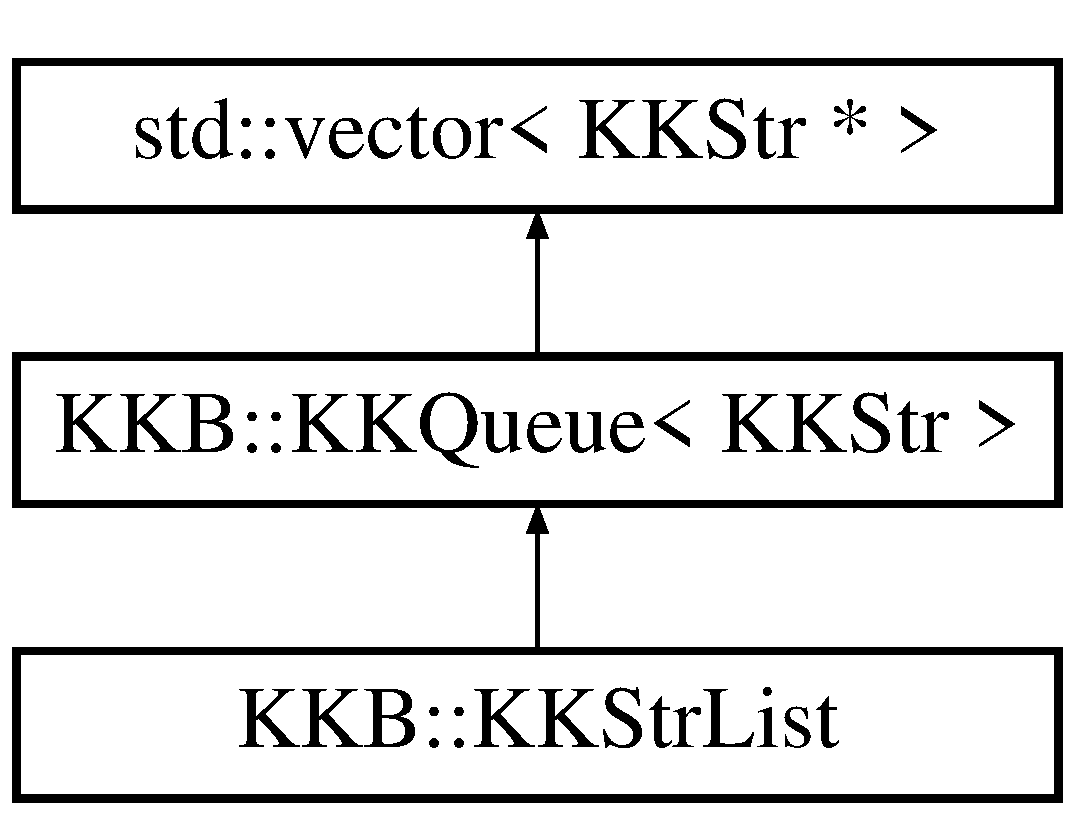
\includegraphics[height=3.000000cm]{class_k_k_b_1_1_k_k_str_list}
\end{center}
\end{figure}
\subsection*{Classes}
\begin{DoxyCompactItemize}
\item 
class \hyperlink{class_k_k_str_list_1_1_string_comparison}{String\+Comparison}
\end{DoxyCompactItemize}
\subsection*{Public Types}
\begin{DoxyCompactItemize}
\item 
typedef \hyperlink{class_k_k_b_1_1_k_k_str_list}{K\+K\+Str\+List} $\ast$ \hyperlink{class_k_k_b_1_1_k_k_str_list_a466accb870aa75f4b47943932fccb4c8}{K\+K\+Str\+List\+Ptr}
\end{DoxyCompactItemize}
\subsection*{Public Member Functions}
\begin{DoxyCompactItemize}
\item 
\hyperlink{class_k_k_b_1_1_k_k_str_list_ae8f27238b72887a795737931735ff802}{K\+K\+Str\+List} ()
\item 
\hyperlink{class_k_k_b_1_1_k_k_str_list_a35f0d495449b13e07a0fd8cc90b90b4c}{K\+K\+Str\+List} (bool owner)
\item 
\hyperlink{class_k_k_b_1_1_k_k_str_list_a1e6557c33b11dd3c3c4ff51a538d7353}{K\+K\+Str\+List} (const char $\ast$s\mbox{[}$\,$\mbox{]})
\item 
void \hyperlink{class_k_k_b_1_1_k_k_str_list_a0209f0a13bcd253c40108864b3804063}{Add\+String} (\hyperlink{namespace_k_k_b_a9adbef5a6b3be0867f5570df2a08f388}{K\+K\+Str\+Ptr} str)
\item 
\hyperlink{namespace_k_k_b_a9adbef5a6b3be0867f5570df2a08f388}{K\+K\+Str\+Ptr} \hyperlink{class_k_k_b_1_1_k_k_str_list_abfeb41d75fc3e285f7bdf65593f204a1}{Binary\+Search} (const \hyperlink{class_k_k_b_1_1_k_k_str}{K\+K\+Str} \&search\+Str)
\item 
\hyperlink{class_k_k_b_1_1_k_k_str_list_a466accb870aa75f4b47943932fccb4c8}{K\+K\+Str\+List\+Ptr} \hyperlink{class_k_k_b_1_1_k_k_str_list_a9316bb3167f82a9695b3b09e56545d12}{Duplicate\+List\+And\+Contents} () const 
\item 
\hyperlink{namespace_k_k_b_a8fa4952cc84fda1de4bec1fbdd8d5b1b}{kkint32} \hyperlink{class_k_k_b_1_1_k_k_str_list_a2e3450903dba55c8733e638c6916ba3d}{Memory\+Consumed\+Estimated} () const 
\item 
void \hyperlink{class_k_k_b_1_1_k_k_str_list_a0f573b4a2aa069d5dc5097f5f2fe8d15}{Read\+X\+ML} (\hyperlink{class_k_k_b_1_1_xml_stream}{Xml\+Stream} \&s, \hyperlink{namespace_k_k_b_a5f1b0b1667d79fec26deeff10c43df23}{Xml\+Tag\+Const\+Ptr} tag, \hyperlink{namespace_k_k_b_a7d390f568e2831fb76b86b56c87bf92f}{Vol\+Const\+Bool} \&cancel\+Flag, \hyperlink{class_k_k_b_1_1_run_log}{Run\+Log} \&log)
\item 
void \hyperlink{class_k_k_b_1_1_k_k_str_list_a239828772f41e47f3a136ea15e40f5d6}{Sort} (bool \+\_\+reversed\+Order)
\item 
bool \hyperlink{class_k_k_b_1_1_k_k_str_list_a7d5d3da0512d094034bd6203aaa3576f}{String\+In\+List} (\hyperlink{class_k_k_b_1_1_k_k_str}{K\+K\+Str} \&str)
\item 
void \hyperlink{class_k_k_b_1_1_k_k_str_list_aba21c9259253e8ae268ee13d5e0b3539}{Write\+X\+ML} (const \hyperlink{class_k_k_b_1_1_k_k_str}{K\+K\+Str} \&var\+Name, std\+::ostream \&o) const 
\end{DoxyCompactItemize}
\subsection*{Static Public Member Functions}
\begin{DoxyCompactItemize}
\item 
static \hyperlink{class_k_k_b_1_1_k_k_str_list_a466accb870aa75f4b47943932fccb4c8}{K\+K\+Str\+List\+Ptr} \hyperlink{class_k_k_b_1_1_k_k_str_list_a1685b0a8cb9d04d5f37be0e7b7fc0407}{Parse\+Delimited\+String} (const \hyperlink{class_k_k_b_1_1_k_k_str}{K\+K\+Str} \&str, const char $\ast$del\+Chars=\char`\"{},\textbackslash{}t\textbackslash{}n\textbackslash{}r\char`\"{})
\end{DoxyCompactItemize}
\subsection*{Additional Inherited Members}


\subsection{Detailed Description}


Definition at line 770 of file K\+K\+Str.\+h.



\subsection{Member Typedef Documentation}
\index{K\+K\+B\+::\+K\+K\+Str\+List@{K\+K\+B\+::\+K\+K\+Str\+List}!K\+K\+Str\+List\+Ptr@{K\+K\+Str\+List\+Ptr}}
\index{K\+K\+Str\+List\+Ptr@{K\+K\+Str\+List\+Ptr}!K\+K\+B\+::\+K\+K\+Str\+List@{K\+K\+B\+::\+K\+K\+Str\+List}}
\subsubsection[{\texorpdfstring{K\+K\+Str\+List\+Ptr}{KKStrListPtr}}]{\setlength{\rightskip}{0pt plus 5cm}typedef {\bf K\+K\+Str\+List}$\ast$ {\bf K\+K\+B\+::\+K\+K\+Str\+List\+::\+K\+K\+Str\+List\+Ptr}}\hypertarget{class_k_k_b_1_1_k_k_str_list_a466accb870aa75f4b47943932fccb4c8}{}\label{class_k_k_b_1_1_k_k_str_list_a466accb870aa75f4b47943932fccb4c8}


Definition at line 773 of file K\+K\+Str.\+h.



\subsection{Constructor \& Destructor Documentation}
\index{K\+K\+B\+::\+K\+K\+Str\+List@{K\+K\+B\+::\+K\+K\+Str\+List}!K\+K\+Str\+List@{K\+K\+Str\+List}}
\index{K\+K\+Str\+List@{K\+K\+Str\+List}!K\+K\+B\+::\+K\+K\+Str\+List@{K\+K\+B\+::\+K\+K\+Str\+List}}
\subsubsection[{\texorpdfstring{K\+K\+Str\+List()}{KKStrList()}}]{\setlength{\rightskip}{0pt plus 5cm}K\+K\+Str\+List\+::\+K\+K\+Str\+List (
\begin{DoxyParamCaption}
{}
\end{DoxyParamCaption}
)}\hypertarget{class_k_k_b_1_1_k_k_str_list_ae8f27238b72887a795737931735ff802}{}\label{class_k_k_b_1_1_k_k_str_list_ae8f27238b72887a795737931735ff802}


Definition at line 4478 of file K\+K\+Str.\+cpp.



References K\+K\+Str\+List().



Referenced by K\+K\+B\+::\+Msg\+Queue\+::\+Get\+All\+Msgs(), and K\+K\+Str\+List().


\begin{DoxyCode}
4478                      :
4479   \hyperlink{class_k_k_b_1_1_k_k_queue}{KKQueue<KKStr>} (\textcolor{keyword}{false}),
4480   sorted (\textcolor{keyword}{false})
4481 \{
4482 \}
\end{DoxyCode}
\index{K\+K\+B\+::\+K\+K\+Str\+List@{K\+K\+B\+::\+K\+K\+Str\+List}!K\+K\+Str\+List@{K\+K\+Str\+List}}
\index{K\+K\+Str\+List@{K\+K\+Str\+List}!K\+K\+B\+::\+K\+K\+Str\+List@{K\+K\+B\+::\+K\+K\+Str\+List}}
\subsubsection[{\texorpdfstring{K\+K\+Str\+List(bool owner)}{KKStrList(bool owner)}}]{\setlength{\rightskip}{0pt plus 5cm}K\+K\+Str\+List\+::\+K\+K\+Str\+List (
\begin{DoxyParamCaption}
\item[{bool}]{owner}
\end{DoxyParamCaption}
)}\hypertarget{class_k_k_b_1_1_k_k_str_list_a35f0d495449b13e07a0fd8cc90b90b4c}{}\label{class_k_k_b_1_1_k_k_str_list_a35f0d495449b13e07a0fd8cc90b90b4c}
summary$>$ Creates a list from a array of N\+U\+LL terminated strings; the last entry in the list has to be N\+U\+LL. {\ttfamily  Example\+: const char$\ast$ zed\mbox{[}\mbox{]} = \{\char`\"{}\+This\char`\"{}, \char`\"{}is\char`\"{}, \char`\"{}a\char`\"{}, \char`\"{}test\char`\"{}, N\+U\+LL\}; \hyperlink{class_k_k_b_1_1_k_k_str_list}{K\+K\+Str\+List} word\+List (zed); } /summary$>$ 

Definition at line 4485 of file K\+K\+Str.\+cpp.



References K\+K\+Str\+List().



Referenced by K\+K\+B\+::\+K\+K\+Str\+Matrix\+::\+Add\+Row(), K\+K\+B\+::\+Image\+Dir\+Tree\+::\+Directories(), Duplicate\+List\+And\+Contents(), K\+K\+M\+L\+L\+::\+Feature\+Vector\+List\+::\+Extract\+Duplicates\+By\+Example\+File\+Name(), K\+K\+B\+::\+K\+K\+Thread\+::\+Get\+Msgs(), K\+K\+B\+::\+Tokenizer\+::\+Get\+Next\+Tokens(), K\+K\+B\+::\+Xml\+Tokenizer\+::\+Get\+Next\+Tokens(), K\+K\+Str\+List(), K\+K\+B\+::os\+Get\+List\+Of\+Directories(), K\+K\+B\+::os\+Get\+List\+Of\+Files(), K\+K\+B\+::os\+Get\+List\+Of\+Image\+Files(), os\+Parse\+Search\+Spec(), K\+K\+B\+::os\+Valid\+File\+Name\+Errors(), and Parse\+Delimited\+String().


\begin{DoxyCode}
4485                                  :
4486   \hyperlink{class_k_k_b_1_1_k_k_queue}{KKQueue<KKStr>} (owner),
4487   sorted (\textcolor{keyword}{false})
4488 \{
4489 \}
\end{DoxyCode}
\index{K\+K\+B\+::\+K\+K\+Str\+List@{K\+K\+B\+::\+K\+K\+Str\+List}!K\+K\+Str\+List@{K\+K\+Str\+List}}
\index{K\+K\+Str\+List@{K\+K\+Str\+List}!K\+K\+B\+::\+K\+K\+Str\+List@{K\+K\+B\+::\+K\+K\+Str\+List}}
\subsubsection[{\texorpdfstring{K\+K\+Str\+List(const char $\ast$s[])}{KKStrList(const char *s[])}}]{\setlength{\rightskip}{0pt plus 5cm}K\+K\+Str\+List\+::\+K\+K\+Str\+List (
\begin{DoxyParamCaption}
\item[{const char $\ast$}]{s\mbox{[}$\,$\mbox{]}}
\end{DoxyParamCaption}
)}\hypertarget{class_k_k_b_1_1_k_k_str_list_a1e6557c33b11dd3c3c4ff51a538d7353}{}\label{class_k_k_b_1_1_k_k_str_list_a1e6557c33b11dd3c3c4ff51a538d7353}


Definition at line 4493 of file K\+K\+Str.\+cpp.



References K\+K\+Str\+List().



Referenced by K\+K\+Str\+List().


\begin{DoxyCode}
4493                                      :
4494     \hyperlink{class_k_k_b_1_1_k_k_queue}{KKQueue<KKStr>} (\textcolor{keyword}{true}),
4495     sorted (\textcolor{keyword}{false})
4496 \{
4497   \textcolor{keywordflow}{if}  (s == NULL)
4498     \textcolor{keywordflow}{return};
4499 
4500   \textcolor{keywordtype}{int}  x = 0;
4501   \textcolor{keywordflow}{while}  (s[x] != NULL)
4502   \{
4503     \hyperlink{class_k_k_b_1_1_k_k_queue_aa9fba4632b54268bf71ecb42dee0b575}{PushOnBack} (\textcolor{keyword}{new} \hyperlink{class_k_k_b_1_1_k_k_str}{KKStr} (s[x]));
4504     ++x;
4505   \}
4506 \}
\end{DoxyCode}


\subsection{Member Function Documentation}
\index{K\+K\+B\+::\+K\+K\+Str\+List@{K\+K\+B\+::\+K\+K\+Str\+List}!Add\+String@{Add\+String}}
\index{Add\+String@{Add\+String}!K\+K\+B\+::\+K\+K\+Str\+List@{K\+K\+B\+::\+K\+K\+Str\+List}}
\subsubsection[{\texorpdfstring{Add\+String(\+K\+K\+Str\+Ptr str)}{AddString(KKStrPtr str)}}]{\setlength{\rightskip}{0pt plus 5cm}void K\+K\+Str\+List\+::\+Add\+String (
\begin{DoxyParamCaption}
\item[{{\bf K\+K\+Str\+Ptr}}]{str}
\end{DoxyParamCaption}
)}\hypertarget{class_k_k_b_1_1_k_k_str_list_a0209f0a13bcd253c40108864b3804063}{}\label{class_k_k_b_1_1_k_k_str_list_a0209f0a13bcd253c40108864b3804063}


Definition at line 4651 of file K\+K\+Str.\+cpp.


\begin{DoxyCode}
4652 \{
4653   \hyperlink{class_k_k_b_1_1_k_k_queue_aa9fba4632b54268bf71ecb42dee0b575}{PushOnBack} (str);
4654   sorted = \textcolor{keyword}{false};
4655 \}
\end{DoxyCode}
\index{K\+K\+B\+::\+K\+K\+Str\+List@{K\+K\+B\+::\+K\+K\+Str\+List}!Binary\+Search@{Binary\+Search}}
\index{Binary\+Search@{Binary\+Search}!K\+K\+B\+::\+K\+K\+Str\+List@{K\+K\+B\+::\+K\+K\+Str\+List}}
\subsubsection[{\texorpdfstring{Binary\+Search(const K\+K\+Str \&search\+Str)}{BinarySearch(const KKStr &searchStr)}}]{\setlength{\rightskip}{0pt plus 5cm}{\bf K\+K\+Str\+Ptr} K\+K\+Str\+List\+::\+Binary\+Search (
\begin{DoxyParamCaption}
\item[{const {\bf K\+K\+Str} \&}]{search\+Str}
\end{DoxyParamCaption}
)}\hypertarget{class_k_k_b_1_1_k_k_str_list_abfeb41d75fc3e285f7bdf65593f204a1}{}\label{class_k_k_b_1_1_k_k_str_list_abfeb41d75fc3e285f7bdf65593f204a1}


Definition at line 4607 of file K\+K\+Str.\+cpp.



References K\+K\+B\+::\+K\+K\+Str\+::\+Concat(), K\+K\+B\+::\+K\+K\+Exception\+::\+K\+K\+Exception(), K\+K\+B\+::\+K\+K\+Str\+::operator$<$(), and K\+K\+B\+::\+K\+K\+Str\+::operator$>$().


\begin{DoxyCode}
4608 \{
4609   \textcolor{keywordflow}{if}  (!sorted)
4610   \{
4611     \hyperlink{class_k_k_b_1_1_k_k_str}{KKStr} errMsg = \textcolor{stringliteral}{"KKStrList::BinarySearch     **** ERROR ****        KKStr List is Not Sorted"};
4612     cerr << \hyperlink{namespace_k_k_b_ad1f50f65af6adc8fa9e6f62d007818a8}{endl} << errMsg << \hyperlink{namespace_k_k_b_ad1f50f65af6adc8fa9e6f62d007818a8}{endl} << \hyperlink{namespace_k_k_b_ad1f50f65af6adc8fa9e6f62d007818a8}{endl};
4613     \textcolor{keywordflow}{throw} \hyperlink{class_k_k_b_1_1_k_k_exception}{KKException} (errMsg);
4614   \}
4615   
4616   \hyperlink{namespace_k_k_b_a8fa4952cc84fda1de4bec1fbdd8d5b1b}{kkint32}  low  = 0;
4617   \hyperlink{namespace_k_k_b_a8fa4952cc84fda1de4bec1fbdd8d5b1b}{kkint32}  high = \hyperlink{class_k_k_b_1_1_k_k_queue_a1dab601f75ee6a65d97f02bddf71c40d}{QueueSize} () - 1;
4618   \hyperlink{namespace_k_k_b_a8fa4952cc84fda1de4bec1fbdd8d5b1b}{kkint32}  mid;
4619 
4620   \hyperlink{class_k_k_b_1_1_k_k_str}{KKStrPtr}  str = NULL;
4621 
4622   \textcolor{keywordflow}{while}  (low <= high)
4623   \{
4624     mid = (low + high) / 2;
4625 
4626     str = \hyperlink{class_k_k_b_1_1_k_k_queue_acce2bdd8b3327e38266cf198382cd852}{IdxToPtr} (mid);
4627 
4628     \textcolor{keywordflow}{if}  (*str  < searchStr)
4629     \{
4630       low = mid + 1;
4631     \}
4632 
4633     \textcolor{keywordflow}{else} \textcolor{keywordflow}{if}  (*str > searchStr)
4634     \{
4635       high = mid - 1;
4636     \}
4637 
4638     \textcolor{keywordflow}{else}
4639     \{
4640       \textcolor{keywordflow}{return}  str;
4641     \}
4642   \}
4643 
4644   \textcolor{keywordflow}{return}  NULL;
4645 \}  \textcolor{comment}{/* BinarySearch */}
\end{DoxyCode}
\index{K\+K\+B\+::\+K\+K\+Str\+List@{K\+K\+B\+::\+K\+K\+Str\+List}!Duplicate\+List\+And\+Contents@{Duplicate\+List\+And\+Contents}}
\index{Duplicate\+List\+And\+Contents@{Duplicate\+List\+And\+Contents}!K\+K\+B\+::\+K\+K\+Str\+List@{K\+K\+B\+::\+K\+K\+Str\+List}}
\subsubsection[{\texorpdfstring{Duplicate\+List\+And\+Contents() const }{DuplicateListAndContents() const }}]{\setlength{\rightskip}{0pt plus 5cm}{\bf K\+K\+Str\+List\+Ptr} K\+K\+Str\+List\+::\+Duplicate\+List\+And\+Contents (
\begin{DoxyParamCaption}
{}
\end{DoxyParamCaption}
) const}\hypertarget{class_k_k_b_1_1_k_k_str_list_a9316bb3167f82a9695b3b09e56545d12}{}\label{class_k_k_b_1_1_k_k_str_list_a9316bb3167f82a9695b3b09e56545d12}


Definition at line 4779 of file K\+K\+Str.\+cpp.



References K\+K\+Str\+List().


\begin{DoxyCode}
4780 \{
4781   \hyperlink{class_k_k_b_1_1_k_k_str_list}{KKStrListPtr}  newList = \textcolor{keyword}{new} \hyperlink{class_k_k_b_1_1_k_k_str_list_ae8f27238b72887a795737931735ff802}{KKStrList} (\textcolor{keyword}{true});
4782   \hyperlink{class_k_k_b_1_1_k_k_queue_aeb057c9c010446f46f57c1e355f981f1}{KKStrList::const\_iterator}  idx;
4783   \textcolor{keywordflow}{for}  (idx = begin ();  idx != end ();  idx++)
4784     newList->\hyperlink{class_k_k_b_1_1_k_k_queue_aa9fba4632b54268bf71ecb42dee0b575}{PushOnBack} (\textcolor{keyword}{new} \hyperlink{class_k_k_b_1_1_k_k_str}{KKStr} (*(*idx)));
4785 
4786   \textcolor{keywordflow}{return}  newList;
4787 \}  \textcolor{comment}{/* DuplicateListAndContents */}
\end{DoxyCode}
\index{K\+K\+B\+::\+K\+K\+Str\+List@{K\+K\+B\+::\+K\+K\+Str\+List}!Memory\+Consumed\+Estimated@{Memory\+Consumed\+Estimated}}
\index{Memory\+Consumed\+Estimated@{Memory\+Consumed\+Estimated}!K\+K\+B\+::\+K\+K\+Str\+List@{K\+K\+B\+::\+K\+K\+Str\+List}}
\subsubsection[{\texorpdfstring{Memory\+Consumed\+Estimated() const }{MemoryConsumedEstimated() const }}]{\setlength{\rightskip}{0pt plus 5cm}{\bf kkint32} K\+K\+Str\+List\+::\+Memory\+Consumed\+Estimated (
\begin{DoxyParamCaption}
{}
\end{DoxyParamCaption}
) const}\hypertarget{class_k_k_b_1_1_k_k_str_list_a2e3450903dba55c8733e638c6916ba3d}{}\label{class_k_k_b_1_1_k_k_str_list_a2e3450903dba55c8733e638c6916ba3d}


Definition at line 4511 of file K\+K\+Str.\+cpp.


\begin{DoxyCode}
4512 \{
4513   \hyperlink{namespace_k_k_b_a8fa4952cc84fda1de4bec1fbdd8d5b1b}{kkint32}  memoryConsumedEstimated = \textcolor{keyword}{sizeof} (\hyperlink{class_k_k_b_1_1_k_k_str_list_ae8f27238b72887a795737931735ff802}{KKStrList});
4514   \hyperlink{class_k_k_b_1_1_k_k_queue_aeb057c9c010446f46f57c1e355f981f1}{KKStrList::const\_iterator} idx;
4515   \textcolor{keywordflow}{for}  (idx = this->begin ();  idx != this->end ();  ++idx)
4516     memoryConsumedEstimated += (*idx)->MemoryConsumedEstimated ();
4517   \textcolor{keywordflow}{return}  memoryConsumedEstimated;
4518 \}
\end{DoxyCode}
\index{K\+K\+B\+::\+K\+K\+Str\+List@{K\+K\+B\+::\+K\+K\+Str\+List}!Parse\+Delimited\+String@{Parse\+Delimited\+String}}
\index{Parse\+Delimited\+String@{Parse\+Delimited\+String}!K\+K\+B\+::\+K\+K\+Str\+List@{K\+K\+B\+::\+K\+K\+Str\+List}}
\subsubsection[{\texorpdfstring{Parse\+Delimited\+String(const K\+K\+Str \&str, const char $\ast$del\+Chars="",\textbackslash{}t\textbackslash{}n\textbackslash{}r"")}{ParseDelimitedString(const KKStr &str, const char *delChars=",\textbackslash{}t\textbackslash{}n\textbackslash{}r")}}]{\setlength{\rightskip}{0pt plus 5cm}{\bf K\+K\+Str\+List\+Ptr} K\+K\+Str\+List\+::\+Parse\+Delimited\+String (
\begin{DoxyParamCaption}
\item[{const {\bf K\+K\+Str} \&}]{str, }
\item[{const char $\ast$}]{del\+Chars = {\ttfamily \char`\"{},\textbackslash{}t\textbackslash{}n\textbackslash{}r\char`\"{}}}
\end{DoxyParamCaption}
)\hspace{0.3cm}{\ttfamily [static]}}\hypertarget{class_k_k_b_1_1_k_k_str_list_a1685b0a8cb9d04d5f37be0e7b7fc0407}{}\label{class_k_k_b_1_1_k_k_str_list_a1685b0a8cb9d04d5f37be0e7b7fc0407}


Definition at line 4659 of file K\+K\+Str.\+cpp.



References K\+K\+B\+::\+K\+K\+Str\+::\+Concat(), K\+K\+B\+::\+K\+K\+Str\+::\+K\+K\+Str(), K\+K\+Str\+List(), and K\+K\+B\+::\+K\+K\+Str\+::\+Trim\+Right().


\begin{DoxyCode}
4662 \{
4663   \hyperlink{class_k_k_b_1_1_k_k_str_list}{KKStrListPtr}  parms = \textcolor{keyword}{new} \hyperlink{class_k_k_b_1_1_k_k_str_list_ae8f27238b72887a795737931735ff802}{KKStrList} (\textcolor{keyword}{true});
4664 
4665 \textcolor{preprocessor}{# ifdef  USE\_SECURE\_FUNCS}
4666     \textcolor{keywordtype}{char}*  workStr =  \_strdup (str.\hyperlink{class_k_k_b_1_1_k_k_str_ad574e6c0fe7f6ce1ba3ab0a8ce2fbd52}{Str} ());
4667 \textcolor{preprocessor}{# else}
4668     \textcolor{keywordtype}{char}*  workStr =  strdup (str.\hyperlink{class_k_k_b_1_1_k_k_str_ad574e6c0fe7f6ce1ba3ab0a8ce2fbd52}{Str} ());
4669 \textcolor{preprocessor}{# endif}
4670 
4671   \textcolor{keywordtype}{char}*  nextChar = workStr;
4672 
4673   \textcolor{keywordflow}{while}  (*nextChar)
4674   \{
4675     \textcolor{comment}{// Skip Past Leading Blanks}
4676     \textcolor{keywordflow}{while}  ((*nextChar)  &&  (*nextChar == \textcolor{charliteral}{' '}))
4677     \{
4678       nextChar++;
4679     \}
4680 
4681     \textcolor{keywordflow}{if}  (*nextChar == 0)
4682       \textcolor{keywordflow}{break};
4683 
4684     \textcolor{keyword}{const} \textcolor{keywordtype}{char}*  startOfToken = nextChar;
4685 
4686     \textcolor{keywordflow}{while}  ((*nextChar)  &&  (strchr (delChars, *nextChar) == NULL))
4687     \{
4688       nextChar++;
4689     \}
4690 
4691     \textcolor{keywordflow}{if}  (*nextChar != 0)
4692     \{
4693       *nextChar = 0;
4694       nextChar++;
4695     \}
4696 
4697     \hyperlink{class_k_k_b_1_1_k_k_str}{KKStrPtr}  token = \textcolor{keyword}{new} \hyperlink{class_k_k_b_1_1_k_k_str}{KKStr} (startOfToken);
4698     token->\hyperlink{class_k_k_b_1_1_k_k_str_aa912161f17871e2d6fec7bbac033221c}{TrimRight} ();
4699 
4700     parms->\hyperlink{class_k_k_b_1_1_k_k_queue_aa9fba4632b54268bf71ecb42dee0b575}{PushOnBack} (token);
4701   \}
4702 
4703   \textcolor{keyword}{delete}  [] workStr;
4704 
4705   \textcolor{keywordflow}{return}  parms;
4706 \}  \textcolor{comment}{/* ParseDelimitedString */}
\end{DoxyCode}
\index{K\+K\+B\+::\+K\+K\+Str\+List@{K\+K\+B\+::\+K\+K\+Str\+List}!Read\+X\+ML@{Read\+X\+ML}}
\index{Read\+X\+ML@{Read\+X\+ML}!K\+K\+B\+::\+K\+K\+Str\+List@{K\+K\+B\+::\+K\+K\+Str\+List}}
\subsubsection[{\texorpdfstring{Read\+X\+M\+L(\+Xml\+Stream \&s, Xml\+Tag\+Const\+Ptr tag, Vol\+Const\+Bool \&cancel\+Flag, Run\+Log \&log)}{ReadXML(XmlStream &s, XmlTagConstPtr tag, VolConstBool &cancelFlag, RunLog &log)}}]{\setlength{\rightskip}{0pt plus 5cm}void K\+K\+Str\+List\+::\+Read\+X\+ML (
\begin{DoxyParamCaption}
\item[{{\bf Xml\+Stream} \&}]{s, }
\item[{{\bf Xml\+Tag\+Const\+Ptr}}]{tag, }
\item[{{\bf Vol\+Const\+Bool} \&}]{cancel\+Flag, }
\item[{{\bf Run\+Log} \&}]{log}
\end{DoxyParamCaption}
)}\hypertarget{class_k_k_b_1_1_k_k_str_list_a0f573b4a2aa069d5dc5097f5f2fe8d15}{}\label{class_k_k_b_1_1_k_k_str_list_a0f573b4a2aa069d5dc5097f5f2fe8d15}


Definition at line 4537 of file K\+K\+Str.\+cpp.



References K\+K\+B\+::\+Xml\+Tag\+::\+Attribute\+Value\+Int32(), K\+K\+B\+::\+K\+K\+Str\+::\+Concat(), K\+K\+B\+::\+Xml\+Content\+::\+Content(), K\+K\+B\+::\+K\+K\+Str\+Parser\+::\+Get\+Next\+Token(), K\+K\+B\+::\+Xml\+Stream\+::\+Get\+Next\+Token(), K\+K\+B\+::\+K\+K\+Str\+Parser\+::\+K\+K\+Str\+Parser(), K\+K\+B\+::\+K\+K\+Str\+Parser\+::\+More\+Tokens(), K\+K\+B\+::\+Xml\+Token\+::tok\+Content, K\+K\+B\+::\+Xml\+Token\+::\+Token\+Type(), and K\+K\+B\+::\+K\+K\+Str\+Parser\+::\+Trim\+White\+Space().


\begin{DoxyCode}
4542 \{
4543   \hyperlink{namespace_k_k_b_af8d832f05c54994a1cce25bd5743e19a}{kkuint32}  count = (\hyperlink{namespace_k_k_b_af8d832f05c54994a1cce25bd5743e19a}{kkuint32})tag->AttributeValueInt32 (\textcolor{stringliteral}{"Count"});
4544 
4545   \hyperlink{class_k_k_b_1_1_k_k_queue_a72dbe1e65d567536dbf4be3617230254}{DeleteContents} ();
4546 
4547   \hyperlink{class_k_k_b_1_1_xml_token}{XmlTokenPtr}  t = s.\hyperlink{class_k_k_b_1_1_xml_stream_a87cc738b05c666cf5d5c25beaab477b4}{GetNextToken} (cancelFlag, log);
4548   \textcolor{keywordflow}{while}  (t  &&  (!cancelFlag))
4549   \{
4550     \textcolor{keywordflow}{if}  (t->\hyperlink{class_k_k_b_1_1_xml_token_ae98e2c1a798882647578cae4adcd7176}{TokenType} () == \hyperlink{class_k_k_b_1_1_xml_token_a18b6e90c919f4b92e3b024f50f247f62aff369b5479984ca659548f37ad4caec9}{XmlToken::TokenTypes::tokContent})
4551     \{
4552       \hyperlink{class_k_k_b_1_1_xml_content}{XmlContentPtr}  c = \textcolor{keyword}{dynamic\_cast<}\hyperlink{class_k_k_b_1_1_xml_content}{XmlContentPtr}\textcolor{keyword}{>}(t);
4553       \textcolor{keywordflow}{if}  ((c != NULL)  &&  (c->\hyperlink{class_k_k_b_1_1_xml_content_a1d0730aae45b069e8604bef19b8c0098}{Content} () != NULL))
4554       \{
4555         \hyperlink{class_k_k_b_1_1_k_k_str_parser}{KKStrParser}  parser (*(c->\hyperlink{class_k_k_b_1_1_xml_content_a1d0730aae45b069e8604bef19b8c0098}{Content} ()));
4556         parser.TrimWhiteSpace (\textcolor{stringliteral}{" "});
4557         \textcolor{keywordflow}{while}  (parser.MoreTokens ())
4558         \{
4559           \hyperlink{class_k_k_b_1_1_k_k_str}{KKStr} field = parser.GetNextToken (\textcolor{stringliteral}{"\(\backslash\)t"});
4560           \hyperlink{class_k_k_b_1_1_k_k_queue_aa9fba4632b54268bf71ecb42dee0b575}{PushOnBack} (\textcolor{keyword}{new} \hyperlink{class_k_k_b_1_1_k_k_str}{KKStr} (field));
4561         \}
4562       \}
4563     \}
4564     \textcolor{keyword}{delete} t;
4565     \textcolor{keywordflow}{if}  (cancelFlag)
4566       t = NULL;
4567     \textcolor{keywordflow}{else}
4568       t = s.\hyperlink{class_k_k_b_1_1_xml_stream_a87cc738b05c666cf5d5c25beaab477b4}{GetNextToken} (cancelFlag, log);
4569   \}
4570   \textcolor{keyword}{delete}  t;
4571   t = NULL;
4572 \}  \textcolor{comment}{/* ReadXML */}
\end{DoxyCode}
\index{K\+K\+B\+::\+K\+K\+Str\+List@{K\+K\+B\+::\+K\+K\+Str\+List}!Sort@{Sort}}
\index{Sort@{Sort}!K\+K\+B\+::\+K\+K\+Str\+List@{K\+K\+B\+::\+K\+K\+Str\+List}}
\subsubsection[{\texorpdfstring{Sort(bool \+\_\+reversed\+Order)}{Sort(bool _reversedOrder)}}]{\setlength{\rightskip}{0pt plus 5cm}void K\+K\+Str\+List\+::\+Sort (
\begin{DoxyParamCaption}
\item[{bool}]{\+\_\+reversed\+Order}
\end{DoxyParamCaption}
)}\hypertarget{class_k_k_b_1_1_k_k_str_list_a239828772f41e47f3a136ea15e40f5d6}{}\label{class_k_k_b_1_1_k_k_str_list_a239828772f41e47f3a136ea15e40f5d6}


Definition at line 4770 of file K\+K\+Str.\+cpp.



References K\+K\+B\+::\+K\+K\+Str\+List\+::\+String\+Comparison\+::\+String\+Comparison().



Referenced by K\+K\+M\+L\+L\+::\+Feature\+File\+I\+O\+::\+Feature\+Data\+Re\+Sink().


\begin{DoxyCode}
4771 \{
4772   StringComparison  stringComparison (\_reversedOrder);
4773   sort (begin (), end (), stringComparison);
4774   \textcolor{keywordflow}{if}  (!\_reversedOrder)
4775     sorted = \textcolor{keyword}{true};
4776 \}
\end{DoxyCode}
\index{K\+K\+B\+::\+K\+K\+Str\+List@{K\+K\+B\+::\+K\+K\+Str\+List}!String\+In\+List@{String\+In\+List}}
\index{String\+In\+List@{String\+In\+List}!K\+K\+B\+::\+K\+K\+Str\+List@{K\+K\+B\+::\+K\+K\+Str\+List}}
\subsubsection[{\texorpdfstring{String\+In\+List(\+K\+K\+Str \&str)}{StringInList(KKStr &str)}}]{\setlength{\rightskip}{0pt plus 5cm}bool K\+K\+Str\+List\+::\+String\+In\+List (
\begin{DoxyParamCaption}
\item[{{\bf K\+K\+Str} \&}]{str}
\end{DoxyParamCaption}
)}\hypertarget{class_k_k_b_1_1_k_k_str_list_a7d5d3da0512d094034bd6203aaa3576f}{}\label{class_k_k_b_1_1_k_k_str_list_a7d5d3da0512d094034bd6203aaa3576f}


Definition at line 4522 of file K\+K\+Str.\+cpp.


\begin{DoxyCode}
4523 \{
4524   \textcolor{keywordtype}{bool}  found = \textcolor{keyword}{false};
4525   \hyperlink{namespace_k_k_b_a8fa4952cc84fda1de4bec1fbdd8d5b1b}{kkint32} idx;
4526   \hyperlink{namespace_k_k_b_a8fa4952cc84fda1de4bec1fbdd8d5b1b}{kkint32} qSize = \hyperlink{class_k_k_b_1_1_k_k_queue_a1dab601f75ee6a65d97f02bddf71c40d}{QueueSize} ();
4527 
4528   \textcolor{keywordflow}{for}  (idx = 0; ((idx < qSize) && (!found)); idx++)
4529     found = (str == (*\hyperlink{class_k_k_b_1_1_k_k_queue_acce2bdd8b3327e38266cf198382cd852}{IdxToPtr} (idx)));
4530 
4531   \textcolor{keywordflow}{return}  found;
4532 \}
\end{DoxyCode}
\index{K\+K\+B\+::\+K\+K\+Str\+List@{K\+K\+B\+::\+K\+K\+Str\+List}!Write\+X\+ML@{Write\+X\+ML}}
\index{Write\+X\+ML@{Write\+X\+ML}!K\+K\+B\+::\+K\+K\+Str\+List@{K\+K\+B\+::\+K\+K\+Str\+List}}
\subsubsection[{\texorpdfstring{Write\+X\+M\+L(const K\+K\+Str \&var\+Name, std\+::ostream \&o) const }{WriteXML(const KKStr &varName, std::ostream &o) const }}]{\setlength{\rightskip}{0pt plus 5cm}void K\+K\+Str\+List\+::\+Write\+X\+ML (
\begin{DoxyParamCaption}
\item[{const {\bf K\+K\+Str} \&}]{var\+Name, }
\item[{std\+::ostream \&}]{o}
\end{DoxyParamCaption}
) const}\hypertarget{class_k_k_b_1_1_k_k_str_list_aba21c9259253e8ae268ee13d5e0b3539}{}\label{class_k_k_b_1_1_k_k_str_list_aba21c9259253e8ae268ee13d5e0b3539}


Definition at line 4577 of file K\+K\+Str.\+cpp.



References K\+K\+B\+::\+Xml\+Tag\+::\+Add\+Atribute(), K\+K\+B\+::\+K\+K\+Str\+::\+Empty(), K\+K\+B\+::operator$<$$<$(), K\+K\+B\+::\+K\+K\+Str\+::\+Quoted\+Str(), K\+K\+B\+::\+Xml\+Tag\+::tag\+End, K\+K\+B\+::\+Xml\+Tag\+::tag\+Start, K\+K\+B\+::\+Xml\+Tag\+::\+Write\+X\+M\+L(), K\+K\+B\+::\+Xml\+Content\+::\+Write\+Xml(), and K\+K\+B\+::\+Xml\+Tag\+::\+Xml\+Tag().


\begin{DoxyCode}
4580 \{
4581   \hyperlink{class_k_k_b_1_1_xml_tag}{XmlTag}  startTag (\textcolor{stringliteral}{"KKStrList"}, \hyperlink{class_k_k_b_1_1_xml_tag_a6c0ef0e23f982f49d55d4fb7eaff6ac9ab02b23b5e15b3a1353771313e1176ce0}{XmlTag::TagTypes::tagStart});
4582   \textcolor{keywordflow}{if}  (!varName.\hyperlink{class_k_k_b_1_1_k_k_str_ac69942f73fffd672ec2a6e1c410afdb6}{Empty} ())
4583     startTag.AddAtribute (\textcolor{stringliteral}{"VarName"}, varName);
4584   startTag.AddAtribute (\textcolor{stringliteral}{"Count"}, (\hyperlink{namespace_k_k_b_a8fa4952cc84fda1de4bec1fbdd8d5b1b}{kkint32})size ());
4585   startTag.WriteXML (o);
4586 
4587   \hyperlink{class_k_k_b_1_1_k_k_queue_aeb057c9c010446f46f57c1e355f981f1}{const\_iterator}  idx;
4588   \hyperlink{namespace_k_k_b_af8d832f05c54994a1cce25bd5743e19a}{kkuint32} x = 0;
4589   \textcolor{keywordflow}{for}  (idx = begin ();  idx != end ();  ++idx, ++x)
4590   \{
4591     \hyperlink{class_k_k_b_1_1_k_k_str}{KKStrPtr}  sp = *idx;
4592     \textcolor{keywordflow}{if}  (x > 0)  o << \textcolor{stringliteral}{"\(\backslash\)t"};
4593     \hyperlink{class_k_k_b_1_1_xml_content_ab0e370562d215b8e19dac6d18c4a95e1}{XmlContent::WriteXml} (sp->\hyperlink{class_k_k_b_1_1_k_k_str_a193b549c8d4b41a9692f890dae1993f4}{QuotedStr} (), o);
4594   \}
4595   \hyperlink{class_k_k_b_1_1_xml_tag}{XmlTag}  endTag (\textcolor{stringliteral}{"KKStrList"}, \hyperlink{class_k_k_b_1_1_xml_tag_a6c0ef0e23f982f49d55d4fb7eaff6ac9a3ceaa9a790f688ec97a35b5a3fd3b164}{XmlTag::TagTypes::tagEnd});
4596   endTag.WriteXML (o);
4597   o << \hyperlink{namespace_k_k_b_ad1f50f65af6adc8fa9e6f62d007818a8}{endl};
4598 \}  \textcolor{comment}{/* WriteXML */}
\end{DoxyCode}


The documentation for this class was generated from the following files\+:\begin{DoxyCompactItemize}
\item 
C\+:/\+Users/\+Kurt/\+Git\+Hub/\+K\+Square\+Libraries/\+K\+K\+Base/\hyperlink{_k_k_str_8h}{K\+K\+Str.\+h}\item 
C\+:/\+Users/\+Kurt/\+Git\+Hub/\+K\+Square\+Libraries/\+K\+K\+Base/\hyperlink{_k_k_str_8cpp}{K\+K\+Str.\+cpp}\end{DoxyCompactItemize}

\hypertarget{class_k_k_b_1_1_k_k_str_list_indexed}{}\section{K\+KB\+:\+:K\+K\+Str\+List\+Indexed Class Reference}
\label{class_k_k_b_1_1_k_k_str_list_indexed}\index{K\+K\+B\+::\+K\+K\+Str\+List\+Indexed@{K\+K\+B\+::\+K\+K\+Str\+List\+Indexed}}


{\ttfamily \#include $<$K\+K\+Str.\+h$>$}

\subsection*{Public Member Functions}
\begin{DoxyCompactItemize}
\item 
\hyperlink{class_k_k_b_1_1_k_k_str_list_indexed_a302c32e22012a2dda7b959720f1b309d}{K\+K\+Str\+List\+Indexed} ()
\item 
\hyperlink{class_k_k_b_1_1_k_k_str_list_indexed_a01ce7f8522ca7b155c6624ff0458577c}{K\+K\+Str\+List\+Indexed} (bool \+\_\+owner, bool \+\_\+case\+Sensitive)
\item 
\hyperlink{class_k_k_b_1_1_k_k_str_list_indexed_a4bdc30c89c0610a702efd6175a01dc93}{K\+K\+Str\+List\+Indexed} (const \hyperlink{class_k_k_b_1_1_k_k_str_list_indexed}{K\+K\+Str\+List\+Indexed} \&list)
\item 
\hyperlink{class_k_k_b_1_1_k_k_str_list_indexed_a284a8375758711e3683464dfb70b5ade}{$\sim$\+K\+K\+Str\+List\+Indexed} ()
\item 
\hyperlink{namespace_k_k_b_a8fa4952cc84fda1de4bec1fbdd8d5b1b}{kkint32} \hyperlink{class_k_k_b_1_1_k_k_str_list_indexed_a70e2b10a57a8e0bb62f0f50087bbebd5}{Add} (\hyperlink{namespace_k_k_b_a9adbef5a6b3be0867f5570df2a08f388}{K\+K\+Str\+Ptr} s)
\item 
bool \hyperlink{class_k_k_b_1_1_k_k_str_list_indexed_a906341d367af1de19147f5166663b128}{Case\+Sensative} () const 
\item 
\hyperlink{namespace_k_k_b_a8fa4952cc84fda1de4bec1fbdd8d5b1b}{kkint32} \hyperlink{class_k_k_b_1_1_k_k_str_list_indexed_acaa602c81814ef517425d6ac6ea8c76b}{Delete} (\hyperlink{class_k_k_b_1_1_k_k_str}{K\+K\+Str} \&s)
\item 
void \hyperlink{class_k_k_b_1_1_k_k_str_list_indexed_a4f50f6d7735d2e344c8879277c5096b7}{Delete\+Contents} ()
\item 
\hyperlink{namespace_k_k_b_a8fa4952cc84fda1de4bec1fbdd8d5b1b}{kkint32} \hyperlink{class_k_k_b_1_1_k_k_str_list_indexed_acde2ff3f2e16f9274fec0c09dd51b162}{Look\+Up} (const \hyperlink{class_k_k_b_1_1_k_k_str}{K\+K\+Str} \&s) const 
\item 
\hyperlink{namespace_k_k_b_a8fa4952cc84fda1de4bec1fbdd8d5b1b}{kkint32} \hyperlink{class_k_k_b_1_1_k_k_str_list_indexed_a3db7042e0af80cc5a65720ab7dcba07b}{Look\+Up} (\hyperlink{namespace_k_k_b_a9adbef5a6b3be0867f5570df2a08f388}{K\+K\+Str\+Ptr} s) const 
\item 
\hyperlink{namespace_k_k_b_a46f665ec17615c856eff3d21f78bed5c}{K\+K\+Str\+Const\+Ptr} \hyperlink{class_k_k_b_1_1_k_k_str_list_indexed_a32cda8a56ca9424ad7c2ca470470ff88}{Look\+Up} (\hyperlink{namespace_k_k_b_af8d832f05c54994a1cce25bd5743e19a}{kkuint32} x) const 
\item 
\hyperlink{namespace_k_k_b_a8fa4952cc84fda1de4bec1fbdd8d5b1b}{kkint32} \hyperlink{class_k_k_b_1_1_k_k_str_list_indexed_a7dfe62ac389496c413536f8ef8b7d3eb}{Memory\+Consumed\+Estimated} () const 
\item 
bool \hyperlink{class_k_k_b_1_1_k_k_str_list_indexed_a777d372fc204f084f316e9de83deb56c}{operator!=} (const \hyperlink{class_k_k_b_1_1_k_k_str_list_indexed}{K\+K\+Str\+List\+Indexed} \&right)
\item 
bool \hyperlink{class_k_k_b_1_1_k_k_str_list_indexed_a1088be682832cebea569c5879835241f}{operator==} (const \hyperlink{class_k_k_b_1_1_k_k_str_list_indexed}{K\+K\+Str\+List\+Indexed} \&right)
\item 
void \hyperlink{class_k_k_b_1_1_k_k_str_list_indexed_a9861b9df2fd0c82c3139cfbdf2754ae7}{Read\+X\+ML} (\hyperlink{class_k_k_b_1_1_xml_stream}{Xml\+Stream} \&s, \hyperlink{namespace_k_k_b_a5f1b0b1667d79fec26deeff10c43df23}{Xml\+Tag\+Const\+Ptr} tag, \hyperlink{namespace_k_k_b_a7d390f568e2831fb76b86b56c87bf92f}{Vol\+Const\+Bool} \&cancel\+Flag, \hyperlink{class_k_k_b_1_1_run_log}{Run\+Log} \&log)
\item 
\hyperlink{namespace_k_k_b_af8d832f05c54994a1cce25bd5743e19a}{kkuint32} \hyperlink{class_k_k_b_1_1_k_k_str_list_indexed_acd0f65c79018c6a0a0cb512222412e17}{size} () const 
\item 
\hyperlink{class_k_k_b_1_1_k_k_str}{K\+K\+Str} \hyperlink{class_k_k_b_1_1_k_k_str_list_indexed_a38eb959748c287aecfc6d7e8743e7a39}{To\+Tab\+Del\+String} () const 
\begin{DoxyCompactList}\small\item\em Strings will be separated by tab() characters and in order of index. \end{DoxyCompactList}\item 
void \hyperlink{class_k_k_b_1_1_k_k_str_list_indexed_ac7fb41e7495f9b9b9f8733d87c69dda9}{Write\+X\+ML} (const \hyperlink{class_k_k_b_1_1_k_k_str}{K\+K\+Str} \&var\+Name, std\+::ostream \&o) const 
\end{DoxyCompactItemize}


\subsection{Detailed Description}


Definition at line 835 of file K\+K\+Str.\+h.



\subsection{Constructor \& Destructor Documentation}
\index{K\+K\+B\+::\+K\+K\+Str\+List\+Indexed@{K\+K\+B\+::\+K\+K\+Str\+List\+Indexed}!K\+K\+Str\+List\+Indexed@{K\+K\+Str\+List\+Indexed}}
\index{K\+K\+Str\+List\+Indexed@{K\+K\+Str\+List\+Indexed}!K\+K\+B\+::\+K\+K\+Str\+List\+Indexed@{K\+K\+B\+::\+K\+K\+Str\+List\+Indexed}}
\subsubsection[{\texorpdfstring{K\+K\+Str\+List\+Indexed()}{KKStrListIndexed()}}]{\setlength{\rightskip}{0pt plus 5cm}K\+K\+Str\+List\+Indexed\+::\+K\+K\+Str\+List\+Indexed (
\begin{DoxyParamCaption}
{}
\end{DoxyParamCaption}
)}\hypertarget{class_k_k_b_1_1_k_k_str_list_indexed_a302c32e22012a2dda7b959720f1b309d}{}\label{class_k_k_b_1_1_k_k_str_list_indexed_a302c32e22012a2dda7b959720f1b309d}


Definition at line 5366 of file K\+K\+Str.\+cpp.


\begin{DoxyCode}
5366                                    :
5367   comparator              (\textcolor{keyword}{true}),
5368   indexIndex              (),
5369   memoryConsumedEstimated (0),
5370   nextIndex               (0),
5371   owner                   (\textcolor{keyword}{true}),
5372   strIndex                (NULL)
5373 \{
5374   strIndex = \textcolor{keyword}{new} StrIndex (comparator);
5375   memoryConsumedEstimated = \textcolor{keyword}{sizeof} (*this);
5376 \}
\end{DoxyCode}
\index{K\+K\+B\+::\+K\+K\+Str\+List\+Indexed@{K\+K\+B\+::\+K\+K\+Str\+List\+Indexed}!K\+K\+Str\+List\+Indexed@{K\+K\+Str\+List\+Indexed}}
\index{K\+K\+Str\+List\+Indexed@{K\+K\+Str\+List\+Indexed}!K\+K\+B\+::\+K\+K\+Str\+List\+Indexed@{K\+K\+B\+::\+K\+K\+Str\+List\+Indexed}}
\subsubsection[{\texorpdfstring{K\+K\+Str\+List\+Indexed(bool \+\_\+owner, bool \+\_\+case\+Sensitive)}{KKStrListIndexed(bool _owner, bool _caseSensitive)}}]{\setlength{\rightskip}{0pt plus 5cm}K\+K\+Str\+List\+Indexed\+::\+K\+K\+Str\+List\+Indexed (
\begin{DoxyParamCaption}
\item[{bool}]{\+\_\+owner, }
\item[{bool}]{\+\_\+case\+Sensitive}
\end{DoxyParamCaption}
)}\hypertarget{class_k_k_b_1_1_k_k_str_list_indexed_a01ce7f8522ca7b155c6624ff0458577c}{}\label{class_k_k_b_1_1_k_k_str_list_indexed_a01ce7f8522ca7b155c6624ff0458577c}


Definition at line 5381 of file K\+K\+Str.\+cpp.



Referenced by K\+K\+M\+L\+L\+::\+Attribute\+::\+Attribute().


\begin{DoxyCode}
5383                                     :
5384   comparator              (\_caseSensitive),
5385   indexIndex              (),
5386   memoryConsumedEstimated (0),
5387   nextIndex               (0),
5388   owner                   (\_owner),
5389   strIndex                (NULL)
5390 \{
5391   strIndex = \textcolor{keyword}{new} StrIndex (comparator);
5392   memoryConsumedEstimated = \textcolor{keyword}{sizeof} (*this);
5393 \}
\end{DoxyCode}
\index{K\+K\+B\+::\+K\+K\+Str\+List\+Indexed@{K\+K\+B\+::\+K\+K\+Str\+List\+Indexed}!K\+K\+Str\+List\+Indexed@{K\+K\+Str\+List\+Indexed}}
\index{K\+K\+Str\+List\+Indexed@{K\+K\+Str\+List\+Indexed}!K\+K\+B\+::\+K\+K\+Str\+List\+Indexed@{K\+K\+B\+::\+K\+K\+Str\+List\+Indexed}}
\subsubsection[{\texorpdfstring{K\+K\+Str\+List\+Indexed(const K\+K\+Str\+List\+Indexed \&list)}{KKStrListIndexed(const KKStrListIndexed &list)}}]{\setlength{\rightskip}{0pt plus 5cm}K\+K\+Str\+List\+Indexed\+::\+K\+K\+Str\+List\+Indexed (
\begin{DoxyParamCaption}
\item[{const {\bf K\+K\+Str\+List\+Indexed} \&}]{list}
\end{DoxyParamCaption}
)}\hypertarget{class_k_k_b_1_1_k_k_str_list_indexed_a4bdc30c89c0610a702efd6175a01dc93}{}\label{class_k_k_b_1_1_k_k_str_list_indexed_a4bdc30c89c0610a702efd6175a01dc93}


Definition at line 5397 of file K\+K\+Str.\+cpp.



Referenced by K\+K\+M\+L\+L\+::\+Attribute\+::\+Attribute(), and K\+K\+M\+L\+L\+::\+Attribute\+::operator=().


\begin{DoxyCode}
5397                                                                 :
5398    comparator              (list.comparator),
5399    indexIndex              (),
5400    memoryConsumedEstimated (0),
5401    nextIndex               (0),
5402    owner                   (list.owner),
5403    strIndex                (NULL)
5404 \{
5405   strIndex = \textcolor{keyword}{new} StrIndex (comparator);
5406   memoryConsumedEstimated = \textcolor{keyword}{sizeof} (*this);
5407   IndexIndex::const\_iterator  idx;
5408   \textcolor{keywordflow}{for}  (idx = list.indexIndex.begin ();  idx != list.indexIndex.end ();  ++idx)
5409   \{
5410     \textcolor{keywordflow}{if}  (owner)
5411       \hyperlink{class_k_k_b_1_1_k_k_str_list_indexed_a70e2b10a57a8e0bb62f0f50087bbebd5}{Add} (\textcolor{keyword}{new} \hyperlink{class_k_k_b_1_1_k_k_str}{KKStr} (*(idx->second)));
5412     \textcolor{keywordflow}{else}
5413       \hyperlink{class_k_k_b_1_1_k_k_str_list_indexed_a70e2b10a57a8e0bb62f0f50087bbebd5}{Add} (idx->second);
5414   \}
5415 \}
\end{DoxyCode}
\index{K\+K\+B\+::\+K\+K\+Str\+List\+Indexed@{K\+K\+B\+::\+K\+K\+Str\+List\+Indexed}!````~K\+K\+Str\+List\+Indexed@{$\sim$\+K\+K\+Str\+List\+Indexed}}
\index{````~K\+K\+Str\+List\+Indexed@{$\sim$\+K\+K\+Str\+List\+Indexed}!K\+K\+B\+::\+K\+K\+Str\+List\+Indexed@{K\+K\+B\+::\+K\+K\+Str\+List\+Indexed}}
\subsubsection[{\texorpdfstring{$\sim$\+K\+K\+Str\+List\+Indexed()}{~KKStrListIndexed()}}]{\setlength{\rightskip}{0pt plus 5cm}K\+K\+Str\+List\+Indexed\+::$\sim$\+K\+K\+Str\+List\+Indexed (
\begin{DoxyParamCaption}
{}
\end{DoxyParamCaption}
)}\hypertarget{class_k_k_b_1_1_k_k_str_list_indexed_a284a8375758711e3683464dfb70b5ade}{}\label{class_k_k_b_1_1_k_k_str_list_indexed_a284a8375758711e3683464dfb70b5ade}
summary$>$Note that if \textquotesingle{}owner\textquotesingle{} flag s set to true will take ownership of the strings added to index.

param name=\textquotesingle{}s\textquotesingle{}$>$ Will add \textquotesingle{}s\textquotesingle{} into the u=index unless another string with the same value already exists. 

returns$>$ The index assigned to \textquotesingle{}s\textquotesingle{} or -\/1 if \textquotesingle{}s\textquotesingle{} is a duplicate of one already in the list. 

Definition at line 5420 of file K\+K\+Str.\+cpp.



References Delete\+Contents().


\begin{DoxyCode}
5421 \{
5422   \hyperlink{class_k_k_b_1_1_k_k_str_list_indexed_a4f50f6d7735d2e344c8879277c5096b7}{DeleteContents} ();
5423   indexIndex.clear ();
5424   strIndex->clear ();
5425 \}
\end{DoxyCode}


\subsection{Member Function Documentation}
\index{K\+K\+B\+::\+K\+K\+Str\+List\+Indexed@{K\+K\+B\+::\+K\+K\+Str\+List\+Indexed}!Add@{Add}}
\index{Add@{Add}!K\+K\+B\+::\+K\+K\+Str\+List\+Indexed@{K\+K\+B\+::\+K\+K\+Str\+List\+Indexed}}
\subsubsection[{\texorpdfstring{Add(\+K\+K\+Str\+Ptr s)}{Add(KKStrPtr s)}}]{\setlength{\rightskip}{0pt plus 5cm}{\bf kkint32} K\+K\+Str\+List\+Indexed\+::\+Add (
\begin{DoxyParamCaption}
\item[{{\bf K\+K\+Str\+Ptr}}]{s}
\end{DoxyParamCaption}
)}\hypertarget{class_k_k_b_1_1_k_k_str_list_indexed_a70e2b10a57a8e0bb62f0f50087bbebd5}{}\label{class_k_k_b_1_1_k_k_str_list_indexed_a70e2b10a57a8e0bb62f0f50087bbebd5}


Definition at line 5506 of file K\+K\+Str.\+cpp.



References K\+K\+B\+::\+K\+K\+Str\+::\+Memory\+Consumed\+Estimated().



Referenced by K\+K\+M\+L\+L\+::\+Attribute\+::\+Add\+A\+Nominal\+Value(), and Read\+X\+M\+L().


\begin{DoxyCode}
5507 \{
5508   StrIndex::iterator  idx;
5509   idx = strIndex->find (s);
5510   \textcolor{keywordflow}{if}  (idx != strIndex->end ())
5511     \textcolor{keywordflow}{return} -1;
5512 
5513   \hyperlink{namespace_k_k_b_a8fa4952cc84fda1de4bec1fbdd8d5b1b}{kkint32}  index = nextIndex;
5514   ++nextIndex;
5515 
5516   strIndex->insert (StrIndexPair (s, index));
5517   indexIndex.insert (IndexIndexPair (index, s));
5518 
5519   \textcolor{keywordflow}{if}  (owner)
5520     memoryConsumedEstimated += s->\hyperlink{class_k_k_b_1_1_k_k_str_afc335bf98a8d4a77dc34215e72068719}{MemoryConsumedEstimated} ();
5521   memoryConsumedEstimated += 8;
5522   \textcolor{keywordflow}{return}  index;
5523 \}  \textcolor{comment}{/* Add */}
\end{DoxyCode}
\index{K\+K\+B\+::\+K\+K\+Str\+List\+Indexed@{K\+K\+B\+::\+K\+K\+Str\+List\+Indexed}!Case\+Sensative@{Case\+Sensative}}
\index{Case\+Sensative@{Case\+Sensative}!K\+K\+B\+::\+K\+K\+Str\+List\+Indexed@{K\+K\+B\+::\+K\+K\+Str\+List\+Indexed}}
\subsubsection[{\texorpdfstring{Case\+Sensative() const }{CaseSensative() const }}]{\setlength{\rightskip}{0pt plus 5cm}bool K\+K\+B\+::\+K\+K\+Str\+List\+Indexed\+::\+Case\+Sensative (
\begin{DoxyParamCaption}
{}
\end{DoxyParamCaption}
) const\hspace{0.3cm}{\ttfamily [inline]}}\hypertarget{class_k_k_b_1_1_k_k_str_list_indexed_a906341d367af1de19147f5166663b128}{}\label{class_k_k_b_1_1_k_k_str_list_indexed_a906341d367af1de19147f5166663b128}

\begin{DoxyParams}[1]{Parameters}
\mbox{\tt in}  & {\em s} & Will add a new instance of \textquotesingle{}s\textquotesingle{} to the index unless one with the same value already exists. \\
\hline
\end{DoxyParams}
\begin{DoxyReturn}{Returns}
The index assigned to \textquotesingle{}s\textquotesingle{} or -\/1 if \textquotesingle{}s\textquotesingle{} is a duplicate of one already in the list. 
\end{DoxyReturn}


Definition at line 859 of file K\+K\+Str.\+h.


\begin{DoxyCode}
859 \{\textcolor{keywordflow}{return} caseSensative;\}
\end{DoxyCode}
\index{K\+K\+B\+::\+K\+K\+Str\+List\+Indexed@{K\+K\+B\+::\+K\+K\+Str\+List\+Indexed}!Delete@{Delete}}
\index{Delete@{Delete}!K\+K\+B\+::\+K\+K\+Str\+List\+Indexed@{K\+K\+B\+::\+K\+K\+Str\+List\+Indexed}}
\subsubsection[{\texorpdfstring{Delete(\+K\+K\+Str \&s)}{Delete(KKStr &s)}}]{\setlength{\rightskip}{0pt plus 5cm}{\bf kkint32} K\+K\+Str\+List\+Indexed\+::\+Delete (
\begin{DoxyParamCaption}
\item[{{\bf K\+K\+Str} \&}]{s}
\end{DoxyParamCaption}
)}\hypertarget{class_k_k_b_1_1_k_k_str_list_indexed_acaa602c81814ef517425d6ac6ea8c76b}{}\label{class_k_k_b_1_1_k_k_str_list_indexed_acaa602c81814ef517425d6ac6ea8c76b}


Definition at line 5529 of file K\+K\+Str.\+cpp.



References K\+K\+B\+::\+K\+K\+Str\+::\+Memory\+Consumed\+Estimated().


\begin{DoxyCode}
5530 \{
5531   StrIndex::iterator  idx;
5532   idx = strIndex->find (&s);
5533   \textcolor{keywordflow}{if}  (idx == strIndex->end ())
5534     \textcolor{keywordflow}{return} -1;
5535  
5536   \hyperlink{class_k_k_b_1_1_k_k_str}{KKStrPtr}  strIndexStr = idx->first;
5537 
5538   \hyperlink{namespace_k_k_b_a8fa4952cc84fda1de4bec1fbdd8d5b1b}{kkint32}  index = idx->second;
5539   strIndex->erase (idx);
5540 
5541   IndexIndex::iterator  idx2;
5542   idx2 = indexIndex.find (index);
5543   \textcolor{keywordflow}{if}  (idx2 != indexIndex.end ())
5544     indexIndex.erase (idx2);
5545 
5546   \textcolor{keywordflow}{if}  (owner)
5547   \{
5548     memoryConsumedEstimated -= strIndexStr->\hyperlink{class_k_k_b_1_1_k_k_str_afc335bf98a8d4a77dc34215e72068719}{MemoryConsumedEstimated} ();
5549     \textcolor{keyword}{delete}  strIndexStr;
5550     strIndexStr = NULL;
5551   \}
5552   memoryConsumedEstimated -= 8;
5553   \textcolor{keywordflow}{return} index;
5554 \}  \textcolor{comment}{/* Delete */}
\end{DoxyCode}
\index{K\+K\+B\+::\+K\+K\+Str\+List\+Indexed@{K\+K\+B\+::\+K\+K\+Str\+List\+Indexed}!Delete\+Contents@{Delete\+Contents}}
\index{Delete\+Contents@{Delete\+Contents}!K\+K\+B\+::\+K\+K\+Str\+List\+Indexed@{K\+K\+B\+::\+K\+K\+Str\+List\+Indexed}}
\subsubsection[{\texorpdfstring{Delete\+Contents()}{DeleteContents()}}]{\setlength{\rightskip}{0pt plus 5cm}void K\+K\+Str\+List\+Indexed\+::\+Delete\+Contents (
\begin{DoxyParamCaption}
{}
\end{DoxyParamCaption}
)}\hypertarget{class_k_k_b_1_1_k_k_str_list_indexed_a4f50f6d7735d2e344c8879277c5096b7}{}\label{class_k_k_b_1_1_k_k_str_list_indexed_a4f50f6d7735d2e344c8879277c5096b7}


Definition at line 5429 of file K\+K\+Str.\+cpp.



Referenced by Read\+X\+M\+L(), and $\sim$\+K\+K\+Str\+List\+Indexed().


\begin{DoxyCode}
5430 \{
5431   \textcolor{keywordflow}{if}  (owner)
5432   \{
5433     StrIndex::iterator  idx;
5434     \textcolor{keywordflow}{for}  (idx = strIndex->begin ();  idx != strIndex->end ();  ++idx)
5435     \{
5436       \hyperlink{class_k_k_b_1_1_k_k_str}{KKStrPtr} s = idx->first;
5437       \textcolor{keyword}{delete} s;
5438     \}
5439   \}
5440 
5441   \textcolor{keyword}{delete}  strIndex;
5442   strIndex = NULL;
5443 \}
\end{DoxyCode}
\index{K\+K\+B\+::\+K\+K\+Str\+List\+Indexed@{K\+K\+B\+::\+K\+K\+Str\+List\+Indexed}!Look\+Up@{Look\+Up}}
\index{Look\+Up@{Look\+Up}!K\+K\+B\+::\+K\+K\+Str\+List\+Indexed@{K\+K\+B\+::\+K\+K\+Str\+List\+Indexed}}
\subsubsection[{\texorpdfstring{Look\+Up(const K\+K\+Str \&s) const }{LookUp(const KKStr &s) const }}]{\setlength{\rightskip}{0pt plus 5cm}{\bf kkint32} K\+K\+Str\+List\+Indexed\+::\+Look\+Up (
\begin{DoxyParamCaption}
\item[{const {\bf K\+K\+Str} \&}]{s}
\end{DoxyParamCaption}
) const}\hypertarget{class_k_k_b_1_1_k_k_str_list_indexed_acde2ff3f2e16f9274fec0c09dd51b162}{}\label{class_k_k_b_1_1_k_k_str_list_indexed_acde2ff3f2e16f9274fec0c09dd51b162}


Definition at line 5558 of file K\+K\+Str.\+cpp.



References K\+K\+B\+::\+K\+K\+Str\+::\+Concat(), and K\+K\+B\+::\+K\+K\+Str\+::\+K\+K\+Str().



Referenced by K\+K\+M\+L\+L\+::\+Attribute\+::\+Get\+Nominal\+Code().


\begin{DoxyCode}
5559 \{
5560   StrIndex::const\_iterator  idx;
5561 
5562   \hyperlink{class_k_k_b_1_1_k_k_str}{KKStr}  sNotConst (s);
5563 
5564   idx = strIndex->find (&sNotConst);
5565   \textcolor{keywordflow}{if}  (idx == strIndex->end ())
5566     \textcolor{keywordflow}{return} -1;
5567   \textcolor{keywordflow}{else}
5568     \textcolor{keywordflow}{return} idx->second;
5569 \}
\end{DoxyCode}
\index{K\+K\+B\+::\+K\+K\+Str\+List\+Indexed@{K\+K\+B\+::\+K\+K\+Str\+List\+Indexed}!Look\+Up@{Look\+Up}}
\index{Look\+Up@{Look\+Up}!K\+K\+B\+::\+K\+K\+Str\+List\+Indexed@{K\+K\+B\+::\+K\+K\+Str\+List\+Indexed}}
\subsubsection[{\texorpdfstring{Look\+Up(\+K\+K\+Str\+Ptr s) const }{LookUp(KKStrPtr s) const }}]{\setlength{\rightskip}{0pt plus 5cm}{\bf kkint32} K\+K\+Str\+List\+Indexed\+::\+Look\+Up (
\begin{DoxyParamCaption}
\item[{{\bf K\+K\+Str\+Ptr}}]{s}
\end{DoxyParamCaption}
) const}\hypertarget{class_k_k_b_1_1_k_k_str_list_indexed_a3db7042e0af80cc5a65720ab7dcba07b}{}\label{class_k_k_b_1_1_k_k_str_list_indexed_a3db7042e0af80cc5a65720ab7dcba07b}


Definition at line 5572 of file K\+K\+Str.\+cpp.


\begin{DoxyCode}
5573 \{
5574   StrIndex::iterator  idx;
5575   idx = strIndex->find (s);
5576   \textcolor{keywordflow}{if}  (idx == strIndex->end ())
5577     \textcolor{keywordflow}{return} -1;
5578   \textcolor{keywordflow}{else}
5579     \textcolor{keywordflow}{return} idx->second;
5580 \}
\end{DoxyCode}
\index{K\+K\+B\+::\+K\+K\+Str\+List\+Indexed@{K\+K\+B\+::\+K\+K\+Str\+List\+Indexed}!Look\+Up@{Look\+Up}}
\index{Look\+Up@{Look\+Up}!K\+K\+B\+::\+K\+K\+Str\+List\+Indexed@{K\+K\+B\+::\+K\+K\+Str\+List\+Indexed}}
\subsubsection[{\texorpdfstring{Look\+Up(kkuint32 x) const }{LookUp(kkuint32 x) const }}]{\setlength{\rightskip}{0pt plus 5cm}{\bf K\+K\+Str\+Const\+Ptr} K\+K\+Str\+List\+Indexed\+::\+Look\+Up (
\begin{DoxyParamCaption}
\item[{{\bf kkuint32}}]{x}
\end{DoxyParamCaption}
) const}\hypertarget{class_k_k_b_1_1_k_k_str_list_indexed_a32cda8a56ca9424ad7c2ca470470ff88}{}\label{class_k_k_b_1_1_k_k_str_list_indexed_a32cda8a56ca9424ad7c2ca470470ff88}


Definition at line 5584 of file K\+K\+Str.\+cpp.



Referenced by K\+K\+M\+L\+L\+::\+Attribute\+::\+Get\+Nominal\+Value(), and Write\+X\+M\+L().


\begin{DoxyCode}
5585 \{
5586   IndexIndex::const\_iterator  idx;
5587   idx = indexIndex.find (x);
5588   \textcolor{keywordflow}{if}  (idx == indexIndex.end ())
5589     \textcolor{keywordflow}{return} NULL;
5590   \textcolor{keywordflow}{else}
5591     \textcolor{keywordflow}{return} idx->second;
5592 \}
\end{DoxyCode}
\index{K\+K\+B\+::\+K\+K\+Str\+List\+Indexed@{K\+K\+B\+::\+K\+K\+Str\+List\+Indexed}!Memory\+Consumed\+Estimated@{Memory\+Consumed\+Estimated}}
\index{Memory\+Consumed\+Estimated@{Memory\+Consumed\+Estimated}!K\+K\+B\+::\+K\+K\+Str\+List\+Indexed@{K\+K\+B\+::\+K\+K\+Str\+List\+Indexed}}
\subsubsection[{\texorpdfstring{Memory\+Consumed\+Estimated() const }{MemoryConsumedEstimated() const }}]{\setlength{\rightskip}{0pt plus 5cm}{\bf kkint32} K\+K\+Str\+List\+Indexed\+::\+Memory\+Consumed\+Estimated (
\begin{DoxyParamCaption}
{}
\end{DoxyParamCaption}
) const}\hypertarget{class_k_k_b_1_1_k_k_str_list_indexed_a7dfe62ac389496c413536f8ef8b7d3eb}{}\label{class_k_k_b_1_1_k_k_str_list_indexed_a7dfe62ac389496c413536f8ef8b7d3eb}


Definition at line 5454 of file K\+K\+Str.\+cpp.



Referenced by K\+K\+M\+L\+L\+::\+Attribute\+::\+Memory\+Consumed\+Estimated().


\begin{DoxyCode}
5455 \{
5456   \textcolor{keywordflow}{return}  memoryConsumedEstimated;
5457 \}  \textcolor{comment}{/* MemoryConsumedEstimated */}
\end{DoxyCode}
\index{K\+K\+B\+::\+K\+K\+Str\+List\+Indexed@{K\+K\+B\+::\+K\+K\+Str\+List\+Indexed}!operator"!=@{operator"!=}}
\index{operator"!=@{operator"!=}!K\+K\+B\+::\+K\+K\+Str\+List\+Indexed@{K\+K\+B\+::\+K\+K\+Str\+List\+Indexed}}
\subsubsection[{\texorpdfstring{operator"!=(const K\+K\+Str\+List\+Indexed \&right)}{operator!=(const KKStrListIndexed &right)}}]{\setlength{\rightskip}{0pt plus 5cm}bool K\+K\+Str\+List\+Indexed\+::operator!= (
\begin{DoxyParamCaption}
\item[{const {\bf K\+K\+Str\+List\+Indexed} \&}]{right}
\end{DoxyParamCaption}
)}\hypertarget{class_k_k_b_1_1_k_k_str_list_indexed_a777d372fc204f084f316e9de83deb56c}{}\label{class_k_k_b_1_1_k_k_str_list_indexed_a777d372fc204f084f316e9de83deb56c}


Definition at line 5499 of file K\+K\+Str.\+cpp.



References operator==().



Referenced by K\+K\+M\+L\+L\+::\+Attribute\+::operator==().


\begin{DoxyCode}
5500 \{
5501   \textcolor{keywordflow}{return}  !((*this) == right);
5502 \}  \textcolor{comment}{/* operator!= */}
\end{DoxyCode}
\index{K\+K\+B\+::\+K\+K\+Str\+List\+Indexed@{K\+K\+B\+::\+K\+K\+Str\+List\+Indexed}!operator==@{operator==}}
\index{operator==@{operator==}!K\+K\+B\+::\+K\+K\+Str\+List\+Indexed@{K\+K\+B\+::\+K\+K\+Str\+List\+Indexed}}
\subsubsection[{\texorpdfstring{operator==(const K\+K\+Str\+List\+Indexed \&right)}{operator==(const KKStrListIndexed &right)}}]{\setlength{\rightskip}{0pt plus 5cm}bool K\+K\+Str\+List\+Indexed\+::operator== (
\begin{DoxyParamCaption}
\item[{const {\bf K\+K\+Str\+List\+Indexed} \&}]{right}
\end{DoxyParamCaption}
)}\hypertarget{class_k_k_b_1_1_k_k_str_list_indexed_a1088be682832cebea569c5879835241f}{}\label{class_k_k_b_1_1_k_k_str_list_indexed_a1088be682832cebea569c5879835241f}


Definition at line 5462 of file K\+K\+Str.\+cpp.



Referenced by operator!=().


\begin{DoxyCode}
5463 \{
5464   \textcolor{keywordflow}{if}  (indexIndex.size () != right.indexIndex.size ())
5465     \textcolor{keywordflow}{return} \textcolor{keyword}{false};
5466 
5467   \textcolor{keywordtype}{bool}  caseSensativeComparison = caseSensative  ||  right.caseSensative;
5468 
5469   IndexIndex::const\_iterator  idxLeft  = indexIndex.begin ();
5470   IndexIndex::const\_iterator  idxRight = right.indexIndex.begin ();
5471 
5472   \textcolor{keywordflow}{while}  ((idxLeft != indexIndex.end ())  &&  (idxRight != right.indexIndex.end ()))
5473   \{
5474     \textcolor{keywordflow}{if}  (idxLeft->first != idxRight->first)
5475       \textcolor{keywordflow}{return} \textcolor{keyword}{false};
5476 
5477     \textcolor{keywordflow}{if}  (caseSensativeComparison)
5478     \{
5479       \textcolor{keywordflow}{if}  (idxLeft->second->Compare (*(idxRight->second)) != 0)
5480         \textcolor{keywordflow}{return} \textcolor{keyword}{false};
5481     \}
5482     \textcolor{keywordflow}{else}
5483     \{
5484       \textcolor{keywordflow}{if}  (idxLeft->second->CompareIgnoreCase (*(idxRight->second)) != 0)
5485         \textcolor{keywordflow}{return} \textcolor{keyword}{false};
5486     \}
5487 
5488     \textcolor{keywordflow}{if}  ((*(idxLeft->second)) != (*(idxRight->second)))
5489 
5490     ++idxLeft;
5491     ++idxRight;
5492   \}
5493 
5494   \textcolor{keywordflow}{return}  \textcolor{keyword}{true};
5495 \}  \textcolor{comment}{/* operator== */}
\end{DoxyCode}
\index{K\+K\+B\+::\+K\+K\+Str\+List\+Indexed@{K\+K\+B\+::\+K\+K\+Str\+List\+Indexed}!Read\+X\+ML@{Read\+X\+ML}}
\index{Read\+X\+ML@{Read\+X\+ML}!K\+K\+B\+::\+K\+K\+Str\+List\+Indexed@{K\+K\+B\+::\+K\+K\+Str\+List\+Indexed}}
\subsubsection[{\texorpdfstring{Read\+X\+M\+L(\+Xml\+Stream \&s, Xml\+Tag\+Const\+Ptr tag, Vol\+Const\+Bool \&cancel\+Flag, Run\+Log \&log)}{ReadXML(XmlStream &s, XmlTagConstPtr tag, VolConstBool &cancelFlag, RunLog &log)}}]{\setlength{\rightskip}{0pt plus 5cm}void K\+K\+Str\+List\+Indexed\+::\+Read\+X\+ML (
\begin{DoxyParamCaption}
\item[{{\bf Xml\+Stream} \&}]{s, }
\item[{{\bf Xml\+Tag\+Const\+Ptr}}]{tag, }
\item[{{\bf Vol\+Const\+Bool} \&}]{cancel\+Flag, }
\item[{{\bf Run\+Log} \&}]{log}
\end{DoxyParamCaption}
)}\hypertarget{class_k_k_b_1_1_k_k_str_list_indexed_a9861b9df2fd0c82c3139cfbdf2754ae7}{}\label{class_k_k_b_1_1_k_k_str_list_indexed_a9861b9df2fd0c82c3139cfbdf2754ae7}


Definition at line 5595 of file K\+K\+Str.\+cpp.



References Add(), K\+K\+B\+::\+Xml\+Tag\+::\+Attribute\+Value\+By\+Name(), K\+K\+B\+::\+K\+K\+Str\+::\+Concat(), K\+K\+B\+::\+Xml\+Content\+::\+Content(), Delete\+Contents(), K\+K\+B\+::\+K\+K\+Str\+Parser\+::\+Get\+Next\+Token(), K\+K\+B\+::\+Xml\+Stream\+::\+Get\+Next\+Token(), K\+K\+B\+::\+K\+K\+Str\+::\+K\+K\+Str(), K\+K\+B\+::\+K\+K\+Str\+Parser\+::\+K\+K\+Str\+Parser(), K\+K\+B\+::\+K\+K\+Str\+Parser\+::\+More\+Tokens(), K\+K\+B\+::\+K\+K\+Str\+::\+To\+Bool(), K\+K\+B\+::\+Xml\+Token\+::tok\+Content, and K\+K\+B\+::\+Xml\+Token\+::\+Token\+Type().


\begin{DoxyCode}
5600 \{
5601   \hyperlink{class_k_k_b_1_1_k_k_str_list_indexed_a4f50f6d7735d2e344c8879277c5096b7}{DeleteContents} ();
5602   \textcolor{keywordtype}{bool}  caseSensative = tag->AttributeValueByName (\textcolor{stringliteral}{"CaseSensative"})->ToBool ();
5603   comparator.caseSensitive = caseSensative;
5604 
5605   \hyperlink{class_k_k_b_1_1_xml_token}{XmlTokenPtr}  t = s.\hyperlink{class_k_k_b_1_1_xml_stream_a87cc738b05c666cf5d5c25beaab477b4}{GetNextToken} (cancelFlag, log);
5606   \textcolor{keywordflow}{while}  (t  &&  (!cancelFlag))
5607   \{
5608     \textcolor{keywordflow}{if}  (t->\hyperlink{class_k_k_b_1_1_xml_token_ae98e2c1a798882647578cae4adcd7176}{TokenType} () == \hyperlink{class_k_k_b_1_1_xml_token_a18b6e90c919f4b92e3b024f50f247f62aff369b5479984ca659548f37ad4caec9}{XmlToken::TokenTypes::tokContent})
5609     \{
5610       \hyperlink{class_k_k_b_1_1_xml_content}{XmlContentPtr} c = \textcolor{keyword}{dynamic\_cast<}\hyperlink{class_k_k_b_1_1_xml_content}{XmlContentPtr}\textcolor{keyword}{>} (t);
5611       \hyperlink{class_k_k_b_1_1_k_k_str_parser}{KKStrParser} p (*c->\hyperlink{class_k_k_b_1_1_xml_content_a1d0730aae45b069e8604bef19b8c0098}{Content} ());
5612 
5613       \textcolor{keywordflow}{while}  (p.MoreTokens ())
5614       \{
5615         \hyperlink{class_k_k_b_1_1_k_k_str}{KKStr}  s = p.\hyperlink{class_k_k_b_1_1_xml_stream_a87cc738b05c666cf5d5c25beaab477b4}{GetNextToken} (\textcolor{stringliteral}{",\(\backslash\)t\(\backslash\)n\(\backslash\)r"});
5616         \hyperlink{class_k_k_b_1_1_k_k_str_list_indexed_a70e2b10a57a8e0bb62f0f50087bbebd5}{Add} (\textcolor{keyword}{new} \hyperlink{class_k_k_b_1_1_k_k_str}{KKStr} (s));
5617       \}
5618     \}
5619     \textcolor{keyword}{delete}  t;
5620     \textcolor{keywordflow}{if}  (cancelFlag)
5621       t = NULL;
5622     \textcolor{keywordflow}{else}
5623       t = s.GetNextToken (cancelFlag, log);
5624   \}
5625   \textcolor{keyword}{delete}  t;
5626   t = NULL;
5627 \}  \textcolor{comment}{/* ReadXML */}
\end{DoxyCode}
\index{K\+K\+B\+::\+K\+K\+Str\+List\+Indexed@{K\+K\+B\+::\+K\+K\+Str\+List\+Indexed}!size@{size}}
\index{size@{size}!K\+K\+B\+::\+K\+K\+Str\+List\+Indexed@{K\+K\+B\+::\+K\+K\+Str\+List\+Indexed}}
\subsubsection[{\texorpdfstring{size() const }{size() const }}]{\setlength{\rightskip}{0pt plus 5cm}{\bf kkuint32} K\+K\+Str\+List\+Indexed\+::size (
\begin{DoxyParamCaption}
{}
\end{DoxyParamCaption}
) const}\hypertarget{class_k_k_b_1_1_k_k_str_list_indexed_acd0f65c79018c6a0a0cb512222412e17}{}\label{class_k_k_b_1_1_k_k_str_list_indexed_acd0f65c79018c6a0a0cb512222412e17}


Definition at line 5447 of file K\+K\+Str.\+cpp.



Referenced by K\+K\+M\+L\+L\+::\+Attribute\+::\+Cardinality(), and Write\+X\+M\+L().


\begin{DoxyCode}
5448 \{
5449   \textcolor{keywordflow}{return}  indexIndex.size ();
5450 \}
\end{DoxyCode}
\index{K\+K\+B\+::\+K\+K\+Str\+List\+Indexed@{K\+K\+B\+::\+K\+K\+Str\+List\+Indexed}!To\+Tab\+Del\+String@{To\+Tab\+Del\+String}}
\index{To\+Tab\+Del\+String@{To\+Tab\+Del\+String}!K\+K\+B\+::\+K\+K\+Str\+List\+Indexed@{K\+K\+B\+::\+K\+K\+Str\+List\+Indexed}}
\subsubsection[{\texorpdfstring{To\+Tab\+Del\+String() const }{ToTabDelString() const }}]{\setlength{\rightskip}{0pt plus 5cm}{\bf K\+K\+Str} K\+K\+Str\+List\+Indexed\+::\+To\+Tab\+Del\+String (
\begin{DoxyParamCaption}
{}
\end{DoxyParamCaption}
) const}\hypertarget{class_k_k_b_1_1_k_k_str_list_indexed_a38eb959748c287aecfc6d7e8743e7a39}{}\label{class_k_k_b_1_1_k_k_str_list_indexed_a38eb959748c287aecfc6d7e8743e7a39}


Strings will be separated by tab() characters and in order of index. 

Strings will be separated by tab() characters and in order of index.

Definition at line 5631 of file K\+K\+Str.\+cpp.



References K\+K\+B\+::\+K\+K\+Str\+::\+Concat(), and K\+K\+B\+::\+K\+K\+Str\+::\+Empty().


\begin{DoxyCode}
5632 \{
5633   \hyperlink{class_k_k_b_1_1_k_k_str}{KKStr}  s (indexIndex.size () * 20);
5634   IndexIndex::const\_iterator  idx;
5635   \textcolor{keywordflow}{for}  (idx = indexIndex.begin ();  idx != indexIndex.end ();  ++idx)
5636   \{
5637     \textcolor{keywordflow}{if} (!s.Empty ())
5638       s << \textcolor{stringliteral}{"\(\backslash\)t"};
5639     s << *(idx->second);
5640   \}
5641   \textcolor{keywordflow}{return} s;
5642 \}
\end{DoxyCode}
\index{K\+K\+B\+::\+K\+K\+Str\+List\+Indexed@{K\+K\+B\+::\+K\+K\+Str\+List\+Indexed}!Write\+X\+ML@{Write\+X\+ML}}
\index{Write\+X\+ML@{Write\+X\+ML}!K\+K\+B\+::\+K\+K\+Str\+List\+Indexed@{K\+K\+B\+::\+K\+K\+Str\+List\+Indexed}}
\subsubsection[{\texorpdfstring{Write\+X\+M\+L(const K\+K\+Str \&var\+Name, std\+::ostream \&o) const }{WriteXML(const KKStr &varName, std::ostream &o) const }}]{\setlength{\rightskip}{0pt plus 5cm}void K\+K\+Str\+List\+Indexed\+::\+Write\+X\+ML (
\begin{DoxyParamCaption}
\item[{const {\bf K\+K\+Str} \&}]{var\+Name, }
\item[{std\+::ostream \&}]{o}
\end{DoxyParamCaption}
) const}\hypertarget{class_k_k_b_1_1_k_k_str_list_indexed_ac7fb41e7495f9b9b9f8733d87c69dda9}{}\label{class_k_k_b_1_1_k_k_str_list_indexed_ac7fb41e7495f9b9b9f8733d87c69dda9}


Definition at line 5645 of file K\+K\+Str.\+cpp.



References K\+K\+B\+::\+Xml\+Tag\+::\+Add\+Atribute(), K\+K\+B\+::\+K\+K\+Str\+::\+Empty(), Look\+Up(), K\+K\+B\+::operator$<$$<$(), K\+K\+B\+::\+K\+K\+Str\+::\+Quoted\+Str(), size(), K\+K\+B\+::\+Xml\+Tag\+::tag\+End, K\+K\+B\+::\+Xml\+Tag\+::tag\+Start, K\+K\+B\+::\+Xml\+Tag\+::\+Write\+X\+M\+L(), K\+K\+B\+::\+Xml\+Content\+::\+Write\+Xml(), and K\+K\+B\+::\+Xml\+Tag\+::\+Xml\+Tag().


\begin{DoxyCode}
5646 \{
5647   \hyperlink{class_k_k_b_1_1_xml_tag}{XmlTag}  startTag (\textcolor{stringliteral}{"KKStrListIndexed"}, \hyperlink{class_k_k_b_1_1_xml_tag_a6c0ef0e23f982f49d55d4fb7eaff6ac9ab02b23b5e15b3a1353771313e1176ce0}{XmlTag::TagTypes::tagStart});
5648 
5649   \textcolor{keywordflow}{if}  (!varName.\hyperlink{class_k_k_b_1_1_k_k_str_ac69942f73fffd672ec2a6e1c410afdb6}{Empty} ())
5650     startTag.AddAtribute (\textcolor{stringliteral}{"VarName"}, varName);
5651   startTag.AddAtribute (\textcolor{stringliteral}{"CaseSensative"}, caseSensative);
5652   startTag.WriteXML (o);
5653 
5654   \hyperlink{namespace_k_k_b_af8d832f05c54994a1cce25bd5743e19a}{kkuint32} n = \hyperlink{class_k_k_b_1_1_k_k_str_list_indexed_acd0f65c79018c6a0a0cb512222412e17}{size} ();
5655   \textcolor{keywordflow}{for}  (\hyperlink{namespace_k_k_b_af8d832f05c54994a1cce25bd5743e19a}{kkuint32} x = 0;  x < n;  ++x)
5656   \{
5657     \hyperlink{class_k_k_b_1_1_k_k_str}{KKStrConstPtr} s = \hyperlink{class_k_k_b_1_1_k_k_str_list_indexed_acde2ff3f2e16f9274fec0c09dd51b162}{LookUp} ((\hyperlink{namespace_k_k_b_a8fa4952cc84fda1de4bec1fbdd8d5b1b}{kkint32})x);
5658     \textcolor{keywordflow}{if}  (x > 0)  o << \textcolor{stringliteral}{"\(\backslash\)t"};
5659     \hyperlink{class_k_k_b_1_1_xml_content_ab0e370562d215b8e19dac6d18c4a95e1}{XmlContent::WriteXml} (s->\hyperlink{class_k_k_b_1_1_k_k_str_a193b549c8d4b41a9692f890dae1993f4}{QuotedStr} (), o);
5660   \}
5661 
5662   \hyperlink{class_k_k_b_1_1_xml_tag}{XmlTag} endTag (\textcolor{stringliteral}{"KKStrListIndexed"}, \hyperlink{class_k_k_b_1_1_xml_tag_a6c0ef0e23f982f49d55d4fb7eaff6ac9a3ceaa9a790f688ec97a35b5a3fd3b164}{XmlTag::TagTypes::tagEnd});
5663   endTag.WriteXML (o);
5664   o << \hyperlink{namespace_k_k_b_ad1f50f65af6adc8fa9e6f62d007818a8}{endl};
5665 \}
\end{DoxyCode}


The documentation for this class was generated from the following files\+:\begin{DoxyCompactItemize}
\item 
C\+:/\+Users/\+Kurt/\+Git\+Hub/\+K\+Square\+Libraries/\+K\+K\+Base/\hyperlink{_k_k_str_8h}{K\+K\+Str.\+h}\item 
C\+:/\+Users/\+Kurt/\+Git\+Hub/\+K\+Square\+Libraries/\+K\+K\+Base/\hyperlink{_k_k_str_8cpp}{K\+K\+Str.\+cpp}\end{DoxyCompactItemize}

\hypertarget{class_k_k_b_1_1_k_k_str_matrix}{}\section{K\+KB\+:\+:K\+K\+Str\+Matrix Class Reference}
\label{class_k_k_b_1_1_k_k_str_matrix}\index{K\+K\+B\+::\+K\+K\+Str\+Matrix@{K\+K\+B\+::\+K\+K\+Str\+Matrix}}


A two dimensional matrix of Strings.  




{\ttfamily \#include $<$K\+K\+Str\+Matrix.\+h$>$}

\subsection*{Public Types}
\begin{DoxyCompactItemize}
\item 
typedef \hyperlink{class_k_k_b_1_1_k_k_str_matrix}{K\+K\+Str\+Matrix} $\ast$ \hyperlink{class_k_k_b_1_1_k_k_str_matrix_ab4696a54a83ee47335ddb71ae77c64ff}{K\+K\+Str\+Matrix\+Ptr}
\end{DoxyCompactItemize}
\subsection*{Public Member Functions}
\begin{DoxyCompactItemize}
\item 
\hyperlink{class_k_k_b_1_1_k_k_str_matrix_ade0909216f9e78d764876c85afd74ad4}{K\+K\+Str\+Matrix} (\hyperlink{namespace_k_k_b_af8d832f05c54994a1cce25bd5743e19a}{kkuint32} \+\_\+num\+Cols)
\item 
\hyperlink{class_k_k_b_1_1_k_k_str_matrix_ae70cf3b2c37cac4c8b8d13df3050655c}{K\+K\+Str\+Matrix} (\hyperlink{namespace_k_k_b_af8d832f05c54994a1cce25bd5743e19a}{kkuint32} \+\_\+num\+Cols, \hyperlink{namespace_k_k_b_af8d832f05c54994a1cce25bd5743e19a}{kkuint32} \+\_\+num\+Rows)
\item 
\hyperlink{class_k_k_b_1_1_k_k_str_matrix_a8dc839eefbb961c8959cef70533851d2}{$\sim$\+K\+K\+Str\+Matrix} ()
\item 
void \hyperlink{class_k_k_b_1_1_k_k_str_matrix_a16193cec3a8f6825f35963e162eec3ca}{Add\+Row} (\hyperlink{namespace_k_k_b_a8f5f50672f37857425120831223888aa}{K\+K\+Str\+List\+Ptr} new\+Row\+Data)
\begin{DoxyCompactList}\small\item\em Adds a list of Strings to the end of the \hyperlink{class_k_k_b_1_1_matrix}{Matrix}. \end{DoxyCompactList}\item 
void \hyperlink{class_k_k_b_1_1_k_k_str_matrix_a7931337594c7e72307ff66380dbf73d8}{Add\+Row} ()
\begin{DoxyCompactList}\small\item\em Adds a row of empty string to the end of the matrix. \end{DoxyCompactList}\item 
\hyperlink{namespace_k_k_b_af8d832f05c54994a1cce25bd5743e19a}{kkuint32} \hyperlink{class_k_k_b_1_1_k_k_str_matrix_af58eaeb83ac7a86f4b7005a8f0951d4b}{Num\+Cols} () const 
\item 
\hyperlink{namespace_k_k_b_af8d832f05c54994a1cce25bd5743e19a}{kkuint32} \hyperlink{class_k_k_b_1_1_k_k_str_matrix_af644478d79ce893d0f24146fc1d9f4c3}{Num\+Rows} () const 
\item 
\hyperlink{class_k_k_b_1_1_k_k_str_list}{K\+K\+Str\+List} \& \hyperlink{class_k_k_b_1_1_k_k_str_matrix_ac999a6ac6d08d4ed8a271e8c5d9e6bbf}{operator()} (\hyperlink{namespace_k_k_b_af8d832f05c54994a1cce25bd5743e19a}{kkuint32} row)
\item 
\hyperlink{class_k_k_b_1_1_k_k_str}{K\+K\+Str} \& \hyperlink{class_k_k_b_1_1_k_k_str_matrix_a2d02622e52b9987d3cc3f7fe3cbcc938}{operator()} (\hyperlink{namespace_k_k_b_af8d832f05c54994a1cce25bd5743e19a}{kkuint32} row, \hyperlink{namespace_k_k_b_af8d832f05c54994a1cce25bd5743e19a}{kkuint32} col)
\item 
\hyperlink{class_k_k_b_1_1_k_k_str_list}{K\+K\+Str\+List} \& \hyperlink{class_k_k_b_1_1_k_k_str_matrix_a57b66602d7120e5655cd60309589c6a0}{operator\mbox{[}$\,$\mbox{]}} (\hyperlink{namespace_k_k_b_af8d832f05c54994a1cce25bd5743e19a}{kkuint32} row)
\end{DoxyCompactItemize}


\subsection{Detailed Description}
A two dimensional matrix of Strings. 

Definition at line 30 of file K\+K\+Str\+Matrix.\+h.



\subsection{Member Typedef Documentation}
\index{K\+K\+B\+::\+K\+K\+Str\+Matrix@{K\+K\+B\+::\+K\+K\+Str\+Matrix}!K\+K\+Str\+Matrix\+Ptr@{K\+K\+Str\+Matrix\+Ptr}}
\index{K\+K\+Str\+Matrix\+Ptr@{K\+K\+Str\+Matrix\+Ptr}!K\+K\+B\+::\+K\+K\+Str\+Matrix@{K\+K\+B\+::\+K\+K\+Str\+Matrix}}
\subsubsection[{\texorpdfstring{K\+K\+Str\+Matrix\+Ptr}{KKStrMatrixPtr}}]{\setlength{\rightskip}{0pt plus 5cm}typedef {\bf K\+K\+Str\+Matrix}$\ast$ {\bf K\+K\+B\+::\+K\+K\+Str\+Matrix\+::\+K\+K\+Str\+Matrix\+Ptr}}\hypertarget{class_k_k_b_1_1_k_k_str_matrix_ab4696a54a83ee47335ddb71ae77c64ff}{}\label{class_k_k_b_1_1_k_k_str_matrix_ab4696a54a83ee47335ddb71ae77c64ff}


Definition at line 33 of file K\+K\+Str\+Matrix.\+h.



\subsection{Constructor \& Destructor Documentation}
\index{K\+K\+B\+::\+K\+K\+Str\+Matrix@{K\+K\+B\+::\+K\+K\+Str\+Matrix}!K\+K\+Str\+Matrix@{K\+K\+Str\+Matrix}}
\index{K\+K\+Str\+Matrix@{K\+K\+Str\+Matrix}!K\+K\+B\+::\+K\+K\+Str\+Matrix@{K\+K\+B\+::\+K\+K\+Str\+Matrix}}
\subsubsection[{\texorpdfstring{K\+K\+Str\+Matrix(kkuint32 \+\_\+num\+Cols)}{KKStrMatrix(kkuint32 _numCols)}}]{\setlength{\rightskip}{0pt plus 5cm}K\+K\+B\+::\+K\+K\+Str\+Matrix\+::\+K\+K\+Str\+Matrix (
\begin{DoxyParamCaption}
\item[{{\bf kkuint32}}]{\+\_\+num\+Cols}
\end{DoxyParamCaption}
)\hspace{0.3cm}{\ttfamily [inline]}}\hypertarget{class_k_k_b_1_1_k_k_str_matrix_ade0909216f9e78d764876c85afd74ad4}{}\label{class_k_k_b_1_1_k_k_str_matrix_ade0909216f9e78d764876c85afd74ad4}


Definition at line 36 of file K\+K\+Str\+Matrix.\+h.



References K\+K\+Str\+Matrix().



Referenced by K\+K\+Str\+Matrix().


\begin{DoxyCode}
36                                    :  
37         data    (), 
38         numCols (\_numCols) 
39     \{
40     \}
\end{DoxyCode}
\index{K\+K\+B\+::\+K\+K\+Str\+Matrix@{K\+K\+B\+::\+K\+K\+Str\+Matrix}!K\+K\+Str\+Matrix@{K\+K\+Str\+Matrix}}
\index{K\+K\+Str\+Matrix@{K\+K\+Str\+Matrix}!K\+K\+B\+::\+K\+K\+Str\+Matrix@{K\+K\+B\+::\+K\+K\+Str\+Matrix}}
\subsubsection[{\texorpdfstring{K\+K\+Str\+Matrix(kkuint32 \+\_\+num\+Cols, kkuint32 \+\_\+num\+Rows)}{KKStrMatrix(kkuint32 _numCols, kkuint32 _numRows)}}]{\setlength{\rightskip}{0pt plus 5cm}K\+K\+B\+::\+K\+K\+Str\+Matrix\+::\+K\+K\+Str\+Matrix (
\begin{DoxyParamCaption}
\item[{{\bf kkuint32}}]{\+\_\+num\+Cols, }
\item[{{\bf kkuint32}}]{\+\_\+num\+Rows}
\end{DoxyParamCaption}
)\hspace{0.3cm}{\ttfamily [inline]}}\hypertarget{class_k_k_b_1_1_k_k_str_matrix_ae70cf3b2c37cac4c8b8d13df3050655c}{}\label{class_k_k_b_1_1_k_k_str_matrix_ae70cf3b2c37cac4c8b8d13df3050655c}


Definition at line 43 of file K\+K\+Str\+Matrix.\+h.


\begin{DoxyCode}
45                  :  
46         numCols (\_numCols) 
47     \{
48       \textcolor{keywordflow}{while}  ((\hyperlink{namespace_k_k_b_af8d832f05c54994a1cce25bd5743e19a}{kkuint32})data.QueueSize () < \_numRows)
49         \hyperlink{class_k_k_b_1_1_k_k_str_matrix_a7931337594c7e72307ff66380dbf73d8}{AddRow} ();
50     \}
\end{DoxyCode}
\index{K\+K\+B\+::\+K\+K\+Str\+Matrix@{K\+K\+B\+::\+K\+K\+Str\+Matrix}!````~K\+K\+Str\+Matrix@{$\sim$\+K\+K\+Str\+Matrix}}
\index{````~K\+K\+Str\+Matrix@{$\sim$\+K\+K\+Str\+Matrix}!K\+K\+B\+::\+K\+K\+Str\+Matrix@{K\+K\+B\+::\+K\+K\+Str\+Matrix}}
\subsubsection[{\texorpdfstring{$\sim$\+K\+K\+Str\+Matrix()}{~KKStrMatrix()}}]{\setlength{\rightskip}{0pt plus 5cm}K\+K\+B\+::\+K\+K\+Str\+Matrix\+::$\sim$\+K\+K\+Str\+Matrix (
\begin{DoxyParamCaption}
{}
\end{DoxyParamCaption}
)\hspace{0.3cm}{\ttfamily [inline]}}\hypertarget{class_k_k_b_1_1_k_k_str_matrix_a8dc839eefbb961c8959cef70533851d2}{}\label{class_k_k_b_1_1_k_k_str_matrix_a8dc839eefbb961c8959cef70533851d2}


Definition at line 53 of file K\+K\+Str\+Matrix.\+h.


\begin{DoxyCode}
54     \{
55     \}
\end{DoxyCode}


\subsection{Member Function Documentation}
\index{K\+K\+B\+::\+K\+K\+Str\+Matrix@{K\+K\+B\+::\+K\+K\+Str\+Matrix}!Add\+Row@{Add\+Row}}
\index{Add\+Row@{Add\+Row}!K\+K\+B\+::\+K\+K\+Str\+Matrix@{K\+K\+B\+::\+K\+K\+Str\+Matrix}}
\subsubsection[{\texorpdfstring{Add\+Row(\+K\+K\+Str\+List\+Ptr new\+Row\+Data)}{AddRow(KKStrListPtr newRowData)}}]{\setlength{\rightskip}{0pt plus 5cm}void K\+K\+Str\+Matrix\+::\+Add\+Row (
\begin{DoxyParamCaption}
\item[{{\bf K\+K\+Str\+List\+Ptr}}]{new\+Row\+Data}
\end{DoxyParamCaption}
)}\hypertarget{class_k_k_b_1_1_k_k_str_matrix_a16193cec3a8f6825f35963e162eec3ca}{}\label{class_k_k_b_1_1_k_k_str_matrix_a16193cec3a8f6825f35963e162eec3ca}


Adds a list of Strings to the end of the \hyperlink{class_k_k_b_1_1_matrix}{Matrix}. 

Will add another row to the matrix and populate its contents with the String List being passed in. 
\begin{DoxyParams}[1]{Parameters}
\mbox{\tt in}  & {\em new\+Row\+Data} & Will take ownership of this String list. \\
\hline
\end{DoxyParams}


Definition at line 81 of file K\+K\+Str\+Matrix.\+cpp.


\begin{DoxyCode}
82 \{
83   \textcolor{keywordflow}{while}  ((\hyperlink{namespace_k_k_b_af8d832f05c54994a1cce25bd5743e19a}{kkuint32})newRowData->\hyperlink{class_k_k_b_1_1_k_k_queue_a1dab601f75ee6a65d97f02bddf71c40d}{QueueSize} () < numCols)
84     newRowData->\hyperlink{class_k_k_b_1_1_k_k_queue_aa9fba4632b54268bf71ecb42dee0b575}{PushOnBack} (\textcolor{keyword}{new} \hyperlink{class_k_k_b_1_1_k_k_str}{KKStr} ());
85   data.PushOnBack (newRowData);
86 \}
\end{DoxyCode}
\index{K\+K\+B\+::\+K\+K\+Str\+Matrix@{K\+K\+B\+::\+K\+K\+Str\+Matrix}!Add\+Row@{Add\+Row}}
\index{Add\+Row@{Add\+Row}!K\+K\+B\+::\+K\+K\+Str\+Matrix@{K\+K\+B\+::\+K\+K\+Str\+Matrix}}
\subsubsection[{\texorpdfstring{Add\+Row()}{AddRow()}}]{\setlength{\rightskip}{0pt plus 5cm}void K\+K\+Str\+Matrix\+::\+Add\+Row (
\begin{DoxyParamCaption}
{}
\end{DoxyParamCaption}
)}\hypertarget{class_k_k_b_1_1_k_k_str_matrix_a7931337594c7e72307ff66380dbf73d8}{}\label{class_k_k_b_1_1_k_k_str_matrix_a7931337594c7e72307ff66380dbf73d8}


Adds a row of empty string to the end of the matrix. 



Definition at line 90 of file K\+K\+Str\+Matrix.\+cpp.



References K\+K\+B\+::\+K\+K\+Str\+List\+::\+K\+K\+Str\+List().


\begin{DoxyCode}
91 \{
92   \hyperlink{class_k_k_b_1_1_k_k_str_list}{KKStrListPtr}  newRowData = \textcolor{keyword}{new} \hyperlink{class_k_k_b_1_1_k_k_str_list}{KKStrList} (\textcolor{keyword}{true});
93   \textcolor{keywordflow}{while}  ((\hyperlink{namespace_k_k_b_af8d832f05c54994a1cce25bd5743e19a}{kkuint32})newRowData->\hyperlink{class_k_k_b_1_1_k_k_queue_a1dab601f75ee6a65d97f02bddf71c40d}{QueueSize} () < numCols)
94     newRowData->\hyperlink{class_k_k_b_1_1_k_k_queue_aa9fba4632b54268bf71ecb42dee0b575}{PushOnBack} (\textcolor{keyword}{new} \hyperlink{class_k_k_b_1_1_k_k_str}{KKStr} ());
95   data.PushOnBack (newRowData);
96 \}
\end{DoxyCode}
\index{K\+K\+B\+::\+K\+K\+Str\+Matrix@{K\+K\+B\+::\+K\+K\+Str\+Matrix}!Num\+Cols@{Num\+Cols}}
\index{Num\+Cols@{Num\+Cols}!K\+K\+B\+::\+K\+K\+Str\+Matrix@{K\+K\+B\+::\+K\+K\+Str\+Matrix}}
\subsubsection[{\texorpdfstring{Num\+Cols() const }{NumCols() const }}]{\setlength{\rightskip}{0pt plus 5cm}{\bf kkuint32} K\+K\+B\+::\+K\+K\+Str\+Matrix\+::\+Num\+Cols (
\begin{DoxyParamCaption}
{}
\end{DoxyParamCaption}
) const\hspace{0.3cm}{\ttfamily [inline]}}\hypertarget{class_k_k_b_1_1_k_k_str_matrix_af58eaeb83ac7a86f4b7005a8f0951d4b}{}\label{class_k_k_b_1_1_k_k_str_matrix_af58eaeb83ac7a86f4b7005a8f0951d4b}


Definition at line 59 of file K\+K\+Str\+Matrix.\+h.


\begin{DoxyCode}
59 \{\textcolor{keywordflow}{return} numCols;\}
\end{DoxyCode}
\index{K\+K\+B\+::\+K\+K\+Str\+Matrix@{K\+K\+B\+::\+K\+K\+Str\+Matrix}!Num\+Rows@{Num\+Rows}}
\index{Num\+Rows@{Num\+Rows}!K\+K\+B\+::\+K\+K\+Str\+Matrix@{K\+K\+B\+::\+K\+K\+Str\+Matrix}}
\subsubsection[{\texorpdfstring{Num\+Rows() const }{NumRows() const }}]{\setlength{\rightskip}{0pt plus 5cm}{\bf kkuint32} K\+K\+B\+::\+K\+K\+Str\+Matrix\+::\+Num\+Rows (
\begin{DoxyParamCaption}
{}
\end{DoxyParamCaption}
) const\hspace{0.3cm}{\ttfamily [inline]}}\hypertarget{class_k_k_b_1_1_k_k_str_matrix_af644478d79ce893d0f24146fc1d9f4c3}{}\label{class_k_k_b_1_1_k_k_str_matrix_af644478d79ce893d0f24146fc1d9f4c3}


Definition at line 58 of file K\+K\+Str\+Matrix.\+h.


\begin{DoxyCode}
58 \{\textcolor{keywordflow}{return} data.QueueSize ();\}
\end{DoxyCode}
\index{K\+K\+B\+::\+K\+K\+Str\+Matrix@{K\+K\+B\+::\+K\+K\+Str\+Matrix}!operator()@{operator()}}
\index{operator()@{operator()}!K\+K\+B\+::\+K\+K\+Str\+Matrix@{K\+K\+B\+::\+K\+K\+Str\+Matrix}}
\subsubsection[{\texorpdfstring{operator()(kkuint32 row)}{operator()(kkuint32 row)}}]{\setlength{\rightskip}{0pt plus 5cm}{\bf K\+K\+Str\+List} \& K\+K\+Str\+Matrix\+::operator() (
\begin{DoxyParamCaption}
\item[{{\bf kkuint32}}]{row}
\end{DoxyParamCaption}
)}\hypertarget{class_k_k_b_1_1_k_k_str_matrix_ac999a6ac6d08d4ed8a271e8c5d9e6bbf}{}\label{class_k_k_b_1_1_k_k_str_matrix_ac999a6ac6d08d4ed8a271e8c5d9e6bbf}


Definition at line 40 of file K\+K\+Str\+Matrix.\+cpp.


\begin{DoxyCode}
41 \{
42   \textcolor{keywordflow}{if}  (row >= (\hyperlink{namespace_k_k_b_af8d832f05c54994a1cce25bd5743e19a}{kkuint32})data.QueueSize ())
43   \{
44     \hyperlink{class_k_k_b_1_1_k_k_str}{KKStr}  errMsg = \textcolor{stringliteral}{"KKStrMatrix::operator[]    Row dimension["} + 
      \hyperlink{namespace_k_k_b_ae3bde258fa036604fac8bdb0277ab46e}{StrFormatInt} (row, \textcolor{stringliteral}{"0"}) + \textcolor{stringliteral}{"] invalid;  Rows Available["} 
45       + \hyperlink{namespace_k_k_b_ae3bde258fa036604fac8bdb0277ab46e}{StrFormatInt} (data.QueueSize (), \textcolor{stringliteral}{"0"}) + \textcolor{stringliteral}{"]"};
46     cerr << errMsg << \hyperlink{namespace_k_k_b_ad1f50f65af6adc8fa9e6f62d007818a8}{std::endl};
47     \textcolor{keywordflow}{throw}  errMsg;
48   \}
49   \textcolor{keywordflow}{return}  data[row];
50 \}
\end{DoxyCode}
\index{K\+K\+B\+::\+K\+K\+Str\+Matrix@{K\+K\+B\+::\+K\+K\+Str\+Matrix}!operator()@{operator()}}
\index{operator()@{operator()}!K\+K\+B\+::\+K\+K\+Str\+Matrix@{K\+K\+B\+::\+K\+K\+Str\+Matrix}}
\subsubsection[{\texorpdfstring{operator()(kkuint32 row, kkuint32 col)}{operator()(kkuint32 row, kkuint32 col)}}]{\setlength{\rightskip}{0pt plus 5cm}{\bf K\+K\+Str} \& K\+K\+Str\+Matrix\+::operator() (
\begin{DoxyParamCaption}
\item[{{\bf kkuint32}}]{row, }
\item[{{\bf kkuint32}}]{col}
\end{DoxyParamCaption}
)}\hypertarget{class_k_k_b_1_1_k_k_str_matrix_a2d02622e52b9987d3cc3f7fe3cbcc938}{}\label{class_k_k_b_1_1_k_k_str_matrix_a2d02622e52b9987d3cc3f7fe3cbcc938}


Definition at line 54 of file K\+K\+Str\+Matrix.\+cpp.


\begin{DoxyCode}
57 \{
58   \textcolor{keywordflow}{if}  (row >= (\hyperlink{namespace_k_k_b_af8d832f05c54994a1cce25bd5743e19a}{kkuint32})data.QueueSize ())
59   \{
60     \hyperlink{class_k_k_b_1_1_k_k_str}{KKStr}  errMsg = \textcolor{stringliteral}{"KKStrMatrix::operator[]    Row dimension["} + 
      \hyperlink{namespace_k_k_b_ae3bde258fa036604fac8bdb0277ab46e}{StrFormatInt} (row, \textcolor{stringliteral}{"0"}) + \textcolor{stringliteral}{"] invalid;  Rows Available["} 
61                   + \hyperlink{namespace_k_k_b_ae3bde258fa036604fac8bdb0277ab46e}{StrFormatInt} (data.QueueSize (), \textcolor{stringliteral}{"0"}) + \textcolor{stringliteral}{"]"};
62     cerr << errMsg << \hyperlink{namespace_k_k_b_ad1f50f65af6adc8fa9e6f62d007818a8}{std::endl};
63     \textcolor{keywordflow}{throw}  errMsg;
64   \}
65 
66   \hyperlink{class_k_k_b_1_1_k_k_str_list}{KKStrList}&  rowOfData = data[row];
67   \textcolor{keywordflow}{if}  (col >= (\hyperlink{namespace_k_k_b_af8d832f05c54994a1cce25bd5743e19a}{kkuint32})rowOfData.\hyperlink{class_k_k_b_1_1_k_k_queue_a1dab601f75ee6a65d97f02bddf71c40d}{QueueSize} ())
68   \{
69     \hyperlink{class_k_k_b_1_1_k_k_str}{KKStr}  errMsg = \textcolor{stringliteral}{"KKStrMatrix::operator[]    Col dimension["} + 
      \hyperlink{namespace_k_k_b_ae3bde258fa036604fac8bdb0277ab46e}{StrFormatInt} (col, \textcolor{stringliteral}{"0"}) + \textcolor{stringliteral}{"] invalid;  Rows Available["}
70                   + \hyperlink{namespace_k_k_b_ae3bde258fa036604fac8bdb0277ab46e}{StrFormatInt} (rowOfData.\hyperlink{class_k_k_b_1_1_k_k_queue_a1dab601f75ee6a65d97f02bddf71c40d}{QueueSize} (), \textcolor{stringliteral}{"0"}) + \textcolor{stringliteral}{"]"};
71     cerr << errMsg << \hyperlink{namespace_k_k_b_ad1f50f65af6adc8fa9e6f62d007818a8}{std::endl};
72     \textcolor{keywordflow}{throw}  errMsg;
73   \}
74 
75   \textcolor{keywordflow}{return}  rowOfData[col];
76 \}
\end{DoxyCode}
\index{K\+K\+B\+::\+K\+K\+Str\+Matrix@{K\+K\+B\+::\+K\+K\+Str\+Matrix}!operator\mbox{[}$\,$\mbox{]}@{operator[]}}
\index{operator\mbox{[}$\,$\mbox{]}@{operator[]}!K\+K\+B\+::\+K\+K\+Str\+Matrix@{K\+K\+B\+::\+K\+K\+Str\+Matrix}}
\subsubsection[{\texorpdfstring{operator[](kkuint32 row)}{operator[](kkuint32 row)}}]{\setlength{\rightskip}{0pt plus 5cm}{\bf K\+K\+Str\+List} \& K\+K\+Str\+Matrix\+::operator\mbox{[}$\,$\mbox{]} (
\begin{DoxyParamCaption}
\item[{{\bf kkuint32}}]{row}
\end{DoxyParamCaption}
)}\hypertarget{class_k_k_b_1_1_k_k_str_matrix_a57b66602d7120e5655cd60309589c6a0}{}\label{class_k_k_b_1_1_k_k_str_matrix_a57b66602d7120e5655cd60309589c6a0}


Definition at line 25 of file K\+K\+Str\+Matrix.\+cpp.


\begin{DoxyCode}
26 \{
27   \textcolor{keywordflow}{if}  (row >= (\hyperlink{namespace_k_k_b_af8d832f05c54994a1cce25bd5743e19a}{kkuint32})data.QueueSize ())
28   \{
29     \hyperlink{class_k_k_b_1_1_k_k_str}{KKStr}  errMsg = \textcolor{stringliteral}{"KKStrMatrix::operator[]    Row dimension["} + 
      \hyperlink{namespace_k_k_b_ae3bde258fa036604fac8bdb0277ab46e}{StrFormatInt} (row, \textcolor{stringliteral}{"0"}) + \textcolor{stringliteral}{"] invalid;  Rows Available["} 
30       + \hyperlink{namespace_k_k_b_ae3bde258fa036604fac8bdb0277ab46e}{StrFormatInt} (data.QueueSize (), \textcolor{stringliteral}{"0"}) + \textcolor{stringliteral}{"]"};
31     cerr << errMsg << \hyperlink{namespace_k_k_b_ad1f50f65af6adc8fa9e6f62d007818a8}{std::endl};
32     \textcolor{keywordflow}{throw}  errMsg;
33   \}
34   \textcolor{keywordflow}{return}  data[row];
35 \}
\end{DoxyCode}


The documentation for this class was generated from the following files\+:\begin{DoxyCompactItemize}
\item 
C\+:/\+Users/\+Kurt/\+Git\+Hub/\+K\+Square\+Libraries/\+K\+K\+Base/\hyperlink{_k_k_str_matrix_8h}{K\+K\+Str\+Matrix.\+h}\item 
C\+:/\+Users/\+Kurt/\+Git\+Hub/\+K\+Square\+Libraries/\+K\+K\+Base/\hyperlink{_k_k_str_matrix_8cpp}{K\+K\+Str\+Matrix.\+cpp}\end{DoxyCompactItemize}

\hypertarget{class_k_k_b_1_1_k_k_str_parser}{}\section{K\+KB\+:\+:K\+K\+Str\+Parser Class Reference}
\label{class_k_k_b_1_1_k_k_str_parser}\index{K\+K\+B\+::\+K\+K\+Str\+Parser@{K\+K\+B\+::\+K\+K\+Str\+Parser}}


Class that manages the extraction of tokens from a String without being destructive to the original string.  




{\ttfamily \#include $<$K\+K\+Str\+Parser.\+h$>$}

\subsection*{Public Member Functions}
\begin{DoxyCompactItemize}
\item 
\hyperlink{class_k_k_b_1_1_k_k_str_parser_a0d50d5eeb72265e1eef03996ab5304ac}{K\+K\+Str\+Parser} (const \hyperlink{class_k_k_b_1_1_k_k_str_parser}{K\+K\+Str\+Parser} \&\+\_\+str\+Parser)
\item 
\hyperlink{class_k_k_b_1_1_k_k_str_parser_a1476b2b9482a12e9ba4fe59beb82ce82}{K\+K\+Str\+Parser} (const char $\ast$\+\_\+str)
\item 
\hyperlink{class_k_k_b_1_1_k_k_str_parser_a1f1d717a1128f49bac053ab895ee76c3}{K\+K\+Str\+Parser} (const \hyperlink{class_k_k_b_1_1_k_k_str}{K\+K\+Str} \&\+\_\+str)
\item 
\hyperlink{class_k_k_b_1_1_k_k_str_parser_a92dddf25fcaa5d355fd5de436bb8bf54}{K\+K\+Str\+Parser} (\hyperlink{class_k_k_b_1_1_k_k_str}{K\+K\+Str} \&\&\+\_\+str)
\item 
\hyperlink{class_k_k_b_1_1_k_k_str_parser_a3aeca12630e7072456b7ee56c2bd2e79}{$\sim$\+K\+K\+Str\+Parser} ()
\item 
char \hyperlink{class_k_k_b_1_1_k_k_str_parser_a49b50fe61e4715f842ccaa2cefb448d3}{Get\+Last\+Char} ()
\item 
char \hyperlink{class_k_k_b_1_1_k_k_str_parser_aa304a5187725efee272ad9b9e548a54a}{Get\+Next\+Char} ()
\item 
\hyperlink{class_k_k_b_1_1_k_k_str}{K\+K\+Str} \hyperlink{class_k_k_b_1_1_k_k_str_parser_a8be34e183eb27872a3813fdd118fc90c}{Get\+Next\+Token} (const char $\ast$del\+Str=\char`\"{}\textbackslash{}n\textbackslash{}t\textbackslash{}r \char`\"{})
\begin{DoxyCompactList}\small\item\em Extract next Token from string, tokens will be separated by delimiter characters. \end{DoxyCompactList}\item 
bool \hyperlink{class_k_k_b_1_1_k_k_str_parser_a762331bbeff40f11637b3f5fa79afed0}{Get\+Next\+Token\+Bool} (const char $\ast$del\+Str=\char`\"{}\textbackslash{}n\textbackslash{}t\textbackslash{}r \char`\"{})
\item 
char \hyperlink{class_k_k_b_1_1_k_k_str_parser_ab9be1a13e5b51467aa0bfe52b6472e01}{Get\+Next\+Token\+Char} (const char $\ast$del\+Str=\char`\"{}\textbackslash{}n\textbackslash{}t\textbackslash{}r \char`\"{})
\item 
\hyperlink{class_k_k_b_1_1_date_time}{K\+K\+B\+::\+Date\+Time} \hyperlink{class_k_k_b_1_1_k_k_str_parser_a01ca60284bd2d1e791e1a5f101eab930}{Get\+Next\+Token\+Date\+Time} (const char $\ast$del\+Str=\char`\"{}\textbackslash{}n\textbackslash{}t\textbackslash{}r \char`\"{})
\item 
double \hyperlink{class_k_k_b_1_1_k_k_str_parser_a5a7993d387c6d475efbd1c7367f0fb7c}{Get\+Next\+Token\+Double} (const char $\ast$del\+Str=\char`\"{}\textbackslash{}n\textbackslash{}t\textbackslash{}r \char`\"{})
\item 
float \hyperlink{class_k_k_b_1_1_k_k_str_parser_ab2328419a6ca4c74b3bc641ad6d922e0}{Get\+Next\+Token\+Float} (const char $\ast$del\+Str=\char`\"{}\textbackslash{}n\textbackslash{}t\textbackslash{}r \char`\"{})
\item 
\hyperlink{namespace_k_k_b_a8fa4952cc84fda1de4bec1fbdd8d5b1b}{kkint32} \hyperlink{class_k_k_b_1_1_k_k_str_parser_a99f21d7feec263b53178b10bbca8ef38}{Get\+Next\+Token\+Int} (const char $\ast$del\+Str=\char`\"{}\textbackslash{}n\textbackslash{}t\textbackslash{}r \char`\"{})
\item 
long \hyperlink{class_k_k_b_1_1_k_k_str_parser_aabbe674ef3691bb997942f39a02919dc}{Get\+Next\+Token\+Long} (const char $\ast$del\+Str=\char`\"{}\textbackslash{}n\textbackslash{}t\textbackslash{}r \char`\"{})
\item 
\hyperlink{namespace_k_k_b_af8d832f05c54994a1cce25bd5743e19a}{kkuint32} \hyperlink{class_k_k_b_1_1_k_k_str_parser_a2e4af04433f60d474871d90d83f4752d}{Get\+Next\+Token\+Uint} (const char $\ast$del\+Str=\char`\"{}\textbackslash{}n\textbackslash{}t\textbackslash{}r \char`\"{})
\item 
\hyperlink{class_k_k_b_1_1_k_k_str}{K\+K\+Str} \hyperlink{class_k_k_b_1_1_k_k_str_parser_a1792f00ba50c9c8fc990248a052997e1}{Get\+Rest\+Of\+Line} ()
\item 
\hyperlink{class_k_k_b_1_1_k_k_str}{K\+K\+Str} \hyperlink{class_k_k_b_1_1_k_k_str_parser_a5a36bdebbb082403db0c92348f126a39}{Get\+Rest\+Of\+Str} ()
\item 
char \hyperlink{class_k_k_b_1_1_k_k_str_parser_a94660c28f9c18938914d20adb640c1a4}{Last\+Delimiter} () const 
\item 
bool \hyperlink{class_k_k_b_1_1_k_k_str_parser_a4a2eb79f712e5993379c93dc16059332}{More\+Tokens} () const 
\item 
char \hyperlink{class_k_k_b_1_1_k_k_str_parser_a2e81869142abfe060786cb358a2e82ca}{Peek\+Last\+Char} () const 
\item 
char \hyperlink{class_k_k_b_1_1_k_k_str_parser_a2086ce83af683571ac79d9e0b517975f}{Peek\+Next\+Char} () const 
\item 
\hyperlink{class_k_k_b_1_1_k_k_str}{K\+K\+Str} \hyperlink{class_k_k_b_1_1_k_k_str_parser_a5492be515d0d7968eb16f3353c7b1283}{Peek\+Next\+Token} (const char $\ast$del\+Str=\char`\"{}\textbackslash{}n\textbackslash{}t\textbackslash{}r \char`\"{}) const 
\begin{DoxyCompactList}\small\item\em Will use the same rules as \char`\"{}\+Get\+Next\+Token\char`\"{} to retrieve the next token n the string but will not advance the next character pointer. \end{DoxyCompactList}\item 
void \hyperlink{class_k_k_b_1_1_k_k_str_parser_a67bd099f770d4a46a3d6f65c4112c00c}{Reset} ()
\item 
void \hyperlink{class_k_k_b_1_1_k_k_str_parser_a8e19e3cdb9d6c2aa6058d527fef76d01}{Skip\+White\+Space} (const char $\ast$white\+Space=\char`\"{} \char`\"{})
\begin{DoxyCompactList}\small\item\em Advances the next-\/character pointer to the next N\+OT white space character. \end{DoxyCompactList}\item 
\hyperlink{class_k_k_b_1_1_vector_k_k_str}{Vector\+K\+K\+Str} \hyperlink{class_k_k_b_1_1_k_k_str_parser_a625b103381cce53ddb55afe60abec4c2}{Split} (const char $\ast$del\+Str=\char`\"{}\textbackslash{}n\textbackslash{}t\textbackslash{}r \char`\"{})
\item 
const char $\ast$ \hyperlink{class_k_k_b_1_1_k_k_str_parser_a5928dc8eeb0d7e8517b5ccf0f4778d24}{Str} () const 
\item 
\hyperlink{class_k_k_b_1_1_k_k_str}{K\+K\+Str} \hyperlink{class_k_k_b_1_1_k_k_str_parser_a53939f3c505769182d8fef1fcf132031}{Sub\+Str\+Part} (\hyperlink{namespace_k_k_b_af8d832f05c54994a1cce25bd5743e19a}{kkuint32} first\+Char, \hyperlink{namespace_k_k_b_af8d832f05c54994a1cce25bd5743e19a}{kkuint32} last\+Char) const 
\item 
void \hyperlink{class_k_k_b_1_1_k_k_str_parser_a47aa0c337cc8b00c733ed59f95679aa6}{Trim\+White\+Space} (const char $\ast$\+\_\+white\+Space=\char`\"{} \char`\"{})
\begin{DoxyCompactList}\small\item\em After this call all leading and trailing whitespace will be trimmed from tokens. \end{DoxyCompactList}\end{DoxyCompactItemize}


\subsection{Detailed Description}
Class that manages the extraction of tokens from a String without being destructive to the original string. 

Definition at line 18 of file K\+K\+Str\+Parser.\+h.



\subsection{Constructor \& Destructor Documentation}
\index{K\+K\+B\+::\+K\+K\+Str\+Parser@{K\+K\+B\+::\+K\+K\+Str\+Parser}!K\+K\+Str\+Parser@{K\+K\+Str\+Parser}}
\index{K\+K\+Str\+Parser@{K\+K\+Str\+Parser}!K\+K\+B\+::\+K\+K\+Str\+Parser@{K\+K\+B\+::\+K\+K\+Str\+Parser}}
\subsubsection[{\texorpdfstring{K\+K\+Str\+Parser(const K\+K\+Str\+Parser \&\+\_\+str\+Parser)}{KKStrParser(const KKStrParser &_strParser)}}]{\setlength{\rightskip}{0pt plus 5cm}K\+K\+Str\+Parser\+::\+K\+K\+Str\+Parser (
\begin{DoxyParamCaption}
\item[{const {\bf K\+K\+Str\+Parser} \&}]{\+\_\+str\+Parser}
\end{DoxyParamCaption}
)}\hypertarget{class_k_k_b_1_1_k_k_str_parser_a0d50d5eeb72265e1eef03996ab5304ac}{}\label{class_k_k_b_1_1_k_k_str_parser_a0d50d5eeb72265e1eef03996ab5304ac}


Definition at line 28 of file K\+K\+Str\+Parser.\+cpp.



References K\+K\+Str\+Parser(), and K\+K\+B\+::\+S\+T\+R\+D\+U\+P().



Referenced by K\+K\+Str\+Parser().


\begin{DoxyCode}
28                                                        :
29     len            ((\hyperlink{namespace_k_k_b_af8d832f05c54994a1cce25bd5743e19a}{kkuint32})strlen (\_strParser.str)),
30     nextPos        (\_strParser.nextPos),
31     str            (\_strParser.str),
32     trimWhiteSpace (\_strParser.trimWhiteSpace),
33     weOwnStr       (\textcolor{keyword}{false}),
34     whiteSpace     (NULL)
35 \{
36   \textcolor{keywordflow}{if}  (\_strParser.whiteSpace)
37     whiteSpace = \hyperlink{namespace_k_k_b_a24920fb971ac6f99f94e9fb8ee8343d3}{STRDUP} (\_strParser.whiteSpace);
38 \}
\end{DoxyCode}
\index{K\+K\+B\+::\+K\+K\+Str\+Parser@{K\+K\+B\+::\+K\+K\+Str\+Parser}!K\+K\+Str\+Parser@{K\+K\+Str\+Parser}}
\index{K\+K\+Str\+Parser@{K\+K\+Str\+Parser}!K\+K\+B\+::\+K\+K\+Str\+Parser@{K\+K\+B\+::\+K\+K\+Str\+Parser}}
\subsubsection[{\texorpdfstring{K\+K\+Str\+Parser(const char $\ast$\+\_\+str)}{KKStrParser(const char *_str)}}]{\setlength{\rightskip}{0pt plus 5cm}K\+K\+Str\+Parser\+::\+K\+K\+Str\+Parser (
\begin{DoxyParamCaption}
\item[{const char $\ast$}]{\+\_\+str}
\end{DoxyParamCaption}
)}\hypertarget{class_k_k_b_1_1_k_k_str_parser_a1476b2b9482a12e9ba4fe59beb82ce82}{}\label{class_k_k_b_1_1_k_k_str_parser_a1476b2b9482a12e9ba4fe59beb82ce82}


Definition at line 54 of file K\+K\+Str\+Parser.\+cpp.



References K\+K\+Str\+Parser().



Referenced by K\+K\+Str\+Parser(), and K\+K\+B\+::\+K\+K\+Str\+::\+To\+Vector\+Int32().


\begin{DoxyCode}
54                                           :
55     len            ((\hyperlink{namespace_k_k_b_aa8c7d4d30381c8a0b6fce68974a9c8a9}{kkuint16})strlen (\_str)),
56     nextPos        (0),
57     str            (\_str),
58     trimWhiteSpace (\textcolor{keyword}{false}),
59     weOwnStr       (\textcolor{keyword}{false}),
60     whiteSpace     (NULL)
61 \{
62 \}
\end{DoxyCode}
\index{K\+K\+B\+::\+K\+K\+Str\+Parser@{K\+K\+B\+::\+K\+K\+Str\+Parser}!K\+K\+Str\+Parser@{K\+K\+Str\+Parser}}
\index{K\+K\+Str\+Parser@{K\+K\+Str\+Parser}!K\+K\+B\+::\+K\+K\+Str\+Parser@{K\+K\+B\+::\+K\+K\+Str\+Parser}}
\subsubsection[{\texorpdfstring{K\+K\+Str\+Parser(const K\+K\+Str \&\+\_\+str)}{KKStrParser(const KKStr &_str)}}]{\setlength{\rightskip}{0pt plus 5cm}K\+K\+Str\+Parser\+::\+K\+K\+Str\+Parser (
\begin{DoxyParamCaption}
\item[{const {\bf K\+K\+Str} \&}]{\+\_\+str}
\end{DoxyParamCaption}
)}\hypertarget{class_k_k_b_1_1_k_k_str_parser_a1f1d717a1128f49bac053ab895ee76c3}{}\label{class_k_k_b_1_1_k_k_str_parser_a1f1d717a1128f49bac053ab895ee76c3}


Definition at line 42 of file K\+K\+Str\+Parser.\+cpp.



References K\+K\+B\+::\+K\+K\+Str\+::\+Len(), and K\+K\+B\+::\+K\+K\+Str\+::\+Str().



Referenced by K\+K\+B\+::\+Date\+Time\+::\+Date\+Time(), K\+K\+M\+L\+L\+::\+M\+L\+Class\+Index\+List\+::\+Parse\+Class\+Index\+List(), K\+K\+M\+L\+L\+::\+Attribute\+Type\+Vector\+::\+Read\+X\+M\+L(), K\+K\+B\+::\+Vector\+K\+K\+Str\+::\+Read\+X\+M\+L(), K\+K\+M\+L\+L\+::\+Class\+Prob\+List\+::\+Read\+X\+M\+L(), S\+V\+M233\+::\+Svm\+Model233\+::\+Read\+X\+M\+L(), K\+K\+B\+::\+K\+K\+Str\+List\+::\+Read\+X\+M\+L(), K\+K\+B\+::\+K\+K\+Str\+List\+Indexed\+::\+Read\+X\+M\+L(), K\+K\+B\+::\+Xml\+Element\+Key\+Value\+Pairs\+::\+Xml\+Element\+Key\+Value\+Pairs(), K\+K\+M\+L\+L\+::\+Xml\+Element\+M\+L\+Class\+Name\+List\+::\+Xml\+Element\+M\+L\+Class\+Name\+List(), and K\+K\+B\+::\+Xml\+Tag\+::\+Xml\+Tag().


\begin{DoxyCode}
42                                            :
43     len            (\_str.\hyperlink{class_k_k_b_1_1_k_k_str_a869142d4855517c5c237afcb25dbbe36}{Len} ()),
44     nextPos        (0),
45     str            (\_str.\hyperlink{class_k_k_b_1_1_k_k_str_ad574e6c0fe7f6ce1ba3ab0a8ce2fbd52}{Str} ()),
46     trimWhiteSpace (\textcolor{keyword}{false}),
47     weOwnStr       (\textcolor{keyword}{false}),
48     whiteSpace     (NULL)
49 \{
50 \}
\end{DoxyCode}
\index{K\+K\+B\+::\+K\+K\+Str\+Parser@{K\+K\+B\+::\+K\+K\+Str\+Parser}!K\+K\+Str\+Parser@{K\+K\+Str\+Parser}}
\index{K\+K\+Str\+Parser@{K\+K\+Str\+Parser}!K\+K\+B\+::\+K\+K\+Str\+Parser@{K\+K\+B\+::\+K\+K\+Str\+Parser}}
\subsubsection[{\texorpdfstring{K\+K\+Str\+Parser(\+K\+K\+Str \&\&\+\_\+str)}{KKStrParser(KKStr &&_str)}}]{\setlength{\rightskip}{0pt plus 5cm}K\+K\+Str\+Parser\+::\+K\+K\+Str\+Parser (
\begin{DoxyParamCaption}
\item[{{\bf K\+K\+Str} \&\&}]{\+\_\+str}
\end{DoxyParamCaption}
)}\hypertarget{class_k_k_b_1_1_k_k_str_parser_a92dddf25fcaa5d355fd5de436bb8bf54}{}\label{class_k_k_b_1_1_k_k_str_parser_a92dddf25fcaa5d355fd5de436bb8bf54}


Definition at line 66 of file K\+K\+Str\+Parser.\+cpp.



References K\+K\+B\+::\+K\+K\+Str\+::\+Len(), K\+K\+B\+::\+K\+K\+Str\+::\+Str(), and K\+K\+B\+::\+S\+T\+R\+D\+U\+P().


\begin{DoxyCode}
66                                       :
67     len            (\_str.\hyperlink{class_k_k_b_1_1_k_k_str_a869142d4855517c5c237afcb25dbbe36}{Len} ()),
68     nextPos        (0),
69     str            (\_str.\hyperlink{class_k_k_b_1_1_k_k_str_ad574e6c0fe7f6ce1ba3ab0a8ce2fbd52}{Str} ()),
70     trimWhiteSpace (\textcolor{keyword}{false}),
71     weOwnStr       (\textcolor{keyword}{true}),
72     whiteSpace     (NULL)
73 \{
74   str = \hyperlink{namespace_k_k_b_a24920fb971ac6f99f94e9fb8ee8343d3}{KKB::STRDUP} (\_str.\hyperlink{class_k_k_b_1_1_k_k_str_ad574e6c0fe7f6ce1ba3ab0a8ce2fbd52}{Str} ());
75   weOwnStr = \textcolor{keyword}{true};
76 \}
\end{DoxyCode}
\index{K\+K\+B\+::\+K\+K\+Str\+Parser@{K\+K\+B\+::\+K\+K\+Str\+Parser}!````~K\+K\+Str\+Parser@{$\sim$\+K\+K\+Str\+Parser}}
\index{````~K\+K\+Str\+Parser@{$\sim$\+K\+K\+Str\+Parser}!K\+K\+B\+::\+K\+K\+Str\+Parser@{K\+K\+B\+::\+K\+K\+Str\+Parser}}
\subsubsection[{\texorpdfstring{$\sim$\+K\+K\+Str\+Parser()}{~KKStrParser()}}]{\setlength{\rightskip}{0pt plus 5cm}K\+K\+Str\+Parser\+::$\sim$\+K\+K\+Str\+Parser (
\begin{DoxyParamCaption}
{}
\end{DoxyParamCaption}
)}\hypertarget{class_k_k_b_1_1_k_k_str_parser_a3aeca12630e7072456b7ee56c2bd2e79}{}\label{class_k_k_b_1_1_k_k_str_parser_a3aeca12630e7072456b7ee56c2bd2e79}


Definition at line 82 of file K\+K\+Str\+Parser.\+cpp.


\begin{DoxyCode}
83 \{
84   \textcolor{keyword}{delete}  whiteSpace;
85   \textcolor{keywordflow}{if}  (weOwnStr)
86   \{
87     \textcolor{keyword}{delete} str;
88     str = NULL;
89   \}
90 \}
\end{DoxyCode}


\subsection{Member Function Documentation}
\index{K\+K\+B\+::\+K\+K\+Str\+Parser@{K\+K\+B\+::\+K\+K\+Str\+Parser}!Get\+Last\+Char@{Get\+Last\+Char}}
\index{Get\+Last\+Char@{Get\+Last\+Char}!K\+K\+B\+::\+K\+K\+Str\+Parser@{K\+K\+B\+::\+K\+K\+Str\+Parser}}
\subsubsection[{\texorpdfstring{Get\+Last\+Char()}{GetLastChar()}}]{\setlength{\rightskip}{0pt plus 5cm}char K\+K\+Str\+Parser\+::\+Get\+Last\+Char (
\begin{DoxyParamCaption}
{}
\end{DoxyParamCaption}
)}\hypertarget{class_k_k_b_1_1_k_k_str_parser_a49b50fe61e4715f842ccaa2cefb448d3}{}\label{class_k_k_b_1_1_k_k_str_parser_a49b50fe61e4715f842ccaa2cefb448d3}


Definition at line 350 of file K\+K\+Str\+Parser.\+cpp.



Referenced by K\+K\+B\+::\+Xml\+Tag\+::\+Xml\+Tag().


\begin{DoxyCode}
351 \{
352   \textcolor{keywordtype}{char}  lastChar = 0;
353   \textcolor{keywordflow}{if}  (nextPos < len)
354   \{
355     --len;
356     lastChar = str[len];
357   \}
358   \textcolor{keywordflow}{return}  lastChar;
359 \}
\end{DoxyCode}
\index{K\+K\+B\+::\+K\+K\+Str\+Parser@{K\+K\+B\+::\+K\+K\+Str\+Parser}!Get\+Next\+Char@{Get\+Next\+Char}}
\index{Get\+Next\+Char@{Get\+Next\+Char}!K\+K\+B\+::\+K\+K\+Str\+Parser@{K\+K\+B\+::\+K\+K\+Str\+Parser}}
\subsubsection[{\texorpdfstring{Get\+Next\+Char()}{GetNextChar()}}]{\setlength{\rightskip}{0pt plus 5cm}char K\+K\+Str\+Parser\+::\+Get\+Next\+Char (
\begin{DoxyParamCaption}
{}
\end{DoxyParamCaption}
)}\hypertarget{class_k_k_b_1_1_k_k_str_parser_aa304a5187725efee272ad9b9e548a54a}{}\label{class_k_k_b_1_1_k_k_str_parser_aa304a5187725efee272ad9b9e548a54a}


Definition at line 337 of file K\+K\+Str\+Parser.\+cpp.



Referenced by K\+K\+B\+::\+Xml\+Tag\+::\+Xml\+Tag().


\begin{DoxyCode}
338 \{
339   \textcolor{keywordtype}{char}  nextChar = 0;
340   \textcolor{keywordflow}{if}  (nextPos < len)
341   \{
342     nextChar = str[nextPos];
343     ++nextPos;
344   \}
345   \textcolor{keywordflow}{return}  nextChar;
346 \}
\end{DoxyCode}
\index{K\+K\+B\+::\+K\+K\+Str\+Parser@{K\+K\+B\+::\+K\+K\+Str\+Parser}!Get\+Next\+Token@{Get\+Next\+Token}}
\index{Get\+Next\+Token@{Get\+Next\+Token}!K\+K\+B\+::\+K\+K\+Str\+Parser@{K\+K\+B\+::\+K\+K\+Str\+Parser}}
\subsubsection[{\texorpdfstring{Get\+Next\+Token(const char $\ast$del\+Str=""\textbackslash{}n\textbackslash{}t\textbackslash{}r "")}{GetNextToken(const char *delStr="\textbackslash{}n\textbackslash{}t\textbackslash{}r ")}}]{\setlength{\rightskip}{0pt plus 5cm}{\bf K\+K\+Str} K\+K\+Str\+Parser\+::\+Get\+Next\+Token (
\begin{DoxyParamCaption}
\item[{const char $\ast$}]{del\+Str = {\ttfamily \char`\"{}\textbackslash{}n\textbackslash{}t\textbackslash{}r~\char`\"{}}}
\end{DoxyParamCaption}
)}\hypertarget{class_k_k_b_1_1_k_k_str_parser_a8be34e183eb27872a3813fdd118fc90c}{}\label{class_k_k_b_1_1_k_k_str_parser_a8be34e183eb27872a3813fdd118fc90c}


Extract next Token from string, tokens will be separated by delimiter characters. 

Removes next Token from string. The token will be terminated by end of string or the first occurrence of a delimiter character. If no more tokens left will return a Empty \hyperlink{class_k_k_b_1_1_k_k_str}{K\+K\+Str}. If you want to remove leading and trailing whitespace characters you need to call the \char`\"{}\+Trim\+White\+Space\char`\"{} method.

Quoted Strings will be treated differently. If the first character in the token is a quote(") or apostrophe(\textquotesingle{}) character then the token will include all characters until the matching quote character. The quote characters will be N\+OT be included in the token. The next character pointer will be set to the following delimiter character. The quote characters must match. That is if the first quote character was (\textquotesingle{}) then the terminating quote character also be (\textquotesingle{}). The special escape sequences (\char`\"{}\textbackslash{}t\char`\"{}, \char`\"{}\textbackslash{}n\char`\"{}, \char`\"{}\textbackslash{}r\char`\"{}, \char`\"{}\textbackslash{}\textbackslash{}\char`\"{}, \textquotesingle{}"\textquotesingle{}, and \char`\"{}\textbackslash{}\textquotesingle{}\char`\"{} will be translated into (tab), (line-\/feed), (carriage-\/return), (back-\/slash), (quote), and (apostrophe).


\begin{DoxyParams}[1]{Parameters}
\mbox{\tt in}  & {\em del\+Str} & List of delimiter characters. \\
\hline
\end{DoxyParams}
\begin{DoxyReturn}{Returns}
Extracted Token. 
\end{DoxyReturn}


Definition at line 131 of file K\+K\+Str\+Parser.\+cpp.



References K\+K\+B\+::\+K\+K\+Str\+::\+Append(), K\+K\+B\+::\+K\+K\+Str\+::\+Concat(), K\+K\+B\+::\+K\+K\+Str\+::\+Empty\+Str(), and K\+K\+B\+::\+K\+K\+Str\+::\+K\+K\+Str().



Referenced by K\+K\+B\+::\+Date\+Time\+::\+Date\+Time(), Get\+Next\+Token\+Bool(), Get\+Next\+Token\+Char(), Get\+Next\+Token\+Date\+Time(), Get\+Next\+Token\+Double(), Get\+Next\+Token\+Float(), Get\+Next\+Token\+Int(), Get\+Next\+Token\+Long(), Get\+Next\+Token\+Uint(), K\+K\+M\+L\+L\+::\+M\+L\+Class\+Index\+List\+::\+Parse\+Class\+Index\+List(), K\+K\+M\+L\+L\+::\+Attribute\+Type\+Vector\+::\+Read\+X\+M\+L(), K\+K\+B\+::\+Vector\+K\+K\+Str\+::\+Read\+X\+M\+L(), K\+K\+M\+L\+L\+::\+Class\+Prob\+List\+::\+Read\+X\+M\+L(), S\+V\+M233\+::\+Svm\+Model233\+::\+Read\+X\+M\+L(), K\+K\+B\+::\+K\+K\+Str\+List\+::\+Read\+X\+M\+L(), K\+K\+B\+::\+K\+K\+Str\+List\+Indexed\+::\+Read\+X\+M\+L(), K\+K\+B\+::\+K\+K\+Str\+::\+To\+Vector\+Int32(), K\+K\+B\+::\+Xml\+Element\+Key\+Value\+Pairs\+::\+Xml\+Element\+Key\+Value\+Pairs(), K\+K\+M\+L\+L\+::\+Xml\+Element\+M\+L\+Class\+Name\+List\+::\+Xml\+Element\+M\+L\+Class\+Name\+List(), and K\+K\+B\+::\+Xml\+Tag\+::\+Xml\+Tag().


\begin{DoxyCode}
132 \{
133   lastDelimiter = 0;
134 
135   \textcolor{keywordflow}{if}  (trimWhiteSpace)
136   \{
137     \textcolor{keywordflow}{while}  ((nextPos < len)  &&  (strchr (whiteSpace, str[nextPos]) != NULL))
138       nextPos++;
139   \}
140 
141   \textcolor{keywordflow}{if} (nextPos >= len)
142     \textcolor{keywordflow}{return} \hyperlink{class_k_k_b_1_1_k_k_str_ab6e416b3ef54ef632bd10c3f7a2f7994}{KKStr::EmptyStr} ();
143 
144   \hyperlink{namespace_k_k_b_af8d832f05c54994a1cce25bd5743e19a}{kkuint32}  startPos = nextPos;
145   \hyperlink{namespace_k_k_b_af8d832f05c54994a1cce25bd5743e19a}{kkuint32}  endPos   = startPos;
146 
147   \textcolor{keywordtype}{char} ch = str[endPos];
148   \textcolor{keywordflow}{if}  ((ch == \textcolor{charliteral}{'\(\backslash\)''})  ||  (ch == \textcolor{charliteral}{'"'}))
149   \{
150     \hyperlink{class_k_k_b_1_1_k_k_str}{KKStr}  token (30);
151     \textcolor{comment}{// Token is a string}
152     \textcolor{keywordtype}{char}  quoteChar = ch;
153 
154     \textcolor{comment}{// We have a quoted String need to skip to end of quote.}
155 
156     ++endPos;  \textcolor{comment}{// Skipped past initial quote character.}
157     \textcolor{keywordflow}{while}  (endPos < len)
158     \{
159       ch = str[endPos];
160       \textcolor{keywordflow}{if}  (ch == quoteChar)
161         \textcolor{keywordflow}{break};
162 
163       \textcolor{keywordflow}{if}  ((ch == \textcolor{charliteral}{'\(\backslash\)\(\backslash\)'})  &&  (endPos < (len - 1)))
164       \{
165         ++endPos;
166         \textcolor{keywordtype}{char}  ec = str[endPos];
167         \textcolor{keywordflow}{switch}  (ec)
168         \{
169         \textcolor{keywordflow}{case} \textcolor{charliteral}{'\(\backslash\)\(\backslash\)'}:  ch = \textcolor{charliteral}{'\(\backslash\)\(\backslash\)'};  \textcolor{keywordflow}{break};
170         \textcolor{keywordflow}{case}  \textcolor{charliteral}{'"'}:  ch = \textcolor{charliteral}{'"'};  \textcolor{keywordflow}{break};
171         \textcolor{keywordflow}{case}  \textcolor{charliteral}{'r'}:  ch = \textcolor{charliteral}{'\(\backslash\)r'};  \textcolor{keywordflow}{break};
172         \textcolor{keywordflow}{case}  \textcolor{charliteral}{'n'}:  ch = \textcolor{charliteral}{'\(\backslash\)n'};  \textcolor{keywordflow}{break};
173         \textcolor{keywordflow}{case}  \textcolor{charliteral}{'t'}:  ch = \textcolor{charliteral}{'\(\backslash\)t'};  \textcolor{keywordflow}{break};
174         \}
175       \}
176 
177       token.Append (ch);
178       ++endPos;
179     \}
180 
181     \textcolor{keywordflow}{if}  (endPos >= len)
182     \{
183       nextPos = len;
184     \}
185     \textcolor{keywordflow}{else}
186     \{
187       \textcolor{comment}{// Now that we are at the end of the quoted String we need set the next character pointer to just
       past the following delimiter character.}
188       nextPos = endPos + 1;
189       \textcolor{keywordflow}{if}  (trimWhiteSpace)
190       \{
191         \textcolor{keywordflow}{while}  ((nextPos < len)  &&  (strchr (whiteSpace, str[nextPos]) != NULL))
192           nextPos++;
193       \}
194 
195       \textcolor{keywordflow}{if}  ((nextPos < len)  &&  (strchr (delStr, str[nextPos]) != NULL))
196       \{
197         lastDelimiter =  str[nextPos];
198         ++nextPos;
199       \}
200     \}  
201     \textcolor{keywordflow}{return}  token;
202   \}
203   \textcolor{keywordflow}{else}
204   \{
205     \textcolor{comment}{// scan until end of string or next delimiter}
206     \hyperlink{namespace_k_k_b_af8d832f05c54994a1cce25bd5743e19a}{kkuint32}  delimeterIdx = 0;
207     \textcolor{keywordtype}{bool}      delimeterFound = \textcolor{keyword}{false};
208     \textcolor{keywordflow}{while}  (endPos < len)
209     \{
210       ch = str[endPos];
211       \textcolor{keywordflow}{if}  (strchr (delStr, ch) != NULL)
212       \{
213         lastDelimiter = ch;
214         delimeterFound = \textcolor{keyword}{true};
215         delimeterIdx = endPos;
216         \textcolor{keywordflow}{break};
217       \}
218       ++endPos;
219     \}
220 
221     endPos--;  \textcolor{comment}{// Move endPos back to last character in token.}
222 
223     \textcolor{keywordflow}{if}  (trimWhiteSpace)
224     \{
225       \textcolor{keywordflow}{while}  ((endPos >= startPos)  &&  (strchr (whiteSpace, str[endPos]) != NULL))
226         endPos--;
227     \}
228 
229 
230     \textcolor{keywordflow}{if}  (delimeterFound)
231       nextPos = delimeterIdx + 1;
232 
233     \textcolor{keywordflow}{else} \textcolor{keywordflow}{if}  (endPos >= len)
234       nextPos = len;
235 
236     \textcolor{keywordflow}{else}
237       nextPos = endPos + 1;
238 
239     \textcolor{keywordflow}{if}  (trimWhiteSpace)
240     \{
241       \textcolor{keywordflow}{while}  ((nextPos < len)  &&  (strchr (whiteSpace, str[nextPos]) != NULL))
242         ++nextPos;
243     \}
244 
245     \textcolor{keywordflow}{return} \hyperlink{class_k_k_b_1_1_k_k_str}{KKStr} (str, startPos, endPos);
246   \}
247 \}  \textcolor{comment}{/* GetNextToken */}
\end{DoxyCode}
\index{K\+K\+B\+::\+K\+K\+Str\+Parser@{K\+K\+B\+::\+K\+K\+Str\+Parser}!Get\+Next\+Token\+Bool@{Get\+Next\+Token\+Bool}}
\index{Get\+Next\+Token\+Bool@{Get\+Next\+Token\+Bool}!K\+K\+B\+::\+K\+K\+Str\+Parser@{K\+K\+B\+::\+K\+K\+Str\+Parser}}
\subsubsection[{\texorpdfstring{Get\+Next\+Token\+Bool(const char $\ast$del\+Str=""\textbackslash{}n\textbackslash{}t\textbackslash{}r "")}{GetNextTokenBool(const char *delStr="\textbackslash{}n\textbackslash{}t\textbackslash{}r ")}}]{\setlength{\rightskip}{0pt plus 5cm}bool K\+K\+Str\+Parser\+::\+Get\+Next\+Token\+Bool (
\begin{DoxyParamCaption}
\item[{const char $\ast$}]{del\+Str = {\ttfamily \char`\"{}\textbackslash{}n\textbackslash{}t\textbackslash{}r~\char`\"{}}}
\end{DoxyParamCaption}
)}\hypertarget{class_k_k_b_1_1_k_k_str_parser_a762331bbeff40f11637b3f5fa79afed0}{}\label{class_k_k_b_1_1_k_k_str_parser_a762331bbeff40f11637b3f5fa79afed0}


Definition at line 438 of file K\+K\+Str\+Parser.\+cpp.



References Get\+Next\+Token(), and K\+K\+B\+::\+K\+K\+Str\+::\+To\+Bool().


\begin{DoxyCode}
439 \{
440   \textcolor{keywordflow}{return}  \hyperlink{class_k_k_b_1_1_k_k_str_parser_a8be34e183eb27872a3813fdd118fc90c}{GetNextToken} (delStr).\hyperlink{class_k_k_b_1_1_k_k_str_a84e903540729b01cd2d712dc7050044a}{ToBool} ();
441 \}
\end{DoxyCode}
\index{K\+K\+B\+::\+K\+K\+Str\+Parser@{K\+K\+B\+::\+K\+K\+Str\+Parser}!Get\+Next\+Token\+Char@{Get\+Next\+Token\+Char}}
\index{Get\+Next\+Token\+Char@{Get\+Next\+Token\+Char}!K\+K\+B\+::\+K\+K\+Str\+Parser@{K\+K\+B\+::\+K\+K\+Str\+Parser}}
\subsubsection[{\texorpdfstring{Get\+Next\+Token\+Char(const char $\ast$del\+Str=""\textbackslash{}n\textbackslash{}t\textbackslash{}r "")}{GetNextTokenChar(const char *delStr="\textbackslash{}n\textbackslash{}t\textbackslash{}r ")}}]{\setlength{\rightskip}{0pt plus 5cm}char K\+K\+Str\+Parser\+::\+Get\+Next\+Token\+Char (
\begin{DoxyParamCaption}
\item[{const char $\ast$}]{del\+Str = {\ttfamily \char`\"{}\textbackslash{}n\textbackslash{}t\textbackslash{}r~\char`\"{}}}
\end{DoxyParamCaption}
)}\hypertarget{class_k_k_b_1_1_k_k_str_parser_ab9be1a13e5b51467aa0bfe52b6472e01}{}\label{class_k_k_b_1_1_k_k_str_parser_ab9be1a13e5b51467aa0bfe52b6472e01}


Definition at line 388 of file K\+K\+Str\+Parser.\+cpp.



References K\+K\+B\+::\+K\+K\+Str\+::\+Concat(), Get\+Next\+Token(), and K\+K\+B\+::\+K\+K\+Str\+::operator\mbox{[}$\,$\mbox{]}().


\begin{DoxyCode}
389 \{
390   \hyperlink{class_k_k_b_1_1_k_k_str}{KKStr}  nextToken = \hyperlink{class_k_k_b_1_1_k_k_str_parser_a8be34e183eb27872a3813fdd118fc90c}{GetNextToken} (delStr);
391   \textcolor{keywordtype}{char} nextTokenChar = nextToken[0];
392   \textcolor{keywordflow}{return}  nextTokenChar;
393 \}
\end{DoxyCode}
\index{K\+K\+B\+::\+K\+K\+Str\+Parser@{K\+K\+B\+::\+K\+K\+Str\+Parser}!Get\+Next\+Token\+Date\+Time@{Get\+Next\+Token\+Date\+Time}}
\index{Get\+Next\+Token\+Date\+Time@{Get\+Next\+Token\+Date\+Time}!K\+K\+B\+::\+K\+K\+Str\+Parser@{K\+K\+B\+::\+K\+K\+Str\+Parser}}
\subsubsection[{\texorpdfstring{Get\+Next\+Token\+Date\+Time(const char $\ast$del\+Str=""\textbackslash{}n\textbackslash{}t\textbackslash{}r "")}{GetNextTokenDateTime(const char *delStr="\textbackslash{}n\textbackslash{}t\textbackslash{}r ")}}]{\setlength{\rightskip}{0pt plus 5cm}{\bf K\+K\+B\+::\+Date\+Time} K\+K\+Str\+Parser\+::\+Get\+Next\+Token\+Date\+Time (
\begin{DoxyParamCaption}
\item[{const char $\ast$}]{del\+Str = {\ttfamily \char`\"{}\textbackslash{}n\textbackslash{}t\textbackslash{}r~\char`\"{}}}
\end{DoxyParamCaption}
)}\hypertarget{class_k_k_b_1_1_k_k_str_parser_a01ca60284bd2d1e791e1a5f101eab930}{}\label{class_k_k_b_1_1_k_k_str_parser_a01ca60284bd2d1e791e1a5f101eab930}


Definition at line 396 of file K\+K\+Str\+Parser.\+cpp.



References K\+K\+B\+::\+Date\+Time\+::\+Date\+Time(), and Get\+Next\+Token().


\begin{DoxyCode}
397 \{
398   \textcolor{keywordflow}{return}  \hyperlink{class_k_k_b_1_1_date_time}{KKB::DateTime} (\hyperlink{class_k_k_b_1_1_k_k_str_parser_a8be34e183eb27872a3813fdd118fc90c}{GetNextToken} (delStr));
399 \}
\end{DoxyCode}
\index{K\+K\+B\+::\+K\+K\+Str\+Parser@{K\+K\+B\+::\+K\+K\+Str\+Parser}!Get\+Next\+Token\+Double@{Get\+Next\+Token\+Double}}
\index{Get\+Next\+Token\+Double@{Get\+Next\+Token\+Double}!K\+K\+B\+::\+K\+K\+Str\+Parser@{K\+K\+B\+::\+K\+K\+Str\+Parser}}
\subsubsection[{\texorpdfstring{Get\+Next\+Token\+Double(const char $\ast$del\+Str=""\textbackslash{}n\textbackslash{}t\textbackslash{}r "")}{GetNextTokenDouble(const char *delStr="\textbackslash{}n\textbackslash{}t\textbackslash{}r ")}}]{\setlength{\rightskip}{0pt plus 5cm}double K\+K\+Str\+Parser\+::\+Get\+Next\+Token\+Double (
\begin{DoxyParamCaption}
\item[{const char $\ast$}]{del\+Str = {\ttfamily \char`\"{}\textbackslash{}n\textbackslash{}t\textbackslash{}r~\char`\"{}}}
\end{DoxyParamCaption}
)}\hypertarget{class_k_k_b_1_1_k_k_str_parser_a5a7993d387c6d475efbd1c7367f0fb7c}{}\label{class_k_k_b_1_1_k_k_str_parser_a5a7993d387c6d475efbd1c7367f0fb7c}


Definition at line 418 of file K\+K\+Str\+Parser.\+cpp.



References Get\+Next\+Token(), and K\+K\+B\+::\+K\+K\+Str\+::\+To\+Double().



Referenced by K\+K\+M\+L\+L\+::\+Class\+Prob\+List\+::\+Read\+X\+M\+L(), and S\+V\+M233\+::\+Svm\+Model233\+::\+Read\+X\+M\+L().


\begin{DoxyCode}
419 \{
420   \textcolor{keywordflow}{return}  \hyperlink{class_k_k_b_1_1_k_k_str_parser_a8be34e183eb27872a3813fdd118fc90c}{GetNextToken} (delStr).\hyperlink{class_k_k_b_1_1_k_k_str_a95207190bd6a470ca0ef25ebea459c80}{ToDouble} ();
421 \}
\end{DoxyCode}
\index{K\+K\+B\+::\+K\+K\+Str\+Parser@{K\+K\+B\+::\+K\+K\+Str\+Parser}!Get\+Next\+Token\+Float@{Get\+Next\+Token\+Float}}
\index{Get\+Next\+Token\+Float@{Get\+Next\+Token\+Float}!K\+K\+B\+::\+K\+K\+Str\+Parser@{K\+K\+B\+::\+K\+K\+Str\+Parser}}
\subsubsection[{\texorpdfstring{Get\+Next\+Token\+Float(const char $\ast$del\+Str=""\textbackslash{}n\textbackslash{}t\textbackslash{}r "")}{GetNextTokenFloat(const char *delStr="\textbackslash{}n\textbackslash{}t\textbackslash{}r ")}}]{\setlength{\rightskip}{0pt plus 5cm}float K\+K\+Str\+Parser\+::\+Get\+Next\+Token\+Float (
\begin{DoxyParamCaption}
\item[{const char $\ast$}]{del\+Str = {\ttfamily \char`\"{}\textbackslash{}n\textbackslash{}t\textbackslash{}r~\char`\"{}}}
\end{DoxyParamCaption}
)}\hypertarget{class_k_k_b_1_1_k_k_str_parser_ab2328419a6ca4c74b3bc641ad6d922e0}{}\label{class_k_k_b_1_1_k_k_str_parser_ab2328419a6ca4c74b3bc641ad6d922e0}


Definition at line 424 of file K\+K\+Str\+Parser.\+cpp.



References Get\+Next\+Token(), and K\+K\+B\+::\+K\+K\+Str\+::\+To\+Float().



Referenced by K\+K\+M\+L\+L\+::\+Class\+Prob\+List\+::\+Read\+X\+M\+L().


\begin{DoxyCode}
425 \{
426   \textcolor{keywordflow}{return}  \hyperlink{class_k_k_b_1_1_k_k_str_parser_a8be34e183eb27872a3813fdd118fc90c}{GetNextToken} (delStr).\hyperlink{class_k_k_b_1_1_k_k_str_a09b54184fdc585259d265db3deb28e79}{ToFloat} ();
427 \}
\end{DoxyCode}
\index{K\+K\+B\+::\+K\+K\+Str\+Parser@{K\+K\+B\+::\+K\+K\+Str\+Parser}!Get\+Next\+Token\+Int@{Get\+Next\+Token\+Int}}
\index{Get\+Next\+Token\+Int@{Get\+Next\+Token\+Int}!K\+K\+B\+::\+K\+K\+Str\+Parser@{K\+K\+B\+::\+K\+K\+Str\+Parser}}
\subsubsection[{\texorpdfstring{Get\+Next\+Token\+Int(const char $\ast$del\+Str=""\textbackslash{}n\textbackslash{}t\textbackslash{}r "")}{GetNextTokenInt(const char *delStr="\textbackslash{}n\textbackslash{}t\textbackslash{}r ")}}]{\setlength{\rightskip}{0pt plus 5cm}{\bf kkint32} K\+K\+Str\+Parser\+::\+Get\+Next\+Token\+Int (
\begin{DoxyParamCaption}
\item[{const char $\ast$}]{del\+Str = {\ttfamily \char`\"{}\textbackslash{}n\textbackslash{}t\textbackslash{}r~\char`\"{}}}
\end{DoxyParamCaption}
)}\hypertarget{class_k_k_b_1_1_k_k_str_parser_a99f21d7feec263b53178b10bbca8ef38}{}\label{class_k_k_b_1_1_k_k_str_parser_a99f21d7feec263b53178b10bbca8ef38}


Definition at line 404 of file K\+K\+Str\+Parser.\+cpp.



References Get\+Next\+Token(), and K\+K\+B\+::\+K\+K\+Str\+::\+To\+Int().



Referenced by K\+K\+M\+L\+L\+::\+Attribute\+Type\+Vector\+::\+Read\+X\+M\+L(), and S\+V\+M233\+::\+Svm\+Model233\+::\+Read\+X\+M\+L().


\begin{DoxyCode}
405 \{
406   \textcolor{keywordflow}{return}  \hyperlink{class_k_k_b_1_1_k_k_str_parser_a8be34e183eb27872a3813fdd118fc90c}{GetNextToken} (delStr).\hyperlink{class_k_k_b_1_1_k_k_str_a4d1582f17461a3fe481fc4a37e8c65c7}{ToInt} ();
407 \}
\end{DoxyCode}
\index{K\+K\+B\+::\+K\+K\+Str\+Parser@{K\+K\+B\+::\+K\+K\+Str\+Parser}!Get\+Next\+Token\+Long@{Get\+Next\+Token\+Long}}
\index{Get\+Next\+Token\+Long@{Get\+Next\+Token\+Long}!K\+K\+B\+::\+K\+K\+Str\+Parser@{K\+K\+B\+::\+K\+K\+Str\+Parser}}
\subsubsection[{\texorpdfstring{Get\+Next\+Token\+Long(const char $\ast$del\+Str=""\textbackslash{}n\textbackslash{}t\textbackslash{}r "")}{GetNextTokenLong(const char *delStr="\textbackslash{}n\textbackslash{}t\textbackslash{}r ")}}]{\setlength{\rightskip}{0pt plus 5cm}long K\+K\+Str\+Parser\+::\+Get\+Next\+Token\+Long (
\begin{DoxyParamCaption}
\item[{const char $\ast$}]{del\+Str = {\ttfamily \char`\"{}\textbackslash{}n\textbackslash{}t\textbackslash{}r~\char`\"{}}}
\end{DoxyParamCaption}
)}\hypertarget{class_k_k_b_1_1_k_k_str_parser_aabbe674ef3691bb997942f39a02919dc}{}\label{class_k_k_b_1_1_k_k_str_parser_aabbe674ef3691bb997942f39a02919dc}


Definition at line 411 of file K\+K\+Str\+Parser.\+cpp.



References Get\+Next\+Token(), and K\+K\+B\+::\+K\+K\+Str\+::\+To\+Long().


\begin{DoxyCode}
412 \{
413   \textcolor{keywordflow}{return} \hyperlink{class_k_k_b_1_1_k_k_str_parser_a8be34e183eb27872a3813fdd118fc90c}{GetNextToken} (delStr).\hyperlink{class_k_k_b_1_1_k_k_str_af92a2693941e9bdfb75d9d54819ab470}{ToLong} ();
414 \}
\end{DoxyCode}
\index{K\+K\+B\+::\+K\+K\+Str\+Parser@{K\+K\+B\+::\+K\+K\+Str\+Parser}!Get\+Next\+Token\+Uint@{Get\+Next\+Token\+Uint}}
\index{Get\+Next\+Token\+Uint@{Get\+Next\+Token\+Uint}!K\+K\+B\+::\+K\+K\+Str\+Parser@{K\+K\+B\+::\+K\+K\+Str\+Parser}}
\subsubsection[{\texorpdfstring{Get\+Next\+Token\+Uint(const char $\ast$del\+Str=""\textbackslash{}n\textbackslash{}t\textbackslash{}r "")}{GetNextTokenUint(const char *delStr="\textbackslash{}n\textbackslash{}t\textbackslash{}r ")}}]{\setlength{\rightskip}{0pt plus 5cm}{\bf kkuint32} K\+K\+Str\+Parser\+::\+Get\+Next\+Token\+Uint (
\begin{DoxyParamCaption}
\item[{const char $\ast$}]{del\+Str = {\ttfamily \char`\"{}\textbackslash{}n\textbackslash{}t\textbackslash{}r~\char`\"{}}}
\end{DoxyParamCaption}
)}\hypertarget{class_k_k_b_1_1_k_k_str_parser_a2e4af04433f60d474871d90d83f4752d}{}\label{class_k_k_b_1_1_k_k_str_parser_a2e4af04433f60d474871d90d83f4752d}


Definition at line 431 of file K\+K\+Str\+Parser.\+cpp.



References Get\+Next\+Token(), and K\+K\+B\+::\+K\+K\+Str\+::\+To\+Uint().


\begin{DoxyCode}
432 \{
433   \textcolor{keywordflow}{return}  \hyperlink{class_k_k_b_1_1_k_k_str_parser_a8be34e183eb27872a3813fdd118fc90c}{GetNextToken} (delStr).\hyperlink{class_k_k_b_1_1_k_k_str_ae162a3af0eed323879e746717a20b371}{ToUint} ();
434 \}
\end{DoxyCode}
\index{K\+K\+B\+::\+K\+K\+Str\+Parser@{K\+K\+B\+::\+K\+K\+Str\+Parser}!Get\+Rest\+Of\+Line@{Get\+Rest\+Of\+Line}}
\index{Get\+Rest\+Of\+Line@{Get\+Rest\+Of\+Line}!K\+K\+B\+::\+K\+K\+Str\+Parser@{K\+K\+B\+::\+K\+K\+Str\+Parser}}
\subsubsection[{\texorpdfstring{Get\+Rest\+Of\+Line()}{GetRestOfLine()}}]{\setlength{\rightskip}{0pt plus 5cm}{\bf K\+K\+Str} K\+K\+Str\+Parser\+::\+Get\+Rest\+Of\+Line (
\begin{DoxyParamCaption}
{}
\end{DoxyParamCaption}
)}\hypertarget{class_k_k_b_1_1_k_k_str_parser_a1792f00ba50c9c8fc990248a052997e1}{}\label{class_k_k_b_1_1_k_k_str_parser_a1792f00ba50c9c8fc990248a052997e1}


Definition at line 445 of file K\+K\+Str\+Parser.\+cpp.



References K\+K\+B\+::\+K\+K\+Str\+::\+Append(), K\+K\+B\+::\+K\+K\+Str\+::\+Concat(), K\+K\+B\+::\+K\+K\+Str\+::\+Empty\+Str(), K\+K\+B\+::\+K\+K\+Str\+::\+K\+K\+Str(), and K\+K\+B\+::\+K\+K\+Str\+::\+Trim\+Right().


\begin{DoxyCode}
446 \{
447   \textcolor{keywordflow}{if}  (trimWhiteSpace)
448   \{
449     \textcolor{keywordflow}{while}  ((nextPos < len)  &&  (strchr (whiteSpace, str[nextPos]) != NULL))
450       nextPos++;
451   \}
452 
453   \textcolor{keywordflow}{if} (nextPos >= len)
454     \textcolor{keywordflow}{return} \hyperlink{class_k_k_b_1_1_k_k_str_ab6e416b3ef54ef632bd10c3f7a2f7994}{KKStr::EmptyStr} ();
455 
456   \hyperlink{class_k_k_b_1_1_k_k_str}{KKStr}  result (1 + len - nextPos);
457   \textcolor{keywordtype}{char}  lastChar = 0;
458 
459   \textcolor{keywordflow}{while}  (nextPos < len)  
460   \{
461     lastChar = str[nextPos];
462     \textcolor{keywordflow}{if}  (lastChar == \textcolor{charliteral}{'\(\backslash\)n'})
463       \textcolor{keywordflow}{break};
464 
465     \textcolor{keywordflow}{else} \textcolor{keywordflow}{if}  (lastChar == \textcolor{charliteral}{'\(\backslash\)r'})
466       \textcolor{keywordflow}{break};
467 
468     result.Append (lastChar);
469     nextPos++;
470   \}
471 
472   \textcolor{keywordflow}{if}  (nextPos < len)
473   \{
474     \textcolor{keywordflow}{if}  (lastChar == \textcolor{charliteral}{'\(\backslash\)n'})
475     \{
476       \textcolor{keywordflow}{if}  (str[nextPos] == \textcolor{charliteral}{'\(\backslash\)r'})
477         nextPos++;
478     \}
479     \textcolor{keywordflow}{else} \textcolor{keywordflow}{if}  (lastChar == \textcolor{charliteral}{'\(\backslash\)r'})
480     \{
481       \textcolor{keywordflow}{if}  (str[nextPos] == \textcolor{charliteral}{'\(\backslash\)n'})
482         nextPos ++;
483     \}
484   \}
485 
486   \textcolor{keywordflow}{if}  (trimWhiteSpace)
487     result.TrimRight (whiteSpace);
488 
489   \textcolor{keywordflow}{return}  result;
490 \}  \textcolor{comment}{/* GetRestOfLine */}
\end{DoxyCode}
\index{K\+K\+B\+::\+K\+K\+Str\+Parser@{K\+K\+B\+::\+K\+K\+Str\+Parser}!Get\+Rest\+Of\+Str@{Get\+Rest\+Of\+Str}}
\index{Get\+Rest\+Of\+Str@{Get\+Rest\+Of\+Str}!K\+K\+B\+::\+K\+K\+Str\+Parser@{K\+K\+B\+::\+K\+K\+Str\+Parser}}
\subsubsection[{\texorpdfstring{Get\+Rest\+Of\+Str()}{GetRestOfStr()}}]{\setlength{\rightskip}{0pt plus 5cm}{\bf K\+K\+Str} K\+K\+Str\+Parser\+::\+Get\+Rest\+Of\+Str (
\begin{DoxyParamCaption}
{}
\end{DoxyParamCaption}
)}\hypertarget{class_k_k_b_1_1_k_k_str_parser_a5a36bdebbb082403db0c92348f126a39}{}\label{class_k_k_b_1_1_k_k_str_parser_a5a36bdebbb082403db0c92348f126a39}


Definition at line 494 of file K\+K\+Str\+Parser.\+cpp.



References K\+K\+B\+::\+K\+K\+Str\+::\+Append(), K\+K\+B\+::\+K\+K\+Str\+::\+Concat(), K\+K\+B\+::\+K\+K\+Str\+::\+Empty\+Str(), K\+K\+B\+::\+K\+K\+Str\+::\+K\+K\+Str(), and K\+K\+B\+::\+K\+K\+Str\+::\+Trim\+Right().



Referenced by K\+K\+B\+::\+Date\+Time\+::\+Date\+Time().


\begin{DoxyCode}
495 \{
496   \textcolor{keywordflow}{if}  (trimWhiteSpace)
497   \{
498     \textcolor{keywordflow}{while}  ((nextPos < len)  &&  (strchr (whiteSpace, str[nextPos]) != NULL))
499       nextPos++;
500   \}
501 
502   \textcolor{keywordflow}{if} (nextPos >= len)
503     \textcolor{keywordflow}{return} \hyperlink{class_k_k_b_1_1_k_k_str_ab6e416b3ef54ef632bd10c3f7a2f7994}{KKStr::EmptyStr} ();
504 
505   \hyperlink{class_k_k_b_1_1_k_k_str}{KKStr}  result (1 + len - nextPos);
506   \textcolor{keywordflow}{while}  (nextPos < len)  
507   \{
508     result.Append (str[nextPos]);
509     nextPos++;
510   \}
511 
512   \textcolor{keywordflow}{if}  (trimWhiteSpace)
513     result.TrimRight (whiteSpace);
514 
515   \textcolor{keywordflow}{return}  result;
516 \}  \textcolor{comment}{/* GetRestOfStr */}
\end{DoxyCode}
\index{K\+K\+B\+::\+K\+K\+Str\+Parser@{K\+K\+B\+::\+K\+K\+Str\+Parser}!Last\+Delimiter@{Last\+Delimiter}}
\index{Last\+Delimiter@{Last\+Delimiter}!K\+K\+B\+::\+K\+K\+Str\+Parser@{K\+K\+B\+::\+K\+K\+Str\+Parser}}
\subsubsection[{\texorpdfstring{Last\+Delimiter() const }{LastDelimiter() const }}]{\setlength{\rightskip}{0pt plus 5cm}char K\+K\+B\+::\+K\+K\+Str\+Parser\+::\+Last\+Delimiter (
\begin{DoxyParamCaption}
{}
\end{DoxyParamCaption}
) const\hspace{0.3cm}{\ttfamily [inline]}}\hypertarget{class_k_k_b_1_1_k_k_str_parser_a94660c28f9c18938914d20adb640c1a4}{}\label{class_k_k_b_1_1_k_k_str_parser_a94660c28f9c18938914d20adb640c1a4}


Definition at line 72 of file K\+K\+Str\+Parser.\+h.



Referenced by K\+K\+M\+L\+L\+::\+M\+L\+Class\+Index\+List\+::\+Parse\+Class\+Index\+List().


\begin{DoxyCode}
72 \{\textcolor{keywordflow}{return}  lastDelimiter;\}
\end{DoxyCode}
\index{K\+K\+B\+::\+K\+K\+Str\+Parser@{K\+K\+B\+::\+K\+K\+Str\+Parser}!More\+Tokens@{More\+Tokens}}
\index{More\+Tokens@{More\+Tokens}!K\+K\+B\+::\+K\+K\+Str\+Parser@{K\+K\+B\+::\+K\+K\+Str\+Parser}}
\subsubsection[{\texorpdfstring{More\+Tokens() const }{MoreTokens() const }}]{\setlength{\rightskip}{0pt plus 5cm}bool K\+K\+B\+::\+K\+K\+Str\+Parser\+::\+More\+Tokens (
\begin{DoxyParamCaption}
{}
\end{DoxyParamCaption}
) const\hspace{0.3cm}{\ttfamily [inline]}}\hypertarget{class_k_k_b_1_1_k_k_str_parser_a4a2eb79f712e5993379c93dc16059332}{}\label{class_k_k_b_1_1_k_k_str_parser_a4a2eb79f712e5993379c93dc16059332}


Definition at line 74 of file K\+K\+Str\+Parser.\+h.



Referenced by K\+K\+M\+L\+L\+::\+M\+L\+Class\+Index\+List\+::\+Parse\+Class\+Index\+List(), K\+K\+M\+L\+L\+::\+Attribute\+Type\+Vector\+::\+Read\+X\+M\+L(), K\+K\+B\+::\+Vector\+K\+K\+Str\+::\+Read\+X\+M\+L(), S\+V\+M233\+::\+Svm\+Model233\+::\+Read\+X\+M\+L(), K\+K\+B\+::\+K\+K\+Str\+List\+::\+Read\+X\+M\+L(), K\+K\+B\+::\+K\+K\+Str\+List\+Indexed\+::\+Read\+X\+M\+L(), K\+K\+B\+::\+Xml\+Element\+Key\+Value\+Pairs\+::\+Xml\+Element\+Key\+Value\+Pairs(), K\+K\+M\+L\+L\+::\+Xml\+Element\+M\+L\+Class\+Name\+List\+::\+Xml\+Element\+M\+L\+Class\+Name\+List(), and K\+K\+B\+::\+Xml\+Tag\+::\+Xml\+Tag().


\begin{DoxyCode}
74 \{\textcolor{keywordflow}{return}  (nextPos < len);\}
\end{DoxyCode}
\index{K\+K\+B\+::\+K\+K\+Str\+Parser@{K\+K\+B\+::\+K\+K\+Str\+Parser}!Peek\+Last\+Char@{Peek\+Last\+Char}}
\index{Peek\+Last\+Char@{Peek\+Last\+Char}!K\+K\+B\+::\+K\+K\+Str\+Parser@{K\+K\+B\+::\+K\+K\+Str\+Parser}}
\subsubsection[{\texorpdfstring{Peek\+Last\+Char() const }{PeekLastChar() const }}]{\setlength{\rightskip}{0pt plus 5cm}char K\+K\+Str\+Parser\+::\+Peek\+Last\+Char (
\begin{DoxyParamCaption}
{}
\end{DoxyParamCaption}
) const}\hypertarget{class_k_k_b_1_1_k_k_str_parser_a2e81869142abfe060786cb358a2e82ca}{}\label{class_k_k_b_1_1_k_k_str_parser_a2e81869142abfe060786cb358a2e82ca}


Definition at line 375 of file K\+K\+Str\+Parser.\+cpp.



Referenced by K\+K\+B\+::\+Xml\+Tag\+::\+Xml\+Tag().


\begin{DoxyCode}
376 \{
377   \textcolor{keywordtype}{char}  lastChar = 0;
378   \textcolor{keywordflow}{if}  (nextPos < len)
379   \{
380     lastChar = str[len - 1];
381   \}
382   \textcolor{keywordflow}{return}  lastChar;
383 \}
\end{DoxyCode}
\index{K\+K\+B\+::\+K\+K\+Str\+Parser@{K\+K\+B\+::\+K\+K\+Str\+Parser}!Peek\+Next\+Char@{Peek\+Next\+Char}}
\index{Peek\+Next\+Char@{Peek\+Next\+Char}!K\+K\+B\+::\+K\+K\+Str\+Parser@{K\+K\+B\+::\+K\+K\+Str\+Parser}}
\subsubsection[{\texorpdfstring{Peek\+Next\+Char() const }{PeekNextChar() const }}]{\setlength{\rightskip}{0pt plus 5cm}char K\+K\+Str\+Parser\+::\+Peek\+Next\+Char (
\begin{DoxyParamCaption}
{}
\end{DoxyParamCaption}
) const}\hypertarget{class_k_k_b_1_1_k_k_str_parser_a2086ce83af683571ac79d9e0b517975f}{}\label{class_k_k_b_1_1_k_k_str_parser_a2086ce83af683571ac79d9e0b517975f}


Definition at line 363 of file K\+K\+Str\+Parser.\+cpp.



Referenced by K\+K\+B\+::\+Xml\+Tag\+::\+Xml\+Tag().


\begin{DoxyCode}
364 \{
365   \textcolor{keywordtype}{char}  nextChar = 0;
366   \textcolor{keywordflow}{if}  (nextPos < len)
367   \{
368     nextChar = str[nextPos];
369   \}
370   \textcolor{keywordflow}{return}  nextChar;
371 \}
\end{DoxyCode}
\index{K\+K\+B\+::\+K\+K\+Str\+Parser@{K\+K\+B\+::\+K\+K\+Str\+Parser}!Peek\+Next\+Token@{Peek\+Next\+Token}}
\index{Peek\+Next\+Token@{Peek\+Next\+Token}!K\+K\+B\+::\+K\+K\+Str\+Parser@{K\+K\+B\+::\+K\+K\+Str\+Parser}}
\subsubsection[{\texorpdfstring{Peek\+Next\+Token(const char $\ast$del\+Str=""\textbackslash{}n\textbackslash{}t\textbackslash{}r "") const }{PeekNextToken(const char *delStr="\textbackslash{}n\textbackslash{}t\textbackslash{}r ") const }}]{\setlength{\rightskip}{0pt plus 5cm}{\bf K\+K\+Str} K\+K\+Str\+Parser\+::\+Peek\+Next\+Token (
\begin{DoxyParamCaption}
\item[{const char $\ast$}]{del\+Str = {\ttfamily \char`\"{}\textbackslash{}n\textbackslash{}t\textbackslash{}r~\char`\"{}}}
\end{DoxyParamCaption}
) const}\hypertarget{class_k_k_b_1_1_k_k_str_parser_a5492be515d0d7968eb16f3353c7b1283}{}\label{class_k_k_b_1_1_k_k_str_parser_a5492be515d0d7968eb16f3353c7b1283}


Will use the same rules as \char`\"{}\+Get\+Next\+Token\char`\"{} to retrieve the next token n the string but will not advance the next character pointer. 

Returns what the next token that \textquotesingle{}Get\+Next\+Token\textquotesingle{} will without updating the position in the string buffer.

Allows you to see what the token would be without updating the \hyperlink{class_k_k_b_1_1_k_k_str_parser}{K\+K\+Str\+Parser} instance. 
\begin{DoxyParams}[1]{Parameters}
\mbox{\tt in}  & {\em del\+Str} & List of delimiting characters. \\
\hline
\end{DoxyParams}
\begin{DoxyReturn}{Returns}
Next Token to be returned by \textquotesingle{}Get\+Next\+Token\textquotesingle{}. 
\end{DoxyReturn}


Definition at line 258 of file K\+K\+Str\+Parser.\+cpp.



References K\+K\+B\+::\+K\+K\+Str\+::\+Append(), K\+K\+B\+::\+K\+K\+Str\+::\+Concat(), K\+K\+B\+::\+K\+K\+Str\+::\+Empty\+Str(), and K\+K\+B\+::\+K\+K\+Str\+::\+K\+K\+Str().


\begin{DoxyCode}
259 \{
260   \hyperlink{namespace_k_k_b_af8d832f05c54994a1cce25bd5743e19a}{kkuint32}  nextPosP = nextPos;
261 
262   \textcolor{keywordflow}{if}  (trimWhiteSpace)
263   \{
264     \textcolor{keywordflow}{while}  ((nextPos < len)  &&  (strchr (whiteSpace, str[nextPosP]) != NULL))
265       nextPosP++;
266   \}
267 
268   \textcolor{keywordflow}{if} (nextPosP >= len)
269     \textcolor{keywordflow}{return} \hyperlink{class_k_k_b_1_1_k_k_str_ab6e416b3ef54ef632bd10c3f7a2f7994}{KKStr::EmptyStr} ();
270 
271   \hyperlink{namespace_k_k_b_af8d832f05c54994a1cce25bd5743e19a}{kkuint32}  startPos = nextPosP;
272   \hyperlink{namespace_k_k_b_af8d832f05c54994a1cce25bd5743e19a}{kkuint32}  endPos   = startPos;
273 
274   \textcolor{keywordtype}{char} ch = str[endPos];
275   \textcolor{keywordflow}{if}  ((ch == \textcolor{charliteral}{'\(\backslash\)''})  ||  (ch == \textcolor{charliteral}{'"'}))
276   \{
277     \hyperlink{class_k_k_b_1_1_k_k_str}{KKStr}  token (30);
278     \textcolor{comment}{// Token is a string}
279     \textcolor{keywordtype}{char}  quoteChar = ch;
280     \textcolor{comment}{// We have a quoted String need to skip to end of quote.}
281     ++endPos;
282     \textcolor{keywordflow}{while}  (endPos < len)
283     \{
284       ch = str[endPos];
285       \textcolor{keywordflow}{if}  (ch == quoteChar)
286       \{
287         ++endPos;
288         \textcolor{keywordflow}{break};
289       \}
290 
291       \textcolor{keywordflow}{if}  ((ch == \textcolor{charliteral}{'\(\backslash\)\(\backslash\)'})  &&  (endPos < (len - 1)))
292       \{
293         ++endPos;
294         \textcolor{keywordtype}{char}  ec = str[endPos];
295         \textcolor{keywordflow}{switch}  (ec)
296         \{
297         \textcolor{keywordflow}{case}  \textcolor{charliteral}{'"'}:  ch =  \textcolor{charliteral}{'"'};  \textcolor{keywordflow}{break};
298         \textcolor{keywordflow}{case} \textcolor{charliteral}{'\(\backslash\)\(\backslash\)'}:  ch = \textcolor{charliteral}{'\(\backslash\)\(\backslash\)'};  \textcolor{keywordflow}{break};
299         \textcolor{keywordflow}{case}  \textcolor{charliteral}{'r'}:  ch = \textcolor{charliteral}{'\(\backslash\)r'};  \textcolor{keywordflow}{break};
300         \textcolor{keywordflow}{case}  \textcolor{charliteral}{'n'}:  ch = \textcolor{charliteral}{'\(\backslash\)n'};  \textcolor{keywordflow}{break};
301         \textcolor{keywordflow}{case}  \textcolor{charliteral}{'t'}:  ch = \textcolor{charliteral}{'\(\backslash\)t'};  \textcolor{keywordflow}{break};
302         \}
303       \}
304 
305       token.Append (ch);
306       ++endPos;
307     \}
308     \textcolor{keywordflow}{return}  token;
309   \}
310   \textcolor{keywordflow}{else}
311   \{
312     \textcolor{comment}{// scan until end of string or next delimiter}
313     \textcolor{keywordflow}{while}  (endPos < len)
314     \{
315       ch = str[endPos];
316       \textcolor{keywordflow}{if}  (strchr (delStr, ch) != NULL)
317       \{
318         \textcolor{keywordflow}{break};
319       \}
320       ++endPos;
321     \}
322 
323     endPos--;  \textcolor{comment}{// Move endPos back to last character in token.}
324 
325     \textcolor{keywordflow}{if}  (trimWhiteSpace)
326     \{
327       \textcolor{keywordflow}{while}  ((endPos >= startPos)  &&  (strchr (whiteSpace, str[endPos]) != NULL))
328         endPos--;
329     \}
330 
331     \textcolor{keywordflow}{return} \hyperlink{class_k_k_b_1_1_k_k_str}{KKStr} (str, startPos, endPos);
332   \}
333 \}  \textcolor{comment}{/* PeekNextToken */}
\end{DoxyCode}
\index{K\+K\+B\+::\+K\+K\+Str\+Parser@{K\+K\+B\+::\+K\+K\+Str\+Parser}!Reset@{Reset}}
\index{Reset@{Reset}!K\+K\+B\+::\+K\+K\+Str\+Parser@{K\+K\+B\+::\+K\+K\+Str\+Parser}}
\subsubsection[{\texorpdfstring{Reset()}{Reset()}}]{\setlength{\rightskip}{0pt plus 5cm}void K\+K\+Str\+Parser\+::\+Reset (
\begin{DoxyParamCaption}
{}
\end{DoxyParamCaption}
)}\hypertarget{class_k_k_b_1_1_k_k_str_parser_a67bd099f770d4a46a3d6f65c4112c00c}{}\label{class_k_k_b_1_1_k_k_str_parser_a67bd099f770d4a46a3d6f65c4112c00c}


Definition at line 520 of file K\+K\+Str\+Parser.\+cpp.


\begin{DoxyCode}
521 \{
522   nextPos = 0;
523 \}
\end{DoxyCode}
\index{K\+K\+B\+::\+K\+K\+Str\+Parser@{K\+K\+B\+::\+K\+K\+Str\+Parser}!Skip\+White\+Space@{Skip\+White\+Space}}
\index{Skip\+White\+Space@{Skip\+White\+Space}!K\+K\+B\+::\+K\+K\+Str\+Parser@{K\+K\+B\+::\+K\+K\+Str\+Parser}}
\subsubsection[{\texorpdfstring{Skip\+White\+Space(const char $\ast$white\+Space="" "")}{SkipWhiteSpace(const char *whiteSpace=" ")}}]{\setlength{\rightskip}{0pt plus 5cm}void K\+K\+Str\+Parser\+::\+Skip\+White\+Space (
\begin{DoxyParamCaption}
\item[{const char $\ast$}]{white\+Space = {\ttfamily \char`\"{}~\char`\"{}}}
\end{DoxyParamCaption}
)}\hypertarget{class_k_k_b_1_1_k_k_str_parser_a8e19e3cdb9d6c2aa6058d527fef76d01}{}\label{class_k_k_b_1_1_k_k_str_parser_a8e19e3cdb9d6c2aa6058d527fef76d01}


Advances the next-\/character pointer to the next N\+OT white space character. 



Definition at line 111 of file K\+K\+Str\+Parser.\+cpp.



Referenced by Trim\+White\+Space(), and K\+K\+B\+::\+Xml\+Tag\+::\+Xml\+Tag().


\begin{DoxyCode}
112 \{
113   \textcolor{keywordflow}{while}  ((nextPos < len)  &&  (strchr (whiteSpace, str[nextPos]) != NULL))
114     nextPos++;
115 \}  \textcolor{comment}{/* SkipWhiteSpce */}
\end{DoxyCode}
\index{K\+K\+B\+::\+K\+K\+Str\+Parser@{K\+K\+B\+::\+K\+K\+Str\+Parser}!Split@{Split}}
\index{Split@{Split}!K\+K\+B\+::\+K\+K\+Str\+Parser@{K\+K\+B\+::\+K\+K\+Str\+Parser}}
\subsubsection[{\texorpdfstring{Split(const char $\ast$del\+Str=""\textbackslash{}n\textbackslash{}t\textbackslash{}r "")}{Split(const char *delStr="\textbackslash{}n\textbackslash{}t\textbackslash{}r ")}}]{\setlength{\rightskip}{0pt plus 5cm}{\bf Vector\+K\+K\+Str} K\+K\+Str\+Parser\+::\+Split (
\begin{DoxyParamCaption}
\item[{const char $\ast$}]{del\+Str = {\ttfamily \char`\"{}\textbackslash{}n\textbackslash{}t\textbackslash{}r~\char`\"{}}}
\end{DoxyParamCaption}
)}\hypertarget{class_k_k_b_1_1_k_k_str_parser_a625b103381cce53ddb55afe60abec4c2}{}\label{class_k_k_b_1_1_k_k_str_parser_a625b103381cce53ddb55afe60abec4c2}


Definition at line 119 of file K\+K\+Str\+Parser.\+cpp.


\begin{DoxyCode}
120 \{
121   \hyperlink{class_k_k_b_1_1_vector_k_k_str}{VectorKKStr}  tokens;
122   \textcolor{keywordflow}{while}  (\hyperlink{class_k_k_b_1_1_k_k_str_parser_a4a2eb79f712e5993379c93dc16059332}{MoreTokens} ())
123    tokens.push\_back (this->\hyperlink{class_k_k_b_1_1_k_k_str_parser_a8be34e183eb27872a3813fdd118fc90c}{GetNextToken} (delStr));
124   \textcolor{keywordflow}{return}  tokens;
125 \}
\end{DoxyCode}
\index{K\+K\+B\+::\+K\+K\+Str\+Parser@{K\+K\+B\+::\+K\+K\+Str\+Parser}!Str@{Str}}
\index{Str@{Str}!K\+K\+B\+::\+K\+K\+Str\+Parser@{K\+K\+B\+::\+K\+K\+Str\+Parser}}
\subsubsection[{\texorpdfstring{Str() const }{Str() const }}]{\setlength{\rightskip}{0pt plus 5cm}const char$\ast$ K\+K\+B\+::\+K\+K\+Str\+Parser\+::\+Str (
\begin{DoxyParamCaption}
{}
\end{DoxyParamCaption}
) const\hspace{0.3cm}{\ttfamily [inline]}}\hypertarget{class_k_k_b_1_1_k_k_str_parser_a5928dc8eeb0d7e8517b5ccf0f4778d24}{}\label{class_k_k_b_1_1_k_k_str_parser_a5928dc8eeb0d7e8517b5ccf0f4778d24}


Definition at line 96 of file K\+K\+Str\+Parser.\+h.


\begin{DoxyCode}
96 \{\textcolor{keywordflow}{return} str;\}
\end{DoxyCode}
\index{K\+K\+B\+::\+K\+K\+Str\+Parser@{K\+K\+B\+::\+K\+K\+Str\+Parser}!Sub\+Str\+Part@{Sub\+Str\+Part}}
\index{Sub\+Str\+Part@{Sub\+Str\+Part}!K\+K\+B\+::\+K\+K\+Str\+Parser@{K\+K\+B\+::\+K\+K\+Str\+Parser}}
\subsubsection[{\texorpdfstring{Sub\+Str\+Part(kkuint32 first\+Char, kkuint32 last\+Char) const }{SubStrPart(kkuint32 firstChar, kkuint32 lastChar) const }}]{\setlength{\rightskip}{0pt plus 5cm}{\bf K\+K\+Str} K\+K\+Str\+Parser\+::\+Sub\+Str\+Part (
\begin{DoxyParamCaption}
\item[{{\bf kkuint32}}]{first\+Char, }
\item[{{\bf kkuint32}}]{last\+Char}
\end{DoxyParamCaption}
) const}\hypertarget{class_k_k_b_1_1_k_k_str_parser_a53939f3c505769182d8fef1fcf132031}{}\label{class_k_k_b_1_1_k_k_str_parser_a53939f3c505769182d8fef1fcf132031}


Definition at line 528 of file K\+K\+Str\+Parser.\+cpp.



References K\+K\+B\+::\+K\+K\+Str\+::\+Append(), K\+K\+B\+::\+K\+K\+Str\+::\+Concat(), K\+K\+B\+::\+K\+K\+Str\+::\+Empty\+Str(), and K\+K\+B\+::\+K\+K\+Str\+::\+K\+K\+Str().


\begin{DoxyCode}
531 \{
532   \textcolor{keywordflow}{if}  (lastChar < firstChar)
533     \textcolor{keywordflow}{return} \hyperlink{class_k_k_b_1_1_k_k_str_ab6e416b3ef54ef632bd10c3f7a2f7994}{KKStr::EmptyStr} ();
534 
535   \hyperlink{namespace_k_k_b_af8d832f05c54994a1cce25bd5743e19a}{kkuint32}  subStrLen = (1 + lastChar - firstChar);
536   \hyperlink{class_k_k_b_1_1_k_k_str}{KKStr}  result (subStrLen + 1);
537 
538   \textcolor{keywordflow}{if}  (lastChar >= len)
539     lastChar = len - 1;
540 
541   \hyperlink{namespace_k_k_b_af8d832f05c54994a1cce25bd5743e19a}{kkuint32}  idx = 0;
542   \textcolor{keywordflow}{for}  (idx = firstChar;  idx <= lastChar;  idx++)
543     result.Append (str[idx]);
544 
545   \textcolor{keywordflow}{return}  result;
546 \}
\end{DoxyCode}
\index{K\+K\+B\+::\+K\+K\+Str\+Parser@{K\+K\+B\+::\+K\+K\+Str\+Parser}!Trim\+White\+Space@{Trim\+White\+Space}}
\index{Trim\+White\+Space@{Trim\+White\+Space}!K\+K\+B\+::\+K\+K\+Str\+Parser@{K\+K\+B\+::\+K\+K\+Str\+Parser}}
\subsubsection[{\texorpdfstring{Trim\+White\+Space(const char $\ast$\+\_\+white\+Space="" "")}{TrimWhiteSpace(const char *_whiteSpace=" ")}}]{\setlength{\rightskip}{0pt plus 5cm}void K\+K\+Str\+Parser\+::\+Trim\+White\+Space (
\begin{DoxyParamCaption}
\item[{const char $\ast$}]{\+\_\+white\+Space = {\ttfamily \char`\"{}~\char`\"{}}}
\end{DoxyParamCaption}
)}\hypertarget{class_k_k_b_1_1_k_k_str_parser_a47aa0c337cc8b00c733ed59f95679aa6}{}\label{class_k_k_b_1_1_k_k_str_parser_a47aa0c337cc8b00c733ed59f95679aa6}


After this call all leading and trailing whitespace will be trimmed from tokens. 

The next character pointer will be advanced to the next N\+ON whitespace character. 

Definition at line 95 of file K\+K\+Str\+Parser.\+cpp.



References Skip\+White\+Space(), and K\+K\+B\+::\+S\+T\+R\+D\+U\+P().



Referenced by K\+K\+M\+L\+L\+::\+M\+L\+Class\+Index\+List\+::\+Parse\+Class\+Index\+List(), K\+K\+M\+L\+L\+::\+Attribute\+Type\+Vector\+::\+Read\+X\+M\+L(), K\+K\+B\+::\+Vector\+K\+K\+Str\+::\+Read\+X\+M\+L(), K\+K\+M\+L\+L\+::\+Class\+Prob\+List\+::\+Read\+X\+M\+L(), S\+V\+M233\+::\+Svm\+Model233\+::\+Read\+X\+M\+L(), K\+K\+B\+::\+K\+K\+Str\+List\+::\+Read\+X\+M\+L(), K\+K\+B\+::\+Xml\+Element\+Key\+Value\+Pairs\+::\+Xml\+Element\+Key\+Value\+Pairs(), K\+K\+M\+L\+L\+::\+Xml\+Element\+M\+L\+Class\+Name\+List\+::\+Xml\+Element\+M\+L\+Class\+Name\+List(), and K\+K\+B\+::\+Xml\+Tag\+::\+Xml\+Tag().


\begin{DoxyCode}
96 \{
97   \textcolor{keyword}{delete}  whiteSpace;  
98   whiteSpace = NULL;
99 
100   trimWhiteSpace = \textcolor{keyword}{true};
101   \textcolor{keywordflow}{if}  (\_whiteSpace)
102     whiteSpace = \hyperlink{namespace_k_k_b_a24920fb971ac6f99f94e9fb8ee8343d3}{STRDUP} (\_whiteSpace);
103   \textcolor{keywordflow}{else}
104     whiteSpace = \hyperlink{namespace_k_k_b_a24920fb971ac6f99f94e9fb8ee8343d3}{STRDUP} (\textcolor{stringliteral}{" "});
105 
106   \hyperlink{class_k_k_b_1_1_k_k_str_parser_a8e19e3cdb9d6c2aa6058d527fef76d01}{SkipWhiteSpace} (whiteSpace);
107 \}
\end{DoxyCode}


The documentation for this class was generated from the following files\+:\begin{DoxyCompactItemize}
\item 
C\+:/\+Users/\+Kurt/\+Git\+Hub/\+K\+Square\+Libraries/\+K\+K\+Base/\hyperlink{_k_k_str_parser_8h}{K\+K\+Str\+Parser.\+h}\item 
C\+:/\+Users/\+Kurt/\+Git\+Hub/\+K\+Square\+Libraries/\+K\+K\+Base/\hyperlink{_k_k_str_parser_8cpp}{K\+K\+Str\+Parser.\+cpp}\end{DoxyCompactItemize}

\hypertarget{class_k_k_b_1_1_k_k_thread}{}\section{K\+KB\+:\+:K\+K\+Thread Class Reference}
\label{class_k_k_b_1_1_k_k_thread}\index{K\+K\+B\+::\+K\+K\+Thread@{K\+K\+B\+::\+K\+K\+Thread}}


The base class to be used any thread.  




{\ttfamily \#include $<$K\+K\+Thread.\+h$>$}

Inheritance diagram for K\+KB\+:\+:K\+K\+Thread\+:\begin{figure}[H]
\begin{center}
\leavevmode
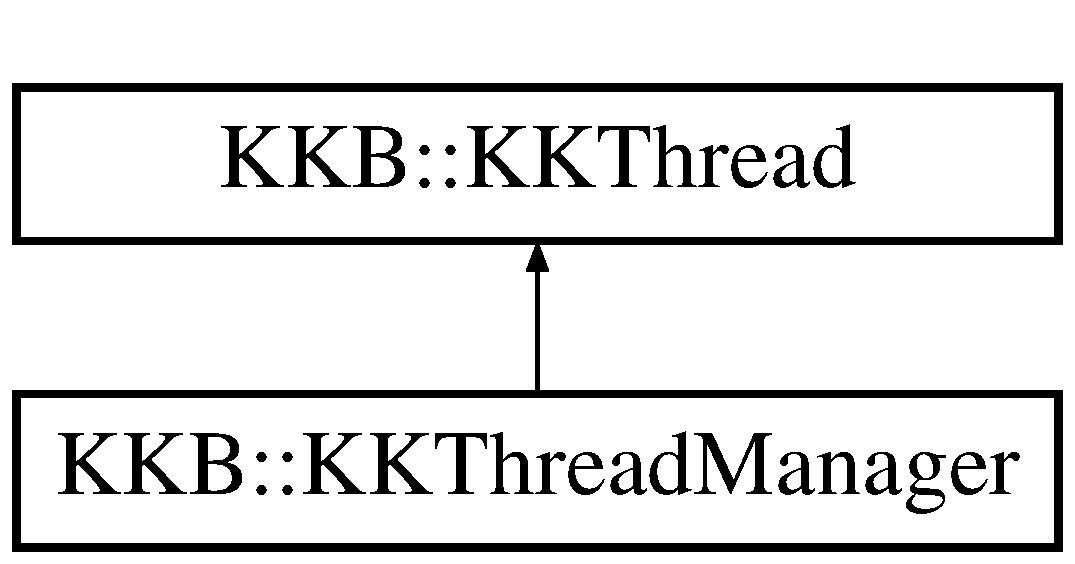
\includegraphics[height=2.000000cm]{class_k_k_b_1_1_k_k_thread}
\end{center}
\end{figure}
\subsection*{Public Types}
\begin{DoxyCompactItemize}
\item 
typedef \hyperlink{class_k_k_b_1_1_k_k_thread}{K\+K\+Thread} $\ast$ \hyperlink{class_k_k_b_1_1_k_k_thread_ae0ca65f275a57c346e71486ad84b271a}{K\+K\+Thread\+Ptr}
\item 
enum \hyperlink{class_k_k_b_1_1_k_k_thread_ad9b55cc20284bcadd051a20945325e0c}{Thread\+Priority} \+: int \{ \hyperlink{class_k_k_b_1_1_k_k_thread_ad9b55cc20284bcadd051a20945325e0cabbb93ef26e3c101ff11cdd21cab08a94}{Thread\+Priority\+::\+Null}, 
\hyperlink{class_k_k_b_1_1_k_k_thread_ad9b55cc20284bcadd051a20945325e0ca28d0edd045e05cf5af64e35ae0c4c6ef}{Thread\+Priority\+::\+Low}, 
\hyperlink{class_k_k_b_1_1_k_k_thread_ad9b55cc20284bcadd051a20945325e0ca960b44c579bc2f6818d2daaf9e4c16f0}{Thread\+Priority\+::\+Normal}, 
\hyperlink{class_k_k_b_1_1_k_k_thread_ad9b55cc20284bcadd051a20945325e0ca655d20c1ca69519ca647684edbb2db35}{Thread\+Priority\+::\+High}
 \}
\item 
enum \hyperlink{class_k_k_b_1_1_k_k_thread_a3f72bb1988ae5dd353b39260ae0acc72}{Thread\+Status} \+: int \{ \\*
\hyperlink{class_k_k_b_1_1_k_k_thread_a3f72bb1988ae5dd353b39260ae0acc72abbb93ef26e3c101ff11cdd21cab08a94}{Thread\+Status\+::\+Null}, 
\hyperlink{class_k_k_b_1_1_k_k_thread_a3f72bb1988ae5dd353b39260ae0acc72afa7be7845bc42b3491d9d0377958be94}{Thread\+Status\+::\+Not\+Started}, 
\hyperlink{class_k_k_b_1_1_k_k_thread_a3f72bb1988ae5dd353b39260ae0acc72ac2efe4bbd13e6cb0db293e72884273c0}{Thread\+Status\+::\+Starting}, 
\hyperlink{class_k_k_b_1_1_k_k_thread_a3f72bb1988ae5dd353b39260ae0acc72a5bda814c4aedb126839228f1a3d92f09}{Thread\+Status\+::\+Running}, 
\\*
\hyperlink{class_k_k_b_1_1_k_k_thread_a3f72bb1988ae5dd353b39260ae0acc72a7b7ecb39b9e110c2a31409a1672bad23}{Thread\+Status\+::\+Stopping}, 
\hyperlink{class_k_k_b_1_1_k_k_thread_a3f72bb1988ae5dd353b39260ae0acc72ac23e2b09ebe6bf4cb5e2a9abe85c0be2}{Thread\+Status\+::\+Stopped}
 \}
\end{DoxyCompactItemize}
\subsection*{Public Member Functions}
\begin{DoxyCompactItemize}
\item 
\hyperlink{class_k_k_b_1_1_k_k_thread_aae2cc3ddbc461d7be2ff904b40ccf2e8}{K\+K\+Thread} (const \hyperlink{class_k_k_b_1_1_k_k_str}{K\+K\+Str} \&\+\_\+thread\+Name, \hyperlink{namespace_k_k_b_a9373d6bd6f2977b14e92c9e8e5ec4cdc}{K\+K\+Thread\+Manager\+Ptr} \+\_\+thread\+Manager, \hyperlink{namespace_k_k_b_aaa43074273f12ed325a053d9e1faf84a}{Msg\+Queue\+Ptr} \+\_\+msg\+Queue)
\item 
virtual \hyperlink{class_k_k_b_1_1_k_k_thread_afb0fecef6c388894ce1c6e6926f3b177}{$\sim$\+K\+K\+Thread} ()
\item 
void \hyperlink{class_k_k_b_1_1_k_k_thread_aace756a5a4ea776957f8be561ff8bd16}{Add\+Shutdown\+Prerequistite} (\hyperlink{class_k_k_b_1_1_k_k_thread_ae0ca65f275a57c346e71486ad84b271a}{K\+K\+Thread\+Ptr} \+\_\+thread)
\begin{DoxyCompactList}\small\item\em Specify threads that must stop before this thread is started. \end{DoxyCompactList}\item 
void \hyperlink{class_k_k_b_1_1_k_k_thread_a092fff07582fdaa4b17eb00214d47923}{Add\+Start\+Prerequistite} (\hyperlink{class_k_k_b_1_1_k_k_thread_ae0ca65f275a57c346e71486ad84b271a}{K\+K\+Thread\+Ptr} \+\_\+thread)
\begin{DoxyCompactList}\small\item\em Specify threads that must start before this thread is started. \end{DoxyCompactList}\item 
\hyperlink{namespace_k_k_b_a7d390f568e2831fb76b86b56c87bf92f}{Vol\+Const\+Bool} \& \hyperlink{class_k_k_b_1_1_k_k_thread_a85dcfd92879c8f74102af810cc44628b}{Cancel\+Flag} () const 
\item 
bool \hyperlink{class_k_k_b_1_1_k_k_thread_a1cc302487fe9e7fe79e7e6b056d3e7d1}{Crashed} () const 
\item 
void \hyperlink{class_k_k_b_1_1_k_k_thread_a56f7600f8a53e737dd8f6732a1176a91}{Crashed} (bool \+\_\+crashed)
\item 
const \hyperlink{class_k_k_b_1_1_k_k_str}{K\+K\+Str} \& \hyperlink{class_k_k_b_1_1_k_k_thread_a28ce636186cfdc8914248e0a087d7b0d}{Exception\+Text} () const 
\item 
void \hyperlink{class_k_k_b_1_1_k_k_thread_a48548f93187fd062a78b4a7410f125a6}{Exception\+Text} (const \hyperlink{class_k_k_b_1_1_k_k_str}{K\+K\+Str} \&\+\_\+exception\+Text)
\item 
\hyperlink{namespace_k_k_b_a8f5f50672f37857425120831223888aa}{K\+K\+Str\+List\+Ptr} \hyperlink{class_k_k_b_1_1_k_k_thread_a7b4f886e76610bb6f585e14d34285f13}{Get\+Msgs} ()
\item 
void \hyperlink{class_k_k_b_1_1_k_k_thread_a66111ed632dffca679c664909d5773bd}{Kill} ()
\begin{DoxyCompactList}\small\item\em stops the running thread and frees the thread handle \end{DoxyCompactList}\item 
\hyperlink{namespace_k_k_b_a8fa4952cc84fda1de4bec1fbdd8d5b1b}{kkint32} \hyperlink{class_k_k_b_1_1_k_k_thread_a0a8d08e9a902c496f7ee0c46f2aee2cc}{Memory\+Consumed\+Estimated} ()
\item 
\hyperlink{namespace_k_k_b_aaa43074273f12ed325a053d9e1faf84a}{K\+K\+B\+::\+Msg\+Queue\+Ptr} \hyperlink{class_k_k_b_1_1_k_k_thread_ac6ca78e4481c0a20b0cf15789d1101c7}{Msg\+Queue} ()
\item 
bool \hyperlink{class_k_k_b_1_1_k_k_thread_a7aa56da8a1a30568b4b7c353909e6b4c}{Ok\+To\+Shutdown} () const 
\item 
bool \hyperlink{class_k_k_b_1_1_k_k_thread_afc63e1d57bfa5a690c13db687b655f32}{Ok\+To\+Start} () const 
\item 
virtual void \hyperlink{class_k_k_b_1_1_k_k_thread_a4ecfa3856e1b5bb4a5a125fdc05c4e67}{Run} ()
\item 
\hyperlink{namespace_k_k_b_a7d390f568e2831fb76b86b56c87bf92f}{Vol\+Const\+Bool} \& \hyperlink{class_k_k_b_1_1_k_k_thread_a271dba95d3432cf7ea4992951f2b2a38}{Shutdown\+Flag} () const 
\item 
void \hyperlink{class_k_k_b_1_1_k_k_thread_af3d38a6013474f4710c1797fbf26d3cb}{Shutdown\+Thread} ()
\item 
void \hyperlink{class_k_k_b_1_1_k_k_thread_aa0dcedfb40c5208fb5764e13851a7728}{Start} (\hyperlink{class_k_k_b_1_1_k_k_thread_ad9b55cc20284bcadd051a20945325e0c}{Thread\+Priority} \+\_\+priority, bool \&successful)
\item 
\hyperlink{class_k_k_b_1_1_k_k_thread_a3f72bb1988ae5dd353b39260ae0acc72}{Thread\+Status} \hyperlink{class_k_k_b_1_1_k_k_thread_a8b6636f59306caf89c24d9f756293d71}{Status} () const 
\item 
void \hyperlink{class_k_k_b_1_1_k_k_thread_a90737d98d41227c3748e0404aa69b939}{Status} (\hyperlink{class_k_k_b_1_1_k_k_thread_a3f72bb1988ae5dd353b39260ae0acc72}{Thread\+Status} \+\_\+status)
\item 
const \hyperlink{class_k_k_b_1_1_k_k_str}{K\+K\+Str} \& \hyperlink{class_k_k_b_1_1_k_k_thread_a7a1d208bb108a4bbd2e19fe9b0657428}{Status\+Str} () const 
\item 
\hyperlink{namespace_k_k_b_a7d390f568e2831fb76b86b56c87bf92f}{Vol\+Const\+Bool} \& \hyperlink{class_k_k_b_1_1_k_k_thread_a188ecbf965ed6a19e5c16e9ae0127652}{Terminate\+Flag} () const 
\item 
virtual void \hyperlink{class_k_k_b_1_1_k_k_thread_aae645d31ef55a539e83b0309b316de07}{Terminate\+Flag\+Changed} ()
\begin{DoxyCompactList}\small\item\em Will be called whenever the value of \textquotesingle{}terminate\+Flag\textquotesingle{} is changed; derived classes should override this method if they need to be aware that the terminae\+Flag has changed. This give them a chance to let other objects/methods know that the flag has changed. \end{DoxyCompactList}\item 
void \hyperlink{class_k_k_b_1_1_k_k_thread_ad8ce909fbb09ad87c759e7a442530a08}{Terminate\+Thread} ()
\item 
\hyperlink{namespace_k_k_b_a8fa4952cc84fda1de4bec1fbdd8d5b1b}{kkint32} \hyperlink{class_k_k_b_1_1_k_k_thread_a31fa88422cee1e9c7c197a90cf508073}{Thread\+Id} () const 
\item 
const \hyperlink{class_k_k_b_1_1_k_k_str}{K\+K\+Str} \& \hyperlink{class_k_k_b_1_1_k_k_thread_a547e53d47818a4de7d367ce58203ade9}{Thread\+Name} () const 
\item 
bool \hyperlink{class_k_k_b_1_1_k_k_thread_af13369365be9c420e142d121f910c5c1}{Thread\+Still\+Processing} () const 
\item 
void \hyperlink{class_k_k_b_1_1_k_k_thread_aaca46f2589c1c14e207900575bcabae7}{Wait\+For\+Thread\+To\+Stop} (\hyperlink{namespace_k_k_b_af8d832f05c54994a1cce25bd5743e19a}{kkuint32} max\+Time\+To\+Wait)
\begin{DoxyCompactList}\small\item\em Called by separate thread; will stay in loop until the thread controlled by this instance shutdown or it waited the \textquotesingle{}max\+Time\+To\+Wait\textquotesingle{}. \end{DoxyCompactList}\end{DoxyCompactItemize}
\subsection*{Static Public Member Functions}
\begin{DoxyCompactItemize}
\item 
static const \hyperlink{class_k_k_b_1_1_k_k_str}{K\+K\+Str} \& \hyperlink{class_k_k_b_1_1_k_k_thread_a7a111deabee84c8aed46022bffb0574f}{Thread\+Status\+To\+Str} (\hyperlink{class_k_k_b_1_1_k_k_thread_a3f72bb1988ae5dd353b39260ae0acc72}{Thread\+Status})
\end{DoxyCompactItemize}
\subsection*{Protected Member Functions}
\begin{DoxyCompactItemize}
\item 
void \hyperlink{class_k_k_b_1_1_k_k_thread_a8f6c004d6510b90e5eff9c34efd20967}{Add\+Msg} (\hyperlink{namespace_k_k_b_a9adbef5a6b3be0867f5570df2a08f388}{K\+K\+Str\+Ptr} msg)
\item 
void \hyperlink{class_k_k_b_1_1_k_k_thread_a52304cd03534d86ce8e392d342d37a69}{Add\+Msg} (const \hyperlink{class_k_k_b_1_1_k_k_str}{K\+K\+Str} \&msg)
\item 
bool \hyperlink{class_k_k_b_1_1_k_k_thread_ac2f537ffb0162014816a7b446417bbd7}{Shutdown\+Or\+Terminate\+Requested} ()
\item 
bool \hyperlink{class_k_k_b_1_1_k_k_thread_ae767d026a9b2bfc4d4f50f1a24cf279f}{There\+Is\+A\+Circular\+Reference\+Shutdown} (\hyperlink{class_k_k_b_1_1_k_k_thread_ae0ca65f275a57c346e71486ad84b271a}{K\+K\+Thread\+Ptr} \+\_\+thread) const 
\item 
bool \hyperlink{class_k_k_b_1_1_k_k_thread_aead4ae8442a3f5c0f629ee0eed28a759}{There\+Is\+A\+Circular\+Reference\+Start} (\hyperlink{class_k_k_b_1_1_k_k_thread_ae0ca65f275a57c346e71486ad84b271a}{K\+K\+Thread\+Ptr} \+\_\+thread) const 
\end{DoxyCompactItemize}


\subsection{Detailed Description}
The base class to be used any thread. 

This will be the base class for each one of the different types of processing. 

Definition at line 27 of file K\+K\+Thread.\+h.



\subsection{Member Typedef Documentation}
\index{K\+K\+B\+::\+K\+K\+Thread@{K\+K\+B\+::\+K\+K\+Thread}!K\+K\+Thread\+Ptr@{K\+K\+Thread\+Ptr}}
\index{K\+K\+Thread\+Ptr@{K\+K\+Thread\+Ptr}!K\+K\+B\+::\+K\+K\+Thread@{K\+K\+B\+::\+K\+K\+Thread}}
\subsubsection[{\texorpdfstring{K\+K\+Thread\+Ptr}{KKThreadPtr}}]{\setlength{\rightskip}{0pt plus 5cm}typedef {\bf K\+K\+Thread}$\ast$ {\bf K\+K\+B\+::\+K\+K\+Thread\+::\+K\+K\+Thread\+Ptr}}\hypertarget{class_k_k_b_1_1_k_k_thread_ae0ca65f275a57c346e71486ad84b271a}{}\label{class_k_k_b_1_1_k_k_thread_ae0ca65f275a57c346e71486ad84b271a}


Definition at line 30 of file K\+K\+Thread.\+h.



\subsection{Member Enumeration Documentation}
\index{K\+K\+B\+::\+K\+K\+Thread@{K\+K\+B\+::\+K\+K\+Thread}!Thread\+Priority@{Thread\+Priority}}
\index{Thread\+Priority@{Thread\+Priority}!K\+K\+B\+::\+K\+K\+Thread@{K\+K\+B\+::\+K\+K\+Thread}}
\subsubsection[{\texorpdfstring{Thread\+Priority}{ThreadPriority}}]{\setlength{\rightskip}{0pt plus 5cm}enum {\bf K\+K\+B\+::\+K\+K\+Thread\+::\+Thread\+Priority} \+: int\hspace{0.3cm}{\ttfamily [strong]}}\hypertarget{class_k_k_b_1_1_k_k_thread_ad9b55cc20284bcadd051a20945325e0c}{}\label{class_k_k_b_1_1_k_k_thread_ad9b55cc20284bcadd051a20945325e0c}
\begin{Desc}
\item[Enumerator]\par
\begin{description}
\index{Null@{Null}!K\+K\+B\+::\+K\+K\+Thread@{K\+K\+B\+::\+K\+K\+Thread}}\index{K\+K\+B\+::\+K\+K\+Thread@{K\+K\+B\+::\+K\+K\+Thread}!Null@{Null}}\item[{\em 
Null\hypertarget{class_k_k_b_1_1_k_k_thread_ad9b55cc20284bcadd051a20945325e0cabbb93ef26e3c101ff11cdd21cab08a94}{}\label{class_k_k_b_1_1_k_k_thread_ad9b55cc20284bcadd051a20945325e0cabbb93ef26e3c101ff11cdd21cab08a94}
}]\index{Low@{Low}!K\+K\+B\+::\+K\+K\+Thread@{K\+K\+B\+::\+K\+K\+Thread}}\index{K\+K\+B\+::\+K\+K\+Thread@{K\+K\+B\+::\+K\+K\+Thread}!Low@{Low}}\item[{\em 
Low\hypertarget{class_k_k_b_1_1_k_k_thread_ad9b55cc20284bcadd051a20945325e0ca28d0edd045e05cf5af64e35ae0c4c6ef}{}\label{class_k_k_b_1_1_k_k_thread_ad9b55cc20284bcadd051a20945325e0ca28d0edd045e05cf5af64e35ae0c4c6ef}
}]\index{Normal@{Normal}!K\+K\+B\+::\+K\+K\+Thread@{K\+K\+B\+::\+K\+K\+Thread}}\index{K\+K\+B\+::\+K\+K\+Thread@{K\+K\+B\+::\+K\+K\+Thread}!Normal@{Normal}}\item[{\em 
Normal\hypertarget{class_k_k_b_1_1_k_k_thread_ad9b55cc20284bcadd051a20945325e0ca960b44c579bc2f6818d2daaf9e4c16f0}{}\label{class_k_k_b_1_1_k_k_thread_ad9b55cc20284bcadd051a20945325e0ca960b44c579bc2f6818d2daaf9e4c16f0}
}]\index{High@{High}!K\+K\+B\+::\+K\+K\+Thread@{K\+K\+B\+::\+K\+K\+Thread}}\index{K\+K\+B\+::\+K\+K\+Thread@{K\+K\+B\+::\+K\+K\+Thread}!High@{High}}\item[{\em 
High\hypertarget{class_k_k_b_1_1_k_k_thread_ad9b55cc20284bcadd051a20945325e0ca655d20c1ca69519ca647684edbb2db35}{}\label{class_k_k_b_1_1_k_k_thread_ad9b55cc20284bcadd051a20945325e0ca655d20c1ca69519ca647684edbb2db35}
}]\end{description}
\end{Desc}


Definition at line 32 of file K\+K\+Thread.\+h.


\begin{DoxyCode}
32                                : \textcolor{keywordtype}{int} 
33                    \{\hyperlink{namespace_k_k_m_l_l_ad917464bc631109a3021cf02cd27af9aabbb93ef26e3c101ff11cdd21cab08a94}{Null},
34                     Low,
35                     Normal,
36                     High
37                    \};
\end{DoxyCode}
\index{K\+K\+B\+::\+K\+K\+Thread@{K\+K\+B\+::\+K\+K\+Thread}!Thread\+Status@{Thread\+Status}}
\index{Thread\+Status@{Thread\+Status}!K\+K\+B\+::\+K\+K\+Thread@{K\+K\+B\+::\+K\+K\+Thread}}
\subsubsection[{\texorpdfstring{Thread\+Status}{ThreadStatus}}]{\setlength{\rightskip}{0pt plus 5cm}enum {\bf K\+K\+B\+::\+K\+K\+Thread\+::\+Thread\+Status} \+: int\hspace{0.3cm}{\ttfamily [strong]}}\hypertarget{class_k_k_b_1_1_k_k_thread_a3f72bb1988ae5dd353b39260ae0acc72}{}\label{class_k_k_b_1_1_k_k_thread_a3f72bb1988ae5dd353b39260ae0acc72}
\begin{Desc}
\item[Enumerator]\par
\begin{description}
\index{Null@{Null}!K\+K\+B\+::\+K\+K\+Thread@{K\+K\+B\+::\+K\+K\+Thread}}\index{K\+K\+B\+::\+K\+K\+Thread@{K\+K\+B\+::\+K\+K\+Thread}!Null@{Null}}\item[{\em 
Null\hypertarget{class_k_k_b_1_1_k_k_thread_a3f72bb1988ae5dd353b39260ae0acc72abbb93ef26e3c101ff11cdd21cab08a94}{}\label{class_k_k_b_1_1_k_k_thread_a3f72bb1988ae5dd353b39260ae0acc72abbb93ef26e3c101ff11cdd21cab08a94}
}]\index{Not\+Started@{Not\+Started}!K\+K\+B\+::\+K\+K\+Thread@{K\+K\+B\+::\+K\+K\+Thread}}\index{K\+K\+B\+::\+K\+K\+Thread@{K\+K\+B\+::\+K\+K\+Thread}!Not\+Started@{Not\+Started}}\item[{\em 
Not\+Started\hypertarget{class_k_k_b_1_1_k_k_thread_a3f72bb1988ae5dd353b39260ae0acc72afa7be7845bc42b3491d9d0377958be94}{}\label{class_k_k_b_1_1_k_k_thread_a3f72bb1988ae5dd353b39260ae0acc72afa7be7845bc42b3491d9d0377958be94}
}]\index{Starting@{Starting}!K\+K\+B\+::\+K\+K\+Thread@{K\+K\+B\+::\+K\+K\+Thread}}\index{K\+K\+B\+::\+K\+K\+Thread@{K\+K\+B\+::\+K\+K\+Thread}!Starting@{Starting}}\item[{\em 
Starting\hypertarget{class_k_k_b_1_1_k_k_thread_a3f72bb1988ae5dd353b39260ae0acc72ac2efe4bbd13e6cb0db293e72884273c0}{}\label{class_k_k_b_1_1_k_k_thread_a3f72bb1988ae5dd353b39260ae0acc72ac2efe4bbd13e6cb0db293e72884273c0}
}]\index{Running@{Running}!K\+K\+B\+::\+K\+K\+Thread@{K\+K\+B\+::\+K\+K\+Thread}}\index{K\+K\+B\+::\+K\+K\+Thread@{K\+K\+B\+::\+K\+K\+Thread}!Running@{Running}}\item[{\em 
Running\hypertarget{class_k_k_b_1_1_k_k_thread_a3f72bb1988ae5dd353b39260ae0acc72a5bda814c4aedb126839228f1a3d92f09}{}\label{class_k_k_b_1_1_k_k_thread_a3f72bb1988ae5dd353b39260ae0acc72a5bda814c4aedb126839228f1a3d92f09}
}]\index{Stopping@{Stopping}!K\+K\+B\+::\+K\+K\+Thread@{K\+K\+B\+::\+K\+K\+Thread}}\index{K\+K\+B\+::\+K\+K\+Thread@{K\+K\+B\+::\+K\+K\+Thread}!Stopping@{Stopping}}\item[{\em 
Stopping\hypertarget{class_k_k_b_1_1_k_k_thread_a3f72bb1988ae5dd353b39260ae0acc72a7b7ecb39b9e110c2a31409a1672bad23}{}\label{class_k_k_b_1_1_k_k_thread_a3f72bb1988ae5dd353b39260ae0acc72a7b7ecb39b9e110c2a31409a1672bad23}
}]\index{Stopped@{Stopped}!K\+K\+B\+::\+K\+K\+Thread@{K\+K\+B\+::\+K\+K\+Thread}}\index{K\+K\+B\+::\+K\+K\+Thread@{K\+K\+B\+::\+K\+K\+Thread}!Stopped@{Stopped}}\item[{\em 
Stopped\hypertarget{class_k_k_b_1_1_k_k_thread_a3f72bb1988ae5dd353b39260ae0acc72ac23e2b09ebe6bf4cb5e2a9abe85c0be2}{}\label{class_k_k_b_1_1_k_k_thread_a3f72bb1988ae5dd353b39260ae0acc72ac23e2b09ebe6bf4cb5e2a9abe85c0be2}
}]\end{description}
\end{Desc}


Definition at line 39 of file K\+K\+Thread.\+h.


\begin{DoxyCode}
39                              : \textcolor{keywordtype}{int}
40                    \{\hyperlink{namespace_k_k_m_l_l_ad917464bc631109a3021cf02cd27af9aabbb93ef26e3c101ff11cdd21cab08a94}{Null},
41                     NotStarted,
42                     Starting,
43                     Running,
44                     Stopping,
45                     Stopped
46                    \};
\end{DoxyCode}


\subsection{Constructor \& Destructor Documentation}
\index{K\+K\+B\+::\+K\+K\+Thread@{K\+K\+B\+::\+K\+K\+Thread}!K\+K\+Thread@{K\+K\+Thread}}
\index{K\+K\+Thread@{K\+K\+Thread}!K\+K\+B\+::\+K\+K\+Thread@{K\+K\+B\+::\+K\+K\+Thread}}
\subsubsection[{\texorpdfstring{K\+K\+Thread(const K\+K\+Str \&\+\_\+thread\+Name, K\+K\+Thread\+Manager\+Ptr \+\_\+thread\+Manager, Msg\+Queue\+Ptr \+\_\+msg\+Queue)}{KKThread(const KKStr &_threadName, KKThreadManagerPtr _threadManager, MsgQueuePtr _msgQueue)}}]{\setlength{\rightskip}{0pt plus 5cm}K\+K\+Thread\+::\+K\+K\+Thread (
\begin{DoxyParamCaption}
\item[{const {\bf K\+K\+Str} \&}]{\+\_\+thread\+Name, }
\item[{{\bf K\+K\+Thread\+Manager\+Ptr}}]{\+\_\+thread\+Manager, }
\item[{{\bf Msg\+Queue\+Ptr}}]{\+\_\+msg\+Queue}
\end{DoxyParamCaption}
)}\hypertarget{class_k_k_b_1_1_k_k_thread_aae2cc3ddbc461d7be2ff904b40ccf2e8}{}\label{class_k_k_b_1_1_k_k_thread_aae2cc3ddbc461d7be2ff904b40ccf2e8}


Definition at line 83 of file K\+K\+Thread.\+cpp.



References K\+K\+B\+::\+K\+K\+Str\+::\+K\+K\+Str(), Normal, and Not\+Started.



Referenced by K\+K\+B\+::\+K\+K\+Thread\+Manager\+::\+K\+K\+Thread\+Manager().


\begin{DoxyCode}
86                     :
87    crashed               (\textcolor{keyword}{false}),
88    msgQueue              (\_msgQueue),
89    priority              (\hyperlink{class_k_k_b_1_1_k_k_thread_ad9b55cc20284bcadd051a20945325e0ca960b44c579bc2f6818d2daaf9e4c16f0}{ThreadPriority::Normal}),
90    shutdownFlag          (\textcolor{keyword}{false}),
91    shutdownPrerequisites (NULL),
92    startPrerequisites    (NULL),
93    status                (\hyperlink{class_k_k_b_1_1_k_k_thread_a3f72bb1988ae5dd353b39260ae0acc72afa7be7845bc42b3491d9d0377958be94}{ThreadStatus::NotStarted}),
94    terminateFlag         (\textcolor{keyword}{false}),
95    threadId              (0),
96    threadName            (\_threadName)
97 
98 \{
99 \textcolor{preprocessor}{#if  defined(WIN32)}
100   windowsThreadHandle  = NULL;
101   windowsThreadId = 0;
102 \textcolor{preprocessor}{#else}
103   linuxThreadId = 0;
104 \textcolor{preprocessor}{#endif}
105 \}
\end{DoxyCode}
\index{K\+K\+B\+::\+K\+K\+Thread@{K\+K\+B\+::\+K\+K\+Thread}!````~K\+K\+Thread@{$\sim$\+K\+K\+Thread}}
\index{````~K\+K\+Thread@{$\sim$\+K\+K\+Thread}!K\+K\+B\+::\+K\+K\+Thread@{K\+K\+B\+::\+K\+K\+Thread}}
\subsubsection[{\texorpdfstring{$\sim$\+K\+K\+Thread()}{~KKThread()}}]{\setlength{\rightskip}{0pt plus 5cm}K\+K\+Thread\+::$\sim$\+K\+K\+Thread (
\begin{DoxyParamCaption}
{}
\end{DoxyParamCaption}
)\hspace{0.3cm}{\ttfamily [virtual]}}\hypertarget{class_k_k_b_1_1_k_k_thread_afb0fecef6c388894ce1c6e6926f3b177}{}\label{class_k_k_b_1_1_k_k_thread_afb0fecef6c388894ce1c6e6926f3b177}


Definition at line 109 of file K\+K\+Thread.\+cpp.


\begin{DoxyCode}
110 \{
111   \textcolor{keyword}{delete}  shutdownPrerequisites;  shutdownPrerequisites = NULL;
112   \textcolor{keyword}{delete}  startPrerequisites;     startPrerequisites    = NULL;
113 \}
\end{DoxyCode}


\subsection{Member Function Documentation}
\index{K\+K\+B\+::\+K\+K\+Thread@{K\+K\+B\+::\+K\+K\+Thread}!Add\+Msg@{Add\+Msg}}
\index{Add\+Msg@{Add\+Msg}!K\+K\+B\+::\+K\+K\+Thread@{K\+K\+B\+::\+K\+K\+Thread}}
\subsubsection[{\texorpdfstring{Add\+Msg(\+K\+K\+Str\+Ptr msg)}{AddMsg(KKStrPtr msg)}}]{\setlength{\rightskip}{0pt plus 5cm}void K\+K\+Thread\+::\+Add\+Msg (
\begin{DoxyParamCaption}
\item[{{\bf K\+K\+Str\+Ptr}}]{msg}
\end{DoxyParamCaption}
)\hspace{0.3cm}{\ttfamily [protected]}}\hypertarget{class_k_k_b_1_1_k_k_thread_a8f6c004d6510b90e5eff9c34efd20967}{}\label{class_k_k_b_1_1_k_k_thread_a8f6c004d6510b90e5eff9c34efd20967}
Taking ownership of \textquotesingle{}msg\textquotesingle{} and will append to \textquotesingle{}msg\+Queue\textquotesingle{}. 

Definition at line 154 of file K\+K\+Thread.\+cpp.



References K\+K\+B\+::\+Msg\+Queue\+::\+Add\+Msg().


\begin{DoxyCode}
155 \{
156   \textcolor{keywordflow}{if}  (msgQueue == NULL)
157   \{
158     cerr << \hyperlink{namespace_k_k_b_ad1f50f65af6adc8fa9e6f62d007818a8}{endl} 
159          << \textcolor{stringliteral}{"KKThread::AddMsg   ***ERROR***    msgQuue is not defined."}  << \hyperlink{namespace_k_k_b_ad1f50f65af6adc8fa9e6f62d007818a8}{endl}
160          << \textcolor{stringliteral}{"                   Msg["} << *msg << \textcolor{stringliteral}{"]."} << \hyperlink{namespace_k_k_b_ad1f50f65af6adc8fa9e6f62d007818a8}{endl}
161          << \hyperlink{namespace_k_k_b_ad1f50f65af6adc8fa9e6f62d007818a8}{endl};
162     \textcolor{keyword}{delete}  msg;
163     msg = NULL;
164   \}
165   \textcolor{keywordflow}{else}
166   \{
167     msgQueue->\hyperlink{class_k_k_b_1_1_msg_queue_a4d7d0adcf4f06a7afc6c8187a20bf95c}{AddMsg} (msg);
168   \}
169 \}  \textcolor{comment}{/* AddMsg */}
\end{DoxyCode}
\index{K\+K\+B\+::\+K\+K\+Thread@{K\+K\+B\+::\+K\+K\+Thread}!Add\+Msg@{Add\+Msg}}
\index{Add\+Msg@{Add\+Msg}!K\+K\+B\+::\+K\+K\+Thread@{K\+K\+B\+::\+K\+K\+Thread}}
\subsubsection[{\texorpdfstring{Add\+Msg(const K\+K\+Str \&msg)}{AddMsg(const KKStr &msg)}}]{\setlength{\rightskip}{0pt plus 5cm}void K\+K\+Thread\+::\+Add\+Msg (
\begin{DoxyParamCaption}
\item[{const {\bf K\+K\+Str} \&}]{msg}
\end{DoxyParamCaption}
)\hspace{0.3cm}{\ttfamily [protected]}}\hypertarget{class_k_k_b_1_1_k_k_thread_a52304cd03534d86ce8e392d342d37a69}{}\label{class_k_k_b_1_1_k_k_thread_a52304cd03534d86ce8e392d342d37a69}
A copy of the message \textquotesingle{}msg\textquotesingle{} will be added to the end of msg\+Queue. 

Definition at line 174 of file K\+K\+Thread.\+cpp.



References K\+K\+B\+::\+Msg\+Queue\+::\+Add\+Msg(), K\+K\+B\+::\+K\+K\+Str\+::\+Concat(), K\+K\+B\+::\+K\+K\+Str\+::\+K\+K\+Str(), K\+K\+B\+::\+K\+K\+Str\+::\+Len(), K\+K\+B\+::os\+Get\+Local\+Date\+Time(), K\+K\+B\+::os\+Get\+Thread\+Id(), and K\+K\+B\+::\+Date\+Time\+::\+Time().



Referenced by Run().


\begin{DoxyCode}
175 \{
176   \textcolor{keywordflow}{if}  (msgQueue == NULL)
177   \{
178     cerr << \hyperlink{namespace_k_k_b_ad1f50f65af6adc8fa9e6f62d007818a8}{endl} 
179          << \textcolor{stringliteral}{"KKThread::AddMsg   ***ERROR***    msgQuue is not defined."}  << \hyperlink{namespace_k_k_b_ad1f50f65af6adc8fa9e6f62d007818a8}{endl}
180          << \textcolor{stringliteral}{"                       Msg["} << msg << \textcolor{stringliteral}{"]."} << \hyperlink{namespace_k_k_b_ad1f50f65af6adc8fa9e6f62d007818a8}{endl}
181          << \hyperlink{namespace_k_k_b_ad1f50f65af6adc8fa9e6f62d007818a8}{endl};
182   \}
183   \textcolor{keywordflow}{else}
184   \{
185     \hyperlink{class_k_k_b_1_1_k_k_str}{KKStr} msgTemp (msg.\hyperlink{class_k_k_b_1_1_k_k_str_a869142d4855517c5c237afcb25dbbe36}{Len} () + 20);
186     msgTemp << \hyperlink{namespace_k_k_b_aa1d581b15163a41037c43bdbd800d0f8}{osGetThreadId} () << \textcolor{stringliteral}{" - "} << \hyperlink{namespace_k_k_b_af54c205cde0465bcb2c74f3881a96413}{osGetLocalDateTime} ().
      \hyperlink{class_k_k_b_1_1_date_time_a981ba2e8e1ca8319d51be65c746442e1}{Time} () << \textcolor{stringliteral}{"->"} << msg;
187     msgQueue->\hyperlink{class_k_k_b_1_1_msg_queue_a4d7d0adcf4f06a7afc6c8187a20bf95c}{AddMsg} (msgTemp);
188   \}
189 \}  \textcolor{comment}{/* AddMsg */}
\end{DoxyCode}
\index{K\+K\+B\+::\+K\+K\+Thread@{K\+K\+B\+::\+K\+K\+Thread}!Add\+Shutdown\+Prerequistite@{Add\+Shutdown\+Prerequistite}}
\index{Add\+Shutdown\+Prerequistite@{Add\+Shutdown\+Prerequistite}!K\+K\+B\+::\+K\+K\+Thread@{K\+K\+B\+::\+K\+K\+Thread}}
\subsubsection[{\texorpdfstring{Add\+Shutdown\+Prerequistite(\+K\+K\+Thread\+Ptr \+\_\+thread)}{AddShutdownPrerequistite(KKThreadPtr _thread)}}]{\setlength{\rightskip}{0pt plus 5cm}void K\+K\+Thread\+::\+Add\+Shutdown\+Prerequistite (
\begin{DoxyParamCaption}
\item[{{\bf K\+K\+Thread\+Ptr}}]{\+\_\+thread}
\end{DoxyParamCaption}
)}\hypertarget{class_k_k_b_1_1_k_k_thread_aace756a5a4ea776957f8be561ff8bd16}{}\label{class_k_k_b_1_1_k_k_thread_aace756a5a4ea776957f8be561ff8bd16}


Specify threads that must stop before this thread is started. 

This method can be called multiple times; the information is used by the \textquotesingle{}K\+K\+T\+Hread\+Manager\textquotesingle{} instance to control the orderly shutdown of the controlling \textquotesingle{}K\+K\+T\+Hread\+Manager\textquotesingle{} instance. 
\begin{DoxyParams}[1]{Parameters}
\mbox{\tt in}  & {\em \+\_\+thread} & A thread that needs to be in the \textquotesingle{}Stopped\textquotesingle{} status before this thread can be shutdown; we do N\+OT take ownership. \\
\hline
\end{DoxyParams}


Definition at line 510 of file K\+K\+Thread.\+cpp.



References K\+K\+B\+::\+K\+K\+Thread\+List\+::\+K\+K\+Thread\+List().


\begin{DoxyCode}
511 \{
512   \textcolor{keywordflow}{if}  (!shutdownPrerequisites)
513     shutdownPrerequisites = \textcolor{keyword}{new} \hyperlink{class_k_k_b_1_1_k_k_thread_list}{KKThreadList} (\textcolor{keyword}{false});
514   shutdownPrerequisites->\hyperlink{class_k_k_b_1_1_k_k_queue_aa9fba4632b54268bf71ecb42dee0b575}{PushOnBack} (\_thread);
515 \}
\end{DoxyCode}
\index{K\+K\+B\+::\+K\+K\+Thread@{K\+K\+B\+::\+K\+K\+Thread}!Add\+Start\+Prerequistite@{Add\+Start\+Prerequistite}}
\index{Add\+Start\+Prerequistite@{Add\+Start\+Prerequistite}!K\+K\+B\+::\+K\+K\+Thread@{K\+K\+B\+::\+K\+K\+Thread}}
\subsubsection[{\texorpdfstring{Add\+Start\+Prerequistite(\+K\+K\+Thread\+Ptr \+\_\+thread)}{AddStartPrerequistite(KKThreadPtr _thread)}}]{\setlength{\rightskip}{0pt plus 5cm}void K\+K\+Thread\+::\+Add\+Start\+Prerequistite (
\begin{DoxyParamCaption}
\item[{{\bf K\+K\+Thread\+Ptr}}]{\+\_\+thread}
\end{DoxyParamCaption}
)}\hypertarget{class_k_k_b_1_1_k_k_thread_a092fff07582fdaa4b17eb00214d47923}{}\label{class_k_k_b_1_1_k_k_thread_a092fff07582fdaa4b17eb00214d47923}


Specify threads that must start before this thread is started. 

This method can be called multiple times; the information is used by the \textquotesingle{}K\+K\+T\+Hread\+Manager\textquotesingle{} instance to control the start of the thread. 
\begin{DoxyParams}[1]{Parameters}
\mbox{\tt in}  & {\em \+\_\+thread} & A thread that needs to be in the \textquotesingle{}Running\textquotesingle{} status before this thread can start; we do N\+OT take ownership. \\
\hline
\end{DoxyParams}


Definition at line 501 of file K\+K\+Thread.\+cpp.



References K\+K\+B\+::\+K\+K\+Thread\+List\+::\+K\+K\+Thread\+List().


\begin{DoxyCode}
502 \{
503   \textcolor{keywordflow}{if}  (!startPrerequisites)
504     startPrerequisites = \textcolor{keyword}{new} \hyperlink{class_k_k_b_1_1_k_k_thread_list}{KKThreadList} (\textcolor{keyword}{false});
505   startPrerequisites->\hyperlink{class_k_k_b_1_1_k_k_queue_aa9fba4632b54268bf71ecb42dee0b575}{PushOnBack} (\_thread);
506 \}
\end{DoxyCode}
\index{K\+K\+B\+::\+K\+K\+Thread@{K\+K\+B\+::\+K\+K\+Thread}!Cancel\+Flag@{Cancel\+Flag}}
\index{Cancel\+Flag@{Cancel\+Flag}!K\+K\+B\+::\+K\+K\+Thread@{K\+K\+B\+::\+K\+K\+Thread}}
\subsubsection[{\texorpdfstring{Cancel\+Flag() const }{CancelFlag() const }}]{\setlength{\rightskip}{0pt plus 5cm}{\bf Vol\+Const\+Bool}\& K\+K\+B\+::\+K\+K\+Thread\+::\+Cancel\+Flag (
\begin{DoxyParamCaption}
{}
\end{DoxyParamCaption}
) const\hspace{0.3cm}{\ttfamily [inline]}}\hypertarget{class_k_k_b_1_1_k_k_thread_a85dcfd92879c8f74102af810cc44628b}{}\label{class_k_k_b_1_1_k_k_thread_a85dcfd92879c8f74102af810cc44628b}
Another name for \textquotesingle{}Terminate\+Flag\textquotesingle{}. 

Definition at line 60 of file K\+K\+Thread.\+h.

\index{K\+K\+B\+::\+K\+K\+Thread@{K\+K\+B\+::\+K\+K\+Thread}!Crashed@{Crashed}}
\index{Crashed@{Crashed}!K\+K\+B\+::\+K\+K\+Thread@{K\+K\+B\+::\+K\+K\+Thread}}
\subsubsection[{\texorpdfstring{Crashed() const }{Crashed() const }}]{\setlength{\rightskip}{0pt plus 5cm}bool K\+K\+B\+::\+K\+K\+Thread\+::\+Crashed (
\begin{DoxyParamCaption}
{}
\end{DoxyParamCaption}
) const\hspace{0.3cm}{\ttfamily [inline]}}\hypertarget{class_k_k_b_1_1_k_k_thread_a1cc302487fe9e7fe79e7e6b056d3e7d1}{}\label{class_k_k_b_1_1_k_k_thread_a1cc302487fe9e7fe79e7e6b056d3e7d1}
Signifies that this thread had to terminate on its own because of an abnormal situation; such as a memory corruption. 

Definition at line 62 of file K\+K\+Thread.\+h.



Referenced by K\+K\+B\+::\+K\+K\+Thread\+Manager\+::\+Any\+Processors\+Crashed().

\index{K\+K\+B\+::\+K\+K\+Thread@{K\+K\+B\+::\+K\+K\+Thread}!Crashed@{Crashed}}
\index{Crashed@{Crashed}!K\+K\+B\+::\+K\+K\+Thread@{K\+K\+B\+::\+K\+K\+Thread}}
\subsubsection[{\texorpdfstring{Crashed(bool \+\_\+crashed)}{Crashed(bool _crashed)}}]{\setlength{\rightskip}{0pt plus 5cm}void K\+K\+B\+::\+K\+K\+Thread\+::\+Crashed (
\begin{DoxyParamCaption}
\item[{bool}]{\+\_\+crashed}
\end{DoxyParamCaption}
)\hspace{0.3cm}{\ttfamily [inline]}}\hypertarget{class_k_k_b_1_1_k_k_thread_a56f7600f8a53e737dd8f6732a1176a91}{}\label{class_k_k_b_1_1_k_k_thread_a56f7600f8a53e737dd8f6732a1176a91}


Definition at line 89 of file K\+K\+Thread.\+h.



Referenced by K\+K\+B\+::\+Thread\+Start\+Call\+Back().


\begin{DoxyCode}
89 \{crashed       = \_crashed;\}
\end{DoxyCode}
\index{K\+K\+B\+::\+K\+K\+Thread@{K\+K\+B\+::\+K\+K\+Thread}!Exception\+Text@{Exception\+Text}}
\index{Exception\+Text@{Exception\+Text}!K\+K\+B\+::\+K\+K\+Thread@{K\+K\+B\+::\+K\+K\+Thread}}
\subsubsection[{\texorpdfstring{Exception\+Text() const }{ExceptionText() const }}]{\setlength{\rightskip}{0pt plus 5cm}const {\bf K\+K\+Str}\& K\+K\+B\+::\+K\+K\+Thread\+::\+Exception\+Text (
\begin{DoxyParamCaption}
{}
\end{DoxyParamCaption}
) const\hspace{0.3cm}{\ttfamily [inline]}}\hypertarget{class_k_k_b_1_1_k_k_thread_a28ce636186cfdc8914248e0a087d7b0d}{}\label{class_k_k_b_1_1_k_k_thread_a28ce636186cfdc8914248e0a087d7b0d}
If the overloaded \textquotesingle{}Run\textquotesingle{} method of a derived class generates a exception that is not caught; then the \textquotesingle{}\textquotesingle{}Thread\+Start\+Call\+Back\textquotesingle{} will catch it and store the related text in this field. In this case the \textquotesingle{}\hyperlink{class_k_k_b_1_1_k_k_thread_a1cc302487fe9e7fe79e7e6b056d3e7d1}{Crashed()}\textquotesingle{} method will return \textquotesingle{}true\textquotesingle{}. 

Definition at line 66 of file K\+K\+Thread.\+h.

\index{K\+K\+B\+::\+K\+K\+Thread@{K\+K\+B\+::\+K\+K\+Thread}!Exception\+Text@{Exception\+Text}}
\index{Exception\+Text@{Exception\+Text}!K\+K\+B\+::\+K\+K\+Thread@{K\+K\+B\+::\+K\+K\+Thread}}
\subsubsection[{\texorpdfstring{Exception\+Text(const K\+K\+Str \&\+\_\+exception\+Text)}{ExceptionText(const KKStr &_exceptionText)}}]{\setlength{\rightskip}{0pt plus 5cm}void K\+K\+B\+::\+K\+K\+Thread\+::\+Exception\+Text (
\begin{DoxyParamCaption}
\item[{const {\bf K\+K\+Str} \&}]{\+\_\+exception\+Text}
\end{DoxyParamCaption}
)\hspace{0.3cm}{\ttfamily [inline]}}\hypertarget{class_k_k_b_1_1_k_k_thread_a48548f93187fd062a78b4a7410f125a6}{}\label{class_k_k_b_1_1_k_k_thread_a48548f93187fd062a78b4a7410f125a6}


Definition at line 90 of file K\+K\+Thread.\+h.



References K\+K\+B\+::\+K\+K\+Str\+::operator=().



Referenced by K\+K\+B\+::\+Thread\+Start\+Call\+Back().


\begin{DoxyCode}
90 \{exceptionText = \_exceptionText;\}
\end{DoxyCode}
\index{K\+K\+B\+::\+K\+K\+Thread@{K\+K\+B\+::\+K\+K\+Thread}!Get\+Msgs@{Get\+Msgs}}
\index{Get\+Msgs@{Get\+Msgs}!K\+K\+B\+::\+K\+K\+Thread@{K\+K\+B\+::\+K\+K\+Thread}}
\subsubsection[{\texorpdfstring{Get\+Msgs()}{GetMsgs()}}]{\setlength{\rightskip}{0pt plus 5cm}{\bf K\+K\+Str\+List\+Ptr} K\+K\+Thread\+::\+Get\+Msgs (
\begin{DoxyParamCaption}
{}
\end{DoxyParamCaption}
)}\hypertarget{class_k_k_b_1_1_k_k_thread_a7b4f886e76610bb6f585e14d34285f13}{}\label{class_k_k_b_1_1_k_k_thread_a7b4f886e76610bb6f585e14d34285f13}


Definition at line 193 of file K\+K\+Thread.\+cpp.



References K\+K\+B\+::\+Msg\+Queue\+::\+Get\+Next\+Msg(), and K\+K\+B\+::\+K\+K\+Str\+List\+::\+K\+K\+Str\+List().


\begin{DoxyCode}
194 \{
195   \hyperlink{class_k_k_b_1_1_k_k_str_list}{KKStrListPtr}  results = \textcolor{keyword}{new} \hyperlink{class_k_k_b_1_1_k_k_str_list}{KKStrList} (\textcolor{keyword}{true});
196   \hyperlink{class_k_k_b_1_1_k_k_str}{KKStrPtr}  msg = msgQueue->\hyperlink{class_k_k_b_1_1_msg_queue_a4e280303e6b11471624e1274cc681649}{GetNextMsg} ();
197   \textcolor{keywordflow}{while}  (msg)
198   \{
199     results->\hyperlink{class_k_k_b_1_1_k_k_queue_aa9fba4632b54268bf71ecb42dee0b575}{PushOnBack} (msg);
200     msg = msgQueue->\hyperlink{class_k_k_b_1_1_msg_queue_a4e280303e6b11471624e1274cc681649}{GetNextMsg} ();
201   \}
202 
203   \textcolor{keywordflow}{return} results;
204 \}  \textcolor{comment}{/* GetMsgs */}
\end{DoxyCode}
\index{K\+K\+B\+::\+K\+K\+Thread@{K\+K\+B\+::\+K\+K\+Thread}!Kill@{Kill}}
\index{Kill@{Kill}!K\+K\+B\+::\+K\+K\+Thread@{K\+K\+B\+::\+K\+K\+Thread}}
\subsubsection[{\texorpdfstring{Kill()}{Kill()}}]{\setlength{\rightskip}{0pt plus 5cm}void K\+K\+Thread\+::\+Kill (
\begin{DoxyParamCaption}
{}
\end{DoxyParamCaption}
)}\hypertarget{class_k_k_b_1_1_k_k_thread_a66111ed632dffca679c664909d5773bd}{}\label{class_k_k_b_1_1_k_k_thread_a66111ed632dffca679c664909d5773bd}


stops the running thread and frees the thread handle 



Definition at line 427 of file K\+K\+Thread.\+cpp.



Referenced by K\+K\+B\+::\+K\+K\+Thread\+Manager\+::\+Kill\+All\+Running\+Threads(), and Wait\+For\+Thread\+To\+Stop().


\begin{DoxyCode}
428 \{
429     \textcolor{keywordflow}{if}  (windowsThreadHandle == NULL)
430     \textcolor{keywordflow}{return}; 
431 
432     WaitForSingleObject (windowsThreadHandle, INFINITE);
433     CloseHandle (windowsThreadHandle);
434     windowsThreadHandle = NULL;
435 \}  \textcolor{comment}{/* Kill */}
\end{DoxyCode}
\index{K\+K\+B\+::\+K\+K\+Thread@{K\+K\+B\+::\+K\+K\+Thread}!Memory\+Consumed\+Estimated@{Memory\+Consumed\+Estimated}}
\index{Memory\+Consumed\+Estimated@{Memory\+Consumed\+Estimated}!K\+K\+B\+::\+K\+K\+Thread@{K\+K\+B\+::\+K\+K\+Thread}}
\subsubsection[{\texorpdfstring{Memory\+Consumed\+Estimated()}{MemoryConsumedEstimated()}}]{\setlength{\rightskip}{0pt plus 5cm}{\bf kkint32} K\+K\+Thread\+::\+Memory\+Consumed\+Estimated (
\begin{DoxyParamCaption}
{}
\end{DoxyParamCaption}
)}\hypertarget{class_k_k_b_1_1_k_k_thread_a0a8d08e9a902c496f7ee0c46f2aee2cc}{}\label{class_k_k_b_1_1_k_k_thread_a0a8d08e9a902c496f7ee0c46f2aee2cc}


Definition at line 117 of file K\+K\+Thread.\+cpp.



References K\+K\+B\+::\+Msg\+Queue\+::\+Memory\+Consumed\+Estimated(), K\+K\+B\+::\+K\+K\+Thread\+List\+::\+Memory\+Consumed\+Estimated(), and K\+K\+B\+::\+K\+K\+Str\+::\+Memory\+Consumed\+Estimated().



Referenced by K\+K\+B\+::\+K\+K\+Thread\+List\+::\+Memory\+Consumed\+Estimated().


\begin{DoxyCode}
118 \{
119   \hyperlink{namespace_k_k_b_a8fa4952cc84fda1de4bec1fbdd8d5b1b}{kkint32}  estMem = \textcolor{keyword}{sizeof} (crashed)                + 
120                   \textcolor{keyword}{sizeof} (msgQueue)               + 
121                   \textcolor{keyword}{sizeof} (shutdownFlag)           +
122                   \textcolor{keyword}{sizeof} (startPrerequisites)     +
123                   \textcolor{keyword}{sizeof} (shutdownPrerequisites)  +
124                   \textcolor{keyword}{sizeof} (status)                 + 
125                   \textcolor{keyword}{sizeof} (terminateFlag)          +
126                   threadName.\hyperlink{class_k_k_b_1_1_k_k_str_afc335bf98a8d4a77dc34215e72068719}{MemoryConsumedEstimated} ();
127 
128   \textcolor{keywordflow}{if}  (msgQueue)
129     estMem += msgQueue->\hyperlink{class_k_k_b_1_1_msg_queue_afe6ceeb9745ccf087a35eca6e83b026f}{MemoryConsumedEstimated} ();
130 
131   \textcolor{keywordflow}{if}  (startPrerequisites)
132     estMem += startPrerequisites->\hyperlink{class_k_k_b_1_1_k_k_thread_list_a2c29dc603b4f8b74548e286ffab9bc91}{MemoryConsumedEstimated} ();
133 
134   \textcolor{keywordflow}{if}  (shutdownPrerequisites)
135     estMem += shutdownPrerequisites->\hyperlink{class_k_k_b_1_1_k_k_thread_list_a2c29dc603b4f8b74548e286ffab9bc91}{MemoryConsumedEstimated} ();
136 
137   \textcolor{keywordflow}{return}  estMem;
138 \}
\end{DoxyCode}
\index{K\+K\+B\+::\+K\+K\+Thread@{K\+K\+B\+::\+K\+K\+Thread}!Msg\+Queue@{Msg\+Queue}}
\index{Msg\+Queue@{Msg\+Queue}!K\+K\+B\+::\+K\+K\+Thread@{K\+K\+B\+::\+K\+K\+Thread}}
\subsubsection[{\texorpdfstring{Msg\+Queue()}{MsgQueue()}}]{\setlength{\rightskip}{0pt plus 5cm}{\bf K\+K\+B\+::\+Msg\+Queue\+Ptr} K\+K\+B\+::\+K\+K\+Thread\+::\+Msg\+Queue (
\begin{DoxyParamCaption}
{}
\end{DoxyParamCaption}
)\hspace{0.3cm}{\ttfamily [inline]}}\hypertarget{class_k_k_b_1_1_k_k_thread_ac6ca78e4481c0a20b0cf15789d1101c7}{}\label{class_k_k_b_1_1_k_k_thread_ac6ca78e4481c0a20b0cf15789d1101c7}


Definition at line 71 of file K\+K\+Thread.\+h.


\begin{DoxyCode}
71 \{\textcolor{keywordflow}{return} msgQueue;\}
\end{DoxyCode}
\index{K\+K\+B\+::\+K\+K\+Thread@{K\+K\+B\+::\+K\+K\+Thread}!Ok\+To\+Shutdown@{Ok\+To\+Shutdown}}
\index{Ok\+To\+Shutdown@{Ok\+To\+Shutdown}!K\+K\+B\+::\+K\+K\+Thread@{K\+K\+B\+::\+K\+K\+Thread}}
\subsubsection[{\texorpdfstring{Ok\+To\+Shutdown() const }{OkToShutdown() const }}]{\setlength{\rightskip}{0pt plus 5cm}bool K\+K\+Thread\+::\+Ok\+To\+Shutdown (
\begin{DoxyParamCaption}
{}
\end{DoxyParamCaption}
) const}\hypertarget{class_k_k_b_1_1_k_k_thread_a7aa56da8a1a30568b4b7c353909e6b4c}{}\label{class_k_k_b_1_1_k_k_thread_a7aa56da8a1a30568b4b7c353909e6b4c}
Returns \textquotesingle{}true\textquotesingle{} if all shutdown prerequisites are in the \textquotesingle{}Stopped\textquotesingle{} status. 

Definition at line 519 of file K\+K\+Thread.\+cpp.



References Status(), and Stopped.



Referenced by K\+K\+B\+::\+K\+K\+Thread\+Manager\+::\+Shutdown\+Processing().


\begin{DoxyCode}
520 \{
521   \textcolor{keywordflow}{if}  (!shutdownPrerequisites)
522     \textcolor{keywordflow}{return} \textcolor{keyword}{true};
523 
524   \hyperlink{class_k_k_b_1_1_k_k_queue_aeb057c9c010446f46f57c1e355f981f1}{KKThreadList::const\_iterator}  idx;
525   \textcolor{keywordflow}{for}  (idx = shutdownPrerequisites->begin ();  idx != shutdownPrerequisites->end ();  ++idx)
526   \{
527     \hyperlink{class_k_k_b_1_1_k_k_thread}{KKThreadPtr}  preReq = *idx;
528     \textcolor{keywordflow}{if}  (preReq->\hyperlink{class_k_k_b_1_1_k_k_thread_a8b6636f59306caf89c24d9f756293d71}{Status} () != \hyperlink{class_k_k_b_1_1_k_k_thread_a3f72bb1988ae5dd353b39260ae0acc72ac23e2b09ebe6bf4cb5e2a9abe85c0be2}{ThreadStatus::Stopped})
529       \textcolor{keywordflow}{return} \textcolor{keyword}{false};
530   \}
531   \textcolor{keywordflow}{return}  \textcolor{keyword}{true};
532 \}  \textcolor{comment}{/* OkToShutdown */}
\end{DoxyCode}
\index{K\+K\+B\+::\+K\+K\+Thread@{K\+K\+B\+::\+K\+K\+Thread}!Ok\+To\+Start@{Ok\+To\+Start}}
\index{Ok\+To\+Start@{Ok\+To\+Start}!K\+K\+B\+::\+K\+K\+Thread@{K\+K\+B\+::\+K\+K\+Thread}}
\subsubsection[{\texorpdfstring{Ok\+To\+Start() const }{OkToStart() const }}]{\setlength{\rightskip}{0pt plus 5cm}bool K\+K\+Thread\+::\+Ok\+To\+Start (
\begin{DoxyParamCaption}
{}
\end{DoxyParamCaption}
) const}\hypertarget{class_k_k_b_1_1_k_k_thread_afc63e1d57bfa5a690c13db687b655f32}{}\label{class_k_k_b_1_1_k_k_thread_afc63e1d57bfa5a690c13db687b655f32}
Returns \textquotesingle{}true\textquotesingle{} if all start prerequisites are in the \textquotesingle{}Running\textquotesingle{} status. 

Definition at line 536 of file K\+K\+Thread.\+cpp.



References Running, and Status().


\begin{DoxyCode}
537 \{
538   \textcolor{keywordflow}{if}  (!startPrerequisites)
539     \textcolor{keywordflow}{return} \textcolor{keyword}{true};
540 
541   \hyperlink{class_k_k_b_1_1_k_k_queue_aeb057c9c010446f46f57c1e355f981f1}{KKThreadList::const\_iterator}  idx;
542   \textcolor{keywordflow}{for}  (idx = startPrerequisites->begin ();  idx != startPrerequisites->end ();  ++idx)
543   \{
544     \hyperlink{class_k_k_b_1_1_k_k_thread}{KKThreadPtr}  preReq = *idx;
545     \textcolor{keywordflow}{if}  (preReq->\hyperlink{class_k_k_b_1_1_k_k_thread_a8b6636f59306caf89c24d9f756293d71}{Status} () != \hyperlink{class_k_k_b_1_1_k_k_thread_a3f72bb1988ae5dd353b39260ae0acc72a5bda814c4aedb126839228f1a3d92f09}{ThreadStatus::Running})
546       \textcolor{keywordflow}{return} \textcolor{keyword}{false};
547   \}
548   \textcolor{keywordflow}{return}  \textcolor{keyword}{true};
549 \}  \textcolor{comment}{/* OkToStart */}
\end{DoxyCode}
\index{K\+K\+B\+::\+K\+K\+Thread@{K\+K\+B\+::\+K\+K\+Thread}!Run@{Run}}
\index{Run@{Run}!K\+K\+B\+::\+K\+K\+Thread@{K\+K\+B\+::\+K\+K\+Thread}}
\subsubsection[{\texorpdfstring{Run()}{Run()}}]{\setlength{\rightskip}{0pt plus 5cm}void K\+K\+Thread\+::\+Run (
\begin{DoxyParamCaption}
{}
\end{DoxyParamCaption}
)\hspace{0.3cm}{\ttfamily [virtual]}}\hypertarget{class_k_k_b_1_1_k_k_thread_a4ecfa3856e1b5bb4a5a125fdc05c4e67}{}\label{class_k_k_b_1_1_k_k_thread_a4ecfa3856e1b5bb4a5a125fdc05c4e67}


Reimplemented in \hyperlink{class_k_k_b_1_1_k_k_thread_manager_ad1dfab64405504de3a8d8506d18b6ddd}{K\+K\+B\+::\+K\+K\+Thread\+Manager}.



Definition at line 447 of file K\+K\+Thread.\+cpp.



References Add\+Msg().



Referenced by K\+K\+B\+::\+Thread\+Start\+Call\+Back().


\begin{DoxyCode}
448 \{
449   \textcolor{comment}{// This method should have been over ridden by a derived class.}
450  \textcolor{keyword}{const} \textcolor{keywordtype}{char}*  msg = \textcolor{stringliteral}{"KKThread::Run   ***ERROR***       This method should have been over ridden by a
       derived class."};
451 
452   cerr << \hyperlink{namespace_k_k_b_ad1f50f65af6adc8fa9e6f62d007818a8}{endl} << \hyperlink{namespace_k_k_b_ad1f50f65af6adc8fa9e6f62d007818a8}{endl} << msg << \hyperlink{namespace_k_k_b_ad1f50f65af6adc8fa9e6f62d007818a8}{endl}
453        << \hyperlink{namespace_k_k_b_ad1f50f65af6adc8fa9e6f62d007818a8}{endl};
454   \hyperlink{class_k_k_b_1_1_k_k_thread_a8f6c004d6510b90e5eff9c34efd20967}{AddMsg} (msg);
455 \}
\end{DoxyCode}
\index{K\+K\+B\+::\+K\+K\+Thread@{K\+K\+B\+::\+K\+K\+Thread}!Shutdown\+Flag@{Shutdown\+Flag}}
\index{Shutdown\+Flag@{Shutdown\+Flag}!K\+K\+B\+::\+K\+K\+Thread@{K\+K\+B\+::\+K\+K\+Thread}}
\subsubsection[{\texorpdfstring{Shutdown\+Flag() const }{ShutdownFlag() const }}]{\setlength{\rightskip}{0pt plus 5cm}{\bf Vol\+Const\+Bool}\& K\+K\+B\+::\+K\+K\+Thread\+::\+Shutdown\+Flag (
\begin{DoxyParamCaption}
{}
\end{DoxyParamCaption}
) const\hspace{0.3cm}{\ttfamily [inline]}}\hypertarget{class_k_k_b_1_1_k_k_thread_a271dba95d3432cf7ea4992951f2b2a38}{}\label{class_k_k_b_1_1_k_k_thread_a271dba95d3432cf7ea4992951f2b2a38}
Indicates that the application wants this thread to complete what work is queued up for it top process. Threads need to monitor this flag; if it goes true they are to complete all processing that is queued up and then shutdown. This is 

Definition at line 75 of file K\+K\+Thread.\+h.



Referenced by K\+K\+B\+::\+K\+K\+Thread\+Manager\+::\+Shutdown\+Processing().

\index{K\+K\+B\+::\+K\+K\+Thread@{K\+K\+B\+::\+K\+K\+Thread}!Shutdown\+Or\+Terminate\+Requested@{Shutdown\+Or\+Terminate\+Requested}}
\index{Shutdown\+Or\+Terminate\+Requested@{Shutdown\+Or\+Terminate\+Requested}!K\+K\+B\+::\+K\+K\+Thread@{K\+K\+B\+::\+K\+K\+Thread}}
\subsubsection[{\texorpdfstring{Shutdown\+Or\+Terminate\+Requested()}{ShutdownOrTerminateRequested()}}]{\setlength{\rightskip}{0pt plus 5cm}bool K\+K\+B\+::\+K\+K\+Thread\+::\+Shutdown\+Or\+Terminate\+Requested (
\begin{DoxyParamCaption}
{}
\end{DoxyParamCaption}
)\hspace{0.3cm}{\ttfamily [inline]}, {\ttfamily [protected]}}\hypertarget{class_k_k_b_1_1_k_k_thread_ac2f537ffb0162014816a7b446417bbd7}{}\label{class_k_k_b_1_1_k_k_thread_ac2f537ffb0162014816a7b446417bbd7}


Definition at line 148 of file K\+K\+Thread.\+h.


\begin{DoxyCode}
148 \{\textcolor{keywordflow}{return}  (terminateFlag || shutdownFlag);\}
\end{DoxyCode}
\index{K\+K\+B\+::\+K\+K\+Thread@{K\+K\+B\+::\+K\+K\+Thread}!Shutdown\+Thread@{Shutdown\+Thread}}
\index{Shutdown\+Thread@{Shutdown\+Thread}!K\+K\+B\+::\+K\+K\+Thread@{K\+K\+B\+::\+K\+K\+Thread}}
\subsubsection[{\texorpdfstring{Shutdown\+Thread()}{ShutdownThread()}}]{\setlength{\rightskip}{0pt plus 5cm}void K\+K\+Thread\+::\+Shutdown\+Thread (
\begin{DoxyParamCaption}
{}
\end{DoxyParamCaption}
)}\hypertarget{class_k_k_b_1_1_k_k_thread_af3d38a6013474f4710c1797fbf26d3cb}{}\label{class_k_k_b_1_1_k_k_thread_af3d38a6013474f4710c1797fbf26d3cb}
Call this method to have its thread finish what ever is in the queue and then exit. 

Definition at line 231 of file K\+K\+Thread.\+cpp.



Referenced by K\+K\+B\+::\+K\+K\+Thread\+Manager\+::\+Shutdown\+Processing().


\begin{DoxyCode}
232 \{
233   shutdownFlag = \textcolor{keyword}{true};
234 \}
\end{DoxyCode}
\index{K\+K\+B\+::\+K\+K\+Thread@{K\+K\+B\+::\+K\+K\+Thread}!Start@{Start}}
\index{Start@{Start}!K\+K\+B\+::\+K\+K\+Thread@{K\+K\+B\+::\+K\+K\+Thread}}
\subsubsection[{\texorpdfstring{Start(\+Thread\+Priority \+\_\+priority, bool \&successful)}{Start(ThreadPriority _priority, bool &successful)}}]{\setlength{\rightskip}{0pt plus 5cm}void K\+K\+Thread\+::\+Start (
\begin{DoxyParamCaption}
\item[{{\bf Thread\+Priority}}]{\+\_\+priority, }
\item[{bool \&}]{successful}
\end{DoxyParamCaption}
)}\hypertarget{class_k_k_b_1_1_k_k_thread_aa0dcedfb40c5208fb5764e13851a7728}{}\label{class_k_k_b_1_1_k_k_thread_aa0dcedfb40c5208fb5764e13851a7728}
Call this method to start thread; it will call the method \char`\"{}\+Run\char`\"{}. 

Definition at line 352 of file K\+K\+Thread.\+cpp.



References K\+K\+B\+::\+K\+K\+Exception\+::\+K\+K\+Exception().


\begin{DoxyCode}
355 \{
356   priority = \_priority;
357 
358   windowsThreadHandle = (\textcolor{keywordtype}{unsigned} \textcolor{keywordtype}{long}*)CreateThread (NULL,
359                                                 0,
360                                                 (LPTHREAD\_START\_ROUTINE)
      \hyperlink{namespace_k_k_b_ae794a520ad588629dcd5827773f4ff86}{ThreadStartCallBack},
361                                                 (\hyperlink{class_k_k_b_1_1_k_k_thread_ae0ca65f275a57c346e71486ad84b271a}{KKThreadPtr})\textcolor{keyword}{this},
362                                                 0,
363                                                 &windowsThreadId
364                                                );
365   \textcolor{keywordflow}{if}  (windowsThreadHandle == NULL)
366   \{
367     successful = \textcolor{keyword}{false};
368     \textcolor{keywordflow}{throw} \hyperlink{class_k_k_b_1_1_k_k_exception}{KKException} (\textcolor{stringliteral}{"Failed to create thread"});
369   \}
370   \textcolor{keywordflow}{else}
371   \{
372     threadId = (\hyperlink{namespace_k_k_b_a8fa4952cc84fda1de4bec1fbdd8d5b1b}{kkint32})windowsThreadId;
373 
374     \textcolor{keywordflow}{switch}  (priority)
375     \{
376     \textcolor{keywordflow}{case}  \hyperlink{class_k_k_b_1_1_k_k_thread_ad9b55cc20284bcadd051a20945325e0cabbb93ef26e3c101ff11cdd21cab08a94}{ThreadPriority::Null}:
377     \textcolor{keywordflow}{case}  \hyperlink{class_k_k_b_1_1_k_k_thread_ad9b55cc20284bcadd051a20945325e0ca960b44c579bc2f6818d2daaf9e4c16f0}{ThreadPriority::Normal}:
378       SetThreadPriority (windowsThreadHandle, THREAD\_PRIORITY\_BELOW\_NORMAL);
379       \textcolor{keywordflow}{break};
380 
381     \textcolor{keywordflow}{case}  \hyperlink{class_k_k_b_1_1_k_k_thread_ad9b55cc20284bcadd051a20945325e0ca28d0edd045e05cf5af64e35ae0c4c6ef}{ThreadPriority::Low}:
382       SetThreadPriority (windowsThreadHandle, THREAD\_PRIORITY\_NORMAL);
383       \textcolor{keywordflow}{break};
384 
385     \textcolor{keywordflow}{case}  \hyperlink{class_k_k_b_1_1_k_k_thread_ad9b55cc20284bcadd051a20945325e0ca655d20c1ca69519ca647684edbb2db35}{ThreadPriority::High}:
386       SetThreadPriority (windowsThreadHandle, THREAD\_PRIORITY\_ABOVE\_NORMAL);
387       \textcolor{keywordflow}{break};
388     \}
389     SetThreadName ();
390     successful = \textcolor{keyword}{true};
391   \}
392 \}  \textcolor{comment}{/* Start */}
\end{DoxyCode}
\index{K\+K\+B\+::\+K\+K\+Thread@{K\+K\+B\+::\+K\+K\+Thread}!Status@{Status}}
\index{Status@{Status}!K\+K\+B\+::\+K\+K\+Thread@{K\+K\+B\+::\+K\+K\+Thread}}
\subsubsection[{\texorpdfstring{Status() const }{Status() const }}]{\setlength{\rightskip}{0pt plus 5cm}{\bf Thread\+Status} K\+K\+B\+::\+K\+K\+Thread\+::\+Status (
\begin{DoxyParamCaption}
{}
\end{DoxyParamCaption}
) const\hspace{0.3cm}{\ttfamily [inline]}}\hypertarget{class_k_k_b_1_1_k_k_thread_a8b6636f59306caf89c24d9f756293d71}{}\label{class_k_k_b_1_1_k_k_thread_a8b6636f59306caf89c24d9f756293d71}


Definition at line 72 of file K\+K\+Thread.\+h.



Referenced by K\+K\+B\+::\+K\+K\+Thread\+Manager\+::\+All\+Threads\+Terminated(), Ok\+To\+Shutdown(), Ok\+To\+Start(), and K\+K\+B\+::\+K\+K\+Thread\+Manager\+::\+Shutdown\+Processing().


\begin{DoxyCode}
72 \{\textcolor{keywordflow}{return} status;\}
\end{DoxyCode}
\index{K\+K\+B\+::\+K\+K\+Thread@{K\+K\+B\+::\+K\+K\+Thread}!Status@{Status}}
\index{Status@{Status}!K\+K\+B\+::\+K\+K\+Thread@{K\+K\+B\+::\+K\+K\+Thread}}
\subsubsection[{\texorpdfstring{Status(\+Thread\+Status \+\_\+status)}{Status(ThreadStatus _status)}}]{\setlength{\rightskip}{0pt plus 5cm}void K\+K\+B\+::\+K\+K\+Thread\+::\+Status (
\begin{DoxyParamCaption}
\item[{{\bf Thread\+Status}}]{\+\_\+status}
\end{DoxyParamCaption}
)\hspace{0.3cm}{\ttfamily [inline]}}\hypertarget{class_k_k_b_1_1_k_k_thread_a90737d98d41227c3748e0404aa69b939}{}\label{class_k_k_b_1_1_k_k_thread_a90737d98d41227c3748e0404aa69b939}


Definition at line 91 of file K\+K\+Thread.\+h.



Referenced by K\+K\+B\+::\+Thread\+Start\+Call\+Back().


\begin{DoxyCode}
91 \{status        = \_status;\}
\end{DoxyCode}
\index{K\+K\+B\+::\+K\+K\+Thread@{K\+K\+B\+::\+K\+K\+Thread}!Status\+Str@{Status\+Str}}
\index{Status\+Str@{Status\+Str}!K\+K\+B\+::\+K\+K\+Thread@{K\+K\+B\+::\+K\+K\+Thread}}
\subsubsection[{\texorpdfstring{Status\+Str() const }{StatusStr() const }}]{\setlength{\rightskip}{0pt plus 5cm}const {\bf K\+K\+Str}\& K\+K\+B\+::\+K\+K\+Thread\+::\+Status\+Str (
\begin{DoxyParamCaption}
{}
\end{DoxyParamCaption}
) const\hspace{0.3cm}{\ttfamily [inline]}}\hypertarget{class_k_k_b_1_1_k_k_thread_a7a1d208bb108a4bbd2e19fe9b0657428}{}\label{class_k_k_b_1_1_k_k_thread_a7a1d208bb108a4bbd2e19fe9b0657428}


Definition at line 73 of file K\+K\+Thread.\+h.



References Thread\+Status\+To\+Str().


\begin{DoxyCode}
73 \{\textcolor{keywordflow}{return} \hyperlink{class_k_k_b_1_1_k_k_thread_a7a111deabee84c8aed46022bffb0574f}{ThreadStatusToStr} (status);\}
\end{DoxyCode}
\index{K\+K\+B\+::\+K\+K\+Thread@{K\+K\+B\+::\+K\+K\+Thread}!Terminate\+Flag@{Terminate\+Flag}}
\index{Terminate\+Flag@{Terminate\+Flag}!K\+K\+B\+::\+K\+K\+Thread@{K\+K\+B\+::\+K\+K\+Thread}}
\subsubsection[{\texorpdfstring{Terminate\+Flag() const }{TerminateFlag() const }}]{\setlength{\rightskip}{0pt plus 5cm}{\bf Vol\+Const\+Bool}\& K\+K\+B\+::\+K\+K\+Thread\+::\+Terminate\+Flag (
\begin{DoxyParamCaption}
{}
\end{DoxyParamCaption}
) const\hspace{0.3cm}{\ttfamily [inline]}}\hypertarget{class_k_k_b_1_1_k_k_thread_a188ecbf965ed6a19e5c16e9ae0127652}{}\label{class_k_k_b_1_1_k_k_thread_a188ecbf965ed6a19e5c16e9ae0127652}
Indicates that thread is to stop processing A\+S\+AP, release any resources it holds and terminate. Threads need to monitor this flag; if it goes \textquotesingle{}true\textquotesingle{} they need to terminate A\+S\+AP releasing all allocated resources. Typically set to true when user request to cancel processing. 

Definition at line 80 of file K\+K\+Thread.\+h.

\index{K\+K\+B\+::\+K\+K\+Thread@{K\+K\+B\+::\+K\+K\+Thread}!Terminate\+Flag\+Changed@{Terminate\+Flag\+Changed}}
\index{Terminate\+Flag\+Changed@{Terminate\+Flag\+Changed}!K\+K\+B\+::\+K\+K\+Thread@{K\+K\+B\+::\+K\+K\+Thread}}
\subsubsection[{\texorpdfstring{Terminate\+Flag\+Changed()}{TerminateFlagChanged()}}]{\setlength{\rightskip}{0pt plus 5cm}void K\+K\+Thread\+::\+Terminate\+Flag\+Changed (
\begin{DoxyParamCaption}
{}
\end{DoxyParamCaption}
)\hspace{0.3cm}{\ttfamily [virtual]}}\hypertarget{class_k_k_b_1_1_k_k_thread_aae645d31ef55a539e83b0309b316de07}{}\label{class_k_k_b_1_1_k_k_thread_aae645d31ef55a539e83b0309b316de07}


Will be called whenever the value of \textquotesingle{}terminate\+Flag\textquotesingle{} is changed; derived classes should override this method if they need to be aware that the terminae\+Flag has changed. This give them a chance to let other objects/methods know that the flag has changed. 



Definition at line 216 of file K\+K\+Thread.\+cpp.



Referenced by Terminate\+Thread().


\begin{DoxyCode}
217 \{
218 \}
\end{DoxyCode}
\index{K\+K\+B\+::\+K\+K\+Thread@{K\+K\+B\+::\+K\+K\+Thread}!Terminate\+Thread@{Terminate\+Thread}}
\index{Terminate\+Thread@{Terminate\+Thread}!K\+K\+B\+::\+K\+K\+Thread@{K\+K\+B\+::\+K\+K\+Thread}}
\subsubsection[{\texorpdfstring{Terminate\+Thread()}{TerminateThread()}}]{\setlength{\rightskip}{0pt plus 5cm}void K\+K\+Thread\+::\+Terminate\+Thread (
\begin{DoxyParamCaption}
{}
\end{DoxyParamCaption}
)}\hypertarget{class_k_k_b_1_1_k_k_thread_ad8ce909fbb09ad87c759e7a442530a08}{}\label{class_k_k_b_1_1_k_k_thread_ad8ce909fbb09ad87c759e7a442530a08}
Call this method to have its thread stop right away and exit. 

Definition at line 208 of file K\+K\+Thread.\+cpp.



References Terminate\+Flag\+Changed().



Referenced by K\+K\+B\+::\+K\+K\+Thread\+Manager\+::\+Terminate\+Processing().


\begin{DoxyCode}
209 \{
210   terminateFlag = \textcolor{keyword}{true};
211   \hyperlink{class_k_k_b_1_1_k_k_thread_aae645d31ef55a539e83b0309b316de07}{TerminateFlagChanged} ();
212 \}
\end{DoxyCode}
\index{K\+K\+B\+::\+K\+K\+Thread@{K\+K\+B\+::\+K\+K\+Thread}!There\+Is\+A\+Circular\+Reference\+Shutdown@{There\+Is\+A\+Circular\+Reference\+Shutdown}}
\index{There\+Is\+A\+Circular\+Reference\+Shutdown@{There\+Is\+A\+Circular\+Reference\+Shutdown}!K\+K\+B\+::\+K\+K\+Thread@{K\+K\+B\+::\+K\+K\+Thread}}
\subsubsection[{\texorpdfstring{There\+Is\+A\+Circular\+Reference\+Shutdown(\+K\+K\+Thread\+Ptr \+\_\+thread) const }{ThereIsACircularReferenceShutdown(KKThreadPtr _thread) const }}]{\setlength{\rightskip}{0pt plus 5cm}bool K\+K\+Thread\+::\+There\+Is\+A\+Circular\+Reference\+Shutdown (
\begin{DoxyParamCaption}
\item[{{\bf K\+K\+Thread\+Ptr}}]{\+\_\+thread}
\end{DoxyParamCaption}
) const\hspace{0.3cm}{\ttfamily [protected]}}\hypertarget{class_k_k_b_1_1_k_k_thread_ae767d026a9b2bfc4d4f50f1a24cf279f}{}\label{class_k_k_b_1_1_k_k_thread_ae767d026a9b2bfc4d4f50f1a24cf279f}


Definition at line 480 of file K\+K\+Thread.\+cpp.



References There\+Is\+A\+Circular\+Reference\+Start().


\begin{DoxyCode}
481 \{
482   \textcolor{keywordflow}{if}  (!shutdownPrerequisites)
483     \textcolor{keywordflow}{return} \textcolor{keyword}{false};
484 
485   \hyperlink{class_k_k_b_1_1_k_k_queue_aeb057c9c010446f46f57c1e355f981f1}{KKThreadList::const\_iterator}  idx;
486   \textcolor{keywordflow}{for}  (idx = shutdownPrerequisites->begin ();  idx != shutdownPrerequisites->end ();  ++idx)
487   \{
488     \hyperlink{class_k_k_b_1_1_k_k_thread}{KKThreadPtr}  preReq = *idx;
489     \textcolor{keywordflow}{if}  (preReq == \_thread)
490       \textcolor{keywordflow}{return} \textcolor{keyword}{true};
491 
492     \textcolor{keywordflow}{else} \textcolor{keywordflow}{if}  (preReq->\hyperlink{class_k_k_b_1_1_k_k_thread_aead4ae8442a3f5c0f629ee0eed28a759}{ThereIsACircularReferenceStart} (\_thread))
493       \textcolor{keywordflow}{return} \textcolor{keyword}{true};
494   \}
495   \textcolor{keywordflow}{return}  \textcolor{keyword}{false};
496 \}  \textcolor{comment}{/* ThereIsACircularReferenceShutdown */}
\end{DoxyCode}
\index{K\+K\+B\+::\+K\+K\+Thread@{K\+K\+B\+::\+K\+K\+Thread}!There\+Is\+A\+Circular\+Reference\+Start@{There\+Is\+A\+Circular\+Reference\+Start}}
\index{There\+Is\+A\+Circular\+Reference\+Start@{There\+Is\+A\+Circular\+Reference\+Start}!K\+K\+B\+::\+K\+K\+Thread@{K\+K\+B\+::\+K\+K\+Thread}}
\subsubsection[{\texorpdfstring{There\+Is\+A\+Circular\+Reference\+Start(\+K\+K\+Thread\+Ptr \+\_\+thread) const }{ThereIsACircularReferenceStart(KKThreadPtr _thread) const }}]{\setlength{\rightskip}{0pt plus 5cm}bool K\+K\+Thread\+::\+There\+Is\+A\+Circular\+Reference\+Start (
\begin{DoxyParamCaption}
\item[{{\bf K\+K\+Thread\+Ptr}}]{\+\_\+thread}
\end{DoxyParamCaption}
) const\hspace{0.3cm}{\ttfamily [protected]}}\hypertarget{class_k_k_b_1_1_k_k_thread_aead4ae8442a3f5c0f629ee0eed28a759}{}\label{class_k_k_b_1_1_k_k_thread_aead4ae8442a3f5c0f629ee0eed28a759}


Definition at line 459 of file K\+K\+Thread.\+cpp.



References There\+Is\+A\+Circular\+Reference\+Start().



Referenced by There\+Is\+A\+Circular\+Reference\+Shutdown(), and There\+Is\+A\+Circular\+Reference\+Start().


\begin{DoxyCode}
460 \{
461   \textcolor{keywordflow}{if}  (!startPrerequisites)
462     \textcolor{keywordflow}{return} \textcolor{keyword}{false};
463 
464   \hyperlink{class_k_k_b_1_1_k_k_queue_aeb057c9c010446f46f57c1e355f981f1}{KKThreadList::const\_iterator}  idx;
465   \textcolor{keywordflow}{for}  (idx = startPrerequisites->begin ();  idx != startPrerequisites->end ();  ++idx)
466   \{
467     \hyperlink{class_k_k_b_1_1_k_k_thread}{KKThreadPtr}  preReq = *idx;
468     \textcolor{keywordflow}{if}  (preReq == \_thread)
469       \textcolor{keywordflow}{return} \textcolor{keyword}{true};
470 
471     \textcolor{keywordflow}{else} \textcolor{keywordflow}{if}  (preReq->\hyperlink{class_k_k_b_1_1_k_k_thread_aead4ae8442a3f5c0f629ee0eed28a759}{ThereIsACircularReferenceStart} (\_thread))
472       \textcolor{keywordflow}{return} \textcolor{keyword}{true};
473   \}
474   \textcolor{keywordflow}{return}  \textcolor{keyword}{false};
475 \}  \textcolor{comment}{/* ThereIsACircularReferenceStart */}
\end{DoxyCode}
\index{K\+K\+B\+::\+K\+K\+Thread@{K\+K\+B\+::\+K\+K\+Thread}!Thread\+Id@{Thread\+Id}}
\index{Thread\+Id@{Thread\+Id}!K\+K\+B\+::\+K\+K\+Thread@{K\+K\+B\+::\+K\+K\+Thread}}
\subsubsection[{\texorpdfstring{Thread\+Id() const }{ThreadId() const }}]{\setlength{\rightskip}{0pt plus 5cm}{\bf kkint32} K\+K\+B\+::\+K\+K\+Thread\+::\+Thread\+Id (
\begin{DoxyParamCaption}
{}
\end{DoxyParamCaption}
) const\hspace{0.3cm}{\ttfamily [inline]}}\hypertarget{class_k_k_b_1_1_k_k_thread_a31fa88422cee1e9c7c197a90cf508073}{}\label{class_k_k_b_1_1_k_k_thread_a31fa88422cee1e9c7c197a90cf508073}


Definition at line 86 of file K\+K\+Thread.\+h.


\begin{DoxyCode}
86 \{\textcolor{keywordflow}{return} threadId;\}
\end{DoxyCode}
\index{K\+K\+B\+::\+K\+K\+Thread@{K\+K\+B\+::\+K\+K\+Thread}!Thread\+Name@{Thread\+Name}}
\index{Thread\+Name@{Thread\+Name}!K\+K\+B\+::\+K\+K\+Thread@{K\+K\+B\+::\+K\+K\+Thread}}
\subsubsection[{\texorpdfstring{Thread\+Name() const }{ThreadName() const }}]{\setlength{\rightskip}{0pt plus 5cm}const {\bf K\+K\+Str}\& K\+K\+B\+::\+K\+K\+Thread\+::\+Thread\+Name (
\begin{DoxyParamCaption}
{}
\end{DoxyParamCaption}
) const\hspace{0.3cm}{\ttfamily [inline]}}\hypertarget{class_k_k_b_1_1_k_k_thread_a547e53d47818a4de7d367ce58203ade9}{}\label{class_k_k_b_1_1_k_k_thread_a547e53d47818a4de7d367ce58203ade9}


Definition at line 87 of file K\+K\+Thread.\+h.


\begin{DoxyCode}
87 \{\textcolor{keywordflow}{return} threadName;\}
\end{DoxyCode}
\index{K\+K\+B\+::\+K\+K\+Thread@{K\+K\+B\+::\+K\+K\+Thread}!Thread\+Status\+To\+Str@{Thread\+Status\+To\+Str}}
\index{Thread\+Status\+To\+Str@{Thread\+Status\+To\+Str}!K\+K\+B\+::\+K\+K\+Thread@{K\+K\+B\+::\+K\+K\+Thread}}
\subsubsection[{\texorpdfstring{Thread\+Status\+To\+Str(\+Thread\+Status)}{ThreadStatusToStr(ThreadStatus)}}]{\setlength{\rightskip}{0pt plus 5cm}const {\bf K\+K\+Str} \& K\+K\+Thread\+::\+Thread\+Status\+To\+Str (
\begin{DoxyParamCaption}
\item[{{\bf Thread\+Status}}]{ts}
\end{DoxyParamCaption}
)\hspace{0.3cm}{\ttfamily [static]}}\hypertarget{class_k_k_b_1_1_k_k_thread_a7a111deabee84c8aed46022bffb0574f}{}\label{class_k_k_b_1_1_k_k_thread_a7a111deabee84c8aed46022bffb0574f}


Definition at line 144 of file K\+K\+Thread.\+cpp.



References K\+K\+B\+::\+K\+K\+Str\+::\+Concat(), K\+K\+B\+::\+K\+K\+Str\+::\+Empty\+Str(), Null, and Stopped.



Referenced by Status\+Str().


\begin{DoxyCode}
145 \{
146   \textcolor{keywordflow}{if}  ((ts < \hyperlink{class_k_k_b_1_1_k_k_thread_a3f72bb1988ae5dd353b39260ae0acc72abbb93ef26e3c101ff11cdd21cab08a94}{ThreadStatus::Null})  ||  (ts > 
      \hyperlink{class_k_k_b_1_1_k_k_thread_a3f72bb1988ae5dd353b39260ae0acc72ac23e2b09ebe6bf4cb5e2a9abe85c0be2}{ThreadStatus::Stopped}))
147     \textcolor{keywordflow}{return} \hyperlink{class_k_k_b_1_1_k_k_str_ab6e416b3ef54ef632bd10c3f7a2f7994}{KKStr::EmptyStr} ();
148   \textcolor{keywordflow}{else}
149     \textcolor{keywordflow}{return}  threadStatusDescs[(int)ts];
150 \}
\end{DoxyCode}
\index{K\+K\+B\+::\+K\+K\+Thread@{K\+K\+B\+::\+K\+K\+Thread}!Thread\+Still\+Processing@{Thread\+Still\+Processing}}
\index{Thread\+Still\+Processing@{Thread\+Still\+Processing}!K\+K\+B\+::\+K\+K\+Thread@{K\+K\+B\+::\+K\+K\+Thread}}
\subsubsection[{\texorpdfstring{Thread\+Still\+Processing() const }{ThreadStillProcessing() const }}]{\setlength{\rightskip}{0pt plus 5cm}bool K\+K\+Thread\+::\+Thread\+Still\+Processing (
\begin{DoxyParamCaption}
{}
\end{DoxyParamCaption}
) const}\hypertarget{class_k_k_b_1_1_k_k_thread_af13369365be9c420e142d121f910c5c1}{}\label{class_k_k_b_1_1_k_k_thread_af13369365be9c420e142d121f910c5c1}


Definition at line 221 of file K\+K\+Thread.\+cpp.



References Running, Starting, and Stopping.


\begin{DoxyCode}
222 \{
223   \textcolor{keywordflow}{return}  ((status == \hyperlink{class_k_k_b_1_1_k_k_thread_a3f72bb1988ae5dd353b39260ae0acc72a5bda814c4aedb126839228f1a3d92f09}{ThreadStatus::Running})   ||  
224            (status == \hyperlink{class_k_k_b_1_1_k_k_thread_a3f72bb1988ae5dd353b39260ae0acc72ac2efe4bbd13e6cb0db293e72884273c0}{ThreadStatus::Starting})  ||
225            (status == \hyperlink{class_k_k_b_1_1_k_k_thread_a3f72bb1988ae5dd353b39260ae0acc72a7b7ecb39b9e110c2a31409a1672bad23}{ThreadStatus::Stopping})
226           );
227 \}
\end{DoxyCode}
\index{K\+K\+B\+::\+K\+K\+Thread@{K\+K\+B\+::\+K\+K\+Thread}!Wait\+For\+Thread\+To\+Stop@{Wait\+For\+Thread\+To\+Stop}}
\index{Wait\+For\+Thread\+To\+Stop@{Wait\+For\+Thread\+To\+Stop}!K\+K\+B\+::\+K\+K\+Thread@{K\+K\+B\+::\+K\+K\+Thread}}
\subsubsection[{\texorpdfstring{Wait\+For\+Thread\+To\+Stop(kkuint32 max\+Time\+To\+Wait)}{WaitForThreadToStop(kkuint32 maxTimeToWait)}}]{\setlength{\rightskip}{0pt plus 5cm}void K\+K\+Thread\+::\+Wait\+For\+Thread\+To\+Stop (
\begin{DoxyParamCaption}
\item[{{\bf kkuint32}}]{max\+Time\+To\+Wait}
\end{DoxyParamCaption}
)}\hypertarget{class_k_k_b_1_1_k_k_thread_aaca46f2589c1c14e207900575bcabae7}{}\label{class_k_k_b_1_1_k_k_thread_aaca46f2589c1c14e207900575bcabae7}


Called by separate thread; will stay in loop until the thread controlled by this instance shutdown or it waited the \textquotesingle{}max\+Time\+To\+Wait\textquotesingle{}. 

Does not call the \textquotesingle{}Shutdown\+Thread\textquotesingle{} or \textquotesingle{}Terminate\+Thread\textquotesingle{} methods. 
\begin{DoxyParams}[1]{Parameters}
\mbox{\tt in}  & {\em max\+Time\+To\+Wait} & Will wait \textquotesingle{}max\+Time\+To\+Wait\textquotesingle{} seconds before giving up on waiting at which point will try to kill thread. \\
\hline
\end{DoxyParams}


Definition at line 238 of file K\+K\+Thread.\+cpp.



References Kill(), Not\+Started, Null, K\+K\+B\+::os\+Get\+Local\+Date\+Time(), K\+K\+B\+::os\+Sleep\+Mili\+Secs(), Running, K\+K\+B\+::\+Date\+Time\+::\+Seconds(), Stopped, and Stopping.


\begin{DoxyCode}
239 \{
240   \textcolor{keywordflow}{if}  ((status == \hyperlink{class_k_k_b_1_1_k_k_thread_a3f72bb1988ae5dd353b39260ae0acc72afa7be7845bc42b3491d9d0377958be94}{ThreadStatus::NotStarted})  || 
241        (status == \hyperlink{class_k_k_b_1_1_k_k_thread_a3f72bb1988ae5dd353b39260ae0acc72ac23e2b09ebe6bf4cb5e2a9abe85c0be2}{ThreadStatus::Stopped})     ||
242        (status == \hyperlink{class_k_k_b_1_1_k_k_thread_a3f72bb1988ae5dd353b39260ae0acc72abbb93ef26e3c101ff11cdd21cab08a94}{ThreadStatus::Null})
243       )
244   \{
245     \textcolor{comment}{// Thread is not running;  we can return.}
246     \textcolor{keywordflow}{return};
247   \}
248 
249   \hyperlink{namespace_k_k_b_a1f2b0568d3b63cc7697dcff73250113e}{kkuint64}  startTime = \hyperlink{namespace_k_k_b_af54c205cde0465bcb2c74f3881a96413}{KKB::osGetLocalDateTime} ().
      \hyperlink{class_k_k_b_1_1_date_time_a051f9f993938d58e5762256cf5c06f31}{Seconds} ();
250   \hyperlink{namespace_k_k_b_af8d832f05c54994a1cce25bd5743e19a}{kkuint32}  timeWaitedSoFar = 0;
251   \textcolor{keywordflow}{while}  ((status == \hyperlink{class_k_k_b_1_1_k_k_thread_a3f72bb1988ae5dd353b39260ae0acc72a5bda814c4aedb126839228f1a3d92f09}{ThreadStatus::Running})  ||  (status == 
      \hyperlink{class_k_k_b_1_1_k_k_thread_a3f72bb1988ae5dd353b39260ae0acc72a7b7ecb39b9e110c2a31409a1672bad23}{ThreadStatus::Stopping}))
252   \{
253       \hyperlink{namespace_k_k_b_a6d3dee6d4727244d65814aaade882c59}{osSleepMiliSecs} (50);
254     \textcolor{keywordflow}{if}  (maxTimeToWait > 0)
255     \{
256       \hyperlink{namespace_k_k_b_a1f2b0568d3b63cc7697dcff73250113e}{kkuint64} now = \hyperlink{namespace_k_k_b_af54c205cde0465bcb2c74f3881a96413}{osGetLocalDateTime} ().\hyperlink{class_k_k_b_1_1_date_time_a051f9f993938d58e5762256cf5c06f31}{Seconds} ();
257       timeWaitedSoFar = (\hyperlink{namespace_k_k_b_af8d832f05c54994a1cce25bd5743e19a}{kkuint32})(now - startTime);
258       \textcolor{keywordflow}{if}  (timeWaitedSoFar > maxTimeToWait)
259         \textcolor{keywordflow}{break};
260     \}
261   \}
262 
263 
264   \textcolor{keywordflow}{if}  ((status != \hyperlink{class_k_k_b_1_1_k_k_thread_a3f72bb1988ae5dd353b39260ae0acc72afa7be7845bc42b3491d9d0377958be94}{ThreadStatus::NotStarted})  &&
265        (status != \hyperlink{class_k_k_b_1_1_k_k_thread_a3f72bb1988ae5dd353b39260ae0acc72ac23e2b09ebe6bf4cb5e2a9abe85c0be2}{ThreadStatus::Stopped})     &&
266        (status != \hyperlink{class_k_k_b_1_1_k_k_thread_a3f72bb1988ae5dd353b39260ae0acc72abbb93ef26e3c101ff11cdd21cab08a94}{ThreadStatus::Null})
267       )
268   \{
269     \hyperlink{class_k_k_b_1_1_k_k_thread_a66111ed632dffca679c664909d5773bd}{Kill} ();
270   \}
271 
272 \}  \textcolor{comment}{/* WaitForThreadToStop */}
\end{DoxyCode}


The documentation for this class was generated from the following files\+:\begin{DoxyCompactItemize}
\item 
C\+:/\+Users/\+Kurt/\+Git\+Hub/\+K\+Square\+Libraries/\+K\+K\+Base/\hyperlink{_k_k_thread_8h}{K\+K\+Thread.\+h}\item 
C\+:/\+Users/\+Kurt/\+Git\+Hub/\+K\+Square\+Libraries/\+K\+K\+Base/\hyperlink{_k_k_thread_8cpp}{K\+K\+Thread.\+cpp}\end{DoxyCompactItemize}

\hypertarget{class_k_k_b_1_1_k_k_thread_list}{}\section{K\+KB\+:\+:K\+K\+Thread\+List Class Reference}
\label{class_k_k_b_1_1_k_k_thread_list}\index{K\+K\+B\+::\+K\+K\+Thread\+List@{K\+K\+B\+::\+K\+K\+Thread\+List}}


{\ttfamily \#include $<$K\+K\+Thread.\+h$>$}

Inheritance diagram for K\+KB\+:\+:K\+K\+Thread\+List\+:\begin{figure}[H]
\begin{center}
\leavevmode
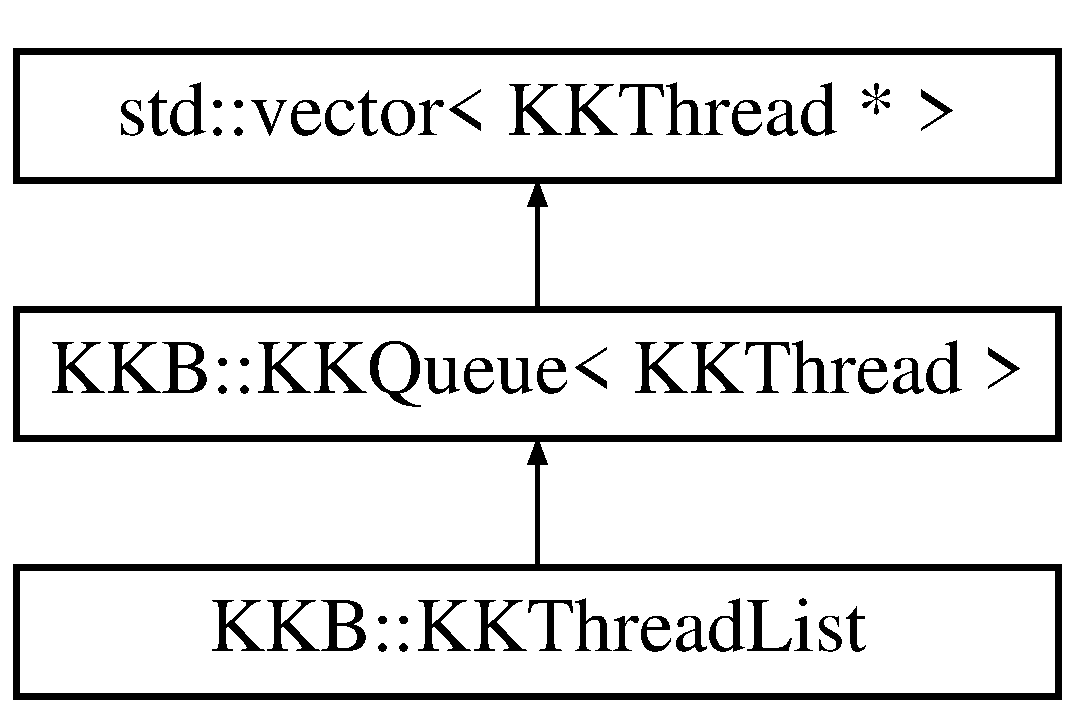
\includegraphics[height=3.000000cm]{class_k_k_b_1_1_k_k_thread_list}
\end{center}
\end{figure}
\subsection*{Public Member Functions}
\begin{DoxyCompactItemize}
\item 
\hyperlink{class_k_k_b_1_1_k_k_thread_list_a3e20a1118afaf9bb4257c4f7070aa954}{K\+K\+Thread\+List} (bool \+\_\+owner=true)
\item 
\hyperlink{class_k_k_b_1_1_k_k_thread_list_abf8cca344562bd3c3876c0ff9973de53}{K\+K\+Thread\+List} (const \hyperlink{class_k_k_b_1_1_k_k_thread_list}{K\+K\+Thread\+List} \&list)
\item 
\hyperlink{class_k_k_b_1_1_k_k_thread_list_a52837015c45c5e4ff3df7d4053431da8}{$\sim$\+K\+K\+Thread\+List} ()
\item 
\hyperlink{namespace_k_k_b_a8fa4952cc84fda1de4bec1fbdd8d5b1b}{kkint32} \hyperlink{class_k_k_b_1_1_k_k_thread_list_a2c29dc603b4f8b74548e286ffab9bc91}{Memory\+Consumed\+Estimated} () const 
\end{DoxyCompactItemize}
\subsection*{Additional Inherited Members}


\subsection{Detailed Description}


Definition at line 211 of file K\+K\+Thread.\+h.



\subsection{Constructor \& Destructor Documentation}
\index{K\+K\+B\+::\+K\+K\+Thread\+List@{K\+K\+B\+::\+K\+K\+Thread\+List}!K\+K\+Thread\+List@{K\+K\+Thread\+List}}
\index{K\+K\+Thread\+List@{K\+K\+Thread\+List}!K\+K\+B\+::\+K\+K\+Thread\+List@{K\+K\+B\+::\+K\+K\+Thread\+List}}
\subsubsection[{\texorpdfstring{K\+K\+Thread\+List(bool \+\_\+owner=true)}{KKThreadList(bool _owner=true)}}]{\setlength{\rightskip}{0pt plus 5cm}K\+K\+Thread\+List\+::\+K\+K\+Thread\+List (
\begin{DoxyParamCaption}
\item[{bool}]{\+\_\+owner = {\ttfamily true}}
\end{DoxyParamCaption}
)}\hypertarget{class_k_k_b_1_1_k_k_thread_list_a3e20a1118afaf9bb4257c4f7070aa954}{}\label{class_k_k_b_1_1_k_k_thread_list_a3e20a1118afaf9bb4257c4f7070aa954}


Definition at line 555 of file K\+K\+Thread.\+cpp.



References K\+K\+Thread\+List().



Referenced by K\+K\+B\+::\+K\+K\+Thread\+::\+Add\+Shutdown\+Prerequistite(), K\+K\+B\+::\+K\+K\+Thread\+::\+Add\+Start\+Prerequistite(), K\+K\+B\+::\+K\+K\+Thread\+Manager\+::\+Add\+Thread(), K\+K\+Thread\+List(), and K\+K\+B\+::\+K\+K\+Thread\+Manager\+::\+K\+K\+Thread\+Manager().


\begin{DoxyCode}
555                                       :
556     \hyperlink{class_k_k_b_1_1_k_k_queue}{KKQueue<KKThread>} (\_owner)
557 \{
558 \}
\end{DoxyCode}
\index{K\+K\+B\+::\+K\+K\+Thread\+List@{K\+K\+B\+::\+K\+K\+Thread\+List}!K\+K\+Thread\+List@{K\+K\+Thread\+List}}
\index{K\+K\+Thread\+List@{K\+K\+Thread\+List}!K\+K\+B\+::\+K\+K\+Thread\+List@{K\+K\+B\+::\+K\+K\+Thread\+List}}
\subsubsection[{\texorpdfstring{K\+K\+Thread\+List(const K\+K\+Thread\+List \&list)}{KKThreadList(const KKThreadList &list)}}]{\setlength{\rightskip}{0pt plus 5cm}K\+K\+Thread\+List\+::\+K\+K\+Thread\+List (
\begin{DoxyParamCaption}
\item[{const {\bf K\+K\+Thread\+List} \&}]{list}
\end{DoxyParamCaption}
)}\hypertarget{class_k_k_b_1_1_k_k_thread_list_abf8cca344562bd3c3876c0ff9973de53}{}\label{class_k_k_b_1_1_k_k_thread_list_abf8cca344562bd3c3876c0ff9973de53}


Definition at line 562 of file K\+K\+Thread.\+cpp.



References K\+K\+Thread\+List().



Referenced by K\+K\+Thread\+List().


\begin{DoxyCode}
562                                                     :
563     \hyperlink{class_k_k_b_1_1_k_k_queue}{KKQueue<KKThread>} (list)
564 \{
565 \}
\end{DoxyCode}
\index{K\+K\+B\+::\+K\+K\+Thread\+List@{K\+K\+B\+::\+K\+K\+Thread\+List}!````~K\+K\+Thread\+List@{$\sim$\+K\+K\+Thread\+List}}
\index{````~K\+K\+Thread\+List@{$\sim$\+K\+K\+Thread\+List}!K\+K\+B\+::\+K\+K\+Thread\+List@{K\+K\+B\+::\+K\+K\+Thread\+List}}
\subsubsection[{\texorpdfstring{$\sim$\+K\+K\+Thread\+List()}{~KKThreadList()}}]{\setlength{\rightskip}{0pt plus 5cm}K\+K\+Thread\+List\+::$\sim$\+K\+K\+Thread\+List (
\begin{DoxyParamCaption}
{}
\end{DoxyParamCaption}
)}\hypertarget{class_k_k_b_1_1_k_k_thread_list_a52837015c45c5e4ff3df7d4053431da8}{}\label{class_k_k_b_1_1_k_k_thread_list_a52837015c45c5e4ff3df7d4053431da8}


Definition at line 569 of file K\+K\+Thread.\+cpp.


\begin{DoxyCode}
570 \{
571 \}
\end{DoxyCode}


\subsection{Member Function Documentation}
\index{K\+K\+B\+::\+K\+K\+Thread\+List@{K\+K\+B\+::\+K\+K\+Thread\+List}!Memory\+Consumed\+Estimated@{Memory\+Consumed\+Estimated}}
\index{Memory\+Consumed\+Estimated@{Memory\+Consumed\+Estimated}!K\+K\+B\+::\+K\+K\+Thread\+List@{K\+K\+B\+::\+K\+K\+Thread\+List}}
\subsubsection[{\texorpdfstring{Memory\+Consumed\+Estimated() const }{MemoryConsumedEstimated() const }}]{\setlength{\rightskip}{0pt plus 5cm}{\bf kkint32} K\+K\+Thread\+List\+::\+Memory\+Consumed\+Estimated (
\begin{DoxyParamCaption}
{}
\end{DoxyParamCaption}
) const}\hypertarget{class_k_k_b_1_1_k_k_thread_list_a2c29dc603b4f8b74548e286ffab9bc91}{}\label{class_k_k_b_1_1_k_k_thread_list_a2c29dc603b4f8b74548e286ffab9bc91}


Definition at line 575 of file K\+K\+Thread.\+cpp.



References K\+K\+B\+::\+K\+K\+Thread\+::\+Memory\+Consumed\+Estimated().



Referenced by K\+K\+B\+::\+K\+K\+Thread\+::\+Memory\+Consumed\+Estimated().


\begin{DoxyCode}
576 \{
577   \hyperlink{namespace_k_k_b_a8fa4952cc84fda1de4bec1fbdd8d5b1b}{kkint32}  memEst = \textcolor{keyword}{sizeof} (\hyperlink{class_k_k_b_1_1_k_k_thread_list_a3e20a1118afaf9bb4257c4f7070aa954}{KKThreadList});
578 
579   \hyperlink{class_k_k_b_1_1_k_k_queue_aeb057c9c010446f46f57c1e355f981f1}{KKThreadList::const\_iterator}  idx;
580   \textcolor{keywordflow}{for}  (idx = begin ();  idx != end ();  ++idx)
581   \{
582     \hyperlink{class_k_k_b_1_1_k_k_thread}{KKThreadPtr}  t = *idx;
583     memEst += t->\hyperlink{class_k_k_b_1_1_k_k_thread_a0a8d08e9a902c496f7ee0c46f2aee2cc}{MemoryConsumedEstimated} ();
584   \}
585   \textcolor{keywordflow}{return}  memEst;
586 \}
\end{DoxyCode}


The documentation for this class was generated from the following files\+:\begin{DoxyCompactItemize}
\item 
C\+:/\+Users/\+Kurt/\+Git\+Hub/\+K\+Square\+Libraries/\+K\+K\+Base/\hyperlink{_k_k_thread_8h}{K\+K\+Thread.\+h}\item 
C\+:/\+Users/\+Kurt/\+Git\+Hub/\+K\+Square\+Libraries/\+K\+K\+Base/\hyperlink{_k_k_thread_8cpp}{K\+K\+Thread.\+cpp}\end{DoxyCompactItemize}

\hypertarget{class_k_k_b_1_1_k_k_thread_manager}{}\section{K\+KB\+:\+:K\+K\+Thread\+Manager Class Reference}
\label{class_k_k_b_1_1_k_k_thread_manager}\index{K\+K\+B\+::\+K\+K\+Thread\+Manager@{K\+K\+B\+::\+K\+K\+Thread\+Manager}}


{\ttfamily \#include $<$K\+K\+Thread\+Manager.\+h$>$}

Inheritance diagram for K\+KB\+:\+:K\+K\+Thread\+Manager\+:\begin{figure}[H]
\begin{center}
\leavevmode
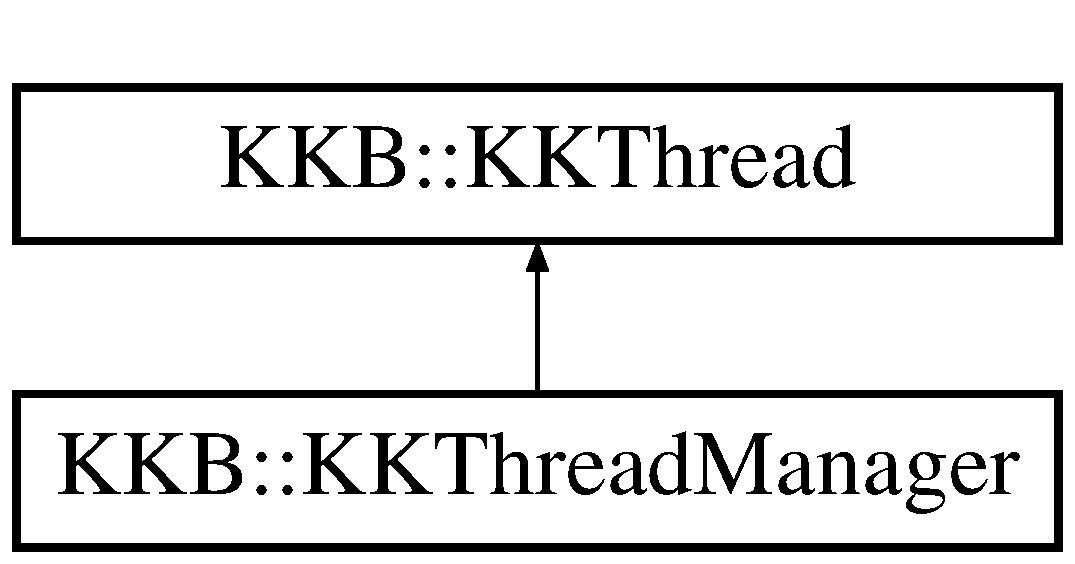
\includegraphics[height=2.000000cm]{class_k_k_b_1_1_k_k_thread_manager}
\end{center}
\end{figure}
\subsection*{Public Member Functions}
\begin{DoxyCompactItemize}
\item 
\hyperlink{class_k_k_b_1_1_k_k_thread_manager_afdfc7670c3ad323fa799f1a9d20da049}{K\+K\+Thread\+Manager} (const \hyperlink{class_k_k_b_1_1_k_k_str}{K\+K\+Str} \&\+\_\+manager\+Name, \hyperlink{namespace_k_k_b_af8d832f05c54994a1cce25bd5743e19a}{kkuint32} \+\_\+max\+Num\+Threads, \hyperlink{namespace_k_k_b_aaa43074273f12ed325a053d9e1faf84a}{Msg\+Queue\+Ptr} \+\_\+msg\+Queue)
\item 
\hyperlink{class_k_k_b_1_1_k_k_thread_manager_a691c1829d4259916c1cdb712adaebda6}{$\sim$\+K\+K\+Thread\+Manager} ()
\item 
void \hyperlink{class_k_k_b_1_1_k_k_thread_manager_ae1534656719cde8f4e831bc5dbdcc807}{Add\+Thread} (\hyperlink{class_k_k_b_1_1_k_k_thread_ae0ca65f275a57c346e71486ad84b271a}{K\+K\+Thread\+Ptr} \+\_\+thread)
\item 
bool \hyperlink{class_k_k_b_1_1_k_k_thread_manager_a2397d90b12c0d6ae9c46327536462977}{All\+Threads\+Terminated} ()
\item 
bool \hyperlink{class_k_k_b_1_1_k_k_thread_manager_a4c9dfc61200e85a537169059a6c4dd28}{Any\+Processors\+Crashed} ()
\item 
const bool \& \hyperlink{class_k_k_b_1_1_k_k_thread_manager_a2af16702df76d09363ef3e1571327c1e}{Crashed} () const 
\item 
const bool \& \hyperlink{class_k_k_b_1_1_k_k_thread_manager_a16d2106088911878f5aed5b588b0f8fe}{Done\+Executing} () const 
\item 
void \hyperlink{class_k_k_b_1_1_k_k_thread_manager_a21bbabcebe4b2bb75eedacf1687c2a1b}{Kill\+All\+Running\+Threads} ()
\item 
void \hyperlink{class_k_k_b_1_1_k_k_thread_manager_a3fd0f1b9b3545e8a854c87bdb9d8925f}{Manage\+Threads} (bool \&successful)
\item 
void \hyperlink{class_k_k_b_1_1_k_k_thread_manager_a6698417860dc2d7a388410e6179b745d}{Request\+Shutdown} ()
\item 
void \hyperlink{class_k_k_b_1_1_k_k_thread_manager_accc182d863cbdb191c3e6c882e89a5b6}{Request\+Terminate} ()
\item 
virtual void \hyperlink{class_k_k_b_1_1_k_k_thread_manager_ad1dfab64405504de3a8d8506d18b6ddd}{Run} ()
\item 
const bool \& \hyperlink{class_k_k_b_1_1_k_k_thread_manager_a2b25dda44e5c861e920e5f8f81a398fd}{Shutdown\+Flag} () const 
\item 
void \hyperlink{class_k_k_b_1_1_k_k_thread_manager_ab578ab60b9244ebdc8c06edf631cddb7}{Shutdown\+Processing} (\hyperlink{namespace_k_k_b_a8fa4952cc84fda1de4bec1fbdd8d5b1b}{kkint32} mili\+Secs\+To\+Wait)
\begin{DoxyCompactList}\small\item\em Shutdown all threads in a orderly way; observing prerequisite ordering. \end{DoxyCompactList}\item 
void \hyperlink{class_k_k_b_1_1_k_k_thread_manager_a100bf207b53aa9f96a12081574c5ac51}{Terminate\+Processing} ()
\end{DoxyCompactItemize}
\subsection*{Additional Inherited Members}


\subsection{Detailed Description}

\begin{DoxyCode}
There are three ways to stop Thread processing with the first being the most graceful and the last being 
      the most abrupt.
1) \textcolor{stringliteral}{'ShutdownProcessing'}  The preferred method;  each thread is flagged \textcolor{keywordflow}{for} \textcolor{stringliteral}{'Shutdown'} after all its 
      prerequisite shutdown threads 
   have shutdown.
2) \textcolor{stringliteral}{'TerminateProcessing'} Similar to \textcolor{stringliteral}{'ShutdownProcessing'} except the prerequisites are not checked; each 
      thread is immediately flagged
   to Terminate which indicates to the thread that it is to cease all processing and exit \textcolor{keywordflow}{while} releasing 
      all resources.
3) \textcolor{stringliteral}{'KillAllRunningThreads'} A last resort;  you would call \textcolor{keyword}{this} \textcolor{keywordflow}{if} \textcolor{keywordflow}{for} some reason threads are not 
      terminating on there own.
\end{DoxyCode}
 

Definition at line 37 of file K\+K\+Thread\+Manager.\+h.



\subsection{Constructor \& Destructor Documentation}
\index{K\+K\+B\+::\+K\+K\+Thread\+Manager@{K\+K\+B\+::\+K\+K\+Thread\+Manager}!K\+K\+Thread\+Manager@{K\+K\+Thread\+Manager}}
\index{K\+K\+Thread\+Manager@{K\+K\+Thread\+Manager}!K\+K\+B\+::\+K\+K\+Thread\+Manager@{K\+K\+B\+::\+K\+K\+Thread\+Manager}}
\subsubsection[{\texorpdfstring{K\+K\+Thread\+Manager(const K\+K\+Str \&\+\_\+manager\+Name, kkuint32 \+\_\+max\+Num\+Threads, Msg\+Queue\+Ptr \+\_\+msg\+Queue)}{KKThreadManager(const KKStr &_managerName, kkuint32 _maxNumThreads, MsgQueuePtr _msgQueue)}}]{\setlength{\rightskip}{0pt plus 5cm}K\+K\+Thread\+Manager\+::\+K\+K\+Thread\+Manager (
\begin{DoxyParamCaption}
\item[{const {\bf K\+K\+Str} \&}]{\+\_\+manager\+Name, }
\item[{{\bf kkuint32}}]{\+\_\+max\+Num\+Threads, }
\item[{{\bf Msg\+Queue\+Ptr}}]{\+\_\+msg\+Queue}
\end{DoxyParamCaption}
)}\hypertarget{class_k_k_b_1_1_k_k_thread_manager_afdfc7670c3ad323fa799f1a9d20da049}{}\label{class_k_k_b_1_1_k_k_thread_manager_afdfc7670c3ad323fa799f1a9d20da049}


Definition at line 23 of file K\+K\+Thread\+Manager.\+cpp.



References K\+K\+B\+::\+K\+K\+Thread\+::\+K\+K\+Thread(), and K\+K\+B\+::\+K\+K\+Thread\+List\+::\+K\+K\+Thread\+List().


\begin{DoxyCode}
26                                   :
27   \hyperlink{class_k_k_b_1_1_k_k_thread_aae2cc3ddbc461d7be2ff904b40ccf2e8}{KKThread} (\_managerName, NULL, \_msgQueue),
28   crashed            (\textcolor{keyword}{false}),
29   doneExecuting      (\textcolor{keyword}{false}),
30   maxNumThreads      (\_maxNumThreads),
31   shutdownFlag       (\textcolor{keyword}{false}),
32   shutdownRequested  (\textcolor{keyword}{false}),
33   terminateFlag      (\textcolor{keyword}{false}),
34   terminateRequested (\textcolor{keyword}{false}),
35   threads            (NULL)
36 
37 \{
38   threads = \textcolor{keyword}{new} \hyperlink{class_k_k_b_1_1_k_k_thread_list}{KKThreadList} (\textcolor{keyword}{true});
39 \}
\end{DoxyCode}
\index{K\+K\+B\+::\+K\+K\+Thread\+Manager@{K\+K\+B\+::\+K\+K\+Thread\+Manager}!````~K\+K\+Thread\+Manager@{$\sim$\+K\+K\+Thread\+Manager}}
\index{````~K\+K\+Thread\+Manager@{$\sim$\+K\+K\+Thread\+Manager}!K\+K\+B\+::\+K\+K\+Thread\+Manager@{K\+K\+B\+::\+K\+K\+Thread\+Manager}}
\subsubsection[{\texorpdfstring{$\sim$\+K\+K\+Thread\+Manager()}{~KKThreadManager()}}]{\setlength{\rightskip}{0pt plus 5cm}K\+K\+Thread\+Manager\+::$\sim$\+K\+K\+Thread\+Manager (
\begin{DoxyParamCaption}
{}
\end{DoxyParamCaption}
)}\hypertarget{class_k_k_b_1_1_k_k_thread_manager_a691c1829d4259916c1cdb712adaebda6}{}\label{class_k_k_b_1_1_k_k_thread_manager_a691c1829d4259916c1cdb712adaebda6}


Definition at line 44 of file K\+K\+Thread\+Manager.\+cpp.


\begin{DoxyCode}
45 \{
46   \textcolor{keyword}{delete}  threads;
47   threads = NULL;
48 \}
\end{DoxyCode}


\subsection{Member Function Documentation}
\index{K\+K\+B\+::\+K\+K\+Thread\+Manager@{K\+K\+B\+::\+K\+K\+Thread\+Manager}!Add\+Thread@{Add\+Thread}}
\index{Add\+Thread@{Add\+Thread}!K\+K\+B\+::\+K\+K\+Thread\+Manager@{K\+K\+B\+::\+K\+K\+Thread\+Manager}}
\subsubsection[{\texorpdfstring{Add\+Thread(\+K\+K\+Thread\+Ptr \+\_\+thread)}{AddThread(KKThreadPtr _thread)}}]{\setlength{\rightskip}{0pt plus 5cm}void K\+K\+Thread\+Manager\+::\+Add\+Thread (
\begin{DoxyParamCaption}
\item[{{\bf K\+K\+Thread\+Ptr}}]{\+\_\+thread}
\end{DoxyParamCaption}
)}\hypertarget{class_k_k_b_1_1_k_k_thread_manager_ae1534656719cde8f4e831bc5dbdcc807}{}\label{class_k_k_b_1_1_k_k_thread_manager_ae1534656719cde8f4e831bc5dbdcc807}
Add thread that is to be managed; will take ownership 

Definition at line 52 of file K\+K\+Thread\+Manager.\+cpp.



References K\+K\+B\+::\+K\+K\+Thread\+List\+::\+K\+K\+Thread\+List().


\begin{DoxyCode}
53 \{
54   \textcolor{keywordflow}{if}  (!threads)
55     threads = \textcolor{keyword}{new} \hyperlink{class_k_k_b_1_1_k_k_thread_list}{KKThreadList} (\textcolor{keyword}{true});
56 
57   threads->\hyperlink{class_k_k_b_1_1_k_k_queue_aa9fba4632b54268bf71ecb42dee0b575}{PushOnBack} (\_thread);
58 \}
\end{DoxyCode}
\index{K\+K\+B\+::\+K\+K\+Thread\+Manager@{K\+K\+B\+::\+K\+K\+Thread\+Manager}!All\+Threads\+Terminated@{All\+Threads\+Terminated}}
\index{All\+Threads\+Terminated@{All\+Threads\+Terminated}!K\+K\+B\+::\+K\+K\+Thread\+Manager@{K\+K\+B\+::\+K\+K\+Thread\+Manager}}
\subsubsection[{\texorpdfstring{All\+Threads\+Terminated()}{AllThreadsTerminated()}}]{\setlength{\rightskip}{0pt plus 5cm}bool K\+K\+Thread\+Manager\+::\+All\+Threads\+Terminated (
\begin{DoxyParamCaption}
{}
\end{DoxyParamCaption}
)}\hypertarget{class_k_k_b_1_1_k_k_thread_manager_a2397d90b12c0d6ae9c46327536462977}{}\label{class_k_k_b_1_1_k_k_thread_manager_a2397d90b12c0d6ae9c46327536462977}


Definition at line 280 of file K\+K\+Thread\+Manager.\+cpp.



References K\+K\+B\+::\+K\+K\+Thread\+::\+Status(), and K\+K\+B\+::\+K\+K\+Thread\+::\+Stopped.


\begin{DoxyCode}
281 \{
282   \textcolor{keywordtype}{bool}  allThreadsTerminated = \textcolor{keyword}{true};
283 
284   \textcolor{keywordflow}{if}  (threads)
285   \{
286     \hyperlink{class_k_k_b_1_1_k_k_queue_aeb057c9c010446f46f57c1e355f981f1}{KKThreadList::const\_iterator}  idx;
287     \textcolor{keywordflow}{for}  (idx = threads->begin ();  idx != threads->end ();  ++idx)
288     \{
289       \hyperlink{class_k_k_b_1_1_k_k_thread}{KKThreadPtr}  t = *idx;
290       \textcolor{keywordflow}{if}  (t->\hyperlink{class_k_k_b_1_1_k_k_thread_a8b6636f59306caf89c24d9f756293d71}{Status} () != \hyperlink{class_k_k_b_1_1_k_k_thread_a3f72bb1988ae5dd353b39260ae0acc72ac23e2b09ebe6bf4cb5e2a9abe85c0be2}{KKThread::ThreadStatus::Stopped})
291       \{
292         allThreadsTerminated = \textcolor{keyword}{false};
293         \textcolor{keywordflow}{break};
294       \}
295     \}
296   \}
297 
298   \textcolor{keywordflow}{return}  allThreadsTerminated;
299 \}  \textcolor{comment}{/* AllThreadsTerminated */}
\end{DoxyCode}
\index{K\+K\+B\+::\+K\+K\+Thread\+Manager@{K\+K\+B\+::\+K\+K\+Thread\+Manager}!Any\+Processors\+Crashed@{Any\+Processors\+Crashed}}
\index{Any\+Processors\+Crashed@{Any\+Processors\+Crashed}!K\+K\+B\+::\+K\+K\+Thread\+Manager@{K\+K\+B\+::\+K\+K\+Thread\+Manager}}
\subsubsection[{\texorpdfstring{Any\+Processors\+Crashed()}{AnyProcessorsCrashed()}}]{\setlength{\rightskip}{0pt plus 5cm}bool K\+K\+Thread\+Manager\+::\+Any\+Processors\+Crashed (
\begin{DoxyParamCaption}
{}
\end{DoxyParamCaption}
)}\hypertarget{class_k_k_b_1_1_k_k_thread_manager_a4c9dfc61200e85a537169059a6c4dd28}{}\label{class_k_k_b_1_1_k_k_thread_manager_a4c9dfc61200e85a537169059a6c4dd28}


Definition at line 255 of file K\+K\+Thread\+Manager.\+cpp.



References K\+K\+B\+::\+K\+K\+Thread\+::\+Crashed().



Referenced by Manage\+Threads().


\begin{DoxyCode}
256 \{
257   \textcolor{keywordtype}{bool}  anyProcessorsCrashed = \textcolor{keyword}{false};
258 
259   \textcolor{keywordflow}{if}  (threads)
260   \{
261     \hyperlink{class_k_k_b_1_1_k_k_queue_aa3c2796a726eea468b94132a9fbf2cfe}{KKThreadList::iterator}  idx;
262     \textcolor{keywordflow}{for}  (idx = threads->begin ();  idx != threads->end ();  ++idx)
263     \{
264       \hyperlink{class_k_k_b_1_1_k_k_thread}{KKThreadPtr}  t = *idx;
265       \textcolor{keywordflow}{if}  (t->\hyperlink{class_k_k_b_1_1_k_k_thread_a1cc302487fe9e7fe79e7e6b056d3e7d1}{Crashed} ())
266       \{
267         anyProcessorsCrashed = \textcolor{keyword}{true};
268         \textcolor{keywordflow}{break};
269       \}
270     \}
271   \}
272 
273   crashed = anyProcessorsCrashed;
274 
275   \textcolor{keywordflow}{return}  anyProcessorsCrashed;
276 \}  \textcolor{comment}{/* AnyProcessorsCrash */}
\end{DoxyCode}
\index{K\+K\+B\+::\+K\+K\+Thread\+Manager@{K\+K\+B\+::\+K\+K\+Thread\+Manager}!Crashed@{Crashed}}
\index{Crashed@{Crashed}!K\+K\+B\+::\+K\+K\+Thread\+Manager@{K\+K\+B\+::\+K\+K\+Thread\+Manager}}
\subsubsection[{\texorpdfstring{Crashed() const }{Crashed() const }}]{\setlength{\rightskip}{0pt plus 5cm}const bool\& K\+K\+B\+::\+K\+K\+Thread\+Manager\+::\+Crashed (
\begin{DoxyParamCaption}
{}
\end{DoxyParamCaption}
) const\hspace{0.3cm}{\ttfamily [inline]}}\hypertarget{class_k_k_b_1_1_k_k_thread_manager_a2af16702df76d09363ef3e1571327c1e}{}\label{class_k_k_b_1_1_k_k_thread_manager_a2af16702df76d09363ef3e1571327c1e}


Definition at line 48 of file K\+K\+Thread\+Manager.\+h.


\begin{DoxyCode}
48 \{\textcolor{keywordflow}{return} crashed;\}
\end{DoxyCode}
\index{K\+K\+B\+::\+K\+K\+Thread\+Manager@{K\+K\+B\+::\+K\+K\+Thread\+Manager}!Done\+Executing@{Done\+Executing}}
\index{Done\+Executing@{Done\+Executing}!K\+K\+B\+::\+K\+K\+Thread\+Manager@{K\+K\+B\+::\+K\+K\+Thread\+Manager}}
\subsubsection[{\texorpdfstring{Done\+Executing() const }{DoneExecuting() const }}]{\setlength{\rightskip}{0pt plus 5cm}const bool\& K\+K\+B\+::\+K\+K\+Thread\+Manager\+::\+Done\+Executing (
\begin{DoxyParamCaption}
{}
\end{DoxyParamCaption}
) const\hspace{0.3cm}{\ttfamily [inline]}}\hypertarget{class_k_k_b_1_1_k_k_thread_manager_a16d2106088911878f5aed5b588b0f8fe}{}\label{class_k_k_b_1_1_k_k_thread_manager_a16d2106088911878f5aed5b588b0f8fe}


Definition at line 49 of file K\+K\+Thread\+Manager.\+h.


\begin{DoxyCode}
49 \{\textcolor{keywordflow}{return} doneExecuting;\}
\end{DoxyCode}
\index{K\+K\+B\+::\+K\+K\+Thread\+Manager@{K\+K\+B\+::\+K\+K\+Thread\+Manager}!Kill\+All\+Running\+Threads@{Kill\+All\+Running\+Threads}}
\index{Kill\+All\+Running\+Threads@{Kill\+All\+Running\+Threads}!K\+K\+B\+::\+K\+K\+Thread\+Manager@{K\+K\+B\+::\+K\+K\+Thread\+Manager}}
\subsubsection[{\texorpdfstring{Kill\+All\+Running\+Threads()}{KillAllRunningThreads()}}]{\setlength{\rightskip}{0pt plus 5cm}void K\+K\+Thread\+Manager\+::\+Kill\+All\+Running\+Threads (
\begin{DoxyParamCaption}
{}
\end{DoxyParamCaption}
)}\hypertarget{class_k_k_b_1_1_k_k_thread_manager_a21bbabcebe4b2bb75eedacf1687c2a1b}{}\label{class_k_k_b_1_1_k_k_thread_manager_a21bbabcebe4b2bb75eedacf1687c2a1b}
Will S\+T\+OP A\+LL running threads; N\+OT Grace-\/full; 

Definition at line 185 of file K\+K\+Thread\+Manager.\+cpp.



References K\+K\+B\+::\+K\+K\+Thread\+::\+Kill().



Referenced by Shutdown\+Processing().


\begin{DoxyCode}
186 \{
187   \textcolor{keywordflow}{if}  (!threads)
188     \textcolor{keywordflow}{return};
189 
190   \hyperlink{class_k_k_b_1_1_k_k_queue_aa3c2796a726eea468b94132a9fbf2cfe}{KKThreadList::iterator}  idx;
191   \textcolor{keywordflow}{for}  (idx = threads->begin ();   idx != threads->end ();  ++idx)
192   \{
193     \hyperlink{class_k_k_b_1_1_k_k_thread}{KKThreadPtr}  thread = *idx;
194     thread->\hyperlink{class_k_k_b_1_1_k_k_thread_a66111ed632dffca679c664909d5773bd}{Kill} ();
195   \}
196 \}  \textcolor{comment}{/* KillAllRunningThreads*/}
\end{DoxyCode}
\index{K\+K\+B\+::\+K\+K\+Thread\+Manager@{K\+K\+B\+::\+K\+K\+Thread\+Manager}!Manage\+Threads@{Manage\+Threads}}
\index{Manage\+Threads@{Manage\+Threads}!K\+K\+B\+::\+K\+K\+Thread\+Manager@{K\+K\+B\+::\+K\+K\+Thread\+Manager}}
\subsubsection[{\texorpdfstring{Manage\+Threads(bool \&successful)}{ManageThreads(bool &successful)}}]{\setlength{\rightskip}{0pt plus 5cm}void K\+K\+Thread\+Manager\+::\+Manage\+Threads (
\begin{DoxyParamCaption}
\item[{bool \&}]{successful}
\end{DoxyParamCaption}
)}\hypertarget{class_k_k_b_1_1_k_k_thread_manager_a3fd0f1b9b3545e8a854c87bdb9d8925f}{}\label{class_k_k_b_1_1_k_k_thread_manager_a3fd0f1b9b3545e8a854c87bdb9d8925f}


Definition at line 305 of file K\+K\+Thread\+Manager.\+cpp.



References Any\+Processors\+Crashed(), K\+K\+B\+::os\+Sleep(), Shutdown\+Processing(), and Terminate\+Processing().


\begin{DoxyCode}
306 \{
307   successful= \textcolor{keyword}{false};
308   \textcolor{keywordflow}{if} (!threads)
309     \textcolor{keywordflow}{return};
310 
311   StartThreads (successful);
312   \textcolor{keywordflow}{if}  (!successful)
313     \textcolor{keywordflow}{return};
314 
315 
316   \textcolor{keywordflow}{while}  (\textcolor{keyword}{true})
317   \{
318     \textcolor{keywordflow}{if}  (shutdownRequested)
319     \{
320       shutdownRequested = \textcolor{keyword}{false};
321       \hyperlink{class_k_k_b_1_1_k_k_thread_manager_ab578ab60b9244ebdc8c06edf631cddb7}{ShutdownProcessing} (0);
322       \textcolor{keywordflow}{break};
323     \}
324 
325     \textcolor{keywordflow}{else} \textcolor{keywordflow}{if}  (terminateRequested)
326     \{
327       terminateRequested = \textcolor{keyword}{false};
328       \hyperlink{class_k_k_b_1_1_k_k_thread_manager_a100bf207b53aa9f96a12081574c5ac51}{TerminateProcessing} ();
329       \textcolor{keywordflow}{break};
330     \}
331 
332     \textcolor{keywordflow}{else}
333     \{
334       \hyperlink{namespace_k_k_b_a1a3717b963b0813e96b66d1953fce1af}{osSleep} (0.05f);
335     \}
336   \}
337 
338 
339   \textcolor{keywordflow}{if}  (\hyperlink{class_k_k_b_1_1_k_k_thread_manager_a4c9dfc61200e85a537169059a6c4dd28}{AnyProcessorsCrashed} ())
340   \{
341     \hyperlink{class_k_k_b_1_1_k_k_thread_a8f6c004d6510b90e5eff9c34efd20967}{AddMsg} (\textcolor{stringliteral}{"One or more processors crashed!!!"});
342     crashed = \textcolor{keyword}{true};
343   \}
344 \}  \textcolor{comment}{/* ManageThreads */}
\end{DoxyCode}
\index{K\+K\+B\+::\+K\+K\+Thread\+Manager@{K\+K\+B\+::\+K\+K\+Thread\+Manager}!Request\+Shutdown@{Request\+Shutdown}}
\index{Request\+Shutdown@{Request\+Shutdown}!K\+K\+B\+::\+K\+K\+Thread\+Manager@{K\+K\+B\+::\+K\+K\+Thread\+Manager}}
\subsubsection[{\texorpdfstring{Request\+Shutdown()}{RequestShutdown()}}]{\setlength{\rightskip}{0pt plus 5cm}void K\+K\+Thread\+Manager\+::\+Request\+Shutdown (
\begin{DoxyParamCaption}
{}
\end{DoxyParamCaption}
)}\hypertarget{class_k_k_b_1_1_k_k_thread_manager_a6698417860dc2d7a388410e6179b745d}{}\label{class_k_k_b_1_1_k_k_thread_manager_a6698417860dc2d7a388410e6179b745d}


Definition at line 62 of file K\+K\+Thread\+Manager.\+cpp.


\begin{DoxyCode}
63 \{
64   shutdownRequested = \textcolor{keyword}{true};
65 \}
\end{DoxyCode}
\index{K\+K\+B\+::\+K\+K\+Thread\+Manager@{K\+K\+B\+::\+K\+K\+Thread\+Manager}!Request\+Terminate@{Request\+Terminate}}
\index{Request\+Terminate@{Request\+Terminate}!K\+K\+B\+::\+K\+K\+Thread\+Manager@{K\+K\+B\+::\+K\+K\+Thread\+Manager}}
\subsubsection[{\texorpdfstring{Request\+Terminate()}{RequestTerminate()}}]{\setlength{\rightskip}{0pt plus 5cm}void K\+K\+Thread\+Manager\+::\+Request\+Terminate (
\begin{DoxyParamCaption}
{}
\end{DoxyParamCaption}
)}\hypertarget{class_k_k_b_1_1_k_k_thread_manager_accc182d863cbdb191c3e6c882e89a5b6}{}\label{class_k_k_b_1_1_k_k_thread_manager_accc182d863cbdb191c3e6c882e89a5b6}


Definition at line 68 of file K\+K\+Thread\+Manager.\+cpp.


\begin{DoxyCode}
69 \{
70   terminateRequested = \textcolor{keyword}{true};
71 \}
\end{DoxyCode}
\index{K\+K\+B\+::\+K\+K\+Thread\+Manager@{K\+K\+B\+::\+K\+K\+Thread\+Manager}!Run@{Run}}
\index{Run@{Run}!K\+K\+B\+::\+K\+K\+Thread\+Manager@{K\+K\+B\+::\+K\+K\+Thread\+Manager}}
\subsubsection[{\texorpdfstring{Run()}{Run()}}]{\setlength{\rightskip}{0pt plus 5cm}void K\+K\+Thread\+Manager\+::\+Run (
\begin{DoxyParamCaption}
{}
\end{DoxyParamCaption}
)\hspace{0.3cm}{\ttfamily [virtual]}}\hypertarget{class_k_k_b_1_1_k_k_thread_manager_ad1dfab64405504de3a8d8506d18b6ddd}{}\label{class_k_k_b_1_1_k_k_thread_manager_ad1dfab64405504de3a8d8506d18b6ddd}


Reimplemented from \hyperlink{class_k_k_b_1_1_k_k_thread_a4ecfa3856e1b5bb4a5a125fdc05c4e67}{K\+K\+B\+::\+K\+K\+Thread}.



Definition at line 348 of file K\+K\+Thread\+Manager.\+cpp.


\begin{DoxyCode}
349 \{
350 \}
\end{DoxyCode}
\index{K\+K\+B\+::\+K\+K\+Thread\+Manager@{K\+K\+B\+::\+K\+K\+Thread\+Manager}!Shutdown\+Flag@{Shutdown\+Flag}}
\index{Shutdown\+Flag@{Shutdown\+Flag}!K\+K\+B\+::\+K\+K\+Thread\+Manager@{K\+K\+B\+::\+K\+K\+Thread\+Manager}}
\subsubsection[{\texorpdfstring{Shutdown\+Flag() const }{ShutdownFlag() const }}]{\setlength{\rightskip}{0pt plus 5cm}const bool\& K\+K\+B\+::\+K\+K\+Thread\+Manager\+::\+Shutdown\+Flag (
\begin{DoxyParamCaption}
{}
\end{DoxyParamCaption}
) const\hspace{0.3cm}{\ttfamily [inline]}}\hypertarget{class_k_k_b_1_1_k_k_thread_manager_a2b25dda44e5c861e920e5f8f81a398fd}{}\label{class_k_k_b_1_1_k_k_thread_manager_a2b25dda44e5c861e920e5f8f81a398fd}


Definition at line 47 of file K\+K\+Thread\+Manager.\+h.


\begin{DoxyCode}
47 \{\textcolor{keywordflow}{return} shutdownFlag;\}
\end{DoxyCode}
\index{K\+K\+B\+::\+K\+K\+Thread\+Manager@{K\+K\+B\+::\+K\+K\+Thread\+Manager}!Shutdown\+Processing@{Shutdown\+Processing}}
\index{Shutdown\+Processing@{Shutdown\+Processing}!K\+K\+B\+::\+K\+K\+Thread\+Manager@{K\+K\+B\+::\+K\+K\+Thread\+Manager}}
\subsubsection[{\texorpdfstring{Shutdown\+Processing(kkint32 mili\+Secs\+To\+Wait)}{ShutdownProcessing(kkint32 miliSecsToWait)}}]{\setlength{\rightskip}{0pt plus 5cm}void K\+K\+Thread\+Manager\+::\+Shutdown\+Processing (
\begin{DoxyParamCaption}
\item[{{\bf kkint32}}]{mili\+Secs\+To\+Wait}
\end{DoxyParamCaption}
)}\hypertarget{class_k_k_b_1_1_k_k_thread_manager_ab578ab60b9244ebdc8c06edf631cddb7}{}\label{class_k_k_b_1_1_k_k_thread_manager_ab578ab60b9244ebdc8c06edf631cddb7}


Shutdown all threads in a orderly way; observing prerequisite ordering. 



Definition at line 93 of file K\+K\+Thread\+Manager.\+cpp.



References Kill\+All\+Running\+Threads(), K\+K\+B\+::\+K\+K\+Thread\+::\+Not\+Started, K\+K\+B\+::\+K\+K\+Thread\+::\+Null, K\+K\+B\+::\+K\+K\+Thread\+::\+Ok\+To\+Shutdown(), K\+K\+B\+::os\+Sleep(), K\+K\+B\+::\+K\+K\+Thread\+::\+Running, K\+K\+B\+::\+K\+K\+Thread\+::\+Shutdown\+Flag(), K\+K\+B\+::\+K\+K\+Thread\+::\+Shutdown\+Thread(), K\+K\+B\+::\+K\+K\+Thread\+::\+Starting, K\+K\+B\+::\+K\+K\+Thread\+::\+Status(), K\+K\+B\+::\+K\+K\+Thread\+::\+Stopped, and K\+K\+B\+::\+K\+K\+Thread\+::\+Stopping.



Referenced by Manage\+Threads().


\begin{DoxyCode}
94 \{
95   shutdownFlag = \textcolor{keyword}{true};
96 
97   \textcolor{keywordflow}{if}  (!threads)
98     \textcolor{keywordflow}{return};
99 
100   \hyperlink{namespace_k_k_b_a8fa4952cc84fda1de4bec1fbdd8d5b1b}{kkint32}  numMiliSecsWaited = 0;
101   shutdownFlag = \textcolor{keyword}{true};
102 
103   \hyperlink{namespace_k_k_b_a8fa4952cc84fda1de4bec1fbdd8d5b1b}{kkint32}  lastNumThreadsRunning = 0;
104   \hyperlink{namespace_k_k_b_a8fa4952cc84fda1de4bec1fbdd8d5b1b}{kkint32}  lastNumThreadsStopped = 0;
105 
106   \textcolor{keywordtype}{bool}  allTreadsAreShutdown = \textcolor{keyword}{false};
107 
108   \textcolor{keywordflow}{while}  (!allTreadsAreShutdown)
109   \{
110     allTreadsAreShutdown = \textcolor{keyword}{true};
111     \hyperlink{namespace_k_k_b_a8fa4952cc84fda1de4bec1fbdd8d5b1b}{kkint32}  numThreadsRunning = 0;
112     \hyperlink{namespace_k_k_b_a8fa4952cc84fda1de4bec1fbdd8d5b1b}{kkint32}  numThreadsStopped = 0;
113 
114     \hyperlink{class_k_k_b_1_1_k_k_queue_aa3c2796a726eea468b94132a9fbf2cfe}{KKThreadList::iterator}  idx;
115     \textcolor{keywordflow}{for}  (idx = threads->begin ();  idx != threads->end ();  ++idx)
116     \{
117       \hyperlink{class_k_k_b_1_1_k_k_thread}{KKThreadPtr}  thread = *idx;
118 
119       \textcolor{keywordflow}{switch}  (thread->\hyperlink{class_k_k_b_1_1_k_k_thread_a8b6636f59306caf89c24d9f756293d71}{Status} ())
120       \{
121       \textcolor{keywordflow}{case}  \hyperlink{class_k_k_b_1_1_k_k_thread_a3f72bb1988ae5dd353b39260ae0acc72abbb93ef26e3c101ff11cdd21cab08a94}{KKThread::ThreadStatus::Null}:
122         \textcolor{keywordflow}{break};
123 
124       \textcolor{keywordflow}{case}  \hyperlink{class_k_k_b_1_1_k_k_thread_a3f72bb1988ae5dd353b39260ae0acc72afa7be7845bc42b3491d9d0377958be94}{KKThread::ThreadStatus::NotStarted}:
125       \textcolor{keywordflow}{case}  \hyperlink{class_k_k_b_1_1_k_k_thread_a3f72bb1988ae5dd353b39260ae0acc72ac23e2b09ebe6bf4cb5e2a9abe85c0be2}{KKThread::ThreadStatus::Stopped}:
126         \textcolor{comment}{// Nothing to do;  this thread is not running,}
127         ++numThreadsStopped;
128         \textcolor{keywordflow}{break};
129 
130       \textcolor{keywordflow}{case}  \hyperlink{class_k_k_b_1_1_k_k_thread_a3f72bb1988ae5dd353b39260ae0acc72a7b7ecb39b9e110c2a31409a1672bad23}{KKThread::ThreadStatus::Stopping}:
131         allTreadsAreShutdown = \textcolor{keyword}{false};
132         ++numThreadsRunning;
133         \textcolor{keywordflow}{break};
134 
135       \textcolor{keywordflow}{case}  \hyperlink{class_k_k_b_1_1_k_k_thread_a3f72bb1988ae5dd353b39260ae0acc72a5bda814c4aedb126839228f1a3d92f09}{KKThread::ThreadStatus::Running}:
136         \{
137           allTreadsAreShutdown = \textcolor{keyword}{false};
138           \textcolor{keywordflow}{if}  (!(thread->\hyperlink{class_k_k_b_1_1_k_k_thread_a271dba95d3432cf7ea4992951f2b2a38}{ShutdownFlag} ()))
139           \{
140             \textcolor{keywordflow}{if}  (thread->\hyperlink{class_k_k_b_1_1_k_k_thread_a7aa56da8a1a30568b4b7c353909e6b4c}{OkToShutdown} ())
141             \{
142               thread->\hyperlink{class_k_k_b_1_1_k_k_thread_af3d38a6013474f4710c1797fbf26d3cb}{ShutdownThread} ();
143               numMiliSecsWaited = 0;
144             \}
145           \}
146           ++numThreadsRunning;
147         \}
148         \textcolor{keywordflow}{break};
149 
150       \textcolor{keywordflow}{case}  \hyperlink{class_k_k_b_1_1_k_k_thread_a3f72bb1988ae5dd353b39260ae0acc72ac2efe4bbd13e6cb0db293e72884273c0}{KKThread::ThreadStatus::Starting}:
151         \textcolor{comment}{// Have to let it finish starting before we can flag it to shutdown.}
152         ++numThreadsRunning;
153         \textcolor{keywordflow}{break};
154       \}  \textcolor{comment}{/* End of Switch */}
155     \}
156 
157     \textcolor{keywordflow}{if}  ((numThreadsRunning != lastNumThreadsRunning)  ||
158          (numThreadsStopped != lastNumThreadsStopped)
159         )
160     \{
161       \textcolor{comment}{// The status of one or more threads changed;  can reset the 'numMiliSecsWaited' clock.}
162       numMiliSecsWaited = 0;
163     \}
164 
165     \textcolor{keywordflow}{if}  (!allTreadsAreShutdown)
166     \{
167       \textcolor{keywordflow}{if}  ((miliSecsToWait > 0)  &&  (numMiliSecsWaited > miliSecsToWait))
168       \{
169         \textcolor{comment}{// The shutdown process is taking longer than the 'miliSecsToWait' parameter will allow for;  we
       need to terminate}
170         \textcolor{comment}{// all running threads now.}
171         \hyperlink{class_k_k_b_1_1_k_k_thread_manager_a21bbabcebe4b2bb75eedacf1687c2a1b}{KillAllRunningThreads} ();
172         \textcolor{keywordflow}{break};
173       \}
174       \textcolor{keywordflow}{else}
175       \{
176         \hyperlink{namespace_k_k_b_a1a3717b963b0813e96b66d1953fce1af}{osSleep} (0.01f);
177         numMiliSecsWaited += 10;
178       \}
179     \}
180   \}
181 \}  \textcolor{comment}{/* ShutdownProcessing */}
\end{DoxyCode}
\index{K\+K\+B\+::\+K\+K\+Thread\+Manager@{K\+K\+B\+::\+K\+K\+Thread\+Manager}!Terminate\+Processing@{Terminate\+Processing}}
\index{Terminate\+Processing@{Terminate\+Processing}!K\+K\+B\+::\+K\+K\+Thread\+Manager@{K\+K\+B\+::\+K\+K\+Thread\+Manager}}
\subsubsection[{\texorpdfstring{Terminate\+Processing()}{TerminateProcessing()}}]{\setlength{\rightskip}{0pt plus 5cm}void K\+K\+Thread\+Manager\+::\+Terminate\+Processing (
\begin{DoxyParamCaption}
{}
\end{DoxyParamCaption}
)}\hypertarget{class_k_k_b_1_1_k_k_thread_manager_a100bf207b53aa9f96a12081574c5ac51}{}\label{class_k_k_b_1_1_k_k_thread_manager_a100bf207b53aa9f96a12081574c5ac51}
Flag all All running threads to Terminate A\+S\+AP and release all allocated resources. 

Definition at line 76 of file K\+K\+Thread\+Manager.\+cpp.



References K\+K\+B\+::\+K\+K\+Thread\+::\+Terminate\+Thread().



Referenced by Manage\+Threads().


\begin{DoxyCode}
77 \{
78   terminateFlag = \textcolor{keyword}{true};
79   \textcolor{keywordflow}{if}  (threads)
80   \{
81     \hyperlink{class_k_k_b_1_1_k_k_queue_aa3c2796a726eea468b94132a9fbf2cfe}{KKThreadList::iterator}  idx;
82     \textcolor{keywordflow}{for}  (idx = threads->begin ();  idx != threads->end ();  ++idx)
83     \{
84       \hyperlink{class_k_k_b_1_1_k_k_thread}{KKThreadPtr}  thread = *idx;
85       thread->\hyperlink{class_k_k_b_1_1_k_k_thread_ad8ce909fbb09ad87c759e7a442530a08}{TerminateThread} ();
86     \}
87   \}
88 \}  \textcolor{comment}{/* TerminateProcessing */}
\end{DoxyCode}


The documentation for this class was generated from the following files\+:\begin{DoxyCompactItemize}
\item 
C\+:/\+Users/\+Kurt/\+Git\+Hub/\+K\+Square\+Libraries/\+K\+K\+Base/\hyperlink{_k_k_thread_manager_8h}{K\+K\+Thread\+Manager.\+h}\item 
C\+:/\+Users/\+Kurt/\+Git\+Hub/\+K\+Square\+Libraries/\+K\+K\+Base/\hyperlink{_k_k_thread_manager_8cpp}{K\+K\+Thread\+Manager.\+cpp}\end{DoxyCompactItemize}

\hypertarget{class_k_k_b_1_1_matrix}{}\section{K\+KB\+:\+:Matrix Class Reference}
\label{class_k_k_b_1_1_matrix}\index{K\+K\+B\+::\+Matrix@{K\+K\+B\+::\+Matrix}}


Supports two dimensional matrices.  




{\ttfamily \#include $<$Matrix.\+h$>$}

\subsection*{Public Types}
\begin{DoxyCompactItemize}
\item 
typedef \hyperlink{class_k_k_b_1_1_matrix}{Matrix} $\ast$ \hyperlink{class_k_k_b_1_1_matrix_ad532bd6e9d0aa9b54e78f0feec5741a3}{Matrix\+Ptr}
\end{DoxyCompactItemize}
\subsection*{Public Member Functions}
\begin{DoxyCompactItemize}
\item 
\hyperlink{class_k_k_b_1_1_matrix_a2dba13c45127354c9f75ef576f49269b}{Matrix} ()
\item 
\hyperlink{class_k_k_b_1_1_matrix_a900e01eb3c4f0b082a5457163c6cf2ef}{Matrix} (\hyperlink{namespace_k_k_b_a8fa4952cc84fda1de4bec1fbdd8d5b1b}{kkint32} \+\_\+num\+Of\+Rows, \hyperlink{namespace_k_k_b_a8fa4952cc84fda1de4bec1fbdd8d5b1b}{kkint32} \+\_\+num\+Of\+Cols)
\item 
\hyperlink{class_k_k_b_1_1_matrix_affaa8d1a1cb7710cc0bc72ec73aaea2c}{Matrix} (const \hyperlink{class_k_k_b_1_1_matrix}{Matrix} \&\+\_\+matrix)
\item 
\hyperlink{class_k_k_b_1_1_matrix_a0f87edf7b68d5920fa0bde6fe377d997}{Matrix} (const \hyperlink{namespace_k_k_b_a5906c207479607e5f450434095914a41}{Vector\+Double} \&\+\_\+v)
\item 
\hyperlink{class_k_k_b_1_1_matrix_a9b1c3627f573d78a2f08623fdfef990f}{$\sim$\+Matrix} ()
\item 
\hyperlink{class_k_k_b_1_1_matrix_ad532bd6e9d0aa9b54e78f0feec5741a3}{Matrix\+Ptr} \hyperlink{class_k_k_b_1_1_matrix_a70393cf0584a8a4a2735ad5eba9ae4d0}{Calc\+Co\+Factor\+Matrix} ()
\item 
\hyperlink{class_k_k_b_1_1_matrix_ad532bd6e9d0aa9b54e78f0feec5741a3}{Matrix\+Ptr} \hyperlink{class_k_k_b_1_1_matrix_a99d8b32816b488a4d76597800f30ea70}{Covariance} () const 
\begin{DoxyCompactList}\small\item\em Returns a Covariance matrix. \end{DoxyCompactList}\item 
double $\ast$$\ast$const \hyperlink{class_k_k_b_1_1_matrix_ac9fff89f779f11e382a3ff030e533474}{Data} () const 
\item 
double \hyperlink{class_k_k_b_1_1_matrix_ae93ec6a085d62a87d237786ae1d5657d}{Determinant} ()
\item 
double \hyperlink{class_k_k_b_1_1_matrix_ad93cf1c0613661466547e9f40f0d5b49}{Determinant\+Slow} ()
\begin{DoxyCompactList}\small\item\em Recursive Implementation. \end{DoxyCompactList}\item 
void \hyperlink{class_k_k_b_1_1_matrix_a1d9e7525cebca179d2cefa3c68beb523}{Eigen\+Vectors} (\hyperlink{class_k_k_b_1_1_matrix_ad532bd6e9d0aa9b54e78f0feec5741a3}{Matrix\+Ptr} \&eigen\+Vectors, \hyperlink{namespace_k_k_b_a5906c207479607e5f450434095914a41}{Vector\+Double} $\ast$\&eigen\+Values) const 
\begin{DoxyCompactList}\small\item\em Will derive the Eigen vectors and values of the matrix. \end{DoxyCompactList}\item 
void \hyperlink{class_k_k_b_1_1_matrix_ac4861e80e5f5f5a03bc61fd756538af5}{Find\+Max\+Value} (double \&max\+Val, \hyperlink{namespace_k_k_b_a8fa4952cc84fda1de4bec1fbdd8d5b1b}{kkint32} \&row, \hyperlink{namespace_k_k_b_a8fa4952cc84fda1de4bec1fbdd8d5b1b}{kkint32} \&col)
\begin{DoxyCompactList}\small\item\em Locates the maximum value in a matrix along with the row and column that is located. \end{DoxyCompactList}\item 
\hyperlink{namespace_k_k_b_a5906c207479607e5f450434095914a41}{Vector\+Double} \hyperlink{class_k_k_b_1_1_matrix_aa0e75f188938ed8b108999e432704c6f}{Get\+Col} (\hyperlink{namespace_k_k_b_a8fa4952cc84fda1de4bec1fbdd8d5b1b}{kkint32} col) const 
\item 
\hyperlink{class_k_k_b_1_1_matrix}{Matrix} \hyperlink{class_k_k_b_1_1_matrix_ac1e575ac083839c44cd50f56e627a320}{Inverse} ()
\item 
\hyperlink{namespace_k_k_b_a8fa4952cc84fda1de4bec1fbdd8d5b1b}{kkint32} \hyperlink{class_k_k_b_1_1_matrix_a8f90bb60f11d7a3836729aba4aba5477}{Num\+Of\+Cols} () const 
\item 
\hyperlink{namespace_k_k_b_a8fa4952cc84fda1de4bec1fbdd8d5b1b}{kkint32} \hyperlink{class_k_k_b_1_1_matrix_adb748900cbb5c55303eb71c682b0089f}{Num\+Of\+Rows} () const 
\item 
\hyperlink{class_k_k_b_1_1_matrix}{Matrix} \hyperlink{class_k_k_b_1_1_matrix_a5535a4b47a346d0a0afe78528d693f83}{operator$\ast$} (const \hyperlink{class_k_k_b_1_1_matrix}{Matrix} \&right)
\item 
\hyperlink{class_k_k_b_1_1_matrix}{Matrix} \hyperlink{class_k_k_b_1_1_matrix_a2a3c2b453687cbf862210711ed28b289}{operator$\ast$} (double right)
\item 
\hyperlink{class_k_k_b_1_1_matrix}{Matrix} \& \hyperlink{class_k_k_b_1_1_matrix_a4471b49ab8feb48be8d5b4225de16fb1}{operator$\ast$=} (double right)
\item 
\hyperlink{class_k_k_b_1_1_matrix}{Matrix} \hyperlink{class_k_k_b_1_1_matrix_ac8947020d9f5f738de7d771cd8fb19f0}{operator+} (const \hyperlink{class_k_k_b_1_1_matrix}{Matrix} \&right)
\item 
\hyperlink{class_k_k_b_1_1_matrix}{Matrix} \hyperlink{class_k_k_b_1_1_matrix_a585e5b98def5fa06e565ff0bdbcfd848}{operator+} (double right)
\item 
\hyperlink{class_k_k_b_1_1_matrix}{Matrix} \& \hyperlink{class_k_k_b_1_1_matrix_a86ef5684a657a07509a1f99ba0acf144}{operator+=} (double right)
\item 
\hyperlink{class_k_k_b_1_1_matrix}{Matrix} \& \hyperlink{class_k_k_b_1_1_matrix_a4612e586fd64b716842cd964b2f3cdbc}{operator+=} (const \hyperlink{class_k_k_b_1_1_matrix}{Matrix} \&right)
\item 
\hyperlink{class_k_k_b_1_1_matrix}{Matrix} \hyperlink{class_k_k_b_1_1_matrix_a515dad949068dde646ca73d9d69d9672}{operator-\/} (const \hyperlink{class_k_k_b_1_1_matrix}{Matrix} \&right)
\item 
\hyperlink{class_k_k_b_1_1_matrix}{Matrix} \hyperlink{class_k_k_b_1_1_matrix_abdae6b017f749792e303749cbe74f57a}{operator-\/} (double right)
\item 
\hyperlink{class_k_k_b_1_1_matrix}{Matrix} \& \hyperlink{class_k_k_b_1_1_matrix_a127463de2d624abeaf5924c0f2fe798d}{operator=} (const \hyperlink{class_k_k_b_1_1_matrix}{Matrix} \&right)
\item 
\hyperlink{class_k_k_b_1_1_matrix}{Matrix} \& \hyperlink{class_k_k_b_1_1_matrix_acd15e0e4eb7b499030cd8af1dfd3f409}{operator=} (const \hyperlink{namespace_k_k_b_a5906c207479607e5f450434095914a41}{Vector\+Double} \&right)
\item 
\hyperlink{class_k_k_b_1_1_row}{Row} \& \hyperlink{class_k_k_b_1_1_matrix_a5bc7829435bc1063b82a91c1b82d5be5}{operator\mbox{[}$\,$\mbox{]}} (\hyperlink{namespace_k_k_b_a8fa4952cc84fda1de4bec1fbdd8d5b1b}{kkint32} row\+I\+DX) const 
\item 
void \hyperlink{class_k_k_b_1_1_matrix_ac2d0c31477e85bad55e6a1cd5be1b302}{Re\+Size} (\hyperlink{namespace_k_k_b_a8fa4952cc84fda1de4bec1fbdd8d5b1b}{kkint32} \+\_\+num\+Of\+Rows, \hyperlink{namespace_k_k_b_a8fa4952cc84fda1de4bec1fbdd8d5b1b}{kkint32} \+\_\+num\+Of\+Cols)
\item 
bool \hyperlink{class_k_k_b_1_1_matrix_a68ce1e9491bb1c1a69ce16bbd12bb6db}{Symmetric} () const 
\item 
\hyperlink{class_k_k_b_1_1_matrix}{Matrix} \hyperlink{class_k_k_b_1_1_matrix_af9b74b284027c584dc75ae674e65f58d}{Transpose} ()
\end{DoxyCompactItemize}
\subsection*{Static Public Member Functions}
\begin{DoxyCompactItemize}
\item 
{\footnotesize template$<$typename T $>$ }\\static \hyperlink{class_k_k_b_1_1_matrix_ad532bd6e9d0aa9b54e78f0feec5741a3}{Matrix\+Ptr} \hyperlink{class_k_k_b_1_1_matrix_a4bda3a321f99acd63746661b2f7a8ea8}{Build\+From\+Array} (\hyperlink{namespace_k_k_b_a8fa4952cc84fda1de4bec1fbdd8d5b1b}{kkint32} num\+Of\+Rows, \hyperlink{namespace_k_k_b_a8fa4952cc84fda1de4bec1fbdd8d5b1b}{kkint32} num\+Of\+Cols, T $\ast$$\ast$data)
\begin{DoxyCompactList}\small\item\em Will create a new matrix using the 2d\+Array \char`\"{}data\char`\"{} for source. \end{DoxyCompactList}\end{DoxyCompactItemize}
\subsection*{Friends}
\begin{DoxyCompactItemize}
\item 
\hyperlink{class_k_k_b_1_1_matrix}{Matrix} \hyperlink{class_k_k_b_1_1_matrix_aa6ed460f16c161718d4178f62cc3afbf}{operator-\/} (double left, const \hyperlink{class_k_k_b_1_1_matrix}{Matrix} \&right)
\item 
std\+::ostream \& \hyperlink{class_k_k_b_1_1_matrix_a9597a390480e6b835e8b6c3c22d00d93}{operator$<$$<$} (std\+::ostream \&os, const \hyperlink{class_k_k_b_1_1_matrix}{Matrix} \&matrix)
\end{DoxyCompactItemize}


\subsection{Detailed Description}
Supports two dimensional matrices. 

Developed for Machine Learning Project for support of Import Vector Machine. Handles two dimensional matrices. Functions supported are matrix addition, subtraction multiplication, transpose, determinant, and inversion. Where appropriate arithmetic arithmetic operators +, -\/, $\ast$ were overloaded. Addition, Subtraction and Multiplication can be done against either another matrix or scaler. Also Transpose and Determinant operations are supported. 

Definition at line 46 of file Matrix.\+h.



\subsection{Member Typedef Documentation}
\index{K\+K\+B\+::\+Matrix@{K\+K\+B\+::\+Matrix}!Matrix\+Ptr@{Matrix\+Ptr}}
\index{Matrix\+Ptr@{Matrix\+Ptr}!K\+K\+B\+::\+Matrix@{K\+K\+B\+::\+Matrix}}
\subsubsection[{\texorpdfstring{Matrix\+Ptr}{MatrixPtr}}]{\setlength{\rightskip}{0pt plus 5cm}typedef {\bf Matrix}$\ast$ {\bf K\+K\+B\+::\+Matrix\+::\+Matrix\+Ptr}}\hypertarget{class_k_k_b_1_1_matrix_ad532bd6e9d0aa9b54e78f0feec5741a3}{}\label{class_k_k_b_1_1_matrix_ad532bd6e9d0aa9b54e78f0feec5741a3}


Definition at line 49 of file Matrix.\+h.



\subsection{Constructor \& Destructor Documentation}
\index{K\+K\+B\+::\+Matrix@{K\+K\+B\+::\+Matrix}!Matrix@{Matrix}}
\index{Matrix@{Matrix}!K\+K\+B\+::\+Matrix@{K\+K\+B\+::\+Matrix}}
\subsubsection[{\texorpdfstring{Matrix()}{Matrix()}}]{\setlength{\rightskip}{0pt plus 5cm}Matrix\+::\+Matrix (
\begin{DoxyParamCaption}
{}
\end{DoxyParamCaption}
)}\hypertarget{class_k_k_b_1_1_matrix_a2dba13c45127354c9f75ef576f49269b}{}\label{class_k_k_b_1_1_matrix_a2dba13c45127354c9f75ef576f49269b}


Definition at line 94 of file Matrix.\+cpp.


\begin{DoxyCode}
94                :
95 
96   data        (NULL),
97   dataArea    (NULL),
98   numOfCols   (0),
99   numOfRows   (0),
100   rows        (NULL),
101   totNumCells (0)
102 \{
103 \}
\end{DoxyCode}
\index{K\+K\+B\+::\+Matrix@{K\+K\+B\+::\+Matrix}!Matrix@{Matrix}}
\index{Matrix@{Matrix}!K\+K\+B\+::\+Matrix@{K\+K\+B\+::\+Matrix}}
\subsubsection[{\texorpdfstring{Matrix(kkint32 \+\_\+num\+Of\+Rows, kkint32 \+\_\+num\+Of\+Cols)}{Matrix(kkint32 _numOfRows, kkint32 _numOfCols)}}]{\setlength{\rightskip}{0pt plus 5cm}Matrix\+::\+Matrix (
\begin{DoxyParamCaption}
\item[{{\bf kkint32}}]{\+\_\+num\+Of\+Rows, }
\item[{{\bf kkint32}}]{\+\_\+num\+Of\+Cols}
\end{DoxyParamCaption}
)}\hypertarget{class_k_k_b_1_1_matrix_a900e01eb3c4f0b082a5457163c6cf2ef}{}\label{class_k_k_b_1_1_matrix_a900e01eb3c4f0b082a5457163c6cf2ef}


Definition at line 108 of file Matrix.\+cpp.



References K\+K\+B\+::\+K\+K\+Str\+::\+Concat(), K\+K\+B\+::\+K\+K\+Exception\+::\+K\+K\+Exception(), and K\+K\+B\+::\+K\+K\+Str\+::\+K\+K\+Str().



Referenced by K\+K\+B\+::\+Raster\+::\+Build\+Gaussian2d\+Kernel(), Calc\+Co\+Factor\+Matrix(), Covariance(), K\+K\+B\+::\+Raster\+::\+Create\+Gray\+Scale\+K\+L\+T(), K\+K\+B\+::\+Raster\+::\+Create\+Gray\+Scale\+K\+L\+T\+On\+Masked\+Area(), operator$\ast$(), K\+K\+B\+::operator-\/(), K\+K\+M\+L\+L\+::\+Classification\+Bias\+Matrix\+::\+Perform\+Adjustmnts(), and Transpose().


\begin{DoxyCode}
110                 :
111 
112   data        (NULL),
113   dataArea    (NULL),
114   numOfCols   (\_numOfCols),
115   numOfRows   (\_numOfRows),
116   rows        (NULL),
117   totNumCells (0)
118 
119 \{
120   \textcolor{keywordflow}{if}  (\_numOfRows < 0)
121   \{
122     \hyperlink{class_k_k_b_1_1_k_k_str}{KKStr}  msg(80);
123     msg << \textcolor{stringliteral}{"Matrix::Matrix   **** ERROR ****,  Row Dimension["} << \_numOfRows << \textcolor{stringliteral}{"]  Invalid."};
124     cerr << \hyperlink{namespace_k_k_b_ad1f50f65af6adc8fa9e6f62d007818a8}{std::endl} << msg <<\hyperlink{namespace_k_k_b_ad1f50f65af6adc8fa9e6f62d007818a8}{std::endl} << \hyperlink{namespace_k_k_b_ad1f50f65af6adc8fa9e6f62d007818a8}{std::endl};
125     \textcolor{keywordflow}{throw} \hyperlink{class_k_k_b_1_1_k_k_exception}{KKException} (msg);
126   \}
127 
128   \textcolor{keywordflow}{if}  (\_numOfCols < 0)
129   \{
130     \hyperlink{class_k_k_b_1_1_k_k_str}{KKStr}  msg(80);
131     msg << \textcolor{stringliteral}{"Matrix::Matrix   **** ERROR ****,  Col Dimension["} << \_numOfCols << \textcolor{stringliteral}{"]  Invalid."};
132     cerr << \hyperlink{namespace_k_k_b_ad1f50f65af6adc8fa9e6f62d007818a8}{std::endl} << msg <<\hyperlink{namespace_k_k_b_ad1f50f65af6adc8fa9e6f62d007818a8}{std::endl} << \hyperlink{namespace_k_k_b_ad1f50f65af6adc8fa9e6f62d007818a8}{std::endl};
133     \textcolor{keywordflow}{throw} \hyperlink{class_k_k_b_1_1_k_k_exception}{KKException} (msg);
134   \}
135 
136   AllocateStorage ();
137 \}  \textcolor{comment}{/*  Matrix::Matrix  */}
\end{DoxyCode}
\index{K\+K\+B\+::\+Matrix@{K\+K\+B\+::\+Matrix}!Matrix@{Matrix}}
\index{Matrix@{Matrix}!K\+K\+B\+::\+Matrix@{K\+K\+B\+::\+Matrix}}
\subsubsection[{\texorpdfstring{Matrix(const Matrix \&\+\_\+matrix)}{Matrix(const Matrix &_matrix)}}]{\setlength{\rightskip}{0pt plus 5cm}Matrix\+::\+Matrix (
\begin{DoxyParamCaption}
\item[{const {\bf Matrix} \&}]{\+\_\+matrix}
\end{DoxyParamCaption}
)}\hypertarget{class_k_k_b_1_1_matrix_affaa8d1a1cb7710cc0bc72ec73aaea2c}{}\label{class_k_k_b_1_1_matrix_affaa8d1a1cb7710cc0bc72ec73aaea2c}


Definition at line 142 of file Matrix.\+cpp.



Referenced by K\+K\+M\+L\+L\+::\+Classification\+Bias\+Matrix\+::\+Classification\+Bias\+Matrix(), Eigen\+Vectors(), operator$\ast$(), operator+(), and operator-\/().


\begin{DoxyCode}
142                                      :
143   data        (NULL),
144   dataArea    (NULL),
145   numOfCols   (\_matrix.numOfCols),
146   numOfRows   (\_matrix.numOfRows),
147   rows        (NULL),
148   totNumCells (0)
149 
150 \{
151   AllocateStorage ();
152   memcpy (dataArea, \_matrix.dataArea, totNumCells * sizeof (\textcolor{keywordtype}{double}));
153 \} \textcolor{comment}{/* Matrix::Matrix  */}
\end{DoxyCode}
\index{K\+K\+B\+::\+Matrix@{K\+K\+B\+::\+Matrix}!Matrix@{Matrix}}
\index{Matrix@{Matrix}!K\+K\+B\+::\+Matrix@{K\+K\+B\+::\+Matrix}}
\subsubsection[{\texorpdfstring{Matrix(const Vector\+Double \&\+\_\+v)}{Matrix(const VectorDouble &_v)}}]{\setlength{\rightskip}{0pt plus 5cm}Matrix\+::\+Matrix (
\begin{DoxyParamCaption}
\item[{const {\bf Vector\+Double} \&}]{\+\_\+v}
\end{DoxyParamCaption}
)}\hypertarget{class_k_k_b_1_1_matrix_a0f87edf7b68d5920fa0bde6fe377d997}{}\label{class_k_k_b_1_1_matrix_a0f87edf7b68d5920fa0bde6fe377d997}


Definition at line 157 of file Matrix.\+cpp.



References Matrix().



Referenced by Matrix().


\begin{DoxyCode}
157                                       :
158   data      (NULL),
159   dataArea  (NULL),
160   numOfCols (1),
161   numOfRows (\hyperlink{namespace_k_k_b_a8fa4952cc84fda1de4bec1fbdd8d5b1b}{kkint32} (\_v.size ())),
162   rows      (NULL)
163 \{
164   AllocateStorage ();
165   \hyperlink{namespace_k_k_b_a8fa4952cc84fda1de4bec1fbdd8d5b1b}{kkint32}  row;
166   \textcolor{keywordflow}{for}  (row = 0;  row < numOfRows;  ++row)
167     dataArea[row] = \_v[row];
168 \} \textcolor{comment}{/* Matrix::Matrix  */}
\end{DoxyCode}
\index{K\+K\+B\+::\+Matrix@{K\+K\+B\+::\+Matrix}!````~Matrix@{$\sim$\+Matrix}}
\index{````~Matrix@{$\sim$\+Matrix}!K\+K\+B\+::\+Matrix@{K\+K\+B\+::\+Matrix}}
\subsubsection[{\texorpdfstring{$\sim$\+Matrix()}{~Matrix()}}]{\setlength{\rightskip}{0pt plus 5cm}Matrix\+::$\sim$\+Matrix (
\begin{DoxyParamCaption}
{}
\end{DoxyParamCaption}
)}\hypertarget{class_k_k_b_1_1_matrix_a9b1c3627f573d78a2f08623fdfef990f}{}\label{class_k_k_b_1_1_matrix_a9b1c3627f573d78a2f08623fdfef990f}


Definition at line 173 of file Matrix.\+cpp.


\begin{DoxyCode}
174 \{
175   Destroy ();
176 \}
\end{DoxyCode}


\subsection{Member Function Documentation}
\index{K\+K\+B\+::\+Matrix@{K\+K\+B\+::\+Matrix}!Build\+From\+Array@{Build\+From\+Array}}
\index{Build\+From\+Array@{Build\+From\+Array}!K\+K\+B\+::\+Matrix@{K\+K\+B\+::\+Matrix}}
\subsubsection[{\texorpdfstring{Build\+From\+Array(kkint32 num\+Of\+Rows, kkint32 num\+Of\+Cols, T $\ast$$\ast$data)}{BuildFromArray(kkint32 numOfRows, kkint32 numOfCols, T **data)}}]{\setlength{\rightskip}{0pt plus 5cm}template$<$typename T $>$ {\bf Matrix\+Ptr} Matrix\+::\+Build\+From\+Array (
\begin{DoxyParamCaption}
\item[{{\bf kkint32}}]{num\+Of\+Rows, }
\item[{{\bf kkint32}}]{num\+Of\+Cols, }
\item[{T $\ast$$\ast$}]{data}
\end{DoxyParamCaption}
)\hspace{0.3cm}{\ttfamily [static]}}\hypertarget{class_k_k_b_1_1_matrix_a4bda3a321f99acd63746661b2f7a8ea8}{}\label{class_k_k_b_1_1_matrix_a4bda3a321f99acd63746661b2f7a8ea8}


Will create a new matrix using the 2d\+Array \char`\"{}data\char`\"{} for source. 

If any row in \char`\"{}data\char`\"{} is equal to N\+U\+LL then the corresponding row in the returned matrix will be initialized to zeros. 
\begin{DoxyParams}[1]{Parameters}
\mbox{\tt in}  & {\em num\+Of\+Rows} & Number of rows in resultant matrix. \\
\hline
\mbox{\tt in}  & {\em num\+Of\+Cols} & Number of cols if resultant matrix. \\
\hline
\mbox{\tt in}  & {\em data} & A two dimensional array. \\
\hline
\end{DoxyParams}
\begin{DoxyReturn}{Returns}
A matrix that is initialized with the contents of \char`\"{}data\char`\"{}. 
\end{DoxyReturn}


Definition at line 190 of file Matrix.\+cpp.


\begin{DoxyCode}
194 \{
195   \textcolor{keywordflow}{if}  ((numOfRows < 1)  ||  (numOfCols < 1))
196   \{
197     cerr << \hyperlink{namespace_k_k_b_ad1f50f65af6adc8fa9e6f62d007818a8}{std::endl} << \hyperlink{namespace_k_k_b_ad1f50f65af6adc8fa9e6f62d007818a8}{std::endl} << \textcolor{stringliteral}{"Matrix::BuildFromArray   ***ERROR***    NumOfRows[
      "} << numOfRows << \textcolor{stringliteral}{"]  or  NumOfCols["} << numOfCols << \textcolor{stringliteral}{"] is invalid."} << 
      \hyperlink{namespace_k_k_b_ad1f50f65af6adc8fa9e6f62d007818a8}{std::endl} << \hyperlink{namespace_k_k_b_ad1f50f65af6adc8fa9e6f62d007818a8}{std::endl};
198     \textcolor{keywordflow}{return}  NULL;
199   \}
200 
201   \textcolor{keywordflow}{if}  (!data)
202   \{
203     cerr << \hyperlink{namespace_k_k_b_ad1f50f65af6adc8fa9e6f62d007818a8}{std::endl} << \hyperlink{namespace_k_k_b_ad1f50f65af6adc8fa9e6f62d007818a8}{std::endl} << \textcolor{stringliteral}{"Matrix::BuildFromArray   ***ERROR***    No source
       data (data == NULL)."} << \hyperlink{namespace_k_k_b_ad1f50f65af6adc8fa9e6f62d007818a8}{std::endl} << \hyperlink{namespace_k_k_b_ad1f50f65af6adc8fa9e6f62d007818a8}{std::endl};
204     \textcolor{keywordflow}{return}  NULL;
205   \}
206 
207   \hyperlink{class_k_k_b_1_1_matrix}{MatrixPtr}  m = \textcolor{keyword}{new} \hyperlink{class_k_k_b_1_1_matrix_a2dba13c45127354c9f75ef576f49269b}{Matrix} (numOfRows, numOfCols);
208 
209   \textcolor{keywordflow}{for}  (\hyperlink{namespace_k_k_b_a8fa4952cc84fda1de4bec1fbdd8d5b1b}{kkint32} row = 0;  row < numOfRows;  ++row)
210   \{
211     T*       srcRow  = data[row];
212     \textcolor{keywordtype}{double}*  destRow = m->data[row];
213     \textcolor{keywordflow}{if}  (srcRow)
214     \{
215       \textcolor{keywordflow}{for}  (\hyperlink{namespace_k_k_b_a8fa4952cc84fda1de4bec1fbdd8d5b1b}{kkint32} col = 0;  col < numOfCols;  ++col)
216         destRow[col] = (\textcolor{keywordtype}{double})(srcRow[col]);
217     \}
218   \}
219   \textcolor{keywordflow}{return}  m; 
220 \}  \textcolor{comment}{/* BuildFromArray */}
\end{DoxyCode}
\index{K\+K\+B\+::\+Matrix@{K\+K\+B\+::\+Matrix}!Calc\+Co\+Factor\+Matrix@{Calc\+Co\+Factor\+Matrix}}
\index{Calc\+Co\+Factor\+Matrix@{Calc\+Co\+Factor\+Matrix}!K\+K\+B\+::\+Matrix@{K\+K\+B\+::\+Matrix}}
\subsubsection[{\texorpdfstring{Calc\+Co\+Factor\+Matrix()}{CalcCoFactorMatrix()}}]{\setlength{\rightskip}{0pt plus 5cm}{\bf Matrix\+Ptr} Matrix\+::\+Calc\+Co\+Factor\+Matrix (
\begin{DoxyParamCaption}
{}
\end{DoxyParamCaption}
)}\hypertarget{class_k_k_b_1_1_matrix_a70393cf0584a8a4a2735ad5eba9ae4d0}{}\label{class_k_k_b_1_1_matrix_a70393cf0584a8a4a2735ad5eba9ae4d0}


Definition at line 606 of file Matrix.\+cpp.



References Determinant(), Matrix(), operator\mbox{[}$\,$\mbox{]}(), K\+K\+B\+::\+Row\+::operator\mbox{[}$\,$\mbox{]}(), and K\+K\+B\+::os\+Wait\+For\+Enter().



Referenced by Inverse().


\begin{DoxyCode}
607 \{
608   \textcolor{keywordflow}{if}  (numOfCols != numOfRows)
609   \{
610     cerr << \hyperlink{namespace_k_k_b_ad1f50f65af6adc8fa9e6f62d007818a8}{std::endl}
611          << \textcolor{stringliteral}{"Matrix::CalcCoFactors   **** ERROR ****,  Matrix not a Square["}
612          << numOfRows << \textcolor{stringliteral}{","} << numOfCols << \textcolor{stringliteral}{"]."}
613          << \hyperlink{namespace_k_k_b_ad1f50f65af6adc8fa9e6f62d007818a8}{std::endl}
614          << \hyperlink{namespace_k_k_b_ad1f50f65af6adc8fa9e6f62d007818a8}{std::endl};
615     \hyperlink{namespace_k_k_b_a255aa69aade7f429585349d08973e09f}{osWaitForEnter} ();
616     exit (1);
617   \}
618 
619   \hyperlink{class_k_k_b_1_1_matrix}{MatrixPtr}  result = \textcolor{keyword}{new} \hyperlink{class_k_k_b_1_1_matrix_a2dba13c45127354c9f75ef576f49269b}{Matrix} (numOfRows, numOfCols);
620 
621   \hyperlink{namespace_k_k_b_a8fa4952cc84fda1de4bec1fbdd8d5b1b}{kkint32}  newSize = numOfCols - 1;
622 
623   \hyperlink{namespace_k_k_b_a8fa4952cc84fda1de4bec1fbdd8d5b1b}{kkint32}*  colMap = \textcolor{keyword}{new} \hyperlink{namespace_k_k_b_a8fa4952cc84fda1de4bec1fbdd8d5b1b}{kkint32} [newSize];
624   \hyperlink{namespace_k_k_b_a8fa4952cc84fda1de4bec1fbdd8d5b1b}{kkint32}*  rowMap = \textcolor{keyword}{new} \hyperlink{namespace_k_k_b_a8fa4952cc84fda1de4bec1fbdd8d5b1b}{kkint32} [newSize];
625 
626   \hyperlink{namespace_k_k_b_a8fa4952cc84fda1de4bec1fbdd8d5b1b}{kkint32}  row;
627   \hyperlink{namespace_k_k_b_a8fa4952cc84fda1de4bec1fbdd8d5b1b}{kkint32}  col;
628   \hyperlink{namespace_k_k_b_a8fa4952cc84fda1de4bec1fbdd8d5b1b}{kkint32}  x;
629 
630 
631   \hyperlink{namespace_k_k_b_a8fa4952cc84fda1de4bec1fbdd8d5b1b}{kkint32}  sign;  
632 
633   \textcolor{keywordflow}{for}  (row = 0; row < numOfRows; row++)
634   \{
635     \textcolor{comment}{// Create a map of all rows except row we are calculating }
636     \textcolor{comment}{// CoFactors for.}
637 
638     \hyperlink{namespace_k_k_b_a8fa4952cc84fda1de4bec1fbdd8d5b1b}{kkint32}  newRow = 0;
639     \textcolor{keywordflow}{for}  (x = 0; x < numOfRows; x++)
640     \{
641       \textcolor{keywordflow}{if}  (x != row)
642       \{
643         rowMap[newRow] = x;
644         newRow++;
645       \}
646     \}
647 
648     \textcolor{keywordflow}{for}  (col = 0; col < numOfCols; col++)
649     \{
650       \textcolor{comment}{// Create a map of all cells except row we are calculating }
651       \textcolor{comment}{// CoFactor for.}
652 
653       \hyperlink{namespace_k_k_b_a8fa4952cc84fda1de4bec1fbdd8d5b1b}{kkint32}  newCol = 0;
654       \textcolor{keywordflow}{for}  (x = 0; x < numOfCols; x++)
655       \{
656         \textcolor{keywordflow}{if}  (x != col)
657         \{
658           colMap[newCol] = x;
659           newCol++;
660         \}
661       \}
662 
663       \textcolor{keywordflow}{if}  (((row + col) % 2) == 0)
664         sign = 1;
665       \textcolor{keywordflow}{else} 
666         sign = -1;
667 
668 
669       \hyperlink{class_k_k_b_1_1_matrix}{Matrix}  temp (newSize, newSize);
670       \textcolor{keywordflow}{for}  (\hyperlink{namespace_k_k_b_a8fa4952cc84fda1de4bec1fbdd8d5b1b}{kkint32} r = 0;  r < newSize;  r++)
671       \{
672         \hyperlink{namespace_k_k_b_a8fa4952cc84fda1de4bec1fbdd8d5b1b}{kkint32}  tempR = rowMap[r];
673         \textcolor{keywordflow}{for}  (\hyperlink{namespace_k_k_b_a8fa4952cc84fda1de4bec1fbdd8d5b1b}{kkint32} c = 0;  c < newSize;  c++)
674           temp[r][c] = data[tempR][colMap[c]]; 
675       \}
676 
677       result->data[row][col] = temp.Determinant () * sign;
678     \}
679   \}
680 
681   \textcolor{keywordflow}{return}  result;
682 \} \textcolor{comment}{/* CalcCoFactor  */}
\end{DoxyCode}
\index{K\+K\+B\+::\+Matrix@{K\+K\+B\+::\+Matrix}!Covariance@{Covariance}}
\index{Covariance@{Covariance}!K\+K\+B\+::\+Matrix@{K\+K\+B\+::\+Matrix}}
\subsubsection[{\texorpdfstring{Covariance() const }{Covariance() const }}]{\setlength{\rightskip}{0pt plus 5cm}{\bf Matrix\+Ptr} Matrix\+::\+Covariance (
\begin{DoxyParamCaption}
{}
\end{DoxyParamCaption}
) const}\hypertarget{class_k_k_b_1_1_matrix_a99d8b32816b488a4d76597800f30ea70}{}\label{class_k_k_b_1_1_matrix_a99d8b32816b488a4d76597800f30ea70}


Returns a Covariance matrix. 

Each column represents a variable and each row represents an instance of each variable. \begin{DoxyReturn}{Returns}
Returns a symmetric matrix that will be (num\+Of\+Rows x num\+Of\+Rows) where each element will represent the covariance between their respective variables. 
\end{DoxyReturn}


Definition at line 1004 of file Matrix.\+cpp.



References Matrix(), operator\mbox{[}$\,$\mbox{]}(), and K\+K\+B\+::\+Row\+::operator\mbox{[}$\,$\mbox{]}().


\begin{DoxyCode}
1005 \{
1006   \textcolor{keywordflow}{if}  ((data == NULL)  ||  (numOfRows < 1))
1007   \{
1008     cerr << \hyperlink{namespace_k_k_b_ad1f50f65af6adc8fa9e6f62d007818a8}{std::endl} << \textcolor{stringliteral}{"Matrix::Covariance   ***ERROR***   'data' not defined in Matrix."} << 
      \hyperlink{namespace_k_k_b_ad1f50f65af6adc8fa9e6f62d007818a8}{std::endl} << \hyperlink{namespace_k_k_b_ad1f50f65af6adc8fa9e6f62d007818a8}{std::endl};
1009     \textcolor{keywordflow}{return} NULL;
1010   \}
1011 
1012   \textcolor{comment}{// Used web site below to help with Covariance calculations}
1013   \textcolor{comment}{//  http://www.itl.nist.gov/div898/handbook/pmc/section5/pmc541.htm}
1014 
1015   \hyperlink{namespace_k_k_b_a8fa4952cc84fda1de4bec1fbdd8d5b1b}{kkint32}  col = 0;
1016   \hyperlink{namespace_k_k_b_a8fa4952cc84fda1de4bec1fbdd8d5b1b}{kkint32}  row = 0;
1017 
1018   \textcolor{keywordtype}{double}*   totals       = \textcolor{keyword}{new} \textcolor{keywordtype}{double}[numOfCols];
1019   \textcolor{keywordtype}{double}*   means        = \textcolor{keyword}{new} \textcolor{keywordtype}{double}[numOfCols];
1020   \textcolor{keywordtype}{double}**  centeredVals = \textcolor{keyword}{new} \textcolor{keywordtype}{double}*[numOfCols];
1021   \textcolor{keywordflow}{for}  (col = 0;  col < numOfCols;  ++col)
1022   \{
1023     totals[col] = 0.0;
1024     centeredVals[col] = \textcolor{keyword}{new} \textcolor{keywordtype}{double}[numOfRows];
1025   \}
1026 
1027   \textcolor{keywordflow}{for}  (row = 0;  row < numOfRows;  ++row)
1028   \{
1029     \textcolor{keywordtype}{double}*  rowData = data[row];
1030     \textcolor{keywordflow}{for}  (col = 0;  col < numOfCols;  ++col)
1031       totals[col] += rowData[col];
1032   \}
1033 
1034   \textcolor{keywordflow}{for}  (col = 0;  col < numOfCols;  ++col)
1035     means[col] = totals[col] / numOfRows;
1036 
1037   \textcolor{keywordflow}{for}  (row = 0;  row < numOfRows;  ++row)
1038   \{
1039     \textcolor{keywordtype}{double}*  rowData = data[row];
1040     \textcolor{keywordflow}{for}  (col = 0;  col < numOfCols;  ++col)
1041       centeredVals[col][row] = rowData[col] - means[col];
1042   \}
1043  
1044   \hyperlink{class_k_k_b_1_1_matrix}{MatrixPtr}  covariances = \textcolor{keyword}{new} \hyperlink{class_k_k_b_1_1_matrix_a2dba13c45127354c9f75ef576f49269b}{Matrix} (numOfCols, numOfCols);
1045 
1046   \textcolor{keywordflow}{for}  (\hyperlink{namespace_k_k_b_a8fa4952cc84fda1de4bec1fbdd8d5b1b}{kkint32} varIdxX = 0;  varIdxX < numOfCols;  ++varIdxX)
1047   \{
1048     \textcolor{keywordtype}{double}*  varXs = centeredVals[varIdxX];
1049     \textcolor{keywordflow}{for}  (\hyperlink{namespace_k_k_b_a8fa4952cc84fda1de4bec1fbdd8d5b1b}{kkint32} varIdxY = varIdxX;  varIdxY < numOfCols;  ++varIdxY)
1050     \{
1051       \textcolor{comment}{// Calculate the covariance between chanIdx0 and chanIdx1}
1052 
1053       \textcolor{keywordtype}{double}*  varYs = centeredVals[varIdxY];
1054       \textcolor{keywordtype}{double} total = 0.0f;
1055       \textcolor{keywordflow}{for}  (row = 0;  row < numOfRows;  ++row)
1056         total += varXs[row] * varYs[row];
1057       (*covariances)[varIdxX][varIdxY] = total / (numOfRows - 1);
1058       (*covariances)[varIdxY][varIdxX]  = (*covariances)[varIdxX][varIdxY];
1059     \}
1060   \}
1061 
1062   \textcolor{keywordflow}{for}  (col = 0;  col < numOfCols;  col++)
1063   \{
1064     \textcolor{keyword}{delete}[]  centeredVals[col];
1065     centeredVals[col] = NULL;
1066   \}
1067   \textcolor{keyword}{delete}[]  centeredVals;   centeredVals = NULL;
1068   \textcolor{keyword}{delete}[]  means;          means  = NULL;
1069   \textcolor{keyword}{delete}[]  totals;         totals = NULL;
1070 
1071   \textcolor{keywordflow}{return}  covariances;
1072 \}  \textcolor{comment}{/* Covariance */}
\end{DoxyCode}
\index{K\+K\+B\+::\+Matrix@{K\+K\+B\+::\+Matrix}!Data@{Data}}
\index{Data@{Data}!K\+K\+B\+::\+Matrix@{K\+K\+B\+::\+Matrix}}
\subsubsection[{\texorpdfstring{Data() const }{Data() const }}]{\setlength{\rightskip}{0pt plus 5cm}double$\ast$$\ast$ const K\+K\+B\+::\+Matrix\+::\+Data (
\begin{DoxyParamCaption}
{}
\end{DoxyParamCaption}
) const\hspace{0.3cm}{\ttfamily [inline]}}\hypertarget{class_k_k_b_1_1_matrix_ac9fff89f779f11e382a3ff030e533474}{}\label{class_k_k_b_1_1_matrix_ac9fff89f779f11e382a3ff030e533474}


Definition at line 106 of file Matrix.\+h.


\begin{DoxyCode}
106 \{\textcolor{keywordflow}{return}  data;\}
\end{DoxyCode}
\index{K\+K\+B\+::\+Matrix@{K\+K\+B\+::\+Matrix}!Determinant@{Determinant}}
\index{Determinant@{Determinant}!K\+K\+B\+::\+Matrix@{K\+K\+B\+::\+Matrix}}
\subsubsection[{\texorpdfstring{Determinant()}{Determinant()}}]{\setlength{\rightskip}{0pt plus 5cm}double Matrix\+::\+Determinant (
\begin{DoxyParamCaption}
{}
\end{DoxyParamCaption}
)}\hypertarget{class_k_k_b_1_1_matrix_ae93ec6a085d62a87d237786ae1d5657d}{}\label{class_k_k_b_1_1_matrix_ae93ec6a085d62a87d237786ae1d5657d}
\begin{DoxyReturn}{Returns}
the determinant of mat 
\end{DoxyReturn}


Definition at line 945 of file Matrix.\+cpp.



Referenced by Calc\+Co\+Factor\+Matrix(), and Inverse().


\begin{DoxyCode}
946 \{
947   \textcolor{keywordflow}{if}  (numOfCols != numOfRows)
948     \textcolor{keywordflow}{return} -999999.99;
949 
950   \hyperlink{namespace_k_k_b_a8fa4952cc84fda1de4bec1fbdd8d5b1b}{kkint32}  r, c;
951 
952   \textcolor{keywordtype}{double}** mat = \textcolor{keyword}{new} \textcolor{keywordtype}{double}*[numOfRows];
953   \textcolor{keywordflow}{for}  (r = 0;  r < numOfRows;  r++)
954   \{
955     mat[r] = \textcolor{keyword}{new} \textcolor{keywordtype}{double}[numOfCols];
956     \textcolor{keywordflow}{for}  (c = 0;  c < numOfCols;  c++)
957     \{
958       mat[r][c] = data[r][c];
959     \}
960   \}
961 
962     \textcolor{keywordtype}{double} det = 1.0;
963     \textcolor{keywordtype}{unsigned} \textcolor{keywordtype}{short} i = 0;
964 
965     \textcolor{keywordflow}{for}  (i = 0;  i < numOfRows;  i++)
966     \{
967         \textcolor{keyword}{const} \textcolor{keywordtype}{double}  Aii = DeterminantSwap (mat, i);
968         \textcolor{keywordtype}{unsigned} \textcolor{keywordtype}{short} j = 0;
969 
970         \textcolor{keywordflow}{if}  (fabs (Aii) < \hyperlink{_matrix_8cpp_ab701824136346377b44fc3adb8050b29}{DBL\_EPSILON})
971         \{
972             det = 0.0;
973             \textcolor{keywordflow}{break};
974         \}
975 
976         det *= Aii;
977         
978         \textcolor{comment}{//Do elimination}
979         \textcolor{keywordflow}{for}  (j = i + 1;  j < numOfRows;  j++)
980         \{
981             \textcolor{keyword}{const} \textcolor{keywordtype}{double} pivot = mat[j][i] / Aii;
982             \textcolor{keywordflow}{for} (\hyperlink{namespace_k_k_b_a4a7e2d1bab49f38edf25c38a8dc20012}{ushort} k = i;  k < numOfRows;  k++)
983                 mat[j][k] -= pivot * mat[i][k];
984         \}
985     \}
986 
987   \textcolor{keywordflow}{for}  (r = 0;  r < numOfRows;  r++)
988   \{
989     \textcolor{keyword}{delete}  mat[r];
990     mat[r] = NULL;
991   \}
992   \textcolor{keyword}{delete}[]  mat;
993   mat = NULL;
994     \textcolor{keywordflow}{return} (det);
995 \}  \textcolor{comment}{/* Determinant */}
\end{DoxyCode}
\index{K\+K\+B\+::\+Matrix@{K\+K\+B\+::\+Matrix}!Determinant\+Slow@{Determinant\+Slow}}
\index{Determinant\+Slow@{Determinant\+Slow}!K\+K\+B\+::\+Matrix@{K\+K\+B\+::\+Matrix}}
\subsubsection[{\texorpdfstring{Determinant\+Slow()}{DeterminantSlow()}}]{\setlength{\rightskip}{0pt plus 5cm}double Matrix\+::\+Determinant\+Slow (
\begin{DoxyParamCaption}
{}
\end{DoxyParamCaption}
)}\hypertarget{class_k_k_b_1_1_matrix_ad93cf1c0613661466547e9f40f0d5b49}{}\label{class_k_k_b_1_1_matrix_ad93cf1c0613661466547e9f40f0d5b49}


Recursive Implementation. 



Definition at line 286 of file Matrix.\+cpp.



References K\+K\+B\+::\+K\+K\+Str\+::\+Concat(), K\+K\+B\+::\+K\+K\+Exception\+::\+K\+K\+Exception(), and K\+K\+B\+::\+K\+K\+Str\+::\+K\+K\+Str().


\begin{DoxyCode}
287 \{
288   \textcolor{keywordflow}{if}  (numOfCols != numOfRows)
289   \{
290     \hyperlink{class_k_k_b_1_1_k_k_str}{KKStr}  msg (80);
291     msg << \textcolor{stringliteral}{"Matrix::Determinant   *** ERROR ***   Dimensions are not Square["} << numOfRows << \textcolor{stringliteral}{","} << 
      numOfCols << \textcolor{stringliteral}{"]  Invalid."};
292     cerr << \hyperlink{namespace_k_k_b_ad1f50f65af6adc8fa9e6f62d007818a8}{std::endl} << msg  << \hyperlink{namespace_k_k_b_ad1f50f65af6adc8fa9e6f62d007818a8}{std::endl}  << \hyperlink{namespace_k_k_b_ad1f50f65af6adc8fa9e6f62d007818a8}{std::endl};
293     \textcolor{keywordflow}{throw}  \hyperlink{class_k_k_b_1_1_k_k_exception}{KKException} (msg);
294   \}
295 
296   \textcolor{keywordflow}{if}  (numOfCols == 1)
297   \{
298     \textcolor{comment}{// return  rows[0]->cells[0];}
299     \textcolor{keywordflow}{return} data[0][0];
300   \}
301 
302   \hyperlink{namespace_k_k_b_a8fa4952cc84fda1de4bec1fbdd8d5b1b}{kkint32}  x;
303 
304   \hyperlink{namespace_k_k_b_a8fa4952cc84fda1de4bec1fbdd8d5b1b}{kkint32}*  rowMap = \textcolor{keyword}{new} \hyperlink{namespace_k_k_b_a8fa4952cc84fda1de4bec1fbdd8d5b1b}{kkint32}[numOfRows];
305   \textcolor{keywordflow}{for}  (x = 0; x < numOfRows; x++)
306     rowMap[x] = x;
307 
308   \hyperlink{namespace_k_k_b_a8fa4952cc84fda1de4bec1fbdd8d5b1b}{kkint32}*  colMap = \textcolor{keyword}{new} \hyperlink{namespace_k_k_b_a8fa4952cc84fda1de4bec1fbdd8d5b1b}{kkint32}[numOfCols];
309   \textcolor{keywordflow}{for}  (x = 0; x < numOfCols; x++)
310     colMap[x] = x;
311 
312   \textcolor{keywordtype}{double} det = CalcDeterminent (rowMap, colMap, numOfCols);
313 
314   \textcolor{keyword}{delete}[]  colMap;
315   \textcolor{keywordflow}{return}  det;
316 \}  \textcolor{comment}{/* Determinant */}
\end{DoxyCode}
\index{K\+K\+B\+::\+Matrix@{K\+K\+B\+::\+Matrix}!Eigen\+Vectors@{Eigen\+Vectors}}
\index{Eigen\+Vectors@{Eigen\+Vectors}!K\+K\+B\+::\+Matrix@{K\+K\+B\+::\+Matrix}}
\subsubsection[{\texorpdfstring{Eigen\+Vectors(\+Matrix\+Ptr \&eigen\+Vectors, Vector\+Double $\ast$\&eigen\+Values) const }{EigenVectors(MatrixPtr &eigenVectors, VectorDouble *&eigenValues) const }}]{\setlength{\rightskip}{0pt plus 5cm}void Matrix\+::\+Eigen\+Vectors (
\begin{DoxyParamCaption}
\item[{{\bf Matrix\+Ptr} \&}]{eigen\+Vectors, }
\item[{{\bf Vector\+Double} $\ast$\&}]{eigen\+Values}
\end{DoxyParamCaption}
) const}\hypertarget{class_k_k_b_1_1_matrix_a1d9e7525cebca179d2cefa3c68beb523}{}\label{class_k_k_b_1_1_matrix_a1d9e7525cebca179d2cefa3c68beb523}


Will derive the Eigen vectors and values of the matrix. 

Will make use of routines from Numerical Recipes for c++, ex\+: Tred2 and Tqli. 

Definition at line 768 of file Matrix.\+cpp.



References Matrix(), and Symmetric().



Referenced by K\+K\+B\+::\+Raster\+::\+Create\+Gray\+Scale\+K\+L\+T(), and K\+K\+B\+::\+Raster\+::\+Create\+Gray\+Scale\+K\+L\+T\+On\+Masked\+Area().


\begin{DoxyCode}
771 \{
772   eigenVectors = NULL;
773   eigenValues  = NULL;
774   \textcolor{keywordflow}{if}  ((data == NULL)  ||  (numOfRows < 1))
775   \{
776     cerr << \hyperlink{namespace_k_k_b_ad1f50f65af6adc8fa9e6f62d007818a8}{std::endl} << \textcolor{stringliteral}{"Matrix::EigenVectors   ***ERROR***   'data' not defined in Matrix."} << 
      \hyperlink{namespace_k_k_b_ad1f50f65af6adc8fa9e6f62d007818a8}{std::endl} << \hyperlink{namespace_k_k_b_ad1f50f65af6adc8fa9e6f62d007818a8}{std::endl};
777     \textcolor{keywordflow}{return};
778   \}
779   
780   \textcolor{keywordflow}{if}  (numOfRows != numOfCols)
781   \{
782     cerr << \hyperlink{namespace_k_k_b_ad1f50f65af6adc8fa9e6f62d007818a8}{std::endl} << \textcolor{stringliteral}{"Matrix::EigenVectors   ***ERROR***   Not a square matrix  NumOfRows["} <<
       numOfRows << \textcolor{stringliteral}{"]  NumOfCols["} << numOfCols << \textcolor{stringliteral}{"]."} << \hyperlink{namespace_k_k_b_ad1f50f65af6adc8fa9e6f62d007818a8}{std::endl} << 
      \hyperlink{namespace_k_k_b_ad1f50f65af6adc8fa9e6f62d007818a8}{std::endl};
783     \textcolor{keywordflow}{return};
784   \}
785 
786   eigenVectors = \textcolor{keyword}{new} \hyperlink{class_k_k_b_1_1_matrix_a2dba13c45127354c9f75ef576f49269b}{Matrix} (*\textcolor{keyword}{this});
787 
788   \textcolor{keywordflow}{if}  (\hyperlink{class_k_k_b_1_1_matrix_a68ce1e9491bb1c1a69ce16bbd12bb6db}{Symmetric} ())
789   \{
790     \textcolor{keywordtype}{double}*  d = \textcolor{keyword}{new} \textcolor{keywordtype}{double}[numOfRows];
791     \textcolor{keywordtype}{double}*  e = \textcolor{keyword}{new} \textcolor{keywordtype}{double}[numOfRows];
792     \textcolor{keywordflow}{for}  (\hyperlink{namespace_k_k_b_a8fa4952cc84fda1de4bec1fbdd8d5b1b}{kkint32} x = 0;  x < numOfRows;  ++x)
793     \{
794       d[x] = 0.0;
795       e[x] = 0.0;
796     \}
797     \hyperlink{namespace_k_k_b_a2a2800ef0c9757025d696bcd2fb289b8}{Tred2} (eigenVectors->data, numOfRows, d, e);
798     \hyperlink{namespace_k_k_b_a8fa4952cc84fda1de4bec1fbdd8d5b1b}{kkint32}  successful = Tqli (d, e, numOfRows, eigenVectors->data);
799     \textcolor{keywordflow}{if}  (successful != 1)
800     \{
801       \textcolor{keyword}{delete}  eigenVectors;  eigenVectors = NULL;
802       \textcolor{keyword}{delete}[] d;            d = NULL;
803       \textcolor{keyword}{delete}[] e;            e = NULL;
804       \textcolor{keywordflow}{return};
805     \}
806 
807     eigenValues = \textcolor{keyword}{new} \hyperlink{namespace_k_k_b_a5906c207479607e5f450434095914a41}{VectorDouble} ();
808     \textcolor{keywordflow}{for}  (\hyperlink{namespace_k_k_b_a8fa4952cc84fda1de4bec1fbdd8d5b1b}{kkint32} x = 0;  x < numOfRows;  ++x)
809       eigenValues->push\_back (d[x]);
810 
811     \textcolor{keyword}{delete}[]  d;  d = NULL;
812     \textcolor{keyword}{delete}[]  e;  e = NULL;
813   \}
814 \}  \textcolor{comment}{/* GetEigenVectors */}
\end{DoxyCode}
\index{K\+K\+B\+::\+Matrix@{K\+K\+B\+::\+Matrix}!Find\+Max\+Value@{Find\+Max\+Value}}
\index{Find\+Max\+Value@{Find\+Max\+Value}!K\+K\+B\+::\+Matrix@{K\+K\+B\+::\+Matrix}}
\subsubsection[{\texorpdfstring{Find\+Max\+Value(double \&max\+Val, kkint32 \&row, kkint32 \&col)}{FindMaxValue(double &maxVal, kkint32 &row, kkint32 &col)}}]{\setlength{\rightskip}{0pt plus 5cm}void Matrix\+::\+Find\+Max\+Value (
\begin{DoxyParamCaption}
\item[{double \&}]{max\+Val, }
\item[{{\bf kkint32} \&}]{row, }
\item[{{\bf kkint32} \&}]{col}
\end{DoxyParamCaption}
)}\hypertarget{class_k_k_b_1_1_matrix_ac4861e80e5f5f5a03bc61fd756538af5}{}\label{class_k_k_b_1_1_matrix_ac4861e80e5f5f5a03bc61fd756538af5}


Locates the maximum value in a matrix along with the row and column that is located. 



Definition at line 818 of file Matrix.\+cpp.



Referenced by K\+K\+B\+::\+Segmentor\+O\+T\+S\+U\+::\+Segment\+Image(), and K\+K\+B\+::\+Segmentor\+O\+T\+S\+U\+::\+Segment\+Masked\+Image().


\begin{DoxyCode}
822 \{
823   rowIdx = -1;
824   colIdx = -1;
825   maxVal = DBL\_MIN;
826 
827   \textcolor{keywordflow}{if}  (!data)
828     \textcolor{keywordflow}{return};
829 
830   maxVal = data[0][0];
831   rowIdx = colIdx = 0;
832 
833   \textcolor{keywordflow}{for}  (\hyperlink{namespace_k_k_b_a8fa4952cc84fda1de4bec1fbdd8d5b1b}{kkint32} row = 0;  row < numOfRows;  ++row)
834   \{
835     \textcolor{keywordtype}{double}*  dataRow = data[row];
836     \textcolor{keywordflow}{for}  (\hyperlink{namespace_k_k_b_a8fa4952cc84fda1de4bec1fbdd8d5b1b}{kkint32} col = 0;  col < numOfCols;  ++col)
837     \{
838       \textcolor{keywordflow}{if}  (dataRow[col] > maxVal)
839       \{
840         maxVal = dataRow[col];
841         colIdx = col;
842         rowIdx = row;
843       \}
844     \}
845   \}
846 
847   \textcolor{keywordflow}{return};
848 \}  \textcolor{comment}{/* FindMaxValue */}
\end{DoxyCode}
\index{K\+K\+B\+::\+Matrix@{K\+K\+B\+::\+Matrix}!Get\+Col@{Get\+Col}}
\index{Get\+Col@{Get\+Col}!K\+K\+B\+::\+Matrix@{K\+K\+B\+::\+Matrix}}
\subsubsection[{\texorpdfstring{Get\+Col(kkint32 col) const }{GetCol(kkint32 col) const }}]{\setlength{\rightskip}{0pt plus 5cm}{\bf Vector\+Double} Matrix\+::\+Get\+Col (
\begin{DoxyParamCaption}
\item[{{\bf kkint32}}]{col}
\end{DoxyParamCaption}
) const}\hypertarget{class_k_k_b_1_1_matrix_aa0e75f188938ed8b108999e432704c6f}{}\label{class_k_k_b_1_1_matrix_aa0e75f188938ed8b108999e432704c6f}


Definition at line 891 of file Matrix.\+cpp.



Referenced by K\+K\+B\+::\+Raster\+::\+Create\+Gray\+Scale\+K\+L\+T(), and K\+K\+B\+::\+Raster\+::\+Create\+Gray\+Scale\+K\+L\+T\+On\+Masked\+Area().


\begin{DoxyCode}
892 \{
893   \hyperlink{namespace_k_k_b_a5906c207479607e5f450434095914a41}{VectorDouble}  colResult (numOfRows, 0.0);
894   \textcolor{keywordflow}{for}  (\hyperlink{namespace_k_k_b_a8fa4952cc84fda1de4bec1fbdd8d5b1b}{kkint32} r = 0;  r < numOfRows;  r++)
895     colResult[r] = data[r][col];
896 
897   \textcolor{keywordflow}{return}  colResult;
898 \}  \textcolor{comment}{/* GetCol */}
\end{DoxyCode}
\index{K\+K\+B\+::\+Matrix@{K\+K\+B\+::\+Matrix}!Inverse@{Inverse}}
\index{Inverse@{Inverse}!K\+K\+B\+::\+Matrix@{K\+K\+B\+::\+Matrix}}
\subsubsection[{\texorpdfstring{Inverse()}{Inverse()}}]{\setlength{\rightskip}{0pt plus 5cm}{\bf Matrix} Matrix\+::\+Inverse (
\begin{DoxyParamCaption}
{}
\end{DoxyParamCaption}
)}\hypertarget{class_k_k_b_1_1_matrix_ac1e575ac083839c44cd50f56e627a320}{}\label{class_k_k_b_1_1_matrix_ac1e575ac083839c44cd50f56e627a320}


Definition at line 731 of file Matrix.\+cpp.



References Calc\+Co\+Factor\+Matrix(), K\+K\+B\+::\+K\+K\+Str\+::\+Concat(), Determinant(), K\+K\+B\+::\+K\+K\+Exception\+::\+K\+K\+Exception(), K\+K\+B\+::\+K\+K\+Str\+::\+K\+K\+Str(), operator$\ast$=(), and Transpose().



Referenced by K\+K\+M\+L\+L\+::\+Classification\+Bias\+Matrix\+::\+Perform\+Adjustmnts().


\begin{DoxyCode}
732 \{
733   \textcolor{keywordflow}{if}  (numOfCols != numOfRows)
734   \{
735     \hyperlink{class_k_k_b_1_1_k_k_str}{KKStr}  msg (80);
736     msg <<  \textcolor{stringliteral}{"Matrix::Inverse   *** ERROR ***   Dimensions are not Square["} << numOfRows << \textcolor{stringliteral}{","} << numOfCols
       << \textcolor{stringliteral}{"]  Invalid."};
737 
738     cerr << \hyperlink{namespace_k_k_b_ad1f50f65af6adc8fa9e6f62d007818a8}{std::endl} << msg << \hyperlink{namespace_k_k_b_ad1f50f65af6adc8fa9e6f62d007818a8}{std::endl} << \hyperlink{namespace_k_k_b_ad1f50f65af6adc8fa9e6f62d007818a8}{std::endl};
739     \textcolor{keywordflow}{throw}  \hyperlink{class_k_k_b_1_1_k_k_exception}{KKException} (msg);
740   \}
741 
742   \textcolor{keywordtype}{double}  det = \hyperlink{class_k_k_b_1_1_matrix_ae93ec6a085d62a87d237786ae1d5657d}{Determinant} ();
743   \textcolor{keywordflow}{if}  (det == 0)
744   \{
745     cerr << \hyperlink{namespace_k_k_b_ad1f50f65af6adc8fa9e6f62d007818a8}{std::endl} << \textcolor{stringliteral}{"Matrix::Inverse   *** ERROR ***   Determinant of Matrix is Zero."} << 
      \hyperlink{namespace_k_k_b_ad1f50f65af6adc8fa9e6f62d007818a8}{std::endl} << \hyperlink{namespace_k_k_b_ad1f50f65af6adc8fa9e6f62d007818a8}{std::endl};
746   \}
747 
748   \hyperlink{class_k_k_b_1_1_matrix}{MatrixPtr}  coFactors = \hyperlink{class_k_k_b_1_1_matrix_a70393cf0584a8a4a2735ad5eba9ae4d0}{CalcCoFactorMatrix} ();
749 
750   \hyperlink{class_k_k_b_1_1_matrix}{Matrix}  result = coFactors->\hyperlink{class_k_k_b_1_1_matrix_af9b74b284027c584dc75ae674e65f58d}{Transpose} ();
751 
752   \textcolor{keyword}{delete}  coFactors;
753 
754   \textcolor{keywordflow}{if}  (det == 0.0)
755     result *= 0.0;
756   \textcolor{keywordflow}{else}
757     result *= (1.0 / det);
758 
759   \textcolor{keywordflow}{return}  result;
760 \} \textcolor{comment}{/* Inverse */}
\end{DoxyCode}
\index{K\+K\+B\+::\+Matrix@{K\+K\+B\+::\+Matrix}!Num\+Of\+Cols@{Num\+Of\+Cols}}
\index{Num\+Of\+Cols@{Num\+Of\+Cols}!K\+K\+B\+::\+Matrix@{K\+K\+B\+::\+Matrix}}
\subsubsection[{\texorpdfstring{Num\+Of\+Cols() const }{NumOfCols() const }}]{\setlength{\rightskip}{0pt plus 5cm}{\bf kkint32} K\+K\+B\+::\+Matrix\+::\+Num\+Of\+Cols (
\begin{DoxyParamCaption}
{}
\end{DoxyParamCaption}
) const\hspace{0.3cm}{\ttfamily [inline]}}\hypertarget{class_k_k_b_1_1_matrix_a8f90bb60f11d7a3836729aba4aba5477}{}\label{class_k_k_b_1_1_matrix_a8f90bb60f11d7a3836729aba4aba5477}


Definition at line 126 of file Matrix.\+h.



Referenced by K\+K\+B\+::operator-\/(), and operator$<$$<$().


\begin{DoxyCode}
126 \{\textcolor{keywordflow}{return} numOfCols;\}
\end{DoxyCode}
\index{K\+K\+B\+::\+Matrix@{K\+K\+B\+::\+Matrix}!Num\+Of\+Rows@{Num\+Of\+Rows}}
\index{Num\+Of\+Rows@{Num\+Of\+Rows}!K\+K\+B\+::\+Matrix@{K\+K\+B\+::\+Matrix}}
\subsubsection[{\texorpdfstring{Num\+Of\+Rows() const }{NumOfRows() const }}]{\setlength{\rightskip}{0pt plus 5cm}{\bf kkint32} K\+K\+B\+::\+Matrix\+::\+Num\+Of\+Rows (
\begin{DoxyParamCaption}
{}
\end{DoxyParamCaption}
) const\hspace{0.3cm}{\ttfamily [inline]}}\hypertarget{class_k_k_b_1_1_matrix_adb748900cbb5c55303eb71c682b0089f}{}\label{class_k_k_b_1_1_matrix_adb748900cbb5c55303eb71c682b0089f}


Definition at line 128 of file Matrix.\+h.



Referenced by K\+K\+B\+::operator-\/(), and operator$<$$<$().


\begin{DoxyCode}
128 \{\textcolor{keywordflow}{return} numOfRows;\}
\end{DoxyCode}
\index{K\+K\+B\+::\+Matrix@{K\+K\+B\+::\+Matrix}!operator$\ast$@{operator$\ast$}}
\index{operator$\ast$@{operator$\ast$}!K\+K\+B\+::\+Matrix@{K\+K\+B\+::\+Matrix}}
\subsubsection[{\texorpdfstring{operator$\ast$(const Matrix \&right)}{operator*(const Matrix &right)}}]{\setlength{\rightskip}{0pt plus 5cm}{\bf Matrix} Matrix\+::operator$\ast$ (
\begin{DoxyParamCaption}
\item[{const {\bf Matrix} \&}]{right}
\end{DoxyParamCaption}
)}\hypertarget{class_k_k_b_1_1_matrix_a5535a4b47a346d0a0afe78528d693f83}{}\label{class_k_k_b_1_1_matrix_a5535a4b47a346d0a0afe78528d693f83}


Definition at line 478 of file Matrix.\+cpp.



References K\+K\+B\+::\+K\+K\+Str\+::\+Concat(), K\+K\+B\+::\+K\+K\+Exception\+::\+K\+K\+Exception(), K\+K\+B\+::\+K\+K\+Str\+::\+K\+K\+Str(), and Matrix().



Referenced by K\+K\+M\+L\+L\+::\+Classification\+Bias\+Matrix\+::\+Perform\+Adjustmnts().


\begin{DoxyCode}
479 \{
480   \textcolor{keywordflow}{if}  (numOfCols != right.numOfRows)
481   \{
482     \hyperlink{class_k_k_b_1_1_k_k_str}{KKStr}  msg (100);
483     msg << \textcolor{stringliteral}{"Matrix::operator*   **** ERROR ****,  Dimension Mismatch  Left["}  << numOfRows << \textcolor{stringliteral}{","} << 
      numOfCols << \textcolor{stringliteral}{"]  Right["} << right.numOfRows << \textcolor{stringliteral}{","} << right.numOfCols << \textcolor{stringliteral}{"]."};
484     cerr << \hyperlink{namespace_k_k_b_ad1f50f65af6adc8fa9e6f62d007818a8}{std::endl} << msg << \hyperlink{namespace_k_k_b_ad1f50f65af6adc8fa9e6f62d007818a8}{std::endl} << \hyperlink{namespace_k_k_b_ad1f50f65af6adc8fa9e6f62d007818a8}{std::endl};
485     \textcolor{keywordflow}{throw}  \hyperlink{class_k_k_b_1_1_k_k_exception}{KKException} (msg);
486   \}
487 
488   \hyperlink{namespace_k_k_b_a8fa4952cc84fda1de4bec1fbdd8d5b1b}{kkint32}  col;
489   \hyperlink{namespace_k_k_b_a8fa4952cc84fda1de4bec1fbdd8d5b1b}{kkint32}  row;
490 
491   \hyperlink{namespace_k_k_b_a8fa4952cc84fda1de4bec1fbdd8d5b1b}{kkint32}  rRows = numOfRows;
492   \hyperlink{namespace_k_k_b_a8fa4952cc84fda1de4bec1fbdd8d5b1b}{kkint32}  rCols = right.numOfCols;
493 
494   \hyperlink{class_k_k_b_1_1_matrix}{Matrix}  result (rRows, rCols);
495 
496   \textcolor{keywordtype}{double}**  resultData = result.data;
497   \textcolor{keywordtype}{double}**  rightData  = right.data;
498 
499   \hyperlink{namespace_k_k_b_a8fa4952cc84fda1de4bec1fbdd8d5b1b}{kkint32}  innerDim = numOfCols;
500 
501   \textcolor{keywordflow}{for}  (row = 0;   row < rRows;  row++)
502   \{
503     \textcolor{keywordflow}{for}  (col = 0;  col < rCols;  col++)
504     \{
505        \textcolor{keywordtype}{double}  val = 0;
506        \hyperlink{namespace_k_k_b_a8fa4952cc84fda1de4bec1fbdd8d5b1b}{kkint32} x   = 0;
507        \textcolor{keywordflow}{for}  (x = 0; x < innerDim; x++)
508          val = val + data[row][x] * rightData[x][col];
509        resultData[row][col] = val;
510     \}
511   \}
512 
513   \textcolor{keywordflow}{return}  result;
514 \}  \textcolor{comment}{/* Matrix::operator */}
\end{DoxyCode}
\index{K\+K\+B\+::\+Matrix@{K\+K\+B\+::\+Matrix}!operator$\ast$@{operator$\ast$}}
\index{operator$\ast$@{operator$\ast$}!K\+K\+B\+::\+Matrix@{K\+K\+B\+::\+Matrix}}
\subsubsection[{\texorpdfstring{operator$\ast$(double right)}{operator*(double right)}}]{\setlength{\rightskip}{0pt plus 5cm}{\bf Matrix} Matrix\+::operator$\ast$ (
\begin{DoxyParamCaption}
\item[{double}]{right}
\end{DoxyParamCaption}
)}\hypertarget{class_k_k_b_1_1_matrix_a2a3c2b453687cbf862210711ed28b289}{}\label{class_k_k_b_1_1_matrix_a2a3c2b453687cbf862210711ed28b289}


Definition at line 530 of file Matrix.\+cpp.



References Matrix().


\begin{DoxyCode}
531 \{
532   \hyperlink{class_k_k_b_1_1_matrix}{Matrix}  result (*\textcolor{keyword}{this});
533   \textcolor{keywordtype}{double}*  resultDataArea = result.dataArea;
534   \textcolor{keywordflow}{for}  (\hyperlink{namespace_k_k_b_a8fa4952cc84fda1de4bec1fbdd8d5b1b}{kkint32} x = 0;  x < totNumCells;  ++x)
535     resultDataArea[x] = dataArea[x] * right;
536   \textcolor{keywordflow}{return}  result;
537 \}  \textcolor{comment}{/* operator* */}
\end{DoxyCode}
\index{K\+K\+B\+::\+Matrix@{K\+K\+B\+::\+Matrix}!operator$\ast$=@{operator$\ast$=}}
\index{operator$\ast$=@{operator$\ast$=}!K\+K\+B\+::\+Matrix@{K\+K\+B\+::\+Matrix}}
\subsubsection[{\texorpdfstring{operator$\ast$=(double right)}{operator*=(double right)}}]{\setlength{\rightskip}{0pt plus 5cm}{\bf Matrix} \& Matrix\+::operator$\ast$= (
\begin{DoxyParamCaption}
\item[{double}]{right}
\end{DoxyParamCaption}
)}\hypertarget{class_k_k_b_1_1_matrix_a4471b49ab8feb48be8d5b4225de16fb1}{}\label{class_k_k_b_1_1_matrix_a4471b49ab8feb48be8d5b4225de16fb1}


Definition at line 349 of file Matrix.\+cpp.



Referenced by Inverse().


\begin{DoxyCode}
350 \{
351   \hyperlink{namespace_k_k_b_a8fa4952cc84fda1de4bec1fbdd8d5b1b}{kkint32}  x = 0;
352   \textcolor{keywordflow}{for}  (x = 0;  x < totNumCells;  ++x)
353     dataArea[x] *= right;
354   \textcolor{keywordflow}{return}  *\textcolor{keyword}{this};
355 \}
\end{DoxyCode}
\index{K\+K\+B\+::\+Matrix@{K\+K\+B\+::\+Matrix}!operator+@{operator+}}
\index{operator+@{operator+}!K\+K\+B\+::\+Matrix@{K\+K\+B\+::\+Matrix}}
\subsubsection[{\texorpdfstring{operator+(const Matrix \&right)}{operator+(const Matrix &right)}}]{\setlength{\rightskip}{0pt plus 5cm}{\bf Matrix} Matrix\+::operator+ (
\begin{DoxyParamCaption}
\item[{const {\bf Matrix} \&}]{right}
\end{DoxyParamCaption}
)}\hypertarget{class_k_k_b_1_1_matrix_ac8947020d9f5f738de7d771cd8fb19f0}{}\label{class_k_k_b_1_1_matrix_ac8947020d9f5f738de7d771cd8fb19f0}


Definition at line 369 of file Matrix.\+cpp.



References K\+K\+B\+::\+K\+K\+Str\+::\+Concat(), K\+K\+B\+::\+K\+K\+Exception\+::\+K\+K\+Exception(), K\+K\+B\+::\+K\+K\+Str\+::\+K\+K\+Str(), and Matrix().



Referenced by K\+K\+B\+::\+Segmentor\+O\+T\+S\+U\+::\+Segment\+Image(), and K\+K\+B\+::\+Segmentor\+O\+T\+S\+U\+::\+Segment\+Masked\+Image().


\begin{DoxyCode}
370 \{
371   \textcolor{keywordflow}{if}  ((numOfRows != right.numOfRows)  ||
372        (numOfCols != right.numOfCols))
373   \{
374     \hyperlink{class_k_k_b_1_1_k_k_str}{KKStr}  msg (100);
375     msg << \textcolor{stringliteral}{"Matrix::operator+   **** ERROR ****,  Dimensions Don't Match ["} << numOfRows << \textcolor{stringliteral}{","} << 
      numOfCols << \textcolor{stringliteral}{"] + ["} << right.numOfRows << \textcolor{stringliteral}{","} << right.numOfCols << \textcolor{stringliteral}{"]."};
376     cerr << \hyperlink{namespace_k_k_b_ad1f50f65af6adc8fa9e6f62d007818a8}{std::endl} << msg << \hyperlink{namespace_k_k_b_ad1f50f65af6adc8fa9e6f62d007818a8}{std::endl} << \hyperlink{namespace_k_k_b_ad1f50f65af6adc8fa9e6f62d007818a8}{std::endl};
377     \textcolor{keywordflow}{throw}  \hyperlink{class_k_k_b_1_1_k_k_exception}{KKException} (msg);
378   \}
379 
380   \hyperlink{class_k_k_b_1_1_matrix}{Matrix}  result (*\textcolor{keyword}{this});
381 
382   \textcolor{keywordtype}{double}*  resultDataArea = result.dataArea;
383   \textcolor{keywordtype}{double}*  rightDataArea  = right.dataArea;
384 
385   \textcolor{keywordflow}{for}  (\hyperlink{namespace_k_k_b_a8fa4952cc84fda1de4bec1fbdd8d5b1b}{kkint32} x = 0;  x < totNumCells;  ++x)
386     resultDataArea[x] = dataArea[x] + rightDataArea[x];
387 
388   \textcolor{keywordflow}{return}  result;
389 \}  \textcolor{comment}{/* Matrix::operator+ */}
\end{DoxyCode}
\index{K\+K\+B\+::\+Matrix@{K\+K\+B\+::\+Matrix}!operator+@{operator+}}
\index{operator+@{operator+}!K\+K\+B\+::\+Matrix@{K\+K\+B\+::\+Matrix}}
\subsubsection[{\texorpdfstring{operator+(double right)}{operator+(double right)}}]{\setlength{\rightskip}{0pt plus 5cm}{\bf Matrix} Matrix\+::operator+ (
\begin{DoxyParamCaption}
\item[{double}]{right}
\end{DoxyParamCaption}
)}\hypertarget{class_k_k_b_1_1_matrix_a585e5b98def5fa06e565ff0bdbcfd848}{}\label{class_k_k_b_1_1_matrix_a585e5b98def5fa06e565ff0bdbcfd848}


Definition at line 519 of file Matrix.\+cpp.



References Matrix().


\begin{DoxyCode}
520 \{
521   \hyperlink{class_k_k_b_1_1_matrix}{Matrix}  result (*\textcolor{keyword}{this});
522   \textcolor{keywordtype}{double}*  resultDataArea = result.dataArea;
523   \textcolor{keywordflow}{for}  (\hyperlink{namespace_k_k_b_a8fa4952cc84fda1de4bec1fbdd8d5b1b}{kkint32} x = 0;  x < totNumCells;  ++x)
524     resultDataArea[x] = dataArea[x] + right;
525   \textcolor{keywordflow}{return}  result;
526 \}  \textcolor{comment}{/* operator+ */}
\end{DoxyCode}
\index{K\+K\+B\+::\+Matrix@{K\+K\+B\+::\+Matrix}!operator+=@{operator+=}}
\index{operator+=@{operator+=}!K\+K\+B\+::\+Matrix@{K\+K\+B\+::\+Matrix}}
\subsubsection[{\texorpdfstring{operator+=(double right)}{operator+=(double right)}}]{\setlength{\rightskip}{0pt plus 5cm}{\bf Matrix} \& Matrix\+::operator+= (
\begin{DoxyParamCaption}
\item[{double}]{right}
\end{DoxyParamCaption}
)}\hypertarget{class_k_k_b_1_1_matrix_a86ef5684a657a07509a1f99ba0acf144}{}\label{class_k_k_b_1_1_matrix_a86ef5684a657a07509a1f99ba0acf144}


Definition at line 359 of file Matrix.\+cpp.


\begin{DoxyCode}
360 \{
361   \hyperlink{namespace_k_k_b_a8fa4952cc84fda1de4bec1fbdd8d5b1b}{kkint32}  x = 0;
362   \textcolor{keywordflow}{for}  (x = 0;  x < totNumCells;  ++x)
363     dataArea[x] += right;
364   \textcolor{keywordflow}{return}  *\textcolor{keyword}{this};
365 \}
\end{DoxyCode}
\index{K\+K\+B\+::\+Matrix@{K\+K\+B\+::\+Matrix}!operator+=@{operator+=}}
\index{operator+=@{operator+=}!K\+K\+B\+::\+Matrix@{K\+K\+B\+::\+Matrix}}
\subsubsection[{\texorpdfstring{operator+=(const Matrix \&right)}{operator+=(const Matrix &right)}}]{\setlength{\rightskip}{0pt plus 5cm}{\bf Matrix} \& Matrix\+::operator+= (
\begin{DoxyParamCaption}
\item[{const {\bf Matrix} \&}]{right}
\end{DoxyParamCaption}
)}\hypertarget{class_k_k_b_1_1_matrix_a4612e586fd64b716842cd964b2f3cdbc}{}\label{class_k_k_b_1_1_matrix_a4612e586fd64b716842cd964b2f3cdbc}


Definition at line 396 of file Matrix.\+cpp.



References K\+K\+B\+::\+K\+K\+Str\+::\+Concat(), K\+K\+B\+::\+K\+K\+Exception\+::\+K\+K\+Exception(), and K\+K\+B\+::\+K\+K\+Str\+::\+K\+K\+Str().


\begin{DoxyCode}
397 \{
398   \textcolor{keywordflow}{if}  ((numOfRows != right.numOfRows)  ||
399        (numOfCols != right.numOfCols))
400   \{
401     \hyperlink{class_k_k_b_1_1_k_k_str}{KKStr}  msg (100);
402     msg << \textcolor{stringliteral}{"Matrix::operator+=   **** ERROR ****,  Dimensions Don't Match ["} << numOfRows << \textcolor{stringliteral}{","} << 
      numOfCols << \textcolor{stringliteral}{"] + ["} << right.numOfRows << \textcolor{stringliteral}{","} << right.numOfCols << \textcolor{stringliteral}{"]."};
403     cerr << \hyperlink{namespace_k_k_b_ad1f50f65af6adc8fa9e6f62d007818a8}{std::endl} << msg << \hyperlink{namespace_k_k_b_ad1f50f65af6adc8fa9e6f62d007818a8}{std::endl} << \hyperlink{namespace_k_k_b_ad1f50f65af6adc8fa9e6f62d007818a8}{std::endl};
404     \textcolor{keywordflow}{throw}  \hyperlink{class_k_k_b_1_1_k_k_exception}{KKException} (msg);
405   \}
406 
407   \textcolor{keywordtype}{double}*  rightDataArea  = right.dataArea;
408 
409   \textcolor{keywordflow}{for}  (\hyperlink{namespace_k_k_b_a8fa4952cc84fda1de4bec1fbdd8d5b1b}{kkint32} x = 0;  x < totNumCells;  ++x)
410     dataArea[x] += rightDataArea[x];
411 
412   \textcolor{keywordflow}{return}  *\textcolor{keyword}{this};
413 \}  \textcolor{comment}{/* Matrix::operator+ */}
\end{DoxyCode}
\index{K\+K\+B\+::\+Matrix@{K\+K\+B\+::\+Matrix}!operator-\/@{operator-\/}}
\index{operator-\/@{operator-\/}!K\+K\+B\+::\+Matrix@{K\+K\+B\+::\+Matrix}}
\subsubsection[{\texorpdfstring{operator-\/(const Matrix \&right)}{operator-(const Matrix &right)}}]{\setlength{\rightskip}{0pt plus 5cm}{\bf Matrix} Matrix\+::operator-\/ (
\begin{DoxyParamCaption}
\item[{const {\bf Matrix} \&}]{right}
\end{DoxyParamCaption}
)}\hypertarget{class_k_k_b_1_1_matrix_a515dad949068dde646ca73d9d69d9672}{}\label{class_k_k_b_1_1_matrix_a515dad949068dde646ca73d9d69d9672}


Definition at line 419 of file Matrix.\+cpp.



References K\+K\+B\+::\+K\+K\+Str\+::\+Concat(), K\+K\+B\+::\+K\+K\+Exception\+::\+K\+K\+Exception(), K\+K\+B\+::\+K\+K\+Str\+::\+K\+K\+Str(), and Matrix().



Referenced by K\+K\+B\+::\+Segmentor\+O\+T\+S\+U\+::\+Segment\+Image(), and K\+K\+B\+::\+Segmentor\+O\+T\+S\+U\+::\+Segment\+Masked\+Image().


\begin{DoxyCode}
420 \{
421   \textcolor{keywordflow}{if}  ((numOfRows != right.numOfRows)  ||
422        (numOfCols != right.numOfCols))
423   \{
424     \hyperlink{class_k_k_b_1_1_k_k_str}{KKStr}  msg (100);
425     msg << \textcolor{stringliteral}{"Matrix::operator-   **** ERROR ****,  Dimensions Don't Match ["} << numOfRows << \textcolor{stringliteral}{","} << 
      numOfCols << \textcolor{stringliteral}{"] + ["} << right.numOfRows << \textcolor{stringliteral}{","} << right.numOfCols << \textcolor{stringliteral}{"]."};
426     cerr << \hyperlink{namespace_k_k_b_ad1f50f65af6adc8fa9e6f62d007818a8}{std::endl} << msg << \hyperlink{namespace_k_k_b_ad1f50f65af6adc8fa9e6f62d007818a8}{std::endl} << \hyperlink{namespace_k_k_b_ad1f50f65af6adc8fa9e6f62d007818a8}{std::endl};
427     \textcolor{keywordflow}{throw}  \hyperlink{class_k_k_b_1_1_k_k_exception}{KKException} (msg);
428   \}
429 
430   \hyperlink{class_k_k_b_1_1_matrix}{Matrix}  result (*\textcolor{keyword}{this});
431 
432   \textcolor{keywordtype}{double}*  resultDataArea = result.dataArea;
433   \textcolor{keywordtype}{double}*  rightDataArea  = right.dataArea;
434 
435   \textcolor{keywordflow}{for}  (\hyperlink{namespace_k_k_b_a8fa4952cc84fda1de4bec1fbdd8d5b1b}{kkint32} x = 0;  x < totNumCells;  ++x)
436     resultDataArea[x] = dataArea[x] - rightDataArea[x];
437 
438   \textcolor{keywordflow}{return}  result;
439 \} \textcolor{comment}{/* operator- */}
\end{DoxyCode}
\index{K\+K\+B\+::\+Matrix@{K\+K\+B\+::\+Matrix}!operator-\/@{operator-\/}}
\index{operator-\/@{operator-\/}!K\+K\+B\+::\+Matrix@{K\+K\+B\+::\+Matrix}}
\subsubsection[{\texorpdfstring{operator-\/(double right)}{operator-(double right)}}]{\setlength{\rightskip}{0pt plus 5cm}{\bf Matrix} Matrix\+::operator-\/ (
\begin{DoxyParamCaption}
\item[{double}]{right}
\end{DoxyParamCaption}
)}\hypertarget{class_k_k_b_1_1_matrix_abdae6b017f749792e303749cbe74f57a}{}\label{class_k_k_b_1_1_matrix_abdae6b017f749792e303749cbe74f57a}


Definition at line 443 of file Matrix.\+cpp.



References Matrix().



Referenced by K\+K\+B\+::\+Segmentor\+O\+T\+S\+U\+::\+Segment\+Image(), and K\+K\+B\+::\+Segmentor\+O\+T\+S\+U\+::\+Segment\+Masked\+Image().


\begin{DoxyCode}
444 \{
445   \hyperlink{class_k_k_b_1_1_matrix}{Matrix}  result (*\textcolor{keyword}{this});
446   \textcolor{keywordtype}{double}*  resultDataArea = result.dataArea;
447   \textcolor{keywordflow}{for}  (\hyperlink{namespace_k_k_b_a8fa4952cc84fda1de4bec1fbdd8d5b1b}{kkint32} x = 0;  x < totNumCells;  ++x)
448     resultDataArea[x] = dataArea[x] - right;
449 
450   \textcolor{keywordflow}{return}  result;
451 \}
\end{DoxyCode}
\index{K\+K\+B\+::\+Matrix@{K\+K\+B\+::\+Matrix}!operator=@{operator=}}
\index{operator=@{operator=}!K\+K\+B\+::\+Matrix@{K\+K\+B\+::\+Matrix}}
\subsubsection[{\texorpdfstring{operator=(const Matrix \&right)}{operator=(const Matrix &right)}}]{\setlength{\rightskip}{0pt plus 5cm}{\bf Matrix} \& Matrix\+::operator= (
\begin{DoxyParamCaption}
\item[{const {\bf Matrix} \&}]{right}
\end{DoxyParamCaption}
)}\hypertarget{class_k_k_b_1_1_matrix_a127463de2d624abeaf5924c0f2fe798d}{}\label{class_k_k_b_1_1_matrix_a127463de2d624abeaf5924c0f2fe798d}


Definition at line 329 of file Matrix.\+cpp.



References Re\+Size().


\begin{DoxyCode}
330 \{
331   \hyperlink{class_k_k_b_1_1_matrix_ac2d0c31477e85bad55e6a1cd5be1b302}{ReSize} (right.numOfRows, right.numOfCols);
332   memcpy (dataArea, right.dataArea, totNumCells * sizeof (\textcolor{keywordtype}{double}));
333   \textcolor{keywordflow}{return}  *\textcolor{keyword}{this};
334 \}
\end{DoxyCode}
\index{K\+K\+B\+::\+Matrix@{K\+K\+B\+::\+Matrix}!operator=@{operator=}}
\index{operator=@{operator=}!K\+K\+B\+::\+Matrix@{K\+K\+B\+::\+Matrix}}
\subsubsection[{\texorpdfstring{operator=(const Vector\+Double \&right)}{operator=(const VectorDouble &right)}}]{\setlength{\rightskip}{0pt plus 5cm}{\bf Matrix} \& Matrix\+::operator= (
\begin{DoxyParamCaption}
\item[{const {\bf Vector\+Double} \&}]{right}
\end{DoxyParamCaption}
)}\hypertarget{class_k_k_b_1_1_matrix_acd15e0e4eb7b499030cd8af1dfd3f409}{}\label{class_k_k_b_1_1_matrix_acd15e0e4eb7b499030cd8af1dfd3f409}


Definition at line 337 of file Matrix.\+cpp.


\begin{DoxyCode}
338 \{
339   \hyperlink{class_k_k_b_1_1_matrix_ac2d0c31477e85bad55e6a1cd5be1b302}{ReSize} ((\hyperlink{namespace_k_k_b_af8d832f05c54994a1cce25bd5743e19a}{kkuint32})right.size (), 1);
340   \textcolor{keywordflow}{for}  (\hyperlink{namespace_k_k_b_a8fa4952cc84fda1de4bec1fbdd8d5b1b}{kkint32} row = 0; row < numOfRows; row++)
341     dataArea[row] = right[row];
342 
343   \textcolor{keywordflow}{return}  *\textcolor{keyword}{this};
344 \}  \textcolor{comment}{/* operator= */}
\end{DoxyCode}
\index{K\+K\+B\+::\+Matrix@{K\+K\+B\+::\+Matrix}!operator\mbox{[}$\,$\mbox{]}@{operator[]}}
\index{operator\mbox{[}$\,$\mbox{]}@{operator[]}!K\+K\+B\+::\+Matrix@{K\+K\+B\+::\+Matrix}}
\subsubsection[{\texorpdfstring{operator[](kkint32 row\+I\+D\+X) const }{operator[](kkint32 rowIDX) const }}]{\setlength{\rightskip}{0pt plus 5cm}{\bf Row} \& Matrix\+::operator\mbox{[}$\,$\mbox{]} (
\begin{DoxyParamCaption}
\item[{{\bf kkint32}}]{row\+I\+DX}
\end{DoxyParamCaption}
) const}\hypertarget{class_k_k_b_1_1_matrix_a5bc7829435bc1063b82a91c1b82d5be5}{}\label{class_k_k_b_1_1_matrix_a5bc7829435bc1063b82a91c1b82d5be5}


Definition at line 270 of file Matrix.\+cpp.



References K\+K\+B\+::\+K\+K\+Str\+::\+Concat(), K\+K\+B\+::\+K\+K\+Exception\+::\+K\+K\+Exception(), and K\+K\+B\+::\+K\+K\+Str\+::\+K\+K\+Str().



Referenced by K\+K\+B\+::\+Raster\+::\+Build\+Gaussian2d\+Kernel(), Calc\+Co\+Factor\+Matrix(), Covariance(), K\+K\+B\+::\+Raster\+::\+Create\+Gray\+Scale\+K\+L\+T(), K\+K\+B\+::\+Raster\+::\+Create\+Gray\+Scale\+K\+L\+T\+On\+Masked\+Area(), K\+K\+M\+L\+L\+::\+Classification\+Bias\+Matrix\+::\+Perform\+Adjustmnts(), and K\+K\+M\+L\+L\+::\+Classification\+Bias\+Matrix\+::\+Print\+Bias\+Matrix().


\begin{DoxyCode}
271 \{
272   \textcolor{keywordflow}{if}  ((rowIDX < 0)  ||  (rowIDX >= numOfRows))
273   \{
274     \hyperlink{class_k_k_b_1_1_k_k_str}{KKStr}  msg (80);
275     msg << \textcolor{stringliteral}{"Matrix::operator[]   **** ERROR ****,  Row Index["} << rowIDX << \textcolor{stringliteral}{"]  Invalid."};
276     cerr << \hyperlink{namespace_k_k_b_ad1f50f65af6adc8fa9e6f62d007818a8}{std::endl} << msg  << \hyperlink{namespace_k_k_b_ad1f50f65af6adc8fa9e6f62d007818a8}{std::endl}  << \hyperlink{namespace_k_k_b_ad1f50f65af6adc8fa9e6f62d007818a8}{std::endl};
277     \textcolor{keywordflow}{throw}  \hyperlink{class_k_k_b_1_1_k_k_exception}{KKException} (msg);
278   \}
279 
280   \textcolor{keywordflow}{return}  (rows[rowIDX]);
281 \} \textcolor{comment}{/* Matrix::operator[] */}
\end{DoxyCode}
\index{K\+K\+B\+::\+Matrix@{K\+K\+B\+::\+Matrix}!Re\+Size@{Re\+Size}}
\index{Re\+Size@{Re\+Size}!K\+K\+B\+::\+Matrix@{K\+K\+B\+::\+Matrix}}
\subsubsection[{\texorpdfstring{Re\+Size(kkint32 \+\_\+num\+Of\+Rows, kkint32 \+\_\+num\+Of\+Cols)}{ReSize(kkint32 _numOfRows, kkint32 _numOfCols)}}]{\setlength{\rightskip}{0pt plus 5cm}void Matrix\+::\+Re\+Size (
\begin{DoxyParamCaption}
\item[{{\bf kkint32}}]{\+\_\+num\+Of\+Rows, }
\item[{{\bf kkint32}}]{\+\_\+num\+Of\+Cols}
\end{DoxyParamCaption}
)}\hypertarget{class_k_k_b_1_1_matrix_ac2d0c31477e85bad55e6a1cd5be1b302}{}\label{class_k_k_b_1_1_matrix_ac2d0c31477e85bad55e6a1cd5be1b302}


Definition at line 224 of file Matrix.\+cpp.



Referenced by operator=().


\begin{DoxyCode}
227 \{
228   Destroy ();
229   numOfRows = \_numOfRows;
230   numOfCols = \_numOfCols;
231   AllocateStorage ();
232 \}  \textcolor{comment}{/* ReSize */}
\end{DoxyCode}
\index{K\+K\+B\+::\+Matrix@{K\+K\+B\+::\+Matrix}!Symmetric@{Symmetric}}
\index{Symmetric@{Symmetric}!K\+K\+B\+::\+Matrix@{K\+K\+B\+::\+Matrix}}
\subsubsection[{\texorpdfstring{Symmetric() const }{Symmetric() const }}]{\setlength{\rightskip}{0pt plus 5cm}bool Matrix\+::\+Symmetric (
\begin{DoxyParamCaption}
{}
\end{DoxyParamCaption}
) const}\hypertarget{class_k_k_b_1_1_matrix_a68ce1e9491bb1c1a69ce16bbd12bb6db}{}\label{class_k_k_b_1_1_matrix_a68ce1e9491bb1c1a69ce16bbd12bb6db}
Returns true is the matrix is Symmetric 

Definition at line 688 of file Matrix.\+cpp.



Referenced by Eigen\+Vectors().


\begin{DoxyCode}
689 \{
690   \textcolor{keywordflow}{if}  ((data == NULL)  ||  (numOfRows != numOfCols))
691     \textcolor{keywordflow}{return} \textcolor{keyword}{false};
692 
693   \textcolor{keywordflow}{for}  (\hyperlink{namespace_k_k_b_a8fa4952cc84fda1de4bec1fbdd8d5b1b}{kkint32} row = 0;  row < numOfRows;  ++row)
694   \{
695     \textcolor{keywordflow}{for}  (\hyperlink{namespace_k_k_b_a8fa4952cc84fda1de4bec1fbdd8d5b1b}{kkint32} col = row + 1;   col < numOfCols;  ++col)
696     \{
697       \textcolor{keywordflow}{if}  (data[row][col] != data[col][row])
698         \textcolor{keywordflow}{return} \textcolor{keyword}{false};
699     \}
700   \}
701   \textcolor{keywordflow}{return}  \textcolor{keyword}{true};
702 \}  \textcolor{comment}{/* Symmetric */}
\end{DoxyCode}
\index{K\+K\+B\+::\+Matrix@{K\+K\+B\+::\+Matrix}!Transpose@{Transpose}}
\index{Transpose@{Transpose}!K\+K\+B\+::\+Matrix@{K\+K\+B\+::\+Matrix}}
\subsubsection[{\texorpdfstring{Transpose()}{Transpose()}}]{\setlength{\rightskip}{0pt plus 5cm}{\bf Matrix} Matrix\+::\+Transpose (
\begin{DoxyParamCaption}
{}
\end{DoxyParamCaption}
)}\hypertarget{class_k_k_b_1_1_matrix_af9b74b284027c584dc75ae674e65f58d}{}\label{class_k_k_b_1_1_matrix_af9b74b284027c584dc75ae674e65f58d}


Definition at line 707 of file Matrix.\+cpp.



References Matrix().



Referenced by Inverse(), and K\+K\+M\+L\+L\+::\+Classification\+Bias\+Matrix\+::\+Perform\+Adjustmnts().


\begin{DoxyCode}
708 \{
709   \hyperlink{namespace_k_k_b_a8fa4952cc84fda1de4bec1fbdd8d5b1b}{kkint32} col;
710   \hyperlink{namespace_k_k_b_a8fa4952cc84fda1de4bec1fbdd8d5b1b}{kkint32} row;
711 
712   \hyperlink{class_k_k_b_1_1_matrix}{Matrix}  result (numOfCols, numOfRows);
713 
714   \textcolor{keywordtype}{double}**  resultData = result.data;
715 
716   \textcolor{keywordflow}{for}  (row = 0; row < numOfRows; row++)
717   \{
718     \textcolor{keywordflow}{for}  (col = 0; col < numOfCols; col++)
719     \{
720       resultData[col][row] = data[row][col];
721     \}
722   \}
723 
724   \textcolor{keywordflow}{return}  result;
725 \}  \textcolor{comment}{/* Transpose */}
\end{DoxyCode}


\subsection{Friends And Related Function Documentation}
\index{K\+K\+B\+::\+Matrix@{K\+K\+B\+::\+Matrix}!operator-\/@{operator-\/}}
\index{operator-\/@{operator-\/}!K\+K\+B\+::\+Matrix@{K\+K\+B\+::\+Matrix}}
\subsubsection[{\texorpdfstring{operator-\/}{operator-}}]{\setlength{\rightskip}{0pt plus 5cm}{\bf Matrix} operator-\/ (
\begin{DoxyParamCaption}
\item[{double}]{left, }
\item[{const {\bf Matrix} \&}]{right}
\end{DoxyParamCaption}
)\hspace{0.3cm}{\ttfamily [friend]}}\hypertarget{class_k_k_b_1_1_matrix_aa6ed460f16c161718d4178f62cc3afbf}{}\label{class_k_k_b_1_1_matrix_aa6ed460f16c161718d4178f62cc3afbf}
\index{K\+K\+B\+::\+Matrix@{K\+K\+B\+::\+Matrix}!operator$<$$<$@{operator$<$$<$}}
\index{operator$<$$<$@{operator$<$$<$}!K\+K\+B\+::\+Matrix@{K\+K\+B\+::\+Matrix}}
\subsubsection[{\texorpdfstring{operator$<$$<$}{operator<<}}]{\setlength{\rightskip}{0pt plus 5cm}std\+::ostream\& operator$<$$<$ (
\begin{DoxyParamCaption}
\item[{std\+::ostream \&}]{os, }
\item[{const {\bf Matrix} \&}]{matrix}
\end{DoxyParamCaption}
)\hspace{0.3cm}{\ttfamily [friend]}}\hypertarget{class_k_k_b_1_1_matrix_a9597a390480e6b835e8b6c3c22d00d93}{}\label{class_k_k_b_1_1_matrix_a9597a390480e6b835e8b6c3c22d00d93}


The documentation for this class was generated from the following files\+:\begin{DoxyCompactItemize}
\item 
C\+:/\+Users/\+Kurt/\+Git\+Hub/\+K\+Square\+Libraries/\+K\+K\+Base/\hyperlink{_matrix_8h}{Matrix.\+h}\item 
C\+:/\+Users/\+Kurt/\+Git\+Hub/\+K\+Square\+Libraries/\+K\+K\+Base/\hyperlink{_matrix_8cpp}{Matrix.\+cpp}\end{DoxyCompactItemize}

\hypertarget{class_k_k_b_1_1_morph_op}{}\section{K\+KB\+:\+:Morph\+Op Class Reference}
\label{class_k_k_b_1_1_morph_op}\index{K\+K\+B\+::\+Morph\+Op@{K\+K\+B\+::\+Morph\+Op}}


Base class for all Morphological operations.  




{\ttfamily \#include $<$Morph\+Op.\+h$>$}

Inheritance diagram for K\+KB\+:\+:Morph\+Op\+:\begin{figure}[H]
\begin{center}
\leavevmode
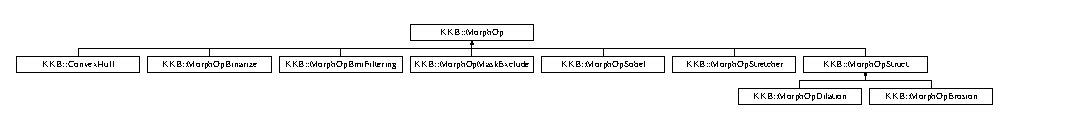
\includegraphics[height=1.173184cm]{class_k_k_b_1_1_morph_op}
\end{center}
\end{figure}
\subsection*{Public Types}
\begin{DoxyCompactItemize}
\item 
enum \hyperlink{class_k_k_b_1_1_morph_op_a9eaa0383bf9e046da208af397e7e35eb}{Mask\+Types} \+: int \{ \\*
\hyperlink{class_k_k_b_1_1_morph_op_a9eaa0383bf9e046da208af397e7e35ebab8adbcea9dda2cf69140a0a91baa97c6}{Mask\+Types\+::\+C\+R\+O\+S\+S3} = 0, 
\hyperlink{class_k_k_b_1_1_morph_op_a9eaa0383bf9e046da208af397e7e35ebaced59e40e96d9f0ddb32016f2a4548ac}{Mask\+Types\+::\+C\+R\+O\+S\+S5} = 1, 
\hyperlink{class_k_k_b_1_1_morph_op_a9eaa0383bf9e046da208af397e7e35eba8dc0b7886154fdf311e7035c58aff432}{Mask\+Types\+::\+S\+Q\+U\+A\+R\+E3} = 2, 
\hyperlink{class_k_k_b_1_1_morph_op_a9eaa0383bf9e046da208af397e7e35eba994ef51927c0f0dba502b2617d0e4032}{Mask\+Types\+::\+S\+Q\+U\+A\+R\+E5} = 3, 
\\*
\hyperlink{class_k_k_b_1_1_morph_op_a9eaa0383bf9e046da208af397e7e35ebad5dad206d5246f258a016929477ff19d}{Mask\+Types\+::\+S\+Q\+U\+A\+R\+E7} = 4, 
\hyperlink{class_k_k_b_1_1_morph_op_a9eaa0383bf9e046da208af397e7e35eba149bb2b5c5ab20dabf7fa6ff53a735c2}{Mask\+Types\+::\+S\+Q\+U\+A\+R\+E9} = 5, 
\hyperlink{class_k_k_b_1_1_morph_op_a9eaa0383bf9e046da208af397e7e35eba0c74025e0ba778162e957991c2d0fa76}{Mask\+Types\+::\+S\+Q\+U\+A\+R\+E11} = 6
 \}
\item 
enum \hyperlink{class_k_k_b_1_1_morph_op_a32070d9c14d16849873a8a409f5b0d69}{Operation\+Type} \{ \\*
\hyperlink{class_k_k_b_1_1_morph_op_a32070d9c14d16849873a8a409f5b0d69abbb93ef26e3c101ff11cdd21cab08a94}{Operation\+Type\+::\+Null}, 
\hyperlink{class_k_k_b_1_1_morph_op_a32070d9c14d16849873a8a409f5b0d69a84a4d9fd8033f883ce95cae8c5b9859a}{Operation\+Type\+::\+Binarize}, 
\hyperlink{class_k_k_b_1_1_morph_op_a32070d9c14d16849873a8a409f5b0d69adec56b6e36a679a85668cb49ce961a1f}{Operation\+Type\+::\+Bmi\+Filtering}, 
\hyperlink{class_k_k_b_1_1_morph_op_a32070d9c14d16849873a8a409f5b0d69a3e1ee9920ed982b5da9becaf4b5463e5}{Operation\+Type\+::\+Convex\+Hull}, 
\\*
\hyperlink{class_k_k_b_1_1_morph_op_a32070d9c14d16849873a8a409f5b0d69a5a870896d32acca70f912a0c11edca66}{Operation\+Type\+::\+Dilation}, 
\hyperlink{class_k_k_b_1_1_morph_op_a32070d9c14d16849873a8a409f5b0d69a35b6b7b81c8d146da93c09daa3875ea0}{Operation\+Type\+::\+Erosion}, 
\hyperlink{class_k_k_b_1_1_morph_op_a32070d9c14d16849873a8a409f5b0d69a2166273bd619a450f27a35e9c9e421c3}{Operation\+Type\+::\+Mask\+Exclude}, 
\hyperlink{class_k_k_b_1_1_morph_op_a32070d9c14d16849873a8a409f5b0d69ae9eb5dc5ac36ae1b3a4eb7c17def6093}{Operation\+Type\+::\+Sobel\+Edge\+Detection}, 
\\*
\hyperlink{class_k_k_b_1_1_morph_op_a32070d9c14d16849873a8a409f5b0d69a0a93701260be81cae9cf81aade6afaa1}{Operation\+Type\+::\+Stretcher}
 \}
\item 
enum \hyperlink{class_k_k_b_1_1_morph_op_a09e4aff7e81327849855ff72082d85b3}{Structure\+Type} \+: int \{ \hyperlink{class_k_k_b_1_1_morph_op_a09e4aff7e81327849855ff72082d85b3abbb93ef26e3c101ff11cdd21cab08a94}{Structure\+Type\+::\+Null}, 
\hyperlink{class_k_k_b_1_1_morph_op_a09e4aff7e81327849855ff72082d85b3afe6b37e55346afd2a8606e81a7982dc5}{Structure\+Type\+::st\+Cross}, 
\hyperlink{class_k_k_b_1_1_morph_op_a09e4aff7e81327849855ff72082d85b3a04505973fd476144464695ac6483e490}{Structure\+Type\+::st\+Square}
 \}
\end{DoxyCompactItemize}
\subsection*{Public Member Functions}
\begin{DoxyCompactItemize}
\item 
\hyperlink{class_k_k_b_1_1_morph_op_a087902e5cad640c26dfa24804cc2a974}{Morph\+Op} ()
\item 
virtual \hyperlink{class_k_k_b_1_1_morph_op_a489e376d1a5cf2939f52904f111b8c49}{$\sim$\+Morph\+Op} ()
\item 
virtual \hyperlink{class_k_k_b_1_1_morph_op_a32070d9c14d16849873a8a409f5b0d69}{Operation\+Type} \hyperlink{class_k_k_b_1_1_morph_op_abdf6f4bddae0b3cc3dc718559fa60234}{Operation} () const  =0
\item 
\hyperlink{class_k_k_b_1_1_morph_op_a32070d9c14d16849873a8a409f5b0d69}{Operation\+Type} \hyperlink{class_k_k_b_1_1_morph_op_a92d6ed26a570d8f7996b85dfeaeb4856}{Operation\+Type\+From\+Str} (const \hyperlink{class_k_k_b_1_1_k_k_str}{K\+K\+B\+::\+K\+K\+Str} \&\+\_\+operation\+Str)
\item 
\hyperlink{class_k_k_b_1_1_k_k_str}{K\+K\+B\+::\+K\+K\+Str} \hyperlink{class_k_k_b_1_1_morph_op_ae846fc671e95401a7e94912cd4f4ec41}{Operation\+Type\+To\+Str} (\hyperlink{class_k_k_b_1_1_morph_op_a32070d9c14d16849873a8a409f5b0d69}{Operation\+Type} \+\_\+operation)
\item 
virtual \hyperlink{namespace_k_k_b_a80d46bd24db644a022c863bce8ae3633}{Raster\+Ptr} \hyperlink{class_k_k_b_1_1_morph_op_ae7655bec44b6665fd042216e5cb55843}{Perform\+Operation} (\hyperlink{class_k_k_b_1_1_raster}{Raster} const $\ast$\+\_\+image)=0
\end{DoxyCompactItemize}
\subsection*{Static Public Member Functions}
\begin{DoxyCompactItemize}
\item 
static \hyperlink{namespace_k_k_b_a8fa4952cc84fda1de4bec1fbdd8d5b1b}{kkint32} \hyperlink{class_k_k_b_1_1_morph_op_affa9101a819e7103df69c8851cd7e920}{Biases} (\hyperlink{class_k_k_b_1_1_morph_op_a9eaa0383bf9e046da208af397e7e35eb}{Mask\+Types} mt)
\item 
static \hyperlink{class_k_k_b_1_1_morph_op_a09e4aff7e81327849855ff72082d85b3}{Structure\+Type} \hyperlink{class_k_k_b_1_1_morph_op_a7e477ebbb2c0cdd67388cb841685c02b}{Mask\+Shapes} (\hyperlink{class_k_k_b_1_1_morph_op_a9eaa0383bf9e046da208af397e7e35eb}{Mask\+Types} mt)
\end{DoxyCompactItemize}
\subsection*{Protected Member Functions}
\begin{DoxyCompactItemize}
\item 
bool \hyperlink{class_k_k_b_1_1_morph_op_a300c5117659d224d78f7b5a8d44ded91}{Background\+Pixel} (\hyperlink{namespace_k_k_b_ace9969169bf514f9ee6185186949cdf7}{uchar} pixel) const 
\item 
bool \hyperlink{class_k_k_b_1_1_morph_op_ab53f856a19c951a50178873c23bd5dd6}{Background\+Pixel} (\hyperlink{namespace_k_k_b_a8fa4952cc84fda1de4bec1fbdd8d5b1b}{kkint32} row, \hyperlink{namespace_k_k_b_a8fa4952cc84fda1de4bec1fbdd8d5b1b}{kkint32} col) const 
\item 
bool \hyperlink{class_k_k_b_1_1_morph_op_acd5541050c3c0207b004b71caf7fb1f4}{Foreground\+Pixel} (\hyperlink{namespace_k_k_b_ace9969169bf514f9ee6185186949cdf7}{uchar} pixel) const 
\item 
bool \hyperlink{class_k_k_b_1_1_morph_op_ac3ac8faa16c12502d2b7c50b79cedfe8}{Foreground\+Pixel} (\hyperlink{namespace_k_k_b_a8fa4952cc84fda1de4bec1fbdd8d5b1b}{kkint32} row, \hyperlink{namespace_k_k_b_a8fa4952cc84fda1de4bec1fbdd8d5b1b}{kkint32} col) const 
\item 
void \hyperlink{class_k_k_b_1_1_morph_op_a07c75e151d9b95ca13da3bfc2e48dba4}{Set\+Src\+Raster} (\hyperlink{namespace_k_k_b_a5acfa7402dc4df1769f90d3dc8ddfc2c}{Raster\+Const\+Ptr} \+\_\+src\+Raster)
\end{DoxyCompactItemize}
\subsection*{Protected Attributes}
\begin{DoxyCompactItemize}
\item 
\hyperlink{namespace_k_k_b_ace9969169bf514f9ee6185186949cdf7}{uchar} \hyperlink{class_k_k_b_1_1_morph_op_a0f9e76c2f2c45f0563567c49cd69a43b}{background\+Pixel\+TH}
\item 
\hyperlink{namespace_k_k_b_ace9969169bf514f9ee6185186949cdf7}{uchar} \hyperlink{class_k_k_b_1_1_morph_op_a0c3862d1c8427c4d246e0bcd56699741}{background\+Pixel\+Value}
\item 
\hyperlink{namespace_k_k_b_ace9969169bf514f9ee6185186949cdf7}{uchar} $\ast$const $\ast$ \hyperlink{class_k_k_b_1_1_morph_op_ad11edf2de07634c4c68df9a2e74cfd6c}{src\+Blue}
\item 
\hyperlink{namespace_k_k_b_ace9969169bf514f9ee6185186949cdf7}{uchar} const $\ast$ \hyperlink{class_k_k_b_1_1_morph_op_a52fcf660b2173a2b6e8988ed23cf638c}{src\+Blue\+Area}
\item 
bool \hyperlink{class_k_k_b_1_1_morph_op_a0cecdeb8369c7ab2689fbd9f997472b0}{src\+Color}
\item 
\hyperlink{namespace_k_k_b_ace9969169bf514f9ee6185186949cdf7}{uchar} $\ast$const $\ast$ \hyperlink{class_k_k_b_1_1_morph_op_ab811c702f7e0c8ffccdd21111c8144ab}{src\+Green}
\item 
\hyperlink{namespace_k_k_b_ace9969169bf514f9ee6185186949cdf7}{uchar} const $\ast$ \hyperlink{class_k_k_b_1_1_morph_op_a1a3372b8645c297f21c5805707aef8a0}{src\+Green\+Area}
\item 
\hyperlink{namespace_k_k_b_a8fa4952cc84fda1de4bec1fbdd8d5b1b}{kkint32} \hyperlink{class_k_k_b_1_1_morph_op_a54b2ce1b398a80803b4dbe8aef956b51}{src\+Height}
\item 
\hyperlink{namespace_k_k_b_a5acfa7402dc4df1769f90d3dc8ddfc2c}{Raster\+Const\+Ptr} \hyperlink{class_k_k_b_1_1_morph_op_a9af0ebff0135d124c7d1d17e21c4d7e6}{src\+Raster}
\item 
\hyperlink{namespace_k_k_b_ace9969169bf514f9ee6185186949cdf7}{uchar} $\ast$const $\ast$ \hyperlink{class_k_k_b_1_1_morph_op_a4d790e4b71cfdaecee876879663dfdb4}{src\+Red}
\item 
\hyperlink{namespace_k_k_b_ace9969169bf514f9ee6185186949cdf7}{uchar} const $\ast$ \hyperlink{class_k_k_b_1_1_morph_op_acd1f255803231ecfabc0609685e56abe}{src\+Red\+Area}
\item 
\hyperlink{namespace_k_k_b_a8fa4952cc84fda1de4bec1fbdd8d5b1b}{kkint32} \hyperlink{class_k_k_b_1_1_morph_op_aec2cfb3015497e4077751fc5f19559ab}{src\+Width}
\end{DoxyCompactItemize}
\subsection*{Static Protected Attributes}
\begin{DoxyCompactItemize}
\item 
static \hyperlink{namespace_k_k_b_a8fa4952cc84fda1de4bec1fbdd8d5b1b}{kkint32} \hyperlink{class_k_k_b_1_1_morph_op_a56600e618b25e7c2cda6f513645158e3}{biases} \mbox{[}$\,$\mbox{]}
\item 
static \hyperlink{class_k_k_b_1_1_morph_op_a09e4aff7e81327849855ff72082d85b3}{Structure\+Type} \hyperlink{class_k_k_b_1_1_morph_op_a7e8ac61b2b389a4b644566daee2972d4}{mask\+Shapes} \mbox{[}$\,$\mbox{]}
\end{DoxyCompactItemize}


\subsection{Detailed Description}
Base class for all Morphological operations. 

Creates a image where the only pixels that are passed thru are the ones that would be removed by the specified mask when a Open-\/\+Dilatation operation are performed.

Meant to be the base class to all Morphological operators.

It is assumed that all morphologocal operations will be working with a source image and returning a new modified image; the atcual operation is to be perfomed by the \char`\"{}\+Perform\+Operation\char`\"{} metho where you pass in a poiter to the source Image/ \hyperlink{class_k_k_b_1_1_raster}{Raster}. The the derived class would then call \char`\"{}\+Set\+Src\+Raster\char`\"{} to intialize the base class \char`\"{}\+Morph\+Op\char`\"{} with pointers to the source image.

\begin{DoxySeeAlso}{See also}
\hyperlink{class_k_k_b_1_1_raster}{K\+K\+B\+::\+Raster} 
\end{DoxySeeAlso}


Definition at line 44 of file Morph\+Op.\+h.



\subsection{Member Enumeration Documentation}
\index{K\+K\+B\+::\+Morph\+Op@{K\+K\+B\+::\+Morph\+Op}!Mask\+Types@{Mask\+Types}}
\index{Mask\+Types@{Mask\+Types}!K\+K\+B\+::\+Morph\+Op@{K\+K\+B\+::\+Morph\+Op}}
\subsubsection[{\texorpdfstring{Mask\+Types}{MaskTypes}}]{\setlength{\rightskip}{0pt plus 5cm}enum {\bf K\+K\+B\+::\+Morph\+Op\+::\+Mask\+Types} \+: int\hspace{0.3cm}{\ttfamily [strong]}}\hypertarget{class_k_k_b_1_1_morph_op_a9eaa0383bf9e046da208af397e7e35eb}{}\label{class_k_k_b_1_1_morph_op_a9eaa0383bf9e046da208af397e7e35eb}
\begin{Desc}
\item[Enumerator]\par
\begin{description}
\index{C\+R\+O\+S\+S3@{C\+R\+O\+S\+S3}!K\+K\+B\+::\+Morph\+Op@{K\+K\+B\+::\+Morph\+Op}}\index{K\+K\+B\+::\+Morph\+Op@{K\+K\+B\+::\+Morph\+Op}!C\+R\+O\+S\+S3@{C\+R\+O\+S\+S3}}\item[{\em 
C\+R\+O\+S\+S3\hypertarget{class_k_k_b_1_1_morph_op_a9eaa0383bf9e046da208af397e7e35ebab8adbcea9dda2cf69140a0a91baa97c6}{}\label{class_k_k_b_1_1_morph_op_a9eaa0383bf9e046da208af397e7e35ebab8adbcea9dda2cf69140a0a91baa97c6}
}]\index{C\+R\+O\+S\+S5@{C\+R\+O\+S\+S5}!K\+K\+B\+::\+Morph\+Op@{K\+K\+B\+::\+Morph\+Op}}\index{K\+K\+B\+::\+Morph\+Op@{K\+K\+B\+::\+Morph\+Op}!C\+R\+O\+S\+S5@{C\+R\+O\+S\+S5}}\item[{\em 
C\+R\+O\+S\+S5\hypertarget{class_k_k_b_1_1_morph_op_a9eaa0383bf9e046da208af397e7e35ebaced59e40e96d9f0ddb32016f2a4548ac}{}\label{class_k_k_b_1_1_morph_op_a9eaa0383bf9e046da208af397e7e35ebaced59e40e96d9f0ddb32016f2a4548ac}
}]\index{S\+Q\+U\+A\+R\+E3@{S\+Q\+U\+A\+R\+E3}!K\+K\+B\+::\+Morph\+Op@{K\+K\+B\+::\+Morph\+Op}}\index{K\+K\+B\+::\+Morph\+Op@{K\+K\+B\+::\+Morph\+Op}!S\+Q\+U\+A\+R\+E3@{S\+Q\+U\+A\+R\+E3}}\item[{\em 
S\+Q\+U\+A\+R\+E3\hypertarget{class_k_k_b_1_1_morph_op_a9eaa0383bf9e046da208af397e7e35eba8dc0b7886154fdf311e7035c58aff432}{}\label{class_k_k_b_1_1_morph_op_a9eaa0383bf9e046da208af397e7e35eba8dc0b7886154fdf311e7035c58aff432}
}]\index{S\+Q\+U\+A\+R\+E5@{S\+Q\+U\+A\+R\+E5}!K\+K\+B\+::\+Morph\+Op@{K\+K\+B\+::\+Morph\+Op}}\index{K\+K\+B\+::\+Morph\+Op@{K\+K\+B\+::\+Morph\+Op}!S\+Q\+U\+A\+R\+E5@{S\+Q\+U\+A\+R\+E5}}\item[{\em 
S\+Q\+U\+A\+R\+E5\hypertarget{class_k_k_b_1_1_morph_op_a9eaa0383bf9e046da208af397e7e35eba994ef51927c0f0dba502b2617d0e4032}{}\label{class_k_k_b_1_1_morph_op_a9eaa0383bf9e046da208af397e7e35eba994ef51927c0f0dba502b2617d0e4032}
}]\index{S\+Q\+U\+A\+R\+E7@{S\+Q\+U\+A\+R\+E7}!K\+K\+B\+::\+Morph\+Op@{K\+K\+B\+::\+Morph\+Op}}\index{K\+K\+B\+::\+Morph\+Op@{K\+K\+B\+::\+Morph\+Op}!S\+Q\+U\+A\+R\+E7@{S\+Q\+U\+A\+R\+E7}}\item[{\em 
S\+Q\+U\+A\+R\+E7\hypertarget{class_k_k_b_1_1_morph_op_a9eaa0383bf9e046da208af397e7e35ebad5dad206d5246f258a016929477ff19d}{}\label{class_k_k_b_1_1_morph_op_a9eaa0383bf9e046da208af397e7e35ebad5dad206d5246f258a016929477ff19d}
}]\index{S\+Q\+U\+A\+R\+E9@{S\+Q\+U\+A\+R\+E9}!K\+K\+B\+::\+Morph\+Op@{K\+K\+B\+::\+Morph\+Op}}\index{K\+K\+B\+::\+Morph\+Op@{K\+K\+B\+::\+Morph\+Op}!S\+Q\+U\+A\+R\+E9@{S\+Q\+U\+A\+R\+E9}}\item[{\em 
S\+Q\+U\+A\+R\+E9\hypertarget{class_k_k_b_1_1_morph_op_a9eaa0383bf9e046da208af397e7e35eba149bb2b5c5ab20dabf7fa6ff53a735c2}{}\label{class_k_k_b_1_1_morph_op_a9eaa0383bf9e046da208af397e7e35eba149bb2b5c5ab20dabf7fa6ff53a735c2}
}]\index{S\+Q\+U\+A\+R\+E11@{S\+Q\+U\+A\+R\+E11}!K\+K\+B\+::\+Morph\+Op@{K\+K\+B\+::\+Morph\+Op}}\index{K\+K\+B\+::\+Morph\+Op@{K\+K\+B\+::\+Morph\+Op}!S\+Q\+U\+A\+R\+E11@{S\+Q\+U\+A\+R\+E11}}\item[{\em 
S\+Q\+U\+A\+R\+E11\hypertarget{class_k_k_b_1_1_morph_op_a9eaa0383bf9e046da208af397e7e35eba0c74025e0ba778162e957991c2d0fa76}{}\label{class_k_k_b_1_1_morph_op_a9eaa0383bf9e046da208af397e7e35eba0c74025e0ba778162e957991c2d0fa76}
}]\end{description}
\end{Desc}


Definition at line 72 of file Morph\+Op.\+h.


\begin{DoxyCode}
72                          : \textcolor{keywordtype}{int}
73     \{
74       CROSS3   = 0,
75       CROSS5   = 1,
76       SQUARE3  = 2,
77       SQUARE5  = 3,
78       SQUARE7  = 4,
79       SQUARE9  = 5,
80       SQUARE11 = 6
81     \};
\end{DoxyCode}
\index{K\+K\+B\+::\+Morph\+Op@{K\+K\+B\+::\+Morph\+Op}!Operation\+Type@{Operation\+Type}}
\index{Operation\+Type@{Operation\+Type}!K\+K\+B\+::\+Morph\+Op@{K\+K\+B\+::\+Morph\+Op}}
\subsubsection[{\texorpdfstring{Operation\+Type}{OperationType}}]{\setlength{\rightskip}{0pt plus 5cm}enum {\bf K\+K\+B\+::\+Morph\+Op\+::\+Operation\+Type}\hspace{0.3cm}{\ttfamily [strong]}}\hypertarget{class_k_k_b_1_1_morph_op_a32070d9c14d16849873a8a409f5b0d69}{}\label{class_k_k_b_1_1_morph_op_a32070d9c14d16849873a8a409f5b0d69}
\begin{Desc}
\item[Enumerator]\par
\begin{description}
\index{Null@{Null}!K\+K\+B\+::\+Morph\+Op@{K\+K\+B\+::\+Morph\+Op}}\index{K\+K\+B\+::\+Morph\+Op@{K\+K\+B\+::\+Morph\+Op}!Null@{Null}}\item[{\em 
Null\hypertarget{class_k_k_b_1_1_morph_op_a32070d9c14d16849873a8a409f5b0d69abbb93ef26e3c101ff11cdd21cab08a94}{}\label{class_k_k_b_1_1_morph_op_a32070d9c14d16849873a8a409f5b0d69abbb93ef26e3c101ff11cdd21cab08a94}
}]\index{Binarize@{Binarize}!K\+K\+B\+::\+Morph\+Op@{K\+K\+B\+::\+Morph\+Op}}\index{K\+K\+B\+::\+Morph\+Op@{K\+K\+B\+::\+Morph\+Op}!Binarize@{Binarize}}\item[{\em 
Binarize\hypertarget{class_k_k_b_1_1_morph_op_a32070d9c14d16849873a8a409f5b0d69a84a4d9fd8033f883ce95cae8c5b9859a}{}\label{class_k_k_b_1_1_morph_op_a32070d9c14d16849873a8a409f5b0d69a84a4d9fd8033f883ce95cae8c5b9859a}
}]\index{Bmi\+Filtering@{Bmi\+Filtering}!K\+K\+B\+::\+Morph\+Op@{K\+K\+B\+::\+Morph\+Op}}\index{K\+K\+B\+::\+Morph\+Op@{K\+K\+B\+::\+Morph\+Op}!Bmi\+Filtering@{Bmi\+Filtering}}\item[{\em 
Bmi\+Filtering\hypertarget{class_k_k_b_1_1_morph_op_a32070d9c14d16849873a8a409f5b0d69adec56b6e36a679a85668cb49ce961a1f}{}\label{class_k_k_b_1_1_morph_op_a32070d9c14d16849873a8a409f5b0d69adec56b6e36a679a85668cb49ce961a1f}
}]\index{Convex\+Hull@{Convex\+Hull}!K\+K\+B\+::\+Morph\+Op@{K\+K\+B\+::\+Morph\+Op}}\index{K\+K\+B\+::\+Morph\+Op@{K\+K\+B\+::\+Morph\+Op}!Convex\+Hull@{Convex\+Hull}}\item[{\em 
Convex\+Hull\hypertarget{class_k_k_b_1_1_morph_op_a32070d9c14d16849873a8a409f5b0d69a3e1ee9920ed982b5da9becaf4b5463e5}{}\label{class_k_k_b_1_1_morph_op_a32070d9c14d16849873a8a409f5b0d69a3e1ee9920ed982b5da9becaf4b5463e5}
}]\index{Dilation@{Dilation}!K\+K\+B\+::\+Morph\+Op@{K\+K\+B\+::\+Morph\+Op}}\index{K\+K\+B\+::\+Morph\+Op@{K\+K\+B\+::\+Morph\+Op}!Dilation@{Dilation}}\item[{\em 
Dilation\hypertarget{class_k_k_b_1_1_morph_op_a32070d9c14d16849873a8a409f5b0d69a5a870896d32acca70f912a0c11edca66}{}\label{class_k_k_b_1_1_morph_op_a32070d9c14d16849873a8a409f5b0d69a5a870896d32acca70f912a0c11edca66}
}]\index{Erosion@{Erosion}!K\+K\+B\+::\+Morph\+Op@{K\+K\+B\+::\+Morph\+Op}}\index{K\+K\+B\+::\+Morph\+Op@{K\+K\+B\+::\+Morph\+Op}!Erosion@{Erosion}}\item[{\em 
Erosion\hypertarget{class_k_k_b_1_1_morph_op_a32070d9c14d16849873a8a409f5b0d69a35b6b7b81c8d146da93c09daa3875ea0}{}\label{class_k_k_b_1_1_morph_op_a32070d9c14d16849873a8a409f5b0d69a35b6b7b81c8d146da93c09daa3875ea0}
}]\index{Mask\+Exclude@{Mask\+Exclude}!K\+K\+B\+::\+Morph\+Op@{K\+K\+B\+::\+Morph\+Op}}\index{K\+K\+B\+::\+Morph\+Op@{K\+K\+B\+::\+Morph\+Op}!Mask\+Exclude@{Mask\+Exclude}}\item[{\em 
Mask\+Exclude\hypertarget{class_k_k_b_1_1_morph_op_a32070d9c14d16849873a8a409f5b0d69a2166273bd619a450f27a35e9c9e421c3}{}\label{class_k_k_b_1_1_morph_op_a32070d9c14d16849873a8a409f5b0d69a2166273bd619a450f27a35e9c9e421c3}
}]\index{Sobel\+Edge\+Detection@{Sobel\+Edge\+Detection}!K\+K\+B\+::\+Morph\+Op@{K\+K\+B\+::\+Morph\+Op}}\index{K\+K\+B\+::\+Morph\+Op@{K\+K\+B\+::\+Morph\+Op}!Sobel\+Edge\+Detection@{Sobel\+Edge\+Detection}}\item[{\em 
Sobel\+Edge\+Detection\hypertarget{class_k_k_b_1_1_morph_op_a32070d9c14d16849873a8a409f5b0d69ae9eb5dc5ac36ae1b3a4eb7c17def6093}{}\label{class_k_k_b_1_1_morph_op_a32070d9c14d16849873a8a409f5b0d69ae9eb5dc5ac36ae1b3a4eb7c17def6093}
}]\index{Stretcher@{Stretcher}!K\+K\+B\+::\+Morph\+Op@{K\+K\+B\+::\+Morph\+Op}}\index{K\+K\+B\+::\+Morph\+Op@{K\+K\+B\+::\+Morph\+Op}!Stretcher@{Stretcher}}\item[{\em 
Stretcher\hypertarget{class_k_k_b_1_1_morph_op_a32070d9c14d16849873a8a409f5b0d69a0a93701260be81cae9cf81aade6afaa1}{}\label{class_k_k_b_1_1_morph_op_a32070d9c14d16849873a8a409f5b0d69a0a93701260be81cae9cf81aade6afaa1}
}]\end{description}
\end{Desc}


Definition at line 47 of file Morph\+Op.\+h.


\begin{DoxyCode}
48     \{
49       \hyperlink{namespace_k_k_m_l_l_ad917464bc631109a3021cf02cd27af9aabbb93ef26e3c101ff11cdd21cab08a94}{Null},
50       Binarize,
51       BmiFiltering,
52       ConvexHull,
53       Dilation,
54       Erosion,
55       MaskExclude,
56       SobelEdgeDetection,
57       Stretcher
58     \};
\end{DoxyCode}
\index{K\+K\+B\+::\+Morph\+Op@{K\+K\+B\+::\+Morph\+Op}!Structure\+Type@{Structure\+Type}}
\index{Structure\+Type@{Structure\+Type}!K\+K\+B\+::\+Morph\+Op@{K\+K\+B\+::\+Morph\+Op}}
\subsubsection[{\texorpdfstring{Structure\+Type}{StructureType}}]{\setlength{\rightskip}{0pt plus 5cm}enum {\bf K\+K\+B\+::\+Morph\+Op\+::\+Structure\+Type} \+: int\hspace{0.3cm}{\ttfamily [strong]}}\hypertarget{class_k_k_b_1_1_morph_op_a09e4aff7e81327849855ff72082d85b3}{}\label{class_k_k_b_1_1_morph_op_a09e4aff7e81327849855ff72082d85b3}
\begin{Desc}
\item[Enumerator]\par
\begin{description}
\index{Null@{Null}!K\+K\+B\+::\+Morph\+Op@{K\+K\+B\+::\+Morph\+Op}}\index{K\+K\+B\+::\+Morph\+Op@{K\+K\+B\+::\+Morph\+Op}!Null@{Null}}\item[{\em 
Null\hypertarget{class_k_k_b_1_1_morph_op_a09e4aff7e81327849855ff72082d85b3abbb93ef26e3c101ff11cdd21cab08a94}{}\label{class_k_k_b_1_1_morph_op_a09e4aff7e81327849855ff72082d85b3abbb93ef26e3c101ff11cdd21cab08a94}
}]\index{st\+Cross@{st\+Cross}!K\+K\+B\+::\+Morph\+Op@{K\+K\+B\+::\+Morph\+Op}}\index{K\+K\+B\+::\+Morph\+Op@{K\+K\+B\+::\+Morph\+Op}!st\+Cross@{st\+Cross}}\item[{\em 
st\+Cross\hypertarget{class_k_k_b_1_1_morph_op_a09e4aff7e81327849855ff72082d85b3afe6b37e55346afd2a8606e81a7982dc5}{}\label{class_k_k_b_1_1_morph_op_a09e4aff7e81327849855ff72082d85b3afe6b37e55346afd2a8606e81a7982dc5}
}]\index{st\+Square@{st\+Square}!K\+K\+B\+::\+Morph\+Op@{K\+K\+B\+::\+Morph\+Op}}\index{K\+K\+B\+::\+Morph\+Op@{K\+K\+B\+::\+Morph\+Op}!st\+Square@{st\+Square}}\item[{\em 
st\+Square\hypertarget{class_k_k_b_1_1_morph_op_a09e4aff7e81327849855ff72082d85b3a04505973fd476144464695ac6483e490}{}\label{class_k_k_b_1_1_morph_op_a09e4aff7e81327849855ff72082d85b3a04505973fd476144464695ac6483e490}
}]\end{description}
\end{Desc}


Definition at line 64 of file Morph\+Op.\+h.


\begin{DoxyCode}
64                              : \textcolor{keywordtype}{int}
65     \{
66        \hyperlink{namespace_k_k_m_l_l_ad917464bc631109a3021cf02cd27af9aabbb93ef26e3c101ff11cdd21cab08a94}{Null},
67        stCross,
68        stSquare
69     \};
\end{DoxyCode}


\subsection{Constructor \& Destructor Documentation}
\index{K\+K\+B\+::\+Morph\+Op@{K\+K\+B\+::\+Morph\+Op}!Morph\+Op@{Morph\+Op}}
\index{Morph\+Op@{Morph\+Op}!K\+K\+B\+::\+Morph\+Op@{K\+K\+B\+::\+Morph\+Op}}
\subsubsection[{\texorpdfstring{Morph\+Op()}{MorphOp()}}]{\setlength{\rightskip}{0pt plus 5cm}Morph\+Op\+::\+Morph\+Op (
\begin{DoxyParamCaption}
{}
\end{DoxyParamCaption}
)}\hypertarget{class_k_k_b_1_1_morph_op_a087902e5cad640c26dfa24804cc2a974}{}\label{class_k_k_b_1_1_morph_op_a087902e5cad640c26dfa24804cc2a974}


Definition at line 73 of file Morph\+Op.\+cpp.



References background\+Pixel\+TH, background\+Pixel\+Value, src\+Blue, src\+Blue\+Area, src\+Color, src\+Green, src\+Green\+Area, src\+Height, src\+Raster, src\+Red, src\+Red\+Area, and src\+Width.



Referenced by K\+K\+B\+::\+Convex\+Hull\+::\+Convex\+Hull(), K\+K\+B\+::\+Morph\+Op\+Binarize\+::\+Morph\+Op\+Binarize(), K\+K\+B\+::\+Morph\+Op\+Bmi\+Filtering\+::\+Morph\+Op\+Bmi\+Filtering(), K\+K\+B\+::\+Morph\+Op\+Mask\+Exclude\+::\+Morph\+Op\+Mask\+Exclude(), K\+K\+B\+::\+Morph\+Op\+Stretcher\+::\+Morph\+Op\+Stretcher(), and K\+K\+B\+::\+Morph\+Op\+Struct\+::\+Morph\+Op\+Struct().


\begin{DoxyCode}
73                  :
74     \hyperlink{class_k_k_b_1_1_morph_op_a0f9e76c2f2c45f0563567c49cd69a43b}{backgroundPixelTH}    (31),
75     \hyperlink{class_k_k_b_1_1_morph_op_a0c3862d1c8427c4d246e0bcd56699741}{backgroundPixelValue} (0),
76     \hyperlink{class_k_k_b_1_1_morph_op_a9af0ebff0135d124c7d1d17e21c4d7e6}{srcRaster}            (NULL),
77     \hyperlink{class_k_k_b_1_1_morph_op_acd1f255803231ecfabc0609685e56abe}{srcRedArea}           (NULL),
78     \hyperlink{class_k_k_b_1_1_morph_op_a1a3372b8645c297f21c5805707aef8a0}{srcGreenArea}         (NULL),
79     \hyperlink{class_k_k_b_1_1_morph_op_a52fcf660b2173a2b6e8988ed23cf638c}{srcBlueArea}          (NULL),
80     \hyperlink{class_k_k_b_1_1_morph_op_a4d790e4b71cfdaecee876879663dfdb4}{srcRed}               (NULL),
81     \hyperlink{class_k_k_b_1_1_morph_op_ab811c702f7e0c8ffccdd21111c8144ab}{srcGreen}             (NULL),
82     \hyperlink{class_k_k_b_1_1_morph_op_ad11edf2de07634c4c68df9a2e74cfd6c}{srcBlue}              (NULL),
83     \hyperlink{class_k_k_b_1_1_morph_op_a0cecdeb8369c7ab2689fbd9f997472b0}{srcColor}             (\textcolor{keyword}{false}),
84     \hyperlink{class_k_k_b_1_1_morph_op_a54b2ce1b398a80803b4dbe8aef956b51}{srcHeight}            (0),
85     \hyperlink{class_k_k_b_1_1_morph_op_aec2cfb3015497e4077751fc5f19559ab}{srcWidth}             (0)
86 \{
87 \}
\end{DoxyCode}
\index{K\+K\+B\+::\+Morph\+Op@{K\+K\+B\+::\+Morph\+Op}!````~Morph\+Op@{$\sim$\+Morph\+Op}}
\index{````~Morph\+Op@{$\sim$\+Morph\+Op}!K\+K\+B\+::\+Morph\+Op@{K\+K\+B\+::\+Morph\+Op}}
\subsubsection[{\texorpdfstring{$\sim$\+Morph\+Op()}{~MorphOp()}}]{\setlength{\rightskip}{0pt plus 5cm}Morph\+Op\+::$\sim$\+Morph\+Op (
\begin{DoxyParamCaption}
{}
\end{DoxyParamCaption}
)\hspace{0.3cm}{\ttfamily [virtual]}}\hypertarget{class_k_k_b_1_1_morph_op_a489e376d1a5cf2939f52904f111b8c49}{}\label{class_k_k_b_1_1_morph_op_a489e376d1a5cf2939f52904f111b8c49}


Definition at line 91 of file Morph\+Op.\+cpp.


\begin{DoxyCode}
92 \{
93 \}
\end{DoxyCode}


\subsection{Member Function Documentation}
\index{K\+K\+B\+::\+Morph\+Op@{K\+K\+B\+::\+Morph\+Op}!Background\+Pixel@{Background\+Pixel}}
\index{Background\+Pixel@{Background\+Pixel}!K\+K\+B\+::\+Morph\+Op@{K\+K\+B\+::\+Morph\+Op}}
\subsubsection[{\texorpdfstring{Background\+Pixel(uchar pixel) const }{BackgroundPixel(uchar pixel) const }}]{\setlength{\rightskip}{0pt plus 5cm}bool Morph\+Op\+::\+Background\+Pixel (
\begin{DoxyParamCaption}
\item[{{\bf uchar}}]{pixel}
\end{DoxyParamCaption}
) const\hspace{0.3cm}{\ttfamily [protected]}}\hypertarget{class_k_k_b_1_1_morph_op_a300c5117659d224d78f7b5a8d44ded91}{}\label{class_k_k_b_1_1_morph_op_a300c5117659d224d78f7b5a8d44ded91}


Definition at line 171 of file Morph\+Op.\+cpp.



References background\+Pixel\+TH.



Referenced by K\+K\+B\+::\+Morph\+Op\+Struct\+::\+Fit(), K\+K\+B\+::\+Morph\+Op\+Struct\+::\+Fit\+Background\+Count(), and K\+K\+B\+::\+Morph\+Op\+Dilation\+::\+Perform\+Operation().


\begin{DoxyCode}
172 \{
173   \textcolor{keywordflow}{return} (pixel <= \hyperlink{class_k_k_b_1_1_morph_op_a0f9e76c2f2c45f0563567c49cd69a43b}{backgroundPixelTH});
174 \}  \textcolor{comment}{/* BackgroundPixel */}
\end{DoxyCode}
\index{K\+K\+B\+::\+Morph\+Op@{K\+K\+B\+::\+Morph\+Op}!Background\+Pixel@{Background\+Pixel}}
\index{Background\+Pixel@{Background\+Pixel}!K\+K\+B\+::\+Morph\+Op@{K\+K\+B\+::\+Morph\+Op}}
\subsubsection[{\texorpdfstring{Background\+Pixel(kkint32 row, kkint32 col) const }{BackgroundPixel(kkint32 row, kkint32 col) const }}]{\setlength{\rightskip}{0pt plus 5cm}bool Morph\+Op\+::\+Background\+Pixel (
\begin{DoxyParamCaption}
\item[{{\bf kkint32}}]{row, }
\item[{{\bf kkint32}}]{col}
\end{DoxyParamCaption}
) const\hspace{0.3cm}{\ttfamily [protected]}}\hypertarget{class_k_k_b_1_1_morph_op_ab53f856a19c951a50178873c23bd5dd6}{}\label{class_k_k_b_1_1_morph_op_ab53f856a19c951a50178873c23bd5dd6}


Definition at line 178 of file Morph\+Op.\+cpp.



References background\+Pixel\+TH, src\+Green, src\+Height, and src\+Width.


\begin{DoxyCode}
181 \{
182   \textcolor{keywordflow}{if}  ((row < 0)           ||  
183        (row >= \hyperlink{class_k_k_b_1_1_morph_op_a54b2ce1b398a80803b4dbe8aef956b51}{srcHeight})  ||
184        (col < 0)           ||
185        (col >= \hyperlink{class_k_k_b_1_1_morph_op_aec2cfb3015497e4077751fc5f19559ab}{srcWidth})   ||
186        (\hyperlink{class_k_k_b_1_1_morph_op_ab811c702f7e0c8ffccdd21111c8144ab}{srcGreen} == NULL)
187       )
188     \textcolor{keywordflow}{return} \textcolor{keyword}{false};
189 
190   \textcolor{keywordflow}{return} (\hyperlink{class_k_k_b_1_1_morph_op_ab811c702f7e0c8ffccdd21111c8144ab}{srcGreen}[row][col] <= \hyperlink{class_k_k_b_1_1_morph_op_a0f9e76c2f2c45f0563567c49cd69a43b}{backgroundPixelTH});
191 \}  \textcolor{comment}{/* BackgroundPixel */}
\end{DoxyCode}
\index{K\+K\+B\+::\+Morph\+Op@{K\+K\+B\+::\+Morph\+Op}!Biases@{Biases}}
\index{Biases@{Biases}!K\+K\+B\+::\+Morph\+Op@{K\+K\+B\+::\+Morph\+Op}}
\subsubsection[{\texorpdfstring{Biases(\+Mask\+Types mt)}{Biases(MaskTypes mt)}}]{\setlength{\rightskip}{0pt plus 5cm}{\bf kkint32} Morph\+Op\+::\+Biases (
\begin{DoxyParamCaption}
\item[{{\bf Mask\+Types}}]{mt}
\end{DoxyParamCaption}
)\hspace{0.3cm}{\ttfamily [static]}}\hypertarget{class_k_k_b_1_1_morph_op_affa9101a819e7103df69c8851cd7e920}{}\label{class_k_k_b_1_1_morph_op_affa9101a819e7103df69c8851cd7e920}


Definition at line 44 of file Morph\+Op.\+cpp.



References biases, C\+R\+O\+S\+S3, and S\+Q\+U\+A\+R\+E9.



Referenced by K\+K\+B\+::\+Raster\+::\+Erosion(), K\+K\+B\+::\+Raster\+::\+Erosion\+Boundary(), K\+K\+B\+::\+Raster\+::\+Erosion\+Changed(), K\+K\+B\+::\+Raster\+::\+Erosion\+Changed1(), and K\+K\+B\+::\+Raster\+::\+Raster().


\begin{DoxyCode}
45 \{
46   \textcolor{keywordflow}{if}  (mt < \hyperlink{class_k_k_b_1_1_morph_op_a9eaa0383bf9e046da208af397e7e35ebab8adbcea9dda2cf69140a0a91baa97c6}{MaskTypes::CROSS3})
47     mt = \hyperlink{class_k_k_b_1_1_morph_op_a9eaa0383bf9e046da208af397e7e35ebab8adbcea9dda2cf69140a0a91baa97c6}{MaskTypes::CROSS3};
48 
49   \textcolor{keywordflow}{else} \textcolor{keywordflow}{if}  (mt > \hyperlink{class_k_k_b_1_1_morph_op_a9eaa0383bf9e046da208af397e7e35eba149bb2b5c5ab20dabf7fa6ff53a735c2}{MaskTypes::SQUARE9})
50     mt = \hyperlink{class_k_k_b_1_1_morph_op_a9eaa0383bf9e046da208af397e7e35eba149bb2b5c5ab20dabf7fa6ff53a735c2}{MaskTypes::SQUARE9};
51 
52   \textcolor{keywordflow}{return}  \hyperlink{class_k_k_b_1_1_morph_op_a56600e618b25e7c2cda6f513645158e3}{biases}[(int)mt];
53 \}
\end{DoxyCode}
\index{K\+K\+B\+::\+Morph\+Op@{K\+K\+B\+::\+Morph\+Op}!Foreground\+Pixel@{Foreground\+Pixel}}
\index{Foreground\+Pixel@{Foreground\+Pixel}!K\+K\+B\+::\+Morph\+Op@{K\+K\+B\+::\+Morph\+Op}}
\subsubsection[{\texorpdfstring{Foreground\+Pixel(uchar pixel) const }{ForegroundPixel(uchar pixel) const }}]{\setlength{\rightskip}{0pt plus 5cm}bool Morph\+Op\+::\+Foreground\+Pixel (
\begin{DoxyParamCaption}
\item[{{\bf uchar}}]{pixel}
\end{DoxyParamCaption}
) const\hspace{0.3cm}{\ttfamily [protected]}}\hypertarget{class_k_k_b_1_1_morph_op_acd5541050c3c0207b004b71caf7fb1f4}{}\label{class_k_k_b_1_1_morph_op_acd5541050c3c0207b004b71caf7fb1f4}


Definition at line 195 of file Morph\+Op.\+cpp.



References background\+Pixel\+TH.



Referenced by K\+K\+B\+::\+Morph\+Op\+Struct\+::\+Hit\+Foreground\+Count(), K\+K\+B\+::\+Morph\+Op\+Dilation\+::\+Perform\+Operation(), and K\+K\+B\+::\+Morph\+Op\+Erosion\+::\+Perform\+Operation().


\begin{DoxyCode}
196 \{
197   \textcolor{keywordflow}{return} (pixel > \hyperlink{class_k_k_b_1_1_morph_op_a0f9e76c2f2c45f0563567c49cd69a43b}{backgroundPixelTH});
198 \}  \textcolor{comment}{/* ForegroundPixel */}
\end{DoxyCode}
\index{K\+K\+B\+::\+Morph\+Op@{K\+K\+B\+::\+Morph\+Op}!Foreground\+Pixel@{Foreground\+Pixel}}
\index{Foreground\+Pixel@{Foreground\+Pixel}!K\+K\+B\+::\+Morph\+Op@{K\+K\+B\+::\+Morph\+Op}}
\subsubsection[{\texorpdfstring{Foreground\+Pixel(kkint32 row, kkint32 col) const }{ForegroundPixel(kkint32 row, kkint32 col) const }}]{\setlength{\rightskip}{0pt plus 5cm}bool Morph\+Op\+::\+Foreground\+Pixel (
\begin{DoxyParamCaption}
\item[{{\bf kkint32}}]{row, }
\item[{{\bf kkint32}}]{col}
\end{DoxyParamCaption}
) const\hspace{0.3cm}{\ttfamily [protected]}}\hypertarget{class_k_k_b_1_1_morph_op_ac3ac8faa16c12502d2b7c50b79cedfe8}{}\label{class_k_k_b_1_1_morph_op_ac3ac8faa16c12502d2b7c50b79cedfe8}


Definition at line 202 of file Morph\+Op.\+cpp.



References background\+Pixel\+TH, src\+Green, src\+Height, and src\+Width.



Referenced by K\+K\+B\+::\+Convex\+Hull\+::\+Store().


\begin{DoxyCode}
205 \{
206   \textcolor{keywordflow}{if}  ((row < 0)           ||  
207        (row >= \hyperlink{class_k_k_b_1_1_morph_op_a54b2ce1b398a80803b4dbe8aef956b51}{srcHeight})  ||
208        (col < 0)           ||
209        (col >= \hyperlink{class_k_k_b_1_1_morph_op_aec2cfb3015497e4077751fc5f19559ab}{srcWidth})   ||
210        (\hyperlink{class_k_k_b_1_1_morph_op_ab811c702f7e0c8ffccdd21111c8144ab}{srcGreen} == NULL)
211       )
212     \textcolor{keywordflow}{return} \textcolor{keyword}{false};
213 
214   \textcolor{keywordflow}{return} (\hyperlink{class_k_k_b_1_1_morph_op_ab811c702f7e0c8ffccdd21111c8144ab}{srcGreen}[row][col] > \hyperlink{class_k_k_b_1_1_morph_op_a0f9e76c2f2c45f0563567c49cd69a43b}{backgroundPixelTH});
215 \}  \textcolor{comment}{/* ForegroundPixel */}
\end{DoxyCode}
\index{K\+K\+B\+::\+Morph\+Op@{K\+K\+B\+::\+Morph\+Op}!Mask\+Shapes@{Mask\+Shapes}}
\index{Mask\+Shapes@{Mask\+Shapes}!K\+K\+B\+::\+Morph\+Op@{K\+K\+B\+::\+Morph\+Op}}
\subsubsection[{\texorpdfstring{Mask\+Shapes(\+Mask\+Types mt)}{MaskShapes(MaskTypes mt)}}]{\setlength{\rightskip}{0pt plus 5cm}{\bf Structure\+Type} Morph\+Op\+::\+Mask\+Shapes (
\begin{DoxyParamCaption}
\item[{{\bf Mask\+Types}}]{mt}
\end{DoxyParamCaption}
)\hspace{0.3cm}{\ttfamily [static]}}\hypertarget{class_k_k_b_1_1_morph_op_a7e477ebbb2c0cdd67388cb841685c02b}{}\label{class_k_k_b_1_1_morph_op_a7e477ebbb2c0cdd67388cb841685c02b}


Definition at line 57 of file Morph\+Op.\+cpp.



References C\+R\+O\+S\+S3, mask\+Shapes, and S\+Q\+U\+A\+R\+E9.



Referenced by K\+K\+B\+::\+Raster\+::\+Erosion(), K\+K\+B\+::\+Raster\+::\+Erosion\+Boundary(), K\+K\+B\+::\+Raster\+::\+Erosion\+Changed(), and K\+K\+B\+::\+Raster\+::\+Erosion\+Changed1().


\begin{DoxyCode}
58 \{
59   \textcolor{keywordflow}{if}  (mt < \hyperlink{class_k_k_b_1_1_morph_op_a9eaa0383bf9e046da208af397e7e35ebab8adbcea9dda2cf69140a0a91baa97c6}{MaskTypes::CROSS3})
60     mt = \hyperlink{class_k_k_b_1_1_morph_op_a9eaa0383bf9e046da208af397e7e35ebab8adbcea9dda2cf69140a0a91baa97c6}{MaskTypes::CROSS3};
61 
62   \textcolor{keywordflow}{else} \textcolor{keywordflow}{if}  (mt > \hyperlink{class_k_k_b_1_1_morph_op_a9eaa0383bf9e046da208af397e7e35eba149bb2b5c5ab20dabf7fa6ff53a735c2}{MaskTypes::SQUARE9})
63     mt = \hyperlink{class_k_k_b_1_1_morph_op_a9eaa0383bf9e046da208af397e7e35eba149bb2b5c5ab20dabf7fa6ff53a735c2}{MaskTypes::SQUARE9};
64 
65   \textcolor{keywordflow}{return}  \hyperlink{class_k_k_b_1_1_morph_op_a7e8ac61b2b389a4b644566daee2972d4}{maskShapes}[(int)mt];
66 \}
\end{DoxyCode}
\index{K\+K\+B\+::\+Morph\+Op@{K\+K\+B\+::\+Morph\+Op}!Operation@{Operation}}
\index{Operation@{Operation}!K\+K\+B\+::\+Morph\+Op@{K\+K\+B\+::\+Morph\+Op}}
\subsubsection[{\texorpdfstring{Operation() const  =0}{Operation() const  =0}}]{\setlength{\rightskip}{0pt plus 5cm}virtual {\bf Operation\+Type} K\+K\+B\+::\+Morph\+Op\+::\+Operation (
\begin{DoxyParamCaption}
{}
\end{DoxyParamCaption}
) const\hspace{0.3cm}{\ttfamily [pure virtual]}}\hypertarget{class_k_k_b_1_1_morph_op_abdf6f4bddae0b3cc3dc718559fa60234}{}\label{class_k_k_b_1_1_morph_op_abdf6f4bddae0b3cc3dc718559fa60234}


Implemented in \hyperlink{class_k_k_b_1_1_convex_hull_ac540f936d8466f22b98246b2ddb71123}{K\+K\+B\+::\+Convex\+Hull}, \hyperlink{class_k_k_b_1_1_morph_op_mask_exclude_a084a3e895aada937a5f24255a868635f}{K\+K\+B\+::\+Morph\+Op\+Mask\+Exclude}, \hyperlink{class_k_k_b_1_1_morph_op_stretcher_afdf127ebc560ce9579355f2700952d92}{K\+K\+B\+::\+Morph\+Op\+Stretcher}, \hyperlink{class_k_k_b_1_1_morph_op_binarize_a4f06fa91ef03dca96bf2f1494da85678}{K\+K\+B\+::\+Morph\+Op\+Binarize}, \hyperlink{class_k_k_b_1_1_morph_op_struct_a3cbbeb9ce7ce8856bc01d1c0b1b478a8}{K\+K\+B\+::\+Morph\+Op\+Struct}, \hyperlink{class_k_k_b_1_1_morph_op_dilation_a159a05bfd9fc2af7a07fe22edcde0ef8}{K\+K\+B\+::\+Morph\+Op\+Dilation}, \hyperlink{class_k_k_b_1_1_morph_op_erosion_a3fa77279197c70aed5ef55968eb2704a}{K\+K\+B\+::\+Morph\+Op\+Erosion}, \hyperlink{class_k_k_b_1_1_morph_op_bmi_filtering_aeee8c13f949e1a253f76acc2973bfe60}{K\+K\+B\+::\+Morph\+Op\+Bmi\+Filtering}, and \hyperlink{class_k_k_b_1_1_morph_op_sobel_a0c11ea47d46bbe8c365db296672f0595}{K\+K\+B\+::\+Morph\+Op\+Sobel}.

\index{K\+K\+B\+::\+Morph\+Op@{K\+K\+B\+::\+Morph\+Op}!Operation\+Type\+From\+Str@{Operation\+Type\+From\+Str}}
\index{Operation\+Type\+From\+Str@{Operation\+Type\+From\+Str}!K\+K\+B\+::\+Morph\+Op@{K\+K\+B\+::\+Morph\+Op}}
\subsubsection[{\texorpdfstring{Operation\+Type\+From\+Str(const K\+K\+B\+::\+K\+K\+Str \&\+\_\+operation\+Str)}{OperationTypeFromStr(const KKB::KKStr &_operationStr)}}]{\setlength{\rightskip}{0pt plus 5cm}{\bf Morph\+Op\+::\+Operation\+Type} Morph\+Op\+::\+Operation\+Type\+From\+Str (
\begin{DoxyParamCaption}
\item[{const {\bf K\+K\+B\+::\+K\+K\+Str} \&}]{\+\_\+operation\+Str}
\end{DoxyParamCaption}
)}\hypertarget{class_k_k_b_1_1_morph_op_a92d6ed26a570d8f7996b85dfeaeb4856}{}\label{class_k_k_b_1_1_morph_op_a92d6ed26a570d8f7996b85dfeaeb4856}


Definition at line 123 of file Morph\+Op.\+cpp.



References Binarize, Bmi\+Filtering, Convex\+Hull, K\+K\+B\+::\+K\+K\+Str\+::\+Equal\+Ignore\+Case(), Erosion, Mask\+Exclude, Null, and Stretcher.


\begin{DoxyCode}
124 \{
125   \textcolor{keywordflow}{if}  (\_operationStr.\hyperlink{class_k_k_b_1_1_k_k_str_a562f9696417c53f66bc4088eac072ab5}{EqualIgnoreCase} (\textcolor{stringliteral}{"Stretcher"}))
126     \textcolor{keywordflow}{return}  \hyperlink{class_k_k_b_1_1_morph_op_a32070d9c14d16849873a8a409f5b0d69a0a93701260be81cae9cf81aade6afaa1}{OperationType::Stretcher};
127 
128   \textcolor{keywordflow}{else} \textcolor{keywordflow}{if}  (\_operationStr.\hyperlink{class_k_k_b_1_1_k_k_str_a562f9696417c53f66bc4088eac072ab5}{EqualIgnoreCase} (\textcolor{stringliteral}{"Binarize"}))
129     \textcolor{keywordflow}{return}  \hyperlink{class_k_k_b_1_1_morph_op_a32070d9c14d16849873a8a409f5b0d69a84a4d9fd8033f883ce95cae8c5b9859a}{OperationType::Binarize};
130 
131   \textcolor{keywordflow}{else} \textcolor{keywordflow}{if}  (\_operationStr.\hyperlink{class_k_k_b_1_1_k_k_str_a562f9696417c53f66bc4088eac072ab5}{EqualIgnoreCase} (\textcolor{stringliteral}{"BmiFiltering"}))
132     \textcolor{keywordflow}{return}  \hyperlink{class_k_k_b_1_1_morph_op_a32070d9c14d16849873a8a409f5b0d69adec56b6e36a679a85668cb49ce961a1f}{OperationType::BmiFiltering};
133 
134   \textcolor{keywordflow}{else} \textcolor{keywordflow}{if}  (\_operationStr.\hyperlink{class_k_k_b_1_1_k_k_str_a562f9696417c53f66bc4088eac072ab5}{EqualIgnoreCase} (\textcolor{stringliteral}{"ConvexHull"}))
135     \textcolor{keywordflow}{return}  \hyperlink{class_k_k_b_1_1_morph_op_a32070d9c14d16849873a8a409f5b0d69a3e1ee9920ed982b5da9becaf4b5463e5}{OperationType::ConvexHull};
136 
137   \textcolor{keywordflow}{else} \textcolor{keywordflow}{if}  (\_operationStr.\hyperlink{class_k_k_b_1_1_k_k_str_a562f9696417c53f66bc4088eac072ab5}{EqualIgnoreCase} (\textcolor{stringliteral}{"Erosion"}))
138     \textcolor{keywordflow}{return}  \hyperlink{class_k_k_b_1_1_morph_op_a32070d9c14d16849873a8a409f5b0d69a35b6b7b81c8d146da93c09daa3875ea0}{OperationType::Erosion};
139 
140   \textcolor{keywordflow}{else} \textcolor{keywordflow}{if}  (\_operationStr.\hyperlink{class_k_k_b_1_1_k_k_str_a562f9696417c53f66bc4088eac072ab5}{EqualIgnoreCase} (\textcolor{stringliteral}{"MaskExclude"}))
141     \textcolor{keywordflow}{return}  \hyperlink{class_k_k_b_1_1_morph_op_a32070d9c14d16849873a8a409f5b0d69a2166273bd619a450f27a35e9c9e421c3}{OperationType::MaskExclude};
142 
143   \textcolor{keywordflow}{else}
144     \textcolor{keywordflow}{return}  \hyperlink{class_k_k_b_1_1_morph_op_a32070d9c14d16849873a8a409f5b0d69abbb93ef26e3c101ff11cdd21cab08a94}{OperationType::Null};
145 \}
\end{DoxyCode}
\index{K\+K\+B\+::\+Morph\+Op@{K\+K\+B\+::\+Morph\+Op}!Operation\+Type\+To\+Str@{Operation\+Type\+To\+Str}}
\index{Operation\+Type\+To\+Str@{Operation\+Type\+To\+Str}!K\+K\+B\+::\+Morph\+Op@{K\+K\+B\+::\+Morph\+Op}}
\subsubsection[{\texorpdfstring{Operation\+Type\+To\+Str(\+Operation\+Type \+\_\+operation)}{OperationTypeToStr(OperationType _operation)}}]{\setlength{\rightskip}{0pt plus 5cm}{\bf K\+K\+B\+::\+K\+K\+Str} Morph\+Op\+::\+Operation\+Type\+To\+Str (
\begin{DoxyParamCaption}
\item[{{\bf Operation\+Type}}]{\+\_\+operation}
\end{DoxyParamCaption}
)}\hypertarget{class_k_k_b_1_1_morph_op_ae846fc671e95401a7e94912cd4f4ec41}{}\label{class_k_k_b_1_1_morph_op_ae846fc671e95401a7e94912cd4f4ec41}


Definition at line 97 of file Morph\+Op.\+cpp.



References Bmi\+Filtering, Convex\+Hull, Dilation, Erosion, Mask\+Exclude, and Stretcher.


\begin{DoxyCode}
98 \{
99   \textcolor{keywordflow}{if}  (\_operation == \hyperlink{class_k_k_b_1_1_morph_op_a32070d9c14d16849873a8a409f5b0d69a0a93701260be81cae9cf81aade6afaa1}{OperationType::Stretcher})
100     \textcolor{keywordflow}{return} \textcolor{stringliteral}{"Stretcher"};
101 
102   \textcolor{keywordflow}{else} \textcolor{keywordflow}{if}  (\_operation == \hyperlink{class_k_k_b_1_1_morph_op_a32070d9c14d16849873a8a409f5b0d69adec56b6e36a679a85668cb49ce961a1f}{OperationType::BmiFiltering})
103     \textcolor{keywordflow}{return} \textcolor{stringliteral}{"BmiFiltering"};
104 
105   \textcolor{keywordflow}{else} \textcolor{keywordflow}{if}  (\_operation == \hyperlink{class_k_k_b_1_1_morph_op_a32070d9c14d16849873a8a409f5b0d69a3e1ee9920ed982b5da9becaf4b5463e5}{OperationType::ConvexHull})
106     \textcolor{keywordflow}{return} \textcolor{stringliteral}{"ConvexHull"};
107 
108   \textcolor{keywordflow}{else} \textcolor{keywordflow}{if}  (\_operation == \hyperlink{class_k_k_b_1_1_morph_op_a32070d9c14d16849873a8a409f5b0d69a5a870896d32acca70f912a0c11edca66}{OperationType::Dilation})
109     \textcolor{keywordflow}{return} \textcolor{stringliteral}{"Dilation"};
110 
111   \textcolor{keywordflow}{else} \textcolor{keywordflow}{if}  (\_operation == \hyperlink{class_k_k_b_1_1_morph_op_a32070d9c14d16849873a8a409f5b0d69a35b6b7b81c8d146da93c09daa3875ea0}{OperationType::Erosion})
112     \textcolor{keywordflow}{return} \textcolor{stringliteral}{"Erosion"};
113 
114   \textcolor{keywordflow}{else} \textcolor{keywordflow}{if}  (\_operation == \hyperlink{class_k_k_b_1_1_morph_op_a32070d9c14d16849873a8a409f5b0d69a2166273bd619a450f27a35e9c9e421c3}{OperationType::MaskExclude})
115     \textcolor{keywordflow}{return} \textcolor{stringliteral}{"MaskExclude"};
116 
117   \textcolor{keywordflow}{else}
118     \textcolor{keywordflow}{return} \textcolor{stringliteral}{"NULL"};
119 \}
\end{DoxyCode}
\index{K\+K\+B\+::\+Morph\+Op@{K\+K\+B\+::\+Morph\+Op}!Perform\+Operation@{Perform\+Operation}}
\index{Perform\+Operation@{Perform\+Operation}!K\+K\+B\+::\+Morph\+Op@{K\+K\+B\+::\+Morph\+Op}}
\subsubsection[{\texorpdfstring{Perform\+Operation(\+Raster const $\ast$\+\_\+image)=0}{PerformOperation(Raster const *_image)=0}}]{\setlength{\rightskip}{0pt plus 5cm}virtual {\bf Raster\+Ptr} K\+K\+B\+::\+Morph\+Op\+::\+Perform\+Operation (
\begin{DoxyParamCaption}
\item[{{\bf Raster} const $\ast$}]{\+\_\+image}
\end{DoxyParamCaption}
)\hspace{0.3cm}{\ttfamily [pure virtual]}}\hypertarget{class_k_k_b_1_1_morph_op_ae7655bec44b6665fd042216e5cb55843}{}\label{class_k_k_b_1_1_morph_op_ae7655bec44b6665fd042216e5cb55843}


Implemented in \hyperlink{class_k_k_b_1_1_morph_op_sobel_a0e58b3ecae29af573c719b8d79c8dbd4}{K\+K\+B\+::\+Morph\+Op\+Sobel}.

\index{K\+K\+B\+::\+Morph\+Op@{K\+K\+B\+::\+Morph\+Op}!Set\+Src\+Raster@{Set\+Src\+Raster}}
\index{Set\+Src\+Raster@{Set\+Src\+Raster}!K\+K\+B\+::\+Morph\+Op@{K\+K\+B\+::\+Morph\+Op}}
\subsubsection[{\texorpdfstring{Set\+Src\+Raster(\+Raster\+Const\+Ptr \+\_\+src\+Raster)}{SetSrcRaster(RasterConstPtr _srcRaster)}}]{\setlength{\rightskip}{0pt plus 5cm}void Morph\+Op\+::\+Set\+Src\+Raster (
\begin{DoxyParamCaption}
\item[{{\bf Raster\+Const\+Ptr}}]{\+\_\+src\+Raster}
\end{DoxyParamCaption}
)\hspace{0.3cm}{\ttfamily [protected]}}\hypertarget{class_k_k_b_1_1_morph_op_a07c75e151d9b95ca13da3bfc2e48dba4}{}\label{class_k_k_b_1_1_morph_op_a07c75e151d9b95ca13da3bfc2e48dba4}


Definition at line 149 of file Morph\+Op.\+cpp.



References background\+Pixel\+TH, K\+K\+B\+::\+Raster\+::\+Background\+Pixel\+T\+H(), background\+Pixel\+Value, K\+K\+B\+::\+Raster\+::\+Background\+Pixel\+Value(), K\+K\+B\+::\+Raster\+::\+Blue(), K\+K\+B\+::\+Raster\+::\+Blue\+Area(), K\+K\+B\+::\+Raster\+::\+Color(), K\+K\+B\+::\+Raster\+::\+Green(), K\+K\+B\+::\+Raster\+::\+Green\+Area(), K\+K\+B\+::\+Raster\+::\+Height(), K\+K\+B\+::\+Raster\+::\+Red(), K\+K\+B\+::\+Raster\+::\+Red\+Area(), src\+Blue, src\+Blue\+Area, src\+Color, src\+Green, src\+Green\+Area, src\+Height, src\+Raster, src\+Red, src\+Red\+Area, src\+Width, and K\+K\+B\+::\+Raster\+::\+Width().



Referenced by K\+K\+B\+::\+Convex\+Hull\+::\+Filter(), K\+K\+B\+::\+Morph\+Op\+Sobel\+::\+Perform\+Operation(), K\+K\+B\+::\+Morph\+Op\+Bmi\+Filtering\+::\+Perform\+Operation(), K\+K\+B\+::\+Morph\+Op\+Dilation\+::\+Perform\+Operation(), K\+K\+B\+::\+Morph\+Op\+Erosion\+::\+Perform\+Operation(), K\+K\+B\+::\+Morph\+Op\+Binarize\+::\+Perform\+Operation(), K\+K\+B\+::\+Morph\+Op\+Stretcher\+::\+Perform\+Operation(), K\+K\+B\+::\+Morph\+Op\+Mask\+Exclude\+::\+Perform\+Operation(), and K\+K\+B\+::\+Convex\+Hull\+::\+Perform\+Operation().


\begin{DoxyCode}
150 \{
151   \hyperlink{class_k_k_b_1_1_morph_op_a9af0ebff0135d124c7d1d17e21c4d7e6}{srcRaster} = \_srcRaster;
152 
153   \hyperlink{class_k_k_b_1_1_morph_op_a0cecdeb8369c7ab2689fbd9f997472b0}{srcColor}   = \hyperlink{class_k_k_b_1_1_morph_op_a9af0ebff0135d124c7d1d17e21c4d7e6}{srcRaster}->Color  ();
154   \hyperlink{class_k_k_b_1_1_morph_op_a54b2ce1b398a80803b4dbe8aef956b51}{srcHeight}  = \hyperlink{class_k_k_b_1_1_morph_op_a9af0ebff0135d124c7d1d17e21c4d7e6}{srcRaster}->Height ();
155   \hyperlink{class_k_k_b_1_1_morph_op_aec2cfb3015497e4077751fc5f19559ab}{srcWidth}   = \hyperlink{class_k_k_b_1_1_morph_op_a9af0ebff0135d124c7d1d17e21c4d7e6}{srcRaster}->Width  ();
156 
157   \hyperlink{class_k_k_b_1_1_morph_op_a0f9e76c2f2c45f0563567c49cd69a43b}{backgroundPixelTH}    = \hyperlink{class_k_k_b_1_1_morph_op_a9af0ebff0135d124c7d1d17e21c4d7e6}{srcRaster}->BackgroundPixelTH    ();
158   \hyperlink{class_k_k_b_1_1_morph_op_a0c3862d1c8427c4d246e0bcd56699741}{backgroundPixelValue} = \hyperlink{class_k_k_b_1_1_morph_op_a9af0ebff0135d124c7d1d17e21c4d7e6}{srcRaster}->BackgroundPixelValue ();
159 
160   \hyperlink{class_k_k_b_1_1_morph_op_acd1f255803231ecfabc0609685e56abe}{srcRedArea}   = \hyperlink{class_k_k_b_1_1_morph_op_a9af0ebff0135d124c7d1d17e21c4d7e6}{srcRaster}->RedArea   ();
161   \hyperlink{class_k_k_b_1_1_morph_op_a1a3372b8645c297f21c5805707aef8a0}{srcGreenArea} = \hyperlink{class_k_k_b_1_1_morph_op_a9af0ebff0135d124c7d1d17e21c4d7e6}{srcRaster}->GreenArea ();
162   \hyperlink{class_k_k_b_1_1_morph_op_a52fcf660b2173a2b6e8988ed23cf638c}{srcBlueArea}  = \hyperlink{class_k_k_b_1_1_morph_op_a9af0ebff0135d124c7d1d17e21c4d7e6}{srcRaster}->BlueArea  ();
163 
164   \hyperlink{class_k_k_b_1_1_morph_op_a4d790e4b71cfdaecee876879663dfdb4}{srcRed}   = \hyperlink{class_k_k_b_1_1_morph_op_a9af0ebff0135d124c7d1d17e21c4d7e6}{srcRaster}->Red   ();
165   \hyperlink{class_k_k_b_1_1_morph_op_ab811c702f7e0c8ffccdd21111c8144ab}{srcGreen} = \hyperlink{class_k_k_b_1_1_morph_op_a9af0ebff0135d124c7d1d17e21c4d7e6}{srcRaster}->Green ();
166   \hyperlink{class_k_k_b_1_1_morph_op_ad11edf2de07634c4c68df9a2e74cfd6c}{srcBlue}  = \hyperlink{class_k_k_b_1_1_morph_op_a9af0ebff0135d124c7d1d17e21c4d7e6}{srcRaster}->Blue  ();
167 \}  \textcolor{comment}{/* SetSrcRaster */}
\end{DoxyCode}


\subsection{Member Data Documentation}
\index{K\+K\+B\+::\+Morph\+Op@{K\+K\+B\+::\+Morph\+Op}!background\+Pixel\+TH@{background\+Pixel\+TH}}
\index{background\+Pixel\+TH@{background\+Pixel\+TH}!K\+K\+B\+::\+Morph\+Op@{K\+K\+B\+::\+Morph\+Op}}
\subsubsection[{\texorpdfstring{background\+Pixel\+TH}{backgroundPixelTH}}]{\setlength{\rightskip}{0pt plus 5cm}{\bf uchar} K\+K\+B\+::\+Morph\+Op\+::background\+Pixel\+TH\hspace{0.3cm}{\ttfamily [protected]}}\hypertarget{class_k_k_b_1_1_morph_op_a0f9e76c2f2c45f0563567c49cd69a43b}{}\label{class_k_k_b_1_1_morph_op_a0f9e76c2f2c45f0563567c49cd69a43b}


Definition at line 109 of file Morph\+Op.\+h.



Referenced by Background\+Pixel(), Foreground\+Pixel(), Morph\+Op(), and Set\+Src\+Raster().

\index{K\+K\+B\+::\+Morph\+Op@{K\+K\+B\+::\+Morph\+Op}!background\+Pixel\+Value@{background\+Pixel\+Value}}
\index{background\+Pixel\+Value@{background\+Pixel\+Value}!K\+K\+B\+::\+Morph\+Op@{K\+K\+B\+::\+Morph\+Op}}
\subsubsection[{\texorpdfstring{background\+Pixel\+Value}{backgroundPixelValue}}]{\setlength{\rightskip}{0pt plus 5cm}{\bf uchar} K\+K\+B\+::\+Morph\+Op\+::background\+Pixel\+Value\hspace{0.3cm}{\ttfamily [protected]}}\hypertarget{class_k_k_b_1_1_morph_op_a0c3862d1c8427c4d246e0bcd56699741}{}\label{class_k_k_b_1_1_morph_op_a0c3862d1c8427c4d246e0bcd56699741}


Definition at line 110 of file Morph\+Op.\+h.



Referenced by Morph\+Op(), and Set\+Src\+Raster().

\index{K\+K\+B\+::\+Morph\+Op@{K\+K\+B\+::\+Morph\+Op}!biases@{biases}}
\index{biases@{biases}!K\+K\+B\+::\+Morph\+Op@{K\+K\+B\+::\+Morph\+Op}}
\subsubsection[{\texorpdfstring{biases}{biases}}]{\setlength{\rightskip}{0pt plus 5cm}{\bf kkint32} Morph\+Op\+::biases\hspace{0.3cm}{\ttfamily [static]}, {\ttfamily [protected]}}\hypertarget{class_k_k_b_1_1_morph_op_a56600e618b25e7c2cda6f513645158e3}{}\label{class_k_k_b_1_1_morph_op_a56600e618b25e7c2cda6f513645158e3}
{\bfseries Initial value\+:}
\begin{DoxyCode}
= \{1,  
                              2,  
                              1,  
                              2,  
                              3,  
                              4,  
                              5   
                             \}
\end{DoxyCode}


Definition at line 126 of file Morph\+Op.\+h.



Referenced by Biases().

\index{K\+K\+B\+::\+Morph\+Op@{K\+K\+B\+::\+Morph\+Op}!mask\+Shapes@{mask\+Shapes}}
\index{mask\+Shapes@{mask\+Shapes}!K\+K\+B\+::\+Morph\+Op@{K\+K\+B\+::\+Morph\+Op}}
\subsubsection[{\texorpdfstring{mask\+Shapes}{maskShapes}}]{\setlength{\rightskip}{0pt plus 5cm}{\bf Structure\+Type} Morph\+Op\+::mask\+Shapes\hspace{0.3cm}{\ttfamily [static]}, {\ttfamily [protected]}}\hypertarget{class_k_k_b_1_1_morph_op_a7e8ac61b2b389a4b644566daee2972d4}{}\label{class_k_k_b_1_1_morph_op_a7e8ac61b2b389a4b644566daee2972d4}
{\bfseries Initial value\+:}
\begin{DoxyCode}
= \{\hyperlink{class_k_k_b_1_1_morph_op_a09e4aff7e81327849855ff72082d85b3afe6b37e55346afd2a8606e81a7982dc5}{StructureType::stCross},   
                                        \hyperlink{class_k_k_b_1_1_morph_op_a09e4aff7e81327849855ff72082d85b3afe6b37e55346afd2a8606e81a7982dc5}{StructureType::stCross},   
                                        \hyperlink{class_k_k_b_1_1_morph_op_a09e4aff7e81327849855ff72082d85b3a04505973fd476144464695ac6483e490}{StructureType::stSquare},  
                                        \hyperlink{class_k_k_b_1_1_morph_op_a09e4aff7e81327849855ff72082d85b3a04505973fd476144464695ac6483e490}{StructureType::stSquare},  
                                        \hyperlink{class_k_k_b_1_1_morph_op_a09e4aff7e81327849855ff72082d85b3a04505973fd476144464695ac6483e490}{StructureType::stSquare},  
                                        \hyperlink{class_k_k_b_1_1_morph_op_a09e4aff7e81327849855ff72082d85b3a04505973fd476144464695ac6483e490}{StructureType::stSquare},  
                                        StructureType::stSquare   
                                       \}
\end{DoxyCode}


Definition at line 127 of file Morph\+Op.\+h.



Referenced by Mask\+Shapes().

\index{K\+K\+B\+::\+Morph\+Op@{K\+K\+B\+::\+Morph\+Op}!src\+Blue@{src\+Blue}}
\index{src\+Blue@{src\+Blue}!K\+K\+B\+::\+Morph\+Op@{K\+K\+B\+::\+Morph\+Op}}
\subsubsection[{\texorpdfstring{src\+Blue}{srcBlue}}]{\setlength{\rightskip}{0pt plus 5cm}{\bf uchar}$\ast$ const$\ast$ K\+K\+B\+::\+Morph\+Op\+::src\+Blue\hspace{0.3cm}{\ttfamily [protected]}}\hypertarget{class_k_k_b_1_1_morph_op_ad11edf2de07634c4c68df9a2e74cfd6c}{}\label{class_k_k_b_1_1_morph_op_ad11edf2de07634c4c68df9a2e74cfd6c}


Definition at line 120 of file Morph\+Op.\+h.



Referenced by Morph\+Op(), K\+K\+B\+::\+Morph\+Op\+Stretcher\+::\+Perform\+Operation(), and Set\+Src\+Raster().

\index{K\+K\+B\+::\+Morph\+Op@{K\+K\+B\+::\+Morph\+Op}!src\+Blue\+Area@{src\+Blue\+Area}}
\index{src\+Blue\+Area@{src\+Blue\+Area}!K\+K\+B\+::\+Morph\+Op@{K\+K\+B\+::\+Morph\+Op}}
\subsubsection[{\texorpdfstring{src\+Blue\+Area}{srcBlueArea}}]{\setlength{\rightskip}{0pt plus 5cm}{\bf uchar} const$\ast$ K\+K\+B\+::\+Morph\+Op\+::src\+Blue\+Area\hspace{0.3cm}{\ttfamily [protected]}}\hypertarget{class_k_k_b_1_1_morph_op_a52fcf660b2173a2b6e8988ed23cf638c}{}\label{class_k_k_b_1_1_morph_op_a52fcf660b2173a2b6e8988ed23cf638c}


Definition at line 116 of file Morph\+Op.\+h.



Referenced by Morph\+Op(), K\+K\+B\+::\+Morph\+Op\+Mask\+Exclude\+::\+Perform\+Operation(), and Set\+Src\+Raster().

\index{K\+K\+B\+::\+Morph\+Op@{K\+K\+B\+::\+Morph\+Op}!src\+Color@{src\+Color}}
\index{src\+Color@{src\+Color}!K\+K\+B\+::\+Morph\+Op@{K\+K\+B\+::\+Morph\+Op}}
\subsubsection[{\texorpdfstring{src\+Color}{srcColor}}]{\setlength{\rightskip}{0pt plus 5cm}bool K\+K\+B\+::\+Morph\+Op\+::src\+Color\hspace{0.3cm}{\ttfamily [protected]}}\hypertarget{class_k_k_b_1_1_morph_op_a0cecdeb8369c7ab2689fbd9f997472b0}{}\label{class_k_k_b_1_1_morph_op_a0cecdeb8369c7ab2689fbd9f997472b0}


Definition at line 122 of file Morph\+Op.\+h.



Referenced by Morph\+Op(), K\+K\+B\+::\+Morph\+Op\+Mask\+Exclude\+::\+Perform\+Operation(), and Set\+Src\+Raster().

\index{K\+K\+B\+::\+Morph\+Op@{K\+K\+B\+::\+Morph\+Op}!src\+Green@{src\+Green}}
\index{src\+Green@{src\+Green}!K\+K\+B\+::\+Morph\+Op@{K\+K\+B\+::\+Morph\+Op}}
\subsubsection[{\texorpdfstring{src\+Green}{srcGreen}}]{\setlength{\rightskip}{0pt plus 5cm}{\bf uchar}$\ast$ const$\ast$ K\+K\+B\+::\+Morph\+Op\+::src\+Green\hspace{0.3cm}{\ttfamily [protected]}}\hypertarget{class_k_k_b_1_1_morph_op_ab811c702f7e0c8ffccdd21111c8144ab}{}\label{class_k_k_b_1_1_morph_op_ab811c702f7e0c8ffccdd21111c8144ab}


Definition at line 119 of file Morph\+Op.\+h.



Referenced by Background\+Pixel(), K\+K\+B\+::\+Morph\+Op\+Struct\+::\+Fit(), K\+K\+B\+::\+Morph\+Op\+Struct\+::\+Fit\+Background\+Count(), Foreground\+Pixel(), K\+K\+B\+::\+Morph\+Op\+Struct\+::\+Hit\+Foreground\+Count(), Morph\+Op(), K\+K\+B\+::\+Morph\+Op\+Dilation\+::\+Perform\+Operation(), K\+K\+B\+::\+Morph\+Op\+Binarize\+::\+Perform\+Operation(), K\+K\+B\+::\+Morph\+Op\+Erosion\+::\+Perform\+Operation(), K\+K\+B\+::\+Morph\+Op\+Stretcher\+::\+Perform\+Operation(), and Set\+Src\+Raster().

\index{K\+K\+B\+::\+Morph\+Op@{K\+K\+B\+::\+Morph\+Op}!src\+Green\+Area@{src\+Green\+Area}}
\index{src\+Green\+Area@{src\+Green\+Area}!K\+K\+B\+::\+Morph\+Op@{K\+K\+B\+::\+Morph\+Op}}
\subsubsection[{\texorpdfstring{src\+Green\+Area}{srcGreenArea}}]{\setlength{\rightskip}{0pt plus 5cm}{\bf uchar} const$\ast$ K\+K\+B\+::\+Morph\+Op\+::src\+Green\+Area\hspace{0.3cm}{\ttfamily [protected]}}\hypertarget{class_k_k_b_1_1_morph_op_a1a3372b8645c297f21c5805707aef8a0}{}\label{class_k_k_b_1_1_morph_op_a1a3372b8645c297f21c5805707aef8a0}


Definition at line 115 of file Morph\+Op.\+h.



Referenced by Morph\+Op(), K\+K\+B\+::\+Morph\+Op\+Mask\+Exclude\+::\+Perform\+Operation(), and Set\+Src\+Raster().

\index{K\+K\+B\+::\+Morph\+Op@{K\+K\+B\+::\+Morph\+Op}!src\+Height@{src\+Height}}
\index{src\+Height@{src\+Height}!K\+K\+B\+::\+Morph\+Op@{K\+K\+B\+::\+Morph\+Op}}
\subsubsection[{\texorpdfstring{src\+Height}{srcHeight}}]{\setlength{\rightskip}{0pt plus 5cm}{\bf kkint32} K\+K\+B\+::\+Morph\+Op\+::src\+Height\hspace{0.3cm}{\ttfamily [protected]}}\hypertarget{class_k_k_b_1_1_morph_op_a54b2ce1b398a80803b4dbe8aef956b51}{}\label{class_k_k_b_1_1_morph_op_a54b2ce1b398a80803b4dbe8aef956b51}


Definition at line 123 of file Morph\+Op.\+h.



Referenced by Background\+Pixel(), K\+K\+B\+::\+Convex\+Hull\+::\+Filter(), K\+K\+B\+::\+Morph\+Op\+Struct\+::\+Fit(), K\+K\+B\+::\+Morph\+Op\+Struct\+::\+Fit\+Background\+Count(), Foreground\+Pixel(), K\+K\+B\+::\+Morph\+Op\+Struct\+::\+Hit\+Foreground\+Count(), Morph\+Op(), K\+K\+B\+::\+Morph\+Op\+Erosion\+::\+Perform\+Operation(), K\+K\+B\+::\+Morph\+Op\+Binarize\+::\+Perform\+Operation(), K\+K\+B\+::\+Morph\+Op\+Dilation\+::\+Perform\+Operation(), K\+K\+B\+::\+Morph\+Op\+Stretcher\+::\+Perform\+Operation(), K\+K\+B\+::\+Morph\+Op\+Mask\+Exclude\+::\+Perform\+Operation(), and Set\+Src\+Raster().

\index{K\+K\+B\+::\+Morph\+Op@{K\+K\+B\+::\+Morph\+Op}!src\+Raster@{src\+Raster}}
\index{src\+Raster@{src\+Raster}!K\+K\+B\+::\+Morph\+Op@{K\+K\+B\+::\+Morph\+Op}}
\subsubsection[{\texorpdfstring{src\+Raster}{srcRaster}}]{\setlength{\rightskip}{0pt plus 5cm}{\bf Raster\+Const\+Ptr} K\+K\+B\+::\+Morph\+Op\+::src\+Raster\hspace{0.3cm}{\ttfamily [protected]}}\hypertarget{class_k_k_b_1_1_morph_op_a9af0ebff0135d124c7d1d17e21c4d7e6}{}\label{class_k_k_b_1_1_morph_op_a9af0ebff0135d124c7d1d17e21c4d7e6}


Definition at line 112 of file Morph\+Op.\+h.



Referenced by Morph\+Op(), K\+K\+B\+::\+Morph\+Op\+Bmi\+Filtering\+::\+Perform\+Operation(), K\+K\+B\+::\+Morph\+Op\+Erosion\+::\+Perform\+Operation(), K\+K\+B\+::\+Morph\+Op\+Binarize\+::\+Perform\+Operation(), K\+K\+B\+::\+Morph\+Op\+Dilation\+::\+Perform\+Operation(), K\+K\+B\+::\+Convex\+Hull\+::\+Perform\+Operation(), and Set\+Src\+Raster().

\index{K\+K\+B\+::\+Morph\+Op@{K\+K\+B\+::\+Morph\+Op}!src\+Red@{src\+Red}}
\index{src\+Red@{src\+Red}!K\+K\+B\+::\+Morph\+Op@{K\+K\+B\+::\+Morph\+Op}}
\subsubsection[{\texorpdfstring{src\+Red}{srcRed}}]{\setlength{\rightskip}{0pt plus 5cm}{\bf uchar}$\ast$ const$\ast$ K\+K\+B\+::\+Morph\+Op\+::src\+Red\hspace{0.3cm}{\ttfamily [protected]}}\hypertarget{class_k_k_b_1_1_morph_op_a4d790e4b71cfdaecee876879663dfdb4}{}\label{class_k_k_b_1_1_morph_op_a4d790e4b71cfdaecee876879663dfdb4}


Definition at line 118 of file Morph\+Op.\+h.



Referenced by Morph\+Op(), K\+K\+B\+::\+Morph\+Op\+Stretcher\+::\+Perform\+Operation(), and Set\+Src\+Raster().

\index{K\+K\+B\+::\+Morph\+Op@{K\+K\+B\+::\+Morph\+Op}!src\+Red\+Area@{src\+Red\+Area}}
\index{src\+Red\+Area@{src\+Red\+Area}!K\+K\+B\+::\+Morph\+Op@{K\+K\+B\+::\+Morph\+Op}}
\subsubsection[{\texorpdfstring{src\+Red\+Area}{srcRedArea}}]{\setlength{\rightskip}{0pt plus 5cm}{\bf uchar} const$\ast$ K\+K\+B\+::\+Morph\+Op\+::src\+Red\+Area\hspace{0.3cm}{\ttfamily [protected]}}\hypertarget{class_k_k_b_1_1_morph_op_acd1f255803231ecfabc0609685e56abe}{}\label{class_k_k_b_1_1_morph_op_acd1f255803231ecfabc0609685e56abe}


Definition at line 114 of file Morph\+Op.\+h.



Referenced by Morph\+Op(), K\+K\+B\+::\+Morph\+Op\+Mask\+Exclude\+::\+Perform\+Operation(), and Set\+Src\+Raster().

\index{K\+K\+B\+::\+Morph\+Op@{K\+K\+B\+::\+Morph\+Op}!src\+Width@{src\+Width}}
\index{src\+Width@{src\+Width}!K\+K\+B\+::\+Morph\+Op@{K\+K\+B\+::\+Morph\+Op}}
\subsubsection[{\texorpdfstring{src\+Width}{srcWidth}}]{\setlength{\rightskip}{0pt plus 5cm}{\bf kkint32} K\+K\+B\+::\+Morph\+Op\+::src\+Width\hspace{0.3cm}{\ttfamily [protected]}}\hypertarget{class_k_k_b_1_1_morph_op_aec2cfb3015497e4077751fc5f19559ab}{}\label{class_k_k_b_1_1_morph_op_aec2cfb3015497e4077751fc5f19559ab}


Definition at line 124 of file Morph\+Op.\+h.



Referenced by Background\+Pixel(), K\+K\+B\+::\+Convex\+Hull\+::\+Filter(), K\+K\+B\+::\+Morph\+Op\+Struct\+::\+Fit(), K\+K\+B\+::\+Morph\+Op\+Struct\+::\+Fit\+Background\+Count(), Foreground\+Pixel(), K\+K\+B\+::\+Morph\+Op\+Struct\+::\+Hit\+Foreground\+Count(), Morph\+Op(), K\+K\+B\+::\+Morph\+Op\+Erosion\+::\+Perform\+Operation(), K\+K\+B\+::\+Morph\+Op\+Binarize\+::\+Perform\+Operation(), K\+K\+B\+::\+Morph\+Op\+Dilation\+::\+Perform\+Operation(), K\+K\+B\+::\+Morph\+Op\+Stretcher\+::\+Perform\+Operation(), K\+K\+B\+::\+Morph\+Op\+Mask\+Exclude\+::\+Perform\+Operation(), and Set\+Src\+Raster().



The documentation for this class was generated from the following files\+:\begin{DoxyCompactItemize}
\item 
C\+:/\+Users/\+Kurt/\+Git\+Hub/\+K\+Square\+Libraries/\+K\+K\+Base/\hyperlink{_morph_op_8h}{Morph\+Op.\+h}\item 
C\+:/\+Users/\+Kurt/\+Git\+Hub/\+K\+Square\+Libraries/\+K\+K\+Base/\hyperlink{_morph_op_8cpp}{Morph\+Op.\+cpp}\end{DoxyCompactItemize}

\hypertarget{class_k_k_b_1_1_morph_op_binarize}{}\section{K\+KB\+:\+:Morph\+Op\+Binarize Class Reference}
\label{class_k_k_b_1_1_morph_op_binarize}\index{K\+K\+B\+::\+Morph\+Op\+Binarize@{K\+K\+B\+::\+Morph\+Op\+Binarize}}


{\ttfamily \#include $<$Morph\+Op\+Binarize.\+h$>$}

Inheritance diagram for K\+KB\+:\+:Morph\+Op\+Binarize\+:\begin{figure}[H]
\begin{center}
\leavevmode
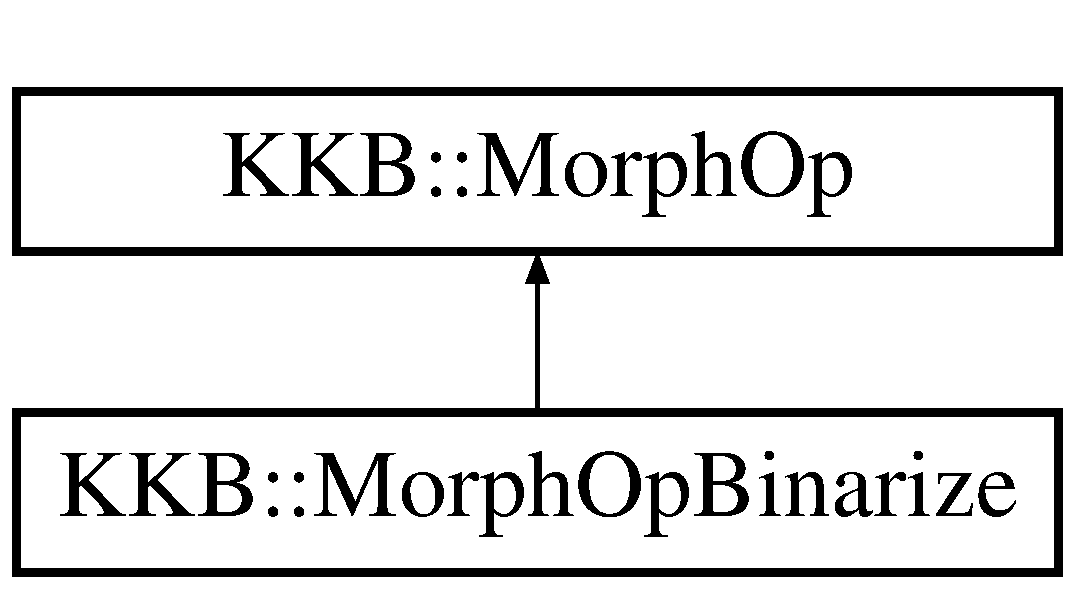
\includegraphics[height=2.000000cm]{class_k_k_b_1_1_morph_op_binarize}
\end{center}
\end{figure}
\subsection*{Public Member Functions}
\begin{DoxyCompactItemize}
\item 
\hyperlink{class_k_k_b_1_1_morph_op_binarize_aeb4c8e842f2bde9628a8e16e57c08a77}{Morph\+Op\+Binarize} (\hyperlink{namespace_k_k_b_aa8c7d4d30381c8a0b6fce68974a9c8a9}{kkuint16} \+\_\+pixel\+Value\+Min, \hyperlink{namespace_k_k_b_aa8c7d4d30381c8a0b6fce68974a9c8a9}{kkuint16} \+\_\+pixel\+Value\+Max)
\item 
virtual \hyperlink{class_k_k_b_1_1_morph_op_binarize_aac7d39b809e44ca6c44d1886765131e4}{$\sim$\+Morph\+Op\+Binarize} ()
\item 
\hyperlink{namespace_k_k_b_a8fa4952cc84fda1de4bec1fbdd8d5b1b}{kkint32} \hyperlink{class_k_k_b_1_1_morph_op_binarize_a42922ac8c4a1fc55c0b93c6a3fcea6b6}{Memory\+Consumed\+Estimated} ()
\item 
virtual \hyperlink{class_k_k_b_1_1_morph_op_a32070d9c14d16849873a8a409f5b0d69}{Operation\+Type} \hyperlink{class_k_k_b_1_1_morph_op_binarize_a4f06fa91ef03dca96bf2f1494da85678}{Operation} () const 
\item 
virtual \hyperlink{namespace_k_k_b_a80d46bd24db644a022c863bce8ae3633}{Raster\+Ptr} \hyperlink{class_k_k_b_1_1_morph_op_binarize_ae8f1b98cf24b7cb143126d5560acbbaf}{Perform\+Operation} (\hyperlink{namespace_k_k_b_a5acfa7402dc4df1769f90d3dc8ddfc2c}{Raster\+Const\+Ptr} \+\_\+image)
\end{DoxyCompactItemize}
\subsection*{Additional Inherited Members}


\subsection{Detailed Description}


Definition at line 24 of file Morph\+Op\+Binarize.\+h.



\subsection{Constructor \& Destructor Documentation}
\index{K\+K\+B\+::\+Morph\+Op\+Binarize@{K\+K\+B\+::\+Morph\+Op\+Binarize}!Morph\+Op\+Binarize@{Morph\+Op\+Binarize}}
\index{Morph\+Op\+Binarize@{Morph\+Op\+Binarize}!K\+K\+B\+::\+Morph\+Op\+Binarize@{K\+K\+B\+::\+Morph\+Op\+Binarize}}
\subsubsection[{\texorpdfstring{Morph\+Op\+Binarize(kkuint16 \+\_\+pixel\+Value\+Min, kkuint16 \+\_\+pixel\+Value\+Max)}{MorphOpBinarize(kkuint16 _pixelValueMin, kkuint16 _pixelValueMax)}}]{\setlength{\rightskip}{0pt plus 5cm}Morph\+Op\+Binarize\+::\+Morph\+Op\+Binarize (
\begin{DoxyParamCaption}
\item[{{\bf kkuint16}}]{\+\_\+pixel\+Value\+Min, }
\item[{{\bf kkuint16}}]{\+\_\+pixel\+Value\+Max}
\end{DoxyParamCaption}
)}\hypertarget{class_k_k_b_1_1_morph_op_binarize_aeb4c8e842f2bde9628a8e16e57c08a77}{}\label{class_k_k_b_1_1_morph_op_binarize_aeb4c8e842f2bde9628a8e16e57c08a77}


Definition at line 22 of file Morph\+Op\+Binarize.\+cpp.



References K\+K\+B\+::\+Morph\+Op\+::\+Morph\+Op().



Referenced by K\+K\+B\+::\+Raster\+::\+Binarize\+By\+Threshold().


\begin{DoxyCode}
24                                   :
25   \hyperlink{class_k_k_b_1_1_morph_op_a087902e5cad640c26dfa24804cc2a974}{MorphOp} (),
26   pixelValueMin (\_pixelValueMin),
27   pixelValueMax (\_pixelValueMax)
28 \{
29 \}
\end{DoxyCode}
\index{K\+K\+B\+::\+Morph\+Op\+Binarize@{K\+K\+B\+::\+Morph\+Op\+Binarize}!````~Morph\+Op\+Binarize@{$\sim$\+Morph\+Op\+Binarize}}
\index{````~Morph\+Op\+Binarize@{$\sim$\+Morph\+Op\+Binarize}!K\+K\+B\+::\+Morph\+Op\+Binarize@{K\+K\+B\+::\+Morph\+Op\+Binarize}}
\subsubsection[{\texorpdfstring{$\sim$\+Morph\+Op\+Binarize()}{~MorphOpBinarize()}}]{\setlength{\rightskip}{0pt plus 5cm}Morph\+Op\+Binarize\+::$\sim$\+Morph\+Op\+Binarize (
\begin{DoxyParamCaption}
{}
\end{DoxyParamCaption}
)\hspace{0.3cm}{\ttfamily [virtual]}}\hypertarget{class_k_k_b_1_1_morph_op_binarize_aac7d39b809e44ca6c44d1886765131e4}{}\label{class_k_k_b_1_1_morph_op_binarize_aac7d39b809e44ca6c44d1886765131e4}


Definition at line 33 of file Morph\+Op\+Binarize.\+cpp.


\begin{DoxyCode}
34 \{
35 \}
\end{DoxyCode}


\subsection{Member Function Documentation}
\index{K\+K\+B\+::\+Morph\+Op\+Binarize@{K\+K\+B\+::\+Morph\+Op\+Binarize}!Memory\+Consumed\+Estimated@{Memory\+Consumed\+Estimated}}
\index{Memory\+Consumed\+Estimated@{Memory\+Consumed\+Estimated}!K\+K\+B\+::\+Morph\+Op\+Binarize@{K\+K\+B\+::\+Morph\+Op\+Binarize}}
\subsubsection[{\texorpdfstring{Memory\+Consumed\+Estimated()}{MemoryConsumedEstimated()}}]{\setlength{\rightskip}{0pt plus 5cm}{\bf kkint32} Morph\+Op\+Binarize\+::\+Memory\+Consumed\+Estimated (
\begin{DoxyParamCaption}
{}
\end{DoxyParamCaption}
)}\hypertarget{class_k_k_b_1_1_morph_op_binarize_a42922ac8c4a1fc55c0b93c6a3fcea6b6}{}\label{class_k_k_b_1_1_morph_op_binarize_a42922ac8c4a1fc55c0b93c6a3fcea6b6}


Definition at line 39 of file Morph\+Op\+Binarize.\+cpp.


\begin{DoxyCode}
40 \{
41   \textcolor{keywordflow}{return}  \textcolor{keyword}{sizeof} (*this);
42 \}
\end{DoxyCode}
\index{K\+K\+B\+::\+Morph\+Op\+Binarize@{K\+K\+B\+::\+Morph\+Op\+Binarize}!Operation@{Operation}}
\index{Operation@{Operation}!K\+K\+B\+::\+Morph\+Op\+Binarize@{K\+K\+B\+::\+Morph\+Op\+Binarize}}
\subsubsection[{\texorpdfstring{Operation() const }{Operation() const }}]{\setlength{\rightskip}{0pt plus 5cm}virtual {\bf Operation\+Type} K\+K\+B\+::\+Morph\+Op\+Binarize\+::\+Operation (
\begin{DoxyParamCaption}
{}
\end{DoxyParamCaption}
) const\hspace{0.3cm}{\ttfamily [inline]}, {\ttfamily [virtual]}}\hypertarget{class_k_k_b_1_1_morph_op_binarize_a4f06fa91ef03dca96bf2f1494da85678}{}\label{class_k_k_b_1_1_morph_op_binarize_a4f06fa91ef03dca96bf2f1494da85678}


Implements \hyperlink{class_k_k_b_1_1_morph_op_abdf6f4bddae0b3cc3dc718559fa60234}{K\+K\+B\+::\+Morph\+Op}.



Definition at line 33 of file Morph\+Op\+Binarize.\+h.



References K\+K\+B\+::\+Morph\+Op\+::\+Binarize.


\begin{DoxyCode}
33 \{\textcolor{keywordflow}{return}  \hyperlink{class_k_k_b_1_1_morph_op_a32070d9c14d16849873a8a409f5b0d69a84a4d9fd8033f883ce95cae8c5b9859a}{OperationType::Binarize};\}
\end{DoxyCode}
\index{K\+K\+B\+::\+Morph\+Op\+Binarize@{K\+K\+B\+::\+Morph\+Op\+Binarize}!Perform\+Operation@{Perform\+Operation}}
\index{Perform\+Operation@{Perform\+Operation}!K\+K\+B\+::\+Morph\+Op\+Binarize@{K\+K\+B\+::\+Morph\+Op\+Binarize}}
\subsubsection[{\texorpdfstring{Perform\+Operation(\+Raster\+Const\+Ptr \+\_\+image)}{PerformOperation(RasterConstPtr _image)}}]{\setlength{\rightskip}{0pt plus 5cm}{\bf Raster\+Ptr} Morph\+Op\+Binarize\+::\+Perform\+Operation (
\begin{DoxyParamCaption}
\item[{{\bf Raster\+Const\+Ptr}}]{\+\_\+image}
\end{DoxyParamCaption}
)\hspace{0.3cm}{\ttfamily [virtual]}}\hypertarget{class_k_k_b_1_1_morph_op_binarize_ae8f1b98cf24b7cb143126d5560acbbaf}{}\label{class_k_k_b_1_1_morph_op_binarize_ae8f1b98cf24b7cb143126d5560acbbaf}


Definition at line 62 of file Morph\+Op\+Binarize.\+cpp.



References K\+K\+B\+::\+Raster\+::\+Background\+Pixel\+Value(), K\+K\+B\+::\+Raster\+::\+Foreground\+Pixel\+Count(), K\+K\+B\+::\+Raster\+::\+Green(), K\+K\+B\+::\+Raster\+::\+Height(), K\+K\+B\+::\+Raster\+::\+Raster(), K\+K\+B\+::\+Morph\+Op\+::\+Set\+Src\+Raster(), K\+K\+B\+::\+Morph\+Op\+::src\+Green, K\+K\+B\+::\+Morph\+Op\+::src\+Height, K\+K\+B\+::\+Morph\+Op\+::src\+Raster, K\+K\+B\+::\+Morph\+Op\+::src\+Width, and K\+K\+B\+::\+Raster\+::\+Width().



Referenced by K\+K\+B\+::\+Raster\+::\+Binarize\+By\+Threshold().


\begin{DoxyCode}
63 \{
64   \hyperlink{class_k_k_b_1_1_morph_op_a07c75e151d9b95ca13da3bfc2e48dba4}{SetSrcRaster} (\_image);
65 
66   \hyperlink{namespace_k_k_b_a8fa4952cc84fda1de4bec1fbdd8d5b1b}{kkint32}  r = 0;
67   \hyperlink{namespace_k_k_b_a8fa4952cc84fda1de4bec1fbdd8d5b1b}{kkint32}  c = 0;
68 
69   \hyperlink{namespace_k_k_b_a8fa4952cc84fda1de4bec1fbdd8d5b1b}{kkint32}  binarizedForegroundPixelCount = 0;
70 
71   \hyperlink{class_k_k_b_1_1_raster}{RasterPtr}   binarizedRaster = \textcolor{keyword}{new} \hyperlink{class_k_k_b_1_1_raster}{Raster} (\hyperlink{class_k_k_b_1_1_morph_op_a9af0ebff0135d124c7d1d17e21c4d7e6}{srcRaster}->Height (), 
      \hyperlink{class_k_k_b_1_1_morph_op_a9af0ebff0135d124c7d1d17e21c4d7e6}{srcRaster}->Width ());
72 
73   \hyperlink{namespace_k_k_b_ace9969169bf514f9ee6185186949cdf7}{uchar}*      srcRow     = NULL;
74   \hyperlink{namespace_k_k_b_ace9969169bf514f9ee6185186949cdf7}{uchar}**     destGreen  = binarizedRaster->\hyperlink{class_k_k_b_1_1_raster_a2dbd81f2cb60b3716bcf6467050dde93}{Green} ();
75   \hyperlink{namespace_k_k_b_ace9969169bf514f9ee6185186949cdf7}{uchar}*      destRow    = NULL;
76 
77   \hyperlink{namespace_k_k_b_ace9969169bf514f9ee6185186949cdf7}{uchar}       \hyperlink{class_k_k_b_1_1_morph_op_a0c3862d1c8427c4d246e0bcd56699741}{backgroundPixelValue} = \hyperlink{class_k_k_b_1_1_morph_op_a9af0ebff0135d124c7d1d17e21c4d7e6}{srcRaster}->BackgroundPixelValue ();
78 
79   \textcolor{keywordflow}{for}  (r = 0;  r < \hyperlink{class_k_k_b_1_1_morph_op_a54b2ce1b398a80803b4dbe8aef956b51}{srcHeight};  r++)
80   \{
81     destRow = destGreen[r];
82     srcRow  = \hyperlink{class_k_k_b_1_1_morph_op_ab811c702f7e0c8ffccdd21111c8144ab}{srcGreen}[r];
83 
84     \textcolor{keywordflow}{for}  (c = 0; c  < \hyperlink{class_k_k_b_1_1_morph_op_aec2cfb3015497e4077751fc5f19559ab}{srcWidth};  c++)
85     \{
86       \hyperlink{namespace_k_k_b_ace9969169bf514f9ee6185186949cdf7}{uchar}  srcCh = srcRow[c];
87       \textcolor{keywordflow}{if}  ((srcCh >= pixelValueMin)  &&  (srcCh <= pixelValueMax))
88       \{
89         destRow[c] = srcCh;
90         ++binarizedForegroundPixelCount;
91       \}
92       \textcolor{keywordflow}{else}
93       \{
94         destRow[c] = \hyperlink{class_k_k_b_1_1_morph_op_a0c3862d1c8427c4d246e0bcd56699741}{backgroundPixelValue};
95       \}
96     \}  \textcolor{comment}{/* for (c) */}
97   \}  \textcolor{comment}{/* for (r) */}
98 
99   binarizedRaster->\hyperlink{class_k_k_b_1_1_raster_a38425a410e40696276be4f22de702eb6}{ForegroundPixelCount} (binarizedForegroundPixelCount);
100 
101   \textcolor{keywordflow}{return}  binarizedRaster;
102 \}  \textcolor{comment}{/* PerformOperation */}
\end{DoxyCode}


The documentation for this class was generated from the following files\+:\begin{DoxyCompactItemize}
\item 
C\+:/\+Users/\+Kurt/\+Git\+Hub/\+K\+Square\+Libraries/\+K\+K\+Base/\hyperlink{_morph_op_binarize_8h}{Morph\+Op\+Binarize.\+h}\item 
C\+:/\+Users/\+Kurt/\+Git\+Hub/\+K\+Square\+Libraries/\+K\+K\+Base/\hyperlink{_morph_op_binarize_8cpp}{Morph\+Op\+Binarize.\+cpp}\end{DoxyCompactItemize}

\hypertarget{class_k_k_b_1_1_morph_op_bmi_filtering}{}\section{K\+KB\+:\+:Morph\+Op\+Bmi\+Filtering Class Reference}
\label{class_k_k_b_1_1_morph_op_bmi_filtering}\index{K\+K\+B\+::\+Morph\+Op\+Bmi\+Filtering@{K\+K\+B\+::\+Morph\+Op\+Bmi\+Filtering}}


{\ttfamily \#include $<$Morph\+Op\+Bmi\+Filtering.\+h$>$}

Inheritance diagram for K\+KB\+:\+:Morph\+Op\+Bmi\+Filtering\+:\begin{figure}[H]
\begin{center}
\leavevmode
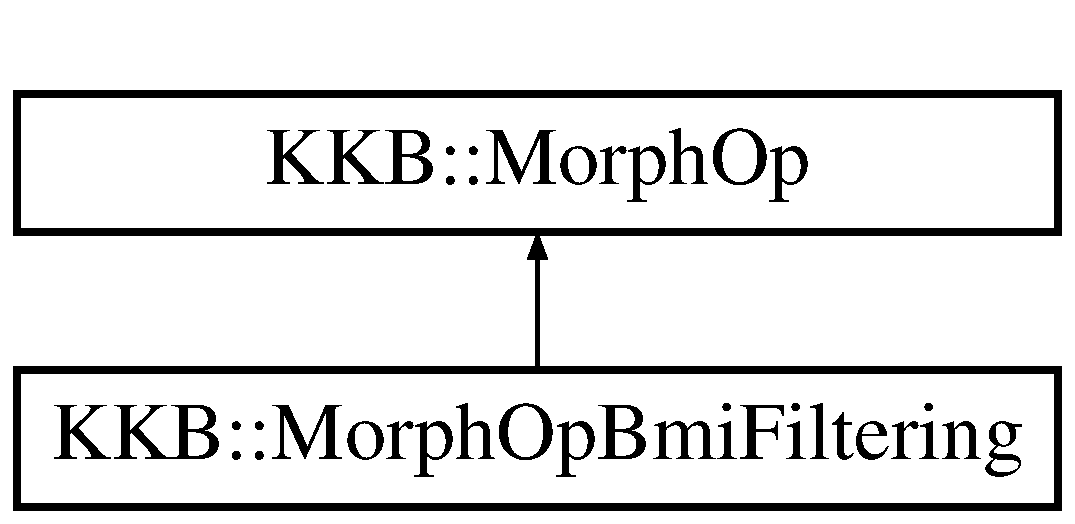
\includegraphics[height=2.000000cm]{class_k_k_b_1_1_morph_op_bmi_filtering}
\end{center}
\end{figure}
\subsection*{Public Member Functions}
\begin{DoxyCompactItemize}
\item 
\hyperlink{class_k_k_b_1_1_morph_op_bmi_filtering_a995e0f72536514aa63db49cb03e957a8}{Morph\+Op\+Bmi\+Filtering} ()
\item 
virtual \hyperlink{class_k_k_b_1_1_morph_op_bmi_filtering_afe08c76f90090e8af6eea183d5c2157a}{$\sim$\+Morph\+Op\+Bmi\+Filtering} ()
\item 
\hyperlink{namespace_k_k_b_a8fa4952cc84fda1de4bec1fbdd8d5b1b}{kkint32} \hyperlink{class_k_k_b_1_1_morph_op_bmi_filtering_aa92bec6553f0dde2837109957a549bab}{Belt\+Width} () const 
\item 
\hyperlink{namespace_k_k_b_a8fa4952cc84fda1de4bec1fbdd8d5b1b}{kkint32} \hyperlink{class_k_k_b_1_1_morph_op_bmi_filtering_a6836353e921b33168c405d07ec2444dc}{Bounding\+Length} () const 
\item 
\hyperlink{namespace_k_k_b_a8fa4952cc84fda1de4bec1fbdd8d5b1b}{kkint32} \hyperlink{class_k_k_b_1_1_morph_op_bmi_filtering_a33e12d7d95723981ec88ab0b7ca8d1a1}{Bounding\+Width} () const 
\item 
float \hyperlink{class_k_k_b_1_1_morph_op_bmi_filtering_a7fdc40401291d53339572575c3f4e4b1}{Eigen\+Ratio} () const 
\item 
float \hyperlink{class_k_k_b_1_1_morph_op_bmi_filtering_a55438ab1119053099111acca0f509260}{Estimated\+Bmi} () const 
\item 
\hyperlink{namespace_k_k_b_a8fa4952cc84fda1de4bec1fbdd8d5b1b}{kkint32} \hyperlink{class_k_k_b_1_1_morph_op_bmi_filtering_ae8e583cedaf6e14a968ecd9594832e8a}{First\+Qtr\+Weight} () const 
\item 
\hyperlink{namespace_k_k_b_a8fa4952cc84fda1de4bec1fbdd8d5b1b}{kkint32} \hyperlink{class_k_k_b_1_1_morph_op_bmi_filtering_a5de96b9d14c71ecc56f471cbf725307b}{Forth\+Qtr\+Weight} () const 
\item 
float \hyperlink{class_k_k_b_1_1_morph_op_bmi_filtering_a441fd4be638e90e60eadf0c1ac4ff15a}{Head\+Tail\+Ratio} () const 
\item 
float \hyperlink{class_k_k_b_1_1_morph_op_bmi_filtering_a5508fb0e4d4c382c671f3fb235fe47e1}{Length\+Vs\+Width} () const 
\item 
\hyperlink{namespace_k_k_b_a8fa4952cc84fda1de4bec1fbdd8d5b1b}{kkint32} \hyperlink{class_k_k_b_1_1_morph_op_bmi_filtering_a3a8705b9e84f424270a3a329f167d173}{Memory\+Consumed\+Estimated} () const 
\item 
virtual \hyperlink{class_k_k_b_1_1_morph_op_a32070d9c14d16849873a8a409f5b0d69}{Operation\+Type} \hyperlink{class_k_k_b_1_1_morph_op_bmi_filtering_aeee8c13f949e1a253f76acc2973bfe60}{Operation} () const 
\item 
float \hyperlink{class_k_k_b_1_1_morph_op_bmi_filtering_afbace4056a35f19763679307b9521db0}{Orientation\+Angle} () const 
\item 
virtual \hyperlink{namespace_k_k_b_a80d46bd24db644a022c863bce8ae3633}{Raster\+Ptr} \hyperlink{class_k_k_b_1_1_morph_op_bmi_filtering_a028e2f2640a5a7bc49cf93b1437a44e2}{Perform\+Operation} (\hyperlink{namespace_k_k_b_a5acfa7402dc4df1769f90d3dc8ddfc2c}{Raster\+Const\+Ptr} \+\_\+image)
\end{DoxyCompactItemize}
\subsection*{Additional Inherited Members}


\subsection{Detailed Description}


Definition at line 25 of file Morph\+Op\+Bmi\+Filtering.\+h.



\subsection{Constructor \& Destructor Documentation}
\index{K\+K\+B\+::\+Morph\+Op\+Bmi\+Filtering@{K\+K\+B\+::\+Morph\+Op\+Bmi\+Filtering}!Morph\+Op\+Bmi\+Filtering@{Morph\+Op\+Bmi\+Filtering}}
\index{Morph\+Op\+Bmi\+Filtering@{Morph\+Op\+Bmi\+Filtering}!K\+K\+B\+::\+Morph\+Op\+Bmi\+Filtering@{K\+K\+B\+::\+Morph\+Op\+Bmi\+Filtering}}
\subsubsection[{\texorpdfstring{Morph\+Op\+Bmi\+Filtering()}{MorphOpBmiFiltering()}}]{\setlength{\rightskip}{0pt plus 5cm}Morph\+Op\+Bmi\+Filtering\+::\+Morph\+Op\+Bmi\+Filtering (
\begin{DoxyParamCaption}
{}
\end{DoxyParamCaption}
)}\hypertarget{class_k_k_b_1_1_morph_op_bmi_filtering_a995e0f72536514aa63db49cb03e957a8}{}\label{class_k_k_b_1_1_morph_op_bmi_filtering_a995e0f72536514aa63db49cb03e957a8}


Definition at line 23 of file Morph\+Op\+Bmi\+Filtering.\+cpp.



References K\+K\+B\+::\+Morph\+Op\+::\+Morph\+Op().


\begin{DoxyCode}
23                                          :
24   \hyperlink{class_k_k_b_1_1_morph_op_a087902e5cad640c26dfa24804cc2a974}{MorphOp} ()
25 \{
26 \}
\end{DoxyCode}
\index{K\+K\+B\+::\+Morph\+Op\+Bmi\+Filtering@{K\+K\+B\+::\+Morph\+Op\+Bmi\+Filtering}!````~Morph\+Op\+Bmi\+Filtering@{$\sim$\+Morph\+Op\+Bmi\+Filtering}}
\index{````~Morph\+Op\+Bmi\+Filtering@{$\sim$\+Morph\+Op\+Bmi\+Filtering}!K\+K\+B\+::\+Morph\+Op\+Bmi\+Filtering@{K\+K\+B\+::\+Morph\+Op\+Bmi\+Filtering}}
\subsubsection[{\texorpdfstring{$\sim$\+Morph\+Op\+Bmi\+Filtering()}{~MorphOpBmiFiltering()}}]{\setlength{\rightskip}{0pt plus 5cm}Morph\+Op\+Bmi\+Filtering\+::$\sim$\+Morph\+Op\+Bmi\+Filtering (
\begin{DoxyParamCaption}
{}
\end{DoxyParamCaption}
)\hspace{0.3cm}{\ttfamily [virtual]}}\hypertarget{class_k_k_b_1_1_morph_op_bmi_filtering_afe08c76f90090e8af6eea183d5c2157a}{}\label{class_k_k_b_1_1_morph_op_bmi_filtering_afe08c76f90090e8af6eea183d5c2157a}


Definition at line 30 of file Morph\+Op\+Bmi\+Filtering.\+cpp.


\begin{DoxyCode}
31 \{
32 \}
\end{DoxyCode}


\subsection{Member Function Documentation}
\index{K\+K\+B\+::\+Morph\+Op\+Bmi\+Filtering@{K\+K\+B\+::\+Morph\+Op\+Bmi\+Filtering}!Belt\+Width@{Belt\+Width}}
\index{Belt\+Width@{Belt\+Width}!K\+K\+B\+::\+Morph\+Op\+Bmi\+Filtering@{K\+K\+B\+::\+Morph\+Op\+Bmi\+Filtering}}
\subsubsection[{\texorpdfstring{Belt\+Width() const }{BeltWidth() const }}]{\setlength{\rightskip}{0pt plus 5cm}{\bf kkint32} K\+K\+B\+::\+Morph\+Op\+Bmi\+Filtering\+::\+Belt\+Width (
\begin{DoxyParamCaption}
{}
\end{DoxyParamCaption}
) const\hspace{0.3cm}{\ttfamily [inline]}}\hypertarget{class_k_k_b_1_1_morph_op_bmi_filtering_aa92bec6553f0dde2837109957a549bab}{}\label{class_k_k_b_1_1_morph_op_bmi_filtering_aa92bec6553f0dde2837109957a549bab}


Definition at line 44 of file Morph\+Op\+Bmi\+Filtering.\+h.


\begin{DoxyCode}
44 \{\textcolor{keywordflow}{return} beltWidth;\}
\end{DoxyCode}
\index{K\+K\+B\+::\+Morph\+Op\+Bmi\+Filtering@{K\+K\+B\+::\+Morph\+Op\+Bmi\+Filtering}!Bounding\+Length@{Bounding\+Length}}
\index{Bounding\+Length@{Bounding\+Length}!K\+K\+B\+::\+Morph\+Op\+Bmi\+Filtering@{K\+K\+B\+::\+Morph\+Op\+Bmi\+Filtering}}
\subsubsection[{\texorpdfstring{Bounding\+Length() const }{BoundingLength() const }}]{\setlength{\rightskip}{0pt plus 5cm}{\bf kkint32} K\+K\+B\+::\+Morph\+Op\+Bmi\+Filtering\+::\+Bounding\+Length (
\begin{DoxyParamCaption}
{}
\end{DoxyParamCaption}
) const\hspace{0.3cm}{\ttfamily [inline]}}\hypertarget{class_k_k_b_1_1_morph_op_bmi_filtering_a6836353e921b33168c405d07ec2444dc}{}\label{class_k_k_b_1_1_morph_op_bmi_filtering_a6836353e921b33168c405d07ec2444dc}


Definition at line 45 of file Morph\+Op\+Bmi\+Filtering.\+h.


\begin{DoxyCode}
45 \{\textcolor{keywordflow}{return} boundingLength;\}
\end{DoxyCode}
\index{K\+K\+B\+::\+Morph\+Op\+Bmi\+Filtering@{K\+K\+B\+::\+Morph\+Op\+Bmi\+Filtering}!Bounding\+Width@{Bounding\+Width}}
\index{Bounding\+Width@{Bounding\+Width}!K\+K\+B\+::\+Morph\+Op\+Bmi\+Filtering@{K\+K\+B\+::\+Morph\+Op\+Bmi\+Filtering}}
\subsubsection[{\texorpdfstring{Bounding\+Width() const }{BoundingWidth() const }}]{\setlength{\rightskip}{0pt plus 5cm}{\bf kkint32} K\+K\+B\+::\+Morph\+Op\+Bmi\+Filtering\+::\+Bounding\+Width (
\begin{DoxyParamCaption}
{}
\end{DoxyParamCaption}
) const\hspace{0.3cm}{\ttfamily [inline]}}\hypertarget{class_k_k_b_1_1_morph_op_bmi_filtering_a33e12d7d95723981ec88ab0b7ca8d1a1}{}\label{class_k_k_b_1_1_morph_op_bmi_filtering_a33e12d7d95723981ec88ab0b7ca8d1a1}


Definition at line 46 of file Morph\+Op\+Bmi\+Filtering.\+h.


\begin{DoxyCode}
46 \{\textcolor{keywordflow}{return} boundingWidth;\}
\end{DoxyCode}
\index{K\+K\+B\+::\+Morph\+Op\+Bmi\+Filtering@{K\+K\+B\+::\+Morph\+Op\+Bmi\+Filtering}!Eigen\+Ratio@{Eigen\+Ratio}}
\index{Eigen\+Ratio@{Eigen\+Ratio}!K\+K\+B\+::\+Morph\+Op\+Bmi\+Filtering@{K\+K\+B\+::\+Morph\+Op\+Bmi\+Filtering}}
\subsubsection[{\texorpdfstring{Eigen\+Ratio() const }{EigenRatio() const }}]{\setlength{\rightskip}{0pt plus 5cm}float K\+K\+B\+::\+Morph\+Op\+Bmi\+Filtering\+::\+Eigen\+Ratio (
\begin{DoxyParamCaption}
{}
\end{DoxyParamCaption}
) const\hspace{0.3cm}{\ttfamily [inline]}}\hypertarget{class_k_k_b_1_1_morph_op_bmi_filtering_a7fdc40401291d53339572575c3f4e4b1}{}\label{class_k_k_b_1_1_morph_op_bmi_filtering_a7fdc40401291d53339572575c3f4e4b1}


Definition at line 38 of file Morph\+Op\+Bmi\+Filtering.\+h.


\begin{DoxyCode}
38 \{\textcolor{keywordflow}{return} eigenRatio;\}
\end{DoxyCode}
\index{K\+K\+B\+::\+Morph\+Op\+Bmi\+Filtering@{K\+K\+B\+::\+Morph\+Op\+Bmi\+Filtering}!Estimated\+Bmi@{Estimated\+Bmi}}
\index{Estimated\+Bmi@{Estimated\+Bmi}!K\+K\+B\+::\+Morph\+Op\+Bmi\+Filtering@{K\+K\+B\+::\+Morph\+Op\+Bmi\+Filtering}}
\subsubsection[{\texorpdfstring{Estimated\+Bmi() const }{EstimatedBmi() const }}]{\setlength{\rightskip}{0pt plus 5cm}float K\+K\+B\+::\+Morph\+Op\+Bmi\+Filtering\+::\+Estimated\+Bmi (
\begin{DoxyParamCaption}
{}
\end{DoxyParamCaption}
) const\hspace{0.3cm}{\ttfamily [inline]}}\hypertarget{class_k_k_b_1_1_morph_op_bmi_filtering_a55438ab1119053099111acca0f509260}{}\label{class_k_k_b_1_1_morph_op_bmi_filtering_a55438ab1119053099111acca0f509260}


Definition at line 52 of file Morph\+Op\+Bmi\+Filtering.\+h.


\begin{DoxyCode}
52 \{\textcolor{keywordflow}{return} estimatedBmi;\}
\end{DoxyCode}
\index{K\+K\+B\+::\+Morph\+Op\+Bmi\+Filtering@{K\+K\+B\+::\+Morph\+Op\+Bmi\+Filtering}!First\+Qtr\+Weight@{First\+Qtr\+Weight}}
\index{First\+Qtr\+Weight@{First\+Qtr\+Weight}!K\+K\+B\+::\+Morph\+Op\+Bmi\+Filtering@{K\+K\+B\+::\+Morph\+Op\+Bmi\+Filtering}}
\subsubsection[{\texorpdfstring{First\+Qtr\+Weight() const }{FirstQtrWeight() const }}]{\setlength{\rightskip}{0pt plus 5cm}{\bf kkint32} K\+K\+B\+::\+Morph\+Op\+Bmi\+Filtering\+::\+First\+Qtr\+Weight (
\begin{DoxyParamCaption}
{}
\end{DoxyParamCaption}
) const\hspace{0.3cm}{\ttfamily [inline]}}\hypertarget{class_k_k_b_1_1_morph_op_bmi_filtering_ae8e583cedaf6e14a968ecd9594832e8a}{}\label{class_k_k_b_1_1_morph_op_bmi_filtering_ae8e583cedaf6e14a968ecd9594832e8a}


Definition at line 41 of file Morph\+Op\+Bmi\+Filtering.\+h.


\begin{DoxyCode}
41 \{\textcolor{keywordflow}{return} firstQtrWeight;\}
\end{DoxyCode}
\index{K\+K\+B\+::\+Morph\+Op\+Bmi\+Filtering@{K\+K\+B\+::\+Morph\+Op\+Bmi\+Filtering}!Forth\+Qtr\+Weight@{Forth\+Qtr\+Weight}}
\index{Forth\+Qtr\+Weight@{Forth\+Qtr\+Weight}!K\+K\+B\+::\+Morph\+Op\+Bmi\+Filtering@{K\+K\+B\+::\+Morph\+Op\+Bmi\+Filtering}}
\subsubsection[{\texorpdfstring{Forth\+Qtr\+Weight() const }{ForthQtrWeight() const }}]{\setlength{\rightskip}{0pt plus 5cm}{\bf kkint32} K\+K\+B\+::\+Morph\+Op\+Bmi\+Filtering\+::\+Forth\+Qtr\+Weight (
\begin{DoxyParamCaption}
{}
\end{DoxyParamCaption}
) const\hspace{0.3cm}{\ttfamily [inline]}}\hypertarget{class_k_k_b_1_1_morph_op_bmi_filtering_a5de96b9d14c71ecc56f471cbf725307b}{}\label{class_k_k_b_1_1_morph_op_bmi_filtering_a5de96b9d14c71ecc56f471cbf725307b}


Definition at line 42 of file Morph\+Op\+Bmi\+Filtering.\+h.


\begin{DoxyCode}
42 \{\textcolor{keywordflow}{return} forthQtrWeight;\}
\end{DoxyCode}
\index{K\+K\+B\+::\+Morph\+Op\+Bmi\+Filtering@{K\+K\+B\+::\+Morph\+Op\+Bmi\+Filtering}!Head\+Tail\+Ratio@{Head\+Tail\+Ratio}}
\index{Head\+Tail\+Ratio@{Head\+Tail\+Ratio}!K\+K\+B\+::\+Morph\+Op\+Bmi\+Filtering@{K\+K\+B\+::\+Morph\+Op\+Bmi\+Filtering}}
\subsubsection[{\texorpdfstring{Head\+Tail\+Ratio() const }{HeadTailRatio() const }}]{\setlength{\rightskip}{0pt plus 5cm}float K\+K\+B\+::\+Morph\+Op\+Bmi\+Filtering\+::\+Head\+Tail\+Ratio (
\begin{DoxyParamCaption}
{}
\end{DoxyParamCaption}
) const\hspace{0.3cm}{\ttfamily [inline]}}\hypertarget{class_k_k_b_1_1_morph_op_bmi_filtering_a441fd4be638e90e60eadf0c1ac4ff15a}{}\label{class_k_k_b_1_1_morph_op_bmi_filtering_a441fd4be638e90e60eadf0c1ac4ff15a}


Definition at line 50 of file Morph\+Op\+Bmi\+Filtering.\+h.


\begin{DoxyCode}
50 \{\textcolor{keywordflow}{return} headTailRatio;\}
\end{DoxyCode}
\index{K\+K\+B\+::\+Morph\+Op\+Bmi\+Filtering@{K\+K\+B\+::\+Morph\+Op\+Bmi\+Filtering}!Length\+Vs\+Width@{Length\+Vs\+Width}}
\index{Length\+Vs\+Width@{Length\+Vs\+Width}!K\+K\+B\+::\+Morph\+Op\+Bmi\+Filtering@{K\+K\+B\+::\+Morph\+Op\+Bmi\+Filtering}}
\subsubsection[{\texorpdfstring{Length\+Vs\+Width() const }{LengthVsWidth() const }}]{\setlength{\rightskip}{0pt plus 5cm}float K\+K\+B\+::\+Morph\+Op\+Bmi\+Filtering\+::\+Length\+Vs\+Width (
\begin{DoxyParamCaption}
{}
\end{DoxyParamCaption}
) const\hspace{0.3cm}{\ttfamily [inline]}}\hypertarget{class_k_k_b_1_1_morph_op_bmi_filtering_a5508fb0e4d4c382c671f3fb235fe47e1}{}\label{class_k_k_b_1_1_morph_op_bmi_filtering_a5508fb0e4d4c382c671f3fb235fe47e1}


Definition at line 48 of file Morph\+Op\+Bmi\+Filtering.\+h.


\begin{DoxyCode}
48 \{\textcolor{keywordflow}{return} lengthVsWidth;\}
\end{DoxyCode}
\index{K\+K\+B\+::\+Morph\+Op\+Bmi\+Filtering@{K\+K\+B\+::\+Morph\+Op\+Bmi\+Filtering}!Memory\+Consumed\+Estimated@{Memory\+Consumed\+Estimated}}
\index{Memory\+Consumed\+Estimated@{Memory\+Consumed\+Estimated}!K\+K\+B\+::\+Morph\+Op\+Bmi\+Filtering@{K\+K\+B\+::\+Morph\+Op\+Bmi\+Filtering}}
\subsubsection[{\texorpdfstring{Memory\+Consumed\+Estimated() const }{MemoryConsumedEstimated() const }}]{\setlength{\rightskip}{0pt plus 5cm}{\bf kkint32} Morph\+Op\+Bmi\+Filtering\+::\+Memory\+Consumed\+Estimated (
\begin{DoxyParamCaption}
{}
\end{DoxyParamCaption}
) const}\hypertarget{class_k_k_b_1_1_morph_op_bmi_filtering_a3a8705b9e84f424270a3a329f167d173}{}\label{class_k_k_b_1_1_morph_op_bmi_filtering_a3a8705b9e84f424270a3a329f167d173}


Definition at line 36 of file Morph\+Op\+Bmi\+Filtering.\+cpp.


\begin{DoxyCode}
37 \{
38   \textcolor{keywordflow}{return}  \textcolor{keyword}{sizeof} (*this);
39 \}
\end{DoxyCode}
\index{K\+K\+B\+::\+Morph\+Op\+Bmi\+Filtering@{K\+K\+B\+::\+Morph\+Op\+Bmi\+Filtering}!Operation@{Operation}}
\index{Operation@{Operation}!K\+K\+B\+::\+Morph\+Op\+Bmi\+Filtering@{K\+K\+B\+::\+Morph\+Op\+Bmi\+Filtering}}
\subsubsection[{\texorpdfstring{Operation() const }{Operation() const }}]{\setlength{\rightskip}{0pt plus 5cm}virtual {\bf Operation\+Type} K\+K\+B\+::\+Morph\+Op\+Bmi\+Filtering\+::\+Operation (
\begin{DoxyParamCaption}
{}
\end{DoxyParamCaption}
) const\hspace{0.3cm}{\ttfamily [inline]}, {\ttfamily [virtual]}}\hypertarget{class_k_k_b_1_1_morph_op_bmi_filtering_aeee8c13f949e1a253f76acc2973bfe60}{}\label{class_k_k_b_1_1_morph_op_bmi_filtering_aeee8c13f949e1a253f76acc2973bfe60}


Implements \hyperlink{class_k_k_b_1_1_morph_op_abdf6f4bddae0b3cc3dc718559fa60234}{K\+K\+B\+::\+Morph\+Op}.



Definition at line 32 of file Morph\+Op\+Bmi\+Filtering.\+h.



References K\+K\+B\+::\+Morph\+Op\+::\+Binarize.


\begin{DoxyCode}
32 \{\textcolor{keywordflow}{return}  \hyperlink{class_k_k_b_1_1_morph_op_a32070d9c14d16849873a8a409f5b0d69a84a4d9fd8033f883ce95cae8c5b9859a}{OperationType::Binarize};\}
\end{DoxyCode}
\index{K\+K\+B\+::\+Morph\+Op\+Bmi\+Filtering@{K\+K\+B\+::\+Morph\+Op\+Bmi\+Filtering}!Orientation\+Angle@{Orientation\+Angle}}
\index{Orientation\+Angle@{Orientation\+Angle}!K\+K\+B\+::\+Morph\+Op\+Bmi\+Filtering@{K\+K\+B\+::\+Morph\+Op\+Bmi\+Filtering}}
\subsubsection[{\texorpdfstring{Orientation\+Angle() const }{OrientationAngle() const }}]{\setlength{\rightskip}{0pt plus 5cm}float K\+K\+B\+::\+Morph\+Op\+Bmi\+Filtering\+::\+Orientation\+Angle (
\begin{DoxyParamCaption}
{}
\end{DoxyParamCaption}
) const\hspace{0.3cm}{\ttfamily [inline]}}\hypertarget{class_k_k_b_1_1_morph_op_bmi_filtering_afbace4056a35f19763679307b9521db0}{}\label{class_k_k_b_1_1_morph_op_bmi_filtering_afbace4056a35f19763679307b9521db0}


Definition at line 39 of file Morph\+Op\+Bmi\+Filtering.\+h.


\begin{DoxyCode}
39 \{\textcolor{keywordflow}{return} orientationAngle;\}
\end{DoxyCode}
\index{K\+K\+B\+::\+Morph\+Op\+Bmi\+Filtering@{K\+K\+B\+::\+Morph\+Op\+Bmi\+Filtering}!Perform\+Operation@{Perform\+Operation}}
\index{Perform\+Operation@{Perform\+Operation}!K\+K\+B\+::\+Morph\+Op\+Bmi\+Filtering@{K\+K\+B\+::\+Morph\+Op\+Bmi\+Filtering}}
\subsubsection[{\texorpdfstring{Perform\+Operation(\+Raster\+Const\+Ptr \+\_\+image)}{PerformOperation(RasterConstPtr _image)}}]{\setlength{\rightskip}{0pt plus 5cm}{\bf Raster\+Ptr} Morph\+Op\+Bmi\+Filtering\+::\+Perform\+Operation (
\begin{DoxyParamCaption}
\item[{{\bf Raster\+Const\+Ptr}}]{\+\_\+image}
\end{DoxyParamCaption}
)\hspace{0.3cm}{\ttfamily [virtual]}}\hypertarget{class_k_k_b_1_1_morph_op_bmi_filtering_a028e2f2640a5a7bc49cf93b1437a44e2}{}\label{class_k_k_b_1_1_morph_op_bmi_filtering_a028e2f2640a5a7bc49cf93b1437a44e2}


Definition at line 193 of file Morph\+Op\+Bmi\+Filtering.\+cpp.



References K\+K\+B\+::\+Raster\+::\+Background\+Pixel\+T\+H(), K\+K\+B\+::\+Morph\+Op\+::\+Set\+Src\+Raster(), and K\+K\+B\+::\+Morph\+Op\+::src\+Raster.


\begin{DoxyCode}
194 \{
195   \hyperlink{class_k_k_b_1_1_morph_op_a07c75e151d9b95ca13da3bfc2e48dba4}{SetSrcRaster} (\_image);
196 
197   \hyperlink{class_k_k_b_1_1_raster}{RasterPtr}  rotatedImage = NULL;
198 
199   \textcolor{comment}{// 1) Remove Appendages.}
200   \textcolor{comment}{// 2) Perform Length vs Width}
201 
202   \hyperlink{namespace_k_k_b_ace9969169bf514f9ee6185186949cdf7}{uchar}  binarizeTHmin = \hyperlink{class_k_k_b_1_1_morph_op_a9af0ebff0135d124c7d1d17e21c4d7e6}{srcRaster}->BackgroundPixelTH () + 1;
203   \hyperlink{namespace_k_k_b_ace9969169bf514f9ee6185186949cdf7}{uchar}  binarizeTHmax = 125;
204 
205   rotatedImage = ProcessBmi (binarizeTHmax);
206   \hyperlink{namespace_k_k_b_a8fa4952cc84fda1de4bec1fbdd8d5b1b}{kkint32}    rectangularAreaMax = boundingLength * boundingWidth;
207   \textcolor{keyword}{delete}  rotatedImage;  rotatedImage = NULL;
208 
209   rotatedImage = ProcessBmi (binarizeTHmin);
210   \hyperlink{namespace_k_k_b_a8fa4952cc84fda1de4bec1fbdd8d5b1b}{kkint32}    rectangularAreaMin = boundingLength * boundingWidth;
211 
212   \textcolor{keywordflow}{if}  ((rectangularAreaMin > 0)  &&  (rectangularAreaMax > 0))
213   \{
214     \textcolor{keywordflow}{if}  ((rectangularAreaMax / rectangularAreaMin) > 0.90)
215     \{
216       \textcolor{comment}{// Not a significant amount of low intensity foreground pixels.}
217       \textcolor{keyword}{delete}  rotatedImage;
218       rotatedImage = ProcessBmi (binarizeTHmin);
219       \textcolor{keywordflow}{return}  rotatedImage;
220     \}
221   \}
222 
223   \hyperlink{namespace_k_k_b_a8fa4952cc84fda1de4bec1fbdd8d5b1b}{kkint32}  rectangularAreaTH = (\hyperlink{namespace_k_k_b_a8fa4952cc84fda1de4bec1fbdd8d5b1b}{kkint32})(0.5f + (\textcolor{keywordtype}{float})(rectangularAreaMax + 
      rectangularAreaMin) * (1.0f / 2.0f));
224 
225   \hyperlink{namespace_k_k_b_ace9969169bf514f9ee6185186949cdf7}{uchar}  binarizeTHminLast = binarizeTHmin;
226   \textcolor{keywordflow}{while}  (binarizeTHmin < binarizeTHmax)
227   \{
228     \textcolor{keywordflow}{if}  (boundingWidth < 5)
229       \textcolor{keywordflow}{break};
230 
231     \textcolor{keyword}{delete}  rotatedImage;
232     rotatedImage = ProcessBmi (binarizeTHmin);
233     rectangularAreaMin = boundingLength * boundingWidth;
234     \textcolor{keywordflow}{if}  (boundingWidth < 3)
235     \{
236       binarizeTHmin = binarizeTHminLast;
237       \textcolor{keyword}{delete}  rotatedImage;
238       rotatedImage = ProcessBmi (binarizeTHmin);
239       \textcolor{keywordflow}{break};
240     \}
241 
242     binarizeTHminLast = binarizeTHmin;
243 
244     \textcolor{keywordflow}{if}  (rectangularAreaMin < rectangularAreaTH)
245       \textcolor{keywordflow}{break};
246 
247     binarizeTHmin += 5;
248   \}
249 
250 
251   \textcolor{keywordflow}{return}  rotatedImage;
252 \}  \textcolor{comment}{/* PerformOperation */}
\end{DoxyCode}


The documentation for this class was generated from the following files\+:\begin{DoxyCompactItemize}
\item 
C\+:/\+Users/\+Kurt/\+Git\+Hub/\+K\+Square\+Libraries/\+K\+K\+Base/\hyperlink{_morph_op_bmi_filtering_8h}{Morph\+Op\+Bmi\+Filtering.\+h}\item 
C\+:/\+Users/\+Kurt/\+Git\+Hub/\+K\+Square\+Libraries/\+K\+K\+Base/\hyperlink{_morph_op_bmi_filtering_8cpp}{Morph\+Op\+Bmi\+Filtering.\+cpp}\end{DoxyCompactItemize}

\hypertarget{class_k_k_b_1_1_morph_op_dilation}{}\section{K\+KB\+:\+:Morph\+Op\+Dilation Class Reference}
\label{class_k_k_b_1_1_morph_op_dilation}\index{K\+K\+B\+::\+Morph\+Op\+Dilation@{K\+K\+B\+::\+Morph\+Op\+Dilation}}


{\ttfamily \#include $<$Morph\+Op\+Dilation.\+h$>$}

Inheritance diagram for K\+KB\+:\+:Morph\+Op\+Dilation\+:\begin{figure}[H]
\begin{center}
\leavevmode
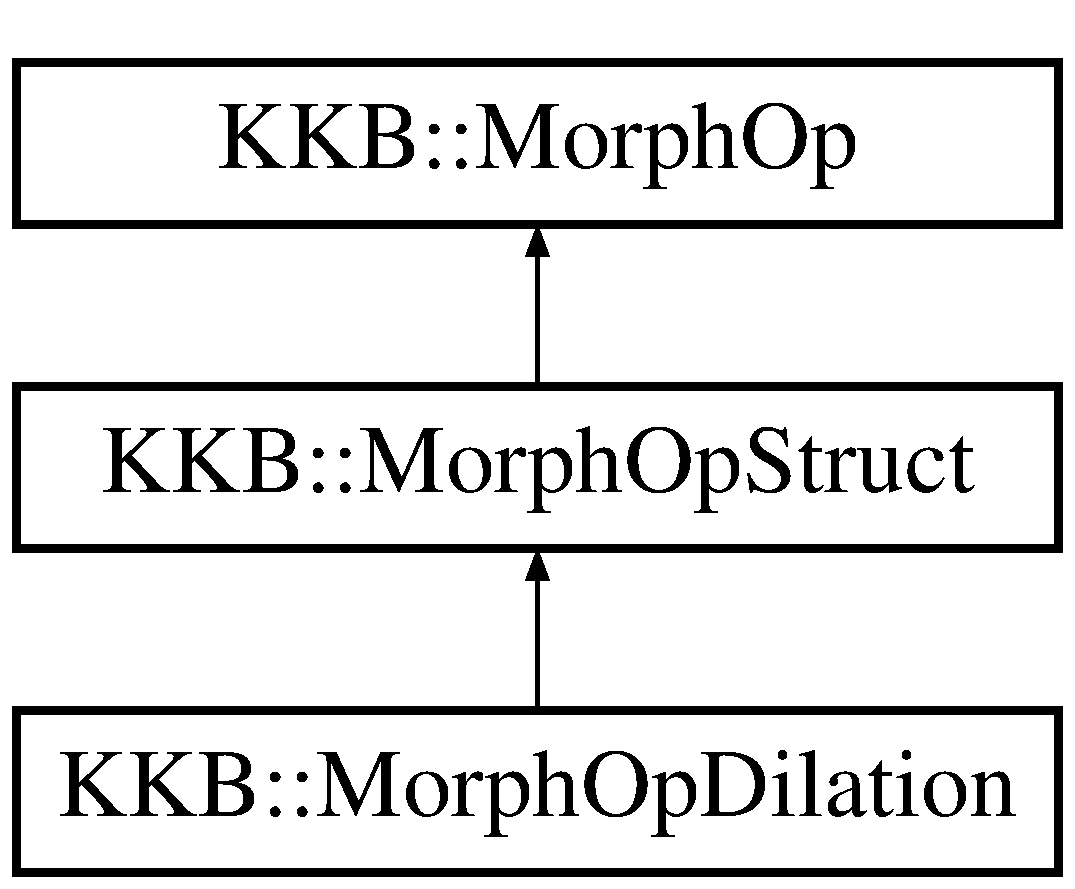
\includegraphics[height=3.000000cm]{class_k_k_b_1_1_morph_op_dilation}
\end{center}
\end{figure}
\subsection*{Public Member Functions}
\begin{DoxyCompactItemize}
\item 
\hyperlink{class_k_k_b_1_1_morph_op_dilation_ae63e8cf3ba854bda260b8ccdb35c4d7c}{Morph\+Op\+Dilation} (\hyperlink{class_k_k_b_1_1_morph_op_a09e4aff7e81327849855ff72082d85b3}{Structure\+Type} \+\_\+structure, \hyperlink{namespace_k_k_b_aa8c7d4d30381c8a0b6fce68974a9c8a9}{kkuint16} \+\_\+structure\+Size)
\item 
virtual \hyperlink{class_k_k_b_1_1_morph_op_dilation_acaf50bc342730d5667dd411dc0cfd6ac}{$\sim$\+Morph\+Op\+Dilation} ()
\item 
\hyperlink{namespace_k_k_b_a8fa4952cc84fda1de4bec1fbdd8d5b1b}{kkint32} \hyperlink{class_k_k_b_1_1_morph_op_dilation_a977057adff36427847c5abab6194f521}{Memory\+Consumed\+Estimated} ()
\item 
virtual \hyperlink{class_k_k_b_1_1_morph_op_a32070d9c14d16849873a8a409f5b0d69}{Operation\+Type} \hyperlink{class_k_k_b_1_1_morph_op_dilation_a159a05bfd9fc2af7a07fe22edcde0ef8}{Operation} () const 
\item 
virtual \hyperlink{namespace_k_k_b_a80d46bd24db644a022c863bce8ae3633}{Raster\+Ptr} \hyperlink{class_k_k_b_1_1_morph_op_dilation_a9240afda29b2a87de63fbd581bd999c0}{Perform\+Operation} (\hyperlink{namespace_k_k_b_a5acfa7402dc4df1769f90d3dc8ddfc2c}{Raster\+Const\+Ptr} \+\_\+image)
\end{DoxyCompactItemize}
\subsection*{Additional Inherited Members}


\subsection{Detailed Description}


Definition at line 24 of file Morph\+Op\+Dilation.\+h.



\subsection{Constructor \& Destructor Documentation}
\index{K\+K\+B\+::\+Morph\+Op\+Dilation@{K\+K\+B\+::\+Morph\+Op\+Dilation}!Morph\+Op\+Dilation@{Morph\+Op\+Dilation}}
\index{Morph\+Op\+Dilation@{Morph\+Op\+Dilation}!K\+K\+B\+::\+Morph\+Op\+Dilation@{K\+K\+B\+::\+Morph\+Op\+Dilation}}
\subsubsection[{\texorpdfstring{Morph\+Op\+Dilation(\+Structure\+Type \+\_\+structure, kkuint16 \+\_\+structure\+Size)}{MorphOpDilation(StructureType _structure, kkuint16 _structureSize)}}]{\setlength{\rightskip}{0pt plus 5cm}Morph\+Op\+Dilation\+::\+Morph\+Op\+Dilation (
\begin{DoxyParamCaption}
\item[{{\bf Structure\+Type}}]{\+\_\+structure, }
\item[{{\bf kkuint16}}]{\+\_\+structure\+Size}
\end{DoxyParamCaption}
)}\hypertarget{class_k_k_b_1_1_morph_op_dilation_ae63e8cf3ba854bda260b8ccdb35c4d7c}{}\label{class_k_k_b_1_1_morph_op_dilation_ae63e8cf3ba854bda260b8ccdb35c4d7c}


Definition at line 22 of file Morph\+Op\+Dilation.\+cpp.



References K\+K\+B\+::\+Morph\+Op\+Struct\+::\+Morph\+Op\+Struct().



Referenced by K\+K\+B\+::\+Raster\+::\+Dilation().


\begin{DoxyCode}
24                                   :
25   \hyperlink{class_k_k_b_1_1_morph_op_struct_afbd23fee4ea441d03f11f10da50009f6}{MorphOpStruct} (\_structure, \_structureSize)
26 \{
27 \}
\end{DoxyCode}
\index{K\+K\+B\+::\+Morph\+Op\+Dilation@{K\+K\+B\+::\+Morph\+Op\+Dilation}!````~Morph\+Op\+Dilation@{$\sim$\+Morph\+Op\+Dilation}}
\index{````~Morph\+Op\+Dilation@{$\sim$\+Morph\+Op\+Dilation}!K\+K\+B\+::\+Morph\+Op\+Dilation@{K\+K\+B\+::\+Morph\+Op\+Dilation}}
\subsubsection[{\texorpdfstring{$\sim$\+Morph\+Op\+Dilation()}{~MorphOpDilation()}}]{\setlength{\rightskip}{0pt plus 5cm}Morph\+Op\+Dilation\+::$\sim$\+Morph\+Op\+Dilation (
\begin{DoxyParamCaption}
{}
\end{DoxyParamCaption}
)\hspace{0.3cm}{\ttfamily [virtual]}}\hypertarget{class_k_k_b_1_1_morph_op_dilation_acaf50bc342730d5667dd411dc0cfd6ac}{}\label{class_k_k_b_1_1_morph_op_dilation_acaf50bc342730d5667dd411dc0cfd6ac}


Definition at line 31 of file Morph\+Op\+Dilation.\+cpp.


\begin{DoxyCode}
32 \{
33 \}
\end{DoxyCode}


\subsection{Member Function Documentation}
\index{K\+K\+B\+::\+Morph\+Op\+Dilation@{K\+K\+B\+::\+Morph\+Op\+Dilation}!Memory\+Consumed\+Estimated@{Memory\+Consumed\+Estimated}}
\index{Memory\+Consumed\+Estimated@{Memory\+Consumed\+Estimated}!K\+K\+B\+::\+Morph\+Op\+Dilation@{K\+K\+B\+::\+Morph\+Op\+Dilation}}
\subsubsection[{\texorpdfstring{Memory\+Consumed\+Estimated()}{MemoryConsumedEstimated()}}]{\setlength{\rightskip}{0pt plus 5cm}{\bf kkint32} Morph\+Op\+Dilation\+::\+Memory\+Consumed\+Estimated (
\begin{DoxyParamCaption}
{}
\end{DoxyParamCaption}
)}\hypertarget{class_k_k_b_1_1_morph_op_dilation_a977057adff36427847c5abab6194f521}{}\label{class_k_k_b_1_1_morph_op_dilation_a977057adff36427847c5abab6194f521}


Definition at line 37 of file Morph\+Op\+Dilation.\+cpp.


\begin{DoxyCode}
38 \{
39   \textcolor{keywordflow}{return}  \textcolor{keyword}{sizeof} (*this);
40 \}
\end{DoxyCode}
\index{K\+K\+B\+::\+Morph\+Op\+Dilation@{K\+K\+B\+::\+Morph\+Op\+Dilation}!Operation@{Operation}}
\index{Operation@{Operation}!K\+K\+B\+::\+Morph\+Op\+Dilation@{K\+K\+B\+::\+Morph\+Op\+Dilation}}
\subsubsection[{\texorpdfstring{Operation() const }{Operation() const }}]{\setlength{\rightskip}{0pt plus 5cm}virtual {\bf Operation\+Type} K\+K\+B\+::\+Morph\+Op\+Dilation\+::\+Operation (
\begin{DoxyParamCaption}
{}
\end{DoxyParamCaption}
) const\hspace{0.3cm}{\ttfamily [inline]}, {\ttfamily [virtual]}}\hypertarget{class_k_k_b_1_1_morph_op_dilation_a159a05bfd9fc2af7a07fe22edcde0ef8}{}\label{class_k_k_b_1_1_morph_op_dilation_a159a05bfd9fc2af7a07fe22edcde0ef8}


Reimplemented from \hyperlink{class_k_k_b_1_1_morph_op_struct_a3cbbeb9ce7ce8856bc01d1c0b1b478a8}{K\+K\+B\+::\+Morph\+Op\+Struct}.



Definition at line 33 of file Morph\+Op\+Dilation.\+h.



References K\+K\+B\+::\+Morph\+Op\+::\+Dilation.


\begin{DoxyCode}
33 \{\textcolor{keywordflow}{return}  \hyperlink{class_k_k_b_1_1_morph_op_a32070d9c14d16849873a8a409f5b0d69a5a870896d32acca70f912a0c11edca66}{OperationType::Dilation};\}
\end{DoxyCode}
\index{K\+K\+B\+::\+Morph\+Op\+Dilation@{K\+K\+B\+::\+Morph\+Op\+Dilation}!Perform\+Operation@{Perform\+Operation}}
\index{Perform\+Operation@{Perform\+Operation}!K\+K\+B\+::\+Morph\+Op\+Dilation@{K\+K\+B\+::\+Morph\+Op\+Dilation}}
\subsubsection[{\texorpdfstring{Perform\+Operation(\+Raster\+Const\+Ptr \+\_\+image)}{PerformOperation(RasterConstPtr _image)}}]{\setlength{\rightskip}{0pt plus 5cm}{\bf Raster\+Ptr} Morph\+Op\+Dilation\+::\+Perform\+Operation (
\begin{DoxyParamCaption}
\item[{{\bf Raster\+Const\+Ptr}}]{\+\_\+image}
\end{DoxyParamCaption}
)\hspace{0.3cm}{\ttfamily [virtual]}}\hypertarget{class_k_k_b_1_1_morph_op_dilation_a9240afda29b2a87de63fbd581bd999c0}{}\label{class_k_k_b_1_1_morph_op_dilation_a9240afda29b2a87de63fbd581bd999c0}


Implements \hyperlink{class_k_k_b_1_1_morph_op_struct_ace5b649ea317fcc38094e64bb5034380}{K\+K\+B\+::\+Morph\+Op\+Struct}.



Definition at line 45 of file Morph\+Op\+Dilation.\+cpp.



References K\+K\+B\+::\+Morph\+Op\+::\+Background\+Pixel(), K\+K\+B\+::\+Morph\+Op\+::\+Foreground\+Pixel(), K\+K\+B\+::\+Raster\+::\+Foreground\+Pixel\+Count(), K\+K\+B\+::\+Raster\+::\+Green(), K\+K\+B\+::\+Morph\+Op\+Struct\+::\+Hit\+Foreground\+Count(), K\+K\+B\+::\+Raster\+::\+Raster(), K\+K\+B\+::\+Morph\+Op\+::\+Set\+Src\+Raster(), K\+K\+B\+::\+Morph\+Op\+::src\+Green, K\+K\+B\+::\+Morph\+Op\+::src\+Height, K\+K\+B\+::\+Morph\+Op\+::src\+Raster, and K\+K\+B\+::\+Morph\+Op\+::src\+Width.



Referenced by K\+K\+B\+::\+Raster\+::\+Dilation().


\begin{DoxyCode}
46 \{
47   this->\hyperlink{class_k_k_b_1_1_morph_op_a07c75e151d9b95ca13da3bfc2e48dba4}{SetSrcRaster} (\_image);
48 
49   \hyperlink{namespace_k_k_b_a8fa4952cc84fda1de4bec1fbdd8d5b1b}{kkint32}  r = 0;
50   \hyperlink{namespace_k_k_b_a8fa4952cc84fda1de4bec1fbdd8d5b1b}{kkint32}  c = 0;
51 
52   \hyperlink{namespace_k_k_b_a8fa4952cc84fda1de4bec1fbdd8d5b1b}{kkint32}  erodedForegroundPixelCount = \hyperlink{class_k_k_b_1_1_morph_op_a9af0ebff0135d124c7d1d17e21c4d7e6}{srcRaster}->ForegroundPixelCount ();
53 
54   \hyperlink{class_k_k_b_1_1_raster}{RasterPtr} resultRaster = \textcolor{keyword}{new} \hyperlink{class_k_k_b_1_1_raster}{Raster} (*\hyperlink{class_k_k_b_1_1_morph_op_a9af0ebff0135d124c7d1d17e21c4d7e6}{srcRaster});
55 
56   \hyperlink{namespace_k_k_b_ace9969169bf514f9ee6185186949cdf7}{uchar}*    srcRow     = NULL;
57   \hyperlink{namespace_k_k_b_ace9969169bf514f9ee6185186949cdf7}{uchar}**   destGreen  = resultRaster->\hyperlink{class_k_k_b_1_1_raster_a2dbd81f2cb60b3716bcf6467050dde93}{Green} ();
58   \hyperlink{namespace_k_k_b_ace9969169bf514f9ee6185186949cdf7}{uchar}*    destRow    = NULL;
59 
60   \hyperlink{namespace_k_k_b_a8fa4952cc84fda1de4bec1fbdd8d5b1b}{kkint32}  forgroundPixelCount = \hyperlink{class_k_k_b_1_1_morph_op_a9af0ebff0135d124c7d1d17e21c4d7e6}{srcRaster}->ForegroundPixelCount ();
61 
62   \textcolor{keywordflow}{for}  (r = 0;  r < \hyperlink{class_k_k_b_1_1_morph_op_a54b2ce1b398a80803b4dbe8aef956b51}{srcHeight};  r++)
63   \{
64     destRow = destGreen[r];
65     srcRow  = \hyperlink{class_k_k_b_1_1_morph_op_ab811c702f7e0c8ffccdd21111c8144ab}{srcGreen}[r];
66 
67     \textcolor{keywordflow}{for}  (c = 0; c < \hyperlink{class_k_k_b_1_1_morph_op_aec2cfb3015497e4077751fc5f19559ab}{srcWidth}; c++)
68     \{
69       \textcolor{keywordflow}{if}  (\hyperlink{class_k_k_b_1_1_morph_op_a300c5117659d224d78f7b5a8d44ded91}{BackgroundPixel} (srcRow[c]))
70       \{
71         \hyperlink{namespace_k_k_b_ace9969169bf514f9ee6185186949cdf7}{uchar}  pixel = \hyperlink{class_k_k_b_1_1_morph_op_struct_a4b9e013e6850f097999d72175ded3f85}{HitForegroundCount} (r, c);
72         \textcolor{keywordflow}{if}  (\hyperlink{class_k_k_b_1_1_morph_op_acd5541050c3c0207b004b71caf7fb1f4}{ForegroundPixel} (pixel))
73           ++forgroundPixelCount;
74         destRow[c] = pixel;
75       \}
76     \}  \textcolor{comment}{/* for (c) */}
77   \}  \textcolor{comment}{/* for (r) */}
78 
79   resultRaster->\hyperlink{class_k_k_b_1_1_raster_a38425a410e40696276be4f22de702eb6}{ForegroundPixelCount} (forgroundPixelCount);
80 
81   \textcolor{keywordflow}{return}  resultRaster;
82 \}  \textcolor{comment}{/* PerformOperation */}
\end{DoxyCode}


The documentation for this class was generated from the following files\+:\begin{DoxyCompactItemize}
\item 
C\+:/\+Users/\+Kurt/\+Git\+Hub/\+K\+Square\+Libraries/\+K\+K\+Base/\hyperlink{_morph_op_dilation_8h}{Morph\+Op\+Dilation.\+h}\item 
C\+:/\+Users/\+Kurt/\+Git\+Hub/\+K\+Square\+Libraries/\+K\+K\+Base/\hyperlink{_morph_op_dilation_8cpp}{Morph\+Op\+Dilation.\+cpp}\end{DoxyCompactItemize}

\hypertarget{class_k_k_b_1_1_morph_op_erosion}{}\section{K\+KB\+:\+:Morph\+Op\+Erosion Class Reference}
\label{class_k_k_b_1_1_morph_op_erosion}\index{K\+K\+B\+::\+Morph\+Op\+Erosion@{K\+K\+B\+::\+Morph\+Op\+Erosion}}


{\ttfamily \#include $<$Morph\+Op\+Erosion.\+h$>$}

Inheritance diagram for K\+KB\+:\+:Morph\+Op\+Erosion\+:\begin{figure}[H]
\begin{center}
\leavevmode
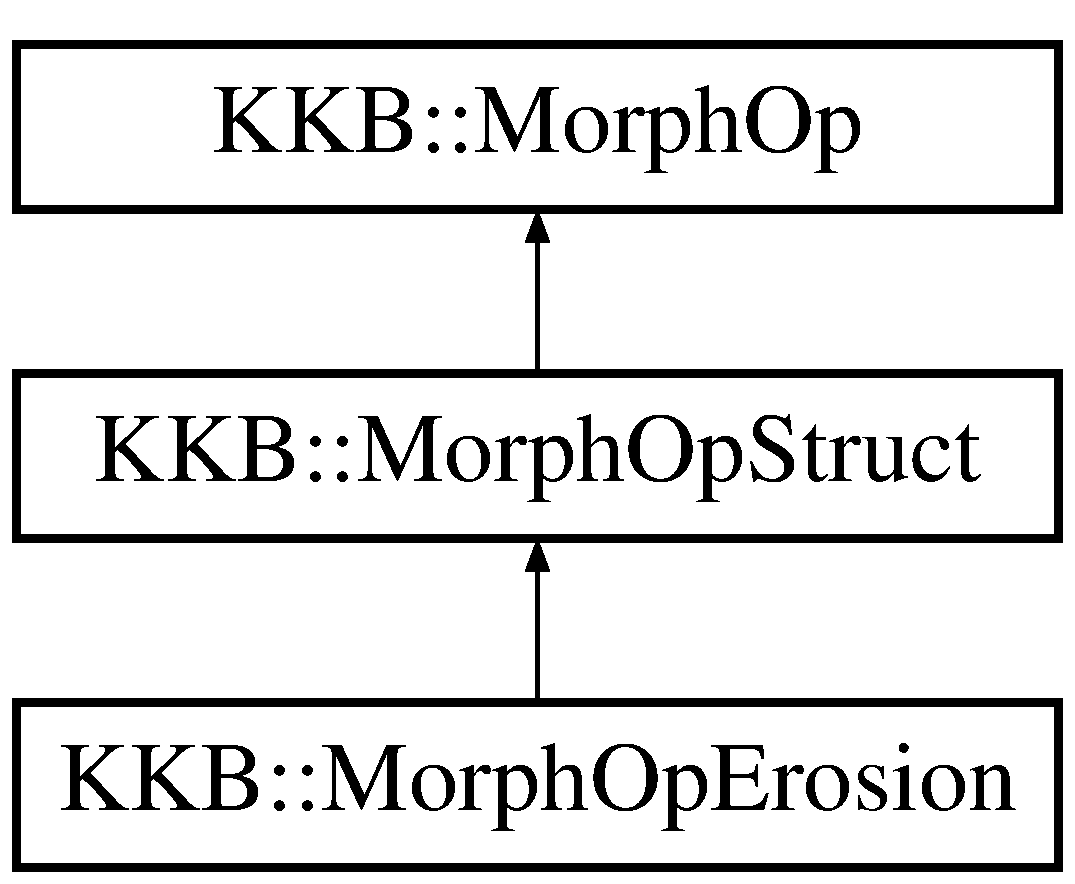
\includegraphics[height=3.000000cm]{class_k_k_b_1_1_morph_op_erosion}
\end{center}
\end{figure}
\subsection*{Public Member Functions}
\begin{DoxyCompactItemize}
\item 
\hyperlink{class_k_k_b_1_1_morph_op_erosion_ac6d7115e1764e373d9d51e7269a41863}{Morph\+Op\+Erosion} (\hyperlink{class_k_k_b_1_1_morph_op_a09e4aff7e81327849855ff72082d85b3}{Structure\+Type} \+\_\+structure, \hyperlink{namespace_k_k_b_aa8c7d4d30381c8a0b6fce68974a9c8a9}{kkuint16} \+\_\+structure\+Size)
\item 
virtual \hyperlink{class_k_k_b_1_1_morph_op_erosion_abe6abe355fbb18954be0e084ee4bc966}{$\sim$\+Morph\+Op\+Erosion} ()
\item 
\hyperlink{namespace_k_k_b_a8fa4952cc84fda1de4bec1fbdd8d5b1b}{kkint32} \hyperlink{class_k_k_b_1_1_morph_op_erosion_add8871dc782e9e2e3e8fb3ab435adc53}{Memory\+Consumed\+Estimated} ()
\item 
virtual \hyperlink{class_k_k_b_1_1_morph_op_a32070d9c14d16849873a8a409f5b0d69}{Operation\+Type} \hyperlink{class_k_k_b_1_1_morph_op_erosion_a3fa77279197c70aed5ef55968eb2704a}{Operation} () const 
\item 
virtual \hyperlink{namespace_k_k_b_a80d46bd24db644a022c863bce8ae3633}{Raster\+Ptr} \hyperlink{class_k_k_b_1_1_morph_op_erosion_a1cee95de95d4ebc3616631a41d80d23e}{Perform\+Operation} (\hyperlink{namespace_k_k_b_a5acfa7402dc4df1769f90d3dc8ddfc2c}{Raster\+Const\+Ptr} \+\_\+image)
\end{DoxyCompactItemize}
\subsection*{Additional Inherited Members}


\subsection{Detailed Description}


Definition at line 24 of file Morph\+Op\+Erosion.\+h.



\subsection{Constructor \& Destructor Documentation}
\index{K\+K\+B\+::\+Morph\+Op\+Erosion@{K\+K\+B\+::\+Morph\+Op\+Erosion}!Morph\+Op\+Erosion@{Morph\+Op\+Erosion}}
\index{Morph\+Op\+Erosion@{Morph\+Op\+Erosion}!K\+K\+B\+::\+Morph\+Op\+Erosion@{K\+K\+B\+::\+Morph\+Op\+Erosion}}
\subsubsection[{\texorpdfstring{Morph\+Op\+Erosion(\+Structure\+Type \+\_\+structure, kkuint16 \+\_\+structure\+Size)}{MorphOpErosion(StructureType _structure, kkuint16 _structureSize)}}]{\setlength{\rightskip}{0pt plus 5cm}Morph\+Op\+Erosion\+::\+Morph\+Op\+Erosion (
\begin{DoxyParamCaption}
\item[{{\bf Structure\+Type}}]{\+\_\+structure, }
\item[{{\bf kkuint16}}]{\+\_\+structure\+Size}
\end{DoxyParamCaption}
)}\hypertarget{class_k_k_b_1_1_morph_op_erosion_ac6d7115e1764e373d9d51e7269a41863}{}\label{class_k_k_b_1_1_morph_op_erosion_ac6d7115e1764e373d9d51e7269a41863}


Definition at line 22 of file Morph\+Op\+Erosion.\+cpp.



References K\+K\+B\+::\+Morph\+Op\+Struct\+::\+Morph\+Op\+Struct().



Referenced by K\+K\+B\+::\+Raster\+::\+Erosion().


\begin{DoxyCode}
24                                 :
25   \hyperlink{class_k_k_b_1_1_morph_op_struct_afbd23fee4ea441d03f11f10da50009f6}{MorphOpStruct} (\_structure, \_structureSize)
26 \{
27 \}
\end{DoxyCode}
\index{K\+K\+B\+::\+Morph\+Op\+Erosion@{K\+K\+B\+::\+Morph\+Op\+Erosion}!````~Morph\+Op\+Erosion@{$\sim$\+Morph\+Op\+Erosion}}
\index{````~Morph\+Op\+Erosion@{$\sim$\+Morph\+Op\+Erosion}!K\+K\+B\+::\+Morph\+Op\+Erosion@{K\+K\+B\+::\+Morph\+Op\+Erosion}}
\subsubsection[{\texorpdfstring{$\sim$\+Morph\+Op\+Erosion()}{~MorphOpErosion()}}]{\setlength{\rightskip}{0pt plus 5cm}Morph\+Op\+Erosion\+::$\sim$\+Morph\+Op\+Erosion (
\begin{DoxyParamCaption}
{}
\end{DoxyParamCaption}
)\hspace{0.3cm}{\ttfamily [virtual]}}\hypertarget{class_k_k_b_1_1_morph_op_erosion_abe6abe355fbb18954be0e084ee4bc966}{}\label{class_k_k_b_1_1_morph_op_erosion_abe6abe355fbb18954be0e084ee4bc966}


Definition at line 31 of file Morph\+Op\+Erosion.\+cpp.


\begin{DoxyCode}
32 \{
33 \}
\end{DoxyCode}


\subsection{Member Function Documentation}
\index{K\+K\+B\+::\+Morph\+Op\+Erosion@{K\+K\+B\+::\+Morph\+Op\+Erosion}!Memory\+Consumed\+Estimated@{Memory\+Consumed\+Estimated}}
\index{Memory\+Consumed\+Estimated@{Memory\+Consumed\+Estimated}!K\+K\+B\+::\+Morph\+Op\+Erosion@{K\+K\+B\+::\+Morph\+Op\+Erosion}}
\subsubsection[{\texorpdfstring{Memory\+Consumed\+Estimated()}{MemoryConsumedEstimated()}}]{\setlength{\rightskip}{0pt plus 5cm}{\bf kkint32} Morph\+Op\+Erosion\+::\+Memory\+Consumed\+Estimated (
\begin{DoxyParamCaption}
{}
\end{DoxyParamCaption}
)}\hypertarget{class_k_k_b_1_1_morph_op_erosion_add8871dc782e9e2e3e8fb3ab435adc53}{}\label{class_k_k_b_1_1_morph_op_erosion_add8871dc782e9e2e3e8fb3ab435adc53}


Definition at line 37 of file Morph\+Op\+Erosion.\+cpp.


\begin{DoxyCode}
38 \{
39   \textcolor{keywordflow}{return}  \textcolor{keyword}{sizeof} (*this);
40 \}
\end{DoxyCode}
\index{K\+K\+B\+::\+Morph\+Op\+Erosion@{K\+K\+B\+::\+Morph\+Op\+Erosion}!Operation@{Operation}}
\index{Operation@{Operation}!K\+K\+B\+::\+Morph\+Op\+Erosion@{K\+K\+B\+::\+Morph\+Op\+Erosion}}
\subsubsection[{\texorpdfstring{Operation() const }{Operation() const }}]{\setlength{\rightskip}{0pt plus 5cm}virtual {\bf Operation\+Type} K\+K\+B\+::\+Morph\+Op\+Erosion\+::\+Operation (
\begin{DoxyParamCaption}
{}
\end{DoxyParamCaption}
) const\hspace{0.3cm}{\ttfamily [inline]}, {\ttfamily [virtual]}}\hypertarget{class_k_k_b_1_1_morph_op_erosion_a3fa77279197c70aed5ef55968eb2704a}{}\label{class_k_k_b_1_1_morph_op_erosion_a3fa77279197c70aed5ef55968eb2704a}


Reimplemented from \hyperlink{class_k_k_b_1_1_morph_op_struct_a3cbbeb9ce7ce8856bc01d1c0b1b478a8}{K\+K\+B\+::\+Morph\+Op\+Struct}.



Definition at line 33 of file Morph\+Op\+Erosion.\+h.



References K\+K\+B\+::\+Morph\+Op\+::\+Erosion.


\begin{DoxyCode}
33 \{\textcolor{keywordflow}{return}  \hyperlink{class_k_k_b_1_1_morph_op_a32070d9c14d16849873a8a409f5b0d69a35b6b7b81c8d146da93c09daa3875ea0}{OperationType::Erosion};\}
\end{DoxyCode}
\index{K\+K\+B\+::\+Morph\+Op\+Erosion@{K\+K\+B\+::\+Morph\+Op\+Erosion}!Perform\+Operation@{Perform\+Operation}}
\index{Perform\+Operation@{Perform\+Operation}!K\+K\+B\+::\+Morph\+Op\+Erosion@{K\+K\+B\+::\+Morph\+Op\+Erosion}}
\subsubsection[{\texorpdfstring{Perform\+Operation(\+Raster\+Const\+Ptr \+\_\+image)}{PerformOperation(RasterConstPtr _image)}}]{\setlength{\rightskip}{0pt plus 5cm}{\bf Raster\+Ptr} Morph\+Op\+Erosion\+::\+Perform\+Operation (
\begin{DoxyParamCaption}
\item[{{\bf Raster\+Const\+Ptr}}]{\+\_\+image}
\end{DoxyParamCaption}
)\hspace{0.3cm}{\ttfamily [virtual]}}\hypertarget{class_k_k_b_1_1_morph_op_erosion_a1cee95de95d4ebc3616631a41d80d23e}{}\label{class_k_k_b_1_1_morph_op_erosion_a1cee95de95d4ebc3616631a41d80d23e}


Implements \hyperlink{class_k_k_b_1_1_morph_op_struct_ace5b649ea317fcc38094e64bb5034380}{K\+K\+B\+::\+Morph\+Op\+Struct}.



Definition at line 46 of file Morph\+Op\+Erosion.\+cpp.



References K\+K\+B\+::\+Morph\+Op\+Struct\+::background\+Count\+TH, K\+K\+B\+::\+Raster\+::\+Background\+Pixel\+Value(), K\+K\+B\+::\+Morph\+Op\+Struct\+::\+Fit(), K\+K\+B\+::\+Morph\+Op\+Struct\+::\+Fit\+Background\+Count(), K\+K\+B\+::\+Morph\+Op\+::\+Foreground\+Pixel(), K\+K\+B\+::\+Raster\+::\+Foreground\+Pixel\+Count(), K\+K\+B\+::\+Raster\+::\+Green(), K\+K\+B\+::\+Raster\+::\+Raster(), K\+K\+B\+::\+Morph\+Op\+::\+Set\+Src\+Raster(), K\+K\+B\+::\+Morph\+Op\+::src\+Green, K\+K\+B\+::\+Morph\+Op\+::src\+Height, K\+K\+B\+::\+Morph\+Op\+::src\+Raster, and K\+K\+B\+::\+Morph\+Op\+::src\+Width.



Referenced by K\+K\+B\+::\+Raster\+::\+Erosion().


\begin{DoxyCode}
47 \{
48   \hyperlink{class_k_k_b_1_1_morph_op_a07c75e151d9b95ca13da3bfc2e48dba4}{SetSrcRaster} (\_image);
49 
50   \hyperlink{namespace_k_k_b_a8fa4952cc84fda1de4bec1fbdd8d5b1b}{kkint32}  r = 0;
51   \hyperlink{namespace_k_k_b_a8fa4952cc84fda1de4bec1fbdd8d5b1b}{kkint32}  c = 0;
52 
53   \hyperlink{namespace_k_k_b_a8fa4952cc84fda1de4bec1fbdd8d5b1b}{kkint32}  erodedForegroundPixelCount = 0;
54 
55   \hyperlink{class_k_k_b_1_1_raster}{RasterPtr} erodedRaster = \textcolor{keyword}{new} \hyperlink{class_k_k_b_1_1_raster}{Raster} (*\hyperlink{class_k_k_b_1_1_morph_op_a9af0ebff0135d124c7d1d17e21c4d7e6}{srcRaster});
56 
57   \hyperlink{namespace_k_k_b_ace9969169bf514f9ee6185186949cdf7}{uchar}*    srcRow    = NULL;
58   \hyperlink{namespace_k_k_b_ace9969169bf514f9ee6185186949cdf7}{uchar}**   destGreen = erodedRaster->\hyperlink{class_k_k_b_1_1_raster_a2dbd81f2cb60b3716bcf6467050dde93}{Green} ();
59   \hyperlink{namespace_k_k_b_ace9969169bf514f9ee6185186949cdf7}{uchar}*    destRow   = NULL;
60 
61   \hyperlink{namespace_k_k_b_ace9969169bf514f9ee6185186949cdf7}{uchar}     \hyperlink{class_k_k_b_1_1_morph_op_a0c3862d1c8427c4d246e0bcd56699741}{backgroundPixelValue} = \hyperlink{class_k_k_b_1_1_morph_op_a9af0ebff0135d124c7d1d17e21c4d7e6}{srcRaster}->BackgroundPixelValue ();
62 
63   \textcolor{keywordflow}{for}  (r = 0;  r < \hyperlink{class_k_k_b_1_1_morph_op_a54b2ce1b398a80803b4dbe8aef956b51}{srcHeight};  r++)
64   \{
65     destRow = destGreen[r];
66     srcRow  = \hyperlink{class_k_k_b_1_1_morph_op_ab811c702f7e0c8ffccdd21111c8144ab}{srcGreen}[r];
67 
68     \textcolor{keywordflow}{for}  (c = 0; c < \hyperlink{class_k_k_b_1_1_morph_op_aec2cfb3015497e4077751fc5f19559ab}{srcWidth}; c++)
69     \{
70       \textcolor{keywordflow}{if}  (\hyperlink{class_k_k_b_1_1_morph_op_acd5541050c3c0207b004b71caf7fb1f4}{ForegroundPixel} (srcRow[c]))
71       \{
72         \textcolor{keywordtype}{bool}  fit = \textcolor{keyword}{false};
73         \textcolor{keywordflow}{if}  (\hyperlink{class_k_k_b_1_1_morph_op_struct_a7c4f6928cb355035d1fb3aa5ddac2601}{backgroundCountTH} > 0)
74           fit = \hyperlink{class_k_k_b_1_1_morph_op_struct_a0c5d2561123dae707a5a7223f6c78882}{FitBackgroundCount} (r, c);
75         \textcolor{keywordflow}{else}
76           fit = \hyperlink{class_k_k_b_1_1_morph_op_struct_aefad7a97bccb2aa369c0923525fcfe38}{Fit} (r, c);
77 
78         \textcolor{keywordflow}{if}  (!fit)
79         \{
80           destRow[c] = \hyperlink{class_k_k_b_1_1_morph_op_a0c3862d1c8427c4d246e0bcd56699741}{backgroundPixelValue};
81         \}
82         \textcolor{keywordflow}{else}
83         \{
84           ++erodedForegroundPixelCount;
85         \}
86       \}
87     \}  \textcolor{comment}{/* for (c) */}
88   \}  \textcolor{comment}{/* for (r) */}
89 
90   erodedRaster->\hyperlink{class_k_k_b_1_1_raster_a38425a410e40696276be4f22de702eb6}{ForegroundPixelCount} (erodedForegroundPixelCount);
91 
92   \textcolor{keywordflow}{return}  erodedRaster;
93 \}  \textcolor{comment}{/* PerformOperation */}
\end{DoxyCode}


The documentation for this class was generated from the following files\+:\begin{DoxyCompactItemize}
\item 
C\+:/\+Users/\+Kurt/\+Git\+Hub/\+K\+Square\+Libraries/\+K\+K\+Base/\hyperlink{_morph_op_erosion_8h}{Morph\+Op\+Erosion.\+h}\item 
C\+:/\+Users/\+Kurt/\+Git\+Hub/\+K\+Square\+Libraries/\+K\+K\+Base/\hyperlink{_morph_op_erosion_8cpp}{Morph\+Op\+Erosion.\+cpp}\end{DoxyCompactItemize}

\hypertarget{class_k_k_b_1_1_morph_op_mask_exclude}{}\section{K\+KB\+:\+:Morph\+Op\+Mask\+Exclude Class Reference}
\label{class_k_k_b_1_1_morph_op_mask_exclude}\index{K\+K\+B\+::\+Morph\+Op\+Mask\+Exclude@{K\+K\+B\+::\+Morph\+Op\+Mask\+Exclude}}


{\ttfamily \#include $<$Morph\+Op\+Mask\+Exclude.\+h$>$}

Inheritance diagram for K\+KB\+:\+:Morph\+Op\+Mask\+Exclude\+:\begin{figure}[H]
\begin{center}
\leavevmode
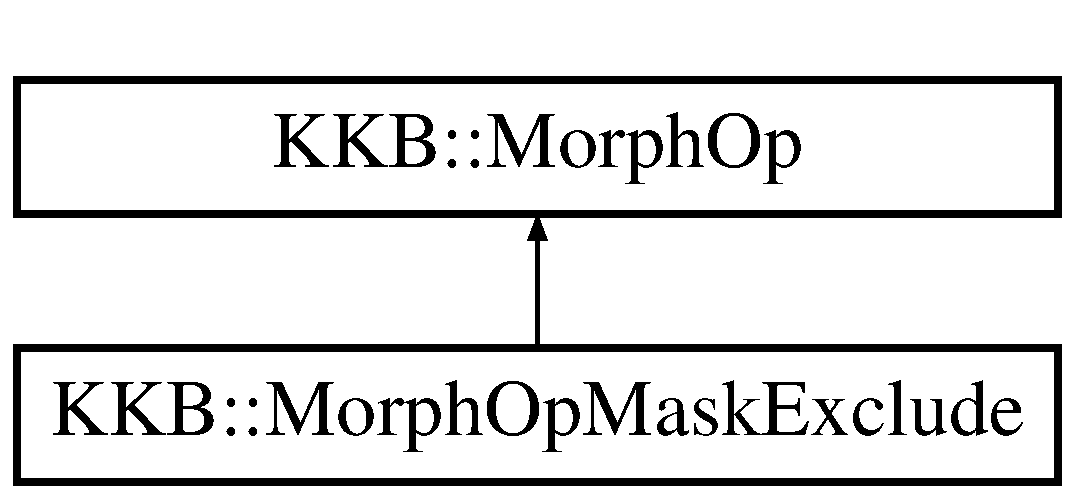
\includegraphics[height=2.000000cm]{class_k_k_b_1_1_morph_op_mask_exclude}
\end{center}
\end{figure}
\subsection*{Public Member Functions}
\begin{DoxyCompactItemize}
\item 
\hyperlink{class_k_k_b_1_1_morph_op_mask_exclude_ace26097ca13e4b64948f7fb282f2db8e}{Morph\+Op\+Mask\+Exclude} (\hyperlink{class_k_k_b_1_1_morph_op_a9eaa0383bf9e046da208af397e7e35eb}{Mask\+Types} \+\_\+mask)
\item 
virtual \hyperlink{class_k_k_b_1_1_morph_op_mask_exclude_a7c80eced0f5c4da968f9329f048a4905}{$\sim$\+Morph\+Op\+Mask\+Exclude} ()
\item 
\hyperlink{namespace_k_k_b_a8fa4952cc84fda1de4bec1fbdd8d5b1b}{kkint32} \hyperlink{class_k_k_b_1_1_morph_op_mask_exclude_a334038ee506236c8de5bff0734692d6b}{Memory\+Consumed\+Estimated} ()
\item 
virtual \hyperlink{class_k_k_b_1_1_morph_op_a32070d9c14d16849873a8a409f5b0d69}{Operation\+Type} \hyperlink{class_k_k_b_1_1_morph_op_mask_exclude_a084a3e895aada937a5f24255a868635f}{Operation} () const 
\item 
virtual \hyperlink{namespace_k_k_b_a80d46bd24db644a022c863bce8ae3633}{Raster\+Ptr} \hyperlink{class_k_k_b_1_1_morph_op_mask_exclude_a25875098567fa8ecd074110a1cccf627}{Perform\+Operation} (\hyperlink{namespace_k_k_b_a5acfa7402dc4df1769f90d3dc8ddfc2c}{Raster\+Const\+Ptr} \+\_\+image)
\end{DoxyCompactItemize}
\subsection*{Additional Inherited Members}


\subsection{Detailed Description}


Definition at line 35 of file Morph\+Op\+Mask\+Exclude.\+h.



\subsection{Constructor \& Destructor Documentation}
\index{K\+K\+B\+::\+Morph\+Op\+Mask\+Exclude@{K\+K\+B\+::\+Morph\+Op\+Mask\+Exclude}!Morph\+Op\+Mask\+Exclude@{Morph\+Op\+Mask\+Exclude}}
\index{Morph\+Op\+Mask\+Exclude@{Morph\+Op\+Mask\+Exclude}!K\+K\+B\+::\+Morph\+Op\+Mask\+Exclude@{K\+K\+B\+::\+Morph\+Op\+Mask\+Exclude}}
\subsubsection[{\texorpdfstring{Morph\+Op\+Mask\+Exclude(\+Mask\+Types \+\_\+mask)}{MorphOpMaskExclude(MaskTypes _mask)}}]{\setlength{\rightskip}{0pt plus 5cm}Morph\+Op\+Mask\+Exclude\+::\+Morph\+Op\+Mask\+Exclude (
\begin{DoxyParamCaption}
\item[{{\bf Mask\+Types}}]{\+\_\+mask}
\end{DoxyParamCaption}
)}\hypertarget{class_k_k_b_1_1_morph_op_mask_exclude_ace26097ca13e4b64948f7fb282f2db8e}{}\label{class_k_k_b_1_1_morph_op_mask_exclude_ace26097ca13e4b64948f7fb282f2db8e}


Definition at line 22 of file Morph\+Op\+Mask\+Exclude.\+cpp.



References K\+K\+B\+::\+Morph\+Op\+::\+Morph\+Op().


\begin{DoxyCode}
22                                                        :
23     \hyperlink{class_k_k_b_1_1_morph_op_a087902e5cad640c26dfa24804cc2a974}{MorphOp} (),
24     mask (\_mask)
25 \{
26 \}
\end{DoxyCode}
\index{K\+K\+B\+::\+Morph\+Op\+Mask\+Exclude@{K\+K\+B\+::\+Morph\+Op\+Mask\+Exclude}!````~Morph\+Op\+Mask\+Exclude@{$\sim$\+Morph\+Op\+Mask\+Exclude}}
\index{````~Morph\+Op\+Mask\+Exclude@{$\sim$\+Morph\+Op\+Mask\+Exclude}!K\+K\+B\+::\+Morph\+Op\+Mask\+Exclude@{K\+K\+B\+::\+Morph\+Op\+Mask\+Exclude}}
\subsubsection[{\texorpdfstring{$\sim$\+Morph\+Op\+Mask\+Exclude()}{~MorphOpMaskExclude()}}]{\setlength{\rightskip}{0pt plus 5cm}Morph\+Op\+Mask\+Exclude\+::$\sim$\+Morph\+Op\+Mask\+Exclude (
\begin{DoxyParamCaption}
{}
\end{DoxyParamCaption}
)\hspace{0.3cm}{\ttfamily [virtual]}}\hypertarget{class_k_k_b_1_1_morph_op_mask_exclude_a7c80eced0f5c4da968f9329f048a4905}{}\label{class_k_k_b_1_1_morph_op_mask_exclude_a7c80eced0f5c4da968f9329f048a4905}


Definition at line 30 of file Morph\+Op\+Mask\+Exclude.\+cpp.


\begin{DoxyCode}
31 \{
32 \}
\end{DoxyCode}


\subsection{Member Function Documentation}
\index{K\+K\+B\+::\+Morph\+Op\+Mask\+Exclude@{K\+K\+B\+::\+Morph\+Op\+Mask\+Exclude}!Memory\+Consumed\+Estimated@{Memory\+Consumed\+Estimated}}
\index{Memory\+Consumed\+Estimated@{Memory\+Consumed\+Estimated}!K\+K\+B\+::\+Morph\+Op\+Mask\+Exclude@{K\+K\+B\+::\+Morph\+Op\+Mask\+Exclude}}
\subsubsection[{\texorpdfstring{Memory\+Consumed\+Estimated()}{MemoryConsumedEstimated()}}]{\setlength{\rightskip}{0pt plus 5cm}{\bf kkint32} Morph\+Op\+Mask\+Exclude\+::\+Memory\+Consumed\+Estimated (
\begin{DoxyParamCaption}
{}
\end{DoxyParamCaption}
)}\hypertarget{class_k_k_b_1_1_morph_op_mask_exclude_a334038ee506236c8de5bff0734692d6b}{}\label{class_k_k_b_1_1_morph_op_mask_exclude_a334038ee506236c8de5bff0734692d6b}


Definition at line 36 of file Morph\+Op\+Mask\+Exclude.\+cpp.


\begin{DoxyCode}
37 \{
38   \hyperlink{namespace_k_k_b_a8fa4952cc84fda1de4bec1fbdd8d5b1b}{kkint32}  result = \textcolor{keyword}{sizeof} (*this);
39   \textcolor{keywordflow}{return}  result;
40 \}
\end{DoxyCode}
\index{K\+K\+B\+::\+Morph\+Op\+Mask\+Exclude@{K\+K\+B\+::\+Morph\+Op\+Mask\+Exclude}!Operation@{Operation}}
\index{Operation@{Operation}!K\+K\+B\+::\+Morph\+Op\+Mask\+Exclude@{K\+K\+B\+::\+Morph\+Op\+Mask\+Exclude}}
\subsubsection[{\texorpdfstring{Operation() const }{Operation() const }}]{\setlength{\rightskip}{0pt plus 5cm}virtual {\bf Operation\+Type} K\+K\+B\+::\+Morph\+Op\+Mask\+Exclude\+::\+Operation (
\begin{DoxyParamCaption}
{}
\end{DoxyParamCaption}
) const\hspace{0.3cm}{\ttfamily [inline]}, {\ttfamily [virtual]}}\hypertarget{class_k_k_b_1_1_morph_op_mask_exclude_a084a3e895aada937a5f24255a868635f}{}\label{class_k_k_b_1_1_morph_op_mask_exclude_a084a3e895aada937a5f24255a868635f}


Implements \hyperlink{class_k_k_b_1_1_morph_op_abdf6f4bddae0b3cc3dc718559fa60234}{K\+K\+B\+::\+Morph\+Op}.



Definition at line 42 of file Morph\+Op\+Mask\+Exclude.\+h.



References K\+K\+B\+::\+Morph\+Op\+::\+Mask\+Exclude.


\begin{DoxyCode}
42 \{\textcolor{keywordflow}{return}  \hyperlink{class_k_k_b_1_1_morph_op_a32070d9c14d16849873a8a409f5b0d69a2166273bd619a450f27a35e9c9e421c3}{OperationType::MaskExclude};\}
\end{DoxyCode}
\index{K\+K\+B\+::\+Morph\+Op\+Mask\+Exclude@{K\+K\+B\+::\+Morph\+Op\+Mask\+Exclude}!Perform\+Operation@{Perform\+Operation}}
\index{Perform\+Operation@{Perform\+Operation}!K\+K\+B\+::\+Morph\+Op\+Mask\+Exclude@{K\+K\+B\+::\+Morph\+Op\+Mask\+Exclude}}
\subsubsection[{\texorpdfstring{Perform\+Operation(\+Raster\+Const\+Ptr \+\_\+image)}{PerformOperation(RasterConstPtr _image)}}]{\setlength{\rightskip}{0pt plus 5cm}{\bf Raster\+Ptr} Morph\+Op\+Mask\+Exclude\+::\+Perform\+Operation (
\begin{DoxyParamCaption}
\item[{{\bf Raster\+Const\+Ptr}}]{\+\_\+image}
\end{DoxyParamCaption}
)\hspace{0.3cm}{\ttfamily [virtual]}}\hypertarget{class_k_k_b_1_1_morph_op_mask_exclude_a25875098567fa8ecd074110a1cccf627}{}\label{class_k_k_b_1_1_morph_op_mask_exclude_a25875098567fa8ecd074110a1cccf627}


Definition at line 44 of file Morph\+Op\+Mask\+Exclude.\+cpp.



References K\+K\+B\+::\+Raster\+::\+Blue\+Area(), K\+K\+B\+::\+Raster\+::\+Dilation(), K\+K\+B\+::\+Raster\+::\+Green\+Area(), K\+K\+B\+::\+Raster\+::\+Opening(), K\+K\+B\+::\+Raster\+::\+Raster(), K\+K\+B\+::\+Raster\+::\+Red\+Area(), K\+K\+B\+::\+Morph\+Op\+::\+Set\+Src\+Raster(), K\+K\+B\+::\+Morph\+Op\+::src\+Blue\+Area, K\+K\+B\+::\+Morph\+Op\+::src\+Color, K\+K\+B\+::\+Morph\+Op\+::src\+Green\+Area, K\+K\+B\+::\+Morph\+Op\+::src\+Height, K\+K\+B\+::\+Morph\+Op\+::src\+Red\+Area, and K\+K\+B\+::\+Morph\+Op\+::src\+Width.


\begin{DoxyCode}
45 \{
46   \hyperlink{class_k_k_b_1_1_morph_op_a07c75e151d9b95ca13da3bfc2e48dba4}{SetSrcRaster} (\_image);
47 
48   \hyperlink{namespace_k_k_b_a8fa4952cc84fda1de4bec1fbdd8d5b1b}{kkint32}  totalPixels = \hyperlink{class_k_k_b_1_1_morph_op_a54b2ce1b398a80803b4dbe8aef956b51}{srcHeight} * \hyperlink{class_k_k_b_1_1_morph_op_aec2cfb3015497e4077751fc5f19559ab}{srcWidth};
49 
50   \hyperlink{class_k_k_b_1_1_raster}{RasterPtr}  maskImage = \textcolor{keyword}{new} \hyperlink{class_k_k_b_1_1_raster}{Raster} (*\_image);
51 
52   maskImage->\hyperlink{class_k_k_b_1_1_raster_a97cd9df45456230dc14e5c448f8d379e}{Opening} ((\hyperlink{class_k_k_b_1_1_morph_op_a9eaa0383bf9e046da208af397e7e35eb}{KKB::MaskTypes})mask);
53   \textcolor{comment}{//maskImage->ConnectedComponent();}
54   maskImage->\hyperlink{class_k_k_b_1_1_raster_afb263b7cc4ab60bf6745c5166173bbb9}{Dilation} ((\hyperlink{class_k_k_b_1_1_morph_op_a9eaa0383bf9e046da208af397e7e35eb}{KKB::MaskTypes})mask);
55 
56   \hyperlink{class_k_k_b_1_1_raster}{RasterPtr}  result = \textcolor{keyword}{new} \hyperlink{class_k_k_b_1_1_raster}{Raster} (\hyperlink{class_k_k_b_1_1_morph_op_a54b2ce1b398a80803b4dbe8aef956b51}{srcHeight}, srcWidth, 
      \hyperlink{class_k_k_b_1_1_morph_op_a0cecdeb8369c7ab2689fbd9f997472b0}{srcColor});
57 
58   \hyperlink{namespace_k_k_b_ace9969169bf514f9ee6185186949cdf7}{uchar} \textcolor{keyword}{const}*  srcImageRedPtr   = \hyperlink{class_k_k_b_1_1_morph_op_acd1f255803231ecfabc0609685e56abe}{srcRedArea};
59   \hyperlink{namespace_k_k_b_ace9969169bf514f9ee6185186949cdf7}{uchar} \textcolor{keyword}{const}*  srcImageGreenPtr = \hyperlink{class_k_k_b_1_1_morph_op_a1a3372b8645c297f21c5805707aef8a0}{srcGreenArea};
60   \hyperlink{namespace_k_k_b_ace9969169bf514f9ee6185186949cdf7}{uchar} \textcolor{keyword}{const}*  srcImageBluePtr  = \hyperlink{class_k_k_b_1_1_morph_op_a52fcf660b2173a2b6e8988ed23cf638c}{srcBlueArea};
61 
62   \hyperlink{namespace_k_k_b_ace9969169bf514f9ee6185186949cdf7}{uchar}*  resultRedPtr   = result->\hyperlink{class_k_k_b_1_1_raster_aa3d0f9b4ce0fdd8ac97f996058d09b22}{RedArea} ();
63   \hyperlink{namespace_k_k_b_ace9969169bf514f9ee6185186949cdf7}{uchar}*  resultGreenPtr = result->\hyperlink{class_k_k_b_1_1_raster_af6ceacfa7835a295d239d141627dbec7}{GreenArea} ();
64   \hyperlink{namespace_k_k_b_ace9969169bf514f9ee6185186949cdf7}{uchar}*  resultBluePtr  = result->\hyperlink{class_k_k_b_1_1_raster_ade7c77867e6b3833e96f5f86aefcffec}{BlueArea} ();
65 
66   \hyperlink{namespace_k_k_b_ace9969169bf514f9ee6185186949cdf7}{uchar}*  maskPtr = maskImage->\hyperlink{class_k_k_b_1_1_raster_af6ceacfa7835a295d239d141627dbec7}{GreenArea} ();
67   \textcolor{keywordflow}{for}  (\hyperlink{namespace_k_k_b_a8fa4952cc84fda1de4bec1fbdd8d5b1b}{kkint32} x = 0;  x < totalPixels;  ++x)
68   \{
69     \textcolor{keywordflow}{if}  (*maskPtr == 0)
70     \{
71       *resultGreenPtr = *srcImageGreenPtr;
72       \textcolor{keywordflow}{if}  (\hyperlink{class_k_k_b_1_1_morph_op_a0cecdeb8369c7ab2689fbd9f997472b0}{srcColor})
73       \{
74         *resultRedPtr  = *srcImageRedPtr;
75         *resultBluePtr = *srcImageBluePtr;
76       \}
77     \}
78     ++maskPtr;
79     ++srcImageGreenPtr;
80     ++resultGreenPtr;
81     \textcolor{keywordflow}{if}  (\hyperlink{class_k_k_b_1_1_morph_op_a0cecdeb8369c7ab2689fbd9f997472b0}{srcColor})
82     \{
83       ++srcImageRedPtr;
84       ++resultRedPtr;
85       ++srcImageBluePtr;
86       ++resultBluePtr;
87     \}
88   \}
89 
90   \textcolor{keyword}{delete}  maskImage;
91   maskImage = NULL;
92 
93   \textcolor{keywordflow}{return}  result;
94 \}  \textcolor{comment}{/* PerformOperation */}
\end{DoxyCode}


The documentation for this class was generated from the following files\+:\begin{DoxyCompactItemize}
\item 
C\+:/\+Users/\+Kurt/\+Git\+Hub/\+K\+Square\+Libraries/\+K\+K\+Base/\hyperlink{_morph_op_mask_exclude_8h}{Morph\+Op\+Mask\+Exclude.\+h}\item 
C\+:/\+Users/\+Kurt/\+Git\+Hub/\+K\+Square\+Libraries/\+K\+K\+Base/\hyperlink{_morph_op_mask_exclude_8cpp}{Morph\+Op\+Mask\+Exclude.\+cpp}\end{DoxyCompactItemize}

\hypertarget{class_k_k_b_1_1_morph_op_sobel}{}\section{K\+KB\+:\+:Morph\+Op\+Sobel Class Reference}
\label{class_k_k_b_1_1_morph_op_sobel}\index{K\+K\+B\+::\+Morph\+Op\+Sobel@{K\+K\+B\+::\+Morph\+Op\+Sobel}}


{\ttfamily \#include $<$Morph\+Op\+Sobel.\+h$>$}

Inheritance diagram for K\+KB\+:\+:Morph\+Op\+Sobel\+:\begin{figure}[H]
\begin{center}
\leavevmode
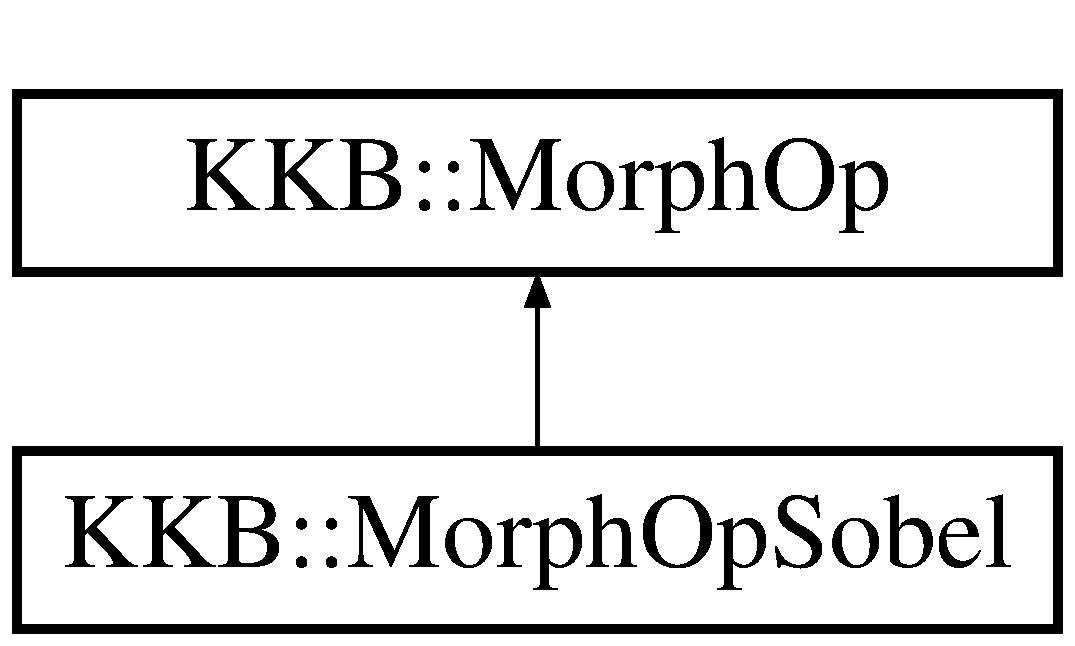
\includegraphics[height=2.000000cm]{class_k_k_b_1_1_morph_op_sobel}
\end{center}
\end{figure}
\subsection*{Public Member Functions}
\begin{DoxyCompactItemize}
\item 
\hyperlink{class_k_k_b_1_1_morph_op_sobel_a675a53713bf9f9c1d37caa917e14d051}{Morph\+Op\+Sobel} ()
\item 
\hyperlink{class_k_k_b_1_1_morph_op_sobel_a93d249ab7be5efa900efa9d87a740fd3}{$\sim$\+Morph\+Op\+Sobel} (void)
\item 
virtual \hyperlink{class_k_k_b_1_1_morph_op_a32070d9c14d16849873a8a409f5b0d69}{Operation\+Type} \hyperlink{class_k_k_b_1_1_morph_op_sobel_a0c11ea47d46bbe8c365db296672f0595}{Operation} () const 
\item 
virtual \hyperlink{namespace_k_k_b_a80d46bd24db644a022c863bce8ae3633}{Raster\+Ptr} \hyperlink{class_k_k_b_1_1_morph_op_sobel_a0e58b3ecae29af573c719b8d79c8dbd4}{Perform\+Operation} (\hyperlink{class_k_k_b_1_1_raster}{Raster} const $\ast$\+\_\+image)
\end{DoxyCompactItemize}
\subsection*{Additional Inherited Members}


\subsection{Detailed Description}


Definition at line 18 of file Morph\+Op\+Sobel.\+h.



\subsection{Constructor \& Destructor Documentation}
\index{K\+K\+B\+::\+Morph\+Op\+Sobel@{K\+K\+B\+::\+Morph\+Op\+Sobel}!Morph\+Op\+Sobel@{Morph\+Op\+Sobel}}
\index{Morph\+Op\+Sobel@{Morph\+Op\+Sobel}!K\+K\+B\+::\+Morph\+Op\+Sobel@{K\+K\+B\+::\+Morph\+Op\+Sobel}}
\subsubsection[{\texorpdfstring{Morph\+Op\+Sobel()}{MorphOpSobel()}}]{\setlength{\rightskip}{0pt plus 5cm}Morph\+Op\+Sobel\+::\+Morph\+Op\+Sobel (
\begin{DoxyParamCaption}
{}
\end{DoxyParamCaption}
)}\hypertarget{class_k_k_b_1_1_morph_op_sobel_a675a53713bf9f9c1d37caa917e14d051}{}\label{class_k_k_b_1_1_morph_op_sobel_a675a53713bf9f9c1d37caa917e14d051}


Definition at line 23 of file Morph\+Op\+Sobel.\+cpp.


\begin{DoxyCode}
23                            :
24     magnitudeSqrTable (NULL),
25     maxMagnitude      (0)
26 \{
27 \}
\end{DoxyCode}
\index{K\+K\+B\+::\+Morph\+Op\+Sobel@{K\+K\+B\+::\+Morph\+Op\+Sobel}!````~Morph\+Op\+Sobel@{$\sim$\+Morph\+Op\+Sobel}}
\index{````~Morph\+Op\+Sobel@{$\sim$\+Morph\+Op\+Sobel}!K\+K\+B\+::\+Morph\+Op\+Sobel@{K\+K\+B\+::\+Morph\+Op\+Sobel}}
\subsubsection[{\texorpdfstring{$\sim$\+Morph\+Op\+Sobel(void)}{~MorphOpSobel(void)}}]{\setlength{\rightskip}{0pt plus 5cm}Morph\+Op\+Sobel\+::$\sim$\+Morph\+Op\+Sobel (
\begin{DoxyParamCaption}
\item[{void}]{}
\end{DoxyParamCaption}
)}\hypertarget{class_k_k_b_1_1_morph_op_sobel_a93d249ab7be5efa900efa9d87a740fd3}{}\label{class_k_k_b_1_1_morph_op_sobel_a93d249ab7be5efa900efa9d87a740fd3}


Definition at line 29 of file Morph\+Op\+Sobel.\+cpp.


\begin{DoxyCode}
30 \{
31   DeleteMagnitudeSqrTable ();
32 \}
\end{DoxyCode}


\subsection{Member Function Documentation}
\index{K\+K\+B\+::\+Morph\+Op\+Sobel@{K\+K\+B\+::\+Morph\+Op\+Sobel}!Operation@{Operation}}
\index{Operation@{Operation}!K\+K\+B\+::\+Morph\+Op\+Sobel@{K\+K\+B\+::\+Morph\+Op\+Sobel}}
\subsubsection[{\texorpdfstring{Operation() const }{Operation() const }}]{\setlength{\rightskip}{0pt plus 5cm}virtual {\bf Operation\+Type} K\+K\+B\+::\+Morph\+Op\+Sobel\+::\+Operation (
\begin{DoxyParamCaption}
{}
\end{DoxyParamCaption}
) const\hspace{0.3cm}{\ttfamily [inline]}, {\ttfamily [virtual]}}\hypertarget{class_k_k_b_1_1_morph_op_sobel_a0c11ea47d46bbe8c365db296672f0595}{}\label{class_k_k_b_1_1_morph_op_sobel_a0c11ea47d46bbe8c365db296672f0595}


Implements \hyperlink{class_k_k_b_1_1_morph_op_abdf6f4bddae0b3cc3dc718559fa60234}{K\+K\+B\+::\+Morph\+Op}.



Definition at line 25 of file Morph\+Op\+Sobel.\+h.



References K\+K\+B\+::\+Morph\+Op\+::\+Sobel\+Edge\+Detection.


\begin{DoxyCode}
25 \{\textcolor{keywordflow}{return} \hyperlink{class_k_k_b_1_1_morph_op_a32070d9c14d16849873a8a409f5b0d69ae9eb5dc5ac36ae1b3a4eb7c17def6093}{OperationType::SobelEdgeDetection};\}
\end{DoxyCode}
\index{K\+K\+B\+::\+Morph\+Op\+Sobel@{K\+K\+B\+::\+Morph\+Op\+Sobel}!Perform\+Operation@{Perform\+Operation}}
\index{Perform\+Operation@{Perform\+Operation}!K\+K\+B\+::\+Morph\+Op\+Sobel@{K\+K\+B\+::\+Morph\+Op\+Sobel}}
\subsubsection[{\texorpdfstring{Perform\+Operation(\+Raster const $\ast$\+\_\+image)}{PerformOperation(Raster const *_image)}}]{\setlength{\rightskip}{0pt plus 5cm}{\bf Raster\+Ptr} Morph\+Op\+Sobel\+::\+Perform\+Operation (
\begin{DoxyParamCaption}
\item[{{\bf Raster} const $\ast$}]{\+\_\+image}
\end{DoxyParamCaption}
)\hspace{0.3cm}{\ttfamily [virtual]}}\hypertarget{class_k_k_b_1_1_morph_op_sobel_a0e58b3ecae29af573c719b8d79c8dbd4}{}\label{class_k_k_b_1_1_morph_op_sobel_a0e58b3ecae29af573c719b8d79c8dbd4}


Implements \hyperlink{class_k_k_b_1_1_morph_op_ae7655bec44b6665fd042216e5cb55843}{K\+K\+B\+::\+Morph\+Op}.



Definition at line 62 of file Morph\+Op\+Sobel.\+cpp.



References K\+K\+B\+::\+Raster\+::\+Color(), K\+K\+B\+::\+Raster\+::\+Create\+Gray\+Scale\+K\+L\+T(), and K\+K\+B\+::\+Morph\+Op\+::\+Set\+Src\+Raster().



Referenced by K\+K\+B\+::\+Raster\+::\+Sobel\+Edge\+Detector().


\begin{DoxyCode}
63 \{
64   \textcolor{keywordflow}{if}  (!\_image)
65     \textcolor{keywordflow}{return} NULL;
66 
67   \textcolor{keywordtype}{bool}  weOwnRaster = \textcolor{keyword}{false};
68   \textcolor{keywordflow}{if}  (\_image->Color ())
69   \{
70     \_image = \_image->CreateGrayScaleKLT ();
71     weOwnRaster = \textcolor{keyword}{true};
72   \}
73 
74   \hyperlink{class_k_k_b_1_1_morph_op_a07c75e151d9b95ca13da3bfc2e48dba4}{SetSrcRaster} (\_image);
75 
76   BuildMagnitudeSqrTable ();
77 
78   \textcolor{keywordflow}{if}  (weOwnRaster)
79     \textcolor{keyword}{delete}  \_image;
80   \_image = NULL;
81 
82   \textcolor{keywordflow}{return}  BuildMagnitudeImage();
83 \}  \textcolor{comment}{/* PerformOperation */}
\end{DoxyCode}


The documentation for this class was generated from the following files\+:\begin{DoxyCompactItemize}
\item 
C\+:/\+Users/\+Kurt/\+Git\+Hub/\+K\+Square\+Libraries/\+K\+K\+Base/\hyperlink{_morph_op_sobel_8h}{Morph\+Op\+Sobel.\+h}\item 
C\+:/\+Users/\+Kurt/\+Git\+Hub/\+K\+Square\+Libraries/\+K\+K\+Base/\hyperlink{_morph_op_sobel_8cpp}{Morph\+Op\+Sobel.\+cpp}\end{DoxyCompactItemize}

\hypertarget{class_k_k_b_1_1_morph_op_stretcher}{}\section{K\+KB\+:\+:Morph\+Op\+Stretcher Class Reference}
\label{class_k_k_b_1_1_morph_op_stretcher}\index{K\+K\+B\+::\+Morph\+Op\+Stretcher@{K\+K\+B\+::\+Morph\+Op\+Stretcher}}


{\ttfamily \#include $<$Morph\+Op\+Stretcher.\+h$>$}

Inheritance diagram for K\+KB\+:\+:Morph\+Op\+Stretcher\+:\begin{figure}[H]
\begin{center}
\leavevmode
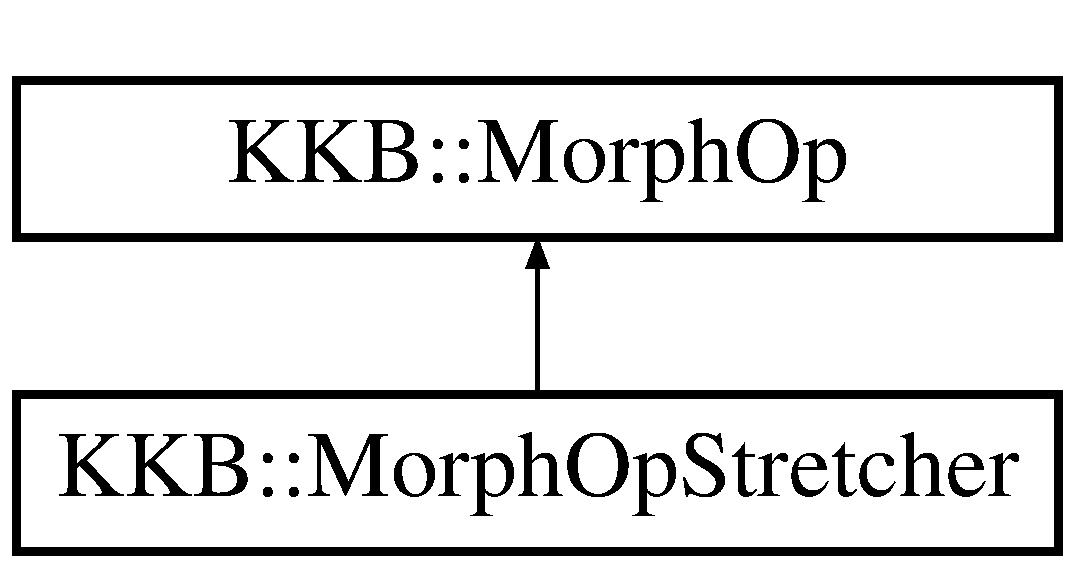
\includegraphics[height=2.000000cm]{class_k_k_b_1_1_morph_op_stretcher}
\end{center}
\end{figure}
\subsection*{Classes}
\begin{DoxyCompactItemize}
\item 
class \hyperlink{class_morph_op_stretcher_1_1_cell_factor}{Cell\+Factor}
\end{DoxyCompactItemize}
\subsection*{Public Member Functions}
\begin{DoxyCompactItemize}
\item 
\hyperlink{class_k_k_b_1_1_morph_op_stretcher_a02436bb070c3d288612345b87bba7f8b}{Morph\+Op\+Stretcher} (float \+\_\+row\+Factor, float \+\_\+col\+Factor)
\item 
virtual \hyperlink{class_k_k_b_1_1_morph_op_stretcher_a57c9b92293b43107e2e5386f91c06ba0}{$\sim$\+Morph\+Op\+Stretcher} ()
\item 
float \hyperlink{class_k_k_b_1_1_morph_op_stretcher_a31b2b87a8bc43f2ea8bbe0ad77849be1}{Col\+Factor} () const 
\item 
\hyperlink{namespace_k_k_b_a8fa4952cc84fda1de4bec1fbdd8d5b1b}{kkint32} \hyperlink{class_k_k_b_1_1_morph_op_stretcher_a399a5b979f728370794babd0d5b03cfd}{Memory\+Consumed\+Estimated} ()
\item 
virtual \hyperlink{class_k_k_b_1_1_morph_op_a32070d9c14d16849873a8a409f5b0d69}{Operation\+Type} \hyperlink{class_k_k_b_1_1_morph_op_stretcher_afdf127ebc560ce9579355f2700952d92}{Operation} () const 
\item 
virtual \hyperlink{namespace_k_k_b_a80d46bd24db644a022c863bce8ae3633}{Raster\+Ptr} \hyperlink{class_k_k_b_1_1_morph_op_stretcher_affcccf7e48ed632a97395f0b893eba3b}{Perform\+Operation} (\hyperlink{namespace_k_k_b_a5acfa7402dc4df1769f90d3dc8ddfc2c}{Raster\+Const\+Ptr} \+\_\+image)
\item 
float \hyperlink{class_k_k_b_1_1_morph_op_stretcher_af191abd6582f078f6d28d7c9ba3a8f2a}{Row\+Factor} () const 
\end{DoxyCompactItemize}
\subsection*{Additional Inherited Members}


\subsection{Detailed Description}


Definition at line 26 of file Morph\+Op\+Stretcher.\+h.



\subsection{Constructor \& Destructor Documentation}
\index{K\+K\+B\+::\+Morph\+Op\+Stretcher@{K\+K\+B\+::\+Morph\+Op\+Stretcher}!Morph\+Op\+Stretcher@{Morph\+Op\+Stretcher}}
\index{Morph\+Op\+Stretcher@{Morph\+Op\+Stretcher}!K\+K\+B\+::\+Morph\+Op\+Stretcher@{K\+K\+B\+::\+Morph\+Op\+Stretcher}}
\subsubsection[{\texorpdfstring{Morph\+Op\+Stretcher(float \+\_\+row\+Factor, float \+\_\+col\+Factor)}{MorphOpStretcher(float _rowFactor, float _colFactor)}}]{\setlength{\rightskip}{0pt plus 5cm}Morph\+Op\+Stretcher\+::\+Morph\+Op\+Stretcher (
\begin{DoxyParamCaption}
\item[{float}]{\+\_\+row\+Factor, }
\item[{float}]{\+\_\+col\+Factor}
\end{DoxyParamCaption}
)}\hypertarget{class_k_k_b_1_1_morph_op_stretcher_a02436bb070c3d288612345b87bba7f8b}{}\label{class_k_k_b_1_1_morph_op_stretcher_a02436bb070c3d288612345b87bba7f8b}


Definition at line 81 of file Morph\+Op\+Stretcher.\+cpp.



References K\+K\+B\+::\+Morph\+Op\+::\+Morph\+Op().



Referenced by K\+K\+B\+::\+Raster\+::\+Streatch\+Image().


\begin{DoxyCode}
83                                     :
84     \hyperlink{class_k_k_b_1_1_morph_op_a087902e5cad640c26dfa24804cc2a974}{MorphOp} (),
85     rowFactor             (\_rowFactor),
86     colFactor             (\_colFactor),
87     rowFactorsCount       (0),
88     rowFactors            (NULL),
89     colFactorsCount       (0),
90     colFactors            (NULL)
91 \{
92 \}
\end{DoxyCode}
\index{K\+K\+B\+::\+Morph\+Op\+Stretcher@{K\+K\+B\+::\+Morph\+Op\+Stretcher}!````~Morph\+Op\+Stretcher@{$\sim$\+Morph\+Op\+Stretcher}}
\index{````~Morph\+Op\+Stretcher@{$\sim$\+Morph\+Op\+Stretcher}!K\+K\+B\+::\+Morph\+Op\+Stretcher@{K\+K\+B\+::\+Morph\+Op\+Stretcher}}
\subsubsection[{\texorpdfstring{$\sim$\+Morph\+Op\+Stretcher()}{~MorphOpStretcher()}}]{\setlength{\rightskip}{0pt plus 5cm}Morph\+Op\+Stretcher\+::$\sim$\+Morph\+Op\+Stretcher (
\begin{DoxyParamCaption}
{}
\end{DoxyParamCaption}
)\hspace{0.3cm}{\ttfamily [virtual]}}\hypertarget{class_k_k_b_1_1_morph_op_stretcher_a57c9b92293b43107e2e5386f91c06ba0}{}\label{class_k_k_b_1_1_morph_op_stretcher_a57c9b92293b43107e2e5386f91c06ba0}


Definition at line 96 of file Morph\+Op\+Stretcher.\+cpp.


\begin{DoxyCode}
97 \{
98   \textcolor{keyword}{delete}[]  rowFactors;   rowFactors = NULL;
99   \textcolor{keyword}{delete}[]  colFactors;   colFactors = NULL;
100 \}
\end{DoxyCode}


\subsection{Member Function Documentation}
\index{K\+K\+B\+::\+Morph\+Op\+Stretcher@{K\+K\+B\+::\+Morph\+Op\+Stretcher}!Col\+Factor@{Col\+Factor}}
\index{Col\+Factor@{Col\+Factor}!K\+K\+B\+::\+Morph\+Op\+Stretcher@{K\+K\+B\+::\+Morph\+Op\+Stretcher}}
\subsubsection[{\texorpdfstring{Col\+Factor() const }{ColFactor() const }}]{\setlength{\rightskip}{0pt plus 5cm}float K\+K\+B\+::\+Morph\+Op\+Stretcher\+::\+Col\+Factor (
\begin{DoxyParamCaption}
{}
\end{DoxyParamCaption}
) const\hspace{0.3cm}{\ttfamily [inline]}}\hypertarget{class_k_k_b_1_1_morph_op_stretcher_a31b2b87a8bc43f2ea8bbe0ad77849be1}{}\label{class_k_k_b_1_1_morph_op_stretcher_a31b2b87a8bc43f2ea8bbe0ad77849be1}


Definition at line 35 of file Morph\+Op\+Stretcher.\+h.


\begin{DoxyCode}
35 \{\textcolor{keywordflow}{return} colFactor;\}
\end{DoxyCode}
\index{K\+K\+B\+::\+Morph\+Op\+Stretcher@{K\+K\+B\+::\+Morph\+Op\+Stretcher}!Memory\+Consumed\+Estimated@{Memory\+Consumed\+Estimated}}
\index{Memory\+Consumed\+Estimated@{Memory\+Consumed\+Estimated}!K\+K\+B\+::\+Morph\+Op\+Stretcher@{K\+K\+B\+::\+Morph\+Op\+Stretcher}}
\subsubsection[{\texorpdfstring{Memory\+Consumed\+Estimated()}{MemoryConsumedEstimated()}}]{\setlength{\rightskip}{0pt plus 5cm}{\bf kkint32} Morph\+Op\+Stretcher\+::\+Memory\+Consumed\+Estimated (
\begin{DoxyParamCaption}
{}
\end{DoxyParamCaption}
)}\hypertarget{class_k_k_b_1_1_morph_op_stretcher_a399a5b979f728370794babd0d5b03cfd}{}\label{class_k_k_b_1_1_morph_op_stretcher_a399a5b979f728370794babd0d5b03cfd}


Definition at line 104 of file Morph\+Op\+Stretcher.\+cpp.


\begin{DoxyCode}
105 \{
106   \hyperlink{namespace_k_k_b_a8fa4952cc84fda1de4bec1fbdd8d5b1b}{kkint32}  result = \textcolor{keyword}{sizeof} (*this) +
107          (\hyperlink{namespace_k_k_b_a8fa4952cc84fda1de4bec1fbdd8d5b1b}{kkint32})(rowFactorsCount * \textcolor{keyword}{sizeof} (CellFactor) * rowFactor) + 
108          (\hyperlink{namespace_k_k_b_a8fa4952cc84fda1de4bec1fbdd8d5b1b}{kkint32})(colFactorsCount * \textcolor{keyword}{sizeof} (CellFactor) * colFactor);
109   \textcolor{keywordflow}{return}  result;
110 \}
\end{DoxyCode}
\index{K\+K\+B\+::\+Morph\+Op\+Stretcher@{K\+K\+B\+::\+Morph\+Op\+Stretcher}!Operation@{Operation}}
\index{Operation@{Operation}!K\+K\+B\+::\+Morph\+Op\+Stretcher@{K\+K\+B\+::\+Morph\+Op\+Stretcher}}
\subsubsection[{\texorpdfstring{Operation() const }{Operation() const }}]{\setlength{\rightskip}{0pt plus 5cm}virtual {\bf Operation\+Type} K\+K\+B\+::\+Morph\+Op\+Stretcher\+::\+Operation (
\begin{DoxyParamCaption}
{}
\end{DoxyParamCaption}
) const\hspace{0.3cm}{\ttfamily [inline]}, {\ttfamily [virtual]}}\hypertarget{class_k_k_b_1_1_morph_op_stretcher_afdf127ebc560ce9579355f2700952d92}{}\label{class_k_k_b_1_1_morph_op_stretcher_afdf127ebc560ce9579355f2700952d92}


Implements \hyperlink{class_k_k_b_1_1_morph_op_abdf6f4bddae0b3cc3dc718559fa60234}{K\+K\+B\+::\+Morph\+Op}.



Definition at line 38 of file Morph\+Op\+Stretcher.\+h.



References K\+K\+B\+::\+Morph\+Op\+::\+Stretcher.


\begin{DoxyCode}
38 \{\textcolor{keywordflow}{return}  \hyperlink{class_k_k_b_1_1_morph_op_a32070d9c14d16849873a8a409f5b0d69a0a93701260be81cae9cf81aade6afaa1}{OperationType::Stretcher};\}
\end{DoxyCode}
\index{K\+K\+B\+::\+Morph\+Op\+Stretcher@{K\+K\+B\+::\+Morph\+Op\+Stretcher}!Perform\+Operation@{Perform\+Operation}}
\index{Perform\+Operation@{Perform\+Operation}!K\+K\+B\+::\+Morph\+Op\+Stretcher@{K\+K\+B\+::\+Morph\+Op\+Stretcher}}
\subsubsection[{\texorpdfstring{Perform\+Operation(\+Raster\+Const\+Ptr \+\_\+image)}{PerformOperation(RasterConstPtr _image)}}]{\setlength{\rightskip}{0pt plus 5cm}{\bf Raster\+Ptr} Morph\+Op\+Stretcher\+::\+Perform\+Operation (
\begin{DoxyParamCaption}
\item[{{\bf Raster\+Const\+Ptr}}]{\+\_\+image}
\end{DoxyParamCaption}
)\hspace{0.3cm}{\ttfamily [virtual]}}\hypertarget{class_k_k_b_1_1_morph_op_stretcher_affcccf7e48ed632a97395f0b893eba3b}{}\label{class_k_k_b_1_1_morph_op_stretcher_affcccf7e48ed632a97395f0b893eba3b}


Definition at line 114 of file Morph\+Op\+Stretcher.\+cpp.



References K\+K\+B\+::\+Raster\+::\+Background\+Pixel\+T\+H(), K\+K\+B\+::\+Raster\+::\+Background\+Pixel\+Value(), K\+K\+B\+::\+Raster\+::\+Blue(), K\+K\+B\+::\+Raster\+::\+Color(), K\+K\+B\+::\+Morph\+Op\+Stretcher\+::\+Cell\+Factor\+::dest\+Cell\+Count, K\+K\+B\+::\+Morph\+Op\+Stretcher\+::\+Cell\+Factor\+::dest\+Cell\+Fracts, K\+K\+B\+::\+Morph\+Op\+Stretcher\+::\+Cell\+Factor\+::dest\+Cell\+Idxs, K\+K\+B\+::\+Raster\+::\+Foreground\+Pixel\+Value(), K\+K\+B\+::\+Raster\+::\+Green(), K\+K\+B\+::\+Raster\+::\+Raster(), K\+K\+B\+::\+Raster\+::\+Red(), K\+K\+B\+::\+Morph\+Op\+::\+Set\+Src\+Raster(), K\+K\+B\+::\+Morph\+Op\+::src\+Blue, K\+K\+B\+::\+Morph\+Op\+::src\+Green, K\+K\+B\+::\+Morph\+Op\+::src\+Height, K\+K\+B\+::\+Morph\+Op\+::src\+Red, and K\+K\+B\+::\+Morph\+Op\+::src\+Width.



Referenced by K\+K\+B\+::\+Raster\+::\+Streatch\+Image().


\begin{DoxyCode}
115 \{
116   this->\hyperlink{class_k_k_b_1_1_morph_op_a07c75e151d9b95ca13da3bfc2e48dba4}{SetSrcRaster} (\_image);
117 
118   \hyperlink{namespace_k_k_b_af8d832f05c54994a1cce25bd5743e19a}{kkuint32}  destHeight = (\hyperlink{namespace_k_k_b_af8d832f05c54994a1cce25bd5743e19a}{kkuint32})ceil (0.5f + (\textcolor{keywordtype}{float})\hyperlink{class_k_k_b_1_1_morph_op_a54b2ce1b398a80803b4dbe8aef956b51}{srcHeight} * rowFactor);
119   \hyperlink{namespace_k_k_b_af8d832f05c54994a1cce25bd5743e19a}{kkuint32}  destWidth  = (\hyperlink{namespace_k_k_b_af8d832f05c54994a1cce25bd5743e19a}{kkuint32})ceil (0.5f + (\textcolor{keywordtype}{float})\hyperlink{class_k_k_b_1_1_morph_op_aec2cfb3015497e4077751fc5f19559ab}{srcWidth}  * colFactor);
120 
121   \textcolor{keywordtype}{bool}  color = \_image->Color ();
122 
123   UpdateFactors (\hyperlink{class_k_k_b_1_1_morph_op_a54b2ce1b398a80803b4dbe8aef956b51}{srcHeight}, \hyperlink{class_k_k_b_1_1_morph_op_aec2cfb3015497e4077751fc5f19559ab}{srcWidth});
124 
125   \hyperlink{class_k_k_b_1_1_raster}{RasterPtr}  result = \textcolor{keyword}{new} \hyperlink{class_k_k_b_1_1_raster}{Raster} (destHeight, destWidth, color);
126 
127   result->\hyperlink{class_k_k_b_1_1_raster_a96e0ed160e633c316cf83890ef3438eb}{BackgroundPixelTH}    (\_image->BackgroundPixelTH    ());
128   result->\hyperlink{class_k_k_b_1_1_raster_a823cb64d8d4c82620d16564e13855e75}{BackgroundPixelValue} (\_image->BackgroundPixelValue ());
129   result->\hyperlink{class_k_k_b_1_1_raster_a11b142b955f79a1482606a32ce209373}{ForegroundPixelValue} (\_image->ForegroundPixelValue ());
130 
131   \hyperlink{namespace_k_k_b_ace9969169bf514f9ee6185186949cdf7}{uchar}**  destRed   = result->\hyperlink{class_k_k_b_1_1_raster_a337a5a064b27693eec6e380789680239}{Red}   ();
132   \hyperlink{namespace_k_k_b_ace9969169bf514f9ee6185186949cdf7}{uchar}**  destGreen = result->\hyperlink{class_k_k_b_1_1_raster_a2dbd81f2cb60b3716bcf6467050dde93}{Green} ();
133   \hyperlink{namespace_k_k_b_ace9969169bf514f9ee6185186949cdf7}{uchar}**  destBlue  = result->\hyperlink{class_k_k_b_1_1_raster_ae289ec3ad3a27339cd30e9ac3b488004}{Blue}  ();
134 
135   \textcolor{keywordflow}{for}  (\hyperlink{namespace_k_k_b_a8fa4952cc84fda1de4bec1fbdd8d5b1b}{kkint32}  srcRow = 0;  srcRow < \hyperlink{class_k_k_b_1_1_morph_op_a54b2ce1b398a80803b4dbe8aef956b51}{srcHeight};  ++srcRow)
136   \{
137     \hyperlink{namespace_k_k_b_ace9969169bf514f9ee6185186949cdf7}{uchar}*  srcRedRow   = NULL;
138     \hyperlink{namespace_k_k_b_ace9969169bf514f9ee6185186949cdf7}{uchar}*  srcGreenRow = \hyperlink{class_k_k_b_1_1_morph_op_ab811c702f7e0c8ffccdd21111c8144ab}{srcGreen}[srcRow];
139     \hyperlink{namespace_k_k_b_ace9969169bf514f9ee6185186949cdf7}{uchar}*  srcBlueRow  = NULL;
140     \textcolor{keywordflow}{if}  (color)
141     \{
142       srcRedRow  = \hyperlink{class_k_k_b_1_1_morph_op_a4d790e4b71cfdaecee876879663dfdb4}{srcRed} [srcRow];
143       srcBlueRow = \hyperlink{class_k_k_b_1_1_morph_op_ad11edf2de07634c4c68df9a2e74cfd6c}{srcBlue}[srcRow];
144     \}
145 
146     CellFactor&  rowFactor = rowFactors[srcRow];
147 
148     \textcolor{keywordflow}{for}  (\hyperlink{namespace_k_k_b_af8d832f05c54994a1cce25bd5743e19a}{kkuint32}  rowFactorIdx = 0;  rowFactorIdx < rowFactor.destCellCount;  ++rowFactorIdx)
149     \{
150       \hyperlink{namespace_k_k_b_af8d832f05c54994a1cce25bd5743e19a}{kkuint32}  destRow      = rowFactor.\hyperlink{class_morph_op_stretcher_1_1_cell_factor_ad98db8b4eb2b3513ad0a592250bacc06}{destCellIdxs}  [rowFactorIdx];
151       \textcolor{keywordtype}{float}   destRowFract = rowFactor.destCellFracts[rowFactorIdx];
152 
153       \textcolor{keywordflow}{for}  (\hyperlink{namespace_k_k_b_a8fa4952cc84fda1de4bec1fbdd8d5b1b}{kkint32} srcCol = 0;  srcCol < \hyperlink{class_k_k_b_1_1_morph_op_aec2cfb3015497e4077751fc5f19559ab}{srcWidth};  ++srcCol)
154       \{
155         \hyperlink{namespace_k_k_b_ace9969169bf514f9ee6185186949cdf7}{uchar}  srcPixelRed   = 0;
156         \hyperlink{namespace_k_k_b_ace9969169bf514f9ee6185186949cdf7}{uchar}  srcPixelGreen = srcGreenRow[srcCol];
157         \hyperlink{namespace_k_k_b_ace9969169bf514f9ee6185186949cdf7}{uchar}  srcPixelBlue  = 0;
158         \textcolor{keywordflow}{if}  (color)
159         \{
160           srcPixelRed   = srcRedRow [srcCol];
161           srcPixelBlue  = srcBlueRow[srcCol];
162         \}
163 
164         CellFactor&  colFactor = colFactors[srcCol];
165 
166         \textcolor{keywordflow}{for}  (\hyperlink{namespace_k_k_b_af8d832f05c54994a1cce25bd5743e19a}{kkuint32}  colFactorIdx = 0;  colFactorIdx < colFactor.destCellCount;  ++colFactorIdx)
167         \{
168           \hyperlink{namespace_k_k_b_af8d832f05c54994a1cce25bd5743e19a}{kkuint32}  destCol      = colFactor.\hyperlink{class_morph_op_stretcher_1_1_cell_factor_ad98db8b4eb2b3513ad0a592250bacc06}{destCellIdxs}  [colFactorIdx];
169           \textcolor{keywordtype}{float}   destColFract = colFactor.destCellFracts[colFactorIdx];
170 
171           destGreen[destRow][destCol] += (\hyperlink{namespace_k_k_b_ace9969169bf514f9ee6185186949cdf7}{uchar})\hyperlink{namespace_k_k_b_ad030d1ca8bd5038824c4a923a4d23fb5}{Min} (255.0f, srcPixelGreen * destRowFract * 
      destColFract);
172           \textcolor{keywordflow}{if}  (color)
173           \{
174             destRed [destRow][destCol] += (\hyperlink{namespace_k_k_b_ace9969169bf514f9ee6185186949cdf7}{uchar})\hyperlink{namespace_k_k_b_ad030d1ca8bd5038824c4a923a4d23fb5}{Min} (255.0f, srcPixelRed  * destRowFract * 
      destColFract);
175             destBlue[destRow][destCol] += (\hyperlink{namespace_k_k_b_ace9969169bf514f9ee6185186949cdf7}{uchar})\hyperlink{namespace_k_k_b_ad030d1ca8bd5038824c4a923a4d23fb5}{Min} (255.0f, srcPixelBlue * destRowFract * 
      destColFract);
176           \}
177         \}
178       \}
179     \}
180   \}
181 
182   \textcolor{keywordflow}{return}  result;
183 \}  \textcolor{comment}{/* PerformOperation */}
\end{DoxyCode}
\index{K\+K\+B\+::\+Morph\+Op\+Stretcher@{K\+K\+B\+::\+Morph\+Op\+Stretcher}!Row\+Factor@{Row\+Factor}}
\index{Row\+Factor@{Row\+Factor}!K\+K\+B\+::\+Morph\+Op\+Stretcher@{K\+K\+B\+::\+Morph\+Op\+Stretcher}}
\subsubsection[{\texorpdfstring{Row\+Factor() const }{RowFactor() const }}]{\setlength{\rightskip}{0pt plus 5cm}float K\+K\+B\+::\+Morph\+Op\+Stretcher\+::\+Row\+Factor (
\begin{DoxyParamCaption}
{}
\end{DoxyParamCaption}
) const\hspace{0.3cm}{\ttfamily [inline]}}\hypertarget{class_k_k_b_1_1_morph_op_stretcher_af191abd6582f078f6d28d7c9ba3a8f2a}{}\label{class_k_k_b_1_1_morph_op_stretcher_af191abd6582f078f6d28d7c9ba3a8f2a}


Definition at line 36 of file Morph\+Op\+Stretcher.\+h.


\begin{DoxyCode}
36 \{\textcolor{keywordflow}{return} rowFactor;\}
\end{DoxyCode}


The documentation for this class was generated from the following files\+:\begin{DoxyCompactItemize}
\item 
C\+:/\+Users/\+Kurt/\+Git\+Hub/\+K\+Square\+Libraries/\+K\+K\+Base/\hyperlink{_morph_op_stretcher_8h}{Morph\+Op\+Stretcher.\+h}\item 
C\+:/\+Users/\+Kurt/\+Git\+Hub/\+K\+Square\+Libraries/\+K\+K\+Base/\hyperlink{_morph_op_stretcher_8cpp}{Morph\+Op\+Stretcher.\+cpp}\end{DoxyCompactItemize}

\hypertarget{class_k_k_b_1_1_morph_op_struct}{}\section{K\+KB\+:\+:Morph\+Op\+Struct Class Reference}
\label{class_k_k_b_1_1_morph_op_struct}\index{K\+K\+B\+::\+Morph\+Op\+Struct@{K\+K\+B\+::\+Morph\+Op\+Struct}}


{\ttfamily \#include $<$Morph\+Op\+Struct.\+h$>$}

Inheritance diagram for K\+KB\+:\+:Morph\+Op\+Struct\+:\begin{figure}[H]
\begin{center}
\leavevmode
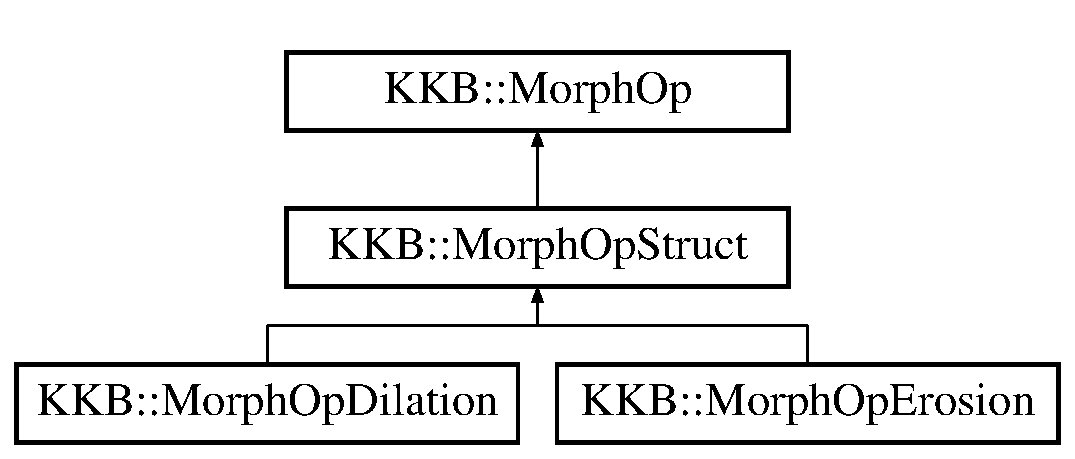
\includegraphics[height=3.000000cm]{class_k_k_b_1_1_morph_op_struct}
\end{center}
\end{figure}
\subsection*{Public Member Functions}
\begin{DoxyCompactItemize}
\item 
\hyperlink{class_k_k_b_1_1_morph_op_struct_afbd23fee4ea441d03f11f10da50009f6}{Morph\+Op\+Struct} (\hyperlink{class_k_k_b_1_1_morph_op_a09e4aff7e81327849855ff72082d85b3}{Structure\+Type} \+\_\+structure, \hyperlink{namespace_k_k_b_aa8c7d4d30381c8a0b6fce68974a9c8a9}{kkuint16} \+\_\+structure\+Size)
\item 
virtual \hyperlink{class_k_k_b_1_1_morph_op_struct_a8535190dc3f3adaacce0854484e2ab81}{$\sim$\+Morph\+Op\+Struct} ()
\item 
void \hyperlink{class_k_k_b_1_1_morph_op_struct_a26156e34cbbce4b4bb719f1704b2ef87}{Background\+Count\+TH} (\hyperlink{namespace_k_k_b_a8fa4952cc84fda1de4bec1fbdd8d5b1b}{kkint32} \+\_\+background\+Count\+TH)
\item 
void \hyperlink{class_k_k_b_1_1_morph_op_struct_a1c39494821bbc43e170455a54b3427bc}{Foreground\+Count\+TH} (\hyperlink{namespace_k_k_b_a8fa4952cc84fda1de4bec1fbdd8d5b1b}{kkint32} \+\_\+foreground\+Count\+TH)
\item 
\hyperlink{namespace_k_k_b_a8fa4952cc84fda1de4bec1fbdd8d5b1b}{kkint32} \hyperlink{class_k_k_b_1_1_morph_op_struct_ae3dc1e5cfafcd323d593c50bcf08315e}{Memory\+Consumed\+Estimated} ()
\item 
virtual \hyperlink{class_k_k_b_1_1_morph_op_a32070d9c14d16849873a8a409f5b0d69}{Operation\+Type} \hyperlink{class_k_k_b_1_1_morph_op_struct_a3cbbeb9ce7ce8856bc01d1c0b1b478a8}{Operation} () const 
\item 
virtual \hyperlink{namespace_k_k_b_a80d46bd24db644a022c863bce8ae3633}{Raster\+Ptr} \hyperlink{class_k_k_b_1_1_morph_op_struct_ace5b649ea317fcc38094e64bb5034380}{Perform\+Operation} (\hyperlink{namespace_k_k_b_a5acfa7402dc4df1769f90d3dc8ddfc2c}{Raster\+Const\+Ptr} \+\_\+image)=0
\end{DoxyCompactItemize}
\subsection*{Protected Member Functions}
\begin{DoxyCompactItemize}
\item 
bool \hyperlink{class_k_k_b_1_1_morph_op_struct_aefad7a97bccb2aa369c0923525fcfe38}{Fit} (\hyperlink{namespace_k_k_b_a8fa4952cc84fda1de4bec1fbdd8d5b1b}{kkint32} row, \hyperlink{namespace_k_k_b_a8fa4952cc84fda1de4bec1fbdd8d5b1b}{kkint32} col) const 
\item 
bool \hyperlink{class_k_k_b_1_1_morph_op_struct_a0c5d2561123dae707a5a7223f6c78882}{Fit\+Background\+Count} (\hyperlink{namespace_k_k_b_a8fa4952cc84fda1de4bec1fbdd8d5b1b}{kkint32} row, \hyperlink{namespace_k_k_b_a8fa4952cc84fda1de4bec1fbdd8d5b1b}{kkint32} col) const 
\item 
\hyperlink{namespace_k_k_b_ace9969169bf514f9ee6185186949cdf7}{uchar} \hyperlink{class_k_k_b_1_1_morph_op_struct_a4b9e013e6850f097999d72175ded3f85}{Hit\+Foreground\+Count} (\hyperlink{namespace_k_k_b_a8fa4952cc84fda1de4bec1fbdd8d5b1b}{kkint32} row, \hyperlink{namespace_k_k_b_a8fa4952cc84fda1de4bec1fbdd8d5b1b}{kkint32} col) const 
\end{DoxyCompactItemize}
\subsection*{Protected Attributes}
\begin{DoxyCompactItemize}
\item 
\hyperlink{namespace_k_k_b_a8fa4952cc84fda1de4bec1fbdd8d5b1b}{kkint32} \hyperlink{class_k_k_b_1_1_morph_op_struct_a7c4f6928cb355035d1fb3aa5ddac2601}{background\+Count\+TH}
\item 
\hyperlink{namespace_k_k_b_a8fa4952cc84fda1de4bec1fbdd8d5b1b}{kkint32} \hyperlink{class_k_k_b_1_1_morph_op_struct_a2f707b6f25d89d1aa84ed826a94ee64d}{foreground\+Count\+TH}
\item 
\hyperlink{class_k_k_b_1_1_morph_op_a09e4aff7e81327849855ff72082d85b3}{Structure\+Type} \hyperlink{class_k_k_b_1_1_morph_op_struct_ad179451936cbbe609f930605eda869bc}{structure}
\item 
\hyperlink{namespace_k_k_b_aa8c7d4d30381c8a0b6fce68974a9c8a9}{kkuint16} \hyperlink{class_k_k_b_1_1_morph_op_struct_a3aeaf4c1bde185cc080f684ee74c237b}{structure\+Size}
\end{DoxyCompactItemize}
\subsection*{Additional Inherited Members}


\subsection{Detailed Description}


Definition at line 24 of file Morph\+Op\+Struct.\+h.



\subsection{Constructor \& Destructor Documentation}
\index{K\+K\+B\+::\+Morph\+Op\+Struct@{K\+K\+B\+::\+Morph\+Op\+Struct}!Morph\+Op\+Struct@{Morph\+Op\+Struct}}
\index{Morph\+Op\+Struct@{Morph\+Op\+Struct}!K\+K\+B\+::\+Morph\+Op\+Struct@{K\+K\+B\+::\+Morph\+Op\+Struct}}
\subsubsection[{\texorpdfstring{Morph\+Op\+Struct(\+Structure\+Type \+\_\+structure, kkuint16 \+\_\+structure\+Size)}{MorphOpStruct(StructureType _structure, kkuint16 _structureSize)}}]{\setlength{\rightskip}{0pt plus 5cm}Morph\+Op\+Struct\+::\+Morph\+Op\+Struct (
\begin{DoxyParamCaption}
\item[{{\bf Structure\+Type}}]{\+\_\+structure, }
\item[{{\bf kkuint16}}]{\+\_\+structure\+Size}
\end{DoxyParamCaption}
)}\hypertarget{class_k_k_b_1_1_morph_op_struct_afbd23fee4ea441d03f11f10da50009f6}{}\label{class_k_k_b_1_1_morph_op_struct_afbd23fee4ea441d03f11f10da50009f6}


Definition at line 21 of file Morph\+Op\+Struct.\+cpp.



References background\+Count\+TH, foreground\+Count\+TH, K\+K\+B\+::\+Morph\+Op\+::\+Morph\+Op(), structure, and structure\+Size.



Referenced by K\+K\+B\+::\+Morph\+Op\+Dilation\+::\+Morph\+Op\+Dilation(), and K\+K\+B\+::\+Morph\+Op\+Erosion\+::\+Morph\+Op\+Erosion().


\begin{DoxyCode}
23                               :
24   \hyperlink{class_k_k_b_1_1_morph_op_a087902e5cad640c26dfa24804cc2a974}{MorphOp}           (),
25   \hyperlink{class_k_k_b_1_1_morph_op_struct_a7c4f6928cb355035d1fb3aa5ddac2601}{backgroundCountTH} (0),
26   \hyperlink{class_k_k_b_1_1_morph_op_struct_a2f707b6f25d89d1aa84ed826a94ee64d}{foregroundCountTH} (1),
27   \hyperlink{class_k_k_b_1_1_morph_op_struct_ad179451936cbbe609f930605eda869bc}{structure}         (\_structure),
28   \hyperlink{class_k_k_b_1_1_morph_op_struct_a3aeaf4c1bde185cc080f684ee74c237b}{structureSize}     (\_structureSize)
29 \{
30 \}
\end{DoxyCode}
\index{K\+K\+B\+::\+Morph\+Op\+Struct@{K\+K\+B\+::\+Morph\+Op\+Struct}!````~Morph\+Op\+Struct@{$\sim$\+Morph\+Op\+Struct}}
\index{````~Morph\+Op\+Struct@{$\sim$\+Morph\+Op\+Struct}!K\+K\+B\+::\+Morph\+Op\+Struct@{K\+K\+B\+::\+Morph\+Op\+Struct}}
\subsubsection[{\texorpdfstring{$\sim$\+Morph\+Op\+Struct()}{~MorphOpStruct()}}]{\setlength{\rightskip}{0pt plus 5cm}Morph\+Op\+Struct\+::$\sim$\+Morph\+Op\+Struct (
\begin{DoxyParamCaption}
{}
\end{DoxyParamCaption}
)\hspace{0.3cm}{\ttfamily [virtual]}}\hypertarget{class_k_k_b_1_1_morph_op_struct_a8535190dc3f3adaacce0854484e2ab81}{}\label{class_k_k_b_1_1_morph_op_struct_a8535190dc3f3adaacce0854484e2ab81}


Definition at line 34 of file Morph\+Op\+Struct.\+cpp.


\begin{DoxyCode}
35 \{
36 \}
\end{DoxyCode}


\subsection{Member Function Documentation}
\index{K\+K\+B\+::\+Morph\+Op\+Struct@{K\+K\+B\+::\+Morph\+Op\+Struct}!Background\+Count\+TH@{Background\+Count\+TH}}
\index{Background\+Count\+TH@{Background\+Count\+TH}!K\+K\+B\+::\+Morph\+Op\+Struct@{K\+K\+B\+::\+Morph\+Op\+Struct}}
\subsubsection[{\texorpdfstring{Background\+Count\+T\+H(kkint32 \+\_\+background\+Count\+T\+H)}{BackgroundCountTH(kkint32 _backgroundCountTH)}}]{\setlength{\rightskip}{0pt plus 5cm}void K\+K\+B\+::\+Morph\+Op\+Struct\+::\+Background\+Count\+TH (
\begin{DoxyParamCaption}
\item[{{\bf kkint32}}]{\+\_\+background\+Count\+TH}
\end{DoxyParamCaption}
)\hspace{0.3cm}{\ttfamily [inline]}}\hypertarget{class_k_k_b_1_1_morph_op_struct_a26156e34cbbce4b4bb719f1704b2ef87}{}\label{class_k_k_b_1_1_morph_op_struct_a26156e34cbbce4b4bb719f1704b2ef87}


Definition at line 39 of file Morph\+Op\+Struct.\+h.



References background\+Count\+TH.



Referenced by K\+K\+B\+::\+Raster\+::\+Erosion().


\begin{DoxyCode}
39 \{\hyperlink{class_k_k_b_1_1_morph_op_struct_a7c4f6928cb355035d1fb3aa5ddac2601}{backgroundCountTH} = \_backgroundCountTH;\}
\end{DoxyCode}
\index{K\+K\+B\+::\+Morph\+Op\+Struct@{K\+K\+B\+::\+Morph\+Op\+Struct}!Fit@{Fit}}
\index{Fit@{Fit}!K\+K\+B\+::\+Morph\+Op\+Struct@{K\+K\+B\+::\+Morph\+Op\+Struct}}
\subsubsection[{\texorpdfstring{Fit(kkint32 row, kkint32 col) const }{Fit(kkint32 row, kkint32 col) const }}]{\setlength{\rightskip}{0pt plus 5cm}bool Morph\+Op\+Struct\+::\+Fit (
\begin{DoxyParamCaption}
\item[{{\bf kkint32}}]{row, }
\item[{{\bf kkint32}}]{col}
\end{DoxyParamCaption}
) const\hspace{0.3cm}{\ttfamily [protected]}}\hypertarget{class_k_k_b_1_1_morph_op_struct_aefad7a97bccb2aa369c0923525fcfe38}{}\label{class_k_k_b_1_1_morph_op_struct_aefad7a97bccb2aa369c0923525fcfe38}


Definition at line 49 of file Morph\+Op\+Struct.\+cpp.



References K\+K\+B\+::\+Morph\+Op\+::\+Background\+Pixel(), K\+K\+B\+::\+Morph\+Op\+::src\+Green, K\+K\+B\+::\+Morph\+Op\+::src\+Height, K\+K\+B\+::\+Morph\+Op\+::src\+Width, structure, structure\+Size, and K\+K\+B\+::\+Morph\+Op\+::st\+Square.



Referenced by K\+K\+B\+::\+Morph\+Op\+Erosion\+::\+Perform\+Operation().


\begin{DoxyCode}
52 \{
53   \hyperlink{namespace_k_k_b_a8fa4952cc84fda1de4bec1fbdd8d5b1b}{kkint32}  r, c;
54   \hyperlink{namespace_k_k_b_a8fa4952cc84fda1de4bec1fbdd8d5b1b}{kkint32}  rStart = row - \hyperlink{class_k_k_b_1_1_morph_op_struct_a3aeaf4c1bde185cc080f684ee74c237b}{structureSize};
55   \hyperlink{namespace_k_k_b_a8fa4952cc84fda1de4bec1fbdd8d5b1b}{kkint32}  rEnd   = row + \hyperlink{class_k_k_b_1_1_morph_op_struct_a3aeaf4c1bde185cc080f684ee74c237b}{structureSize};
56   \hyperlink{namespace_k_k_b_a8fa4952cc84fda1de4bec1fbdd8d5b1b}{kkint32}  cStart = col - \hyperlink{class_k_k_b_1_1_morph_op_struct_a3aeaf4c1bde185cc080f684ee74c237b}{structureSize};
57   \hyperlink{namespace_k_k_b_a8fa4952cc84fda1de4bec1fbdd8d5b1b}{kkint32}  cEnd   = col + \hyperlink{class_k_k_b_1_1_morph_op_struct_a3aeaf4c1bde185cc080f684ee74c237b}{structureSize};
58 
59   \textcolor{keywordflow}{if}  (rStart  < 0)           rStart = 0;
60   \textcolor{keywordflow}{if}  (rEnd    >= \hyperlink{class_k_k_b_1_1_morph_op_a54b2ce1b398a80803b4dbe8aef956b51}{srcHeight})  rEnd = \hyperlink{class_k_k_b_1_1_morph_op_a54b2ce1b398a80803b4dbe8aef956b51}{srcHeight} - 1;
61   \textcolor{keywordflow}{if}  (cStart  < 0)           cStart = 0;
62   \textcolor{keywordflow}{if}  (cEnd    >= \hyperlink{class_k_k_b_1_1_morph_op_aec2cfb3015497e4077751fc5f19559ab}{srcWidth})   cEnd = \hyperlink{class_k_k_b_1_1_morph_op_aec2cfb3015497e4077751fc5f19559ab}{srcWidth} - 1;
63 
64   \textcolor{keywordflow}{if}  (\hyperlink{class_k_k_b_1_1_morph_op_struct_ad179451936cbbe609f930605eda869bc}{structure} == \hyperlink{class_k_k_b_1_1_morph_op_a09e4aff7e81327849855ff72082d85b3a04505973fd476144464695ac6483e490}{StructureType::stSquare})
65   \{
66     \textcolor{keywordflow}{for}  (r = rStart;  r <= rEnd;  r++)
67     \{
68       \hyperlink{namespace_k_k_b_ace9969169bf514f9ee6185186949cdf7}{uchar} \textcolor{keyword}{const}* rowPtr = \hyperlink{class_k_k_b_1_1_morph_op_ab811c702f7e0c8ffccdd21111c8144ab}{srcGreen}[r];
69 
70       \textcolor{keywordflow}{for}  (c = cStart;  c <= cEnd;  c++)
71       \{
72         \textcolor{keywordflow}{if}  (\hyperlink{class_k_k_b_1_1_morph_op_a300c5117659d224d78f7b5a8d44ded91}{BackgroundPixel} (rowPtr[c]))
73           \textcolor{keywordflow}{return}  \textcolor{keyword}{false};
74       \}
75     \}
76   \}
77 
78   \textcolor{keywordflow}{else}
79   \{  
80     \textcolor{keywordflow}{for}  (r = rStart;  r <= rEnd;  r++)
81     \{
82       \textcolor{keywordflow}{if}  (\hyperlink{class_k_k_b_1_1_morph_op_a300c5117659d224d78f7b5a8d44ded91}{BackgroundPixel} (\hyperlink{class_k_k_b_1_1_morph_op_ab811c702f7e0c8ffccdd21111c8144ab}{srcGreen}[r][col]))
83         \textcolor{keywordflow}{return}  \textcolor{keyword}{false};
84     \}
85 
86     \textcolor{keywordflow}{for}  (c = cStart;  c <= cEnd;  c++)
87     \{
88       \textcolor{keywordflow}{if}  (\hyperlink{class_k_k_b_1_1_morph_op_a300c5117659d224d78f7b5a8d44ded91}{BackgroundPixel} (\hyperlink{class_k_k_b_1_1_morph_op_ab811c702f7e0c8ffccdd21111c8144ab}{srcGreen}[row][c]))
89         \textcolor{keywordflow}{return}  \textcolor{keyword}{false};
90     \}
91   \}
92 
93   \textcolor{keywordflow}{return}  \textcolor{keyword}{true};
94 \}  \textcolor{comment}{/* Fit */}
\end{DoxyCode}
\index{K\+K\+B\+::\+Morph\+Op\+Struct@{K\+K\+B\+::\+Morph\+Op\+Struct}!Fit\+Background\+Count@{Fit\+Background\+Count}}
\index{Fit\+Background\+Count@{Fit\+Background\+Count}!K\+K\+B\+::\+Morph\+Op\+Struct@{K\+K\+B\+::\+Morph\+Op\+Struct}}
\subsubsection[{\texorpdfstring{Fit\+Background\+Count(kkint32 row, kkint32 col) const }{FitBackgroundCount(kkint32 row, kkint32 col) const }}]{\setlength{\rightskip}{0pt plus 5cm}bool Morph\+Op\+Struct\+::\+Fit\+Background\+Count (
\begin{DoxyParamCaption}
\item[{{\bf kkint32}}]{row, }
\item[{{\bf kkint32}}]{col}
\end{DoxyParamCaption}
) const\hspace{0.3cm}{\ttfamily [protected]}}\hypertarget{class_k_k_b_1_1_morph_op_struct_a0c5d2561123dae707a5a7223f6c78882}{}\label{class_k_k_b_1_1_morph_op_struct_a0c5d2561123dae707a5a7223f6c78882}


Definition at line 99 of file Morph\+Op\+Struct.\+cpp.



References background\+Count\+TH, K\+K\+B\+::\+Morph\+Op\+::\+Background\+Pixel(), K\+K\+B\+::\+Morph\+Op\+::src\+Green, K\+K\+B\+::\+Morph\+Op\+::src\+Height, K\+K\+B\+::\+Morph\+Op\+::src\+Width, structure, structure\+Size, and K\+K\+B\+::\+Morph\+Op\+::st\+Square.



Referenced by K\+K\+B\+::\+Morph\+Op\+Erosion\+::\+Perform\+Operation().


\begin{DoxyCode}
102 \{
103   \hyperlink{namespace_k_k_b_a8fa4952cc84fda1de4bec1fbdd8d5b1b}{kkint32}  r, c;
104   \hyperlink{namespace_k_k_b_a8fa4952cc84fda1de4bec1fbdd8d5b1b}{kkint32}  rStart = row - \hyperlink{class_k_k_b_1_1_morph_op_struct_a3aeaf4c1bde185cc080f684ee74c237b}{structureSize};
105   \hyperlink{namespace_k_k_b_a8fa4952cc84fda1de4bec1fbdd8d5b1b}{kkint32}  rEnd   = row + \hyperlink{class_k_k_b_1_1_morph_op_struct_a3aeaf4c1bde185cc080f684ee74c237b}{structureSize};
106   \hyperlink{namespace_k_k_b_a8fa4952cc84fda1de4bec1fbdd8d5b1b}{kkint32}  cStart = col - \hyperlink{class_k_k_b_1_1_morph_op_struct_a3aeaf4c1bde185cc080f684ee74c237b}{structureSize};
107   \hyperlink{namespace_k_k_b_a8fa4952cc84fda1de4bec1fbdd8d5b1b}{kkint32}  cEnd   = col + \hyperlink{class_k_k_b_1_1_morph_op_struct_a3aeaf4c1bde185cc080f684ee74c237b}{structureSize};
108 
109   \textcolor{keywordflow}{if}  (rStart  < 0)           rStart = 0;
110   \textcolor{keywordflow}{if}  (rEnd    >= \hyperlink{class_k_k_b_1_1_morph_op_a54b2ce1b398a80803b4dbe8aef956b51}{srcHeight})  rEnd = \hyperlink{class_k_k_b_1_1_morph_op_a54b2ce1b398a80803b4dbe8aef956b51}{srcHeight} - 1;
111   \textcolor{keywordflow}{if}  (cStart  < 0)           cStart = 0;
112   \textcolor{keywordflow}{if}  (cEnd    >= \hyperlink{class_k_k_b_1_1_morph_op_aec2cfb3015497e4077751fc5f19559ab}{srcWidth})   cEnd = \hyperlink{class_k_k_b_1_1_morph_op_aec2cfb3015497e4077751fc5f19559ab}{srcWidth} - 1;
113 
114   \textcolor{keywordtype}{int}  backgroundCount = 0;
115 
116   \textcolor{keywordflow}{if}  (\hyperlink{class_k_k_b_1_1_morph_op_struct_ad179451936cbbe609f930605eda869bc}{structure} == \hyperlink{class_k_k_b_1_1_morph_op_a09e4aff7e81327849855ff72082d85b3a04505973fd476144464695ac6483e490}{StructureType::stSquare})
117   \{
118     \textcolor{keywordflow}{for}  (r = rStart;  r <= rEnd;  r++)
119     \{
120       \hyperlink{namespace_k_k_b_ace9969169bf514f9ee6185186949cdf7}{uchar} \textcolor{keyword}{const}* rowPtr = \hyperlink{class_k_k_b_1_1_morph_op_ab811c702f7e0c8ffccdd21111c8144ab}{srcGreen}[r];
121 
122       \textcolor{keywordflow}{for}  (c = cStart;  c <= cEnd;  c++)
123       \{
124         \textcolor{keywordflow}{if}  (\hyperlink{class_k_k_b_1_1_morph_op_a300c5117659d224d78f7b5a8d44ded91}{BackgroundPixel} (rowPtr[c]))
125           ++backgroundCount;
126       \}
127     \}
128   \}
129 
130   \textcolor{keywordflow}{else}
131   \{  
132     \textcolor{keywordflow}{for}  (r = rStart;  r <= rEnd;  r++)
133     \{
134       \textcolor{keywordflow}{if}  (\hyperlink{class_k_k_b_1_1_morph_op_a300c5117659d224d78f7b5a8d44ded91}{BackgroundPixel} (\hyperlink{class_k_k_b_1_1_morph_op_ab811c702f7e0c8ffccdd21111c8144ab}{srcGreen}[r][col]))
135         ++backgroundCount;
136     \}
137 
138     \textcolor{keywordflow}{for}  (c = cStart;  c <= cEnd;  c++)
139     \{
140       \textcolor{keywordflow}{if}  (\hyperlink{class_k_k_b_1_1_morph_op_a300c5117659d224d78f7b5a8d44ded91}{BackgroundPixel} (\hyperlink{class_k_k_b_1_1_morph_op_ab811c702f7e0c8ffccdd21111c8144ab}{srcGreen}[row][c]))
141         ++backgroundCount;
142     \}
143   \}
144 
145   \textcolor{keywordflow}{return}  backgroundCount < \hyperlink{class_k_k_b_1_1_morph_op_struct_a7c4f6928cb355035d1fb3aa5ddac2601}{backgroundCountTH};
146 \}  \textcolor{comment}{/* FitBackgroundCount */}
\end{DoxyCode}
\index{K\+K\+B\+::\+Morph\+Op\+Struct@{K\+K\+B\+::\+Morph\+Op\+Struct}!Foreground\+Count\+TH@{Foreground\+Count\+TH}}
\index{Foreground\+Count\+TH@{Foreground\+Count\+TH}!K\+K\+B\+::\+Morph\+Op\+Struct@{K\+K\+B\+::\+Morph\+Op\+Struct}}
\subsubsection[{\texorpdfstring{Foreground\+Count\+T\+H(kkint32 \+\_\+foreground\+Count\+T\+H)}{ForegroundCountTH(kkint32 _foregroundCountTH)}}]{\setlength{\rightskip}{0pt plus 5cm}void K\+K\+B\+::\+Morph\+Op\+Struct\+::\+Foreground\+Count\+TH (
\begin{DoxyParamCaption}
\item[{{\bf kkint32}}]{\+\_\+foreground\+Count\+TH}
\end{DoxyParamCaption}
)\hspace{0.3cm}{\ttfamily [inline]}}\hypertarget{class_k_k_b_1_1_morph_op_struct_a1c39494821bbc43e170455a54b3427bc}{}\label{class_k_k_b_1_1_morph_op_struct_a1c39494821bbc43e170455a54b3427bc}


Definition at line 40 of file Morph\+Op\+Struct.\+h.



References foreground\+Count\+TH.



Referenced by K\+K\+B\+::\+Raster\+::\+Dilation().


\begin{DoxyCode}
40 \{\hyperlink{class_k_k_b_1_1_morph_op_struct_a2f707b6f25d89d1aa84ed826a94ee64d}{foregroundCountTH} = \_foregroundCountTH;\}
\end{DoxyCode}
\index{K\+K\+B\+::\+Morph\+Op\+Struct@{K\+K\+B\+::\+Morph\+Op\+Struct}!Hit\+Foreground\+Count@{Hit\+Foreground\+Count}}
\index{Hit\+Foreground\+Count@{Hit\+Foreground\+Count}!K\+K\+B\+::\+Morph\+Op\+Struct@{K\+K\+B\+::\+Morph\+Op\+Struct}}
\subsubsection[{\texorpdfstring{Hit\+Foreground\+Count(kkint32 row, kkint32 col) const }{HitForegroundCount(kkint32 row, kkint32 col) const }}]{\setlength{\rightskip}{0pt plus 5cm}{\bf uchar} Morph\+Op\+Struct\+::\+Hit\+Foreground\+Count (
\begin{DoxyParamCaption}
\item[{{\bf kkint32}}]{row, }
\item[{{\bf kkint32}}]{col}
\end{DoxyParamCaption}
) const\hspace{0.3cm}{\ttfamily [protected]}}\hypertarget{class_k_k_b_1_1_morph_op_struct_a4b9e013e6850f097999d72175ded3f85}{}\label{class_k_k_b_1_1_morph_op_struct_a4b9e013e6850f097999d72175ded3f85}


Definition at line 152 of file Morph\+Op\+Struct.\+cpp.



References foreground\+Count\+TH, K\+K\+B\+::\+Morph\+Op\+::\+Foreground\+Pixel(), K\+K\+B\+::\+Morph\+Op\+::src\+Green, K\+K\+B\+::\+Morph\+Op\+::src\+Height, K\+K\+B\+::\+Morph\+Op\+::src\+Width, structure, structure\+Size, and K\+K\+B\+::\+Morph\+Op\+::st\+Square.



Referenced by K\+K\+B\+::\+Morph\+Op\+Dilation\+::\+Perform\+Operation().


\begin{DoxyCode}
155 \{
156   \hyperlink{namespace_k_k_b_a8fa4952cc84fda1de4bec1fbdd8d5b1b}{kkint32}  r, c;
157   \hyperlink{namespace_k_k_b_a8fa4952cc84fda1de4bec1fbdd8d5b1b}{kkint32}  rStart = row - \hyperlink{class_k_k_b_1_1_morph_op_struct_a3aeaf4c1bde185cc080f684ee74c237b}{structureSize};
158   \hyperlink{namespace_k_k_b_a8fa4952cc84fda1de4bec1fbdd8d5b1b}{kkint32}  rEnd   = row + \hyperlink{class_k_k_b_1_1_morph_op_struct_a3aeaf4c1bde185cc080f684ee74c237b}{structureSize};
159   \hyperlink{namespace_k_k_b_a8fa4952cc84fda1de4bec1fbdd8d5b1b}{kkint32}  cStart = col - \hyperlink{class_k_k_b_1_1_morph_op_struct_a3aeaf4c1bde185cc080f684ee74c237b}{structureSize};
160   \hyperlink{namespace_k_k_b_a8fa4952cc84fda1de4bec1fbdd8d5b1b}{kkint32}  cEnd   = col + \hyperlink{class_k_k_b_1_1_morph_op_struct_a3aeaf4c1bde185cc080f684ee74c237b}{structureSize};
161 
162   \textcolor{keywordflow}{if}  (rStart  < 0)           rStart = 0;
163   \textcolor{keywordflow}{if}  (rEnd    >= \hyperlink{class_k_k_b_1_1_morph_op_a54b2ce1b398a80803b4dbe8aef956b51}{srcHeight})  rEnd = \hyperlink{class_k_k_b_1_1_morph_op_a54b2ce1b398a80803b4dbe8aef956b51}{srcHeight} - 1;
164   \textcolor{keywordflow}{if}  (cStart  < 0)           cStart = 0;
165   \textcolor{keywordflow}{if}  (cEnd    >= \hyperlink{class_k_k_b_1_1_morph_op_aec2cfb3015497e4077751fc5f19559ab}{srcWidth})   cEnd = \hyperlink{class_k_k_b_1_1_morph_op_aec2cfb3015497e4077751fc5f19559ab}{srcWidth} - 1;
166 
167   \hyperlink{namespace_k_k_b_a8fa4952cc84fda1de4bec1fbdd8d5b1b}{kkint32}  pixelValueTotal = 0;
168   \hyperlink{namespace_k_k_b_a8fa4952cc84fda1de4bec1fbdd8d5b1b}{kkint32}  neighborCount = 0;
169 
170   \textcolor{keywordflow}{if}  (\hyperlink{class_k_k_b_1_1_morph_op_struct_ad179451936cbbe609f930605eda869bc}{structure} == \hyperlink{class_k_k_b_1_1_morph_op_a09e4aff7e81327849855ff72082d85b3a04505973fd476144464695ac6483e490}{StructureType::stSquare})
171   \{
172     \textcolor{keywordflow}{for}  (r = rStart;  r <= rEnd;  r++)
173     \{
174       \hyperlink{namespace_k_k_b_ace9969169bf514f9ee6185186949cdf7}{uchar} \textcolor{keyword}{const}* rowPtr = \hyperlink{class_k_k_b_1_1_morph_op_ab811c702f7e0c8ffccdd21111c8144ab}{srcGreen}[r];
175 
176       \textcolor{keywordflow}{for}  (c = cStart;  c <= cEnd;  c++)
177       \{
178         \textcolor{keywordflow}{if}  (\hyperlink{class_k_k_b_1_1_morph_op_acd5541050c3c0207b004b71caf7fb1f4}{ForegroundPixel} (rowPtr[c]))
179         \{
180           ++neighborCount;
181           pixelValueTotal += rowPtr[c];
182         \}
183       \}
184     \}
185   \}
186 
187   \textcolor{keywordflow}{else}
188   \{  
189     \textcolor{keywordflow}{for}  (r = rStart;  r <= rEnd;  r++)
190     \{
191       \textcolor{keywordflow}{if}  (\hyperlink{class_k_k_b_1_1_morph_op_acd5541050c3c0207b004b71caf7fb1f4}{ForegroundPixel} (\hyperlink{class_k_k_b_1_1_morph_op_ab811c702f7e0c8ffccdd21111c8144ab}{srcGreen}[r][col]))
192       \{
193         ++neighborCount;
194         pixelValueTotal += \hyperlink{class_k_k_b_1_1_morph_op_ab811c702f7e0c8ffccdd21111c8144ab}{srcGreen}[r][col];
195       \}
196     \}
197 
198     \textcolor{keywordflow}{for}  (c = cStart;  c <= cEnd;  c++)
199     \{
200       \textcolor{keywordflow}{if}  (\hyperlink{class_k_k_b_1_1_morph_op_acd5541050c3c0207b004b71caf7fb1f4}{ForegroundPixel} (\hyperlink{class_k_k_b_1_1_morph_op_ab811c702f7e0c8ffccdd21111c8144ab}{srcGreen}[r][c]))
201       \{
202         ++neighborCount;
203         pixelValueTotal += \hyperlink{class_k_k_b_1_1_morph_op_ab811c702f7e0c8ffccdd21111c8144ab}{srcGreen}[r][col];
204       \}
205     \}
206   \}
207 
208   \textcolor{keywordflow}{if}  (neighborCount < \hyperlink{class_k_k_b_1_1_morph_op_struct_a2f707b6f25d89d1aa84ed826a94ee64d}{foregroundCountTH})
209     \textcolor{keywordflow}{return} (\hyperlink{namespace_k_k_b_ace9969169bf514f9ee6185186949cdf7}{uchar})0;
210   \textcolor{keywordflow}{else}
211     \textcolor{keywordflow}{return} (\hyperlink{namespace_k_k_b_ace9969169bf514f9ee6185186949cdf7}{uchar})(0.5f + (float)pixelValueTotal / (\textcolor{keywordtype}{float})neighborCount);
212 \}  \textcolor{comment}{/* HitForegroundCount */}
\end{DoxyCode}
\index{K\+K\+B\+::\+Morph\+Op\+Struct@{K\+K\+B\+::\+Morph\+Op\+Struct}!Memory\+Consumed\+Estimated@{Memory\+Consumed\+Estimated}}
\index{Memory\+Consumed\+Estimated@{Memory\+Consumed\+Estimated}!K\+K\+B\+::\+Morph\+Op\+Struct@{K\+K\+B\+::\+Morph\+Op\+Struct}}
\subsubsection[{\texorpdfstring{Memory\+Consumed\+Estimated()}{MemoryConsumedEstimated()}}]{\setlength{\rightskip}{0pt plus 5cm}{\bf kkint32} Morph\+Op\+Struct\+::\+Memory\+Consumed\+Estimated (
\begin{DoxyParamCaption}
{}
\end{DoxyParamCaption}
)}\hypertarget{class_k_k_b_1_1_morph_op_struct_ae3dc1e5cfafcd323d593c50bcf08315e}{}\label{class_k_k_b_1_1_morph_op_struct_ae3dc1e5cfafcd323d593c50bcf08315e}


Definition at line 40 of file Morph\+Op\+Struct.\+cpp.


\begin{DoxyCode}
41 \{
42   \textcolor{keywordflow}{return}  \textcolor{keyword}{sizeof} (*this);
43 \}
\end{DoxyCode}
\index{K\+K\+B\+::\+Morph\+Op\+Struct@{K\+K\+B\+::\+Morph\+Op\+Struct}!Operation@{Operation}}
\index{Operation@{Operation}!K\+K\+B\+::\+Morph\+Op\+Struct@{K\+K\+B\+::\+Morph\+Op\+Struct}}
\subsubsection[{\texorpdfstring{Operation() const }{Operation() const }}]{\setlength{\rightskip}{0pt plus 5cm}virtual {\bf Operation\+Type} K\+K\+B\+::\+Morph\+Op\+Struct\+::\+Operation (
\begin{DoxyParamCaption}
{}
\end{DoxyParamCaption}
) const\hspace{0.3cm}{\ttfamily [inline]}, {\ttfamily [virtual]}}\hypertarget{class_k_k_b_1_1_morph_op_struct_a3cbbeb9ce7ce8856bc01d1c0b1b478a8}{}\label{class_k_k_b_1_1_morph_op_struct_a3cbbeb9ce7ce8856bc01d1c0b1b478a8}


Implements \hyperlink{class_k_k_b_1_1_morph_op_abdf6f4bddae0b3cc3dc718559fa60234}{K\+K\+B\+::\+Morph\+Op}.



Reimplemented in \hyperlink{class_k_k_b_1_1_morph_op_dilation_a159a05bfd9fc2af7a07fe22edcde0ef8}{K\+K\+B\+::\+Morph\+Op\+Dilation}, and \hyperlink{class_k_k_b_1_1_morph_op_erosion_a3fa77279197c70aed5ef55968eb2704a}{K\+K\+B\+::\+Morph\+Op\+Erosion}.



Definition at line 33 of file Morph\+Op\+Struct.\+h.



References K\+K\+B\+::\+Morph\+Op\+::\+Erosion.


\begin{DoxyCode}
33 \{\textcolor{keywordflow}{return}  \hyperlink{class_k_k_b_1_1_morph_op_a32070d9c14d16849873a8a409f5b0d69a35b6b7b81c8d146da93c09daa3875ea0}{OperationType::Erosion};\}
\end{DoxyCode}
\index{K\+K\+B\+::\+Morph\+Op\+Struct@{K\+K\+B\+::\+Morph\+Op\+Struct}!Perform\+Operation@{Perform\+Operation}}
\index{Perform\+Operation@{Perform\+Operation}!K\+K\+B\+::\+Morph\+Op\+Struct@{K\+K\+B\+::\+Morph\+Op\+Struct}}
\subsubsection[{\texorpdfstring{Perform\+Operation(\+Raster\+Const\+Ptr \+\_\+image)=0}{PerformOperation(RasterConstPtr _image)=0}}]{\setlength{\rightskip}{0pt plus 5cm}virtual {\bf Raster\+Ptr} K\+K\+B\+::\+Morph\+Op\+Struct\+::\+Perform\+Operation (
\begin{DoxyParamCaption}
\item[{{\bf Raster\+Const\+Ptr}}]{\+\_\+image}
\end{DoxyParamCaption}
)\hspace{0.3cm}{\ttfamily [pure virtual]}}\hypertarget{class_k_k_b_1_1_morph_op_struct_ace5b649ea317fcc38094e64bb5034380}{}\label{class_k_k_b_1_1_morph_op_struct_ace5b649ea317fcc38094e64bb5034380}


Implemented in \hyperlink{class_k_k_b_1_1_morph_op_dilation_a9240afda29b2a87de63fbd581bd999c0}{K\+K\+B\+::\+Morph\+Op\+Dilation}, and \hyperlink{class_k_k_b_1_1_morph_op_erosion_a1cee95de95d4ebc3616631a41d80d23e}{K\+K\+B\+::\+Morph\+Op\+Erosion}.



\subsection{Member Data Documentation}
\index{K\+K\+B\+::\+Morph\+Op\+Struct@{K\+K\+B\+::\+Morph\+Op\+Struct}!background\+Count\+TH@{background\+Count\+TH}}
\index{background\+Count\+TH@{background\+Count\+TH}!K\+K\+B\+::\+Morph\+Op\+Struct@{K\+K\+B\+::\+Morph\+Op\+Struct}}
\subsubsection[{\texorpdfstring{background\+Count\+TH}{backgroundCountTH}}]{\setlength{\rightskip}{0pt plus 5cm}{\bf kkint32} K\+K\+B\+::\+Morph\+Op\+Struct\+::background\+Count\+TH\hspace{0.3cm}{\ttfamily [protected]}}\hypertarget{class_k_k_b_1_1_morph_op_struct_a7c4f6928cb355035d1fb3aa5ddac2601}{}\label{class_k_k_b_1_1_morph_op_struct_a7c4f6928cb355035d1fb3aa5ddac2601}
If greater than zero; then pixel must have at least that many neighbors to be considered a fit. 

Definition at line 57 of file Morph\+Op\+Struct.\+h.



Referenced by Background\+Count\+T\+H(), Fit\+Background\+Count(), Morph\+Op\+Struct(), and K\+K\+B\+::\+Morph\+Op\+Erosion\+::\+Perform\+Operation().

\index{K\+K\+B\+::\+Morph\+Op\+Struct@{K\+K\+B\+::\+Morph\+Op\+Struct}!foreground\+Count\+TH@{foreground\+Count\+TH}}
\index{foreground\+Count\+TH@{foreground\+Count\+TH}!K\+K\+B\+::\+Morph\+Op\+Struct@{K\+K\+B\+::\+Morph\+Op\+Struct}}
\subsubsection[{\texorpdfstring{foreground\+Count\+TH}{foregroundCountTH}}]{\setlength{\rightskip}{0pt plus 5cm}{\bf kkint32} K\+K\+B\+::\+Morph\+Op\+Struct\+::foreground\+Count\+TH\hspace{0.3cm}{\ttfamily [protected]}}\hypertarget{class_k_k_b_1_1_morph_op_struct_a2f707b6f25d89d1aa84ed826a94ee64d}{}\label{class_k_k_b_1_1_morph_op_struct_a2f707b6f25d89d1aa84ed826a94ee64d}


Definition at line 58 of file Morph\+Op\+Struct.\+h.



Referenced by Foreground\+Count\+T\+H(), Hit\+Foreground\+Count(), and Morph\+Op\+Struct().

\index{K\+K\+B\+::\+Morph\+Op\+Struct@{K\+K\+B\+::\+Morph\+Op\+Struct}!structure@{structure}}
\index{structure@{structure}!K\+K\+B\+::\+Morph\+Op\+Struct@{K\+K\+B\+::\+Morph\+Op\+Struct}}
\subsubsection[{\texorpdfstring{structure}{structure}}]{\setlength{\rightskip}{0pt plus 5cm}{\bf Structure\+Type} K\+K\+B\+::\+Morph\+Op\+Struct\+::structure\hspace{0.3cm}{\ttfamily [protected]}}\hypertarget{class_k_k_b_1_1_morph_op_struct_ad179451936cbbe609f930605eda869bc}{}\label{class_k_k_b_1_1_morph_op_struct_ad179451936cbbe609f930605eda869bc}


Definition at line 56 of file Morph\+Op\+Struct.\+h.



Referenced by Fit(), Fit\+Background\+Count(), Hit\+Foreground\+Count(), and Morph\+Op\+Struct().

\index{K\+K\+B\+::\+Morph\+Op\+Struct@{K\+K\+B\+::\+Morph\+Op\+Struct}!structure\+Size@{structure\+Size}}
\index{structure\+Size@{structure\+Size}!K\+K\+B\+::\+Morph\+Op\+Struct@{K\+K\+B\+::\+Morph\+Op\+Struct}}
\subsubsection[{\texorpdfstring{structure\+Size}{structureSize}}]{\setlength{\rightskip}{0pt plus 5cm}{\bf kkuint16} K\+K\+B\+::\+Morph\+Op\+Struct\+::structure\+Size\hspace{0.3cm}{\ttfamily [protected]}}\hypertarget{class_k_k_b_1_1_morph_op_struct_a3aeaf4c1bde185cc080f684ee74c237b}{}\label{class_k_k_b_1_1_morph_op_struct_a3aeaf4c1bde185cc080f684ee74c237b}


Definition at line 59 of file Morph\+Op\+Struct.\+h.



Referenced by Fit(), Fit\+Background\+Count(), Hit\+Foreground\+Count(), and Morph\+Op\+Struct().



The documentation for this class was generated from the following files\+:\begin{DoxyCompactItemize}
\item 
C\+:/\+Users/\+Kurt/\+Git\+Hub/\+K\+Square\+Libraries/\+K\+K\+Base/\hyperlink{_morph_op_struct_8h}{Morph\+Op\+Struct.\+h}\item 
C\+:/\+Users/\+Kurt/\+Git\+Hub/\+K\+Square\+Libraries/\+K\+K\+Base/\hyperlink{_morph_op_struct_8cpp}{Morph\+Op\+Struct.\+cpp}\end{DoxyCompactItemize}

\hypertarget{struct_k_k_b_1_1_mov_dir}{}\section{K\+KB\+:\+:Mov\+Dir Struct Reference}
\label{struct_k_k_b_1_1_mov_dir}\index{K\+K\+B\+::\+Mov\+Dir@{K\+K\+B\+::\+Mov\+Dir}}


{\ttfamily \#include $<$Raster.\+h$>$}

\subsection*{Public Attributes}
\begin{DoxyCompactItemize}
\item 
\hyperlink{namespace_k_k_b_a8fa4952cc84fda1de4bec1fbdd8d5b1b}{kkint32} \hyperlink{struct_k_k_b_1_1_mov_dir_a454172afc7221cea2367c722c34e5517}{col}
\item 
\hyperlink{namespace_k_k_b_a8fa4952cc84fda1de4bec1fbdd8d5b1b}{kkint32} \hyperlink{struct_k_k_b_1_1_mov_dir_a19c78385b3fbec09dbe624baef003187}{row}
\end{DoxyCompactItemize}


\subsection{Detailed Description}


Definition at line 1378 of file Raster.\+h.



\subsection{Member Data Documentation}
\index{K\+K\+B\+::\+Mov\+Dir@{K\+K\+B\+::\+Mov\+Dir}!col@{col}}
\index{col@{col}!K\+K\+B\+::\+Mov\+Dir@{K\+K\+B\+::\+Mov\+Dir}}
\subsubsection[{\texorpdfstring{col}{col}}]{\setlength{\rightskip}{0pt plus 5cm}{\bf kkint32} K\+K\+B\+::\+Mov\+Dir\+::col}\hypertarget{struct_k_k_b_1_1_mov_dir_a454172afc7221cea2367c722c34e5517}{}\label{struct_k_k_b_1_1_mov_dir_a454172afc7221cea2367c722c34e5517}


Definition at line 1381 of file Raster.\+h.



Referenced by K\+K\+B\+::\+Raster\+::\+Follow\+Contour().

\index{K\+K\+B\+::\+Mov\+Dir@{K\+K\+B\+::\+Mov\+Dir}!row@{row}}
\index{row@{row}!K\+K\+B\+::\+Mov\+Dir@{K\+K\+B\+::\+Mov\+Dir}}
\subsubsection[{\texorpdfstring{row}{row}}]{\setlength{\rightskip}{0pt plus 5cm}{\bf kkint32} K\+K\+B\+::\+Mov\+Dir\+::row}\hypertarget{struct_k_k_b_1_1_mov_dir_a19c78385b3fbec09dbe624baef003187}{}\label{struct_k_k_b_1_1_mov_dir_a19c78385b3fbec09dbe624baef003187}


Definition at line 1380 of file Raster.\+h.



Referenced by K\+K\+B\+::\+Raster\+::\+Follow\+Contour().



The documentation for this struct was generated from the following file\+:\begin{DoxyCompactItemize}
\item 
C\+:/\+Users/\+Kurt/\+Git\+Hub/\+K\+Square\+Libraries/\+K\+K\+Base/\hyperlink{_raster_8h}{Raster.\+h}\end{DoxyCompactItemize}

\hypertarget{class_k_k_b_1_1_msg_queue}{}\section{K\+KB\+:\+:Msg\+Queue Class Reference}
\label{class_k_k_b_1_1_msg_queue}\index{K\+K\+B\+::\+Msg\+Queue@{K\+K\+B\+::\+Msg\+Queue}}


Will manage a buffer that will allow multiple threads to add and remove messages to a queue.  




{\ttfamily \#include $<$Msg\+Queue.\+h$>$}

\subsection*{Public Types}
\begin{DoxyCompactItemize}
\item 
typedef \hyperlink{class_k_k_b_1_1_msg_queue}{Msg\+Queue} $\ast$ \hyperlink{class_k_k_b_1_1_msg_queue_a4799b7792832f5357e7679b252f7a750}{Msg\+Queue\+Ptr}
\end{DoxyCompactItemize}
\subsection*{Public Member Functions}
\begin{DoxyCompactItemize}
\item 
\hyperlink{class_k_k_b_1_1_msg_queue_aa6d7b73f9d84b27b1735c5964dea0595}{Msg\+Queue} (const \hyperlink{class_k_k_b_1_1_k_k_str}{K\+K\+Str} \&\+\_\+name)
\item 
\hyperlink{class_k_k_b_1_1_msg_queue_a04c1aca750c66393d3949d0b2aedc01c}{$\sim$\+Msg\+Queue} ()
\item 
void \hyperlink{class_k_k_b_1_1_msg_queue_a4d7d0adcf4f06a7afc6c8187a20bf95c}{Add\+Msg} (\hyperlink{namespace_k_k_b_a9adbef5a6b3be0867f5570df2a08f388}{K\+K\+Str\+Ptr} msg)
\begin{DoxyCompactList}\small\item\em Take ownership of \textquotesingle{}msg\textquotesingle{} and add to end of the queue. \end{DoxyCompactList}\item 
void \hyperlink{class_k_k_b_1_1_msg_queue_ac1356aec06472120e670bf39d6fdf91c}{Add\+Msg} (const \hyperlink{class_k_k_b_1_1_k_k_str}{K\+K\+Str} \&msg)
\item 
void \hyperlink{class_k_k_b_1_1_msg_queue_a7adf4ff13ee1e639140f7d717c7bd265}{Add\+Msgs} (const \hyperlink{namespace_k_k_b_a8f5f50672f37857425120831223888aa}{K\+K\+Str\+List\+Ptr} msgs, bool take\+Ownership)
\begin{DoxyCompactList}\small\item\em Adds the contents of \textquotesingle{}msgs\textquotesingle{} to the message queue and depending on \textquotesingle{}take\+Ownership\textquotesingle{} will either assume that its owns (taking ownership) the \hyperlink{class_k_k_b_1_1_k_k_str}{K\+K\+Str} instances or create duplicates. \end{DoxyCompactList}\item 
\hyperlink{namespace_k_k_b_a8f5f50672f37857425120831223888aa}{K\+K\+Str\+List\+Ptr} \hyperlink{class_k_k_b_1_1_msg_queue_ac0ba20e6b9f343c846f91233b8df082c}{Get\+All\+Msgs} ()
\begin{DoxyCompactList}\small\item\em Returns all messages that are currently in the queue. \end{DoxyCompactList}\item 
\hyperlink{namespace_k_k_b_a9adbef5a6b3be0867f5570df2a08f388}{K\+K\+Str\+Ptr} \hyperlink{class_k_k_b_1_1_msg_queue_aa010dbbc7fffe4ff07407d884c7a0f5e}{Get\+Copy\+Of\+Last\+Msg} ()
\begin{DoxyCompactList}\small\item\em Returns a duplicate of the last string added to the message queue. \end{DoxyCompactList}\item 
\hyperlink{namespace_k_k_b_a9adbef5a6b3be0867f5570df2a08f388}{K\+K\+Str\+Ptr} \hyperlink{class_k_k_b_1_1_msg_queue_a4e280303e6b11471624e1274cc681649}{Get\+Next\+Msg} ()
\begin{DoxyCompactList}\small\item\em Removes from the queue the oldest message added to the queue that has not been removed. \end{DoxyCompactList}\item 
\hyperlink{namespace_k_k_b_a8fa4952cc84fda1de4bec1fbdd8d5b1b}{kkint32} \hyperlink{class_k_k_b_1_1_msg_queue_afe6ceeb9745ccf087a35eca6e83b026f}{Memory\+Consumed\+Estimated} ()
\begin{DoxyCompactList}\small\item\em Returns an estimate of the amount of memory consumed in bytes by this instance. \end{DoxyCompactList}\end{DoxyCompactItemize}


\subsection{Detailed Description}
Will manage a buffer that will allow multiple threads to add and remove messages to a queue. 

A \textquotesingle{}Goal\+Keepeer\textquotesingle{} object \textquotesingle{}gate\+Keeper\textquotesingle{} will be used to enforce integrity in the Multi-\/\+Threaded environment. It will guarantee that only one thread at a time can access the Queue. 

Definition at line 19 of file Msg\+Queue.\+h.



\subsection{Member Typedef Documentation}
\index{K\+K\+B\+::\+Msg\+Queue@{K\+K\+B\+::\+Msg\+Queue}!Msg\+Queue\+Ptr@{Msg\+Queue\+Ptr}}
\index{Msg\+Queue\+Ptr@{Msg\+Queue\+Ptr}!K\+K\+B\+::\+Msg\+Queue@{K\+K\+B\+::\+Msg\+Queue}}
\subsubsection[{\texorpdfstring{Msg\+Queue\+Ptr}{MsgQueuePtr}}]{\setlength{\rightskip}{0pt plus 5cm}typedef {\bf Msg\+Queue}$\ast$ {\bf K\+K\+B\+::\+Msg\+Queue\+::\+Msg\+Queue\+Ptr}}\hypertarget{class_k_k_b_1_1_msg_queue_a4799b7792832f5357e7679b252f7a750}{}\label{class_k_k_b_1_1_msg_queue_a4799b7792832f5357e7679b252f7a750}


Definition at line 22 of file Msg\+Queue.\+h.



\subsection{Constructor \& Destructor Documentation}
\index{K\+K\+B\+::\+Msg\+Queue@{K\+K\+B\+::\+Msg\+Queue}!Msg\+Queue@{Msg\+Queue}}
\index{Msg\+Queue@{Msg\+Queue}!K\+K\+B\+::\+Msg\+Queue@{K\+K\+B\+::\+Msg\+Queue}}
\subsubsection[{\texorpdfstring{Msg\+Queue(const K\+K\+Str \&\+\_\+name)}{MsgQueue(const KKStr &_name)}}]{\setlength{\rightskip}{0pt plus 5cm}Msg\+Queue\+::\+Msg\+Queue (
\begin{DoxyParamCaption}
\item[{const {\bf K\+K\+Str} \&}]{\+\_\+name}
\end{DoxyParamCaption}
)}\hypertarget{class_k_k_b_1_1_msg_queue_aa6d7b73f9d84b27b1735c5964dea0595}{}\label{class_k_k_b_1_1_msg_queue_aa6d7b73f9d84b27b1735c5964dea0595}


Definition at line 29 of file Msg\+Queue.\+cpp.



References K\+K\+B\+::\+Goal\+Keeper\+Simple\+::\+Create(), K\+K\+B\+::\+K\+K\+Str\+::\+K\+K\+Str(), K\+K\+B\+::\+Goal\+Keeper\+Simple\+::\+Memory\+Consumed\+Estimated(), Msg\+Queue(), and K\+K\+B\+::operator+().



Referenced by Msg\+Queue().


\begin{DoxyCode}
29                                       :        \textcolor{comment}{/* Name of buffer, must be unique */}
30     gateKeeper     (NULL),
31     memoryConsumed (0),
32     name           (\_name),
33     queue          ()
34 \{
35   \hyperlink{class_k_k_b_1_1_goal_keeper_simple_a7001b3a689776a4ef2b56219f965b26c}{GoalKeeperSimple::Create} (\textcolor{stringliteral}{"MsgQueue\_"} + name, gateKeeper);
36   memoryConsumed = \textcolor{keyword}{sizeof} (\hyperlink{class_k_k_b_1_1_msg_queue_aa6d7b73f9d84b27b1735c5964dea0595}{MsgQueue}) + gateKeeper->
      \hyperlink{class_k_k_b_1_1_goal_keeper_simple_a89e05c58c7d851dc6ad858803c37309a}{MemoryConsumedEstimated} ();
37 \}
\end{DoxyCode}
\index{K\+K\+B\+::\+Msg\+Queue@{K\+K\+B\+::\+Msg\+Queue}!````~Msg\+Queue@{$\sim$\+Msg\+Queue}}
\index{````~Msg\+Queue@{$\sim$\+Msg\+Queue}!K\+K\+B\+::\+Msg\+Queue@{K\+K\+B\+::\+Msg\+Queue}}
\subsubsection[{\texorpdfstring{$\sim$\+Msg\+Queue()}{~MsgQueue()}}]{\setlength{\rightskip}{0pt plus 5cm}Msg\+Queue\+::$\sim$\+Msg\+Queue (
\begin{DoxyParamCaption}
{}
\end{DoxyParamCaption}
)}\hypertarget{class_k_k_b_1_1_msg_queue_a04c1aca750c66393d3949d0b2aedc01c}{}\label{class_k_k_b_1_1_msg_queue_a04c1aca750c66393d3949d0b2aedc01c}


Definition at line 41 of file Msg\+Queue.\+cpp.



References K\+K\+B\+::\+Goal\+Keeper\+Simple\+::\+Destroy().


\begin{DoxyCode}
42 \{
43   \textcolor{keywordflow}{while}  (this->queue.size () > 0)
44   \{
45     \hyperlink{class_k_k_b_1_1_k_k_str}{KKStrPtr}  m = this->queue.front ();
46     this->queue.pop ();
47     \textcolor{keyword}{delete}  m;  
48     m = NULL;
49   \}
50 
51   \hyperlink{class_k_k_b_1_1_goal_keeper_simple_aa1098674662d5e6a03fb4af27e1c5af5}{GoalKeeperSimple::Destroy} (gateKeeper);  
52   gateKeeper = NULL;
53 \}
\end{DoxyCode}


\subsection{Member Function Documentation}
\index{K\+K\+B\+::\+Msg\+Queue@{K\+K\+B\+::\+Msg\+Queue}!Add\+Msg@{Add\+Msg}}
\index{Add\+Msg@{Add\+Msg}!K\+K\+B\+::\+Msg\+Queue@{K\+K\+B\+::\+Msg\+Queue}}
\subsubsection[{\texorpdfstring{Add\+Msg(\+K\+K\+Str\+Ptr msg)}{AddMsg(KKStrPtr msg)}}]{\setlength{\rightskip}{0pt plus 5cm}void Msg\+Queue\+::\+Add\+Msg (
\begin{DoxyParamCaption}
\item[{{\bf K\+K\+Str\+Ptr}}]{msg}
\end{DoxyParamCaption}
)}\hypertarget{class_k_k_b_1_1_msg_queue_a4d7d0adcf4f06a7afc6c8187a20bf95c}{}\label{class_k_k_b_1_1_msg_queue_a4d7d0adcf4f06a7afc6c8187a20bf95c}


Take ownership of \textquotesingle{}msg\textquotesingle{} and add to end of the queue. 


\begin{DoxyParams}[1]{Parameters}
\mbox{\tt in}  & {\em msg} & Pointer to message that is to be added to end of queue. The caller will pass ownership of this string to this instance of Msg\+Queue.\+Taking ownership of \textquotesingle{}msg\textquotesingle{} \\
\hline
\end{DoxyParams}


Definition at line 58 of file Msg\+Queue.\+cpp.



References K\+K\+B\+::\+K\+K\+Str\+::\+Concat(), K\+K\+B\+::\+Goal\+Keeper\+Simple\+::\+End\+Block(), K\+K\+B\+::\+K\+K\+Exception\+::\+K\+K\+Exception(), K\+K\+B\+::\+K\+K\+Str\+::\+Memory\+Consumed\+Estimated(), and K\+K\+B\+::\+Goal\+Keeper\+Simple\+::\+Start\+Block().



Referenced by K\+K\+B\+::\+K\+K\+Thread\+::\+Add\+Msg().


\begin{DoxyCode}
59 \{
60   \textcolor{keywordflow}{if}  (msg == NULL)
61   \{
62     \hyperlink{class_k_k_b_1_1_k_k_str}{KKStr}  errMsg;
63     errMsg << \textcolor{stringliteral}{"MsgQueue::AddMsg ==  NULL"};
64     cerr << \hyperlink{namespace_k_k_b_ad1f50f65af6adc8fa9e6f62d007818a8}{std::endl} << \hyperlink{namespace_k_k_b_ad1f50f65af6adc8fa9e6f62d007818a8}{std::endl} << errMsg << \hyperlink{namespace_k_k_b_ad1f50f65af6adc8fa9e6f62d007818a8}{std::endl} << 
      \hyperlink{namespace_k_k_b_ad1f50f65af6adc8fa9e6f62d007818a8}{std::endl};
65     \textcolor{keywordflow}{throw} \hyperlink{class_k_k_b_1_1_k_k_exception}{KKException} (errMsg);
66   \}
67 
68   gateKeeper->\hyperlink{class_k_k_b_1_1_goal_keeper_simple_aa8bcf9dcd7f07275aaac8ecdedac8cb1}{StartBlock} ();
69   queue.push (msg);
70   memoryConsumed = memoryConsumed +  msg->\hyperlink{class_k_k_b_1_1_k_k_str_afc335bf98a8d4a77dc34215e72068719}{MemoryConsumedEstimated} ();
71   gateKeeper->\hyperlink{class_k_k_b_1_1_goal_keeper_simple_a28a529882f7ace4f8300508d4dee9c3e}{EndBlock} ();
72 \}  \textcolor{comment}{/* AddFrame */}
\end{DoxyCode}
\index{K\+K\+B\+::\+Msg\+Queue@{K\+K\+B\+::\+Msg\+Queue}!Add\+Msg@{Add\+Msg}}
\index{Add\+Msg@{Add\+Msg}!K\+K\+B\+::\+Msg\+Queue@{K\+K\+B\+::\+Msg\+Queue}}
\subsubsection[{\texorpdfstring{Add\+Msg(const K\+K\+Str \&msg)}{AddMsg(const KKStr &msg)}}]{\setlength{\rightskip}{0pt plus 5cm}void Msg\+Queue\+::\+Add\+Msg (
\begin{DoxyParamCaption}
\item[{const {\bf K\+K\+Str} \&}]{msg}
\end{DoxyParamCaption}
)}\hypertarget{class_k_k_b_1_1_msg_queue_ac1356aec06472120e670bf39d6fdf91c}{}\label{class_k_k_b_1_1_msg_queue_ac1356aec06472120e670bf39d6fdf91c}


Definition at line 76 of file Msg\+Queue.\+cpp.



References K\+K\+B\+::\+Goal\+Keeper\+Simple\+::\+End\+Block(), K\+K\+B\+::\+K\+K\+Str\+::\+Memory\+Consumed\+Estimated(), and K\+K\+B\+::\+Goal\+Keeper\+Simple\+::\+Start\+Block().



Referenced by K\+K\+B\+::\+K\+K\+Thread\+::\+Add\+Msg(), and K\+K\+B\+::\+Run\+Log\+::\+Write\+Line().


\begin{DoxyCode}
77 \{
78   gateKeeper->\hyperlink{class_k_k_b_1_1_goal_keeper_simple_aa8bcf9dcd7f07275aaac8ecdedac8cb1}{StartBlock} ();
79   queue.push (\textcolor{keyword}{new} \hyperlink{class_k_k_b_1_1_k_k_str}{KKStr} (msg));
80   memoryConsumed = memoryConsumed + msg.\hyperlink{class_k_k_b_1_1_k_k_str_afc335bf98a8d4a77dc34215e72068719}{MemoryConsumedEstimated} ();
81   gateKeeper->\hyperlink{class_k_k_b_1_1_goal_keeper_simple_a28a529882f7ace4f8300508d4dee9c3e}{EndBlock} ();
82 \}  \textcolor{comment}{/* AddFrame */}
\end{DoxyCode}
\index{K\+K\+B\+::\+Msg\+Queue@{K\+K\+B\+::\+Msg\+Queue}!Add\+Msgs@{Add\+Msgs}}
\index{Add\+Msgs@{Add\+Msgs}!K\+K\+B\+::\+Msg\+Queue@{K\+K\+B\+::\+Msg\+Queue}}
\subsubsection[{\texorpdfstring{Add\+Msgs(const K\+K\+Str\+List\+Ptr msgs, bool take\+Ownership)}{AddMsgs(const KKStrListPtr msgs, bool takeOwnership)}}]{\setlength{\rightskip}{0pt plus 5cm}void Msg\+Queue\+::\+Add\+Msgs (
\begin{DoxyParamCaption}
\item[{const {\bf K\+K\+Str\+List\+Ptr}}]{msgs, }
\item[{bool}]{take\+Ownership}
\end{DoxyParamCaption}
)}\hypertarget{class_k_k_b_1_1_msg_queue_a7adf4ff13ee1e639140f7d717c7bd265}{}\label{class_k_k_b_1_1_msg_queue_a7adf4ff13ee1e639140f7d717c7bd265}


Adds the contents of \textquotesingle{}msgs\textquotesingle{} to the message queue and depending on \textquotesingle{}take\+Ownership\textquotesingle{} will either assume that its owns (taking ownership) the \hyperlink{class_k_k_b_1_1_k_k_str}{K\+K\+Str} instances or create duplicates. 

If \textquotesingle{}take\+Ownership\textquotesingle{} is true will and the \hyperlink{class_k_k_b_1_1_k_k_str}{K\+K\+Str} instances in \textquotesingle{}msgs\textquotesingle{} to the queue otherwise it will make duplicates of the \hyperlink{class_k_k_b_1_1_k_k_str}{K\+K\+Str} instances. It is up to the caller to make sure that they set the Owner flag on the \textquotesingle{}msgs\textquotesingle{} instance; for example if \textquotesingle{}take\+Ownership\textquotesingle{} is \textquotesingle{}true\textquotesingle{} then caller should set \textquotesingle{}msgs.\+Owner (false);\textquotesingle{}. 

Definition at line 86 of file Msg\+Queue.\+cpp.



References K\+K\+B\+::\+Goal\+Keeper\+Simple\+::\+End\+Block(), K\+K\+B\+::\+K\+K\+Str\+::\+Memory\+Consumed\+Estimated(), and K\+K\+B\+::\+Goal\+Keeper\+Simple\+::\+Start\+Block().


\begin{DoxyCode}
89 \{
90   gateKeeper->\hyperlink{class_k_k_b_1_1_goal_keeper_simple_aa8bcf9dcd7f07275aaac8ecdedac8cb1}{StartBlock} ();
91   \hyperlink{class_k_k_b_1_1_k_k_queue_aa3c2796a726eea468b94132a9fbf2cfe}{KKStrList::iterator} idx;
92   \textcolor{keywordflow}{for}  (idx = msgs->begin ();  idx != msgs->end ();  ++idx)
93   \{
94     \hyperlink{class_k_k_b_1_1_k_k_str}{KKStrPtr}  msg = *idx;
95     \textcolor{keywordflow}{if}  (takeOwnership)
96       queue.push (msg);
97     \textcolor{keywordflow}{else}
98       queue.push (\textcolor{keyword}{new} \hyperlink{class_k_k_b_1_1_k_k_str}{KKStr} (*msg));
99 
100     memoryConsumed = memoryConsumed + msg->\hyperlink{class_k_k_b_1_1_k_k_str_afc335bf98a8d4a77dc34215e72068719}{MemoryConsumedEstimated} ();
101   \}
102   gateKeeper->\hyperlink{class_k_k_b_1_1_goal_keeper_simple_a28a529882f7ace4f8300508d4dee9c3e}{EndBlock} ();
103 \}
\end{DoxyCode}
\index{K\+K\+B\+::\+Msg\+Queue@{K\+K\+B\+::\+Msg\+Queue}!Get\+All\+Msgs@{Get\+All\+Msgs}}
\index{Get\+All\+Msgs@{Get\+All\+Msgs}!K\+K\+B\+::\+Msg\+Queue@{K\+K\+B\+::\+Msg\+Queue}}
\subsubsection[{\texorpdfstring{Get\+All\+Msgs()}{GetAllMsgs()}}]{\setlength{\rightskip}{0pt plus 5cm}{\bf K\+K\+Str\+List\+Ptr} Msg\+Queue\+::\+Get\+All\+Msgs (
\begin{DoxyParamCaption}
{}
\end{DoxyParamCaption}
)}\hypertarget{class_k_k_b_1_1_msg_queue_ac0ba20e6b9f343c846f91233b8df082c}{}\label{class_k_k_b_1_1_msg_queue_ac0ba20e6b9f343c846f91233b8df082c}


Returns all messages that are currently in the queue. 



Definition at line 125 of file Msg\+Queue.\+cpp.



References K\+K\+B\+::\+Goal\+Keeper\+Simple\+::\+End\+Block(), K\+K\+B\+::\+K\+K\+Str\+List\+::\+K\+K\+Str\+List(), and K\+K\+B\+::\+Goal\+Keeper\+Simple\+::\+Start\+Block().


\begin{DoxyCode}
126 \{
127   \hyperlink{class_k_k_b_1_1_k_k_str_list}{KKStrListPtr}  result = \textcolor{keyword}{new} \hyperlink{class_k_k_b_1_1_k_k_str_list}{KKStrList} ();
128   gateKeeper->\hyperlink{class_k_k_b_1_1_goal_keeper_simple_aa8bcf9dcd7f07275aaac8ecdedac8cb1}{StartBlock} ();
129 
130   \hyperlink{class_k_k_b_1_1_k_k_str}{KKStrPtr}  msg = NULL;
131   \textcolor{keywordflow}{while}  (queue.size () > 0)
132   \{
133     msg = queue.front ();
134     queue.pop ();
135     result->\hyperlink{class_k_k_b_1_1_k_k_queue_aa9fba4632b54268bf71ecb42dee0b575}{PushOnBack} (msg);
136     memoryConsumed = memoryConsumed - msg->\hyperlink{class_k_k_b_1_1_k_k_str_afc335bf98a8d4a77dc34215e72068719}{MemoryConsumedEstimated} ();
137   \}
138 
139   gateKeeper->\hyperlink{class_k_k_b_1_1_goal_keeper_simple_a28a529882f7ace4f8300508d4dee9c3e}{EndBlock} ();
140 
141   \textcolor{keywordflow}{return}  result;
142 \}  \textcolor{comment}{/* GetAllMsgs */}
\end{DoxyCode}
\index{K\+K\+B\+::\+Msg\+Queue@{K\+K\+B\+::\+Msg\+Queue}!Get\+Copy\+Of\+Last\+Msg@{Get\+Copy\+Of\+Last\+Msg}}
\index{Get\+Copy\+Of\+Last\+Msg@{Get\+Copy\+Of\+Last\+Msg}!K\+K\+B\+::\+Msg\+Queue@{K\+K\+B\+::\+Msg\+Queue}}
\subsubsection[{\texorpdfstring{Get\+Copy\+Of\+Last\+Msg()}{GetCopyOfLastMsg()}}]{\setlength{\rightskip}{0pt plus 5cm}{\bf K\+K\+Str\+Ptr} Msg\+Queue\+::\+Get\+Copy\+Of\+Last\+Msg (
\begin{DoxyParamCaption}
{}
\end{DoxyParamCaption}
)}\hypertarget{class_k_k_b_1_1_msg_queue_aa010dbbc7fffe4ff07407d884c7a0f5e}{}\label{class_k_k_b_1_1_msg_queue_aa010dbbc7fffe4ff07407d884c7a0f5e}


Returns a duplicate of the last string added to the message queue. 

This will not effect the current copy of the message queue. The returned string will be owned by the caller who will be responsible for deleting it. 

Definition at line 157 of file Msg\+Queue.\+cpp.



References K\+K\+B\+::\+Goal\+Keeper\+Simple\+::\+End\+Block(), and K\+K\+B\+::\+Goal\+Keeper\+Simple\+::\+Start\+Block().


\begin{DoxyCode}
158 \{
159   \hyperlink{class_k_k_b_1_1_k_k_str}{KKStrPtr}  msg = NULL;
160   gateKeeper->\hyperlink{class_k_k_b_1_1_goal_keeper_simple_aa8bcf9dcd7f07275aaac8ecdedac8cb1}{StartBlock} ();
161   \textcolor{keywordflow}{if}  (queue.size () > 0)
162   \{
163     msg = \textcolor{keyword}{new} \hyperlink{class_k_k_b_1_1_k_k_str}{KKStr} (*(queue.back ()));
164   \}
165   gateKeeper->\hyperlink{class_k_k_b_1_1_goal_keeper_simple_a28a529882f7ace4f8300508d4dee9c3e}{EndBlock} ();
166   \textcolor{keywordflow}{return}  msg;
167 \}
\end{DoxyCode}
\index{K\+K\+B\+::\+Msg\+Queue@{K\+K\+B\+::\+Msg\+Queue}!Get\+Next\+Msg@{Get\+Next\+Msg}}
\index{Get\+Next\+Msg@{Get\+Next\+Msg}!K\+K\+B\+::\+Msg\+Queue@{K\+K\+B\+::\+Msg\+Queue}}
\subsubsection[{\texorpdfstring{Get\+Next\+Msg()}{GetNextMsg()}}]{\setlength{\rightskip}{0pt plus 5cm}{\bf K\+K\+Str\+Ptr} Msg\+Queue\+::\+Get\+Next\+Msg (
\begin{DoxyParamCaption}
{}
\end{DoxyParamCaption}
)}\hypertarget{class_k_k_b_1_1_msg_queue_a4e280303e6b11471624e1274cc681649}{}\label{class_k_k_b_1_1_msg_queue_a4e280303e6b11471624e1274cc681649}


Removes from the queue the oldest message added to the queue that has not been removed. 

The caller will get ownership of the string and be responsible for deleting it. 

Definition at line 107 of file Msg\+Queue.\+cpp.



References K\+K\+B\+::\+Goal\+Keeper\+Simple\+::\+End\+Block(), and K\+K\+B\+::\+Goal\+Keeper\+Simple\+::\+Start\+Block().



Referenced by K\+K\+B\+::\+K\+K\+Thread\+::\+Get\+Msgs().


\begin{DoxyCode}
108 \{
109   gateKeeper->\hyperlink{class_k_k_b_1_1_goal_keeper_simple_aa8bcf9dcd7f07275aaac8ecdedac8cb1}{StartBlock} ();
110 
111   \hyperlink{class_k_k_b_1_1_k_k_str}{KKStrPtr}  msg = NULL;
112   \textcolor{keywordflow}{if}  (queue.size () > 0)
113   \{
114     msg = queue.front ();
115     queue.pop ();
116     memoryConsumed = memoryConsumed - msg->\hyperlink{class_k_k_b_1_1_k_k_str_afc335bf98a8d4a77dc34215e72068719}{MemoryConsumedEstimated} ();
117   \}
118 
119   gateKeeper->\hyperlink{class_k_k_b_1_1_goal_keeper_simple_a28a529882f7ace4f8300508d4dee9c3e}{EndBlock} ();
120   \textcolor{keywordflow}{return}  msg;
121 \}  \textcolor{comment}{/* GetNextMsg */}
\end{DoxyCode}
\index{K\+K\+B\+::\+Msg\+Queue@{K\+K\+B\+::\+Msg\+Queue}!Memory\+Consumed\+Estimated@{Memory\+Consumed\+Estimated}}
\index{Memory\+Consumed\+Estimated@{Memory\+Consumed\+Estimated}!K\+K\+B\+::\+Msg\+Queue@{K\+K\+B\+::\+Msg\+Queue}}
\subsubsection[{\texorpdfstring{Memory\+Consumed\+Estimated()}{MemoryConsumedEstimated()}}]{\setlength{\rightskip}{0pt plus 5cm}{\bf kkint32} Msg\+Queue\+::\+Memory\+Consumed\+Estimated (
\begin{DoxyParamCaption}
{}
\end{DoxyParamCaption}
)}\hypertarget{class_k_k_b_1_1_msg_queue_afe6ceeb9745ccf087a35eca6e83b026f}{}\label{class_k_k_b_1_1_msg_queue_afe6ceeb9745ccf087a35eca6e83b026f}


Returns an estimate of the amount of memory consumed in bytes by this instance. 

This will help managed objects keep track of how much memory they are using in the unmanaged world. 

Definition at line 146 of file Msg\+Queue.\+cpp.



References K\+K\+B\+::\+Goal\+Keeper\+Simple\+::\+End\+Block(), and K\+K\+B\+::\+Goal\+Keeper\+Simple\+::\+Start\+Block().



Referenced by K\+K\+B\+::\+K\+K\+Thread\+::\+Memory\+Consumed\+Estimated().


\begin{DoxyCode}
147 \{
148   \hyperlink{namespace_k_k_b_a8fa4952cc84fda1de4bec1fbdd8d5b1b}{kkint32}  result = 0;
149   gateKeeper->\hyperlink{class_k_k_b_1_1_goal_keeper_simple_aa8bcf9dcd7f07275aaac8ecdedac8cb1}{StartBlock} ();
150   result = memoryConsumed;
151   gateKeeper->\hyperlink{class_k_k_b_1_1_goal_keeper_simple_a28a529882f7ace4f8300508d4dee9c3e}{EndBlock} ();
152   \textcolor{keywordflow}{return}  result;
153 \}  \textcolor{comment}{/* MemoryConsumedEstimated */}
\end{DoxyCode}


The documentation for this class was generated from the following files\+:\begin{DoxyCompactItemize}
\item 
C\+:/\+Users/\+Kurt/\+Git\+Hub/\+K\+Square\+Libraries/\+K\+K\+Base/\hyperlink{_msg_queue_8h}{Msg\+Queue.\+h}\item 
C\+:/\+Users/\+Kurt/\+Git\+Hub/\+K\+Square\+Libraries/\+K\+K\+Base/\hyperlink{_msg_queue_8cpp}{Msg\+Queue.\+cpp}\end{DoxyCompactItemize}

\hypertarget{class_k_k_b_1_1_pixel_value}{}\section{K\+KB\+:\+:Pixel\+Value Class Reference}
\label{class_k_k_b_1_1_pixel_value}\index{K\+K\+B\+::\+Pixel\+Value@{K\+K\+B\+::\+Pixel\+Value}}


Used by the \hyperlink{class_k_k_b_1_1_raster}{Raster} Class to represent the contents of one pixel.  




{\ttfamily \#include $<$Pixel\+Value.\+h$>$}

\subsection*{Public Member Functions}
\begin{DoxyCompactItemize}
\item 
\hyperlink{class_k_k_b_1_1_pixel_value_a3e6b509cdcc604c2df9cdde0d9b7f30e}{Pixel\+Value} ()
\begin{DoxyCompactList}\small\item\em Constructs a \textquotesingle{}\hyperlink{class_k_k_b_1_1_pixel_value}{Pixel\+Value}\textquotesingle{} instance from the the three provided values. \end{DoxyCompactList}\item 
\hyperlink{class_k_k_b_1_1_pixel_value_a472a67aa0defc4b2d3b4f743e71aa18e}{Pixel\+Value} (\hyperlink{namespace_k_k_b_ace9969169bf514f9ee6185186949cdf7}{uchar} \+\_\+r, \hyperlink{namespace_k_k_b_ace9969169bf514f9ee6185186949cdf7}{uchar} \+\_\+g, \hyperlink{namespace_k_k_b_ace9969169bf514f9ee6185186949cdf7}{uchar} \+\_\+b)
\begin{DoxyCompactList}\small\item\em Constructs a \textquotesingle{}\hyperlink{class_k_k_b_1_1_pixel_value}{Pixel\+Value}\textquotesingle{} instance using the provided values for the color components. \end{DoxyCompactList}\item 
\hyperlink{class_k_k_b_1_1_pixel_value_ae9af8faf5436ce01c7b0ffe4e38e55cb}{Pixel\+Value} (const \hyperlink{class_k_k_b_1_1_pixel_value}{Pixel\+Value} \&pixel\+Value)
\item 
bool \hyperlink{class_k_k_b_1_1_pixel_value_ac8a481df12eec3a256a6d8603dabbd54}{operator!=} (const \hyperlink{class_k_k_b_1_1_pixel_value}{Pixel\+Value} \&right) const 
\item 
\hyperlink{class_k_k_b_1_1_pixel_value}{Pixel\+Value} \hyperlink{class_k_k_b_1_1_pixel_value_aae3fb46e958c91cff8ccdc5b661f6fc5}{operator$\ast$} (double fact) const 
\item 
\hyperlink{class_k_k_b_1_1_pixel_value}{Pixel\+Value} \& \hyperlink{class_k_k_b_1_1_pixel_value_ae4d03fa909db025531179e48210eba70}{operator=} (const \hyperlink{class_k_k_b_1_1_pixel_value}{Pixel\+Value} \&right)
\item 
bool \hyperlink{class_k_k_b_1_1_pixel_value_a5d73a568790bcd5cda1d2159ce29dbae}{operator==} (const \hyperlink{class_k_k_b_1_1_pixel_value}{Pixel\+Value} \&right) const 
\item 
void \hyperlink{class_k_k_b_1_1_pixel_value_ac0e01fee6a5f4054b5fac3a4e5393857}{To\+H\+SI} (float \&hue, float \&sat, float \&intensity) const 
\begin{DoxyCompactList}\small\item\em Computes the equivalent H\+SI values; R\+GB -\/$>$ H\+SI. \end{DoxyCompactList}\item 
\hyperlink{class_k_k_b_1_1_k_k_str}{K\+K\+Str} \hyperlink{class_k_k_b_1_1_pixel_value_abf595bf550096b553018c02e9f85733e}{To\+Str} () const 
\begin{DoxyCompactList}\small\item\em Creates a displayable string reflecting the values of the three R\+GB components. \end{DoxyCompactList}\end{DoxyCompactItemize}
\subsection*{Static Public Member Functions}
\begin{DoxyCompactItemize}
\item 
static \hyperlink{class_k_k_b_1_1_pixel_value}{Pixel\+Value} \hyperlink{class_k_k_b_1_1_pixel_value_a1aed38456fe38d925a5fdeb25d94cd6f}{From\+H\+SI} (float hue, float sat, float intensity)
\begin{DoxyCompactList}\small\item\em Will create an instance of \hyperlink{class_k_k_b_1_1_pixel_value}{Pixel\+Value} from the H\+SI values provided (H\+SI -\/$>$ R\+GB). \end{DoxyCompactList}\end{DoxyCompactItemize}
\subsection*{Public Attributes}
\begin{DoxyCompactItemize}
\item 
\hyperlink{namespace_k_k_b_ace9969169bf514f9ee6185186949cdf7}{uchar} \hyperlink{class_k_k_b_1_1_pixel_value_ac43e49760f71b756dba6c40e80e7917a}{b}
\item 
\hyperlink{namespace_k_k_b_ace9969169bf514f9ee6185186949cdf7}{uchar} \hyperlink{class_k_k_b_1_1_pixel_value_ab9b7056f3cf6f67a5987a8119ceaab67}{g}
\item 
\hyperlink{namespace_k_k_b_ace9969169bf514f9ee6185186949cdf7}{uchar} \hyperlink{class_k_k_b_1_1_pixel_value_a734e16b4afd9a270df67aa1ce726e2d0}{r}
\end{DoxyCompactItemize}
\subsection*{Static Public Attributes}
\begin{DoxyCompactItemize}
\item 
static \hyperlink{class_k_k_b_1_1_pixel_value}{Pixel\+Value} \hyperlink{class_k_k_b_1_1_pixel_value_a51fc16a4bf4f2c1470b793db00e51db9}{Aqua}
\item 
static \hyperlink{class_k_k_b_1_1_pixel_value}{Pixel\+Value} \hyperlink{class_k_k_b_1_1_pixel_value_af2eb1c2546e02ff0f6c14ab76e604e19}{Black}
\item 
static \hyperlink{class_k_k_b_1_1_pixel_value}{Pixel\+Value} \hyperlink{class_k_k_b_1_1_pixel_value_a95467b558e03495bcedbbcb3b000cfd2}{Blue}
\item 
static \hyperlink{class_k_k_b_1_1_pixel_value}{Pixel\+Value} \hyperlink{class_k_k_b_1_1_pixel_value_aa9a5b8bef81ff8c7c88d6d5af5fd7761}{Brown}
\item 
static \hyperlink{class_k_k_b_1_1_pixel_value}{Pixel\+Value} \hyperlink{class_k_k_b_1_1_pixel_value_ac5a75718582075ab569462dddf7b8deb}{Cyan}
\item 
static \hyperlink{class_k_k_b_1_1_pixel_value}{Pixel\+Value} \hyperlink{class_k_k_b_1_1_pixel_value_a81ee11998b9a53025dffa8ef409cc0ee}{Fire\+Brick}
\item 
static \hyperlink{class_k_k_b_1_1_pixel_value}{Pixel\+Value} \hyperlink{class_k_k_b_1_1_pixel_value_a151caa1579d95170de6eccdd0947bf58}{Green}
\item 
static \hyperlink{class_k_k_b_1_1_pixel_value}{Pixel\+Value} \hyperlink{class_k_k_b_1_1_pixel_value_a4019d9eba808e36449e32bdfdf1a4c38}{Indigo}
\item 
static \hyperlink{class_k_k_b_1_1_pixel_value}{Pixel\+Value} \hyperlink{class_k_k_b_1_1_pixel_value_a39b5f23dae5d2065b943e5faa546879c}{Magenta}
\item 
static \hyperlink{class_k_k_b_1_1_pixel_value}{Pixel\+Value} \hyperlink{class_k_k_b_1_1_pixel_value_adfa545c41c42b0a959e9e118a88a850b}{Orange}
\item 
static \hyperlink{class_k_k_b_1_1_pixel_value}{Pixel\+Value} \hyperlink{class_k_k_b_1_1_pixel_value_a1eff1072e211955fffb26b91bb7d80e4}{Pink}
\item 
static \hyperlink{class_k_k_b_1_1_pixel_value}{Pixel\+Value} \hyperlink{class_k_k_b_1_1_pixel_value_ad957c67e590c8abf653217642afebbac}{Purple}
\item 
static \hyperlink{class_k_k_b_1_1_pixel_value}{Pixel\+Value} \hyperlink{class_k_k_b_1_1_pixel_value_a9d2c067be56aec7c69d00ec701020fca}{Red}
\item 
static \hyperlink{class_k_k_b_1_1_pixel_value}{Pixel\+Value} \hyperlink{class_k_k_b_1_1_pixel_value_a3fab97045e7187877973856b6b38d9df}{Teal}
\item 
static \hyperlink{class_k_k_b_1_1_pixel_value}{Pixel\+Value} \hyperlink{class_k_k_b_1_1_pixel_value_accdb252cf7b2c1815901dd432f1e26c9}{Violet}
\item 
static \hyperlink{class_k_k_b_1_1_pixel_value}{Pixel\+Value} \hyperlink{class_k_k_b_1_1_pixel_value_acc6b911dd3a96eb1dc6eb0baf42047ed}{White}
\item 
static \hyperlink{class_k_k_b_1_1_pixel_value}{Pixel\+Value} \hyperlink{class_k_k_b_1_1_pixel_value_a27b4eed1835edf9ed4dd82b1d81319ef}{Yellow}
\end{DoxyCompactItemize}


\subsection{Detailed Description}
Used by the \hyperlink{class_k_k_b_1_1_raster}{Raster} Class to represent the contents of one pixel. 

There are several predefined colors to pick from or you can work with the individual color channels separately. \begin{DoxySeeAlso}{See also}
\hyperlink{class_k_k_b_1_1_raster}{Raster} 
\end{DoxySeeAlso}


Definition at line 22 of file Pixel\+Value.\+h.



\subsection{Constructor \& Destructor Documentation}
\index{K\+K\+B\+::\+Pixel\+Value@{K\+K\+B\+::\+Pixel\+Value}!Pixel\+Value@{Pixel\+Value}}
\index{Pixel\+Value@{Pixel\+Value}!K\+K\+B\+::\+Pixel\+Value@{K\+K\+B\+::\+Pixel\+Value}}
\subsubsection[{\texorpdfstring{Pixel\+Value()}{PixelValue()}}]{\setlength{\rightskip}{0pt plus 5cm}Pixel\+Value\+::\+Pixel\+Value (
\begin{DoxyParamCaption}
{}
\end{DoxyParamCaption}
)}\hypertarget{class_k_k_b_1_1_pixel_value_a3e6b509cdcc604c2df9cdde0d9b7f30e}{}\label{class_k_k_b_1_1_pixel_value_a3e6b509cdcc604c2df9cdde0d9b7f30e}


Constructs a \textquotesingle{}\hyperlink{class_k_k_b_1_1_pixel_value}{Pixel\+Value}\textquotesingle{} instance from the the three provided values. 



Definition at line 44 of file Pixel\+Value.\+cpp.



References b, g, and r.


\begin{DoxyCode}
44                        :
45   \hyperlink{class_k_k_b_1_1_pixel_value_a734e16b4afd9a270df67aa1ce726e2d0}{r} (0),
46   \hyperlink{class_k_k_b_1_1_pixel_value_ab9b7056f3cf6f67a5987a8119ceaab67}{g} (0),
47   \hyperlink{class_k_k_b_1_1_pixel_value_ac43e49760f71b756dba6c40e80e7917a}{b} (0)
48 \{
49 \}
\end{DoxyCode}
\index{K\+K\+B\+::\+Pixel\+Value@{K\+K\+B\+::\+Pixel\+Value}!Pixel\+Value@{Pixel\+Value}}
\index{Pixel\+Value@{Pixel\+Value}!K\+K\+B\+::\+Pixel\+Value@{K\+K\+B\+::\+Pixel\+Value}}
\subsubsection[{\texorpdfstring{Pixel\+Value(uchar \+\_\+r, uchar \+\_\+g, uchar \+\_\+b)}{PixelValue(uchar _r, uchar _g, uchar _b)}}]{\setlength{\rightskip}{0pt plus 5cm}Pixel\+Value\+::\+Pixel\+Value (
\begin{DoxyParamCaption}
\item[{{\bf uchar}}]{\+\_\+r, }
\item[{{\bf uchar}}]{\+\_\+g, }
\item[{{\bf uchar}}]{\+\_\+b}
\end{DoxyParamCaption}
)}\hypertarget{class_k_k_b_1_1_pixel_value_a472a67aa0defc4b2d3b4f743e71aa18e}{}\label{class_k_k_b_1_1_pixel_value_a472a67aa0defc4b2d3b4f743e71aa18e}


Constructs a \textquotesingle{}\hyperlink{class_k_k_b_1_1_pixel_value}{Pixel\+Value}\textquotesingle{} instance using the provided values for the color components. 



Definition at line 60 of file Pixel\+Value.\+cpp.



References b, g, and r.



Referenced by K\+K\+B\+::\+Segmentor\+O\+T\+S\+U\+::\+Class\+Average\+R\+G\+B(), K\+K\+B\+::\+Chart\+::\+Create\+Raster(), From\+H\+S\+I(), operator$\ast$(), and K\+K\+B\+::\+Raster\+::\+Threshold\+In\+H\+S\+I().


\begin{DoxyCode}
60                                                      : 
61     \hyperlink{class_k_k_b_1_1_pixel_value_a734e16b4afd9a270df67aa1ce726e2d0}{r}(\_r), \hyperlink{class_k_k_b_1_1_pixel_value_ab9b7056f3cf6f67a5987a8119ceaab67}{g}(\_g), \hyperlink{class_k_k_b_1_1_pixel_value_ac43e49760f71b756dba6c40e80e7917a}{b}(\_b)  
62 \{
63 \}
\end{DoxyCode}
\index{K\+K\+B\+::\+Pixel\+Value@{K\+K\+B\+::\+Pixel\+Value}!Pixel\+Value@{Pixel\+Value}}
\index{Pixel\+Value@{Pixel\+Value}!K\+K\+B\+::\+Pixel\+Value@{K\+K\+B\+::\+Pixel\+Value}}
\subsubsection[{\texorpdfstring{Pixel\+Value(const Pixel\+Value \&pixel\+Value)}{PixelValue(const PixelValue &pixelValue)}}]{\setlength{\rightskip}{0pt plus 5cm}Pixel\+Value\+::\+Pixel\+Value (
\begin{DoxyParamCaption}
\item[{const {\bf Pixel\+Value} \&}]{pixel\+Value}
\end{DoxyParamCaption}
)}\hypertarget{class_k_k_b_1_1_pixel_value_ae9af8faf5436ce01c7b0ffe4e38e55cb}{}\label{class_k_k_b_1_1_pixel_value_ae9af8faf5436ce01c7b0ffe4e38e55cb}


Definition at line 52 of file Pixel\+Value.\+cpp.



References b, g, and r.



Referenced by K\+K\+B\+::\+Chart\+::\+Series\+::\+Series().


\begin{DoxyCode}
52                                                      :
53     \hyperlink{class_k_k_b_1_1_pixel_value_a734e16b4afd9a270df67aa1ce726e2d0}{r}(pixelValue.\hyperlink{class_k_k_b_1_1_pixel_value_a734e16b4afd9a270df67aa1ce726e2d0}{r}), 
54     \hyperlink{class_k_k_b_1_1_pixel_value_ab9b7056f3cf6f67a5987a8119ceaab67}{g}(pixelValue.\hyperlink{class_k_k_b_1_1_pixel_value_ab9b7056f3cf6f67a5987a8119ceaab67}{g}), 
55     \hyperlink{class_k_k_b_1_1_pixel_value_ac43e49760f71b756dba6c40e80e7917a}{b}(pixelValue.\hyperlink{class_k_k_b_1_1_pixel_value_ac43e49760f71b756dba6c40e80e7917a}{b})  
56 \{
57 \}
\end{DoxyCode}


\subsection{Member Function Documentation}
\index{K\+K\+B\+::\+Pixel\+Value@{K\+K\+B\+::\+Pixel\+Value}!From\+H\+SI@{From\+H\+SI}}
\index{From\+H\+SI@{From\+H\+SI}!K\+K\+B\+::\+Pixel\+Value@{K\+K\+B\+::\+Pixel\+Value}}
\subsubsection[{\texorpdfstring{From\+H\+S\+I(float hue, float sat, float intensity)}{FromHSI(float hue, float sat, float intensity)}}]{\setlength{\rightskip}{0pt plus 5cm}{\bf Pixel\+Value} Pixel\+Value\+::\+From\+H\+SI (
\begin{DoxyParamCaption}
\item[{float}]{hue, }
\item[{float}]{sat, }
\item[{float}]{intensity}
\end{DoxyParamCaption}
)\hspace{0.3cm}{\ttfamily [static]}}\hypertarget{class_k_k_b_1_1_pixel_value_a1aed38456fe38d925a5fdeb25d94cd6f}{}\label{class_k_k_b_1_1_pixel_value_a1aed38456fe38d925a5fdeb25d94cd6f}


Will create an instance of \hyperlink{class_k_k_b_1_1_pixel_value}{Pixel\+Value} from the H\+SI values provided (H\+SI -\/$>$ R\+GB). 

Used \char`\"{}http\+://www.\+codeguru.\+com/forum/archive/index.\+php/t-\/134892.\+html\char`\"{} for inspiration. 
\begin{DoxyParams}[1]{Parameters}
\mbox{\tt in}  & {\em hue} & Angle between 0 and (2 x Pi). \\
\hline
\mbox{\tt in}  & {\em sat} & Saturation of color, a number between 0.\+0 and 1.\+0. \\
\hline
\mbox{\tt in}  & {\em intensity} & Intensity. \\
\hline
\end{DoxyParams}


Definition at line 133 of file Pixel\+Value.\+cpp.



References Black, and Pixel\+Value().



Referenced by K\+K\+B\+::\+Raster\+::\+Create\+Color(), and K\+K\+B\+::\+Raster\+::\+Create\+Color\+Image\+From\+Labels().


\begin{DoxyCode}
137 \{
138   \textcolor{comment}{// Used "http://www.codeguru.com/forum/archive/index.php/t-134892.html"  for inspiration.}
139   \textcolor{keywordflow}{if}  (intensity == 0.0f) 
140     \textcolor{keywordflow}{return} \hyperlink{class_k_k_b_1_1_pixel_value_af2eb1c2546e02ff0f6c14ab76e604e19}{PixelValue::Black};
141 
142   \textcolor{keywordflow}{if}  (sat == 0.0f) 
143   \{
144     \textcolor{comment}{// gray-scale image}
145     \hyperlink{namespace_k_k_b_a8fa4952cc84fda1de4bec1fbdd8d5b1b}{kkint32}  greyValue = (\hyperlink{namespace_k_k_b_a8fa4952cc84fda1de4bec1fbdd8d5b1b}{kkint32})(0.5f + intensity * 255.0f);
146     \hyperlink{namespace_k_k_b_ace9969169bf514f9ee6185186949cdf7}{uchar}  gv = (\hyperlink{namespace_k_k_b_ace9969169bf514f9ee6185186949cdf7}{uchar})greyValue;
147     \textcolor{keywordflow}{return}  \hyperlink{class_k_k_b_1_1_pixel_value_a3e6b509cdcc604c2df9cdde0d9b7f30e}{PixelValue} (gv, gv, gv);
148   \}
149 
150   \textcolor{keywordtype}{float}  domainOffset = 0.0f;
151   \textcolor{keywordtype}{float}  red = 0.0, green = 0.0, blue = 0.0;
152   \textcolor{keywordflow}{if}  (hue < (1.0f / 6.0f)) 
153   \{ 
154     \textcolor{comment}{//domainOffset = H;}
155     \textcolor{comment}{//R = I;}
156     \textcolor{comment}{//B = I * (1-S);}
157     \textcolor{comment}{//G = B + (I-B)*domainOffset*6;}
158     domainOffset = hue;
159     red  = intensity;
160     blue = intensity * (1.0f - sat);
161     green = blue + (intensity - blue) * domainOffset * 6.0f;
162   \}
163   
164   \textcolor{keywordflow}{else} \textcolor{keywordflow}{if}  (hue < (2.0f / 6.0f)) 
165   \{
166     \textcolor{comment}{//domainOffset = H - 1.0/6.0;}
167     \textcolor{comment}{//G = I;}
168     \textcolor{comment}{//B = I * (1-S);}
169     \textcolor{comment}{//R = G - (I-B)*domainOffset*6;}
170 
171     \textcolor{comment}{// yellow domain; red ascending}
172     domainOffset = hue - 1.0f / 6.0f;
173     green = intensity;
174     blue = intensity * (1.0f - sat);
175     red = green - (intensity - blue) * domainOffset * 6.0f;
176   \}
177 
178   \textcolor{keywordflow}{else} \textcolor{keywordflow}{if}  (hue < (3.0f / 6.0f))
179   \{
180     \textcolor{comment}{//domainOffset = H-2.0/6;}
181     \textcolor{comment}{//G = I;}
182     \textcolor{comment}{//R = I * (1-S);}
183     \textcolor{comment}{//B = R + (I-R)*domainOffset * 6;    // green domain; blue descending}
184     domainOffset = hue - (2.0f / 6.0f);
185     green = intensity;
186     red = intensity * (1.0f - sat);
187     blue = red - (intensity - red) * domainOffset * 6.0f;
188   \}
189 
190   \textcolor{keywordflow}{else} \textcolor{keywordflow}{if}  (hue < (4.0f / 6.0f))
191   \{
192     \textcolor{comment}{//domainOffset = H - 3.0/6;}
193     \textcolor{comment}{//B = I;}
194     \textcolor{comment}{//R = I * (1-S);}
195     \textcolor{comment}{//G = B - (I-R) * domainOffset * 6;}
196     \textcolor{comment}{// cyan domain, green ascending}
197     domainOffset = hue - (3.0f / 6.0f);
198     blue = intensity;
199     red = intensity * (1.0f - sat);
200     green = blue - (intensity - red) * domainOffset * 6.0f;
201   \}
202 
203   \textcolor{keywordflow}{else} \textcolor{keywordflow}{if}  (hue < (5.0f / 6.0f))
204   \{
205     \textcolor{comment}{//domainOffset = H - 4.0/6;}
206     \textcolor{comment}{//B = I;}
207     \textcolor{comment}{//G = I * (1-S);}
208     \textcolor{comment}{//R = G + (I-G) * domainOffset * 6;}
209     \textcolor{comment}{// blue domain, red ascending}
210     domainOffset = hue - (4.0f / 6.0f);
211     blue = intensity;
212     green = intensity * (1.0f - sat);
213     red = green + (intensity - green) * domainOffset * 6.0f;
214   \}
215 
216   \textcolor{keywordflow}{else} 
217   \{ 
218     \textcolor{comment}{//domainOffset = H - 5.0/6;}
219     \textcolor{comment}{//R = I;}
220     \textcolor{comment}{//G = I * (1-S);}
221     \textcolor{comment}{//B = R - (I-G) * domainOffset * 6;}
222     \textcolor{comment}{// Magenta domain, blue descending}
223     domainOffset = hue - (5.0f / 6.0f);
224     red = intensity;
225     green = intensity * (1.0f - sat);
226     blue = red - (intensity - green) * domainOffset * 6.0f;
227   \}
228 
229   \textcolor{keywordflow}{return}  \hyperlink{class_k_k_b_1_1_pixel_value_a3e6b509cdcc604c2df9cdde0d9b7f30e}{PixelValue} ((\hyperlink{namespace_k_k_b_ace9969169bf514f9ee6185186949cdf7}{uchar})(0.5f + red   * 255.0f), 
230                       (\hyperlink{namespace_k_k_b_ace9969169bf514f9ee6185186949cdf7}{uchar})(0.5f + green * 255.0f), 
231                       (\hyperlink{namespace_k_k_b_ace9969169bf514f9ee6185186949cdf7}{uchar})(0.5f + blue  * 255.0f)
232                      );
233 \}  \textcolor{comment}{/* FromHSI */}
\end{DoxyCode}
\index{K\+K\+B\+::\+Pixel\+Value@{K\+K\+B\+::\+Pixel\+Value}!operator"!=@{operator"!=}}
\index{operator"!=@{operator"!=}!K\+K\+B\+::\+Pixel\+Value@{K\+K\+B\+::\+Pixel\+Value}}
\subsubsection[{\texorpdfstring{operator"!=(const Pixel\+Value \&right) const }{operator!=(const PixelValue &right) const }}]{\setlength{\rightskip}{0pt plus 5cm}bool Pixel\+Value\+::operator!= (
\begin{DoxyParamCaption}
\item[{const {\bf Pixel\+Value} \&}]{right}
\end{DoxyParamCaption}
) const}\hypertarget{class_k_k_b_1_1_pixel_value_ac8a481df12eec3a256a6d8603dabbd54}{}\label{class_k_k_b_1_1_pixel_value_ac8a481df12eec3a256a6d8603dabbd54}


Definition at line 95 of file Pixel\+Value.\+cpp.



References b, g, and r.


\begin{DoxyCode}
96 \{
97   \textcolor{keywordflow}{return}  ((\hyperlink{class_k_k_b_1_1_pixel_value_a734e16b4afd9a270df67aa1ce726e2d0}{r} != right.\hyperlink{class_k_k_b_1_1_pixel_value_a734e16b4afd9a270df67aa1ce726e2d0}{r})  ||  (\hyperlink{class_k_k_b_1_1_pixel_value_ab9b7056f3cf6f67a5987a8119ceaab67}{g} != right.\hyperlink{class_k_k_b_1_1_pixel_value_ac43e49760f71b756dba6c40e80e7917a}{b})  ||  (\hyperlink{class_k_k_b_1_1_pixel_value_ac43e49760f71b756dba6c40e80e7917a}{b} != right.\hyperlink{class_k_k_b_1_1_pixel_value_ac43e49760f71b756dba6c40e80e7917a}{b}));
98 \}
\end{DoxyCode}
\index{K\+K\+B\+::\+Pixel\+Value@{K\+K\+B\+::\+Pixel\+Value}!operator$\ast$@{operator$\ast$}}
\index{operator$\ast$@{operator$\ast$}!K\+K\+B\+::\+Pixel\+Value@{K\+K\+B\+::\+Pixel\+Value}}
\subsubsection[{\texorpdfstring{operator$\ast$(double fact) const }{operator*(double fact) const }}]{\setlength{\rightskip}{0pt plus 5cm}{\bf Pixel\+Value} Pixel\+Value\+::operator$\ast$ (
\begin{DoxyParamCaption}
\item[{double}]{fact}
\end{DoxyParamCaption}
) const}\hypertarget{class_k_k_b_1_1_pixel_value_aae3fb46e958c91cff8ccdc5b661f6fc5}{}\label{class_k_k_b_1_1_pixel_value_aae3fb46e958c91cff8ccdc5b661f6fc5}
Will multiply the individual color channels by the right operand and return the resultant new \hyperlink{class_k_k_b_1_1_pixel_value}{Pixel\+Value}. 

Definition at line 78 of file Pixel\+Value.\+cpp.



References b, g, Pixel\+Value(), and r.


\begin{DoxyCode}
79 \{
80   \hyperlink{namespace_k_k_b_ace9969169bf514f9ee6185186949cdf7}{uchar} newR = (\hyperlink{namespace_k_k_b_ace9969169bf514f9ee6185186949cdf7}{uchar})((\textcolor{keywordtype}{double})\hyperlink{class_k_k_b_1_1_pixel_value_a734e16b4afd9a270df67aa1ce726e2d0}{r} * fact + 0.5);
81   \hyperlink{namespace_k_k_b_ace9969169bf514f9ee6185186949cdf7}{uchar} newG = (\hyperlink{namespace_k_k_b_ace9969169bf514f9ee6185186949cdf7}{uchar})((\textcolor{keywordtype}{double})\hyperlink{class_k_k_b_1_1_pixel_value_ab9b7056f3cf6f67a5987a8119ceaab67}{g} * fact + 0.5);
82   \hyperlink{namespace_k_k_b_ace9969169bf514f9ee6185186949cdf7}{uchar} newB = (\hyperlink{namespace_k_k_b_ace9969169bf514f9ee6185186949cdf7}{uchar})((\textcolor{keywordtype}{double})\hyperlink{class_k_k_b_1_1_pixel_value_ac43e49760f71b756dba6c40e80e7917a}{b} * fact + 0.5);
83   \textcolor{keywordflow}{return}  \hyperlink{class_k_k_b_1_1_pixel_value_a3e6b509cdcc604c2df9cdde0d9b7f30e}{PixelValue} (newR, newG, newB);
84 \}
\end{DoxyCode}
\index{K\+K\+B\+::\+Pixel\+Value@{K\+K\+B\+::\+Pixel\+Value}!operator=@{operator=}}
\index{operator=@{operator=}!K\+K\+B\+::\+Pixel\+Value@{K\+K\+B\+::\+Pixel\+Value}}
\subsubsection[{\texorpdfstring{operator=(const Pixel\+Value \&right)}{operator=(const PixelValue &right)}}]{\setlength{\rightskip}{0pt plus 5cm}{\bf Pixel\+Value} \& Pixel\+Value\+::operator= (
\begin{DoxyParamCaption}
\item[{const {\bf Pixel\+Value} \&}]{right}
\end{DoxyParamCaption}
)}\hypertarget{class_k_k_b_1_1_pixel_value_ae4d03fa909db025531179e48210eba70}{}\label{class_k_k_b_1_1_pixel_value_ae4d03fa909db025531179e48210eba70}


Definition at line 66 of file Pixel\+Value.\+cpp.



References b, g, and r.



Referenced by K\+K\+B\+::\+Raster\+::\+Create\+Color(), K\+K\+B\+::\+Raster\+::\+Create\+Color\+Image\+From\+Labels(), and K\+K\+B\+::\+Raster\+::\+Create\+Color\+With\+Blobs\+Labeld\+By\+Color().


\begin{DoxyCode}
67 \{
68   \hyperlink{class_k_k_b_1_1_pixel_value_a734e16b4afd9a270df67aa1ce726e2d0}{r} = right.\hyperlink{class_k_k_b_1_1_pixel_value_a734e16b4afd9a270df67aa1ce726e2d0}{r};
69   \hyperlink{class_k_k_b_1_1_pixel_value_ab9b7056f3cf6f67a5987a8119ceaab67}{g} = right.\hyperlink{class_k_k_b_1_1_pixel_value_ab9b7056f3cf6f67a5987a8119ceaab67}{g};
70   \hyperlink{class_k_k_b_1_1_pixel_value_ac43e49760f71b756dba6c40e80e7917a}{b} = right.\hyperlink{class_k_k_b_1_1_pixel_value_ac43e49760f71b756dba6c40e80e7917a}{b};
71   \textcolor{keywordflow}{return} *\textcolor{keyword}{this};
72 \}
\end{DoxyCode}
\index{K\+K\+B\+::\+Pixel\+Value@{K\+K\+B\+::\+Pixel\+Value}!operator==@{operator==}}
\index{operator==@{operator==}!K\+K\+B\+::\+Pixel\+Value@{K\+K\+B\+::\+Pixel\+Value}}
\subsubsection[{\texorpdfstring{operator==(const Pixel\+Value \&right) const }{operator==(const PixelValue &right) const }}]{\setlength{\rightskip}{0pt plus 5cm}bool Pixel\+Value\+::operator== (
\begin{DoxyParamCaption}
\item[{const {\bf Pixel\+Value} \&}]{right}
\end{DoxyParamCaption}
) const}\hypertarget{class_k_k_b_1_1_pixel_value_a5d73a568790bcd5cda1d2159ce29dbae}{}\label{class_k_k_b_1_1_pixel_value_a5d73a568790bcd5cda1d2159ce29dbae}


Definition at line 88 of file Pixel\+Value.\+cpp.



References b, g, and r.


\begin{DoxyCode}
89 \{
90   \textcolor{keywordflow}{return}  ((\hyperlink{class_k_k_b_1_1_pixel_value_a734e16b4afd9a270df67aa1ce726e2d0}{r} == right.\hyperlink{class_k_k_b_1_1_pixel_value_a734e16b4afd9a270df67aa1ce726e2d0}{r})  &&  (\hyperlink{class_k_k_b_1_1_pixel_value_ab9b7056f3cf6f67a5987a8119ceaab67}{g} == right.\hyperlink{class_k_k_b_1_1_pixel_value_ac43e49760f71b756dba6c40e80e7917a}{b})  &&  (\hyperlink{class_k_k_b_1_1_pixel_value_ac43e49760f71b756dba6c40e80e7917a}{b} == right.\hyperlink{class_k_k_b_1_1_pixel_value_ac43e49760f71b756dba6c40e80e7917a}{b}));
91 \}
\end{DoxyCode}
\index{K\+K\+B\+::\+Pixel\+Value@{K\+K\+B\+::\+Pixel\+Value}!To\+H\+SI@{To\+H\+SI}}
\index{To\+H\+SI@{To\+H\+SI}!K\+K\+B\+::\+Pixel\+Value@{K\+K\+B\+::\+Pixel\+Value}}
\subsubsection[{\texorpdfstring{To\+H\+S\+I(float \&hue, float \&sat, float \&intensity) const }{ToHSI(float &hue, float &sat, float &intensity) const }}]{\setlength{\rightskip}{0pt plus 5cm}void Pixel\+Value\+::\+To\+H\+SI (
\begin{DoxyParamCaption}
\item[{float \&}]{hue, }
\item[{float \&}]{sat, }
\item[{float \&}]{intensity}
\end{DoxyParamCaption}
) const}\hypertarget{class_k_k_b_1_1_pixel_value_ac0e01fee6a5f4054b5fac3a4e5393857}{}\label{class_k_k_b_1_1_pixel_value_ac0e01fee6a5f4054b5fac3a4e5393857}


Computes the equivalent H\+SI values; R\+GB -\/$>$ H\+SI. 

Used \char`\"{}http\+://www.\+codeguru.\+com/forum/archive/index.\+php/t-\/134892.\+html\char`\"{} for inspiration. 
\begin{DoxyParams}[1]{Parameters}
\mbox{\tt out}  & {\em hue} & Angle in radians. \\
\hline
\mbox{\tt out}  & {\em sat} & Saturation between 0.\+0 and 1.\+0. \\
\hline
\mbox{\tt out}  & {\em intensity} & Intensity between 0.\+0 and 1.\+0. \\
\hline
\end{DoxyParams}


Definition at line 102 of file Pixel\+Value.\+cpp.



References b, g, and r.



Referenced by K\+K\+B\+::\+Raster\+::\+Threshold\+In\+H\+S\+I().


\begin{DoxyCode}
106 \{
107   \textcolor{keywordtype}{float}  redF    = (float)\hyperlink{class_k_k_b_1_1_pixel_value_a734e16b4afd9a270df67aa1ce726e2d0}{r} / 255.0f;
108   \textcolor{keywordtype}{float}  greenF  = (float)\hyperlink{class_k_k_b_1_1_pixel_value_ab9b7056f3cf6f67a5987a8119ceaab67}{g} / 255.0f;
109   \textcolor{keywordtype}{float}  blueF   = (float)\hyperlink{class_k_k_b_1_1_pixel_value_ac43e49760f71b756dba6c40e80e7917a}{b} / 255.0f;
110 
111   \textcolor{keywordflow}{if} (blueF <= greenF)
112   \{
113     \textcolor{comment}{// compute hue with this formula}
114     hue = (float)acos ((0.5 * ((redF - greenF) + (redF - blueF))) / sqrt ((pow ((redF - greenF), 2) + (redF
       - blueF) * (greenF - blueF))));
115   \}
116 
117   \textcolor{comment}{// Otherwise}
118   \textcolor{keywordflow}{else}
119   \{
120     \textcolor{comment}{// compute hue with this formula}
121     hue = (float)(2.0f * 3.1415926535897932384626433832795 - acos ((0.5 * ((redF - greenF) + (redF - blueF)
      ))) / sqrt ((pow ((redF - greenF), 2) + (redF - blueF) * (greenF - blueF))));
122   \}
123 
124   \textcolor{comment}{// compute saturation}
125   sat = 1 - 3 * \hyperlink{_usf_cas_cor_8h_a8195a86b6d75b9a3939505e8bb50021e}{min} (\hyperlink{_usf_cas_cor_8h_a8195a86b6d75b9a3939505e8bb50021e}{min} (redF, greenF), blueF) / (redF + greenF + blueF);
126 
127   \textcolor{comment}{// compute intensity}
128   intensity = (redF + greenF + blueF) / 3;
129 \}  \textcolor{comment}{/* ToHSI */}
\end{DoxyCode}
\index{K\+K\+B\+::\+Pixel\+Value@{K\+K\+B\+::\+Pixel\+Value}!To\+Str@{To\+Str}}
\index{To\+Str@{To\+Str}!K\+K\+B\+::\+Pixel\+Value@{K\+K\+B\+::\+Pixel\+Value}}
\subsubsection[{\texorpdfstring{To\+Str() const }{ToStr() const }}]{\setlength{\rightskip}{0pt plus 5cm}{\bf K\+K\+Str} Pixel\+Value\+::\+To\+Str (
\begin{DoxyParamCaption}
{}
\end{DoxyParamCaption}
) const}\hypertarget{class_k_k_b_1_1_pixel_value_abf595bf550096b553018c02e9f85733e}{}\label{class_k_k_b_1_1_pixel_value_abf595bf550096b553018c02e9f85733e}


Creates a displayable string reflecting the values of the three R\+GB components. 



Definition at line 237 of file Pixel\+Value.\+cpp.



References b, K\+K\+B\+::\+K\+K\+Str\+::\+Concat(), g, K\+K\+B\+::\+K\+K\+Str\+::operator+(), K\+K\+B\+::operator+(), r, and K\+K\+B\+::\+Str\+Format\+Int().


\begin{DoxyCode}
238 \{
239   \hyperlink{class_k_k_b_1_1_k_k_str}{KKStr}  s = \textcolor{stringliteral}{"("} + \hyperlink{namespace_k_k_b_ae3bde258fa036604fac8bdb0277ab46e}{KKB::StrFormatInt} ((\hyperlink{namespace_k_k_b_a8fa4952cc84fda1de4bec1fbdd8d5b1b}{kkint32})\hyperlink{class_k_k_b_1_1_pixel_value_a734e16b4afd9a270df67aa1ce726e2d0}{r}, \textcolor{stringliteral}{"ZZ0"}) + \textcolor{stringliteral}{","}
240                  + \hyperlink{namespace_k_k_b_ae3bde258fa036604fac8bdb0277ab46e}{KKB::StrFormatInt} ((\hyperlink{namespace_k_k_b_a8fa4952cc84fda1de4bec1fbdd8d5b1b}{kkint32})\hyperlink{class_k_k_b_1_1_pixel_value_ab9b7056f3cf6f67a5987a8119ceaab67}{g}, \textcolor{stringliteral}{"ZZ0"}) + \textcolor{stringliteral}{","}
241                  + \hyperlink{namespace_k_k_b_ae3bde258fa036604fac8bdb0277ab46e}{KKB::StrFormatInt} ((\hyperlink{namespace_k_k_b_a8fa4952cc84fda1de4bec1fbdd8d5b1b}{kkint32})\hyperlink{class_k_k_b_1_1_pixel_value_ac43e49760f71b756dba6c40e80e7917a}{b}, \textcolor{stringliteral}{"ZZ0"}) + \textcolor{stringliteral}{")"};
242   \textcolor{keywordflow}{return} s;
243 \}
\end{DoxyCode}


\subsection{Member Data Documentation}
\index{K\+K\+B\+::\+Pixel\+Value@{K\+K\+B\+::\+Pixel\+Value}!Aqua@{Aqua}}
\index{Aqua@{Aqua}!K\+K\+B\+::\+Pixel\+Value@{K\+K\+B\+::\+Pixel\+Value}}
\subsubsection[{\texorpdfstring{Aqua}{Aqua}}]{\setlength{\rightskip}{0pt plus 5cm}{\bf Pixel\+Value} Pixel\+Value\+::\+Aqua\hspace{0.3cm}{\ttfamily [static]}}\hypertarget{class_k_k_b_1_1_pixel_value_a51fc16a4bf4f2c1470b793db00e51db9}{}\label{class_k_k_b_1_1_pixel_value_a51fc16a4bf4f2c1470b793db00e51db9}


Definition at line 34 of file Pixel\+Value.\+h.

\index{K\+K\+B\+::\+Pixel\+Value@{K\+K\+B\+::\+Pixel\+Value}!b@{b}}
\index{b@{b}!K\+K\+B\+::\+Pixel\+Value@{K\+K\+B\+::\+Pixel\+Value}}
\subsubsection[{\texorpdfstring{b}{b}}]{\setlength{\rightskip}{0pt plus 5cm}{\bf uchar} K\+K\+B\+::\+Pixel\+Value\+::b}\hypertarget{class_k_k_b_1_1_pixel_value_ac43e49760f71b756dba6c40e80e7917a}{}\label{class_k_k_b_1_1_pixel_value_ac43e49760f71b756dba6c40e80e7917a}


Definition at line 54 of file Pixel\+Value.\+h.



Referenced by K\+K\+B\+::\+Raster\+::\+Create\+Color\+Image\+From\+Labels(), K\+K\+B\+::\+Raster\+::\+Draw\+Connected\+Point\+List(), K\+K\+B\+::\+Raster\+::\+Draw\+Line(), K\+K\+B\+::\+Raster\+::\+Draw\+Point\+List(), K\+K\+B\+::\+Raster\+::\+Fill\+Rectangle(), K\+K\+B\+::\+Raster\+::\+Get\+Pixel\+Value(), operator!=(), operator$\ast$(), operator=(), operator==(), Pixel\+Value(), K\+K\+B\+::\+Raster\+::\+Set\+Pixel\+Value(), To\+H\+S\+I(), and To\+Str().

\index{K\+K\+B\+::\+Pixel\+Value@{K\+K\+B\+::\+Pixel\+Value}!Black@{Black}}
\index{Black@{Black}!K\+K\+B\+::\+Pixel\+Value@{K\+K\+B\+::\+Pixel\+Value}}
\subsubsection[{\texorpdfstring{Black}{Black}}]{\setlength{\rightskip}{0pt plus 5cm}{\bf Pixel\+Value} Pixel\+Value\+::\+Black\hspace{0.3cm}{\ttfamily [static]}}\hypertarget{class_k_k_b_1_1_pixel_value_af2eb1c2546e02ff0f6c14ab76e604e19}{}\label{class_k_k_b_1_1_pixel_value_af2eb1c2546e02ff0f6c14ab76e604e19}


Definition at line 35 of file Pixel\+Value.\+h.



Referenced by K\+K\+B\+::\+Raster\+::\+Create\+Color\+Image\+From\+Labels(), and From\+H\+S\+I().

\index{K\+K\+B\+::\+Pixel\+Value@{K\+K\+B\+::\+Pixel\+Value}!Blue@{Blue}}
\index{Blue@{Blue}!K\+K\+B\+::\+Pixel\+Value@{K\+K\+B\+::\+Pixel\+Value}}
\subsubsection[{\texorpdfstring{Blue}{Blue}}]{\setlength{\rightskip}{0pt plus 5cm}{\bf Pixel\+Value} Pixel\+Value\+::\+Blue\hspace{0.3cm}{\ttfamily [static]}}\hypertarget{class_k_k_b_1_1_pixel_value_a95467b558e03495bcedbbcb3b000cfd2}{}\label{class_k_k_b_1_1_pixel_value_a95467b558e03495bcedbbcb3b000cfd2}


Definition at line 36 of file Pixel\+Value.\+h.



Referenced by K\+K\+B\+::\+Raster\+::\+Create\+Color\+With\+Blobs\+Labeld\+By\+Color().

\index{K\+K\+B\+::\+Pixel\+Value@{K\+K\+B\+::\+Pixel\+Value}!Brown@{Brown}}
\index{Brown@{Brown}!K\+K\+B\+::\+Pixel\+Value@{K\+K\+B\+::\+Pixel\+Value}}
\subsubsection[{\texorpdfstring{Brown}{Brown}}]{\setlength{\rightskip}{0pt plus 5cm}{\bf Pixel\+Value} Pixel\+Value\+::\+Brown\hspace{0.3cm}{\ttfamily [static]}}\hypertarget{class_k_k_b_1_1_pixel_value_aa9a5b8bef81ff8c7c88d6d5af5fd7761}{}\label{class_k_k_b_1_1_pixel_value_aa9a5b8bef81ff8c7c88d6d5af5fd7761}


Definition at line 37 of file Pixel\+Value.\+h.

\index{K\+K\+B\+::\+Pixel\+Value@{K\+K\+B\+::\+Pixel\+Value}!Cyan@{Cyan}}
\index{Cyan@{Cyan}!K\+K\+B\+::\+Pixel\+Value@{K\+K\+B\+::\+Pixel\+Value}}
\subsubsection[{\texorpdfstring{Cyan}{Cyan}}]{\setlength{\rightskip}{0pt plus 5cm}{\bf Pixel\+Value} Pixel\+Value\+::\+Cyan\hspace{0.3cm}{\ttfamily [static]}}\hypertarget{class_k_k_b_1_1_pixel_value_ac5a75718582075ab569462dddf7b8deb}{}\label{class_k_k_b_1_1_pixel_value_ac5a75718582075ab569462dddf7b8deb}


Definition at line 38 of file Pixel\+Value.\+h.

\index{K\+K\+B\+::\+Pixel\+Value@{K\+K\+B\+::\+Pixel\+Value}!Fire\+Brick@{Fire\+Brick}}
\index{Fire\+Brick@{Fire\+Brick}!K\+K\+B\+::\+Pixel\+Value@{K\+K\+B\+::\+Pixel\+Value}}
\subsubsection[{\texorpdfstring{Fire\+Brick}{FireBrick}}]{\setlength{\rightskip}{0pt plus 5cm}{\bf Pixel\+Value} Pixel\+Value\+::\+Fire\+Brick\hspace{0.3cm}{\ttfamily [static]}}\hypertarget{class_k_k_b_1_1_pixel_value_a81ee11998b9a53025dffa8ef409cc0ee}{}\label{class_k_k_b_1_1_pixel_value_a81ee11998b9a53025dffa8ef409cc0ee}


Definition at line 39 of file Pixel\+Value.\+h.

\index{K\+K\+B\+::\+Pixel\+Value@{K\+K\+B\+::\+Pixel\+Value}!g@{g}}
\index{g@{g}!K\+K\+B\+::\+Pixel\+Value@{K\+K\+B\+::\+Pixel\+Value}}
\subsubsection[{\texorpdfstring{g}{g}}]{\setlength{\rightskip}{0pt plus 5cm}{\bf uchar} K\+K\+B\+::\+Pixel\+Value\+::g}\hypertarget{class_k_k_b_1_1_pixel_value_ab9b7056f3cf6f67a5987a8119ceaab67}{}\label{class_k_k_b_1_1_pixel_value_ab9b7056f3cf6f67a5987a8119ceaab67}


Definition at line 53 of file Pixel\+Value.\+h.



Referenced by K\+K\+B\+::\+Raster\+::\+Create\+Color\+Image\+From\+Labels(), K\+K\+B\+::\+Raster\+::\+Draw\+Connected\+Point\+List(), K\+K\+B\+::\+Raster\+::\+Draw\+Line(), K\+K\+B\+::\+Raster\+::\+Draw\+Point\+List(), K\+K\+B\+::\+Raster\+::\+Fill\+Rectangle(), K\+K\+B\+::\+Raster\+::\+Get\+Pixel\+Value(), operator!=(), operator$\ast$(), operator=(), operator==(), Pixel\+Value(), K\+K\+B\+::\+Raster\+::\+Set\+Pixel\+Value(), To\+H\+S\+I(), and To\+Str().

\index{K\+K\+B\+::\+Pixel\+Value@{K\+K\+B\+::\+Pixel\+Value}!Green@{Green}}
\index{Green@{Green}!K\+K\+B\+::\+Pixel\+Value@{K\+K\+B\+::\+Pixel\+Value}}
\subsubsection[{\texorpdfstring{Green}{Green}}]{\setlength{\rightskip}{0pt plus 5cm}{\bf Pixel\+Value} Pixel\+Value\+::\+Green\hspace{0.3cm}{\ttfamily [static]}}\hypertarget{class_k_k_b_1_1_pixel_value_a151caa1579d95170de6eccdd0947bf58}{}\label{class_k_k_b_1_1_pixel_value_a151caa1579d95170de6eccdd0947bf58}


Definition at line 40 of file Pixel\+Value.\+h.



Referenced by K\+K\+B\+::\+Raster\+::\+Create\+Color\+With\+Blobs\+Labeld\+By\+Color().

\index{K\+K\+B\+::\+Pixel\+Value@{K\+K\+B\+::\+Pixel\+Value}!Indigo@{Indigo}}
\index{Indigo@{Indigo}!K\+K\+B\+::\+Pixel\+Value@{K\+K\+B\+::\+Pixel\+Value}}
\subsubsection[{\texorpdfstring{Indigo}{Indigo}}]{\setlength{\rightskip}{0pt plus 5cm}{\bf Pixel\+Value} Pixel\+Value\+::\+Indigo\hspace{0.3cm}{\ttfamily [static]}}\hypertarget{class_k_k_b_1_1_pixel_value_a4019d9eba808e36449e32bdfdf1a4c38}{}\label{class_k_k_b_1_1_pixel_value_a4019d9eba808e36449e32bdfdf1a4c38}


Definition at line 41 of file Pixel\+Value.\+h.

\index{K\+K\+B\+::\+Pixel\+Value@{K\+K\+B\+::\+Pixel\+Value}!Magenta@{Magenta}}
\index{Magenta@{Magenta}!K\+K\+B\+::\+Pixel\+Value@{K\+K\+B\+::\+Pixel\+Value}}
\subsubsection[{\texorpdfstring{Magenta}{Magenta}}]{\setlength{\rightskip}{0pt plus 5cm}{\bf Pixel\+Value} Pixel\+Value\+::\+Magenta\hspace{0.3cm}{\ttfamily [static]}}\hypertarget{class_k_k_b_1_1_pixel_value_a39b5f23dae5d2065b943e5faa546879c}{}\label{class_k_k_b_1_1_pixel_value_a39b5f23dae5d2065b943e5faa546879c}


Definition at line 42 of file Pixel\+Value.\+h.



Referenced by K\+K\+B\+::\+Raster\+::\+Create\+Color\+With\+Blobs\+Labeld\+By\+Color().

\index{K\+K\+B\+::\+Pixel\+Value@{K\+K\+B\+::\+Pixel\+Value}!Orange@{Orange}}
\index{Orange@{Orange}!K\+K\+B\+::\+Pixel\+Value@{K\+K\+B\+::\+Pixel\+Value}}
\subsubsection[{\texorpdfstring{Orange}{Orange}}]{\setlength{\rightskip}{0pt plus 5cm}{\bf Pixel\+Value} Pixel\+Value\+::\+Orange\hspace{0.3cm}{\ttfamily [static]}}\hypertarget{class_k_k_b_1_1_pixel_value_adfa545c41c42b0a959e9e118a88a850b}{}\label{class_k_k_b_1_1_pixel_value_adfa545c41c42b0a959e9e118a88a850b}


Definition at line 43 of file Pixel\+Value.\+h.



Referenced by K\+K\+B\+::\+Raster\+::\+Create\+Color\+With\+Blobs\+Labeld\+By\+Color().

\index{K\+K\+B\+::\+Pixel\+Value@{K\+K\+B\+::\+Pixel\+Value}!Pink@{Pink}}
\index{Pink@{Pink}!K\+K\+B\+::\+Pixel\+Value@{K\+K\+B\+::\+Pixel\+Value}}
\subsubsection[{\texorpdfstring{Pink}{Pink}}]{\setlength{\rightskip}{0pt plus 5cm}{\bf Pixel\+Value} Pixel\+Value\+::\+Pink\hspace{0.3cm}{\ttfamily [static]}}\hypertarget{class_k_k_b_1_1_pixel_value_a1eff1072e211955fffb26b91bb7d80e4}{}\label{class_k_k_b_1_1_pixel_value_a1eff1072e211955fffb26b91bb7d80e4}


Definition at line 44 of file Pixel\+Value.\+h.

\index{K\+K\+B\+::\+Pixel\+Value@{K\+K\+B\+::\+Pixel\+Value}!Purple@{Purple}}
\index{Purple@{Purple}!K\+K\+B\+::\+Pixel\+Value@{K\+K\+B\+::\+Pixel\+Value}}
\subsubsection[{\texorpdfstring{Purple}{Purple}}]{\setlength{\rightskip}{0pt plus 5cm}{\bf Pixel\+Value} Pixel\+Value\+::\+Purple\hspace{0.3cm}{\ttfamily [static]}}\hypertarget{class_k_k_b_1_1_pixel_value_ad957c67e590c8abf653217642afebbac}{}\label{class_k_k_b_1_1_pixel_value_ad957c67e590c8abf653217642afebbac}


Definition at line 45 of file Pixel\+Value.\+h.



Referenced by K\+K\+B\+::\+Raster\+::\+Create\+Color\+With\+Blobs\+Labeld\+By\+Color().

\index{K\+K\+B\+::\+Pixel\+Value@{K\+K\+B\+::\+Pixel\+Value}!r@{r}}
\index{r@{r}!K\+K\+B\+::\+Pixel\+Value@{K\+K\+B\+::\+Pixel\+Value}}
\subsubsection[{\texorpdfstring{r}{r}}]{\setlength{\rightskip}{0pt plus 5cm}{\bf uchar} K\+K\+B\+::\+Pixel\+Value\+::r}\hypertarget{class_k_k_b_1_1_pixel_value_a734e16b4afd9a270df67aa1ce726e2d0}{}\label{class_k_k_b_1_1_pixel_value_a734e16b4afd9a270df67aa1ce726e2d0}


Definition at line 52 of file Pixel\+Value.\+h.



Referenced by K\+K\+B\+::\+Raster\+::\+Create\+Color\+Image\+From\+Labels(), K\+K\+B\+::\+Raster\+::\+Draw\+Connected\+Point\+List(), K\+K\+B\+::\+Raster\+::\+Draw\+Line(), K\+K\+B\+::\+Raster\+::\+Draw\+Point\+List(), K\+K\+B\+::\+Raster\+::\+Fill\+Rectangle(), K\+K\+B\+::\+Raster\+::\+Get\+Pixel\+Value(), operator!=(), operator$\ast$(), operator=(), operator==(), Pixel\+Value(), K\+K\+B\+::\+Raster\+::\+Set\+Pixel\+Value(), To\+H\+S\+I(), and To\+Str().

\index{K\+K\+B\+::\+Pixel\+Value@{K\+K\+B\+::\+Pixel\+Value}!Red@{Red}}
\index{Red@{Red}!K\+K\+B\+::\+Pixel\+Value@{K\+K\+B\+::\+Pixel\+Value}}
\subsubsection[{\texorpdfstring{Red}{Red}}]{\setlength{\rightskip}{0pt plus 5cm}{\bf Pixel\+Value} Pixel\+Value\+::\+Red\hspace{0.3cm}{\ttfamily [static]}}\hypertarget{class_k_k_b_1_1_pixel_value_a9d2c067be56aec7c69d00ec701020fca}{}\label{class_k_k_b_1_1_pixel_value_a9d2c067be56aec7c69d00ec701020fca}


Definition at line 46 of file Pixel\+Value.\+h.



Referenced by K\+K\+B\+::\+Raster\+::\+Create\+Color\+With\+Blobs\+Labeld\+By\+Color().

\index{K\+K\+B\+::\+Pixel\+Value@{K\+K\+B\+::\+Pixel\+Value}!Teal@{Teal}}
\index{Teal@{Teal}!K\+K\+B\+::\+Pixel\+Value@{K\+K\+B\+::\+Pixel\+Value}}
\subsubsection[{\texorpdfstring{Teal}{Teal}}]{\setlength{\rightskip}{0pt plus 5cm}{\bf Pixel\+Value} Pixel\+Value\+::\+Teal\hspace{0.3cm}{\ttfamily [static]}}\hypertarget{class_k_k_b_1_1_pixel_value_a3fab97045e7187877973856b6b38d9df}{}\label{class_k_k_b_1_1_pixel_value_a3fab97045e7187877973856b6b38d9df}


Definition at line 47 of file Pixel\+Value.\+h.



Referenced by K\+K\+B\+::\+Raster\+::\+Create\+Color\+With\+Blobs\+Labeld\+By\+Color().

\index{K\+K\+B\+::\+Pixel\+Value@{K\+K\+B\+::\+Pixel\+Value}!Violet@{Violet}}
\index{Violet@{Violet}!K\+K\+B\+::\+Pixel\+Value@{K\+K\+B\+::\+Pixel\+Value}}
\subsubsection[{\texorpdfstring{Violet}{Violet}}]{\setlength{\rightskip}{0pt plus 5cm}{\bf Pixel\+Value} Pixel\+Value\+::\+Violet\hspace{0.3cm}{\ttfamily [static]}}\hypertarget{class_k_k_b_1_1_pixel_value_accdb252cf7b2c1815901dd432f1e26c9}{}\label{class_k_k_b_1_1_pixel_value_accdb252cf7b2c1815901dd432f1e26c9}


Definition at line 48 of file Pixel\+Value.\+h.

\index{K\+K\+B\+::\+Pixel\+Value@{K\+K\+B\+::\+Pixel\+Value}!White@{White}}
\index{White@{White}!K\+K\+B\+::\+Pixel\+Value@{K\+K\+B\+::\+Pixel\+Value}}
\subsubsection[{\texorpdfstring{White}{White}}]{\setlength{\rightskip}{0pt plus 5cm}{\bf Pixel\+Value} Pixel\+Value\+::\+White\hspace{0.3cm}{\ttfamily [static]}}\hypertarget{class_k_k_b_1_1_pixel_value_acc6b911dd3a96eb1dc6eb0baf42047ed}{}\label{class_k_k_b_1_1_pixel_value_acc6b911dd3a96eb1dc6eb0baf42047ed}


Definition at line 49 of file Pixel\+Value.\+h.



Referenced by K\+K\+B\+::\+Raster\+::\+Create\+Color().

\index{K\+K\+B\+::\+Pixel\+Value@{K\+K\+B\+::\+Pixel\+Value}!Yellow@{Yellow}}
\index{Yellow@{Yellow}!K\+K\+B\+::\+Pixel\+Value@{K\+K\+B\+::\+Pixel\+Value}}
\subsubsection[{\texorpdfstring{Yellow}{Yellow}}]{\setlength{\rightskip}{0pt plus 5cm}{\bf Pixel\+Value} Pixel\+Value\+::\+Yellow\hspace{0.3cm}{\ttfamily [static]}}\hypertarget{class_k_k_b_1_1_pixel_value_a27b4eed1835edf9ed4dd82b1d81319ef}{}\label{class_k_k_b_1_1_pixel_value_a27b4eed1835edf9ed4dd82b1d81319ef}


Definition at line 50 of file Pixel\+Value.\+h.



Referenced by K\+K\+B\+::\+Raster\+::\+Create\+Color\+With\+Blobs\+Labeld\+By\+Color().



The documentation for this class was generated from the following files\+:\begin{DoxyCompactItemize}
\item 
C\+:/\+Users/\+Kurt/\+Git\+Hub/\+K\+Square\+Libraries/\+K\+K\+Base/\hyperlink{_pixel_value_8h}{Pixel\+Value.\+h}\item 
C\+:/\+Users/\+Kurt/\+Git\+Hub/\+K\+Square\+Libraries/\+K\+K\+Base/\hyperlink{_pixel_value_8cpp}{Pixel\+Value.\+cpp}\end{DoxyCompactItemize}

\hypertarget{class_k_k_b_1_1_point}{}\section{K\+KB\+:\+:Point Class Reference}
\label{class_k_k_b_1_1_point}\index{K\+K\+B\+::\+Point@{K\+K\+B\+::\+Point}}


Used by \hyperlink{class_k_k_b_1_1_raster}{Raster} class and \hyperlink{class_k_k_b_1_1_morph_op}{Morph\+Op} derived classes to denote a single pixel location in \hyperlink{class_k_k_b_1_1_raster}{Raster} image.  




{\ttfamily \#include $<$Point.\+h$>$}

\subsection*{Public Member Functions}
\begin{DoxyCompactItemize}
\item 
\hyperlink{class_k_k_b_1_1_point_ad92f2337b839a94ce97dcdb439b4325a}{Point} ()
\item 
\hyperlink{class_k_k_b_1_1_point_a53534941e7bcb3c6d3af84d58a542899}{Point} (const \hyperlink{class_k_k_b_1_1_point}{Point} \&point)
\item 
\hyperlink{class_k_k_b_1_1_point_a1c983a0ac89d94ba6420add97d5a5fc9}{Point} (\hyperlink{namespace_k_k_b_a93809780ee294124dda4c23069f41248}{kkint16} \+\_\+row, \hyperlink{namespace_k_k_b_a93809780ee294124dda4c23069f41248}{kkint16} \+\_\+col)
\item 
\hyperlink{class_k_k_b_1_1_point_a9e5d2ef589dbaa8be51dc4ae5d36dd73}{Point} (\hyperlink{namespace_k_k_b_a8fa4952cc84fda1de4bec1fbdd8d5b1b}{kkint32} \+\_\+row, \hyperlink{namespace_k_k_b_a8fa4952cc84fda1de4bec1fbdd8d5b1b}{kkint32} \+\_\+col)
\item 
\hyperlink{class_k_k_b_1_1_point_ad1f5fd0c253f55094eabd436b01f58b4}{Point} (float \+\_\+row, float \+\_\+col)
\item 
\hyperlink{namespace_k_k_b_a8fa4952cc84fda1de4bec1fbdd8d5b1b}{kkint32} \hyperlink{class_k_k_b_1_1_point_afb196b03757fc697f6ade0129a1c7fcf}{Col} () const 
\item 
void \hyperlink{class_k_k_b_1_1_point_a2646cb865f7915fb821dea52468b2491}{Col} (\hyperlink{namespace_k_k_b_a8fa4952cc84fda1de4bec1fbdd8d5b1b}{kkint32} \+\_\+col)
\item 
\hyperlink{class_k_k_b_1_1_point}{Point} \hyperlink{class_k_k_b_1_1_point_ae313d1f1ac88d1bcd8dd8467eac61446}{Down\+One} () const 
\item 
\hyperlink{class_k_k_b_1_1_point}{Point} \hyperlink{class_k_k_b_1_1_point_a31fb1dfcfb37b831f895c1e2376a55c8}{Left\+One} () const 
\item 
bool \hyperlink{class_k_k_b_1_1_point_a3e36514f8aa6af017b5dcc0b5311ce02}{operator!=} (const \hyperlink{class_k_k_b_1_1_point}{Point} \&r) const 
\item 
\hyperlink{class_k_k_b_1_1_point}{Point} \hyperlink{class_k_k_b_1_1_point_aab107359f60edceb100c5a253da6069e}{operator+} (const \hyperlink{class_k_k_b_1_1_point}{Point} \&r) const 
\item 
\hyperlink{class_k_k_b_1_1_point}{Point} \hyperlink{class_k_k_b_1_1_point_a64b12f4709e01c02bf285c8628f24761}{operator-\/} (const \hyperlink{class_k_k_b_1_1_point}{Point} \&r) const 
\item 
\hyperlink{class_k_k_b_1_1_point}{Point} \& \hyperlink{class_k_k_b_1_1_point_aed548722a60e1a04c77e59431935ca5a}{operator=} (const \hyperlink{class_k_k_b_1_1_point}{Point} \&r)
\item 
bool \hyperlink{class_k_k_b_1_1_point_abe8aaf0baf1d721f08a7e89ce0f37ace}{operator==} (\hyperlink{class_k_k_b_1_1_point}{Point} \&r) const 
\item 
\hyperlink{class_k_k_b_1_1_point}{Point} \hyperlink{class_k_k_b_1_1_point_a288636c54658a8419098618c48e8b421}{Right\+One} () const 
\item 
\hyperlink{namespace_k_k_b_a8fa4952cc84fda1de4bec1fbdd8d5b1b}{kkint32} \hyperlink{class_k_k_b_1_1_point_abfc34bcf809fc9fb95baf5c745b07549}{Row} () const 
\item 
void \hyperlink{class_k_k_b_1_1_point_aca21bddea3d0d74831725ac9dbb54e2e}{Row} (\hyperlink{namespace_k_k_b_a8fa4952cc84fda1de4bec1fbdd8d5b1b}{kkint32} \+\_\+row)
\item 
\hyperlink{class_k_k_b_1_1_point}{Point} \hyperlink{class_k_k_b_1_1_point_a59463d9874a8ca8ebdd19ea057041806}{Up\+One} () const 
\end{DoxyCompactItemize}


\subsection{Detailed Description}
Used by \hyperlink{class_k_k_b_1_1_raster}{Raster} class and \hyperlink{class_k_k_b_1_1_morph_op}{Morph\+Op} derived classes to denote a single pixel location in \hyperlink{class_k_k_b_1_1_raster}{Raster} image. 

\begin{DoxySeeAlso}{See also}
\hyperlink{class_k_k_b_1_1_raster}{Raster} 

\hyperlink{class_k_k_b_1_1_morph_op}{Morph\+Op} 
\end{DoxySeeAlso}


Definition at line 20 of file Point.\+h.



\subsection{Constructor \& Destructor Documentation}
\index{K\+K\+B\+::\+Point@{K\+K\+B\+::\+Point}!Point@{Point}}
\index{Point@{Point}!K\+K\+B\+::\+Point@{K\+K\+B\+::\+Point}}
\subsubsection[{\texorpdfstring{Point()}{Point()}}]{\setlength{\rightskip}{0pt plus 5cm}Point\+::\+Point (
\begin{DoxyParamCaption}
{}
\end{DoxyParamCaption}
)}\hypertarget{class_k_k_b_1_1_point_ad92f2337b839a94ce97dcdb439b4325a}{}\label{class_k_k_b_1_1_point_ad92f2337b839a94ce97dcdb439b4325a}


Definition at line 18 of file Point.\+cpp.


\begin{DoxyCode}
18              :
19   row (0),
20   col (0)
21 \{
22 \}
\end{DoxyCode}
\index{K\+K\+B\+::\+Point@{K\+K\+B\+::\+Point}!Point@{Point}}
\index{Point@{Point}!K\+K\+B\+::\+Point@{K\+K\+B\+::\+Point}}
\subsubsection[{\texorpdfstring{Point(const Point \&point)}{Point(const Point &point)}}]{\setlength{\rightskip}{0pt plus 5cm}Point\+::\+Point (
\begin{DoxyParamCaption}
\item[{const {\bf Point} \&}]{point}
\end{DoxyParamCaption}
)}\hypertarget{class_k_k_b_1_1_point_a53534941e7bcb3c6d3af84d58a542899}{}\label{class_k_k_b_1_1_point_a53534941e7bcb3c6d3af84d58a542899}


Definition at line 26 of file Point.\+cpp.


\begin{DoxyCode}
26                                 :
27    row (point.row),
28    col (point.col)
29 \{
30 \}
\end{DoxyCode}
\index{K\+K\+B\+::\+Point@{K\+K\+B\+::\+Point}!Point@{Point}}
\index{Point@{Point}!K\+K\+B\+::\+Point@{K\+K\+B\+::\+Point}}
\subsubsection[{\texorpdfstring{Point(kkint16 \+\_\+row, kkint16 \+\_\+col)}{Point(kkint16 _row, kkint16 _col)}}]{\setlength{\rightskip}{0pt plus 5cm}Point\+::\+Point (
\begin{DoxyParamCaption}
\item[{{\bf kkint16}}]{\+\_\+row, }
\item[{{\bf kkint16}}]{\+\_\+col}
\end{DoxyParamCaption}
)}\hypertarget{class_k_k_b_1_1_point_a1c983a0ac89d94ba6420add97d5a5fc9}{}\label{class_k_k_b_1_1_point_a1c983a0ac89d94ba6420add97d5a5fc9}


Definition at line 34 of file Point.\+cpp.



Referenced by K\+K\+B\+::\+Raster\+::\+Derive\+Image\+Length().


\begin{DoxyCode}
36                :
37   row (\_row),
38   col (\_col)
39 \{\}
\end{DoxyCode}
\index{K\+K\+B\+::\+Point@{K\+K\+B\+::\+Point}!Point@{Point}}
\index{Point@{Point}!K\+K\+B\+::\+Point@{K\+K\+B\+::\+Point}}
\subsubsection[{\texorpdfstring{Point(kkint32 \+\_\+row, kkint32 \+\_\+col)}{Point(kkint32 _row, kkint32 _col)}}]{\setlength{\rightskip}{0pt plus 5cm}Point\+::\+Point (
\begin{DoxyParamCaption}
\item[{{\bf kkint32}}]{\+\_\+row, }
\item[{{\bf kkint32}}]{\+\_\+col}
\end{DoxyParamCaption}
)}\hypertarget{class_k_k_b_1_1_point_a9e5d2ef589dbaa8be51dc4ae5d36dd73}{}\label{class_k_k_b_1_1_point_a9e5d2ef589dbaa8be51dc4ae5d36dd73}


Definition at line 43 of file Point.\+cpp.



Referenced by K\+K\+B\+::\+Blob\+::\+Bot\+Right(), K\+K\+B\+::\+Point\+List\+::\+Calculate\+Center\+Point(), K\+K\+B\+::\+Contour\+Follower\+::\+Create\+Point\+List\+From\+Fourier(), Down\+One(), K\+K\+B\+::\+Raster\+::\+Draw\+Point\+List(), Left\+One(), operator+(), operator-\/(), Right\+One(), K\+K\+B\+::\+Raster\+::\+Rotate\+Derive\+Pre\+Rotated\+Point(), K\+K\+B\+::\+Convex\+Hull\+::\+Store(), K\+K\+B\+::\+Raster\+::\+Thin\+Contour(), K\+K\+B\+::\+Blob\+::\+Top\+Left(), and Up\+One().


\begin{DoxyCode}
45                :
46   row (\_row),
47   col (\_col)
48 \{\}
\end{DoxyCode}
\index{K\+K\+B\+::\+Point@{K\+K\+B\+::\+Point}!Point@{Point}}
\index{Point@{Point}!K\+K\+B\+::\+Point@{K\+K\+B\+::\+Point}}
\subsubsection[{\texorpdfstring{Point(float \+\_\+row, float \+\_\+col)}{Point(float _row, float _col)}}]{\setlength{\rightskip}{0pt plus 5cm}Point\+::\+Point (
\begin{DoxyParamCaption}
\item[{float}]{\+\_\+row, }
\item[{float}]{\+\_\+col}
\end{DoxyParamCaption}
)}\hypertarget{class_k_k_b_1_1_point_ad1f5fd0c253f55094eabd436b01f58b4}{}\label{class_k_k_b_1_1_point_ad1f5fd0c253f55094eabd436b01f58b4}


Definition at line 52 of file Point.\+cpp.


\begin{DoxyCode}
54                :
55    row ((\hyperlink{namespace_k_k_b_a8fa4952cc84fda1de4bec1fbdd8d5b1b}{kkint32})(\_row + 0.5)),
56    col ((\hyperlink{namespace_k_k_b_a8fa4952cc84fda1de4bec1fbdd8d5b1b}{kkint32})(\_col + 0.5))
57 \{\}
\end{DoxyCode}


\subsection{Member Function Documentation}
\index{K\+K\+B\+::\+Point@{K\+K\+B\+::\+Point}!Col@{Col}}
\index{Col@{Col}!K\+K\+B\+::\+Point@{K\+K\+B\+::\+Point}}
\subsubsection[{\texorpdfstring{Col() const }{Col() const }}]{\setlength{\rightskip}{0pt plus 5cm}{\bf kkint32} K\+K\+B\+::\+Point\+::\+Col (
\begin{DoxyParamCaption}
{}
\end{DoxyParamCaption}
) const\hspace{0.3cm}{\ttfamily [inline]}}\hypertarget{class_k_k_b_1_1_point_afb196b03757fc697f6ade0129a1c7fcf}{}\label{class_k_k_b_1_1_point_afb196b03757fc697f6ade0129a1c7fcf}


Definition at line 40 of file Point.\+h.



Referenced by K\+K\+B\+::\+Point\+List\+::\+Box\+Coordinites(), K\+K\+B\+::\+Point\+List\+::\+Calculate\+Center\+Point(), K\+K\+B\+::\+Contour\+Follower\+::\+Create\+Fourier\+Descriptor\+By\+Sampling(), K\+K\+B\+::\+Contour\+Follower\+::\+Create\+Fourier\+From\+Point\+List(), Distance\+Square(), K\+K\+B\+::\+Convex\+Hull\+::\+Draw(), K\+K\+B\+::\+Raster\+::\+Draw\+Circle(), K\+K\+B\+::\+Raster\+::\+Draw\+Connected\+Point\+List(), K\+K\+B\+::\+Raster\+::\+Draw\+Dot(), K\+K\+B\+::\+Raster\+::\+Draw\+Fat\+Line(), K\+K\+B\+::\+Raster\+::\+Draw\+Line(), K\+K\+B\+::\+Raster\+::\+Draw\+Point\+List(), K\+K\+B\+::\+Contour\+Follower\+::\+Histogram\+Distance\+From\+A\+Point\+Of\+Edge(), K\+K\+B\+::operator$<$$<$(), K\+K\+B\+::\+Raster\+::\+Rotate\+Derive\+Pre\+Rotated\+Point(), K\+K\+B\+::\+Raster\+::\+Set\+Pixel\+Value(), K\+K\+B\+::\+Raster\+::\+Thin\+Contour(), and K\+K\+B\+::\+Point\+List\+::\+To\+Del\+Str().


\begin{DoxyCode}
40 \{\textcolor{keywordflow}{return} col;\}
\end{DoxyCode}
\index{K\+K\+B\+::\+Point@{K\+K\+B\+::\+Point}!Col@{Col}}
\index{Col@{Col}!K\+K\+B\+::\+Point@{K\+K\+B\+::\+Point}}
\subsubsection[{\texorpdfstring{Col(kkint32 \+\_\+col)}{Col(kkint32 _col)}}]{\setlength{\rightskip}{0pt plus 5cm}void K\+K\+B\+::\+Point\+::\+Col (
\begin{DoxyParamCaption}
\item[{{\bf kkint32}}]{\+\_\+col}
\end{DoxyParamCaption}
)\hspace{0.3cm}{\ttfamily [inline]}}\hypertarget{class_k_k_b_1_1_point_a2646cb865f7915fb821dea52468b2491}{}\label{class_k_k_b_1_1_point_a2646cb865f7915fb821dea52468b2491}


Definition at line 43 of file Point.\+h.


\begin{DoxyCode}
43 \{col = \_col;\}
\end{DoxyCode}
\index{K\+K\+B\+::\+Point@{K\+K\+B\+::\+Point}!Down\+One@{Down\+One}}
\index{Down\+One@{Down\+One}!K\+K\+B\+::\+Point@{K\+K\+B\+::\+Point}}
\subsubsection[{\texorpdfstring{Down\+One() const }{DownOne() const }}]{\setlength{\rightskip}{0pt plus 5cm}{\bf Point} K\+K\+B\+::\+Point\+::\+Down\+One (
\begin{DoxyParamCaption}
{}
\end{DoxyParamCaption}
) const\hspace{0.3cm}{\ttfamily [inline]}}\hypertarget{class_k_k_b_1_1_point_ae313d1f1ac88d1bcd8dd8467eac61446}{}\label{class_k_k_b_1_1_point_ae313d1f1ac88d1bcd8dd8467eac61446}


Definition at line 46 of file Point.\+h.



References Point().


\begin{DoxyCode}
46 \{\textcolor{keywordflow}{return} \hyperlink{class_k_k_b_1_1_point_ad92f2337b839a94ce97dcdb439b4325a}{Point} (row + 1, col    );\}
\end{DoxyCode}
\index{K\+K\+B\+::\+Point@{K\+K\+B\+::\+Point}!Left\+One@{Left\+One}}
\index{Left\+One@{Left\+One}!K\+K\+B\+::\+Point@{K\+K\+B\+::\+Point}}
\subsubsection[{\texorpdfstring{Left\+One() const }{LeftOne() const }}]{\setlength{\rightskip}{0pt plus 5cm}{\bf Point} K\+K\+B\+::\+Point\+::\+Left\+One (
\begin{DoxyParamCaption}
{}
\end{DoxyParamCaption}
) const\hspace{0.3cm}{\ttfamily [inline]}}\hypertarget{class_k_k_b_1_1_point_a31fb1dfcfb37b831f895c1e2376a55c8}{}\label{class_k_k_b_1_1_point_a31fb1dfcfb37b831f895c1e2376a55c8}


Definition at line 47 of file Point.\+h.



References Point().


\begin{DoxyCode}
47 \{\textcolor{keywordflow}{return} \hyperlink{class_k_k_b_1_1_point_ad92f2337b839a94ce97dcdb439b4325a}{Point} (row    , col - 1);\}
\end{DoxyCode}
\index{K\+K\+B\+::\+Point@{K\+K\+B\+::\+Point}!operator"!=@{operator"!=}}
\index{operator"!=@{operator"!=}!K\+K\+B\+::\+Point@{K\+K\+B\+::\+Point}}
\subsubsection[{\texorpdfstring{operator"!=(const Point \&r) const }{operator!=(const Point &r) const }}]{\setlength{\rightskip}{0pt plus 5cm}bool Point\+::operator!= (
\begin{DoxyParamCaption}
\item[{const {\bf Point} \&}]{r}
\end{DoxyParamCaption}
) const}\hypertarget{class_k_k_b_1_1_point_a3e36514f8aa6af017b5dcc0b5311ce02}{}\label{class_k_k_b_1_1_point_a3e36514f8aa6af017b5dcc0b5311ce02}


Definition at line 66 of file Point.\+cpp.


\begin{DoxyCode}
67 \{
68   \textcolor{keywordflow}{return} ((row != r.row)  ||  (col != r.col));
69 \}
\end{DoxyCode}
\index{K\+K\+B\+::\+Point@{K\+K\+B\+::\+Point}!operator+@{operator+}}
\index{operator+@{operator+}!K\+K\+B\+::\+Point@{K\+K\+B\+::\+Point}}
\subsubsection[{\texorpdfstring{operator+(const Point \&r) const }{operator+(const Point &r) const }}]{\setlength{\rightskip}{0pt plus 5cm}{\bf Point} Point\+::operator+ (
\begin{DoxyParamCaption}
\item[{const {\bf Point} \&}]{r}
\end{DoxyParamCaption}
) const}\hypertarget{class_k_k_b_1_1_point_aab107359f60edceb100c5a253da6069e}{}\label{class_k_k_b_1_1_point_aab107359f60edceb100c5a253da6069e}


Definition at line 72 of file Point.\+cpp.



References Point().



Referenced by K\+K\+B\+::\+Raster\+::\+Draw\+Connected\+Point\+List().


\begin{DoxyCode}
73 \{
74   \textcolor{keywordflow}{return}  \hyperlink{class_k_k_b_1_1_point_ad92f2337b839a94ce97dcdb439b4325a}{Point} (row + r.row, col + r.col);
75 \}
\end{DoxyCode}
\index{K\+K\+B\+::\+Point@{K\+K\+B\+::\+Point}!operator-\/@{operator-\/}}
\index{operator-\/@{operator-\/}!K\+K\+B\+::\+Point@{K\+K\+B\+::\+Point}}
\subsubsection[{\texorpdfstring{operator-\/(const Point \&r) const }{operator-(const Point &r) const }}]{\setlength{\rightskip}{0pt plus 5cm}{\bf Point} Point\+::operator-\/ (
\begin{DoxyParamCaption}
\item[{const {\bf Point} \&}]{r}
\end{DoxyParamCaption}
) const}\hypertarget{class_k_k_b_1_1_point_a64b12f4709e01c02bf285c8628f24761}{}\label{class_k_k_b_1_1_point_a64b12f4709e01c02bf285c8628f24761}


Definition at line 78 of file Point.\+cpp.



References Point().


\begin{DoxyCode}
79 \{
80   \textcolor{keywordflow}{return}  \hyperlink{class_k_k_b_1_1_point_ad92f2337b839a94ce97dcdb439b4325a}{Point} (row - r.row, col - r.col);
81 \}
\end{DoxyCode}
\index{K\+K\+B\+::\+Point@{K\+K\+B\+::\+Point}!operator=@{operator=}}
\index{operator=@{operator=}!K\+K\+B\+::\+Point@{K\+K\+B\+::\+Point}}
\subsubsection[{\texorpdfstring{operator=(const Point \&r)}{operator=(const Point &r)}}]{\setlength{\rightskip}{0pt plus 5cm}{\bf Point} \& Point\+::operator= (
\begin{DoxyParamCaption}
\item[{const {\bf Point} \&}]{r}
\end{DoxyParamCaption}
)}\hypertarget{class_k_k_b_1_1_point_aed548722a60e1a04c77e59431935ca5a}{}\label{class_k_k_b_1_1_point_aed548722a60e1a04c77e59431935ca5a}


Definition at line 84 of file Point.\+cpp.


\begin{DoxyCode}
85 \{
86   row = r.row;
87   col = r.col;
88   \textcolor{keywordflow}{return} *\textcolor{keyword}{this};
89 \}
\end{DoxyCode}
\index{K\+K\+B\+::\+Point@{K\+K\+B\+::\+Point}!operator==@{operator==}}
\index{operator==@{operator==}!K\+K\+B\+::\+Point@{K\+K\+B\+::\+Point}}
\subsubsection[{\texorpdfstring{operator==(\+Point \&r) const }{operator==(Point &r) const }}]{\setlength{\rightskip}{0pt plus 5cm}bool Point\+::operator== (
\begin{DoxyParamCaption}
\item[{{\bf Point} \&}]{r}
\end{DoxyParamCaption}
) const}\hypertarget{class_k_k_b_1_1_point_abe8aaf0baf1d721f08a7e89ce0f37ace}{}\label{class_k_k_b_1_1_point_abe8aaf0baf1d721f08a7e89ce0f37ace}


Definition at line 60 of file Point.\+cpp.


\begin{DoxyCode}
61 \{
62   \textcolor{keywordflow}{return} ((row == r.row)  &&  (col == r.col));
63 \}
\end{DoxyCode}
\index{K\+K\+B\+::\+Point@{K\+K\+B\+::\+Point}!Right\+One@{Right\+One}}
\index{Right\+One@{Right\+One}!K\+K\+B\+::\+Point@{K\+K\+B\+::\+Point}}
\subsubsection[{\texorpdfstring{Right\+One() const }{RightOne() const }}]{\setlength{\rightskip}{0pt plus 5cm}{\bf Point} K\+K\+B\+::\+Point\+::\+Right\+One (
\begin{DoxyParamCaption}
{}
\end{DoxyParamCaption}
) const\hspace{0.3cm}{\ttfamily [inline]}}\hypertarget{class_k_k_b_1_1_point_a288636c54658a8419098618c48e8b421}{}\label{class_k_k_b_1_1_point_a288636c54658a8419098618c48e8b421}


Definition at line 48 of file Point.\+h.



References Point().


\begin{DoxyCode}
48 \{\textcolor{keywordflow}{return} \hyperlink{class_k_k_b_1_1_point_ad92f2337b839a94ce97dcdb439b4325a}{Point} (row    , col + 1);\}
\end{DoxyCode}
\index{K\+K\+B\+::\+Point@{K\+K\+B\+::\+Point}!Row@{Row}}
\index{Row@{Row}!K\+K\+B\+::\+Point@{K\+K\+B\+::\+Point}}
\subsubsection[{\texorpdfstring{Row() const }{Row() const }}]{\setlength{\rightskip}{0pt plus 5cm}{\bf kkint32} K\+K\+B\+::\+Point\+::\+Row (
\begin{DoxyParamCaption}
{}
\end{DoxyParamCaption}
) const\hspace{0.3cm}{\ttfamily [inline]}}\hypertarget{class_k_k_b_1_1_point_abfc34bcf809fc9fb95baf5c745b07549}{}\label{class_k_k_b_1_1_point_abfc34bcf809fc9fb95baf5c745b07549}


Definition at line 39 of file Point.\+h.



Referenced by K\+K\+B\+::\+Point\+List\+::\+Box\+Coordinites(), K\+K\+B\+::\+Point\+List\+::\+Calculate\+Center\+Point(), K\+K\+B\+::\+Contour\+Follower\+::\+Create\+Fourier\+Descriptor\+By\+Sampling(), K\+K\+B\+::\+Contour\+Follower\+::\+Create\+Fourier\+From\+Point\+List(), Distance\+Square(), K\+K\+B\+::\+Convex\+Hull\+::\+Draw(), K\+K\+B\+::\+Raster\+::\+Draw\+Circle(), K\+K\+B\+::\+Raster\+::\+Draw\+Connected\+Point\+List(), K\+K\+B\+::\+Raster\+::\+Draw\+Dot(), K\+K\+B\+::\+Raster\+::\+Draw\+Fat\+Line(), K\+K\+B\+::\+Raster\+::\+Draw\+Line(), K\+K\+B\+::\+Raster\+::\+Draw\+Point\+List(), K\+K\+B\+::\+Contour\+Follower\+::\+Histogram\+Distance\+From\+A\+Point\+Of\+Edge(), K\+K\+B\+::operator$<$$<$(), K\+K\+B\+::\+Raster\+::\+Rotate\+Derive\+Pre\+Rotated\+Point(), K\+K\+B\+::\+Raster\+::\+Set\+Pixel\+Value(), K\+K\+B\+::\+Raster\+::\+Thin\+Contour(), and K\+K\+B\+::\+Point\+List\+::\+To\+Del\+Str().


\begin{DoxyCode}
39 \{\textcolor{keywordflow}{return} row;\}
\end{DoxyCode}
\index{K\+K\+B\+::\+Point@{K\+K\+B\+::\+Point}!Row@{Row}}
\index{Row@{Row}!K\+K\+B\+::\+Point@{K\+K\+B\+::\+Point}}
\subsubsection[{\texorpdfstring{Row(kkint32 \+\_\+row)}{Row(kkint32 _row)}}]{\setlength{\rightskip}{0pt plus 5cm}void K\+K\+B\+::\+Point\+::\+Row (
\begin{DoxyParamCaption}
\item[{{\bf kkint32}}]{\+\_\+row}
\end{DoxyParamCaption}
)\hspace{0.3cm}{\ttfamily [inline]}}\hypertarget{class_k_k_b_1_1_point_aca21bddea3d0d74831725ac9dbb54e2e}{}\label{class_k_k_b_1_1_point_aca21bddea3d0d74831725ac9dbb54e2e}


Definition at line 42 of file Point.\+h.


\begin{DoxyCode}
42 \{row = \_row;\}
\end{DoxyCode}
\index{K\+K\+B\+::\+Point@{K\+K\+B\+::\+Point}!Up\+One@{Up\+One}}
\index{Up\+One@{Up\+One}!K\+K\+B\+::\+Point@{K\+K\+B\+::\+Point}}
\subsubsection[{\texorpdfstring{Up\+One() const }{UpOne() const }}]{\setlength{\rightskip}{0pt plus 5cm}{\bf Point} K\+K\+B\+::\+Point\+::\+Up\+One (
\begin{DoxyParamCaption}
{}
\end{DoxyParamCaption}
) const\hspace{0.3cm}{\ttfamily [inline]}}\hypertarget{class_k_k_b_1_1_point_a59463d9874a8ca8ebdd19ea057041806}{}\label{class_k_k_b_1_1_point_a59463d9874a8ca8ebdd19ea057041806}


Definition at line 45 of file Point.\+h.



References Point().


\begin{DoxyCode}
45 \{\textcolor{keywordflow}{return} \hyperlink{class_k_k_b_1_1_point_ad92f2337b839a94ce97dcdb439b4325a}{Point} (row - 1, col    );\}
\end{DoxyCode}


The documentation for this class was generated from the following files\+:\begin{DoxyCompactItemize}
\item 
C\+:/\+Users/\+Kurt/\+Git\+Hub/\+K\+Square\+Libraries/\+K\+K\+Base/\hyperlink{_point_8h}{Point.\+h}\item 
C\+:/\+Users/\+Kurt/\+Git\+Hub/\+K\+Square\+Libraries/\+K\+K\+Base/\hyperlink{_point_8cpp}{Point.\+cpp}\end{DoxyCompactItemize}

\hypertarget{class_k_k_b_1_1_point_list}{}\section{K\+KB\+:\+:Point\+List Class Reference}
\label{class_k_k_b_1_1_point_list}\index{K\+K\+B\+::\+Point\+List@{K\+K\+B\+::\+Point\+List}}


Container object used to maintaining a list of pixel locations.  




{\ttfamily \#include $<$Point.\+h$>$}

Inheritance diagram for K\+KB\+:\+:Point\+List\+:\begin{figure}[H]
\begin{center}
\leavevmode
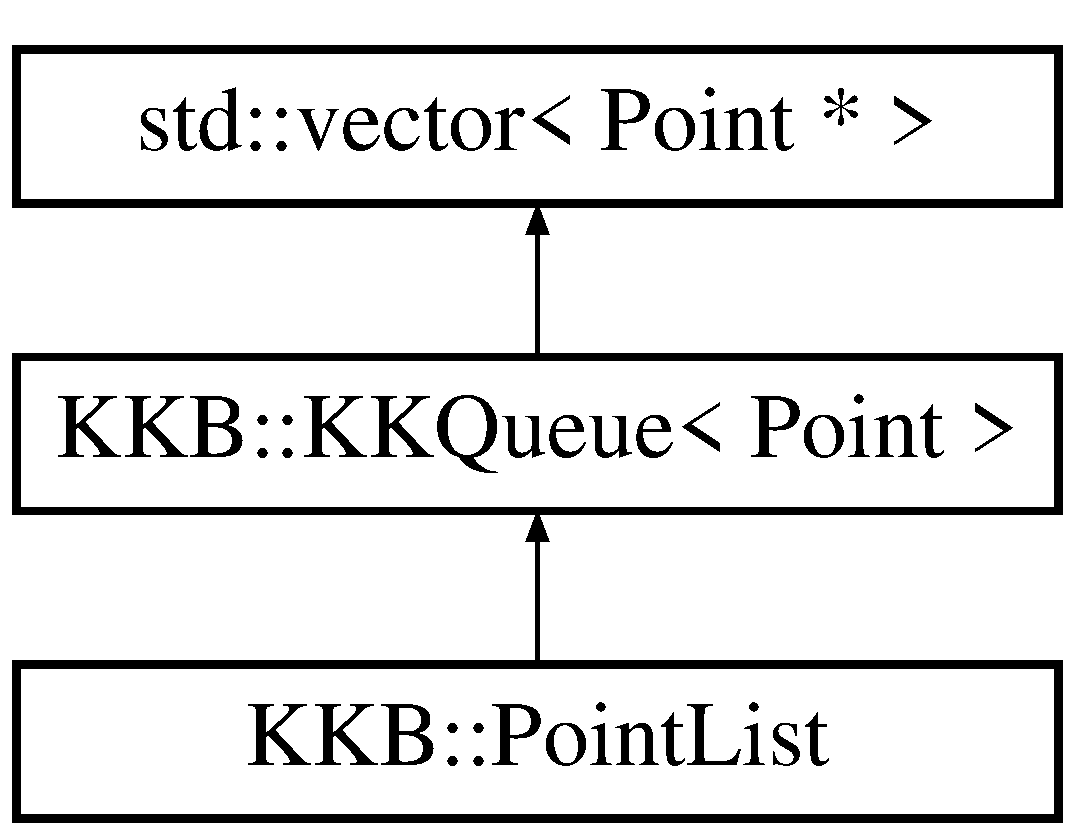
\includegraphics[height=3.000000cm]{class_k_k_b_1_1_point_list}
\end{center}
\end{figure}
\subsection*{Public Types}
\begin{DoxyCompactItemize}
\item 
typedef \hyperlink{class_k_k_b_1_1_point_list}{Point\+List} $\ast$ \hyperlink{class_k_k_b_1_1_point_list_af5058320a40be067bf73c2d78ff8b35d}{Point\+List\+Ptr}
\end{DoxyCompactItemize}
\subsection*{Public Member Functions}
\begin{DoxyCompactItemize}
\item 
\hyperlink{class_k_k_b_1_1_point_list_a23bf858f650e6db462382919b02e4fcd}{Point\+List} (const \hyperlink{class_k_k_b_1_1_point_list}{Point\+List} \&point\+List)
\item 
\hyperlink{class_k_k_b_1_1_point_list_a3249bff2a2964884fb2ef535248e9f05}{Point\+List} (bool \+\_\+owner)
\item 
void \hyperlink{class_k_k_b_1_1_point_list_a88e04c04e513be256b1528e1f56db795}{Box\+Coordinites} (\hyperlink{namespace_k_k_b_a8fa4952cc84fda1de4bec1fbdd8d5b1b}{kkint32} \&min\+Row, \hyperlink{namespace_k_k_b_a8fa4952cc84fda1de4bec1fbdd8d5b1b}{kkint32} \&min\+Col, \hyperlink{namespace_k_k_b_a8fa4952cc84fda1de4bec1fbdd8d5b1b}{kkint32} \&max\+Row, \hyperlink{namespace_k_k_b_a8fa4952cc84fda1de4bec1fbdd8d5b1b}{kkint32} \&max\+Col)
\item 
\hyperlink{class_k_k_b_1_1_point}{Point} \hyperlink{class_k_k_b_1_1_point_list_a7d4d04d6634c57306d578d7c1b68e77a}{Calculate\+Center\+Point} ()
\item 
float \hyperlink{class_k_k_b_1_1_point_list_a0ce92775337aa4b62a0a49fef0d40626}{Compute\+Segment\+Lens} (float height\+Factor, float width\+Factor) const 
\item 
\hyperlink{class_k_k_b_1_1_k_k_str}{K\+K\+Str} \hyperlink{class_k_k_b_1_1_point_list_a69c5c11221415ee7f9cd968a75d40774}{To\+Del\+Str} (char del) const 
\end{DoxyCompactItemize}
\subsection*{Static Public Member Functions}
\begin{DoxyCompactItemize}
\item 
static \hyperlink{class_k_k_b_1_1_point_list_af5058320a40be067bf73c2d78ff8b35d}{Point\+List\+Ptr} \hyperlink{class_k_k_b_1_1_point_list_a9b650b13f7e46d57ed47eb36c40906d1}{From\+Del\+Str} (const \hyperlink{class_k_k_b_1_1_k_k_str}{K\+K\+Str} \&s)
\end{DoxyCompactItemize}
\subsection*{Additional Inherited Members}


\subsection{Detailed Description}
Container object used to maintaining a list of pixel locations. 

Definition at line 75 of file Point.\+h.



\subsection{Member Typedef Documentation}
\index{K\+K\+B\+::\+Point\+List@{K\+K\+B\+::\+Point\+List}!Point\+List\+Ptr@{Point\+List\+Ptr}}
\index{Point\+List\+Ptr@{Point\+List\+Ptr}!K\+K\+B\+::\+Point\+List@{K\+K\+B\+::\+Point\+List}}
\subsubsection[{\texorpdfstring{Point\+List\+Ptr}{PointListPtr}}]{\setlength{\rightskip}{0pt plus 5cm}typedef {\bf Point\+List}$\ast$ {\bf K\+K\+B\+::\+Point\+List\+::\+Point\+List\+Ptr}}\hypertarget{class_k_k_b_1_1_point_list_af5058320a40be067bf73c2d78ff8b35d}{}\label{class_k_k_b_1_1_point_list_af5058320a40be067bf73c2d78ff8b35d}


Definition at line 78 of file Point.\+h.



\subsection{Constructor \& Destructor Documentation}
\index{K\+K\+B\+::\+Point\+List@{K\+K\+B\+::\+Point\+List}!Point\+List@{Point\+List}}
\index{Point\+List@{Point\+List}!K\+K\+B\+::\+Point\+List@{K\+K\+B\+::\+Point\+List}}
\subsubsection[{\texorpdfstring{Point\+List(const Point\+List \&point\+List)}{PointList(const PointList &pointList)}}]{\setlength{\rightskip}{0pt plus 5cm}Point\+List\+::\+Point\+List (
\begin{DoxyParamCaption}
\item[{const {\bf Point\+List} \&}]{point\+List}
\end{DoxyParamCaption}
)}\hypertarget{class_k_k_b_1_1_point_list_a23bf858f650e6db462382919b02e4fcd}{}\label{class_k_k_b_1_1_point_list_a23bf858f650e6db462382919b02e4fcd}


Definition at line 93 of file Point.\+cpp.



References Point\+List().



Referenced by Point\+List().


\begin{DoxyCode}
93                                                 :
94     \hyperlink{class_k_k_b_1_1_k_k_queue}{KKQueue<Point>} (\textcolor{keyword}{true})
95 \{
96   \hyperlink{class_k_k_b_1_1_k_k_queue_aeb057c9c010446f46f57c1e355f981f1}{PointList::const\_iterator}  idx;
97   \textcolor{keywordflow}{for}  (idx = pointList.begin ();  idx != pointList.end ();  idx++)
98   \{
99     \hyperlink{class_k_k_b_1_1_k_k_queue_aa9fba4632b54268bf71ecb42dee0b575}{PushOnBack} (\textcolor{keyword}{new} \hyperlink{class_k_k_b_1_1_point}{Point} (*(*idx)));
100   \}
101 \}
\end{DoxyCode}
\index{K\+K\+B\+::\+Point\+List@{K\+K\+B\+::\+Point\+List}!Point\+List@{Point\+List}}
\index{Point\+List@{Point\+List}!K\+K\+B\+::\+Point\+List@{K\+K\+B\+::\+Point\+List}}
\subsubsection[{\texorpdfstring{Point\+List(bool \+\_\+owner)}{PointList(bool _owner)}}]{\setlength{\rightskip}{0pt plus 5cm}Point\+List\+::\+Point\+List (
\begin{DoxyParamCaption}
\item[{bool}]{\+\_\+owner}
\end{DoxyParamCaption}
)}\hypertarget{class_k_k_b_1_1_point_list_a3249bff2a2964884fb2ef535248e9f05}{}\label{class_k_k_b_1_1_point_list_a3249bff2a2964884fb2ef535248e9f05}


Definition at line 105 of file Point.\+cpp.



References Point\+List().



Referenced by K\+K\+B\+::\+Contour\+Follower\+::\+Create\+Fourier\+Descriptor\+By\+Sampling(), K\+K\+B\+::\+Contour\+Follower\+::\+Create\+Point\+List\+From\+Fourier(), K\+K\+B\+::\+Raster\+::\+Derive\+Image\+Length(), From\+Del\+Str(), K\+K\+B\+::\+Contour\+Follower\+::\+Generate\+Contour\+List(), Point\+List(), and K\+K\+B\+::\+Raster\+::\+Thin\+Contour().


\begin{DoxyCode}
105                                 :
106     \hyperlink{class_k_k_b_1_1_k_k_queue}{KKQueue<Point>} (\_owner)
107 \{
108 \}
\end{DoxyCode}


\subsection{Member Function Documentation}
\index{K\+K\+B\+::\+Point\+List@{K\+K\+B\+::\+Point\+List}!Box\+Coordinites@{Box\+Coordinites}}
\index{Box\+Coordinites@{Box\+Coordinites}!K\+K\+B\+::\+Point\+List@{K\+K\+B\+::\+Point\+List}}
\subsubsection[{\texorpdfstring{Box\+Coordinites(kkint32 \&min\+Row, kkint32 \&min\+Col, kkint32 \&max\+Row, kkint32 \&max\+Col)}{BoxCoordinites(kkint32 &minRow, kkint32 &minCol, kkint32 &maxRow, kkint32 &maxCol)}}]{\setlength{\rightskip}{0pt plus 5cm}void Point\+List\+::\+Box\+Coordinites (
\begin{DoxyParamCaption}
\item[{{\bf kkint32} \&}]{min\+Row, }
\item[{{\bf kkint32} \&}]{min\+Col, }
\item[{{\bf kkint32} \&}]{max\+Row, }
\item[{{\bf kkint32} \&}]{max\+Col}
\end{DoxyParamCaption}
)}\hypertarget{class_k_k_b_1_1_point_list_a88e04c04e513be256b1528e1f56db795}{}\label{class_k_k_b_1_1_point_list_a88e04c04e513be256b1528e1f56db795}


Definition at line 111 of file Point.\+cpp.



References K\+K\+B\+::\+Point\+::\+Col(), and K\+K\+B\+::\+Point\+::\+Row().



Referenced by K\+K\+B\+::\+Contour\+Follower\+::\+Create\+Point\+List\+From\+Fourier().


\begin{DoxyCode}
116 \{
117   minRow = minCol = 999999;
118   maxRow = maxCol = -1;
119 
120   \textcolor{keywordflow}{for}  (\hyperlink{class_k_k_b_1_1_k_k_queue_aa3c2796a726eea468b94132a9fbf2cfe}{iterator} x = begin ();  x != end ();  x++)
121   \{
122     \hyperlink{class_k_k_b_1_1_point}{PointPtr} p = *x;
123     \textcolor{keywordflow}{if}  (p->\hyperlink{class_k_k_b_1_1_point_abfc34bcf809fc9fb95baf5c745b07549}{Row} () < minRow)
124       minRow = p->\hyperlink{class_k_k_b_1_1_point_abfc34bcf809fc9fb95baf5c745b07549}{Row} ();
125 
126     \textcolor{keywordflow}{if}  (p->\hyperlink{class_k_k_b_1_1_point_abfc34bcf809fc9fb95baf5c745b07549}{Row} () > maxRow)
127       maxRow = p->\hyperlink{class_k_k_b_1_1_point_abfc34bcf809fc9fb95baf5c745b07549}{Row} ();
128 
129     \textcolor{keywordflow}{if}  (p->\hyperlink{class_k_k_b_1_1_point_afb196b03757fc697f6ade0129a1c7fcf}{Col} () < minCol)
130       minCol = p->\hyperlink{class_k_k_b_1_1_point_afb196b03757fc697f6ade0129a1c7fcf}{Col} ();
131 
132     \textcolor{keywordflow}{if}  (p->\hyperlink{class_k_k_b_1_1_point_afb196b03757fc697f6ade0129a1c7fcf}{Col} () > maxCol)
133       maxCol = p->\hyperlink{class_k_k_b_1_1_point_afb196b03757fc697f6ade0129a1c7fcf}{Col} ();
134   \}
135 \}
\end{DoxyCode}
\index{K\+K\+B\+::\+Point\+List@{K\+K\+B\+::\+Point\+List}!Calculate\+Center\+Point@{Calculate\+Center\+Point}}
\index{Calculate\+Center\+Point@{Calculate\+Center\+Point}!K\+K\+B\+::\+Point\+List@{K\+K\+B\+::\+Point\+List}}
\subsubsection[{\texorpdfstring{Calculate\+Center\+Point()}{CalculateCenterPoint()}}]{\setlength{\rightskip}{0pt plus 5cm}{\bf Point} Point\+List\+::\+Calculate\+Center\+Point (
\begin{DoxyParamCaption}
{}
\end{DoxyParamCaption}
)}\hypertarget{class_k_k_b_1_1_point_list_a7d4d04d6634c57306d578d7c1b68e77a}{}\label{class_k_k_b_1_1_point_list_a7d4d04d6634c57306d578d7c1b68e77a}


Definition at line 138 of file Point.\+cpp.



References K\+K\+B\+::\+Point\+::\+Col(), K\+K\+B\+::\+Point\+::\+Point(), and K\+K\+B\+::\+Point\+::\+Row().


\begin{DoxyCode}
139 \{
140   \hyperlink{namespace_k_k_b_a8fa4952cc84fda1de4bec1fbdd8d5b1b}{kkint32}  totalRow = 0;
141   \hyperlink{namespace_k_k_b_a8fa4952cc84fda1de4bec1fbdd8d5b1b}{kkint32}  totalCol = 0;
142   \textcolor{keywordflow}{for}  (\hyperlink{class_k_k_b_1_1_k_k_queue_aa3c2796a726eea468b94132a9fbf2cfe}{iterator} x = begin ();  x != end ();  x++)
143   \{
144     \hyperlink{class_k_k_b_1_1_point}{PointPtr} p = *x;
145     totalRow += p->\hyperlink{class_k_k_b_1_1_point_abfc34bcf809fc9fb95baf5c745b07549}{Row} ();
146     totalCol += p->\hyperlink{class_k_k_b_1_1_point_afb196b03757fc697f6ade0129a1c7fcf}{Col} ();
147   \}
148 
149   \hyperlink{namespace_k_k_b_a8fa4952cc84fda1de4bec1fbdd8d5b1b}{kkint32} centerRow = (\hyperlink{namespace_k_k_b_a8fa4952cc84fda1de4bec1fbdd8d5b1b}{kkint32})((\textcolor{keywordtype}{double})totalRow / (double)size () + 0.5);
150   \hyperlink{namespace_k_k_b_a8fa4952cc84fda1de4bec1fbdd8d5b1b}{kkint32} centerCol = (\hyperlink{namespace_k_k_b_a8fa4952cc84fda1de4bec1fbdd8d5b1b}{kkint32})((\textcolor{keywordtype}{double})totalCol / (double)size () + 0.5);
151   \textcolor{keywordflow}{return}  \hyperlink{class_k_k_b_1_1_point}{Point} (centerRow, centerCol);
152 \}
\end{DoxyCode}
\index{K\+K\+B\+::\+Point\+List@{K\+K\+B\+::\+Point\+List}!Compute\+Segment\+Lens@{Compute\+Segment\+Lens}}
\index{Compute\+Segment\+Lens@{Compute\+Segment\+Lens}!K\+K\+B\+::\+Point\+List@{K\+K\+B\+::\+Point\+List}}
\subsubsection[{\texorpdfstring{Compute\+Segment\+Lens(float height\+Factor, float width\+Factor) const }{ComputeSegmentLens(float heightFactor, float widthFactor) const }}]{\setlength{\rightskip}{0pt plus 5cm}float Point\+List\+::\+Compute\+Segment\+Lens (
\begin{DoxyParamCaption}
\item[{float}]{height\+Factor, }
\item[{float}]{width\+Factor}
\end{DoxyParamCaption}
) const}\hypertarget{class_k_k_b_1_1_point_list_a0ce92775337aa4b62a0a49fef0d40626}{}\label{class_k_k_b_1_1_point_list_a0ce92775337aa4b62a0a49fef0d40626}


Definition at line 233 of file Point.\+cpp.


\begin{DoxyCode}
236 \{
237   \textcolor{keywordflow}{if}  (\hyperlink{class_k_k_b_1_1_k_k_queue_a1dab601f75ee6a65d97f02bddf71c40d}{QueueSize} () < 1)
238     \textcolor{keywordflow}{return} 0.0f;
239 
240   \textcolor{keywordtype}{float} totalLen = 0.0f;
241 
242   \hyperlink{class_k_k_b_1_1_k_k_queue_aeb057c9c010446f46f57c1e355f981f1}{const\_iterator}  idx;
243   idx = begin ();
244   \hyperlink{class_k_k_b_1_1_point}{PointPtr} lastPoint = *idx;
245   ++idx;
246 
247   \textcolor{keywordflow}{while}  (idx != end ())
248   \{
249     \hyperlink{class_k_k_b_1_1_point}{PointPtr}  nextPoint = *idx;  ++idx;
250 
251     \textcolor{keywordtype}{float}  deltaHeight = (float)(nextPoint->\hyperlink{class_k_k_b_1_1_point_abfc34bcf809fc9fb95baf5c745b07549}{Row} () - lastPoint->\hyperlink{class_k_k_b_1_1_point_abfc34bcf809fc9fb95baf5c745b07549}{Row} ()) * heightFactor;
252     \textcolor{keywordtype}{float}  deltaWidth  = (float)(nextPoint->\hyperlink{class_k_k_b_1_1_point_afb196b03757fc697f6ade0129a1c7fcf}{Col} () - lastPoint->\hyperlink{class_k_k_b_1_1_point_afb196b03757fc697f6ade0129a1c7fcf}{Col} ()) * widthFactor;
253 
254     \textcolor{keywordtype}{float}  segmentLen = sqrt (deltaHeight * deltaHeight + deltaWidth * deltaWidth);
255 
256     totalLen += segmentLen;
257     lastPoint = nextPoint;
258   \}
259 
260   \textcolor{keywordflow}{return}  totalLen;
261 \}  \textcolor{comment}{/* ComputeSegmentLens */}
\end{DoxyCode}
\index{K\+K\+B\+::\+Point\+List@{K\+K\+B\+::\+Point\+List}!From\+Del\+Str@{From\+Del\+Str}}
\index{From\+Del\+Str@{From\+Del\+Str}!K\+K\+B\+::\+Point\+List@{K\+K\+B\+::\+Point\+List}}
\subsubsection[{\texorpdfstring{From\+Del\+Str(const K\+K\+Str \&s)}{FromDelStr(const KKStr &s)}}]{\setlength{\rightskip}{0pt plus 5cm}{\bf Point\+List\+Ptr} Point\+List\+::\+From\+Del\+Str (
\begin{DoxyParamCaption}
\item[{const {\bf K\+K\+Str} \&}]{s}
\end{DoxyParamCaption}
)\hspace{0.3cm}{\ttfamily [static]}}\hypertarget{class_k_k_b_1_1_point_list_a9b650b13f7e46d57ed47eb36c40906d1}{}\label{class_k_k_b_1_1_point_list_a9b650b13f7e46d57ed47eb36c40906d1}


Definition at line 176 of file Point.\+cpp.



References K\+K\+B\+::\+K\+K\+Str\+::\+Chop\+First\+Char(), K\+K\+B\+::\+K\+K\+Str\+::\+Concat(), K\+K\+B\+::\+K\+K\+Str\+::\+Extract\+Token\+Int(), K\+K\+B\+::\+K\+K\+Str\+::\+Find(), K\+K\+B\+::\+K\+K\+Str\+::\+First\+Char(), K\+K\+B\+::\+K\+K\+Str\+::\+K\+K\+Str(), K\+K\+B\+::\+K\+K\+Str\+::\+Len(), K\+K\+B\+::\+K\+K\+Str\+::operator=(), Point\+List(), K\+K\+B\+::\+K\+K\+Str\+::\+Sub\+Str\+Part(), and K\+K\+B\+::\+K\+K\+Str\+::\+Trim\+Left().


\begin{DoxyCode}
177 \{
178   \hyperlink{class_k_k_b_1_1_point_list}{PointListPtr}  result = \textcolor{keyword}{new} \hyperlink{class_k_k_b_1_1_point_list_a23bf858f650e6db462382919b02e4fcd}{PointList} (\textcolor{keyword}{true});
179 
180   \hyperlink{class_k_k_b_1_1_k_k_str}{KKStr}  s (\_s);
181   s.\hyperlink{class_k_k_b_1_1_k_k_str_af7c102c53103ddff3f48270b4a198c89}{TrimLeft} ();
182 
183   \textcolor{keywordflow}{while}  (s.\hyperlink{class_k_k_b_1_1_k_k_str_a869142d4855517c5c237afcb25dbbe36}{Len} () > 0)
184   \{
185     \textcolor{keywordtype}{char} nextCh = s.\hyperlink{class_k_k_b_1_1_k_k_str_ac20e69c629b985c6569af914d9cc3e8c}{FirstChar} ();
186     \textcolor{keywordtype}{char} endPairChar = 0;
187     \textcolor{keywordflow}{if}  (nextCh == \textcolor{charliteral}{'['})
188       endPairChar = \textcolor{charliteral}{']'};
189 
190     \textcolor{keywordflow}{else} \textcolor{keywordflow}{if}  (nextCh == \textcolor{charliteral}{'('})
191       endPairChar = \textcolor{charliteral}{')'};
192 
193     \textcolor{keywordflow}{else}
194     \{
195       \textcolor{comment}{// Not Bracketed.}
196       endPairChar = 0;
197       \hyperlink{namespace_k_k_b_a93809780ee294124dda4c23069f41248}{kkint16}  row = (\hyperlink{namespace_k_k_b_a93809780ee294124dda4c23069f41248}{kkint16})s.\hyperlink{class_k_k_b_1_1_k_k_str_ae50047144b908273ffd004bd9379f6d0}{ExtractTokenInt} (\textcolor{stringliteral}{",\(\backslash\)t\(\backslash\)n\(\backslash\)t"});
198       \hyperlink{namespace_k_k_b_a93809780ee294124dda4c23069f41248}{kkint16}  col = (\hyperlink{namespace_k_k_b_a93809780ee294124dda4c23069f41248}{kkint16})s.\hyperlink{class_k_k_b_1_1_k_k_str_ae50047144b908273ffd004bd9379f6d0}{ExtractTokenInt} (\textcolor{stringliteral}{",\(\backslash\)t\(\backslash\)n\(\backslash\)t"});
199       result->\hyperlink{class_k_k_b_1_1_k_k_queue_aa9fba4632b54268bf71ecb42dee0b575}{PushOnBack} (\textcolor{keyword}{new} \hyperlink{class_k_k_b_1_1_point}{Point} (row, col));
200     \}
201 
202     \textcolor{keywordflow}{if}  (endPairChar != 0)
203     \{
204       \hyperlink{class_k_k_b_1_1_k_k_str}{KKStr} pairStr = \textcolor{stringliteral}{""};
205       \hyperlink{namespace_k_k_b_a8fa4952cc84fda1de4bec1fbdd8d5b1b}{kkint32}  idx = s.\hyperlink{class_k_k_b_1_1_k_k_str_a3972260712f99de712591dc5be2d3eef}{Find} (endPairChar);
206       \textcolor{keywordflow}{if}  (idx >= 0)
207       \{
208         pairStr = s.\hyperlink{class_k_k_b_1_1_k_k_str_a5f20b2ddfc9f07c8ef99592810332ddb}{SubStrPart} (0, idx - 1);
209         s = s.\hyperlink{class_k_k_b_1_1_k_k_str_a5f20b2ddfc9f07c8ef99592810332ddb}{SubStrPart} (idx + 1);
210       \}
211       \textcolor{keywordflow}{else}
212       \{
213         pairStr = s;
214         s = \textcolor{stringliteral}{""};
215       \}
216 
217       \hyperlink{namespace_k_k_b_a93809780ee294124dda4c23069f41248}{kkint16}  row = (\hyperlink{namespace_k_k_b_a93809780ee294124dda4c23069f41248}{kkint16})pairStr.\hyperlink{class_k_k_b_1_1_k_k_str_ae50047144b908273ffd004bd9379f6d0}{ExtractTokenInt} (\textcolor{stringliteral}{","});
218       \hyperlink{namespace_k_k_b_a93809780ee294124dda4c23069f41248}{kkint16}  col = (\hyperlink{namespace_k_k_b_a93809780ee294124dda4c23069f41248}{kkint16}) pairStr.\hyperlink{class_k_k_b_1_1_k_k_str_ae50047144b908273ffd004bd9379f6d0}{ExtractTokenInt} (\textcolor{stringliteral}{","});
219       result->\hyperlink{class_k_k_b_1_1_k_k_queue_aa9fba4632b54268bf71ecb42dee0b575}{PushOnBack} (\textcolor{keyword}{new} \hyperlink{class_k_k_b_1_1_point}{Point} (row, col));
220       nextCh = s.\hyperlink{class_k_k_b_1_1_k_k_str_ac20e69c629b985c6569af914d9cc3e8c}{FirstChar} ();
221       \textcolor{keywordflow}{if}  ((nextCh == \textcolor{charliteral}{','})  ||  (nextCh == \textcolor{charliteral}{'\(\backslash\)n'})  ||  (nextCh == \textcolor{charliteral}{'\(\backslash\)r'})  || (nextCh == \textcolor{charliteral}{'\(\backslash\)t'}))
222         s.\hyperlink{class_k_k_b_1_1_k_k_str_a974ed722249e4e96fde79d483a314712}{ChopFirstChar} ();
223     \}
224     s.\hyperlink{class_k_k_b_1_1_k_k_str_af7c102c53103ddff3f48270b4a198c89}{TrimLeft} ();
225   \}
226 
227   \textcolor{keywordflow}{return}  result;
228 \}  \textcolor{comment}{/* FromDelStr */}
\end{DoxyCode}
\index{K\+K\+B\+::\+Point\+List@{K\+K\+B\+::\+Point\+List}!To\+Del\+Str@{To\+Del\+Str}}
\index{To\+Del\+Str@{To\+Del\+Str}!K\+K\+B\+::\+Point\+List@{K\+K\+B\+::\+Point\+List}}
\subsubsection[{\texorpdfstring{To\+Del\+Str(char del) const }{ToDelStr(char del) const }}]{\setlength{\rightskip}{0pt plus 5cm}{\bf K\+K\+Str} Point\+List\+::\+To\+Del\+Str (
\begin{DoxyParamCaption}
\item[{char}]{del}
\end{DoxyParamCaption}
) const}\hypertarget{class_k_k_b_1_1_point_list_a69c5c11221415ee7f9cd968a75d40774}{}\label{class_k_k_b_1_1_point_list_a69c5c11221415ee7f9cd968a75d40774}


Definition at line 156 of file Point.\+cpp.



References K\+K\+B\+::\+Point\+::\+Col(), K\+K\+B\+::\+K\+K\+Str\+::\+Concat(), and K\+K\+B\+::\+Point\+::\+Row().


\begin{DoxyCode}
157 \{
158   \textcolor{keywordflow}{if}  (\hyperlink{class_k_k_b_1_1_k_k_queue_a1dab601f75ee6a65d97f02bddf71c40d}{QueueSize} () < 1)
159     \textcolor{keywordflow}{return} \textcolor{stringliteral}{"[]"};
160 
161   \hyperlink{class_k_k_b_1_1_k_k_str}{KKStr}  result (\hyperlink{class_k_k_b_1_1_k_k_queue_a1dab601f75ee6a65d97f02bddf71c40d}{QueueSize} () * 10);
162 
163   \textcolor{keywordtype}{int}  count = 0;
164   \hyperlink{class_k_k_b_1_1_k_k_queue_aeb057c9c010446f46f57c1e355f981f1}{PointList::const\_iterator}  idx;
165   \textcolor{keywordflow}{for}  (idx = begin ();  idx != end ();  ++idx, ++count)
166   \{
167     \hyperlink{class_k_k_b_1_1_point}{PointPtr}  p = *idx;
168     \textcolor{keywordflow}{if}  (count > 0)
169       result << del;
170     result << p->\hyperlink{class_k_k_b_1_1_point_abfc34bcf809fc9fb95baf5c745b07549}{Row} () << del << p->\hyperlink{class_k_k_b_1_1_point_afb196b03757fc697f6ade0129a1c7fcf}{Col} ();
171   \}
172   \textcolor{keywordflow}{return}  result;
173 \}  \textcolor{comment}{/* ToDelStr */}
\end{DoxyCode}


The documentation for this class was generated from the following files\+:\begin{DoxyCompactItemize}
\item 
C\+:/\+Users/\+Kurt/\+Git\+Hub/\+K\+Square\+Libraries/\+K\+K\+Base/\hyperlink{_point_8h}{Point.\+h}\item 
C\+:/\+Users/\+Kurt/\+Git\+Hub/\+K\+Square\+Libraries/\+K\+K\+Base/\hyperlink{_point_8cpp}{Point.\+cpp}\end{DoxyCompactItemize}

\hypertarget{class_k_k_b_1_1_random_num_generator}{}\section{K\+KB\+:\+:Random\+Num\+Generator Class Reference}
\label{class_k_k_b_1_1_random_num_generator}\index{K\+K\+B\+::\+Random\+Num\+Generator@{K\+K\+B\+::\+Random\+Num\+Generator}}


Represents one single random number generator.  




{\ttfamily \#include $<$Random\+Num\+Generator.\+h$>$}

\subsection*{Public Member Functions}
\begin{DoxyCompactItemize}
\item 
\hyperlink{class_k_k_b_1_1_random_num_generator_a7c17e42b6512c279b6301bd8e4d8f5c5}{Random\+Num\+Generator} ()
\item 
\hyperlink{class_k_k_b_1_1_random_num_generator_afd97066c4ad6a91c3e72edd31866e650}{Random\+Num\+Generator} (long \+\_\+seed)
\item 
\hyperlink{class_k_k_b_1_1_random_num_generator_a71ddf586846ca9349b2a916177fc8ac9}{$\sim$\+Random\+Num\+Generator} ()
\item 
long \hyperlink{class_k_k_b_1_1_random_num_generator_a4d89c40b50259c9928605ac8adcc777d}{Next} ()
\end{DoxyCompactItemize}


\subsection{Detailed Description}
Represents one single random number generator. 

Rather than using the two global functions \char`\"{}lrand48\char`\"{} and \char`\"{}srand48\char`\"{} you can create an instance of this class that will provide the random sequence. The advantage is that you can control who has access to this sequence. That is you do not need to worry that some other code that you are calling is not also getting numbers from this sequence. This will allow you to guarantee the same sequence of numbers for the same seed. 

Definition at line 20 of file Random\+Num\+Generator.\+h.



\subsection{Constructor \& Destructor Documentation}
\index{K\+K\+B\+::\+Random\+Num\+Generator@{K\+K\+B\+::\+Random\+Num\+Generator}!Random\+Num\+Generator@{Random\+Num\+Generator}}
\index{Random\+Num\+Generator@{Random\+Num\+Generator}!K\+K\+B\+::\+Random\+Num\+Generator@{K\+K\+B\+::\+Random\+Num\+Generator}}
\subsubsection[{\texorpdfstring{Random\+Num\+Generator()}{RandomNumGenerator()}}]{\setlength{\rightskip}{0pt plus 5cm}Random\+Num\+Generator\+::\+Random\+Num\+Generator (
\begin{DoxyParamCaption}
{}
\end{DoxyParamCaption}
)}\hypertarget{class_k_k_b_1_1_random_num_generator_a7c17e42b6512c279b6301bd8e4d8f5c5}{}\label{class_k_k_b_1_1_random_num_generator_a7c17e42b6512c279b6301bd8e4d8f5c5}


Definition at line 25 of file Random\+Num\+Generator.\+cpp.


\begin{DoxyCode}
26 \{
27 \textcolor{preprocessor}{#if  defined(WIN32)}
28   \hyperlink{_k_k_base_types_8cpp_a9f6516ed195a919be488f0d84b219cc9}{\_lrand48\_sequence} = 0x1234ABCD330E;
29 \textcolor{preprocessor}{#else}
30   \hyperlink{_k_k_base_types_8cpp_a9f6516ed195a919be488f0d84b219cc9}{\_lrand48\_sequence} = 0x1234ABCD330ELLU;
31 \textcolor{preprocessor}{#endif}
32 \}
\end{DoxyCode}
\index{K\+K\+B\+::\+Random\+Num\+Generator@{K\+K\+B\+::\+Random\+Num\+Generator}!Random\+Num\+Generator@{Random\+Num\+Generator}}
\index{Random\+Num\+Generator@{Random\+Num\+Generator}!K\+K\+B\+::\+Random\+Num\+Generator@{K\+K\+B\+::\+Random\+Num\+Generator}}
\subsubsection[{\texorpdfstring{Random\+Num\+Generator(long \+\_\+seed)}{RandomNumGenerator(long _seed)}}]{\setlength{\rightskip}{0pt plus 5cm}Random\+Num\+Generator\+::\+Random\+Num\+Generator (
\begin{DoxyParamCaption}
\item[{long}]{\+\_\+seed}
\end{DoxyParamCaption}
)}\hypertarget{class_k_k_b_1_1_random_num_generator_afd97066c4ad6a91c3e72edd31866e650}{}\label{class_k_k_b_1_1_random_num_generator_afd97066c4ad6a91c3e72edd31866e650}


Definition at line 35 of file Random\+Num\+Generator.\+cpp.


\begin{DoxyCode}
36 \{
37   \hyperlink{namespace_k_k_b_aa3486b1c5ea9162b3b020c69f72826eb}{kkint64} seedMask = 65535;
38   \hyperlink{_k_k_base_types_8cpp_a9f6516ed195a919be488f0d84b219cc9}{\_lrand48\_sequence} &= seedMask;
39   \hyperlink{namespace_k_k_b_aa3486b1c5ea9162b3b020c69f72826eb}{kkint64} upperBits = \_seed;
40   upperBits <<= 16;
41   \hyperlink{_k_k_base_types_8cpp_a9f6516ed195a919be488f0d84b219cc9}{\_lrand48\_sequence} |= upperBits;
42 \}
\end{DoxyCode}
\index{K\+K\+B\+::\+Random\+Num\+Generator@{K\+K\+B\+::\+Random\+Num\+Generator}!````~Random\+Num\+Generator@{$\sim$\+Random\+Num\+Generator}}
\index{````~Random\+Num\+Generator@{$\sim$\+Random\+Num\+Generator}!K\+K\+B\+::\+Random\+Num\+Generator@{K\+K\+B\+::\+Random\+Num\+Generator}}
\subsubsection[{\texorpdfstring{$\sim$\+Random\+Num\+Generator()}{~RandomNumGenerator()}}]{\setlength{\rightskip}{0pt plus 5cm}Random\+Num\+Generator\+::$\sim$\+Random\+Num\+Generator (
\begin{DoxyParamCaption}
{}
\end{DoxyParamCaption}
)}\hypertarget{class_k_k_b_1_1_random_num_generator_a71ddf586846ca9349b2a916177fc8ac9}{}\label{class_k_k_b_1_1_random_num_generator_a71ddf586846ca9349b2a916177fc8ac9}


Definition at line 45 of file Random\+Num\+Generator.\+cpp.


\begin{DoxyCode}
46 \{
47 \}
\end{DoxyCode}


\subsection{Member Function Documentation}
\index{K\+K\+B\+::\+Random\+Num\+Generator@{K\+K\+B\+::\+Random\+Num\+Generator}!Next@{Next}}
\index{Next@{Next}!K\+K\+B\+::\+Random\+Num\+Generator@{K\+K\+B\+::\+Random\+Num\+Generator}}
\subsubsection[{\texorpdfstring{Next()}{Next()}}]{\setlength{\rightskip}{0pt plus 5cm}long Random\+Num\+Generator\+::\+Next (
\begin{DoxyParamCaption}
{}
\end{DoxyParamCaption}
)}\hypertarget{class_k_k_b_1_1_random_num_generator_a4d89c40b50259c9928605ac8adcc777d}{}\label{class_k_k_b_1_1_random_num_generator_a4d89c40b50259c9928605ac8adcc777d}


Definition at line 63 of file Random\+Num\+Generator.\+cpp.


\begin{DoxyCode}
64 \{
65   \hyperlink{_k_k_base_types_8cpp_a9f6516ed195a919be488f0d84b219cc9}{\_lrand48\_sequence} = ( ((a * \hyperlink{_k_k_base_types_8cpp_a9f6516ed195a919be488f0d84b219cc9}{\_lrand48\_sequence}) & mask) + c ) % m;
66   \textcolor{keywordflow}{return} (\textcolor{keywordtype}{long})(\hyperlink{_k_k_base_types_8cpp_a9f6516ed195a919be488f0d84b219cc9}{\_lrand48\_sequence} >> 17);
67 \}
\end{DoxyCode}


The documentation for this class was generated from the following files\+:\begin{DoxyCompactItemize}
\item 
C\+:/\+Users/\+Kurt/\+Git\+Hub/\+K\+Square\+Libraries/\+K\+K\+Base/\hyperlink{_random_num_generator_8h}{Random\+Num\+Generator.\+h}\item 
C\+:/\+Users/\+Kurt/\+Git\+Hub/\+K\+Square\+Libraries/\+K\+K\+Base/\hyperlink{_random_num_generator_8cpp}{Random\+Num\+Generator.\+cpp}\end{DoxyCompactItemize}

\hypertarget{class_k_k_b_1_1_raster}{}\section{K\+KB\+:\+:Raster Class Reference}
\label{class_k_k_b_1_1_raster}\index{K\+K\+B\+::\+Raster@{K\+K\+B\+::\+Raster}}


A class that is used by to represent a single image in memory.  




{\ttfamily \#include $<$Raster.\+h$>$}

\subsection*{Public Types}
\begin{DoxyCompactItemize}
\item 
typedef \hyperlink{class_k_k_b_1_1_raster}{Raster} const \hyperlink{class_k_k_b_1_1_raster_a938ab844ee73af06f79244750f96d3df}{Raster\+Const}
\item 
typedef \hyperlink{class_k_k_b_1_1_raster_a938ab844ee73af06f79244750f96d3df}{Raster\+Const} $\ast$ \hyperlink{class_k_k_b_1_1_raster_ad76aea7ccc94ebd88384a43aa1a19394}{Raster\+Const\+Ptr}
\item 
typedef \hyperlink{class_k_k_b_1_1_raster}{Raster} $\ast$ \hyperlink{class_k_k_b_1_1_raster_aefa532857fd6aa9eb53f79da55a97c5a}{Raster\+Ptr}
\end{DoxyCompactItemize}
\subsection*{Public Member Functions}
\begin{DoxyCompactItemize}
\item 
\hyperlink{class_k_k_b_1_1_raster_a19ec88efff547c1fcda863172fef620b}{Raster} ()
\item 
\hyperlink{class_k_k_b_1_1_raster_a711646f50218428dc3ce40eb2b7014c9}{Raster} (const \hyperlink{class_k_k_b_1_1_raster}{Raster} \&\+\_\+raster)
\begin{DoxyCompactList}\small\item\em Copy Constructor. \end{DoxyCompactList}\item 
\hyperlink{class_k_k_b_1_1_raster_aabf6eb169caf874fef8e8880d63c70eb}{Raster} (\hyperlink{namespace_k_k_b_a8fa4952cc84fda1de4bec1fbdd8d5b1b}{kkint32} \+\_\+height, \hyperlink{namespace_k_k_b_a8fa4952cc84fda1de4bec1fbdd8d5b1b}{kkint32} \+\_\+width)
\begin{DoxyCompactList}\small\item\em Constructs a blank image with given dimensions; all pixels will be initialized to 0. \end{DoxyCompactList}\item 
\hyperlink{class_k_k_b_1_1_raster_a356f9c8e73cf2f6e11bfe08eadb039bb}{Raster} (\hyperlink{namespace_k_k_b_a8fa4952cc84fda1de4bec1fbdd8d5b1b}{kkint32} \+\_\+height, \hyperlink{namespace_k_k_b_a8fa4952cc84fda1de4bec1fbdd8d5b1b}{kkint32} \+\_\+width, bool \+\_\+color)
\begin{DoxyCompactList}\small\item\em Constructs a blank image with given dimensions. \end{DoxyCompactList}\item 
\hyperlink{class_k_k_b_1_1_raster_a8fb1de49421cb676e585add96a6a5264}{Raster} (const \hyperlink{class_k_k_b_1_1_bmp_image}{Bmp\+Image} \&\+\_\+bmp\+Image)
\begin{DoxyCompactList}\small\item\em Constructs a \hyperlink{class_k_k_b_1_1_raster}{Raster} from a B\+MP image loaded from disk. \end{DoxyCompactList}\item 
\hyperlink{class_k_k_b_1_1_raster_a882eafd0b7a2c59bf95184d141c4f76c}{Raster} (const \hyperlink{class_k_k_b_1_1_raster}{Raster} \&\+\_\+raster, \hyperlink{namespace_k_k_b_a8fa4952cc84fda1de4bec1fbdd8d5b1b}{kkint32} \+\_\+row, \hyperlink{namespace_k_k_b_a8fa4952cc84fda1de4bec1fbdd8d5b1b}{kkint32} \+\_\+col, \hyperlink{namespace_k_k_b_a8fa4952cc84fda1de4bec1fbdd8d5b1b}{kkint32} \+\_\+height, \hyperlink{namespace_k_k_b_a8fa4952cc84fda1de4bec1fbdd8d5b1b}{kkint32} \+\_\+width)
\begin{DoxyCompactList}\small\item\em Constructs a new \hyperlink{class_k_k_b_1_1_raster}{Raster} using a subset of the specified \hyperlink{class_k_k_b_1_1_raster}{Raster} as its source. The dimensions of the resultant raster will be \textquotesingle{}\+\_\+height\textquotesingle{}, and \textquotesingle{}\+\_\+width\textquotesingle{}. \end{DoxyCompactList}\item 
\hyperlink{class_k_k_b_1_1_raster_a5b465ed19680790d6ce617cd6dfd429b}{Raster} (const \hyperlink{class_k_k_b_1_1_raster}{Raster} \&\+\_\+raster, \hyperlink{class_k_k_b_1_1_morph_op_a9eaa0383bf9e046da208af397e7e35eb}{Mask\+Types} \+\_\+mask, \hyperlink{namespace_k_k_b_a8fa4952cc84fda1de4bec1fbdd8d5b1b}{kkint32} \+\_\+row, \hyperlink{namespace_k_k_b_a8fa4952cc84fda1de4bec1fbdd8d5b1b}{kkint32} \+\_\+col)
\begin{DoxyCompactList}\small\item\em Constructs a \hyperlink{class_k_k_b_1_1_raster}{Raster} that will be the same size as the specified \textquotesingle{}\+\_\+mask\textquotesingle{} with the top left specified by \textquotesingle{}\+\_\+row\textquotesingle{} and \textquotesingle{}\+\_\+col\textquotesingle{}. \end{DoxyCompactList}\item 
\hyperlink{class_k_k_b_1_1_raster_aa6ec004fc43f9e9ff35ef9fe431cb34a}{Raster} (const \hyperlink{class_k_k_b_1_1_k_k_str}{K\+K\+Str} \&\hyperlink{class_k_k_b_1_1_raster_a742e1da027493443f2dda570a89fe2e9}{file\+Name}, bool \&valid\+File)
\begin{DoxyCompactList}\small\item\em Constructs a \hyperlink{class_k_k_b_1_1_raster}{Raster} image from by reading an existing image File such as a B\+MP file. \end{DoxyCompactList}\item 
\hyperlink{class_k_k_b_1_1_raster_a59efd48491562c981fc5667abfadf153}{Raster} (\hyperlink{namespace_k_k_b_a8fa4952cc84fda1de4bec1fbdd8d5b1b}{kkint32} \+\_\+height, \hyperlink{namespace_k_k_b_a8fa4952cc84fda1de4bec1fbdd8d5b1b}{kkint32} \+\_\+width, \hyperlink{namespace_k_k_b_ace9969169bf514f9ee6185186949cdf7}{uchar} $\ast$\+\_\+\+Data, \hyperlink{namespace_k_k_b_ace9969169bf514f9ee6185186949cdf7}{uchar} $\ast$$\ast$\+\_\+\+Rows)
\begin{DoxyCompactList}\small\item\em Construct a raster object that will utilize a image already in memory. \end{DoxyCompactList}\item 
\hyperlink{class_k_k_b_1_1_raster_aa90fd7d98911e4df1cfbfdec4ee4a38c}{Raster} (\hyperlink{namespace_k_k_b_a8fa4952cc84fda1de4bec1fbdd8d5b1b}{kkint32} \+\_\+height, \hyperlink{namespace_k_k_b_a8fa4952cc84fda1de4bec1fbdd8d5b1b}{kkint32} \+\_\+width, const \hyperlink{namespace_k_k_b_ace9969169bf514f9ee6185186949cdf7}{uchar} $\ast$\+\_\+\+Data)
\begin{DoxyCompactList}\small\item\em Construct a \hyperlink{class_k_k_b_1_1_raster}{Raster} object using provided raw data. \end{DoxyCompactList}\item 
\hyperlink{class_k_k_b_1_1_raster_a2c5461f10288456b2e2c4e863b05d868}{Raster} (\hyperlink{namespace_k_k_b_a8fa4952cc84fda1de4bec1fbdd8d5b1b}{kkint32} \+\_\+height, \hyperlink{namespace_k_k_b_a8fa4952cc84fda1de4bec1fbdd8d5b1b}{kkint32} \+\_\+width, const \hyperlink{namespace_k_k_b_ace9969169bf514f9ee6185186949cdf7}{uchar} $\ast$\+\_\+red\+Channel, const \hyperlink{namespace_k_k_b_ace9969169bf514f9ee6185186949cdf7}{uchar} $\ast$\+\_\+green\+Channel, const \hyperlink{namespace_k_k_b_ace9969169bf514f9ee6185186949cdf7}{uchar} $\ast$\+\_\+blue\+Channel)
\begin{DoxyCompactList}\small\item\em Construct a Color \hyperlink{class_k_k_b_1_1_raster}{Raster} object using provided raw data,. \end{DoxyCompactList}\item 
virtual \hyperlink{class_k_k_b_1_1_raster_ab5f3ec20a0cb4dc2ea18905d2e7899f6}{$\sim$\+Raster} ()
\item 
virtual \hyperlink{class_k_k_b_1_1_raster_aefa532857fd6aa9eb53f79da55a97c5a}{Raster\+Ptr} \hyperlink{class_k_k_b_1_1_raster_aa879980d112c01cb7ad9a3cfc7cd6f64}{Allocate\+A\+Raster\+Instance} (\hyperlink{namespace_k_k_b_a8fa4952cc84fda1de4bec1fbdd8d5b1b}{kkint32} \hyperlink{class_k_k_b_1_1_raster_af39ff189de4fbb6de98392e187efafb7}{height}, \hyperlink{namespace_k_k_b_a8fa4952cc84fda1de4bec1fbdd8d5b1b}{kkint32} \hyperlink{class_k_k_b_1_1_raster_ae0bcc103e191c3421d7692dc69ceb554}{width}, bool \hyperlink{class_k_k_b_1_1_raster_a482384d89cc53fa4f36276307c746854}{color}) const 
\item 
virtual \hyperlink{class_k_k_b_1_1_raster_aefa532857fd6aa9eb53f79da55a97c5a}{Raster\+Ptr} \hyperlink{class_k_k_b_1_1_raster_a490e886e849ecdaa388e3450252d1bdc}{Allocate\+A\+Raster\+Instance} (const \hyperlink{class_k_k_b_1_1_raster}{Raster} \&r) const 
\item 
virtual \hyperlink{class_k_k_b_1_1_raster_aefa532857fd6aa9eb53f79da55a97c5a}{Raster\+Ptr} \hyperlink{class_k_k_b_1_1_raster_a607062dbb7b0c291cab5d27f21cbbd00}{Allocate\+A\+Raster\+Instance} (const \hyperlink{class_k_k_b_1_1_raster}{Raster} \&\+\_\+raster, \hyperlink{namespace_k_k_b_a8fa4952cc84fda1de4bec1fbdd8d5b1b}{kkint32} \+\_\+row, \hyperlink{namespace_k_k_b_a8fa4952cc84fda1de4bec1fbdd8d5b1b}{kkint32} \+\_\+col, \hyperlink{namespace_k_k_b_a8fa4952cc84fda1de4bec1fbdd8d5b1b}{kkint32} \+\_\+height, \hyperlink{namespace_k_k_b_a8fa4952cc84fda1de4bec1fbdd8d5b1b}{kkint32} \+\_\+width) const 
\item 
bool \hyperlink{class_k_k_b_1_1_raster_ada0a1ce889e08d42187b02a2fe0444df}{Are\+There\+Edge\+Pixels} (\hyperlink{namespace_k_k_b_a8fa4952cc84fda1de4bec1fbdd8d5b1b}{kkint32} edge\+Width)
\begin{DoxyCompactList}\small\item\em returns true if there are any foreground pixels within \textquotesingle{}edge\+Width\textquotesingle{} pixels of the top, bottom, left, or right edges of the image. \end{DoxyCompactList}\item 
bool \hyperlink{class_k_k_b_1_1_raster_a0756fb5530274d5e28858d3e1633d595}{Background\+Pixel} (\hyperlink{namespace_k_k_b_a8fa4952cc84fda1de4bec1fbdd8d5b1b}{kkint32} row, \hyperlink{namespace_k_k_b_a8fa4952cc84fda1de4bec1fbdd8d5b1b}{kkint32} col) const 
\item 
\hyperlink{namespace_k_k_b_ace9969169bf514f9ee6185186949cdf7}{uchar} \hyperlink{class_k_k_b_1_1_raster_a96e0ed160e633c316cf83890ef3438eb}{Background\+Pixel\+TH} () const 
\item 
void \hyperlink{class_k_k_b_1_1_raster_a9e61fc5f775a6d5ef2c755fdfd614ce7}{Background\+Pixel\+TH} (\hyperlink{namespace_k_k_b_ace9969169bf514f9ee6185186949cdf7}{uchar} \+\_\+background\+Pixel\+TH)
\item 
\hyperlink{namespace_k_k_b_ace9969169bf514f9ee6185186949cdf7}{uchar} \hyperlink{class_k_k_b_1_1_raster_a823cb64d8d4c82620d16564e13855e75}{Background\+Pixel\+Value} () const 
\item 
void \hyperlink{class_k_k_b_1_1_raster_a29a9b296b0d83fa3df6886ae3b05e8d4}{Background\+Pixel\+Value} (\hyperlink{namespace_k_k_b_ace9969169bf514f9ee6185186949cdf7}{uchar} \+\_\+background\+Pixel\+Value)
\item 
\hyperlink{class_k_k_b_1_1_raster_aefa532857fd6aa9eb53f79da55a97c5a}{Raster\+Ptr} \hyperlink{class_k_k_b_1_1_raster_a94d83cfbb56203e1e386ccecefc48d1e}{Band\+Pass} (float lower\+Freq\+Bound, float upper\+Freq\+Bound, bool retain\+Background)
\begin{DoxyCompactList}\small\item\em Returns a image that is the result of a Band\+Pass using Fourier Transforms. \end{DoxyCompactList}\item 
\hyperlink{class_k_k_b_1_1_raster_aefa532857fd6aa9eb53f79da55a97c5a}{Raster\+Ptr} \hyperlink{class_k_k_b_1_1_raster_a4c88882b1c1110a57d26c58587a98eef}{Binarize\+By\+Threshold} (\hyperlink{namespace_k_k_b_ace9969169bf514f9ee6185186949cdf7}{uchar} \hyperlink{_usf_cas_cor_8h_a8195a86b6d75b9a3939505e8bb50021e}{min}, \hyperlink{namespace_k_k_b_ace9969169bf514f9ee6185186949cdf7}{uchar} \hyperlink{_usf_cas_cor_8h_ab95f7757e11b270d27b95ec0d8e798b5}{max}) const 
\item 
\hyperlink{namespace_k_k_b_a8fa4952cc84fda1de4bec1fbdd8d5b1b}{kkint32} \hyperlink{class_k_k_b_1_1_raster_a56eb24ef49650f2bb3540c92f1369ba0}{Blob\+Id} (\hyperlink{namespace_k_k_b_a8fa4952cc84fda1de4bec1fbdd8d5b1b}{kkint32} row, \hyperlink{namespace_k_k_b_a8fa4952cc84fda1de4bec1fbdd8d5b1b}{kkint32} col) const 
\begin{DoxyCompactList}\small\item\em Return the ID of the blob that the specified pixel location belongs to. \end{DoxyCompactList}\item 
\hyperlink{namespace_k_k_b_ace9969169bf514f9ee6185186949cdf7}{uchar} $\ast$$\ast$ \hyperlink{class_k_k_b_1_1_raster_ae289ec3ad3a27339cd30e9ac3b488004}{Blue} () const 
\item 
\hyperlink{namespace_k_k_b_ace9969169bf514f9ee6185186949cdf7}{uchar} $\ast$ \hyperlink{class_k_k_b_1_1_raster_ade7c77867e6b3833e96f5f86aefcffec}{Blue\+Area} () const 
\item 
\hyperlink{namespace_k_k_b_a8fa4952cc84fda1de4bec1fbdd8d5b1b}{kkint32} \hyperlink{class_k_k_b_1_1_raster_af390f8a3cd8f37b2b501d1ee9d35eeed}{Calc\+Area} ()
\item 
void \hyperlink{class_k_k_b_1_1_raster_a938d83368f5eb94e1426dba3f3556e99}{Calc\+Area\+And\+Intensity\+Features} (\hyperlink{namespace_k_k_b_a8fa4952cc84fda1de4bec1fbdd8d5b1b}{kkint32} \&area, float \&weighted\+Size, \hyperlink{namespace_k_k_b_af8d832f05c54994a1cce25bd5743e19a}{kkuint32} intensity\+Hist\+Buckets\mbox{[}8\mbox{]}, \hyperlink{namespace_k_k_b_a8fa4952cc84fda1de4bec1fbdd8d5b1b}{kkint32} \&area\+With\+White\+Space, \hyperlink{namespace_k_k_b_af8d832f05c54994a1cce25bd5743e19a}{kkuint32} intensity\+Hist\+Buckets\+White\+Space\mbox{[}8\mbox{]}) const 
\begin{DoxyCompactList}\small\item\em Calculates both Intensity Histograms, one not including internal background pixels and one with plus size and weighted size. \end{DoxyCompactList}\item 
void \hyperlink{class_k_k_b_1_1_raster_aae98cb9ab477fa22f09ec06f0ad057bc}{Calc\+Area\+And\+Intensity\+Features} (\hyperlink{namespace_k_k_b_a8fa4952cc84fda1de4bec1fbdd8d5b1b}{kkint32} \&area, float \&weighted\+Size, \hyperlink{namespace_k_k_b_af8d832f05c54994a1cce25bd5743e19a}{kkuint32} intensity\+Hist\+Buckets\mbox{[}8\mbox{]}) const 
\begin{DoxyCompactList}\small\item\em Calculates both Intensity Histograms, one not including internal background pixels and one with plus size and weighted size. \end{DoxyCompactList}\item 
void \hyperlink{class_k_k_b_1_1_raster_a3cc8283e0f535e09657a98ca642a9a7d}{Calc\+Area\+And\+Intensity\+Features16} (\hyperlink{namespace_k_k_b_a8fa4952cc84fda1de4bec1fbdd8d5b1b}{kkint32} \&area, float \&weighed\+Size, \hyperlink{namespace_k_k_b_af8d832f05c54994a1cce25bd5743e19a}{kkuint32} intensity\+Hist\+Buckets\mbox{[}16\mbox{]})
\item 
void \hyperlink{class_k_k_b_1_1_raster_ab00a913651d081e3d84eb49e18788517}{Calc\+Area\+And\+Intensity\+Histogram} (\hyperlink{namespace_k_k_b_a8fa4952cc84fda1de4bec1fbdd8d5b1b}{kkint32} \&area, \hyperlink{namespace_k_k_b_af8d832f05c54994a1cce25bd5743e19a}{kkuint32} intensity\+Hist\+Buckets\mbox{[}8\mbox{]}) const 
\begin{DoxyCompactList}\small\item\em Calculates the occurrence of different intensity levels. \end{DoxyCompactList}\item 
void \hyperlink{class_k_k_b_1_1_raster_ad6b4dbd9e1af3392dc3187e4c3378086}{Calc\+Area\+And\+Intensity\+Histogram\+White} (\hyperlink{namespace_k_k_b_a8fa4952cc84fda1de4bec1fbdd8d5b1b}{kkint32} \&area, \hyperlink{namespace_k_k_b_af8d832f05c54994a1cce25bd5743e19a}{kkuint32} intensity\+Hist\+Buckets\mbox{[}8\mbox{]})
\begin{DoxyCompactList}\small\item\em Calculates a Intensity \hyperlink{class_k_k_b_1_1_histogram}{Histogram} including Background pixels in the image. \end{DoxyCompactList}\item 
void \hyperlink{class_k_k_b_1_1_raster_a89e2ed864ff7030d55bf4c655de15636}{Calc\+Centroid} (\hyperlink{namespace_k_k_b_a8fa4952cc84fda1de4bec1fbdd8d5b1b}{kkint32} \&size, \hyperlink{namespace_k_k_b_a8fa4952cc84fda1de4bec1fbdd8d5b1b}{kkint32} \&weight, float \&row\+Center, float \&col\+Center, float \&row\+Center\+Weighted, float \&col\+Center\+Weighted) const 
\item 
void \hyperlink{class_k_k_b_1_1_raster_a29cf40b3b79c549ef3e875348f6fb053}{Calc\+Orientation\+And\+Eiger\+Ratio} (float \&eigen\+Ratio, float \&orientation\+Angle)
\item 
float \hyperlink{class_k_k_b_1_1_raster_acdaddc7e7396dd621f98d007dd59e403}{Calc\+Weighted\+Area} () const 
\item 
double \hyperlink{class_k_k_b_1_1_raster_abf23069a9a29f91def97309944d543f5}{Cen\+Moment} (\hyperlink{namespace_k_k_b_a8fa4952cc84fda1de4bec1fbdd8d5b1b}{kkint32} col\+Moment, \hyperlink{namespace_k_k_b_a8fa4952cc84fda1de4bec1fbdd8d5b1b}{kkint32} row\+Moment, double center\+Col, double center\+Row) const 
\item 
float \hyperlink{class_k_k_b_1_1_raster_a0f7f7ed827eb8b676c3ea3aea427a49c}{Cen\+Moment\+Weighted} (\hyperlink{namespace_k_k_b_a8fa4952cc84fda1de4bec1fbdd8d5b1b}{kkint32} p, \hyperlink{namespace_k_k_b_a8fa4952cc84fda1de4bec1fbdd8d5b1b}{kkint32} q, float ew, float eh) const 
\item 
void \hyperlink{class_k_k_b_1_1_raster_a48d9a6e24ed721effc322d9b3bb7ab7d}{Central\+Moments} (float features\mbox{[}9\mbox{]}) const 
\begin{DoxyCompactList}\small\item\em returns in \textquotesingle{}features\textquotesingle{} the 8 central moments as defined by Hu plus eccentricity in the eight bucket. \end{DoxyCompactList}\item 
void \hyperlink{class_k_k_b_1_1_raster_a8fdeeeb015d5ab1b6f481f6c6a21dd9b}{Central\+Moments\+Weighted} (float features\mbox{[}9\mbox{]}) const 
\begin{DoxyCompactList}\small\item\em Similar to \textquotesingle{}Central\+Moments\textquotesingle{} except each pixel position is weighted by its intensity value. \end{DoxyCompactList}\item 
float \hyperlink{class_k_k_b_1_1_raster_a27438047c266b2a207918a60831b0677}{Centroid\+Col} () const 
\item 
float \hyperlink{class_k_k_b_1_1_raster_ab74f32c36bb08f11b52e748527052c20}{Centroid\+Row} () const 
\item 
void \hyperlink{class_k_k_b_1_1_raster_a94fed3ca0f4c163500235447a44f3067}{Closing} ()
\item 
void \hyperlink{class_k_k_b_1_1_raster_ae87534cc6246107a595083c08f9130fa}{Closing} (\hyperlink{class_k_k_b_1_1_morph_op_a9eaa0383bf9e046da208af397e7e35eb}{Mask\+Types} mask)
\item 
bool \hyperlink{class_k_k_b_1_1_raster_a644248f99009d64ac4b8fef4a22aff25}{Color} () const 
\item 
void \hyperlink{class_k_k_b_1_1_raster_aba990cd9fd39b7804863b6d4cad39f05}{Compute\+Central\+Moments} (\hyperlink{namespace_k_k_b_a8fa4952cc84fda1de4bec1fbdd8d5b1b}{kkint32} \&\hyperlink{class_k_k_b_1_1_raster_aa7e86253f4b9c347da718732e44b60e8}{foreground\+Pixel\+Count}, float \&weighted\+Pixel\+Count, float central\+Moments\mbox{[}9\mbox{]}, float central\+Moments\+Weighted\mbox{[}9\mbox{]}) const 
\begin{DoxyCompactList}\small\item\em Computes central moments; one set where each pixel is treated as 1 or 0(Foreground/\+Background) and the other where each pixel is weighted by intensity value. \end{DoxyCompactList}\item 
void \hyperlink{class_k_k_b_1_1_raster_a3062e4d08b104319c1da0561017eb6f7}{Connected\+Component} (\hyperlink{namespace_k_k_b_ace9969169bf514f9ee6185186949cdf7}{uchar} connected\+Component\+Dist)
\item 
void \hyperlink{class_k_k_b_1_1_raster_af5bce18047f6f93accafcc4f6fa0f8f3}{Connected\+Component8\+Conected} ()
\item 
\hyperlink{class_k_k_b_1_1_raster_aefa532857fd6aa9eb53f79da55a97c5a}{Raster\+Ptr} \hyperlink{class_k_k_b_1_1_raster_ad9aafcf75ace95ae4e5170ffa5b44f0d}{Create\+Color} () const 
\item 
\hyperlink{class_k_k_b_1_1_raster_aefa532857fd6aa9eb53f79da55a97c5a}{Raster\+Ptr} \hyperlink{class_k_k_b_1_1_raster_a2161a69c86313baeff5d21f66cd9efd7}{Create\+Color\+Image\+From\+Labels} ()
\begin{DoxyCompactList}\small\item\em Produces a color image using the \textquotesingle{}green\+Area\textquotesingle{} channel, assuming that each unique value will be assigned a unique color. \end{DoxyCompactList}\item 
\hyperlink{class_k_k_b_1_1_raster_aefa532857fd6aa9eb53f79da55a97c5a}{Raster\+Ptr} \hyperlink{class_k_k_b_1_1_raster_a8c410f4489fcff95c0041e94ccebd504}{Create\+Color\+With\+Blobs\+Labeld\+By\+Color} (\hyperlink{namespace_k_k_b_a43f0fcfaef97a91bc290134c9a407d4d}{Blob\+List\+Ptr} blobs)
\begin{DoxyCompactList}\small\item\em Returns image where each blob is labeled with a different color. \end{DoxyCompactList}\item 
\hyperlink{class_k_k_b_1_1_raster_aefa532857fd6aa9eb53f79da55a97c5a}{Raster\+Ptr} \hyperlink{class_k_k_b_1_1_raster_add28bd664fc2962aed6631d157a37aa6}{Create\+Dilated\+Raster} () const 
\item 
\hyperlink{class_k_k_b_1_1_raster_aefa532857fd6aa9eb53f79da55a97c5a}{Raster\+Ptr} \hyperlink{class_k_k_b_1_1_raster_a388b0f8522bf7d89833398a08e534190}{Create\+Dilated\+Raster} (\hyperlink{class_k_k_b_1_1_morph_op_a9eaa0383bf9e046da208af397e7e35eb}{Mask\+Types} mask) const 
\item 
\hyperlink{class_k_k_b_1_1_raster_aefa532857fd6aa9eb53f79da55a97c5a}{Raster\+Ptr} \hyperlink{class_k_k_b_1_1_raster_a026621d5d9e30567daa0062c57a05d54}{Create\+Eroded\+Image} (\hyperlink{class_k_k_b_1_1_morph_op_a9eaa0383bf9e046da208af397e7e35eb}{Mask\+Types} mask) const 
\item 
\hyperlink{class_k_k_b_1_1_raster_aefa532857fd6aa9eb53f79da55a97c5a}{Raster\+Ptr} \hyperlink{class_k_k_b_1_1_raster_a65c37759a81d05fe07ec1f3ec38ea30f}{Create\+From\+Orginal\+Image\+With\+Specifid\+Blobs\+Only} (\hyperlink{class_k_k_b_1_1_raster_aefa532857fd6aa9eb53f79da55a97c5a}{Raster\+Ptr} orig\+Image, \hyperlink{namespace_k_k_b_a43f0fcfaef97a91bc290134c9a407d4d}{Blob\+List\+Ptr} blobs)
\begin{DoxyCompactList}\small\item\em Returns a copy of \textquotesingle{}orig\+Image\textquotesingle{} where only the blobs specified in \textquotesingle{}blobs\textquotesingle{} are copied over. \end{DoxyCompactList}\item 
\hyperlink{class_k_k_b_1_1_raster_aefa532857fd6aa9eb53f79da55a97c5a}{Raster\+Ptr} \hyperlink{class_k_k_b_1_1_raster_af1178db42e2bd30a47b9ee3e0199d356}{Create\+Gaussian\+Smoothed\+Image} (float sigma) const 
\item 
\hyperlink{class_k_k_b_1_1_raster_aefa532857fd6aa9eb53f79da55a97c5a}{Raster\+Ptr} \hyperlink{class_k_k_b_1_1_raster_ab2a2f8d11f4d51cbc5418069a7b58299}{Create\+Gray\+Scale} () const 
\item 
\hyperlink{class_k_k_b_1_1_raster_aefa532857fd6aa9eb53f79da55a97c5a}{Raster\+Ptr} \hyperlink{class_k_k_b_1_1_raster_afc5e92625a20de51791bd369340d9fa2}{Create\+Gray\+Scale\+K\+LT} () const 
\begin{DoxyCompactList}\small\item\em Creates a image using a K\+LT Transform with the goal of weighting in favor the color channels with greatest amount of variance. \end{DoxyCompactList}\item 
\hyperlink{class_k_k_b_1_1_raster_aefa532857fd6aa9eb53f79da55a97c5a}{Raster\+Ptr} \hyperlink{class_k_k_b_1_1_raster_a279dc0c8311fd9b4cfaf351ae515bba2}{Create\+Gray\+Scale\+K\+L\+T\+On\+Masked\+Area} (const \hyperlink{class_k_k_b_1_1_raster}{Raster} \&mask) const 
\begin{DoxyCompactList}\small\item\em Same as \textquotesingle{}Create\+K\+LT\textquotesingle{} except it will only take into account pixels specified by the \textquotesingle{}mask\textquotesingle{} image. \end{DoxyCompactList}\item 
\hyperlink{class_k_k_b_1_1_raster_aefa532857fd6aa9eb53f79da55a97c5a}{Raster\+Ptr} \hyperlink{class_k_k_b_1_1_raster_a89598f745fffeb6d89c8e01446ff72a3}{Create\+Smoothed\+Medium\+Image} (\hyperlink{namespace_k_k_b_a8fa4952cc84fda1de4bec1fbdd8d5b1b}{kkint32} mask\+Size) const 
\item 
\hyperlink{class_k_k_b_1_1_raster_aefa532857fd6aa9eb53f79da55a97c5a}{Raster\+Ptr} \hyperlink{class_k_k_b_1_1_raster_a7cc2985980e4679bd1ce1283da0bd9a3}{Create\+Smooth\+Image} (\hyperlink{namespace_k_k_b_a8fa4952cc84fda1de4bec1fbdd8d5b1b}{kkint32} mask\+Size=3) const 
\item 
\hyperlink{namespace_k_k_b_ad6b8056511ec9a218dd5ef30b57d1415}{Point\+List\+Ptr} \hyperlink{class_k_k_b_1_1_raster_aa062339510c35f16df15b8d803e20b02}{Derive\+Image\+Length} () const 
\item 
void \hyperlink{class_k_k_b_1_1_raster_afb263b7cc4ab60bf6745c5166173bbb9}{Dilation} ()
\item 
void \hyperlink{class_k_k_b_1_1_raster_a0611d08df2ec9c3ba78b6d8f221b407f}{Dilation} (\hyperlink{class_k_k_b_1_1_raster_aefa532857fd6aa9eb53f79da55a97c5a}{Raster\+Ptr} dest) const 
\item 
void \hyperlink{class_k_k_b_1_1_raster_a7171dd6394e04a8585790231e09737a2}{Dilation} (\hyperlink{class_k_k_b_1_1_morph_op_a9eaa0383bf9e046da208af397e7e35eb}{Mask\+Types} mask)
\item 
void \hyperlink{class_k_k_b_1_1_raster_a9db1b47039b2eeea6dc55d2812ca79db}{Dilation} (\hyperlink{class_k_k_b_1_1_raster_aefa532857fd6aa9eb53f79da55a97c5a}{Raster\+Ptr} dest, \hyperlink{class_k_k_b_1_1_morph_op_a9eaa0383bf9e046da208af397e7e35eb}{Mask\+Types} mask) const 
\item 
void \hyperlink{class_k_k_b_1_1_raster_a85c8038b1c4ba67cc609ecec37fa6e88}{Dilation} (\hyperlink{class_k_k_b_1_1_morph_op_a09e4aff7e81327849855ff72082d85b3}{Morph\+Op\+::\+Structure\+Type} \+\_\+structure, \hyperlink{namespace_k_k_b_aa8c7d4d30381c8a0b6fce68974a9c8a9}{kkuint16} \+\_\+structure\+Size, \hyperlink{namespace_k_k_b_a8fa4952cc84fda1de4bec1fbdd8d5b1b}{kkint32} \+\_\+foreground\+Count\+TH)
\item 
\hyperlink{namespace_k_k_b_a8fa4952cc84fda1de4bec1fbdd8d5b1b}{kkint32} \hyperlink{class_k_k_b_1_1_raster_a6a5e1b533d8455653b32215094b70179}{Divisor} () const 
\item 
void \hyperlink{class_k_k_b_1_1_raster_a13531b0af4388acd010ed80e71c12d30}{Divisor} (\hyperlink{namespace_k_k_b_a8fa4952cc84fda1de4bec1fbdd8d5b1b}{kkint32} \+\_\+divisor)
\item 
void \hyperlink{class_k_k_b_1_1_raster_a21fa17339fe0c963d0cf7af374255cd0}{Draw\+Circle} (const \hyperlink{class_k_k_b_1_1_point}{Point} \&point, \hyperlink{namespace_k_k_b_a8fa4952cc84fda1de4bec1fbdd8d5b1b}{kkint32} radius, const \hyperlink{class_k_k_b_1_1_pixel_value}{Pixel\+Value} \&\hyperlink{class_k_k_b_1_1_raster_a482384d89cc53fa4f36276307c746854}{color})
\begin{DoxyCompactList}\small\item\em Draw a circle who\textquotesingle{}s center is at \textquotesingle{}point\textquotesingle{} and radius in pixels is \textquotesingle{}radius\textquotesingle{} using color \textquotesingle{}color\textquotesingle{}. \end{DoxyCompactList}\item 
void \hyperlink{class_k_k_b_1_1_raster_a4c2bf896887fa1bb0413d78ea4f58cbe}{Draw\+Circle} (float center\+Row, float center\+Col, float radius, const \hyperlink{class_k_k_b_1_1_pixel_value}{Pixel\+Value} \&pixel\+Value)
\item 
void \hyperlink{class_k_k_b_1_1_raster_af1c00ed51760513b1ec1be5a7418a96d}{Draw\+Circle} (float center\+Row, float center\+Col, float radius, float start\+Angle, float end\+Angle, const \hyperlink{class_k_k_b_1_1_pixel_value}{Pixel\+Value} \&pixel\+Value)
\item 
void \hyperlink{class_k_k_b_1_1_raster_a508adfee4d3a801d193390bb53bbe2fa}{Draw\+Connected\+Point\+List} (\hyperlink{class_k_k_b_1_1_point}{Point} offset, const \hyperlink{class_k_k_b_1_1_point_list}{Point\+List} \&border\+Pixs, const \hyperlink{class_k_k_b_1_1_pixel_value}{Pixel\+Value} \&pixel\+Value, const \hyperlink{class_k_k_b_1_1_pixel_value}{Pixel\+Value} \&line\+Pixel\+Value)
\item 
void \hyperlink{class_k_k_b_1_1_raster_aeaf39a193318e5d9cef06f736fc97f7e}{Draw\+Dot} (const \hyperlink{class_k_k_b_1_1_point}{Point} \&point, const \hyperlink{class_k_k_b_1_1_pixel_value}{Pixel\+Value} \&\hyperlink{class_k_k_b_1_1_raster_a482384d89cc53fa4f36276307c746854}{color}, \hyperlink{namespace_k_k_b_a8fa4952cc84fda1de4bec1fbdd8d5b1b}{kkint32} size)
\item 
void \hyperlink{class_k_k_b_1_1_raster_a3bfd7c65bbcc718997607651d9a2d043}{Draw\+Fat\+Line} (\hyperlink{class_k_k_b_1_1_point}{Point} start\+Point, \hyperlink{class_k_k_b_1_1_point}{Point} end\+Point, \hyperlink{class_k_k_b_1_1_pixel_value}{Pixel\+Value} pv, float alpha)
\item 
void \hyperlink{class_k_k_b_1_1_raster_a7a954cb16dc7d0f651ee95bb2483d38c}{Draw\+Grid} (float pixels\+Per\+Minor, \hyperlink{namespace_k_k_b_af8d832f05c54994a1cce25bd5743e19a}{kkuint32} minors\+Per\+Major, const \hyperlink{class_k_k_b_1_1_pixel_value}{Pixel\+Value} \&hash\+Color, const \hyperlink{class_k_k_b_1_1_pixel_value}{Pixel\+Value} \&grid\+Color)
\item 
void \hyperlink{class_k_k_b_1_1_raster_a118bf0fa32356ddea42f579c044c65cd}{Draw\+Line} (\hyperlink{namespace_k_k_b_a8fa4952cc84fda1de4bec1fbdd8d5b1b}{kkint32} bp\+Row, \hyperlink{namespace_k_k_b_a8fa4952cc84fda1de4bec1fbdd8d5b1b}{kkint32} bp\+Col, \hyperlink{namespace_k_k_b_a8fa4952cc84fda1de4bec1fbdd8d5b1b}{kkint32} ep\+Row, \hyperlink{namespace_k_k_b_a8fa4952cc84fda1de4bec1fbdd8d5b1b}{kkint32} ep\+Col)
\item 
void \hyperlink{class_k_k_b_1_1_raster_a2d611fbbce8226f7f0fd7f3e1bab9f78}{Draw\+Line} (\hyperlink{namespace_k_k_b_a8fa4952cc84fda1de4bec1fbdd8d5b1b}{kkint32} bp\+Row, \hyperlink{namespace_k_k_b_a8fa4952cc84fda1de4bec1fbdd8d5b1b}{kkint32} bp\+Col, \hyperlink{namespace_k_k_b_a8fa4952cc84fda1de4bec1fbdd8d5b1b}{kkint32} ep\+Row, \hyperlink{namespace_k_k_b_a8fa4952cc84fda1de4bec1fbdd8d5b1b}{kkint32} ep\+Col, \hyperlink{namespace_k_k_b_ace9969169bf514f9ee6185186949cdf7}{uchar} pixel\+Val)
\item 
void \hyperlink{class_k_k_b_1_1_raster_ac6461ac804cc01723c4359e156fa9fab}{Draw\+Line} (const \hyperlink{class_k_k_b_1_1_point}{Point} \&begin\+Point, const \hyperlink{class_k_k_b_1_1_point}{Point} \&end\+Point, \hyperlink{namespace_k_k_b_ace9969169bf514f9ee6185186949cdf7}{uchar} pixel\+Val)
\item 
void \hyperlink{class_k_k_b_1_1_raster_a45e0f83a666f40d6d84e674f996b7570}{Draw\+Line} (const \hyperlink{class_k_k_b_1_1_point}{Point} \&begin\+Point, const \hyperlink{class_k_k_b_1_1_point}{Point} \&end\+Point, const \hyperlink{class_k_k_b_1_1_pixel_value}{Pixel\+Value} \&pixel\+Val)
\item 
void \hyperlink{class_k_k_b_1_1_raster_a6c5dcf4f51729014eb17ee0acf33b94c}{Draw\+Line} (\hyperlink{namespace_k_k_b_a8fa4952cc84fda1de4bec1fbdd8d5b1b}{kkint32} bp\+Row, \hyperlink{namespace_k_k_b_a8fa4952cc84fda1de4bec1fbdd8d5b1b}{kkint32} bp\+Col, \hyperlink{namespace_k_k_b_a8fa4952cc84fda1de4bec1fbdd8d5b1b}{kkint32} ep\+Row, \hyperlink{namespace_k_k_b_a8fa4952cc84fda1de4bec1fbdd8d5b1b}{kkint32} ep\+Col, \hyperlink{namespace_k_k_b_ace9969169bf514f9ee6185186949cdf7}{uchar} r, \hyperlink{namespace_k_k_b_ace9969169bf514f9ee6185186949cdf7}{uchar} g, \hyperlink{namespace_k_k_b_ace9969169bf514f9ee6185186949cdf7}{uchar} b)
\item 
void \hyperlink{class_k_k_b_1_1_raster_a5f85d89a5a5c23a5f19cd2090d39cfc5}{Draw\+Line} (\hyperlink{namespace_k_k_b_a8fa4952cc84fda1de4bec1fbdd8d5b1b}{kkint32} bp\+Row, \hyperlink{namespace_k_k_b_a8fa4952cc84fda1de4bec1fbdd8d5b1b}{kkint32} bp\+Col, \hyperlink{namespace_k_k_b_a8fa4952cc84fda1de4bec1fbdd8d5b1b}{kkint32} ep\+Row, \hyperlink{namespace_k_k_b_a8fa4952cc84fda1de4bec1fbdd8d5b1b}{kkint32} ep\+Col, \hyperlink{namespace_k_k_b_ace9969169bf514f9ee6185186949cdf7}{uchar} r, \hyperlink{namespace_k_k_b_ace9969169bf514f9ee6185186949cdf7}{uchar} g, \hyperlink{namespace_k_k_b_ace9969169bf514f9ee6185186949cdf7}{uchar} b, float alpha)
\item 
void \hyperlink{class_k_k_b_1_1_raster_a28fbbdb8290487d13725ce4610a030c1}{Draw\+Line} (\hyperlink{namespace_k_k_b_a8fa4952cc84fda1de4bec1fbdd8d5b1b}{kkint32} bp\+Row, \hyperlink{namespace_k_k_b_a8fa4952cc84fda1de4bec1fbdd8d5b1b}{kkint32} bp\+Col, \hyperlink{namespace_k_k_b_a8fa4952cc84fda1de4bec1fbdd8d5b1b}{kkint32} ep\+Row, \hyperlink{namespace_k_k_b_a8fa4952cc84fda1de4bec1fbdd8d5b1b}{kkint32} ep\+Col, \hyperlink{class_k_k_b_1_1_pixel_value}{Pixel\+Value} pixel\+Val)
\item 
void \hyperlink{class_k_k_b_1_1_raster_a3348d6cd4db5b01284004cc20d411dc4}{Draw\+Line} (\hyperlink{namespace_k_k_b_a8fa4952cc84fda1de4bec1fbdd8d5b1b}{kkint32} bp\+Row, \hyperlink{namespace_k_k_b_a8fa4952cc84fda1de4bec1fbdd8d5b1b}{kkint32} bp\+Col, \hyperlink{namespace_k_k_b_a8fa4952cc84fda1de4bec1fbdd8d5b1b}{kkint32} ep\+Row, \hyperlink{namespace_k_k_b_a8fa4952cc84fda1de4bec1fbdd8d5b1b}{kkint32} ep\+Col, \hyperlink{class_k_k_b_1_1_pixel_value}{Pixel\+Value} pixel\+Val, float alpha)
\item 
void \hyperlink{class_k_k_b_1_1_raster_a7afa361fd71c5eaad80941bece5f68a1}{Draw\+Point\+List} (const \hyperlink{class_k_k_b_1_1_point_list}{Point\+List} \&border\+Pixs, const \hyperlink{class_k_k_b_1_1_pixel_value}{Pixel\+Value} \&pixel\+Value)
\item 
void \hyperlink{class_k_k_b_1_1_raster_a204938dab72379d43cd231d67ed1241e}{Draw\+Point\+List} (\hyperlink{class_k_k_b_1_1_point}{Point} offset, const \hyperlink{class_k_k_b_1_1_point_list}{Point\+List} \&border\+Pixs, const \hyperlink{class_k_k_b_1_1_pixel_value}{Pixel\+Value} \&pixel\+Value)
\item 
void \hyperlink{class_k_k_b_1_1_raster_a2de3887292960a46cfb2af7b8d10f51e}{Draw\+Point\+List} (const \hyperlink{class_k_k_b_1_1_point_list}{Point\+List} \&border\+Pixs, \hyperlink{namespace_k_k_b_ace9969169bf514f9ee6185186949cdf7}{uchar} red\+Val, \hyperlink{namespace_k_k_b_ace9969169bf514f9ee6185186949cdf7}{uchar} green\+Val, \hyperlink{namespace_k_k_b_ace9969169bf514f9ee6185186949cdf7}{uchar} blue\+Val)
\item 
void \hyperlink{class_k_k_b_1_1_raster_a2db797acdc478931e0a5f65509330445}{Draw\+Point\+List} (\hyperlink{class_k_k_b_1_1_point}{Point} offset, const \hyperlink{class_k_k_b_1_1_point_list}{Point\+List} \&border\+Pixs, \hyperlink{namespace_k_k_b_ace9969169bf514f9ee6185186949cdf7}{uchar} red\+Val, \hyperlink{namespace_k_k_b_ace9969169bf514f9ee6185186949cdf7}{uchar} green\+Val, \hyperlink{namespace_k_k_b_ace9969169bf514f9ee6185186949cdf7}{uchar} blue\+Val)
\item 
void \hyperlink{class_k_k_b_1_1_raster_a02fe968acb47d8f7654c115041598c8a}{Edge} ()
\begin{DoxyCompactList}\small\item\em reduces image to edge pixels only. \end{DoxyCompactList}\item 
void \hyperlink{class_k_k_b_1_1_raster_a8d1b7f8485f2634b6d8c8499d63b7453}{Edge} (\hyperlink{class_k_k_b_1_1_raster_aefa532857fd6aa9eb53f79da55a97c5a}{Raster\+Ptr} dest)
\item 
void \hyperlink{class_k_k_b_1_1_raster_a282cb542ba0069ee5da5c82913390f46}{Erode\+Spurs} ()
\begin{DoxyCompactList}\small\item\em removes spurs from image. \end{DoxyCompactList}\item 
void \hyperlink{class_k_k_b_1_1_raster_a5a019718e60c06c4262e8127232ff19c}{Erosion} ()
\item 
void \hyperlink{class_k_k_b_1_1_raster_acb9279f22fd4af75dd91360474528cff}{Erosion} (\hyperlink{class_k_k_b_1_1_morph_op_a9eaa0383bf9e046da208af397e7e35eb}{Mask\+Types} mask)
\item 
void \hyperlink{class_k_k_b_1_1_raster_aad2335f0f5c873c70374d0ff0cd05775}{Erosion} (\hyperlink{class_k_k_b_1_1_morph_op_a09e4aff7e81327849855ff72082d85b3}{Morph\+Op\+::\+Structure\+Type} \+\_\+structure, \hyperlink{namespace_k_k_b_aa8c7d4d30381c8a0b6fce68974a9c8a9}{kkuint16} \+\_\+structure\+Size, \hyperlink{namespace_k_k_b_a8fa4952cc84fda1de4bec1fbdd8d5b1b}{kkint32} \+\_\+background\+Count\+TH)
\item 
void \hyperlink{class_k_k_b_1_1_raster_a390aeef1c03a10740baec6e3fb7736c0}{Erosion} (\hyperlink{class_k_k_b_1_1_raster_aefa532857fd6aa9eb53f79da55a97c5a}{Raster\+Ptr} dest) const 
\begin{DoxyCompactList}\small\item\em Place into destination a eroded version of this instances image. \end{DoxyCompactList}\item 
void \hyperlink{class_k_k_b_1_1_raster_ac426d284da43e060747bac5635d8cb4b}{Erosion} (\hyperlink{class_k_k_b_1_1_raster_aefa532857fd6aa9eb53f79da55a97c5a}{Raster\+Ptr} dest, \hyperlink{class_k_k_b_1_1_morph_op_a9eaa0383bf9e046da208af397e7e35eb}{Mask\+Types} mask) const 
\item 
void \hyperlink{class_k_k_b_1_1_raster_a854cc80ed1c095771599d0638856a962}{Erosion\+Boundary} (\hyperlink{class_k_k_b_1_1_morph_op_a9eaa0383bf9e046da208af397e7e35eb}{Mask\+Types} mask, \hyperlink{namespace_k_k_b_a8fa4952cc84fda1de4bec1fbdd8d5b1b}{kkint32} blobrowstart, \hyperlink{namespace_k_k_b_a8fa4952cc84fda1de4bec1fbdd8d5b1b}{kkint32} blobrowend, \hyperlink{namespace_k_k_b_a8fa4952cc84fda1de4bec1fbdd8d5b1b}{kkint32} blobcolstart, \hyperlink{namespace_k_k_b_a8fa4952cc84fda1de4bec1fbdd8d5b1b}{kkint32} blobcolend)
\item 
void \hyperlink{class_k_k_b_1_1_raster_a9cf44682126ede6d178929102e91347e}{Erosion\+Changed} (\hyperlink{class_k_k_b_1_1_morph_op_a9eaa0383bf9e046da208af397e7e35eb}{Mask\+Types} mask, \hyperlink{namespace_k_k_b_a8fa4952cc84fda1de4bec1fbdd8d5b1b}{kkint32} row, \hyperlink{namespace_k_k_b_a8fa4952cc84fda1de4bec1fbdd8d5b1b}{kkint32} col)
\item 
void \hyperlink{class_k_k_b_1_1_raster_ac63c5c6b86add9da92cd2e8d833b2c6c}{Erosion\+Changed1} (\hyperlink{class_k_k_b_1_1_morph_op_a9eaa0383bf9e046da208af397e7e35eb}{Mask\+Types} mask, \hyperlink{namespace_k_k_b_a8fa4952cc84fda1de4bec1fbdd8d5b1b}{kkint32} row, \hyperlink{namespace_k_k_b_a8fa4952cc84fda1de4bec1fbdd8d5b1b}{kkint32} col)
\item 
\hyperlink{class_k_k_b_1_1_raster_aefa532857fd6aa9eb53f79da55a97c5a}{Raster\+Ptr} \hyperlink{class_k_k_b_1_1_raster_a920f703a69e0585fb8983ecb3fa032f0}{Extract\+A\+Blob} (const \hyperlink{namespace_k_k_b_a4fa91a7788b982654fca9d7319b98cb4}{Blob\+Ptr} blob) const 
\begin{DoxyCompactList}\small\item\em Extracts a specified blob from this image; useful to extract individual detected blobs. \end{DoxyCompactList}\item 
\hyperlink{class_k_k_b_1_1_raster_aefa532857fd6aa9eb53f79da55a97c5a}{Raster\+Ptr} \hyperlink{class_k_k_b_1_1_raster_a6f5f3da9439ecb65a8bb485f669d1759}{Extract\+A\+Blob\+Tightly} (const \hyperlink{namespace_k_k_b_a4fa91a7788b982654fca9d7319b98cb4}{Blob\+Ptr} blob, \hyperlink{namespace_k_k_b_a8fa4952cc84fda1de4bec1fbdd8d5b1b}{kkint32} padding) const 
\begin{DoxyCompactList}\small\item\em Extracts a specified blob from this image into a tightly bounded image. \end{DoxyCompactList}\item 
\hyperlink{namespace_k_k_b_a43f0fcfaef97a91bc290134c9a407d4d}{Blob\+List\+Ptr} \hyperlink{class_k_k_b_1_1_raster_a5d6059f6d0020e493683b2a00a6a8821}{Extract\+Blobs} (\hyperlink{namespace_k_k_b_a8fa4952cc84fda1de4bec1fbdd8d5b1b}{kkint32} dist)
\begin{DoxyCompactList}\small\item\em Will extract a list of connected components from this instance. \end{DoxyCompactList}\item 
\hyperlink{class_k_k_b_1_1_raster_aefa532857fd6aa9eb53f79da55a97c5a}{Raster\+Ptr} \hyperlink{class_k_k_b_1_1_raster_afe394fc6faac00f67a5cde4c1f3b70cb}{Extract\+Channel} (\hyperlink{namespace_k_k_b_a91743d17eafa05c7ff4e08017ac2b718}{Color\+Channels} channel)
\begin{DoxyCompactList}\small\item\em Will return a gray-\/scale image consisting of the specified color channel only. \end{DoxyCompactList}\item 
\hyperlink{class_k_k_b_1_1_raster_aefa532857fd6aa9eb53f79da55a97c5a}{Raster\+Ptr} \hyperlink{class_k_k_b_1_1_raster_a92640499842068eb907e5022ce86fc8c}{Extract\+Using\+Mask} (\hyperlink{class_k_k_b_1_1_raster_aefa532857fd6aa9eb53f79da55a97c5a}{Raster\+Ptr} mask)
\begin{DoxyCompactList}\small\item\em Extracts the pixel locations where the \textquotesingle{}mask\textquotesingle{} images pixel location is a foreground pixel. \end{DoxyCompactList}\item 
\hyperlink{class_k_k_b_1_1_raster_aefa532857fd6aa9eb53f79da55a97c5a}{Raster\+Ptr} \hyperlink{class_k_k_b_1_1_raster_a4a74dade8e36080787196869aec765ac}{Fast\+Fourier} () const 
\item 
\hyperlink{class_k_k_b_1_1_raster_aefa532857fd6aa9eb53f79da55a97c5a}{Raster\+Ptr} \hyperlink{class_k_k_b_1_1_raster_a88808cc3166c4285d93074c408aa8895}{Fast\+Fourier\+KK} () const 
\item 
const \hyperlink{class_k_k_b_1_1_k_k_str}{K\+K\+Str} \& \hyperlink{class_k_k_b_1_1_raster_a847b09bd1487b61bf126d7732f3694f2}{File\+Name} () const 
\item 
void \hyperlink{class_k_k_b_1_1_raster_ab9954a7ba274481a1188494328e22071}{File\+Name} (const \hyperlink{class_k_k_b_1_1_k_k_str}{K\+K\+Str} \&\+\_\+file\+Name)
\item 
void \hyperlink{class_k_k_b_1_1_raster_a0a760739608520ceb59da06ac9ff02d1}{Fill\+Blob} (\hyperlink{class_k_k_b_1_1_raster_aefa532857fd6aa9eb53f79da55a97c5a}{Raster\+Ptr} orig\+Image, \hyperlink{namespace_k_k_b_a4fa91a7788b982654fca9d7319b98cb4}{Blob\+Ptr} blob, \hyperlink{class_k_k_b_1_1_pixel_value}{Pixel\+Value} \hyperlink{class_k_k_b_1_1_raster_a482384d89cc53fa4f36276307c746854}{color})
\begin{DoxyCompactList}\small\item\em Will paint the specified blob with the specified color. \end{DoxyCompactList}\item 
void \hyperlink{class_k_k_b_1_1_raster_a617d427bb2b7094a9d012e63036a66d8}{Fill\+Hole} ()
\item 
void \hyperlink{class_k_k_b_1_1_raster_ab419a5200300c0d6193486db1807d7c3}{Fill\+Hole} (\hyperlink{class_k_k_b_1_1_raster_aefa532857fd6aa9eb53f79da55a97c5a}{Raster\+Ptr} mask)
\begin{DoxyCompactList}\small\item\em Fills holes in the image using the \textquotesingle{}mask\textquotesingle{} raster as a work area. \end{DoxyCompactList}\item 
void \hyperlink{class_k_k_b_1_1_raster_a01417ee32f63004e7ae6e385e6f0f66e}{Fill\+Rectangle} (\hyperlink{namespace_k_k_b_a8fa4952cc84fda1de4bec1fbdd8d5b1b}{kkint32} tl\+Row, \hyperlink{namespace_k_k_b_a8fa4952cc84fda1de4bec1fbdd8d5b1b}{kkint32} tl\+Col, \hyperlink{namespace_k_k_b_a8fa4952cc84fda1de4bec1fbdd8d5b1b}{kkint32} br\+Row, \hyperlink{namespace_k_k_b_a8fa4952cc84fda1de4bec1fbdd8d5b1b}{kkint32} br\+Col, const \hyperlink{class_k_k_b_1_1_pixel_value}{Pixel\+Value} \&fill\+Color)
\item 
void \hyperlink{class_k_k_b_1_1_raster_aee22b87a6feeb8a3e4a388400a23f616}{Find\+Bounding\+Box} (\hyperlink{namespace_k_k_b_a8fa4952cc84fda1de4bec1fbdd8d5b1b}{kkint32} \&tl\+Row, \hyperlink{namespace_k_k_b_a8fa4952cc84fda1de4bec1fbdd8d5b1b}{kkint32} \&tl\+Col, \hyperlink{namespace_k_k_b_a8fa4952cc84fda1de4bec1fbdd8d5b1b}{kkint32} \&br\+Row, \hyperlink{namespace_k_k_b_a8fa4952cc84fda1de4bec1fbdd8d5b1b}{kkint32} \&br\+Col) const 
\item 
\hyperlink{class_k_k_b_1_1_raster_aefa532857fd6aa9eb53f79da55a97c5a}{Raster\+Ptr} \hyperlink{class_k_k_b_1_1_raster_a4d5971382b178d3a1591a52fd31767c1}{Find\+Magnitude\+Differences} (const \hyperlink{class_k_k_b_1_1_raster}{Raster} \&r)
\begin{DoxyCompactList}\small\item\em Returns an image that reflects the differences between this image and the image supplied in the parameter. \end{DoxyCompactList}\item 
void \hyperlink{class_k_k_b_1_1_raster_a93fb53b114f805671e0898ec7f3fd682}{Follow\+Contour} (float countour\+Freq\mbox{[}5\mbox{]}) const 
\item 
bool \hyperlink{class_k_k_b_1_1_raster_aa1e1363589e719eb64f0957281b84b6a}{Foreground\+Pixel} (\hyperlink{namespace_k_k_b_a8fa4952cc84fda1de4bec1fbdd8d5b1b}{kkint32} row, \hyperlink{namespace_k_k_b_a8fa4952cc84fda1de4bec1fbdd8d5b1b}{kkint32} col) const 
\item 
\hyperlink{namespace_k_k_b_a8fa4952cc84fda1de4bec1fbdd8d5b1b}{kkint32} \hyperlink{class_k_k_b_1_1_raster_a38425a410e40696276be4f22de702eb6}{Foreground\+Pixel\+Count} () const 
\item 
void \hyperlink{class_k_k_b_1_1_raster_aec13e4947e66742d2cc3dd71cd4f713c}{Foreground\+Pixel\+Count} (\hyperlink{namespace_k_k_b_a8fa4952cc84fda1de4bec1fbdd8d5b1b}{kkint32} \+\_\+foreground\+Pixel\+Count)
\item 
\hyperlink{namespace_k_k_b_ace9969169bf514f9ee6185186949cdf7}{uchar} \hyperlink{class_k_k_b_1_1_raster_a11b142b955f79a1482606a32ce209373}{Foreground\+Pixel\+Value} () const 
\item 
void \hyperlink{class_k_k_b_1_1_raster_a1ea84f51a0a064df90791ad229c5dab6}{Foreground\+Pixel\+Value} (\hyperlink{namespace_k_k_b_ace9969169bf514f9ee6185186949cdf7}{uchar} \+\_\+foreground\+Pixel\+Value)
\item 
void \hyperlink{class_k_k_b_1_1_raster_aab93f287971129b24f374d94ca38a5d9}{Fourier\+Extract\+Features} (float fourier\+Features\mbox{[}5\mbox{]}) const 
\item 
float $\ast$ \hyperlink{class_k_k_b_1_1_raster_ac94aed2b3906aab15df37838d286b0d9}{Fourier\+Mag\+Area} () const 
\item 
\hyperlink{namespace_k_k_b_ace9969169bf514f9ee6185186949cdf7}{uchar} \hyperlink{class_k_k_b_1_1_raster_aa472a98997466422f24cb5b534cff974}{Get\+Pixel\+Value} (\hyperlink{namespace_k_k_b_a8fa4952cc84fda1de4bec1fbdd8d5b1b}{kkint32} row, \hyperlink{namespace_k_k_b_a8fa4952cc84fda1de4bec1fbdd8d5b1b}{kkint32} col) const 
\item 
void \hyperlink{class_k_k_b_1_1_raster_a52256bcca71985aff40bc96101e8a14d}{Get\+Pixel\+Value} (\hyperlink{namespace_k_k_b_a8fa4952cc84fda1de4bec1fbdd8d5b1b}{kkint32} row, \hyperlink{namespace_k_k_b_a8fa4952cc84fda1de4bec1fbdd8d5b1b}{kkint32} col, \hyperlink{namespace_k_k_b_ace9969169bf514f9ee6185186949cdf7}{uchar} \&r, \hyperlink{namespace_k_k_b_ace9969169bf514f9ee6185186949cdf7}{uchar} \&g, \hyperlink{namespace_k_k_b_ace9969169bf514f9ee6185186949cdf7}{uchar} \&b) const 
\item 
void \hyperlink{class_k_k_b_1_1_raster_ac8f891c48cad1ccfbde5eb70bdba3915}{Get\+Pixel\+Value} (\hyperlink{namespace_k_k_b_a8fa4952cc84fda1de4bec1fbdd8d5b1b}{kkint32} row, \hyperlink{namespace_k_k_b_a8fa4952cc84fda1de4bec1fbdd8d5b1b}{kkint32} col, \hyperlink{class_k_k_b_1_1_pixel_value}{Pixel\+Value} \&p) const 
\item 
\hyperlink{namespace_k_k_b_ace9969169bf514f9ee6185186949cdf7}{uchar} \hyperlink{class_k_k_b_1_1_raster_a42e210e47eaa87454e2f230bc658a94f}{Get\+Pixel\+Value} (\hyperlink{namespace_k_k_b_a91743d17eafa05c7ff4e08017ac2b718}{Color\+Channels} channel, \hyperlink{namespace_k_k_b_a8fa4952cc84fda1de4bec1fbdd8d5b1b}{kkint32} row, \hyperlink{namespace_k_k_b_a8fa4952cc84fda1de4bec1fbdd8d5b1b}{kkint32} col) const 
\item 
\hyperlink{namespace_k_k_b_ace9969169bf514f9ee6185186949cdf7}{uchar} $\ast$$\ast$ \hyperlink{class_k_k_b_1_1_raster_a1c19f5defb24cb5176ff1be50b42f091}{Get\+Sub\+Set} (\hyperlink{namespace_k_k_b_ace9969169bf514f9ee6185186949cdf7}{uchar} $\ast$$\ast$\+\_\+src, \hyperlink{namespace_k_k_b_a8fa4952cc84fda1de4bec1fbdd8d5b1b}{kkint32} \+\_\+row, \hyperlink{namespace_k_k_b_a8fa4952cc84fda1de4bec1fbdd8d5b1b}{kkint32} \+\_\+col, \hyperlink{namespace_k_k_b_a8fa4952cc84fda1de4bec1fbdd8d5b1b}{kkint32} \+\_\+height, \hyperlink{namespace_k_k_b_a8fa4952cc84fda1de4bec1fbdd8d5b1b}{kkint32} \+\_\+width) const 
\begin{DoxyCompactList}\small\item\em Returns back a two dimension array that is a copy of the specified region in the image. \end{DoxyCompactList}\item 
\hyperlink{namespace_k_k_b_ace9969169bf514f9ee6185186949cdf7}{uchar} $\ast$$\ast$ \hyperlink{class_k_k_b_1_1_raster_a2dbd81f2cb60b3716bcf6467050dde93}{Green} () const 
\item 
\hyperlink{namespace_k_k_b_ace9969169bf514f9ee6185186949cdf7}{uchar} $\ast$ \hyperlink{class_k_k_b_1_1_raster_af6ceacfa7835a295d239d141627dbec7}{Green\+Area} () const 
\item 
\hyperlink{class_k_k_b_1_1_raster_aefa532857fd6aa9eb53f79da55a97c5a}{Raster\+Ptr} \hyperlink{class_k_k_b_1_1_raster_a6d1c81a622ccfcf9e738198a409b3c88}{Half\+Size} ()
\item 
\hyperlink{namespace_k_k_b_a8fa4952cc84fda1de4bec1fbdd8d5b1b}{kkint32} \hyperlink{class_k_k_b_1_1_raster_af8d10d15697d5b92fb9595c48b529feb}{Height} () const 
\item 
\hyperlink{namespace_k_k_b_a48b9611558f2c43f7ee877adb475b286}{Histogram\+Ptr} \hyperlink{class_k_k_b_1_1_raster_ae50c283424d3fbbdea957a3ff955909f}{Histogram} (\hyperlink{namespace_k_k_b_a91743d17eafa05c7ff4e08017ac2b718}{Color\+Channels} channel) const 
\item 
\hyperlink{class_k_k_b_1_1_raster_aefa532857fd6aa9eb53f79da55a97c5a}{Raster\+Ptr} \hyperlink{class_k_k_b_1_1_raster_a9ed877aa9bf8ec0bd7c4c2ec0eabfe6a}{Histogram\+Equalized\+Image} () const 
\item 
\hyperlink{class_k_k_b_1_1_raster_aefa532857fd6aa9eb53f79da55a97c5a}{Raster\+Ptr} \hyperlink{class_k_k_b_1_1_raster_a1990483c71de66a962a20c19c00a8fdc}{Histogram\+Equalized\+Image} (\hyperlink{namespace_k_k_b_a48b9611558f2c43f7ee877adb475b286}{Histogram\+Ptr} equalized\+Histogram) const 
\item 
\hyperlink{namespace_k_k_b_a48b9611558f2c43f7ee877adb475b286}{Histogram\+Ptr} \hyperlink{class_k_k_b_1_1_raster_a58cbc4c1368e65cd9d3ce7ee2a919179}{Histogram\+Grayscale} () const 
\item 
\hyperlink{class_k_k_b_1_1_raster_aefa532857fd6aa9eb53f79da55a97c5a}{Raster\+Ptr} \hyperlink{class_k_k_b_1_1_raster_ab0a488458ec56a95238463ba29a2101c}{Histogram\+Grayscale\+Image} () const 
\item 
\hyperlink{class_k_k_b_1_1_raster_aefa532857fd6aa9eb53f79da55a97c5a}{Raster\+Ptr} \hyperlink{class_k_k_b_1_1_raster_a116dbe1289e1ebbe9a2625f686879523}{Histogram\+Image} (\hyperlink{namespace_k_k_b_a91743d17eafa05c7ff4e08017ac2b718}{Color\+Channels} channel) const 
\item 
void \hyperlink{class_k_k_b_1_1_raster_a39c4cd3394798c5e4c80eeecbd2db121}{Initialize} (\hyperlink{namespace_k_k_b_a8fa4952cc84fda1de4bec1fbdd8d5b1b}{kkint32} \+\_\+height, \hyperlink{namespace_k_k_b_a8fa4952cc84fda1de4bec1fbdd8d5b1b}{kkint32} \+\_\+width, \hyperlink{namespace_k_k_b_ace9969169bf514f9ee6185186949cdf7}{uchar} $\ast$\+\_\+\+Data, \hyperlink{namespace_k_k_b_ace9969169bf514f9ee6185186949cdf7}{uchar} $\ast$$\ast$\+\_\+\+Rows, bool \+\_\+take\+Ownership)
\begin{DoxyCompactList}\small\item\em Sets an existing instance to specific \hyperlink{class_k_k_b_1_1_raster}{Raster} Data of a image. \end{DoxyCompactList}\item 
void \hyperlink{class_k_k_b_1_1_raster_ae3f9d840f284324b36deffcf68ac7c63}{Initialize} (\hyperlink{namespace_k_k_b_a8fa4952cc84fda1de4bec1fbdd8d5b1b}{kkint32} \+\_\+height, \hyperlink{namespace_k_k_b_a8fa4952cc84fda1de4bec1fbdd8d5b1b}{kkint32} \+\_\+width, \hyperlink{namespace_k_k_b_ace9969169bf514f9ee6185186949cdf7}{uchar} $\ast$\+\_\+red\+Area, \hyperlink{namespace_k_k_b_ace9969169bf514f9ee6185186949cdf7}{uchar} $\ast$$\ast$\+\_\+red, \hyperlink{namespace_k_k_b_ace9969169bf514f9ee6185186949cdf7}{uchar} $\ast$\+\_\+green\+Area, \hyperlink{namespace_k_k_b_ace9969169bf514f9ee6185186949cdf7}{uchar} $\ast$$\ast$\+\_\+green, \hyperlink{namespace_k_k_b_ace9969169bf514f9ee6185186949cdf7}{uchar} $\ast$\+\_\+blue\+Area, \hyperlink{namespace_k_k_b_ace9969169bf514f9ee6185186949cdf7}{uchar} $\ast$$\ast$\+\_\+blue, bool \+\_\+take\+Ownership)
\begin{DoxyCompactList}\small\item\em Sets an existing instance to specific \hyperlink{class_k_k_b_1_1_raster}{Raster} Data of a image. \end{DoxyCompactList}\item 
\hyperlink{namespace_k_k_b_ace9969169bf514f9ee6185186949cdf7}{uchar} \hyperlink{class_k_k_b_1_1_raster_a94e979bbb6ad22937b9c4d57291521ca}{Max\+Pix\+Val} () const 
\item 
void \hyperlink{class_k_k_b_1_1_raster_ac28bdf805fc076d94f8032f208683409}{Max\+Pix\+Val} (\hyperlink{namespace_k_k_b_ace9969169bf514f9ee6185186949cdf7}{uchar} \+\_\+max\+Pix\+Val)
\item 
\hyperlink{namespace_k_k_b_a8fa4952cc84fda1de4bec1fbdd8d5b1b}{kkint32} \hyperlink{class_k_k_b_1_1_raster_a201b99bad46e69e8df529bd60e84ab11}{Memory\+Consumed\+Estimated} () const 
\item 
void \hyperlink{class_k_k_b_1_1_raster_a97cd9df45456230dc14e5c448f8d379e}{Opening} ()
\item 
void \hyperlink{class_k_k_b_1_1_raster_a72d8e2f3498bbe33b3587234413a81bf}{Opening} (\hyperlink{class_k_k_b_1_1_morph_op_a9eaa0383bf9e046da208af397e7e35eb}{Mask\+Types} mask)
\item 
\hyperlink{class_k_k_b_1_1_raster_aefa532857fd6aa9eb53f79da55a97c5a}{Raster\+Ptr} \hyperlink{class_k_k_b_1_1_raster_ab7277c5bb190aae94b37158fd05d08da}{Padded} (\hyperlink{namespace_k_k_b_a8fa4952cc84fda1de4bec1fbdd8d5b1b}{kkint32} padding)
\item 
void \hyperlink{class_k_k_b_1_1_raster_a08d238dd96db4c101911ecf48e9eeae5}{Paint\+Fat\+Point} (\hyperlink{namespace_k_k_b_a8fa4952cc84fda1de4bec1fbdd8d5b1b}{kkint32} row, \hyperlink{namespace_k_k_b_a8fa4952cc84fda1de4bec1fbdd8d5b1b}{kkint32} col, const \hyperlink{class_k_k_b_1_1_pixel_value}{Pixel\+Value} pv, float alpha)
\item 
void \hyperlink{class_k_k_b_1_1_raster_af573604bfd6f29535533e422a6ef3b88}{Paint\+Point} (\hyperlink{namespace_k_k_b_a8fa4952cc84fda1de4bec1fbdd8d5b1b}{kkint32} row, \hyperlink{namespace_k_k_b_a8fa4952cc84fda1de4bec1fbdd8d5b1b}{kkint32} col, const \hyperlink{class_k_k_b_1_1_pixel_value}{Pixel\+Value} \&pv, float alpha)
\item 
\hyperlink{namespace_k_k_b_ace9969169bf514f9ee6185186949cdf7}{uchar} $\ast$$\ast$ \hyperlink{class_k_k_b_1_1_raster_a337a5a064b27693eec6e380789680239}{Red} () const 
\item 
\hyperlink{namespace_k_k_b_ace9969169bf514f9ee6185186949cdf7}{uchar} $\ast$ \hyperlink{class_k_k_b_1_1_raster_aa3d0f9b4ce0fdd8ac97f996058d09b22}{Red\+Area} () const 
\item 
\hyperlink{class_k_k_b_1_1_raster_aefa532857fd6aa9eb53f79da55a97c5a}{Raster\+Ptr} \hyperlink{class_k_k_b_1_1_raster_a7f932c0cc0961de4706a356a2bee8bbb}{Reduce\+By\+Even\+Multiple} (\hyperlink{namespace_k_k_b_a8fa4952cc84fda1de4bec1fbdd8d5b1b}{kkint32} multiple) const 
\item 
\hyperlink{class_k_k_b_1_1_raster_aefa532857fd6aa9eb53f79da55a97c5a}{Raster\+Ptr} \hyperlink{class_k_k_b_1_1_raster_abd1fcfba95cd98f0509810dc6d1c9784}{Reduce\+By\+Factor} (float factor) const 
\item 
void \hyperlink{class_k_k_b_1_1_raster_a80542e020bcb5252079bea98b7f19e50}{Reduce\+To\+Most\+Complete\+Blob} (\hyperlink{namespace_k_k_b_ace9969169bf514f9ee6185186949cdf7}{uchar} connected\+Component\+Dist)
\begin{DoxyCompactList}\small\item\em Locates most complete blob; that is the one with the largest (Height x Width); and removes all other images from the blob. \end{DoxyCompactList}\item 
void \hyperlink{class_k_k_b_1_1_raster_ad0a4daf2ba175cedf00ce975bb746417}{Re\+Size} (\hyperlink{namespace_k_k_b_a8fa4952cc84fda1de4bec1fbdd8d5b1b}{kkint32} \+\_\+height, \hyperlink{namespace_k_k_b_a8fa4952cc84fda1de4bec1fbdd8d5b1b}{kkint32} \+\_\+width, bool \+\_\+color)
\begin{DoxyCompactList}\small\item\em Lets you resize the raster dimensions; old image data will be lost. \end{DoxyCompactList}\item 
\hyperlink{class_k_k_b_1_1_raster_aefa532857fd6aa9eb53f79da55a97c5a}{Raster\+Ptr} \hyperlink{class_k_k_b_1_1_raster_a7e08c23ca46019cf0d71fbd58816ee50}{Reversed\+Image} ()
\item 
void \hyperlink{class_k_k_b_1_1_raster_a6bd18a014fd3867714e04c037f021497}{Reverse\+Image} ()
\item 
\hyperlink{class_k_k_b_1_1_raster_aefa532857fd6aa9eb53f79da55a97c5a}{Raster\+Ptr} \hyperlink{class_k_k_b_1_1_raster_a7b77d6efde4a3d52b70489180b9afc93}{Rotate} (float turn\+Angle)
\item 
\hyperlink{class_k_k_b_1_1_point}{Point} \hyperlink{class_k_k_b_1_1_raster_a10227c8d743941ea2e8a961fbad3d471}{Rotate\+Derive\+Pre\+Rotated\+Point} (\hyperlink{namespace_k_k_b_a8fa4952cc84fda1de4bec1fbdd8d5b1b}{kkint32} \hyperlink{class_k_k_b_1_1_raster_af39ff189de4fbb6de98392e187efafb7}{height}, \hyperlink{namespace_k_k_b_a8fa4952cc84fda1de4bec1fbdd8d5b1b}{kkint32} \hyperlink{class_k_k_b_1_1_raster_ae0bcc103e191c3421d7692dc69ceb554}{width}, \hyperlink{class_k_k_b_1_1_point}{Point} \&rotated\+Point, float turn\+Angle) const 
\item 
\hyperlink{namespace_k_k_b_ace9969169bf514f9ee6185186949cdf7}{uchar} $\ast$$\ast$ \hyperlink{class_k_k_b_1_1_raster_a2460989f656e5222d6074cd0ba85ed72}{Rows} () const 
\item 
\hyperlink{class_k_k_b_1_1_raster_aefa532857fd6aa9eb53f79da55a97c5a}{Raster\+Ptr} \hyperlink{class_k_k_b_1_1_raster_a5e55331b6ea8e6517a3c17819db74c25}{Segment\+Image} (bool save=false)
\item 
void \hyperlink{class_k_k_b_1_1_raster_a5ddb8bd069dc64241941b0b011af8667}{Set\+Pixel\+Value} (const \hyperlink{class_k_k_b_1_1_point}{Point} \&point, const \hyperlink{class_k_k_b_1_1_pixel_value}{Pixel\+Value} \&pix\+Val)
\item 
void \hyperlink{class_k_k_b_1_1_raster_a5f7e27c9a966bec844c7ecf33964f679}{Set\+Pixel\+Value} (\hyperlink{namespace_k_k_b_a8fa4952cc84fda1de4bec1fbdd8d5b1b}{kkint32} row, \hyperlink{namespace_k_k_b_a8fa4952cc84fda1de4bec1fbdd8d5b1b}{kkint32} col, \hyperlink{namespace_k_k_b_ace9969169bf514f9ee6185186949cdf7}{uchar} pix\+Val)
\item 
void \hyperlink{class_k_k_b_1_1_raster_ae13673a78281e24097ede5a825f76dac}{Set\+Pixel\+Value} (\hyperlink{namespace_k_k_b_a8fa4952cc84fda1de4bec1fbdd8d5b1b}{kkint32} row, \hyperlink{namespace_k_k_b_a8fa4952cc84fda1de4bec1fbdd8d5b1b}{kkint32} col, const \hyperlink{class_k_k_b_1_1_pixel_value}{Pixel\+Value} \&pix\+Val)
\item 
void \hyperlink{class_k_k_b_1_1_raster_ad30a7874abb478048c8de65b6b9e17f2}{Set\+Pixel\+Value} (\hyperlink{namespace_k_k_b_a8fa4952cc84fda1de4bec1fbdd8d5b1b}{kkint32} row, \hyperlink{namespace_k_k_b_a8fa4952cc84fda1de4bec1fbdd8d5b1b}{kkint32} col, \hyperlink{namespace_k_k_b_ace9969169bf514f9ee6185186949cdf7}{uchar} r, \hyperlink{namespace_k_k_b_ace9969169bf514f9ee6185186949cdf7}{uchar} g, \hyperlink{namespace_k_k_b_ace9969169bf514f9ee6185186949cdf7}{uchar} b)
\item 
void \hyperlink{class_k_k_b_1_1_raster_afa75e86849bd89d5e5b27bc09cf64576}{Set\+Pixel\+Value} (\hyperlink{namespace_k_k_b_a91743d17eafa05c7ff4e08017ac2b718}{Color\+Channels} channel, \hyperlink{namespace_k_k_b_a8fa4952cc84fda1de4bec1fbdd8d5b1b}{kkint32} row, \hyperlink{namespace_k_k_b_a8fa4952cc84fda1de4bec1fbdd8d5b1b}{kkint32} col, \hyperlink{namespace_k_k_b_ace9969169bf514f9ee6185186949cdf7}{uchar} pix\+Val)
\item 
\hyperlink{namespace_k_k_b_ace9969169bf514f9ee6185186949cdf7}{uchar} $\ast$ \hyperlink{class_k_k_b_1_1_raster_a426bf1a664b189e3e8a24d7955d97b4e}{Simple\+Compression} (\hyperlink{namespace_k_k_b_af8d832f05c54994a1cce25bd5743e19a}{kkuint32} \&buff\+Len) const 
\begin{DoxyCompactList}\small\item\em Compresses the image in \hyperlink{class_k_k_b_1_1_raster}{Raster} using a simple Run length algorithm and returns a pointer to compressed data. \end{DoxyCompactList}\item 
\hyperlink{class_k_k_b_1_1_raster_aefa532857fd6aa9eb53f79da55a97c5a}{Raster\+Ptr} \hyperlink{class_k_k_b_1_1_raster_a41eed40d88fc32beb26b51df5490a30f}{Sobel\+Edge\+Detector} () const 
\item 
\hyperlink{namespace_k_k_b_a5369c086484e7d77bcb87b0b8aa7193d}{Raster\+List\+Ptr} \hyperlink{class_k_k_b_1_1_raster_aa0294d021fa2182494130ab7482d6245}{Split\+Image\+Into\+Equal\+Parts} (\hyperlink{namespace_k_k_b_a8fa4952cc84fda1de4bec1fbdd8d5b1b}{kkint32} num\+Col\+Splits, \hyperlink{namespace_k_k_b_a8fa4952cc84fda1de4bec1fbdd8d5b1b}{kkint32} num\+Row\+Splits) const 
\item 
\hyperlink{class_k_k_b_1_1_raster_aefa532857fd6aa9eb53f79da55a97c5a}{Raster\+Ptr} \hyperlink{class_k_k_b_1_1_raster_a4f7b265b19d74bc95270060a0d573057}{Streatch\+Image} (float row\+Factor, float col\+Factor) const 
\item 
\hyperlink{class_k_k_b_1_1_raster_aefa532857fd6aa9eb53f79da55a97c5a}{Raster\+Ptr} \hyperlink{class_k_k_b_1_1_raster_abe4c971aa421088b32edbbc993209c45}{Swap\+Quadrants} () const 
\item 
void \hyperlink{class_k_k_b_1_1_raster_a657ea947ce97d0f9d967e6688ef8db20}{Take\+Ownership\+Of\+Another\+Rasters\+Data} (\hyperlink{class_k_k_b_1_1_raster}{Raster} \&other\+Raster)
\begin{DoxyCompactList}\small\item\em Will take ownership of \textquotesingle{}other\+Raster\textquotesingle{} raster dynamically allocated data and copy its non dynamically allocated data. \end{DoxyCompactList}\item 
\hyperlink{class_k_k_b_1_1_raster_aefa532857fd6aa9eb53f79da55a97c5a}{Raster\+Ptr} \hyperlink{class_k_k_b_1_1_raster_a213e2625810c526dae791ff6aadad2a5}{Thin\+Contour} () const 
\item 
\hyperlink{class_k_k_b_1_1_raster_aefa532857fd6aa9eb53f79da55a97c5a}{Raster\+Ptr} \hyperlink{class_k_k_b_1_1_raster_afabacb96b4da8518f62606be99ed6258}{Threshold\+In\+H\+SI} (float thresholdH, float thresholdS, float thresholdI, float distance, const \hyperlink{class_k_k_b_1_1_pixel_value}{Pixel\+Value} \&flag\+Value)
\item 
\hyperlink{class_k_k_b_1_1_raster_aefa532857fd6aa9eb53f79da55a97c5a}{Raster\+Ptr} \hyperlink{class_k_k_b_1_1_raster_abbc38b282b908ac9f3c4f3c23a55cc89}{Tightly\+Bounded} (\hyperlink{namespace_k_k_b_af8d832f05c54994a1cce25bd5743e19a}{kkuint32} border\+Pixels) const 
\item 
const \hyperlink{class_k_k_b_1_1_k_k_str}{K\+K\+Str} \& \hyperlink{class_k_k_b_1_1_raster_a9e7ba13e99d1ecf0e0beb971612521bb}{Title} () const 
\item 
void \hyperlink{class_k_k_b_1_1_raster_a0e7fc9d6359e98e183ac889ee408baee}{Title} (const \hyperlink{class_k_k_b_1_1_k_k_str}{K\+K\+Str} \&\+\_\+title)
\item 
\hyperlink{class_k_k_b_1_1_raster_aefa532857fd6aa9eb53f79da55a97c5a}{Raster\+Ptr} \hyperlink{class_k_k_b_1_1_raster_a1576f8a937b051757f52f863b8c75a6a}{To\+Color} () const 
\item 
\hyperlink{namespace_k_k_b_ace9969169bf514f9ee6185186949cdf7}{uchar} $\ast$ \hyperlink{class_k_k_b_1_1_raster_a936cd7ef055191a8dec317e9d44ad902}{To\+Compressor} (\hyperlink{namespace_k_k_b_af8d832f05c54994a1cce25bd5743e19a}{kkuint32} \&compressed\+Buff\+Len) const 
\begin{DoxyCompactList}\small\item\em Compresses the image in \hyperlink{class_k_k_b_1_1_raster}{Raster} using zlib library and returns a pointer to compressed data. \end{DoxyCompactList}\item 
\hyperlink{namespace_k_k_b_a8fa4952cc84fda1de4bec1fbdd8d5b1b}{kkint32} \hyperlink{class_k_k_b_1_1_raster_ac227e0f97820f74b2518b10852fd2d13}{Total\+Background\+Pixels} () const 
\item 
\hyperlink{namespace_k_k_b_a8fa4952cc84fda1de4bec1fbdd8d5b1b}{kkint32} \hyperlink{class_k_k_b_1_1_raster_a174a392b71afc2295a0ccbfca3d984e9}{Tot\+Pixels} () const 
\item 
\hyperlink{class_k_k_b_1_1_raster_aefa532857fd6aa9eb53f79da55a97c5a}{Raster\+Ptr} \hyperlink{class_k_k_b_1_1_raster_a16c996a65c972f27643d45daf111a579}{Transpose} () const 
\item 
void \hyperlink{class_k_k_b_1_1_raster_a4347bd47b18ef660a3f62254635c6d12}{We\+Own\+Raster\+Data} (bool \+\_\+we\+Own\+Raster\+Data)
\item 
void \hyperlink{class_k_k_b_1_1_raster_ab5a1cf29864ca9b4553d40e0a184c3e4}{White\+Out\+Background} ()
\begin{DoxyCompactList}\small\item\em Sets all pixels that are in the Background Range ov values to Background\+Pixel\+Value. \end{DoxyCompactList}\item 
\hyperlink{namespace_k_k_b_a8fa4952cc84fda1de4bec1fbdd8d5b1b}{kkint32} \hyperlink{class_k_k_b_1_1_raster_aa2780c0b7ae75b7b595f99329689c1f6}{Width} () const 
\end{DoxyCompactItemize}
\subsection*{Static Public Member Functions}
\begin{DoxyCompactItemize}
\item 
static \hyperlink{namespace_k_k_b_a6e7c1ba6b19bffb29c885d2a62e7d235}{Matrix\+Ptr} \hyperlink{class_k_k_b_1_1_raster_ac01c3f7be62b86764ddd044ef7af0b5a}{Build\+Gaussian2d\+Kernel} (float sigma)
\begin{DoxyCompactList}\small\item\em Builds a 2d Gaussian kernel. \end{DoxyCompactList}\item 
static \hyperlink{class_k_k_b_1_1_raster_aefa532857fd6aa9eb53f79da55a97c5a}{Raster\+Ptr} \hyperlink{class_k_k_b_1_1_raster_a80828292a321ed5e829d400b16dd400d}{Create\+Padded\+Raster} (\hyperlink{class_k_k_b_1_1_bmp_image}{Bmp\+Image} \&image, \hyperlink{namespace_k_k_b_a8fa4952cc84fda1de4bec1fbdd8d5b1b}{kkint32} padding)
\item 
static \hyperlink{class_k_k_b_1_1_raster_aefa532857fd6aa9eb53f79da55a97c5a}{Raster\+Ptr} \hyperlink{class_k_k_b_1_1_raster_a9fa3ee3074ada8cca3f5a5b2eb00db9e}{From\+Compressor} (const \hyperlink{namespace_k_k_b_ace9969169bf514f9ee6185186949cdf7}{uchar} $\ast$compressed\+Buff, \hyperlink{namespace_k_k_b_af8d832f05c54994a1cce25bd5743e19a}{kkuint32} compressed\+Buff\+Len)
\begin{DoxyCompactList}\small\item\em Creates a new instance of \hyperlink{class_k_k_b_1_1_raster}{Raster} object from z\+Lib compressed data. \end{DoxyCompactList}\item 
static \hyperlink{class_k_k_b_1_1_raster_aefa532857fd6aa9eb53f79da55a97c5a}{Raster\+Ptr} \hyperlink{class_k_k_b_1_1_raster_ab58d451ba12b799aa65f3b7a9ea69cac}{From\+Simple\+Compression} (const \hyperlink{namespace_k_k_b_ace9969169bf514f9ee6185186949cdf7}{uchar} $\ast$compressed\+Buff, \hyperlink{namespace_k_k_b_af8d832f05c54994a1cce25bd5743e19a}{kkuint32} compressed\+Buff\+Len)
\begin{DoxyCompactList}\small\item\em Creates a raster from a compressed\+Buff created by \textquotesingle{}Simple\+Compression\textquotesingle{}. \end{DoxyCompactList}\item 
static void \hyperlink{class_k_k_b_1_1_raster_ab7d2c23c80e882321a9f8c7baa958899}{Print\+Out\+List\+Of\+Allocatedraster\+Instances} ()
\end{DoxyCompactItemize}
\subsection*{Static Protected Member Functions}
\begin{DoxyCompactItemize}
\item 
static void \hyperlink{class_k_k_b_1_1_raster_aa6abf9e1a0c1c684b8ea94ce9bc77918}{Add\+Raster\+Instance} (const \hyperlink{class_k_k_b_1_1_raster_aefa532857fd6aa9eb53f79da55a97c5a}{Raster\+Ptr} r)
\item 
static void \hyperlink{class_k_k_b_1_1_raster_aaea50416d1a465c2bd46351c1229fecb}{Final\+Clean\+Up} ()
\item 
static void \hyperlink{class_k_k_b_1_1_raster_ae26204a81a54b533b562a8bb8044a397}{Initialize} ()
\item 
static void \hyperlink{class_k_k_b_1_1_raster_a08a471ab2ba9036fd5c21f07a1e67fe8}{Remove\+Raster\+Instance} (const \hyperlink{class_k_k_b_1_1_raster_aefa532857fd6aa9eb53f79da55a97c5a}{Raster\+Ptr} r)
\end{DoxyCompactItemize}
\subsection*{Protected Attributes}
\begin{DoxyCompactItemize}
\item 
\hyperlink{namespace_k_k_b_ace9969169bf514f9ee6185186949cdf7}{uchar} \hyperlink{class_k_k_b_1_1_raster_a3c4e96eaf48274f5d8912617f81f2a0b}{background\+Pixel\+TH}
\item 
\hyperlink{namespace_k_k_b_ace9969169bf514f9ee6185186949cdf7}{uchar} \hyperlink{class_k_k_b_1_1_raster_ab7ed2191cce116a6a37029dc6e3713ef}{background\+Pixel\+Value}
\item 
\hyperlink{namespace_k_k_b_a8fa4952cc84fda1de4bec1fbdd8d5b1b}{kkint32} $\ast$$\ast$ \hyperlink{class_k_k_b_1_1_raster_a0fc9a1588e809db0b701f0a886bfd18c}{blob\+Ids}
\item 
\hyperlink{namespace_k_k_b_ace9969169bf514f9ee6185186949cdf7}{uchar} $\ast$$\ast$ \hyperlink{class_k_k_b_1_1_raster_a0265be7ea30f5b1f9d6310a79bee868b}{blue}
\item 
\hyperlink{namespace_k_k_b_ace9969169bf514f9ee6185186949cdf7}{uchar} $\ast$ \hyperlink{class_k_k_b_1_1_raster_af7996dfe61613e5ecf91454175bfe3f1}{blue\+Area}
\item 
float \hyperlink{class_k_k_b_1_1_raster_ac4cb3984d20f6eef6fd4f201681ea1d5}{centroid\+Col}
\item 
float \hyperlink{class_k_k_b_1_1_raster_a3380e5734ec57a147e36c734cc83c5ff}{centroid\+Row}
\item 
bool \hyperlink{class_k_k_b_1_1_raster_a482384d89cc53fa4f36276307c746854}{color}
\item 
\hyperlink{namespace_k_k_b_a8fa4952cc84fda1de4bec1fbdd8d5b1b}{kkint32} \hyperlink{class_k_k_b_1_1_raster_afaaaf54fd824a4a47fba97f7fba9398f}{divisor}
\item 
\hyperlink{class_k_k_b_1_1_k_k_str}{K\+K\+Str} \hyperlink{class_k_k_b_1_1_raster_a742e1da027493443f2dda570a89fe2e9}{file\+Name}
\item 
\hyperlink{namespace_k_k_b_a8fa4952cc84fda1de4bec1fbdd8d5b1b}{kkint32} \hyperlink{class_k_k_b_1_1_raster_aa7e86253f4b9c347da718732e44b60e8}{foreground\+Pixel\+Count}
\item 
\hyperlink{namespace_k_k_b_ace9969169bf514f9ee6185186949cdf7}{uchar} \hyperlink{class_k_k_b_1_1_raster_ac9a5cec097e9fed669fe3c44bcc1678c}{foreground\+Pixel\+Value}
\item 
float $\ast$$\ast$ \hyperlink{class_k_k_b_1_1_raster_a16d18df2f29a49c7a8ee670e0ea0c3a9}{fourier\+Mag}
\item 
float $\ast$ \hyperlink{class_k_k_b_1_1_raster_adc50969a106f5b57aca3a9ce512df0ce}{fourier\+Mag\+Area}
\item 
\hyperlink{namespace_k_k_b_ace9969169bf514f9ee6185186949cdf7}{uchar} $\ast$$\ast$ \hyperlink{class_k_k_b_1_1_raster_a2d2238911145488e226cd2e34fc8448c}{green}
\item 
\hyperlink{namespace_k_k_b_ace9969169bf514f9ee6185186949cdf7}{uchar} $\ast$ \hyperlink{class_k_k_b_1_1_raster_ad981258f1f7284a8bd0cd0466f328cdf}{green\+Area}
\item 
\hyperlink{namespace_k_k_b_a8fa4952cc84fda1de4bec1fbdd8d5b1b}{kkint32} \hyperlink{class_k_k_b_1_1_raster_af39ff189de4fbb6de98392e187efafb7}{height}
\item 
\hyperlink{namespace_k_k_b_ace9969169bf514f9ee6185186949cdf7}{uchar} \hyperlink{class_k_k_b_1_1_raster_a4f37d3b83826f522f61af0918a1d5546}{max\+Pix\+Val}
\item 
\hyperlink{namespace_k_k_b_ace9969169bf514f9ee6185186949cdf7}{uchar} $\ast$$\ast$ \hyperlink{class_k_k_b_1_1_raster_a7fd39e0463c8477d0d0d26e11126d285}{red}
\item 
\hyperlink{namespace_k_k_b_ace9969169bf514f9ee6185186949cdf7}{uchar} $\ast$ \hyperlink{class_k_k_b_1_1_raster_aaef16f7d4dc7c8b99e84176d0babd731}{red\+Area}
\item 
\hyperlink{class_k_k_b_1_1_k_k_str}{K\+K\+Str} \hyperlink{class_k_k_b_1_1_raster_a2dc74728363b538563b6626422651236}{title}
\item 
\hyperlink{namespace_k_k_b_a8fa4952cc84fda1de4bec1fbdd8d5b1b}{kkint32} \hyperlink{class_k_k_b_1_1_raster_a9b08c4a0ca0a35435a478599635f1dc0}{tot\+Pixels}
\item 
bool \hyperlink{class_k_k_b_1_1_raster_a3f960c2c781707efa7942d4fd2065e52}{we\+Own\+Raster\+Data}
\item 
\hyperlink{namespace_k_k_b_a8fa4952cc84fda1de4bec1fbdd8d5b1b}{kkint32} \hyperlink{class_k_k_b_1_1_raster_ae0bcc103e191c3421d7692dc69ceb554}{width}
\end{DoxyCompactItemize}
\subsection*{Static Protected Attributes}
\begin{DoxyCompactItemize}
\item 
static std\+::map$<$ \hyperlink{class_k_k_b_1_1_raster_aefa532857fd6aa9eb53f79da55a97c5a}{Raster\+Ptr}, \hyperlink{class_k_k_b_1_1_raster_aefa532857fd6aa9eb53f79da55a97c5a}{Raster\+Ptr} $>$ \hyperlink{class_k_k_b_1_1_raster_a58c233ff55c2a1fa1b021776e7437c27}{allocated\+Raster\+Instances}
\begin{DoxyCompactList}\small\item\em Supports the tracking down of memory leaks in \hyperlink{class_k_k_b_1_1_raster}{Raster}; it will be called every time a new instance of a \textquotesingle{}\hyperlink{class_k_k_b_1_1_raster}{Raster}\textquotesingle{} object is created. \end{DoxyCompactList}\item 
static volatile \hyperlink{namespace_k_k_b_ae74d71076d6a6eb363f18a563ac0785a}{Goal\+Keeper\+Ptr} \hyperlink{class_k_k_b_1_1_raster_a6ac10b7d375feef9d68f8af61107687d}{goal\+Keeper} = N\+U\+LL
\item 
static volatile bool \hyperlink{class_k_k_b_1_1_raster_a2610974dbde577985214db37444f5560}{raster\+Initialized} = false
\end{DoxyCompactItemize}


\subsection{Detailed Description}
A class that is used by to represent a single image in memory. 

This class supports morphological operations and other tasks and can handle either Gray-\/scale or Color. The default is Gray-\/scale unless otherwise specified. Each color channel will be allocated as one continuous block of memory. If the image is only gray-\/scale the Green Channel (G) will be used leaving the Red and Blue channels set to N\+U\+LL. Access to individual pixels through is through methods that will ensure memory integrity. If required can also access the pixel data directly in memory. Each channel can be accessed as a one or two dimensional array. For example the green channel can be accesses as either \char`\"{}\+Green\+Area ()\char`\"{} which returns a pointer to a one dimensional array or \char`\"{}\+Green ()\char`\"{} which returns a two dimensional array. The imagery is stored in the one dimensional array while the two dimensional is a list of pointers to the beginning of each row. \begin{DoxySeeAlso}{See also}
\hyperlink{class_k_k_b_1_1_blob}{Blob} 

\hyperlink{class_k_k_b_1_1_contour_follower}{Contour\+Follower} 

\hyperlink{class_k_k_b_1_1_convex_hull}{Convex\+Hull} 

\hyperlink{class_k_k_b_1_1_pixel_value}{Pixel\+Value} 

\hyperlink{class_k_k_b_1_1_point}{Point} 

\hyperlink{class_k_k_b_1_1_point_list}{Point\+List} 

Raster\+List() 
\end{DoxySeeAlso}


Definition at line 108 of file Raster.\+h.



\subsection{Member Typedef Documentation}
\index{K\+K\+B\+::\+Raster@{K\+K\+B\+::\+Raster}!Raster\+Const@{Raster\+Const}}
\index{Raster\+Const@{Raster\+Const}!K\+K\+B\+::\+Raster@{K\+K\+B\+::\+Raster}}
\subsubsection[{\texorpdfstring{Raster\+Const}{RasterConst}}]{\setlength{\rightskip}{0pt plus 5cm}typedef {\bf Raster} const {\bf K\+K\+B\+::\+Raster\+::\+Raster\+Const}}\hypertarget{class_k_k_b_1_1_raster_a938ab844ee73af06f79244750f96d3df}{}\label{class_k_k_b_1_1_raster_a938ab844ee73af06f79244750f96d3df}


Definition at line 112 of file Raster.\+h.

\index{K\+K\+B\+::\+Raster@{K\+K\+B\+::\+Raster}!Raster\+Const\+Ptr@{Raster\+Const\+Ptr}}
\index{Raster\+Const\+Ptr@{Raster\+Const\+Ptr}!K\+K\+B\+::\+Raster@{K\+K\+B\+::\+Raster}}
\subsubsection[{\texorpdfstring{Raster\+Const\+Ptr}{RasterConstPtr}}]{\setlength{\rightskip}{0pt plus 5cm}typedef {\bf Raster\+Const}$\ast$ {\bf K\+K\+B\+::\+Raster\+::\+Raster\+Const\+Ptr}}\hypertarget{class_k_k_b_1_1_raster_ad76aea7ccc94ebd88384a43aa1a19394}{}\label{class_k_k_b_1_1_raster_ad76aea7ccc94ebd88384a43aa1a19394}


Definition at line 113 of file Raster.\+h.

\index{K\+K\+B\+::\+Raster@{K\+K\+B\+::\+Raster}!Raster\+Ptr@{Raster\+Ptr}}
\index{Raster\+Ptr@{Raster\+Ptr}!K\+K\+B\+::\+Raster@{K\+K\+B\+::\+Raster}}
\subsubsection[{\texorpdfstring{Raster\+Ptr}{RasterPtr}}]{\setlength{\rightskip}{0pt plus 5cm}typedef {\bf Raster}$\ast$ {\bf K\+K\+B\+::\+Raster\+::\+Raster\+Ptr}}\hypertarget{class_k_k_b_1_1_raster_aefa532857fd6aa9eb53f79da55a97c5a}{}\label{class_k_k_b_1_1_raster_aefa532857fd6aa9eb53f79da55a97c5a}


Definition at line 111 of file Raster.\+h.



\subsection{Constructor \& Destructor Documentation}
\index{K\+K\+B\+::\+Raster@{K\+K\+B\+::\+Raster}!Raster@{Raster}}
\index{Raster@{Raster}!K\+K\+B\+::\+Raster@{K\+K\+B\+::\+Raster}}
\subsubsection[{\texorpdfstring{Raster()}{Raster()}}]{\setlength{\rightskip}{0pt plus 5cm}Raster\+::\+Raster (
\begin{DoxyParamCaption}
{}
\end{DoxyParamCaption}
)}\hypertarget{class_k_k_b_1_1_raster_a19ec88efff547c1fcda863172fef620b}{}\label{class_k_k_b_1_1_raster_a19ec88efff547c1fcda863172fef620b}


Definition at line 287 of file Raster.\+cpp.



References background\+Pixel\+TH, background\+Pixel\+Value, blob\+Ids, blue, blue\+Area, centroid\+Col, centroid\+Row, color, file\+Name, foreground\+Pixel\+Count, foreground\+Pixel\+Value, fourier\+Mag, fourier\+Mag\+Area, green, green\+Area, height, K\+K\+B\+::\+K\+K\+Str\+::\+K\+K\+Str(), max\+Pix\+Val, red, red\+Area, title, tot\+Pixels, we\+Own\+Raster\+Data, and width.


\begin{DoxyCode}
287                :
288   \hyperlink{class_k_k_b_1_1_raster_ab7ed2191cce116a6a37029dc6e3713ef}{backgroundPixelValue} (0),
289   \hyperlink{class_k_k_b_1_1_raster_a3c4e96eaf48274f5d8912617f81f2a0b}{backgroundPixelTH}    (31),
290   \hyperlink{class_k_k_b_1_1_raster_a0fc9a1588e809db0b701f0a886bfd18c}{blobIds}              (NULL),
291   \hyperlink{class_k_k_b_1_1_raster_ac4cb3984d20f6eef6fd4f201681ea1d5}{centroidCol}          (0.0f),
292   \hyperlink{class_k_k_b_1_1_raster_a3380e5734ec57a147e36c734cc83c5ff}{centroidRow}          (0.0f),
293   \hyperlink{class_k_k_b_1_1_raster_a482384d89cc53fa4f36276307c746854}{color}                (\textcolor{keyword}{false}),
294   \hyperlink{class_k_k_b_1_1_raster_a742e1da027493443f2dda570a89fe2e9}{fileName}             (),
295   \hyperlink{class_k_k_b_1_1_raster_aa7e86253f4b9c347da718732e44b60e8}{foregroundPixelCount} (0),
296   \hyperlink{class_k_k_b_1_1_raster_ac9a5cec097e9fed669fe3c44bcc1678c}{foregroundPixelValue} (255),
297   \hyperlink{class_k_k_b_1_1_raster_a16d18df2f29a49c7a8ee670e0ea0c3a9}{fourierMag}           (NULL),
298   \hyperlink{class_k_k_b_1_1_raster_adc50969a106f5b57aca3a9ce512df0ce}{fourierMagArea}       (NULL),
299   \hyperlink{class_k_k_b_1_1_raster_af39ff189de4fbb6de98392e187efafb7}{height}               (0),
300   \hyperlink{class_k_k_b_1_1_raster_a4f37d3b83826f522f61af0918a1d5546}{maxPixVal}            (0),
301   \hyperlink{class_k_k_b_1_1_raster_a2dc74728363b538563b6626422651236}{title}                (),
302   \hyperlink{class_k_k_b_1_1_raster_a9b08c4a0ca0a35435a478599635f1dc0}{totPixels}            (0),
303   \hyperlink{class_k_k_b_1_1_raster_a3f960c2c781707efa7942d4fd2065e52}{weOwnRasterData}      (\textcolor{keyword}{true}),
304   \hyperlink{class_k_k_b_1_1_raster_ae0bcc103e191c3421d7692dc69ceb554}{width}                (0),
305 
306   \hyperlink{class_k_k_b_1_1_raster_aaef16f7d4dc7c8b99e84176d0babd731}{redArea}              (NULL),
307   \hyperlink{class_k_k_b_1_1_raster_ad981258f1f7284a8bd0cd0466f328cdf}{greenArea}            (NULL),
308   \hyperlink{class_k_k_b_1_1_raster_af7996dfe61613e5ecf91454175bfe3f1}{blueArea}             (NULL),
309 
310   \hyperlink{class_k_k_b_1_1_raster_a7fd39e0463c8477d0d0d26e11126d285}{red}                  (NULL),
311   \hyperlink{class_k_k_b_1_1_raster_a2d2238911145488e226cd2e34fc8448c}{green}                (NULL),
312   \hyperlink{class_k_k_b_1_1_raster_a0265be7ea30f5b1f9d6310a79bee868b}{blue}                 (NULL)
313 \{
314 \}
\end{DoxyCode}
\index{K\+K\+B\+::\+Raster@{K\+K\+B\+::\+Raster}!Raster@{Raster}}
\index{Raster@{Raster}!K\+K\+B\+::\+Raster@{K\+K\+B\+::\+Raster}}
\subsubsection[{\texorpdfstring{Raster(const Raster \&\+\_\+raster)}{Raster(const Raster &_raster)}}]{\setlength{\rightskip}{0pt plus 5cm}Raster\+::\+Raster (
\begin{DoxyParamCaption}
\item[{const {\bf Raster} \&}]{\+\_\+raster}
\end{DoxyParamCaption}
)}\hypertarget{class_k_k_b_1_1_raster_a711646f50218428dc3ce40eb2b7014c9}{}\label{class_k_k_b_1_1_raster_a711646f50218428dc3ce40eb2b7014c9}


Copy Constructor. 



Definition at line 460 of file Raster.\+cpp.



References Add\+Raster\+Instance(), background\+Pixel\+TH, background\+Pixel\+Value, blob\+Ids, blue, blue\+Area, centroid\+Col, centroid\+Row, color, divisor, file\+Name, foreground\+Pixel\+Count, foreground\+Pixel\+Value, fourier\+Mag, fourier\+Mag\+Area, green, green\+Area, height, K\+K\+B\+::\+K\+K\+Exception\+::\+K\+K\+Exception(), K\+K\+B\+::\+K\+K\+Str\+::\+K\+K\+Str(), max\+Pix\+Val, red, red\+Area, title, tot\+Pixels, we\+Own\+Raster\+Data, and width.



Referenced by Allocate\+A\+Raster\+Instance(), Calc\+Area\+And\+Intensity\+Features(), Calc\+Area\+And\+Intensity\+Histogram\+White(), Create\+Color(), Edge(), Erode\+Spurs(), Erosion(), Erosion\+Boundary(), Erosion\+Changed(), Erosion\+Changed1(), Fill\+Hole(), K\+K\+B\+::\+Morph\+Op\+Dilation\+::\+Perform\+Operation(), K\+K\+B\+::\+Morph\+Op\+Erosion\+::\+Perform\+Operation(), K\+K\+B\+::\+Morph\+Op\+Mask\+Exclude\+::\+Perform\+Operation(), K\+K\+B\+::\+Save\+Image\+Inverted(), K\+K\+B\+::\+Segmentor\+O\+T\+S\+U\+::\+Segment\+Image(), and K\+K\+B\+::\+Segmentor\+O\+T\+S\+U\+::\+Segment\+Masked\+Image().


\begin{DoxyCode}
460                                      :
461 
462   \hyperlink{class_k_k_b_1_1_raster_ab7ed2191cce116a6a37029dc6e3713ef}{backgroundPixelValue}  (\_raster.\hyperlink{class_k_k_b_1_1_raster_ab7ed2191cce116a6a37029dc6e3713ef}{backgroundPixelValue}),
463   \hyperlink{class_k_k_b_1_1_raster_a3c4e96eaf48274f5d8912617f81f2a0b}{backgroundPixelTH}     (\_raster.\hyperlink{class_k_k_b_1_1_raster_a3c4e96eaf48274f5d8912617f81f2a0b}{backgroundPixelTH}),
464   \hyperlink{class_k_k_b_1_1_raster_a0fc9a1588e809db0b701f0a886bfd18c}{blobIds}               (NULL),
465   \hyperlink{class_k_k_b_1_1_raster_ac4cb3984d20f6eef6fd4f201681ea1d5}{centroidCol}           (\_raster.\hyperlink{class_k_k_b_1_1_raster_ac4cb3984d20f6eef6fd4f201681ea1d5}{centroidCol}),
466   \hyperlink{class_k_k_b_1_1_raster_a3380e5734ec57a147e36c734cc83c5ff}{centroidRow}           (\_raster.\hyperlink{class_k_k_b_1_1_raster_a3380e5734ec57a147e36c734cc83c5ff}{centroidRow}),
467   \hyperlink{class_k_k_b_1_1_raster_a482384d89cc53fa4f36276307c746854}{color}                 (\_raster.\hyperlink{class_k_k_b_1_1_raster_a482384d89cc53fa4f36276307c746854}{color}),
468   \hyperlink{class_k_k_b_1_1_raster_afaaaf54fd824a4a47fba97f7fba9398f}{divisor}               (1),
469   \hyperlink{class_k_k_b_1_1_raster_a742e1da027493443f2dda570a89fe2e9}{fileName}              (\_raster.\hyperlink{class_k_k_b_1_1_raster_a742e1da027493443f2dda570a89fe2e9}{fileName}),
470   \hyperlink{class_k_k_b_1_1_raster_aa7e86253f4b9c347da718732e44b60e8}{foregroundPixelCount}  (\_raster.\hyperlink{class_k_k_b_1_1_raster_aa7e86253f4b9c347da718732e44b60e8}{foregroundPixelCount}),
471   \hyperlink{class_k_k_b_1_1_raster_ac9a5cec097e9fed669fe3c44bcc1678c}{foregroundPixelValue}  (\_raster.\hyperlink{class_k_k_b_1_1_raster_ac9a5cec097e9fed669fe3c44bcc1678c}{foregroundPixelValue}),
472   \hyperlink{class_k_k_b_1_1_raster_a16d18df2f29a49c7a8ee670e0ea0c3a9}{fourierMag}            (NULL),
473   \hyperlink{class_k_k_b_1_1_raster_adc50969a106f5b57aca3a9ce512df0ce}{fourierMagArea}        (NULL),
474   \hyperlink{class_k_k_b_1_1_raster_af39ff189de4fbb6de98392e187efafb7}{height}                (\_raster.\hyperlink{class_k_k_b_1_1_raster_af39ff189de4fbb6de98392e187efafb7}{height}),
475   \hyperlink{class_k_k_b_1_1_raster_a4f37d3b83826f522f61af0918a1d5546}{maxPixVal}             (\_raster.\hyperlink{class_k_k_b_1_1_raster_a4f37d3b83826f522f61af0918a1d5546}{maxPixVal}),
476   \hyperlink{class_k_k_b_1_1_raster_a2dc74728363b538563b6626422651236}{title}                 (),
477   \hyperlink{class_k_k_b_1_1_raster_a9b08c4a0ca0a35435a478599635f1dc0}{totPixels}             (\_raster.\hyperlink{class_k_k_b_1_1_raster_a9b08c4a0ca0a35435a478599635f1dc0}{totPixels}),
478   \hyperlink{class_k_k_b_1_1_raster_a3f960c2c781707efa7942d4fd2065e52}{weOwnRasterData}       (\textcolor{keyword}{true}),
479   \hyperlink{class_k_k_b_1_1_raster_ae0bcc103e191c3421d7692dc69ceb554}{width}                 (\_raster.\hyperlink{class_k_k_b_1_1_raster_ae0bcc103e191c3421d7692dc69ceb554}{width}),
480 
481   \hyperlink{class_k_k_b_1_1_raster_aaef16f7d4dc7c8b99e84176d0babd731}{redArea}          (NULL),
482   \hyperlink{class_k_k_b_1_1_raster_ad981258f1f7284a8bd0cd0466f328cdf}{greenArea}        (NULL),
483   \hyperlink{class_k_k_b_1_1_raster_af7996dfe61613e5ecf91454175bfe3f1}{blueArea}         (NULL),
484 
485   \hyperlink{class_k_k_b_1_1_raster_a7fd39e0463c8477d0d0d26e11126d285}{red}              (NULL),
486   \hyperlink{class_k_k_b_1_1_raster_a2d2238911145488e226cd2e34fc8448c}{green}            (NULL),
487   \hyperlink{class_k_k_b_1_1_raster_a0265be7ea30f5b1f9d6310a79bee868b}{blue}             (NULL)
488 
489 \{
490   \hyperlink{class_k_k_b_1_1_raster_aa6abf9e1a0c1c684b8ea94ce9bc77918}{AddRasterInstance} (\textcolor{keyword}{this});
491 
492   AllocateImageArea ();
493   \textcolor{keywordflow}{if}  (!\hyperlink{class_k_k_b_1_1_raster_ad981258f1f7284a8bd0cd0466f328cdf}{greenArea})  \textcolor{keywordflow}{throw} \hyperlink{class_k_k_b_1_1_k_k_exception}{KKException} (\textcolor{stringliteral}{"Raster::Raster  Failed to allocate 'greenArea'.
      "});
494   memcpy (\hyperlink{class_k_k_b_1_1_raster_ad981258f1f7284a8bd0cd0466f328cdf}{greenArea}, \_raster.\hyperlink{class_k_k_b_1_1_raster_ad981258f1f7284a8bd0cd0466f328cdf}{greenArea}, \hyperlink{class_k_k_b_1_1_raster_a9b08c4a0ca0a35435a478599635f1dc0}{totPixels});
495 
496   \textcolor{keywordflow}{if}  (\hyperlink{class_k_k_b_1_1_raster_a482384d89cc53fa4f36276307c746854}{color})
497   \{
498     \textcolor{keywordflow}{if}  (!\hyperlink{class_k_k_b_1_1_raster_aaef16f7d4dc7c8b99e84176d0babd731}{redArea})   \textcolor{keywordflow}{throw} \hyperlink{class_k_k_b_1_1_k_k_exception}{KKException}(\textcolor{stringliteral}{"Raster::Raster  Allocation of 'redArea'  failed."}
      );
499     \textcolor{keywordflow}{if}  (!\hyperlink{class_k_k_b_1_1_raster_af7996dfe61613e5ecf91454175bfe3f1}{blueArea})  \textcolor{keywordflow}{throw} \hyperlink{class_k_k_b_1_1_k_k_exception}{KKException}(\textcolor{stringliteral}{"Raster::Raster  Allocation of 'blueArea' failed.
      "});
500     memcpy (\hyperlink{class_k_k_b_1_1_raster_aaef16f7d4dc7c8b99e84176d0babd731}{redArea},  \_raster.\hyperlink{class_k_k_b_1_1_raster_aaef16f7d4dc7c8b99e84176d0babd731}{redArea},  \hyperlink{class_k_k_b_1_1_raster_a9b08c4a0ca0a35435a478599635f1dc0}{totPixels});
501     memcpy (\hyperlink{class_k_k_b_1_1_raster_af7996dfe61613e5ecf91454175bfe3f1}{blueArea}, \_raster.\hyperlink{class_k_k_b_1_1_raster_af7996dfe61613e5ecf91454175bfe3f1}{blueArea}, \hyperlink{class_k_k_b_1_1_raster_a9b08c4a0ca0a35435a478599635f1dc0}{totPixels});
502   \}
503 
504   \textcolor{keywordflow}{if}  (\_raster.\hyperlink{class_k_k_b_1_1_raster_adc50969a106f5b57aca3a9ce512df0ce}{fourierMagArea})
505   \{
506     AllocateFourierMagnitudeTable ();
507     \textcolor{keywordflow}{if}  (!\hyperlink{class_k_k_b_1_1_raster_adc50969a106f5b57aca3a9ce512df0ce}{fourierMagArea})  \textcolor{keywordflow}{throw} \hyperlink{class_k_k_b_1_1_k_k_exception}{KKException} (\textcolor{stringliteral}{"Raster::Raster  Allocation of
       'fourierMagArea' failed."});
508     memcpy (\hyperlink{class_k_k_b_1_1_raster_adc50969a106f5b57aca3a9ce512df0ce}{fourierMagArea}, \_raster.\hyperlink{class_k_k_b_1_1_raster_adc50969a106f5b57aca3a9ce512df0ce}{fourierMagArea}, sizeof (\textcolor{keywordtype}{float}) * 
      \hyperlink{class_k_k_b_1_1_raster_a9b08c4a0ca0a35435a478599635f1dc0}{totPixels});
509   \}
510 \}
\end{DoxyCode}
\index{K\+K\+B\+::\+Raster@{K\+K\+B\+::\+Raster}!Raster@{Raster}}
\index{Raster@{Raster}!K\+K\+B\+::\+Raster@{K\+K\+B\+::\+Raster}}
\subsubsection[{\texorpdfstring{Raster(kkint32 \+\_\+height, kkint32 \+\_\+width)}{Raster(kkint32 _height, kkint32 _width)}}]{\setlength{\rightskip}{0pt plus 5cm}Raster\+::\+Raster (
\begin{DoxyParamCaption}
\item[{{\bf kkint32}}]{\+\_\+height, }
\item[{{\bf kkint32}}]{\+\_\+width}
\end{DoxyParamCaption}
)}\hypertarget{class_k_k_b_1_1_raster_aabf6eb169caf874fef8e8880d63c70eb}{}\label{class_k_k_b_1_1_raster_aabf6eb169caf874fef8e8880d63c70eb}


Constructs a blank image with given dimensions; all pixels will be initialized to 0. 

When working with images pixel value of \textquotesingle{}0\textquotesingle{} = Background and \textquotesingle{}255\textquotesingle{}= foreground. The green channel will be used to represent the value. When these raster images are saved to a image file such as a B\+MP file the pixel value of 0 will point to the color value of (255, 255, 255) and pixel value 255 will point to the color value of (0, 0, 0). This way when displaying the image background will appear as white. 

Definition at line 318 of file Raster.\+cpp.



References Add\+Raster\+Instance(), background\+Pixel\+TH, background\+Pixel\+Value, blob\+Ids, blue, blue\+Area, centroid\+Col, centroid\+Row, color, divisor, file\+Name, foreground\+Pixel\+Count, foreground\+Pixel\+Value, fourier\+Mag, fourier\+Mag\+Area, green, green\+Area, height, K\+K\+B\+::\+K\+K\+Str\+::\+K\+K\+Str(), max\+Pix\+Val, red, red\+Area, title, tot\+Pixels, we\+Own\+Raster\+Data, and width.



Referenced by K\+K\+B\+::\+Histogram\+::\+Create\+Graph(), Fast\+Fourier(), K\+K\+B\+::\+Convex\+Hull\+::\+Filter(), and K\+K\+B\+::\+Morph\+Op\+Binarize\+::\+Perform\+Operation().


\begin{DoxyCode}
320                 :
321 
322   \hyperlink{class_k_k_b_1_1_raster_ab7ed2191cce116a6a37029dc6e3713ef}{backgroundPixelValue} (0),
323   \hyperlink{class_k_k_b_1_1_raster_a3c4e96eaf48274f5d8912617f81f2a0b}{backgroundPixelTH}    (31),
324   \hyperlink{class_k_k_b_1_1_raster_a0fc9a1588e809db0b701f0a886bfd18c}{blobIds}              (NULL),
325   \hyperlink{class_k_k_b_1_1_raster_ac4cb3984d20f6eef6fd4f201681ea1d5}{centroidCol}          (0.0f),
326   \hyperlink{class_k_k_b_1_1_raster_a3380e5734ec57a147e36c734cc83c5ff}{centroidRow}          (0.0f),
327   \hyperlink{class_k_k_b_1_1_raster_a482384d89cc53fa4f36276307c746854}{color}                (\textcolor{keyword}{false}),
328   \hyperlink{class_k_k_b_1_1_raster_afaaaf54fd824a4a47fba97f7fba9398f}{divisor}              (1),
329   \hyperlink{class_k_k_b_1_1_raster_a742e1da027493443f2dda570a89fe2e9}{fileName}             (),
330   \hyperlink{class_k_k_b_1_1_raster_aa7e86253f4b9c347da718732e44b60e8}{foregroundPixelCount} (0),
331   \hyperlink{class_k_k_b_1_1_raster_ac9a5cec097e9fed669fe3c44bcc1678c}{foregroundPixelValue} (255),
332   \hyperlink{class_k_k_b_1_1_raster_a16d18df2f29a49c7a8ee670e0ea0c3a9}{fourierMag}           (NULL),
333   \hyperlink{class_k_k_b_1_1_raster_adc50969a106f5b57aca3a9ce512df0ce}{fourierMagArea}       (NULL),
334   \hyperlink{class_k_k_b_1_1_raster_af39ff189de4fbb6de98392e187efafb7}{height}               (\_height),
335   \hyperlink{class_k_k_b_1_1_raster_a4f37d3b83826f522f61af0918a1d5546}{maxPixVal}            (0),
336   \hyperlink{class_k_k_b_1_1_raster_a2dc74728363b538563b6626422651236}{title}                (),
337   \hyperlink{class_k_k_b_1_1_raster_a9b08c4a0ca0a35435a478599635f1dc0}{totPixels}            (\_height * \_width),
338   \hyperlink{class_k_k_b_1_1_raster_a3f960c2c781707efa7942d4fd2065e52}{weOwnRasterData}      (\textcolor{keyword}{true}),
339   \hyperlink{class_k_k_b_1_1_raster_ae0bcc103e191c3421d7692dc69ceb554}{width}                (\_width),
340 
341   \hyperlink{class_k_k_b_1_1_raster_aaef16f7d4dc7c8b99e84176d0babd731}{redArea}              (NULL),
342   \hyperlink{class_k_k_b_1_1_raster_ad981258f1f7284a8bd0cd0466f328cdf}{greenArea}            (NULL),
343   \hyperlink{class_k_k_b_1_1_raster_af7996dfe61613e5ecf91454175bfe3f1}{blueArea}             (NULL),
344 
345   \hyperlink{class_k_k_b_1_1_raster_a7fd39e0463c8477d0d0d26e11126d285}{red}                  (NULL),
346   \hyperlink{class_k_k_b_1_1_raster_a2d2238911145488e226cd2e34fc8448c}{green}                (NULL),
347   \hyperlink{class_k_k_b_1_1_raster_a0265be7ea30f5b1f9d6310a79bee868b}{blue}                 (NULL)
348 
349 \{
350   \hyperlink{class_k_k_b_1_1_raster_aa6abf9e1a0c1c684b8ea94ce9bc77918}{AddRasterInstance} (\textcolor{keyword}{this});
351   AllocateImageArea ();
352 \}
\end{DoxyCode}
\index{K\+K\+B\+::\+Raster@{K\+K\+B\+::\+Raster}!Raster@{Raster}}
\index{Raster@{Raster}!K\+K\+B\+::\+Raster@{K\+K\+B\+::\+Raster}}
\subsubsection[{\texorpdfstring{Raster(kkint32 \+\_\+height, kkint32 \+\_\+width, bool \+\_\+color)}{Raster(kkint32 _height, kkint32 _width, bool _color)}}]{\setlength{\rightskip}{0pt plus 5cm}Raster\+::\+Raster (
\begin{DoxyParamCaption}
\item[{{\bf kkint32}}]{\+\_\+height, }
\item[{{\bf kkint32}}]{\+\_\+width, }
\item[{bool}]{\+\_\+color}
\end{DoxyParamCaption}
)}\hypertarget{class_k_k_b_1_1_raster_a356f9c8e73cf2f6e11bfe08eadb039bb}{}\label{class_k_k_b_1_1_raster_a356f9c8e73cf2f6e11bfe08eadb039bb}


Constructs a blank image with given dimensions. 

The third parameter determines whether it will be a color or image, If a Color image then all three color channel will be set to = 255 which stands for white. If the green channel will be set to 0. 

Definition at line 356 of file Raster.\+cpp.



References Add\+Raster\+Instance(), background\+Pixel\+TH, background\+Pixel\+Value, blob\+Ids, blue, blue\+Area, centroid\+Col, centroid\+Row, color, divisor, file\+Name, foreground\+Pixel\+Count, foreground\+Pixel\+Value, fourier\+Mag, fourier\+Mag\+Area, green, green\+Area, height, K\+K\+B\+::\+K\+K\+Str\+::\+K\+K\+Str(), max\+Pix\+Val, red, red\+Area, title, tot\+Pixels, we\+Own\+Raster\+Data, and width.



Referenced by Allocate\+A\+Raster\+Instance(), Create\+Color(), Create\+Padded\+Raster(), K\+K\+B\+::\+Chart\+::\+Create\+Raster(), Extract\+Using\+Mask(), Find\+Magnitude\+Differences(), From\+Compressor(), From\+Simple\+Compression(), K\+K\+B\+::\+Morph\+Op\+Stretcher\+::\+Perform\+Operation(), K\+K\+B\+::\+Morph\+Op\+Mask\+Exclude\+::\+Perform\+Operation(), K\+K\+B\+::\+Read\+Image\+P\+G\+M(), K\+K\+B\+::\+Read\+Image\+P\+P\+M(), K\+K\+B\+::\+Segmentor\+O\+T\+S\+U\+::\+Segment\+Image(), K\+K\+B\+::\+Segmentor\+O\+T\+S\+U\+::\+Segment\+Masked\+Image(), and Transpose().


\begin{DoxyCode}
359                 :
360 
361   \hyperlink{class_k_k_b_1_1_raster_ab7ed2191cce116a6a37029dc6e3713ef}{backgroundPixelValue} (0),
362   \hyperlink{class_k_k_b_1_1_raster_a3c4e96eaf48274f5d8912617f81f2a0b}{backgroundPixelTH}    (31),
363   \hyperlink{class_k_k_b_1_1_raster_a0fc9a1588e809db0b701f0a886bfd18c}{blobIds}              (NULL),
364   \hyperlink{class_k_k_b_1_1_raster_ac4cb3984d20f6eef6fd4f201681ea1d5}{centroidCol}          (0.0f),
365   \hyperlink{class_k_k_b_1_1_raster_a3380e5734ec57a147e36c734cc83c5ff}{centroidRow}          (0.0f),
366   \hyperlink{class_k_k_b_1_1_raster_a482384d89cc53fa4f36276307c746854}{color}                (\_color),
367   \hyperlink{class_k_k_b_1_1_raster_afaaaf54fd824a4a47fba97f7fba9398f}{divisor}              (1),
368   \hyperlink{class_k_k_b_1_1_raster_a742e1da027493443f2dda570a89fe2e9}{fileName}             (),
369   \hyperlink{class_k_k_b_1_1_raster_aa7e86253f4b9c347da718732e44b60e8}{foregroundPixelCount} (0),
370   \hyperlink{class_k_k_b_1_1_raster_ac9a5cec097e9fed669fe3c44bcc1678c}{foregroundPixelValue} (255),
371   \hyperlink{class_k_k_b_1_1_raster_a16d18df2f29a49c7a8ee670e0ea0c3a9}{fourierMag}           (NULL),
372   \hyperlink{class_k_k_b_1_1_raster_adc50969a106f5b57aca3a9ce512df0ce}{fourierMagArea}       (NULL),
373   \hyperlink{class_k_k_b_1_1_raster_af39ff189de4fbb6de98392e187efafb7}{height}               (\_height),
374   \hyperlink{class_k_k_b_1_1_raster_a4f37d3b83826f522f61af0918a1d5546}{maxPixVal}            (0),
375   \hyperlink{class_k_k_b_1_1_raster_a2dc74728363b538563b6626422651236}{title}                (),
376   \hyperlink{class_k_k_b_1_1_raster_a9b08c4a0ca0a35435a478599635f1dc0}{totPixels}            (\_height * \_width),
377   \hyperlink{class_k_k_b_1_1_raster_a3f960c2c781707efa7942d4fd2065e52}{weOwnRasterData}      (\textcolor{keyword}{true}),
378   \hyperlink{class_k_k_b_1_1_raster_ae0bcc103e191c3421d7692dc69ceb554}{width}                (\_width),
379 
380   \hyperlink{class_k_k_b_1_1_raster_aaef16f7d4dc7c8b99e84176d0babd731}{redArea}              (NULL),
381   \hyperlink{class_k_k_b_1_1_raster_ad981258f1f7284a8bd0cd0466f328cdf}{greenArea}            (NULL),
382   \hyperlink{class_k_k_b_1_1_raster_af7996dfe61613e5ecf91454175bfe3f1}{blueArea}             (NULL),
383 
384   \hyperlink{class_k_k_b_1_1_raster_a7fd39e0463c8477d0d0d26e11126d285}{red}                  (NULL),
385   \hyperlink{class_k_k_b_1_1_raster_a2d2238911145488e226cd2e34fc8448c}{green}                (NULL),
386   \hyperlink{class_k_k_b_1_1_raster_a0265be7ea30f5b1f9d6310a79bee868b}{blue}                 (NULL)
387 
388 \{
389   \hyperlink{class_k_k_b_1_1_raster_aa6abf9e1a0c1c684b8ea94ce9bc77918}{AddRasterInstance} (\textcolor{keyword}{this});
390   \textcolor{keywordflow}{if}  (\hyperlink{class_k_k_b_1_1_raster_a482384d89cc53fa4f36276307c746854}{color})
391   \{
392     \hyperlink{class_k_k_b_1_1_raster_ab7ed2191cce116a6a37029dc6e3713ef}{backgroundPixelValue} = 255;
393     \hyperlink{class_k_k_b_1_1_raster_ac9a5cec097e9fed669fe3c44bcc1678c}{foregroundPixelValue} = 0;
394     \hyperlink{class_k_k_b_1_1_raster_a3c4e96eaf48274f5d8912617f81f2a0b}{backgroundPixelTH}    = 255 - 31;
395   \}
396 
397   AllocateImageArea ();
398 \}
\end{DoxyCode}
\index{K\+K\+B\+::\+Raster@{K\+K\+B\+::\+Raster}!Raster@{Raster}}
\index{Raster@{Raster}!K\+K\+B\+::\+Raster@{K\+K\+B\+::\+Raster}}
\subsubsection[{\texorpdfstring{Raster(const Bmp\+Image \&\+\_\+bmp\+Image)}{Raster(const BmpImage &_bmpImage)}}]{\setlength{\rightskip}{0pt plus 5cm}Raster\+::\+Raster (
\begin{DoxyParamCaption}
\item[{const {\bf Bmp\+Image} \&}]{\+\_\+bmp\+Image}
\end{DoxyParamCaption}
)}\hypertarget{class_k_k_b_1_1_raster_a8fb1de49421cb676e585add96a6a5264}{}\label{class_k_k_b_1_1_raster_a8fb1de49421cb676e585add96a6a5264}


Constructs a \hyperlink{class_k_k_b_1_1_raster}{Raster} from a B\+MP image loaded from disk. 

If B\+MP Image is a gray-\/scale value pixel values will be reversed. See description of constructor.

If B\+MP Image is a gray-\/scale value pixel values will be reversed. See description of gray-\/scale constructor. 

Definition at line 405 of file Raster.\+cpp.



References Add\+Raster\+Instance(), background\+Pixel\+TH, background\+Pixel\+Value, blob\+Ids, blue, blue\+Area, K\+K\+B\+::\+Bmp\+Image\+::\+Blue\+Row(), centroid\+Col, centroid\+Row, K\+K\+B\+::\+Bmp\+Image\+::\+Color(), color, divisor, K\+K\+B\+::\+Bmp\+Image\+::\+File\+Name(), file\+Name, foreground\+Pixel\+Count, foreground\+Pixel\+Value, fourier\+Mag, fourier\+Mag\+Area, green, green\+Area, K\+K\+B\+::\+Bmp\+Image\+::\+Height(), height, K\+K\+B\+::\+Bmp\+Image\+::\+Image\+Row(), K\+K\+B\+::\+K\+K\+Str\+::\+K\+K\+Str(), max\+Pix\+Val, red, red\+Area, K\+K\+B\+::\+Bmp\+Image\+::\+Red\+Row(), title, tot\+Pixels, we\+Own\+Raster\+Data, K\+K\+B\+::\+Bmp\+Image\+::\+Width(), and width.



Referenced by K\+K\+B\+::\+Read\+Image().


\begin{DoxyCode}
405                                          :
406 
407   \hyperlink{class_k_k_b_1_1_raster_ab7ed2191cce116a6a37029dc6e3713ef}{backgroundPixelValue}  (0),
408   \hyperlink{class_k_k_b_1_1_raster_a3c4e96eaf48274f5d8912617f81f2a0b}{backgroundPixelTH}     (31),
409   \hyperlink{class_k_k_b_1_1_raster_a0fc9a1588e809db0b701f0a886bfd18c}{blobIds}               (NULL),
410   \hyperlink{class_k_k_b_1_1_raster_ac4cb3984d20f6eef6fd4f201681ea1d5}{centroidCol}           (0.0f),
411   \hyperlink{class_k_k_b_1_1_raster_a3380e5734ec57a147e36c734cc83c5ff}{centroidRow}           (0.0f),
412   \hyperlink{class_k_k_b_1_1_raster_a482384d89cc53fa4f36276307c746854}{color}                 (\textcolor{keyword}{false}),
413   \hyperlink{class_k_k_b_1_1_raster_afaaaf54fd824a4a47fba97f7fba9398f}{divisor}               (1),
414   \hyperlink{class_k_k_b_1_1_raster_a742e1da027493443f2dda570a89fe2e9}{fileName}              (\_bmpImage.\hyperlink{class_k_k_b_1_1_bmp_image_a59ed1f99c1554aa3b12b3a90195d9b51}{FileName} ()),
415   \hyperlink{class_k_k_b_1_1_raster_aa7e86253f4b9c347da718732e44b60e8}{foregroundPixelCount}  (0),
416   \hyperlink{class_k_k_b_1_1_raster_ac9a5cec097e9fed669fe3c44bcc1678c}{foregroundPixelValue}  (255),
417   \hyperlink{class_k_k_b_1_1_raster_a16d18df2f29a49c7a8ee670e0ea0c3a9}{fourierMag}            (NULL),
418   \hyperlink{class_k_k_b_1_1_raster_adc50969a106f5b57aca3a9ce512df0ce}{fourierMagArea}        (NULL),
419   \hyperlink{class_k_k_b_1_1_raster_af39ff189de4fbb6de98392e187efafb7}{height}                (\_bmpImage.\hyperlink{class_k_k_b_1_1_bmp_image_ae9a8a8f35af1c7d4b2fabbea4b92cc23}{Height} ()),
420   \hyperlink{class_k_k_b_1_1_raster_a4f37d3b83826f522f61af0918a1d5546}{maxPixVal}             (0),
421   \hyperlink{class_k_k_b_1_1_raster_a2dc74728363b538563b6626422651236}{title}                 (),
422   \hyperlink{class_k_k_b_1_1_raster_a9b08c4a0ca0a35435a478599635f1dc0}{totPixels}             (\_bmpImage.\hyperlink{class_k_k_b_1_1_bmp_image_ae9a8a8f35af1c7d4b2fabbea4b92cc23}{Height} () * \_bmpImage.\hyperlink{class_k_k_b_1_1_bmp_image_a843e1821a1191100b03da9258e77e356}{Width} ()),
423   \hyperlink{class_k_k_b_1_1_raster_a3f960c2c781707efa7942d4fd2065e52}{weOwnRasterData}       (\textcolor{keyword}{true}),
424   \hyperlink{class_k_k_b_1_1_raster_ae0bcc103e191c3421d7692dc69ceb554}{width}                 (\_bmpImage.\hyperlink{class_k_k_b_1_1_bmp_image_a843e1821a1191100b03da9258e77e356}{Width} ()),
425 
426   \hyperlink{class_k_k_b_1_1_raster_aaef16f7d4dc7c8b99e84176d0babd731}{redArea}               (NULL),
427   \hyperlink{class_k_k_b_1_1_raster_ad981258f1f7284a8bd0cd0466f328cdf}{greenArea}             (NULL),
428   \hyperlink{class_k_k_b_1_1_raster_af7996dfe61613e5ecf91454175bfe3f1}{blueArea}              (NULL),
429 
430   \hyperlink{class_k_k_b_1_1_raster_a7fd39e0463c8477d0d0d26e11126d285}{red}                   (NULL),
431   \hyperlink{class_k_k_b_1_1_raster_a2d2238911145488e226cd2e34fc8448c}{green}                 (NULL),
432   \hyperlink{class_k_k_b_1_1_raster_a0265be7ea30f5b1f9d6310a79bee868b}{blue}                  (NULL)
433 
434 \{
435   \hyperlink{class_k_k_b_1_1_raster_aa6abf9e1a0c1c684b8ea94ce9bc77918}{AddRasterInstance} (\textcolor{keyword}{this});
436   \hyperlink{class_k_k_b_1_1_raster_a482384d89cc53fa4f36276307c746854}{color} = \_bmpImage.\hyperlink{class_k_k_b_1_1_bmp_image_ada730c1253be818b247e711665b0114b}{Color} ();
437   AllocateImageArea ();
438 
439   \hyperlink{namespace_k_k_b_a8fa4952cc84fda1de4bec1fbdd8d5b1b}{kkint32}  row;
440 
441   \textcolor{keywordflow}{for}  (row = 0; row < \hyperlink{class_k_k_b_1_1_raster_af39ff189de4fbb6de98392e187efafb7}{height}; row++)
442   \{
443     \textcolor{keyword}{const} \hyperlink{namespace_k_k_b_ace9969169bf514f9ee6185186949cdf7}{uchar}* imageRow = \_bmpImage.\hyperlink{class_k_k_b_1_1_bmp_image_ab0d6fac104e1b68ac72e4c7b57dc5ead}{ImageRow} (row);
444     memcpy (\hyperlink{class_k_k_b_1_1_raster_a2d2238911145488e226cd2e34fc8448c}{green}[row], imageRow, \hyperlink{class_k_k_b_1_1_raster_ae0bcc103e191c3421d7692dc69ceb554}{width});
445     \textcolor{keywordflow}{if}  (\hyperlink{class_k_k_b_1_1_raster_a482384d89cc53fa4f36276307c746854}{color})
446     \{
447       \textcolor{keyword}{const} \hyperlink{namespace_k_k_b_ace9969169bf514f9ee6185186949cdf7}{uchar}*  blueRow = \_bmpImage.\hyperlink{class_k_k_b_1_1_bmp_image_a8b6bd225b80088718f631a7646f0d7d5}{BlueRow} (row);
448       memcpy (\hyperlink{class_k_k_b_1_1_raster_a0265be7ea30f5b1f9d6310a79bee868b}{blue}[row], blueRow, \hyperlink{class_k_k_b_1_1_raster_ae0bcc103e191c3421d7692dc69ceb554}{width});
449 
450       \textcolor{keyword}{const} \hyperlink{namespace_k_k_b_ace9969169bf514f9ee6185186949cdf7}{uchar}*  redRow = \_bmpImage.\hyperlink{class_k_k_b_1_1_bmp_image_aa871576b403fb4bfa8a4e33a82c25549}{RedRow} (row);
451       memcpy (\hyperlink{class_k_k_b_1_1_raster_a7fd39e0463c8477d0d0d26e11126d285}{red}[row], redRow, \hyperlink{class_k_k_b_1_1_raster_ae0bcc103e191c3421d7692dc69ceb554}{width});
452     \}
453   \}
454 \}
\end{DoxyCode}
\index{K\+K\+B\+::\+Raster@{K\+K\+B\+::\+Raster}!Raster@{Raster}}
\index{Raster@{Raster}!K\+K\+B\+::\+Raster@{K\+K\+B\+::\+Raster}}
\subsubsection[{\texorpdfstring{Raster(const Raster \&\+\_\+raster, kkint32 \+\_\+row, kkint32 \+\_\+col, kkint32 \+\_\+height, kkint32 \+\_\+width)}{Raster(const Raster &_raster, kkint32 _row, kkint32 _col, kkint32 _height, kkint32 _width)}}]{\setlength{\rightskip}{0pt plus 5cm}Raster\+::\+Raster (
\begin{DoxyParamCaption}
\item[{const {\bf Raster} \&}]{\+\_\+raster, }
\item[{{\bf kkint32}}]{\+\_\+row, }
\item[{{\bf kkint32}}]{\+\_\+col, }
\item[{{\bf kkint32}}]{\+\_\+height, }
\item[{{\bf kkint32}}]{\+\_\+width}
\end{DoxyParamCaption}
)}\hypertarget{class_k_k_b_1_1_raster_a882eafd0b7a2c59bf95184d141c4f76c}{}\label{class_k_k_b_1_1_raster_a882eafd0b7a2c59bf95184d141c4f76c}


Constructs a new \hyperlink{class_k_k_b_1_1_raster}{Raster} using a subset of the specified \hyperlink{class_k_k_b_1_1_raster}{Raster} as its source. The dimensions of the resultant raster will be \textquotesingle{}\+\_\+height\textquotesingle{}, and \textquotesingle{}\+\_\+width\textquotesingle{}. 


\begin{DoxyParams}{Parameters}
{\em \+\_\+raster} & Source \hyperlink{class_k_k_b_1_1_raster}{Raster} \\
\hline
{\em \+\_\+row} & Starting \hyperlink{class_k_k_b_1_1_row}{Row} in \textquotesingle{}\+\_\+raster\textquotesingle{} to copy from. \\
\hline
{\em \+\_\+col} & Starting Col in \textquotesingle{}\+\_\+raster\textquotesingle{} to copy from. \\
\hline
{\em \+\_\+height} & Height of resultant raster. Will start from \textquotesingle{}\+\_\+row\textquotesingle{} \\
\hline
{\em \+\_\+width} & Width of resultant raster. \\
\hline
\end{DoxyParams}


Definition at line 514 of file Raster.\+cpp.



References Add\+Raster\+Instance(), background\+Pixel\+TH, background\+Pixel\+Value, blob\+Ids, blue, blue\+Area, centroid\+Col, centroid\+Row, color, divisor, file\+Name, foreground\+Pixel\+Count, foreground\+Pixel\+Value, fourier\+Mag, fourier\+Mag\+Area, Get\+Sub\+Set(), green, green\+Area, height, K\+K\+B\+::\+K\+K\+Str\+::\+K\+K\+Str(), max\+Pix\+Val, red, red\+Area, title, tot\+Pixels, we\+Own\+Raster\+Data, and width.



Referenced by Allocate\+A\+Raster\+Instance(), and Split\+Image\+Into\+Equal\+Parts().


\begin{DoxyCode}
519                 :
520 
521   \hyperlink{class_k_k_b_1_1_raster_ab7ed2191cce116a6a37029dc6e3713ef}{backgroundPixelValue} (\_raster.\hyperlink{class_k_k_b_1_1_raster_ab7ed2191cce116a6a37029dc6e3713ef}{backgroundPixelValue}),
522   \hyperlink{class_k_k_b_1_1_raster_a3c4e96eaf48274f5d8912617f81f2a0b}{backgroundPixelTH}    (\_raster.\hyperlink{class_k_k_b_1_1_raster_a3c4e96eaf48274f5d8912617f81f2a0b}{backgroundPixelTH}),
523   \hyperlink{class_k_k_b_1_1_raster_a0fc9a1588e809db0b701f0a886bfd18c}{blobIds}              (NULL),
524   \hyperlink{class_k_k_b_1_1_raster_ac4cb3984d20f6eef6fd4f201681ea1d5}{centroidCol}          (-1.0f),
525   \hyperlink{class_k_k_b_1_1_raster_a3380e5734ec57a147e36c734cc83c5ff}{centroidRow}          (-1.0f),
526   \hyperlink{class_k_k_b_1_1_raster_a482384d89cc53fa4f36276307c746854}{color}                (\_raster.\hyperlink{class_k_k_b_1_1_raster_a482384d89cc53fa4f36276307c746854}{color}),
527   \hyperlink{class_k_k_b_1_1_raster_afaaaf54fd824a4a47fba97f7fba9398f}{divisor}              (1),
528   \hyperlink{class_k_k_b_1_1_raster_a742e1da027493443f2dda570a89fe2e9}{fileName}             (),
529   \hyperlink{class_k_k_b_1_1_raster_aa7e86253f4b9c347da718732e44b60e8}{foregroundPixelCount} (0),
530   \hyperlink{class_k_k_b_1_1_raster_ac9a5cec097e9fed669fe3c44bcc1678c}{foregroundPixelValue} (\_raster.\hyperlink{class_k_k_b_1_1_raster_ac9a5cec097e9fed669fe3c44bcc1678c}{foregroundPixelValue}),
531   \hyperlink{class_k_k_b_1_1_raster_a16d18df2f29a49c7a8ee670e0ea0c3a9}{fourierMag}           (NULL),
532   \hyperlink{class_k_k_b_1_1_raster_adc50969a106f5b57aca3a9ce512df0ce}{fourierMagArea}       (NULL),
533   \hyperlink{class_k_k_b_1_1_raster_af39ff189de4fbb6de98392e187efafb7}{height}               (\_height),
534   \hyperlink{class_k_k_b_1_1_raster_a4f37d3b83826f522f61af0918a1d5546}{maxPixVal}            (0),
535   \hyperlink{class_k_k_b_1_1_raster_a2dc74728363b538563b6626422651236}{title}                (),
536   \hyperlink{class_k_k_b_1_1_raster_a9b08c4a0ca0a35435a478599635f1dc0}{totPixels}            (\_height * \_width),
537   \hyperlink{class_k_k_b_1_1_raster_a3f960c2c781707efa7942d4fd2065e52}{weOwnRasterData}      (\textcolor{keyword}{true}),
538   \hyperlink{class_k_k_b_1_1_raster_ae0bcc103e191c3421d7692dc69ceb554}{width}                (\_width),
539 
540   \hyperlink{class_k_k_b_1_1_raster_aaef16f7d4dc7c8b99e84176d0babd731}{redArea}   (NULL),
541   \hyperlink{class_k_k_b_1_1_raster_ad981258f1f7284a8bd0cd0466f328cdf}{greenArea} (NULL),
542   \hyperlink{class_k_k_b_1_1_raster_af7996dfe61613e5ecf91454175bfe3f1}{blueArea}  (NULL),
543 
544   \hyperlink{class_k_k_b_1_1_raster_a7fd39e0463c8477d0d0d26e11126d285}{red}       (NULL),
545   \hyperlink{class_k_k_b_1_1_raster_a2d2238911145488e226cd2e34fc8448c}{green}     (NULL),
546   \hyperlink{class_k_k_b_1_1_raster_a0265be7ea30f5b1f9d6310a79bee868b}{blue}      (NULL)
547 
548 \{
549   \hyperlink{class_k_k_b_1_1_raster_aa6abf9e1a0c1c684b8ea94ce9bc77918}{AddRasterInstance} (\textcolor{keyword}{this});
550 
551   \hyperlink{class_k_k_b_1_1_raster_a2d2238911145488e226cd2e34fc8448c}{green} = \_raster.\hyperlink{class_k_k_b_1_1_raster_a1c19f5defb24cb5176ff1be50b42f091}{GetSubSet} (\_raster.\hyperlink{class_k_k_b_1_1_raster_a2d2238911145488e226cd2e34fc8448c}{green}, \_row, \_col, \_height, \_width);
552   \hyperlink{class_k_k_b_1_1_raster_ad981258f1f7284a8bd0cd0466f328cdf}{greenArea} = \hyperlink{class_k_k_b_1_1_raster_a2d2238911145488e226cd2e34fc8448c}{green}[0];
553 
554   \textcolor{keywordflow}{if}  (\hyperlink{class_k_k_b_1_1_raster_a482384d89cc53fa4f36276307c746854}{color})
555   \{
556     \hyperlink{class_k_k_b_1_1_raster_a7fd39e0463c8477d0d0d26e11126d285}{red} = \_raster.\hyperlink{class_k_k_b_1_1_raster_a1c19f5defb24cb5176ff1be50b42f091}{GetSubSet} (\_raster.\hyperlink{class_k_k_b_1_1_raster_a7fd39e0463c8477d0d0d26e11126d285}{red}, \_row, \_col, \_height, \_width);
557     \hyperlink{class_k_k_b_1_1_raster_aaef16f7d4dc7c8b99e84176d0babd731}{redArea} = \hyperlink{class_k_k_b_1_1_raster_a7fd39e0463c8477d0d0d26e11126d285}{red}[0];
558 
559     \hyperlink{class_k_k_b_1_1_raster_a0265be7ea30f5b1f9d6310a79bee868b}{blue} = \_raster.\hyperlink{class_k_k_b_1_1_raster_a1c19f5defb24cb5176ff1be50b42f091}{GetSubSet} (\_raster.\hyperlink{class_k_k_b_1_1_raster_a0265be7ea30f5b1f9d6310a79bee868b}{blue}, \_row, \_col, \_height, \_width);
560     \hyperlink{class_k_k_b_1_1_raster_af7996dfe61613e5ecf91454175bfe3f1}{blueArea} = \hyperlink{class_k_k_b_1_1_raster_a0265be7ea30f5b1f9d6310a79bee868b}{blue}[0];
561   \}
562 \}
\end{DoxyCode}
\index{K\+K\+B\+::\+Raster@{K\+K\+B\+::\+Raster}!Raster@{Raster}}
\index{Raster@{Raster}!K\+K\+B\+::\+Raster@{K\+K\+B\+::\+Raster}}
\subsubsection[{\texorpdfstring{Raster(const Raster \&\+\_\+raster, Mask\+Types \+\_\+mask, kkint32 \+\_\+row, kkint32 \+\_\+col)}{Raster(const Raster &_raster, MaskTypes _mask, kkint32 _row, kkint32 _col)}}]{\setlength{\rightskip}{0pt plus 5cm}Raster\+::\+Raster (
\begin{DoxyParamCaption}
\item[{const {\bf Raster} \&}]{\+\_\+raster, }
\item[{{\bf Mask\+Types}}]{\+\_\+mask, }
\item[{{\bf kkint32}}]{\+\_\+row, }
\item[{{\bf kkint32}}]{\+\_\+col}
\end{DoxyParamCaption}
)}\hypertarget{class_k_k_b_1_1_raster_a5b465ed19680790d6ce617cd6dfd429b}{}\label{class_k_k_b_1_1_raster_a5b465ed19680790d6ce617cd6dfd429b}


Constructs a \hyperlink{class_k_k_b_1_1_raster}{Raster} that will be the same size as the specified \textquotesingle{}\+\_\+mask\textquotesingle{} with the top left specified by \textquotesingle{}\+\_\+row\textquotesingle{} and \textquotesingle{}\+\_\+col\textquotesingle{}. 

The Height and Width of the resultant image will come from the bias of the specified mask. The Image data will come from the specified raster using \textquotesingle{}\+\_\+row\textquotesingle{} and \textquotesingle{}\+\_\+col\textquotesingle{} to specify the top left column. 
\begin{DoxyParams}[1]{Parameters}
\mbox{\tt in}  & {\em \+\_\+raster} & Source \hyperlink{class_k_k_b_1_1_raster}{Raster} to extract data from. \\
\hline
\mbox{\tt in}  & {\em \+\_\+mask} & Used to derive height and with of resultant image. \\
\hline
\mbox{\tt in}  & {\em \+\_\+row} & Starting row where image data is to be extracted from. \\
\hline
\mbox{\tt in}  & {\em \+\_\+col} & Starting column where image data is to be extracted from. \\
\hline
\end{DoxyParams}
\begin{DoxySeeAlso}{See also}
\hyperlink{class_k_k_b_1_1_morph_op_a9eaa0383bf9e046da208af397e7e35eb}{Morph\+Op\+::\+Mask\+Types} 
\end{DoxySeeAlso}


Definition at line 566 of file Raster.\+cpp.



References Add\+Raster\+Instance(), background\+Pixel\+TH, background\+Pixel\+Value, K\+K\+B\+::\+Morph\+Op\+::\+Biases(), blob\+Ids, blue, blue\+Area, centroid\+Col, centroid\+Row, color, divisor, file\+Name, foreground\+Pixel\+Count, foreground\+Pixel\+Value, fourier\+Mag, fourier\+Mag\+Area, Get\+Sub\+Set(), green, green\+Area, height, K\+K\+B\+::\+K\+K\+Str\+::\+K\+K\+Str(), max\+Pix\+Val, red, red\+Area, title, tot\+Pixels, we\+Own\+Raster\+Data, and width.


\begin{DoxyCode}
570                 :
571 
572   \hyperlink{class_k_k_b_1_1_raster_ab7ed2191cce116a6a37029dc6e3713ef}{backgroundPixelValue} (\_raster.\hyperlink{class_k_k_b_1_1_raster_ab7ed2191cce116a6a37029dc6e3713ef}{backgroundPixelValue}),
573   \hyperlink{class_k_k_b_1_1_raster_a3c4e96eaf48274f5d8912617f81f2a0b}{backgroundPixelTH}    (\_raster.\hyperlink{class_k_k_b_1_1_raster_a3c4e96eaf48274f5d8912617f81f2a0b}{backgroundPixelTH}),
574   \hyperlink{class_k_k_b_1_1_raster_a0fc9a1588e809db0b701f0a886bfd18c}{blobIds}              (NULL),
575   \hyperlink{class_k_k_b_1_1_raster_ac4cb3984d20f6eef6fd4f201681ea1d5}{centroidCol}          (-1),
576   \hyperlink{class_k_k_b_1_1_raster_a3380e5734ec57a147e36c734cc83c5ff}{centroidRow}          (-1),
577   \hyperlink{class_k_k_b_1_1_raster_a482384d89cc53fa4f36276307c746854}{color}                (\textcolor{keyword}{false}),
578   \hyperlink{class_k_k_b_1_1_raster_afaaaf54fd824a4a47fba97f7fba9398f}{divisor}              (1),
579   \hyperlink{class_k_k_b_1_1_raster_a742e1da027493443f2dda570a89fe2e9}{fileName}             (),
580   \hyperlink{class_k_k_b_1_1_raster_aa7e86253f4b9c347da718732e44b60e8}{foregroundPixelCount} (0),
581   \hyperlink{class_k_k_b_1_1_raster_ac9a5cec097e9fed669fe3c44bcc1678c}{foregroundPixelValue} (\_raster.\hyperlink{class_k_k_b_1_1_raster_ac9a5cec097e9fed669fe3c44bcc1678c}{foregroundPixelValue}),
582   \hyperlink{class_k_k_b_1_1_raster_a16d18df2f29a49c7a8ee670e0ea0c3a9}{fourierMag}           (NULL),
583   \hyperlink{class_k_k_b_1_1_raster_adc50969a106f5b57aca3a9ce512df0ce}{fourierMagArea}       (NULL),
584   \hyperlink{class_k_k_b_1_1_raster_af39ff189de4fbb6de98392e187efafb7}{height}               (\hyperlink{class_k_k_b_1_1_morph_op_affa9101a819e7103df69c8851cd7e920}{MorphOp::Biases} (\_mask) * 2 + 1),
585   \hyperlink{class_k_k_b_1_1_raster_a4f37d3b83826f522f61af0918a1d5546}{maxPixVal}            (0),
586   \hyperlink{class_k_k_b_1_1_raster_a2dc74728363b538563b6626422651236}{title}                (),
587   \hyperlink{class_k_k_b_1_1_raster_a9b08c4a0ca0a35435a478599635f1dc0}{totPixels}            (0),
588   \hyperlink{class_k_k_b_1_1_raster_a3f960c2c781707efa7942d4fd2065e52}{weOwnRasterData}      (\textcolor{keyword}{true}),
589   \hyperlink{class_k_k_b_1_1_raster_ae0bcc103e191c3421d7692dc69ceb554}{width}                (\hyperlink{class_k_k_b_1_1_morph_op_affa9101a819e7103df69c8851cd7e920}{MorphOp::Biases} (\_mask) * 2 + 1),
590 
591   \hyperlink{class_k_k_b_1_1_raster_aaef16f7d4dc7c8b99e84176d0babd731}{redArea}   (NULL),
592   \hyperlink{class_k_k_b_1_1_raster_ad981258f1f7284a8bd0cd0466f328cdf}{greenArea} (NULL),
593   \hyperlink{class_k_k_b_1_1_raster_af7996dfe61613e5ecf91454175bfe3f1}{blueArea}  (NULL),
594 
595   \hyperlink{class_k_k_b_1_1_raster_a7fd39e0463c8477d0d0d26e11126d285}{red}       (NULL),
596   \hyperlink{class_k_k_b_1_1_raster_a2d2238911145488e226cd2e34fc8448c}{green}     (NULL),
597   \hyperlink{class_k_k_b_1_1_raster_a0265be7ea30f5b1f9d6310a79bee868b}{blue}      (NULL)
598 
599 \{
600   \hyperlink{class_k_k_b_1_1_raster_aa6abf9e1a0c1c684b8ea94ce9bc77918}{AddRasterInstance} (\textcolor{keyword}{this});
601 
602   \hyperlink{class_k_k_b_1_1_raster_a9b08c4a0ca0a35435a478599635f1dc0}{totPixels} = \hyperlink{class_k_k_b_1_1_raster_af39ff189de4fbb6de98392e187efafb7}{height} * \hyperlink{class_k_k_b_1_1_raster_ae0bcc103e191c3421d7692dc69ceb554}{width};
603 
604   \hyperlink{namespace_k_k_b_a8fa4952cc84fda1de4bec1fbdd8d5b1b}{kkint32}  r = \_row - \hyperlink{class_k_k_b_1_1_morph_op_affa9101a819e7103df69c8851cd7e920}{MorphOp::Biases} (\_mask);
605   \hyperlink{namespace_k_k_b_a8fa4952cc84fda1de4bec1fbdd8d5b1b}{kkint32}  c = \_col - \hyperlink{class_k_k_b_1_1_morph_op_affa9101a819e7103df69c8851cd7e920}{MorphOp::Biases} (\_mask);
606 
607   \hyperlink{class_k_k_b_1_1_raster_a2d2238911145488e226cd2e34fc8448c}{green} = \_raster.\hyperlink{class_k_k_b_1_1_raster_a1c19f5defb24cb5176ff1be50b42f091}{GetSubSet} (\_raster.\hyperlink{class_k_k_b_1_1_raster_a2d2238911145488e226cd2e34fc8448c}{green}, r, c, \hyperlink{class_k_k_b_1_1_raster_af39ff189de4fbb6de98392e187efafb7}{height}, width);  
608   \hyperlink{class_k_k_b_1_1_raster_ad981258f1f7284a8bd0cd0466f328cdf}{greenArea} = \hyperlink{class_k_k_b_1_1_raster_a2d2238911145488e226cd2e34fc8448c}{green}[0];
609   \textcolor{keywordflow}{if}  (\hyperlink{class_k_k_b_1_1_raster_a482384d89cc53fa4f36276307c746854}{color})
610   \{
611     \hyperlink{class_k_k_b_1_1_raster_a7fd39e0463c8477d0d0d26e11126d285}{red} = \_raster.\hyperlink{class_k_k_b_1_1_raster_a1c19f5defb24cb5176ff1be50b42f091}{GetSubSet} (\_raster.\hyperlink{class_k_k_b_1_1_raster_a7fd39e0463c8477d0d0d26e11126d285}{red}, r, c, \hyperlink{class_k_k_b_1_1_raster_af39ff189de4fbb6de98392e187efafb7}{height}, width);
612     \hyperlink{class_k_k_b_1_1_raster_aaef16f7d4dc7c8b99e84176d0babd731}{redArea} = \hyperlink{class_k_k_b_1_1_raster_a7fd39e0463c8477d0d0d26e11126d285}{red}[0];
613 
614     \hyperlink{class_k_k_b_1_1_raster_a0265be7ea30f5b1f9d6310a79bee868b}{blue} = \_raster.\hyperlink{class_k_k_b_1_1_raster_a1c19f5defb24cb5176ff1be50b42f091}{GetSubSet} (\_raster.\hyperlink{class_k_k_b_1_1_raster_a0265be7ea30f5b1f9d6310a79bee868b}{blue}, r, c, \hyperlink{class_k_k_b_1_1_raster_af39ff189de4fbb6de98392e187efafb7}{height}, width);
615     \hyperlink{class_k_k_b_1_1_raster_af7996dfe61613e5ecf91454175bfe3f1}{blueArea} = \hyperlink{class_k_k_b_1_1_raster_a0265be7ea30f5b1f9d6310a79bee868b}{blue}[0];
616   \}
617 \}
\end{DoxyCode}
\index{K\+K\+B\+::\+Raster@{K\+K\+B\+::\+Raster}!Raster@{Raster}}
\index{Raster@{Raster}!K\+K\+B\+::\+Raster@{K\+K\+B\+::\+Raster}}
\subsubsection[{\texorpdfstring{Raster(const K\+K\+Str \&file\+Name, bool \&valid\+File)}{Raster(const KKStr &fileName, bool &validFile)}}]{\setlength{\rightskip}{0pt plus 5cm}Raster\+::\+Raster (
\begin{DoxyParamCaption}
\item[{const {\bf K\+K\+Str} \&}]{file\+Name, }
\item[{bool \&}]{valid\+File}
\end{DoxyParamCaption}
)}\hypertarget{class_k_k_b_1_1_raster_aa6ec004fc43f9e9ff35ef9fe431cb34a}{}\label{class_k_k_b_1_1_raster_aa6ec004fc43f9e9ff35ef9fe431cb34a}


Constructs a \hyperlink{class_k_k_b_1_1_raster}{Raster} image from by reading an existing image File such as a B\+MP file. 

Will read from the specified file (file\+Name) the existing image. If the load fails then the contents of this object will be undefined. 
\begin{DoxyParams}[1]{Parameters}
\mbox{\tt in}  & {\em file\+Name} & Name of Image file to read. \\
\hline
\mbox{\tt out}  & {\em valid\+File} & If image successfully loaded will be set to \textquotesingle{}True\textquotesingle{} otherwise \textquotesingle{}False\textquotesingle{}. \\
\hline
\end{DoxyParams}

\begin{DoxyParams}{Parameters}
{\em file\+Name} & \\
\hline
{\em file\+Name} & name of image file to load/ \\
\hline
{\em valid\+File} & \\
\hline
{\em valid\+File} & will return true if image successfully loaded. \\
\hline
\end{DoxyParams}


Definition at line 622 of file Raster.\+cpp.



References Add\+Raster\+Instance(), background\+Pixel\+TH, background\+Pixel\+Value, blob\+Ids, Blue(), blue, blue\+Area, centroid\+Col, centroid\+Row, color, divisor, file\+Name, Foreground\+Pixel\+Count(), foreground\+Pixel\+Count, foreground\+Pixel\+Value, fourier\+Mag, fourier\+Mag\+Area, Green(), green, green\+Area, Height(), height, K\+K\+B\+::\+K\+K\+Str\+::\+K\+K\+Str(), Max\+Pix\+Val(), max\+Pix\+Val, K\+K\+B\+::\+Read\+Image(), Red(), red, red\+Area, title, tot\+Pixels, we\+Own\+Raster\+Data, Width(), and width.



Referenced by K\+K\+M\+L\+L\+::\+Gray\+Scale\+Images\+F\+V\+List\+::\+Recalc\+Feature\+Values\+From\+Images\+In\+Dir\+Tree().


\begin{DoxyCode}
624                 :
625 
626   \hyperlink{class_k_k_b_1_1_raster_ab7ed2191cce116a6a37029dc6e3713ef}{backgroundPixelValue} (0),
627   \hyperlink{class_k_k_b_1_1_raster_a3c4e96eaf48274f5d8912617f81f2a0b}{backgroundPixelTH}    (31),
628   \hyperlink{class_k_k_b_1_1_raster_a0fc9a1588e809db0b701f0a886bfd18c}{blobIds}              (NULL),
629   \hyperlink{class_k_k_b_1_1_raster_ac4cb3984d20f6eef6fd4f201681ea1d5}{centroidCol}          (-1),
630   \hyperlink{class_k_k_b_1_1_raster_a3380e5734ec57a147e36c734cc83c5ff}{centroidRow}          (-1),
631   \hyperlink{class_k_k_b_1_1_raster_a482384d89cc53fa4f36276307c746854}{color}                (\textcolor{keyword}{false}),
632   \hyperlink{class_k_k_b_1_1_raster_afaaaf54fd824a4a47fba97f7fba9398f}{divisor}              (1),
633   \hyperlink{class_k_k_b_1_1_raster_a742e1da027493443f2dda570a89fe2e9}{fileName}             (\_fileName),
634   \hyperlink{class_k_k_b_1_1_raster_aa7e86253f4b9c347da718732e44b60e8}{foregroundPixelCount} (0),
635   \hyperlink{class_k_k_b_1_1_raster_ac9a5cec097e9fed669fe3c44bcc1678c}{foregroundPixelValue} (255),
636   \hyperlink{class_k_k_b_1_1_raster_a16d18df2f29a49c7a8ee670e0ea0c3a9}{fourierMag}           (NULL),
637   \hyperlink{class_k_k_b_1_1_raster_adc50969a106f5b57aca3a9ce512df0ce}{fourierMagArea}       (NULL),
638   \hyperlink{class_k_k_b_1_1_raster_af39ff189de4fbb6de98392e187efafb7}{height}               (0),
639   \hyperlink{class_k_k_b_1_1_raster_a4f37d3b83826f522f61af0918a1d5546}{maxPixVal}            (0),
640   \hyperlink{class_k_k_b_1_1_raster_a2dc74728363b538563b6626422651236}{title}                (),
641   \hyperlink{class_k_k_b_1_1_raster_a9b08c4a0ca0a35435a478599635f1dc0}{totPixels}            (0),
642   \hyperlink{class_k_k_b_1_1_raster_a3f960c2c781707efa7942d4fd2065e52}{weOwnRasterData}      (\textcolor{keyword}{true}),
643   \hyperlink{class_k_k_b_1_1_raster_ae0bcc103e191c3421d7692dc69ceb554}{width}                (0),
644 
645   \hyperlink{class_k_k_b_1_1_raster_aaef16f7d4dc7c8b99e84176d0babd731}{redArea}   (NULL),
646   \hyperlink{class_k_k_b_1_1_raster_ad981258f1f7284a8bd0cd0466f328cdf}{greenArea} (NULL),
647   \hyperlink{class_k_k_b_1_1_raster_af7996dfe61613e5ecf91454175bfe3f1}{blueArea}  (NULL),
648 
649   \hyperlink{class_k_k_b_1_1_raster_a7fd39e0463c8477d0d0d26e11126d285}{red}       (NULL),
650   \hyperlink{class_k_k_b_1_1_raster_a2d2238911145488e226cd2e34fc8448c}{green}     (NULL),
651   \hyperlink{class_k_k_b_1_1_raster_a0265be7ea30f5b1f9d6310a79bee868b}{blue}      (NULL)
652 
653 \{
654   \hyperlink{class_k_k_b_1_1_raster_aa6abf9e1a0c1c684b8ea94ce9bc77918}{AddRasterInstance} (\textcolor{keyword}{this});
655 
656   validFile = \textcolor{keyword}{true};
657   
658   \hyperlink{class_k_k_b_1_1_raster}{RasterPtr} r = \hyperlink{namespace_k_k_b_ac16e808442fd255d2b7d09df8f11ae07}{ReadImage} (fileName);
659 
660   \textcolor{keywordflow}{if}  (!r)
661   \{
662     validFile = \textcolor{keyword}{false};
663     \textcolor{keyword}{delete}  r;
664     r = NULL;
665     \textcolor{keywordflow}{return};
666   \}
667 
668   \hyperlink{class_k_k_b_1_1_raster_a7fd39e0463c8477d0d0d26e11126d285}{red}       = r->\hyperlink{class_k_k_b_1_1_raster_a337a5a064b27693eec6e380789680239}{Red}   ();
669   \hyperlink{class_k_k_b_1_1_raster_a2d2238911145488e226cd2e34fc8448c}{green}     = r->\hyperlink{class_k_k_b_1_1_raster_a2dbd81f2cb60b3716bcf6467050dde93}{Green} ();
670   \hyperlink{class_k_k_b_1_1_raster_a0265be7ea30f5b1f9d6310a79bee868b}{blue}      = r->\hyperlink{class_k_k_b_1_1_raster_ae289ec3ad3a27339cd30e9ac3b488004}{Blue}  ();
671   \hyperlink{class_k_k_b_1_1_raster_af39ff189de4fbb6de98392e187efafb7}{height}    = r->\hyperlink{class_k_k_b_1_1_raster_af8d10d15697d5b92fb9595c48b529feb}{Height} ();
672   \hyperlink{class_k_k_b_1_1_raster_ae0bcc103e191c3421d7692dc69ceb554}{width}     = r->\hyperlink{class_k_k_b_1_1_raster_aa2780c0b7ae75b7b595f99329689c1f6}{Width} ();
673   \hyperlink{class_k_k_b_1_1_raster_aaef16f7d4dc7c8b99e84176d0babd731}{redArea}   = r->\hyperlink{class_k_k_b_1_1_raster_aaef16f7d4dc7c8b99e84176d0babd731}{redArea};
674   \hyperlink{class_k_k_b_1_1_raster_ad981258f1f7284a8bd0cd0466f328cdf}{greenArea} = r->\hyperlink{class_k_k_b_1_1_raster_ad981258f1f7284a8bd0cd0466f328cdf}{greenArea};
675   \hyperlink{class_k_k_b_1_1_raster_af7996dfe61613e5ecf91454175bfe3f1}{blueArea}  = r->\hyperlink{class_k_k_b_1_1_raster_af7996dfe61613e5ecf91454175bfe3f1}{blueArea};
676   \hyperlink{class_k_k_b_1_1_raster_a4f37d3b83826f522f61af0918a1d5546}{maxPixVal} = r->\hyperlink{class_k_k_b_1_1_raster_a94e979bbb6ad22937b9c4d57291521ca}{MaxPixVal} ();
677   \hyperlink{class_k_k_b_1_1_raster_a9b08c4a0ca0a35435a478599635f1dc0}{totPixels} = r->\hyperlink{class_k_k_b_1_1_raster_a9b08c4a0ca0a35435a478599635f1dc0}{totPixels};
678   \hyperlink{class_k_k_b_1_1_raster_a482384d89cc53fa4f36276307c746854}{color}     = r->\hyperlink{class_k_k_b_1_1_raster_a482384d89cc53fa4f36276307c746854}{color};
679   \hyperlink{class_k_k_b_1_1_raster_aa7e86253f4b9c347da718732e44b60e8}{foregroundPixelCount} = r->\hyperlink{class_k_k_b_1_1_raster_a38425a410e40696276be4f22de702eb6}{ForegroundPixelCount} ();
680 
681   r->\hyperlink{class_k_k_b_1_1_raster_a3f960c2c781707efa7942d4fd2065e52}{weOwnRasterData} = \textcolor{keyword}{false};
682   \hyperlink{class_k_k_b_1_1_raster_a3f960c2c781707efa7942d4fd2065e52}{weOwnRasterData} = \textcolor{keyword}{true};
683   \textcolor{keyword}{delete}  r;
684 \}
\end{DoxyCode}
\index{K\+K\+B\+::\+Raster@{K\+K\+B\+::\+Raster}!Raster@{Raster}}
\index{Raster@{Raster}!K\+K\+B\+::\+Raster@{K\+K\+B\+::\+Raster}}
\subsubsection[{\texorpdfstring{Raster(kkint32 \+\_\+height, kkint32 \+\_\+width, uchar $\ast$\+\_\+\+Data, uchar $\ast$$\ast$\+\_\+\+Rows)}{Raster(kkint32 _height, kkint32 _width, uchar *_Data, uchar **_Rows)}}]{\setlength{\rightskip}{0pt plus 5cm}Raster\+::\+Raster (
\begin{DoxyParamCaption}
\item[{{\bf kkint32}}]{\+\_\+height, }
\item[{{\bf kkint32}}]{\+\_\+width, }
\item[{{\bf uchar} $\ast$}]{\+\_\+\+Data, }
\item[{{\bf uchar} $\ast$$\ast$}]{\+\_\+\+Rows}
\end{DoxyParamCaption}
)}\hypertarget{class_k_k_b_1_1_raster_a59efd48491562c981fc5667abfadf153}{}\label{class_k_k_b_1_1_raster_a59efd48491562c981fc5667abfadf153}


Construct a raster object that will utilize a image already in memory. 

This instance will N\+OT O\+WN the raster data; it will only point to it. That means when this instance is destroyed the raster data will still be left intact. 
\begin{DoxyParams}[1]{Parameters}
\mbox{\tt in}  & {\em \+\_\+height} & Height of image. \\
\hline
\mbox{\tt in}  & {\em \+\_\+width} & Width of image. \\
\hline
\mbox{\tt in}  & {\em \+\_\+\+Data} & Source gray-\/scale raster data; needs to be continuous and of length (\+\_\+height $\ast$ \+\_\+width) with data stored row major. \\
\hline
\mbox{\tt in}  & {\em \+\_\+\+Rows} & Two dimensional array where each entry will point into the respective image row data in \textquotesingle{}\+\_\+\+Data\textquotesingle{}. \\
\hline
\end{DoxyParams}


Definition at line 689 of file Raster.\+cpp.



References Add\+Raster\+Instance(), background\+Pixel\+TH, background\+Pixel\+Value, blob\+Ids, blue, blue\+Area, centroid\+Col, centroid\+Row, color, divisor, file\+Name, foreground\+Pixel\+Count, foreground\+Pixel\+Value, fourier\+Mag, fourier\+Mag\+Area, green, green\+Area, height, K\+K\+B\+::\+K\+K\+Str\+::\+K\+K\+Str(), max\+Pix\+Val, red, red\+Area, title, tot\+Pixels, we\+Own\+Raster\+Data, and width.



Referenced by K\+K\+M\+L\+L\+::\+Gray\+Scale\+Images\+F\+V\+Producer\+::\+Compute\+Feature\+Vector().


\begin{DoxyCode}
693                 :
694   \hyperlink{class_k_k_b_1_1_raster_ab7ed2191cce116a6a37029dc6e3713ef}{backgroundPixelValue} (0),
695   \hyperlink{class_k_k_b_1_1_raster_a3c4e96eaf48274f5d8912617f81f2a0b}{backgroundPixelTH}    (31),
696   \hyperlink{class_k_k_b_1_1_raster_a0fc9a1588e809db0b701f0a886bfd18c}{blobIds}              (NULL),
697   \hyperlink{class_k_k_b_1_1_raster_ac4cb3984d20f6eef6fd4f201681ea1d5}{centroidCol}          (0.0f),
698   \hyperlink{class_k_k_b_1_1_raster_a3380e5734ec57a147e36c734cc83c5ff}{centroidRow}          (0.0f),
699   \hyperlink{class_k_k_b_1_1_raster_a482384d89cc53fa4f36276307c746854}{color}                (\textcolor{keyword}{false}),
700   \hyperlink{class_k_k_b_1_1_raster_afaaaf54fd824a4a47fba97f7fba9398f}{divisor}              (1),
701   \hyperlink{class_k_k_b_1_1_raster_a742e1da027493443f2dda570a89fe2e9}{fileName}             (),
702   \hyperlink{class_k_k_b_1_1_raster_aa7e86253f4b9c347da718732e44b60e8}{foregroundPixelCount} (0),
703   \hyperlink{class_k_k_b_1_1_raster_ac9a5cec097e9fed669fe3c44bcc1678c}{foregroundPixelValue} (255),
704   \hyperlink{class_k_k_b_1_1_raster_a16d18df2f29a49c7a8ee670e0ea0c3a9}{fourierMag}           (NULL),
705   \hyperlink{class_k_k_b_1_1_raster_adc50969a106f5b57aca3a9ce512df0ce}{fourierMagArea}       (NULL),
706   \hyperlink{class_k_k_b_1_1_raster_af39ff189de4fbb6de98392e187efafb7}{height}               (\_height),
707   \hyperlink{class_k_k_b_1_1_raster_a4f37d3b83826f522f61af0918a1d5546}{maxPixVal}            (0),
708   \hyperlink{class_k_k_b_1_1_raster_a2dc74728363b538563b6626422651236}{title}                (),
709   \hyperlink{class_k_k_b_1_1_raster_a9b08c4a0ca0a35435a478599635f1dc0}{totPixels}            (\_height * \_width),
710   \hyperlink{class_k_k_b_1_1_raster_a3f960c2c781707efa7942d4fd2065e52}{weOwnRasterData}      (\textcolor{keyword}{false}),
711   \hyperlink{class_k_k_b_1_1_raster_ae0bcc103e191c3421d7692dc69ceb554}{width}                (\_width),
712 
713   \hyperlink{class_k_k_b_1_1_raster_aaef16f7d4dc7c8b99e84176d0babd731}{redArea}              (NULL),
714   \hyperlink{class_k_k_b_1_1_raster_ad981258f1f7284a8bd0cd0466f328cdf}{greenArea}            (\_grayScaleData),
715   \hyperlink{class_k_k_b_1_1_raster_af7996dfe61613e5ecf91454175bfe3f1}{blueArea}             (NULL),
716 
717   \hyperlink{class_k_k_b_1_1_raster_a7fd39e0463c8477d0d0d26e11126d285}{red}                  (NULL),
718   \hyperlink{class_k_k_b_1_1_raster_a2d2238911145488e226cd2e34fc8448c}{green}                (\_grayScaleRows),
719   \hyperlink{class_k_k_b_1_1_raster_a0265be7ea30f5b1f9d6310a79bee868b}{blue}                 (NULL)
720 
721 \{
722   \hyperlink{class_k_k_b_1_1_raster_aa6abf9e1a0c1c684b8ea94ce9bc77918}{AddRasterInstance} (\textcolor{keyword}{this});
723 \}
\end{DoxyCode}
\index{K\+K\+B\+::\+Raster@{K\+K\+B\+::\+Raster}!Raster@{Raster}}
\index{Raster@{Raster}!K\+K\+B\+::\+Raster@{K\+K\+B\+::\+Raster}}
\subsubsection[{\texorpdfstring{Raster(kkint32 \+\_\+height, kkint32 \+\_\+width, const uchar $\ast$\+\_\+\+Data)}{Raster(kkint32 _height, kkint32 _width, const uchar *_Data)}}]{\setlength{\rightskip}{0pt plus 5cm}Raster\+::\+Raster (
\begin{DoxyParamCaption}
\item[{{\bf kkint32}}]{\+\_\+height, }
\item[{{\bf kkint32}}]{\+\_\+width, }
\item[{const {\bf uchar} $\ast$}]{\+\_\+\+Data}
\end{DoxyParamCaption}
)}\hypertarget{class_k_k_b_1_1_raster_aa90fd7d98911e4df1cfbfdec4ee4a38c}{}\label{class_k_k_b_1_1_raster_aa90fd7d98911e4df1cfbfdec4ee4a38c}


Construct a \hyperlink{class_k_k_b_1_1_raster}{Raster} object using provided raw data. 


\begin{DoxyParams}[1]{Parameters}
\mbox{\tt in}  & {\em \+\_\+height} & Image Height. \\
\hline
\mbox{\tt in}  & {\em \+\_\+width} & Image Width. \\
\hline
\mbox{\tt in}  & {\em \+\_\+\+Data} & 8 Bit data, \hyperlink{class_k_k_b_1_1_row}{Row} Major, that is to be used to populate new instance. \\
\hline
\end{DoxyParams}


Definition at line 727 of file Raster.\+cpp.



References Add\+Raster\+Instance(), background\+Pixel\+TH, background\+Pixel\+Value, blob\+Ids, blue, blue\+Area, centroid\+Col, centroid\+Row, color, divisor, file\+Name, foreground\+Pixel\+Count, foreground\+Pixel\+Value, fourier\+Mag, fourier\+Mag\+Area, green, green\+Area, height, K\+K\+B\+::\+K\+K\+Exception\+::\+K\+K\+Exception(), K\+K\+B\+::\+K\+K\+Str\+::\+K\+K\+Str(), max\+Pix\+Val, red, red\+Area, title, tot\+Pixels, we\+Own\+Raster\+Data, and width.


\begin{DoxyCode}
730                 :
731   \hyperlink{class_k_k_b_1_1_raster_ab7ed2191cce116a6a37029dc6e3713ef}{backgroundPixelValue} (0),
732   \hyperlink{class_k_k_b_1_1_raster_a3c4e96eaf48274f5d8912617f81f2a0b}{backgroundPixelTH}    (31),
733   \hyperlink{class_k_k_b_1_1_raster_a0fc9a1588e809db0b701f0a886bfd18c}{blobIds}              (NULL),
734   \hyperlink{class_k_k_b_1_1_raster_ac4cb3984d20f6eef6fd4f201681ea1d5}{centroidCol}          (0.0f),
735   \hyperlink{class_k_k_b_1_1_raster_a3380e5734ec57a147e36c734cc83c5ff}{centroidRow}          (0.0f),
736   \hyperlink{class_k_k_b_1_1_raster_a482384d89cc53fa4f36276307c746854}{color}                (\textcolor{keyword}{false}),
737   \hyperlink{class_k_k_b_1_1_raster_afaaaf54fd824a4a47fba97f7fba9398f}{divisor}              (1),
738   \hyperlink{class_k_k_b_1_1_raster_a742e1da027493443f2dda570a89fe2e9}{fileName}             (),
739   \hyperlink{class_k_k_b_1_1_raster_aa7e86253f4b9c347da718732e44b60e8}{foregroundPixelCount} (0),
740   \hyperlink{class_k_k_b_1_1_raster_ac9a5cec097e9fed669fe3c44bcc1678c}{foregroundPixelValue} (255),
741   \hyperlink{class_k_k_b_1_1_raster_a16d18df2f29a49c7a8ee670e0ea0c3a9}{fourierMag}           (NULL),
742   \hyperlink{class_k_k_b_1_1_raster_adc50969a106f5b57aca3a9ce512df0ce}{fourierMagArea}       (NULL),
743   \hyperlink{class_k_k_b_1_1_raster_af39ff189de4fbb6de98392e187efafb7}{height}               (\_height),
744   \hyperlink{class_k_k_b_1_1_raster_a4f37d3b83826f522f61af0918a1d5546}{maxPixVal}            (0),
745   \hyperlink{class_k_k_b_1_1_raster_a2dc74728363b538563b6626422651236}{title}                (),
746   \hyperlink{class_k_k_b_1_1_raster_a9b08c4a0ca0a35435a478599635f1dc0}{totPixels}            (\_height * \_width),
747   \hyperlink{class_k_k_b_1_1_raster_a3f960c2c781707efa7942d4fd2065e52}{weOwnRasterData}      (\textcolor{keyword}{true}),
748   \hyperlink{class_k_k_b_1_1_raster_ae0bcc103e191c3421d7692dc69ceb554}{width}                (\_width),
749 
750   \hyperlink{class_k_k_b_1_1_raster_aaef16f7d4dc7c8b99e84176d0babd731}{redArea}              (NULL),
751   \hyperlink{class_k_k_b_1_1_raster_ad981258f1f7284a8bd0cd0466f328cdf}{greenArea}            (NULL),
752   \hyperlink{class_k_k_b_1_1_raster_af7996dfe61613e5ecf91454175bfe3f1}{blueArea}             (NULL),
753 
754   \hyperlink{class_k_k_b_1_1_raster_a7fd39e0463c8477d0d0d26e11126d285}{red}                  (NULL),
755   \hyperlink{class_k_k_b_1_1_raster_a2d2238911145488e226cd2e34fc8448c}{green}                (NULL),
756   \hyperlink{class_k_k_b_1_1_raster_a0265be7ea30f5b1f9d6310a79bee868b}{blue}                 (NULL)
757 
758 \{
759   \hyperlink{class_k_k_b_1_1_raster_aa6abf9e1a0c1c684b8ea94ce9bc77918}{AddRasterInstance} (\textcolor{keyword}{this});
760   AllocateImageArea ();
761   \textcolor{keywordflow}{if}  (!\hyperlink{class_k_k_b_1_1_raster_ad981258f1f7284a8bd0cd0466f328cdf}{greenArea})  \textcolor{keywordflow}{throw} \hyperlink{class_k_k_b_1_1_k_k_exception}{KKException} (\textcolor{stringliteral}{"Raster::Raster   Failed to allocate
       'greenArea'."});
762   memcpy (\hyperlink{class_k_k_b_1_1_raster_ad981258f1f7284a8bd0cd0466f328cdf}{greenArea}, \_grayScaleData, \hyperlink{class_k_k_b_1_1_raster_a9b08c4a0ca0a35435a478599635f1dc0}{totPixels});
763 \}
\end{DoxyCode}
\index{K\+K\+B\+::\+Raster@{K\+K\+B\+::\+Raster}!Raster@{Raster}}
\index{Raster@{Raster}!K\+K\+B\+::\+Raster@{K\+K\+B\+::\+Raster}}
\subsubsection[{\texorpdfstring{Raster(kkint32 \+\_\+height, kkint32 \+\_\+width, const uchar $\ast$\+\_\+red\+Channel, const uchar $\ast$\+\_\+green\+Channel, const uchar $\ast$\+\_\+blue\+Channel)}{Raster(kkint32 _height, kkint32 _width, const uchar *_redChannel, const uchar *_greenChannel, const uchar *_blueChannel)}}]{\setlength{\rightskip}{0pt plus 5cm}Raster\+::\+Raster (
\begin{DoxyParamCaption}
\item[{{\bf kkint32}}]{\+\_\+height, }
\item[{{\bf kkint32}}]{\+\_\+width, }
\item[{const {\bf uchar} $\ast$}]{\+\_\+red\+Channel, }
\item[{const {\bf uchar} $\ast$}]{\+\_\+green\+Channel, }
\item[{const {\bf uchar} $\ast$}]{\+\_\+blue\+Channel}
\end{DoxyParamCaption}
)}\hypertarget{class_k_k_b_1_1_raster_a2c5461f10288456b2e2c4e863b05d868}{}\label{class_k_k_b_1_1_raster_a2c5461f10288456b2e2c4e863b05d868}


Construct a Color \hyperlink{class_k_k_b_1_1_raster}{Raster} object using provided raw data,. 


\begin{DoxyParams}[1]{Parameters}
\mbox{\tt in}  & {\em \+\_\+height} & Image Height. \\
\hline
\mbox{\tt in}  & {\em \+\_\+width} & Image Width. \\
\hline
\mbox{\tt in}  & {\em \+\_\+red\+Channel} & 8 Bit data, \hyperlink{class_k_k_b_1_1_row}{Row} Major, that is to be used to populate the red channel. \\
\hline
\mbox{\tt in}  & {\em \+\_\+green\+Channel} & 8 Bit data, \hyperlink{class_k_k_b_1_1_row}{Row} Major, that is to be used to populate the green channel. \\
\hline
\mbox{\tt in}  & {\em \+\_\+blue\+Channel} & 8 Bit data, \hyperlink{class_k_k_b_1_1_row}{Row} Major, that is to be used to populate the blue channel. \\
\hline
\end{DoxyParams}


Definition at line 766 of file Raster.\+cpp.



References Add\+Raster\+Instance(), background\+Pixel\+TH, background\+Pixel\+Value, blob\+Ids, blue, blue\+Area, centroid\+Col, centroid\+Row, color, K\+K\+B\+::\+K\+K\+Str\+::\+Concat(), divisor, file\+Name, foreground\+Pixel\+Count, foreground\+Pixel\+Value, fourier\+Mag, fourier\+Mag\+Area, green, green\+Area, height, K\+K\+B\+::\+K\+K\+Exception\+::\+K\+K\+Exception(), K\+K\+B\+::\+K\+K\+Str\+::\+K\+K\+Str(), max\+Pix\+Val, red, red\+Area, title, tot\+Pixels, we\+Own\+Raster\+Data, and width.


\begin{DoxyCode}
771                 :
772   \hyperlink{class_k_k_b_1_1_raster_ab7ed2191cce116a6a37029dc6e3713ef}{backgroundPixelValue} (0),
773   \hyperlink{class_k_k_b_1_1_raster_a3c4e96eaf48274f5d8912617f81f2a0b}{backgroundPixelTH}    (31),
774   \hyperlink{class_k_k_b_1_1_raster_a0fc9a1588e809db0b701f0a886bfd18c}{blobIds}              (NULL),
775   \hyperlink{class_k_k_b_1_1_raster_ac4cb3984d20f6eef6fd4f201681ea1d5}{centroidCol}          (0.0f),
776   \hyperlink{class_k_k_b_1_1_raster_a3380e5734ec57a147e36c734cc83c5ff}{centroidRow}          (0.0f),
777   \hyperlink{class_k_k_b_1_1_raster_a482384d89cc53fa4f36276307c746854}{color}                (\textcolor{keyword}{true}),
778   \hyperlink{class_k_k_b_1_1_raster_afaaaf54fd824a4a47fba97f7fba9398f}{divisor}              (1),
779   \hyperlink{class_k_k_b_1_1_raster_a742e1da027493443f2dda570a89fe2e9}{fileName}             (),
780   \hyperlink{class_k_k_b_1_1_raster_aa7e86253f4b9c347da718732e44b60e8}{foregroundPixelCount} (0),
781   \hyperlink{class_k_k_b_1_1_raster_ac9a5cec097e9fed669fe3c44bcc1678c}{foregroundPixelValue} (255),
782   \hyperlink{class_k_k_b_1_1_raster_a16d18df2f29a49c7a8ee670e0ea0c3a9}{fourierMag}           (NULL),
783   \hyperlink{class_k_k_b_1_1_raster_adc50969a106f5b57aca3a9ce512df0ce}{fourierMagArea}       (NULL),
784   \hyperlink{class_k_k_b_1_1_raster_af39ff189de4fbb6de98392e187efafb7}{height}               (\_height),
785   \hyperlink{class_k_k_b_1_1_raster_a4f37d3b83826f522f61af0918a1d5546}{maxPixVal}            (0),
786   \hyperlink{class_k_k_b_1_1_raster_a2dc74728363b538563b6626422651236}{title}                (),
787   \hyperlink{class_k_k_b_1_1_raster_a9b08c4a0ca0a35435a478599635f1dc0}{totPixels}            (\_height * \_width),
788   \hyperlink{class_k_k_b_1_1_raster_a3f960c2c781707efa7942d4fd2065e52}{weOwnRasterData}      (\textcolor{keyword}{true}),
789   \hyperlink{class_k_k_b_1_1_raster_ae0bcc103e191c3421d7692dc69ceb554}{width}                (\_width),
790 
791   \hyperlink{class_k_k_b_1_1_raster_aaef16f7d4dc7c8b99e84176d0babd731}{redArea}              (NULL),
792   \hyperlink{class_k_k_b_1_1_raster_ad981258f1f7284a8bd0cd0466f328cdf}{greenArea}            (NULL),
793   \hyperlink{class_k_k_b_1_1_raster_af7996dfe61613e5ecf91454175bfe3f1}{blueArea}             (NULL),
794 
795   \hyperlink{class_k_k_b_1_1_raster_a7fd39e0463c8477d0d0d26e11126d285}{red}                  (NULL),
796   \hyperlink{class_k_k_b_1_1_raster_a2d2238911145488e226cd2e34fc8448c}{green}                (NULL),
797   \hyperlink{class_k_k_b_1_1_raster_a0265be7ea30f5b1f9d6310a79bee868b}{blue}                 (NULL)
798 
799 \{
800   \hyperlink{class_k_k_b_1_1_raster_aa6abf9e1a0c1c684b8ea94ce9bc77918}{AddRasterInstance} (\textcolor{keyword}{this});
801   AllocateImageArea ();
802   \textcolor{keywordflow}{if}  ((!\_redChannel)  ||  (!\_greenChannel)  ||  (!\_blueChannel))
803   \{
804     \hyperlink{class_k_k_b_1_1_k_k_str}{KKB::KKStr} errMsg;
805     errMsg << \textcolor{stringliteral}{"Raster::Raster   ***ERROR***   One of the provided channels is 'NULL'."};
806     cerr << \hyperlink{namespace_k_k_b_ad1f50f65af6adc8fa9e6f62d007818a8}{std::endl} << \hyperlink{namespace_k_k_b_ad1f50f65af6adc8fa9e6f62d007818a8}{std::endl} << errMsg << \hyperlink{namespace_k_k_b_ad1f50f65af6adc8fa9e6f62d007818a8}{std::endl} << 
      \hyperlink{namespace_k_k_b_ad1f50f65af6adc8fa9e6f62d007818a8}{std::endl};
807     \textcolor{keywordflow}{throw} \hyperlink{class_k_k_b_1_1_k_k_exception}{KKException} (errMsg);
808   \}
809 
810   \textcolor{keywordflow}{if} ((!\hyperlink{class_k_k_b_1_1_raster_aaef16f7d4dc7c8b99e84176d0babd731}{redArea}) || (!\hyperlink{class_k_k_b_1_1_raster_ad981258f1f7284a8bd0cd0466f328cdf}{greenArea}) || (!\hyperlink{class_k_k_b_1_1_raster_af7996dfe61613e5ecf91454175bfe3f1}{blueArea}))
811   \{
812     \hyperlink{class_k_k_b_1_1_k_k_str}{KKB::KKStr} errMsg;
813     errMsg << \textcolor{stringliteral}{"Raster::Raster   ***ERROR***   Not all channels were allocated."};
814     cerr << \hyperlink{namespace_k_k_b_ad1f50f65af6adc8fa9e6f62d007818a8}{std::endl} << \hyperlink{namespace_k_k_b_ad1f50f65af6adc8fa9e6f62d007818a8}{std::endl} << errMsg << \hyperlink{namespace_k_k_b_ad1f50f65af6adc8fa9e6f62d007818a8}{std::endl} << 
      \hyperlink{namespace_k_k_b_ad1f50f65af6adc8fa9e6f62d007818a8}{std::endl};
815     \textcolor{keywordflow}{throw} \hyperlink{class_k_k_b_1_1_k_k_exception}{KKException}(errMsg);
816   \}
817 
818   memcpy (\hyperlink{class_k_k_b_1_1_raster_aaef16f7d4dc7c8b99e84176d0babd731}{redArea},   \_redChannel,   \hyperlink{class_k_k_b_1_1_raster_a9b08c4a0ca0a35435a478599635f1dc0}{totPixels});
819   memcpy (\hyperlink{class_k_k_b_1_1_raster_ad981258f1f7284a8bd0cd0466f328cdf}{greenArea}, \_greenChannel, \hyperlink{class_k_k_b_1_1_raster_a9b08c4a0ca0a35435a478599635f1dc0}{totPixels});
820   memcpy (\hyperlink{class_k_k_b_1_1_raster_af7996dfe61613e5ecf91454175bfe3f1}{blueArea},  \_blueChannel,  \hyperlink{class_k_k_b_1_1_raster_a9b08c4a0ca0a35435a478599635f1dc0}{totPixels});
821 \}
\end{DoxyCode}
\index{K\+K\+B\+::\+Raster@{K\+K\+B\+::\+Raster}!````~Raster@{$\sim$\+Raster}}
\index{````~Raster@{$\sim$\+Raster}!K\+K\+B\+::\+Raster@{K\+K\+B\+::\+Raster}}
\subsubsection[{\texorpdfstring{$\sim$\+Raster()}{~Raster()}}]{\setlength{\rightskip}{0pt plus 5cm}Raster\+::$\sim$\+Raster (
\begin{DoxyParamCaption}
{}
\end{DoxyParamCaption}
)\hspace{0.3cm}{\ttfamily [virtual]}}\hypertarget{class_k_k_b_1_1_raster_ab5f3ec20a0cb4dc2ea18905d2e7899f6}{}\label{class_k_k_b_1_1_raster_ab5f3ec20a0cb4dc2ea18905d2e7899f6}


Definition at line 826 of file Raster.\+cpp.



References Remove\+Raster\+Instance().


\begin{DoxyCode}
827 \{
828   \hyperlink{class_k_k_b_1_1_raster_a08a471ab2ba9036fd5c21f07a1e67fe8}{RemoveRasterInstance} (\textcolor{keyword}{this});
829   CleanUpMemory ();
830 \}
\end{DoxyCode}


\subsection{Member Function Documentation}
\index{K\+K\+B\+::\+Raster@{K\+K\+B\+::\+Raster}!Add\+Raster\+Instance@{Add\+Raster\+Instance}}
\index{Add\+Raster\+Instance@{Add\+Raster\+Instance}!K\+K\+B\+::\+Raster@{K\+K\+B\+::\+Raster}}
\subsubsection[{\texorpdfstring{Add\+Raster\+Instance(const Raster\+Ptr r)}{AddRasterInstance(const RasterPtr r)}}]{\setlength{\rightskip}{0pt plus 5cm}void Raster\+::\+Add\+Raster\+Instance (
\begin{DoxyParamCaption}
\item[{const {\bf Raster\+Ptr}}]{r}
\end{DoxyParamCaption}
)\hspace{0.3cm}{\ttfamily [static]}, {\ttfamily [protected]}}\hypertarget{class_k_k_b_1_1_raster_aa6abf9e1a0c1c684b8ea94ce9bc77918}{}\label{class_k_k_b_1_1_raster_aa6abf9e1a0c1c684b8ea94ce9bc77918}


Definition at line 106 of file Raster.\+cpp.



Referenced by Raster().


\begin{DoxyCode}
107 \{
108   \textcolor{comment}{/*}
109 \textcolor{comment}{  if  (!rasterInitialized)}
110 \textcolor{comment}{    Initialize ();}
111 \textcolor{comment}{}
112 \textcolor{comment}{  goalKeeper->StartBlock ();}
113 \textcolor{comment}{}
114 \textcolor{comment}{  map<RasterPtr, RasterPtr>::iterator  idx;}
115 \textcolor{comment}{  idx = allocatedRasterInstances.find (r);}
116 \textcolor{comment}{  if  (idx != allocatedRasterInstances.end ())}
117 \textcolor{comment}{  \{}
118 \textcolor{comment}{    cerr << std::endl << "Raster::AddRasterInstance   ***ERROR***   Raster Instance[" << r << "] Already in
       list." << std::endl << std::endl;}
119 \textcolor{comment}{  \}}
120 \textcolor{comment}{  else}
121 \textcolor{comment}{  \{}
122 \textcolor{comment}{    allocatedRasterInstances.insert (pair<RasterPtr, RasterPtr> (r, r));}
123 \textcolor{comment}{  \}}
124 \textcolor{comment}{  goalKeeper->EndBlock ();}
125 \textcolor{comment}{  */}
126 \}
\end{DoxyCode}
\index{K\+K\+B\+::\+Raster@{K\+K\+B\+::\+Raster}!Allocate\+A\+Raster\+Instance@{Allocate\+A\+Raster\+Instance}}
\index{Allocate\+A\+Raster\+Instance@{Allocate\+A\+Raster\+Instance}!K\+K\+B\+::\+Raster@{K\+K\+B\+::\+Raster}}
\subsubsection[{\texorpdfstring{Allocate\+A\+Raster\+Instance(kkint32 height, kkint32 width, bool color) const }{AllocateARasterInstance(kkint32 height, kkint32 width, bool color) const }}]{\setlength{\rightskip}{0pt plus 5cm}{\bf Raster\+Ptr} Raster\+::\+Allocate\+A\+Raster\+Instance (
\begin{DoxyParamCaption}
\item[{{\bf kkint32}}]{height, }
\item[{{\bf kkint32}}]{width, }
\item[{bool}]{color}
\end{DoxyParamCaption}
) const\hspace{0.3cm}{\ttfamily [virtual]}}\hypertarget{class_k_k_b_1_1_raster_aa879980d112c01cb7ad9a3cfc7cd6f64}{}\label{class_k_k_b_1_1_raster_aa879980d112c01cb7ad9a3cfc7cd6f64}


Definition at line 1014 of file Raster.\+cpp.



References Raster().



Referenced by Band\+Pass(), Create\+Color\+Image\+From\+Labels(), Create\+Color\+With\+Blobs\+Labeld\+By\+Color(), Create\+From\+Orginal\+Image\+With\+Specifid\+Blobs\+Only(), Create\+Gray\+Scale(), Create\+Gray\+Scale\+K\+L\+T(), Create\+Gray\+Scale\+K\+L\+T\+On\+Masked\+Area(), K\+K\+B\+::\+Raster\+List\+::\+Create\+Smoothed\+Frame(), Extract\+A\+Blob(), Extract\+A\+Blob\+Tightly(), Extract\+Channel(), Fast\+Fourier\+K\+K(), Half\+Size(), Histogram\+Equalized\+Image(), Padded(), Reduce\+By\+Even\+Multiple(), Reduce\+By\+Factor(), Rotate(), Segment\+Image(), Tightly\+Bounded(), and To\+Color().


\begin{DoxyCode}
1018 \{
1019   \textcolor{keywordflow}{return} \textcolor{keyword}{new} \hyperlink{class_k_k_b_1_1_raster_a19ec88efff547c1fcda863172fef620b}{Raster} (\hyperlink{class_k_k_b_1_1_raster_af39ff189de4fbb6de98392e187efafb7}{height}, \hyperlink{class_k_k_b_1_1_raster_ae0bcc103e191c3421d7692dc69ceb554}{width}, \hyperlink{class_k_k_b_1_1_raster_a482384d89cc53fa4f36276307c746854}{color});
1020 \}
\end{DoxyCode}
\index{K\+K\+B\+::\+Raster@{K\+K\+B\+::\+Raster}!Allocate\+A\+Raster\+Instance@{Allocate\+A\+Raster\+Instance}}
\index{Allocate\+A\+Raster\+Instance@{Allocate\+A\+Raster\+Instance}!K\+K\+B\+::\+Raster@{K\+K\+B\+::\+Raster}}
\subsubsection[{\texorpdfstring{Allocate\+A\+Raster\+Instance(const Raster \&r) const }{AllocateARasterInstance(const Raster &r) const }}]{\setlength{\rightskip}{0pt plus 5cm}{\bf Raster\+Ptr} Raster\+::\+Allocate\+A\+Raster\+Instance (
\begin{DoxyParamCaption}
\item[{const {\bf Raster} \&}]{r}
\end{DoxyParamCaption}
) const\hspace{0.3cm}{\ttfamily [virtual]}}\hypertarget{class_k_k_b_1_1_raster_a490e886e849ecdaa388e3450252d1bdc}{}\label{class_k_k_b_1_1_raster_a490e886e849ecdaa388e3450252d1bdc}


Definition at line 1024 of file Raster.\+cpp.



References Raster().



Referenced by Create\+Dilated\+Raster(), Create\+Eroded\+Image(), Create\+Gaussian\+Smoothed\+Image(), Create\+Gray\+Scale(), Create\+Gray\+Scale\+K\+L\+T(), Create\+Gray\+Scale\+K\+L\+T\+On\+Masked\+Area(), Create\+Smoothed\+Medium\+Image(), Create\+Smooth\+Image(), Extract\+Channel(), Reversed\+Image(), Segment\+Image(), Swap\+Quadrants(), Thin\+Contour(), Threshold\+In\+H\+S\+I(), and To\+Color().


\begin{DoxyCode}
1025 \{
1026   \textcolor{keywordflow}{return} \textcolor{keyword}{new} \hyperlink{class_k_k_b_1_1_raster_a19ec88efff547c1fcda863172fef620b}{Raster} (r);
1027 \}
\end{DoxyCode}
\index{K\+K\+B\+::\+Raster@{K\+K\+B\+::\+Raster}!Allocate\+A\+Raster\+Instance@{Allocate\+A\+Raster\+Instance}}
\index{Allocate\+A\+Raster\+Instance@{Allocate\+A\+Raster\+Instance}!K\+K\+B\+::\+Raster@{K\+K\+B\+::\+Raster}}
\subsubsection[{\texorpdfstring{Allocate\+A\+Raster\+Instance(const Raster \&\+\_\+raster, kkint32 \+\_\+row, kkint32 \+\_\+col, kkint32 \+\_\+height, kkint32 \+\_\+width) const }{AllocateARasterInstance(const Raster &_raster, kkint32 _row, kkint32 _col, kkint32 _height, kkint32 _width) const }}]{\setlength{\rightskip}{0pt plus 5cm}{\bf Raster\+Ptr} Raster\+::\+Allocate\+A\+Raster\+Instance (
\begin{DoxyParamCaption}
\item[{const {\bf Raster} \&}]{\+\_\+raster, }
\item[{{\bf kkint32}}]{\+\_\+row, }
\item[{{\bf kkint32}}]{\+\_\+col, }
\item[{{\bf kkint32}}]{\+\_\+height, }
\item[{{\bf kkint32}}]{\+\_\+width}
\end{DoxyParamCaption}
) const\hspace{0.3cm}{\ttfamily [virtual]}}\hypertarget{class_k_k_b_1_1_raster_a607062dbb7b0c291cab5d27f21cbbd00}{}\label{class_k_k_b_1_1_raster_a607062dbb7b0c291cab5d27f21cbbd00}

\begin{DoxyParams}{Parameters}
{\em \+\_\+raster} & Source \hyperlink{class_k_k_b_1_1_raster}{Raster} \\
\hline
{\em \+\_\+row} & Starting \hyperlink{class_k_k_b_1_1_row}{Row} in \textquotesingle{}\+\_\+raster\textquotesingle{} to copy from. \\
\hline
{\em \+\_\+col} & Starting Col in \textquotesingle{}\+\_\+raster\textquotesingle{} to copy from. \\
\hline
{\em \+\_\+height} & Height of resultant raster. Will start from \textquotesingle{}\+\_\+row\textquotesingle{} \\
\hline
{\em \+\_\+width} & Width of resultant raster. \\
\hline
\end{DoxyParams}


Definition at line 1031 of file Raster.\+cpp.



References Raster().


\begin{DoxyCode}
1037 \{
1038   \textcolor{keywordflow}{return} \textcolor{keyword}{new} \hyperlink{class_k_k_b_1_1_raster_a19ec88efff547c1fcda863172fef620b}{Raster} (\_raster, \_row, \_col, \_height, \_width);
1039 \}
\end{DoxyCode}
\index{K\+K\+B\+::\+Raster@{K\+K\+B\+::\+Raster}!Are\+There\+Edge\+Pixels@{Are\+There\+Edge\+Pixels}}
\index{Are\+There\+Edge\+Pixels@{Are\+There\+Edge\+Pixels}!K\+K\+B\+::\+Raster@{K\+K\+B\+::\+Raster}}
\subsubsection[{\texorpdfstring{Are\+There\+Edge\+Pixels(kkint32 edge\+Width)}{AreThereEdgePixels(kkint32 edgeWidth)}}]{\setlength{\rightskip}{0pt plus 5cm}bool Raster\+::\+Are\+There\+Edge\+Pixels (
\begin{DoxyParamCaption}
\item[{{\bf kkint32}}]{edge\+Width}
\end{DoxyParamCaption}
)}\hypertarget{class_k_k_b_1_1_raster_ada0a1ce889e08d42187b02a2fe0444df}{}\label{class_k_k_b_1_1_raster_ada0a1ce889e08d42187b02a2fe0444df}


returns true if there are any foreground pixels within \textquotesingle{}edge\+Width\textquotesingle{} pixels of the top, bottom, left, or right edges of the image. 



Definition at line 1516 of file Raster.\+cpp.



References Foreground\+Pixel(), height, and width.


\begin{DoxyCode}
1517 \{
1518   \textcolor{keywordflow}{for}  (\hyperlink{namespace_k_k_b_a8fa4952cc84fda1de4bec1fbdd8d5b1b}{kkint32} edgeIdx = 0;  edgeIdx < edgeWidth;  ++edgeIdx)
1519   \{
1520     \hyperlink{namespace_k_k_b_a8fa4952cc84fda1de4bec1fbdd8d5b1b}{kkint32}  topRow = edgeIdx;
1521     \hyperlink{namespace_k_k_b_a8fa4952cc84fda1de4bec1fbdd8d5b1b}{kkint32}  botRow = \hyperlink{class_k_k_b_1_1_raster_af39ff189de4fbb6de98392e187efafb7}{height} - (edgeIdx + 1);
1522 
1523     \textcolor{keywordflow}{for}  (\textcolor{keywordtype}{int} c = 0;  c < \hyperlink{class_k_k_b_1_1_raster_ae0bcc103e191c3421d7692dc69ceb554}{width};  ++c)
1524     \{
1525       \textcolor{keywordflow}{if}  (\hyperlink{class_k_k_b_1_1_raster_aa1e1363589e719eb64f0957281b84b6a}{ForegroundPixel} (topRow, c)  ||  \hyperlink{class_k_k_b_1_1_raster_aa1e1363589e719eb64f0957281b84b6a}{ForegroundPixel} (botRow, c))
1526         \textcolor{keywordflow}{return} \textcolor{keyword}{true};
1527     \}
1528 
1529     \hyperlink{namespace_k_k_b_a8fa4952cc84fda1de4bec1fbdd8d5b1b}{kkint32}  leftCol = edgeIdx;
1530     \hyperlink{namespace_k_k_b_a8fa4952cc84fda1de4bec1fbdd8d5b1b}{kkint32}  rightCol = width - (1 + edgeIdx);
1531 
1532     \textcolor{keywordflow}{for}  (\textcolor{keywordtype}{int} r = 0;  r < \hyperlink{class_k_k_b_1_1_raster_af39ff189de4fbb6de98392e187efafb7}{height};  ++r)
1533     \{
1534       \textcolor{keywordflow}{if}  (\hyperlink{class_k_k_b_1_1_raster_aa1e1363589e719eb64f0957281b84b6a}{ForegroundPixel} (r, leftCol)  ||  \hyperlink{class_k_k_b_1_1_raster_aa1e1363589e719eb64f0957281b84b6a}{ForegroundPixel} (r, rightCol))
1535         \textcolor{keywordflow}{return} \textcolor{keyword}{true};
1536     \}
1537   \}
1538   \textcolor{keywordflow}{return}  \textcolor{keyword}{false};
1539 \}  \textcolor{comment}{/* AreThereEdgePixels */}
\end{DoxyCode}
\index{K\+K\+B\+::\+Raster@{K\+K\+B\+::\+Raster}!Background\+Pixel@{Background\+Pixel}}
\index{Background\+Pixel@{Background\+Pixel}!K\+K\+B\+::\+Raster@{K\+K\+B\+::\+Raster}}
\subsubsection[{\texorpdfstring{Background\+Pixel(kkint32 row, kkint32 col) const }{BackgroundPixel(kkint32 row, kkint32 col) const }}]{\setlength{\rightskip}{0pt plus 5cm}bool Raster\+::\+Background\+Pixel (
\begin{DoxyParamCaption}
\item[{{\bf kkint32}}]{row, }
\item[{{\bf kkint32}}]{col}
\end{DoxyParamCaption}
) const}\hypertarget{class_k_k_b_1_1_raster_a0756fb5530274d5e28858d3e1633d595}{}\label{class_k_k_b_1_1_raster_a0756fb5530274d5e28858d3e1633d595}


Definition at line 1074 of file Raster.\+cpp.



References background\+Pixel\+TH, background\+Pixel\+Value, and green.



Referenced by White\+Out\+Background().


\begin{DoxyCode}
1077 \{
1078   \textcolor{keywordflow}{if}  (\hyperlink{class_k_k_b_1_1_raster_ab7ed2191cce116a6a37029dc6e3713ef}{backgroundPixelValue} < 125)
1079      \textcolor{keywordflow}{return} (\hyperlink{class_k_k_b_1_1_raster_a2d2238911145488e226cd2e34fc8448c}{green}[row][col] <= \hyperlink{class_k_k_b_1_1_raster_a3c4e96eaf48274f5d8912617f81f2a0b}{backgroundPixelTH});
1080   \textcolor{keywordflow}{else}
1081      \textcolor{keywordflow}{return} (\hyperlink{class_k_k_b_1_1_raster_a2d2238911145488e226cd2e34fc8448c}{green}[row][col] >= \hyperlink{class_k_k_b_1_1_raster_a3c4e96eaf48274f5d8912617f81f2a0b}{backgroundPixelTH});
1082 \}  \textcolor{comment}{/* ForegroundPixel */}
\end{DoxyCode}
\index{K\+K\+B\+::\+Raster@{K\+K\+B\+::\+Raster}!Background\+Pixel\+TH@{Background\+Pixel\+TH}}
\index{Background\+Pixel\+TH@{Background\+Pixel\+TH}!K\+K\+B\+::\+Raster@{K\+K\+B\+::\+Raster}}
\subsubsection[{\texorpdfstring{Background\+Pixel\+T\+H() const }{BackgroundPixelTH() const }}]{\setlength{\rightskip}{0pt plus 5cm}{\bf uchar} K\+K\+B\+::\+Raster\+::\+Background\+Pixel\+TH (
\begin{DoxyParamCaption}
{}
\end{DoxyParamCaption}
) const\hspace{0.3cm}{\ttfamily [inline]}}\hypertarget{class_k_k_b_1_1_raster_a96e0ed160e633c316cf83890ef3438eb}{}\label{class_k_k_b_1_1_raster_a96e0ed160e633c316cf83890ef3438eb}


Definition at line 335 of file Raster.\+h.



References background\+Pixel\+TH.



Referenced by K\+K\+B\+::\+Contour\+Follower\+::\+Contour\+Follower(), Extract\+Using\+Mask(), K\+K\+B\+::\+Morph\+Op\+Bmi\+Filtering\+::\+Perform\+Operation(), K\+K\+B\+::\+Morph\+Op\+Stretcher\+::\+Perform\+Operation(), K\+K\+B\+::\+Segmentor\+O\+T\+S\+U\+::\+Segment\+Masked\+Image(), and K\+K\+B\+::\+Morph\+Op\+::\+Set\+Src\+Raster().


\begin{DoxyCode}
335 \{\textcolor{keywordflow}{return} \hyperlink{class_k_k_b_1_1_raster_a3c4e96eaf48274f5d8912617f81f2a0b}{backgroundPixelTH};\}
\end{DoxyCode}
\index{K\+K\+B\+::\+Raster@{K\+K\+B\+::\+Raster}!Background\+Pixel\+TH@{Background\+Pixel\+TH}}
\index{Background\+Pixel\+TH@{Background\+Pixel\+TH}!K\+K\+B\+::\+Raster@{K\+K\+B\+::\+Raster}}
\subsubsection[{\texorpdfstring{Background\+Pixel\+T\+H(uchar \+\_\+background\+Pixel\+T\+H)}{BackgroundPixelTH(uchar _backgroundPixelTH)}}]{\setlength{\rightskip}{0pt plus 5cm}void K\+K\+B\+::\+Raster\+::\+Background\+Pixel\+TH (
\begin{DoxyParamCaption}
\item[{{\bf uchar}}]{\+\_\+background\+Pixel\+TH}
\end{DoxyParamCaption}
)\hspace{0.3cm}{\ttfamily [inline]}}\hypertarget{class_k_k_b_1_1_raster_a9e61fc5f775a6d5ef2c755fdfd614ce7}{}\label{class_k_k_b_1_1_raster_a9e61fc5f775a6d5ef2c755fdfd614ce7}


Definition at line 341 of file Raster.\+h.



References background\+Pixel\+TH.



Referenced by Extract\+Using\+Mask(), and K\+K\+B\+::\+Morph\+Op\+Stretcher\+::\+Perform\+Operation().


\begin{DoxyCode}
341 \{\hyperlink{class_k_k_b_1_1_raster_a3c4e96eaf48274f5d8912617f81f2a0b}{backgroundPixelTH}    = \_backgroundPixelTH;\}
\end{DoxyCode}
\index{K\+K\+B\+::\+Raster@{K\+K\+B\+::\+Raster}!Background\+Pixel\+Value@{Background\+Pixel\+Value}}
\index{Background\+Pixel\+Value@{Background\+Pixel\+Value}!K\+K\+B\+::\+Raster@{K\+K\+B\+::\+Raster}}
\subsubsection[{\texorpdfstring{Background\+Pixel\+Value() const }{BackgroundPixelValue() const }}]{\setlength{\rightskip}{0pt plus 5cm}{\bf uchar} K\+K\+B\+::\+Raster\+::\+Background\+Pixel\+Value (
\begin{DoxyParamCaption}
{}
\end{DoxyParamCaption}
) const\hspace{0.3cm}{\ttfamily [inline]}}\hypertarget{class_k_k_b_1_1_raster_a823cb64d8d4c82620d16564e13855e75}{}\label{class_k_k_b_1_1_raster_a823cb64d8d4c82620d16564e13855e75}


Definition at line 336 of file Raster.\+h.



References background\+Pixel\+Value.



Referenced by Extract\+Using\+Mask(), K\+K\+B\+::\+Morph\+Op\+Binarize\+::\+Perform\+Operation(), K\+K\+B\+::\+Morph\+Op\+Erosion\+::\+Perform\+Operation(), K\+K\+B\+::\+Morph\+Op\+Stretcher\+::\+Perform\+Operation(), and K\+K\+B\+::\+Morph\+Op\+::\+Set\+Src\+Raster().


\begin{DoxyCode}
336 \{\textcolor{keywordflow}{return} \hyperlink{class_k_k_b_1_1_raster_ab7ed2191cce116a6a37029dc6e3713ef}{backgroundPixelValue};\}
\end{DoxyCode}
\index{K\+K\+B\+::\+Raster@{K\+K\+B\+::\+Raster}!Background\+Pixel\+Value@{Background\+Pixel\+Value}}
\index{Background\+Pixel\+Value@{Background\+Pixel\+Value}!K\+K\+B\+::\+Raster@{K\+K\+B\+::\+Raster}}
\subsubsection[{\texorpdfstring{Background\+Pixel\+Value(uchar \+\_\+background\+Pixel\+Value)}{BackgroundPixelValue(uchar _backgroundPixelValue)}}]{\setlength{\rightskip}{0pt plus 5cm}void K\+K\+B\+::\+Raster\+::\+Background\+Pixel\+Value (
\begin{DoxyParamCaption}
\item[{{\bf uchar}}]{\+\_\+background\+Pixel\+Value}
\end{DoxyParamCaption}
)\hspace{0.3cm}{\ttfamily [inline]}}\hypertarget{class_k_k_b_1_1_raster_a29a9b296b0d83fa3df6886ae3b05e8d4}{}\label{class_k_k_b_1_1_raster_a29a9b296b0d83fa3df6886ae3b05e8d4}


Definition at line 342 of file Raster.\+h.



References background\+Pixel\+Value.



Referenced by Extract\+Using\+Mask(), K\+K\+B\+::\+Morph\+Op\+Stretcher\+::\+Perform\+Operation(), and Segment\+Image().


\begin{DoxyCode}
342 \{\hyperlink{class_k_k_b_1_1_raster_ab7ed2191cce116a6a37029dc6e3713ef}{backgroundPixelValue} = \_backgroundPixelValue;\}
\end{DoxyCode}
\index{K\+K\+B\+::\+Raster@{K\+K\+B\+::\+Raster}!Band\+Pass@{Band\+Pass}}
\index{Band\+Pass@{Band\+Pass}!K\+K\+B\+::\+Raster@{K\+K\+B\+::\+Raster}}
\subsubsection[{\texorpdfstring{Band\+Pass(float lower\+Freq\+Bound, float upper\+Freq\+Bound, bool retain\+Background)}{BandPass(float lowerFreqBound, float upperFreqBound, bool retainBackground)}}]{\setlength{\rightskip}{0pt plus 5cm}{\bf Raster\+Ptr} Raster\+::\+Band\+Pass (
\begin{DoxyParamCaption}
\item[{float}]{lower\+Freq\+Bound, }
\item[{float}]{upper\+Freq\+Bound, }
\item[{bool}]{retain\+Background}
\end{DoxyParamCaption}
)}\hypertarget{class_k_k_b_1_1_raster_a94d83cfbb56203e1e386ccecefc48d1e}{}\label{class_k_k_b_1_1_raster_a94d83cfbb56203e1e386ccecefc48d1e}


Returns a image that is the result of a Band\+Pass using Fourier Transforms. 

A 2D Fourier transform is performed. The range specified is from 0.\+0 to 1.\+0 where range is determined from the center of the image to the farthest corner where the center is 0.\+0 and the farthest corner is 1.\+0. Pixels in the resultant 2D Transform that are \char`\"{}\+N\+O\+T\char`\"{} in the specified range are set to 0.\+0. A reverse transform is then performed and the resultant image is returned. 
\begin{DoxyParams}[1]{Parameters}
\mbox{\tt in}  & {\em lower\+Freq\+Bound} & Lower range of frequencies to retain; between 0.\+0 and 1.\+0. \\
\hline
\mbox{\tt in}  & {\em upper\+Freq\+Bound} & Upper range of frequencies to retain; between 0.\+0 and 1.\+0. \\
\hline
\mbox{\tt in}  & {\em retain\+Background} & \\
\hline
\end{DoxyParams}
\begin{DoxyReturn}{Returns}
The result image. 
\end{DoxyReturn}

\begin{DoxyParams}{Parameters}
{\em lower\+Freq\+Bound} & Number\textquotesingle{}s between 0.\+0 and 1.\+0 \\
\hline
{\em upper\+Freq\+Bound} & Represent fraction. \\
\hline
\end{DoxyParams}


Definition at line 8735 of file Raster.\+cpp.



References Allocate\+A\+Raster\+Instance(), background\+Pixel\+Value, color, green, green\+Area, height, tot\+Pixels, and width.


\begin{DoxyCode}
8739 \{
8740 \textcolor{preprocessor}{  #if  defined(FFTW\_AVAILABLE)}
8741     fftwf\_complex*   src  = NULL;
8742     fftwf\_complex*   dest = NULL;
8743     fftwf\_plan       plan = NULL;
8744     src  = (fftwf\_complex*)fftwf\_malloc (\textcolor{keyword}{sizeof} (fftwf\_complex) * \hyperlink{class_k_k_b_1_1_raster_a9b08c4a0ca0a35435a478599635f1dc0}{totPixels});
8745     dest = (fftwf\_complex*)fftwf\_malloc (\textcolor{keyword}{sizeof} (fftwf\_complex) * \hyperlink{class_k_k_b_1_1_raster_a9b08c4a0ca0a35435a478599635f1dc0}{totPixels});
8746 \textcolor{preprocessor}{  #else}
8747     \hyperlink{class_k_k_b_1_1_k_k___d_f_t2_d}{KK\_DFT2D\_Float}*  forwardPlan = \textcolor{keyword}{new} \hyperlink{namespace_k_k_b_a7de386112eca309c8ef4daddd5b64c8b}{KK\_DFT2D\_Float} (
      \hyperlink{class_k_k_b_1_1_raster_af39ff189de4fbb6de98392e187efafb7}{height}, \hyperlink{class_k_k_b_1_1_raster_ae0bcc103e191c3421d7692dc69ceb554}{width}, \textcolor{keyword}{true});
8748 
8749     \hyperlink{class_k_k_b_1_1_k_k___d_f_t2_d_a3277abaea54d0d88958f030092b9ac38}{KK\_DFT2D\_Float::DftComplexType}*   srcArea = NULL;
8750     \hyperlink{class_k_k_b_1_1_k_k___d_f_t2_d_a3277abaea54d0d88958f030092b9ac38}{KK\_DFT2D\_Float::DftComplexType}**  src     = NULL;
8751 
8752     \hyperlink{class_k_k_b_1_1_k_k___d_f_t2_d_a3277abaea54d0d88958f030092b9ac38}{KK\_DFT2D\_Float::DftComplexType}*   destArea = NULL;
8753     \hyperlink{class_k_k_b_1_1_k_k___d_f_t2_d_a3277abaea54d0d88958f030092b9ac38}{KK\_DFT2D\_Float::DftComplexType}**  dest     = NULL;
8754 
8755     forwardPlan->\hyperlink{class_k_k_b_1_1_k_k___d_f_t2_d_a465735c57e85444dd5f7d72dbb416a51}{AllocateArray} (srcArea,  src);
8756     forwardPlan->\hyperlink{class_k_k_b_1_1_k_k___d_f_t2_d_a465735c57e85444dd5f7d72dbb416a51}{AllocateArray} (destArea, dest);
8757 \textcolor{preprocessor}{  #endif}
8758 
8759   \hyperlink{namespace_k_k_b_a8fa4952cc84fda1de4bec1fbdd8d5b1b}{kkint32}  col;
8760   \hyperlink{namespace_k_k_b_a8fa4952cc84fda1de4bec1fbdd8d5b1b}{kkint32}  row;
8761 
8762   \hyperlink{namespace_k_k_b_a8fa4952cc84fda1de4bec1fbdd8d5b1b}{kkint32}  idx = 0;
8763 
8764 
8765   \textcolor{keywordtype}{double}  centerCol = (double)\hyperlink{class_k_k_b_1_1_raster_ae0bcc103e191c3421d7692dc69ceb554}{width}  / 2.0;
8766   \textcolor{keywordtype}{double}  centerRow = (double)\hyperlink{class_k_k_b_1_1_raster_af39ff189de4fbb6de98392e187efafb7}{height} / 2.0;
8767 
8768   \hyperlink{namespace_k_k_b_ace9969169bf514f9ee6185186949cdf7}{uchar}  smallestPixelVal = 255;
8769   \hyperlink{namespace_k_k_b_ace9969169bf514f9ee6185186949cdf7}{uchar}  largestPixelVal  = 0;
8770   \hyperlink{namespace_k_k_b_ace9969169bf514f9ee6185186949cdf7}{uchar}  pixelVal         = 0;
8771 
8772   \textcolor{comment}{// float scalingFact = (float)255.0 / maxPixVal;   // kk  2004-May-18}
8773 
8774   \textcolor{keywordflow}{for}  (row = 0; row < \hyperlink{class_k_k_b_1_1_raster_af39ff189de4fbb6de98392e187efafb7}{height}; row++ )
8775   \{
8776     \textcolor{keywordflow}{for} (col = 0; col < \hyperlink{class_k_k_b_1_1_raster_ae0bcc103e191c3421d7692dc69ceb554}{width}; col++ )
8777     \{     
8778       pixelVal = \hyperlink{class_k_k_b_1_1_raster_a2d2238911145488e226cd2e34fc8448c}{green}[row][col];
8779       \textcolor{keywordflow}{if}  (pixelVal < smallestPixelVal)
8780         smallestPixelVal = pixelVal;
8781       \textcolor{keywordflow}{if}  (pixelVal > largestPixelVal)
8782         largestPixelVal = pixelVal;
8783 
8784       \textcolor{comment}{// src[idx].re = (float)green[row][col] * scalingFact;  // kk 2004-May-18}
8785 
8786 \textcolor{preprocessor}{      #if  defined(FFTW\_AVAILABLE)}
8787         src[idx][0] = (float)\hyperlink{class_k_k_b_1_1_raster_a2d2238911145488e226cd2e34fc8448c}{green}[row][col];                   \textcolor{comment}{// kk 2004-May-18}
8788         src[idx][1] = 0.0;
8789 \textcolor{preprocessor}{      #else}
8790         \textcolor{keywordflow}{if}  (\hyperlink{class_k_k_b_1_1_raster_a482384d89cc53fa4f36276307c746854}{color})
8791         \{
8792           srcArea[idx].real ((\textcolor{keywordtype}{float})(0.39f * \hyperlink{class_k_k_b_1_1_raster_aaef16f7d4dc7c8b99e84176d0babd731}{redArea}[idx] + 0.59f * 
      \hyperlink{class_k_k_b_1_1_raster_ad981258f1f7284a8bd0cd0466f328cdf}{greenArea}[idx] + 0.11f * \hyperlink{class_k_k_b_1_1_raster_af7996dfe61613e5ecf91454175bfe3f1}{blueArea}[idx]) / 3.0f);
8793         \}
8794         \textcolor{keywordflow}{else}
8795         \{
8796           srcArea[idx].real ((\textcolor{keywordtype}{float})\hyperlink{class_k_k_b_1_1_raster_ad981258f1f7284a8bd0cd0466f328cdf}{greenArea}[idx]);
8797         \}
8798         srcArea[idx].imag (0.0f);
8799 \textcolor{preprocessor}{      #endif}
8800 
8801       idx++;
8802     \}            
8803   \}
8804 
8805   \textcolor{keywordtype}{double}  pixelValRange = largestPixelVal - smallestPixelVal;
8806 
8807 
8808 \textcolor{preprocessor}{  #if  defined(FFTW\_AVAILABLE)}
8809     plan = fftwCreateTwoDPlan (height, width, src, dest, FFTW\_FORWARD, FFTW\_ESTIMATE);
8810     fftwf\_execute (plan);
8811     fftwDestroyPlan (plan);
8812 \textcolor{preprocessor}{  #else}
8813     forwardPlan->\hyperlink{class_k_k_b_1_1_k_k___d_f_t2_d_aa9bdc656e7af618c93047386e374e11b}{Transform} (src, dest);
8814     \textcolor{keyword}{delete}  forwardPlan;
8815     forwardPlan = NULL;
8816 \textcolor{preprocessor}{  #endif}
8817     
8818   \textcolor{comment}{//  Will now perform the BandPass portion;  that is we will ZERO out all }
8819   \textcolor{comment}{// data that does not fall within the frequency range specified by}
8820   \textcolor{comment}{// 'lowerFreqBound' and 'upperFreqBound'.}
8821     
8822   \textcolor{keywordtype}{double}  deltaRow        = 0.0;
8823   \textcolor{keywordtype}{double}  deltaRowSquared = 0.0;
8824   \textcolor{keywordtype}{double}  deltaCol        = 0.0;
8825   \textcolor{keywordtype}{double}  deltaColSquared = 0.0;
8826 
8827 
8828   \textcolor{comment}{// Because the lower frequencies are further away from the center than higher frequencies}
8829   \textcolor{comment}{// the 'lowerFreqBoundDistFromCenter' will be greater than 'upperFreqBoundDistFromCenter'}
8830   
8831   \textcolor{keywordtype}{double}  zzz = sqrt ((\textcolor{keywordtype}{double})(centerCol * centerCol + centerRow * centerRow));
8832 
8833   \textcolor{keywordtype}{double}  lowerFreqBoundDistFromCenter = (1.0 - (double)lowerFreqBound) * (double)zzz;
8834   \textcolor{keywordtype}{double}  upperFreqBoundDistFromCenter = (1.0 - (double)upperFreqBound) * (double)zzz;
8835 
8836   \textcolor{keywordtype}{double}  lowerFreqBoundDistFromCenterSquared = (lowerFreqBoundDistFromCenter * 
      lowerFreqBoundDistFromCenter + 0.1f);
8837   \textcolor{keywordtype}{double}  upperFreqBoundDistFromCenterSquared = (upperFreqBoundDistFromCenter * 
      upperFreqBoundDistFromCenter - 0.1f);
8838 
8839   idx = 0;
8840 
8841   \textcolor{keywordflow}{for}  (row = 0; row < \hyperlink{class_k_k_b_1_1_raster_af39ff189de4fbb6de98392e187efafb7}{height}; row++ )
8842   \{
8843     deltaRow = (double)row - centerRow;
8844     deltaRowSquared = deltaRow * deltaRow;
8845 
8846     \textcolor{keywordflow}{for} (col = 0; col < \hyperlink{class_k_k_b_1_1_raster_ae0bcc103e191c3421d7692dc69ceb554}{width}; col++ )
8847     \{     
8848       deltaCol = (double)col - centerCol;
8849       deltaColSquared = deltaCol* deltaCol;
8850 
8851       \textcolor{keywordtype}{double}  distFromCenterSquared = deltaRowSquared + deltaColSquared;
8852 
8853       \textcolor{keywordflow}{if}  ((distFromCenterSquared > lowerFreqBoundDistFromCenterSquared)  ||
8854            (distFromCenterSquared < upperFreqBoundDistFromCenterSquared)
8855           )
8856       \{
8857         \textcolor{comment}{// We are out of the band so this data does not get passed through.}
8858 \textcolor{preprocessor}{        #if  defined(FFTW\_AVAILABLE)}
8859           dest[idx][0] = 0.0f;
8860           dest[idx][1] = 0.0f;
8861 \textcolor{preprocessor}{        #else}
8862           destArea[idx].real (0.0f);
8863           destArea[idx].imag (0.0f);
8864 \textcolor{preprocessor}{        #endif}
8865       \}
8866       idx++;
8867     \}
8868   \}
8869 
8870 \textcolor{preprocessor}{  #if  defined(FFTW\_AVAILABLE)}
8871     plan = fftwCreateTwoDPlan (height, width, src, dest, FFTW\_BACKWARD, FFTW\_ESTIMATE);
8872     fftwf\_execute (plan);
8873     fftwDestroyPlan (plan);
8874 \textcolor{preprocessor}{  #else}
8875     \hyperlink{class_k_k_b_1_1_k_k___d_f_t2_d}{KK\_DFT2D\_Float}*  reversePlan = \textcolor{keyword}{new} \hyperlink{namespace_k_k_b_a7de386112eca309c8ef4daddd5b64c8b}{KK\_DFT2D\_Float} (height, width, \textcolor{keyword}{false});
8876     reversePlan->\hyperlink{class_k_k_b_1_1_k_k___d_f_t2_d_aa9bdc656e7af618c93047386e374e11b}{Transform} (dest, src);
8877 \textcolor{preprocessor}{  #endif}
8878 
8879   \textcolor{comment}{// We now need to transform the Fourier results back to GreayScale.}
8880   \textcolor{keywordtype}{double}  smallestNum;
8881   \textcolor{keywordtype}{double}  largestNum;
8882 
8883 \textcolor{preprocessor}{  #if  defined(FFTW\_AVAILABLE)}
8884     smallestNum = largestNum = src[0][0];
8885 \textcolor{preprocessor}{  #else}
8886     smallestNum = largestNum = srcArea[0].real ();
8887 \textcolor{preprocessor}{  #endif}
8888 
8889   \{
8890     \textcolor{keywordtype}{double}  zed = 0;
8891     \textcolor{keywordflow}{for} (idx = 0;  idx < \hyperlink{class_k_k_b_1_1_raster_a9b08c4a0ca0a35435a478599635f1dc0}{totPixels};  idx++)
8892     \{
8893 \textcolor{preprocessor}{      #if  defined(FFTW\_AVAILABLE)}
8894         zed = src[idx][0];
8895 \textcolor{preprocessor}{      #else}
8896         zed = srcArea[idx].real ();
8897 \textcolor{preprocessor}{      #endif}
8898 
8899       \textcolor{keywordflow}{if}  (zed < smallestNum)
8900         smallestNum = zed;
8901       \textcolor{keywordflow}{else} \textcolor{keywordflow}{if}  (zed > largestNum)
8902         largestNum = zed;
8903     \}
8904   \}
8905 
8906   \textcolor{keywordtype}{double}  range = largestNum - smallestNum;
8907 
8908 
8909   \hyperlink{class_k_k_b_1_1_raster}{RasterPtr}  result = \hyperlink{class_k_k_b_1_1_raster_aa879980d112c01cb7ad9a3cfc7cd6f64}{AllocateARasterInstance} (height, width, \textcolor{keyword}{false});
8910   \hyperlink{namespace_k_k_b_ace9969169bf514f9ee6185186949cdf7}{uchar}*  destData = result->\hyperlink{class_k_k_b_1_1_raster_ad981258f1f7284a8bd0cd0466f328cdf}{greenArea};
8911   
8912   \{
8913     idx = 0;
8914     \textcolor{keywordtype}{double}  zed = 0;
8915     \textcolor{keywordflow}{for} (idx = 0;  idx < \hyperlink{class_k_k_b_1_1_raster_a9b08c4a0ca0a35435a478599635f1dc0}{totPixels};  idx++)
8916     \{     
8917       \textcolor{keywordflow}{if}  (retainBackground  &&  \hyperlink{class_k_k_b_1_1_raster_a0756fb5530274d5e28858d3e1633d595}{BackgroundPixel} (\hyperlink{class_k_k_b_1_1_raster_ad981258f1f7284a8bd0cd0466f328cdf}{greenArea}[idx]))
8918       \{
8919         \textcolor{comment}{// Since in the original source image this pixel was a background pixel;  we will}
8920         \textcolor{comment}{// continue to let it be one.}
8921         destData[idx] = \hyperlink{class_k_k_b_1_1_raster_ab7ed2191cce116a6a37029dc6e3713ef}{backgroundPixelValue};
8922       \}
8923       \textcolor{keywordflow}{else}
8924       \{
8925 \textcolor{preprocessor}{        #if  defined(FFTW\_AVAILABLE)}
8926           zed = src[idx][0];
8927 \textcolor{preprocessor}{        #else}
8928           zed = srcArea[idx].real ();
8929 \textcolor{preprocessor}{        #endif}
8930         destData[idx] = smallestPixelVal + \hyperlink{namespace_k_k_b_ad030d1ca8bd5038824c4a923a4d23fb5}{Min} (largestPixelVal, (\hyperlink{namespace_k_k_b_ace9969169bf514f9ee6185186949cdf7}{uchar})(0.5 + pixelValRange * (zed
       - smallestNum) / range));
8931       \}
8932     \}
8933   \}
8934 
8935 \textcolor{preprocessor}{  #if  defined(FFTW\_AVAILABLE)}
8936     fftwf\_free (src);
8937     fftwf\_free (dest);
8938 \textcolor{preprocessor}{  #else}
8939     reversePlan->\hyperlink{class_k_k_b_1_1_k_k___d_f_t2_d_af5cf4a6e9954117f5cb14470bae40ebd}{DestroyArray} (srcArea,  src);
8940     reversePlan->\hyperlink{class_k_k_b_1_1_k_k___d_f_t2_d_af5cf4a6e9954117f5cb14470bae40ebd}{DestroyArray} (destArea, dest);
8941     \textcolor{keyword}{delete}  reversePlan;
8942     reversePlan = NULL;
8943 \textcolor{preprocessor}{  #endif}
8944 
8945   \textcolor{keywordflow}{return}  result;
8946 \}  \textcolor{comment}{/* BandPass */}
\end{DoxyCode}
\index{K\+K\+B\+::\+Raster@{K\+K\+B\+::\+Raster}!Binarize\+By\+Threshold@{Binarize\+By\+Threshold}}
\index{Binarize\+By\+Threshold@{Binarize\+By\+Threshold}!K\+K\+B\+::\+Raster@{K\+K\+B\+::\+Raster}}
\subsubsection[{\texorpdfstring{Binarize\+By\+Threshold(uchar min, uchar max) const }{BinarizeByThreshold(uchar min, uchar max) const }}]{\setlength{\rightskip}{0pt plus 5cm}{\bf Raster\+Ptr} Raster\+::\+Binarize\+By\+Threshold (
\begin{DoxyParamCaption}
\item[{{\bf uchar}}]{min, }
\item[{{\bf uchar}}]{max}
\end{DoxyParamCaption}
) const}\hypertarget{class_k_k_b_1_1_raster_a4c88882b1c1110a57d26c58587a98eef}{}\label{class_k_k_b_1_1_raster_a4c88882b1c1110a57d26c58587a98eef}


Definition at line 7705 of file Raster.\+cpp.



References K\+K\+B\+::\+Morph\+Op\+Binarize\+::\+Morph\+Op\+Binarize(), and K\+K\+B\+::\+Morph\+Op\+Binarize\+::\+Perform\+Operation().


\begin{DoxyCode}
7708 \{
7709   \hyperlink{class_k_k_b_1_1_morph_op_binarize}{MorphOpBinarize}  binarizer (\hyperlink{_usf_cas_cor_8h_a8195a86b6d75b9a3939505e8bb50021e}{min}, \hyperlink{_usf_cas_cor_8h_ab95f7757e11b270d27b95ec0d8e798b5}{max});
7710   \hyperlink{class_k_k_b_1_1_raster}{RasterPtr} result = binarizer.PerformOperation (\textcolor{keyword}{this});
7711   \textcolor{keywordflow}{return}  result;
7712 \}  \textcolor{comment}{/* BinarizeByThreshold */}
\end{DoxyCode}
\index{K\+K\+B\+::\+Raster@{K\+K\+B\+::\+Raster}!Blob\+Id@{Blob\+Id}}
\index{Blob\+Id@{Blob\+Id}!K\+K\+B\+::\+Raster@{K\+K\+B\+::\+Raster}}
\subsubsection[{\texorpdfstring{Blob\+Id(kkint32 row, kkint32 col) const }{BlobId(kkint32 row, kkint32 col) const }}]{\setlength{\rightskip}{0pt plus 5cm}{\bf kkint32} Raster\+::\+Blob\+Id (
\begin{DoxyParamCaption}
\item[{{\bf kkint32}}]{row, }
\item[{{\bf kkint32}}]{col}
\end{DoxyParamCaption}
) const\hspace{0.3cm}{\ttfamily [inline]}}\hypertarget{class_k_k_b_1_1_raster_a56eb24ef49650f2bb3540c92f1369ba0}{}\label{class_k_k_b_1_1_raster_a56eb24ef49650f2bb3540c92f1369ba0}


Return the ID of the blob that the specified pixel location belongs to. 

If a connected component (Extract\+Blobs) was performed on this image then the pixels that belong to blobs were assigned a blob ID. These ID\textquotesingle{}s are retained with the original image in \textquotesingle{}blob\+Ids\textquotesingle{}. 
\begin{DoxyParams}[1]{Parameters}
\mbox{\tt in}  & {\em row} & \hyperlink{class_k_k_b_1_1_row}{Row} in image. \\
\hline
\mbox{\tt in}  & {\em col} & Column in image. \\
\hline
\end{DoxyParams}
\begin{DoxyReturn}{Returns}
Blob\+ID of pixel location or -\/1 of does not belong to a blob. 
\end{DoxyReturn}
\begin{DoxySeeAlso}{See also}
\hyperlink{class_k_k_b_1_1_raster_a5d6059f6d0020e493683b2a00a6a8821}{Extract\+Blobs} 
\end{DoxySeeAlso}


Definition at line 3116 of file Raster.\+cpp.



References blob\+Ids, height, and width.


\begin{DoxyCode}
3119 \{
3120   \textcolor{keywordflow}{if}  ((row < 0)  ||  (row >= \hyperlink{class_k_k_b_1_1_raster_af39ff189de4fbb6de98392e187efafb7}{height})  ||
3121        (col < 0)  ||  (col >= \hyperlink{class_k_k_b_1_1_raster_ae0bcc103e191c3421d7692dc69ceb554}{width}))
3122     \textcolor{keywordflow}{return}  -1;
3123 
3124   \textcolor{keywordflow}{if}  (!\hyperlink{class_k_k_b_1_1_raster_a0fc9a1588e809db0b701f0a886bfd18c}{blobIds})
3125     \textcolor{keywordflow}{return} -1;
3126 
3127   \textcolor{keywordflow}{return}  \hyperlink{class_k_k_b_1_1_raster_a0fc9a1588e809db0b701f0a886bfd18c}{blobIds}[row][col];
3128 \}
\end{DoxyCode}
\index{K\+K\+B\+::\+Raster@{K\+K\+B\+::\+Raster}!Blue@{Blue}}
\index{Blue@{Blue}!K\+K\+B\+::\+Raster@{K\+K\+B\+::\+Raster}}
\subsubsection[{\texorpdfstring{Blue() const }{Blue() const }}]{\setlength{\rightskip}{0pt plus 5cm}{\bf uchar}$\ast$$\ast$ K\+K\+B\+::\+Raster\+::\+Blue (
\begin{DoxyParamCaption}
{}
\end{DoxyParamCaption}
) const\hspace{0.3cm}{\ttfamily [inline]}}\hypertarget{class_k_k_b_1_1_raster_ae289ec3ad3a27339cd30e9ac3b488004}{}\label{class_k_k_b_1_1_raster_ae289ec3ad3a27339cd30e9ac3b488004}
returns a pointer to two dimensional array for \textquotesingle{}Blue\textquotesingle{} color channel. 

Definition at line 328 of file Raster.\+h.



References blue.



Referenced by K\+K\+B\+::\+Bmp\+Image\+::\+Bmp\+Image(), Create\+Smoothed\+Medium\+Image(), Create\+Smooth\+Image(), Extract\+Using\+Mask(), Find\+Magnitude\+Differences(), K\+K\+B\+::\+Morph\+Op\+Stretcher\+::\+Perform\+Operation(), Raster(), K\+K\+B\+::\+Save\+Image\+Inverted(), K\+K\+B\+::\+Morph\+Op\+::\+Set\+Src\+Raster(), Tightly\+Bounded(), and Transpose().

\index{K\+K\+B\+::\+Raster@{K\+K\+B\+::\+Raster}!Blue\+Area@{Blue\+Area}}
\index{Blue\+Area@{Blue\+Area}!K\+K\+B\+::\+Raster@{K\+K\+B\+::\+Raster}}
\subsubsection[{\texorpdfstring{Blue\+Area() const }{BlueArea() const }}]{\setlength{\rightskip}{0pt plus 5cm}{\bf uchar}$\ast$ K\+K\+B\+::\+Raster\+::\+Blue\+Area (
\begin{DoxyParamCaption}
{}
\end{DoxyParamCaption}
) const\hspace{0.3cm}{\ttfamily [inline]}}\hypertarget{class_k_k_b_1_1_raster_ade7c77867e6b3833e96f5f86aefcffec}{}\label{class_k_k_b_1_1_raster_ade7c77867e6b3833e96f5f86aefcffec}


Definition at line 331 of file Raster.\+h.



References blue\+Area.



Referenced by K\+K\+B\+::\+Segmentor\+O\+T\+S\+U\+::\+Class\+Average\+R\+G\+B(), Create\+Color\+Image\+From\+Labels(), K\+K\+B\+::\+Raster\+List\+::\+Create\+Smoothed\+Frame(), Extract\+Channel(), From\+Compressor(), K\+K\+B\+::\+Segmentor\+O\+T\+S\+U\+::\+Get\+Class\+Closest\+To\+Target\+Color(), K\+K\+B\+::\+Morph\+Op\+Mask\+Exclude\+::\+Perform\+Operation(), Reduce\+By\+Factor(), K\+K\+B\+::\+Save\+Image\+P\+N\+G(), K\+K\+B\+::\+Save\+Image\+P\+P\+M(), K\+K\+B\+::\+Morph\+Op\+::\+Set\+Src\+Raster(), and To\+Color().


\begin{DoxyCode}
331 \{\textcolor{keywordflow}{return}  \hyperlink{class_k_k_b_1_1_raster_af7996dfe61613e5ecf91454175bfe3f1}{blueArea};\}
\end{DoxyCode}
\index{K\+K\+B\+::\+Raster@{K\+K\+B\+::\+Raster}!Build\+Gaussian2d\+Kernel@{Build\+Gaussian2d\+Kernel}}
\index{Build\+Gaussian2d\+Kernel@{Build\+Gaussian2d\+Kernel}!K\+K\+B\+::\+Raster@{K\+K\+B\+::\+Raster}}
\subsubsection[{\texorpdfstring{Build\+Gaussian2d\+Kernel(float sigma)}{BuildGaussian2dKernel(float sigma)}}]{\setlength{\rightskip}{0pt plus 5cm}{\bf Matrix\+Ptr} Raster\+::\+Build\+Gaussian2d\+Kernel (
\begin{DoxyParamCaption}
\item[{float}]{sigma}
\end{DoxyParamCaption}
)\hspace{0.3cm}{\ttfamily [static]}}\hypertarget{class_k_k_b_1_1_raster_ac01c3f7be62b86764ddd044ef7af0b5a}{}\label{class_k_k_b_1_1_raster_ac01c3f7be62b86764ddd044ef7af0b5a}


Builds a 2d Gaussian kernel. 

Determines the size of the Gaussian kernel based off the specified sigma parameter. returns a 2D matrix representing the kernel which will have \textquotesingle{}Len\textquotesingle{} x \textquotesingle{}Len\textquotesingle{} dimensions. The caller will be responsible for deleting the kernel. 
\begin{DoxyParams}[1]{Parameters}
\mbox{\tt in}  & {\em sigma} & parameter used to control the width of the Gaussian kernel \\
\hline
\end{DoxyParams}
\begin{DoxyReturn}{Returns}
A 2-\/dimensional matrix representing the Gaussian kernel. 
\end{DoxyReturn}


Definition at line 9331 of file Raster.\+cpp.



References K\+K\+B\+::\+Matrix\+::\+Matrix(), K\+K\+B\+::\+Matrix\+::operator\mbox{[}$\,$\mbox{]}(), and K\+K\+B\+::\+Row\+::operator\mbox{[}$\,$\mbox{]}().



Referenced by Create\+Gaussian\+Smoothed\+Image().


\begin{DoxyCode}
9332 \{
9333   \hyperlink{namespace_k_k_b_a8fa4952cc84fda1de4bec1fbdd8d5b1b}{kkint32} row, col, x, y;
9334 
9335   \textcolor{keywordtype}{double}  prefix =  1.0 / (2.0 * \hyperlink{_k_k_base_types_8h_ac40c2b49eb51e2adc237b530adfcadf4}{PIE} * sigma * sigma);
9336   \textcolor{keywordtype}{double}  twoSigmaSquared = 2.0 * sigma * sigma;
9337 
9338 
9339   \textcolor{comment}{// Determine size of kernel}
9340   \textcolor{keywordtype}{double} z = 100;
9341   \hyperlink{namespace_k_k_b_a8fa4952cc84fda1de4bec1fbdd8d5b1b}{kkint32}  delta = 0;
9342   \textcolor{keywordflow}{while} (\textcolor{keyword}{true})
9343   \{
9344     z = 256.0 * prefix * exp (-(delta * delta / twoSigmaSquared));
9345     \textcolor{keywordflow}{if}  (z < 1.0)
9346     \{
9347       delta--;
9348       \textcolor{keywordflow}{break};
9349     \}
9350     ++delta;
9351   \}
9352 
9353   \hyperlink{namespace_k_k_b_a8fa4952cc84fda1de4bec1fbdd8d5b1b}{kkint32} len = delta * 2 + 1;
9354 
9355   \hyperlink{class_k_k_b_1_1_matrix}{MatrixPtr}  kernel = \textcolor{keyword}{new} \hyperlink{class_k_k_b_1_1_matrix}{Matrix} (len, len);
9356 
9357   \textcolor{keywordtype}{double}  total = 0.0;
9358   x =  -delta;
9359   \textcolor{keywordflow}{for} (row = 0;  row < len;  row++, x++)
9360   \{
9361     y = -delta;
9362     \textcolor{keywordflow}{for}  (col = 0;  col < len;  col++, y++)
9363     \{
9364       \textcolor{keywordtype}{double}  v = exp (-( (x * x + y * y) / twoSigmaSquared));
9365       (*kernel)[row][col] = v;
9366       total += v;
9367     \}
9368   \}
9369 
9370   \textcolor{keywordflow}{for} (row = 0;  row < len;  row++)
9371   \{
9372     \textcolor{keywordflow}{for}  (col = 0;  col < len;  col++)
9373     \{
9374       (*kernel)[row][col] = ((*kernel)[row][col] / total);
9375     \}
9376   \}
9377 
9378   \textcolor{keywordflow}{return}  kernel;
9379 \}  \textcolor{comment}{/* BuildGaussian2dKernel */}
\end{DoxyCode}
\index{K\+K\+B\+::\+Raster@{K\+K\+B\+::\+Raster}!Calc\+Area@{Calc\+Area}}
\index{Calc\+Area@{Calc\+Area}!K\+K\+B\+::\+Raster@{K\+K\+B\+::\+Raster}}
\subsubsection[{\texorpdfstring{Calc\+Area()}{CalcArea()}}]{\setlength{\rightskip}{0pt plus 5cm}{\bf kkint32} Raster\+::\+Calc\+Area (
\begin{DoxyParamCaption}
{}
\end{DoxyParamCaption}
)}\hypertarget{class_k_k_b_1_1_raster_af390f8a3cd8f37b2b501d1ee9d35eeed}{}\label{class_k_k_b_1_1_raster_af390f8a3cd8f37b2b501d1ee9d35eeed}


Definition at line 3789 of file Raster.\+cpp.



References foreground\+Pixel\+Count, green, height, max\+Pix\+Val, and width.


\begin{DoxyCode}
3790 \{
3791   \hyperlink{namespace_k_k_b_a8fa4952cc84fda1de4bec1fbdd8d5b1b}{kkint32}  r, c;
3792 
3793   \hyperlink{namespace_k_k_b_a8fa4952cc84fda1de4bec1fbdd8d5b1b}{kkint32}  area = 0;
3794 
3795   \hyperlink{class_k_k_b_1_1_raster_a4f37d3b83826f522f61af0918a1d5546}{maxPixVal} = 0;
3796 
3797   \hyperlink{namespace_k_k_b_ace9969169bf514f9ee6185186949cdf7}{uchar}  pixVal;
3798 
3799   \textcolor{keywordflow}{for}  (r = 0; r < \hyperlink{class_k_k_b_1_1_raster_af39ff189de4fbb6de98392e187efafb7}{height}; r++)
3800   \{
3801     \textcolor{keywordflow}{for}  (c = 0; c < \hyperlink{class_k_k_b_1_1_raster_ae0bcc103e191c3421d7692dc69ceb554}{width}; c++)
3802     \{
3803       pixVal = \hyperlink{class_k_k_b_1_1_raster_a2d2238911145488e226cd2e34fc8448c}{green}[r][c];
3804       
3805       \textcolor{keywordflow}{if}  (\hyperlink{class_k_k_b_1_1_raster_aa1e1363589e719eb64f0957281b84b6a}{ForegroundPixel} (pixVal))
3806       \{
3807         area++;
3808 
3809         \textcolor{keywordflow}{if}  (pixVal > \hyperlink{class_k_k_b_1_1_raster_a4f37d3b83826f522f61af0918a1d5546}{maxPixVal})
3810           \hyperlink{class_k_k_b_1_1_raster_a4f37d3b83826f522f61af0918a1d5546}{maxPixVal} = pixVal;
3811       \}
3812     \}
3813   \}
3814 
3815   \hyperlink{class_k_k_b_1_1_raster_aa7e86253f4b9c347da718732e44b60e8}{foregroundPixelCount} = area;
3816 
3817   \textcolor{keywordflow}{return}  area;
3818 \}  \textcolor{comment}{/* CalcArea */}
\end{DoxyCode}
\index{K\+K\+B\+::\+Raster@{K\+K\+B\+::\+Raster}!Calc\+Area\+And\+Intensity\+Features@{Calc\+Area\+And\+Intensity\+Features}}
\index{Calc\+Area\+And\+Intensity\+Features@{Calc\+Area\+And\+Intensity\+Features}!K\+K\+B\+::\+Raster@{K\+K\+B\+::\+Raster}}
\subsubsection[{\texorpdfstring{Calc\+Area\+And\+Intensity\+Features(kkint32 \&area, float \&weighted\+Size, kkuint32 intensity\+Hist\+Buckets[8], kkint32 \&area\+With\+White\+Space, kkuint32 intensity\+Hist\+Buckets\+White\+Space[8]) const }{CalcAreaAndIntensityFeatures(kkint32 &area, float &weightedSize, kkuint32 intensityHistBuckets[8], kkint32 &areaWithWhiteSpace, kkuint32 intensityHistBucketsWhiteSpace[8]) const }}]{\setlength{\rightskip}{0pt plus 5cm}void Raster\+::\+Calc\+Area\+And\+Intensity\+Features (
\begin{DoxyParamCaption}
\item[{{\bf kkint32} \&}]{area, }
\item[{float \&}]{weighted\+Size, }
\item[{{\bf kkuint32}}]{intensity\+Hist\+Buckets\mbox{[}8\mbox{]}, }
\item[{{\bf kkint32} \&}]{area\+With\+White\+Space, }
\item[{{\bf kkuint32}}]{intensity\+Hist\+Buckets\+White\+Space\mbox{[}8\mbox{]}}
\end{DoxyParamCaption}
) const}\hypertarget{class_k_k_b_1_1_raster_a938d83368f5eb94e1426dba3f3556e99}{}\label{class_k_k_b_1_1_raster_a938d83368f5eb94e1426dba3f3556e99}


Calculates both Intensity Histograms, one not including internal background pixels and one with plus size and weighted size. 

This method incorporates the functionality of several methods at once. The idea being that while we are iterating through the raster image we might as well get all the data we can so as to save total overall processing time. 
\begin{DoxyCode}
\hyperlink{class_k_k_b_1_1_raster_ae50c283424d3fbbdea957a3ff955909f}{Histogram} Ranges:
  0:   0  - 31    4: 128 - 159
  1:  31  - 63    5: 192 - 223
  2:  64  - 95    6: 192 - 223
  3:  96 - 127    7: 224 - 255
\end{DoxyCode}



\begin{DoxyParams}[1]{Parameters}
\mbox{\tt out}  & {\em area} & Number of foreground pixels. \\
\hline
\mbox{\tt out}  & {\em weighted\+Size} & Area that takes intensity into account. The largest pixel will have a value of 1.\+0. \\
\hline
\mbox{\tt out}  & {\em intensity\+Hist\+Buckets} & A 8 element array containing a histogram by intensity range. \\
\hline
\mbox{\tt out}  & {\em area\+With\+White\+Space} & Area including any whitespace enclosed inside the image. \\
\hline
\mbox{\tt out}  & {\em intensity\+Hist\+Buckets\+White\+Space} & A 8 element array containing a histogram by intensity range, with enclosed whitespace pixels included. \\
\hline
\end{DoxyParams}


Definition at line 3912 of file Raster.\+cpp.



References Fill\+Hole(), foreground\+Pixel\+Count, freq\+Hist\+Bucket\+Idx, Green\+Area(), green\+Area, max\+Pix\+Val, Raster(), and tot\+Pixels.


\begin{DoxyCode}
3919 \{
3920   \hyperlink{namespace_k_k_b_a8fa4952cc84fda1de4bec1fbdd8d5b1b}{kkint32}  x;
3921 
3922   \textcolor{comment}{// We first need to determine what background pixels are not part of the image.  We assume}
3923   \textcolor{comment}{// that any background pixels that are connected to the border of the image are not part}
3924   \textcolor{comment}{// of the image.}
3925   \hyperlink{class_k_k_b_1_1_raster}{Raster}  mask (*\textcolor{keyword}{this});
3926   mask.FillHole ();
3927   
3928   \textcolor{keywordtype}{long}  totalPixelValues = 0;
3929 
3930   area               = 0;
3931   weightedSize       = 0.0f;
3932   areaWithWhiteSpace = 0;
3933 
3934 
3935   \textcolor{keywordflow}{for}  (x = 0;  x < 8;  x++)
3936   \{
3937    intensityHistBuckets[x] = 0;
3938    intensityHistBucketsWhiteSpace[x] = 0;
3939   \}
3940 
3941 
3942   \hyperlink{class_k_k_b_1_1_raster_a4f37d3b83826f522f61af0918a1d5546}{maxPixVal} = 0;
3943   \hyperlink{namespace_k_k_b_ace9969169bf514f9ee6185186949cdf7}{uchar}  pixVal;
3944 
3945   \hyperlink{namespace_k_k_b_ace9969169bf514f9ee6185186949cdf7}{uchar}*  maskGreenArea = mask.GreenArea ();
3946 
3947   \textcolor{keywordflow}{for}  (x = 0;  x < \hyperlink{class_k_k_b_1_1_raster_a9b08c4a0ca0a35435a478599635f1dc0}{totPixels};  x++)
3948   \{
3949     pixVal = \hyperlink{class_k_k_b_1_1_raster_ad981258f1f7284a8bd0cd0466f328cdf}{greenArea} [x];
3950     \textcolor{keywordflow}{if}  (\hyperlink{class_k_k_b_1_1_raster_aa1e1363589e719eb64f0957281b84b6a}{ForegroundPixel} (maskGreenArea[x]))
3951     \{
3952       areaWithWhiteSpace++;
3953       \textcolor{keywordflow}{if}  (pixVal > \hyperlink{class_k_k_b_1_1_raster_a4f37d3b83826f522f61af0918a1d5546}{maxPixVal})
3954         \hyperlink{class_k_k_b_1_1_raster_a4f37d3b83826f522f61af0918a1d5546}{maxPixVal} = pixVal;
3955       intensityHistBucketsWhiteSpace[\hyperlink{_raster_8cpp_af53de902c57701041c19ab771f77f9c2}{freqHistBucketIdx}[pixVal]]++;
3956       
3957       \textcolor{keywordflow}{if}  (\hyperlink{class_k_k_b_1_1_raster_aa1e1363589e719eb64f0957281b84b6a}{ForegroundPixel} (pixVal))
3958       \{
3959         area++;
3960         intensityHistBuckets[freqHistBucketIdx[pixVal]]++;
3961         totalPixelValues += pixVal;
3962       \}
3963     \}
3964   \}
3965 
3966   \hyperlink{class_k_k_b_1_1_raster_aa7e86253f4b9c347da718732e44b60e8}{foregroundPixelCount} = area;
3967 
3968   weightedSize = (float)totalPixelValues / (\textcolor{keywordtype}{float})\hyperlink{class_k_k_b_1_1_raster_a4f37d3b83826f522f61af0918a1d5546}{maxPixVal};
3969 \}  \textcolor{comment}{/* CalcAreaAndIntensityFeatures */}
\end{DoxyCode}
\index{K\+K\+B\+::\+Raster@{K\+K\+B\+::\+Raster}!Calc\+Area\+And\+Intensity\+Features@{Calc\+Area\+And\+Intensity\+Features}}
\index{Calc\+Area\+And\+Intensity\+Features@{Calc\+Area\+And\+Intensity\+Features}!K\+K\+B\+::\+Raster@{K\+K\+B\+::\+Raster}}
\subsubsection[{\texorpdfstring{Calc\+Area\+And\+Intensity\+Features(kkint32 \&area, float \&weighted\+Size, kkuint32 intensity\+Hist\+Buckets[8]) const }{CalcAreaAndIntensityFeatures(kkint32 &area, float &weightedSize, kkuint32 intensityHistBuckets[8]) const }}]{\setlength{\rightskip}{0pt plus 5cm}void Raster\+::\+Calc\+Area\+And\+Intensity\+Features (
\begin{DoxyParamCaption}
\item[{{\bf kkint32} \&}]{area, }
\item[{float \&}]{weighted\+Size, }
\item[{{\bf kkuint32}}]{intensity\+Hist\+Buckets\mbox{[}8\mbox{]}}
\end{DoxyParamCaption}
) const}\hypertarget{class_k_k_b_1_1_raster_aae98cb9ab477fa22f09ec06f0ad057bc}{}\label{class_k_k_b_1_1_raster_aae98cb9ab477fa22f09ec06f0ad057bc}


Calculates both Intensity Histograms, one not including internal background pixels and one with plus size and weighted size. 

This method incorporates the functionality of several methods at once. The idea being that while we are iterating through the raster image we might as well get all the data we can so as to save total overall processing time. 
\begin{DoxyCode}
\hyperlink{class_k_k_b_1_1_raster_ae50c283424d3fbbdea957a3ff955909f}{Histogram} Ranges:
  0:   0  - 31    4: 128 - 159
  1:  32  - 63    5: 192 - 223
  2:  64  - 95    6: 192 - 223
  3:  96 - 127    7: 224 - 255
\end{DoxyCode}



\begin{DoxyParams}[1]{Parameters}
\mbox{\tt out}  & {\em area} & Number of foreground pixels. \\
\hline
\mbox{\tt out}  & {\em weighted\+Size} & Area that takes intensity into account. The largest pixel will have a value of 1.\+0. \\
\hline
\mbox{\tt out}  & {\em intensity\+Hist\+Buckets} & A 8 element array containing a histogram by intensity range where each bucket represents a range of 32. \\
\hline
\end{DoxyParams}


Definition at line 4018 of file Raster.\+cpp.



References foreground\+Pixel\+Count, freq\+Hist\+Bucket\+Idx, green\+Area, max\+Pix\+Val, and tot\+Pixels.



Referenced by K\+K\+M\+L\+L\+::\+Gray\+Scale\+Images\+F\+V\+Producer\+::\+Compute\+Feature\+Vector().


\begin{DoxyCode}
4023 \{
4024   \hyperlink{namespace_k_k_b_a8fa4952cc84fda1de4bec1fbdd8d5b1b}{kkint32}  x;
4025 
4026   \textcolor{keywordtype}{long}  totalPixelValues = 0;
4027 
4028   area          = 0;
4029   weightedSize  = 0.0f;
4030 
4031   \textcolor{keywordflow}{for}  (x = 0;  x < 8;  x++)
4032    intensityHistBuckets[x] = 0;
4033 
4034   \hyperlink{class_k_k_b_1_1_raster_a4f37d3b83826f522f61af0918a1d5546}{maxPixVal} = 0;
4035   \hyperlink{namespace_k_k_b_ace9969169bf514f9ee6185186949cdf7}{uchar}  pixVal;
4036 
4037   \textcolor{keywordflow}{for}  (x = 0;  x < \hyperlink{class_k_k_b_1_1_raster_a9b08c4a0ca0a35435a478599635f1dc0}{totPixels};  x++)
4038   \{
4039     pixVal = \hyperlink{class_k_k_b_1_1_raster_ad981258f1f7284a8bd0cd0466f328cdf}{greenArea} [x];
4040     \textcolor{keywordflow}{if}  (pixVal > 0)
4041     \{
4042       \textcolor{keywordflow}{if}  (pixVal > \hyperlink{class_k_k_b_1_1_raster_a4f37d3b83826f522f61af0918a1d5546}{maxPixVal})
4043         \hyperlink{class_k_k_b_1_1_raster_a4f37d3b83826f522f61af0918a1d5546}{maxPixVal} = pixVal;
4044       area++;
4045       intensityHistBuckets[\hyperlink{_raster_8cpp_af53de902c57701041c19ab771f77f9c2}{freqHistBucketIdx}[pixVal]]++;
4046       totalPixelValues += pixVal;
4047     \}
4048   \}
4049 
4050   \hyperlink{class_k_k_b_1_1_raster_aa7e86253f4b9c347da718732e44b60e8}{foregroundPixelCount} = area;
4051 
4052   weightedSize = (float)totalPixelValues / (\textcolor{keywordtype}{float})255.0f;
4053 \}  \textcolor{comment}{/* CalcAreaAndIntensityFeatures */}
\end{DoxyCode}
\index{K\+K\+B\+::\+Raster@{K\+K\+B\+::\+Raster}!Calc\+Area\+And\+Intensity\+Features16@{Calc\+Area\+And\+Intensity\+Features16}}
\index{Calc\+Area\+And\+Intensity\+Features16@{Calc\+Area\+And\+Intensity\+Features16}!K\+K\+B\+::\+Raster@{K\+K\+B\+::\+Raster}}
\subsubsection[{\texorpdfstring{Calc\+Area\+And\+Intensity\+Features16(kkint32 \&area, float \&weighed\+Size, kkuint32 intensity\+Hist\+Buckets[16])}{CalcAreaAndIntensityFeatures16(kkint32 &area, float &weighedSize, kkuint32 intensityHistBuckets[16])}}]{\setlength{\rightskip}{0pt plus 5cm}void Raster\+::\+Calc\+Area\+And\+Intensity\+Features16 (
\begin{DoxyParamCaption}
\item[{{\bf kkint32} \&}]{area, }
\item[{float \&}]{weighed\+Size, }
\item[{{\bf kkuint32}}]{intensity\+Hist\+Buckets\mbox{[}16\mbox{]}}
\end{DoxyParamCaption}
)}\hypertarget{class_k_k_b_1_1_raster_a3cc8283e0f535e09657a98ca642a9a7d}{}\label{class_k_k_b_1_1_raster_a3cc8283e0f535e09657a98ca642a9a7d}


Definition at line 3975 of file Raster.\+cpp.



References foreground\+Pixel\+Count, freq\+Hist16\+Bucket\+Idx, green\+Area, max\+Pix\+Val, and tot\+Pixels.


\begin{DoxyCode}
3979 \{
3980   \hyperlink{namespace_k_k_b_a8fa4952cc84fda1de4bec1fbdd8d5b1b}{kkint32}  x;
3981 
3982   \textcolor{keywordtype}{long}  totalPixelValues = 0;
3983 
3984   area               = 0;
3985   weighedSize        = 0.0f;
3986   \hyperlink{class_k_k_b_1_1_raster_a4f37d3b83826f522f61af0918a1d5546}{maxPixVal}          = 0;
3987 
3988   \textcolor{keywordflow}{for}  (x = 0;  x < 16;  x++)
3989   \{
3990    intensityHistBuckets[x] = 0;
3991   \}
3992 
3993   \hyperlink{class_k_k_b_1_1_raster_a4f37d3b83826f522f61af0918a1d5546}{maxPixVal} = 0;
3994   \hyperlink{namespace_k_k_b_ace9969169bf514f9ee6185186949cdf7}{uchar}  pixVal;
3995 
3996   \textcolor{keywordflow}{for}  (x = 0;  x < \hyperlink{class_k_k_b_1_1_raster_a9b08c4a0ca0a35435a478599635f1dc0}{totPixels};  x++)
3997   \{
3998     pixVal = \hyperlink{class_k_k_b_1_1_raster_ad981258f1f7284a8bd0cd0466f328cdf}{greenArea} [x];
3999     \textcolor{keywordflow}{if}  (pixVal > \hyperlink{class_k_k_b_1_1_raster_a4f37d3b83826f522f61af0918a1d5546}{maxPixVal})
4000       \hyperlink{class_k_k_b_1_1_raster_a4f37d3b83826f522f61af0918a1d5546}{maxPixVal} = pixVal;
4001     \textcolor{keywordflow}{if}  (\hyperlink{class_k_k_b_1_1_raster_aa1e1363589e719eb64f0957281b84b6a}{ForegroundPixel} (pixVal))
4002     \{
4003       area++;
4004       intensityHistBuckets[\hyperlink{_raster_8cpp_ab019f0b1d3a4bd98c990d75ca190d067}{freqHist16BucketIdx}[pixVal]]++;
4005       totalPixelValues += pixVal;
4006     \}
4007   \}
4008 
4009   \hyperlink{class_k_k_b_1_1_raster_aa7e86253f4b9c347da718732e44b60e8}{foregroundPixelCount} = area;
4010 
4011   weighedSize = (float)totalPixelValues / (\textcolor{keywordtype}{float})\hyperlink{class_k_k_b_1_1_raster_a4f37d3b83826f522f61af0918a1d5546}{maxPixVal};
4012 \}  \textcolor{comment}{/* CalcAreaAndIntensityFeatures16 */}
\end{DoxyCode}
\index{K\+K\+B\+::\+Raster@{K\+K\+B\+::\+Raster}!Calc\+Area\+And\+Intensity\+Histogram@{Calc\+Area\+And\+Intensity\+Histogram}}
\index{Calc\+Area\+And\+Intensity\+Histogram@{Calc\+Area\+And\+Intensity\+Histogram}!K\+K\+B\+::\+Raster@{K\+K\+B\+::\+Raster}}
\subsubsection[{\texorpdfstring{Calc\+Area\+And\+Intensity\+Histogram(kkint32 \&area, kkuint32 intensity\+Hist\+Buckets[8]) const }{CalcAreaAndIntensityHistogram(kkint32 &area, kkuint32 intensityHistBuckets[8]) const }}]{\setlength{\rightskip}{0pt plus 5cm}void Raster\+::\+Calc\+Area\+And\+Intensity\+Histogram (
\begin{DoxyParamCaption}
\item[{{\bf kkint32} \&}]{area, }
\item[{{\bf kkuint32}}]{intensity\+Hist\+Buckets\mbox{[}8\mbox{]}}
\end{DoxyParamCaption}
) const}\hypertarget{class_k_k_b_1_1_raster_ab00a913651d081e3d84eb49e18788517}{}\label{class_k_k_b_1_1_raster_ab00a913651d081e3d84eb49e18788517}


Calculates the occurrence of different intensity levels. 

The pixel values 0-\/255 are split into 8 ranges. (0-\/31), (32-\/63), (64-\/95), (96-\/127), (128-\/159), (160-\/191), (192-\/223), (224-\/255). The background range (0-\/31) are not counted. 
\begin{DoxyParams}[1]{Parameters}
\mbox{\tt out}  & {\em area} & Total number of foreground pixels in the image. \\
\hline
\mbox{\tt out}  & {\em intensity\+Hist\+Buckets} & An array of 8 buckets where each bucket represents an intensity range. \\
\hline
\end{DoxyParams}


Definition at line 3872 of file Raster.\+cpp.



References foreground\+Pixel\+Count, freq\+Hist\+Bucket\+Idx, green, height, max\+Pix\+Val, and width.


\begin{DoxyCode}
3876 \{
3877   \hyperlink{namespace_k_k_b_a8fa4952cc84fda1de4bec1fbdd8d5b1b}{kkint32}  r, c;
3878 
3879   area = 0;
3880 
3881   \textcolor{keywordflow}{for}  (\hyperlink{namespace_k_k_b_a8fa4952cc84fda1de4bec1fbdd8d5b1b}{kkint32} x = 0; x < 8; x++)
3882     intensityHistBuckets[x] = 0;
3883 
3884   \hyperlink{class_k_k_b_1_1_raster_a4f37d3b83826f522f61af0918a1d5546}{maxPixVal} = 0;
3885 
3886   \hyperlink{namespace_k_k_b_ace9969169bf514f9ee6185186949cdf7}{uchar}  pixVal;
3887 
3888   \textcolor{keywordflow}{for}  (r = 0; r < \hyperlink{class_k_k_b_1_1_raster_af39ff189de4fbb6de98392e187efafb7}{height}; r++)
3889   \{
3890     \textcolor{keywordflow}{for}  (c = 0; c < \hyperlink{class_k_k_b_1_1_raster_ae0bcc103e191c3421d7692dc69ceb554}{width}; c++)
3891     \{
3892       pixVal = \hyperlink{class_k_k_b_1_1_raster_a2d2238911145488e226cd2e34fc8448c}{green}[r][c];
3893       
3894       \textcolor{keywordflow}{if}  (\hyperlink{class_k_k_b_1_1_raster_aa1e1363589e719eb64f0957281b84b6a}{ForegroundPixel} (pixVal))
3895       \{
3896         area++;
3897 
3898         \textcolor{keywordflow}{if}  (pixVal > \hyperlink{class_k_k_b_1_1_raster_a4f37d3b83826f522f61af0918a1d5546}{maxPixVal})
3899           \hyperlink{class_k_k_b_1_1_raster_a4f37d3b83826f522f61af0918a1d5546}{maxPixVal} = pixVal;
3900 
3901         intensityHistBuckets[\hyperlink{_raster_8cpp_af53de902c57701041c19ab771f77f9c2}{freqHistBucketIdx}[pixVal]]++;
3902       \}
3903     \}
3904   \}
3905 
3906   \hyperlink{class_k_k_b_1_1_raster_aa7e86253f4b9c347da718732e44b60e8}{foregroundPixelCount} = area;
3907 \}  \textcolor{comment}{/* CalcAreaAndIntensityHistogram */}
\end{DoxyCode}
\index{K\+K\+B\+::\+Raster@{K\+K\+B\+::\+Raster}!Calc\+Area\+And\+Intensity\+Histogram\+White@{Calc\+Area\+And\+Intensity\+Histogram\+White}}
\index{Calc\+Area\+And\+Intensity\+Histogram\+White@{Calc\+Area\+And\+Intensity\+Histogram\+White}!K\+K\+B\+::\+Raster@{K\+K\+B\+::\+Raster}}
\subsubsection[{\texorpdfstring{Calc\+Area\+And\+Intensity\+Histogram\+White(kkint32 \&area, kkuint32 intensity\+Hist\+Buckets[8])}{CalcAreaAndIntensityHistogramWhite(kkint32 &area, kkuint32 intensityHistBuckets[8])}}]{\setlength{\rightskip}{0pt plus 5cm}void Raster\+::\+Calc\+Area\+And\+Intensity\+Histogram\+White (
\begin{DoxyParamCaption}
\item[{{\bf kkint32} \&}]{area, }
\item[{{\bf kkuint32}}]{intensity\+Hist\+Buckets\mbox{[}8\mbox{]}}
\end{DoxyParamCaption}
)}\hypertarget{class_k_k_b_1_1_raster_ad6b4dbd9e1af3392dc3187e4c3378086}{}\label{class_k_k_b_1_1_raster_ad6b4dbd9e1af3392dc3187e4c3378086}


Calculates a Intensity \hyperlink{class_k_k_b_1_1_histogram}{Histogram} including Background pixels in the image. 

All background pixels that are inside the image will also be included in the counts. This is done by building a mask on the original image then performing a Fill\+Hole operation. This mask is then used to select pixels for inclusion in the histogram. 

Definition at line 3825 of file Raster.\+cpp.



References Fill\+Hole(), freq\+Hist\+Bucket\+Idx, green, height, max\+Pix\+Val, Raster(), and width.


\begin{DoxyCode}
3828 \{
3829   \hyperlink{namespace_k_k_b_a8fa4952cc84fda1de4bec1fbdd8d5b1b}{kkint32}  c;
3830   \hyperlink{namespace_k_k_b_a8fa4952cc84fda1de4bec1fbdd8d5b1b}{kkint32}  r;
3831   \hyperlink{namespace_k_k_b_a8fa4952cc84fda1de4bec1fbdd8d5b1b}{kkint32}  x;
3832 
3833   \textcolor{comment}{// We first need to determine what background pixels are not part of the image.  We assume}
3834   \textcolor{comment}{// that any background pixels that are connected to the border of the image are not part}
3835   \textcolor{comment}{// of the image.}
3836   \hyperlink{class_k_k_b_1_1_raster}{Raster}  mask (*\textcolor{keyword}{this});
3837   mask.FillHole ();
3838 
3839 
3840   area = 0;
3841   \textcolor{keywordflow}{for}  (x = 0;  x < 8;  x++)
3842    intensityHistBuckets[x] = 0;
3843 
3844 
3845   \textcolor{comment}{// Now that we know what pixels are background that are connected to}
3846   \textcolor{comment}{// one of the boarders,  any other white pixel must be in a hole inside}
3847   \textcolor{comment}{// the image.}
3848   \hyperlink{namespace_k_k_b_ace9969169bf514f9ee6185186949cdf7}{uchar}*  curRow     = NULL;
3849   \hyperlink{namespace_k_k_b_ace9969169bf514f9ee6185186949cdf7}{uchar}*  curMaskRow = NULL;
3850   \hyperlink{namespace_k_k_b_ace9969169bf514f9ee6185186949cdf7}{uchar}   pixVal;
3851   \textcolor{keywordflow}{for}  (r = 0; r < \hyperlink{class_k_k_b_1_1_raster_af39ff189de4fbb6de98392e187efafb7}{height}; r++)
3852   \{
3853     curMaskRow = mask.green[r];
3854     curRow = \hyperlink{class_k_k_b_1_1_raster_a2d2238911145488e226cd2e34fc8448c}{green}[r];
3855     \textcolor{keywordflow}{for}  (c = 0; c < \hyperlink{class_k_k_b_1_1_raster_ae0bcc103e191c3421d7692dc69ceb554}{width}; c++)
3856     \{
3857       \textcolor{keywordflow}{if}  (\hyperlink{class_k_k_b_1_1_raster_aa1e1363589e719eb64f0957281b84b6a}{ForegroundPixel} (curMaskRow[c]))
3858       \{
3859         area++;
3860         pixVal = curRow[c];
3861         \textcolor{keywordflow}{if}  (pixVal > \hyperlink{class_k_k_b_1_1_raster_a4f37d3b83826f522f61af0918a1d5546}{maxPixVal})
3862           \hyperlink{class_k_k_b_1_1_raster_a4f37d3b83826f522f61af0918a1d5546}{maxPixVal} = pixVal;
3863         intensityHistBuckets[\hyperlink{_raster_8cpp_af53de902c57701041c19ab771f77f9c2}{freqHistBucketIdx}[pixVal]]++;
3864       \}
3865     \}
3866   \}
3867 \}  \textcolor{comment}{/* CalcAreaAndIntensityHistogramWhite */}
\end{DoxyCode}
\index{K\+K\+B\+::\+Raster@{K\+K\+B\+::\+Raster}!Calc\+Centroid@{Calc\+Centroid}}
\index{Calc\+Centroid@{Calc\+Centroid}!K\+K\+B\+::\+Raster@{K\+K\+B\+::\+Raster}}
\subsubsection[{\texorpdfstring{Calc\+Centroid(kkint32 \&size, kkint32 \&weight, float \&row\+Center, float \&col\+Center, float \&row\+Center\+Weighted, float \&col\+Center\+Weighted) const }{CalcCentroid(kkint32 &size, kkint32 &weight, float &rowCenter, float &colCenter, float &rowCenterWeighted, float &colCenterWeighted) const }}]{\setlength{\rightskip}{0pt plus 5cm}void Raster\+::\+Calc\+Centroid (
\begin{DoxyParamCaption}
\item[{{\bf kkint32} \&}]{size, }
\item[{{\bf kkint32} \&}]{weight, }
\item[{float \&}]{row\+Center, }
\item[{float \&}]{col\+Center, }
\item[{float \&}]{row\+Center\+Weighted, }
\item[{float \&}]{col\+Center\+Weighted}
\end{DoxyParamCaption}
) const}\hypertarget{class_k_k_b_1_1_raster_a89e2ed864ff7030d55bf4c655de15636}{}\label{class_k_k_b_1_1_raster_a89e2ed864ff7030d55bf4c655de15636}


Definition at line 5977 of file Raster.\+cpp.



References centroid\+Col, centroid\+Row, green, height, and width.



Referenced by Calc\+Orientation\+And\+Eiger\+Ratio(), Centroid\+Col(), and Centroid\+Row().


\begin{DoxyCode}
5984 \{
5985   size              = 0;
5986   weight            = 0;
5987   rowCenter         = 0;
5988   colCenter         = 0;
5989   rowCenterWeighted = 0;
5990   colCenterWeighted = 0;
5991 
5992   \hyperlink{namespace_k_k_b_a8fa4952cc84fda1de4bec1fbdd8d5b1b}{kkint32}  row;  
5993   \hyperlink{namespace_k_k_b_a8fa4952cc84fda1de4bec1fbdd8d5b1b}{kkint32}  col;
5994 
5995   \hyperlink{namespace_k_k_b_ace9969169bf514f9ee6185186949cdf7}{uchar}  intensity;
5996 
5997   \textcolor{keywordflow}{for}  (row = 0; row < \hyperlink{class_k_k_b_1_1_raster_af39ff189de4fbb6de98392e187efafb7}{height};  row++)
5998   \{
5999     \textcolor{keywordflow}{for}  (col = 0; col < \hyperlink{class_k_k_b_1_1_raster_ae0bcc103e191c3421d7692dc69ceb554}{width}; col++)
6000     \{
6001       intensity = \hyperlink{class_k_k_b_1_1_raster_a2d2238911145488e226cd2e34fc8448c}{green}[row][col];
6002 
6003       \textcolor{keywordflow}{if}  (intensity > 0)
6004       \{
6005         rowCenter += row;
6006         colCenter += col;
6007         size++;
6008 
6009         rowCenterWeighted += row * intensity;
6010         colCenterWeighted += col * intensity;
6011         weight += intensity;
6012       \}
6013     \}
6014   \}
6015 
6016   rowCenter /= size;
6017   colCenter /= size; 
6018 
6019   this->\hyperlink{class_k_k_b_1_1_raster_ac4cb3984d20f6eef6fd4f201681ea1d5}{centroidCol} = colCenter;
6020   this->\hyperlink{class_k_k_b_1_1_raster_a3380e5734ec57a147e36c734cc83c5ff}{centroidRow} = rowCenter;
6021   
6022   rowCenterWeighted /= weight;
6023   colCenterWeighted /= weight; 
6024 \}  \textcolor{comment}{/* CalcCentroid */}
\end{DoxyCode}
\index{K\+K\+B\+::\+Raster@{K\+K\+B\+::\+Raster}!Calc\+Orientation\+And\+Eiger\+Ratio@{Calc\+Orientation\+And\+Eiger\+Ratio}}
\index{Calc\+Orientation\+And\+Eiger\+Ratio@{Calc\+Orientation\+And\+Eiger\+Ratio}!K\+K\+B\+::\+Raster@{K\+K\+B\+::\+Raster}}
\subsubsection[{\texorpdfstring{Calc\+Orientation\+And\+Eiger\+Ratio(float \&eigen\+Ratio, float \&orientation\+Angle)}{CalcOrientationAndEigerRatio(float &eigenRatio, float &orientationAngle)}}]{\setlength{\rightskip}{0pt plus 5cm}void Raster\+::\+Calc\+Orientation\+And\+Eiger\+Ratio (
\begin{DoxyParamCaption}
\item[{float \&}]{eigen\+Ratio, }
\item[{float \&}]{orientation\+Angle}
\end{DoxyParamCaption}
)}\hypertarget{class_k_k_b_1_1_raster_a29cf40b3b79c549ef3e875348f6fb053}{}\label{class_k_k_b_1_1_raster_a29cf40b3b79c549ef3e875348f6fb053}


Definition at line 5610 of file Raster.\+cpp.



References Calc\+Centroid(), centroid\+Col, centroid\+Row, green, height, K\+K\+B\+::tqli(), K\+K\+B\+::\+Tred2(), and width.



Referenced by Derive\+Image\+Length().


\begin{DoxyCode}
5613 \{
5614 \textcolor{preprocessor}{#ifdef  WIN32}
5615 
5616   \textcolor{keywordtype}{float}  centroidColWeighted;
5617   \textcolor{keywordtype}{float}  centroidRowWeighted;
5618 
5619   \hyperlink{namespace_k_k_b_a8fa4952cc84fda1de4bec1fbdd8d5b1b}{kkint32}  size;
5620   \hyperlink{namespace_k_k_b_a8fa4952cc84fda1de4bec1fbdd8d5b1b}{kkint32}  weight;
5621 
5622   \hyperlink{class_k_k_b_1_1_raster_a89e2ed864ff7030d55bf4c655de15636}{CalcCentroid} (size, weight, \hyperlink{class_k_k_b_1_1_raster_a3380e5734ec57a147e36c734cc83c5ff}{centroidRow}, \hyperlink{class_k_k_b_1_1_raster_ac4cb3984d20f6eef6fd4f201681ea1d5}{centroidCol}, 
      centroidRowWeighted, centroidColWeighted);
5623 
5624   \textcolor{keywordtype}{double}  cov[2][2];
5625 
5626   cov[0][0] = 0.0;
5627   cov[0][1] = 0.0;
5628   cov[1][0] = 0.0;
5629   cov[1][1] = 0.0;
5630 
5631   \hyperlink{namespace_k_k_b_a8fa4952cc84fda1de4bec1fbdd8d5b1b}{kkint32}  col;
5632   \hyperlink{namespace_k_k_b_ace9969169bf514f9ee6185186949cdf7}{uchar}  pixVal;
5633   \hyperlink{namespace_k_k_b_a8fa4952cc84fda1de4bec1fbdd8d5b1b}{kkint32}  row;
5634 
5635   \textcolor{keywordtype}{double}  colOffset = 0.0;
5636   \textcolor{keywordtype}{double}  rowOffset = 0.0;
5637   \textcolor{keywordtype}{double}  rowOffsetSquare = 0.0;
5638 
5639   \textcolor{keywordflow}{for}  (row = 0; row < \hyperlink{class_k_k_b_1_1_raster_af39ff189de4fbb6de98392e187efafb7}{height};  row++)
5640   \{
5641     rowOffset = double (row) - \hyperlink{class_k_k_b_1_1_raster_a3380e5734ec57a147e36c734cc83c5ff}{centroidRow};
5642     rowOffsetSquare = rowOffset * rowOffset;
5643 
5644     \textcolor{keywordflow}{for}  (col = 0; col < \hyperlink{class_k_k_b_1_1_raster_ae0bcc103e191c3421d7692dc69ceb554}{width}; col++)
5645     \{
5646       pixVal = \hyperlink{class_k_k_b_1_1_raster_a2d2238911145488e226cd2e34fc8448c}{green}[row][col];
5647 
5648       \textcolor{keywordflow}{if}  (\hyperlink{class_k_k_b_1_1_raster_aa1e1363589e719eb64f0957281b84b6a}{ForegroundPixel} (pixVal))
5649       \{
5650         colOffset = double (col) - \hyperlink{class_k_k_b_1_1_raster_ac4cb3984d20f6eef6fd4f201681ea1d5}{centroidCol};
5651         cov[0][0] += (colOffset * colOffset);
5652         cov[1][1] += (rowOffsetSquare);
5653         cov[0][1] += (colOffset * rowOffset);
5654       \}
5655     \}
5656   \}
5657 
5658   cov[1][0] = cov[0][1];
5659   cov[0][0] /= size;
5660   cov[0][1] /= size;
5661   cov[1][0] /= size;
5662   cov[1][1] /= size;
5663 
5664   \textcolor{keywordtype}{double}  origCov00 = cov[0][0];
5665   \textcolor{keywordtype}{double}  origCov11 = cov[1][1];
5666   \textcolor{keywordtype}{double}  origCov10 = cov[1][0];
5667 
5668   \textcolor{keywordtype}{double}  d[2];
5669   \textcolor{keywordtype}{double}  e[2];
5670 
5671   d[0] = 0.0;
5672   d[1] = 0.0;
5673   e[0] = 0.0;
5674   e[1] = 0.0;
5675 
5676   \hyperlink{namespace_k_k_b_a2a2800ef0c9757025d696bcd2fb289b8}{Tred2} (2, cov, d, e);
5677 
5678   \hyperlink{namespace_k_k_b_af61d1354a68af3f797ed471b1cc3ff8f}{tqli} (2, d, e, cov);
5679 
5680   \textcolor{keywordtype}{double}  ang0;
5681 
5682   \textcolor{keywordflow}{if}  (fabs (d[0]) > fabs (d[1]))
5683   \{
5684     ang0 = atan2 (cov[0][0], cov[1][0]);
5685     eigenRatio = (d[0] == 0.0) ? 9999.0f : float (d[1] / d[0]);
5686   \}
5687   \textcolor{keywordflow}{else}
5688   \{
5689     ang0 = atan2 (cov[0][1], cov[1][1]);
5690     eigenRatio = (d[1] == 0.0) ? 9999.0f : float (d[0] / d[1]);
5691   \}
5692   \textcolor{comment}{//double  ang1 = RadToDeg * atan2 (cov[0][1], cov[1][1]);}
5693 
5694   orientationAngle = float (-ang0 - 1.57079632679f);
5695   \textcolor{keywordflow}{if}  (fabs (orientationAngle) > 1.57079632679f)
5696   \{
5697     \textcolor{keywordflow}{if}  (orientationAngle < 0.0)
5698       orientationAngle += float (\hyperlink{_k_k_base_types_8h_ac40c2b49eb51e2adc237b530adfcadf4}{PIE});
5699     \textcolor{keywordflow}{else}
5700       orientationAngle -= float (\hyperlink{_k_k_base_types_8h_ac40c2b49eb51e2adc237b530adfcadf4}{PIE});
5701   \}
5702 
5703 
5704   \textcolor{comment}{//if  (d[0] == 0.0)}
5705   \textcolor{comment}{//  eigenRatio = (float)9999.0;}
5706   \textcolor{comment}{//else}
5707   \textcolor{comment}{//  eigenRatio = (float) (d[1] / d[0]);}
5708 
5709 
5710   \textcolor{keywordflow}{if}  (origCov10 == 0)
5711   \{
5712     \textcolor{comment}{// Appears we have a image that is standing up Straight, }
5713     \textcolor{comment}{// but may be fatter than it is tall.}
5714     \textcolor{keywordflow}{if}  (origCov00 > origCov11)
5715     \{
5716       orientationAngle = 0.0f;
5717     \}
5718     \textcolor{keywordflow}{else}
5719     \{
5720       orientationAngle = 1.57079632679f;
5721     \}
5722   \}
5723 
5724   \textcolor{keywordflow}{return};
5725 
5726 \textcolor{preprocessor}{#endif}
5727 \} \textcolor{comment}{/* CalcOrientation */}
\end{DoxyCode}
\index{K\+K\+B\+::\+Raster@{K\+K\+B\+::\+Raster}!Calc\+Weighted\+Area@{Calc\+Weighted\+Area}}
\index{Calc\+Weighted\+Area@{Calc\+Weighted\+Area}!K\+K\+B\+::\+Raster@{K\+K\+B\+::\+Raster}}
\subsubsection[{\texorpdfstring{Calc\+Weighted\+Area() const }{CalcWeightedArea() const }}]{\setlength{\rightskip}{0pt plus 5cm}float Raster\+::\+Calc\+Weighted\+Area (
\begin{DoxyParamCaption}
{}
\end{DoxyParamCaption}
) const}\hypertarget{class_k_k_b_1_1_raster_acdaddc7e7396dd621f98d007dd59e403}{}\label{class_k_k_b_1_1_raster_acdaddc7e7396dd621f98d007dd59e403}


Definition at line 4060 of file Raster.\+cpp.



References green, height, and width.


\begin{DoxyCode}
4061 \{
4062   \hyperlink{namespace_k_k_b_a8fa4952cc84fda1de4bec1fbdd8d5b1b}{kkint32}  r, c;
4063 
4064   \textcolor{keywordtype}{float}  area = 0;
4065 
4066   \hyperlink{namespace_k_k_b_ace9969169bf514f9ee6185186949cdf7}{uchar}  pixVal = 0;
4067   \hyperlink{namespace_k_k_b_a8fa4952cc84fda1de4bec1fbdd8d5b1b}{kkint32}  maxPixValFound = 0;
4068 
4069   \textcolor{comment}{//foregroundPixelCount = 0;}
4070 
4071   \textcolor{keywordflow}{for}  (r = 0; r < \hyperlink{class_k_k_b_1_1_raster_af39ff189de4fbb6de98392e187efafb7}{height}; r++)
4072   \{
4073     \textcolor{keywordflow}{for}  (c = 0; c < \hyperlink{class_k_k_b_1_1_raster_ae0bcc103e191c3421d7692dc69ceb554}{width}; c++)
4074     \{
4075       pixVal = \hyperlink{class_k_k_b_1_1_raster_a2d2238911145488e226cd2e34fc8448c}{green}[r][c];
4076       \textcolor{keywordflow}{if}  (\hyperlink{class_k_k_b_1_1_raster_aa1e1363589e719eb64f0957281b84b6a}{ForegroundPixel} (pixVal))
4077       \{
4078         area = area + (float)pixVal;
4079         \textcolor{keywordflow}{if}  (pixVal > maxPixValFound)
4080           maxPixValFound = pixVal;
4081       \}
4082     \}
4083   \}
4084 
4085   area = area / (float)maxPixValFound;
4086 
4087   \textcolor{keywordflow}{return}  area;
4088 \}  \textcolor{comment}{/* CalcWeightedArea */}
\end{DoxyCode}
\index{K\+K\+B\+::\+Raster@{K\+K\+B\+::\+Raster}!Cen\+Moment@{Cen\+Moment}}
\index{Cen\+Moment@{Cen\+Moment}!K\+K\+B\+::\+Raster@{K\+K\+B\+::\+Raster}}
\subsubsection[{\texorpdfstring{Cen\+Moment(kkint32 col\+Moment, kkint32 row\+Moment, double center\+Col, double center\+Row) const }{CenMoment(kkint32 colMoment, kkint32 rowMoment, double centerCol, double centerRow) const }}]{\setlength{\rightskip}{0pt plus 5cm}double K\+K\+B\+::\+Raster\+::\+Cen\+Moment (
\begin{DoxyParamCaption}
\item[{{\bf kkint32}}]{col\+Moment, }
\item[{{\bf kkint32}}]{row\+Moment, }
\item[{double}]{center\+Col, }
\item[{double}]{center\+Row}
\end{DoxyParamCaption}
) const}\hypertarget{class_k_k_b_1_1_raster_abf23069a9a29f91def97309944d543f5}{}\label{class_k_k_b_1_1_raster_abf23069a9a29f91def97309944d543f5}
\index{K\+K\+B\+::\+Raster@{K\+K\+B\+::\+Raster}!Cen\+Moment\+Weighted@{Cen\+Moment\+Weighted}}
\index{Cen\+Moment\+Weighted@{Cen\+Moment\+Weighted}!K\+K\+B\+::\+Raster@{K\+K\+B\+::\+Raster}}
\subsubsection[{\texorpdfstring{Cen\+Moment\+Weighted(kkint32 p, kkint32 q, float ew, float eh) const }{CenMomentWeighted(kkint32 p, kkint32 q, float ew, float eh) const }}]{\setlength{\rightskip}{0pt plus 5cm}float K\+K\+B\+::\+Raster\+::\+Cen\+Moment\+Weighted (
\begin{DoxyParamCaption}
\item[{{\bf kkint32}}]{p, }
\item[{{\bf kkint32}}]{q, }
\item[{float}]{ew, }
\item[{float}]{eh}
\end{DoxyParamCaption}
) const}\hypertarget{class_k_k_b_1_1_raster_a0f7f7ed827eb8b676c3ea3aea427a49c}{}\label{class_k_k_b_1_1_raster_a0f7f7ed827eb8b676c3ea3aea427a49c}
\index{K\+K\+B\+::\+Raster@{K\+K\+B\+::\+Raster}!Central\+Moments@{Central\+Moments}}
\index{Central\+Moments@{Central\+Moments}!K\+K\+B\+::\+Raster@{K\+K\+B\+::\+Raster}}
\subsubsection[{\texorpdfstring{Central\+Moments(float features[9]) const }{CentralMoments(float features[9]) const }}]{\setlength{\rightskip}{0pt plus 5cm}void Raster\+::\+Central\+Moments (
\begin{DoxyParamCaption}
\item[{float}]{features\mbox{[}9\mbox{]}}
\end{DoxyParamCaption}
) const}\hypertarget{class_k_k_b_1_1_raster_a48d9a6e24ed721effc322d9b3bb7ab7d}{}\label{class_k_k_b_1_1_raster_a48d9a6e24ed721effc322d9b3bb7ab7d}


returns in \textquotesingle{}features\textquotesingle{} the 8 central moments as defined by Hu plus eccentricity in the eight bucket. 

See M. K. Hu, Visual pattern recognition by moment invariants I\+RE Trans; Inform. Theory, vol. IT, no. 8, pp. 179�187, 1962. 
\begin{DoxyParams}[1]{Parameters}
\mbox{\tt in}  & {\em features} & A array with 9 elements (0 through 8) that will receive the 8 central moments as defined by HU plus eccentricity in the eighth element. \\
\hline
\end{DoxyParams}


Definition at line 4100 of file Raster.\+cpp.



References background\+Pixel\+TH, centroid\+Col, centroid\+Row, foreground\+Pixel\+Count, green, height, and width.



Referenced by K\+K\+M\+L\+L\+::\+Gray\+Scale\+Images\+F\+V\+Producer\+::\+Compute\+Feature\+Vector().


\begin{DoxyCode}
4101 \{
4102   \hyperlink{namespace_k_k_b_aa3486b1c5ea9162b3b020c69f72826eb}{kkint64}  m00, m10, m01;
4103   Moment (m00, m10, m01);
4104 
4105   \hyperlink{class_k_k_b_1_1_raster_ac4cb3984d20f6eef6fd4f201681ea1d5}{centroidCol} = (float)m10 / (\textcolor{keywordtype}{float})m00;   \textcolor{comment}{// Center Col}
4106   \hyperlink{class_k_k_b_1_1_raster_a3380e5734ec57a147e36c734cc83c5ff}{centroidRow} = (float)m01 / (\textcolor{keywordtype}{float})m00;   \textcolor{comment}{// Center Row}
4107 
4108   \hyperlink{class_k_k_b_1_1_raster_aa7e86253f4b9c347da718732e44b60e8}{foregroundPixelCount} = (\hyperlink{namespace_k_k_b_a8fa4952cc84fda1de4bec1fbdd8d5b1b}{kkint32})m00;
4109 
4110   \textcolor{keywordtype}{float}  cm00   = (float)m00;
4111   \textcolor{keywordtype}{float}  gamma2 = (float)m00 * (\textcolor{keywordtype}{float})m00;
4112   \textcolor{keywordtype}{float}  gamma3 = gamma2 * (float)sqrt ((\textcolor{keywordtype}{float})m00);
4113         
4114   \textcolor{keywordtype}{float}  cm20 = 0.0;
4115   \textcolor{keywordtype}{float}  cm02 = 0.0;
4116   \textcolor{keywordtype}{float}  cm11 = 0.0;
4117 
4118   \textcolor{keywordtype}{float}  cm30 = 0.0;
4119   \textcolor{keywordtype}{float}  cm03 = 0.0;
4120   \textcolor{keywordtype}{float}  cm12 = 0.0;
4121   \textcolor{keywordtype}{float}  cm21 = 0.0;
4122 
4123   \{
4124     \textcolor{keywordtype}{float}   cm = 0.0;
4125     \hyperlink{namespace_k_k_b_a8fa4952cc84fda1de4bec1fbdd8d5b1b}{kkint32} col;
4126     \hyperlink{namespace_k_k_b_a8fa4952cc84fda1de4bec1fbdd8d5b1b}{kkint32} row;
4127 
4128     \textcolor{keywordtype}{float}   deltaCol = 0.0f;
4129     \textcolor{keywordtype}{float}   deltaRow = 0.0f;
4130 
4131     \textcolor{keywordflow}{for}  (row = 0;  row < \hyperlink{class_k_k_b_1_1_raster_af39ff189de4fbb6de98392e187efafb7}{height};  ++row)
4132     \{
4133       deltaRow = row - \hyperlink{class_k_k_b_1_1_raster_a3380e5734ec57a147e36c734cc83c5ff}{centroidRow};
4134       \textcolor{keywordtype}{float}  rowPow0 = 1.0;
4135       \textcolor{keywordtype}{float}  rowPow1 = deltaRow;
4136       \textcolor{keywordtype}{float}  rowPow2 = deltaRow * deltaRow;
4137       \textcolor{keywordtype}{float}  rowPow3 = rowPow2  * deltaRow;
4138       \hyperlink{namespace_k_k_b_ace9969169bf514f9ee6185186949cdf7}{uchar}*  rowData = \hyperlink{class_k_k_b_1_1_raster_a2d2238911145488e226cd2e34fc8448c}{green}[row];
4139       \textcolor{keywordflow}{for}  (col = 0;  col < \hyperlink{class_k_k_b_1_1_raster_ae0bcc103e191c3421d7692dc69ceb554}{width};  ++col)
4140       \{
4141         \textcolor{keywordflow}{if}  (rowData[col] > \hyperlink{class_k_k_b_1_1_raster_a3c4e96eaf48274f5d8912617f81f2a0b}{backgroundPixelTH})
4142         \{
4143           deltaCol = (float)col - \hyperlink{class_k_k_b_1_1_raster_ac4cb3984d20f6eef6fd4f201681ea1d5}{centroidCol};
4144           \textcolor{keywordtype}{float}  colPow0 = 1.0f;
4145           \textcolor{keywordtype}{float}  colPow1 = deltaCol;
4146           \textcolor{keywordtype}{float}  colPow2 = deltaCol * deltaCol;
4147           \textcolor{keywordtype}{float}  colPow3 = colPow2  * deltaCol;
4148 
4149           cm20 += colPow2 * rowPow0;
4150           cm02 += colPow0 * rowPow2;
4151           cm11 += colPow1 * rowPow1;
4152           cm30 += colPow3 * rowPow0;
4153           cm03 += colPow0 * rowPow3;
4154 
4155           cm12 += colPow1 * rowPow2;
4156           cm21 += colPow2 * rowPow1;
4157         \}
4158       \}
4159     \}
4160   \}
4161 
4162   cm20 = cm20 / gamma2;
4163   cm02 = cm02 / gamma2;
4164   cm11 = cm11 / gamma2;
4165 
4166   cm30 = cm30 / gamma3;
4167   cm03 = cm03 / gamma3;
4168   cm12 = cm12 / gamma3;
4169   cm21 = cm21 / gamma3;
4170 
4171   features[0] = cm00;
4172 
4173   features[1] = cm20 + cm02;
4174  
4175   features[2] = (cm20 - cm02) * (cm20 - cm02) + 
4176                 4.0f * cm11 * cm11;
4177 
4178   features[3] = (cm30 - 3.0f * cm12) * (cm30 - 3.0f * cm12) + 
4179                 (3.0f * cm21 - cm03) * (3.0f * cm21 - cm03);
4180 
4181   features[4] = (cm30 + cm12) * (cm30 + cm12) + (cm21 + cm03) * (cm21 + cm03);
4182 
4183   features[5] = (cm30 - 3.0f * cm12) * (cm30 + cm12) * ((cm30 + cm12) * (cm30 + cm12) - 
4184                 3.0f * (cm21 + cm03) * (cm21 + cm03))  +  (3.0f * cm21 - cm03) * (cm21 + cm03) * 
4185                 (3.0f * (cm30 + cm12) * (cm30 + cm12) - (cm21 + cm03) * (cm21 + cm03));
4186 
4187   features[6] = (cm20 - cm02) * 
4188                 ((cm30 + cm12) * (cm30 + cm12) - (cm21 + cm03) * (cm21 + cm03))
4189                 + 4.0f * cm11 * (cm30 + cm12) * (cm21 + cm03);
4190 
4191   features[7] = (3.0f * cm21 - cm03) * (cm30 + cm12) * 
4192                 ((cm30 + cm12) * (cm30 + cm12) - 3.0f * (cm21 + cm03) * (cm21 + cm03) )
4193                -(cm30 - 3.0f * cm12) * (cm21 + cm03) * 
4194                (3.0f * (cm30 + cm12) * (cm30 + cm12) - (cm21 + cm03) * (cm21 + cm03) );
4195 
4196   \textcolor{comment}{//added by baishali to calculate eccentricity}
4197   features[8] = (((cm20 - cm02) * (cm20 - cm02)) - 
4198                 (4.0f * cm11 * cm11))/((cm20 + cm02) * (cm20 + cm02));
4199 
4200 
4201   \textcolor{keywordflow}{return};
4202 \}  \textcolor{comment}{/* CentralMoments */}
\end{DoxyCode}
\index{K\+K\+B\+::\+Raster@{K\+K\+B\+::\+Raster}!Central\+Moments\+Weighted@{Central\+Moments\+Weighted}}
\index{Central\+Moments\+Weighted@{Central\+Moments\+Weighted}!K\+K\+B\+::\+Raster@{K\+K\+B\+::\+Raster}}
\subsubsection[{\texorpdfstring{Central\+Moments\+Weighted(float features[9]) const }{CentralMomentsWeighted(float features[9]) const }}]{\setlength{\rightskip}{0pt plus 5cm}void Raster\+::\+Central\+Moments\+Weighted (
\begin{DoxyParamCaption}
\item[{float}]{features\mbox{[}9\mbox{]}}
\end{DoxyParamCaption}
) const}\hypertarget{class_k_k_b_1_1_raster_a8fdeeeb015d5ab1b6f481f6c6a21dd9b}{}\label{class_k_k_b_1_1_raster_a8fdeeeb015d5ab1b6f481f6c6a21dd9b}


Similar to \textquotesingle{}Central\+Moments\textquotesingle{} except each pixel position is weighted by its intensity value. 

See M. K. Hu, Visual pattern recognition by moment invariants I\+RE Trans; Inform. Theory, vol. IT, no. 8, pp. 179, 187, 1962. 
\begin{DoxyParams}[1]{Parameters}
\mbox{\tt in}  & {\em features} & A array with 9 elements (0 through 8) that will receive the 8 central moments as defined by HU plus eccentricity in the eighth element. \\
\hline
\end{DoxyParams}


Definition at line 4243 of file Raster.\+cpp.



References background\+Pixel\+TH, green, height, and width.


\begin{DoxyCode}
4244 \{
4245 
4246   \textcolor{keywordtype}{float}  m00, m10, m01;
4247   MomentWeighted (m00, m10, m01);
4248 
4249   \textcolor{keywordtype}{float} ew  = m10 / m00;
4250   \textcolor{keywordtype}{float} eh  = m01 / m00;
4251         
4252   \textcolor{keywordtype}{float} cm00   = m00;
4253   \textcolor{keywordtype}{float} gamma2 = m00 * m00;
4254   \textcolor{keywordtype}{float} gamma3 = gamma2 * (float)sqrt (m00);
4255         
4256   \textcolor{keywordtype}{float} cm20 = 0.0f;
4257   \textcolor{keywordtype}{float} cm02 = 0.0f;
4258   \textcolor{keywordtype}{float} cm11 = 0.0f;
4259 
4260   \textcolor{keywordtype}{float} cm30 = 0.0f;
4261   \textcolor{keywordtype}{float} cm03 = 0.0f;
4262   \textcolor{keywordtype}{float} cm12 = 0.0f;
4263   \textcolor{keywordtype}{float} cm21 = 0.0f;
4264 
4265   \{
4266     \textcolor{keywordtype}{float}  cm = 0.0;
4267     \hyperlink{namespace_k_k_b_a8fa4952cc84fda1de4bec1fbdd8d5b1b}{kkint32}  col;
4268     \hyperlink{namespace_k_k_b_a8fa4952cc84fda1de4bec1fbdd8d5b1b}{kkint32}  row;
4269    
4270     \hyperlink{namespace_k_k_b_a8fa4952cc84fda1de4bec1fbdd8d5b1b}{kkint32}  \hyperlink{class_k_k_b_1_1_raster_a4f37d3b83826f522f61af0918a1d5546}{maxPixVal} = 0;
4271 
4272     \textcolor{keywordflow}{for}  (row = 0;  row < \hyperlink{class_k_k_b_1_1_raster_af39ff189de4fbb6de98392e187efafb7}{height};  ++row)
4273     \{
4274       \hyperlink{namespace_k_k_b_ace9969169bf514f9ee6185186949cdf7}{uchar}*  rowData = \hyperlink{class_k_k_b_1_1_raster_a2d2238911145488e226cd2e34fc8448c}{green}[row];
4275       \textcolor{keywordtype}{float}  deltaRow = row - eh;
4276 
4277       \textcolor{keywordtype}{float}  rowPow0 = 1;
4278       \textcolor{keywordtype}{float}  rowPow1 = deltaRow;
4279       \textcolor{keywordtype}{float}  rowPow2 = deltaRow * deltaRow;
4280       \textcolor{keywordtype}{float}  rowPow3 = rowPow2  * deltaRow;
4281 
4282       \textcolor{keywordflow}{for}  (col = 0;  col < \hyperlink{class_k_k_b_1_1_raster_ae0bcc103e191c3421d7692dc69ceb554}{width};  ++col)
4283       \{
4284         \hyperlink{namespace_k_k_b_ace9969169bf514f9ee6185186949cdf7}{uchar} pv = rowData[col];
4285         \textcolor{keywordflow}{if}  (pv > \hyperlink{class_k_k_b_1_1_raster_a3c4e96eaf48274f5d8912617f81f2a0b}{backgroundPixelTH})
4286         \{
4287           \textcolor{keywordflow}{if}  (pv > maxPixVal)
4288             maxPixVal = pv;
4289 
4290           \textcolor{keywordtype}{float}  deltaCol = col - ew;
4291           \textcolor{keywordtype}{float}  colPow0 = 1;
4292           \textcolor{keywordtype}{float}  colPow1 = deltaCol;
4293           \textcolor{keywordtype}{float}  colPow2 = deltaCol * deltaCol;
4294           \textcolor{keywordtype}{float}  colPow3 = colPow2  * deltaCol;
4295 
4296           \textcolor{keywordtype}{float}  pvFloat = (float)pv;
4297 
4298           cm20 += pvFloat * colPow2 * rowPow0;
4299           cm02 += pvFloat * colPow0 * rowPow2;
4300           cm30 += pvFloat * colPow3 * rowPow0;
4301           cm03 += pvFloat * colPow0 * rowPow3;
4302           cm12 += pvFloat * colPow1 * rowPow2;
4303           cm21 += pvFloat * colPow2 * rowPow1;
4304         \}
4305       \}
4306     \}
4307 
4308     cm20 = cm20 / (float)maxPixVal;
4309     cm02 = cm02 / (float)maxPixVal;
4310     cm30 = cm30 / (float)maxPixVal;
4311     cm03 = cm03 / (float)maxPixVal;
4312     cm12 = cm12 / (float)maxPixVal;
4313     cm21 = cm21 / (float)maxPixVal;
4314   \}
4315 
4316   cm20 = cm20 / gamma2;
4317   cm02 = cm02 / gamma2;
4318   cm11 = cm11 / gamma2;
4319 
4320   cm30 = cm30 / gamma3;
4321   cm03 = cm03 / gamma3;
4322   cm12 = cm12 / gamma3;
4323   cm21 = cm21 / gamma3;
4324 
4325   features[0] = cm00;
4326 
4327   features[1] = cm20 + cm02;
4328  
4329   features[2] = (cm20 - cm02) * (cm20 - cm02) + (float)4.0 * cm11 * cm11;
4330 
4331   features[3] = (cm30 - (float)3.0 * cm12) * 
4332                 (cm30 - (float)3.0 * cm12) + 
4333                 ((float)3.0 * cm21 - cm03) * 
4334                 ((float)3.0 * cm21 - cm03);
4335 
4336   features[4] = (cm30 + cm12) * (cm30 + cm12) + (cm21 + cm03) * (cm21 + cm03);
4337 
4338   features[5] = (cm30 - (float)3.0 * cm12) * (cm30 + cm12) * 
4339                 ((cm30 + cm12) * (cm30 + cm12) - 
4340                 (\textcolor{keywordtype}{float})3.0 * (cm21 + cm03) * (cm21 + cm03)) +
4341                 ((\textcolor{keywordtype}{float})3.0 * cm21 - cm03) * (cm21 + cm03) * 
4342                 ((float)3.0 * (cm30 + cm12) * (cm30 + cm12) - 
4343                 (cm21 + cm03) * (cm21 + cm03));
4344 
4345   features[6] = (cm20 - cm02) * 
4346                 (
4347                  (cm30 + cm12) * (cm30 + cm12) - 
4348                  (cm21 + cm03) * (cm21 + cm03)
4349                 ) +
4350                 (float)4.0 * cm11 * (cm30 + cm12) * (cm21 + cm03);
4351 
4352   features[7] = ((float)3.0 * cm21 - cm03) * 
4353                 (cm30 + cm12) * ((cm30 + cm12) * 
4354                 (cm30 + cm12) - (\textcolor{keywordtype}{float})3.0 * 
4355                 (cm21 + cm03) * (cm21 + cm03)) -
4356                 (cm30 - (\textcolor{keywordtype}{float})3.0 * cm12) * 
4357                 (cm21 + cm03) * ((float)3.0 * 
4358                 (cm30 + cm12) * (cm30 + cm12) - 
4359                 (cm21 + cm03) * (cm21 + cm03));
4360 
4361 \textcolor{comment}{//added by Baishali to calculate eccentricity}
4362   features[8] = (float)((((cm20 - cm02) * (cm20 - cm02)) - 
4363                 (4.0 * cm11 * cm11))/((cm20 + cm02) * (cm20 + cm02)));
4364 
4365   \textcolor{keywordflow}{return};
4366 \}  \textcolor{comment}{/* CentralMomentsWeighted */}
\end{DoxyCode}
\index{K\+K\+B\+::\+Raster@{K\+K\+B\+::\+Raster}!Centroid\+Col@{Centroid\+Col}}
\index{Centroid\+Col@{Centroid\+Col}!K\+K\+B\+::\+Raster@{K\+K\+B\+::\+Raster}}
\subsubsection[{\texorpdfstring{Centroid\+Col() const }{CentroidCol() const }}]{\setlength{\rightskip}{0pt plus 5cm}float Raster\+::\+Centroid\+Col (
\begin{DoxyParamCaption}
{}
\end{DoxyParamCaption}
) const}\hypertarget{class_k_k_b_1_1_raster_a27438047c266b2a207918a60831b0677}{}\label{class_k_k_b_1_1_raster_a27438047c266b2a207918a60831b0677}
\begin{DoxyReturn}{Returns}
returns the centroid\textquotesingle{}s column 
\end{DoxyReturn}


Definition at line 1100 of file Raster.\+cpp.



References Calc\+Centroid(), centroid\+Col, centroid\+Row, and tot\+Pixels.


\begin{DoxyCode}
1101 \{
1102   \textcolor{keywordflow}{if}  (\hyperlink{class_k_k_b_1_1_raster_ac4cb3984d20f6eef6fd4f201681ea1d5}{centroidCol} >= 0)
1103     \textcolor{keywordflow}{return}  \hyperlink{class_k_k_b_1_1_raster_ac4cb3984d20f6eef6fd4f201681ea1d5}{centroidCol};
1104 
1105   \textcolor{keywordtype}{float}  centroidColWeighted;
1106   \textcolor{keywordtype}{float}  centroidRowWeighted;
1107 
1108   \hyperlink{namespace_k_k_b_a8fa4952cc84fda1de4bec1fbdd8d5b1b}{kkint32}  weight = 0;
1109   \hyperlink{class_k_k_b_1_1_raster_a89e2ed864ff7030d55bf4c655de15636}{CalcCentroid} (\hyperlink{class_k_k_b_1_1_raster_a9b08c4a0ca0a35435a478599635f1dc0}{totPixels}, weight, \hyperlink{class_k_k_b_1_1_raster_a3380e5734ec57a147e36c734cc83c5ff}{centroidRow}, 
      \hyperlink{class_k_k_b_1_1_raster_ac4cb3984d20f6eef6fd4f201681ea1d5}{centroidCol}, centroidRowWeighted, centroidColWeighted);
1110 
1111   \textcolor{keywordflow}{return}  \hyperlink{class_k_k_b_1_1_raster_ac4cb3984d20f6eef6fd4f201681ea1d5}{centroidCol};
1112 \} 
\end{DoxyCode}
\index{K\+K\+B\+::\+Raster@{K\+K\+B\+::\+Raster}!Centroid\+Row@{Centroid\+Row}}
\index{Centroid\+Row@{Centroid\+Row}!K\+K\+B\+::\+Raster@{K\+K\+B\+::\+Raster}}
\subsubsection[{\texorpdfstring{Centroid\+Row() const }{CentroidRow() const }}]{\setlength{\rightskip}{0pt plus 5cm}float Raster\+::\+Centroid\+Row (
\begin{DoxyParamCaption}
{}
\end{DoxyParamCaption}
) const}\hypertarget{class_k_k_b_1_1_raster_ab74f32c36bb08f11b52e748527052c20}{}\label{class_k_k_b_1_1_raster_ab74f32c36bb08f11b52e748527052c20}
\begin{DoxyReturn}{Returns}
returns the centroid\textquotesingle{}s row 
\end{DoxyReturn}


Definition at line 1116 of file Raster.\+cpp.



References Calc\+Centroid(), centroid\+Col, centroid\+Row, and tot\+Pixels.


\begin{DoxyCode}
1117 \{
1118   \textcolor{keywordflow}{if}  (\hyperlink{class_k_k_b_1_1_raster_a3380e5734ec57a147e36c734cc83c5ff}{centroidRow} >= 0)
1119     \textcolor{keywordflow}{return}  \hyperlink{class_k_k_b_1_1_raster_a3380e5734ec57a147e36c734cc83c5ff}{centroidRow};
1120 
1121   \textcolor{keywordtype}{float}  centroidColWeighted;
1122   \textcolor{keywordtype}{float}  centroidRowWeighted;
1123   \hyperlink{namespace_k_k_b_a8fa4952cc84fda1de4bec1fbdd8d5b1b}{kkint32}  weight = 0;
1124   \hyperlink{class_k_k_b_1_1_raster_a89e2ed864ff7030d55bf4c655de15636}{CalcCentroid} (\hyperlink{class_k_k_b_1_1_raster_a9b08c4a0ca0a35435a478599635f1dc0}{totPixels}, weight, \hyperlink{class_k_k_b_1_1_raster_a3380e5734ec57a147e36c734cc83c5ff}{centroidRow}, 
      \hyperlink{class_k_k_b_1_1_raster_ac4cb3984d20f6eef6fd4f201681ea1d5}{centroidCol}, centroidRowWeighted, centroidColWeighted);
1125   \textcolor{keywordflow}{return}  \hyperlink{class_k_k_b_1_1_raster_a3380e5734ec57a147e36c734cc83c5ff}{centroidRow};
1126 \}
\end{DoxyCode}
\index{K\+K\+B\+::\+Raster@{K\+K\+B\+::\+Raster}!Closing@{Closing}}
\index{Closing@{Closing}!K\+K\+B\+::\+Raster@{K\+K\+B\+::\+Raster}}
\subsubsection[{\texorpdfstring{Closing()}{Closing()}}]{\setlength{\rightskip}{0pt plus 5cm}void Raster\+::\+Closing (
\begin{DoxyParamCaption}
{}
\end{DoxyParamCaption}
)}\hypertarget{class_k_k_b_1_1_raster_a94fed3ca0f4c163500235447a44f3067}{}\label{class_k_k_b_1_1_raster_a94fed3ca0f4c163500235447a44f3067}


Definition at line 2961 of file Raster.\+cpp.



References Dilation(), and Erosion().


\begin{DoxyCode}
2962 \{
2963   \hyperlink{class_k_k_b_1_1_raster_afb263b7cc4ab60bf6745c5166173bbb9}{Dilation} ();
2964   \hyperlink{class_k_k_b_1_1_raster_a5a019718e60c06c4262e8127232ff19c}{Erosion} ();
2965 \}  \textcolor{comment}{/* Open */}
\end{DoxyCode}
\index{K\+K\+B\+::\+Raster@{K\+K\+B\+::\+Raster}!Closing@{Closing}}
\index{Closing@{Closing}!K\+K\+B\+::\+Raster@{K\+K\+B\+::\+Raster}}
\subsubsection[{\texorpdfstring{Closing(\+Mask\+Types mask)}{Closing(MaskTypes mask)}}]{\setlength{\rightskip}{0pt plus 5cm}void Raster\+::\+Closing (
\begin{DoxyParamCaption}
\item[{{\bf Mask\+Types}}]{mask}
\end{DoxyParamCaption}
)}\hypertarget{class_k_k_b_1_1_raster_ae87534cc6246107a595083c08f9130fa}{}\label{class_k_k_b_1_1_raster_ae87534cc6246107a595083c08f9130fa}


Definition at line 2971 of file Raster.\+cpp.



References Dilation(), and Erosion().


\begin{DoxyCode}
2972 \{
2973   \hyperlink{class_k_k_b_1_1_raster_afb263b7cc4ab60bf6745c5166173bbb9}{Dilation} (mask);
2974   \hyperlink{class_k_k_b_1_1_raster_a5a019718e60c06c4262e8127232ff19c}{Erosion} (mask);
2975 \}  \textcolor{comment}{/* Open */}
\end{DoxyCode}
\index{K\+K\+B\+::\+Raster@{K\+K\+B\+::\+Raster}!Color@{Color}}
\index{Color@{Color}!K\+K\+B\+::\+Raster@{K\+K\+B\+::\+Raster}}
\subsubsection[{\texorpdfstring{Color() const }{Color() const }}]{\setlength{\rightskip}{0pt plus 5cm}bool K\+K\+B\+::\+Raster\+::\+Color (
\begin{DoxyParamCaption}
{}
\end{DoxyParamCaption}
) const\hspace{0.3cm}{\ttfamily [inline]}}\hypertarget{class_k_k_b_1_1_raster_a644248f99009d64ac4b8fef4a22aff25}{}\label{class_k_k_b_1_1_raster_a644248f99009d64ac4b8fef4a22aff25}


Definition at line 310 of file Raster.\+h.



References color.



Referenced by K\+K\+B\+::\+Bmp\+Image\+::\+Bmp\+Image(), K\+K\+B\+::\+Segmentor\+O\+T\+S\+U\+::\+Class\+Average\+R\+G\+B(), K\+K\+B\+::\+Raster\+List\+::\+Create\+Smoothed\+Frame(), Dilation(), K\+K\+B\+::\+Segmentor\+O\+T\+S\+U\+::\+Get\+Class\+Closest\+To\+Target\+Color(), K\+K\+B\+::\+Morph\+Op\+Sobel\+::\+Perform\+Operation(), K\+K\+B\+::\+Morph\+Op\+Stretcher\+::\+Perform\+Operation(), K\+K\+B\+::\+Read\+Image(), K\+K\+B\+::\+Save\+Image\+Inverted(), K\+K\+B\+::\+Save\+Image\+P\+G\+M(), K\+K\+B\+::\+Save\+Image\+P\+N\+G(), K\+K\+B\+::\+Save\+Image\+P\+P\+M(), K\+K\+B\+::\+Segmentor\+O\+T\+S\+U\+::\+Segment\+Image(), Segment\+Image(), K\+K\+B\+::\+Segmentor\+O\+T\+S\+U\+::\+Segment\+Masked\+Image(), and K\+K\+B\+::\+Morph\+Op\+::\+Set\+Src\+Raster().


\begin{DoxyCode}
310 \{\textcolor{keywordflow}{return}  \hyperlink{class_k_k_b_1_1_raster_a482384d89cc53fa4f36276307c746854}{color};\}
\end{DoxyCode}
\index{K\+K\+B\+::\+Raster@{K\+K\+B\+::\+Raster}!Compute\+Central\+Moments@{Compute\+Central\+Moments}}
\index{Compute\+Central\+Moments@{Compute\+Central\+Moments}!K\+K\+B\+::\+Raster@{K\+K\+B\+::\+Raster}}
\subsubsection[{\texorpdfstring{Compute\+Central\+Moments(kkint32 \&foreground\+Pixel\+Count, float \&weighted\+Pixel\+Count, float central\+Moments[9], float central\+Moments\+Weighted[9]) const }{ComputeCentralMoments(kkint32 &foregroundPixelCount, float &weightedPixelCount, float centralMoments[9], float centralMomentsWeighted[9]) const }}]{\setlength{\rightskip}{0pt plus 5cm}void Raster\+::\+Compute\+Central\+Moments (
\begin{DoxyParamCaption}
\item[{{\bf kkint32} \&}]{foreground\+Pixel\+Count, }
\item[{float \&}]{weighted\+Pixel\+Count, }
\item[{float}]{central\+Moments\mbox{[}9\mbox{]}, }
\item[{float}]{central\+Moments\+Weighted\mbox{[}9\mbox{]}}
\end{DoxyParamCaption}
) const}\hypertarget{class_k_k_b_1_1_raster_aba990cd9fd39b7804863b6d4cad39f05}{}\label{class_k_k_b_1_1_raster_aba990cd9fd39b7804863b6d4cad39f05}


Computes central moments; one set where each pixel is treated as 1 or 0(Foreground/\+Background) and the other where each pixel is weighted by intensity value. 

See M. K. Hu, Visual pattern recognition by moment invariants I\+RE Trans; Inform. Theory, vol. IT, no. 8, pp. 179?187, 1962. While performing this computation the mutable fields \textquotesingle{}centroid\+Row\textquotesingle{} and \textquotesingle{}centroid\+Col\textquotesingle{} will be recomputed and their values can be retrieved by their respective access methods. 
\begin{DoxyParams}[1]{Parameters}
\mbox{\tt out}  & {\em foreground\+Pixel\+Count} & Number of pixels that are considered Foreground; as per the \textquotesingle{}Foreground\textquotesingle{} method. \\
\hline
\mbox{\tt out}  & {\em weighted\+Pixel\+Count} & The sum of all pixels that are Foreground pixels but weighted by their intensity; such that each foreground pixel will be divided by 255. \\
\hline
\mbox{\tt out}  & {\em central\+Moments} & \\
\hline
\mbox{\tt out}  & {\em central\+Moments\+Weighted} & \\
\hline
\end{DoxyParams}


Definition at line 4418 of file Raster.\+cpp.



References background\+Pixel\+TH, centroid\+Col, centroid\+Row, green, height, and width.



Referenced by K\+K\+M\+L\+L\+::\+Gray\+Scale\+Images\+F\+V\+Producer\+::\+Compute\+Feature\+Vector().


\begin{DoxyCode}
4424 \{
4425   \hyperlink{namespace_k_k_b_aa3486b1c5ea9162b3b020c69f72826eb}{kkint64}  m00,  m10,  m01;
4426   \textcolor{keywordtype}{float}    mw00, mw10, mw01;
4427   Moments (m00, m10, m01, mw00, mw10, mw01);
4428 
4429   \hyperlink{class_k_k_b_1_1_raster_aa7e86253f4b9c347da718732e44b60e8}{foregroundPixelCount} = (\hyperlink{namespace_k_k_b_a8fa4952cc84fda1de4bec1fbdd8d5b1b}{kkint32})m00;
4430   weightedPixelCount   = mw00;
4431 
4432   \hyperlink{class_k_k_b_1_1_raster_ac4cb3984d20f6eef6fd4f201681ea1d5}{centroidCol} = (float)m10 / (\textcolor{keywordtype}{float})m00;
4433   \hyperlink{class_k_k_b_1_1_raster_a3380e5734ec57a147e36c734cc83c5ff}{centroidRow} = (float)m01 / (\textcolor{keywordtype}{float})m00;
4434 
4435   \textcolor{keywordtype}{float} centroidColW  = mw10 / mw00;
4436   \textcolor{keywordtype}{float} centroidRowW  = mw01 / mw00;
4437         
4438   \textcolor{keywordtype}{float}  cm00   = (float)m00;
4439   \textcolor{keywordtype}{float}  gamma2 = (float)m00 * (\textcolor{keywordtype}{float})m00;
4440   \textcolor{keywordtype}{float}  gamma3 = gamma2 * (float)sqrt ((\textcolor{keywordtype}{float})m00);
4441         
4442   \textcolor{keywordtype}{float}  cm20 = 0.0;
4443   \textcolor{keywordtype}{float}  cm02 = 0.0;
4444   \textcolor{keywordtype}{float}  cm11 = 0.0;
4445 
4446   \textcolor{keywordtype}{float}  cm30 = 0.0;
4447   \textcolor{keywordtype}{float}  cm03 = 0.0;
4448   \textcolor{keywordtype}{float}  cm12 = 0.0;
4449   \textcolor{keywordtype}{float}  cm21 = 0.0;
4450 
4451   \textcolor{keywordtype}{float} cmw00   = mw00;
4452   \textcolor{keywordtype}{float} gammaW2 = (\textcolor{keywordtype}{float})mw00 * (\textcolor{keywordtype}{float})mw00;
4453   \textcolor{keywordtype}{float} gammaW3 = (\textcolor{keywordtype}{float})gammaW2 * (\textcolor{keywordtype}{float})sqrt ((\textcolor{keywordtype}{float})mw00);
4454         
4455   \textcolor{keywordtype}{float} cmw20 = 0.0f;
4456   \textcolor{keywordtype}{float} cmw02 = 0.0f;
4457   \textcolor{keywordtype}{float} cmw11 = 0.0f;
4458 
4459   \textcolor{keywordtype}{float} cmw30 = 0.0f;
4460   \textcolor{keywordtype}{float} cmw03 = 0.0f;
4461   \textcolor{keywordtype}{float} cmw12 = 0.0f;
4462   \textcolor{keywordtype}{float} cmw21 = 0.0f;
4463 
4464   \{
4465     \textcolor{keywordtype}{float}  cmw = 0.0;
4466     \textcolor{keywordtype}{float}  cm  = 0.0;
4467     \hyperlink{namespace_k_k_b_a8fa4952cc84fda1de4bec1fbdd8d5b1b}{kkint32}  col;
4468     \hyperlink{namespace_k_k_b_a8fa4952cc84fda1de4bec1fbdd8d5b1b}{kkint32}  row;
4469 
4470     \textcolor{keywordtype}{float}   deltaCol = 0.0f;
4471     \textcolor{keywordtype}{float}   deltaRow = 0.0f;
4472    
4473     \hyperlink{namespace_k_k_b_a8fa4952cc84fda1de4bec1fbdd8d5b1b}{kkint32}  \hyperlink{class_k_k_b_1_1_raster_a4f37d3b83826f522f61af0918a1d5546}{maxPixVal} = 0;
4474 
4475     \textcolor{keywordflow}{for}  (row = 0;  row < \hyperlink{class_k_k_b_1_1_raster_af39ff189de4fbb6de98392e187efafb7}{height};  ++row)
4476     \{
4477       \hyperlink{namespace_k_k_b_ace9969169bf514f9ee6185186949cdf7}{uchar}*  rowData = \hyperlink{class_k_k_b_1_1_raster_a2d2238911145488e226cd2e34fc8448c}{green}[row];
4478 
4479       \textcolor{keywordtype}{float}  deltaRow  = row - \hyperlink{class_k_k_b_1_1_raster_a3380e5734ec57a147e36c734cc83c5ff}{centroidRow};
4480       \textcolor{keywordtype}{float}  deltaRowW = row - centroidRowW;
4481 
4482       \textcolor{keywordtype}{float}  rowPow0 = 1.0;
4483       \textcolor{keywordtype}{float}  rowPow1 = deltaRow;
4484       \textcolor{keywordtype}{float}  rowPow2 = deltaRow * deltaRow;
4485       \textcolor{keywordtype}{float}  rowPow3 = rowPow2  * deltaRow;
4486 
4487       \textcolor{keywordtype}{float}  rowPowW0 = 1;
4488       \textcolor{keywordtype}{float}  rowPowW1 = deltaRowW;
4489       \textcolor{keywordtype}{float}  rowPowW2 = deltaRowW * deltaRowW;
4490       \textcolor{keywordtype}{float}  rowPowW3 = rowPowW2  * deltaRowW;
4491 
4492       \textcolor{keywordflow}{for}  (col = 0;  col < \hyperlink{class_k_k_b_1_1_raster_ae0bcc103e191c3421d7692dc69ceb554}{width};  ++col)
4493       \{
4494         \hyperlink{namespace_k_k_b_ace9969169bf514f9ee6185186949cdf7}{uchar} pv = rowData[col];
4495         \textcolor{keywordflow}{if}  (pv > \hyperlink{class_k_k_b_1_1_raster_a3c4e96eaf48274f5d8912617f81f2a0b}{backgroundPixelTH})
4496         \{
4497           \textcolor{keywordtype}{float}  deltaCol = col - \hyperlink{class_k_k_b_1_1_raster_ac4cb3984d20f6eef6fd4f201681ea1d5}{centroidCol};
4498 
4499           \textcolor{keywordtype}{float}  colPow0 = 1.0f;
4500           \textcolor{keywordtype}{float}  colPow1 = deltaCol;
4501           \textcolor{keywordtype}{float}  colPow2 = deltaCol * deltaCol;
4502           \textcolor{keywordtype}{float}  colPow3 = colPow2  * deltaCol;
4503 
4504           cm20 += colPow2 * rowPow0;
4505           cm02 += colPow0 * rowPow2;
4506           cm11 += colPow1 * rowPow1;
4507           cm30 += colPow3 * rowPow0;
4508           cm03 += colPow0 * rowPow3;
4509 
4510           cm12 += colPow1 * rowPow2;
4511           cm21 += colPow2 * rowPow1;
4512 
4513           \textcolor{keywordflow}{if}  (pv > maxPixVal)
4514             maxPixVal = pv;
4515 
4516           \textcolor{keywordtype}{float}  deltaColW = col - centroidColW;
4517           \textcolor{keywordtype}{float}  colPowW0 = 1;
4518           \textcolor{keywordtype}{float}  colPowW1 = deltaColW;
4519           \textcolor{keywordtype}{float}  colPowW2 = deltaColW * deltaColW;
4520           \textcolor{keywordtype}{float}  colPowW3 = colPowW2  * deltaColW;
4521 
4522           cmw20 += colPowW2 * rowPowW0;
4523           cmw02 += colPowW0 * rowPowW2;
4524           cmw30 += colPowW3 * rowPowW0;
4525           cmw03 += colPowW0 * rowPowW3;
4526           cmw12 += colPowW1 * rowPowW2;
4527           cmw21 += colPowW2 * rowPowW1;
4528         \}
4529       \}
4530     \}
4531 
4532     cmw20 = cmw20 / (float)maxPixVal;
4533     cmw02 = cmw02 / (float)maxPixVal;
4534     cmw30 = cmw30 / (float)maxPixVal;
4535     cmw03 = cmw03 / (float)maxPixVal;
4536     cmw12 = cmw12 / (float)maxPixVal;
4537     cmw21 = cmw21 / (float)maxPixVal;
4538   \}
4539 
4540   cm20  = cm20  / gamma2;
4541   cm02  = cm02  / gamma2;
4542   cm11  = cm11  / gamma2;
4543 
4544   cm30  = cm30  / gamma3;
4545   cm03  = cm03  / gamma3;
4546   cm12  = cm12  / gamma3;
4547   cm21  = cm21  / gamma3;
4548 
4549   cmw20 = cmw20 / gammaW2;
4550   cmw02 = cmw02 / gammaW2;
4551   cmw11 = cmw11 / gammaW2;
4552 
4553   cmw30 = cmw30 / gammaW3;
4554   cmw03 = cmw03 / gammaW3;
4555   cmw12 = cmw12 / gammaW3;
4556   cmw21 = cmw21 / gammaW3;
4557 
4558 
4559   centralMoments[0] = cm00;
4560 
4561   centralMoments[1] = cm20 + cm02;
4562  
4563   centralMoments[2] = (cm20 - cm02) * (cm20 - cm02) + 
4564                 4.0f * cm11 * cm11;
4565 
4566   centralMoments[3] = (cm30 - 3.0f * cm12) * (cm30 - 3.0f * cm12) + 
4567                 (3.0f * cm21 - cm03) * (3.0f * cm21 - cm03);
4568 
4569   centralMoments[4] = (cm30 + cm12) * (cm30 + cm12) + (cm21 + cm03) * (cm21 + cm03);
4570 
4571   centralMoments[5] = (cm30 - 3.0f * cm12) * (cm30 + cm12) * ((cm30 + cm12) * (cm30 + cm12) - 
4572                 3.0f * (cm21 + cm03) * (cm21 + cm03))  +  (3.0f * cm21 - cm03) * (cm21 + cm03) * 
4573                 (3.0f * (cm30 + cm12) * (cm30 + cm12) - (cm21 + cm03) * (cm21 + cm03));
4574 
4575   centralMoments[6] = (cm20 - cm02) * 
4576                 ((cm30 + cm12) * (cm30 + cm12) - (cm21 + cm03) * (cm21 + cm03))
4577                 + 4.0f * cm11 * (cm30 + cm12) * (cm21 + cm03);
4578 
4579   centralMoments[7] = (3.0f * cm21 - cm03) * (cm30 + cm12) * 
4580                 ((cm30 + cm12) * (cm30 + cm12) - 3.0f * (cm21 + cm03) * (cm21 + cm03) )
4581                -(cm30 - 3.0f * cm12) * (cm21 + cm03) * 
4582                (3.0f * (cm30 + cm12) * (cm30 + cm12) - (cm21 + cm03) * (cm21 + cm03) );
4583 
4584   \textcolor{comment}{//added by baishali to calculate eccentricity}
4585   centralMoments[8] = (((cm20 - cm02) * (cm20 - cm02)) - 
4586                 (4.0f * cm11 * cm11))/((cm20 + cm02) * (cm20 + cm02));
4587 
4588 
4589 
4590   centralMomentsWeighted[0] = cmw00;
4591 
4592   centralMomentsWeighted[1] = cmw20 + cmw02;
4593  
4594   centralMomentsWeighted[2] = (cmw20 - cmw02) * (cmw20 - cmw02) + (float)4.0 * cmw11 * cmw11;
4595 
4596   centralMomentsWeighted[3] = (cmw30 - (float)3.0 * cmw12) * 
4597                 (cmw30 - (float)3.0 * cmw12) + 
4598                 ((float)3.0 * cmw21 - cmw03) * 
4599                 ((float)3.0 * cmw21 - cmw03);
4600 
4601   centralMomentsWeighted[4] = (cmw30 + cmw12) * (cmw30 + cmw12) + (cmw21 + cmw03) * (cmw21 + cmw03);
4602 
4603   centralMomentsWeighted[5] = (cmw30 - (float)3.0 * cmw12) * (cmw30 + cmw12) * 
4604                 ((cmw30 + cmw12) * (cmw30 + cmw12) - 
4605                  (\textcolor{keywordtype}{float})3.0 * (cmw21 + cmw03) * (cmw21 + cmw03)) +
4606                 ((\textcolor{keywordtype}{float})3.0 * cmw21 - cmw03) * (cmw21 + cmw03) * 
4607                 ((float)3.0 * (cmw30 + cmw12) * (cmw30 + cmw12) - 
4608                 (cmw21 + cmw03) * (cmw21 + cmw03));
4609 
4610   centralMomentsWeighted[6] = (cmw20 - cmw02) * 
4611                 (
4612                  (cmw30 + cmw12) * (cmw30 + cmw12) - 
4613                  (cmw21 + cmw03) * (cmw21 + cmw03)
4614                 ) +
4615                 (float)4.0 * cmw11 * (cmw30 + cmw12) * (cmw21 + cmw03);
4616 
4617   centralMomentsWeighted[7] = ((float)3.0 * cmw21 - cmw03) * 
4618                 (cmw30 + cmw12) * ((cmw30 + cmw12) * 
4619                 (cmw30 + cmw12) - (\textcolor{keywordtype}{float})3.0 * 
4620                 (cmw21 + cmw03) * (cmw21 + cmw03)) -
4621                 (cmw30 - (\textcolor{keywordtype}{float})3.0 * cmw12) * 
4622                 (cmw21 + cmw03) * ((float)3.0 * 
4623                 (cmw30 + cmw12) * (cmw30 + cmw12) - 
4624                 (cmw21 + cmw03) * (cmw21 + cmw03));
4625 
4626 \textcolor{comment}{//added by baishali to calculate eccentricity}
4627   centralMomentsWeighted[8] = (float)((((cmw20 - cmw02) * (cmw20 - cmw02)) - 
4628                 (4.0 * cmw11 * cmw11))/((cmw20 + cmw02) * (cmw20 + cmw02)));
4629 
4630   \textcolor{keywordflow}{return};
4631 \}  \textcolor{comment}{/* CentralMoments */}
\end{DoxyCode}
\index{K\+K\+B\+::\+Raster@{K\+K\+B\+::\+Raster}!Connected\+Component@{Connected\+Component}}
\index{Connected\+Component@{Connected\+Component}!K\+K\+B\+::\+Raster@{K\+K\+B\+::\+Raster}}
\subsubsection[{\texorpdfstring{Connected\+Component(uchar connected\+Component\+Dist)}{ConnectedComponent(uchar connectedComponentDist)}}]{\setlength{\rightskip}{0pt plus 5cm}void Raster\+::\+Connected\+Component (
\begin{DoxyParamCaption}
\item[{{\bf uchar}}]{connected\+Component\+Dist}
\end{DoxyParamCaption}
)}\hypertarget{class_k_k_b_1_1_raster_a3062e4d08b104319c1da0561017eb6f7}{}\label{class_k_k_b_1_1_raster_a3062e4d08b104319c1da0561017eb6f7}


Definition at line 3466 of file Raster.\+cpp.



References blob\+Ids, Extract\+Blobs(), green, green\+Area, height, K\+K\+B\+::\+Blob\+::\+Id(), K\+K\+B\+::\+Blob\+List\+::\+Locate\+Largest\+Blob(), tot\+Pixels, and width.



Referenced by Derive\+Image\+Length(), and Thin\+Contour().


\begin{DoxyCode}
3467 \{
3468   \textcolor{keywordflow}{if}  (connectedComponentDist < 1)
3469     connectedComponentDist = 3;
3470 
3471   \hyperlink{namespace_k_k_b_a8fa4952cc84fda1de4bec1fbdd8d5b1b}{kkint32}  row = 0, col = 0;
3472 
3473   \hyperlink{class_k_k_b_1_1_blob_list}{BlobListPtr}  blobs = \hyperlink{class_k_k_b_1_1_raster_a5d6059f6d0020e493683b2a00a6a8821}{ExtractBlobs} (connectedComponentDist);
3474 
3475   \hyperlink{class_k_k_b_1_1_blob}{BlobPtr} largestBlob = blobs->\hyperlink{class_k_k_b_1_1_blob_list_a68a45d0c30102a70de2bcd96f3aa48a2}{LocateLargestBlob} ();
3476   \textcolor{keywordflow}{if}  (largestBlob)
3477   \{
3478     \hyperlink{namespace_k_k_b_a8fa4952cc84fda1de4bec1fbdd8d5b1b}{kkint32}  blobId = largestBlob->\hyperlink{class_k_k_b_1_1_blob_add1ed75f6509956508b71aabeeae213c}{Id} ();
3479      
3480     \hyperlink{namespace_k_k_b_ace9969169bf514f9ee6185186949cdf7}{uchar}*   newImageArea = \textcolor{keyword}{new} \hyperlink{namespace_k_k_b_ace9969169bf514f9ee6185186949cdf7}{uchar}[\hyperlink{class_k_k_b_1_1_raster_a9b08c4a0ca0a35435a478599635f1dc0}{totPixels}];
3481     memset (newImageArea, 0, \hyperlink{class_k_k_b_1_1_raster_a9b08c4a0ca0a35435a478599635f1dc0}{totPixels});
3482     \hyperlink{namespace_k_k_b_ace9969169bf514f9ee6185186949cdf7}{uchar}*   newImageAreaPtr = newImageArea;
3483 
3484     \hyperlink{namespace_k_k_b_ace9969169bf514f9ee6185186949cdf7}{uchar}**  newRows = \textcolor{keyword}{new} \hyperlink{namespace_k_k_b_ace9969169bf514f9ee6185186949cdf7}{uchar}*[\hyperlink{class_k_k_b_1_1_raster_af39ff189de4fbb6de98392e187efafb7}{height}];
3485 
3486     \textcolor{keywordflow}{for}  (row = 0; row < \hyperlink{class_k_k_b_1_1_raster_af39ff189de4fbb6de98392e187efafb7}{height}; row++)
3487     \{
3488       newRows[row] = newImageAreaPtr;
3489       
3490       \textcolor{keywordflow}{for}  (col = 0; col < \hyperlink{class_k_k_b_1_1_raster_ae0bcc103e191c3421d7692dc69ceb554}{width}; col++)
3491       \{
3492         \textcolor{keywordflow}{if}  (\hyperlink{class_k_k_b_1_1_raster_a0fc9a1588e809db0b701f0a886bfd18c}{blobIds}[row][col] == blobId)
3493         \{
3494           newRows[row][col] = \hyperlink{class_k_k_b_1_1_raster_a2d2238911145488e226cd2e34fc8448c}{green}[row][col];
3495         \}
3496       \}
3497 
3498       newImageAreaPtr = newImageAreaPtr + \hyperlink{class_k_k_b_1_1_raster_ae0bcc103e191c3421d7692dc69ceb554}{width};
3499     \}
3500 
3501     \textcolor{keyword}{delete}  \hyperlink{class_k_k_b_1_1_raster_a2d2238911145488e226cd2e34fc8448c}{green};
3502     \textcolor{keyword}{delete}  \hyperlink{class_k_k_b_1_1_raster_ad981258f1f7284a8bd0cd0466f328cdf}{greenArea};
3503 
3504     \hyperlink{class_k_k_b_1_1_raster_ad981258f1f7284a8bd0cd0466f328cdf}{greenArea} = newImageArea;
3505     \hyperlink{class_k_k_b_1_1_raster_a2d2238911145488e226cd2e34fc8448c}{green} = newRows;
3506   \}
3507 
3508   \textcolor{keywordflow}{for}  (row = 0; row < \hyperlink{class_k_k_b_1_1_raster_af39ff189de4fbb6de98392e187efafb7}{height}; row++)
3509     \textcolor{keyword}{delete}  \hyperlink{class_k_k_b_1_1_raster_a0fc9a1588e809db0b701f0a886bfd18c}{blobIds}[row];
3510   \textcolor{keyword}{delete}  \hyperlink{class_k_k_b_1_1_raster_a0fc9a1588e809db0b701f0a886bfd18c}{blobIds};
3511   \hyperlink{class_k_k_b_1_1_raster_a0fc9a1588e809db0b701f0a886bfd18c}{blobIds} = NULL;
3512 
3513   \textcolor{keyword}{delete}  blobs;  blobs = NULL;
3514 
3515   \textcolor{keywordflow}{return};
3516 \}  \textcolor{comment}{/* ConnectedComponent */}
\end{DoxyCode}
\index{K\+K\+B\+::\+Raster@{K\+K\+B\+::\+Raster}!Connected\+Component8\+Conected@{Connected\+Component8\+Conected}}
\index{Connected\+Component8\+Conected@{Connected\+Component8\+Conected}!K\+K\+B\+::\+Raster@{K\+K\+B\+::\+Raster}}
\subsubsection[{\texorpdfstring{Connected\+Component8\+Conected()}{ConnectedComponent8Conected()}}]{\setlength{\rightskip}{0pt plus 5cm}void Raster\+::\+Connected\+Component8\+Conected (
\begin{DoxyParamCaption}
{}
\end{DoxyParamCaption}
)}\hypertarget{class_k_k_b_1_1_raster_af5bce18047f6f93accafcc4f6fa0f8f3}{}\label{class_k_k_b_1_1_raster_af5bce18047f6f93accafcc4f6fa0f8f3}


Definition at line 3577 of file Raster.\+cpp.



References blob\+Ids, K\+K\+B\+::\+Blob\+List\+::\+Blob\+List(), green, green\+Area, height, K\+K\+B\+::\+Blob\+::\+Id(), K\+K\+B\+::\+Blob\+::id, K\+K\+B\+::\+Blob\+List\+::\+Locate\+Largest\+Blob(), K\+K\+B\+::\+Blob\+List\+::\+Look\+Up\+By\+Blob\+Id(), K\+K\+B\+::\+Blob\+List\+::\+Merge\+Blob\+Ids(), K\+K\+B\+::\+Blob\+List\+::\+New\+Blob(), K\+K\+B\+::\+Blob\+::pixel\+Count, tot\+Pixels, and width.


\begin{DoxyCode}
3578 \{
3579   \hyperlink{namespace_k_k_b_ace9969169bf514f9ee6185186949cdf7}{uchar}*   curRow         = NULL;
3580   \hyperlink{namespace_k_k_b_a8fa4952cc84fda1de4bec1fbdd8d5b1b}{kkint32}*   curRowBlobIds  = NULL;
3581   \hyperlink{namespace_k_k_b_a8fa4952cc84fda1de4bec1fbdd8d5b1b}{kkint32}*   prevRowBlobIds = NULL;
3582 
3583   \hyperlink{namespace_k_k_b_a8fa4952cc84fda1de4bec1fbdd8d5b1b}{kkint32}  col = 2;
3584   \hyperlink{namespace_k_k_b_a8fa4952cc84fda1de4bec1fbdd8d5b1b}{kkint32}  row = 2;
3585 
3586   \hyperlink{class_k_k_b_1_1_blob}{BlobPtr}  curBlob    = NULL;
3587   \hyperlink{namespace_k_k_b_a8fa4952cc84fda1de4bec1fbdd8d5b1b}{kkint32}  curBlobId  = 0;
3588   \hyperlink{namespace_k_k_b_a8fa4952cc84fda1de4bec1fbdd8d5b1b}{kkint32}  nearBlobId = 0;
3589 
3590   \hyperlink{namespace_k_k_b_a8fa4952cc84fda1de4bec1fbdd8d5b1b}{kkint32}  blankColsInARow = 0;
3591 
3592   \textcolor{comment}{// Initialize Blob ID's}
3593 
3594   \hyperlink{class_k_k_b_1_1_raster_a0fc9a1588e809db0b701f0a886bfd18c}{blobIds} = \textcolor{keyword}{new} \hyperlink{namespace_k_k_b_a8fa4952cc84fda1de4bec1fbdd8d5b1b}{kkint32}*[\hyperlink{class_k_k_b_1_1_raster_af39ff189de4fbb6de98392e187efafb7}{height}];
3595 
3596   \textcolor{keywordflow}{for}  (row = 0; row < \hyperlink{class_k_k_b_1_1_raster_af39ff189de4fbb6de98392e187efafb7}{height}; row++)
3597   \{
3598     \hyperlink{class_k_k_b_1_1_raster_a0fc9a1588e809db0b701f0a886bfd18c}{blobIds}[row] = \textcolor{keyword}{new} \hyperlink{namespace_k_k_b_a8fa4952cc84fda1de4bec1fbdd8d5b1b}{kkint32}[\hyperlink{class_k_k_b_1_1_raster_ae0bcc103e191c3421d7692dc69ceb554}{width}];
3599     \textcolor{keywordflow}{for}  (col = 0; col < \hyperlink{class_k_k_b_1_1_raster_ae0bcc103e191c3421d7692dc69ceb554}{width}; col++)
3600     \{
3601       \hyperlink{class_k_k_b_1_1_raster_a0fc9a1588e809db0b701f0a886bfd18c}{blobIds}[row][col] = -1;
3602     \}
3603   \}
3604 
3605   \hyperlink{class_k_k_b_1_1_blob_list}{BlobListPtr} blobs = \textcolor{keyword}{new} \hyperlink{class_k_k_b_1_1_blob_list}{BlobList} (\textcolor{keyword}{true});
3606 
3607   \textcolor{keywordflow}{for}  (row = 1; row < height - 1; row++)
3608   \{
3609     curRow         = \hyperlink{class_k_k_b_1_1_raster_a2d2238911145488e226cd2e34fc8448c}{green}[row];
3610     curRowBlobIds  = \hyperlink{class_k_k_b_1_1_raster_a0fc9a1588e809db0b701f0a886bfd18c}{blobIds}[row];
3611     prevRowBlobIds = \hyperlink{class_k_k_b_1_1_raster_a0fc9a1588e809db0b701f0a886bfd18c}{blobIds}[row - 1];
3612 
3613 
3614     curBlob = NULL;
3615 
3616     col = 1;
3617     \textcolor{keywordflow}{while}  (col < (\hyperlink{class_k_k_b_1_1_raster_ae0bcc103e191c3421d7692dc69ceb554}{width} - 1))
3618     \{
3619       \textcolor{keywordflow}{if}  (\hyperlink{class_k_k_b_1_1_raster_aa1e1363589e719eb64f0957281b84b6a}{ForegroundPixel} (curRow[col]))
3620       \{
3621         blankColsInARow = 0;
3622 
3623         nearBlobId = \hyperlink{namespace_k_k_b_a25e187e24c091586293725f27f007ad7}{Max} (prevRowBlobIds[col - 1],
3624                           prevRowBlobIds[col],
3625                           prevRowBlobIds[col + 1]
3626                          );
3627         \textcolor{keywordflow}{if}  (curBlob)
3628         \{
3629           \textcolor{keywordflow}{if}  (nearBlobId >= 0)
3630           \{
3631             \textcolor{keywordflow}{if}  (nearBlobId != curBlobId)
3632             \{
3633               blobs->\hyperlink{class_k_k_b_1_1_blob_list_a542ca9592d04a6c7cf1b56127d1c7b4e}{MergeBlobIds} (curBlob, nearBlobId, \hyperlink{class_k_k_b_1_1_raster_a0fc9a1588e809db0b701f0a886bfd18c}{blobIds});
3634             \}
3635           \}
3636 
3637           curRowBlobIds[col] = curBlobId;
3638           curBlob->\hyperlink{class_k_k_b_1_1_blob_a3786c83aeb9b92bc076c14afcc99c463}{colRight}  = \hyperlink{namespace_k_k_b_a25e187e24c091586293725f27f007ad7}{Max} (curBlob->\hyperlink{class_k_k_b_1_1_blob_a3786c83aeb9b92bc076c14afcc99c463}{colRight}, col);
3639           curBlob->\hyperlink{class_k_k_b_1_1_blob_ae6f6816134ac19c54071eca96dd89910}{rowBot}    = \hyperlink{namespace_k_k_b_a25e187e24c091586293725f27f007ad7}{Max} (curBlob->\hyperlink{class_k_k_b_1_1_blob_ae6f6816134ac19c54071eca96dd89910}{rowBot},   row);
3640           curBlob->\hyperlink{class_k_k_b_1_1_blob_a415767d4a364df537d7b2fc06a95721d}{pixelCount}++;
3641         \}
3642         \textcolor{keywordflow}{else}
3643         \{
3644           \textcolor{comment}{// No Current Blob}
3645           \textcolor{keywordflow}{if}  (nearBlobId >= 0)
3646           \{
3647             curBlob   = blobs->\hyperlink{class_k_k_b_1_1_blob_list_a3acd3cdb0c08780511f2087f72749b91}{LookUpByBlobId} (nearBlobId);
3648             curBlobId = curBlob->\hyperlink{class_k_k_b_1_1_blob_af752299192d447637bd6c56d4b1e0660}{id};
3649           \}
3650           \textcolor{keywordflow}{else}
3651           \{
3652             curBlob = blobs->\hyperlink{class_k_k_b_1_1_blob_list_a4542efb8f886b31c58f0a03507d20e69}{NewBlob} (row, col);
3653             curBlobId = curBlob->\hyperlink{class_k_k_b_1_1_blob_af752299192d447637bd6c56d4b1e0660}{id};
3654           \}
3655 
3656           curRowBlobIds[col] = curBlobId;
3657           curBlob->\hyperlink{class_k_k_b_1_1_blob_a1d47c1a8131e60211a3dd91910699318}{colLeft}   = \hyperlink{namespace_k_k_b_ad030d1ca8bd5038824c4a923a4d23fb5}{Min}  (curBlob->\hyperlink{class_k_k_b_1_1_blob_a1d47c1a8131e60211a3dd91910699318}{colLeft},  col);
3658           curBlob->\hyperlink{class_k_k_b_1_1_blob_a3786c83aeb9b92bc076c14afcc99c463}{colRight}  = \hyperlink{namespace_k_k_b_a25e187e24c091586293725f27f007ad7}{Max} (curBlob->\hyperlink{class_k_k_b_1_1_blob_a3786c83aeb9b92bc076c14afcc99c463}{colRight}, col);
3659           curBlob->\hyperlink{class_k_k_b_1_1_blob_ae6f6816134ac19c54071eca96dd89910}{rowBot}    = \hyperlink{namespace_k_k_b_a25e187e24c091586293725f27f007ad7}{Max} (curBlob->\hyperlink{class_k_k_b_1_1_blob_ae6f6816134ac19c54071eca96dd89910}{rowBot},   row);
3660           curBlob->\hyperlink{class_k_k_b_1_1_blob_adeb391a75a10791e7f59566eafa847ae}{rowTop}    = \hyperlink{namespace_k_k_b_ad030d1ca8bd5038824c4a923a4d23fb5}{Min}  (curBlob->\hyperlink{class_k_k_b_1_1_blob_adeb391a75a10791e7f59566eafa847ae}{rowTop},   row);
3661           curBlob->\hyperlink{class_k_k_b_1_1_blob_a415767d4a364df537d7b2fc06a95721d}{pixelCount}++;
3662         \}
3663       \}
3664       \textcolor{keywordflow}{else}
3665       \{
3666         blankColsInARow++;
3667         curBlob = NULL;
3668         curBlobId = -1;
3669       \}
3670 
3671       col++;
3672     \}
3673   \}
3674 
3675   \hyperlink{class_k_k_b_1_1_blob}{BlobPtr} largestBlob = blobs->\hyperlink{class_k_k_b_1_1_blob_list_a68a45d0c30102a70de2bcd96f3aa48a2}{LocateLargestBlob} ();
3676   \textcolor{keywordflow}{if}  (largestBlob)
3677   \{
3678     \hyperlink{namespace_k_k_b_a8fa4952cc84fda1de4bec1fbdd8d5b1b}{kkint32}  blobId = largestBlob->\hyperlink{class_k_k_b_1_1_blob_add1ed75f6509956508b71aabeeae213c}{Id} ();
3679     
3680     \hyperlink{namespace_k_k_b_ace9969169bf514f9ee6185186949cdf7}{uchar}*   newImageArea = \textcolor{keyword}{new} \hyperlink{namespace_k_k_b_ace9969169bf514f9ee6185186949cdf7}{uchar}[\hyperlink{class_k_k_b_1_1_raster_a9b08c4a0ca0a35435a478599635f1dc0}{totPixels}];
3681     memset (newImageArea, 0, \hyperlink{class_k_k_b_1_1_raster_a9b08c4a0ca0a35435a478599635f1dc0}{totPixels});
3682     \hyperlink{namespace_k_k_b_ace9969169bf514f9ee6185186949cdf7}{uchar}*   newImageAreaPtr = newImageArea;
3683 
3684     \hyperlink{namespace_k_k_b_ace9969169bf514f9ee6185186949cdf7}{uchar}**  newRows = \textcolor{keyword}{new} \hyperlink{namespace_k_k_b_ace9969169bf514f9ee6185186949cdf7}{uchar}*[\hyperlink{class_k_k_b_1_1_raster_af39ff189de4fbb6de98392e187efafb7}{height}];
3685 
3686     \textcolor{keywordflow}{for}  (row = 0; row < \hyperlink{class_k_k_b_1_1_raster_af39ff189de4fbb6de98392e187efafb7}{height}; row++)
3687     \{
3688       newRows[row] = newImageAreaPtr;
3689       
3690       \textcolor{keywordflow}{for}  (col = 0; col < \hyperlink{class_k_k_b_1_1_raster_ae0bcc103e191c3421d7692dc69ceb554}{width}; col++)
3691       \{
3692         \textcolor{keywordflow}{if}  (\hyperlink{class_k_k_b_1_1_raster_a0fc9a1588e809db0b701f0a886bfd18c}{blobIds}[row][col] == blobId)
3693         \{
3694           newRows[row][col] = \hyperlink{class_k_k_b_1_1_raster_a2d2238911145488e226cd2e34fc8448c}{green}[row][col];
3695         \}
3696       \}
3697 
3698       newImageAreaPtr = newImageAreaPtr + \hyperlink{class_k_k_b_1_1_raster_ae0bcc103e191c3421d7692dc69ceb554}{width};
3699     \}
3700 
3701     \textcolor{keyword}{delete}  \hyperlink{class_k_k_b_1_1_raster_a2d2238911145488e226cd2e34fc8448c}{green};
3702     \textcolor{keyword}{delete}  \hyperlink{class_k_k_b_1_1_raster_ad981258f1f7284a8bd0cd0466f328cdf}{greenArea};
3703 
3704     \hyperlink{class_k_k_b_1_1_raster_ad981258f1f7284a8bd0cd0466f328cdf}{greenArea} = newImageArea;
3705     \hyperlink{class_k_k_b_1_1_raster_a2d2238911145488e226cd2e34fc8448c}{green} = newRows;
3706   \}
3707 
3708   \textcolor{keywordflow}{for}  (row = 0; row < \hyperlink{class_k_k_b_1_1_raster_af39ff189de4fbb6de98392e187efafb7}{height}; row++)
3709     \textcolor{keyword}{delete}  \hyperlink{class_k_k_b_1_1_raster_a0fc9a1588e809db0b701f0a886bfd18c}{blobIds}[row];
3710   \textcolor{keyword}{delete}  \hyperlink{class_k_k_b_1_1_raster_a0fc9a1588e809db0b701f0a886bfd18c}{blobIds};
3711   \hyperlink{class_k_k_b_1_1_raster_a0fc9a1588e809db0b701f0a886bfd18c}{blobIds} = NULL;
3712 
3713   \textcolor{keyword}{delete}  blobs;  blobs = NULL;
3714 
3715   \textcolor{keywordflow}{return};
3716 \}  \textcolor{comment}{/* ConnectedComponent8Conected */}
\end{DoxyCode}
\index{K\+K\+B\+::\+Raster@{K\+K\+B\+::\+Raster}!Create\+Color@{Create\+Color}}
\index{Create\+Color@{Create\+Color}!K\+K\+B\+::\+Raster@{K\+K\+B\+::\+Raster}}
\subsubsection[{\texorpdfstring{Create\+Color() const }{CreateColor() const }}]{\setlength{\rightskip}{0pt plus 5cm}{\bf Raster\+Ptr} Raster\+::\+Create\+Color (
\begin{DoxyParamCaption}
{}
\end{DoxyParamCaption}
) const}\hypertarget{class_k_k_b_1_1_raster_ad9aafcf75ace95ae4e5170ffa5b44f0d}{}\label{class_k_k_b_1_1_raster_ad9aafcf75ace95ae4e5170ffa5b44f0d}


Definition at line 6028 of file Raster.\+cpp.



References color, K\+K\+B\+::\+Pixel\+Value\+::\+From\+H\+S\+I(), green, height, K\+K\+B\+::\+Pixel\+Value\+::operator=(), Raster(), Set\+Pixel\+Value(), K\+K\+B\+::\+Pixel\+Value\+::\+White, and width.


\begin{DoxyCode}
6029 \{
6030   \textcolor{keywordflow}{if}  (\hyperlink{class_k_k_b_1_1_raster_a482384d89cc53fa4f36276307c746854}{color})
6031     \textcolor{keywordflow}{return} \textcolor{keyword}{new} \hyperlink{class_k_k_b_1_1_raster_a19ec88efff547c1fcda863172fef620b}{Raster} (*\textcolor{keyword}{this});
6032 
6033   \hyperlink{class_k_k_b_1_1_raster}{RasterPtr}  colorImage = \textcolor{keyword}{new} \hyperlink{class_k_k_b_1_1_raster_a19ec88efff547c1fcda863172fef620b}{Raster} (\hyperlink{class_k_k_b_1_1_raster_af39ff189de4fbb6de98392e187efafb7}{height}, \hyperlink{class_k_k_b_1_1_raster_ae0bcc103e191c3421d7692dc69ceb554}{width}, \textcolor{keyword}{true});
6034 
6035   \hyperlink{namespace_k_k_b_ab8557ae1b1f2361659d82a890e2f8014}{uint}  x = 0;
6036   \hyperlink{class_k_k_b_1_1_pixel_value}{PixelValue}  pv[256];
6037   \textcolor{keywordflow}{for}  (x = 0;  x < 256;  ++x)
6038   \{
6039     pv[x] = \hyperlink{class_k_k_b_1_1_pixel_value_a1aed38456fe38d925a5fdeb25d94cd6f}{PixelValue::FromHSI} ((\textcolor{keywordtype}{float})x, 1.0f, 1.0f);
6040   \}
6041 
6042   \textcolor{keywordflow}{for}  (\textcolor{keywordtype}{int} r = 0;  r < \hyperlink{class_k_k_b_1_1_raster_af39ff189de4fbb6de98392e187efafb7}{height};  ++r)
6043   \{
6044     \hyperlink{namespace_k_k_b_ace9969169bf514f9ee6185186949cdf7}{uchar}*  rowData = \hyperlink{class_k_k_b_1_1_raster_a2d2238911145488e226cd2e34fc8448c}{green}[r];
6045     \textcolor{keywordflow}{for}  (\textcolor{keywordtype}{int} c = 0;  c < \hyperlink{class_k_k_b_1_1_raster_ae0bcc103e191c3421d7692dc69ceb554}{width};  ++c)
6046     \{
6047       \hyperlink{namespace_k_k_b_ace9969169bf514f9ee6185186949cdf7}{uchar}  intensity = rowData[c];
6048       \textcolor{keywordflow}{if}  (intensity == 0)
6049         colorImage->\hyperlink{class_k_k_b_1_1_raster_a5ddb8bd069dc64241941b0b011af8667}{SetPixelValue} (r, c, \hyperlink{class_k_k_b_1_1_pixel_value_acc6b911dd3a96eb1dc6eb0baf42047ed}{PixelValue::White});
6050       \textcolor{keywordflow}{else}
6051         colorImage->\hyperlink{class_k_k_b_1_1_raster_a5ddb8bd069dc64241941b0b011af8667}{SetPixelValue} (r, c, pv[rowData[c]]);
6052     \}
6053   \}
6054 
6055   \textcolor{keywordflow}{return}   colorImage;
6056 \}
\end{DoxyCode}
\index{K\+K\+B\+::\+Raster@{K\+K\+B\+::\+Raster}!Create\+Color\+Image\+From\+Labels@{Create\+Color\+Image\+From\+Labels}}
\index{Create\+Color\+Image\+From\+Labels@{Create\+Color\+Image\+From\+Labels}!K\+K\+B\+::\+Raster@{K\+K\+B\+::\+Raster}}
\subsubsection[{\texorpdfstring{Create\+Color\+Image\+From\+Labels()}{CreateColorImageFromLabels()}}]{\setlength{\rightskip}{0pt plus 5cm}{\bf Raster\+Ptr} Raster\+::\+Create\+Color\+Image\+From\+Labels (
\begin{DoxyParamCaption}
{}
\end{DoxyParamCaption}
)}\hypertarget{class_k_k_b_1_1_raster_a2161a69c86313baeff5d21f66cd9efd7}{}\label{class_k_k_b_1_1_raster_a2161a69c86313baeff5d21f66cd9efd7}


Produces a color image using the \textquotesingle{}green\+Area\textquotesingle{} channel, assuming that each unique value will be assigned a unique color. 

Assuming that each value in the channel(\+Green\+Area) will be assigned a different color useful for image created by \char`\"{}\+Segmentor\+O\+T\+S\+U\+::\+Segment\+Image\char`\"{}. \begin{DoxySeeAlso}{See also}
Raster\+::\+Create\+K\+LT 
\end{DoxySeeAlso}


Definition at line 9837 of file Raster.\+cpp.



References Allocate\+A\+Raster\+Instance(), K\+K\+B\+::\+Pixel\+Value\+::b, K\+K\+B\+::\+Pixel\+Value\+::\+Black, Blue\+Area(), K\+K\+B\+::\+Pixel\+Value\+::\+From\+H\+S\+I(), K\+K\+B\+::\+Pixel\+Value\+::g, Green\+Area(), green\+Area, height, K\+K\+B\+::\+Pixel\+Value\+::operator=(), K\+K\+B\+::\+Pixel\+Value\+::r, Red\+Area(), tot\+Pixels, and width.


\begin{DoxyCode}
9838 \{
9839   \hyperlink{namespace_k_k_b_a8fa4952cc84fda1de4bec1fbdd8d5b1b}{kkint32}  x = 0;
9840 
9841   \textcolor{comment}{// Determine number of unique values in greenArea channel.}
9842   \hyperlink{namespace_k_k_b_a8fa4952cc84fda1de4bec1fbdd8d5b1b}{kkint32}  freqCount[256];
9843   \textcolor{keywordflow}{for}  (x = 0;  x < 256;  ++x)
9844     freqCount[x] = 0;
9845   \textcolor{keywordflow}{for}  (x = 0;  x < \hyperlink{class_k_k_b_1_1_raster_a9b08c4a0ca0a35435a478599635f1dc0}{totPixels};  ++x)
9846     freqCount[\hyperlink{class_k_k_b_1_1_raster_ad981258f1f7284a8bd0cd0466f328cdf}{greenArea}[x]]++;
9847 
9848   multimap<kkint32,uchar>  sortedFreqCounts;
9849   \textcolor{keywordflow}{for}  (x = 0;  x < 256;  ++x)
9850   \{
9851     \textcolor{keywordflow}{if}  (freqCount[x] > 0)
9852       sortedFreqCounts.insert (pair<kkint32,uchar> (freqCount[x], (\hyperlink{namespace_k_k_b_ace9969169bf514f9ee6185186949cdf7}{uchar})x));
9853   \}
9854 
9855   \hyperlink{class_k_k_b_1_1_pixel_value}{PixelValue}  colorAssignments[256];
9856   colorAssignments[0] = \hyperlink{class_k_k_b_1_1_pixel_value_af2eb1c2546e02ff0f6c14ab76e604e19}{PixelValue::Black};
9857   \hyperlink{namespace_k_k_b_a8fa4952cc84fda1de4bec1fbdd8d5b1b}{kkint32}  numUniqueValues = (\hyperlink{namespace_k_k_b_a8fa4952cc84fda1de4bec1fbdd8d5b1b}{kkint32})sortedFreqCounts.size ();
9858   multimap<kkint32,uchar>::reverse\_iterator  idx;
9859   x = 0;
9860   \textcolor{keywordflow}{for}  (idx = sortedFreqCounts.rbegin ();  idx != sortedFreqCounts.rend ();  ++idx)
9861   \{
9862     \hyperlink{namespace_k_k_b_a8fa4952cc84fda1de4bec1fbdd8d5b1b}{kkint32}  pixelValue = idx->second;
9863     colorAssignments[pixelValue] = \hyperlink{class_k_k_b_1_1_pixel_value_a1aed38456fe38d925a5fdeb25d94cd6f}{PixelValue::FromHSI} ((\textcolor{keywordtype}{float})x / (\textcolor{keywordtype}{float})
      numUniqueValues, 1.0f, 1.0f);
9864     x++;
9865   \}
9866 
9867   \hyperlink{class_k_k_b_1_1_raster}{RasterPtr}  colorImage = \hyperlink{class_k_k_b_1_1_raster_aa879980d112c01cb7ad9a3cfc7cd6f64}{AllocateARasterInstance} (
      \hyperlink{class_k_k_b_1_1_raster_af39ff189de4fbb6de98392e187efafb7}{height}, \hyperlink{class_k_k_b_1_1_raster_ae0bcc103e191c3421d7692dc69ceb554}{width}, \textcolor{keyword}{true});
9868   \hyperlink{namespace_k_k_b_ace9969169bf514f9ee6185186949cdf7}{uchar}*  destRed   = colorImage->\hyperlink{class_k_k_b_1_1_raster_aa3d0f9b4ce0fdd8ac97f996058d09b22}{RedArea}   ();
9869   \hyperlink{namespace_k_k_b_ace9969169bf514f9ee6185186949cdf7}{uchar}*  destGreen = colorImage->\hyperlink{class_k_k_b_1_1_raster_af6ceacfa7835a295d239d141627dbec7}{GreenArea} ();
9870   \hyperlink{namespace_k_k_b_ace9969169bf514f9ee6185186949cdf7}{uchar}*  destBlue  = colorImage->\hyperlink{class_k_k_b_1_1_raster_ade7c77867e6b3833e96f5f86aefcffec}{BlueArea}  ();
9871   \textcolor{keywordflow}{for}  (x = 0;  x < \hyperlink{class_k_k_b_1_1_raster_a9b08c4a0ca0a35435a478599635f1dc0}{totPixels};  ++x)
9872   \{
9873     \hyperlink{class_k_k_b_1_1_pixel_value}{PixelValue}& pv = colorAssignments[\hyperlink{class_k_k_b_1_1_raster_ad981258f1f7284a8bd0cd0466f328cdf}{greenArea}[x]];
9874     destRed  [x] = pv.\hyperlink{class_k_k_b_1_1_pixel_value_a734e16b4afd9a270df67aa1ce726e2d0}{r};
9875     destGreen[x] = pv.\hyperlink{class_k_k_b_1_1_pixel_value_ab9b7056f3cf6f67a5987a8119ceaab67}{g};
9876     destBlue [x] = pv.\hyperlink{class_k_k_b_1_1_pixel_value_ac43e49760f71b756dba6c40e80e7917a}{b};
9877   \}
9878 
9879   \textcolor{keywordflow}{return}  colorImage;
9880 \}  \textcolor{comment}{/* CreateColorImageFromLabels */}
\end{DoxyCode}
\index{K\+K\+B\+::\+Raster@{K\+K\+B\+::\+Raster}!Create\+Color\+With\+Blobs\+Labeld\+By\+Color@{Create\+Color\+With\+Blobs\+Labeld\+By\+Color}}
\index{Create\+Color\+With\+Blobs\+Labeld\+By\+Color@{Create\+Color\+With\+Blobs\+Labeld\+By\+Color}!K\+K\+B\+::\+Raster@{K\+K\+B\+::\+Raster}}
\subsubsection[{\texorpdfstring{Create\+Color\+With\+Blobs\+Labeld\+By\+Color(\+Blob\+List\+Ptr blobs)}{CreateColorWithBlobsLabeldByColor(BlobListPtr blobs)}}]{\setlength{\rightskip}{0pt plus 5cm}{\bf Raster\+Ptr} Raster\+::\+Create\+Color\+With\+Blobs\+Labeld\+By\+Color (
\begin{DoxyParamCaption}
\item[{{\bf Blob\+List\+Ptr}}]{blobs}
\end{DoxyParamCaption}
)}\hypertarget{class_k_k_b_1_1_raster_a8c410f4489fcff95c0041e94ccebd504}{}\label{class_k_k_b_1_1_raster_a8c410f4489fcff95c0041e94ccebd504}


Returns image where each blob is labeled with a different color. 

Only useful if \textquotesingle{}Extract\+Blobs\textquotesingle{} was performed on this instance. Eight different colors are used and they are selected by the modules of the blob\+Id(blob\+Id \% 8). Assignments are 0\+:Red, 1\+:Green, 2\+:Blue, 3\+:Yellow, 4\+:Orange, 5\+:Magenta, 6\+:Purple, 7\+:Teal.\+Only useful if \textquotesingle{}Extract\+Blobs\textquotesingle{} was performed on this instance, the returned image will be color with each blob labeled a different color.

Only useful if \textquotesingle{}Extract\+Blobs\textquotesingle{} was performed on this instance. 

Definition at line 3331 of file Raster.\+cpp.



References Allocate\+A\+Raster\+Instance(), blob\+Ids, K\+K\+B\+::\+Pixel\+Value\+::\+Blue, K\+K\+B\+::\+Pixel\+Value\+::\+Green, height, K\+K\+B\+::\+Blob\+::\+Id(), K\+K\+B\+::\+Pixel\+Value\+::\+Magenta, K\+K\+B\+::\+Pixel\+Value\+::operator=(), K\+K\+B\+::\+Pixel\+Value\+::\+Orange, K\+K\+B\+::\+Pixel\+Value\+::\+Purple, K\+K\+B\+::\+Pixel\+Value\+::\+Red, Set\+Pixel\+Value(), K\+K\+B\+::\+Pixel\+Value\+::\+Teal, width, and K\+K\+B\+::\+Pixel\+Value\+::\+Yellow.


\begin{DoxyCode}
3332 \{
3333   \hyperlink{class_k_k_b_1_1_raster}{RasterPtr}  colorImage = \hyperlink{class_k_k_b_1_1_raster_aa879980d112c01cb7ad9a3cfc7cd6f64}{AllocateARasterInstance} (
      \hyperlink{class_k_k_b_1_1_raster_af39ff189de4fbb6de98392e187efafb7}{height}, \hyperlink{class_k_k_b_1_1_raster_ae0bcc103e191c3421d7692dc69ceb554}{width}, \textcolor{keyword}{true});
3334   \textcolor{keywordflow}{if}  (blobs == NULL)
3335     \textcolor{keywordflow}{return} colorImage;
3336 
3337   \textcolor{keywordflow}{if}  (\hyperlink{class_k_k_b_1_1_raster_a0fc9a1588e809db0b701f0a886bfd18c}{blobIds} == NULL)
3338     \textcolor{keywordflow}{return} colorImage;
3339 
3340   BlobList::iterator  idx;
3341   \textcolor{keywordflow}{for}  (idx = blobs->begin ();  idx != blobs->end ();  ++idx)
3342   \{
3343     \hyperlink{class_k_k_b_1_1_blob}{BlobPtr}  blob = idx->second;
3344     \hyperlink{namespace_k_k_b_a8fa4952cc84fda1de4bec1fbdd8d5b1b}{kkint32}  blobId = blob->\hyperlink{class_k_k_b_1_1_blob_add1ed75f6509956508b71aabeeae213c}{Id} ();
3345     \hyperlink{namespace_k_k_b_a8fa4952cc84fda1de4bec1fbdd8d5b1b}{kkint32}  row = 0, col = 0;
3346 
3347     \hyperlink{class_k_k_b_1_1_pixel_value}{PixelValue}  \hyperlink{class_k_k_b_1_1_raster_a482384d89cc53fa4f36276307c746854}{color};
3348     \textcolor{keywordflow}{switch}  (blobId % 8)
3349     \{
3350     \textcolor{keywordflow}{case}  0:  color = \hyperlink{class_k_k_b_1_1_pixel_value_a9d2c067be56aec7c69d00ec701020fca}{PixelValue::Red};      \textcolor{keywordflow}{break};
3351     \textcolor{keywordflow}{case}  1:  color = \hyperlink{class_k_k_b_1_1_pixel_value_a151caa1579d95170de6eccdd0947bf58}{PixelValue::Green};    \textcolor{keywordflow}{break};
3352     \textcolor{keywordflow}{case}  2:  color = \hyperlink{class_k_k_b_1_1_pixel_value_a95467b558e03495bcedbbcb3b000cfd2}{PixelValue::Blue};     \textcolor{keywordflow}{break};
3353     \textcolor{keywordflow}{case}  3:  color = \hyperlink{class_k_k_b_1_1_pixel_value_a27b4eed1835edf9ed4dd82b1d81319ef}{PixelValue::Yellow};   \textcolor{keywordflow}{break};
3354     \textcolor{keywordflow}{case}  4:  color = \hyperlink{class_k_k_b_1_1_pixel_value_adfa545c41c42b0a959e9e118a88a850b}{PixelValue::Orange};   \textcolor{keywordflow}{break};
3355     \textcolor{keywordflow}{case}  5:  color = \hyperlink{class_k_k_b_1_1_pixel_value_a39b5f23dae5d2065b943e5faa546879c}{PixelValue::Magenta};  \textcolor{keywordflow}{break};
3356     \textcolor{keywordflow}{case}  6:  color = \hyperlink{class_k_k_b_1_1_pixel_value_ad957c67e590c8abf653217642afebbac}{PixelValue::Purple};   \textcolor{keywordflow}{break};
3357     \textcolor{keywordflow}{case}  7:  color = \hyperlink{class_k_k_b_1_1_pixel_value_a3fab97045e7187877973856b6b38d9df}{PixelValue::Teal};     \textcolor{keywordflow}{break};
3358     \}
3359 
3360     \hyperlink{namespace_k_k_b_a8fa4952cc84fda1de4bec1fbdd8d5b1b}{kkint32}  rowStart = \hyperlink{namespace_k_k_b_ad030d1ca8bd5038824c4a923a4d23fb5}{Min} (blob->\hyperlink{class_k_k_b_1_1_blob_ab6735f537773b0a21f2e37c8793f8868}{RowTop}   (), \hyperlink{class_k_k_b_1_1_raster_af39ff189de4fbb6de98392e187efafb7}{height} - 1);
3361     \hyperlink{namespace_k_k_b_a8fa4952cc84fda1de4bec1fbdd8d5b1b}{kkint32}  rowEnd   = \hyperlink{namespace_k_k_b_ad030d1ca8bd5038824c4a923a4d23fb5}{Min} (blob->\hyperlink{class_k_k_b_1_1_blob_a6ffc22c0be20c597d49b0f5aa7aad008}{RowBot}   (), \hyperlink{class_k_k_b_1_1_raster_af39ff189de4fbb6de98392e187efafb7}{height} - 1);
3362     \hyperlink{namespace_k_k_b_a8fa4952cc84fda1de4bec1fbdd8d5b1b}{kkint32}  colStart = \hyperlink{namespace_k_k_b_ad030d1ca8bd5038824c4a923a4d23fb5}{Min} (blob->\hyperlink{class_k_k_b_1_1_blob_a42dc8a4c5009bcc67cbc39848169559a}{ColLeft}  (), \hyperlink{class_k_k_b_1_1_raster_ae0bcc103e191c3421d7692dc69ceb554}{width}  - 1);
3363     \hyperlink{namespace_k_k_b_a8fa4952cc84fda1de4bec1fbdd8d5b1b}{kkint32}  colEnd   = \hyperlink{namespace_k_k_b_ad030d1ca8bd5038824c4a923a4d23fb5}{Min} (blob->\hyperlink{class_k_k_b_1_1_blob_a9ae87430e9269e0fbfcd88a2d5891b88}{ColRight} (), \hyperlink{class_k_k_b_1_1_raster_ae0bcc103e191c3421d7692dc69ceb554}{width}  - 1);
3364 
3365     \textcolor{keywordflow}{for}  (row = rowStart;  row <= rowEnd;  ++row)
3366     \{
3367       \textcolor{keywordflow}{for}  (col = colStart;  col <= colEnd;  ++col)
3368       \{
3369         \textcolor{keywordflow}{if}  (\hyperlink{class_k_k_b_1_1_raster_a0fc9a1588e809db0b701f0a886bfd18c}{blobIds}[row][col] == blobId)
3370         \{
3371           colorImage->\hyperlink{class_k_k_b_1_1_raster_a5ddb8bd069dc64241941b0b011af8667}{SetPixelValue} (row, col, color);
3372         \}
3373       \}
3374     \}
3375   \}
3376 
3377   \textcolor{keywordflow}{return}  colorImage;
3378 \}  \textcolor{comment}{/* CreateColorWithBlobsLabeldByColor*/}
\end{DoxyCode}
\index{K\+K\+B\+::\+Raster@{K\+K\+B\+::\+Raster}!Create\+Dilated\+Raster@{Create\+Dilated\+Raster}}
\index{Create\+Dilated\+Raster@{Create\+Dilated\+Raster}!K\+K\+B\+::\+Raster@{K\+K\+B\+::\+Raster}}
\subsubsection[{\texorpdfstring{Create\+Dilated\+Raster() const }{CreateDilatedRaster() const }}]{\setlength{\rightskip}{0pt plus 5cm}{\bf Raster\+Ptr} Raster\+::\+Create\+Dilated\+Raster (
\begin{DoxyParamCaption}
{}
\end{DoxyParamCaption}
) const}\hypertarget{class_k_k_b_1_1_raster_add28bd664fc2962aed6631d157a37aa6}{}\label{class_k_k_b_1_1_raster_add28bd664fc2962aed6631d157a37aa6}


Definition at line 1623 of file Raster.\+cpp.



References Allocate\+A\+Raster\+Instance(), foreground\+Pixel\+Count, green, height, and width.



Referenced by Dilation().


\begin{DoxyCode}
1624 \{
1625   \hyperlink{namespace_k_k_b_a8fa4952cc84fda1de4bec1fbdd8d5b1b}{kkint32}  row;
1626   \hyperlink{namespace_k_k_b_a8fa4952cc84fda1de4bec1fbdd8d5b1b}{kkint32}  col;
1627 
1628   \hyperlink{namespace_k_k_b_a8fa4952cc84fda1de4bec1fbdd8d5b1b}{kkint32}  resultForegroundPixelCount = 0;
1629 
1630   \hyperlink{class_k_k_b_1_1_raster}{RasterPtr}  result = \hyperlink{class_k_k_b_1_1_raster_aa879980d112c01cb7ad9a3cfc7cd6f64}{AllocateARasterInstance} (*\textcolor{keyword}{this});
1631 
1632   \hyperlink{namespace_k_k_b_ace9969169bf514f9ee6185186949cdf7}{uchar}** resultRows = result->\hyperlink{class_k_k_b_1_1_raster_a2d2238911145488e226cd2e34fc8448c}{green};
1633 
1634   \hyperlink{namespace_k_k_b_a8fa4952cc84fda1de4bec1fbdd8d5b1b}{kkint32}  totValue     = 0;
1635   \hyperlink{namespace_k_k_b_ace9969169bf514f9ee6185186949cdf7}{uchar}  numNeighbors = 0;
1636 
1637   \hyperlink{namespace_k_k_b_ace9969169bf514f9ee6185186949cdf7}{uchar}*  resultRow = NULL;
1638 
1639   \textcolor{keywordflow}{for}  (row = 0; row < \hyperlink{class_k_k_b_1_1_raster_af39ff189de4fbb6de98392e187efafb7}{height}; row++)
1640   \{
1641     resultRow = resultRows[row];
1642     \textcolor{keywordflow}{for}  (col = 0; col < \hyperlink{class_k_k_b_1_1_raster_ae0bcc103e191c3421d7692dc69ceb554}{width}; col++)
1643     \{
1644       \textcolor{keywordflow}{if}  (\hyperlink{class_k_k_b_1_1_raster_a0756fb5530274d5e28858d3e1633d595}{BackgroundPixel} (resultRow[col]))
1645       \{
1646         \textcolor{comment}{// Since we are a blank cell we want our value to be set to the average value of our occupied
       neighbors.}
1647         totValue     = 0;
1648         numNeighbors = 0;
1649 
1650         CalcDialatedValue (row - 1, col - 1, totValue, numNeighbors);
1651         CalcDialatedValue (row - 1, col,     totValue, numNeighbors);
1652         CalcDialatedValue (row - 1, col + 1, totValue, numNeighbors);
1653 
1654         CalcDialatedValue (row    , col - 1, totValue, numNeighbors);
1655         CalcDialatedValue (row    , col + 1, totValue, numNeighbors);
1656 
1657         CalcDialatedValue (row + 1, col - 1, totValue, numNeighbors);
1658         CalcDialatedValue (row + 1, col    , totValue, numNeighbors);
1659         CalcDialatedValue (row + 1, col + 1, totValue, numNeighbors);
1660 
1661         \textcolor{keywordflow}{if}  (numNeighbors > 0)
1662         \{
1663           resultRow[col] = (\hyperlink{namespace_k_k_b_ace9969169bf514f9ee6185186949cdf7}{uchar})(totValue / numNeighbors);
1664           resultForegroundPixelCount++;
1665         \}
1666       \}
1667       \textcolor{keywordflow}{else}
1668       \{
1669         resultForegroundPixelCount++;
1670       \}
1671     \}
1672   \}
1673 
1674   result->\hyperlink{class_k_k_b_1_1_raster_aa7e86253f4b9c347da718732e44b60e8}{foregroundPixelCount} = resultForegroundPixelCount;
1675   \textcolor{keywordflow}{return}  result;
1676 \}  \textcolor{comment}{/* CreateDilatedRaster */}
\end{DoxyCode}
\index{K\+K\+B\+::\+Raster@{K\+K\+B\+::\+Raster}!Create\+Dilated\+Raster@{Create\+Dilated\+Raster}}
\index{Create\+Dilated\+Raster@{Create\+Dilated\+Raster}!K\+K\+B\+::\+Raster@{K\+K\+B\+::\+Raster}}
\subsubsection[{\texorpdfstring{Create\+Dilated\+Raster(\+Mask\+Types mask) const }{CreateDilatedRaster(MaskTypes mask) const }}]{\setlength{\rightskip}{0pt plus 5cm}{\bf Raster\+Ptr} Raster\+::\+Create\+Dilated\+Raster (
\begin{DoxyParamCaption}
\item[{{\bf Mask\+Types}}]{mask}
\end{DoxyParamCaption}
) const}\hypertarget{class_k_k_b_1_1_raster_a388b0f8522bf7d89833398a08e534190}{}\label{class_k_k_b_1_1_raster_a388b0f8522bf7d89833398a08e534190}


Definition at line 1702 of file Raster.\+cpp.



References Allocate\+A\+Raster\+Instance(), foreground\+Pixel\+Count, green, height, and width.



Referenced by Dilation().


\begin{DoxyCode}
1703 \{
1704   \hyperlink{namespace_k_k_b_a8fa4952cc84fda1de4bec1fbdd8d5b1b}{kkint32} row;
1705   \hyperlink{namespace_k_k_b_a8fa4952cc84fda1de4bec1fbdd8d5b1b}{kkint32} col;
1706 
1707   \hyperlink{class_k_k_b_1_1_raster}{RasterPtr}  result = \hyperlink{class_k_k_b_1_1_raster_aa879980d112c01cb7ad9a3cfc7cd6f64}{AllocateARasterInstance} (*\textcolor{keyword}{this});
1708 
1709   \hyperlink{namespace_k_k_b_ace9969169bf514f9ee6185186949cdf7}{uchar}** resultRows = result->\hyperlink{class_k_k_b_1_1_raster_a2d2238911145488e226cd2e34fc8448c}{green};
1710 
1711   \textcolor{comment}{//uchar  numNeighbors = 0;}
1712 
1713   \textcolor{comment}{//for  (row = 1; row < (height - 1); row++)}
1714   \textcolor{comment}{//\{}
1715   \textcolor{comment}{//  for  (col = 1; col < (width - 1); col++)}
1716   \textcolor{comment}{//  \{}
1717   \textcolor{comment}{//    if  (resultRows[row][col] == 0)}
1718   \textcolor{comment}{//    \{}
1719   \textcolor{comment}{//      resultRows[row][col] = Hit (mask, row, col);}
1720   \textcolor{comment}{//    \}}
1721   \textcolor{comment}{//  \}}
1722   \textcolor{comment}{//\}}
1723 
1724   \hyperlink{namespace_k_k_b_a8fa4952cc84fda1de4bec1fbdd8d5b1b}{kkint32}  resultForegroundPixelCount = 0;
1725   \hyperlink{namespace_k_k_b_ace9969169bf514f9ee6185186949cdf7}{uchar}*  resultRow = NULL;
1726   \hyperlink{namespace_k_k_b_ace9969169bf514f9ee6185186949cdf7}{uchar}   pixelValue;
1727   \textcolor{keywordflow}{for}  (row = 0; row < \hyperlink{class_k_k_b_1_1_raster_af39ff189de4fbb6de98392e187efafb7}{height}; row++)
1728   \{
1729     resultRow = resultRows[row];
1730     \textcolor{keywordflow}{for}  (col = 0; col < \hyperlink{class_k_k_b_1_1_raster_ae0bcc103e191c3421d7692dc69ceb554}{width}; col++)
1731     \{
1732       \textcolor{keywordflow}{if}  (\hyperlink{class_k_k_b_1_1_raster_a0756fb5530274d5e28858d3e1633d595}{BackgroundPixel} (resultRow[col]))
1733       \{
1734         pixelValue = Hit (mask, row, col);
1735         resultRow[col] = pixelValue;
1736         \textcolor{keywordflow}{if}  (!\hyperlink{class_k_k_b_1_1_raster_a0756fb5530274d5e28858d3e1633d595}{BackgroundPixel} (pixelValue))
1737           resultForegroundPixelCount++;
1738       \}
1739       \textcolor{keywordflow}{else}
1740       \{
1741         resultForegroundPixelCount++;
1742       \}
1743     \}
1744   \}
1745 
1746   result->\hyperlink{class_k_k_b_1_1_raster_aa7e86253f4b9c347da718732e44b60e8}{foregroundPixelCount} = resultForegroundPixelCount;
1747 
1748   \textcolor{keywordflow}{return}  result;
1749 \}  \textcolor{comment}{/* CreateDilatedRaster */}
\end{DoxyCode}
\index{K\+K\+B\+::\+Raster@{K\+K\+B\+::\+Raster}!Create\+Eroded\+Image@{Create\+Eroded\+Image}}
\index{Create\+Eroded\+Image@{Create\+Eroded\+Image}!K\+K\+B\+::\+Raster@{K\+K\+B\+::\+Raster}}
\subsubsection[{\texorpdfstring{Create\+Eroded\+Image(\+Mask\+Types mask) const }{CreateErodedImage(MaskTypes mask) const }}]{\setlength{\rightskip}{0pt plus 5cm}{\bf Raster\+Ptr} Raster\+::\+Create\+Eroded\+Image (
\begin{DoxyParamCaption}
\item[{{\bf Mask\+Types}}]{mask}
\end{DoxyParamCaption}
) const}\hypertarget{class_k_k_b_1_1_raster_a026621d5d9e30567daa0062c57a05d54}{}\label{class_k_k_b_1_1_raster_a026621d5d9e30567daa0062c57a05d54}


Definition at line 2906 of file Raster.\+cpp.



References Allocate\+A\+Raster\+Instance(), background\+Pixel\+Value, foreground\+Pixel\+Count, Green(), green, height, and width.



Referenced by Derive\+Image\+Length().


\begin{DoxyCode}
2907 \{
2908   \hyperlink{namespace_k_k_b_a8fa4952cc84fda1de4bec1fbdd8d5b1b}{kkint32}  r;
2909   \hyperlink{namespace_k_k_b_a8fa4952cc84fda1de4bec1fbdd8d5b1b}{kkint32}  c;
2910 
2911   \hyperlink{class_k_k_b_1_1_raster}{RasterPtr}   erodedRaster = \hyperlink{class_k_k_b_1_1_raster_aa879980d112c01cb7ad9a3cfc7cd6f64}{AllocateARasterInstance} (*\textcolor{keyword}{this});
2912 
2913   \hyperlink{namespace_k_k_b_ace9969169bf514f9ee6185186949cdf7}{uchar}*      srcRow    = NULL;
2914   \hyperlink{namespace_k_k_b_ace9969169bf514f9ee6185186949cdf7}{uchar}**     destGreen = erodedRaster->\hyperlink{class_k_k_b_1_1_raster_a2dbd81f2cb60b3716bcf6467050dde93}{Green} ();
2915   \hyperlink{namespace_k_k_b_ace9969169bf514f9ee6185186949cdf7}{uchar}*      destRow   = NULL;
2916 
2917   \hyperlink{namespace_k_k_b_a8fa4952cc84fda1de4bec1fbdd8d5b1b}{kkint32}  erodedForegroundPixelCount = \hyperlink{class_k_k_b_1_1_raster_aa7e86253f4b9c347da718732e44b60e8}{foregroundPixelCount};
2918 
2919   \textcolor{keywordflow}{for}  (r = 0;  r < \hyperlink{class_k_k_b_1_1_raster_af39ff189de4fbb6de98392e187efafb7}{height};  ++r)
2920   \{
2921     destRow = destGreen[r];
2922     srcRow  = \hyperlink{class_k_k_b_1_1_raster_a2d2238911145488e226cd2e34fc8448c}{green}[r];
2923 
2924     \textcolor{keywordflow}{for}  (c = 0;  c < \hyperlink{class_k_k_b_1_1_raster_ae0bcc103e191c3421d7692dc69ceb554}{width};  ++c)
2925     \{
2926       \textcolor{keywordflow}{if}  (\hyperlink{class_k_k_b_1_1_raster_aa1e1363589e719eb64f0957281b84b6a}{ForegroundPixel} (srcRow[c]))
2927       \{
2928         \textcolor{keywordflow}{if}  (!Fit (mask, r, c))
2929         \{
2930           destRow[c] = \hyperlink{class_k_k_b_1_1_raster_ab7ed2191cce116a6a37029dc6e3713ef}{backgroundPixelValue};
2931           erodedForegroundPixelCount--;
2932         \}
2933       \}
2934     \}  \textcolor{comment}{/* for (c) */}
2935   \}  \textcolor{comment}{/* for (r) */}
2936 
2937   erodedRaster->\hyperlink{class_k_k_b_1_1_raster_aa7e86253f4b9c347da718732e44b60e8}{foregroundPixelCount} = erodedForegroundPixelCount;
2938 
2939   \textcolor{keywordflow}{return}  erodedRaster;
2940 \}  \textcolor{comment}{/* Erosion  */}
\end{DoxyCode}
\index{K\+K\+B\+::\+Raster@{K\+K\+B\+::\+Raster}!Create\+From\+Orginal\+Image\+With\+Specifid\+Blobs\+Only@{Create\+From\+Orginal\+Image\+With\+Specifid\+Blobs\+Only}}
\index{Create\+From\+Orginal\+Image\+With\+Specifid\+Blobs\+Only@{Create\+From\+Orginal\+Image\+With\+Specifid\+Blobs\+Only}!K\+K\+B\+::\+Raster@{K\+K\+B\+::\+Raster}}
\subsubsection[{\texorpdfstring{Create\+From\+Orginal\+Image\+With\+Specifid\+Blobs\+Only(\+Raster\+Ptr orig\+Image, Blob\+List\+Ptr blobs)}{CreateFromOrginalImageWithSpecifidBlobsOnly(RasterPtr origImage, BlobListPtr blobs)}}]{\setlength{\rightskip}{0pt plus 5cm}{\bf Raster\+Ptr} Raster\+::\+Create\+From\+Orginal\+Image\+With\+Specifid\+Blobs\+Only (
\begin{DoxyParamCaption}
\item[{{\bf Raster\+Ptr}}]{orig\+Image, }
\item[{{\bf Blob\+List\+Ptr}}]{blobs}
\end{DoxyParamCaption}
)}\hypertarget{class_k_k_b_1_1_raster_a65c37759a81d05fe07ec1f3ec38ea30f}{}\label{class_k_k_b_1_1_raster_a65c37759a81d05fe07ec1f3ec38ea30f}


Returns a copy of \textquotesingle{}orig\+Image\textquotesingle{} where only the blobs specified in \textquotesingle{}blobs\textquotesingle{} are copied over. 


\begin{DoxyCode}
Example:
    origImage = image that we want to segment and \textcolor{keyword}{get} list of discrete blobs from.
    \hyperlink{class_k_k_b_1_1_raster_aefa532857fd6aa9eb53f79da55a97c5a}{RasterPtr}  segmentedImage = origImage->\hyperlink{class_k_k_b_1_1_raster_a5e55331b6ea8e6517a3c17819db74c25}{SegmentImage} ();
    \hyperlink{namespace_k_k_b_a43f0fcfaef97a91bc290134c9a407d4d}{BlobListPtr}  blobs = segmentedImage->ExtractBlobs (1);
    \hyperlink{class_k_k_b_1_1_raster_aefa532857fd6aa9eb53f79da55a97c5a}{RasterPtr}  imageWithBlobOnly = segmentedImage->
      \hyperlink{class_k_k_b_1_1_raster_a65c37759a81d05fe07ec1f3ec38ea30f}{CreateFromOrginalImageWithSpecifidBlobsOnly} (blobs);
\end{DoxyCode}
 
\begin{DoxyParams}[1]{Parameters}
\mbox{\tt in}  & {\em orig\+Image} & Image that this instance was derived for, must have same dimensions. \\
\hline
\mbox{\tt in}  & {\em blobs} & List of blob\textquotesingle{}s that you want copied into new \hyperlink{class_k_k_b_1_1_raster}{Raster} instance that is created.. \\
\hline
\end{DoxyParams}
\begin{DoxyReturn}{Returns}
Image consisting of specified blobs only. 
\end{DoxyReturn}


Definition at line 3382 of file Raster.\+cpp.



References Allocate\+A\+Raster\+Instance(), blob\+Ids, Get\+Pixel\+Value(), height, K\+K\+B\+::\+Blob\+::\+Id(), Set\+Pixel\+Value(), and width.


\begin{DoxyCode}
3385 \{
3386   \hyperlink{class_k_k_b_1_1_raster}{RasterPtr}  resultImage = \hyperlink{class_k_k_b_1_1_raster_aa879980d112c01cb7ad9a3cfc7cd6f64}{AllocateARasterInstance} (
      \hyperlink{class_k_k_b_1_1_raster_af39ff189de4fbb6de98392e187efafb7}{height}, \hyperlink{class_k_k_b_1_1_raster_ae0bcc103e191c3421d7692dc69ceb554}{width}, \textcolor{keyword}{true});
3387   \textcolor{keywordflow}{if}  (blobs == NULL)
3388     \textcolor{keywordflow}{return} resultImage;
3389 
3390   \textcolor{keywordflow}{if}  (\hyperlink{class_k_k_b_1_1_raster_a0fc9a1588e809db0b701f0a886bfd18c}{blobIds} == NULL)
3391     \textcolor{keywordflow}{return} resultImage;
3392 
3393   BlobList::iterator  idx;
3394   \textcolor{keywordflow}{for}  (idx = blobs->begin ();  idx != blobs->end ();  ++idx)
3395   \{
3396     \hyperlink{class_k_k_b_1_1_blob}{BlobPtr}  blob = idx->second;
3397     \hyperlink{namespace_k_k_b_a8fa4952cc84fda1de4bec1fbdd8d5b1b}{kkint32}  blobId = blob->\hyperlink{class_k_k_b_1_1_blob_add1ed75f6509956508b71aabeeae213c}{Id} ();
3398     \hyperlink{namespace_k_k_b_a8fa4952cc84fda1de4bec1fbdd8d5b1b}{kkint32}  row = 0, col = 0;
3399 
3400     \hyperlink{namespace_k_k_b_a8fa4952cc84fda1de4bec1fbdd8d5b1b}{kkint32}  rowStart = \hyperlink{namespace_k_k_b_ad030d1ca8bd5038824c4a923a4d23fb5}{Min} (blob->\hyperlink{class_k_k_b_1_1_blob_ab6735f537773b0a21f2e37c8793f8868}{RowTop}   (), \hyperlink{class_k_k_b_1_1_raster_af39ff189de4fbb6de98392e187efafb7}{height} - 1);
3401     \hyperlink{namespace_k_k_b_a8fa4952cc84fda1de4bec1fbdd8d5b1b}{kkint32}  rowEnd   = \hyperlink{namespace_k_k_b_ad030d1ca8bd5038824c4a923a4d23fb5}{Min} (blob->\hyperlink{class_k_k_b_1_1_blob_a6ffc22c0be20c597d49b0f5aa7aad008}{RowBot}   (), \hyperlink{class_k_k_b_1_1_raster_af39ff189de4fbb6de98392e187efafb7}{height} - 1);
3402     \hyperlink{namespace_k_k_b_a8fa4952cc84fda1de4bec1fbdd8d5b1b}{kkint32}  colStart = \hyperlink{namespace_k_k_b_ad030d1ca8bd5038824c4a923a4d23fb5}{Min} (blob->\hyperlink{class_k_k_b_1_1_blob_a42dc8a4c5009bcc67cbc39848169559a}{ColLeft}  (), \hyperlink{class_k_k_b_1_1_raster_ae0bcc103e191c3421d7692dc69ceb554}{width}  - 1);
3403     \hyperlink{namespace_k_k_b_a8fa4952cc84fda1de4bec1fbdd8d5b1b}{kkint32}  colEnd   = \hyperlink{namespace_k_k_b_ad030d1ca8bd5038824c4a923a4d23fb5}{Min} (blob->\hyperlink{class_k_k_b_1_1_blob_a9ae87430e9269e0fbfcd88a2d5891b88}{ColRight} (), \hyperlink{class_k_k_b_1_1_raster_ae0bcc103e191c3421d7692dc69ceb554}{width}  - 1);
3404 
3405     \hyperlink{class_k_k_b_1_1_pixel_value}{PixelValue}  pixelValue;
3406 
3407     \textcolor{keywordflow}{for}  (row = rowStart;  row <= rowEnd;  ++row)
3408     \{
3409       \textcolor{keywordflow}{for}  (col = colStart;  col <= colEnd;  ++col)
3410       \{
3411         \textcolor{keywordflow}{if}  (\hyperlink{class_k_k_b_1_1_raster_a0fc9a1588e809db0b701f0a886bfd18c}{blobIds}[row][col] == blobId)
3412         \{
3413           origImage->\hyperlink{class_k_k_b_1_1_raster_aa472a98997466422f24cb5b534cff974}{GetPixelValue} (row, col, pixelValue);
3414           resultImage->\hyperlink{class_k_k_b_1_1_raster_a5ddb8bd069dc64241941b0b011af8667}{SetPixelValue} (row, col, pixelValue);
3415         \}
3416       \}
3417     \}
3418   \}
3419 
3420   \textcolor{keywordflow}{return}  resultImage;
3421 \}  \textcolor{comment}{/* CreateFromOrginalImageWithSpecifidBlobsOnly*/}
\end{DoxyCode}
\index{K\+K\+B\+::\+Raster@{K\+K\+B\+::\+Raster}!Create\+Gaussian\+Smoothed\+Image@{Create\+Gaussian\+Smoothed\+Image}}
\index{Create\+Gaussian\+Smoothed\+Image@{Create\+Gaussian\+Smoothed\+Image}!K\+K\+B\+::\+Raster@{K\+K\+B\+::\+Raster}}
\subsubsection[{\texorpdfstring{Create\+Gaussian\+Smoothed\+Image(float sigma) const }{CreateGaussianSmoothedImage(float sigma) const }}]{\setlength{\rightskip}{0pt plus 5cm}{\bf Raster\+Ptr} Raster\+::\+Create\+Gaussian\+Smoothed\+Image (
\begin{DoxyParamCaption}
\item[{float}]{sigma}
\end{DoxyParamCaption}
) const}\hypertarget{class_k_k_b_1_1_raster_af1178db42e2bd30a47b9ee3e0199d356}{}\label{class_k_k_b_1_1_raster_af1178db42e2bd30a47b9ee3e0199d356}


Definition at line 9433 of file Raster.\+cpp.



References Allocate\+A\+Raster\+Instance(), blue, Build\+Gaussian2d\+Kernel(), color, green, and red.


\begin{DoxyCode}
9434 \{
9435   \hyperlink{class_k_k_b_1_1_matrix}{MatrixPtr}  kernel = \hyperlink{class_k_k_b_1_1_raster_ac01c3f7be62b86764ddd044ef7af0b5a}{BuildGaussian2dKernel} (sigma);
9436 
9437   \hyperlink{class_k_k_b_1_1_raster}{RasterPtr}  result = \hyperlink{class_k_k_b_1_1_raster_aa879980d112c01cb7ad9a3cfc7cd6f64}{AllocateARasterInstance} (*\textcolor{keyword}{this});
9438 
9439   SmoothUsingKernel (*kernel, this->\hyperlink{class_k_k_b_1_1_raster_a2d2238911145488e226cd2e34fc8448c}{green}, result->\hyperlink{class_k_k_b_1_1_raster_a2d2238911145488e226cd2e34fc8448c}{green});
9440   \textcolor{keywordflow}{if}  (\hyperlink{class_k_k_b_1_1_raster_a482384d89cc53fa4f36276307c746854}{color})
9441   \{
9442     SmoothUsingKernel (*kernel, \hyperlink{class_k_k_b_1_1_raster_a7fd39e0463c8477d0d0d26e11126d285}{red},  result->\hyperlink{class_k_k_b_1_1_raster_a7fd39e0463c8477d0d0d26e11126d285}{red});
9443     SmoothUsingKernel (*kernel, \hyperlink{class_k_k_b_1_1_raster_a0265be7ea30f5b1f9d6310a79bee868b}{blue}, result->\hyperlink{class_k_k_b_1_1_raster_a0265be7ea30f5b1f9d6310a79bee868b}{blue});
9444   \}
9445 
9446   \textcolor{keyword}{delete}  kernel;
9447   kernel = NULL;
9448 
9449   \textcolor{keywordflow}{return}  result;
9450 \}  \textcolor{comment}{/* CreateGaussianSmoothedImage */}
\end{DoxyCode}
\index{K\+K\+B\+::\+Raster@{K\+K\+B\+::\+Raster}!Create\+Gray\+Scale@{Create\+Gray\+Scale}}
\index{Create\+Gray\+Scale@{Create\+Gray\+Scale}!K\+K\+B\+::\+Raster@{K\+K\+B\+::\+Raster}}
\subsubsection[{\texorpdfstring{Create\+Gray\+Scale() const }{CreateGrayScale() const }}]{\setlength{\rightskip}{0pt plus 5cm}{\bf Raster\+Ptr} Raster\+::\+Create\+Gray\+Scale (
\begin{DoxyParamCaption}
{}
\end{DoxyParamCaption}
) const}\hypertarget{class_k_k_b_1_1_raster_ab2a2f8d11f4d51cbc5418069a7b58299}{}\label{class_k_k_b_1_1_raster_ab2a2f8d11f4d51cbc5418069a7b58299}


Definition at line 6060 of file Raster.\+cpp.



References Allocate\+A\+Raster\+Instance(), blue\+Area, color, Green\+Area(), green\+Area, height, red\+Area, tot\+Pixels, and width.



Referenced by Histogram\+Grayscale\+Image(), K\+K\+B\+::\+Save\+Image\+P\+G\+M(), and Segment\+Image().


\begin{DoxyCode}
6061 \{
6062   \textcolor{keywordflow}{if}  (!\hyperlink{class_k_k_b_1_1_raster_a482384d89cc53fa4f36276307c746854}{color})
6063   \{
6064     \textcolor{comment}{// Already a gray-scale image,  Just return copy of self.}
6065     \textcolor{keywordflow}{return}  (\hyperlink{class_k_k_b_1_1_raster_aa879980d112c01cb7ad9a3cfc7cd6f64}{AllocateARasterInstance} (*\textcolor{keyword}{this}));
6066   \}
6067 
6068   \hyperlink{namespace_k_k_b_a8fa4952cc84fda1de4bec1fbdd8d5b1b}{kkint32}  h = \hyperlink{class_k_k_b_1_1_raster_af39ff189de4fbb6de98392e187efafb7}{height};
6069   \hyperlink{namespace_k_k_b_a8fa4952cc84fda1de4bec1fbdd8d5b1b}{kkint32}  w = \hyperlink{class_k_k_b_1_1_raster_ae0bcc103e191c3421d7692dc69ceb554}{width};
6070 
6071   \hyperlink{class_k_k_b_1_1_raster}{RasterPtr}  grayRaster = \hyperlink{class_k_k_b_1_1_raster_aa879980d112c01cb7ad9a3cfc7cd6f64}{AllocateARasterInstance} (h, w, \textcolor{keyword}{false});
6072   \hyperlink{namespace_k_k_b_ace9969169bf514f9ee6185186949cdf7}{uchar}* grayPtr  = grayRaster->\hyperlink{class_k_k_b_1_1_raster_af6ceacfa7835a295d239d141627dbec7}{GreenArea} ();
6073   \hyperlink{namespace_k_k_b_ace9969169bf514f9ee6185186949cdf7}{uchar}* redPtr   = \hyperlink{class_k_k_b_1_1_raster_aaef16f7d4dc7c8b99e84176d0babd731}{redArea};
6074   \hyperlink{namespace_k_k_b_ace9969169bf514f9ee6185186949cdf7}{uchar}* greenPtr = \hyperlink{class_k_k_b_1_1_raster_ad981258f1f7284a8bd0cd0466f328cdf}{greenArea};
6075   \hyperlink{namespace_k_k_b_ace9969169bf514f9ee6185186949cdf7}{uchar}* bluePtr  = \hyperlink{class_k_k_b_1_1_raster_af7996dfe61613e5ecf91454175bfe3f1}{blueArea};
6076 
6077   \textcolor{keywordflow}{for}  (\hyperlink{namespace_k_k_b_a8fa4952cc84fda1de4bec1fbdd8d5b1b}{kkint32} x = 0;  x < \hyperlink{class_k_k_b_1_1_raster_a9b08c4a0ca0a35435a478599635f1dc0}{totPixels};  ++x, ++grayPtr, ++redPtr, ++greenPtr, ++bluePtr)
6078   \{
6079     *grayPtr = (\hyperlink{namespace_k_k_b_ace9969169bf514f9ee6185186949cdf7}{uchar})((\hyperlink{namespace_k_k_b_af8d832f05c54994a1cce25bd5743e19a}{kkuint32})((0.30f) * (\textcolor{keywordtype}{float})(*redPtr)    +  
6080                               (0.59f) * (\textcolor{keywordtype}{float})(*greenPtr)  +  
6081                               (0.11f) * (\textcolor{keywordtype}{float})(*bluePtr)
6082                              )
6083                       );
6084   \}
6085   \textcolor{keywordflow}{return}  grayRaster;
6086 \}  \textcolor{comment}{/* CreateGrayScale */}
\end{DoxyCode}
\index{K\+K\+B\+::\+Raster@{K\+K\+B\+::\+Raster}!Create\+Gray\+Scale\+K\+LT@{Create\+Gray\+Scale\+K\+LT}}
\index{Create\+Gray\+Scale\+K\+LT@{Create\+Gray\+Scale\+K\+LT}!K\+K\+B\+::\+Raster@{K\+K\+B\+::\+Raster}}
\subsubsection[{\texorpdfstring{Create\+Gray\+Scale\+K\+L\+T() const }{CreateGrayScaleKLT() const }}]{\setlength{\rightskip}{0pt plus 5cm}{\bf Raster\+Ptr} Raster\+::\+Create\+Gray\+Scale\+K\+LT (
\begin{DoxyParamCaption}
{}
\end{DoxyParamCaption}
) const}\hypertarget{class_k_k_b_1_1_raster_afc5e92625a20de51791bd369340d9fa2}{}\label{class_k_k_b_1_1_raster_afc5e92625a20de51791bd369340d9fa2}


Creates a image using a K\+LT Transform with the goal of weighting in favor the color channels with greatest amount of variance. 

The idea is to weight each color channel by the amount of variance. This is accomplished by producing a covariance matrix of the three color channels and then taking the Eigen-\/\+Vector with the largest eigen value and using its components to derive weights for each channel for the conversion from R\+GB to grayscale. 

Definition at line 9503 of file Raster.\+cpp.



References Allocate\+A\+Raster\+Instance(), blue\+Area, color, K\+K\+B\+::\+Matrix\+::\+Eigen\+Vectors(), K\+K\+B\+::\+Matrix\+::\+Get\+Col(), Green\+Area(), green\+Area, Height(), K\+K\+B\+::\+Matrix\+::\+Matrix(), K\+K\+B\+::\+Matrix\+::operator\mbox{[}$\,$\mbox{]}(), K\+K\+B\+::\+Row\+::operator\mbox{[}$\,$\mbox{]}(), red\+Area, tot\+Pixels, and Width().



Referenced by K\+K\+B\+::\+Morph\+Op\+Sobel\+::\+Perform\+Operation(), K\+K\+B\+::\+Segmentor\+O\+T\+S\+U\+::\+Segment\+Image(), and K\+K\+B\+::\+Segmentor\+O\+T\+S\+U\+::\+Segment\+Masked\+Image().


\begin{DoxyCode}
9504 \{
9505   \textcolor{keywordflow}{if}  (!\hyperlink{class_k_k_b_1_1_raster_a482384d89cc53fa4f36276307c746854}{color})
9506   \{
9507     \textcolor{comment}{// Already a Gray-scale image,  nothing much to do.}
9508     \textcolor{keywordflow}{return} \hyperlink{class_k_k_b_1_1_raster_aa879980d112c01cb7ad9a3cfc7cd6f64}{AllocateARasterInstance} (*\textcolor{keyword}{this});
9509   \}
9510 
9511   \hyperlink{namespace_k_k_b_af8d832f05c54994a1cce25bd5743e19a}{kkuint32}  x = 0;
9512 
9513   \hyperlink{class_k_k_b_1_1_matrix}{MatrixPtr}  cov = \textcolor{keyword}{new} \hyperlink{class_k_k_b_1_1_matrix}{Matrix} (3, 3);
9514   \{
9515     \textcolor{comment}{// Build a covariance matrix.}
9516     \hyperlink{namespace_k_k_b_a8fa4952cc84fda1de4bec1fbdd8d5b1b}{kkint32}  col = 0, row = 0;
9517 
9518     \textcolor{keywordtype}{double}*   totals       = \textcolor{keyword}{new} \textcolor{keywordtype}{double}[3];
9519     \textcolor{keywordtype}{double}*   means        = \textcolor{keyword}{new} \textcolor{keywordtype}{double}[3];
9520     \textcolor{keywordtype}{double}**  centeredVals = \textcolor{keyword}{new} \textcolor{keywordtype}{double}*[3];
9521     \textcolor{keywordflow}{for}  (col = 0;  col < 3;  ++col)
9522     \{
9523       totals[col] = 0.0;
9524       means [col] = 0.0;
9525       centeredVals[col] = \textcolor{keyword}{new} \textcolor{keywordtype}{double}[\hyperlink{class_k_k_b_1_1_raster_a9b08c4a0ca0a35435a478599635f1dc0}{totPixels}];
9526     \}
9527 
9528     \textcolor{keywordflow}{for}  (row = 0;  row < \hyperlink{class_k_k_b_1_1_raster_a9b08c4a0ca0a35435a478599635f1dc0}{totPixels};  ++row)
9529     \{
9530       totals[0] += (double)\hyperlink{class_k_k_b_1_1_raster_aaef16f7d4dc7c8b99e84176d0babd731}{redArea}   [row];
9531       totals[1] += (double)\hyperlink{class_k_k_b_1_1_raster_ad981258f1f7284a8bd0cd0466f328cdf}{greenArea} [row];
9532       totals[2] += (double)\hyperlink{class_k_k_b_1_1_raster_af7996dfe61613e5ecf91454175bfe3f1}{blueArea}  [row];
9533     \}
9534 
9535     \textcolor{keywordflow}{for}  (col = 0;  col < 3;  ++col)
9536       means[col] = totals[col] / (\textcolor{keywordtype}{double})\hyperlink{class_k_k_b_1_1_raster_a9b08c4a0ca0a35435a478599635f1dc0}{totPixels};
9537 
9538     \textcolor{keywordflow}{for}  (row = 0;  row < \hyperlink{class_k_k_b_1_1_raster_a9b08c4a0ca0a35435a478599635f1dc0}{totPixels};  ++row)
9539     \{
9540       centeredVals[0][row] = (double)\hyperlink{class_k_k_b_1_1_raster_aaef16f7d4dc7c8b99e84176d0babd731}{redArea}   [row] - means[0];
9541       centeredVals[1][row] = (double)\hyperlink{class_k_k_b_1_1_raster_ad981258f1f7284a8bd0cd0466f328cdf}{greenArea} [row] - means[1];
9542       centeredVals[2][row] = (double)\hyperlink{class_k_k_b_1_1_raster_af7996dfe61613e5ecf91454175bfe3f1}{blueArea}  [row] - means[2];
9543     \}
9544  
9545     \textcolor{keywordflow}{for}  (\hyperlink{namespace_k_k_b_a8fa4952cc84fda1de4bec1fbdd8d5b1b}{kkint32} varIdxX = 0;  varIdxX < 3;  ++varIdxX)
9546     \{
9547       \textcolor{keywordtype}{double}*  varXs = centeredVals[varIdxX];
9548       \textcolor{keywordflow}{for}  (\hyperlink{namespace_k_k_b_a8fa4952cc84fda1de4bec1fbdd8d5b1b}{kkint32} varIdxY = varIdxX;  varIdxY < 3;  ++varIdxY)
9549       \{
9550         \textcolor{comment}{// Calculate the covariance between chanIdx0 and chanIdx1}
9551 
9552         \textcolor{keywordtype}{double}*  varYs = centeredVals[varIdxY];
9553         \textcolor{keywordtype}{double} total = 0.0f;
9554         \textcolor{keywordflow}{for}  (row = 0;  row < \hyperlink{class_k_k_b_1_1_raster_a9b08c4a0ca0a35435a478599635f1dc0}{totPixels};  ++row)
9555           total += varXs[row] * varYs[row];
9556         (*cov)[varIdxX][varIdxY] = total / (double)(totPixels - 1);
9557         (*cov)[varIdxY][varIdxX]  = (*cov)[varIdxX][varIdxY];
9558       \}
9559     \}
9560 
9561     \textcolor{keywordflow}{for}  (col = 0;  col < 3;  col++)
9562     \{
9563       \textcolor{keyword}{delete}[]  centeredVals[col];
9564       centeredVals[col] = NULL;
9565     \}
9566     \textcolor{keyword}{delete}[]  centeredVals;   centeredVals = NULL;
9567     \textcolor{keyword}{delete}[]  means;          means  = NULL;
9568     \textcolor{keyword}{delete}[]  totals;         totals = NULL;
9569   \}
9570  
9571   \hyperlink{class_k_k_b_1_1_matrix}{MatrixPtr}      eigenVectors = NULL;
9572   \hyperlink{namespace_k_k_b_a5906c207479607e5f450434095914a41}{VectorDouble}*  eigenValues  = NULL;
9573 
9574   cov->\hyperlink{class_k_k_b_1_1_matrix_a1d9e7525cebca179d2cefa3c68beb523}{EigenVectors} (eigenVectors, eigenValues);
9575   \textcolor{keywordflow}{if}  (!eigenVectors)
9576   \{
9577     cerr << \hyperlink{namespace_k_k_b_ad1f50f65af6adc8fa9e6f62d007818a8}{std::endl} << \hyperlink{namespace_k_k_b_ad1f50f65af6adc8fa9e6f62d007818a8}{std::endl} 
9578       << \textcolor{stringliteral}{"Raster::CreateGrayScaleKLT  ***ERROR***   Could not derive Eigen Vectors of covariance matrix."} <
      < \hyperlink{namespace_k_k_b_ad1f50f65af6adc8fa9e6f62d007818a8}{std::endl}
9579       << \hyperlink{namespace_k_k_b_ad1f50f65af6adc8fa9e6f62d007818a8}{std::endl};
9580     \textcolor{keyword}{delete}  cov;
9581     cov = NULL;
9582     \textcolor{keywordflow}{return} NULL;
9583   \}
9584 
9585   \hyperlink{namespace_k_k_b_a8fa4952cc84fda1de4bec1fbdd8d5b1b}{kkint32} eigenValueMaxIdx = 0;
9586   \textcolor{keywordtype}{double}  eigenValueMax    = (*eigenValues)[0];
9587   \textcolor{keywordflow}{for}  (x = 1;  x < eigenValues->size ();  ++x)
9588   \{
9589     \textcolor{keywordflow}{if}  ((*eigenValues)[x] > eigenValueMax)
9590     \{
9591       eigenValueMaxIdx = x;
9592       eigenValueMax = (*eigenValues)[x];
9593     \}
9594   \}
9595 
9596   \hyperlink{namespace_k_k_b_a5906c207479607e5f450434095914a41}{VectorDouble}  eigenVector = eigenVectors->\hyperlink{class_k_k_b_1_1_matrix_aa0e75f188938ed8b108999e432704c6f}{GetCol} (eigenValueMaxIdx);
9597   \textcolor{comment}{// We are now going to do Matrix multiplication between the original image and the eigenVector}
9598   \textcolor{comment}{// but since the eigen vector may have negative values the resultant numbers can be negative for}
9599   \textcolor{comment}{// some pixels and a magnitude greater than 255.  We will place temporarily into a floating }
9600   \textcolor{comment}{// array,  after which we will use the adjustment value and scaling factor.}
9601   \textcolor{keywordtype}{double}  redFact   = eigenVector[0];
9602   \textcolor{keywordtype}{double}  greenFact = eigenVector[1];
9603   \textcolor{keywordtype}{double}  blueFact  = eigenVector[2];
9604   \textcolor{keywordtype}{double}  adjVal    = 0.0;
9605 
9606   \textcolor{keywordtype}{double}  valMin = DBL\_MAX;
9607   \textcolor{keywordtype}{double}  valMax = DBL\_MIN;
9608   \textcolor{keywordtype}{double}*  adjChannel = \textcolor{keyword}{new} \textcolor{keywordtype}{double} [\hyperlink{class_k_k_b_1_1_raster_a9b08c4a0ca0a35435a478599635f1dc0}{totPixels}];
9609   \textcolor{keywordflow}{for}  (\hyperlink{namespace_k_k_b_a8fa4952cc84fda1de4bec1fbdd8d5b1b}{kkint32} y = 0;  y < \hyperlink{class_k_k_b_1_1_raster_a9b08c4a0ca0a35435a478599635f1dc0}{totPixels};  ++y)
9610   \{
9611     adjVal = (double)\hyperlink{class_k_k_b_1_1_raster_aaef16f7d4dc7c8b99e84176d0babd731}{redArea}  [y] * redFact    +
9612              (\textcolor{keywordtype}{double})\hyperlink{class_k_k_b_1_1_raster_ad981258f1f7284a8bd0cd0466f328cdf}{greenArea}[y] * greenFact  +
9613              (double)\hyperlink{class_k_k_b_1_1_raster_af7996dfe61613e5ecf91454175bfe3f1}{blueArea} [y] * blueFact;
9614     \textcolor{keywordflow}{if}  (adjVal < valMin)  valMin = adjVal;
9615     \textcolor{keywordflow}{if}  (adjVal > valMax)  valMax = adjVal;
9616     adjChannel[y] = adjVal;
9617   \}
9618 
9619   \textcolor{keywordflow}{if}  (valMax <= valMin)  valMax = valMin + 1.0;   \textcolor{comment}{// This would only happen if the whole image had the
       same GrayScale value.}
9620 
9621   \textcolor{comment}{//double  adjScaleFact = 256.0 / (1 + valMax - valMin);}
9622   \textcolor{keywordtype}{double}  adjScaleFact = 255.0 / (valMax - valMin);
9623 
9624   \hyperlink{class_k_k_b_1_1_raster}{RasterPtr}  result = \hyperlink{class_k_k_b_1_1_raster_aa879980d112c01cb7ad9a3cfc7cd6f64}{AllocateARasterInstance} (
      \hyperlink{class_k_k_b_1_1_raster_af8d10d15697d5b92fb9595c48b529feb}{Height} (), \hyperlink{class_k_k_b_1_1_raster_aa2780c0b7ae75b7b595f99329689c1f6}{Width} (), \textcolor{keyword}{false});
9625   \{
9626     \hyperlink{namespace_k_k_b_ace9969169bf514f9ee6185186949cdf7}{uchar}*  resultArea = result->\hyperlink{class_k_k_b_1_1_raster_af6ceacfa7835a295d239d141627dbec7}{GreenArea} ();
9627     \textcolor{keywordflow}{for}  (\hyperlink{namespace_k_k_b_a8fa4952cc84fda1de4bec1fbdd8d5b1b}{kkint32} y = 0;  y < \hyperlink{class_k_k_b_1_1_raster_a9b08c4a0ca0a35435a478599635f1dc0}{totPixels};  ++y)
9628     \{
9629       resultArea[y] = (\hyperlink{namespace_k_k_b_ace9969169bf514f9ee6185186949cdf7}{uchar})\hyperlink{namespace_k_k_b_ad030d1ca8bd5038824c4a923a4d23fb5}{Min} ((\hyperlink{namespace_k_k_b_a8fa4952cc84fda1de4bec1fbdd8d5b1b}{kkint32})((adjChannel[y] - valMin) * adjScaleFact + 0.5), 
      (\hyperlink{namespace_k_k_b_a8fa4952cc84fda1de4bec1fbdd8d5b1b}{kkint32})255);
9630     \}
9631   \}
9632   \textcolor{keyword}{delete}[]  adjChannel;  adjChannel   = NULL;
9633   \textcolor{keyword}{delete}  cov;           cov          = NULL;
9634   \textcolor{keyword}{delete}  eigenValues;   eigenValues  = NULL;
9635   \textcolor{keyword}{delete}  eigenVectors;  eigenVectors = NULL;
9636 
9637   \textcolor{keywordflow}{return}  result;
9638 \}  \textcolor{comment}{/* CreateGrayScaleKLT */}
\end{DoxyCode}
\index{K\+K\+B\+::\+Raster@{K\+K\+B\+::\+Raster}!Create\+Gray\+Scale\+K\+L\+T\+On\+Masked\+Area@{Create\+Gray\+Scale\+K\+L\+T\+On\+Masked\+Area}}
\index{Create\+Gray\+Scale\+K\+L\+T\+On\+Masked\+Area@{Create\+Gray\+Scale\+K\+L\+T\+On\+Masked\+Area}!K\+K\+B\+::\+Raster@{K\+K\+B\+::\+Raster}}
\subsubsection[{\texorpdfstring{Create\+Gray\+Scale\+K\+L\+T\+On\+Masked\+Area(const Raster \&mask) const }{CreateGrayScaleKLTOnMaskedArea(const Raster &mask) const }}]{\setlength{\rightskip}{0pt plus 5cm}{\bf Raster\+Ptr} Raster\+::\+Create\+Gray\+Scale\+K\+L\+T\+On\+Masked\+Area (
\begin{DoxyParamCaption}
\item[{const {\bf Raster} \&}]{mask}
\end{DoxyParamCaption}
) const}\hypertarget{class_k_k_b_1_1_raster_a279dc0c8311fd9b4cfaf351ae515bba2}{}\label{class_k_k_b_1_1_raster_a279dc0c8311fd9b4cfaf351ae515bba2}


Same as \textquotesingle{}Create\+K\+LT\textquotesingle{} except it will only take into account pixels specified by the \textquotesingle{}mask\textquotesingle{} image. 


\begin{DoxyParams}[1]{Parameters}
\mbox{\tt in}  & {\em mask} & \hyperlink{class_k_k_b_1_1_raster}{Raster} object where pixels that are greater than \textquotesingle{}background\+Pixel\+TH\textquotesingle{} are to be considered. \\
\hline
\end{DoxyParams}


Definition at line 9643 of file Raster.\+cpp.



References Allocate\+A\+Raster\+Instance(), background\+Pixel\+TH, blue\+Area, color, K\+K\+B\+::\+Matrix\+::\+Eigen\+Vectors(), K\+K\+B\+::\+Matrix\+::\+Get\+Col(), Green\+Area(), green\+Area, Height(), height, K\+K\+B\+::\+Matrix\+::\+Matrix(), K\+K\+B\+::\+Matrix\+::operator\mbox{[}$\,$\mbox{]}(), K\+K\+B\+::\+Row\+::operator\mbox{[}$\,$\mbox{]}(), red\+Area, Total\+Background\+Pixels(), tot\+Pixels, Width(), and width.



Referenced by K\+K\+B\+::\+Segmentor\+O\+T\+S\+U\+::\+Segment\+Masked\+Image().


\begin{DoxyCode}
9644 \{
9645   \textcolor{keywordflow}{if}  (!\hyperlink{class_k_k_b_1_1_raster_a482384d89cc53fa4f36276307c746854}{color})
9646   \{
9647     \textcolor{comment}{// Already a Gray-scale image,  nothing much to do.}
9648     \textcolor{keywordflow}{return} \hyperlink{class_k_k_b_1_1_raster_aa879980d112c01cb7ad9a3cfc7cd6f64}{AllocateARasterInstance} (*\textcolor{keyword}{this});
9649   \}
9650 
9651   \textcolor{keywordflow}{if}  ((mask.\hyperlink{class_k_k_b_1_1_raster_af8d10d15697d5b92fb9595c48b529feb}{Height} () != \hyperlink{class_k_k_b_1_1_raster_af39ff189de4fbb6de98392e187efafb7}{height})  ||  (mask.\hyperlink{class_k_k_b_1_1_raster_aa2780c0b7ae75b7b595f99329689c1f6}{Width} () != \hyperlink{class_k_k_b_1_1_raster_ae0bcc103e191c3421d7692dc69ceb554}{width}))
9652   \{
9653     cerr << \hyperlink{namespace_k_k_b_ad1f50f65af6adc8fa9e6f62d007818a8}{std::endl} << \hyperlink{namespace_k_k_b_ad1f50f65af6adc8fa9e6f62d007818a8}{std::endl}
9654       << \textcolor{stringliteral}{"Raster::CreateGrayScaleKLTOnMaskedArea   ***ERROR***   Mask image dimensions must match !!!!"} << 
      \hyperlink{namespace_k_k_b_ad1f50f65af6adc8fa9e6f62d007818a8}{std::endl}
9655       << \textcolor{stringliteral}{"                    Our["} << \hyperlink{class_k_k_b_1_1_raster_af39ff189de4fbb6de98392e187efafb7}{height} << \textcolor{stringliteral}{","} << \hyperlink{class_k_k_b_1_1_raster_ae0bcc103e191c3421d7692dc69ceb554}{width} << \textcolor{stringliteral}{"]  Mask["} << mask.
      \hyperlink{class_k_k_b_1_1_raster_af39ff189de4fbb6de98392e187efafb7}{height} << \textcolor{stringliteral}{","} << mask.\hyperlink{class_k_k_b_1_1_raster_ae0bcc103e191c3421d7692dc69ceb554}{width} << \textcolor{stringliteral}{"]."} << \hyperlink{namespace_k_k_b_ad1f50f65af6adc8fa9e6f62d007818a8}{std::endl}
9656       << \hyperlink{namespace_k_k_b_ad1f50f65af6adc8fa9e6f62d007818a8}{std::endl};
9657     \textcolor{keywordflow}{return} NULL;
9658   \}
9659 
9660   \hyperlink{namespace_k_k_b_ace9969169bf514f9ee6185186949cdf7}{uchar}*  maskArea = mask.\hyperlink{class_k_k_b_1_1_raster_af6ceacfa7835a295d239d141627dbec7}{GreenArea} ();
9661   \hyperlink{namespace_k_k_b_ace9969169bf514f9ee6185186949cdf7}{uchar}   maskTh   = mask.\hyperlink{class_k_k_b_1_1_raster_a3c4e96eaf48274f5d8912617f81f2a0b}{backgroundPixelTH};
9662 
9663   \hyperlink{namespace_k_k_b_a8fa4952cc84fda1de4bec1fbdd8d5b1b}{kkint32}  totalMaskPixels = mask.\hyperlink{class_k_k_b_1_1_raster_ac227e0f97820f74b2518b10852fd2d13}{TotalBackgroundPixels} ();
9664 
9665   \hyperlink{class_k_k_b_1_1_matrix}{MatrixPtr}  cov = \textcolor{keyword}{new} \hyperlink{class_k_k_b_1_1_matrix}{Matrix} (3, 3);
9666   \{
9667     \textcolor{comment}{// Build a covariance matrix.}
9668     \hyperlink{namespace_k_k_b_a8fa4952cc84fda1de4bec1fbdd8d5b1b}{kkint32}  col = 0, row = 0;
9669 
9670     \textcolor{keywordtype}{double}*   totals       = \textcolor{keyword}{new} \textcolor{keywordtype}{double}[3];
9671     \textcolor{keywordtype}{double}*   means        = \textcolor{keyword}{new} \textcolor{keywordtype}{double}[3];
9672     \textcolor{keywordtype}{double}**  centeredVals = \textcolor{keyword}{new} \textcolor{keywordtype}{double}*[3];
9673     \textcolor{keywordflow}{for}  (col = 0;  col < 3;  ++col)
9674     \{
9675       totals[col] = 0.0;
9676       means [col] = 0.0;
9677       centeredVals[col] = \textcolor{keyword}{new} \textcolor{keywordtype}{double}[\hyperlink{class_k_k_b_1_1_raster_a9b08c4a0ca0a35435a478599635f1dc0}{totPixels}];
9678     \}
9679 
9680     \textcolor{keywordflow}{for}  (row = 0;  row < \hyperlink{class_k_k_b_1_1_raster_a9b08c4a0ca0a35435a478599635f1dc0}{totPixels};  ++row)
9681     \{
9682       \textcolor{keywordflow}{if}  (maskArea[row] > maskTh)
9683       \{
9684         totals[0] += (double)\hyperlink{class_k_k_b_1_1_raster_aaef16f7d4dc7c8b99e84176d0babd731}{redArea}   [row];
9685         totals[1] += (double)\hyperlink{class_k_k_b_1_1_raster_ad981258f1f7284a8bd0cd0466f328cdf}{greenArea} [row];
9686         totals[2] += (double)\hyperlink{class_k_k_b_1_1_raster_af7996dfe61613e5ecf91454175bfe3f1}{blueArea}  [row];
9687       \}
9688     \}
9689 
9690     \textcolor{keywordflow}{for}  (col = 0;  col < 3;  ++col)
9691       means[col] = totals[col] / (\textcolor{keywordtype}{double})totalMaskPixels;
9692 
9693     \textcolor{keywordflow}{for}  (row = 0;  row < \hyperlink{class_k_k_b_1_1_raster_a9b08c4a0ca0a35435a478599635f1dc0}{totPixels};  ++row)
9694     \{
9695       \textcolor{keywordflow}{if}  (maskArea[row] > maskTh)
9696       \{
9697         centeredVals[0][row] = (double)\hyperlink{class_k_k_b_1_1_raster_aaef16f7d4dc7c8b99e84176d0babd731}{redArea}   [row] - means[0];
9698         centeredVals[1][row] = (double)\hyperlink{class_k_k_b_1_1_raster_ad981258f1f7284a8bd0cd0466f328cdf}{greenArea} [row] - means[1];
9699         centeredVals[2][row] = (double)\hyperlink{class_k_k_b_1_1_raster_af7996dfe61613e5ecf91454175bfe3f1}{blueArea}  [row] - means[2];
9700       \}
9701     \}
9702  
9703     \textcolor{keywordflow}{for}  (\hyperlink{namespace_k_k_b_a8fa4952cc84fda1de4bec1fbdd8d5b1b}{kkint32} varIdxX = 0;  varIdxX < 3;  ++varIdxX)
9704     \{
9705       \textcolor{keywordtype}{double}*  varXs = centeredVals[varIdxX];
9706       \textcolor{keywordflow}{for}  (\hyperlink{namespace_k_k_b_a8fa4952cc84fda1de4bec1fbdd8d5b1b}{kkint32} varIdxY = varIdxX;  varIdxY < 3;  ++varIdxY)
9707       \{
9708         \textcolor{comment}{// Calculate the covariance between chanIdx0 and chanIdx1}
9709 
9710         \textcolor{keywordtype}{double}*  varYs = centeredVals[varIdxY];
9711         \textcolor{keywordtype}{double} total = 0.0f;
9712         \textcolor{keywordflow}{for}  (row = 0;  row < \hyperlink{class_k_k_b_1_1_raster_a9b08c4a0ca0a35435a478599635f1dc0}{totPixels};  ++row)
9713         \{
9714           \textcolor{keywordflow}{if}  (maskArea[row] > maskTh)
9715             total += varXs[row] * varYs[row];
9716         \}
9717         (*cov)[varIdxX][varIdxY] = total / (double)(totalMaskPixels - 1);
9718         (*cov)[varIdxY][varIdxX]  = (*cov)[varIdxX][varIdxY];
9719       \}
9720     \}
9721 
9722     \textcolor{keywordflow}{for}  (col = 0;  col < 3;  col++)
9723     \{
9724       \textcolor{keyword}{delete}  centeredVals[col];
9725       centeredVals[col] = NULL;
9726     \}
9727     \textcolor{keyword}{delete}[]  centeredVals;   centeredVals = NULL;
9728     \textcolor{keyword}{delete}[]  means;          means  = NULL;
9729     \textcolor{keyword}{delete}[]  totals;         totals = NULL;
9730   \}
9731  
9732   \hyperlink{class_k_k_b_1_1_matrix}{MatrixPtr}      eigenVectors = NULL;
9733   \hyperlink{namespace_k_k_b_a5906c207479607e5f450434095914a41}{VectorDouble}*  eigenValues  = NULL;
9734 
9735   cov->\hyperlink{class_k_k_b_1_1_matrix_a1d9e7525cebca179d2cefa3c68beb523}{EigenVectors} (eigenVectors, eigenValues);
9736   \textcolor{keywordflow}{if}  (!eigenVectors)
9737   \{
9738     cerr << \hyperlink{namespace_k_k_b_ad1f50f65af6adc8fa9e6f62d007818a8}{std::endl} << \hyperlink{namespace_k_k_b_ad1f50f65af6adc8fa9e6f62d007818a8}{std::endl} 
9739       << \textcolor{stringliteral}{"Raster::CreateGrayScaleKLT  ***ERROR***   Could not derive Eigen Vectors of covariance matrix."} <
      < \hyperlink{namespace_k_k_b_ad1f50f65af6adc8fa9e6f62d007818a8}{std::endl}
9740       << \hyperlink{namespace_k_k_b_ad1f50f65af6adc8fa9e6f62d007818a8}{std::endl};
9741     \textcolor{keyword}{delete}  cov;
9742     cov = NULL;
9743     \textcolor{keywordflow}{return} NULL;
9744   \}
9745 
9746   \hyperlink{namespace_k_k_b_a8fa4952cc84fda1de4bec1fbdd8d5b1b}{kkint32} eigenValueMaxIdx = 0;
9747   \textcolor{keywordtype}{double}  eigenValueMax    = (*eigenValues)[0];
9748   \textcolor{keywordflow}{for}  (\hyperlink{namespace_k_k_b_af8d832f05c54994a1cce25bd5743e19a}{kkuint32} y = 1;  y < eigenValues->size ();  ++y)
9749   \{
9750     \textcolor{keywordflow}{if}  ((*eigenValues)[y] > eigenValueMax)
9751     \{
9752       eigenValueMaxIdx = y;
9753       eigenValueMax = (*eigenValues)[y];
9754     \}
9755   \}
9756 
9757   \hyperlink{namespace_k_k_b_a5906c207479607e5f450434095914a41}{VectorDouble}  eigenVector = eigenVectors->\hyperlink{class_k_k_b_1_1_matrix_aa0e75f188938ed8b108999e432704c6f}{GetCol} (eigenValueMaxIdx);
9758   \textcolor{comment}{// We are now going to do Matrix multiplication between the original image and the eigenVector}
9759   \textcolor{comment}{// but since the eigen vector may have negative values the resultant numbers can be negative for}
9760   \textcolor{comment}{// some pixels and a magnitude greater than 255.  We will place temporarily into a floating }
9761   \textcolor{comment}{// array,  after which we will no the adjustment value and scaling factor.}
9762 
9763   \textcolor{keywordtype}{double}  redFact   = eigenVector[0];
9764   \textcolor{keywordtype}{double}  greenFact = eigenVector[1];
9765   \textcolor{keywordtype}{double}  blueFact  = eigenVector[2];
9766   \textcolor{keywordtype}{double}  adjVal    = 0.0;
9767 
9768   \textcolor{keywordtype}{double}  valMin = DBL\_MAX;
9769   \textcolor{keywordtype}{double}  valMax = -9999999999.99;
9770   \textcolor{keywordtype}{double}*  adjChannel = \textcolor{keyword}{new} \textcolor{keywordtype}{double} [\hyperlink{class_k_k_b_1_1_raster_a9b08c4a0ca0a35435a478599635f1dc0}{totPixels}];
9771   \textcolor{keywordflow}{for}  (\hyperlink{namespace_k_k_b_a8fa4952cc84fda1de4bec1fbdd8d5b1b}{kkint32} y = 0;  y < \hyperlink{class_k_k_b_1_1_raster_a9b08c4a0ca0a35435a478599635f1dc0}{totPixels};  ++y)
9772   \{
9773     \textcolor{keywordflow}{if}  (maskArea[y] > maskTh)
9774     \{
9775       adjVal = (double)\hyperlink{class_k_k_b_1_1_raster_aaef16f7d4dc7c8b99e84176d0babd731}{redArea}  [y] * redFact    +
9776                (\textcolor{keywordtype}{double})\hyperlink{class_k_k_b_1_1_raster_ad981258f1f7284a8bd0cd0466f328cdf}{greenArea}[y] * greenFact  +
9777                (double)\hyperlink{class_k_k_b_1_1_raster_af7996dfe61613e5ecf91454175bfe3f1}{blueArea} [y] * blueFact;
9778       \textcolor{keywordflow}{if}  (adjVal < valMin)  valMin = adjVal;
9779       \textcolor{keywordflow}{if}  (adjVal > valMax)  valMax = adjVal;
9780       adjChannel[y] = adjVal;
9781     \}
9782     \textcolor{keywordflow}{else}
9783     \{
9784       adjChannel[y] = 0.0;
9785     \}
9786   \}
9787 
9788   \textcolor{keywordflow}{if}  (valMax <= valMin)  valMax = valMin + 1.0;   \textcolor{comment}{// This would only happen if the whole image had the
       same GrayScale value.}
9789 
9790   \textcolor{comment}{//double  adjScaleFact = 256.0 / (1 + valMax - valMin);}
9791   \textcolor{keywordtype}{double}  adjScaleFact = 255.0 / (valMax - valMin);
9792 
9793   \hyperlink{class_k_k_b_1_1_raster}{RasterPtr}  result = \hyperlink{class_k_k_b_1_1_raster_aa879980d112c01cb7ad9a3cfc7cd6f64}{AllocateARasterInstance} (
      \hyperlink{class_k_k_b_1_1_raster_af8d10d15697d5b92fb9595c48b529feb}{Height} (), \hyperlink{class_k_k_b_1_1_raster_aa2780c0b7ae75b7b595f99329689c1f6}{Width} (), \textcolor{keyword}{false});
9794   \{
9795     \hyperlink{namespace_k_k_b_ace9969169bf514f9ee6185186949cdf7}{uchar}*  resultArea = result->\hyperlink{class_k_k_b_1_1_raster_af6ceacfa7835a295d239d141627dbec7}{GreenArea} ();
9796     \textcolor{keywordflow}{for}  (\hyperlink{namespace_k_k_b_a8fa4952cc84fda1de4bec1fbdd8d5b1b}{kkint32} y = 0;  y < \hyperlink{class_k_k_b_1_1_raster_a9b08c4a0ca0a35435a478599635f1dc0}{totPixels};  ++y)
9797     \{
9798       \textcolor{keywordflow}{if}  (maskArea[y] > maskTh)
9799         resultArea[y] = (\hyperlink{namespace_k_k_b_ace9969169bf514f9ee6185186949cdf7}{uchar})\hyperlink{namespace_k_k_b_ad030d1ca8bd5038824c4a923a4d23fb5}{Min} ((\hyperlink{namespace_k_k_b_a8fa4952cc84fda1de4bec1fbdd8d5b1b}{kkint32})((adjChannel[y] - valMin) * adjScaleFact + 0.5)
      , (\hyperlink{namespace_k_k_b_a8fa4952cc84fda1de4bec1fbdd8d5b1b}{kkint32})255);
9800       \textcolor{keywordflow}{else}
9801         resultArea[y] = 0;
9802     \}
9803   \}
9804   \textcolor{keyword}{delete}[] adjChannel;    adjChannel   = NULL;
9805   \textcolor{keyword}{delete}   cov;           cov          = NULL;
9806   \textcolor{keyword}{delete}   eigenValues;   eigenValues  = NULL;
9807   \textcolor{keyword}{delete}   eigenVectors;  eigenVectors = NULL;
9808 
9809   \textcolor{keywordflow}{return}  result;
9810 \}  \textcolor{comment}{/* CreateGrayScaleKLTOnMaskedArea */}
\end{DoxyCode}
\index{K\+K\+B\+::\+Raster@{K\+K\+B\+::\+Raster}!Create\+Padded\+Raster@{Create\+Padded\+Raster}}
\index{Create\+Padded\+Raster@{Create\+Padded\+Raster}!K\+K\+B\+::\+Raster@{K\+K\+B\+::\+Raster}}
\subsubsection[{\texorpdfstring{Create\+Padded\+Raster(\+Bmp\+Image \&image, kkint32 padding)}{CreatePaddedRaster(BmpImage &image, kkint32 padding)}}]{\setlength{\rightskip}{0pt plus 5cm}{\bf Raster\+Ptr} Raster\+::\+Create\+Padded\+Raster (
\begin{DoxyParamCaption}
\item[{{\bf Bmp\+Image} \&}]{image, }
\item[{{\bf kkint32}}]{padding}
\end{DoxyParamCaption}
)\hspace{0.3cm}{\ttfamily [static]}}\hypertarget{class_k_k_b_1_1_raster_a80828292a321ed5e829d400b16dd400d}{}\label{class_k_k_b_1_1_raster_a80828292a321ed5e829d400b16dd400d}


Definition at line 1131 of file Raster.\+cpp.



References foreground\+Pixel\+Count, green, K\+K\+B\+::\+Bmp\+Image\+::\+Height(), K\+K\+B\+::\+Bmp\+Image\+::\+Image\+Row(), Raster(), and K\+K\+B\+::\+Bmp\+Image\+::\+Width().


\begin{DoxyCode}
1134 \{
1135   \hyperlink{namespace_k_k_b_a8fa4952cc84fda1de4bec1fbdd8d5b1b}{kkint32}  oldWidth  = image.\hyperlink{class_k_k_b_1_1_bmp_image_a843e1821a1191100b03da9258e77e356}{Width}  ();
1136   \hyperlink{namespace_k_k_b_a8fa4952cc84fda1de4bec1fbdd8d5b1b}{kkint32}  oldHeight = image.\hyperlink{class_k_k_b_1_1_bmp_image_ae9a8a8f35af1c7d4b2fabbea4b92cc23}{Height} ();
1137 
1138   \hyperlink{namespace_k_k_b_a8fa4952cc84fda1de4bec1fbdd8d5b1b}{kkint32}  newWidth  = oldWidth  + 2 * padding;
1139   \hyperlink{namespace_k_k_b_a8fa4952cc84fda1de4bec1fbdd8d5b1b}{kkint32}  newHeight = oldHeight + 2 * padding;
1140 
1141   \hyperlink{class_k_k_b_1_1_raster}{RasterPtr}  paddedRaster = \textcolor{keyword}{new} \hyperlink{class_k_k_b_1_1_raster_a19ec88efff547c1fcda863172fef620b}{Raster} (newHeight, newWidth, \textcolor{keyword}{false});
1142 
1143   \textcolor{comment}{//const uchar**  oldRows = image.Image ();}
1144 
1145   \hyperlink{namespace_k_k_b_ace9969169bf514f9ee6185186949cdf7}{uchar}**  newRows = paddedRaster->\hyperlink{class_k_k_b_1_1_raster_a2d2238911145488e226cd2e34fc8448c}{green};
1146 
1147   \hyperlink{namespace_k_k_b_a8fa4952cc84fda1de4bec1fbdd8d5b1b}{kkint32}  newRow = padding;
1148   \hyperlink{namespace_k_k_b_a8fa4952cc84fda1de4bec1fbdd8d5b1b}{kkint32}  row;
1149   \hyperlink{namespace_k_k_b_a8fa4952cc84fda1de4bec1fbdd8d5b1b}{kkint32}  col;
1150 
1151   \hyperlink{namespace_k_k_b_a8fa4952cc84fda1de4bec1fbdd8d5b1b}{kkint32}  paddedForgroudPixelCount = 0;
1152 
1153   \textcolor{keywordflow}{for}  (row = 0;  row < oldHeight;  row++)
1154   \{
1155     \textcolor{keyword}{const} \hyperlink{namespace_k_k_b_ace9969169bf514f9ee6185186949cdf7}{uchar}* oldRow = image.\hyperlink{class_k_k_b_1_1_bmp_image_ab0d6fac104e1b68ac72e4c7b57dc5ead}{ImageRow} (row);
1156     
1157     \hyperlink{namespace_k_k_b_a8fa4952cc84fda1de4bec1fbdd8d5b1b}{kkint32}  newCol = padding;
1158     \textcolor{keywordflow}{for}  (col = 0; col < oldWidth;  col++)
1159     \{
1160       \textcolor{keywordflow}{if}  (oldRow[col] > 0)
1161          paddedForgroudPixelCount++;
1162 
1163       newRows[newRow][newCol] = oldRow[col];
1164       newCol++;
1165     \}
1166 
1167     newRow++;
1168   \}
1169 
1170   paddedRaster->\hyperlink{class_k_k_b_1_1_raster_aa7e86253f4b9c347da718732e44b60e8}{foregroundPixelCount} = paddedForgroudPixelCount;
1171 
1172   \textcolor{keywordflow}{return}  paddedRaster; 
1173 \}  \textcolor{comment}{/* CreatePaddedRaster */}
\end{DoxyCode}
\index{K\+K\+B\+::\+Raster@{K\+K\+B\+::\+Raster}!Create\+Smoothed\+Medium\+Image@{Create\+Smoothed\+Medium\+Image}}
\index{Create\+Smoothed\+Medium\+Image@{Create\+Smoothed\+Medium\+Image}!K\+K\+B\+::\+Raster@{K\+K\+B\+::\+Raster}}
\subsubsection[{\texorpdfstring{Create\+Smoothed\+Medium\+Image(kkint32 mask\+Size) const }{CreateSmoothedMediumImage(kkint32 maskSize) const }}]{\setlength{\rightskip}{0pt plus 5cm}{\bf Raster\+Ptr} Raster\+::\+Create\+Smoothed\+Medium\+Image (
\begin{DoxyParamCaption}
\item[{{\bf kkint32}}]{mask\+Size}
\end{DoxyParamCaption}
) const}\hypertarget{class_k_k_b_1_1_raster_a89598f745fffeb6d89c8e01446ff72a3}{}\label{class_k_k_b_1_1_raster_a89598f745fffeb6d89c8e01446ff72a3}


Definition at line 7229 of file Raster.\+cpp.



References Allocate\+A\+Raster\+Instance(), Blue(), color, Green(), green, height, Red(), and width.


\begin{DoxyCode}
7230 \{
7231   \hyperlink{class_k_k_b_1_1_raster}{RasterPtr}  result = \hyperlink{class_k_k_b_1_1_raster_aa879980d112c01cb7ad9a3cfc7cd6f64}{AllocateARasterInstance} (*\textcolor{keyword}{this});
7232   \textcolor{keywordflow}{if}  (maskSize < 2)
7233     \textcolor{keywordflow}{return} result;
7234 
7235   \hyperlink{namespace_k_k_b_ace9969169bf514f9ee6185186949cdf7}{uchar}**  destR = result->\hyperlink{class_k_k_b_1_1_raster_a337a5a064b27693eec6e380789680239}{Red}   ();
7236   \hyperlink{namespace_k_k_b_ace9969169bf514f9ee6185186949cdf7}{uchar}**  destG = result->\hyperlink{class_k_k_b_1_1_raster_a2dbd81f2cb60b3716bcf6467050dde93}{Green} ();
7237   \hyperlink{namespace_k_k_b_ace9969169bf514f9ee6185186949cdf7}{uchar}**  destB = result->\hyperlink{class_k_k_b_1_1_raster_ae289ec3ad3a27339cd30e9ac3b488004}{Blue}  ();
7238 
7239   \hyperlink{namespace_k_k_b_a8fa4952cc84fda1de4bec1fbdd8d5b1b}{kkint32}  maxCandidates = maskSize * maskSize;
7240   \hyperlink{namespace_k_k_b_ace9969169bf514f9ee6185186949cdf7}{uchar}*  candidatesRed   = NULL;
7241   \hyperlink{namespace_k_k_b_ace9969169bf514f9ee6185186949cdf7}{uchar}*  candidatesGreen = \textcolor{keyword}{new} \hyperlink{namespace_k_k_b_ace9969169bf514f9ee6185186949cdf7}{uchar}[maxCandidates];
7242   \hyperlink{namespace_k_k_b_ace9969169bf514f9ee6185186949cdf7}{uchar}*  candidatesBlue  = NULL;
7243   \textcolor{keywordflow}{if}  (\hyperlink{class_k_k_b_1_1_raster_a482384d89cc53fa4f36276307c746854}{color})
7244   \{
7245     candidatesRed  = \textcolor{keyword}{new} \hyperlink{namespace_k_k_b_ace9969169bf514f9ee6185186949cdf7}{uchar}[maxCandidates];
7246     candidatesBlue = \textcolor{keyword}{new} \hyperlink{namespace_k_k_b_ace9969169bf514f9ee6185186949cdf7}{uchar}[maxCandidates];
7247   \}
7248 
7249   \hyperlink{namespace_k_k_b_a8fa4952cc84fda1de4bec1fbdd8d5b1b}{kkint32}  numCandidates = 0;
7250   \hyperlink{namespace_k_k_b_a8fa4952cc84fda1de4bec1fbdd8d5b1b}{kkint32}  middleCandidate = 0;
7251 
7252   \hyperlink{namespace_k_k_b_a8fa4952cc84fda1de4bec1fbdd8d5b1b}{kkint32}  row, col;
7253 
7254   \hyperlink{namespace_k_k_b_a8fa4952cc84fda1de4bec1fbdd8d5b1b}{kkint32}  firstMaskRow, firstMaskCol;
7255   \hyperlink{namespace_k_k_b_a8fa4952cc84fda1de4bec1fbdd8d5b1b}{kkint32}  lastMaskRow,  lastMaskCol;
7256 
7257   \hyperlink{namespace_k_k_b_a8fa4952cc84fda1de4bec1fbdd8d5b1b}{kkint32}  maskRow,  maskCol;
7258 
7259   \hyperlink{namespace_k_k_b_a8fa4952cc84fda1de4bec1fbdd8d5b1b}{kkint32}  maskOffset = maskSize / 2;
7260 
7261   \textcolor{comment}{//uchar*  srcRow = NULL;}
7262   
7263   \textcolor{keywordflow}{for}  (row = 0;  row < \hyperlink{class_k_k_b_1_1_raster_af39ff189de4fbb6de98392e187efafb7}{height};  row++)
7264   \{
7265     firstMaskRow = row - maskOffset;
7266     lastMaskRow  = firstMaskRow + maskSize - 1;
7267 
7268     firstMaskRow = \hyperlink{namespace_k_k_b_a25e187e24c091586293725f27f007ad7}{Max} ((\hyperlink{namespace_k_k_b_a8fa4952cc84fda1de4bec1fbdd8d5b1b}{kkint32})0, firstMaskRow);
7269     lastMaskRow  = \hyperlink{namespace_k_k_b_ad030d1ca8bd5038824c4a923a4d23fb5}{Min} (lastMaskRow, (\hyperlink{namespace_k_k_b_a8fa4952cc84fda1de4bec1fbdd8d5b1b}{kkint32})(height - 1));
7270     
7271     \textcolor{keywordflow}{for}  (col = 0;  col < \hyperlink{class_k_k_b_1_1_raster_ae0bcc103e191c3421d7692dc69ceb554}{width};  col++)
7272     \{
7273       firstMaskCol = col - maskOffset;
7274       lastMaskCol = firstMaskCol + maskSize - 1;
7275       firstMaskCol = \hyperlink{namespace_k_k_b_a25e187e24c091586293725f27f007ad7}{Max} (firstMaskCol, (\hyperlink{namespace_k_k_b_a8fa4952cc84fda1de4bec1fbdd8d5b1b}{kkint32})0);
7276       lastMaskCol  = \hyperlink{namespace_k_k_b_ad030d1ca8bd5038824c4a923a4d23fb5}{Min} (lastMaskCol,  (\hyperlink{namespace_k_k_b_a8fa4952cc84fda1de4bec1fbdd8d5b1b}{kkint32})(width - 1));
7277 
7278       \textcolor{comment}{//if  (ForegroundPixel (row, col))}
7279       \textcolor{comment}{//\{}
7280         numCandidates = 0;
7281 
7282         \textcolor{keywordflow}{for}  (maskRow = firstMaskRow;  maskRow <= lastMaskRow;  maskRow++)
7283         \{
7284           \textcolor{keywordflow}{for}  (maskCol = firstMaskCol;  maskCol <= lastMaskCol;  maskCol++)
7285           \{
7286             \textcolor{comment}{//if  (ForegroundPixel (maskRow, maskCol))}
7287             \textcolor{comment}{//\{}
7288               candidatesGreen[numCandidates] = \hyperlink{class_k_k_b_1_1_raster_a2d2238911145488e226cd2e34fc8448c}{green}[maskRow][maskCol];
7289               \textcolor{keywordflow}{if}  (\hyperlink{class_k_k_b_1_1_raster_a482384d89cc53fa4f36276307c746854}{color})
7290               \{
7291                 candidatesRed[numCandidates]  = \hyperlink{class_k_k_b_1_1_raster_a2d2238911145488e226cd2e34fc8448c}{green}[maskRow][maskCol];
7292                 candidatesBlue[numCandidates] = \hyperlink{class_k_k_b_1_1_raster_a2d2238911145488e226cd2e34fc8448c}{green}[maskRow][maskCol];
7293               \}
7294               numCandidates++;
7295             \textcolor{comment}{//\}}
7296           \}
7297         \}
7298 
7299         middleCandidate = numCandidates / 2;
7300         \hyperlink{namespace_k_k_b_ace9969169bf514f9ee6185186949cdf7}{uchar}  medium = \hyperlink{_raster_8cpp_a87f66b9005f9f4224fa1c553fe5f122f}{FindKthValue} (candidatesGreen, numCandidates, middleCandidate);
7301         destG[row][col] = medium;
7302 
7303         \textcolor{keywordflow}{if}  (\hyperlink{class_k_k_b_1_1_raster_a482384d89cc53fa4f36276307c746854}{color})
7304         \{
7305           medium = \hyperlink{_raster_8cpp_a87f66b9005f9f4224fa1c553fe5f122f}{FindKthValue} (candidatesRed, numCandidates, middleCandidate);
7306           destR[row][col] = medium;
7307           medium = \hyperlink{_raster_8cpp_a87f66b9005f9f4224fa1c553fe5f122f}{FindKthValue} (candidatesBlue, numCandidates, middleCandidate);
7308           destB[row][col] = medium;
7309         \}
7310         \textcolor{comment}{//\}}
7311     \}
7312   \}
7313 
7314   \textcolor{keyword}{delete}[]  candidatesRed;    candidatesRed   = NULL;
7315   \textcolor{keyword}{delete}[]  candidatesGreen;  candidatesGreen = NULL;
7316   \textcolor{keyword}{delete}[]  candidatesBlue;   candidatesBlue  = NULL;
7317 
7318   \textcolor{keywordflow}{return}  result;
7319 \} \textcolor{comment}{/* CreateSmoothedMediumImage */}
\end{DoxyCode}
\index{K\+K\+B\+::\+Raster@{K\+K\+B\+::\+Raster}!Create\+Smooth\+Image@{Create\+Smooth\+Image}}
\index{Create\+Smooth\+Image@{Create\+Smooth\+Image}!K\+K\+B\+::\+Raster@{K\+K\+B\+::\+Raster}}
\subsubsection[{\texorpdfstring{Create\+Smooth\+Image(kkint32 mask\+Size=3) const }{CreateSmoothImage(kkint32 maskSize=3) const }}]{\setlength{\rightskip}{0pt plus 5cm}{\bf Raster\+Ptr} Raster\+::\+Create\+Smooth\+Image (
\begin{DoxyParamCaption}
\item[{{\bf kkint32}}]{mask\+Size = {\ttfamily 3}}
\end{DoxyParamCaption}
) const}\hypertarget{class_k_k_b_1_1_raster_a7cc2985980e4679bd1ce1283da0bd9a3}{}\label{class_k_k_b_1_1_raster_a7cc2985980e4679bd1ce1283da0bd9a3}


Definition at line 7152 of file Raster.\+cpp.



References Allocate\+A\+Raster\+Instance(), Blue(), blue, Green(), green, Red(), and red.



Referenced by Segment\+Image().


\begin{DoxyCode}
7153 \{
7154   \hyperlink{class_k_k_b_1_1_raster}{RasterPtr}  result = \hyperlink{class_k_k_b_1_1_raster_aa879980d112c01cb7ad9a3cfc7cd6f64}{AllocateARasterInstance} (*\textcolor{keyword}{this});
7155   \textcolor{keywordflow}{if}  (maskSize < 2)
7156     \textcolor{keywordflow}{return} result;
7157 
7158   \textcolor{keywordflow}{if}  (\hyperlink{class_k_k_b_1_1_raster_a7fd39e0463c8477d0d0d26e11126d285}{red})
7159     SmoothImageChannel (\hyperlink{class_k_k_b_1_1_raster_a7fd39e0463c8477d0d0d26e11126d285}{red},   result->\hyperlink{class_k_k_b_1_1_raster_a337a5a064b27693eec6e380789680239}{Red}   (), maskSize);
7160 
7161   \textcolor{keywordflow}{if}  (\hyperlink{class_k_k_b_1_1_raster_a2d2238911145488e226cd2e34fc8448c}{green})
7162     SmoothImageChannel (\hyperlink{class_k_k_b_1_1_raster_a2d2238911145488e226cd2e34fc8448c}{green}, result->\hyperlink{class_k_k_b_1_1_raster_a2dbd81f2cb60b3716bcf6467050dde93}{Green} (), maskSize);
7163 
7164   \textcolor{keywordflow}{if}  (\hyperlink{class_k_k_b_1_1_raster_a0265be7ea30f5b1f9d6310a79bee868b}{blue})
7165     SmoothImageChannel (\hyperlink{class_k_k_b_1_1_raster_a0265be7ea30f5b1f9d6310a79bee868b}{blue},  result->\hyperlink{class_k_k_b_1_1_raster_ae289ec3ad3a27339cd30e9ac3b488004}{Blue}  (), maskSize);
7166 
7167   \textcolor{keywordflow}{return}  result;
7168 \} \textcolor{comment}{/* CreateSmoothImage */}
\end{DoxyCode}
\index{K\+K\+B\+::\+Raster@{K\+K\+B\+::\+Raster}!Derive\+Image\+Length@{Derive\+Image\+Length}}
\index{Derive\+Image\+Length@{Derive\+Image\+Length}!K\+K\+B\+::\+Raster@{K\+K\+B\+::\+Raster}}
\subsubsection[{\texorpdfstring{Derive\+Image\+Length() const }{DeriveImageLength() const }}]{\setlength{\rightskip}{0pt plus 5cm}{\bf Point\+List\+Ptr} Raster\+::\+Derive\+Image\+Length (
\begin{DoxyParamCaption}
{}
\end{DoxyParamCaption}
) const}\hypertarget{class_k_k_b_1_1_raster_aa062339510c35f16df15b8d803e20b02}{}\label{class_k_k_b_1_1_raster_aa062339510c35f16df15b8d803e20b02}


Definition at line 9922 of file Raster.\+cpp.



References Calc\+Orientation\+And\+Eiger\+Ratio(), Connected\+Component(), Create\+Eroded\+Image(), Erosion(), Fill\+Hole(), Find\+Bounding\+Box(), Green(), height, K\+K\+B\+::\+Point\+::\+Point(), K\+K\+B\+::\+Point\+List\+::\+Point\+List(), Rotate(), Rotate\+Derive\+Pre\+Rotated\+Point(), K\+K\+B\+::\+Morph\+Op\+::\+S\+Q\+U\+A\+R\+E3, K\+K\+B\+::\+Morph\+Op\+::\+S\+Q\+U\+A\+R\+E7, and width.


\begin{DoxyCode}
9923 \{
9924   \hyperlink{class_k_k_b_1_1_point_list}{PointListPtr}  results = NULL;
9925 
9926   \textcolor{keywordtype}{float}  eigenRatio;
9927   \textcolor{keywordtype}{float}  orientationAngle;
9928 
9929   \hyperlink{class_k_k_b_1_1_raster}{RasterPtr}  workRaster = \hyperlink{class_k_k_b_1_1_raster_a026621d5d9e30567daa0062c57a05d54}{CreateErodedImage}(
      \hyperlink{class_k_k_b_1_1_morph_op_a9eaa0383bf9e046da208af397e7e35eba8dc0b7886154fdf311e7035c58aff432}{MorphOp::MaskTypes::SQUARE3});
9930   workRaster->\hyperlink{class_k_k_b_1_1_raster_a617d427bb2b7094a9d012e63036a66d8}{FillHole} ();
9931   workRaster->\hyperlink{class_k_k_b_1_1_raster_a5a019718e60c06c4262e8127232ff19c}{Erosion}(\hyperlink{class_k_k_b_1_1_morph_op_a9eaa0383bf9e046da208af397e7e35ebad5dad206d5246f258a016929477ff19d}{MorphOp::MaskTypes::SQUARE7});
9932   workRaster->\hyperlink{class_k_k_b_1_1_raster_a3062e4d08b104319c1da0561017eb6f7}{ConnectedComponent} (1);
9933   workRaster->\hyperlink{class_k_k_b_1_1_raster_a29cf40b3b79c549ef3e875348f6fb053}{CalcOrientationAndEigerRatio} (eigenRatio,
9934                                             orientationAngle
9935                                            );
9936   \textcolor{keywordflow}{if}  ((orientationAngle > \hyperlink{_k_k_base_types_8h_a964d907aa0bbca73f950ed1659081d73}{TwoPie})  ||  (orientationAngle < -\hyperlink{_k_k_base_types_8h_a964d907aa0bbca73f950ed1659081d73}{TwoPie}))
9937   \{
9938     orientationAngle = 0.0;
9939     eigenRatio = 1.0;
9940   \}
9941  
9942   \hyperlink{class_k_k_b_1_1_raster}{RasterPtr} rotatedImage = workRaster->\hyperlink{class_k_k_b_1_1_raster_a7b77d6efde4a3d52b70489180b9afc93}{Rotate} (orientationAngle);
9943   \hyperlink{namespace_k_k_b_a8fa4952cc84fda1de4bec1fbdd8d5b1b}{kkint32}  tlRow;
9944   \hyperlink{namespace_k_k_b_a8fa4952cc84fda1de4bec1fbdd8d5b1b}{kkint32}  tlCol;
9945   \hyperlink{namespace_k_k_b_a8fa4952cc84fda1de4bec1fbdd8d5b1b}{kkint32}  brRow;
9946   \hyperlink{namespace_k_k_b_a8fa4952cc84fda1de4bec1fbdd8d5b1b}{kkint32}  brCol;
9947 
9948   rotatedImage->\hyperlink{class_k_k_b_1_1_raster_aee22b87a6feeb8a3e4a388400a23f616}{FindBoundingBox} (tlRow, tlCol, brRow, brCol);
9949   \textcolor{keywordflow}{if}  (tlRow >= 0)
9950   \{
9951     \hyperlink{namespace_k_k_b_ace9969169bf514f9ee6185186949cdf7}{uchar}**  imageData = rotatedImage->\hyperlink{class_k_k_b_1_1_raster_a2dbd81f2cb60b3716bcf6467050dde93}{Green} ();
9952 
9953     \hyperlink{namespace_k_k_b_a8fa4952cc84fda1de4bec1fbdd8d5b1b}{kkint32}  boxWidth  = brCol - tlCol;
9954     \hyperlink{namespace_k_k_b_a8fa4952cc84fda1de4bec1fbdd8d5b1b}{kkint32}  boxHeight = brRow - tlRow;
9955 
9956     \hyperlink{namespace_k_k_b_a8fa4952cc84fda1de4bec1fbdd8d5b1b}{kkint32}  mark1Col = (\hyperlink{namespace_k_k_b_a8fa4952cc84fda1de4bec1fbdd8d5b1b}{kkint32})((\textcolor{keywordtype}{float})boxWidth * 0.05f + 0.5f) + tlCol;
9957     \hyperlink{namespace_k_k_b_a8fa4952cc84fda1de4bec1fbdd8d5b1b}{kkint32}  mark2Col = (\hyperlink{namespace_k_k_b_a8fa4952cc84fda1de4bec1fbdd8d5b1b}{kkint32})((\textcolor{keywordtype}{float})boxWidth * 0.95f + 0.5f) + tlCol;
9958 
9959     \hyperlink{namespace_k_k_b_a8fa4952cc84fda1de4bec1fbdd8d5b1b}{kkint32}  a1RowTot   = 0;
9960     \hyperlink{namespace_k_k_b_a8fa4952cc84fda1de4bec1fbdd8d5b1b}{kkint32}  a1ColTot   = 0;
9961     \hyperlink{namespace_k_k_b_a8fa4952cc84fda1de4bec1fbdd8d5b1b}{kkint32}  a1PixCount = 0l;
9962 
9963     \hyperlink{namespace_k_k_b_a8fa4952cc84fda1de4bec1fbdd8d5b1b}{kkint32}  a2RowTot   = 0;
9964     \hyperlink{namespace_k_k_b_a8fa4952cc84fda1de4bec1fbdd8d5b1b}{kkint32}  a2ColTot   = 0;
9965     \hyperlink{namespace_k_k_b_a8fa4952cc84fda1de4bec1fbdd8d5b1b}{kkint32}  a2PixCount = 0l;
9966 
9967     \hyperlink{namespace_k_k_b_a8fa4952cc84fda1de4bec1fbdd8d5b1b}{kkint32}  a3RowTot   = 0;
9968     \hyperlink{namespace_k_k_b_a8fa4952cc84fda1de4bec1fbdd8d5b1b}{kkint32}  a3ColTot   = 0;
9969     \hyperlink{namespace_k_k_b_a8fa4952cc84fda1de4bec1fbdd8d5b1b}{kkint32}  a3PixCount = 0;
9970 
9971     \textcolor{keywordflow}{for}  (\hyperlink{namespace_k_k_b_a8fa4952cc84fda1de4bec1fbdd8d5b1b}{kkint32} row = tlRow;  row <= brRow;  ++row)
9972     \{
9973       \hyperlink{namespace_k_k_b_a8fa4952cc84fda1de4bec1fbdd8d5b1b}{kkint32} col = 0;
9974 
9975       \hyperlink{namespace_k_k_b_ace9969169bf514f9ee6185186949cdf7}{uchar}*  rowData = imageData[row];
9976 
9977       \textcolor{keywordflow}{for}  (col = tlCol;  col <= mark1Col;  ++col)
9978       \{
9979         \textcolor{keywordflow}{if}  (rowData[col] > 2)
9980         \{
9981           ++a1PixCount;
9982           a1RowTot += row;
9983           a1ColTot += col;
9984         \}
9985       \}
9986 
9987       \textcolor{keywordflow}{for}  (col = mark1Col + 1;  col <= mark2Col;  ++col)
9988       \{
9989         \textcolor{keywordflow}{if}  (rowData[col] > 2)
9990         \{
9991           ++a2PixCount;
9992           a2RowTot += row;
9993           a2ColTot += col;
9994         \}
9995       \}
9996 
9997       \textcolor{keywordflow}{for}  (col = mark2Col + 1;  col <= brCol;  ++col)
9998       \{
9999         \textcolor{keywordflow}{if}  (rowData[col] > 2)
10000         \{
10001           ++a3PixCount;
10002           a3RowTot += row;
10003           a3ColTot += col;
10004         \}
10005       \}
10006     \}
10007 
10008     a1PixCount = \hyperlink{namespace_k_k_b_a25e187e24c091586293725f27f007ad7}{Max} ((\hyperlink{namespace_k_k_b_a8fa4952cc84fda1de4bec1fbdd8d5b1b}{kkint32})1, a1PixCount);
10009     a2PixCount = \hyperlink{namespace_k_k_b_a25e187e24c091586293725f27f007ad7}{Max} ((\hyperlink{namespace_k_k_b_a8fa4952cc84fda1de4bec1fbdd8d5b1b}{kkint32})1, a2PixCount);
10010     a3PixCount = \hyperlink{namespace_k_k_b_a25e187e24c091586293725f27f007ad7}{Max} ((\hyperlink{namespace_k_k_b_a8fa4952cc84fda1de4bec1fbdd8d5b1b}{kkint32})1, a3PixCount);
10011 
10012     \hyperlink{class_k_k_b_1_1_point}{Point} p1 ((\hyperlink{namespace_k_k_b_a93809780ee294124dda4c23069f41248}{kkint16})(0.5f + a1RowTot / a1PixCount), (\hyperlink{namespace_k_k_b_a93809780ee294124dda4c23069f41248}{kkint16})(0.5f + a1ColTot / 
      a1PixCount));
10013     \hyperlink{class_k_k_b_1_1_point}{Point} p2 ((\hyperlink{namespace_k_k_b_a93809780ee294124dda4c23069f41248}{kkint16})(0.5f + a2RowTot / a2PixCount), (\hyperlink{namespace_k_k_b_a93809780ee294124dda4c23069f41248}{kkint16})(0.5f + a2ColTot / 
      a2PixCount));
10014     \hyperlink{class_k_k_b_1_1_point}{Point} p3 ((\hyperlink{namespace_k_k_b_a93809780ee294124dda4c23069f41248}{kkint16})(0.5f + a3RowTot / a3PixCount), (\hyperlink{namespace_k_k_b_a93809780ee294124dda4c23069f41248}{kkint16})(0.5f + a3ColTot / 
      a3PixCount));
10015 
10016    
10017     \hyperlink{class_k_k_b_1_1_point}{Point} p1Orig = \hyperlink{class_k_k_b_1_1_raster_a10227c8d743941ea2e8a961fbad3d471}{RotateDerivePreRotatedPoint} (
      \hyperlink{class_k_k_b_1_1_raster_af39ff189de4fbb6de98392e187efafb7}{height}, \hyperlink{class_k_k_b_1_1_raster_ae0bcc103e191c3421d7692dc69ceb554}{width}, p1, orientationAngle);
10018     \hyperlink{class_k_k_b_1_1_point}{Point} p2Orig = \hyperlink{class_k_k_b_1_1_raster_a10227c8d743941ea2e8a961fbad3d471}{RotateDerivePreRotatedPoint} (
      \hyperlink{class_k_k_b_1_1_raster_af39ff189de4fbb6de98392e187efafb7}{height}, \hyperlink{class_k_k_b_1_1_raster_ae0bcc103e191c3421d7692dc69ceb554}{width}, p2, orientationAngle);
10019     \hyperlink{class_k_k_b_1_1_point}{Point} p3Orig = \hyperlink{class_k_k_b_1_1_raster_a10227c8d743941ea2e8a961fbad3d471}{RotateDerivePreRotatedPoint} (
      \hyperlink{class_k_k_b_1_1_raster_af39ff189de4fbb6de98392e187efafb7}{height}, \hyperlink{class_k_k_b_1_1_raster_ae0bcc103e191c3421d7692dc69ceb554}{width}, p3, orientationAngle);
10020 
10021     results = \textcolor{keyword}{new} \hyperlink{class_k_k_b_1_1_point_list}{PointList} (\textcolor{keyword}{true});
10022     results->\hyperlink{class_k_k_b_1_1_k_k_queue_aa9fba4632b54268bf71ecb42dee0b575}{PushOnBack} (\textcolor{keyword}{new} \hyperlink{class_k_k_b_1_1_point}{Point} (p1Orig));
10023     results->\hyperlink{class_k_k_b_1_1_k_k_queue_aa9fba4632b54268bf71ecb42dee0b575}{PushOnBack} (\textcolor{keyword}{new} \hyperlink{class_k_k_b_1_1_point}{Point} (p2Orig));
10024     results->\hyperlink{class_k_k_b_1_1_k_k_queue_aa9fba4632b54268bf71ecb42dee0b575}{PushOnBack} (\textcolor{keyword}{new} \hyperlink{class_k_k_b_1_1_point}{Point} (p3Orig));
10025   \}
10026 
10027 
10028   \textcolor{keyword}{delete} rotatedImage;  rotatedImage = NULL;
10029   \textcolor{keyword}{delete} workRaster;    workRaster   = NULL;
10030 
10031   \textcolor{keywordflow}{return}  results;
10032 
10033 \}  \textcolor{comment}{/* DeriveImageLength */}
\end{DoxyCode}
\index{K\+K\+B\+::\+Raster@{K\+K\+B\+::\+Raster}!Dilation@{Dilation}}
\index{Dilation@{Dilation}!K\+K\+B\+::\+Raster@{K\+K\+B\+::\+Raster}}
\subsubsection[{\texorpdfstring{Dilation()}{Dilation()}}]{\setlength{\rightskip}{0pt plus 5cm}void Raster\+::\+Dilation (
\begin{DoxyParamCaption}
{}
\end{DoxyParamCaption}
)}\hypertarget{class_k_k_b_1_1_raster_afb263b7cc4ab60bf6745c5166173bbb9}{}\label{class_k_k_b_1_1_raster_afb263b7cc4ab60bf6745c5166173bbb9}


Definition at line 1681 of file Raster.\+cpp.



References Create\+Dilated\+Raster(), foreground\+Pixel\+Count, green, and green\+Area.



Referenced by Closing(), and Opening().


\begin{DoxyCode}
1682 \{
1683   \hyperlink{class_k_k_b_1_1_raster}{RasterPtr}  tempRaster = \hyperlink{class_k_k_b_1_1_raster_add28bd664fc2962aed6631d157a37aa6}{CreateDilatedRaster} ();
1684 
1685   \textcolor{keyword}{delete}  \hyperlink{class_k_k_b_1_1_raster_ad981258f1f7284a8bd0cd0466f328cdf}{greenArea};
1686   \textcolor{keyword}{delete}  \hyperlink{class_k_k_b_1_1_raster_a2d2238911145488e226cd2e34fc8448c}{green};
1687 
1688   \hyperlink{class_k_k_b_1_1_raster_ad981258f1f7284a8bd0cd0466f328cdf}{greenArea} = tempRaster->\hyperlink{class_k_k_b_1_1_raster_ad981258f1f7284a8bd0cd0466f328cdf}{greenArea};
1689   \hyperlink{class_k_k_b_1_1_raster_a2d2238911145488e226cd2e34fc8448c}{green}     = tempRaster->\hyperlink{class_k_k_b_1_1_raster_a2d2238911145488e226cd2e34fc8448c}{green};
1690  
1691   tempRaster->\hyperlink{class_k_k_b_1_1_raster_ad981258f1f7284a8bd0cd0466f328cdf}{greenArea} = NULL;
1692   tempRaster->\hyperlink{class_k_k_b_1_1_raster_a2d2238911145488e226cd2e34fc8448c}{green}     = NULL;
1693 
1694   \hyperlink{class_k_k_b_1_1_raster_aa7e86253f4b9c347da718732e44b60e8}{foregroundPixelCount} = tempRaster->\hyperlink{class_k_k_b_1_1_raster_aa7e86253f4b9c347da718732e44b60e8}{foregroundPixelCount};
1695 
1696   \textcolor{keyword}{delete}  tempRaster;
1697 \}  \textcolor{comment}{/* Dilation */}
\end{DoxyCode}
\index{K\+K\+B\+::\+Raster@{K\+K\+B\+::\+Raster}!Dilation@{Dilation}}
\index{Dilation@{Dilation}!K\+K\+B\+::\+Raster@{K\+K\+B\+::\+Raster}}
\subsubsection[{\texorpdfstring{Dilation(\+Raster\+Ptr dest) const }{Dilation(RasterPtr dest) const }}]{\setlength{\rightskip}{0pt plus 5cm}void Raster\+::\+Dilation (
\begin{DoxyParamCaption}
\item[{{\bf Raster\+Ptr}}]{dest}
\end{DoxyParamCaption}
) const}\hypertarget{class_k_k_b_1_1_raster_a0611d08df2ec9c3ba78b6d8f221b407f}{}\label{class_k_k_b_1_1_raster_a0611d08df2ec9c3ba78b6d8f221b407f}


Definition at line 1804 of file Raster.\+cpp.



References background\+Pixel\+TH, Color(), color, foreground\+Pixel\+Count, Green(), Green\+Area(), Height(), height, Re\+Size(), Width(), and width.



Referenced by K\+K\+M\+L\+L\+::\+Gray\+Scale\+Images\+F\+V\+Producer\+::\+Compute\+Feature\+Vector().


\begin{DoxyCode}
1805 \{
1806   \textcolor{keywordflow}{if}  ((dest->\hyperlink{class_k_k_b_1_1_raster_af8d10d15697d5b92fb9595c48b529feb}{Height} () != \hyperlink{class_k_k_b_1_1_raster_af39ff189de4fbb6de98392e187efafb7}{height})  ||  (dest->\hyperlink{class_k_k_b_1_1_raster_aa2780c0b7ae75b7b595f99329689c1f6}{Width} () != 
      \hyperlink{class_k_k_b_1_1_raster_ae0bcc103e191c3421d7692dc69ceb554}{width})  ||  (dest->\hyperlink{class_k_k_b_1_1_raster_a644248f99009d64ac4b8fef4a22aff25}{Color} ()  != \hyperlink{class_k_k_b_1_1_raster_a482384d89cc53fa4f36276307c746854}{color}))
1807     dest->\hyperlink{class_k_k_b_1_1_raster_ad0a4daf2ba175cedf00ce975bb746417}{ReSize} (\hyperlink{class_k_k_b_1_1_raster_af39ff189de4fbb6de98392e187efafb7}{height}, \hyperlink{class_k_k_b_1_1_raster_ae0bcc103e191c3421d7692dc69ceb554}{width}, \hyperlink{class_k_k_b_1_1_raster_a482384d89cc53fa4f36276307c746854}{color});
1808 
1809   \hyperlink{namespace_k_k_b_ace9969169bf514f9ee6185186949cdf7}{uchar}*   srcArea  = \hyperlink{class_k_k_b_1_1_raster_af6ceacfa7835a295d239d141627dbec7}{GreenArea} ();
1810   \hyperlink{namespace_k_k_b_ace9969169bf514f9ee6185186949cdf7}{uchar}**  srcRows  = \hyperlink{class_k_k_b_1_1_raster_a2dbd81f2cb60b3716bcf6467050dde93}{Green}     ();
1811 
1812   \hyperlink{namespace_k_k_b_ace9969169bf514f9ee6185186949cdf7}{uchar}*   destArea = dest->\hyperlink{class_k_k_b_1_1_raster_af6ceacfa7835a295d239d141627dbec7}{GreenArea} ();
1813   \hyperlink{namespace_k_k_b_ace9969169bf514f9ee6185186949cdf7}{uchar}**  destRows = dest->\hyperlink{class_k_k_b_1_1_raster_a2dbd81f2cb60b3716bcf6467050dde93}{Green}     ();
1814 
1815   memset (destArea, 0, \hyperlink{class_k_k_b_1_1_raster_a9b08c4a0ca0a35435a478599635f1dc0}{totPixels});
1816   \hyperlink{namespace_k_k_b_a8fa4952cc84fda1de4bec1fbdd8d5b1b}{kkint32}  pixelCount = 0;
1817 
1818   \textcolor{keywordtype}{int}  c, r;
1819 
1820   \textcolor{comment}{//  Take care of Top and Bottom rows.}
1821   \{
1822     \hyperlink{namespace_k_k_b_ace9969169bf514f9ee6185186949cdf7}{uchar}*  srcRow0    = srcRows[0];
1823     \hyperlink{namespace_k_k_b_ace9969169bf514f9ee6185186949cdf7}{uchar}*  srcRow1    = srcRows[1];
1824     \hyperlink{namespace_k_k_b_ace9969169bf514f9ee6185186949cdf7}{uchar}*  srcRowBot0 = srcRows[\hyperlink{class_k_k_b_1_1_raster_af39ff189de4fbb6de98392e187efafb7}{height} - 1];
1825     \hyperlink{namespace_k_k_b_ace9969169bf514f9ee6185186949cdf7}{uchar}*  srcRowBot1 = srcRows[\hyperlink{class_k_k_b_1_1_raster_af39ff189de4fbb6de98392e187efafb7}{height} - 2];
1826 
1827     \hyperlink{namespace_k_k_b_ace9969169bf514f9ee6185186949cdf7}{uchar}*  destRow0 = destRows[0];
1828     \hyperlink{namespace_k_k_b_ace9969169bf514f9ee6185186949cdf7}{uchar}*  destRowBot = destRows[\hyperlink{class_k_k_b_1_1_raster_af39ff189de4fbb6de98392e187efafb7}{height} - 1];
1829     \textcolor{keywordflow}{for} (c = 1;  c < (\hyperlink{class_k_k_b_1_1_raster_ae0bcc103e191c3421d7692dc69ceb554}{width}  - 1);  ++c)
1830     \{
1831       \textcolor{keywordflow}{if}  ((srcRow0[c - 1] > \hyperlink{class_k_k_b_1_1_raster_a3c4e96eaf48274f5d8912617f81f2a0b}{backgroundPixelTH})  ||  (srcRow0[c] > 
      \hyperlink{class_k_k_b_1_1_raster_a3c4e96eaf48274f5d8912617f81f2a0b}{backgroundPixelTH})  ||  (srcRow0[c + 1] > \hyperlink{class_k_k_b_1_1_raster_a3c4e96eaf48274f5d8912617f81f2a0b}{backgroundPixelTH})  ||
1832            (srcRow1[c - 1] > \hyperlink{class_k_k_b_1_1_raster_a3c4e96eaf48274f5d8912617f81f2a0b}{backgroundPixelTH})  ||  (srcRow1[c] > 
      \hyperlink{class_k_k_b_1_1_raster_a3c4e96eaf48274f5d8912617f81f2a0b}{backgroundPixelTH})  ||  (srcRow1[c + 1] > \hyperlink{class_k_k_b_1_1_raster_a3c4e96eaf48274f5d8912617f81f2a0b}{backgroundPixelTH})
1833           )
1834       \{
1835         destRow0[c] = 255;
1836         ++pixelCount;
1837       \}
1838 
1839       \textcolor{keywordflow}{if}  ((srcRowBot0[c - 1] > \hyperlink{class_k_k_b_1_1_raster_a3c4e96eaf48274f5d8912617f81f2a0b}{backgroundPixelTH})  ||                                    
             (srcRowBot0[c + 1] > \hyperlink{class_k_k_b_1_1_raster_a3c4e96eaf48274f5d8912617f81f2a0b}{backgroundPixelTH})  ||
1840            (srcRowBot1[c - 1] > \hyperlink{class_k_k_b_1_1_raster_a3c4e96eaf48274f5d8912617f81f2a0b}{backgroundPixelTH})  ||  (srcRowBot1[c] > 
      \hyperlink{class_k_k_b_1_1_raster_a3c4e96eaf48274f5d8912617f81f2a0b}{backgroundPixelTH})  ||  (srcRowBot1[c + 1] > \hyperlink{class_k_k_b_1_1_raster_a3c4e96eaf48274f5d8912617f81f2a0b}{backgroundPixelTH})
1841           )
1842       \{
1843         destRowBot[c] = 255;
1844         ++pixelCount;
1845       \}
1846     \}
1847   \}
1848 
1849 
1850   \textcolor{comment}{// Take care of left and right columns}
1851   \{
1852     \textcolor{keywordflow}{for}  (r = 1;  r < (\hyperlink{class_k_k_b_1_1_raster_af39ff189de4fbb6de98392e187efafb7}{height} - 1);  ++r)
1853     \{
1854       \textcolor{keywordflow}{if}  ((srcRows[r - 1][0] > \hyperlink{class_k_k_b_1_1_raster_a3c4e96eaf48274f5d8912617f81f2a0b}{backgroundPixelTH})  ||  (srcRows[r - 1][1] > 
      \hyperlink{class_k_k_b_1_1_raster_a3c4e96eaf48274f5d8912617f81f2a0b}{backgroundPixelTH})  ||
1855            (srcRows[r    ][0] > \hyperlink{class_k_k_b_1_1_raster_a3c4e96eaf48274f5d8912617f81f2a0b}{backgroundPixelTH})  ||  (srcRows[r    ][1] > 
      \hyperlink{class_k_k_b_1_1_raster_a3c4e96eaf48274f5d8912617f81f2a0b}{backgroundPixelTH})  ||
1856            (srcRows[r + 1][0] > \hyperlink{class_k_k_b_1_1_raster_a3c4e96eaf48274f5d8912617f81f2a0b}{backgroundPixelTH})  ||  (srcRows[r + 1][1] > 
      \hyperlink{class_k_k_b_1_1_raster_a3c4e96eaf48274f5d8912617f81f2a0b}{backgroundPixelTH})
1857           )
1858       \{
1859         destRows[r][0] = 255;
1860         ++pixelCount;
1861       \}
1862 
1863 
1864       \textcolor{keywordflow}{if}  ((srcRows[r - 1][\hyperlink{class_k_k_b_1_1_raster_ae0bcc103e191c3421d7692dc69ceb554}{width} - 1] > \hyperlink{class_k_k_b_1_1_raster_a3c4e96eaf48274f5d8912617f81f2a0b}{backgroundPixelTH})  ||  (srcRows[r - 1][
      \hyperlink{class_k_k_b_1_1_raster_ae0bcc103e191c3421d7692dc69ceb554}{width} - 2] > \hyperlink{class_k_k_b_1_1_raster_a3c4e96eaf48274f5d8912617f81f2a0b}{backgroundPixelTH})  ||
1865            (srcRows[r    ][\hyperlink{class_k_k_b_1_1_raster_ae0bcc103e191c3421d7692dc69ceb554}{width} - 1] > \hyperlink{class_k_k_b_1_1_raster_a3c4e96eaf48274f5d8912617f81f2a0b}{backgroundPixelTH})  ||  (srcRows[r    ][
      \hyperlink{class_k_k_b_1_1_raster_ae0bcc103e191c3421d7692dc69ceb554}{width} - 2] > \hyperlink{class_k_k_b_1_1_raster_a3c4e96eaf48274f5d8912617f81f2a0b}{backgroundPixelTH})  ||
1866            (srcRows[r + 1][\hyperlink{class_k_k_b_1_1_raster_ae0bcc103e191c3421d7692dc69ceb554}{width} - 1] > \hyperlink{class_k_k_b_1_1_raster_a3c4e96eaf48274f5d8912617f81f2a0b}{backgroundPixelTH})  ||  (srcRows[r + 1][
      \hyperlink{class_k_k_b_1_1_raster_ae0bcc103e191c3421d7692dc69ceb554}{width} - 2] > \hyperlink{class_k_k_b_1_1_raster_a3c4e96eaf48274f5d8912617f81f2a0b}{backgroundPixelTH})
1867           )
1868       \{
1869         destRows[r][\hyperlink{class_k_k_b_1_1_raster_ae0bcc103e191c3421d7692dc69ceb554}{width} - 1] = 255;
1870         ++pixelCount;
1871       \}
1872     \}
1873   \}
1874 
1875 
1876   \textcolor{comment}{// Take care of main Body}
1877   \{
1878     \textcolor{keywordflow}{for}  (r = 1;  r < (\hyperlink{class_k_k_b_1_1_raster_af39ff189de4fbb6de98392e187efafb7}{height} - 1);  ++r)
1879     \{
1880       \hyperlink{namespace_k_k_b_ace9969169bf514f9ee6185186949cdf7}{uchar}*  srcRow0 = srcRows[r - 1];
1881       \hyperlink{namespace_k_k_b_ace9969169bf514f9ee6185186949cdf7}{uchar}*  srcRow1 = srcRows[r    ];
1882       \hyperlink{namespace_k_k_b_ace9969169bf514f9ee6185186949cdf7}{uchar}*  srcRow2 = srcRows[r + 1];
1883 
1884       \textcolor{keywordflow}{for}  (c = 1;  c < (\hyperlink{class_k_k_b_1_1_raster_ae0bcc103e191c3421d7692dc69ceb554}{width} - 1);  ++c)
1885       \{
1886         \textcolor{keywordflow}{if}  ((srcRow0[c - 1] > \hyperlink{class_k_k_b_1_1_raster_a3c4e96eaf48274f5d8912617f81f2a0b}{backgroundPixelTH})  ||  (srcRow0[c] > 
      \hyperlink{class_k_k_b_1_1_raster_a3c4e96eaf48274f5d8912617f81f2a0b}{backgroundPixelTH})  ||  (srcRow0[c + 1] > \hyperlink{class_k_k_b_1_1_raster_a3c4e96eaf48274f5d8912617f81f2a0b}{backgroundPixelTH})  ||
1887              (srcRow1[c - 1] > \hyperlink{class_k_k_b_1_1_raster_a3c4e96eaf48274f5d8912617f81f2a0b}{backgroundPixelTH})  ||  (srcRow1[c] > 
      \hyperlink{class_k_k_b_1_1_raster_a3c4e96eaf48274f5d8912617f81f2a0b}{backgroundPixelTH})  ||  (srcRow1[c + 1] > \hyperlink{class_k_k_b_1_1_raster_a3c4e96eaf48274f5d8912617f81f2a0b}{backgroundPixelTH})  ||
1888              (srcRow2[c - 1] > \hyperlink{class_k_k_b_1_1_raster_a3c4e96eaf48274f5d8912617f81f2a0b}{backgroundPixelTH})  ||  (srcRow2[c] > 
      \hyperlink{class_k_k_b_1_1_raster_a3c4e96eaf48274f5d8912617f81f2a0b}{backgroundPixelTH})  ||  (srcRow2[c + 1] > \hyperlink{class_k_k_b_1_1_raster_a3c4e96eaf48274f5d8912617f81f2a0b}{backgroundPixelTH})
1889             )
1890         \{
1891           destRows[r][c] = 255;
1892           ++pixelCount;
1893         \}
1894       \}
1895     \}
1896   \}
1897 
1898   dest->\hyperlink{class_k_k_b_1_1_raster_aa7e86253f4b9c347da718732e44b60e8}{foregroundPixelCount} = pixelCount;
1899 \}  \textcolor{comment}{/* Dilation */}
\end{DoxyCode}
\index{K\+K\+B\+::\+Raster@{K\+K\+B\+::\+Raster}!Dilation@{Dilation}}
\index{Dilation@{Dilation}!K\+K\+B\+::\+Raster@{K\+K\+B\+::\+Raster}}
\subsubsection[{\texorpdfstring{Dilation(\+Mask\+Types mask)}{Dilation(MaskTypes mask)}}]{\setlength{\rightskip}{0pt plus 5cm}void Raster\+::\+Dilation (
\begin{DoxyParamCaption}
\item[{{\bf Mask\+Types}}]{mask}
\end{DoxyParamCaption}
)}\hypertarget{class_k_k_b_1_1_raster_a7171dd6394e04a8585790231e09737a2}{}\label{class_k_k_b_1_1_raster_a7171dd6394e04a8585790231e09737a2}


Definition at line 1755 of file Raster.\+cpp.



References Create\+Dilated\+Raster(), foreground\+Pixel\+Count, green, and green\+Area.



Referenced by Closing(), Opening(), and K\+K\+B\+::\+Morph\+Op\+Mask\+Exclude\+::\+Perform\+Operation().


\begin{DoxyCode}
1756 \{    
1757   \hyperlink{class_k_k_b_1_1_raster}{RasterPtr} tempRaster = \hyperlink{class_k_k_b_1_1_raster_add28bd664fc2962aed6631d157a37aa6}{CreateDilatedRaster} (mask);
1758 
1759   \textcolor{keyword}{delete}  \hyperlink{class_k_k_b_1_1_raster_ad981258f1f7284a8bd0cd0466f328cdf}{greenArea};
1760   \textcolor{keyword}{delete}  \hyperlink{class_k_k_b_1_1_raster_a2d2238911145488e226cd2e34fc8448c}{green};
1761 
1762   \hyperlink{class_k_k_b_1_1_raster_aa7e86253f4b9c347da718732e44b60e8}{foregroundPixelCount} = tempRaster->\hyperlink{class_k_k_b_1_1_raster_aa7e86253f4b9c347da718732e44b60e8}{foregroundPixelCount};
1763 
1764   \hyperlink{class_k_k_b_1_1_raster_ad981258f1f7284a8bd0cd0466f328cdf}{greenArea} = tempRaster->\hyperlink{class_k_k_b_1_1_raster_ad981258f1f7284a8bd0cd0466f328cdf}{greenArea};
1765   \hyperlink{class_k_k_b_1_1_raster_a2d2238911145488e226cd2e34fc8448c}{green}     = tempRaster->\hyperlink{class_k_k_b_1_1_raster_a2d2238911145488e226cd2e34fc8448c}{green};
1766 
1767   tempRaster->\hyperlink{class_k_k_b_1_1_raster_ad981258f1f7284a8bd0cd0466f328cdf}{greenArea} = NULL;
1768   tempRaster->\hyperlink{class_k_k_b_1_1_raster_a2d2238911145488e226cd2e34fc8448c}{green}     = NULL;
1769 
1770   \textcolor{keyword}{delete}  tempRaster;
1771 \} \textcolor{comment}{/* Dilation */}
\end{DoxyCode}
\index{K\+K\+B\+::\+Raster@{K\+K\+B\+::\+Raster}!Dilation@{Dilation}}
\index{Dilation@{Dilation}!K\+K\+B\+::\+Raster@{K\+K\+B\+::\+Raster}}
\subsubsection[{\texorpdfstring{Dilation(\+Raster\+Ptr dest, Mask\+Types mask) const }{Dilation(RasterPtr dest, MaskTypes mask) const }}]{\setlength{\rightskip}{0pt plus 5cm}void Raster\+::\+Dilation (
\begin{DoxyParamCaption}
\item[{{\bf Raster\+Ptr}}]{dest, }
\item[{{\bf Mask\+Types}}]{mask}
\end{DoxyParamCaption}
) const}\hypertarget{class_k_k_b_1_1_raster_a9db1b47039b2eeea6dc55d2812ca79db}{}\label{class_k_k_b_1_1_raster_a9db1b47039b2eeea6dc55d2812ca79db}


Definition at line 1905 of file Raster.\+cpp.



References Color(), color, foreground\+Pixel\+Count, Green(), Green\+Area(), Height(), height, Re\+Size(), Width(), and width.



Referenced by K\+K\+M\+L\+L\+::\+Gray\+Scale\+Images\+F\+V\+Producer\+::\+Compute\+Feature\+Vector().


\begin{DoxyCode}
1909 \{
1910   \textcolor{keywordflow}{if}  ((dest->\hyperlink{class_k_k_b_1_1_raster_af8d10d15697d5b92fb9595c48b529feb}{Height} () != \hyperlink{class_k_k_b_1_1_raster_af39ff189de4fbb6de98392e187efafb7}{height})  ||  (dest->\hyperlink{class_k_k_b_1_1_raster_aa2780c0b7ae75b7b595f99329689c1f6}{Width} () != 
      \hyperlink{class_k_k_b_1_1_raster_ae0bcc103e191c3421d7692dc69ceb554}{width})  ||  (dest->\hyperlink{class_k_k_b_1_1_raster_a644248f99009d64ac4b8fef4a22aff25}{Color} ()  != \hyperlink{class_k_k_b_1_1_raster_a482384d89cc53fa4f36276307c746854}{color}))
1911     dest->\hyperlink{class_k_k_b_1_1_raster_ad0a4daf2ba175cedf00ce975bb746417}{ReSize} (\hyperlink{class_k_k_b_1_1_raster_af39ff189de4fbb6de98392e187efafb7}{height}, \hyperlink{class_k_k_b_1_1_raster_ae0bcc103e191c3421d7692dc69ceb554}{width}, \hyperlink{class_k_k_b_1_1_raster_a482384d89cc53fa4f36276307c746854}{color});
1912 
1913   \hyperlink{namespace_k_k_b_ace9969169bf514f9ee6185186949cdf7}{uchar}*   destArea = dest->\hyperlink{class_k_k_b_1_1_raster_af6ceacfa7835a295d239d141627dbec7}{GreenArea} ();
1914   \hyperlink{namespace_k_k_b_ace9969169bf514f9ee6185186949cdf7}{uchar}**  destRows = dest->\hyperlink{class_k_k_b_1_1_raster_a2dbd81f2cb60b3716bcf6467050dde93}{Green}     ();
1915 
1916   memset (destArea, 0, \hyperlink{class_k_k_b_1_1_raster_a9b08c4a0ca0a35435a478599635f1dc0}{totPixels});
1917   \hyperlink{namespace_k_k_b_a8fa4952cc84fda1de4bec1fbdd8d5b1b}{kkint32}  pixelCount = 0;
1918 
1919   \textcolor{keywordtype}{int}  c, r;
1920 
1921 
1922   \textcolor{comment}{// Take care of main Body}
1923   \{
1924     \textcolor{keywordflow}{for}  (r = 0;  r < \hyperlink{class_k_k_b_1_1_raster_af39ff189de4fbb6de98392e187efafb7}{height};  ++r)
1925     \{
1926       \textcolor{keywordflow}{for}  (c = 0;  c < \hyperlink{class_k_k_b_1_1_raster_ae0bcc103e191c3421d7692dc69ceb554}{width};  ++c)
1927       \{
1928         \textcolor{keywordflow}{if}  (IsThereANeighbor (mask, r, c)) 
1929         \{
1930           destRows[r][c] = 255;
1931           ++pixelCount;
1932         \}
1933       \}
1934     \}
1935   \}
1936 
1937   dest->\hyperlink{class_k_k_b_1_1_raster_aa7e86253f4b9c347da718732e44b60e8}{foregroundPixelCount} = pixelCount;
1938 \}  \textcolor{comment}{/* Dilation */}
\end{DoxyCode}
\index{K\+K\+B\+::\+Raster@{K\+K\+B\+::\+Raster}!Dilation@{Dilation}}
\index{Dilation@{Dilation}!K\+K\+B\+::\+Raster@{K\+K\+B\+::\+Raster}}
\subsubsection[{\texorpdfstring{Dilation(\+Morph\+Op\+::\+Structure\+Type \+\_\+structure, kkuint16 \+\_\+structure\+Size, kkint32 \+\_\+foreground\+Count\+T\+H)}{Dilation(MorphOp::StructureType _structure, kkuint16 _structureSize, kkint32 _foregroundCountTH)}}]{\setlength{\rightskip}{0pt plus 5cm}void Raster\+::\+Dilation (
\begin{DoxyParamCaption}
\item[{{\bf Morph\+Op\+::\+Structure\+Type}}]{\+\_\+structure, }
\item[{{\bf kkuint16}}]{\+\_\+structure\+Size, }
\item[{{\bf kkint32}}]{\+\_\+foreground\+Count\+TH}
\end{DoxyParamCaption}
)}\hypertarget{class_k_k_b_1_1_raster_a85c8038b1c4ba67cc609ecec37fa6e88}{}\label{class_k_k_b_1_1_raster_a85c8038b1c4ba67cc609ecec37fa6e88}


Definition at line 1776 of file Raster.\+cpp.



References K\+K\+B\+::\+Morph\+Op\+Struct\+::\+Foreground\+Count\+T\+H(), Foreground\+Pixel\+Count(), foreground\+Pixel\+Count, green, green\+Area, K\+K\+B\+::\+Morph\+Op\+Dilation\+::\+Morph\+Op\+Dilation(), and K\+K\+B\+::\+Morph\+Op\+Dilation\+::\+Perform\+Operation().


\begin{DoxyCode}
1780 \{
1781   \hyperlink{class_k_k_b_1_1_morph_op_dilation}{MorphOpDilation}  dialator (\_structure, \_structureSize);
1782   dialator.ForegroundCountTH (\_foregroundCountTH);
1783   \hyperlink{class_k_k_b_1_1_raster}{RasterPtr} tempRaster = dialator.PerformOperation (\textcolor{keyword}{this});
1784 
1785   \textcolor{keyword}{delete}  \hyperlink{class_k_k_b_1_1_raster_ad981258f1f7284a8bd0cd0466f328cdf}{greenArea};
1786   \textcolor{keyword}{delete}  \hyperlink{class_k_k_b_1_1_raster_a2d2238911145488e226cd2e34fc8448c}{green};
1787 
1788   \hyperlink{class_k_k_b_1_1_raster_aa7e86253f4b9c347da718732e44b60e8}{foregroundPixelCount} = tempRaster->\hyperlink{class_k_k_b_1_1_raster_a38425a410e40696276be4f22de702eb6}{ForegroundPixelCount} ();
1789 
1790   \hyperlink{class_k_k_b_1_1_raster_ad981258f1f7284a8bd0cd0466f328cdf}{greenArea} = tempRaster->\hyperlink{class_k_k_b_1_1_raster_ad981258f1f7284a8bd0cd0466f328cdf}{greenArea};
1791   \hyperlink{class_k_k_b_1_1_raster_a2d2238911145488e226cd2e34fc8448c}{green}     = tempRaster->\hyperlink{class_k_k_b_1_1_raster_a2d2238911145488e226cd2e34fc8448c}{green};
1792 
1793   tempRaster->\hyperlink{class_k_k_b_1_1_raster_ad981258f1f7284a8bd0cd0466f328cdf}{greenArea} = NULL;
1794   tempRaster->\hyperlink{class_k_k_b_1_1_raster_a2d2238911145488e226cd2e34fc8448c}{green}     = NULL;
1795 
1796   \textcolor{keyword}{delete}  tempRaster;
1797 \} \textcolor{comment}{/* Dilation */}
\end{DoxyCode}
\index{K\+K\+B\+::\+Raster@{K\+K\+B\+::\+Raster}!Divisor@{Divisor}}
\index{Divisor@{Divisor}!K\+K\+B\+::\+Raster@{K\+K\+B\+::\+Raster}}
\subsubsection[{\texorpdfstring{Divisor() const }{Divisor() const }}]{\setlength{\rightskip}{0pt plus 5cm}{\bf kkint32} K\+K\+B\+::\+Raster\+::\+Divisor (
\begin{DoxyParamCaption}
{}
\end{DoxyParamCaption}
) const\hspace{0.3cm}{\ttfamily [inline]}}\hypertarget{class_k_k_b_1_1_raster_a6a5e1b533d8455653b32215094b70179}{}\label{class_k_k_b_1_1_raster_a6a5e1b533d8455653b32215094b70179}


Definition at line 312 of file Raster.\+h.



References divisor.


\begin{DoxyCode}
312 \{\textcolor{keywordflow}{return}  \hyperlink{class_k_k_b_1_1_raster_afaaaf54fd824a4a47fba97f7fba9398f}{divisor};\}
\end{DoxyCode}
\index{K\+K\+B\+::\+Raster@{K\+K\+B\+::\+Raster}!Divisor@{Divisor}}
\index{Divisor@{Divisor}!K\+K\+B\+::\+Raster@{K\+K\+B\+::\+Raster}}
\subsubsection[{\texorpdfstring{Divisor(kkint32 \+\_\+divisor)}{Divisor(kkint32 _divisor)}}]{\setlength{\rightskip}{0pt plus 5cm}void K\+K\+B\+::\+Raster\+::\+Divisor (
\begin{DoxyParamCaption}
\item[{{\bf kkint32}}]{\+\_\+divisor}
\end{DoxyParamCaption}
)\hspace{0.3cm}{\ttfamily [inline]}}\hypertarget{class_k_k_b_1_1_raster_a13531b0af4388acd010ed80e71c12d30}{}\label{class_k_k_b_1_1_raster_a13531b0af4388acd010ed80e71c12d30}


Definition at line 343 of file Raster.\+h.



References divisor.


\begin{DoxyCode}
343 \{\hyperlink{class_k_k_b_1_1_raster_afaaaf54fd824a4a47fba97f7fba9398f}{divisor}              = \_divisor;\}
\end{DoxyCode}
\index{K\+K\+B\+::\+Raster@{K\+K\+B\+::\+Raster}!Draw\+Circle@{Draw\+Circle}}
\index{Draw\+Circle@{Draw\+Circle}!K\+K\+B\+::\+Raster@{K\+K\+B\+::\+Raster}}
\subsubsection[{\texorpdfstring{Draw\+Circle(const Point \&point, kkint32 radius, const Pixel\+Value \&color)}{DrawCircle(const Point &point, kkint32 radius, const PixelValue &color)}}]{\setlength{\rightskip}{0pt plus 5cm}void Raster\+::\+Draw\+Circle (
\begin{DoxyParamCaption}
\item[{const {\bf Point} \&}]{point, }
\item[{{\bf kkint32}}]{radius, }
\item[{const {\bf Pixel\+Value} \&}]{color}
\end{DoxyParamCaption}
)}\hypertarget{class_k_k_b_1_1_raster_a21fa17339fe0c963d0cf7af374255cd0}{}\label{class_k_k_b_1_1_raster_a21fa17339fe0c963d0cf7af374255cd0}


Draw a circle who\textquotesingle{}s center is at \textquotesingle{}point\textquotesingle{} and radius in pixels is \textquotesingle{}radius\textquotesingle{} using color \textquotesingle{}color\textquotesingle{}. 


\begin{DoxyParams}[1]{Parameters}
\mbox{\tt in}  & {\em point} & Location in image where the center of circle is to be located. \\
\hline
\mbox{\tt in}  & {\em radius} & The radius in pixels of the circle that is to be drawn. \\
\hline
\mbox{\tt in}  & {\em color} & The color that is to be used to draw the circle with. \\
\hline
\end{DoxyParams}


Definition at line 7081 of file Raster.\+cpp.



References K\+K\+B\+::\+Point\+::\+Col(), Draw\+Circle(), and K\+K\+B\+::\+Point\+::\+Row().


\begin{DoxyCode}
7085 \{
7086   \hyperlink{class_k_k_b_1_1_raster_a21fa17339fe0c963d0cf7af374255cd0}{DrawCircle} ((\textcolor{keywordtype}{float})point.\hyperlink{class_k_k_b_1_1_point_abfc34bcf809fc9fb95baf5c745b07549}{Row} (),
7087               (float)point.\hyperlink{class_k_k_b_1_1_point_afb196b03757fc697f6ade0129a1c7fcf}{Col} (),
7088               (float)radius,
7089               color
7090              );
7091 \}  \textcolor{comment}{/* DrawCircle */}
\end{DoxyCode}
\index{K\+K\+B\+::\+Raster@{K\+K\+B\+::\+Raster}!Draw\+Circle@{Draw\+Circle}}
\index{Draw\+Circle@{Draw\+Circle}!K\+K\+B\+::\+Raster@{K\+K\+B\+::\+Raster}}
\subsubsection[{\texorpdfstring{Draw\+Circle(float center\+Row, float center\+Col, float radius, const Pixel\+Value \&pixel\+Value)}{DrawCircle(float centerRow, float centerCol, float radius, const PixelValue &pixelValue)}}]{\setlength{\rightskip}{0pt plus 5cm}void Raster\+::\+Draw\+Circle (
\begin{DoxyParamCaption}
\item[{float}]{center\+Row, }
\item[{float}]{center\+Col, }
\item[{float}]{radius, }
\item[{const {\bf Pixel\+Value} \&}]{pixel\+Value}
\end{DoxyParamCaption}
)}\hypertarget{class_k_k_b_1_1_raster_a4c2bf896887fa1bb0413d78ea4f58cbe}{}\label{class_k_k_b_1_1_raster_a4c2bf896887fa1bb0413d78ea4f58cbe}


Definition at line 6991 of file Raster.\+cpp.



References Set\+Pixel\+Value().



Referenced by Draw\+Circle().


\begin{DoxyCode}
6996 \{
6997   \hyperlink{namespace_k_k_b_a8fa4952cc84fda1de4bec1fbdd8d5b1b}{kkint32}  row, col;
6998   \textcolor{keywordtype}{float}  x, y;
6999 
7000   \textcolor{keywordtype}{float}  start = -(float)ceil  (radius);
7001   \textcolor{keywordtype}{float}  end   = +(float)floor (radius);
7002 
7003   \textcolor{keywordtype}{float}  radiusSquare = radius * radius;
7004 
7005   \textcolor{keywordflow}{for}  (x = start;  x <= end;  x++)
7006   \{
7007     y = (float)sqrt (radiusSquare - (x * x));
7008     col = (\hyperlink{namespace_k_k_b_a8fa4952cc84fda1de4bec1fbdd8d5b1b}{kkint32})(x + centerCol + 0.5);
7009     row = (\hyperlink{namespace_k_k_b_a8fa4952cc84fda1de4bec1fbdd8d5b1b}{kkint32})(centerRow + 0.5 + y);
7010     \hyperlink{class_k_k_b_1_1_raster_a5ddb8bd069dc64241941b0b011af8667}{SetPixelValue} (row, col, pixelValue);
7011 
7012     row = (\hyperlink{namespace_k_k_b_a8fa4952cc84fda1de4bec1fbdd8d5b1b}{kkint32})(centerRow + 0.5 - y);
7013     \hyperlink{class_k_k_b_1_1_raster_a5ddb8bd069dc64241941b0b011af8667}{SetPixelValue} (row, col, pixelValue);
7014 
7015 
7016     row = (\hyperlink{namespace_k_k_b_a8fa4952cc84fda1de4bec1fbdd8d5b1b}{kkint32})(x + centerRow + 0.5);
7017     col = (\hyperlink{namespace_k_k_b_a8fa4952cc84fda1de4bec1fbdd8d5b1b}{kkint32})(centerCol + 0.5 + y);
7018     \hyperlink{class_k_k_b_1_1_raster_a5ddb8bd069dc64241941b0b011af8667}{SetPixelValue} (row, col, pixelValue);
7019 
7020     col = (\hyperlink{namespace_k_k_b_a8fa4952cc84fda1de4bec1fbdd8d5b1b}{kkint32})(centerCol + 0.5 - y);
7021     \hyperlink{class_k_k_b_1_1_raster_a5ddb8bd069dc64241941b0b011af8667}{SetPixelValue} (row, col, pixelValue);
7022 
7023   \}
7024 \}  \textcolor{comment}{/* DrawCircle */}
\end{DoxyCode}
\index{K\+K\+B\+::\+Raster@{K\+K\+B\+::\+Raster}!Draw\+Circle@{Draw\+Circle}}
\index{Draw\+Circle@{Draw\+Circle}!K\+K\+B\+::\+Raster@{K\+K\+B\+::\+Raster}}
\subsubsection[{\texorpdfstring{Draw\+Circle(float center\+Row, float center\+Col, float radius, float start\+Angle, float end\+Angle, const Pixel\+Value \&pixel\+Value)}{DrawCircle(float centerRow, float centerCol, float radius, float startAngle, float endAngle, const PixelValue &pixelValue)}}]{\setlength{\rightskip}{0pt plus 5cm}void Raster\+::\+Draw\+Circle (
\begin{DoxyParamCaption}
\item[{float}]{center\+Row, }
\item[{float}]{center\+Col, }
\item[{float}]{radius, }
\item[{float}]{start\+Angle, }
\item[{float}]{end\+Angle, }
\item[{const {\bf Pixel\+Value} \&}]{pixel\+Value}
\end{DoxyParamCaption}
)}\hypertarget{class_k_k_b_1_1_raster_af1c00ed51760513b1ec1be5a7418a96d}{}\label{class_k_k_b_1_1_raster_af1c00ed51760513b1ec1be5a7418a96d}

\begin{DoxyParams}{Parameters}
{\em center\+Row} & \hyperlink{class_k_k_b_1_1_row}{Row} that will contain the center of the circle. \\
\hline
{\em center\+Col} & Column that will contain the center of the circle. \\
\hline
{\em radius} & The radius of the circle in pixels. \\
\hline
{\em start\+Angle} & Start and End angles should be given in radians \\
\hline
{\em end\+Angle} & Where the angles are with respect to the compass \\
\hline
{\em pixel\+Value} & Pixel value that is to be assigned to locations in the image that are part of the circle. \\
\hline
\end{DoxyParams}


Definition at line 7030 of file Raster.\+cpp.



References height, Set\+Pixel\+Value(), and width.


\begin{DoxyCode}
7037 \{
7038   \textcolor{keywordtype}{float}  row, col;
7039 
7040   \textcolor{keywordflow}{while}  (startAngle < 0.0f)
7041     startAngle += (float)\hyperlink{_k_k_base_types_8h_a964d907aa0bbca73f950ed1659081d73}{TwoPie};
7042 
7043   \textcolor{keywordflow}{while}  (startAngle >= (\textcolor{keywordtype}{float})\hyperlink{_k_k_base_types_8h_a964d907aa0bbca73f950ed1659081d73}{TwoPie})
7044     startAngle -= (\textcolor{keywordtype}{float})\hyperlink{_k_k_base_types_8h_a964d907aa0bbca73f950ed1659081d73}{TwoPie};
7045 
7046   \textcolor{keywordflow}{while}  (endAngle < startAngle)
7047     endAngle += (float)\hyperlink{_k_k_base_types_8h_a964d907aa0bbca73f950ed1659081d73}{TwoPie};
7048   
7049   \textcolor{keywordflow}{while}  ((endAngle - startAngle) >= (float)\hyperlink{_k_k_base_types_8h_a964d907aa0bbca73f950ed1659081d73}{TwoPie})
7050     endAngle -= (float)\hyperlink{_k_k_base_types_8h_a964d907aa0bbca73f950ed1659081d73}{TwoPie};
7051 
7052   \textcolor{keywordtype}{float}  angle = startAngle;
7053   \textcolor{keywordtype}{float}  angleIncrement = asin (0.5f / radius);
7054 
7055   \textcolor{keywordflow}{while}  (angle <= endAngle)
7056   \{
7057     \textcolor{comment}{// 1st Determine Which Quarter we r in}
7058 
7059     \textcolor{keywordtype}{float}  qtrAngle = angle;
7060     \textcolor{keywordflow}{while}  (qtrAngle > (\textcolor{keywordtype}{float})\hyperlink{_k_k_base_types_8h_a964d907aa0bbca73f950ed1659081d73}{TwoPie})
7061       qtrAngle -= (float)TwoPie;
7062 
7063     row = -(radius * cos (angle));
7064     col =  (radius * sin (angle));
7065 
7066     \hyperlink{namespace_k_k_b_a8fa4952cc84fda1de4bec1fbdd8d5b1b}{kkint32}  adjRow = (\hyperlink{namespace_k_k_b_a8fa4952cc84fda1de4bec1fbdd8d5b1b}{kkint32})(centerRow + row + 0.5f);
7067     \hyperlink{namespace_k_k_b_a8fa4952cc84fda1de4bec1fbdd8d5b1b}{kkint32}  adjCol = (\hyperlink{namespace_k_k_b_a8fa4952cc84fda1de4bec1fbdd8d5b1b}{kkint32})(centerCol + col + 0.5f);
7068 
7069     \textcolor{keywordflow}{if}  ((adjRow >= 0)  &&  (adjRow < \hyperlink{class_k_k_b_1_1_raster_af39ff189de4fbb6de98392e187efafb7}{height})  &&
7070          (adjCol >= 0)  &&  (adjCol < \hyperlink{class_k_k_b_1_1_raster_ae0bcc103e191c3421d7692dc69ceb554}{width}))
7071       \hyperlink{class_k_k_b_1_1_raster_a5ddb8bd069dc64241941b0b011af8667}{SetPixelValue} ((\hyperlink{namespace_k_k_b_a8fa4952cc84fda1de4bec1fbdd8d5b1b}{kkint32})(centerRow + row + 0.5f), (
      \hyperlink{namespace_k_k_b_a8fa4952cc84fda1de4bec1fbdd8d5b1b}{kkint32})(centerCol + col + 0.5f), pixelValue);
7072 
7073     angle += angleIncrement;
7074   \}
7075 \}  \textcolor{comment}{/* DrawCircle */}
\end{DoxyCode}
\index{K\+K\+B\+::\+Raster@{K\+K\+B\+::\+Raster}!Draw\+Connected\+Point\+List@{Draw\+Connected\+Point\+List}}
\index{Draw\+Connected\+Point\+List@{Draw\+Connected\+Point\+List}!K\+K\+B\+::\+Raster@{K\+K\+B\+::\+Raster}}
\subsubsection[{\texorpdfstring{Draw\+Connected\+Point\+List(\+Point offset, const Point\+List \&border\+Pixs, const Pixel\+Value \&pixel\+Value, const Pixel\+Value \&line\+Pixel\+Value)}{DrawConnectedPointList(Point offset, const PointList &borderPixs, const PixelValue &pixelValue, const PixelValue &linePixelValue)}}]{\setlength{\rightskip}{0pt plus 5cm}void Raster\+::\+Draw\+Connected\+Point\+List (
\begin{DoxyParamCaption}
\item[{{\bf Point}}]{offset, }
\item[{const {\bf Point\+List} \&}]{border\+Pixs, }
\item[{const {\bf Pixel\+Value} \&}]{pixel\+Value, }
\item[{const {\bf Pixel\+Value} \&}]{line\+Pixel\+Value}
\end{DoxyParamCaption}
)}\hypertarget{class_k_k_b_1_1_raster_a508adfee4d3a801d193390bb53bbe2fa}{}\label{class_k_k_b_1_1_raster_a508adfee4d3a801d193390bb53bbe2fa}


Definition at line 6894 of file Raster.\+cpp.



References K\+K\+B\+::\+Pixel\+Value\+::b, blue, K\+K\+B\+::\+Point\+::\+Col(), color, Draw\+Line(), K\+K\+B\+::\+Pixel\+Value\+::g, green, height, K\+K\+B\+::\+Point\+::operator+(), K\+K\+B\+::\+Pixel\+Value\+::r, red, K\+K\+B\+::\+Point\+::\+Row(), and width.


\begin{DoxyCode}
6899 \{
6900   \hyperlink{class_k_k_b_1_1_k_k_queue_aeb057c9c010446f46f57c1e355f981f1}{PointList::const\_iterator}  pIDX;
6901 
6902   \hyperlink{class_k_k_b_1_1_point}{PointPtr}  pixel = NULL;
6903   \hyperlink{class_k_k_b_1_1_point}{PointPtr}  lastPoint = NULL;
6904 
6905   \hyperlink{namespace_k_k_b_a8fa4952cc84fda1de4bec1fbdd8d5b1b}{kkint32}  row = 0, col = 0;
6906 
6907   \textcolor{keywordflow}{for}  (pIDX = borderPixs.begin ();  pIDX != borderPixs.end ();  pIDX++)
6908   \{
6909     pixel = *pIDX;
6910     \textcolor{keywordflow}{if}  (lastPoint)
6911     \{
6912       \hyperlink{namespace_k_k_b_a8fa4952cc84fda1de4bec1fbdd8d5b1b}{kkint32}  deltaRow = lastPoint->\hyperlink{class_k_k_b_1_1_point_abfc34bcf809fc9fb95baf5c745b07549}{Row} () - pixel->\hyperlink{class_k_k_b_1_1_point_abfc34bcf809fc9fb95baf5c745b07549}{Row} ();
6913       \hyperlink{namespace_k_k_b_a8fa4952cc84fda1de4bec1fbdd8d5b1b}{kkint32}  deltaCol = lastPoint->\hyperlink{class_k_k_b_1_1_point_afb196b03757fc697f6ade0129a1c7fcf}{Col} () - pixel->\hyperlink{class_k_k_b_1_1_point_afb196b03757fc697f6ade0129a1c7fcf}{Col} ();
6914 
6915       \hyperlink{namespace_k_k_b_a8fa4952cc84fda1de4bec1fbdd8d5b1b}{kkint32}  distSquared = deltaRow * deltaRow  +  deltaCol * deltaCol;
6916 
6917       \textcolor{keywordflow}{if}  (distSquared > 5)
6918       \{
6919         \textcolor{comment}{// We need to draw a line between the two points.}
6920         \hyperlink{class_k_k_b_1_1_raster_a118bf0fa32356ddea42f579c044c65cd}{DrawLine} (*lastPoint + offset, *pixel + offset, linePixelValue);
6921       \}
6922     \}
6923 
6924     \textcolor{keywordflow}{if}  (pixel != NULL)
6925     \{
6926       row = pixel->\hyperlink{class_k_k_b_1_1_point_abfc34bcf809fc9fb95baf5c745b07549}{Row} () + offset.\hyperlink{class_k_k_b_1_1_point_abfc34bcf809fc9fb95baf5c745b07549}{Row} ();
6927       col = pixel->\hyperlink{class_k_k_b_1_1_point_afb196b03757fc697f6ade0129a1c7fcf}{Col} () + offset.\hyperlink{class_k_k_b_1_1_point_afb196b03757fc697f6ade0129a1c7fcf}{Col} ();
6928     \}
6929 
6930     \textcolor{keywordflow}{if}  ((row <  \hyperlink{class_k_k_b_1_1_raster_af39ff189de4fbb6de98392e187efafb7}{height})  &&  (col <  \hyperlink{class_k_k_b_1_1_raster_ae0bcc103e191c3421d7692dc69ceb554}{width})   &&
6931          (row >= 0)       &&  (col >= 0)    
6932         )
6933     \{
6934       \hyperlink{class_k_k_b_1_1_raster_a2d2238911145488e226cd2e34fc8448c}{green}[row][col] = pixelValue.\hyperlink{class_k_k_b_1_1_pixel_value_ab9b7056f3cf6f67a5987a8119ceaab67}{g};
6935       \textcolor{keywordflow}{if}  (\hyperlink{class_k_k_b_1_1_raster_a482384d89cc53fa4f36276307c746854}{color})
6936       \{
6937         \hyperlink{class_k_k_b_1_1_raster_a7fd39e0463c8477d0d0d26e11126d285}{red} [row][col] = pixelValue.\hyperlink{class_k_k_b_1_1_pixel_value_a734e16b4afd9a270df67aa1ce726e2d0}{r};
6938         \hyperlink{class_k_k_b_1_1_raster_a0265be7ea30f5b1f9d6310a79bee868b}{blue}[row][col] = pixelValue.\hyperlink{class_k_k_b_1_1_pixel_value_ac43e49760f71b756dba6c40e80e7917a}{b};
6939       \}
6940     \}
6941 
6942     lastPoint = pixel;
6943   \}
6944 \}  \textcolor{comment}{/* DrawPointList */}
\end{DoxyCode}
\index{K\+K\+B\+::\+Raster@{K\+K\+B\+::\+Raster}!Draw\+Dot@{Draw\+Dot}}
\index{Draw\+Dot@{Draw\+Dot}!K\+K\+B\+::\+Raster@{K\+K\+B\+::\+Raster}}
\subsubsection[{\texorpdfstring{Draw\+Dot(const Point \&point, const Pixel\+Value \&color, kkint32 size)}{DrawDot(const Point &point, const PixelValue &color, kkint32 size)}}]{\setlength{\rightskip}{0pt plus 5cm}void Raster\+::\+Draw\+Dot (
\begin{DoxyParamCaption}
\item[{const {\bf Point} \&}]{point, }
\item[{const {\bf Pixel\+Value} \&}]{color, }
\item[{{\bf kkint32}}]{size}
\end{DoxyParamCaption}
)}\hypertarget{class_k_k_b_1_1_raster_aeaf39a193318e5d9cef06f736fc97f7e}{}\label{class_k_k_b_1_1_raster_aeaf39a193318e5d9cef06f736fc97f7e}


Definition at line 6948 of file Raster.\+cpp.



References K\+K\+B\+::\+Point\+::\+Col(), K\+K\+B\+::\+Point\+::\+Row(), and Set\+Pixel\+Value().



Referenced by K\+K\+B\+::\+Chart\+::\+Create\+Raster().


\begin{DoxyCode}
6952 \{
6953   \hyperlink{class_k_k_b_1_1_raster_a5ddb8bd069dc64241941b0b011af8667}{SetPixelValue} (point, color);
6954   
6955   \textcolor{keywordtype}{double}  radius = (double)size / 2.0;
6956   \textcolor{keywordtype}{double}  radiusSquared = radius * radius;
6957 
6958   \hyperlink{namespace_k_k_b_a8fa4952cc84fda1de4bec1fbdd8d5b1b}{kkint32}  left  = \hyperlink{namespace_k_k_b_a25e187e24c091586293725f27f007ad7}{Max} ((\hyperlink{namespace_k_k_b_a8fa4952cc84fda1de4bec1fbdd8d5b1b}{kkint32})0,           (\hyperlink{namespace_k_k_b_a8fa4952cc84fda1de4bec1fbdd8d5b1b}{kkint32})floor ((\textcolor{keywordtype}{double})point.
      \hyperlink{class_k_k_b_1_1_point_afb196b03757fc697f6ade0129a1c7fcf}{Col} () - radius));
6959   \hyperlink{namespace_k_k_b_a8fa4952cc84fda1de4bec1fbdd8d5b1b}{kkint32}  right = \hyperlink{namespace_k_k_b_ad030d1ca8bd5038824c4a923a4d23fb5}{Min} ((\hyperlink{namespace_k_k_b_a8fa4952cc84fda1de4bec1fbdd8d5b1b}{kkint32})(\hyperlink{class_k_k_b_1_1_raster_ae0bcc103e191c3421d7692dc69ceb554}{width} - 1), (\hyperlink{namespace_k_k_b_a8fa4952cc84fda1de4bec1fbdd8d5b1b}{kkint32})ceil  ((\textcolor{keywordtype}{double})point.
      \hyperlink{class_k_k_b_1_1_point_afb196b03757fc697f6ade0129a1c7fcf}{Col} () + radius));
6960 
6961   \hyperlink{namespace_k_k_b_a8fa4952cc84fda1de4bec1fbdd8d5b1b}{kkint32}  bot   = \hyperlink{namespace_k_k_b_a25e187e24c091586293725f27f007ad7}{Max} ((\hyperlink{namespace_k_k_b_a8fa4952cc84fda1de4bec1fbdd8d5b1b}{kkint32})0,            (\hyperlink{namespace_k_k_b_a8fa4952cc84fda1de4bec1fbdd8d5b1b}{kkint32})floor ((\textcolor{keywordtype}{double})point.
      \hyperlink{class_k_k_b_1_1_point_abfc34bcf809fc9fb95baf5c745b07549}{Row} () - radius));
6962   \hyperlink{namespace_k_k_b_a8fa4952cc84fda1de4bec1fbdd8d5b1b}{kkint32}  top   = \hyperlink{namespace_k_k_b_ad030d1ca8bd5038824c4a923a4d23fb5}{Min} ((\hyperlink{namespace_k_k_b_a8fa4952cc84fda1de4bec1fbdd8d5b1b}{kkint32})(\hyperlink{class_k_k_b_1_1_raster_af39ff189de4fbb6de98392e187efafb7}{height} - 1), (\hyperlink{namespace_k_k_b_a8fa4952cc84fda1de4bec1fbdd8d5b1b}{kkint32})ceil  ((\textcolor{keywordtype}{double})point.
      \hyperlink{class_k_k_b_1_1_point_abfc34bcf809fc9fb95baf5c745b07549}{Row} () + radius));
6963 
6964   \hyperlink{namespace_k_k_b_a8fa4952cc84fda1de4bec1fbdd8d5b1b}{kkint32}  row, col;
6965 
6966   \textcolor{keywordflow}{for}  (row = bot;  row <= top;  row++)
6967   \{
6968     \hyperlink{namespace_k_k_b_a8fa4952cc84fda1de4bec1fbdd8d5b1b}{kkint32}  deltaRow = row - point.\hyperlink{class_k_k_b_1_1_point_abfc34bcf809fc9fb95baf5c745b07549}{Row} ();
6969     \hyperlink{namespace_k_k_b_a8fa4952cc84fda1de4bec1fbdd8d5b1b}{kkint32}  deltaRowSquared = deltaRow * deltaRow;
6970 
6971     \textcolor{keywordflow}{if}  (deltaRowSquared <= radiusSquared)
6972     \{
6973       \textcolor{keywordflow}{for}  (col = left;  col <= right;  col++)
6974       \{
6975         \hyperlink{namespace_k_k_b_a8fa4952cc84fda1de4bec1fbdd8d5b1b}{kkint32}  deltaCol = col - point.\hyperlink{class_k_k_b_1_1_point_afb196b03757fc697f6ade0129a1c7fcf}{Col} ();
6976         \textcolor{keywordtype}{double}  distFromCenterSquares = deltaRowSquared + deltaCol * deltaCol;
6977 
6978         \textcolor{keywordflow}{if}  (distFromCenterSquares <= radiusSquared)
6979         \{
6980           \textcolor{comment}{// we are within the dot.}
6981           \hyperlink{class_k_k_b_1_1_raster_a5ddb8bd069dc64241941b0b011af8667}{SetPixelValue} (row, col, color);
6982         \}
6983       \}
6984     \}
6985   \}
6986 \}  \textcolor{comment}{/* DrawDot */}
\end{DoxyCode}
\index{K\+K\+B\+::\+Raster@{K\+K\+B\+::\+Raster}!Draw\+Fat\+Line@{Draw\+Fat\+Line}}
\index{Draw\+Fat\+Line@{Draw\+Fat\+Line}!K\+K\+B\+::\+Raster@{K\+K\+B\+::\+Raster}}
\subsubsection[{\texorpdfstring{Draw\+Fat\+Line(\+Point start\+Point, Point end\+Point, Pixel\+Value pv, float alpha)}{DrawFatLine(Point startPoint, Point endPoint, PixelValue pv, float alpha)}}]{\setlength{\rightskip}{0pt plus 5cm}void Raster\+::\+Draw\+Fat\+Line (
\begin{DoxyParamCaption}
\item[{{\bf Point}}]{start\+Point, }
\item[{{\bf Point}}]{end\+Point, }
\item[{{\bf Pixel\+Value}}]{pv, }
\item[{float}]{alpha}
\end{DoxyParamCaption}
)}\hypertarget{class_k_k_b_1_1_raster_a3bfd7c65bbcc718997607651d9a2d043}{}\label{class_k_k_b_1_1_raster_a3bfd7c65bbcc718997607651d9a2d043}


Definition at line 6636 of file Raster.\+cpp.



References K\+K\+B\+::\+Point\+::\+Col(), height, Paint\+Fat\+Point(), K\+K\+B\+::\+Point\+::\+Row(), and width.


\begin{DoxyCode}
6641 \{
6642   \hyperlink{namespace_k_k_b_a8fa4952cc84fda1de4bec1fbdd8d5b1b}{kkint32}  bpRow = startPoint.\hyperlink{class_k_k_b_1_1_point_abfc34bcf809fc9fb95baf5c745b07549}{Row} ();
6643   \hyperlink{namespace_k_k_b_a8fa4952cc84fda1de4bec1fbdd8d5b1b}{kkint32}  bpCol = startPoint.\hyperlink{class_k_k_b_1_1_point_afb196b03757fc697f6ade0129a1c7fcf}{Col} ();
6644   \hyperlink{namespace_k_k_b_a8fa4952cc84fda1de4bec1fbdd8d5b1b}{kkint32}  epRow = endPoint.\hyperlink{class_k_k_b_1_1_point_abfc34bcf809fc9fb95baf5c745b07549}{Row}   ();
6645   \hyperlink{namespace_k_k_b_a8fa4952cc84fda1de4bec1fbdd8d5b1b}{kkint32}  epCol = endPoint.\hyperlink{class_k_k_b_1_1_point_afb196b03757fc697f6ade0129a1c7fcf}{Col}   ();
6646 
6647   \textcolor{keywordflow}{if}  ((bpRow < 0)  ||  (bpRow >= \hyperlink{class_k_k_b_1_1_raster_af39ff189de4fbb6de98392e187efafb7}{height})  ||
6648        (bpCol < 0)  ||  (bpCol >= \hyperlink{class_k_k_b_1_1_raster_ae0bcc103e191c3421d7692dc69ceb554}{width})   ||
6649        (epRow < 0)  ||  (epRow >= \hyperlink{class_k_k_b_1_1_raster_af39ff189de4fbb6de98392e187efafb7}{height})  ||
6650        (epCol < 0)  ||  (epCol >= \hyperlink{class_k_k_b_1_1_raster_ae0bcc103e191c3421d7692dc69ceb554}{width})
6651       )
6652   \{
6653     cerr << \hyperlink{namespace_k_k_b_ad1f50f65af6adc8fa9e6f62d007818a8}{std::endl}
6654          << \textcolor{stringliteral}{"*** WARNING ***"}
6655          << \textcolor{stringliteral}{"Raster::DrawFatLine,  Out of Raster Boundaries   Height["} << \hyperlink{class_k_k_b_1_1_raster_af39ff189de4fbb6de98392e187efafb7}{height} << \textcolor{stringliteral}{"]  width["} << 
      \hyperlink{class_k_k_b_1_1_raster_ae0bcc103e191c3421d7692dc69ceb554}{width} << \textcolor{stringliteral}{"]."}  << \hyperlink{namespace_k_k_b_ad1f50f65af6adc8fa9e6f62d007818a8}{std::endl}
6656          << \textcolor{stringliteral}{"                      BeginPoint"} << startPoint << \textcolor{stringliteral}{"   EndPoint"} << endPoint << \textcolor{stringliteral}{"."} << 
      \hyperlink{namespace_k_k_b_ad1f50f65af6adc8fa9e6f62d007818a8}{std::endl}
6657          << \hyperlink{namespace_k_k_b_ad1f50f65af6adc8fa9e6f62d007818a8}{std::endl};
6658     \textcolor{keywordflow}{return};
6659   \}
6660 
6661   \hyperlink{namespace_k_k_b_a8fa4952cc84fda1de4bec1fbdd8d5b1b}{kkint32}  deltaY = epRow - bpRow;
6662   \hyperlink{namespace_k_k_b_a8fa4952cc84fda1de4bec1fbdd8d5b1b}{kkint32}  deltaX = epCol - bpCol;
6663 
6664   \hyperlink{namespace_k_k_b_a8fa4952cc84fda1de4bec1fbdd8d5b1b}{kkint32}  row, col;
6665 
6666   \textcolor{keywordflow}{if}  (deltaY == 0)
6667   \{
6668     \textcolor{comment}{// We have a Straight Horizontal Line}
6669 
6670     row = bpRow;
6671     
6672     \hyperlink{namespace_k_k_b_a8fa4952cc84fda1de4bec1fbdd8d5b1b}{kkint32}  startCol;
6673     \hyperlink{namespace_k_k_b_a8fa4952cc84fda1de4bec1fbdd8d5b1b}{kkint32}  endCol;
6674 
6675     \textcolor{keywordflow}{if}  (bpCol < epCol)
6676     \{
6677       startCol = bpCol;
6678       endCol   = epCol;
6679     \}
6680     \textcolor{keywordflow}{else}
6681     \{
6682       startCol = epCol;
6683       endCol   = bpCol;
6684     \}
6685 
6686     \textcolor{keywordflow}{for}  (col = startCol;  col <= endCol;  col++)
6687       \hyperlink{class_k_k_b_1_1_raster_a08d238dd96db4c101911ecf48e9eeae5}{PaintFatPoint} (row, col, pv, alpha);
6688 
6689     \textcolor{keywordflow}{return};
6690   \}
6691 
6692   \textcolor{keywordflow}{if}  (deltaX == 0)
6693   \{
6694     \textcolor{comment}{// We have a Straight Vertical Line}
6695 
6696     col = bpCol;
6697     
6698     \hyperlink{namespace_k_k_b_a8fa4952cc84fda1de4bec1fbdd8d5b1b}{kkint32}  startRow;
6699     \hyperlink{namespace_k_k_b_a8fa4952cc84fda1de4bec1fbdd8d5b1b}{kkint32}  endRow;
6700 
6701     \textcolor{keywordflow}{if}  (bpRow < epRow)
6702     \{
6703       startRow = bpRow;
6704       endRow   = epRow;
6705     \}
6706     \textcolor{keywordflow}{else}
6707     \{
6708       startRow = epRow;
6709       endRow   = bpRow;
6710     \}
6711 
6712     \textcolor{keywordflow}{for}  (row = startRow;  row <= endRow;  row++)
6713       \hyperlink{class_k_k_b_1_1_raster_a08d238dd96db4c101911ecf48e9eeae5}{PaintFatPoint} (row, col, pv, alpha);
6714 
6715     \textcolor{keywordflow}{return};
6716   \}
6717 
6718   \textcolor{keywordtype}{float}  m = (float)deltaY / (\textcolor{keywordtype}{float})deltaX;
6719 
6720   \textcolor{keywordtype}{float}  c = bpRow - m * bpCol;
6721 
6722   \textcolor{keywordflow}{if}  (fabs (m) < 0.5)
6723   \{
6724     \hyperlink{namespace_k_k_b_a8fa4952cc84fda1de4bec1fbdd8d5b1b}{kkint32}  startCol;
6725     \hyperlink{namespace_k_k_b_a8fa4952cc84fda1de4bec1fbdd8d5b1b}{kkint32}  endCol;
6726 
6727     \textcolor{keywordflow}{if}  (bpCol < epCol)
6728     \{
6729       startCol = bpCol;
6730       endCol   = epCol;
6731     \}
6732     \textcolor{keywordflow}{else}
6733     \{
6734       startCol = epCol;
6735       endCol   = bpCol;
6736     \}
6737 
6738     \textcolor{keywordflow}{for}  (col = startCol;  col <= endCol;  col++)
6739     \{
6740       row = (\hyperlink{namespace_k_k_b_a8fa4952cc84fda1de4bec1fbdd8d5b1b}{kkint32})(m * col + c + 0.5);
6741       \hyperlink{class_k_k_b_1_1_raster_a08d238dd96db4c101911ecf48e9eeae5}{PaintFatPoint} (row, col, pv, alpha);
6742     \}
6743   \}
6744   \textcolor{keywordflow}{else}
6745   \{
6746     \hyperlink{namespace_k_k_b_a8fa4952cc84fda1de4bec1fbdd8d5b1b}{kkint32}  startRow;
6747     \hyperlink{namespace_k_k_b_a8fa4952cc84fda1de4bec1fbdd8d5b1b}{kkint32}  endRow;
6748 
6749     \textcolor{keywordflow}{if}  (bpRow < epRow)
6750     \{
6751       startRow = bpRow;
6752       endRow   = epRow;
6753     \}
6754     \textcolor{keywordflow}{else}
6755     \{
6756       startRow = epRow;
6757       endRow   = bpRow;
6758     \}
6759 
6760     \textcolor{keywordflow}{for}  (row = startRow;  row <= endRow;  row++)
6761     \{
6762       col = (\hyperlink{namespace_k_k_b_a8fa4952cc84fda1de4bec1fbdd8d5b1b}{kkint32})(((row - c) / m) + 0.5);
6763       \hyperlink{class_k_k_b_1_1_raster_a08d238dd96db4c101911ecf48e9eeae5}{PaintFatPoint} (row, col, pv, alpha);
6764     \}
6765   \}
6766 \}  \textcolor{comment}{/* DrawFatLine */};
\end{DoxyCode}
\index{K\+K\+B\+::\+Raster@{K\+K\+B\+::\+Raster}!Draw\+Grid@{Draw\+Grid}}
\index{Draw\+Grid@{Draw\+Grid}!K\+K\+B\+::\+Raster@{K\+K\+B\+::\+Raster}}
\subsubsection[{\texorpdfstring{Draw\+Grid(float pixels\+Per\+Minor, kkuint32 minors\+Per\+Major, const Pixel\+Value \&hash\+Color, const Pixel\+Value \&grid\+Color)}{DrawGrid(float pixelsPerMinor, kkuint32 minorsPerMajor, const PixelValue &hashColor, const PixelValue &gridColor)}}]{\setlength{\rightskip}{0pt plus 5cm}void Raster\+::\+Draw\+Grid (
\begin{DoxyParamCaption}
\item[{float}]{pixels\+Per\+Minor, }
\item[{{\bf kkuint32}}]{minors\+Per\+Major, }
\item[{const {\bf Pixel\+Value} \&}]{hash\+Color, }
\item[{const {\bf Pixel\+Value} \&}]{grid\+Color}
\end{DoxyParamCaption}
)}\hypertarget{class_k_k_b_1_1_raster_a7a954cb16dc7d0f651ee95bb2483d38c}{}\label{class_k_k_b_1_1_raster_a7a954cb16dc7d0f651ee95bb2483d38c}


Definition at line 1543 of file Raster.\+cpp.



References Draw\+Line(), Fill\+Rectangle(), height, and width.


\begin{DoxyCode}
1548 \{
1549   \textcolor{keywordtype}{int}  x = 0;
1550 
1551   \textcolor{keywordtype}{int}  hashLen = 4;
1552 
1553   \textcolor{comment}{// Horizontal Hash Marks}
1554 
1555   \textcolor{comment}{//kkint32  horzOffset = (width - (kkint32)(((float)width / pixelsPerMinor) * pixelsPerMinor) / 2);}
1556   \textcolor{keywordflow}{while}  (\textcolor{keyword}{true})
1557   \{
1558     \textcolor{keywordtype}{int}  hashPos = (int)((\textcolor{keywordtype}{float})x * pixelsPerMinor + 0.5f); \textcolor{comment}{// + horzOffset;}
1559     \textcolor{keywordflow}{if}  (hashPos >= (\hyperlink{class_k_k_b_1_1_raster_af39ff189de4fbb6de98392e187efafb7}{height} - hashLen))
1560       \textcolor{keywordflow}{break};
1561 
1562     \textcolor{keywordflow}{if}  ((x % minorsPerMajor) == 0)
1563       hashLen = 10;
1564     \textcolor{keywordflow}{else}
1565       hashLen = 6;
1566 
1567     \hyperlink{class_k_k_b_1_1_raster_a01417ee32f63004e7ae6e385e6f0f66e}{FillRectangle} (hashPos,     0,               hashPos + 2, hashLen - 1, hashColor);
1568     \hyperlink{class_k_k_b_1_1_raster_a01417ee32f63004e7ae6e385e6f0f66e}{FillRectangle} (hashPos,     \hyperlink{class_k_k_b_1_1_raster_ae0bcc103e191c3421d7692dc69ceb554}{width} - hashLen, hashPos + 2, 
      \hyperlink{class_k_k_b_1_1_raster_ae0bcc103e191c3421d7692dc69ceb554}{width} - 1,   hashColor);
1569     \hyperlink{class_k_k_b_1_1_raster_a118bf0fa32356ddea42f579c044c65cd}{DrawLine}      (hashPos + 1, 0,               hashPos + 1, \hyperlink{class_k_k_b_1_1_raster_ae0bcc103e191c3421d7692dc69ceb554}{width} - 1,   gridColor, 0.2f);
1570     x++;
1571   \}
1572 
1573   x = 0;
1574 
1575   \textcolor{comment}{// Vertical Hash Marks}
1576   \textcolor{comment}{// kkint32  vertOffset = (height - (kkint32)((height / pixelsPerMinor) * pixelsPerMinor) / 2);}
1577   \textcolor{keywordflow}{while}  (\textcolor{keyword}{true})
1578   \{
1579     \textcolor{keywordtype}{int}  hashPos = (int)((\textcolor{keywordtype}{float})x * pixelsPerMinor + 0.5f); \textcolor{comment}{// + vertOffset;}
1580     \textcolor{keywordflow}{if}  (hashPos >= \hyperlink{class_k_k_b_1_1_raster_ae0bcc103e191c3421d7692dc69ceb554}{width})
1581       \textcolor{keywordflow}{break};
1582 
1583     \textcolor{keywordflow}{if}  ((x % minorsPerMajor) == 0)
1584       hashLen = 8;
1585     \textcolor{keywordflow}{else}
1586       hashLen = 4;
1587 
1588     \hyperlink{class_k_k_b_1_1_raster_a01417ee32f63004e7ae6e385e6f0f66e}{FillRectangle} (0,                 hashPos,     hashLen - 1, hashPos + 2, hashColor);
1589     \hyperlink{class_k_k_b_1_1_raster_a01417ee32f63004e7ae6e385e6f0f66e}{FillRectangle} (\hyperlink{class_k_k_b_1_1_raster_af39ff189de4fbb6de98392e187efafb7}{height} - hashLen,  hashPos,     \hyperlink{class_k_k_b_1_1_raster_af39ff189de4fbb6de98392e187efafb7}{height} - 1,  hashPos + 2, 
      hashColor);
1590     \hyperlink{class_k_k_b_1_1_raster_a118bf0fa32356ddea42f579c044c65cd}{DrawLine}      (0,                 hashPos + 1, \hyperlink{class_k_k_b_1_1_raster_af39ff189de4fbb6de98392e187efafb7}{height} - 1,  hashPos + 1, gridColor, 0.2f)
      ;
1591 
1592     x++;
1593   \}
1594 \}  \textcolor{comment}{/* DrawGrid */}
\end{DoxyCode}
\index{K\+K\+B\+::\+Raster@{K\+K\+B\+::\+Raster}!Draw\+Line@{Draw\+Line}}
\index{Draw\+Line@{Draw\+Line}!K\+K\+B\+::\+Raster@{K\+K\+B\+::\+Raster}}
\subsubsection[{\texorpdfstring{Draw\+Line(kkint32 bp\+Row, kkint32 bp\+Col, kkint32 ep\+Row, kkint32 ep\+Col)}{DrawLine(kkint32 bpRow, kkint32 bpCol, kkint32 epRow, kkint32 epCol)}}]{\setlength{\rightskip}{0pt plus 5cm}void Raster\+::\+Draw\+Line (
\begin{DoxyParamCaption}
\item[{{\bf kkint32}}]{bp\+Row, }
\item[{{\bf kkint32}}]{bp\+Col, }
\item[{{\bf kkint32}}]{ep\+Row, }
\item[{{\bf kkint32}}]{ep\+Col}
\end{DoxyParamCaption}
)}\hypertarget{class_k_k_b_1_1_raster_a118bf0fa32356ddea42f579c044c65cd}{}\label{class_k_k_b_1_1_raster_a118bf0fa32356ddea42f579c044c65cd}


Definition at line 6239 of file Raster.\+cpp.



References Draw\+Line().


\begin{DoxyCode}
6242 \{
6243   \hyperlink{class_k_k_b_1_1_raster_a118bf0fa32356ddea42f579c044c65cd}{DrawLine} (bpRow, bpCol,  
6244             epRow, epCol,
6245             255
6246            );
6247 \}
\end{DoxyCode}
\index{K\+K\+B\+::\+Raster@{K\+K\+B\+::\+Raster}!Draw\+Line@{Draw\+Line}}
\index{Draw\+Line@{Draw\+Line}!K\+K\+B\+::\+Raster@{K\+K\+B\+::\+Raster}}
\subsubsection[{\texorpdfstring{Draw\+Line(kkint32 bp\+Row, kkint32 bp\+Col, kkint32 ep\+Row, kkint32 ep\+Col, uchar pixel\+Val)}{DrawLine(kkint32 bpRow, kkint32 bpCol, kkint32 epRow, kkint32 epCol, uchar pixelVal)}}]{\setlength{\rightskip}{0pt plus 5cm}void Raster\+::\+Draw\+Line (
\begin{DoxyParamCaption}
\item[{{\bf kkint32}}]{bp\+Row, }
\item[{{\bf kkint32}}]{bp\+Col, }
\item[{{\bf kkint32}}]{ep\+Row, }
\item[{{\bf kkint32}}]{ep\+Col, }
\item[{{\bf uchar}}]{pixel\+Val}
\end{DoxyParamCaption}
)}\hypertarget{class_k_k_b_1_1_raster_a2d611fbbce8226f7f0fd7f3e1bab9f78}{}\label{class_k_k_b_1_1_raster_a2d611fbbce8226f7f0fd7f3e1bab9f78}


Definition at line 6253 of file Raster.\+cpp.



References Draw\+Line().



Referenced by K\+K\+B\+::\+Histogram\+::\+Create\+Graph(), and Draw\+Line().


\begin{DoxyCode}
6257 \{
6258   \hyperlink{class_k_k_b_1_1_raster_a118bf0fa32356ddea42f579c044c65cd}{DrawLine} (bpRow, bpCol, epRow, epCol, pixelVal, pixelVal, pixelVal);
6259 \}  \textcolor{comment}{/* DrawLine */};
\end{DoxyCode}
\index{K\+K\+B\+::\+Raster@{K\+K\+B\+::\+Raster}!Draw\+Line@{Draw\+Line}}
\index{Draw\+Line@{Draw\+Line}!K\+K\+B\+::\+Raster@{K\+K\+B\+::\+Raster}}
\subsubsection[{\texorpdfstring{Draw\+Line(const Point \&begin\+Point, const Point \&end\+Point, uchar pixel\+Val)}{DrawLine(const Point &beginPoint, const Point &endPoint, uchar pixelVal)}}]{\setlength{\rightskip}{0pt plus 5cm}void Raster\+::\+Draw\+Line (
\begin{DoxyParamCaption}
\item[{const {\bf Point} \&}]{begin\+Point, }
\item[{const {\bf Point} \&}]{end\+Point, }
\item[{{\bf uchar}}]{pixel\+Val}
\end{DoxyParamCaption}
)}\hypertarget{class_k_k_b_1_1_raster_ac6461ac804cc01723c4359e156fa9fab}{}\label{class_k_k_b_1_1_raster_ac6461ac804cc01723c4359e156fa9fab}


Definition at line 6794 of file Raster.\+cpp.



References K\+K\+B\+::\+Point\+::\+Col(), Draw\+Line(), and K\+K\+B\+::\+Point\+::\+Row().


\begin{DoxyCode}
6798 \{
6799   \hyperlink{class_k_k_b_1_1_raster_a118bf0fa32356ddea42f579c044c65cd}{DrawLine} (beginPoint.\hyperlink{class_k_k_b_1_1_point_abfc34bcf809fc9fb95baf5c745b07549}{Row} (), beginPoint.\hyperlink{class_k_k_b_1_1_point_afb196b03757fc697f6ade0129a1c7fcf}{Col} (), 
6800             endPoint.\hyperlink{class_k_k_b_1_1_point_abfc34bcf809fc9fb95baf5c745b07549}{Row} (),   endPoint.\hyperlink{class_k_k_b_1_1_point_afb196b03757fc697f6ade0129a1c7fcf}{Col} (), 
6801             pixelVal
6802            );
6803 \}  \textcolor{comment}{/* DrawLine */}
\end{DoxyCode}
\index{K\+K\+B\+::\+Raster@{K\+K\+B\+::\+Raster}!Draw\+Line@{Draw\+Line}}
\index{Draw\+Line@{Draw\+Line}!K\+K\+B\+::\+Raster@{K\+K\+B\+::\+Raster}}
\subsubsection[{\texorpdfstring{Draw\+Line(const Point \&begin\+Point, const Point \&end\+Point, const Pixel\+Value \&pixel\+Val)}{DrawLine(const Point &beginPoint, const Point &endPoint, const PixelValue &pixelVal)}}]{\setlength{\rightskip}{0pt plus 5cm}void Raster\+::\+Draw\+Line (
\begin{DoxyParamCaption}
\item[{const {\bf Point} \&}]{begin\+Point, }
\item[{const {\bf Point} \&}]{end\+Point, }
\item[{const {\bf Pixel\+Value} \&}]{pixel\+Val}
\end{DoxyParamCaption}
)}\hypertarget{class_k_k_b_1_1_raster_a45e0f83a666f40d6d84e674f996b7570}{}\label{class_k_k_b_1_1_raster_a45e0f83a666f40d6d84e674f996b7570}


Definition at line 6807 of file Raster.\+cpp.



References K\+K\+B\+::\+Point\+::\+Col(), Draw\+Line(), and K\+K\+B\+::\+Point\+::\+Row().



Referenced by K\+K\+B\+::\+Chart\+::\+Create\+Raster(), and Draw\+Connected\+Point\+List().


\begin{DoxyCode}
6811 \{
6812   \hyperlink{class_k_k_b_1_1_raster_a118bf0fa32356ddea42f579c044c65cd}{DrawLine} (beginPoint.\hyperlink{class_k_k_b_1_1_point_abfc34bcf809fc9fb95baf5c745b07549}{Row} (), beginPoint.\hyperlink{class_k_k_b_1_1_point_afb196b03757fc697f6ade0129a1c7fcf}{Col} (), 
6813             endPoint.\hyperlink{class_k_k_b_1_1_point_abfc34bcf809fc9fb95baf5c745b07549}{Row}   (), endPoint.\hyperlink{class_k_k_b_1_1_point_afb196b03757fc697f6ade0129a1c7fcf}{Col}   (), 
6814             pixelVal
6815            );
6816 
6817 \}  \textcolor{comment}{/* DrawLine */}
\end{DoxyCode}
\index{K\+K\+B\+::\+Raster@{K\+K\+B\+::\+Raster}!Draw\+Line@{Draw\+Line}}
\index{Draw\+Line@{Draw\+Line}!K\+K\+B\+::\+Raster@{K\+K\+B\+::\+Raster}}
\subsubsection[{\texorpdfstring{Draw\+Line(kkint32 bp\+Row, kkint32 bp\+Col, kkint32 ep\+Row, kkint32 ep\+Col, uchar r, uchar g, uchar b)}{DrawLine(kkint32 bpRow, kkint32 bpCol, kkint32 epRow, kkint32 epCol, uchar r, uchar g, uchar b)}}]{\setlength{\rightskip}{0pt plus 5cm}void Raster\+::\+Draw\+Line (
\begin{DoxyParamCaption}
\item[{{\bf kkint32}}]{bp\+Row, }
\item[{{\bf kkint32}}]{bp\+Col, }
\item[{{\bf kkint32}}]{ep\+Row, }
\item[{{\bf kkint32}}]{ep\+Col, }
\item[{{\bf uchar}}]{r, }
\item[{{\bf uchar}}]{g, }
\item[{{\bf uchar}}]{b}
\end{DoxyParamCaption}
)}\hypertarget{class_k_k_b_1_1_raster_a6c5dcf4f51729014eb17ee0acf33b94c}{}\label{class_k_k_b_1_1_raster_a6c5dcf4f51729014eb17ee0acf33b94c}


Definition at line 6264 of file Raster.\+cpp.



References blue, color, green, height, red, and width.



Referenced by Draw\+Line().


\begin{DoxyCode}
6270 \{
6271 
6272   \textcolor{keywordflow}{if}  ((bpRow < 0)  ||  (bpRow >= \hyperlink{class_k_k_b_1_1_raster_af39ff189de4fbb6de98392e187efafb7}{height})  ||
6273        (bpCol < 0)  ||  (bpCol >= \hyperlink{class_k_k_b_1_1_raster_ae0bcc103e191c3421d7692dc69ceb554}{width})   ||
6274        (epRow < 0)  ||  (epRow >= \hyperlink{class_k_k_b_1_1_raster_af39ff189de4fbb6de98392e187efafb7}{height})  ||
6275        (epCol < 0)  ||  (epCol >= \hyperlink{class_k_k_b_1_1_raster_ae0bcc103e191c3421d7692dc69ceb554}{width})
6276       )
6277   \{
6278     cerr << \hyperlink{namespace_k_k_b_ad1f50f65af6adc8fa9e6f62d007818a8}{std::endl}
6279          << \textcolor{stringliteral}{"*** WARNING ***"}
6280          << \textcolor{stringliteral}{"Raster::DrawLine,  Out of Raster Boundaries   Height["} << \hyperlink{class_k_k_b_1_1_raster_af39ff189de4fbb6de98392e187efafb7}{height} << \textcolor{stringliteral}{"]  width["} << 
      \hyperlink{class_k_k_b_1_1_raster_ae0bcc103e191c3421d7692dc69ceb554}{width} << \textcolor{stringliteral}{"]."}  << \hyperlink{namespace_k_k_b_ad1f50f65af6adc8fa9e6f62d007818a8}{std::endl}
6281          << \textcolor{stringliteral}{"                   BeginPoint"} << \hyperlink{class_k_k_b_1_1_point}{Point} (bpRow, bpCol) << \textcolor{stringliteral}{"   EndPoint"} << 
      \hyperlink{class_k_k_b_1_1_point}{Point} (epRow, epCol) << \textcolor{stringliteral}{"."} << \hyperlink{namespace_k_k_b_ad1f50f65af6adc8fa9e6f62d007818a8}{std::endl}
6282          << \hyperlink{namespace_k_k_b_ad1f50f65af6adc8fa9e6f62d007818a8}{std::endl};
6283     \textcolor{keywordflow}{return};
6284   \}
6285 
6286   \hyperlink{namespace_k_k_b_a8fa4952cc84fda1de4bec1fbdd8d5b1b}{kkint32}  deltaY = epRow - bpRow;
6287   \hyperlink{namespace_k_k_b_a8fa4952cc84fda1de4bec1fbdd8d5b1b}{kkint32}  deltaX = epCol - bpCol;
6288 
6289   \hyperlink{namespace_k_k_b_a8fa4952cc84fda1de4bec1fbdd8d5b1b}{kkint32}  row, col;
6290 
6291   \textcolor{keywordflow}{if}  (deltaY == 0)
6292   \{
6293     \textcolor{comment}{// We have a Straight Horizontal Line}
6294 
6295     row = bpRow;
6296     
6297     \hyperlink{namespace_k_k_b_a8fa4952cc84fda1de4bec1fbdd8d5b1b}{kkint32}  startCol;
6298     \hyperlink{namespace_k_k_b_a8fa4952cc84fda1de4bec1fbdd8d5b1b}{kkint32}  endCol;
6299 
6300     \textcolor{keywordflow}{if}  (bpCol < epCol)
6301     \{
6302       startCol = bpCol;
6303       endCol   = epCol;
6304     \}
6305     \textcolor{keywordflow}{else}
6306     \{
6307       startCol = epCol;
6308       endCol   = bpCol;
6309     \}
6310 
6311     \textcolor{keywordflow}{for}  (col = startCol;  col <= endCol;  col++)
6312     \{
6313       \hyperlink{class_k_k_b_1_1_raster_a2d2238911145488e226cd2e34fc8448c}{green}[row][col] = g;
6314       \textcolor{keywordflow}{if}  (\hyperlink{class_k_k_b_1_1_raster_a482384d89cc53fa4f36276307c746854}{color})
6315       \{
6316         \hyperlink{class_k_k_b_1_1_raster_a7fd39e0463c8477d0d0d26e11126d285}{red} [row][col] = r;
6317         \hyperlink{class_k_k_b_1_1_raster_a0265be7ea30f5b1f9d6310a79bee868b}{blue}[row][col] = b;
6318       \}
6319     \}
6320 
6321     \textcolor{keywordflow}{return};
6322   \}
6323 
6324   \textcolor{keywordflow}{if}  (deltaX == 0)
6325   \{
6326     \textcolor{comment}{// We have a Straight Vertical Line}
6327 
6328     col = bpCol;
6329     
6330     \hyperlink{namespace_k_k_b_a8fa4952cc84fda1de4bec1fbdd8d5b1b}{kkint32}  startRow;
6331     \hyperlink{namespace_k_k_b_a8fa4952cc84fda1de4bec1fbdd8d5b1b}{kkint32}  endRow;
6332 
6333     \textcolor{keywordflow}{if}  (bpRow < epRow)
6334     \{
6335       startRow = bpRow;
6336       endRow   = epRow;
6337     \}
6338     \textcolor{keywordflow}{else}
6339     \{
6340       startRow = epRow;
6341       endRow   = bpRow;
6342     \}
6343 
6344     \textcolor{keywordflow}{for}  (row = startRow;  row <= endRow;  row++)
6345     \{
6346       \hyperlink{class_k_k_b_1_1_raster_a2d2238911145488e226cd2e34fc8448c}{green}[row][col] = g;
6347       \textcolor{keywordflow}{if}  (\hyperlink{class_k_k_b_1_1_raster_a482384d89cc53fa4f36276307c746854}{color})
6348       \{
6349         \hyperlink{class_k_k_b_1_1_raster_a7fd39e0463c8477d0d0d26e11126d285}{red} [row][col] = r;
6350         \hyperlink{class_k_k_b_1_1_raster_a0265be7ea30f5b1f9d6310a79bee868b}{blue}[row][col] = b;
6351       \}
6352     \}
6353 
6354     \textcolor{keywordflow}{return};
6355   \}
6356 
6357   \textcolor{keywordtype}{float}  m = (float)deltaY / (\textcolor{keywordtype}{float})deltaX;
6358 
6359   \textcolor{keywordtype}{float}  c = bpRow - m * bpCol;
6360 
6361   \textcolor{keywordflow}{if}  (fabs (m) < 0.5)
6362   \{
6363     \hyperlink{namespace_k_k_b_a8fa4952cc84fda1de4bec1fbdd8d5b1b}{kkint32}  startCol;
6364     \hyperlink{namespace_k_k_b_a8fa4952cc84fda1de4bec1fbdd8d5b1b}{kkint32}  endCol;
6365 
6366     \textcolor{keywordflow}{if}  (bpCol < epCol)
6367     \{
6368       startCol = bpCol;
6369       endCol   = epCol;
6370     \}
6371     \textcolor{keywordflow}{else}
6372     \{
6373       startCol = epCol;
6374       endCol   = bpCol;
6375     \}
6376 
6377     \textcolor{keywordflow}{for}  (col = startCol;  col <= endCol;  col++)
6378     \{
6379       row = (\hyperlink{namespace_k_k_b_a8fa4952cc84fda1de4bec1fbdd8d5b1b}{kkint32})(m * col + c + 0.5);
6380       \hyperlink{class_k_k_b_1_1_raster_a2d2238911145488e226cd2e34fc8448c}{green}[row][col] = g;
6381       \textcolor{keywordflow}{if}  (\hyperlink{class_k_k_b_1_1_raster_a482384d89cc53fa4f36276307c746854}{color})
6382       \{
6383         \hyperlink{class_k_k_b_1_1_raster_a7fd39e0463c8477d0d0d26e11126d285}{red} [row][col] = r;
6384         \hyperlink{class_k_k_b_1_1_raster_a0265be7ea30f5b1f9d6310a79bee868b}{blue}[row][col] = b;
6385       \}
6386     \}
6387   \}
6388   \textcolor{keywordflow}{else}
6389   \{
6390     \hyperlink{namespace_k_k_b_a8fa4952cc84fda1de4bec1fbdd8d5b1b}{kkint32}  startRow;
6391     \hyperlink{namespace_k_k_b_a8fa4952cc84fda1de4bec1fbdd8d5b1b}{kkint32}  endRow;
6392 
6393     \textcolor{keywordflow}{if}  (bpRow < epRow)
6394     \{
6395       startRow = bpRow;
6396       endRow   = epRow;
6397     \}
6398     \textcolor{keywordflow}{else}
6399     \{
6400       startRow = epRow;
6401       endRow   = bpRow;
6402     \}
6403 
6404     \textcolor{keywordflow}{for}  (row = startRow;  row <= endRow;  row++)
6405     \{
6406       col = (\hyperlink{namespace_k_k_b_a8fa4952cc84fda1de4bec1fbdd8d5b1b}{kkint32})(((row - c) / m) + 0.5);
6407       \hyperlink{class_k_k_b_1_1_raster_a2d2238911145488e226cd2e34fc8448c}{green}[row][col] = g;
6408       \textcolor{keywordflow}{if}  (\hyperlink{class_k_k_b_1_1_raster_a482384d89cc53fa4f36276307c746854}{color})
6409       \{
6410         \hyperlink{class_k_k_b_1_1_raster_a7fd39e0463c8477d0d0d26e11126d285}{red} [row][col] = r;
6411         \hyperlink{class_k_k_b_1_1_raster_a0265be7ea30f5b1f9d6310a79bee868b}{blue}[row][col] = b;
6412       \}
6413     \}
6414   \}
6415 \}  \textcolor{comment}{/* DrawLine */};
\end{DoxyCode}
\index{K\+K\+B\+::\+Raster@{K\+K\+B\+::\+Raster}!Draw\+Line@{Draw\+Line}}
\index{Draw\+Line@{Draw\+Line}!K\+K\+B\+::\+Raster@{K\+K\+B\+::\+Raster}}
\subsubsection[{\texorpdfstring{Draw\+Line(kkint32 bp\+Row, kkint32 bp\+Col, kkint32 ep\+Row, kkint32 ep\+Col, uchar r, uchar g, uchar b, float alpha)}{DrawLine(kkint32 bpRow, kkint32 bpCol, kkint32 epRow, kkint32 epCol, uchar r, uchar g, uchar b, float alpha)}}]{\setlength{\rightskip}{0pt plus 5cm}void Raster\+::\+Draw\+Line (
\begin{DoxyParamCaption}
\item[{{\bf kkint32}}]{bp\+Row, }
\item[{{\bf kkint32}}]{bp\+Col, }
\item[{{\bf kkint32}}]{ep\+Row, }
\item[{{\bf kkint32}}]{ep\+Col, }
\item[{{\bf uchar}}]{r, }
\item[{{\bf uchar}}]{g, }
\item[{{\bf uchar}}]{b, }
\item[{float}]{alpha}
\end{DoxyParamCaption}
)}\hypertarget{class_k_k_b_1_1_raster_a5f85d89a5a5c23a5f19cd2090d39cfc5}{}\label{class_k_k_b_1_1_raster_a5f85d89a5a5c23a5f19cd2090d39cfc5}


Definition at line 6479 of file Raster.\+cpp.



References blue, color, green, height, Merge\+Alpfa\+Beta(), red, and width.



Referenced by Draw\+Line().


\begin{DoxyCode}
6486 \{
6487   \textcolor{keywordtype}{float}  beta = 1.0f - alpha;
6488 
6489   \textcolor{keywordflow}{if}  ((bpRow < 0)  ||  (bpRow >= \hyperlink{class_k_k_b_1_1_raster_af39ff189de4fbb6de98392e187efafb7}{height})  ||
6490        (bpCol < 0)  ||  (bpCol >= \hyperlink{class_k_k_b_1_1_raster_ae0bcc103e191c3421d7692dc69ceb554}{width})   ||
6491        (epRow < 0)  ||  (epRow >= \hyperlink{class_k_k_b_1_1_raster_af39ff189de4fbb6de98392e187efafb7}{height})  ||
6492        (epCol < 0)  ||  (epCol >= \hyperlink{class_k_k_b_1_1_raster_ae0bcc103e191c3421d7692dc69ceb554}{width})
6493       )
6494   \{
6495     cerr << \hyperlink{namespace_k_k_b_ad1f50f65af6adc8fa9e6f62d007818a8}{std::endl}
6496          << \textcolor{stringliteral}{"*** WARNING ***"}
6497          << \textcolor{stringliteral}{"Raster::DrawLine,  Out of Raster Boundaries   Height["} << \hyperlink{class_k_k_b_1_1_raster_af39ff189de4fbb6de98392e187efafb7}{height} << \textcolor{stringliteral}{"]  width["} << 
      \hyperlink{class_k_k_b_1_1_raster_ae0bcc103e191c3421d7692dc69ceb554}{width} << \textcolor{stringliteral}{"]."}  << \hyperlink{namespace_k_k_b_ad1f50f65af6adc8fa9e6f62d007818a8}{std::endl}
6498          << \textcolor{stringliteral}{"                   BeginPoint"} << \hyperlink{class_k_k_b_1_1_point}{Point} (bpRow, bpCol) << \textcolor{stringliteral}{"   EndPoint"} << 
      \hyperlink{class_k_k_b_1_1_point}{Point} (epRow, epCol) << \textcolor{stringliteral}{"."} << \hyperlink{namespace_k_k_b_ad1f50f65af6adc8fa9e6f62d007818a8}{std::endl}
6499          << \hyperlink{namespace_k_k_b_ad1f50f65af6adc8fa9e6f62d007818a8}{std::endl};
6500     \textcolor{keywordflow}{return};
6501   \}
6502 
6503   \hyperlink{namespace_k_k_b_a8fa4952cc84fda1de4bec1fbdd8d5b1b}{kkint32}  deltaY = epRow - bpRow;
6504   \hyperlink{namespace_k_k_b_a8fa4952cc84fda1de4bec1fbdd8d5b1b}{kkint32}  deltaX = epCol - bpCol;
6505 
6506   \hyperlink{namespace_k_k_b_a8fa4952cc84fda1de4bec1fbdd8d5b1b}{kkint32}  row, col;
6507 
6508   \textcolor{keywordflow}{if}  (deltaY == 0)
6509   \{
6510     \textcolor{comment}{// We have a Straight Horizontal Line}
6511 
6512     row = bpRow;
6513     
6514     \hyperlink{namespace_k_k_b_a8fa4952cc84fda1de4bec1fbdd8d5b1b}{kkint32}  startCol;
6515     \hyperlink{namespace_k_k_b_a8fa4952cc84fda1de4bec1fbdd8d5b1b}{kkint32}  endCol;
6516 
6517     \textcolor{keywordflow}{if}  (bpCol < epCol)
6518     \{
6519       startCol = bpCol;
6520       endCol   = epCol;
6521     \}
6522     \textcolor{keywordflow}{else}
6523     \{
6524       startCol = epCol;
6525       endCol   = bpCol;
6526     \}
6527 
6528     \textcolor{keywordflow}{for}  (col = startCol;  col <= endCol;  col++)
6529     \{
6530       \hyperlink{class_k_k_b_1_1_raster_a2d2238911145488e226cd2e34fc8448c}{green}[row][col] = \hyperlink{_raster_8cpp_a35cd27498a34528ebe070556016152f5}{MergeAlpfaBeta} (alpha, g, beta, \hyperlink{class_k_k_b_1_1_raster_a2d2238911145488e226cd2e34fc8448c}{green}[row][col]);
6531       \textcolor{keywordflow}{if}  (\hyperlink{class_k_k_b_1_1_raster_a482384d89cc53fa4f36276307c746854}{color})
6532       \{
6533         \hyperlink{class_k_k_b_1_1_raster_a7fd39e0463c8477d0d0d26e11126d285}{red} [row][col] = \hyperlink{_raster_8cpp_a35cd27498a34528ebe070556016152f5}{MergeAlpfaBeta} (alpha, r, beta, \hyperlink{class_k_k_b_1_1_raster_a7fd39e0463c8477d0d0d26e11126d285}{red} [row][col]);
6534         \hyperlink{class_k_k_b_1_1_raster_a0265be7ea30f5b1f9d6310a79bee868b}{blue}[row][col] = \hyperlink{_raster_8cpp_a35cd27498a34528ebe070556016152f5}{MergeAlpfaBeta} (alpha, b, beta, \hyperlink{class_k_k_b_1_1_raster_a0265be7ea30f5b1f9d6310a79bee868b}{blue}[row][col]);
6535       \}
6536     \}
6537 
6538     \textcolor{keywordflow}{return};
6539   \}
6540 
6541   \textcolor{keywordflow}{if}  (deltaX == 0)
6542   \{
6543     \textcolor{comment}{// We have a Straight Vertical Line}
6544 
6545     col = bpCol;
6546     
6547     \hyperlink{namespace_k_k_b_a8fa4952cc84fda1de4bec1fbdd8d5b1b}{kkint32}  startRow;
6548     \hyperlink{namespace_k_k_b_a8fa4952cc84fda1de4bec1fbdd8d5b1b}{kkint32}  endRow;
6549 
6550     \textcolor{keywordflow}{if}  (bpRow < epRow)
6551     \{
6552       startRow = bpRow;
6553       endRow   = epRow;
6554     \}
6555     \textcolor{keywordflow}{else}
6556     \{
6557       startRow = epRow;
6558       endRow   = bpRow;
6559     \}
6560 
6561     \textcolor{keywordflow}{for}  (row = startRow;  row <= endRow;  row++)
6562     \{
6563       \hyperlink{class_k_k_b_1_1_raster_a2d2238911145488e226cd2e34fc8448c}{green}[row][col] = \hyperlink{_raster_8cpp_a35cd27498a34528ebe070556016152f5}{MergeAlpfaBeta} (alpha, g, beta, \hyperlink{class_k_k_b_1_1_raster_a2d2238911145488e226cd2e34fc8448c}{green}[row][col]);
6564       \textcolor{keywordflow}{if}  (\hyperlink{class_k_k_b_1_1_raster_a482384d89cc53fa4f36276307c746854}{color})
6565       \{
6566         \hyperlink{class_k_k_b_1_1_raster_a7fd39e0463c8477d0d0d26e11126d285}{red} [row][col] = \hyperlink{_raster_8cpp_a35cd27498a34528ebe070556016152f5}{MergeAlpfaBeta} (alpha, r, beta, \hyperlink{class_k_k_b_1_1_raster_a7fd39e0463c8477d0d0d26e11126d285}{red} [row][col]);
6567         \hyperlink{class_k_k_b_1_1_raster_a0265be7ea30f5b1f9d6310a79bee868b}{blue}[row][col] = \hyperlink{_raster_8cpp_a35cd27498a34528ebe070556016152f5}{MergeAlpfaBeta} (alpha, b, beta, \hyperlink{class_k_k_b_1_1_raster_a0265be7ea30f5b1f9d6310a79bee868b}{blue}[row][col]);
6568       \}
6569     \}
6570 
6571     \textcolor{keywordflow}{return};
6572   \}
6573 
6574   \textcolor{keywordtype}{float}  m = (float)deltaY / (\textcolor{keywordtype}{float})deltaX;
6575 
6576   \textcolor{keywordtype}{float}  c = bpRow - m * bpCol;
6577 
6578   \textcolor{keywordflow}{if}  (fabs (m) < 0.5)
6579   \{
6580     \hyperlink{namespace_k_k_b_a8fa4952cc84fda1de4bec1fbdd8d5b1b}{kkint32}  startCol;
6581     \hyperlink{namespace_k_k_b_a8fa4952cc84fda1de4bec1fbdd8d5b1b}{kkint32}  endCol;
6582 
6583     \textcolor{keywordflow}{if}  (bpCol < epCol)
6584     \{
6585       startCol = bpCol;
6586       endCol   = epCol;
6587     \}
6588     \textcolor{keywordflow}{else}
6589     \{
6590       startCol = epCol;
6591       endCol   = bpCol;
6592     \}
6593 
6594     \textcolor{keywordflow}{for}  (col = startCol;  col <= endCol;  col++)
6595     \{
6596       row = (\hyperlink{namespace_k_k_b_a8fa4952cc84fda1de4bec1fbdd8d5b1b}{kkint32})(m * col + c + 0.5);
6597       \hyperlink{class_k_k_b_1_1_raster_a2d2238911145488e226cd2e34fc8448c}{green}[row][col] = \hyperlink{_raster_8cpp_a35cd27498a34528ebe070556016152f5}{MergeAlpfaBeta} (alpha, g, beta, \hyperlink{class_k_k_b_1_1_raster_a2d2238911145488e226cd2e34fc8448c}{green}[row][col]);
6598       \textcolor{keywordflow}{if}  (\hyperlink{class_k_k_b_1_1_raster_a482384d89cc53fa4f36276307c746854}{color})
6599       \{
6600         \hyperlink{class_k_k_b_1_1_raster_a7fd39e0463c8477d0d0d26e11126d285}{red} [row][col] = \hyperlink{_raster_8cpp_a35cd27498a34528ebe070556016152f5}{MergeAlpfaBeta} (alpha, r, beta, \hyperlink{class_k_k_b_1_1_raster_a7fd39e0463c8477d0d0d26e11126d285}{red} [row][col]);
6601         \hyperlink{class_k_k_b_1_1_raster_a0265be7ea30f5b1f9d6310a79bee868b}{blue}[row][col] = \hyperlink{_raster_8cpp_a35cd27498a34528ebe070556016152f5}{MergeAlpfaBeta} (alpha, b, beta, \hyperlink{class_k_k_b_1_1_raster_a0265be7ea30f5b1f9d6310a79bee868b}{blue}[row][col]);
6602       \}
6603     \}
6604   \}
6605   \textcolor{keywordflow}{else}
6606   \{
6607     \hyperlink{namespace_k_k_b_a8fa4952cc84fda1de4bec1fbdd8d5b1b}{kkint32}  startRow;
6608     \hyperlink{namespace_k_k_b_a8fa4952cc84fda1de4bec1fbdd8d5b1b}{kkint32}  endRow;
6609 
6610     \textcolor{keywordflow}{if}  (bpRow < epRow)
6611     \{
6612       startRow = bpRow;
6613       endRow   = epRow;
6614     \}
6615     \textcolor{keywordflow}{else}
6616     \{
6617       startRow = epRow;
6618       endRow   = bpRow;
6619     \}
6620 
6621     \textcolor{keywordflow}{for}  (row = startRow;  row <= endRow;  row++)
6622     \{
6623       col = (\hyperlink{namespace_k_k_b_a8fa4952cc84fda1de4bec1fbdd8d5b1b}{kkint32})(((row - c) / m) + 0.5);
6624       \hyperlink{class_k_k_b_1_1_raster_a2d2238911145488e226cd2e34fc8448c}{green}[row][col] = \hyperlink{_raster_8cpp_a35cd27498a34528ebe070556016152f5}{MergeAlpfaBeta} (alpha, g, beta, \hyperlink{class_k_k_b_1_1_raster_a2d2238911145488e226cd2e34fc8448c}{green}[row][col]);
6625       \textcolor{keywordflow}{if}  (\hyperlink{class_k_k_b_1_1_raster_a482384d89cc53fa4f36276307c746854}{color})
6626       \{
6627         \hyperlink{class_k_k_b_1_1_raster_a7fd39e0463c8477d0d0d26e11126d285}{red} [row][col] = \hyperlink{_raster_8cpp_a35cd27498a34528ebe070556016152f5}{MergeAlpfaBeta} (alpha, r, beta, \hyperlink{class_k_k_b_1_1_raster_a7fd39e0463c8477d0d0d26e11126d285}{red} [row][col]);
6628         \hyperlink{class_k_k_b_1_1_raster_a0265be7ea30f5b1f9d6310a79bee868b}{blue}[row][col] = \hyperlink{_raster_8cpp_a35cd27498a34528ebe070556016152f5}{MergeAlpfaBeta} (alpha, b, beta, \hyperlink{class_k_k_b_1_1_raster_a0265be7ea30f5b1f9d6310a79bee868b}{blue}[row][col]);
6629       \}
6630     \}
6631   \}
6632 \}  \textcolor{comment}{/* DrawLine */};
\end{DoxyCode}
\index{K\+K\+B\+::\+Raster@{K\+K\+B\+::\+Raster}!Draw\+Line@{Draw\+Line}}
\index{Draw\+Line@{Draw\+Line}!K\+K\+B\+::\+Raster@{K\+K\+B\+::\+Raster}}
\subsubsection[{\texorpdfstring{Draw\+Line(kkint32 bp\+Row, kkint32 bp\+Col, kkint32 ep\+Row, kkint32 ep\+Col, Pixel\+Value pixel\+Val)}{DrawLine(kkint32 bpRow, kkint32 bpCol, kkint32 epRow, kkint32 epCol, PixelValue pixelVal)}}]{\setlength{\rightskip}{0pt plus 5cm}void Raster\+::\+Draw\+Line (
\begin{DoxyParamCaption}
\item[{{\bf kkint32}}]{bp\+Row, }
\item[{{\bf kkint32}}]{bp\+Col, }
\item[{{\bf kkint32}}]{ep\+Row, }
\item[{{\bf kkint32}}]{ep\+Col, }
\item[{{\bf Pixel\+Value}}]{pixel\+Val}
\end{DoxyParamCaption}
)}\hypertarget{class_k_k_b_1_1_raster_a28fbbdb8290487d13725ce4610a030c1}{}\label{class_k_k_b_1_1_raster_a28fbbdb8290487d13725ce4610a030c1}


Definition at line 6771 of file Raster.\+cpp.



References K\+K\+B\+::\+Pixel\+Value\+::b, Draw\+Line(), K\+K\+B\+::\+Pixel\+Value\+::g, and K\+K\+B\+::\+Pixel\+Value\+::r.



Referenced by K\+K\+B\+::\+Chart\+::\+Create\+Raster(), and Draw\+Line().


\begin{DoxyCode}
6775 \{
6776   \hyperlink{class_k_k_b_1_1_raster_a118bf0fa32356ddea42f579c044c65cd}{DrawLine} (bpRow, bpCol, epRow, epCol, pixelVal.\hyperlink{class_k_k_b_1_1_pixel_value_a734e16b4afd9a270df67aa1ce726e2d0}{r}, pixelVal.\hyperlink{class_k_k_b_1_1_pixel_value_ab9b7056f3cf6f67a5987a8119ceaab67}{g}, pixelVal.
      \hyperlink{class_k_k_b_1_1_pixel_value_ac43e49760f71b756dba6c40e80e7917a}{b});
6777 \}  \textcolor{comment}{/* DrawLine */};
\end{DoxyCode}
\index{K\+K\+B\+::\+Raster@{K\+K\+B\+::\+Raster}!Draw\+Line@{Draw\+Line}}
\index{Draw\+Line@{Draw\+Line}!K\+K\+B\+::\+Raster@{K\+K\+B\+::\+Raster}}
\subsubsection[{\texorpdfstring{Draw\+Line(kkint32 bp\+Row, kkint32 bp\+Col, kkint32 ep\+Row, kkint32 ep\+Col, Pixel\+Value pixel\+Val, float alpha)}{DrawLine(kkint32 bpRow, kkint32 bpCol, kkint32 epRow, kkint32 epCol, PixelValue pixelVal, float alpha)}}]{\setlength{\rightskip}{0pt plus 5cm}void Raster\+::\+Draw\+Line (
\begin{DoxyParamCaption}
\item[{{\bf kkint32}}]{bp\+Row, }
\item[{{\bf kkint32}}]{bp\+Col, }
\item[{{\bf kkint32}}]{ep\+Row, }
\item[{{\bf kkint32}}]{ep\+Col, }
\item[{{\bf Pixel\+Value}}]{pixel\+Val, }
\item[{float}]{alpha}
\end{DoxyParamCaption}
)}\hypertarget{class_k_k_b_1_1_raster_a3348d6cd4db5b01284004cc20d411dc4}{}\label{class_k_k_b_1_1_raster_a3348d6cd4db5b01284004cc20d411dc4}


Definition at line 6782 of file Raster.\+cpp.



References K\+K\+B\+::\+Pixel\+Value\+::b, Draw\+Line(), K\+K\+B\+::\+Pixel\+Value\+::g, and K\+K\+B\+::\+Pixel\+Value\+::r.



Referenced by Draw\+Grid().


\begin{DoxyCode}
6787 \{
6788   \hyperlink{class_k_k_b_1_1_raster_a118bf0fa32356ddea42f579c044c65cd}{DrawLine} (bpRow, bpCol, epRow, epCol, pixelVal.\hyperlink{class_k_k_b_1_1_pixel_value_a734e16b4afd9a270df67aa1ce726e2d0}{r}, pixelVal.\hyperlink{class_k_k_b_1_1_pixel_value_ab9b7056f3cf6f67a5987a8119ceaab67}{g}, pixelVal.
      \hyperlink{class_k_k_b_1_1_pixel_value_ac43e49760f71b756dba6c40e80e7917a}{b}, alpha);
6789 \}  \textcolor{comment}{/* DrawLine */};
\end{DoxyCode}
\index{K\+K\+B\+::\+Raster@{K\+K\+B\+::\+Raster}!Draw\+Point\+List@{Draw\+Point\+List}}
\index{Draw\+Point\+List@{Draw\+Point\+List}!K\+K\+B\+::\+Raster@{K\+K\+B\+::\+Raster}}
\subsubsection[{\texorpdfstring{Draw\+Point\+List(const Point\+List \&border\+Pixs, const Pixel\+Value \&pixel\+Value)}{DrawPointList(const PointList &borderPixs, const PixelValue &pixelValue)}}]{\setlength{\rightskip}{0pt plus 5cm}void Raster\+::\+Draw\+Point\+List (
\begin{DoxyParamCaption}
\item[{const {\bf Point\+List} \&}]{border\+Pixs, }
\item[{const {\bf Pixel\+Value} \&}]{pixel\+Value}
\end{DoxyParamCaption}
)}\hypertarget{class_k_k_b_1_1_raster_a7afa361fd71c5eaad80941bece5f68a1}{}\label{class_k_k_b_1_1_raster_a7afa361fd71c5eaad80941bece5f68a1}


Definition at line 6822 of file Raster.\+cpp.



References K\+K\+B\+::\+Pixel\+Value\+::b, Draw\+Point\+List(), K\+K\+B\+::\+Pixel\+Value\+::g, K\+K\+B\+::\+Point\+::\+Point(), and K\+K\+B\+::\+Pixel\+Value\+::r.


\begin{DoxyCode}
6825 \{
6826   \hyperlink{class_k_k_b_1_1_raster_a7afa361fd71c5eaad80941bece5f68a1}{DrawPointList} (\hyperlink{class_k_k_b_1_1_point}{Point} ((\hyperlink{namespace_k_k_b_a8fa4952cc84fda1de4bec1fbdd8d5b1b}{kkint32})0, (\hyperlink{namespace_k_k_b_a8fa4952cc84fda1de4bec1fbdd8d5b1b}{kkint32})0), borderPixs, pixelValue.
      \hyperlink{class_k_k_b_1_1_pixel_value_a734e16b4afd9a270df67aa1ce726e2d0}{r}, pixelValue.\hyperlink{class_k_k_b_1_1_pixel_value_ab9b7056f3cf6f67a5987a8119ceaab67}{g}, pixelValue.\hyperlink{class_k_k_b_1_1_pixel_value_ac43e49760f71b756dba6c40e80e7917a}{b});
6827 \}
\end{DoxyCode}
\index{K\+K\+B\+::\+Raster@{K\+K\+B\+::\+Raster}!Draw\+Point\+List@{Draw\+Point\+List}}
\index{Draw\+Point\+List@{Draw\+Point\+List}!K\+K\+B\+::\+Raster@{K\+K\+B\+::\+Raster}}
\subsubsection[{\texorpdfstring{Draw\+Point\+List(\+Point offset, const Point\+List \&border\+Pixs, const Pixel\+Value \&pixel\+Value)}{DrawPointList(Point offset, const PointList &borderPixs, const PixelValue &pixelValue)}}]{\setlength{\rightskip}{0pt plus 5cm}void Raster\+::\+Draw\+Point\+List (
\begin{DoxyParamCaption}
\item[{{\bf Point}}]{offset, }
\item[{const {\bf Point\+List} \&}]{border\+Pixs, }
\item[{const {\bf Pixel\+Value} \&}]{pixel\+Value}
\end{DoxyParamCaption}
)}\hypertarget{class_k_k_b_1_1_raster_a204938dab72379d43cd231d67ed1241e}{}\label{class_k_k_b_1_1_raster_a204938dab72379d43cd231d67ed1241e}


Definition at line 6830 of file Raster.\+cpp.



References K\+K\+B\+::\+Pixel\+Value\+::b, Draw\+Point\+List(), K\+K\+B\+::\+Pixel\+Value\+::g, and K\+K\+B\+::\+Pixel\+Value\+::r.


\begin{DoxyCode}
6834 \{
6835   \hyperlink{class_k_k_b_1_1_raster_a7afa361fd71c5eaad80941bece5f68a1}{DrawPointList} (offset, borderPixs, pixelValue.\hyperlink{class_k_k_b_1_1_pixel_value_a734e16b4afd9a270df67aa1ce726e2d0}{r}, pixelValue.\hyperlink{class_k_k_b_1_1_pixel_value_ab9b7056f3cf6f67a5987a8119ceaab67}{g}, pixelValue.
      \hyperlink{class_k_k_b_1_1_pixel_value_ac43e49760f71b756dba6c40e80e7917a}{b});
6836 \}
\end{DoxyCode}
\index{K\+K\+B\+::\+Raster@{K\+K\+B\+::\+Raster}!Draw\+Point\+List@{Draw\+Point\+List}}
\index{Draw\+Point\+List@{Draw\+Point\+List}!K\+K\+B\+::\+Raster@{K\+K\+B\+::\+Raster}}
\subsubsection[{\texorpdfstring{Draw\+Point\+List(const Point\+List \&border\+Pixs, uchar red\+Val, uchar green\+Val, uchar blue\+Val)}{DrawPointList(const PointList &borderPixs, uchar redVal, uchar greenVal, uchar blueVal)}}]{\setlength{\rightskip}{0pt plus 5cm}void Raster\+::\+Draw\+Point\+List (
\begin{DoxyParamCaption}
\item[{const {\bf Point\+List} \&}]{border\+Pixs, }
\item[{{\bf uchar}}]{red\+Val, }
\item[{{\bf uchar}}]{green\+Val, }
\item[{{\bf uchar}}]{blue\+Val}
\end{DoxyParamCaption}
)}\hypertarget{class_k_k_b_1_1_raster_a2de3887292960a46cfb2af7b8d10f51e}{}\label{class_k_k_b_1_1_raster_a2de3887292960a46cfb2af7b8d10f51e}


Definition at line 6841 of file Raster.\+cpp.



References Draw\+Point\+List(), and K\+K\+B\+::\+Point\+::\+Point().


\begin{DoxyCode}
6846 \{
6847   \hyperlink{class_k_k_b_1_1_raster_a7afa361fd71c5eaad80941bece5f68a1}{DrawPointList} (\hyperlink{class_k_k_b_1_1_point}{Point} ((\hyperlink{namespace_k_k_b_a8fa4952cc84fda1de4bec1fbdd8d5b1b}{kkint32})0, (\hyperlink{namespace_k_k_b_a8fa4952cc84fda1de4bec1fbdd8d5b1b}{kkint32})0), borderPixs, redVal, 
      greenVal, blueVal);
6848 \}  \textcolor{comment}{/* DrawPointList */}
\end{DoxyCode}
\index{K\+K\+B\+::\+Raster@{K\+K\+B\+::\+Raster}!Draw\+Point\+List@{Draw\+Point\+List}}
\index{Draw\+Point\+List@{Draw\+Point\+List}!K\+K\+B\+::\+Raster@{K\+K\+B\+::\+Raster}}
\subsubsection[{\texorpdfstring{Draw\+Point\+List(\+Point offset, const Point\+List \&border\+Pixs, uchar red\+Val, uchar green\+Val, uchar blue\+Val)}{DrawPointList(Point offset, const PointList &borderPixs, uchar redVal, uchar greenVal, uchar blueVal)}}]{\setlength{\rightskip}{0pt plus 5cm}void Raster\+::\+Draw\+Point\+List (
\begin{DoxyParamCaption}
\item[{{\bf Point}}]{offset, }
\item[{const {\bf Point\+List} \&}]{border\+Pixs, }
\item[{{\bf uchar}}]{red\+Val, }
\item[{{\bf uchar}}]{green\+Val, }
\item[{{\bf uchar}}]{blue\+Val}
\end{DoxyParamCaption}
)}\hypertarget{class_k_k_b_1_1_raster_a2db797acdc478931e0a5f65509330445}{}\label{class_k_k_b_1_1_raster_a2db797acdc478931e0a5f65509330445}


Definition at line 6853 of file Raster.\+cpp.



References blue, K\+K\+B\+::\+Point\+::\+Col(), color, green, height, red, K\+K\+B\+::\+Point\+::\+Row(), and width.



Referenced by Draw\+Point\+List().


\begin{DoxyCode}
6859 \{
6860   \hyperlink{class_k_k_b_1_1_k_k_queue_aeb057c9c010446f46f57c1e355f981f1}{PointList::const\_iterator}  pIDX;
6861 
6862   \hyperlink{class_k_k_b_1_1_point}{PointPtr}  pixel = NULL;
6863 
6864   \hyperlink{namespace_k_k_b_a8fa4952cc84fda1de4bec1fbdd8d5b1b}{kkint32}  row, col;
6865 
6866   \textcolor{keywordflow}{for}  (pIDX = borderPixs.begin ();  pIDX != borderPixs.end ();  pIDX++)
6867   \{
6868     pixel = *pIDX;
6869     row = pixel->\hyperlink{class_k_k_b_1_1_point_abfc34bcf809fc9fb95baf5c745b07549}{Row} () + offset.\hyperlink{class_k_k_b_1_1_point_abfc34bcf809fc9fb95baf5c745b07549}{Row} ();
6870     col = pixel->\hyperlink{class_k_k_b_1_1_point_afb196b03757fc697f6ade0129a1c7fcf}{Col} () + offset.\hyperlink{class_k_k_b_1_1_point_afb196b03757fc697f6ade0129a1c7fcf}{Col} ();
6871 
6872     \textcolor{keywordflow}{if}  ((row < \hyperlink{class_k_k_b_1_1_raster_af39ff189de4fbb6de98392e187efafb7}{height})  &&  
6873          (row >= 0)      &&
6874          (col < \hyperlink{class_k_k_b_1_1_raster_ae0bcc103e191c3421d7692dc69ceb554}{width})   &&
6875          (col >= 0)   
6876         )  
6877     \{
6878       \hyperlink{class_k_k_b_1_1_raster_a2d2238911145488e226cd2e34fc8448c}{green}[row][col] = greenVal;
6879       \textcolor{keywordflow}{if}  (\hyperlink{class_k_k_b_1_1_raster_a482384d89cc53fa4f36276307c746854}{color})
6880       \{
6881         \hyperlink{class_k_k_b_1_1_raster_a7fd39e0463c8477d0d0d26e11126d285}{red} [row][col] = redVal;
6882         \hyperlink{class_k_k_b_1_1_raster_a0265be7ea30f5b1f9d6310a79bee868b}{blue}[row][col] = blueVal;
6883       \}
6884     \}
6885     \textcolor{keywordflow}{else}
6886     \{
6887       \textcolor{keywordflow}{continue};
6888     \}
6889   \}
6890 \}  \textcolor{comment}{/* DrawPointList */}
\end{DoxyCode}
\index{K\+K\+B\+::\+Raster@{K\+K\+B\+::\+Raster}!Edge@{Edge}}
\index{Edge@{Edge}!K\+K\+B\+::\+Raster@{K\+K\+B\+::\+Raster}}
\subsubsection[{\texorpdfstring{Edge()}{Edge()}}]{\setlength{\rightskip}{0pt plus 5cm}void Raster\+::\+Edge (
\begin{DoxyParamCaption}
{}
\end{DoxyParamCaption}
)}\hypertarget{class_k_k_b_1_1_raster_a02fe968acb47d8f7654c115041598c8a}{}\label{class_k_k_b_1_1_raster_a02fe968acb47d8f7654c115041598c8a}


reduces image to edge pixels only. 



Definition at line 3043 of file Raster.\+cpp.



References Edge(), and Raster().


\begin{DoxyCode}
3044 \{
3045   \hyperlink{class_k_k_b_1_1_raster}{Raster}  orig (*\textcolor{keyword}{this});
3046   orig.Edge (\textcolor{keyword}{this});
3047 \}  \textcolor{comment}{/*  Edge */}
\end{DoxyCode}
\index{K\+K\+B\+::\+Raster@{K\+K\+B\+::\+Raster}!Edge@{Edge}}
\index{Edge@{Edge}!K\+K\+B\+::\+Raster@{K\+K\+B\+::\+Raster}}
\subsubsection[{\texorpdfstring{Edge(\+Raster\+Ptr dest)}{Edge(RasterPtr dest)}}]{\setlength{\rightskip}{0pt plus 5cm}void Raster\+::\+Edge (
\begin{DoxyParamCaption}
\item[{{\bf Raster\+Ptr}}]{dest}
\end{DoxyParamCaption}
)}\hypertarget{class_k_k_b_1_1_raster_a8d1b7f8485f2634b6d8c8499d63b7453}{}\label{class_k_k_b_1_1_raster_a8d1b7f8485f2634b6d8c8499d63b7453}


Definition at line 3052 of file Raster.\+cpp.



References background\+Pixel\+Value, foreground\+Pixel\+Count, foreground\+Pixel\+Value, Green(), Green\+Area(), Height(), height, Re\+Size(), Width(), and width.



Referenced by K\+K\+M\+L\+L\+::\+Gray\+Scale\+Images\+F\+V\+Producer\+::\+Compute\+Feature\+Vector(), and Edge().


\begin{DoxyCode}
3053 \{
3054   \textcolor{keywordflow}{if}  ((dest->\hyperlink{class_k_k_b_1_1_raster_af8d10d15697d5b92fb9595c48b529feb}{Height} () != \hyperlink{class_k_k_b_1_1_raster_af39ff189de4fbb6de98392e187efafb7}{height})  |  (dest->\hyperlink{class_k_k_b_1_1_raster_aa2780c0b7ae75b7b595f99329689c1f6}{Width} () != \hyperlink{class_k_k_b_1_1_raster_ae0bcc103e191c3421d7692dc69ceb554}{width}))
3055     dest->\hyperlink{class_k_k_b_1_1_raster_ad0a4daf2ba175cedf00ce975bb746417}{ReSize} (\hyperlink{class_k_k_b_1_1_raster_af39ff189de4fbb6de98392e187efafb7}{height}, \hyperlink{class_k_k_b_1_1_raster_ae0bcc103e191c3421d7692dc69ceb554}{width}, \textcolor{keyword}{false});
3056 
3057   \hyperlink{namespace_k_k_b_a8fa4952cc84fda1de4bec1fbdd8d5b1b}{kkint32}  r;
3058   \hyperlink{namespace_k_k_b_a8fa4952cc84fda1de4bec1fbdd8d5b1b}{kkint32}  c;
3059 
3060   \hyperlink{namespace_k_k_b_a8fa4952cc84fda1de4bec1fbdd8d5b1b}{kkint32}  lastRow = \hyperlink{class_k_k_b_1_1_raster_af39ff189de4fbb6de98392e187efafb7}{height} - 1;
3061   \hyperlink{namespace_k_k_b_a8fa4952cc84fda1de4bec1fbdd8d5b1b}{kkint32}  lastCol = \hyperlink{class_k_k_b_1_1_raster_ae0bcc103e191c3421d7692dc69ceb554}{width} - 1;
3062 
3063   \hyperlink{namespace_k_k_b_ace9969169bf514f9ee6185186949cdf7}{uchar}**  origRows = \hyperlink{class_k_k_b_1_1_raster_a2dbd81f2cb60b3716bcf6467050dde93}{Green} ();
3064 
3065   \hyperlink{namespace_k_k_b_ace9969169bf514f9ee6185186949cdf7}{uchar}*  origRowLast = NULL;
3066   \hyperlink{namespace_k_k_b_ace9969169bf514f9ee6185186949cdf7}{uchar}*  origRowCur  = NULL;
3067   \hyperlink{namespace_k_k_b_ace9969169bf514f9ee6185186949cdf7}{uchar}*  origRowNext = NULL;
3068    
3069   \hyperlink{namespace_k_k_b_a8fa4952cc84fda1de4bec1fbdd8d5b1b}{kkint32}  pixelCount = 0;
3070 
3071   \hyperlink{namespace_k_k_b_ace9969169bf514f9ee6185186949cdf7}{uchar}*  destArea = dest->\hyperlink{class_k_k_b_1_1_raster_af6ceacfa7835a295d239d141627dbec7}{GreenArea} ();
3072   \hyperlink{namespace_k_k_b_ace9969169bf514f9ee6185186949cdf7}{uchar}** destRows = dest->\hyperlink{class_k_k_b_1_1_raster_a2dbd81f2cb60b3716bcf6467050dde93}{Green} ();
3073 
3074   \textcolor{keywordflow}{for}  (r = 1;  r < lastRow;  ++r)
3075   \{
3076     origRowLast = origRows[r - 1];
3077     origRowCur  = origRows[r];
3078     origRowNext = origRows[r + 1];
3079 
3080     \hyperlink{namespace_k_k_b_ace9969169bf514f9ee6185186949cdf7}{uchar}*  destRow = destRows[r];
3081 
3082     \textcolor{keywordflow}{for}  (c = 1; c < lastCol; c++)
3083     \{
3084       \textcolor{keywordflow}{if}  (\hyperlink{class_k_k_b_1_1_raster_aa1e1363589e719eb64f0957281b84b6a}{ForegroundPixel} (origRowCur[c]))
3085       \{
3086         \textcolor{keywordflow}{if} ((\hyperlink{class_k_k_b_1_1_raster_aa1e1363589e719eb64f0957281b84b6a}{ForegroundPixel} (origRowLast [c - 1])) &&
3087             (\hyperlink{class_k_k_b_1_1_raster_aa1e1363589e719eb64f0957281b84b6a}{ForegroundPixel} (origRowLast [c]    )) &&
3088             (\hyperlink{class_k_k_b_1_1_raster_aa1e1363589e719eb64f0957281b84b6a}{ForegroundPixel} (origRowLast [c + 1])) &&
3089             (\hyperlink{class_k_k_b_1_1_raster_aa1e1363589e719eb64f0957281b84b6a}{ForegroundPixel} (origRowCur  [c - 1])) &&
3090             (\hyperlink{class_k_k_b_1_1_raster_aa1e1363589e719eb64f0957281b84b6a}{ForegroundPixel} (origRowCur  [c]    )) &&
3091             (\hyperlink{class_k_k_b_1_1_raster_aa1e1363589e719eb64f0957281b84b6a}{ForegroundPixel} (origRowCur  [c + 1])) &&
3092             (\hyperlink{class_k_k_b_1_1_raster_aa1e1363589e719eb64f0957281b84b6a}{ForegroundPixel} (origRowNext [c - 1])) &&
3093             (\hyperlink{class_k_k_b_1_1_raster_aa1e1363589e719eb64f0957281b84b6a}{ForegroundPixel} (origRowNext [c]    )) &&
3094             (\hyperlink{class_k_k_b_1_1_raster_aa1e1363589e719eb64f0957281b84b6a}{ForegroundPixel} (origRowNext [c + 1]))
3095            )
3096         \{
3097           destRow[c] = \hyperlink{class_k_k_b_1_1_raster_ab7ed2191cce116a6a37029dc6e3713ef}{backgroundPixelValue};
3098         \}
3099         \textcolor{keywordflow}{else}
3100         \{
3101           destRow[c] = \hyperlink{class_k_k_b_1_1_raster_ac9a5cec097e9fed669fe3c44bcc1678c}{foregroundPixelValue};
3102           ++pixelCount;
3103         \}
3104       \}
3105     \}
3106   \}
3107 
3108   dest->\hyperlink{class_k_k_b_1_1_raster_aa7e86253f4b9c347da718732e44b60e8}{foregroundPixelCount} = pixelCount;
3109 \}  \textcolor{comment}{/*  Edge */}
\end{DoxyCode}
\index{K\+K\+B\+::\+Raster@{K\+K\+B\+::\+Raster}!Erode\+Spurs@{Erode\+Spurs}}
\index{Erode\+Spurs@{Erode\+Spurs}!K\+K\+B\+::\+Raster@{K\+K\+B\+::\+Raster}}
\subsubsection[{\texorpdfstring{Erode\+Spurs()}{ErodeSpurs()}}]{\setlength{\rightskip}{0pt plus 5cm}void Raster\+::\+Erode\+Spurs (
\begin{DoxyParamCaption}
{}
\end{DoxyParamCaption}
)}\hypertarget{class_k_k_b_1_1_raster_a282cb542ba0069ee5da5c82913390f46}{}\label{class_k_k_b_1_1_raster_a282cb542ba0069ee5da5c82913390f46}


removes spurs from image. 



Definition at line 8089 of file Raster.\+cpp.



References background\+Pixel\+Value, green, height, Raster(), and width.



Referenced by Thin\+Contour().


\begin{DoxyCode}
8090 \{
8091   \hyperlink{class_k_k_b_1_1_raster}{Raster}  origRaster (*\textcolor{keyword}{this});
8092 
8093   \hyperlink{namespace_k_k_b_ace9969169bf514f9ee6185186949cdf7}{uchar}**  origGreen = origRaster.green;
8094 
8095   \hyperlink{namespace_k_k_b_a8fa4952cc84fda1de4bec1fbdd8d5b1b}{kkint32}  r;
8096   \hyperlink{namespace_k_k_b_a8fa4952cc84fda1de4bec1fbdd8d5b1b}{kkint32}  c;
8097 
8098   \hyperlink{namespace_k_k_b_a8fa4952cc84fda1de4bec1fbdd8d5b1b}{kkint32}  firstRow = 1;
8099   \hyperlink{namespace_k_k_b_a8fa4952cc84fda1de4bec1fbdd8d5b1b}{kkint32}  firstCol = 1;
8100   \hyperlink{namespace_k_k_b_a8fa4952cc84fda1de4bec1fbdd8d5b1b}{kkint32}  lastRow  = \hyperlink{class_k_k_b_1_1_raster_af39ff189de4fbb6de98392e187efafb7}{height} - 1;
8101   \hyperlink{namespace_k_k_b_a8fa4952cc84fda1de4bec1fbdd8d5b1b}{kkint32}  lastCol  = \hyperlink{class_k_k_b_1_1_raster_ae0bcc103e191c3421d7692dc69ceb554}{width} - 1;
8102 
8103   \textcolor{keywordflow}{for}  (r = firstRow; r < lastRow; r++)
8104   \{
8105     \textcolor{keywordflow}{for}  (c = firstCol; c < lastCol; c++)
8106     \{
8107       \textcolor{keywordflow}{if}  (\hyperlink{class_k_k_b_1_1_raster_aa1e1363589e719eb64f0957281b84b6a}{ForegroundPixel} (\hyperlink{class_k_k_b_1_1_raster_a2d2238911145488e226cd2e34fc8448c}{green}[r][c]))
8108       \{
8109         \textcolor{comment}{// We have a foreground Pixel.}
8110 
8111         \textcolor{keywordflow}{if}  ((\hyperlink{class_k_k_b_1_1_raster_a0756fb5530274d5e28858d3e1633d595}{BackgroundPixel} (origGreen[r - 1][c - 1]))  &&
8112              (\hyperlink{class_k_k_b_1_1_raster_a0756fb5530274d5e28858d3e1633d595}{BackgroundPixel} (origGreen[r - 1][c]    ))  &&
8113              (\hyperlink{class_k_k_b_1_1_raster_a0756fb5530274d5e28858d3e1633d595}{BackgroundPixel} (origGreen[r - 1][c + 1]))  &&
8114              (\hyperlink{class_k_k_b_1_1_raster_a0756fb5530274d5e28858d3e1633d595}{BackgroundPixel} (origGreen[r    ][c - 1]))  &&
8115              (\hyperlink{class_k_k_b_1_1_raster_a0756fb5530274d5e28858d3e1633d595}{BackgroundPixel} (origGreen[r    ][c + 1])))
8116         \{
8117           \textcolor{comment}{// Top Spur}
8118           \hyperlink{class_k_k_b_1_1_raster_a2d2238911145488e226cd2e34fc8448c}{green}[r][c] = \hyperlink{class_k_k_b_1_1_raster_ab7ed2191cce116a6a37029dc6e3713ef}{backgroundPixelValue};
8119         \}
8120 
8121         \textcolor{keywordflow}{else}
8122         \textcolor{keywordflow}{if}  ((\hyperlink{class_k_k_b_1_1_raster_a0756fb5530274d5e28858d3e1633d595}{BackgroundPixel} (origGreen[r - 1][c - 1]))  &&
8123              (\hyperlink{class_k_k_b_1_1_raster_a0756fb5530274d5e28858d3e1633d595}{BackgroundPixel} (origGreen[r    ][c - 1]))  &&
8124              (\hyperlink{class_k_k_b_1_1_raster_a0756fb5530274d5e28858d3e1633d595}{BackgroundPixel} (origGreen[r + 1][c + 1]))  &&
8125              (\hyperlink{class_k_k_b_1_1_raster_a0756fb5530274d5e28858d3e1633d595}{BackgroundPixel} (origGreen[r - 1][c    ]))  &&
8126              (\hyperlink{class_k_k_b_1_1_raster_a0756fb5530274d5e28858d3e1633d595}{BackgroundPixel} (origGreen[r + 1][c    ])))
8127         \{
8128           \textcolor{comment}{// Left Spur}
8129           \hyperlink{class_k_k_b_1_1_raster_a2d2238911145488e226cd2e34fc8448c}{green}[r][c] = \hyperlink{class_k_k_b_1_1_raster_ab7ed2191cce116a6a37029dc6e3713ef}{backgroundPixelValue};
8130         \}
8131 
8132         \textcolor{keywordflow}{else}
8133         \textcolor{keywordflow}{if}  ((\hyperlink{class_k_k_b_1_1_raster_a0756fb5530274d5e28858d3e1633d595}{BackgroundPixel} (origGreen[r + 1][c - 1]))  &&
8134              (\hyperlink{class_k_k_b_1_1_raster_a0756fb5530274d5e28858d3e1633d595}{BackgroundPixel} (origGreen[r + 1][c    ]))  &&
8135              (\hyperlink{class_k_k_b_1_1_raster_a0756fb5530274d5e28858d3e1633d595}{BackgroundPixel} (origGreen[r + 1][c + 1]))  &&
8136              (\hyperlink{class_k_k_b_1_1_raster_a0756fb5530274d5e28858d3e1633d595}{BackgroundPixel} (origGreen[r    ][c - 1]))  &&
8137              (\hyperlink{class_k_k_b_1_1_raster_a0756fb5530274d5e28858d3e1633d595}{BackgroundPixel} (origGreen[r    ][c + 1])))
8138         \{
8139           \textcolor{comment}{// Bottom Spur}
8140           \hyperlink{class_k_k_b_1_1_raster_a2d2238911145488e226cd2e34fc8448c}{green}[r][c] = \hyperlink{class_k_k_b_1_1_raster_ab7ed2191cce116a6a37029dc6e3713ef}{backgroundPixelValue};
8141         \}
8142 
8143         \textcolor{keywordflow}{else}
8144         \textcolor{keywordflow}{if}  ((\hyperlink{class_k_k_b_1_1_raster_a0756fb5530274d5e28858d3e1633d595}{BackgroundPixel} (origGreen[r - 1][c + 1]))  &&
8145              (\hyperlink{class_k_k_b_1_1_raster_a0756fb5530274d5e28858d3e1633d595}{BackgroundPixel} (origGreen[r    ][c + 1]))  &&
8146              (\hyperlink{class_k_k_b_1_1_raster_a0756fb5530274d5e28858d3e1633d595}{BackgroundPixel} (origGreen[r + 1][c + 1]))  &&
8147              (\hyperlink{class_k_k_b_1_1_raster_a0756fb5530274d5e28858d3e1633d595}{BackgroundPixel} (origGreen[r - 1][c    ]))  &&
8148              (\hyperlink{class_k_k_b_1_1_raster_a0756fb5530274d5e28858d3e1633d595}{BackgroundPixel} (origGreen[r + 1][c    ])))
8149         \{
8150           \textcolor{comment}{// Right Spur}
8151           \hyperlink{class_k_k_b_1_1_raster_a2d2238911145488e226cd2e34fc8448c}{green}[r][c] = \hyperlink{class_k_k_b_1_1_raster_ab7ed2191cce116a6a37029dc6e3713ef}{backgroundPixelValue};
8152         \}
8153       \}
8154     \}
8155   \}
8156 \}  \textcolor{comment}{/* ErodeSpurs */}
\end{DoxyCode}
\index{K\+K\+B\+::\+Raster@{K\+K\+B\+::\+Raster}!Erosion@{Erosion}}
\index{Erosion@{Erosion}!K\+K\+B\+::\+Raster@{K\+K\+B\+::\+Raster}}
\subsubsection[{\texorpdfstring{Erosion()}{Erosion()}}]{\setlength{\rightskip}{0pt plus 5cm}void Raster\+::\+Erosion (
\begin{DoxyParamCaption}
{}
\end{DoxyParamCaption}
)}\hypertarget{class_k_k_b_1_1_raster_a5a019718e60c06c4262e8127232ff19c}{}\label{class_k_k_b_1_1_raster_a5a019718e60c06c4262e8127232ff19c}


Definition at line 2241 of file Raster.\+cpp.



References background\+Pixel\+TH, background\+Pixel\+Value, foreground\+Pixel\+Count, green, height, Raster(), and width.



Referenced by Closing(), and Opening().


\begin{DoxyCode}
2242 \{
2243   \hyperlink{class_k_k_b_1_1_raster}{Raster}  origRaster (*\textcolor{keyword}{this});
2244 
2245   \hyperlink{namespace_k_k_b_ace9969169bf514f9ee6185186949cdf7}{uchar}**  origRows = origRaster.green;
2246 
2247   \hyperlink{class_k_k_b_1_1_raster_aa7e86253f4b9c347da718732e44b60e8}{foregroundPixelCount} = 0;
2248 
2249   \hyperlink{namespace_k_k_b_a8fa4952cc84fda1de4bec1fbdd8d5b1b}{kkint32}  r;
2250   \hyperlink{namespace_k_k_b_a8fa4952cc84fda1de4bec1fbdd8d5b1b}{kkint32}  c;
2251 
2252   \hyperlink{namespace_k_k_b_a8fa4952cc84fda1de4bec1fbdd8d5b1b}{kkint32}  lastRow = \hyperlink{class_k_k_b_1_1_raster_af39ff189de4fbb6de98392e187efafb7}{height} - 1;
2253   \hyperlink{namespace_k_k_b_a8fa4952cc84fda1de4bec1fbdd8d5b1b}{kkint32}  lastCol = \hyperlink{class_k_k_b_1_1_raster_ae0bcc103e191c3421d7692dc69ceb554}{width} - 1;
2254 
2255   \hyperlink{namespace_k_k_b_ace9969169bf514f9ee6185186949cdf7}{uchar}*  rowLast = NULL;
2256   \hyperlink{namespace_k_k_b_ace9969169bf514f9ee6185186949cdf7}{uchar}*  rowCur  = NULL;
2257   \hyperlink{namespace_k_k_b_ace9969169bf514f9ee6185186949cdf7}{uchar}*  rowNext = NULL;
2258 
2259   \textcolor{keywordflow}{for}  (r = 1; r < lastRow; r++)
2260   \{
2261     rowLast = origRows[r - 1];
2262     rowCur  = origRows[r    ];
2263     rowNext = origRows[r + 1];
2264 
2265     \textcolor{keywordflow}{for}  (c = 1; c < lastCol; c++)
2266     \{
2267       \textcolor{keywordflow}{if}  (!\hyperlink{class_k_k_b_1_1_raster_a0756fb5530274d5e28858d3e1633d595}{BackgroundPixel} (\hyperlink{class_k_k_b_1_1_raster_a2d2238911145488e226cd2e34fc8448c}{green}[r][c]))
2268       \{
2269         \textcolor{keywordflow}{if}  ((rowLast [c - 1] <= \hyperlink{class_k_k_b_1_1_raster_a3c4e96eaf48274f5d8912617f81f2a0b}{backgroundPixelTH})  ||
2270              (rowLast [c]     <= \hyperlink{class_k_k_b_1_1_raster_a3c4e96eaf48274f5d8912617f81f2a0b}{backgroundPixelTH})  ||
2271              (rowLast [c + 1] <= \hyperlink{class_k_k_b_1_1_raster_a3c4e96eaf48274f5d8912617f81f2a0b}{backgroundPixelTH})  ||
2272 
2273              (rowCur  [c - 1] <= \hyperlink{class_k_k_b_1_1_raster_a3c4e96eaf48274f5d8912617f81f2a0b}{backgroundPixelTH})  ||
2274              (rowCur  [c + 1] <= \hyperlink{class_k_k_b_1_1_raster_a3c4e96eaf48274f5d8912617f81f2a0b}{backgroundPixelTH})  ||
2275 
2276              (rowNext [c - 1] <= \hyperlink{class_k_k_b_1_1_raster_a3c4e96eaf48274f5d8912617f81f2a0b}{backgroundPixelTH})  ||
2277              (rowNext [c]     <= \hyperlink{class_k_k_b_1_1_raster_a3c4e96eaf48274f5d8912617f81f2a0b}{backgroundPixelTH})  ||
2278              (rowNext [c + 1] <= \hyperlink{class_k_k_b_1_1_raster_a3c4e96eaf48274f5d8912617f81f2a0b}{backgroundPixelTH}))
2279         \{
2280           \hyperlink{class_k_k_b_1_1_raster_a2d2238911145488e226cd2e34fc8448c}{green}[r][c] = \hyperlink{class_k_k_b_1_1_raster_ab7ed2191cce116a6a37029dc6e3713ef}{backgroundPixelValue};
2281         \}
2282         \textcolor{keywordflow}{else}
2283         \{
2284           \hyperlink{class_k_k_b_1_1_raster_aa7e86253f4b9c347da718732e44b60e8}{foregroundPixelCount}++;
2285         \}
2286       \}
2287     \}
2288   \}
2289 \}  \textcolor{comment}{/* Erosion */}
\end{DoxyCode}
\index{K\+K\+B\+::\+Raster@{K\+K\+B\+::\+Raster}!Erosion@{Erosion}}
\index{Erosion@{Erosion}!K\+K\+B\+::\+Raster@{K\+K\+B\+::\+Raster}}
\subsubsection[{\texorpdfstring{Erosion(\+Mask\+Types mask)}{Erosion(MaskTypes mask)}}]{\setlength{\rightskip}{0pt plus 5cm}void Raster\+::\+Erosion (
\begin{DoxyParamCaption}
\item[{{\bf Mask\+Types}}]{mask}
\end{DoxyParamCaption}
)}\hypertarget{class_k_k_b_1_1_raster_acb9279f22fd4af75dd91360474528cff}{}\label{class_k_k_b_1_1_raster_acb9279f22fd4af75dd91360474528cff}


Definition at line 2294 of file Raster.\+cpp.



References background\+Pixel\+Value, K\+K\+B\+::\+Morph\+Op\+::\+Biases(), foreground\+Pixel\+Count, Green(), green, height, K\+K\+B\+::\+Morph\+Op\+::\+Mask\+Shapes(), Raster(), K\+K\+B\+::\+Morph\+Op\+::st\+Square, and width.



Referenced by Closing(), Derive\+Image\+Length(), and Opening().


\begin{DoxyCode}
2295 \{
2296   \hyperlink{namespace_k_k_b_a8fa4952cc84fda1de4bec1fbdd8d5b1b}{kkint32}  r;
2297   \hyperlink{namespace_k_k_b_a8fa4952cc84fda1de4bec1fbdd8d5b1b}{kkint32}  c;
2298 
2299   \hyperlink{namespace_k_k_b_a8fa4952cc84fda1de4bec1fbdd8d5b1b}{kkint32}  bias = \hyperlink{class_k_k_b_1_1_morph_op_affa9101a819e7103df69c8851cd7e920}{MorphOp::Biases} (mask);
2300 
2301   \hyperlink{namespace_k_k_b_a8fa4952cc84fda1de4bec1fbdd8d5b1b}{kkint32}  maskRowStart = 0 - bias;
2302   \hyperlink{namespace_k_k_b_a8fa4952cc84fda1de4bec1fbdd8d5b1b}{kkint32}  maskRowEnd   = 0 + bias;
2303   \hyperlink{namespace_k_k_b_a8fa4952cc84fda1de4bec1fbdd8d5b1b}{kkint32}  maskColStart = 0 - bias;
2304   \hyperlink{namespace_k_k_b_a8fa4952cc84fda1de4bec1fbdd8d5b1b}{kkint32}  maskColEnd   = 0 + bias;
2305   \hyperlink{namespace_k_k_b_a8fa4952cc84fda1de4bec1fbdd8d5b1b}{kkint32}  maskRow;
2306   \hyperlink{namespace_k_k_b_a8fa4952cc84fda1de4bec1fbdd8d5b1b}{kkint32}  maskCol;
2307   \textcolor{keywordtype}{bool}   fit = \textcolor{keyword}{false};
2308 
2309   \hyperlink{class_k_k_b_1_1_raster_aa7e86253f4b9c347da718732e44b60e8}{foregroundPixelCount} = 0;
2310   \hyperlink{class_k_k_b_1_1_raster}{Raster}  tempRaster (*\textcolor{keyword}{this});
2311   \hyperlink{namespace_k_k_b_ace9969169bf514f9ee6185186949cdf7}{uchar}**     tempGreen = tempRaster.Green ();
2312   \hyperlink{namespace_k_k_b_ace9969169bf514f9ee6185186949cdf7}{uchar}*      tempRowData = NULL;
2313   \hyperlink{class_k_k_b_1_1_morph_op_a09e4aff7e81327849855ff72082d85b3}{StructureType}  m = \hyperlink{class_k_k_b_1_1_morph_op_a7e477ebbb2c0cdd67388cb841685c02b}{MorphOp::MaskShapes} (mask);
2314 
2315   \textcolor{keywordflow}{for}  (r = 0;  r < \hyperlink{class_k_k_b_1_1_raster_af39ff189de4fbb6de98392e187efafb7}{height};  r++)
2316   \{
2317     maskColStart = 0 - bias;
2318     maskColEnd   = 0 + bias;
2319 
2320     tempRowData = tempGreen[r];
2321 
2322     \textcolor{keywordflow}{for}  (c = 0; c < \hyperlink{class_k_k_b_1_1_raster_ae0bcc103e191c3421d7692dc69ceb554}{width}; c++)
2323     \{
2324       \textcolor{keywordflow}{if}  (\hyperlink{class_k_k_b_1_1_raster_aa1e1363589e719eb64f0957281b84b6a}{ForegroundPixel} (\hyperlink{class_k_k_b_1_1_raster_a2d2238911145488e226cd2e34fc8448c}{green}[r][c]))
2325       \{
2326         fit = \textcolor{keyword}{true};
2327         \textcolor{keywordflow}{if}  ((maskRowStart < 0)  || (maskRowEnd >= height)  ||  (maskColStart < 0) ||  (maskColStart >= 
      width))
2328           fit = \textcolor{keyword}{false};
2329 
2330         \textcolor{keywordflow}{else} \textcolor{keywordflow}{if}  (m == \hyperlink{class_k_k_b_1_1_morph_op_a09e4aff7e81327849855ff72082d85b3a04505973fd476144464695ac6483e490}{StructureType::stSquare})
2331         \{
2332           \textcolor{keywordflow}{for}  (maskRow = maskRowStart;  ((maskRow <= maskRowEnd)  &&  fit);  maskRow++)
2333           \{
2334             tempRowData =  tempGreen[maskRow];
2335             \textcolor{keywordflow}{for}  (maskCol = maskColStart;  maskCol <= maskColEnd;  maskCol++)
2336             \{
2337               \textcolor{keywordflow}{if}  (\hyperlink{class_k_k_b_1_1_raster_a0756fb5530274d5e28858d3e1633d595}{BackgroundPixel} (tempRowData[maskCol]))
2338               \{
2339                 fit = \textcolor{keyword}{false};
2340                 \textcolor{keywordflow}{break};
2341               \}
2342             \}
2343           \}
2344         \}
2345         \textcolor{keywordflow}{else}
2346         \{
2347           \textcolor{comment}{//  Cross Structure}
2348           \textcolor{keywordflow}{for}  (maskRow = maskRowStart;  maskRow <= maskRowEnd;  maskRow++)
2349           \{
2350             \textcolor{keywordflow}{if}  (\hyperlink{class_k_k_b_1_1_raster_a0756fb5530274d5e28858d3e1633d595}{BackgroundPixel} (tempGreen[maskRow][c]))
2351             \{
2352               fit = \textcolor{keyword}{false};
2353               \textcolor{keywordflow}{break};
2354             \}
2355           \}
2356 
2357           tempRowData =  tempGreen[maskRow];
2358           \textcolor{keywordflow}{for}  (maskCol = maskColStart;  maskCol <= maskColEnd;  maskCol++)
2359           \{
2360             \textcolor{keywordflow}{if}  (\hyperlink{class_k_k_b_1_1_raster_a0756fb5530274d5e28858d3e1633d595}{BackgroundPixel} (tempRowData[maskCol]))
2361             \{
2362               fit = \textcolor{keyword}{false};
2363               \textcolor{keywordflow}{break};
2364             \}
2365           \}
2366         \}
2367 
2368         \textcolor{keywordflow}{if}  (!fit)
2369           \hyperlink{class_k_k_b_1_1_raster_a2d2238911145488e226cd2e34fc8448c}{green}[r][c] = \hyperlink{class_k_k_b_1_1_raster_ab7ed2191cce116a6a37029dc6e3713ef}{backgroundPixelValue};
2370         \textcolor{keywordflow}{else}
2371           \hyperlink{class_k_k_b_1_1_raster_aa7e86253f4b9c347da718732e44b60e8}{foregroundPixelCount}++;
2372       \}
2373 
2374       maskColStart++;
2375       maskColEnd++;
2376     \}   \textcolor{comment}{/* End of for(c) */}
2377 
2378     maskRowStart++;
2379     maskRowEnd++;
2380   \}   \textcolor{comment}{/* End of for(r) */}
2381 
2382 \}  \textcolor{comment}{/* Erosion */}
\end{DoxyCode}
\index{K\+K\+B\+::\+Raster@{K\+K\+B\+::\+Raster}!Erosion@{Erosion}}
\index{Erosion@{Erosion}!K\+K\+B\+::\+Raster@{K\+K\+B\+::\+Raster}}
\subsubsection[{\texorpdfstring{Erosion(\+Morph\+Op\+::\+Structure\+Type \+\_\+structure, kkuint16 \+\_\+structure\+Size, kkint32 \+\_\+background\+Count\+T\+H)}{Erosion(MorphOp::StructureType _structure, kkuint16 _structureSize, kkint32 _backgroundCountTH)}}]{\setlength{\rightskip}{0pt plus 5cm}void Raster\+::\+Erosion (
\begin{DoxyParamCaption}
\item[{{\bf Morph\+Op\+::\+Structure\+Type}}]{\+\_\+structure, }
\item[{{\bf kkuint16}}]{\+\_\+structure\+Size, }
\item[{{\bf kkint32}}]{\+\_\+background\+Count\+TH}
\end{DoxyParamCaption}
)}\hypertarget{class_k_k_b_1_1_raster_aad2335f0f5c873c70374d0ff0cd05775}{}\label{class_k_k_b_1_1_raster_aad2335f0f5c873c70374d0ff0cd05775}


Definition at line 2388 of file Raster.\+cpp.



References K\+K\+B\+::\+Morph\+Op\+Struct\+::\+Background\+Count\+T\+H(), Foreground\+Pixel\+Count(), foreground\+Pixel\+Count, green, green\+Area, K\+K\+B\+::\+Morph\+Op\+Erosion\+::\+Morph\+Op\+Erosion(), and K\+K\+B\+::\+Morph\+Op\+Erosion\+::\+Perform\+Operation().


\begin{DoxyCode}
2392 \{
2393   \hyperlink{class_k_k_b_1_1_morph_op_erosion}{MorphOpErosion}  eroder (\_structure, \_structureSize);
2394   eroder.BackgroundCountTH (\_backgroundCountTH);
2395   \hyperlink{class_k_k_b_1_1_raster}{RasterPtr} tempRaster = eroder.PerformOperation (\textcolor{keyword}{this});
2396   \textcolor{keyword}{delete}  \hyperlink{class_k_k_b_1_1_raster_ad981258f1f7284a8bd0cd0466f328cdf}{greenArea};
2397   \textcolor{keyword}{delete}  \hyperlink{class_k_k_b_1_1_raster_a2d2238911145488e226cd2e34fc8448c}{green};
2398   \hyperlink{class_k_k_b_1_1_raster_aa7e86253f4b9c347da718732e44b60e8}{foregroundPixelCount} = tempRaster->\hyperlink{class_k_k_b_1_1_raster_a38425a410e40696276be4f22de702eb6}{ForegroundPixelCount} ();
2399 
2400   \hyperlink{class_k_k_b_1_1_raster_ad981258f1f7284a8bd0cd0466f328cdf}{greenArea} = tempRaster->\hyperlink{class_k_k_b_1_1_raster_ad981258f1f7284a8bd0cd0466f328cdf}{greenArea};
2401   \hyperlink{class_k_k_b_1_1_raster_a2d2238911145488e226cd2e34fc8448c}{green}     = tempRaster->\hyperlink{class_k_k_b_1_1_raster_a2d2238911145488e226cd2e34fc8448c}{green};
2402 
2403   tempRaster->\hyperlink{class_k_k_b_1_1_raster_ad981258f1f7284a8bd0cd0466f328cdf}{greenArea} = NULL;
2404   tempRaster->\hyperlink{class_k_k_b_1_1_raster_a2d2238911145488e226cd2e34fc8448c}{green}     = NULL;
2405 
2406   \textcolor{keyword}{delete}  tempRaster;
2407 \} \textcolor{comment}{/* Erosion */}
\end{DoxyCode}
\index{K\+K\+B\+::\+Raster@{K\+K\+B\+::\+Raster}!Erosion@{Erosion}}
\index{Erosion@{Erosion}!K\+K\+B\+::\+Raster@{K\+K\+B\+::\+Raster}}
\subsubsection[{\texorpdfstring{Erosion(\+Raster\+Ptr dest) const }{Erosion(RasterPtr dest) const }}]{\setlength{\rightskip}{0pt plus 5cm}void Raster\+::\+Erosion (
\begin{DoxyParamCaption}
\item[{{\bf Raster\+Ptr}}]{dest}
\end{DoxyParamCaption}
) const}\hypertarget{class_k_k_b_1_1_raster_a390aeef1c03a10740baec6e3fb7736c0}{}\label{class_k_k_b_1_1_raster_a390aeef1c03a10740baec6e3fb7736c0}


Place into destination a eroded version of this instances image. 



Definition at line 2411 of file Raster.\+cpp.



References background\+Pixel\+TH, foreground\+Pixel\+Count, Green(), green, Green\+Area(), green\+Area, Height(), height, Re\+Size(), Tot\+Pixels(), Width(), and width.



Referenced by K\+K\+M\+L\+L\+::\+Gray\+Scale\+Images\+F\+V\+Producer\+::\+Compute\+Feature\+Vector().


\begin{DoxyCode}
2412 \{
2413   \textcolor{keywordflow}{if}  ((dest->\hyperlink{class_k_k_b_1_1_raster_af8d10d15697d5b92fb9595c48b529feb}{Height} () != \hyperlink{class_k_k_b_1_1_raster_af39ff189de4fbb6de98392e187efafb7}{height})  |  (dest->\hyperlink{class_k_k_b_1_1_raster_aa2780c0b7ae75b7b595f99329689c1f6}{Width} () != \hyperlink{class_k_k_b_1_1_raster_ae0bcc103e191c3421d7692dc69ceb554}{width}))
2414     dest->\hyperlink{class_k_k_b_1_1_raster_ad0a4daf2ba175cedf00ce975bb746417}{ReSize} (\hyperlink{class_k_k_b_1_1_raster_af39ff189de4fbb6de98392e187efafb7}{height}, \hyperlink{class_k_k_b_1_1_raster_ae0bcc103e191c3421d7692dc69ceb554}{width}, \textcolor{keyword}{false});
2415 
2416   \hyperlink{namespace_k_k_b_ace9969169bf514f9ee6185186949cdf7}{uchar}*   destArea = dest->\hyperlink{class_k_k_b_1_1_raster_af6ceacfa7835a295d239d141627dbec7}{GreenArea} ();
2417   \hyperlink{namespace_k_k_b_ace9969169bf514f9ee6185186949cdf7}{uchar}**  destRows = dest->\hyperlink{class_k_k_b_1_1_raster_a2dbd81f2cb60b3716bcf6467050dde93}{Green} ();
2418 
2419   \hyperlink{namespace_k_k_b_ace9969169bf514f9ee6185186949cdf7}{uchar}*   srcArea = \hyperlink{class_k_k_b_1_1_raster_ad981258f1f7284a8bd0cd0466f328cdf}{greenArea};
2420   \hyperlink{namespace_k_k_b_ace9969169bf514f9ee6185186949cdf7}{uchar}**  srcRows = \hyperlink{class_k_k_b_1_1_raster_a2d2238911145488e226cd2e34fc8448c}{green};
2421 
2422   \hyperlink{namespace_k_k_b_a8fa4952cc84fda1de4bec1fbdd8d5b1b}{kkint32}  totalArea = this->\hyperlink{class_k_k_b_1_1_raster_a174a392b71afc2295a0ccbfca3d984e9}{TotPixels} ();
2423 
2424   memset (destArea, 0, \hyperlink{class_k_k_b_1_1_raster_a9b08c4a0ca0a35435a478599635f1dc0}{totPixels});
2425   \hyperlink{namespace_k_k_b_a8fa4952cc84fda1de4bec1fbdd8d5b1b}{kkint32}  pixelCount = 0;
2426 
2427   \textcolor{keywordtype}{int}  c, r;
2428 
2429   \textcolor{comment}{//  Take care of Top and Bottom rows.}
2430   \{
2431     \hyperlink{namespace_k_k_b_ace9969169bf514f9ee6185186949cdf7}{uchar}*  srcRow0         = srcRows[0];
2432     \hyperlink{namespace_k_k_b_ace9969169bf514f9ee6185186949cdf7}{uchar}*  srcRow1         = srcRows[1];
2433     \hyperlink{namespace_k_k_b_ace9969169bf514f9ee6185186949cdf7}{uchar}*  srcRowBot0      = srcRows[\hyperlink{class_k_k_b_1_1_raster_af39ff189de4fbb6de98392e187efafb7}{height} - 1];
2434     \hyperlink{namespace_k_k_b_ace9969169bf514f9ee6185186949cdf7}{uchar}*  srcRowBot1      = srcRows[\hyperlink{class_k_k_b_1_1_raster_af39ff189de4fbb6de98392e187efafb7}{height} - 2];
2435 
2436     \hyperlink{namespace_k_k_b_ace9969169bf514f9ee6185186949cdf7}{uchar}*  destRow0 = destRows[0];
2437     \hyperlink{namespace_k_k_b_ace9969169bf514f9ee6185186949cdf7}{uchar}*  destRowBot = destRows[\hyperlink{class_k_k_b_1_1_raster_af39ff189de4fbb6de98392e187efafb7}{height} - 1];
2438     \textcolor{keywordflow}{for} (c = 1;  c < (\hyperlink{class_k_k_b_1_1_raster_ae0bcc103e191c3421d7692dc69ceb554}{width}  - 1);  ++c)
2439     \{
2440       \textcolor{keywordflow}{if}  ((srcRow0[c - 1] > \hyperlink{class_k_k_b_1_1_raster_a3c4e96eaf48274f5d8912617f81f2a0b}{backgroundPixelTH})  &&  (srcRow0[c] > 
      \hyperlink{class_k_k_b_1_1_raster_a3c4e96eaf48274f5d8912617f81f2a0b}{backgroundPixelTH})  &&  (srcRow0[c + 1] > \hyperlink{class_k_k_b_1_1_raster_a3c4e96eaf48274f5d8912617f81f2a0b}{backgroundPixelTH})  &&
2441            (srcRow1[c - 1] > \hyperlink{class_k_k_b_1_1_raster_a3c4e96eaf48274f5d8912617f81f2a0b}{backgroundPixelTH})  &&  (srcRow1[c] > 
      \hyperlink{class_k_k_b_1_1_raster_a3c4e96eaf48274f5d8912617f81f2a0b}{backgroundPixelTH})  &&  (srcRow1[c + 1] > \hyperlink{class_k_k_b_1_1_raster_a3c4e96eaf48274f5d8912617f81f2a0b}{backgroundPixelTH})
2442           )
2443       \{
2444         destRow0[c] = 255;
2445         ++pixelCount;
2446       \}
2447 
2448       \textcolor{keywordflow}{if}  ((srcRowBot0[c - 1] > \hyperlink{class_k_k_b_1_1_raster_a3c4e96eaf48274f5d8912617f81f2a0b}{backgroundPixelTH})  &&                                    
             (srcRowBot0[c + 1] > \hyperlink{class_k_k_b_1_1_raster_a3c4e96eaf48274f5d8912617f81f2a0b}{backgroundPixelTH})  &&
2449            (srcRowBot1[c - 1] > \hyperlink{class_k_k_b_1_1_raster_a3c4e96eaf48274f5d8912617f81f2a0b}{backgroundPixelTH})  &&  (srcRowBot1[c] > 
      \hyperlink{class_k_k_b_1_1_raster_a3c4e96eaf48274f5d8912617f81f2a0b}{backgroundPixelTH})  &&  (srcRowBot1[c + 1] > \hyperlink{class_k_k_b_1_1_raster_a3c4e96eaf48274f5d8912617f81f2a0b}{backgroundPixelTH})
2450           )
2451       \{
2452         destRowBot[c] = 255;
2453         ++pixelCount;
2454       \}
2455     \}
2456   \}
2457 
2458 
2459   \textcolor{comment}{// Take care of left and right columns}
2460   \{
2461     \textcolor{keywordflow}{for}  (r = 1;  r < (\hyperlink{class_k_k_b_1_1_raster_af39ff189de4fbb6de98392e187efafb7}{height} - 1);  ++r)
2462     \{
2463       \textcolor{keywordflow}{if}  ((srcRows[r - 1][0] > \hyperlink{class_k_k_b_1_1_raster_a3c4e96eaf48274f5d8912617f81f2a0b}{backgroundPixelTH})  &&  (srcRows[r - 1][1] > 
      \hyperlink{class_k_k_b_1_1_raster_a3c4e96eaf48274f5d8912617f81f2a0b}{backgroundPixelTH})  &&
2464            (srcRows[r    ][0] > \hyperlink{class_k_k_b_1_1_raster_a3c4e96eaf48274f5d8912617f81f2a0b}{backgroundPixelTH})  &&  (srcRows[r    ][1] > 
      \hyperlink{class_k_k_b_1_1_raster_a3c4e96eaf48274f5d8912617f81f2a0b}{backgroundPixelTH})  &&
2465            (srcRows[r + 1][0] > \hyperlink{class_k_k_b_1_1_raster_a3c4e96eaf48274f5d8912617f81f2a0b}{backgroundPixelTH})  &&  (srcRows[r + 1][1] > 
      \hyperlink{class_k_k_b_1_1_raster_a3c4e96eaf48274f5d8912617f81f2a0b}{backgroundPixelTH})
2466           )
2467       \{
2468         destRows[r][0] = 255;
2469         ++pixelCount;
2470       \}
2471 
2472 
2473       \textcolor{keywordflow}{if}  ((srcRows[r - 1][\hyperlink{class_k_k_b_1_1_raster_ae0bcc103e191c3421d7692dc69ceb554}{width} - 1] > \hyperlink{class_k_k_b_1_1_raster_a3c4e96eaf48274f5d8912617f81f2a0b}{backgroundPixelTH})  &&  (srcRows[r - 1][
      \hyperlink{class_k_k_b_1_1_raster_ae0bcc103e191c3421d7692dc69ceb554}{width} - 2] > \hyperlink{class_k_k_b_1_1_raster_a3c4e96eaf48274f5d8912617f81f2a0b}{backgroundPixelTH})  &&
2474            (srcRows[r    ][\hyperlink{class_k_k_b_1_1_raster_ae0bcc103e191c3421d7692dc69ceb554}{width} - 1] > \hyperlink{class_k_k_b_1_1_raster_a3c4e96eaf48274f5d8912617f81f2a0b}{backgroundPixelTH})  &&  (srcRows[r    ][
      \hyperlink{class_k_k_b_1_1_raster_ae0bcc103e191c3421d7692dc69ceb554}{width} - 2] > \hyperlink{class_k_k_b_1_1_raster_a3c4e96eaf48274f5d8912617f81f2a0b}{backgroundPixelTH})  &&
2475            (srcRows[r + 1][\hyperlink{class_k_k_b_1_1_raster_ae0bcc103e191c3421d7692dc69ceb554}{width} - 1] > \hyperlink{class_k_k_b_1_1_raster_a3c4e96eaf48274f5d8912617f81f2a0b}{backgroundPixelTH})  &&  (srcRows[r + 1][
      \hyperlink{class_k_k_b_1_1_raster_ae0bcc103e191c3421d7692dc69ceb554}{width} - 2] > \hyperlink{class_k_k_b_1_1_raster_a3c4e96eaf48274f5d8912617f81f2a0b}{backgroundPixelTH})
2476           )
2477       \{
2478         destRows[r][\hyperlink{class_k_k_b_1_1_raster_ae0bcc103e191c3421d7692dc69ceb554}{width} - 1] = 255;
2479         ++pixelCount;
2480       \}
2481     \}
2482   \}
2483 
2484 
2485   \textcolor{comment}{// Take care of main Body}
2486   \{
2487     \textcolor{keywordflow}{for}  (r = 1;  r < (\hyperlink{class_k_k_b_1_1_raster_af39ff189de4fbb6de98392e187efafb7}{height} - 1);  ++r)
2488     \{
2489       \hyperlink{namespace_k_k_b_ace9969169bf514f9ee6185186949cdf7}{uchar}*  srcRow0 = srcRows[r - 1];
2490       \hyperlink{namespace_k_k_b_ace9969169bf514f9ee6185186949cdf7}{uchar}*  srcRow1 = srcRows[r    ];
2491       \hyperlink{namespace_k_k_b_ace9969169bf514f9ee6185186949cdf7}{uchar}*  srcRow2 = srcRows[r + 1];
2492 
2493       \textcolor{keywordflow}{for}  (c = 1;  c < (\hyperlink{class_k_k_b_1_1_raster_ae0bcc103e191c3421d7692dc69ceb554}{width} - 1);  ++c)
2494       \{
2495         \textcolor{keywordflow}{if}  ((srcRow0[c - 1] > \hyperlink{class_k_k_b_1_1_raster_a3c4e96eaf48274f5d8912617f81f2a0b}{backgroundPixelTH})  &&  (srcRow0[c] > 
      \hyperlink{class_k_k_b_1_1_raster_a3c4e96eaf48274f5d8912617f81f2a0b}{backgroundPixelTH})  &&  (srcRow0[c + 1] > \hyperlink{class_k_k_b_1_1_raster_a3c4e96eaf48274f5d8912617f81f2a0b}{backgroundPixelTH})  &&
2496              (srcRow1[c - 1] > \hyperlink{class_k_k_b_1_1_raster_a3c4e96eaf48274f5d8912617f81f2a0b}{backgroundPixelTH})  &&  (srcRow1[c] > 
      \hyperlink{class_k_k_b_1_1_raster_a3c4e96eaf48274f5d8912617f81f2a0b}{backgroundPixelTH})  &&  (srcRow1[c + 1] > \hyperlink{class_k_k_b_1_1_raster_a3c4e96eaf48274f5d8912617f81f2a0b}{backgroundPixelTH})  &&
2497              (srcRow2[c - 1] > \hyperlink{class_k_k_b_1_1_raster_a3c4e96eaf48274f5d8912617f81f2a0b}{backgroundPixelTH})  &&  (srcRow2[c] > 
      \hyperlink{class_k_k_b_1_1_raster_a3c4e96eaf48274f5d8912617f81f2a0b}{backgroundPixelTH})  &&  (srcRow2[c + 1] > \hyperlink{class_k_k_b_1_1_raster_a3c4e96eaf48274f5d8912617f81f2a0b}{backgroundPixelTH})
2498             )
2499         \{
2500           destRows[r][c] = 255;
2501           ++pixelCount;
2502         \}
2503       \}
2504     \}
2505   \}
2506 
2507   dest->\hyperlink{class_k_k_b_1_1_raster_aa7e86253f4b9c347da718732e44b60e8}{foregroundPixelCount} = pixelCount;
2508 \}  \textcolor{comment}{/* Erosion*/}
\end{DoxyCode}
\index{K\+K\+B\+::\+Raster@{K\+K\+B\+::\+Raster}!Erosion@{Erosion}}
\index{Erosion@{Erosion}!K\+K\+B\+::\+Raster@{K\+K\+B\+::\+Raster}}
\subsubsection[{\texorpdfstring{Erosion(\+Raster\+Ptr dest, Mask\+Types mask) const }{Erosion(RasterPtr dest, MaskTypes mask) const }}]{\setlength{\rightskip}{0pt plus 5cm}void Raster\+::\+Erosion (
\begin{DoxyParamCaption}
\item[{{\bf Raster\+Ptr}}]{dest, }
\item[{{\bf Mask\+Types}}]{mask}
\end{DoxyParamCaption}
) const}\hypertarget{class_k_k_b_1_1_raster_ac426d284da43e060747bac5635d8cb4b}{}\label{class_k_k_b_1_1_raster_ac426d284da43e060747bac5635d8cb4b}


Definition at line 2514 of file Raster.\+cpp.



References foreground\+Pixel\+Count, Green(), green, Green\+Area(), Height(), height, Re\+Size(), Width(), and width.



Referenced by K\+K\+M\+L\+L\+::\+Gray\+Scale\+Images\+F\+V\+Producer\+::\+Compute\+Feature\+Vector().


\begin{DoxyCode}
2518 \{
2519   \textcolor{keywordflow}{if}  ((dest->\hyperlink{class_k_k_b_1_1_raster_af8d10d15697d5b92fb9595c48b529feb}{Height} () != \hyperlink{class_k_k_b_1_1_raster_af39ff189de4fbb6de98392e187efafb7}{height})  |  (dest->\hyperlink{class_k_k_b_1_1_raster_aa2780c0b7ae75b7b595f99329689c1f6}{Width} () != \hyperlink{class_k_k_b_1_1_raster_ae0bcc103e191c3421d7692dc69ceb554}{width}))
2520     dest->\hyperlink{class_k_k_b_1_1_raster_ad0a4daf2ba175cedf00ce975bb746417}{ReSize} (\hyperlink{class_k_k_b_1_1_raster_af39ff189de4fbb6de98392e187efafb7}{height}, \hyperlink{class_k_k_b_1_1_raster_ae0bcc103e191c3421d7692dc69ceb554}{width}, \textcolor{keyword}{false});
2521 
2522   \hyperlink{namespace_k_k_b_ace9969169bf514f9ee6185186949cdf7}{uchar}*   destArea = dest->\hyperlink{class_k_k_b_1_1_raster_af6ceacfa7835a295d239d141627dbec7}{GreenArea} ();
2523   \hyperlink{namespace_k_k_b_ace9969169bf514f9ee6185186949cdf7}{uchar}**  destRows = dest->\hyperlink{class_k_k_b_1_1_raster_a2dbd81f2cb60b3716bcf6467050dde93}{Green} ();
2524 
2525   memset (destArea, 0, \hyperlink{class_k_k_b_1_1_raster_a9b08c4a0ca0a35435a478599635f1dc0}{totPixels});
2526   \hyperlink{namespace_k_k_b_a8fa4952cc84fda1de4bec1fbdd8d5b1b}{kkint32}  pixelCount = 0;
2527 
2528   \textcolor{keywordtype}{int}  c, r;
2529 
2530   \textcolor{comment}{// Take care of main Body}
2531   \{
2532     \textcolor{keywordflow}{for}  (r = 0;  r < \hyperlink{class_k_k_b_1_1_raster_af39ff189de4fbb6de98392e187efafb7}{height};  ++r)
2533     \{
2534       \hyperlink{namespace_k_k_b_ace9969169bf514f9ee6185186949cdf7}{uchar}*  rowData = \hyperlink{class_k_k_b_1_1_raster_a2d2238911145488e226cd2e34fc8448c}{green}[r];
2535       \textcolor{keywordflow}{for}  (c = 0;  c < \hyperlink{class_k_k_b_1_1_raster_ae0bcc103e191c3421d7692dc69ceb554}{width};  ++c)
2536       \{
2537         \textcolor{keywordflow}{if}  (\hyperlink{class_k_k_b_1_1_raster_aa1e1363589e719eb64f0957281b84b6a}{ForegroundPixel} (rowData[c]))
2538         \{
2539           \textcolor{keywordflow}{if}  (Fit (mask, r, c))
2540           \{
2541             destRows[r][c] = 255;
2542             ++pixelCount;
2543           \}
2544         \}
2545       \}
2546     \}
2547   \}
2548 
2549   dest->\hyperlink{class_k_k_b_1_1_raster_aa7e86253f4b9c347da718732e44b60e8}{foregroundPixelCount} = pixelCount;
2550 \}  \textcolor{comment}{/* Erosion*/}
\end{DoxyCode}
\index{K\+K\+B\+::\+Raster@{K\+K\+B\+::\+Raster}!Erosion\+Boundary@{Erosion\+Boundary}}
\index{Erosion\+Boundary@{Erosion\+Boundary}!K\+K\+B\+::\+Raster@{K\+K\+B\+::\+Raster}}
\subsubsection[{\texorpdfstring{Erosion\+Boundary(\+Mask\+Types mask, kkint32 blobrowstart, kkint32 blobrowend, kkint32 blobcolstart, kkint32 blobcolend)}{ErosionBoundary(MaskTypes mask, kkint32 blobrowstart, kkint32 blobrowend, kkint32 blobcolstart, kkint32 blobcolend)}}]{\setlength{\rightskip}{0pt plus 5cm}void Raster\+::\+Erosion\+Boundary (
\begin{DoxyParamCaption}
\item[{{\bf Mask\+Types}}]{mask, }
\item[{{\bf kkint32}}]{blobrowstart, }
\item[{{\bf kkint32}}]{blobrowend, }
\item[{{\bf kkint32}}]{blobcolstart, }
\item[{{\bf kkint32}}]{blobcolend}
\end{DoxyParamCaption}
)}\hypertarget{class_k_k_b_1_1_raster_a854cc80ed1c095771599d0638856a962}{}\label{class_k_k_b_1_1_raster_a854cc80ed1c095771599d0638856a962}


Definition at line 2787 of file Raster.\+cpp.



References background\+Pixel\+Value, K\+K\+B\+::\+Morph\+Op\+::\+Biases(), foreground\+Pixel\+Count, Green(), green, height, K\+K\+B\+::\+Morph\+Op\+::\+Mask\+Shapes(), Raster(), K\+K\+B\+::\+Morph\+Op\+::st\+Square, and width.


\begin{DoxyCode}
2793 \{
2794   \hyperlink{namespace_k_k_b_a8fa4952cc84fda1de4bec1fbdd8d5b1b}{kkint32}  r;
2795   \hyperlink{namespace_k_k_b_a8fa4952cc84fda1de4bec1fbdd8d5b1b}{kkint32}  c;
2796 
2797   \hyperlink{namespace_k_k_b_a8fa4952cc84fda1de4bec1fbdd8d5b1b}{kkint32}  bias = \hyperlink{class_k_k_b_1_1_morph_op_affa9101a819e7103df69c8851cd7e920}{MorphOp::Biases} (mask);
2798 
2799   \hyperlink{namespace_k_k_b_a8fa4952cc84fda1de4bec1fbdd8d5b1b}{kkint32}  maskRowStart = 0 - bias;
2800   \hyperlink{namespace_k_k_b_a8fa4952cc84fda1de4bec1fbdd8d5b1b}{kkint32}  maskRowEnd   = 0 + bias;
2801   \hyperlink{namespace_k_k_b_a8fa4952cc84fda1de4bec1fbdd8d5b1b}{kkint32}  maskColStart = 0 - bias;
2802   \hyperlink{namespace_k_k_b_a8fa4952cc84fda1de4bec1fbdd8d5b1b}{kkint32}  maskColEnd   = 0 + bias;
2803 
2804   \hyperlink{namespace_k_k_b_a8fa4952cc84fda1de4bec1fbdd8d5b1b}{kkint32}  maskRow = 0;
2805   \hyperlink{namespace_k_k_b_a8fa4952cc84fda1de4bec1fbdd8d5b1b}{kkint32}  maskCol = 0;
2806   \textcolor{keywordtype}{bool}  fit    = \textcolor{keyword}{false};
2807 
2808   \hyperlink{class_k_k_b_1_1_raster_aa7e86253f4b9c347da718732e44b60e8}{foregroundPixelCount} = 0;
2809   \hyperlink{class_k_k_b_1_1_raster}{Raster}  tempRaster (*\textcolor{keyword}{this});
2810 
2811   \hyperlink{namespace_k_k_b_ace9969169bf514f9ee6185186949cdf7}{uchar}**     tempGreen   = tempRaster.Green ();
2812   \hyperlink{namespace_k_k_b_ace9969169bf514f9ee6185186949cdf7}{uchar}*      tempRowData = NULL;
2813 
2814   \hyperlink{class_k_k_b_1_1_morph_op_a09e4aff7e81327849855ff72082d85b3}{StructureType}  m = \hyperlink{class_k_k_b_1_1_morph_op_a7e477ebbb2c0cdd67388cb841685c02b}{MorphOp::MaskShapes} (mask);
2815 
2816   \textcolor{keywordflow}{for}  (r = 0;  r < \hyperlink{class_k_k_b_1_1_raster_af39ff189de4fbb6de98392e187efafb7}{height};  r++)
2817   \{
2818     \textcolor{comment}{//if ((r>= blobrowstart+30) && (r<= blobrowend-30))}
2819     \textcolor{comment}{// \{}
2820     \textcolor{comment}{// \}}
2821   \textcolor{comment}{// else}
2822   \textcolor{comment}{// \{}
2823     maskColStart = 0 - bias;
2824     maskColEnd   = 0 + bias;
2825 
2826     tempRowData = tempGreen[r];
2827 
2828     \textcolor{keywordflow}{for}  (c = 0; c < \hyperlink{class_k_k_b_1_1_raster_ae0bcc103e191c3421d7692dc69ceb554}{width}; c++)
2829     \{
2830       \textcolor{keywordflow}{if}  ((c >= blobcolstart + 100)  &&  (c <= blobcolend - 100))
2831       \{
2832       \}
2833       \textcolor{keywordflow}{else}
2834       \{
2835         \textcolor{keywordflow}{if}  (\hyperlink{class_k_k_b_1_1_raster_aa1e1363589e719eb64f0957281b84b6a}{ForegroundPixel} (\hyperlink{class_k_k_b_1_1_raster_a2d2238911145488e226cd2e34fc8448c}{green}[r][c]))
2836         \{
2837           fit = \textcolor{keyword}{true};
2838           \textcolor{keywordflow}{if}  ((maskRowStart <  0)       || 
2839                (maskRowEnd   >= height)  ||  
2840                (maskColStart <  0)       ||
2841                (maskColStart >= width)
2842               )
2843           \{
2844             fit = \textcolor{keyword}{false};
2845           \}
2846 
2847           \textcolor{keywordflow}{else} \textcolor{keywordflow}{if}  (m == \hyperlink{class_k_k_b_1_1_morph_op_a09e4aff7e81327849855ff72082d85b3a04505973fd476144464695ac6483e490}{StructureType::stSquare})
2848           \{
2849             \textcolor{keywordflow}{for}  (maskRow = maskRowStart;  ((maskRow <= maskRowEnd)  &&  fit);  maskRow++)
2850             \{
2851               tempRowData =  tempGreen[maskRow];
2852               \textcolor{keywordflow}{for}  (maskCol = maskColStart;  maskCol <= maskColEnd;  maskCol++)
2853               \{
2854                 \textcolor{keywordflow}{if}  (\hyperlink{class_k_k_b_1_1_raster_a0756fb5530274d5e28858d3e1633d595}{BackgroundPixel} (tempRowData[maskCol]))
2855                 \{
2856                   fit = \textcolor{keyword}{false};
2857                   \textcolor{keywordflow}{break};
2858                 \}
2859               \}
2860             \}
2861           \}
2862           \textcolor{keywordflow}{else}
2863           \{
2864             \textcolor{comment}{//  Cross Structure}
2865             \textcolor{keywordflow}{for}  (maskRow = maskRowStart;  maskRow <= maskRowEnd;  maskRow++)
2866             \{
2867               \textcolor{keywordflow}{if}  (\hyperlink{class_k_k_b_1_1_raster_a0756fb5530274d5e28858d3e1633d595}{BackgroundPixel} (tempGreen[maskRow][c]))
2868               \{
2869                 fit = \textcolor{keyword}{false};
2870                 \textcolor{keywordflow}{break};
2871               \}
2872             \}
2873 
2874             tempRowData =  tempGreen[maskRow];
2875             \textcolor{keywordflow}{for}  (maskCol = maskColStart;  maskCol <= maskColEnd;  maskCol++)
2876             \{
2877               \textcolor{keywordflow}{if}  (\hyperlink{class_k_k_b_1_1_raster_a0756fb5530274d5e28858d3e1633d595}{BackgroundPixel} (tempRowData[maskCol]))
2878               \{
2879                 fit = \textcolor{keyword}{false};
2880                 \textcolor{keywordflow}{break};
2881               \}
2882             \}
2883           \}
2884 
2885           \textcolor{keywordflow}{if}  (!fit)
2886             \hyperlink{class_k_k_b_1_1_raster_a2d2238911145488e226cd2e34fc8448c}{green}[r][c] = \hyperlink{class_k_k_b_1_1_raster_ab7ed2191cce116a6a37029dc6e3713ef}{backgroundPixelValue};
2887           \textcolor{keywordflow}{else}
2888             \hyperlink{class_k_k_b_1_1_raster_aa7e86253f4b9c347da718732e44b60e8}{foregroundPixelCount}++;
2889         \}
2890 
2891         maskColStart++;
2892         maskColEnd++;
2893       \}
2894     \}   \textcolor{comment}{/* End of for(c) */}
2895 
2896     maskRowStart++;
2897     maskRowEnd++;
2898     \textcolor{comment}{//\}}
2899   \}   \textcolor{comment}{/* End of for(r) */}
2900 
2901 \}  \textcolor{comment}{/* ErosionBoundary */}
\end{DoxyCode}
\index{K\+K\+B\+::\+Raster@{K\+K\+B\+::\+Raster}!Erosion\+Changed@{Erosion\+Changed}}
\index{Erosion\+Changed@{Erosion\+Changed}!K\+K\+B\+::\+Raster@{K\+K\+B\+::\+Raster}}
\subsubsection[{\texorpdfstring{Erosion\+Changed(\+Mask\+Types mask, kkint32 row, kkint32 col)}{ErosionChanged(MaskTypes mask, kkint32 row, kkint32 col)}}]{\setlength{\rightskip}{0pt plus 5cm}void Raster\+::\+Erosion\+Changed (
\begin{DoxyParamCaption}
\item[{{\bf Mask\+Types}}]{mask, }
\item[{{\bf kkint32}}]{row, }
\item[{{\bf kkint32}}]{col}
\end{DoxyParamCaption}
)}\hypertarget{class_k_k_b_1_1_raster_a9cf44682126ede6d178929102e91347e}{}\label{class_k_k_b_1_1_raster_a9cf44682126ede6d178929102e91347e}


Definition at line 2558 of file Raster.\+cpp.



References background\+Pixel\+Value, K\+K\+B\+::\+Morph\+Op\+::\+Biases(), foreground\+Pixel\+Count, Green(), green, K\+K\+B\+::\+Morph\+Op\+::\+Mask\+Shapes(), Raster(), and K\+K\+B\+::\+Morph\+Op\+::st\+Square.


\begin{DoxyCode}
2562 \{
2563   \hyperlink{namespace_k_k_b_a8fa4952cc84fda1de4bec1fbdd8d5b1b}{kkint32}  r;
2564   \hyperlink{namespace_k_k_b_a8fa4952cc84fda1de4bec1fbdd8d5b1b}{kkint32}  c;
2565 
2566   \hyperlink{namespace_k_k_b_a8fa4952cc84fda1de4bec1fbdd8d5b1b}{kkint32}  bias = \hyperlink{class_k_k_b_1_1_morph_op_affa9101a819e7103df69c8851cd7e920}{MorphOp::Biases} (mask);
2567 
2568   \hyperlink{namespace_k_k_b_a8fa4952cc84fda1de4bec1fbdd8d5b1b}{kkint32}  maskRowStart ;
2569   \hyperlink{namespace_k_k_b_a8fa4952cc84fda1de4bec1fbdd8d5b1b}{kkint32}  maskRowEnd  ; 
2570   \hyperlink{namespace_k_k_b_a8fa4952cc84fda1de4bec1fbdd8d5b1b}{kkint32}  maskColStart ;
2571   \hyperlink{namespace_k_k_b_a8fa4952cc84fda1de4bec1fbdd8d5b1b}{kkint32}  maskColEnd  ;
2572   maskRowStart = 0 - bias;
2573   maskRowEnd   = 0+ bias;
2574   maskColStart = 0 - bias;
2575   maskColEnd   = 0 + bias;
2576   
2577   \hyperlink{namespace_k_k_b_a8fa4952cc84fda1de4bec1fbdd8d5b1b}{kkint32}  maskRow;
2578   \hyperlink{namespace_k_k_b_a8fa4952cc84fda1de4bec1fbdd8d5b1b}{kkint32}  maskCol;
2579   \textcolor{keywordtype}{bool}  fit;
2580 
2581   \hyperlink{class_k_k_b_1_1_raster_aa7e86253f4b9c347da718732e44b60e8}{foregroundPixelCount} = 0;
2582   \hyperlink{class_k_k_b_1_1_raster}{Raster}      tempRaster (*\textcolor{keyword}{this});
2583   \hyperlink{namespace_k_k_b_ace9969169bf514f9ee6185186949cdf7}{uchar}**     tempGreen = tempRaster.Green ();
2584   \hyperlink{namespace_k_k_b_ace9969169bf514f9ee6185186949cdf7}{uchar}*      tempRowData = NULL;
2585   \hyperlink{class_k_k_b_1_1_morph_op_a09e4aff7e81327849855ff72082d85b3}{StructureType}  m = \hyperlink{class_k_k_b_1_1_morph_op_a7e477ebbb2c0cdd67388cb841685c02b}{MorphOp::MaskShapes} (mask);
2586 
2587   \textcolor{keywordflow}{for}  (r = row- 150;  r < row+150;  r++)
2588   \{ 
2589     \textcolor{keywordflow}{if} (r<0)
2590     r =0;
2591     maskColStart = 0 - bias;
2592     maskColEnd   = 0 + bias;
2593     
2594     tempRowData = tempGreen[r];
2595 
2596     \textcolor{keywordflow}{for}  (c = col - 10; c < col + 10; c++)
2597     \{
2598       \textcolor{keywordflow}{if}  (c < 0)
2599         c = 0;
2600       \textcolor{comment}{// cout << maskColStart <<" ";}
2601         
2602       \textcolor{keywordflow}{if}  (\hyperlink{class_k_k_b_1_1_raster_aa1e1363589e719eb64f0957281b84b6a}{ForegroundPixel} (\hyperlink{class_k_k_b_1_1_raster_a2d2238911145488e226cd2e34fc8448c}{green}[r][c]))
2603       \{
2604         fit = \textcolor{keyword}{true};
2605         \textcolor{keywordflow}{if}  ((maskRowStart <  row - 100)  || 
2606              (maskRowEnd   >= row + 100)  ||  
2607              (maskColStart <  col - 10)   ||
2608              (maskColStart >= col + 10)
2609             )
2610         \{
2611           fit = \textcolor{keyword}{false};
2612         \}
2613 
2614         \textcolor{keywordflow}{else} \textcolor{keywordflow}{if}  (m == \hyperlink{class_k_k_b_1_1_morph_op_a09e4aff7e81327849855ff72082d85b3a04505973fd476144464695ac6483e490}{StructureType::stSquare})
2615         \{
2616           \textcolor{keywordflow}{for}  (maskRow = row - 150;  ((maskRow <= row + 150)  &&  fit);  maskRow++)
2617           \{
2618             tempRowData =  tempGreen[maskRow];
2619             \textcolor{keywordflow}{for}  (maskCol = col - 10;  maskCol <= col + 10 ; maskCol++)
2620             \{
2621               \textcolor{keywordflow}{if}  (\hyperlink{class_k_k_b_1_1_raster_a0756fb5530274d5e28858d3e1633d595}{BackgroundPixel} (tempRowData[maskCol]))
2622               \{
2623                 fit = \textcolor{keyword}{false};
2624                 \textcolor{keywordflow}{break};
2625               \}
2626             \}
2627           \} 
2628         \}
2629 
2630         \textcolor{keywordflow}{else}
2631         \{
2632           \textcolor{comment}{//  Cross Structure}
2633           \textcolor{keywordflow}{for}  (maskRow = row-20;  maskRow <= row+20;  maskRow++)
2634           \{
2635             \textcolor{keywordflow}{if}  (\hyperlink{class_k_k_b_1_1_raster_a0756fb5530274d5e28858d3e1633d595}{BackgroundPixel} (tempGreen[maskRow][c]))
2636             \{
2637               fit = \textcolor{keyword}{false};
2638               \textcolor{keywordflow}{break};
2639             \}
2640           \}
2641 
2642           tempRowData =  tempGreen[maskRow];
2643           \textcolor{keywordflow}{for}  (maskCol = col-20;  maskCol <= col+20;  maskCol++)
2644           \{
2645             \textcolor{keywordflow}{if}  (\hyperlink{class_k_k_b_1_1_raster_a0756fb5530274d5e28858d3e1633d595}{BackgroundPixel} (tempRowData[maskCol]))
2646             \{
2647               fit = \textcolor{keyword}{false};
2648               \textcolor{keywordflow}{break};
2649             \}
2650           \}
2651         \}
2652 
2653         \textcolor{keywordflow}{if}  (!fit)
2654           \hyperlink{class_k_k_b_1_1_raster_a2d2238911145488e226cd2e34fc8448c}{green}[r][c] = \hyperlink{class_k_k_b_1_1_raster_ab7ed2191cce116a6a37029dc6e3713ef}{backgroundPixelValue};
2655         \textcolor{keywordflow}{else}
2656           \hyperlink{class_k_k_b_1_1_raster_aa7e86253f4b9c347da718732e44b60e8}{foregroundPixelCount}++;
2657       \}
2658 
2659       maskColStart++;
2660       maskColEnd++;
2661     \}   \textcolor{comment}{/* End of for(c) */}
2662 
2663     maskRowStart++;
2664     maskRowEnd++;
2665   \}   \textcolor{comment}{/* End of for(r) */}
2666 
2667 \}  \textcolor{comment}{/* ErosionChanged */}
\end{DoxyCode}
\index{K\+K\+B\+::\+Raster@{K\+K\+B\+::\+Raster}!Erosion\+Changed1@{Erosion\+Changed1}}
\index{Erosion\+Changed1@{Erosion\+Changed1}!K\+K\+B\+::\+Raster@{K\+K\+B\+::\+Raster}}
\subsubsection[{\texorpdfstring{Erosion\+Changed1(\+Mask\+Types mask, kkint32 row, kkint32 col)}{ErosionChanged1(MaskTypes mask, kkint32 row, kkint32 col)}}]{\setlength{\rightskip}{0pt plus 5cm}void Raster\+::\+Erosion\+Changed1 (
\begin{DoxyParamCaption}
\item[{{\bf Mask\+Types}}]{mask, }
\item[{{\bf kkint32}}]{row, }
\item[{{\bf kkint32}}]{col}
\end{DoxyParamCaption}
)}\hypertarget{class_k_k_b_1_1_raster_ac63c5c6b86add9da92cd2e8d833b2c6c}{}\label{class_k_k_b_1_1_raster_ac63c5c6b86add9da92cd2e8d833b2c6c}


Definition at line 2671 of file Raster.\+cpp.



References background\+Pixel\+Value, K\+K\+B\+::\+Morph\+Op\+::\+Biases(), foreground\+Pixel\+Count, Green(), green, K\+K\+B\+::\+Morph\+Op\+::\+Mask\+Shapes(), Raster(), and K\+K\+B\+::\+Morph\+Op\+::st\+Square.


\begin{DoxyCode}
2675 \{
2676   \hyperlink{namespace_k_k_b_a8fa4952cc84fda1de4bec1fbdd8d5b1b}{kkint32}  r;
2677   \hyperlink{namespace_k_k_b_a8fa4952cc84fda1de4bec1fbdd8d5b1b}{kkint32}  c;
2678 
2679   \hyperlink{namespace_k_k_b_a8fa4952cc84fda1de4bec1fbdd8d5b1b}{kkint32}  bias = \hyperlink{class_k_k_b_1_1_morph_op_affa9101a819e7103df69c8851cd7e920}{MorphOp::Biases} (mask);
2680 
2681   \hyperlink{namespace_k_k_b_a8fa4952cc84fda1de4bec1fbdd8d5b1b}{kkint32}  maskRowStart = 0;
2682   \hyperlink{namespace_k_k_b_a8fa4952cc84fda1de4bec1fbdd8d5b1b}{kkint32}  maskRowEnd   = 0; 
2683   \hyperlink{namespace_k_k_b_a8fa4952cc84fda1de4bec1fbdd8d5b1b}{kkint32}  maskColStart = 0;
2684   \hyperlink{namespace_k_k_b_a8fa4952cc84fda1de4bec1fbdd8d5b1b}{kkint32}  maskColEnd   = 0;
2685 
2686   maskRowStart = 0 - bias;
2687   maskRowEnd   = 0 + bias;
2688   maskColStart = 0 - bias;
2689   maskColEnd   = 0 + bias;
2690   
2691   \hyperlink{namespace_k_k_b_a8fa4952cc84fda1de4bec1fbdd8d5b1b}{kkint32}  maskRow;
2692   \hyperlink{namespace_k_k_b_a8fa4952cc84fda1de4bec1fbdd8d5b1b}{kkint32}  maskCol;
2693   \textcolor{keywordtype}{bool}  fit;
2694 
2695   \hyperlink{class_k_k_b_1_1_raster_aa7e86253f4b9c347da718732e44b60e8}{foregroundPixelCount} = 0;
2696 
2697   \hyperlink{class_k_k_b_1_1_raster}{Raster}  tempRaster (*\textcolor{keyword}{this});
2698 
2699   \hyperlink{namespace_k_k_b_ace9969169bf514f9ee6185186949cdf7}{uchar}**     tempGreen   = tempRaster.Green ();
2700   \hyperlink{namespace_k_k_b_ace9969169bf514f9ee6185186949cdf7}{uchar}*      tempRowData = NULL;
2701   \hyperlink{class_k_k_b_1_1_morph_op_a09e4aff7e81327849855ff72082d85b3}{StructureType}  m = \hyperlink{class_k_k_b_1_1_morph_op_a7e477ebbb2c0cdd67388cb841685c02b}{MorphOp::MaskShapes} (mask);
2702 
2703   \textcolor{keywordflow}{for}  (r = row- 20;  r < row+20;  r++)
2704   \{ 
2705     \textcolor{keywordflow}{if}  (r < 0)
2706       r =0;
2707   
2708     maskColStart = 0 - bias;
2709     maskColEnd   = 0 + bias;
2710     
2711     tempRowData = tempGreen[r];
2712 
2713     \textcolor{keywordflow}{for}  (c = col - 150; c < col + 150; c++)
2714     \{
2715       \textcolor{keywordflow}{if}  (c < 0)
2716         c=0;
2717       \textcolor{comment}{// cout << maskColStart <<" ";}
2718         
2719       \textcolor{keywordflow}{if}  (\hyperlink{class_k_k_b_1_1_raster_aa1e1363589e719eb64f0957281b84b6a}{ForegroundPixel} (\hyperlink{class_k_k_b_1_1_raster_a2d2238911145488e226cd2e34fc8448c}{green}[r][c]))
2720       \{
2721         fit = \textcolor{keyword}{true};
2722         \textcolor{keywordflow}{if}  ((maskRowStart <  row - 50)  || 
2723              (maskRowEnd   >= row + 50)  ||  
2724              (maskColStart <  col - 100) ||
2725              (maskColStart >= col+100)
2726             )
2727         \{
2728           fit = \textcolor{keyword}{false};
2729         \}
2730 
2731         \textcolor{keywordflow}{else} \textcolor{keywordflow}{if}  (m == \hyperlink{class_k_k_b_1_1_morph_op_a09e4aff7e81327849855ff72082d85b3a04505973fd476144464695ac6483e490}{StructureType::stSquare})
2732         \{
2733           \textcolor{keywordflow}{for}  (maskRow = row - 20;  ((maskRow <= row + 20)  &&  fit);  maskRow++)
2734           \{
2735             tempRowData =  tempGreen[maskRow];
2736             \textcolor{keywordflow}{for}  (maskCol = col - 150;  maskCol <= col + 150 ; maskCol++)
2737             \{
2738               \textcolor{keywordflow}{if}  (\hyperlink{class_k_k_b_1_1_raster_a0756fb5530274d5e28858d3e1633d595}{BackgroundPixel} (tempRowData[maskCol]))
2739               \{
2740                 fit = \textcolor{keyword}{false};
2741                 \textcolor{keywordflow}{break};
2742               \}
2743             \}
2744           \} 
2745         \}
2746 
2747         \textcolor{keywordflow}{else}
2748         \{
2749           \textcolor{comment}{//  Cross Structure}
2750           \textcolor{keywordflow}{for}  (maskRow = row-20;  maskRow <= row+20;  maskRow++)
2751           \{
2752             \textcolor{keywordflow}{if}  (\hyperlink{class_k_k_b_1_1_raster_a0756fb5530274d5e28858d3e1633d595}{BackgroundPixel} (tempGreen[maskRow][c]))
2753             \{
2754               fit = \textcolor{keyword}{false};
2755               \textcolor{keywordflow}{break};
2756             \}
2757           \}
2758 
2759           tempRowData =  tempGreen[maskRow];
2760           \textcolor{keywordflow}{for}  (maskCol = col-20;  maskCol <= col+20;  maskCol++)
2761           \{
2762             \textcolor{keywordflow}{if}  (\hyperlink{class_k_k_b_1_1_raster_a0756fb5530274d5e28858d3e1633d595}{BackgroundPixel} (tempRowData[maskCol]))
2763             \{
2764               fit = \textcolor{keyword}{false};
2765               \textcolor{keywordflow}{break};
2766             \}
2767           \}
2768         \}
2769 
2770         \textcolor{keywordflow}{if}  (!fit)
2771           \hyperlink{class_k_k_b_1_1_raster_a2d2238911145488e226cd2e34fc8448c}{green}[r][c] = \hyperlink{class_k_k_b_1_1_raster_ab7ed2191cce116a6a37029dc6e3713ef}{backgroundPixelValue};
2772         \textcolor{keywordflow}{else}
2773           \hyperlink{class_k_k_b_1_1_raster_aa7e86253f4b9c347da718732e44b60e8}{foregroundPixelCount}++;
2774       \}
2775 
2776       maskColStart++;
2777       maskColEnd++;
2778     \}   \textcolor{comment}{/* End of for(c) */}
2779 
2780     maskRowStart++;
2781     maskRowEnd++;
2782   \}   \textcolor{comment}{/* End of for(r) */}
2783 \}  \textcolor{comment}{/* ErosionChanged1 */}
\end{DoxyCode}
\index{K\+K\+B\+::\+Raster@{K\+K\+B\+::\+Raster}!Extract\+A\+Blob@{Extract\+A\+Blob}}
\index{Extract\+A\+Blob@{Extract\+A\+Blob}!K\+K\+B\+::\+Raster@{K\+K\+B\+::\+Raster}}
\subsubsection[{\texorpdfstring{Extract\+A\+Blob(const Blob\+Ptr blob) const }{ExtractABlob(const BlobPtr blob) const }}]{\setlength{\rightskip}{0pt plus 5cm}{\bf Raster\+Ptr} Raster\+::\+Extract\+A\+Blob (
\begin{DoxyParamCaption}
\item[{const {\bf Blob\+Ptr}}]{blob}
\end{DoxyParamCaption}
) const}\hypertarget{class_k_k_b_1_1_raster_a920f703a69e0585fb8983ecb3fa032f0}{}\label{class_k_k_b_1_1_raster_a920f703a69e0585fb8983ecb3fa032f0}


Extracts a specified blob from this image; useful to extract individual detected blobs. 

The \textquotesingle{}Extract\+Blobs\textquotesingle{} method needs to have been performed on this instance first. You would use this method after calling \textquotesingle{}Extract\+Blobs\textquotesingle{}. The extracted image will be of the same dimensions as the original image except it will extract the pixels that belong to the specified blob only. 
\begin{DoxyCode}
\textcolor{comment}{// Example of processing extracted blobs}
\textcolor{keywordtype}{void}  ProcessIndividulConectedComponents (\hyperlink{class_k_k_b_1_1_raster_aefa532857fd6aa9eb53f79da55a97c5a}{RasterPtr}  image)
\{
  \hyperlink{namespace_k_k_b_a43f0fcfaef97a91bc290134c9a407d4d}{BlobListPtr} blobs = image->ExtractBlobs (3);
  BlobList::iterator  idx;
  \textcolor{keywordflow}{for}  (idx = blobs->begin ();  idx != end ();  ++idx)
  \{
    \hyperlink{class_k_k_b_1_1_raster_aefa532857fd6aa9eb53f79da55a97c5a}{RasterPtr}  individuleBlob = image->\hyperlink{class_k_k_b_1_1_raster_a920f703a69e0585fb8983ecb3fa032f0}{ExtractABlob} (*idx);
    DoSomethingWithIndividuleBlob (individuleBlob);
    \textcolor{keyword}{delete}  individuleBlob;
    individuleBlob = NULL;
  )
  \textcolor{keyword}{delete}  blobs;
  blobs = NULL;
\}
\end{DoxyCode}
 

Definition at line 3761 of file Raster.\+cpp.



References Allocate\+A\+Raster\+Instance(), blob\+Ids, blue, K\+K\+B\+::\+Blob\+::col\+Left, color, K\+K\+B\+::\+Blob\+::col\+Right, green, height, K\+K\+B\+::\+Blob\+::id, red, K\+K\+B\+::\+Blob\+::row\+Bot, K\+K\+B\+::\+Blob\+::row\+Top, and width.


\begin{DoxyCode}
3762 \{
3763   \hyperlink{class_k_k_b_1_1_raster}{RasterPtr}  blobRaster = \hyperlink{class_k_k_b_1_1_raster_aa879980d112c01cb7ad9a3cfc7cd6f64}{AllocateARasterInstance} (
      \hyperlink{class_k_k_b_1_1_raster_af39ff189de4fbb6de98392e187efafb7}{height}, \hyperlink{class_k_k_b_1_1_raster_ae0bcc103e191c3421d7692dc69ceb554}{width}, \hyperlink{class_k_k_b_1_1_raster_a482384d89cc53fa4f36276307c746854}{color});
3764 
3765   \hyperlink{namespace_k_k_b_a8fa4952cc84fda1de4bec1fbdd8d5b1b}{kkint32}  row;
3766   \hyperlink{namespace_k_k_b_a8fa4952cc84fda1de4bec1fbdd8d5b1b}{kkint32}  col;
3767 
3768   \textcolor{keywordflow}{for}  (row = blob->\hyperlink{class_k_k_b_1_1_blob_adeb391a75a10791e7f59566eafa847ae}{rowTop};  row <= blob->rowBot;  row++)
3769   \{
3770     \textcolor{keywordflow}{for}  (col = blob->\hyperlink{class_k_k_b_1_1_blob_a1d47c1a8131e60211a3dd91910699318}{colLeft};  col <= blob->colRight;  col++)
3771     \{
3772       \textcolor{keywordflow}{if}  (\hyperlink{class_k_k_b_1_1_raster_a0fc9a1588e809db0b701f0a886bfd18c}{blobIds}[row][col] == blob->\hyperlink{class_k_k_b_1_1_blob_af752299192d447637bd6c56d4b1e0660}{id})
3773       \{
3774         blobRaster->\hyperlink{class_k_k_b_1_1_raster_a2d2238911145488e226cd2e34fc8448c}{green}[row][col] = \hyperlink{class_k_k_b_1_1_raster_a2d2238911145488e226cd2e34fc8448c}{green}[row][col];
3775         \textcolor{keywordflow}{if}  (\hyperlink{class_k_k_b_1_1_raster_a482384d89cc53fa4f36276307c746854}{color})
3776         \{
3777           blobRaster->\hyperlink{class_k_k_b_1_1_raster_a7fd39e0463c8477d0d0d26e11126d285}{red} [row][col] = \hyperlink{class_k_k_b_1_1_raster_a7fd39e0463c8477d0d0d26e11126d285}{red} [row][col];
3778           blobRaster->\hyperlink{class_k_k_b_1_1_raster_a0265be7ea30f5b1f9d6310a79bee868b}{blue}[row][col] = \hyperlink{class_k_k_b_1_1_raster_a0265be7ea30f5b1f9d6310a79bee868b}{blue}[row][col];
3779         \}
3780       \}
3781     \}
3782   \}
3783 
3784   \textcolor{keywordflow}{return}  blobRaster;
3785 \}  \textcolor{comment}{/* ExtractABlob */}
\end{DoxyCode}
\index{K\+K\+B\+::\+Raster@{K\+K\+B\+::\+Raster}!Extract\+A\+Blob\+Tightly@{Extract\+A\+Blob\+Tightly}}
\index{Extract\+A\+Blob\+Tightly@{Extract\+A\+Blob\+Tightly}!K\+K\+B\+::\+Raster@{K\+K\+B\+::\+Raster}}
\subsubsection[{\texorpdfstring{Extract\+A\+Blob\+Tightly(const Blob\+Ptr blob, kkint32 padding) const }{ExtractABlobTightly(const BlobPtr blob, kkint32 padding) const }}]{\setlength{\rightskip}{0pt plus 5cm}{\bf Raster\+Ptr} Raster\+::\+Extract\+A\+Blob\+Tightly (
\begin{DoxyParamCaption}
\item[{const {\bf Blob\+Ptr}}]{blob, }
\item[{{\bf kkint32}}]{padding}
\end{DoxyParamCaption}
) const}\hypertarget{class_k_k_b_1_1_raster_a6f5f3da9439ecb65a8bb485f669d1759}{}\label{class_k_k_b_1_1_raster_a6f5f3da9439ecb65a8bb485f669d1759}


Extracts a specified blob from this image into a tightly bounded image. 

Similar to \textquotesingle{}Extract\+A\+Blob\textquotesingle{} except that the returned image will have the dimension necessary to contain the specified blob with the specified number of padded row and columns. 

Definition at line 3722 of file Raster.\+cpp.



References Allocate\+A\+Raster\+Instance(), blob\+Ids, blue, K\+K\+B\+::\+Blob\+::col\+Left, color, K\+K\+B\+::\+Blob\+::col\+Right, green, K\+K\+B\+::\+Blob\+::\+Height(), K\+K\+B\+::\+Blob\+::id, red, K\+K\+B\+::\+Blob\+::row\+Bot, K\+K\+B\+::\+Blob\+::row\+Top, and K\+K\+B\+::\+Blob\+::\+Width().


\begin{DoxyCode}
3725 \{
3726   \textcolor{keywordflow}{if}  (blob == NULL)
3727     \textcolor{keywordflow}{return} NULL;
3728 
3729   \hyperlink{class_k_k_b_1_1_raster}{RasterPtr}  blobRaster = \hyperlink{class_k_k_b_1_1_raster_aa879980d112c01cb7ad9a3cfc7cd6f64}{AllocateARasterInstance} (blob->
      \hyperlink{class_k_k_b_1_1_blob_aa38a04e912ff9abf0abb950a69b65955}{Height} () + 2 * padding, blob->\hyperlink{class_k_k_b_1_1_blob_a5cc53690365e2b055c52f159de2efd1b}{Width} () + 2 * padding, \hyperlink{class_k_k_b_1_1_raster_a482384d89cc53fa4f36276307c746854}{color});
3730 
3731   \hyperlink{namespace_k_k_b_a8fa4952cc84fda1de4bec1fbdd8d5b1b}{kkint32}  blobRow = padding;
3732   \hyperlink{namespace_k_k_b_a8fa4952cc84fda1de4bec1fbdd8d5b1b}{kkint32}  blobCol = padding;
3733 
3734   \hyperlink{namespace_k_k_b_a8fa4952cc84fda1de4bec1fbdd8d5b1b}{kkint32}  row = 0;
3735   \hyperlink{namespace_k_k_b_a8fa4952cc84fda1de4bec1fbdd8d5b1b}{kkint32}  col = 0;
3736 
3737   \textcolor{keywordflow}{for}  (row = blob->\hyperlink{class_k_k_b_1_1_blob_adeb391a75a10791e7f59566eafa847ae}{rowTop};  row <= blob->rowBot;  row++)
3738   \{
3739     blobCol = padding;
3740     \textcolor{keywordflow}{for}  (col = blob->\hyperlink{class_k_k_b_1_1_blob_a1d47c1a8131e60211a3dd91910699318}{colLeft};  col <= blob->colRight;  col++)
3741     \{
3742       \textcolor{keywordflow}{if}  (\hyperlink{class_k_k_b_1_1_raster_a0fc9a1588e809db0b701f0a886bfd18c}{blobIds}[row][col] == blob->\hyperlink{class_k_k_b_1_1_blob_af752299192d447637bd6c56d4b1e0660}{id})
3743       \{
3744         blobRaster->\hyperlink{class_k_k_b_1_1_raster_a2d2238911145488e226cd2e34fc8448c}{green}[blobRow][blobCol] = \hyperlink{class_k_k_b_1_1_raster_a2d2238911145488e226cd2e34fc8448c}{green}[row][col];
3745         \textcolor{keywordflow}{if}  (\hyperlink{class_k_k_b_1_1_raster_a482384d89cc53fa4f36276307c746854}{color})
3746         \{
3747           blobRaster->\hyperlink{class_k_k_b_1_1_raster_a7fd39e0463c8477d0d0d26e11126d285}{red} [blobRow][blobCol] = \hyperlink{class_k_k_b_1_1_raster_a7fd39e0463c8477d0d0d26e11126d285}{red} [row][col];
3748           blobRaster->\hyperlink{class_k_k_b_1_1_raster_a0265be7ea30f5b1f9d6310a79bee868b}{blue}[blobRow][blobCol] = \hyperlink{class_k_k_b_1_1_raster_a0265be7ea30f5b1f9d6310a79bee868b}{blue}[row][col];
3749         \}
3750       \}
3751       blobCol++;
3752     \}
3753     blobRow++;
3754   \}
3755   \textcolor{keywordflow}{return}  blobRaster;
3756 \}  \textcolor{comment}{/* ExtractABlobTightly */}
\end{DoxyCode}
\index{K\+K\+B\+::\+Raster@{K\+K\+B\+::\+Raster}!Extract\+Blobs@{Extract\+Blobs}}
\index{Extract\+Blobs@{Extract\+Blobs}!K\+K\+B\+::\+Raster@{K\+K\+B\+::\+Raster}}
\subsubsection[{\texorpdfstring{Extract\+Blobs(kkint32 dist)}{ExtractBlobs(kkint32 dist)}}]{\setlength{\rightskip}{0pt plus 5cm}{\bf Blob\+List\+Ptr} Raster\+::\+Extract\+Blobs (
\begin{DoxyParamCaption}
\item[{{\bf kkint32}}]{dist}
\end{DoxyParamCaption}
)}\hypertarget{class_k_k_b_1_1_raster_a5d6059f6d0020e493683b2a00a6a8821}{}\label{class_k_k_b_1_1_raster_a5d6059f6d0020e493683b2a00a6a8821}


Will extract a list of connected components from this instance. 

Will perform a connected component analysis and label each individual blob. A list of blob descriptors will be returned. These blob descriptors can then be used to access individual blobs. See \textquotesingle{}Extract\+A\+Blob\textquotesingle{} for an example on how to use this method. The \textquotesingle{}Foreground\+Pixel\textquotesingle{} method is used to determine if a given pixel is foreground or background.


\begin{DoxyParams}[1]{Parameters}
\mbox{\tt in}  & {\em dist} & The distance in pixels that two different pixel locations have to be for them to be considered connected. \char`\"{}dist = 1\char`\"{} would indicate that two pixels have to be directly connected. \\
\hline
\end{DoxyParams}
\begin{DoxyReturn}{Returns}
A list of \hyperlink{class_k_k_b_1_1_blob}{Blob} descriptor instances. 
\end{DoxyReturn}
\begin{DoxySeeAlso}{See also}
\hyperlink{class_k_k_b_1_1_raster_a920f703a69e0585fb8983ecb3fa032f0}{Extract\+A\+Blob}, \hyperlink{class_k_k_b_1_1_raster_a6f5f3da9439ecb65a8bb485f669d1759}{Extract\+A\+Blob\+Tightly}, \hyperlink{class_k_k_b_1_1_blob}{Blob} 
\end{DoxySeeAlso}


Definition at line 3200 of file Raster.\+cpp.



References blob\+Ids, K\+K\+B\+::\+Blob\+List\+::\+Blob\+List(), K\+K\+B\+::\+K\+K\+Str\+::\+Concat(), green, height, K\+K\+B\+::\+Blob\+::\+Id(), K\+K\+B\+::\+Blob\+::id, K\+K\+B\+::\+K\+K\+Exception\+::\+K\+K\+Exception(), K\+K\+B\+::\+Blob\+List\+::\+Look\+Up\+By\+Blob\+Id(), K\+K\+B\+::\+Blob\+List\+::\+Merge\+Into\+Single\+Blob(), K\+K\+B\+::\+Blob\+List\+::\+New\+Blob(), K\+K\+B\+::\+Blob\+::pixel\+Count, and width.



Referenced by K\+K\+M\+L\+L\+::\+Gray\+Scale\+Images\+F\+V\+Producer\+::\+Compute\+Feature\+Vector(), Connected\+Component(), and Reduce\+To\+Most\+Complete\+Blob().


\begin{DoxyCode}
3201 \{
3202   \hyperlink{namespace_k_k_b_ace9969169bf514f9ee6185186949cdf7}{uchar}*   curRow         = NULL;
3203   \hyperlink{namespace_k_k_b_a8fa4952cc84fda1de4bec1fbdd8d5b1b}{kkint32}*   curRowBlobIds  = NULL;
3204 
3205   \hyperlink{namespace_k_k_b_a8fa4952cc84fda1de4bec1fbdd8d5b1b}{kkint32}  col = 2;
3206   \hyperlink{namespace_k_k_b_a8fa4952cc84fda1de4bec1fbdd8d5b1b}{kkint32}  row = 2;
3207 
3208   \hyperlink{class_k_k_b_1_1_blob}{BlobPtr}  curBlob    = NULL;
3209   \hyperlink{namespace_k_k_b_a8fa4952cc84fda1de4bec1fbdd8d5b1b}{kkint32}  curBlobId  = 0;
3210   \hyperlink{namespace_k_k_b_a8fa4952cc84fda1de4bec1fbdd8d5b1b}{kkint32}  nearBlobId = 0;
3211 
3212   \hyperlink{namespace_k_k_b_a8fa4952cc84fda1de4bec1fbdd8d5b1b}{kkint32}  blankColsInARow = 0;
3213 
3214   AllocateBlobIds ();  
3215 
3216   \hyperlink{class_k_k_b_1_1_blob_list}{BlobListPtr} blobs = \textcolor{keyword}{new} \hyperlink{class_k_k_b_1_1_blob_list}{BlobList} (\textcolor{keyword}{true});
3217 
3218   \textcolor{keywordflow}{for}  (row = 0;  row < \hyperlink{class_k_k_b_1_1_raster_af39ff189de4fbb6de98392e187efafb7}{height};  ++row)
3219   \{
3220     curRow        = \hyperlink{class_k_k_b_1_1_raster_a2d2238911145488e226cd2e34fc8448c}{green}[row];
3221     curRowBlobIds = \hyperlink{class_k_k_b_1_1_raster_a0fc9a1588e809db0b701f0a886bfd18c}{blobIds}[row];
3222 
3223     curBlob = NULL;
3224 
3225     col = 0;
3226     \textcolor{keywordflow}{while}  (col < \hyperlink{class_k_k_b_1_1_raster_ae0bcc103e191c3421d7692dc69ceb554}{width})
3227     \{
3228       \textcolor{keywordflow}{if}  (\hyperlink{class_k_k_b_1_1_raster_aa1e1363589e719eb64f0957281b84b6a}{ForegroundPixel} (curRow[col]))
3229       \{
3230         blankColsInARow = 0;
3231 
3232         nearBlobId = NearestNeighborUpperLeft (row, col, dist);
3233         \textcolor{keywordflow}{if}  (nearBlobId < 0)
3234           nearBlobId = NearestNeighborUpperRight (row, col, dist);
3235 
3236 
3237         \textcolor{keywordflow}{if}  (curBlob)
3238         \{
3239           \textcolor{keywordflow}{if}  (nearBlobId >= 0)
3240           \{
3241             \textcolor{keywordflow}{if}  (nearBlobId != curBlobId)
3242             \{
3243               curBlob = blobs->\hyperlink{class_k_k_b_1_1_blob_list_a6fb445ebcc2275344dd3301cc0b72bb1}{MergeIntoSingleBlob} (curBlob, nearBlobId, 
      \hyperlink{class_k_k_b_1_1_raster_a0fc9a1588e809db0b701f0a886bfd18c}{blobIds});
3244               curBlobId = curBlob->\hyperlink{class_k_k_b_1_1_blob_add1ed75f6509956508b71aabeeae213c}{Id} ();
3245             \}
3246           \}
3247 
3248           curRowBlobIds[col] = curBlobId;
3249           curBlob->\hyperlink{class_k_k_b_1_1_blob_a3786c83aeb9b92bc076c14afcc99c463}{colRight}  = \hyperlink{namespace_k_k_b_a25e187e24c091586293725f27f007ad7}{Max} (curBlob->\hyperlink{class_k_k_b_1_1_blob_a3786c83aeb9b92bc076c14afcc99c463}{colRight}, col);
3250           curBlob->\hyperlink{class_k_k_b_1_1_blob_ae6f6816134ac19c54071eca96dd89910}{rowBot}    = \hyperlink{namespace_k_k_b_a25e187e24c091586293725f27f007ad7}{Max} (curBlob->\hyperlink{class_k_k_b_1_1_blob_ae6f6816134ac19c54071eca96dd89910}{rowBot},   row);
3251           curBlob->\hyperlink{class_k_k_b_1_1_blob_a415767d4a364df537d7b2fc06a95721d}{pixelCount}++;
3252         \}
3253         \textcolor{keywordflow}{else}
3254         \{
3255           \textcolor{comment}{// No Current Blob}
3256           \textcolor{keywordflow}{if}  (nearBlobId >= 0)
3257           \{
3258             curBlob   = blobs->\hyperlink{class_k_k_b_1_1_blob_list_a3acd3cdb0c08780511f2087f72749b91}{LookUpByBlobId} (nearBlobId);
3259             \textcolor{keywordflow}{if}  (curBlob)
3260               curBlobId = curBlob->\hyperlink{class_k_k_b_1_1_blob_af752299192d447637bd6c56d4b1e0660}{id};
3261             \textcolor{keywordflow}{else}
3262             \{
3263               \textcolor{comment}{// If we get to this point there is something wrong with the 'blobs' data structure; for
       every blobId}
3264               \textcolor{comment}{// specified in blobIds(via nearBlobId) there should be a entry in 'blobs'.}
3265               curBlob = blobs->\hyperlink{class_k_k_b_1_1_blob_list_a4542efb8f886b31c58f0a03507d20e69}{NewBlob}(row, col);
3266               \textcolor{keywordflow}{if}  (!curBlob)  \textcolor{keywordflow}{throw} \hyperlink{class_k_k_b_1_1_k_k_exception}{KKException}(\textcolor{stringliteral}{" Raster::ExtractBlobs   curBlob == NULL"});
3267 
3268               curBlobId = curBlob->\hyperlink{class_k_k_b_1_1_blob_af752299192d447637bd6c56d4b1e0660}{id};
3269             \}
3270           \}
3271           \textcolor{keywordflow}{else}
3272           \{
3273             curBlob = blobs->\hyperlink{class_k_k_b_1_1_blob_list_a4542efb8f886b31c58f0a03507d20e69}{NewBlob} (row, col);
3274             \textcolor{keywordflow}{if}  (!curBlob)
3275             \{
3276               \hyperlink{class_k_k_b_1_1_k_k_str}{KKStr} errMsg = \textcolor{stringliteral}{"Raster::ExtractBlobs   ***ERROR***   allocation of new 'curBlob' failed.
      "};
3277               cerr << \hyperlink{namespace_k_k_b_ad1f50f65af6adc8fa9e6f62d007818a8}{endl} << errMsg << \hyperlink{namespace_k_k_b_ad1f50f65af6adc8fa9e6f62d007818a8}{endl} << \hyperlink{namespace_k_k_b_ad1f50f65af6adc8fa9e6f62d007818a8}{endl};
3278               \textcolor{keywordflow}{throw} \hyperlink{class_k_k_b_1_1_k_k_exception}{KKException} (errMsg);
3279             \}
3280             curBlobId = curBlob->\hyperlink{class_k_k_b_1_1_blob_af752299192d447637bd6c56d4b1e0660}{id};
3281           \}
3282 
3283           curRowBlobIds[col] = curBlobId;
3284           curBlob->\hyperlink{class_k_k_b_1_1_blob_a1d47c1a8131e60211a3dd91910699318}{colLeft}   = \hyperlink{namespace_k_k_b_ad030d1ca8bd5038824c4a923a4d23fb5}{Min} (curBlob->\hyperlink{class_k_k_b_1_1_blob_a1d47c1a8131e60211a3dd91910699318}{colLeft},  col);
3285           curBlob->\hyperlink{class_k_k_b_1_1_blob_a3786c83aeb9b92bc076c14afcc99c463}{colRight}  = \hyperlink{namespace_k_k_b_a25e187e24c091586293725f27f007ad7}{Max} (curBlob->\hyperlink{class_k_k_b_1_1_blob_a3786c83aeb9b92bc076c14afcc99c463}{colRight}, col);
3286           curBlob->\hyperlink{class_k_k_b_1_1_blob_ae6f6816134ac19c54071eca96dd89910}{rowBot}    = \hyperlink{namespace_k_k_b_a25e187e24c091586293725f27f007ad7}{Max} (curBlob->\hyperlink{class_k_k_b_1_1_blob_ae6f6816134ac19c54071eca96dd89910}{rowBot},   row);
3287           curBlob->\hyperlink{class_k_k_b_1_1_blob_adeb391a75a10791e7f59566eafa847ae}{rowTop}    = \hyperlink{namespace_k_k_b_ad030d1ca8bd5038824c4a923a4d23fb5}{Min} (curBlob->\hyperlink{class_k_k_b_1_1_blob_adeb391a75a10791e7f59566eafa847ae}{rowTop},   row);
3288           curBlob->\hyperlink{class_k_k_b_1_1_blob_a415767d4a364df537d7b2fc06a95721d}{pixelCount}++;
3289         \}
3290       \}
3291       \textcolor{keywordflow}{else}
3292       \{
3293         \textcolor{comment}{// Background Pixel}
3294         \textcolor{keywordflow}{if}  (curBlob)
3295         \{
3296           nearBlobId = NearestNeighborUpperLeft (row, col, dist);
3297 
3298           \textcolor{keywordflow}{if}  (nearBlobId >= 0)
3299           \{
3300             \textcolor{keywordflow}{if}  (nearBlobId != curBlobId)
3301             \{
3302               curBlob = blobs->\hyperlink{class_k_k_b_1_1_blob_list_a6fb445ebcc2275344dd3301cc0b72bb1}{MergeIntoSingleBlob} (curBlob, nearBlobId, 
      \hyperlink{class_k_k_b_1_1_raster_a0fc9a1588e809db0b701f0a886bfd18c}{blobIds});
3303               curBlobId = curBlob->\hyperlink{class_k_k_b_1_1_blob_add1ed75f6509956508b71aabeeae213c}{Id} ();
3304             \}
3305           \}
3306         \}
3307         
3308         blankColsInARow++;
3309         \textcolor{keywordflow}{if}  (blankColsInARow > dist)
3310         \{
3311           curBlob = NULL;
3312           curBlobId = -1;
3313         \}
3314       \}
3315 
3316       col++;
3317     \}
3318   \}
3319 
3320   \textcolor{keywordflow}{return}  blobs;
3321 \}  \textcolor{comment}{/* ExtractBlobs */}
\end{DoxyCode}
\index{K\+K\+B\+::\+Raster@{K\+K\+B\+::\+Raster}!Extract\+Channel@{Extract\+Channel}}
\index{Extract\+Channel@{Extract\+Channel}!K\+K\+B\+::\+Raster@{K\+K\+B\+::\+Raster}}
\subsubsection[{\texorpdfstring{Extract\+Channel(\+Color\+Channels channel)}{ExtractChannel(ColorChannels channel)}}]{\setlength{\rightskip}{0pt plus 5cm}{\bf Raster\+Ptr} Raster\+::\+Extract\+Channel (
\begin{DoxyParamCaption}
\item[{{\bf Color\+Channels}}]{channel}
\end{DoxyParamCaption}
)}\hypertarget{class_k_k_b_1_1_raster_afe394fc6faac00f67a5cde4c1f3b70cb}{}\label{class_k_k_b_1_1_raster_afe394fc6faac00f67a5cde4c1f3b70cb}


Will return a gray-\/scale image consisting of the specified color channel only. 



Definition at line 7717 of file Raster.\+cpp.



References Allocate\+A\+Raster\+Instance(), Blue\+Area(), color, K\+K\+B\+::\+K\+K\+Str\+::\+Concat(), File\+Name(), K\+K\+B\+::\+Green, Green\+Area(), height, K\+K\+B\+::\+K\+K\+Str\+::operator+(), K\+K\+B\+::os\+Get\+Root\+Name(), K\+K\+B\+::\+Red, Red\+Area(), and width.



Referenced by Segment\+Image().


\begin{DoxyCode}
7718 \{
7719   \textcolor{keywordflow}{if}  (!\hyperlink{class_k_k_b_1_1_raster_a482384d89cc53fa4f36276307c746854}{color})
7720     \textcolor{keywordflow}{return}  \hyperlink{class_k_k_b_1_1_raster_aa879980d112c01cb7ad9a3cfc7cd6f64}{AllocateARasterInstance} (*\textcolor{keyword}{this});
7721 
7722   \hyperlink{class_k_k_b_1_1_raster}{RasterPtr}  r = \hyperlink{class_k_k_b_1_1_raster_aa879980d112c01cb7ad9a3cfc7cd6f64}{AllocateARasterInstance} (\hyperlink{class_k_k_b_1_1_raster_af39ff189de4fbb6de98392e187efafb7}{height}, 
      \hyperlink{class_k_k_b_1_1_raster_ae0bcc103e191c3421d7692dc69ceb554}{width}, \textcolor{keyword}{false});
7723 
7724   \hyperlink{namespace_k_k_b_ace9969169bf514f9ee6185186949cdf7}{uchar}*  src = NULL;
7725 
7726   \hyperlink{class_k_k_b_1_1_k_k_str}{KKStr}  rootName = \hyperlink{namespace_k_k_b_af5b668ed9902d7f93b62529664a739f0}{osGetRootName} (\hyperlink{class_k_k_b_1_1_raster_a847b09bd1487b61bf126d7732f3694f2}{FileName} ());
7727 
7728   \textcolor{keywordflow}{if}  (channel == \hyperlink{namespace_k_k_b_a91743d17eafa05c7ff4e08017ac2b718aee38e4d5dd68c4e440825018d549cb47}{ColorChannels::Red})
7729   \{
7730     r->\hyperlink{class_k_k_b_1_1_raster_a847b09bd1487b61bf126d7732f3694f2}{FileName} (rootName + \textcolor{stringliteral}{"\_Red.bmp"}) ;
7731     src = \hyperlink{class_k_k_b_1_1_raster_aa3d0f9b4ce0fdd8ac97f996058d09b22}{RedArea} ();
7732   \}
7733 
7734   \textcolor{keywordflow}{else} \textcolor{keywordflow}{if}  (channel == \hyperlink{namespace_k_k_b_a91743d17eafa05c7ff4e08017ac2b718ad382816a3cbeed082c9e216e7392eed1}{ColorChannels::Green})
7735   \{
7736     r->\hyperlink{class_k_k_b_1_1_raster_a847b09bd1487b61bf126d7732f3694f2}{FileName} (rootName + \textcolor{stringliteral}{"\_Green.bmp"}) ;
7737     src = \hyperlink{class_k_k_b_1_1_raster_af6ceacfa7835a295d239d141627dbec7}{GreenArea} ();
7738   \}
7739 
7740   \textcolor{keywordflow}{else} 
7741   \{
7742     r->\hyperlink{class_k_k_b_1_1_raster_a847b09bd1487b61bf126d7732f3694f2}{FileName} (rootName + \textcolor{stringliteral}{"\_Blue.bmp"}) ;
7743     src = \hyperlink{class_k_k_b_1_1_raster_ade7c77867e6b3833e96f5f86aefcffec}{BlueArea} ();
7744   \}
7745 
7746   \hyperlink{namespace_k_k_b_ace9969169bf514f9ee6185186949cdf7}{uchar}*  dest = r->\hyperlink{class_k_k_b_1_1_raster_af6ceacfa7835a295d239d141627dbec7}{GreenArea} ();
7747 
7748   memcpy (dest, src, \hyperlink{class_k_k_b_1_1_raster_a9b08c4a0ca0a35435a478599635f1dc0}{totPixels});
7749 
7750   \textcolor{keywordflow}{return}  r;
7751 \}  \textcolor{comment}{/* ExtractChannel */}
\end{DoxyCode}
\index{K\+K\+B\+::\+Raster@{K\+K\+B\+::\+Raster}!Extract\+Using\+Mask@{Extract\+Using\+Mask}}
\index{Extract\+Using\+Mask@{Extract\+Using\+Mask}!K\+K\+B\+::\+Raster@{K\+K\+B\+::\+Raster}}
\subsubsection[{\texorpdfstring{Extract\+Using\+Mask(\+Raster\+Ptr mask)}{ExtractUsingMask(RasterPtr mask)}}]{\setlength{\rightskip}{0pt plus 5cm}{\bf Raster\+Ptr} Raster\+::\+Extract\+Using\+Mask (
\begin{DoxyParamCaption}
\item[{{\bf Raster\+Ptr}}]{mask}
\end{DoxyParamCaption}
)}\hypertarget{class_k_k_b_1_1_raster_a92640499842068eb907e5022ce86fc8c}{}\label{class_k_k_b_1_1_raster_a92640499842068eb907e5022ce86fc8c}


Extracts the pixel locations where the \textquotesingle{}mask\textquotesingle{} images pixel location is a foreground pixel. 



Definition at line 7759 of file Raster.\+cpp.



References Background\+Pixel\+T\+H(), Background\+Pixel\+Value(), Blue(), blue, color, Foreground\+Pixel\+Value(), Green(), green, height, Raster(), Red(), red, and width.


\begin{DoxyCode}
7760 \{
7761   \hyperlink{class_k_k_b_1_1_raster}{RasterPtr}  result = \textcolor{keyword}{new} \hyperlink{class_k_k_b_1_1_raster_a19ec88efff547c1fcda863172fef620b}{Raster} (\hyperlink{class_k_k_b_1_1_raster_af39ff189de4fbb6de98392e187efafb7}{height}, \hyperlink{class_k_k_b_1_1_raster_ae0bcc103e191c3421d7692dc69ceb554}{width}, \hyperlink{class_k_k_b_1_1_raster_a482384d89cc53fa4f36276307c746854}{color});
7762   result->\hyperlink{class_k_k_b_1_1_raster_a96e0ed160e633c316cf83890ef3438eb}{BackgroundPixelTH}    (this->\hyperlink{class_k_k_b_1_1_raster_a96e0ed160e633c316cf83890ef3438eb}{BackgroundPixelTH}    ());
7763   result->\hyperlink{class_k_k_b_1_1_raster_a823cb64d8d4c82620d16564e13855e75}{BackgroundPixelValue} (this->\hyperlink{class_k_k_b_1_1_raster_a823cb64d8d4c82620d16564e13855e75}{BackgroundPixelValue} ());
7764   result->\hyperlink{class_k_k_b_1_1_raster_a11b142b955f79a1482606a32ce209373}{ForegroundPixelValue} (this->\hyperlink{class_k_k_b_1_1_raster_a11b142b955f79a1482606a32ce209373}{ForegroundPixelValue} ());
7765 
7766   \textcolor{keywordflow}{if}  (!mask)
7767     \textcolor{keywordflow}{return}  result;
7768 
7769   \textcolor{keywordtype}{int}  heighToUse = \hyperlink{namespace_k_k_b_ad030d1ca8bd5038824c4a923a4d23fb5}{Min} (\hyperlink{class_k_k_b_1_1_raster_af39ff189de4fbb6de98392e187efafb7}{height}, mask->\hyperlink{class_k_k_b_1_1_raster_af8d10d15697d5b92fb9595c48b529feb}{Height} ());
7770   \textcolor{keywordtype}{int}  widthToUse = \hyperlink{namespace_k_k_b_ad030d1ca8bd5038824c4a923a4d23fb5}{Min} (\hyperlink{class_k_k_b_1_1_raster_ae0bcc103e191c3421d7692dc69ceb554}{width},  mask->\hyperlink{class_k_k_b_1_1_raster_aa2780c0b7ae75b7b595f99329689c1f6}{Width}  ());
7771 
7772   \hyperlink{namespace_k_k_b_ace9969169bf514f9ee6185186949cdf7}{uchar}  maskBackgroundValue = mask->\hyperlink{class_k_k_b_1_1_raster_a823cb64d8d4c82620d16564e13855e75}{BackgroundPixelValue} ();
7773   \hyperlink{namespace_k_k_b_ace9969169bf514f9ee6185186949cdf7}{uchar}  maskBackgroundTH    = mask->\hyperlink{class_k_k_b_1_1_raster_a96e0ed160e633c316cf83890ef3438eb}{BackgroundPixelTH} ();
7774 
7775 
7776   \textcolor{keywordflow}{for}  (\textcolor{keywordtype}{int} row = 0;  row < heighToUse;  ++row)
7777   \{
7778     \hyperlink{namespace_k_k_b_ace9969169bf514f9ee6185186949cdf7}{uchar}*  maskRow = (mask->\hyperlink{class_k_k_b_1_1_raster_a2dbd81f2cb60b3716bcf6467050dde93}{Green} ())[row];
7779 
7780     \hyperlink{namespace_k_k_b_ace9969169bf514f9ee6185186949cdf7}{uchar}*  resultGreenRow = (result->\hyperlink{class_k_k_b_1_1_raster_a2dbd81f2cb60b3716bcf6467050dde93}{Green} ())[row];
7781     \hyperlink{namespace_k_k_b_ace9969169bf514f9ee6185186949cdf7}{uchar}*  srcGreenRow = \hyperlink{class_k_k_b_1_1_raster_a2d2238911145488e226cd2e34fc8448c}{green}[row];
7782 
7783     \hyperlink{namespace_k_k_b_ace9969169bf514f9ee6185186949cdf7}{uchar}*  resultRedRow  = NULL;
7784     \hyperlink{namespace_k_k_b_ace9969169bf514f9ee6185186949cdf7}{uchar}*  srcRedRow     = NULL;
7785 
7786     \hyperlink{namespace_k_k_b_ace9969169bf514f9ee6185186949cdf7}{uchar}*  resultBlueRow = NULL;
7787     \hyperlink{namespace_k_k_b_ace9969169bf514f9ee6185186949cdf7}{uchar}*  srcBlueRow    = NULL;
7788 
7789     \textcolor{keywordflow}{if}  (\hyperlink{class_k_k_b_1_1_raster_a482384d89cc53fa4f36276307c746854}{color})
7790     \{
7791       resultRedRow  = (result->\hyperlink{class_k_k_b_1_1_raster_a337a5a064b27693eec6e380789680239}{Red}  ())[row];
7792       srcRedRow     = \hyperlink{class_k_k_b_1_1_raster_a7fd39e0463c8477d0d0d26e11126d285}{red}[row];
7793       resultBlueRow = (result->\hyperlink{class_k_k_b_1_1_raster_ae289ec3ad3a27339cd30e9ac3b488004}{Blue} ())[row];
7794       srcBlueRow    = \hyperlink{class_k_k_b_1_1_raster_a0265be7ea30f5b1f9d6310a79bee868b}{blue}[row];
7795     \}
7796 
7797     \textcolor{keywordflow}{for}  (\textcolor{keywordtype}{int} col = 0;  col < widthToUse;  ++col)
7798     \{
7799       \textcolor{keywordtype}{bool}  backgroundPix = (maskBackgroundValue < 125) ? (maskRow[col] <= maskBackgroundTH) :
       (maskRow[col] >= maskBackgroundTH);
7800       \textcolor{keywordtype}{bool}  usePixel = !backgroundPix;
7801       \textcolor{keywordflow}{if}  (usePixel)
7802       \{
7803         resultGreenRow[col] = srcGreenRow[col];
7804         \textcolor{keywordflow}{if}  (\hyperlink{class_k_k_b_1_1_raster_a482384d89cc53fa4f36276307c746854}{color})
7805         \{
7806           resultRedRow [col] = srcRedRow  [col];
7807           resultBlueRow[col] = srcBlueRow [col];
7808         \}
7809       \}
7810     \}
7811   \}
7812   \textcolor{keywordflow}{return}  result;
7813 \}  \textcolor{comment}{/* ExtractUsingMask */}
\end{DoxyCode}
\index{K\+K\+B\+::\+Raster@{K\+K\+B\+::\+Raster}!Fast\+Fourier@{Fast\+Fourier}}
\index{Fast\+Fourier@{Fast\+Fourier}!K\+K\+B\+::\+Raster@{K\+K\+B\+::\+Raster}}
\subsubsection[{\texorpdfstring{Fast\+Fourier() const }{FastFourier() const }}]{\setlength{\rightskip}{0pt plus 5cm}{\bf Raster\+Ptr} Raster\+::\+Fast\+Fourier (
\begin{DoxyParamCaption}
{}
\end{DoxyParamCaption}
) const}\hypertarget{class_k_k_b_1_1_raster_a4a74dade8e36080787196869aec765ac}{}\label{class_k_k_b_1_1_raster_a4a74dade8e36080787196869aec765ac}


Definition at line 5016 of file Raster.\+cpp.



References fourier\+Mag\+Area, green\+Area, height, Raster(), tot\+Pixels, and width.


\begin{DoxyCode}
5017 \{
5018 \textcolor{preprocessor}{  #if  defined(FFTW\_AVAILABLE)}
5019     fftwf\_complex*   src  = NULL;
5020     fftwf\_complex*   dest = NULL;
5021     fftwf\_plan       plan = NULL;
5022 \textcolor{preprocessor}{  #else}
5023     \hyperlink{class_k_k_b_1_1_k_k___d_f_t2_d}{KK\_DFT2D\_Float}  plan (\hyperlink{class_k_k_b_1_1_raster_af39ff189de4fbb6de98392e187efafb7}{height}, \hyperlink{class_k_k_b_1_1_raster_ae0bcc103e191c3421d7692dc69ceb554}{width}, \textcolor{keyword}{true});
5024 
5025     \hyperlink{class_k_k_b_1_1_k_k___d_f_t2_d_a3277abaea54d0d88958f030092b9ac38}{KK\_DFT2D\_Float::DftComplexType}*   srcArea = NULL;
5026     \hyperlink{class_k_k_b_1_1_k_k___d_f_t2_d_a3277abaea54d0d88958f030092b9ac38}{KK\_DFT2D\_Float::DftComplexType}**  src     = NULL;
5027 
5028     \hyperlink{class_k_k_b_1_1_k_k___d_f_t2_d_a3277abaea54d0d88958f030092b9ac38}{KK\_DFT2D\_Float::DftComplexType}*   destArea = NULL;
5029     \hyperlink{class_k_k_b_1_1_k_k___d_f_t2_d_a3277abaea54d0d88958f030092b9ac38}{KK\_DFT2D\_Float::DftComplexType}**  dest     = NULL;
5030 \textcolor{preprocessor}{  #endif}
5031 
5032   \textcolor{keywordflow}{if}  (\hyperlink{class_k_k_b_1_1_raster_a9b08c4a0ca0a35435a478599635f1dc0}{totPixels} <= 0)
5033   \{
5034     cerr << \hyperlink{namespace_k_k_b_ad1f50f65af6adc8fa9e6f62d007818a8}{std::endl} << \hyperlink{namespace_k_k_b_ad1f50f65af6adc8fa9e6f62d007818a8}{std::endl}
5035       << \textcolor{stringliteral}{"Raster::FastFourier   ***ERROR***      totPixels == 0."} << \hyperlink{namespace_k_k_b_ad1f50f65af6adc8fa9e6f62d007818a8}{std::endl}
5036       << \textcolor{stringliteral}{"              FileName["} << this->\hyperlink{class_k_k_b_1_1_raster_a847b09bd1487b61bf126d7732f3694f2}{FileName} () << \textcolor{stringliteral}{"]"}    << 
      \hyperlink{namespace_k_k_b_ad1f50f65af6adc8fa9e6f62d007818a8}{std::endl}
5037       << \hyperlink{namespace_k_k_b_ad1f50f65af6adc8fa9e6f62d007818a8}{std::endl};
5038     \textcolor{keywordflow}{return} NULL;
5039   \}
5040 
5041   \hyperlink{namespace_k_k_b_a8fa4952cc84fda1de4bec1fbdd8d5b1b}{kkint32}  col;
5042   \hyperlink{namespace_k_k_b_a8fa4952cc84fda1de4bec1fbdd8d5b1b}{kkint32}  row;
5043 
5044   \hyperlink{namespace_k_k_b_a8fa4952cc84fda1de4bec1fbdd8d5b1b}{kkint32}  idx = 0;
5045 
5046 \textcolor{preprocessor}{  #if  defined(FFTW\_AVAILABLE)}
5047     src  = (fftwf\_complex*)fftwf\_malloc (\textcolor{keyword}{sizeof} (fftwf\_complex) * \hyperlink{class_k_k_b_1_1_raster_a9b08c4a0ca0a35435a478599635f1dc0}{totPixels});
5048     dest = (fftwf\_complex*)fftwf\_malloc (\textcolor{keyword}{sizeof} (fftwf\_complex) * \hyperlink{class_k_k_b_1_1_raster_a9b08c4a0ca0a35435a478599635f1dc0}{totPixels});
5049 \textcolor{preprocessor}{  #else}
5050     plan.AllocateArray (srcArea,  src);
5051     plan.AllocateArray (destArea, dest);
5052 \textcolor{preprocessor}{  #endif}
5053 
5054   \textcolor{keywordflow}{if}  (src == NULL)
5055   \{
5056     std::cerr 
5057         << \hyperlink{namespace_k_k_b_ad1f50f65af6adc8fa9e6f62d007818a8}{std::endl} << \hyperlink{namespace_k_k_b_ad1f50f65af6adc8fa9e6f62d007818a8}{std::endl} 
5058         << \textcolor{stringliteral}{"Raster::FastFourier   ***ERROR***    Allocation of 'src' failed'"} << 
      \hyperlink{namespace_k_k_b_ad1f50f65af6adc8fa9e6f62d007818a8}{std::endl}
5059         << \textcolor{stringliteral}{"              totPixels["} << \hyperlink{class_k_k_b_1_1_raster_a9b08c4a0ca0a35435a478599635f1dc0}{totPixels} << \textcolor{stringliteral}{"]"}    << 
      \hyperlink{namespace_k_k_b_ad1f50f65af6adc8fa9e6f62d007818a8}{std::endl}
5060         << \textcolor{stringliteral}{"              FileName["} << \hyperlink{class_k_k_b_1_1_raster_a742e1da027493443f2dda570a89fe2e9}{fileName}   << \textcolor{stringliteral}{"]"}    << 
      \hyperlink{namespace_k_k_b_ad1f50f65af6adc8fa9e6f62d007818a8}{std::endl}
5061         << \hyperlink{namespace_k_k_b_ad1f50f65af6adc8fa9e6f62d007818a8}{std::endl};
5062     \textcolor{keywordflow}{return} NULL;
5063   \}
5064 
5065   \textcolor{keywordflow}{if}  (dest == NULL)
5066   \{
5067     std::cerr 
5068         << \hyperlink{namespace_k_k_b_ad1f50f65af6adc8fa9e6f62d007818a8}{std::endl} << \hyperlink{namespace_k_k_b_ad1f50f65af6adc8fa9e6f62d007818a8}{std::endl}
5069         << \textcolor{stringliteral}{"Raster::FastFourier   ***ERROR***    Allocation of 'dest' failed'"} << 
      \hyperlink{namespace_k_k_b_ad1f50f65af6adc8fa9e6f62d007818a8}{std::endl}
5070         << \textcolor{stringliteral}{"              totPixels["} << \hyperlink{class_k_k_b_1_1_raster_a9b08c4a0ca0a35435a478599635f1dc0}{totPixels} << \textcolor{stringliteral}{"]"}    << 
      \hyperlink{namespace_k_k_b_ad1f50f65af6adc8fa9e6f62d007818a8}{std::endl}
5071         << \textcolor{stringliteral}{"              FileName["} << \hyperlink{class_k_k_b_1_1_raster_a742e1da027493443f2dda570a89fe2e9}{fileName}   << \textcolor{stringliteral}{"]"}    << 
      \hyperlink{namespace_k_k_b_ad1f50f65af6adc8fa9e6f62d007818a8}{std::endl}
5072         << \hyperlink{namespace_k_k_b_ad1f50f65af6adc8fa9e6f62d007818a8}{std::endl};
5073     \textcolor{keywordflow}{return} NULL;
5074   \}
5075 
5076   \textcolor{comment}{// float scalingFact = (float)255.0 / maxPixVal;   // kk  2004-May-18}
5077 
5078   \textcolor{keywordflow}{for}  (row = 0; row < \hyperlink{class_k_k_b_1_1_raster_af39ff189de4fbb6de98392e187efafb7}{height}; row++ )
5079   \{
5080     \textcolor{keywordflow}{for} (col = 0; col < \hyperlink{class_k_k_b_1_1_raster_ae0bcc103e191c3421d7692dc69ceb554}{width}; col++ )
5081     \{     
5082       \textcolor{comment}{// src[idx].re = (float)green[row][col] * scalingFact;}
5083 \textcolor{preprocessor}{      #if  defined(FFTW\_AVAILABLE)}
5084         src[idx][0] = (float)\hyperlink{class_k_k_b_1_1_raster_a2d2238911145488e226cd2e34fc8448c}{green}[row][col];
5085         src[idx][1] = 0.0;
5086 \textcolor{preprocessor}{      #else}
5087         srcArea[idx].real ((\textcolor{keywordtype}{float})\hyperlink{class_k_k_b_1_1_raster_ad981258f1f7284a8bd0cd0466f328cdf}{greenArea}[idx]);
5088         srcArea[idx].imag (0.0);
5089 \textcolor{preprocessor}{      #endif}
5090       idx++;
5091     \}
5092   \}
5093   
5094 \textcolor{preprocessor}{  #if  defined(FFTW\_AVAILABLE)}
5095     plan = fftwCreateTwoDPlan (height, width, src, dest, FFTW\_FORWARD, FFTW\_ESTIMATE);
5096     fftwf\_execute (plan);
5097     fftwDestroyPlan (plan);
5098 \textcolor{preprocessor}{  #else}
5099     plan.Transform (src, dest);
5100 \textcolor{preprocessor}{  #endif}
5101 
5102 
5103   \hyperlink{class_k_k_b_1_1_raster}{RasterPtr} fourierImage = \textcolor{keyword}{new} \hyperlink{class_k_k_b_1_1_raster_a19ec88efff547c1fcda863172fef620b}{Raster} (height, width);
5104 
5105   \hyperlink{namespace_k_k_b_ace9969169bf514f9ee6185186949cdf7}{uchar}*  destData = fourierImage->\hyperlink{class_k_k_b_1_1_raster_ad981258f1f7284a8bd0cd0466f328cdf}{greenArea};
5106 
5107   fourierImage->AllocateFourierMagnitudeTable ();
5108   \textcolor{keywordtype}{float}* fourierMagArray = fourierImage->\hyperlink{class_k_k_b_1_1_raster_adc50969a106f5b57aca3a9ce512df0ce}{fourierMagArea};
5109 
5110   \textcolor{keywordtype}{float}  mag = (float)0;
5111 
5112   \textcolor{keywordtype}{float}  maxAmplitude = (float)0;
5113 
5114   \textcolor{keywordflow}{for}  (idx = 0; idx < \hyperlink{class_k_k_b_1_1_raster_a9b08c4a0ca0a35435a478599635f1dc0}{totPixels}; idx++)
5115   \{
5116 \textcolor{preprocessor}{    #if  defined(FFTW\_AVAILABLE)}
5117       \textcolor{keywordtype}{float} real = dest[idx][0];
5118       \textcolor{keywordtype}{float} imag = dest[idx][1];
5119 \textcolor{preprocessor}{    #else}
5120       \textcolor{keywordtype}{float} real = destArea[idx].real ();
5121       \textcolor{keywordtype}{float} imag = destArea[idx].imag ();
5122 \textcolor{preprocessor}{    #endif}
5123 
5124     \textcolor{comment}{// mag = (float)log10 (sqrt (real * real + imag * imag));}
5125     mag = (float)(sqrt (real * real + imag * imag));
5126 
5127     \textcolor{keywordflow}{if}  (mag > maxAmplitude)
5128       maxAmplitude = mag;
5129 
5130     fourierMagArray[idx] = mag;  \textcolor{comment}{// kk 2004-May-18}
5131   \}
5132 
5133   \textcolor{keywordtype}{float}  maxAmplitudeLog = log (maxAmplitude);
5134 
5135   idx = 0;
5136   \textcolor{keywordflow}{for} (idx = 0; idx < \hyperlink{class_k_k_b_1_1_raster_a9b08c4a0ca0a35435a478599635f1dc0}{totPixels}; idx++ )
5137   \{
5138     \textcolor{comment}{//  mag = (float)sqrt (dest[idx].re * dest[idx].re + dest[idx].im * dest[idx].im);  // kk 2004-May-18}
5139     mag = fourierMagArray[idx];                                                          \textcolor{comment}{// kk 2004-May-18}
5140 
5141     \textcolor{comment}{// destData[idx] = (uchar)(dest[idx].re * maxPixVal / maxAmplitude);}
5142 
5143     \textcolor{comment}{// kk  2004-May-18}
5144     \textcolor{comment}{// Changed the above line to use the constant 255 instead of maxPixVal,  }
5145     \textcolor{comment}{// If we have an image who's maxPixVal is less than 255 then the values}
5146     \textcolor{comment}{// being calculated for the Fourier features will not be consistent.}
5147     \textcolor{comment}{// destData[idx] = (uchar)(dest[idx].re * 255 / maxAmplitude);}
5148     destData[idx] = (\hyperlink{namespace_k_k_b_ace9969169bf514f9ee6185186949cdf7}{uchar})(log (fourierMagArray[idx]) * 255.0f / maxAmplitudeLog);
5149   \}            
5150 
5151 \textcolor{preprocessor}{  #if  defined(FFTW\_AVAILABLE)}
5152     fftwf\_free (src);   src  = NULL;
5153     fftwf\_free (dest);  dest = NULL;
5154 \textcolor{preprocessor}{  #else}
5155     plan.DestroyArray (srcArea,  src);
5156     plan.DestroyArray (destArea, dest);
5157 \textcolor{preprocessor}{  #endif}
5158 
5159   \textcolor{keywordflow}{return}  fourierImage;
5160 \}  \textcolor{comment}{/* FastFourier */}
\end{DoxyCode}
\index{K\+K\+B\+::\+Raster@{K\+K\+B\+::\+Raster}!Fast\+Fourier\+KK@{Fast\+Fourier\+KK}}
\index{Fast\+Fourier\+KK@{Fast\+Fourier\+KK}!K\+K\+B\+::\+Raster@{K\+K\+B\+::\+Raster}}
\subsubsection[{\texorpdfstring{Fast\+Fourier\+K\+K() const }{FastFourierKK() const }}]{\setlength{\rightskip}{0pt plus 5cm}{\bf Raster\+Ptr} Raster\+::\+Fast\+Fourier\+KK (
\begin{DoxyParamCaption}
{}
\end{DoxyParamCaption}
) const}\hypertarget{class_k_k_b_1_1_raster_a88808cc3166c4285d93074c408aa8895}{}\label{class_k_k_b_1_1_raster_a88808cc3166c4285d93074c408aa8895}


Definition at line 4939 of file Raster.\+cpp.



References Allocate\+A\+Raster\+Instance(), fourier\+Mag\+Area, green\+Area, height, tot\+Pixels, and width.


\begin{DoxyCode}
4940 \{
4941 
4942   \hyperlink{class_k_k_b_1_1_k_k___d_f_t2_d}{KK\_DFT2D\_Float}  plan (\hyperlink{class_k_k_b_1_1_raster_af39ff189de4fbb6de98392e187efafb7}{height}, \hyperlink{class_k_k_b_1_1_raster_ae0bcc103e191c3421d7692dc69ceb554}{width}, \textcolor{keyword}{true});
4943   \hyperlink{class_k_k_b_1_1_k_k___d_f_t2_d_a3277abaea54d0d88958f030092b9ac38}{KK\_DFT2D\_Float::DftComplexType}**  dest;
4944   \hyperlink{class_k_k_b_1_1_k_k___d_f_t2_d_a3277abaea54d0d88958f030092b9ac38}{KK\_DFT2D\_Float::DftComplexType}*   destArea;
4945   plan.AllocateArray (destArea, dest);
4946 
4947   \textcolor{keywordflow}{if}  (destArea == NULL)
4948   \{
4949     std::cerr 
4950         << \hyperlink{namespace_k_k_b_ad1f50f65af6adc8fa9e6f62d007818a8}{std::endl} << \hyperlink{namespace_k_k_b_ad1f50f65af6adc8fa9e6f62d007818a8}{std::endl}
4951         << \textcolor{stringliteral}{"Raster::FastFourierKK   ***ERROR***    Allocation of 'dest' failed'"} << 
      \hyperlink{namespace_k_k_b_ad1f50f65af6adc8fa9e6f62d007818a8}{std::endl}
4952         << \textcolor{stringliteral}{"              totPixels["} << \hyperlink{class_k_k_b_1_1_raster_a9b08c4a0ca0a35435a478599635f1dc0}{totPixels} << \textcolor{stringliteral}{"]"}    << 
      \hyperlink{namespace_k_k_b_ad1f50f65af6adc8fa9e6f62d007818a8}{std::endl}
4953         << \textcolor{stringliteral}{"              FileName["} << \hyperlink{class_k_k_b_1_1_raster_a742e1da027493443f2dda570a89fe2e9}{fileName}   << \textcolor{stringliteral}{"]"}    << 
      \hyperlink{namespace_k_k_b_ad1f50f65af6adc8fa9e6f62d007818a8}{std::endl}
4954         << \hyperlink{namespace_k_k_b_ad1f50f65af6adc8fa9e6f62d007818a8}{std::endl};
4955     \textcolor{keywordflow}{return} NULL;
4956   \}
4957 
4958   plan.Transform (\hyperlink{class_k_k_b_1_1_raster_a2d2238911145488e226cd2e34fc8448c}{green}, dest);
4959 
4960   \hyperlink{class_k_k_b_1_1_raster}{RasterPtr} fourierImage = \hyperlink{class_k_k_b_1_1_raster_aa879980d112c01cb7ad9a3cfc7cd6f64}{AllocateARasterInstance} (
      \hyperlink{class_k_k_b_1_1_raster_af39ff189de4fbb6de98392e187efafb7}{height}, \hyperlink{class_k_k_b_1_1_raster_ae0bcc103e191c3421d7692dc69ceb554}{width}, \textcolor{keyword}{false});
4961 
4962   \hyperlink{namespace_k_k_b_ace9969169bf514f9ee6185186949cdf7}{uchar}*  destData = fourierImage->\hyperlink{class_k_k_b_1_1_raster_ad981258f1f7284a8bd0cd0466f328cdf}{greenArea};
4963 
4964   fourierImage->AllocateFourierMagnitudeTable ();
4965   \textcolor{keywordtype}{float}* fourierMagArray = fourierImage->\hyperlink{class_k_k_b_1_1_raster_adc50969a106f5b57aca3a9ce512df0ce}{fourierMagArea};
4966 
4967   \textcolor{keywordtype}{float}  mag = 0.0f;
4968 
4969   \textcolor{keywordtype}{float}  maxAmplitude = 0.0f;
4970 
4971   \hyperlink{namespace_k_k_b_a8fa4952cc84fda1de4bec1fbdd8d5b1b}{kkint32} idx = 0;
4972   \textcolor{keywordflow}{for}  (\hyperlink{namespace_k_k_b_a8fa4952cc84fda1de4bec1fbdd8d5b1b}{kkint32} row = 0; row < \hyperlink{class_k_k_b_1_1_raster_af39ff189de4fbb6de98392e187efafb7}{height}; row++ )
4973   \{
4974     \textcolor{keywordflow}{for} (\hyperlink{namespace_k_k_b_a8fa4952cc84fda1de4bec1fbdd8d5b1b}{kkint32} col = 0; col < \hyperlink{class_k_k_b_1_1_raster_ae0bcc103e191c3421d7692dc69ceb554}{width}; col++ )
4975     \{
4976       \textcolor{keywordtype}{double}  r = dest[row][col].real ();
4977       \textcolor{keywordtype}{double}  i = dest[row][col].imag ();
4978 
4979       mag = (float)(sqrt (r * r + i * i));
4980       \textcolor{keywordflow}{if}  (mag > maxAmplitude)
4981         maxAmplitude = mag;
4982 
4983       fourierMagArray[idx] = mag;  \textcolor{comment}{// kk 2004-May-18}
4984       ++idx;
4985     \}
4986   \}
4987 
4988   \textcolor{keywordtype}{float}  maxAmplitudeLog = log (maxAmplitude);
4989 
4990   idx = 0;
4991   \textcolor{keywordflow}{for} (idx = 0; idx < \hyperlink{class_k_k_b_1_1_raster_a9b08c4a0ca0a35435a478599635f1dc0}{totPixels}; idx++ )
4992   \{
4993     \textcolor{comment}{//  mag = (float)sqrt (dest[idx].re * dest[idx].re + dest[idx].im * dest[idx].im);  // kk 2004-May-18}
4994     mag = fourierMagArray[idx];                                                         \textcolor{comment}{// kk 2004-May-18}
4995 
4996     \textcolor{comment}{// destData[idx] = (uchar)(dest[idx].re * maxPixVal / maxAmplitude);}
4997 
4998     \textcolor{comment}{// kk  2004-May-18}
4999     \textcolor{comment}{// Changed the above line to use the constant 255 instead of maxPixVal,  }
5000     \textcolor{comment}{// If we have an image who's maxPixVal is less than 255 then the values}
5001     \textcolor{comment}{// being calculated for the Fourier features will not be consistent.}
5002     \textcolor{comment}{// destData[idx] = (uchar)(dest[idx].re * 255 / maxAmplitude);}
5003     destData[idx] = (\hyperlink{namespace_k_k_b_ace9969169bf514f9ee6185186949cdf7}{uchar})(log (fourierMagArray[idx]) * 255.0f / maxAmplitudeLog);
5004   \}
5005 
5006   \textcolor{keyword}{delete}  dest;      dest     = NULL;
5007   \textcolor{keyword}{delete}  destArea;  destArea = NULL;
5008 
5009   \textcolor{keywordflow}{return}  fourierImage;
5010 \}  \textcolor{comment}{/* FastFourierKK */}
\end{DoxyCode}
\index{K\+K\+B\+::\+Raster@{K\+K\+B\+::\+Raster}!File\+Name@{File\+Name}}
\index{File\+Name@{File\+Name}!K\+K\+B\+::\+Raster@{K\+K\+B\+::\+Raster}}
\subsubsection[{\texorpdfstring{File\+Name() const }{FileName() const }}]{\setlength{\rightskip}{0pt plus 5cm}const {\bf K\+K\+Str}\& K\+K\+B\+::\+Raster\+::\+File\+Name (
\begin{DoxyParamCaption}
{}
\end{DoxyParamCaption}
) const\hspace{0.3cm}{\ttfamily [inline]}}\hypertarget{class_k_k_b_1_1_raster_a847b09bd1487b61bf126d7732f3694f2}{}\label{class_k_k_b_1_1_raster_a847b09bd1487b61bf126d7732f3694f2}


Definition at line 315 of file Raster.\+h.



References file\+Name.



Referenced by Extract\+Channel().


\begin{DoxyCode}
315 \{\textcolor{keywordflow}{return}  \hyperlink{class_k_k_b_1_1_raster_a742e1da027493443f2dda570a89fe2e9}{fileName};\}
\end{DoxyCode}
\index{K\+K\+B\+::\+Raster@{K\+K\+B\+::\+Raster}!File\+Name@{File\+Name}}
\index{File\+Name@{File\+Name}!K\+K\+B\+::\+Raster@{K\+K\+B\+::\+Raster}}
\subsubsection[{\texorpdfstring{File\+Name(const K\+K\+Str \&\+\_\+file\+Name)}{FileName(const KKStr &_fileName)}}]{\setlength{\rightskip}{0pt plus 5cm}void K\+K\+B\+::\+Raster\+::\+File\+Name (
\begin{DoxyParamCaption}
\item[{const {\bf K\+K\+Str} \&}]{\+\_\+file\+Name}
\end{DoxyParamCaption}
)\hspace{0.3cm}{\ttfamily [inline]}}\hypertarget{class_k_k_b_1_1_raster_ab9954a7ba274481a1188494328e22071}{}\label{class_k_k_b_1_1_raster_ab9954a7ba274481a1188494328e22071}


Definition at line 346 of file Raster.\+h.



References file\+Name, and K\+K\+B\+::\+K\+K\+Str\+::operator=().



Referenced by Extract\+Channel().


\begin{DoxyCode}
346 \{\hyperlink{class_k_k_b_1_1_raster_a742e1da027493443f2dda570a89fe2e9}{fileName}             = \_fileName;\}
\end{DoxyCode}
\index{K\+K\+B\+::\+Raster@{K\+K\+B\+::\+Raster}!Fill\+Blob@{Fill\+Blob}}
\index{Fill\+Blob@{Fill\+Blob}!K\+K\+B\+::\+Raster@{K\+K\+B\+::\+Raster}}
\subsubsection[{\texorpdfstring{Fill\+Blob(\+Raster\+Ptr orig\+Image, Blob\+Ptr blob, Pixel\+Value color)}{FillBlob(RasterPtr origImage, BlobPtr blob, PixelValue color)}}]{\setlength{\rightskip}{0pt plus 5cm}void Raster\+::\+Fill\+Blob (
\begin{DoxyParamCaption}
\item[{{\bf Raster\+Ptr}}]{orig\+Image, }
\item[{{\bf Blob\+Ptr}}]{blob, }
\item[{{\bf Pixel\+Value}}]{color}
\end{DoxyParamCaption}
)}\hypertarget{class_k_k_b_1_1_raster_a0a760739608520ceb59da06ac9ff02d1}{}\label{class_k_k_b_1_1_raster_a0a760739608520ceb59da06ac9ff02d1}


Will paint the specified blob with the specified color. 


\begin{DoxyCode}
Example Use:
   \hyperlink{namespace_k_k_b_a43f0fcfaef97a91bc290134c9a407d4d}{BlobListPtr}  blobs = srcImage->ExctractBlobs (1);
   \hyperlink{class_k_k_b_1_1_raster_aefa532857fd6aa9eb53f79da55a97c5a}{RasterPtr}  labeledColorImage = \textcolor{keyword}{new} \hyperlink{class_k_k_b_1_1_raster_a19ec88efff547c1fcda863172fef620b}{Raster} (srcImage->Height (), srcImage->Width (), \textcolor{keyword}{true})
      ;
   BlobList::iterator  idx;
   \textcolor{keywordflow}{for}  (idx = blobs->begin ();  idx != blobs->end ();  ++idx)
   \{
     \hyperlink{namespace_k_k_b_a4fa91a7788b982654fca9d7319b98cb4}{BlobPtr}  blob = *idx;
     labeledColorImage->FillBlob (srcImage, blob, \hyperlink{class_k_k_b_1_1_pixel_value_a9d2c067be56aec7c69d00ec701020fca}{PixelValue::Red});
   \}
\end{DoxyCode}
 
\begin{DoxyParams}[1]{Parameters}
\mbox{\tt in}  & {\em orig\+Image} & The image where the blob was extracted from. \\
\hline
\mbox{\tt in}  & {\em blob} & The specific blob that you want to fill in/ paint. \\
\hline
\mbox{\tt in}  & {\em color} & that is to be filled in. \\
\hline
\end{DoxyParams}


Definition at line 9885 of file Raster.\+cpp.



References blob\+Ids, Height(), height, K\+K\+B\+::\+Blob\+::\+Id(), Set\+Pixel\+Value(), Width(), and width.


\begin{DoxyCode}
9889 \{
9890   \textcolor{keywordflow}{if}  (blob == NULL)
9891     \textcolor{keywordflow}{return};
9892 
9893   \textcolor{keywordflow}{if}  (origImage->\hyperlink{class_k_k_b_1_1_raster_a0fc9a1588e809db0b701f0a886bfd18c}{blobIds} == NULL)
9894     \textcolor{keywordflow}{return};
9895 
9896   \textcolor{keywordflow}{if}  ((origImage->\hyperlink{class_k_k_b_1_1_raster_af8d10d15697d5b92fb9595c48b529feb}{Height} () != \hyperlink{class_k_k_b_1_1_raster_af39ff189de4fbb6de98392e187efafb7}{height})  ||  (origImage->\hyperlink{class_k_k_b_1_1_raster_aa2780c0b7ae75b7b595f99329689c1f6}{Width} () != 
      \hyperlink{class_k_k_b_1_1_raster_ae0bcc103e191c3421d7692dc69ceb554}{width}))
9897     \textcolor{keywordflow}{return};
9898 
9899   \hyperlink{namespace_k_k_b_a8fa4952cc84fda1de4bec1fbdd8d5b1b}{kkint32}  blobId = blob->\hyperlink{class_k_k_b_1_1_blob_add1ed75f6509956508b71aabeeae213c}{Id} ();
9900   \hyperlink{namespace_k_k_b_a8fa4952cc84fda1de4bec1fbdd8d5b1b}{kkint32}  row = 0, col = 0;
9901 
9902   \hyperlink{namespace_k_k_b_a8fa4952cc84fda1de4bec1fbdd8d5b1b}{kkint32}  rowStart = \hyperlink{namespace_k_k_b_ad030d1ca8bd5038824c4a923a4d23fb5}{Min} (blob->\hyperlink{class_k_k_b_1_1_blob_ab6735f537773b0a21f2e37c8793f8868}{RowTop}   (), \hyperlink{class_k_k_b_1_1_raster_af39ff189de4fbb6de98392e187efafb7}{height} - 1);
9903   \hyperlink{namespace_k_k_b_a8fa4952cc84fda1de4bec1fbdd8d5b1b}{kkint32}  rowEnd   = \hyperlink{namespace_k_k_b_ad030d1ca8bd5038824c4a923a4d23fb5}{Min} (blob->\hyperlink{class_k_k_b_1_1_blob_a6ffc22c0be20c597d49b0f5aa7aad008}{RowBot}   (), \hyperlink{class_k_k_b_1_1_raster_af39ff189de4fbb6de98392e187efafb7}{height} - 1);
9904   \hyperlink{namespace_k_k_b_a8fa4952cc84fda1de4bec1fbdd8d5b1b}{kkint32}  colStart = \hyperlink{namespace_k_k_b_ad030d1ca8bd5038824c4a923a4d23fb5}{Min} (blob->\hyperlink{class_k_k_b_1_1_blob_a42dc8a4c5009bcc67cbc39848169559a}{ColLeft}  (), \hyperlink{class_k_k_b_1_1_raster_ae0bcc103e191c3421d7692dc69ceb554}{width}  - 1);
9905   \hyperlink{namespace_k_k_b_a8fa4952cc84fda1de4bec1fbdd8d5b1b}{kkint32}  colEnd   = \hyperlink{namespace_k_k_b_ad030d1ca8bd5038824c4a923a4d23fb5}{Min} (blob->\hyperlink{class_k_k_b_1_1_blob_a9ae87430e9269e0fbfcd88a2d5891b88}{ColRight} (), \hyperlink{class_k_k_b_1_1_raster_ae0bcc103e191c3421d7692dc69ceb554}{width}  - 1);
9906 
9907   \textcolor{keywordflow}{for}  (row = rowStart;  row <= rowEnd;  ++row)
9908   \{
9909     \textcolor{keywordflow}{for}  (col = colStart;  col <= colEnd;  ++col)
9910     \{
9911       \textcolor{keywordflow}{if}  (origImage->\hyperlink{class_k_k_b_1_1_raster_a0fc9a1588e809db0b701f0a886bfd18c}{blobIds}[row][col] == blobId)
9912       \{
9913         \hyperlink{class_k_k_b_1_1_raster_a5ddb8bd069dc64241941b0b011af8667}{SetPixelValue} (row, col, color);
9914       \}
9915     \}
9916   \}
9917 \}  \textcolor{comment}{/* FillBlob */}
\end{DoxyCode}
\index{K\+K\+B\+::\+Raster@{K\+K\+B\+::\+Raster}!Fill\+Hole@{Fill\+Hole}}
\index{Fill\+Hole@{Fill\+Hole}!K\+K\+B\+::\+Raster@{K\+K\+B\+::\+Raster}}
\subsubsection[{\texorpdfstring{Fill\+Hole()}{FillHole()}}]{\setlength{\rightskip}{0pt plus 5cm}void Raster\+::\+Fill\+Hole (
\begin{DoxyParamCaption}
{}
\end{DoxyParamCaption}
)}\hypertarget{class_k_k_b_1_1_raster_a617d427bb2b7094a9d012e63036a66d8}{}\label{class_k_k_b_1_1_raster_a617d427bb2b7094a9d012e63036a66d8}


Definition at line 2047 of file Raster.\+cpp.



References foreground\+Pixel\+Count, foreground\+Pixel\+Value, green, height, Raster(), and width.



Referenced by Calc\+Area\+And\+Intensity\+Features(), Calc\+Area\+And\+Intensity\+Histogram\+White(), and Derive\+Image\+Length().


\begin{DoxyCode}
2048 \{
2049   \hyperlink{namespace_k_k_b_a8fa4952cc84fda1de4bec1fbdd8d5b1b}{kkint32}  r;
2050   \hyperlink{namespace_k_k_b_a8fa4952cc84fda1de4bec1fbdd8d5b1b}{kkint32}  c;
2051   \hyperlink{class_k_k_b_1_1_raster}{Raster}  mask (*\textcolor{keyword}{this});
2052 
2053   \hyperlink{namespace_k_k_b_ace9969169bf514f9ee6185186949cdf7}{uchar}**  maskRows = mask.green;
2054 
2055   \hyperlink{namespace_k_k_b_a8fa4952cc84fda1de4bec1fbdd8d5b1b}{kkint32}  lastRow = \hyperlink{class_k_k_b_1_1_raster_af39ff189de4fbb6de98392e187efafb7}{height} - 1;
2056   \hyperlink{namespace_k_k_b_a8fa4952cc84fda1de4bec1fbdd8d5b1b}{kkint32}  lastCol = \hyperlink{class_k_k_b_1_1_raster_ae0bcc103e191c3421d7692dc69ceb554}{width}  - 1;
2057 
2058   \textcolor{keywordflow}{for}  (c = 0; c < \hyperlink{class_k_k_b_1_1_raster_ae0bcc103e191c3421d7692dc69ceb554}{width}; c++)
2059   \{
2060     \textcolor{keywordflow}{if}  (\hyperlink{class_k_k_b_1_1_raster_a0756fb5530274d5e28858d3e1633d595}{BackgroundPixel} (maskRows[0][c]))
2061       mask.FillHoleGrow (0, c);
2062 
2063     \textcolor{keywordflow}{if}  (\hyperlink{class_k_k_b_1_1_raster_a0756fb5530274d5e28858d3e1633d595}{BackgroundPixel} (maskRows[lastRow][c]))
2064       mask.FillHoleGrow (lastRow, c);
2065   \}
2066 
2067   \textcolor{keywordflow}{for}  (r = 0; r < \hyperlink{class_k_k_b_1_1_raster_af39ff189de4fbb6de98392e187efafb7}{height}; r++)     
2068   \{
2069     \textcolor{keywordflow}{if}  (\hyperlink{class_k_k_b_1_1_raster_a0756fb5530274d5e28858d3e1633d595}{BackgroundPixel} (maskRows[r][0]))
2070       mask.FillHoleGrow (r, 0);
2071 
2072     \textcolor{keywordflow}{if}  (\hyperlink{class_k_k_b_1_1_raster_a0756fb5530274d5e28858d3e1633d595}{BackgroundPixel} (maskRows[r][lastCol]))
2073       mask.FillHoleGrow (r, lastCol);
2074   \}
2075 
2076   \textcolor{comment}{// Now that we know what pixels are background that are connected to one of the boarders,  any other
       white pixel}
2077   \textcolor{comment}{// must be in a hole inside the image.}
2078   \hyperlink{class_k_k_b_1_1_raster_aa7e86253f4b9c347da718732e44b60e8}{foregroundPixelCount} = 0;
2079   \hyperlink{namespace_k_k_b_ace9969169bf514f9ee6185186949cdf7}{uchar}*  curRow = NULL;
2080   \textcolor{keywordflow}{for}  (r = 0; r < \hyperlink{class_k_k_b_1_1_raster_af39ff189de4fbb6de98392e187efafb7}{height}; r++)
2081   \{
2082     curRow = \hyperlink{class_k_k_b_1_1_raster_a2d2238911145488e226cd2e34fc8448c}{green}[r];
2083     \textcolor{keywordflow}{for}  (c = 0; c < \hyperlink{class_k_k_b_1_1_raster_ae0bcc103e191c3421d7692dc69ceb554}{width}; c++)
2084     \{
2085       \textcolor{keywordflow}{if}  (\hyperlink{class_k_k_b_1_1_raster_a0756fb5530274d5e28858d3e1633d595}{BackgroundPixel} (curRow[c]))
2086       \{
2087         \textcolor{keywordflow}{if}  (\hyperlink{class_k_k_b_1_1_raster_a0756fb5530274d5e28858d3e1633d595}{BackgroundPixel} (maskRows[r][c]))
2088         \{
2089           curRow[c] = \hyperlink{class_k_k_b_1_1_raster_ac9a5cec097e9fed669fe3c44bcc1678c}{foregroundPixelValue};
2090           \hyperlink{class_k_k_b_1_1_raster_aa7e86253f4b9c347da718732e44b60e8}{foregroundPixelCount}++;
2091         \}
2092       \}
2093       \textcolor{keywordflow}{else}
2094       \{
2095         \hyperlink{class_k_k_b_1_1_raster_aa7e86253f4b9c347da718732e44b60e8}{foregroundPixelCount}++;
2096       \}
2097     \}
2098   \}
2099   
2100   \hyperlink{class_k_k_b_1_1_raster_aa7e86253f4b9c347da718732e44b60e8}{foregroundPixelCount} = 0;
2101 \}  \textcolor{comment}{/* FillHole */}
\end{DoxyCode}
\index{K\+K\+B\+::\+Raster@{K\+K\+B\+::\+Raster}!Fill\+Hole@{Fill\+Hole}}
\index{Fill\+Hole@{Fill\+Hole}!K\+K\+B\+::\+Raster@{K\+K\+B\+::\+Raster}}
\subsubsection[{\texorpdfstring{Fill\+Hole(\+Raster\+Ptr mask)}{FillHole(RasterPtr mask)}}]{\setlength{\rightskip}{0pt plus 5cm}void Raster\+::\+Fill\+Hole (
\begin{DoxyParamCaption}
\item[{{\bf Raster\+Ptr}}]{mask}
\end{DoxyParamCaption}
)}\hypertarget{class_k_k_b_1_1_raster_ab419a5200300c0d6193486db1807d7c3}{}\label{class_k_k_b_1_1_raster_ab419a5200300c0d6193486db1807d7c3}


Fills holes in the image using the \textquotesingle{}mask\textquotesingle{} raster as a work area. 

Any pixel that is not a foreground pixels that has not path by a cross structure to the edge of the image will be painted with the foreground pixel value. The \textquotesingle{}mask\textquotesingle{} raster instance provided will be used as a temporary work area. If its dimensions are not the same as this instance it will e resized. 

Definition at line 2107 of file Raster.\+cpp.



References background\+Pixel\+TH, foreground\+Pixel\+Count, foreground\+Pixel\+Value, Green(), Green\+Area(), Height(), height, Re\+Size(), tot\+Pixels, Width(), and width.



Referenced by K\+K\+M\+L\+L\+::\+Gray\+Scale\+Images\+F\+V\+Producer\+::\+Compute\+Feature\+Vector().


\begin{DoxyCode}
2108 \{
2109   \textcolor{keywordflow}{if}  ((mask->\hyperlink{class_k_k_b_1_1_raster_af8d10d15697d5b92fb9595c48b529feb}{Height} () != \hyperlink{class_k_k_b_1_1_raster_af39ff189de4fbb6de98392e187efafb7}{height})  |  (mask->\hyperlink{class_k_k_b_1_1_raster_aa2780c0b7ae75b7b595f99329689c1f6}{Width} () != \hyperlink{class_k_k_b_1_1_raster_ae0bcc103e191c3421d7692dc69ceb554}{width}))
2110     mask->\hyperlink{class_k_k_b_1_1_raster_ad0a4daf2ba175cedf00ce975bb746417}{ReSize} (\hyperlink{class_k_k_b_1_1_raster_af39ff189de4fbb6de98392e187efafb7}{height}, \hyperlink{class_k_k_b_1_1_raster_ae0bcc103e191c3421d7692dc69ceb554}{width}, \textcolor{keyword}{false});
2111 
2112   \hyperlink{namespace_k_k_b_ace9969169bf514f9ee6185186949cdf7}{uchar}*   srcArea = this->\hyperlink{class_k_k_b_1_1_raster_af6ceacfa7835a295d239d141627dbec7}{GreenArea} ();
2113   \hyperlink{namespace_k_k_b_ace9969169bf514f9ee6185186949cdf7}{uchar}**  srcRows = this->\hyperlink{class_k_k_b_1_1_raster_a2dbd81f2cb60b3716bcf6467050dde93}{Green} ();
2114 
2115   \hyperlink{namespace_k_k_b_ace9969169bf514f9ee6185186949cdf7}{uchar}*   maskArea = mask->\hyperlink{class_k_k_b_1_1_raster_af6ceacfa7835a295d239d141627dbec7}{GreenArea} ();
2116   \hyperlink{namespace_k_k_b_ace9969169bf514f9ee6185186949cdf7}{uchar}**  maskRows = mask->\hyperlink{class_k_k_b_1_1_raster_a2dbd81f2cb60b3716bcf6467050dde93}{Green} ();
2117 
2118   memset (maskArea, 0, \hyperlink{class_k_k_b_1_1_raster_a9b08c4a0ca0a35435a478599635f1dc0}{totPixels});
2119 
2120   \hyperlink{namespace_k_k_b_a8fa4952cc84fda1de4bec1fbdd8d5b1b}{kkint32} c, r, x;
2121 
2122   \textcolor{keywordflow}{for}  (x = 0;  x < \hyperlink{class_k_k_b_1_1_raster_a9b08c4a0ca0a35435a478599635f1dc0}{totPixels};  ++x)
2123   \{
2124     \textcolor{keywordflow}{if}  (srcArea[x] > \hyperlink{class_k_k_b_1_1_raster_a3c4e96eaf48274f5d8912617f81f2a0b}{backgroundPixelTH})
2125       maskArea[x] = 255;
2126   \}
2127 
2128   \{
2129     \textcolor{comment}{// Check Top and Bottom Mask Rows for background pixels and flag them as having access to the border.}
2130     \hyperlink{namespace_k_k_b_ace9969169bf514f9ee6185186949cdf7}{uchar}*  rowTop = maskRows[0];
2131     \hyperlink{namespace_k_k_b_ace9969169bf514f9ee6185186949cdf7}{uchar}*  rowBot = maskRows[\hyperlink{class_k_k_b_1_1_raster_af39ff189de4fbb6de98392e187efafb7}{height} - 1];
2132 
2133     \textcolor{keywordflow}{for}  (c = 0;  c < \hyperlink{class_k_k_b_1_1_raster_ae0bcc103e191c3421d7692dc69ceb554}{width};  ++c)
2134     \{
2135       \textcolor{keywordflow}{if}  (rowTop[c] == 0)
2136         rowTop[c] = 1;
2137       \textcolor{keywordflow}{if}  (rowBot[c] == 0)
2138         rowBot[c] = 1;
2139     \}
2140   \}
2141 
2142   \{
2143     \textcolor{comment}{// Check Left and Right columns for background pixels and flag them as having access to the border.}
2144     \hyperlink{namespace_k_k_b_ace9969169bf514f9ee6185186949cdf7}{uchar}*  leftCol  = maskArea;
2145     \hyperlink{namespace_k_k_b_ace9969169bf514f9ee6185186949cdf7}{uchar}*  rightCol = maskArea + (width - 1);
2146     \textcolor{keywordflow}{for}  (r = 0;  r < \hyperlink{class_k_k_b_1_1_raster_af39ff189de4fbb6de98392e187efafb7}{height};  ++r)
2147     \{
2148       \textcolor{keywordflow}{if}  (*leftCol == 0)
2149         *leftCol = 1;
2150       \textcolor{keywordflow}{if}  (*rightCol == 0)
2151         *rightCol = 1;
2152 
2153       leftCol  += \hyperlink{class_k_k_b_1_1_raster_ae0bcc103e191c3421d7692dc69ceb554}{width};
2154       rightCol += \hyperlink{class_k_k_b_1_1_raster_ae0bcc103e191c3421d7692dc69ceb554}{width};
2155     \}
2156   \}
2157 
2158 
2159   \textcolor{comment}{// We will not iteratively scan the Mask image for pixels that have access top the edge of the image.}
2160   \textcolor{comment}{// We will repeat the following loop until no pixels get flagged.}
2161   \textcolor{keywordtype}{bool}  fillInFound = \textcolor{keyword}{false};
2162   \textcolor{keywordflow}{do}
2163   \{
2164     fillInFound = \textcolor{keyword}{false};
2165 
2166     \textcolor{comment}{// Scan from TopLeft  to  BotRight}
2167     \hyperlink{namespace_k_k_b_ace9969169bf514f9ee6185186949cdf7}{uchar}*  rowPrev  = maskArea;
2168     \hyperlink{namespace_k_k_b_ace9969169bf514f9ee6185186949cdf7}{uchar}*  rowCur   = rowPrev + \hyperlink{class_k_k_b_1_1_raster_ae0bcc103e191c3421d7692dc69ceb554}{width};
2169     \hyperlink{namespace_k_k_b_ace9969169bf514f9ee6185186949cdf7}{uchar}*  rowNext  = rowCur  + \hyperlink{class_k_k_b_1_1_raster_ae0bcc103e191c3421d7692dc69ceb554}{width};
2170 
2171     \textcolor{keywordflow}{for}  (r = 1;  r < (height - 1);  ++r)
2172     \{
2173       \textcolor{keywordflow}{for}  (c = 1;  c < (width - 1);  ++c)
2174       \{
2175         \textcolor{keywordflow}{if}  (rowCur[c] == 0)
2176         \{
2177           \textcolor{keywordflow}{if}  ((rowPrev[c    ] == 1)  ||  
2178                (rowCur [c - 1] == 1)  ||
2179                (rowCur [c + 1] == 1)  ||
2180                (rowNext[c    ] == 1)
2181               )
2182           \{
2183             rowCur[c] = 1;
2184             fillInFound = \textcolor{keyword}{true};
2185           \}
2186         \}
2187       \}
2188 
2189       rowPrev += \hyperlink{class_k_k_b_1_1_raster_ae0bcc103e191c3421d7692dc69ceb554}{width};
2190       rowCur  += \hyperlink{class_k_k_b_1_1_raster_ae0bcc103e191c3421d7692dc69ceb554}{width};
2191       rowNext += \hyperlink{class_k_k_b_1_1_raster_ae0bcc103e191c3421d7692dc69ceb554}{width};
2192     \}
2193 
2194 
2195     \textcolor{comment}{// Scan from Bot-Right  to  Top-Left}
2196     rowPrev  = maskRows[height - 1];
2197     rowCur   = rowPrev - \hyperlink{class_k_k_b_1_1_raster_ae0bcc103e191c3421d7692dc69ceb554}{width};
2198     rowNext  = rowCur  - \hyperlink{class_k_k_b_1_1_raster_ae0bcc103e191c3421d7692dc69ceb554}{width};
2199 
2200     \textcolor{keywordflow}{for}  (r = (height - 2);  r > 0;  --r)
2201     \{
2202       \textcolor{keywordflow}{for}  (c = (width - 2);  c > 0;  --c)
2203       \{
2204         \textcolor{keywordflow}{if}  (rowCur[c] == 0)
2205         \{
2206           \textcolor{keywordflow}{if}  ((rowPrev[c    ] == 1)  ||  
2207                (rowCur [c - 1] == 1)  ||
2208                (rowCur [c + 1] == 1)  ||
2209                (rowNext[c    ] == 1)
2210               )
2211           \{
2212             rowCur[c] = 1;
2213             fillInFound = \textcolor{keyword}{true};
2214           \}
2215         \}
2216       \}
2217 
2218       rowPrev -= \hyperlink{class_k_k_b_1_1_raster_ae0bcc103e191c3421d7692dc69ceb554}{width};
2219       rowCur  -= \hyperlink{class_k_k_b_1_1_raster_ae0bcc103e191c3421d7692dc69ceb554}{width};
2220       rowNext -= \hyperlink{class_k_k_b_1_1_raster_ae0bcc103e191c3421d7692dc69ceb554}{width};
2221     \}
2222   \}  \textcolor{keywordflow}{while}  (fillInFound);
2223 
2224 
2225   \textcolor{comment}{// At this point the only pixels in the mask image that contain a '0' are the ones that are in holes.}
2226   \textcolor{comment}{// We will now fill the corresponding pixel locations in the original image with the
       ForegroundPixelValue.}
2227   \textcolor{keywordflow}{for}  (x = 0;  x < \hyperlink{class_k_k_b_1_1_raster_a9b08c4a0ca0a35435a478599635f1dc0}{totPixels};  ++x)
2228   \{
2229     \textcolor{keywordflow}{if}  (maskArea[x] == 0)
2230     \{
2231       srcArea[x] = \hyperlink{class_k_k_b_1_1_raster_ac9a5cec097e9fed669fe3c44bcc1678c}{foregroundPixelValue};
2232       ++\hyperlink{class_k_k_b_1_1_raster_aa7e86253f4b9c347da718732e44b60e8}{foregroundPixelCount};
2233     \}
2234   \}
2235 \}  \textcolor{comment}{/* FillHole */}
\end{DoxyCode}
\index{K\+K\+B\+::\+Raster@{K\+K\+B\+::\+Raster}!Fill\+Rectangle@{Fill\+Rectangle}}
\index{Fill\+Rectangle@{Fill\+Rectangle}!K\+K\+B\+::\+Raster@{K\+K\+B\+::\+Raster}}
\subsubsection[{\texorpdfstring{Fill\+Rectangle(kkint32 tl\+Row, kkint32 tl\+Col, kkint32 br\+Row, kkint32 br\+Col, const Pixel\+Value \&fill\+Color)}{FillRectangle(kkint32 tlRow, kkint32 tlCol, kkint32 brRow, kkint32 brCol, const PixelValue &fillColor)}}]{\setlength{\rightskip}{0pt plus 5cm}void Raster\+::\+Fill\+Rectangle (
\begin{DoxyParamCaption}
\item[{{\bf kkint32}}]{tl\+Row, }
\item[{{\bf kkint32}}]{tl\+Col, }
\item[{{\bf kkint32}}]{br\+Row, }
\item[{{\bf kkint32}}]{br\+Col, }
\item[{const {\bf Pixel\+Value} \&}]{fill\+Color}
\end{DoxyParamCaption}
)}\hypertarget{class_k_k_b_1_1_raster_a01417ee32f63004e7ae6e385e6f0f66e}{}\label{class_k_k_b_1_1_raster_a01417ee32f63004e7ae6e385e6f0f66e}


Definition at line 1947 of file Raster.\+cpp.



References K\+K\+B\+::\+Pixel\+Value\+::b, blue, color, K\+K\+B\+::\+Pixel\+Value\+::g, green, K\+K\+B\+::\+Pixel\+Value\+::r, and red.



Referenced by Draw\+Grid().


\begin{DoxyCode}
1953 \{
1954   tlRow = \hyperlink{namespace_k_k_b_ad030d1ca8bd5038824c4a923a4d23fb5}{Min} (tlRow, \hyperlink{class_k_k_b_1_1_raster_af39ff189de4fbb6de98392e187efafb7}{height} - 1);
1955   brRow = \hyperlink{namespace_k_k_b_ad030d1ca8bd5038824c4a923a4d23fb5}{Min} (brRow, \hyperlink{class_k_k_b_1_1_raster_af39ff189de4fbb6de98392e187efafb7}{height} - 1);
1956 
1957   tlCol = \hyperlink{namespace_k_k_b_ad030d1ca8bd5038824c4a923a4d23fb5}{Min} (tlCol, \hyperlink{class_k_k_b_1_1_raster_ae0bcc103e191c3421d7692dc69ceb554}{width} - 1);
1958   brCol = \hyperlink{namespace_k_k_b_ad030d1ca8bd5038824c4a923a4d23fb5}{Min} (brCol, \hyperlink{class_k_k_b_1_1_raster_ae0bcc103e191c3421d7692dc69ceb554}{width} - 1);
1959 
1960   \textcolor{keywordflow}{for}  (\hyperlink{namespace_k_k_b_a8fa4952cc84fda1de4bec1fbdd8d5b1b}{kkint32} row = tlRow;  row <= brRow;  ++row)
1961   \{
1962     \textcolor{keywordflow}{if}  (\hyperlink{class_k_k_b_1_1_raster_a482384d89cc53fa4f36276307c746854}{color})
1963     \{
1964       \hyperlink{namespace_k_k_b_ace9969169bf514f9ee6185186949cdf7}{uchar}*  rowRed   = \hyperlink{class_k_k_b_1_1_raster_a7fd39e0463c8477d0d0d26e11126d285}{red}   [row];
1965       \hyperlink{namespace_k_k_b_ace9969169bf514f9ee6185186949cdf7}{uchar}*  rowGreen = \hyperlink{class_k_k_b_1_1_raster_a2d2238911145488e226cd2e34fc8448c}{green} [row];
1966       \hyperlink{namespace_k_k_b_ace9969169bf514f9ee6185186949cdf7}{uchar}*  rowBlue  = \hyperlink{class_k_k_b_1_1_raster_a0265be7ea30f5b1f9d6310a79bee868b}{blue}  [row];
1967       \textcolor{keywordflow}{for}  (\hyperlink{namespace_k_k_b_a8fa4952cc84fda1de4bec1fbdd8d5b1b}{kkint32} col = tlCol;  col <= brCol;  ++col)
1968       \{
1969         rowRed  [col] = fillColor.\hyperlink{class_k_k_b_1_1_pixel_value_a734e16b4afd9a270df67aa1ce726e2d0}{r};
1970         rowGreen[col] = fillColor.\hyperlink{class_k_k_b_1_1_pixel_value_ab9b7056f3cf6f67a5987a8119ceaab67}{g};
1971         rowBlue [col] = fillColor.\hyperlink{class_k_k_b_1_1_pixel_value_ac43e49760f71b756dba6c40e80e7917a}{b};
1972       \}
1973     \}
1974     \textcolor{keywordflow}{else}
1975     \{
1976       \hyperlink{namespace_k_k_b_ace9969169bf514f9ee6185186949cdf7}{uchar}*  rowGreen = \hyperlink{class_k_k_b_1_1_raster_a2d2238911145488e226cd2e34fc8448c}{green}[row];
1977       \textcolor{keywordflow}{for}  (\hyperlink{namespace_k_k_b_a8fa4952cc84fda1de4bec1fbdd8d5b1b}{kkint32} col = tlCol;  col <= brCol;  ++col)
1978         rowGreen[col] = fillColor.\hyperlink{class_k_k_b_1_1_pixel_value_ab9b7056f3cf6f67a5987a8119ceaab67}{g};
1979     \}
1980   \}
1981 \}  \textcolor{comment}{/* FillRectangle */}
\end{DoxyCode}
\index{K\+K\+B\+::\+Raster@{K\+K\+B\+::\+Raster}!Final\+Clean\+Up@{Final\+Clean\+Up}}
\index{Final\+Clean\+Up@{Final\+Clean\+Up}!K\+K\+B\+::\+Raster@{K\+K\+B\+::\+Raster}}
\subsubsection[{\texorpdfstring{Final\+Clean\+Up()}{FinalCleanUp()}}]{\setlength{\rightskip}{0pt plus 5cm}void Raster\+::\+Final\+Clean\+Up (
\begin{DoxyParamCaption}
{}
\end{DoxyParamCaption}
)\hspace{0.3cm}{\ttfamily [static]}, {\ttfamily [protected]}}\hypertarget{class_k_k_b_1_1_raster_aaea50416d1a465c2bd46351c1229fecb}{}\label{class_k_k_b_1_1_raster_aaea50416d1a465c2bd46351c1229fecb}


Definition at line 93 of file Raster.\+cpp.



References K\+K\+B\+::\+Goal\+Keeper\+::\+Destroy(), and goal\+Keeper.


\begin{DoxyCode}
94 \{
95   \hyperlink{class_k_k_b_1_1_goal_keeper_a160956bdf558db46a1e0f34b658d0d14}{GoalKeeper::Destroy} (\hyperlink{class_k_k_b_1_1_raster_a6ac10b7d375feef9d68f8af61107687d}{goalKeeper});
96   \hyperlink{class_k_k_b_1_1_raster_a6ac10b7d375feef9d68f8af61107687d}{goalKeeper} = NULL;
97 \}
\end{DoxyCode}
\index{K\+K\+B\+::\+Raster@{K\+K\+B\+::\+Raster}!Find\+Bounding\+Box@{Find\+Bounding\+Box}}
\index{Find\+Bounding\+Box@{Find\+Bounding\+Box}!K\+K\+B\+::\+Raster@{K\+K\+B\+::\+Raster}}
\subsubsection[{\texorpdfstring{Find\+Bounding\+Box(kkint32 \&tl\+Row, kkint32 \&tl\+Col, kkint32 \&br\+Row, kkint32 \&br\+Col) const }{FindBoundingBox(kkint32 &tlRow, kkint32 &tlCol, kkint32 &brRow, kkint32 &brCol) const }}]{\setlength{\rightskip}{0pt plus 5cm}void Raster\+::\+Find\+Bounding\+Box (
\begin{DoxyParamCaption}
\item[{{\bf kkint32} \&}]{tl\+Row, }
\item[{{\bf kkint32} \&}]{tl\+Col, }
\item[{{\bf kkint32} \&}]{br\+Row, }
\item[{{\bf kkint32} \&}]{br\+Col}
\end{DoxyParamCaption}
) const}\hypertarget{class_k_k_b_1_1_raster_aee22b87a6feeb8a3e4a388400a23f616}{}\label{class_k_k_b_1_1_raster_aee22b87a6feeb8a3e4a388400a23f616}


Definition at line 5823 of file Raster.\+cpp.



References green, height, and width.



Referenced by Derive\+Image\+Length(), Thin\+Contour(), and Tightly\+Bounded().


\begin{DoxyCode}
5828 \{
5829   tlRow = \hyperlink{_usf_cas_cor_8h_a9ec306f36d50c7375e74f0d1c55a3a67}{INT\_MAX};
5830   tlCol = \hyperlink{_usf_cas_cor_8h_a9ec306f36d50c7375e74f0d1c55a3a67}{INT\_MAX};
5831 
5832   brRow = INT\_MIN;
5833   brCol = INT\_MIN;
5834 
5835   \hyperlink{namespace_k_k_b_a8fa4952cc84fda1de4bec1fbdd8d5b1b}{kkint32}  col = 0;
5836   \hyperlink{namespace_k_k_b_a8fa4952cc84fda1de4bec1fbdd8d5b1b}{kkint32}  row = 0;
5837 
5838   \textcolor{keywordtype}{bool}  firstPixelFound = \textcolor{keyword}{false};
5839 
5840   \textcolor{comment}{// lets 1st find the very 1st Pixel Used.}
5841   \textcolor{keywordflow}{while}  (row < \hyperlink{class_k_k_b_1_1_raster_af39ff189de4fbb6de98392e187efafb7}{height}) 
5842   \{
5843     \textcolor{keywordflow}{while}  (col < \hyperlink{class_k_k_b_1_1_raster_ae0bcc103e191c3421d7692dc69ceb554}{width})
5844     \{
5845       \textcolor{keywordflow}{if}  (\hyperlink{class_k_k_b_1_1_raster_aa1e1363589e719eb64f0957281b84b6a}{ForegroundPixel} (\hyperlink{class_k_k_b_1_1_raster_a2d2238911145488e226cd2e34fc8448c}{green}[row][col]))
5846       \{
5847         tlRow = row;
5848         tlCol = col;
5849         brRow = row;
5850         brCol = col;
5851         firstPixelFound = \textcolor{keyword}{true};
5852         \textcolor{keywordflow}{break};
5853       \}
5854 
5855       col++;
5856     \}
5857 
5858     \textcolor{keywordflow}{if}  (firstPixelFound)
5859       \textcolor{keywordflow}{break};
5860  
5861     row++; col = 0;
5862   \}
5863 
5864 
5865   \textcolor{keywordflow}{if}  (!firstPixelFound)
5866   \{
5867     \textcolor{comment}{// We have a Blank Image.}
5868     tlRow = tlCol = brRow = brCol = -1;
5869     \textcolor{keywordflow}{return};
5870   \}
5871 
5872   \textcolor{keywordflow}{while}  (row < \hyperlink{class_k_k_b_1_1_raster_af39ff189de4fbb6de98392e187efafb7}{height})
5873   \{
5874     \textcolor{comment}{// Lets find 1st Pixel used in Row.}
5875     \textcolor{keywordflow}{while}  ((col < \hyperlink{class_k_k_b_1_1_raster_ae0bcc103e191c3421d7692dc69ceb554}{width})  &&  (\hyperlink{class_k_k_b_1_1_raster_a0756fb5530274d5e28858d3e1633d595}{BackgroundPixel} (\hyperlink{class_k_k_b_1_1_raster_a2d2238911145488e226cd2e34fc8448c}{green}[row][col])))
5876     \{
5877       col++;
5878     \}
5879  
5880     \textcolor{keywordflow}{if}  (col < \hyperlink{class_k_k_b_1_1_raster_ae0bcc103e191c3421d7692dc69ceb554}{width})
5881     \{
5882       \textcolor{comment}{// We have some Data on this row.}
5883 
5884       brRow = row;
5885 
5886       \textcolor{keywordflow}{if}  (col < tlCol)
5887         tlCol = col;
5888 
5889       \hyperlink{namespace_k_k_b_a8fa4952cc84fda1de4bec1fbdd8d5b1b}{kkint32}  lastColUsed = 0;
5890 
5891       \textcolor{keywordflow}{while}  (col < \hyperlink{class_k_k_b_1_1_raster_ae0bcc103e191c3421d7692dc69ceb554}{width})
5892       \{
5893         \textcolor{keywordflow}{if}  (\hyperlink{class_k_k_b_1_1_raster_aa1e1363589e719eb64f0957281b84b6a}{ForegroundPixel} (\hyperlink{class_k_k_b_1_1_raster_a2d2238911145488e226cd2e34fc8448c}{green}[row][col]))
5894         \{
5895           lastColUsed = col;
5896         \}
5897 
5898         col++;
5899       \}
5900 
5901       \textcolor{keywordflow}{if}  (lastColUsed > brCol)
5902         brCol = lastColUsed;
5903     \}
5904 
5905     row++;  col = 0;
5906   \}
5907 
5908   \textcolor{keywordflow}{return};
5909 
5910 \}  \textcolor{comment}{/* FindBoundingBox */}  
\end{DoxyCode}
\index{K\+K\+B\+::\+Raster@{K\+K\+B\+::\+Raster}!Find\+Magnitude\+Differences@{Find\+Magnitude\+Differences}}
\index{Find\+Magnitude\+Differences@{Find\+Magnitude\+Differences}!K\+K\+B\+::\+Raster@{K\+K\+B\+::\+Raster}}
\subsubsection[{\texorpdfstring{Find\+Magnitude\+Differences(const Raster \&r)}{FindMagnitudeDifferences(const Raster &r)}}]{\setlength{\rightskip}{0pt plus 5cm}{\bf Raster\+Ptr} Raster\+::\+Find\+Magnitude\+Differences (
\begin{DoxyParamCaption}
\item[{const {\bf Raster} \&}]{r}
\end{DoxyParamCaption}
)}\hypertarget{class_k_k_b_1_1_raster_a4d5971382b178d3a1591a52fd31767c1}{}\label{class_k_k_b_1_1_raster_a4d5971382b178d3a1591a52fd31767c1}


Returns an image that reflects the differences between this image and the image supplied in the parameter. 

Each pixel will represent the magnitude of the difference between the two raster instances for that pixel location. If there are no differences than a raster of all 0\textquotesingle{}s will be returned. If dimensions are different then the largest dimensions will be sued. 
\begin{DoxyParams}[1]{Parameters}
\mbox{\tt in}  & {\em r} & \hyperlink{class_k_k_b_1_1_raster}{Raster} to compare with. \\
\hline
\end{DoxyParams}
\begin{DoxyReturn}{Returns}
A raster that will reflect the differences between the two instances where each pixel will represent the magnitude of the differences. 
\end{DoxyReturn}


Definition at line 5924 of file Raster.\+cpp.



References Blue(), blue, color, Green(), green, Raster(), Red(), and red.


\begin{DoxyCode}
5925 \{
5926   \hyperlink{namespace_k_k_b_a8fa4952cc84fda1de4bec1fbdd8d5b1b}{kkint32}  resultHeight = \hyperlink{namespace_k_k_b_a25e187e24c091586293725f27f007ad7}{Max} (\hyperlink{class_k_k_b_1_1_raster_af39ff189de4fbb6de98392e187efafb7}{height}, r.\hyperlink{class_k_k_b_1_1_raster_af8d10d15697d5b92fb9595c48b529feb}{Height} ());
5927   \hyperlink{namespace_k_k_b_a8fa4952cc84fda1de4bec1fbdd8d5b1b}{kkint32}  resultWidth  = \hyperlink{namespace_k_k_b_a25e187e24c091586293725f27f007ad7}{Max} (\hyperlink{class_k_k_b_1_1_raster_ae0bcc103e191c3421d7692dc69ceb554}{width},  r.\hyperlink{class_k_k_b_1_1_raster_aa2780c0b7ae75b7b595f99329689c1f6}{Width}  ());
5928 
5929   \hyperlink{class_k_k_b_1_1_raster}{RasterPtr}  result = \textcolor{keyword}{new} \hyperlink{class_k_k_b_1_1_raster_a19ec88efff547c1fcda863172fef620b}{Raster} (resultHeight, resultWidth, 
      \hyperlink{class_k_k_b_1_1_raster_a482384d89cc53fa4f36276307c746854}{color});
5930 
5931   \hyperlink{namespace_k_k_b_ace9969169bf514f9ee6185186949cdf7}{uchar}**  otherRed   = r.\hyperlink{class_k_k_b_1_1_raster_a337a5a064b27693eec6e380789680239}{Red}   ();
5932   \hyperlink{namespace_k_k_b_ace9969169bf514f9ee6185186949cdf7}{uchar}**  otherGreen = r.\hyperlink{class_k_k_b_1_1_raster_a2dbd81f2cb60b3716bcf6467050dde93}{Green} ();
5933   \hyperlink{namespace_k_k_b_ace9969169bf514f9ee6185186949cdf7}{uchar}**  otherBlue  = r.\hyperlink{class_k_k_b_1_1_raster_ae289ec3ad3a27339cd30e9ac3b488004}{Blue}  ();
5934 
5935   \hyperlink{namespace_k_k_b_ace9969169bf514f9ee6185186949cdf7}{uchar}**  resultRed   = result->Red   ();
5936   \hyperlink{namespace_k_k_b_ace9969169bf514f9ee6185186949cdf7}{uchar}**  resultGreen = result->Green ();
5937   \hyperlink{namespace_k_k_b_ace9969169bf514f9ee6185186949cdf7}{uchar}**  resultBlue  = result->Blue  ();
5938 
5939   \hyperlink{namespace_k_k_b_a8fa4952cc84fda1de4bec1fbdd8d5b1b}{kkint32}  minHeight = \hyperlink{namespace_k_k_b_ad030d1ca8bd5038824c4a923a4d23fb5}{Min} (\hyperlink{class_k_k_b_1_1_raster_af39ff189de4fbb6de98392e187efafb7}{height}, r.\hyperlink{class_k_k_b_1_1_raster_af8d10d15697d5b92fb9595c48b529feb}{Height} ());
5940   \hyperlink{namespace_k_k_b_a8fa4952cc84fda1de4bec1fbdd8d5b1b}{kkint32}  minWidth  = \hyperlink{namespace_k_k_b_ad030d1ca8bd5038824c4a923a4d23fb5}{Min} (\hyperlink{class_k_k_b_1_1_raster_ae0bcc103e191c3421d7692dc69ceb554}{width},  r.\hyperlink{class_k_k_b_1_1_raster_aa2780c0b7ae75b7b595f99329689c1f6}{Width}  ());
5941 
5942   \hyperlink{namespace_k_k_b_a8fa4952cc84fda1de4bec1fbdd8d5b1b}{kkint32}  resultTotPixels = resultHeight * resultWidth;
5943 
5944   memset (result->GreenArea (), 255, resultTotPixels);
5945   \textcolor{keywordflow}{if}  (\hyperlink{class_k_k_b_1_1_raster_a482384d89cc53fa4f36276307c746854}{color})
5946   \{
5947     memset (result->RedArea  (), 255, resultTotPixels);
5948     memset (result->BlueArea (), 255, resultTotPixels);
5949   \}
5950 
5951   \textcolor{keywordflow}{for}  (\hyperlink{namespace_k_k_b_a8fa4952cc84fda1de4bec1fbdd8d5b1b}{kkint32}  r = 0;  r < minHeight;  ++r)
5952   \{
5953     \textcolor{keywordflow}{for}  (\hyperlink{namespace_k_k_b_a8fa4952cc84fda1de4bec1fbdd8d5b1b}{kkint32}  c = 0;  c < minWidth;  ++c)
5954     \{
5955       \textcolor{comment}{// resultGreen[r][c] = DeltaMagnitude (green[r][c], otherGreen[r][c]);}
5956       \textcolor{keywordtype}{int}  deltaC = DeltaMagnitude (\hyperlink{class_k_k_b_1_1_raster_a2d2238911145488e226cd2e34fc8448c}{green}[r][c], otherGreen[r][c]);
5957       \textcolor{keywordflow}{if}  (deltaC > 0)
5958         deltaC = \hyperlink{namespace_k_k_b_ad030d1ca8bd5038824c4a923a4d23fb5}{Min} (255, deltaC + 64);
5959       resultGreen[r][c] = deltaC;
5960       
5961       \textcolor{keywordflow}{if}  (\hyperlink{class_k_k_b_1_1_raster_a482384d89cc53fa4f36276307c746854}{color})
5962       \{
5963         resultRed [r][c] = DeltaMagnitude (\hyperlink{class_k_k_b_1_1_raster_a7fd39e0463c8477d0d0d26e11126d285}{red} [r][c], otherRed [r][c]);
5964         resultBlue[r][c] = DeltaMagnitude (\hyperlink{class_k_k_b_1_1_raster_a0265be7ea30f5b1f9d6310a79bee868b}{blue}[r][c], otherBlue[r][c]);
5965       \}
5966     \}
5967   \}
5968 
5969   \textcolor{keywordflow}{return}  result;
5970 \}  \textcolor{comment}{/* FindMagnitudeDifferences */}
\end{DoxyCode}
\index{K\+K\+B\+::\+Raster@{K\+K\+B\+::\+Raster}!Follow\+Contour@{Follow\+Contour}}
\index{Follow\+Contour@{Follow\+Contour}!K\+K\+B\+::\+Raster@{K\+K\+B\+::\+Raster}}
\subsubsection[{\texorpdfstring{Follow\+Contour(float countour\+Freq[5]) const }{FollowContour(float countourFreq[5]) const }}]{\setlength{\rightskip}{0pt plus 5cm}void Raster\+::\+Follow\+Contour (
\begin{DoxyParamCaption}
\item[{float}]{countour\+Freq\mbox{[}5\mbox{]}}
\end{DoxyParamCaption}
) const}\hypertarget{class_k_k_b_1_1_raster_a93fb53b114f805671e0898ec7f3fd682}{}\label{class_k_k_b_1_1_raster_a93fb53b114f805671e0898ec7f3fd682}


Definition at line 5357 of file Raster.\+cpp.



References K\+K\+B\+::\+Mov\+Dir\+::col, green, height, movements, K\+K\+B\+::\+Mov\+Dir\+::row, and width.


\begin{DoxyCode}
5358 \{
5359   \textcolor{comment}{// startRow and startCol is assumed to come from the left (6)}
5360 
5361   \hyperlink{namespace_k_k_b_a8fa4952cc84fda1de4bec1fbdd8d5b1b}{kkint32}  startRow = 0;
5362   \hyperlink{namespace_k_k_b_a8fa4952cc84fda1de4bec1fbdd8d5b1b}{kkint32}  startCol = 0;
5363 
5364   \hyperlink{namespace_k_k_b_a8fa4952cc84fda1de4bec1fbdd8d5b1b}{kkint32}  lastDir = 1; \textcolor{comment}{// Last Movement was Up-Right}
5365 
5366   \hyperlink{namespace_k_k_b_a8fa4952cc84fda1de4bec1fbdd8d5b1b}{kkint32}  nextRow = 0;
5367   \hyperlink{namespace_k_k_b_a8fa4952cc84fda1de4bec1fbdd8d5b1b}{kkint32}  nextCol = 0;
5368 
5369   \hyperlink{namespace_k_k_b_a8fa4952cc84fda1de4bec1fbdd8d5b1b}{kkint32}  fromDir = 0;
5370 
5371   \hyperlink{namespace_k_k_b_a8fa4952cc84fda1de4bec1fbdd8d5b1b}{kkint32}  edgeLen = 0;
5372 
5373   \hyperlink{namespace_k_k_b_a8fa4952cc84fda1de4bec1fbdd8d5b1b}{kkint32}  maxNumOfAngles = 2 * \hyperlink{class_k_k_b_1_1_raster_af39ff189de4fbb6de98392e187efafb7}{height} * \hyperlink{class_k_k_b_1_1_raster_ae0bcc103e191c3421d7692dc69ceb554}{width};
5374   \hyperlink{namespace_k_k_b_a8fa4952cc84fda1de4bec1fbdd8d5b1b}{kkint32}  numOfAngles = 0;
5375 
5376 
5377   \hyperlink{namespace_k_k_b_a8fa4952cc84fda1de4bec1fbdd8d5b1b}{kkint32}  x;
5378   \hyperlink{namespace_k_k_b_a8fa4952cc84fda1de4bec1fbdd8d5b1b}{kkint32}  count[5];
5379 
5380   \textcolor{keywordflow}{for}  (x = 0; x < 5; x++)
5381   \{
5382     countourFreq[x] = 0.0;
5383     count[x] = 0;
5384   \}
5385 
5386 
5387 
5388 
5389 
5390 \textcolor{preprocessor}{  #if defined(FFTW\_AVAILABLE)}
5391     fftw\_complex*  src = (fftw\_complex*)fftw\_malloc (\textcolor{keyword}{sizeof} (fftw\_complex) * maxNumOfAngles);
5392 \textcolor{preprocessor}{  #else}
5393     \hyperlink{class_k_k_b_1_1_k_k___d_f_t1_d_a4cbc827157dd30ddec2d3753e552a827}{KK\_DFT1D\_Float::DftComplexType}*  src = \textcolor{keyword}{new} 
      \hyperlink{class_k_k_b_1_1_k_k___d_f_t1_d_a4cbc827157dd30ddec2d3753e552a827}{KK\_DFT1D\_Float::DftComplexType}[maxNumOfAngles];
5394 \textcolor{preprocessor}{  #endif}
5395 
5396   startRow = \hyperlink{class_k_k_b_1_1_raster_af39ff189de4fbb6de98392e187efafb7}{height} / 2;
5397   startCol = 0;
5398 
5399   \textcolor{keywordflow}{while}  ((startCol < width)  &&  (\hyperlink{class_k_k_b_1_1_raster_a0756fb5530274d5e28858d3e1633d595}{BackgroundPixel} (\hyperlink{class_k_k_b_1_1_raster_a2d2238911145488e226cd2e34fc8448c}{green}[startRow][startCol])))
5400   \{
5401     startCol++;
5402   \}
5403 
5404   \textcolor{comment}{// if  (green[startRow][startCol] == 0)}
5405   \textcolor{keywordflow}{if}  (startCol >= width)
5406   \{
5407     \textcolor{comment}{// We did not find a Pixel in the Middle Row(height / 2) so now we will}
5408     \textcolor{comment}{// scan the image row, by row, Left to Right until we find an occupied }
5409     \textcolor{comment}{// pixel.}
5410 
5411     \textcolor{keywordtype}{bool}  found = \textcolor{keyword}{false};
5412     \hyperlink{namespace_k_k_b_a8fa4952cc84fda1de4bec1fbdd8d5b1b}{kkint32}  row;
5413     \hyperlink{namespace_k_k_b_a8fa4952cc84fda1de4bec1fbdd8d5b1b}{kkint32}  col;
5414 
5415     \textcolor{keywordflow}{for}  (row = 0; ((row < \hyperlink{class_k_k_b_1_1_raster_af39ff189de4fbb6de98392e187efafb7}{height})  &&  (!found));  row++)
5416     \{
5417       \textcolor{keywordflow}{for}  (col = 0; ((col < \hyperlink{class_k_k_b_1_1_raster_ae0bcc103e191c3421d7692dc69ceb554}{width})  &&  (!found)); col++)
5418       \{
5419         \textcolor{keywordflow}{if}  (\hyperlink{class_k_k_b_1_1_raster_aa1e1363589e719eb64f0957281b84b6a}{ForegroundPixel} (\hyperlink{class_k_k_b_1_1_raster_a2d2238911145488e226cd2e34fc8448c}{green}[row][col]))
5420         \{
5421           found = \textcolor{keyword}{true};
5422           startRow = row;
5423           startCol = col;
5424         \}
5425       \}
5426     \}
5427 
5428     \textcolor{keywordflow}{if}  (!found)
5429     \{
5430       \textcolor{keywordflow}{return};
5431     \}
5432   \}
5433 
5434   \hyperlink{namespace_k_k_b_a8fa4952cc84fda1de4bec1fbdd8d5b1b}{kkint32}  curRow = startRow;
5435   \hyperlink{namespace_k_k_b_a8fa4952cc84fda1de4bec1fbdd8d5b1b}{kkint32}  curCol = startCol;
5436 
5437   \textcolor{keywordtype}{bool}  nextPixelFound = \textcolor{keyword}{false};
5438 
5439   \hyperlink{namespace_k_k_b_a8fa4952cc84fda1de4bec1fbdd8d5b1b}{kkint32}  nextDir;
5440 
5441   \textcolor{keywordflow}{do}  
5442   \{
5443     edgeLen++;
5444 
5445     fromDir = lastDir + 4;
5446     \textcolor{keywordflow}{if}  (fromDir > 7)
5447       fromDir = fromDir - 8;
5448 
5449     nextPixelFound = \textcolor{keyword}{false};
5450 
5451     nextDir = fromDir + 2;
5452     \textcolor{keywordflow}{while}  (!nextPixelFound)
5453     \{
5454       \textcolor{keywordflow}{if}  (nextDir > 7)
5455         nextDir = nextDir - 8;
5456 
5457       nextRow = curRow + \hyperlink{_raster_8cpp_a4c248ea955a609e904037ab98cc73332}{movements}[nextDir].\hyperlink{struct_k_k_b_1_1_mov_dir_a19c78385b3fbec09dbe624baef003187}{row};
5458       nextCol = curCol + \hyperlink{_raster_8cpp_a4c248ea955a609e904037ab98cc73332}{movements}[nextDir].\hyperlink{struct_k_k_b_1_1_mov_dir_a454172afc7221cea2367c722c34e5517}{col};
5459 
5460       \textcolor{keywordflow}{if}  ((nextRow <  0)       ||  
5461            (nextRow >= \hyperlink{class_k_k_b_1_1_raster_af39ff189de4fbb6de98392e187efafb7}{height})  ||
5462            (nextCol <  0)       ||
5463            (nextCol >= \hyperlink{class_k_k_b_1_1_raster_ae0bcc103e191c3421d7692dc69ceb554}{width}) 
5464           )
5465       \{
5466         nextDir++;
5467       \}
5468       \textcolor{keywordflow}{else} \textcolor{keywordflow}{if}  (\hyperlink{class_k_k_b_1_1_raster_aa1e1363589e719eb64f0957281b84b6a}{ForegroundPixel} (\hyperlink{class_k_k_b_1_1_raster_a2d2238911145488e226cd2e34fc8448c}{green}[nextRow][nextCol]))
5469       \{
5470         nextPixelFound = \textcolor{keyword}{true};
5471       \}
5472       \textcolor{keywordflow}{else}
5473       \{
5474         nextDir++;
5475       \}
5476     \}
5477 
5478     \textcolor{keywordflow}{if}  (numOfAngles >= maxNumOfAngles)
5479     \{
5480       \hyperlink{namespace_k_k_b_a8fa4952cc84fda1de4bec1fbdd8d5b1b}{kkint32}  newMaxNumOfAngles = maxNumOfAngles * 2;
5481 
5482 \textcolor{preprocessor}{      #if  defined(FFTW\_AVAILABLE)}
5483         fftw\_complex*  newSrc = (fftw\_complex*)fftw\_malloc (\textcolor{keyword}{sizeof} (fftw\_complex) * newMaxNumOfAngles);
5484 \textcolor{preprocessor}{      #else}
5485         \hyperlink{class_k_k_b_1_1_k_k___d_f_t1_d_a4cbc827157dd30ddec2d3753e552a827}{KK\_DFT1D\_Float::DftComplexType}*  newSrc = \textcolor{keyword}{new} 
      \hyperlink{class_k_k_b_1_1_k_k___d_f_t1_d_a4cbc827157dd30ddec2d3753e552a827}{KK\_DFT1D\_Float::DftComplexType}[newMaxNumOfAngles];
5486 \textcolor{preprocessor}{      #endif}
5487 
5488       \hyperlink{namespace_k_k_b_a8fa4952cc84fda1de4bec1fbdd8d5b1b}{kkint32}  x;
5489       \textcolor{keywordflow}{for}  (x = 0; x < maxNumOfAngles; x++)
5490       \{
5491 \textcolor{preprocessor}{        #if  defined(FFTW\_AVAILABLE)}
5492           newSrc[x][0] = src[x][0];
5493           newSrc[x][1] = src[x][1];
5494 \textcolor{preprocessor}{        #else}
5495           newSrc[x].real (src[x].real ());
5496           newSrc[x].imag (src[x].imag ());
5497 \textcolor{preprocessor}{        #endif}
5498       \}
5499         
5500 \textcolor{preprocessor}{      #ifdef  FFTW3\_H}
5501         fftw\_free (src);
5502 \textcolor{preprocessor}{      #else}
5503         \textcolor{keyword}{delete} src;
5504 \textcolor{preprocessor}{      #endif}
5505 
5506       src = newSrc;
5507       maxNumOfAngles = newMaxNumOfAngles;
5508     \}
5509   
5510 \textcolor{preprocessor}{    #if  defined(FFTW\_AVAILABLE)}
5511       src[numOfAngles][0] = nextRow; 
5512       src[numOfAngles][1] = nextCol;
5513 \textcolor{preprocessor}{    #else}
5514       src[x].real ((\textcolor{keywordtype}{float})nextRow);
5515       src[x].imag ((\textcolor{keywordtype}{float})nextCol);
5516 \textcolor{preprocessor}{    #endif}
5517 
5518 
5519     \textcolor{comment}{// sqrt ((float)(nextRow * nextRow + nextCol * nextCol));}
5520     numOfAngles++;
5521  
5522     lastDir = nextDir;
5523     curRow = nextRow;
5524     curCol = nextCol;
5525   \}  \textcolor{keywordflow}{while}  ((curRow != startRow)  ||  (curCol != startCol));
5526 
5527 
5528 \textcolor{preprocessor}{  #if  defined(FFTW\_AVAILABLE)}
5529     fftw\_complex*   dest = (fftw\_complex*)fftw\_malloc (\textcolor{keyword}{sizeof} (fftw\_complex) * maxNumOfAngles);
5530     fftw\_plan       plan;
5531     plan = fftw\_plan\_dft\_1d (numOfAngles, src, dest, FFTW\_FORWARD, FFTW\_ESTIMATE);
5532     fftw\_execute (plan);
5533     fftw\_destroy\_plan(plan);  
5534 \textcolor{preprocessor}{  #else}
5535     \hyperlink{class_k_k_b_1_1_k_k___d_f_t1_d}{KK\_DFT1D\_Float}  plan(numOfAngles, \textcolor{keyword}{true});
5536     \hyperlink{class_k_k_b_1_1_k_k___d_f_t1_d_a4cbc827157dd30ddec2d3753e552a827}{KK\_DFT1D\_Float::DftComplexType}*  dest = \textcolor{keyword}{new} 
      \hyperlink{class_k_k_b_1_1_k_k___d_f_t1_d_a4cbc827157dd30ddec2d3753e552a827}{KK\_DFT1D\_Float::DftComplexType}[maxNumOfAngles];
5537     plan.Transform(src, dest);
5538 \textcolor{preprocessor}{  #endif}
5539 
5540 
5541   \textcolor{keywordtype}{float}  middle = (float)(numOfAngles / 2.0);
5542   \textcolor{keywordtype}{float}  r1 = (float)(middle / 2.0);
5543   \textcolor{keywordtype}{float}  r2 = (float)(middle * ( 3.0  /   4.0));
5544   \textcolor{keywordtype}{float}  r3 = (float)(middle * ( 7.0  /   8.0));
5545   \textcolor{keywordtype}{float}  r4 = (float)(middle * (15.0  /  16.0));
5546 
5547   \textcolor{keywordtype}{float}  deltaX;
5548   \textcolor{keywordtype}{float}  mag;
5549 
5550   \textcolor{keywordflow}{for}  (x = 0; x < numOfAngles; x++)
5551   \{
5552 \textcolor{preprocessor}{    #if  defined(FFTW\_AVAILABLE)}
5553       mag = (float)log (sqrt (dest[x][0] * dest[x][0] + dest[x][1] * dest[x][1]));
5554 \textcolor{preprocessor}{    #else}
5555       mag = (float)log (sqrt (dest[x].real () * dest[x].real () + dest[x].imag () * dest[x].imag ()));
5556 \textcolor{preprocessor}{    #endif}
5557 
5558     deltaX = (float)fabs ((\textcolor{keywordtype}{float})x - middle);
5559 
5560     \textcolor{keywordflow}{if}  (deltaX < r1)
5561     \{
5562       countourFreq[0] = countourFreq[0] + mag;
5563       count[0]++;
5564     \}
5565 
5566     \textcolor{keywordflow}{else} \textcolor{keywordflow}{if}  (deltaX < r2)
5567     \{
5568       countourFreq[1] = countourFreq[1] + mag;
5569       count[1]++;
5570     \}
5571 
5572     \textcolor{keywordflow}{else} \textcolor{keywordflow}{if}  (deltaX < r3)
5573     \{
5574       countourFreq[2] = countourFreq[2] + mag;
5575       count[2]++;
5576     \}
5577 
5578     \textcolor{keywordflow}{else} \textcolor{keywordflow}{if}  (deltaX < r4)
5579     \{
5580       countourFreq[3] = countourFreq[3] + mag;
5581       count[3]++;
5582     \}
5583 
5584     \textcolor{keywordflow}{else}
5585     \{
5586       countourFreq[4] = countourFreq[4] + mag;
5587       count[4]++;
5588     \}
5589   \}
5590 
5591 
5592   \textcolor{keywordflow}{for}  (x = 0; x < 5; x++)
5593     countourFreq[x] = countourFreq[x] / (\textcolor{keywordtype}{float})count[x];
5594 
5595 \textcolor{preprocessor}{  #if  defined(FFTW\_AVAILABLE)}
5596     fftw\_free (src);
5597     fftw\_free (dest);
5598 \textcolor{preprocessor}{  #else}
5599     \textcolor{keyword}{delete}[]  src;
5600     \textcolor{keyword}{delete}[]  dest;
5601 \textcolor{preprocessor}{  #endif}
5602 \}  \textcolor{comment}{/* FollowContour */}
\end{DoxyCode}
\index{K\+K\+B\+::\+Raster@{K\+K\+B\+::\+Raster}!Foreground\+Pixel@{Foreground\+Pixel}}
\index{Foreground\+Pixel@{Foreground\+Pixel}!K\+K\+B\+::\+Raster@{K\+K\+B\+::\+Raster}}
\subsubsection[{\texorpdfstring{Foreground\+Pixel(kkint32 row, kkint32 col) const }{ForegroundPixel(kkint32 row, kkint32 col) const }}]{\setlength{\rightskip}{0pt plus 5cm}bool Raster\+::\+Foreground\+Pixel (
\begin{DoxyParamCaption}
\item[{{\bf kkint32}}]{row, }
\item[{{\bf kkint32}}]{col}
\end{DoxyParamCaption}
) const}\hypertarget{class_k_k_b_1_1_raster_aa1e1363589e719eb64f0957281b84b6a}{}\label{class_k_k_b_1_1_raster_aa1e1363589e719eb64f0957281b84b6a}


Definition at line 1054 of file Raster.\+cpp.



References green.



Referenced by Are\+There\+Edge\+Pixels().


\begin{DoxyCode}
1057 \{
1058   \textcolor{keywordflow}{return} (\hyperlink{class_k_k_b_1_1_raster_aa1e1363589e719eb64f0957281b84b6a}{ForegroundPixel} (\hyperlink{class_k_k_b_1_1_raster_a2d2238911145488e226cd2e34fc8448c}{green}[row][col]));
1059 \}  \textcolor{comment}{/* ForegroundPixel */}
\end{DoxyCode}
\index{K\+K\+B\+::\+Raster@{K\+K\+B\+::\+Raster}!Foreground\+Pixel\+Count@{Foreground\+Pixel\+Count}}
\index{Foreground\+Pixel\+Count@{Foreground\+Pixel\+Count}!K\+K\+B\+::\+Raster@{K\+K\+B\+::\+Raster}}
\subsubsection[{\texorpdfstring{Foreground\+Pixel\+Count() const }{ForegroundPixelCount() const }}]{\setlength{\rightskip}{0pt plus 5cm}{\bf kkint32} K\+K\+B\+::\+Raster\+::\+Foreground\+Pixel\+Count (
\begin{DoxyParamCaption}
{}
\end{DoxyParamCaption}
) const\hspace{0.3cm}{\ttfamily [inline]}}\hypertarget{class_k_k_b_1_1_raster_a38425a410e40696276be4f22de702eb6}{}\label{class_k_k_b_1_1_raster_a38425a410e40696276be4f22de702eb6}


Definition at line 317 of file Raster.\+h.



References foreground\+Pixel\+Count.



Referenced by K\+K\+M\+L\+L\+::\+Gray\+Scale\+Images\+F\+V\+Producer\+::\+Compute\+Feature\+Vector(), Dilation(), Erosion(), K\+K\+B\+::\+Morph\+Op\+Dilation\+::\+Perform\+Operation(), and Raster().


\begin{DoxyCode}
317 \{\textcolor{keywordflow}{return} \hyperlink{class_k_k_b_1_1_raster_aa7e86253f4b9c347da718732e44b60e8}{foregroundPixelCount};\}
\end{DoxyCode}
\index{K\+K\+B\+::\+Raster@{K\+K\+B\+::\+Raster}!Foreground\+Pixel\+Count@{Foreground\+Pixel\+Count}}
\index{Foreground\+Pixel\+Count@{Foreground\+Pixel\+Count}!K\+K\+B\+::\+Raster@{K\+K\+B\+::\+Raster}}
\subsubsection[{\texorpdfstring{Foreground\+Pixel\+Count(kkint32 \+\_\+foreground\+Pixel\+Count)}{ForegroundPixelCount(kkint32 _foregroundPixelCount)}}]{\setlength{\rightskip}{0pt plus 5cm}void K\+K\+B\+::\+Raster\+::\+Foreground\+Pixel\+Count (
\begin{DoxyParamCaption}
\item[{{\bf kkint32}}]{\+\_\+foreground\+Pixel\+Count}
\end{DoxyParamCaption}
)\hspace{0.3cm}{\ttfamily [inline]}}\hypertarget{class_k_k_b_1_1_raster_aec13e4947e66742d2cc3dd71cd4f713c}{}\label{class_k_k_b_1_1_raster_aec13e4947e66742d2cc3dd71cd4f713c}


Definition at line 344 of file Raster.\+h.



References foreground\+Pixel\+Count.



Referenced by K\+K\+B\+::\+Morph\+Op\+Binarize\+::\+Perform\+Operation(), K\+K\+B\+::\+Morph\+Op\+Dilation\+::\+Perform\+Operation(), K\+K\+B\+::\+Morph\+Op\+Erosion\+::\+Perform\+Operation(), and Reduce\+By\+Even\+Multiple().


\begin{DoxyCode}
344 \{\hyperlink{class_k_k_b_1_1_raster_aa7e86253f4b9c347da718732e44b60e8}{foregroundPixelCount} = \_foregroundPixelCount;\}
\end{DoxyCode}
\index{K\+K\+B\+::\+Raster@{K\+K\+B\+::\+Raster}!Foreground\+Pixel\+Value@{Foreground\+Pixel\+Value}}
\index{Foreground\+Pixel\+Value@{Foreground\+Pixel\+Value}!K\+K\+B\+::\+Raster@{K\+K\+B\+::\+Raster}}
\subsubsection[{\texorpdfstring{Foreground\+Pixel\+Value() const }{ForegroundPixelValue() const }}]{\setlength{\rightskip}{0pt plus 5cm}{\bf uchar} K\+K\+B\+::\+Raster\+::\+Foreground\+Pixel\+Value (
\begin{DoxyParamCaption}
{}
\end{DoxyParamCaption}
) const\hspace{0.3cm}{\ttfamily [inline]}}\hypertarget{class_k_k_b_1_1_raster_a11b142b955f79a1482606a32ce209373}{}\label{class_k_k_b_1_1_raster_a11b142b955f79a1482606a32ce209373}


Definition at line 337 of file Raster.\+h.



References foreground\+Pixel\+Value.



Referenced by Extract\+Using\+Mask(), K\+K\+B\+::\+Morph\+Op\+Stretcher\+::\+Perform\+Operation(), and To\+Color().


\begin{DoxyCode}
337 \{\textcolor{keywordflow}{return} \hyperlink{class_k_k_b_1_1_raster_ac9a5cec097e9fed669fe3c44bcc1678c}{foregroundPixelValue};\}
\end{DoxyCode}
\index{K\+K\+B\+::\+Raster@{K\+K\+B\+::\+Raster}!Foreground\+Pixel\+Value@{Foreground\+Pixel\+Value}}
\index{Foreground\+Pixel\+Value@{Foreground\+Pixel\+Value}!K\+K\+B\+::\+Raster@{K\+K\+B\+::\+Raster}}
\subsubsection[{\texorpdfstring{Foreground\+Pixel\+Value(uchar \+\_\+foreground\+Pixel\+Value)}{ForegroundPixelValue(uchar _foregroundPixelValue)}}]{\setlength{\rightskip}{0pt plus 5cm}void K\+K\+B\+::\+Raster\+::\+Foreground\+Pixel\+Value (
\begin{DoxyParamCaption}
\item[{{\bf uchar}}]{\+\_\+foreground\+Pixel\+Value}
\end{DoxyParamCaption}
)\hspace{0.3cm}{\ttfamily [inline]}}\hypertarget{class_k_k_b_1_1_raster_a1ea84f51a0a064df90791ad229c5dab6}{}\label{class_k_k_b_1_1_raster_a1ea84f51a0a064df90791ad229c5dab6}


Definition at line 345 of file Raster.\+h.



References foreground\+Pixel\+Value.



Referenced by Extract\+Using\+Mask(), K\+K\+B\+::\+Morph\+Op\+Stretcher\+::\+Perform\+Operation(), and Segment\+Image().


\begin{DoxyCode}
345 \{\hyperlink{class_k_k_b_1_1_raster_ac9a5cec097e9fed669fe3c44bcc1678c}{foregroundPixelValue} = \_foregroundPixelValue;\}
\end{DoxyCode}
\index{K\+K\+B\+::\+Raster@{K\+K\+B\+::\+Raster}!Fourier\+Extract\+Features@{Fourier\+Extract\+Features}}
\index{Fourier\+Extract\+Features@{Fourier\+Extract\+Features}!K\+K\+B\+::\+Raster@{K\+K\+B\+::\+Raster}}
\subsubsection[{\texorpdfstring{Fourier\+Extract\+Features(float fourier\+Features[5]) const }{FourierExtractFeatures(float fourierFeatures[5]) const }}]{\setlength{\rightskip}{0pt plus 5cm}void Raster\+::\+Fourier\+Extract\+Features (
\begin{DoxyParamCaption}
\item[{float}]{fourier\+Features\mbox{[}5\mbox{]}}
\end{DoxyParamCaption}
) const}\hypertarget{class_k_k_b_1_1_raster_aab93f287971129b24f374d94ca38a5d9}{}\label{class_k_k_b_1_1_raster_aab93f287971129b24f374d94ca38a5d9}


Definition at line 5216 of file Raster.\+cpp.



References fourier\+Mag, fourier\+Mag\+Area, height, K\+K\+B\+::os\+Wait\+For\+Enter(), and width.


\begin{DoxyCode}
5217 \{
5218   \textcolor{keywordflow}{if}  (!\hyperlink{class_k_k_b_1_1_raster_adc50969a106f5b57aca3a9ce512df0ce}{fourierMagArea})
5219   \{
5220      cerr << \hyperlink{namespace_k_k_b_ad1f50f65af6adc8fa9e6f62d007818a8}{std::endl}
5221           << \textcolor{stringliteral}{"*** ERROR ***    This Raster image is not the result of a fast Fourier"} << 
      \hyperlink{namespace_k_k_b_ad1f50f65af6adc8fa9e6f62d007818a8}{std::endl}
5222           << \hyperlink{namespace_k_k_b_ad1f50f65af6adc8fa9e6f62d007818a8}{std::endl};
5223      \hyperlink{namespace_k_k_b_a255aa69aade7f429585349d08973e09f}{osWaitForEnter} ();
5224      exit (-1);
5225   \}
5226 
5227   \textcolor{keywordtype}{float}  cr = \hyperlink{class_k_k_b_1_1_raster_af39ff189de4fbb6de98392e187efafb7}{height} / (float)2.0;
5228   \textcolor{keywordtype}{float}  cw = \hyperlink{class_k_k_b_1_1_raster_ae0bcc103e191c3421d7692dc69ceb554}{width}  / (float)2.0;
5229 
5230   \textcolor{keywordtype}{float}  crSqr = cr * cr;
5231   \textcolor{keywordtype}{float}  cwSqr = cw * cw;
5232 
5233   \textcolor{comment}{//float  diagLen = crSqr + cwSqr;}
5234   \textcolor{keywordtype}{float}  r1Len = crSqr / (float)4.0 + cwSqr / (\textcolor{keywordtype}{float})4.0;
5235 
5236   \textcolor{keywordtype}{float}  r2Len = (float)((9.0   /  16.0) * crSqr + (9.0   /  16.0) * cwSqr);  \textcolor{comment}{//  3/ 4 ths Len}
5237 
5238   \textcolor{keywordtype}{float}  r3Len = (float)((81.0  / 100.0) * crSqr + (81.0  / 100.0) * cwSqr);  \textcolor{comment}{//  9/10 ths Len}
5239 
5240   \textcolor{keywordtype}{float}  r4Len = (float)((361.0 / 400.0) * crSqr + (361.0 / 400.0) * cwSqr);  \textcolor{comment}{// 19/20 ths Len}
5241 
5242   fourierFeatures[0] = (float)0.0;
5243   fourierFeatures[1] = (float)0.0;
5244   fourierFeatures[2] = (float)0.0;
5245   fourierFeatures[3] = (float)0.0;
5246   fourierFeatures[4] = (float)0.0;
5247 
5248   \hyperlink{namespace_k_k_b_a8fa4952cc84fda1de4bec1fbdd8d5b1b}{kkint32}  count[5];
5249 
5250   count[0] = 0;
5251   count[1] = 0;
5252   count[2] = 0;
5253   count[3] = 0;
5254   count[4] = 0;
5255 
5256   \hyperlink{namespace_k_k_b_a8fa4952cc84fda1de4bec1fbdd8d5b1b}{kkint32}  row;
5257   \hyperlink{namespace_k_k_b_a8fa4952cc84fda1de4bec1fbdd8d5b1b}{kkint32}  col;
5258 
5259   \textcolor{keywordtype}{float}  deltaRow;
5260   \textcolor{keywordtype}{float}  deltaRowSqr = (float)0.0;
5261 
5262   \textcolor{keywordtype}{float}  deltaCol;
5263   \textcolor{keywordtype}{float}  deltaColSqr = (float)0.0;
5264 
5265   \textcolor{keywordtype}{float}  distFromCent;
5266 
5267   \textcolor{keywordflow}{for}  (row = 0 ; row < \hyperlink{class_k_k_b_1_1_raster_af39ff189de4fbb6de98392e187efafb7}{height}; row++)
5268   \{
5269     deltaRow = cr - (float)row;
5270     deltaRowSqr = deltaRow * deltaRow;
5271 
5272     \textcolor{keywordflow}{for}  (col = 0; col < (\hyperlink{namespace_k_k_b_a8fa4952cc84fda1de4bec1fbdd8d5b1b}{kkint32})cw; col++)
5273     \{
5274       deltaCol = cw - (float)col;
5275       deltaColSqr = deltaCol * deltaCol;
5276       
5277       distFromCent = deltaRowSqr + deltaColSqr;
5278 
5279       \textcolor{keywordflow}{if}  (distFromCent < r1Len)
5280       \{
5281         fourierFeatures[0] = fourierFeatures[0] + \hyperlink{class_k_k_b_1_1_raster_a16d18df2f29a49c7a8ee670e0ea0c3a9}{fourierMag}[row][col];
5282         count[0]++;
5283       \}
5284 
5285       \textcolor{keywordflow}{else} \textcolor{keywordflow}{if}  (distFromCent < r2Len)
5286       \{
5287         fourierFeatures[1] = fourierFeatures[1] + \hyperlink{class_k_k_b_1_1_raster_a16d18df2f29a49c7a8ee670e0ea0c3a9}{fourierMag}[row][col];
5288         count[1]++;
5289       \}
5290    
5291       \textcolor{keywordflow}{else} \textcolor{keywordflow}{if}  (distFromCent < r3Len)
5292       \{
5293         fourierFeatures[2] = fourierFeatures[2] + \hyperlink{class_k_k_b_1_1_raster_a16d18df2f29a49c7a8ee670e0ea0c3a9}{fourierMag}[row][col];
5294         count[2]++;
5295       \}
5296    
5297       \textcolor{keywordflow}{else} \textcolor{keywordflow}{if}  (distFromCent < r4Len)
5298       \{
5299         fourierFeatures[3] = fourierFeatures[3] + \hyperlink{class_k_k_b_1_1_raster_a16d18df2f29a49c7a8ee670e0ea0c3a9}{fourierMag}[row][col];
5300         count[3]++;
5301       \}
5302       \textcolor{keywordflow}{else}
5303       \{
5304         fourierFeatures[4] = fourierFeatures[4] + \hyperlink{class_k_k_b_1_1_raster_a16d18df2f29a49c7a8ee670e0ea0c3a9}{fourierMag}[row][col];
5305         count[4]++;
5306       \}
5307     \}
5308   \}
5309 
5310   \hyperlink{namespace_k_k_b_a8fa4952cc84fda1de4bec1fbdd8d5b1b}{kkint32}  x;
5311 
5312   \textcolor{keywordflow}{for}  (x = 0; x < 5; x++)
5313   \{
5314     fourierFeatures[x] = fourierFeatures[x] / count[x];
5315   \}
5316 \}  \textcolor{comment}{/* ExtractFourierFeatures */}
\end{DoxyCode}
\index{K\+K\+B\+::\+Raster@{K\+K\+B\+::\+Raster}!Fourier\+Mag\+Area@{Fourier\+Mag\+Area}}
\index{Fourier\+Mag\+Area@{Fourier\+Mag\+Area}!K\+K\+B\+::\+Raster@{K\+K\+B\+::\+Raster}}
\subsubsection[{\texorpdfstring{Fourier\+Mag\+Area() const }{FourierMagArea() const }}]{\setlength{\rightskip}{0pt plus 5cm}float$\ast$ K\+K\+B\+::\+Raster\+::\+Fourier\+Mag\+Area (
\begin{DoxyParamCaption}
{}
\end{DoxyParamCaption}
) const\hspace{0.3cm}{\ttfamily [inline]}}\hypertarget{class_k_k_b_1_1_raster_ac94aed2b3906aab15df37838d286b0d9}{}\label{class_k_k_b_1_1_raster_ac94aed2b3906aab15df37838d286b0d9}


Definition at line 333 of file Raster.\+h.



References fourier\+Mag\+Area.


\begin{DoxyCode}
333 \{\textcolor{keywordflow}{return} \hyperlink{class_k_k_b_1_1_raster_adc50969a106f5b57aca3a9ce512df0ce}{fourierMagArea};\}
\end{DoxyCode}
\index{K\+K\+B\+::\+Raster@{K\+K\+B\+::\+Raster}!From\+Compressor@{From\+Compressor}}
\index{From\+Compressor@{From\+Compressor}!K\+K\+B\+::\+Raster@{K\+K\+B\+::\+Raster}}
\subsubsection[{\texorpdfstring{From\+Compressor(const uchar $\ast$compressed\+Buff, kkuint32 compressed\+Buff\+Len)}{FromCompressor(const uchar *compressedBuff, kkuint32 compressedBuffLen)}}]{\setlength{\rightskip}{0pt plus 5cm}{\bf Raster\+Ptr} Raster\+::\+From\+Compressor (
\begin{DoxyParamCaption}
\item[{const {\bf uchar} $\ast$}]{compressed\+Buff, }
\item[{{\bf kkuint32}}]{compressed\+Buff\+Len}
\end{DoxyParamCaption}
)\hspace{0.3cm}{\ttfamily [static]}}\hypertarget{class_k_k_b_1_1_raster_a9fa3ee3074ada8cca3f5a5b2eb00db9e}{}\label{class_k_k_b_1_1_raster_a9fa3ee3074ada8cca3f5a5b2eb00db9e}


Creates a new instance of \hyperlink{class_k_k_b_1_1_raster}{Raster} object from z\+Lib compressed data. 

Performs the inverse operation of \hyperlink{class_k_k_b_1_1_raster_a936cd7ef055191a8dec317e9d44ad902}{Raster\+::\+To\+Compressor}. 
\begin{DoxyParams}[1]{Parameters}
\mbox{\tt in}  & {\em compressed\+Buff} & Pointer to buffer area containing compressed data originally created by \textquotesingle{}To\+Compressor\textquotesingle{}. \\
\hline
\mbox{\tt in}  & {\em compressed\+Buff\+Len} & Length in bytes of \textquotesingle{}compressed\+Buff\textquotesingle{}. \\
\hline
\end{DoxyParams}
\begin{DoxyReturn}{Returns}
If successful a pointer to a new instance of \textquotesingle{}\hyperlink{class_k_k_b_1_1_raster}{Raster}\textquotesingle{}; if there is an error will return N\+U\+LL. 
\end{DoxyReturn}
\begin{DoxySeeAlso}{See also}
\hyperlink{class_k_k_b_1_1_raster_a936cd7ef055191a8dec317e9d44ad902}{To\+Compressor} 
\end{DoxySeeAlso}


Definition at line 9228 of file Raster.\+cpp.



References Blue\+Area(), K\+K\+B\+::\+Compressor\+::\+Decompress(), Green\+Area(), Raster(), and Red\+Area().


\begin{DoxyCode}
9231 \{
9232   \hyperlink{namespace_k_k_b_af8d832f05c54994a1cce25bd5743e19a}{kkuint32}  unCompressedBuffLen = 0;
9233   \hyperlink{namespace_k_k_b_ace9969169bf514f9ee6185186949cdf7}{uchar}*  unCompressedBuff = (\hyperlink{namespace_k_k_b_ace9969169bf514f9ee6185186949cdf7}{uchar}*)\hyperlink{class_k_k_b_1_1_compressor_a2a6621b98a88b60530ab344c25177b65}{Compressor::Decompress} (compressedBuff
      , compressedBuffLen, unCompressedBuffLen);
9234   \textcolor{keywordflow}{if}  (!unCompressedBuff)
9235     \textcolor{keywordflow}{return} NULL;
9236 
9237   \textcolor{keywordflow}{if}  (unCompressedBuffLen < 10)
9238   \{
9239     cerr << \hyperlink{namespace_k_k_b_ad1f50f65af6adc8fa9e6f62d007818a8}{std::endl} << \hyperlink{namespace_k_k_b_ad1f50f65af6adc8fa9e6f62d007818a8}{std::endl} << \textcolor{stringliteral}{"Raster::FromCompressor  Compressor did not return
       any data."}  << \hyperlink{namespace_k_k_b_ad1f50f65af6adc8fa9e6f62d007818a8}{std::endl};
9240     \textcolor{keywordflow}{return} NULL;
9241   \}
9242 
9243   \textcolor{comment}{// 0 - 3:    Height:  high order to low order}
9244   \textcolor{comment}{// 4 - 7:    Width:   high order to low order}
9245   \textcolor{comment}{// 8 - 8:    Color    0 = Gray--                                     scale,  1 = Color}
9246   \textcolor{comment}{// 9 - 8 + (Height * Width) Green Channel}
9247   \textcolor{comment}{// xxxxx                    Red  Channel}
9248   \textcolor{comment}{// xxxxx                    Blue Channel}
9249 
9250   \hyperlink{namespace_k_k_b_af8d832f05c54994a1cce25bd5743e19a}{kkuint32}  \hyperlink{class_k_k_b_1_1_raster_af39ff189de4fbb6de98392e187efafb7}{height} = 0;
9251   \hyperlink{namespace_k_k_b_af8d832f05c54994a1cce25bd5743e19a}{kkuint32}  \hyperlink{class_k_k_b_1_1_raster_ae0bcc103e191c3421d7692dc69ceb554}{width}  = 0;
9252   height = unCompressedBuff[0] + unCompressedBuff[1] * 256 + unCompressedBuff[2] * 256 * 256 + 
      unCompressedBuff[3] * 256 * 256 * 256;
9253   width  = unCompressedBuff[4] + unCompressedBuff[5] * 256 + unCompressedBuff[6] * 256 * 256 + 
      unCompressedBuff[7] * 256 * 256 * 256;
9254 
9255   \textcolor{keywordtype}{bool} \hyperlink{class_k_k_b_1_1_raster_a482384d89cc53fa4f36276307c746854}{color} = (unCompressedBuff[8] == 1);
9256 
9257   \hyperlink{namespace_k_k_b_af8d832f05c54994a1cce25bd5743e19a}{kkuint32}  totalPixels = height * \hyperlink{class_k_k_b_1_1_raster_ae0bcc103e191c3421d7692dc69ceb554}{width};
9258   \textcolor{keywordflow}{if}  ((totalPixels > (100 * 1024 * 1024))  ||  (height < 1)  ||  (width < 1))
9259   \{
9260     cerr << \hyperlink{namespace_k_k_b_ad1f50f65af6adc8fa9e6f62d007818a8}{std::endl} << \hyperlink{namespace_k_k_b_ad1f50f65af6adc8fa9e6f62d007818a8}{std::endl} << \textcolor{stringliteral}{"Raster::FromCompressor  Height["} << height << \textcolor{stringliteral}{"] 
       Width["} << width << \textcolor{stringliteral}{"]  is not valid."} << \hyperlink{namespace_k_k_b_ad1f50f65af6adc8fa9e6f62d007818a8}{std::endl} << \hyperlink{namespace_k_k_b_ad1f50f65af6adc8fa9e6f62d007818a8}{std::endl};
9261     \textcolor{keyword}{delete}  unCompressedBuff;
9262     unCompressedBuff = NULL;
9263     \textcolor{keywordflow}{return} NULL;
9264   \}
9265 
9266   \hyperlink{namespace_k_k_b_af8d832f05c54994a1cce25bd5743e19a}{kkuint32}  totalDataNeeded = totalPixels + (color ? (2 * totalPixels) : 0) + 9;
9267   \textcolor{keywordflow}{if}  (totalDataNeeded > unCompressedBuffLen)
9268   \{
9269     cerr << \hyperlink{namespace_k_k_b_ad1f50f65af6adc8fa9e6f62d007818a8}{std::endl} << \hyperlink{namespace_k_k_b_ad1f50f65af6adc8fa9e6f62d007818a8}{std::endl} 
9270          << \textcolor{stringliteral}{"Raster::FromCompressor  Height["} << height << \textcolor{stringliteral}{"]  Width["} << width << \textcolor{stringliteral}{"]  Color["} << (color ? \textcolor{stringliteral}{
      "Yes"} : \textcolor{stringliteral}{"No"}) << \textcolor{stringliteral}{"]"} << \hyperlink{namespace_k_k_b_ad1f50f65af6adc8fa9e6f62d007818a8}{std::endl}
9271          << \textcolor{stringliteral}{"              requires TotalDataNeeded["} << totalDataNeeded << \textcolor{stringliteral}{"]  but UnCompressedBuffLen["} 
      << unCompressedBuffLen << \textcolor{stringliteral}{"]"} << \hyperlink{namespace_k_k_b_ad1f50f65af6adc8fa9e6f62d007818a8}{std::endl}
9272          << \hyperlink{namespace_k_k_b_ad1f50f65af6adc8fa9e6f62d007818a8}{std::endl};
9273     \textcolor{keyword}{delete}  unCompressedBuff;
9274     unCompressedBuff = NULL;
9275     \textcolor{keywordflow}{return} NULL;
9276   \}
9277 
9278 
9279   \hyperlink{class_k_k_b_1_1_raster}{RasterPtr}  r = \textcolor{keyword}{new} \hyperlink{class_k_k_b_1_1_raster_a19ec88efff547c1fcda863172fef620b}{Raster} ((\hyperlink{namespace_k_k_b_a8fa4952cc84fda1de4bec1fbdd8d5b1b}{kkint32})height, (\hyperlink{namespace_k_k_b_a8fa4952cc84fda1de4bec1fbdd8d5b1b}{kkint32})width, color);
9280 
9281   \hyperlink{namespace_k_k_b_af8d832f05c54994a1cce25bd5743e19a}{kkuint32} nextIdx = 9;
9282   \hyperlink{namespace_k_k_b_af8d832f05c54994a1cce25bd5743e19a}{kkuint32} x;
9283 
9284   \hyperlink{namespace_k_k_b_ace9969169bf514f9ee6185186949cdf7}{uchar}*  \hyperlink{class_k_k_b_1_1_raster_ad981258f1f7284a8bd0cd0466f328cdf}{greenArea} = r->\hyperlink{class_k_k_b_1_1_raster_af6ceacfa7835a295d239d141627dbec7}{GreenArea} ();
9285   \textcolor{keywordflow}{for}  (x = 0;  x < totalPixels;  x++, nextIdx++)
9286     greenArea[x] = unCompressedBuff[nextIdx];
9287 
9288   \textcolor{keywordflow}{if}  (color)
9289   \{
9290     \hyperlink{namespace_k_k_b_ace9969169bf514f9ee6185186949cdf7}{uchar}*  \hyperlink{class_k_k_b_1_1_raster_aaef16f7d4dc7c8b99e84176d0babd731}{redArea} = r->\hyperlink{class_k_k_b_1_1_raster_aa3d0f9b4ce0fdd8ac97f996058d09b22}{RedArea} ();
9291     \textcolor{keywordflow}{for}  (x = 0;  x < totalPixels;  x++, nextIdx++)
9292       redArea[x] = unCompressedBuff[nextIdx];
9293 
9294     \hyperlink{namespace_k_k_b_ace9969169bf514f9ee6185186949cdf7}{uchar}*  \hyperlink{class_k_k_b_1_1_raster_af7996dfe61613e5ecf91454175bfe3f1}{blueArea} = r->\hyperlink{class_k_k_b_1_1_raster_ade7c77867e6b3833e96f5f86aefcffec}{BlueArea} ();
9295     \textcolor{keywordflow}{for}  (x = 0;  x < totalPixels;  x++, nextIdx++)
9296       blueArea[x] = unCompressedBuff[nextIdx];
9297   \}
9298  
9299   \textcolor{keyword}{delete}  unCompressedBuff;
9300   unCompressedBuff = NULL;
9301 
9302   \textcolor{keywordflow}{return}  r;
9303 \}  \textcolor{comment}{/* FromCompressor */}
\end{DoxyCode}
\index{K\+K\+B\+::\+Raster@{K\+K\+B\+::\+Raster}!From\+Simple\+Compression@{From\+Simple\+Compression}}
\index{From\+Simple\+Compression@{From\+Simple\+Compression}!K\+K\+B\+::\+Raster@{K\+K\+B\+::\+Raster}}
\subsubsection[{\texorpdfstring{From\+Simple\+Compression(const uchar $\ast$compressed\+Buff, kkuint32 compressed\+Buff\+Len)}{FromSimpleCompression(const uchar *compressedBuff, kkuint32 compressedBuffLen)}}]{\setlength{\rightskip}{0pt plus 5cm}{\bf Raster\+Ptr} Raster\+::\+From\+Simple\+Compression (
\begin{DoxyParamCaption}
\item[{const {\bf uchar} $\ast$}]{compressed\+Buff, }
\item[{{\bf kkuint32}}]{compressed\+Buff\+Len}
\end{DoxyParamCaption}
)\hspace{0.3cm}{\ttfamily [static]}}\hypertarget{class_k_k_b_1_1_raster_ab58d451ba12b799aa65f3b7a9ea69cac}{}\label{class_k_k_b_1_1_raster_ab58d451ba12b799aa65f3b7a9ea69cac}


Creates a raster from a compressed\+Buff created by \textquotesingle{}Simple\+Compression\textquotesingle{}. 



Definition at line 9035 of file Raster.\+cpp.



References K\+K\+B\+::\+Simple\+Compressor\+::\+Decompress(), Green\+Area(), and Raster().


\begin{DoxyCode}
9038 \{
9039   \textcolor{comment}{// I expect simple run length compressed data to be passed in.  The data was  originally }
9040   \textcolor{comment}{// compressed by SimpleCompressor and we will use the same class to decompress.}
9041 
9042   \textcolor{comment}{// The format of the uncompressed data is very simple.}
9043   \textcolor{comment}{//  Bytes    Description}
9044   \textcolor{comment}{//  0 thru 1:    Height   2 byte integer.}
9045   \textcolor{comment}{//  2 thru 3:    Width    2 byte integer.}
9046   \textcolor{comment}{//}
9047   \textcolor{comment}{//  4 thru (Hight * Width) - 1:   Raster Data}
9048   \textcolor{comment}{//          Row 0          : (consists of 'Width' bytes.)}
9049   \textcolor{comment}{//          Row 1          : (    ""    ""    ""   ""   )}
9050   \textcolor{comment}{//                   --     ---     ---     ----   }
9051   \textcolor{comment}{//          Row Height - 1 : (Last row of image) }
9052   \textcolor{comment}{//}
9053   \textcolor{comment}{//          Each byte in the raster represents one pixel 0 - 255 gray-scale;  where 0=background.}
9054 
9055   \hyperlink{namespace_k_k_b_af8d832f05c54994a1cce25bd5743e19a}{kkuint32}  unCompressedSize = 0;
9056 
9057   \textcolor{keywordflow}{if}  (compressedBuff == NULL)
9058   \{
9059     ofstream f (\textcolor{stringliteral}{"c:\(\backslash\)\(\backslash\)Temp\(\backslash\)\(\backslash\)Raster\_FromSimpleCompression.txt"}, ios\_base::app);
9060 
9061     f << \hyperlink{namespace_k_k_b_ad1f50f65af6adc8fa9e6f62d007818a8}{std::endl}
9062       << \textcolor{stringliteral}{"DateTime"}                 << \textcolor{stringliteral}{"\(\backslash\)t"}  <<  \hyperlink{namespace_k_k_b_af54c205cde0465bcb2c74f3881a96413}{osGetLocalDateTime} () << \textcolor{stringliteral}{"\(\backslash\)t"}
9063       << \textcolor{stringliteral}{"(compressedBuff==NULL)"}
9064       << \hyperlink{namespace_k_k_b_ad1f50f65af6adc8fa9e6f62d007818a8}{std::endl};
9065 
9066     f.flush ();
9067     f.close ();
9068     \textcolor{keywordflow}{return} \textcolor{keyword}{new} \hyperlink{class_k_k_b_1_1_raster_a19ec88efff547c1fcda863172fef620b}{Raster} (20, 20, \textcolor{keyword}{false});
9069   \}
9070 
9071   \hyperlink{namespace_k_k_b_ace9969169bf514f9ee6185186949cdf7}{uchar}*  uncompressedBuff = \hyperlink{class_k_k_b_1_1_simple_compressor_ac36d8a5ef877583713f50bd241d3e8c0}{SimpleCompressor::Decompress} (compressedBuff,
       compressedBuffLen, unCompressedSize);
9072   \textcolor{keywordflow}{if}  (uncompressedBuff == NULL)
9073   \{
9074     ofstream f (\textcolor{stringliteral}{"c:\(\backslash\)\(\backslash\)Temp\(\backslash\)\(\backslash\)Raster\_FromSimpleCompression.txt"}, ios\_base::app);
9075 
9076     f << std::endl
9077       << \textcolor{stringliteral}{"DateTime"}                 << \textcolor{stringliteral}{"\(\backslash\)t"}  <<  \hyperlink{namespace_k_k_b_af54c205cde0465bcb2c74f3881a96413}{osGetLocalDateTime} () << \textcolor{stringliteral}{"\(\backslash\)t"}
9078       << \textcolor{stringliteral}{"(uncompressedBuff==NULL)"} << \textcolor{stringliteral}{"\(\backslash\)t"} 
9079       << \textcolor{stringliteral}{"unCompressedSize"}         << \textcolor{stringliteral}{"\(\backslash\)t"} << unCompressedSize
9080       << \hyperlink{namespace_k_k_b_ad1f50f65af6adc8fa9e6f62d007818a8}{std::endl};
9081       f.flush ();
9082       f.close ();
9083     \textcolor{keywordflow}{return} \textcolor{keyword}{new} \hyperlink{class_k_k_b_1_1_raster_a19ec88efff547c1fcda863172fef620b}{Raster} (20, 20, \textcolor{keyword}{false});
9084   \}
9085 
9086   \textcolor{comment}{// The first Four Bytes have the image Height, and Width.}
9087 
9088   \hyperlink{namespace_k_k_b_a8fa4952cc84fda1de4bec1fbdd8d5b1b}{kkint32}  \hyperlink{class_k_k_b_1_1_raster_af39ff189de4fbb6de98392e187efafb7}{height} = uncompressedBuff[0] * 256 +  uncompressedBuff[1];
9089   \hyperlink{namespace_k_k_b_a8fa4952cc84fda1de4bec1fbdd8d5b1b}{kkint32}  \hyperlink{class_k_k_b_1_1_raster_ae0bcc103e191c3421d7692dc69ceb554}{width}  = uncompressedBuff[2] * 256 +  uncompressedBuff[3];
9090 
9091   \textcolor{keywordflow}{if}  ((height < 1)  ||  (height > 1000)  ||  (width < 1)  ||  (width > 1000))
9092   \{
9093     ofstream f (\textcolor{stringliteral}{"c:\(\backslash\)\(\backslash\)Temp\(\backslash\)\(\backslash\)Raster\_FromSimpleCompression.txt"}, ios\_base::app);
9094 
9095     f << std::endl
9096       << \textcolor{stringliteral}{"DateTime"}         << \textcolor{stringliteral}{"\(\backslash\)t"}  << \hyperlink{namespace_k_k_b_af54c205cde0465bcb2c74f3881a96413}{osGetLocalDateTime} () << \textcolor{stringliteral}{"\(\backslash\)t"}
9097       << \textcolor{stringliteral}{"unCompressedSize"} << \textcolor{stringliteral}{"\(\backslash\)t"}  << unCompressedSize      << \textcolor{stringliteral}{"\(\backslash\)t"}
9098       << \textcolor{stringliteral}{"Height"}           << \textcolor{stringliteral}{"\(\backslash\)t"}  << height                << \textcolor{stringliteral}{"\(\backslash\)t"} 
9099       << \textcolor{stringliteral}{"Width"}            << \textcolor{stringliteral}{"\(\backslash\)t"}  << width
9100       << \hyperlink{namespace_k_k_b_ad1f50f65af6adc8fa9e6f62d007818a8}{std::endl};
9101 
9102     f <<  (\hyperlink{namespace_k_k_b_a8fa4952cc84fda1de4bec1fbdd8d5b1b}{kkint32})compressedBuff [0] << \textcolor{stringliteral}{"\(\backslash\)t"}
9103       <<  (\hyperlink{namespace_k_k_b_a8fa4952cc84fda1de4bec1fbdd8d5b1b}{kkint32})compressedBuff [1] << "\(\backslash\)t"
9104       <<  (\hyperlink{namespace_k_k_b_a8fa4952cc84fda1de4bec1fbdd8d5b1b}{kkint32})compressedBuff [2] << "\(\backslash\)t"
9105       <<  (\hyperlink{namespace_k_k_b_a8fa4952cc84fda1de4bec1fbdd8d5b1b}{kkint32})compressedBuff [3] << "\(\backslash\)t"
9106       <<  (\hyperlink{namespace_k_k_b_a8fa4952cc84fda1de4bec1fbdd8d5b1b}{kkint32})compressedBuff [4] << "\(\backslash\)t"
9107       <<  (\hyperlink{namespace_k_k_b_a8fa4952cc84fda1de4bec1fbdd8d5b1b}{kkint32})compressedBuff [5] << "\(\backslash\)t"
9108       <<  (\hyperlink{namespace_k_k_b_a8fa4952cc84fda1de4bec1fbdd8d5b1b}{kkint32})compressedBuff [6] << "\(\backslash\)t"
9109       <<  (\hyperlink{namespace_k_k_b_a8fa4952cc84fda1de4bec1fbdd8d5b1b}{kkint32})compressedBuff [7] << "\(\backslash\)t"
9110       <<  (\hyperlink{namespace_k_k_b_a8fa4952cc84fda1de4bec1fbdd8d5b1b}{kkint32})compressedBuff [8] << "\(\backslash\)t"
9111       <<  (\hyperlink{namespace_k_k_b_a8fa4952cc84fda1de4bec1fbdd8d5b1b}{kkint32})compressedBuff [9] << "\(\backslash\)t"
9112       <<  (\hyperlink{namespace_k_k_b_a8fa4952cc84fda1de4bec1fbdd8d5b1b}{kkint32})compressedBuff[10] 
9113       << \hyperlink{namespacestd}{std}::\hyperlink{namespace_k_k_b_ad1f50f65af6adc8fa9e6f62d007818a8}{endl};
9114 
9115       f.flush ();
9116       f.close ();
9117     return new \hyperlink{class_k_k_b_1_1_raster}{Raster} (20, 20, false);
9118   \}
9119 
9120   \hyperlink{namespace_k_k_b_af8d832f05c54994a1cce25bd5743e19a}{kkuint32}  totalPixels = height * width;
9121   if  (unCompressedSize > (totalPixels + 4))
9122   \{
9123     ofstream f (\textcolor{stringliteral}{"c:\(\backslash\)\(\backslash\)Temp\(\backslash\)\(\backslash\)Raster\_FromSimpleCompression.txt"}, ios\_base::app);
9124 
9125     f << std::endl
9126       << \textcolor{stringliteral}{"DateTime"}         << \textcolor{stringliteral}{"\(\backslash\)t"}  << \hyperlink{namespace_k_k_b_af54c205cde0465bcb2c74f3881a96413}{osGetLocalDateTime} () << \textcolor{stringliteral}{"\(\backslash\)t"}
9127       << \textcolor{stringliteral}{"unCompressedSize"} << \textcolor{stringliteral}{"\(\backslash\)t"}  << unCompressedSize      << \textcolor{stringliteral}{"\(\backslash\)t"}
9128       << \textcolor{stringliteral}{"totalPixels"}      << \textcolor{stringliteral}{"\(\backslash\)t"}  << totalPixels           << \textcolor{stringliteral}{"\(\backslash\)t"}
9129       << \textcolor{stringliteral}{"Height"}           << \textcolor{stringliteral}{"\(\backslash\)t"}  << height                << \textcolor{stringliteral}{"\(\backslash\)t"} 
9130       << \textcolor{stringliteral}{"Width"}            << \textcolor{stringliteral}{"\(\backslash\)t"}  << width
9131       << \hyperlink{namespace_k_k_b_ad1f50f65af6adc8fa9e6f62d007818a8}{std::endl};
9132 
9133     f <<  (\hyperlink{namespace_k_k_b_a8fa4952cc84fda1de4bec1fbdd8d5b1b}{kkint32})compressedBuff [0] << \textcolor{stringliteral}{"\(\backslash\)t"}
9134       <<  (\hyperlink{namespace_k_k_b_a8fa4952cc84fda1de4bec1fbdd8d5b1b}{kkint32})compressedBuff [1] << "\(\backslash\)t"
9135       <<  (\hyperlink{namespace_k_k_b_a8fa4952cc84fda1de4bec1fbdd8d5b1b}{kkint32})compressedBuff [2] << "\(\backslash\)t"
9136       <<  (\hyperlink{namespace_k_k_b_a8fa4952cc84fda1de4bec1fbdd8d5b1b}{kkint32})compressedBuff [3] << "\(\backslash\)t"
9137       <<  (\hyperlink{namespace_k_k_b_a8fa4952cc84fda1de4bec1fbdd8d5b1b}{kkint32})compressedBuff [4] << "\(\backslash\)t"
9138       <<  (\hyperlink{namespace_k_k_b_a8fa4952cc84fda1de4bec1fbdd8d5b1b}{kkint32})compressedBuff [5] << "\(\backslash\)t"
9139       <<  (\hyperlink{namespace_k_k_b_a8fa4952cc84fda1de4bec1fbdd8d5b1b}{kkint32})compressedBuff [6] << "\(\backslash\)t"
9140       <<  (\hyperlink{namespace_k_k_b_a8fa4952cc84fda1de4bec1fbdd8d5b1b}{kkint32})compressedBuff [7] << "\(\backslash\)t"
9141       <<  (\hyperlink{namespace_k_k_b_a8fa4952cc84fda1de4bec1fbdd8d5b1b}{kkint32})compressedBuff [8] << "\(\backslash\)t"
9142       <<  (\hyperlink{namespace_k_k_b_a8fa4952cc84fda1de4bec1fbdd8d5b1b}{kkint32})compressedBuff [9] << "\(\backslash\)t"
9143       <<  (\hyperlink{namespace_k_k_b_a8fa4952cc84fda1de4bec1fbdd8d5b1b}{kkint32})compressedBuff[10] 
9144       << \hyperlink{namespacestd}{std}::endl;
9145 
9146     f.flush ();
9147     f.close ();
9148   \}
9149 
9150 
9151   \hyperlink{class_k_k_b_1_1_raster}{RasterPtr}  result = new Raster (height, width, false);
9152   \hyperlink{namespace_k_k_b_ace9969169bf514f9ee6185186949cdf7}{uchar}* \hyperlink{class_k_k_b_1_1_raster_ad981258f1f7284a8bd0cd0466f328cdf}{greenArea} = result->\hyperlink{class_k_k_b_1_1_raster_af6ceacfa7835a295d239d141627dbec7}{GreenArea} ();
9153 
9154   \hyperlink{namespace_k_k_b_af8d832f05c54994a1cce25bd5743e19a}{kkuint32}  nextIdx = 4;
9155   \hyperlink{namespace_k_k_b_af8d832f05c54994a1cce25bd5743e19a}{kkuint32}  greanAreaIdx = 0;
9156 
9157   while  ((nextIdx < (\hyperlink{namespace_k_k_b_af8d832f05c54994a1cce25bd5743e19a}{kkuint32})unCompressedSize)  &&  (greanAreaIdx < totalPixels))
9158   \{
9159     \hyperlink{class_k_k_b_1_1_raster_ad981258f1f7284a8bd0cd0466f328cdf}{greenArea}[greanAreaIdx] = uncompressedBuff[nextIdx];
9160     nextIdx++;
9161     greanAreaIdx++;
9162   \}
9163 
9164   \textcolor{keyword}{delete}  uncompressedBuff;
9165   uncompressedBuff = NULL;
9166 
9167   \textcolor{keywordflow}{return}  result;
9168 \}  \textcolor{comment}{/* FromSimpleCompression */}
\end{DoxyCode}
\index{K\+K\+B\+::\+Raster@{K\+K\+B\+::\+Raster}!Get\+Pixel\+Value@{Get\+Pixel\+Value}}
\index{Get\+Pixel\+Value@{Get\+Pixel\+Value}!K\+K\+B\+::\+Raster@{K\+K\+B\+::\+Raster}}
\subsubsection[{\texorpdfstring{Get\+Pixel\+Value(kkint32 row, kkint32 col) const }{GetPixelValue(kkint32 row, kkint32 col) const }}]{\setlength{\rightskip}{0pt plus 5cm}{\bf uchar} Raster\+::\+Get\+Pixel\+Value (
\begin{DoxyParamCaption}
\item[{{\bf kkint32}}]{row, }
\item[{{\bf kkint32}}]{col}
\end{DoxyParamCaption}
) const}\hypertarget{class_k_k_b_1_1_raster_aa472a98997466422f24cb5b534cff974}{}\label{class_k_k_b_1_1_raster_aa472a98997466422f24cb5b534cff974}


Definition at line 1289 of file Raster.\+cpp.



References green, height, and width.



Referenced by Padded(), Rotate(), and Segment\+Image().


\begin{DoxyCode}
1291 \{
1292   \textcolor{keywordflow}{if}  ((row <  0)      ||  
1293        (row >= \hyperlink{class_k_k_b_1_1_raster_af39ff189de4fbb6de98392e187efafb7}{height}) ||
1294        (col <  0)      ||
1295        (col >= \hyperlink{class_k_k_b_1_1_raster_ae0bcc103e191c3421d7692dc69ceb554}{width}))
1296   \{
1297     cerr << \textcolor{stringliteral}{"Raster::GetPixelValue   *** ERROR ***,  Raster Dimensions Exceeded."}       << 
      \hyperlink{namespace_k_k_b_ad1f50f65af6adc8fa9e6f62d007818a8}{std::endl};
1298     cerr << \textcolor{stringliteral}{"                        Height["} << \hyperlink{class_k_k_b_1_1_raster_af39ff189de4fbb6de98392e187efafb7}{height} << \textcolor{stringliteral}{"]  Width["} << 
      \hyperlink{class_k_k_b_1_1_raster_ae0bcc103e191c3421d7692dc69ceb554}{width} << \textcolor{stringliteral}{"]."} << \hyperlink{namespace_k_k_b_ad1f50f65af6adc8fa9e6f62d007818a8}{std::endl};
1299     cerr << \textcolor{stringliteral}{"                        Row["}    << row    << \textcolor{stringliteral}{"]  Col["}   << col   << \textcolor{stringliteral}{"]."} << 
      \hyperlink{namespace_k_k_b_ad1f50f65af6adc8fa9e6f62d007818a8}{std::endl};
1300     exit (-1);
1301   \}
1302 
1303   \textcolor{keywordflow}{return}  \hyperlink{class_k_k_b_1_1_raster_a2d2238911145488e226cd2e34fc8448c}{green}[row][col];
1304 \}  \textcolor{comment}{/* GetPixelValue */}
\end{DoxyCode}
\index{K\+K\+B\+::\+Raster@{K\+K\+B\+::\+Raster}!Get\+Pixel\+Value@{Get\+Pixel\+Value}}
\index{Get\+Pixel\+Value@{Get\+Pixel\+Value}!K\+K\+B\+::\+Raster@{K\+K\+B\+::\+Raster}}
\subsubsection[{\texorpdfstring{Get\+Pixel\+Value(kkint32 row, kkint32 col, uchar \&r, uchar \&g, uchar \&b) const }{GetPixelValue(kkint32 row, kkint32 col, uchar &r, uchar &g, uchar &b) const }}]{\setlength{\rightskip}{0pt plus 5cm}void Raster\+::\+Get\+Pixel\+Value (
\begin{DoxyParamCaption}
\item[{{\bf kkint32}}]{row, }
\item[{{\bf kkint32}}]{col, }
\item[{{\bf uchar} \&}]{r, }
\item[{{\bf uchar} \&}]{g, }
\item[{{\bf uchar} \&}]{b}
\end{DoxyParamCaption}
) const}\hypertarget{class_k_k_b_1_1_raster_a52256bcca71985aff40bc96101e8a14d}{}\label{class_k_k_b_1_1_raster_a52256bcca71985aff40bc96101e8a14d}


Definition at line 1308 of file Raster.\+cpp.



References blue, color, green, height, red, and width.



Referenced by Get\+Pixel\+Value().


\begin{DoxyCode}
1314 \{
1315   \textcolor{keywordflow}{if}  ((row <  0)      ||  
1316        (row >= \hyperlink{class_k_k_b_1_1_raster_af39ff189de4fbb6de98392e187efafb7}{height}) ||
1317        (col <  0)      ||
1318        (col >= \hyperlink{class_k_k_b_1_1_raster_ae0bcc103e191c3421d7692dc69ceb554}{width}))
1319   \{
1320     cerr << \textcolor{stringliteral}{"Raster::GetPixelValue   *** ERROR ***,  Raster Dimensions Exceeded."}       << 
      \hyperlink{namespace_k_k_b_ad1f50f65af6adc8fa9e6f62d007818a8}{std::endl};
1321     cerr << \textcolor{stringliteral}{"                        Height["} << \hyperlink{class_k_k_b_1_1_raster_af39ff189de4fbb6de98392e187efafb7}{height} << \textcolor{stringliteral}{"]  Width["} << 
      \hyperlink{class_k_k_b_1_1_raster_ae0bcc103e191c3421d7692dc69ceb554}{width} << \textcolor{stringliteral}{"]."} << \hyperlink{namespace_k_k_b_ad1f50f65af6adc8fa9e6f62d007818a8}{std::endl};
1322     cerr << \textcolor{stringliteral}{"                        Row["}    << row    << \textcolor{stringliteral}{"]  Col["}   << col   << \textcolor{stringliteral}{"]."} << 
      \hyperlink{namespace_k_k_b_ad1f50f65af6adc8fa9e6f62d007818a8}{std::endl};
1323     exit (-1);
1324   \}
1325 
1326   g = \hyperlink{class_k_k_b_1_1_raster_a2d2238911145488e226cd2e34fc8448c}{green} [row][col];
1327 
1328   \textcolor{keywordflow}{if}  (\hyperlink{class_k_k_b_1_1_raster_a482384d89cc53fa4f36276307c746854}{color})
1329   \{
1330     r = \hyperlink{class_k_k_b_1_1_raster_a7fd39e0463c8477d0d0d26e11126d285}{red}   [row][col];
1331     b = \hyperlink{class_k_k_b_1_1_raster_a0265be7ea30f5b1f9d6310a79bee868b}{blue}  [row][col];
1332   \}
1333   \textcolor{keywordflow}{else}
1334   \{
1335     r = 0;
1336     b = 0;
1337   \}
1338 \}  \textcolor{comment}{/* GetPixelValue */}
\end{DoxyCode}
\index{K\+K\+B\+::\+Raster@{K\+K\+B\+::\+Raster}!Get\+Pixel\+Value@{Get\+Pixel\+Value}}
\index{Get\+Pixel\+Value@{Get\+Pixel\+Value}!K\+K\+B\+::\+Raster@{K\+K\+B\+::\+Raster}}
\subsubsection[{\texorpdfstring{Get\+Pixel\+Value(kkint32 row, kkint32 col, Pixel\+Value \&p) const }{GetPixelValue(kkint32 row, kkint32 col, PixelValue &p) const }}]{\setlength{\rightskip}{0pt plus 5cm}void Raster\+::\+Get\+Pixel\+Value (
\begin{DoxyParamCaption}
\item[{{\bf kkint32}}]{row, }
\item[{{\bf kkint32}}]{col, }
\item[{{\bf Pixel\+Value} \&}]{p}
\end{DoxyParamCaption}
) const}\hypertarget{class_k_k_b_1_1_raster_ac8f891c48cad1ccfbde5eb70bdba3915}{}\label{class_k_k_b_1_1_raster_ac8f891c48cad1ccfbde5eb70bdba3915}


Definition at line 1343 of file Raster.\+cpp.



References K\+K\+B\+::\+Pixel\+Value\+::b, K\+K\+B\+::\+Pixel\+Value\+::g, Get\+Pixel\+Value(), and K\+K\+B\+::\+Pixel\+Value\+::r.



Referenced by Create\+From\+Orginal\+Image\+With\+Specifid\+Blobs\+Only(), and Threshold\+In\+H\+S\+I().


\begin{DoxyCode}
1347 \{
1348   \hyperlink{class_k_k_b_1_1_raster_aa472a98997466422f24cb5b534cff974}{GetPixelValue} (row, col, p.\hyperlink{class_k_k_b_1_1_pixel_value_a734e16b4afd9a270df67aa1ce726e2d0}{r}, p.\hyperlink{class_k_k_b_1_1_pixel_value_ab9b7056f3cf6f67a5987a8119ceaab67}{g}, p.\hyperlink{class_k_k_b_1_1_pixel_value_ac43e49760f71b756dba6c40e80e7917a}{b});
1349 \}  \textcolor{comment}{/* GetPixelValue */}
\end{DoxyCode}
\index{K\+K\+B\+::\+Raster@{K\+K\+B\+::\+Raster}!Get\+Pixel\+Value@{Get\+Pixel\+Value}}
\index{Get\+Pixel\+Value@{Get\+Pixel\+Value}!K\+K\+B\+::\+Raster@{K\+K\+B\+::\+Raster}}
\subsubsection[{\texorpdfstring{Get\+Pixel\+Value(\+Color\+Channels channel, kkint32 row, kkint32 col) const }{GetPixelValue(ColorChannels channel, kkint32 row, kkint32 col) const }}]{\setlength{\rightskip}{0pt plus 5cm}{\bf uchar} Raster\+::\+Get\+Pixel\+Value (
\begin{DoxyParamCaption}
\item[{{\bf Color\+Channels}}]{channel, }
\item[{{\bf kkint32}}]{row, }
\item[{{\bf kkint32}}]{col}
\end{DoxyParamCaption}
) const}\hypertarget{class_k_k_b_1_1_raster_a42e210e47eaa87454e2f230bc658a94f}{}\label{class_k_k_b_1_1_raster_a42e210e47eaa87454e2f230bc658a94f}


Definition at line 1356 of file Raster.\+cpp.



References blue, color, K\+K\+B\+::\+Green, green, height, K\+K\+B\+::\+Red, red, and width.


\begin{DoxyCode}
1360 \{
1361   \textcolor{keywordflow}{if}  ((row <  0)      ||  
1362        (row >= \hyperlink{class_k_k_b_1_1_raster_af39ff189de4fbb6de98392e187efafb7}{height}) ||
1363        (col <  0)      ||
1364        (col >= \hyperlink{class_k_k_b_1_1_raster_ae0bcc103e191c3421d7692dc69ceb554}{width}))
1365   \{
1366     cerr << \textcolor{stringliteral}{"Raster::GetPixelValue   *** ERROR ***,  Raster Dimensions Exceeded."}       << 
      \hyperlink{namespace_k_k_b_ad1f50f65af6adc8fa9e6f62d007818a8}{std::endl};
1367     cerr << \textcolor{stringliteral}{"                        Height["} << \hyperlink{class_k_k_b_1_1_raster_af39ff189de4fbb6de98392e187efafb7}{height} << \textcolor{stringliteral}{"]  Width["} << 
      \hyperlink{class_k_k_b_1_1_raster_ae0bcc103e191c3421d7692dc69ceb554}{width} << \textcolor{stringliteral}{"]."} << \hyperlink{namespace_k_k_b_ad1f50f65af6adc8fa9e6f62d007818a8}{std::endl};
1368     cerr << \textcolor{stringliteral}{"                        Row["}    << row    << \textcolor{stringliteral}{"]  Col["}   << col   << \textcolor{stringliteral}{"]."} << 
      \hyperlink{namespace_k_k_b_ad1f50f65af6adc8fa9e6f62d007818a8}{std::endl};
1369     exit (-1);
1370   \}
1371 
1372   \textcolor{keywordflow}{if}  (channel == \hyperlink{namespace_k_k_b_a91743d17eafa05c7ff4e08017ac2b718ad382816a3cbeed082c9e216e7392eed1}{ColorChannels::Green})
1373     \textcolor{keywordflow}{return}  \hyperlink{class_k_k_b_1_1_raster_a2d2238911145488e226cd2e34fc8448c}{green} [row][col];
1374 
1375   \textcolor{keywordflow}{if}  (!\hyperlink{class_k_k_b_1_1_raster_a482384d89cc53fa4f36276307c746854}{color})
1376   \{
1377     cerr << \textcolor{stringliteral}{"***ERROR*** Raster::GetPixelValue   *** ERROR ***,  Not a Color Raster."}  << 
      \hyperlink{namespace_k_k_b_ad1f50f65af6adc8fa9e6f62d007818a8}{std::endl};
1378     exit (-1);
1379   \}
1380 
1381   \textcolor{keywordflow}{if}  (channel == \hyperlink{namespace_k_k_b_a91743d17eafa05c7ff4e08017ac2b718aee38e4d5dd68c4e440825018d549cb47}{ColorChannels::Red})
1382     \textcolor{keywordflow}{return} \hyperlink{class_k_k_b_1_1_raster_a7fd39e0463c8477d0d0d26e11126d285}{red} [row][col];
1383   \textcolor{keywordflow}{else}
1384     \textcolor{keywordflow}{return} \hyperlink{class_k_k_b_1_1_raster_a0265be7ea30f5b1f9d6310a79bee868b}{blue}[row][col];
1385 \}  \textcolor{comment}{/* GetPixelValue */}
\end{DoxyCode}
\index{K\+K\+B\+::\+Raster@{K\+K\+B\+::\+Raster}!Get\+Sub\+Set@{Get\+Sub\+Set}}
\index{Get\+Sub\+Set@{Get\+Sub\+Set}!K\+K\+B\+::\+Raster@{K\+K\+B\+::\+Raster}}
\subsubsection[{\texorpdfstring{Get\+Sub\+Set(uchar $\ast$$\ast$\+\_\+src, kkint32 \+\_\+row, kkint32 \+\_\+col, kkint32 \+\_\+height, kkint32 \+\_\+width) const }{GetSubSet(uchar **_src, kkint32 _row, kkint32 _col, kkint32 _height, kkint32 _width) const }}]{\setlength{\rightskip}{0pt plus 5cm}{\bf uchar} $\ast$$\ast$ Raster\+::\+Get\+Sub\+Set (
\begin{DoxyParamCaption}
\item[{{\bf uchar} $\ast$$\ast$}]{\+\_\+src, }
\item[{{\bf kkint32}}]{\+\_\+row, }
\item[{{\bf kkint32}}]{\+\_\+col, }
\item[{{\bf kkint32}}]{\+\_\+height, }
\item[{{\bf kkint32}}]{\+\_\+width}
\end{DoxyParamCaption}
) const}\hypertarget{class_k_k_b_1_1_raster_a1c19f5defb24cb5176ff1be50b42f091}{}\label{class_k_k_b_1_1_raster_a1c19f5defb24cb5176ff1be50b42f091}


Returns back a two dimension array that is a copy of the specified region in the image. 

The caller will take ownership of the two dimensional array created. 

Definition at line 4703 of file Raster.\+cpp.



References height, and width.



Referenced by Raster().


\begin{DoxyCode}
4709 \{
4710   \hyperlink{namespace_k_k_b_a8fa4952cc84fda1de4bec1fbdd8d5b1b}{kkint32}  endR = \_row + \_height - 1;
4711   \hyperlink{namespace_k_k_b_a8fa4952cc84fda1de4bec1fbdd8d5b1b}{kkint32}  endC = \_col + \_width - 1;
4712 
4713   \textcolor{keywordflow}{if}  ((\_row < 0)  ||  (endR >= \hyperlink{class_k_k_b_1_1_raster_af39ff189de4fbb6de98392e187efafb7}{height}) ||
4714        (\_col < 0)  ||  (endC >= \hyperlink{class_k_k_b_1_1_raster_ae0bcc103e191c3421d7692dc69ceb554}{width}))
4715   \{
4716     cerr << \textcolor{stringliteral}{"***ERROR***, Raster::Raster  *** ERROR ***,  Index's Exceed Raster Bounds"} << 
      \hyperlink{namespace_k_k_b_ad1f50f65af6adc8fa9e6f62d007818a8}{std::endl};
4717     cerr << \textcolor{stringliteral}{"       Raster Dimensions["}       << \hyperlink{class_k_k_b_1_1_raster_ae0bcc103e191c3421d7692dc69ceb554}{width}    << \textcolor{stringliteral}{", "}  << 
      \hyperlink{class_k_k_b_1_1_raster_af39ff189de4fbb6de98392e187efafb7}{height} << \textcolor{stringliteral}{"]."}     << \hyperlink{namespace_k_k_b_ad1f50f65af6adc8fa9e6f62d007818a8}{std::endl};
4718     cerr << \textcolor{stringliteral}{"       Requested Coordinates ["} << \_row     << \textcolor{stringliteral}{", "}  << \_col      << \textcolor{stringliteral}{"], "}
4719          << \textcolor{stringliteral}{"       Height["}  << \_height << \textcolor{stringliteral}{"],  Width["} << \_width << \textcolor{stringliteral}{"]."}
4720          << \hyperlink{namespace_k_k_b_ad1f50f65af6adc8fa9e6f62d007818a8}{std::endl};
4721     \textcolor{comment}{//WaitForEnter ();}
4722     exit (-1);
4723   \}
4724 
4725   \hyperlink{namespace_k_k_b_a8fa4952cc84fda1de4bec1fbdd8d5b1b}{kkint32}  row = 0;
4726   \hyperlink{namespace_k_k_b_a8fa4952cc84fda1de4bec1fbdd8d5b1b}{kkint32}  col = 0;
4727 
4728   \hyperlink{namespace_k_k_b_a8fa4952cc84fda1de4bec1fbdd8d5b1b}{kkint32}  totalPixelArea = \_height * \_width;
4729   \hyperlink{namespace_k_k_b_ace9969169bf514f9ee6185186949cdf7}{uchar}* subSetArea = \textcolor{keyword}{new} \hyperlink{namespace_k_k_b_ace9969169bf514f9ee6185186949cdf7}{uchar}[totalPixelArea];
4730 
4731   \hyperlink{namespace_k_k_b_ace9969169bf514f9ee6185186949cdf7}{uchar}** subSet = \textcolor{keyword}{new} \hyperlink{namespace_k_k_b_ace9969169bf514f9ee6185186949cdf7}{uchar}*[\_height];
4732   
4733   \textcolor{keywordflow}{for}  (row = 0; row < \_height; row++)
4734   \{
4735     subSet[row] = subSetArea;
4736     \textcolor{keywordflow}{for}  (col = 0; col < \_width; col++)
4737     \{
4738       subSet[row][col] = \_src[\_row + row][\_col + col];
4739     \}
4740     subSetArea = subSetArea + \_width;
4741   \}
4742 
4743   \textcolor{keywordflow}{return}  subSet;
4744 \}  \textcolor{comment}{/* GetSubSet */}
\end{DoxyCode}
\index{K\+K\+B\+::\+Raster@{K\+K\+B\+::\+Raster}!Green@{Green}}
\index{Green@{Green}!K\+K\+B\+::\+Raster@{K\+K\+B\+::\+Raster}}
\subsubsection[{\texorpdfstring{Green() const }{Green() const }}]{\setlength{\rightskip}{0pt plus 5cm}{\bf uchar}$\ast$$\ast$ K\+K\+B\+::\+Raster\+::\+Green (
\begin{DoxyParamCaption}
{}
\end{DoxyParamCaption}
) const\hspace{0.3cm}{\ttfamily [inline]}}\hypertarget{class_k_k_b_1_1_raster_a2dbd81f2cb60b3716bcf6467050dde93}{}\label{class_k_k_b_1_1_raster_a2dbd81f2cb60b3716bcf6467050dde93}
returns a pointer to two dimensional array for \textquotesingle{}Green\textquotesingle{} color channel; note this is the same as \textquotesingle{}Rows\textquotesingle{}. 

Definition at line 327 of file Raster.\+h.



References green.



Referenced by Create\+Eroded\+Image(), Create\+Smoothed\+Medium\+Image(), Create\+Smooth\+Image(), Derive\+Image\+Length(), Dilation(), Edge(), Erosion(), Erosion\+Boundary(), Erosion\+Changed(), Erosion\+Changed1(), Extract\+Using\+Mask(), Fill\+Hole(), Find\+Magnitude\+Differences(), K\+K\+B\+::\+Morph\+Op\+Binarize\+::\+Perform\+Operation(), K\+K\+B\+::\+Morph\+Op\+Dilation\+::\+Perform\+Operation(), K\+K\+B\+::\+Morph\+Op\+Erosion\+::\+Perform\+Operation(), K\+K\+B\+::\+Morph\+Op\+Stretcher\+::\+Perform\+Operation(), Raster(), Reduce\+By\+Even\+Multiple(), K\+K\+B\+::\+Save\+Image\+Inverted(), K\+K\+B\+::\+Morph\+Op\+::\+Set\+Src\+Raster(), Thin\+Contour(), Tightly\+Bounded(), and Transpose().

\index{K\+K\+B\+::\+Raster@{K\+K\+B\+::\+Raster}!Green\+Area@{Green\+Area}}
\index{Green\+Area@{Green\+Area}!K\+K\+B\+::\+Raster@{K\+K\+B\+::\+Raster}}
\subsubsection[{\texorpdfstring{Green\+Area() const }{GreenArea() const }}]{\setlength{\rightskip}{0pt plus 5cm}{\bf uchar}$\ast$ K\+K\+B\+::\+Raster\+::\+Green\+Area (
\begin{DoxyParamCaption}
{}
\end{DoxyParamCaption}
) const\hspace{0.3cm}{\ttfamily [inline]}}\hypertarget{class_k_k_b_1_1_raster_af6ceacfa7835a295d239d141627dbec7}{}\label{class_k_k_b_1_1_raster_af6ceacfa7835a295d239d141627dbec7}


Definition at line 330 of file Raster.\+h.



References green\+Area.



Referenced by Calc\+Area\+And\+Intensity\+Features(), K\+K\+B\+::\+Segmentor\+O\+T\+S\+U\+::\+Class\+Average\+R\+G\+B(), Create\+Color\+Image\+From\+Labels(), Create\+Gray\+Scale(), Create\+Gray\+Scale\+K\+L\+T(), Create\+Gray\+Scale\+K\+L\+T\+On\+Masked\+Area(), K\+K\+B\+::\+Raster\+List\+::\+Create\+Smoothed\+Frame(), Dilation(), Edge(), Erosion(), Extract\+Channel(), Fill\+Hole(), From\+Compressor(), From\+Simple\+Compression(), K\+K\+B\+::\+Segmentor\+O\+T\+S\+U\+::\+Get\+Class\+Closest\+To\+Target\+Color(), K\+K\+B\+::\+Morph\+Op\+Mask\+Exclude\+::\+Perform\+Operation(), Reduce\+By\+Factor(), K\+K\+B\+::\+Save\+Image\+P\+G\+M(), K\+K\+B\+::\+Save\+Image\+P\+N\+G(), K\+K\+B\+::\+Save\+Image\+P\+P\+M(), K\+K\+B\+::\+Segmentor\+O\+T\+S\+U\+::\+Segment\+Image(), K\+K\+B\+::\+Segmentor\+O\+T\+S\+U\+::\+Segment\+Masked\+Image(), K\+K\+B\+::\+Morph\+Op\+::\+Set\+Src\+Raster(), and To\+Color().


\begin{DoxyCode}
330 \{\textcolor{keywordflow}{return}  \hyperlink{class_k_k_b_1_1_raster_ad981258f1f7284a8bd0cd0466f328cdf}{greenArea};\}
\end{DoxyCode}
\index{K\+K\+B\+::\+Raster@{K\+K\+B\+::\+Raster}!Half\+Size@{Half\+Size}}
\index{Half\+Size@{Half\+Size}!K\+K\+B\+::\+Raster@{K\+K\+B\+::\+Raster}}
\subsubsection[{\texorpdfstring{Half\+Size()}{HalfSize()}}]{\setlength{\rightskip}{0pt plus 5cm}{\bf Raster\+Ptr} Raster\+::\+Half\+Size (
\begin{DoxyParamCaption}
{}
\end{DoxyParamCaption}
)}\hypertarget{class_k_k_b_1_1_raster_a6d1c81a622ccfcf9e738198a409b3c88}{}\label{class_k_k_b_1_1_raster_a6d1c81a622ccfcf9e738198a409b3c88}


Definition at line 7326 of file Raster.\+cpp.



References Allocate\+A\+Raster\+Instance(), K\+K\+B\+::\+Blue, blue, color, green, height, K\+K\+B\+::\+Red, red, Set\+Pixel\+Value(), and width.


\begin{DoxyCode}
7327 \{
7328   \hyperlink{namespace_k_k_b_a8fa4952cc84fda1de4bec1fbdd8d5b1b}{kkint32}  hHeight = \hyperlink{namespace_k_k_b_a8fa4952cc84fda1de4bec1fbdd8d5b1b}{kkint32} (\hyperlink{class_k_k_b_1_1_raster_af39ff189de4fbb6de98392e187efafb7}{height} / 2);
7329   \hyperlink{namespace_k_k_b_a8fa4952cc84fda1de4bec1fbdd8d5b1b}{kkint32}  hWidth  = \hyperlink{namespace_k_k_b_a8fa4952cc84fda1de4bec1fbdd8d5b1b}{kkint32} (\hyperlink{class_k_k_b_1_1_raster_ae0bcc103e191c3421d7692dc69ceb554}{width}  / 2);
7330 
7331   \hyperlink{class_k_k_b_1_1_raster}{RasterPtr}  halfSize = \hyperlink{class_k_k_b_1_1_raster_aa879980d112c01cb7ad9a3cfc7cd6f64}{AllocateARasterInstance} (hHeight, hWidth, 
      \hyperlink{class_k_k_b_1_1_raster_a482384d89cc53fa4f36276307c746854}{color});
7332 
7333   \hyperlink{namespace_k_k_b_a8fa4952cc84fda1de4bec1fbdd8d5b1b}{kkint32}  row = 0;
7334   \hyperlink{namespace_k_k_b_a8fa4952cc84fda1de4bec1fbdd8d5b1b}{kkint32}  col = 0;
7335   \hyperlink{namespace_k_k_b_a8fa4952cc84fda1de4bec1fbdd8d5b1b}{kkint32}  hRow, hCol;
7336   \textcolor{keywordflow}{for}  (hRow = 0;  hRow < hHeight;  hRow++)
7337   \{
7338     col = 0;
7339     \textcolor{keywordflow}{for}  (hCol = 0;  hCol < hWidth;  hCol++)
7340     \{
7341       halfSize->\hyperlink{class_k_k_b_1_1_raster_a5ddb8bd069dc64241941b0b011af8667}{SetPixelValue} (hRow, hCol, \hyperlink{class_k_k_b_1_1_raster_a2d2238911145488e226cd2e34fc8448c}{green}[row][col]);
7342       \textcolor{keywordflow}{if}  (\hyperlink{class_k_k_b_1_1_raster_a482384d89cc53fa4f36276307c746854}{color})
7343       \{
7344         halfSize->\hyperlink{class_k_k_b_1_1_raster_a5ddb8bd069dc64241941b0b011af8667}{SetPixelValue} (\hyperlink{namespace_k_k_b_a91743d17eafa05c7ff4e08017ac2b718aee38e4d5dd68c4e440825018d549cb47}{ColorChannels::Red},  hRow, hCol, 
      \hyperlink{class_k_k_b_1_1_raster_a7fd39e0463c8477d0d0d26e11126d285}{red} [row][col]);
7345         halfSize->\hyperlink{class_k_k_b_1_1_raster_a5ddb8bd069dc64241941b0b011af8667}{SetPixelValue} (\hyperlink{namespace_k_k_b_a91743d17eafa05c7ff4e08017ac2b718a9594eec95be70e7b1710f730fdda33d9}{ColorChannels::Blue}, hRow, hCol, 
      \hyperlink{class_k_k_b_1_1_raster_a0265be7ea30f5b1f9d6310a79bee868b}{blue}[row][col]);
7346       \}
7347 
7348       col += 2;
7349     \}
7350 
7351     row += 2;
7352   \}
7353 
7354   \textcolor{keywordflow}{return}  halfSize;
7355 \}  \textcolor{comment}{/* HalfSize */}
\end{DoxyCode}
\index{K\+K\+B\+::\+Raster@{K\+K\+B\+::\+Raster}!Height@{Height}}
\index{Height@{Height}!K\+K\+B\+::\+Raster@{K\+K\+B\+::\+Raster}}
\subsubsection[{\texorpdfstring{Height() const }{Height() const }}]{\setlength{\rightskip}{0pt plus 5cm}{\bf kkint32} K\+K\+B\+::\+Raster\+::\+Height (
\begin{DoxyParamCaption}
{}
\end{DoxyParamCaption}
) const\hspace{0.3cm}{\ttfamily [inline]}}\hypertarget{class_k_k_b_1_1_raster_af8d10d15697d5b92fb9595c48b529feb}{}\label{class_k_k_b_1_1_raster_af8d10d15697d5b92fb9595c48b529feb}


Definition at line 319 of file Raster.\+h.



References height.



Referenced by K\+K\+B\+::\+Bmp\+Image\+::\+Bmp\+Image(), K\+K\+M\+L\+L\+::\+Gray\+Scale\+Images\+F\+V\+Producer\+::\+Compute\+Feature\+Vector(), K\+K\+B\+::\+Contour\+Follower\+::\+Contour\+Follower(), Create\+Gray\+Scale\+K\+L\+T(), Create\+Gray\+Scale\+K\+L\+T\+On\+Masked\+Area(), K\+K\+B\+::\+Raster\+List\+::\+Create\+Smoothed\+Frame(), Dilation(), K\+K\+B\+::\+Display\+Image(), Edge(), Erosion(), Fill\+Blob(), Fill\+Hole(), K\+K\+B\+::\+Convex\+Hull\+::\+Filter(), K\+K\+B\+::\+Morph\+Op\+Binarize\+::\+Perform\+Operation(), Raster(), Rotate(), K\+K\+B\+::\+Save\+Image\+Inverted(), K\+K\+B\+::\+Save\+Image\+P\+G\+M(), K\+K\+B\+::\+Save\+Image\+P\+N\+G(), K\+K\+B\+::\+Save\+Image\+P\+P\+M(), K\+K\+B\+::\+Segmentor\+O\+T\+S\+U\+::\+Segment\+Image(), Segment\+Image(), K\+K\+B\+::\+Segmentor\+O\+T\+S\+U\+::\+Segment\+Masked\+Image(), K\+K\+B\+::\+Morph\+Op\+::\+Set\+Src\+Raster(), and K\+K\+B\+::\+Convex\+Hull\+::\+Store().


\begin{DoxyCode}
319 \{\textcolor{keywordflow}{return}  \hyperlink{class_k_k_b_1_1_raster_af39ff189de4fbb6de98392e187efafb7}{height};\}
\end{DoxyCode}
\index{K\+K\+B\+::\+Raster@{K\+K\+B\+::\+Raster}!Histogram@{Histogram}}
\index{Histogram@{Histogram}!K\+K\+B\+::\+Raster@{K\+K\+B\+::\+Raster}}
\subsubsection[{\texorpdfstring{Histogram(\+Color\+Channels channel) const }{Histogram(ColorChannels channel) const }}]{\setlength{\rightskip}{0pt plus 5cm}{\bf Histogram\+Ptr} Raster\+::\+Histogram (
\begin{DoxyParamCaption}
\item[{{\bf Color\+Channels}}]{channel}
\end{DoxyParamCaption}
) const}\hypertarget{class_k_k_b_1_1_raster_ae50c283424d3fbbdea957a3ff955909f}{}\label{class_k_k_b_1_1_raster_ae50c283424d3fbbdea957a3ff955909f}


Definition at line 6110 of file Raster.\+cpp.



References K\+K\+B\+::\+Blue, blue\+Area, color, K\+K\+B\+::\+Color\+Channel\+To\+K\+K\+Str(), K\+K\+B\+::\+K\+K\+Str\+::\+Concat(), K\+K\+B\+::\+Green, green\+Area, K\+K\+B\+::\+Histogram\+::\+Histogram(), K\+K\+B\+::\+Histogram\+::\+Increment(), K\+K\+B\+::\+K\+K\+Exception\+::\+K\+K\+Exception(), K\+K\+B\+::\+K\+K\+Str\+::\+K\+K\+Str(), K\+K\+B\+::\+Red, red\+Area, and tot\+Pixels.



Referenced by Histogram\+Image().


\begin{DoxyCode}
6111 \{
6112   \hyperlink{namespace_k_k_b_ace9969169bf514f9ee6185186949cdf7}{uchar}*  data = NULL;
6113   \textcolor{keywordflow}{if}  (\hyperlink{class_k_k_b_1_1_raster_a482384d89cc53fa4f36276307c746854}{color})
6114   \{
6115     \textcolor{keywordflow}{switch}  (channel)
6116     \{
6117     \textcolor{keywordflow}{case}  \hyperlink{namespace_k_k_b_a91743d17eafa05c7ff4e08017ac2b718aee38e4d5dd68c4e440825018d549cb47}{ColorChannels::Red}:   data = \hyperlink{class_k_k_b_1_1_raster_aaef16f7d4dc7c8b99e84176d0babd731}{redArea};    \textcolor{keywordflow}{break};
6118     \textcolor{keywordflow}{case}  \hyperlink{namespace_k_k_b_a91743d17eafa05c7ff4e08017ac2b718ad382816a3cbeed082c9e216e7392eed1}{ColorChannels::Green}: data = \hyperlink{class_k_k_b_1_1_raster_ad981258f1f7284a8bd0cd0466f328cdf}{greenArea};  \textcolor{keywordflow}{break};
6119     \textcolor{keywordflow}{case}  \hyperlink{namespace_k_k_b_a91743d17eafa05c7ff4e08017ac2b718a9594eec95be70e7b1710f730fdda33d9}{ColorChannels::Blue}:  data = \hyperlink{class_k_k_b_1_1_raster_af7996dfe61613e5ecf91454175bfe3f1}{blueArea};   \textcolor{keywordflow}{break};
6120     \}
6121   \}
6122 
6123   \textcolor{keywordflow}{if}  (!data)
6124   \{
6125     \hyperlink{class_k_k_b_1_1_k_k_str}{KKStr}  errMsg (128);
6126     errMsg << \textcolor{stringliteral}{"Raster::Histogram   ***ERROR***    channel: "} << 
      \hyperlink{namespace_k_k_b_a97094dfff18985dad35d066bbabc3c69}{ColorChannelToKKStr} (channel) << \textcolor{stringliteral}{"  Is not defined."};
6127     cerr << \hyperlink{namespace_k_k_b_ad1f50f65af6adc8fa9e6f62d007818a8}{endl} << errMsg << \hyperlink{namespace_k_k_b_ad1f50f65af6adc8fa9e6f62d007818a8}{endl} << \hyperlink{namespace_k_k_b_ad1f50f65af6adc8fa9e6f62d007818a8}{endl};
6128     \textcolor{keywordflow}{throw} \hyperlink{class_k_k_b_1_1_k_k_exception}{KKException} (errMsg);
6129   \}
6130 
6131   \hyperlink{class_k_k_b_1_1_histogram}{HistogramPtr} histogram = \textcolor{keyword}{new} \hyperlink{class_k_k_b_1_1_histogram}{KKB::Histogram} (0, 256, 1.0, \textcolor{keyword}{false});
6132   \textcolor{keywordflow}{for}  (\hyperlink{namespace_k_k_b_a8fa4952cc84fda1de4bec1fbdd8d5b1b}{kkint32} x = 0;  x < \hyperlink{class_k_k_b_1_1_raster_a9b08c4a0ca0a35435a478599635f1dc0}{totPixels};  x++)
6133   \{
6134     histogram->\hyperlink{class_k_k_b_1_1_histogram_a1be7a2f10e83373a0e0083b970e0adfa}{Increment} (*data);
6135     ++data;
6136   \}
6137 
6138   \textcolor{keywordflow}{return}  histogram;
6139 \}  \textcolor{comment}{/* Histogram */}
\end{DoxyCode}
\index{K\+K\+B\+::\+Raster@{K\+K\+B\+::\+Raster}!Histogram\+Equalized\+Image@{Histogram\+Equalized\+Image}}
\index{Histogram\+Equalized\+Image@{Histogram\+Equalized\+Image}!K\+K\+B\+::\+Raster@{K\+K\+B\+::\+Raster}}
\subsubsection[{\texorpdfstring{Histogram\+Equalized\+Image() const }{HistogramEqualizedImage() const }}]{\setlength{\rightskip}{0pt plus 5cm}{\bf Raster\+Ptr} Raster\+::\+Histogram\+Equalized\+Image (
\begin{DoxyParamCaption}
{}
\end{DoxyParamCaption}
) const}\hypertarget{class_k_k_b_1_1_raster_a9ed877aa9bf8ec0bd7c4c2ec0eabfe6a}{}\label{class_k_k_b_1_1_raster_a9ed877aa9bf8ec0bd7c4c2ec0eabfe6a}


Definition at line 6143 of file Raster.\+cpp.



References K\+K\+B\+::\+Histogram\+::\+Equalized(), Histogram\+Equalized\+Image(), and Histogram\+Grayscale().


\begin{DoxyCode}
6144 \{
6145   \hyperlink{class_k_k_b_1_1_histogram}{HistogramPtr}  grayScaleHistogram = \hyperlink{class_k_k_b_1_1_raster_a58cbc4c1368e65cd9d3ce7ee2a919179}{HistogramGrayscale} ();
6146   \hyperlink{class_k_k_b_1_1_histogram}{HistogramPtr}  equalizedHistogram = grayScaleHistogram->\hyperlink{class_k_k_b_1_1_histogram_a04cec38d98986864dbda4bf5b814711a}{Equalized} ();
6147   \textcolor{keyword}{delete}  grayScaleHistogram;
6148   grayScaleHistogram = NULL;
6149   \hyperlink{class_k_k_b_1_1_raster}{RasterPtr} equalizedImage = \hyperlink{class_k_k_b_1_1_raster_a9ed877aa9bf8ec0bd7c4c2ec0eabfe6a}{HistogramEqualizedImage} (equalizedHistogram);
6150   \textcolor{keyword}{delete}  equalizedHistogram;
6151 
6152   \textcolor{keywordflow}{return}  equalizedImage;
6153 \}  \textcolor{comment}{/* HistogramEqualizedImage */}
\end{DoxyCode}
\index{K\+K\+B\+::\+Raster@{K\+K\+B\+::\+Raster}!Histogram\+Equalized\+Image@{Histogram\+Equalized\+Image}}
\index{Histogram\+Equalized\+Image@{Histogram\+Equalized\+Image}!K\+K\+B\+::\+Raster@{K\+K\+B\+::\+Raster}}
\subsubsection[{\texorpdfstring{Histogram\+Equalized\+Image(\+Histogram\+Ptr equalized\+Histogram) const }{HistogramEqualizedImage(HistogramPtr equalizedHistogram) const }}]{\setlength{\rightskip}{0pt plus 5cm}{\bf Raster\+Ptr} Raster\+::\+Histogram\+Equalized\+Image (
\begin{DoxyParamCaption}
\item[{{\bf Histogram\+Ptr}}]{equalized\+Histogram}
\end{DoxyParamCaption}
) const}\hypertarget{class_k_k_b_1_1_raster_a1990483c71de66a962a20c19c00a8fdc}{}\label{class_k_k_b_1_1_raster_a1990483c71de66a962a20c19c00a8fdc}


Definition at line 6159 of file Raster.\+cpp.



References Allocate\+A\+Raster\+Instance(), K\+K\+B\+::\+Histogram\+::\+Equalized\+Map\+Table(), green, height, K\+K\+B\+::\+Histogram\+::\+Num\+Of\+Buckets(), K\+K\+B\+::os\+Wait\+For\+Enter(), Rows(), and width.



Referenced by Histogram\+Equalized\+Image().


\begin{DoxyCode}
6160 \{
6161   \textcolor{keywordflow}{if}  (equalizedHistogram->\hyperlink{class_k_k_b_1_1_histogram_a5ed817d12ec4f30eb761fcc4e57e42c7}{NumOfBuckets} () != 256)
6162   \{
6163     cerr << \hyperlink{namespace_k_k_b_ad1f50f65af6adc8fa9e6f62d007818a8}{std::endl}
6164          << \textcolor{stringliteral}{"**** ERROR ****    Histogram Does not have 256 Buckets["} 
6165          << equalizedHistogram->\hyperlink{class_k_k_b_1_1_histogram_a5ed817d12ec4f30eb761fcc4e57e42c7}{NumOfBuckets} () << \textcolor{stringliteral}{"]"}  << \hyperlink{namespace_k_k_b_ad1f50f65af6adc8fa9e6f62d007818a8}{std::endl}
6166          << \hyperlink{namespace_k_k_b_ad1f50f65af6adc8fa9e6f62d007818a8}{std::endl};
6167     \hyperlink{namespace_k_k_b_a255aa69aade7f429585349d08973e09f}{osWaitForEnter} ();
6168     exit (-1);
6169   \}
6170 
6171 
6172   \hyperlink{namespace_k_k_b_a8fa4952cc84fda1de4bec1fbdd8d5b1b}{kkint32}*  equalizedMapTable = equalizedHistogram->\hyperlink{class_k_k_b_1_1_histogram_a4aef03098feeca2316d2d8ea7862e1fe}{EqualizedMapTable} ();
6173 
6174   \textcolor{keywordflow}{if}  (!equalizedMapTable)
6175   \{
6176     cerr << \hyperlink{namespace_k_k_b_ad1f50f65af6adc8fa9e6f62d007818a8}{std::endl}
6177          << \textcolor{stringliteral}{"**** ERROR ****    Histogram Does not have EqualizeMapTable."}  << 
      \hyperlink{namespace_k_k_b_ad1f50f65af6adc8fa9e6f62d007818a8}{std::endl}
6178          << \hyperlink{namespace_k_k_b_ad1f50f65af6adc8fa9e6f62d007818a8}{std::endl};
6179     \hyperlink{namespace_k_k_b_a255aa69aade7f429585349d08973e09f}{osWaitForEnter} ();
6180     exit (-1);
6181   \}
6182 
6183   \hyperlink{class_k_k_b_1_1_raster}{RasterPtr}  equalizedImage = \hyperlink{class_k_k_b_1_1_raster_aa879980d112c01cb7ad9a3cfc7cd6f64}{AllocateARasterInstance} (
      \hyperlink{class_k_k_b_1_1_raster_af39ff189de4fbb6de98392e187efafb7}{height}, \hyperlink{class_k_k_b_1_1_raster_ae0bcc103e191c3421d7692dc69ceb554}{width}, \textcolor{keyword}{false});
6184 
6185   \hyperlink{namespace_k_k_b_ace9969169bf514f9ee6185186949cdf7}{uchar}**  dest = equalizedImage->\hyperlink{class_k_k_b_1_1_raster_a2460989f656e5222d6074cd0ba85ed72}{Rows} ();
6186 
6187   \hyperlink{namespace_k_k_b_a8fa4952cc84fda1de4bec1fbdd8d5b1b}{kkint32}  row, col;
6188 
6189   \textcolor{keywordflow}{for}  (row = 0;  row < \hyperlink{class_k_k_b_1_1_raster_af39ff189de4fbb6de98392e187efafb7}{height};  row++) 
6190   \{
6191     \textcolor{keywordflow}{for}  (col = 0;  col < \hyperlink{class_k_k_b_1_1_raster_ae0bcc103e191c3421d7692dc69ceb554}{width};  col++)
6192     \{
6193       dest[row][col] = (\hyperlink{namespace_k_k_b_ace9969169bf514f9ee6185186949cdf7}{uchar})(equalizedMapTable[\hyperlink{class_k_k_b_1_1_raster_a2d2238911145488e226cd2e34fc8448c}{green}[row][col]]);
6194     \}
6195   \}
6196 
6197   \textcolor{keywordflow}{return}  equalizedImage;
6198 \}  \textcolor{comment}{/* HistogramEqualizedImage */}
\end{DoxyCode}
\index{K\+K\+B\+::\+Raster@{K\+K\+B\+::\+Raster}!Histogram\+Grayscale@{Histogram\+Grayscale}}
\index{Histogram\+Grayscale@{Histogram\+Grayscale}!K\+K\+B\+::\+Raster@{K\+K\+B\+::\+Raster}}
\subsubsection[{\texorpdfstring{Histogram\+Grayscale() const }{HistogramGrayscale() const }}]{\setlength{\rightskip}{0pt plus 5cm}{\bf Histogram\+Ptr} Raster\+::\+Histogram\+Grayscale (
\begin{DoxyParamCaption}
{}
\end{DoxyParamCaption}
) const}\hypertarget{class_k_k_b_1_1_raster_a58cbc4c1368e65cd9d3ce7ee2a919179}{}\label{class_k_k_b_1_1_raster_a58cbc4c1368e65cd9d3ce7ee2a919179}


Definition at line 6091 of file Raster.\+cpp.



References green, height, K\+K\+B\+::\+Histogram\+::\+Histogram(), K\+K\+B\+::\+Histogram\+::\+Increment(), and width.



Referenced by Histogram\+Equalized\+Image(), Histogram\+Grayscale\+Image(), and Segment\+Image().


\begin{DoxyCode}
6092 \{
6093   \hyperlink{class_k_k_b_1_1_histogram}{HistogramPtr} histogram = \textcolor{keyword}{new} \hyperlink{class_k_k_b_1_1_histogram}{KKB::Histogram} (0, 256, 1.0, \textcolor{keyword}{false});
6094 
6095   \hyperlink{namespace_k_k_b_a8fa4952cc84fda1de4bec1fbdd8d5b1b}{kkint32}  row, col;
6096  
6097   \textcolor{keywordflow}{for}  (row = 0;  row < \hyperlink{class_k_k_b_1_1_raster_af39ff189de4fbb6de98392e187efafb7}{height};  row++)
6098   \{
6099     \textcolor{keywordflow}{for}  (col = 0;  col < \hyperlink{class_k_k_b_1_1_raster_ae0bcc103e191c3421d7692dc69ceb554}{width};  col++)
6100     \{
6101       histogram->\hyperlink{class_k_k_b_1_1_histogram_a1be7a2f10e83373a0e0083b970e0adfa}{Increment} (\hyperlink{class_k_k_b_1_1_raster_a2d2238911145488e226cd2e34fc8448c}{green}[row][col]);
6102     \}
6103   \}
6104 
6105   \textcolor{keywordflow}{return}  histogram;
6106 \}  \textcolor{comment}{/* HistogramGrayscale */}
\end{DoxyCode}
\index{K\+K\+B\+::\+Raster@{K\+K\+B\+::\+Raster}!Histogram\+Grayscale\+Image@{Histogram\+Grayscale\+Image}}
\index{Histogram\+Grayscale\+Image@{Histogram\+Grayscale\+Image}!K\+K\+B\+::\+Raster@{K\+K\+B\+::\+Raster}}
\subsubsection[{\texorpdfstring{Histogram\+Grayscale\+Image() const }{HistogramGrayscaleImage() const }}]{\setlength{\rightskip}{0pt plus 5cm}{\bf Raster\+Ptr} Raster\+::\+Histogram\+Grayscale\+Image (
\begin{DoxyParamCaption}
{}
\end{DoxyParamCaption}
) const}\hypertarget{class_k_k_b_1_1_raster_ab0a488458ec56a95238463ba29a2101c}{}\label{class_k_k_b_1_1_raster_ab0a488458ec56a95238463ba29a2101c}


Definition at line 6203 of file Raster.\+cpp.



References color, K\+K\+B\+::\+Histogram\+::\+Create\+Graph(), Create\+Gray\+Scale(), and Histogram\+Grayscale().


\begin{DoxyCode}
6204 \{
6205   \hyperlink{class_k_k_b_1_1_histogram}{HistogramPtr} histogram = NULL;
6206 
6207   \textcolor{keywordflow}{if}  (\hyperlink{class_k_k_b_1_1_raster_a482384d89cc53fa4f36276307c746854}{color})
6208   \{
6209     \hyperlink{class_k_k_b_1_1_raster}{RasterPtr}  gsImage = this->\hyperlink{class_k_k_b_1_1_raster_ab2a2f8d11f4d51cbc5418069a7b58299}{CreateGrayScale} ();
6210     histogram = gsImage->\hyperlink{class_k_k_b_1_1_raster_a58cbc4c1368e65cd9d3ce7ee2a919179}{HistogramGrayscale} ();
6211     \textcolor{keyword}{delete}  gsImage;
6212     gsImage = NULL;
6213   \}
6214   \textcolor{keywordflow}{else}
6215   \{
6216     histogram = \hyperlink{class_k_k_b_1_1_raster_a58cbc4c1368e65cd9d3ce7ee2a919179}{HistogramGrayscale} ();
6217   \}
6218 
6219   \hyperlink{class_k_k_b_1_1_raster}{RasterPtr} histogramImage = histogram->\hyperlink{class_k_k_b_1_1_histogram_a5305305682f7b1dcb4e575550e94dce3}{CreateGraph} ();
6220   \textcolor{keyword}{delete} histogram;
6221   histogram = NULL;
6222   \textcolor{keywordflow}{return}  histogramImage;
6223 \}  \textcolor{comment}{/* HistogramGrayscaleImage */}
\end{DoxyCode}
\index{K\+K\+B\+::\+Raster@{K\+K\+B\+::\+Raster}!Histogram\+Image@{Histogram\+Image}}
\index{Histogram\+Image@{Histogram\+Image}!K\+K\+B\+::\+Raster@{K\+K\+B\+::\+Raster}}
\subsubsection[{\texorpdfstring{Histogram\+Image(\+Color\+Channels channel) const }{HistogramImage(ColorChannels channel) const }}]{\setlength{\rightskip}{0pt plus 5cm}{\bf Raster\+Ptr} Raster\+::\+Histogram\+Image (
\begin{DoxyParamCaption}
\item[{{\bf Color\+Channels}}]{channel}
\end{DoxyParamCaption}
) const}\hypertarget{class_k_k_b_1_1_raster_a116dbe1289e1ebbe9a2625f686879523}{}\label{class_k_k_b_1_1_raster_a116dbe1289e1ebbe9a2625f686879523}


Definition at line 6227 of file Raster.\+cpp.



References K\+K\+B\+::\+Histogram\+::\+Create\+Graph(), and Histogram().


\begin{DoxyCode}
6228 \{
6229   \hyperlink{class_k_k_b_1_1_histogram}{HistogramPtr} histogram = \hyperlink{class_k_k_b_1_1_raster_ae50c283424d3fbbdea957a3ff955909f}{Histogram} (channel);
6230   \hyperlink{class_k_k_b_1_1_raster}{RasterPtr} histogramImage = histogram->\hyperlink{class_k_k_b_1_1_histogram_a5305305682f7b1dcb4e575550e94dce3}{CreateGraph} ();
6231   \textcolor{keyword}{delete} histogram;
6232   histogram = NULL;
6233   \textcolor{keywordflow}{return}  histogramImage;
6234 \}  \textcolor{comment}{/* HistogramImage */}
\end{DoxyCode}
\index{K\+K\+B\+::\+Raster@{K\+K\+B\+::\+Raster}!Initialize@{Initialize}}
\index{Initialize@{Initialize}!K\+K\+B\+::\+Raster@{K\+K\+B\+::\+Raster}}
\subsubsection[{\texorpdfstring{Initialize(kkint32 \+\_\+height, kkint32 \+\_\+width, uchar $\ast$\+\_\+\+Data, uchar $\ast$$\ast$\+\_\+\+Rows, bool \+\_\+take\+Ownership)}{Initialize(kkint32 _height, kkint32 _width, uchar *_Data, uchar **_Rows, bool _takeOwnership)}}]{\setlength{\rightskip}{0pt plus 5cm}void Raster\+::\+Initialize (
\begin{DoxyParamCaption}
\item[{{\bf kkint32}}]{\+\_\+height, }
\item[{{\bf kkint32}}]{\+\_\+width, }
\item[{{\bf uchar} $\ast$}]{\+\_\+\+Data, }
\item[{{\bf uchar} $\ast$$\ast$}]{\+\_\+\+Rows, }
\item[{bool}]{\+\_\+take\+Ownership}
\end{DoxyParamCaption}
)}\hypertarget{class_k_k_b_1_1_raster_a39c4cd3394798c5e4c80eeecbd2db121}{}\label{class_k_k_b_1_1_raster_a39c4cd3394798c5e4c80eeecbd2db121}


Sets an existing instance to specific \hyperlink{class_k_k_b_1_1_raster}{Raster} Data of a image. 

This instance of \textquotesingle{}\hyperlink{class_k_k_b_1_1_raster}{Raster}\textquotesingle{} can take ownership of \textquotesingle{}\+\_\+\+Data\textquotesingle{} and \textquotesingle{}\+\_\+\+Rows\textquotesingle{} depending on \textquotesingle{}\+\_\+take\+Ownership\textquotesingle{}. 
\begin{DoxyParams}[1]{Parameters}
\mbox{\tt in}  & {\em \+\_\+height} & Image Height. \\
\hline
\mbox{\tt in}  & {\em \+\_\+width} & Image Width. \\
\hline
\mbox{\tt in}  & {\em \+\_\+\+Data} & The raster data that is to be used by this instance of \textquotesingle{}\hyperlink{class_k_k_b_1_1_raster}{Raster}\textquotesingle{}; it should be continuous data, \hyperlink{class_k_k_b_1_1_row}{Row} Major, of length (\+\_\+height $\ast$ \+\_\+width). \\
\hline
\mbox{\tt in}  & {\em \+\_\+\+Rows} & Two dimensional assessors to \textquotesingle{}\+\_\+\+Data\textquotesingle{}; each entry will point to the respective row in \textquotesingle{}\+\_\+\+Data\textquotesingle{} that contains that row. \\
\hline
\mbox{\tt in}  & {\em \+\_\+take\+Ownership} & Indicates whether this instance of \textquotesingle{}\hyperlink{class_k_k_b_1_1_raster}{Raster}\textquotesingle{} will own the memory pointed to by \textquotesingle{}\+\_\+\+Data\textquotesingle{} and \textquotesingle{}\+\_\+\+Rows\textquotesingle{}; if set to true will delete them in the destructor. \\
\hline
\end{DoxyParams}


Definition at line 917 of file Raster.\+cpp.



References color, green, green\+Area, height, K\+K\+B\+::\+K\+K\+Exception\+::\+K\+K\+Exception(), tot\+Pixels, we\+Own\+Raster\+Data, and width.


\begin{DoxyCode}
923 \{
924   CleanUpMemory ();
925   \hyperlink{class_k_k_b_1_1_raster_af39ff189de4fbb6de98392e187efafb7}{height} = \_height;
926   \hyperlink{class_k_k_b_1_1_raster_ae0bcc103e191c3421d7692dc69ceb554}{width}  = \_width;
927   \hyperlink{class_k_k_b_1_1_raster_a9b08c4a0ca0a35435a478599635f1dc0}{totPixels} = \hyperlink{class_k_k_b_1_1_raster_af39ff189de4fbb6de98392e187efafb7}{height} * \hyperlink{class_k_k_b_1_1_raster_ae0bcc103e191c3421d7692dc69ceb554}{width};
928   \hyperlink{class_k_k_b_1_1_raster_a482384d89cc53fa4f36276307c746854}{color} = \textcolor{keyword}{false};
929 
930   \textcolor{keywordflow}{if}  (\_grayScaleData == NULL)
931     \textcolor{keywordflow}{throw} \hyperlink{class_k_k_b_1_1_k_k_exception}{KKException} (\textcolor{stringliteral}{"Raster::Initialize    \_grayScaleData == NULL"});
932 
933   \textcolor{keywordflow}{if}  (\_grayScaleRows == NULL)
934     \textcolor{keywordflow}{throw} \hyperlink{class_k_k_b_1_1_k_k_exception}{KKException} (\textcolor{stringliteral}{"Raster::Initialize    \_grayScaleRows == NULL"});
935 
936   \hyperlink{class_k_k_b_1_1_raster_ad981258f1f7284a8bd0cd0466f328cdf}{greenArea} = \_grayScaleData;
937   \hyperlink{class_k_k_b_1_1_raster_a2d2238911145488e226cd2e34fc8448c}{green} = \_grayScaleRows;
938 
939   \hyperlink{class_k_k_b_1_1_raster_a3f960c2c781707efa7942d4fd2065e52}{weOwnRasterData} = \_takeOwnership;
940 \}
\end{DoxyCode}
\index{K\+K\+B\+::\+Raster@{K\+K\+B\+::\+Raster}!Initialize@{Initialize}}
\index{Initialize@{Initialize}!K\+K\+B\+::\+Raster@{K\+K\+B\+::\+Raster}}
\subsubsection[{\texorpdfstring{Initialize(kkint32 \+\_\+height, kkint32 \+\_\+width, uchar $\ast$\+\_\+red\+Area, uchar $\ast$$\ast$\+\_\+red, uchar $\ast$\+\_\+green\+Area, uchar $\ast$$\ast$\+\_\+green, uchar $\ast$\+\_\+blue\+Area, uchar $\ast$$\ast$\+\_\+blue, bool \+\_\+take\+Ownership)}{Initialize(kkint32 _height, kkint32 _width, uchar *_redArea, uchar **_red, uchar *_greenArea, uchar **_green, uchar *_blueArea, uchar **_blue, bool _takeOwnership)}}]{\setlength{\rightskip}{0pt plus 5cm}void Raster\+::\+Initialize (
\begin{DoxyParamCaption}
\item[{{\bf kkint32}}]{\+\_\+height, }
\item[{{\bf kkint32}}]{\+\_\+width, }
\item[{{\bf uchar} $\ast$}]{\+\_\+red\+Area, }
\item[{{\bf uchar} $\ast$$\ast$}]{\+\_\+red, }
\item[{{\bf uchar} $\ast$}]{\+\_\+green\+Area, }
\item[{{\bf uchar} $\ast$$\ast$}]{\+\_\+green, }
\item[{{\bf uchar} $\ast$}]{\+\_\+blue\+Area, }
\item[{{\bf uchar} $\ast$$\ast$}]{\+\_\+blue, }
\item[{bool}]{\+\_\+take\+Ownership}
\end{DoxyParamCaption}
)}\hypertarget{class_k_k_b_1_1_raster_ae3f9d840f284324b36deffcf68ac7c63}{}\label{class_k_k_b_1_1_raster_ae3f9d840f284324b36deffcf68ac7c63}


Sets an existing instance to specific \hyperlink{class_k_k_b_1_1_raster}{Raster} Data of a image. 

This instance of \textquotesingle{}\hyperlink{class_k_k_b_1_1_raster}{Raster}\textquotesingle{} can take ownership of \textquotesingle{}\+\_\+\+Data\textquotesingle{} and \textquotesingle{}\+\_\+\+Rows\textquotesingle{} depending on \textquotesingle{}\+\_\+take\+Ownership\textquotesingle{}. The parameters \textquotesingle{}\+\_\+red\+Area\textquotesingle{}, \textquotesingle{}\+\_\+green\+Area\textquotesingle{}, and \textquotesingle{}\+\_\+blue\+Area\textquotesingle{} will point to raster data that represents their respective color channels. This data will be \textquotesingle{}Row-\/\+Major\textquotesingle{} and of length \textquotesingle{}(\+\_\+height $\ast$ \+\_\+width) bytes. For each color channel there will be a corresponding 2d accessors matrix \textquotesingle{}\+\_\+red\textquotesingle{}, \textquotesingle{}\+\_\+green\textquotesingle{}, and \textquotesingle{}\+\_\+blue\textquotesingle{} where each entry in these 2d arrays will point to their respective rows in the color channel. The \textquotesingle{}\+\_\+take\+Ownership\textquotesingle{} parameters indicates whether this instance of \textquotesingle{}\hyperlink{class_k_k_b_1_1_raster}{Raster}\textquotesingle{} will own these memory locations. \textquotesingle{} 
\begin{DoxyParams}[1]{Parameters}
\mbox{\tt in}  & {\em \+\_\+height} & Image Height. \\
\hline
\mbox{\tt in}  & {\em \+\_\+width} & Image Width. \\
\hline
\mbox{\tt in}  & {\em \+\_\+red\+Area} & The raster data representing the red channel. \\
\hline
\mbox{\tt in}  & {\em \+\_\+red} & Two dimensional accessor to \textquotesingle{}\+\_\+red\+Area\textquotesingle{}. \\
\hline
\mbox{\tt in}  & {\em \+\_\+green\+Area} & The raster data representing the green channel. \\
\hline
\mbox{\tt in}  & {\em \+\_\+green} & Two dimensional accessor to \textquotesingle{}\+\_\+green\+Area\textquotesingle{}. \\
\hline
\mbox{\tt in}  & {\em \+\_\+blue\+Area} & The raster data representing the blue channel. \\
\hline
\mbox{\tt in}  & {\em \+\_\+blue} & Two dimensional accessor to \textquotesingle{}\+\_\+blue\+Area\textquotesingle{}. \\
\hline
\mbox{\tt in}  & {\em \+\_\+take\+Ownership} & Indicates whether this instance of \textquotesingle{}\hyperlink{class_k_k_b_1_1_raster}{Raster}\textquotesingle{} will own the supplied raster data. \\
\hline
\end{DoxyParams}


Definition at line 944 of file Raster.\+cpp.



References blue, blue\+Area, color, green, green\+Area, height, K\+K\+B\+::\+K\+K\+Exception\+::\+K\+K\+Exception(), red, red\+Area, tot\+Pixels, we\+Own\+Raster\+Data, and width.


\begin{DoxyCode}
954 \{
955   CleanUpMemory ();
956   \hyperlink{class_k_k_b_1_1_raster_af39ff189de4fbb6de98392e187efafb7}{height} = \_height;
957   \hyperlink{class_k_k_b_1_1_raster_ae0bcc103e191c3421d7692dc69ceb554}{width}  = \_width;
958   \hyperlink{class_k_k_b_1_1_raster_a482384d89cc53fa4f36276307c746854}{color}  = \textcolor{keyword}{true};
959 
960   \hyperlink{class_k_k_b_1_1_raster_a9b08c4a0ca0a35435a478599635f1dc0}{totPixels} = \hyperlink{class_k_k_b_1_1_raster_af39ff189de4fbb6de98392e187efafb7}{height} * \hyperlink{class_k_k_b_1_1_raster_ae0bcc103e191c3421d7692dc69ceb554}{width};
961 
962   \textcolor{keywordflow}{if}  ((\_red   == NULL)  ||  (\_redArea   == NULL)  ||
963        (\_green == NULL)  ||  (\_greenArea == NULL)  ||
964        (\_blue  == NULL)  ||  (\_blueArea  == NULL)
965       )
966     \textcolor{keywordflow}{throw} \hyperlink{class_k_k_b_1_1_k_k_exception}{KKException} (\textcolor{stringliteral}{"Raster::Initialize    One or more of the Color channels == NULL"});
967 
968   \hyperlink{class_k_k_b_1_1_raster_aaef16f7d4dc7c8b99e84176d0babd731}{redArea}   = \_redArea;     \hyperlink{class_k_k_b_1_1_raster_a7fd39e0463c8477d0d0d26e11126d285}{red}    = \_red;
969   \hyperlink{class_k_k_b_1_1_raster_ad981258f1f7284a8bd0cd0466f328cdf}{greenArea} = \_greenArea;   \hyperlink{class_k_k_b_1_1_raster_a2d2238911145488e226cd2e34fc8448c}{green}  = \_green;
970   \hyperlink{class_k_k_b_1_1_raster_af7996dfe61613e5ecf91454175bfe3f1}{blueArea}  = \_blueArea;    \hyperlink{class_k_k_b_1_1_raster_a0265be7ea30f5b1f9d6310a79bee868b}{blue}   = \_blue;
971  
972   \hyperlink{class_k_k_b_1_1_raster_a3f960c2c781707efa7942d4fd2065e52}{weOwnRasterData} = \_takeOwnership;
973 \}
\end{DoxyCode}
\index{K\+K\+B\+::\+Raster@{K\+K\+B\+::\+Raster}!Initialize@{Initialize}}
\index{Initialize@{Initialize}!K\+K\+B\+::\+Raster@{K\+K\+B\+::\+Raster}}
\subsubsection[{\texorpdfstring{Initialize()}{Initialize()}}]{\setlength{\rightskip}{0pt plus 5cm}void Raster\+::\+Initialize (
\begin{DoxyParamCaption}
{}
\end{DoxyParamCaption}
)\hspace{0.3cm}{\ttfamily [static]}, {\ttfamily [protected]}}\hypertarget{class_k_k_b_1_1_raster_ae26204a81a54b533b562a8bb8044a397}{}\label{class_k_k_b_1_1_raster_ae26204a81a54b533b562a8bb8044a397}


Definition at line 79 of file Raster.\+cpp.



References K\+K\+B\+::\+Goal\+Keeper\+::\+Create(), K\+K\+B\+::\+Goal\+Keeper\+::\+End\+Block(), goal\+Keeper, raster\+Initialized, and K\+K\+B\+::\+Goal\+Keeper\+::\+Start\+Block().


\begin{DoxyCode}
80 \{
81   \hyperlink{class_k_k_b_1_1_goal_keeper_a46f564dd14177c3e6c413a2853e8de2b}{GoalKeeper::Create} (\textcolor{stringliteral}{"Raster"}, \hyperlink{class_k_k_b_1_1_raster_a6ac10b7d375feef9d68f8af61107687d}{goalKeeper});
82 
83   \hyperlink{class_k_k_b_1_1_raster_a6ac10b7d375feef9d68f8af61107687d}{goalKeeper}->\hyperlink{class_k_k_b_1_1_goal_keeper_a2a9565f88cee7b4339c24ed4d5155419}{StartBlock} ();
84   \textcolor{keywordflow}{if}  (!\hyperlink{class_k_k_b_1_1_raster_a2610974dbde577985214db37444f5560}{rasterInitialized})
85   \{
86     \hyperlink{class_k_k_b_1_1_raster_a2610974dbde577985214db37444f5560}{rasterInitialized} = \textcolor{keyword}{true};
87     atexit (\hyperlink{class_k_k_b_1_1_raster_aaea50416d1a465c2bd46351c1229fecb}{Raster::FinalCleanUp});
88   \}
89   \hyperlink{class_k_k_b_1_1_raster_a6ac10b7d375feef9d68f8af61107687d}{goalKeeper}->\hyperlink{class_k_k_b_1_1_goal_keeper_aee88d11d3466dd77ef3e5b18c87e27fb}{EndBlock} ();
90 \}
\end{DoxyCode}
\index{K\+K\+B\+::\+Raster@{K\+K\+B\+::\+Raster}!Max\+Pix\+Val@{Max\+Pix\+Val}}
\index{Max\+Pix\+Val@{Max\+Pix\+Val}!K\+K\+B\+::\+Raster@{K\+K\+B\+::\+Raster}}
\subsubsection[{\texorpdfstring{Max\+Pix\+Val() const }{MaxPixVal() const }}]{\setlength{\rightskip}{0pt plus 5cm}{\bf uchar} K\+K\+B\+::\+Raster\+::\+Max\+Pix\+Val (
\begin{DoxyParamCaption}
{}
\end{DoxyParamCaption}
) const\hspace{0.3cm}{\ttfamily [inline]}}\hypertarget{class_k_k_b_1_1_raster_a94e979bbb6ad22937b9c4d57291521ca}{}\label{class_k_k_b_1_1_raster_a94e979bbb6ad22937b9c4d57291521ca}
The maximum pixel value encountered in the image. 

Definition at line 320 of file Raster.\+h.



References max\+Pix\+Val.



Referenced by Raster().

\index{K\+K\+B\+::\+Raster@{K\+K\+B\+::\+Raster}!Max\+Pix\+Val@{Max\+Pix\+Val}}
\index{Max\+Pix\+Val@{Max\+Pix\+Val}!K\+K\+B\+::\+Raster@{K\+K\+B\+::\+Raster}}
\subsubsection[{\texorpdfstring{Max\+Pix\+Val(uchar \+\_\+max\+Pix\+Val)}{MaxPixVal(uchar _maxPixVal)}}]{\setlength{\rightskip}{0pt plus 5cm}void K\+K\+B\+::\+Raster\+::\+Max\+Pix\+Val (
\begin{DoxyParamCaption}
\item[{{\bf uchar}}]{\+\_\+max\+Pix\+Val}
\end{DoxyParamCaption}
)\hspace{0.3cm}{\ttfamily [inline]}}\hypertarget{class_k_k_b_1_1_raster_ac28bdf805fc076d94f8032f208683409}{}\label{class_k_k_b_1_1_raster_ac28bdf805fc076d94f8032f208683409}


Definition at line 347 of file Raster.\+h.



References max\+Pix\+Val.



Referenced by Reduce\+By\+Even\+Multiple().


\begin{DoxyCode}
347 \{\hyperlink{class_k_k_b_1_1_raster_a4f37d3b83826f522f61af0918a1d5546}{maxPixVal}            = \_maxPixVal;\}
\end{DoxyCode}
\index{K\+K\+B\+::\+Raster@{K\+K\+B\+::\+Raster}!Memory\+Consumed\+Estimated@{Memory\+Consumed\+Estimated}}
\index{Memory\+Consumed\+Estimated@{Memory\+Consumed\+Estimated}!K\+K\+B\+::\+Raster@{K\+K\+B\+::\+Raster}}
\subsubsection[{\texorpdfstring{Memory\+Consumed\+Estimated() const }{MemoryConsumedEstimated() const }}]{\setlength{\rightskip}{0pt plus 5cm}{\bf kkint32} Raster\+::\+Memory\+Consumed\+Estimated (
\begin{DoxyParamCaption}
{}
\end{DoxyParamCaption}
) const}\hypertarget{class_k_k_b_1_1_raster_a201b99bad46e69e8df529bd60e84ab11}{}\label{class_k_k_b_1_1_raster_a201b99bad46e69e8df529bd60e84ab11}


Definition at line 864 of file Raster.\+cpp.



References blob\+Ids, color, file\+Name, fourier\+Mag\+Area, height, K\+K\+B\+::\+K\+K\+Str\+::\+Memory\+Consumed\+Estimated(), and tot\+Pixels.



Referenced by K\+K\+B\+::\+Raster\+Buffer\+::\+Add\+Raster().


\begin{DoxyCode}
865 \{
866   \hyperlink{namespace_k_k_b_a8fa4952cc84fda1de4bec1fbdd8d5b1b}{kkint32}  blobIdsMem = 0;
867   \textcolor{keywordflow}{if}  (\hyperlink{class_k_k_b_1_1_raster_a0fc9a1588e809db0b701f0a886bfd18c}{blobIds})
868     blobIdsMem = \textcolor{keyword}{sizeof}(\hyperlink{namespace_k_k_b_a8fa4952cc84fda1de4bec1fbdd8d5b1b}{kkint32}) * \hyperlink{class_k_k_b_1_1_raster_a9b08c4a0ca0a35435a478599635f1dc0}{totPixels} + \textcolor{keyword}{sizeof} (\hyperlink{namespace_k_k_b_a8fa4952cc84fda1de4bec1fbdd8d5b1b}{kkint32}*) * 
      \hyperlink{class_k_k_b_1_1_raster_af39ff189de4fbb6de98392e187efafb7}{height};
869 
870   \hyperlink{namespace_k_k_b_a8fa4952cc84fda1de4bec1fbdd8d5b1b}{kkint32}  fourierMem = 0;
871   \textcolor{keywordflow}{if}  (\hyperlink{class_k_k_b_1_1_raster_adc50969a106f5b57aca3a9ce512df0ce}{fourierMagArea})
872     fourierMem = \textcolor{keyword}{sizeof} (float) * \hyperlink{class_k_k_b_1_1_raster_a9b08c4a0ca0a35435a478599635f1dc0}{totPixels} + \textcolor{keyword}{sizeof} (\textcolor{keywordtype}{float}*) * \hyperlink{class_k_k_b_1_1_raster_af39ff189de4fbb6de98392e187efafb7}{height};
873 
874   \hyperlink{namespace_k_k_b_a8fa4952cc84fda1de4bec1fbdd8d5b1b}{kkint32}  pixelMem = \hyperlink{class_k_k_b_1_1_raster_a9b08c4a0ca0a35435a478599635f1dc0}{totPixels} + \textcolor{keyword}{sizeof} (\hyperlink{namespace_k_k_b_ace9969169bf514f9ee6185186949cdf7}{uchar}*) * \hyperlink{class_k_k_b_1_1_raster_af39ff189de4fbb6de98392e187efafb7}{height};
875   \textcolor{keywordflow}{if}  (\hyperlink{class_k_k_b_1_1_raster_a482384d89cc53fa4f36276307c746854}{color})
876     pixelMem = pixelMem * 3;
877 
878   \hyperlink{namespace_k_k_b_a8fa4952cc84fda1de4bec1fbdd8d5b1b}{kkint32}  memoryConsumedEstimated =
879     \textcolor{keyword}{sizeof} (\hyperlink{namespace_k_k_b_ace9969169bf514f9ee6185186949cdf7}{uchar})     * 4   +
880     \textcolor{keyword}{sizeof} (\textcolor{keywordtype}{float})     * 2   +
881     \textcolor{keyword}{sizeof} (bool)      * 2   +
882     \textcolor{keyword}{sizeof} (\hyperlink{namespace_k_k_b_a8fa4952cc84fda1de4bec1fbdd8d5b1b}{kkint32})   * 4   +
883     \textcolor{keyword}{sizeof} (\hyperlink{namespace_k_k_b_a8fa4952cc84fda1de4bec1fbdd8d5b1b}{kkint32}**) * 1   +
884     \textcolor{keyword}{sizeof} (\hyperlink{namespace_k_k_b_ace9969169bf514f9ee6185186949cdf7}{uchar}*)    * 3   + 
885     \textcolor{keyword}{sizeof} (\hyperlink{namespace_k_k_b_ace9969169bf514f9ee6185186949cdf7}{uchar}**)   * 3   +
886     \textcolor{keyword}{sizeof} (\textcolor{keywordtype}{float}*)    * 1   +
887     \textcolor{keyword}{sizeof} (\textcolor{keywordtype}{float}**)   * 1   +
888     \hyperlink{class_k_k_b_1_1_raster_a742e1da027493443f2dda570a89fe2e9}{fileName}.\hyperlink{class_k_k_b_1_1_k_k_str_afc335bf98a8d4a77dc34215e72068719}{MemoryConsumedEstimated} () +
889     blobIdsMem                          +
890     fourierMem                          +
891     pixelMem;
892 
893   \textcolor{keywordflow}{return}  memoryConsumedEstimated;
894 \}
\end{DoxyCode}
\index{K\+K\+B\+::\+Raster@{K\+K\+B\+::\+Raster}!Opening@{Opening}}
\index{Opening@{Opening}!K\+K\+B\+::\+Raster@{K\+K\+B\+::\+Raster}}
\subsubsection[{\texorpdfstring{Opening()}{Opening()}}]{\setlength{\rightskip}{0pt plus 5cm}void Raster\+::\+Opening (
\begin{DoxyParamCaption}
{}
\end{DoxyParamCaption}
)}\hypertarget{class_k_k_b_1_1_raster_a97cd9df45456230dc14e5c448f8d379e}{}\label{class_k_k_b_1_1_raster_a97cd9df45456230dc14e5c448f8d379e}


Definition at line 2944 of file Raster.\+cpp.



References Dilation(), and Erosion().


\begin{DoxyCode}
2945 \{
2946   \hyperlink{class_k_k_b_1_1_raster_a5a019718e60c06c4262e8127232ff19c}{Erosion} ();
2947   \hyperlink{class_k_k_b_1_1_raster_afb263b7cc4ab60bf6745c5166173bbb9}{Dilation} ();
2948 \}  \textcolor{comment}{/* Opening */}
\end{DoxyCode}
\index{K\+K\+B\+::\+Raster@{K\+K\+B\+::\+Raster}!Opening@{Opening}}
\index{Opening@{Opening}!K\+K\+B\+::\+Raster@{K\+K\+B\+::\+Raster}}
\subsubsection[{\texorpdfstring{Opening(\+Mask\+Types mask)}{Opening(MaskTypes mask)}}]{\setlength{\rightskip}{0pt plus 5cm}void Raster\+::\+Opening (
\begin{DoxyParamCaption}
\item[{{\bf Mask\+Types}}]{mask}
\end{DoxyParamCaption}
)}\hypertarget{class_k_k_b_1_1_raster_a72d8e2f3498bbe33b3587234413a81bf}{}\label{class_k_k_b_1_1_raster_a72d8e2f3498bbe33b3587234413a81bf}


Definition at line 2952 of file Raster.\+cpp.



References Dilation(), and Erosion().



Referenced by K\+K\+B\+::\+Morph\+Op\+Mask\+Exclude\+::\+Perform\+Operation().


\begin{DoxyCode}
2953 \{
2954   \hyperlink{class_k_k_b_1_1_raster_a5a019718e60c06c4262e8127232ff19c}{Erosion} (mask);
2955   \hyperlink{class_k_k_b_1_1_raster_afb263b7cc4ab60bf6745c5166173bbb9}{Dilation} (mask);
2956 \}  \textcolor{comment}{/* Open */}
\end{DoxyCode}
\index{K\+K\+B\+::\+Raster@{K\+K\+B\+::\+Raster}!Padded@{Padded}}
\index{Padded@{Padded}!K\+K\+B\+::\+Raster@{K\+K\+B\+::\+Raster}}
\subsubsection[{\texorpdfstring{Padded(kkint32 padding)}{Padded(kkint32 padding)}}]{\setlength{\rightskip}{0pt plus 5cm}{\bf Raster\+Ptr} Raster\+::\+Padded (
\begin{DoxyParamCaption}
\item[{{\bf kkint32}}]{padding}
\end{DoxyParamCaption}
)}\hypertarget{class_k_k_b_1_1_raster_ab7277c5bb190aae94b37158fd05d08da}{}\label{class_k_k_b_1_1_raster_ab7277c5bb190aae94b37158fd05d08da}


Definition at line 9308 of file Raster.\+cpp.



References Allocate\+A\+Raster\+Instance(), Get\+Pixel\+Value(), height, Set\+Pixel\+Value(), and width.


\begin{DoxyCode}
9309 \{
9310   \hyperlink{namespace_k_k_b_a8fa4952cc84fda1de4bec1fbdd8d5b1b}{kkint32}  newHeight = \hyperlink{class_k_k_b_1_1_raster_af39ff189de4fbb6de98392e187efafb7}{height} + padding * 2;
9311   \hyperlink{namespace_k_k_b_a8fa4952cc84fda1de4bec1fbdd8d5b1b}{kkint32}  newWidth  = \hyperlink{class_k_k_b_1_1_raster_ae0bcc103e191c3421d7692dc69ceb554}{width}  + padding * 2;
9312 
9313   \hyperlink{namespace_k_k_b_a8fa4952cc84fda1de4bec1fbdd8d5b1b}{kkint32}  r, c;
9314 
9315   \hyperlink{class_k_k_b_1_1_raster}{RasterPtr}  paddedRaster = \hyperlink{class_k_k_b_1_1_raster_aa879980d112c01cb7ad9a3cfc7cd6f64}{AllocateARasterInstance} (newHeight, newWidth, \textcolor{keyword}{
      false});
9316 
9317   \textcolor{keywordflow}{for}  (r = 0;  r < \hyperlink{class_k_k_b_1_1_raster_af39ff189de4fbb6de98392e187efafb7}{height};  r++)
9318   \{
9319     \textcolor{keywordflow}{for}  (c = 0;  c < \hyperlink{class_k_k_b_1_1_raster_ae0bcc103e191c3421d7692dc69ceb554}{width}; c++)
9320     \{
9321       paddedRaster->\hyperlink{class_k_k_b_1_1_raster_a5ddb8bd069dc64241941b0b011af8667}{SetPixelValue} (r + padding, c + padding, this->
      \hyperlink{class_k_k_b_1_1_raster_aa472a98997466422f24cb5b534cff974}{GetPixelValue} (r, c));
9322     \}
9323   \}
9324 
9325   \textcolor{keywordflow}{return}  paddedRaster;
9326 \}  \textcolor{comment}{/* Padded */}
\end{DoxyCode}
\index{K\+K\+B\+::\+Raster@{K\+K\+B\+::\+Raster}!Paint\+Fat\+Point@{Paint\+Fat\+Point}}
\index{Paint\+Fat\+Point@{Paint\+Fat\+Point}!K\+K\+B\+::\+Raster@{K\+K\+B\+::\+Raster}}
\subsubsection[{\texorpdfstring{Paint\+Fat\+Point(kkint32 row, kkint32 col, const Pixel\+Value pv, float alpha)}{PaintFatPoint(kkint32 row, kkint32 col, const PixelValue pv, float alpha)}}]{\setlength{\rightskip}{0pt plus 5cm}void Raster\+::\+Paint\+Fat\+Point (
\begin{DoxyParamCaption}
\item[{{\bf kkint32}}]{row, }
\item[{{\bf kkint32}}]{col, }
\item[{const {\bf Pixel\+Value}}]{pv, }
\item[{float}]{alpha}
\end{DoxyParamCaption}
)}\hypertarget{class_k_k_b_1_1_raster_a08d238dd96db4c101911ecf48e9eeae5}{}\label{class_k_k_b_1_1_raster_a08d238dd96db4c101911ecf48e9eeae5}


Definition at line 6453 of file Raster.\+cpp.



References Paint\+Point().



Referenced by Draw\+Fat\+Line().


\begin{DoxyCode}
6458 \{
6459   \hyperlink{class_k_k_b_1_1_raster_af573604bfd6f29535533e422a6ef3b88}{PaintPoint} (row - 2, col,     pv, alpha);
6460 
6461   \hyperlink{class_k_k_b_1_1_raster_af573604bfd6f29535533e422a6ef3b88}{PaintPoint} (row - 1, col - 1, pv, alpha);
6462   \hyperlink{class_k_k_b_1_1_raster_af573604bfd6f29535533e422a6ef3b88}{PaintPoint} (row - 1, col,     pv, alpha);
6463   \hyperlink{class_k_k_b_1_1_raster_af573604bfd6f29535533e422a6ef3b88}{PaintPoint} (row - 1, col + 1, pv, alpha);
6464 
6465   \hyperlink{class_k_k_b_1_1_raster_af573604bfd6f29535533e422a6ef3b88}{PaintPoint} (row,     col - 2, pv, alpha);
6466   \hyperlink{class_k_k_b_1_1_raster_af573604bfd6f29535533e422a6ef3b88}{PaintPoint} (row,     col - 1, pv, alpha);
6467   \hyperlink{class_k_k_b_1_1_raster_af573604bfd6f29535533e422a6ef3b88}{PaintPoint} (row,     col,     pv, alpha);
6468   \hyperlink{class_k_k_b_1_1_raster_af573604bfd6f29535533e422a6ef3b88}{PaintPoint} (row,     col + 1, pv, alpha);
6469   \hyperlink{class_k_k_b_1_1_raster_af573604bfd6f29535533e422a6ef3b88}{PaintPoint} (row,     col + 2, pv, alpha);
6470 
6471   \hyperlink{class_k_k_b_1_1_raster_af573604bfd6f29535533e422a6ef3b88}{PaintPoint} (row + 1, col - 1, pv, alpha);
6472   \hyperlink{class_k_k_b_1_1_raster_af573604bfd6f29535533e422a6ef3b88}{PaintPoint} (row + 1, col,     pv, alpha);
6473   \hyperlink{class_k_k_b_1_1_raster_af573604bfd6f29535533e422a6ef3b88}{PaintPoint} (row + 1, col + 1, pv, alpha);
6474 
6475   \hyperlink{class_k_k_b_1_1_raster_af573604bfd6f29535533e422a6ef3b88}{PaintPoint} (row + 2, col,     pv, alpha);
6476 \}
\end{DoxyCode}
\index{K\+K\+B\+::\+Raster@{K\+K\+B\+::\+Raster}!Paint\+Point@{Paint\+Point}}
\index{Paint\+Point@{Paint\+Point}!K\+K\+B\+::\+Raster@{K\+K\+B\+::\+Raster}}
\subsubsection[{\texorpdfstring{Paint\+Point(kkint32 row, kkint32 col, const Pixel\+Value \&pv, float alpha)}{PaintPoint(kkint32 row, kkint32 col, const PixelValue &pv, float alpha)}}]{\setlength{\rightskip}{0pt plus 5cm}void Raster\+::\+Paint\+Point (
\begin{DoxyParamCaption}
\item[{{\bf kkint32}}]{row, }
\item[{{\bf kkint32}}]{col, }
\item[{const {\bf Pixel\+Value} \&}]{pv, }
\item[{float}]{alpha}
\end{DoxyParamCaption}
)}\hypertarget{class_k_k_b_1_1_raster_af573604bfd6f29535533e422a6ef3b88}{}\label{class_k_k_b_1_1_raster_af573604bfd6f29535533e422a6ef3b88}


Definition at line 6432 of file Raster.\+cpp.



References color, height, and width.



Referenced by Paint\+Fat\+Point().


\begin{DoxyCode}
6437 \{
6438   \textcolor{keywordflow}{if}  ((row < 0)  ||  (row >= \hyperlink{class_k_k_b_1_1_raster_af39ff189de4fbb6de98392e187efafb7}{height})  ||  (col < 0)  ||  (col >= \hyperlink{class_k_k_b_1_1_raster_ae0bcc103e191c3421d7692dc69ceb554}{width}))
6439     \textcolor{keywordflow}{return};
6440 
6441   \textcolor{keywordtype}{float} beta = 1.0f - alpha;
6442 
6443   \hyperlink{class_k_k_b_1_1_raster_a2d2238911145488e226cd2e34fc8448c}{green}[row][col] = \hyperlink{namespace_k_k_b_ad030d1ca8bd5038824c4a923a4d23fb5}{Min} (255, (\textcolor{keywordtype}{int})(0.5f + alpha * (\textcolor{keywordtype}{float})pv.\hyperlink{class_k_k_b_1_1_pixel_value_ab9b7056f3cf6f67a5987a8119ceaab67}{g}  + beta  * (\textcolor{keywordtype}{float})
      \hyperlink{class_k_k_b_1_1_raster_a2d2238911145488e226cd2e34fc8448c}{green}[row][col]));
6444   \textcolor{keywordflow}{if}  (\hyperlink{class_k_k_b_1_1_raster_a482384d89cc53fa4f36276307c746854}{color})
6445   \{
6446     \hyperlink{class_k_k_b_1_1_raster_a7fd39e0463c8477d0d0d26e11126d285}{red} [row][col] = \hyperlink{namespace_k_k_b_ad030d1ca8bd5038824c4a923a4d23fb5}{Min} (255, (\textcolor{keywordtype}{int})(0.5f + alpha * (\textcolor{keywordtype}{float})pv.\hyperlink{class_k_k_b_1_1_pixel_value_a734e16b4afd9a270df67aa1ce726e2d0}{r}  + beta  * (\textcolor{keywordtype}{float})
      \hyperlink{class_k_k_b_1_1_raster_a7fd39e0463c8477d0d0d26e11126d285}{red} [row][col]));
6447     \hyperlink{class_k_k_b_1_1_raster_a0265be7ea30f5b1f9d6310a79bee868b}{blue}[row][col] = \hyperlink{namespace_k_k_b_ad030d1ca8bd5038824c4a923a4d23fb5}{Min} (255, (\textcolor{keywordtype}{int})(0.5f + alpha * (\textcolor{keywordtype}{float})pv.\hyperlink{class_k_k_b_1_1_pixel_value_ac43e49760f71b756dba6c40e80e7917a}{b}  + beta  * (\textcolor{keywordtype}{float})
      \hyperlink{class_k_k_b_1_1_raster_a0265be7ea30f5b1f9d6310a79bee868b}{blue}[row][col]));
6448   \}
6449 \}
\end{DoxyCode}
\index{K\+K\+B\+::\+Raster@{K\+K\+B\+::\+Raster}!Print\+Out\+List\+Of\+Allocatedraster\+Instances@{Print\+Out\+List\+Of\+Allocatedraster\+Instances}}
\index{Print\+Out\+List\+Of\+Allocatedraster\+Instances@{Print\+Out\+List\+Of\+Allocatedraster\+Instances}!K\+K\+B\+::\+Raster@{K\+K\+B\+::\+Raster}}
\subsubsection[{\texorpdfstring{Print\+Out\+List\+Of\+Allocatedraster\+Instances()}{PrintOutListOfAllocatedrasterInstances()}}]{\setlength{\rightskip}{0pt plus 5cm}void Raster\+::\+Print\+Out\+List\+Of\+Allocatedraster\+Instances (
\begin{DoxyParamCaption}
{}
\end{DoxyParamCaption}
)\hspace{0.3cm}{\ttfamily [static]}}\hypertarget{class_k_k_b_1_1_raster_ab7d2c23c80e882321a9f8c7baa958899}{}\label{class_k_k_b_1_1_raster_ab7d2c23c80e882321a9f8c7baa958899}


Definition at line 153 of file Raster.\+cpp.


\begin{DoxyCode}
154 \{
155   map<RasterPtr, RasterPtr>::iterator  idx;
156   \textcolor{keywordflow}{for}  (idx = \hyperlink{class_k_k_b_1_1_raster_a58c233ff55c2a1fa1b021776e7437c27}{allocatedRasterInstances}.begin ();  idx != 
      \hyperlink{class_k_k_b_1_1_raster_a58c233ff55c2a1fa1b021776e7437c27}{allocatedRasterInstances}.end ();  ++idx)
157   \{
158     \hyperlink{class_k_k_b_1_1_raster}{RasterPtr}  r = idx->first;
159     cout << r << \textcolor{stringliteral}{"\(\backslash\)t"}
160              << r->\hyperlink{class_k_k_b_1_1_raster_af8d10d15697d5b92fb9595c48b529feb}{Height} () << \textcolor{stringliteral}{"\(\backslash\)t"}
161              << r->\hyperlink{class_k_k_b_1_1_raster_aa2780c0b7ae75b7b595f99329689c1f6}{Width}  () << \textcolor{stringliteral}{"\(\backslash\)t"}
162              << r->\hyperlink{class_k_k_b_1_1_raster_a847b09bd1487b61bf126d7732f3694f2}{FileName} ()
163              << \hyperlink{namespace_k_k_b_ad1f50f65af6adc8fa9e6f62d007818a8}{std::endl};
164   \}
165 \}  \textcolor{comment}{/* PrintOutListOfAllocatedrasterInstances */}
\end{DoxyCode}
\index{K\+K\+B\+::\+Raster@{K\+K\+B\+::\+Raster}!Red@{Red}}
\index{Red@{Red}!K\+K\+B\+::\+Raster@{K\+K\+B\+::\+Raster}}
\subsubsection[{\texorpdfstring{Red() const }{Red() const }}]{\setlength{\rightskip}{0pt plus 5cm}{\bf uchar}$\ast$$\ast$ K\+K\+B\+::\+Raster\+::\+Red (
\begin{DoxyParamCaption}
{}
\end{DoxyParamCaption}
) const\hspace{0.3cm}{\ttfamily [inline]}}\hypertarget{class_k_k_b_1_1_raster_a337a5a064b27693eec6e380789680239}{}\label{class_k_k_b_1_1_raster_a337a5a064b27693eec6e380789680239}
returns a pointer to two dimensional array for \textquotesingle{}Red\textquotesingle{} color channel. 

Definition at line 326 of file Raster.\+h.



References red.



Referenced by K\+K\+B\+::\+Bmp\+Image\+::\+Bmp\+Image(), Create\+Smoothed\+Medium\+Image(), Create\+Smooth\+Image(), Extract\+Using\+Mask(), Find\+Magnitude\+Differences(), K\+K\+B\+::\+Morph\+Op\+Stretcher\+::\+Perform\+Operation(), Raster(), K\+K\+B\+::\+Save\+Image\+Inverted(), K\+K\+B\+::\+Morph\+Op\+::\+Set\+Src\+Raster(), Tightly\+Bounded(), and Transpose().

\index{K\+K\+B\+::\+Raster@{K\+K\+B\+::\+Raster}!Red\+Area@{Red\+Area}}
\index{Red\+Area@{Red\+Area}!K\+K\+B\+::\+Raster@{K\+K\+B\+::\+Raster}}
\subsubsection[{\texorpdfstring{Red\+Area() const }{RedArea() const }}]{\setlength{\rightskip}{0pt plus 5cm}{\bf uchar}$\ast$ K\+K\+B\+::\+Raster\+::\+Red\+Area (
\begin{DoxyParamCaption}
{}
\end{DoxyParamCaption}
) const\hspace{0.3cm}{\ttfamily [inline]}}\hypertarget{class_k_k_b_1_1_raster_aa3d0f9b4ce0fdd8ac97f996058d09b22}{}\label{class_k_k_b_1_1_raster_aa3d0f9b4ce0fdd8ac97f996058d09b22}


Definition at line 329 of file Raster.\+h.



References red\+Area.



Referenced by K\+K\+B\+::\+Segmentor\+O\+T\+S\+U\+::\+Class\+Average\+R\+G\+B(), Create\+Color\+Image\+From\+Labels(), K\+K\+B\+::\+Raster\+List\+::\+Create\+Smoothed\+Frame(), Extract\+Channel(), From\+Compressor(), K\+K\+B\+::\+Segmentor\+O\+T\+S\+U\+::\+Get\+Class\+Closest\+To\+Target\+Color(), K\+K\+B\+::\+Morph\+Op\+Mask\+Exclude\+::\+Perform\+Operation(), K\+K\+B\+::\+Read\+Image\+P\+P\+M(), Reduce\+By\+Factor(), K\+K\+B\+::\+Save\+Image\+P\+N\+G(), K\+K\+B\+::\+Save\+Image\+P\+P\+M(), K\+K\+B\+::\+Morph\+Op\+::\+Set\+Src\+Raster(), and To\+Color().


\begin{DoxyCode}
329 \{\textcolor{keywordflow}{return}  \hyperlink{class_k_k_b_1_1_raster_aaef16f7d4dc7c8b99e84176d0babd731}{redArea};\}
\end{DoxyCode}
\index{K\+K\+B\+::\+Raster@{K\+K\+B\+::\+Raster}!Reduce\+By\+Even\+Multiple@{Reduce\+By\+Even\+Multiple}}
\index{Reduce\+By\+Even\+Multiple@{Reduce\+By\+Even\+Multiple}!K\+K\+B\+::\+Raster@{K\+K\+B\+::\+Raster}}
\subsubsection[{\texorpdfstring{Reduce\+By\+Even\+Multiple(kkint32 multiple) const }{ReduceByEvenMultiple(kkint32 multiple) const }}]{\setlength{\rightskip}{0pt plus 5cm}{\bf Raster\+Ptr} Raster\+::\+Reduce\+By\+Even\+Multiple (
\begin{DoxyParamCaption}
\item[{{\bf kkint32}}]{multiple}
\end{DoxyParamCaption}
) const}\hypertarget{class_k_k_b_1_1_raster_a7f932c0cc0961de4706a356a2bee8bbb}{}\label{class_k_k_b_1_1_raster_a7f932c0cc0961de4706a356a2bee8bbb}


Definition at line 7361 of file Raster.\+cpp.



References Allocate\+A\+Raster\+Instance(), Foreground\+Pixel\+Count(), Green(), green, height, Max\+Pix\+Val(), and width.


\begin{DoxyCode}
7362 \{
7363   \textcolor{comment}{// We will pad one extra pixel top, bot, left, and right.}
7364   \textcolor{comment}{// This is necessary because some feature calculations assume that there edge rows are empty.}
7365 
7366   \hyperlink{namespace_k_k_b_a8fa4952cc84fda1de4bec1fbdd8d5b1b}{kkint32}  nHeight = \hyperlink{namespace_k_k_b_a8fa4952cc84fda1de4bec1fbdd8d5b1b}{kkint32} (\hyperlink{class_k_k_b_1_1_raster_af39ff189de4fbb6de98392e187efafb7}{height} / multiple) + 2;
7367   \hyperlink{namespace_k_k_b_a8fa4952cc84fda1de4bec1fbdd8d5b1b}{kkint32}  nWidth  = \hyperlink{namespace_k_k_b_a8fa4952cc84fda1de4bec1fbdd8d5b1b}{kkint32} (\hyperlink{class_k_k_b_1_1_raster_ae0bcc103e191c3421d7692dc69ceb554}{width}  / multiple) + 2; 
7368 
7369   \hyperlink{namespace_k_k_b_a8fa4952cc84fda1de4bec1fbdd8d5b1b}{kkint32}  row = 0;
7370   \hyperlink{namespace_k_k_b_a8fa4952cc84fda1de4bec1fbdd8d5b1b}{kkint32}  col = 0;
7371   \hyperlink{namespace_k_k_b_a8fa4952cc84fda1de4bec1fbdd8d5b1b}{kkint32}  nRow, nCol;
7372 
7373   \hyperlink{namespace_k_k_b_af8d832f05c54994a1cce25bd5743e19a}{kkuint32}**  workRaster  = \textcolor{keyword}{new} \hyperlink{namespace_k_k_b_af8d832f05c54994a1cce25bd5743e19a}{kkuint32}*[nHeight];
7374   \hyperlink{namespace_k_k_b_ace9969169bf514f9ee6185186949cdf7}{uchar}**     workDivisor = \textcolor{keyword}{new} \hyperlink{namespace_k_k_b_ace9969169bf514f9ee6185186949cdf7}{uchar}*[nHeight];
7375   \hyperlink{namespace_k_k_b_af8d832f05c54994a1cce25bd5743e19a}{kkuint32}*   workRow     = NULL;
7376 
7377   \hyperlink{namespace_k_k_b_ace9969169bf514f9ee6185186949cdf7}{uchar}*  workDivisorRow = NULL;
7378 
7379   \textcolor{keywordflow}{for}  (nRow = 0;  nRow < nHeight;  nRow++)
7380   \{
7381     workRow = \textcolor{keyword}{new} \hyperlink{namespace_k_k_b_af8d832f05c54994a1cce25bd5743e19a}{kkuint32}[nWidth];
7382     workRaster[nRow] = workRow;
7383 
7384     workDivisorRow = \textcolor{keyword}{new} \hyperlink{namespace_k_k_b_ace9969169bf514f9ee6185186949cdf7}{uchar}[nWidth];
7385     workDivisor[nRow] = workDivisorRow;
7386 
7387     \textcolor{keywordflow}{for}  (nCol = 0;  nCol < nWidth;  nCol++)
7388     \{
7389       workRow[nCol] = 0;
7390       workDivisorRow[nCol] = 0;
7391     \}
7392   \}
7393 
7394   nRow = 1;
7395   \hyperlink{namespace_k_k_b_a8fa4952cc84fda1de4bec1fbdd8d5b1b}{kkint32}  intermediateRow = 0;
7396   \hyperlink{namespace_k_k_b_a8fa4952cc84fda1de4bec1fbdd8d5b1b}{kkint32}  intermediateCol = 0;
7397   \hyperlink{namespace_k_k_b_ace9969169bf514f9ee6185186949cdf7}{uchar}*  srcRow = NULL;
7398 
7399   \textcolor{keywordflow}{for}  (row = 0;  row < \hyperlink{class_k_k_b_1_1_raster_af39ff189de4fbb6de98392e187efafb7}{height};  row++)
7400   \{
7401     srcRow = \hyperlink{class_k_k_b_1_1_raster_a2d2238911145488e226cd2e34fc8448c}{green}[row];
7402     intermediateCol = 0;
7403     nCol = 1;
7404     workRow = workRaster[nRow];
7405     workDivisorRow = workDivisor[nRow];
7406 
7407     \textcolor{keywordflow}{for}  (col = 0;  col < \hyperlink{class_k_k_b_1_1_raster_ae0bcc103e191c3421d7692dc69ceb554}{width};  col++)
7408     \{
7409       workRow[nCol] += srcRow[col];
7410       workDivisorRow[nCol]++;
7411 
7412       intermediateCol++;
7413       \textcolor{keywordflow}{if}  (intermediateCol >= multiple)
7414       \{
7415         intermediateCol = 0;
7416         nCol++;
7417       \}
7418     \}
7419 
7420     intermediateRow++;
7421     \textcolor{keywordflow}{if}  (intermediateRow >= multiple)
7422     \{
7423       intermediateRow = 0;
7424       nRow++;
7425     \}
7426   \}
7427 
7428   \hyperlink{class_k_k_b_1_1_raster}{RasterPtr}  reducedRaster = \hyperlink{class_k_k_b_1_1_raster_aa879980d112c01cb7ad9a3cfc7cd6f64}{AllocateARasterInstance} (nHeight, nWidth, \textcolor{keyword}{
      false});
7429 
7430   \hyperlink{namespace_k_k_b_ace9969169bf514f9ee6185186949cdf7}{uchar}*  destRow = NULL;
7431 
7432   \hyperlink{namespace_k_k_b_a8fa4952cc84fda1de4bec1fbdd8d5b1b}{kkint32}  newPixelVal           = 0;
7433   \hyperlink{namespace_k_k_b_a8fa4952cc84fda1de4bec1fbdd8d5b1b}{kkint32}  nMaxPixVal            = 0;
7434   \hyperlink{namespace_k_k_b_a8fa4952cc84fda1de4bec1fbdd8d5b1b}{kkint32}  nForegroundPixelCount = 0;
7435 
7436   \textcolor{keywordflow}{for}  (nRow = 0;  nRow < nHeight;  nRow++)
7437   \{
7438     destRow = (reducedRaster->\hyperlink{class_k_k_b_1_1_raster_a2dbd81f2cb60b3716bcf6467050dde93}{Green} ())[nRow];
7439     workRow = workRaster[nRow];
7440     workDivisorRow = workDivisor[nRow];
7441 
7442     \textcolor{keywordflow}{for}  (nCol = 0;  nCol < nWidth;  nCol++)
7443     \{
7444       newPixelVal = workRow[nCol];
7445       \textcolor{keywordflow}{if}  (newPixelVal > 0)  
7446       \{
7447         nForegroundPixelCount++;
7448         newPixelVal = (\hyperlink{namespace_k_k_b_a8fa4952cc84fda1de4bec1fbdd8d5b1b}{kkint32})(0.5f + (\textcolor{keywordtype}{float})(newPixelVal) / (\textcolor{keywordtype}{float})(workDivisorRow[nCol]));
7449         destRow[nCol] = (\hyperlink{namespace_k_k_b_ace9969169bf514f9ee6185186949cdf7}{uchar})(newPixelVal);
7450         \textcolor{keywordflow}{if}  (newPixelVal > nMaxPixVal)
7451           nMaxPixVal = newPixelVal;
7452       \}
7453     \}
7454 
7455     \textcolor{keyword}{delete}  workRaster[nRow];  
7456     \textcolor{keyword}{delete}  workDivisor[nRow];
7457     workRaster[nRow]  = NULL;
7458     workDivisor[nRow] = NULL;
7459   \}
7460   \textcolor{keyword}{delete}[]  workRaster;
7461   workRaster = NULL;
7462   \textcolor{keyword}{delete}[]  workDivisor;
7463   workDivisor = NULL;
7464 
7465   reducedRaster->\hyperlink{class_k_k_b_1_1_raster_a38425a410e40696276be4f22de702eb6}{ForegroundPixelCount} (nForegroundPixelCount);
7466   reducedRaster->\hyperlink{class_k_k_b_1_1_raster_a94e979bbb6ad22937b9c4d57291521ca}{MaxPixVal} ((\hyperlink{namespace_k_k_b_ace9969169bf514f9ee6185186949cdf7}{uchar})nMaxPixVal);
7467 
7468   \textcolor{keywordflow}{return}  reducedRaster;
7469 \}  \textcolor{comment}{/* ReduceByEvenMultiple */}
\end{DoxyCode}
\index{K\+K\+B\+::\+Raster@{K\+K\+B\+::\+Raster}!Reduce\+By\+Factor@{Reduce\+By\+Factor}}
\index{Reduce\+By\+Factor@{Reduce\+By\+Factor}!K\+K\+B\+::\+Raster@{K\+K\+B\+::\+Raster}}
\subsubsection[{\texorpdfstring{Reduce\+By\+Factor(float factor) const }{ReduceByFactor(float factor) const }}]{\setlength{\rightskip}{0pt plus 5cm}{\bf Raster\+Ptr} Raster\+::\+Reduce\+By\+Factor (
\begin{DoxyParamCaption}
\item[{float}]{factor}
\end{DoxyParamCaption}
) const}\hypertarget{class_k_k_b_1_1_raster_abd1fcfba95cd98f0509810dc6d1c9784}{}\label{class_k_k_b_1_1_raster_abd1fcfba95cd98f0509810dc6d1c9784}


Definition at line 7473 of file Raster.\+cpp.



References Allocate\+A\+Raster\+Instance(), blue, Blue\+Area(), color, green, Green\+Area(), height, red, Red\+Area(), and width.


\begin{DoxyCode}
7474 \{
7475   \textcolor{keywordflow}{if}  (factor <= 0.0f)  
7476     factor = 0.1f;
7477   
7478   \textcolor{keywordflow}{else} \textcolor{keywordflow}{if}  (factor > 1.0f)
7479     factor = 1.0f;
7480 
7481   \hyperlink{namespace_k_k_b_a8fa4952cc84fda1de4bec1fbdd8d5b1b}{kkint32}  c, r;
7482 
7483   \hyperlink{namespace_k_k_b_a8fa4952cc84fda1de4bec1fbdd8d5b1b}{kkint32}  newR;
7484 
7485   \hyperlink{namespace_k_k_b_a8fa4952cc84fda1de4bec1fbdd8d5b1b}{kkint32}  newHeight = (\hyperlink{namespace_k_k_b_a8fa4952cc84fda1de4bec1fbdd8d5b1b}{kkint32})(\hyperlink{class_k_k_b_1_1_raster_af39ff189de4fbb6de98392e187efafb7}{height} * factor + 0.5f);
7486   \hyperlink{namespace_k_k_b_a8fa4952cc84fda1de4bec1fbdd8d5b1b}{kkint32}  newWidth  = (\hyperlink{namespace_k_k_b_a8fa4952cc84fda1de4bec1fbdd8d5b1b}{kkint32})(\hyperlink{class_k_k_b_1_1_raster_ae0bcc103e191c3421d7692dc69ceb554}{width}  * factor + 0.5f);
7487   \textcolor{keywordflow}{if}  (newHeight < 2)
7488     newHeight = 2;
7489 
7490   \textcolor{keywordflow}{if}  (newWidth < 2)
7491     newWidth = 2;
7492 
7493   \hyperlink{namespace_k_k_b_a8fa4952cc84fda1de4bec1fbdd8d5b1b}{kkint32}  newTotal  = newHeight * newWidth;
7494 
7495   \textcolor{keywordtype}{float}*  accumulatorAreaGreen = \textcolor{keyword}{new} \textcolor{keywordtype}{float}[newTotal];
7496   \textcolor{keywordtype}{float}*  accumulatorAreaRed   = NULL;
7497   \textcolor{keywordtype}{float}*  accumulatorAreaBlue  = NULL;
7498   \textcolor{keywordflow}{if}  (\hyperlink{class_k_k_b_1_1_raster_a482384d89cc53fa4f36276307c746854}{color})
7499   \{
7500     accumulatorAreaRed   = \textcolor{keyword}{new} \textcolor{keywordtype}{float}[newTotal];
7501     accumulatorAreaBlue  = \textcolor{keyword}{new} \textcolor{keywordtype}{float}[newTotal];
7502     memset (accumulatorAreaRed,  0, newTotal * \textcolor{keyword}{sizeof} (\textcolor{keywordtype}{float}));
7503     memset (accumulatorAreaBlue, 0, newTotal * \textcolor{keyword}{sizeof} (\textcolor{keywordtype}{float}));
7504   \}
7505 
7506   \textcolor{keywordtype}{float}*  divisorArea          = \textcolor{keyword}{new} \textcolor{keywordtype}{float}[newTotal];
7507 
7508   memset (accumulatorAreaGreen, 0, newTotal * \textcolor{keyword}{sizeof} (\textcolor{keywordtype}{float}));
7509   memset (divisorArea,          0, newTotal * \textcolor{keyword}{sizeof} (\textcolor{keywordtype}{float}));
7510 
7511   \textcolor{keywordtype}{float}** accumulatorRed   = NULL;
7512   \textcolor{keywordtype}{float}** accumulatorGreen = \textcolor{keyword}{new} \textcolor{keywordtype}{float}*[newHeight];
7513   \textcolor{keywordtype}{float}** accumulatorBlue  = NULL;
7514 
7515   \textcolor{keywordflow}{if}  (\hyperlink{class_k_k_b_1_1_raster_a482384d89cc53fa4f36276307c746854}{color})
7516   \{
7517     accumulatorRed  = \textcolor{keyword}{new} \textcolor{keywordtype}{float}*[newHeight];
7518     accumulatorBlue = \textcolor{keyword}{new} \textcolor{keywordtype}{float}*[newHeight];
7519   \}
7520 
7521 
7522   \textcolor{keywordtype}{float}** \hyperlink{class_k_k_b_1_1_raster_afaaaf54fd824a4a47fba97f7fba9398f}{divisor}   = \textcolor{keyword}{new} \textcolor{keywordtype}{float}*[newHeight];
7523 
7524   \textcolor{keywordtype}{float}*  rowFactor = \textcolor{keyword}{new} \textcolor{keywordtype}{float}[\hyperlink{class_k_k_b_1_1_raster_af39ff189de4fbb6de98392e187efafb7}{height} + 1];
7525   \textcolor{keywordtype}{float}*  colFactor = \textcolor{keyword}{new} \textcolor{keywordtype}{float}[\hyperlink{class_k_k_b_1_1_raster_ae0bcc103e191c3421d7692dc69ceb554}{width}  + 1];
7526 
7527   \textcolor{keywordflow}{for}  (r = 0;  r < \hyperlink{class_k_k_b_1_1_raster_af39ff189de4fbb6de98392e187efafb7}{height};  r++)
7528     rowFactor[r] = r * factor;
7529   rowFactor[\hyperlink{class_k_k_b_1_1_raster_af39ff189de4fbb6de98392e187efafb7}{height}] = (float)newHeight;
7530 
7531   \textcolor{keywordflow}{for}  (c = 0;  c < \hyperlink{class_k_k_b_1_1_raster_ae0bcc103e191c3421d7692dc69ceb554}{width};  c++)
7532     colFactor[c] = c * factor;
7533   colFactor[\hyperlink{class_k_k_b_1_1_raster_ae0bcc103e191c3421d7692dc69ceb554}{width}] = (float)newWidth;
7534 
7535   \textcolor{keywordtype}{float}*  arPtr = accumulatorAreaRed;
7536   \textcolor{keywordtype}{float}*  agPtr = accumulatorAreaGreen;
7537   \textcolor{keywordtype}{float}*  abPtr = accumulatorAreaBlue;
7538   \textcolor{keywordtype}{float}*  daPtr = divisorArea;
7539   \textcolor{keywordflow}{for}  (newR = 0;  newR < newHeight;  newR++)
7540   \{
7541     accumulatorGreen [newR] = agPtr;
7542     divisor          [newR] = daPtr;
7543     agPtr += newWidth;
7544     daPtr += newWidth;
7545 
7546     \textcolor{keywordflow}{if}  (\hyperlink{class_k_k_b_1_1_raster_a482384d89cc53fa4f36276307c746854}{color})
7547     \{
7548       accumulatorRed [newR] = arPtr;
7549       accumulatorBlue[newR] = abPtr;
7550       arPtr += newWidth;
7551       abPtr += newWidth;
7552     \}
7553   \}
7554 
7555   \hyperlink{namespace_k_k_b_ace9969169bf514f9ee6185186949cdf7}{uchar}  rValue = 0, gValue = 0, bValue = 0;
7556 
7557   \textcolor{keywordflow}{for}  (r = 0;  r < \hyperlink{class_k_k_b_1_1_raster_af39ff189de4fbb6de98392e187efafb7}{height};  r++)
7558   \{
7559     \hyperlink{namespace_k_k_b_a8fa4952cc84fda1de4bec1fbdd8d5b1b}{kkint32}  thisRow = (\hyperlink{namespace_k_k_b_a8fa4952cc84fda1de4bec1fbdd8d5b1b}{kkint32})rowFactor[r];
7560     \textcolor{keywordflow}{if}  (thisRow >= newHeight)
7561       thisRow = newHeight - 1;
7562 
7563     \hyperlink{namespace_k_k_b_a8fa4952cc84fda1de4bec1fbdd8d5b1b}{kkint32}  nextRow = (\hyperlink{namespace_k_k_b_a8fa4952cc84fda1de4bec1fbdd8d5b1b}{kkint32})rowFactor[r + 1];
7564     \textcolor{keywordflow}{if}  (nextRow >= newHeight)
7565       nextRow = newHeight - 1;
7566 
7567     \textcolor{keywordtype}{float}  amtThisRow = 1.0f;
7568     \textcolor{keywordtype}{float}  amtNextRow = 0.0f;
7569 
7570     \textcolor{keywordflow}{if}  (nextRow > thisRow)
7571     \{
7572       amtThisRow = (float)nextRow - rowFactor[r];
7573       amtNextRow = 1.0f - amtThisRow;
7574     \}
7575 
7576     \textcolor{keywordflow}{for}  (c = 0;  c < \hyperlink{class_k_k_b_1_1_raster_ae0bcc103e191c3421d7692dc69ceb554}{width};  c++)
7577     \{
7578       gValue = \hyperlink{class_k_k_b_1_1_raster_a2d2238911145488e226cd2e34fc8448c}{green}[r][c];
7579       \textcolor{keywordflow}{if}  (\hyperlink{class_k_k_b_1_1_raster_a482384d89cc53fa4f36276307c746854}{color})
7580       \{
7581         rValue = \hyperlink{class_k_k_b_1_1_raster_a7fd39e0463c8477d0d0d26e11126d285}{red} [r][c];
7582         bValue = \hyperlink{class_k_k_b_1_1_raster_a0265be7ea30f5b1f9d6310a79bee868b}{blue}[r][c];
7583       \}
7584 
7585       \hyperlink{namespace_k_k_b_a8fa4952cc84fda1de4bec1fbdd8d5b1b}{kkint32}  thisCol = (\hyperlink{namespace_k_k_b_a8fa4952cc84fda1de4bec1fbdd8d5b1b}{kkint32})colFactor[c];
7586       \textcolor{keywordflow}{if}  (thisCol >= newWidth)
7587         thisCol = newWidth - 1;
7588 
7589       \hyperlink{namespace_k_k_b_a8fa4952cc84fda1de4bec1fbdd8d5b1b}{kkint32}  nextCol = (\hyperlink{namespace_k_k_b_a8fa4952cc84fda1de4bec1fbdd8d5b1b}{kkint32})colFactor[c + 1];
7590       \textcolor{keywordflow}{if}  (nextCol >= newWidth)
7591         nextCol = newWidth - 1;
7592 
7593       \textcolor{keywordtype}{float}  amtThisCol = 1.0f;
7594       \textcolor{keywordtype}{float}  amtNextCol = 0.0f;
7595 
7596       \textcolor{keywordflow}{if}  (nextCol > thisCol)
7597       \{
7598         amtThisCol = (float)nextCol - colFactor[c];
7599         amtNextCol = 1.0f - amtThisCol;
7600       \}
7601 
7602       accumulatorGreen[thisRow][thisCol] += gValue * amtThisRow * amtThisCol;
7603       \textcolor{keywordflow}{if}  (\hyperlink{class_k_k_b_1_1_raster_a482384d89cc53fa4f36276307c746854}{color})
7604       \{
7605         accumulatorRed [thisRow][thisCol] += rValue * amtThisRow * amtThisCol;
7606         accumulatorBlue[thisRow][thisCol] += bValue * amtThisRow * amtThisCol;
7607       \}
7608 
7609       divisor   [thisRow][thisCol] += amtThisRow * amtThisCol;
7610 
7611       \textcolor{keywordflow}{if}  (nextRow > thisRow)
7612       \{
7613         accumulatorGreen[nextRow][thisCol] += gValue * amtNextRow * amtThisCol;
7614         \textcolor{keywordflow}{if}  (\hyperlink{class_k_k_b_1_1_raster_a482384d89cc53fa4f36276307c746854}{color})
7615         \{
7616           accumulatorRed [nextRow][thisCol] += rValue * amtNextRow * amtThisCol;
7617           accumulatorBlue[nextRow][thisCol] += bValue * amtNextRow * amtThisCol;
7618         \}
7619         divisor   [nextRow][thisCol] += amtNextRow * amtThisCol;
7620 
7621         \textcolor{keywordflow}{if}  (nextCol > thisCol)
7622         \{
7623           accumulatorGreen[nextRow][nextCol] += gValue * amtNextRow * amtNextCol;
7624           \textcolor{keywordflow}{if}  (\hyperlink{class_k_k_b_1_1_raster_a482384d89cc53fa4f36276307c746854}{color})
7625           \{
7626             accumulatorRed [nextRow][nextCol] += rValue * amtNextRow * amtNextCol;
7627             accumulatorBlue[nextRow][nextCol] += bValue * amtNextRow * amtNextCol;
7628           \}
7629           divisor   [nextRow][nextCol] += amtNextRow * amtNextCol;
7630         \}
7631       \}
7632       \textcolor{keywordflow}{else}
7633       \{
7634         \textcolor{keywordflow}{if}  (nextCol > thisCol)
7635         \{
7636           accumulatorGreen[thisRow][nextCol] += gValue * amtThisRow * amtNextCol;
7637           \textcolor{keywordflow}{if}  (\hyperlink{class_k_k_b_1_1_raster_a482384d89cc53fa4f36276307c746854}{color})
7638           \{
7639             accumulatorRed [thisRow][nextCol] += rValue * amtThisRow * amtNextCol;
7640             accumulatorBlue[thisRow][nextCol] += bValue * amtThisRow * amtNextCol;
7641           \}
7642           divisor   [thisRow][nextCol] += amtThisRow * amtNextCol;
7643         \}
7644       \}
7645     \}  \textcolor{comment}{/*  for (c)  */}
7646   \}  \textcolor{comment}{/*  for (r)  */}
7647 
7648   \hyperlink{namespace_k_k_b_a8fa4952cc84fda1de4bec1fbdd8d5b1b}{kkint32}  x;
7649   \hyperlink{class_k_k_b_1_1_raster}{RasterPtr}  reducedRaster = \hyperlink{class_k_k_b_1_1_raster_aa879980d112c01cb7ad9a3cfc7cd6f64}{AllocateARasterInstance} (newHeight, newWidth, 
      \hyperlink{class_k_k_b_1_1_raster_a482384d89cc53fa4f36276307c746854}{color});
7650   \hyperlink{namespace_k_k_b_ace9969169bf514f9ee6185186949cdf7}{uchar}*  newRedArea   = reducedRaster->\hyperlink{class_k_k_b_1_1_raster_aa3d0f9b4ce0fdd8ac97f996058d09b22}{RedArea}   ();
7651   \hyperlink{namespace_k_k_b_ace9969169bf514f9ee6185186949cdf7}{uchar}*  newGreenArea = reducedRaster->\hyperlink{class_k_k_b_1_1_raster_af6ceacfa7835a295d239d141627dbec7}{GreenArea} ();
7652   \hyperlink{namespace_k_k_b_ace9969169bf514f9ee6185186949cdf7}{uchar}*  newBlueArea  = reducedRaster->\hyperlink{class_k_k_b_1_1_raster_ade7c77867e6b3833e96f5f86aefcffec}{BlueArea}  ();
7653   \textcolor{keywordflow}{for}  (x = 0;  x < newTotal;  x++)
7654   \{
7655     \textcolor{keywordflow}{if}  (divisorArea[x] == 0.0f)
7656     \{
7657       newGreenArea[x] = 0;
7658       \textcolor{keywordflow}{if}  (\hyperlink{class_k_k_b_1_1_raster_a482384d89cc53fa4f36276307c746854}{color})
7659       \{
7660         newRedArea [x] = 0;
7661         newBlueArea[x] = 0;
7662       \}
7663     \}
7664     \textcolor{keywordflow}{else}
7665     \{
7666       newGreenArea[x] = (\hyperlink{namespace_k_k_b_ace9969169bf514f9ee6185186949cdf7}{uchar})(accumulatorAreaGreen[x] / divisorArea[x] + 0.5f);
7667       \textcolor{keywordflow}{if}  (\hyperlink{class_k_k_b_1_1_raster_a482384d89cc53fa4f36276307c746854}{color})
7668       \{
7669         newRedArea [x] = (\hyperlink{namespace_k_k_b_ace9969169bf514f9ee6185186949cdf7}{uchar})(accumulatorAreaRed [x] / divisorArea[x] + 0.5f);
7670         newBlueArea[x] = (\hyperlink{namespace_k_k_b_ace9969169bf514f9ee6185186949cdf7}{uchar})(accumulatorAreaBlue[x] / divisorArea[x] + 0.5f);
7671       \}
7672     \}
7673      
7674   \}
7675 
7676   \textcolor{keyword}{delete}[]  accumulatorAreaRed;    accumulatorAreaRed   = NULL;
7677   \textcolor{keyword}{delete}[]  accumulatorAreaGreen;  accumulatorAreaGreen = NULL;
7678   \textcolor{keyword}{delete}[]  accumulatorAreaBlue;   accumulatorAreaBlue  = NULL;
7679 
7680   \textcolor{keyword}{delete}[]  divisorArea;       divisorArea    = NULL;
7681 
7682   \textcolor{keyword}{delete}[]  accumulatorRed;    accumulatorRed    = NULL;
7683   \textcolor{keyword}{delete}[]  accumulatorGreen;  accumulatorGreen  = NULL;
7684   \textcolor{keyword}{delete}[]  accumulatorBlue;   accumulatorBlue   = NULL;
7685   \textcolor{keyword}{delete}[]  \hyperlink{class_k_k_b_1_1_raster_afaaaf54fd824a4a47fba97f7fba9398f}{divisor};           divisor           = NULL;
7686 
7687   \textcolor{keyword}{delete}[]  rowFactor;       rowFactor      = NULL;
7688   \textcolor{keyword}{delete}[]  colFactor;       colFactor      = NULL;
7689 
7690   \textcolor{keywordflow}{return}  reducedRaster;
7691 \}  \textcolor{comment}{/* ReduceByFactor */}
\end{DoxyCode}
\index{K\+K\+B\+::\+Raster@{K\+K\+B\+::\+Raster}!Reduce\+To\+Most\+Complete\+Blob@{Reduce\+To\+Most\+Complete\+Blob}}
\index{Reduce\+To\+Most\+Complete\+Blob@{Reduce\+To\+Most\+Complete\+Blob}!K\+K\+B\+::\+Raster@{K\+K\+B\+::\+Raster}}
\subsubsection[{\texorpdfstring{Reduce\+To\+Most\+Complete\+Blob(uchar connected\+Component\+Dist)}{ReduceToMostCompleteBlob(uchar connectedComponentDist)}}]{\setlength{\rightskip}{0pt plus 5cm}void Raster\+::\+Reduce\+To\+Most\+Complete\+Blob (
\begin{DoxyParamCaption}
\item[{{\bf uchar}}]{connected\+Component\+Dist}
\end{DoxyParamCaption}
)}\hypertarget{class_k_k_b_1_1_raster_a80542e020bcb5252079bea98b7f19e50}{}\label{class_k_k_b_1_1_raster_a80542e020bcb5252079bea98b7f19e50}


Locates most complete blob; that is the one with the largest (Height x Width); and removes all other images from the blob. 



Definition at line 3522 of file Raster.\+cpp.



References blob\+Ids, Extract\+Blobs(), green, green\+Area, height, K\+K\+B\+::\+Blob\+::\+Id(), K\+K\+B\+::\+Blob\+List\+::\+Locate\+Most\+Complete(), tot\+Pixels, and width.


\begin{DoxyCode}
3523 \{
3524   \textcolor{keywordflow}{if}  (connectedComponentDist < 1)
3525     connectedComponentDist = 3;
3526 
3527   \hyperlink{namespace_k_k_b_a8fa4952cc84fda1de4bec1fbdd8d5b1b}{kkint32}  row = 0, col = 0;
3528 
3529   \hyperlink{class_k_k_b_1_1_blob_list}{BlobListPtr}  blobs = \hyperlink{class_k_k_b_1_1_raster_a5d6059f6d0020e493683b2a00a6a8821}{ExtractBlobs} (connectedComponentDist);
3530 
3531   \hyperlink{class_k_k_b_1_1_blob}{BlobPtr} largestBlob = blobs->\hyperlink{class_k_k_b_1_1_blob_list_a484e59309adbbfa4d39a0f08586b3e83}{LocateMostComplete} ();
3532   \textcolor{keywordflow}{if}  (largestBlob)
3533   \{
3534     \hyperlink{namespace_k_k_b_a8fa4952cc84fda1de4bec1fbdd8d5b1b}{kkint32}  blobId = largestBlob->\hyperlink{class_k_k_b_1_1_blob_add1ed75f6509956508b71aabeeae213c}{Id} ();
3535      
3536     \hyperlink{namespace_k_k_b_ace9969169bf514f9ee6185186949cdf7}{uchar}*   newImageArea = \textcolor{keyword}{new} \hyperlink{namespace_k_k_b_ace9969169bf514f9ee6185186949cdf7}{uchar}[\hyperlink{class_k_k_b_1_1_raster_a9b08c4a0ca0a35435a478599635f1dc0}{totPixels}];
3537     memset (newImageArea, 0, \hyperlink{class_k_k_b_1_1_raster_a9b08c4a0ca0a35435a478599635f1dc0}{totPixels});
3538     \hyperlink{namespace_k_k_b_ace9969169bf514f9ee6185186949cdf7}{uchar}*   newImageAreaPtr = newImageArea;
3539 
3540     \hyperlink{namespace_k_k_b_ace9969169bf514f9ee6185186949cdf7}{uchar}**  newRows = \textcolor{keyword}{new} \hyperlink{namespace_k_k_b_ace9969169bf514f9ee6185186949cdf7}{uchar}*[\hyperlink{class_k_k_b_1_1_raster_af39ff189de4fbb6de98392e187efafb7}{height}];
3541 
3542     \textcolor{keywordflow}{for}  (row = 0; row < \hyperlink{class_k_k_b_1_1_raster_af39ff189de4fbb6de98392e187efafb7}{height}; row++)
3543     \{
3544       newRows[row] = newImageAreaPtr;
3545       
3546       \textcolor{keywordflow}{for}  (col = 0; col < \hyperlink{class_k_k_b_1_1_raster_ae0bcc103e191c3421d7692dc69ceb554}{width}; col++)
3547       \{
3548         \textcolor{keywordflow}{if}  (\hyperlink{class_k_k_b_1_1_raster_a0fc9a1588e809db0b701f0a886bfd18c}{blobIds}[row][col] == blobId)
3549         \{
3550           newRows[row][col] = \hyperlink{class_k_k_b_1_1_raster_a2d2238911145488e226cd2e34fc8448c}{green}[row][col];
3551         \}
3552       \}
3553 
3554       newImageAreaPtr = newImageAreaPtr + \hyperlink{class_k_k_b_1_1_raster_ae0bcc103e191c3421d7692dc69ceb554}{width};
3555     \}
3556 
3557     \textcolor{keyword}{delete}  \hyperlink{class_k_k_b_1_1_raster_a2d2238911145488e226cd2e34fc8448c}{green};
3558     \textcolor{keyword}{delete}  \hyperlink{class_k_k_b_1_1_raster_ad981258f1f7284a8bd0cd0466f328cdf}{greenArea};
3559 
3560     \hyperlink{class_k_k_b_1_1_raster_ad981258f1f7284a8bd0cd0466f328cdf}{greenArea} = newImageArea;
3561     \hyperlink{class_k_k_b_1_1_raster_a2d2238911145488e226cd2e34fc8448c}{green} = newRows;
3562   \}
3563 
3564   \textcolor{keywordflow}{for}  (row = 0; row < \hyperlink{class_k_k_b_1_1_raster_af39ff189de4fbb6de98392e187efafb7}{height}; row++)
3565     \textcolor{keyword}{delete}  \hyperlink{class_k_k_b_1_1_raster_a0fc9a1588e809db0b701f0a886bfd18c}{blobIds}[row];
3566   \textcolor{keyword}{delete}  \hyperlink{class_k_k_b_1_1_raster_a0fc9a1588e809db0b701f0a886bfd18c}{blobIds};
3567   \hyperlink{class_k_k_b_1_1_raster_a0fc9a1588e809db0b701f0a886bfd18c}{blobIds} = NULL;
3568 
3569   \textcolor{keyword}{delete}  blobs;  blobs = NULL;
3570 
3571   \textcolor{keywordflow}{return};
3572 \}  \textcolor{comment}{/* ReduceToMostCompleteBlob */}
\end{DoxyCode}
\index{K\+K\+B\+::\+Raster@{K\+K\+B\+::\+Raster}!Remove\+Raster\+Instance@{Remove\+Raster\+Instance}}
\index{Remove\+Raster\+Instance@{Remove\+Raster\+Instance}!K\+K\+B\+::\+Raster@{K\+K\+B\+::\+Raster}}
\subsubsection[{\texorpdfstring{Remove\+Raster\+Instance(const Raster\+Ptr r)}{RemoveRasterInstance(const RasterPtr r)}}]{\setlength{\rightskip}{0pt plus 5cm}void Raster\+::\+Remove\+Raster\+Instance (
\begin{DoxyParamCaption}
\item[{const {\bf Raster\+Ptr}}]{r}
\end{DoxyParamCaption}
)\hspace{0.3cm}{\ttfamily [static]}, {\ttfamily [protected]}}\hypertarget{class_k_k_b_1_1_raster_a08a471ab2ba9036fd5c21f07a1e67fe8}{}\label{class_k_k_b_1_1_raster_a08a471ab2ba9036fd5c21f07a1e67fe8}


Definition at line 129 of file Raster.\+cpp.



Referenced by $\sim$\+Raster().


\begin{DoxyCode}
130 \{
131   \textcolor{comment}{/*}
132 \textcolor{comment}{  if  (!rasterInitialized)}
133 \textcolor{comment}{    Initialize ();}
134 \textcolor{comment}{}
135 \textcolor{comment}{  goalKeeper->StartBlock ();}
136 \textcolor{comment}{}
137 \textcolor{comment}{  map<RasterPtr, RasterPtr>::iterator  idx;}
138 \textcolor{comment}{  idx = allocatedRasterInstances.find (r);}
139 \textcolor{comment}{  if  (idx == allocatedRasterInstances.end ())}
140 \textcolor{comment}{  \{}
141 \textcolor{comment}{    cerr << std::endl << "Raster::RemoveRasterInstance   ***ERROR***   Raster Instance[" << r << "] Not
       Found." << std::endl << std::endl;}
142 \textcolor{comment}{  \}}
143 \textcolor{comment}{  else}
144 \textcolor{comment}{  \{}
145 \textcolor{comment}{    allocatedRasterInstances.erase (idx);}
146 \textcolor{comment}{  \}}
147 \textcolor{comment}{  goalKeeper->EndBlock ();}
148 \textcolor{comment}{  */}
149 \}  \textcolor{comment}{/* RemoveRasterInstance */}
\end{DoxyCode}
\index{K\+K\+B\+::\+Raster@{K\+K\+B\+::\+Raster}!Re\+Size@{Re\+Size}}
\index{Re\+Size@{Re\+Size}!K\+K\+B\+::\+Raster@{K\+K\+B\+::\+Raster}}
\subsubsection[{\texorpdfstring{Re\+Size(kkint32 \+\_\+height, kkint32 \+\_\+width, bool \+\_\+color)}{ReSize(kkint32 _height, kkint32 _width, bool _color)}}]{\setlength{\rightskip}{0pt plus 5cm}void Raster\+::\+Re\+Size (
\begin{DoxyParamCaption}
\item[{{\bf kkint32}}]{\+\_\+height, }
\item[{{\bf kkint32}}]{\+\_\+width, }
\item[{bool}]{\+\_\+color}
\end{DoxyParamCaption}
)}\hypertarget{class_k_k_b_1_1_raster_ad0a4daf2ba175cedf00ce975bb746417}{}\label{class_k_k_b_1_1_raster_ad0a4daf2ba175cedf00ce975bb746417}


Lets you resize the raster dimensions; old image data will be lost. 



Definition at line 898 of file Raster.\+cpp.



References color, height, and width.



Referenced by Dilation(), Edge(), Erosion(), Fill\+Hole(), and K\+K\+B\+::\+Convex\+Hull\+::\+Filter().


\begin{DoxyCode}
902 \{
903   CleanUpMemory ();
904   \hyperlink{class_k_k_b_1_1_raster_af39ff189de4fbb6de98392e187efafb7}{height} = \_height;
905   \hyperlink{class_k_k_b_1_1_raster_ae0bcc103e191c3421d7692dc69ceb554}{width}  = \_width;
906   \hyperlink{class_k_k_b_1_1_raster_a482384d89cc53fa4f36276307c746854}{color}  = \_color;
907   AllocateImageArea ();
908 \}
\end{DoxyCode}
\index{K\+K\+B\+::\+Raster@{K\+K\+B\+::\+Raster}!Reversed\+Image@{Reversed\+Image}}
\index{Reversed\+Image@{Reversed\+Image}!K\+K\+B\+::\+Raster@{K\+K\+B\+::\+Raster}}
\subsubsection[{\texorpdfstring{Reversed\+Image()}{ReversedImage()}}]{\setlength{\rightskip}{0pt plus 5cm}{\bf Raster\+Ptr} Raster\+::\+Reversed\+Image (
\begin{DoxyParamCaption}
{}
\end{DoxyParamCaption}
)}\hypertarget{class_k_k_b_1_1_raster_a7e08c23ca46019cf0d71fbd58816ee50}{}\label{class_k_k_b_1_1_raster_a7e08c23ca46019cf0d71fbd58816ee50}


Definition at line 1177 of file Raster.\+cpp.



References Allocate\+A\+Raster\+Instance(), and Reverse\+Image().


\begin{DoxyCode}
1178 \{
1179   \hyperlink{class_k_k_b_1_1_raster}{RasterPtr}  result = \hyperlink{class_k_k_b_1_1_raster_aa879980d112c01cb7ad9a3cfc7cd6f64}{AllocateARasterInstance} (*\textcolor{keyword}{this});
1180   result->\hyperlink{class_k_k_b_1_1_raster_a6bd18a014fd3867714e04c037f021497}{ReverseImage} ();
1181   \textcolor{keywordflow}{return}  result;
1182 \}  \textcolor{comment}{/* ReversedImage */}
\end{DoxyCode}
\index{K\+K\+B\+::\+Raster@{K\+K\+B\+::\+Raster}!Reverse\+Image@{Reverse\+Image}}
\index{Reverse\+Image@{Reverse\+Image}!K\+K\+B\+::\+Raster@{K\+K\+B\+::\+Raster}}
\subsubsection[{\texorpdfstring{Reverse\+Image()}{ReverseImage()}}]{\setlength{\rightskip}{0pt plus 5cm}void Raster\+::\+Reverse\+Image (
\begin{DoxyParamCaption}
{}
\end{DoxyParamCaption}
)}\hypertarget{class_k_k_b_1_1_raster_a6bd18a014fd3867714e04c037f021497}{}\label{class_k_k_b_1_1_raster_a6bd18a014fd3867714e04c037f021497}


Definition at line 1198 of file Raster.\+cpp.



References background\+Pixel\+TH, background\+Pixel\+Value, blue\+Area, color, foreground\+Pixel\+Value, green\+Area, red\+Area, and tot\+Pixels.



Referenced by K\+K\+B\+::\+Histogram\+::\+Create\+Graph(), K\+K\+B\+::\+Read\+Image(), and Reversed\+Image().


\begin{DoxyCode}
1199 \{
1200   \hyperlink{namespace_k_k_b_a8fa4952cc84fda1de4bec1fbdd8d5b1b}{kkint32} x = 0;
1201 
1202   \textcolor{keywordflow}{for}  (x = 0;  x < \hyperlink{class_k_k_b_1_1_raster_a9b08c4a0ca0a35435a478599635f1dc0}{totPixels};  x++)
1203   \{
1204     \hyperlink{class_k_k_b_1_1_raster_ad981258f1f7284a8bd0cd0466f328cdf}{greenArea}[x] = 255 - \hyperlink{class_k_k_b_1_1_raster_ad981258f1f7284a8bd0cd0466f328cdf}{greenArea}[x];
1205     \textcolor{keywordflow}{if}  (\hyperlink{class_k_k_b_1_1_raster_a482384d89cc53fa4f36276307c746854}{color})
1206     \{
1207       \hyperlink{class_k_k_b_1_1_raster_aaef16f7d4dc7c8b99e84176d0babd731}{redArea}[x]  = 255 - \hyperlink{class_k_k_b_1_1_raster_aaef16f7d4dc7c8b99e84176d0babd731}{redArea}[x];
1208       \hyperlink{class_k_k_b_1_1_raster_af7996dfe61613e5ecf91454175bfe3f1}{blueArea}[x] = 255 - \hyperlink{class_k_k_b_1_1_raster_af7996dfe61613e5ecf91454175bfe3f1}{blueArea}[x];
1209     \}
1210   \}
1211 
1212   \hyperlink{namespace_k_k_b_ace9969169bf514f9ee6185186949cdf7}{uchar}  temp = \hyperlink{class_k_k_b_1_1_raster_ab7ed2191cce116a6a37029dc6e3713ef}{backgroundPixelValue};
1213   \hyperlink{class_k_k_b_1_1_raster_ab7ed2191cce116a6a37029dc6e3713ef}{backgroundPixelValue} = \hyperlink{class_k_k_b_1_1_raster_ac9a5cec097e9fed669fe3c44bcc1678c}{foregroundPixelValue};
1214   \hyperlink{class_k_k_b_1_1_raster_ac9a5cec097e9fed669fe3c44bcc1678c}{foregroundPixelValue} = temp;
1215   \hyperlink{class_k_k_b_1_1_raster_a3c4e96eaf48274f5d8912617f81f2a0b}{backgroundPixelTH} = 255 - \hyperlink{class_k_k_b_1_1_raster_a3c4e96eaf48274f5d8912617f81f2a0b}{backgroundPixelTH};
1216 \}  \textcolor{comment}{/* ReversedImage */}
\end{DoxyCode}
\index{K\+K\+B\+::\+Raster@{K\+K\+B\+::\+Raster}!Rotate@{Rotate}}
\index{Rotate@{Rotate}!K\+K\+B\+::\+Raster@{K\+K\+B\+::\+Raster}}
\subsubsection[{\texorpdfstring{Rotate(float turn\+Angle)}{Rotate(float turnAngle)}}]{\setlength{\rightskip}{0pt plus 5cm}{\bf Raster\+Ptr} Raster\+::\+Rotate (
\begin{DoxyParamCaption}
\item[{float}]{turn\+Angle}
\end{DoxyParamCaption}
)}\hypertarget{class_k_k_b_1_1_raster_a7b77d6efde4a3d52b70489180b9afc93}{}\label{class_k_k_b_1_1_raster_a7b77d6efde4a3d52b70489180b9afc93}


Definition at line 5732 of file Raster.\+cpp.



References Allocate\+A\+Raster\+Instance(), Get\+Pixel\+Value(), Height(), height, Set\+Pixel\+Value(), Width(), and width.



Referenced by Derive\+Image\+Length().


\begin{DoxyCode}
5733 \{
5734 
5735   \hyperlink{namespace_k_k_b_a8fa4952cc84fda1de4bec1fbdd8d5b1b}{kkint32}  diag = (\hyperlink{namespace_k_k_b_a8fa4952cc84fda1de4bec1fbdd8d5b1b}{kkint32})sqrt ((\textcolor{keywordtype}{float})(\hyperlink{class_k_k_b_1_1_raster_af8d10d15697d5b92fb9595c48b529feb}{Height} () * \hyperlink{class_k_k_b_1_1_raster_af8d10d15697d5b92fb9595c48b529feb}{Height} () + 
      \hyperlink{class_k_k_b_1_1_raster_aa2780c0b7ae75b7b595f99329689c1f6}{Width} () * \hyperlink{class_k_k_b_1_1_raster_aa2780c0b7ae75b7b595f99329689c1f6}{Width} ())) + 10;
5736   \hyperlink{namespace_k_k_b_a8fa4952cc84fda1de4bec1fbdd8d5b1b}{kkint32}  halfDiag = (diag + 1) / 2;
5737 
5738   \textcolor{comment}{//  J( x+width(J)/2, y+height(J)/2 )= I( A11x+A12y+b1, A21x+A22y+b2 ),}
5739   \textcolor{comment}{//  C:\(\backslash\)Program Files\(\backslash\)OpenCV\(\backslash\)docs\(\backslash\)ref\(\backslash\)OpenCVRef\_ImageProcessing.htm}
5740   \textcolor{comment}{//      Example. Using cvGetQuadrangeSubPix for image rotation}
5741 
5742 
5743   \hyperlink{class_k_k_b_1_1_raster}{RasterPtr}  rotatedImage = \hyperlink{class_k_k_b_1_1_raster_aa879980d112c01cb7ad9a3cfc7cd6f64}{AllocateARasterInstance} (diag, diag, \textcolor{keyword}{false});
5744 
5745   \textcolor{keywordtype}{float}  a11 = (float)(cos (-turnAngle));
5746   \textcolor{keywordtype}{float}  a12 = (float)(sin (-turnAngle));
5747   \textcolor{keywordtype}{float}  b1  = \hyperlink{class_k_k_b_1_1_raster_ae0bcc103e191c3421d7692dc69ceb554}{width}  * 0.5f;
5748 
5749   \textcolor{keywordtype}{float}  a21 = -a12;
5750   \textcolor{keywordtype}{float}  a22 = a11;
5751   \textcolor{keywordtype}{float}  b2  = \hyperlink{class_k_k_b_1_1_raster_af39ff189de4fbb6de98392e187efafb7}{height} * 0.5f;
5752 
5753   \hyperlink{namespace_k_k_b_a8fa4952cc84fda1de4bec1fbdd8d5b1b}{kkint32}  centDestCol = 0;
5754   \hyperlink{namespace_k_k_b_a8fa4952cc84fda1de4bec1fbdd8d5b1b}{kkint32}  centDestRow = 0;
5755 
5756   \hyperlink{namespace_k_k_b_a8fa4952cc84fda1de4bec1fbdd8d5b1b}{kkint32}  srcCol;
5757   \hyperlink{namespace_k_k_b_a8fa4952cc84fda1de4bec1fbdd8d5b1b}{kkint32}  srcRow;
5758 
5759   \hyperlink{namespace_k_k_b_a8fa4952cc84fda1de4bec1fbdd8d5b1b}{kkint32}  destX;
5760   \hyperlink{namespace_k_k_b_a8fa4952cc84fda1de4bec1fbdd8d5b1b}{kkint32}  destY;
5761 
5762 
5763   \textcolor{keywordflow}{for}  (centDestRow = -halfDiag; centDestRow <  halfDiag; centDestRow++)
5764   \{
5765     \textcolor{keywordflow}{for}  (centDestCol = -halfDiag; centDestCol <  halfDiag; centDestCol++)
5766     \{
5767       srcRow = (\hyperlink{namespace_k_k_b_a8fa4952cc84fda1de4bec1fbdd8d5b1b}{kkint32})((\textcolor{keywordtype}{float})(a21 * centDestCol) + (\textcolor{keywordtype}{float})(a22 * centDestRow) + b2 + 0.5);
5768       \textcolor{keywordflow}{if}  ((srcRow >= 0)  &&  (srcRow < \hyperlink{class_k_k_b_1_1_raster_af39ff189de4fbb6de98392e187efafb7}{height}))
5769       \{
5770         srcCol = (\hyperlink{namespace_k_k_b_a8fa4952cc84fda1de4bec1fbdd8d5b1b}{kkint32})((\textcolor{keywordtype}{float})(a11 * centDestCol) + (\textcolor{keywordtype}{float})(a12 * centDestRow) + b1 + 0.5);
5771    
5772         \textcolor{keywordflow}{if}  ((srcCol >= 0)  &&  (srcCol < \hyperlink{class_k_k_b_1_1_raster_ae0bcc103e191c3421d7692dc69ceb554}{width}))
5773         \{
5774           \hyperlink{namespace_k_k_b_ace9969169bf514f9ee6185186949cdf7}{uchar}  pixVal = \hyperlink{class_k_k_b_1_1_raster_aa472a98997466422f24cb5b534cff974}{GetPixelValue} (srcRow, srcCol);
5775           \textcolor{keywordflow}{if}  (pixVal > 0)
5776           \{
5777             destY = centDestRow + halfDiag;
5778             destX = centDestCol + halfDiag;
5779             rotatedImage->\hyperlink{class_k_k_b_1_1_raster_a5ddb8bd069dc64241941b0b011af8667}{SetPixelValue} (destY, destX, pixVal);
5780           \}
5781         \}
5782       \}
5783     \}
5784   \}
5785 
5786   \textcolor{keywordflow}{return}  rotatedImage;
5787 \}  \textcolor{comment}{/* Rotate */}
\end{DoxyCode}
\index{K\+K\+B\+::\+Raster@{K\+K\+B\+::\+Raster}!Rotate\+Derive\+Pre\+Rotated\+Point@{Rotate\+Derive\+Pre\+Rotated\+Point}}
\index{Rotate\+Derive\+Pre\+Rotated\+Point@{Rotate\+Derive\+Pre\+Rotated\+Point}!K\+K\+B\+::\+Raster@{K\+K\+B\+::\+Raster}}
\subsubsection[{\texorpdfstring{Rotate\+Derive\+Pre\+Rotated\+Point(kkint32 height, kkint32 width, Point \&rotated\+Point, float turn\+Angle) const }{RotateDerivePreRotatedPoint(kkint32 height, kkint32 width, Point &rotatedPoint, float turnAngle) const }}]{\setlength{\rightskip}{0pt plus 5cm}{\bf Point} Raster\+::\+Rotate\+Derive\+Pre\+Rotated\+Point (
\begin{DoxyParamCaption}
\item[{{\bf kkint32}}]{height, }
\item[{{\bf kkint32}}]{width, }
\item[{{\bf Point} \&}]{rotated\+Point, }
\item[{float}]{turn\+Angle}
\end{DoxyParamCaption}
) const}\hypertarget{class_k_k_b_1_1_raster_a10227c8d743941ea2e8a961fbad3d471}{}\label{class_k_k_b_1_1_raster_a10227c8d743941ea2e8a961fbad3d471}


Definition at line 5792 of file Raster.\+cpp.



References K\+K\+B\+::\+Point\+::\+Col(), K\+K\+B\+::\+Point\+::\+Point(), and K\+K\+B\+::\+Point\+::\+Row().



Referenced by Derive\+Image\+Length().


\begin{DoxyCode}
5798 \{
5799   \hyperlink{namespace_k_k_b_a8fa4952cc84fda1de4bec1fbdd8d5b1b}{kkint32}  diag = (\hyperlink{namespace_k_k_b_a8fa4952cc84fda1de4bec1fbdd8d5b1b}{kkint32})sqrt ((\textcolor{keywordtype}{float})(\hyperlink{class_k_k_b_1_1_raster_af39ff189de4fbb6de98392e187efafb7}{height} * \hyperlink{class_k_k_b_1_1_raster_af39ff189de4fbb6de98392e187efafb7}{height} + 
      \hyperlink{class_k_k_b_1_1_raster_ae0bcc103e191c3421d7692dc69ceb554}{width} * \hyperlink{class_k_k_b_1_1_raster_ae0bcc103e191c3421d7692dc69ceb554}{width})) + 10;
5800 
5801   \textcolor{keywordtype}{float}  a11 = (float)(cos (-turnAngle));
5802   \textcolor{keywordtype}{float}  a12 = (float)(sin (-turnAngle));
5803   \textcolor{keywordtype}{float}  b1  = \hyperlink{class_k_k_b_1_1_raster_ae0bcc103e191c3421d7692dc69ceb554}{width}  * 0.5f;
5804 
5805   \textcolor{keywordtype}{float}  a21 = -a12;
5806   \textcolor{keywordtype}{float}  a22 = a11;
5807   \textcolor{keywordtype}{float}  b2  = \hyperlink{class_k_k_b_1_1_raster_af39ff189de4fbb6de98392e187efafb7}{height} * 0.5f;
5808 
5809   \hyperlink{namespace_k_k_b_a8fa4952cc84fda1de4bec1fbdd8d5b1b}{kkint32}  halfDiag = (diag + 1) / 2;
5810 
5811   \hyperlink{namespace_k_k_b_a8fa4952cc84fda1de4bec1fbdd8d5b1b}{kkint32}  centDestRow = rotatedPoint.\hyperlink{class_k_k_b_1_1_point_abfc34bcf809fc9fb95baf5c745b07549}{Row} () - halfDiag;
5812   \hyperlink{namespace_k_k_b_a8fa4952cc84fda1de4bec1fbdd8d5b1b}{kkint32}  centDestCol = rotatedPoint.\hyperlink{class_k_k_b_1_1_point_afb196b03757fc697f6ade0129a1c7fcf}{Col} () - halfDiag;
5813 
5814   \hyperlink{namespace_k_k_b_a8fa4952cc84fda1de4bec1fbdd8d5b1b}{kkint32}  srcY = (\hyperlink{namespace_k_k_b_a8fa4952cc84fda1de4bec1fbdd8d5b1b}{kkint32})((\textcolor{keywordtype}{float})(a21 * centDestCol) + (\textcolor{keywordtype}{float})(a22 * centDestRow) + b2 + 0.
      5);
5815   \hyperlink{namespace_k_k_b_a8fa4952cc84fda1de4bec1fbdd8d5b1b}{kkint32}  srcX = (\hyperlink{namespace_k_k_b_a8fa4952cc84fda1de4bec1fbdd8d5b1b}{kkint32})((\textcolor{keywordtype}{float})(a11 * centDestCol) + (\textcolor{keywordtype}{float})(a12 * centDestRow) + b1 + 0.
      5);
5816 
5817   \textcolor{keywordflow}{return}  \hyperlink{class_k_k_b_1_1_point}{Point} (srcY, srcX);
5818 \}  \textcolor{comment}{/* RotateDerivePreRotatedPoint */}
\end{DoxyCode}
\index{K\+K\+B\+::\+Raster@{K\+K\+B\+::\+Raster}!Rows@{Rows}}
\index{Rows@{Rows}!K\+K\+B\+::\+Raster@{K\+K\+B\+::\+Raster}}
\subsubsection[{\texorpdfstring{Rows() const }{Rows() const }}]{\setlength{\rightskip}{0pt plus 5cm}{\bf uchar}$\ast$$\ast$ K\+K\+B\+::\+Raster\+::\+Rows (
\begin{DoxyParamCaption}
{}
\end{DoxyParamCaption}
) const\hspace{0.3cm}{\ttfamily [inline]}}\hypertarget{class_k_k_b_1_1_raster_a2460989f656e5222d6074cd0ba85ed72}{}\label{class_k_k_b_1_1_raster_a2460989f656e5222d6074cd0ba85ed72}
returns a pointer to a 2D array that allows the caller to access the raster data by row and column. 

Definition at line 321 of file Raster.\+h.



References green.



Referenced by K\+K\+B\+::\+Bmp\+Image\+::\+Bmp\+Image(), K\+K\+B\+::\+Contour\+Follower\+::\+Contour\+Follower(), Histogram\+Equalized\+Image(), Segment\+Image(), and K\+K\+B\+::\+Convex\+Hull\+::\+Store().

\index{K\+K\+B\+::\+Raster@{K\+K\+B\+::\+Raster}!Segment\+Image@{Segment\+Image}}
\index{Segment\+Image@{Segment\+Image}!K\+K\+B\+::\+Raster@{K\+K\+B\+::\+Raster}}
\subsubsection[{\texorpdfstring{Segment\+Image(bool save=false)}{SegmentImage(bool save=false)}}]{\setlength{\rightskip}{0pt plus 5cm}{\bf Raster\+Ptr} Raster\+::\+Segment\+Image (
\begin{DoxyParamCaption}
\item[{bool}]{save = {\ttfamily false}}
\end{DoxyParamCaption}
)}\hypertarget{class_k_k_b_1_1_raster_a5e55331b6ea8e6517a3c17819db74c25}{}\label{class_k_k_b_1_1_raster_a5e55331b6ea8e6517a3c17819db74c25}


Definition at line 7824 of file Raster.\+cpp.



References Allocate\+A\+Raster\+Instance(), K\+K\+B\+::\+Histogram\+::\+Average\+Of\+Max\+Bucket\+In\+Range(), Background\+Pixel\+Value(), K\+K\+B\+::\+Blue, Color(), K\+K\+B\+::\+K\+K\+Str\+::\+Concat(), Create\+Gray\+Scale(), Create\+Smooth\+Image(), Extract\+Channel(), file\+Name, Foreground\+Pixel\+Value(), Get\+Pixel\+Value(), K\+K\+B\+::\+Green, Height(), Histogram\+Grayscale(), K\+K\+B\+::\+K\+K\+Str\+::operator+(), K\+K\+B\+::operator+(), K\+K\+B\+::os\+Add\+Last\+Slash(), K\+K\+B\+::os\+Create\+Directory\+Path(), K\+K\+B\+::os\+Get\+Root\+Name(), K\+K\+B\+::\+Red, Rows(), K\+K\+B\+::\+Histogram\+::\+Save(), K\+K\+B\+::\+Histogram\+::\+Save\+Graph\+Image(), K\+K\+B\+::\+Save\+Image(), Set\+Pixel\+Value(), K\+K\+B\+::\+Histogram\+::\+Smooth(), K\+K\+B\+::\+Str\+Format\+Int(), and Width().


\begin{DoxyCode}
7825 \{
7826   \hyperlink{class_k_k_b_1_1_k_k_str}{KKStr}  rootName  = \hyperlink{namespace_k_k_b_af5b668ed9902d7f93b62529664a739f0}{osGetRootName} (\hyperlink{class_k_k_b_1_1_raster_a742e1da027493443f2dda570a89fe2e9}{fileName});
7827   \hyperlink{class_k_k_b_1_1_k_k_str}{KKStr}  dirName = \textcolor{stringliteral}{"c:\(\backslash\)\(\backslash\)Temp\(\backslash\)\(\backslash\)PolutionImages\(\backslash\)\(\backslash\)"} + rootName;
7828   \textcolor{keywordflow}{if}  (save)
7829     \hyperlink{namespace_k_k_b_a61e3d69fe8599d1057ace0d00c38a6f9}{osCreateDirectoryPath} (dirName);
7830   \hyperlink{namespace_k_k_b_a60e413a66cd7d3a5679d2844dd5e3d97}{osAddLastSlash} (dirName);
7831 
7832   \hyperlink{class_k_k_b_1_1_k_k_str}{KKStr}  baseName = dirName + rootName;
7833 
7834   \textcolor{keywordflow}{if}  (save)
7835     \hyperlink{namespace_k_k_b_a79418a91c1f41864f9b0047aa01b52bc}{SaveImage} (*\textcolor{keyword}{this}, baseName + \textcolor{stringliteral}{"\_Orig.bmp"});
7836 
7837   \textcolor{keywordtype}{bool}  imageIsWhiteOnBlack = \textcolor{keyword}{false};
7838 
7839   \hyperlink{namespace_k_k_b_a8fa4952cc84fda1de4bec1fbdd8d5b1b}{kkint32}  r, c;
7840 
7841   \textcolor{keywordtype}{float}  threshold;
7842 
7843   \textcolor{keywordtype}{float}  backgroundValue;
7844   \textcolor{keywordtype}{float}  forgroundValue;
7845 
7846   \hyperlink{class_k_k_b_1_1_raster}{RasterPtr}  gsImage = NULL;
7847 
7848   \textcolor{keywordflow}{if}  (\hyperlink{class_k_k_b_1_1_raster_a644248f99009d64ac4b8fef4a22aff25}{Color} ())
7849   \{
7850     gsImage = \hyperlink{class_k_k_b_1_1_raster_ab2a2f8d11f4d51cbc5418069a7b58299}{CreateGrayScale} ();
7851 
7852     \hyperlink{class_k_k_b_1_1_raster}{RasterPtr}  redPart    = \hyperlink{class_k_k_b_1_1_raster_afe394fc6faac00f67a5cde4c1f3b70cb}{ExtractChannel} (
      \hyperlink{namespace_k_k_b_a91743d17eafa05c7ff4e08017ac2b718aee38e4d5dd68c4e440825018d549cb47}{ColorChannels::Red});
7853     \hyperlink{class_k_k_b_1_1_raster}{RasterPtr}  greenPart  = \hyperlink{class_k_k_b_1_1_raster_afe394fc6faac00f67a5cde4c1f3b70cb}{ExtractChannel} (
      \hyperlink{namespace_k_k_b_a91743d17eafa05c7ff4e08017ac2b718ad382816a3cbeed082c9e216e7392eed1}{ColorChannels::Green});
7854     \hyperlink{class_k_k_b_1_1_raster}{RasterPtr}  bluePart   = \hyperlink{class_k_k_b_1_1_raster_afe394fc6faac00f67a5cde4c1f3b70cb}{ExtractChannel} (
      \hyperlink{namespace_k_k_b_a91743d17eafa05c7ff4e08017ac2b718a9594eec95be70e7b1710f730fdda33d9}{ColorChannels::Blue});
7855 
7856     \textcolor{keyword}{delete}  redPart;
7857     \textcolor{keyword}{delete}  greenPart;
7858     \textcolor{keyword}{delete}  bluePart;
7859   \}
7860   \textcolor{keywordflow}{else}
7861   \{
7862     gsImage = \hyperlink{class_k_k_b_1_1_raster_aa879980d112c01cb7ad9a3cfc7cd6f64}{AllocateARasterInstance} (*\textcolor{keyword}{this});
7863   \}
7864 
7865   \hyperlink{class_k_k_b_1_1_raster}{RasterPtr}  mask = NULL;
7866 
7867   \hyperlink{class_k_k_b_1_1_raster}{RasterPtr}  smoothedImage = gsImage->\hyperlink{class_k_k_b_1_1_raster_a7cc2985980e4679bd1ce1283da0bd9a3}{CreateSmoothImage} ();
7868   \{
7869     \textcolor{comment}{// Now lets determine if white or black background}
7870  
7871     \hyperlink{namespace_k_k_b_ace9969169bf514f9ee6185186949cdf7}{uchar}**  g = smoothedImage->\hyperlink{class_k_k_b_1_1_raster_a2460989f656e5222d6074cd0ba85ed72}{Rows} ();
7872 
7873     \hyperlink{namespace_k_k_b_a8fa4952cc84fda1de4bec1fbdd8d5b1b}{kkint32}  totalOfPixelVals = 0;
7874     \hyperlink{namespace_k_k_b_a8fa4952cc84fda1de4bec1fbdd8d5b1b}{kkint32}  count = 0;
7875  
7876     \hyperlink{namespace_k_k_b_a8fa4952cc84fda1de4bec1fbdd8d5b1b}{kkint32}  lastRow = \hyperlink{class_k_k_b_1_1_raster_af8d10d15697d5b92fb9595c48b529feb}{Height} () - 1;
7877     \hyperlink{namespace_k_k_b_a8fa4952cc84fda1de4bec1fbdd8d5b1b}{kkint32}  lastCol = \hyperlink{class_k_k_b_1_1_raster_aa2780c0b7ae75b7b595f99329689c1f6}{Width} () - 1;
7878 
7879     \textcolor{keywordflow}{for}  (c = 0;  c < \hyperlink{class_k_k_b_1_1_raster_aa2780c0b7ae75b7b595f99329689c1f6}{Width} ();  c++)
7880     \{
7881       totalOfPixelVals += g[0][c];
7882       totalOfPixelVals += g[lastRow][c];
7883       count += 2;
7884     \}
7885 
7886     \textcolor{keywordflow}{for}  (r = 0;  r < \hyperlink{class_k_k_b_1_1_raster_af8d10d15697d5b92fb9595c48b529feb}{Height} ();  r++)
7887     \{
7888       totalOfPixelVals += g[r][0];
7889       totalOfPixelVals += g[r][lastCol];
7890       count += 2;
7891     \}
7892 
7893     threshold = (float)totalOfPixelVals / (\textcolor{keywordtype}{float})count;
7894 
7895     imageIsWhiteOnBlack = (threshold < (float)175.0);
7896   \}
7897 
7898   imageIsWhiteOnBlack = \textcolor{keyword}{false};
7899 
7900   \textcolor{keywordflow}{if}  (imageIsWhiteOnBlack)
7901   \{
7902     gsImage->\hyperlink{class_k_k_b_1_1_raster_a823cb64d8d4c82620d16564e13855e75}{BackgroundPixelValue} (0);
7903     gsImage->\hyperlink{class_k_k_b_1_1_raster_a11b142b955f79a1482606a32ce209373}{ForegroundPixelValue} (255);
7904   \}
7905   \textcolor{keywordflow}{else}
7906   \{
7907     gsImage->\hyperlink{class_k_k_b_1_1_raster_a823cb64d8d4c82620d16564e13855e75}{BackgroundPixelValue} (255);
7908     gsImage->\hyperlink{class_k_k_b_1_1_raster_a11b142b955f79a1482606a32ce209373}{ForegroundPixelValue} (0);
7909   \}
7910 
7911   \textcolor{keywordflow}{if}  (save)
7912   \{
7913     \hyperlink{namespace_k_k_b_a79418a91c1f41864f9b0047aa01b52bc}{SaveImage} (*gsImage, baseName + \textcolor{stringliteral}{"\_GrayScale.bmp"});
7914     \hyperlink{namespace_k_k_b_a79418a91c1f41864f9b0047aa01b52bc}{SaveImage} (*smoothedImage, baseName + \textcolor{stringliteral}{"\_Smoothed.bmp"});
7915   \}
7916 
7917 
7918   \{
7919     \hyperlink{class_k_k_b_1_1_histogram}{HistogramPtr}  grayScaleHistogram = smoothedImage->
      \hyperlink{class_k_k_b_1_1_raster_a58cbc4c1368e65cd9d3ce7ee2a919179}{HistogramGrayscale} ();
7920 
7921     \textcolor{keywordflow}{if}  (save)
7922     \{
7923       grayScaleHistogram->\hyperlink{class_k_k_b_1_1_histogram_ad875d4652f38d49d9c2fd170afee0071}{Save}           (baseName + \textcolor{stringliteral}{"\_Histogram.txt"});
7924       grayScaleHistogram->\hyperlink{class_k_k_b_1_1_histogram_a0638645f1b64aa0128b3af42360360e7}{SaveGraphImage} (baseName + \textcolor{stringliteral}{"\_Histogram.bmp"});
7925     \}
7926 
7927     \hyperlink{class_k_k_b_1_1_histogram}{HistogramPtr}  grayScaleHistogramSmoothed = grayScaleHistogram->
      \hyperlink{class_k_k_b_1_1_histogram_a3377c8afecd84c378025ef38e4a1d4ad}{Smooth} (4);
7928 
7929     \textcolor{keywordflow}{if}  (save)
7930     \{
7931       grayScaleHistogramSmoothed->\hyperlink{class_k_k_b_1_1_histogram_ad875d4652f38d49d9c2fd170afee0071}{Save}           (baseName + \textcolor{stringliteral}{"\_HistogramSmoothed.txt"});
7932       grayScaleHistogramSmoothed->\hyperlink{class_k_k_b_1_1_histogram_a0638645f1b64aa0128b3af42360360e7}{SaveGraphImage} (baseName + \textcolor{stringliteral}{"\_HistogramSmoothed.bmp"});
7933     \}
7934 
7935     \hyperlink{namespace_k_k_b_ace9969169bf514f9ee6185186949cdf7}{uchar}**  g = smoothedImage->\hyperlink{class_k_k_b_1_1_raster_a2460989f656e5222d6074cd0ba85ed72}{Rows} ();
7936 
7937     \textcolor{keywordflow}{if}  (imageIsWhiteOnBlack)
7938     \{
7939       backgroundValue = grayScaleHistogramSmoothed->\hyperlink{class_k_k_b_1_1_histogram_ac0d1890f4e8826a2f7a217ecfbf76c59}{AverageOfMaxBucketInRange} (0, 
      120);
7940       forgroundValue  = grayScaleHistogramSmoothed->\hyperlink{class_k_k_b_1_1_histogram_ac0d1890f4e8826a2f7a217ecfbf76c59}{AverageOfMaxBucketInRange} (130
      , 255);
7941       \textcolor{comment}{//threshold = grayScaleHistogramSmoothed->AverageOfMinBucketInRange (backgroundValue,
       forgroundValue);}
7942       \textcolor{comment}{//threshold = backgroundValue + 10;}
7943       threshold = (float)(backgroundValue + forgroundValue) / 2.0f;
7944     \}
7945     \textcolor{keywordflow}{else}
7946     \{
7947       backgroundValue = grayScaleHistogramSmoothed->\hyperlink{class_k_k_b_1_1_histogram_ac0d1890f4e8826a2f7a217ecfbf76c59}{AverageOfMaxBucketInRange} (130
      , 255);
7948       forgroundValue  = grayScaleHistogramSmoothed->\hyperlink{class_k_k_b_1_1_histogram_ac0d1890f4e8826a2f7a217ecfbf76c59}{AverageOfMaxBucketInRange} (0, 
      120);
7949       \textcolor{comment}{//threshold = grayScaleHistogramSmoothed->AverageOfMinBucketInRange (forgroundValue,
       backgroundValue);}
7950       \textcolor{comment}{//threshold = backgroundValue - 10; }
7951       threshold = (float)(backgroundValue + forgroundValue) / 2.0f;
7952     \}
7953 
7954     \textcolor{comment}{//threshold = (backgroundValue + forgroundValue) / (float)2.0;}
7955 
7956     mask = \hyperlink{class_k_k_b_1_1_raster_aa879980d112c01cb7ad9a3cfc7cd6f64}{AllocateARasterInstance} (\hyperlink{class_k_k_b_1_1_raster_af8d10d15697d5b92fb9595c48b529feb}{Height} (), 
      \hyperlink{class_k_k_b_1_1_raster_aa2780c0b7ae75b7b595f99329689c1f6}{Width} (), \textcolor{keyword}{false});
7957     mask->\hyperlink{class_k_k_b_1_1_raster_a823cb64d8d4c82620d16564e13855e75}{BackgroundPixelValue} (0);
7958     mask->\hyperlink{class_k_k_b_1_1_raster_a11b142b955f79a1482606a32ce209373}{ForegroundPixelValue} (255);
7959 
7960     \textcolor{keywordflow}{for}  (r = 0;  r < \hyperlink{class_k_k_b_1_1_raster_af8d10d15697d5b92fb9595c48b529feb}{Height} ();  r++)
7961     \{
7962       \textcolor{keywordflow}{for}  (c = 0;  c < \hyperlink{class_k_k_b_1_1_raster_aa2780c0b7ae75b7b595f99329689c1f6}{Width} ();  c++)
7963       \{
7964         \textcolor{keywordflow}{if}  (imageIsWhiteOnBlack)
7965         \{
7966           \textcolor{keywordflow}{if}  (g[r][c] > threshold)
7967             mask->\hyperlink{class_k_k_b_1_1_raster_a5ddb8bd069dc64241941b0b011af8667}{SetPixelValue} (r, c, 255);
7968           \textcolor{keywordflow}{else}
7969             mask->\hyperlink{class_k_k_b_1_1_raster_a5ddb8bd069dc64241941b0b011af8667}{SetPixelValue} (r, c, 0);
7970         \}
7971         \textcolor{keywordflow}{else}
7972         \{
7973           \textcolor{comment}{// Image is Black on White}
7974           \textcolor{keywordflow}{if}  (g[r][c] < threshold)
7975             mask->\hyperlink{class_k_k_b_1_1_raster_a5ddb8bd069dc64241941b0b011af8667}{SetPixelValue} (r, c, 255);
7976           \textcolor{keywordflow}{else}
7977             mask->\hyperlink{class_k_k_b_1_1_raster_a5ddb8bd069dc64241941b0b011af8667}{SetPixelValue} (r, c, 0);
7978         \}  
7979       \}
7980     \}
7981 
7982     \textcolor{keyword}{delete}  grayScaleHistogramSmoothed;
7983     \textcolor{keyword}{delete}  grayScaleHistogram;
7984   \}
7985 
7986   \textcolor{keywordflow}{if}  (save)
7987     \hyperlink{namespace_k_k_b_a79418a91c1f41864f9b0047aa01b52bc}{SaveImage} (*mask, baseName + \textcolor{stringliteral}{"\_Mask\_"} + \hyperlink{namespace_k_k_b_ae3bde258fa036604fac8bdb0277ab46e}{StrFormatInt} ((
      \hyperlink{namespace_k_k_b_a8fa4952cc84fda1de4bec1fbdd8d5b1b}{kkint32})threshold, \textcolor{stringliteral}{"zz0"}) + \textcolor{stringliteral}{".bmp"});
7988 
7989   \hyperlink{class_k_k_b_1_1_raster}{RasterPtr}  destRaster = \hyperlink{class_k_k_b_1_1_raster_aa879980d112c01cb7ad9a3cfc7cd6f64}{AllocateARasterInstance} (
      \hyperlink{class_k_k_b_1_1_raster_af8d10d15697d5b92fb9595c48b529feb}{Height} (), \hyperlink{class_k_k_b_1_1_raster_aa2780c0b7ae75b7b595f99329689c1f6}{Width} (), \textcolor{keyword}{false});
7990   destRaster->\hyperlink{class_k_k_b_1_1_raster_a823cb64d8d4c82620d16564e13855e75}{BackgroundPixelValue} (255);
7991   destRaster->\hyperlink{class_k_k_b_1_1_raster_a11b142b955f79a1482606a32ce209373}{ForegroundPixelValue} (0);
7992 
7993   \textcolor{keywordflow}{for}  (r = 0;  r < \hyperlink{class_k_k_b_1_1_raster_af8d10d15697d5b92fb9595c48b529feb}{Height} ();  r++)
7994   \{
7995     \textcolor{keywordflow}{for}  (c = 0;  c < \hyperlink{class_k_k_b_1_1_raster_aa2780c0b7ae75b7b595f99329689c1f6}{Width} ();  c++)
7996     \{
7997       \textcolor{keywordflow}{if}  (mask->\hyperlink{class_k_k_b_1_1_raster_aa472a98997466422f24cb5b534cff974}{GetPixelValue} (r, c) >= 150)
7998       \{
7999         \textcolor{keywordflow}{if}  (imageIsWhiteOnBlack)
8000           destRaster->\hyperlink{class_k_k_b_1_1_raster_a5ddb8bd069dc64241941b0b011af8667}{SetPixelValue} (r, c, gsImage->\hyperlink{class_k_k_b_1_1_raster_aa472a98997466422f24cb5b534cff974}{GetPixelValue} (r, c));
8001         \textcolor{keywordflow}{else}
8002           destRaster->\hyperlink{class_k_k_b_1_1_raster_a5ddb8bd069dc64241941b0b011af8667}{SetPixelValue} (r, c, 255 - gsImage->
      \hyperlink{class_k_k_b_1_1_raster_aa472a98997466422f24cb5b534cff974}{GetPixelValue} (r, c));
8003       \}
8004       \textcolor{keywordflow}{else}
8005       \{
8006         destRaster->\hyperlink{class_k_k_b_1_1_raster_a5ddb8bd069dc64241941b0b011af8667}{SetPixelValue} (r, c, 255);
8007       \}
8008     \}
8009   \}
8010 
8011 
8012   \textcolor{keyword}{delete}  gsImage;
8013   \textcolor{keyword}{delete}  mask;
8014 
8015   
8016   \textcolor{keywordflow}{if}  (save)
8017     \hyperlink{namespace_k_k_b_a79418a91c1f41864f9b0047aa01b52bc}{SaveImage} (*destRaster, baseName + \textcolor{stringliteral}{"\_Segmented.bmp"});
8018 
8019   \textcolor{keywordflow}{return}  destRaster;
8020 \}  \textcolor{comment}{/* SegmentImage */}
\end{DoxyCode}
\index{K\+K\+B\+::\+Raster@{K\+K\+B\+::\+Raster}!Set\+Pixel\+Value@{Set\+Pixel\+Value}}
\index{Set\+Pixel\+Value@{Set\+Pixel\+Value}!K\+K\+B\+::\+Raster@{K\+K\+B\+::\+Raster}}
\subsubsection[{\texorpdfstring{Set\+Pixel\+Value(const Point \&point, const Pixel\+Value \&pix\+Val)}{SetPixelValue(const Point &point, const PixelValue &pixVal)}}]{\setlength{\rightskip}{0pt plus 5cm}void Raster\+::\+Set\+Pixel\+Value (
\begin{DoxyParamCaption}
\item[{const {\bf Point} \&}]{point, }
\item[{const {\bf Pixel\+Value} \&}]{pix\+Val}
\end{DoxyParamCaption}
)}\hypertarget{class_k_k_b_1_1_raster_a5ddb8bd069dc64241941b0b011af8667}{}\label{class_k_k_b_1_1_raster_a5ddb8bd069dc64241941b0b011af8667}


Definition at line 1440 of file Raster.\+cpp.



References K\+K\+B\+::\+Point\+::\+Col(), K\+K\+B\+::\+Point\+::\+Row(), and Set\+Pixel\+Value().



Referenced by Draw\+Dot().


\begin{DoxyCode}
1443 \{
1444   \hyperlink{class_k_k_b_1_1_raster_a5ddb8bd069dc64241941b0b011af8667}{SetPixelValue} (point.\hyperlink{class_k_k_b_1_1_point_abfc34bcf809fc9fb95baf5c745b07549}{Row} (), point.\hyperlink{class_k_k_b_1_1_point_afb196b03757fc697f6ade0129a1c7fcf}{Col} (), pixVal);
1445 \} \textcolor{comment}{/* SetPixelValue */}
\end{DoxyCode}
\index{K\+K\+B\+::\+Raster@{K\+K\+B\+::\+Raster}!Set\+Pixel\+Value@{Set\+Pixel\+Value}}
\index{Set\+Pixel\+Value@{Set\+Pixel\+Value}!K\+K\+B\+::\+Raster@{K\+K\+B\+::\+Raster}}
\subsubsection[{\texorpdfstring{Set\+Pixel\+Value(kkint32 row, kkint32 col, uchar pix\+Val)}{SetPixelValue(kkint32 row, kkint32 col, uchar pixVal)}}]{\setlength{\rightskip}{0pt plus 5cm}void Raster\+::\+Set\+Pixel\+Value (
\begin{DoxyParamCaption}
\item[{{\bf kkint32}}]{row, }
\item[{{\bf kkint32}}]{col, }
\item[{{\bf uchar}}]{pix\+Val}
\end{DoxyParamCaption}
)}\hypertarget{class_k_k_b_1_1_raster_a5f7e27c9a966bec844c7ecf33964f679}{}\label{class_k_k_b_1_1_raster_a5f7e27c9a966bec844c7ecf33964f679}


Definition at line 1390 of file Raster.\+cpp.



References green, height, and width.



Referenced by K\+K\+B\+::\+Histogram\+::\+Create\+Graph(), K\+K\+B\+::\+Convex\+Hull\+::\+Draw(), Half\+Size(), Padded(), K\+K\+B\+::\+Read\+Image\+P\+G\+M(), Rotate(), and Segment\+Image().


\begin{DoxyCode}
1394 \{
1395   \textcolor{keywordflow}{if}  ((row <  0)      ||  
1396        (row >= \hyperlink{class_k_k_b_1_1_raster_af39ff189de4fbb6de98392e187efafb7}{height}) ||
1397        (col <  0)      ||
1398        (col >= \hyperlink{class_k_k_b_1_1_raster_ae0bcc103e191c3421d7692dc69ceb554}{width}))
1399   \{
1400     cerr << \textcolor{stringliteral}{"***ERROR*** Raster::SetPixelValue   *** ERROR ***,  Raster Dimensions Exceeded."}       << 
      \hyperlink{namespace_k_k_b_ad1f50f65af6adc8fa9e6f62d007818a8}{std::endl};
1401     cerr << \textcolor{stringliteral}{"                        Height["} << \hyperlink{class_k_k_b_1_1_raster_af39ff189de4fbb6de98392e187efafb7}{height} << \textcolor{stringliteral}{"]  Width["} << 
      \hyperlink{class_k_k_b_1_1_raster_ae0bcc103e191c3421d7692dc69ceb554}{width} << \textcolor{stringliteral}{"]."} << \hyperlink{namespace_k_k_b_ad1f50f65af6adc8fa9e6f62d007818a8}{std::endl};
1402     cerr << \textcolor{stringliteral}{"                        Row["}    << row    << \textcolor{stringliteral}{"]  Col["}   << col   << \textcolor{stringliteral}{"]."} << 
      \hyperlink{namespace_k_k_b_ad1f50f65af6adc8fa9e6f62d007818a8}{std::endl};
1403     \textcolor{keywordflow}{return};
1404   \}
1405 
1406   \hyperlink{class_k_k_b_1_1_raster_a2d2238911145488e226cd2e34fc8448c}{green}[row][col] = pixVal;
1407 \}  \textcolor{comment}{/* SetPixelValue */}
\end{DoxyCode}
\index{K\+K\+B\+::\+Raster@{K\+K\+B\+::\+Raster}!Set\+Pixel\+Value@{Set\+Pixel\+Value}}
\index{Set\+Pixel\+Value@{Set\+Pixel\+Value}!K\+K\+B\+::\+Raster@{K\+K\+B\+::\+Raster}}
\subsubsection[{\texorpdfstring{Set\+Pixel\+Value(kkint32 row, kkint32 col, const Pixel\+Value \&pix\+Val)}{SetPixelValue(kkint32 row, kkint32 col, const PixelValue &pixVal)}}]{\setlength{\rightskip}{0pt plus 5cm}void Raster\+::\+Set\+Pixel\+Value (
\begin{DoxyParamCaption}
\item[{{\bf kkint32}}]{row, }
\item[{{\bf kkint32}}]{col, }
\item[{const {\bf Pixel\+Value} \&}]{pix\+Val}
\end{DoxyParamCaption}
)}\hypertarget{class_k_k_b_1_1_raster_ae13673a78281e24097ede5a825f76dac}{}\label{class_k_k_b_1_1_raster_ae13673a78281e24097ede5a825f76dac}


Definition at line 1413 of file Raster.\+cpp.



References K\+K\+B\+::\+Pixel\+Value\+::b, blue, color, K\+K\+B\+::\+Pixel\+Value\+::g, green, height, K\+K\+B\+::\+Pixel\+Value\+::r, red, and width.



Referenced by Create\+Color(), Create\+Color\+With\+Blobs\+Labeld\+By\+Color(), Create\+From\+Orginal\+Image\+With\+Specifid\+Blobs\+Only(), Draw\+Circle(), Draw\+Dot(), Fill\+Blob(), Set\+Pixel\+Value(), and Threshold\+In\+H\+S\+I().


\begin{DoxyCode}
1417 \{
1418   \textcolor{keywordflow}{if}  ((row <  0)      ||  
1419        (row >= \hyperlink{class_k_k_b_1_1_raster_af39ff189de4fbb6de98392e187efafb7}{height}) ||
1420        (col <  0)      ||
1421        (col >= \hyperlink{class_k_k_b_1_1_raster_ae0bcc103e191c3421d7692dc69ceb554}{width}))
1422   \{
1423     cerr << \textcolor{stringliteral}{"***ERROR*** Raster::SetPixelValue   *** ERROR ***,  Raster Dimensions Exceeded."}       << 
      \hyperlink{namespace_k_k_b_ad1f50f65af6adc8fa9e6f62d007818a8}{std::endl};
1424     cerr << \textcolor{stringliteral}{"                        Height["} << \hyperlink{class_k_k_b_1_1_raster_af39ff189de4fbb6de98392e187efafb7}{height} << \textcolor{stringliteral}{"]  Width["} << 
      \hyperlink{class_k_k_b_1_1_raster_ae0bcc103e191c3421d7692dc69ceb554}{width} << \textcolor{stringliteral}{"]."} << \hyperlink{namespace_k_k_b_ad1f50f65af6adc8fa9e6f62d007818a8}{std::endl};
1425     cerr << \textcolor{stringliteral}{"                        Row["}    << row    << \textcolor{stringliteral}{"]  Col["}   << col   << \textcolor{stringliteral}{"]."} << 
      \hyperlink{namespace_k_k_b_ad1f50f65af6adc8fa9e6f62d007818a8}{std::endl};
1426     \textcolor{keywordflow}{return};
1427   \}
1428 
1429   \hyperlink{class_k_k_b_1_1_raster_a2d2238911145488e226cd2e34fc8448c}{green}[row][col] = pixVal.\hyperlink{class_k_k_b_1_1_pixel_value_ab9b7056f3cf6f67a5987a8119ceaab67}{g};
1430   \textcolor{keywordflow}{if}  (\hyperlink{class_k_k_b_1_1_raster_a482384d89cc53fa4f36276307c746854}{color})
1431   \{
1432     \hyperlink{class_k_k_b_1_1_raster_a7fd39e0463c8477d0d0d26e11126d285}{red}  [row][col] = pixVal.\hyperlink{class_k_k_b_1_1_pixel_value_a734e16b4afd9a270df67aa1ce726e2d0}{r};
1433     \hyperlink{class_k_k_b_1_1_raster_a0265be7ea30f5b1f9d6310a79bee868b}{blue} [row][col] = pixVal.\hyperlink{class_k_k_b_1_1_pixel_value_ac43e49760f71b756dba6c40e80e7917a}{b};
1434   \}
1435 \}  \textcolor{comment}{/* SetPixelValue  */}
\end{DoxyCode}
\index{K\+K\+B\+::\+Raster@{K\+K\+B\+::\+Raster}!Set\+Pixel\+Value@{Set\+Pixel\+Value}}
\index{Set\+Pixel\+Value@{Set\+Pixel\+Value}!K\+K\+B\+::\+Raster@{K\+K\+B\+::\+Raster}}
\subsubsection[{\texorpdfstring{Set\+Pixel\+Value(kkint32 row, kkint32 col, uchar r, uchar g, uchar b)}{SetPixelValue(kkint32 row, kkint32 col, uchar r, uchar g, uchar b)}}]{\setlength{\rightskip}{0pt plus 5cm}void Raster\+::\+Set\+Pixel\+Value (
\begin{DoxyParamCaption}
\item[{{\bf kkint32}}]{row, }
\item[{{\bf kkint32}}]{col, }
\item[{{\bf uchar}}]{r, }
\item[{{\bf uchar}}]{g, }
\item[{{\bf uchar}}]{b}
\end{DoxyParamCaption}
)}\hypertarget{class_k_k_b_1_1_raster_ad30a7874abb478048c8de65b6b9e17f2}{}\label{class_k_k_b_1_1_raster_ad30a7874abb478048c8de65b6b9e17f2}


Definition at line 1450 of file Raster.\+cpp.



References blue, color, green, height, red, and width.


\begin{DoxyCode}
1456 \{
1457   \textcolor{keywordflow}{if}  ((row <  0)      ||  
1458        (row >= \hyperlink{class_k_k_b_1_1_raster_af39ff189de4fbb6de98392e187efafb7}{height}) ||
1459        (col <  0)      ||
1460        (col >= \hyperlink{class_k_k_b_1_1_raster_ae0bcc103e191c3421d7692dc69ceb554}{width}))
1461   \{
1462     cerr << \textcolor{stringliteral}{"***ERROR*** Raster::SetPixelValue   *** ERROR ***,  Raster Dimensions Exceeded."}       << 
      \hyperlink{namespace_k_k_b_ad1f50f65af6adc8fa9e6f62d007818a8}{std::endl};
1463     cerr << \textcolor{stringliteral}{"                        Height["} << \hyperlink{class_k_k_b_1_1_raster_af39ff189de4fbb6de98392e187efafb7}{height} << \textcolor{stringliteral}{"]  Width["} << 
      \hyperlink{class_k_k_b_1_1_raster_ae0bcc103e191c3421d7692dc69ceb554}{width} << \textcolor{stringliteral}{"]."} << \hyperlink{namespace_k_k_b_ad1f50f65af6adc8fa9e6f62d007818a8}{std::endl};
1464     cerr << \textcolor{stringliteral}{"                        Row["}    << row    << \textcolor{stringliteral}{"]  Col["}   << col   << \textcolor{stringliteral}{"]."} << 
      \hyperlink{namespace_k_k_b_ad1f50f65af6adc8fa9e6f62d007818a8}{std::endl};
1465     \textcolor{keywordflow}{return};
1466   \}
1467 
1468   \hyperlink{class_k_k_b_1_1_raster_a2d2238911145488e226cd2e34fc8448c}{green}[row][col] = g;
1469   \textcolor{keywordflow}{if}  (\hyperlink{class_k_k_b_1_1_raster_a482384d89cc53fa4f36276307c746854}{color})
1470   \{
1471     \hyperlink{class_k_k_b_1_1_raster_a7fd39e0463c8477d0d0d26e11126d285}{red}  [row][col] = r;
1472     \hyperlink{class_k_k_b_1_1_raster_a0265be7ea30f5b1f9d6310a79bee868b}{blue} [row][col] = b;
1473   \}
1474 \}  \textcolor{comment}{/* SetPixelValue  */}
\end{DoxyCode}
\index{K\+K\+B\+::\+Raster@{K\+K\+B\+::\+Raster}!Set\+Pixel\+Value@{Set\+Pixel\+Value}}
\index{Set\+Pixel\+Value@{Set\+Pixel\+Value}!K\+K\+B\+::\+Raster@{K\+K\+B\+::\+Raster}}
\subsubsection[{\texorpdfstring{Set\+Pixel\+Value(\+Color\+Channels channel, kkint32 row, kkint32 col, uchar pix\+Val)}{SetPixelValue(ColorChannels channel, kkint32 row, kkint32 col, uchar pixVal)}}]{\setlength{\rightskip}{0pt plus 5cm}void Raster\+::\+Set\+Pixel\+Value (
\begin{DoxyParamCaption}
\item[{{\bf Color\+Channels}}]{channel, }
\item[{{\bf kkint32}}]{row, }
\item[{{\bf kkint32}}]{col, }
\item[{{\bf uchar}}]{pix\+Val}
\end{DoxyParamCaption}
)}\hypertarget{class_k_k_b_1_1_raster_afa75e86849bd89d5e5b27bc09cf64576}{}\label{class_k_k_b_1_1_raster_afa75e86849bd89d5e5b27bc09cf64576}


Definition at line 1479 of file Raster.\+cpp.



References blue, color, K\+K\+B\+::\+Green, green, height, K\+K\+B\+::\+Red, red, and width.



Referenced by Half\+Size().


\begin{DoxyCode}
1484 \{
1485   \textcolor{keywordflow}{if}  ((row <  0)      ||  
1486        (row >= \hyperlink{class_k_k_b_1_1_raster_af39ff189de4fbb6de98392e187efafb7}{height}) ||
1487        (col <  0)      ||
1488        (col >= \hyperlink{class_k_k_b_1_1_raster_ae0bcc103e191c3421d7692dc69ceb554}{width}))
1489   \{
1490     cerr << \textcolor{stringliteral}{"***ERROR*** Raster::SetPixelValue   *** ERROR ***,  Raster Dimensions Exceeded."}       << 
      \hyperlink{namespace_k_k_b_ad1f50f65af6adc8fa9e6f62d007818a8}{std::endl};
1491     cerr << \textcolor{stringliteral}{"                        Height["} << \hyperlink{class_k_k_b_1_1_raster_af39ff189de4fbb6de98392e187efafb7}{height} << \textcolor{stringliteral}{"]  Width["} << 
      \hyperlink{class_k_k_b_1_1_raster_ae0bcc103e191c3421d7692dc69ceb554}{width} << \textcolor{stringliteral}{"]."} << \hyperlink{namespace_k_k_b_ad1f50f65af6adc8fa9e6f62d007818a8}{std::endl};
1492     cerr << \textcolor{stringliteral}{"                        Row["}    << row    << \textcolor{stringliteral}{"]  Col["}   << col   << \textcolor{stringliteral}{"]."} << 
      \hyperlink{namespace_k_k_b_ad1f50f65af6adc8fa9e6f62d007818a8}{std::endl};
1493     \textcolor{keywordflow}{return};
1494   \}
1495 
1496   \textcolor{keywordflow}{if}  (channel == \hyperlink{namespace_k_k_b_a91743d17eafa05c7ff4e08017ac2b718ad382816a3cbeed082c9e216e7392eed1}{ColorChannels::Green})
1497   \{
1498     \hyperlink{class_k_k_b_1_1_raster_a2d2238911145488e226cd2e34fc8448c}{green}[row][col] = pixVal;
1499     \textcolor{keywordflow}{return};
1500   \}
1501 
1502   \textcolor{keywordflow}{if}  (!\hyperlink{class_k_k_b_1_1_raster_a482384d89cc53fa4f36276307c746854}{color})
1503   \{
1504     cerr << \textcolor{stringliteral}{"***ERROR*** Raster::SetPixelValue   *** ERROR ***,  Not a Color Raster."}  << 
      \hyperlink{namespace_k_k_b_ad1f50f65af6adc8fa9e6f62d007818a8}{std::endl};
1505   \}
1506 
1507   \textcolor{keywordflow}{if}  (channel == \hyperlink{namespace_k_k_b_a91743d17eafa05c7ff4e08017ac2b718aee38e4d5dd68c4e440825018d549cb47}{ColorChannels::Red})
1508     \hyperlink{class_k_k_b_1_1_raster_a7fd39e0463c8477d0d0d26e11126d285}{red}  [row][col]  = pixVal;
1509   \textcolor{keywordflow}{else}
1510     \hyperlink{class_k_k_b_1_1_raster_a0265be7ea30f5b1f9d6310a79bee868b}{blue} [row][col] = pixVal;
1511 
1512 \}  \textcolor{comment}{/* SetPixelValue  */}
\end{DoxyCode}
\index{K\+K\+B\+::\+Raster@{K\+K\+B\+::\+Raster}!Simple\+Compression@{Simple\+Compression}}
\index{Simple\+Compression@{Simple\+Compression}!K\+K\+B\+::\+Raster@{K\+K\+B\+::\+Raster}}
\subsubsection[{\texorpdfstring{Simple\+Compression(kkuint32 \&buff\+Len) const }{SimpleCompression(kkuint32 &buffLen) const }}]{\setlength{\rightskip}{0pt plus 5cm}{\bf uchar} $\ast$ Raster\+::\+Simple\+Compression (
\begin{DoxyParamCaption}
\item[{{\bf kkuint32} \&}]{buff\+Len}
\end{DoxyParamCaption}
) const}\hypertarget{class_k_k_b_1_1_raster_a426bf1a664b189e3e8a24d7955d97b4e}{}\label{class_k_k_b_1_1_raster_a426bf1a664b189e3e8a24d7955d97b4e}


Compresses the image in \hyperlink{class_k_k_b_1_1_raster}{Raster} using a simple Run length algorithm and returns a pointer to compressed data. 

Using a simple run length compression algorithm compress the data in \hyperlink{class_k_k_b_1_1_raster}{Raster} and return a pointer to the resultant buffer. The caller will take ownership of the compressed data and be responsible for deleting it. The function \textquotesingle{}From\+Compressor\textquotesingle{} can take the compressed data with its length and recreate the original \hyperlink{class_k_k_b_1_1_raster}{Raster} object. 


\begin{DoxyParams}{Parameters}
{\em buff\+Len} & \mbox{[}in,out\mbox{]} Length of the compressed buffer returned. \\
\hline
\end{DoxyParams}


\begin{DoxyReturn}{Returns}
pointer to compressed data; null if it fails, else an uchar$\ast$. 
\end{DoxyReturn}


Definition at line 9016 of file Raster.\+cpp.



References K\+K\+B\+::\+Simple\+Compressor\+::\+Add16\+Bit\+Int(), K\+K\+B\+::\+Simple\+Compressor\+::\+Add\+Byte(), K\+K\+B\+::\+Simple\+Compressor\+::\+Create\+Compressed\+Buffer(), green\+Area, height, K\+K\+B\+::\+Simple\+Compressor\+::\+Simple\+Compressor(), and width.


\begin{DoxyCode}
9017 \{
9018   \hyperlink{namespace_k_k_b_a8fa4952cc84fda1de4bec1fbdd8d5b1b}{kkint32}  totalPixs = \hyperlink{class_k_k_b_1_1_raster_af39ff189de4fbb6de98392e187efafb7}{height} * \hyperlink{class_k_k_b_1_1_raster_ae0bcc103e191c3421d7692dc69ceb554}{width};
9019 
9020   \hyperlink{class_k_k_b_1_1_simple_compressor}{SimpleCompressor}  compressor (totalPixs);
9021 
9022   compressor.Add16BitInt (\hyperlink{class_k_k_b_1_1_raster_af39ff189de4fbb6de98392e187efafb7}{height});
9023   compressor.Add16BitInt (width);
9024 
9025   \hyperlink{namespace_k_k_b_a8fa4952cc84fda1de4bec1fbdd8d5b1b}{kkint32}  x;
9026   \textcolor{keywordflow}{for}  (x = 0;  x < totalPixs;  x++)
9027     compressor.AddByte (\hyperlink{class_k_k_b_1_1_raster_ad981258f1f7284a8bd0cd0466f328cdf}{greenArea}[x]);
9028 
9029   \textcolor{keywordflow}{return}  compressor.CreateCompressedBuffer (buffLen);
9030 \}  \textcolor{comment}{/* SimpleCompression */}
\end{DoxyCode}
\index{K\+K\+B\+::\+Raster@{K\+K\+B\+::\+Raster}!Sobel\+Edge\+Detector@{Sobel\+Edge\+Detector}}
\index{Sobel\+Edge\+Detector@{Sobel\+Edge\+Detector}!K\+K\+B\+::\+Raster@{K\+K\+B\+::\+Raster}}
\subsubsection[{\texorpdfstring{Sobel\+Edge\+Detector() const }{SobelEdgeDetector() const }}]{\setlength{\rightskip}{0pt plus 5cm}{\bf Raster\+Ptr} Raster\+::\+Sobel\+Edge\+Detector (
\begin{DoxyParamCaption}
{}
\end{DoxyParamCaption}
) const}\hypertarget{class_k_k_b_1_1_raster_a41eed40d88fc32beb26b51df5490a30f}{}\label{class_k_k_b_1_1_raster_a41eed40d88fc32beb26b51df5490a30f}


Definition at line 7696 of file Raster.\+cpp.



References K\+K\+B\+::\+Morph\+Op\+Sobel\+::\+Perform\+Operation().


\begin{DoxyCode}
7697 \{
7698   \hyperlink{class_k_k_b_1_1_morph_op_sobel}{MorphOpSobel}  sobel;
7699   \textcolor{keywordflow}{return} sobel.\hyperlink{class_k_k_b_1_1_morph_op_sobel_a0e58b3ecae29af573c719b8d79c8dbd4}{PerformOperation} (\textcolor{keyword}{this});
7700 \}  \textcolor{comment}{/* SobelEdgeDetector */}
\end{DoxyCode}
\index{K\+K\+B\+::\+Raster@{K\+K\+B\+::\+Raster}!Split\+Image\+Into\+Equal\+Parts@{Split\+Image\+Into\+Equal\+Parts}}
\index{Split\+Image\+Into\+Equal\+Parts@{Split\+Image\+Into\+Equal\+Parts}!K\+K\+B\+::\+Raster@{K\+K\+B\+::\+Raster}}
\subsubsection[{\texorpdfstring{Split\+Image\+Into\+Equal\+Parts(kkint32 num\+Col\+Splits, kkint32 num\+Row\+Splits) const }{SplitImageIntoEqualParts(kkint32 numColSplits, kkint32 numRowSplits) const }}]{\setlength{\rightskip}{0pt plus 5cm}{\bf Raster\+List\+Ptr} Raster\+::\+Split\+Image\+Into\+Equal\+Parts (
\begin{DoxyParamCaption}
\item[{{\bf kkint32}}]{num\+Col\+Splits, }
\item[{{\bf kkint32}}]{num\+Row\+Splits}
\end{DoxyParamCaption}
) const}\hypertarget{class_k_k_b_1_1_raster_aa0294d021fa2182494130ab7482d6245}{}\label{class_k_k_b_1_1_raster_aa0294d021fa2182494130ab7482d6245}


Definition at line 8025 of file Raster.\+cpp.



References height, Raster(), K\+K\+B\+::\+Raster\+List\+::\+Raster\+List(), and width.


\begin{DoxyCode}
8028 \{
8029   \textcolor{keywordflow}{if}  ((numColSplits < 1)  ||  (numColSplits >= \hyperlink{class_k_k_b_1_1_raster_ae0bcc103e191c3421d7692dc69ceb554}{width}))
8030     \textcolor{keywordflow}{return} NULL;
8031 
8032   \textcolor{keywordflow}{if}  ((numRowSplits < 1)  ||  (numRowSplits >= \hyperlink{class_k_k_b_1_1_raster_af39ff189de4fbb6de98392e187efafb7}{height}))  
8033     \textcolor{keywordflow}{return} NULL;
8034 
8035   \hyperlink{class_k_k_b_1_1_raster_list}{RasterListPtr}  parts = \textcolor{keyword}{new} \hyperlink{class_k_k_b_1_1_raster_list}{RasterList} (\textcolor{keyword}{true});
8036 
8037   \hyperlink{namespace_k_k_b_a8fa4952cc84fda1de4bec1fbdd8d5b1b}{kkint32}  partStartingCol = 0;
8038   \hyperlink{namespace_k_k_b_a8fa4952cc84fda1de4bec1fbdd8d5b1b}{kkint32}  partStartingRow = 0;
8039  
8040   \textcolor{comment}{// because the image might not divide evenly we may have to do some}
8041   \textcolor{comment}{// adjusting,  possibly loosing some rows and columns off the edges.}
8042   \hyperlink{namespace_k_k_b_a8fa4952cc84fda1de4bec1fbdd8d5b1b}{kkint32}  partWidth  = (\hyperlink{namespace_k_k_b_a8fa4952cc84fda1de4bec1fbdd8d5b1b}{kkint32})((\textcolor{keywordtype}{float})(\hyperlink{class_k_k_b_1_1_raster_ae0bcc103e191c3421d7692dc69ceb554}{width}  / numColSplits) + 0.5);
8043   \hyperlink{namespace_k_k_b_a8fa4952cc84fda1de4bec1fbdd8d5b1b}{kkint32}  colsNeeded = numColSplits * partWidth;
8044   \textcolor{keywordflow}{if}  (colsNeeded > \hyperlink{class_k_k_b_1_1_raster_ae0bcc103e191c3421d7692dc69ceb554}{width})
8045   \{
8046     partWidth--;
8047     partStartingCol = (\hyperlink{class_k_k_b_1_1_raster_ae0bcc103e191c3421d7692dc69ceb554}{width} - (partWidth * numColSplits)) / 2;
8048   \}
8049 
8050   \hyperlink{namespace_k_k_b_a8fa4952cc84fda1de4bec1fbdd8d5b1b}{kkint32}  partHeight = (\hyperlink{namespace_k_k_b_a8fa4952cc84fda1de4bec1fbdd8d5b1b}{kkint32})((\textcolor{keywordtype}{float})(\hyperlink{class_k_k_b_1_1_raster_af39ff189de4fbb6de98392e187efafb7}{height}  / numRowSplits) + 0.5);
8051   \hyperlink{namespace_k_k_b_a8fa4952cc84fda1de4bec1fbdd8d5b1b}{kkint32}  rowsNeeded = numRowSplits * partHeight;
8052   \textcolor{keywordflow}{if}  (rowsNeeded > \hyperlink{class_k_k_b_1_1_raster_af39ff189de4fbb6de98392e187efafb7}{height})
8053   \{
8054     partWidth--;
8055     rowsNeeded = numRowSplits * partHeight;
8056     partStartingRow = (\hyperlink{class_k_k_b_1_1_raster_af39ff189de4fbb6de98392e187efafb7}{height} -rowsNeeded) / 2;
8057   \}
8058 
8059   \hyperlink{namespace_k_k_b_a8fa4952cc84fda1de4bec1fbdd8d5b1b}{kkint32}  splitRow;
8060   \hyperlink{namespace_k_k_b_a8fa4952cc84fda1de4bec1fbdd8d5b1b}{kkint32}  splitCol;
8061 
8062   \hyperlink{namespace_k_k_b_a8fa4952cc84fda1de4bec1fbdd8d5b1b}{kkint32}  partStartRow = partStartingRow;
8063 
8064   \textcolor{keywordflow}{for}  (splitRow = 0;  splitRow < numRowSplits;  splitRow++)
8065   \{
8066     \hyperlink{namespace_k_k_b_a8fa4952cc84fda1de4bec1fbdd8d5b1b}{kkint32}  partEndRow = partStartRow + partHeight - 1;
8067 
8068     \hyperlink{namespace_k_k_b_a8fa4952cc84fda1de4bec1fbdd8d5b1b}{kkint32}  partStartCol = partStartingCol;
8069 
8070     \textcolor{keywordflow}{for}  (splitCol = 0;  splitCol < numColSplits;  splitCol++)
8071     \{
8072       \hyperlink{namespace_k_k_b_a8fa4952cc84fda1de4bec1fbdd8d5b1b}{kkint32}  partEndCol = partStartCol + partWidth - 1;
8073 
8074       \hyperlink{class_k_k_b_1_1_raster}{RasterPtr}  part = \textcolor{keyword}{new} \hyperlink{class_k_k_b_1_1_raster_a19ec88efff547c1fcda863172fef620b}{Raster} (*\textcolor{keyword}{this}, partStartRow, partStartCol, partHeight, partWidth
      );
8075 
8076       parts->\hyperlink{class_k_k_b_1_1_k_k_queue_aa9fba4632b54268bf71ecb42dee0b575}{PushOnBack} (part);
8077 
8078       partStartCol = partEndCol + 1;
8079     \}
8080 
8081     partStartRow = partEndRow + 1;
8082   \}
8083 
8084   \textcolor{keywordflow}{return}  parts;
8085 \}  \textcolor{comment}{/* SplitImageIntoEqualParts */}
\end{DoxyCode}
\index{K\+K\+B\+::\+Raster@{K\+K\+B\+::\+Raster}!Streatch\+Image@{Streatch\+Image}}
\index{Streatch\+Image@{Streatch\+Image}!K\+K\+B\+::\+Raster@{K\+K\+B\+::\+Raster}}
\subsubsection[{\texorpdfstring{Streatch\+Image(float row\+Factor, float col\+Factor) const }{StreatchImage(float rowFactor, float colFactor) const }}]{\setlength{\rightskip}{0pt plus 5cm}{\bf Raster\+Ptr} Raster\+::\+Streatch\+Image (
\begin{DoxyParamCaption}
\item[{float}]{row\+Factor, }
\item[{float}]{col\+Factor}
\end{DoxyParamCaption}
) const}\hypertarget{class_k_k_b_1_1_raster_a4f7b265b19d74bc95270060a0d573057}{}\label{class_k_k_b_1_1_raster_a4f7b265b19d74bc95270060a0d573057}


Definition at line 1187 of file Raster.\+cpp.



References K\+K\+B\+::\+Morph\+Op\+Stretcher\+::\+Morph\+Op\+Stretcher(), and K\+K\+B\+::\+Morph\+Op\+Stretcher\+::\+Perform\+Operation().


\begin{DoxyCode}
1190 \{
1191   \hyperlink{class_k_k_b_1_1_morph_op_stretcher}{MorphOpStretcher}  streatcher (rowFactor, colFactor);
1192   \textcolor{keywordflow}{return}  streatcher.PerformOperation (\textcolor{keyword}{this});
1193 \}
\end{DoxyCode}
\index{K\+K\+B\+::\+Raster@{K\+K\+B\+::\+Raster}!Swap\+Quadrants@{Swap\+Quadrants}}
\index{Swap\+Quadrants@{Swap\+Quadrants}!K\+K\+B\+::\+Raster@{K\+K\+B\+::\+Raster}}
\subsubsection[{\texorpdfstring{Swap\+Quadrants() const }{SwapQuadrants() const }}]{\setlength{\rightskip}{0pt plus 5cm}{\bf Raster\+Ptr} Raster\+::\+Swap\+Quadrants (
\begin{DoxyParamCaption}
{}
\end{DoxyParamCaption}
) const}\hypertarget{class_k_k_b_1_1_raster_abe4c971aa421088b32edbbc993209c45}{}\label{class_k_k_b_1_1_raster_abe4c971aa421088b32edbbc993209c45}
summary$>$ Thresholds image in H\+SI space.

remarks$>$ Returns an image with only the pixels that are within a specified distance in H\+SI space to the supplied H\+SI parameters. All pixels that are not within the specified distance will be set to {\itshape flag\+Value} . /remarks$>$ param name=\textquotesingle{}thresholdH\textquotesingle{}$>$ Hue in radians(0.\+0 thru 2\+Pie).

param name=\textquotesingle{}thresholdS\textquotesingle{}$>$ Saturation (0.\+0 thru 1.\+0).

param name=\textquotesingle{}thresholdI\textquotesingle{}$>$ Intensity (0.\+0 thru 1.\+0).

param name=\textquotesingle{}distance\textquotesingle{}$>$ Euclidean Distance (0.\+0 thru 1.\+0) that a pixel must be within in H\+SI space to be included.

param name=\textquotesingle{}flag\+Value\textquotesingle{}$>$ \hyperlink{class_k_k_b_1_1_pixel_value}{Pixel\+Value} to set for pixels that are N\+OT within \textquotesingle{}distance\textquotesingle{} of threshold.

returns$>$ A image where pixels that are within the threshold will retain their original pixel values and the ones that are not will be set to \textquotesingle{}flag\+Value\textquotesingle{}.

Definition at line 5165 of file Raster.\+cpp.



References Allocate\+A\+Raster\+Instance(), blue, fourier\+Mag, green, height, red, and width.


\begin{DoxyCode}
5166 \{
5167   \hyperlink{class_k_k_b_1_1_raster}{RasterPtr}  result = \hyperlink{class_k_k_b_1_1_raster_aa879980d112c01cb7ad9a3cfc7cd6f64}{AllocateARasterInstance} (*\textcolor{keyword}{this});
5168 
5169   \hyperlink{namespace_k_k_b_a8fa4952cc84fda1de4bec1fbdd8d5b1b}{kkint32}  leftStart   = (\hyperlink{namespace_k_k_b_a8fa4952cc84fda1de4bec1fbdd8d5b1b}{kkint32})(\hyperlink{class_k_k_b_1_1_raster_ae0bcc103e191c3421d7692dc69ceb554}{width}  / 2);
5170   \hyperlink{namespace_k_k_b_a8fa4952cc84fda1de4bec1fbdd8d5b1b}{kkint32}  bottomStart = (\hyperlink{namespace_k_k_b_a8fa4952cc84fda1de4bec1fbdd8d5b1b}{kkint32})(\hyperlink{class_k_k_b_1_1_raster_af39ff189de4fbb6de98392e187efafb7}{height} / 2);
5171 
5172   \hyperlink{namespace_k_k_b_a8fa4952cc84fda1de4bec1fbdd8d5b1b}{kkint32}  r1, c1;
5173   \hyperlink{namespace_k_k_b_a8fa4952cc84fda1de4bec1fbdd8d5b1b}{kkint32}  r2, c2;
5174 
5175   \textcolor{keywordflow}{for}  (r1 = 0, r2 = bottomStart;  (r1 < bottomStart)  &&  (r2 < \hyperlink{class_k_k_b_1_1_raster_af39ff189de4fbb6de98392e187efafb7}{height});  r1++, r2++)
5176   \{
5177     \textcolor{keywordflow}{for}  (c1 = 0,  c2 = leftStart;  (c1 < leftStart)   &&  (c2 < \hyperlink{class_k_k_b_1_1_raster_ae0bcc103e191c3421d7692dc69ceb554}{width});   c1++, c2++)
5178     \{
5179       result->\hyperlink{class_k_k_b_1_1_raster_a2d2238911145488e226cd2e34fc8448c}{green}[r1][c1] = \hyperlink{class_k_k_b_1_1_raster_a2d2238911145488e226cd2e34fc8448c}{green}[r2][c2];
5180       result->\hyperlink{class_k_k_b_1_1_raster_a2d2238911145488e226cd2e34fc8448c}{green}[r2][c2] = \hyperlink{class_k_k_b_1_1_raster_a2d2238911145488e226cd2e34fc8448c}{green}[r1][c1];
5181       result->\hyperlink{class_k_k_b_1_1_raster_a2d2238911145488e226cd2e34fc8448c}{green}[r1][c2] = \hyperlink{class_k_k_b_1_1_raster_a2d2238911145488e226cd2e34fc8448c}{green}[r2][c1];
5182       result->\hyperlink{class_k_k_b_1_1_raster_a2d2238911145488e226cd2e34fc8448c}{green}[r2][c1] = \hyperlink{class_k_k_b_1_1_raster_a2d2238911145488e226cd2e34fc8448c}{green}[r1][c2];
5183 
5184       \textcolor{keywordflow}{if}  (result->\hyperlink{class_k_k_b_1_1_raster_a7fd39e0463c8477d0d0d26e11126d285}{red})
5185       \{
5186         result->\hyperlink{class_k_k_b_1_1_raster_a7fd39e0463c8477d0d0d26e11126d285}{red}[r1][c1] = \hyperlink{class_k_k_b_1_1_raster_a7fd39e0463c8477d0d0d26e11126d285}{red}[r2][c2];
5187         result->\hyperlink{class_k_k_b_1_1_raster_a7fd39e0463c8477d0d0d26e11126d285}{red}[r2][c2] = \hyperlink{class_k_k_b_1_1_raster_a7fd39e0463c8477d0d0d26e11126d285}{red}[r1][c1];
5188         result->\hyperlink{class_k_k_b_1_1_raster_a7fd39e0463c8477d0d0d26e11126d285}{red}[r1][c2] = \hyperlink{class_k_k_b_1_1_raster_a7fd39e0463c8477d0d0d26e11126d285}{red}[r2][c1];
5189         result->\hyperlink{class_k_k_b_1_1_raster_a7fd39e0463c8477d0d0d26e11126d285}{red}[r2][c1] = \hyperlink{class_k_k_b_1_1_raster_a7fd39e0463c8477d0d0d26e11126d285}{red}[r1][c2];
5190       \}
5191 
5192       \textcolor{keywordflow}{if}  (result->\hyperlink{class_k_k_b_1_1_raster_a0265be7ea30f5b1f9d6310a79bee868b}{blue})
5193       \{
5194         result->\hyperlink{class_k_k_b_1_1_raster_a0265be7ea30f5b1f9d6310a79bee868b}{blue}[r1][c1] = \hyperlink{class_k_k_b_1_1_raster_a0265be7ea30f5b1f9d6310a79bee868b}{blue}[r2][c2];
5195         result->\hyperlink{class_k_k_b_1_1_raster_a0265be7ea30f5b1f9d6310a79bee868b}{blue}[r2][c2] = \hyperlink{class_k_k_b_1_1_raster_a0265be7ea30f5b1f9d6310a79bee868b}{blue}[r1][c1];
5196         result->\hyperlink{class_k_k_b_1_1_raster_a0265be7ea30f5b1f9d6310a79bee868b}{blue}[r1][c2] = \hyperlink{class_k_k_b_1_1_raster_a0265be7ea30f5b1f9d6310a79bee868b}{blue}[r2][c1];
5197         result->\hyperlink{class_k_k_b_1_1_raster_a0265be7ea30f5b1f9d6310a79bee868b}{blue}[r2][c1] = \hyperlink{class_k_k_b_1_1_raster_a0265be7ea30f5b1f9d6310a79bee868b}{blue}[r1][c2];
5198       \}
5199 
5200       \textcolor{keywordflow}{if}  (result->\hyperlink{class_k_k_b_1_1_raster_a16d18df2f29a49c7a8ee670e0ea0c3a9}{fourierMag})
5201       \{
5202         result->\hyperlink{class_k_k_b_1_1_raster_a16d18df2f29a49c7a8ee670e0ea0c3a9}{fourierMag}[r1][c1] = \hyperlink{class_k_k_b_1_1_raster_a16d18df2f29a49c7a8ee670e0ea0c3a9}{fourierMag}[r2][c2];
5203         result->\hyperlink{class_k_k_b_1_1_raster_a16d18df2f29a49c7a8ee670e0ea0c3a9}{fourierMag}[r2][c2] = \hyperlink{class_k_k_b_1_1_raster_a16d18df2f29a49c7a8ee670e0ea0c3a9}{fourierMag}[r1][c1];
5204         result->\hyperlink{class_k_k_b_1_1_raster_a16d18df2f29a49c7a8ee670e0ea0c3a9}{fourierMag}[r1][c2] = \hyperlink{class_k_k_b_1_1_raster_a16d18df2f29a49c7a8ee670e0ea0c3a9}{fourierMag}[r2][c1];
5205         result->\hyperlink{class_k_k_b_1_1_raster_a16d18df2f29a49c7a8ee670e0ea0c3a9}{fourierMag}[r2][c1] = \hyperlink{class_k_k_b_1_1_raster_a16d18df2f29a49c7a8ee670e0ea0c3a9}{fourierMag}[r1][c2];
5206       \}
5207     \}
5208   \}
5209 
5210   \textcolor{keywordflow}{return}  result;
5211 \}  \textcolor{comment}{/* SwapQuadrants  */}
\end{DoxyCode}
\index{K\+K\+B\+::\+Raster@{K\+K\+B\+::\+Raster}!Take\+Ownership\+Of\+Another\+Rasters\+Data@{Take\+Ownership\+Of\+Another\+Rasters\+Data}}
\index{Take\+Ownership\+Of\+Another\+Rasters\+Data@{Take\+Ownership\+Of\+Another\+Rasters\+Data}!K\+K\+B\+::\+Raster@{K\+K\+B\+::\+Raster}}
\subsubsection[{\texorpdfstring{Take\+Ownership\+Of\+Another\+Rasters\+Data(\+Raster \&other\+Raster)}{TakeOwnershipOfAnotherRastersData(Raster &otherRaster)}}]{\setlength{\rightskip}{0pt plus 5cm}void Raster\+::\+Take\+Ownership\+Of\+Another\+Rasters\+Data (
\begin{DoxyParamCaption}
\item[{{\bf Raster} \&}]{other\+Raster}
\end{DoxyParamCaption}
)}\hypertarget{class_k_k_b_1_1_raster_a657ea947ce97d0f9d967e6688ef8db20}{}\label{class_k_k_b_1_1_raster_a657ea947ce97d0f9d967e6688ef8db20}


Will take ownership of \textquotesingle{}other\+Raster\textquotesingle{} raster dynamically allocated data and copy its non dynamically allocated data. 

Dynamic structures for Fourier Transform and Blob\+Id\textquotesingle{}s will be set to N\+U\+LL on the \textquotesingle{}other\+Raster\textquotesingle{} instance. 

Definition at line 978 of file Raster.\+cpp.



References background\+Pixel\+TH, background\+Pixel\+Value, blob\+Ids, blue, blue\+Area, centroid\+Col, centroid\+Row, color, divisor, file\+Name, foreground\+Pixel\+Count, foreground\+Pixel\+Value, fourier\+Mag, fourier\+Mag\+Area, green, green\+Area, height, max\+Pix\+Val, K\+K\+B\+::\+K\+K\+Str\+::operator=(), red, red\+Area, title, tot\+Pixels, we\+Own\+Raster\+Data, and width.


\begin{DoxyCode}
979 \{
980   CleanUpMemory ();
981   \hyperlink{class_k_k_b_1_1_raster_ab7ed2191cce116a6a37029dc6e3713ef}{backgroundPixelValue}    = otherRaster.\hyperlink{class_k_k_b_1_1_raster_ab7ed2191cce116a6a37029dc6e3713ef}{backgroundPixelValue};
982   \hyperlink{class_k_k_b_1_1_raster_a3c4e96eaf48274f5d8912617f81f2a0b}{backgroundPixelTH}       = otherRaster.\hyperlink{class_k_k_b_1_1_raster_a3c4e96eaf48274f5d8912617f81f2a0b}{backgroundPixelTH};
983   \hyperlink{class_k_k_b_1_1_raster_a0fc9a1588e809db0b701f0a886bfd18c}{blobIds}                 = otherRaster.\hyperlink{class_k_k_b_1_1_raster_a0fc9a1588e809db0b701f0a886bfd18c}{blobIds};
984   \hyperlink{class_k_k_b_1_1_raster_ac4cb3984d20f6eef6fd4f201681ea1d5}{centroidCol}             = otherRaster.\hyperlink{class_k_k_b_1_1_raster_ac4cb3984d20f6eef6fd4f201681ea1d5}{centroidCol};
985   \hyperlink{class_k_k_b_1_1_raster_a3380e5734ec57a147e36c734cc83c5ff}{centroidRow}             = otherRaster.\hyperlink{class_k_k_b_1_1_raster_a3380e5734ec57a147e36c734cc83c5ff}{centroidRow};
986   \hyperlink{class_k_k_b_1_1_raster_a482384d89cc53fa4f36276307c746854}{color}                   = otherRaster.\hyperlink{class_k_k_b_1_1_raster_a482384d89cc53fa4f36276307c746854}{color};
987   \hyperlink{class_k_k_b_1_1_raster_afaaaf54fd824a4a47fba97f7fba9398f}{divisor}                 = otherRaster.\hyperlink{class_k_k_b_1_1_raster_afaaaf54fd824a4a47fba97f7fba9398f}{divisor};
988   \hyperlink{class_k_k_b_1_1_raster_a742e1da027493443f2dda570a89fe2e9}{fileName}                = otherRaster.\hyperlink{class_k_k_b_1_1_raster_a742e1da027493443f2dda570a89fe2e9}{fileName};
989   \hyperlink{class_k_k_b_1_1_raster_aa7e86253f4b9c347da718732e44b60e8}{foregroundPixelCount}    = otherRaster.\hyperlink{class_k_k_b_1_1_raster_aa7e86253f4b9c347da718732e44b60e8}{foregroundPixelCount};
990   \hyperlink{class_k_k_b_1_1_raster_ac9a5cec097e9fed669fe3c44bcc1678c}{foregroundPixelValue}    = otherRaster.\hyperlink{class_k_k_b_1_1_raster_ac9a5cec097e9fed669fe3c44bcc1678c}{foregroundPixelValue};
991   \hyperlink{class_k_k_b_1_1_raster_a16d18df2f29a49c7a8ee670e0ea0c3a9}{fourierMag}              = otherRaster.\hyperlink{class_k_k_b_1_1_raster_a16d18df2f29a49c7a8ee670e0ea0c3a9}{fourierMag};
992   \hyperlink{class_k_k_b_1_1_raster_adc50969a106f5b57aca3a9ce512df0ce}{fourierMagArea}          = otherRaster.\hyperlink{class_k_k_b_1_1_raster_adc50969a106f5b57aca3a9ce512df0ce}{fourierMagArea};
993   \hyperlink{class_k_k_b_1_1_raster_af39ff189de4fbb6de98392e187efafb7}{height}                  = otherRaster.\hyperlink{class_k_k_b_1_1_raster_af39ff189de4fbb6de98392e187efafb7}{height};
994   \hyperlink{class_k_k_b_1_1_raster_a4f37d3b83826f522f61af0918a1d5546}{maxPixVal}               = otherRaster.\hyperlink{class_k_k_b_1_1_raster_a4f37d3b83826f522f61af0918a1d5546}{maxPixVal};
995   \hyperlink{class_k_k_b_1_1_raster_a2dc74728363b538563b6626422651236}{title}                   = otherRaster.\hyperlink{class_k_k_b_1_1_raster_a2dc74728363b538563b6626422651236}{title};
996   \hyperlink{class_k_k_b_1_1_raster_a9b08c4a0ca0a35435a478599635f1dc0}{totPixels}               = otherRaster.\hyperlink{class_k_k_b_1_1_raster_a9b08c4a0ca0a35435a478599635f1dc0}{totPixels};
997   \hyperlink{class_k_k_b_1_1_raster_a3f960c2c781707efa7942d4fd2065e52}{weOwnRasterData}         = otherRaster.\hyperlink{class_k_k_b_1_1_raster_a3f960c2c781707efa7942d4fd2065e52}{weOwnRasterData};
998   \hyperlink{class_k_k_b_1_1_raster_ae0bcc103e191c3421d7692dc69ceb554}{width}                   = otherRaster.\hyperlink{class_k_k_b_1_1_raster_ae0bcc103e191c3421d7692dc69ceb554}{width};
999   \hyperlink{class_k_k_b_1_1_raster_aaef16f7d4dc7c8b99e84176d0babd731}{redArea}                 = otherRaster.\hyperlink{class_k_k_b_1_1_raster_aaef16f7d4dc7c8b99e84176d0babd731}{redArea};
1000   \hyperlink{class_k_k_b_1_1_raster_ad981258f1f7284a8bd0cd0466f328cdf}{greenArea}               = otherRaster.\hyperlink{class_k_k_b_1_1_raster_ad981258f1f7284a8bd0cd0466f328cdf}{greenArea};
1001   \hyperlink{class_k_k_b_1_1_raster_af7996dfe61613e5ecf91454175bfe3f1}{blueArea}                = otherRaster.\hyperlink{class_k_k_b_1_1_raster_af7996dfe61613e5ecf91454175bfe3f1}{blueArea};
1002   \hyperlink{class_k_k_b_1_1_raster_a7fd39e0463c8477d0d0d26e11126d285}{red}                     = otherRaster.\hyperlink{class_k_k_b_1_1_raster_a7fd39e0463c8477d0d0d26e11126d285}{red};
1003   \hyperlink{class_k_k_b_1_1_raster_a2d2238911145488e226cd2e34fc8448c}{green}                   = otherRaster.\hyperlink{class_k_k_b_1_1_raster_a2d2238911145488e226cd2e34fc8448c}{green};
1004   \hyperlink{class_k_k_b_1_1_raster_a0265be7ea30f5b1f9d6310a79bee868b}{blue}                    = otherRaster.\hyperlink{class_k_k_b_1_1_raster_a0265be7ea30f5b1f9d6310a79bee868b}{blue};
1005   otherRaster.\hyperlink{class_k_k_b_1_1_raster_a3f960c2c781707efa7942d4fd2065e52}{weOwnRasterData} = \textcolor{keyword}{false};
1006   otherRaster.\hyperlink{class_k_k_b_1_1_raster_adc50969a106f5b57aca3a9ce512df0ce}{fourierMagArea} = NULL;
1007   otherRaster.\hyperlink{class_k_k_b_1_1_raster_a16d18df2f29a49c7a8ee670e0ea0c3a9}{fourierMag}     = NULL;
1008   otherRaster.\hyperlink{class_k_k_b_1_1_raster_a0fc9a1588e809db0b701f0a886bfd18c}{blobIds}        = NULL;
1009 \}  \textcolor{comment}{/* TakeOwnershipOfAnotherRastersData */}
\end{DoxyCode}
\index{K\+K\+B\+::\+Raster@{K\+K\+B\+::\+Raster}!Thin\+Contour@{Thin\+Contour}}
\index{Thin\+Contour@{Thin\+Contour}!K\+K\+B\+::\+Raster@{K\+K\+B\+::\+Raster}}
\subsubsection[{\texorpdfstring{Thin\+Contour() const }{ThinContour() const }}]{\setlength{\rightskip}{0pt plus 5cm}{\bf Raster\+Ptr} Raster\+::\+Thin\+Contour (
\begin{DoxyParamCaption}
{}
\end{DoxyParamCaption}
) const}\hypertarget{class_k_k_b_1_1_raster_a213e2625810c526dae791ff6aadad2a5}{}\label{class_k_k_b_1_1_raster_a213e2625810c526dae791ff6aadad2a5}


Definition at line 8187 of file Raster.\+cpp.



References Allocate\+A\+Raster\+Instance(), background\+Pixel\+Value, K\+K\+B\+::\+Point\+::\+Col(), Connected\+Component(), Erode\+Spurs(), Find\+Bounding\+Box(), Green(), k\+\_\+\+Thinning\+Check\+Transitions(), k\+\_\+\+Thinning\+Step1cd\+Tests(), k\+\_\+\+Thinning\+Step2cd\+Tests(), K\+K\+B\+::\+Point\+::\+Point(), K\+K\+B\+::\+Point\+List\+::\+Point\+List(), K\+K\+B\+::\+Point\+::\+Row(), and width.



Referenced by K\+K\+M\+L\+L\+::\+Gray\+Scale\+Images\+F\+V\+Producer\+::\+Compute\+Feature\+Vector().


\begin{DoxyCode}
8188 \{
8189 \textcolor{preprocessor}{  #if  defined(DEBUG\_ThinContour)}
8190   cout << \hyperlink{namespace_k_k_b_ad1f50f65af6adc8fa9e6f62d007818a8}{std::endl} << \hyperlink{namespace_k_k_b_ad1f50f65af6adc8fa9e6f62d007818a8}{std::endl} 
8191        << \textcolor{stringliteral}{"Raster::ThinContour"} << \hyperlink{namespace_k_k_b_ad1f50f65af6adc8fa9e6f62d007818a8}{std::endl}
8192        << \hyperlink{namespace_k_k_b_ad1f50f65af6adc8fa9e6f62d007818a8}{std::endl};
8193 
8194     rasterGlobalHeight = \hyperlink{class_k_k_b_1_1_raster_af39ff189de4fbb6de98392e187efafb7}{height};
8195     rasterGlobalWidth  = \hyperlink{class_k_k_b_1_1_raster_ae0bcc103e191c3421d7692dc69ceb554}{width};
8196 \textcolor{preprocessor}{  #endif}
8197 
8198 
8199   \textcolor{keywordtype}{bool}   PointsRemoved = \textcolor{keyword}{false};
8200   \hyperlink{namespace_k_k_b_ace9969169bf514f9ee6185186949cdf7}{uchar}  m\_Matrix22[3][3];
8201 
8202   \hyperlink{namespace_k_k_b_a8fa4952cc84fda1de4bec1fbdd8d5b1b}{kkint32}  Iter = 0;
8203   \hyperlink{namespace_k_k_b_a8fa4952cc84fda1de4bec1fbdd8d5b1b}{kkint32}  prem1;
8204   \hyperlink{namespace_k_k_b_a8fa4952cc84fda1de4bec1fbdd8d5b1b}{kkint32}  prem2;
8205   \hyperlink{namespace_k_k_b_a8fa4952cc84fda1de4bec1fbdd8d5b1b}{kkint32}  iCountX, iCountY;
8206   \hyperlink{namespace_k_k_b_a8fa4952cc84fda1de4bec1fbdd8d5b1b}{kkint32}  pntinpic=0;
8207 
8208   
8209   \hyperlink{class_k_k_b_1_1_point_list}{PointList}  pointList  (\textcolor{keyword}{true});
8210   \hyperlink{class_k_k_b_1_1_point_list}{PointList}  removeList (\textcolor{keyword}{true});
8211 
8212   \textcolor{comment}{//ContourFollower contourFollwer (*this);}
8213   \textcolor{comment}{//PointListPtr  borderPixs = contourFollower.GenerateContourList (blob);}
8214 
8215   \hyperlink{class_k_k_b_1_1_raster}{RasterPtr} workRaster = \hyperlink{class_k_k_b_1_1_raster_aa879980d112c01cb7ad9a3cfc7cd6f64}{AllocateARasterInstance} (*\textcolor{keyword}{this});
8216   workRaster->\hyperlink{class_k_k_b_1_1_raster_a3062e4d08b104319c1da0561017eb6f7}{ConnectedComponent} (3);
8217 
8218   \hyperlink{namespace_k_k_b_ace9969169bf514f9ee6185186949cdf7}{uchar}**   workGreen  = workRaster->\hyperlink{class_k_k_b_1_1_raster_a2dbd81f2cb60b3716bcf6467050dde93}{Green} ();
8219   workRaster->\hyperlink{class_k_k_b_1_1_raster_a282cb542ba0069ee5da5c82913390f46}{ErodeSpurs} ();
8220   \textcolor{comment}{// workRaster->Dilation ();}
8221 
8222   \textcolor{comment}{//   k\_SetBorder(1,1,pImg);}
8223   PointsRemoved = \textcolor{keyword}{false};
8224   Iter++;
8225 
8226 
8227   \textcolor{comment}{/* step 1 Collecting the Black point in a list */}
8228   prem1 = prem2 = 0;
8229 
8230 
8231   \hyperlink{namespace_k_k_b_a8fa4952cc84fda1de4bec1fbdd8d5b1b}{kkint32}  minCol, maxCol, minRow, maxRow;
8232 
8233   workRaster->\hyperlink{class_k_k_b_1_1_raster_aee22b87a6feeb8a3e4a388400a23f616}{FindBoundingBox} (minRow,
8234                                minCol,
8235                                maxRow,
8236                                maxCol
8237                               );
8238 
8239   \textcolor{keywordflow}{if}  ((minRow > maxRow)  ||  (minRow < 0)  ||  (minCol < 0))
8240   \{
8241 \textcolor{preprocessor}{    #if  defined(DEBUG\_ThinContour)}
8242       cout << std::endl << std::endl 
8243            << \textcolor{stringliteral}{"Raster::ThinContour    'FindBoundingBox'"} << std::endl
8244            << \textcolor{stringliteral}{"                        minRow["} << minRow << \textcolor{stringliteral}{"]  maxRow["} << maxRow << \textcolor{stringliteral}{"]"} << std::endl
8245            << \hyperlink{namespace_k_k_b_ad1f50f65af6adc8fa9e6f62d007818a8}{std::endl};
8246       cout.flush ();
8247 \textcolor{preprocessor}{    #endif}
8248     \textcolor{comment}{// We must have a empty raster.  In this case there is nothing else we can do.}
8249     \textcolor{keywordflow}{return}  workRaster;
8250   \}
8251 
8252   \textcolor{keywordflow}{for}  (iCountY = minRow;  iCountY <= maxRow;  iCountY++)
8253   \{
8254     minCol = 999999;
8255     maxCol = -1;
8256 
8257     \textcolor{keywordflow}{for}  (\hyperlink{namespace_k_k_b_a8fa4952cc84fda1de4bec1fbdd8d5b1b}{kkint32} x = 0; x < \hyperlink{class_k_k_b_1_1_raster_ae0bcc103e191c3421d7692dc69ceb554}{width}; x++)
8258     \{
8259       \textcolor{keywordflow}{if}  (\hyperlink{class_k_k_b_1_1_raster_aa1e1363589e719eb64f0957281b84b6a}{ForegroundPixel} (workGreen[iCountY][x]))
8260       \{
8261         maxCol = \hyperlink{namespace_k_k_b_a25e187e24c091586293725f27f007ad7}{Max} (maxCol, x);
8262         minCol = \hyperlink{namespace_k_k_b_ad030d1ca8bd5038824c4a923a4d23fb5}{Min} (minCol, x);
8263       \}
8264     \}
8265 
8266     \textcolor{keywordflow}{for}  (iCountX = minCol;  iCountX <= maxCol;  iCountX++)
8267     \{
8268       \textcolor{keywordflow}{if}  (\hyperlink{class_k_k_b_1_1_raster_aa1e1363589e719eb64f0957281b84b6a}{ForegroundPixel} (workGreen[iCountY][iCountX]))
8269       \{
8270         \hyperlink{class_k_k_b_1_1_point}{PointPtr} tempPoint = \textcolor{keyword}{new} \hyperlink{class_k_k_b_1_1_point}{Point} (iCountY, iCountX);
8271         pntinpic++;
8272 
8273         \textcolor{keywordflow}{if} (ThinningSearchNeighbors  (iCountX, iCountY, workGreen, &m\_Matrix22[0])  &&
8274             \hyperlink{_raster_8cpp_a26369c862acddcbd9e8b1eb2913adb20}{k\_ThinningCheckTransitions} (&m\_Matrix22[0])                          
         &&
8275             \hyperlink{_raster_8cpp_a18dbacc13d461016bbced3e8c9973757}{k\_ThinningStep1cdTests}     (&m\_Matrix22[0])
8276            )
8277         \{
8278           prem1++;
8279           PointsRemoved = \textcolor{keyword}{true};
8280           removeList.PushOnBack (tempPoint);
8281         \}
8282         \textcolor{keywordflow}{else}
8283         \{
8284           pointList.PushOnBack (tempPoint);
8285         \}
8286       \}
8287     \}
8288   \}
8289 
8290 \textcolor{preprocessor}{  #if  defined(DEBUG\_ThinContour)}
8291     cout << \textcolor{stringliteral}{"Total black points:"} << pntinpic << \textcolor{stringliteral}{"\(\backslash\)n"};
8292     cout.flush ();
8293 \textcolor{preprocessor}{  #endif}
8294 
8295 
8296   \textcolor{comment}{/* Set all pixels positions in RemoveList in image to white */}
8297   \{
8298     \hyperlink{class_k_k_b_1_1_point}{PointPtr}  pixel = removeList.PopFromFront ();
8299     \textcolor{keywordflow}{while}  (pixel)
8300     \{
8301       workGreen[pixel->\hyperlink{class_k_k_b_1_1_point_abfc34bcf809fc9fb95baf5c745b07549}{Row} ()][pixel->\hyperlink{class_k_k_b_1_1_point_afb196b03757fc697f6ade0129a1c7fcf}{Col} ()] = \hyperlink{class_k_k_b_1_1_raster_ab7ed2191cce116a6a37029dc6e3713ef}{backgroundPixelValue};
8302       \textcolor{keyword}{delete} pixel;
8303       pixel = removeList.PopFromFront ();
8304     \}
8305   \}
8306   
8307   removeList.DeleteContents ();
8308 
8309 
8310   \textcolor{comment}{/* step 2 after step 1 which inserted points in list */}
8311   \textcolor{keywordflow}{if}  (PointsRemoved)
8312   \{
8313 \textcolor{preprocessor}{    #if  defined(DEBUG\_ThinContour)}
8314       cout << \textcolor{stringliteral}{"PointsRemoved = true"} << pntinpic << \textcolor{stringliteral}{"\(\backslash\)n"};
8315       cout.flush ();
8316 \textcolor{preprocessor}{    #endif}
8317 
8318     \hyperlink{class_k_k_b_1_1_point}{PointPtr}  tempPoint = NULL;
8319 
8320     \textcolor{keywordflow}{for}  (iCountX = 0; iCountX < pointList.QueueSize ();  iCountX++)
8321     \{
8322       tempPoint = pointList.IdxToPtr (iCountX);
8323       \textcolor{keywordflow}{if}  (tempPoint == NULL)
8324         \textcolor{keywordflow}{continue};
8325 
8326       \textcolor{keywordflow}{if}  (ThinningSearchNeighbors  (tempPoint->\hyperlink{class_k_k_b_1_1_point_afb196b03757fc697f6ade0129a1c7fcf}{Col} (), tempPoint->\hyperlink{class_k_k_b_1_1_point_abfc34bcf809fc9fb95baf5c745b07549}{Row} (),  workGreen, &m\_Matrix22[0]
      )  &&
8327            \hyperlink{_raster_8cpp_a26369c862acddcbd9e8b1eb2913adb20}{k\_ThinningCheckTransitions} (&m\_Matrix22[0])                           
                               &&
8328            \hyperlink{_raster_8cpp_ad105800cd4251636e5f095579574a73b}{k\_ThinningStep2cdTests}     (&m\_Matrix22[0])
8329           )
8330       \{
8331         prem2++;
8332         PointsRemoved = \textcolor{keyword}{true};
8333        
8334         \textcolor{comment}{//pointList.DeleteEntry (iCountX);}
8335         pointList.SetIdxToPtr (iCountX, NULL); 
8336         removeList.PushOnBack (tempPoint);
8337         \textcolor{comment}{//iCountX--; /* Must decrease iCountX when a point has been removed */}
8338       \}
8339     \}
8340   \}
8341 
8342   \textcolor{comment}{/* Set all pixels positions in RemoveList in image to white */}
8343   \{
8344     \hyperlink{class_k_k_b_1_1_point}{PointPtr}  pixel = removeList.PopFromFront ();
8345     \textcolor{keywordflow}{while}  (pixel)
8346     \{
8347       workGreen[pixel->\hyperlink{class_k_k_b_1_1_point_abfc34bcf809fc9fb95baf5c745b07549}{Row} ()][pixel->\hyperlink{class_k_k_b_1_1_point_afb196b03757fc697f6ade0129a1c7fcf}{Col} ()] = \hyperlink{class_k_k_b_1_1_raster_ab7ed2191cce116a6a37029dc6e3713ef}{backgroundPixelValue};
8348       \textcolor{keyword}{delete} pixel;
8349       pixel = removeList.PopFromFront ();
8350     \}
8351   \}
8352 
8353   removeList.DeleteContents ();
8354 \textcolor{preprocessor}{  #if  defined(DEBUG\_ThinContour)}
8355     cout  << \textcolor{stringliteral}{"Iteration "} << Iter << \textcolor{stringliteral}{": Points removed: "} << prem1 << \textcolor{stringliteral}{" + "} << prem2 << \textcolor{stringliteral}{" = "} << prem1+
      prem2 << \textcolor{stringliteral}{"\(\backslash\)n"};
8356     cout.flush ();
8357 \textcolor{preprocessor}{  #endif}
8358 
8359 \textcolor{preprocessor}{  #if  defined(DEBUG\_ThinContour)}
8360     cout << std::endl << \textcolor{stringliteral}{"ThinContour  Starting Step 1    PointsRemoved["} << (PointsRemoved?\textcolor{stringliteral}{"True"}:\textcolor{stringliteral}{"False"})
       << \textcolor{stringliteral}{"]"} << \textcolor{stringliteral}{"\(\backslash\)n"};
8361     cout.flush ();
8362 \textcolor{preprocessor}{  #endif}
8363   \textcolor{comment}{/* step 1 */}
8364   \textcolor{keywordflow}{while}  (PointsRemoved)
8365   \{
8366     \hyperlink{class_k_k_b_1_1_point}{PointPtr}  tempPoint = NULL;
8367 
8368     prem1 = prem2 = 0;
8369 
8370     Iter++;
8371     PointsRemoved = \textcolor{keyword}{false};
8372 
8373     \textcolor{keywordflow}{for}  (iCountX = 0; iCountX < pointList.QueueSize (); iCountX++)
8374     \{
8375       tempPoint = pointList.IdxToPtr (iCountX);
8376       \textcolor{keywordflow}{if}  (tempPoint == NULL)
8377         \textcolor{keywordflow}{continue};
8378       
8379       \textcolor{keywordflow}{if}  ((ThinningSearchNeighbors  (tempPoint->\hyperlink{class_k_k_b_1_1_point_afb196b03757fc697f6ade0129a1c7fcf}{Col} (), tempPoint->\hyperlink{class_k_k_b_1_1_point_abfc34bcf809fc9fb95baf5c745b07549}{Row} (),  workGreen, &m\_Matrix22[0
      ]))  &&
8380            (\hyperlink{_raster_8cpp_a26369c862acddcbd9e8b1eb2913adb20}{k\_ThinningCheckTransitions} (&m\_Matrix22[0]))                         
                                 &&
8381            (\hyperlink{_raster_8cpp_a18dbacc13d461016bbced3e8c9973757}{k\_ThinningStep1cdTests}     (&m\_Matrix22[0]))
8382           )
8383       \{
8384         prem1++;
8385         PointsRemoved = \textcolor{keyword}{true};
8386         
8387         \textcolor{comment}{/*k\_RemovePosFromGroupSlow(iCountX,&PointList);*/}
8388 
8389         \textcolor{comment}{//pointList.DeleteEntry (iCountX);}
8390         pointList.SetIdxToPtr (iCountX, NULL);
8391         removeList.PushOnBack (tempPoint);
8392         \textcolor{comment}{//iCountX--;  /* Must decrease iCountX when a point has been removed */}
8393       \}
8394     \}
8395     
8396     \textcolor{comment}{/* Set all pixels positions in Remove List in image to white */}
8397 \textcolor{preprocessor}{    #if  defined(DEBUG\_ThinContour)}
8398       cout << \textcolor{stringliteral}{"Set all pixels positions in Remove List in image to white.   removeList.size()=["} << 
      removeList.size () << \textcolor{stringliteral}{"]"} << \textcolor{stringliteral}{"\(\backslash\)n"};
8399       cout.flush ();
8400 \textcolor{preprocessor}{    #endif}
8401 
8402     \{
8403       \hyperlink{class_k_k_b_1_1_point}{PointPtr}  pixel = removeList.PopFromFront ();
8404       \textcolor{keywordflow}{while}  (pixel)
8405       \{
8406         workGreen[pixel->\hyperlink{class_k_k_b_1_1_point_abfc34bcf809fc9fb95baf5c745b07549}{Row} ()][pixel->\hyperlink{class_k_k_b_1_1_point_afb196b03757fc697f6ade0129a1c7fcf}{Col} ()] = \hyperlink{class_k_k_b_1_1_raster_ab7ed2191cce116a6a37029dc6e3713ef}{backgroundPixelValue};
8407         \textcolor{keyword}{delete} pixel;
8408         pixel = removeList.PopFromFront ();
8409       \}
8410 
8411       removeList.DeleteContents ();
8412     \}
8413 
8414 
8415 \textcolor{preprocessor}{    #if  defined(DEBUG\_ThinContour)}
8416       cout << \textcolor{stringliteral}{"ThinContour  Starting Step 2"} << \textcolor{stringliteral}{"\(\backslash\)n"};
8417       cout.flush ();
8418 \textcolor{preprocessor}{    #endif}
8419     \textcolor{comment}{/* step 2 */}
8420     \textcolor{keywordflow}{for}  (iCountX = 0; iCountX < pointList.QueueSize (); iCountX++)
8421     \{
8422        tempPoint = pointList.IdxToPtr (iCountX);
8423        \textcolor{keywordflow}{if}  (tempPoint == NULL)
8424          \textcolor{keywordflow}{continue};
8425 
8426        \textcolor{keywordflow}{if}  (ThinningSearchNeighbors  (tempPoint->\hyperlink{class_k_k_b_1_1_point_afb196b03757fc697f6ade0129a1c7fcf}{Col} (), tempPoint->\hyperlink{class_k_k_b_1_1_point_abfc34bcf809fc9fb95baf5c745b07549}{Row} (), workGreen, &m\_Matrix22[0]
      )   &&
8427             \hyperlink{_raster_8cpp_a26369c862acddcbd9e8b1eb2913adb20}{k\_ThinningCheckTransitions} (&m\_Matrix22[0]) &&
8428             \hyperlink{_raster_8cpp_ad105800cd4251636e5f095579574a73b}{k\_ThinningStep2cdTests}     (&m\_Matrix22[0])
8429            )
8430        \{
8431          prem2++;
8432          PointsRemoved = \textcolor{keyword}{true};
8433 
8434          \textcolor{comment}{/*k\_RemovePosFromGroupSlow(iCountX,&PointList);*/}
8435          \textcolor{comment}{//pointList.DeleteEntry (iCountX);}
8436          pointList.SetIdxToPtr (iCountX, NULL);
8437          removeList.PushOnBack (tempPoint);
8438          \textcolor{comment}{//iCountX--; /* Must decrease iCountX when a point has been removed */}
8439        \}
8440     \}
8441 
8442 
8443 \textcolor{preprocessor}{    #if  defined(DEBUG\_ThinContour)}
8444       cout << \textcolor{stringliteral}{"ThinContour  LastStep in loop"} << \textcolor{stringliteral}{"\(\backslash\)n"};
8445       cout.flush ();
8446 \textcolor{preprocessor}{    #endif}
8447 
8448     \textcolor{comment}{/* Set all pixels positions in RemoveList in image to white */}
8449     \{
8450       \hyperlink{class_k_k_b_1_1_point}{PointPtr}  pixel = removeList.PopFromFront ();
8451       \textcolor{keywordflow}{while}  (pixel)
8452       \{
8453         workGreen[pixel->\hyperlink{class_k_k_b_1_1_point_abfc34bcf809fc9fb95baf5c745b07549}{Row} ()][pixel->\hyperlink{class_k_k_b_1_1_point_afb196b03757fc697f6ade0129a1c7fcf}{Col} ()] = \hyperlink{class_k_k_b_1_1_raster_ab7ed2191cce116a6a37029dc6e3713ef}{backgroundPixelValue};
8454         \textcolor{keyword}{delete} pixel;
8455         pixel = removeList.PopFromFront ();
8456       \}
8457 
8458       removeList.DeleteContents ();
8459     \}
8460 
8461 \textcolor{preprocessor}{    #if  defined(DEBUG\_ThinContour)}
8462       cout << \textcolor{stringliteral}{"Iteration "} << Iter << \textcolor{stringliteral}{": Points removed: "} << prem1 << \textcolor{stringliteral}{" + "} << prem2 << \textcolor{stringliteral}{" = "} << prem1 + 
      prem2 << \textcolor{stringliteral}{"\(\backslash\)n"};
8463       cout.flush ();
8464 \textcolor{preprocessor}{    #endif}
8465 
8466   \}
8467 
8468 \textcolor{preprocessor}{  #if  defined(DEBUG\_ThinContour)}
8469     cout << \textcolor{stringliteral}{"ThinContour   Ready to Exit;  going to DeleteContents of 'pointList' and 'removeList'."} << \textcolor{stringliteral}{"\(\backslash\)n
      "};
8470     cout.flush ();
8471 \textcolor{preprocessor}{  #endif}
8472 
8473 
8474   pointList.DeleteContents ();
8475   removeList.DeleteContents ();
8476 
8477 \textcolor{preprocessor}{  #if  defined(DEBUG\_ThinContour)}
8478     cout << \textcolor{stringliteral}{"ThinContour   Exiting'."} << \textcolor{stringliteral}{"\(\backslash\)n"};
8479     cout.flush ();
8480 \textcolor{preprocessor}{  #endif}
8481 
8482     \textcolor{keywordflow}{return}  workRaster;
8483 \}  \textcolor{comment}{/* ThinContour */}
\end{DoxyCode}
\index{K\+K\+B\+::\+Raster@{K\+K\+B\+::\+Raster}!Threshold\+In\+H\+SI@{Threshold\+In\+H\+SI}}
\index{Threshold\+In\+H\+SI@{Threshold\+In\+H\+SI}!K\+K\+B\+::\+Raster@{K\+K\+B\+::\+Raster}}
\subsubsection[{\texorpdfstring{Threshold\+In\+H\+S\+I(float threshold\+H, float threshold\+S, float threshold\+I, float distance, const Pixel\+Value \&flag\+Value)}{ThresholdInHSI(float thresholdH, float thresholdS, float thresholdI, float distance, const PixelValue &flagValue)}}]{\setlength{\rightskip}{0pt plus 5cm}{\bf Raster\+Ptr} Raster\+::\+Threshold\+In\+H\+SI (
\begin{DoxyParamCaption}
\item[{float}]{thresholdH, }
\item[{float}]{thresholdS, }
\item[{float}]{thresholdI, }
\item[{float}]{distance, }
\item[{const {\bf Pixel\+Value} \&}]{flag\+Value}
\end{DoxyParamCaption}
)}\hypertarget{class_k_k_b_1_1_raster_afabacb96b4da8518f62606be99ed6258}{}\label{class_k_k_b_1_1_raster_afabacb96b4da8518f62606be99ed6258}


Definition at line 9455 of file Raster.\+cpp.



References Allocate\+A\+Raster\+Instance(), Get\+Pixel\+Value(), height, K\+K\+B\+::\+Pixel\+Value\+::\+Pixel\+Value(), Set\+Pixel\+Value(), K\+K\+B\+::\+Pixel\+Value\+::\+To\+H\+S\+I(), and width.


\begin{DoxyCode}
9461 \{
9462   \hyperlink{class_k_k_b_1_1_pixel_value}{PixelValue} \hyperlink{class_k_k_b_1_1_raster_a482384d89cc53fa4f36276307c746854}{color} (0, 0, 0);
9463   \textcolor{comment}{//Vec<float,3> white(255,255,255);}
9464   \textcolor{keywordtype}{float} tempH, tempS, tempI;
9465   \textcolor{keywordtype}{float} y, x, r, xOriginalPoint, yOriginalPoint;
9466 
9467   \textcolor{comment}{// converts from polar coordinates to Cartesian coordinates. Hue is an angle and Saturation is a distance
       from an origin.}
9468   \textcolor{comment}{// xOriginalPoint and yOriginalPoint are the threshold point coordinates (origin)}
9469   xOriginalPoint = thresholdS * cos (thresholdH);
9470   yOriginalPoint = thresholdS * sin (thresholdH);
9471 
9472   \hyperlink{class_k_k_b_1_1_raster}{RasterPtr}  resultingImage = \hyperlink{class_k_k_b_1_1_raster_aa879980d112c01cb7ad9a3cfc7cd6f64}{AllocateARasterInstance} (*\textcolor{keyword}{this});
9473 
9474   \textcolor{keywordflow}{for}  (\hyperlink{namespace_k_k_b_a8fa4952cc84fda1de4bec1fbdd8d5b1b}{kkint32} m = 0;  m < \hyperlink{class_k_k_b_1_1_raster_af39ff189de4fbb6de98392e187efafb7}{height};  m++)
9475   \{
9476     \textcolor{keywordflow}{for}  (\hyperlink{namespace_k_k_b_a8fa4952cc84fda1de4bec1fbdd8d5b1b}{kkint32} n = 0;  n < \hyperlink{class_k_k_b_1_1_raster_ae0bcc103e191c3421d7692dc69ceb554}{width};  n++)
9477     \{
9478       \hyperlink{class_k_k_b_1_1_raster_aa472a98997466422f24cb5b534cff974}{GetPixelValue} (m, n, \hyperlink{class_k_k_b_1_1_raster_a482384d89cc53fa4f36276307c746854}{color});
9479       \hyperlink{class_k_k_b_1_1_raster_a482384d89cc53fa4f36276307c746854}{color}.ToHSI (tempH, tempS, tempI);
9480 
9481       \textcolor{comment}{// Convert from Cartesian polar coordinates to Cartesian coordinates. These are the Cartesian
       coordinates of the}
9482       \textcolor{comment}{// current pixel}
9483       x = tempS * cos (tempH);
9484       y = tempS * sin (tempH);
9485 
9486       \textcolor{comment}{// Calculate the distance from the threshold initial point to the current pixel color using }
9487       \textcolor{comment}{// the euclidean distance}
9488       r = (float)(sqrt (pow (xOriginalPoint - x, 2) + pow (yOriginalPoint - y, 2) + pow (thresholdI - tempI
      , 2)));
9489 
9490       \textcolor{keywordflow}{if}  (r <= distance)
9491          resultingImage->\hyperlink{class_k_k_b_1_1_raster_a5ddb8bd069dc64241941b0b011af8667}{SetPixelValue} (m, n, \hyperlink{class_k_k_b_1_1_raster_a482384d89cc53fa4f36276307c746854}{color});
9492       \textcolor{keywordflow}{else}
9493         resultingImage->\hyperlink{class_k_k_b_1_1_raster_a5ddb8bd069dc64241941b0b011af8667}{SetPixelValue} (m, n, flagValue);
9494     \}
9495   \}
9496 
9497   \textcolor{keywordflow}{return}  resultingImage;
9498 \}  \textcolor{comment}{/* ThresholdingHSI */}
\end{DoxyCode}
\index{K\+K\+B\+::\+Raster@{K\+K\+B\+::\+Raster}!Tightly\+Bounded@{Tightly\+Bounded}}
\index{Tightly\+Bounded@{Tightly\+Bounded}!K\+K\+B\+::\+Raster@{K\+K\+B\+::\+Raster}}
\subsubsection[{\texorpdfstring{Tightly\+Bounded(kkuint32 border\+Pixels) const }{TightlyBounded(kkuint32 borderPixels) const }}]{\setlength{\rightskip}{0pt plus 5cm}{\bf Raster\+Ptr} Raster\+::\+Tightly\+Bounded (
\begin{DoxyParamCaption}
\item[{{\bf kkuint32}}]{border\+Pixels}
\end{DoxyParamCaption}
) const}\hypertarget{class_k_k_b_1_1_raster_abbc38b282b908ac9f3c4f3c23a55cc89}{}\label{class_k_k_b_1_1_raster_abbc38b282b908ac9f3c4f3c23a55cc89}
Returns the smallest image that contains all the foreground pixels plus column and row padding specified by \textquotesingle{}border\+Pixels\textquotesingle{}. 

Definition at line 8619 of file Raster.\+cpp.



References Allocate\+A\+Raster\+Instance(), Blue(), blue, color, Find\+Bounding\+Box(), Green(), green, Red(), and red.


\begin{DoxyCode}
8620 \{
8621   \hyperlink{namespace_k_k_b_a8fa4952cc84fda1de4bec1fbdd8d5b1b}{kkint32}  tlRow = 0;
8622   \hyperlink{namespace_k_k_b_a8fa4952cc84fda1de4bec1fbdd8d5b1b}{kkint32}  tlCol = 0;
8623   \hyperlink{namespace_k_k_b_a8fa4952cc84fda1de4bec1fbdd8d5b1b}{kkint32}  brRow = 0;
8624   \hyperlink{namespace_k_k_b_a8fa4952cc84fda1de4bec1fbdd8d5b1b}{kkint32}  brCol = 0;
8625 
8626   \hyperlink{class_k_k_b_1_1_raster_aee22b87a6feeb8a3e4a388400a23f616}{FindBoundingBox} (tlRow, tlCol, brRow, brCol);
8627   \textcolor{keywordflow}{if}  ((tlRow > brRow)  ||  (tlCol > brCol))
8628   \{
8629     \textcolor{keywordflow}{if}  (borderPixels < 1)
8630       borderPixels = 1;
8631     \textcolor{keywordflow}{return} \hyperlink{class_k_k_b_1_1_raster_aa879980d112c01cb7ad9a3cfc7cd6f64}{AllocateARasterInstance} (borderPixels * 2, borderPixels * 2, 
      \hyperlink{class_k_k_b_1_1_raster_a482384d89cc53fa4f36276307c746854}{color});
8632   \}
8633 
8634   \hyperlink{namespace_k_k_b_a8fa4952cc84fda1de4bec1fbdd8d5b1b}{kkint32}  newHeight = (brRow - tlRow) + borderPixels * 2 +  + 1;
8635   \hyperlink{namespace_k_k_b_a8fa4952cc84fda1de4bec1fbdd8d5b1b}{kkint32}  newWidth  = (brCol - tlCol) + borderPixels * 2 +  + 1;
8636 
8637   \hyperlink{class_k_k_b_1_1_raster}{RasterPtr}  result = \hyperlink{class_k_k_b_1_1_raster_aa879980d112c01cb7ad9a3cfc7cd6f64}{AllocateARasterInstance} (newHeight, newWidth, 
      \hyperlink{class_k_k_b_1_1_raster_a482384d89cc53fa4f36276307c746854}{color});
8638 
8639   \hyperlink{namespace_k_k_b_ace9969169bf514f9ee6185186949cdf7}{uchar}**  newRed   = result->\hyperlink{class_k_k_b_1_1_raster_a337a5a064b27693eec6e380789680239}{Red}   ();
8640   \hyperlink{namespace_k_k_b_ace9969169bf514f9ee6185186949cdf7}{uchar}**  newGreen = result->\hyperlink{class_k_k_b_1_1_raster_a2dbd81f2cb60b3716bcf6467050dde93}{Green} ();
8641   \hyperlink{namespace_k_k_b_ace9969169bf514f9ee6185186949cdf7}{uchar}**  newBlue  = result->\hyperlink{class_k_k_b_1_1_raster_ae289ec3ad3a27339cd30e9ac3b488004}{Blue}  ();
8642 
8643   \hyperlink{namespace_k_k_b_a8fa4952cc84fda1de4bec1fbdd8d5b1b}{kkint32}  oldR, oldC;
8644 
8645   \hyperlink{namespace_k_k_b_a8fa4952cc84fda1de4bec1fbdd8d5b1b}{kkint32}  newR = borderPixels;
8646   \textcolor{keywordflow}{for}  (oldR = tlRow;  oldR <= brRow;  oldR++)
8647   \{
8648     \hyperlink{namespace_k_k_b_a8fa4952cc84fda1de4bec1fbdd8d5b1b}{kkint32}  newC = borderPixels;
8649     \textcolor{keywordflow}{for}  (oldC = tlCol;  oldC < brCol;  oldC++)
8650     \{
8651       newGreen[newR][newC] = \hyperlink{class_k_k_b_1_1_raster_a2d2238911145488e226cd2e34fc8448c}{green}[oldR][oldC];
8652       \textcolor{keywordflow}{if}  (\hyperlink{class_k_k_b_1_1_raster_a482384d89cc53fa4f36276307c746854}{color})
8653       \{
8654         newRed [newR][newC] = \hyperlink{class_k_k_b_1_1_raster_a7fd39e0463c8477d0d0d26e11126d285}{red} [oldR][oldC];
8655         newBlue[newR][newC] = \hyperlink{class_k_k_b_1_1_raster_a0265be7ea30f5b1f9d6310a79bee868b}{blue}[oldR][oldC];
8656       \}
8657       
8658       newC++;
8659     \}
8660     newR++;
8661   \}
8662 
8663   \textcolor{keywordflow}{return}  result;
8664 \}  \textcolor{comment}{/* TightlyBounded */}
\end{DoxyCode}
\index{K\+K\+B\+::\+Raster@{K\+K\+B\+::\+Raster}!Title@{Title}}
\index{Title@{Title}!K\+K\+B\+::\+Raster@{K\+K\+B\+::\+Raster}}
\subsubsection[{\texorpdfstring{Title() const }{Title() const }}]{\setlength{\rightskip}{0pt plus 5cm}const {\bf K\+K\+Str}\& K\+K\+B\+::\+Raster\+::\+Title (
\begin{DoxyParamCaption}
{}
\end{DoxyParamCaption}
) const\hspace{0.3cm}{\ttfamily [inline]}}\hypertarget{class_k_k_b_1_1_raster_a9e7ba13e99d1ecf0e0beb971612521bb}{}\label{class_k_k_b_1_1_raster_a9e7ba13e99d1ecf0e0beb971612521bb}


Definition at line 322 of file Raster.\+h.



References title.


\begin{DoxyCode}
322 \{\textcolor{keywordflow}{return}  \hyperlink{class_k_k_b_1_1_raster_a2dc74728363b538563b6626422651236}{title};\}
\end{DoxyCode}
\index{K\+K\+B\+::\+Raster@{K\+K\+B\+::\+Raster}!Title@{Title}}
\index{Title@{Title}!K\+K\+B\+::\+Raster@{K\+K\+B\+::\+Raster}}
\subsubsection[{\texorpdfstring{Title(const K\+K\+Str \&\+\_\+title)}{Title(const KKStr &_title)}}]{\setlength{\rightskip}{0pt plus 5cm}void K\+K\+B\+::\+Raster\+::\+Title (
\begin{DoxyParamCaption}
\item[{const {\bf K\+K\+Str} \&}]{\+\_\+title}
\end{DoxyParamCaption}
)\hspace{0.3cm}{\ttfamily [inline]}}\hypertarget{class_k_k_b_1_1_raster_a0e7fc9d6359e98e183ac889ee408baee}{}\label{class_k_k_b_1_1_raster_a0e7fc9d6359e98e183ac889ee408baee}


Definition at line 348 of file Raster.\+h.



References K\+K\+B\+::\+K\+K\+Str\+::operator=(), and title.


\begin{DoxyCode}
348 \{\hyperlink{class_k_k_b_1_1_raster_a2dc74728363b538563b6626422651236}{title}                = \_title;\}
\end{DoxyCode}
\index{K\+K\+B\+::\+Raster@{K\+K\+B\+::\+Raster}!To\+Color@{To\+Color}}
\index{To\+Color@{To\+Color}!K\+K\+B\+::\+Raster@{K\+K\+B\+::\+Raster}}
\subsubsection[{\texorpdfstring{To\+Color() const }{ToColor() const }}]{\setlength{\rightskip}{0pt plus 5cm}{\bf Raster\+Ptr} Raster\+::\+To\+Color (
\begin{DoxyParamCaption}
{}
\end{DoxyParamCaption}
) const}\hypertarget{class_k_k_b_1_1_raster_a1576f8a937b051757f52f863b8c75a6a}{}\label{class_k_k_b_1_1_raster_a1576f8a937b051757f52f863b8c75a6a}


Definition at line 8696 of file Raster.\+cpp.



References Allocate\+A\+Raster\+Instance(), Blue\+Area(), color, Foreground\+Pixel\+Value(), Green\+Area(), green\+Area, height, Red\+Area(), tot\+Pixels, and width.


\begin{DoxyCode}
8697 \{
8698   \textcolor{keywordflow}{if}  (\hyperlink{class_k_k_b_1_1_raster_a482384d89cc53fa4f36276307c746854}{color})
8699     \textcolor{keywordflow}{return} \hyperlink{class_k_k_b_1_1_raster_aa879980d112c01cb7ad9a3cfc7cd6f64}{AllocateARasterInstance} (*\textcolor{keyword}{this});
8700 
8701   \hyperlink{class_k_k_b_1_1_raster}{RasterPtr}  r = \hyperlink{class_k_k_b_1_1_raster_aa879980d112c01cb7ad9a3cfc7cd6f64}{AllocateARasterInstance} (\hyperlink{class_k_k_b_1_1_raster_af39ff189de4fbb6de98392e187efafb7}{height}, 
      \hyperlink{class_k_k_b_1_1_raster_ae0bcc103e191c3421d7692dc69ceb554}{width}, \textcolor{keyword}{true});
8702 
8703   \textcolor{keywordflow}{if}  (this->\hyperlink{class_k_k_b_1_1_raster_a11b142b955f79a1482606a32ce209373}{ForegroundPixelValue} () < 100)
8704   \{
8705     \textcolor{comment}{// }
8706     memcpy (r->\hyperlink{class_k_k_b_1_1_raster_aa3d0f9b4ce0fdd8ac97f996058d09b22}{RedArea}   (), \hyperlink{class_k_k_b_1_1_raster_ad981258f1f7284a8bd0cd0466f328cdf}{greenArea}, \hyperlink{class_k_k_b_1_1_raster_a9b08c4a0ca0a35435a478599635f1dc0}{totPixels});
8707     memcpy (r->\hyperlink{class_k_k_b_1_1_raster_af6ceacfa7835a295d239d141627dbec7}{GreenArea} (), \hyperlink{class_k_k_b_1_1_raster_ad981258f1f7284a8bd0cd0466f328cdf}{greenArea}, \hyperlink{class_k_k_b_1_1_raster_a9b08c4a0ca0a35435a478599635f1dc0}{totPixels});
8708     memcpy (r->\hyperlink{class_k_k_b_1_1_raster_ade7c77867e6b3833e96f5f86aefcffec}{BlueArea}  (), \hyperlink{class_k_k_b_1_1_raster_ad981258f1f7284a8bd0cd0466f328cdf}{greenArea}, \hyperlink{class_k_k_b_1_1_raster_a9b08c4a0ca0a35435a478599635f1dc0}{totPixels});
8709   \}
8710   \textcolor{keywordflow}{else}
8711   \{
8712     \hyperlink{namespace_k_k_b_ace9969169bf514f9ee6185186949cdf7}{uchar}* srcGreen    = \hyperlink{class_k_k_b_1_1_raster_ad981258f1f7284a8bd0cd0466f328cdf}{greenArea};
8713     \hyperlink{namespace_k_k_b_ace9969169bf514f9ee6185186949cdf7}{uchar}* targetRed   = r->\hyperlink{class_k_k_b_1_1_raster_aa3d0f9b4ce0fdd8ac97f996058d09b22}{RedArea}   ();
8714     \hyperlink{namespace_k_k_b_ace9969169bf514f9ee6185186949cdf7}{uchar}* targetGreen = r->\hyperlink{class_k_k_b_1_1_raster_af6ceacfa7835a295d239d141627dbec7}{GreenArea} ();
8715     \hyperlink{namespace_k_k_b_ace9969169bf514f9ee6185186949cdf7}{uchar}* targetBlue  = r->\hyperlink{class_k_k_b_1_1_raster_ade7c77867e6b3833e96f5f86aefcffec}{BlueArea}  ();
8716     \textcolor{keywordflow}{for}  (\hyperlink{namespace_k_k_b_a8fa4952cc84fda1de4bec1fbdd8d5b1b}{kkint32} x = 0;  x < this->\hyperlink{class_k_k_b_1_1_raster_a9b08c4a0ca0a35435a478599635f1dc0}{totPixels};  ++x)
8717     \{
8718       \hyperlink{namespace_k_k_b_ace9969169bf514f9ee6185186949cdf7}{uchar}  pc = (255 - *srcGreen);
8719       *targetRed   = pc;
8720       *targetGreen = pc;
8721       *targetBlue  = pc;
8722 
8723       ++srcGreen;
8724       ++targetRed;
8725       ++targetGreen;
8726       ++targetBlue;
8727     \}
8728   \}
8729 
8730   \textcolor{keywordflow}{return} r;
8731 \}  \textcolor{comment}{/* ToColor */}
\end{DoxyCode}
\index{K\+K\+B\+::\+Raster@{K\+K\+B\+::\+Raster}!To\+Compressor@{To\+Compressor}}
\index{To\+Compressor@{To\+Compressor}!K\+K\+B\+::\+Raster@{K\+K\+B\+::\+Raster}}
\subsubsection[{\texorpdfstring{To\+Compressor(kkuint32 \&compressed\+Buff\+Len) const }{ToCompressor(kkuint32 &compressedBuffLen) const }}]{\setlength{\rightskip}{0pt plus 5cm}{\bf uchar} $\ast$ Raster\+::\+To\+Compressor (
\begin{DoxyParamCaption}
\item[{{\bf kkuint32} \&}]{compressed\+Buff\+Len}
\end{DoxyParamCaption}
) const}\hypertarget{class_k_k_b_1_1_raster_a936cd7ef055191a8dec317e9d44ad902}{}\label{class_k_k_b_1_1_raster_a936cd7ef055191a8dec317e9d44ad902}


Compresses the image in \hyperlink{class_k_k_b_1_1_raster}{Raster} using zlib library and returns a pointer to compressed data. 

Will first write Rater data to a buffer that will be compressed by the \hyperlink{class_k_k_b_1_1_compressor}{Compressor} class using the zlib library. 
\begin{DoxyCode}
Buffer Contents:
   0 - 3: \hyperlink{class_k_k_b_1_1_raster_af8d10d15697d5b92fb9595c48b529feb}{Height}:  high order to low order
   4 - 7:    \hyperlink{class_k_k_b_1_1_raster_aa2780c0b7ae75b7b595f99329689c1f6}{Width}:   high order to low order
   8 - 8:    \hyperlink{class_k_k_b_1_1_raster_a644248f99009d64ac4b8fef4a22aff25}{Color}    0 = ,  1 = \hyperlink{class_k_k_b_1_1_raster_a644248f99009d64ac4b8fef4a22aff25}{Color}
   9 -  :   \hyperlink{class_k_k_b_1_1_raster_a2dbd81f2cb60b3716bcf6467050dde93}{Green} Channel  (\hyperlink{class_k_k_b_1_1_raster_af8d10d15697d5b92fb9595c48b529feb}{Height} * \hyperlink{class_k_k_b_1_1_raster_aa2780c0b7ae75b7b595f99329689c1f6}{Width} bytes)
   xxxxx:   \hyperlink{class_k_k_b_1_1_raster_a337a5a064b27693eec6e380789680239}{Red}  Channel, \textcolor{keywordflow}{if} \hyperlink{class_k_k_b_1_1_raster_a482384d89cc53fa4f36276307c746854}{color} image.
   xxxxx:   \hyperlink{class_k_k_b_1_1_raster_ae289ec3ad3a27339cd30e9ac3b488004}{Blue} Channel, \textcolor{keywordflow}{if} \hyperlink{class_k_k_b_1_1_raster_a482384d89cc53fa4f36276307c746854}{color} image.
\end{DoxyCode}
 
\begin{DoxyParams}[1]{Parameters}
\mbox{\tt out}  & {\em compressed\+Buff\+Len} & Length of the compressed buffer returned. \\
\hline
\end{DoxyParams}
\begin{DoxyReturn}{Returns}
pointer to compressed data. 
\end{DoxyReturn}


Definition at line 9172 of file Raster.\+cpp.



References blue\+Area, color, K\+K\+B\+::\+Compressor\+::\+Create\+Compressed\+Buffer(), green\+Area, height, red\+Area, tot\+Pixels, and width.


\begin{DoxyCode}
9173 \{
9174   \textcolor{comment}{// Will first write Rater data to a buffer that will be compressed by zlib by the Compressor class.}
9175   \textcolor{comment}{// 0 - 3:    Height:  high order to low order}
9176   \textcolor{comment}{// 4 - 7:    Width:   high order to low order}
9177   \textcolor{comment}{// 8 - 8:    Color    0 = Gray-scale,  1 = Color}
9178   \textcolor{comment}{// 9 - 8 + (Height * Width) Green Channel}
9179   \textcolor{comment}{// xxxxx                    Red  Channel}
9180   \textcolor{comment}{// xxxxx                    Blue Channel}
9181   \hyperlink{namespace_k_k_b_af8d832f05c54994a1cce25bd5743e19a}{kkuint32}  totalDataNeeded = \hyperlink{class_k_k_b_1_1_raster_a9b08c4a0ca0a35435a478599635f1dc0}{totPixels} + (\hyperlink{class_k_k_b_1_1_raster_a482384d89cc53fa4f36276307c746854}{color} ? (2 * 
      \hyperlink{class_k_k_b_1_1_raster_a9b08c4a0ca0a35435a478599635f1dc0}{totPixels}) : 0) + 9;
9182   \hyperlink{namespace_k_k_b_ace9969169bf514f9ee6185186949cdf7}{uchar}*  buff = \textcolor{keyword}{new} \hyperlink{namespace_k_k_b_ace9969169bf514f9ee6185186949cdf7}{uchar}[totalDataNeeded];
9183   \textcolor{keywordflow}{if}  (!buff)
9184     \textcolor{keywordflow}{return}  NULL;
9185 
9186   memset (buff, 0, totalDataNeeded);
9187 
9188   \hyperlink{namespace_k_k_b_af8d832f05c54994a1cce25bd5743e19a}{kkuint32}  h = (\hyperlink{namespace_k_k_b_af8d832f05c54994a1cce25bd5743e19a}{kkuint32})\hyperlink{class_k_k_b_1_1_raster_af39ff189de4fbb6de98392e187efafb7}{height};
9189   buff[0] = h % 256;  h = h / 256;
9190   buff[1] = h % 256;  h = h / 256;
9191   buff[2] = h % 256;  h = h / 256;
9192   buff[3] = h % 256;  h = h / 256;
9193 
9194 
9195   \hyperlink{namespace_k_k_b_af8d832f05c54994a1cce25bd5743e19a}{kkuint32}  w = (\hyperlink{namespace_k_k_b_af8d832f05c54994a1cce25bd5743e19a}{kkuint32})\hyperlink{class_k_k_b_1_1_raster_ae0bcc103e191c3421d7692dc69ceb554}{width};
9196   
9197   buff[4] = w % 256;  w = w / 256;
9198   buff[5] = w % 256;  w = w / 256;
9199   buff[6] = w % 256;  w = w / 256;
9200   buff[7] = w % 256;  w = w / 256;
9201 
9202   buff[8] = (\hyperlink{class_k_k_b_1_1_raster_a482384d89cc53fa4f36276307c746854}{color} ? 1 : 0);
9203 
9204   \hyperlink{namespace_k_k_b_a8fa4952cc84fda1de4bec1fbdd8d5b1b}{kkint32}  buffIdx = 9;
9205   \hyperlink{namespace_k_k_b_a8fa4952cc84fda1de4bec1fbdd8d5b1b}{kkint32}  x = 0;
9206   \textcolor{keywordflow}{for}  (x = 0;  x < \hyperlink{class_k_k_b_1_1_raster_a9b08c4a0ca0a35435a478599635f1dc0}{totPixels};  x++, buffIdx++)
9207     buff[buffIdx] = \hyperlink{class_k_k_b_1_1_raster_ad981258f1f7284a8bd0cd0466f328cdf}{greenArea}[x];
9208 
9209   \textcolor{keywordflow}{if}  (\hyperlink{class_k_k_b_1_1_raster_a482384d89cc53fa4f36276307c746854}{color})
9210   \{
9211     \textcolor{keywordflow}{for}  (x = 0;  x < \hyperlink{class_k_k_b_1_1_raster_a9b08c4a0ca0a35435a478599635f1dc0}{totPixels};  x++, buffIdx++)
9212       buff[buffIdx] = \hyperlink{class_k_k_b_1_1_raster_aaef16f7d4dc7c8b99e84176d0babd731}{redArea}[x];
9213 
9214     \textcolor{keywordflow}{for}  (x = 0;  x < \hyperlink{class_k_k_b_1_1_raster_a9b08c4a0ca0a35435a478599635f1dc0}{totPixels};  x++, buffIdx++)
9215       buff[buffIdx] = \hyperlink{class_k_k_b_1_1_raster_af7996dfe61613e5ecf91454175bfe3f1}{blueArea}[x];
9216   \}
9217 
9218   compressedBuffLen = 0;
9219   \hyperlink{namespace_k_k_b_ace9969169bf514f9ee6185186949cdf7}{uchar}*  compressedBuff = (\hyperlink{namespace_k_k_b_ace9969169bf514f9ee6185186949cdf7}{uchar}*)\hyperlink{class_k_k_b_1_1_compressor_a1f70b55127cc45c05f57d58595e9d2f1}{Compressor::CreateCompressedBuffer}
       (buff, totalDataNeeded, compressedBuffLen);
9220   \textcolor{keyword}{delete}[]  buff;  buff = NULL;
9221   \textcolor{keywordflow}{return}  compressedBuff;
9222 \}  \textcolor{comment}{/* ToCompressor */}
\end{DoxyCode}
\index{K\+K\+B\+::\+Raster@{K\+K\+B\+::\+Raster}!Total\+Background\+Pixels@{Total\+Background\+Pixels}}
\index{Total\+Background\+Pixels@{Total\+Background\+Pixels}!K\+K\+B\+::\+Raster@{K\+K\+B\+::\+Raster}}
\subsubsection[{\texorpdfstring{Total\+Background\+Pixels() const }{TotalBackgroundPixels() const }}]{\setlength{\rightskip}{0pt plus 5cm}{\bf kkint32} Raster\+::\+Total\+Background\+Pixels (
\begin{DoxyParamCaption}
{}
\end{DoxyParamCaption}
) const}\hypertarget{class_k_k_b_1_1_raster_ac227e0f97820f74b2518b10852fd2d13}{}\label{class_k_k_b_1_1_raster_ac227e0f97820f74b2518b10852fd2d13}


Definition at line 1086 of file Raster.\+cpp.



References background\+Pixel\+TH, green\+Area, and tot\+Pixels.



Referenced by Create\+Gray\+Scale\+K\+L\+T\+On\+Masked\+Area(), and K\+K\+B\+::\+Segmentor\+O\+T\+S\+U\+::\+Segment\+Masked\+Image().


\begin{DoxyCode}
1087 \{
1088   \hyperlink{namespace_k_k_b_a8fa4952cc84fda1de4bec1fbdd8d5b1b}{kkint32}  totalBackgroundPixels = 0;
1089   \textcolor{keywordflow}{for}  (\hyperlink{namespace_k_k_b_a8fa4952cc84fda1de4bec1fbdd8d5b1b}{kkint32} x = 0;  x < \hyperlink{class_k_k_b_1_1_raster_a9b08c4a0ca0a35435a478599635f1dc0}{totPixels};  ++x)
1090   \{
1091     \textcolor{keywordflow}{if}  (\hyperlink{class_k_k_b_1_1_raster_ad981258f1f7284a8bd0cd0466f328cdf}{greenArea}[x] > \hyperlink{class_k_k_b_1_1_raster_a3c4e96eaf48274f5d8912617f81f2a0b}{backgroundPixelTH})
1092       ++totalBackgroundPixels;
1093   \}
1094   \textcolor{keywordflow}{return}  totalBackgroundPixels;
1095 \}  \textcolor{comment}{/* TotalBackgroundPixels */}
\end{DoxyCode}
\index{K\+K\+B\+::\+Raster@{K\+K\+B\+::\+Raster}!Tot\+Pixels@{Tot\+Pixels}}
\index{Tot\+Pixels@{Tot\+Pixels}!K\+K\+B\+::\+Raster@{K\+K\+B\+::\+Raster}}
\subsubsection[{\texorpdfstring{Tot\+Pixels() const }{TotPixels() const }}]{\setlength{\rightskip}{0pt plus 5cm}{\bf kkint32} K\+K\+B\+::\+Raster\+::\+Tot\+Pixels (
\begin{DoxyParamCaption}
{}
\end{DoxyParamCaption}
) const\hspace{0.3cm}{\ttfamily [inline]}}\hypertarget{class_k_k_b_1_1_raster_a174a392b71afc2295a0ccbfca3d984e9}{}\label{class_k_k_b_1_1_raster_a174a392b71afc2295a0ccbfca3d984e9}
The total number of pixels (Height $\ast$ Width). 

Definition at line 323 of file Raster.\+h.



References tot\+Pixels.



Referenced by K\+K\+B\+::\+Segmentor\+O\+T\+S\+U\+::\+Class\+Average\+R\+G\+B(), Erosion(), K\+K\+B\+::\+Segmentor\+O\+T\+S\+U\+::\+Get\+Class\+Closest\+To\+Target\+Color(), K\+K\+B\+::\+Segmentor\+O\+T\+S\+U\+::\+Segment\+Image(), and K\+K\+B\+::\+Segmentor\+O\+T\+S\+U\+::\+Segment\+Masked\+Image().

\index{K\+K\+B\+::\+Raster@{K\+K\+B\+::\+Raster}!Transpose@{Transpose}}
\index{Transpose@{Transpose}!K\+K\+B\+::\+Raster@{K\+K\+B\+::\+Raster}}
\subsubsection[{\texorpdfstring{Transpose() const }{Transpose() const }}]{\setlength{\rightskip}{0pt plus 5cm}{\bf Raster\+Ptr} Raster\+::\+Transpose (
\begin{DoxyParamCaption}
{}
\end{DoxyParamCaption}
) const}\hypertarget{class_k_k_b_1_1_raster_a16c996a65c972f27643d45daf111a579}{}\label{class_k_k_b_1_1_raster_a16c996a65c972f27643d45daf111a579}


Definition at line 8669 of file Raster.\+cpp.



References Blue(), blue, color, Green(), green, height, Raster(), Red(), red, and width.


\begin{DoxyCode}
8670 \{
8671   \hyperlink{class_k_k_b_1_1_raster}{RasterPtr}  result = \textcolor{keyword}{new} \hyperlink{class_k_k_b_1_1_raster_a19ec88efff547c1fcda863172fef620b}{Raster} (\hyperlink{class_k_k_b_1_1_raster_ae0bcc103e191c3421d7692dc69ceb554}{width}, \hyperlink{class_k_k_b_1_1_raster_af39ff189de4fbb6de98392e187efafb7}{height}, \hyperlink{class_k_k_b_1_1_raster_a482384d89cc53fa4f36276307c746854}{color});
8672 
8673   \hyperlink{namespace_k_k_b_ace9969169bf514f9ee6185186949cdf7}{uchar}**  resultRed   = result->\hyperlink{class_k_k_b_1_1_raster_a337a5a064b27693eec6e380789680239}{Red}   ();
8674   \hyperlink{namespace_k_k_b_ace9969169bf514f9ee6185186949cdf7}{uchar}**  resultGreen = result->\hyperlink{class_k_k_b_1_1_raster_a2dbd81f2cb60b3716bcf6467050dde93}{Green} ();
8675   \hyperlink{namespace_k_k_b_ace9969169bf514f9ee6185186949cdf7}{uchar}**  resultBlue  = result->\hyperlink{class_k_k_b_1_1_raster_ae289ec3ad3a27339cd30e9ac3b488004}{Blue}  ();
8676 
8677   \textcolor{keywordflow}{for}  (\hyperlink{namespace_k_k_b_a8fa4952cc84fda1de4bec1fbdd8d5b1b}{kkint32}  row = 0;  row < \hyperlink{class_k_k_b_1_1_raster_af39ff189de4fbb6de98392e187efafb7}{height};  ++row)
8678   \{
8679     \textcolor{keywordflow}{for}  (\hyperlink{namespace_k_k_b_a8fa4952cc84fda1de4bec1fbdd8d5b1b}{kkint32}  col = 0;  col < \hyperlink{class_k_k_b_1_1_raster_ae0bcc103e191c3421d7692dc69ceb554}{width};  ++col)
8680     \{
8681       resultGreen[col][row] = \hyperlink{class_k_k_b_1_1_raster_a2d2238911145488e226cd2e34fc8448c}{green}[row][col];
8682       \textcolor{keywordflow}{if}  (\hyperlink{class_k_k_b_1_1_raster_a482384d89cc53fa4f36276307c746854}{color})
8683       \{
8684         resultRed [col][row] = \hyperlink{class_k_k_b_1_1_raster_a7fd39e0463c8477d0d0d26e11126d285}{red} [row][col];
8685         resultBlue[col][row] = \hyperlink{class_k_k_b_1_1_raster_a0265be7ea30f5b1f9d6310a79bee868b}{blue}[row][col];
8686       \}
8687     \}
8688   \}
8689 
8690   \textcolor{keywordflow}{return}  result;
8691 \}
\end{DoxyCode}
\index{K\+K\+B\+::\+Raster@{K\+K\+B\+::\+Raster}!We\+Own\+Raster\+Data@{We\+Own\+Raster\+Data}}
\index{We\+Own\+Raster\+Data@{We\+Own\+Raster\+Data}!K\+K\+B\+::\+Raster@{K\+K\+B\+::\+Raster}}
\subsubsection[{\texorpdfstring{We\+Own\+Raster\+Data(bool \+\_\+we\+Own\+Raster\+Data)}{WeOwnRasterData(bool _weOwnRasterData)}}]{\setlength{\rightskip}{0pt plus 5cm}void K\+K\+B\+::\+Raster\+::\+We\+Own\+Raster\+Data (
\begin{DoxyParamCaption}
\item[{bool}]{\+\_\+we\+Own\+Raster\+Data}
\end{DoxyParamCaption}
)\hspace{0.3cm}{\ttfamily [inline]}}\hypertarget{class_k_k_b_1_1_raster_a4347bd47b18ef660a3f62254635c6d12}{}\label{class_k_k_b_1_1_raster_a4347bd47b18ef660a3f62254635c6d12}


Definition at line 349 of file Raster.\+h.



References we\+Own\+Raster\+Data.


\begin{DoxyCode}
349 \{\hyperlink{class_k_k_b_1_1_raster_a3f960c2c781707efa7942d4fd2065e52}{weOwnRasterData}      = \_weOwnRasterData;\}
\end{DoxyCode}
\index{K\+K\+B\+::\+Raster@{K\+K\+B\+::\+Raster}!White\+Out\+Background@{White\+Out\+Background}}
\index{White\+Out\+Background@{White\+Out\+Background}!K\+K\+B\+::\+Raster@{K\+K\+B\+::\+Raster}}
\subsubsection[{\texorpdfstring{White\+Out\+Background()}{WhiteOutBackground()}}]{\setlength{\rightskip}{0pt plus 5cm}void Raster\+::\+White\+Out\+Background (
\begin{DoxyParamCaption}
{}
\end{DoxyParamCaption}
)}\hypertarget{class_k_k_b_1_1_raster_ab5a1cf29864ca9b4553d40e0a184c3e4}{}\label{class_k_k_b_1_1_raster_ab5a1cf29864ca9b4553d40e0a184c3e4}


Sets all pixels that are in the Background Range ov values to Background\+Pixel\+Value. 



Definition at line 9814 of file Raster.\+cpp.



References Background\+Pixel(), background\+Pixel\+Value, blue, color, green, height, red, and width.


\begin{DoxyCode}
9815 \{
9816   \textcolor{keywordflow}{for}  (\hyperlink{namespace_k_k_b_a8fa4952cc84fda1de4bec1fbdd8d5b1b}{kkint32} r = 0;  r < \hyperlink{class_k_k_b_1_1_raster_af39ff189de4fbb6de98392e187efafb7}{height};  ++r)
9817   \{
9818     \textcolor{keywordflow}{for}  (\hyperlink{namespace_k_k_b_a8fa4952cc84fda1de4bec1fbdd8d5b1b}{kkint32} c = 0;  c < \hyperlink{class_k_k_b_1_1_raster_ae0bcc103e191c3421d7692dc69ceb554}{width};  ++c)
9819     \{
9820       \textcolor{keywordflow}{if}  (\hyperlink{class_k_k_b_1_1_raster_a0756fb5530274d5e28858d3e1633d595}{BackgroundPixel} (r, c))
9821       \{
9822         \hyperlink{class_k_k_b_1_1_raster_a2d2238911145488e226cd2e34fc8448c}{green}[r][c] = \hyperlink{class_k_k_b_1_1_raster_ab7ed2191cce116a6a37029dc6e3713ef}{backgroundPixelValue};
9823         \textcolor{keywordflow}{if}  (\hyperlink{class_k_k_b_1_1_raster_a482384d89cc53fa4f36276307c746854}{color})
9824         \{
9825           \hyperlink{class_k_k_b_1_1_raster_a7fd39e0463c8477d0d0d26e11126d285}{red}[r][c] = \hyperlink{class_k_k_b_1_1_raster_ab7ed2191cce116a6a37029dc6e3713ef}{backgroundPixelValue};
9826           \hyperlink{class_k_k_b_1_1_raster_a0265be7ea30f5b1f9d6310a79bee868b}{blue}[r][c] = \hyperlink{class_k_k_b_1_1_raster_ab7ed2191cce116a6a37029dc6e3713ef}{backgroundPixelValue};
9827         \}
9828       \}
9829     \}
9830   \}
9831 \}  \textcolor{comment}{/* WhiteOutBackground */}
\end{DoxyCode}
\index{K\+K\+B\+::\+Raster@{K\+K\+B\+::\+Raster}!Width@{Width}}
\index{Width@{Width}!K\+K\+B\+::\+Raster@{K\+K\+B\+::\+Raster}}
\subsubsection[{\texorpdfstring{Width() const }{Width() const }}]{\setlength{\rightskip}{0pt plus 5cm}{\bf kkint32} K\+K\+B\+::\+Raster\+::\+Width (
\begin{DoxyParamCaption}
{}
\end{DoxyParamCaption}
) const\hspace{0.3cm}{\ttfamily [inline]}}\hypertarget{class_k_k_b_1_1_raster_aa2780c0b7ae75b7b595f99329689c1f6}{}\label{class_k_k_b_1_1_raster_aa2780c0b7ae75b7b595f99329689c1f6}


Definition at line 324 of file Raster.\+h.



References width.



Referenced by K\+K\+B\+::\+Bmp\+Image\+::\+Bmp\+Image(), K\+K\+M\+L\+L\+::\+Gray\+Scale\+Images\+F\+V\+Producer\+::\+Compute\+Feature\+Vector(), K\+K\+B\+::\+Contour\+Follower\+::\+Contour\+Follower(), Create\+Gray\+Scale\+K\+L\+T(), Create\+Gray\+Scale\+K\+L\+T\+On\+Masked\+Area(), K\+K\+B\+::\+Raster\+List\+::\+Create\+Smoothed\+Frame(), Dilation(), K\+K\+B\+::\+Display\+Image(), Edge(), Erosion(), Fill\+Blob(), Fill\+Hole(), K\+K\+B\+::\+Convex\+Hull\+::\+Filter(), K\+K\+B\+::\+Morph\+Op\+Binarize\+::\+Perform\+Operation(), Raster(), Rotate(), K\+K\+B\+::\+Save\+Image\+Inverted(), K\+K\+B\+::\+Save\+Image\+P\+G\+M(), K\+K\+B\+::\+Save\+Image\+P\+N\+G(), K\+K\+B\+::\+Save\+Image\+P\+P\+M(), K\+K\+B\+::\+Segmentor\+O\+T\+S\+U\+::\+Segment\+Image(), Segment\+Image(), K\+K\+B\+::\+Segmentor\+O\+T\+S\+U\+::\+Segment\+Masked\+Image(), K\+K\+B\+::\+Morph\+Op\+::\+Set\+Src\+Raster(), and K\+K\+B\+::\+Convex\+Hull\+::\+Store().


\begin{DoxyCode}
324 \{\textcolor{keywordflow}{return}  \hyperlink{class_k_k_b_1_1_raster_ae0bcc103e191c3421d7692dc69ceb554}{width};\}
\end{DoxyCode}


\subsection{Member Data Documentation}
\index{K\+K\+B\+::\+Raster@{K\+K\+B\+::\+Raster}!allocated\+Raster\+Instances@{allocated\+Raster\+Instances}}
\index{allocated\+Raster\+Instances@{allocated\+Raster\+Instances}!K\+K\+B\+::\+Raster@{K\+K\+B\+::\+Raster}}
\subsubsection[{\texorpdfstring{allocated\+Raster\+Instances}{allocatedRasterInstances}}]{\setlength{\rightskip}{0pt plus 5cm}map$<$ {\bf Raster\+Ptr}, {\bf Raster\+Ptr} $>$ Raster\+::allocated\+Raster\+Instances\hspace{0.3cm}{\ttfamily [static]}, {\ttfamily [protected]}}\hypertarget{class_k_k_b_1_1_raster_a58c233ff55c2a1fa1b021776e7437c27}{}\label{class_k_k_b_1_1_raster_a58c233ff55c2a1fa1b021776e7437c27}


Supports the tracking down of memory leaks in \hyperlink{class_k_k_b_1_1_raster}{Raster}; it will be called every time a new instance of a \textquotesingle{}\hyperlink{class_k_k_b_1_1_raster}{Raster}\textquotesingle{} object is created. 



Definition at line 1358 of file Raster.\+h.

\index{K\+K\+B\+::\+Raster@{K\+K\+B\+::\+Raster}!background\+Pixel\+TH@{background\+Pixel\+TH}}
\index{background\+Pixel\+TH@{background\+Pixel\+TH}!K\+K\+B\+::\+Raster@{K\+K\+B\+::\+Raster}}
\subsubsection[{\texorpdfstring{background\+Pixel\+TH}{backgroundPixelTH}}]{\setlength{\rightskip}{0pt plus 5cm}{\bf uchar} K\+K\+B\+::\+Raster\+::background\+Pixel\+TH\hspace{0.3cm}{\ttfamily [protected]}}\hypertarget{class_k_k_b_1_1_raster_a3c4e96eaf48274f5d8912617f81f2a0b}{}\label{class_k_k_b_1_1_raster_a3c4e96eaf48274f5d8912617f81f2a0b}
Threshold used to split Background and foreground pixel/ 

Definition at line 1325 of file Raster.\+h.



Referenced by Background\+Pixel(), Background\+Pixel\+T\+H(), Central\+Moments(), Central\+Moments\+Weighted(), Compute\+Central\+Moments(), Create\+Gray\+Scale\+K\+L\+T\+On\+Masked\+Area(), Dilation(), Erosion(), Fill\+Hole(), Raster(), Reverse\+Image(), Take\+Ownership\+Of\+Another\+Rasters\+Data(), and Total\+Background\+Pixels().

\index{K\+K\+B\+::\+Raster@{K\+K\+B\+::\+Raster}!background\+Pixel\+Value@{background\+Pixel\+Value}}
\index{background\+Pixel\+Value@{background\+Pixel\+Value}!K\+K\+B\+::\+Raster@{K\+K\+B\+::\+Raster}}
\subsubsection[{\texorpdfstring{background\+Pixel\+Value}{backgroundPixelValue}}]{\setlength{\rightskip}{0pt plus 5cm}{\bf uchar} K\+K\+B\+::\+Raster\+::background\+Pixel\+Value\hspace{0.3cm}{\ttfamily [protected]}}\hypertarget{class_k_k_b_1_1_raster_ab7ed2191cce116a6a37029dc6e3713ef}{}\label{class_k_k_b_1_1_raster_ab7ed2191cce116a6a37029dc6e3713ef}


Definition at line 1324 of file Raster.\+h.



Referenced by Background\+Pixel(), Background\+Pixel\+Value(), Band\+Pass(), Create\+Eroded\+Image(), Edge(), Erode\+Spurs(), Erosion(), Erosion\+Boundary(), Erosion\+Changed(), Erosion\+Changed1(), Raster(), Reverse\+Image(), Take\+Ownership\+Of\+Another\+Rasters\+Data(), Thin\+Contour(), and White\+Out\+Background().

\index{K\+K\+B\+::\+Raster@{K\+K\+B\+::\+Raster}!blob\+Ids@{blob\+Ids}}
\index{blob\+Ids@{blob\+Ids}!K\+K\+B\+::\+Raster@{K\+K\+B\+::\+Raster}}
\subsubsection[{\texorpdfstring{blob\+Ids}{blobIds}}]{\setlength{\rightskip}{0pt plus 5cm}{\bf kkint32}$\ast$$\ast$ K\+K\+B\+::\+Raster\+::blob\+Ids\hspace{0.3cm}{\ttfamily [protected]}}\hypertarget{class_k_k_b_1_1_raster_a0fc9a1588e809db0b701f0a886bfd18c}{}\label{class_k_k_b_1_1_raster_a0fc9a1588e809db0b701f0a886bfd18c}
Used when searching for connected components 

Definition at line 1326 of file Raster.\+h.



Referenced by Blob\+Id(), Connected\+Component(), Connected\+Component8\+Conected(), Create\+Color\+With\+Blobs\+Labeld\+By\+Color(), Create\+From\+Orginal\+Image\+With\+Specifid\+Blobs\+Only(), Extract\+A\+Blob(), Extract\+A\+Blob\+Tightly(), Extract\+Blobs(), Fill\+Blob(), Memory\+Consumed\+Estimated(), Raster(), Reduce\+To\+Most\+Complete\+Blob(), and Take\+Ownership\+Of\+Another\+Rasters\+Data().

\index{K\+K\+B\+::\+Raster@{K\+K\+B\+::\+Raster}!blue@{blue}}
\index{blue@{blue}!K\+K\+B\+::\+Raster@{K\+K\+B\+::\+Raster}}
\subsubsection[{\texorpdfstring{blue}{blue}}]{\setlength{\rightskip}{0pt plus 5cm}{\bf uchar}$\ast$$\ast$ K\+K\+B\+::\+Raster\+::blue\hspace{0.3cm}{\ttfamily [protected]}}\hypertarget{class_k_k_b_1_1_raster_a0265be7ea30f5b1f9d6310a79bee868b}{}\label{class_k_k_b_1_1_raster_a0265be7ea30f5b1f9d6310a79bee868b}


Definition at line 1354 of file Raster.\+h.



Referenced by Blue(), Create\+Gaussian\+Smoothed\+Image(), Create\+Smooth\+Image(), Draw\+Connected\+Point\+List(), Draw\+Line(), Draw\+Point\+List(), Extract\+A\+Blob(), Extract\+A\+Blob\+Tightly(), Extract\+Using\+Mask(), Fill\+Rectangle(), Find\+Magnitude\+Differences(), Get\+Pixel\+Value(), Half\+Size(), Initialize(), Raster(), Reduce\+By\+Factor(), Set\+Pixel\+Value(), Swap\+Quadrants(), Take\+Ownership\+Of\+Another\+Rasters\+Data(), Tightly\+Bounded(), Transpose(), and White\+Out\+Background().

\index{K\+K\+B\+::\+Raster@{K\+K\+B\+::\+Raster}!blue\+Area@{blue\+Area}}
\index{blue\+Area@{blue\+Area}!K\+K\+B\+::\+Raster@{K\+K\+B\+::\+Raster}}
\subsubsection[{\texorpdfstring{blue\+Area}{blueArea}}]{\setlength{\rightskip}{0pt plus 5cm}{\bf uchar}$\ast$ K\+K\+B\+::\+Raster\+::blue\+Area\hspace{0.3cm}{\ttfamily [protected]}}\hypertarget{class_k_k_b_1_1_raster_af7996dfe61613e5ecf91454175bfe3f1}{}\label{class_k_k_b_1_1_raster_af7996dfe61613e5ecf91454175bfe3f1}


Definition at line 1345 of file Raster.\+h.



Referenced by Blue\+Area(), Create\+Gray\+Scale(), Create\+Gray\+Scale\+K\+L\+T(), Create\+Gray\+Scale\+K\+L\+T\+On\+Masked\+Area(), Histogram(), Initialize(), Raster(), Reverse\+Image(), Take\+Ownership\+Of\+Another\+Rasters\+Data(), and To\+Compressor().

\index{K\+K\+B\+::\+Raster@{K\+K\+B\+::\+Raster}!centroid\+Col@{centroid\+Col}}
\index{centroid\+Col@{centroid\+Col}!K\+K\+B\+::\+Raster@{K\+K\+B\+::\+Raster}}
\subsubsection[{\texorpdfstring{centroid\+Col}{centroidCol}}]{\setlength{\rightskip}{0pt plus 5cm}float K\+K\+B\+::\+Raster\+::centroid\+Col\hspace{0.3cm}{\ttfamily [mutable]}, {\ttfamily [protected]}}\hypertarget{class_k_k_b_1_1_raster_ac4cb3984d20f6eef6fd4f201681ea1d5}{}\label{class_k_k_b_1_1_raster_ac4cb3984d20f6eef6fd4f201681ea1d5}


Definition at line 1327 of file Raster.\+h.



Referenced by Calc\+Centroid(), Calc\+Orientation\+And\+Eiger\+Ratio(), Central\+Moments(), Centroid\+Col(), Centroid\+Row(), Compute\+Central\+Moments(), Raster(), and Take\+Ownership\+Of\+Another\+Rasters\+Data().

\index{K\+K\+B\+::\+Raster@{K\+K\+B\+::\+Raster}!centroid\+Row@{centroid\+Row}}
\index{centroid\+Row@{centroid\+Row}!K\+K\+B\+::\+Raster@{K\+K\+B\+::\+Raster}}
\subsubsection[{\texorpdfstring{centroid\+Row}{centroidRow}}]{\setlength{\rightskip}{0pt plus 5cm}float K\+K\+B\+::\+Raster\+::centroid\+Row\hspace{0.3cm}{\ttfamily [mutable]}, {\ttfamily [protected]}}\hypertarget{class_k_k_b_1_1_raster_a3380e5734ec57a147e36c734cc83c5ff}{}\label{class_k_k_b_1_1_raster_a3380e5734ec57a147e36c734cc83c5ff}


Definition at line 1328 of file Raster.\+h.



Referenced by Calc\+Centroid(), Calc\+Orientation\+And\+Eiger\+Ratio(), Central\+Moments(), Centroid\+Col(), Centroid\+Row(), Compute\+Central\+Moments(), Raster(), and Take\+Ownership\+Of\+Another\+Rasters\+Data().

\index{K\+K\+B\+::\+Raster@{K\+K\+B\+::\+Raster}!color@{color}}
\index{color@{color}!K\+K\+B\+::\+Raster@{K\+K\+B\+::\+Raster}}
\subsubsection[{\texorpdfstring{color}{color}}]{\setlength{\rightskip}{0pt plus 5cm}bool K\+K\+B\+::\+Raster\+::color\hspace{0.3cm}{\ttfamily [protected]}}\hypertarget{class_k_k_b_1_1_raster_a482384d89cc53fa4f36276307c746854}{}\label{class_k_k_b_1_1_raster_a482384d89cc53fa4f36276307c746854}


Definition at line 1329 of file Raster.\+h.



Referenced by Band\+Pass(), Color(), Create\+Color(), Create\+Gaussian\+Smoothed\+Image(), Create\+Gray\+Scale(), Create\+Gray\+Scale\+K\+L\+T(), Create\+Gray\+Scale\+K\+L\+T\+On\+Masked\+Area(), Create\+Smoothed\+Medium\+Image(), Dilation(), Draw\+Connected\+Point\+List(), Draw\+Line(), Draw\+Point\+List(), Extract\+A\+Blob(), Extract\+A\+Blob\+Tightly(), Extract\+Channel(), Extract\+Using\+Mask(), Fill\+Rectangle(), Find\+Magnitude\+Differences(), Get\+Pixel\+Value(), Half\+Size(), Histogram(), Histogram\+Grayscale\+Image(), Initialize(), Memory\+Consumed\+Estimated(), Paint\+Point(), Raster(), Reduce\+By\+Factor(), Re\+Size(), Reverse\+Image(), Set\+Pixel\+Value(), Take\+Ownership\+Of\+Another\+Rasters\+Data(), Tightly\+Bounded(), To\+Color(), To\+Compressor(), Transpose(), and White\+Out\+Background().

\index{K\+K\+B\+::\+Raster@{K\+K\+B\+::\+Raster}!divisor@{divisor}}
\index{divisor@{divisor}!K\+K\+B\+::\+Raster@{K\+K\+B\+::\+Raster}}
\subsubsection[{\texorpdfstring{divisor}{divisor}}]{\setlength{\rightskip}{0pt plus 5cm}{\bf kkint32} K\+K\+B\+::\+Raster\+::divisor\hspace{0.3cm}{\ttfamily [protected]}}\hypertarget{class_k_k_b_1_1_raster_afaaaf54fd824a4a47fba97f7fba9398f}{}\label{class_k_k_b_1_1_raster_afaaaf54fd824a4a47fba97f7fba9398f}


Definition at line 1330 of file Raster.\+h.



Referenced by Divisor(), Raster(), and Take\+Ownership\+Of\+Another\+Rasters\+Data().

\index{K\+K\+B\+::\+Raster@{K\+K\+B\+::\+Raster}!file\+Name@{file\+Name}}
\index{file\+Name@{file\+Name}!K\+K\+B\+::\+Raster@{K\+K\+B\+::\+Raster}}
\subsubsection[{\texorpdfstring{file\+Name}{fileName}}]{\setlength{\rightskip}{0pt plus 5cm}{\bf K\+K\+Str} K\+K\+B\+::\+Raster\+::file\+Name\hspace{0.3cm}{\ttfamily [protected]}}\hypertarget{class_k_k_b_1_1_raster_a742e1da027493443f2dda570a89fe2e9}{}\label{class_k_k_b_1_1_raster_a742e1da027493443f2dda570a89fe2e9}


Definition at line 1331 of file Raster.\+h.



Referenced by File\+Name(), Memory\+Consumed\+Estimated(), Raster(), Segment\+Image(), and Take\+Ownership\+Of\+Another\+Rasters\+Data().

\index{K\+K\+B\+::\+Raster@{K\+K\+B\+::\+Raster}!foreground\+Pixel\+Count@{foreground\+Pixel\+Count}}
\index{foreground\+Pixel\+Count@{foreground\+Pixel\+Count}!K\+K\+B\+::\+Raster@{K\+K\+B\+::\+Raster}}
\subsubsection[{\texorpdfstring{foreground\+Pixel\+Count}{foregroundPixelCount}}]{\setlength{\rightskip}{0pt plus 5cm}{\bf kkint32} K\+K\+B\+::\+Raster\+::foreground\+Pixel\+Count\hspace{0.3cm}{\ttfamily [mutable]}, {\ttfamily [protected]}}\hypertarget{class_k_k_b_1_1_raster_aa7e86253f4b9c347da718732e44b60e8}{}\label{class_k_k_b_1_1_raster_aa7e86253f4b9c347da718732e44b60e8}


Definition at line 1332 of file Raster.\+h.



Referenced by Calc\+Area(), Calc\+Area\+And\+Intensity\+Features(), Calc\+Area\+And\+Intensity\+Features16(), Calc\+Area\+And\+Intensity\+Histogram(), Central\+Moments(), Create\+Dilated\+Raster(), Create\+Eroded\+Image(), Create\+Padded\+Raster(), Dilation(), Edge(), Erosion(), Erosion\+Boundary(), Erosion\+Changed(), Erosion\+Changed1(), Fill\+Hole(), Foreground\+Pixel\+Count(), Raster(), and Take\+Ownership\+Of\+Another\+Rasters\+Data().

\index{K\+K\+B\+::\+Raster@{K\+K\+B\+::\+Raster}!foreground\+Pixel\+Value@{foreground\+Pixel\+Value}}
\index{foreground\+Pixel\+Value@{foreground\+Pixel\+Value}!K\+K\+B\+::\+Raster@{K\+K\+B\+::\+Raster}}
\subsubsection[{\texorpdfstring{foreground\+Pixel\+Value}{foregroundPixelValue}}]{\setlength{\rightskip}{0pt plus 5cm}{\bf uchar} K\+K\+B\+::\+Raster\+::foreground\+Pixel\+Value\hspace{0.3cm}{\ttfamily [protected]}}\hypertarget{class_k_k_b_1_1_raster_ac9a5cec097e9fed669fe3c44bcc1678c}{}\label{class_k_k_b_1_1_raster_ac9a5cec097e9fed669fe3c44bcc1678c}


Definition at line 1333 of file Raster.\+h.



Referenced by Edge(), Fill\+Hole(), Foreground\+Pixel\+Value(), Raster(), Reverse\+Image(), and Take\+Ownership\+Of\+Another\+Rasters\+Data().

\index{K\+K\+B\+::\+Raster@{K\+K\+B\+::\+Raster}!fourier\+Mag@{fourier\+Mag}}
\index{fourier\+Mag@{fourier\+Mag}!K\+K\+B\+::\+Raster@{K\+K\+B\+::\+Raster}}
\subsubsection[{\texorpdfstring{fourier\+Mag}{fourierMag}}]{\setlength{\rightskip}{0pt plus 5cm}float$\ast$$\ast$ K\+K\+B\+::\+Raster\+::fourier\+Mag\hspace{0.3cm}{\ttfamily [protected]}}\hypertarget{class_k_k_b_1_1_raster_a16d18df2f29a49c7a8ee670e0ea0c3a9}{}\label{class_k_k_b_1_1_raster_a16d18df2f29a49c7a8ee670e0ea0c3a9}
Only used if image is result of a Fourier Transform 

Definition at line 1334 of file Raster.\+h.



Referenced by Fourier\+Extract\+Features(), Raster(), Swap\+Quadrants(), and Take\+Ownership\+Of\+Another\+Rasters\+Data().

\index{K\+K\+B\+::\+Raster@{K\+K\+B\+::\+Raster}!fourier\+Mag\+Area@{fourier\+Mag\+Area}}
\index{fourier\+Mag\+Area@{fourier\+Mag\+Area}!K\+K\+B\+::\+Raster@{K\+K\+B\+::\+Raster}}
\subsubsection[{\texorpdfstring{fourier\+Mag\+Area}{fourierMagArea}}]{\setlength{\rightskip}{0pt plus 5cm}float$\ast$ K\+K\+B\+::\+Raster\+::fourier\+Mag\+Area\hspace{0.3cm}{\ttfamily [protected]}}\hypertarget{class_k_k_b_1_1_raster_adc50969a106f5b57aca3a9ce512df0ce}{}\label{class_k_k_b_1_1_raster_adc50969a106f5b57aca3a9ce512df0ce}
Only used if image is result of a Fourier Transform 

Definition at line 1335 of file Raster.\+h.



Referenced by Fast\+Fourier(), Fast\+Fourier\+K\+K(), Fourier\+Extract\+Features(), Fourier\+Mag\+Area(), Memory\+Consumed\+Estimated(), Raster(), and Take\+Ownership\+Of\+Another\+Rasters\+Data().

\index{K\+K\+B\+::\+Raster@{K\+K\+B\+::\+Raster}!goal\+Keeper@{goal\+Keeper}}
\index{goal\+Keeper@{goal\+Keeper}!K\+K\+B\+::\+Raster@{K\+K\+B\+::\+Raster}}
\subsubsection[{\texorpdfstring{goal\+Keeper}{goalKeeper}}]{\setlength{\rightskip}{0pt plus 5cm}volatile {\bf Goal\+Keeper\+Ptr} Raster\+::goal\+Keeper = N\+U\+LL\hspace{0.3cm}{\ttfamily [static]}, {\ttfamily [protected]}}\hypertarget{class_k_k_b_1_1_raster_a6ac10b7d375feef9d68f8af61107687d}{}\label{class_k_k_b_1_1_raster_a6ac10b7d375feef9d68f8af61107687d}


Definition at line 1359 of file Raster.\+h.



Referenced by Final\+Clean\+Up(), and Initialize().

\index{K\+K\+B\+::\+Raster@{K\+K\+B\+::\+Raster}!green@{green}}
\index{green@{green}!K\+K\+B\+::\+Raster@{K\+K\+B\+::\+Raster}}
\subsubsection[{\texorpdfstring{green}{green}}]{\setlength{\rightskip}{0pt plus 5cm}{\bf uchar}$\ast$$\ast$ K\+K\+B\+::\+Raster\+::green\hspace{0.3cm}{\ttfamily [protected]}}\hypertarget{class_k_k_b_1_1_raster_a2d2238911145488e226cd2e34fc8448c}{}\label{class_k_k_b_1_1_raster_a2d2238911145488e226cd2e34fc8448c}


Definition at line 1353 of file Raster.\+h.



Referenced by Background\+Pixel(), Band\+Pass(), Calc\+Area(), Calc\+Area\+And\+Intensity\+Histogram(), Calc\+Area\+And\+Intensity\+Histogram\+White(), Calc\+Centroid(), Calc\+Orientation\+And\+Eiger\+Ratio(), Calc\+Weighted\+Area(), Central\+Moments(), Central\+Moments\+Weighted(), Compute\+Central\+Moments(), Connected\+Component(), Connected\+Component8\+Conected(), Create\+Color(), Create\+Dilated\+Raster(), Create\+Eroded\+Image(), Create\+Gaussian\+Smoothed\+Image(), Create\+Padded\+Raster(), Create\+Smoothed\+Medium\+Image(), Create\+Smooth\+Image(), Dilation(), Draw\+Connected\+Point\+List(), Draw\+Line(), Draw\+Point\+List(), Erode\+Spurs(), Erosion(), Erosion\+Boundary(), Erosion\+Changed(), Erosion\+Changed1(), Extract\+A\+Blob(), Extract\+A\+Blob\+Tightly(), Extract\+Blobs(), Extract\+Using\+Mask(), Fill\+Hole(), Fill\+Rectangle(), Find\+Bounding\+Box(), Find\+Magnitude\+Differences(), Follow\+Contour(), Foreground\+Pixel(), Get\+Pixel\+Value(), Green(), Half\+Size(), Histogram\+Equalized\+Image(), Histogram\+Grayscale(), Initialize(), Raster(), Reduce\+By\+Even\+Multiple(), Reduce\+By\+Factor(), Reduce\+To\+Most\+Complete\+Blob(), Rows(), Set\+Pixel\+Value(), Swap\+Quadrants(), Take\+Ownership\+Of\+Another\+Rasters\+Data(), Tightly\+Bounded(), Transpose(), and White\+Out\+Background().

\index{K\+K\+B\+::\+Raster@{K\+K\+B\+::\+Raster}!green\+Area@{green\+Area}}
\index{green\+Area@{green\+Area}!K\+K\+B\+::\+Raster@{K\+K\+B\+::\+Raster}}
\subsubsection[{\texorpdfstring{green\+Area}{greenArea}}]{\setlength{\rightskip}{0pt plus 5cm}{\bf uchar}$\ast$ K\+K\+B\+::\+Raster\+::green\+Area\hspace{0.3cm}{\ttfamily [protected]}}\hypertarget{class_k_k_b_1_1_raster_ad981258f1f7284a8bd0cd0466f328cdf}{}\label{class_k_k_b_1_1_raster_ad981258f1f7284a8bd0cd0466f328cdf}


Definition at line 1344 of file Raster.\+h.



Referenced by Band\+Pass(), Calc\+Area\+And\+Intensity\+Features(), Calc\+Area\+And\+Intensity\+Features16(), Connected\+Component(), Connected\+Component8\+Conected(), Create\+Color\+Image\+From\+Labels(), Create\+Gray\+Scale(), Create\+Gray\+Scale\+K\+L\+T(), Create\+Gray\+Scale\+K\+L\+T\+On\+Masked\+Area(), Dilation(), Erosion(), Fast\+Fourier(), Fast\+Fourier\+K\+K(), Green\+Area(), Histogram(), Initialize(), Raster(), Reduce\+To\+Most\+Complete\+Blob(), Reverse\+Image(), Simple\+Compression(), Take\+Ownership\+Of\+Another\+Rasters\+Data(), To\+Color(), To\+Compressor(), and Total\+Background\+Pixels().

\index{K\+K\+B\+::\+Raster@{K\+K\+B\+::\+Raster}!height@{height}}
\index{height@{height}!K\+K\+B\+::\+Raster@{K\+K\+B\+::\+Raster}}
\subsubsection[{\texorpdfstring{height}{height}}]{\setlength{\rightskip}{0pt plus 5cm}{\bf kkint32} K\+K\+B\+::\+Raster\+::height\hspace{0.3cm}{\ttfamily [protected]}}\hypertarget{class_k_k_b_1_1_raster_af39ff189de4fbb6de98392e187efafb7}{}\label{class_k_k_b_1_1_raster_af39ff189de4fbb6de98392e187efafb7}


Definition at line 1336 of file Raster.\+h.



Referenced by Are\+There\+Edge\+Pixels(), Band\+Pass(), Blob\+Id(), Calc\+Area(), Calc\+Area\+And\+Intensity\+Histogram(), Calc\+Area\+And\+Intensity\+Histogram\+White(), Calc\+Centroid(), Calc\+Orientation\+And\+Eiger\+Ratio(), Calc\+Weighted\+Area(), Central\+Moments(), Central\+Moments\+Weighted(), Compute\+Central\+Moments(), Connected\+Component(), Connected\+Component8\+Conected(), Create\+Color(), Create\+Color\+Image\+From\+Labels(), Create\+Color\+With\+Blobs\+Labeld\+By\+Color(), Create\+Dilated\+Raster(), Create\+Eroded\+Image(), Create\+From\+Orginal\+Image\+With\+Specifid\+Blobs\+Only(), Create\+Gray\+Scale(), Create\+Gray\+Scale\+K\+L\+T\+On\+Masked\+Area(), Create\+Smoothed\+Medium\+Image(), Derive\+Image\+Length(), Dilation(), Draw\+Circle(), Draw\+Connected\+Point\+List(), Draw\+Fat\+Line(), Draw\+Grid(), Draw\+Line(), Draw\+Point\+List(), Edge(), Erode\+Spurs(), Erosion(), Erosion\+Boundary(), Extract\+A\+Blob(), Extract\+Blobs(), Extract\+Channel(), Extract\+Using\+Mask(), Fast\+Fourier(), Fast\+Fourier\+K\+K(), Fill\+Blob(), Fill\+Hole(), Find\+Bounding\+Box(), Follow\+Contour(), Fourier\+Extract\+Features(), Get\+Pixel\+Value(), Get\+Sub\+Set(), Half\+Size(), Height(), Histogram\+Equalized\+Image(), Histogram\+Grayscale(), Initialize(), Memory\+Consumed\+Estimated(), Padded(), Paint\+Point(), Raster(), Reduce\+By\+Even\+Multiple(), Reduce\+By\+Factor(), Reduce\+To\+Most\+Complete\+Blob(), Re\+Size(), Rotate(), Set\+Pixel\+Value(), Simple\+Compression(), Split\+Image\+Into\+Equal\+Parts(), Swap\+Quadrants(), Take\+Ownership\+Of\+Another\+Rasters\+Data(), Threshold\+In\+H\+S\+I(), To\+Color(), To\+Compressor(), Transpose(), and White\+Out\+Background().

\index{K\+K\+B\+::\+Raster@{K\+K\+B\+::\+Raster}!max\+Pix\+Val@{max\+Pix\+Val}}
\index{max\+Pix\+Val@{max\+Pix\+Val}!K\+K\+B\+::\+Raster@{K\+K\+B\+::\+Raster}}
\subsubsection[{\texorpdfstring{max\+Pix\+Val}{maxPixVal}}]{\setlength{\rightskip}{0pt plus 5cm}{\bf uchar} K\+K\+B\+::\+Raster\+::max\+Pix\+Val\hspace{0.3cm}{\ttfamily [mutable]}, {\ttfamily [protected]}}\hypertarget{class_k_k_b_1_1_raster_a4f37d3b83826f522f61af0918a1d5546}{}\label{class_k_k_b_1_1_raster_a4f37d3b83826f522f61af0918a1d5546}


Definition at line 1337 of file Raster.\+h.



Referenced by Calc\+Area(), Calc\+Area\+And\+Intensity\+Features(), Calc\+Area\+And\+Intensity\+Features16(), Calc\+Area\+And\+Intensity\+Histogram(), Calc\+Area\+And\+Intensity\+Histogram\+White(), Max\+Pix\+Val(), Raster(), and Take\+Ownership\+Of\+Another\+Rasters\+Data().

\index{K\+K\+B\+::\+Raster@{K\+K\+B\+::\+Raster}!raster\+Initialized@{raster\+Initialized}}
\index{raster\+Initialized@{raster\+Initialized}!K\+K\+B\+::\+Raster@{K\+K\+B\+::\+Raster}}
\subsubsection[{\texorpdfstring{raster\+Initialized}{rasterInitialized}}]{\setlength{\rightskip}{0pt plus 5cm}volatile bool Raster\+::raster\+Initialized = false\hspace{0.3cm}{\ttfamily [static]}, {\ttfamily [protected]}}\hypertarget{class_k_k_b_1_1_raster_a2610974dbde577985214db37444f5560}{}\label{class_k_k_b_1_1_raster_a2610974dbde577985214db37444f5560}


Definition at line 1360 of file Raster.\+h.



Referenced by Initialize().

\index{K\+K\+B\+::\+Raster@{K\+K\+B\+::\+Raster}!red@{red}}
\index{red@{red}!K\+K\+B\+::\+Raster@{K\+K\+B\+::\+Raster}}
\subsubsection[{\texorpdfstring{red}{red}}]{\setlength{\rightskip}{0pt plus 5cm}{\bf uchar}$\ast$$\ast$ K\+K\+B\+::\+Raster\+::red\hspace{0.3cm}{\ttfamily [protected]}}\hypertarget{class_k_k_b_1_1_raster_a7fd39e0463c8477d0d0d26e11126d285}{}\label{class_k_k_b_1_1_raster_a7fd39e0463c8477d0d0d26e11126d285}


Definition at line 1352 of file Raster.\+h.



Referenced by Create\+Gaussian\+Smoothed\+Image(), Create\+Smooth\+Image(), Draw\+Connected\+Point\+List(), Draw\+Line(), Draw\+Point\+List(), Extract\+A\+Blob(), Extract\+A\+Blob\+Tightly(), Extract\+Using\+Mask(), Fill\+Rectangle(), Find\+Magnitude\+Differences(), Get\+Pixel\+Value(), Half\+Size(), Initialize(), Raster(), Red(), Reduce\+By\+Factor(), Set\+Pixel\+Value(), Swap\+Quadrants(), Take\+Ownership\+Of\+Another\+Rasters\+Data(), Tightly\+Bounded(), Transpose(), and White\+Out\+Background().

\index{K\+K\+B\+::\+Raster@{K\+K\+B\+::\+Raster}!red\+Area@{red\+Area}}
\index{red\+Area@{red\+Area}!K\+K\+B\+::\+Raster@{K\+K\+B\+::\+Raster}}
\subsubsection[{\texorpdfstring{red\+Area}{redArea}}]{\setlength{\rightskip}{0pt plus 5cm}{\bf uchar}$\ast$ K\+K\+B\+::\+Raster\+::red\+Area\hspace{0.3cm}{\ttfamily [protected]}}\hypertarget{class_k_k_b_1_1_raster_aaef16f7d4dc7c8b99e84176d0babd731}{}\label{class_k_k_b_1_1_raster_aaef16f7d4dc7c8b99e84176d0babd731}


Definition at line 1343 of file Raster.\+h.



Referenced by Create\+Gray\+Scale(), Create\+Gray\+Scale\+K\+L\+T(), Create\+Gray\+Scale\+K\+L\+T\+On\+Masked\+Area(), Histogram(), Initialize(), Raster(), Red\+Area(), Reverse\+Image(), Take\+Ownership\+Of\+Another\+Rasters\+Data(), and To\+Compressor().

\index{K\+K\+B\+::\+Raster@{K\+K\+B\+::\+Raster}!title@{title}}
\index{title@{title}!K\+K\+B\+::\+Raster@{K\+K\+B\+::\+Raster}}
\subsubsection[{\texorpdfstring{title}{title}}]{\setlength{\rightskip}{0pt plus 5cm}{\bf K\+K\+Str} K\+K\+B\+::\+Raster\+::title\hspace{0.3cm}{\ttfamily [protected]}}\hypertarget{class_k_k_b_1_1_raster_a2dc74728363b538563b6626422651236}{}\label{class_k_k_b_1_1_raster_a2dc74728363b538563b6626422651236}
Title such as \textquotesingle{}Class" that can be assigned to an image. 

Definition at line 1338 of file Raster.\+h.



Referenced by Raster(), Take\+Ownership\+Of\+Another\+Rasters\+Data(), and Title().

\index{K\+K\+B\+::\+Raster@{K\+K\+B\+::\+Raster}!tot\+Pixels@{tot\+Pixels}}
\index{tot\+Pixels@{tot\+Pixels}!K\+K\+B\+::\+Raster@{K\+K\+B\+::\+Raster}}
\subsubsection[{\texorpdfstring{tot\+Pixels}{totPixels}}]{\setlength{\rightskip}{0pt plus 5cm}{\bf kkint32} K\+K\+B\+::\+Raster\+::tot\+Pixels\hspace{0.3cm}{\ttfamily [mutable]}, {\ttfamily [protected]}}\hypertarget{class_k_k_b_1_1_raster_a9b08c4a0ca0a35435a478599635f1dc0}{}\label{class_k_k_b_1_1_raster_a9b08c4a0ca0a35435a478599635f1dc0}


Definition at line 1339 of file Raster.\+h.



Referenced by Band\+Pass(), Calc\+Area\+And\+Intensity\+Features(), Calc\+Area\+And\+Intensity\+Features16(), Centroid\+Col(), Centroid\+Row(), Connected\+Component(), Connected\+Component8\+Conected(), Create\+Color\+Image\+From\+Labels(), Create\+Gray\+Scale(), Create\+Gray\+Scale\+K\+L\+T(), Create\+Gray\+Scale\+K\+L\+T\+On\+Masked\+Area(), Fast\+Fourier(), Fast\+Fourier\+K\+K(), Fill\+Hole(), Histogram(), Initialize(), Memory\+Consumed\+Estimated(), Raster(), Reduce\+To\+Most\+Complete\+Blob(), Reverse\+Image(), Take\+Ownership\+Of\+Another\+Rasters\+Data(), To\+Color(), To\+Compressor(), Total\+Background\+Pixels(), and Tot\+Pixels().

\index{K\+K\+B\+::\+Raster@{K\+K\+B\+::\+Raster}!we\+Own\+Raster\+Data@{we\+Own\+Raster\+Data}}
\index{we\+Own\+Raster\+Data@{we\+Own\+Raster\+Data}!K\+K\+B\+::\+Raster@{K\+K\+B\+::\+Raster}}
\subsubsection[{\texorpdfstring{we\+Own\+Raster\+Data}{weOwnRasterData}}]{\setlength{\rightskip}{0pt plus 5cm}bool K\+K\+B\+::\+Raster\+::we\+Own\+Raster\+Data\hspace{0.3cm}{\ttfamily [protected]}}\hypertarget{class_k_k_b_1_1_raster_a3f960c2c781707efa7942d4fd2065e52}{}\label{class_k_k_b_1_1_raster_a3f960c2c781707efa7942d4fd2065e52}


Definition at line 1340 of file Raster.\+h.



Referenced by Initialize(), Raster(), Take\+Ownership\+Of\+Another\+Rasters\+Data(), and We\+Own\+Raster\+Data().

\index{K\+K\+B\+::\+Raster@{K\+K\+B\+::\+Raster}!width@{width}}
\index{width@{width}!K\+K\+B\+::\+Raster@{K\+K\+B\+::\+Raster}}
\subsubsection[{\texorpdfstring{width}{width}}]{\setlength{\rightskip}{0pt plus 5cm}{\bf kkint32} K\+K\+B\+::\+Raster\+::width\hspace{0.3cm}{\ttfamily [protected]}}\hypertarget{class_k_k_b_1_1_raster_ae0bcc103e191c3421d7692dc69ceb554}{}\label{class_k_k_b_1_1_raster_ae0bcc103e191c3421d7692dc69ceb554}


Definition at line 1341 of file Raster.\+h.



Referenced by Are\+There\+Edge\+Pixels(), Band\+Pass(), Blob\+Id(), Calc\+Area(), Calc\+Area\+And\+Intensity\+Histogram(), Calc\+Area\+And\+Intensity\+Histogram\+White(), Calc\+Centroid(), Calc\+Orientation\+And\+Eiger\+Ratio(), Calc\+Weighted\+Area(), Central\+Moments(), Central\+Moments\+Weighted(), Compute\+Central\+Moments(), Connected\+Component(), Connected\+Component8\+Conected(), Create\+Color(), Create\+Color\+Image\+From\+Labels(), Create\+Color\+With\+Blobs\+Labeld\+By\+Color(), Create\+Dilated\+Raster(), Create\+Eroded\+Image(), Create\+From\+Orginal\+Image\+With\+Specifid\+Blobs\+Only(), Create\+Gray\+Scale(), Create\+Gray\+Scale\+K\+L\+T\+On\+Masked\+Area(), Create\+Smoothed\+Medium\+Image(), Derive\+Image\+Length(), Dilation(), Draw\+Circle(), Draw\+Connected\+Point\+List(), Draw\+Fat\+Line(), Draw\+Grid(), Draw\+Line(), Draw\+Point\+List(), Edge(), Erode\+Spurs(), Erosion(), Erosion\+Boundary(), Extract\+A\+Blob(), Extract\+Blobs(), Extract\+Channel(), Extract\+Using\+Mask(), Fast\+Fourier(), Fast\+Fourier\+K\+K(), Fill\+Blob(), Fill\+Hole(), Find\+Bounding\+Box(), Follow\+Contour(), Fourier\+Extract\+Features(), Get\+Pixel\+Value(), Get\+Sub\+Set(), Half\+Size(), Histogram\+Equalized\+Image(), Histogram\+Grayscale(), Initialize(), Padded(), Paint\+Point(), Raster(), Reduce\+By\+Even\+Multiple(), Reduce\+By\+Factor(), Reduce\+To\+Most\+Complete\+Blob(), Re\+Size(), Rotate(), Set\+Pixel\+Value(), Simple\+Compression(), Split\+Image\+Into\+Equal\+Parts(), Swap\+Quadrants(), Take\+Ownership\+Of\+Another\+Rasters\+Data(), Thin\+Contour(), Threshold\+In\+H\+S\+I(), To\+Color(), To\+Compressor(), Transpose(), White\+Out\+Background(), and Width().



The documentation for this class was generated from the following files\+:\begin{DoxyCompactItemize}
\item 
C\+:/\+Users/\+Kurt/\+Git\+Hub/\+K\+Square\+Libraries/\+K\+K\+Base/\hyperlink{_raster_8h}{Raster.\+h}\item 
C\+:/\+Users/\+Kurt/\+Git\+Hub/\+K\+Square\+Libraries/\+K\+K\+Base/\hyperlink{_raster_8cpp}{Raster.\+cpp}\end{DoxyCompactItemize}

\hypertarget{class_k_k_b_1_1_raster_buffer}{}\section{K\+KB\+:\+:Raster\+Buffer Class Reference}
\label{class_k_k_b_1_1_raster_buffer}\index{K\+K\+B\+::\+Raster\+Buffer@{K\+K\+B\+::\+Raster\+Buffer}}


Will manage a buffer that will allow multiple threads to add and remove instances of \textquotesingle{}\hyperlink{class_k_k_b_1_1_raster}{Raster}\textquotesingle{} objects.  




{\ttfamily \#include $<$Raster\+Buffer.\+h$>$}

\subsection*{Public Types}
\begin{DoxyCompactItemize}
\item 
typedef \hyperlink{class_k_k_b_1_1_raster_buffer}{Raster\+Buffer} $\ast$ \hyperlink{class_k_k_b_1_1_raster_buffer_a1dc33d464c891b33bf9cf582d072d070}{Raster\+Buffer\+Ptr}
\end{DoxyCompactItemize}
\subsection*{Public Member Functions}
\begin{DoxyCompactItemize}
\item 
\hyperlink{class_k_k_b_1_1_raster_buffer_a1a11fa2be0ae025fd06f3d12b7526bf4}{Raster\+Buffer} (const \hyperlink{class_k_k_b_1_1_k_k_str}{K\+K\+Str} \&\+\_\+name, \hyperlink{namespace_k_k_b_a8fa4952cc84fda1de4bec1fbdd8d5b1b}{kkint32} \+\_\+max\+Num\+Of\+Buffers)
\begin{DoxyCompactList}\small\item\em Constructor. \end{DoxyCompactList}\item 
\hyperlink{class_k_k_b_1_1_raster_buffer_a05eabd4c27ee56fc8f4a9ba33e1a4d1d}{$\sim$\+Raster\+Buffer} ()
\item 
void \hyperlink{class_k_k_b_1_1_raster_buffer_a3dfa7abd7de9d9d045493ce127e239c1}{Add\+Raster} (\hyperlink{namespace_k_k_b_a80d46bd24db644a022c863bce8ae3633}{Raster\+Ptr} raster)
\begin{DoxyCompactList}\small\item\em Adds \textquotesingle{}raster\textquotesingle{} to the end of the queue giving the queue ownership of the instance. \end{DoxyCompactList}\item 
\hyperlink{namespace_k_k_b_a80d46bd24db644a022c863bce8ae3633}{Raster\+Ptr} \hyperlink{class_k_k_b_1_1_raster_buffer_a825746ee0a7b3bb8aeb18dd95d745d92}{Get\+Copy\+Of\+Last\+Image} ()
\begin{DoxyCompactList}\small\item\em Returns a copy of the last \hyperlink{class_k_k_b_1_1_raster}{Raster} instance added to the queue; if buffer is empty will return N\+U\+LL. \end{DoxyCompactList}\item 
\hyperlink{namespace_k_k_b_a80d46bd24db644a022c863bce8ae3633}{Raster\+Ptr} \hyperlink{class_k_k_b_1_1_raster_buffer_a0197415691c6cb7f6c4d66fb7e734db3}{Get\+Next\+Raster} ()
\begin{DoxyCompactList}\small\item\em Removes from the buffer the oldest instance of \textquotesingle{}\hyperlink{class_k_k_b_1_1_raster}{Raster}\textquotesingle{} and returns it to caller; if buffer is empty will return N\+U\+LL. \end{DoxyCompactList}\item 
\hyperlink{namespace_k_k_b_a8fa4952cc84fda1de4bec1fbdd8d5b1b}{kkint32} \hyperlink{class_k_k_b_1_1_raster_buffer_a5d5910c66454d7617b0f69f5d34ff5e2}{Max\+Num\+Of\+Buffers} () const 
\item 
void \hyperlink{class_k_k_b_1_1_raster_buffer_a192f09a93c83fde84d2a03680464220f}{Max\+Num\+Of\+Buffers} (\hyperlink{namespace_k_k_b_a8fa4952cc84fda1de4bec1fbdd8d5b1b}{kkint32} \+\_\+max\+Num\+Of\+Buffers)
\item 
\hyperlink{namespace_k_k_b_a8fa4952cc84fda1de4bec1fbdd8d5b1b}{kkint32} \hyperlink{class_k_k_b_1_1_raster_buffer_a72166588eea0d8c8d71acee0a493b404}{Memory\+Consumed\+Estimated} ()
\begin{DoxyCompactList}\small\item\em Returns an estimate of the amount of memory consumed in bytes. \end{DoxyCompactList}\item 
\hyperlink{namespace_k_k_b_a8fa4952cc84fda1de4bec1fbdd8d5b1b}{kkint32} \hyperlink{class_k_k_b_1_1_raster_buffer_ad9baa444f52d08b081e2ca22e3e40427}{Num\+Available} () const 
\begin{DoxyCompactList}\small\item\em The number of entries that are left in the buffer before \textquotesingle{}max\+Num\+Of\+Buffers\textquotesingle{} is reached. \end{DoxyCompactList}\item 
\hyperlink{namespace_k_k_b_a8fa4952cc84fda1de4bec1fbdd8d5b1b}{kkint32} \hyperlink{class_k_k_b_1_1_raster_buffer_add3930364963aa99a0cbdf3da17fa103}{Num\+Populated} () const 
\item 
\hyperlink{namespace_k_k_b_a8fa4952cc84fda1de4bec1fbdd8d5b1b}{kkint32} \hyperlink{class_k_k_b_1_1_raster_buffer_a0fe8436c22413ba4ab6eddbe3451625a}{Rasters\+Dropped} () const 
\begin{DoxyCompactList}\small\item\em Returns the number of \textquotesingle{}\hyperlink{class_k_k_b_1_1_raster}{Raster}\textquotesingle{} instances that had to be deleted because the size of the queue had reached \textquotesingle{}max\+Num\+Of\+Buffers\textquotesingle{}. \end{DoxyCompactList}\end{DoxyCompactItemize}


\subsection{Detailed Description}
Will manage a buffer that will allow multiple threads to add and remove instances of \textquotesingle{}\hyperlink{class_k_k_b_1_1_raster}{Raster}\textquotesingle{} objects. 

A \textquotesingle{}Goal\+Keepeer\textquotesingle{} object \textquotesingle{}gate\+Keeper\textquotesingle{} will be used to enforce integrity in the Multi-\/\+Threaded environment. It will guarantee that only one thread at a time can access the \hyperlink{class_k_k_b_1_1_raster}{Raster} Queue. This queue will take ownership of \textquotesingle{}\hyperlink{class_k_k_b_1_1_raster}{Raster}\textquotesingle{} instances added to it via \textquotesingle{}Add\+Raster\textquotesingle{}. It will pass ownership of the \textquotesingle{}\hyperlink{class_k_k_b_1_1_raster}{Raster}\textquotesingle{} instances when it returns them in Get\+Next\+Raster. When a \textquotesingle{}\hyperlink{class_k_k_b_1_1_raster_buffer}{Raster\+Buffer}\textquotesingle{} instance is deleted it will delete all the \textquotesingle{}\hyperlink{class_k_k_b_1_1_raster}{Raster}\textquotesingle{} instances it still contains. 

Definition at line 34 of file Raster\+Buffer.\+h.



\subsection{Member Typedef Documentation}
\index{K\+K\+B\+::\+Raster\+Buffer@{K\+K\+B\+::\+Raster\+Buffer}!Raster\+Buffer\+Ptr@{Raster\+Buffer\+Ptr}}
\index{Raster\+Buffer\+Ptr@{Raster\+Buffer\+Ptr}!K\+K\+B\+::\+Raster\+Buffer@{K\+K\+B\+::\+Raster\+Buffer}}
\subsubsection[{\texorpdfstring{Raster\+Buffer\+Ptr}{RasterBufferPtr}}]{\setlength{\rightskip}{0pt plus 5cm}typedef {\bf Raster\+Buffer}$\ast$ {\bf K\+K\+B\+::\+Raster\+Buffer\+::\+Raster\+Buffer\+Ptr}}\hypertarget{class_k_k_b_1_1_raster_buffer_a1dc33d464c891b33bf9cf582d072d070}{}\label{class_k_k_b_1_1_raster_buffer_a1dc33d464c891b33bf9cf582d072d070}


Definition at line 37 of file Raster\+Buffer.\+h.



\subsection{Constructor \& Destructor Documentation}
\index{K\+K\+B\+::\+Raster\+Buffer@{K\+K\+B\+::\+Raster\+Buffer}!Raster\+Buffer@{Raster\+Buffer}}
\index{Raster\+Buffer@{Raster\+Buffer}!K\+K\+B\+::\+Raster\+Buffer@{K\+K\+B\+::\+Raster\+Buffer}}
\subsubsection[{\texorpdfstring{Raster\+Buffer(const K\+K\+Str \&\+\_\+name, kkint32 \+\_\+max\+Num\+Of\+Buffers)}{RasterBuffer(const KKStr &_name, kkint32 _maxNumOfBuffers)}}]{\setlength{\rightskip}{0pt plus 5cm}Raster\+Buffer\+::\+Raster\+Buffer (
\begin{DoxyParamCaption}
\item[{const {\bf K\+K\+Str} \&}]{\+\_\+name, }
\item[{{\bf kkint32}}]{\+\_\+max\+Num\+Of\+Buffers}
\end{DoxyParamCaption}
)}\hypertarget{class_k_k_b_1_1_raster_buffer_a1a11fa2be0ae025fd06f3d12b7526bf4}{}\label{class_k_k_b_1_1_raster_buffer_a1a11fa2be0ae025fd06f3d12b7526bf4}


Constructor. 


\begin{DoxyParams}[1]{Parameters}
\mbox{\tt in}  & {\em \+\_\+name} & Name of the buffer; this will be used by the associated \textquotesingle{}Gate\+Keeper\textquotesingle{} instance; should be unique. \\
\hline
\mbox{\tt in}  & {\em \+\_\+max\+Num\+Of\+Buffers} & The maximum number of raster instances that can be added to this buffer. When this limit has been reached the oldest entries in the list will be deleted when a new one is added (Add\+Raster). \\
\hline
\end{DoxyParams}


Definition at line 39 of file Raster\+Buffer.\+cpp.



References K\+K\+B\+::\+Goal\+Keeper\+::\+Create(), K\+K\+B\+::\+K\+K\+Str\+::\+K\+K\+Str(), K\+K\+B\+::\+Goal\+Keeper\+::\+Memory\+Consumed\+Estimated(), K\+K\+B\+::operator+(), and Raster\+Buffer().



Referenced by Raster\+Buffer().


\begin{DoxyCode}
41                             :
42   
43     buffer               (),
44     gateKeeper           (NULL),
45     maxNumOfBuffers      (\_maxNumOfBuffers),
46     memoryConsumed       (0),
47     name                 (\_name),
48     rastersDropped       (0)
49 \{
50   \hyperlink{class_k_k_b_1_1_goal_keeper_a46f564dd14177c3e6c413a2853e8de2b}{GoalKeeper::Create} (\textcolor{stringliteral}{"RasterBuffer\_"} + name, gateKeeper);
51   memoryConsumed = \textcolor{keyword}{sizeof} (\hyperlink{class_k_k_b_1_1_raster_buffer_a1a11fa2be0ae025fd06f3d12b7526bf4}{RasterBuffer}) + gateKeeper->
      \hyperlink{class_k_k_b_1_1_goal_keeper_a18cb2b73ae95e26d5c50758f440bb259}{MemoryConsumedEstimated} ();
52 \}
\end{DoxyCode}
\index{K\+K\+B\+::\+Raster\+Buffer@{K\+K\+B\+::\+Raster\+Buffer}!````~Raster\+Buffer@{$\sim$\+Raster\+Buffer}}
\index{````~Raster\+Buffer@{$\sim$\+Raster\+Buffer}!K\+K\+B\+::\+Raster\+Buffer@{K\+K\+B\+::\+Raster\+Buffer}}
\subsubsection[{\texorpdfstring{$\sim$\+Raster\+Buffer()}{~RasterBuffer()}}]{\setlength{\rightskip}{0pt plus 5cm}Raster\+Buffer\+::$\sim$\+Raster\+Buffer (
\begin{DoxyParamCaption}
{}
\end{DoxyParamCaption}
)}\hypertarget{class_k_k_b_1_1_raster_buffer_a05eabd4c27ee56fc8f4a9ba33e1a4d1d}{}\label{class_k_k_b_1_1_raster_buffer_a05eabd4c27ee56fc8f4a9ba33e1a4d1d}


Definition at line 56 of file Raster\+Buffer.\+cpp.



References K\+K\+B\+::\+Goal\+Keeper\+::\+Destroy().


\begin{DoxyCode}
57 \{
58   \textcolor{keywordflow}{while}  (buffer.size () > 0)
59   \{
60     \hyperlink{class_k_k_b_1_1_raster}{RasterPtr} r = buffer.front ();
61     buffer.pop ();
62     \textcolor{keyword}{delete}  r;  
63     r = NULL;
64   \}
65 
66   \hyperlink{class_k_k_b_1_1_goal_keeper_a160956bdf558db46a1e0f34b658d0d14}{GoalKeeper::Destroy} (gateKeeper);
67   gateKeeper = NULL;
68 \}
\end{DoxyCode}


\subsection{Member Function Documentation}
\index{K\+K\+B\+::\+Raster\+Buffer@{K\+K\+B\+::\+Raster\+Buffer}!Add\+Raster@{Add\+Raster}}
\index{Add\+Raster@{Add\+Raster}!K\+K\+B\+::\+Raster\+Buffer@{K\+K\+B\+::\+Raster\+Buffer}}
\subsubsection[{\texorpdfstring{Add\+Raster(\+Raster\+Ptr raster)}{AddRaster(RasterPtr raster)}}]{\setlength{\rightskip}{0pt plus 5cm}void Raster\+Buffer\+::\+Add\+Raster (
\begin{DoxyParamCaption}
\item[{{\bf Raster\+Ptr}}]{raster}
\end{DoxyParamCaption}
)}\hypertarget{class_k_k_b_1_1_raster_buffer_a3dfa7abd7de9d9d045493ce127e239c1}{}\label{class_k_k_b_1_1_raster_buffer_a3dfa7abd7de9d9d045493ce127e239c1}


Adds \textquotesingle{}raster\textquotesingle{} to the end of the queue giving the queue ownership of the instance. 

If the number of entries in the queue are already equal or greater than \textquotesingle{}Max\+Num\+Of\+Buffers\textquotesingle{} specified then the oldest instances in the queue(back of the queue) will be removed and deleted until the size of the queue is less than \textquotesingle{}Max\+Num\+Of\+Buffers\textquotesingle{} before adding this new instance. 

Definition at line 105 of file Raster\+Buffer.\+cpp.



References K\+K\+B\+::\+K\+K\+Str\+::\+Concat(), K\+K\+B\+::\+Goal\+Keeper\+::\+End\+Block(), K\+K\+B\+::\+K\+K\+Exception\+::\+K\+K\+Exception(), K\+K\+B\+::\+Raster\+::\+Memory\+Consumed\+Estimated(), and K\+K\+B\+::\+Goal\+Keeper\+::\+Start\+Block().


\begin{DoxyCode}
106 \{
107   \textcolor{keywordflow}{if}  (raster == NULL)
108   \{
109     \hyperlink{class_k_k_b_1_1_k_k_str}{KKStr}  errMsg;
110     errMsg << \textcolor{stringliteral}{"RasterBuffer::AddRaster    raster ==  NULL"};
111     cerr << \hyperlink{namespace_k_k_b_ad1f50f65af6adc8fa9e6f62d007818a8}{std::endl} << \hyperlink{namespace_k_k_b_ad1f50f65af6adc8fa9e6f62d007818a8}{std::endl} << errMsg << \hyperlink{namespace_k_k_b_ad1f50f65af6adc8fa9e6f62d007818a8}{std::endl} << 
      \hyperlink{namespace_k_k_b_ad1f50f65af6adc8fa9e6f62d007818a8}{std::endl};
112     \textcolor{keywordflow}{throw} \hyperlink{class_k_k_b_1_1_k_k_exception}{KKException} (errMsg);
113   \}
114 
115   gateKeeper->\hyperlink{class_k_k_b_1_1_goal_keeper_a2a9565f88cee7b4339c24ed4d5155419}{StartBlock} ();
116 
117   \textcolor{keywordflow}{while}  (buffer.size () >= (\hyperlink{namespace_k_k_b_af8d832f05c54994a1cce25bd5743e19a}{kkuint32})maxNumOfBuffers)
118     ThrowOutOldestOccupiedBuffer ();
119 
120   buffer.push (raster);
121   memoryConsumed = memoryConsumed + raster->\hyperlink{class_k_k_b_1_1_raster_a201b99bad46e69e8df529bd60e84ab11}{MemoryConsumedEstimated} ();
122 
123   gateKeeper->\hyperlink{class_k_k_b_1_1_goal_keeper_aee88d11d3466dd77ef3e5b18c87e27fb}{EndBlock} ();
124 \}  \textcolor{comment}{/* AddFrame */}
\end{DoxyCode}
\index{K\+K\+B\+::\+Raster\+Buffer@{K\+K\+B\+::\+Raster\+Buffer}!Get\+Copy\+Of\+Last\+Image@{Get\+Copy\+Of\+Last\+Image}}
\index{Get\+Copy\+Of\+Last\+Image@{Get\+Copy\+Of\+Last\+Image}!K\+K\+B\+::\+Raster\+Buffer@{K\+K\+B\+::\+Raster\+Buffer}}
\subsubsection[{\texorpdfstring{Get\+Copy\+Of\+Last\+Image()}{GetCopyOfLastImage()}}]{\setlength{\rightskip}{0pt plus 5cm}{\bf Raster\+Ptr} Raster\+Buffer\+::\+Get\+Copy\+Of\+Last\+Image (
\begin{DoxyParamCaption}
{}
\end{DoxyParamCaption}
)}\hypertarget{class_k_k_b_1_1_raster_buffer_a825746ee0a7b3bb8aeb18dd95d745d92}{}\label{class_k_k_b_1_1_raster_buffer_a825746ee0a7b3bb8aeb18dd95d745d92}


Returns a copy of the last \hyperlink{class_k_k_b_1_1_raster}{Raster} instance added to the queue; if buffer is empty will return N\+U\+LL. 

Caller will get ownership and be responsible for deleting it. 

Definition at line 158 of file Raster\+Buffer.\+cpp.



References K\+K\+B\+::\+Goal\+Keeper\+::\+End\+Block(), and K\+K\+B\+::\+Goal\+Keeper\+::\+Start\+Block().


\begin{DoxyCode}
159 \{
160   \hyperlink{class_k_k_b_1_1_raster}{RasterPtr}  result = NULL;
161   gateKeeper->\hyperlink{class_k_k_b_1_1_goal_keeper_a2a9565f88cee7b4339c24ed4d5155419}{StartBlock} ();
162   \textcolor{keywordflow}{if}  (buffer.size () > 0)
163   \{
164     result = \textcolor{keyword}{new} \hyperlink{class_k_k_b_1_1_raster}{Raster} (*(buffer.back ()));
165   \}
166   gateKeeper->\hyperlink{class_k_k_b_1_1_goal_keeper_aee88d11d3466dd77ef3e5b18c87e27fb}{EndBlock} ();
167   \textcolor{keywordflow}{return}  result;
168 \}
\end{DoxyCode}
\index{K\+K\+B\+::\+Raster\+Buffer@{K\+K\+B\+::\+Raster\+Buffer}!Get\+Next\+Raster@{Get\+Next\+Raster}}
\index{Get\+Next\+Raster@{Get\+Next\+Raster}!K\+K\+B\+::\+Raster\+Buffer@{K\+K\+B\+::\+Raster\+Buffer}}
\subsubsection[{\texorpdfstring{Get\+Next\+Raster()}{GetNextRaster()}}]{\setlength{\rightskip}{0pt plus 5cm}{\bf Raster\+Ptr} Raster\+Buffer\+::\+Get\+Next\+Raster (
\begin{DoxyParamCaption}
{}
\end{DoxyParamCaption}
)}\hypertarget{class_k_k_b_1_1_raster_buffer_a0197415691c6cb7f6c4d66fb7e734db3}{}\label{class_k_k_b_1_1_raster_buffer_a0197415691c6cb7f6c4d66fb7e734db3}


Removes from the buffer the oldest instance of \textquotesingle{}\hyperlink{class_k_k_b_1_1_raster}{Raster}\textquotesingle{} and returns it to caller; if buffer is empty will return N\+U\+LL. 



Definition at line 128 of file Raster\+Buffer.\+cpp.



References K\+K\+B\+::\+Goal\+Keeper\+::\+End\+Block(), and K\+K\+B\+::\+Goal\+Keeper\+::\+Start\+Block().


\begin{DoxyCode}
129 \{
130   \hyperlink{class_k_k_b_1_1_raster}{RasterPtr}  result = NULL;
131 
132   gateKeeper->\hyperlink{class_k_k_b_1_1_goal_keeper_a2a9565f88cee7b4339c24ed4d5155419}{StartBlock} ();
133 
134   \textcolor{keywordflow}{if}  (buffer.size () > 0)
135   \{
136     result = buffer.front ();
137     buffer.pop ();
138     memoryConsumed = memoryConsumed - result->\hyperlink{class_k_k_b_1_1_raster_a201b99bad46e69e8df529bd60e84ab11}{MemoryConsumedEstimated} ();
139   \}
140 
141   gateKeeper->\hyperlink{class_k_k_b_1_1_goal_keeper_aee88d11d3466dd77ef3e5b18c87e27fb}{EndBlock} ();
142   \textcolor{keywordflow}{return} result;
143 \}  \textcolor{comment}{/* GetNextRaster */}
\end{DoxyCode}
\index{K\+K\+B\+::\+Raster\+Buffer@{K\+K\+B\+::\+Raster\+Buffer}!Max\+Num\+Of\+Buffers@{Max\+Num\+Of\+Buffers}}
\index{Max\+Num\+Of\+Buffers@{Max\+Num\+Of\+Buffers}!K\+K\+B\+::\+Raster\+Buffer@{K\+K\+B\+::\+Raster\+Buffer}}
\subsubsection[{\texorpdfstring{Max\+Num\+Of\+Buffers() const }{MaxNumOfBuffers() const }}]{\setlength{\rightskip}{0pt plus 5cm}{\bf kkint32} K\+K\+B\+::\+Raster\+Buffer\+::\+Max\+Num\+Of\+Buffers (
\begin{DoxyParamCaption}
{}
\end{DoxyParamCaption}
) const\hspace{0.3cm}{\ttfamily [inline]}}\hypertarget{class_k_k_b_1_1_raster_buffer_a5d5910c66454d7617b0f69f5d34ff5e2}{}\label{class_k_k_b_1_1_raster_buffer_a5d5910c66454d7617b0f69f5d34ff5e2}


Definition at line 55 of file Raster\+Buffer.\+h.


\begin{DoxyCode}
55 \{\textcolor{keywordflow}{return} maxNumOfBuffers;\}
\end{DoxyCode}
\index{K\+K\+B\+::\+Raster\+Buffer@{K\+K\+B\+::\+Raster\+Buffer}!Max\+Num\+Of\+Buffers@{Max\+Num\+Of\+Buffers}}
\index{Max\+Num\+Of\+Buffers@{Max\+Num\+Of\+Buffers}!K\+K\+B\+::\+Raster\+Buffer@{K\+K\+B\+::\+Raster\+Buffer}}
\subsubsection[{\texorpdfstring{Max\+Num\+Of\+Buffers(kkint32 \+\_\+max\+Num\+Of\+Buffers)}{MaxNumOfBuffers(kkint32 _maxNumOfBuffers)}}]{\setlength{\rightskip}{0pt plus 5cm}void K\+K\+B\+::\+Raster\+Buffer\+::\+Max\+Num\+Of\+Buffers (
\begin{DoxyParamCaption}
\item[{{\bf kkint32}}]{\+\_\+max\+Num\+Of\+Buffers}
\end{DoxyParamCaption}
)\hspace{0.3cm}{\ttfamily [inline]}}\hypertarget{class_k_k_b_1_1_raster_buffer_a192f09a93c83fde84d2a03680464220f}{}\label{class_k_k_b_1_1_raster_buffer_a192f09a93c83fde84d2a03680464220f}


Definition at line 69 of file Raster\+Buffer.\+h.


\begin{DoxyCode}
69 \{maxNumOfBuffers = \_maxNumOfBuffers;\}
\end{DoxyCode}
\index{K\+K\+B\+::\+Raster\+Buffer@{K\+K\+B\+::\+Raster\+Buffer}!Memory\+Consumed\+Estimated@{Memory\+Consumed\+Estimated}}
\index{Memory\+Consumed\+Estimated@{Memory\+Consumed\+Estimated}!K\+K\+B\+::\+Raster\+Buffer@{K\+K\+B\+::\+Raster\+Buffer}}
\subsubsection[{\texorpdfstring{Memory\+Consumed\+Estimated()}{MemoryConsumedEstimated()}}]{\setlength{\rightskip}{0pt plus 5cm}{\bf kkint32} Raster\+Buffer\+::\+Memory\+Consumed\+Estimated (
\begin{DoxyParamCaption}
{}
\end{DoxyParamCaption}
)}\hypertarget{class_k_k_b_1_1_raster_buffer_a72166588eea0d8c8d71acee0a493b404}{}\label{class_k_k_b_1_1_raster_buffer_a72166588eea0d8c8d71acee0a493b404}


Returns an estimate of the amount of memory consumed in bytes. 

This will help managed objects keep track of how much memory they are using in the unmanaged world. 

Definition at line 147 of file Raster\+Buffer.\+cpp.



References K\+K\+B\+::\+Goal\+Keeper\+::\+End\+Block(), and K\+K\+B\+::\+Goal\+Keeper\+::\+Start\+Block().


\begin{DoxyCode}
148 \{
149   \hyperlink{namespace_k_k_b_a8fa4952cc84fda1de4bec1fbdd8d5b1b}{kkint32}  result = 0;
150   gateKeeper->\hyperlink{class_k_k_b_1_1_goal_keeper_a2a9565f88cee7b4339c24ed4d5155419}{StartBlock} ();
151   result = memoryConsumed;
152   gateKeeper->\hyperlink{class_k_k_b_1_1_goal_keeper_aee88d11d3466dd77ef3e5b18c87e27fb}{EndBlock} ();
153   \textcolor{keywordflow}{return}  result;
154 \}  \textcolor{comment}{/* MemoryConsumedEstimated */}
\end{DoxyCode}
\index{K\+K\+B\+::\+Raster\+Buffer@{K\+K\+B\+::\+Raster\+Buffer}!Num\+Available@{Num\+Available}}
\index{Num\+Available@{Num\+Available}!K\+K\+B\+::\+Raster\+Buffer@{K\+K\+B\+::\+Raster\+Buffer}}
\subsubsection[{\texorpdfstring{Num\+Available() const }{NumAvailable() const }}]{\setlength{\rightskip}{0pt plus 5cm}{\bf kkint32} Raster\+Buffer\+::\+Num\+Available (
\begin{DoxyParamCaption}
{}
\end{DoxyParamCaption}
) const}\hypertarget{class_k_k_b_1_1_raster_buffer_ad9baa444f52d08b081e2ca22e3e40427}{}\label{class_k_k_b_1_1_raster_buffer_ad9baa444f52d08b081e2ca22e3e40427}


The number of entries that are left in the buffer before \textquotesingle{}max\+Num\+Of\+Buffers\textquotesingle{} is reached. 



Definition at line 93 of file Raster\+Buffer.\+cpp.


\begin{DoxyCode}
94 \{
95   \textcolor{keywordflow}{return}  maxNumOfBuffers - (\hyperlink{namespace_k_k_b_a8fa4952cc84fda1de4bec1fbdd8d5b1b}{kkint32})buffer.size ();
96 \}
\end{DoxyCode}
\index{K\+K\+B\+::\+Raster\+Buffer@{K\+K\+B\+::\+Raster\+Buffer}!Num\+Populated@{Num\+Populated}}
\index{Num\+Populated@{Num\+Populated}!K\+K\+B\+::\+Raster\+Buffer@{K\+K\+B\+::\+Raster\+Buffer}}
\subsubsection[{\texorpdfstring{Num\+Populated() const }{NumPopulated() const }}]{\setlength{\rightskip}{0pt plus 5cm}{\bf kkint32} Raster\+Buffer\+::\+Num\+Populated (
\begin{DoxyParamCaption}
{}
\end{DoxyParamCaption}
) const}\hypertarget{class_k_k_b_1_1_raster_buffer_add3930364963aa99a0cbdf3da17fa103}{}\label{class_k_k_b_1_1_raster_buffer_add3930364963aa99a0cbdf3da17fa103}


Definition at line 99 of file Raster\+Buffer.\+cpp.


\begin{DoxyCode}
100 \{
101   \textcolor{keywordflow}{return}  (\hyperlink{namespace_k_k_b_a8fa4952cc84fda1de4bec1fbdd8d5b1b}{kkint32})buffer.size ();
102 \}
\end{DoxyCode}
\index{K\+K\+B\+::\+Raster\+Buffer@{K\+K\+B\+::\+Raster\+Buffer}!Rasters\+Dropped@{Rasters\+Dropped}}
\index{Rasters\+Dropped@{Rasters\+Dropped}!K\+K\+B\+::\+Raster\+Buffer@{K\+K\+B\+::\+Raster\+Buffer}}
\subsubsection[{\texorpdfstring{Rasters\+Dropped() const }{RastersDropped() const }}]{\setlength{\rightskip}{0pt plus 5cm}{\bf kkint32} K\+K\+B\+::\+Raster\+Buffer\+::\+Rasters\+Dropped (
\begin{DoxyParamCaption}
{}
\end{DoxyParamCaption}
) const\hspace{0.3cm}{\ttfamily [inline]}}\hypertarget{class_k_k_b_1_1_raster_buffer_a0fe8436c22413ba4ab6eddbe3451625a}{}\label{class_k_k_b_1_1_raster_buffer_a0fe8436c22413ba4ab6eddbe3451625a}


Returns the number of \textquotesingle{}\hyperlink{class_k_k_b_1_1_raster}{Raster}\textquotesingle{} instances that had to be deleted because the size of the queue had reached \textquotesingle{}max\+Num\+Of\+Buffers\textquotesingle{}. 



Definition at line 53 of file Raster\+Buffer.\+h.


\begin{DoxyCode}
53 \{\textcolor{keywordflow}{return} rastersDropped;\}
\end{DoxyCode}


The documentation for this class was generated from the following files\+:\begin{DoxyCompactItemize}
\item 
C\+:/\+Users/\+Kurt/\+Git\+Hub/\+K\+Square\+Libraries/\+K\+K\+Base/\hyperlink{_raster_buffer_8h}{Raster\+Buffer.\+h}\item 
C\+:/\+Users/\+Kurt/\+Git\+Hub/\+K\+Square\+Libraries/\+K\+K\+Base/\hyperlink{_raster_buffer_8cpp}{Raster\+Buffer.\+cpp}\end{DoxyCompactItemize}

\hypertarget{class_k_k_b_1_1_raster_list}{}\section{K\+KB\+:\+:Raster\+List Class Reference}
\label{class_k_k_b_1_1_raster_list}\index{K\+K\+B\+::\+Raster\+List@{K\+K\+B\+::\+Raster\+List}}


{\ttfamily \#include $<$Raster.\+h$>$}

Inheritance diagram for K\+KB\+:\+:Raster\+List\+:\begin{figure}[H]
\begin{center}
\leavevmode
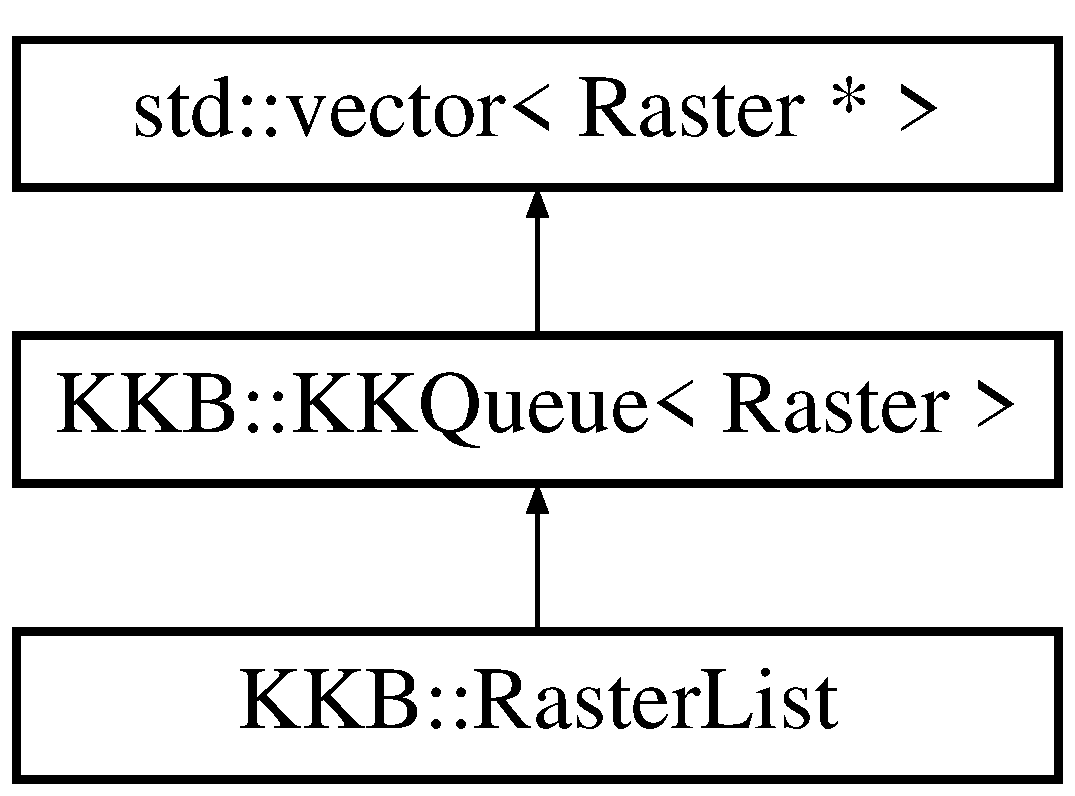
\includegraphics[height=3.000000cm]{class_k_k_b_1_1_raster_list}
\end{center}
\end{figure}
\subsection*{Public Member Functions}
\begin{DoxyCompactItemize}
\item 
\hyperlink{class_k_k_b_1_1_raster_list_a3f72041983afaa927389a17b6f02a1d8}{Raster\+List} (bool owner)
\item 
\hyperlink{class_k_k_b_1_1_raster_list_a4dbbd5f4dd147a02fff4b93502c081c5}{Raster\+List} (const \hyperlink{class_k_k_b_1_1_raster_list}{Raster\+List} \&raster\+List, bool \+\_\+owner)
\item 
\hyperlink{namespace_k_k_b_a80d46bd24db644a022c863bce8ae3633}{Raster\+Ptr} \hyperlink{class_k_k_b_1_1_raster_list_af78097714e1b932b443fccfe7f8baf56}{Create\+Smoothed\+Frame} ()
\end{DoxyCompactItemize}
\subsection*{Additional Inherited Members}


\subsection{Detailed Description}


Definition at line 1387 of file Raster.\+h.



\subsection{Constructor \& Destructor Documentation}
\index{K\+K\+B\+::\+Raster\+List@{K\+K\+B\+::\+Raster\+List}!Raster\+List@{Raster\+List}}
\index{Raster\+List@{Raster\+List}!K\+K\+B\+::\+Raster\+List@{K\+K\+B\+::\+Raster\+List}}
\subsubsection[{\texorpdfstring{Raster\+List(bool owner)}{RasterList(bool owner)}}]{\setlength{\rightskip}{0pt plus 5cm}K\+K\+B\+::\+Raster\+List\+::\+Raster\+List (
\begin{DoxyParamCaption}
\item[{bool}]{owner}
\end{DoxyParamCaption}
)\hspace{0.3cm}{\ttfamily [inline]}}\hypertarget{class_k_k_b_1_1_raster_list_a3f72041983afaa927389a17b6f02a1d8}{}\label{class_k_k_b_1_1_raster_list_a3f72041983afaa927389a17b6f02a1d8}


Definition at line 1390 of file Raster.\+h.



References Raster\+List().



Referenced by Raster\+List(), and K\+K\+B\+::\+Raster\+::\+Split\+Image\+Into\+Equal\+Parts().


\begin{DoxyCode}
1390                             :
1391         KKQueue<Raster> (owner)
1392         \{\}
\end{DoxyCode}
\index{K\+K\+B\+::\+Raster\+List@{K\+K\+B\+::\+Raster\+List}!Raster\+List@{Raster\+List}}
\index{Raster\+List@{Raster\+List}!K\+K\+B\+::\+Raster\+List@{K\+K\+B\+::\+Raster\+List}}
\subsubsection[{\texorpdfstring{Raster\+List(const Raster\+List \&raster\+List, bool \+\_\+owner)}{RasterList(const RasterList &rasterList, bool _owner)}}]{\setlength{\rightskip}{0pt plus 5cm}K\+K\+B\+::\+Raster\+List\+::\+Raster\+List (
\begin{DoxyParamCaption}
\item[{const {\bf Raster\+List} \&}]{raster\+List, }
\item[{bool}]{\+\_\+owner}
\end{DoxyParamCaption}
)\hspace{0.3cm}{\ttfamily [inline]}}\hypertarget{class_k_k_b_1_1_raster_list_a4dbbd5f4dd147a02fff4b93502c081c5}{}\label{class_k_k_b_1_1_raster_list_a4dbbd5f4dd147a02fff4b93502c081c5}


Definition at line 1400 of file Raster.\+h.



References Raster\+List().



Referenced by Raster\+List().


\begin{DoxyCode}
1402                 :
1403         KKQueue<Raster> (rasterList, \_owner)
1404         \{\}
\end{DoxyCode}


\subsection{Member Function Documentation}
\index{K\+K\+B\+::\+Raster\+List@{K\+K\+B\+::\+Raster\+List}!Create\+Smoothed\+Frame@{Create\+Smoothed\+Frame}}
\index{Create\+Smoothed\+Frame@{Create\+Smoothed\+Frame}!K\+K\+B\+::\+Raster\+List@{K\+K\+B\+::\+Raster\+List}}
\subsubsection[{\texorpdfstring{Create\+Smoothed\+Frame()}{CreateSmoothedFrame()}}]{\setlength{\rightskip}{0pt plus 5cm}{\bf Raster\+Ptr} Raster\+List\+::\+Create\+Smoothed\+Frame (
\begin{DoxyParamCaption}
{}
\end{DoxyParamCaption}
)}\hypertarget{class_k_k_b_1_1_raster_list_af78097714e1b932b443fccfe7f8baf56}{}\label{class_k_k_b_1_1_raster_list_af78097714e1b932b443fccfe7f8baf56}


Definition at line 8950 of file Raster.\+cpp.



References K\+K\+B\+::\+Raster\+::\+Allocate\+A\+Raster\+Instance(), K\+K\+B\+::\+Raster\+::\+Blue\+Area(), K\+K\+B\+::\+Raster\+::\+Color(), K\+K\+B\+::\+Raster\+::\+Green\+Area(), K\+K\+B\+::\+Raster\+::\+Height(), K\+K\+B\+::\+Raster\+::\+Red\+Area(), and K\+K\+B\+::\+Raster\+::\+Width().


\begin{DoxyCode}
8951 \{
8952   \textcolor{keywordflow}{if}  (\hyperlink{class_k_k_b_1_1_k_k_queue_a1dab601f75ee6a65d97f02bddf71c40d}{QueueSize} () < 1)
8953     \textcolor{keywordflow}{return} NULL;
8954 
8955   \hyperlink{namespace_k_k_b_a8fa4952cc84fda1de4bec1fbdd8d5b1b}{kkint32} x;
8956 
8957   \hyperlink{class_k_k_b_1_1_raster}{RasterPtr}  firstRaster = \hyperlink{class_k_k_b_1_1_k_k_queue_acce2bdd8b3327e38266cf198382cd852}{IdxToPtr} (0);
8958   \hyperlink{namespace_k_k_b_a8fa4952cc84fda1de4bec1fbdd8d5b1b}{kkint32} height = firstRaster->\hyperlink{class_k_k_b_1_1_raster_af8d10d15697d5b92fb9595c48b529feb}{Height} ();
8959   \hyperlink{namespace_k_k_b_a8fa4952cc84fda1de4bec1fbdd8d5b1b}{kkint32} width  = firstRaster->\hyperlink{class_k_k_b_1_1_raster_af8d10d15697d5b92fb9595c48b529feb}{Height} ();
8960   \hyperlink{namespace_k_k_b_a8fa4952cc84fda1de4bec1fbdd8d5b1b}{kkint32} totPixels = height * width;
8961 
8962   \hyperlink{namespace_k_k_b_af8d832f05c54994a1cce25bd5743e19a}{kkuint32}*  totGreenArea = \textcolor{keyword}{new} \hyperlink{namespace_k_k_b_af8d832f05c54994a1cce25bd5743e19a}{kkuint32}[totPixels];
8963   memset (totGreenArea, 0, totPixels * \textcolor{keyword}{sizeof} (\hyperlink{namespace_k_k_b_af8d832f05c54994a1cce25bd5743e19a}{kkuint32}));
8964 
8965   \hyperlink{namespace_k_k_b_a8fa4952cc84fda1de4bec1fbdd8d5b1b}{kkint32} idx = 0;
8966   \hyperlink{namespace_k_k_b_a8fa4952cc84fda1de4bec1fbdd8d5b1b}{kkint32} rastersAdded = 0;
8967 
8968   \textcolor{keywordflow}{for}  (idx = 0;  idx < \hyperlink{class_k_k_b_1_1_k_k_queue_a1dab601f75ee6a65d97f02bddf71c40d}{QueueSize} ();  idx++)
8969   \{
8970     \hyperlink{class_k_k_b_1_1_raster}{RasterPtr} raster = \hyperlink{class_k_k_b_1_1_k_k_queue_acce2bdd8b3327e38266cf198382cd852}{IdxToPtr} (idx);
8971     \textcolor{keywordflow}{if}  ((raster->\hyperlink{class_k_k_b_1_1_raster_af8d10d15697d5b92fb9595c48b529feb}{Height} () != height)  ||
8972          (raster->\hyperlink{class_k_k_b_1_1_raster_aa2780c0b7ae75b7b595f99329689c1f6}{Width}  () != width)
8973         )
8974     \{
8975       \textcolor{keywordflow}{continue};
8976     \}
8977 
8978     \textcolor{keywordflow}{if}  (raster->\hyperlink{class_k_k_b_1_1_raster_a644248f99009d64ac4b8fef4a22aff25}{Color} ())
8979     \{
8980       \hyperlink{namespace_k_k_b_ace9969169bf514f9ee6185186949cdf7}{uchar}*  redArea   = raster->\hyperlink{class_k_k_b_1_1_raster_aa3d0f9b4ce0fdd8ac97f996058d09b22}{RedArea} ();
8981       \hyperlink{namespace_k_k_b_ace9969169bf514f9ee6185186949cdf7}{uchar}*  greenArea = raster->\hyperlink{class_k_k_b_1_1_raster_af6ceacfa7835a295d239d141627dbec7}{GreenArea} ();
8982       \hyperlink{namespace_k_k_b_ace9969169bf514f9ee6185186949cdf7}{uchar}*  blueArea  = raster->\hyperlink{class_k_k_b_1_1_raster_ade7c77867e6b3833e96f5f86aefcffec}{BlueArea} ();
8983       \textcolor{keywordflow}{for} (x = 0;  x < totPixels;  x++)
8984       \{
8985         totGreenArea[x] += (\hyperlink{namespace_k_k_b_af8d832f05c54994a1cce25bd5743e19a}{kkuint32})((\textcolor{keywordtype}{float})redArea[x]   * 0.39f +
8986                                   (float)greenArea[x] * 0.59f +
8987                                   (\textcolor{keywordtype}{float})blueArea[x]  * 0.11f +
8988                                   0.5f
8989                                  );
8990       \}
8991     \}
8992     \textcolor{keywordflow}{else}
8993     \{
8994       \hyperlink{namespace_k_k_b_ace9969169bf514f9ee6185186949cdf7}{uchar}*  greenArea = raster->\hyperlink{class_k_k_b_1_1_raster_af6ceacfa7835a295d239d141627dbec7}{GreenArea} ();
8995       \textcolor{keywordflow}{for} (x = 0;  x < totPixels;  x++)
8996         totGreenArea[x] += greenArea[x];
8997     \}
8998 
8999     rastersAdded++;
9000   \}
9001 
9002   \hyperlink{class_k_k_b_1_1_raster}{RasterPtr}  smoothedRaster = firstRaster->\hyperlink{class_k_k_b_1_1_raster_aa879980d112c01cb7ad9a3cfc7cd6f64}{AllocateARasterInstance} (height,
       width, \textcolor{keyword}{false});
9003 
9004   \hyperlink{namespace_k_k_b_ace9969169bf514f9ee6185186949cdf7}{uchar}*  newGreenArea = smoothedRaster->\hyperlink{class_k_k_b_1_1_raster_af6ceacfa7835a295d239d141627dbec7}{GreenArea} ();
9005   \textcolor{keywordflow}{for}  (x = 0;  x < totPixels;  x++)
9006     newGreenArea[x] = (\hyperlink{namespace_k_k_b_ace9969169bf514f9ee6185186949cdf7}{uchar})  (totGreenArea[x] / rastersAdded);
9007 
9008   \textcolor{keyword}{delete}[]  totGreenArea;
9009 
9010   \textcolor{keywordflow}{return}  smoothedRaster;
9011 \}  \textcolor{comment}{/* CreateSmoothedFrame */}
\end{DoxyCode}


The documentation for this class was generated from the following files\+:\begin{DoxyCompactItemize}
\item 
C\+:/\+Users/\+Kurt/\+Git\+Hub/\+K\+Square\+Libraries/\+K\+K\+Base/\hyperlink{_raster_8h}{Raster.\+h}\item 
C\+:/\+Users/\+Kurt/\+Git\+Hub/\+K\+Square\+Libraries/\+K\+K\+Base/\hyperlink{_raster_8cpp}{Raster.\+cpp}\end{DoxyCompactItemize}

\hypertarget{class_k_k_b_1_1_r_bnode}{}\section{K\+KB\+:\+:R\+Bnode$<$ Entry $>$ Class Template Reference}
\label{class_k_k_b_1_1_r_bnode}\index{K\+K\+B\+::\+R\+Bnode$<$ Entry $>$@{K\+K\+B\+::\+R\+Bnode$<$ Entry $>$}}


{\ttfamily \#include $<$R\+B\+Tree.\+h$>$}

\subsection*{Public Member Functions}
\begin{DoxyCompactItemize}
\item 
\hyperlink{class_k_k_b_1_1_r_bnode_a8bc55760f92b921b2c73abaad482d89c}{R\+Bnode} (\hyperlink{class_k_k_b_1_1_r_bnode}{R\+Bnode\+Ptr} \+\_\+parent, \hyperlink{class_k_k_b_1_1_r_bnode}{R\+Bnode\+Ptr} \+\_\+left, \hyperlink{class_k_k_b_1_1_r_bnode}{R\+Bnode\+Ptr} \+\_\+right, \hyperlink{namespace_k_k_b_a8efe8f8963250404085241be900c7548}{R\+Bcolor} \+\_\+color, Entry\+Ptr \+\_\+entry)
\item 
\hyperlink{namespace_k_k_b_a8efe8f8963250404085241be900c7548}{R\+Bcolor} \hyperlink{class_k_k_b_1_1_r_bnode_a584eaab9411cfa40db738fb57da7c8c0}{Color} ()
\item 
void \hyperlink{class_k_k_b_1_1_r_bnode_aa36cfdeb5de0b981971bf76501c7d251}{Color} (\hyperlink{namespace_k_k_b_a8efe8f8963250404085241be900c7548}{R\+Bcolor} \+\_\+color)
\item 
Entry\+Ptr \hyperlink{class_k_k_b_1_1_r_bnode_a9d29b22149e67b0a1949dbf7e2f2c91b}{Data} ()
\item 
void \hyperlink{class_k_k_b_1_1_r_bnode_a5d90a011bb65f28f82a2b14ce6e851a8}{Data} (Entry\+Ptr \+\_\+data)
\item 
\hyperlink{class_k_k_b_1_1_r_bnode}{R\+Bnode\+Ptr} \hyperlink{class_k_k_b_1_1_r_bnode_abee0e42c1fe63794d9bbd3c1664fbb87}{Left} ()
\item 
void \hyperlink{class_k_k_b_1_1_r_bnode_a7f5f958378f8e57ba2353c70374ce1bc}{Left} (\hyperlink{class_k_k_b_1_1_r_bnode}{R\+Bnode\+Ptr} \+\_\+left)
\item 
\hyperlink{class_k_k_b_1_1_r_bnode}{R\+Bnode\+Ptr} \hyperlink{class_k_k_b_1_1_r_bnode_a2ed89e282fb54396dfdb4490d40d1b16}{Parent} ()
\item 
void \hyperlink{class_k_k_b_1_1_r_bnode_ae056624198dd5c5aa277b8485b346356}{Parent} (\hyperlink{class_k_k_b_1_1_r_bnode}{R\+Bnode\+Ptr} \+\_\+parent)
\item 
\hyperlink{class_k_k_b_1_1_r_bnode}{R\+Bnode\+Ptr} \hyperlink{class_k_k_b_1_1_r_bnode_a3dcbd419eb92e27c222343070630dc95}{Right} ()
\item 
void \hyperlink{class_k_k_b_1_1_r_bnode_ad4fa7e5524db92d9c15f59400969b063}{Right} (\hyperlink{class_k_k_b_1_1_r_bnode}{R\+Bnode\+Ptr} \+\_\+right)
\end{DoxyCompactItemize}


\subsection{Detailed Description}
\subsubsection*{template$<$class Entry$>$\\*
class K\+K\+B\+::\+R\+Bnode$<$ Entry $>$}



Definition at line 33 of file R\+B\+Tree.\+h.



\subsection{Constructor \& Destructor Documentation}
\index{K\+K\+B\+::\+R\+Bnode@{K\+K\+B\+::\+R\+Bnode}!R\+Bnode@{R\+Bnode}}
\index{R\+Bnode@{R\+Bnode}!K\+K\+B\+::\+R\+Bnode@{K\+K\+B\+::\+R\+Bnode}}
\subsubsection[{\texorpdfstring{R\+Bnode(\+R\+Bnode\+Ptr \+\_\+parent, R\+Bnode\+Ptr \+\_\+left, R\+Bnode\+Ptr \+\_\+right, R\+Bcolor \+\_\+color, Entry\+Ptr \+\_\+entry)}{RBnode(RBnodePtr _parent, RBnodePtr _left, RBnodePtr _right, RBcolor _color, EntryPtr _entry)}}]{\setlength{\rightskip}{0pt plus 5cm}template$<$class Entry $>$ {\bf K\+K\+B\+::\+R\+Bnode}$<$ Entry $>$\+::{\bf R\+Bnode} (
\begin{DoxyParamCaption}
\item[{{\bf R\+Bnode\+Ptr}}]{\+\_\+parent, }
\item[{{\bf R\+Bnode\+Ptr}}]{\+\_\+left, }
\item[{{\bf R\+Bnode\+Ptr}}]{\+\_\+right, }
\item[{{\bf R\+Bcolor}}]{\+\_\+color, }
\item[{Entry\+Ptr}]{\+\_\+entry}
\end{DoxyParamCaption}
)}\hypertarget{class_k_k_b_1_1_r_bnode_a8bc55760f92b921b2c73abaad482d89c}{}\label{class_k_k_b_1_1_r_bnode_a8bc55760f92b921b2c73abaad482d89c}


Definition at line 281 of file R\+B\+Tree.\+h.


\begin{DoxyCode}
286                             :
287      parent (\_parent),
288      left   (\_left),
289      right  (\_right),
290      entry  (\_entry),
291      color  (\_color)
292 \{\}
\end{DoxyCode}


\subsection{Member Function Documentation}
\index{K\+K\+B\+::\+R\+Bnode@{K\+K\+B\+::\+R\+Bnode}!Color@{Color}}
\index{Color@{Color}!K\+K\+B\+::\+R\+Bnode@{K\+K\+B\+::\+R\+Bnode}}
\subsubsection[{\texorpdfstring{Color()}{Color()}}]{\setlength{\rightskip}{0pt plus 5cm}template$<$class Entry $>$ {\bf R\+Bcolor} {\bf K\+K\+B\+::\+R\+Bnode}$<$ Entry $>$\+::Color (
\begin{DoxyParamCaption}
{}
\end{DoxyParamCaption}
)\hspace{0.3cm}{\ttfamily [inline]}}\hypertarget{class_k_k_b_1_1_r_bnode_a584eaab9411cfa40db738fb57da7c8c0}{}\label{class_k_k_b_1_1_r_bnode_a584eaab9411cfa40db738fb57da7c8c0}


Definition at line 47 of file R\+B\+Tree.\+h.


\begin{DoxyCode}
47 \{\textcolor{keywordflow}{return}  color;\}
\end{DoxyCode}
\index{K\+K\+B\+::\+R\+Bnode@{K\+K\+B\+::\+R\+Bnode}!Color@{Color}}
\index{Color@{Color}!K\+K\+B\+::\+R\+Bnode@{K\+K\+B\+::\+R\+Bnode}}
\subsubsection[{\texorpdfstring{Color(\+R\+Bcolor \+\_\+color)}{Color(RBcolor _color)}}]{\setlength{\rightskip}{0pt plus 5cm}template$<$class Entry $>$ void {\bf K\+K\+B\+::\+R\+Bnode}$<$ Entry $>$\+::Color (
\begin{DoxyParamCaption}
\item[{{\bf R\+Bcolor}}]{\+\_\+color}
\end{DoxyParamCaption}
)\hspace{0.3cm}{\ttfamily [inline]}}\hypertarget{class_k_k_b_1_1_r_bnode_aa36cfdeb5de0b981971bf76501c7d251}{}\label{class_k_k_b_1_1_r_bnode_aa36cfdeb5de0b981971bf76501c7d251}


Definition at line 53 of file R\+B\+Tree.\+h.


\begin{DoxyCode}
53 \{color  = \_color;\}
\end{DoxyCode}
\index{K\+K\+B\+::\+R\+Bnode@{K\+K\+B\+::\+R\+Bnode}!Data@{Data}}
\index{Data@{Data}!K\+K\+B\+::\+R\+Bnode@{K\+K\+B\+::\+R\+Bnode}}
\subsubsection[{\texorpdfstring{Data()}{Data()}}]{\setlength{\rightskip}{0pt plus 5cm}template$<$class Entry $>$ Entry\+Ptr {\bf K\+K\+B\+::\+R\+Bnode}$<$ Entry $>$\+::Data (
\begin{DoxyParamCaption}
{}
\end{DoxyParamCaption}
)\hspace{0.3cm}{\ttfamily [inline]}}\hypertarget{class_k_k_b_1_1_r_bnode_a9d29b22149e67b0a1949dbf7e2f2c91b}{}\label{class_k_k_b_1_1_r_bnode_a9d29b22149e67b0a1949dbf7e2f2c91b}


Definition at line 48 of file R\+B\+Tree.\+h.


\begin{DoxyCode}
48 \{\textcolor{keywordflow}{return}  entry;\}
\end{DoxyCode}
\index{K\+K\+B\+::\+R\+Bnode@{K\+K\+B\+::\+R\+Bnode}!Data@{Data}}
\index{Data@{Data}!K\+K\+B\+::\+R\+Bnode@{K\+K\+B\+::\+R\+Bnode}}
\subsubsection[{\texorpdfstring{Data(\+Entry\+Ptr \+\_\+data)}{Data(EntryPtr _data)}}]{\setlength{\rightskip}{0pt plus 5cm}template$<$class Entry $>$ void {\bf K\+K\+B\+::\+R\+Bnode}$<$ Entry $>$\+::Data (
\begin{DoxyParamCaption}
\item[{Entry\+Ptr}]{\+\_\+data}
\end{DoxyParamCaption}
)\hspace{0.3cm}{\ttfamily [inline]}}\hypertarget{class_k_k_b_1_1_r_bnode_a5d90a011bb65f28f82a2b14ce6e851a8}{}\label{class_k_k_b_1_1_r_bnode_a5d90a011bb65f28f82a2b14ce6e851a8}


Definition at line 54 of file R\+B\+Tree.\+h.


\begin{DoxyCode}
54 \{entry  = \_data;\}
\end{DoxyCode}
\index{K\+K\+B\+::\+R\+Bnode@{K\+K\+B\+::\+R\+Bnode}!Left@{Left}}
\index{Left@{Left}!K\+K\+B\+::\+R\+Bnode@{K\+K\+B\+::\+R\+Bnode}}
\subsubsection[{\texorpdfstring{Left()}{Left()}}]{\setlength{\rightskip}{0pt plus 5cm}template$<$class Entry $>$ {\bf R\+Bnode\+Ptr} {\bf K\+K\+B\+::\+R\+Bnode}$<$ Entry $>$\+::Left (
\begin{DoxyParamCaption}
{}
\end{DoxyParamCaption}
)\hspace{0.3cm}{\ttfamily [inline]}}\hypertarget{class_k_k_b_1_1_r_bnode_abee0e42c1fe63794d9bbd3c1664fbb87}{}\label{class_k_k_b_1_1_r_bnode_abee0e42c1fe63794d9bbd3c1664fbb87}


Definition at line 49 of file R\+B\+Tree.\+h.


\begin{DoxyCode}
49 \{\textcolor{keywordflow}{return}  left;\}
\end{DoxyCode}
\index{K\+K\+B\+::\+R\+Bnode@{K\+K\+B\+::\+R\+Bnode}!Left@{Left}}
\index{Left@{Left}!K\+K\+B\+::\+R\+Bnode@{K\+K\+B\+::\+R\+Bnode}}
\subsubsection[{\texorpdfstring{Left(\+R\+Bnode\+Ptr \+\_\+left)}{Left(RBnodePtr _left)}}]{\setlength{\rightskip}{0pt plus 5cm}template$<$class Entry $>$ void {\bf K\+K\+B\+::\+R\+Bnode}$<$ Entry $>$\+::Left (
\begin{DoxyParamCaption}
\item[{{\bf R\+Bnode\+Ptr}}]{\+\_\+left}
\end{DoxyParamCaption}
)\hspace{0.3cm}{\ttfamily [inline]}}\hypertarget{class_k_k_b_1_1_r_bnode_a7f5f958378f8e57ba2353c70374ce1bc}{}\label{class_k_k_b_1_1_r_bnode_a7f5f958378f8e57ba2353c70374ce1bc}


Definition at line 55 of file R\+B\+Tree.\+h.


\begin{DoxyCode}
55 \{left   = \_left;\}
\end{DoxyCode}
\index{K\+K\+B\+::\+R\+Bnode@{K\+K\+B\+::\+R\+Bnode}!Parent@{Parent}}
\index{Parent@{Parent}!K\+K\+B\+::\+R\+Bnode@{K\+K\+B\+::\+R\+Bnode}}
\subsubsection[{\texorpdfstring{Parent()}{Parent()}}]{\setlength{\rightskip}{0pt plus 5cm}template$<$class Entry $>$ {\bf R\+Bnode\+Ptr} {\bf K\+K\+B\+::\+R\+Bnode}$<$ Entry $>$\+::Parent (
\begin{DoxyParamCaption}
{}
\end{DoxyParamCaption}
)\hspace{0.3cm}{\ttfamily [inline]}}\hypertarget{class_k_k_b_1_1_r_bnode_a2ed89e282fb54396dfdb4490d40d1b16}{}\label{class_k_k_b_1_1_r_bnode_a2ed89e282fb54396dfdb4490d40d1b16}


Definition at line 50 of file R\+B\+Tree.\+h.


\begin{DoxyCode}
50 \{\textcolor{keywordflow}{return}  parent;\}
\end{DoxyCode}
\index{K\+K\+B\+::\+R\+Bnode@{K\+K\+B\+::\+R\+Bnode}!Parent@{Parent}}
\index{Parent@{Parent}!K\+K\+B\+::\+R\+Bnode@{K\+K\+B\+::\+R\+Bnode}}
\subsubsection[{\texorpdfstring{Parent(\+R\+Bnode\+Ptr \+\_\+parent)}{Parent(RBnodePtr _parent)}}]{\setlength{\rightskip}{0pt plus 5cm}template$<$class Entry $>$ void {\bf K\+K\+B\+::\+R\+Bnode}$<$ Entry $>$\+::Parent (
\begin{DoxyParamCaption}
\item[{{\bf R\+Bnode\+Ptr}}]{\+\_\+parent}
\end{DoxyParamCaption}
)\hspace{0.3cm}{\ttfamily [inline]}}\hypertarget{class_k_k_b_1_1_r_bnode_ae056624198dd5c5aa277b8485b346356}{}\label{class_k_k_b_1_1_r_bnode_ae056624198dd5c5aa277b8485b346356}


Definition at line 56 of file R\+B\+Tree.\+h.


\begin{DoxyCode}
56 \{parent = \_parent;\}
\end{DoxyCode}
\index{K\+K\+B\+::\+R\+Bnode@{K\+K\+B\+::\+R\+Bnode}!Right@{Right}}
\index{Right@{Right}!K\+K\+B\+::\+R\+Bnode@{K\+K\+B\+::\+R\+Bnode}}
\subsubsection[{\texorpdfstring{Right()}{Right()}}]{\setlength{\rightskip}{0pt plus 5cm}template$<$class Entry $>$ {\bf R\+Bnode\+Ptr} {\bf K\+K\+B\+::\+R\+Bnode}$<$ Entry $>$\+::Right (
\begin{DoxyParamCaption}
{}
\end{DoxyParamCaption}
)\hspace{0.3cm}{\ttfamily [inline]}}\hypertarget{class_k_k_b_1_1_r_bnode_a3dcbd419eb92e27c222343070630dc95}{}\label{class_k_k_b_1_1_r_bnode_a3dcbd419eb92e27c222343070630dc95}


Definition at line 51 of file R\+B\+Tree.\+h.


\begin{DoxyCode}
51 \{\textcolor{keywordflow}{return}  right;\}
\end{DoxyCode}
\index{K\+K\+B\+::\+R\+Bnode@{K\+K\+B\+::\+R\+Bnode}!Right@{Right}}
\index{Right@{Right}!K\+K\+B\+::\+R\+Bnode@{K\+K\+B\+::\+R\+Bnode}}
\subsubsection[{\texorpdfstring{Right(\+R\+Bnode\+Ptr \+\_\+right)}{Right(RBnodePtr _right)}}]{\setlength{\rightskip}{0pt plus 5cm}template$<$class Entry $>$ void {\bf K\+K\+B\+::\+R\+Bnode}$<$ Entry $>$\+::Right (
\begin{DoxyParamCaption}
\item[{{\bf R\+Bnode\+Ptr}}]{\+\_\+right}
\end{DoxyParamCaption}
)\hspace{0.3cm}{\ttfamily [inline]}}\hypertarget{class_k_k_b_1_1_r_bnode_ad4fa7e5524db92d9c15f59400969b063}{}\label{class_k_k_b_1_1_r_bnode_ad4fa7e5524db92d9c15f59400969b063}


Definition at line 57 of file R\+B\+Tree.\+h.


\begin{DoxyCode}
57 \{right  = \_right;\}
\end{DoxyCode}


The documentation for this class was generated from the following file\+:\begin{DoxyCompactItemize}
\item 
C\+:/\+Users/\+Kurt/\+Git\+Hub/\+K\+Square\+Libraries/\+K\+K\+Base/\hyperlink{_r_b_tree_8h}{R\+B\+Tree.\+h}\end{DoxyCompactItemize}

\hypertarget{class_k_k_b_1_1_r_b_tree}{}\section{K\+KB\+:\+:R\+B\+Tree$<$ Entry, Compare\+Nodes, Key\+Type $>$ Class Template Reference}
\label{class_k_k_b_1_1_r_b_tree}\index{K\+K\+B\+::\+R\+B\+Tree$<$ Entry, Compare\+Nodes, Key\+Type $>$@{K\+K\+B\+::\+R\+B\+Tree$<$ Entry, Compare\+Nodes, Key\+Type $>$}}


{\ttfamily \#include $<$R\+B\+Tree.\+h$>$}

\subsection*{Public Types}
\begin{DoxyCompactItemize}
\item 
typedef Entry $\ast$ \hyperlink{class_k_k_b_1_1_r_b_tree_a0e7710d8357973338c99b99034b17f33}{Entry\+Ptr}
\item 
typedef \hyperlink{class_k_k_b_1_1_iterator}{Iterator}$<$ Entry, Compare\+Nodes, Key\+Type $>$ $\ast$ \hyperlink{class_k_k_b_1_1_r_b_tree_acc78dafbc3dcd8bc3872e29679bb3ef0}{Iterator\+Ptr}
\item 
typedef \hyperlink{class_k_k_b_1_1_r_bnode}{R\+Bnode}$<$ Entry $>$ \hyperlink{class_k_k_b_1_1_r_b_tree_a06ef741f6d070fe4faebde70eec7ec6a}{Node}
\item 
typedef \hyperlink{class_k_k_b_1_1_r_b_tree_a06ef741f6d070fe4faebde70eec7ec6a}{Node} $\ast$ \hyperlink{class_k_k_b_1_1_r_b_tree_a6b0f3cc33c4554c51afe9bbb82c41906}{Node\+Ptr}
\item 
typedef \hyperlink{class_k_k_b_1_1_r_b_tree}{R\+B\+Tree}$<$ Entry, Compare\+Nodes, Key\+Type $>$ \hyperlink{class_k_k_b_1_1_r_b_tree_a4d849196b2997a6021ea34ef77901eb0}{Tree}
\item 
typedef \hyperlink{class_k_k_b_1_1_r_b_tree_a4d849196b2997a6021ea34ef77901eb0}{Tree} $\ast$ \hyperlink{class_k_k_b_1_1_r_b_tree_a657196027b6c9741e01cb4563b7bf28b}{Tree\+Ptr}
\end{DoxyCompactItemize}
\subsection*{Public Member Functions}
\begin{DoxyCompactItemize}
\item 
\hyperlink{class_k_k_b_1_1_r_b_tree_a8c31cb7a1a97513dcbe717696359be09}{R\+B\+Tree} (Compare\+Nodes \&\+\_\+comparator, bool \+\_\+owner)
\item 
\hyperlink{class_k_k_b_1_1_r_b_tree_a4eac00e8d6d4c300a912a840ff04720b}{R\+B\+Tree} (\hyperlink{class_k_k_b_1_1_r_b_tree}{R\+B\+Tree} \&tree)
\item 
\hyperlink{class_k_k_b_1_1_r_b_tree_a0d0922dcd2232caf29223e5b9c5e4174}{$\sim$\+R\+B\+Tree} ()
\item 
void \hyperlink{class_k_k_b_1_1_r_b_tree_a9cbd35932923709b3b8b9d9df8634379}{Calc\+Tree\+Stats} ()
\item 
bool \hyperlink{class_k_k_b_1_1_r_b_tree_a14b77873f1b45db066bd393e9811641d}{Compare\+To\+Tree} (\hyperlink{class_k_k_b_1_1_r_b_tree_a657196027b6c9741e01cb4563b7bf28b}{Tree\+Ptr} tree)
\item 
void \hyperlink{class_k_k_b_1_1_r_b_tree_a925c62ec939b5d7b90959a3af8b42d28}{Delete\+Current\+Node} ()
\item 
void \hyperlink{class_k_k_b_1_1_r_b_tree_ae031a4b6803af6a9a02b5218481c4f46}{Delete\+Entry} (\hyperlink{class_k_k_b_1_1_r_b_tree_a0e7710d8357973338c99b99034b17f33}{Entry\+Ptr} e)
\item 
\hyperlink{class_k_k_b_1_1_r_b_tree_a0e7710d8357973338c99b99034b17f33}{Entry\+Ptr} \hyperlink{class_k_k_b_1_1_r_b_tree_a9f157c30cce4885b8abac7f4981321e9}{Get\+Equal} (const Key\+Type \&key)
\item 
\hyperlink{class_k_k_b_1_1_r_b_tree_a0e7710d8357973338c99b99034b17f33}{Entry\+Ptr} \hyperlink{class_k_k_b_1_1_r_b_tree_a66b152371fdfc103f41a830625a04a53}{Get\+First} ()
\item 
\hyperlink{class_k_k_b_1_1_r_b_tree_a0e7710d8357973338c99b99034b17f33}{Entry\+Ptr} \hyperlink{class_k_k_b_1_1_r_b_tree_aed0e37c807c74bda44fd9ad7fe92922a}{Get\+Greater} (const Key\+Type \&key)
\item 
\hyperlink{class_k_k_b_1_1_r_b_tree_a0e7710d8357973338c99b99034b17f33}{Entry\+Ptr} \hyperlink{class_k_k_b_1_1_r_b_tree_ac9365b1ea43d7306c8231ee200758d3e}{Get\+Greater\+Or\+Equal} (const Key\+Type \&key)
\item 
\hyperlink{class_k_k_b_1_1_r_b_tree_a0e7710d8357973338c99b99034b17f33}{Entry\+Ptr} \hyperlink{class_k_k_b_1_1_r_b_tree_aea42a72543e2efeec63f717b14673ff8}{Get\+Last} ()
\item 
\hyperlink{class_k_k_b_1_1_r_b_tree_a0e7710d8357973338c99b99034b17f33}{Entry\+Ptr} \hyperlink{class_k_k_b_1_1_r_b_tree_a0e2fc0cb7fd4091c8abde407edd84351}{Get\+Less} (const Key\+Type \&key)
\item 
\hyperlink{class_k_k_b_1_1_r_b_tree_a0e7710d8357973338c99b99034b17f33}{Entry\+Ptr} \hyperlink{class_k_k_b_1_1_r_b_tree_a0d2058b081781e20e9f02cee450c6071}{Get\+Next} ()
\item 
\hyperlink{class_k_k_b_1_1_r_b_tree_a0e7710d8357973338c99b99034b17f33}{Entry\+Ptr} \hyperlink{class_k_k_b_1_1_r_b_tree_a288b6e6075de026e66848d181b6acfe7}{Get\+Prev} ()
\item 
\hyperlink{class_k_k_b_1_1_r_b_tree_a0e7710d8357973338c99b99034b17f33}{Entry\+Ptr} \hyperlink{class_k_k_b_1_1_r_b_tree_a3a5c20c3087b62c7a68a48878eb8fe82}{Predecessor} ()
\item 
\hyperlink{class_k_k_b_1_1_r_b_tree_a6b0f3cc33c4554c51afe9bbb82c41906}{Node\+Ptr} \hyperlink{class_k_k_b_1_1_r_b_tree_a210190ae61de6e1a7b15b39673e6a47d}{R\+B\+Insert} (\hyperlink{class_k_k_b_1_1_r_b_tree_a0e7710d8357973338c99b99034b17f33}{Entry\+Ptr} e)
\item 
\hyperlink{namespace_k_k_b_af8d832f05c54994a1cce25bd5743e19a}{kkuint32} \hyperlink{class_k_k_b_1_1_r_b_tree_ae859ee76df89480dae7d99ff1928d294}{Size} ()
\item 
\hyperlink{class_k_k_b_1_1_r_b_tree_a0e7710d8357973338c99b99034b17f33}{Entry\+Ptr} \hyperlink{class_k_k_b_1_1_r_b_tree_ab1d21c68ef6c6a58b0317f9986e66804}{Successor} ()
\item 
bool \hyperlink{class_k_k_b_1_1_r_b_tree_ab18dadc39bc478f028afee14fb4199a5}{Validate} ()
\item 
void \hyperlink{class_k_k_b_1_1_r_b_tree_a5ae41c47b60eda49ebd66754e863258c}{Walk\+Tree} ()
\end{DoxyCompactItemize}
\subsection*{Friends}
\begin{DoxyCompactItemize}
\item 
class \hyperlink{class_k_k_b_1_1_r_b_tree_a6acff2e7675519aa68e26d0e3328ac78}{Iterator$<$ Entry, Compare\+Nodes, Key\+Type $>$}
\end{DoxyCompactItemize}


\subsection{Detailed Description}
\subsubsection*{template$<$class Entry, class Compare\+Nodes, typename Key\+Type$>$\\*
class K\+K\+B\+::\+R\+B\+Tree$<$ Entry, Compare\+Nodes, Key\+Type $>$}



Definition at line 69 of file R\+B\+Tree.\+h.



\subsection{Member Typedef Documentation}
\index{K\+K\+B\+::\+R\+B\+Tree@{K\+K\+B\+::\+R\+B\+Tree}!Entry\+Ptr@{Entry\+Ptr}}
\index{Entry\+Ptr@{Entry\+Ptr}!K\+K\+B\+::\+R\+B\+Tree@{K\+K\+B\+::\+R\+B\+Tree}}
\subsubsection[{\texorpdfstring{Entry\+Ptr}{EntryPtr}}]{\setlength{\rightskip}{0pt plus 5cm}template$<$class Entry, class Compare\+Nodes, typename Key\+Type$>$ typedef Entry$\ast$ {\bf K\+K\+B\+::\+R\+B\+Tree}$<$ Entry, Compare\+Nodes, Key\+Type $>$\+::{\bf Entry\+Ptr}}\hypertarget{class_k_k_b_1_1_r_b_tree_a0e7710d8357973338c99b99034b17f33}{}\label{class_k_k_b_1_1_r_b_tree_a0e7710d8357973338c99b99034b17f33}


Definition at line 122 of file R\+B\+Tree.\+h.

\index{K\+K\+B\+::\+R\+B\+Tree@{K\+K\+B\+::\+R\+B\+Tree}!Iterator\+Ptr@{Iterator\+Ptr}}
\index{Iterator\+Ptr@{Iterator\+Ptr}!K\+K\+B\+::\+R\+B\+Tree@{K\+K\+B\+::\+R\+B\+Tree}}
\subsubsection[{\texorpdfstring{Iterator\+Ptr}{IteratorPtr}}]{\setlength{\rightskip}{0pt plus 5cm}template$<$class Entry, class Compare\+Nodes, typename Key\+Type$>$ typedef {\bf Iterator}$<$Entry,Compare\+Nodes,Key\+Type$>$$\ast$ {\bf K\+K\+B\+::\+R\+B\+Tree}$<$ Entry, Compare\+Nodes, Key\+Type $>$\+::{\bf Iterator\+Ptr}}\hypertarget{class_k_k_b_1_1_r_b_tree_acc78dafbc3dcd8bc3872e29679bb3ef0}{}\label{class_k_k_b_1_1_r_b_tree_acc78dafbc3dcd8bc3872e29679bb3ef0}


Definition at line 176 of file R\+B\+Tree.\+h.

\index{K\+K\+B\+::\+R\+B\+Tree@{K\+K\+B\+::\+R\+B\+Tree}!Node@{Node}}
\index{Node@{Node}!K\+K\+B\+::\+R\+B\+Tree@{K\+K\+B\+::\+R\+B\+Tree}}
\subsubsection[{\texorpdfstring{Node}{Node}}]{\setlength{\rightskip}{0pt plus 5cm}template$<$class Entry, class Compare\+Nodes, typename Key\+Type$>$ typedef {\bf R\+Bnode}$<$Entry$>$ {\bf K\+K\+B\+::\+R\+B\+Tree}$<$ Entry, Compare\+Nodes, Key\+Type $>$\+::{\bf Node}}\hypertarget{class_k_k_b_1_1_r_b_tree_a06ef741f6d070fe4faebde70eec7ec6a}{}\label{class_k_k_b_1_1_r_b_tree_a06ef741f6d070fe4faebde70eec7ec6a}


Definition at line 123 of file R\+B\+Tree.\+h.

\index{K\+K\+B\+::\+R\+B\+Tree@{K\+K\+B\+::\+R\+B\+Tree}!Node\+Ptr@{Node\+Ptr}}
\index{Node\+Ptr@{Node\+Ptr}!K\+K\+B\+::\+R\+B\+Tree@{K\+K\+B\+::\+R\+B\+Tree}}
\subsubsection[{\texorpdfstring{Node\+Ptr}{NodePtr}}]{\setlength{\rightskip}{0pt plus 5cm}template$<$class Entry, class Compare\+Nodes, typename Key\+Type$>$ typedef {\bf Node}$\ast$ {\bf K\+K\+B\+::\+R\+B\+Tree}$<$ Entry, Compare\+Nodes, Key\+Type $>$\+::{\bf Node\+Ptr}}\hypertarget{class_k_k_b_1_1_r_b_tree_a6b0f3cc33c4554c51afe9bbb82c41906}{}\label{class_k_k_b_1_1_r_b_tree_a6b0f3cc33c4554c51afe9bbb82c41906}


Definition at line 124 of file R\+B\+Tree.\+h.

\index{K\+K\+B\+::\+R\+B\+Tree@{K\+K\+B\+::\+R\+B\+Tree}!Tree@{Tree}}
\index{Tree@{Tree}!K\+K\+B\+::\+R\+B\+Tree@{K\+K\+B\+::\+R\+B\+Tree}}
\subsubsection[{\texorpdfstring{Tree}{Tree}}]{\setlength{\rightskip}{0pt plus 5cm}template$<$class Entry, class Compare\+Nodes, typename Key\+Type$>$ typedef {\bf R\+B\+Tree}$<$Entry,Compare\+Nodes,Key\+Type$>$ {\bf K\+K\+B\+::\+R\+B\+Tree}$<$ Entry, Compare\+Nodes, Key\+Type $>$\+::{\bf Tree}}\hypertarget{class_k_k_b_1_1_r_b_tree_a4d849196b2997a6021ea34ef77901eb0}{}\label{class_k_k_b_1_1_r_b_tree_a4d849196b2997a6021ea34ef77901eb0}


Definition at line 126 of file R\+B\+Tree.\+h.

\index{K\+K\+B\+::\+R\+B\+Tree@{K\+K\+B\+::\+R\+B\+Tree}!Tree\+Ptr@{Tree\+Ptr}}
\index{Tree\+Ptr@{Tree\+Ptr}!K\+K\+B\+::\+R\+B\+Tree@{K\+K\+B\+::\+R\+B\+Tree}}
\subsubsection[{\texorpdfstring{Tree\+Ptr}{TreePtr}}]{\setlength{\rightskip}{0pt plus 5cm}template$<$class Entry, class Compare\+Nodes, typename Key\+Type$>$ typedef {\bf Tree}$\ast$ {\bf K\+K\+B\+::\+R\+B\+Tree}$<$ Entry, Compare\+Nodes, Key\+Type $>$\+::{\bf Tree\+Ptr}}\hypertarget{class_k_k_b_1_1_r_b_tree_a657196027b6c9741e01cb4563b7bf28b}{}\label{class_k_k_b_1_1_r_b_tree_a657196027b6c9741e01cb4563b7bf28b}


Definition at line 128 of file R\+B\+Tree.\+h.



\subsection{Constructor \& Destructor Documentation}
\index{K\+K\+B\+::\+R\+B\+Tree@{K\+K\+B\+::\+R\+B\+Tree}!R\+B\+Tree@{R\+B\+Tree}}
\index{R\+B\+Tree@{R\+B\+Tree}!K\+K\+B\+::\+R\+B\+Tree@{K\+K\+B\+::\+R\+B\+Tree}}
\subsubsection[{\texorpdfstring{R\+B\+Tree(\+Compare\+Nodes \&\+\_\+comparator, bool \+\_\+owner)}{RBTree(CompareNodes &_comparator, bool _owner)}}]{\setlength{\rightskip}{0pt plus 5cm}template$<$class Entry , class Compare\+Nodes, typename Key\+Type $>$ {\bf K\+K\+B\+::\+R\+B\+Tree}$<$ Entry, Compare\+Nodes, Key\+Type $>$\+::{\bf R\+B\+Tree} (
\begin{DoxyParamCaption}
\item[{Compare\+Nodes \&}]{\+\_\+comparator, }
\item[{bool}]{\+\_\+owner}
\end{DoxyParamCaption}
)}\hypertarget{class_k_k_b_1_1_r_b_tree_a8c31cb7a1a97513dcbe717696359be09}{}\label{class_k_k_b_1_1_r_b_tree_a8c31cb7a1a97513dcbe717696359be09}


Definition at line 298 of file R\+B\+Tree.\+h.


\begin{DoxyCode}
300                                                  :
301    comparator    (\_comparator),
302    curNode       (NULL),
303    nil           (NULL),
304    owner         (\_owner),
305    root          (NULL),
306    size          (0),
307    numOfIterators(0),
308    iterators     (NULL)
309 \{
310   nil = \textcolor{keyword}{new} \hyperlink{class_k_k_b_1_1_r_bnode}{RBnode<Entry>} (NULL, NULL, NULL, \hyperlink{namespace_k_k_b_a8efe8f8963250404085241be900c7548ae90dfb84e30edf611e326eeb04d680de}{RBcolor::Black}, NULL);
311   root    = nil;
312   curNode = nil;
313 \}
\end{DoxyCode}
\index{K\+K\+B\+::\+R\+B\+Tree@{K\+K\+B\+::\+R\+B\+Tree}!R\+B\+Tree@{R\+B\+Tree}}
\index{R\+B\+Tree@{R\+B\+Tree}!K\+K\+B\+::\+R\+B\+Tree@{K\+K\+B\+::\+R\+B\+Tree}}
\subsubsection[{\texorpdfstring{R\+B\+Tree(\+R\+B\+Tree \&tree)}{RBTree(RBTree &tree)}}]{\setlength{\rightskip}{0pt plus 5cm}template$<$class Entry , class Compare\+Nodes, typename Key\+Type $>$ {\bf K\+K\+B\+::\+R\+B\+Tree}$<$ Entry, Compare\+Nodes, Key\+Type $>$\+::{\bf R\+B\+Tree} (
\begin{DoxyParamCaption}
\item[{{\bf R\+B\+Tree}$<$ Entry, Compare\+Nodes, Key\+Type $>$ \&}]{tree}
\end{DoxyParamCaption}
)}\hypertarget{class_k_k_b_1_1_r_b_tree_a4eac00e8d6d4c300a912a840ff04720b}{}\label{class_k_k_b_1_1_r_b_tree_a4eac00e8d6d4c300a912a840ff04720b}


Definition at line 319 of file R\+B\+Tree.\+h.


\begin{DoxyCode}
319                                                            :
320 
321    comparator    (tree.comparator),
322    size          (tree.size),
323    owner         (\textcolor{keyword}{true}),
324    root          (NULL),
325    nil           (NULL),
326    numOfIterators(0),
327    iterators     (NULL)
328 \{
329   nil = \textcolor{keyword}{new} \hyperlink{class_k_k_b_1_1_r_bnode}{RBnode<Entry>} (NULL, NULL, NULL, \hyperlink{namespace_k_k_b_a8efe8f8963250404085241be900c7548ae90dfb84e30edf611e326eeb04d680de}{Black}, NULL);
330   root = CloneSubTree (tree.root, tree.nil, nil);
331  
332   \hyperlink{namespace_k_k_b_a8fa4952cc84fda1de4bec1fbdd8d5b1b}{kkint32}  x = CountNodesInSubTree (root);
333 
334   curNode = nil;
335 \}
\end{DoxyCode}
\index{K\+K\+B\+::\+R\+B\+Tree@{K\+K\+B\+::\+R\+B\+Tree}!````~R\+B\+Tree@{$\sim$\+R\+B\+Tree}}
\index{````~R\+B\+Tree@{$\sim$\+R\+B\+Tree}!K\+K\+B\+::\+R\+B\+Tree@{K\+K\+B\+::\+R\+B\+Tree}}
\subsubsection[{\texorpdfstring{$\sim$\+R\+B\+Tree()}{~RBTree()}}]{\setlength{\rightskip}{0pt plus 5cm}template$<$class Entry , class Compare\+Nodes , typename Key\+Type $>$ {\bf K\+K\+B\+::\+R\+B\+Tree}$<$ Entry, Compare\+Nodes, Key\+Type $>$\+::$\sim${\bf R\+B\+Tree} (
\begin{DoxyParamCaption}
{}
\end{DoxyParamCaption}
)}\hypertarget{class_k_k_b_1_1_r_b_tree_a0d0922dcd2232caf29223e5b9c5e4174}{}\label{class_k_k_b_1_1_r_b_tree_a0d0922dcd2232caf29223e5b9c5e4174}


Definition at line 370 of file R\+B\+Tree.\+h.


\begin{DoxyCode}
371 \{
372   \textcolor{keywordflow}{if}  (root != nil)
373     DeleteSubTree (root);
374 
375 
376   \textcolor{keywordflow}{for}  (\hyperlink{namespace_k_k_b_a8fa4952cc84fda1de4bec1fbdd8d5b1b}{kkint32} i = 0;  i < numOfIterators;  i++)
377   \{
378      iterators[i]->TreeHasBeenDeleted ();
379   \}
380 
381   \textcolor{keyword}{delete}  nil;
382 \}
\end{DoxyCode}


\subsection{Member Function Documentation}
\index{K\+K\+B\+::\+R\+B\+Tree@{K\+K\+B\+::\+R\+B\+Tree}!Calc\+Tree\+Stats@{Calc\+Tree\+Stats}}
\index{Calc\+Tree\+Stats@{Calc\+Tree\+Stats}!K\+K\+B\+::\+R\+B\+Tree@{K\+K\+B\+::\+R\+B\+Tree}}
\subsubsection[{\texorpdfstring{Calc\+Tree\+Stats()}{CalcTreeStats()}}]{\setlength{\rightskip}{0pt plus 5cm}template$<$class Entry , class Compare\+Nodes , typename Key\+Type $>$ void {\bf K\+K\+B\+::\+R\+B\+Tree}$<$ Entry, Compare\+Nodes, Key\+Type $>$\+::Calc\+Tree\+Stats (
\begin{DoxyParamCaption}
{}
\end{DoxyParamCaption}
)}\hypertarget{class_k_k_b_1_1_r_b_tree_a9cbd35932923709b3b8b9d9df8634379}{}\label{class_k_k_b_1_1_r_b_tree_a9cbd35932923709b3b8b9d9df8634379}


Definition at line 1393 of file R\+B\+Tree.\+h.


\begin{DoxyCode}
1394 \{
1395   \hyperlink{namespace_k_k_b_a8fa4952cc84fda1de4bec1fbdd8d5b1b}{kkint32}  numOfLeafs = 0;
1396   \hyperlink{namespace_k_k_b_a8fa4952cc84fda1de4bec1fbdd8d5b1b}{kkint32}  numOfNodes = 0;
1397   \hyperlink{namespace_k_k_b_a8fa4952cc84fda1de4bec1fbdd8d5b1b}{kkint32}* leafPaths  = \textcolor{keyword}{new} \hyperlink{namespace_k_k_b_a8fa4952cc84fda1de4bec1fbdd8d5b1b}{kkint32}[size];
1398 
1399   \hyperlink{namespace_k_k_b_a8fa4952cc84fda1de4bec1fbdd8d5b1b}{kkint32}  shortestPath = \hyperlink{_usf_cas_cor_8h_a9ec306f36d50c7375e74f0d1c55a3a67}{INT\_MAX};
1400   \hyperlink{namespace_k_k_b_a8fa4952cc84fda1de4bec1fbdd8d5b1b}{kkint32}  longestPath  = INT\_MIN;
1401 
1402   CheckNodeStats (root, numOfNodes, numOfLeafs, leafPaths, shortestPath, longestPath, 0);
1403 
1404   \hyperlink{namespace_k_k_b_a8fa4952cc84fda1de4bec1fbdd8d5b1b}{kkint32}  totalLen = 0;
1405 
1406   \textcolor{keywordflow}{for}  (\hyperlink{namespace_k_k_b_a8fa4952cc84fda1de4bec1fbdd8d5b1b}{kkint32} x = 0; x < numOfLeafs; x++)
1407     totalLen += leafPaths[x];
1408 
1409   \textcolor{keywordtype}{double}  avgLen = (double)totalLen / (\textcolor{keywordtype}{double})numOfLeafs;
1410 
1411   std::cout << \hyperlink{namespace_k_k_b_ad1f50f65af6adc8fa9e6f62d007818a8}{std::endl}
1412             << \textcolor{stringliteral}{"Number of Nodes   ["} << numOfNodes   << \textcolor{stringliteral}{"]"}  << \hyperlink{namespace_k_k_b_ad1f50f65af6adc8fa9e6f62d007818a8}{std::endl}
1413             << \textcolor{stringliteral}{"Number of Leafs   ["} << numOfLeafs   << \textcolor{stringliteral}{"]"}  << \hyperlink{namespace_k_k_b_ad1f50f65af6adc8fa9e6f62d007818a8}{std::endl}
1414             << \textcolor{stringliteral}{"Shortest Path     ["} << shortestPath << \textcolor{stringliteral}{"]"}  << \hyperlink{namespace_k_k_b_ad1f50f65af6adc8fa9e6f62d007818a8}{std::endl}
1415             << \textcolor{stringliteral}{"Longest  Path     ["} << longestPath  << \textcolor{stringliteral}{"]"}  << \hyperlink{namespace_k_k_b_ad1f50f65af6adc8fa9e6f62d007818a8}{std::endl}
1416             << \textcolor{stringliteral}{"Average Length    ["} << avgLen       << \textcolor{stringliteral}{"]"}  << \hyperlink{namespace_k_k_b_ad1f50f65af6adc8fa9e6f62d007818a8}{std::endl};
1417 \}
\end{DoxyCode}
\index{K\+K\+B\+::\+R\+B\+Tree@{K\+K\+B\+::\+R\+B\+Tree}!Compare\+To\+Tree@{Compare\+To\+Tree}}
\index{Compare\+To\+Tree@{Compare\+To\+Tree}!K\+K\+B\+::\+R\+B\+Tree@{K\+K\+B\+::\+R\+B\+Tree}}
\subsubsection[{\texorpdfstring{Compare\+To\+Tree(\+Tree\+Ptr tree)}{CompareToTree(TreePtr tree)}}]{\setlength{\rightskip}{0pt plus 5cm}template$<$class Entry , class Compare\+Nodes , typename Key\+Type $>$ bool {\bf K\+K\+B\+::\+R\+B\+Tree}$<$ Entry, Compare\+Nodes, Key\+Type $>$\+::Compare\+To\+Tree (
\begin{DoxyParamCaption}
\item[{{\bf Tree\+Ptr}}]{tree}
\end{DoxyParamCaption}
)}\hypertarget{class_k_k_b_1_1_r_b_tree_a14b77873f1b45db066bd393e9811641d}{}\label{class_k_k_b_1_1_r_b_tree_a14b77873f1b45db066bd393e9811641d}


Definition at line 409 of file R\+B\+Tree.\+h.


\begin{DoxyCode}
410 \{
411  \textcolor{keywordflow}{return}  AreSubTreesTheSame (root, nil, tree->root, tree->nil);
412 \}  \textcolor{comment}{/* CompareToTree */}
\end{DoxyCode}
\index{K\+K\+B\+::\+R\+B\+Tree@{K\+K\+B\+::\+R\+B\+Tree}!Delete\+Current\+Node@{Delete\+Current\+Node}}
\index{Delete\+Current\+Node@{Delete\+Current\+Node}!K\+K\+B\+::\+R\+B\+Tree@{K\+K\+B\+::\+R\+B\+Tree}}
\subsubsection[{\texorpdfstring{Delete\+Current\+Node()}{DeleteCurrentNode()}}]{\setlength{\rightskip}{0pt plus 5cm}template$<$class Entry , class Compare\+Nodes , typename Key\+Type $>$ void {\bf K\+K\+B\+::\+R\+B\+Tree}$<$ Entry, Compare\+Nodes, Key\+Type $>$\+::Delete\+Current\+Node (
\begin{DoxyParamCaption}
{}
\end{DoxyParamCaption}
)}\hypertarget{class_k_k_b_1_1_r_b_tree_a925c62ec939b5d7b90959a3af8b42d28}{}\label{class_k_k_b_1_1_r_b_tree_a925c62ec939b5d7b90959a3af8b42d28}


Definition at line 718 of file R\+B\+Tree.\+h.


\begin{DoxyCode}
719 \{
720   \textcolor{keywordflow}{if}  ((curNode == nil)   ||  (curNode == NULL))
721   \{
722     std::cerr << \hyperlink{namespace_k_k_b_ad1f50f65af6adc8fa9e6f62d007818a8}{std::endl};
723     std::cerr << \textcolor{stringliteral}{"    *** Warning ***"}  << \hyperlink{namespace_k_k_b_ad1f50f65af6adc8fa9e6f62d007818a8}{std::endl};
724     std::cerr << \hyperlink{namespace_k_k_b_ad1f50f65af6adc8fa9e6f62d007818a8}{std::endl};
725     std::cerr << \textcolor{stringliteral}{"RBTree<Entry,CompareNodes,KeyType>::DeleteCurrentNode -  No Current Node Defined."} << 
      \hyperlink{namespace_k_k_b_ad1f50f65af6adc8fa9e6f62d007818a8}{std::endl};
726     std::cerr << \hyperlink{namespace_k_k_b_ad1f50f65af6adc8fa9e6f62d007818a8}{std::endl};
727     \textcolor{keywordflow}{return};
728   \}
729 
730 
731   \hyperlink{class_k_k_b_1_1_r_b_tree_a0e7710d8357973338c99b99034b17f33}{EntryPtr}  entry2Delete = curNode->\hyperlink{class_k_k_b_1_1_r_bnode_a9d29b22149e67b0a1949dbf7e2f2c91b}{Data} ();
732 
733   \hyperlink{class_k_k_b_1_1_r_b_tree_a6b0f3cc33c4554c51afe9bbb82c41906}{NodePtr}  node2Delete = curNode;
734 
735   curNode = \hyperlink{class_k_k_b_1_1_r_b_tree_a3a5c20c3087b62c7a68a48878eb8fe82}{Predecessor} (node2Delete);
736   \textcolor{keywordflow}{if}  ((curNode == nil)  ||  (curNode == NULL))
737     curNode = \hyperlink{class_k_k_b_1_1_r_b_tree_ab1d21c68ef6c6a58b0317f9986e66804}{Successor} (node2Delete);
738 
739 
740   \hyperlink{class_k_k_b_1_1_r_b_tree_a6b0f3cc33c4554c51afe9bbb82c41906}{NodePtr}  deletedNode = RBDelete (node2Delete);
741 
742   \textcolor{keywordflow}{if}  (deletedNode->Data () != entry2Delete)
743   \{
744     std::cerr << \hyperlink{namespace_k_k_b_ad1f50f65af6adc8fa9e6f62d007818a8}{std::endl};
745     std::cerr << \textcolor{stringliteral}{"    *** ERROR ***"}  << \hyperlink{namespace_k_k_b_ad1f50f65af6adc8fa9e6f62d007818a8}{std::endl};
746     std::cerr << \hyperlink{namespace_k_k_b_ad1f50f65af6adc8fa9e6f62d007818a8}{std::endl};
747     std::cerr << \textcolor{stringliteral}{"RBTree<Entry,CompareNodes,KeyType>::DeleteCurrentNode -  Wrong Node was Returned for
       Deletion."} << \hyperlink{namespace_k_k_b_ad1f50f65af6adc8fa9e6f62d007818a8}{std::endl};
748     std::cerr << \hyperlink{namespace_k_k_b_ad1f50f65af6adc8fa9e6f62d007818a8}{std::endl};
749   \}
750   \textcolor{keywordflow}{else}
751   \{
752     \textcolor{keywordflow}{if}  (owner)
753       \textcolor{keyword}{delete}  deletedNode->Data ();
754 
755     \textcolor{keyword}{delete}  deletedNode;
756   \}
757 \}  \textcolor{comment}{/* DeleteCurrentNode */}
\end{DoxyCode}
\index{K\+K\+B\+::\+R\+B\+Tree@{K\+K\+B\+::\+R\+B\+Tree}!Delete\+Entry@{Delete\+Entry}}
\index{Delete\+Entry@{Delete\+Entry}!K\+K\+B\+::\+R\+B\+Tree@{K\+K\+B\+::\+R\+B\+Tree}}
\subsubsection[{\texorpdfstring{Delete\+Entry(\+Entry\+Ptr e)}{DeleteEntry(EntryPtr e)}}]{\setlength{\rightskip}{0pt plus 5cm}template$<$class Entry , class Compare\+Nodes , typename Key\+Type $>$ void {\bf K\+K\+B\+::\+R\+B\+Tree}$<$ Entry, Compare\+Nodes, Key\+Type $>$\+::Delete\+Entry (
\begin{DoxyParamCaption}
\item[{{\bf Entry\+Ptr}}]{e}
\end{DoxyParamCaption}
)}\hypertarget{class_k_k_b_1_1_r_b_tree_ae031a4b6803af6a9a02b5218481c4f46}{}\label{class_k_k_b_1_1_r_b_tree_ae031a4b6803af6a9a02b5218481c4f46}


Definition at line 1382 of file R\+B\+Tree.\+h.


\begin{DoxyCode}
1383 \{
1384   \hyperlink{class_k_k_b_1_1_r_bnode}{RBnode<Entry>}* node2Delete = SearchForEntry (root, e);
1385   \textcolor{keywordflow}{if}  (node2Delete)
1386     RBDelete (node2Delete);
1387 \}  \textcolor{comment}{/* DeleteEntry */}
\end{DoxyCode}
\index{K\+K\+B\+::\+R\+B\+Tree@{K\+K\+B\+::\+R\+B\+Tree}!Get\+Equal@{Get\+Equal}}
\index{Get\+Equal@{Get\+Equal}!K\+K\+B\+::\+R\+B\+Tree@{K\+K\+B\+::\+R\+B\+Tree}}
\subsubsection[{\texorpdfstring{Get\+Equal(const Key\+Type \&key)}{GetEqual(const KeyType &key)}}]{\setlength{\rightskip}{0pt plus 5cm}template$<$class Entry , class Compare\+Nodes , typename Key\+Type$>$ Entry $\ast$ {\bf K\+K\+B\+::\+R\+B\+Tree}$<$ Entry, Compare\+Nodes, Key\+Type $>$\+::Get\+Equal (
\begin{DoxyParamCaption}
\item[{const Key\+Type \&}]{key}
\end{DoxyParamCaption}
)}\hypertarget{class_k_k_b_1_1_r_b_tree_a9f157c30cce4885b8abac7f4981321e9}{}\label{class_k_k_b_1_1_r_b_tree_a9f157c30cce4885b8abac7f4981321e9}


Definition at line 493 of file R\+B\+Tree.\+h.


\begin{DoxyCode}
494 \{
495   curNode = \hyperlink{class_k_k_b_1_1_r_b_tree_a9f157c30cce4885b8abac7f4981321e9}{GetEqual} (root, key);
496 
497   \textcolor{keywordflow}{if}  (curNode == nil)
498     \textcolor{keywordflow}{return} NULL;
499 
500   \textcolor{keywordflow}{return}  curNode->\hyperlink{class_k_k_b_1_1_r_bnode_a9d29b22149e67b0a1949dbf7e2f2c91b}{Data} ();
501 \}
\end{DoxyCode}
\index{K\+K\+B\+::\+R\+B\+Tree@{K\+K\+B\+::\+R\+B\+Tree}!Get\+First@{Get\+First}}
\index{Get\+First@{Get\+First}!K\+K\+B\+::\+R\+B\+Tree@{K\+K\+B\+::\+R\+B\+Tree}}
\subsubsection[{\texorpdfstring{Get\+First()}{GetFirst()}}]{\setlength{\rightskip}{0pt plus 5cm}template$<$class Entry , class Compare\+Nodes , typename Key\+Type $>$ Entry $\ast$ {\bf K\+K\+B\+::\+R\+B\+Tree}$<$ Entry, Compare\+Nodes, Key\+Type $>$\+::Get\+First (
\begin{DoxyParamCaption}
{}
\end{DoxyParamCaption}
)}\hypertarget{class_k_k_b_1_1_r_b_tree_a66b152371fdfc103f41a830625a04a53}{}\label{class_k_k_b_1_1_r_b_tree_a66b152371fdfc103f41a830625a04a53}


Definition at line 763 of file R\+B\+Tree.\+h.


\begin{DoxyCode}
764 \{
765   \textcolor{keywordflow}{if}  (root == nil)
766     \textcolor{keywordflow}{return} NULL;
767   
768   curNode = Minimum ();
769   \textcolor{keywordflow}{return}  curNode->\hyperlink{class_k_k_b_1_1_r_bnode_a9d29b22149e67b0a1949dbf7e2f2c91b}{Data} ();
770 \}  \textcolor{comment}{/* GetFirst () */}
\end{DoxyCode}
\index{K\+K\+B\+::\+R\+B\+Tree@{K\+K\+B\+::\+R\+B\+Tree}!Get\+Greater@{Get\+Greater}}
\index{Get\+Greater@{Get\+Greater}!K\+K\+B\+::\+R\+B\+Tree@{K\+K\+B\+::\+R\+B\+Tree}}
\subsubsection[{\texorpdfstring{Get\+Greater(const Key\+Type \&key)}{GetGreater(const KeyType &key)}}]{\setlength{\rightskip}{0pt plus 5cm}template$<$class Entry , class Compare\+Nodes , typename Key\+Type$>$ Entry $\ast$ {\bf K\+K\+B\+::\+R\+B\+Tree}$<$ Entry, Compare\+Nodes, Key\+Type $>$\+::Get\+Greater (
\begin{DoxyParamCaption}
\item[{const Key\+Type \&}]{key}
\end{DoxyParamCaption}
)}\hypertarget{class_k_k_b_1_1_r_b_tree_aed0e37c807c74bda44fd9ad7fe92922a}{}\label{class_k_k_b_1_1_r_b_tree_aed0e37c807c74bda44fd9ad7fe92922a}


Definition at line 598 of file R\+B\+Tree.\+h.


\begin{DoxyCode}
599 \{
600   curNode = \hyperlink{class_k_k_b_1_1_r_b_tree_aed0e37c807c74bda44fd9ad7fe92922a}{GetGreater} (root, key);
601   \textcolor{keywordflow}{return} curNode->\hyperlink{class_k_k_b_1_1_r_bnode_a9d29b22149e67b0a1949dbf7e2f2c91b}{Data} ();
602 \}  \textcolor{comment}{/* GetGreater */}
\end{DoxyCode}
\index{K\+K\+B\+::\+R\+B\+Tree@{K\+K\+B\+::\+R\+B\+Tree}!Get\+Greater\+Or\+Equal@{Get\+Greater\+Or\+Equal}}
\index{Get\+Greater\+Or\+Equal@{Get\+Greater\+Or\+Equal}!K\+K\+B\+::\+R\+B\+Tree@{K\+K\+B\+::\+R\+B\+Tree}}
\subsubsection[{\texorpdfstring{Get\+Greater\+Or\+Equal(const Key\+Type \&key)}{GetGreaterOrEqual(const KeyType &key)}}]{\setlength{\rightskip}{0pt plus 5cm}template$<$class Entry , class Compare\+Nodes , typename Key\+Type$>$ Entry $\ast$ {\bf K\+K\+B\+::\+R\+B\+Tree}$<$ Entry, Compare\+Nodes, Key\+Type $>$\+::Get\+Greater\+Or\+Equal (
\begin{DoxyParamCaption}
\item[{const Key\+Type \&}]{key}
\end{DoxyParamCaption}
)}\hypertarget{class_k_k_b_1_1_r_b_tree_ac9365b1ea43d7306c8231ee200758d3e}{}\label{class_k_k_b_1_1_r_b_tree_ac9365b1ea43d7306c8231ee200758d3e}


Definition at line 608 of file R\+B\+Tree.\+h.


\begin{DoxyCode}
609 \{
610   curNode = \hyperlink{class_k_k_b_1_1_r_b_tree_ac9365b1ea43d7306c8231ee200758d3e}{GetGreaterOrEqual} (root, key);
611   \textcolor{keywordflow}{return} curNode->\hyperlink{class_k_k_b_1_1_r_bnode_a9d29b22149e67b0a1949dbf7e2f2c91b}{Data} ();
612 \}  \textcolor{comment}{/* GetGreater */}
\end{DoxyCode}
\index{K\+K\+B\+::\+R\+B\+Tree@{K\+K\+B\+::\+R\+B\+Tree}!Get\+Last@{Get\+Last}}
\index{Get\+Last@{Get\+Last}!K\+K\+B\+::\+R\+B\+Tree@{K\+K\+B\+::\+R\+B\+Tree}}
\subsubsection[{\texorpdfstring{Get\+Last()}{GetLast()}}]{\setlength{\rightskip}{0pt plus 5cm}template$<$class Entry , class Compare\+Nodes , typename Key\+Type $>$ Entry $\ast$ {\bf K\+K\+B\+::\+R\+B\+Tree}$<$ Entry, Compare\+Nodes, Key\+Type $>$\+::Get\+Last (
\begin{DoxyParamCaption}
{}
\end{DoxyParamCaption}
)}\hypertarget{class_k_k_b_1_1_r_b_tree_aea42a72543e2efeec63f717b14673ff8}{}\label{class_k_k_b_1_1_r_b_tree_aea42a72543e2efeec63f717b14673ff8}


Definition at line 776 of file R\+B\+Tree.\+h.


\begin{DoxyCode}
777 \{
778   \textcolor{keywordflow}{if}  (root == nil)
779     \textcolor{keywordflow}{return} NULL;
780   
781   curNode = Maximum ();
782   \textcolor{keywordflow}{return}  curNode->\hyperlink{class_k_k_b_1_1_r_bnode_a9d29b22149e67b0a1949dbf7e2f2c91b}{Data} ();
783 \}  \textcolor{comment}{/* GetLast () */}
\end{DoxyCode}
\index{K\+K\+B\+::\+R\+B\+Tree@{K\+K\+B\+::\+R\+B\+Tree}!Get\+Less@{Get\+Less}}
\index{Get\+Less@{Get\+Less}!K\+K\+B\+::\+R\+B\+Tree@{K\+K\+B\+::\+R\+B\+Tree}}
\subsubsection[{\texorpdfstring{Get\+Less(const Key\+Type \&key)}{GetLess(const KeyType &key)}}]{\setlength{\rightskip}{0pt plus 5cm}template$<$class Entry , class Compare\+Nodes , typename Key\+Type$>$ Entry $\ast$ {\bf K\+K\+B\+::\+R\+B\+Tree}$<$ Entry, Compare\+Nodes, Key\+Type $>$\+::Get\+Less (
\begin{DoxyParamCaption}
\item[{const Key\+Type \&}]{key}
\end{DoxyParamCaption}
)}\hypertarget{class_k_k_b_1_1_r_b_tree_a0e2fc0cb7fd4091c8abde407edd84351}{}\label{class_k_k_b_1_1_r_b_tree_a0e2fc0cb7fd4091c8abde407edd84351}


Definition at line 669 of file R\+B\+Tree.\+h.


\begin{DoxyCode}
670 \{
671   curNode = \hyperlink{class_k_k_b_1_1_r_b_tree_a0e2fc0cb7fd4091c8abde407edd84351}{GetLess} (root, key);
672   \textcolor{keywordflow}{return} curNode->\hyperlink{class_k_k_b_1_1_r_bnode_a9d29b22149e67b0a1949dbf7e2f2c91b}{Data} ();
673 \}  \textcolor{comment}{/* GetGreater */}
\end{DoxyCode}
\index{K\+K\+B\+::\+R\+B\+Tree@{K\+K\+B\+::\+R\+B\+Tree}!Get\+Next@{Get\+Next}}
\index{Get\+Next@{Get\+Next}!K\+K\+B\+::\+R\+B\+Tree@{K\+K\+B\+::\+R\+B\+Tree}}
\subsubsection[{\texorpdfstring{Get\+Next()}{GetNext()}}]{\setlength{\rightskip}{0pt plus 5cm}template$<$class Entry, class Compare\+Nodes, typename Key\+Type$>$ {\bf Entry\+Ptr} {\bf K\+K\+B\+::\+R\+B\+Tree}$<$ Entry, Compare\+Nodes, Key\+Type $>$\+::Get\+Next (
\begin{DoxyParamCaption}
{}
\end{DoxyParamCaption}
)\hspace{0.3cm}{\ttfamily [inline]}}\hypertarget{class_k_k_b_1_1_r_b_tree_a0d2058b081781e20e9f02cee450c6071}{}\label{class_k_k_b_1_1_r_b_tree_a0d2058b081781e20e9f02cee450c6071}


Definition at line 164 of file R\+B\+Tree.\+h.


\begin{DoxyCode}
164 \{\textcolor{keywordflow}{return}  \hyperlink{class_k_k_b_1_1_r_b_tree_ab1d21c68ef6c6a58b0317f9986e66804}{Successor} ();\}
\end{DoxyCode}
\index{K\+K\+B\+::\+R\+B\+Tree@{K\+K\+B\+::\+R\+B\+Tree}!Get\+Prev@{Get\+Prev}}
\index{Get\+Prev@{Get\+Prev}!K\+K\+B\+::\+R\+B\+Tree@{K\+K\+B\+::\+R\+B\+Tree}}
\subsubsection[{\texorpdfstring{Get\+Prev()}{GetPrev()}}]{\setlength{\rightskip}{0pt plus 5cm}template$<$class Entry, class Compare\+Nodes, typename Key\+Type$>$ {\bf Entry\+Ptr} {\bf K\+K\+B\+::\+R\+B\+Tree}$<$ Entry, Compare\+Nodes, Key\+Type $>$\+::Get\+Prev (
\begin{DoxyParamCaption}
{}
\end{DoxyParamCaption}
)\hspace{0.3cm}{\ttfamily [inline]}}\hypertarget{class_k_k_b_1_1_r_b_tree_a288b6e6075de026e66848d181b6acfe7}{}\label{class_k_k_b_1_1_r_b_tree_a288b6e6075de026e66848d181b6acfe7}


Definition at line 166 of file R\+B\+Tree.\+h.


\begin{DoxyCode}
166 \{\textcolor{keywordflow}{return}  \hyperlink{class_k_k_b_1_1_r_b_tree_a3a5c20c3087b62c7a68a48878eb8fe82}{Predecessor} ();\}
\end{DoxyCode}
\index{K\+K\+B\+::\+R\+B\+Tree@{K\+K\+B\+::\+R\+B\+Tree}!Predecessor@{Predecessor}}
\index{Predecessor@{Predecessor}!K\+K\+B\+::\+R\+B\+Tree@{K\+K\+B\+::\+R\+B\+Tree}}
\subsubsection[{\texorpdfstring{Predecessor()}{Predecessor()}}]{\setlength{\rightskip}{0pt plus 5cm}template$<$class Entry , class Compare\+Nodes , typename Key\+Type $>$ Entry $\ast$ {\bf K\+K\+B\+::\+R\+B\+Tree}$<$ Entry, Compare\+Nodes, Key\+Type $>$\+::Predecessor (
\begin{DoxyParamCaption}
{}
\end{DoxyParamCaption}
)}\hypertarget{class_k_k_b_1_1_r_b_tree_a3a5c20c3087b62c7a68a48878eb8fe82}{}\label{class_k_k_b_1_1_r_b_tree_a3a5c20c3087b62c7a68a48878eb8fe82}


Definition at line 682 of file R\+B\+Tree.\+h.


\begin{DoxyCode}
683 \{
684   \textcolor{keywordflow}{if}  ((curNode == nil)   ||  (curNode == NULL))
685     \textcolor{keywordflow}{return} NULL;
686 
687   curNode = \hyperlink{class_k_k_b_1_1_r_b_tree_a3a5c20c3087b62c7a68a48878eb8fe82}{Predecessor} (curNode);
688 
689   \textcolor{keywordflow}{if}  ((curNode == nil)   ||  (curNode == NULL))
690     \textcolor{keywordflow}{return} NULL;
691 
692   \textcolor{keywordflow}{return}  curNode->\hyperlink{class_k_k_b_1_1_r_bnode_a9d29b22149e67b0a1949dbf7e2f2c91b}{Data} ();
693 \}  \textcolor{comment}{/* Predecessor */}
\end{DoxyCode}
\index{K\+K\+B\+::\+R\+B\+Tree@{K\+K\+B\+::\+R\+B\+Tree}!R\+B\+Insert@{R\+B\+Insert}}
\index{R\+B\+Insert@{R\+B\+Insert}!K\+K\+B\+::\+R\+B\+Tree@{K\+K\+B\+::\+R\+B\+Tree}}
\subsubsection[{\texorpdfstring{R\+B\+Insert(\+Entry\+Ptr e)}{RBInsert(EntryPtr e)}}]{\setlength{\rightskip}{0pt plus 5cm}template$<$class Entry , class Compare\+Nodes , typename Key\+Type $>$ {\bf K\+K\+B\+::\+R\+Bnode}$<$ Entry $>$ $\ast$ {\bf K\+K\+B\+::\+R\+B\+Tree}$<$ Entry, Compare\+Nodes, Key\+Type $>$\+::R\+B\+Insert (
\begin{DoxyParamCaption}
\item[{{\bf Entry\+Ptr}}]{e}
\end{DoxyParamCaption}
)}\hypertarget{class_k_k_b_1_1_r_b_tree_a210190ae61de6e1a7b15b39673e6a47d}{}\label{class_k_k_b_1_1_r_b_tree_a210190ae61de6e1a7b15b39673e6a47d}


Definition at line 1111 of file R\+B\+Tree.\+h.


\begin{DoxyCode}
1112 \{
1113   \hyperlink{class_k_k_b_1_1_r_b_tree_a6b0f3cc33c4554c51afe9bbb82c41906}{NodePtr}  newNode = Insert (e);
1114 
1115   \hyperlink{class_k_k_b_1_1_r_b_tree_a6b0f3cc33c4554c51afe9bbb82c41906}{NodePtr}  x = newNode;
1116 
1117   \hyperlink{class_k_k_b_1_1_r_b_tree_a6b0f3cc33c4554c51afe9bbb82c41906}{NodePtr}  y = NULL;
1118 
1119   x->\hyperlink{class_k_k_b_1_1_r_bnode_a584eaab9411cfa40db738fb57da7c8c0}{Color} (\hyperlink{namespace_k_k_b_a8efe8f8963250404085241be900c7548aee38e4d5dd68c4e440825018d549cb47}{RBcolor::Red});
1120 
1121   \textcolor{keywordflow}{while}  ((x != root)  &&  (x->Parent ()->Color () == \hyperlink{namespace_k_k_b_a8efe8f8963250404085241be900c7548aee38e4d5dd68c4e440825018d549cb47}{RBcolor::Red}))
1122   \{
1123     \textcolor{keywordflow}{if}  (x->Parent () == x->Parent ()->Parent ()->Left ())
1124     \{
1125       y = x->Parent ()->Parent ()->Right ();
1126 
1127       \textcolor{keywordflow}{if}  (y->Color () == \hyperlink{namespace_k_k_b_a8efe8f8963250404085241be900c7548aee38e4d5dd68c4e440825018d549cb47}{RBcolor::Red})
1128       \{
1129         x->Parent ()->Color (\hyperlink{namespace_k_k_b_a8efe8f8963250404085241be900c7548ae90dfb84e30edf611e326eeb04d680de}{RBcolor::Black});          \textcolor{comment}{// Case 1}
1130         y->Color (\hyperlink{namespace_k_k_b_a8efe8f8963250404085241be900c7548ae90dfb84e30edf611e326eeb04d680de}{RBcolor::Black});                     \textcolor{comment}{// Case 1}
1131         x->Parent ()->Parent ()->Color (\hyperlink{namespace_k_k_b_a8efe8f8963250404085241be900c7548aee38e4d5dd68c4e440825018d549cb47}{RBcolor::Red}); \textcolor{comment}{// Case 1}
1132         x = x->Parent ()->Parent ();                   \textcolor{comment}{// Case 1}
1133       \}
1134 
1135       \textcolor{keywordflow}{else}
1136       \{
1137         \textcolor{keywordflow}{if}  (x == x->Parent ()->Right ())
1138         \{        
1139           x = x->Parent ();                       \textcolor{comment}{// Case 2}
1140           LeftRotate (x);                         \textcolor{comment}{// Case 2}
1141         \}
1142 
1143         x->Parent ()->Color (\hyperlink{namespace_k_k_b_a8efe8f8963250404085241be900c7548ae90dfb84e30edf611e326eeb04d680de}{RBcolor::Black});          \textcolor{comment}{// Case 3}
1144         x->Parent ()->Parent ()->Color (\hyperlink{namespace_k_k_b_a8efe8f8963250404085241be900c7548aee38e4d5dd68c4e440825018d549cb47}{RBcolor::Red}); \textcolor{comment}{// Case 3}
1145         RightRotate (x->Parent ()->Parent ());         \textcolor{comment}{// Case 3}
1146       \}
1147     \}
1148 
1149     \textcolor{keywordflow}{else}
1150     \{
1151       y = x->\hyperlink{class_k_k_b_1_1_r_bnode_a2ed89e282fb54396dfdb4490d40d1b16}{Parent} ()->\hyperlink{class_k_k_b_1_1_r_bnode_a2ed89e282fb54396dfdb4490d40d1b16}{Parent} ()->\hyperlink{class_k_k_b_1_1_r_bnode_abee0e42c1fe63794d9bbd3c1664fbb87}{Left} ();
1152 
1153       \textcolor{keywordflow}{if}  (y->Color () == \hyperlink{namespace_k_k_b_a8efe8f8963250404085241be900c7548aee38e4d5dd68c4e440825018d549cb47}{RBcolor::Red})
1154       \{
1155         x->\hyperlink{class_k_k_b_1_1_r_bnode_a2ed89e282fb54396dfdb4490d40d1b16}{Parent} ()->\hyperlink{class_k_k_b_1_1_r_bnode_a584eaab9411cfa40db738fb57da7c8c0}{Color} (\hyperlink{namespace_k_k_b_a8efe8f8963250404085241be900c7548ae90dfb84e30edf611e326eeb04d680de}{RBcolor::Black});
1156         y->Color (\hyperlink{namespace_k_k_b_a8efe8f8963250404085241be900c7548ae90dfb84e30edf611e326eeb04d680de}{RBcolor::Black});
1157         x->Parent ()->Parent ()->Color (\hyperlink{namespace_k_k_b_a8efe8f8963250404085241be900c7548aee38e4d5dd68c4e440825018d549cb47}{RBcolor::Red});
1158         x = x->Parent ()->Parent ();
1159       \}
1160 
1161       \textcolor{keywordflow}{else}
1162       \{
1163         \textcolor{keywordflow}{if}  (x == x->Parent ()->Left ())
1164         \{
1165           x = x->Parent ();
1166           RightRotate (x);
1167         \}
1168 
1169         x->Parent ()->Color (\hyperlink{namespace_k_k_b_a8efe8f8963250404085241be900c7548ae90dfb84e30edf611e326eeb04d680de}{RBcolor::Black});
1170         x->Parent ()->Parent ()->Color (\hyperlink{namespace_k_k_b_a8efe8f8963250404085241be900c7548aee38e4d5dd68c4e440825018d549cb47}{RBcolor::Red});
1171         LeftRotate (x->Parent ()->Parent ());
1172       \}
1173     \}
1174   \}
1175 
1176 
1177   root->\hyperlink{class_k_k_b_1_1_r_bnode_a584eaab9411cfa40db738fb57da7c8c0}{Color} (\hyperlink{namespace_k_k_b_a8efe8f8963250404085241be900c7548ae90dfb84e30edf611e326eeb04d680de}{RBcolor::Black});
1178   \textcolor{keywordflow}{return}  newNode;
1179 \}  \textcolor{comment}{/* RBInsert */}
\end{DoxyCode}
\index{K\+K\+B\+::\+R\+B\+Tree@{K\+K\+B\+::\+R\+B\+Tree}!Size@{Size}}
\index{Size@{Size}!K\+K\+B\+::\+R\+B\+Tree@{K\+K\+B\+::\+R\+B\+Tree}}
\subsubsection[{\texorpdfstring{Size()}{Size()}}]{\setlength{\rightskip}{0pt plus 5cm}template$<$class Entry, class Compare\+Nodes, typename Key\+Type$>$ {\bf kkuint32} {\bf K\+K\+B\+::\+R\+B\+Tree}$<$ Entry, Compare\+Nodes, Key\+Type $>$\+::Size (
\begin{DoxyParamCaption}
{}
\end{DoxyParamCaption}
)\hspace{0.3cm}{\ttfamily [inline]}}\hypertarget{class_k_k_b_1_1_r_b_tree_ae859ee76df89480dae7d99ff1928d294}{}\label{class_k_k_b_1_1_r_b_tree_ae859ee76df89480dae7d99ff1928d294}


Definition at line 140 of file R\+B\+Tree.\+h.


\begin{DoxyCode}
140 \{\textcolor{keywordflow}{return}  size;\}
\end{DoxyCode}
\index{K\+K\+B\+::\+R\+B\+Tree@{K\+K\+B\+::\+R\+B\+Tree}!Successor@{Successor}}
\index{Successor@{Successor}!K\+K\+B\+::\+R\+B\+Tree@{K\+K\+B\+::\+R\+B\+Tree}}
\subsubsection[{\texorpdfstring{Successor()}{Successor()}}]{\setlength{\rightskip}{0pt plus 5cm}template$<$class Entry , class Compare\+Nodes , typename Key\+Type $>$ Entry $\ast$ {\bf K\+K\+B\+::\+R\+B\+Tree}$<$ Entry, Compare\+Nodes, Key\+Type $>$\+::Successor (
\begin{DoxyParamCaption}
{}
\end{DoxyParamCaption}
)}\hypertarget{class_k_k_b_1_1_r_b_tree_ab1d21c68ef6c6a58b0317f9986e66804}{}\label{class_k_k_b_1_1_r_b_tree_ab1d21c68ef6c6a58b0317f9986e66804}


Definition at line 700 of file R\+B\+Tree.\+h.


\begin{DoxyCode}
701 \{
702   \textcolor{keywordflow}{if}  ((curNode == nil)   ||  (curNode == NULL))
703     \textcolor{keywordflow}{return} NULL;
704 
705   curNode = \hyperlink{class_k_k_b_1_1_r_b_tree_ab1d21c68ef6c6a58b0317f9986e66804}{Successor} (curNode);
706 
707   \textcolor{keywordflow}{if}  ((curNode == nil)   ||  (curNode == NULL))
708     \textcolor{keywordflow}{return} NULL;
709 
710   \textcolor{keywordflow}{return}  curNode->\hyperlink{class_k_k_b_1_1_r_bnode_a9d29b22149e67b0a1949dbf7e2f2c91b}{Data} ();
711 \}  \textcolor{comment}{/* Successor */}
\end{DoxyCode}
\index{K\+K\+B\+::\+R\+B\+Tree@{K\+K\+B\+::\+R\+B\+Tree}!Validate@{Validate}}
\index{Validate@{Validate}!K\+K\+B\+::\+R\+B\+Tree@{K\+K\+B\+::\+R\+B\+Tree}}
\subsubsection[{\texorpdfstring{Validate()}{Validate()}}]{\setlength{\rightskip}{0pt plus 5cm}template$<$class Entry , class Compare\+Nodes , typename Key\+Type $>$ bool {\bf K\+K\+B\+::\+R\+B\+Tree}$<$ Entry, Compare\+Nodes, Key\+Type $>$\+::Validate (
\begin{DoxyParamCaption}
{}
\end{DoxyParamCaption}
)}\hypertarget{class_k_k_b_1_1_r_b_tree_ab18dadc39bc478f028afee14fb4199a5}{}\label{class_k_k_b_1_1_r_b_tree_ab18dadc39bc478f028afee14fb4199a5}


Definition at line 1483 of file R\+B\+Tree.\+h.


\begin{DoxyCode}
1484 \{
1485   \hyperlink{namespace_k_k_b_a8fa4952cc84fda1de4bec1fbdd8d5b1b}{kkint32}  blackNodeHeight = -1;
1486 
1487   \hyperlink{namespace_k_k_b_a8fa4952cc84fda1de4bec1fbdd8d5b1b}{kkint32}  numOfNodes = ValidateSubTree (root, nil, \textcolor{stringliteral}{"Root"}, 0, blackNodeHeight);
1488 
1489   \textcolor{keywordflow}{if}  (numOfNodes != size)
1490   \{
1491     std::cerr << \hyperlink{namespace_k_k_b_ad1f50f65af6adc8fa9e6f62d007818a8}{std::endl}
1492               << \textcolor{stringliteral}{"*** ERROR *** NumOfNodes["} << numOfNodes << \textcolor{stringliteral}{"] Does not add up to size["} << size << \textcolor{stringliteral}{"]."} 
      << \hyperlink{namespace_k_k_b_ad1f50f65af6adc8fa9e6f62d007818a8}{std::endl};
1493     \textcolor{keywordflow}{return}  \textcolor{keyword}{false};
1494   \}
1495 
1496   \textcolor{keywordflow}{return} \textcolor{keyword}{true};
1497 \}
\end{DoxyCode}
\index{K\+K\+B\+::\+R\+B\+Tree@{K\+K\+B\+::\+R\+B\+Tree}!Walk\+Tree@{Walk\+Tree}}
\index{Walk\+Tree@{Walk\+Tree}!K\+K\+B\+::\+R\+B\+Tree@{K\+K\+B\+::\+R\+B\+Tree}}
\subsubsection[{\texorpdfstring{Walk\+Tree()}{WalkTree()}}]{\setlength{\rightskip}{0pt plus 5cm}template$<$class Entry, class Compare\+Nodes, typename Key\+Type$>$ void {\bf K\+K\+B\+::\+R\+B\+Tree}$<$ Entry, Compare\+Nodes, Key\+Type $>$\+::Walk\+Tree (
\begin{DoxyParamCaption}
{}
\end{DoxyParamCaption}
)\hspace{0.3cm}{\ttfamily [inline]}}\hypertarget{class_k_k_b_1_1_r_b_tree_a5ae41c47b60eda49ebd66754e863258c}{}\label{class_k_k_b_1_1_r_b_tree_a5ae41c47b60eda49ebd66754e863258c}


Definition at line 142 of file R\+B\+Tree.\+h.


\begin{DoxyCode}
142 \{\hyperlink{class_k_k_b_1_1_r_b_tree_a5ae41c47b60eda49ebd66754e863258c}{WalkTree} (root);\}
\end{DoxyCode}


\subsection{Friends And Related Function Documentation}
\index{K\+K\+B\+::\+R\+B\+Tree@{K\+K\+B\+::\+R\+B\+Tree}!Iterator$<$ Entry, Compare\+Nodes, Key\+Type $>$@{Iterator$<$ Entry, Compare\+Nodes, Key\+Type $>$}}
\index{Iterator$<$ Entry, Compare\+Nodes, Key\+Type $>$@{Iterator$<$ Entry, Compare\+Nodes, Key\+Type $>$}!K\+K\+B\+::\+R\+B\+Tree@{K\+K\+B\+::\+R\+B\+Tree}}
\subsubsection[{\texorpdfstring{Iterator$<$ Entry, Compare\+Nodes, Key\+Type $>$}{Iterator< Entry, CompareNodes, KeyType >}}]{\setlength{\rightskip}{0pt plus 5cm}template$<$class Entry, class Compare\+Nodes, typename Key\+Type$>$ friend class {\bf Iterator}$<$ Entry, Compare\+Nodes, Key\+Type $>$\hspace{0.3cm}{\ttfamily [friend]}}\hypertarget{class_k_k_b_1_1_r_b_tree_a6acff2e7675519aa68e26d0e3328ac78}{}\label{class_k_k_b_1_1_r_b_tree_a6acff2e7675519aa68e26d0e3328ac78}


Definition at line 130 of file R\+B\+Tree.\+h.



The documentation for this class was generated from the following file\+:\begin{DoxyCompactItemize}
\item 
C\+:/\+Users/\+Kurt/\+Git\+Hub/\+K\+Square\+Libraries/\+K\+K\+Base/\hyperlink{_r_b_tree_8h}{R\+B\+Tree.\+h}\end{DoxyCompactItemize}

\hypertarget{class_k_k_b_1_1_row}{}\section{K\+KB\+:\+:Row Class Reference}
\label{class_k_k_b_1_1_row}\index{K\+K\+B\+::\+Row@{K\+K\+B\+::\+Row}}


{\ttfamily \#include $<$Matrix.\+h$>$}

\subsection*{Public Member Functions}
\begin{DoxyCompactItemize}
\item 
\hyperlink{class_k_k_b_1_1_row_a5cca50abc389396e26ec68cbd3fb6596}{Row} ()
\item 
\hyperlink{class_k_k_b_1_1_row_a4e40e9d21c650688d49b7abe9e16f723}{Row} (\hyperlink{namespace_k_k_b_a8fa4952cc84fda1de4bec1fbdd8d5b1b}{kkint32} \+\_\+num\+Of\+Cols, double $\ast$\+\_\+cells)
\item 
\hyperlink{class_k_k_b_1_1_row_a202c03cb0308b8db81690adec89afb92}{Row} (const \hyperlink{class_k_k_b_1_1_row}{Row} \&\+\_\+row)
\item 
\hyperlink{class_k_k_b_1_1_row_a8cc0869c91dc94ee595069309ba15690}{$\sim$\+Row} ()
\item 
double $\ast$ \hyperlink{class_k_k_b_1_1_row_a8a38915fb0f08e6ec02cbc29ed134049}{Cols} ()
\item 
void \hyperlink{class_k_k_b_1_1_row_ae6417fe28dbc6532f63b027c9ec4419a}{Define} (\hyperlink{namespace_k_k_b_a8fa4952cc84fda1de4bec1fbdd8d5b1b}{kkint32} \+\_\+num\+Of\+Cols, double $\ast$\+\_\+cells)
\item 
double \& \hyperlink{class_k_k_b_1_1_row_a7f8b72738992682713cb1f232ac94da3}{operator\mbox{[}$\,$\mbox{]}} (\hyperlink{namespace_k_k_b_a8fa4952cc84fda1de4bec1fbdd8d5b1b}{kkint32} idx)
\end{DoxyCompactItemize}


\subsection{Detailed Description}


Definition at line 183 of file Matrix.\+h.



\subsection{Constructor \& Destructor Documentation}
\index{K\+K\+B\+::\+Row@{K\+K\+B\+::\+Row}!Row@{Row}}
\index{Row@{Row}!K\+K\+B\+::\+Row@{K\+K\+B\+::\+Row}}
\subsubsection[{\texorpdfstring{Row()}{Row()}}]{\setlength{\rightskip}{0pt plus 5cm}Row\+::\+Row (
\begin{DoxyParamCaption}
{}
\end{DoxyParamCaption}
)}\hypertarget{class_k_k_b_1_1_row_a5cca50abc389396e26ec68cbd3fb6596}{}\label{class_k_k_b_1_1_row_a5cca50abc389396e26ec68cbd3fb6596}


Definition at line 26 of file Matrix.\+cpp.


\begin{DoxyCode}
26           :
27   cells     (NULL),
28   numOfCols (-1)
29 \{
30 \}
\end{DoxyCode}
\index{K\+K\+B\+::\+Row@{K\+K\+B\+::\+Row}!Row@{Row}}
\index{Row@{Row}!K\+K\+B\+::\+Row@{K\+K\+B\+::\+Row}}
\subsubsection[{\texorpdfstring{Row(kkint32 \+\_\+num\+Of\+Cols, double $\ast$\+\_\+cells)}{Row(kkint32 _numOfCols, double *_cells)}}]{\setlength{\rightskip}{0pt plus 5cm}Row\+::\+Row (
\begin{DoxyParamCaption}
\item[{{\bf kkint32}}]{\+\_\+num\+Of\+Cols, }
\item[{double $\ast$}]{\+\_\+cells}
\end{DoxyParamCaption}
)}\hypertarget{class_k_k_b_1_1_row_a4e40e9d21c650688d49b7abe9e16f723}{}\label{class_k_k_b_1_1_row_a4e40e9d21c650688d49b7abe9e16f723}


Definition at line 34 of file Matrix.\+cpp.



References K\+K\+B\+::\+K\+K\+Str\+::\+Concat(), and K\+K\+B\+::\+K\+K\+Exception\+::\+K\+K\+Exception().


\begin{DoxyCode}
36            :
37   cells     (\_cells),
38   numOfCols (\_numOfCols)
39 \{
40   \textcolor{keywordflow}{if}  (\_numOfCols < 0)
41   \{
42     \hyperlink{class_k_k_b_1_1_k_k_str}{KKStr}  msg;
43     msg << \textcolor{stringliteral}{"Row::Row  **** ERROR **** Invalid Dimension["} << \_numOfCols << \textcolor{stringliteral}{"]."};
44     cerr << \hyperlink{namespace_k_k_b_ad1f50f65af6adc8fa9e6f62d007818a8}{std::endl}  << msg << \hyperlink{namespace_k_k_b_ad1f50f65af6adc8fa9e6f62d007818a8}{std::endl} << \hyperlink{namespace_k_k_b_ad1f50f65af6adc8fa9e6f62d007818a8}{std::endl};
45     \textcolor{keywordflow}{throw} \hyperlink{class_k_k_b_1_1_k_k_exception}{KKException} (msg);
46   \}
47 \}
\end{DoxyCode}
\index{K\+K\+B\+::\+Row@{K\+K\+B\+::\+Row}!Row@{Row}}
\index{Row@{Row}!K\+K\+B\+::\+Row@{K\+K\+B\+::\+Row}}
\subsubsection[{\texorpdfstring{Row(const Row \&\+\_\+row)}{Row(const Row &_row)}}]{\setlength{\rightskip}{0pt plus 5cm}Row\+::\+Row (
\begin{DoxyParamCaption}
\item[{const {\bf Row} \&}]{\+\_\+row}
\end{DoxyParamCaption}
)}\hypertarget{class_k_k_b_1_1_row_a202c03cb0308b8db81690adec89afb92}{}\label{class_k_k_b_1_1_row_a202c03cb0308b8db81690adec89afb92}


Definition at line 51 of file Matrix.\+cpp.


\begin{DoxyCode}
51                          :
52   cells     (\_row.cells),
53   numOfCols (\_row.numOfCols)
54 \{
55 \}
\end{DoxyCode}
\index{K\+K\+B\+::\+Row@{K\+K\+B\+::\+Row}!````~Row@{$\sim$\+Row}}
\index{````~Row@{$\sim$\+Row}!K\+K\+B\+::\+Row@{K\+K\+B\+::\+Row}}
\subsubsection[{\texorpdfstring{$\sim$\+Row()}{~Row()}}]{\setlength{\rightskip}{0pt plus 5cm}Row\+::$\sim$\+Row (
\begin{DoxyParamCaption}
{}
\end{DoxyParamCaption}
)}\hypertarget{class_k_k_b_1_1_row_a8cc0869c91dc94ee595069309ba15690}{}\label{class_k_k_b_1_1_row_a8cc0869c91dc94ee595069309ba15690}


Definition at line 59 of file Matrix.\+cpp.


\begin{DoxyCode}
60 \{
61   cells = NULL;
62 \}
\end{DoxyCode}


\subsection{Member Function Documentation}
\index{K\+K\+B\+::\+Row@{K\+K\+B\+::\+Row}!Cols@{Cols}}
\index{Cols@{Cols}!K\+K\+B\+::\+Row@{K\+K\+B\+::\+Row}}
\subsubsection[{\texorpdfstring{Cols()}{Cols()}}]{\setlength{\rightskip}{0pt plus 5cm}double$\ast$ K\+K\+B\+::\+Row\+::\+Cols (
\begin{DoxyParamCaption}
{}
\end{DoxyParamCaption}
)\hspace{0.3cm}{\ttfamily [inline]}}\hypertarget{class_k_k_b_1_1_row_a8a38915fb0f08e6ec02cbc29ed134049}{}\label{class_k_k_b_1_1_row_a8a38915fb0f08e6ec02cbc29ed134049}


Definition at line 197 of file Matrix.\+h.


\begin{DoxyCode}
197 \{\textcolor{keywordflow}{return} cells;\}
\end{DoxyCode}
\index{K\+K\+B\+::\+Row@{K\+K\+B\+::\+Row}!Define@{Define}}
\index{Define@{Define}!K\+K\+B\+::\+Row@{K\+K\+B\+::\+Row}}
\subsubsection[{\texorpdfstring{Define(kkint32 \+\_\+num\+Of\+Cols, double $\ast$\+\_\+cells)}{Define(kkint32 _numOfCols, double *_cells)}}]{\setlength{\rightskip}{0pt plus 5cm}void Row\+::\+Define (
\begin{DoxyParamCaption}
\item[{{\bf kkint32}}]{\+\_\+num\+Of\+Cols, }
\item[{double $\ast$}]{\+\_\+cells}
\end{DoxyParamCaption}
)}\hypertarget{class_k_k_b_1_1_row_ae6417fe28dbc6532f63b027c9ec4419a}{}\label{class_k_k_b_1_1_row_ae6417fe28dbc6532f63b027c9ec4419a}


Definition at line 66 of file Matrix.\+cpp.


\begin{DoxyCode}
69 \{
70   numOfCols = \_numOfCols;
71   cells     = \_cells;
72 \}
\end{DoxyCode}
\index{K\+K\+B\+::\+Row@{K\+K\+B\+::\+Row}!operator\mbox{[}$\,$\mbox{]}@{operator[]}}
\index{operator\mbox{[}$\,$\mbox{]}@{operator[]}!K\+K\+B\+::\+Row@{K\+K\+B\+::\+Row}}
\subsubsection[{\texorpdfstring{operator[](kkint32 idx)}{operator[](kkint32 idx)}}]{\setlength{\rightskip}{0pt plus 5cm}double \& Row\+::operator\mbox{[}$\,$\mbox{]} (
\begin{DoxyParamCaption}
\item[{{\bf kkint32}}]{idx}
\end{DoxyParamCaption}
)}\hypertarget{class_k_k_b_1_1_row_a7f8b72738992682713cb1f232ac94da3}{}\label{class_k_k_b_1_1_row_a7f8b72738992682713cb1f232ac94da3}


Definition at line 76 of file Matrix.\+cpp.



References K\+K\+B\+::os\+Wait\+For\+Enter().



Referenced by K\+K\+B\+::\+Raster\+::\+Build\+Gaussian2d\+Kernel(), K\+K\+B\+::\+Matrix\+::\+Calc\+Co\+Factor\+Matrix(), K\+K\+B\+::\+Matrix\+::\+Covariance(), K\+K\+B\+::\+Raster\+::\+Create\+Gray\+Scale\+K\+L\+T(), K\+K\+B\+::\+Raster\+::\+Create\+Gray\+Scale\+K\+L\+T\+On\+Masked\+Area(), K\+K\+M\+L\+L\+::\+Classification\+Bias\+Matrix\+::\+Perform\+Adjustmnts(), and K\+K\+M\+L\+L\+::\+Classification\+Bias\+Matrix\+::\+Print\+Bias\+Matrix().


\begin{DoxyCode}
77 \{
78   \textcolor{keywordflow}{if}  ((idx < 0)  ||  (idx >= numOfCols))
79   \{
80     cerr << \hyperlink{namespace_k_k_b_ad1f50f65af6adc8fa9e6f62d007818a8}{std::endl}
81          << \textcolor{stringliteral}{"Row::operator[]  **** ERROR ****,  Index["} 
82          << idx << \textcolor{stringliteral}{"]  out of range of [0-"} << numOfCols << \textcolor{stringliteral}{"]."}
83          << \hyperlink{namespace_k_k_b_ad1f50f65af6adc8fa9e6f62d007818a8}{std::endl};
84     \hyperlink{namespace_k_k_b_a255aa69aade7f429585349d08973e09f}{osWaitForEnter} ();
85     exit (1);
86   \}
87 
88   \textcolor{keywordflow}{return}  cells[idx];
89 \}  \textcolor{comment}{/*  Row::operator[] */}
\end{DoxyCode}


The documentation for this class was generated from the following files\+:\begin{DoxyCompactItemize}
\item 
C\+:/\+Users/\+Kurt/\+Git\+Hub/\+K\+Square\+Libraries/\+K\+K\+Base/\hyperlink{_matrix_8h}{Matrix.\+h}\item 
C\+:/\+Users/\+Kurt/\+Git\+Hub/\+K\+Square\+Libraries/\+K\+K\+Base/\hyperlink{_matrix_8cpp}{Matrix.\+cpp}\end{DoxyCompactItemize}

\hypertarget{class_k_k_b_1_1_run_log}{}\section{K\+KB\+:\+:Run\+Log Class Reference}
\label{class_k_k_b_1_1_run_log}\index{K\+K\+B\+::\+Run\+Log@{K\+K\+B\+::\+Run\+Log}}


Used for logging messages.  




{\ttfamily \#include $<$Run\+Log.\+h$>$}

\subsection*{Public Member Functions}
\begin{DoxyCompactItemize}
\item 
\hyperlink{class_k_k_b_1_1_run_log_aab85112fa394b9593c8db1c707993abd}{Run\+Log} ()
\begin{DoxyCompactList}\small\item\em Creates an instance were logging will go to the console. \end{DoxyCompactList}\item 
\hyperlink{class_k_k_b_1_1_run_log_abe78ec05ce09dd8444ae4554e7f3ae58}{Run\+Log} (const char $\ast$\+\_\+file\+Name)
\begin{DoxyCompactList}\small\item\em Creates instance with a log messages written to file \textquotesingle{}file\+Name\textquotesingle{}. \end{DoxyCompactList}\item 
\hyperlink{class_k_k_b_1_1_run_log_a53e496503fe2cad241233334373c1295}{Run\+Log} (const \hyperlink{class_k_k_b_1_1_k_k_str}{K\+K\+Str} \&\+\_\+file\+Name)
\begin{DoxyCompactList}\small\item\em Creates instance with a log messages written to file \textquotesingle{}file\+Name\textquotesingle{}. \end{DoxyCompactList}\item 
\hyperlink{class_k_k_b_1_1_run_log_aecaf0d0c6e24c07912c838fe24f25e43}{Run\+Log} (std\+::ostream \&error\+Log\+Stream)
\begin{DoxyCompactList}\small\item\em Creates instance where logging messages are written to file stream specified by \textquotesingle{}error\+Log\+Stream\textquotesingle{}. \end{DoxyCompactList}\item 
\hyperlink{class_k_k_b_1_1_run_log_a6e066445ef7c5dc66471f2fc15814b01}{Run\+Log} (std\+::ostream $\ast$log\+Stream)
\begin{DoxyCompactList}\small\item\em Creates instance where logging messages are written to file stream pointed to by \textquotesingle{}log\+Stream\textquotesingle{}. \end{DoxyCompactList}\item 
\hyperlink{class_k_k_b_1_1_run_log_a7a716ddb14701e753553df8155af0251}{Run\+Log} (\hyperlink{namespace_k_k_b_aaa43074273f12ed325a053d9e1faf84a}{Msg\+Queue\+Ptr} \+\_\+msg\+Queue)
\item 
\hyperlink{class_k_k_b_1_1_run_log_ab2e268a9d080bac9d90104556208bed2}{$\sim$\+Run\+Log} ()
\item 
void \hyperlink{class_k_k_b_1_1_run_log_a362483b3d26c2c6274bdeba514aa2cfd}{Append} (const char $\ast$str)
\begin{DoxyCompactList}\small\item\em Appends string to log; generally used by other Log methods but can be called by public. \end{DoxyCompactList}\item 
void \hyperlink{class_k_k_b_1_1_run_log_a8201bd270fb70816db14aa4bcb0b81d2}{Attach\+File} (const \hyperlink{class_k_k_b_1_1_k_k_str}{K\+K\+Str} \&\+\_\+file\+Name)
\begin{DoxyCompactList}\small\item\em Call this method to start logging messages to a different file. \end{DoxyCompactList}\item 
void \hyperlink{class_k_k_b_1_1_run_log_a823d036a7d738ad28a21aa0a67ab4b00}{Attach\+File} (std\+::ostream \&\+\_\+log\+File)
\begin{DoxyCompactList}\small\item\em Call this method to start logging messages to a specific file stream. \end{DoxyCompactList}\item 
void \hyperlink{class_k_k_b_1_1_run_log_a1457df822b1431891f53200ad8a7f53f}{Attach\+File\+Append} (const \hyperlink{class_k_k_b_1_1_k_k_str}{K\+K\+Str} \&\+\_\+file\+Name)
\begin{DoxyCompactList}\small\item\em Call this method to start appending logging messages to a different file. \end{DoxyCompactList}\item 
void \hyperlink{class_k_k_b_1_1_run_log_a70d1b5456a9ddeb9264ea248bc02df04}{Attach\+Msg\+Queue} (\hyperlink{namespace_k_k_b_aaa43074273f12ed325a053d9e1faf84a}{Msg\+Queue\+Ptr} \+\_\+msg\+Queue)
\begin{DoxyCompactList}\small\item\em All activity that is written to the log file will be added as messages to \textquotesingle{}\+\_\+msg\+Queue\textquotesingle{}. \end{DoxyCompactList}\item 
void \hyperlink{class_k_k_b_1_1_run_log_a3b3bbf53f7f2ca83d0deb9b3ee919583}{Detach\+File} ()
\begin{DoxyCompactList}\small\item\em Closes out current log file and starts writing to stdout aka \textquotesingle{}cout\textquotesingle{}. \end{DoxyCompactList}\item 
\hyperlink{class_k_k_b_1_1_k_k_str}{K\+K\+Str} \hyperlink{class_k_k_b_1_1_run_log_a978817ba7ef76c2b9eb0189ca092074d}{File\+Name} ()
\item 
void \hyperlink{class_k_k_b_1_1_run_log_a91a834cb0da9906a179c80ae0a83297f}{Flush} ()
\item 
const \hyperlink{class_k_k_b_1_1_k_k_str}{K\+K\+Str} \& \hyperlink{class_k_k_b_1_1_run_log_aa84aeac15ea582fb8a6a792ef80142c3}{Last\+Line} ()
\begin{DoxyCompactList}\small\item\em Returns the last line of text written to the log file. \end{DoxyCompactList}\item 
\hyperlink{class_k_k_b_1_1_run_log}{Run\+Log} \& \hyperlink{class_k_k_b_1_1_run_log_a32cf761d7f2e747465fd80533fdbb659}{Level} (\hyperlink{namespace_k_k_b_a8fa4952cc84fda1de4bec1fbdd8d5b1b}{kkint32} \+\_\+level)
\item 
\hyperlink{namespace_k_k_b_a8fa4952cc84fda1de4bec1fbdd8d5b1b}{kkint32} \hyperlink{class_k_k_b_1_1_run_log_a5aa36d42c94e70687450a87cf1f2fcee}{Level} () const 
\item 
\hyperlink{namespace_k_k_b_a8fa4952cc84fda1de4bec1fbdd8d5b1b}{kkint32} \hyperlink{class_k_k_b_1_1_run_log_a46fdd1b20e51ce562688cd9427397b8c}{Line\+Count} () const 
\item 
\hyperlink{namespace_k_k_b_a8fa4952cc84fda1de4bec1fbdd8d5b1b}{kkint32} \hyperlink{class_k_k_b_1_1_run_log_adcc20e6263eb3e4627a10712a5b30726}{Memory\+Consumed\+Estimated} () const 
\item 
\hyperlink{class_k_k_b_1_1_run_log}{Run\+Log} \& \hyperlink{class_k_k_b_1_1_run_log_a3ce7a5e0f84e81704b0cf192a92074cb}{operator$<$$<$} (bool right)
\item 
\hyperlink{class_k_k_b_1_1_run_log}{Run\+Log} \& \hyperlink{class_k_k_b_1_1_run_log_a5e2a637d352a4abc0d09745e2f3f48f4}{operator$<$$<$} (\hyperlink{namespace_k_k_b_a93809780ee294124dda4c23069f41248}{kkint16} right)
\item 
\hyperlink{class_k_k_b_1_1_run_log}{Run\+Log} \& \hyperlink{class_k_k_b_1_1_run_log_ae0ae3cd78f44d4b19b846a1046be46de}{operator$<$$<$} (\hyperlink{namespace_k_k_b_aa8c7d4d30381c8a0b6fce68974a9c8a9}{kkuint16} right)
\item 
\hyperlink{class_k_k_b_1_1_run_log}{Run\+Log} \& \hyperlink{class_k_k_b_1_1_run_log_a64acb9b257be96ca12fe44e5acc145c4}{operator$<$$<$} (\hyperlink{namespace_k_k_b_a8fa4952cc84fda1de4bec1fbdd8d5b1b}{kkint32} right)
\item 
\hyperlink{class_k_k_b_1_1_run_log}{Run\+Log} \& \hyperlink{class_k_k_b_1_1_run_log_aa528abd5d75b42aa50b705eb524fed87}{operator$<$$<$} (\hyperlink{namespace_k_k_b_af8d832f05c54994a1cce25bd5743e19a}{kkuint32} right)
\item 
\hyperlink{class_k_k_b_1_1_run_log}{Run\+Log} \& \hyperlink{class_k_k_b_1_1_run_log_aa641646072479768b1c018c17cc22c18}{operator$<$$<$} (\hyperlink{namespace_k_k_b_aa3486b1c5ea9162b3b020c69f72826eb}{kkint64} right)
\item 
\hyperlink{class_k_k_b_1_1_run_log}{Run\+Log} \& \hyperlink{class_k_k_b_1_1_run_log_a9c9526d49d283932daedae326e870959}{operator$<$$<$} (\hyperlink{namespace_k_k_b_a1f2b0568d3b63cc7697dcff73250113e}{kkuint64} right)
\item 
\hyperlink{class_k_k_b_1_1_run_log}{Run\+Log} \& \hyperlink{class_k_k_b_1_1_run_log_a5b07297e9f5f923f2734d238baabad86}{operator$<$$<$} (double right)
\item 
\hyperlink{class_k_k_b_1_1_run_log}{Run\+Log} \& \hyperlink{class_k_k_b_1_1_run_log_a64b5552783b64cfa572fca2725f068f9}{operator$<$$<$} (char right)
\item 
\hyperlink{class_k_k_b_1_1_run_log}{Run\+Log} \& \hyperlink{class_k_k_b_1_1_run_log_abe705f93f340fb43d73a4cbf8635fa0e}{operator$<$$<$} (const char $\ast$right)
\item 
\hyperlink{class_k_k_b_1_1_run_log}{Run\+Log} \& \hyperlink{class_k_k_b_1_1_run_log_ae3ed201888b88fcc61357f57ec2c94c6}{operator$<$$<$} (const \hyperlink{class_k_k_b_1_1_k_k_str}{K\+K\+Str} \&right)
\item 
\hyperlink{class_k_k_b_1_1_run_log}{Run\+Log} \& \hyperlink{class_k_k_b_1_1_run_log_abd0f2dd4fd518d3f577fea5eb0f14feb}{operator$<$$<$} (\hyperlink{namespace_k_k_b_a46f665ec17615c856eff3d21f78bed5c}{K\+K\+Str\+Const\+Ptr} right)
\item 
\hyperlink{class_k_k_b_1_1_run_log}{Run\+Log} \& \hyperlink{class_k_k_b_1_1_run_log_acc7ca4e3ff106abcc8495eb35a2e1ea5}{operator$<$$<$} (const \hyperlink{class_k_k_b_1_1_vector_k_k_str}{Vector\+K\+K\+Str} \&right)
\item 
\hyperlink{class_k_k_b_1_1_run_log}{Run\+Log} \& \hyperlink{class_k_k_b_1_1_run_log_abef0e77790d0fc30f254bf4f7c5b54b8}{operator$<$$<$} (std\+::ostream \&($\ast$mf)(std\+::ostream \&))
\item 
void \hyperlink{class_k_k_b_1_1_run_log_a342b8af476cede9c936a04dcd9745bd4}{Set\+Level} (\hyperlink{namespace_k_k_b_a8fa4952cc84fda1de4bec1fbdd8d5b1b}{kkint32} \+\_\+level)
\item 
void \hyperlink{class_k_k_b_1_1_run_log_a7cac990780a02c936930e9b8e8e33d17}{Set\+Logging\+Level} (\hyperlink{namespace_k_k_b_a8fa4952cc84fda1de4bec1fbdd8d5b1b}{kkint32} \+\_\+logging\+Level)
\item 
void \hyperlink{class_k_k_b_1_1_run_log_aa65f7bd7a57266acd206043f9dbb1351}{Write\+Line} (const \hyperlink{class_k_k_b_1_1_k_k_str}{K\+K\+Str} \&s)
\begin{DoxyCompactList}\small\item\em Writes a line of text to log file; does not check logging level; and does not write any preview text such as \hyperlink{class_k_k_b_1_1_date_time}{Date\+Time} or process\+Id. \end{DoxyCompactList}\item 
void \hyperlink{class_k_k_b_1_1_run_log_a51e8da0ad4e05b4f93c738a0c9234577}{Write\+Line} (const char $\ast$s)
\begin{DoxyCompactList}\small\item\em Writes a line of text to log file; does not check logging level; and does not write any preview text such as \hyperlink{class_k_k_b_1_1_date_time}{Date\+Time} or process\+Id. \end{DoxyCompactList}\end{DoxyCompactItemize}


\subsection{Detailed Description}
Used for logging messages. 

Has facilities to deal with different levels of logging. You use the normal insertion operators to write to this object. You can specify at any point a Logging level. If this level is less than or equal to a specified threshold the message will be recorded in the log. $<$br $>$ The idea is that during normal production runs log level would be set to 10. But if there appears to be some issue then you would set the logging level to a higher level to get more details. The higher the level the more detail you will get. 

Definition at line 49 of file Run\+Log.\+h.



\subsection{Constructor \& Destructor Documentation}
\index{K\+K\+B\+::\+Run\+Log@{K\+K\+B\+::\+Run\+Log}!Run\+Log@{Run\+Log}}
\index{Run\+Log@{Run\+Log}!K\+K\+B\+::\+Run\+Log@{K\+K\+B\+::\+Run\+Log}}
\subsubsection[{\texorpdfstring{Run\+Log()}{RunLog()}}]{\setlength{\rightskip}{0pt plus 5cm}Run\+Log\+::\+Run\+Log (
\begin{DoxyParamCaption}
{}
\end{DoxyParamCaption}
)}\hypertarget{class_k_k_b_1_1_run_log_aab85112fa394b9593c8db1c707993abd}{}\label{class_k_k_b_1_1_run_log_aab85112fa394b9593c8db1c707993abd}


Creates an instance were logging will go to the console. 



Definition at line 32 of file Run\+Log.\+cpp.



Referenced by K\+K\+B\+::\+Application\+::\+Application(), and K\+K\+M\+L\+L\+::\+Factory\+F\+V\+Producer\+::\+Register\+Factory().


\begin{DoxyCode}
32                :
33   msgQueue   (NULL),
34   ourLogFile (NULL)
35 \{
36   logFile = &cout;
37   ourLogFile = NULL;
38   GetLoggingLevel ();
39   lineCount = 0;
40 \}
\end{DoxyCode}
\index{K\+K\+B\+::\+Run\+Log@{K\+K\+B\+::\+Run\+Log}!Run\+Log@{Run\+Log}}
\index{Run\+Log@{Run\+Log}!K\+K\+B\+::\+Run\+Log@{K\+K\+B\+::\+Run\+Log}}
\subsubsection[{\texorpdfstring{Run\+Log(const char $\ast$\+\_\+file\+Name)}{RunLog(const char *_fileName)}}]{\setlength{\rightskip}{0pt plus 5cm}Run\+Log\+::\+Run\+Log (
\begin{DoxyParamCaption}
\item[{const char $\ast$}]{\+\_\+file\+Name}
\end{DoxyParamCaption}
)}\hypertarget{class_k_k_b_1_1_run_log_abe78ec05ce09dd8444ae4554e7f3ae58}{}\label{class_k_k_b_1_1_run_log_abe78ec05ce09dd8444ae4554e7f3ae58}


Creates instance with a log messages written to file \textquotesingle{}file\+Name\textquotesingle{}. 



Definition at line 44 of file Run\+Log.\+cpp.



References K\+K\+B\+::\+K\+K\+Str\+::operator=().


\begin{DoxyCode}
44                                      :
45   msgQueue   (NULL),
46   ourLogFile (NULL)
47 \{
48   fileName   = \_fileName;
49   lineCount  = 0;
50 
51   ourLogFile = \textcolor{keyword}{new} ofstream (fileName.\hyperlink{class_k_k_b_1_1_k_k_str_ad574e6c0fe7f6ce1ba3ab0a8ce2fbd52}{Str} ());
52   logFile = ourLogFile;
53   GetLoggingLevel ();
54 \}
\end{DoxyCode}
\index{K\+K\+B\+::\+Run\+Log@{K\+K\+B\+::\+Run\+Log}!Run\+Log@{Run\+Log}}
\index{Run\+Log@{Run\+Log}!K\+K\+B\+::\+Run\+Log@{K\+K\+B\+::\+Run\+Log}}
\subsubsection[{\texorpdfstring{Run\+Log(const K\+K\+Str \&\+\_\+file\+Name)}{RunLog(const KKStr &_fileName)}}]{\setlength{\rightskip}{0pt plus 5cm}Run\+Log\+::\+Run\+Log (
\begin{DoxyParamCaption}
\item[{const {\bf K\+K\+Str} \&}]{\+\_\+file\+Name}
\end{DoxyParamCaption}
)}\hypertarget{class_k_k_b_1_1_run_log_a53e496503fe2cad241233334373c1295}{}\label{class_k_k_b_1_1_run_log_a53e496503fe2cad241233334373c1295}


Creates instance with a log messages written to file \textquotesingle{}file\+Name\textquotesingle{}. 



Definition at line 57 of file Run\+Log.\+cpp.



References K\+K\+B\+::\+K\+K\+Str\+::operator=().


\begin{DoxyCode}
57                                       :
58   msgQueue   (NULL),
59   ourLogFile (NULL)
60 \{
61   fileName   = \_fileName;
62   lineCount  = 0;
63   ourLogFile = \textcolor{keyword}{new} ofstream (fileName.\hyperlink{class_k_k_b_1_1_k_k_str_ad574e6c0fe7f6ce1ba3ab0a8ce2fbd52}{Str} ());
64   logFile = ourLogFile;
65   GetLoggingLevel ();
66 \}
\end{DoxyCode}
\index{K\+K\+B\+::\+Run\+Log@{K\+K\+B\+::\+Run\+Log}!Run\+Log@{Run\+Log}}
\index{Run\+Log@{Run\+Log}!K\+K\+B\+::\+Run\+Log@{K\+K\+B\+::\+Run\+Log}}
\subsubsection[{\texorpdfstring{Run\+Log(std\+::ostream \&error\+Log\+Stream)}{RunLog(std::ostream &errorLogStream)}}]{\setlength{\rightskip}{0pt plus 5cm}Run\+Log\+::\+Run\+Log (
\begin{DoxyParamCaption}
\item[{std\+::ostream \&}]{error\+Log\+Stream}
\end{DoxyParamCaption}
)}\hypertarget{class_k_k_b_1_1_run_log_aecaf0d0c6e24c07912c838fe24f25e43}{}\label{class_k_k_b_1_1_run_log_aecaf0d0c6e24c07912c838fe24f25e43}


Creates instance where logging messages are written to file stream specified by \textquotesingle{}error\+Log\+Stream\textquotesingle{}. 



Definition at line 70 of file Run\+Log.\+cpp.



References K\+K\+B\+::\+K\+K\+Str\+::operator=().


\begin{DoxyCode}
70                                     :
71   msgQueue    (NULL),
72   ourLogFile  (NULL)
73 \{
74   fileName   = \textcolor{stringliteral}{""};
75   lineCount  = 0;
76   ourLogFile = NULL;
77   logFile    = &logStream;
78   GetLoggingLevel ();
79 \}
\end{DoxyCode}
\index{K\+K\+B\+::\+Run\+Log@{K\+K\+B\+::\+Run\+Log}!Run\+Log@{Run\+Log}}
\index{Run\+Log@{Run\+Log}!K\+K\+B\+::\+Run\+Log@{K\+K\+B\+::\+Run\+Log}}
\subsubsection[{\texorpdfstring{Run\+Log(std\+::ostream $\ast$log\+Stream)}{RunLog(std::ostream *logStream)}}]{\setlength{\rightskip}{0pt plus 5cm}Run\+Log\+::\+Run\+Log (
\begin{DoxyParamCaption}
\item[{std\+::ostream $\ast$}]{log\+Stream}
\end{DoxyParamCaption}
)}\hypertarget{class_k_k_b_1_1_run_log_a6e066445ef7c5dc66471f2fc15814b01}{}\label{class_k_k_b_1_1_run_log_a6e066445ef7c5dc66471f2fc15814b01}


Creates instance where logging messages are written to file stream pointed to by \textquotesingle{}log\+Stream\textquotesingle{}. 



Definition at line 83 of file Run\+Log.\+cpp.



References K\+K\+B\+::\+K\+K\+Str\+::operator=().


\begin{DoxyCode}
83                                      :
84   msgQueue   (NULL),
85   ourLogFile (NULL)
86 \{
87   fileName   = \textcolor{stringliteral}{""};
88   lineCount  = 0;
89   ourLogFile = NULL;
90   logFile    = logStream;
91   GetLoggingLevel ();
92 \}
\end{DoxyCode}
\index{K\+K\+B\+::\+Run\+Log@{K\+K\+B\+::\+Run\+Log}!Run\+Log@{Run\+Log}}
\index{Run\+Log@{Run\+Log}!K\+K\+B\+::\+Run\+Log@{K\+K\+B\+::\+Run\+Log}}
\subsubsection[{\texorpdfstring{Run\+Log(\+Msg\+Queue\+Ptr \+\_\+msg\+Queue)}{RunLog(MsgQueuePtr _msgQueue)}}]{\setlength{\rightskip}{0pt plus 5cm}Run\+Log\+::\+Run\+Log (
\begin{DoxyParamCaption}
\item[{{\bf Msg\+Queue\+Ptr}}]{\+\_\+msg\+Queue}
\end{DoxyParamCaption}
)}\hypertarget{class_k_k_b_1_1_run_log_a7a716ddb14701e753553df8155af0251}{}\label{class_k_k_b_1_1_run_log_a7a716ddb14701e753553df8155af0251}


Definition at line 96 of file Run\+Log.\+cpp.


\begin{DoxyCode}
96                                      :
97   msgQueue   (\_msgQueue),
98   ourLogFile (NULL)
99 \{
100   logFile = NULL;
101   ourLogFile = NULL;
102   GetLoggingLevel ();
103   lineCount = 0;
104 \}
\end{DoxyCode}
\index{K\+K\+B\+::\+Run\+Log@{K\+K\+B\+::\+Run\+Log}!````~Run\+Log@{$\sim$\+Run\+Log}}
\index{````~Run\+Log@{$\sim$\+Run\+Log}!K\+K\+B\+::\+Run\+Log@{K\+K\+B\+::\+Run\+Log}}
\subsubsection[{\texorpdfstring{$\sim$\+Run\+Log()}{~RunLog()}}]{\setlength{\rightskip}{0pt plus 5cm}Run\+Log\+::$\sim$\+Run\+Log (
\begin{DoxyParamCaption}
{}
\end{DoxyParamCaption}
)}\hypertarget{class_k_k_b_1_1_run_log_ab2e268a9d080bac9d90104556208bed2}{}\label{class_k_k_b_1_1_run_log_ab2e268a9d080bac9d90104556208bed2}
summary$>$ Sets current message level you would normally call this method just before you wish to start logging a message. If you are not changing the level since previous call then no need to call. /summary$>$ 

Definition at line 108 of file Run\+Log.\+cpp.


\begin{DoxyCode}
109 \{
110   \textcolor{keywordflow}{if}  (ourLogFile)
111     \textcolor{keyword}{delete}  ourLogFile;
112 \}
\end{DoxyCode}


\subsection{Member Function Documentation}
\index{K\+K\+B\+::\+Run\+Log@{K\+K\+B\+::\+Run\+Log}!Append@{Append}}
\index{Append@{Append}!K\+K\+B\+::\+Run\+Log@{K\+K\+B\+::\+Run\+Log}}
\subsubsection[{\texorpdfstring{Append(const char $\ast$str)}{Append(const char *str)}}]{\setlength{\rightskip}{0pt plus 5cm}void Run\+Log\+::\+Append (
\begin{DoxyParamCaption}
\item[{const char $\ast$}]{str}
\end{DoxyParamCaption}
)}\hypertarget{class_k_k_b_1_1_run_log_a362483b3d26c2c6274bdeba514aa2cfd}{}\label{class_k_k_b_1_1_run_log_a362483b3d26c2c6274bdeba514aa2cfd}


Appends string to log; generally used by other Log methods but can be called by public. 



Definition at line 253 of file Run\+Log.\+cpp.



References K\+K\+B\+::\+Global\+Goal\+Keeper\+::\+End\+Block(), Flush(), K\+K\+B\+::operator$<$$<$(), K\+K\+B\+::os\+Get\+Thread\+Id(), and K\+K\+B\+::\+Global\+Goal\+Keeper\+::\+Start\+Block().



Referenced by Level(), operator$<$$<$(), and Write\+Line().


\begin{DoxyCode}
254 \{
255   \textcolor{keywordflow}{if}  ((curLevel > loggingLevel)  ||  (str == NULL))
256     \textcolor{keywordflow}{return};
257 
258   \hyperlink{class_k_k_b_1_1_global_goal_keeper_a05d7aab73a0cc12c01f4dd6e8d3da839}{GlobalGoalKeeper::StartBlock} ();
259 
260   procId = \hyperlink{namespace_k_k_b_aa1d581b15163a41037c43bdbd800d0f8}{osGetThreadId} ();
261 
262   \textcolor{keywordflow}{if}  (logFile)
263   \{
264     \textcolor{keywordflow}{if}  (lineEmpty)
265       DisplayTimeStamp ();
266     *logFile << str;
267   \}
268 
269   \textcolor{keywordflow}{if}  (strcmp (str, \textcolor{stringliteral}{"\(\backslash\)n"}) == 0)
270   \{
271     \textcolor{keywordflow}{if}  (msgQueue)
272     \{
273       \hyperlink{class_k_k_b_1_1_k_k_str}{KKStrPtr}  msgStr = \textcolor{keyword}{new} \hyperlink{class_k_k_b_1_1_k_k_str}{KKStr} (curLine.\hyperlink{class_k_k_b_1_1_k_k_str_a869142d4855517c5c237afcb25dbbe36}{Len} () + 10);
274       *msgStr << procId << \textcolor{stringliteral}{" - "} << \hyperlink{namespace_k_k_b_af54c205cde0465bcb2c74f3881a96413}{osGetLocalDateTime} ().\hyperlink{class_k_k_b_1_1_date_time_a981ba2e8e1ca8319d51be65c746442e1}{Time} () << \textcolor{stringliteral}{"->"} << curLine;
275       msgQueue->\hyperlink{class_k_k_b_1_1_msg_queue_a4d7d0adcf4f06a7afc6c8187a20bf95c}{AddMsg} (msgStr);
276     \}
277     lastLine = curLine;
278     curLine = \textcolor{stringliteral}{""};
279     lineCount++;
280     lineEmpty = \textcolor{keyword}{true};
281   \}
282   \textcolor{keywordflow}{else}
283   \{
284     curLine << str;
285     lineEmpty = \textcolor{keyword}{false};
286   \}
287 
288   \textcolor{keywordflow}{if}  (curLevel <= 10)
289     \hyperlink{class_k_k_b_1_1_run_log_a91a834cb0da9906a179c80ae0a83297f}{Flush} ();
290 
291   \hyperlink{class_k_k_b_1_1_global_goal_keeper_a4e03a2807ca2f00c359da8625afb4cc5}{GlobalGoalKeeper::EndBlock} ();
292 \}  \textcolor{comment}{/* Append */}
\end{DoxyCode}
\index{K\+K\+B\+::\+Run\+Log@{K\+K\+B\+::\+Run\+Log}!Attach\+File@{Attach\+File}}
\index{Attach\+File@{Attach\+File}!K\+K\+B\+::\+Run\+Log@{K\+K\+B\+::\+Run\+Log}}
\subsubsection[{\texorpdfstring{Attach\+File(const K\+K\+Str \&\+\_\+file\+Name)}{AttachFile(const KKStr &_fileName)}}]{\setlength{\rightskip}{0pt plus 5cm}void Run\+Log\+::\+Attach\+File (
\begin{DoxyParamCaption}
\item[{const {\bf K\+K\+Str} \&}]{\+\_\+file\+Name}
\end{DoxyParamCaption}
)}\hypertarget{class_k_k_b_1_1_run_log_a8201bd270fb70816db14aa4bcb0b81d2}{}\label{class_k_k_b_1_1_run_log_a8201bd270fb70816db14aa4bcb0b81d2}


Call this method to start logging messages to a different file. 

Will close out current log file and open new one specified by \textquotesingle{}file\+Name\textquotesingle{}. 

Definition at line 127 of file Run\+Log.\+cpp.



References K\+K\+B\+::\+K\+K\+Str\+::operator=().



Referenced by K\+K\+B\+::\+Application\+::\+Initalize\+Application().


\begin{DoxyCode}
128 \{
129   fileName = \_fileName;
130 
131   ofstream*  newLogFile = \textcolor{keyword}{new} ofstream (fileName.\hyperlink{class_k_k_b_1_1_k_k_str_ad574e6c0fe7f6ce1ba3ab0a8ce2fbd52}{Str} ());
132   
133   logFile = newLogFile;
134 
135   \textcolor{keywordflow}{if}  (ourLogFile)
136     \textcolor{keyword}{delete}  ourLogFile;
137 
138   ourLogFile = newLogFile;
139 \}  \textcolor{comment}{/* AttachFile */}
\end{DoxyCode}
\index{K\+K\+B\+::\+Run\+Log@{K\+K\+B\+::\+Run\+Log}!Attach\+File@{Attach\+File}}
\index{Attach\+File@{Attach\+File}!K\+K\+B\+::\+Run\+Log@{K\+K\+B\+::\+Run\+Log}}
\subsubsection[{\texorpdfstring{Attach\+File(std\+::ostream \&\+\_\+log\+File)}{AttachFile(std::ostream &_logFile)}}]{\setlength{\rightskip}{0pt plus 5cm}void Run\+Log\+::\+Attach\+File (
\begin{DoxyParamCaption}
\item[{std\+::ostream \&}]{\+\_\+log\+File}
\end{DoxyParamCaption}
)}\hypertarget{class_k_k_b_1_1_run_log_a823d036a7d738ad28a21aa0a67ab4b00}{}\label{class_k_k_b_1_1_run_log_a823d036a7d738ad28a21aa0a67ab4b00}


Call this method to start logging messages to a specific file stream. 

Will close out current log file and write to the specified \textquotesingle{}\+\_\+log\+File\textquotesingle{} in the future. 

Definition at line 166 of file Run\+Log.\+cpp.



References K\+K\+B\+::\+K\+K\+Str\+::operator=().


\begin{DoxyCode}
167 \{
168   fileName = \textcolor{stringliteral}{""};
169 
170   \textcolor{keywordflow}{if}  (ourLogFile)
171   \{
172     \textcolor{keyword}{delete}  ourLogFile;
173     ourLogFile = NULL;
174   \}
175 
176   logFile = &\_logFile;
177 \}  \textcolor{comment}{/* AttachFile */}
\end{DoxyCode}
\index{K\+K\+B\+::\+Run\+Log@{K\+K\+B\+::\+Run\+Log}!Attach\+File\+Append@{Attach\+File\+Append}}
\index{Attach\+File\+Append@{Attach\+File\+Append}!K\+K\+B\+::\+Run\+Log@{K\+K\+B\+::\+Run\+Log}}
\subsubsection[{\texorpdfstring{Attach\+File\+Append(const K\+K\+Str \&\+\_\+file\+Name)}{AttachFileAppend(const KKStr &_fileName)}}]{\setlength{\rightskip}{0pt plus 5cm}void Run\+Log\+::\+Attach\+File\+Append (
\begin{DoxyParamCaption}
\item[{const {\bf K\+K\+Str} \&}]{\+\_\+file\+Name}
\end{DoxyParamCaption}
)}\hypertarget{class_k_k_b_1_1_run_log_a1457df822b1431891f53200ad8a7f53f}{}\label{class_k_k_b_1_1_run_log_a1457df822b1431891f53200ad8a7f53f}


Call this method to start appending logging messages to a different file. 

Will close out current log file and open new one specified by \textquotesingle{}file\+Name\textquotesingle{} with the append flag set. 

Definition at line 143 of file Run\+Log.\+cpp.



References K\+K\+B\+::\+K\+K\+Str\+::operator=().


\begin{DoxyCode}
144 \{
145   fileName = \_fileName;
146 
147   ofstream*  newLogFile = \textcolor{keyword}{new} ofstream (fileName.\hyperlink{class_k_k_b_1_1_k_k_str_ad574e6c0fe7f6ce1ba3ab0a8ce2fbd52}{Str} (), ios::app);
148   
149   logFile = newLogFile;
150 
151   \textcolor{keywordflow}{if}  (ourLogFile)
152     \textcolor{keyword}{delete}  ourLogFile;
153 
154   ourLogFile = newLogFile;
155 \}  \textcolor{comment}{/* AttachFileAppend */}
\end{DoxyCode}
\index{K\+K\+B\+::\+Run\+Log@{K\+K\+B\+::\+Run\+Log}!Attach\+Msg\+Queue@{Attach\+Msg\+Queue}}
\index{Attach\+Msg\+Queue@{Attach\+Msg\+Queue}!K\+K\+B\+::\+Run\+Log@{K\+K\+B\+::\+Run\+Log}}
\subsubsection[{\texorpdfstring{Attach\+Msg\+Queue(\+Msg\+Queue\+Ptr \+\_\+msg\+Queue)}{AttachMsgQueue(MsgQueuePtr _msgQueue)}}]{\setlength{\rightskip}{0pt plus 5cm}void Run\+Log\+::\+Attach\+Msg\+Queue (
\begin{DoxyParamCaption}
\item[{{\bf Msg\+Queue\+Ptr}}]{\+\_\+msg\+Queue}
\end{DoxyParamCaption}
)}\hypertarget{class_k_k_b_1_1_run_log_a70d1b5456a9ddeb9264ea248bc02df04}{}\label{class_k_k_b_1_1_run_log_a70d1b5456a9ddeb9264ea248bc02df04}


All activity that is written to the log file will be added as messages to \textquotesingle{}\+\_\+msg\+Queue\textquotesingle{}. 



Definition at line 159 of file Run\+Log.\+cpp.


\begin{DoxyCode}
160 \{
161   msgQueue = \_msgQueue;
162 \}
\end{DoxyCode}
\index{K\+K\+B\+::\+Run\+Log@{K\+K\+B\+::\+Run\+Log}!Detach\+File@{Detach\+File}}
\index{Detach\+File@{Detach\+File}!K\+K\+B\+::\+Run\+Log@{K\+K\+B\+::\+Run\+Log}}
\subsubsection[{\texorpdfstring{Detach\+File()}{DetachFile()}}]{\setlength{\rightskip}{0pt plus 5cm}void Run\+Log\+::\+Detach\+File (
\begin{DoxyParamCaption}
{}
\end{DoxyParamCaption}
)}\hypertarget{class_k_k_b_1_1_run_log_a3b3bbf53f7f2ca83d0deb9b3ee919583}{}\label{class_k_k_b_1_1_run_log_a3b3bbf53f7f2ca83d0deb9b3ee919583}


Closes out current log file and starts writing to stdout aka \textquotesingle{}cout\textquotesingle{}. 



Definition at line 181 of file Run\+Log.\+cpp.



References K\+K\+B\+::\+K\+K\+Str\+::operator=().


\begin{DoxyCode}
182 \{
183   fileName = \textcolor{stringliteral}{""};
184   logFile = &cout;
185 
186   \textcolor{keywordflow}{if}  (ourLogFile)
187     \textcolor{keyword}{delete}  ourLogFile;
188   ourLogFile = NULL;
189 \}
\end{DoxyCode}
\index{K\+K\+B\+::\+Run\+Log@{K\+K\+B\+::\+Run\+Log}!File\+Name@{File\+Name}}
\index{File\+Name@{File\+Name}!K\+K\+B\+::\+Run\+Log@{K\+K\+B\+::\+Run\+Log}}
\subsubsection[{\texorpdfstring{File\+Name()}{FileName()}}]{\setlength{\rightskip}{0pt plus 5cm}{\bf K\+K\+Str} Run\+Log\+::\+File\+Name (
\begin{DoxyParamCaption}
{}
\end{DoxyParamCaption}
)}\hypertarget{class_k_k_b_1_1_run_log_a978817ba7ef76c2b9eb0189ca092074d}{}\label{class_k_k_b_1_1_run_log_a978817ba7ef76c2b9eb0189ca092074d}


Definition at line 193 of file Run\+Log.\+cpp.


\begin{DoxyCode}
194 \{
195   \textcolor{keywordflow}{return}  fileName;
196 \}
\end{DoxyCode}
\index{K\+K\+B\+::\+Run\+Log@{K\+K\+B\+::\+Run\+Log}!Flush@{Flush}}
\index{Flush@{Flush}!K\+K\+B\+::\+Run\+Log@{K\+K\+B\+::\+Run\+Log}}
\subsubsection[{\texorpdfstring{Flush()}{Flush()}}]{\setlength{\rightskip}{0pt plus 5cm}void Run\+Log\+::\+Flush (
\begin{DoxyParamCaption}
{}
\end{DoxyParamCaption}
)}\hypertarget{class_k_k_b_1_1_run_log_a91a834cb0da9906a179c80ae0a83297f}{}\label{class_k_k_b_1_1_run_log_a91a834cb0da9906a179c80ae0a83297f}


Definition at line 296 of file Run\+Log.\+cpp.



Referenced by Append().


\begin{DoxyCode}
297 \{
298   \textcolor{keywordflow}{if}  (logFile)
299   \{
300     (*logFile).flush ();
301   \}
302 \}
\end{DoxyCode}
\index{K\+K\+B\+::\+Run\+Log@{K\+K\+B\+::\+Run\+Log}!Last\+Line@{Last\+Line}}
\index{Last\+Line@{Last\+Line}!K\+K\+B\+::\+Run\+Log@{K\+K\+B\+::\+Run\+Log}}
\subsubsection[{\texorpdfstring{Last\+Line()}{LastLine()}}]{\setlength{\rightskip}{0pt plus 5cm}const {\bf K\+K\+Str}\& K\+K\+B\+::\+Run\+Log\+::\+Last\+Line (
\begin{DoxyParamCaption}
{}
\end{DoxyParamCaption}
)\hspace{0.3cm}{\ttfamily [inline]}}\hypertarget{class_k_k_b_1_1_run_log_aa84aeac15ea582fb8a6a792ef80142c3}{}\label{class_k_k_b_1_1_run_log_aa84aeac15ea582fb8a6a792ef80142c3}


Returns the last line of text written to the log file. 



Definition at line 117 of file Run\+Log.\+h.


\begin{DoxyCode}
117 \{\textcolor{keywordflow}{return} lastLine;\}
\end{DoxyCode}
\index{K\+K\+B\+::\+Run\+Log@{K\+K\+B\+::\+Run\+Log}!Level@{Level}}
\index{Level@{Level}!K\+K\+B\+::\+Run\+Log@{K\+K\+B\+::\+Run\+Log}}
\subsubsection[{\texorpdfstring{Level(kkint32 \+\_\+level)}{Level(kkint32 _level)}}]{\setlength{\rightskip}{0pt plus 5cm}{\bf Run\+Log} \& Run\+Log\+::\+Level (
\begin{DoxyParamCaption}
\item[{{\bf kkint32}}]{\+\_\+level}
\end{DoxyParamCaption}
)}\hypertarget{class_k_k_b_1_1_run_log_a32cf761d7f2e747465fd80533fdbb659}{}\label{class_k_k_b_1_1_run_log_a32cf761d7f2e747465fd80533fdbb659}


Definition at line 220 of file Run\+Log.\+cpp.



References Append().



Referenced by K\+K\+M\+L\+L\+::\+Training\+Process2\+::\+Build\+Training\+Process().


\begin{DoxyCode}
221 \{
222   \textcolor{keywordflow}{if}  (!lineEmpty)
223     \hyperlink{class_k_k_b_1_1_run_log_a362483b3d26c2c6274bdeba514aa2cfd}{Append} (\textcolor{stringliteral}{"\(\backslash\)n"});
224 
225   curLevel  = \_level;
226   lineEmpty = \textcolor{keyword}{true};
227   \textcolor{keywordflow}{return}  *\textcolor{keyword}{this};
228 \}
\end{DoxyCode}
\index{K\+K\+B\+::\+Run\+Log@{K\+K\+B\+::\+Run\+Log}!Level@{Level}}
\index{Level@{Level}!K\+K\+B\+::\+Run\+Log@{K\+K\+B\+::\+Run\+Log}}
\subsubsection[{\texorpdfstring{Level() const }{Level() const }}]{\setlength{\rightskip}{0pt plus 5cm}{\bf kkint32} K\+K\+B\+::\+Run\+Log\+::\+Level (
\begin{DoxyParamCaption}
{}
\end{DoxyParamCaption}
) const\hspace{0.3cm}{\ttfamily [inline]}}\hypertarget{class_k_k_b_1_1_run_log_a5aa36d42c94e70687450a87cf1f2fcee}{}\label{class_k_k_b_1_1_run_log_a5aa36d42c94e70687450a87cf1f2fcee}


Definition at line 78 of file Run\+Log.\+h.


\begin{DoxyCode}
78 \{\textcolor{keywordflow}{return} curLevel;\}
\end{DoxyCode}
\index{K\+K\+B\+::\+Run\+Log@{K\+K\+B\+::\+Run\+Log}!Line\+Count@{Line\+Count}}
\index{Line\+Count@{Line\+Count}!K\+K\+B\+::\+Run\+Log@{K\+K\+B\+::\+Run\+Log}}
\subsubsection[{\texorpdfstring{Line\+Count() const }{LineCount() const }}]{\setlength{\rightskip}{0pt plus 5cm}{\bf kkint32} K\+K\+B\+::\+Run\+Log\+::\+Line\+Count (
\begin{DoxyParamCaption}
{}
\end{DoxyParamCaption}
) const\hspace{0.3cm}{\ttfamily [inline]}}\hypertarget{class_k_k_b_1_1_run_log_a46fdd1b20e51ce562688cd9427397b8c}{}\label{class_k_k_b_1_1_run_log_a46fdd1b20e51ce562688cd9427397b8c}


Definition at line 119 of file Run\+Log.\+h.


\begin{DoxyCode}
119 \{\textcolor{keywordflow}{return}  lineCount;\}
\end{DoxyCode}
\index{K\+K\+B\+::\+Run\+Log@{K\+K\+B\+::\+Run\+Log}!Memory\+Consumed\+Estimated@{Memory\+Consumed\+Estimated}}
\index{Memory\+Consumed\+Estimated@{Memory\+Consumed\+Estimated}!K\+K\+B\+::\+Run\+Log@{K\+K\+B\+::\+Run\+Log}}
\subsubsection[{\texorpdfstring{Memory\+Consumed\+Estimated() const }{MemoryConsumedEstimated() const }}]{\setlength{\rightskip}{0pt plus 5cm}{\bf kkint32} Run\+Log\+::\+Memory\+Consumed\+Estimated (
\begin{DoxyParamCaption}
{}
\end{DoxyParamCaption}
) const}\hypertarget{class_k_k_b_1_1_run_log_adcc20e6263eb3e4627a10712a5b30726}{}\label{class_k_k_b_1_1_run_log_adcc20e6263eb3e4627a10712a5b30726}


Definition at line 116 of file Run\+Log.\+cpp.


\begin{DoxyCode}
117 \{
118   \textcolor{keywordflow}{return}  \textcolor{keyword}{sizeof} (\hyperlink{class_k_k_b_1_1_run_log_aab85112fa394b9593c8db1c707993abd}{RunLog}) + 
119           curLine.\hyperlink{class_k_k_b_1_1_k_k_str_afc335bf98a8d4a77dc34215e72068719}{MemoryConsumedEstimated}   () +
120           fileName.\hyperlink{class_k_k_b_1_1_k_k_str_afc335bf98a8d4a77dc34215e72068719}{MemoryConsumedEstimated}  () +
121           lastLine.\hyperlink{class_k_k_b_1_1_k_k_str_afc335bf98a8d4a77dc34215e72068719}{MemoryConsumedEstimated}  () +
122           \textcolor{keyword}{sizeof} (*ourLogFile);
123 \}  \textcolor{comment}{/* MemoryConsumedEstimated */}
\end{DoxyCode}
\index{K\+K\+B\+::\+Run\+Log@{K\+K\+B\+::\+Run\+Log}!operator$<$$<$@{operator$<$$<$}}
\index{operator$<$$<$@{operator$<$$<$}!K\+K\+B\+::\+Run\+Log@{K\+K\+B\+::\+Run\+Log}}
\subsubsection[{\texorpdfstring{operator$<$$<$(bool right)}{operator<<(bool right)}}]{\setlength{\rightskip}{0pt plus 5cm}{\bf Run\+Log} \& Run\+Log\+::operator$<$$<$ (
\begin{DoxyParamCaption}
\item[{bool}]{right}
\end{DoxyParamCaption}
)}\hypertarget{class_k_k_b_1_1_run_log_a3ce7a5e0f84e81704b0cf192a92074cb}{}\label{class_k_k_b_1_1_run_log_a3ce7a5e0f84e81704b0cf192a92074cb}


Definition at line 305 of file Run\+Log.\+cpp.



References Append().


\begin{DoxyCode}
306 \{
307   \textcolor{keywordflow}{if}  (right)
308     \hyperlink{class_k_k_b_1_1_run_log_a362483b3d26c2c6274bdeba514aa2cfd}{Append} (\textcolor{stringliteral}{"True"});
309   \textcolor{keywordflow}{else}
310     \hyperlink{class_k_k_b_1_1_run_log_a362483b3d26c2c6274bdeba514aa2cfd}{Append} (\textcolor{stringliteral}{"False"});
311   \textcolor{keywordflow}{return} *\textcolor{keyword}{this};
312 \}
\end{DoxyCode}
\index{K\+K\+B\+::\+Run\+Log@{K\+K\+B\+::\+Run\+Log}!operator$<$$<$@{operator$<$$<$}}
\index{operator$<$$<$@{operator$<$$<$}!K\+K\+B\+::\+Run\+Log@{K\+K\+B\+::\+Run\+Log}}
\subsubsection[{\texorpdfstring{operator$<$$<$(kkint16 right)}{operator<<(kkint16 right)}}]{\setlength{\rightskip}{0pt plus 5cm}{\bf Run\+Log} \& Run\+Log\+::operator$<$$<$ (
\begin{DoxyParamCaption}
\item[{{\bf kkint16}}]{right}
\end{DoxyParamCaption}
)}\hypertarget{class_k_k_b_1_1_run_log_a5e2a637d352a4abc0d09745e2f3f48f4}{}\label{class_k_k_b_1_1_run_log_a5e2a637d352a4abc0d09745e2f3f48f4}


Definition at line 317 of file Run\+Log.\+cpp.



References Append(), K\+K\+B\+::\+K\+K\+Str\+::\+Concat(), K\+K\+B\+::\+K\+K\+Str\+::\+K\+K\+Str(), K\+K\+B\+::\+K\+K\+Str\+::operator=(), K\+K\+B\+::\+K\+K\+Str\+::\+Str(), and K\+K\+B\+::\+Str\+Format\+Int().


\begin{DoxyCode}
318 \{
319   \hyperlink{class_k_k_b_1_1_k_k_str}{KKStr}  s (30);
320   s = \hyperlink{namespace_k_k_b_ae3bde258fa036604fac8bdb0277ab46e}{StrFormatInt} (right, \textcolor{stringliteral}{"0"});
321   \hyperlink{class_k_k_b_1_1_run_log_a362483b3d26c2c6274bdeba514aa2cfd}{Append} (s.Str ());
322   \textcolor{keywordflow}{return}  *\textcolor{keyword}{this};
323 \}
\end{DoxyCode}
\index{K\+K\+B\+::\+Run\+Log@{K\+K\+B\+::\+Run\+Log}!operator$<$$<$@{operator$<$$<$}}
\index{operator$<$$<$@{operator$<$$<$}!K\+K\+B\+::\+Run\+Log@{K\+K\+B\+::\+Run\+Log}}
\subsubsection[{\texorpdfstring{operator$<$$<$(kkuint16 right)}{operator<<(kkuint16 right)}}]{\setlength{\rightskip}{0pt plus 5cm}{\bf Run\+Log} \& Run\+Log\+::operator$<$$<$ (
\begin{DoxyParamCaption}
\item[{{\bf kkuint16}}]{right}
\end{DoxyParamCaption}
)}\hypertarget{class_k_k_b_1_1_run_log_ae0ae3cd78f44d4b19b846a1046be46de}{}\label{class_k_k_b_1_1_run_log_ae0ae3cd78f44d4b19b846a1046be46de}


Definition at line 327 of file Run\+Log.\+cpp.



References Append(), K\+K\+B\+::\+K\+K\+Str\+::\+Concat(), K\+K\+B\+::\+K\+K\+Str\+::\+K\+K\+Str(), K\+K\+B\+::\+K\+K\+Str\+::operator=(), K\+K\+B\+::\+K\+K\+Str\+::\+Str(), and K\+K\+B\+::\+Str\+Format\+Int().


\begin{DoxyCode}
328 \{
329   \hyperlink{class_k_k_b_1_1_k_k_str}{KKStr}  s (30);
330   s = \hyperlink{namespace_k_k_b_ae3bde258fa036604fac8bdb0277ab46e}{StrFormatInt} (right, \textcolor{stringliteral}{"0"});
331   \hyperlink{class_k_k_b_1_1_run_log_a362483b3d26c2c6274bdeba514aa2cfd}{Append} (s.Str ());
332   \textcolor{keywordflow}{return}  *\textcolor{keyword}{this};
333 \}
\end{DoxyCode}
\index{K\+K\+B\+::\+Run\+Log@{K\+K\+B\+::\+Run\+Log}!operator$<$$<$@{operator$<$$<$}}
\index{operator$<$$<$@{operator$<$$<$}!K\+K\+B\+::\+Run\+Log@{K\+K\+B\+::\+Run\+Log}}
\subsubsection[{\texorpdfstring{operator$<$$<$(kkint32 right)}{operator<<(kkint32 right)}}]{\setlength{\rightskip}{0pt plus 5cm}{\bf Run\+Log} \& Run\+Log\+::operator$<$$<$ (
\begin{DoxyParamCaption}
\item[{{\bf kkint32}}]{right}
\end{DoxyParamCaption}
)}\hypertarget{class_k_k_b_1_1_run_log_a64acb9b257be96ca12fe44e5acc145c4}{}\label{class_k_k_b_1_1_run_log_a64acb9b257be96ca12fe44e5acc145c4}


Definition at line 337 of file Run\+Log.\+cpp.



References Append(), K\+K\+B\+::\+K\+K\+Str\+::\+Append\+Int32(), K\+K\+B\+::\+K\+K\+Str\+::\+Concat(), K\+K\+B\+::\+K\+K\+Str\+::\+K\+K\+Str(), and K\+K\+B\+::\+K\+K\+Str\+::\+Str().


\begin{DoxyCode}
338 \{
339   \hyperlink{class_k_k_b_1_1_k_k_str}{KKStr}  s (30);
340   s.AppendInt32 (right);
341   \hyperlink{class_k_k_b_1_1_run_log_a362483b3d26c2c6274bdeba514aa2cfd}{Append} (s.Str ());
342   \textcolor{keywordflow}{return}  *\textcolor{keyword}{this};
343 \}
\end{DoxyCode}
\index{K\+K\+B\+::\+Run\+Log@{K\+K\+B\+::\+Run\+Log}!operator$<$$<$@{operator$<$$<$}}
\index{operator$<$$<$@{operator$<$$<$}!K\+K\+B\+::\+Run\+Log@{K\+K\+B\+::\+Run\+Log}}
\subsubsection[{\texorpdfstring{operator$<$$<$(kkuint32 right)}{operator<<(kkuint32 right)}}]{\setlength{\rightskip}{0pt plus 5cm}{\bf Run\+Log} \& Run\+Log\+::operator$<$$<$ (
\begin{DoxyParamCaption}
\item[{{\bf kkuint32}}]{right}
\end{DoxyParamCaption}
)}\hypertarget{class_k_k_b_1_1_run_log_aa528abd5d75b42aa50b705eb524fed87}{}\label{class_k_k_b_1_1_run_log_aa528abd5d75b42aa50b705eb524fed87}


Definition at line 347 of file Run\+Log.\+cpp.



References Append(), K\+K\+B\+::\+K\+K\+Str\+::\+Append\+U\+Int32(), K\+K\+B\+::\+K\+K\+Str\+::\+Concat(), K\+K\+B\+::\+K\+K\+Str\+::\+K\+K\+Str(), and K\+K\+B\+::\+K\+K\+Str\+::\+Str().


\begin{DoxyCode}
348 \{
349   \hyperlink{class_k_k_b_1_1_k_k_str}{KKStr}  s (30);
350   s.AppendUInt32 (right);
351   \hyperlink{class_k_k_b_1_1_run_log_a362483b3d26c2c6274bdeba514aa2cfd}{Append} (s.Str ());
352   \textcolor{keywordflow}{return}  *\textcolor{keyword}{this};
353 \}
\end{DoxyCode}
\index{K\+K\+B\+::\+Run\+Log@{K\+K\+B\+::\+Run\+Log}!operator$<$$<$@{operator$<$$<$}}
\index{operator$<$$<$@{operator$<$$<$}!K\+K\+B\+::\+Run\+Log@{K\+K\+B\+::\+Run\+Log}}
\subsubsection[{\texorpdfstring{operator$<$$<$(kkint64 right)}{operator<<(kkint64 right)}}]{\setlength{\rightskip}{0pt plus 5cm}{\bf Run\+Log} \& Run\+Log\+::operator$<$$<$ (
\begin{DoxyParamCaption}
\item[{{\bf kkint64}}]{right}
\end{DoxyParamCaption}
)}\hypertarget{class_k_k_b_1_1_run_log_aa641646072479768b1c018c17cc22c18}{}\label{class_k_k_b_1_1_run_log_aa641646072479768b1c018c17cc22c18}


Definition at line 357 of file Run\+Log.\+cpp.



References Append(), K\+K\+B\+::\+K\+K\+Str\+::\+Concat(), K\+K\+B\+::\+K\+K\+Str\+::\+K\+K\+Str(), K\+K\+B\+::\+K\+K\+Str\+::operator=(), K\+K\+B\+::\+K\+K\+Str\+::\+Str(), and K\+K\+B\+::\+Str\+Format\+Int64().


\begin{DoxyCode}
358 \{
359   \hyperlink{class_k_k_b_1_1_k_k_str}{KKStr}  s (30);
360   s = \hyperlink{namespace_k_k_b_a5a61958a2cb00ae5c697a1547ad01121}{StrFormatInt64} (right, \textcolor{stringliteral}{"0"});
361   \hyperlink{class_k_k_b_1_1_run_log_a362483b3d26c2c6274bdeba514aa2cfd}{Append} (s.Str ());
362   \textcolor{keywordflow}{return}  *\textcolor{keyword}{this};
363 \}
\end{DoxyCode}
\index{K\+K\+B\+::\+Run\+Log@{K\+K\+B\+::\+Run\+Log}!operator$<$$<$@{operator$<$$<$}}
\index{operator$<$$<$@{operator$<$$<$}!K\+K\+B\+::\+Run\+Log@{K\+K\+B\+::\+Run\+Log}}
\subsubsection[{\texorpdfstring{operator$<$$<$(kkuint64 right)}{operator<<(kkuint64 right)}}]{\setlength{\rightskip}{0pt plus 5cm}{\bf Run\+Log} \& Run\+Log\+::operator$<$$<$ (
\begin{DoxyParamCaption}
\item[{{\bf kkuint64}}]{right}
\end{DoxyParamCaption}
)}\hypertarget{class_k_k_b_1_1_run_log_a9c9526d49d283932daedae326e870959}{}\label{class_k_k_b_1_1_run_log_a9c9526d49d283932daedae326e870959}


Definition at line 367 of file Run\+Log.\+cpp.



References Append(), K\+K\+B\+::\+K\+K\+Str\+::\+Concat(), K\+K\+B\+::\+K\+K\+Str\+::\+K\+K\+Str(), K\+K\+B\+::\+K\+K\+Str\+::operator=(), K\+K\+B\+::\+K\+K\+Str\+::\+Str(), and K\+K\+B\+::\+Str\+Format\+Int64().


\begin{DoxyCode}
368 \{
369   \hyperlink{class_k_k_b_1_1_k_k_str}{KKStr}  s (30);
370   s = \hyperlink{namespace_k_k_b_a5a61958a2cb00ae5c697a1547ad01121}{StrFormatInt64} (right, \textcolor{stringliteral}{"0"});
371   \hyperlink{class_k_k_b_1_1_run_log_a362483b3d26c2c6274bdeba514aa2cfd}{Append} (s.Str ());
372   \textcolor{keywordflow}{return}  *\textcolor{keyword}{this};
373 \}
\end{DoxyCode}
\index{K\+K\+B\+::\+Run\+Log@{K\+K\+B\+::\+Run\+Log}!operator$<$$<$@{operator$<$$<$}}
\index{operator$<$$<$@{operator$<$$<$}!K\+K\+B\+::\+Run\+Log@{K\+K\+B\+::\+Run\+Log}}
\subsubsection[{\texorpdfstring{operator$<$$<$(double right)}{operator<<(double right)}}]{\setlength{\rightskip}{0pt plus 5cm}{\bf Run\+Log} \& Run\+Log\+::operator$<$$<$ (
\begin{DoxyParamCaption}
\item[{double}]{right}
\end{DoxyParamCaption}
)}\hypertarget{class_k_k_b_1_1_run_log_a5b07297e9f5f923f2734d238baabad86}{}\label{class_k_k_b_1_1_run_log_a5b07297e9f5f923f2734d238baabad86}


Definition at line 377 of file Run\+Log.\+cpp.



References Append().


\begin{DoxyCode}
378 \{
379   \textcolor{keywordtype}{char}  buff[50];
380 
381 \textcolor{preprocessor}{# ifdef  USE\_SECURE\_FUNCS}
382     sprintf\_s (buff, \textcolor{keyword}{sizeof} (buff), \textcolor{stringliteral}{"%f"}, right);
383 \textcolor{preprocessor}{# else}
384     sprintf (buff, \textcolor{stringliteral}{"%f"}, right);
385 \textcolor{preprocessor}{# endif}
386 
387   \hyperlink{class_k_k_b_1_1_run_log_a362483b3d26c2c6274bdeba514aa2cfd}{Append} (buff);
388   \textcolor{keywordflow}{return}  *\textcolor{keyword}{this};
389 \}
\end{DoxyCode}
\index{K\+K\+B\+::\+Run\+Log@{K\+K\+B\+::\+Run\+Log}!operator$<$$<$@{operator$<$$<$}}
\index{operator$<$$<$@{operator$<$$<$}!K\+K\+B\+::\+Run\+Log@{K\+K\+B\+::\+Run\+Log}}
\subsubsection[{\texorpdfstring{operator$<$$<$(char right)}{operator<<(char right)}}]{\setlength{\rightskip}{0pt plus 5cm}{\bf Run\+Log} \& Run\+Log\+::operator$<$$<$ (
\begin{DoxyParamCaption}
\item[{char}]{right}
\end{DoxyParamCaption}
)}\hypertarget{class_k_k_b_1_1_run_log_a64b5552783b64cfa572fca2725f068f9}{}\label{class_k_k_b_1_1_run_log_a64b5552783b64cfa572fca2725f068f9}


Definition at line 393 of file Run\+Log.\+cpp.



References Append().


\begin{DoxyCode}
394 \{
395   \textcolor{keywordtype}{char}  buff[20];
396   buff[0] = right;
397   buff[1] = 0;
398   \hyperlink{class_k_k_b_1_1_run_log_a362483b3d26c2c6274bdeba514aa2cfd}{Append} (buff);
399   \textcolor{keywordflow}{return}  *\textcolor{keyword}{this};
400 \}
\end{DoxyCode}
\index{K\+K\+B\+::\+Run\+Log@{K\+K\+B\+::\+Run\+Log}!operator$<$$<$@{operator$<$$<$}}
\index{operator$<$$<$@{operator$<$$<$}!K\+K\+B\+::\+Run\+Log@{K\+K\+B\+::\+Run\+Log}}
\subsubsection[{\texorpdfstring{operator$<$$<$(const char $\ast$right)}{operator<<(const char *right)}}]{\setlength{\rightskip}{0pt plus 5cm}{\bf Run\+Log} \& Run\+Log\+::operator$<$$<$ (
\begin{DoxyParamCaption}
\item[{const char $\ast$}]{right}
\end{DoxyParamCaption}
)}\hypertarget{class_k_k_b_1_1_run_log_abe705f93f340fb43d73a4cbf8635fa0e}{}\label{class_k_k_b_1_1_run_log_abe705f93f340fb43d73a4cbf8635fa0e}


Definition at line 404 of file Run\+Log.\+cpp.



References Append().


\begin{DoxyCode}
405 \{
406   \hyperlink{class_k_k_b_1_1_run_log_a362483b3d26c2c6274bdeba514aa2cfd}{Append} (right);
407   \textcolor{keywordflow}{return}  *\textcolor{keyword}{this};
408 \}
\end{DoxyCode}
\index{K\+K\+B\+::\+Run\+Log@{K\+K\+B\+::\+Run\+Log}!operator$<$$<$@{operator$<$$<$}}
\index{operator$<$$<$@{operator$<$$<$}!K\+K\+B\+::\+Run\+Log@{K\+K\+B\+::\+Run\+Log}}
\subsubsection[{\texorpdfstring{operator$<$$<$(const K\+K\+Str \&right)}{operator<<(const KKStr &right)}}]{\setlength{\rightskip}{0pt plus 5cm}{\bf Run\+Log} \& Run\+Log\+::operator$<$$<$ (
\begin{DoxyParamCaption}
\item[{const {\bf K\+K\+Str} \&}]{right}
\end{DoxyParamCaption}
)}\hypertarget{class_k_k_b_1_1_run_log_ae3ed201888b88fcc61357f57ec2c94c6}{}\label{class_k_k_b_1_1_run_log_ae3ed201888b88fcc61357f57ec2c94c6}


Definition at line 412 of file Run\+Log.\+cpp.



References Append(), and K\+K\+B\+::\+K\+K\+Str\+::\+Str().


\begin{DoxyCode}
413 \{
414   \hyperlink{class_k_k_b_1_1_run_log_a362483b3d26c2c6274bdeba514aa2cfd}{Append} (right.\hyperlink{class_k_k_b_1_1_k_k_str_ad574e6c0fe7f6ce1ba3ab0a8ce2fbd52}{Str} ());
415   \textcolor{keywordflow}{return}  *\textcolor{keyword}{this};
416 \}
\end{DoxyCode}
\index{K\+K\+B\+::\+Run\+Log@{K\+K\+B\+::\+Run\+Log}!operator$<$$<$@{operator$<$$<$}}
\index{operator$<$$<$@{operator$<$$<$}!K\+K\+B\+::\+Run\+Log@{K\+K\+B\+::\+Run\+Log}}
\subsubsection[{\texorpdfstring{operator$<$$<$(\+K\+K\+Str\+Const\+Ptr right)}{operator<<(KKStrConstPtr right)}}]{\setlength{\rightskip}{0pt plus 5cm}{\bf Run\+Log} \& Run\+Log\+::operator$<$$<$ (
\begin{DoxyParamCaption}
\item[{{\bf K\+K\+Str\+Const\+Ptr}}]{right}
\end{DoxyParamCaption}
)}\hypertarget{class_k_k_b_1_1_run_log_abd0f2dd4fd518d3f577fea5eb0f14feb}{}\label{class_k_k_b_1_1_run_log_abd0f2dd4fd518d3f577fea5eb0f14feb}


Definition at line 420 of file Run\+Log.\+cpp.



References Append(), and K\+K\+B\+::\+K\+K\+Str\+::\+Str().


\begin{DoxyCode}
421 \{
422   \textcolor{keywordflow}{if}  (right)
423     \hyperlink{class_k_k_b_1_1_run_log_a362483b3d26c2c6274bdeba514aa2cfd}{Append} (right->\hyperlink{class_k_k_b_1_1_k_k_str_ad574e6c0fe7f6ce1ba3ab0a8ce2fbd52}{Str} ());
424   \textcolor{keywordflow}{return}  *\textcolor{keyword}{this};
425 \}
\end{DoxyCode}
\index{K\+K\+B\+::\+Run\+Log@{K\+K\+B\+::\+Run\+Log}!operator$<$$<$@{operator$<$$<$}}
\index{operator$<$$<$@{operator$<$$<$}!K\+K\+B\+::\+Run\+Log@{K\+K\+B\+::\+Run\+Log}}
\subsubsection[{\texorpdfstring{operator$<$$<$(const Vector\+K\+K\+Str \&right)}{operator<<(const VectorKKStr &right)}}]{\setlength{\rightskip}{0pt plus 5cm}{\bf Run\+Log} \& Run\+Log\+::operator$<$$<$ (
\begin{DoxyParamCaption}
\item[{const {\bf Vector\+K\+K\+Str} \&}]{right}
\end{DoxyParamCaption}
)}\hypertarget{class_k_k_b_1_1_run_log_acc7ca4e3ff106abcc8495eb35a2e1ea5}{}\label{class_k_k_b_1_1_run_log_acc7ca4e3ff106abcc8495eb35a2e1ea5}


Definition at line 429 of file Run\+Log.\+cpp.


\begin{DoxyCode}
430 \{
431   VectorKKStr::const\_iterator  idx;
432   \textcolor{keywordflow}{for}  (idx = right.begin ();  idx != right.end ();  ++idx)
433     (*\textcolor{keyword}{this}) << *idx << \hyperlink{namespace_k_k_b_ad1f50f65af6adc8fa9e6f62d007818a8}{endl};
434   \textcolor{keywordflow}{return} *\textcolor{keyword}{this};
435 \}
\end{DoxyCode}
\index{K\+K\+B\+::\+Run\+Log@{K\+K\+B\+::\+Run\+Log}!operator$<$$<$@{operator$<$$<$}}
\index{operator$<$$<$@{operator$<$$<$}!K\+K\+B\+::\+Run\+Log@{K\+K\+B\+::\+Run\+Log}}
\subsubsection[{\texorpdfstring{operator$<$$<$(std\+::ostream \&($\ast$mf)(std\+::ostream \&))}{operator<<(std::ostream &(*mf)(std::ostream &))}}]{\setlength{\rightskip}{0pt plus 5cm}{\bf Run\+Log}\& K\+K\+B\+::\+Run\+Log\+::operator$<$$<$ (
\begin{DoxyParamCaption}
\item[{std\+::ostream \&($\ast$)(std\+::ostream \&)}]{mf}
\end{DoxyParamCaption}
)}\hypertarget{class_k_k_b_1_1_run_log_abef0e77790d0fc30f254bf4f7c5b54b8}{}\label{class_k_k_b_1_1_run_log_abef0e77790d0fc30f254bf4f7c5b54b8}
\index{K\+K\+B\+::\+Run\+Log@{K\+K\+B\+::\+Run\+Log}!Set\+Level@{Set\+Level}}
\index{Set\+Level@{Set\+Level}!K\+K\+B\+::\+Run\+Log@{K\+K\+B\+::\+Run\+Log}}
\subsubsection[{\texorpdfstring{Set\+Level(kkint32 \+\_\+level)}{SetLevel(kkint32 _level)}}]{\setlength{\rightskip}{0pt plus 5cm}void K\+K\+B\+::\+Run\+Log\+::\+Set\+Level (
\begin{DoxyParamCaption}
\item[{{\bf kkint32}}]{\+\_\+level}
\end{DoxyParamCaption}
)\hspace{0.3cm}{\ttfamily [inline]}}\hypertarget{class_k_k_b_1_1_run_log_a342b8af476cede9c936a04dcd9745bd4}{}\label{class_k_k_b_1_1_run_log_a342b8af476cede9c936a04dcd9745bd4}


Definition at line 157 of file Run\+Log.\+h.


\begin{DoxyCode}
157 \{loggingLevel = \_level;\}
\end{DoxyCode}
\index{K\+K\+B\+::\+Run\+Log@{K\+K\+B\+::\+Run\+Log}!Set\+Logging\+Level@{Set\+Logging\+Level}}
\index{Set\+Logging\+Level@{Set\+Logging\+Level}!K\+K\+B\+::\+Run\+Log@{K\+K\+B\+::\+Run\+Log}}
\subsubsection[{\texorpdfstring{Set\+Logging\+Level(kkint32 \+\_\+logging\+Level)}{SetLoggingLevel(kkint32 _loggingLevel)}}]{\setlength{\rightskip}{0pt plus 5cm}void Run\+Log\+::\+Set\+Logging\+Level (
\begin{DoxyParamCaption}
\item[{{\bf kkint32}}]{\+\_\+logging\+Level}
\end{DoxyParamCaption}
)}\hypertarget{class_k_k_b_1_1_run_log_a7cac990780a02c936930e9b8e8e33d17}{}\label{class_k_k_b_1_1_run_log_a7cac990780a02c936930e9b8e8e33d17}


Definition at line 211 of file Run\+Log.\+cpp.


\begin{DoxyCode}
212 \{
213   curLevel     = 0;
214   loggingLevel = \_loggingLevel;
215   lineEmpty    = \textcolor{keyword}{true};
216 \}
\end{DoxyCode}
\index{K\+K\+B\+::\+Run\+Log@{K\+K\+B\+::\+Run\+Log}!Write\+Line@{Write\+Line}}
\index{Write\+Line@{Write\+Line}!K\+K\+B\+::\+Run\+Log@{K\+K\+B\+::\+Run\+Log}}
\subsubsection[{\texorpdfstring{Write\+Line(const K\+K\+Str \&s)}{WriteLine(const KKStr &s)}}]{\setlength{\rightskip}{0pt plus 5cm}void Run\+Log\+::\+Write\+Line (
\begin{DoxyParamCaption}
\item[{const {\bf K\+K\+Str} \&}]{s}
\end{DoxyParamCaption}
)}\hypertarget{class_k_k_b_1_1_run_log_aa65f7bd7a57266acd206043f9dbb1351}{}\label{class_k_k_b_1_1_run_log_aa65f7bd7a57266acd206043f9dbb1351}


Writes a line of text to log file; does not check logging level; and does not write any preview text such as \hyperlink{class_k_k_b_1_1_date_time}{Date\+Time} or process\+Id. 

If there is any data in Current-\/\+Line it will be write out first before writing this line of text. 

Definition at line 453 of file Run\+Log.\+cpp.



References K\+K\+B\+::\+Msg\+Queue\+::\+Add\+Msg(), Append(), K\+K\+B\+::\+K\+K\+Str\+::\+Empty(), K\+K\+B\+::\+Global\+Goal\+Keeper\+::\+End\+Block(), K\+K\+B\+::\+K\+K\+Str\+::operator=(), and K\+K\+B\+::\+Global\+Goal\+Keeper\+::\+Start\+Block().


\begin{DoxyCode}
454 \{
455   \hyperlink{class_k_k_b_1_1_global_goal_keeper_a05d7aab73a0cc12c01f4dd6e8d3da839}{GlobalGoalKeeper::StartBlock} ();
456 
457   \textcolor{keywordflow}{if}  (!curLine.\hyperlink{class_k_k_b_1_1_k_k_str_ac69942f73fffd672ec2a6e1c410afdb6}{Empty} ())
458     \hyperlink{class_k_k_b_1_1_run_log_a362483b3d26c2c6274bdeba514aa2cfd}{Append} (\textcolor{stringliteral}{"\(\backslash\)n"});
459 
460   \textcolor{keywordflow}{if}  (logFile)
461   \{
462     logFile->write (s.\hyperlink{class_k_k_b_1_1_k_k_str_ad574e6c0fe7f6ce1ba3ab0a8ce2fbd52}{Str} (), s.\hyperlink{class_k_k_b_1_1_k_k_str_a869142d4855517c5c237afcb25dbbe36}{Len} ());
463     (*logFile) << \hyperlink{namespace_k_k_b_ad1f50f65af6adc8fa9e6f62d007818a8}{endl};
464   \}
465 
466   \textcolor{keywordflow}{if}  (msgQueue)
467     msgQueue->\hyperlink{class_k_k_b_1_1_msg_queue_a4d7d0adcf4f06a7afc6c8187a20bf95c}{AddMsg} (s);
468 
469   lastLine = s;
470   curLine = \textcolor{stringliteral}{""};
471   lineCount++;
472   lineEmpty = \textcolor{keyword}{true};
473 
474   \hyperlink{class_k_k_b_1_1_global_goal_keeper_a4e03a2807ca2f00c359da8625afb4cc5}{GlobalGoalKeeper::EndBlock} ();
475 \}
\end{DoxyCode}
\index{K\+K\+B\+::\+Run\+Log@{K\+K\+B\+::\+Run\+Log}!Write\+Line@{Write\+Line}}
\index{Write\+Line@{Write\+Line}!K\+K\+B\+::\+Run\+Log@{K\+K\+B\+::\+Run\+Log}}
\subsubsection[{\texorpdfstring{Write\+Line(const char $\ast$s)}{WriteLine(const char *s)}}]{\setlength{\rightskip}{0pt plus 5cm}void Run\+Log\+::\+Write\+Line (
\begin{DoxyParamCaption}
\item[{const char $\ast$}]{s}
\end{DoxyParamCaption}
)}\hypertarget{class_k_k_b_1_1_run_log_a51e8da0ad4e05b4f93c738a0c9234577}{}\label{class_k_k_b_1_1_run_log_a51e8da0ad4e05b4f93c738a0c9234577}


Writes a line of text to log file; does not check logging level; and does not write any preview text such as \hyperlink{class_k_k_b_1_1_date_time}{Date\+Time} or process\+Id. 

If there is any data in Current-\/\+Line it will be write out first before writing this line of text. 

Definition at line 479 of file Run\+Log.\+cpp.



References K\+K\+B\+::\+Msg\+Queue\+::\+Add\+Msg(), Append(), K\+K\+B\+::\+K\+K\+Str\+::\+Empty(), K\+K\+B\+::\+Global\+Goal\+Keeper\+::\+End\+Block(), K\+K\+B\+::\+K\+K\+Str\+::operator=(), and K\+K\+B\+::\+Global\+Goal\+Keeper\+::\+Start\+Block().


\begin{DoxyCode}
480 \{
481   \hyperlink{class_k_k_b_1_1_global_goal_keeper_a05d7aab73a0cc12c01f4dd6e8d3da839}{GlobalGoalKeeper::StartBlock} ();
482 
483   \textcolor{keywordflow}{if}  (curLine.\hyperlink{class_k_k_b_1_1_k_k_str_ac69942f73fffd672ec2a6e1c410afdb6}{Empty} ())
484     \hyperlink{class_k_k_b_1_1_run_log_a362483b3d26c2c6274bdeba514aa2cfd}{Append} (\textcolor{stringliteral}{"\(\backslash\)n"});
485 
486   \textcolor{keywordflow}{if}  (logFile)
487     (*logFile) << s << \hyperlink{namespace_k_k_b_ad1f50f65af6adc8fa9e6f62d007818a8}{endl};
488 
489   \textcolor{keywordflow}{if}  (msgQueue)
490     msgQueue->\hyperlink{class_k_k_b_1_1_msg_queue_a4d7d0adcf4f06a7afc6c8187a20bf95c}{AddMsg} (s);
491 
492   lastLine = s;
493   curLine = \textcolor{stringliteral}{""};
494   lineCount++;
495   lineEmpty = \textcolor{keyword}{true};
496 
497   \hyperlink{class_k_k_b_1_1_global_goal_keeper_a4e03a2807ca2f00c359da8625afb4cc5}{GlobalGoalKeeper::EndBlock} ();
498 \}
\end{DoxyCode}


The documentation for this class was generated from the following files\+:\begin{DoxyCompactItemize}
\item 
C\+:/\+Users/\+Kurt/\+Git\+Hub/\+K\+Square\+Libraries/\+K\+K\+Base/\hyperlink{_run_log_8h}{Run\+Log.\+h}\item 
C\+:/\+Users/\+Kurt/\+Git\+Hub/\+K\+Square\+Libraries/\+K\+K\+Base/\hyperlink{_run_log_8cpp}{Run\+Log.\+cpp}\end{DoxyCompactItemize}

\hypertarget{class_k_k_b_1_1_segmentor_o_t_s_u}{}\section{K\+KB\+:\+:Segmentor\+O\+T\+SU Class Reference}
\label{class_k_k_b_1_1_segmentor_o_t_s_u}\index{K\+K\+B\+::\+Segmentor\+O\+T\+SU@{K\+K\+B\+::\+Segmentor\+O\+T\+SU}}


{\ttfamily \#include $<$Segmentor\+O\+T\+S\+U.\+h$>$}

\subsection*{Public Member Functions}
\begin{DoxyCompactItemize}
\item 
\hyperlink{class_k_k_b_1_1_segmentor_o_t_s_u_a44739a11a421c6a5696cdc0237d7d454}{Segmentor\+O\+T\+SU} (\hyperlink{class_k_k_b_1_1_run_log}{Run\+Log} \&\+\_\+log)
\item 
\hyperlink{class_k_k_b_1_1_segmentor_o_t_s_u_a07aaf4842e4839eb43bd61d5598fd498}{$\sim$\+Segmentor\+O\+T\+SU} ()
\item 
\hyperlink{class_k_k_b_1_1_pixel_value}{Pixel\+Value} \hyperlink{class_k_k_b_1_1_segmentor_o_t_s_u_a664c990335d7847a8d980d2545f99f4d}{Class\+Average\+R\+GB} (const \hyperlink{namespace_k_k_b_a80d46bd24db644a022c863bce8ae3633}{Raster\+Ptr} orig\+Image, const \hyperlink{namespace_k_k_b_a80d46bd24db644a022c863bce8ae3633}{Raster\+Ptr} segmented\+Image, \hyperlink{namespace_k_k_b_ace9969169bf514f9ee6185186949cdf7}{uchar} segmented\+Class)
\begin{DoxyCompactList}\small\item\em Will compute the average R\+GB values of the region indicated by the segmented image. \end{DoxyCompactList}\item 
\hyperlink{namespace_k_k_b_ace9969169bf514f9ee6185186949cdf7}{uchar} \hyperlink{class_k_k_b_1_1_segmentor_o_t_s_u_ad78bcad3976058d44ed131fff819898e}{Get\+Class\+Closest\+To\+Target\+Color} (const \hyperlink{namespace_k_k_b_a80d46bd24db644a022c863bce8ae3633}{Raster\+Ptr} orig\+Image, const \hyperlink{namespace_k_k_b_a80d46bd24db644a022c863bce8ae3633}{Raster\+Ptr} segmented\+Image, const \hyperlink{class_k_k_b_1_1_pixel_value}{Pixel\+Value} \&target\+Color)
\begin{DoxyCompactList}\small\item\em Determines which class in the segmented image is closet in R\+GB color space to the specified target color. \end{DoxyCompactList}\item 
\hyperlink{namespace_k_k_b_a80d46bd24db644a022c863bce8ae3633}{Raster\+Ptr} \hyperlink{class_k_k_b_1_1_segmentor_o_t_s_u_af8b22e4627b37f91c5d93ec034891e7b}{Segment\+Image} (\hyperlink{namespace_k_k_b_a80d46bd24db644a022c863bce8ae3633}{Raster\+Ptr} src\+Image, \hyperlink{namespace_k_k_b_a8fa4952cc84fda1de4bec1fbdd8d5b1b}{kkint32} num\+Classes, double \&sep)
\begin{DoxyCompactList}\small\item\em Segments image into \textquotesingle{}num\+Classes\textquotesingle{}. \end{DoxyCompactList}\item 
\hyperlink{namespace_k_k_b_a80d46bd24db644a022c863bce8ae3633}{Raster\+Ptr} \hyperlink{class_k_k_b_1_1_segmentor_o_t_s_u_affd9743f640bfb1bc88f1528bd3e8d28}{Segment\+Masked\+Image} (\hyperlink{namespace_k_k_b_a80d46bd24db644a022c863bce8ae3633}{Raster\+Ptr} src\+Image, \hyperlink{namespace_k_k_b_a80d46bd24db644a022c863bce8ae3633}{Raster\+Ptr} mask, \hyperlink{namespace_k_k_b_a8fa4952cc84fda1de4bec1fbdd8d5b1b}{kkint32} num\+Classes, double \&sep)
\begin{DoxyCompactList}\small\item\em Segments image into \textquotesingle{}num\+Classes\textquotesingle{} taking into account only pixels indicated by \textquotesingle{}mask\textquotesingle{} image. \end{DoxyCompactList}\item 
\hyperlink{namespace_k_k_b_ace9969169bf514f9ee6185186949cdf7}{uchar} \hyperlink{class_k_k_b_1_1_segmentor_o_t_s_u_a84ba37425ca9e067fac8cf698729479b}{Threshold1} () const 
\item 
\hyperlink{namespace_k_k_b_ace9969169bf514f9ee6185186949cdf7}{uchar} \hyperlink{class_k_k_b_1_1_segmentor_o_t_s_u_a15d934ccfc4d73945877160f3c74b08b}{Threshold2} () const 
\end{DoxyCompactItemize}


\subsection{Detailed Description}
\begin{DoxyAuthor}{Author}
Kurt Kramer
\end{DoxyAuthor}

\begin{DoxyCode}
                                  \hyperlink{class_k_k_b_1_1_segmentor_o_t_s_u_a44739a11a421c6a5696cdc0237d7d454}{SegmentorOTSU}                                  *
                                                                                 *
Will segment an image \textcolor{keyword}{using} an implementation of OTSU. Based on MatLab code I    *
found on the Internet.  http:\textcolor{comment}{//www.biomecardio.com/matlab/otsu.html              *}
by Otsu N,                                                                       *
   <a href=\textcolor{stringliteral}{"matlab:web('http://dx.doi.org/doi:10.1109/TSMC.1979.4310076')"}>      *
   A Threshold Selection Method from Gray-Level Histograms</a>,                  *
   IEEE Trans. Syst. Man Cybern. 9:62-66;1979                                    *
\end{DoxyCode}
 \begin{DoxySeeAlso}{See also}
raster 
\end{DoxySeeAlso}


Definition at line 36 of file Segmentor\+O\+T\+S\+U.\+h.



\subsection{Constructor \& Destructor Documentation}
\index{K\+K\+B\+::\+Segmentor\+O\+T\+SU@{K\+K\+B\+::\+Segmentor\+O\+T\+SU}!Segmentor\+O\+T\+SU@{Segmentor\+O\+T\+SU}}
\index{Segmentor\+O\+T\+SU@{Segmentor\+O\+T\+SU}!K\+K\+B\+::\+Segmentor\+O\+T\+SU@{K\+K\+B\+::\+Segmentor\+O\+T\+SU}}
\subsubsection[{\texorpdfstring{Segmentor\+O\+T\+S\+U(\+Run\+Log \&\+\_\+log)}{SegmentorOTSU(RunLog &_log)}}]{\setlength{\rightskip}{0pt plus 5cm}Segmentor\+O\+T\+S\+U\+::\+Segmentor\+O\+T\+SU (
\begin{DoxyParamCaption}
\item[{{\bf Run\+Log} \&}]{\+\_\+log}
\end{DoxyParamCaption}
)}\hypertarget{class_k_k_b_1_1_segmentor_o_t_s_u_a44739a11a421c6a5696cdc0237d7d454}{}\label{class_k_k_b_1_1_segmentor_o_t_s_u_a44739a11a421c6a5696cdc0237d7d454}


Definition at line 29 of file Segmentor\+O\+T\+S\+U.\+cpp.


\begin{DoxyCode}
29                                           :
30   log        (\_log),
31   threshold1 (0),
32   threshold2 (0)
33 \{
34   \textcolor{keywordtype}{double} z = 0.0;
35   NaN = 1.0 / z;
36 \}
\end{DoxyCode}
\index{K\+K\+B\+::\+Segmentor\+O\+T\+SU@{K\+K\+B\+::\+Segmentor\+O\+T\+SU}!````~Segmentor\+O\+T\+SU@{$\sim$\+Segmentor\+O\+T\+SU}}
\index{````~Segmentor\+O\+T\+SU@{$\sim$\+Segmentor\+O\+T\+SU}!K\+K\+B\+::\+Segmentor\+O\+T\+SU@{K\+K\+B\+::\+Segmentor\+O\+T\+SU}}
\subsubsection[{\texorpdfstring{$\sim$\+Segmentor\+O\+T\+S\+U()}{~SegmentorOTSU()}}]{\setlength{\rightskip}{0pt plus 5cm}Segmentor\+O\+T\+S\+U\+::$\sim$\+Segmentor\+O\+T\+SU (
\begin{DoxyParamCaption}
{}
\end{DoxyParamCaption}
)}\hypertarget{class_k_k_b_1_1_segmentor_o_t_s_u_a07aaf4842e4839eb43bd61d5598fd498}{}\label{class_k_k_b_1_1_segmentor_o_t_s_u_a07aaf4842e4839eb43bd61d5598fd498}


Definition at line 39 of file Segmentor\+O\+T\+S\+U.\+cpp.


\begin{DoxyCode}
40 \{
41 \}
\end{DoxyCode}


\subsection{Member Function Documentation}
\index{K\+K\+B\+::\+Segmentor\+O\+T\+SU@{K\+K\+B\+::\+Segmentor\+O\+T\+SU}!Class\+Average\+R\+GB@{Class\+Average\+R\+GB}}
\index{Class\+Average\+R\+GB@{Class\+Average\+R\+GB}!K\+K\+B\+::\+Segmentor\+O\+T\+SU@{K\+K\+B\+::\+Segmentor\+O\+T\+SU}}
\subsubsection[{\texorpdfstring{Class\+Average\+R\+G\+B(const Raster\+Ptr orig\+Image, const Raster\+Ptr segmented\+Image, uchar segmented\+Class)}{ClassAverageRGB(const RasterPtr origImage, const RasterPtr segmentedImage, uchar segmentedClass)}}]{\setlength{\rightskip}{0pt plus 5cm}{\bf Pixel\+Value} Segmentor\+O\+T\+S\+U\+::\+Class\+Average\+R\+GB (
\begin{DoxyParamCaption}
\item[{const {\bf Raster\+Ptr}}]{orig\+Image, }
\item[{const {\bf Raster\+Ptr}}]{segmented\+Image, }
\item[{{\bf uchar}}]{segmented\+Class}
\end{DoxyParamCaption}
)}\hypertarget{class_k_k_b_1_1_segmentor_o_t_s_u_a664c990335d7847a8d980d2545f99f4d}{}\label{class_k_k_b_1_1_segmentor_o_t_s_u_a664c990335d7847a8d980d2545f99f4d}


Will compute the average R\+GB values of the region indicated by the segmented image. 


\begin{DoxyParams}[1]{Parameters}
\mbox{\tt in}  & {\em orig\+Image} & The original image that \textquotesingle{}Segment\+Image\textquotesingle{} was performed on. \\
\hline
\mbox{\tt in}  & {\em segmented\+Image} & The segmented image that was returned by either \textquotesingle{}Segment\+Image\textquotesingle{} or \textquotesingle{}Segment\+Masked\+Image\textquotesingle{}. \\
\hline
\mbox{\tt in}  & {\em segmented\+Class} & The class in \textquotesingle{}segmented\+Image\textquotesingle{} that we want to compute average R\+GB for. \\
\hline
\end{DoxyParams}


Definition at line 1363 of file Segmentor\+O\+T\+S\+U.\+cpp.



References K\+K\+B\+::\+Raster\+::\+Blue\+Area(), K\+K\+B\+::\+Raster\+::\+Color(), K\+K\+B\+::\+Raster\+::\+Green\+Area(), K\+K\+B\+::\+Pixel\+Value\+::\+Pixel\+Value(), K\+K\+B\+::\+Raster\+::\+Red\+Area(), and K\+K\+B\+::\+Raster\+::\+Tot\+Pixels().


\begin{DoxyCode}
1367 \{
1368   \hyperlink{namespace_k_k_b_af8d832f05c54994a1cce25bd5743e19a}{kkuint32}  totalRed   = 0;
1369   \hyperlink{namespace_k_k_b_af8d832f05c54994a1cce25bd5743e19a}{kkuint32}  totalGreen = 0;
1370   \hyperlink{namespace_k_k_b_af8d832f05c54994a1cce25bd5743e19a}{kkuint32}  totalBlue  = 0;
1371 
1372   \textcolor{keyword}{const} \hyperlink{namespace_k_k_b_ace9969169bf514f9ee6185186949cdf7}{uchar}*  origRed   = origImage->\hyperlink{class_k_k_b_1_1_raster_aa3d0f9b4ce0fdd8ac97f996058d09b22}{RedArea}   ();
1373   \textcolor{keyword}{const} \hyperlink{namespace_k_k_b_ace9969169bf514f9ee6185186949cdf7}{uchar}*  origGreen = origImage->\hyperlink{class_k_k_b_1_1_raster_af6ceacfa7835a295d239d141627dbec7}{GreenArea} ();
1374   \textcolor{keyword}{const} \hyperlink{namespace_k_k_b_ace9969169bf514f9ee6185186949cdf7}{uchar}*  origBlue  = origImage->\hyperlink{class_k_k_b_1_1_raster_ade7c77867e6b3833e96f5f86aefcffec}{BlueArea}  ();
1375 
1376   \textcolor{keyword}{const} \hyperlink{namespace_k_k_b_ace9969169bf514f9ee6185186949cdf7}{uchar}*  mask = segmentedImage->\hyperlink{class_k_k_b_1_1_raster_af6ceacfa7835a295d239d141627dbec7}{GreenArea} ();
1377 
1378   \textcolor{keywordtype}{bool}  origImageColor = origImage->\hyperlink{class_k_k_b_1_1_raster_a644248f99009d64ac4b8fef4a22aff25}{Color} ();
1379 
1380   \hyperlink{namespace_k_k_b_af8d832f05c54994a1cce25bd5743e19a}{kkuint32}  totalPixels = (\hyperlink{namespace_k_k_b_af8d832f05c54994a1cce25bd5743e19a}{kkuint32})origImage->\hyperlink{class_k_k_b_1_1_raster_a174a392b71afc2295a0ccbfca3d984e9}{TotPixels} ();
1381 
1382   \textcolor{keywordflow}{for}  (\hyperlink{namespace_k_k_b_af8d832f05c54994a1cce25bd5743e19a}{kkuint32} x = 0;  x < totalPixels;  ++x)
1383   \{
1384     \textcolor{keywordflow}{if}  (mask[x] == segmentedClass)
1385     \{
1386       totalGreen += origGreen[x];
1387       \textcolor{keywordflow}{if}  (origImageColor)
1388       \{
1389         totalRed   += origRed  [x];
1390         totalBlue  += origBlue [x];
1391       \}
1392     \}
1393   \}
1394 
1395   totalGreen = (\hyperlink{namespace_k_k_b_ace9969169bf514f9ee6185186949cdf7}{uchar})(0.5 + (\textcolor{keywordtype}{double})totalGreen / (double)totalPixels);
1396   \textcolor{keywordflow}{if}  (origImageColor)
1397   \{
1398     totalRed  = (\hyperlink{namespace_k_k_b_ace9969169bf514f9ee6185186949cdf7}{uchar})(0.5 + (\textcolor{keywordtype}{double})totalRed  / (double)totalPixels);
1399     totalBlue = (\hyperlink{namespace_k_k_b_ace9969169bf514f9ee6185186949cdf7}{uchar})(0.5 + (\textcolor{keywordtype}{double})totalBlue / (double)totalPixels);
1400   \}
1401 
1402   \textcolor{keywordflow}{return}  \hyperlink{class_k_k_b_1_1_pixel_value}{PixelValue} ((\hyperlink{namespace_k_k_b_ace9969169bf514f9ee6185186949cdf7}{uchar})totalRed, (\hyperlink{namespace_k_k_b_ace9969169bf514f9ee6185186949cdf7}{uchar})totalGreen, (
      \hyperlink{namespace_k_k_b_ace9969169bf514f9ee6185186949cdf7}{uchar})totalBlue);
1403 \}  \textcolor{comment}{/* AverageRegionRGB */}
\end{DoxyCode}
\index{K\+K\+B\+::\+Segmentor\+O\+T\+SU@{K\+K\+B\+::\+Segmentor\+O\+T\+SU}!Get\+Class\+Closest\+To\+Target\+Color@{Get\+Class\+Closest\+To\+Target\+Color}}
\index{Get\+Class\+Closest\+To\+Target\+Color@{Get\+Class\+Closest\+To\+Target\+Color}!K\+K\+B\+::\+Segmentor\+O\+T\+SU@{K\+K\+B\+::\+Segmentor\+O\+T\+SU}}
\subsubsection[{\texorpdfstring{Get\+Class\+Closest\+To\+Target\+Color(const Raster\+Ptr orig\+Image, const Raster\+Ptr segmented\+Image, const Pixel\+Value \&target\+Color)}{GetClassClosestToTargetColor(const RasterPtr origImage, const RasterPtr segmentedImage, const PixelValue &targetColor)}}]{\setlength{\rightskip}{0pt plus 5cm}{\bf uchar} Segmentor\+O\+T\+S\+U\+::\+Get\+Class\+Closest\+To\+Target\+Color (
\begin{DoxyParamCaption}
\item[{const {\bf Raster\+Ptr}}]{orig\+Image, }
\item[{const {\bf Raster\+Ptr}}]{segmented\+Image, }
\item[{const {\bf Pixel\+Value} \&}]{target\+Color}
\end{DoxyParamCaption}
)}\hypertarget{class_k_k_b_1_1_segmentor_o_t_s_u_ad78bcad3976058d44ed131fff819898e}{}\label{class_k_k_b_1_1_segmentor_o_t_s_u_ad78bcad3976058d44ed131fff819898e}


Determines which class in the segmented image is closet in R\+GB color space to the specified target color. 


\begin{DoxyParams}[1]{Parameters}
\mbox{\tt in}  & {\em orig\+Image} & The original image that \textquotesingle{}Segment\+Image\textquotesingle{} was performed on. \\
\hline
\mbox{\tt in}  & {\em segmented\+Image} & The segmented image that was returned by either \textquotesingle{}Segment\+Image\textquotesingle{} or \textquotesingle{}Segment\+Masked\+Image\textquotesingle{}. \\
\hline
\mbox{\tt in}  & {\em target\+Color} & R\+GB Color that we want the chosen class to close to. \\
\hline
\end{DoxyParams}
\begin{DoxyReturn}{Returns}
The class that has the average R\+GB value closest to target\+Color. 
\end{DoxyReturn}


Definition at line 1407 of file Segmentor\+O\+T\+S\+U.\+cpp.



References K\+K\+B\+::\+Raster\+::\+Blue\+Area(), K\+K\+B\+::\+Raster\+::\+Color(), K\+K\+B\+::\+Raster\+::\+Green\+Area(), K\+K\+B\+::\+Raster\+::\+Red\+Area(), and K\+K\+B\+::\+Raster\+::\+Tot\+Pixels().


\begin{DoxyCode}
1411 \{
1412   \textcolor{comment}{// We can safely assume there will be at least 2 classes.}
1413   \hyperlink{namespace_k_k_b_ab5f0d7bc82b746e1e75e48a6394ccb60}{VectorUint32}  totalReds   (3, 0);  \textcolor{comment}{// Initialized to 3 because vectors are '0' based; index
       '0' will not be used.}
1414   \hyperlink{namespace_k_k_b_ab5f0d7bc82b746e1e75e48a6394ccb60}{VectorUint32}  totalGreens (3, 0);
1415   \hyperlink{namespace_k_k_b_ab5f0d7bc82b746e1e75e48a6394ccb60}{VectorUint32}  totalBlues  (3, 0);
1416 
1417   \hyperlink{namespace_k_k_b_ace9969169bf514f9ee6185186949cdf7}{uchar}  largestClass = 2;
1418 
1419   \textcolor{keyword}{const} \hyperlink{namespace_k_k_b_ace9969169bf514f9ee6185186949cdf7}{uchar}*  origRed   = origImage->\hyperlink{class_k_k_b_1_1_raster_aa3d0f9b4ce0fdd8ac97f996058d09b22}{RedArea}   ();
1420   \textcolor{keyword}{const} \hyperlink{namespace_k_k_b_ace9969169bf514f9ee6185186949cdf7}{uchar}*  origGreen = origImage->\hyperlink{class_k_k_b_1_1_raster_af6ceacfa7835a295d239d141627dbec7}{GreenArea} ();
1421   \textcolor{keyword}{const} \hyperlink{namespace_k_k_b_ace9969169bf514f9ee6185186949cdf7}{uchar}*  origBlue  = origImage->\hyperlink{class_k_k_b_1_1_raster_ade7c77867e6b3833e96f5f86aefcffec}{BlueArea}  ();
1422 
1423   \textcolor{keyword}{const} \hyperlink{namespace_k_k_b_ace9969169bf514f9ee6185186949cdf7}{uchar}*  mask = segmentedImage->\hyperlink{class_k_k_b_1_1_raster_af6ceacfa7835a295d239d141627dbec7}{GreenArea} ();
1424 
1425   \textcolor{keywordtype}{bool}  origImageColor = origImage->\hyperlink{class_k_k_b_1_1_raster_a644248f99009d64ac4b8fef4a22aff25}{Color} ();
1426 
1427   \hyperlink{namespace_k_k_b_af8d832f05c54994a1cce25bd5743e19a}{kkuint32}  totalPixels = (\hyperlink{namespace_k_k_b_af8d832f05c54994a1cce25bd5743e19a}{kkuint32})origImage->\hyperlink{class_k_k_b_1_1_raster_a174a392b71afc2295a0ccbfca3d984e9}{TotPixels} ();
1428 
1429   \hyperlink{namespace_k_k_b_ace9969169bf514f9ee6185186949cdf7}{uchar}  classValue = 0;
1430 
1431   \textcolor{keywordflow}{for}  (\hyperlink{namespace_k_k_b_af8d832f05c54994a1cce25bd5743e19a}{kkuint32} x = 0;  x < totalPixels;  ++x)
1432   \{
1433     classValue = mask[x];
1434     \textcolor{keywordflow}{while} (classValue > largestClass)
1435     \{
1436       totalReds.push\_back   (0);
1437       totalGreens.push\_back (0);
1438       totalBlues.push\_back  (0);
1439       ++largestClass;
1440     \}
1441 
1442     totalGreens[classValue] += origGreen[x];
1443     \textcolor{keywordflow}{if}  (origImageColor)
1444     \{
1445       totalReds[classValue]  += origRed [x];
1446       totalBlues[classValue] += origBlue[x];
1447     \}
1448   \}
1449 
1450   \hyperlink{namespace_k_k_b_a4820c3670ee1fe74f0c4de981c600faf}{VectorFloat} distFromTarget (largestClass + 1, 0.0f);
1451 
1452   \textcolor{keywordtype}{double}  closestDistFound = 99999999.99;
1453   \hyperlink{namespace_k_k_b_ace9969169bf514f9ee6185186949cdf7}{uchar}   closestClass = 255;
1454 
1455   \textcolor{keywordflow}{for}  (\hyperlink{namespace_k_k_b_ab8557ae1b1f2361659d82a890e2f8014}{uint} x = 1;  x <= largestClass;  ++x)
1456   \{
1457     \textcolor{keywordtype}{double} avgRed   = (double)totalReds  [x] / (\textcolor{keywordtype}{double})totalPixels;
1458     \textcolor{keywordtype}{double} avgGreen = (double)totalGreens[x] / (\textcolor{keywordtype}{double})totalPixels;
1459     \textcolor{keywordtype}{double} avgBlue  = (double)totalBlues [x] / (\textcolor{keywordtype}{double})totalPixels;
1460 
1461     \textcolor{keywordtype}{double}  deltaRed   = fabs (targetColor.\hyperlink{class_k_k_b_1_1_pixel_value_a734e16b4afd9a270df67aa1ce726e2d0}{r} - avgRed);
1462     \textcolor{keywordtype}{double}  deltaGreen = fabs (targetColor.\hyperlink{class_k_k_b_1_1_pixel_value_ab9b7056f3cf6f67a5987a8119ceaab67}{g} - avgGreen);
1463     \textcolor{keywordtype}{double}  deltaBlue  = fabs (targetColor.\hyperlink{class_k_k_b_1_1_pixel_value_ac43e49760f71b756dba6c40e80e7917a}{b} - avgBlue);
1464     \textcolor{keywordtype}{double}  distToTarget = sqrt (deltaRed * deltaRed + deltaGreen * deltaGreen + deltaBlue * deltaBlue);
1465 
1466     \textcolor{keywordflow}{if}  (distToTarget < closestDistFound)
1467     \{
1468       closestDistFound = distToTarget;
1469       closestClass = x;
1470     \}
1471   \}
1472 
1473   \textcolor{keywordflow}{return}  closestClass;
1474 \}  \textcolor{comment}{/* GetClassClosestToTargetColor */}
\end{DoxyCode}
\index{K\+K\+B\+::\+Segmentor\+O\+T\+SU@{K\+K\+B\+::\+Segmentor\+O\+T\+SU}!Segment\+Image@{Segment\+Image}}
\index{Segment\+Image@{Segment\+Image}!K\+K\+B\+::\+Segmentor\+O\+T\+SU@{K\+K\+B\+::\+Segmentor\+O\+T\+SU}}
\subsubsection[{\texorpdfstring{Segment\+Image(\+Raster\+Ptr src\+Image, kkint32 num\+Classes, double \&sep)}{SegmentImage(RasterPtr srcImage, kkint32 numClasses, double &sep)}}]{\setlength{\rightskip}{0pt plus 5cm}{\bf Raster\+Ptr} Segmentor\+O\+T\+S\+U\+::\+Segment\+Image (
\begin{DoxyParamCaption}
\item[{{\bf Raster\+Ptr}}]{src\+Image, }
\item[{{\bf kkint32}}]{num\+Classes, }
\item[{double \&}]{sep}
\end{DoxyParamCaption}
)}\hypertarget{class_k_k_b_1_1_segmentor_o_t_s_u_af8b22e4627b37f91c5d93ec034891e7b}{}\label{class_k_k_b_1_1_segmentor_o_t_s_u_af8b22e4627b37f91c5d93ec034891e7b}


Segments image into \textquotesingle{}num\+Classes\textquotesingle{}. 


\begin{DoxyParams}[1]{Parameters}
\mbox{\tt in}  & {\em src\+Image} & Image to segment. If it is a color image will be converted to Gray-\/\+Scale using \textquotesingle{}Create\+Gray\+Scale\+K\+L\+T\+On\+Masked\+Area\textquotesingle{} \\
\hline
\mbox{\tt in}  & {\em num\+Classes} & Number of classes to segment image into. Current only \textquotesingle{}2\textquotesingle{} and \textquotesingle{}3\textquotesingle{} are supported. \\
\hline
\mbox{\tt out}  & {\em sep} & \\
\hline
\end{DoxyParams}
\begin{DoxyReturn}{Returns}
Labeled gray-\/scale image where pixels will be labels into their respective class; between \textquotesingle{}1\textquotesingle{} and \textquotesingle{}num\+Classes\textquotesingle{}. 
\end{DoxyReturn}


Definition at line 690 of file Segmentor\+O\+T\+S\+U.\+cpp.



References K\+K\+B\+::\+Raster\+::\+Color(), K\+K\+B\+::\+Raster\+::\+Create\+Gray\+Scale\+K\+L\+T(), K\+K\+B\+::\+Matrix\+::\+Find\+Max\+Value(), K\+K\+B\+::\+Raster\+::\+Green\+Area(), K\+K\+B\+::\+Raster\+::\+Height(), K\+K\+B\+::\+Matrix\+::operator+(), K\+K\+B\+::\+Matrix\+::operator-\/(), K\+K\+B\+::operator-\/(), K\+K\+B\+::\+Raster\+::\+Raster(), K\+K\+B\+::\+Raster\+::\+Tot\+Pixels(), and K\+K\+B\+::\+Raster\+::\+Width().


\begin{DoxyCode}
694 \{
695   \textcolor{comment}{/*}
696 \textcolor{comment}{  function [IDX,sep] = otsu (srcImage, numClasses)}
697 \textcolor{comment}{}
698 \textcolor{comment}{  %OTSU Global image thresholding/segmentation using Otsu's method.}
699 \textcolor{comment}{  %   IDX = OTSU(srcImage,N) segments the image srcImage into N classes by means of Otsu's}
700 \textcolor{comment}{  %   N-thresholding method. OTSU returns an array IDX containing the cluster}
701 \textcolor{comment}{  %   indexes (from 1 to N) of each point. Zero values are assigned to}
702 \textcolor{comment}{  %   non-finite (NaN or Inf) pixels.}
703 \textcolor{comment}{  %}
704 \textcolor{comment}{  %   IDX = OTSU(srcImage) uses two classes (N=2, default value).}
705 \textcolor{comment}{  %}
706 \textcolor{comment}{  %   [IDX,sep] = OTSU(...) also returns the value (sep) of the separability}
707 \textcolor{comment}{  %   criterion within the range [0 1]. Zero is obtained only with data}
708 \textcolor{comment}{  %   having less than N values, whereas one (optimal value) is obtained only}
709 \textcolor{comment}{  %   with N-valued arrays.}
710 \textcolor{comment}{  %}
711 \textcolor{comment}{  %   Notes:}
712 \textcolor{comment}{  %   -----}
713 \textcolor{comment}{  %   It should be noticed that the thresholds generally become less credible}
714 \textcolor{comment}{  %   as the number of classes (N) to be separated increases (see Otsu's}
715 \textcolor{comment}{  %   paper for more details).}
716 \textcolor{comment}{  %}
717 \textcolor{comment}{  %   If srcImage is an RGB image, a Karhunen-Loeve transform is first performed on}
718 \textcolor{comment}{  %   the three R,G,B channels. The segmentation is then carried out on the}
719 \textcolor{comment}{  %   image component that contains most of the energy. }
720 \textcolor{comment}{  %}
721 \textcolor{comment}{  %   Example:}
722 \textcolor{comment}{  %   -------}
723 \textcolor{comment}{  %   load clown}
724 \textcolor{comment}{  %   subplot(221)}
725 \textcolor{comment}{  %   X = ind2rgb(X,map);}
726 \textcolor{comment}{  %   imshow(X)}
727 \textcolor{comment}{  %   title('Original','FontWeight','bold')}
728 \textcolor{comment}{  %   for numClasses = 2:4}
729 \textcolor{comment}{  %     IDX = otsu(X,numClasses);}
730 \textcolor{comment}{  %     subplot(2,2,numClasses)}
731 \textcolor{comment}{  %     imagesc(IDX), axis image off}
732 \textcolor{comment}{  %     title(['numClasses = ' int2str(numClasses)],'FontWeight','bold')}
733 \textcolor{comment}{  %   end}
734 \textcolor{comment}{  %   colormap(gray)}
735 \textcolor{comment}{  %}
736 \textcolor{comment}{  %   Reference:}
737 \textcolor{comment}{  %   ---------}
738 \textcolor{comment}{  %   Otsu N, <a href="matlab:web('http://dx.doi.org/doi:10.1109/TSMC.1979.4310076')">A Threshold Selection
       Method from Gray-Level Histograms</a>,}
739 \textcolor{comment}{  %   IEEE Trans. Syst. Man Cybern. 9:62-66;1979 }
740 \textcolor{comment}{  %}
741 \textcolor{comment}{  %   See also GRAYTHRESH, IM2BW}
742 \textcolor{comment}{  %}
743 \textcolor{comment}{  %   -- Damien Garcia -- 2007/08, revised 2010/03}
744 \textcolor{comment}{  %   Visit my <a}
745 \textcolor{comment}{  %   href="matlab:web('http://www.biomecardio.com/matlab/otsu.html')">website</a> for more details about
       OTSU}
746 \textcolor{comment}{  */}
747   
748   \hyperlink{namespace_k_k_b_a8fa4952cc84fda1de4bec1fbdd8d5b1b}{kkint32}  pixelIdx = 0;
749   \hyperlink{namespace_k_k_b_a8fa4952cc84fda1de4bec1fbdd8d5b1b}{kkint32}  x        = 0;
750   \textcolor{keywordtype}{bool}  isColorImage = srcImage->\hyperlink{class_k_k_b_1_1_raster_a644248f99009d64ac4b8fef4a22aff25}{Color} ();
751 
752   \textcolor{comment}{//  Checking numClasses (number of classes)}
753   
754   \textcolor{keywordflow}{if}  (numClasses == 1)
755   \{
756     \textcolor{comment}{//IDX = NaN(size(srcImage));}
757     \textcolor{comment}{//sep = 0;}
758     \textcolor{keywordflow}{return}  NULL;
759   \}
760 
761   \textcolor{keywordflow}{else} \textcolor{keywordflow}{if}  ((numClasses < 1)  ||  (numClasses > 255))
762   \{
763     log.\hyperlink{class_k_k_b_1_1_run_log_a32cf761d7f2e747465fd80533fdbb659}{Level} (-1) << \textcolor{stringliteral}{"SegmentorOTSU::SegmentImage  ***ERROR***   'numClasses must be a between 1 and
       255 !'"} << \hyperlink{namespace_k_k_b_ad1f50f65af6adc8fa9e6f62d007818a8}{endl};
764     sep = 0;
765     \textcolor{keywordflow}{return} NULL;
766   \}
767 
768   \textcolor{keywordflow}{if}  (isColorImage)
769   \{
770     srcImage = srcImage->\hyperlink{class_k_k_b_1_1_raster_afc5e92625a20de51791bd369340d9fa2}{CreateGrayScaleKLT} ();
771   \}
772   \textcolor{keywordflow}{else}
773   \{
774     srcImage = \textcolor{keyword}{new} \hyperlink{class_k_k_b_1_1_raster}{Raster} (*srcImage);
775   \}
776 
777   \hyperlink{namespace_k_k_b_a8fa4952cc84fda1de4bec1fbdd8d5b1b}{kkint32}  totPixels = srcImage->\hyperlink{class_k_k_b_1_1_raster_a174a392b71afc2295a0ccbfca3d984e9}{TotPixels} ();
778   \hyperlink{namespace_k_k_b_a8fa4952cc84fda1de4bec1fbdd8d5b1b}{kkint32}  pixelsCounted = 0;
779   \hyperlink{namespace_k_k_b_a791ebe73f89917067a7aab9dbd817e45}{VectorInt}  unI;
780   \hyperlink{namespace_k_k_b_a791ebe73f89917067a7aab9dbd817e45}{VectorInt}  unICounts;
781   \hyperlink{namespace_k_k_b_adf8a10085d231870d8a072046d6cba10}{VectorInt32}  counts (256, 0);
782   \{
783     \textcolor{comment}{// %% Convert to 256 levels}
784     \textcolor{comment}{// srcImage = srcImage-min(srcImage(:));}
785     \textcolor{comment}{// srcImage = round(srcImage/max(srcImage(:))*255);}
786     \textcolor{comment}{//  Re-scale Source Image to utilize range of 0 through 255.}
787 
788     \textcolor{comment}{//%% Probability dCistribution}
789     \textcolor{comment}{//unI = sort(unique(srcImage));}
790     \textcolor{comment}{//nbins = min(length(unI),256);}
791  
792 
793     \hyperlink{namespace_k_k_b_ace9969169bf514f9ee6185186949cdf7}{uchar}*  greenArea = srcImage->\hyperlink{class_k_k_b_1_1_raster_af6ceacfa7835a295d239d141627dbec7}{GreenArea} ();
794 
795     \hyperlink{namespace_k_k_b_ace9969169bf514f9ee6185186949cdf7}{uchar}  pixelMin = 255;
796     \hyperlink{namespace_k_k_b_ace9969169bf514f9ee6185186949cdf7}{uchar}  pixelMax = 1;
797 
798     \textcolor{keywordflow}{for}  (pixelIdx = 1;  pixelIdx < totPixels;  ++pixelIdx)
799     \{
800       \textcolor{keywordflow}{if}  (greenArea[pixelIdx] < 1)
801         \textcolor{keywordflow}{continue};
802 
803       pixelsCounted++;
804 
805       \textcolor{keywordflow}{if}  (greenArea[pixelIdx] < pixelMin)
806         pixelMin = greenArea[pixelIdx];
807 
808       \textcolor{keywordflow}{if}  (greenArea[pixelIdx] > pixelMax)
809         pixelMax = greenArea[pixelIdx];
810     \}
811 
812     \hyperlink{namespace_k_k_b_a791ebe73f89917067a7aab9dbd817e45}{VectorInt}  counts (256, 0);
813 
814     \textcolor{keywordflow}{for}  (pixelIdx = 0;  pixelIdx < totPixels;  ++pixelIdx)
815     \{
816       \textcolor{comment}{/*}
817 \textcolor{comment}{      double  pixelFraction = (double)((double)(greenArea[pixelIdx]) - pixelMin) / (double)srcRange;}
818 \textcolor{comment}{      kkuint32  newPixelVal = (uchar)(pixelFraction * 256.0 + 0.5);}
819 \textcolor{comment}{      if  (newPixelVal > 255)}
820 \textcolor{comment}{        newPixelVal = 255;}
821 \textcolor{comment}{}
822 \textcolor{comment}{      greenArea[pixelIdx] = (uchar)newPixelVal;}
823 \textcolor{comment}{      counts[newPixelVal]++;}
824 \textcolor{comment}{      */}
825       counts[greenArea[pixelIdx]]++;
826     \}
827 
828     \textcolor{keywordflow}{for}  (x = 1;  x < (\hyperlink{namespace_k_k_b_a8fa4952cc84fda1de4bec1fbdd8d5b1b}{kkint32})counts.size ();  ++x)
829     \{
830       \textcolor{keywordflow}{if}  (counts[x] > 0)
831       \{
832         unI.push\_back (x);
833         unICounts.push\_back (counts[x]);
834       \}
835     \}
836   \}
837 
838   \hyperlink{namespace_k_k_b_a8fa4952cc84fda1de4bec1fbdd8d5b1b}{kkint32}  nbins = (\hyperlink{namespace_k_k_b_a8fa4952cc84fda1de4bec1fbdd8d5b1b}{kkint32})unI.size ();
839 
840   \textcolor{keywordflow}{if}  (nbins <= numClasses)
841   \{
842     \textcolor{comment}{// IDX = ones (size(srcImage));}
843     \textcolor{comment}{//for i = 1:numClasses, IDX(srcImage==unI(i)) = i; end}
844     \textcolor{comment}{//sep = 1;}
845     \hyperlink{class_k_k_b_1_1_raster}{RasterPtr}  result = \textcolor{keyword}{new} \hyperlink{class_k_k_b_1_1_raster}{Raster} (srcImage->\hyperlink{class_k_k_b_1_1_raster_af8d10d15697d5b92fb9595c48b529feb}{Height} (), srcImage->
      \hyperlink{class_k_k_b_1_1_raster_aa2780c0b7ae75b7b595f99329689c1f6}{Width} (), \textcolor{keyword}{false});
846     \textcolor{keywordflow}{for}  (x = 0;  x < nbins;  ++x)
847     \{
848       LabelRaster (result, unI[x], x, srcImage);
849     \}
850     sep = 1;
851     \textcolor{keyword}{delete}  srcImage;   
852     srcImage = NULL;
853     \textcolor{keywordflow}{return}  result;
854   \}
855 
856   \textcolor{comment}{//elseif  (nbins < 256)}
857   \textcolor{comment}{//  [histo,pixval] = hist(srcImage(:),unI);}
858   \textcolor{comment}{//else}
859   \textcolor{comment}{//  [histo,pixval] = hist(srcImage(:),256);}
860   \hyperlink{namespace_k_k_b_a791ebe73f89917067a7aab9dbd817e45}{VectorInt}  histo  = unICounts;
861   \hyperlink{namespace_k_k_b_a791ebe73f89917067a7aab9dbd817e45}{VectorInt}  pixval = unI;
862 
863   \textcolor{comment}{//P = histo/sum(histo);}
864   \hyperlink{namespace_k_k_b_a5906c207479607e5f450434095914a41}{VectorDouble}  P (histo.size (), 0.0);
865   \textcolor{keywordflow}{for}  (x = 0;  x < (\hyperlink{namespace_k_k_b_a8fa4952cc84fda1de4bec1fbdd8d5b1b}{kkint32})histo.size ();  ++x)
866     P[x] = (\textcolor{keywordtype}{double})(histo[x]) / (\textcolor{keywordtype}{double})pixelsCounted;
867 
868   \textcolor{comment}{//clear unI}
869   unI.clear ();
870 
871   \textcolor{comment}{//%% Zeroth- and first-order cumulative moments}
872   \textcolor{comment}{//w = cumsum(P);}
873   \hyperlink{namespace_k_k_b_a5906c207479607e5f450434095914a41}{VectorDouble}  w (P.size (), 0.0);
874   w[0] = P[0];
875   \textcolor{keywordflow}{for}  (x = 1;  x < (\hyperlink{namespace_k_k_b_a8fa4952cc84fda1de4bec1fbdd8d5b1b}{kkint32})P.size (); ++x)
876     w[x] = w[x - 1] + P[x];
877 
878   \textcolor{comment}{//mu = cumsum((1:nbins).*P);}
879   \hyperlink{namespace_k_k_b_a5906c207479607e5f450434095914a41}{VectorDouble}  mu (P.size (), 0.0);
880   mu[0] = 1.0 * P[0];
881   \textcolor{keywordflow}{for}  (x = 1;  x < (\hyperlink{namespace_k_k_b_a8fa4952cc84fda1de4bec1fbdd8d5b1b}{kkint32})P.size ();  ++x)
882     mu[x] = mu[x - 1] + ((x + 1) * P[x]);
883   \textcolor{keywordtype}{double}  muEnd = mu[mu.size () - 1];
884   
885   \textcolor{comment}{//%% Maximal sigmaB^2 and Segmented image}
886   \textcolor{keywordflow}{if}  (numClasses == 2)
887   \{
888     \textcolor{comment}{//sigma2B =...}
889     \textcolor{comment}{//    (mu(end) * w(2:end-1) - mu(2:end-1)) .^2  ./  w(2:end-1)./(1-w(2:end-1));}
890     \textcolor{comment}{//    ------------------- P1 -----------------      ----------- P2 -----------}
891     \textcolor{comment}{//[maxsig,k] = max(sigma2B);}
892 
893     \hyperlink{namespace_k_k_b_a5906c207479607e5f450434095914a41}{VectorDouble}  wSubSet  = SubSet (w,  1, (\hyperlink{namespace_k_k_b_a8fa4952cc84fda1de4bec1fbdd8d5b1b}{kkint32})w.size  () - 2);
894     \hyperlink{namespace_k_k_b_a5906c207479607e5f450434095914a41}{VectorDouble}  muSubSet = SubSet (mu, 1, (\hyperlink{namespace_k_k_b_a8fa4952cc84fda1de4bec1fbdd8d5b1b}{kkint32})mu.size () - 2);
895    
896     \hyperlink{namespace_k_k_b_a5906c207479607e5f450434095914a41}{VectorDouble} P1 = Power (Subt (muEnd * wSubSet, muSubSet), 2.0);
897     \hyperlink{namespace_k_k_b_a5906c207479607e5f450434095914a41}{VectorDouble} P2 = DotDiv (wSubSet, Subt (1.0, wSubSet));
898     \hyperlink{namespace_k_k_b_a5906c207479607e5f450434095914a41}{VectorDouble} sigma2B = DotDiv (P1, P2);
899     \textcolor{keywordtype}{double}  maxSig = sigma2B[0];
900     \hyperlink{namespace_k_k_b_a8fa4952cc84fda1de4bec1fbdd8d5b1b}{kkint32} maxSigIdx = 0;
901     \textcolor{keywordflow}{for}  (x = 1;  x < (\hyperlink{namespace_k_k_b_a8fa4952cc84fda1de4bec1fbdd8d5b1b}{kkint32})sigma2B.size ();  ++x)
902     \{
903       \textcolor{keywordflow}{if}  (sigma2B[x] > maxSig)
904       \{
905         maxSig = sigma2B[x];
906         maxSigIdx = x;
907       \}
908     \}
909       
910     \textcolor{comment}{//[maxsig,k] = max(sigma2B);}
911     \hyperlink{namespace_k_k_b_a8fa4952cc84fda1de4bec1fbdd8d5b1b}{kkint32}  k = maxSigIdx;
912     
913     \textcolor{comment}{//% segmented image}
914     \textcolor{comment}{//IDX = ones(size(srcImage));}
915     \textcolor{comment}{//IDX(srcImage>pixval(k+1)) = 2;}
916     threshold1 = pixval[k + 1];
917     \hyperlink{class_k_k_b_1_1_raster}{RasterPtr}  result = \textcolor{keyword}{new} \hyperlink{class_k_k_b_1_1_raster}{Raster} (srcImage->\hyperlink{class_k_k_b_1_1_raster_af8d10d15697d5b92fb9595c48b529feb}{Height} (), srcImage->
      \hyperlink{class_k_k_b_1_1_raster_aa2780c0b7ae75b7b595f99329689c1f6}{Width} (), \textcolor{keyword}{false});
918     \hyperlink{namespace_k_k_b_ace9969169bf514f9ee6185186949cdf7}{uchar}*  resultArea = result->\hyperlink{class_k_k_b_1_1_raster_af6ceacfa7835a295d239d141627dbec7}{GreenArea} ();
919     \hyperlink{namespace_k_k_b_ace9969169bf514f9ee6185186949cdf7}{uchar}*  srcArea    = srcImage->\hyperlink{class_k_k_b_1_1_raster_af6ceacfa7835a295d239d141627dbec7}{GreenArea} ();
920 
921     \textcolor{keywordflow}{while}  (\textcolor{keyword}{true})
922     \{
923       \hyperlink{namespace_k_k_b_af8d832f05c54994a1cce25bd5743e19a}{kkuint32}  numClass2Pixs = 0;
924       \textcolor{keywordflow}{for}  (x = 0;  x < totPixels;  ++x)
925       \{
926         \textcolor{keywordflow}{if}  (srcArea[x] > threshold1)
927         \{
928           resultArea[x] = 2;
929           ++numClass2Pixs;
930         \}
931         \textcolor{keywordflow}{else}
932         \{
933           resultArea[x] = 1;
934         \}
935       \}
936 
937       \textcolor{keywordflow}{if}  ((threshold1 < 1)  ||  (numClass2Pixs >100))
938         \textcolor{keywordflow}{break};
939       --threshold1;
940     \}
941     
942     \textcolor{comment}{//% separability criterion}
943     \textcolor{comment}{//sep = maxsig/sum(((1:nbins)-mu(end)).^2.*P);}
944     \textcolor{keywordtype}{double}  sum = 0.0;
945     \hyperlink{namespace_k_k_b_a8fa4952cc84fda1de4bec1fbdd8d5b1b}{kkint32}  y = 0;
946     muEnd = mu[mu.size () - 1];
947     \textcolor{keywordflow}{for}  (x = 0, y = 1;  x < nbins;  ++x, ++y)
948       sum = pow (((\textcolor{keywordtype}{double})y - muEnd), 2.0) * P[x];
949 
950     sep = maxSig / sum;
951     \textcolor{keyword}{delete}  srcImage;
952     srcImage = NULL;
953     \textcolor{keywordflow}{return}  result;
954   \}
955     
956   \textcolor{keywordflow}{if}  (numClasses == 3)
957   \{
958     \textcolor{comment}{//w0 = w;}
959     \textcolor{comment}{//w2 = fliplr(cumsum(fliplr(P)));}
960     \hyperlink{namespace_k_k_b_a5906c207479607e5f450434095914a41}{VectorDouble}  w0 = w;
961     \hyperlink{namespace_k_k_b_a5906c207479607e5f450434095914a41}{VectorDouble}  w2 = FlipLeftRight (CumSum (FlipLeftRight (P)));
962 
963 
964     \textcolor{comment}{//[w0,w2] = ndgrid(w0,w2);}
965     \hyperlink{class_k_k_b_1_1_matrix}{Matrix} w0M ((\hyperlink{namespace_k_k_b_a8fa4952cc84fda1de4bec1fbdd8d5b1b}{kkint32})w0.size (), (\hyperlink{namespace_k_k_b_a8fa4952cc84fda1de4bec1fbdd8d5b1b}{kkint32})w0.size ());
966     \hyperlink{class_k_k_b_1_1_matrix}{Matrix} w2M ((\hyperlink{namespace_k_k_b_a8fa4952cc84fda1de4bec1fbdd8d5b1b}{kkint32})w2.size (), (\hyperlink{namespace_k_k_b_a8fa4952cc84fda1de4bec1fbdd8d5b1b}{kkint32})w2.size ());
967     NdGrid (w0, w2, w0M, w2M);
968 
969     
970     \textcolor{comment}{//mu0 = mu./w;}
971     \hyperlink{namespace_k_k_b_a5906c207479607e5f450434095914a41}{VectorDouble}  mu0 = DotDiv (mu, w);
972 
973     \textcolor{comment}{//mu2 = fliplr(cumsum(fliplr((1:nbins).*P)) ./ cumsum(fliplr(P)));}
974     \textcolor{comment}{//            1      2      34       4   32        3      4 321}
975     \textcolor{comment}{//             ---------- P1 -------------     ------ P2 --------}
976     \hyperlink{namespace_k_k_b_a5906c207479607e5f450434095914a41}{VectorDouble}  P1 = CumSum (FlipLeftRight (DotMult (BDV (1.0, 1.0, (\textcolor{keywordtype}{double})nbins), P)));
977     \hyperlink{namespace_k_k_b_a5906c207479607e5f450434095914a41}{VectorDouble}  P2 = CumSum (FlipLeftRight (P));
978     \hyperlink{namespace_k_k_b_a5906c207479607e5f450434095914a41}{VectorDouble}  mu2 = FlipLeftRight (DotDiv (P1, P2));
979 
980     \textcolor{comment}{// TODO  }
981     \textcolor{comment}{//[mu0,mu2] = ndgrid(mu0,mu2);}
982     \hyperlink{class_k_k_b_1_1_matrix}{Matrix}  mu0M ((\hyperlink{namespace_k_k_b_a8fa4952cc84fda1de4bec1fbdd8d5b1b}{kkint32})mu0.size (), (\hyperlink{namespace_k_k_b_a8fa4952cc84fda1de4bec1fbdd8d5b1b}{kkint32})mu0.size ());
983     \hyperlink{class_k_k_b_1_1_matrix}{Matrix}  mu2M ((\hyperlink{namespace_k_k_b_a8fa4952cc84fda1de4bec1fbdd8d5b1b}{kkint32})mu2.size (), (\hyperlink{namespace_k_k_b_a8fa4952cc84fda1de4bec1fbdd8d5b1b}{kkint32})mu2.size ());
984     NdGrid (mu0, mu2, mu0M, mu2M);
985     
986     \textcolor{comment}{//w1 = 1-w0-w2;}
987     \hyperlink{class_k_k_b_1_1_matrix}{Matrix}  w1M = 1.0 - w0M - w2M;
988 
989     \textcolor{comment}{//w1(w1<=0) = NaN;}
990     MakeNanWhenLesOrEqualZero (w1M);
991 
992     \textcolor{comment}{//sigma2B =...}
993     \textcolor{comment}{//    w0.*(mu0-mu(end)).^2 + w2.*(mu2-mu(end)).^2 +...}
994     \textcolor{comment}{//    (w0.*(mu0-mu(end)) + w2.*(mu2-mu(end))).^2./w1;}
995     \hyperlink{class_k_k_b_1_1_matrix}{Matrix}  P1M = (DotMult (w0M, Power ((mu0M - muEnd), 2.0)))  +  (DotMult (w2M, Power ((mu2M - 
      muEnd), 2.0)));
996     \hyperlink{class_k_k_b_1_1_matrix}{Matrix}  P2M = DotDiv (Power ((DotMult (w0M, (mu0M - muEnd)) + DotMult (w2M, (mu2M - muEnd))), 2.0
      ), w1M);
997     \hyperlink{class_k_k_b_1_1_matrix}{Matrix}  sigma2B = P1M + P2M;
998 
999 
1000     \textcolor{comment}{//sigma2B(isnan(sigma2B)) = 0; % zeroing if k1 >= k2}
1001     ZeroOutNaN (sigma2B);
1002 
1003     \textcolor{comment}{//[maxsig,k] = max(sigma2B(:));         % Turns sigma2B into 1D Array then locates largest value and
       index.}
1004     \textcolor{comment}{// [k1,k2] = ind2sub([nbins nbins],k);  % Sets k1 and k2 to the indexes for k mapped into a 2D square
       matrix that is (nbins x nbins)}
1005     \hyperlink{namespace_k_k_b_a8fa4952cc84fda1de4bec1fbdd8d5b1b}{kkint32}  k1, k2;
1006     \textcolor{keywordtype}{double}  maxsig = 0.0;
1007     sigma2B.\hyperlink{class_k_k_b_1_1_matrix_ac4861e80e5f5f5a03bc61fd756538af5}{FindMaxValue} (maxsig, k1, k2);
1008    
1009     \textcolor{comment}{//% segmented image}
1010     \hyperlink{class_k_k_b_1_1_raster}{RasterPtr}  result = \textcolor{keyword}{new} \hyperlink{class_k_k_b_1_1_raster}{Raster} (srcImage->\hyperlink{class_k_k_b_1_1_raster_af8d10d15697d5b92fb9595c48b529feb}{Height} (), srcImage->
      \hyperlink{class_k_k_b_1_1_raster_aa2780c0b7ae75b7b595f99329689c1f6}{Width} (), \textcolor{keyword}{false});
1011     \{
1012       \textcolor{comment}{//IDX = ones(size(srcImage))*3;}
1013       \textcolor{comment}{//IDX(srcImage<=pixval(k1)) = 1;}
1014       \textcolor{comment}{//IDX(srcImage>pixval(k1) & srcImage<=pixval(k2)) = 2;}
1015       \hyperlink{namespace_k_k_b_ace9969169bf514f9ee6185186949cdf7}{uchar}*  srcData = srcImage->\hyperlink{class_k_k_b_1_1_raster_af6ceacfa7835a295d239d141627dbec7}{GreenArea} ();
1016       \hyperlink{namespace_k_k_b_ace9969169bf514f9ee6185186949cdf7}{uchar}*  data = result->\hyperlink{class_k_k_b_1_1_raster_af6ceacfa7835a295d239d141627dbec7}{GreenArea} ();
1017       threshold1 = pixval[k1];
1018       threshold2 = pixval[k2];
1019       \textcolor{keywordflow}{for}  (x = 0;  x < totPixels;  ++x)
1020       \{
1021         \textcolor{keywordflow}{if}  (srcData[x] <= threshold1)
1022           data[x] = 1;
1023         \textcolor{keywordflow}{else} \textcolor{keywordflow}{if}  (srcData[x] <= threshold2)
1024           data[x] = 2;
1025         \textcolor{keywordflow}{else}
1026           data[x] = 3;
1027       \}
1028     \}
1029     
1030     \textcolor{comment}{//% separability criterion}
1031     \textcolor{comment}{//sep = maxsig / sum (((1:nbins)-mu(end)).^2.*P);}
1032 
1033     \textcolor{comment}{//VectorDouble  xxx = BDV (1.0, 1.0, (double)nbins);}
1034     \textcolor{comment}{//VectorDouble  yyy = Subt (xxx, muEnd);}
1035     \textcolor{comment}{//VectorDouble  zzz = Power (yyy, 2.0);}
1036     sep = maxsig / Sum (DotMult (Power (Subt (BDV (1.0, 1.0, (\textcolor{keywordtype}{double})nbins), muEnd), 2.0), P));
1037     \textcolor{keyword}{delete}  srcImage;
1038     srcImage = NULL;
1039     \textcolor{keywordflow}{return}  result;
1040   \}
1041     
1042   \{
1043     \textcolor{comment}{/*}
1044 \textcolor{comment}{    //k0 = linspace(0,1,numClasses+1);   %  k0 = row vector of linear spaced points between 0 and 1  with
       (numClasses + 1) points}
1045 \textcolor{comment}{    VectorDouble  k0 = LinSpace (0, 1, numClasses + 1);}
1046 \textcolor{comment}{}
1047 \textcolor{comment}{    //k0 = k0(2:numClasses);}
1048 \textcolor{comment}{    }
1049 \textcolor{comment}{}
1050 \textcolor{comment}{    [k,y] = fminsearch(@sig\_func,k0,optimset('TolX',1));}
1051 \textcolor{comment}{    k = round(k*(nbins-1)+1);}
1052 \textcolor{comment}{    }
1053 \textcolor{comment}{    % segmented image}
1054 \textcolor{comment}{    IDX = ones(size(srcImage))*numClasses;}
1055 \textcolor{comment}{    IDX(srcImage<=pixval(k(1))) = 1;}
1056 \textcolor{comment}{    for i = 1:numClasses-2}
1057 \textcolor{comment}{        IDX(srcImage>pixval(k(i)) & srcImage<=pixval(k(i+1))) = i+1;}
1058 \textcolor{comment}{    end}
1059 \textcolor{comment}{    }
1060 \textcolor{comment}{    % separability criterion}
1061 \textcolor{comment}{    sep = 1-y;}
1062 \textcolor{comment}{    */}
1063   \}
1064 
1065   \textcolor{keyword}{delete}  srcImage;
1066   srcImage = NULL;
1067     
1068   \textcolor{keywordflow}{return} NULL;
1069 \}  \textcolor{comment}{/* SegmentImage */}
\end{DoxyCode}
\index{K\+K\+B\+::\+Segmentor\+O\+T\+SU@{K\+K\+B\+::\+Segmentor\+O\+T\+SU}!Segment\+Masked\+Image@{Segment\+Masked\+Image}}
\index{Segment\+Masked\+Image@{Segment\+Masked\+Image}!K\+K\+B\+::\+Segmentor\+O\+T\+SU@{K\+K\+B\+::\+Segmentor\+O\+T\+SU}}
\subsubsection[{\texorpdfstring{Segment\+Masked\+Image(\+Raster\+Ptr src\+Image, Raster\+Ptr mask, kkint32 num\+Classes, double \&sep)}{SegmentMaskedImage(RasterPtr srcImage, RasterPtr mask, kkint32 numClasses, double &sep)}}]{\setlength{\rightskip}{0pt plus 5cm}{\bf Raster\+Ptr} Segmentor\+O\+T\+S\+U\+::\+Segment\+Masked\+Image (
\begin{DoxyParamCaption}
\item[{{\bf Raster\+Ptr}}]{src\+Image, }
\item[{{\bf Raster\+Ptr}}]{mask, }
\item[{{\bf kkint32}}]{num\+Classes, }
\item[{double \&}]{sep}
\end{DoxyParamCaption}
)}\hypertarget{class_k_k_b_1_1_segmentor_o_t_s_u_affd9743f640bfb1bc88f1528bd3e8d28}{}\label{class_k_k_b_1_1_segmentor_o_t_s_u_affd9743f640bfb1bc88f1528bd3e8d28}


Segments image into \textquotesingle{}num\+Classes\textquotesingle{} taking into account only pixels indicated by \textquotesingle{}mask\textquotesingle{} image. 


\begin{DoxyParams}[1]{Parameters}
\mbox{\tt in}  & {\em src\+Image} & Image to segment. If it is a color image will be converted to Gray-\/\+Scale using \textquotesingle{}Create\+Gray\+Scale\+K\+L\+T\+On\+Masked\+Area\textquotesingle{} \\
\hline
\mbox{\tt in}  & {\em mask} & Indicates which pixels to consider when thresholding image. Pixels that are not part of mask will be assigned label \textquotesingle{}0\textquotesingle{}. \\
\hline
\mbox{\tt in}  & {\em num\+Classes} & Number of classes to segment image into. Current only \textquotesingle{}2\textquotesingle{} and \textquotesingle{}3\textquotesingle{} are supported. \\
\hline
\mbox{\tt out}  & {\em sep} & \\
\hline
\end{DoxyParams}
\begin{DoxyReturn}{Returns}
Labeled gray-\/scale image where pixels will be label into their respective class; between \textquotesingle{}1\textquotesingle{} and \textquotesingle{}num\+Classes\textquotesingle{}.
\end{DoxyReturn}

\begin{DoxyParams}[1]{Parameters}
\mbox{\tt in}  & {\em src\+Image} & Image to segment. If it is a color image will be converted to Gray\+Scale using \textquotesingle{}Create\+Gray\+Scale\+K\+L\+T\+On\+Masked\+Area\textquotesingle{} \\
\hline
\mbox{\tt in}  & {\em mask} & Indicates which pixels to consider when thresholding image. Pixels that are not part of mask will be assigned label \textquotesingle{}0\textquotesingle{}. \\
\hline
\mbox{\tt in}  & {\em num\+Classes} & Number of classes to segment image into. Current only \textquotesingle{}2\textquotesingle{} and \textquotesingle{}3\textquotesingle{} are supported. \\
\hline
\mbox{\tt out}  & {\em sep} & \\
\hline
\end{DoxyParams}
\begin{DoxyReturn}{Returns}
Labeled Gray\+Scale image where pixels will be label into their respective class; between \textquotesingle{}1\textquotesingle{} and \textquotesingle{}num\+Classes\textquotesingle{}. 
\end{DoxyReturn}


Definition at line 1085 of file Segmentor\+O\+T\+S\+U.\+cpp.



References K\+K\+B\+::\+Raster\+::\+Background\+Pixel\+T\+H(), K\+K\+B\+::\+Raster\+::\+Color(), K\+K\+B\+::\+Raster\+::\+Create\+Gray\+Scale\+K\+L\+T(), K\+K\+B\+::\+Raster\+::\+Create\+Gray\+Scale\+K\+L\+T\+On\+Masked\+Area(), K\+K\+B\+::\+Matrix\+::\+Find\+Max\+Value(), K\+K\+B\+::\+Raster\+::\+Green\+Area(), K\+K\+B\+::\+Raster\+::\+Height(), K\+K\+B\+::\+Matrix\+::operator+(), K\+K\+B\+::\+Matrix\+::operator-\/(), K\+K\+B\+::operator-\/(), K\+K\+B\+::\+Raster\+::\+Raster(), K\+K\+B\+::\+Raster\+::\+Total\+Background\+Pixels(), K\+K\+B\+::\+Raster\+::\+Tot\+Pixels(), and K\+K\+B\+::\+Raster\+::\+Width().


\begin{DoxyCode}
1090 \{
1091   \hyperlink{namespace_k_k_b_a8fa4952cc84fda1de4bec1fbdd8d5b1b}{kkint32}  pixelIdx = 0;
1092   \hyperlink{namespace_k_k_b_a8fa4952cc84fda1de4bec1fbdd8d5b1b}{kkint32}  x        = 0;
1093   \textcolor{keywordtype}{bool}  isColorImage = srcImage->\hyperlink{class_k_k_b_1_1_raster_a644248f99009d64ac4b8fef4a22aff25}{Color} ();
1094 
1095   \hyperlink{namespace_k_k_b_ace9969169bf514f9ee6185186949cdf7}{uchar}*  maskArea = NULL;
1096   \hyperlink{namespace_k_k_b_ace9969169bf514f9ee6185186949cdf7}{uchar}   maskTh   = 0;
1097   \textcolor{keywordflow}{if}  (mask)
1098   \{
1099     maskArea = mask->\hyperlink{class_k_k_b_1_1_raster_af6ceacfa7835a295d239d141627dbec7}{GreenArea} ();
1100     maskTh   = mask->\hyperlink{class_k_k_b_1_1_raster_a96e0ed160e633c316cf83890ef3438eb}{BackgroundPixelTH} ();
1101   \}
1102 
1103   \textcolor{keywordflow}{if}  (numClasses == 1)
1104   \{
1105     \textcolor{keywordflow}{return}  NULL;
1106   \}
1107 
1108   \textcolor{keywordflow}{else} \textcolor{keywordflow}{if}  ((numClasses < 1)  ||  (numClasses > 255))
1109   \{
1110     log.\hyperlink{class_k_k_b_1_1_run_log_a32cf761d7f2e747465fd80533fdbb659}{Level} (-1) << \hyperlink{namespace_k_k_b_ad1f50f65af6adc8fa9e6f62d007818a8}{endl} << \hyperlink{namespace_k_k_b_ad1f50f65af6adc8fa9e6f62d007818a8}{endl}
1111       << \textcolor{stringliteral}{"SegmentorOTSU::SegmentMaskedImage  ***ERROR***   'numClasses must be a between 1 and 255 !'"} << 
      \hyperlink{namespace_k_k_b_ad1f50f65af6adc8fa9e6f62d007818a8}{endl}
1112       << \hyperlink{namespace_k_k_b_ad1f50f65af6adc8fa9e6f62d007818a8}{endl};
1113     sep = 0;
1114     \textcolor{keywordflow}{return} NULL;
1115   \}
1116 
1117   \textcolor{keywordflow}{if}  (isColorImage)
1118   \{
1119     \textcolor{keywordflow}{if}  (mask)
1120       srcImage = srcImage->\hyperlink{class_k_k_b_1_1_raster_a279dc0c8311fd9b4cfaf351ae515bba2}{CreateGrayScaleKLTOnMaskedArea} (*mask);
1121     \textcolor{keywordflow}{else}
1122       srcImage = srcImage->\hyperlink{class_k_k_b_1_1_raster_afc5e92625a20de51791bd369340d9fa2}{CreateGrayScaleKLT} ();
1123   \}
1124   \textcolor{keywordflow}{else}
1125   \{
1126     srcImage = \textcolor{keyword}{new} \hyperlink{class_k_k_b_1_1_raster}{Raster} (*srcImage);
1127   \}
1128 
1129   \hyperlink{namespace_k_k_b_a8fa4952cc84fda1de4bec1fbdd8d5b1b}{kkint32}  totPixels = srcImage->\hyperlink{class_k_k_b_1_1_raster_a174a392b71afc2295a0ccbfca3d984e9}{TotPixels} ();
1130   \hyperlink{namespace_k_k_b_a8fa4952cc84fda1de4bec1fbdd8d5b1b}{kkint32}  totMaskPixels = totPixels;
1131   \textcolor{keywordflow}{if}  (mask)
1132     totMaskPixels = mask->\hyperlink{class_k_k_b_1_1_raster_ac227e0f97820f74b2518b10852fd2d13}{TotalBackgroundPixels} ();
1133 
1134   \hyperlink{namespace_k_k_b_a791ebe73f89917067a7aab9dbd817e45}{VectorInt}  unI;
1135   \hyperlink{namespace_k_k_b_a791ebe73f89917067a7aab9dbd817e45}{VectorInt}  unICounts;
1136   
1137   \{
1138     \hyperlink{namespace_k_k_b_ace9969169bf514f9ee6185186949cdf7}{uchar}*  greenArea = srcImage->\hyperlink{class_k_k_b_1_1_raster_af6ceacfa7835a295d239d141627dbec7}{GreenArea} ();
1139 
1140     \hyperlink{namespace_k_k_b_ace9969169bf514f9ee6185186949cdf7}{uchar}  pixelMin = greenArea[0];
1141     \hyperlink{namespace_k_k_b_ace9969169bf514f9ee6185186949cdf7}{uchar}  pixelMax = greenArea[0];
1142 
1143     \textcolor{keywordflow}{for}  (pixelIdx = 1;  pixelIdx < totPixels;  ++pixelIdx)
1144     \{
1145       \textcolor{keywordflow}{if}  ((!mask)  ||  (maskArea[pixelIdx] > maskTh))
1146       \{
1147         \textcolor{keywordflow}{if}  (greenArea[pixelIdx] < pixelMin)
1148           pixelMin = greenArea[pixelIdx];
1149 
1150         \textcolor{keywordflow}{if}  (greenArea[pixelIdx] > pixelMax)
1151           pixelMax = greenArea[pixelIdx];
1152       \}
1153     \}
1154 
1155     \textcolor{comment}{//kkint32  srcRange = pixelMax - pixelMin + 1;}
1156     \hyperlink{namespace_k_k_b_a791ebe73f89917067a7aab9dbd817e45}{VectorInt}  counts (256, 0);
1157 
1158     \textcolor{keywordflow}{for}  (pixelIdx = 0;  pixelIdx < totPixels;  ++pixelIdx)
1159     \{
1160       \textcolor{keywordflow}{if}  ((!mask)  ||  (maskArea[pixelIdx] > maskTh))
1161         counts[greenArea[pixelIdx]]++;
1162     \}
1163 
1164     \textcolor{keywordflow}{for}  (x = 0;  x < (\hyperlink{namespace_k_k_b_a8fa4952cc84fda1de4bec1fbdd8d5b1b}{kkint32})counts.size ();  ++x)
1165     \{
1166       \textcolor{keywordflow}{if}  (counts[x] > 0)
1167       \{
1168         unI.push\_back (x);
1169         unICounts.push\_back (counts[x]);
1170       \}
1171     \}
1172   \}
1173 
1174   \hyperlink{namespace_k_k_b_a8fa4952cc84fda1de4bec1fbdd8d5b1b}{kkint32}  nbins = (\hyperlink{namespace_k_k_b_a8fa4952cc84fda1de4bec1fbdd8d5b1b}{kkint32})unI.size ();
1175 
1176   \textcolor{keywordflow}{if}  (nbins <= numClasses)
1177   \{
1178     \hyperlink{class_k_k_b_1_1_raster}{RasterPtr}  result = \textcolor{keyword}{new} \hyperlink{class_k_k_b_1_1_raster}{Raster} (srcImage->\hyperlink{class_k_k_b_1_1_raster_af8d10d15697d5b92fb9595c48b529feb}{Height} (), srcImage->
      \hyperlink{class_k_k_b_1_1_raster_aa2780c0b7ae75b7b595f99329689c1f6}{Width} (), \textcolor{keyword}{false});
1179     \textcolor{keywordflow}{for}  (x = 0;  x < nbins;  ++x)
1180     \{
1181       LabelRaster (result, mask, unI[x], x, srcImage);
1182     \}
1183     sep = 1;
1184     \textcolor{keyword}{delete}  srcImage;   
1185     srcImage = NULL;
1186     \textcolor{keywordflow}{return}  result;
1187   \}
1188 
1189   \hyperlink{namespace_k_k_b_a791ebe73f89917067a7aab9dbd817e45}{VectorInt}  histo  = unICounts;
1190   \hyperlink{namespace_k_k_b_a791ebe73f89917067a7aab9dbd817e45}{VectorInt}  pixval = unI;
1191 
1192   \hyperlink{namespace_k_k_b_a5906c207479607e5f450434095914a41}{VectorDouble}  P (histo.size (), 0.0);
1193   \textcolor{keywordflow}{for}  (x = 0;  x < (\hyperlink{namespace_k_k_b_a8fa4952cc84fda1de4bec1fbdd8d5b1b}{kkint32})histo.size ();  ++x)
1194     P[x] = (\textcolor{keywordtype}{double})(histo[x]) / (\textcolor{keywordtype}{double})totMaskPixels;
1195 
1196   unI.clear ();
1197 
1198   \textcolor{comment}{//%% Zeroth- and first-order cumulative moments}
1199   \textcolor{comment}{//w = cumsum(P);}
1200   \hyperlink{namespace_k_k_b_a5906c207479607e5f450434095914a41}{VectorDouble}  w (P.size (), 0.0);
1201   w[0] = P[0];
1202   \textcolor{keywordflow}{for}  (x = 1;  x < (\hyperlink{namespace_k_k_b_a8fa4952cc84fda1de4bec1fbdd8d5b1b}{kkint32})P.size (); ++x)
1203     w[x] = w[x - 1] + P[x];
1204 
1205   \textcolor{comment}{//mu = cumsum((1:nbins).*P);}
1206   \hyperlink{namespace_k_k_b_a5906c207479607e5f450434095914a41}{VectorDouble}  mu (P.size (), 0.0);
1207   mu[0] = 1.0 * P[0];
1208   \textcolor{keywordflow}{for}  (x = 1;  x < (\hyperlink{namespace_k_k_b_a8fa4952cc84fda1de4bec1fbdd8d5b1b}{kkint32})P.size ();  ++x)
1209     mu[x] = mu[x - 1] + ((x + 1) * P[x]);
1210   \textcolor{keywordtype}{double}  muEnd = mu[mu.size () - 1];
1211   
1212   \textcolor{comment}{//%% Maximal sigmaB^2 and Segmented image}
1213   \textcolor{keywordflow}{if}  (numClasses == 2)
1214   \{
1215     \textcolor{comment}{//sigma2B =...}
1216     \textcolor{comment}{//    (mu(end) * w(2:end-1) - mu(2:end-1)) .^2  ./  w(2:end-1)./(1-w(2:end-1));}
1217     \textcolor{comment}{//    ------------------- P1 -----------------      ----------- P2 -----------}
1218     \textcolor{comment}{//[maxsig,k] = max(sigma2B);}
1219 
1220     \hyperlink{namespace_k_k_b_a5906c207479607e5f450434095914a41}{VectorDouble}  wSubSet  = SubSet (w,  1, (\hyperlink{namespace_k_k_b_a8fa4952cc84fda1de4bec1fbdd8d5b1b}{kkint32})w.size  () - 2);
1221     \hyperlink{namespace_k_k_b_a5906c207479607e5f450434095914a41}{VectorDouble}  muSubSet = SubSet (mu, 1, (\hyperlink{namespace_k_k_b_a8fa4952cc84fda1de4bec1fbdd8d5b1b}{kkint32})mu.size () - 2);
1222    
1223     \hyperlink{namespace_k_k_b_a5906c207479607e5f450434095914a41}{VectorDouble} P1 = Power (Subt (muEnd * wSubSet, muSubSet), 2.0);
1224     \hyperlink{namespace_k_k_b_a5906c207479607e5f450434095914a41}{VectorDouble} P2 = DotDiv (wSubSet, Subt (1.0, wSubSet));
1225     \hyperlink{namespace_k_k_b_a5906c207479607e5f450434095914a41}{VectorDouble} sigma2B = DotDiv (P1, P2);
1226     \textcolor{keywordtype}{double}  maxSig = sigma2B[0];
1227     \hyperlink{namespace_k_k_b_a8fa4952cc84fda1de4bec1fbdd8d5b1b}{kkint32} maxSigIdx = 0;
1228     \textcolor{keywordflow}{for}  (x = 1;  x < (\hyperlink{namespace_k_k_b_a8fa4952cc84fda1de4bec1fbdd8d5b1b}{kkint32})sigma2B.size ();  ++x)
1229     \{
1230       \textcolor{keywordflow}{if}  (sigma2B[x] > maxSig)
1231       \{
1232         maxSig = sigma2B[x];
1233         maxSigIdx = x;
1234       \}
1235     \}
1236       
1237     \textcolor{comment}{//[maxsig,k] = max(sigma2B);}
1238     \hyperlink{namespace_k_k_b_a8fa4952cc84fda1de4bec1fbdd8d5b1b}{kkint32}  k = maxSigIdx;
1239     
1240     \textcolor{comment}{//% segmented image}
1241     \textcolor{comment}{//IDX = ones(size(srcImage));}
1242     \textcolor{comment}{//IDX(srcImage>pixval(k+1)) = 2;}
1243     \hyperlink{namespace_k_k_b_a8fa4952cc84fda1de4bec1fbdd8d5b1b}{kkint32}  threshold = pixval[k + 1];
1244     \hyperlink{class_k_k_b_1_1_raster}{RasterPtr}  result = \textcolor{keyword}{new} \hyperlink{class_k_k_b_1_1_raster}{Raster} (srcImage->\hyperlink{class_k_k_b_1_1_raster_af8d10d15697d5b92fb9595c48b529feb}{Height} (), srcImage->
      \hyperlink{class_k_k_b_1_1_raster_aa2780c0b7ae75b7b595f99329689c1f6}{Width} (), \textcolor{keyword}{false});
1245     \hyperlink{namespace_k_k_b_ace9969169bf514f9ee6185186949cdf7}{uchar}*  resultArea = result->\hyperlink{class_k_k_b_1_1_raster_af6ceacfa7835a295d239d141627dbec7}{GreenArea} ();
1246     \hyperlink{namespace_k_k_b_ace9969169bf514f9ee6185186949cdf7}{uchar}*  srcArea    = srcImage->\hyperlink{class_k_k_b_1_1_raster_af6ceacfa7835a295d239d141627dbec7}{GreenArea} ();
1247     \textcolor{keywordflow}{for}  (x = 0;  x < totPixels;  ++x)
1248     \{
1249       \textcolor{keywordflow}{if}  ((!maskArea)  ||  (maskArea[x] > maskTh))
1250       \{
1251         \textcolor{keywordflow}{if}  (srcArea[x] > threshold)
1252           resultArea[x] = 2;
1253         \textcolor{keywordflow}{else}
1254           resultArea[x] = 1;
1255       \}
1256       \textcolor{keywordflow}{else}
1257       \{
1258         resultArea[x] = 0;
1259       \}
1260     \}
1261     
1262     \textcolor{comment}{//% separability criterion}
1263     \textcolor{comment}{//sep = maxsig/sum(((1:nbins)-mu(end)).^2.*P);}
1264     \textcolor{keywordtype}{double}  sum = 0.0;
1265     \hyperlink{namespace_k_k_b_a8fa4952cc84fda1de4bec1fbdd8d5b1b}{kkint32}  y = 0;
1266     muEnd = mu[mu.size () - 1];
1267     \textcolor{keywordflow}{for}  (x = 0, y = 1;  x < nbins;  ++x, ++y)
1268       sum = pow (((\textcolor{keywordtype}{double})y - muEnd), 2.0) * P[x];
1269 
1270     sep = maxSig / sum;
1271     \textcolor{keyword}{delete}  srcImage;
1272     srcImage = NULL;
1273     \textcolor{keywordflow}{return}  result;
1274   \}
1275     
1276   \textcolor{keywordflow}{if}  (numClasses == 3)
1277   \{
1278     \hyperlink{namespace_k_k_b_a5906c207479607e5f450434095914a41}{VectorDouble}  w0 = w;
1279     \hyperlink{namespace_k_k_b_a5906c207479607e5f450434095914a41}{VectorDouble}  w2 = FlipLeftRight (CumSum (FlipLeftRight (P)));
1280 
1281     \hyperlink{class_k_k_b_1_1_matrix}{Matrix} w0M ((\hyperlink{namespace_k_k_b_a8fa4952cc84fda1de4bec1fbdd8d5b1b}{kkint32})w0.size (), (\hyperlink{namespace_k_k_b_a8fa4952cc84fda1de4bec1fbdd8d5b1b}{kkint32})w0.size ());
1282     \hyperlink{class_k_k_b_1_1_matrix}{Matrix} w2M ((\hyperlink{namespace_k_k_b_a8fa4952cc84fda1de4bec1fbdd8d5b1b}{kkint32})w2.size (), (\hyperlink{namespace_k_k_b_a8fa4952cc84fda1de4bec1fbdd8d5b1b}{kkint32})w2.size ());
1283     NdGrid (w0, w2, w0M, w2M);
1284     
1285     \hyperlink{namespace_k_k_b_a5906c207479607e5f450434095914a41}{VectorDouble}  mu0 = DotDiv (mu, w);
1286 
1287     \textcolor{comment}{//mu2 = fliplr(cumsum(fliplr((1:nbins).*P)) ./ cumsum(fliplr(P)));}
1288     \textcolor{comment}{//            1      2      34       4   32        3      4 321}
1289     \textcolor{comment}{//             ---------- P1 -------------     ------ P2 --------}
1290     \hyperlink{namespace_k_k_b_a5906c207479607e5f450434095914a41}{VectorDouble}  P1 = CumSum (FlipLeftRight (DotMult (BDV (1.0, 1.0, (\textcolor{keywordtype}{double})nbins), P)));
1291     \hyperlink{namespace_k_k_b_a5906c207479607e5f450434095914a41}{VectorDouble}  P2 = CumSum (FlipLeftRight (P));
1292     \hyperlink{namespace_k_k_b_a5906c207479607e5f450434095914a41}{VectorDouble}  mu2 = FlipLeftRight (DotDiv (P1, P2));
1293 
1294     \textcolor{comment}{//[mu0,mu2] = ndgrid(mu0,mu2);}
1295     \hyperlink{class_k_k_b_1_1_matrix}{Matrix}  mu0M ((\hyperlink{namespace_k_k_b_a8fa4952cc84fda1de4bec1fbdd8d5b1b}{kkint32})mu0.size (), (\hyperlink{namespace_k_k_b_a8fa4952cc84fda1de4bec1fbdd8d5b1b}{kkint32})mu0.size ());
1296     \hyperlink{class_k_k_b_1_1_matrix}{Matrix}  mu2M ((\hyperlink{namespace_k_k_b_a8fa4952cc84fda1de4bec1fbdd8d5b1b}{kkint32})mu2.size (), (\hyperlink{namespace_k_k_b_a8fa4952cc84fda1de4bec1fbdd8d5b1b}{kkint32})mu2.size ());
1297     NdGrid (mu0, mu2, mu0M, mu2M);
1298     
1299     \textcolor{comment}{//w1 = 1-w0-w2;}
1300     \hyperlink{class_k_k_b_1_1_matrix}{Matrix}  w1M = 1.0 - w0M - w2M;
1301 
1302     \textcolor{comment}{//w1(w1<=0) = NaN;}
1303     MakeNanWhenLesOrEqualZero (w1M);
1304 
1305     \textcolor{comment}{//sigma2B =...}
1306     \textcolor{comment}{//    w0.*(mu0-mu(end)).^2 + w2.*(mu2-mu(end)).^2 +...}
1307     \textcolor{comment}{//    (w0.*(mu0-mu(end)) + w2.*(mu2-mu(end))).^2./w1;}
1308     \hyperlink{class_k_k_b_1_1_matrix}{Matrix}  P1M = (DotMult (w0M, Power ((mu0M - muEnd), 2.0)))  + (DotMult (w2M, Power ((mu2M - muEnd
      ), 2.0)));
1309     \hyperlink{class_k_k_b_1_1_matrix}{Matrix}  P2M = DotDiv (Power ((DotMult (w0M, (mu0M - muEnd)) +  DotMult (w2M, (mu2M - muEnd))), 2.
      0), w1M);
1310     \hyperlink{class_k_k_b_1_1_matrix}{Matrix}  sigma2B = P1M + P2M;
1311 
1312     \textcolor{comment}{//sigma2B(isnan(sigma2B)) = 0; % zeroing if k1 >= k2}
1313     ZeroOutNaN (sigma2B);
1314 
1315     \textcolor{comment}{//[maxsig,k] = max(sigma2B(:));         % Turns sigma2B into 1D Array then locates largest value and
       index.}
1316     \textcolor{comment}{// [k1,k2] = ind2sub([nbins nbins],k);  % Sets k1 and k2 to the indexes for k mapped into a 2D square
       matrix that is (nbins x nbins)}
1317     \hyperlink{namespace_k_k_b_a8fa4952cc84fda1de4bec1fbdd8d5b1b}{kkint32}  k1, k2;
1318     \textcolor{keywordtype}{double}  maxsig = 0.0;
1319     sigma2B.\hyperlink{class_k_k_b_1_1_matrix_ac4861e80e5f5f5a03bc61fd756538af5}{FindMaxValue} (maxsig, k1, k2);
1320    
1321     \textcolor{comment}{//% segmented image}
1322     \hyperlink{class_k_k_b_1_1_raster}{RasterPtr}  result = \textcolor{keyword}{new} \hyperlink{class_k_k_b_1_1_raster}{Raster} (srcImage->\hyperlink{class_k_k_b_1_1_raster_af8d10d15697d5b92fb9595c48b529feb}{Height} (), srcImage->
      \hyperlink{class_k_k_b_1_1_raster_aa2780c0b7ae75b7b595f99329689c1f6}{Width} (), \textcolor{keyword}{false});
1323     \{
1324       \textcolor{comment}{//IDX = ones(size(srcImage))*3;}
1325       \textcolor{comment}{//IDX(srcImage<=pixval(k1)) = 1;}
1326       \textcolor{comment}{//IDX(srcImage>pixval(k1) & srcImage<=pixval(k2)) = 2;}
1327       \hyperlink{namespace_k_k_b_ace9969169bf514f9ee6185186949cdf7}{uchar}*  srcData = srcImage->\hyperlink{class_k_k_b_1_1_raster_af6ceacfa7835a295d239d141627dbec7}{GreenArea} ();
1328       \hyperlink{namespace_k_k_b_ace9969169bf514f9ee6185186949cdf7}{uchar}*  data = result->\hyperlink{class_k_k_b_1_1_raster_af6ceacfa7835a295d239d141627dbec7}{GreenArea} ();
1329       \textcolor{keywordtype}{double}  th1 = pixval[k1];
1330       \textcolor{keywordtype}{double}  th2 = pixval[k2];
1331       \textcolor{keywordflow}{for}  (x = 0;  x < totPixels;  ++x)
1332       \{
1333         \textcolor{keywordflow}{if}  ((!maskArea)  ||  (maskArea[x] > maskTh))
1334         \{
1335           \textcolor{keywordflow}{if}  (srcData[x] <= th1)
1336             data[x] = 1;
1337           \textcolor{keywordflow}{else} \textcolor{keywordflow}{if}  (srcData[x] <= th2)
1338             data[x] = 2;
1339           \textcolor{keywordflow}{else}
1340             data[x] = 3;
1341         \}
1342         \textcolor{keywordflow}{else}
1343         \{
1344           data[x] = 0;
1345         \}
1346       \}
1347     \}
1348     
1349     sep = maxsig / Sum (DotMult (Power (Subt (BDV (1.0, 1.0, (\textcolor{keywordtype}{double})nbins), muEnd), 2.0), P));
1350     \textcolor{keyword}{delete}  srcImage;
1351     srcImage = NULL;
1352     \textcolor{keywordflow}{return}  result;
1353   \}
1354     
1355   \textcolor{keyword}{delete}  srcImage;
1356   srcImage = NULL;
1357     
1358   \textcolor{keywordflow}{return} NULL;
1359 \}  \textcolor{comment}{/* SegmentMaskedImage */}
\end{DoxyCode}
\index{K\+K\+B\+::\+Segmentor\+O\+T\+SU@{K\+K\+B\+::\+Segmentor\+O\+T\+SU}!Threshold1@{Threshold1}}
\index{Threshold1@{Threshold1}!K\+K\+B\+::\+Segmentor\+O\+T\+SU@{K\+K\+B\+::\+Segmentor\+O\+T\+SU}}
\subsubsection[{\texorpdfstring{Threshold1() const }{Threshold1() const }}]{\setlength{\rightskip}{0pt plus 5cm}{\bf uchar} K\+K\+B\+::\+Segmentor\+O\+T\+S\+U\+::\+Threshold1 (
\begin{DoxyParamCaption}
{}
\end{DoxyParamCaption}
) const\hspace{0.3cm}{\ttfamily [inline]}}\hypertarget{class_k_k_b_1_1_segmentor_o_t_s_u_a84ba37425ca9e067fac8cf698729479b}{}\label{class_k_k_b_1_1_segmentor_o_t_s_u_a84ba37425ca9e067fac8cf698729479b}


Definition at line 98 of file Segmentor\+O\+T\+S\+U.\+h.


\begin{DoxyCode}
98 \{\textcolor{keywordflow}{return} threshold1;\}
\end{DoxyCode}
\index{K\+K\+B\+::\+Segmentor\+O\+T\+SU@{K\+K\+B\+::\+Segmentor\+O\+T\+SU}!Threshold2@{Threshold2}}
\index{Threshold2@{Threshold2}!K\+K\+B\+::\+Segmentor\+O\+T\+SU@{K\+K\+B\+::\+Segmentor\+O\+T\+SU}}
\subsubsection[{\texorpdfstring{Threshold2() const }{Threshold2() const }}]{\setlength{\rightskip}{0pt plus 5cm}{\bf uchar} K\+K\+B\+::\+Segmentor\+O\+T\+S\+U\+::\+Threshold2 (
\begin{DoxyParamCaption}
{}
\end{DoxyParamCaption}
) const\hspace{0.3cm}{\ttfamily [inline]}}\hypertarget{class_k_k_b_1_1_segmentor_o_t_s_u_a15d934ccfc4d73945877160f3c74b08b}{}\label{class_k_k_b_1_1_segmentor_o_t_s_u_a15d934ccfc4d73945877160f3c74b08b}


Definition at line 99 of file Segmentor\+O\+T\+S\+U.\+h.


\begin{DoxyCode}
99 \{\textcolor{keywordflow}{return} threshold2;\}
\end{DoxyCode}


The documentation for this class was generated from the following files\+:\begin{DoxyCompactItemize}
\item 
C\+:/\+Users/\+Kurt/\+Git\+Hub/\+K\+Square\+Libraries/\+K\+K\+Base/\hyperlink{_segmentor_o_t_s_u_8h}{Segmentor\+O\+T\+S\+U.\+h}\item 
C\+:/\+Users/\+Kurt/\+Git\+Hub/\+K\+Square\+Libraries/\+K\+K\+Base/\hyperlink{_segmentor_o_t_s_u_8cpp}{Segmentor\+O\+T\+S\+U.\+cpp}\end{DoxyCompactItemize}

\hypertarget{class_k_k_b_1_1_simple_compressor}{}\section{K\+KB\+:\+:Simple\+Compressor Class Reference}
\label{class_k_k_b_1_1_simple_compressor}\index{K\+K\+B\+::\+Simple\+Compressor@{K\+K\+B\+::\+Simple\+Compressor}}


{\ttfamily \#include $<$Simple\+Compressor.\+h$>$}

\subsection*{Public Member Functions}
\begin{DoxyCompactItemize}
\item 
\hyperlink{class_k_k_b_1_1_simple_compressor_a84bb2ef357335e1ecdca2fe339648a58}{Simple\+Compressor} (\hyperlink{namespace_k_k_b_af8d832f05c54994a1cce25bd5743e19a}{kkuint32} estimated\+Max\+Buff\+Size)
\item 
\hyperlink{class_k_k_b_1_1_simple_compressor_ac9d38e3c3ecf02a9f6cf7b1d3e274c8f}{Simple\+Compressor} (\hyperlink{namespace_k_k_b_ace9969169bf514f9ee6185186949cdf7}{uchar} $\ast$compressd\+Buff)
\item 
\hyperlink{class_k_k_b_1_1_simple_compressor_a287ac90dcdd3012111d3082dd719c23e}{$\sim$\+Simple\+Compressor} ()
\item 
void \hyperlink{class_k_k_b_1_1_simple_compressor_a11537071e5346497b0ec6b579c706de4}{Add16\+Bit\+Int} (\hyperlink{namespace_k_k_b_af8d832f05c54994a1cce25bd5743e19a}{kkuint32} i)
\item 
void \hyperlink{class_k_k_b_1_1_simple_compressor_a39979cc9a8389bb30eb584da8544c378}{Add\+Byte} (\hyperlink{namespace_k_k_b_ace9969169bf514f9ee6185186949cdf7}{uchar} b)
\item 
\hyperlink{namespace_k_k_b_ace9969169bf514f9ee6185186949cdf7}{uchar} $\ast$ \hyperlink{class_k_k_b_1_1_simple_compressor_ac76fdfcca5474465ecedc6df55a60086}{Create\+Compressed\+Buffer} (\hyperlink{namespace_k_k_b_af8d832f05c54994a1cce25bd5743e19a}{kkuint32} \&compressed\+Buffser\+Size)
\end{DoxyCompactItemize}
\subsection*{Static Public Member Functions}
\begin{DoxyCompactItemize}
\item 
static \hyperlink{namespace_k_k_b_ace9969169bf514f9ee6185186949cdf7}{uchar} $\ast$ \hyperlink{class_k_k_b_1_1_simple_compressor_ac36d8a5ef877583713f50bd241d3e8c0}{Decompress} (const \hyperlink{namespace_k_k_b_ace9969169bf514f9ee6185186949cdf7}{uchar} $\ast$compressed\+Buff, \hyperlink{namespace_k_k_b_af8d832f05c54994a1cce25bd5743e19a}{kkuint32} compressed\+Buff\+Len, \hyperlink{namespace_k_k_b_af8d832f05c54994a1cce25bd5743e19a}{kkuint32} \&un\+Compressed\+Size)
\end{DoxyCompactItemize}


\subsection{Detailed Description}


Definition at line 10 of file Simple\+Compressor.\+h.



\subsection{Constructor \& Destructor Documentation}
\index{K\+K\+B\+::\+Simple\+Compressor@{K\+K\+B\+::\+Simple\+Compressor}!Simple\+Compressor@{Simple\+Compressor}}
\index{Simple\+Compressor@{Simple\+Compressor}!K\+K\+B\+::\+Simple\+Compressor@{K\+K\+B\+::\+Simple\+Compressor}}
\subsubsection[{\texorpdfstring{Simple\+Compressor(kkuint32 estimated\+Max\+Buff\+Size)}{SimpleCompressor(kkuint32 estimatedMaxBuffSize)}}]{\setlength{\rightskip}{0pt plus 5cm}Simple\+Compressor\+::\+Simple\+Compressor (
\begin{DoxyParamCaption}
\item[{{\bf kkuint32}}]{estimated\+Max\+Buff\+Size}
\end{DoxyParamCaption}
)}\hypertarget{class_k_k_b_1_1_simple_compressor_a84bb2ef357335e1ecdca2fe339648a58}{}\label{class_k_k_b_1_1_simple_compressor_a84bb2ef357335e1ecdca2fe339648a58}


Definition at line 24 of file Simple\+Compressor.\+cpp.



Referenced by K\+K\+B\+::\+Raster\+::\+Simple\+Compression().


\begin{DoxyCode}
25 \{
26   buffBytes = \textcolor{keyword}{new} \hyperlink{namespace_k_k_b_ace9969169bf514f9ee6185186949cdf7}{uchar}[estimatedMaxBuffSize];
27   buffLens  = \textcolor{keyword}{new} \hyperlink{namespace_k_k_b_ace9969169bf514f9ee6185186949cdf7}{uchar}[estimatedMaxBuffSize];
28 
29   buffSize = estimatedMaxBuffSize;
30   buffSpaceUsed = 0;
31   lastBuffByteUsed = 0;
32   growthRate = estimatedMaxBuffSize;
33 \}
\end{DoxyCode}
\index{K\+K\+B\+::\+Simple\+Compressor@{K\+K\+B\+::\+Simple\+Compressor}!Simple\+Compressor@{Simple\+Compressor}}
\index{Simple\+Compressor@{Simple\+Compressor}!K\+K\+B\+::\+Simple\+Compressor@{K\+K\+B\+::\+Simple\+Compressor}}
\subsubsection[{\texorpdfstring{Simple\+Compressor(uchar $\ast$compressd\+Buff)}{SimpleCompressor(uchar *compressdBuff)}}]{\setlength{\rightskip}{0pt plus 5cm}K\+K\+B\+::\+Simple\+Compressor\+::\+Simple\+Compressor (
\begin{DoxyParamCaption}
\item[{{\bf uchar} $\ast$}]{compressd\+Buff}
\end{DoxyParamCaption}
)}\hypertarget{class_k_k_b_1_1_simple_compressor_ac9d38e3c3ecf02a9f6cf7b1d3e274c8f}{}\label{class_k_k_b_1_1_simple_compressor_ac9d38e3c3ecf02a9f6cf7b1d3e274c8f}
\index{K\+K\+B\+::\+Simple\+Compressor@{K\+K\+B\+::\+Simple\+Compressor}!````~Simple\+Compressor@{$\sim$\+Simple\+Compressor}}
\index{````~Simple\+Compressor@{$\sim$\+Simple\+Compressor}!K\+K\+B\+::\+Simple\+Compressor@{K\+K\+B\+::\+Simple\+Compressor}}
\subsubsection[{\texorpdfstring{$\sim$\+Simple\+Compressor()}{~SimpleCompressor()}}]{\setlength{\rightskip}{0pt plus 5cm}Simple\+Compressor\+::$\sim$\+Simple\+Compressor (
\begin{DoxyParamCaption}
{}
\end{DoxyParamCaption}
)}\hypertarget{class_k_k_b_1_1_simple_compressor_a287ac90dcdd3012111d3082dd719c23e}{}\label{class_k_k_b_1_1_simple_compressor_a287ac90dcdd3012111d3082dd719c23e}


Definition at line 37 of file Simple\+Compressor.\+cpp.


\begin{DoxyCode}
38 \{
39   \textcolor{keyword}{delete}[]  buffBytes;
40   \textcolor{keyword}{delete}[]  buffLens;
41 \}
\end{DoxyCode}


\subsection{Member Function Documentation}
\index{K\+K\+B\+::\+Simple\+Compressor@{K\+K\+B\+::\+Simple\+Compressor}!Add16\+Bit\+Int@{Add16\+Bit\+Int}}
\index{Add16\+Bit\+Int@{Add16\+Bit\+Int}!K\+K\+B\+::\+Simple\+Compressor@{K\+K\+B\+::\+Simple\+Compressor}}
\subsubsection[{\texorpdfstring{Add16\+Bit\+Int(kkuint32 i)}{Add16BitInt(kkuint32 i)}}]{\setlength{\rightskip}{0pt plus 5cm}void Simple\+Compressor\+::\+Add16\+Bit\+Int (
\begin{DoxyParamCaption}
\item[{{\bf kkuint32}}]{i}
\end{DoxyParamCaption}
)}\hypertarget{class_k_k_b_1_1_simple_compressor_a11537071e5346497b0ec6b579c706de4}{}\label{class_k_k_b_1_1_simple_compressor_a11537071e5346497b0ec6b579c706de4}


Definition at line 45 of file Simple\+Compressor.\+cpp.



References Add\+Byte().



Referenced by K\+K\+B\+::\+Raster\+::\+Simple\+Compression().


\begin{DoxyCode}
46 \{
47   \hyperlink{class_k_k_b_1_1_simple_compressor_a39979cc9a8389bb30eb584da8544c378}{AddByte} ((\hyperlink{namespace_k_k_b_ace9969169bf514f9ee6185186949cdf7}{uchar})(i / 256));
48   \hyperlink{class_k_k_b_1_1_simple_compressor_a39979cc9a8389bb30eb584da8544c378}{AddByte} ((\hyperlink{namespace_k_k_b_ace9969169bf514f9ee6185186949cdf7}{uchar})(i % 256));
49 \}
\end{DoxyCode}
\index{K\+K\+B\+::\+Simple\+Compressor@{K\+K\+B\+::\+Simple\+Compressor}!Add\+Byte@{Add\+Byte}}
\index{Add\+Byte@{Add\+Byte}!K\+K\+B\+::\+Simple\+Compressor@{K\+K\+B\+::\+Simple\+Compressor}}
\subsubsection[{\texorpdfstring{Add\+Byte(uchar b)}{AddByte(uchar b)}}]{\setlength{\rightskip}{0pt plus 5cm}void Simple\+Compressor\+::\+Add\+Byte (
\begin{DoxyParamCaption}
\item[{{\bf uchar}}]{b}
\end{DoxyParamCaption}
)}\hypertarget{class_k_k_b_1_1_simple_compressor_a39979cc9a8389bb30eb584da8544c378}{}\label{class_k_k_b_1_1_simple_compressor_a39979cc9a8389bb30eb584da8544c378}


Definition at line 53 of file Simple\+Compressor.\+cpp.



Referenced by Add16\+Bit\+Int(), and K\+K\+B\+::\+Raster\+::\+Simple\+Compression().


\begin{DoxyCode}
54 \{
55   \textcolor{keywordflow}{if}  (buffSpaceUsed >= buffSize)
56   \{
57     \hyperlink{namespace_k_k_b_af8d832f05c54994a1cce25bd5743e19a}{kkuint32}  newBuffSize = buffSize + growthRate;
58     \hyperlink{namespace_k_k_b_ace9969169bf514f9ee6185186949cdf7}{uchar}*  newBuffBytes = \textcolor{keyword}{new} \hyperlink{namespace_k_k_b_ace9969169bf514f9ee6185186949cdf7}{uchar}[newBuffSize];
59     \hyperlink{namespace_k_k_b_ace9969169bf514f9ee6185186949cdf7}{uchar}*  newBuffLens = \textcolor{keyword}{new} \hyperlink{namespace_k_k_b_ace9969169bf514f9ee6185186949cdf7}{uchar}[newBuffSize];
60 
61     memcpy (newBuffBytes, buffBytes, buffSize);
62     memcpy (newBuffLens,  buffLens, buffSize);
63     \textcolor{keyword}{delete}  buffBytes;
64     \textcolor{keyword}{delete}  buffLens;
65     buffBytes = newBuffBytes;
66     buffLens  = newBuffLens;
67     newBuffBytes = NULL;
68     newBuffLens  = NULL;
69     buffSize     = newBuffSize;
70   \}
71 
72   \textcolor{keywordflow}{if}  (buffSpaceUsed == 0)
73   \{
74     buffBytes[0]     = b;
75     buffLens [0]     = 1;
76     lastBuffByteUsed = 0;
77     buffSpaceUsed    = 1;
78 
79     \textcolor{keywordflow}{return};
80   \}
81 
82   \textcolor{keywordflow}{if}  (b == buffBytes[lastBuffByteUsed])
83   \{
84     \textcolor{keywordflow}{if}  (buffLens[lastBuffByteUsed] > 126)
85     \{
86       buffBytes[buffSpaceUsed] = b;
87       buffLens [buffSpaceUsed] = 1;
88       lastBuffByteUsed = buffSpaceUsed;
89       buffSpaceUsed++;
90     \}
91     \textcolor{keywordflow}{else}
92     \{
93       buffLens[lastBuffByteUsed]++;
94     \}
95   \}
96   \textcolor{keywordflow}{else}
97   \{
98     buffBytes[buffSpaceUsed] = b;
99     buffLens [buffSpaceUsed] = 1;
100     lastBuffByteUsed = buffSpaceUsed;
101     buffSpaceUsed++;
102   \}
103 \} \textcolor{comment}{/* AddByte */}
\end{DoxyCode}
\index{K\+K\+B\+::\+Simple\+Compressor@{K\+K\+B\+::\+Simple\+Compressor}!Create\+Compressed\+Buffer@{Create\+Compressed\+Buffer}}
\index{Create\+Compressed\+Buffer@{Create\+Compressed\+Buffer}!K\+K\+B\+::\+Simple\+Compressor@{K\+K\+B\+::\+Simple\+Compressor}}
\subsubsection[{\texorpdfstring{Create\+Compressed\+Buffer(kkuint32 \&compressed\+Buffser\+Size)}{CreateCompressedBuffer(kkuint32 &compressedBuffserSize)}}]{\setlength{\rightskip}{0pt plus 5cm}{\bf uchar} $\ast$ Simple\+Compressor\+::\+Create\+Compressed\+Buffer (
\begin{DoxyParamCaption}
\item[{{\bf kkuint32} \&}]{compressed\+Buffser\+Size}
\end{DoxyParamCaption}
)}\hypertarget{class_k_k_b_1_1_simple_compressor_ac76fdfcca5474465ecedc6df55a60086}{}\label{class_k_k_b_1_1_simple_compressor_ac76fdfcca5474465ecedc6df55a60086}


Definition at line 172 of file Simple\+Compressor.\+cpp.



Referenced by K\+K\+B\+::\+Raster\+::\+Simple\+Compression().


\begin{DoxyCode}
173 \{
174   \hyperlink{namespace_k_k_b_af8d832f05c54994a1cce25bd5743e19a}{kkuint32}  compressedBytesNeeded = CalcCompressedBytesNeeded ();
175 
176   \textcolor{keywordflow}{if}  (compressedBytesNeeded > (256 * 256))
177   \{
178     ofstream  f (\textcolor{stringliteral}{"c:\(\backslash\)\(\backslash\)Temp\(\backslash\)\(\backslash\)SimpleCompressor.txt"}, ios\_base::app);
179     f << \hyperlink{namespace_k_k_b_ad1f50f65af6adc8fa9e6f62d007818a8}{std::endl}
180       << \hyperlink{namespace_k_k_b_af54c205cde0465bcb2c74f3881a96413}{osGetLocalDateTime} () << \textcolor{stringliteral}{"\(\backslash\)t"}
181       << \textcolor{stringliteral}{"SimpleCompressor::CreateCompressedBuffer     ***ERROR***     compressedBytesNeeded["} << 
      compressedBytesNeeded << \textcolor{stringliteral}{"] to large."} << \hyperlink{namespace_k_k_b_ad1f50f65af6adc8fa9e6f62d007818a8}{std::endl}
182       << \hyperlink{namespace_k_k_b_ad1f50f65af6adc8fa9e6f62d007818a8}{std::endl};
183     f.flush ();
184     f.close ();
185     compressedBuffserSize = compressedBytesNeeded;
186     \textcolor{keywordflow}{return} NULL;
187   \}
188 
189 
190   \hyperlink{namespace_k_k_b_ace9969169bf514f9ee6185186949cdf7}{uchar}*  compressedBuff = \textcolor{keyword}{new} \hyperlink{namespace_k_k_b_ace9969169bf514f9ee6185186949cdf7}{uchar}[compressedBytesNeeded];
191   \hyperlink{namespace_k_k_b_af8d832f05c54994a1cce25bd5743e19a}{kkuint32}  compressedBuffUsed = 0;
192 
193   AddByteToCmpressedBuffer (compressedBuff, compressedBuffUsed, compressedBytesNeeded / 256);
194   AddByteToCmpressedBuffer (compressedBuff, compressedBuffUsed, compressedBytesNeeded % 256);
195 
196   \hyperlink{namespace_k_k_b_af8d832f05c54994a1cce25bd5743e19a}{kkuint32}  idx = 0;
197 
198   \textcolor{keywordflow}{while}  (idx < buffSpaceUsed)
199   \{
200     \textcolor{keywordflow}{while}  ((idx < buffSpaceUsed)  &&  (buffLens[idx] > 1))
201     \{
202       AddByteToCmpressedBuffer (compressedBuff, compressedBuffUsed, 128 + buffLens[idx]);
203       AddByteToCmpressedBuffer (compressedBuff, compressedBuffUsed, buffBytes[idx]);
204       idx++;
205     \}
206 
207     \textcolor{keywordflow}{while}  ((idx < buffSpaceUsed)  &&  (buffLens[idx] <= 1))
208     \{
209       \textcolor{comment}{// We have some raw bytes to add.}
210       \textcolor{comment}{// Lets look forward to see how many}
211 
212       \hyperlink{namespace_k_k_b_af8d832f05c54994a1cce25bd5743e19a}{kkuint32}  endIdx = idx;
213       \hyperlink{namespace_k_k_b_af8d832f05c54994a1cce25bd5743e19a}{kkuint32}  rawBytesInARow = 0;
214       \textcolor{keywordflow}{while}  ((endIdx < buffSpaceUsed)  &&  (buffLens[endIdx] <= 1)  &&  (rawBytesInARow < 127))
215       \{
216         endIdx++;
217         rawBytesInARow++;
218       \}
219 
220       endIdx--;
221 
222       
223       AddByteToCmpressedBuffer (compressedBuff, compressedBuffUsed, 0 + rawBytesInARow);
224       \textcolor{keywordflow}{for}  (\hyperlink{namespace_k_k_b_af8d832f05c54994a1cce25bd5743e19a}{kkuint32} x = 0;   x < rawBytesInARow;  x++)
225       \{
226         AddByteToCmpressedBuffer (compressedBuff, compressedBuffUsed, buffBytes[idx]);
227         idx++;
228       \}
229     \}
230   \}
231 
232   \textcolor{keywordflow}{if}  (compressedBuffUsed != compressedBytesNeeded)
233   \{
234     \textcolor{comment}{// This is not a good thing; something has damaged the compressed string.}
235     ofstream  f (\textcolor{stringliteral}{"c:\(\backslash\)\(\backslash\)Temp\(\backslash\)\(\backslash\)SimpleCompressor.txt"}, ios\_base::app);
236     f << std::endl
237       << \hyperlink{namespace_k_k_b_af54c205cde0465bcb2c74f3881a96413}{osGetLocalDateTime} () << \textcolor{stringliteral}{"\(\backslash\)t"} << \textcolor{stringliteral}{"SimpleCompressor::CreateCompressedBuffer   
       ***ERROR***"}
238       << std::endl
239       << \textcolor{stringliteral}{"               "}     << \textcolor{stringliteral}{"\(\backslash\)t"} << \textcolor{stringliteral}{"Something has gone terribly wrong with the simpleCompression
       algorithm."} << std::endl
240       << \hyperlink{namespace_k_k_b_ad1f50f65af6adc8fa9e6f62d007818a8}{std::endl};
241     f.flush ();
242     f.close ();
243   \}
244 
245 
246   compressedBuffserSize = compressedBuffUsed;
247 
248   \textcolor{keywordflow}{return}  compressedBuff;
249 \}   \textcolor{comment}{/* CreateCompressedBuffer*/}
\end{DoxyCode}
\index{K\+K\+B\+::\+Simple\+Compressor@{K\+K\+B\+::\+Simple\+Compressor}!Decompress@{Decompress}}
\index{Decompress@{Decompress}!K\+K\+B\+::\+Simple\+Compressor@{K\+K\+B\+::\+Simple\+Compressor}}
\subsubsection[{\texorpdfstring{Decompress(const uchar $\ast$compressed\+Buff, kkuint32 compressed\+Buff\+Len, kkuint32 \&un\+Compressed\+Size)}{Decompress(const uchar *compressedBuff, kkuint32 compressedBuffLen, kkuint32 &unCompressedSize)}}]{\setlength{\rightskip}{0pt plus 5cm}{\bf uchar} $\ast$ Simple\+Compressor\+::\+Decompress (
\begin{DoxyParamCaption}
\item[{const {\bf uchar} $\ast$}]{compressed\+Buff, }
\item[{{\bf kkuint32}}]{compressed\+Buff\+Len, }
\item[{{\bf kkuint32} \&}]{un\+Compressed\+Size}
\end{DoxyParamCaption}
)\hspace{0.3cm}{\ttfamily [static]}}\hypertarget{class_k_k_b_1_1_simple_compressor_ac36d8a5ef877583713f50bd241d3e8c0}{}\label{class_k_k_b_1_1_simple_compressor_ac36d8a5ef877583713f50bd241d3e8c0}


Definition at line 255 of file Simple\+Compressor.\+cpp.



Referenced by K\+K\+B\+::\+Raster\+::\+From\+Simple\+Compression().


\begin{DoxyCode}
259 \{
260   \textcolor{keywordflow}{if}  ((compressedBuff == NULL)  ||  ((compressedBuffLen < 2)))
261     \textcolor{keywordflow}{return}  NULL;
262 
263   \textcolor{comment}{// First two bytes specifies the total number of compressed bytes including the first two bytes.}
264   \hyperlink{namespace_k_k_b_af8d832f05c54994a1cce25bd5743e19a}{kkuint32}  compressedBuffSize = compressedBuff[0] * 256 + compressedBuff[1];
265 
266   \textcolor{keywordflow}{if}  (compressedBuffSize > compressedBuffLen)
267   \{
268     ofstream  f (\textcolor{stringliteral}{"c:\(\backslash\)\(\backslash\)Temp\(\backslash\)\(\backslash\)SimpleCompressor.txt"}, ios\_base::app);
269     f << \hyperlink{namespace_k_k_b_ad1f50f65af6adc8fa9e6f62d007818a8}{std::endl}
270       << \hyperlink{namespace_k_k_b_af54c205cde0465bcb2c74f3881a96413}{osGetLocalDateTime} ()  << \textcolor{stringliteral}{"\(\backslash\)t"}
271       << \textcolor{stringliteral}{"compressedBuffSize["} << compressedBuffSize << \textcolor{stringliteral}{"] > compressedBuffLen["} << compressedBuffLen << \textcolor{stringliteral}{"]
      "} << \textcolor{stringliteral}{"\(\backslash\)t"} 
272       << \hyperlink{namespace_k_k_b_ad1f50f65af6adc8fa9e6f62d007818a8}{std::endl};
273     f.flush ();
274     f.close ();
275 
276     compressedBuffSize = compressedBuffLen;
277   \}
278 
279   \hyperlink{namespace_k_k_b_af8d832f05c54994a1cce25bd5743e19a}{kkuint32}  nextByte = 2;
280 
281   \textcolor{comment}{// Calculate the number of uncompressed bytes needed.  Which is done by decompressing the data.}
282   unCompressedSize = 0;
283   \textcolor{keywordflow}{while}  (nextByte < (compressedBuffSize - 1))  \textcolor{comment}{// There has to be at least 2 bytes in each group}
284   \{
285     \hyperlink{namespace_k_k_b_ace9969169bf514f9ee6185186949cdf7}{uchar}  controlByte = compressedBuff[nextByte];
286     nextByte += 1;
287 
288     \textcolor{keywordflow}{if}  (controlByte < 128)
289     \{
290       \textcolor{comment}{// Raw data that consists of 'controlByte' bytes.}
291       unCompressedSize = unCompressedSize + controlByte;
292       nextByte = nextByte + controlByte;
293     \}
294     \textcolor{keywordflow}{else}
295     \{
296       \textcolor{comment}{// Run Length data;  next byte represents the byte that is to be repeated 'controByte' times.}
297       unCompressedSize = unCompressedSize + (controlByte % 128);
298       nextByte = nextByte + 1;
299     \}
300   \}
301 
302   \textcolor{keywordflow}{if}  (nextByte > compressedBuffSize)
303   \{
304     \textcolor{comment}{// This is not a good thing; something has damaged the compressed string.}
305     ofstream  f (\textcolor{stringliteral}{"c:\(\backslash\)\(\backslash\)Temp\(\backslash\)\(\backslash\)SimpleCompressor.txt"}, ios\_base::app);
306     f << std::endl
307       << \hyperlink{namespace_k_k_b_af54c205cde0465bcb2c74f3881a96413}{osGetLocalDateTime} ()  << \textcolor{stringliteral}{"\(\backslash\)t"}
308       << \textcolor{stringliteral}{"nextByte["} <<  nextByte << \textcolor{stringliteral}{"] > compressedBuffSize["} << compressedBuffSize << \textcolor{stringliteral}{"]"}
309       << \hyperlink{namespace_k_k_b_ad1f50f65af6adc8fa9e6f62d007818a8}{std::endl};
310     f.flush ();
311     f.close ();
312   \}
313 
314   \hyperlink{namespace_k_k_b_ace9969169bf514f9ee6185186949cdf7}{uchar}*  unCompressedBuff = \textcolor{keyword}{new} \hyperlink{namespace_k_k_b_ace9969169bf514f9ee6185186949cdf7}{uchar}[unCompressedSize];
315   memset (unCompressedBuff, 0, unCompressedSize);
316 
317   nextByte = 2;
318 
319   \hyperlink{namespace_k_k_b_af8d832f05c54994a1cce25bd5743e19a}{kkuint32}  unCompressedBuffIDX = 0;
320 
321   \textcolor{keywordflow}{while}  (nextByte < (compressedBuffSize - 1))
322   \{
323     \hyperlink{namespace_k_k_b_ace9969169bf514f9ee6185186949cdf7}{uchar}  controlByte = compressedBuff[nextByte];
324     \textcolor{keywordflow}{if}  (controlByte < 128)
325     \{
326       \textcolor{comment}{// We have raw data that consists of 'controlByte' bytes.}
327       nextByte++;  \textcolor{comment}{// Step past control byte.}
328 
329       \textcolor{keywordflow}{for}  (\hyperlink{namespace_k_k_b_a8fa4952cc84fda1de4bec1fbdd8d5b1b}{kkint32} x = 0;  (x < controlByte)   &&  (nextByte < compressedBuffSize);  x++)
330       \{
331         unCompressedBuff[unCompressedBuffIDX] = compressedBuff[nextByte];
332         unCompressedBuffIDX++;
333         nextByte++;
334       \}
335     \}
336     \textcolor{keywordflow}{else}
337     \{
338       \textcolor{comment}{// Since the control byte is 128 or greater;  then we are dealing with a repeating value.}
339       controlByte = controlByte % 128;  \textcolor{comment}{// Get the lower 7 bits }
340       nextByte++;  \textcolor{comment}{// Step past control byte so now we are pointing at byte that is to be repeated.}
341       \textcolor{keywordflow}{for}  (\hyperlink{namespace_k_k_b_a8fa4952cc84fda1de4bec1fbdd8d5b1b}{kkint32} x = 0;  x < controlByte;  x++)
342       \{
343         unCompressedBuff[unCompressedBuffIDX] = compressedBuff[nextByte];
344         unCompressedBuffIDX++;
345       \}
346       nextByte++;  \textcolor{comment}{// Move us to next control Byte.}
347     \}
348   \}
349 
350   \textcolor{keywordflow}{if}  (unCompressedBuffIDX != unCompressedSize)
351   \{
352     cerr << std::endl
353          << std::endl
354          << \textcolor{stringliteral}{"SimpleCompressor::Decompress     ***ERROR***"} << std::endl
355          << std::endl
356          << \textcolor{stringliteral}{"                       Did not decompress correctly."} << std::endl
357          << \hyperlink{namespace_k_k_b_ad1f50f65af6adc8fa9e6f62d007818a8}{std::endl};
358   \}
359   \textcolor{keywordflow}{return}  unCompressedBuff;
360 \}  \textcolor{comment}{/* Decompress */}
\end{DoxyCode}


The documentation for this class was generated from the following files\+:\begin{DoxyCompactItemize}
\item 
C\+:/\+Users/\+Kurt/\+Git\+Hub/\+K\+Square\+Libraries/\+K\+K\+Base/\hyperlink{_simple_compressor_8h}{Simple\+Compressor.\+h}\item 
C\+:/\+Users/\+Kurt/\+Git\+Hub/\+K\+Square\+Libraries/\+K\+K\+Base/\hyperlink{_simple_compressor_8cpp}{Simple\+Compressor.\+cpp}\end{DoxyCompactItemize}

\hypertarget{class_k_k_b_1_1_time_type}{}\section{K\+KB\+:\+:Time\+Type Class Reference}
\label{class_k_k_b_1_1_time_type}\index{K\+K\+B\+::\+Time\+Type@{K\+K\+B\+::\+Time\+Type}}


Represents a Time, consisting of three fields, Hour, Minute, and Second. 

summary$>$Represents Date and Time, consists of two member classes \hyperlink{class_k_k_b_1_1_date_type}{Date\+Type} and \hyperlink{class_k_k_b_1_1_time_type}{Time\+Type}. 




{\ttfamily \#include $<$Date\+Time.\+h$>$}

\subsection*{Public Member Functions}
\begin{DoxyCompactItemize}
\item 
\hyperlink{class_k_k_b_1_1_time_type_a06c2d905bb31f27af46532d71b74ea9d}{Time\+Type} ()
\item 
\hyperlink{class_k_k_b_1_1_time_type_a80d3009affcea7372580051ad145b5cd}{Time\+Type} (const \hyperlink{class_k_k_b_1_1_time_type}{Time\+Type} \&time)
\item 
\hyperlink{class_k_k_b_1_1_time_type_a8923dec069fefa221aefc9b42c37bdae}{Time\+Type} (\hyperlink{namespace_k_k_b_ace9969169bf514f9ee6185186949cdf7}{uchar} \+\_\+hour, \hyperlink{namespace_k_k_b_ace9969169bf514f9ee6185186949cdf7}{uchar} \+\_\+minute, \hyperlink{namespace_k_k_b_ace9969169bf514f9ee6185186949cdf7}{uchar} \+\_\+second)
\item 
\hyperlink{class_k_k_b_1_1_time_type_a8e9f334bee41dac5a6f0b3c1e5ff7d90}{Time\+Type} (\hyperlink{namespace_k_k_b_a8fa4952cc84fda1de4bec1fbdd8d5b1b}{kkint32} seconds)
\item 
\hyperlink{class_k_k_b_1_1_time_type_a9bdbbb67b363be876daac807ded541b7}{Time\+Type} (\hyperlink{class_k_k_b_1_1_k_k_str}{K\+K\+Str} s)
\item 
\hyperlink{class_k_k_b_1_1_k_k_str}{K\+K\+Str} \hyperlink{class_k_k_b_1_1_time_type_a120d19c3fcb1105e6e2c93a969ccc92e}{H\+H\+\_\+\+M\+M\+\_\+\+SS} () const 
\item 
\hyperlink{class_k_k_b_1_1_k_k_str}{K\+K\+Str} \hyperlink{class_k_k_b_1_1_time_type_a07c629b3910b9799408e853f27945244}{H\+H\+M\+M\+SS} () const 
\item 
\hyperlink{namespace_k_k_b_ace9969169bf514f9ee6185186949cdf7}{uchar} \hyperlink{class_k_k_b_1_1_time_type_a11b31ed39738ea8b9885e05f53b8a07c}{Hour} () const 
\item 
void \hyperlink{class_k_k_b_1_1_time_type_a77aee813ef448993d6ebc96d7793fb66}{Hour} (\hyperlink{namespace_k_k_b_ace9969169bf514f9ee6185186949cdf7}{uchar} \+\_\+hour)
\item 
\hyperlink{namespace_k_k_b_ace9969169bf514f9ee6185186949cdf7}{uchar} \hyperlink{class_k_k_b_1_1_time_type_aef6fa51f14cb1dd0876bd01340186c37}{Minute} () const 
\item 
void \hyperlink{class_k_k_b_1_1_time_type_a2e1bb9f27f7f785075c48a4f8556283b}{Minute} (\hyperlink{namespace_k_k_b_ace9969169bf514f9ee6185186949cdf7}{uchar} \+\_\+minute)
\item 
bool \hyperlink{class_k_k_b_1_1_time_type_a31930681d50ef32c54774c75e0dcf420}{operator!=} (const \hyperlink{class_k_k_b_1_1_time_type}{Time\+Type} \&right) const 
\item 
\hyperlink{class_k_k_b_1_1_time_type}{Time\+Type} \hyperlink{class_k_k_b_1_1_time_type_a4a0b4823dd8ae0a03906725ea1085fd6}{operator+} (const \hyperlink{class_k_k_b_1_1_time_type}{Time\+Type} \&right) const 
\item 
\hyperlink{class_k_k_b_1_1_time_type}{Time\+Type} \hyperlink{class_k_k_b_1_1_time_type_a08751a2f2ff098ddec10c2548a06f04d}{operator-\/} (const \hyperlink{class_k_k_b_1_1_time_type}{Time\+Type} \&right) const 
\item 
bool \hyperlink{class_k_k_b_1_1_time_type_a02230c88b0111b6cc84196328657d10c}{operator$<$} (const \hyperlink{class_k_k_b_1_1_time_type}{Time\+Type} \&right) const 
\item 
bool \hyperlink{class_k_k_b_1_1_time_type_adfbd6a4380d501d4fbe07cd985814c9b}{operator$<$=} (const \hyperlink{class_k_k_b_1_1_time_type}{Time\+Type} \&right) const 
\item 
\hyperlink{class_k_k_b_1_1_time_type}{Time\+Type} \& \hyperlink{class_k_k_b_1_1_time_type_a6c31d8b68d69b640c25f1c801c20effb}{operator=} (const \hyperlink{class_k_k_b_1_1_time_type}{Time\+Type} \&right)
\item 
bool \hyperlink{class_k_k_b_1_1_time_type_a41848292cdd7b27ea12b1be66bc84bdc}{operator==} (const \hyperlink{class_k_k_b_1_1_time_type}{Time\+Type} \&right) const 
\item 
bool \hyperlink{class_k_k_b_1_1_time_type_a76edd906d5cc3a8592a9883aee9b5031}{operator$>$} (const \hyperlink{class_k_k_b_1_1_time_type}{Time\+Type} \&right) const 
\item 
bool \hyperlink{class_k_k_b_1_1_time_type_a1dd2f9622fbd9779d1c8fccaebd9b94f}{operator$>$=} (const \hyperlink{class_k_k_b_1_1_time_type}{Time\+Type} \&right) const 
\item 
\hyperlink{namespace_k_k_b_ace9969169bf514f9ee6185186949cdf7}{uchar} \hyperlink{class_k_k_b_1_1_time_type_a628fd6ea76c67b34b425a1d8a6634b63}{Second} () const 
\item 
void \hyperlink{class_k_k_b_1_1_time_type_a221264f93619205b4fe9596bc6a53aa7}{Second} (\hyperlink{namespace_k_k_b_ace9969169bf514f9ee6185186949cdf7}{uchar} \+\_\+second)
\item 
\hyperlink{namespace_k_k_b_af8d832f05c54994a1cce25bd5743e19a}{kkuint32} \hyperlink{class_k_k_b_1_1_time_type_af80ec040b96f4ec8e2dcd91bd59f76b9}{Seconds} () const 
\item 
double \hyperlink{class_k_k_b_1_1_time_type_a21bf8aacbff337b3f95457eeeb1fc9be}{To\+Hours} () const 
\item 
double \hyperlink{class_k_k_b_1_1_time_type_acd534661c59d874815d981e5a86eb88e}{To\+Minutes} () const 
\end{DoxyCompactItemize}
\subsection*{Friends}
\begin{DoxyCompactItemize}
\item 
class \hyperlink{class_k_k_b_1_1_time_type_ae3d4a8787eced68c65a23f5906c11add}{Date\+Time}
\end{DoxyCompactItemize}


\subsection{Detailed Description}
Represents a Time, consisting of three fields, Hour, Minute, and Second. 

summary$>$Represents Date and Time, consists of two member classes \hyperlink{class_k_k_b_1_1_date_type}{Date\+Type} and \hyperlink{class_k_k_b_1_1_time_type}{Time\+Type}.



Definition at line 149 of file Date\+Time.\+h.



\subsection{Constructor \& Destructor Documentation}
\index{K\+K\+B\+::\+Time\+Type@{K\+K\+B\+::\+Time\+Type}!Time\+Type@{Time\+Type}}
\index{Time\+Type@{Time\+Type}!K\+K\+B\+::\+Time\+Type@{K\+K\+B\+::\+Time\+Type}}
\subsubsection[{\texorpdfstring{Time\+Type()}{TimeType()}}]{\setlength{\rightskip}{0pt plus 5cm}Time\+Type\+::\+Time\+Type (
\begin{DoxyParamCaption}
{}
\end{DoxyParamCaption}
)}\hypertarget{class_k_k_b_1_1_time_type_a06c2d905bb31f27af46532d71b74ea9d}{}\label{class_k_k_b_1_1_time_type_a06c2d905bb31f27af46532d71b74ea9d}


Definition at line 757 of file Date\+Time.\+cpp.



Referenced by K\+K\+B\+::\+Date\+Time\+::\+Date\+Time().


\begin{DoxyCode}
757                    :
758    hour   (0),
759    minute (0),
760    second (0)
761 \{\}
\end{DoxyCode}
\index{K\+K\+B\+::\+Time\+Type@{K\+K\+B\+::\+Time\+Type}!Time\+Type@{Time\+Type}}
\index{Time\+Type@{Time\+Type}!K\+K\+B\+::\+Time\+Type@{K\+K\+B\+::\+Time\+Type}}
\subsubsection[{\texorpdfstring{Time\+Type(const Time\+Type \&time)}{TimeType(const TimeType &time)}}]{\setlength{\rightskip}{0pt plus 5cm}Time\+Type\+::\+Time\+Type (
\begin{DoxyParamCaption}
\item[{const {\bf Time\+Type} \&}]{time}
\end{DoxyParamCaption}
)}\hypertarget{class_k_k_b_1_1_time_type_a80d3009affcea7372580051ad145b5cd}{}\label{class_k_k_b_1_1_time_type_a80d3009affcea7372580051ad145b5cd}


Definition at line 766 of file Date\+Time.\+cpp.



Referenced by K\+K\+B\+::\+Date\+Time\+::\+Date\+Time().


\begin{DoxyCode}
766                                          :
767    hour   (\_time.hour),
768    minute (\_time.minute),
769    second (\_time.second)
770 \{\}
\end{DoxyCode}
\index{K\+K\+B\+::\+Time\+Type@{K\+K\+B\+::\+Time\+Type}!Time\+Type@{Time\+Type}}
\index{Time\+Type@{Time\+Type}!K\+K\+B\+::\+Time\+Type@{K\+K\+B\+::\+Time\+Type}}
\subsubsection[{\texorpdfstring{Time\+Type(uchar \+\_\+hour, uchar \+\_\+minute, uchar \+\_\+second)}{TimeType(uchar _hour, uchar _minute, uchar _second)}}]{\setlength{\rightskip}{0pt plus 5cm}Time\+Type\+::\+Time\+Type (
\begin{DoxyParamCaption}
\item[{{\bf uchar}}]{\+\_\+hour, }
\item[{{\bf uchar}}]{\+\_\+minute, }
\item[{{\bf uchar}}]{\+\_\+second}
\end{DoxyParamCaption}
)}\hypertarget{class_k_k_b_1_1_time_type_a8923dec069fefa221aefc9b42c37bdae}{}\label{class_k_k_b_1_1_time_type_a8923dec069fefa221aefc9b42c37bdae}


Definition at line 774 of file Date\+Time.\+cpp.



Referenced by K\+K\+B\+::\+Date\+Time\+::\+Date\+Time().


\begin{DoxyCode}
777                     :
778    hour   (\_hour),
779    minute (\_minute),
780    second (\_second)
781 \{\}
\end{DoxyCode}
\index{K\+K\+B\+::\+Time\+Type@{K\+K\+B\+::\+Time\+Type}!Time\+Type@{Time\+Type}}
\index{Time\+Type@{Time\+Type}!K\+K\+B\+::\+Time\+Type@{K\+K\+B\+::\+Time\+Type}}
\subsubsection[{\texorpdfstring{Time\+Type(kkint32 seconds)}{TimeType(kkint32 seconds)}}]{\setlength{\rightskip}{0pt plus 5cm}Time\+Type\+::\+Time\+Type (
\begin{DoxyParamCaption}
\item[{{\bf kkint32}}]{seconds}
\end{DoxyParamCaption}
)}\hypertarget{class_k_k_b_1_1_time_type_a8e9f334bee41dac5a6f0b3c1e5ff7d90}{}\label{class_k_k_b_1_1_time_type_a8e9f334bee41dac5a6f0b3c1e5ff7d90}


Definition at line 785 of file Date\+Time.\+cpp.



Referenced by operator+(), K\+K\+B\+::\+Date\+Time\+::operator+(), operator-\/(), and K\+K\+B\+::\+Date\+Time\+::operator-\/().


\begin{DoxyCode}
786 \{
787   \hyperlink{namespace_k_k_b_a8fa4952cc84fda1de4bec1fbdd8d5b1b}{kkint32} hours   = seconds / 3600;
788       seconds = seconds % 3600;
789 
790   \hyperlink{namespace_k_k_b_a8fa4952cc84fda1de4bec1fbdd8d5b1b}{kkint32} minutes = seconds / 60;
791       seconds = seconds % 60;
792 
793   hour   = (\hyperlink{namespace_k_k_b_ace9969169bf514f9ee6185186949cdf7}{uchar})hours;
794   minute = (\hyperlink{namespace_k_k_b_ace9969169bf514f9ee6185186949cdf7}{uchar})minutes;
795   second = (\hyperlink{namespace_k_k_b_ace9969169bf514f9ee6185186949cdf7}{uchar})seconds;
796 \}
\end{DoxyCode}
\index{K\+K\+B\+::\+Time\+Type@{K\+K\+B\+::\+Time\+Type}!Time\+Type@{Time\+Type}}
\index{Time\+Type@{Time\+Type}!K\+K\+B\+::\+Time\+Type@{K\+K\+B\+::\+Time\+Type}}
\subsubsection[{\texorpdfstring{Time\+Type(\+K\+K\+Str s)}{TimeType(KKStr s)}}]{\setlength{\rightskip}{0pt plus 5cm}Time\+Type\+::\+Time\+Type (
\begin{DoxyParamCaption}
\item[{{\bf K\+K\+Str}}]{s}
\end{DoxyParamCaption}
)}\hypertarget{class_k_k_b_1_1_time_type_a9bdbbb67b363be876daac807ded541b7}{}\label{class_k_k_b_1_1_time_type_a9bdbbb67b363be876daac807ded541b7}


Definition at line 802 of file Date\+Time.\+cpp.



References K\+K\+B\+::\+K\+K\+Str\+::\+Concat(), K\+K\+B\+::\+K\+K\+Str\+::\+Extract\+Token(), K\+K\+B\+::\+K\+K\+Str\+::\+Len(), K\+K\+B\+::\+K\+K\+Str\+::operator=(), and K\+K\+B\+::\+K\+K\+Str\+::\+Sub\+Str\+Part().



Referenced by K\+K\+B\+::\+Application\+::\+Build\+Date(), and K\+K\+B\+::\+Date\+Time\+::\+Date\+Time().


\begin{DoxyCode}
802                            :
803    hour   (0),
804    minute (0),
805    second (0)
806 
807 \{
808   \hyperlink{class_k_k_b_1_1_k_k_str}{KKStr}  field1, field2, field3;
809 
810   \textcolor{keywordflow}{if}  (s.\hyperlink{class_k_k_b_1_1_k_k_str_a869142d4855517c5c237afcb25dbbe36}{Len} () == 6)
811   \{
812     field1 = s.\hyperlink{class_k_k_b_1_1_k_k_str_a5f20b2ddfc9f07c8ef99592810332ddb}{SubStrPart} (0, 1);
813     field2 = s.\hyperlink{class_k_k_b_1_1_k_k_str_a5f20b2ddfc9f07c8ef99592810332ddb}{SubStrPart} (2, 3);
814     field3 = s.\hyperlink{class_k_k_b_1_1_k_k_str_a5f20b2ddfc9f07c8ef99592810332ddb}{SubStrPart} (4, 5);
815   \}
816   \textcolor{keywordflow}{else}
817   \{
818     field1 = s.\hyperlink{class_k_k_b_1_1_k_k_str_acc31c95308d6d699debde883c11e5802}{ExtractToken} (\textcolor{stringliteral}{"\(\backslash\)n\(\backslash\)r\(\backslash\)t: "});
819     field2 = s.\hyperlink{class_k_k_b_1_1_k_k_str_acc31c95308d6d699debde883c11e5802}{ExtractToken} (\textcolor{stringliteral}{"\(\backslash\)n\(\backslash\)r\(\backslash\)t: "});
820     field3 = s.\hyperlink{class_k_k_b_1_1_k_k_str_acc31c95308d6d699debde883c11e5802}{ExtractToken} (\textcolor{stringliteral}{"\(\backslash\)n\(\backslash\)r\(\backslash\)t: "});
821   \}
822 
823   \hyperlink{namespace_k_k_b_a8fa4952cc84fda1de4bec1fbdd8d5b1b}{kkint32}  f1 = atoi (field1.\hyperlink{class_k_k_b_1_1_k_k_str_ad574e6c0fe7f6ce1ba3ab0a8ce2fbd52}{Str} ());
824   \hyperlink{namespace_k_k_b_a8fa4952cc84fda1de4bec1fbdd8d5b1b}{kkint32}  f2 = atoi (field2.\hyperlink{class_k_k_b_1_1_k_k_str_ad574e6c0fe7f6ce1ba3ab0a8ce2fbd52}{Str} ());
825   \hyperlink{namespace_k_k_b_a8fa4952cc84fda1de4bec1fbdd8d5b1b}{kkint32}  f3 = atoi (field3.\hyperlink{class_k_k_b_1_1_k_k_str_ad574e6c0fe7f6ce1ba3ab0a8ce2fbd52}{Str} ());
826  
827 
828   \textcolor{keywordflow}{if}  (((f1 >= 0)  &&  (f1 <= 24))  &&
829        ((f2 >= 0)  &&  (f2 <= 59))  &&
830        ((f3 >= 0)  &&  (f3 <= 59))
831       )
832   \{
833     hour    = (\hyperlink{namespace_k_k_b_ace9969169bf514f9ee6185186949cdf7}{uchar})f1;
834     minute  = (\hyperlink{namespace_k_k_b_ace9969169bf514f9ee6185186949cdf7}{uchar})f2;
835     second  = (\hyperlink{namespace_k_k_b_ace9969169bf514f9ee6185186949cdf7}{uchar})f3;
836   \}
837 \}
\end{DoxyCode}


\subsection{Member Function Documentation}
\index{K\+K\+B\+::\+Time\+Type@{K\+K\+B\+::\+Time\+Type}!H\+H\+\_\+\+M\+M\+\_\+\+SS@{H\+H\+\_\+\+M\+M\+\_\+\+SS}}
\index{H\+H\+\_\+\+M\+M\+\_\+\+SS@{H\+H\+\_\+\+M\+M\+\_\+\+SS}!K\+K\+B\+::\+Time\+Type@{K\+K\+B\+::\+Time\+Type}}
\subsubsection[{\texorpdfstring{H\+H\+\_\+\+M\+M\+\_\+\+S\+S() const }{HH_MM_SS() const }}]{\setlength{\rightskip}{0pt plus 5cm}{\bf K\+K\+Str} Time\+Type\+::\+H\+H\+\_\+\+M\+M\+\_\+\+SS (
\begin{DoxyParamCaption}
{}
\end{DoxyParamCaption}
) const}\hypertarget{class_k_k_b_1_1_time_type_a120d19c3fcb1105e6e2c93a969ccc92e}{}\label{class_k_k_b_1_1_time_type_a120d19c3fcb1105e6e2c93a969ccc92e}


Definition at line 841 of file Date\+Time.\+cpp.



References K\+K\+B\+::\+K\+K\+Str\+::operator+(), and K\+K\+B\+::\+Str\+Format\+Int().



Referenced by K\+K\+B\+::\+Application\+::\+Build\+Date(), K\+K\+B\+::operator$<$$<$(), and K\+K\+B\+::\+Date\+Time\+::\+Y\+Y\+Y\+Y\+\_\+\+M\+M\+\_\+\+D\+D\+\_\+\+H\+H\+\_\+\+M\+M\+\_\+\+S\+S().


\begin{DoxyCode}
842  \{
843    \textcolor{keywordflow}{return}  \hyperlink{namespace_k_k_b_ae3bde258fa036604fac8bdb0277ab46e}{StrFormatInt} (hour, \textcolor{stringliteral}{"00"}) + \textcolor{stringliteral}{":"} + \hyperlink{namespace_k_k_b_ae3bde258fa036604fac8bdb0277ab46e}{StrFormatInt} (minute, \textcolor{stringliteral}{"00"}) + \textcolor{stringliteral}{":"} + 
      \hyperlink{namespace_k_k_b_ae3bde258fa036604fac8bdb0277ab46e}{StrFormatInt} (second, \textcolor{stringliteral}{"00"});
844  \}
\end{DoxyCode}
\index{K\+K\+B\+::\+Time\+Type@{K\+K\+B\+::\+Time\+Type}!H\+H\+M\+M\+SS@{H\+H\+M\+M\+SS}}
\index{H\+H\+M\+M\+SS@{H\+H\+M\+M\+SS}!K\+K\+B\+::\+Time\+Type@{K\+K\+B\+::\+Time\+Type}}
\subsubsection[{\texorpdfstring{H\+H\+M\+M\+S\+S() const }{HHMMSS() const }}]{\setlength{\rightskip}{0pt plus 5cm}{\bf K\+K\+Str} Time\+Type\+::\+H\+H\+M\+M\+SS (
\begin{DoxyParamCaption}
{}
\end{DoxyParamCaption}
) const}\hypertarget{class_k_k_b_1_1_time_type_a07c629b3910b9799408e853f27945244}{}\label{class_k_k_b_1_1_time_type_a07c629b3910b9799408e853f27945244}


Definition at line 847 of file Date\+Time.\+cpp.



References K\+K\+B\+::\+K\+K\+Str\+::operator+(), and K\+K\+B\+::\+Str\+Format\+Int().



Referenced by K\+K\+B\+::\+Date\+Time\+::\+Y\+Y\+Y\+Y\+M\+M\+D\+D\+H\+H\+M\+M\+S\+S().


\begin{DoxyCode}
848 \{
849   \textcolor{keywordflow}{return}  \hyperlink{namespace_k_k_b_ae3bde258fa036604fac8bdb0277ab46e}{StrFormatInt} (hour, \textcolor{stringliteral}{"00"}) + \hyperlink{namespace_k_k_b_ae3bde258fa036604fac8bdb0277ab46e}{StrFormatInt} (minute, \textcolor{stringliteral}{"00"}) + 
      \hyperlink{namespace_k_k_b_ae3bde258fa036604fac8bdb0277ab46e}{StrFormatInt} (second, \textcolor{stringliteral}{"00"});
850 \}
\end{DoxyCode}
\index{K\+K\+B\+::\+Time\+Type@{K\+K\+B\+::\+Time\+Type}!Hour@{Hour}}
\index{Hour@{Hour}!K\+K\+B\+::\+Time\+Type@{K\+K\+B\+::\+Time\+Type}}
\subsubsection[{\texorpdfstring{Hour() const }{Hour() const }}]{\setlength{\rightskip}{0pt plus 5cm}{\bf uchar} K\+K\+B\+::\+Time\+Type\+::\+Hour (
\begin{DoxyParamCaption}
{}
\end{DoxyParamCaption}
) const\hspace{0.3cm}{\ttfamily [inline]}}\hypertarget{class_k_k_b_1_1_time_type_a11b31ed39738ea8b9885e05f53b8a07c}{}\label{class_k_k_b_1_1_time_type_a11b31ed39738ea8b9885e05f53b8a07c}


Definition at line 165 of file Date\+Time.\+h.



Referenced by K\+K\+B\+::\+Date\+Time\+::\+Add\+Hours(), K\+K\+B\+::\+Date\+Time\+::\+H\+H\+\_\+\+M\+M\+\_\+\+S\+S(), and K\+K\+B\+::operator$<$$<$().


\begin{DoxyCode}
165 \{\textcolor{keywordflow}{return} hour;\}
\end{DoxyCode}
\index{K\+K\+B\+::\+Time\+Type@{K\+K\+B\+::\+Time\+Type}!Hour@{Hour}}
\index{Hour@{Hour}!K\+K\+B\+::\+Time\+Type@{K\+K\+B\+::\+Time\+Type}}
\subsubsection[{\texorpdfstring{Hour(uchar \+\_\+hour)}{Hour(uchar _hour)}}]{\setlength{\rightskip}{0pt plus 5cm}void K\+K\+B\+::\+Time\+Type\+::\+Hour (
\begin{DoxyParamCaption}
\item[{{\bf uchar}}]{\+\_\+hour}
\end{DoxyParamCaption}
)\hspace{0.3cm}{\ttfamily [inline]}}\hypertarget{class_k_k_b_1_1_time_type_a77aee813ef448993d6ebc96d7793fb66}{}\label{class_k_k_b_1_1_time_type_a77aee813ef448993d6ebc96d7793fb66}


Definition at line 173 of file Date\+Time.\+h.



Referenced by K\+K\+B\+::\+Date\+Time\+::\+Add\+Hours().


\begin{DoxyCode}
173 \{hour   = \_hour;\}
\end{DoxyCode}
\index{K\+K\+B\+::\+Time\+Type@{K\+K\+B\+::\+Time\+Type}!Minute@{Minute}}
\index{Minute@{Minute}!K\+K\+B\+::\+Time\+Type@{K\+K\+B\+::\+Time\+Type}}
\subsubsection[{\texorpdfstring{Minute() const }{Minute() const }}]{\setlength{\rightskip}{0pt plus 5cm}{\bf uchar} K\+K\+B\+::\+Time\+Type\+::\+Minute (
\begin{DoxyParamCaption}
{}
\end{DoxyParamCaption}
) const\hspace{0.3cm}{\ttfamily [inline]}}\hypertarget{class_k_k_b_1_1_time_type_aef6fa51f14cb1dd0876bd01340186c37}{}\label{class_k_k_b_1_1_time_type_aef6fa51f14cb1dd0876bd01340186c37}


Definition at line 166 of file Date\+Time.\+h.



Referenced by K\+K\+B\+::\+Date\+Time\+::\+Add\+Minutes(), K\+K\+B\+::\+Date\+Time\+::\+H\+H\+\_\+\+M\+M\+\_\+\+S\+S(), and K\+K\+B\+::operator$<$$<$().


\begin{DoxyCode}
166 \{\textcolor{keywordflow}{return} minute;\}
\end{DoxyCode}
\index{K\+K\+B\+::\+Time\+Type@{K\+K\+B\+::\+Time\+Type}!Minute@{Minute}}
\index{Minute@{Minute}!K\+K\+B\+::\+Time\+Type@{K\+K\+B\+::\+Time\+Type}}
\subsubsection[{\texorpdfstring{Minute(uchar \+\_\+minute)}{Minute(uchar _minute)}}]{\setlength{\rightskip}{0pt plus 5cm}void K\+K\+B\+::\+Time\+Type\+::\+Minute (
\begin{DoxyParamCaption}
\item[{{\bf uchar}}]{\+\_\+minute}
\end{DoxyParamCaption}
)\hspace{0.3cm}{\ttfamily [inline]}}\hypertarget{class_k_k_b_1_1_time_type_a2e1bb9f27f7f785075c48a4f8556283b}{}\label{class_k_k_b_1_1_time_type_a2e1bb9f27f7f785075c48a4f8556283b}


Definition at line 174 of file Date\+Time.\+h.



Referenced by K\+K\+B\+::\+Date\+Time\+::\+Add\+Minutes().


\begin{DoxyCode}
174 \{minute = \_minute;\}
\end{DoxyCode}
\index{K\+K\+B\+::\+Time\+Type@{K\+K\+B\+::\+Time\+Type}!operator"!=@{operator"!=}}
\index{operator"!=@{operator"!=}!K\+K\+B\+::\+Time\+Type@{K\+K\+B\+::\+Time\+Type}}
\subsubsection[{\texorpdfstring{operator"!=(const Time\+Type \&right) const }{operator!=(const TimeType &right) const }}]{\setlength{\rightskip}{0pt plus 5cm}bool Time\+Type\+::operator!= (
\begin{DoxyParamCaption}
\item[{const {\bf Time\+Type} \&}]{right}
\end{DoxyParamCaption}
) const}\hypertarget{class_k_k_b_1_1_time_type_a31930681d50ef32c54774c75e0dcf420}{}\label{class_k_k_b_1_1_time_type_a31930681d50ef32c54774c75e0dcf420}


Definition at line 897 of file Date\+Time.\+cpp.


\begin{DoxyCode}
898 \{
899   \textcolor{keywordflow}{return}  (Compare (right) == 0);
900 \}
\end{DoxyCode}
\index{K\+K\+B\+::\+Time\+Type@{K\+K\+B\+::\+Time\+Type}!operator+@{operator+}}
\index{operator+@{operator+}!K\+K\+B\+::\+Time\+Type@{K\+K\+B\+::\+Time\+Type}}
\subsubsection[{\texorpdfstring{operator+(const Time\+Type \&right) const }{operator+(const TimeType &right) const }}]{\setlength{\rightskip}{0pt plus 5cm}{\bf Time\+Type} Time\+Type\+::operator+ (
\begin{DoxyParamCaption}
\item[{const {\bf Time\+Type} \&}]{right}
\end{DoxyParamCaption}
) const}\hypertarget{class_k_k_b_1_1_time_type_a4a0b4823dd8ae0a03906725ea1085fd6}{}\label{class_k_k_b_1_1_time_type_a4a0b4823dd8ae0a03906725ea1085fd6}
Add one day 

Definition at line 946 of file Date\+Time.\+cpp.



References Seconds(), and Time\+Type().


\begin{DoxyCode}
947 \{
948   \hyperlink{namespace_k_k_b_a8fa4952cc84fda1de4bec1fbdd8d5b1b}{kkint32}  totSeconds = \hyperlink{class_k_k_b_1_1_time_type_af80ec040b96f4ec8e2dcd91bd59f76b9}{Seconds} () + right.\hyperlink{class_k_k_b_1_1_time_type_af80ec040b96f4ec8e2dcd91bd59f76b9}{Seconds} ();
949   \textcolor{keywordflow}{return}  \hyperlink{class_k_k_b_1_1_time_type_a06c2d905bb31f27af46532d71b74ea9d}{TimeType} (totSeconds);
950 \}
\end{DoxyCode}
\index{K\+K\+B\+::\+Time\+Type@{K\+K\+B\+::\+Time\+Type}!operator-\/@{operator-\/}}
\index{operator-\/@{operator-\/}!K\+K\+B\+::\+Time\+Type@{K\+K\+B\+::\+Time\+Type}}
\subsubsection[{\texorpdfstring{operator-\/(const Time\+Type \&right) const }{operator-(const TimeType &right) const }}]{\setlength{\rightskip}{0pt plus 5cm}{\bf Time\+Type} Time\+Type\+::operator-\/ (
\begin{DoxyParamCaption}
\item[{const {\bf Time\+Type} \&}]{right}
\end{DoxyParamCaption}
) const}\hypertarget{class_k_k_b_1_1_time_type_a08751a2f2ff098ddec10c2548a06f04d}{}\label{class_k_k_b_1_1_time_type_a08751a2f2ff098ddec10c2548a06f04d}
Subtract one day 

Definition at line 953 of file Date\+Time.\+cpp.



References Seconds(), and Time\+Type().


\begin{DoxyCode}
954 \{
955   \hyperlink{namespace_k_k_b_a8fa4952cc84fda1de4bec1fbdd8d5b1b}{kkint32}  totSeconds = \hyperlink{class_k_k_b_1_1_time_type_af80ec040b96f4ec8e2dcd91bd59f76b9}{Seconds} () - right.\hyperlink{class_k_k_b_1_1_time_type_af80ec040b96f4ec8e2dcd91bd59f76b9}{Seconds} ();
956   \textcolor{keywordflow}{return}  \hyperlink{class_k_k_b_1_1_time_type_a06c2d905bb31f27af46532d71b74ea9d}{TimeType} (totSeconds);
957 \}
\end{DoxyCode}
\index{K\+K\+B\+::\+Time\+Type@{K\+K\+B\+::\+Time\+Type}!operator$<$@{operator$<$}}
\index{operator$<$@{operator$<$}!K\+K\+B\+::\+Time\+Type@{K\+K\+B\+::\+Time\+Type}}
\subsubsection[{\texorpdfstring{operator$<$(const Time\+Type \&right) const }{operator<(const TimeType &right) const }}]{\setlength{\rightskip}{0pt plus 5cm}bool Time\+Type\+::operator$<$ (
\begin{DoxyParamCaption}
\item[{const {\bf Time\+Type} \&}]{right}
\end{DoxyParamCaption}
) const}\hypertarget{class_k_k_b_1_1_time_type_a02230c88b0111b6cc84196328657d10c}{}\label{class_k_k_b_1_1_time_type_a02230c88b0111b6cc84196328657d10c}


Definition at line 919 of file Date\+Time.\+cpp.


\begin{DoxyCode}
920 \{
921   \textcolor{keywordflow}{return}  (Compare (right) < 0);
922 \}
\end{DoxyCode}
\index{K\+K\+B\+::\+Time\+Type@{K\+K\+B\+::\+Time\+Type}!operator$<$=@{operator$<$=}}
\index{operator$<$=@{operator$<$=}!K\+K\+B\+::\+Time\+Type@{K\+K\+B\+::\+Time\+Type}}
\subsubsection[{\texorpdfstring{operator$<$=(const Time\+Type \&right) const }{operator<=(const TimeType &right) const }}]{\setlength{\rightskip}{0pt plus 5cm}bool Time\+Type\+::operator$<$= (
\begin{DoxyParamCaption}
\item[{const {\bf Time\+Type} \&}]{right}
\end{DoxyParamCaption}
) const}\hypertarget{class_k_k_b_1_1_time_type_adfbd6a4380d501d4fbe07cd985814c9b}{}\label{class_k_k_b_1_1_time_type_adfbd6a4380d501d4fbe07cd985814c9b}


Definition at line 961 of file Date\+Time.\+cpp.


\begin{DoxyCode}
962 \{
963   \textcolor{keywordflow}{return}  (Compare (right) <= 0);
964 \}
\end{DoxyCode}
\index{K\+K\+B\+::\+Time\+Type@{K\+K\+B\+::\+Time\+Type}!operator=@{operator=}}
\index{operator=@{operator=}!K\+K\+B\+::\+Time\+Type@{K\+K\+B\+::\+Time\+Type}}
\subsubsection[{\texorpdfstring{operator=(const Time\+Type \&right)}{operator=(const TimeType &right)}}]{\setlength{\rightskip}{0pt plus 5cm}{\bf Time\+Type} \& Time\+Type\+::operator= (
\begin{DoxyParamCaption}
\item[{const {\bf Time\+Type} \&}]{right}
\end{DoxyParamCaption}
)}\hypertarget{class_k_k_b_1_1_time_type_a6c31d8b68d69b640c25f1c801c20effb}{}\label{class_k_k_b_1_1_time_type_a6c31d8b68d69b640c25f1c801c20effb}


Definition at line 879 of file Date\+Time.\+cpp.



Referenced by K\+K\+B\+::\+Date\+Time\+::\+Date\+Time(), and K\+K\+B\+::\+Date\+Time\+::operator=().


\begin{DoxyCode}
880 \{
881   hour   = right.hour;
882   minute = right.minute;
883   second = right.second;
884   \textcolor{keywordflow}{return} *\textcolor{keyword}{this};
885 \}
\end{DoxyCode}
\index{K\+K\+B\+::\+Time\+Type@{K\+K\+B\+::\+Time\+Type}!operator==@{operator==}}
\index{operator==@{operator==}!K\+K\+B\+::\+Time\+Type@{K\+K\+B\+::\+Time\+Type}}
\subsubsection[{\texorpdfstring{operator==(const Time\+Type \&right) const }{operator==(const TimeType &right) const }}]{\setlength{\rightskip}{0pt plus 5cm}bool Time\+Type\+::operator== (
\begin{DoxyParamCaption}
\item[{const {\bf Time\+Type} \&}]{right}
\end{DoxyParamCaption}
) const}\hypertarget{class_k_k_b_1_1_time_type_a41848292cdd7b27ea12b1be66bc84bdc}{}\label{class_k_k_b_1_1_time_type_a41848292cdd7b27ea12b1be66bc84bdc}


Definition at line 890 of file Date\+Time.\+cpp.


\begin{DoxyCode}
891 \{
892   \textcolor{keywordflow}{return}  (Compare (right) == 0);
893 \}
\end{DoxyCode}
\index{K\+K\+B\+::\+Time\+Type@{K\+K\+B\+::\+Time\+Type}!operator$>$@{operator$>$}}
\index{operator$>$@{operator$>$}!K\+K\+B\+::\+Time\+Type@{K\+K\+B\+::\+Time\+Type}}
\subsubsection[{\texorpdfstring{operator$>$(const Time\+Type \&right) const }{operator>(const TimeType &right) const }}]{\setlength{\rightskip}{0pt plus 5cm}bool Time\+Type\+::operator$>$ (
\begin{DoxyParamCaption}
\item[{const {\bf Time\+Type} \&}]{right}
\end{DoxyParamCaption}
) const}\hypertarget{class_k_k_b_1_1_time_type_a76edd906d5cc3a8592a9883aee9b5031}{}\label{class_k_k_b_1_1_time_type_a76edd906d5cc3a8592a9883aee9b5031}


Definition at line 905 of file Date\+Time.\+cpp.


\begin{DoxyCode}
906 \{
907   \textcolor{keywordflow}{return}  (Compare (right) > 0);
908 \}
\end{DoxyCode}
\index{K\+K\+B\+::\+Time\+Type@{K\+K\+B\+::\+Time\+Type}!operator$>$=@{operator$>$=}}
\index{operator$>$=@{operator$>$=}!K\+K\+B\+::\+Time\+Type@{K\+K\+B\+::\+Time\+Type}}
\subsubsection[{\texorpdfstring{operator$>$=(const Time\+Type \&right) const }{operator>=(const TimeType &right) const }}]{\setlength{\rightskip}{0pt plus 5cm}bool Time\+Type\+::operator$>$= (
\begin{DoxyParamCaption}
\item[{const {\bf Time\+Type} \&}]{right}
\end{DoxyParamCaption}
) const}\hypertarget{class_k_k_b_1_1_time_type_a1dd2f9622fbd9779d1c8fccaebd9b94f}{}\label{class_k_k_b_1_1_time_type_a1dd2f9622fbd9779d1c8fccaebd9b94f}


Definition at line 912 of file Date\+Time.\+cpp.


\begin{DoxyCode}
913 \{
914   \textcolor{keywordflow}{return}  (Compare (right) >= 0);
915 \}
\end{DoxyCode}
\index{K\+K\+B\+::\+Time\+Type@{K\+K\+B\+::\+Time\+Type}!Second@{Second}}
\index{Second@{Second}!K\+K\+B\+::\+Time\+Type@{K\+K\+B\+::\+Time\+Type}}
\subsubsection[{\texorpdfstring{Second() const }{Second() const }}]{\setlength{\rightskip}{0pt plus 5cm}{\bf uchar} K\+K\+B\+::\+Time\+Type\+::\+Second (
\begin{DoxyParamCaption}
{}
\end{DoxyParamCaption}
) const\hspace{0.3cm}{\ttfamily [inline]}}\hypertarget{class_k_k_b_1_1_time_type_a628fd6ea76c67b34b425a1d8a6634b63}{}\label{class_k_k_b_1_1_time_type_a628fd6ea76c67b34b425a1d8a6634b63}


Definition at line 167 of file Date\+Time.\+h.



Referenced by K\+K\+B\+::\+Date\+Time\+::\+Add\+Seconds(), K\+K\+B\+::\+Date\+Time\+::\+H\+H\+\_\+\+M\+M\+\_\+\+S\+S(), and K\+K\+B\+::operator$<$$<$().


\begin{DoxyCode}
167 \{\textcolor{keywordflow}{return} second;\}
\end{DoxyCode}
\index{K\+K\+B\+::\+Time\+Type@{K\+K\+B\+::\+Time\+Type}!Second@{Second}}
\index{Second@{Second}!K\+K\+B\+::\+Time\+Type@{K\+K\+B\+::\+Time\+Type}}
\subsubsection[{\texorpdfstring{Second(uchar \+\_\+second)}{Second(uchar _second)}}]{\setlength{\rightskip}{0pt plus 5cm}void K\+K\+B\+::\+Time\+Type\+::\+Second (
\begin{DoxyParamCaption}
\item[{{\bf uchar}}]{\+\_\+second}
\end{DoxyParamCaption}
)\hspace{0.3cm}{\ttfamily [inline]}}\hypertarget{class_k_k_b_1_1_time_type_a221264f93619205b4fe9596bc6a53aa7}{}\label{class_k_k_b_1_1_time_type_a221264f93619205b4fe9596bc6a53aa7}


Definition at line 175 of file Date\+Time.\+h.



Referenced by K\+K\+B\+::\+Date\+Time\+::\+Add\+Seconds().


\begin{DoxyCode}
175 \{second = \_second;\}
\end{DoxyCode}
\index{K\+K\+B\+::\+Time\+Type@{K\+K\+B\+::\+Time\+Type}!Seconds@{Seconds}}
\index{Seconds@{Seconds}!K\+K\+B\+::\+Time\+Type@{K\+K\+B\+::\+Time\+Type}}
\subsubsection[{\texorpdfstring{Seconds() const }{Seconds() const }}]{\setlength{\rightskip}{0pt plus 5cm}{\bf kkuint32} Time\+Type\+::\+Seconds (
\begin{DoxyParamCaption}
{}
\end{DoxyParamCaption}
) const}\hypertarget{class_k_k_b_1_1_time_type_af80ec040b96f4ec8e2dcd91bd59f76b9}{}\label{class_k_k_b_1_1_time_type_af80ec040b96f4ec8e2dcd91bd59f76b9}


Definition at line 925 of file Date\+Time.\+cpp.



Referenced by operator+(), K\+K\+B\+::\+Date\+Time\+::operator+(), operator-\/(), K\+K\+B\+::\+Date\+Time\+::operator-\/(), K\+K\+B\+::\+Date\+Time\+::\+Seconds(), and K\+K\+B\+::\+Date\+Time\+::\+To\+Seconds().


\begin{DoxyCode}
926 \{
927   \textcolor{keywordflow}{return}  hour * 3600 + minute * 60 + second;
928 \}
\end{DoxyCode}
\index{K\+K\+B\+::\+Time\+Type@{K\+K\+B\+::\+Time\+Type}!To\+Hours@{To\+Hours}}
\index{To\+Hours@{To\+Hours}!K\+K\+B\+::\+Time\+Type@{K\+K\+B\+::\+Time\+Type}}
\subsubsection[{\texorpdfstring{To\+Hours() const }{ToHours() const }}]{\setlength{\rightskip}{0pt plus 5cm}double Time\+Type\+::\+To\+Hours (
\begin{DoxyParamCaption}
{}
\end{DoxyParamCaption}
) const}\hypertarget{class_k_k_b_1_1_time_type_a21bf8aacbff337b3f95457eeeb1fc9be}{}\label{class_k_k_b_1_1_time_type_a21bf8aacbff337b3f95457eeeb1fc9be}


Definition at line 931 of file Date\+Time.\+cpp.



Referenced by K\+K\+B\+::\+Date\+Time\+::\+To\+Hours().


\begin{DoxyCode}
932 \{
933   \textcolor{keywordflow}{return}  (\textcolor{keywordtype}{double})hour +  (double)(minute * 60 + second) / 3600.0;
934 \}
\end{DoxyCode}
\index{K\+K\+B\+::\+Time\+Type@{K\+K\+B\+::\+Time\+Type}!To\+Minutes@{To\+Minutes}}
\index{To\+Minutes@{To\+Minutes}!K\+K\+B\+::\+Time\+Type@{K\+K\+B\+::\+Time\+Type}}
\subsubsection[{\texorpdfstring{To\+Minutes() const }{ToMinutes() const }}]{\setlength{\rightskip}{0pt plus 5cm}double Time\+Type\+::\+To\+Minutes (
\begin{DoxyParamCaption}
{}
\end{DoxyParamCaption}
) const}\hypertarget{class_k_k_b_1_1_time_type_acd534661c59d874815d981e5a86eb88e}{}\label{class_k_k_b_1_1_time_type_acd534661c59d874815d981e5a86eb88e}


Definition at line 937 of file Date\+Time.\+cpp.


\begin{DoxyCode}
938 \{
939   \textcolor{keywordflow}{return}  (\textcolor{keywordtype}{double})hour +  (double)(minute * 60 + second) / 60.0;
940 \}
\end{DoxyCode}


\subsection{Friends And Related Function Documentation}
\index{K\+K\+B\+::\+Time\+Type@{K\+K\+B\+::\+Time\+Type}!Date\+Time@{Date\+Time}}
\index{Date\+Time@{Date\+Time}!K\+K\+B\+::\+Time\+Type@{K\+K\+B\+::\+Time\+Type}}
\subsubsection[{\texorpdfstring{Date\+Time}{DateTime}}]{\setlength{\rightskip}{0pt plus 5cm}friend class {\bf Date\+Time}\hspace{0.3cm}{\ttfamily [friend]}}\hypertarget{class_k_k_b_1_1_time_type_ae3d4a8787eced68c65a23f5906c11add}{}\label{class_k_k_b_1_1_time_type_ae3d4a8787eced68c65a23f5906c11add}


Definition at line 192 of file Date\+Time.\+h.



The documentation for this class was generated from the following files\+:\begin{DoxyCompactItemize}
\item 
C\+:/\+Users/\+Kurt/\+Git\+Hub/\+K\+Square\+Libraries/\+K\+K\+Base/\hyperlink{_date_time_8h}{Date\+Time.\+h}\item 
C\+:/\+Users/\+Kurt/\+Git\+Hub/\+K\+Square\+Libraries/\+K\+K\+Base/\hyperlink{_date_time_8cpp}{Date\+Time.\+cpp}\end{DoxyCompactItemize}

\hypertarget{class_k_k_b_1_1_token_buffer}{}\section{K\+KB\+:\+:Token\+Buffer Class Reference}
\label{class_k_k_b_1_1_token_buffer}\index{K\+K\+B\+::\+Token\+Buffer@{K\+K\+B\+::\+Token\+Buffer}}


{\ttfamily \#include $<$Token\+Buffer.\+h$>$}

Inheritance diagram for K\+KB\+:\+:Token\+Buffer\+:\begin{figure}[H]
\begin{center}
\leavevmode
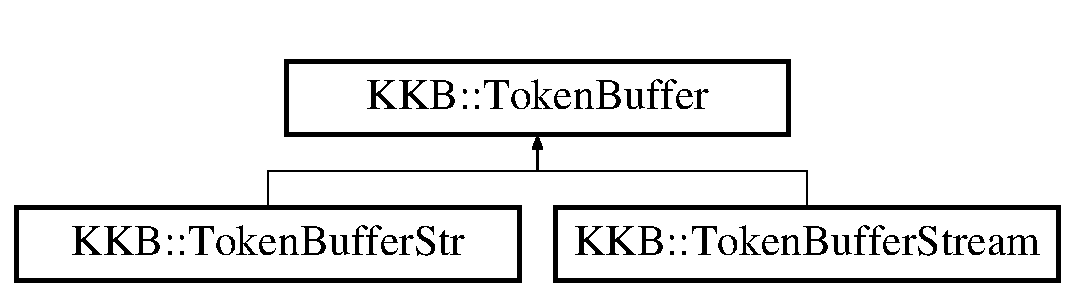
\includegraphics[height=2.000000cm]{class_k_k_b_1_1_token_buffer}
\end{center}
\end{figure}
\subsection*{Public Member Functions}
\begin{DoxyCompactItemize}
\item 
\hyperlink{class_k_k_b_1_1_token_buffer_a9c7f293eaace03fa2cb0f3e5102c9357}{Token\+Buffer} ()
\item 
virtual \hyperlink{class_k_k_b_1_1_token_buffer_a569be7c48bb3336e2252d922048ac232}{$\sim$\+Token\+Buffer} ()
\item 
virtual bool \hyperlink{class_k_k_b_1_1_token_buffer_a6eebb9bf092d9ad21c02f5370cb19af6}{End\+Of\+File} ()=0
\item 
virtual char \hyperlink{class_k_k_b_1_1_token_buffer_a07a50578fa5cfa827636615dab62a94b}{Get\+Next\+Char} ()=0
\item 
virtual char \hyperlink{class_k_k_b_1_1_token_buffer_a6cb0ed637090b4919149454f57006580}{Peek\+Next\+Char} ()=0
\item 
virtual void \hyperlink{class_k_k_b_1_1_token_buffer_a75500b92b04aacd8b1d97c28156e11d1}{Un\+Get\+Next\+Char} ()=0
\item 
virtual bool \hyperlink{class_k_k_b_1_1_token_buffer_ac7ef10355bd2fb7413055ce334901a28}{Valid} ()=0
\end{DoxyCompactItemize}


\subsection{Detailed Description}


Definition at line 12 of file Token\+Buffer.\+h.



\subsection{Constructor \& Destructor Documentation}
\index{K\+K\+B\+::\+Token\+Buffer@{K\+K\+B\+::\+Token\+Buffer}!Token\+Buffer@{Token\+Buffer}}
\index{Token\+Buffer@{Token\+Buffer}!K\+K\+B\+::\+Token\+Buffer@{K\+K\+B\+::\+Token\+Buffer}}
\subsubsection[{\texorpdfstring{Token\+Buffer()}{TokenBuffer()}}]{\setlength{\rightskip}{0pt plus 5cm}Token\+Buffer\+::\+Token\+Buffer (
\begin{DoxyParamCaption}
{}
\end{DoxyParamCaption}
)}\hypertarget{class_k_k_b_1_1_token_buffer_a9c7f293eaace03fa2cb0f3e5102c9357}{}\label{class_k_k_b_1_1_token_buffer_a9c7f293eaace03fa2cb0f3e5102c9357}


Definition at line 22 of file Token\+Buffer.\+cpp.



Referenced by K\+K\+B\+::\+Token\+Buffer\+Stream\+::\+Token\+Buffer\+Stream().


\begin{DoxyCode}
23 \{
24 \}
\end{DoxyCode}
\index{K\+K\+B\+::\+Token\+Buffer@{K\+K\+B\+::\+Token\+Buffer}!````~Token\+Buffer@{$\sim$\+Token\+Buffer}}
\index{````~Token\+Buffer@{$\sim$\+Token\+Buffer}!K\+K\+B\+::\+Token\+Buffer@{K\+K\+B\+::\+Token\+Buffer}}
\subsubsection[{\texorpdfstring{$\sim$\+Token\+Buffer()}{~TokenBuffer()}}]{\setlength{\rightskip}{0pt plus 5cm}Token\+Buffer\+::$\sim$\+Token\+Buffer (
\begin{DoxyParamCaption}
{}
\end{DoxyParamCaption}
)\hspace{0.3cm}{\ttfamily [virtual]}}\hypertarget{class_k_k_b_1_1_token_buffer_a569be7c48bb3336e2252d922048ac232}{}\label{class_k_k_b_1_1_token_buffer_a569be7c48bb3336e2252d922048ac232}


Definition at line 28 of file Token\+Buffer.\+cpp.


\begin{DoxyCode}
29 \{
30 \}
\end{DoxyCode}


\subsection{Member Function Documentation}
\index{K\+K\+B\+::\+Token\+Buffer@{K\+K\+B\+::\+Token\+Buffer}!End\+Of\+File@{End\+Of\+File}}
\index{End\+Of\+File@{End\+Of\+File}!K\+K\+B\+::\+Token\+Buffer@{K\+K\+B\+::\+Token\+Buffer}}
\subsubsection[{\texorpdfstring{End\+Of\+File()=0}{EndOfFile()=0}}]{\setlength{\rightskip}{0pt plus 5cm}virtual bool K\+K\+B\+::\+Token\+Buffer\+::\+End\+Of\+File (
\begin{DoxyParamCaption}
{}
\end{DoxyParamCaption}
)\hspace{0.3cm}{\ttfamily [pure virtual]}}\hypertarget{class_k_k_b_1_1_token_buffer_a6eebb9bf092d9ad21c02f5370cb19af6}{}\label{class_k_k_b_1_1_token_buffer_a6eebb9bf092d9ad21c02f5370cb19af6}


Implemented in \hyperlink{class_k_k_b_1_1_token_buffer_stream_a5c8e2826a9a7dca64a459c031eaa84c1}{K\+K\+B\+::\+Token\+Buffer\+Stream}, and \hyperlink{class_k_k_b_1_1_token_buffer_str_ac15456fdd0ccaf7b8be0971c8502a6a8}{K\+K\+B\+::\+Token\+Buffer\+Str}.

\index{K\+K\+B\+::\+Token\+Buffer@{K\+K\+B\+::\+Token\+Buffer}!Get\+Next\+Char@{Get\+Next\+Char}}
\index{Get\+Next\+Char@{Get\+Next\+Char}!K\+K\+B\+::\+Token\+Buffer@{K\+K\+B\+::\+Token\+Buffer}}
\subsubsection[{\texorpdfstring{Get\+Next\+Char()=0}{GetNextChar()=0}}]{\setlength{\rightskip}{0pt plus 5cm}virtual char K\+K\+B\+::\+Token\+Buffer\+::\+Get\+Next\+Char (
\begin{DoxyParamCaption}
{}
\end{DoxyParamCaption}
)\hspace{0.3cm}{\ttfamily [pure virtual]}}\hypertarget{class_k_k_b_1_1_token_buffer_a07a50578fa5cfa827636615dab62a94b}{}\label{class_k_k_b_1_1_token_buffer_a07a50578fa5cfa827636615dab62a94b}


Implemented in \hyperlink{class_k_k_b_1_1_token_buffer_stream_a01008b895e43af10face7888209fc6db}{K\+K\+B\+::\+Token\+Buffer\+Stream}, and \hyperlink{class_k_k_b_1_1_token_buffer_str_a080ae7a74018196fae2c6ade68dafe94}{K\+K\+B\+::\+Token\+Buffer\+Str}.

\index{K\+K\+B\+::\+Token\+Buffer@{K\+K\+B\+::\+Token\+Buffer}!Peek\+Next\+Char@{Peek\+Next\+Char}}
\index{Peek\+Next\+Char@{Peek\+Next\+Char}!K\+K\+B\+::\+Token\+Buffer@{K\+K\+B\+::\+Token\+Buffer}}
\subsubsection[{\texorpdfstring{Peek\+Next\+Char()=0}{PeekNextChar()=0}}]{\setlength{\rightskip}{0pt plus 5cm}virtual char K\+K\+B\+::\+Token\+Buffer\+::\+Peek\+Next\+Char (
\begin{DoxyParamCaption}
{}
\end{DoxyParamCaption}
)\hspace{0.3cm}{\ttfamily [pure virtual]}}\hypertarget{class_k_k_b_1_1_token_buffer_a6cb0ed637090b4919149454f57006580}{}\label{class_k_k_b_1_1_token_buffer_a6cb0ed637090b4919149454f57006580}


Implemented in \hyperlink{class_k_k_b_1_1_token_buffer_stream_a15a7c84a9da05d11585197918b31ee53}{K\+K\+B\+::\+Token\+Buffer\+Stream}, and \hyperlink{class_k_k_b_1_1_token_buffer_str_acc6a7cd0b9178b4e55f22a0ebdbc6111}{K\+K\+B\+::\+Token\+Buffer\+Str}.

\index{K\+K\+B\+::\+Token\+Buffer@{K\+K\+B\+::\+Token\+Buffer}!Un\+Get\+Next\+Char@{Un\+Get\+Next\+Char}}
\index{Un\+Get\+Next\+Char@{Un\+Get\+Next\+Char}!K\+K\+B\+::\+Token\+Buffer@{K\+K\+B\+::\+Token\+Buffer}}
\subsubsection[{\texorpdfstring{Un\+Get\+Next\+Char()=0}{UnGetNextChar()=0}}]{\setlength{\rightskip}{0pt plus 5cm}virtual void K\+K\+B\+::\+Token\+Buffer\+::\+Un\+Get\+Next\+Char (
\begin{DoxyParamCaption}
{}
\end{DoxyParamCaption}
)\hspace{0.3cm}{\ttfamily [pure virtual]}}\hypertarget{class_k_k_b_1_1_token_buffer_a75500b92b04aacd8b1d97c28156e11d1}{}\label{class_k_k_b_1_1_token_buffer_a75500b92b04aacd8b1d97c28156e11d1}


Implemented in \hyperlink{class_k_k_b_1_1_token_buffer_stream_ac978567a7936432a555858c54d2f79d4}{K\+K\+B\+::\+Token\+Buffer\+Stream}, and \hyperlink{class_k_k_b_1_1_token_buffer_str_acb375c049ac4228f665a0768a5a811ae}{K\+K\+B\+::\+Token\+Buffer\+Str}.

\index{K\+K\+B\+::\+Token\+Buffer@{K\+K\+B\+::\+Token\+Buffer}!Valid@{Valid}}
\index{Valid@{Valid}!K\+K\+B\+::\+Token\+Buffer@{K\+K\+B\+::\+Token\+Buffer}}
\subsubsection[{\texorpdfstring{Valid()=0}{Valid()=0}}]{\setlength{\rightskip}{0pt plus 5cm}virtual bool K\+K\+B\+::\+Token\+Buffer\+::\+Valid (
\begin{DoxyParamCaption}
{}
\end{DoxyParamCaption}
)\hspace{0.3cm}{\ttfamily [pure virtual]}}\hypertarget{class_k_k_b_1_1_token_buffer_ac7ef10355bd2fb7413055ce334901a28}{}\label{class_k_k_b_1_1_token_buffer_ac7ef10355bd2fb7413055ce334901a28}


Implemented in \hyperlink{class_k_k_b_1_1_token_buffer_stream_ab4ae9cad1348037fa6b75969c6091eb7}{K\+K\+B\+::\+Token\+Buffer\+Stream}, and \hyperlink{class_k_k_b_1_1_token_buffer_str_a3f63a85db864a1e272d5da9b0c601c32}{K\+K\+B\+::\+Token\+Buffer\+Str}.



Referenced by K\+K\+B\+::\+Tokenizer\+::\+Tokenizer(), and K\+K\+B\+::\+Xml\+Tokenizer\+::\+Xml\+Tokenizer().



The documentation for this class was generated from the following files\+:\begin{DoxyCompactItemize}
\item 
C\+:/\+Users/\+Kurt/\+Git\+Hub/\+K\+Square\+Libraries/\+K\+K\+Base/\hyperlink{_token_buffer_8h}{Token\+Buffer.\+h}\item 
C\+:/\+Users/\+Kurt/\+Git\+Hub/\+K\+Square\+Libraries/\+K\+K\+Base/\hyperlink{_token_buffer_8cpp}{Token\+Buffer.\+cpp}\end{DoxyCompactItemize}

\hypertarget{class_k_k_b_1_1_token_buffer_str}{}\section{K\+KB\+:\+:Token\+Buffer\+Str Class Reference}
\label{class_k_k_b_1_1_token_buffer_str}\index{K\+K\+B\+::\+Token\+Buffer\+Str@{K\+K\+B\+::\+Token\+Buffer\+Str}}


{\ttfamily \#include $<$Token\+Buffer.\+h$>$}

Inheritance diagram for K\+KB\+:\+:Token\+Buffer\+Str\+:\begin{figure}[H]
\begin{center}
\leavevmode
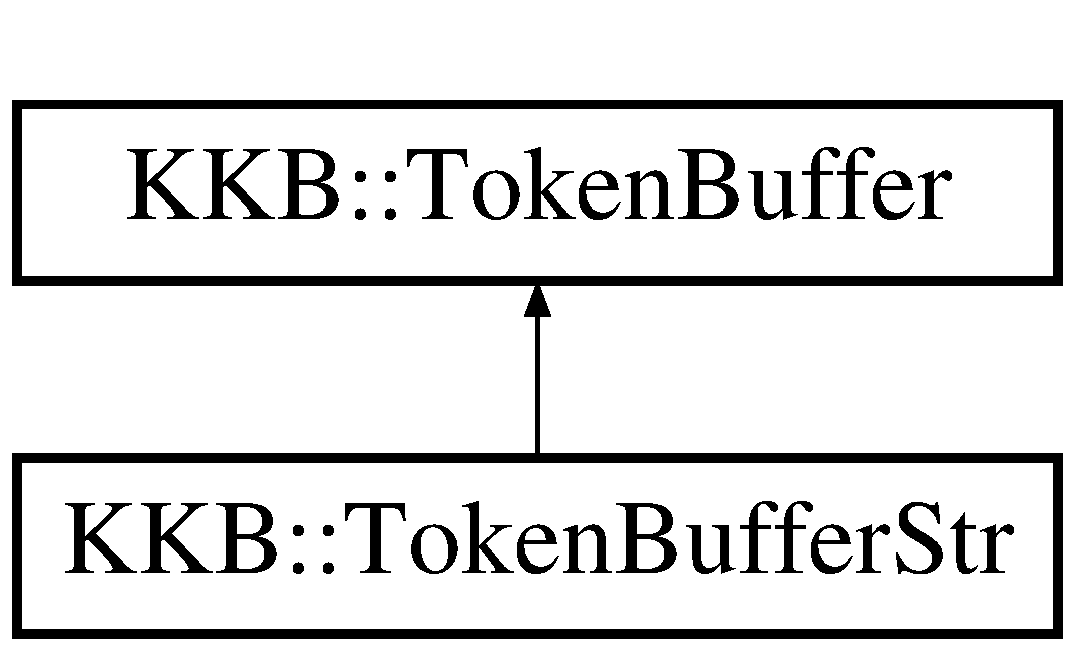
\includegraphics[height=2.000000cm]{class_k_k_b_1_1_token_buffer_str}
\end{center}
\end{figure}
\subsection*{Public Member Functions}
\begin{DoxyCompactItemize}
\item 
\hyperlink{class_k_k_b_1_1_token_buffer_str_a9b4227a88ced5162235e3341fc371bf4}{Token\+Buffer\+Str} (const \hyperlink{class_k_k_b_1_1_k_k_str}{K\+K\+Str} \&\+\_\+buff)
\item 
virtual \hyperlink{class_k_k_b_1_1_token_buffer_str_ab98f32a9c78e3a903400efe46e98f982}{$\sim$\+Token\+Buffer\+Str} ()
\item 
virtual bool \hyperlink{class_k_k_b_1_1_token_buffer_str_ac15456fdd0ccaf7b8be0971c8502a6a8}{End\+Of\+File} ()
\item 
virtual char \hyperlink{class_k_k_b_1_1_token_buffer_str_a080ae7a74018196fae2c6ade68dafe94}{Get\+Next\+Char} ()
\item 
virtual char \hyperlink{class_k_k_b_1_1_token_buffer_str_acc6a7cd0b9178b4e55f22a0ebdbc6111}{Peek\+Next\+Char} ()
\item 
virtual void \hyperlink{class_k_k_b_1_1_token_buffer_str_acb375c049ac4228f665a0768a5a811ae}{Un\+Get\+Next\+Char} ()
\item 
virtual bool \hyperlink{class_k_k_b_1_1_token_buffer_str_a3f63a85db864a1e272d5da9b0c601c32}{Valid} ()
\end{DoxyCompactItemize}


\subsection{Detailed Description}


Definition at line 36 of file Token\+Buffer.\+h.



\subsection{Constructor \& Destructor Documentation}
\index{K\+K\+B\+::\+Token\+Buffer\+Str@{K\+K\+B\+::\+Token\+Buffer\+Str}!Token\+Buffer\+Str@{Token\+Buffer\+Str}}
\index{Token\+Buffer\+Str@{Token\+Buffer\+Str}!K\+K\+B\+::\+Token\+Buffer\+Str@{K\+K\+B\+::\+Token\+Buffer\+Str}}
\subsubsection[{\texorpdfstring{Token\+Buffer\+Str(const K\+K\+Str \&\+\_\+buff)}{TokenBufferStr(const KKStr &_buff)}}]{\setlength{\rightskip}{0pt plus 5cm}Token\+Buffer\+Str\+::\+Token\+Buffer\+Str (
\begin{DoxyParamCaption}
\item[{const {\bf K\+K\+Str} \&}]{\+\_\+buff}
\end{DoxyParamCaption}
)}\hypertarget{class_k_k_b_1_1_token_buffer_str_a9b4227a88ced5162235e3341fc371bf4}{}\label{class_k_k_b_1_1_token_buffer_str_a9b4227a88ced5162235e3341fc371bf4}


Definition at line 34 of file Token\+Buffer.\+cpp.



References K\+K\+B\+::\+K\+K\+Str\+::\+K\+K\+Str().



Referenced by K\+K\+B\+::\+Tokenizer\+::\+Tokenizer(), and K\+K\+B\+::\+Xml\+Tokenizer\+::\+Xml\+Tokenizer().


\begin{DoxyCode}
34                                                   :
35     buff        (\_buff),
36     nextCharPos (0)
37 
38 \{
39 \}
\end{DoxyCode}
\index{K\+K\+B\+::\+Token\+Buffer\+Str@{K\+K\+B\+::\+Token\+Buffer\+Str}!````~Token\+Buffer\+Str@{$\sim$\+Token\+Buffer\+Str}}
\index{````~Token\+Buffer\+Str@{$\sim$\+Token\+Buffer\+Str}!K\+K\+B\+::\+Token\+Buffer\+Str@{K\+K\+B\+::\+Token\+Buffer\+Str}}
\subsubsection[{\texorpdfstring{$\sim$\+Token\+Buffer\+Str()}{~TokenBufferStr()}}]{\setlength{\rightskip}{0pt plus 5cm}Token\+Buffer\+Str\+::$\sim$\+Token\+Buffer\+Str (
\begin{DoxyParamCaption}
{}
\end{DoxyParamCaption}
)\hspace{0.3cm}{\ttfamily [virtual]}}\hypertarget{class_k_k_b_1_1_token_buffer_str_ab98f32a9c78e3a903400efe46e98f982}{}\label{class_k_k_b_1_1_token_buffer_str_ab98f32a9c78e3a903400efe46e98f982}


Definition at line 42 of file Token\+Buffer.\+cpp.


\begin{DoxyCode}
43 \{
44 \}
\end{DoxyCode}


\subsection{Member Function Documentation}
\index{K\+K\+B\+::\+Token\+Buffer\+Str@{K\+K\+B\+::\+Token\+Buffer\+Str}!End\+Of\+File@{End\+Of\+File}}
\index{End\+Of\+File@{End\+Of\+File}!K\+K\+B\+::\+Token\+Buffer\+Str@{K\+K\+B\+::\+Token\+Buffer\+Str}}
\subsubsection[{\texorpdfstring{End\+Of\+File()}{EndOfFile()}}]{\setlength{\rightskip}{0pt plus 5cm}bool Token\+Buffer\+Str\+::\+End\+Of\+File (
\begin{DoxyParamCaption}
{}
\end{DoxyParamCaption}
)\hspace{0.3cm}{\ttfamily [virtual]}}\hypertarget{class_k_k_b_1_1_token_buffer_str_ac15456fdd0ccaf7b8be0971c8502a6a8}{}\label{class_k_k_b_1_1_token_buffer_str_ac15456fdd0ccaf7b8be0971c8502a6a8}


Implements \hyperlink{class_k_k_b_1_1_token_buffer_a6eebb9bf092d9ad21c02f5370cb19af6}{K\+K\+B\+::\+Token\+Buffer}.



Definition at line 84 of file Token\+Buffer.\+cpp.



References K\+K\+B\+::\+K\+K\+Str\+::\+Len().


\begin{DoxyCode}
85 \{
86   \textcolor{keywordflow}{if}  (nextCharPos >= buff.\hyperlink{class_k_k_b_1_1_k_k_str_a869142d4855517c5c237afcb25dbbe36}{Len} ())
87     \textcolor{keywordflow}{return} \textcolor{keyword}{true};
88   \textcolor{keywordflow}{else}
89     \textcolor{keywordflow}{return} \textcolor{keyword}{false};
90 \}  \textcolor{comment}{/* EndOfFile */}
\end{DoxyCode}
\index{K\+K\+B\+::\+Token\+Buffer\+Str@{K\+K\+B\+::\+Token\+Buffer\+Str}!Get\+Next\+Char@{Get\+Next\+Char}}
\index{Get\+Next\+Char@{Get\+Next\+Char}!K\+K\+B\+::\+Token\+Buffer\+Str@{K\+K\+B\+::\+Token\+Buffer\+Str}}
\subsubsection[{\texorpdfstring{Get\+Next\+Char()}{GetNextChar()}}]{\setlength{\rightskip}{0pt plus 5cm}char Token\+Buffer\+Str\+::\+Get\+Next\+Char (
\begin{DoxyParamCaption}
{}
\end{DoxyParamCaption}
)\hspace{0.3cm}{\ttfamily [virtual]}}\hypertarget{class_k_k_b_1_1_token_buffer_str_a080ae7a74018196fae2c6ade68dafe94}{}\label{class_k_k_b_1_1_token_buffer_str_a080ae7a74018196fae2c6ade68dafe94}


Implements \hyperlink{class_k_k_b_1_1_token_buffer_a07a50578fa5cfa827636615dab62a94b}{K\+K\+B\+::\+Token\+Buffer}.



Definition at line 55 of file Token\+Buffer.\+cpp.



References K\+K\+B\+::\+K\+K\+Str\+::\+Len(), and K\+K\+B\+::\+K\+K\+Str\+::operator\mbox{[}$\,$\mbox{]}().


\begin{DoxyCode}
56 \{
57   \textcolor{keywordflow}{if}  (nextCharPos >= buff.\hyperlink{class_k_k_b_1_1_k_k_str_a869142d4855517c5c237afcb25dbbe36}{Len} ())
58     \textcolor{keywordflow}{return} 0;
59 
60   \textcolor{keywordtype}{char}  c = buff[nextCharPos];
61   nextCharPos++;
62   \textcolor{keywordflow}{return} c;
63 \}  \textcolor{comment}{/* GetNextChar */}
\end{DoxyCode}
\index{K\+K\+B\+::\+Token\+Buffer\+Str@{K\+K\+B\+::\+Token\+Buffer\+Str}!Peek\+Next\+Char@{Peek\+Next\+Char}}
\index{Peek\+Next\+Char@{Peek\+Next\+Char}!K\+K\+B\+::\+Token\+Buffer\+Str@{K\+K\+B\+::\+Token\+Buffer\+Str}}
\subsubsection[{\texorpdfstring{Peek\+Next\+Char()}{PeekNextChar()}}]{\setlength{\rightskip}{0pt plus 5cm}char Token\+Buffer\+Str\+::\+Peek\+Next\+Char (
\begin{DoxyParamCaption}
{}
\end{DoxyParamCaption}
)\hspace{0.3cm}{\ttfamily [virtual]}}\hypertarget{class_k_k_b_1_1_token_buffer_str_acc6a7cd0b9178b4e55f22a0ebdbc6111}{}\label{class_k_k_b_1_1_token_buffer_str_acc6a7cd0b9178b4e55f22a0ebdbc6111}


Implements \hyperlink{class_k_k_b_1_1_token_buffer_a6cb0ed637090b4919149454f57006580}{K\+K\+B\+::\+Token\+Buffer}.



Definition at line 67 of file Token\+Buffer.\+cpp.



References K\+K\+B\+::\+K\+K\+Str\+::\+Len(), and K\+K\+B\+::\+K\+K\+Str\+::operator\mbox{[}$\,$\mbox{]}().


\begin{DoxyCode}
68 \{
69   \textcolor{keywordflow}{if}  (nextCharPos >= buff.\hyperlink{class_k_k_b_1_1_k_k_str_a869142d4855517c5c237afcb25dbbe36}{Len} ())
70     \textcolor{keywordflow}{return} 0;
71   \textcolor{keywordflow}{return}  buff[nextCharPos];
72 \}
\end{DoxyCode}
\index{K\+K\+B\+::\+Token\+Buffer\+Str@{K\+K\+B\+::\+Token\+Buffer\+Str}!Un\+Get\+Next\+Char@{Un\+Get\+Next\+Char}}
\index{Un\+Get\+Next\+Char@{Un\+Get\+Next\+Char}!K\+K\+B\+::\+Token\+Buffer\+Str@{K\+K\+B\+::\+Token\+Buffer\+Str}}
\subsubsection[{\texorpdfstring{Un\+Get\+Next\+Char()}{UnGetNextChar()}}]{\setlength{\rightskip}{0pt plus 5cm}void Token\+Buffer\+Str\+::\+Un\+Get\+Next\+Char (
\begin{DoxyParamCaption}
{}
\end{DoxyParamCaption}
)\hspace{0.3cm}{\ttfamily [virtual]}}\hypertarget{class_k_k_b_1_1_token_buffer_str_acb375c049ac4228f665a0768a5a811ae}{}\label{class_k_k_b_1_1_token_buffer_str_acb375c049ac4228f665a0768a5a811ae}


Implements \hyperlink{class_k_k_b_1_1_token_buffer_a75500b92b04aacd8b1d97c28156e11d1}{K\+K\+B\+::\+Token\+Buffer}.



Definition at line 76 of file Token\+Buffer.\+cpp.


\begin{DoxyCode}
77 \{
78   \textcolor{keywordflow}{if}  (nextCharPos > 0)
79     --nextCharPos;
80 \}
\end{DoxyCode}
\index{K\+K\+B\+::\+Token\+Buffer\+Str@{K\+K\+B\+::\+Token\+Buffer\+Str}!Valid@{Valid}}
\index{Valid@{Valid}!K\+K\+B\+::\+Token\+Buffer\+Str@{K\+K\+B\+::\+Token\+Buffer\+Str}}
\subsubsection[{\texorpdfstring{Valid()}{Valid()}}]{\setlength{\rightskip}{0pt plus 5cm}bool Token\+Buffer\+Str\+::\+Valid (
\begin{DoxyParamCaption}
{}
\end{DoxyParamCaption}
)\hspace{0.3cm}{\ttfamily [virtual]}}\hypertarget{class_k_k_b_1_1_token_buffer_str_a3f63a85db864a1e272d5da9b0c601c32}{}\label{class_k_k_b_1_1_token_buffer_str_a3f63a85db864a1e272d5da9b0c601c32}


Implements \hyperlink{class_k_k_b_1_1_token_buffer_ac7ef10355bd2fb7413055ce334901a28}{K\+K\+B\+::\+Token\+Buffer}.



Definition at line 48 of file Token\+Buffer.\+cpp.


\begin{DoxyCode}
49 \{
50   \textcolor{keywordflow}{return} \textcolor{keyword}{true};
51 \}
\end{DoxyCode}


The documentation for this class was generated from the following files\+:\begin{DoxyCompactItemize}
\item 
C\+:/\+Users/\+Kurt/\+Git\+Hub/\+K\+Square\+Libraries/\+K\+K\+Base/\hyperlink{_token_buffer_8h}{Token\+Buffer.\+h}\item 
C\+:/\+Users/\+Kurt/\+Git\+Hub/\+K\+Square\+Libraries/\+K\+K\+Base/\hyperlink{_token_buffer_8cpp}{Token\+Buffer.\+cpp}\end{DoxyCompactItemize}

\hypertarget{class_k_k_b_1_1_token_buffer_stream}{}\section{K\+KB\+:\+:Token\+Buffer\+Stream Class Reference}
\label{class_k_k_b_1_1_token_buffer_stream}\index{K\+K\+B\+::\+Token\+Buffer\+Stream@{K\+K\+B\+::\+Token\+Buffer\+Stream}}


{\ttfamily \#include $<$Token\+Buffer.\+h$>$}

Inheritance diagram for K\+KB\+:\+:Token\+Buffer\+Stream\+:\begin{figure}[H]
\begin{center}
\leavevmode
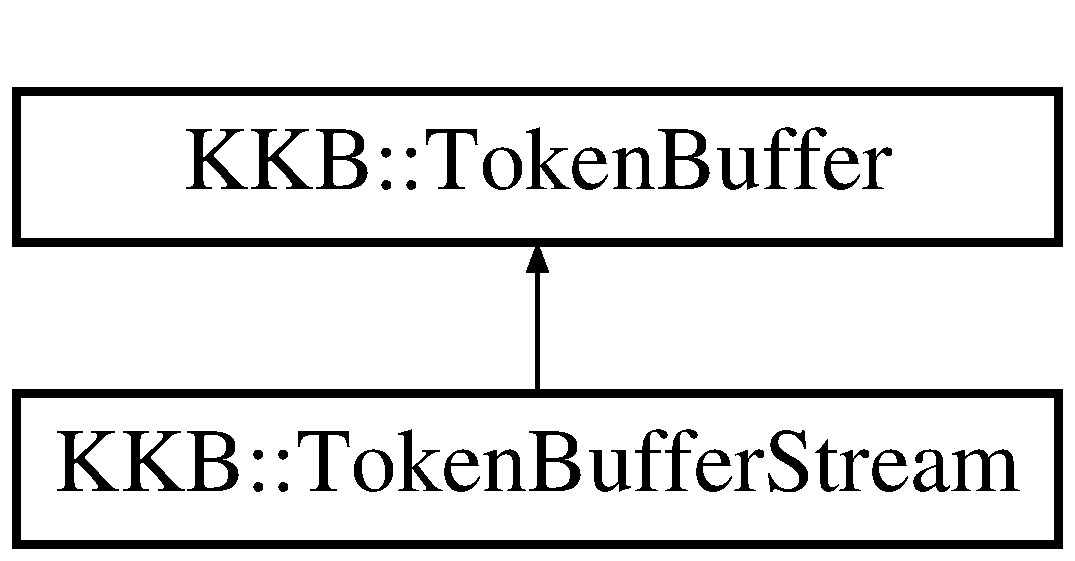
\includegraphics[height=2.000000cm]{class_k_k_b_1_1_token_buffer_stream}
\end{center}
\end{figure}
\subsection*{Public Member Functions}
\begin{DoxyCompactItemize}
\item 
\hyperlink{class_k_k_b_1_1_token_buffer_stream_a7d4953a65b5c8c59b9f6594c8d8ca4de}{Token\+Buffer\+Stream} (std\+::istream $\ast$\+\_\+in)
\item 
\hyperlink{class_k_k_b_1_1_token_buffer_stream_a4c8f2348703ddc893cbbced71c5a89e1}{Token\+Buffer\+Stream} (const \hyperlink{class_k_k_b_1_1_k_k_str}{K\+K\+Str} \&\+\_\+file\+Name)
\item 
virtual \hyperlink{class_k_k_b_1_1_token_buffer_stream_a42fce0e2e8ac75fec48b746f0ebb6299}{$\sim$\+Token\+Buffer\+Stream} ()
\item 
virtual bool \hyperlink{class_k_k_b_1_1_token_buffer_stream_a5c8e2826a9a7dca64a459c031eaa84c1}{End\+Of\+File} ()
\item 
virtual char \hyperlink{class_k_k_b_1_1_token_buffer_stream_a01008b895e43af10face7888209fc6db}{Get\+Next\+Char} ()
\item 
virtual char \hyperlink{class_k_k_b_1_1_token_buffer_stream_a15a7c84a9da05d11585197918b31ee53}{Peek\+Next\+Char} ()
\item 
virtual void \hyperlink{class_k_k_b_1_1_token_buffer_stream_ac978567a7936432a555858c54d2f79d4}{Un\+Get\+Next\+Char} ()
\item 
virtual bool \hyperlink{class_k_k_b_1_1_token_buffer_stream_ab4ae9cad1348037fa6b75969c6091eb7}{Valid} ()
\end{DoxyCompactItemize}


\subsection{Detailed Description}


Definition at line 59 of file Token\+Buffer.\+h.



\subsection{Constructor \& Destructor Documentation}
\index{K\+K\+B\+::\+Token\+Buffer\+Stream@{K\+K\+B\+::\+Token\+Buffer\+Stream}!Token\+Buffer\+Stream@{Token\+Buffer\+Stream}}
\index{Token\+Buffer\+Stream@{Token\+Buffer\+Stream}!K\+K\+B\+::\+Token\+Buffer\+Stream@{K\+K\+B\+::\+Token\+Buffer\+Stream}}
\subsubsection[{\texorpdfstring{Token\+Buffer\+Stream(std\+::istream $\ast$\+\_\+in)}{TokenBufferStream(std::istream *_in)}}]{\setlength{\rightskip}{0pt plus 5cm}K\+K\+B\+::\+Token\+Buffer\+Stream\+::\+Token\+Buffer\+Stream (
\begin{DoxyParamCaption}
\item[{std\+::istream $\ast$}]{\+\_\+in}
\end{DoxyParamCaption}
)}\hypertarget{class_k_k_b_1_1_token_buffer_stream_a7d4953a65b5c8c59b9f6594c8d8ca4de}{}\label{class_k_k_b_1_1_token_buffer_stream_a7d4953a65b5c8c59b9f6594c8d8ca4de}
\index{K\+K\+B\+::\+Token\+Buffer\+Stream@{K\+K\+B\+::\+Token\+Buffer\+Stream}!Token\+Buffer\+Stream@{Token\+Buffer\+Stream}}
\index{Token\+Buffer\+Stream@{Token\+Buffer\+Stream}!K\+K\+B\+::\+Token\+Buffer\+Stream@{K\+K\+B\+::\+Token\+Buffer\+Stream}}
\subsubsection[{\texorpdfstring{Token\+Buffer\+Stream(const K\+K\+Str \&\+\_\+file\+Name)}{TokenBufferStream(const KKStr &_fileName)}}]{\setlength{\rightskip}{0pt plus 5cm}Token\+Buffer\+Stream\+::\+Token\+Buffer\+Stream (
\begin{DoxyParamCaption}
\item[{const {\bf K\+K\+Str} \&}]{\+\_\+file\+Name}
\end{DoxyParamCaption}
)}\hypertarget{class_k_k_b_1_1_token_buffer_stream_a4c8f2348703ddc893cbbced71c5a89e1}{}\label{class_k_k_b_1_1_token_buffer_stream_a4c8f2348703ddc893cbbced71c5a89e1}


Definition at line 107 of file Token\+Buffer.\+cpp.



References K\+K\+B\+::\+K\+K\+Str\+::\+K\+K\+Str(), and K\+K\+B\+::\+Token\+Buffer\+::\+Token\+Buffer().



Referenced by K\+K\+B\+::\+Tokenizer\+::\+Tokenizer(), and K\+K\+B\+::\+Xml\+Tokenizer\+::\+Xml\+Tokenizer().


\begin{DoxyCode}
107                                                             :
108     \hyperlink{class_k_k_b_1_1_token_buffer_a9c7f293eaace03fa2cb0f3e5102c9357}{TokenBuffer} (),
109     endOfFile   (\textcolor{keyword}{false}),
110     fileName    (\_fileName),
111     fileStream  (NULL),
112     in          (NULL)
113 \{
114   fileStream  = \textcolor{keyword}{new} ifstream (fileName.\hyperlink{class_k_k_b_1_1_k_k_str_ad574e6c0fe7f6ce1ba3ab0a8ce2fbd52}{Str} ());
115   \textcolor{keywordflow}{if}  (!fileStream->is\_open ())
116   \{
117     \textcolor{keyword}{delete} fileStream;
118     fileStream = NULL;
119   \}
120   \textcolor{keywordflow}{else}
121   \{
122     in = fileStream;
123   \}
124 \}
\end{DoxyCode}
\index{K\+K\+B\+::\+Token\+Buffer\+Stream@{K\+K\+B\+::\+Token\+Buffer\+Stream}!````~Token\+Buffer\+Stream@{$\sim$\+Token\+Buffer\+Stream}}
\index{````~Token\+Buffer\+Stream@{$\sim$\+Token\+Buffer\+Stream}!K\+K\+B\+::\+Token\+Buffer\+Stream@{K\+K\+B\+::\+Token\+Buffer\+Stream}}
\subsubsection[{\texorpdfstring{$\sim$\+Token\+Buffer\+Stream()}{~TokenBufferStream()}}]{\setlength{\rightskip}{0pt plus 5cm}Token\+Buffer\+Stream\+::$\sim$\+Token\+Buffer\+Stream (
\begin{DoxyParamCaption}
{}
\end{DoxyParamCaption}
)\hspace{0.3cm}{\ttfamily [virtual]}}\hypertarget{class_k_k_b_1_1_token_buffer_stream_a42fce0e2e8ac75fec48b746f0ebb6299}{}\label{class_k_k_b_1_1_token_buffer_stream_a42fce0e2e8ac75fec48b746f0ebb6299}


Definition at line 128 of file Token\+Buffer.\+cpp.


\begin{DoxyCode}
129 \{
130   \textcolor{keywordflow}{if}  (fileStream)
131   \{
132     in = NULL;
133     \textcolor{keyword}{delete}  fileStream;
134     fileStream = NULL;
135   \}
136 \}
\end{DoxyCode}


\subsection{Member Function Documentation}
\index{K\+K\+B\+::\+Token\+Buffer\+Stream@{K\+K\+B\+::\+Token\+Buffer\+Stream}!End\+Of\+File@{End\+Of\+File}}
\index{End\+Of\+File@{End\+Of\+File}!K\+K\+B\+::\+Token\+Buffer\+Stream@{K\+K\+B\+::\+Token\+Buffer\+Stream}}
\subsubsection[{\texorpdfstring{End\+Of\+File()}{EndOfFile()}}]{\setlength{\rightskip}{0pt plus 5cm}bool Token\+Buffer\+Stream\+::\+End\+Of\+File (
\begin{DoxyParamCaption}
{}
\end{DoxyParamCaption}
)\hspace{0.3cm}{\ttfamily [virtual]}}\hypertarget{class_k_k_b_1_1_token_buffer_stream_a5c8e2826a9a7dca64a459c031eaa84c1}{}\label{class_k_k_b_1_1_token_buffer_stream_a5c8e2826a9a7dca64a459c031eaa84c1}


Implements \hyperlink{class_k_k_b_1_1_token_buffer_a6eebb9bf092d9ad21c02f5370cb19af6}{K\+K\+B\+::\+Token\+Buffer}.



Definition at line 189 of file Token\+Buffer.\+cpp.


\begin{DoxyCode}
190 \{
191   \textcolor{keywordflow}{return}  endOfFile;
192 \}
\end{DoxyCode}
\index{K\+K\+B\+::\+Token\+Buffer\+Stream@{K\+K\+B\+::\+Token\+Buffer\+Stream}!Get\+Next\+Char@{Get\+Next\+Char}}
\index{Get\+Next\+Char@{Get\+Next\+Char}!K\+K\+B\+::\+Token\+Buffer\+Stream@{K\+K\+B\+::\+Token\+Buffer\+Stream}}
\subsubsection[{\texorpdfstring{Get\+Next\+Char()}{GetNextChar()}}]{\setlength{\rightskip}{0pt plus 5cm}char Token\+Buffer\+Stream\+::\+Get\+Next\+Char (
\begin{DoxyParamCaption}
{}
\end{DoxyParamCaption}
)\hspace{0.3cm}{\ttfamily [virtual]}}\hypertarget{class_k_k_b_1_1_token_buffer_stream_a01008b895e43af10face7888209fc6db}{}\label{class_k_k_b_1_1_token_buffer_stream_a01008b895e43af10face7888209fc6db}


Implements \hyperlink{class_k_k_b_1_1_token_buffer_a07a50578fa5cfa827636615dab62a94b}{K\+K\+B\+::\+Token\+Buffer}.



Definition at line 155 of file Token\+Buffer.\+cpp.


\begin{DoxyCode}
156 \{
157   \textcolor{keywordtype}{char} c;
158   \textcolor{keywordflow}{if}  (endOfFile)
159     \textcolor{keywordflow}{return} 0;
160 
161   c = in->get ();
162   \textcolor{keywordflow}{if}  (in->eof())
163   \{
164     endOfFile = \textcolor{keyword}{true};
165     c = 0;
166   \}
167   \textcolor{keywordflow}{return} c;
168 \}  \textcolor{comment}{/* GetNextChar */}
\end{DoxyCode}
\index{K\+K\+B\+::\+Token\+Buffer\+Stream@{K\+K\+B\+::\+Token\+Buffer\+Stream}!Peek\+Next\+Char@{Peek\+Next\+Char}}
\index{Peek\+Next\+Char@{Peek\+Next\+Char}!K\+K\+B\+::\+Token\+Buffer\+Stream@{K\+K\+B\+::\+Token\+Buffer\+Stream}}
\subsubsection[{\texorpdfstring{Peek\+Next\+Char()}{PeekNextChar()}}]{\setlength{\rightskip}{0pt plus 5cm}char Token\+Buffer\+Stream\+::\+Peek\+Next\+Char (
\begin{DoxyParamCaption}
{}
\end{DoxyParamCaption}
)\hspace{0.3cm}{\ttfamily [virtual]}}\hypertarget{class_k_k_b_1_1_token_buffer_stream_a15a7c84a9da05d11585197918b31ee53}{}\label{class_k_k_b_1_1_token_buffer_stream_a15a7c84a9da05d11585197918b31ee53}


Implements \hyperlink{class_k_k_b_1_1_token_buffer_a6cb0ed637090b4919149454f57006580}{K\+K\+B\+::\+Token\+Buffer}.



Definition at line 172 of file Token\+Buffer.\+cpp.


\begin{DoxyCode}
173 \{
174   \textcolor{keywordflow}{if}  (in->eof ())
175     \textcolor{keywordflow}{return} 0;
176   \textcolor{keywordflow}{return}  in->peek ();
177 \}
\end{DoxyCode}
\index{K\+K\+B\+::\+Token\+Buffer\+Stream@{K\+K\+B\+::\+Token\+Buffer\+Stream}!Un\+Get\+Next\+Char@{Un\+Get\+Next\+Char}}
\index{Un\+Get\+Next\+Char@{Un\+Get\+Next\+Char}!K\+K\+B\+::\+Token\+Buffer\+Stream@{K\+K\+B\+::\+Token\+Buffer\+Stream}}
\subsubsection[{\texorpdfstring{Un\+Get\+Next\+Char()}{UnGetNextChar()}}]{\setlength{\rightskip}{0pt plus 5cm}void Token\+Buffer\+Stream\+::\+Un\+Get\+Next\+Char (
\begin{DoxyParamCaption}
{}
\end{DoxyParamCaption}
)\hspace{0.3cm}{\ttfamily [virtual]}}\hypertarget{class_k_k_b_1_1_token_buffer_stream_ac978567a7936432a555858c54d2f79d4}{}\label{class_k_k_b_1_1_token_buffer_stream_ac978567a7936432a555858c54d2f79d4}


Implements \hyperlink{class_k_k_b_1_1_token_buffer_a75500b92b04aacd8b1d97c28156e11d1}{K\+K\+B\+::\+Token\+Buffer}.



Definition at line 182 of file Token\+Buffer.\+cpp.


\begin{DoxyCode}
183 \{
184   in->unget ();
185 \}
\end{DoxyCode}
\index{K\+K\+B\+::\+Token\+Buffer\+Stream@{K\+K\+B\+::\+Token\+Buffer\+Stream}!Valid@{Valid}}
\index{Valid@{Valid}!K\+K\+B\+::\+Token\+Buffer\+Stream@{K\+K\+B\+::\+Token\+Buffer\+Stream}}
\subsubsection[{\texorpdfstring{Valid()}{Valid()}}]{\setlength{\rightskip}{0pt plus 5cm}bool Token\+Buffer\+Stream\+::\+Valid (
\begin{DoxyParamCaption}
{}
\end{DoxyParamCaption}
)\hspace{0.3cm}{\ttfamily [virtual]}}\hypertarget{class_k_k_b_1_1_token_buffer_stream_ab4ae9cad1348037fa6b75969c6091eb7}{}\label{class_k_k_b_1_1_token_buffer_stream_ab4ae9cad1348037fa6b75969c6091eb7}


Implements \hyperlink{class_k_k_b_1_1_token_buffer_ac7ef10355bd2fb7413055ce334901a28}{K\+K\+B\+::\+Token\+Buffer}.



Definition at line 142 of file Token\+Buffer.\+cpp.


\begin{DoxyCode}
143 \{
144   \textcolor{keywordflow}{if}  (fileStream)
145   \{
146     \textcolor{keywordflow}{return}  fileStream->is\_open ();
147   \}
148 
149   \textcolor{keywordflow}{return} (in != NULL);
150 \}  \textcolor{comment}{/* Valid */}
\end{DoxyCode}


The documentation for this class was generated from the following files\+:\begin{DoxyCompactItemize}
\item 
C\+:/\+Users/\+Kurt/\+Git\+Hub/\+K\+Square\+Libraries/\+K\+K\+Base/\hyperlink{_token_buffer_8h}{Token\+Buffer.\+h}\item 
C\+:/\+Users/\+Kurt/\+Git\+Hub/\+K\+Square\+Libraries/\+K\+K\+Base/\hyperlink{_token_buffer_8cpp}{Token\+Buffer.\+cpp}\end{DoxyCompactItemize}

\hypertarget{class_k_k_b_1_1_tokenizer}{}\section{K\+KB\+:\+:Tokenizer Class Reference}
\label{class_k_k_b_1_1_tokenizer}\index{K\+K\+B\+::\+Tokenizer@{K\+K\+B\+::\+Tokenizer}}


Class is meant to break down a stream into a set of logical tokens.  




{\ttfamily \#include $<$Tokenizer.\+h$>$}

\subsection*{Public Member Functions}
\begin{DoxyCompactItemize}
\item 
\hyperlink{class_k_k_b_1_1_tokenizer_a6cb70351213d78ec1b36da76f447246e}{Tokenizer} (\hyperlink{namespace_k_k_b_ae97804d25124b4a5dba3b3637beb814a}{Token\+Buffer\+Ptr} \+\_\+in)
\item 
\hyperlink{class_k_k_b_1_1_tokenizer_a9ed287f03edb99625cdfc99ae61dd8ad}{Tokenizer} (const \hyperlink{class_k_k_b_1_1_k_k_str}{K\+K\+Str} \&\+\_\+str)
\item 
\hyperlink{class_k_k_b_1_1_tokenizer_ad134e856be2766eaff989fa2dcc862ca}{Tokenizer} (const \hyperlink{class_k_k_b_1_1_k_k_str}{K\+K\+Str} \&\+\_\+file\+Name, bool \&\+\_\+file\+Opened)
\item 
\hyperlink{class_k_k_b_1_1_tokenizer_a3f60f887953edf0f95ba5f36102f7017}{$\sim$\+Tokenizer} ()
\item 
void \hyperlink{class_k_k_b_1_1_tokenizer_a273eb0f0ad85cef3757866bf9957a52e}{Define\+Operator\+Chars} (char $\ast$const \+\_\+operator\+Chars)
\item 
bool \hyperlink{class_k_k_b_1_1_tokenizer_a0b04dca4dfbf584e58082cad41d0457b}{End\+Of\+File} ()
\item 
\hyperlink{namespace_k_k_b_a9adbef5a6b3be0867f5570df2a08f388}{K\+K\+Str\+Ptr} \hyperlink{class_k_k_b_1_1_tokenizer_aea0a06cf4683bcd6e1c3b42e76f9324f}{Get\+Next\+Token} ()
\item 
\hyperlink{namespace_k_k_b_a8f5f50672f37857425120831223888aa}{K\+K\+Str\+List\+Ptr} \hyperlink{class_k_k_b_1_1_tokenizer_a4b5e1c31228130d3308f6f0d7dbca6ce}{Get\+Next\+Tokens} (const \hyperlink{class_k_k_b_1_1_k_k_str}{K\+K\+Str} \&del\+Token)
\begin{DoxyCompactList}\small\item\em Returns a list of tokens up to and including the first occurrence of \textquotesingle{}del\+Token\textquotesingle{}. \end{DoxyCompactList}\item 
\hyperlink{namespace_k_k_b_a46f665ec17615c856eff3d21f78bed5c}{K\+K\+Str\+Const\+Ptr} \hyperlink{class_k_k_b_1_1_tokenizer_ac82c5fd6107aa964dcbdbab6df0f5293}{operator\mbox{[}$\,$\mbox{]}} (\hyperlink{namespace_k_k_b_af8d832f05c54994a1cce25bd5743e19a}{kkuint32} idx)
\item 
\hyperlink{namespace_k_k_b_a46f665ec17615c856eff3d21f78bed5c}{K\+K\+Str\+Const\+Ptr} \hyperlink{class_k_k_b_1_1_tokenizer_aa68ada340bc52bf6839939cec99e63db}{Peek} (\hyperlink{namespace_k_k_b_af8d832f05c54994a1cce25bd5743e19a}{kkuint32} idx)
\item 
void \hyperlink{class_k_k_b_1_1_tokenizer_a6395ce549184bd1bcc1e2c0987f9ae47}{Push\+Token\+On\+Front} (\hyperlink{namespace_k_k_b_a9adbef5a6b3be0867f5570df2a08f388}{K\+K\+Str\+Ptr} t)
\end{DoxyCompactItemize}


\subsection{Detailed Description}
Class is meant to break down a stream into a set of logical tokens. 

\begin{DoxyAuthor}{Author}
Kurt Kramer
\end{DoxyAuthor}
This class was originally created while taking Non Linear Systems. It breaks up a source \hyperlink{class_k_k_b_1_1_k_k_str}{K\+K\+Str} or text file into logical tokens. You can create your own source of characters by creating a Class derived from \hyperlink{class_k_k_b_1_1_token_buffer}{K\+K\+B\+::\+Token\+Buffer}. 

Definition at line 23 of file Tokenizer.\+h.



\subsection{Constructor \& Destructor Documentation}
\index{K\+K\+B\+::\+Tokenizer@{K\+K\+B\+::\+Tokenizer}!Tokenizer@{Tokenizer}}
\index{Tokenizer@{Tokenizer}!K\+K\+B\+::\+Tokenizer@{K\+K\+B\+::\+Tokenizer}}
\subsubsection[{\texorpdfstring{Tokenizer(\+Token\+Buffer\+Ptr \+\_\+in)}{Tokenizer(TokenBufferPtr _in)}}]{\setlength{\rightskip}{0pt plus 5cm}Tokenizer\+::\+Tokenizer (
\begin{DoxyParamCaption}
\item[{{\bf Token\+Buffer\+Ptr}}]{\+\_\+in}
\end{DoxyParamCaption}
)}\hypertarget{class_k_k_b_1_1_tokenizer_a6cb70351213d78ec1b36da76f447246e}{}\label{class_k_k_b_1_1_tokenizer_a6cb70351213d78ec1b36da76f447246e}


Definition at line 22 of file Tokenizer.\+cpp.



References Tokenizer().



Referenced by Tokenizer().


\begin{DoxyCode}
22                                         :
23 
24   atEndOfFile           (\textcolor{keyword}{false}),
25   in                    (\_in),
26   secondCharAtEndOfFile (\textcolor{keyword}{false}),
27   operatorChars         (NULL),
28   tokenList             (\textcolor{keyword}{true}),
29   weOwnTokenBuffer      (\textcolor{keyword}{false})
30 \{
31   Initialize ();
32 \}
\end{DoxyCode}
\index{K\+K\+B\+::\+Tokenizer@{K\+K\+B\+::\+Tokenizer}!Tokenizer@{Tokenizer}}
\index{Tokenizer@{Tokenizer}!K\+K\+B\+::\+Tokenizer@{K\+K\+B\+::\+Tokenizer}}
\subsubsection[{\texorpdfstring{Tokenizer(const K\+K\+Str \&\+\_\+str)}{Tokenizer(const KKStr &_str)}}]{\setlength{\rightskip}{0pt plus 5cm}Tokenizer\+::\+Tokenizer (
\begin{DoxyParamCaption}
\item[{const {\bf K\+K\+Str} \&}]{\+\_\+str}
\end{DoxyParamCaption}
)}\hypertarget{class_k_k_b_1_1_tokenizer_a9ed287f03edb99625cdfc99ae61dd8ad}{}\label{class_k_k_b_1_1_tokenizer_a9ed287f03edb99625cdfc99ae61dd8ad}


Definition at line 36 of file Tokenizer.\+cpp.



References K\+K\+B\+::\+Token\+Buffer\+Str\+::\+Token\+Buffer\+Str(), and Tokenizer().



Referenced by Tokenizer().


\begin{DoxyCode}
36                                        :
37 
38   atEndOfFile           (\textcolor{keyword}{false}),
39   in                    (NULL),
40   secondCharAtEndOfFile (\textcolor{keyword}{false}),
41   operatorChars         (NULL),
42   tokenList             (\textcolor{keyword}{true}),
43   weOwnTokenBuffer      (\textcolor{keyword}{false})
44 \{
45   in = \textcolor{keyword}{new} \hyperlink{class_k_k_b_1_1_token_buffer_str}{TokenBufferStr} (\_str);
46   weOwnTokenBuffer = \textcolor{keyword}{true};
47   Initialize ();
48 \}
\end{DoxyCode}
\index{K\+K\+B\+::\+Tokenizer@{K\+K\+B\+::\+Tokenizer}!Tokenizer@{Tokenizer}}
\index{Tokenizer@{Tokenizer}!K\+K\+B\+::\+Tokenizer@{K\+K\+B\+::\+Tokenizer}}
\subsubsection[{\texorpdfstring{Tokenizer(const K\+K\+Str \&\+\_\+file\+Name, bool \&\+\_\+file\+Opened)}{Tokenizer(const KKStr &_fileName, bool &_fileOpened)}}]{\setlength{\rightskip}{0pt plus 5cm}Tokenizer\+::\+Tokenizer (
\begin{DoxyParamCaption}
\item[{const {\bf K\+K\+Str} \&}]{\+\_\+file\+Name, }
\item[{bool \&}]{\+\_\+file\+Opened}
\end{DoxyParamCaption}
)}\hypertarget{class_k_k_b_1_1_tokenizer_ad134e856be2766eaff989fa2dcc862ca}{}\label{class_k_k_b_1_1_tokenizer_ad134e856be2766eaff989fa2dcc862ca}


Definition at line 52 of file Tokenizer.\+cpp.



References K\+K\+B\+::\+Token\+Buffer\+Stream\+::\+Token\+Buffer\+Stream(), Tokenizer(), and K\+K\+B\+::\+Token\+Buffer\+::\+Valid().



Referenced by Tokenizer().


\begin{DoxyCode}
54                       :
55 
56   atEndOfFile           (\textcolor{keyword}{false}),
57   in                    (NULL),
58   secondCharAtEndOfFile (\textcolor{keyword}{false}),
59   operatorChars         (NULL),
60   tokenList             (\textcolor{keyword}{true}),
61   weOwnTokenBuffer      (\textcolor{keyword}{false})
62 \{
63   in = \textcolor{keyword}{new} \hyperlink{class_k_k_b_1_1_token_buffer_stream}{TokenBufferStream} (\_fileName);
64   \_fileOpened = (in->\hyperlink{class_k_k_b_1_1_token_buffer_ac7ef10355bd2fb7413055ce334901a28}{Valid} ());
65   \textcolor{keywordflow}{if}  (\_fileOpened)
66   \{
67     weOwnTokenBuffer = \textcolor{keyword}{true};
68     Initialize ();
69   \}
70 \}
\end{DoxyCode}
\index{K\+K\+B\+::\+Tokenizer@{K\+K\+B\+::\+Tokenizer}!````~Tokenizer@{$\sim$\+Tokenizer}}
\index{````~Tokenizer@{$\sim$\+Tokenizer}!K\+K\+B\+::\+Tokenizer@{K\+K\+B\+::\+Tokenizer}}
\subsubsection[{\texorpdfstring{$\sim$\+Tokenizer()}{~Tokenizer()}}]{\setlength{\rightskip}{0pt plus 5cm}Tokenizer\+::$\sim$\+Tokenizer (
\begin{DoxyParamCaption}
{}
\end{DoxyParamCaption}
)}\hypertarget{class_k_k_b_1_1_tokenizer_a3f60f887953edf0f95ba5f36102f7017}{}\label{class_k_k_b_1_1_tokenizer_a3f60f887953edf0f95ba5f36102f7017}


Definition at line 75 of file Tokenizer.\+cpp.


\begin{DoxyCode}
76 \{
77   \textcolor{keywordflow}{if}  (weOwnTokenBuffer)
78   \{
79     \textcolor{keyword}{delete}  in;
80     in = NULL;
81   \}
82   \textcolor{keyword}{delete}  operatorChars;
83   operatorChars = NULL;
84 \}
\end{DoxyCode}


\subsection{Member Function Documentation}
\index{K\+K\+B\+::\+Tokenizer@{K\+K\+B\+::\+Tokenizer}!Define\+Operator\+Chars@{Define\+Operator\+Chars}}
\index{Define\+Operator\+Chars@{Define\+Operator\+Chars}!K\+K\+B\+::\+Tokenizer@{K\+K\+B\+::\+Tokenizer}}
\subsubsection[{\texorpdfstring{Define\+Operator\+Chars(char $\ast$const \+\_\+operator\+Chars)}{DefineOperatorChars(char *const _operatorChars)}}]{\setlength{\rightskip}{0pt plus 5cm}void Tokenizer\+::\+Define\+Operator\+Chars (
\begin{DoxyParamCaption}
\item[{char $\ast$const}]{\+\_\+operator\+Chars}
\end{DoxyParamCaption}
)}\hypertarget{class_k_k_b_1_1_tokenizer_a273eb0f0ad85cef3757866bf9957a52e}{}\label{class_k_k_b_1_1_tokenizer_a273eb0f0ad85cef3757866bf9957a52e}


Definition at line 109 of file Tokenizer.\+cpp.



References K\+K\+B\+::\+S\+T\+R\+D\+U\+P().


\begin{DoxyCode}
110 \{
111   \textcolor{keyword}{delete}  operatorChars ;
112   operatorChars = \hyperlink{namespace_k_k_b_a24920fb971ac6f99f94e9fb8ee8343d3}{KKB::STRDUP} (\_operatorChars);
113 \}
\end{DoxyCode}
\index{K\+K\+B\+::\+Tokenizer@{K\+K\+B\+::\+Tokenizer}!End\+Of\+File@{End\+Of\+File}}
\index{End\+Of\+File@{End\+Of\+File}!K\+K\+B\+::\+Tokenizer@{K\+K\+B\+::\+Tokenizer}}
\subsubsection[{\texorpdfstring{End\+Of\+File()}{EndOfFile()}}]{\setlength{\rightskip}{0pt plus 5cm}bool Tokenizer\+::\+End\+Of\+File (
\begin{DoxyParamCaption}
{}
\end{DoxyParamCaption}
)}\hypertarget{class_k_k_b_1_1_tokenizer_a0b04dca4dfbf584e58082cad41d0457b}{}\label{class_k_k_b_1_1_tokenizer_a0b04dca4dfbf584e58082cad41d0457b}


Definition at line 175 of file Tokenizer.\+cpp.


\begin{DoxyCode}
176 \{
177 \textcolor{comment}{//  if  (tokenList.QueueSize () == 0)}
178 \textcolor{comment}{//    return true;}
179   \textcolor{keywordflow}{while}  ((tokenList.\hyperlink{class_k_k_b_1_1_k_k_queue_a1dab601f75ee6a65d97f02bddf71c40d}{QueueSize} () < 1)  &&  (!atEndOfFile))
180     ReadInNextLogicalToken ();
181 
182   \textcolor{keywordflow}{return}  (tokenList.\hyperlink{class_k_k_b_1_1_k_k_queue_a1dab601f75ee6a65d97f02bddf71c40d}{QueueSize} () < 1);
183 \}  \textcolor{comment}{/* EndOfFile */}
\end{DoxyCode}
\index{K\+K\+B\+::\+Tokenizer@{K\+K\+B\+::\+Tokenizer}!Get\+Next\+Token@{Get\+Next\+Token}}
\index{Get\+Next\+Token@{Get\+Next\+Token}!K\+K\+B\+::\+Tokenizer@{K\+K\+B\+::\+Tokenizer}}
\subsubsection[{\texorpdfstring{Get\+Next\+Token()}{GetNextToken()}}]{\setlength{\rightskip}{0pt plus 5cm}{\bf K\+K\+Str\+Ptr} Tokenizer\+::\+Get\+Next\+Token (
\begin{DoxyParamCaption}
{}
\end{DoxyParamCaption}
)}\hypertarget{class_k_k_b_1_1_tokenizer_aea0a06cf4683bcd6e1c3b42e76f9324f}{}\label{class_k_k_b_1_1_tokenizer_aea0a06cf4683bcd6e1c3b42e76f9324f}


Definition at line 116 of file Tokenizer.\+cpp.



Referenced by Get\+Next\+Tokens().


\begin{DoxyCode}
117 \{
118   \textcolor{keywordflow}{while}  (tokenList.\hyperlink{class_k_k_b_1_1_k_k_queue_a1dab601f75ee6a65d97f02bddf71c40d}{QueueSize} () < 1)
119     ReadInNextLogicalToken ();
120 
121   \hyperlink{class_k_k_b_1_1_k_k_str}{KKStrPtr} t = tokenList.\hyperlink{class_k_k_b_1_1_k_k_queue_a2b2205f34516ac1f2950f441625d3ec7}{PopFromFront} ();
122   \textcolor{keywordflow}{return}  t;
123 \}  \textcolor{comment}{/* GetNextToken */}
\end{DoxyCode}
\index{K\+K\+B\+::\+Tokenizer@{K\+K\+B\+::\+Tokenizer}!Get\+Next\+Tokens@{Get\+Next\+Tokens}}
\index{Get\+Next\+Tokens@{Get\+Next\+Tokens}!K\+K\+B\+::\+Tokenizer@{K\+K\+B\+::\+Tokenizer}}
\subsubsection[{\texorpdfstring{Get\+Next\+Tokens(const K\+K\+Str \&del\+Token)}{GetNextTokens(const KKStr &delToken)}}]{\setlength{\rightskip}{0pt plus 5cm}{\bf K\+K\+Str\+List\+Ptr} Tokenizer\+::\+Get\+Next\+Tokens (
\begin{DoxyParamCaption}
\item[{const {\bf K\+K\+Str} \&}]{del\+Token}
\end{DoxyParamCaption}
)}\hypertarget{class_k_k_b_1_1_tokenizer_a4b5e1c31228130d3308f6f0d7dbca6ce}{}\label{class_k_k_b_1_1_tokenizer_a4b5e1c31228130d3308f6f0d7dbca6ce}


Returns a list of tokens up to and including the first occurrence of \textquotesingle{}del\+Token\textquotesingle{}. 

Will return a list of tokens up to and including the first occurrence if \textquotesingle{}del\+Token\textquotesingle{}.

Caller will take ownership of the returned tokens, and be responsible for deleting them. 

Definition at line 130 of file Tokenizer.\+cpp.



References K\+K\+B\+::\+K\+K\+Str\+::\+Empty(), Get\+Next\+Token(), K\+K\+B\+::\+K\+K\+Str\+List\+::\+K\+K\+Str\+List(), and K\+K\+B\+::\+K\+K\+Str\+::operator!=().


\begin{DoxyCode}
131 \{
132   \textcolor{keywordflow}{if}  (delToken.\hyperlink{class_k_k_b_1_1_k_k_str_ac69942f73fffd672ec2a6e1c410afdb6}{Empty} ())
133     \textcolor{keywordflow}{return} NULL;
134 
135   \hyperlink{class_k_k_b_1_1_k_k_str_list}{KKStrListPtr}  tokens = \textcolor{keyword}{new} \hyperlink{class_k_k_b_1_1_k_k_str_list}{KKStrList} (\textcolor{keyword}{true});
136   \hyperlink{class_k_k_b_1_1_k_k_str}{KKStrPtr}  t = \hyperlink{class_k_k_b_1_1_tokenizer_aea0a06cf4683bcd6e1c3b42e76f9324f}{GetNextToken} ();
137   \textcolor{keywordflow}{if}  (t == NULL)
138     \textcolor{keywordflow}{return} NULL;
139 
140   \textcolor{keywordflow}{while}  ((t != NULL)  &&  (*t != delToken))
141   \{
142     tokens->\hyperlink{class_k_k_b_1_1_k_k_queue_aa9fba4632b54268bf71ecb42dee0b575}{PushOnBack} (t);
143     t = \hyperlink{class_k_k_b_1_1_tokenizer_aea0a06cf4683bcd6e1c3b42e76f9324f}{GetNextToken} ();
144   \}
145 
146   \textcolor{keywordflow}{if}  (t)
147     tokens->\hyperlink{class_k_k_b_1_1_k_k_queue_aa9fba4632b54268bf71ecb42dee0b575}{PushOnBack} (t);
148 
149   \textcolor{keywordflow}{return}  tokens;
150 \}  \textcolor{comment}{/* GetNextTokens */}
\end{DoxyCode}
\index{K\+K\+B\+::\+Tokenizer@{K\+K\+B\+::\+Tokenizer}!operator\mbox{[}$\,$\mbox{]}@{operator[]}}
\index{operator\mbox{[}$\,$\mbox{]}@{operator[]}!K\+K\+B\+::\+Tokenizer@{K\+K\+B\+::\+Tokenizer}}
\subsubsection[{\texorpdfstring{operator[](kkuint32 idx)}{operator[](kkuint32 idx)}}]{\setlength{\rightskip}{0pt plus 5cm}{\bf K\+K\+Str\+Const\+Ptr} Tokenizer\+::operator\mbox{[}$\,$\mbox{]} (
\begin{DoxyParamCaption}
\item[{{\bf kkuint32}}]{idx}
\end{DoxyParamCaption}
)}\hypertarget{class_k_k_b_1_1_tokenizer_ac82c5fd6107aa964dcbdbab6df0f5293}{}\label{class_k_k_b_1_1_tokenizer_ac82c5fd6107aa964dcbdbab6df0f5293}
Returns pointers to following Tokens in the stream where idx==0 indicates the next token. 

Definition at line 419 of file Tokenizer.\+cpp.



References Peek().


\begin{DoxyCode}
420 \{
421   \textcolor{keywordflow}{return} \hyperlink{class_k_k_b_1_1_tokenizer_aa68ada340bc52bf6839939cec99e63db}{Peek} (idx);
422 \}  \textcolor{comment}{/* operator[] */}
\end{DoxyCode}
\index{K\+K\+B\+::\+Tokenizer@{K\+K\+B\+::\+Tokenizer}!Peek@{Peek}}
\index{Peek@{Peek}!K\+K\+B\+::\+Tokenizer@{K\+K\+B\+::\+Tokenizer}}
\subsubsection[{\texorpdfstring{Peek(kkuint32 idx)}{Peek(kkuint32 idx)}}]{\setlength{\rightskip}{0pt plus 5cm}{\bf K\+K\+Str\+Const\+Ptr} Tokenizer\+::\+Peek (
\begin{DoxyParamCaption}
\item[{{\bf kkuint32}}]{idx}
\end{DoxyParamCaption}
)}\hypertarget{class_k_k_b_1_1_tokenizer_aa68ada340bc52bf6839939cec99e63db}{}\label{class_k_k_b_1_1_tokenizer_aa68ada340bc52bf6839939cec99e63db}


Definition at line 162 of file Tokenizer.\+cpp.



Referenced by operator\mbox{[}$\,$\mbox{]}().


\begin{DoxyCode}
163 \{
164   \textcolor{keywordflow}{while}  ((tokenList.\hyperlink{class_k_k_b_1_1_k_k_queue_a1dab601f75ee6a65d97f02bddf71c40d}{QueueSize} () < (\hyperlink{namespace_k_k_b_a8fa4952cc84fda1de4bec1fbdd8d5b1b}{kkint32})(idx + 1))  &&  !atEndOfFile)
165     ReadInNextLogicalToken ();
166 
167   \textcolor{keywordflow}{if}  (idx >= tokenList.size ())
168     \textcolor{keywordflow}{return} NULL;
169 
170   \textcolor{keywordflow}{return}  tokenList.\hyperlink{class_k_k_b_1_1_k_k_queue_acce2bdd8b3327e38266cf198382cd852}{IdxToPtr} ((\hyperlink{namespace_k_k_b_a8fa4952cc84fda1de4bec1fbdd8d5b1b}{kkint32})idx);
171 \}  \textcolor{comment}{/* Peek */}
\end{DoxyCode}
\index{K\+K\+B\+::\+Tokenizer@{K\+K\+B\+::\+Tokenizer}!Push\+Token\+On\+Front@{Push\+Token\+On\+Front}}
\index{Push\+Token\+On\+Front@{Push\+Token\+On\+Front}!K\+K\+B\+::\+Tokenizer@{K\+K\+B\+::\+Tokenizer}}
\subsubsection[{\texorpdfstring{Push\+Token\+On\+Front(\+K\+K\+Str\+Ptr t)}{PushTokenOnFront(KKStrPtr t)}}]{\setlength{\rightskip}{0pt plus 5cm}void Tokenizer\+::\+Push\+Token\+On\+Front (
\begin{DoxyParamCaption}
\item[{{\bf K\+K\+Str\+Ptr}}]{t}
\end{DoxyParamCaption}
)}\hypertarget{class_k_k_b_1_1_tokenizer_a6395ce549184bd1bcc1e2c0987f9ae47}{}\label{class_k_k_b_1_1_tokenizer_a6395ce549184bd1bcc1e2c0987f9ae47}


Definition at line 154 of file Tokenizer.\+cpp.


\begin{DoxyCode}
155 \{
156   tokenList.\hyperlink{class_k_k_b_1_1_k_k_queue_a07b83a99241a167f7a395a40d32f6380}{PushOnFront} (t);
157 \}
\end{DoxyCode}


The documentation for this class was generated from the following files\+:\begin{DoxyCompactItemize}
\item 
C\+:/\+Users/\+Kurt/\+Git\+Hub/\+K\+Square\+Libraries/\+K\+K\+Base/\hyperlink{_tokenizer_8h}{Tokenizer.\+h}\item 
C\+:/\+Users/\+Kurt/\+Git\+Hub/\+K\+Square\+Libraries/\+K\+K\+Base/\hyperlink{_tokenizer_8cpp}{Tokenizer.\+cpp}\end{DoxyCompactItemize}

\hypertarget{class_k_k_b_1_1_vector_k_k_str}{}\section{K\+KB\+:\+:Vector\+K\+K\+Str Class Reference}
\label{class_k_k_b_1_1_vector_k_k_str}\index{K\+K\+B\+::\+Vector\+K\+K\+Str@{K\+K\+B\+::\+Vector\+K\+K\+Str}}


{\ttfamily \#include $<$K\+K\+Str.\+h$>$}

Inheritance diagram for K\+KB\+:\+:Vector\+K\+K\+Str\+:\begin{figure}[H]
\begin{center}
\leavevmode
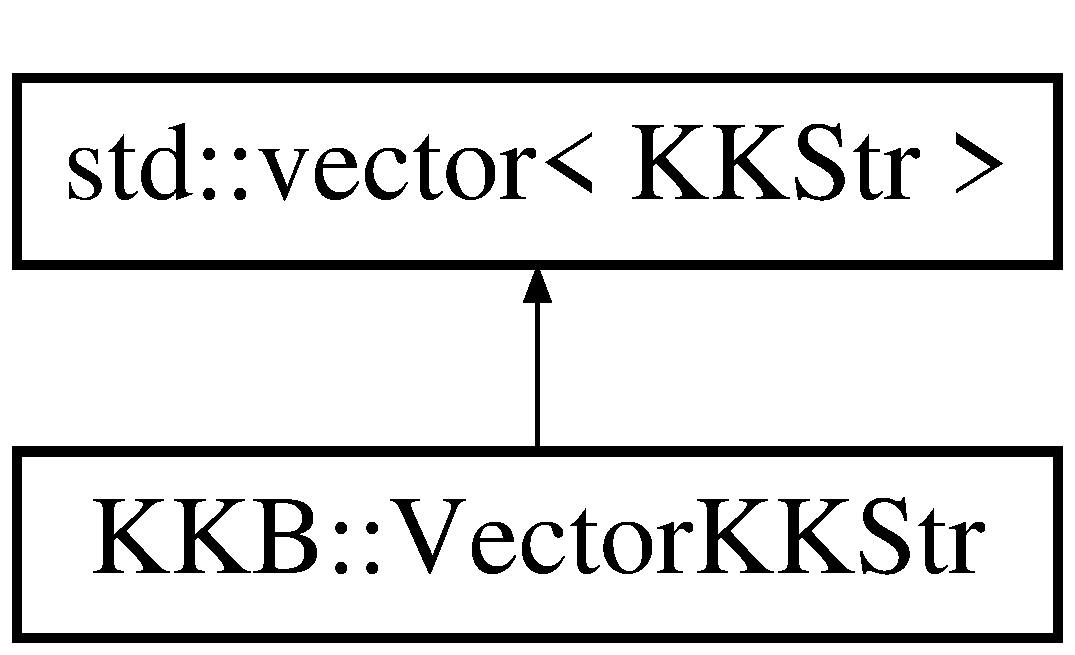
\includegraphics[height=2.000000cm]{class_k_k_b_1_1_vector_k_k_str}
\end{center}
\end{figure}
\subsection*{Public Member Functions}
\begin{DoxyCompactItemize}
\item 
\hyperlink{class_k_k_b_1_1_vector_k_k_str_a8fffb71b681560151fdc653f39c3f7dc}{Vector\+K\+K\+Str} ()
\item 
\hyperlink{class_k_k_b_1_1_vector_k_k_str_a9b4aed0260683b87aacd9cbaeb6cb223}{Vector\+K\+K\+Str} (const \hyperlink{class_k_k_b_1_1_vector_k_k_str}{Vector\+K\+K\+Str} \&v)
\item 
void \hyperlink{class_k_k_b_1_1_vector_k_k_str_a8c1a3b54afb48156b5d462dc2faa0307}{Read\+X\+ML} (\hyperlink{class_k_k_b_1_1_xml_stream}{Xml\+Stream} \&s, \hyperlink{namespace_k_k_b_a5f1b0b1667d79fec26deeff10c43df23}{Xml\+Tag\+Const\+Ptr} tag, \hyperlink{namespace_k_k_b_a7d390f568e2831fb76b86b56c87bf92f}{Vol\+Const\+Bool} \&cancel\+Flag, \hyperlink{class_k_k_b_1_1_run_log}{Run\+Log} \&log)
\item 
void \hyperlink{class_k_k_b_1_1_vector_k_k_str_a3e90bf5fd9c23a8c16f0fdee98946395}{Write\+X\+ML} (const \hyperlink{class_k_k_b_1_1_k_k_str}{K\+K\+Str} \&var\+Name, std\+::ostream \&o) const 
\end{DoxyCompactItemize}


\subsection{Detailed Description}
summary$>$ A string class providing safe runtime management; strings can be used as stream and String\+Builder objects. Simple token parsing is supported as well as various translations to other formats such as \textquotesingle{}int\textquotesingle{}, \textquotesingle{}double\textquotesingle{}, and others. Allocation is done dynamically increasing as needs warrant. All methods ensure that there is no accessing outside the bounds of the allocated string. /summary$>$ todo$>$ Should subclass the class from the stl class \textquotesingle{}string\textquotesingle{}. $<$/todo$>$ 

Definition at line 54 of file K\+K\+Str.\+h.



\subsection{Constructor \& Destructor Documentation}
\index{K\+K\+B\+::\+Vector\+K\+K\+Str@{K\+K\+B\+::\+Vector\+K\+K\+Str}!Vector\+K\+K\+Str@{Vector\+K\+K\+Str}}
\index{Vector\+K\+K\+Str@{Vector\+K\+K\+Str}!K\+K\+B\+::\+Vector\+K\+K\+Str@{K\+K\+B\+::\+Vector\+K\+K\+Str}}
\subsubsection[{\texorpdfstring{Vector\+K\+K\+Str()}{VectorKKStr()}}]{\setlength{\rightskip}{0pt plus 5cm}Vector\+K\+K\+Str\+::\+Vector\+K\+K\+Str (
\begin{DoxyParamCaption}
{}
\end{DoxyParamCaption}
)}\hypertarget{class_k_k_b_1_1_vector_k_k_str_a8fffb71b681560151fdc653f39c3f7dc}{}\label{class_k_k_b_1_1_vector_k_k_str_a8fffb71b681560151fdc653f39c3f7dc}


Definition at line 5264 of file K\+K\+Str.\+cpp.



References Vector\+K\+K\+Str().



Referenced by K\+K\+M\+L\+L\+::\+Classification\+Bias\+Matrix\+::\+Classification\+Bias\+Matrix(), K\+K\+M\+L\+L\+::\+Training\+Process2\+::\+Config\+File\+Format\+Errors(), K\+K\+B\+::\+Configuration\+::\+Configuration(), K\+K\+M\+L\+L\+::\+Training\+Class\+::\+Training\+Class(), Vector\+K\+K\+Str(), and K\+K\+B\+::\+Xml\+Stream\+::\+Xml\+Stream().


\begin{DoxyCode}
5264                          :
5265   vector<KKStr> ()
5266 \{
5267 \}
\end{DoxyCode}
\index{K\+K\+B\+::\+Vector\+K\+K\+Str@{K\+K\+B\+::\+Vector\+K\+K\+Str}!Vector\+K\+K\+Str@{Vector\+K\+K\+Str}}
\index{Vector\+K\+K\+Str@{Vector\+K\+K\+Str}!K\+K\+B\+::\+Vector\+K\+K\+Str@{K\+K\+B\+::\+Vector\+K\+K\+Str}}
\subsubsection[{\texorpdfstring{Vector\+K\+K\+Str(const Vector\+K\+K\+Str \&v)}{VectorKKStr(const VectorKKStr &v)}}]{\setlength{\rightskip}{0pt plus 5cm}Vector\+K\+K\+Str\+::\+Vector\+K\+K\+Str (
\begin{DoxyParamCaption}
\item[{const {\bf Vector\+K\+K\+Str} \&}]{v}
\end{DoxyParamCaption}
)}\hypertarget{class_k_k_b_1_1_vector_k_k_str_a9b4aed0260683b87aacd9cbaeb6cb223}{}\label{class_k_k_b_1_1_vector_k_k_str_a9b4aed0260683b87aacd9cbaeb6cb223}


Definition at line 5270 of file K\+K\+Str.\+cpp.



References Vector\+K\+K\+Str().



Referenced by K\+K\+B\+::\+Configuration\+::\+Configuration(), K\+K\+M\+L\+L\+::\+Training\+Class\+::\+Training\+Class(), and Vector\+K\+K\+Str().


\begin{DoxyCode}
5270                                               :
5271   vector<KKStr> (v)
5272 \{
5273 \}
\end{DoxyCode}


\subsection{Member Function Documentation}
\index{K\+K\+B\+::\+Vector\+K\+K\+Str@{K\+K\+B\+::\+Vector\+K\+K\+Str}!Read\+X\+ML@{Read\+X\+ML}}
\index{Read\+X\+ML@{Read\+X\+ML}!K\+K\+B\+::\+Vector\+K\+K\+Str@{K\+K\+B\+::\+Vector\+K\+K\+Str}}
\subsubsection[{\texorpdfstring{Read\+X\+M\+L(\+Xml\+Stream \&s, Xml\+Tag\+Const\+Ptr tag, Vol\+Const\+Bool \&cancel\+Flag, Run\+Log \&log)}{ReadXML(XmlStream &s, XmlTagConstPtr tag, VolConstBool &cancelFlag, RunLog &log)}}]{\setlength{\rightskip}{0pt plus 5cm}void Vector\+K\+K\+Str\+::\+Read\+X\+ML (
\begin{DoxyParamCaption}
\item[{{\bf Xml\+Stream} \&}]{s, }
\item[{{\bf Xml\+Tag\+Const\+Ptr}}]{tag, }
\item[{{\bf Vol\+Const\+Bool} \&}]{cancel\+Flag, }
\item[{{\bf Run\+Log} \&}]{log}
\end{DoxyParamCaption}
)}\hypertarget{class_k_k_b_1_1_vector_k_k_str_a8c1a3b54afb48156b5d462dc2faa0307}{}\label{class_k_k_b_1_1_vector_k_k_str_a8c1a3b54afb48156b5d462dc2faa0307}


Definition at line 5277 of file K\+K\+Str.\+cpp.



References K\+K\+B\+::\+Xml\+Tag\+::\+Attribute\+Value\+Int32(), K\+K\+B\+::\+K\+K\+Str\+::\+Concat(), K\+K\+B\+::\+Xml\+Content\+::\+Content(), K\+K\+B\+::\+K\+K\+Str\+Parser\+::\+Get\+Next\+Token(), K\+K\+B\+::\+Xml\+Stream\+::\+Get\+Next\+Token(), K\+K\+B\+::\+K\+K\+Str\+Parser\+::\+K\+K\+Str\+Parser(), K\+K\+B\+::\+K\+K\+Str\+Parser\+::\+More\+Tokens(), K\+K\+B\+::\+Xml\+Token\+::tok\+Content, K\+K\+B\+::\+Xml\+Token\+::\+Token\+Type(), and K\+K\+B\+::\+K\+K\+Str\+Parser\+::\+Trim\+White\+Space().


\begin{DoxyCode}
5282 \{
5283   \hyperlink{namespace_k_k_b_af8d832f05c54994a1cce25bd5743e19a}{kkuint32}  count = (\hyperlink{namespace_k_k_b_af8d832f05c54994a1cce25bd5743e19a}{kkuint32})tag->AttributeValueInt32 (\textcolor{stringliteral}{"Count"});
5284 
5285   clear ();
5286 
5287   \hyperlink{class_k_k_b_1_1_xml_token}{XmlTokenPtr}  t = s.\hyperlink{class_k_k_b_1_1_xml_stream_a87cc738b05c666cf5d5c25beaab477b4}{GetNextToken} (cancelFlag, log);
5288 
5289   \textcolor{keywordflow}{while}  (t  &&  (!cancelFlag))
5290   \{
5291     \textcolor{keywordflow}{if}  (t->\hyperlink{class_k_k_b_1_1_xml_token_ae98e2c1a798882647578cae4adcd7176}{TokenType} () == \hyperlink{class_k_k_b_1_1_xml_token_a18b6e90c919f4b92e3b024f50f247f62aff369b5479984ca659548f37ad4caec9}{XmlToken::TokenTypes::tokContent})
5292     \{
5293       \hyperlink{class_k_k_b_1_1_xml_content}{XmlContentPtr}  c = \textcolor{keyword}{dynamic\_cast<}\hyperlink{class_k_k_b_1_1_xml_content}{XmlContentPtr}\textcolor{keyword}{>}(t);
5294       \textcolor{keywordflow}{if}  ((c != NULL)  &&  (c->\hyperlink{class_k_k_b_1_1_xml_content_a1d0730aae45b069e8604bef19b8c0098}{Content} () != NULL))
5295       \{
5296         \hyperlink{class_k_k_b_1_1_k_k_str_parser}{KKStrParser}  parser (*(c->\hyperlink{class_k_k_b_1_1_xml_content_a1d0730aae45b069e8604bef19b8c0098}{Content} ()));
5297         parser.TrimWhiteSpace (\textcolor{stringliteral}{" "});
5298         \textcolor{keywordflow}{while}  (parser.MoreTokens ())
5299         \{
5300           \hyperlink{class_k_k_b_1_1_k_k_str}{KKStr} field = parser.GetNextToken (\textcolor{stringliteral}{"\(\backslash\)t"});
5301           push\_back (field);
5302         \}
5303       \}
5304     \}
5305 
5306     \textcolor{keyword}{delete} t;
5307     \textcolor{keywordflow}{if}  (cancelFlag)
5308       t = NULL;
5309     \textcolor{keywordflow}{else}
5310       t = s.\hyperlink{class_k_k_b_1_1_xml_stream_a87cc738b05c666cf5d5c25beaab477b4}{GetNextToken} (cancelFlag, log);
5311   \}
5312   \textcolor{keyword}{delete}  t;
5313   t = NULL;
5314 \}  \textcolor{comment}{/* ReadXML */}
\end{DoxyCode}
\index{K\+K\+B\+::\+Vector\+K\+K\+Str@{K\+K\+B\+::\+Vector\+K\+K\+Str}!Write\+X\+ML@{Write\+X\+ML}}
\index{Write\+X\+ML@{Write\+X\+ML}!K\+K\+B\+::\+Vector\+K\+K\+Str@{K\+K\+B\+::\+Vector\+K\+K\+Str}}
\subsubsection[{\texorpdfstring{Write\+X\+M\+L(const K\+K\+Str \&var\+Name, std\+::ostream \&o) const }{WriteXML(const KKStr &varName, std::ostream &o) const }}]{\setlength{\rightskip}{0pt plus 5cm}void Vector\+K\+K\+Str\+::\+Write\+X\+ML (
\begin{DoxyParamCaption}
\item[{const {\bf K\+K\+Str} \&}]{var\+Name, }
\item[{std\+::ostream \&}]{o}
\end{DoxyParamCaption}
) const}\hypertarget{class_k_k_b_1_1_vector_k_k_str_a3e90bf5fd9c23a8c16f0fdee98946395}{}\label{class_k_k_b_1_1_vector_k_k_str_a3e90bf5fd9c23a8c16f0fdee98946395}


Definition at line 5319 of file K\+K\+Str.\+cpp.



References K\+K\+B\+::\+Xml\+Tag\+::\+Add\+Atribute(), K\+K\+B\+::\+K\+K\+Str\+::\+Empty(), K\+K\+B\+::operator$<$$<$(), K\+K\+B\+::\+Xml\+Tag\+::tag\+End, K\+K\+B\+::\+Xml\+Tag\+::tag\+Start, K\+K\+B\+::\+Xml\+Tag\+::\+Write\+X\+M\+L(), and K\+K\+B\+::\+Xml\+Tag\+::\+Xml\+Tag().



Referenced by K\+K\+M\+L\+L\+::\+Attribute\+::\+Write\+X\+M\+L().


\begin{DoxyCode}
5322 \{
5323   \hyperlink{class_k_k_b_1_1_xml_tag}{XmlTag}  startTag (\textcolor{stringliteral}{"VectorKKStr"}, \hyperlink{class_k_k_b_1_1_xml_tag_a6c0ef0e23f982f49d55d4fb7eaff6ac9ab02b23b5e15b3a1353771313e1176ce0}{XmlTag::TagTypes::tagStart});
5324   \textcolor{keywordflow}{if}  (!varName.\hyperlink{class_k_k_b_1_1_k_k_str_ac69942f73fffd672ec2a6e1c410afdb6}{Empty} ())
5325     startTag.AddAtribute (\textcolor{stringliteral}{"VarName"}, varName);
5326   startTag.AddAtribute (\textcolor{stringliteral}{"Count"}, (\hyperlink{namespace_k_k_b_a8fa4952cc84fda1de4bec1fbdd8d5b1b}{kkint32})size ());
5327   startTag.WriteXML (o);
5328 
5329   const\_iterator  idx;
5330   \hyperlink{namespace_k_k_b_af8d832f05c54994a1cce25bd5743e19a}{kkuint32} x = 0;
5331   \textcolor{keywordflow}{for}  (idx = begin ();  idx != end ();  ++idx, ++x)
5332   \{
5333     \textcolor{keywordflow}{if}  (x > 0)  o << \textcolor{stringliteral}{"\(\backslash\)t"};
5334     \hyperlink{class_k_k_b_1_1_xml_content_ab0e370562d215b8e19dac6d18c4a95e1}{XmlContent::WriteXml} (idx->QuotedStr (), o);
5335   \}
5336   \hyperlink{class_k_k_b_1_1_xml_tag}{XmlTag}  endTag (\textcolor{stringliteral}{"VectorKKStr"}, \hyperlink{class_k_k_b_1_1_xml_tag_a6c0ef0e23f982f49d55d4fb7eaff6ac9a3ceaa9a790f688ec97a35b5a3fd3b164}{XmlTag::TagTypes::tagEnd});
5337   endTag.WriteXML (o);
5338   o << \hyperlink{namespace_k_k_b_ad1f50f65af6adc8fa9e6f62d007818a8}{endl};
5339 \}
\end{DoxyCode}


The documentation for this class was generated from the following files\+:\begin{DoxyCompactItemize}
\item 
C\+:/\+Users/\+Kurt/\+Git\+Hub/\+K\+Square\+Libraries/\+K\+K\+Base/\hyperlink{_k_k_str_8h}{K\+K\+Str.\+h}\item 
C\+:/\+Users/\+Kurt/\+Git\+Hub/\+K\+Square\+Libraries/\+K\+K\+Base/\hyperlink{_k_k_str_8cpp}{K\+K\+Str.\+cpp}\end{DoxyCompactItemize}

\hypertarget{union_k_k_b_1_1_word_format32_bits}{}\section{K\+KB\+:\+:Word\+Format32\+Bits Union Reference}
\label{union_k_k_b_1_1_word_format32_bits}\index{K\+K\+B\+::\+Word\+Format32\+Bits@{K\+K\+B\+::\+Word\+Format32\+Bits}}


Structure used to break 32 bit word into different formats;.  




{\ttfamily \#include $<$K\+K\+Base\+Types.\+h$>$}

\subsection*{Public Member Functions}
\begin{DoxyCompactItemize}
\item 
\hyperlink{union_k_k_b_1_1_word_format32_bits_abcd5db82f5e511c364b3f8daff4867c2}{Word\+Format32\+Bits} ()
\item 
\hyperlink{union_k_k_b_1_1_word_format32_bits_a81edf4cd657f56bd7c910e8b9f9904d0}{Word\+Format32\+Bits} (\hyperlink{namespace_k_k_b_af8d832f05c54994a1cce25bd5743e19a}{kkuint32} d)
\item 
\hyperlink{union_k_k_b_1_1_word_format32_bits_a52e78ab3dba1ffa22870e641ed91ec21}{Word\+Format32\+Bits} (\hyperlink{namespace_k_k_b_a8fa4952cc84fda1de4bec1fbdd8d5b1b}{kkint32} d)
\item 
\hyperlink{union_k_k_b_1_1_word_format32_bits_a28378cd4873f9ac51f487e732937d932}{Word\+Format32\+Bits} (\hyperlink{namespace_k_k_b_ace9969169bf514f9ee6185186949cdf7}{uchar} b0, \hyperlink{namespace_k_k_b_ace9969169bf514f9ee6185186949cdf7}{uchar} b1, \hyperlink{namespace_k_k_b_ace9969169bf514f9ee6185186949cdf7}{uchar} b2, \hyperlink{namespace_k_k_b_ace9969169bf514f9ee6185186949cdf7}{uchar} b3)
\end{DoxyCompactItemize}
\subsection*{Public Attributes}
\begin{DoxyCompactItemize}
\item 
\begin{tabbing}
xx\=xx\=xx\=xx\=xx\=xx\=xx\=xx\=xx\=\kill
struct \{\\
\>\hyperlink{namespace_k_k_b_ace9969169bf514f9ee6185186949cdf7}{uchar} \hyperlink{union_k_k_b_1_1_word_format32_bits_a7172ef166d47f672768eaf94666ec5cd}{byte0}\\
\>\hyperlink{namespace_k_k_b_ace9969169bf514f9ee6185186949cdf7}{uchar} \hyperlink{union_k_k_b_1_1_word_format32_bits_a3a4cec5553f28a1010a3a1bb6f182f3f}{byte1}\\
\>\hyperlink{namespace_k_k_b_ace9969169bf514f9ee6185186949cdf7}{uchar} \hyperlink{union_k_k_b_1_1_word_format32_bits_a7dce1e987826e201b31d75d3050359ba}{byte2}\\
\>\hyperlink{namespace_k_k_b_ace9969169bf514f9ee6185186949cdf7}{uchar} \hyperlink{union_k_k_b_1_1_word_format32_bits_aa833400f553206f88aae886076886fe8}{byte3}\\
\} \hyperlink{union_k_k_b_1_1_word_format32_bits_a377fc22bfc20aaa559f6572b55663069}{fourBytes}\\

\end{tabbing}\item 
\hyperlink{namespace_k_k_b_af8d832f05c54994a1cce25bd5743e19a}{kkuint32} \hyperlink{union_k_k_b_1_1_word_format32_bits_a0f0a2e9b5926c499ded704deff7297b5}{signed32\+Bit\+Int}
\item 
\hyperlink{namespace_k_k_b_af8d832f05c54994a1cce25bd5743e19a}{kkuint32} \hyperlink{union_k_k_b_1_1_word_format32_bits_ac0c992b584e5b3549cd2c0e8528c9b74}{unsigned32\+Bit\+Int}
\end{DoxyCompactItemize}


\subsection{Detailed Description}
Structure used to break 32 bit word into different formats;. 

Definition at line 283 of file K\+K\+Base\+Types.\+h.



\subsection{Constructor \& Destructor Documentation}
\index{K\+K\+B\+::\+Word\+Format32\+Bits@{K\+K\+B\+::\+Word\+Format32\+Bits}!Word\+Format32\+Bits@{Word\+Format32\+Bits}}
\index{Word\+Format32\+Bits@{Word\+Format32\+Bits}!K\+K\+B\+::\+Word\+Format32\+Bits@{K\+K\+B\+::\+Word\+Format32\+Bits}}
\subsubsection[{\texorpdfstring{Word\+Format32\+Bits()}{WordFormat32Bits()}}]{\setlength{\rightskip}{0pt plus 5cm}Word\+Format32\+Bits\+::\+Word\+Format32\+Bits (
\begin{DoxyParamCaption}
{}
\end{DoxyParamCaption}
)}\hypertarget{union_k_k_b_1_1_word_format32_bits_abcd5db82f5e511c364b3f8daff4867c2}{}\label{union_k_k_b_1_1_word_format32_bits_abcd5db82f5e511c364b3f8daff4867c2}


Definition at line 115 of file K\+K\+Base\+Types.\+cpp.



References unsigned32\+Bit\+Int.



Referenced by K\+K\+L\+S\+C\+::\+Scanner\+File4\+Bit\+Encoded\+::\+Op\+Rec\+Instrument\+Data\+Word3\+::\+Op\+Rec\+Instrument\+Data\+Word3().


\begin{DoxyCode}
116 \{
117   \hyperlink{union_k_k_b_1_1_word_format32_bits_ac0c992b584e5b3549cd2c0e8528c9b74}{unsigned32BitInt} = 0;
118 \}
\end{DoxyCode}
\index{K\+K\+B\+::\+Word\+Format32\+Bits@{K\+K\+B\+::\+Word\+Format32\+Bits}!Word\+Format32\+Bits@{Word\+Format32\+Bits}}
\index{Word\+Format32\+Bits@{Word\+Format32\+Bits}!K\+K\+B\+::\+Word\+Format32\+Bits@{K\+K\+B\+::\+Word\+Format32\+Bits}}
\subsubsection[{\texorpdfstring{Word\+Format32\+Bits(kkuint32 d)}{WordFormat32Bits(kkuint32 d)}}]{\setlength{\rightskip}{0pt plus 5cm}Word\+Format32\+Bits\+::\+Word\+Format32\+Bits (
\begin{DoxyParamCaption}
\item[{{\bf kkuint32}}]{d}
\end{DoxyParamCaption}
)}\hypertarget{union_k_k_b_1_1_word_format32_bits_a81edf4cd657f56bd7c910e8b9f9904d0}{}\label{union_k_k_b_1_1_word_format32_bits_a81edf4cd657f56bd7c910e8b9f9904d0}


Definition at line 122 of file K\+K\+Base\+Types.\+cpp.



References unsigned32\+Bit\+Int.



Referenced by K\+K\+L\+S\+C\+::\+Scanner\+File\+::\+Report\+Text\+Msg().


\begin{DoxyCode}
123 \{
124   \hyperlink{union_k_k_b_1_1_word_format32_bits_ac0c992b584e5b3549cd2c0e8528c9b74}{unsigned32BitInt} = d;
125 \}
\end{DoxyCode}
\index{K\+K\+B\+::\+Word\+Format32\+Bits@{K\+K\+B\+::\+Word\+Format32\+Bits}!Word\+Format32\+Bits@{Word\+Format32\+Bits}}
\index{Word\+Format32\+Bits@{Word\+Format32\+Bits}!K\+K\+B\+::\+Word\+Format32\+Bits@{K\+K\+B\+::\+Word\+Format32\+Bits}}
\subsubsection[{\texorpdfstring{Word\+Format32\+Bits(kkint32 d)}{WordFormat32Bits(kkint32 d)}}]{\setlength{\rightskip}{0pt plus 5cm}Word\+Format32\+Bits\+::\+Word\+Format32\+Bits (
\begin{DoxyParamCaption}
\item[{{\bf kkint32}}]{d}
\end{DoxyParamCaption}
)}\hypertarget{union_k_k_b_1_1_word_format32_bits_a52e78ab3dba1ffa22870e641ed91ec21}{}\label{union_k_k_b_1_1_word_format32_bits_a52e78ab3dba1ffa22870e641ed91ec21}


Definition at line 129 of file K\+K\+Base\+Types.\+cpp.



References signed32\+Bit\+Int.


\begin{DoxyCode}
130 \{
131   \hyperlink{union_k_k_b_1_1_word_format32_bits_a0f0a2e9b5926c499ded704deff7297b5}{signed32BitInt} = d;
132 \}
\end{DoxyCode}
\index{K\+K\+B\+::\+Word\+Format32\+Bits@{K\+K\+B\+::\+Word\+Format32\+Bits}!Word\+Format32\+Bits@{Word\+Format32\+Bits}}
\index{Word\+Format32\+Bits@{Word\+Format32\+Bits}!K\+K\+B\+::\+Word\+Format32\+Bits@{K\+K\+B\+::\+Word\+Format32\+Bits}}
\subsubsection[{\texorpdfstring{Word\+Format32\+Bits(uchar b0, uchar b1, uchar b2, uchar b3)}{WordFormat32Bits(uchar b0, uchar b1, uchar b2, uchar b3)}}]{\setlength{\rightskip}{0pt plus 5cm}Word\+Format32\+Bits\+::\+Word\+Format32\+Bits (
\begin{DoxyParamCaption}
\item[{{\bf uchar}}]{b0, }
\item[{{\bf uchar}}]{b1, }
\item[{{\bf uchar}}]{b2, }
\item[{{\bf uchar}}]{b3}
\end{DoxyParamCaption}
)}\hypertarget{union_k_k_b_1_1_word_format32_bits_a28378cd4873f9ac51f487e732937d932}{}\label{union_k_k_b_1_1_word_format32_bits_a28378cd4873f9ac51f487e732937d932}


Definition at line 136 of file K\+K\+Base\+Types.\+cpp.


\begin{DoxyCode}
141 \{
142   \hyperlink{union_k_k_b_1_1_word_format32_bits_a377fc22bfc20aaa559f6572b55663069}{fourBytes}.byte0 = b0;
143   \hyperlink{union_k_k_b_1_1_word_format32_bits_a377fc22bfc20aaa559f6572b55663069}{fourBytes}.byte1 = b1;
144   \hyperlink{union_k_k_b_1_1_word_format32_bits_a377fc22bfc20aaa559f6572b55663069}{fourBytes}.byte2 = b2;
145   \hyperlink{union_k_k_b_1_1_word_format32_bits_a377fc22bfc20aaa559f6572b55663069}{fourBytes}.byte3 = b3;
146 \}
\end{DoxyCode}


\subsection{Member Data Documentation}
\index{K\+K\+B\+::\+Word\+Format32\+Bits@{K\+K\+B\+::\+Word\+Format32\+Bits}!byte0@{byte0}}
\index{byte0@{byte0}!K\+K\+B\+::\+Word\+Format32\+Bits@{K\+K\+B\+::\+Word\+Format32\+Bits}}
\subsubsection[{\texorpdfstring{byte0}{byte0}}]{\setlength{\rightskip}{0pt plus 5cm}{\bf uchar} K\+K\+B\+::\+Word\+Format32\+Bits\+::byte0}\hypertarget{union_k_k_b_1_1_word_format32_bits_a7172ef166d47f672768eaf94666ec5cd}{}\label{union_k_k_b_1_1_word_format32_bits_a7172ef166d47f672768eaf94666ec5cd}


Definition at line 292 of file K\+K\+Base\+Types.\+h.

\index{K\+K\+B\+::\+Word\+Format32\+Bits@{K\+K\+B\+::\+Word\+Format32\+Bits}!byte1@{byte1}}
\index{byte1@{byte1}!K\+K\+B\+::\+Word\+Format32\+Bits@{K\+K\+B\+::\+Word\+Format32\+Bits}}
\subsubsection[{\texorpdfstring{byte1}{byte1}}]{\setlength{\rightskip}{0pt plus 5cm}{\bf uchar} K\+K\+B\+::\+Word\+Format32\+Bits\+::byte1}\hypertarget{union_k_k_b_1_1_word_format32_bits_a3a4cec5553f28a1010a3a1bb6f182f3f}{}\label{union_k_k_b_1_1_word_format32_bits_a3a4cec5553f28a1010a3a1bb6f182f3f}


Definition at line 293 of file K\+K\+Base\+Types.\+h.

\index{K\+K\+B\+::\+Word\+Format32\+Bits@{K\+K\+B\+::\+Word\+Format32\+Bits}!byte2@{byte2}}
\index{byte2@{byte2}!K\+K\+B\+::\+Word\+Format32\+Bits@{K\+K\+B\+::\+Word\+Format32\+Bits}}
\subsubsection[{\texorpdfstring{byte2}{byte2}}]{\setlength{\rightskip}{0pt plus 5cm}{\bf uchar} K\+K\+B\+::\+Word\+Format32\+Bits\+::byte2}\hypertarget{union_k_k_b_1_1_word_format32_bits_a7dce1e987826e201b31d75d3050359ba}{}\label{union_k_k_b_1_1_word_format32_bits_a7dce1e987826e201b31d75d3050359ba}


Definition at line 294 of file K\+K\+Base\+Types.\+h.

\index{K\+K\+B\+::\+Word\+Format32\+Bits@{K\+K\+B\+::\+Word\+Format32\+Bits}!byte3@{byte3}}
\index{byte3@{byte3}!K\+K\+B\+::\+Word\+Format32\+Bits@{K\+K\+B\+::\+Word\+Format32\+Bits}}
\subsubsection[{\texorpdfstring{byte3}{byte3}}]{\setlength{\rightskip}{0pt plus 5cm}{\bf uchar} K\+K\+B\+::\+Word\+Format32\+Bits\+::byte3}\hypertarget{union_k_k_b_1_1_word_format32_bits_aa833400f553206f88aae886076886fe8}{}\label{union_k_k_b_1_1_word_format32_bits_aa833400f553206f88aae886076886fe8}


Definition at line 295 of file K\+K\+Base\+Types.\+h.

\index{K\+K\+B\+::\+Word\+Format32\+Bits@{K\+K\+B\+::\+Word\+Format32\+Bits}!four\+Bytes@{four\+Bytes}}
\index{four\+Bytes@{four\+Bytes}!K\+K\+B\+::\+Word\+Format32\+Bits@{K\+K\+B\+::\+Word\+Format32\+Bits}}
\subsubsection[{\texorpdfstring{four\+Bytes}{fourBytes}}]{\setlength{\rightskip}{0pt plus 5cm}struct \{ ... \}    K\+K\+B\+::\+Word\+Format32\+Bits\+::four\+Bytes}\hypertarget{union_k_k_b_1_1_word_format32_bits_a377fc22bfc20aaa559f6572b55663069}{}\label{union_k_k_b_1_1_word_format32_bits_a377fc22bfc20aaa559f6572b55663069}
\index{K\+K\+B\+::\+Word\+Format32\+Bits@{K\+K\+B\+::\+Word\+Format32\+Bits}!signed32\+Bit\+Int@{signed32\+Bit\+Int}}
\index{signed32\+Bit\+Int@{signed32\+Bit\+Int}!K\+K\+B\+::\+Word\+Format32\+Bits@{K\+K\+B\+::\+Word\+Format32\+Bits}}
\subsubsection[{\texorpdfstring{signed32\+Bit\+Int}{signed32BitInt}}]{\setlength{\rightskip}{0pt plus 5cm}{\bf kkuint32} K\+K\+B\+::\+Word\+Format32\+Bits\+::signed32\+Bit\+Int}\hypertarget{union_k_k_b_1_1_word_format32_bits_a0f0a2e9b5926c499ded704deff7297b5}{}\label{union_k_k_b_1_1_word_format32_bits_a0f0a2e9b5926c499ded704deff7297b5}


Definition at line 299 of file K\+K\+Base\+Types.\+h.



Referenced by Word\+Format32\+Bits().

\index{K\+K\+B\+::\+Word\+Format32\+Bits@{K\+K\+B\+::\+Word\+Format32\+Bits}!unsigned32\+Bit\+Int@{unsigned32\+Bit\+Int}}
\index{unsigned32\+Bit\+Int@{unsigned32\+Bit\+Int}!K\+K\+B\+::\+Word\+Format32\+Bits@{K\+K\+B\+::\+Word\+Format32\+Bits}}
\subsubsection[{\texorpdfstring{unsigned32\+Bit\+Int}{unsigned32BitInt}}]{\setlength{\rightskip}{0pt plus 5cm}{\bf kkuint32} K\+K\+B\+::\+Word\+Format32\+Bits\+::unsigned32\+Bit\+Int}\hypertarget{union_k_k_b_1_1_word_format32_bits_ac0c992b584e5b3549cd2c0e8528c9b74}{}\label{union_k_k_b_1_1_word_format32_bits_ac0c992b584e5b3549cd2c0e8528c9b74}


Definition at line 298 of file K\+K\+Base\+Types.\+h.



Referenced by K\+K\+L\+S\+C\+::\+Scanner\+File\+::\+Report\+Instrument\+Data\+Word(), Word\+Format32\+Bits(), and K\+K\+L\+S\+C\+::\+Scanner\+File\+::\+Write\+Instrument\+Data\+Word().



The documentation for this union was generated from the following files\+:\begin{DoxyCompactItemize}
\item 
C\+:/\+Users/\+Kurt/\+Git\+Hub/\+K\+Square\+Libraries/\+K\+K\+Base/\hyperlink{_k_k_base_types_8h}{K\+K\+Base\+Types.\+h}\item 
C\+:/\+Users/\+Kurt/\+Git\+Hub/\+K\+Square\+Libraries/\+K\+K\+Base/\hyperlink{_k_k_base_types_8cpp}{K\+K\+Base\+Types.\+cpp}\end{DoxyCompactItemize}

\hypertarget{class_k_k_b_1_1_xml_attribute}{}\section{K\+KB\+:\+:Xml\+Attribute Class Reference}
\label{class_k_k_b_1_1_xml_attribute}\index{K\+K\+B\+::\+Xml\+Attribute@{K\+K\+B\+::\+Xml\+Attribute}}


{\ttfamily \#include $<$Xml\+Stream.\+h$>$}

\subsection*{Public Member Functions}
\begin{DoxyCompactItemize}
\item 
\hyperlink{class_k_k_b_1_1_xml_attribute_a4720547ffcf02ee9f83ef8d1b5138c3e}{Xml\+Attribute} (const \hyperlink{class_k_k_b_1_1_k_k_str}{K\+K\+Str} \&\+\_\+name, const \hyperlink{class_k_k_b_1_1_k_k_str}{K\+K\+Str} \&\+\_\+value)
\item 
const \hyperlink{class_k_k_b_1_1_k_k_str}{K\+K\+Str} \& \hyperlink{class_k_k_b_1_1_xml_attribute_a1028e1a45e72cf7c4b0450f3206f0fe9}{Name} () const 
\item 
const \hyperlink{class_k_k_b_1_1_k_k_str}{K\+K\+Str} \& \hyperlink{class_k_k_b_1_1_xml_attribute_a3f80845535790d617c8d1ef01f134a65}{Value} () const 
\end{DoxyCompactItemize}


\subsection{Detailed Description}


Definition at line 112 of file Xml\+Stream.\+h.



\subsection{Constructor \& Destructor Documentation}
\index{K\+K\+B\+::\+Xml\+Attribute@{K\+K\+B\+::\+Xml\+Attribute}!Xml\+Attribute@{Xml\+Attribute}}
\index{Xml\+Attribute@{Xml\+Attribute}!K\+K\+B\+::\+Xml\+Attribute@{K\+K\+B\+::\+Xml\+Attribute}}
\subsubsection[{\texorpdfstring{Xml\+Attribute(const K\+K\+Str \&\+\_\+name, const K\+K\+Str \&\+\_\+value)}{XmlAttribute(const KKStr &_name, const KKStr &_value)}}]{\setlength{\rightskip}{0pt plus 5cm}K\+K\+B\+::\+Xml\+Attribute\+::\+Xml\+Attribute (
\begin{DoxyParamCaption}
\item[{const {\bf K\+K\+Str} \&}]{\+\_\+name, }
\item[{const {\bf K\+K\+Str} \&}]{\+\_\+value}
\end{DoxyParamCaption}
)\hspace{0.3cm}{\ttfamily [inline]}}\hypertarget{class_k_k_b_1_1_xml_attribute_a4720547ffcf02ee9f83ef8d1b5138c3e}{}\label{class_k_k_b_1_1_xml_attribute_a4720547ffcf02ee9f83ef8d1b5138c3e}


Definition at line 115 of file Xml\+Stream.\+h.



References K\+K\+B\+::\+K\+K\+Str\+::\+K\+K\+Str().



Referenced by K\+K\+B\+::\+Xml\+Attribute\+List\+::\+Add\+Attribute().


\begin{DoxyCode}
117                   :
118         name  (\_name),
119         value (\_value)
120     \{\}
\end{DoxyCode}


\subsection{Member Function Documentation}
\index{K\+K\+B\+::\+Xml\+Attribute@{K\+K\+B\+::\+Xml\+Attribute}!Name@{Name}}
\index{Name@{Name}!K\+K\+B\+::\+Xml\+Attribute@{K\+K\+B\+::\+Xml\+Attribute}}
\subsubsection[{\texorpdfstring{Name() const }{Name() const }}]{\setlength{\rightskip}{0pt plus 5cm}const {\bf K\+K\+Str}\& K\+K\+B\+::\+Xml\+Attribute\+::\+Name (
\begin{DoxyParamCaption}
{}
\end{DoxyParamCaption}
) const\hspace{0.3cm}{\ttfamily [inline]}}\hypertarget{class_k_k_b_1_1_xml_attribute_a1028e1a45e72cf7c4b0450f3206f0fe9}{}\label{class_k_k_b_1_1_xml_attribute_a1028e1a45e72cf7c4b0450f3206f0fe9}


Definition at line 122 of file Xml\+Stream.\+h.



Referenced by K\+K\+B\+::\+Xml\+Tag\+::\+To\+String().


\begin{DoxyCode}
122 \{\textcolor{keywordflow}{return} name;\}
\end{DoxyCode}
\index{K\+K\+B\+::\+Xml\+Attribute@{K\+K\+B\+::\+Xml\+Attribute}!Value@{Value}}
\index{Value@{Value}!K\+K\+B\+::\+Xml\+Attribute@{K\+K\+B\+::\+Xml\+Attribute}}
\subsubsection[{\texorpdfstring{Value() const }{Value() const }}]{\setlength{\rightskip}{0pt plus 5cm}const {\bf K\+K\+Str}\& K\+K\+B\+::\+Xml\+Attribute\+::\+Value (
\begin{DoxyParamCaption}
{}
\end{DoxyParamCaption}
) const\hspace{0.3cm}{\ttfamily [inline]}}\hypertarget{class_k_k_b_1_1_xml_attribute_a3f80845535790d617c8d1ef01f134a65}{}\label{class_k_k_b_1_1_xml_attribute_a3f80845535790d617c8d1ef01f134a65}


Definition at line 123 of file Xml\+Stream.\+h.



Referenced by K\+K\+B\+::\+Xml\+Attribute\+List\+::\+Attribute\+Value\+By\+Name(), and K\+K\+B\+::\+Xml\+Tag\+::\+To\+String().


\begin{DoxyCode}
123 \{\textcolor{keywordflow}{return} value;\}
\end{DoxyCode}


The documentation for this class was generated from the following file\+:\begin{DoxyCompactItemize}
\item 
C\+:/\+Users/\+Kurt/\+Git\+Hub/\+K\+Square\+Libraries/\+K\+K\+Base/\hyperlink{_xml_stream_8h}{Xml\+Stream.\+h}\end{DoxyCompactItemize}

\hypertarget{class_k_k_b_1_1_xml_attribute_list}{}\section{K\+KB\+:\+:Xml\+Attribute\+List Class Reference}
\label{class_k_k_b_1_1_xml_attribute_list}\index{K\+K\+B\+::\+Xml\+Attribute\+List@{K\+K\+B\+::\+Xml\+Attribute\+List}}


{\ttfamily \#include $<$Xml\+Stream.\+h$>$}

Inheritance diagram for K\+KB\+:\+:Xml\+Attribute\+List\+:\begin{figure}[H]
\begin{center}
\leavevmode
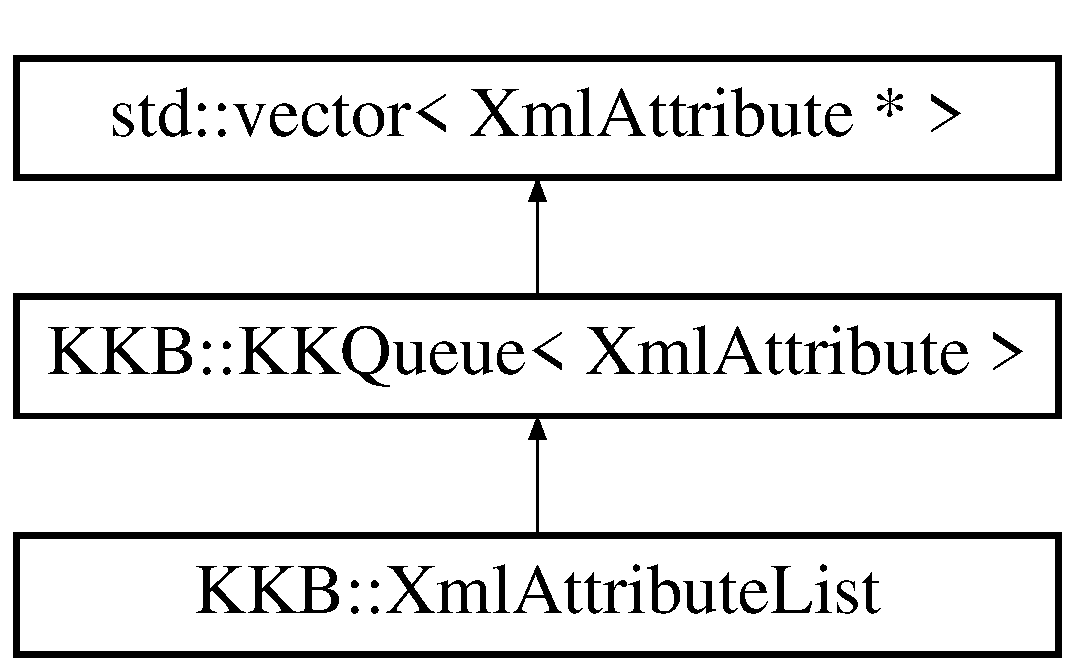
\includegraphics[height=3.000000cm]{class_k_k_b_1_1_xml_attribute_list}
\end{center}
\end{figure}
\subsection*{Public Member Functions}
\begin{DoxyCompactItemize}
\item 
\hyperlink{class_k_k_b_1_1_xml_attribute_list_a6de978a65392c992fe11736aa5d90a88}{Xml\+Attribute\+List} (bool \+\_\+owner)
\item 
\hyperlink{class_k_k_b_1_1_xml_attribute_list_a8154307977ce6cd95d1a52196bbc3461}{Xml\+Attribute\+List} (const \hyperlink{class_k_k_b_1_1_xml_attribute_list}{Xml\+Attribute\+List} \&attributes)
\item 
void \hyperlink{class_k_k_b_1_1_xml_attribute_list_ab3eb98b55d4874281ba91c342422bd83}{Add\+Attribute} (const \hyperlink{class_k_k_b_1_1_k_k_str}{K\+K\+Str} \&name, const \hyperlink{class_k_k_b_1_1_k_k_str}{K\+K\+Str} \&value)
\item 
\hyperlink{namespace_k_k_b_a46f665ec17615c856eff3d21f78bed5c}{K\+K\+Str\+Const\+Ptr} \hyperlink{class_k_k_b_1_1_xml_attribute_list_af1933bdf7634b45e3fef432d1542c8d9}{Attribute\+Name\+By\+Index} (\hyperlink{namespace_k_k_b_af8d832f05c54994a1cce25bd5743e19a}{kkuint32} index) const 
\item 
\hyperlink{namespace_k_k_b_a46f665ec17615c856eff3d21f78bed5c}{K\+K\+Str\+Const\+Ptr} \hyperlink{class_k_k_b_1_1_xml_attribute_list_a8535e0974a45c3820f8b43f6c6f459dc}{Attribute\+Value\+By\+Index} (\hyperlink{namespace_k_k_b_af8d832f05c54994a1cce25bd5743e19a}{kkuint32} index) const 
\item 
\hyperlink{namespace_k_k_b_a46f665ec17615c856eff3d21f78bed5c}{K\+K\+Str\+Const\+Ptr} \hyperlink{class_k_k_b_1_1_xml_attribute_list_a21a30ed3b18c0ab3517dfd57d4d4f450}{Attribute\+Value\+By\+Name} (const \hyperlink{class_k_k_b_1_1_k_k_str}{K\+K\+Str} \&name) const 
\item 
\hyperlink{class_k_k_b_1_1_date_time}{Date\+Time} \hyperlink{class_k_k_b_1_1_xml_attribute_list_a575e44934a102d84feef0fa7df40a7ef}{Attribute\+Value\+Date\+Time} (const \hyperlink{class_k_k_b_1_1_k_k_str}{K\+K\+Str} \&name) const 
\item 
\hyperlink{namespace_k_k_b_a8fa4952cc84fda1de4bec1fbdd8d5b1b}{kkint32} \hyperlink{class_k_k_b_1_1_xml_attribute_list_ade591332c27a5b659ab87560c140d9ae}{Attribute\+Value\+Int32} (const \hyperlink{class_k_k_b_1_1_k_k_str}{K\+K\+Str} \&name) const 
\item 
const \hyperlink{class_k_k_b_1_1_k_k_str}{K\+K\+Str} \& \hyperlink{class_k_k_b_1_1_xml_attribute_list_ae7baf3bee375c9673c3725d5449c06ad}{Attribute\+Value\+K\+K\+Str} (const \hyperlink{class_k_k_b_1_1_k_k_str}{K\+K\+Str} \&name) const 
\item 
\hyperlink{namespace_k_k_b_a4a5163ef82488376826c02944d6ef6c8}{Xml\+Attribute\+Ptr} \hyperlink{class_k_k_b_1_1_xml_attribute_list_afc1ed77976a907f4ecab8e2e847dc848}{Look\+Up\+By\+Name} (const \hyperlink{class_k_k_b_1_1_k_k_str}{K\+K\+Str} \&name) const 
\item 
virtual \hyperlink{namespace_k_k_b_a4a5163ef82488376826c02944d6ef6c8}{Xml\+Attribute\+Ptr} \hyperlink{class_k_k_b_1_1_xml_attribute_list_ab4d9d743cb29b2954aea4a00a490bf3e}{Pop\+From\+Back} ()
\item 
virtual \hyperlink{namespace_k_k_b_a4a5163ef82488376826c02944d6ef6c8}{Xml\+Attribute\+Ptr} \hyperlink{class_k_k_b_1_1_xml_attribute_list_a044d40989e2745b68bff212243c0b0a2}{Pop\+From\+Fromt} ()
\item 
virtual void \hyperlink{class_k_k_b_1_1_xml_attribute_list_ad301a537bc8b1216d51f2cfc2a4383c0}{Push\+On\+Back} (\hyperlink{namespace_k_k_b_a4a5163ef82488376826c02944d6ef6c8}{Xml\+Attribute\+Ptr} a)
\item 
virtual void \hyperlink{class_k_k_b_1_1_xml_attribute_list_a8c659645b5e1e812e60cf847a4fd9c0b}{Push\+On\+Front} (\hyperlink{namespace_k_k_b_a4a5163ef82488376826c02944d6ef6c8}{Xml\+Attribute\+Ptr} a)
\end{DoxyCompactItemize}
\subsection*{Additional Inherited Members}


\subsection{Detailed Description}


Definition at line 136 of file Xml\+Stream.\+h.



\subsection{Constructor \& Destructor Documentation}
\index{K\+K\+B\+::\+Xml\+Attribute\+List@{K\+K\+B\+::\+Xml\+Attribute\+List}!Xml\+Attribute\+List@{Xml\+Attribute\+List}}
\index{Xml\+Attribute\+List@{Xml\+Attribute\+List}!K\+K\+B\+::\+Xml\+Attribute\+List@{K\+K\+B\+::\+Xml\+Attribute\+List}}
\subsubsection[{\texorpdfstring{Xml\+Attribute\+List(bool \+\_\+owner)}{XmlAttributeList(bool _owner)}}]{\setlength{\rightskip}{0pt plus 5cm}Xml\+Attribute\+List\+::\+Xml\+Attribute\+List (
\begin{DoxyParamCaption}
\item[{bool}]{\+\_\+owner}
\end{DoxyParamCaption}
)}\hypertarget{class_k_k_b_1_1_xml_attribute_list_a6de978a65392c992fe11736aa5d90a88}{}\label{class_k_k_b_1_1_xml_attribute_list_a6de978a65392c992fe11736aa5d90a88}


Definition at line 235 of file Xml\+Stream.\+cpp.



References Xml\+Attribute\+List().



Referenced by Xml\+Attribute\+List().


\begin{DoxyCode}
235                                                :
236   \hyperlink{class_k_k_b_1_1_k_k_queue}{KKQueue<XmlAttribute>} (\_owner)
237 \{
238 \}
\end{DoxyCode}
\index{K\+K\+B\+::\+Xml\+Attribute\+List@{K\+K\+B\+::\+Xml\+Attribute\+List}!Xml\+Attribute\+List@{Xml\+Attribute\+List}}
\index{Xml\+Attribute\+List@{Xml\+Attribute\+List}!K\+K\+B\+::\+Xml\+Attribute\+List@{K\+K\+B\+::\+Xml\+Attribute\+List}}
\subsubsection[{\texorpdfstring{Xml\+Attribute\+List(const Xml\+Attribute\+List \&attributes)}{XmlAttributeList(const XmlAttributeList &attributes)}}]{\setlength{\rightskip}{0pt plus 5cm}Xml\+Attribute\+List\+::\+Xml\+Attribute\+List (
\begin{DoxyParamCaption}
\item[{const {\bf Xml\+Attribute\+List} \&}]{attributes}
\end{DoxyParamCaption}
)}\hypertarget{class_k_k_b_1_1_xml_attribute_list_a8154307977ce6cd95d1a52196bbc3461}{}\label{class_k_k_b_1_1_xml_attribute_list_a8154307977ce6cd95d1a52196bbc3461}


Definition at line 241 of file Xml\+Stream.\+cpp.


\begin{DoxyCode}
242 \{
243   \hyperlink{class_k_k_b_1_1_k_k_queue_aeb057c9c010446f46f57c1e355f981f1}{XmlAttributeList::const\_iterator}  idx;
244   \textcolor{keywordflow}{for}  (idx = attributes.begin ();  idx != attributes.end ();  ++idx)
245     \hyperlink{class_k_k_b_1_1_xml_attribute_list_ad301a537bc8b1216d51f2cfc2a4383c0}{PushOnBack} (*idx);
246 \}
\end{DoxyCode}


\subsection{Member Function Documentation}
\index{K\+K\+B\+::\+Xml\+Attribute\+List@{K\+K\+B\+::\+Xml\+Attribute\+List}!Add\+Attribute@{Add\+Attribute}}
\index{Add\+Attribute@{Add\+Attribute}!K\+K\+B\+::\+Xml\+Attribute\+List@{K\+K\+B\+::\+Xml\+Attribute\+List}}
\subsubsection[{\texorpdfstring{Add\+Attribute(const K\+K\+Str \&name, const K\+K\+Str \&value)}{AddAttribute(const KKStr &name, const KKStr &value)}}]{\setlength{\rightskip}{0pt plus 5cm}void Xml\+Attribute\+List\+::\+Add\+Attribute (
\begin{DoxyParamCaption}
\item[{const {\bf K\+K\+Str} \&}]{name, }
\item[{const {\bf K\+K\+Str} \&}]{value}
\end{DoxyParamCaption}
)}\hypertarget{class_k_k_b_1_1_xml_attribute_list_ab3eb98b55d4874281ba91c342422bd83}{}\label{class_k_k_b_1_1_xml_attribute_list_ab3eb98b55d4874281ba91c342422bd83}


Definition at line 366 of file Xml\+Stream.\+cpp.



References Push\+On\+Back(), and K\+K\+B\+::\+Xml\+Attribute\+::\+Xml\+Attribute().


\begin{DoxyCode}
369 \{
370   \hyperlink{class_k_k_b_1_1_xml_attribute_list_ad301a537bc8b1216d51f2cfc2a4383c0}{PushOnBack} (\textcolor{keyword}{new} \hyperlink{class_k_k_b_1_1_xml_attribute}{XmlAttribute} (name, value));
371 \}
\end{DoxyCode}
\index{K\+K\+B\+::\+Xml\+Attribute\+List@{K\+K\+B\+::\+Xml\+Attribute\+List}!Attribute\+Name\+By\+Index@{Attribute\+Name\+By\+Index}}
\index{Attribute\+Name\+By\+Index@{Attribute\+Name\+By\+Index}!K\+K\+B\+::\+Xml\+Attribute\+List@{K\+K\+B\+::\+Xml\+Attribute\+List}}
\subsubsection[{\texorpdfstring{Attribute\+Name\+By\+Index(kkuint32 index) const }{AttributeNameByIndex(kkuint32 index) const }}]{\setlength{\rightskip}{0pt plus 5cm}{\bf K\+K\+Str\+Const\+Ptr} Xml\+Attribute\+List\+::\+Attribute\+Name\+By\+Index (
\begin{DoxyParamCaption}
\item[{{\bf kkuint32}}]{index}
\end{DoxyParamCaption}
) const}\hypertarget{class_k_k_b_1_1_xml_attribute_list_af1933bdf7634b45e3fef432d1542c8d9}{}\label{class_k_k_b_1_1_xml_attribute_list_af1933bdf7634b45e3fef432d1542c8d9}


Definition at line 320 of file Xml\+Stream.\+cpp.


\begin{DoxyCode}
321 \{
322   \textcolor{keywordflow}{if}  (index >= size ())
323     \textcolor{keywordflow}{return} NULL;
324   \textcolor{keywordflow}{else}
325     \textcolor{keywordflow}{return} &(at (index)->Name ());
326 \}
\end{DoxyCode}
\index{K\+K\+B\+::\+Xml\+Attribute\+List@{K\+K\+B\+::\+Xml\+Attribute\+List}!Attribute\+Value\+By\+Index@{Attribute\+Value\+By\+Index}}
\index{Attribute\+Value\+By\+Index@{Attribute\+Value\+By\+Index}!K\+K\+B\+::\+Xml\+Attribute\+List@{K\+K\+B\+::\+Xml\+Attribute\+List}}
\subsubsection[{\texorpdfstring{Attribute\+Value\+By\+Index(kkuint32 index) const }{AttributeValueByIndex(kkuint32 index) const }}]{\setlength{\rightskip}{0pt plus 5cm}{\bf K\+K\+Str\+Const\+Ptr} Xml\+Attribute\+List\+::\+Attribute\+Value\+By\+Index (
\begin{DoxyParamCaption}
\item[{{\bf kkuint32}}]{index}
\end{DoxyParamCaption}
) const}\hypertarget{class_k_k_b_1_1_xml_attribute_list_a8535e0974a45c3820f8b43f6c6f459dc}{}\label{class_k_k_b_1_1_xml_attribute_list_a8535e0974a45c3820f8b43f6c6f459dc}


Definition at line 311 of file Xml\+Stream.\+cpp.


\begin{DoxyCode}
312 \{
313   \textcolor{keywordflow}{if}  (index >= size ())
314     \textcolor{keywordflow}{return} NULL;
315   \textcolor{keywordflow}{else}
316     \textcolor{keywordflow}{return} &(at (index)->Value ());
317 \}
\end{DoxyCode}
\index{K\+K\+B\+::\+Xml\+Attribute\+List@{K\+K\+B\+::\+Xml\+Attribute\+List}!Attribute\+Value\+By\+Name@{Attribute\+Value\+By\+Name}}
\index{Attribute\+Value\+By\+Name@{Attribute\+Value\+By\+Name}!K\+K\+B\+::\+Xml\+Attribute\+List@{K\+K\+B\+::\+Xml\+Attribute\+List}}
\subsubsection[{\texorpdfstring{Attribute\+Value\+By\+Name(const K\+K\+Str \&name) const }{AttributeValueByName(const KKStr &name) const }}]{\setlength{\rightskip}{0pt plus 5cm}{\bf K\+K\+Str\+Const\+Ptr} Xml\+Attribute\+List\+::\+Attribute\+Value\+By\+Name (
\begin{DoxyParamCaption}
\item[{const {\bf K\+K\+Str} \&}]{name}
\end{DoxyParamCaption}
) const}\hypertarget{class_k_k_b_1_1_xml_attribute_list_a21a30ed3b18c0ab3517dfd57d4d4f450}{}\label{class_k_k_b_1_1_xml_attribute_list_a21a30ed3b18c0ab3517dfd57d4d4f450}


Definition at line 301 of file Xml\+Stream.\+cpp.



References Look\+Up\+By\+Name(), and K\+K\+B\+::\+Xml\+Attribute\+::\+Value().



Referenced by Attribute\+Value\+Date\+Time(), Attribute\+Value\+Int32(), and Attribute\+Value\+K\+K\+Str().


\begin{DoxyCode}
302 \{
303   \hyperlink{class_k_k_b_1_1_xml_attribute}{XmlAttributePtr}  a = \hyperlink{class_k_k_b_1_1_xml_attribute_list_afc1ed77976a907f4ecab8e2e847dc848}{LookUpByName} (name);
304   \textcolor{keywordflow}{if}  (a)
305     \textcolor{keywordflow}{return} &(a->\hyperlink{class_k_k_b_1_1_xml_attribute_a3f80845535790d617c8d1ef01f134a65}{Value} ());
306   \textcolor{keywordflow}{else}
307     \textcolor{keywordflow}{return} NULL;
308 \}
\end{DoxyCode}
\index{K\+K\+B\+::\+Xml\+Attribute\+List@{K\+K\+B\+::\+Xml\+Attribute\+List}!Attribute\+Value\+Date\+Time@{Attribute\+Value\+Date\+Time}}
\index{Attribute\+Value\+Date\+Time@{Attribute\+Value\+Date\+Time}!K\+K\+B\+::\+Xml\+Attribute\+List@{K\+K\+B\+::\+Xml\+Attribute\+List}}
\subsubsection[{\texorpdfstring{Attribute\+Value\+Date\+Time(const K\+K\+Str \&name) const }{AttributeValueDateTime(const KKStr &name) const }}]{\setlength{\rightskip}{0pt plus 5cm}{\bf Date\+Time} Xml\+Attribute\+List\+::\+Attribute\+Value\+Date\+Time (
\begin{DoxyParamCaption}
\item[{const {\bf K\+K\+Str} \&}]{name}
\end{DoxyParamCaption}
) const}\hypertarget{class_k_k_b_1_1_xml_attribute_list_a575e44934a102d84feef0fa7df40a7ef}{}\label{class_k_k_b_1_1_xml_attribute_list_a575e44934a102d84feef0fa7df40a7ef}


Definition at line 352 of file Xml\+Stream.\+cpp.



References Attribute\+Value\+By\+Name(), and K\+K\+B\+::\+Date\+Time\+::\+Date\+Time().


\begin{DoxyCode}
353 \{
354   \hyperlink{class_k_k_b_1_1_k_k_str}{KKStrConstPtr} s = \hyperlink{class_k_k_b_1_1_xml_attribute_list_a21a30ed3b18c0ab3517dfd57d4d4f450}{AttributeValueByName} (name);
355   \textcolor{keywordflow}{if}  (!s)
356     \textcolor{keywordflow}{return}  \hyperlink{class_k_k_b_1_1_date_time}{DateTime} ();
357   
358   \hyperlink{class_k_k_b_1_1_date_time}{DateTime}  dt (*s);
359   \textcolor{keywordflow}{return}  dt;
360 \}
\end{DoxyCode}
\index{K\+K\+B\+::\+Xml\+Attribute\+List@{K\+K\+B\+::\+Xml\+Attribute\+List}!Attribute\+Value\+Int32@{Attribute\+Value\+Int32}}
\index{Attribute\+Value\+Int32@{Attribute\+Value\+Int32}!K\+K\+B\+::\+Xml\+Attribute\+List@{K\+K\+B\+::\+Xml\+Attribute\+List}}
\subsubsection[{\texorpdfstring{Attribute\+Value\+Int32(const K\+K\+Str \&name) const }{AttributeValueInt32(const KKStr &name) const }}]{\setlength{\rightskip}{0pt plus 5cm}{\bf kkint32} Xml\+Attribute\+List\+::\+Attribute\+Value\+Int32 (
\begin{DoxyParamCaption}
\item[{const {\bf K\+K\+Str} \&}]{name}
\end{DoxyParamCaption}
) const}\hypertarget{class_k_k_b_1_1_xml_attribute_list_ade591332c27a5b659ab87560c140d9ae}{}\label{class_k_k_b_1_1_xml_attribute_list_ade591332c27a5b659ab87560c140d9ae}


Definition at line 341 of file Xml\+Stream.\+cpp.



References Attribute\+Value\+By\+Name(), and K\+K\+B\+::\+K\+K\+Str\+::\+To\+Int32().


\begin{DoxyCode}
342 \{
343   \hyperlink{class_k_k_b_1_1_k_k_str}{KKStrConstPtr} s = \hyperlink{class_k_k_b_1_1_xml_attribute_list_a21a30ed3b18c0ab3517dfd57d4d4f450}{AttributeValueByName} (name);
344   \textcolor{keywordflow}{if}  (!s)
345     \textcolor{keywordflow}{return}  0;
346   \textcolor{keywordflow}{else}
347     \textcolor{keywordflow}{return} s->\hyperlink{class_k_k_b_1_1_k_k_str_ab3b9de5eb86600593ac866e8323caa32}{ToInt32} ();
348 \}
\end{DoxyCode}
\index{K\+K\+B\+::\+Xml\+Attribute\+List@{K\+K\+B\+::\+Xml\+Attribute\+List}!Attribute\+Value\+K\+K\+Str@{Attribute\+Value\+K\+K\+Str}}
\index{Attribute\+Value\+K\+K\+Str@{Attribute\+Value\+K\+K\+Str}!K\+K\+B\+::\+Xml\+Attribute\+List@{K\+K\+B\+::\+Xml\+Attribute\+List}}
\subsubsection[{\texorpdfstring{Attribute\+Value\+K\+K\+Str(const K\+K\+Str \&name) const }{AttributeValueKKStr(const KKStr &name) const }}]{\setlength{\rightskip}{0pt plus 5cm}const {\bf K\+K\+Str} \& Xml\+Attribute\+List\+::\+Attribute\+Value\+K\+K\+Str (
\begin{DoxyParamCaption}
\item[{const {\bf K\+K\+Str} \&}]{name}
\end{DoxyParamCaption}
) const}\hypertarget{class_k_k_b_1_1_xml_attribute_list_ae7baf3bee375c9673c3725d5449c06ad}{}\label{class_k_k_b_1_1_xml_attribute_list_ae7baf3bee375c9673c3725d5449c06ad}


Definition at line 330 of file Xml\+Stream.\+cpp.



References Attribute\+Value\+By\+Name(), K\+K\+B\+::\+K\+K\+Str\+::\+Concat(), and K\+K\+B\+::\+K\+K\+Str\+::\+Empty\+Str().


\begin{DoxyCode}
331 \{
332   \hyperlink{class_k_k_b_1_1_k_k_str}{KKStrConstPtr} s = \hyperlink{class_k_k_b_1_1_xml_attribute_list_a21a30ed3b18c0ab3517dfd57d4d4f450}{AttributeValueByName} (name);
333   \textcolor{keywordflow}{if}  (s)
334     \textcolor{keywordflow}{return}  *s;
335   \textcolor{keywordflow}{else}
336     \textcolor{keywordflow}{return} \hyperlink{class_k_k_b_1_1_k_k_str_ab6e416b3ef54ef632bd10c3f7a2f7994}{KKStr::EmptyStr} ();
337 \}
\end{DoxyCode}
\index{K\+K\+B\+::\+Xml\+Attribute\+List@{K\+K\+B\+::\+Xml\+Attribute\+List}!Look\+Up\+By\+Name@{Look\+Up\+By\+Name}}
\index{Look\+Up\+By\+Name@{Look\+Up\+By\+Name}!K\+K\+B\+::\+Xml\+Attribute\+List@{K\+K\+B\+::\+Xml\+Attribute\+List}}
\subsubsection[{\texorpdfstring{Look\+Up\+By\+Name(const K\+K\+Str \&name) const }{LookUpByName(const KKStr &name) const }}]{\setlength{\rightskip}{0pt plus 5cm}{\bf Xml\+Attribute\+Ptr} Xml\+Attribute\+List\+::\+Look\+Up\+By\+Name (
\begin{DoxyParamCaption}
\item[{const {\bf K\+K\+Str} \&}]{name}
\end{DoxyParamCaption}
) const}\hypertarget{class_k_k_b_1_1_xml_attribute_list_afc1ed77976a907f4ecab8e2e847dc848}{}\label{class_k_k_b_1_1_xml_attribute_list_afc1ed77976a907f4ecab8e2e847dc848}


Definition at line 375 of file Xml\+Stream.\+cpp.



Referenced by Attribute\+Value\+By\+Name().


\begin{DoxyCode}
376 \{
377   NameIndex::const\_iterator  idx;
378   idx = nameIndex.find (name);
379   \textcolor{keywordflow}{if}  (idx == nameIndex.end ())
380     \textcolor{keywordflow}{return} NULL;
381 
382   \textcolor{keywordflow}{if}  (idx->first != name)
383     \textcolor{keywordflow}{return} NULL;
384 
385   \textcolor{keywordflow}{return} idx->second;
386 \}
\end{DoxyCode}
\index{K\+K\+B\+::\+Xml\+Attribute\+List@{K\+K\+B\+::\+Xml\+Attribute\+List}!Pop\+From\+Back@{Pop\+From\+Back}}
\index{Pop\+From\+Back@{Pop\+From\+Back}!K\+K\+B\+::\+Xml\+Attribute\+List@{K\+K\+B\+::\+Xml\+Attribute\+List}}
\subsubsection[{\texorpdfstring{Pop\+From\+Back()}{PopFromBack()}}]{\setlength{\rightskip}{0pt plus 5cm}{\bf Xml\+Attribute\+Ptr} Xml\+Attribute\+List\+::\+Pop\+From\+Back (
\begin{DoxyParamCaption}
{}
\end{DoxyParamCaption}
)\hspace{0.3cm}{\ttfamily [virtual]}}\hypertarget{class_k_k_b_1_1_xml_attribute_list_ab4d9d743cb29b2954aea4a00a490bf3e}{}\label{class_k_k_b_1_1_xml_attribute_list_ab4d9d743cb29b2954aea4a00a490bf3e}
Removes the last element in the container and returns its pointer. If the container is empty will return N\+U\+LL. 

Reimplemented from \hyperlink{class_k_k_b_1_1_k_k_queue_a03844c19a838fed7e7bcc5816846dcfd}{K\+K\+B\+::\+K\+K\+Queue$<$ Xml\+Attribute $>$}.



Definition at line 264 of file Xml\+Stream.\+cpp.


\begin{DoxyCode}
265 \{
266   \hyperlink{class_k_k_b_1_1_xml_attribute}{XmlAttributePtr}  a = \hyperlink{class_k_k_b_1_1_k_k_queue_a03844c19a838fed7e7bcc5816846dcfd}{KKQueue<XmlAttribute>::PopFromBack} 
      ();
267   \textcolor{keywordflow}{if}  (a)
268     DeleteFromNameIndex (a);
269   \textcolor{keywordflow}{return}  a;
270 \}
\end{DoxyCode}
\index{K\+K\+B\+::\+Xml\+Attribute\+List@{K\+K\+B\+::\+Xml\+Attribute\+List}!Pop\+From\+Fromt@{Pop\+From\+Fromt}}
\index{Pop\+From\+Fromt@{Pop\+From\+Fromt}!K\+K\+B\+::\+Xml\+Attribute\+List@{K\+K\+B\+::\+Xml\+Attribute\+List}}
\subsubsection[{\texorpdfstring{Pop\+From\+Fromt()}{PopFromFromt()}}]{\setlength{\rightskip}{0pt plus 5cm}{\bf Xml\+Attribute\+Ptr} Xml\+Attribute\+List\+::\+Pop\+From\+Fromt (
\begin{DoxyParamCaption}
{}
\end{DoxyParamCaption}
)\hspace{0.3cm}{\ttfamily [virtual]}}\hypertarget{class_k_k_b_1_1_xml_attribute_list_a044d40989e2745b68bff212243c0b0a2}{}\label{class_k_k_b_1_1_xml_attribute_list_a044d40989e2745b68bff212243c0b0a2}


Definition at line 273 of file Xml\+Stream.\+cpp.


\begin{DoxyCode}
274 \{
275   \hyperlink{class_k_k_b_1_1_xml_attribute}{XmlAttributePtr}  a = \hyperlink{class_k_k_b_1_1_k_k_queue_a2b2205f34516ac1f2950f441625d3ec7}{KKQueue<XmlAttribute>::PopFromFront}
       ();
276   \textcolor{keywordflow}{if}  (a)
277     DeleteFromNameIndex (a);
278   \textcolor{keywordflow}{return}  a;
279 \}
\end{DoxyCode}
\index{K\+K\+B\+::\+Xml\+Attribute\+List@{K\+K\+B\+::\+Xml\+Attribute\+List}!Push\+On\+Back@{Push\+On\+Back}}
\index{Push\+On\+Back@{Push\+On\+Back}!K\+K\+B\+::\+Xml\+Attribute\+List@{K\+K\+B\+::\+Xml\+Attribute\+List}}
\subsubsection[{\texorpdfstring{Push\+On\+Back(\+Xml\+Attribute\+Ptr a)}{PushOnBack(XmlAttributePtr a)}}]{\setlength{\rightskip}{0pt plus 5cm}void Xml\+Attribute\+List\+::\+Push\+On\+Back (
\begin{DoxyParamCaption}
\item[{{\bf Xml\+Attribute\+Ptr}}]{\+\_\+entry}
\end{DoxyParamCaption}
)\hspace{0.3cm}{\ttfamily [virtual]}}\hypertarget{class_k_k_b_1_1_xml_attribute_list_ad301a537bc8b1216d51f2cfc2a4383c0}{}\label{class_k_k_b_1_1_xml_attribute_list_ad301a537bc8b1216d51f2cfc2a4383c0}
Adds \textquotesingle{}\+\_\+entry\textquotesingle{} to the End of the container. 

Reimplemented from \hyperlink{class_k_k_b_1_1_k_k_queue_aa9fba4632b54268bf71ecb42dee0b575}{K\+K\+B\+::\+K\+K\+Queue$<$ Xml\+Attribute $>$}.



Definition at line 250 of file Xml\+Stream.\+cpp.



Referenced by Add\+Attribute().


\begin{DoxyCode}
251 \{
252   \hyperlink{class_k_k_b_1_1_k_k_queue_aa9fba4632b54268bf71ecb42dee0b575}{KKQueue<XmlAttribute>::PushOnBack} (a);
253   nameIndex.insert (NameIndexPair (a->Name (), a));
254 \}
\end{DoxyCode}
\index{K\+K\+B\+::\+Xml\+Attribute\+List@{K\+K\+B\+::\+Xml\+Attribute\+List}!Push\+On\+Front@{Push\+On\+Front}}
\index{Push\+On\+Front@{Push\+On\+Front}!K\+K\+B\+::\+Xml\+Attribute\+List@{K\+K\+B\+::\+Xml\+Attribute\+List}}
\subsubsection[{\texorpdfstring{Push\+On\+Front(\+Xml\+Attribute\+Ptr a)}{PushOnFront(XmlAttributePtr a)}}]{\setlength{\rightskip}{0pt plus 5cm}void Xml\+Attribute\+List\+::\+Push\+On\+Front (
\begin{DoxyParamCaption}
\item[{{\bf Xml\+Attribute\+Ptr}}]{\+\_\+entry}
\end{DoxyParamCaption}
)\hspace{0.3cm}{\ttfamily [virtual]}}\hypertarget{class_k_k_b_1_1_xml_attribute_list_a8c659645b5e1e812e60cf847a4fd9c0b}{}\label{class_k_k_b_1_1_xml_attribute_list_a8c659645b5e1e812e60cf847a4fd9c0b}
Adds \textquotesingle{}\+\_\+entry\textquotesingle{} to the Front of the container. 

Reimplemented from \hyperlink{class_k_k_b_1_1_k_k_queue_a07b83a99241a167f7a395a40d32f6380}{K\+K\+B\+::\+K\+K\+Queue$<$ Xml\+Attribute $>$}.



Definition at line 257 of file Xml\+Stream.\+cpp.


\begin{DoxyCode}
258 \{
259   \hyperlink{class_k_k_b_1_1_k_k_queue_a07b83a99241a167f7a395a40d32f6380}{KKQueue<XmlAttribute>::PushOnFront} (a);
260   nameIndex.insert (NameIndexPair (a->Name (), a));
261 \}
\end{DoxyCode}


The documentation for this class was generated from the following files\+:\begin{DoxyCompactItemize}
\item 
C\+:/\+Users/\+Kurt/\+Git\+Hub/\+K\+Square\+Libraries/\+K\+K\+Base/\hyperlink{_xml_stream_8h}{Xml\+Stream.\+h}\item 
C\+:/\+Users/\+Kurt/\+Git\+Hub/\+K\+Square\+Libraries/\+K\+K\+Base/\hyperlink{_xml_stream_8cpp}{Xml\+Stream.\+cpp}\end{DoxyCompactItemize}

\hypertarget{class_k_k_b_1_1_xml_content}{}\section{K\+KB\+:\+:Xml\+Content Class Reference}
\label{class_k_k_b_1_1_xml_content}\index{K\+K\+B\+::\+Xml\+Content@{K\+K\+B\+::\+Xml\+Content}}


{\ttfamily \#include $<$Xml\+Stream.\+h$>$}

Inheritance diagram for K\+KB\+:\+:Xml\+Content\+:\begin{figure}[H]
\begin{center}
\leavevmode
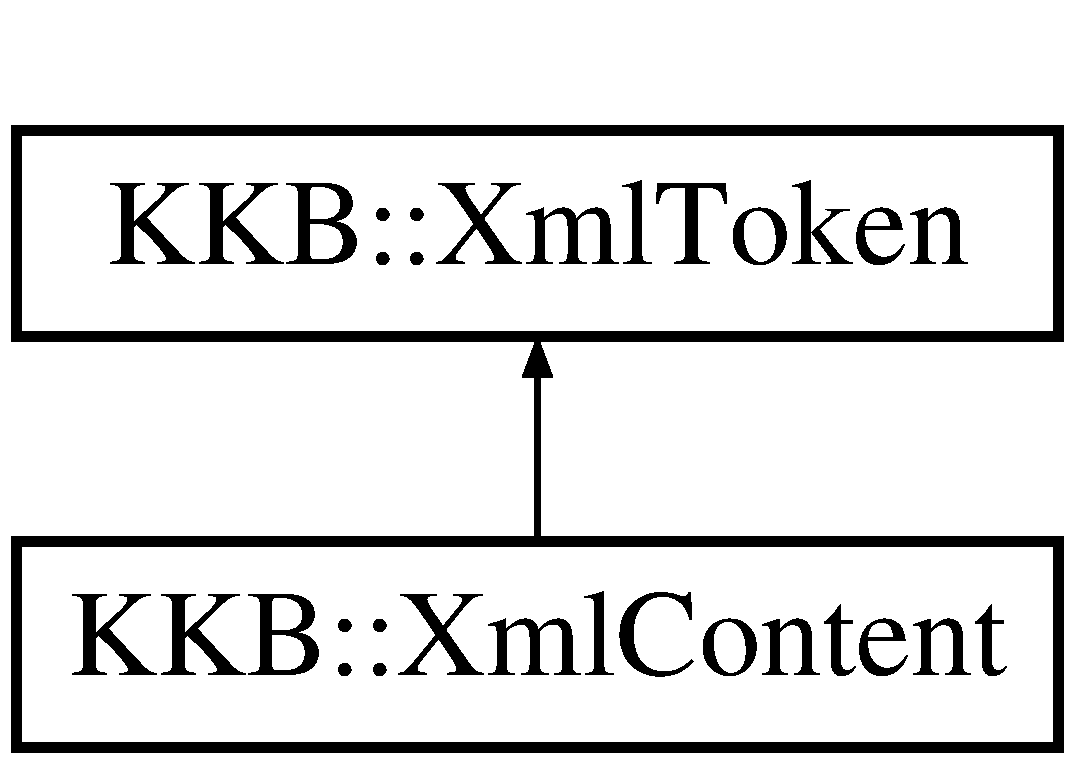
\includegraphics[height=2.000000cm]{class_k_k_b_1_1_xml_content}
\end{center}
\end{figure}
\subsection*{Public Types}
\begin{DoxyCompactItemize}
\item 
typedef \hyperlink{class_k_k_b_1_1_xml_content}{Xml\+Content} $\ast$ \hyperlink{class_k_k_b_1_1_xml_content_a3a8c54aef77299a0548008388417b739}{Xml\+Content\+Ptr}
\end{DoxyCompactItemize}
\subsection*{Public Member Functions}
\begin{DoxyCompactItemize}
\item 
\hyperlink{class_k_k_b_1_1_xml_content_aeb42527bcfe7bf9b1aa0c34781e217b2}{Xml\+Content} (\hyperlink{namespace_k_k_b_a9adbef5a6b3be0867f5570df2a08f388}{K\+K\+Str\+Ptr} \+\_\+content)
\item 
virtual \hyperlink{class_k_k_b_1_1_xml_content_a08bb7cedafb02ecd14e369467aede7a3}{$\sim$\+Xml\+Content} ()
\item 
\hyperlink{namespace_k_k_b_a9adbef5a6b3be0867f5570df2a08f388}{K\+K\+Str\+Ptr} const \hyperlink{class_k_k_b_1_1_xml_content_a1d0730aae45b069e8604bef19b8c0098}{Content} () const 
\item 
\hyperlink{namespace_k_k_b_a9adbef5a6b3be0867f5570df2a08f388}{K\+K\+Str\+Ptr} \hyperlink{class_k_k_b_1_1_xml_content_ad9137145da779da77a0a59c5ca1e72a7}{Take\+Ownership} ()
\item 
virtual \hyperlink{class_k_k_b_1_1_xml_token_a18b6e90c919f4b92e3b024f50f247f62}{Token\+Types} \hyperlink{class_k_k_b_1_1_xml_content_a64e6bd4c4e53fbdc749a1a64336640b2}{Token\+Type} ()
\end{DoxyCompactItemize}
\subsection*{Static Public Member Functions}
\begin{DoxyCompactItemize}
\item 
static void \hyperlink{class_k_k_b_1_1_xml_content_ab0e370562d215b8e19dac6d18c4a95e1}{Write\+Xml} (const \hyperlink{class_k_k_b_1_1_k_k_str}{K\+K\+Str} \&s, std\+::ostream \&o)
\end{DoxyCompactItemize}


\subsection{Detailed Description}


Definition at line 328 of file Xml\+Stream.\+h.



\subsection{Member Typedef Documentation}
\index{K\+K\+B\+::\+Xml\+Content@{K\+K\+B\+::\+Xml\+Content}!Xml\+Content\+Ptr@{Xml\+Content\+Ptr}}
\index{Xml\+Content\+Ptr@{Xml\+Content\+Ptr}!K\+K\+B\+::\+Xml\+Content@{K\+K\+B\+::\+Xml\+Content}}
\subsubsection[{\texorpdfstring{Xml\+Content\+Ptr}{XmlContentPtr}}]{\setlength{\rightskip}{0pt plus 5cm}typedef {\bf Xml\+Content}$\ast$ {\bf K\+K\+B\+::\+Xml\+Content\+::\+Xml\+Content\+Ptr}}\hypertarget{class_k_k_b_1_1_xml_content_a3a8c54aef77299a0548008388417b739}{}\label{class_k_k_b_1_1_xml_content_a3a8c54aef77299a0548008388417b739}


Definition at line 331 of file Xml\+Stream.\+h.



\subsection{Constructor \& Destructor Documentation}
\index{K\+K\+B\+::\+Xml\+Content@{K\+K\+B\+::\+Xml\+Content}!Xml\+Content@{Xml\+Content}}
\index{Xml\+Content@{Xml\+Content}!K\+K\+B\+::\+Xml\+Content@{K\+K\+B\+::\+Xml\+Content}}
\subsubsection[{\texorpdfstring{Xml\+Content(\+K\+K\+Str\+Ptr \+\_\+content)}{XmlContent(KKStrPtr _content)}}]{\setlength{\rightskip}{0pt plus 5cm}Xml\+Content\+::\+Xml\+Content (
\begin{DoxyParamCaption}
\item[{{\bf K\+K\+Str\+Ptr}}]{\+\_\+content}
\end{DoxyParamCaption}
)}\hypertarget{class_k_k_b_1_1_xml_content_aeb42527bcfe7bf9b1aa0c34781e217b2}{}\label{class_k_k_b_1_1_xml_content_aeb42527bcfe7bf9b1aa0c34781e217b2}


Definition at line 829 of file Xml\+Stream.\+cpp.



References K\+K\+B\+::\+Xml\+Token\+::\+Xml\+Token().



Referenced by K\+K\+B\+::\+Xml\+Stream\+::\+Get\+Next\+Content(), and K\+K\+B\+::\+Xml\+Stream\+::\+Get\+Next\+Token().


\begin{DoxyCode}
829                                          : 
830       \hyperlink{class_k_k_b_1_1_xml_token_ad865182b75127e6996f9e4dd27b87d91}{XmlToken} (), 
831       content (\_content) 
832 \{
833 \}
\end{DoxyCode}
\index{K\+K\+B\+::\+Xml\+Content@{K\+K\+B\+::\+Xml\+Content}!````~Xml\+Content@{$\sim$\+Xml\+Content}}
\index{````~Xml\+Content@{$\sim$\+Xml\+Content}!K\+K\+B\+::\+Xml\+Content@{K\+K\+B\+::\+Xml\+Content}}
\subsubsection[{\texorpdfstring{$\sim$\+Xml\+Content()}{~XmlContent()}}]{\setlength{\rightskip}{0pt plus 5cm}Xml\+Content\+::$\sim$\+Xml\+Content (
\begin{DoxyParamCaption}
{}
\end{DoxyParamCaption}
)\hspace{0.3cm}{\ttfamily [virtual]}}\hypertarget{class_k_k_b_1_1_xml_content_a08bb7cedafb02ecd14e369467aede7a3}{}\label{class_k_k_b_1_1_xml_content_a08bb7cedafb02ecd14e369467aede7a3}


Definition at line 837 of file Xml\+Stream.\+cpp.


\begin{DoxyCode}
838 \{
839   \textcolor{keyword}{delete}  content;
840   content = NULL;
841 \}
\end{DoxyCode}


\subsection{Member Function Documentation}
\index{K\+K\+B\+::\+Xml\+Content@{K\+K\+B\+::\+Xml\+Content}!Content@{Content}}
\index{Content@{Content}!K\+K\+B\+::\+Xml\+Content@{K\+K\+B\+::\+Xml\+Content}}
\subsubsection[{\texorpdfstring{Content() const }{Content() const }}]{\setlength{\rightskip}{0pt plus 5cm}{\bf K\+K\+Str\+Ptr} const K\+K\+B\+::\+Xml\+Content\+::\+Content (
\begin{DoxyParamCaption}
{}
\end{DoxyParamCaption}
) const\hspace{0.3cm}{\ttfamily [inline]}}\hypertarget{class_k_k_b_1_1_xml_content_a1d0730aae45b069e8604bef19b8c0098}{}\label{class_k_k_b_1_1_xml_content_a1d0730aae45b069e8604bef19b8c0098}


Definition at line 338 of file Xml\+Stream.\+h.



Referenced by K\+K\+M\+L\+L\+::\+Attribute\+Type\+Vector\+::\+Read\+X\+M\+L(), K\+K\+B\+::\+Vector\+K\+K\+Str\+::\+Read\+X\+M\+L(), K\+K\+M\+L\+L\+::\+Class\+Prob\+List\+::\+Read\+X\+M\+L(), K\+K\+B\+::\+Bit\+String\+::\+Read\+X\+M\+L(), K\+K\+M\+L\+L\+::\+Feature\+Num\+List\+::\+Read\+X\+M\+L(), K\+K\+M\+L\+L\+::\+Binary\+Class\+Parms\+List\+::\+Read\+X\+M\+L(), S\+V\+M233\+::\+Svm\+Model233\+::\+Read\+X\+M\+L(), K\+K\+B\+::\+K\+K\+Str\+::\+Read\+X\+M\+L(), K\+K\+M\+L\+L\+::\+M\+L\+Class\+Index\+List\+::\+Read\+X\+M\+L(), K\+K\+B\+::\+K\+K\+Str\+List\+::\+Read\+X\+M\+L(), K\+K\+B\+::\+K\+K\+Str\+List\+Indexed\+::\+Read\+X\+M\+L(), K\+K\+B\+::\+Xml\+Element\+Bool\+::\+Xml\+Element\+Bool(), K\+K\+B\+::\+Xml\+Element\+Key\+Value\+Pairs\+::\+Xml\+Element\+Key\+Value\+Pairs(), and K\+K\+M\+L\+L\+::\+Xml\+Element\+M\+L\+Class\+Name\+List\+::\+Xml\+Element\+M\+L\+Class\+Name\+List().


\begin{DoxyCode}
338 \{\textcolor{keywordflow}{return}  content;\}
\end{DoxyCode}
\index{K\+K\+B\+::\+Xml\+Content@{K\+K\+B\+::\+Xml\+Content}!Take\+Ownership@{Take\+Ownership}}
\index{Take\+Ownership@{Take\+Ownership}!K\+K\+B\+::\+Xml\+Content@{K\+K\+B\+::\+Xml\+Content}}
\subsubsection[{\texorpdfstring{Take\+Ownership()}{TakeOwnership()}}]{\setlength{\rightskip}{0pt plus 5cm}{\bf K\+K\+Str\+Ptr} Xml\+Content\+::\+Take\+Ownership (
\begin{DoxyParamCaption}
{}
\end{DoxyParamCaption}
)}\hypertarget{class_k_k_b_1_1_xml_content_ad9137145da779da77a0a59c5ca1e72a7}{}\label{class_k_k_b_1_1_xml_content_ad9137145da779da77a0a59c5ca1e72a7}


Definition at line 845 of file Xml\+Stream.\+cpp.


\begin{DoxyCode}
846 \{
847   \hyperlink{class_k_k_b_1_1_k_k_str}{KKStrPtr}  c = content;
848   content = NULL;
849   \textcolor{keywordflow}{return} c;
850 \}
\end{DoxyCode}
\index{K\+K\+B\+::\+Xml\+Content@{K\+K\+B\+::\+Xml\+Content}!Token\+Type@{Token\+Type}}
\index{Token\+Type@{Token\+Type}!K\+K\+B\+::\+Xml\+Content@{K\+K\+B\+::\+Xml\+Content}}
\subsubsection[{\texorpdfstring{Token\+Type()}{TokenType()}}]{\setlength{\rightskip}{0pt plus 5cm}virtual {\bf Token\+Types} K\+K\+B\+::\+Xml\+Content\+::\+Token\+Type (
\begin{DoxyParamCaption}
{}
\end{DoxyParamCaption}
)\hspace{0.3cm}{\ttfamily [inline]}, {\ttfamily [virtual]}}\hypertarget{class_k_k_b_1_1_xml_content_a64e6bd4c4e53fbdc749a1a64336640b2}{}\label{class_k_k_b_1_1_xml_content_a64e6bd4c4e53fbdc749a1a64336640b2}


Implements \hyperlink{class_k_k_b_1_1_xml_token_ae98e2c1a798882647578cae4adcd7176}{K\+K\+B\+::\+Xml\+Token}.



Definition at line 336 of file Xml\+Stream.\+h.



References K\+K\+B\+::\+Xml\+Token\+::tok\+Content.


\begin{DoxyCode}
336 \{\textcolor{keywordflow}{return}  \hyperlink{class_k_k_b_1_1_xml_token_a18b6e90c919f4b92e3b024f50f247f62aff369b5479984ca659548f37ad4caec9}{TokenTypes::tokContent};\}
\end{DoxyCode}
\index{K\+K\+B\+::\+Xml\+Content@{K\+K\+B\+::\+Xml\+Content}!Write\+Xml@{Write\+Xml}}
\index{Write\+Xml@{Write\+Xml}!K\+K\+B\+::\+Xml\+Content@{K\+K\+B\+::\+Xml\+Content}}
\subsubsection[{\texorpdfstring{Write\+Xml(const K\+K\+Str \&s, std\+::ostream \&o)}{WriteXml(const KKStr &s, std::ostream &o)}}]{\setlength{\rightskip}{0pt plus 5cm}void Xml\+Content\+::\+Write\+Xml (
\begin{DoxyParamCaption}
\item[{const {\bf K\+K\+Str} \&}]{s, }
\item[{std\+::ostream \&}]{o}
\end{DoxyParamCaption}
)\hspace{0.3cm}{\ttfamily [static]}}\hypertarget{class_k_k_b_1_1_xml_content_ab0e370562d215b8e19dac6d18c4a95e1}{}\label{class_k_k_b_1_1_xml_content_ab0e370562d215b8e19dac6d18c4a95e1}


Definition at line 853 of file Xml\+Stream.\+cpp.



References K\+K\+B\+::\+K\+K\+Str\+::\+Len(), K\+K\+B\+::operator$<$$<$(), and K\+K\+B\+::\+K\+K\+Str\+::\+Str().



Referenced by K\+K\+B\+::\+Bit\+String\+::\+Write\+X\+M\+L(), K\+K\+M\+L\+L\+::\+M\+L\+Class\+Index\+List\+::\+Write\+X\+M\+L(), K\+K\+B\+::\+K\+K\+Str\+::\+Write\+X\+M\+L(), K\+K\+M\+L\+L\+::\+Xml\+Element\+M\+L\+Class\+Name\+List\+::\+Write\+X\+M\+L(), K\+K\+B\+::\+K\+K\+Str\+List\+::\+Write\+X\+M\+L(), and K\+K\+B\+::\+K\+K\+Str\+List\+Indexed\+::\+Write\+X\+M\+L().


\begin{DoxyCode}
856 \{
857   \textcolor{keyword}{const} \textcolor{keywordtype}{char}*  str = s.\hyperlink{class_k_k_b_1_1_k_k_str_ad574e6c0fe7f6ce1ba3ab0a8ce2fbd52}{Str} ();
858   \hyperlink{namespace_k_k_b_af8d832f05c54994a1cce25bd5743e19a}{kkuint32} len = s.\hyperlink{class_k_k_b_1_1_k_k_str_a869142d4855517c5c237afcb25dbbe36}{Len} ();
859 
860   \textcolor{keywordflow}{for}  (\hyperlink{namespace_k_k_b_af8d832f05c54994a1cce25bd5743e19a}{kkuint32} x = 0;  x < len;  ++x)
861   \{
862     \textcolor{keywordtype}{char} ch = str[x];
863     \textcolor{keywordflow}{switch}  (ch)
864     \{
865     \textcolor{keywordflow}{case}  \textcolor{charliteral}{'&'}:  o << \textcolor{stringliteral}{"&amp;"};  \textcolor{keywordflow}{break};
866     \textcolor{keywordflow}{case}  \textcolor{charliteral}{'<'}:  o << \textcolor{stringliteral}{"&lt;"};   \textcolor{keywordflow}{break};
867     \textcolor{keywordflow}{case}  \textcolor{charliteral}{'>'}:  o << \textcolor{stringliteral}{"&gt;"};   \textcolor{keywordflow}{break};
868     \textcolor{keywordflow}{default}:    o << ch;       \textcolor{keywordflow}{break};
869     \}
870   \}
871 \}  \textcolor{comment}{/* WriteXML */}
\end{DoxyCode}


The documentation for this class was generated from the following files\+:\begin{DoxyCompactItemize}
\item 
C\+:/\+Users/\+Kurt/\+Git\+Hub/\+K\+Square\+Libraries/\+K\+K\+Base/\hyperlink{_xml_stream_8h}{Xml\+Stream.\+h}\item 
C\+:/\+Users/\+Kurt/\+Git\+Hub/\+K\+Square\+Libraries/\+K\+K\+Base/\hyperlink{_xml_stream_8cpp}{Xml\+Stream.\+cpp}\end{DoxyCompactItemize}

\hypertarget{class_k_k_b_1_1_xml_element}{}\section{K\+KB\+:\+:Xml\+Element Class Reference}
\label{class_k_k_b_1_1_xml_element}\index{K\+K\+B\+::\+Xml\+Element@{K\+K\+B\+::\+Xml\+Element}}


{\ttfamily \#include $<$Xml\+Stream.\+h$>$}

Inheritance diagram for K\+KB\+:\+:Xml\+Element\+:\begin{figure}[H]
\begin{center}
\leavevmode
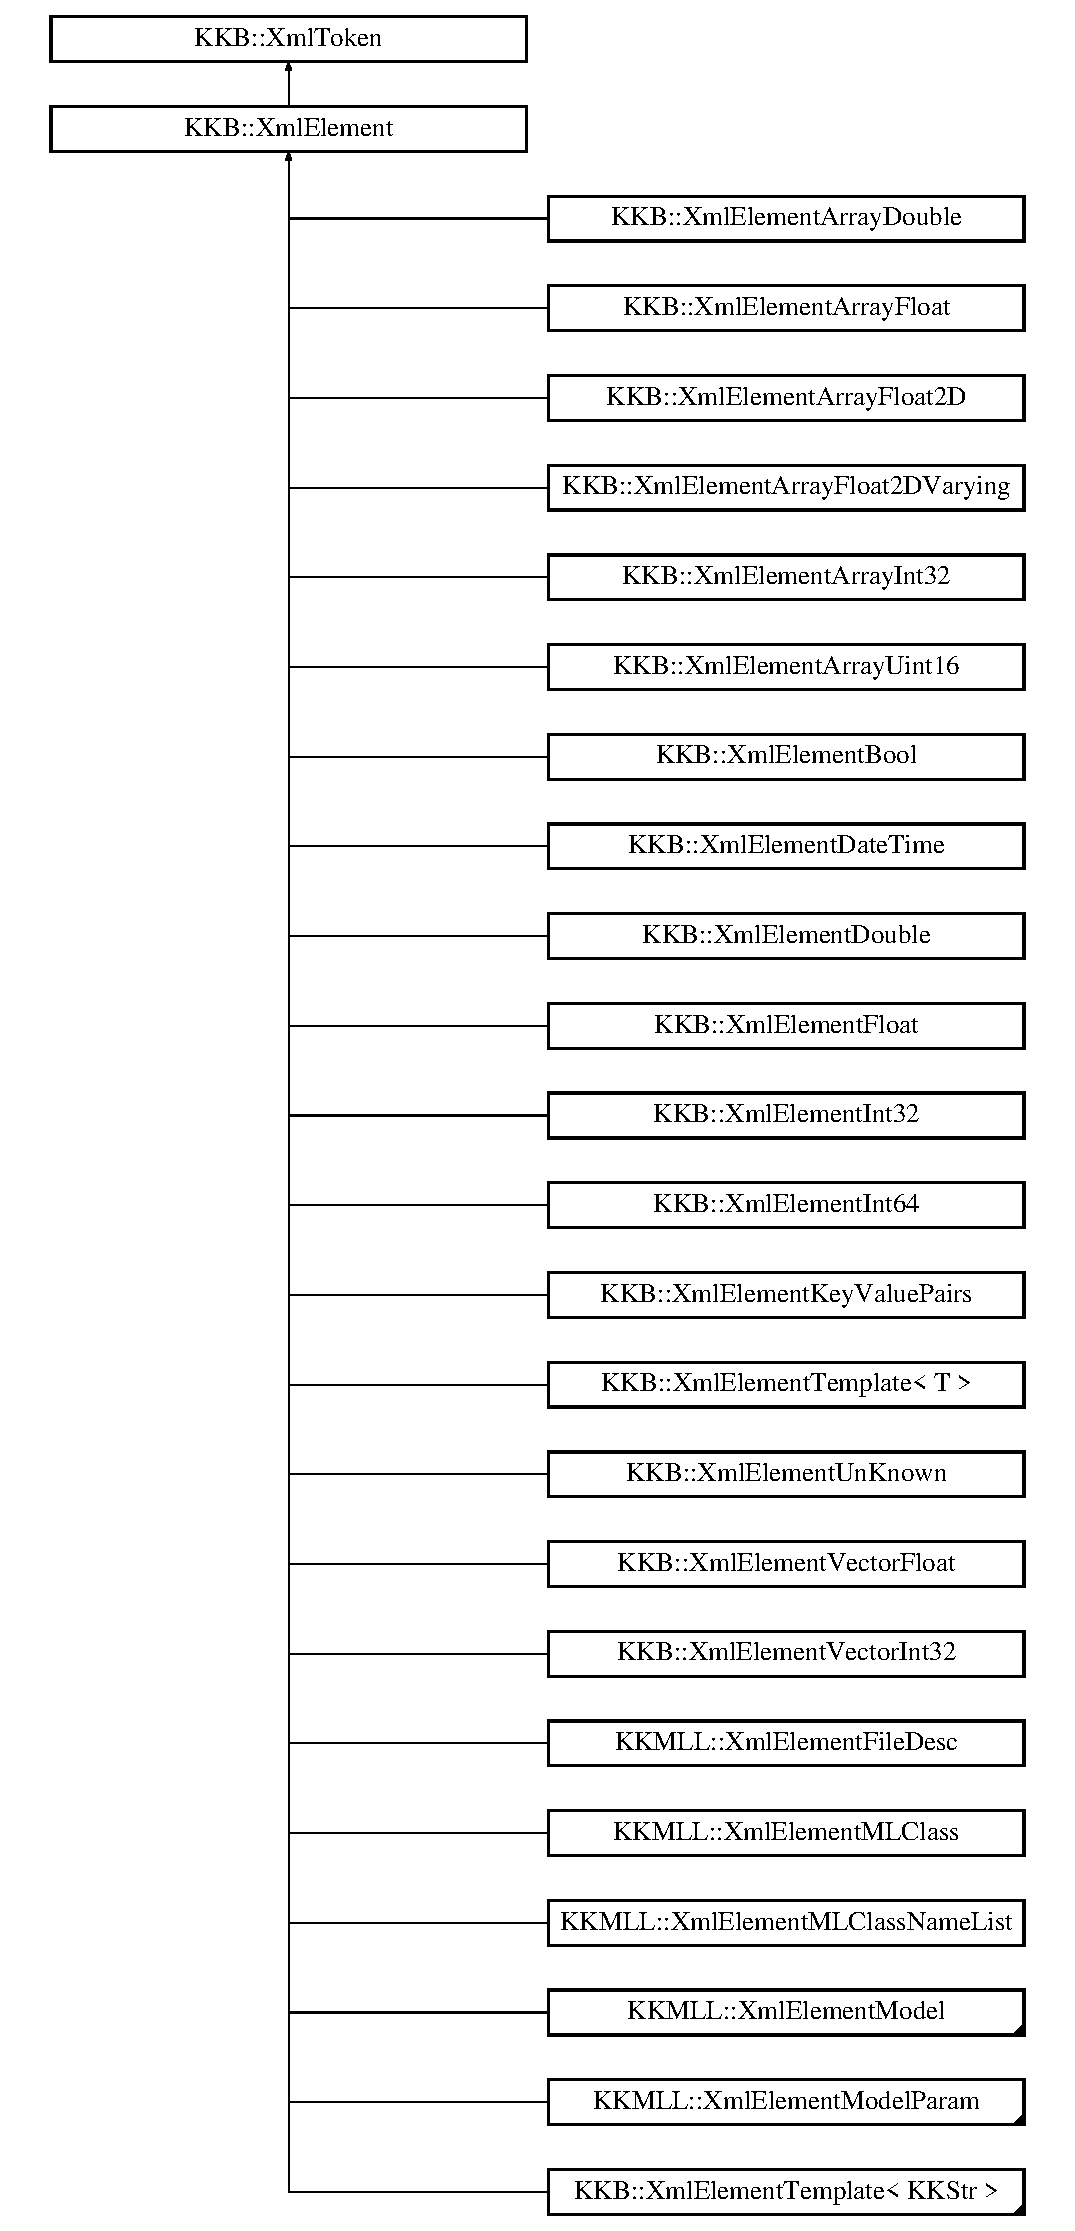
\includegraphics[height=12.000000cm]{class_k_k_b_1_1_xml_element}
\end{center}
\end{figure}
\subsection*{Public Types}
\begin{DoxyCompactItemize}
\item 
typedef \hyperlink{class_k_k_b_1_1_xml_element}{Xml\+Element} $\ast$ \hyperlink{class_k_k_b_1_1_xml_element_ac1957d6e4bdc44e6b876b44cee0941be}{Xml\+Element\+Ptr}
\end{DoxyCompactItemize}
\subsection*{Public Member Functions}
\begin{DoxyCompactItemize}
\item 
\hyperlink{class_k_k_b_1_1_xml_element_a66317eff5bd3abcc60755756ba2887d5}{Xml\+Element} (const \hyperlink{class_k_k_b_1_1_k_k_str}{K\+K\+Str} \&section\+Name, \hyperlink{class_k_k_b_1_1_xml_tag_a6c0ef0e23f982f49d55d4fb7eaff6ac9}{Xml\+Tag\+::\+Tag\+Types} tag\+Type)
\item 
\hyperlink{class_k_k_b_1_1_xml_element_aabceb954a28cf9b21541ff5fbfd3a08b}{Xml\+Element} (\hyperlink{namespace_k_k_b_a9253a3ea8a5da18ca82be4ca2b390ef0}{Xml\+Tag\+Ptr} \+\_\+name\+Tag, \hyperlink{class_k_k_b_1_1_xml_stream}{Xml\+Stream} \&s, \hyperlink{class_k_k_b_1_1_run_log}{Run\+Log} \&log)
\item 
virtual \hyperlink{class_k_k_b_1_1_xml_element_a1e67b1dfcd561d1d602988d100d80d9b}{$\sim$\+Xml\+Element} ()
\item 
\hyperlink{namespace_k_k_b_a46f665ec17615c856eff3d21f78bed5c}{K\+K\+Str\+Const\+Ptr} \hyperlink{class_k_k_b_1_1_xml_element_a34f47feb9eccb898393f91ca76c62032}{Attribute\+Value} (const char $\ast$attribute\+Name)
\item 
\hyperlink{namespace_k_k_b_a46f665ec17615c856eff3d21f78bed5c}{K\+K\+Str\+Const\+Ptr} \hyperlink{class_k_k_b_1_1_xml_element_ab012f75dc6b80e19d0b08005112722f0}{Attribute\+Value} (const \hyperlink{class_k_k_b_1_1_k_k_str}{K\+K\+Str} \&attribute\+Name)
\item 
\hyperlink{namespace_k_k_b_a5f1b0b1667d79fec26deeff10c43df23}{Xml\+Tag\+Const\+Ptr} \hyperlink{class_k_k_b_1_1_xml_element_affa3e099ddb1e81d41140d6666d14932}{Name\+Tag} () const 
\item 
\hyperlink{class_k_k_b_1_1_k_k_str}{K\+K\+Str} \hyperlink{class_k_k_b_1_1_xml_element_a86a0fcbb58e998149503b7735690cd7b}{Name\+Tag\+Str} () const 
\item 
virtual const \hyperlink{class_k_k_b_1_1_k_k_str}{K\+K\+Str} \& \hyperlink{class_k_k_b_1_1_xml_element_a2b85dcb37a0f63bd7979d16d12296876}{Section\+Name} () const 
\item 
virtual bool \hyperlink{class_k_k_b_1_1_xml_element_a7bfbbea204722bc4535a294bc43e8e17}{To\+Bool} () const 
\item 
virtual double \hyperlink{class_k_k_b_1_1_xml_element_ac32778396ab8bdb215ad38f2f33f05de}{To\+Double} () const 
\item 
virtual float \hyperlink{class_k_k_b_1_1_xml_element_aa728687ed43e76d45d029dfc14e14e95}{To\+Float} () const 
\item 
virtual \hyperlink{namespace_k_k_b_a8fa4952cc84fda1de4bec1fbdd8d5b1b}{kkint32} \hyperlink{class_k_k_b_1_1_xml_element_aac7463c7b305f66b5157f424a0a76363}{To\+Int32} () const 
\item 
virtual \hyperlink{class_k_k_b_1_1_xml_token_a18b6e90c919f4b92e3b024f50f247f62}{Token\+Types} \hyperlink{class_k_k_b_1_1_xml_element_afcd7a4617fb5fdb8e434003b8aebcb3d}{Token\+Type} ()
\item 
virtual \hyperlink{class_k_k_b_1_1_k_k_str}{K\+K\+Str} \hyperlink{class_k_k_b_1_1_xml_element_a3028fc03b79509e6378749f6a8b426b9}{To\+K\+K\+Str} () const 
\item 
virtual const \hyperlink{class_k_k_b_1_1_k_k_str}{K\+K\+Str} \& \hyperlink{class_k_k_b_1_1_xml_element_aef57cf00be66a3a387ce849b35125f51}{Var\+Name} () const 
\end{DoxyCompactItemize}


\subsection{Detailed Description}


Definition at line 283 of file Xml\+Stream.\+h.



\subsection{Member Typedef Documentation}
\index{K\+K\+B\+::\+Xml\+Element@{K\+K\+B\+::\+Xml\+Element}!Xml\+Element\+Ptr@{Xml\+Element\+Ptr}}
\index{Xml\+Element\+Ptr@{Xml\+Element\+Ptr}!K\+K\+B\+::\+Xml\+Element@{K\+K\+B\+::\+Xml\+Element}}
\subsubsection[{\texorpdfstring{Xml\+Element\+Ptr}{XmlElementPtr}}]{\setlength{\rightskip}{0pt plus 5cm}typedef {\bf Xml\+Element}$\ast$ {\bf K\+K\+B\+::\+Xml\+Element\+::\+Xml\+Element\+Ptr}}\hypertarget{class_k_k_b_1_1_xml_element_ac1957d6e4bdc44e6b876b44cee0941be}{}\label{class_k_k_b_1_1_xml_element_ac1957d6e4bdc44e6b876b44cee0941be}


Definition at line 286 of file Xml\+Stream.\+h.



\subsection{Constructor \& Destructor Documentation}
\index{K\+K\+B\+::\+Xml\+Element@{K\+K\+B\+::\+Xml\+Element}!Xml\+Element@{Xml\+Element}}
\index{Xml\+Element@{Xml\+Element}!K\+K\+B\+::\+Xml\+Element@{K\+K\+B\+::\+Xml\+Element}}
\subsubsection[{\texorpdfstring{Xml\+Element(const K\+K\+Str \&section\+Name, Xml\+Tag\+::\+Tag\+Types tag\+Type)}{XmlElement(const KKStr &sectionName, XmlTag::TagTypes tagType)}}]{\setlength{\rightskip}{0pt plus 5cm}Xml\+Element\+::\+Xml\+Element (
\begin{DoxyParamCaption}
\item[{const {\bf K\+K\+Str} \&}]{section\+Name, }
\item[{{\bf Xml\+Tag\+::\+Tag\+Types}}]{tag\+Type}
\end{DoxyParamCaption}
)}\hypertarget{class_k_k_b_1_1_xml_element_a66317eff5bd3abcc60755756ba2887d5}{}\label{class_k_k_b_1_1_xml_element_a66317eff5bd3abcc60755756ba2887d5}


Definition at line 750 of file Xml\+Stream.\+cpp.



References K\+K\+B\+::\+Xml\+Tag\+::\+Xml\+Tag().



Referenced by K\+K\+B\+::\+Xml\+Element\+Key\+Value\+Pairs\+::\+Xml\+Element\+Key\+Value\+Pairs().


\begin{DoxyCode}
752                         :
753   nameTag (\textcolor{keyword}{new} \hyperlink{class_k_k_b_1_1_xml_tag}{XmlTag} (sectionName, tagType))
754 \{\}
\end{DoxyCode}
\index{K\+K\+B\+::\+Xml\+Element@{K\+K\+B\+::\+Xml\+Element}!Xml\+Element@{Xml\+Element}}
\index{Xml\+Element@{Xml\+Element}!K\+K\+B\+::\+Xml\+Element@{K\+K\+B\+::\+Xml\+Element}}
\subsubsection[{\texorpdfstring{Xml\+Element(\+Xml\+Tag\+Ptr \+\_\+name\+Tag, Xml\+Stream \&s, Run\+Log \&log)}{XmlElement(XmlTagPtr _nameTag, XmlStream &s, RunLog &log)}}]{\setlength{\rightskip}{0pt plus 5cm}Xml\+Element\+::\+Xml\+Element (
\begin{DoxyParamCaption}
\item[{{\bf Xml\+Tag\+Ptr}}]{\+\_\+name\+Tag, }
\item[{{\bf Xml\+Stream} \&}]{s, }
\item[{{\bf Run\+Log} \&}]{log}
\end{DoxyParamCaption}
)}\hypertarget{class_k_k_b_1_1_xml_element_aabceb954a28cf9b21541ff5fbfd3a08b}{}\label{class_k_k_b_1_1_xml_element_aabceb954a28cf9b21541ff5fbfd3a08b}


Definition at line 758 of file Xml\+Stream.\+cpp.



Referenced by K\+K\+B\+::\+Xml\+Element\+Array\+Float2\+D\+Varying\+::\+Xml\+Element\+Array\+Float2\+D\+Varying(), K\+K\+B\+::\+Xml\+Element\+Bool\+::\+Xml\+Element\+Bool(), K\+K\+B\+::\+Xml\+Element\+Date\+Time\+::\+Xml\+Element\+Date\+Time(), K\+K\+M\+L\+L\+::\+Xml\+Element\+File\+Desc\+::\+Xml\+Element\+File\+Desc(), K\+K\+B\+::\+Xml\+Element\+Key\+Value\+Pairs\+::\+Xml\+Element\+Key\+Value\+Pairs(), K\+K\+M\+L\+L\+::\+Xml\+Element\+M\+L\+Class\+::\+Xml\+Element\+M\+L\+Class(), K\+K\+M\+L\+L\+::\+Xml\+Element\+M\+L\+Class\+Name\+List\+::\+Xml\+Element\+M\+L\+Class\+Name\+List(), K\+K\+M\+L\+L\+::\+Xml\+Element\+Model\+::\+Xml\+Element\+Model(), K\+K\+M\+L\+L\+::\+Xml\+Element\+Model\+Param\+::\+Xml\+Element\+Model\+Param(), and K\+K\+B\+::\+Xml\+Element\+Un\+Known\+::\+Xml\+Element\+Un\+Known().


\begin{DoxyCode}
761                         :
762   nameTag (\_nameTag)
763 \{\}
\end{DoxyCode}
\index{K\+K\+B\+::\+Xml\+Element@{K\+K\+B\+::\+Xml\+Element}!````~Xml\+Element@{$\sim$\+Xml\+Element}}
\index{````~Xml\+Element@{$\sim$\+Xml\+Element}!K\+K\+B\+::\+Xml\+Element@{K\+K\+B\+::\+Xml\+Element}}
\subsubsection[{\texorpdfstring{$\sim$\+Xml\+Element()}{~XmlElement()}}]{\setlength{\rightskip}{0pt plus 5cm}Xml\+Element\+::$\sim$\+Xml\+Element (
\begin{DoxyParamCaption}
{}
\end{DoxyParamCaption}
)\hspace{0.3cm}{\ttfamily [virtual]}}\hypertarget{class_k_k_b_1_1_xml_element_a1e67b1dfcd561d1d602988d100d80d9b}{}\label{class_k_k_b_1_1_xml_element_a1e67b1dfcd561d1d602988d100d80d9b}


Definition at line 767 of file Xml\+Stream.\+cpp.


\begin{DoxyCode}
768 \{
769   \textcolor{keyword}{delete}  nameTag;
770   nameTag = NULL;
771 \}
\end{DoxyCode}


\subsection{Member Function Documentation}
\index{K\+K\+B\+::\+Xml\+Element@{K\+K\+B\+::\+Xml\+Element}!Attribute\+Value@{Attribute\+Value}}
\index{Attribute\+Value@{Attribute\+Value}!K\+K\+B\+::\+Xml\+Element@{K\+K\+B\+::\+Xml\+Element}}
\subsubsection[{\texorpdfstring{Attribute\+Value(const char $\ast$attribute\+Name)}{AttributeValue(const char *attributeName)}}]{\setlength{\rightskip}{0pt plus 5cm}{\bf K\+K\+Str\+Const\+Ptr} Xml\+Element\+::\+Attribute\+Value (
\begin{DoxyParamCaption}
\item[{const char $\ast$}]{attribute\+Name}
\end{DoxyParamCaption}
)}\hypertarget{class_k_k_b_1_1_xml_element_a34f47feb9eccb898393f91ca76c62032}{}\label{class_k_k_b_1_1_xml_element_a34f47feb9eccb898393f91ca76c62032}


Definition at line 818 of file Xml\+Stream.\+cpp.



References K\+K\+B\+::\+Xml\+Tag\+::\+Attribute\+Value\+By\+Name().


\begin{DoxyCode}
819 \{
820   \textcolor{keywordflow}{if}  (nameTag)
821     \textcolor{keywordflow}{return} nameTag->\hyperlink{class_k_k_b_1_1_xml_tag_a0470baf5a49af1c2f6aaf0155b9ba783}{AttributeValueByName} (attributeName);
822   \textcolor{keywordflow}{else}
823     \textcolor{keywordflow}{return} NULL;
824 \}
\end{DoxyCode}
\index{K\+K\+B\+::\+Xml\+Element@{K\+K\+B\+::\+Xml\+Element}!Attribute\+Value@{Attribute\+Value}}
\index{Attribute\+Value@{Attribute\+Value}!K\+K\+B\+::\+Xml\+Element@{K\+K\+B\+::\+Xml\+Element}}
\subsubsection[{\texorpdfstring{Attribute\+Value(const K\+K\+Str \&attribute\+Name)}{AttributeValue(const KKStr &attributeName)}}]{\setlength{\rightskip}{0pt plus 5cm}{\bf K\+K\+Str\+Const\+Ptr} Xml\+Element\+::\+Attribute\+Value (
\begin{DoxyParamCaption}
\item[{const {\bf K\+K\+Str} \&}]{attribute\+Name}
\end{DoxyParamCaption}
)}\hypertarget{class_k_k_b_1_1_xml_element_ab012f75dc6b80e19d0b08005112722f0}{}\label{class_k_k_b_1_1_xml_element_ab012f75dc6b80e19d0b08005112722f0}


Definition at line 809 of file Xml\+Stream.\+cpp.



References K\+K\+B\+::\+Xml\+Tag\+::\+Attribute\+Value\+By\+Name().


\begin{DoxyCode}
810 \{
811   \textcolor{keywordflow}{if}  (nameTag)
812     \textcolor{keywordflow}{return} nameTag->\hyperlink{class_k_k_b_1_1_xml_tag_a0470baf5a49af1c2f6aaf0155b9ba783}{AttributeValueByName} (attributeName);
813   \textcolor{keywordflow}{else}
814     \textcolor{keywordflow}{return} NULL;
815 \}
\end{DoxyCode}
\index{K\+K\+B\+::\+Xml\+Element@{K\+K\+B\+::\+Xml\+Element}!Name\+Tag@{Name\+Tag}}
\index{Name\+Tag@{Name\+Tag}!K\+K\+B\+::\+Xml\+Element@{K\+K\+B\+::\+Xml\+Element}}
\subsubsection[{\texorpdfstring{Name\+Tag() const }{NameTag() const }}]{\setlength{\rightskip}{0pt plus 5cm}{\bf Xml\+Tag\+Const\+Ptr} K\+K\+B\+::\+Xml\+Element\+::\+Name\+Tag (
\begin{DoxyParamCaption}
{}
\end{DoxyParamCaption}
) const\hspace{0.3cm}{\ttfamily [inline]}}\hypertarget{class_k_k_b_1_1_xml_element_affa3e099ddb1e81d41140d6666d14932}{}\label{class_k_k_b_1_1_xml_element_affa3e099ddb1e81d41140d6666d14932}


Definition at line 299 of file Xml\+Stream.\+h.


\begin{DoxyCode}
299 \{\textcolor{keywordflow}{return} nameTag;\}
\end{DoxyCode}
\index{K\+K\+B\+::\+Xml\+Element@{K\+K\+B\+::\+Xml\+Element}!Name\+Tag\+Str@{Name\+Tag\+Str}}
\index{Name\+Tag\+Str@{Name\+Tag\+Str}!K\+K\+B\+::\+Xml\+Element@{K\+K\+B\+::\+Xml\+Element}}
\subsubsection[{\texorpdfstring{Name\+Tag\+Str() const }{NameTagStr() const }}]{\setlength{\rightskip}{0pt plus 5cm}{\bf K\+K\+Str} Xml\+Element\+::\+Name\+Tag\+Str (
\begin{DoxyParamCaption}
{}
\end{DoxyParamCaption}
) const}\hypertarget{class_k_k_b_1_1_xml_element_a86a0fcbb58e998149503b7735690cd7b}{}\label{class_k_k_b_1_1_xml_element_a86a0fcbb58e998149503b7735690cd7b}
The initial start tag with its attributes that started the element. 

Definition at line 775 of file Xml\+Stream.\+cpp.



References K\+K\+B\+::\+K\+K\+Str\+::\+Concat(), K\+K\+B\+::\+K\+K\+Str\+::\+Empty\+Str(), and K\+K\+B\+::\+Xml\+Tag\+::\+To\+String().


\begin{DoxyCode}
776 \{
777   \textcolor{keywordflow}{if}  (!nameTag)
778     \textcolor{keywordflow}{return} \hyperlink{class_k_k_b_1_1_k_k_str_ab6e416b3ef54ef632bd10c3f7a2f7994}{KKStr::EmptyStr} ();
779   \textcolor{keywordflow}{else}
780     \textcolor{keywordflow}{return} nameTag->\hyperlink{class_k_k_b_1_1_xml_tag_ac2edd74085cdd50465096426f1ef9e44}{ToString} ();
781 \}
\end{DoxyCode}
\index{K\+K\+B\+::\+Xml\+Element@{K\+K\+B\+::\+Xml\+Element}!Section\+Name@{Section\+Name}}
\index{Section\+Name@{Section\+Name}!K\+K\+B\+::\+Xml\+Element@{K\+K\+B\+::\+Xml\+Element}}
\subsubsection[{\texorpdfstring{Section\+Name() const }{SectionName() const }}]{\setlength{\rightskip}{0pt plus 5cm}const {\bf K\+K\+Str} \& Xml\+Element\+::\+Section\+Name (
\begin{DoxyParamCaption}
{}
\end{DoxyParamCaption}
) const\hspace{0.3cm}{\ttfamily [virtual]}}\hypertarget{class_k_k_b_1_1_xml_element_a2b85dcb37a0f63bd7979d16d12296876}{}\label{class_k_k_b_1_1_xml_element_a2b85dcb37a0f63bd7979d16d12296876}
If derived class is from the \hyperlink{class_k_k_b_1_1_xml_element}{Xml\+Element} family will be the name from the Start\+Tag(\+Xml\+Tag\+::\+Name ()) otherwise \hyperlink{class_k_k_b_1_1_k_k_str_ab6e416b3ef54ef632bd10c3f7a2f7994}{K\+K\+Str\+::\+Empty\+Str()} 

Reimplemented from \hyperlink{class_k_k_b_1_1_xml_token_a20aa05209eeafb58c1c595c15f07d504}{K\+K\+B\+::\+Xml\+Token}.



Definition at line 785 of file Xml\+Stream.\+cpp.



References K\+K\+B\+::\+K\+K\+Str\+::\+Concat(), K\+K\+B\+::\+K\+K\+Str\+::\+Empty\+Str(), and K\+K\+B\+::\+Xml\+Tag\+::\+Name().



Referenced by K\+K\+M\+L\+L\+::\+Normalization\+Parms\+::\+Read\+X\+M\+L(), S\+V\+M233\+::\+Svm\+Model233\+::\+Read\+X\+M\+L(), K\+K\+M\+L\+L\+::\+Model\+Dual\+::\+Read\+X\+M\+L(), K\+K\+M\+L\+L\+::\+File\+Desc\+::\+Read\+X\+M\+L(), and K\+K\+M\+L\+L\+::\+Training\+Process2\+::\+Read\+X\+M\+L().


\begin{DoxyCode}
786 \{
787   \textcolor{keywordflow}{if}  (nameTag)
788     \textcolor{keywordflow}{return}  nameTag->\hyperlink{class_k_k_b_1_1_xml_tag_a80934a69d86c1e06b13889fcde99a63b}{Name} ();
789   \textcolor{keywordflow}{else}
790     \textcolor{keywordflow}{return} \hyperlink{class_k_k_b_1_1_k_k_str_ab6e416b3ef54ef632bd10c3f7a2f7994}{KKStr::EmptyStr} ();
791 \}
\end{DoxyCode}
\index{K\+K\+B\+::\+Xml\+Element@{K\+K\+B\+::\+Xml\+Element}!To\+Bool@{To\+Bool}}
\index{To\+Bool@{To\+Bool}!K\+K\+B\+::\+Xml\+Element@{K\+K\+B\+::\+Xml\+Element}}
\subsubsection[{\texorpdfstring{To\+Bool() const }{ToBool() const }}]{\setlength{\rightskip}{0pt plus 5cm}virtual bool K\+K\+B\+::\+Xml\+Element\+::\+To\+Bool (
\begin{DoxyParamCaption}
{}
\end{DoxyParamCaption}
) const\hspace{0.3cm}{\ttfamily [inline]}, {\ttfamily [virtual]}}\hypertarget{class_k_k_b_1_1_xml_element_a7bfbbea204722bc4535a294bc43e8e17}{}\label{class_k_k_b_1_1_xml_element_a7bfbbea204722bc4535a294bc43e8e17}


Reimplemented in \hyperlink{class_k_k_b_1_1_xml_element_double_a493cdcf7549a3995f35c01bebe3d0738}{K\+K\+B\+::\+Xml\+Element\+Double}, \hyperlink{class_k_k_b_1_1_xml_element_float_a6a72dc8d2ebd6750787a07db8193e188}{K\+K\+B\+::\+Xml\+Element\+Float}, \hyperlink{class_k_k_b_1_1_xml_element_int64_a30d43c139d9efa806e8ad5ba8ded9d47}{K\+K\+B\+::\+Xml\+Element\+Int64}, \hyperlink{class_k_k_b_1_1_xml_element_int32_aec7a18f2b0e3bf247bf29f21e5256592}{K\+K\+B\+::\+Xml\+Element\+Int32}, \hyperlink{class_k_k_b_1_1_xml_element_k_k_str_a8ba15eefdf11b1b92b55ff9a6e91a540}{K\+K\+B\+::\+Xml\+Element\+K\+K\+Str}, \hyperlink{class_k_k_b_1_1_xml_element_date_time_a6428fe3132db46ca0f9f15ca4e3570a8}{K\+K\+B\+::\+Xml\+Element\+Date\+Time}, and \hyperlink{class_k_k_b_1_1_xml_element_bool_aed830aad8c70976bddefe7373790cf4a}{K\+K\+B\+::\+Xml\+Element\+Bool}.



Definition at line 313 of file Xml\+Stream.\+h.



Referenced by K\+K\+M\+L\+L\+::\+Normalization\+Parms\+::\+Read\+X\+M\+L(), K\+K\+M\+L\+L\+::\+Training\+Process2\+::\+Read\+X\+M\+L(), and K\+K\+M\+L\+L\+::\+Model\+Param\+::\+Read\+X\+M\+L\+Model\+Param\+Token().


\begin{DoxyCode}
313 \{\textcolor{keywordflow}{return}  \textcolor{keyword}{false};\}
\end{DoxyCode}
\index{K\+K\+B\+::\+Xml\+Element@{K\+K\+B\+::\+Xml\+Element}!To\+Double@{To\+Double}}
\index{To\+Double@{To\+Double}!K\+K\+B\+::\+Xml\+Element@{K\+K\+B\+::\+Xml\+Element}}
\subsubsection[{\texorpdfstring{To\+Double() const }{ToDouble() const }}]{\setlength{\rightskip}{0pt plus 5cm}virtual double K\+K\+B\+::\+Xml\+Element\+::\+To\+Double (
\begin{DoxyParamCaption}
{}
\end{DoxyParamCaption}
) const\hspace{0.3cm}{\ttfamily [inline]}, {\ttfamily [virtual]}}\hypertarget{class_k_k_b_1_1_xml_element_ac32778396ab8bdb215ad38f2f33f05de}{}\label{class_k_k_b_1_1_xml_element_ac32778396ab8bdb215ad38f2f33f05de}


Reimplemented in \hyperlink{class_k_k_b_1_1_xml_element_double_a46ff2b83d867561f3b9035e743fe52fd}{K\+K\+B\+::\+Xml\+Element\+Double}, \hyperlink{class_k_k_b_1_1_xml_element_float_a4e0d90e5b74565ef0fb03cee7cdbc852}{K\+K\+B\+::\+Xml\+Element\+Float}, \hyperlink{class_k_k_b_1_1_xml_element_int64_af06d31f81561cf6bdd9731f699a7efbe}{K\+K\+B\+::\+Xml\+Element\+Int64}, \hyperlink{class_k_k_b_1_1_xml_element_int32_a1768e0e2b122547832f7d8a73a0f1588}{K\+K\+B\+::\+Xml\+Element\+Int32}, \hyperlink{class_k_k_b_1_1_xml_element_k_k_str_a27549d20798a9387ebf41ffdf2c86d2e}{K\+K\+B\+::\+Xml\+Element\+K\+K\+Str}, \hyperlink{class_k_k_b_1_1_xml_element_date_time_a3c60c809536ad9823baf97f64beb541f}{K\+K\+B\+::\+Xml\+Element\+Date\+Time}, and \hyperlink{class_k_k_b_1_1_xml_element_bool_a116bd645557defaae5d69450015124eb}{K\+K\+B\+::\+Xml\+Element\+Bool}.



Definition at line 315 of file Xml\+Stream.\+h.



Referenced by K\+K\+M\+L\+L\+::\+Feature\+Encoder\+::\+Read\+X\+M\+L().


\begin{DoxyCode}
315 \{\textcolor{keywordflow}{return}  0.0;\}
\end{DoxyCode}
\index{K\+K\+B\+::\+Xml\+Element@{K\+K\+B\+::\+Xml\+Element}!To\+Float@{To\+Float}}
\index{To\+Float@{To\+Float}!K\+K\+B\+::\+Xml\+Element@{K\+K\+B\+::\+Xml\+Element}}
\subsubsection[{\texorpdfstring{To\+Float() const }{ToFloat() const }}]{\setlength{\rightskip}{0pt plus 5cm}virtual float K\+K\+B\+::\+Xml\+Element\+::\+To\+Float (
\begin{DoxyParamCaption}
{}
\end{DoxyParamCaption}
) const\hspace{0.3cm}{\ttfamily [inline]}, {\ttfamily [virtual]}}\hypertarget{class_k_k_b_1_1_xml_element_aa728687ed43e76d45d029dfc14e14e95}{}\label{class_k_k_b_1_1_xml_element_aa728687ed43e76d45d029dfc14e14e95}


Reimplemented in \hyperlink{class_k_k_b_1_1_xml_element_double_ab8cc3ee364972fa47c99430487f906cb}{K\+K\+B\+::\+Xml\+Element\+Double}, \hyperlink{class_k_k_b_1_1_xml_element_float_a5967c539026d748db052c9035cc9ebe8}{K\+K\+B\+::\+Xml\+Element\+Float}, \hyperlink{class_k_k_b_1_1_xml_element_int64_a5d7fe62f4e493d6a8de86534e0793d94}{K\+K\+B\+::\+Xml\+Element\+Int64}, \hyperlink{class_k_k_b_1_1_xml_element_int32_a1b240dc1bc387f12192575c3257f95e7}{K\+K\+B\+::\+Xml\+Element\+Int32}, \hyperlink{class_k_k_b_1_1_xml_element_k_k_str_ad70580dab90be4e505fd2959ad8eb1e3}{K\+K\+B\+::\+Xml\+Element\+K\+K\+Str}, \hyperlink{class_k_k_b_1_1_xml_element_date_time_a67670c703f86c4a72ba73920de0f4858}{K\+K\+B\+::\+Xml\+Element\+Date\+Time}, and \hyperlink{class_k_k_b_1_1_xml_element_bool_a87badc80558f62710ffde957298c1536}{K\+K\+B\+::\+Xml\+Element\+Bool}.



Definition at line 316 of file Xml\+Stream.\+h.



Referenced by K\+K\+M\+L\+L\+::\+Normalization\+Parms\+::\+Read\+X\+M\+L().


\begin{DoxyCode}
316 \{\textcolor{keywordflow}{return}  0.0f;\}
\end{DoxyCode}
\index{K\+K\+B\+::\+Xml\+Element@{K\+K\+B\+::\+Xml\+Element}!To\+Int32@{To\+Int32}}
\index{To\+Int32@{To\+Int32}!K\+K\+B\+::\+Xml\+Element@{K\+K\+B\+::\+Xml\+Element}}
\subsubsection[{\texorpdfstring{To\+Int32() const }{ToInt32() const }}]{\setlength{\rightskip}{0pt plus 5cm}virtual {\bf kkint32} K\+K\+B\+::\+Xml\+Element\+::\+To\+Int32 (
\begin{DoxyParamCaption}
{}
\end{DoxyParamCaption}
) const\hspace{0.3cm}{\ttfamily [inline]}, {\ttfamily [virtual]}}\hypertarget{class_k_k_b_1_1_xml_element_aac7463c7b305f66b5157f424a0a76363}{}\label{class_k_k_b_1_1_xml_element_aac7463c7b305f66b5157f424a0a76363}


Reimplemented in \hyperlink{class_k_k_b_1_1_xml_element_double_aa3396d5635ad1542feb917e3bd667ae8}{K\+K\+B\+::\+Xml\+Element\+Double}, \hyperlink{class_k_k_b_1_1_xml_element_float_a1ecd7c407ad5f26064e90fada52270c4}{K\+K\+B\+::\+Xml\+Element\+Float}, \hyperlink{class_k_k_b_1_1_xml_element_int64_ab97448e2f4b9d5ae1451d35f1b4c63bd}{K\+K\+B\+::\+Xml\+Element\+Int64}, \hyperlink{class_k_k_b_1_1_xml_element_int32_a043453a13afcf42b819baf231786e653}{K\+K\+B\+::\+Xml\+Element\+Int32}, \hyperlink{class_k_k_b_1_1_xml_element_k_k_str_a0d99cf6a4d32b10d1ea410a0ae210ab9}{K\+K\+B\+::\+Xml\+Element\+K\+K\+Str}, \hyperlink{class_k_k_b_1_1_xml_element_date_time_ad7108702555f0d9bc3c879e836d212df}{K\+K\+B\+::\+Xml\+Element\+Date\+Time}, and \hyperlink{class_k_k_b_1_1_xml_element_bool_a7d877d4924d9f62f1f5dc68b5a3d2663}{K\+K\+B\+::\+Xml\+Element\+Bool}.



Definition at line 317 of file Xml\+Stream.\+h.



Referenced by K\+K\+M\+L\+L\+::\+Normalization\+Parms\+::\+Read\+X\+M\+L(), K\+K\+M\+L\+L\+::\+Feature\+Encoder\+::\+Read\+X\+M\+L(), S\+V\+M233\+::\+Svm\+Model233\+::\+Read\+X\+M\+L(), and K\+K\+M\+L\+L\+::\+Model\+Param\+::\+Read\+X\+M\+L\+Model\+Param\+Token().


\begin{DoxyCode}
317 \{\textcolor{keywordflow}{return}  0;\}
\end{DoxyCode}
\index{K\+K\+B\+::\+Xml\+Element@{K\+K\+B\+::\+Xml\+Element}!Token\+Type@{Token\+Type}}
\index{Token\+Type@{Token\+Type}!K\+K\+B\+::\+Xml\+Element@{K\+K\+B\+::\+Xml\+Element}}
\subsubsection[{\texorpdfstring{Token\+Type()}{TokenType()}}]{\setlength{\rightskip}{0pt plus 5cm}virtual {\bf Token\+Types} K\+K\+B\+::\+Xml\+Element\+::\+Token\+Type (
\begin{DoxyParamCaption}
{}
\end{DoxyParamCaption}
)\hspace{0.3cm}{\ttfamily [inline]}, {\ttfamily [virtual]}}\hypertarget{class_k_k_b_1_1_xml_element_afcd7a4617fb5fdb8e434003b8aebcb3d}{}\label{class_k_k_b_1_1_xml_element_afcd7a4617fb5fdb8e434003b8aebcb3d}


Implements \hyperlink{class_k_k_b_1_1_xml_token_ae98e2c1a798882647578cae4adcd7176}{K\+K\+B\+::\+Xml\+Token}.



Definition at line 305 of file Xml\+Stream.\+h.



References K\+K\+B\+::\+Xml\+Token\+::tok\+Element.


\begin{DoxyCode}
305 \{\textcolor{keywordflow}{return}  \hyperlink{class_k_k_b_1_1_xml_token_a18b6e90c919f4b92e3b024f50f247f62a4d464d022cf7f60dae56d13300aa0312}{TokenTypes::tokElement};\}
\end{DoxyCode}
\index{K\+K\+B\+::\+Xml\+Element@{K\+K\+B\+::\+Xml\+Element}!To\+K\+K\+Str@{To\+K\+K\+Str}}
\index{To\+K\+K\+Str@{To\+K\+K\+Str}!K\+K\+B\+::\+Xml\+Element@{K\+K\+B\+::\+Xml\+Element}}
\subsubsection[{\texorpdfstring{To\+K\+K\+Str() const }{ToKKStr() const }}]{\setlength{\rightskip}{0pt plus 5cm}virtual {\bf K\+K\+Str} K\+K\+B\+::\+Xml\+Element\+::\+To\+K\+K\+Str (
\begin{DoxyParamCaption}
{}
\end{DoxyParamCaption}
) const\hspace{0.3cm}{\ttfamily [inline]}, {\ttfamily [virtual]}}\hypertarget{class_k_k_b_1_1_xml_element_a3028fc03b79509e6378749f6a8b426b9}{}\label{class_k_k_b_1_1_xml_element_a3028fc03b79509e6378749f6a8b426b9}


Reimplemented in \hyperlink{class_k_k_b_1_1_xml_element_double_a4b178e060ff8118617e72be66bf8bd37}{K\+K\+B\+::\+Xml\+Element\+Double}, \hyperlink{class_k_k_b_1_1_xml_element_float_a95b717baacf55c1fa8a17ef7744c7915}{K\+K\+B\+::\+Xml\+Element\+Float}, \hyperlink{class_k_k_b_1_1_xml_element_int64_a73280a065f02c4ab505ddd81ce8a9f8c}{K\+K\+B\+::\+Xml\+Element\+Int64}, \hyperlink{class_k_k_b_1_1_xml_element_int32_af0db95c22ac5abf7158120aab68607c0}{K\+K\+B\+::\+Xml\+Element\+Int32}, \hyperlink{class_k_k_b_1_1_xml_element_k_k_str_a799d1dcb1d656ffceb6a7e809dfd4839}{K\+K\+B\+::\+Xml\+Element\+K\+K\+Str}, \hyperlink{class_k_k_b_1_1_xml_element_date_time_a0b78fa113b7721069b8a14b971b73b1e}{K\+K\+B\+::\+Xml\+Element\+Date\+Time}, and \hyperlink{class_k_k_b_1_1_xml_element_bool_a66cbfc5eff140075cf6226123db0bd85}{K\+K\+B\+::\+Xml\+Element\+Bool}.



Definition at line 314 of file Xml\+Stream.\+h.



References K\+K\+B\+::\+Xml\+Tag\+::\+To\+String().



Referenced by K\+K\+M\+L\+L\+::\+Feature\+Encoder\+::\+Read\+X\+M\+L(), K\+K\+M\+L\+L\+::\+Model\+Param\+Old\+S\+V\+M\+::\+Read\+X\+M\+L(), K\+K\+M\+L\+L\+::\+Training\+Process2\+::\+Read\+X\+M\+L(), K\+K\+M\+L\+L\+::\+Model\+Param\+::\+Read\+X\+M\+L\+Model\+Param\+Token(), and K\+K\+M\+L\+L\+::\+Model\+::\+Read\+X\+M\+L\+Model\+Token().


\begin{DoxyCode}
314 \{\textcolor{keywordflow}{return}  nameTag->\hyperlink{class_k_k_b_1_1_xml_tag_ac2edd74085cdd50465096426f1ef9e44}{ToString} ();\}
\end{DoxyCode}
\index{K\+K\+B\+::\+Xml\+Element@{K\+K\+B\+::\+Xml\+Element}!Var\+Name@{Var\+Name}}
\index{Var\+Name@{Var\+Name}!K\+K\+B\+::\+Xml\+Element@{K\+K\+B\+::\+Xml\+Element}}
\subsubsection[{\texorpdfstring{Var\+Name() const }{VarName() const }}]{\setlength{\rightskip}{0pt plus 5cm}const {\bf K\+K\+Str} \& Xml\+Element\+::\+Var\+Name (
\begin{DoxyParamCaption}
{}
\end{DoxyParamCaption}
) const\hspace{0.3cm}{\ttfamily [virtual]}}\hypertarget{class_k_k_b_1_1_xml_element_aef57cf00be66a3a387ce849b35125f51}{}\label{class_k_k_b_1_1_xml_element_aef57cf00be66a3a387ce849b35125f51}
If the derived class is form the \textquotesingle{}\hyperlink{class_k_k_b_1_1_xml_element}{Xml\+Element}\textquotesingle{} line will return the \textquotesingle{}Var\+Name\textquotesingle{} from that derived class otherwise it will return back a empty string. 

Reimplemented from \hyperlink{class_k_k_b_1_1_xml_token_a28b39cfdfa2ed63048a812b1cb52263c}{K\+K\+B\+::\+Xml\+Token}.



Definition at line 794 of file Xml\+Stream.\+cpp.



References K\+K\+B\+::\+Xml\+Tag\+::\+Attribute\+Value\+By\+Name(), K\+K\+B\+::\+K\+K\+Str\+::\+Concat(), and K\+K\+B\+::\+K\+K\+Str\+::\+Empty\+Str().



Referenced by K\+K\+M\+L\+L\+::\+Model\+Param\+Usf\+Cas\+Cor\+::\+Read\+X\+M\+L(), K\+K\+M\+L\+L\+::\+Normalization\+Parms\+::\+Read\+X\+M\+L(), K\+K\+M\+L\+L\+::\+Feature\+Encoder\+::\+Read\+X\+M\+L(), K\+K\+M\+L\+L\+::\+Training\+Class\+List\+::\+Read\+X\+M\+L(), S\+V\+M233\+::\+Svm\+Model233\+::\+Read\+X\+M\+L(), K\+K\+M\+L\+L\+::\+Model\+Dual\+::\+Read\+X\+M\+L(), K\+K\+M\+L\+L\+::\+File\+Desc\+::\+Read\+X\+M\+L(), K\+K\+M\+L\+L\+::\+S\+V\+M\+Model\+::\+Read\+X\+M\+L(), K\+K\+M\+L\+L\+::\+Training\+Process2\+::\+Read\+X\+M\+L(), K\+K\+M\+L\+L\+::\+Training\+Configuration2\+::\+Read\+X\+M\+L\+Base\+Token(), and K\+K\+M\+L\+L\+::\+Model\+::\+Read\+X\+M\+L\+Model\+Token().


\begin{DoxyCode}
795 \{
796   \textcolor{keywordflow}{if}  (!nameTag)
797     \textcolor{keywordflow}{return} \hyperlink{class_k_k_b_1_1_k_k_str_ab6e416b3ef54ef632bd10c3f7a2f7994}{KKStr::EmptyStr} ();
798 
799   \hyperlink{class_k_k_b_1_1_k_k_str}{KKStrConstPtr}  nameStr = nameTag->\hyperlink{class_k_k_b_1_1_xml_tag_a0470baf5a49af1c2f6aaf0155b9ba783}{AttributeValueByName} (\textcolor{stringliteral}{"VarName"});
800   \textcolor{keywordflow}{if}  (nameStr)
801     \textcolor{keywordflow}{return}  *nameStr;
802   \textcolor{keywordflow}{else}
803     \textcolor{keywordflow}{return}  \hyperlink{class_k_k_b_1_1_k_k_str_ab6e416b3ef54ef632bd10c3f7a2f7994}{KKStr::EmptyStr} ();
804 \}
\end{DoxyCode}


The documentation for this class was generated from the following files\+:\begin{DoxyCompactItemize}
\item 
C\+:/\+Users/\+Kurt/\+Git\+Hub/\+K\+Square\+Libraries/\+K\+K\+Base/\hyperlink{_xml_stream_8h}{Xml\+Stream.\+h}\item 
C\+:/\+Users/\+Kurt/\+Git\+Hub/\+K\+Square\+Libraries/\+K\+K\+Base/\hyperlink{_xml_stream_8cpp}{Xml\+Stream.\+cpp}\end{DoxyCompactItemize}

\hypertarget{class_k_k_b_1_1_xml_element_array_double}{}\section{K\+KB\+:\+:Xml\+Element\+Array\+Double Class Reference}
\label{class_k_k_b_1_1_xml_element_array_double}\index{K\+K\+B\+::\+Xml\+Element\+Array\+Double@{K\+K\+B\+::\+Xml\+Element\+Array\+Double}}


{\ttfamily \#include $<$Xml\+Stream.\+h$>$}

Inheritance diagram for K\+KB\+:\+:Xml\+Element\+Array\+Double\+:\begin{figure}[H]
\begin{center}
\leavevmode
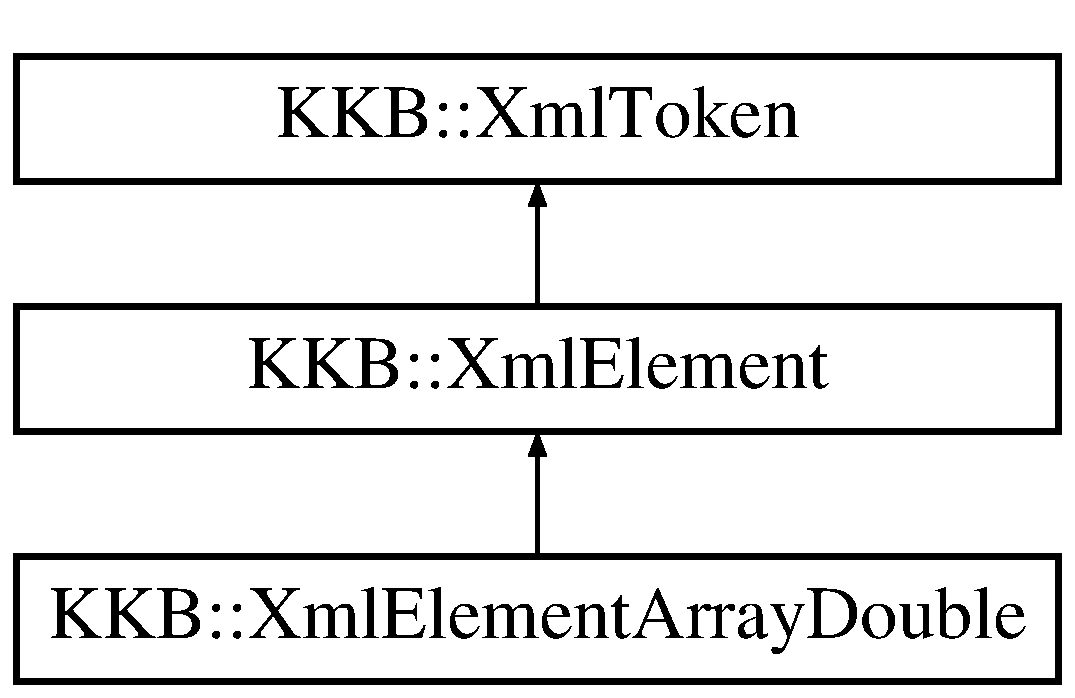
\includegraphics[height=3.000000cm]{class_k_k_b_1_1_xml_element_array_double}
\end{center}
\end{figure}
\subsection*{Public Member Functions}
\begin{DoxyCompactItemize}
\item 
\hyperlink{class_k_k_b_1_1_xml_element_array_double_ae36ba05ec0a3a1a4ba18ba06316e1aa5}{Xml\+Element\+Array\+Double} (\hyperlink{namespace_k_k_b_a9253a3ea8a5da18ca82be4ca2b390ef0}{Xml\+Tag\+Ptr} tag, \hyperlink{class_k_k_b_1_1_xml_stream}{Xml\+Stream} \&s, \hyperlink{namespace_k_k_b_a7d390f568e2831fb76b86b56c87bf92f}{Vol\+Const\+Bool} \&cancel\+Flag, \hyperlink{class_k_k_b_1_1_run_log}{Run\+Log} \&log)
\item 
virtual \hyperlink{class_k_k_b_1_1_xml_element_array_double_a82258967fa3c5dea7f92b4e071f205e4}{$\sim$\+Xml\+Element\+Array\+Double} ()
\item 
\hyperlink{namespace_k_k_b_af8d832f05c54994a1cce25bd5743e19a}{kkuint32} \hyperlink{class_k_k_b_1_1_xml_element_array_double_a591f50d85eadd680d84febde51f26350}{Count} () const 
\item 
double $\ast$ \hyperlink{class_k_k_b_1_1_xml_element_array_double_a7ea0ba2abb1599a06ff7ff363ff56f19}{Take\+Ownership} ()
\item 
double $\ast$ \hyperlink{class_k_k_b_1_1_xml_element_array_double_afeb69565542e41186a390fddf9cfdc9c}{Value} () const 
\end{DoxyCompactItemize}
\subsection*{Static Public Member Functions}
\begin{DoxyCompactItemize}
\item 
static void \hyperlink{class_k_k_b_1_1_xml_element_array_double_a1d979039b2e3b9d89797e4227f484078}{Write\+X\+ML} (\hyperlink{namespace_k_k_b_af8d832f05c54994a1cce25bd5743e19a}{kkuint32} count, const double $\ast$d, const \hyperlink{class_k_k_b_1_1_k_k_str}{K\+K\+Str} \&var\+Name, std\+::ostream \&o)
\end{DoxyCompactItemize}
\subsection*{Additional Inherited Members}


\subsection{Detailed Description}


Definition at line 917 of file Xml\+Stream.\+h.



\subsection{Constructor \& Destructor Documentation}
\index{K\+K\+B\+::\+Xml\+Element\+Array\+Double@{K\+K\+B\+::\+Xml\+Element\+Array\+Double}!Xml\+Element\+Array\+Double@{Xml\+Element\+Array\+Double}}
\index{Xml\+Element\+Array\+Double@{Xml\+Element\+Array\+Double}!K\+K\+B\+::\+Xml\+Element\+Array\+Double@{K\+K\+B\+::\+Xml\+Element\+Array\+Double}}
\subsubsection[{\texorpdfstring{Xml\+Element\+Array\+Double(\+Xml\+Tag\+Ptr tag, Xml\+Stream \&s, Vol\+Const\+Bool \&cancel\+Flag, Run\+Log \&log)}{XmlElementArrayDouble(XmlTagPtr tag, XmlStream &s, VolConstBool &cancelFlag, RunLog &log)}}]{\setlength{\rightskip}{0pt plus 5cm}Xml\+Element\+Array\+Double\+::\+Xml\+Element\+Array\+Double (
\begin{DoxyParamCaption}
\item[{{\bf Xml\+Tag\+Ptr}}]{tag, }
\item[{{\bf Xml\+Stream} \&}]{s, }
\item[{{\bf Vol\+Const\+Bool} \&}]{cancel\+Flag, }
\item[{{\bf Run\+Log} \&}]{log}
\end{DoxyParamCaption}
)}\hypertarget{class_k_k_b_1_1_xml_element_array_double_ae36ba05ec0a3a1a4ba18ba06316e1aa5}{}\label{class_k_k_b_1_1_xml_element_array_double_ae36ba05ec0a3a1a4ba18ba06316e1aa5}


Definition at line 1857 of file Xml\+Stream.\+cpp.

\index{K\+K\+B\+::\+Xml\+Element\+Array\+Double@{K\+K\+B\+::\+Xml\+Element\+Array\+Double}!````~Xml\+Element\+Array\+Double@{$\sim$\+Xml\+Element\+Array\+Double}}
\index{````~Xml\+Element\+Array\+Double@{$\sim$\+Xml\+Element\+Array\+Double}!K\+K\+B\+::\+Xml\+Element\+Array\+Double@{K\+K\+B\+::\+Xml\+Element\+Array\+Double}}
\subsubsection[{\texorpdfstring{$\sim$\+Xml\+Element\+Array\+Double()}{~XmlElementArrayDouble()}}]{\setlength{\rightskip}{0pt plus 5cm}Xml\+Element\+Array\+Double\+::$\sim$\+Xml\+Element\+Array\+Double (
\begin{DoxyParamCaption}
{}
\end{DoxyParamCaption}
)\hspace{0.3cm}{\ttfamily [virtual]}}\hypertarget{class_k_k_b_1_1_xml_element_array_double_a82258967fa3c5dea7f92b4e071f205e4}{}\label{class_k_k_b_1_1_xml_element_array_double_a82258967fa3c5dea7f92b4e071f205e4}


Definition at line 1857 of file Xml\+Stream.\+cpp.



\subsection{Member Function Documentation}
\index{K\+K\+B\+::\+Xml\+Element\+Array\+Double@{K\+K\+B\+::\+Xml\+Element\+Array\+Double}!Count@{Count}}
\index{Count@{Count}!K\+K\+B\+::\+Xml\+Element\+Array\+Double@{K\+K\+B\+::\+Xml\+Element\+Array\+Double}}
\subsubsection[{\texorpdfstring{Count() const }{Count() const }}]{\setlength{\rightskip}{0pt plus 5cm}{\bf kkuint32} K\+K\+B\+::\+Xml\+Element\+Array\+Double\+::\+Count (
\begin{DoxyParamCaption}
{}
\end{DoxyParamCaption}
) const\hspace{0.3cm}{\ttfamily [inline]}}\hypertarget{class_k_k_b_1_1_xml_element_array_double_a591f50d85eadd680d84febde51f26350}{}\label{class_k_k_b_1_1_xml_element_array_double_a591f50d85eadd680d84febde51f26350}


Definition at line 917 of file Xml\+Stream.\+h.

\index{K\+K\+B\+::\+Xml\+Element\+Array\+Double@{K\+K\+B\+::\+Xml\+Element\+Array\+Double}!Take\+Ownership@{Take\+Ownership}}
\index{Take\+Ownership@{Take\+Ownership}!K\+K\+B\+::\+Xml\+Element\+Array\+Double@{K\+K\+B\+::\+Xml\+Element\+Array\+Double}}
\subsubsection[{\texorpdfstring{Take\+Ownership()}{TakeOwnership()}}]{\setlength{\rightskip}{0pt plus 5cm}double $\ast$ Xml\+Element\+Array\+Double\+::\+Take\+Ownership (
\begin{DoxyParamCaption}
{}
\end{DoxyParamCaption}
)}\hypertarget{class_k_k_b_1_1_xml_element_array_double_a7ea0ba2abb1599a06ff7ff363ff56f19}{}\label{class_k_k_b_1_1_xml_element_array_double_a7ea0ba2abb1599a06ff7ff363ff56f19}


Definition at line 1857 of file Xml\+Stream.\+cpp.

\index{K\+K\+B\+::\+Xml\+Element\+Array\+Double@{K\+K\+B\+::\+Xml\+Element\+Array\+Double}!Value@{Value}}
\index{Value@{Value}!K\+K\+B\+::\+Xml\+Element\+Array\+Double@{K\+K\+B\+::\+Xml\+Element\+Array\+Double}}
\subsubsection[{\texorpdfstring{Value() const }{Value() const }}]{\setlength{\rightskip}{0pt plus 5cm}double$\ast$ K\+K\+B\+::\+Xml\+Element\+Array\+Double\+::\+Value (
\begin{DoxyParamCaption}
{}
\end{DoxyParamCaption}
) const\hspace{0.3cm}{\ttfamily [inline]}}\hypertarget{class_k_k_b_1_1_xml_element_array_double_afeb69565542e41186a390fddf9cfdc9c}{}\label{class_k_k_b_1_1_xml_element_array_double_afeb69565542e41186a390fddf9cfdc9c}


Definition at line 917 of file Xml\+Stream.\+h.

\index{K\+K\+B\+::\+Xml\+Element\+Array\+Double@{K\+K\+B\+::\+Xml\+Element\+Array\+Double}!Write\+X\+ML@{Write\+X\+ML}}
\index{Write\+X\+ML@{Write\+X\+ML}!K\+K\+B\+::\+Xml\+Element\+Array\+Double@{K\+K\+B\+::\+Xml\+Element\+Array\+Double}}
\subsubsection[{\texorpdfstring{Write\+X\+M\+L(kkuint32 count, const double $\ast$d, const K\+K\+Str \&var\+Name, std\+::ostream \&o)}{WriteXML(kkuint32 count, const double *d, const KKStr &varName, std::ostream &o)}}]{\setlength{\rightskip}{0pt plus 5cm}void Xml\+Element\+Array\+Double\+::\+Write\+X\+ML (
\begin{DoxyParamCaption}
\item[{{\bf kkuint32}}]{count, }
\item[{const double $\ast$}]{d, }
\item[{const {\bf K\+K\+Str} \&}]{var\+Name, }
\item[{std\+::ostream \&}]{o}
\end{DoxyParamCaption}
)\hspace{0.3cm}{\ttfamily [static]}}\hypertarget{class_k_k_b_1_1_xml_element_array_double_a1d979039b2e3b9d89797e4227f484078}{}\label{class_k_k_b_1_1_xml_element_array_double_a1d979039b2e3b9d89797e4227f484078}


Definition at line 1857 of file Xml\+Stream.\+cpp.



The documentation for this class was generated from the following files\+:\begin{DoxyCompactItemize}
\item 
C\+:/\+Users/\+Kurt/\+Git\+Hub/\+K\+Square\+Libraries/\+K\+K\+Base/\hyperlink{_xml_stream_8h}{Xml\+Stream.\+h}\item 
C\+:/\+Users/\+Kurt/\+Git\+Hub/\+K\+Square\+Libraries/\+K\+K\+Base/\hyperlink{_xml_stream_8cpp}{Xml\+Stream.\+cpp}\end{DoxyCompactItemize}

\hypertarget{class_k_k_b_1_1_xml_element_array_float}{}\section{K\+KB\+:\+:Xml\+Element\+Array\+Float Class Reference}
\label{class_k_k_b_1_1_xml_element_array_float}\index{K\+K\+B\+::\+Xml\+Element\+Array\+Float@{K\+K\+B\+::\+Xml\+Element\+Array\+Float}}


{\ttfamily \#include $<$Xml\+Stream.\+h$>$}

Inheritance diagram for K\+KB\+:\+:Xml\+Element\+Array\+Float\+:\begin{figure}[H]
\begin{center}
\leavevmode
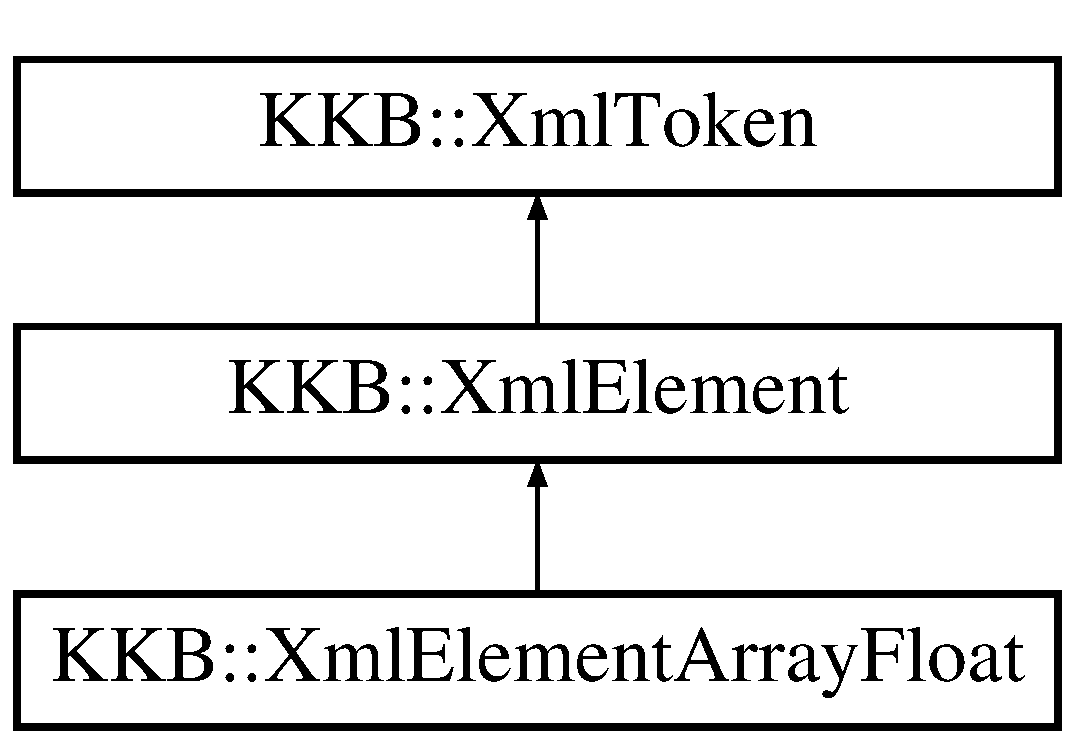
\includegraphics[height=3.000000cm]{class_k_k_b_1_1_xml_element_array_float}
\end{center}
\end{figure}
\subsection*{Public Member Functions}
\begin{DoxyCompactItemize}
\item 
\hyperlink{class_k_k_b_1_1_xml_element_array_float_ad3f2214f571f775eaecd7c6dcb86c333}{Xml\+Element\+Array\+Float} (\hyperlink{namespace_k_k_b_a9253a3ea8a5da18ca82be4ca2b390ef0}{Xml\+Tag\+Ptr} tag, \hyperlink{class_k_k_b_1_1_xml_stream}{Xml\+Stream} \&s, \hyperlink{namespace_k_k_b_a7d390f568e2831fb76b86b56c87bf92f}{Vol\+Const\+Bool} \&cancel\+Flag, \hyperlink{class_k_k_b_1_1_run_log}{Run\+Log} \&log)
\item 
virtual \hyperlink{class_k_k_b_1_1_xml_element_array_float_ab570b157bad51b22e57f3f03dc0fcd9e}{$\sim$\+Xml\+Element\+Array\+Float} ()
\item 
\hyperlink{namespace_k_k_b_af8d832f05c54994a1cce25bd5743e19a}{kkuint32} \hyperlink{class_k_k_b_1_1_xml_element_array_float_a364bdaf1cdc0dc775e30957350fc6504}{Count} () const 
\item 
float $\ast$ \hyperlink{class_k_k_b_1_1_xml_element_array_float_a43d247c7374f56ef9e6e1d3ccec40809}{Take\+Ownership} ()
\item 
float $\ast$ \hyperlink{class_k_k_b_1_1_xml_element_array_float_af18257639ce9fb8f4bf60f3b3743b153}{Value} () const 
\end{DoxyCompactItemize}
\subsection*{Static Public Member Functions}
\begin{DoxyCompactItemize}
\item 
static void \hyperlink{class_k_k_b_1_1_xml_element_array_float_a78bc9a4e11950ad7706a46f1d7da9749}{Write\+X\+ML} (\hyperlink{namespace_k_k_b_af8d832f05c54994a1cce25bd5743e19a}{kkuint32} count, const float $\ast$d, const \hyperlink{class_k_k_b_1_1_k_k_str}{K\+K\+Str} \&var\+Name, std\+::ostream \&o)
\end{DoxyCompactItemize}
\subsection*{Additional Inherited Members}


\subsection{Detailed Description}


Definition at line 919 of file Xml\+Stream.\+h.



\subsection{Constructor \& Destructor Documentation}
\index{K\+K\+B\+::\+Xml\+Element\+Array\+Float@{K\+K\+B\+::\+Xml\+Element\+Array\+Float}!Xml\+Element\+Array\+Float@{Xml\+Element\+Array\+Float}}
\index{Xml\+Element\+Array\+Float@{Xml\+Element\+Array\+Float}!K\+K\+B\+::\+Xml\+Element\+Array\+Float@{K\+K\+B\+::\+Xml\+Element\+Array\+Float}}
\subsubsection[{\texorpdfstring{Xml\+Element\+Array\+Float(\+Xml\+Tag\+Ptr tag, Xml\+Stream \&s, Vol\+Const\+Bool \&cancel\+Flag, Run\+Log \&log)}{XmlElementArrayFloat(XmlTagPtr tag, XmlStream &s, VolConstBool &cancelFlag, RunLog &log)}}]{\setlength{\rightskip}{0pt plus 5cm}Xml\+Element\+Array\+Float\+::\+Xml\+Element\+Array\+Float (
\begin{DoxyParamCaption}
\item[{{\bf Xml\+Tag\+Ptr}}]{tag, }
\item[{{\bf Xml\+Stream} \&}]{s, }
\item[{{\bf Vol\+Const\+Bool} \&}]{cancel\+Flag, }
\item[{{\bf Run\+Log} \&}]{log}
\end{DoxyParamCaption}
)}\hypertarget{class_k_k_b_1_1_xml_element_array_float_ad3f2214f571f775eaecd7c6dcb86c333}{}\label{class_k_k_b_1_1_xml_element_array_float_ad3f2214f571f775eaecd7c6dcb86c333}


Definition at line 1859 of file Xml\+Stream.\+cpp.

\index{K\+K\+B\+::\+Xml\+Element\+Array\+Float@{K\+K\+B\+::\+Xml\+Element\+Array\+Float}!````~Xml\+Element\+Array\+Float@{$\sim$\+Xml\+Element\+Array\+Float}}
\index{````~Xml\+Element\+Array\+Float@{$\sim$\+Xml\+Element\+Array\+Float}!K\+K\+B\+::\+Xml\+Element\+Array\+Float@{K\+K\+B\+::\+Xml\+Element\+Array\+Float}}
\subsubsection[{\texorpdfstring{$\sim$\+Xml\+Element\+Array\+Float()}{~XmlElementArrayFloat()}}]{\setlength{\rightskip}{0pt plus 5cm}Xml\+Element\+Array\+Float\+::$\sim$\+Xml\+Element\+Array\+Float (
\begin{DoxyParamCaption}
{}
\end{DoxyParamCaption}
)\hspace{0.3cm}{\ttfamily [virtual]}}\hypertarget{class_k_k_b_1_1_xml_element_array_float_ab570b157bad51b22e57f3f03dc0fcd9e}{}\label{class_k_k_b_1_1_xml_element_array_float_ab570b157bad51b22e57f3f03dc0fcd9e}


Definition at line 1859 of file Xml\+Stream.\+cpp.



\subsection{Member Function Documentation}
\index{K\+K\+B\+::\+Xml\+Element\+Array\+Float@{K\+K\+B\+::\+Xml\+Element\+Array\+Float}!Count@{Count}}
\index{Count@{Count}!K\+K\+B\+::\+Xml\+Element\+Array\+Float@{K\+K\+B\+::\+Xml\+Element\+Array\+Float}}
\subsubsection[{\texorpdfstring{Count() const }{Count() const }}]{\setlength{\rightskip}{0pt plus 5cm}{\bf kkuint32} K\+K\+B\+::\+Xml\+Element\+Array\+Float\+::\+Count (
\begin{DoxyParamCaption}
{}
\end{DoxyParamCaption}
) const\hspace{0.3cm}{\ttfamily [inline]}}\hypertarget{class_k_k_b_1_1_xml_element_array_float_a364bdaf1cdc0dc775e30957350fc6504}{}\label{class_k_k_b_1_1_xml_element_array_float_a364bdaf1cdc0dc775e30957350fc6504}


Definition at line 919 of file Xml\+Stream.\+h.

\index{K\+K\+B\+::\+Xml\+Element\+Array\+Float@{K\+K\+B\+::\+Xml\+Element\+Array\+Float}!Take\+Ownership@{Take\+Ownership}}
\index{Take\+Ownership@{Take\+Ownership}!K\+K\+B\+::\+Xml\+Element\+Array\+Float@{K\+K\+B\+::\+Xml\+Element\+Array\+Float}}
\subsubsection[{\texorpdfstring{Take\+Ownership()}{TakeOwnership()}}]{\setlength{\rightskip}{0pt plus 5cm}float $\ast$ Xml\+Element\+Array\+Float\+::\+Take\+Ownership (
\begin{DoxyParamCaption}
{}
\end{DoxyParamCaption}
)}\hypertarget{class_k_k_b_1_1_xml_element_array_float_a43d247c7374f56ef9e6e1d3ccec40809}{}\label{class_k_k_b_1_1_xml_element_array_float_a43d247c7374f56ef9e6e1d3ccec40809}


Definition at line 1859 of file Xml\+Stream.\+cpp.

\index{K\+K\+B\+::\+Xml\+Element\+Array\+Float@{K\+K\+B\+::\+Xml\+Element\+Array\+Float}!Value@{Value}}
\index{Value@{Value}!K\+K\+B\+::\+Xml\+Element\+Array\+Float@{K\+K\+B\+::\+Xml\+Element\+Array\+Float}}
\subsubsection[{\texorpdfstring{Value() const }{Value() const }}]{\setlength{\rightskip}{0pt plus 5cm}float$\ast$ K\+K\+B\+::\+Xml\+Element\+Array\+Float\+::\+Value (
\begin{DoxyParamCaption}
{}
\end{DoxyParamCaption}
) const\hspace{0.3cm}{\ttfamily [inline]}}\hypertarget{class_k_k_b_1_1_xml_element_array_float_af18257639ce9fb8f4bf60f3b3743b153}{}\label{class_k_k_b_1_1_xml_element_array_float_af18257639ce9fb8f4bf60f3b3743b153}


Definition at line 919 of file Xml\+Stream.\+h.

\index{K\+K\+B\+::\+Xml\+Element\+Array\+Float@{K\+K\+B\+::\+Xml\+Element\+Array\+Float}!Write\+X\+ML@{Write\+X\+ML}}
\index{Write\+X\+ML@{Write\+X\+ML}!K\+K\+B\+::\+Xml\+Element\+Array\+Float@{K\+K\+B\+::\+Xml\+Element\+Array\+Float}}
\subsubsection[{\texorpdfstring{Write\+X\+M\+L(kkuint32 count, const float $\ast$d, const K\+K\+Str \&var\+Name, std\+::ostream \&o)}{WriteXML(kkuint32 count, const float *d, const KKStr &varName, std::ostream &o)}}]{\setlength{\rightskip}{0pt plus 5cm}void Xml\+Element\+Array\+Float\+::\+Write\+X\+ML (
\begin{DoxyParamCaption}
\item[{{\bf kkuint32}}]{count, }
\item[{const float $\ast$}]{d, }
\item[{const {\bf K\+K\+Str} \&}]{var\+Name, }
\item[{std\+::ostream \&}]{o}
\end{DoxyParamCaption}
)\hspace{0.3cm}{\ttfamily [static]}}\hypertarget{class_k_k_b_1_1_xml_element_array_float_a78bc9a4e11950ad7706a46f1d7da9749}{}\label{class_k_k_b_1_1_xml_element_array_float_a78bc9a4e11950ad7706a46f1d7da9749}


Definition at line 1859 of file Xml\+Stream.\+cpp.



The documentation for this class was generated from the following files\+:\begin{DoxyCompactItemize}
\item 
C\+:/\+Users/\+Kurt/\+Git\+Hub/\+K\+Square\+Libraries/\+K\+K\+Base/\hyperlink{_xml_stream_8h}{Xml\+Stream.\+h}\item 
C\+:/\+Users/\+Kurt/\+Git\+Hub/\+K\+Square\+Libraries/\+K\+K\+Base/\hyperlink{_xml_stream_8cpp}{Xml\+Stream.\+cpp}\end{DoxyCompactItemize}

\hypertarget{class_k_k_b_1_1_xml_element_array_float2_d}{}\section{K\+KB\+:\+:Xml\+Element\+Array\+Float2D Class Reference}
\label{class_k_k_b_1_1_xml_element_array_float2_d}\index{K\+K\+B\+::\+Xml\+Element\+Array\+Float2D@{K\+K\+B\+::\+Xml\+Element\+Array\+Float2D}}


{\ttfamily \#include $<$Xml\+Stream.\+h$>$}

Inheritance diagram for K\+KB\+:\+:Xml\+Element\+Array\+Float2D\+:\begin{figure}[H]
\begin{center}
\leavevmode
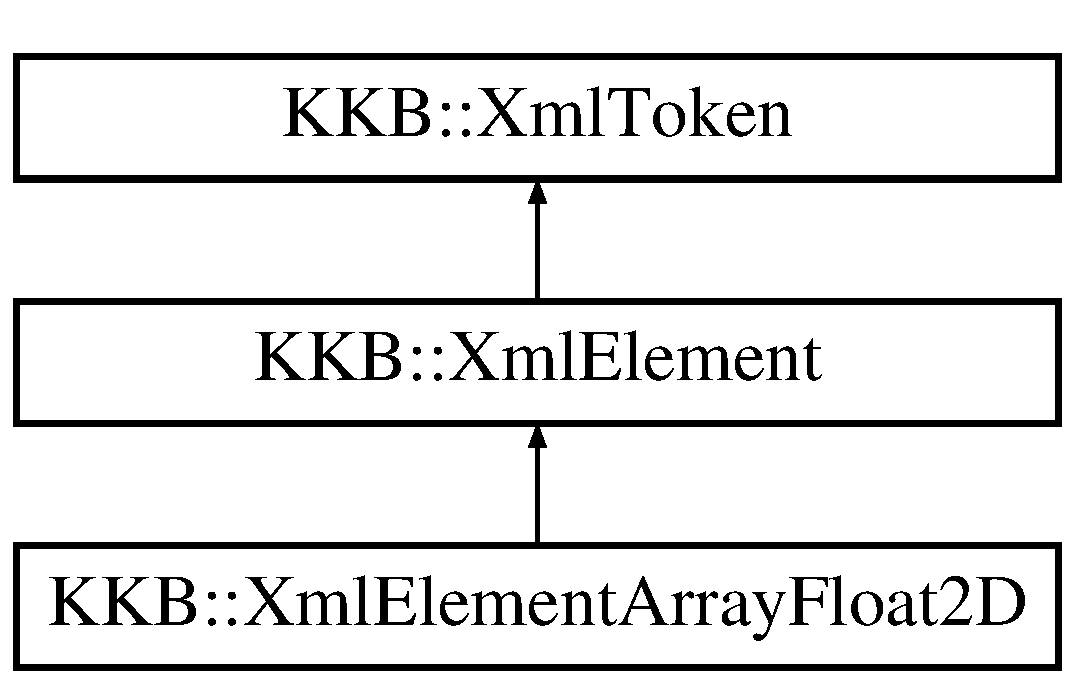
\includegraphics[height=3.000000cm]{class_k_k_b_1_1_xml_element_array_float2_d}
\end{center}
\end{figure}
\subsection*{Public Member Functions}
\begin{DoxyCompactItemize}
\item 
\hyperlink{class_k_k_b_1_1_xml_element_array_float2_d_aa8d28636e1c4b02eaf53bcc551d063bf}{Xml\+Element\+Array\+Float2D} (\hyperlink{namespace_k_k_b_a9253a3ea8a5da18ca82be4ca2b390ef0}{Xml\+Tag\+Ptr} tag, \hyperlink{class_k_k_b_1_1_xml_stream}{Xml\+Stream} \&s, \hyperlink{namespace_k_k_b_a7d390f568e2831fb76b86b56c87bf92f}{Vol\+Const\+Bool} \&cancel\+Flag, \hyperlink{class_k_k_b_1_1_run_log}{Run\+Log} \&log)
\item 
virtual \hyperlink{class_k_k_b_1_1_xml_element_array_float2_d_a0d59fbcc7bf57b41052f21aef8047b55}{$\sim$\+Xml\+Element\+Array\+Float2D} ()
\item 
\hyperlink{namespace_k_k_b_af8d832f05c54994a1cce25bd5743e19a}{kkuint32} \hyperlink{class_k_k_b_1_1_xml_element_array_float2_d_a70b0a88c0e9b2eefebfbd3c5a6c86bd0}{Height} () const 
\item 
float $\ast$$\ast$ \hyperlink{class_k_k_b_1_1_xml_element_array_float2_d_a9ddbec915d546b1a3c4d2ca09096f47c}{Take\+Ownership} ()
\item 
float $\ast$$\ast$ \hyperlink{class_k_k_b_1_1_xml_element_array_float2_d_af0b16fd19c24bf2abc31261c26cc5e4c}{Value} () const 
\item 
\hyperlink{namespace_k_k_b_af8d832f05c54994a1cce25bd5743e19a}{kkuint32} \hyperlink{class_k_k_b_1_1_xml_element_array_float2_d_aee02609107b81bf36fbc5d10b53d76a3}{Width} () const 
\end{DoxyCompactItemize}
\subsection*{Static Public Member Functions}
\begin{DoxyCompactItemize}
\item 
static void \hyperlink{class_k_k_b_1_1_xml_element_array_float2_d_a4500381c941ffabd13e1a9c843d15955}{Write\+X\+ML} (\hyperlink{namespace_k_k_b_af8d832f05c54994a1cce25bd5743e19a}{kkuint32} height, \hyperlink{namespace_k_k_b_af8d832f05c54994a1cce25bd5743e19a}{kkuint32} width, float $\ast$$\ast$const mat, const \hyperlink{class_k_k_b_1_1_k_k_str}{K\+K\+Str} \&var\+Name, std\+::ostream \&o)
\end{DoxyCompactItemize}
\subsection*{Additional Inherited Members}


\subsection{Detailed Description}


Definition at line 922 of file Xml\+Stream.\+h.



\subsection{Constructor \& Destructor Documentation}
\index{K\+K\+B\+::\+Xml\+Element\+Array\+Float2D@{K\+K\+B\+::\+Xml\+Element\+Array\+Float2D}!Xml\+Element\+Array\+Float2D@{Xml\+Element\+Array\+Float2D}}
\index{Xml\+Element\+Array\+Float2D@{Xml\+Element\+Array\+Float2D}!K\+K\+B\+::\+Xml\+Element\+Array\+Float2D@{K\+K\+B\+::\+Xml\+Element\+Array\+Float2D}}
\subsubsection[{\texorpdfstring{Xml\+Element\+Array\+Float2\+D(\+Xml\+Tag\+Ptr tag, Xml\+Stream \&s, Vol\+Const\+Bool \&cancel\+Flag, Run\+Log \&log)}{XmlElementArrayFloat2D(XmlTagPtr tag, XmlStream &s, VolConstBool &cancelFlag, RunLog &log)}}]{\setlength{\rightskip}{0pt plus 5cm}Xml\+Element\+Array\+Float2\+D\+::\+Xml\+Element\+Array\+Float2D (
\begin{DoxyParamCaption}
\item[{{\bf Xml\+Tag\+Ptr}}]{tag, }
\item[{{\bf Xml\+Stream} \&}]{s, }
\item[{{\bf Vol\+Const\+Bool} \&}]{cancel\+Flag, }
\item[{{\bf Run\+Log} \&}]{log}
\end{DoxyParamCaption}
)}\hypertarget{class_k_k_b_1_1_xml_element_array_float2_d_aa8d28636e1c4b02eaf53bcc551d063bf}{}\label{class_k_k_b_1_1_xml_element_array_float2_d_aa8d28636e1c4b02eaf53bcc551d063bf}


Definition at line 1862 of file Xml\+Stream.\+cpp.

\index{K\+K\+B\+::\+Xml\+Element\+Array\+Float2D@{K\+K\+B\+::\+Xml\+Element\+Array\+Float2D}!````~Xml\+Element\+Array\+Float2D@{$\sim$\+Xml\+Element\+Array\+Float2D}}
\index{````~Xml\+Element\+Array\+Float2D@{$\sim$\+Xml\+Element\+Array\+Float2D}!K\+K\+B\+::\+Xml\+Element\+Array\+Float2D@{K\+K\+B\+::\+Xml\+Element\+Array\+Float2D}}
\subsubsection[{\texorpdfstring{$\sim$\+Xml\+Element\+Array\+Float2\+D()}{~XmlElementArrayFloat2D()}}]{\setlength{\rightskip}{0pt plus 5cm}Xml\+Element\+Array\+Float2\+D\+::$\sim$\+Xml\+Element\+Array\+Float2D (
\begin{DoxyParamCaption}
{}
\end{DoxyParamCaption}
)\hspace{0.3cm}{\ttfamily [virtual]}}\hypertarget{class_k_k_b_1_1_xml_element_array_float2_d_a0d59fbcc7bf57b41052f21aef8047b55}{}\label{class_k_k_b_1_1_xml_element_array_float2_d_a0d59fbcc7bf57b41052f21aef8047b55}


Definition at line 1862 of file Xml\+Stream.\+cpp.



\subsection{Member Function Documentation}
\index{K\+K\+B\+::\+Xml\+Element\+Array\+Float2D@{K\+K\+B\+::\+Xml\+Element\+Array\+Float2D}!Height@{Height}}
\index{Height@{Height}!K\+K\+B\+::\+Xml\+Element\+Array\+Float2D@{K\+K\+B\+::\+Xml\+Element\+Array\+Float2D}}
\subsubsection[{\texorpdfstring{Height() const }{Height() const }}]{\setlength{\rightskip}{0pt plus 5cm}{\bf kkuint32} K\+K\+B\+::\+Xml\+Element\+Array\+Float2\+D\+::\+Height (
\begin{DoxyParamCaption}
{}
\end{DoxyParamCaption}
) const\hspace{0.3cm}{\ttfamily [inline]}}\hypertarget{class_k_k_b_1_1_xml_element_array_float2_d_a70b0a88c0e9b2eefebfbd3c5a6c86bd0}{}\label{class_k_k_b_1_1_xml_element_array_float2_d_a70b0a88c0e9b2eefebfbd3c5a6c86bd0}


Definition at line 922 of file Xml\+Stream.\+h.

\index{K\+K\+B\+::\+Xml\+Element\+Array\+Float2D@{K\+K\+B\+::\+Xml\+Element\+Array\+Float2D}!Take\+Ownership@{Take\+Ownership}}
\index{Take\+Ownership@{Take\+Ownership}!K\+K\+B\+::\+Xml\+Element\+Array\+Float2D@{K\+K\+B\+::\+Xml\+Element\+Array\+Float2D}}
\subsubsection[{\texorpdfstring{Take\+Ownership()}{TakeOwnership()}}]{\setlength{\rightskip}{0pt plus 5cm}float $\ast$$\ast$ Xml\+Element\+Array\+Float2\+D\+::\+Take\+Ownership (
\begin{DoxyParamCaption}
{}
\end{DoxyParamCaption}
)}\hypertarget{class_k_k_b_1_1_xml_element_array_float2_d_a9ddbec915d546b1a3c4d2ca09096f47c}{}\label{class_k_k_b_1_1_xml_element_array_float2_d_a9ddbec915d546b1a3c4d2ca09096f47c}


Definition at line 1862 of file Xml\+Stream.\+cpp.

\index{K\+K\+B\+::\+Xml\+Element\+Array\+Float2D@{K\+K\+B\+::\+Xml\+Element\+Array\+Float2D}!Value@{Value}}
\index{Value@{Value}!K\+K\+B\+::\+Xml\+Element\+Array\+Float2D@{K\+K\+B\+::\+Xml\+Element\+Array\+Float2D}}
\subsubsection[{\texorpdfstring{Value() const }{Value() const }}]{\setlength{\rightskip}{0pt plus 5cm}float$\ast$$\ast$ K\+K\+B\+::\+Xml\+Element\+Array\+Float2\+D\+::\+Value (
\begin{DoxyParamCaption}
{}
\end{DoxyParamCaption}
) const\hspace{0.3cm}{\ttfamily [inline]}}\hypertarget{class_k_k_b_1_1_xml_element_array_float2_d_af0b16fd19c24bf2abc31261c26cc5e4c}{}\label{class_k_k_b_1_1_xml_element_array_float2_d_af0b16fd19c24bf2abc31261c26cc5e4c}


Definition at line 922 of file Xml\+Stream.\+h.

\index{K\+K\+B\+::\+Xml\+Element\+Array\+Float2D@{K\+K\+B\+::\+Xml\+Element\+Array\+Float2D}!Width@{Width}}
\index{Width@{Width}!K\+K\+B\+::\+Xml\+Element\+Array\+Float2D@{K\+K\+B\+::\+Xml\+Element\+Array\+Float2D}}
\subsubsection[{\texorpdfstring{Width() const }{Width() const }}]{\setlength{\rightskip}{0pt plus 5cm}{\bf kkuint32} K\+K\+B\+::\+Xml\+Element\+Array\+Float2\+D\+::\+Width (
\begin{DoxyParamCaption}
{}
\end{DoxyParamCaption}
) const\hspace{0.3cm}{\ttfamily [inline]}}\hypertarget{class_k_k_b_1_1_xml_element_array_float2_d_aee02609107b81bf36fbc5d10b53d76a3}{}\label{class_k_k_b_1_1_xml_element_array_float2_d_aee02609107b81bf36fbc5d10b53d76a3}


Definition at line 922 of file Xml\+Stream.\+h.

\index{K\+K\+B\+::\+Xml\+Element\+Array\+Float2D@{K\+K\+B\+::\+Xml\+Element\+Array\+Float2D}!Write\+X\+ML@{Write\+X\+ML}}
\index{Write\+X\+ML@{Write\+X\+ML}!K\+K\+B\+::\+Xml\+Element\+Array\+Float2D@{K\+K\+B\+::\+Xml\+Element\+Array\+Float2D}}
\subsubsection[{\texorpdfstring{Write\+X\+M\+L(kkuint32 height, kkuint32 width, float $\ast$$\ast$const mat, const K\+K\+Str \&var\+Name, std\+::ostream \&o)}{WriteXML(kkuint32 height, kkuint32 width, float **const mat, const KKStr &varName, std::ostream &o)}}]{\setlength{\rightskip}{0pt plus 5cm}void Xml\+Element\+Array\+Float2\+D\+::\+Write\+X\+ML (
\begin{DoxyParamCaption}
\item[{{\bf kkuint32}}]{height, }
\item[{{\bf kkuint32}}]{width, }
\item[{float $\ast$$\ast$const}]{mat, }
\item[{const {\bf K\+K\+Str} \&}]{var\+Name, }
\item[{std\+::ostream \&}]{o}
\end{DoxyParamCaption}
)\hspace{0.3cm}{\ttfamily [static]}}\hypertarget{class_k_k_b_1_1_xml_element_array_float2_d_a4500381c941ffabd13e1a9c843d15955}{}\label{class_k_k_b_1_1_xml_element_array_float2_d_a4500381c941ffabd13e1a9c843d15955}


Definition at line 1862 of file Xml\+Stream.\+cpp.



The documentation for this class was generated from the following files\+:\begin{DoxyCompactItemize}
\item 
C\+:/\+Users/\+Kurt/\+Git\+Hub/\+K\+Square\+Libraries/\+K\+K\+Base/\hyperlink{_xml_stream_8h}{Xml\+Stream.\+h}\item 
C\+:/\+Users/\+Kurt/\+Git\+Hub/\+K\+Square\+Libraries/\+K\+K\+Base/\hyperlink{_xml_stream_8cpp}{Xml\+Stream.\+cpp}\end{DoxyCompactItemize}

\hypertarget{class_k_k_b_1_1_xml_element_array_float2_d_varying}{}\section{K\+KB\+:\+:Xml\+Element\+Array\+Float2\+D\+Varying Class Reference}
\label{class_k_k_b_1_1_xml_element_array_float2_d_varying}\index{K\+K\+B\+::\+Xml\+Element\+Array\+Float2\+D\+Varying@{K\+K\+B\+::\+Xml\+Element\+Array\+Float2\+D\+Varying}}


{\ttfamily \#include $<$Xml\+Stream.\+h$>$}

Inheritance diagram for K\+KB\+:\+:Xml\+Element\+Array\+Float2\+D\+Varying\+:\begin{figure}[H]
\begin{center}
\leavevmode
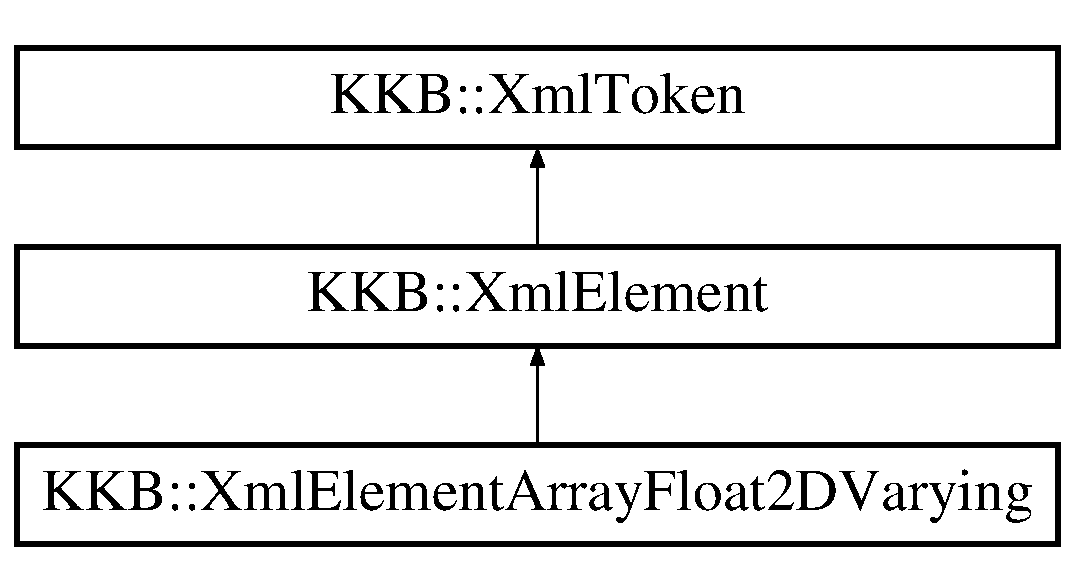
\includegraphics[height=3.000000cm]{class_k_k_b_1_1_xml_element_array_float2_d_varying}
\end{center}
\end{figure}
\subsection*{Public Member Functions}
\begin{DoxyCompactItemize}
\item 
\hyperlink{class_k_k_b_1_1_xml_element_array_float2_d_varying_aacca96d12ebba71cf93a54e339bc9581}{Xml\+Element\+Array\+Float2\+D\+Varying} (\hyperlink{namespace_k_k_b_a9253a3ea8a5da18ca82be4ca2b390ef0}{Xml\+Tag\+Ptr} tag, \hyperlink{class_k_k_b_1_1_xml_stream}{Xml\+Stream} \&s, \hyperlink{namespace_k_k_b_a7d390f568e2831fb76b86b56c87bf92f}{Vol\+Const\+Bool} \&cancel\+Flag, \hyperlink{class_k_k_b_1_1_run_log}{Run\+Log} \&log)
\item 
virtual \hyperlink{class_k_k_b_1_1_xml_element_array_float2_d_varying_af2023b225e7a10088ecea82bb6046f2b}{$\sim$\+Xml\+Element\+Array\+Float2\+D\+Varying} ()
\item 
\hyperlink{namespace_k_k_b_af8d832f05c54994a1cce25bd5743e19a}{kkuint32} \hyperlink{class_k_k_b_1_1_xml_element_array_float2_d_varying_a89a9805bd91bf8db908450d763501cf7}{Height} () const 
\item 
float $\ast$$\ast$ \hyperlink{class_k_k_b_1_1_xml_element_array_float2_d_varying_a832e4f16a69004742d47b6970bcc44b3}{Take\+Ownership} ()
\item 
\hyperlink{namespace_k_k_b_af8d832f05c54994a1cce25bd5743e19a}{kkuint32} $\ast$ \hyperlink{class_k_k_b_1_1_xml_element_array_float2_d_varying_ae727d8df514102c39399996777639aac}{Take\+Ownership\+Widths} ()
\item 
float $\ast$$\ast$ \hyperlink{class_k_k_b_1_1_xml_element_array_float2_d_varying_a880212291e7d1b7d7fe1aae6693b0bed}{Value} () const 
\item 
\hyperlink{namespace_k_k_b_af8d832f05c54994a1cce25bd5743e19a}{kkuint32} $\ast$ \hyperlink{class_k_k_b_1_1_xml_element_array_float2_d_varying_a87c4c27d22770df25a5c20f9caa68914}{Widths} () const 
\end{DoxyCompactItemize}
\subsection*{Static Public Member Functions}
\begin{DoxyCompactItemize}
\item 
static void \hyperlink{class_k_k_b_1_1_xml_element_array_float2_d_varying_a0984ce67f7d0b713e151e43d636fe44e}{Write\+X\+ML} (\hyperlink{namespace_k_k_b_af8d832f05c54994a1cce25bd5743e19a}{kkuint32} height, const \hyperlink{namespace_k_k_b_a8fa4952cc84fda1de4bec1fbdd8d5b1b}{kkint32} $\ast$widths, float $\ast$$\ast$const mat, const \hyperlink{class_k_k_b_1_1_k_k_str}{K\+K\+Str} \&var\+Name, std\+::ostream \&o)
\end{DoxyCompactItemize}
\subsection*{Additional Inherited Members}


\subsection{Detailed Description}


Definition at line 611 of file Xml\+Stream.\+h.



\subsection{Constructor \& Destructor Documentation}
\index{K\+K\+B\+::\+Xml\+Element\+Array\+Float2\+D\+Varying@{K\+K\+B\+::\+Xml\+Element\+Array\+Float2\+D\+Varying}!Xml\+Element\+Array\+Float2\+D\+Varying@{Xml\+Element\+Array\+Float2\+D\+Varying}}
\index{Xml\+Element\+Array\+Float2\+D\+Varying@{Xml\+Element\+Array\+Float2\+D\+Varying}!K\+K\+B\+::\+Xml\+Element\+Array\+Float2\+D\+Varying@{K\+K\+B\+::\+Xml\+Element\+Array\+Float2\+D\+Varying}}
\subsubsection[{\texorpdfstring{Xml\+Element\+Array\+Float2\+D\+Varying(\+Xml\+Tag\+Ptr tag, Xml\+Stream \&s, Vol\+Const\+Bool \&cancel\+Flag, Run\+Log \&log)}{XmlElementArrayFloat2DVarying(XmlTagPtr tag, XmlStream &s, VolConstBool &cancelFlag, RunLog &log)}}]{\setlength{\rightskip}{0pt plus 5cm}Xml\+Element\+Array\+Float2\+D\+Varying\+::\+Xml\+Element\+Array\+Float2\+D\+Varying (
\begin{DoxyParamCaption}
\item[{{\bf Xml\+Tag\+Ptr}}]{tag, }
\item[{{\bf Xml\+Stream} \&}]{s, }
\item[{{\bf Vol\+Const\+Bool} \&}]{cancel\+Flag, }
\item[{{\bf Run\+Log} \&}]{log}
\end{DoxyParamCaption}
)}\hypertarget{class_k_k_b_1_1_xml_element_array_float2_d_varying_aacca96d12ebba71cf93a54e339bc9581}{}\label{class_k_k_b_1_1_xml_element_array_float2_d_varying_aacca96d12ebba71cf93a54e339bc9581}


Definition at line 1283 of file Xml\+Stream.\+cpp.



References K\+K\+B\+::\+Xml\+Tag\+::\+Attribute\+Value\+Int32(), K\+K\+B\+::\+Xml\+Stream\+::\+Get\+Next\+Token(), and K\+K\+B\+::\+Xml\+Element\+::\+Xml\+Element().


\begin{DoxyCode}
1287                                                              :
1288     \hyperlink{class_k_k_b_1_1_xml_element_a66317eff5bd3abcc60755756ba2887d5}{XmlElement} (tag, s, log),
1289     height (0),
1290     widths (NULL),
1291     value  (NULL)
1292 \{
1293   height = tag->\hyperlink{class_k_k_b_1_1_xml_tag_acbbfaeaf55fd15e4f563a71a1b4fa456}{AttributeValueInt32} (\textcolor{stringliteral}{"Height"});
1294   \textcolor{keywordflow}{if}  (height < 1)
1295   \{
1296     log.\hyperlink{class_k_k_b_1_1_run_log_a32cf761d7f2e747465fd80533fdbb659}{Level} (-1) << \hyperlink{namespace_k_k_b_ad1f50f65af6adc8fa9e6f62d007818a8}{endl} 
1297       << \textcolor{stringliteral}{"XmlElementArrayFloat2DVarying   ***ERROR***   Height["} << height << \textcolor{stringliteral}{"] must be greater than 0."} <
      < \hyperlink{namespace_k_k_b_ad1f50f65af6adc8fa9e6f62d007818a8}{endl} 
1298       << \hyperlink{namespace_k_k_b_ad1f50f65af6adc8fa9e6f62d007818a8}{endl};
1299     height = 0;
1300     \textcolor{keywordflow}{return};
1301   \}
1302   value  = \textcolor{keyword}{new} \textcolor{keywordtype}{float}*[height];
1303   widths = \textcolor{keyword}{new} \hyperlink{namespace_k_k_b_af8d832f05c54994a1cce25bd5743e19a}{kkuint32}[height];
1304 
1305   \hyperlink{class_k_k_b_1_1_xml_token}{XmlTokenPtr}  tok = s.\hyperlink{class_k_k_b_1_1_xml_stream_a87cc738b05c666cf5d5c25beaab477b4}{GetNextToken} (cancelFlag, log);
1306   \hyperlink{namespace_k_k_b_af8d832f05c54994a1cce25bd5743e19a}{kkuint32}  rowCount = 0;
1307   \textcolor{keywordflow}{while}  (tok)
1308   \{
1309     \textcolor{keywordflow}{if}  (\textcolor{keyword}{typeid}(*tok) == \textcolor{keyword}{typeid}(\hyperlink{class_k_k_b_1_1_xml_element_array_float}{XmlElementArrayFloat}))
1310     \{
1311       \textcolor{keywordflow}{if}  (rowCount >= height)
1312       \{
1313         log.\hyperlink{class_k_k_b_1_1_run_log_a32cf761d7f2e747465fd80533fdbb659}{Level} (-1) << \hyperlink{namespace_k_k_b_ad1f50f65af6adc8fa9e6f62d007818a8}{endl}
1314           << \textcolor{stringliteral}{"XmlElementArrayFloat2DVarying   ***ERROR***   Number of defined rows exceeds defined Height["}
       << height << \textcolor{stringliteral}{"]"} << \hyperlink{namespace_k_k_b_ad1f50f65af6adc8fa9e6f62d007818a8}{endl}
1315           << \hyperlink{namespace_k_k_b_ad1f50f65af6adc8fa9e6f62d007818a8}{endl};
1316         widths[rowCount] = 0;
1317         value[rowCount]  = NULL;
1318       \}
1319       \textcolor{keywordflow}{else}
1320       \{
1321         \hyperlink{class_k_k_b_1_1_xml_element_array_float}{XmlElementArrayFloatPtr} f = \textcolor{keyword}{dynamic\_cast<}
      \hyperlink{class_k_k_b_1_1_xml_element_array_float}{XmlElementArrayFloatPtr}\textcolor{keyword}{>}(tok);
1322         widths[rowCount] = f->\hyperlink{class_k_k_b_1_1_xml_element_array_float_a364bdaf1cdc0dc775e30957350fc6504}{Count} ();
1323         value[rowCount] = f->\hyperlink{class_k_k_b_1_1_xml_element_array_float_a43d247c7374f56ef9e6e1d3ccec40809}{TakeOwnership} ();
1324       \}
1325       ++rowCount;
1326     \}
1327     \textcolor{keyword}{delete}  tok;
1328     tok = s.\hyperlink{class_k_k_b_1_1_xml_stream_a87cc738b05c666cf5d5c25beaab477b4}{GetNextToken} (cancelFlag, log);
1329   \}
1330   \textcolor{keywordflow}{while}  (rowCount < height)
1331   \{
1332     value[rowCount] = NULL;
1333     ++rowCount;
1334   \}
1335 \}
\end{DoxyCode}
\index{K\+K\+B\+::\+Xml\+Element\+Array\+Float2\+D\+Varying@{K\+K\+B\+::\+Xml\+Element\+Array\+Float2\+D\+Varying}!````~Xml\+Element\+Array\+Float2\+D\+Varying@{$\sim$\+Xml\+Element\+Array\+Float2\+D\+Varying}}
\index{````~Xml\+Element\+Array\+Float2\+D\+Varying@{$\sim$\+Xml\+Element\+Array\+Float2\+D\+Varying}!K\+K\+B\+::\+Xml\+Element\+Array\+Float2\+D\+Varying@{K\+K\+B\+::\+Xml\+Element\+Array\+Float2\+D\+Varying}}
\subsubsection[{\texorpdfstring{$\sim$\+Xml\+Element\+Array\+Float2\+D\+Varying()}{~XmlElementArrayFloat2DVarying()}}]{\setlength{\rightskip}{0pt plus 5cm}Xml\+Element\+Array\+Float2\+D\+Varying\+::$\sim$\+Xml\+Element\+Array\+Float2\+D\+Varying (
\begin{DoxyParamCaption}
{}
\end{DoxyParamCaption}
)\hspace{0.3cm}{\ttfamily [virtual]}}\hypertarget{class_k_k_b_1_1_xml_element_array_float2_d_varying_af2023b225e7a10088ecea82bb6046f2b}{}\label{class_k_k_b_1_1_xml_element_array_float2_d_varying_af2023b225e7a10088ecea82bb6046f2b}


Definition at line 1339 of file Xml\+Stream.\+cpp.


\begin{DoxyCode}
1340 \{
1341   \textcolor{keywordflow}{if}  (value)
1342   \{
1343     \textcolor{keywordflow}{for}  (\hyperlink{namespace_k_k_b_af8d832f05c54994a1cce25bd5743e19a}{kkuint32} x = 0;  x < height;  ++x)
1344     \{
1345       \textcolor{keyword}{delete} value[x];
1346       value[x] = NULL;
1347     \}
1348   \}
1349   \textcolor{keyword}{delete}  value;   value  = NULL;
1350   \textcolor{keyword}{delete}  widths;  widths = NULL;
1351 \}
\end{DoxyCode}


\subsection{Member Function Documentation}
\index{K\+K\+B\+::\+Xml\+Element\+Array\+Float2\+D\+Varying@{K\+K\+B\+::\+Xml\+Element\+Array\+Float2\+D\+Varying}!Height@{Height}}
\index{Height@{Height}!K\+K\+B\+::\+Xml\+Element\+Array\+Float2\+D\+Varying@{K\+K\+B\+::\+Xml\+Element\+Array\+Float2\+D\+Varying}}
\subsubsection[{\texorpdfstring{Height() const }{Height() const }}]{\setlength{\rightskip}{0pt plus 5cm}{\bf kkuint32} K\+K\+B\+::\+Xml\+Element\+Array\+Float2\+D\+Varying\+::\+Height (
\begin{DoxyParamCaption}
{}
\end{DoxyParamCaption}
) const\hspace{0.3cm}{\ttfamily [inline]}}\hypertarget{class_k_k_b_1_1_xml_element_array_float2_d_varying_a89a9805bd91bf8db908450d763501cf7}{}\label{class_k_k_b_1_1_xml_element_array_float2_d_varying_a89a9805bd91bf8db908450d763501cf7}


Definition at line 622 of file Xml\+Stream.\+h.


\begin{DoxyCode}
622 \{\textcolor{keywordflow}{return} height;\}     
\end{DoxyCode}
\index{K\+K\+B\+::\+Xml\+Element\+Array\+Float2\+D\+Varying@{K\+K\+B\+::\+Xml\+Element\+Array\+Float2\+D\+Varying}!Take\+Ownership@{Take\+Ownership}}
\index{Take\+Ownership@{Take\+Ownership}!K\+K\+B\+::\+Xml\+Element\+Array\+Float2\+D\+Varying@{K\+K\+B\+::\+Xml\+Element\+Array\+Float2\+D\+Varying}}
\subsubsection[{\texorpdfstring{Take\+Ownership()}{TakeOwnership()}}]{\setlength{\rightskip}{0pt plus 5cm}float $\ast$$\ast$ Xml\+Element\+Array\+Float2\+D\+Varying\+::\+Take\+Ownership (
\begin{DoxyParamCaption}
{}
\end{DoxyParamCaption}
)}\hypertarget{class_k_k_b_1_1_xml_element_array_float2_d_varying_a832e4f16a69004742d47b6970bcc44b3}{}\label{class_k_k_b_1_1_xml_element_array_float2_d_varying_a832e4f16a69004742d47b6970bcc44b3}


Definition at line 1356 of file Xml\+Stream.\+cpp.


\begin{DoxyCode}
1357 \{
1358   \textcolor{keywordtype}{float}** v = value;
1359   value = NULL;
1360   \textcolor{keywordflow}{return} v;
1361 \}
\end{DoxyCode}
\index{K\+K\+B\+::\+Xml\+Element\+Array\+Float2\+D\+Varying@{K\+K\+B\+::\+Xml\+Element\+Array\+Float2\+D\+Varying}!Take\+Ownership\+Widths@{Take\+Ownership\+Widths}}
\index{Take\+Ownership\+Widths@{Take\+Ownership\+Widths}!K\+K\+B\+::\+Xml\+Element\+Array\+Float2\+D\+Varying@{K\+K\+B\+::\+Xml\+Element\+Array\+Float2\+D\+Varying}}
\subsubsection[{\texorpdfstring{Take\+Ownership\+Widths()}{TakeOwnershipWidths()}}]{\setlength{\rightskip}{0pt plus 5cm}{\bf kkuint32} $\ast$ Xml\+Element\+Array\+Float2\+D\+Varying\+::\+Take\+Ownership\+Widths (
\begin{DoxyParamCaption}
{}
\end{DoxyParamCaption}
)}\hypertarget{class_k_k_b_1_1_xml_element_array_float2_d_varying_ae727d8df514102c39399996777639aac}{}\label{class_k_k_b_1_1_xml_element_array_float2_d_varying_ae727d8df514102c39399996777639aac}


Definition at line 1364 of file Xml\+Stream.\+cpp.


\begin{DoxyCode}
1365 \{
1366   \hyperlink{namespace_k_k_b_af8d832f05c54994a1cce25bd5743e19a}{kkuint32}* w = widths;
1367   widths = NULL;
1368   \textcolor{keywordflow}{return} w;
1369 \}
\end{DoxyCode}
\index{K\+K\+B\+::\+Xml\+Element\+Array\+Float2\+D\+Varying@{K\+K\+B\+::\+Xml\+Element\+Array\+Float2\+D\+Varying}!Value@{Value}}
\index{Value@{Value}!K\+K\+B\+::\+Xml\+Element\+Array\+Float2\+D\+Varying@{K\+K\+B\+::\+Xml\+Element\+Array\+Float2\+D\+Varying}}
\subsubsection[{\texorpdfstring{Value() const }{Value() const }}]{\setlength{\rightskip}{0pt plus 5cm}float$\ast$$\ast$ K\+K\+B\+::\+Xml\+Element\+Array\+Float2\+D\+Varying\+::\+Value (
\begin{DoxyParamCaption}
{}
\end{DoxyParamCaption}
) const\hspace{0.3cm}{\ttfamily [inline]}}\hypertarget{class_k_k_b_1_1_xml_element_array_float2_d_varying_a880212291e7d1b7d7fe1aae6693b0bed}{}\label{class_k_k_b_1_1_xml_element_array_float2_d_varying_a880212291e7d1b7d7fe1aae6693b0bed}


Definition at line 624 of file Xml\+Stream.\+h.


\begin{DoxyCode}
624 \{\textcolor{keywordflow}{return} value;\}
\end{DoxyCode}
\index{K\+K\+B\+::\+Xml\+Element\+Array\+Float2\+D\+Varying@{K\+K\+B\+::\+Xml\+Element\+Array\+Float2\+D\+Varying}!Widths@{Widths}}
\index{Widths@{Widths}!K\+K\+B\+::\+Xml\+Element\+Array\+Float2\+D\+Varying@{K\+K\+B\+::\+Xml\+Element\+Array\+Float2\+D\+Varying}}
\subsubsection[{\texorpdfstring{Widths() const }{Widths() const }}]{\setlength{\rightskip}{0pt plus 5cm}{\bf kkuint32}$\ast$ K\+K\+B\+::\+Xml\+Element\+Array\+Float2\+D\+Varying\+::\+Widths (
\begin{DoxyParamCaption}
{}
\end{DoxyParamCaption}
) const\hspace{0.3cm}{\ttfamily [inline]}}\hypertarget{class_k_k_b_1_1_xml_element_array_float2_d_varying_a87c4c27d22770df25a5c20f9caa68914}{}\label{class_k_k_b_1_1_xml_element_array_float2_d_varying_a87c4c27d22770df25a5c20f9caa68914}


Definition at line 626 of file Xml\+Stream.\+h.


\begin{DoxyCode}
626 \{\textcolor{keywordflow}{return} widths;\}
\end{DoxyCode}
\index{K\+K\+B\+::\+Xml\+Element\+Array\+Float2\+D\+Varying@{K\+K\+B\+::\+Xml\+Element\+Array\+Float2\+D\+Varying}!Write\+X\+ML@{Write\+X\+ML}}
\index{Write\+X\+ML@{Write\+X\+ML}!K\+K\+B\+::\+Xml\+Element\+Array\+Float2\+D\+Varying@{K\+K\+B\+::\+Xml\+Element\+Array\+Float2\+D\+Varying}}
\subsubsection[{\texorpdfstring{Write\+X\+M\+L(kkuint32 height, const kkint32 $\ast$widths, float $\ast$$\ast$const mat, const K\+K\+Str \&var\+Name, std\+::ostream \&o)}{WriteXML(kkuint32 height, const kkint32 *widths, float **const mat, const KKStr &varName, std::ostream &o)}}]{\setlength{\rightskip}{0pt plus 5cm}void Xml\+Element\+Array\+Float2\+D\+Varying\+::\+Write\+X\+ML (
\begin{DoxyParamCaption}
\item[{{\bf kkuint32}}]{height, }
\item[{const {\bf kkint32} $\ast$}]{widths, }
\item[{float $\ast$$\ast$const}]{mat, }
\item[{const {\bf K\+K\+Str} \&}]{var\+Name, }
\item[{std\+::ostream \&}]{o}
\end{DoxyParamCaption}
)\hspace{0.3cm}{\ttfamily [static]}}\hypertarget{class_k_k_b_1_1_xml_element_array_float2_d_varying_a0984ce67f7d0b713e151e43d636fe44e}{}\label{class_k_k_b_1_1_xml_element_array_float2_d_varying_a0984ce67f7d0b713e151e43d636fe44e}

\begin{DoxyParams}{Parameters}
{\em widths} & Each entry in array defines the length of the corresponding row in \textquotesingle{}mat\textquotesingle{}. \\
\hline
\end{DoxyParams}


Definition at line 1374 of file Xml\+Stream.\+cpp.



References K\+K\+B\+::\+Xml\+Tag\+::\+Add\+Atribute(), K\+K\+B\+::\+K\+K\+Str\+::\+Concat(), K\+K\+B\+::\+K\+K\+Str\+::\+Empty(), K\+K\+B\+::operator+(), K\+K\+B\+::\+Str\+Format\+Int(), K\+K\+B\+::\+Xml\+Tag\+::tag\+End, K\+K\+B\+::\+Xml\+Tag\+::tag\+Start, K\+K\+B\+::\+Xml\+Tag\+::\+Write\+X\+M\+L(), and K\+K\+B\+::\+Xml\+Tag\+::\+Xml\+Tag().


\begin{DoxyCode}
1380 \{
1381   \hyperlink{class_k_k_b_1_1_xml_tag}{XmlTag} startTag (\textcolor{stringliteral}{"ArrayFloat2DVarying"}, \hyperlink{class_k_k_b_1_1_xml_tag_a6c0ef0e23f982f49d55d4fb7eaff6ac9ab02b23b5e15b3a1353771313e1176ce0}{XmlTag::TagTypes::tagStart});
1382   \textcolor{keywordflow}{if}  (!varName.\hyperlink{class_k_k_b_1_1_k_k_str_ac69942f73fffd672ec2a6e1c410afdb6}{Empty} ())
1383     startTag.AddAtribute (\textcolor{stringliteral}{"VarName"}, varName);
1384   startTag.AddAtribute (\textcolor{stringliteral}{"Height"}, (\hyperlink{namespace_k_k_b_a8fa4952cc84fda1de4bec1fbdd8d5b1b}{kkint32})height);
1385   startTag.WriteXML (o);
1386   o << \hyperlink{namespace_k_k_b_ad1f50f65af6adc8fa9e6f62d007818a8}{endl};
1387 
1388   \textcolor{keywordflow}{for}  (\hyperlink{namespace_k_k_b_af8d832f05c54994a1cce25bd5743e19a}{kkuint32} r = 0;  r < height;  ++r)
1389   \{
1390     \hyperlink{class_k_k_b_1_1_k_k_str}{KKStr} rowName = \textcolor{stringliteral}{"Row\_"} + \hyperlink{namespace_k_k_b_ae3bde258fa036604fac8bdb0277ab46e}{StrFormatInt} (r, \textcolor{stringliteral}{"000"});
1391     \hyperlink{class_k_k_b_1_1_xml_element_array_float_a78bc9a4e11950ad7706a46f1d7da9749}{XmlElementArrayFloat::WriteXML} (widths[r], mat[r], rowName, o);
1392   \}
1393 
1394   \hyperlink{class_k_k_b_1_1_xml_tag}{XmlTag}  endTag (\textcolor{stringliteral}{"ArrayFloat2DVarying"}, \hyperlink{class_k_k_b_1_1_xml_tag_a6c0ef0e23f982f49d55d4fb7eaff6ac9a3ceaa9a790f688ec97a35b5a3fd3b164}{XmlTag::TagTypes::tagEnd});
1395   endTag.WriteXML (o);
1396   o << \hyperlink{namespace_k_k_b_ad1f50f65af6adc8fa9e6f62d007818a8}{endl};
1397 \}
\end{DoxyCode}


The documentation for this class was generated from the following files\+:\begin{DoxyCompactItemize}
\item 
C\+:/\+Users/\+Kurt/\+Git\+Hub/\+K\+Square\+Libraries/\+K\+K\+Base/\hyperlink{_xml_stream_8h}{Xml\+Stream.\+h}\item 
C\+:/\+Users/\+Kurt/\+Git\+Hub/\+K\+Square\+Libraries/\+K\+K\+Base/\hyperlink{_xml_stream_8cpp}{Xml\+Stream.\+cpp}\end{DoxyCompactItemize}

\hypertarget{class_k_k_b_1_1_xml_element_array_int32}{}\section{K\+KB\+:\+:Xml\+Element\+Array\+Int32 Class Reference}
\label{class_k_k_b_1_1_xml_element_array_int32}\index{K\+K\+B\+::\+Xml\+Element\+Array\+Int32@{K\+K\+B\+::\+Xml\+Element\+Array\+Int32}}


{\ttfamily \#include $<$Xml\+Stream.\+h$>$}

Inheritance diagram for K\+KB\+:\+:Xml\+Element\+Array\+Int32\+:\begin{figure}[H]
\begin{center}
\leavevmode
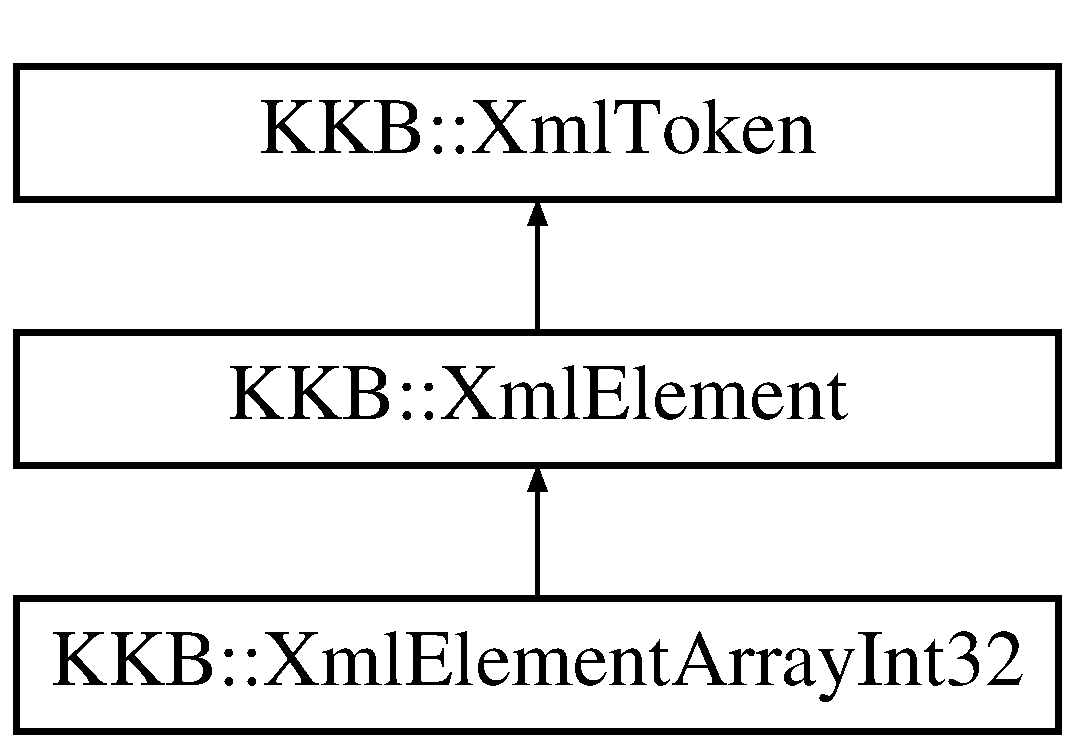
\includegraphics[height=3.000000cm]{class_k_k_b_1_1_xml_element_array_int32}
\end{center}
\end{figure}
\subsection*{Public Member Functions}
\begin{DoxyCompactItemize}
\item 
\hyperlink{class_k_k_b_1_1_xml_element_array_int32_ada0ab8a45899239adbc4c3a97ed99cab}{Xml\+Element\+Array\+Int32} (\hyperlink{namespace_k_k_b_a9253a3ea8a5da18ca82be4ca2b390ef0}{Xml\+Tag\+Ptr} tag, \hyperlink{class_k_k_b_1_1_xml_stream}{Xml\+Stream} \&s, \hyperlink{namespace_k_k_b_a7d390f568e2831fb76b86b56c87bf92f}{Vol\+Const\+Bool} \&cancel\+Flag, \hyperlink{class_k_k_b_1_1_run_log}{Run\+Log} \&log)
\item 
virtual \hyperlink{class_k_k_b_1_1_xml_element_array_int32_a98c232e8b95446cd2bbdfee819ddebbb}{$\sim$\+Xml\+Element\+Array\+Int32} ()
\item 
\hyperlink{namespace_k_k_b_af8d832f05c54994a1cce25bd5743e19a}{kkuint32} \hyperlink{class_k_k_b_1_1_xml_element_array_int32_a2773cdcb924ac8c67e32a4d07ee15f30}{Count} () const 
\item 
\hyperlink{namespace_k_k_b_a8fa4952cc84fda1de4bec1fbdd8d5b1b}{kkint32} $\ast$ \hyperlink{class_k_k_b_1_1_xml_element_array_int32_a466c9f162ec1ce60a50feb8f2268b86c}{Take\+Ownership} ()
\item 
\hyperlink{namespace_k_k_b_a8fa4952cc84fda1de4bec1fbdd8d5b1b}{kkint32} $\ast$ \hyperlink{class_k_k_b_1_1_xml_element_array_int32_aac523483b2d03bfbc7ca641b27e14189}{Value} () const 
\end{DoxyCompactItemize}
\subsection*{Static Public Member Functions}
\begin{DoxyCompactItemize}
\item 
static void \hyperlink{class_k_k_b_1_1_xml_element_array_int32_a39138d38eaaba35c9b972c1081e2e7a5}{Write\+X\+ML} (\hyperlink{namespace_k_k_b_af8d832f05c54994a1cce25bd5743e19a}{kkuint32} count, const \hyperlink{namespace_k_k_b_a8fa4952cc84fda1de4bec1fbdd8d5b1b}{kkint32} $\ast$d, const \hyperlink{class_k_k_b_1_1_k_k_str}{K\+K\+Str} \&var\+Name, std\+::ostream \&o)
\end{DoxyCompactItemize}
\subsection*{Additional Inherited Members}


\subsection{Detailed Description}


Definition at line 915 of file Xml\+Stream.\+h.



\subsection{Constructor \& Destructor Documentation}
\index{K\+K\+B\+::\+Xml\+Element\+Array\+Int32@{K\+K\+B\+::\+Xml\+Element\+Array\+Int32}!Xml\+Element\+Array\+Int32@{Xml\+Element\+Array\+Int32}}
\index{Xml\+Element\+Array\+Int32@{Xml\+Element\+Array\+Int32}!K\+K\+B\+::\+Xml\+Element\+Array\+Int32@{K\+K\+B\+::\+Xml\+Element\+Array\+Int32}}
\subsubsection[{\texorpdfstring{Xml\+Element\+Array\+Int32(\+Xml\+Tag\+Ptr tag, Xml\+Stream \&s, Vol\+Const\+Bool \&cancel\+Flag, Run\+Log \&log)}{XmlElementArrayInt32(XmlTagPtr tag, XmlStream &s, VolConstBool &cancelFlag, RunLog &log)}}]{\setlength{\rightskip}{0pt plus 5cm}Xml\+Element\+Array\+Int32\+::\+Xml\+Element\+Array\+Int32 (
\begin{DoxyParamCaption}
\item[{{\bf Xml\+Tag\+Ptr}}]{tag, }
\item[{{\bf Xml\+Stream} \&}]{s, }
\item[{{\bf Vol\+Const\+Bool} \&}]{cancel\+Flag, }
\item[{{\bf Run\+Log} \&}]{log}
\end{DoxyParamCaption}
)}\hypertarget{class_k_k_b_1_1_xml_element_array_int32_ada0ab8a45899239adbc4c3a97ed99cab}{}\label{class_k_k_b_1_1_xml_element_array_int32_ada0ab8a45899239adbc4c3a97ed99cab}


Definition at line 1855 of file Xml\+Stream.\+cpp.

\index{K\+K\+B\+::\+Xml\+Element\+Array\+Int32@{K\+K\+B\+::\+Xml\+Element\+Array\+Int32}!````~Xml\+Element\+Array\+Int32@{$\sim$\+Xml\+Element\+Array\+Int32}}
\index{````~Xml\+Element\+Array\+Int32@{$\sim$\+Xml\+Element\+Array\+Int32}!K\+K\+B\+::\+Xml\+Element\+Array\+Int32@{K\+K\+B\+::\+Xml\+Element\+Array\+Int32}}
\subsubsection[{\texorpdfstring{$\sim$\+Xml\+Element\+Array\+Int32()}{~XmlElementArrayInt32()}}]{\setlength{\rightskip}{0pt plus 5cm}Xml\+Element\+Array\+Int32\+::$\sim$\+Xml\+Element\+Array\+Int32 (
\begin{DoxyParamCaption}
{}
\end{DoxyParamCaption}
)\hspace{0.3cm}{\ttfamily [virtual]}}\hypertarget{class_k_k_b_1_1_xml_element_array_int32_a98c232e8b95446cd2bbdfee819ddebbb}{}\label{class_k_k_b_1_1_xml_element_array_int32_a98c232e8b95446cd2bbdfee819ddebbb}


Definition at line 1855 of file Xml\+Stream.\+cpp.



\subsection{Member Function Documentation}
\index{K\+K\+B\+::\+Xml\+Element\+Array\+Int32@{K\+K\+B\+::\+Xml\+Element\+Array\+Int32}!Count@{Count}}
\index{Count@{Count}!K\+K\+B\+::\+Xml\+Element\+Array\+Int32@{K\+K\+B\+::\+Xml\+Element\+Array\+Int32}}
\subsubsection[{\texorpdfstring{Count() const }{Count() const }}]{\setlength{\rightskip}{0pt plus 5cm}{\bf kkuint32} K\+K\+B\+::\+Xml\+Element\+Array\+Int32\+::\+Count (
\begin{DoxyParamCaption}
{}
\end{DoxyParamCaption}
) const\hspace{0.3cm}{\ttfamily [inline]}}\hypertarget{class_k_k_b_1_1_xml_element_array_int32_a2773cdcb924ac8c67e32a4d07ee15f30}{}\label{class_k_k_b_1_1_xml_element_array_int32_a2773cdcb924ac8c67e32a4d07ee15f30}


Definition at line 915 of file Xml\+Stream.\+h.

\index{K\+K\+B\+::\+Xml\+Element\+Array\+Int32@{K\+K\+B\+::\+Xml\+Element\+Array\+Int32}!Take\+Ownership@{Take\+Ownership}}
\index{Take\+Ownership@{Take\+Ownership}!K\+K\+B\+::\+Xml\+Element\+Array\+Int32@{K\+K\+B\+::\+Xml\+Element\+Array\+Int32}}
\subsubsection[{\texorpdfstring{Take\+Ownership()}{TakeOwnership()}}]{\setlength{\rightskip}{0pt plus 5cm}{\bf kkint32} $\ast$ Xml\+Element\+Array\+Int32\+::\+Take\+Ownership (
\begin{DoxyParamCaption}
{}
\end{DoxyParamCaption}
)}\hypertarget{class_k_k_b_1_1_xml_element_array_int32_a466c9f162ec1ce60a50feb8f2268b86c}{}\label{class_k_k_b_1_1_xml_element_array_int32_a466c9f162ec1ce60a50feb8f2268b86c}


Definition at line 1855 of file Xml\+Stream.\+cpp.

\index{K\+K\+B\+::\+Xml\+Element\+Array\+Int32@{K\+K\+B\+::\+Xml\+Element\+Array\+Int32}!Value@{Value}}
\index{Value@{Value}!K\+K\+B\+::\+Xml\+Element\+Array\+Int32@{K\+K\+B\+::\+Xml\+Element\+Array\+Int32}}
\subsubsection[{\texorpdfstring{Value() const }{Value() const }}]{\setlength{\rightskip}{0pt plus 5cm}{\bf kkint32}$\ast$ K\+K\+B\+::\+Xml\+Element\+Array\+Int32\+::\+Value (
\begin{DoxyParamCaption}
{}
\end{DoxyParamCaption}
) const\hspace{0.3cm}{\ttfamily [inline]}}\hypertarget{class_k_k_b_1_1_xml_element_array_int32_aac523483b2d03bfbc7ca641b27e14189}{}\label{class_k_k_b_1_1_xml_element_array_int32_aac523483b2d03bfbc7ca641b27e14189}


Definition at line 915 of file Xml\+Stream.\+h.

\index{K\+K\+B\+::\+Xml\+Element\+Array\+Int32@{K\+K\+B\+::\+Xml\+Element\+Array\+Int32}!Write\+X\+ML@{Write\+X\+ML}}
\index{Write\+X\+ML@{Write\+X\+ML}!K\+K\+B\+::\+Xml\+Element\+Array\+Int32@{K\+K\+B\+::\+Xml\+Element\+Array\+Int32}}
\subsubsection[{\texorpdfstring{Write\+X\+M\+L(kkuint32 count, const kkint32 $\ast$d, const K\+K\+Str \&var\+Name, std\+::ostream \&o)}{WriteXML(kkuint32 count, const kkint32 *d, const KKStr &varName, std::ostream &o)}}]{\setlength{\rightskip}{0pt plus 5cm}void Xml\+Element\+Array\+Int32\+::\+Write\+X\+ML (
\begin{DoxyParamCaption}
\item[{{\bf kkuint32}}]{count, }
\item[{const {\bf kkint32} $\ast$}]{d, }
\item[{const {\bf K\+K\+Str} \&}]{var\+Name, }
\item[{std\+::ostream \&}]{o}
\end{DoxyParamCaption}
)\hspace{0.3cm}{\ttfamily [static]}}\hypertarget{class_k_k_b_1_1_xml_element_array_int32_a39138d38eaaba35c9b972c1081e2e7a5}{}\label{class_k_k_b_1_1_xml_element_array_int32_a39138d38eaaba35c9b972c1081e2e7a5}


Definition at line 1855 of file Xml\+Stream.\+cpp.



The documentation for this class was generated from the following files\+:\begin{DoxyCompactItemize}
\item 
C\+:/\+Users/\+Kurt/\+Git\+Hub/\+K\+Square\+Libraries/\+K\+K\+Base/\hyperlink{_xml_stream_8h}{Xml\+Stream.\+h}\item 
C\+:/\+Users/\+Kurt/\+Git\+Hub/\+K\+Square\+Libraries/\+K\+K\+Base/\hyperlink{_xml_stream_8cpp}{Xml\+Stream.\+cpp}\end{DoxyCompactItemize}

\hypertarget{class_k_k_b_1_1_xml_element_array_uint16}{}\section{K\+KB\+:\+:Xml\+Element\+Array\+Uint16 Class Reference}
\label{class_k_k_b_1_1_xml_element_array_uint16}\index{K\+K\+B\+::\+Xml\+Element\+Array\+Uint16@{K\+K\+B\+::\+Xml\+Element\+Array\+Uint16}}


{\ttfamily \#include $<$Xml\+Stream.\+h$>$}

Inheritance diagram for K\+KB\+:\+:Xml\+Element\+Array\+Uint16\+:\begin{figure}[H]
\begin{center}
\leavevmode
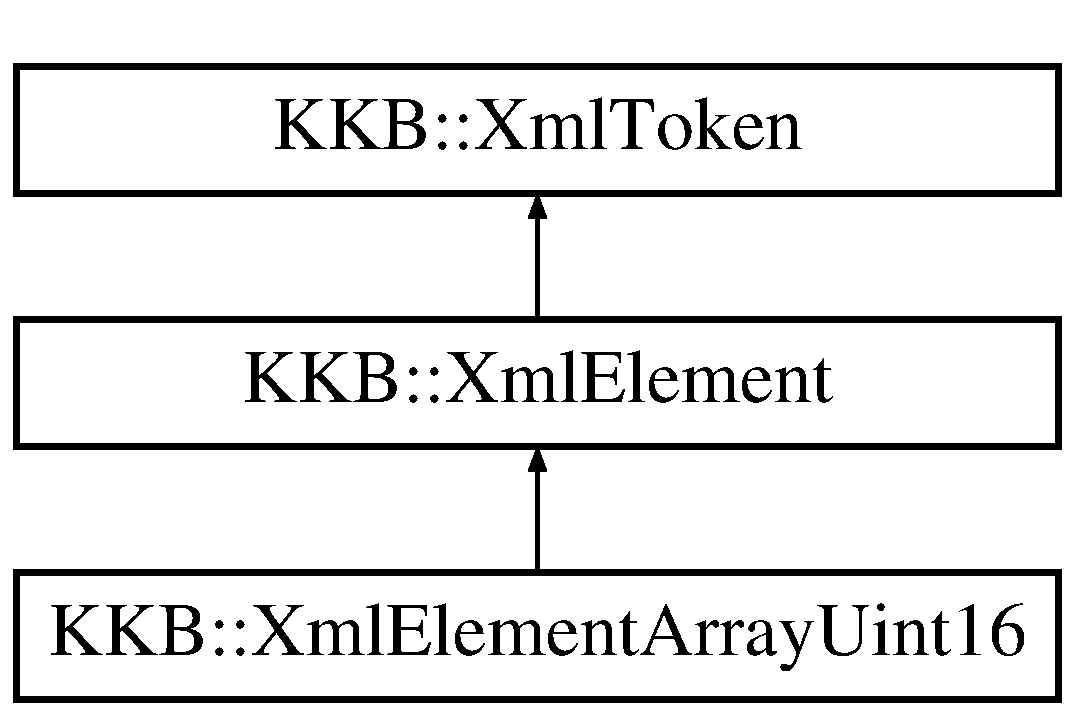
\includegraphics[height=3.000000cm]{class_k_k_b_1_1_xml_element_array_uint16}
\end{center}
\end{figure}
\subsection*{Public Member Functions}
\begin{DoxyCompactItemize}
\item 
\hyperlink{class_k_k_b_1_1_xml_element_array_uint16_a56551d96ca8dfef01c589d9c6f1fd948}{Xml\+Element\+Array\+Uint16} (\hyperlink{namespace_k_k_b_a9253a3ea8a5da18ca82be4ca2b390ef0}{Xml\+Tag\+Ptr} tag, \hyperlink{class_k_k_b_1_1_xml_stream}{Xml\+Stream} \&s, \hyperlink{namespace_k_k_b_a7d390f568e2831fb76b86b56c87bf92f}{Vol\+Const\+Bool} \&cancel\+Flag, \hyperlink{class_k_k_b_1_1_run_log}{Run\+Log} \&log)
\item 
virtual \hyperlink{class_k_k_b_1_1_xml_element_array_uint16_a224795ab6fc84035d91d1142166040ae}{$\sim$\+Xml\+Element\+Array\+Uint16} ()
\item 
\hyperlink{namespace_k_k_b_af8d832f05c54994a1cce25bd5743e19a}{kkuint32} \hyperlink{class_k_k_b_1_1_xml_element_array_uint16_ab3b670cba977bb683df4a03a7e81a742}{Count} () const 
\item 
\hyperlink{namespace_k_k_b_aa8c7d4d30381c8a0b6fce68974a9c8a9}{kkuint16} $\ast$ \hyperlink{class_k_k_b_1_1_xml_element_array_uint16_adbabe2ccf717f530759b0c6eb2a9aec3}{Take\+Ownership} ()
\item 
\hyperlink{namespace_k_k_b_aa8c7d4d30381c8a0b6fce68974a9c8a9}{kkuint16} $\ast$ \hyperlink{class_k_k_b_1_1_xml_element_array_uint16_aef40485beede42d9055278b0d53976d0}{Value} () const 
\end{DoxyCompactItemize}
\subsection*{Static Public Member Functions}
\begin{DoxyCompactItemize}
\item 
static void \hyperlink{class_k_k_b_1_1_xml_element_array_uint16_a02f2850d2846f21d94e29851adb10a1f}{Write\+X\+ML} (\hyperlink{namespace_k_k_b_af8d832f05c54994a1cce25bd5743e19a}{kkuint32} count, const \hyperlink{namespace_k_k_b_aa8c7d4d30381c8a0b6fce68974a9c8a9}{kkuint16} $\ast$d, const \hyperlink{class_k_k_b_1_1_k_k_str}{K\+K\+Str} \&var\+Name, std\+::ostream \&o)
\end{DoxyCompactItemize}
\subsection*{Additional Inherited Members}


\subsection{Detailed Description}


Definition at line 913 of file Xml\+Stream.\+h.



\subsection{Constructor \& Destructor Documentation}
\index{K\+K\+B\+::\+Xml\+Element\+Array\+Uint16@{K\+K\+B\+::\+Xml\+Element\+Array\+Uint16}!Xml\+Element\+Array\+Uint16@{Xml\+Element\+Array\+Uint16}}
\index{Xml\+Element\+Array\+Uint16@{Xml\+Element\+Array\+Uint16}!K\+K\+B\+::\+Xml\+Element\+Array\+Uint16@{K\+K\+B\+::\+Xml\+Element\+Array\+Uint16}}
\subsubsection[{\texorpdfstring{Xml\+Element\+Array\+Uint16(\+Xml\+Tag\+Ptr tag, Xml\+Stream \&s, Vol\+Const\+Bool \&cancel\+Flag, Run\+Log \&log)}{XmlElementArrayUint16(XmlTagPtr tag, XmlStream &s, VolConstBool &cancelFlag, RunLog &log)}}]{\setlength{\rightskip}{0pt plus 5cm}Xml\+Element\+Array\+Uint16\+::\+Xml\+Element\+Array\+Uint16 (
\begin{DoxyParamCaption}
\item[{{\bf Xml\+Tag\+Ptr}}]{tag, }
\item[{{\bf Xml\+Stream} \&}]{s, }
\item[{{\bf Vol\+Const\+Bool} \&}]{cancel\+Flag, }
\item[{{\bf Run\+Log} \&}]{log}
\end{DoxyParamCaption}
)}\hypertarget{class_k_k_b_1_1_xml_element_array_uint16_a56551d96ca8dfef01c589d9c6f1fd948}{}\label{class_k_k_b_1_1_xml_element_array_uint16_a56551d96ca8dfef01c589d9c6f1fd948}


Definition at line 1853 of file Xml\+Stream.\+cpp.

\index{K\+K\+B\+::\+Xml\+Element\+Array\+Uint16@{K\+K\+B\+::\+Xml\+Element\+Array\+Uint16}!````~Xml\+Element\+Array\+Uint16@{$\sim$\+Xml\+Element\+Array\+Uint16}}
\index{````~Xml\+Element\+Array\+Uint16@{$\sim$\+Xml\+Element\+Array\+Uint16}!K\+K\+B\+::\+Xml\+Element\+Array\+Uint16@{K\+K\+B\+::\+Xml\+Element\+Array\+Uint16}}
\subsubsection[{\texorpdfstring{$\sim$\+Xml\+Element\+Array\+Uint16()}{~XmlElementArrayUint16()}}]{\setlength{\rightskip}{0pt plus 5cm}Xml\+Element\+Array\+Uint16\+::$\sim$\+Xml\+Element\+Array\+Uint16 (
\begin{DoxyParamCaption}
{}
\end{DoxyParamCaption}
)\hspace{0.3cm}{\ttfamily [virtual]}}\hypertarget{class_k_k_b_1_1_xml_element_array_uint16_a224795ab6fc84035d91d1142166040ae}{}\label{class_k_k_b_1_1_xml_element_array_uint16_a224795ab6fc84035d91d1142166040ae}


Definition at line 1853 of file Xml\+Stream.\+cpp.



\subsection{Member Function Documentation}
\index{K\+K\+B\+::\+Xml\+Element\+Array\+Uint16@{K\+K\+B\+::\+Xml\+Element\+Array\+Uint16}!Count@{Count}}
\index{Count@{Count}!K\+K\+B\+::\+Xml\+Element\+Array\+Uint16@{K\+K\+B\+::\+Xml\+Element\+Array\+Uint16}}
\subsubsection[{\texorpdfstring{Count() const }{Count() const }}]{\setlength{\rightskip}{0pt plus 5cm}{\bf kkuint32} K\+K\+B\+::\+Xml\+Element\+Array\+Uint16\+::\+Count (
\begin{DoxyParamCaption}
{}
\end{DoxyParamCaption}
) const\hspace{0.3cm}{\ttfamily [inline]}}\hypertarget{class_k_k_b_1_1_xml_element_array_uint16_ab3b670cba977bb683df4a03a7e81a742}{}\label{class_k_k_b_1_1_xml_element_array_uint16_ab3b670cba977bb683df4a03a7e81a742}


Definition at line 913 of file Xml\+Stream.\+h.

\index{K\+K\+B\+::\+Xml\+Element\+Array\+Uint16@{K\+K\+B\+::\+Xml\+Element\+Array\+Uint16}!Take\+Ownership@{Take\+Ownership}}
\index{Take\+Ownership@{Take\+Ownership}!K\+K\+B\+::\+Xml\+Element\+Array\+Uint16@{K\+K\+B\+::\+Xml\+Element\+Array\+Uint16}}
\subsubsection[{\texorpdfstring{Take\+Ownership()}{TakeOwnership()}}]{\setlength{\rightskip}{0pt plus 5cm}{\bf kkuint16} $\ast$ Xml\+Element\+Array\+Uint16\+::\+Take\+Ownership (
\begin{DoxyParamCaption}
{}
\end{DoxyParamCaption}
)}\hypertarget{class_k_k_b_1_1_xml_element_array_uint16_adbabe2ccf717f530759b0c6eb2a9aec3}{}\label{class_k_k_b_1_1_xml_element_array_uint16_adbabe2ccf717f530759b0c6eb2a9aec3}


Definition at line 1853 of file Xml\+Stream.\+cpp.

\index{K\+K\+B\+::\+Xml\+Element\+Array\+Uint16@{K\+K\+B\+::\+Xml\+Element\+Array\+Uint16}!Value@{Value}}
\index{Value@{Value}!K\+K\+B\+::\+Xml\+Element\+Array\+Uint16@{K\+K\+B\+::\+Xml\+Element\+Array\+Uint16}}
\subsubsection[{\texorpdfstring{Value() const }{Value() const }}]{\setlength{\rightskip}{0pt plus 5cm}{\bf kkuint16}$\ast$ K\+K\+B\+::\+Xml\+Element\+Array\+Uint16\+::\+Value (
\begin{DoxyParamCaption}
{}
\end{DoxyParamCaption}
) const\hspace{0.3cm}{\ttfamily [inline]}}\hypertarget{class_k_k_b_1_1_xml_element_array_uint16_aef40485beede42d9055278b0d53976d0}{}\label{class_k_k_b_1_1_xml_element_array_uint16_aef40485beede42d9055278b0d53976d0}


Definition at line 913 of file Xml\+Stream.\+h.

\index{K\+K\+B\+::\+Xml\+Element\+Array\+Uint16@{K\+K\+B\+::\+Xml\+Element\+Array\+Uint16}!Write\+X\+ML@{Write\+X\+ML}}
\index{Write\+X\+ML@{Write\+X\+ML}!K\+K\+B\+::\+Xml\+Element\+Array\+Uint16@{K\+K\+B\+::\+Xml\+Element\+Array\+Uint16}}
\subsubsection[{\texorpdfstring{Write\+X\+M\+L(kkuint32 count, const kkuint16 $\ast$d, const K\+K\+Str \&var\+Name, std\+::ostream \&o)}{WriteXML(kkuint32 count, const kkuint16 *d, const KKStr &varName, std::ostream &o)}}]{\setlength{\rightskip}{0pt plus 5cm}void Xml\+Element\+Array\+Uint16\+::\+Write\+X\+ML (
\begin{DoxyParamCaption}
\item[{{\bf kkuint32}}]{count, }
\item[{const {\bf kkuint16} $\ast$}]{d, }
\item[{const {\bf K\+K\+Str} \&}]{var\+Name, }
\item[{std\+::ostream \&}]{o}
\end{DoxyParamCaption}
)\hspace{0.3cm}{\ttfamily [static]}}\hypertarget{class_k_k_b_1_1_xml_element_array_uint16_a02f2850d2846f21d94e29851adb10a1f}{}\label{class_k_k_b_1_1_xml_element_array_uint16_a02f2850d2846f21d94e29851adb10a1f}


Definition at line 1853 of file Xml\+Stream.\+cpp.



The documentation for this class was generated from the following files\+:\begin{DoxyCompactItemize}
\item 
C\+:/\+Users/\+Kurt/\+Git\+Hub/\+K\+Square\+Libraries/\+K\+K\+Base/\hyperlink{_xml_stream_8h}{Xml\+Stream.\+h}\item 
C\+:/\+Users/\+Kurt/\+Git\+Hub/\+K\+Square\+Libraries/\+K\+K\+Base/\hyperlink{_xml_stream_8cpp}{Xml\+Stream.\+cpp}\end{DoxyCompactItemize}

\hypertarget{class_k_k_b_1_1_xml_element_bool}{}\section{K\+KB\+:\+:Xml\+Element\+Bool Class Reference}
\label{class_k_k_b_1_1_xml_element_bool}\index{K\+K\+B\+::\+Xml\+Element\+Bool@{K\+K\+B\+::\+Xml\+Element\+Bool}}


{\ttfamily \#include $<$Xml\+Stream.\+h$>$}

Inheritance diagram for K\+KB\+:\+:Xml\+Element\+Bool\+:\begin{figure}[H]
\begin{center}
\leavevmode
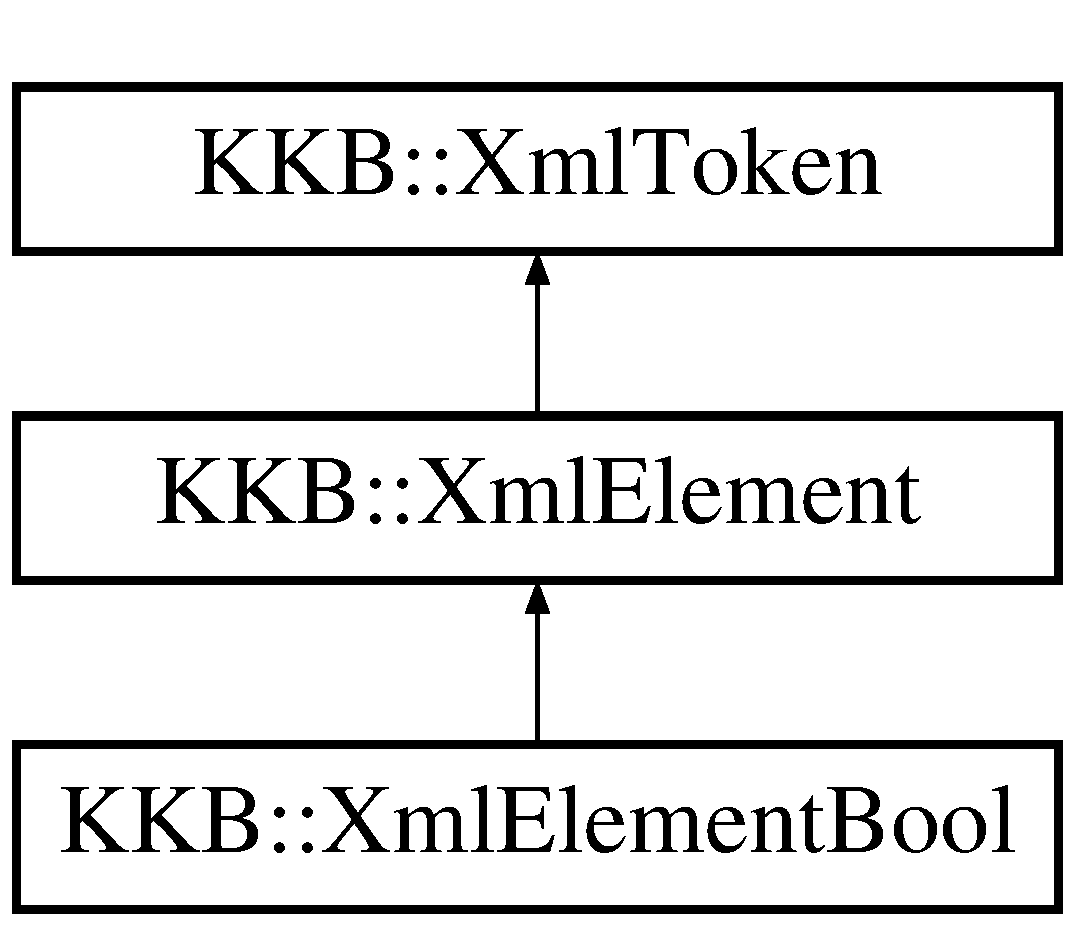
\includegraphics[height=3.000000cm]{class_k_k_b_1_1_xml_element_bool}
\end{center}
\end{figure}
\subsection*{Public Member Functions}
\begin{DoxyCompactItemize}
\item 
\hyperlink{class_k_k_b_1_1_xml_element_bool_a6424413b79c0a3ec491f49b4bc91a8cb}{Xml\+Element\+Bool} (\hyperlink{namespace_k_k_b_a9253a3ea8a5da18ca82be4ca2b390ef0}{Xml\+Tag\+Ptr} tag, \hyperlink{class_k_k_b_1_1_xml_stream}{Xml\+Stream} \&s, \hyperlink{namespace_k_k_b_a7d390f568e2831fb76b86b56c87bf92f}{Vol\+Const\+Bool} \&cancel\+Flag, \hyperlink{class_k_k_b_1_1_run_log}{Run\+Log} \&log)
\item 
virtual \hyperlink{class_k_k_b_1_1_xml_element_bool_a5c825f023363754bf2f9532a0503b035}{$\sim$\+Xml\+Element\+Bool} ()
\item 
virtual bool \hyperlink{class_k_k_b_1_1_xml_element_bool_aed830aad8c70976bddefe7373790cf4a}{To\+Bool} () const 
\item 
virtual double \hyperlink{class_k_k_b_1_1_xml_element_bool_a116bd645557defaae5d69450015124eb}{To\+Double} () const 
\item 
virtual float \hyperlink{class_k_k_b_1_1_xml_element_bool_a87badc80558f62710ffde957298c1536}{To\+Float} () const 
\item 
virtual \hyperlink{namespace_k_k_b_a8fa4952cc84fda1de4bec1fbdd8d5b1b}{kkint32} \hyperlink{class_k_k_b_1_1_xml_element_bool_a7d877d4924d9f62f1f5dc68b5a3d2663}{To\+Int32} () const 
\item 
virtual \hyperlink{class_k_k_b_1_1_k_k_str}{K\+K\+Str} \hyperlink{class_k_k_b_1_1_xml_element_bool_a66cbfc5eff140075cf6226123db0bd85}{To\+K\+K\+Str} () const 
\item 
bool \hyperlink{class_k_k_b_1_1_xml_element_bool_a8d4ec6615a74cca30a79d288d08cccd0}{Value} () const 
\end{DoxyCompactItemize}
\subsection*{Static Public Member Functions}
\begin{DoxyCompactItemize}
\item 
static void \hyperlink{class_k_k_b_1_1_xml_element_bool_ab215da6acba9b313585d9988a9aa8fbc}{Write\+X\+ML} (const bool b, const \hyperlink{class_k_k_b_1_1_k_k_str}{K\+K\+Str} \&var\+Name, std\+::ostream \&o)
\end{DoxyCompactItemize}
\subsection*{Additional Inherited Members}


\subsection{Detailed Description}


Definition at line 496 of file Xml\+Stream.\+h.



\subsection{Constructor \& Destructor Documentation}
\index{K\+K\+B\+::\+Xml\+Element\+Bool@{K\+K\+B\+::\+Xml\+Element\+Bool}!Xml\+Element\+Bool@{Xml\+Element\+Bool}}
\index{Xml\+Element\+Bool@{Xml\+Element\+Bool}!K\+K\+B\+::\+Xml\+Element\+Bool@{K\+K\+B\+::\+Xml\+Element\+Bool}}
\subsubsection[{\texorpdfstring{Xml\+Element\+Bool(\+Xml\+Tag\+Ptr tag, Xml\+Stream \&s, Vol\+Const\+Bool \&cancel\+Flag, Run\+Log \&log)}{XmlElementBool(XmlTagPtr tag, XmlStream &s, VolConstBool &cancelFlag, RunLog &log)}}]{\setlength{\rightskip}{0pt plus 5cm}Xml\+Element\+Bool\+::\+Xml\+Element\+Bool (
\begin{DoxyParamCaption}
\item[{{\bf Xml\+Tag\+Ptr}}]{tag, }
\item[{{\bf Xml\+Stream} \&}]{s, }
\item[{{\bf Vol\+Const\+Bool} \&}]{cancel\+Flag, }
\item[{{\bf Run\+Log} \&}]{log}
\end{DoxyParamCaption}
)}\hypertarget{class_k_k_b_1_1_xml_element_bool_a6424413b79c0a3ec491f49b4bc91a8cb}{}\label{class_k_k_b_1_1_xml_element_bool_a6424413b79c0a3ec491f49b4bc91a8cb}


Definition at line 998 of file Xml\+Stream.\+cpp.



References K\+K\+B\+::\+Xml\+Tag\+::\+Attribute\+Value\+By\+Name(), K\+K\+B\+::\+Xml\+Content\+::\+Content(), K\+K\+B\+::\+Xml\+Stream\+::\+Get\+Next\+Token(), K\+K\+B\+::\+K\+K\+Str\+::\+To\+Bool(), K\+K\+B\+::\+Xml\+Token\+::tok\+Content, K\+K\+B\+::\+Xml\+Token\+::\+Token\+Type(), and K\+K\+B\+::\+Xml\+Element\+::\+Xml\+Element().


\begin{DoxyCode}
1002                                 :
1003     \hyperlink{class_k_k_b_1_1_xml_element_a66317eff5bd3abcc60755756ba2887d5}{XmlElement} (tag, s, log),
1004     value (\textcolor{keyword}{false})
1005 \{
1006   \hyperlink{class_k_k_b_1_1_k_k_str}{KKStrConstPtr}  valueStr = tag->\hyperlink{class_k_k_b_1_1_xml_tag_a0470baf5a49af1c2f6aaf0155b9ba783}{AttributeValueByName} (\textcolor{stringliteral}{"Value"});
1007   \textcolor{keywordflow}{if}  (valueStr)
1008     value = valueStr->\hyperlink{class_k_k_b_1_1_k_k_str_a84e903540729b01cd2d712dc7050044a}{ToBool} ();
1009   \hyperlink{class_k_k_b_1_1_xml_token}{XmlTokenPtr} t = s.\hyperlink{class_k_k_b_1_1_xml_stream_a87cc738b05c666cf5d5c25beaab477b4}{GetNextToken} (cancelFlag, log);
1010   \textcolor{keywordflow}{while}  (t != NULL)
1011   \{
1012     \textcolor{keywordflow}{if}  (t->\hyperlink{class_k_k_b_1_1_xml_token_ae98e2c1a798882647578cae4adcd7176}{TokenType} () == \hyperlink{class_k_k_b_1_1_xml_token_a18b6e90c919f4b92e3b024f50f247f62aff369b5479984ca659548f37ad4caec9}{XmlToken::TokenTypes::tokContent})
1013     \{
1014       \hyperlink{class_k_k_b_1_1_xml_content}{XmlContentPtr} c = \textcolor{keyword}{dynamic\_cast<}\hyperlink{class_k_k_b_1_1_xml_content}{XmlContentPtr}\textcolor{keyword}{>} (t);
1015       value = c->\hyperlink{class_k_k_b_1_1_xml_content_a1d0730aae45b069e8604bef19b8c0098}{Content} ()->\hyperlink{class_k_k_b_1_1_k_k_str_a84e903540729b01cd2d712dc7050044a}{ToBool} ();
1016     \}
1017     \textcolor{keyword}{delete}  t;
1018     t = s.\hyperlink{class_k_k_b_1_1_xml_stream_a87cc738b05c666cf5d5c25beaab477b4}{GetNextToken} (cancelFlag, log);
1019   \}
1020 \}
\end{DoxyCode}
\index{K\+K\+B\+::\+Xml\+Element\+Bool@{K\+K\+B\+::\+Xml\+Element\+Bool}!````~Xml\+Element\+Bool@{$\sim$\+Xml\+Element\+Bool}}
\index{````~Xml\+Element\+Bool@{$\sim$\+Xml\+Element\+Bool}!K\+K\+B\+::\+Xml\+Element\+Bool@{K\+K\+B\+::\+Xml\+Element\+Bool}}
\subsubsection[{\texorpdfstring{$\sim$\+Xml\+Element\+Bool()}{~XmlElementBool()}}]{\setlength{\rightskip}{0pt plus 5cm}Xml\+Element\+Bool\+::$\sim$\+Xml\+Element\+Bool (
\begin{DoxyParamCaption}
{}
\end{DoxyParamCaption}
)\hspace{0.3cm}{\ttfamily [virtual]}}\hypertarget{class_k_k_b_1_1_xml_element_bool_a5c825f023363754bf2f9532a0503b035}{}\label{class_k_k_b_1_1_xml_element_bool_a5c825f023363754bf2f9532a0503b035}


Definition at line 1023 of file Xml\+Stream.\+cpp.


\begin{DoxyCode}
1024 \{
1025 \}
\end{DoxyCode}


\subsection{Member Function Documentation}
\index{K\+K\+B\+::\+Xml\+Element\+Bool@{K\+K\+B\+::\+Xml\+Element\+Bool}!To\+Bool@{To\+Bool}}
\index{To\+Bool@{To\+Bool}!K\+K\+B\+::\+Xml\+Element\+Bool@{K\+K\+B\+::\+Xml\+Element\+Bool}}
\subsubsection[{\texorpdfstring{To\+Bool() const }{ToBool() const }}]{\setlength{\rightskip}{0pt plus 5cm}virtual bool K\+K\+B\+::\+Xml\+Element\+Bool\+::\+To\+Bool (
\begin{DoxyParamCaption}
{}
\end{DoxyParamCaption}
) const\hspace{0.3cm}{\ttfamily [inline]}, {\ttfamily [virtual]}}\hypertarget{class_k_k_b_1_1_xml_element_bool_aed830aad8c70976bddefe7373790cf4a}{}\label{class_k_k_b_1_1_xml_element_bool_aed830aad8c70976bddefe7373790cf4a}


Reimplemented from \hyperlink{class_k_k_b_1_1_xml_element_a7bfbbea204722bc4535a294bc43e8e17}{K\+K\+B\+::\+Xml\+Element}.



Definition at line 515 of file Xml\+Stream.\+h.


\begin{DoxyCode}
515 \{\textcolor{keywordflow}{return}  value;\}
\end{DoxyCode}
\index{K\+K\+B\+::\+Xml\+Element\+Bool@{K\+K\+B\+::\+Xml\+Element\+Bool}!To\+Double@{To\+Double}}
\index{To\+Double@{To\+Double}!K\+K\+B\+::\+Xml\+Element\+Bool@{K\+K\+B\+::\+Xml\+Element\+Bool}}
\subsubsection[{\texorpdfstring{To\+Double() const }{ToDouble() const }}]{\setlength{\rightskip}{0pt plus 5cm}virtual double K\+K\+B\+::\+Xml\+Element\+Bool\+::\+To\+Double (
\begin{DoxyParamCaption}
{}
\end{DoxyParamCaption}
) const\hspace{0.3cm}{\ttfamily [inline]}, {\ttfamily [virtual]}}\hypertarget{class_k_k_b_1_1_xml_element_bool_a116bd645557defaae5d69450015124eb}{}\label{class_k_k_b_1_1_xml_element_bool_a116bd645557defaae5d69450015124eb}


Reimplemented from \hyperlink{class_k_k_b_1_1_xml_element_ac32778396ab8bdb215ad38f2f33f05de}{K\+K\+B\+::\+Xml\+Element}.



Definition at line 517 of file Xml\+Stream.\+h.


\begin{DoxyCode}
517 \{\textcolor{keywordflow}{return}  (\textcolor{keywordtype}{double})value;\}
\end{DoxyCode}
\index{K\+K\+B\+::\+Xml\+Element\+Bool@{K\+K\+B\+::\+Xml\+Element\+Bool}!To\+Float@{To\+Float}}
\index{To\+Float@{To\+Float}!K\+K\+B\+::\+Xml\+Element\+Bool@{K\+K\+B\+::\+Xml\+Element\+Bool}}
\subsubsection[{\texorpdfstring{To\+Float() const }{ToFloat() const }}]{\setlength{\rightskip}{0pt plus 5cm}virtual float K\+K\+B\+::\+Xml\+Element\+Bool\+::\+To\+Float (
\begin{DoxyParamCaption}
{}
\end{DoxyParamCaption}
) const\hspace{0.3cm}{\ttfamily [inline]}, {\ttfamily [virtual]}}\hypertarget{class_k_k_b_1_1_xml_element_bool_a87badc80558f62710ffde957298c1536}{}\label{class_k_k_b_1_1_xml_element_bool_a87badc80558f62710ffde957298c1536}


Reimplemented from \hyperlink{class_k_k_b_1_1_xml_element_aa728687ed43e76d45d029dfc14e14e95}{K\+K\+B\+::\+Xml\+Element}.



Definition at line 518 of file Xml\+Stream.\+h.


\begin{DoxyCode}
518 \{\textcolor{keywordflow}{return}  (\textcolor{keywordtype}{float})value;\}
\end{DoxyCode}
\index{K\+K\+B\+::\+Xml\+Element\+Bool@{K\+K\+B\+::\+Xml\+Element\+Bool}!To\+Int32@{To\+Int32}}
\index{To\+Int32@{To\+Int32}!K\+K\+B\+::\+Xml\+Element\+Bool@{K\+K\+B\+::\+Xml\+Element\+Bool}}
\subsubsection[{\texorpdfstring{To\+Int32() const }{ToInt32() const }}]{\setlength{\rightskip}{0pt plus 5cm}virtual {\bf kkint32} K\+K\+B\+::\+Xml\+Element\+Bool\+::\+To\+Int32 (
\begin{DoxyParamCaption}
{}
\end{DoxyParamCaption}
) const\hspace{0.3cm}{\ttfamily [inline]}, {\ttfamily [virtual]}}\hypertarget{class_k_k_b_1_1_xml_element_bool_a7d877d4924d9f62f1f5dc68b5a3d2663}{}\label{class_k_k_b_1_1_xml_element_bool_a7d877d4924d9f62f1f5dc68b5a3d2663}


Reimplemented from \hyperlink{class_k_k_b_1_1_xml_element_aac7463c7b305f66b5157f424a0a76363}{K\+K\+B\+::\+Xml\+Element}.



Definition at line 519 of file Xml\+Stream.\+h.


\begin{DoxyCode}
519 \{\textcolor{keywordflow}{return}  (\hyperlink{namespace_k_k_b_a8fa4952cc84fda1de4bec1fbdd8d5b1b}{kkint32})value;\}
\end{DoxyCode}
\index{K\+K\+B\+::\+Xml\+Element\+Bool@{K\+K\+B\+::\+Xml\+Element\+Bool}!To\+K\+K\+Str@{To\+K\+K\+Str}}
\index{To\+K\+K\+Str@{To\+K\+K\+Str}!K\+K\+B\+::\+Xml\+Element\+Bool@{K\+K\+B\+::\+Xml\+Element\+Bool}}
\subsubsection[{\texorpdfstring{To\+K\+K\+Str() const }{ToKKStr() const }}]{\setlength{\rightskip}{0pt plus 5cm}virtual {\bf K\+K\+Str} K\+K\+B\+::\+Xml\+Element\+Bool\+::\+To\+K\+K\+Str (
\begin{DoxyParamCaption}
{}
\end{DoxyParamCaption}
) const\hspace{0.3cm}{\ttfamily [inline]}, {\ttfamily [virtual]}}\hypertarget{class_k_k_b_1_1_xml_element_bool_a66cbfc5eff140075cf6226123db0bd85}{}\label{class_k_k_b_1_1_xml_element_bool_a66cbfc5eff140075cf6226123db0bd85}


Reimplemented from \hyperlink{class_k_k_b_1_1_xml_element_a3028fc03b79509e6378749f6a8b426b9}{K\+K\+B\+::\+Xml\+Element}.



Definition at line 516 of file Xml\+Stream.\+h.


\begin{DoxyCode}
516 \{\textcolor{keywordflow}{return}  value ? \textcolor{stringliteral}{"True"} : \textcolor{stringliteral}{"False"};\}
\end{DoxyCode}
\index{K\+K\+B\+::\+Xml\+Element\+Bool@{K\+K\+B\+::\+Xml\+Element\+Bool}!Value@{Value}}
\index{Value@{Value}!K\+K\+B\+::\+Xml\+Element\+Bool@{K\+K\+B\+::\+Xml\+Element\+Bool}}
\subsubsection[{\texorpdfstring{Value() const }{Value() const }}]{\setlength{\rightskip}{0pt plus 5cm}bool Xml\+Element\+Bool\+::\+Value (
\begin{DoxyParamCaption}
{}
\end{DoxyParamCaption}
) const}\hypertarget{class_k_k_b_1_1_xml_element_bool_a8d4ec6615a74cca30a79d288d08cccd0}{}\label{class_k_k_b_1_1_xml_element_bool_a8d4ec6615a74cca30a79d288d08cccd0}


Definition at line 1028 of file Xml\+Stream.\+cpp.



Referenced by K\+K\+M\+L\+L\+::\+Model\+Param\+Usf\+Cas\+Cor\+::\+Read\+X\+M\+L(), K\+K\+M\+L\+L\+::\+Model\+Param\+Dual\+::\+Read\+X\+M\+L(), and K\+K\+M\+L\+L\+::\+Training\+Configuration2\+::\+Read\+X\+M\+L\+Base\+Token().


\begin{DoxyCode}
1029 \{
1030   \textcolor{keywordflow}{return}  value;
1031 \}
\end{DoxyCode}
\index{K\+K\+B\+::\+Xml\+Element\+Bool@{K\+K\+B\+::\+Xml\+Element\+Bool}!Write\+X\+ML@{Write\+X\+ML}}
\index{Write\+X\+ML@{Write\+X\+ML}!K\+K\+B\+::\+Xml\+Element\+Bool@{K\+K\+B\+::\+Xml\+Element\+Bool}}
\subsubsection[{\texorpdfstring{Write\+X\+M\+L(const bool b, const K\+K\+Str \&var\+Name, std\+::ostream \&o)}{WriteXML(const bool b, const KKStr &varName, std::ostream &o)}}]{\setlength{\rightskip}{0pt plus 5cm}void Xml\+Element\+Bool\+::\+Write\+X\+ML (
\begin{DoxyParamCaption}
\item[{const bool}]{b, }
\item[{const {\bf K\+K\+Str} \&}]{var\+Name, }
\item[{std\+::ostream \&}]{o}
\end{DoxyParamCaption}
)\hspace{0.3cm}{\ttfamily [static]}}\hypertarget{class_k_k_b_1_1_xml_element_bool_ab215da6acba9b313585d9988a9aa8fbc}{}\label{class_k_k_b_1_1_xml_element_bool_ab215da6acba9b313585d9988a9aa8fbc}


Definition at line 1035 of file Xml\+Stream.\+cpp.



References K\+K\+B\+::\+Xml\+Tag\+::\+Add\+Atribute(), K\+K\+B\+::\+K\+K\+Str\+::\+Empty(), K\+K\+B\+::\+Xml\+Tag\+::tag\+Empty, K\+K\+B\+::\+Xml\+Tag\+::\+Write\+X\+M\+L(), and K\+K\+B\+::\+Xml\+Tag\+::\+Xml\+Tag().



Referenced by K\+K\+M\+L\+L\+::\+Model\+::\+Write\+Model\+X\+M\+L\+Fields(), K\+K\+M\+L\+L\+::\+Model\+Param\+Usf\+Cas\+Cor\+::\+Write\+X\+M\+L(), K\+K\+M\+L\+L\+::\+Model\+Param\+Dual\+::\+Write\+X\+M\+L(), K\+K\+M\+L\+L\+::\+Normalization\+Parms\+::\+Write\+X\+M\+L(), K\+K\+M\+L\+L\+::\+Training\+Process2\+::\+Write\+X\+M\+L(), K\+K\+M\+L\+L\+::\+Model\+Param\+::\+Write\+X\+M\+L\+Fields(), and K\+K\+M\+L\+L\+::\+Training\+Configuration2\+::\+Write\+X\+M\+L\+Fields().


\begin{DoxyCode}
1039 \{
1040   \hyperlink{class_k_k_b_1_1_xml_tag}{XmlTag} startTag (\textcolor{stringliteral}{"Bool"}, \hyperlink{class_k_k_b_1_1_xml_tag_a6c0ef0e23f982f49d55d4fb7eaff6ac9ac842083d30a90700e09f4cbf728f01b8}{XmlTag::TagTypes::tagEmpty});
1041   \textcolor{keywordflow}{if}  (!varName.\hyperlink{class_k_k_b_1_1_k_k_str_ac69942f73fffd672ec2a6e1c410afdb6}{Empty} ())
1042     startTag.AddAtribute (\textcolor{stringliteral}{"VarName"}, varName);
1043   startTag.AddAtribute (\textcolor{stringliteral}{"Value"}, b);
1044   startTag.WriteXML (o);
1045   o << \hyperlink{namespace_k_k_b_ad1f50f65af6adc8fa9e6f62d007818a8}{endl};
1046 \}
\end{DoxyCode}


The documentation for this class was generated from the following files\+:\begin{DoxyCompactItemize}
\item 
C\+:/\+Users/\+Kurt/\+Git\+Hub/\+K\+Square\+Libraries/\+K\+K\+Base/\hyperlink{_xml_stream_8h}{Xml\+Stream.\+h}\item 
C\+:/\+Users/\+Kurt/\+Git\+Hub/\+K\+Square\+Libraries/\+K\+K\+Base/\hyperlink{_xml_stream_8cpp}{Xml\+Stream.\+cpp}\end{DoxyCompactItemize}

\hypertarget{class_k_k_b_1_1_xml_element_date_time}{}\section{K\+KB\+:\+:Xml\+Element\+Date\+Time Class Reference}
\label{class_k_k_b_1_1_xml_element_date_time}\index{K\+K\+B\+::\+Xml\+Element\+Date\+Time@{K\+K\+B\+::\+Xml\+Element\+Date\+Time}}


{\ttfamily \#include $<$Xml\+Stream.\+h$>$}

Inheritance diagram for K\+KB\+:\+:Xml\+Element\+Date\+Time\+:\begin{figure}[H]
\begin{center}
\leavevmode
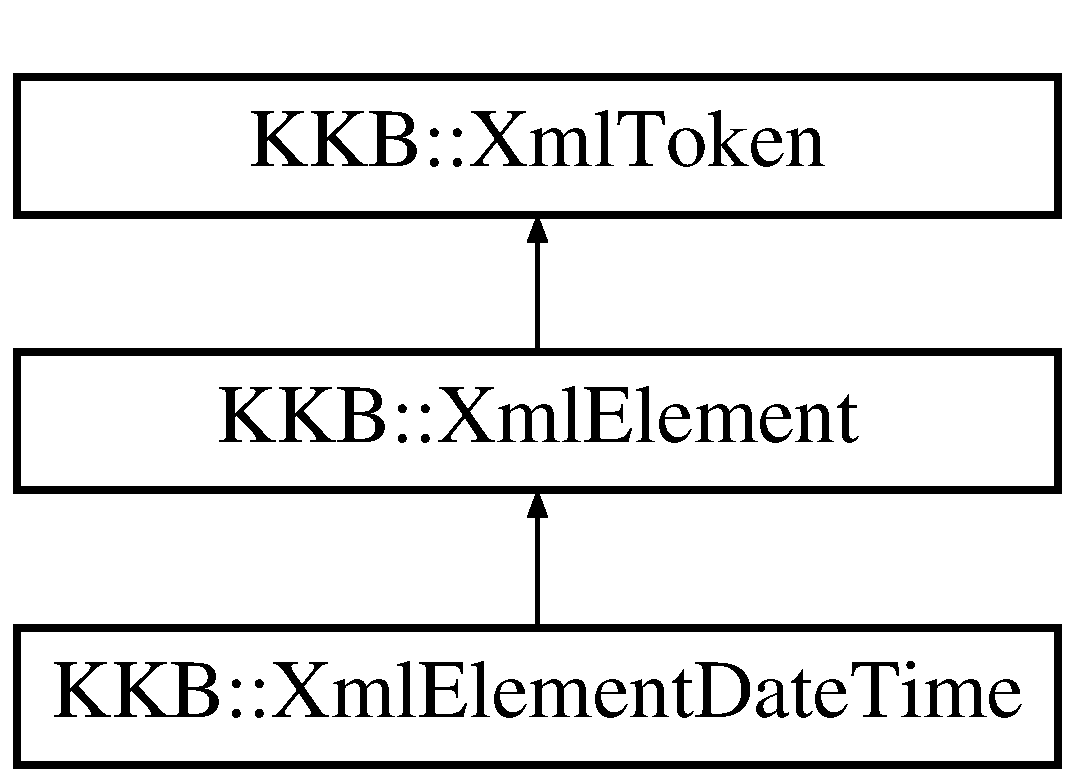
\includegraphics[height=3.000000cm]{class_k_k_b_1_1_xml_element_date_time}
\end{center}
\end{figure}
\subsection*{Public Member Functions}
\begin{DoxyCompactItemize}
\item 
\hyperlink{class_k_k_b_1_1_xml_element_date_time_a2ef92882b2e1f0b2d02c5b338daaf372}{Xml\+Element\+Date\+Time} (\hyperlink{namespace_k_k_b_a9253a3ea8a5da18ca82be4ca2b390ef0}{Xml\+Tag\+Ptr} tag, \hyperlink{class_k_k_b_1_1_xml_stream}{Xml\+Stream} \&s, \hyperlink{namespace_k_k_b_a7d390f568e2831fb76b86b56c87bf92f}{Vol\+Const\+Bool} \&cancel\+Flag, \hyperlink{class_k_k_b_1_1_run_log}{Run\+Log} \&log)
\item 
virtual \hyperlink{class_k_k_b_1_1_xml_element_date_time_a9fb359665679473f20a11a0bc06facb9}{$\sim$\+Xml\+Element\+Date\+Time} ()
\item 
virtual bool \hyperlink{class_k_k_b_1_1_xml_element_date_time_a6428fe3132db46ca0f9f15ca4e3570a8}{To\+Bool} () const 
\item 
virtual double \hyperlink{class_k_k_b_1_1_xml_element_date_time_a3c60c809536ad9823baf97f64beb541f}{To\+Double} () const 
\item 
virtual float \hyperlink{class_k_k_b_1_1_xml_element_date_time_a67670c703f86c4a72ba73920de0f4858}{To\+Float} () const 
\item 
virtual \hyperlink{namespace_k_k_b_a8fa4952cc84fda1de4bec1fbdd8d5b1b}{kkint32} \hyperlink{class_k_k_b_1_1_xml_element_date_time_ad7108702555f0d9bc3c879e836d212df}{To\+Int32} () const 
\item 
virtual \hyperlink{class_k_k_b_1_1_k_k_str}{K\+K\+Str} \hyperlink{class_k_k_b_1_1_xml_element_date_time_a0b78fa113b7721069b8a14b971b73b1e}{To\+K\+K\+Str} () const 
\item 
\hyperlink{class_k_k_b_1_1_date_time}{Date\+Time} \hyperlink{class_k_k_b_1_1_xml_element_date_time_ad344da7ca74c2da7c8ab8b1a4263f919}{Value} () const 
\end{DoxyCompactItemize}
\subsection*{Static Public Member Functions}
\begin{DoxyCompactItemize}
\item 
static void \hyperlink{class_k_k_b_1_1_xml_element_date_time_a34c6ec2877c0e7adaf57adf186e75727}{Write\+X\+ML} (const \hyperlink{class_k_k_b_1_1_date_time}{Date\+Time} \&d, const \hyperlink{class_k_k_b_1_1_k_k_str}{K\+K\+Str} \&var\+Name, std\+::ostream \&o)
\end{DoxyCompactItemize}
\subsection*{Additional Inherited Members}


\subsection{Detailed Description}


Definition at line 532 of file Xml\+Stream.\+h.



\subsection{Constructor \& Destructor Documentation}
\index{K\+K\+B\+::\+Xml\+Element\+Date\+Time@{K\+K\+B\+::\+Xml\+Element\+Date\+Time}!Xml\+Element\+Date\+Time@{Xml\+Element\+Date\+Time}}
\index{Xml\+Element\+Date\+Time@{Xml\+Element\+Date\+Time}!K\+K\+B\+::\+Xml\+Element\+Date\+Time@{K\+K\+B\+::\+Xml\+Element\+Date\+Time}}
\subsubsection[{\texorpdfstring{Xml\+Element\+Date\+Time(\+Xml\+Tag\+Ptr tag, Xml\+Stream \&s, Vol\+Const\+Bool \&cancel\+Flag, Run\+Log \&log)}{XmlElementDateTime(XmlTagPtr tag, XmlStream &s, VolConstBool &cancelFlag, RunLog &log)}}]{\setlength{\rightskip}{0pt plus 5cm}Xml\+Element\+Date\+Time\+::\+Xml\+Element\+Date\+Time (
\begin{DoxyParamCaption}
\item[{{\bf Xml\+Tag\+Ptr}}]{tag, }
\item[{{\bf Xml\+Stream} \&}]{s, }
\item[{{\bf Vol\+Const\+Bool} \&}]{cancel\+Flag, }
\item[{{\bf Run\+Log} \&}]{log}
\end{DoxyParamCaption}
)}\hypertarget{class_k_k_b_1_1_xml_element_date_time_a2ef92882b2e1f0b2d02c5b338daaf372}{}\label{class_k_k_b_1_1_xml_element_date_time_a2ef92882b2e1f0b2d02c5b338daaf372}


Definition at line 1096 of file Xml\+Stream.\+cpp.



References K\+K\+B\+::\+Xml\+Tag\+::\+Attribute\+Value\+Date\+Time(), K\+K\+B\+::\+Date\+Time\+::\+Date\+Time(), K\+K\+B\+::\+Date\+Time\+::operator=(), and K\+K\+B\+::\+Xml\+Element\+::\+Xml\+Element().


\begin{DoxyCode}
1100                                         :
1101     \hyperlink{class_k_k_b_1_1_xml_element_a66317eff5bd3abcc60755756ba2887d5}{XmlElement} (tag, s, log),
1102     value ()
1103 \{
1104   value = tag->\hyperlink{class_k_k_b_1_1_xml_tag_a0281ac91c0d271ac3b9cbe4738d5ad12}{AttributeValueDateTime} (\textcolor{stringliteral}{"Value"});
1105 \}
\end{DoxyCode}
\index{K\+K\+B\+::\+Xml\+Element\+Date\+Time@{K\+K\+B\+::\+Xml\+Element\+Date\+Time}!````~Xml\+Element\+Date\+Time@{$\sim$\+Xml\+Element\+Date\+Time}}
\index{````~Xml\+Element\+Date\+Time@{$\sim$\+Xml\+Element\+Date\+Time}!K\+K\+B\+::\+Xml\+Element\+Date\+Time@{K\+K\+B\+::\+Xml\+Element\+Date\+Time}}
\subsubsection[{\texorpdfstring{$\sim$\+Xml\+Element\+Date\+Time()}{~XmlElementDateTime()}}]{\setlength{\rightskip}{0pt plus 5cm}Xml\+Element\+Date\+Time\+::$\sim$\+Xml\+Element\+Date\+Time (
\begin{DoxyParamCaption}
{}
\end{DoxyParamCaption}
)\hspace{0.3cm}{\ttfamily [virtual]}}\hypertarget{class_k_k_b_1_1_xml_element_date_time_a9fb359665679473f20a11a0bc06facb9}{}\label{class_k_k_b_1_1_xml_element_date_time_a9fb359665679473f20a11a0bc06facb9}


Definition at line 1108 of file Xml\+Stream.\+cpp.


\begin{DoxyCode}
1109 \{
1110 \}
\end{DoxyCode}


\subsection{Member Function Documentation}
\index{K\+K\+B\+::\+Xml\+Element\+Date\+Time@{K\+K\+B\+::\+Xml\+Element\+Date\+Time}!To\+Bool@{To\+Bool}}
\index{To\+Bool@{To\+Bool}!K\+K\+B\+::\+Xml\+Element\+Date\+Time@{K\+K\+B\+::\+Xml\+Element\+Date\+Time}}
\subsubsection[{\texorpdfstring{To\+Bool() const }{ToBool() const }}]{\setlength{\rightskip}{0pt plus 5cm}virtual bool K\+K\+B\+::\+Xml\+Element\+Date\+Time\+::\+To\+Bool (
\begin{DoxyParamCaption}
{}
\end{DoxyParamCaption}
) const\hspace{0.3cm}{\ttfamily [inline]}, {\ttfamily [virtual]}}\hypertarget{class_k_k_b_1_1_xml_element_date_time_a6428fe3132db46ca0f9f15ca4e3570a8}{}\label{class_k_k_b_1_1_xml_element_date_time_a6428fe3132db46ca0f9f15ca4e3570a8}


Reimplemented from \hyperlink{class_k_k_b_1_1_xml_element_a7bfbbea204722bc4535a294bc43e8e17}{K\+K\+B\+::\+Xml\+Element}.



Definition at line 551 of file Xml\+Stream.\+h.



References K\+K\+B\+::\+Date\+Time\+::\+Seconds().


\begin{DoxyCode}
551 \{\textcolor{keywordflow}{return}  (value.\hyperlink{class_k_k_b_1_1_date_time_a051f9f993938d58e5762256cf5c06f31}{Seconds} () > 0);\}
\end{DoxyCode}
\index{K\+K\+B\+::\+Xml\+Element\+Date\+Time@{K\+K\+B\+::\+Xml\+Element\+Date\+Time}!To\+Double@{To\+Double}}
\index{To\+Double@{To\+Double}!K\+K\+B\+::\+Xml\+Element\+Date\+Time@{K\+K\+B\+::\+Xml\+Element\+Date\+Time}}
\subsubsection[{\texorpdfstring{To\+Double() const }{ToDouble() const }}]{\setlength{\rightskip}{0pt plus 5cm}virtual double K\+K\+B\+::\+Xml\+Element\+Date\+Time\+::\+To\+Double (
\begin{DoxyParamCaption}
{}
\end{DoxyParamCaption}
) const\hspace{0.3cm}{\ttfamily [inline]}, {\ttfamily [virtual]}}\hypertarget{class_k_k_b_1_1_xml_element_date_time_a3c60c809536ad9823baf97f64beb541f}{}\label{class_k_k_b_1_1_xml_element_date_time_a3c60c809536ad9823baf97f64beb541f}


Reimplemented from \hyperlink{class_k_k_b_1_1_xml_element_ac32778396ab8bdb215ad38f2f33f05de}{K\+K\+B\+::\+Xml\+Element}.



Definition at line 553 of file Xml\+Stream.\+h.



References K\+K\+B\+::\+Date\+Time\+::\+Seconds().


\begin{DoxyCode}
553 \{\textcolor{keywordflow}{return}  (\textcolor{keywordtype}{double})value.\hyperlink{class_k_k_b_1_1_date_time_a051f9f993938d58e5762256cf5c06f31}{Seconds} ();\}
\end{DoxyCode}
\index{K\+K\+B\+::\+Xml\+Element\+Date\+Time@{K\+K\+B\+::\+Xml\+Element\+Date\+Time}!To\+Float@{To\+Float}}
\index{To\+Float@{To\+Float}!K\+K\+B\+::\+Xml\+Element\+Date\+Time@{K\+K\+B\+::\+Xml\+Element\+Date\+Time}}
\subsubsection[{\texorpdfstring{To\+Float() const }{ToFloat() const }}]{\setlength{\rightskip}{0pt plus 5cm}virtual float K\+K\+B\+::\+Xml\+Element\+Date\+Time\+::\+To\+Float (
\begin{DoxyParamCaption}
{}
\end{DoxyParamCaption}
) const\hspace{0.3cm}{\ttfamily [inline]}, {\ttfamily [virtual]}}\hypertarget{class_k_k_b_1_1_xml_element_date_time_a67670c703f86c4a72ba73920de0f4858}{}\label{class_k_k_b_1_1_xml_element_date_time_a67670c703f86c4a72ba73920de0f4858}


Reimplemented from \hyperlink{class_k_k_b_1_1_xml_element_aa728687ed43e76d45d029dfc14e14e95}{K\+K\+B\+::\+Xml\+Element}.



Definition at line 554 of file Xml\+Stream.\+h.



References K\+K\+B\+::\+Date\+Time\+::\+Seconds().


\begin{DoxyCode}
554 \{\textcolor{keywordflow}{return}  (\textcolor{keywordtype}{float})value.\hyperlink{class_k_k_b_1_1_date_time_a051f9f993938d58e5762256cf5c06f31}{Seconds} ();\}
\end{DoxyCode}
\index{K\+K\+B\+::\+Xml\+Element\+Date\+Time@{K\+K\+B\+::\+Xml\+Element\+Date\+Time}!To\+Int32@{To\+Int32}}
\index{To\+Int32@{To\+Int32}!K\+K\+B\+::\+Xml\+Element\+Date\+Time@{K\+K\+B\+::\+Xml\+Element\+Date\+Time}}
\subsubsection[{\texorpdfstring{To\+Int32() const }{ToInt32() const }}]{\setlength{\rightskip}{0pt plus 5cm}virtual {\bf kkint32} K\+K\+B\+::\+Xml\+Element\+Date\+Time\+::\+To\+Int32 (
\begin{DoxyParamCaption}
{}
\end{DoxyParamCaption}
) const\hspace{0.3cm}{\ttfamily [inline]}, {\ttfamily [virtual]}}\hypertarget{class_k_k_b_1_1_xml_element_date_time_ad7108702555f0d9bc3c879e836d212df}{}\label{class_k_k_b_1_1_xml_element_date_time_ad7108702555f0d9bc3c879e836d212df}


Reimplemented from \hyperlink{class_k_k_b_1_1_xml_element_aac7463c7b305f66b5157f424a0a76363}{K\+K\+B\+::\+Xml\+Element}.



Definition at line 555 of file Xml\+Stream.\+h.



References K\+K\+B\+::\+Date\+Time\+::\+To\+Days().


\begin{DoxyCode}
555 \{\textcolor{keywordflow}{return}  (\hyperlink{namespace_k_k_b_a8fa4952cc84fda1de4bec1fbdd8d5b1b}{kkint32})value.\hyperlink{class_k_k_b_1_1_date_time_a92e8292a86720233831e6433df092fb5}{ToDays} ();\}
\end{DoxyCode}
\index{K\+K\+B\+::\+Xml\+Element\+Date\+Time@{K\+K\+B\+::\+Xml\+Element\+Date\+Time}!To\+K\+K\+Str@{To\+K\+K\+Str}}
\index{To\+K\+K\+Str@{To\+K\+K\+Str}!K\+K\+B\+::\+Xml\+Element\+Date\+Time@{K\+K\+B\+::\+Xml\+Element\+Date\+Time}}
\subsubsection[{\texorpdfstring{To\+K\+K\+Str() const }{ToKKStr() const }}]{\setlength{\rightskip}{0pt plus 5cm}virtual {\bf K\+K\+Str} K\+K\+B\+::\+Xml\+Element\+Date\+Time\+::\+To\+K\+K\+Str (
\begin{DoxyParamCaption}
{}
\end{DoxyParamCaption}
) const\hspace{0.3cm}{\ttfamily [inline]}, {\ttfamily [virtual]}}\hypertarget{class_k_k_b_1_1_xml_element_date_time_a0b78fa113b7721069b8a14b971b73b1e}{}\label{class_k_k_b_1_1_xml_element_date_time_a0b78fa113b7721069b8a14b971b73b1e}


Reimplemented from \hyperlink{class_k_k_b_1_1_xml_element_a3028fc03b79509e6378749f6a8b426b9}{K\+K\+B\+::\+Xml\+Element}.



Definition at line 552 of file Xml\+Stream.\+h.



References K\+K\+B\+::\+Date\+Time\+::\+Y\+Y\+Y\+Y\+\_\+\+M\+M\+\_\+\+D\+D\+\_\+\+H\+H\+\_\+\+M\+M\+\_\+\+S\+S().


\begin{DoxyCode}
552 \{\textcolor{keywordflow}{return}  value.\hyperlink{class_k_k_b_1_1_date_time_aca57fbdcd040549a2c9e0a3d4e99b9f9}{YYYY\_MM\_DD\_HH\_MM\_SS} ();\}
\end{DoxyCode}
\index{K\+K\+B\+::\+Xml\+Element\+Date\+Time@{K\+K\+B\+::\+Xml\+Element\+Date\+Time}!Value@{Value}}
\index{Value@{Value}!K\+K\+B\+::\+Xml\+Element\+Date\+Time@{K\+K\+B\+::\+Xml\+Element\+Date\+Time}}
\subsubsection[{\texorpdfstring{Value() const }{Value() const }}]{\setlength{\rightskip}{0pt plus 5cm}{\bf Date\+Time} K\+K\+B\+::\+Xml\+Element\+Date\+Time\+::\+Value (
\begin{DoxyParamCaption}
{}
\end{DoxyParamCaption}
) const\hspace{0.3cm}{\ttfamily [inline]}}\hypertarget{class_k_k_b_1_1_xml_element_date_time_ad344da7ca74c2da7c8ab8b1a4263f919}{}\label{class_k_k_b_1_1_xml_element_date_time_ad344da7ca74c2da7c8ab8b1a4263f919}


Definition at line 543 of file Xml\+Stream.\+h.



Referenced by K\+K\+M\+L\+L\+::\+Training\+Process2\+::\+Read\+X\+M\+L().


\begin{DoxyCode}
543 \{\textcolor{keywordflow}{return}  value;\}
\end{DoxyCode}
\index{K\+K\+B\+::\+Xml\+Element\+Date\+Time@{K\+K\+B\+::\+Xml\+Element\+Date\+Time}!Write\+X\+ML@{Write\+X\+ML}}
\index{Write\+X\+ML@{Write\+X\+ML}!K\+K\+B\+::\+Xml\+Element\+Date\+Time@{K\+K\+B\+::\+Xml\+Element\+Date\+Time}}
\subsubsection[{\texorpdfstring{Write\+X\+M\+L(const Date\+Time \&d, const K\+K\+Str \&var\+Name, std\+::ostream \&o)}{WriteXML(const DateTime &d, const KKStr &varName, std::ostream &o)}}]{\setlength{\rightskip}{0pt plus 5cm}void Xml\+Element\+Date\+Time\+::\+Write\+X\+ML (
\begin{DoxyParamCaption}
\item[{const {\bf Date\+Time} \&}]{d, }
\item[{const {\bf K\+K\+Str} \&}]{var\+Name, }
\item[{std\+::ostream \&}]{o}
\end{DoxyParamCaption}
)\hspace{0.3cm}{\ttfamily [static]}}\hypertarget{class_k_k_b_1_1_xml_element_date_time_a34c6ec2877c0e7adaf57adf186e75727}{}\label{class_k_k_b_1_1_xml_element_date_time_a34c6ec2877c0e7adaf57adf186e75727}


Definition at line 1113 of file Xml\+Stream.\+cpp.



References K\+K\+B\+::\+Xml\+Tag\+::\+Add\+Atribute(), K\+K\+B\+::\+K\+K\+Str\+::\+Empty(), K\+K\+B\+::\+Xml\+Tag\+::tag\+Empty, K\+K\+B\+::\+Xml\+Tag\+::\+Write\+X\+M\+L(), K\+K\+B\+::\+Xml\+Tag\+::\+Xml\+Tag(), and K\+K\+B\+::\+Date\+Time\+::\+Y\+Y\+Y\+Y\+\_\+\+M\+M\+\_\+\+D\+D\+\_\+\+H\+H\+\_\+\+M\+M\+\_\+\+S\+S().



Referenced by K\+K\+M\+L\+L\+::\+Training\+Process2\+::\+Write\+X\+M\+L().


\begin{DoxyCode}
1117 \{
1118   \hyperlink{class_k_k_b_1_1_xml_tag}{XmlTag} startTag (\textcolor{stringliteral}{"DateTime"}, \hyperlink{class_k_k_b_1_1_xml_tag_a6c0ef0e23f982f49d55d4fb7eaff6ac9ac842083d30a90700e09f4cbf728f01b8}{XmlTag::TagTypes::tagEmpty});
1119   \textcolor{keywordflow}{if}  (!varName.\hyperlink{class_k_k_b_1_1_k_k_str_ac69942f73fffd672ec2a6e1c410afdb6}{Empty} ())
1120     startTag.AddAtribute (\textcolor{stringliteral}{"VarName"}, varName);
1121   startTag.AddAtribute (\textcolor{stringliteral}{"Value"}, d.\hyperlink{class_k_k_b_1_1_date_time_aca57fbdcd040549a2c9e0a3d4e99b9f9}{YYYY\_MM\_DD\_HH\_MM\_SS} ());
1122   startTag.WriteXML (o);
1123   o << \hyperlink{namespace_k_k_b_ad1f50f65af6adc8fa9e6f62d007818a8}{endl};
1124 \}
\end{DoxyCode}


The documentation for this class was generated from the following files\+:\begin{DoxyCompactItemize}
\item 
C\+:/\+Users/\+Kurt/\+Git\+Hub/\+K\+Square\+Libraries/\+K\+K\+Base/\hyperlink{_xml_stream_8h}{Xml\+Stream.\+h}\item 
C\+:/\+Users/\+Kurt/\+Git\+Hub/\+K\+Square\+Libraries/\+K\+K\+Base/\hyperlink{_xml_stream_8cpp}{Xml\+Stream.\+cpp}\end{DoxyCompactItemize}

\hypertarget{class_k_k_b_1_1_xml_element_double}{}\section{K\+KB\+:\+:Xml\+Element\+Double Class Reference}
\label{class_k_k_b_1_1_xml_element_double}\index{K\+K\+B\+::\+Xml\+Element\+Double@{K\+K\+B\+::\+Xml\+Element\+Double}}


{\ttfamily \#include $<$Xml\+Stream.\+h$>$}

Inheritance diagram for K\+KB\+:\+:Xml\+Element\+Double\+:\begin{figure}[H]
\begin{center}
\leavevmode
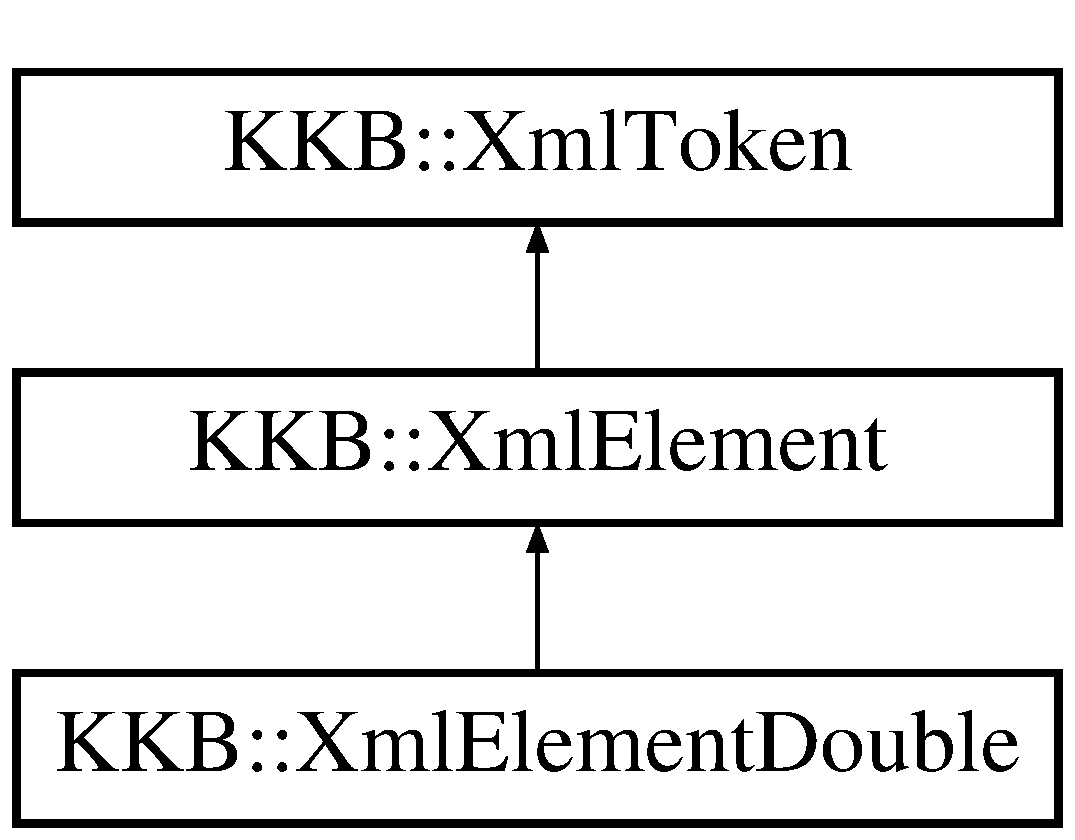
\includegraphics[height=3.000000cm]{class_k_k_b_1_1_xml_element_double}
\end{center}
\end{figure}
\subsection*{Public Member Functions}
\begin{DoxyCompactItemize}
\item 
\hyperlink{class_k_k_b_1_1_xml_element_double_a421ef0e2675c5db325b9559da12e74ed}{Xml\+Element\+Double} (\hyperlink{namespace_k_k_b_a9253a3ea8a5da18ca82be4ca2b390ef0}{Xml\+Tag\+Ptr} tag, \hyperlink{class_k_k_b_1_1_xml_stream}{Xml\+Stream} \&s, \hyperlink{namespace_k_k_b_a7d390f568e2831fb76b86b56c87bf92f}{Vol\+Const\+Bool} \&cancel\+Flag, \hyperlink{class_k_k_b_1_1_run_log}{Run\+Log} \&log)
\item 
virtual \hyperlink{class_k_k_b_1_1_xml_element_double_a2fa9fd295076babf4a6918669e278475}{$\sim$\+Xml\+Element\+Double} ()
\item 
virtual bool \hyperlink{class_k_k_b_1_1_xml_element_double_a493cdcf7549a3995f35c01bebe3d0738}{To\+Bool} () const 
\item 
virtual double \hyperlink{class_k_k_b_1_1_xml_element_double_a46ff2b83d867561f3b9035e743fe52fd}{To\+Double} () const 
\item 
virtual float \hyperlink{class_k_k_b_1_1_xml_element_double_ab8cc3ee364972fa47c99430487f906cb}{To\+Float} () const 
\item 
virtual \hyperlink{namespace_k_k_b_a8fa4952cc84fda1de4bec1fbdd8d5b1b}{kkint32} \hyperlink{class_k_k_b_1_1_xml_element_double_aa3396d5635ad1542feb917e3bd667ae8}{To\+Int32} () const 
\item 
virtual \hyperlink{class_k_k_b_1_1_k_k_str}{K\+K\+Str} \hyperlink{class_k_k_b_1_1_xml_element_double_a4b178e060ff8118617e72be66bf8bd37}{To\+K\+K\+Str} () const 
\item 
double \hyperlink{class_k_k_b_1_1_xml_element_double_a8e7928b4946d9a0ee10528a102744355}{Value} () const 
\end{DoxyCompactItemize}
\subsection*{Static Public Member Functions}
\begin{DoxyCompactItemize}
\item 
static void \hyperlink{class_k_k_b_1_1_xml_element_double_aeae9895be052ca44e78ed3a5513b1c99}{Write\+X\+ML} (double d, const \hyperlink{class_k_k_b_1_1_k_k_str}{K\+K\+Str} \&var\+Name, std\+::ostream \&o)
\end{DoxyCompactItemize}
\subsection*{Additional Inherited Members}


\subsection{Detailed Description}


Definition at line 909 of file Xml\+Stream.\+h.



\subsection{Constructor \& Destructor Documentation}
\index{K\+K\+B\+::\+Xml\+Element\+Double@{K\+K\+B\+::\+Xml\+Element\+Double}!Xml\+Element\+Double@{Xml\+Element\+Double}}
\index{Xml\+Element\+Double@{Xml\+Element\+Double}!K\+K\+B\+::\+Xml\+Element\+Double@{K\+K\+B\+::\+Xml\+Element\+Double}}
\subsubsection[{\texorpdfstring{Xml\+Element\+Double(\+Xml\+Tag\+Ptr tag, Xml\+Stream \&s, Vol\+Const\+Bool \&cancel\+Flag, Run\+Log \&log)}{XmlElementDouble(XmlTagPtr tag, XmlStream &s, VolConstBool &cancelFlag, RunLog &log)}}]{\setlength{\rightskip}{0pt plus 5cm}Xml\+Element\+Double\+::\+Xml\+Element\+Double (
\begin{DoxyParamCaption}
\item[{{\bf Xml\+Tag\+Ptr}}]{tag, }
\item[{{\bf Xml\+Stream} \&}]{s, }
\item[{{\bf Vol\+Const\+Bool} \&}]{cancel\+Flag, }
\item[{{\bf Run\+Log} \&}]{log}
\end{DoxyParamCaption}
)}\hypertarget{class_k_k_b_1_1_xml_element_double_a421ef0e2675c5db325b9559da12e74ed}{}\label{class_k_k_b_1_1_xml_element_double_a421ef0e2675c5db325b9559da12e74ed}


Definition at line 1846 of file Xml\+Stream.\+cpp.

\index{K\+K\+B\+::\+Xml\+Element\+Double@{K\+K\+B\+::\+Xml\+Element\+Double}!````~Xml\+Element\+Double@{$\sim$\+Xml\+Element\+Double}}
\index{````~Xml\+Element\+Double@{$\sim$\+Xml\+Element\+Double}!K\+K\+B\+::\+Xml\+Element\+Double@{K\+K\+B\+::\+Xml\+Element\+Double}}
\subsubsection[{\texorpdfstring{$\sim$\+Xml\+Element\+Double()}{~XmlElementDouble()}}]{\setlength{\rightskip}{0pt plus 5cm}Xml\+Element\+Double\+::$\sim$\+Xml\+Element\+Double (
\begin{DoxyParamCaption}
{}
\end{DoxyParamCaption}
)\hspace{0.3cm}{\ttfamily [virtual]}}\hypertarget{class_k_k_b_1_1_xml_element_double_a2fa9fd295076babf4a6918669e278475}{}\label{class_k_k_b_1_1_xml_element_double_a2fa9fd295076babf4a6918669e278475}


Definition at line 1846 of file Xml\+Stream.\+cpp.



\subsection{Member Function Documentation}
\index{K\+K\+B\+::\+Xml\+Element\+Double@{K\+K\+B\+::\+Xml\+Element\+Double}!To\+Bool@{To\+Bool}}
\index{To\+Bool@{To\+Bool}!K\+K\+B\+::\+Xml\+Element\+Double@{K\+K\+B\+::\+Xml\+Element\+Double}}
\subsubsection[{\texorpdfstring{To\+Bool() const }{ToBool() const }}]{\setlength{\rightskip}{0pt plus 5cm}bool Xml\+Element\+Double\+::\+To\+Bool (
\begin{DoxyParamCaption}
{}
\end{DoxyParamCaption}
) const\hspace{0.3cm}{\ttfamily [virtual]}}\hypertarget{class_k_k_b_1_1_xml_element_double_a493cdcf7549a3995f35c01bebe3d0738}{}\label{class_k_k_b_1_1_xml_element_double_a493cdcf7549a3995f35c01bebe3d0738}


Reimplemented from \hyperlink{class_k_k_b_1_1_xml_element_a7bfbbea204722bc4535a294bc43e8e17}{K\+K\+B\+::\+Xml\+Element}.



Definition at line 1846 of file Xml\+Stream.\+cpp.

\index{K\+K\+B\+::\+Xml\+Element\+Double@{K\+K\+B\+::\+Xml\+Element\+Double}!To\+Double@{To\+Double}}
\index{To\+Double@{To\+Double}!K\+K\+B\+::\+Xml\+Element\+Double@{K\+K\+B\+::\+Xml\+Element\+Double}}
\subsubsection[{\texorpdfstring{To\+Double() const }{ToDouble() const }}]{\setlength{\rightskip}{0pt plus 5cm}double Xml\+Element\+Double\+::\+To\+Double (
\begin{DoxyParamCaption}
{}
\end{DoxyParamCaption}
) const\hspace{0.3cm}{\ttfamily [virtual]}}\hypertarget{class_k_k_b_1_1_xml_element_double_a46ff2b83d867561f3b9035e743fe52fd}{}\label{class_k_k_b_1_1_xml_element_double_a46ff2b83d867561f3b9035e743fe52fd}


Reimplemented from \hyperlink{class_k_k_b_1_1_xml_element_ac32778396ab8bdb215ad38f2f33f05de}{K\+K\+B\+::\+Xml\+Element}.



Definition at line 1846 of file Xml\+Stream.\+cpp.

\index{K\+K\+B\+::\+Xml\+Element\+Double@{K\+K\+B\+::\+Xml\+Element\+Double}!To\+Float@{To\+Float}}
\index{To\+Float@{To\+Float}!K\+K\+B\+::\+Xml\+Element\+Double@{K\+K\+B\+::\+Xml\+Element\+Double}}
\subsubsection[{\texorpdfstring{To\+Float() const }{ToFloat() const }}]{\setlength{\rightskip}{0pt plus 5cm}float Xml\+Element\+Double\+::\+To\+Float (
\begin{DoxyParamCaption}
{}
\end{DoxyParamCaption}
) const\hspace{0.3cm}{\ttfamily [virtual]}}\hypertarget{class_k_k_b_1_1_xml_element_double_ab8cc3ee364972fa47c99430487f906cb}{}\label{class_k_k_b_1_1_xml_element_double_ab8cc3ee364972fa47c99430487f906cb}


Reimplemented from \hyperlink{class_k_k_b_1_1_xml_element_aa728687ed43e76d45d029dfc14e14e95}{K\+K\+B\+::\+Xml\+Element}.



Definition at line 1846 of file Xml\+Stream.\+cpp.

\index{K\+K\+B\+::\+Xml\+Element\+Double@{K\+K\+B\+::\+Xml\+Element\+Double}!To\+Int32@{To\+Int32}}
\index{To\+Int32@{To\+Int32}!K\+K\+B\+::\+Xml\+Element\+Double@{K\+K\+B\+::\+Xml\+Element\+Double}}
\subsubsection[{\texorpdfstring{To\+Int32() const }{ToInt32() const }}]{\setlength{\rightskip}{0pt plus 5cm}{\bf kkint32} Xml\+Element\+Double\+::\+To\+Int32 (
\begin{DoxyParamCaption}
{}
\end{DoxyParamCaption}
) const\hspace{0.3cm}{\ttfamily [virtual]}}\hypertarget{class_k_k_b_1_1_xml_element_double_aa3396d5635ad1542feb917e3bd667ae8}{}\label{class_k_k_b_1_1_xml_element_double_aa3396d5635ad1542feb917e3bd667ae8}


Reimplemented from \hyperlink{class_k_k_b_1_1_xml_element_aac7463c7b305f66b5157f424a0a76363}{K\+K\+B\+::\+Xml\+Element}.



Definition at line 1846 of file Xml\+Stream.\+cpp.

\index{K\+K\+B\+::\+Xml\+Element\+Double@{K\+K\+B\+::\+Xml\+Element\+Double}!To\+K\+K\+Str@{To\+K\+K\+Str}}
\index{To\+K\+K\+Str@{To\+K\+K\+Str}!K\+K\+B\+::\+Xml\+Element\+Double@{K\+K\+B\+::\+Xml\+Element\+Double}}
\subsubsection[{\texorpdfstring{To\+K\+K\+Str() const }{ToKKStr() const }}]{\setlength{\rightskip}{0pt plus 5cm}{\bf K\+K\+Str} Xml\+Element\+Double\+::\+To\+K\+K\+Str (
\begin{DoxyParamCaption}
{}
\end{DoxyParamCaption}
) const\hspace{0.3cm}{\ttfamily [virtual]}}\hypertarget{class_k_k_b_1_1_xml_element_double_a4b178e060ff8118617e72be66bf8bd37}{}\label{class_k_k_b_1_1_xml_element_double_a4b178e060ff8118617e72be66bf8bd37}


Reimplemented from \hyperlink{class_k_k_b_1_1_xml_element_a3028fc03b79509e6378749f6a8b426b9}{K\+K\+B\+::\+Xml\+Element}.



Definition at line 1846 of file Xml\+Stream.\+cpp.

\index{K\+K\+B\+::\+Xml\+Element\+Double@{K\+K\+B\+::\+Xml\+Element\+Double}!Value@{Value}}
\index{Value@{Value}!K\+K\+B\+::\+Xml\+Element\+Double@{K\+K\+B\+::\+Xml\+Element\+Double}}
\subsubsection[{\texorpdfstring{Value() const }{Value() const }}]{\setlength{\rightskip}{0pt plus 5cm}double K\+K\+B\+::\+Xml\+Element\+Double\+::\+Value (
\begin{DoxyParamCaption}
{}
\end{DoxyParamCaption}
) const\hspace{0.3cm}{\ttfamily [inline]}}\hypertarget{class_k_k_b_1_1_xml_element_double_a8e7928b4946d9a0ee10528a102744355}{}\label{class_k_k_b_1_1_xml_element_double_a8e7928b4946d9a0ee10528a102744355}


Definition at line 909 of file Xml\+Stream.\+h.

\index{K\+K\+B\+::\+Xml\+Element\+Double@{K\+K\+B\+::\+Xml\+Element\+Double}!Write\+X\+ML@{Write\+X\+ML}}
\index{Write\+X\+ML@{Write\+X\+ML}!K\+K\+B\+::\+Xml\+Element\+Double@{K\+K\+B\+::\+Xml\+Element\+Double}}
\subsubsection[{\texorpdfstring{Write\+X\+M\+L(double d, const K\+K\+Str \&var\+Name, std\+::ostream \&o)}{WriteXML(double d, const KKStr &varName, std::ostream &o)}}]{\setlength{\rightskip}{0pt plus 5cm}void Xml\+Element\+Double\+::\+Write\+X\+ML (
\begin{DoxyParamCaption}
\item[{double}]{d, }
\item[{const {\bf K\+K\+Str} \&}]{var\+Name, }
\item[{std\+::ostream \&}]{o}
\end{DoxyParamCaption}
)\hspace{0.3cm}{\ttfamily [static]}}\hypertarget{class_k_k_b_1_1_xml_element_double_aeae9895be052ca44e78ed3a5513b1c99}{}\label{class_k_k_b_1_1_xml_element_double_aeae9895be052ca44e78ed3a5513b1c99}


Definition at line 1846 of file Xml\+Stream.\+cpp.



The documentation for this class was generated from the following files\+:\begin{DoxyCompactItemize}
\item 
C\+:/\+Users/\+Kurt/\+Git\+Hub/\+K\+Square\+Libraries/\+K\+K\+Base/\hyperlink{_xml_stream_8h}{Xml\+Stream.\+h}\item 
C\+:/\+Users/\+Kurt/\+Git\+Hub/\+K\+Square\+Libraries/\+K\+K\+Base/\hyperlink{_xml_stream_8cpp}{Xml\+Stream.\+cpp}\end{DoxyCompactItemize}

\hypertarget{class_k_k_b_1_1_xml_element_float}{}\section{K\+KB\+:\+:Xml\+Element\+Float Class Reference}
\label{class_k_k_b_1_1_xml_element_float}\index{K\+K\+B\+::\+Xml\+Element\+Float@{K\+K\+B\+::\+Xml\+Element\+Float}}


{\ttfamily \#include $<$Xml\+Stream.\+h$>$}

Inheritance diagram for K\+KB\+:\+:Xml\+Element\+Float\+:\begin{figure}[H]
\begin{center}
\leavevmode
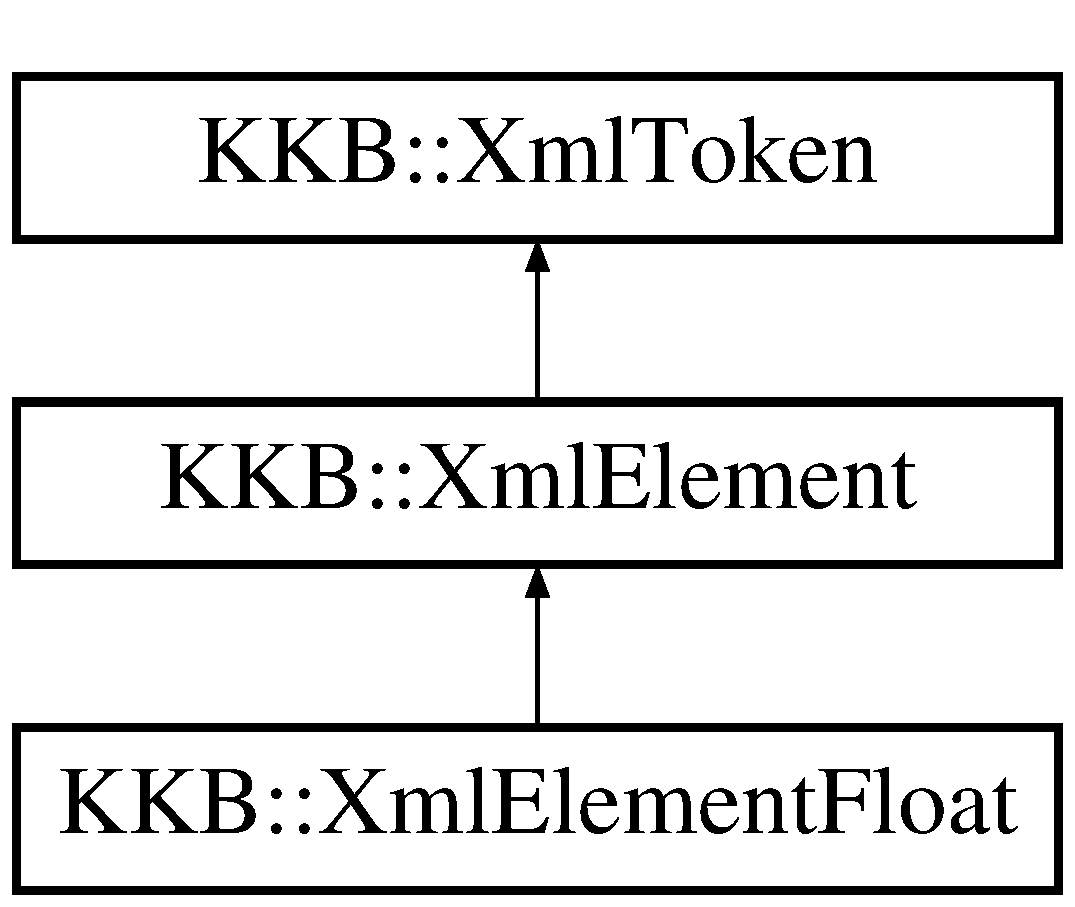
\includegraphics[height=3.000000cm]{class_k_k_b_1_1_xml_element_float}
\end{center}
\end{figure}
\subsection*{Public Member Functions}
\begin{DoxyCompactItemize}
\item 
\hyperlink{class_k_k_b_1_1_xml_element_float_a90da502783535e98a181c6fb94e52f65}{Xml\+Element\+Float} (\hyperlink{namespace_k_k_b_a9253a3ea8a5da18ca82be4ca2b390ef0}{Xml\+Tag\+Ptr} tag, \hyperlink{class_k_k_b_1_1_xml_stream}{Xml\+Stream} \&s, \hyperlink{namespace_k_k_b_a7d390f568e2831fb76b86b56c87bf92f}{Vol\+Const\+Bool} \&cancel\+Flag, \hyperlink{class_k_k_b_1_1_run_log}{Run\+Log} \&log)
\item 
virtual \hyperlink{class_k_k_b_1_1_xml_element_float_a7aca06af60563b1ccafb4ef035098455}{$\sim$\+Xml\+Element\+Float} ()
\item 
virtual bool \hyperlink{class_k_k_b_1_1_xml_element_float_a6a72dc8d2ebd6750787a07db8193e188}{To\+Bool} () const 
\item 
virtual double \hyperlink{class_k_k_b_1_1_xml_element_float_a4e0d90e5b74565ef0fb03cee7cdbc852}{To\+Double} () const 
\item 
virtual float \hyperlink{class_k_k_b_1_1_xml_element_float_a5967c539026d748db052c9035cc9ebe8}{To\+Float} () const 
\item 
virtual \hyperlink{namespace_k_k_b_a8fa4952cc84fda1de4bec1fbdd8d5b1b}{kkint32} \hyperlink{class_k_k_b_1_1_xml_element_float_a1ecd7c407ad5f26064e90fada52270c4}{To\+Int32} () const 
\item 
virtual \hyperlink{class_k_k_b_1_1_k_k_str}{K\+K\+Str} \hyperlink{class_k_k_b_1_1_xml_element_float_a95b717baacf55c1fa8a17ef7744c7915}{To\+K\+K\+Str} () const 
\item 
float \hyperlink{class_k_k_b_1_1_xml_element_float_a321fdfd30f4be44de3bf7e85691c0ba4}{Value} () const 
\end{DoxyCompactItemize}
\subsection*{Static Public Member Functions}
\begin{DoxyCompactItemize}
\item 
static void \hyperlink{class_k_k_b_1_1_xml_element_float_a6bd1a8d924cdc75190849168187e5a35}{Write\+X\+ML} (float d, const \hyperlink{class_k_k_b_1_1_k_k_str}{K\+K\+Str} \&var\+Name, std\+::ostream \&o)
\end{DoxyCompactItemize}
\subsection*{Additional Inherited Members}


\subsection{Detailed Description}


Definition at line 908 of file Xml\+Stream.\+h.



\subsection{Constructor \& Destructor Documentation}
\index{K\+K\+B\+::\+Xml\+Element\+Float@{K\+K\+B\+::\+Xml\+Element\+Float}!Xml\+Element\+Float@{Xml\+Element\+Float}}
\index{Xml\+Element\+Float@{Xml\+Element\+Float}!K\+K\+B\+::\+Xml\+Element\+Float@{K\+K\+B\+::\+Xml\+Element\+Float}}
\subsubsection[{\texorpdfstring{Xml\+Element\+Float(\+Xml\+Tag\+Ptr tag, Xml\+Stream \&s, Vol\+Const\+Bool \&cancel\+Flag, Run\+Log \&log)}{XmlElementFloat(XmlTagPtr tag, XmlStream &s, VolConstBool &cancelFlag, RunLog &log)}}]{\setlength{\rightskip}{0pt plus 5cm}Xml\+Element\+Float\+::\+Xml\+Element\+Float (
\begin{DoxyParamCaption}
\item[{{\bf Xml\+Tag\+Ptr}}]{tag, }
\item[{{\bf Xml\+Stream} \&}]{s, }
\item[{{\bf Vol\+Const\+Bool} \&}]{cancel\+Flag, }
\item[{{\bf Run\+Log} \&}]{log}
\end{DoxyParamCaption}
)}\hypertarget{class_k_k_b_1_1_xml_element_float_a90da502783535e98a181c6fb94e52f65}{}\label{class_k_k_b_1_1_xml_element_float_a90da502783535e98a181c6fb94e52f65}


Definition at line 1844 of file Xml\+Stream.\+cpp.

\index{K\+K\+B\+::\+Xml\+Element\+Float@{K\+K\+B\+::\+Xml\+Element\+Float}!````~Xml\+Element\+Float@{$\sim$\+Xml\+Element\+Float}}
\index{````~Xml\+Element\+Float@{$\sim$\+Xml\+Element\+Float}!K\+K\+B\+::\+Xml\+Element\+Float@{K\+K\+B\+::\+Xml\+Element\+Float}}
\subsubsection[{\texorpdfstring{$\sim$\+Xml\+Element\+Float()}{~XmlElementFloat()}}]{\setlength{\rightskip}{0pt plus 5cm}Xml\+Element\+Float\+::$\sim$\+Xml\+Element\+Float (
\begin{DoxyParamCaption}
{}
\end{DoxyParamCaption}
)\hspace{0.3cm}{\ttfamily [virtual]}}\hypertarget{class_k_k_b_1_1_xml_element_float_a7aca06af60563b1ccafb4ef035098455}{}\label{class_k_k_b_1_1_xml_element_float_a7aca06af60563b1ccafb4ef035098455}


Definition at line 1844 of file Xml\+Stream.\+cpp.



\subsection{Member Function Documentation}
\index{K\+K\+B\+::\+Xml\+Element\+Float@{K\+K\+B\+::\+Xml\+Element\+Float}!To\+Bool@{To\+Bool}}
\index{To\+Bool@{To\+Bool}!K\+K\+B\+::\+Xml\+Element\+Float@{K\+K\+B\+::\+Xml\+Element\+Float}}
\subsubsection[{\texorpdfstring{To\+Bool() const }{ToBool() const }}]{\setlength{\rightskip}{0pt plus 5cm}bool Xml\+Element\+Float\+::\+To\+Bool (
\begin{DoxyParamCaption}
{}
\end{DoxyParamCaption}
) const\hspace{0.3cm}{\ttfamily [virtual]}}\hypertarget{class_k_k_b_1_1_xml_element_float_a6a72dc8d2ebd6750787a07db8193e188}{}\label{class_k_k_b_1_1_xml_element_float_a6a72dc8d2ebd6750787a07db8193e188}


Reimplemented from \hyperlink{class_k_k_b_1_1_xml_element_a7bfbbea204722bc4535a294bc43e8e17}{K\+K\+B\+::\+Xml\+Element}.



Definition at line 1844 of file Xml\+Stream.\+cpp.

\index{K\+K\+B\+::\+Xml\+Element\+Float@{K\+K\+B\+::\+Xml\+Element\+Float}!To\+Double@{To\+Double}}
\index{To\+Double@{To\+Double}!K\+K\+B\+::\+Xml\+Element\+Float@{K\+K\+B\+::\+Xml\+Element\+Float}}
\subsubsection[{\texorpdfstring{To\+Double() const }{ToDouble() const }}]{\setlength{\rightskip}{0pt plus 5cm}double Xml\+Element\+Float\+::\+To\+Double (
\begin{DoxyParamCaption}
{}
\end{DoxyParamCaption}
) const\hspace{0.3cm}{\ttfamily [virtual]}}\hypertarget{class_k_k_b_1_1_xml_element_float_a4e0d90e5b74565ef0fb03cee7cdbc852}{}\label{class_k_k_b_1_1_xml_element_float_a4e0d90e5b74565ef0fb03cee7cdbc852}


Reimplemented from \hyperlink{class_k_k_b_1_1_xml_element_ac32778396ab8bdb215ad38f2f33f05de}{K\+K\+B\+::\+Xml\+Element}.



Definition at line 1844 of file Xml\+Stream.\+cpp.

\index{K\+K\+B\+::\+Xml\+Element\+Float@{K\+K\+B\+::\+Xml\+Element\+Float}!To\+Float@{To\+Float}}
\index{To\+Float@{To\+Float}!K\+K\+B\+::\+Xml\+Element\+Float@{K\+K\+B\+::\+Xml\+Element\+Float}}
\subsubsection[{\texorpdfstring{To\+Float() const }{ToFloat() const }}]{\setlength{\rightskip}{0pt plus 5cm}float Xml\+Element\+Float\+::\+To\+Float (
\begin{DoxyParamCaption}
{}
\end{DoxyParamCaption}
) const\hspace{0.3cm}{\ttfamily [virtual]}}\hypertarget{class_k_k_b_1_1_xml_element_float_a5967c539026d748db052c9035cc9ebe8}{}\label{class_k_k_b_1_1_xml_element_float_a5967c539026d748db052c9035cc9ebe8}


Reimplemented from \hyperlink{class_k_k_b_1_1_xml_element_aa728687ed43e76d45d029dfc14e14e95}{K\+K\+B\+::\+Xml\+Element}.



Definition at line 1844 of file Xml\+Stream.\+cpp.

\index{K\+K\+B\+::\+Xml\+Element\+Float@{K\+K\+B\+::\+Xml\+Element\+Float}!To\+Int32@{To\+Int32}}
\index{To\+Int32@{To\+Int32}!K\+K\+B\+::\+Xml\+Element\+Float@{K\+K\+B\+::\+Xml\+Element\+Float}}
\subsubsection[{\texorpdfstring{To\+Int32() const }{ToInt32() const }}]{\setlength{\rightskip}{0pt plus 5cm}{\bf kkint32} Xml\+Element\+Float\+::\+To\+Int32 (
\begin{DoxyParamCaption}
{}
\end{DoxyParamCaption}
) const\hspace{0.3cm}{\ttfamily [virtual]}}\hypertarget{class_k_k_b_1_1_xml_element_float_a1ecd7c407ad5f26064e90fada52270c4}{}\label{class_k_k_b_1_1_xml_element_float_a1ecd7c407ad5f26064e90fada52270c4}


Reimplemented from \hyperlink{class_k_k_b_1_1_xml_element_aac7463c7b305f66b5157f424a0a76363}{K\+K\+B\+::\+Xml\+Element}.



Definition at line 1844 of file Xml\+Stream.\+cpp.

\index{K\+K\+B\+::\+Xml\+Element\+Float@{K\+K\+B\+::\+Xml\+Element\+Float}!To\+K\+K\+Str@{To\+K\+K\+Str}}
\index{To\+K\+K\+Str@{To\+K\+K\+Str}!K\+K\+B\+::\+Xml\+Element\+Float@{K\+K\+B\+::\+Xml\+Element\+Float}}
\subsubsection[{\texorpdfstring{To\+K\+K\+Str() const }{ToKKStr() const }}]{\setlength{\rightskip}{0pt plus 5cm}{\bf K\+K\+Str} Xml\+Element\+Float\+::\+To\+K\+K\+Str (
\begin{DoxyParamCaption}
{}
\end{DoxyParamCaption}
) const\hspace{0.3cm}{\ttfamily [virtual]}}\hypertarget{class_k_k_b_1_1_xml_element_float_a95b717baacf55c1fa8a17ef7744c7915}{}\label{class_k_k_b_1_1_xml_element_float_a95b717baacf55c1fa8a17ef7744c7915}


Reimplemented from \hyperlink{class_k_k_b_1_1_xml_element_a3028fc03b79509e6378749f6a8b426b9}{K\+K\+B\+::\+Xml\+Element}.



Definition at line 1844 of file Xml\+Stream.\+cpp.

\index{K\+K\+B\+::\+Xml\+Element\+Float@{K\+K\+B\+::\+Xml\+Element\+Float}!Value@{Value}}
\index{Value@{Value}!K\+K\+B\+::\+Xml\+Element\+Float@{K\+K\+B\+::\+Xml\+Element\+Float}}
\subsubsection[{\texorpdfstring{Value() const }{Value() const }}]{\setlength{\rightskip}{0pt plus 5cm}float K\+K\+B\+::\+Xml\+Element\+Float\+::\+Value (
\begin{DoxyParamCaption}
{}
\end{DoxyParamCaption}
) const\hspace{0.3cm}{\ttfamily [inline]}}\hypertarget{class_k_k_b_1_1_xml_element_float_a321fdfd30f4be44de3bf7e85691c0ba4}{}\label{class_k_k_b_1_1_xml_element_float_a321fdfd30f4be44de3bf7e85691c0ba4}


Definition at line 908 of file Xml\+Stream.\+h.

\index{K\+K\+B\+::\+Xml\+Element\+Float@{K\+K\+B\+::\+Xml\+Element\+Float}!Write\+X\+ML@{Write\+X\+ML}}
\index{Write\+X\+ML@{Write\+X\+ML}!K\+K\+B\+::\+Xml\+Element\+Float@{K\+K\+B\+::\+Xml\+Element\+Float}}
\subsubsection[{\texorpdfstring{Write\+X\+M\+L(float d, const K\+K\+Str \&var\+Name, std\+::ostream \&o)}{WriteXML(float d, const KKStr &varName, std::ostream &o)}}]{\setlength{\rightskip}{0pt plus 5cm}void Xml\+Element\+Float\+::\+Write\+X\+ML (
\begin{DoxyParamCaption}
\item[{float}]{d, }
\item[{const {\bf K\+K\+Str} \&}]{var\+Name, }
\item[{std\+::ostream \&}]{o}
\end{DoxyParamCaption}
)\hspace{0.3cm}{\ttfamily [static]}}\hypertarget{class_k_k_b_1_1_xml_element_float_a6bd1a8d924cdc75190849168187e5a35}{}\label{class_k_k_b_1_1_xml_element_float_a6bd1a8d924cdc75190849168187e5a35}


Definition at line 1844 of file Xml\+Stream.\+cpp.



The documentation for this class was generated from the following files\+:\begin{DoxyCompactItemize}
\item 
C\+:/\+Users/\+Kurt/\+Git\+Hub/\+K\+Square\+Libraries/\+K\+K\+Base/\hyperlink{_xml_stream_8h}{Xml\+Stream.\+h}\item 
C\+:/\+Users/\+Kurt/\+Git\+Hub/\+K\+Square\+Libraries/\+K\+K\+Base/\hyperlink{_xml_stream_8cpp}{Xml\+Stream.\+cpp}\end{DoxyCompactItemize}

\hypertarget{class_k_k_b_1_1_xml_element_int32}{}\section{K\+KB\+:\+:Xml\+Element\+Int32 Class Reference}
\label{class_k_k_b_1_1_xml_element_int32}\index{K\+K\+B\+::\+Xml\+Element\+Int32@{K\+K\+B\+::\+Xml\+Element\+Int32}}


{\ttfamily \#include $<$Xml\+Stream.\+h$>$}

Inheritance diagram for K\+KB\+:\+:Xml\+Element\+Int32\+:\begin{figure}[H]
\begin{center}
\leavevmode
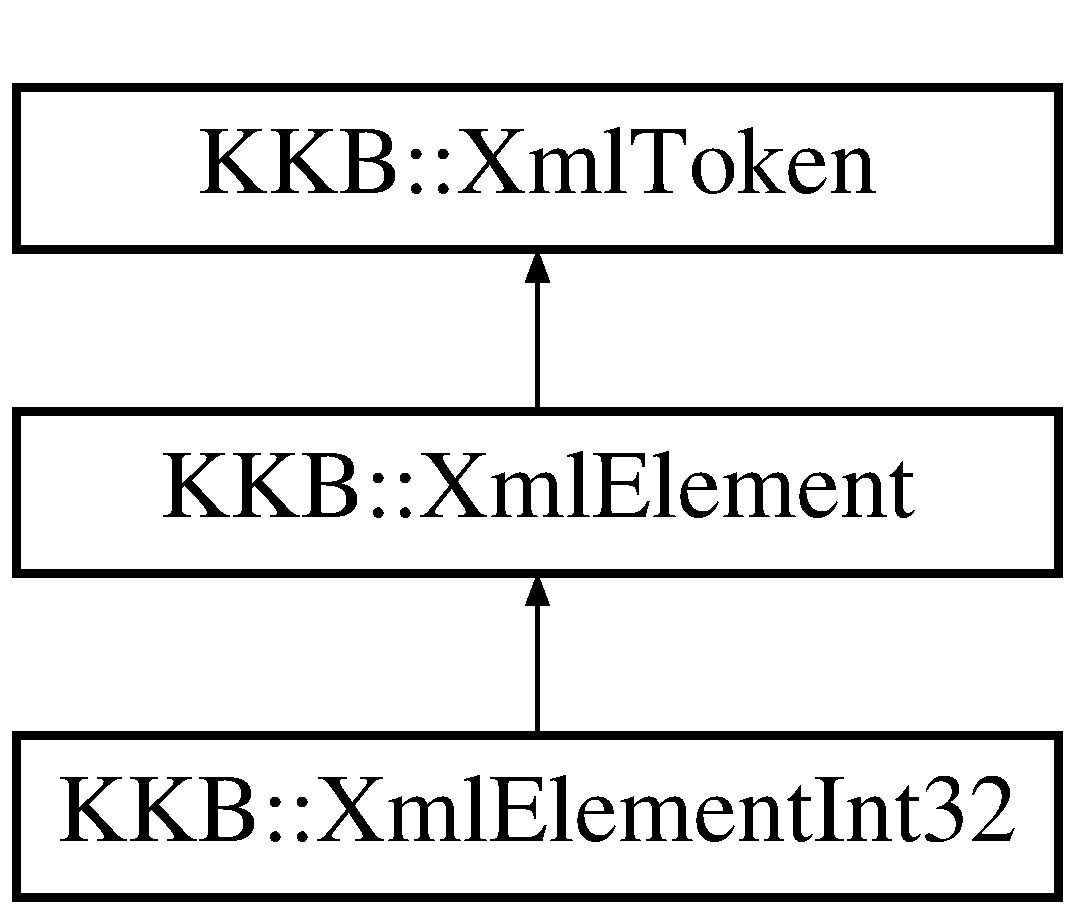
\includegraphics[height=3.000000cm]{class_k_k_b_1_1_xml_element_int32}
\end{center}
\end{figure}
\subsection*{Public Member Functions}
\begin{DoxyCompactItemize}
\item 
\hyperlink{class_k_k_b_1_1_xml_element_int32_a4f9c90b3dd3ba7e3b9fcb6b60d665d1a}{Xml\+Element\+Int32} (\hyperlink{namespace_k_k_b_a9253a3ea8a5da18ca82be4ca2b390ef0}{Xml\+Tag\+Ptr} tag, \hyperlink{class_k_k_b_1_1_xml_stream}{Xml\+Stream} \&s, \hyperlink{namespace_k_k_b_a7d390f568e2831fb76b86b56c87bf92f}{Vol\+Const\+Bool} \&cancel\+Flag, \hyperlink{class_k_k_b_1_1_run_log}{Run\+Log} \&log)
\item 
virtual \hyperlink{class_k_k_b_1_1_xml_element_int32_afb0b464cfaeac317a6f51b94c3accbcf}{$\sim$\+Xml\+Element\+Int32} ()
\item 
virtual bool \hyperlink{class_k_k_b_1_1_xml_element_int32_aec7a18f2b0e3bf247bf29f21e5256592}{To\+Bool} () const 
\item 
virtual double \hyperlink{class_k_k_b_1_1_xml_element_int32_a1768e0e2b122547832f7d8a73a0f1588}{To\+Double} () const 
\item 
virtual float \hyperlink{class_k_k_b_1_1_xml_element_int32_a1b240dc1bc387f12192575c3257f95e7}{To\+Float} () const 
\item 
virtual \hyperlink{namespace_k_k_b_a8fa4952cc84fda1de4bec1fbdd8d5b1b}{kkint32} \hyperlink{class_k_k_b_1_1_xml_element_int32_a043453a13afcf42b819baf231786e653}{To\+Int32} () const 
\item 
virtual \hyperlink{class_k_k_b_1_1_k_k_str}{K\+K\+Str} \hyperlink{class_k_k_b_1_1_xml_element_int32_af0db95c22ac5abf7158120aab68607c0}{To\+K\+K\+Str} () const 
\item 
\hyperlink{namespace_k_k_b_a8fa4952cc84fda1de4bec1fbdd8d5b1b}{kkint32} \hyperlink{class_k_k_b_1_1_xml_element_int32_a37c999e6762841736ed3d1c03ed87d34}{Value} () const 
\end{DoxyCompactItemize}
\subsection*{Static Public Member Functions}
\begin{DoxyCompactItemize}
\item 
static void \hyperlink{class_k_k_b_1_1_xml_element_int32_abe69c8abb4c2bbfef0a6a41fd68ce466}{Write\+X\+ML} (\hyperlink{namespace_k_k_b_a8fa4952cc84fda1de4bec1fbdd8d5b1b}{kkint32} d, const \hyperlink{class_k_k_b_1_1_k_k_str}{K\+K\+Str} \&var\+Name, std\+::ostream \&o)
\end{DoxyCompactItemize}
\subsection*{Additional Inherited Members}


\subsection{Detailed Description}


Definition at line 906 of file Xml\+Stream.\+h.



\subsection{Constructor \& Destructor Documentation}
\index{K\+K\+B\+::\+Xml\+Element\+Int32@{K\+K\+B\+::\+Xml\+Element\+Int32}!Xml\+Element\+Int32@{Xml\+Element\+Int32}}
\index{Xml\+Element\+Int32@{Xml\+Element\+Int32}!K\+K\+B\+::\+Xml\+Element\+Int32@{K\+K\+B\+::\+Xml\+Element\+Int32}}
\subsubsection[{\texorpdfstring{Xml\+Element\+Int32(\+Xml\+Tag\+Ptr tag, Xml\+Stream \&s, Vol\+Const\+Bool \&cancel\+Flag, Run\+Log \&log)}{XmlElementInt32(XmlTagPtr tag, XmlStream &s, VolConstBool &cancelFlag, RunLog &log)}}]{\setlength{\rightskip}{0pt plus 5cm}Xml\+Element\+Int32\+::\+Xml\+Element\+Int32 (
\begin{DoxyParamCaption}
\item[{{\bf Xml\+Tag\+Ptr}}]{tag, }
\item[{{\bf Xml\+Stream} \&}]{s, }
\item[{{\bf Vol\+Const\+Bool} \&}]{cancel\+Flag, }
\item[{{\bf Run\+Log} \&}]{log}
\end{DoxyParamCaption}
)}\hypertarget{class_k_k_b_1_1_xml_element_int32_a4f9c90b3dd3ba7e3b9fcb6b60d665d1a}{}\label{class_k_k_b_1_1_xml_element_int32_a4f9c90b3dd3ba7e3b9fcb6b60d665d1a}


Definition at line 1840 of file Xml\+Stream.\+cpp.

\index{K\+K\+B\+::\+Xml\+Element\+Int32@{K\+K\+B\+::\+Xml\+Element\+Int32}!````~Xml\+Element\+Int32@{$\sim$\+Xml\+Element\+Int32}}
\index{````~Xml\+Element\+Int32@{$\sim$\+Xml\+Element\+Int32}!K\+K\+B\+::\+Xml\+Element\+Int32@{K\+K\+B\+::\+Xml\+Element\+Int32}}
\subsubsection[{\texorpdfstring{$\sim$\+Xml\+Element\+Int32()}{~XmlElementInt32()}}]{\setlength{\rightskip}{0pt plus 5cm}Xml\+Element\+Int32\+::$\sim$\+Xml\+Element\+Int32 (
\begin{DoxyParamCaption}
{}
\end{DoxyParamCaption}
)\hspace{0.3cm}{\ttfamily [virtual]}}\hypertarget{class_k_k_b_1_1_xml_element_int32_afb0b464cfaeac317a6f51b94c3accbcf}{}\label{class_k_k_b_1_1_xml_element_int32_afb0b464cfaeac317a6f51b94c3accbcf}


Definition at line 1840 of file Xml\+Stream.\+cpp.



\subsection{Member Function Documentation}
\index{K\+K\+B\+::\+Xml\+Element\+Int32@{K\+K\+B\+::\+Xml\+Element\+Int32}!To\+Bool@{To\+Bool}}
\index{To\+Bool@{To\+Bool}!K\+K\+B\+::\+Xml\+Element\+Int32@{K\+K\+B\+::\+Xml\+Element\+Int32}}
\subsubsection[{\texorpdfstring{To\+Bool() const }{ToBool() const }}]{\setlength{\rightskip}{0pt plus 5cm}bool Xml\+Element\+Int32\+::\+To\+Bool (
\begin{DoxyParamCaption}
{}
\end{DoxyParamCaption}
) const\hspace{0.3cm}{\ttfamily [virtual]}}\hypertarget{class_k_k_b_1_1_xml_element_int32_aec7a18f2b0e3bf247bf29f21e5256592}{}\label{class_k_k_b_1_1_xml_element_int32_aec7a18f2b0e3bf247bf29f21e5256592}


Reimplemented from \hyperlink{class_k_k_b_1_1_xml_element_a7bfbbea204722bc4535a294bc43e8e17}{K\+K\+B\+::\+Xml\+Element}.



Definition at line 1840 of file Xml\+Stream.\+cpp.

\index{K\+K\+B\+::\+Xml\+Element\+Int32@{K\+K\+B\+::\+Xml\+Element\+Int32}!To\+Double@{To\+Double}}
\index{To\+Double@{To\+Double}!K\+K\+B\+::\+Xml\+Element\+Int32@{K\+K\+B\+::\+Xml\+Element\+Int32}}
\subsubsection[{\texorpdfstring{To\+Double() const }{ToDouble() const }}]{\setlength{\rightskip}{0pt plus 5cm}double Xml\+Element\+Int32\+::\+To\+Double (
\begin{DoxyParamCaption}
{}
\end{DoxyParamCaption}
) const\hspace{0.3cm}{\ttfamily [virtual]}}\hypertarget{class_k_k_b_1_1_xml_element_int32_a1768e0e2b122547832f7d8a73a0f1588}{}\label{class_k_k_b_1_1_xml_element_int32_a1768e0e2b122547832f7d8a73a0f1588}


Reimplemented from \hyperlink{class_k_k_b_1_1_xml_element_ac32778396ab8bdb215ad38f2f33f05de}{K\+K\+B\+::\+Xml\+Element}.



Definition at line 1840 of file Xml\+Stream.\+cpp.

\index{K\+K\+B\+::\+Xml\+Element\+Int32@{K\+K\+B\+::\+Xml\+Element\+Int32}!To\+Float@{To\+Float}}
\index{To\+Float@{To\+Float}!K\+K\+B\+::\+Xml\+Element\+Int32@{K\+K\+B\+::\+Xml\+Element\+Int32}}
\subsubsection[{\texorpdfstring{To\+Float() const }{ToFloat() const }}]{\setlength{\rightskip}{0pt plus 5cm}float Xml\+Element\+Int32\+::\+To\+Float (
\begin{DoxyParamCaption}
{}
\end{DoxyParamCaption}
) const\hspace{0.3cm}{\ttfamily [virtual]}}\hypertarget{class_k_k_b_1_1_xml_element_int32_a1b240dc1bc387f12192575c3257f95e7}{}\label{class_k_k_b_1_1_xml_element_int32_a1b240dc1bc387f12192575c3257f95e7}


Reimplemented from \hyperlink{class_k_k_b_1_1_xml_element_aa728687ed43e76d45d029dfc14e14e95}{K\+K\+B\+::\+Xml\+Element}.



Definition at line 1840 of file Xml\+Stream.\+cpp.

\index{K\+K\+B\+::\+Xml\+Element\+Int32@{K\+K\+B\+::\+Xml\+Element\+Int32}!To\+Int32@{To\+Int32}}
\index{To\+Int32@{To\+Int32}!K\+K\+B\+::\+Xml\+Element\+Int32@{K\+K\+B\+::\+Xml\+Element\+Int32}}
\subsubsection[{\texorpdfstring{To\+Int32() const }{ToInt32() const }}]{\setlength{\rightskip}{0pt plus 5cm}{\bf kkint32} Xml\+Element\+Int32\+::\+To\+Int32 (
\begin{DoxyParamCaption}
{}
\end{DoxyParamCaption}
) const\hspace{0.3cm}{\ttfamily [virtual]}}\hypertarget{class_k_k_b_1_1_xml_element_int32_a043453a13afcf42b819baf231786e653}{}\label{class_k_k_b_1_1_xml_element_int32_a043453a13afcf42b819baf231786e653}


Reimplemented from \hyperlink{class_k_k_b_1_1_xml_element_aac7463c7b305f66b5157f424a0a76363}{K\+K\+B\+::\+Xml\+Element}.



Definition at line 1840 of file Xml\+Stream.\+cpp.

\index{K\+K\+B\+::\+Xml\+Element\+Int32@{K\+K\+B\+::\+Xml\+Element\+Int32}!To\+K\+K\+Str@{To\+K\+K\+Str}}
\index{To\+K\+K\+Str@{To\+K\+K\+Str}!K\+K\+B\+::\+Xml\+Element\+Int32@{K\+K\+B\+::\+Xml\+Element\+Int32}}
\subsubsection[{\texorpdfstring{To\+K\+K\+Str() const }{ToKKStr() const }}]{\setlength{\rightskip}{0pt plus 5cm}{\bf K\+K\+Str} Xml\+Element\+Int32\+::\+To\+K\+K\+Str (
\begin{DoxyParamCaption}
{}
\end{DoxyParamCaption}
) const\hspace{0.3cm}{\ttfamily [virtual]}}\hypertarget{class_k_k_b_1_1_xml_element_int32_af0db95c22ac5abf7158120aab68607c0}{}\label{class_k_k_b_1_1_xml_element_int32_af0db95c22ac5abf7158120aab68607c0}


Reimplemented from \hyperlink{class_k_k_b_1_1_xml_element_a3028fc03b79509e6378749f6a8b426b9}{K\+K\+B\+::\+Xml\+Element}.



Definition at line 1840 of file Xml\+Stream.\+cpp.

\index{K\+K\+B\+::\+Xml\+Element\+Int32@{K\+K\+B\+::\+Xml\+Element\+Int32}!Value@{Value}}
\index{Value@{Value}!K\+K\+B\+::\+Xml\+Element\+Int32@{K\+K\+B\+::\+Xml\+Element\+Int32}}
\subsubsection[{\texorpdfstring{Value() const }{Value() const }}]{\setlength{\rightskip}{0pt plus 5cm}{\bf kkint32} K\+K\+B\+::\+Xml\+Element\+Int32\+::\+Value (
\begin{DoxyParamCaption}
{}
\end{DoxyParamCaption}
) const\hspace{0.3cm}{\ttfamily [inline]}}\hypertarget{class_k_k_b_1_1_xml_element_int32_a37c999e6762841736ed3d1c03ed87d34}{}\label{class_k_k_b_1_1_xml_element_int32_a37c999e6762841736ed3d1c03ed87d34}


Definition at line 906 of file Xml\+Stream.\+h.

\index{K\+K\+B\+::\+Xml\+Element\+Int32@{K\+K\+B\+::\+Xml\+Element\+Int32}!Write\+X\+ML@{Write\+X\+ML}}
\index{Write\+X\+ML@{Write\+X\+ML}!K\+K\+B\+::\+Xml\+Element\+Int32@{K\+K\+B\+::\+Xml\+Element\+Int32}}
\subsubsection[{\texorpdfstring{Write\+X\+M\+L(kkint32 d, const K\+K\+Str \&var\+Name, std\+::ostream \&o)}{WriteXML(kkint32 d, const KKStr &varName, std::ostream &o)}}]{\setlength{\rightskip}{0pt plus 5cm}void Xml\+Element\+Int32\+::\+Write\+X\+ML (
\begin{DoxyParamCaption}
\item[{{\bf kkint32}}]{d, }
\item[{const {\bf K\+K\+Str} \&}]{var\+Name, }
\item[{std\+::ostream \&}]{o}
\end{DoxyParamCaption}
)\hspace{0.3cm}{\ttfamily [static]}}\hypertarget{class_k_k_b_1_1_xml_element_int32_abe69c8abb4c2bbfef0a6a41fd68ce466}{}\label{class_k_k_b_1_1_xml_element_int32_abe69c8abb4c2bbfef0a6a41fd68ce466}


Definition at line 1840 of file Xml\+Stream.\+cpp.



The documentation for this class was generated from the following files\+:\begin{DoxyCompactItemize}
\item 
C\+:/\+Users/\+Kurt/\+Git\+Hub/\+K\+Square\+Libraries/\+K\+K\+Base/\hyperlink{_xml_stream_8h}{Xml\+Stream.\+h}\item 
C\+:/\+Users/\+Kurt/\+Git\+Hub/\+K\+Square\+Libraries/\+K\+K\+Base/\hyperlink{_xml_stream_8cpp}{Xml\+Stream.\+cpp}\end{DoxyCompactItemize}

\hypertarget{class_k_k_b_1_1_xml_element_int64}{}\section{K\+KB\+:\+:Xml\+Element\+Int64 Class Reference}
\label{class_k_k_b_1_1_xml_element_int64}\index{K\+K\+B\+::\+Xml\+Element\+Int64@{K\+K\+B\+::\+Xml\+Element\+Int64}}


{\ttfamily \#include $<$Xml\+Stream.\+h$>$}

Inheritance diagram for K\+KB\+:\+:Xml\+Element\+Int64\+:\begin{figure}[H]
\begin{center}
\leavevmode
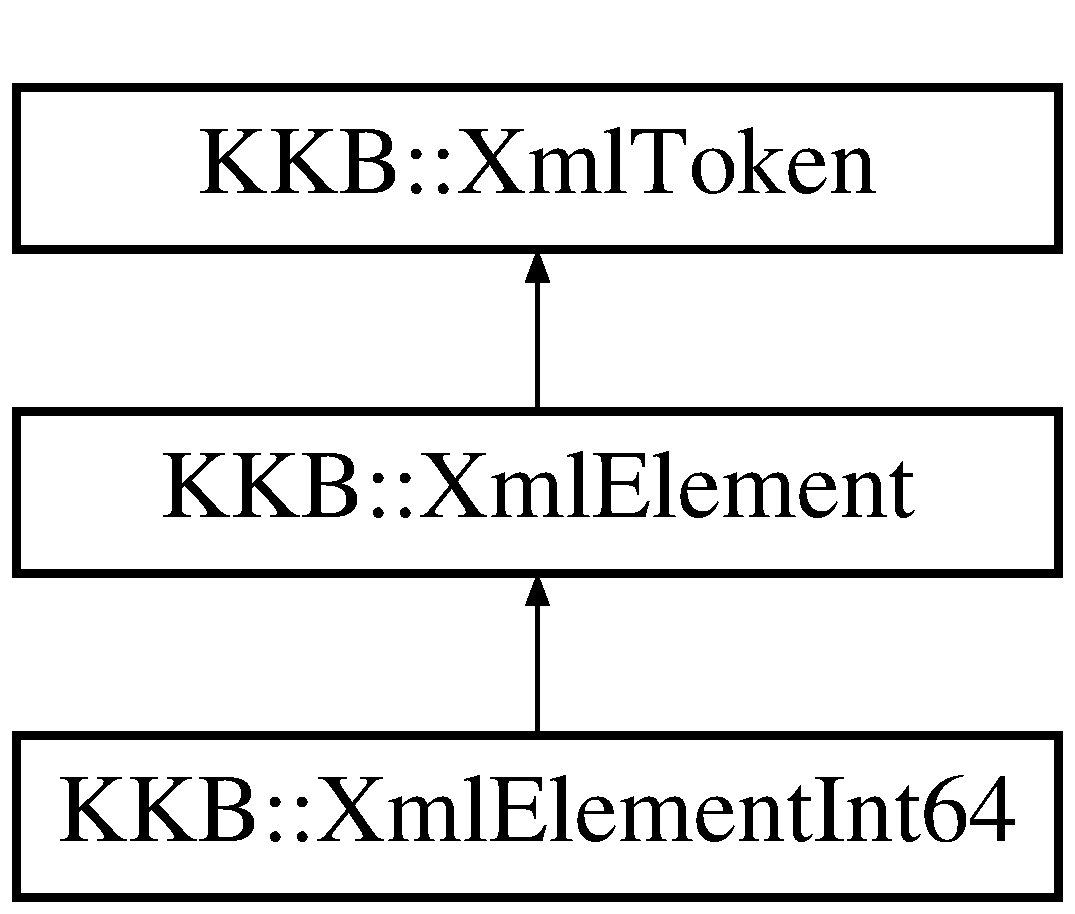
\includegraphics[height=3.000000cm]{class_k_k_b_1_1_xml_element_int64}
\end{center}
\end{figure}
\subsection*{Public Member Functions}
\begin{DoxyCompactItemize}
\item 
\hyperlink{class_k_k_b_1_1_xml_element_int64_aef0b065657c12228b7f7650bfe4b02a3}{Xml\+Element\+Int64} (\hyperlink{namespace_k_k_b_a9253a3ea8a5da18ca82be4ca2b390ef0}{Xml\+Tag\+Ptr} tag, \hyperlink{class_k_k_b_1_1_xml_stream}{Xml\+Stream} \&s, \hyperlink{namespace_k_k_b_a7d390f568e2831fb76b86b56c87bf92f}{Vol\+Const\+Bool} \&cancel\+Flag, \hyperlink{class_k_k_b_1_1_run_log}{Run\+Log} \&log)
\item 
virtual \hyperlink{class_k_k_b_1_1_xml_element_int64_a8a298ae49e4b47cedd23d16c964d7a06}{$\sim$\+Xml\+Element\+Int64} ()
\item 
virtual bool \hyperlink{class_k_k_b_1_1_xml_element_int64_a30d43c139d9efa806e8ad5ba8ded9d47}{To\+Bool} () const 
\item 
virtual double \hyperlink{class_k_k_b_1_1_xml_element_int64_af06d31f81561cf6bdd9731f699a7efbe}{To\+Double} () const 
\item 
virtual float \hyperlink{class_k_k_b_1_1_xml_element_int64_a5d7fe62f4e493d6a8de86534e0793d94}{To\+Float} () const 
\item 
virtual \hyperlink{namespace_k_k_b_a8fa4952cc84fda1de4bec1fbdd8d5b1b}{kkint32} \hyperlink{class_k_k_b_1_1_xml_element_int64_ab97448e2f4b9d5ae1451d35f1b4c63bd}{To\+Int32} () const 
\item 
virtual \hyperlink{class_k_k_b_1_1_k_k_str}{K\+K\+Str} \hyperlink{class_k_k_b_1_1_xml_element_int64_a73280a065f02c4ab505ddd81ce8a9f8c}{To\+K\+K\+Str} () const 
\item 
\hyperlink{namespace_k_k_b_aa3486b1c5ea9162b3b020c69f72826eb}{kkint64} \hyperlink{class_k_k_b_1_1_xml_element_int64_ac264312fc93517df9fb5693514db7162}{Value} () const 
\end{DoxyCompactItemize}
\subsection*{Static Public Member Functions}
\begin{DoxyCompactItemize}
\item 
static void \hyperlink{class_k_k_b_1_1_xml_element_int64_a4e82c41d4a3b4c81769503ff469f27fc}{Write\+X\+ML} (\hyperlink{namespace_k_k_b_aa3486b1c5ea9162b3b020c69f72826eb}{kkint64} d, const \hyperlink{class_k_k_b_1_1_k_k_str}{K\+K\+Str} \&var\+Name, std\+::ostream \&o)
\end{DoxyCompactItemize}
\subsection*{Additional Inherited Members}


\subsection{Detailed Description}


Definition at line 907 of file Xml\+Stream.\+h.



\subsection{Constructor \& Destructor Documentation}
\index{K\+K\+B\+::\+Xml\+Element\+Int64@{K\+K\+B\+::\+Xml\+Element\+Int64}!Xml\+Element\+Int64@{Xml\+Element\+Int64}}
\index{Xml\+Element\+Int64@{Xml\+Element\+Int64}!K\+K\+B\+::\+Xml\+Element\+Int64@{K\+K\+B\+::\+Xml\+Element\+Int64}}
\subsubsection[{\texorpdfstring{Xml\+Element\+Int64(\+Xml\+Tag\+Ptr tag, Xml\+Stream \&s, Vol\+Const\+Bool \&cancel\+Flag, Run\+Log \&log)}{XmlElementInt64(XmlTagPtr tag, XmlStream &s, VolConstBool &cancelFlag, RunLog &log)}}]{\setlength{\rightskip}{0pt plus 5cm}Xml\+Element\+Int64\+::\+Xml\+Element\+Int64 (
\begin{DoxyParamCaption}
\item[{{\bf Xml\+Tag\+Ptr}}]{tag, }
\item[{{\bf Xml\+Stream} \&}]{s, }
\item[{{\bf Vol\+Const\+Bool} \&}]{cancel\+Flag, }
\item[{{\bf Run\+Log} \&}]{log}
\end{DoxyParamCaption}
)}\hypertarget{class_k_k_b_1_1_xml_element_int64_aef0b065657c12228b7f7650bfe4b02a3}{}\label{class_k_k_b_1_1_xml_element_int64_aef0b065657c12228b7f7650bfe4b02a3}


Definition at line 1842 of file Xml\+Stream.\+cpp.

\index{K\+K\+B\+::\+Xml\+Element\+Int64@{K\+K\+B\+::\+Xml\+Element\+Int64}!````~Xml\+Element\+Int64@{$\sim$\+Xml\+Element\+Int64}}
\index{````~Xml\+Element\+Int64@{$\sim$\+Xml\+Element\+Int64}!K\+K\+B\+::\+Xml\+Element\+Int64@{K\+K\+B\+::\+Xml\+Element\+Int64}}
\subsubsection[{\texorpdfstring{$\sim$\+Xml\+Element\+Int64()}{~XmlElementInt64()}}]{\setlength{\rightskip}{0pt plus 5cm}Xml\+Element\+Int64\+::$\sim$\+Xml\+Element\+Int64 (
\begin{DoxyParamCaption}
{}
\end{DoxyParamCaption}
)\hspace{0.3cm}{\ttfamily [virtual]}}\hypertarget{class_k_k_b_1_1_xml_element_int64_a8a298ae49e4b47cedd23d16c964d7a06}{}\label{class_k_k_b_1_1_xml_element_int64_a8a298ae49e4b47cedd23d16c964d7a06}


Definition at line 1842 of file Xml\+Stream.\+cpp.



\subsection{Member Function Documentation}
\index{K\+K\+B\+::\+Xml\+Element\+Int64@{K\+K\+B\+::\+Xml\+Element\+Int64}!To\+Bool@{To\+Bool}}
\index{To\+Bool@{To\+Bool}!K\+K\+B\+::\+Xml\+Element\+Int64@{K\+K\+B\+::\+Xml\+Element\+Int64}}
\subsubsection[{\texorpdfstring{To\+Bool() const }{ToBool() const }}]{\setlength{\rightskip}{0pt plus 5cm}bool Xml\+Element\+Int64\+::\+To\+Bool (
\begin{DoxyParamCaption}
{}
\end{DoxyParamCaption}
) const\hspace{0.3cm}{\ttfamily [virtual]}}\hypertarget{class_k_k_b_1_1_xml_element_int64_a30d43c139d9efa806e8ad5ba8ded9d47}{}\label{class_k_k_b_1_1_xml_element_int64_a30d43c139d9efa806e8ad5ba8ded9d47}


Reimplemented from \hyperlink{class_k_k_b_1_1_xml_element_a7bfbbea204722bc4535a294bc43e8e17}{K\+K\+B\+::\+Xml\+Element}.



Definition at line 1842 of file Xml\+Stream.\+cpp.

\index{K\+K\+B\+::\+Xml\+Element\+Int64@{K\+K\+B\+::\+Xml\+Element\+Int64}!To\+Double@{To\+Double}}
\index{To\+Double@{To\+Double}!K\+K\+B\+::\+Xml\+Element\+Int64@{K\+K\+B\+::\+Xml\+Element\+Int64}}
\subsubsection[{\texorpdfstring{To\+Double() const }{ToDouble() const }}]{\setlength{\rightskip}{0pt plus 5cm}double Xml\+Element\+Int64\+::\+To\+Double (
\begin{DoxyParamCaption}
{}
\end{DoxyParamCaption}
) const\hspace{0.3cm}{\ttfamily [virtual]}}\hypertarget{class_k_k_b_1_1_xml_element_int64_af06d31f81561cf6bdd9731f699a7efbe}{}\label{class_k_k_b_1_1_xml_element_int64_af06d31f81561cf6bdd9731f699a7efbe}


Reimplemented from \hyperlink{class_k_k_b_1_1_xml_element_ac32778396ab8bdb215ad38f2f33f05de}{K\+K\+B\+::\+Xml\+Element}.



Definition at line 1842 of file Xml\+Stream.\+cpp.

\index{K\+K\+B\+::\+Xml\+Element\+Int64@{K\+K\+B\+::\+Xml\+Element\+Int64}!To\+Float@{To\+Float}}
\index{To\+Float@{To\+Float}!K\+K\+B\+::\+Xml\+Element\+Int64@{K\+K\+B\+::\+Xml\+Element\+Int64}}
\subsubsection[{\texorpdfstring{To\+Float() const }{ToFloat() const }}]{\setlength{\rightskip}{0pt plus 5cm}float Xml\+Element\+Int64\+::\+To\+Float (
\begin{DoxyParamCaption}
{}
\end{DoxyParamCaption}
) const\hspace{0.3cm}{\ttfamily [virtual]}}\hypertarget{class_k_k_b_1_1_xml_element_int64_a5d7fe62f4e493d6a8de86534e0793d94}{}\label{class_k_k_b_1_1_xml_element_int64_a5d7fe62f4e493d6a8de86534e0793d94}


Reimplemented from \hyperlink{class_k_k_b_1_1_xml_element_aa728687ed43e76d45d029dfc14e14e95}{K\+K\+B\+::\+Xml\+Element}.



Definition at line 1842 of file Xml\+Stream.\+cpp.

\index{K\+K\+B\+::\+Xml\+Element\+Int64@{K\+K\+B\+::\+Xml\+Element\+Int64}!To\+Int32@{To\+Int32}}
\index{To\+Int32@{To\+Int32}!K\+K\+B\+::\+Xml\+Element\+Int64@{K\+K\+B\+::\+Xml\+Element\+Int64}}
\subsubsection[{\texorpdfstring{To\+Int32() const }{ToInt32() const }}]{\setlength{\rightskip}{0pt plus 5cm}{\bf kkint32} Xml\+Element\+Int64\+::\+To\+Int32 (
\begin{DoxyParamCaption}
{}
\end{DoxyParamCaption}
) const\hspace{0.3cm}{\ttfamily [virtual]}}\hypertarget{class_k_k_b_1_1_xml_element_int64_ab97448e2f4b9d5ae1451d35f1b4c63bd}{}\label{class_k_k_b_1_1_xml_element_int64_ab97448e2f4b9d5ae1451d35f1b4c63bd}


Reimplemented from \hyperlink{class_k_k_b_1_1_xml_element_aac7463c7b305f66b5157f424a0a76363}{K\+K\+B\+::\+Xml\+Element}.



Definition at line 1842 of file Xml\+Stream.\+cpp.

\index{K\+K\+B\+::\+Xml\+Element\+Int64@{K\+K\+B\+::\+Xml\+Element\+Int64}!To\+K\+K\+Str@{To\+K\+K\+Str}}
\index{To\+K\+K\+Str@{To\+K\+K\+Str}!K\+K\+B\+::\+Xml\+Element\+Int64@{K\+K\+B\+::\+Xml\+Element\+Int64}}
\subsubsection[{\texorpdfstring{To\+K\+K\+Str() const }{ToKKStr() const }}]{\setlength{\rightskip}{0pt plus 5cm}{\bf K\+K\+Str} Xml\+Element\+Int64\+::\+To\+K\+K\+Str (
\begin{DoxyParamCaption}
{}
\end{DoxyParamCaption}
) const\hspace{0.3cm}{\ttfamily [virtual]}}\hypertarget{class_k_k_b_1_1_xml_element_int64_a73280a065f02c4ab505ddd81ce8a9f8c}{}\label{class_k_k_b_1_1_xml_element_int64_a73280a065f02c4ab505ddd81ce8a9f8c}


Reimplemented from \hyperlink{class_k_k_b_1_1_xml_element_a3028fc03b79509e6378749f6a8b426b9}{K\+K\+B\+::\+Xml\+Element}.



Definition at line 1842 of file Xml\+Stream.\+cpp.

\index{K\+K\+B\+::\+Xml\+Element\+Int64@{K\+K\+B\+::\+Xml\+Element\+Int64}!Value@{Value}}
\index{Value@{Value}!K\+K\+B\+::\+Xml\+Element\+Int64@{K\+K\+B\+::\+Xml\+Element\+Int64}}
\subsubsection[{\texorpdfstring{Value() const }{Value() const }}]{\setlength{\rightskip}{0pt plus 5cm}{\bf kkint64} K\+K\+B\+::\+Xml\+Element\+Int64\+::\+Value (
\begin{DoxyParamCaption}
{}
\end{DoxyParamCaption}
) const\hspace{0.3cm}{\ttfamily [inline]}}\hypertarget{class_k_k_b_1_1_xml_element_int64_ac264312fc93517df9fb5693514db7162}{}\label{class_k_k_b_1_1_xml_element_int64_ac264312fc93517df9fb5693514db7162}


Definition at line 907 of file Xml\+Stream.\+h.

\index{K\+K\+B\+::\+Xml\+Element\+Int64@{K\+K\+B\+::\+Xml\+Element\+Int64}!Write\+X\+ML@{Write\+X\+ML}}
\index{Write\+X\+ML@{Write\+X\+ML}!K\+K\+B\+::\+Xml\+Element\+Int64@{K\+K\+B\+::\+Xml\+Element\+Int64}}
\subsubsection[{\texorpdfstring{Write\+X\+M\+L(kkint64 d, const K\+K\+Str \&var\+Name, std\+::ostream \&o)}{WriteXML(kkint64 d, const KKStr &varName, std::ostream &o)}}]{\setlength{\rightskip}{0pt plus 5cm}void Xml\+Element\+Int64\+::\+Write\+X\+ML (
\begin{DoxyParamCaption}
\item[{{\bf kkint64}}]{d, }
\item[{const {\bf K\+K\+Str} \&}]{var\+Name, }
\item[{std\+::ostream \&}]{o}
\end{DoxyParamCaption}
)\hspace{0.3cm}{\ttfamily [static]}}\hypertarget{class_k_k_b_1_1_xml_element_int64_a4e82c41d4a3b4c81769503ff469f27fc}{}\label{class_k_k_b_1_1_xml_element_int64_a4e82c41d4a3b4c81769503ff469f27fc}


Definition at line 1842 of file Xml\+Stream.\+cpp.



The documentation for this class was generated from the following files\+:\begin{DoxyCompactItemize}
\item 
C\+:/\+Users/\+Kurt/\+Git\+Hub/\+K\+Square\+Libraries/\+K\+K\+Base/\hyperlink{_xml_stream_8h}{Xml\+Stream.\+h}\item 
C\+:/\+Users/\+Kurt/\+Git\+Hub/\+K\+Square\+Libraries/\+K\+K\+Base/\hyperlink{_xml_stream_8cpp}{Xml\+Stream.\+cpp}\end{DoxyCompactItemize}

\hypertarget{class_k_k_b_1_1_xml_element_key_value_pairs}{}\section{K\+KB\+:\+:Xml\+Element\+Key\+Value\+Pairs Class Reference}
\label{class_k_k_b_1_1_xml_element_key_value_pairs}\index{K\+K\+B\+::\+Xml\+Element\+Key\+Value\+Pairs@{K\+K\+B\+::\+Xml\+Element\+Key\+Value\+Pairs}}


{\ttfamily \#include $<$Xml\+Stream.\+h$>$}

Inheritance diagram for K\+KB\+:\+:Xml\+Element\+Key\+Value\+Pairs\+:\begin{figure}[H]
\begin{center}
\leavevmode
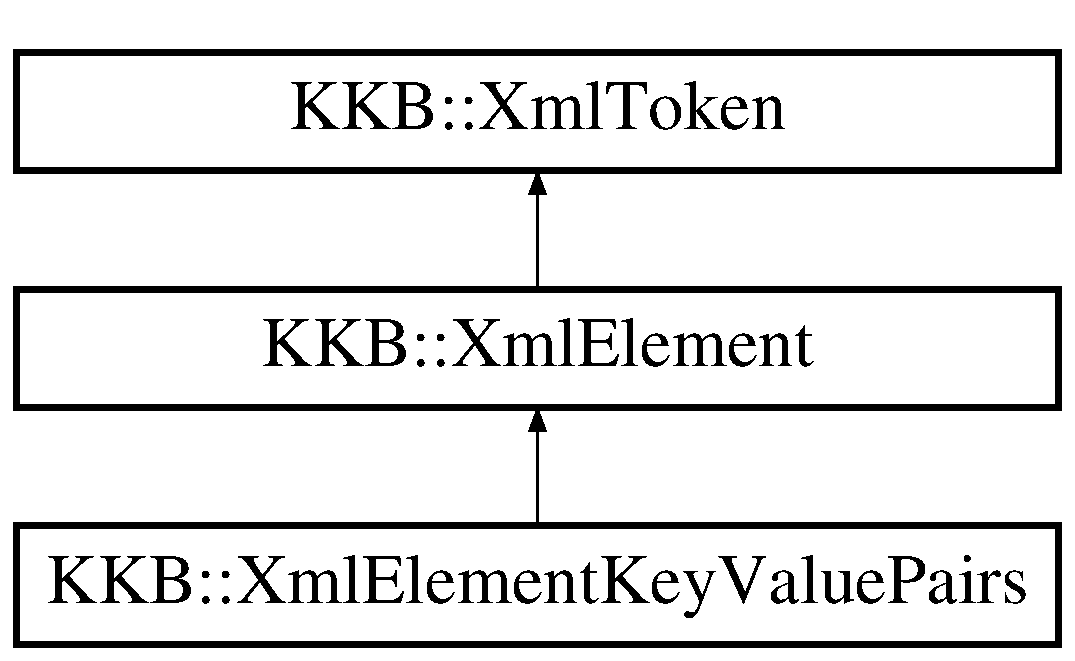
\includegraphics[height=3.000000cm]{class_k_k_b_1_1_xml_element_key_value_pairs}
\end{center}
\end{figure}
\subsection*{Public Member Functions}
\begin{DoxyCompactItemize}
\item 
\hyperlink{class_k_k_b_1_1_xml_element_key_value_pairs_ad07cc9e4db6a0a62e69e9a08d21874fa}{Xml\+Element\+Key\+Value\+Pairs} ()
\begin{DoxyCompactList}\small\item\em Used to construct an instance that will be written out to a X\+ML file.\end{DoxyCompactList}\item 
\hyperlink{class_k_k_b_1_1_xml_element_key_value_pairs_a791817932e4f210de4c1f1d76926e4cb}{Xml\+Element\+Key\+Value\+Pairs} (\hyperlink{namespace_k_k_b_a9253a3ea8a5da18ca82be4ca2b390ef0}{Xml\+Tag\+Ptr} tag, \hyperlink{class_k_k_b_1_1_xml_stream}{Xml\+Stream} \&s, \hyperlink{namespace_k_k_b_a7d390f568e2831fb76b86b56c87bf92f}{Vol\+Const\+Bool} \&cancel\+Flag, \hyperlink{class_k_k_b_1_1_run_log}{Run\+Log} \&log)
\item 
virtual \hyperlink{class_k_k_b_1_1_xml_element_key_value_pairs_a9aef5c5df7adca778dc63279cbe9405d}{$\sim$\+Xml\+Element\+Key\+Value\+Pairs} ()
\item 
void \hyperlink{class_k_k_b_1_1_xml_element_key_value_pairs_a183f57a4bf399567339851b93fa127c9}{Add} (const \hyperlink{class_k_k_b_1_1_k_k_str}{K\+K\+Str} \&key, const \hyperlink{class_k_k_b_1_1_k_k_str}{K\+K\+Str} \&v)
\item 
void \hyperlink{class_k_k_b_1_1_xml_element_key_value_pairs_afa83abc034f5078ee2e0e7e0b0731c52}{Add} (const \hyperlink{class_k_k_b_1_1_k_k_str}{K\+K\+Str} \&key, \hyperlink{namespace_k_k_b_a8fa4952cc84fda1de4bec1fbdd8d5b1b}{kkint32} v)
\item 
void \hyperlink{class_k_k_b_1_1_xml_element_key_value_pairs_a880931e1f21ab680cd98edf0e04a258f}{Add} (const \hyperlink{class_k_k_b_1_1_k_k_str}{K\+K\+Str} \&key, float v)
\item 
void \hyperlink{class_k_k_b_1_1_xml_element_key_value_pairs_a153ac88a314b266433ba6fadeafcdb70}{Add} (const \hyperlink{class_k_k_b_1_1_k_k_str}{K\+K\+Str} \&key, double v)
\item 
void \hyperlink{class_k_k_b_1_1_xml_element_key_value_pairs_a9c97b5d58a5a42b59bcb16880eb5a87d}{Add} (const \hyperlink{class_k_k_b_1_1_k_k_str}{K\+K\+Str} \&key, bool v)
\item 
void \hyperlink{class_k_k_b_1_1_xml_element_key_value_pairs_a01c67f5286a403fd7d54fa5d693d9c64}{Add} (const \hyperlink{class_k_k_b_1_1_k_k_str}{K\+K\+Str} \&key, const \hyperlink{class_k_k_b_1_1_date_time}{K\+K\+B\+::\+Date\+Time} \&v)
\item 
std\+::vector$<$ std\+::pair$<$ \hyperlink{class_k_k_b_1_1_k_k_str}{K\+K\+Str}, \hyperlink{class_k_k_b_1_1_k_k_str}{K\+K\+Str} $>$ $>$ $\ast$ \hyperlink{class_k_k_b_1_1_xml_element_key_value_pairs_a941a5a66d2b740225b8e890bc323d0d0}{Take\+Ownership} ()
\item 
std\+::vector$<$ std\+::pair$<$ \hyperlink{class_k_k_b_1_1_k_k_str}{K\+K\+Str}, \hyperlink{class_k_k_b_1_1_k_k_str}{K\+K\+Str} $>$ $>$ $\ast$ \hyperlink{class_k_k_b_1_1_xml_element_key_value_pairs_ad9d419323ca34af818aac7304f0bc388}{Value} () const 
\item 
void \hyperlink{class_k_k_b_1_1_xml_element_key_value_pairs_a4966d11afdfcd60157586c3ca56fcc5e}{Write\+X\+ML} (const \hyperlink{class_k_k_b_1_1_k_k_str}{K\+K\+Str} \&var\+Name, std\+::ostream \&o)
\end{DoxyCompactItemize}
\subsection*{Additional Inherited Members}


\subsection{Detailed Description}


Definition at line 568 of file Xml\+Stream.\+h.



\subsection{Constructor \& Destructor Documentation}
\index{K\+K\+B\+::\+Xml\+Element\+Key\+Value\+Pairs@{K\+K\+B\+::\+Xml\+Element\+Key\+Value\+Pairs}!Xml\+Element\+Key\+Value\+Pairs@{Xml\+Element\+Key\+Value\+Pairs}}
\index{Xml\+Element\+Key\+Value\+Pairs@{Xml\+Element\+Key\+Value\+Pairs}!K\+K\+B\+::\+Xml\+Element\+Key\+Value\+Pairs@{K\+K\+B\+::\+Xml\+Element\+Key\+Value\+Pairs}}
\subsubsection[{\texorpdfstring{Xml\+Element\+Key\+Value\+Pairs()}{XmlElementKeyValuePairs()}}]{\setlength{\rightskip}{0pt plus 5cm}Xml\+Element\+Key\+Value\+Pairs\+::\+Xml\+Element\+Key\+Value\+Pairs (
\begin{DoxyParamCaption}
{}
\end{DoxyParamCaption}
)}\hypertarget{class_k_k_b_1_1_xml_element_key_value_pairs_ad07cc9e4db6a0a62e69e9a08d21874fa}{}\label{class_k_k_b_1_1_xml_element_key_value_pairs_ad07cc9e4db6a0a62e69e9a08d21874fa}


Used to construct an instance that will be written out to a X\+ML file.

summary$>$Used while from \hyperlink{class_k_k_b_1_1_xml_stream}{Xml\+Stream} while reading file; every time it comes across a new Section(Start-\/\+Tag) a new instance of this class will be instantiated.

Definition at line 1134 of file Xml\+Stream.\+cpp.



References K\+K\+B\+::\+Xml\+Tag\+::tag\+Start, K\+K\+B\+::\+Xml\+Element\+::\+Xml\+Element(), and Xml\+Element\+Key\+Value\+Pairs().



Referenced by K\+K\+M\+L\+L\+::\+S\+V\+Mparam\+::\+Write\+X\+M\+L(), K\+K\+M\+L\+L\+::\+S\+V\+M\+Model\+::\+Write\+X\+M\+L(), and Xml\+Element\+Key\+Value\+Pairs().


\begin{DoxyCode}
1134                                                  :
1135     \hyperlink{class_k_k_b_1_1_xml_element_a66317eff5bd3abcc60755756ba2887d5}{XmlElement} (\textcolor{stringliteral}{"KeyValuePairs"}, \hyperlink{class_k_k_b_1_1_xml_tag_a6c0ef0e23f982f49d55d4fb7eaff6ac9ab02b23b5e15b3a1353771313e1176ce0}{XmlTag::TagTypes::tagStart}),
1136     value (\textcolor{keyword}{new} vector<pair<KKStr,KKStr> > ())
1137 \{
1138 \}
\end{DoxyCode}
\index{K\+K\+B\+::\+Xml\+Element\+Key\+Value\+Pairs@{K\+K\+B\+::\+Xml\+Element\+Key\+Value\+Pairs}!Xml\+Element\+Key\+Value\+Pairs@{Xml\+Element\+Key\+Value\+Pairs}}
\index{Xml\+Element\+Key\+Value\+Pairs@{Xml\+Element\+Key\+Value\+Pairs}!K\+K\+B\+::\+Xml\+Element\+Key\+Value\+Pairs@{K\+K\+B\+::\+Xml\+Element\+Key\+Value\+Pairs}}
\subsubsection[{\texorpdfstring{Xml\+Element\+Key\+Value\+Pairs(\+Xml\+Tag\+Ptr tag, Xml\+Stream \&s, Vol\+Const\+Bool \&cancel\+Flag, Run\+Log \&log)}{XmlElementKeyValuePairs(XmlTagPtr tag, XmlStream &s, VolConstBool &cancelFlag, RunLog &log)}}]{\setlength{\rightskip}{0pt plus 5cm}Xml\+Element\+Key\+Value\+Pairs\+::\+Xml\+Element\+Key\+Value\+Pairs (
\begin{DoxyParamCaption}
\item[{{\bf Xml\+Tag\+Ptr}}]{tag, }
\item[{{\bf Xml\+Stream} \&}]{s, }
\item[{{\bf Vol\+Const\+Bool} \&}]{cancel\+Flag, }
\item[{{\bf Run\+Log} \&}]{log}
\end{DoxyParamCaption}
)}\hypertarget{class_k_k_b_1_1_xml_element_key_value_pairs_a791817932e4f210de4c1f1d76926e4cb}{}\label{class_k_k_b_1_1_xml_element_key_value_pairs_a791817932e4f210de4c1f1d76926e4cb}


Definition at line 1141 of file Xml\+Stream.\+cpp.



References K\+K\+B\+::\+K\+K\+Str\+::\+Concat(), K\+K\+B\+::\+Xml\+Content\+::\+Content(), K\+K\+B\+::\+K\+K\+Str\+Parser\+::\+Get\+Next\+Token(), K\+K\+B\+::\+Xml\+Stream\+::\+Get\+Next\+Token(), K\+K\+B\+::\+K\+K\+Str\+Parser\+::\+K\+K\+Str\+Parser(), K\+K\+B\+::\+K\+K\+Str\+Parser\+::\+More\+Tokens(), K\+K\+B\+::\+Xml\+Token\+::tok\+Content, K\+K\+B\+::\+Xml\+Token\+::\+Token\+Type(), K\+K\+B\+::\+K\+K\+Str\+Parser\+::\+Trim\+White\+Space(), K\+K\+B\+::\+Xml\+Element\+::\+Xml\+Element(), and Xml\+Element\+Key\+Value\+Pairs().



Referenced by Xml\+Element\+Key\+Value\+Pairs().


\begin{DoxyCode}
1145                                                   :
1146     \hyperlink{class_k_k_b_1_1_xml_element_a66317eff5bd3abcc60755756ba2887d5}{XmlElement} (tag, s, log),
1147     value (NULL)
1148 \{
1149   value = \textcolor{keyword}{new} vector<pair<KKStr,KKStr> > ();
1150 
1151   \hyperlink{class_k_k_b_1_1_xml_token}{XmlTokenPtr} t = s.\hyperlink{class_k_k_b_1_1_xml_stream_a87cc738b05c666cf5d5c25beaab477b4}{GetNextToken} (cancelFlag, log);
1152   \textcolor{keywordflow}{while}  (t != NULL)
1153   \{
1154     \textcolor{keywordflow}{if}  (t->TokenType () == \hyperlink{class_k_k_b_1_1_xml_token_a18b6e90c919f4b92e3b024f50f247f62aff369b5479984ca659548f37ad4caec9}{XmlToken::TokenTypes::tokContent})
1155     \{
1156       \hyperlink{class_k_k_b_1_1_xml_content}{XmlContentPtr} c = \textcolor{keyword}{dynamic\_cast<}\hyperlink{class_k_k_b_1_1_xml_content}{XmlContentPtr}\textcolor{keyword}{>} (t);
1157       \textcolor{keywordflow}{if}  (c)
1158       \{
1159         \hyperlink{class_k_k_b_1_1_k_k_str_parser}{KKStrParser} p (*(c->\hyperlink{class_k_k_b_1_1_xml_content_a1d0730aae45b069e8604bef19b8c0098}{Content} ()));
1160         p.TrimWhiteSpace (\textcolor{stringliteral}{" "});
1161         
1162         \textcolor{keywordflow}{while}  (p.MoreTokens ())
1163         \{
1164           \hyperlink{class_k_k_b_1_1_k_k_str}{KKStr}  key = p.GetNextToken (\textcolor{stringliteral}{"\(\backslash\)t\(\backslash\)n"});
1165           \textcolor{keywordflow}{if}  (p.LastDelimiter () == \textcolor{charliteral}{'\(\backslash\)n'})
1166             value->push\_back (pair<KKStr,KKStr> (key, \textcolor{stringliteral}{""}));
1167           \textcolor{keywordflow}{else}
1168             value->push\_back (pair<KKStr,KKStr> (key, p.GetRestOfLine ()));
1169         \}
1170       \}
1171     \}
1172     \textcolor{keyword}{delete}  t;
1173     t = s.\hyperlink{class_k_k_b_1_1_xml_stream_a87cc738b05c666cf5d5c25beaab477b4}{GetNextToken} (cancelFlag, log);
1174   \}
1175 \}
\end{DoxyCode}
\index{K\+K\+B\+::\+Xml\+Element\+Key\+Value\+Pairs@{K\+K\+B\+::\+Xml\+Element\+Key\+Value\+Pairs}!````~Xml\+Element\+Key\+Value\+Pairs@{$\sim$\+Xml\+Element\+Key\+Value\+Pairs}}
\index{````~Xml\+Element\+Key\+Value\+Pairs@{$\sim$\+Xml\+Element\+Key\+Value\+Pairs}!K\+K\+B\+::\+Xml\+Element\+Key\+Value\+Pairs@{K\+K\+B\+::\+Xml\+Element\+Key\+Value\+Pairs}}
\subsubsection[{\texorpdfstring{$\sim$\+Xml\+Element\+Key\+Value\+Pairs()}{~XmlElementKeyValuePairs()}}]{\setlength{\rightskip}{0pt plus 5cm}Xml\+Element\+Key\+Value\+Pairs\+::$\sim$\+Xml\+Element\+Key\+Value\+Pairs (
\begin{DoxyParamCaption}
{}
\end{DoxyParamCaption}
)\hspace{0.3cm}{\ttfamily [virtual]}}\hypertarget{class_k_k_b_1_1_xml_element_key_value_pairs_a9aef5c5df7adca778dc63279cbe9405d}{}\label{class_k_k_b_1_1_xml_element_key_value_pairs_a9aef5c5df7adca778dc63279cbe9405d}


Definition at line 1178 of file Xml\+Stream.\+cpp.


\begin{DoxyCode}
1179 \{
1180   \textcolor{keyword}{delete}  value;
1181   value = NULL;
1182 \}
\end{DoxyCode}


\subsection{Member Function Documentation}
\index{K\+K\+B\+::\+Xml\+Element\+Key\+Value\+Pairs@{K\+K\+B\+::\+Xml\+Element\+Key\+Value\+Pairs}!Add@{Add}}
\index{Add@{Add}!K\+K\+B\+::\+Xml\+Element\+Key\+Value\+Pairs@{K\+K\+B\+::\+Xml\+Element\+Key\+Value\+Pairs}}
\subsubsection[{\texorpdfstring{Add(const K\+K\+Str \&key, const K\+K\+Str \&v)}{Add(const KKStr &key, const KKStr &v)}}]{\setlength{\rightskip}{0pt plus 5cm}void Xml\+Element\+Key\+Value\+Pairs\+::\+Add (
\begin{DoxyParamCaption}
\item[{const {\bf K\+K\+Str} \&}]{key, }
\item[{const {\bf K\+K\+Str} \&}]{v}
\end{DoxyParamCaption}
)}\hypertarget{class_k_k_b_1_1_xml_element_key_value_pairs_a183f57a4bf399567339851b93fa127c9}{}\label{class_k_k_b_1_1_xml_element_key_value_pairs_a183f57a4bf399567339851b93fa127c9}


Definition at line 1193 of file Xml\+Stream.\+cpp.



Referenced by Add(), K\+K\+M\+L\+L\+::\+S\+V\+Mparam\+::\+Write\+X\+M\+L(), and K\+K\+M\+L\+L\+::\+S\+V\+M\+Model\+::\+Write\+X\+M\+L().


\begin{DoxyCode}
1196 \{
1197   value->push\_back (pair<KKStr,KKStr> (key, v));
1198 \}
\end{DoxyCode}
\index{K\+K\+B\+::\+Xml\+Element\+Key\+Value\+Pairs@{K\+K\+B\+::\+Xml\+Element\+Key\+Value\+Pairs}!Add@{Add}}
\index{Add@{Add}!K\+K\+B\+::\+Xml\+Element\+Key\+Value\+Pairs@{K\+K\+B\+::\+Xml\+Element\+Key\+Value\+Pairs}}
\subsubsection[{\texorpdfstring{Add(const K\+K\+Str \&key, kkint32 v)}{Add(const KKStr &key, kkint32 v)}}]{\setlength{\rightskip}{0pt plus 5cm}void Xml\+Element\+Key\+Value\+Pairs\+::\+Add (
\begin{DoxyParamCaption}
\item[{const {\bf K\+K\+Str} \&}]{key, }
\item[{{\bf kkint32}}]{v}
\end{DoxyParamCaption}
)}\hypertarget{class_k_k_b_1_1_xml_element_key_value_pairs_afa83abc034f5078ee2e0e7e0b0731c52}{}\label{class_k_k_b_1_1_xml_element_key_value_pairs_afa83abc034f5078ee2e0e7e0b0731c52}


Definition at line 1203 of file Xml\+Stream.\+cpp.



References Add(), and K\+K\+B\+::\+Str\+From\+Int32().



Referenced by K\+K\+M\+L\+L\+::\+S\+V\+M\+Model\+::\+Write\+X\+M\+L().


\begin{DoxyCode}
1206 \{
1207   \hyperlink{class_k_k_b_1_1_xml_element_key_value_pairs_a183f57a4bf399567339851b93fa127c9}{Add} (key, \hyperlink{namespace_k_k_b_a66adf53f607bda7ab0d3e1c3945e792e}{KKB::StrFromInt32} (v));
1208 \}
\end{DoxyCode}
\index{K\+K\+B\+::\+Xml\+Element\+Key\+Value\+Pairs@{K\+K\+B\+::\+Xml\+Element\+Key\+Value\+Pairs}!Add@{Add}}
\index{Add@{Add}!K\+K\+B\+::\+Xml\+Element\+Key\+Value\+Pairs@{K\+K\+B\+::\+Xml\+Element\+Key\+Value\+Pairs}}
\subsubsection[{\texorpdfstring{Add(const K\+K\+Str \&key, float v)}{Add(const KKStr &key, float v)}}]{\setlength{\rightskip}{0pt plus 5cm}void Xml\+Element\+Key\+Value\+Pairs\+::\+Add (
\begin{DoxyParamCaption}
\item[{const {\bf K\+K\+Str} \&}]{key, }
\item[{float}]{v}
\end{DoxyParamCaption}
)}\hypertarget{class_k_k_b_1_1_xml_element_key_value_pairs_a880931e1f21ab680cd98edf0e04a258f}{}\label{class_k_k_b_1_1_xml_element_key_value_pairs_a880931e1f21ab680cd98edf0e04a258f}


Definition at line 1212 of file Xml\+Stream.\+cpp.



References Add(), and K\+K\+B\+::\+Str\+From\+Float().



Referenced by K\+K\+M\+L\+L\+::\+S\+V\+Mparam\+::\+Write\+X\+M\+L().


\begin{DoxyCode}
1215 \{
1216   \hyperlink{class_k_k_b_1_1_xml_element_key_value_pairs_a183f57a4bf399567339851b93fa127c9}{Add} (key, \hyperlink{namespace_k_k_b_aa19267de8ebca7b146b5aef6b2c27df9}{KKB::StrFromFloat} (v));
1217 \}
\end{DoxyCode}
\index{K\+K\+B\+::\+Xml\+Element\+Key\+Value\+Pairs@{K\+K\+B\+::\+Xml\+Element\+Key\+Value\+Pairs}!Add@{Add}}
\index{Add@{Add}!K\+K\+B\+::\+Xml\+Element\+Key\+Value\+Pairs@{K\+K\+B\+::\+Xml\+Element\+Key\+Value\+Pairs}}
\subsubsection[{\texorpdfstring{Add(const K\+K\+Str \&key, double v)}{Add(const KKStr &key, double v)}}]{\setlength{\rightskip}{0pt plus 5cm}void Xml\+Element\+Key\+Value\+Pairs\+::\+Add (
\begin{DoxyParamCaption}
\item[{const {\bf K\+K\+Str} \&}]{key, }
\item[{double}]{v}
\end{DoxyParamCaption}
)}\hypertarget{class_k_k_b_1_1_xml_element_key_value_pairs_a153ac88a314b266433ba6fadeafcdb70}{}\label{class_k_k_b_1_1_xml_element_key_value_pairs_a153ac88a314b266433ba6fadeafcdb70}


Definition at line 1222 of file Xml\+Stream.\+cpp.



References Add(), and K\+K\+B\+::\+Str\+From\+Double().



Referenced by K\+K\+M\+L\+L\+::\+S\+V\+M\+Model\+::\+Write\+X\+M\+L().


\begin{DoxyCode}
1225 \{
1226   \hyperlink{class_k_k_b_1_1_xml_element_key_value_pairs_a183f57a4bf399567339851b93fa127c9}{Add} (key, \hyperlink{namespace_k_k_b_a064d022f1f3d94c191e11c5e4bceb4a7}{KKB::StrFromDouble} (v));
1227 \}
\end{DoxyCode}
\index{K\+K\+B\+::\+Xml\+Element\+Key\+Value\+Pairs@{K\+K\+B\+::\+Xml\+Element\+Key\+Value\+Pairs}!Add@{Add}}
\index{Add@{Add}!K\+K\+B\+::\+Xml\+Element\+Key\+Value\+Pairs@{K\+K\+B\+::\+Xml\+Element\+Key\+Value\+Pairs}}
\subsubsection[{\texorpdfstring{Add(const K\+K\+Str \&key, bool v)}{Add(const KKStr &key, bool v)}}]{\setlength{\rightskip}{0pt plus 5cm}void Xml\+Element\+Key\+Value\+Pairs\+::\+Add (
\begin{DoxyParamCaption}
\item[{const {\bf K\+K\+Str} \&}]{key, }
\item[{bool}]{v}
\end{DoxyParamCaption}
)}\hypertarget{class_k_k_b_1_1_xml_element_key_value_pairs_a9c97b5d58a5a42b59bcb16880eb5a87d}{}\label{class_k_k_b_1_1_xml_element_key_value_pairs_a9c97b5d58a5a42b59bcb16880eb5a87d}


Definition at line 1232 of file Xml\+Stream.\+cpp.



References Add(), K\+K\+B\+::\+K\+K\+Str\+::\+Concat(), and K\+K\+B\+::\+K\+K\+Str\+::operator=().



Referenced by K\+K\+M\+L\+L\+::\+S\+V\+Mparam\+::\+Write\+X\+M\+L().


\begin{DoxyCode}
1235 \{
1236   \hyperlink{class_k_k_b_1_1_k_k_str}{KKStr}  vStr = \textcolor{stringliteral}{"False"};
1237   \textcolor{keywordflow}{if}  (v)  vStr = \textcolor{stringliteral}{"True"};
1238   \hyperlink{class_k_k_b_1_1_xml_element_key_value_pairs_a183f57a4bf399567339851b93fa127c9}{Add} (key, vStr);
1239 \}
\end{DoxyCode}
\index{K\+K\+B\+::\+Xml\+Element\+Key\+Value\+Pairs@{K\+K\+B\+::\+Xml\+Element\+Key\+Value\+Pairs}!Add@{Add}}
\index{Add@{Add}!K\+K\+B\+::\+Xml\+Element\+Key\+Value\+Pairs@{K\+K\+B\+::\+Xml\+Element\+Key\+Value\+Pairs}}
\subsubsection[{\texorpdfstring{Add(const K\+K\+Str \&key, const K\+K\+B\+::\+Date\+Time \&v)}{Add(const KKStr &key, const KKB::DateTime &v)}}]{\setlength{\rightskip}{0pt plus 5cm}void Xml\+Element\+Key\+Value\+Pairs\+::\+Add (
\begin{DoxyParamCaption}
\item[{const {\bf K\+K\+Str} \&}]{key, }
\item[{const {\bf K\+K\+B\+::\+Date\+Time} \&}]{v}
\end{DoxyParamCaption}
)}\hypertarget{class_k_k_b_1_1_xml_element_key_value_pairs_a01c67f5286a403fd7d54fa5d693d9c64}{}\label{class_k_k_b_1_1_xml_element_key_value_pairs_a01c67f5286a403fd7d54fa5d693d9c64}


Definition at line 1243 of file Xml\+Stream.\+cpp.



References Add(), and K\+K\+B\+::\+Date\+Time\+::\+Y\+Y\+Y\+Y\+\_\+\+M\+M\+\_\+\+D\+D\+\_\+\+H\+H\+\_\+\+M\+M\+\_\+\+S\+S().



Referenced by K\+K\+M\+L\+L\+::\+S\+V\+M\+Model\+::\+Write\+X\+M\+L().


\begin{DoxyCode}
1246 \{
1247   \hyperlink{class_k_k_b_1_1_xml_element_key_value_pairs_a183f57a4bf399567339851b93fa127c9}{Add} (key, v.\hyperlink{class_k_k_b_1_1_date_time_aca57fbdcd040549a2c9e0a3d4e99b9f9}{YYYY\_MM\_DD\_HH\_MM\_SS} ());
1248 \}
\end{DoxyCode}
\index{K\+K\+B\+::\+Xml\+Element\+Key\+Value\+Pairs@{K\+K\+B\+::\+Xml\+Element\+Key\+Value\+Pairs}!Take\+Ownership@{Take\+Ownership}}
\index{Take\+Ownership@{Take\+Ownership}!K\+K\+B\+::\+Xml\+Element\+Key\+Value\+Pairs@{K\+K\+B\+::\+Xml\+Element\+Key\+Value\+Pairs}}
\subsubsection[{\texorpdfstring{Take\+Ownership()}{TakeOwnership()}}]{\setlength{\rightskip}{0pt plus 5cm}vector$<$ pair$<$ {\bf K\+K\+Str}, {\bf K\+K\+Str} $>$ $>$ $\ast$ Xml\+Element\+Key\+Value\+Pairs\+::\+Take\+Ownership (
\begin{DoxyParamCaption}
{}
\end{DoxyParamCaption}
)}\hypertarget{class_k_k_b_1_1_xml_element_key_value_pairs_a941a5a66d2b740225b8e890bc323d0d0}{}\label{class_k_k_b_1_1_xml_element_key_value_pairs_a941a5a66d2b740225b8e890bc323d0d0}


Definition at line 1185 of file Xml\+Stream.\+cpp.


\begin{DoxyCode}
1186 \{
1187   vector<pair<KKStr,KKStr> >* v = value;
1188   value = NULL;
1189   \textcolor{keywordflow}{return}  v;
1190 \}
\end{DoxyCode}
\index{K\+K\+B\+::\+Xml\+Element\+Key\+Value\+Pairs@{K\+K\+B\+::\+Xml\+Element\+Key\+Value\+Pairs}!Value@{Value}}
\index{Value@{Value}!K\+K\+B\+::\+Xml\+Element\+Key\+Value\+Pairs@{K\+K\+B\+::\+Xml\+Element\+Key\+Value\+Pairs}}
\subsubsection[{\texorpdfstring{Value() const }{Value() const }}]{\setlength{\rightskip}{0pt plus 5cm}std\+::vector$<$std\+::pair$<${\bf K\+K\+Str},{\bf K\+K\+Str}$>$ $>$$\ast$ K\+K\+B\+::\+Xml\+Element\+Key\+Value\+Pairs\+::\+Value (
\begin{DoxyParamCaption}
{}
\end{DoxyParamCaption}
) const\hspace{0.3cm}{\ttfamily [inline]}}\hypertarget{class_k_k_b_1_1_xml_element_key_value_pairs_ad9d419323ca34af818aac7304f0bc388}{}\label{class_k_k_b_1_1_xml_element_key_value_pairs_ad9d419323ca34af818aac7304f0bc388}


Definition at line 586 of file Xml\+Stream.\+h.


\begin{DoxyCode}
586 \{\textcolor{keywordflow}{return} value;\}
\end{DoxyCode}
\index{K\+K\+B\+::\+Xml\+Element\+Key\+Value\+Pairs@{K\+K\+B\+::\+Xml\+Element\+Key\+Value\+Pairs}!Write\+X\+ML@{Write\+X\+ML}}
\index{Write\+X\+ML@{Write\+X\+ML}!K\+K\+B\+::\+Xml\+Element\+Key\+Value\+Pairs@{K\+K\+B\+::\+Xml\+Element\+Key\+Value\+Pairs}}
\subsubsection[{\texorpdfstring{Write\+X\+M\+L(const K\+K\+Str \&var\+Name, std\+::ostream \&o)}{WriteXML(const KKStr &varName, std::ostream &o)}}]{\setlength{\rightskip}{0pt plus 5cm}void Xml\+Element\+Key\+Value\+Pairs\+::\+Write\+X\+ML (
\begin{DoxyParamCaption}
\item[{const {\bf K\+K\+Str} \&}]{var\+Name, }
\item[{std\+::ostream \&}]{o}
\end{DoxyParamCaption}
)}\hypertarget{class_k_k_b_1_1_xml_element_key_value_pairs_a4966d11afdfcd60157586c3ca56fcc5e}{}\label{class_k_k_b_1_1_xml_element_key_value_pairs_a4966d11afdfcd60157586c3ca56fcc5e}


Definition at line 1252 of file Xml\+Stream.\+cpp.



References K\+K\+B\+::\+Xml\+Tag\+::\+Add\+Atribute(), K\+K\+B\+::\+K\+K\+Str\+::\+Empty(), K\+K\+B\+::operator$<$$<$(), K\+K\+B\+::\+Xml\+Tag\+::tag\+End, K\+K\+B\+::\+Xml\+Tag\+::tag\+Start, K\+K\+B\+::\+Xml\+Tag\+::\+Write\+X\+M\+L(), and K\+K\+B\+::\+Xml\+Tag\+::\+Xml\+Tag().



Referenced by K\+K\+M\+L\+L\+::\+S\+V\+Mparam\+::\+Write\+X\+M\+L(), and K\+K\+M\+L\+L\+::\+S\+V\+M\+Model\+::\+Write\+X\+M\+L().


\begin{DoxyCode}
1255 \{
1256   \hyperlink{class_k_k_b_1_1_xml_tag}{XmlTag}  startTag (\textcolor{stringliteral}{"KeyValuePairs"},  \hyperlink{class_k_k_b_1_1_xml_tag_a6c0ef0e23f982f49d55d4fb7eaff6ac9ab02b23b5e15b3a1353771313e1176ce0}{XmlTag::TagTypes::tagStart});
1257   \textcolor{keywordflow}{if}  (!varName.\hyperlink{class_k_k_b_1_1_k_k_str_ac69942f73fffd672ec2a6e1c410afdb6}{Empty} ())
1258     startTag.AddAtribute (\textcolor{stringliteral}{"VarName"}, varName);
1259   startTag.WriteXML (o);
1260   o << \hyperlink{namespace_k_k_b_ad1f50f65af6adc8fa9e6f62d007818a8}{endl};
1261 
1262   vector<pair<KKStr,KKStr> >::const\_iterator  idx;
1263   \textcolor{keywordflow}{for}  (idx = value->begin ();  idx != value->end ();  ++idx)
1264   \{
1265     \hyperlink{class_k_k_b_1_1_xml_content_ab0e370562d215b8e19dac6d18c4a95e1}{XmlContent::WriteXml} (idx->first,  o);
1266     o << \textcolor{stringliteral}{"\(\backslash\)t"};
1267     \hyperlink{class_k_k_b_1_1_xml_content_ab0e370562d215b8e19dac6d18c4a95e1}{XmlContent::WriteXml} (idx->second, o);
1268     o << \hyperlink{namespace_k_k_b_ad1f50f65af6adc8fa9e6f62d007818a8}{endl};
1269   \}
1270 
1271   \hyperlink{class_k_k_b_1_1_xml_tag}{XmlTag}  endTag (\textcolor{stringliteral}{"KeyValuePairs"}, \hyperlink{class_k_k_b_1_1_xml_tag_a6c0ef0e23f982f49d55d4fb7eaff6ac9a3ceaa9a790f688ec97a35b5a3fd3b164}{XmlTag::TagTypes::tagEnd});
1272   endTag.WriteXML (o);
1273   o << \hyperlink{namespace_k_k_b_ad1f50f65af6adc8fa9e6f62d007818a8}{endl};
1274 \}
\end{DoxyCode}


The documentation for this class was generated from the following files\+:\begin{DoxyCompactItemize}
\item 
C\+:/\+Users/\+Kurt/\+Git\+Hub/\+K\+Square\+Libraries/\+K\+K\+Base/\hyperlink{_xml_stream_8h}{Xml\+Stream.\+h}\item 
C\+:/\+Users/\+Kurt/\+Git\+Hub/\+K\+Square\+Libraries/\+K\+K\+Base/\hyperlink{_xml_stream_8cpp}{Xml\+Stream.\+cpp}\end{DoxyCompactItemize}

\hypertarget{class_k_k_b_1_1_xml_element_k_k_str}{}\section{K\+KB\+:\+:Xml\+Element\+K\+K\+Str Class Reference}
\label{class_k_k_b_1_1_xml_element_k_k_str}\index{K\+K\+B\+::\+Xml\+Element\+K\+K\+Str@{K\+K\+B\+::\+Xml\+Element\+K\+K\+Str}}


{\ttfamily \#include $<$Xml\+Stream.\+h$>$}

Inheritance diagram for K\+KB\+:\+:Xml\+Element\+K\+K\+Str\+:\begin{figure}[H]
\begin{center}
\leavevmode
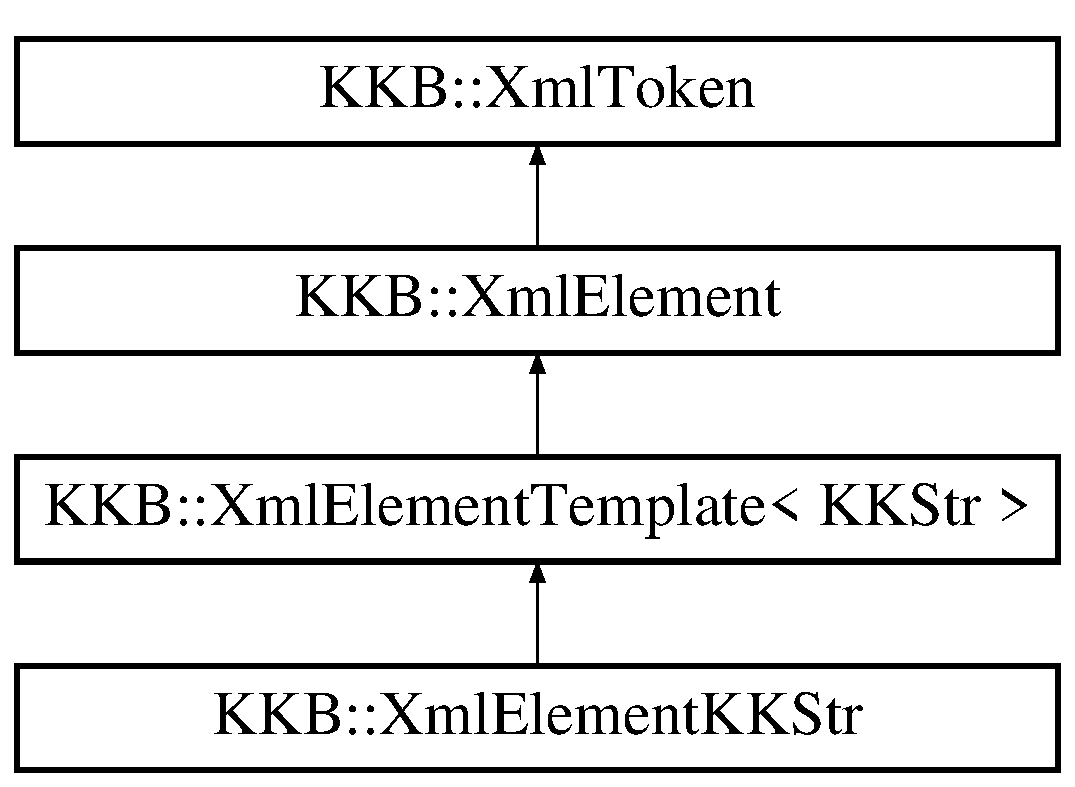
\includegraphics[height=4.000000cm]{class_k_k_b_1_1_xml_element_k_k_str}
\end{center}
\end{figure}
\subsection*{Public Member Functions}
\begin{DoxyCompactItemize}
\item 
\hyperlink{class_k_k_b_1_1_xml_element_k_k_str_a7b5fc782b322b86f08c45ed4eb49518f}{Xml\+Element\+K\+K\+Str} (\hyperlink{namespace_k_k_b_a9253a3ea8a5da18ca82be4ca2b390ef0}{Xml\+Tag\+Ptr} tag, \hyperlink{class_k_k_b_1_1_xml_stream}{Xml\+Stream} \&s, \hyperlink{namespace_k_k_b_a7d390f568e2831fb76b86b56c87bf92f}{Vol\+Const\+Bool} \&cancel\+Flag, \hyperlink{class_k_k_b_1_1_run_log}{Run\+Log} \&log)
\item 
virtual bool \hyperlink{class_k_k_b_1_1_xml_element_k_k_str_a8ba15eefdf11b1b92b55ff9a6e91a540}{To\+Bool} () const 
\item 
virtual double \hyperlink{class_k_k_b_1_1_xml_element_k_k_str_a27549d20798a9387ebf41ffdf2c86d2e}{To\+Double} () const 
\item 
virtual float \hyperlink{class_k_k_b_1_1_xml_element_k_k_str_ad70580dab90be4e505fd2959ad8eb1e3}{To\+Float} () const 
\item 
virtual \hyperlink{namespace_k_k_b_a8fa4952cc84fda1de4bec1fbdd8d5b1b}{kkint32} \hyperlink{class_k_k_b_1_1_xml_element_k_k_str_a0d99cf6a4d32b10d1ea410a0ae210ab9}{To\+Int32} () const 
\item 
virtual \hyperlink{class_k_k_b_1_1_k_k_str}{K\+K\+Str} \hyperlink{class_k_k_b_1_1_xml_element_k_k_str_a799d1dcb1d656ffceb6a7e809dfd4839}{To\+K\+K\+Str} () const 
\end{DoxyCompactItemize}
\subsection*{Additional Inherited Members}


\subsection{Detailed Description}


Definition at line 653 of file Xml\+Stream.\+h.



\subsection{Constructor \& Destructor Documentation}
\index{K\+K\+B\+::\+Xml\+Element\+K\+K\+Str@{K\+K\+B\+::\+Xml\+Element\+K\+K\+Str}!Xml\+Element\+K\+K\+Str@{Xml\+Element\+K\+K\+Str}}
\index{Xml\+Element\+K\+K\+Str@{Xml\+Element\+K\+K\+Str}!K\+K\+B\+::\+Xml\+Element\+K\+K\+Str@{K\+K\+B\+::\+Xml\+Element\+K\+K\+Str}}
\subsubsection[{\texorpdfstring{Xml\+Element\+K\+K\+Str(\+Xml\+Tag\+Ptr tag, Xml\+Stream \&s, Vol\+Const\+Bool \&cancel\+Flag, Run\+Log \&log)}{XmlElementKKStr(XmlTagPtr tag, XmlStream &s, VolConstBool &cancelFlag, RunLog &log)}}]{\setlength{\rightskip}{0pt plus 5cm}K\+K\+B\+::\+Xml\+Element\+K\+K\+Str\+::\+Xml\+Element\+K\+K\+Str (
\begin{DoxyParamCaption}
\item[{{\bf Xml\+Tag\+Ptr}}]{tag, }
\item[{{\bf Xml\+Stream} \&}]{s, }
\item[{{\bf Vol\+Const\+Bool} \&}]{cancel\+Flag, }
\item[{{\bf Run\+Log} \&}]{log}
\end{DoxyParamCaption}
)\hspace{0.3cm}{\ttfamily [inline]}}\hypertarget{class_k_k_b_1_1_xml_element_k_k_str_a7b5fc782b322b86f08c45ed4eb49518f}{}\label{class_k_k_b_1_1_xml_element_k_k_str_a7b5fc782b322b86f08c45ed4eb49518f}


Definition at line 656 of file Xml\+Stream.\+h.



References Xml\+Element\+K\+K\+Str().



Referenced by Xml\+Element\+K\+K\+Str().


\begin{DoxyCode}
660                      :
661       \hyperlink{class_k_k_b_1_1_xml_element_template}{XmlElementTemplate<KKStr>} (tag, s, cancelFlag, log)
662     \{\}
\end{DoxyCode}


\subsection{Member Function Documentation}
\index{K\+K\+B\+::\+Xml\+Element\+K\+K\+Str@{K\+K\+B\+::\+Xml\+Element\+K\+K\+Str}!To\+Bool@{To\+Bool}}
\index{To\+Bool@{To\+Bool}!K\+K\+B\+::\+Xml\+Element\+K\+K\+Str@{K\+K\+B\+::\+Xml\+Element\+K\+K\+Str}}
\subsubsection[{\texorpdfstring{To\+Bool() const }{ToBool() const }}]{\setlength{\rightskip}{0pt plus 5cm}virtual bool K\+K\+B\+::\+Xml\+Element\+K\+K\+Str\+::\+To\+Bool (
\begin{DoxyParamCaption}
{}
\end{DoxyParamCaption}
) const\hspace{0.3cm}{\ttfamily [inline]}, {\ttfamily [virtual]}}\hypertarget{class_k_k_b_1_1_xml_element_k_k_str_a8ba15eefdf11b1b92b55ff9a6e91a540}{}\label{class_k_k_b_1_1_xml_element_k_k_str_a8ba15eefdf11b1b92b55ff9a6e91a540}


Reimplemented from \hyperlink{class_k_k_b_1_1_xml_element_a7bfbbea204722bc4535a294bc43e8e17}{K\+K\+B\+::\+Xml\+Element}.



Definition at line 664 of file Xml\+Stream.\+h.


\begin{DoxyCode}
664 \{\textcolor{keywordflow}{return}  (\hyperlink{class_k_k_b_1_1_xml_element_template_a3d671b57251b4b256fecb2197fc4a0f4}{Value} () ? \hyperlink{class_k_k_b_1_1_xml_element_template_a3d671b57251b4b256fecb2197fc4a0f4}{Value} ()->\hyperlink{class_k_k_b_1_1_xml_element_k_k_str_a8ba15eefdf11b1b92b55ff9a6e91a540}{ToBool} () : \textcolor{keyword}{false});\}
\end{DoxyCode}
\index{K\+K\+B\+::\+Xml\+Element\+K\+K\+Str@{K\+K\+B\+::\+Xml\+Element\+K\+K\+Str}!To\+Double@{To\+Double}}
\index{To\+Double@{To\+Double}!K\+K\+B\+::\+Xml\+Element\+K\+K\+Str@{K\+K\+B\+::\+Xml\+Element\+K\+K\+Str}}
\subsubsection[{\texorpdfstring{To\+Double() const }{ToDouble() const }}]{\setlength{\rightskip}{0pt plus 5cm}virtual double K\+K\+B\+::\+Xml\+Element\+K\+K\+Str\+::\+To\+Double (
\begin{DoxyParamCaption}
{}
\end{DoxyParamCaption}
) const\hspace{0.3cm}{\ttfamily [inline]}, {\ttfamily [virtual]}}\hypertarget{class_k_k_b_1_1_xml_element_k_k_str_a27549d20798a9387ebf41ffdf2c86d2e}{}\label{class_k_k_b_1_1_xml_element_k_k_str_a27549d20798a9387ebf41ffdf2c86d2e}


Reimplemented from \hyperlink{class_k_k_b_1_1_xml_element_ac32778396ab8bdb215ad38f2f33f05de}{K\+K\+B\+::\+Xml\+Element}.



Definition at line 666 of file Xml\+Stream.\+h.


\begin{DoxyCode}
666 \{\textcolor{keywordflow}{return}  (\hyperlink{class_k_k_b_1_1_xml_element_template_a3d671b57251b4b256fecb2197fc4a0f4}{Value} () ? \hyperlink{class_k_k_b_1_1_xml_element_template_a3d671b57251b4b256fecb2197fc4a0f4}{Value} ()->\hyperlink{class_k_k_b_1_1_xml_element_k_k_str_a27549d20798a9387ebf41ffdf2c86d2e}{ToDouble} () : 0.0);\}
\end{DoxyCode}
\index{K\+K\+B\+::\+Xml\+Element\+K\+K\+Str@{K\+K\+B\+::\+Xml\+Element\+K\+K\+Str}!To\+Float@{To\+Float}}
\index{To\+Float@{To\+Float}!K\+K\+B\+::\+Xml\+Element\+K\+K\+Str@{K\+K\+B\+::\+Xml\+Element\+K\+K\+Str}}
\subsubsection[{\texorpdfstring{To\+Float() const }{ToFloat() const }}]{\setlength{\rightskip}{0pt plus 5cm}virtual float K\+K\+B\+::\+Xml\+Element\+K\+K\+Str\+::\+To\+Float (
\begin{DoxyParamCaption}
{}
\end{DoxyParamCaption}
) const\hspace{0.3cm}{\ttfamily [inline]}, {\ttfamily [virtual]}}\hypertarget{class_k_k_b_1_1_xml_element_k_k_str_ad70580dab90be4e505fd2959ad8eb1e3}{}\label{class_k_k_b_1_1_xml_element_k_k_str_ad70580dab90be4e505fd2959ad8eb1e3}


Reimplemented from \hyperlink{class_k_k_b_1_1_xml_element_aa728687ed43e76d45d029dfc14e14e95}{K\+K\+B\+::\+Xml\+Element}.



Definition at line 667 of file Xml\+Stream.\+h.


\begin{DoxyCode}
667 \{\textcolor{keywordflow}{return}  (\hyperlink{class_k_k_b_1_1_xml_element_template_a3d671b57251b4b256fecb2197fc4a0f4}{Value} () ? \hyperlink{class_k_k_b_1_1_xml_element_template_a3d671b57251b4b256fecb2197fc4a0f4}{Value} ()->\hyperlink{class_k_k_b_1_1_xml_element_k_k_str_ad70580dab90be4e505fd2959ad8eb1e3}{ToFloat} ()  : 0.0f);\}
\end{DoxyCode}
\index{K\+K\+B\+::\+Xml\+Element\+K\+K\+Str@{K\+K\+B\+::\+Xml\+Element\+K\+K\+Str}!To\+Int32@{To\+Int32}}
\index{To\+Int32@{To\+Int32}!K\+K\+B\+::\+Xml\+Element\+K\+K\+Str@{K\+K\+B\+::\+Xml\+Element\+K\+K\+Str}}
\subsubsection[{\texorpdfstring{To\+Int32() const }{ToInt32() const }}]{\setlength{\rightskip}{0pt plus 5cm}virtual {\bf kkint32} K\+K\+B\+::\+Xml\+Element\+K\+K\+Str\+::\+To\+Int32 (
\begin{DoxyParamCaption}
{}
\end{DoxyParamCaption}
) const\hspace{0.3cm}{\ttfamily [inline]}, {\ttfamily [virtual]}}\hypertarget{class_k_k_b_1_1_xml_element_k_k_str_a0d99cf6a4d32b10d1ea410a0ae210ab9}{}\label{class_k_k_b_1_1_xml_element_k_k_str_a0d99cf6a4d32b10d1ea410a0ae210ab9}


Reimplemented from \hyperlink{class_k_k_b_1_1_xml_element_aac7463c7b305f66b5157f424a0a76363}{K\+K\+B\+::\+Xml\+Element}.



Definition at line 668 of file Xml\+Stream.\+h.


\begin{DoxyCode}
668 \{\textcolor{keywordflow}{return}  (\hyperlink{class_k_k_b_1_1_xml_element_template_a3d671b57251b4b256fecb2197fc4a0f4}{Value} () ? \hyperlink{class_k_k_b_1_1_xml_element_template_a3d671b57251b4b256fecb2197fc4a0f4}{Value} ()->\hyperlink{class_k_k_b_1_1_xml_element_k_k_str_a0d99cf6a4d32b10d1ea410a0ae210ab9}{ToInt32} ()  : 0);\}
\end{DoxyCode}
\index{K\+K\+B\+::\+Xml\+Element\+K\+K\+Str@{K\+K\+B\+::\+Xml\+Element\+K\+K\+Str}!To\+K\+K\+Str@{To\+K\+K\+Str}}
\index{To\+K\+K\+Str@{To\+K\+K\+Str}!K\+K\+B\+::\+Xml\+Element\+K\+K\+Str@{K\+K\+B\+::\+Xml\+Element\+K\+K\+Str}}
\subsubsection[{\texorpdfstring{To\+K\+K\+Str() const }{ToKKStr() const }}]{\setlength{\rightskip}{0pt plus 5cm}virtual {\bf K\+K\+Str} K\+K\+B\+::\+Xml\+Element\+K\+K\+Str\+::\+To\+K\+K\+Str (
\begin{DoxyParamCaption}
{}
\end{DoxyParamCaption}
) const\hspace{0.3cm}{\ttfamily [inline]}, {\ttfamily [virtual]}}\hypertarget{class_k_k_b_1_1_xml_element_k_k_str_a799d1dcb1d656ffceb6a7e809dfd4839}{}\label{class_k_k_b_1_1_xml_element_k_k_str_a799d1dcb1d656ffceb6a7e809dfd4839}


Reimplemented from \hyperlink{class_k_k_b_1_1_xml_element_a3028fc03b79509e6378749f6a8b426b9}{K\+K\+B\+::\+Xml\+Element}.



Definition at line 665 of file Xml\+Stream.\+h.


\begin{DoxyCode}
665 \{\textcolor{keywordflow}{return}  (\hyperlink{class_k_k_b_1_1_xml_element_template_a3d671b57251b4b256fecb2197fc4a0f4}{Value} () ? *\hyperlink{class_k_k_b_1_1_xml_element_template_a3d671b57251b4b256fecb2197fc4a0f4}{Value} () : \hyperlink{class_k_k_b_1_1_k_k_str_ab6e416b3ef54ef632bd10c3f7a2f7994}{KKStr::EmptyStr} ());\}
\end{DoxyCode}


The documentation for this class was generated from the following file\+:\begin{DoxyCompactItemize}
\item 
C\+:/\+Users/\+Kurt/\+Git\+Hub/\+K\+Square\+Libraries/\+K\+K\+Base/\hyperlink{_xml_stream_8h}{Xml\+Stream.\+h}\end{DoxyCompactItemize}

\hypertarget{class_k_k_b_1_1_xml_element_template}{}\section{K\+KB\+:\+:Xml\+Element\+Template$<$ T $>$ Class Template Reference}
\label{class_k_k_b_1_1_xml_element_template}\index{K\+K\+B\+::\+Xml\+Element\+Template$<$ T $>$@{K\+K\+B\+::\+Xml\+Element\+Template$<$ T $>$}}


{\ttfamily \#include $<$Xml\+Stream.\+h$>$}

Inheritance diagram for K\+KB\+:\+:Xml\+Element\+Template$<$ T $>$\+:\begin{figure}[H]
\begin{center}
\leavevmode
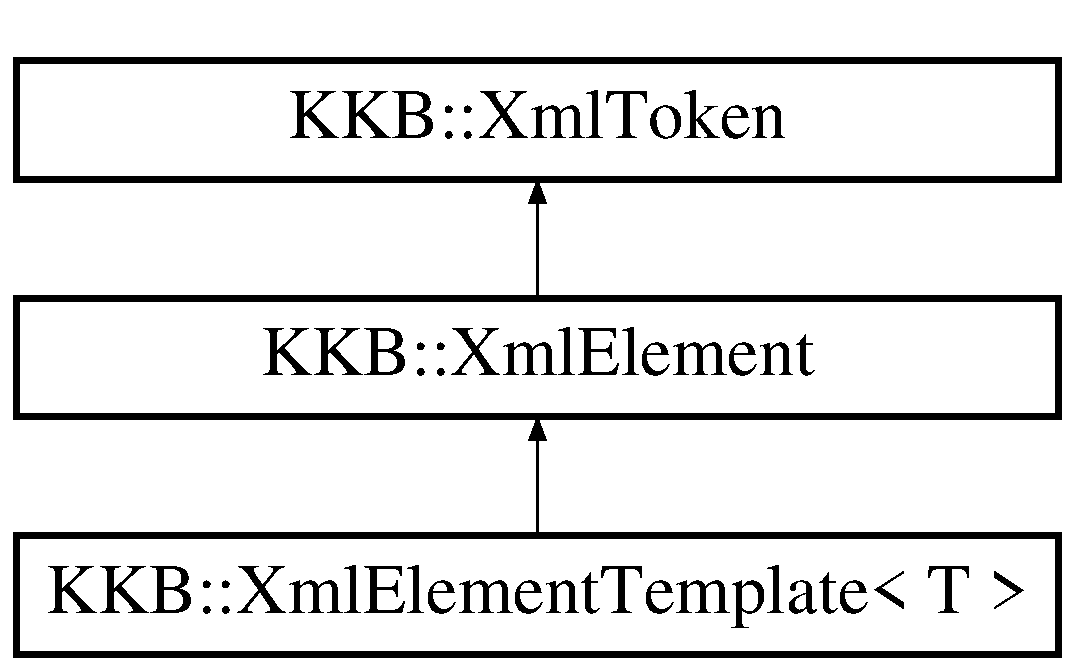
\includegraphics[height=3.000000cm]{class_k_k_b_1_1_xml_element_template}
\end{center}
\end{figure}
\subsection*{Public Member Functions}
\begin{DoxyCompactItemize}
\item 
\hyperlink{class_k_k_b_1_1_xml_element_template_a448ad8e64280f2fde3c6b5a1f52ab989}{Xml\+Element\+Template} (\hyperlink{namespace_k_k_b_a9253a3ea8a5da18ca82be4ca2b390ef0}{Xml\+Tag\+Ptr} tag, \hyperlink{class_k_k_b_1_1_xml_stream}{Xml\+Stream} \&s, \hyperlink{namespace_k_k_b_a7d390f568e2831fb76b86b56c87bf92f}{Vol\+Const\+Bool} \&cancel\+Flag, \hyperlink{class_k_k_b_1_1_run_log}{Run\+Log} \&log)
\item 
\hyperlink{class_k_k_b_1_1_xml_element_template_aca64261ea2614c0894e24476879a1c06}{$\sim$\+Xml\+Element\+Template} ()
\item 
T $\ast$ \hyperlink{class_k_k_b_1_1_xml_element_template_a1fd0ce7b0d0ee0d57fb29ca09d3ad6fc}{Take\+Ownership} ()
\item 
T $\ast$const \hyperlink{class_k_k_b_1_1_xml_element_template_a3d671b57251b4b256fecb2197fc4a0f4}{Value} () const 
\end{DoxyCompactItemize}
\subsection*{Static Public Member Functions}
\begin{DoxyCompactItemize}
\item 
static void \hyperlink{class_k_k_b_1_1_xml_element_template_aa32ee34673b14ffadd1d80c2960292b1}{Write\+X\+ML} (const T \&t, const \hyperlink{class_k_k_b_1_1_k_k_str}{K\+K\+Str} \&var\+Name, std\+::ostream \&o)
\end{DoxyCompactItemize}
\subsection*{Additional Inherited Members}


\subsection{Detailed Description}
\subsubsection*{template$<$class T$>$\\*
class K\+K\+B\+::\+Xml\+Element\+Template$<$ T $>$}



Definition at line 419 of file Xml\+Stream.\+h.



\subsection{Constructor \& Destructor Documentation}
\index{K\+K\+B\+::\+Xml\+Element\+Template@{K\+K\+B\+::\+Xml\+Element\+Template}!Xml\+Element\+Template@{Xml\+Element\+Template}}
\index{Xml\+Element\+Template@{Xml\+Element\+Template}!K\+K\+B\+::\+Xml\+Element\+Template@{K\+K\+B\+::\+Xml\+Element\+Template}}
\subsubsection[{\texorpdfstring{Xml\+Element\+Template(\+Xml\+Tag\+Ptr tag, Xml\+Stream \&s, Vol\+Const\+Bool \&cancel\+Flag, Run\+Log \&log)}{XmlElementTemplate(XmlTagPtr tag, XmlStream &s, VolConstBool &cancelFlag, RunLog &log)}}]{\setlength{\rightskip}{0pt plus 5cm}template$<$class T$>$ {\bf K\+K\+B\+::\+Xml\+Element\+Template}$<$ T $>$\+::{\bf Xml\+Element\+Template} (
\begin{DoxyParamCaption}
\item[{{\bf Xml\+Tag\+Ptr}}]{tag, }
\item[{{\bf Xml\+Stream} \&}]{s, }
\item[{{\bf Vol\+Const\+Bool} \&}]{cancel\+Flag, }
\item[{{\bf Run\+Log} \&}]{log}
\end{DoxyParamCaption}
)\hspace{0.3cm}{\ttfamily [inline]}}\hypertarget{class_k_k_b_1_1_xml_element_template_a448ad8e64280f2fde3c6b5a1f52ab989}{}\label{class_k_k_b_1_1_xml_element_template_a448ad8e64280f2fde3c6b5a1f52ab989}


Definition at line 422 of file Xml\+Stream.\+h.


\begin{DoxyCode}
426                         :
427      \hyperlink{class_k_k_b_1_1_xml_element_a66317eff5bd3abcc60755756ba2887d5}{XmlElement} (tag, s, log),
428      value (NULL)
429     \{
430       value = \textcolor{keyword}{new} T();
431       value->ReadXML (s, tag, cancelFlag, log);
432     \}
\end{DoxyCode}
\index{K\+K\+B\+::\+Xml\+Element\+Template@{K\+K\+B\+::\+Xml\+Element\+Template}!````~Xml\+Element\+Template@{$\sim$\+Xml\+Element\+Template}}
\index{````~Xml\+Element\+Template@{$\sim$\+Xml\+Element\+Template}!K\+K\+B\+::\+Xml\+Element\+Template@{K\+K\+B\+::\+Xml\+Element\+Template}}
\subsubsection[{\texorpdfstring{$\sim$\+Xml\+Element\+Template()}{~XmlElementTemplate()}}]{\setlength{\rightskip}{0pt plus 5cm}template$<$class T$>$ {\bf K\+K\+B\+::\+Xml\+Element\+Template}$<$ T $>$\+::$\sim${\bf Xml\+Element\+Template} (
\begin{DoxyParamCaption}
{}
\end{DoxyParamCaption}
)\hspace{0.3cm}{\ttfamily [inline]}}\hypertarget{class_k_k_b_1_1_xml_element_template_aca64261ea2614c0894e24476879a1c06}{}\label{class_k_k_b_1_1_xml_element_template_aca64261ea2614c0894e24476879a1c06}


Definition at line 435 of file Xml\+Stream.\+h.


\begin{DoxyCode}
436     \{
437       \textcolor{keyword}{delete} value;
438       value = NULL;
439     \}
\end{DoxyCode}


\subsection{Member Function Documentation}
\index{K\+K\+B\+::\+Xml\+Element\+Template@{K\+K\+B\+::\+Xml\+Element\+Template}!Take\+Ownership@{Take\+Ownership}}
\index{Take\+Ownership@{Take\+Ownership}!K\+K\+B\+::\+Xml\+Element\+Template@{K\+K\+B\+::\+Xml\+Element\+Template}}
\subsubsection[{\texorpdfstring{Take\+Ownership()}{TakeOwnership()}}]{\setlength{\rightskip}{0pt plus 5cm}template$<$class T$>$ T$\ast$ {\bf K\+K\+B\+::\+Xml\+Element\+Template}$<$ T $>$\+::Take\+Ownership (
\begin{DoxyParamCaption}
{}
\end{DoxyParamCaption}
)\hspace{0.3cm}{\ttfamily [inline]}}\hypertarget{class_k_k_b_1_1_xml_element_template_a1fd0ce7b0d0ee0d57fb29ca09d3ad6fc}{}\label{class_k_k_b_1_1_xml_element_template_a1fd0ce7b0d0ee0d57fb29ca09d3ad6fc}


Definition at line 443 of file Xml\+Stream.\+h.


\begin{DoxyCode}
444     \{
445       T* v = value;
446       value = NULL;
447       \textcolor{keywordflow}{return}  v;
448     \}
\end{DoxyCode}
\index{K\+K\+B\+::\+Xml\+Element\+Template@{K\+K\+B\+::\+Xml\+Element\+Template}!Value@{Value}}
\index{Value@{Value}!K\+K\+B\+::\+Xml\+Element\+Template@{K\+K\+B\+::\+Xml\+Element\+Template}}
\subsubsection[{\texorpdfstring{Value() const }{Value() const }}]{\setlength{\rightskip}{0pt plus 5cm}template$<$class T$>$ T$\ast$ const {\bf K\+K\+B\+::\+Xml\+Element\+Template}$<$ T $>$\+::Value (
\begin{DoxyParamCaption}
{}
\end{DoxyParamCaption}
) const\hspace{0.3cm}{\ttfamily [inline]}}\hypertarget{class_k_k_b_1_1_xml_element_template_a3d671b57251b4b256fecb2197fc4a0f4}{}\label{class_k_k_b_1_1_xml_element_template_a3d671b57251b4b256fecb2197fc4a0f4}


Definition at line 441 of file Xml\+Stream.\+h.


\begin{DoxyCode}
441 \{\textcolor{keywordflow}{return} value;\}
\end{DoxyCode}
\index{K\+K\+B\+::\+Xml\+Element\+Template@{K\+K\+B\+::\+Xml\+Element\+Template}!Write\+X\+ML@{Write\+X\+ML}}
\index{Write\+X\+ML@{Write\+X\+ML}!K\+K\+B\+::\+Xml\+Element\+Template@{K\+K\+B\+::\+Xml\+Element\+Template}}
\subsubsection[{\texorpdfstring{Write\+X\+M\+L(const T \&t, const K\+K\+Str \&var\+Name, std\+::ostream \&o)}{WriteXML(const T &t, const KKStr &varName, std::ostream &o)}}]{\setlength{\rightskip}{0pt plus 5cm}template$<$class T$>$ static void {\bf K\+K\+B\+::\+Xml\+Element\+Template}$<$ T $>$\+::Write\+X\+ML (
\begin{DoxyParamCaption}
\item[{const T \&}]{t, }
\item[{const {\bf K\+K\+Str} \&}]{var\+Name, }
\item[{std\+::ostream \&}]{o}
\end{DoxyParamCaption}
)\hspace{0.3cm}{\ttfamily [inline]}, {\ttfamily [static]}}\hypertarget{class_k_k_b_1_1_xml_element_template_aa32ee34673b14ffadd1d80c2960292b1}{}\label{class_k_k_b_1_1_xml_element_template_aa32ee34673b14ffadd1d80c2960292b1}


Definition at line 451 of file Xml\+Stream.\+h.


\begin{DoxyCode}
455     \{
456       t.WriteXML (varName, o);
457     \}
\end{DoxyCode}


The documentation for this class was generated from the following file\+:\begin{DoxyCompactItemize}
\item 
C\+:/\+Users/\+Kurt/\+Git\+Hub/\+K\+Square\+Libraries/\+K\+K\+Base/\hyperlink{_xml_stream_8h}{Xml\+Stream.\+h}\end{DoxyCompactItemize}

\hypertarget{class_k_k_b_1_1_xml_element_un_known}{}\section{K\+KB\+:\+:Xml\+Element\+Un\+Known Class Reference}
\label{class_k_k_b_1_1_xml_element_un_known}\index{K\+K\+B\+::\+Xml\+Element\+Un\+Known@{K\+K\+B\+::\+Xml\+Element\+Un\+Known}}


\hyperlink{class_k_k_b_1_1_xml_element}{Xml\+Element} derived class that will be used when there is no Factory defined for the element. 




{\ttfamily \#include $<$Xml\+Stream.\+h$>$}

Inheritance diagram for K\+KB\+:\+:Xml\+Element\+Un\+Known\+:\begin{figure}[H]
\begin{center}
\leavevmode
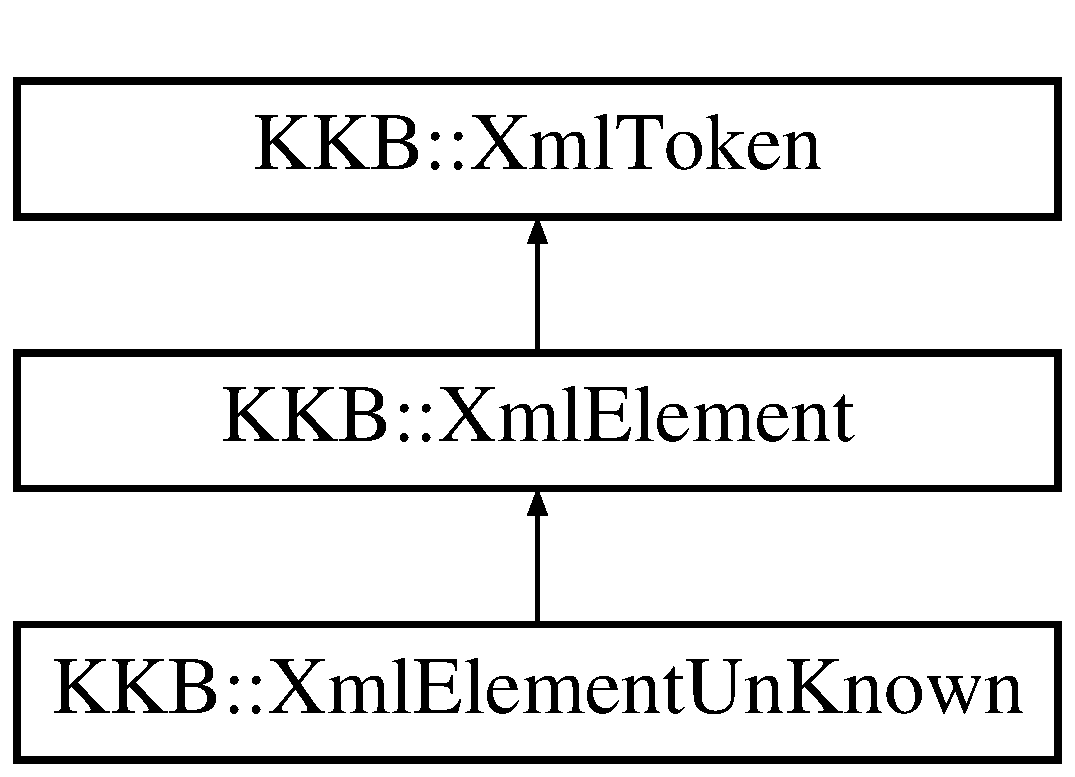
\includegraphics[height=3.000000cm]{class_k_k_b_1_1_xml_element_un_known}
\end{center}
\end{figure}
\subsection*{Public Member Functions}
\begin{DoxyCompactItemize}
\item 
\hyperlink{class_k_k_b_1_1_xml_element_un_known_a38766b4e928f2d5705d33145fb3665bc}{Xml\+Element\+Un\+Known} (\hyperlink{namespace_k_k_b_a9253a3ea8a5da18ca82be4ca2b390ef0}{Xml\+Tag\+Ptr} tag, \hyperlink{class_k_k_b_1_1_xml_stream}{Xml\+Stream} \&s, \hyperlink{namespace_k_k_b_a7d390f568e2831fb76b86b56c87bf92f}{Vol\+Const\+Bool} \&cancel\+Flag, \hyperlink{class_k_k_b_1_1_run_log}{Run\+Log} \&log)
\item 
virtual \hyperlink{class_k_k_b_1_1_xml_element_un_known_a3504ae0803666fd8e5726023c4d2052a}{$\sim$\+Xml\+Element\+Un\+Known} ()
\item 
std\+::deque$<$ \hyperlink{class_k_k_b_1_1_xml_token_a2379a40d8ebd64e9125cf68e34da13ab}{Xml\+Token\+Ptr} $>$ $\ast$ \hyperlink{class_k_k_b_1_1_xml_element_un_known_a7c04dccc6ffbf40d05f5c7841873ca9f}{Take\+Ownership} ()
\item 
std\+::deque$<$ \hyperlink{class_k_k_b_1_1_xml_token_a2379a40d8ebd64e9125cf68e34da13ab}{Xml\+Token\+Ptr} $>$ $\ast$ \hyperlink{class_k_k_b_1_1_xml_element_un_known_aa777364ac9919010ba0f20dbc2b6e420}{Value} () const 
\end{DoxyCompactItemize}
\subsection*{Additional Inherited Members}


\subsection{Detailed Description}
\hyperlink{class_k_k_b_1_1_xml_element}{Xml\+Element} derived class that will be used when there is no Factory defined for the element.

remarks$>$All sub-\/elements and content will be saved in value which will be a list of Xml\+Eemenst and content.

Definition at line 471 of file Xml\+Stream.\+h.



\subsection{Constructor \& Destructor Documentation}
\index{K\+K\+B\+::\+Xml\+Element\+Un\+Known@{K\+K\+B\+::\+Xml\+Element\+Un\+Known}!Xml\+Element\+Un\+Known@{Xml\+Element\+Un\+Known}}
\index{Xml\+Element\+Un\+Known@{Xml\+Element\+Un\+Known}!K\+K\+B\+::\+Xml\+Element\+Un\+Known@{K\+K\+B\+::\+Xml\+Element\+Un\+Known}}
\subsubsection[{\texorpdfstring{Xml\+Element\+Un\+Known(\+Xml\+Tag\+Ptr tag, Xml\+Stream \&s, Vol\+Const\+Bool \&cancel\+Flag, Run\+Log \&log)}{XmlElementUnKnown(XmlTagPtr tag, XmlStream &s, VolConstBool &cancelFlag, RunLog &log)}}]{\setlength{\rightskip}{0pt plus 5cm}Xml\+Element\+Un\+Known\+::\+Xml\+Element\+Un\+Known (
\begin{DoxyParamCaption}
\item[{{\bf Xml\+Tag\+Ptr}}]{tag, }
\item[{{\bf Xml\+Stream} \&}]{s, }
\item[{{\bf Vol\+Const\+Bool} \&}]{cancel\+Flag, }
\item[{{\bf Run\+Log} \&}]{log}
\end{DoxyParamCaption}
)}\hypertarget{class_k_k_b_1_1_xml_element_un_known_a38766b4e928f2d5705d33145fb3665bc}{}\label{class_k_k_b_1_1_xml_element_un_known_a38766b4e928f2d5705d33145fb3665bc}


Definition at line 1051 of file Xml\+Stream.\+cpp.



References K\+K\+B\+::\+Xml\+Stream\+::\+Get\+Next\+Token(), K\+K\+B\+::\+Xml\+Element\+::\+Xml\+Element(), and Xml\+Element\+Un\+Known().



Referenced by Xml\+Element\+Un\+Known().


\begin{DoxyCode}
1055                                       :
1056     \hyperlink{class_k_k_b_1_1_xml_element_a66317eff5bd3abcc60755756ba2887d5}{XmlElement} (tag, s, log),
1057     value (\textcolor{keyword}{new} deque<XmlTokenPtr> ())
1058 \{
1059   \hyperlink{class_k_k_b_1_1_xml_token}{XmlTokenPtr} t = s.\hyperlink{class_k_k_b_1_1_xml_stream_a87cc738b05c666cf5d5c25beaab477b4}{GetNextToken} (cancelFlag, log);
1060   \textcolor{keywordflow}{while}  (t != NULL)
1061   \{
1062     value->push\_back (t);
1063     t = s.\hyperlink{class_k_k_b_1_1_xml_stream_a87cc738b05c666cf5d5c25beaab477b4}{GetNextToken} (cancelFlag, log);
1064   \}
1065 \}
\end{DoxyCode}
\index{K\+K\+B\+::\+Xml\+Element\+Un\+Known@{K\+K\+B\+::\+Xml\+Element\+Un\+Known}!````~Xml\+Element\+Un\+Known@{$\sim$\+Xml\+Element\+Un\+Known}}
\index{````~Xml\+Element\+Un\+Known@{$\sim$\+Xml\+Element\+Un\+Known}!K\+K\+B\+::\+Xml\+Element\+Un\+Known@{K\+K\+B\+::\+Xml\+Element\+Un\+Known}}
\subsubsection[{\texorpdfstring{$\sim$\+Xml\+Element\+Un\+Known()}{~XmlElementUnKnown()}}]{\setlength{\rightskip}{0pt plus 5cm}Xml\+Element\+Un\+Known\+::$\sim$\+Xml\+Element\+Un\+Known (
\begin{DoxyParamCaption}
{}
\end{DoxyParamCaption}
)\hspace{0.3cm}{\ttfamily [virtual]}}\hypertarget{class_k_k_b_1_1_xml_element_un_known_a3504ae0803666fd8e5726023c4d2052a}{}\label{class_k_k_b_1_1_xml_element_un_known_a3504ae0803666fd8e5726023c4d2052a}


Definition at line 1068 of file Xml\+Stream.\+cpp.


\begin{DoxyCode}
1069 \{
1070   \textcolor{keywordflow}{if}  (value)
1071   \{
1072     \textcolor{keywordflow}{for}  (\textcolor{keyword}{auto} idx: *value)
1073       \textcolor{keyword}{delete}  idx;
1074     \textcolor{keyword}{delete}  value;
1075     value = NULL;
1076   \}
1077 \}
\end{DoxyCode}


\subsection{Member Function Documentation}
\index{K\+K\+B\+::\+Xml\+Element\+Un\+Known@{K\+K\+B\+::\+Xml\+Element\+Un\+Known}!Take\+Ownership@{Take\+Ownership}}
\index{Take\+Ownership@{Take\+Ownership}!K\+K\+B\+::\+Xml\+Element\+Un\+Known@{K\+K\+B\+::\+Xml\+Element\+Un\+Known}}
\subsubsection[{\texorpdfstring{Take\+Ownership()}{TakeOwnership()}}]{\setlength{\rightskip}{0pt plus 5cm}deque$<$ {\bf Xml\+Token\+Ptr} $>$ $\ast$ Xml\+Element\+Un\+Known\+::\+Take\+Ownership (
\begin{DoxyParamCaption}
{}
\end{DoxyParamCaption}
)}\hypertarget{class_k_k_b_1_1_xml_element_un_known_a7c04dccc6ffbf40d05f5c7841873ca9f}{}\label{class_k_k_b_1_1_xml_element_un_known_a7c04dccc6ffbf40d05f5c7841873ca9f}


Definition at line 1080 of file Xml\+Stream.\+cpp.


\begin{DoxyCode}
1081 \{
1082   deque<XmlTokenPtr>* v = value;
1083   value = NULL;
1084   \textcolor{keywordflow}{return} v;
1085 \}
\end{DoxyCode}
\index{K\+K\+B\+::\+Xml\+Element\+Un\+Known@{K\+K\+B\+::\+Xml\+Element\+Un\+Known}!Value@{Value}}
\index{Value@{Value}!K\+K\+B\+::\+Xml\+Element\+Un\+Known@{K\+K\+B\+::\+Xml\+Element\+Un\+Known}}
\subsubsection[{\texorpdfstring{Value() const }{Value() const }}]{\setlength{\rightskip}{0pt plus 5cm}std\+::deque$<${\bf Xml\+Token\+Ptr}$>$$\ast$ K\+K\+B\+::\+Xml\+Element\+Un\+Known\+::\+Value (
\begin{DoxyParamCaption}
{}
\end{DoxyParamCaption}
) const\hspace{0.3cm}{\ttfamily [inline]}}\hypertarget{class_k_k_b_1_1_xml_element_un_known_aa777364ac9919010ba0f20dbc2b6e420}{}\label{class_k_k_b_1_1_xml_element_un_known_aa777364ac9919010ba0f20dbc2b6e420}


Definition at line 482 of file Xml\+Stream.\+h.


\begin{DoxyCode}
482 \{\textcolor{keywordflow}{return}  value;\}
\end{DoxyCode}


The documentation for this class was generated from the following files\+:\begin{DoxyCompactItemize}
\item 
C\+:/\+Users/\+Kurt/\+Git\+Hub/\+K\+Square\+Libraries/\+K\+K\+Base/\hyperlink{_xml_stream_8h}{Xml\+Stream.\+h}\item 
C\+:/\+Users/\+Kurt/\+Git\+Hub/\+K\+Square\+Libraries/\+K\+K\+Base/\hyperlink{_xml_stream_8cpp}{Xml\+Stream.\+cpp}\end{DoxyCompactItemize}

\hypertarget{class_k_k_b_1_1_xml_element_vector_float}{}\section{K\+KB\+:\+:Xml\+Element\+Vector\+Float Class Reference}
\label{class_k_k_b_1_1_xml_element_vector_float}\index{K\+K\+B\+::\+Xml\+Element\+Vector\+Float@{K\+K\+B\+::\+Xml\+Element\+Vector\+Float}}


{\ttfamily \#include $<$Xml\+Stream.\+h$>$}

Inheritance diagram for K\+KB\+:\+:Xml\+Element\+Vector\+Float\+:\begin{figure}[H]
\begin{center}
\leavevmode
\includegraphics[height=3.000000cm]{class_k_k_b_1_1_xml_element_vector_float}
\end{center}
\end{figure}
\subsection*{Public Member Functions}
\begin{DoxyCompactItemize}
\item 
\hyperlink{class_k_k_b_1_1_xml_element_vector_float_adc7ad31ae59d66c12d9b57466d178289}{Xml\+Element\+Vector\+Float} (\hyperlink{namespace_k_k_b_a9253a3ea8a5da18ca82be4ca2b390ef0}{Xml\+Tag\+Ptr} tag, \hyperlink{class_k_k_b_1_1_xml_stream}{Xml\+Stream} \&s, \hyperlink{namespace_k_k_b_a7d390f568e2831fb76b86b56c87bf92f}{Vol\+Const\+Bool} \&cancel\+Flag, \hyperlink{class_k_k_b_1_1_run_log}{Run\+Log} \&log)
\item 
virtual \hyperlink{class_k_k_b_1_1_xml_element_vector_float_ae122e99121fa49e27b8721396330be0f}{$\sim$\+Xml\+Element\+Vector\+Float} ()
\item 
std\+::vector$<$ float $>$ $\ast$ \hyperlink{class_k_k_b_1_1_xml_element_vector_float_a9811ab5d1777c2b6e9c3fb90f7e909bd}{Take\+Ownership} ()
\item 
std\+::vector$<$ float $>$ $\ast$const \hyperlink{class_k_k_b_1_1_xml_element_vector_float_a0a65b4560ef7b3199daa78f4125fa608}{Value} () const 
\end{DoxyCompactItemize}
\subsection*{Static Public Member Functions}
\begin{DoxyCompactItemize}
\item 
static void \hyperlink{class_k_k_b_1_1_xml_element_vector_float_a2bdf3cbef6bd00d19d97800ad5acc1ef}{Write\+X\+ML} (const std\+::vector$<$ float $>$ \&d, const \hyperlink{class_k_k_b_1_1_k_k_str}{K\+K\+Str} \&var\+Name, std\+::ostream \&o)
\end{DoxyCompactItemize}
\subsection*{Additional Inherited Members}


\subsection{Detailed Description}


Definition at line 927 of file Xml\+Stream.\+h.



\subsection{Constructor \& Destructor Documentation}
\index{K\+K\+B\+::\+Xml\+Element\+Vector\+Float@{K\+K\+B\+::\+Xml\+Element\+Vector\+Float}!Xml\+Element\+Vector\+Float@{Xml\+Element\+Vector\+Float}}
\index{Xml\+Element\+Vector\+Float@{Xml\+Element\+Vector\+Float}!K\+K\+B\+::\+Xml\+Element\+Vector\+Float@{K\+K\+B\+::\+Xml\+Element\+Vector\+Float}}
\subsubsection[{\texorpdfstring{Xml\+Element\+Vector\+Float(\+Xml\+Tag\+Ptr tag, Xml\+Stream \&s, Vol\+Const\+Bool \&cancel\+Flag, Run\+Log \&log)}{XmlElementVectorFloat(XmlTagPtr tag, XmlStream &s, VolConstBool &cancelFlag, RunLog &log)}}]{\setlength{\rightskip}{0pt plus 5cm}Xml\+Element\+Vector\+Float\+::\+Xml\+Element\+Vector\+Float (
\begin{DoxyParamCaption}
\item[{{\bf Xml\+Tag\+Ptr}}]{tag, }
\item[{{\bf Xml\+Stream} \&}]{s, }
\item[{{\bf Vol\+Const\+Bool} \&}]{cancel\+Flag, }
\item[{{\bf Run\+Log} \&}]{log}
\end{DoxyParamCaption}
)}\hypertarget{class_k_k_b_1_1_xml_element_vector_float_adc7ad31ae59d66c12d9b57466d178289}{}\label{class_k_k_b_1_1_xml_element_vector_float_adc7ad31ae59d66c12d9b57466d178289}


Definition at line 1869 of file Xml\+Stream.\+cpp.

\index{K\+K\+B\+::\+Xml\+Element\+Vector\+Float@{K\+K\+B\+::\+Xml\+Element\+Vector\+Float}!````~Xml\+Element\+Vector\+Float@{$\sim$\+Xml\+Element\+Vector\+Float}}
\index{````~Xml\+Element\+Vector\+Float@{$\sim$\+Xml\+Element\+Vector\+Float}!K\+K\+B\+::\+Xml\+Element\+Vector\+Float@{K\+K\+B\+::\+Xml\+Element\+Vector\+Float}}
\subsubsection[{\texorpdfstring{$\sim$\+Xml\+Element\+Vector\+Float()}{~XmlElementVectorFloat()}}]{\setlength{\rightskip}{0pt plus 5cm}Xml\+Element\+Vector\+Float\+::$\sim$\+Xml\+Element\+Vector\+Float (
\begin{DoxyParamCaption}
{}
\end{DoxyParamCaption}
)\hspace{0.3cm}{\ttfamily [virtual]}}\hypertarget{class_k_k_b_1_1_xml_element_vector_float_ae122e99121fa49e27b8721396330be0f}{}\label{class_k_k_b_1_1_xml_element_vector_float_ae122e99121fa49e27b8721396330be0f}


Definition at line 1869 of file Xml\+Stream.\+cpp.



\subsection{Member Function Documentation}
\index{K\+K\+B\+::\+Xml\+Element\+Vector\+Float@{K\+K\+B\+::\+Xml\+Element\+Vector\+Float}!Take\+Ownership@{Take\+Ownership}}
\index{Take\+Ownership@{Take\+Ownership}!K\+K\+B\+::\+Xml\+Element\+Vector\+Float@{K\+K\+B\+::\+Xml\+Element\+Vector\+Float}}
\subsubsection[{\texorpdfstring{Take\+Ownership()}{TakeOwnership()}}]{\setlength{\rightskip}{0pt plus 5cm}vector$<$ float $>$ $\ast$ Xml\+Element\+Vector\+Float\+::\+Take\+Ownership (
\begin{DoxyParamCaption}
{}
\end{DoxyParamCaption}
)}\hypertarget{class_k_k_b_1_1_xml_element_vector_float_a9811ab5d1777c2b6e9c3fb90f7e909bd}{}\label{class_k_k_b_1_1_xml_element_vector_float_a9811ab5d1777c2b6e9c3fb90f7e909bd}


Definition at line 1869 of file Xml\+Stream.\+cpp.

\index{K\+K\+B\+::\+Xml\+Element\+Vector\+Float@{K\+K\+B\+::\+Xml\+Element\+Vector\+Float}!Value@{Value}}
\index{Value@{Value}!K\+K\+B\+::\+Xml\+Element\+Vector\+Float@{K\+K\+B\+::\+Xml\+Element\+Vector\+Float}}
\subsubsection[{\texorpdfstring{Value() const }{Value() const }}]{\setlength{\rightskip}{0pt plus 5cm}std\+::vector$<$ float $>$$\ast$ const K\+K\+B\+::\+Xml\+Element\+Vector\+Float\+::\+Value (
\begin{DoxyParamCaption}
{}
\end{DoxyParamCaption}
) const\hspace{0.3cm}{\ttfamily [inline]}}\hypertarget{class_k_k_b_1_1_xml_element_vector_float_a0a65b4560ef7b3199daa78f4125fa608}{}\label{class_k_k_b_1_1_xml_element_vector_float_a0a65b4560ef7b3199daa78f4125fa608}


Definition at line 927 of file Xml\+Stream.\+h.

\index{K\+K\+B\+::\+Xml\+Element\+Vector\+Float@{K\+K\+B\+::\+Xml\+Element\+Vector\+Float}!Write\+X\+ML@{Write\+X\+ML}}
\index{Write\+X\+ML@{Write\+X\+ML}!K\+K\+B\+::\+Xml\+Element\+Vector\+Float@{K\+K\+B\+::\+Xml\+Element\+Vector\+Float}}
\subsubsection[{\texorpdfstring{Write\+X\+M\+L(const std\+::vector$<$ float $>$ \&d, const K\+K\+Str \&var\+Name, std\+::ostream \&o)}{WriteXML(const std::vector< float > &d, const KKStr &varName, std::ostream &o)}}]{\setlength{\rightskip}{0pt plus 5cm}void Xml\+Element\+Vector\+Float\+::\+Write\+X\+ML (
\begin{DoxyParamCaption}
\item[{const std\+::vector$<$ float $>$ \&}]{d, }
\item[{const {\bf K\+K\+Str} \&}]{var\+Name, }
\item[{std\+::ostream \&}]{o}
\end{DoxyParamCaption}
)\hspace{0.3cm}{\ttfamily [static]}}\hypertarget{class_k_k_b_1_1_xml_element_vector_float_a2bdf3cbef6bd00d19d97800ad5acc1ef}{}\label{class_k_k_b_1_1_xml_element_vector_float_a2bdf3cbef6bd00d19d97800ad5acc1ef}


Definition at line 1869 of file Xml\+Stream.\+cpp.



The documentation for this class was generated from the following files\+:\begin{DoxyCompactItemize}
\item 
C\+:/\+Users/\+Kurt/\+Git\+Hub/\+K\+Square\+Libraries/\+K\+K\+Base/\hyperlink{_xml_stream_8h}{Xml\+Stream.\+h}\item 
C\+:/\+Users/\+Kurt/\+Git\+Hub/\+K\+Square\+Libraries/\+K\+K\+Base/\hyperlink{_xml_stream_8cpp}{Xml\+Stream.\+cpp}\end{DoxyCompactItemize}

\hypertarget{class_k_k_b_1_1_xml_element_vector_int32}{}\section{K\+KB\+:\+:Xml\+Element\+Vector\+Int32 Class Reference}
\label{class_k_k_b_1_1_xml_element_vector_int32}\index{K\+K\+B\+::\+Xml\+Element\+Vector\+Int32@{K\+K\+B\+::\+Xml\+Element\+Vector\+Int32}}


{\ttfamily \#include $<$Xml\+Stream.\+h$>$}

Inheritance diagram for K\+KB\+:\+:Xml\+Element\+Vector\+Int32\+:\begin{figure}[H]
\begin{center}
\leavevmode
\includegraphics[height=3.000000cm]{class_k_k_b_1_1_xml_element_vector_int32}
\end{center}
\end{figure}
\subsection*{Public Member Functions}
\begin{DoxyCompactItemize}
\item 
\hyperlink{class_k_k_b_1_1_xml_element_vector_int32_a05ae676a9d874997a66077b5c7b98664}{Xml\+Element\+Vector\+Int32} (\hyperlink{namespace_k_k_b_a9253a3ea8a5da18ca82be4ca2b390ef0}{Xml\+Tag\+Ptr} tag, \hyperlink{class_k_k_b_1_1_xml_stream}{Xml\+Stream} \&s, \hyperlink{namespace_k_k_b_a7d390f568e2831fb76b86b56c87bf92f}{Vol\+Const\+Bool} \&cancel\+Flag, \hyperlink{class_k_k_b_1_1_run_log}{Run\+Log} \&log)
\item 
virtual \hyperlink{class_k_k_b_1_1_xml_element_vector_int32_a03001c482bffdf9a0c621a9b84d12284}{$\sim$\+Xml\+Element\+Vector\+Int32} ()
\item 
std\+::vector$<$ \hyperlink{namespace_k_k_b_a8fa4952cc84fda1de4bec1fbdd8d5b1b}{kkint32} $>$ $\ast$ \hyperlink{class_k_k_b_1_1_xml_element_vector_int32_a22c74bbacae4574d79480e21859ba49f}{Take\+Ownership} ()
\item 
std\+::vector$<$ \hyperlink{namespace_k_k_b_a8fa4952cc84fda1de4bec1fbdd8d5b1b}{kkint32} $>$ $\ast$const \hyperlink{class_k_k_b_1_1_xml_element_vector_int32_ab2877c6bbf603155fc89cb974bc02883}{Value} () const 
\end{DoxyCompactItemize}
\subsection*{Static Public Member Functions}
\begin{DoxyCompactItemize}
\item 
static void \hyperlink{class_k_k_b_1_1_xml_element_vector_int32_a514cefc52aca4109728b46ab6362936d}{Write\+X\+ML} (const std\+::vector$<$ \hyperlink{namespace_k_k_b_a8fa4952cc84fda1de4bec1fbdd8d5b1b}{kkint32} $>$ \&d, const \hyperlink{class_k_k_b_1_1_k_k_str}{K\+K\+Str} \&var\+Name, std\+::ostream \&o)
\end{DoxyCompactItemize}
\subsection*{Additional Inherited Members}


\subsection{Detailed Description}


Definition at line 926 of file Xml\+Stream.\+h.



\subsection{Constructor \& Destructor Documentation}
\index{K\+K\+B\+::\+Xml\+Element\+Vector\+Int32@{K\+K\+B\+::\+Xml\+Element\+Vector\+Int32}!Xml\+Element\+Vector\+Int32@{Xml\+Element\+Vector\+Int32}}
\index{Xml\+Element\+Vector\+Int32@{Xml\+Element\+Vector\+Int32}!K\+K\+B\+::\+Xml\+Element\+Vector\+Int32@{K\+K\+B\+::\+Xml\+Element\+Vector\+Int32}}
\subsubsection[{\texorpdfstring{Xml\+Element\+Vector\+Int32(\+Xml\+Tag\+Ptr tag, Xml\+Stream \&s, Vol\+Const\+Bool \&cancel\+Flag, Run\+Log \&log)}{XmlElementVectorInt32(XmlTagPtr tag, XmlStream &s, VolConstBool &cancelFlag, RunLog &log)}}]{\setlength{\rightskip}{0pt plus 5cm}Xml\+Element\+Vector\+Int32\+::\+Xml\+Element\+Vector\+Int32 (
\begin{DoxyParamCaption}
\item[{{\bf Xml\+Tag\+Ptr}}]{tag, }
\item[{{\bf Xml\+Stream} \&}]{s, }
\item[{{\bf Vol\+Const\+Bool} \&}]{cancel\+Flag, }
\item[{{\bf Run\+Log} \&}]{log}
\end{DoxyParamCaption}
)}\hypertarget{class_k_k_b_1_1_xml_element_vector_int32_a05ae676a9d874997a66077b5c7b98664}{}\label{class_k_k_b_1_1_xml_element_vector_int32_a05ae676a9d874997a66077b5c7b98664}


Definition at line 1868 of file Xml\+Stream.\+cpp.

\index{K\+K\+B\+::\+Xml\+Element\+Vector\+Int32@{K\+K\+B\+::\+Xml\+Element\+Vector\+Int32}!````~Xml\+Element\+Vector\+Int32@{$\sim$\+Xml\+Element\+Vector\+Int32}}
\index{````~Xml\+Element\+Vector\+Int32@{$\sim$\+Xml\+Element\+Vector\+Int32}!K\+K\+B\+::\+Xml\+Element\+Vector\+Int32@{K\+K\+B\+::\+Xml\+Element\+Vector\+Int32}}
\subsubsection[{\texorpdfstring{$\sim$\+Xml\+Element\+Vector\+Int32()}{~XmlElementVectorInt32()}}]{\setlength{\rightskip}{0pt plus 5cm}Xml\+Element\+Vector\+Int32\+::$\sim$\+Xml\+Element\+Vector\+Int32 (
\begin{DoxyParamCaption}
{}
\end{DoxyParamCaption}
)\hspace{0.3cm}{\ttfamily [virtual]}}\hypertarget{class_k_k_b_1_1_xml_element_vector_int32_a03001c482bffdf9a0c621a9b84d12284}{}\label{class_k_k_b_1_1_xml_element_vector_int32_a03001c482bffdf9a0c621a9b84d12284}


Definition at line 1868 of file Xml\+Stream.\+cpp.



\subsection{Member Function Documentation}
\index{K\+K\+B\+::\+Xml\+Element\+Vector\+Int32@{K\+K\+B\+::\+Xml\+Element\+Vector\+Int32}!Take\+Ownership@{Take\+Ownership}}
\index{Take\+Ownership@{Take\+Ownership}!K\+K\+B\+::\+Xml\+Element\+Vector\+Int32@{K\+K\+B\+::\+Xml\+Element\+Vector\+Int32}}
\subsubsection[{\texorpdfstring{Take\+Ownership()}{TakeOwnership()}}]{\setlength{\rightskip}{0pt plus 5cm}vector$<$ {\bf kkint32} $>$ $\ast$ Xml\+Element\+Vector\+Int32\+::\+Take\+Ownership (
\begin{DoxyParamCaption}
{}
\end{DoxyParamCaption}
)}\hypertarget{class_k_k_b_1_1_xml_element_vector_int32_a22c74bbacae4574d79480e21859ba49f}{}\label{class_k_k_b_1_1_xml_element_vector_int32_a22c74bbacae4574d79480e21859ba49f}


Definition at line 1868 of file Xml\+Stream.\+cpp.

\index{K\+K\+B\+::\+Xml\+Element\+Vector\+Int32@{K\+K\+B\+::\+Xml\+Element\+Vector\+Int32}!Value@{Value}}
\index{Value@{Value}!K\+K\+B\+::\+Xml\+Element\+Vector\+Int32@{K\+K\+B\+::\+Xml\+Element\+Vector\+Int32}}
\subsubsection[{\texorpdfstring{Value() const }{Value() const }}]{\setlength{\rightskip}{0pt plus 5cm}std\+::vector$<$ {\bf kkint32} $>$$\ast$ const K\+K\+B\+::\+Xml\+Element\+Vector\+Int32\+::\+Value (
\begin{DoxyParamCaption}
{}
\end{DoxyParamCaption}
) const\hspace{0.3cm}{\ttfamily [inline]}}\hypertarget{class_k_k_b_1_1_xml_element_vector_int32_ab2877c6bbf603155fc89cb974bc02883}{}\label{class_k_k_b_1_1_xml_element_vector_int32_ab2877c6bbf603155fc89cb974bc02883}


Definition at line 926 of file Xml\+Stream.\+h.

\index{K\+K\+B\+::\+Xml\+Element\+Vector\+Int32@{K\+K\+B\+::\+Xml\+Element\+Vector\+Int32}!Write\+X\+ML@{Write\+X\+ML}}
\index{Write\+X\+ML@{Write\+X\+ML}!K\+K\+B\+::\+Xml\+Element\+Vector\+Int32@{K\+K\+B\+::\+Xml\+Element\+Vector\+Int32}}
\subsubsection[{\texorpdfstring{Write\+X\+M\+L(const std\+::vector$<$ kkint32 $>$ \&d, const K\+K\+Str \&var\+Name, std\+::ostream \&o)}{WriteXML(const std::vector< kkint32 > &d, const KKStr &varName, std::ostream &o)}}]{\setlength{\rightskip}{0pt plus 5cm}void Xml\+Element\+Vector\+Int32\+::\+Write\+X\+ML (
\begin{DoxyParamCaption}
\item[{const std\+::vector$<$ {\bf kkint32} $>$ \&}]{d, }
\item[{const {\bf K\+K\+Str} \&}]{var\+Name, }
\item[{std\+::ostream \&}]{o}
\end{DoxyParamCaption}
)\hspace{0.3cm}{\ttfamily [static]}}\hypertarget{class_k_k_b_1_1_xml_element_vector_int32_a514cefc52aca4109728b46ab6362936d}{}\label{class_k_k_b_1_1_xml_element_vector_int32_a514cefc52aca4109728b46ab6362936d}


Definition at line 1868 of file Xml\+Stream.\+cpp.



The documentation for this class was generated from the following files\+:\begin{DoxyCompactItemize}
\item 
C\+:/\+Users/\+Kurt/\+Git\+Hub/\+K\+Square\+Libraries/\+K\+K\+Base/\hyperlink{_xml_stream_8h}{Xml\+Stream.\+h}\item 
C\+:/\+Users/\+Kurt/\+Git\+Hub/\+K\+Square\+Libraries/\+K\+K\+Base/\hyperlink{_xml_stream_8cpp}{Xml\+Stream.\+cpp}\end{DoxyCompactItemize}

\hypertarget{class_k_k_b_1_1_xml_factory}{}\section{K\+KB\+:\+:Xml\+Factory Class Reference}
\label{class_k_k_b_1_1_xml_factory}\index{K\+K\+B\+::\+Xml\+Factory@{K\+K\+B\+::\+Xml\+Factory}}


{\ttfamily \#include $<$Xml\+Stream.\+h$>$}

Inheritance diagram for K\+KB\+:\+:Xml\+Factory\+:\begin{figure}[H]
\begin{center}
\leavevmode
\includegraphics[height=12.000000cm]{class_k_k_b_1_1_xml_factory}
\end{center}
\end{figure}
\subsection*{Public Member Functions}
\begin{DoxyCompactItemize}
\item 
\hyperlink{class_k_k_b_1_1_xml_factory_ab6312883139f5388a91856147852a9cf}{Xml\+Factory} (const \hyperlink{class_k_k_b_1_1_k_k_str}{K\+K\+Str} \&\+\_\+clas\+Name)
\item 
virtual const \hyperlink{class_k_k_b_1_1_k_k_str}{K\+K\+Str} \& \hyperlink{class_k_k_b_1_1_xml_factory_a32733484cc01e731d559a91cde0ad252}{Class\+Name} () const 
\item 
virtual \hyperlink{namespace_k_k_b_a60c0ababc47c146b900507f7a3d3872e}{Xml\+Element\+Ptr} \hyperlink{class_k_k_b_1_1_xml_factory_a3f4b4f19dee1905e1758b16c66d0112a}{Manufature\+Xml\+Element} (\hyperlink{namespace_k_k_b_a9253a3ea8a5da18ca82be4ca2b390ef0}{Xml\+Tag\+Ptr} tag, \hyperlink{class_k_k_b_1_1_xml_stream}{Xml\+Stream} \&s, \hyperlink{namespace_k_k_b_a7d390f568e2831fb76b86b56c87bf92f}{Vol\+Const\+Bool} \&cancel\+Flag, \hyperlink{class_k_k_b_1_1_run_log}{Run\+Log} \&log)=0
\end{DoxyCompactItemize}
\subsection*{Static Public Member Functions}
\begin{DoxyCompactItemize}
\item 
static \hyperlink{class_k_k_b_1_1_xml_factory}{Xml\+Factory} $\ast$ \hyperlink{class_k_k_b_1_1_xml_factory_a1fd2d78a144b13a28c3898e654d79af9}{Factory\+Look\+Up} (const \hyperlink{class_k_k_b_1_1_k_k_str}{K\+K\+Str} \&class\+Name)
\item 
static void \hyperlink{class_k_k_b_1_1_xml_factory_a8790bd65ca562a16fd0ec6927b3b344e}{Final\+Clean\+Up} ()
\item 
static void \hyperlink{class_k_k_b_1_1_xml_factory_ad2a973d25044d07c656e3b8b8c6176cb}{Register\+Factory} (\hyperlink{class_k_k_b_1_1_xml_factory}{Xml\+Factory} $\ast$factory)
\end{DoxyCompactItemize}
\subsection*{Static Public Attributes}
\begin{DoxyCompactItemize}
\item 
static \hyperlink{namespace_k_k_b_aafda05381a8f75c01dcc4c7bca1fac5f}{Xml\+Factory\+Manager\+Ptr} \hyperlink{class_k_k_b_1_1_xml_factory_ae06818f5d4907c127fadd5e956f10c0b}{global\+Xml\+Factory\+Manager} = N\+U\+LL
\end{DoxyCompactItemize}


\subsection{Detailed Description}


Definition at line 382 of file Xml\+Stream.\+h.



\subsection{Constructor \& Destructor Documentation}
\index{K\+K\+B\+::\+Xml\+Factory@{K\+K\+B\+::\+Xml\+Factory}!Xml\+Factory@{Xml\+Factory}}
\index{Xml\+Factory@{Xml\+Factory}!K\+K\+B\+::\+Xml\+Factory@{K\+K\+B\+::\+Xml\+Factory}}
\subsubsection[{\texorpdfstring{Xml\+Factory(const K\+K\+Str \&\+\_\+clas\+Name)}{XmlFactory(const KKStr &_clasName)}}]{\setlength{\rightskip}{0pt plus 5cm}Xml\+Factory\+::\+Xml\+Factory (
\begin{DoxyParamCaption}
\item[{const {\bf K\+K\+Str} \&}]{\+\_\+clas\+Name}
\end{DoxyParamCaption}
)}\hypertarget{class_k_k_b_1_1_xml_factory_ab6312883139f5388a91856147852a9cf}{}\label{class_k_k_b_1_1_xml_factory_ab6312883139f5388a91856147852a9cf}


Definition at line 931 of file Xml\+Stream.\+cpp.



References K\+K\+B\+::\+K\+K\+Str\+::\+K\+K\+Str().



Referenced by Xml\+Factory\+Model\+Old\+S\+V\+M\+::\+Xml\+Factory\+Model\+Old\+S\+V\+M(), and Xml\+Factory\+Training\+Class\+::\+Xml\+Factory\+Training\+Class().


\begin{DoxyCode}
931                                               :
932    className (\_clasName)
933 \{
934 \}
\end{DoxyCode}


\subsection{Member Function Documentation}
\index{K\+K\+B\+::\+Xml\+Factory@{K\+K\+B\+::\+Xml\+Factory}!Class\+Name@{Class\+Name}}
\index{Class\+Name@{Class\+Name}!K\+K\+B\+::\+Xml\+Factory@{K\+K\+B\+::\+Xml\+Factory}}
\subsubsection[{\texorpdfstring{Class\+Name() const }{ClassName() const }}]{\setlength{\rightskip}{0pt plus 5cm}virtual const {\bf K\+K\+Str}\& K\+K\+B\+::\+Xml\+Factory\+::\+Class\+Name (
\begin{DoxyParamCaption}
{}
\end{DoxyParamCaption}
) const\hspace{0.3cm}{\ttfamily [inline]}, {\ttfamily [virtual]}}\hypertarget{class_k_k_b_1_1_xml_factory_a32733484cc01e731d559a91cde0ad252}{}\label{class_k_k_b_1_1_xml_factory_a32733484cc01e731d559a91cde0ad252}


Definition at line 387 of file Xml\+Stream.\+h.



Referenced by K\+K\+B\+::\+Xml\+Factory\+Manager\+::\+Register\+Factory().


\begin{DoxyCode}
387 \{\textcolor{keywordflow}{return} className;\}
\end{DoxyCode}
\index{K\+K\+B\+::\+Xml\+Factory@{K\+K\+B\+::\+Xml\+Factory}!Factory\+Look\+Up@{Factory\+Look\+Up}}
\index{Factory\+Look\+Up@{Factory\+Look\+Up}!K\+K\+B\+::\+Xml\+Factory@{K\+K\+B\+::\+Xml\+Factory}}
\subsubsection[{\texorpdfstring{Factory\+Look\+Up(const K\+K\+Str \&class\+Name)}{FactoryLookUp(const KKStr &className)}}]{\setlength{\rightskip}{0pt plus 5cm}{\bf Xml\+Factory} $\ast$ Xml\+Factory\+::\+Factory\+Look\+Up (
\begin{DoxyParamCaption}
\item[{const {\bf K\+K\+Str} \&}]{class\+Name}
\end{DoxyParamCaption}
)\hspace{0.3cm}{\ttfamily [static]}}\hypertarget{class_k_k_b_1_1_xml_factory_a1fd2d78a144b13a28c3898e654d79af9}{}\label{class_k_k_b_1_1_xml_factory_a1fd2d78a144b13a28c3898e654d79af9}
summary$>$Register a instance of a Derives Factory class for the Global \hyperlink{class_k_k_b_1_1_xml_factory_manager}{Xml\+Factory\+Manager}.

param name = \textquotesingle{}factory\textquotesingle{}$>$ The instance that is being registered; factories will take ownership and the method \textquotesingle{}\hyperlink{class_k_k_b_1_1_xml_stream}{Xml\+Stream}\textquotesingle{} will be responsible for deleting upon application shutdown.

Definition at line 879 of file Xml\+Stream.\+cpp.



References K\+K\+B\+::\+Global\+Goal\+Keeper\+::\+End\+Block(), K\+K\+B\+::\+Xml\+Factory\+Manager\+::\+Factory\+Look\+Up(), global\+Xml\+Factory\+Manager, K\+K\+B\+::\+Global\+Goal\+Keeper\+::\+Start\+Block(), and K\+K\+B\+::\+Xml\+Factory\+Manager\+::\+Xml\+Factory\+Manager().



Referenced by K\+K\+B\+::\+Xml\+Stream\+::\+Get\+Next\+Token().


\begin{DoxyCode}
880 \{
881   \hyperlink{class_k_k_b_1_1_global_goal_keeper_a05d7aab73a0cc12c01f4dd6e8d3da839}{GlobalGoalKeeper::StartBlock} ();
882   \textcolor{keywordflow}{if}  (\hyperlink{class_k_k_b_1_1_xml_factory_ae06818f5d4907c127fadd5e956f10c0b}{globalXmlFactoryManager} == NULL)
883   \{
884     \hyperlink{class_k_k_b_1_1_xml_factory_ae06818f5d4907c127fadd5e956f10c0b}{globalXmlFactoryManager} = \textcolor{keyword}{new} \hyperlink{class_k_k_b_1_1_xml_factory_manager}{XmlFactoryManager} (\textcolor{stringliteral}{"
      globalXmlFactoryManager"});
885     atexit (\hyperlink{class_k_k_b_1_1_xml_factory_a8790bd65ca562a16fd0ec6927b3b344e}{FinalCleanUp});
886   \}
887 
888   \hyperlink{class_k_k_b_1_1_xml_factory}{XmlFactory}*  factory = \hyperlink{class_k_k_b_1_1_xml_factory_ae06818f5d4907c127fadd5e956f10c0b}{globalXmlFactoryManager}->
      \hyperlink{class_k_k_b_1_1_xml_factory_manager_a7c7d895707b8522ec9cfbed3da81416d}{FactoryLookUp} (className);
889 
890   \hyperlink{class_k_k_b_1_1_global_goal_keeper_a4e03a2807ca2f00c359da8625afb4cc5}{GlobalGoalKeeper::EndBlock} ();
891 
892   \textcolor{keywordflow}{return}  factory;
893 \}  \textcolor{comment}{/* FactoryLookUp */}
\end{DoxyCode}
\index{K\+K\+B\+::\+Xml\+Factory@{K\+K\+B\+::\+Xml\+Factory}!Final\+Clean\+Up@{Final\+Clean\+Up}}
\index{Final\+Clean\+Up@{Final\+Clean\+Up}!K\+K\+B\+::\+Xml\+Factory@{K\+K\+B\+::\+Xml\+Factory}}
\subsubsection[{\texorpdfstring{Final\+Clean\+Up()}{FinalCleanUp()}}]{\setlength{\rightskip}{0pt plus 5cm}void Xml\+Factory\+::\+Final\+Clean\+Up (
\begin{DoxyParamCaption}
{}
\end{DoxyParamCaption}
)\hspace{0.3cm}{\ttfamily [static]}}\hypertarget{class_k_k_b_1_1_xml_factory_a8790bd65ca562a16fd0ec6927b3b344e}{}\label{class_k_k_b_1_1_xml_factory_a8790bd65ca562a16fd0ec6927b3b344e}


Definition at line 921 of file Xml\+Stream.\+cpp.



References global\+Xml\+Factory\+Manager.


\begin{DoxyCode}
922 \{
923   \textcolor{keywordflow}{if}  (\hyperlink{class_k_k_b_1_1_xml_factory_ae06818f5d4907c127fadd5e956f10c0b}{globalXmlFactoryManager})
924     \textcolor{keyword}{delete}  \hyperlink{class_k_k_b_1_1_xml_factory_ae06818f5d4907c127fadd5e956f10c0b}{globalXmlFactoryManager};
925   \hyperlink{class_k_k_b_1_1_xml_factory_ae06818f5d4907c127fadd5e956f10c0b}{globalXmlFactoryManager} = NULL;
926 \}
\end{DoxyCode}
\index{K\+K\+B\+::\+Xml\+Factory@{K\+K\+B\+::\+Xml\+Factory}!Manufature\+Xml\+Element@{Manufature\+Xml\+Element}}
\index{Manufature\+Xml\+Element@{Manufature\+Xml\+Element}!K\+K\+B\+::\+Xml\+Factory@{K\+K\+B\+::\+Xml\+Factory}}
\subsubsection[{\texorpdfstring{Manufature\+Xml\+Element(\+Xml\+Tag\+Ptr tag, Xml\+Stream \&s, Vol\+Const\+Bool \&cancel\+Flag, Run\+Log \&log)=0}{ManufatureXmlElement(XmlTagPtr tag, XmlStream &s, VolConstBool &cancelFlag, RunLog &log)=0}}]{\setlength{\rightskip}{0pt plus 5cm}virtual {\bf Xml\+Element\+Ptr} K\+K\+B\+::\+Xml\+Factory\+::\+Manufature\+Xml\+Element (
\begin{DoxyParamCaption}
\item[{{\bf Xml\+Tag\+Ptr}}]{tag, }
\item[{{\bf Xml\+Stream} \&}]{s, }
\item[{{\bf Vol\+Const\+Bool} \&}]{cancel\+Flag, }
\item[{{\bf Run\+Log} \&}]{log}
\end{DoxyParamCaption}
)\hspace{0.3cm}{\ttfamily [pure virtual]}}\hypertarget{class_k_k_b_1_1_xml_factory_a3f4b4f19dee1905e1758b16c66d0112a}{}\label{class_k_k_b_1_1_xml_factory_a3f4b4f19dee1905e1758b16c66d0112a}


Implemented in \hyperlink{class_xml_factory_vector_float_ad77c7eed4f2da463f1551e01c27e3e57}{Xml\+Factory\+Vector\+Float}, \hyperlink{class_xml_factory_vector_int32_a58a0f0c67cb99f2df7a0ada497d76fcd}{Xml\+Factory\+Vector\+Int32}, \hyperlink{class_xml_factory_array_float2_d_abbe04839bde72b0512892d5b5e44a1ed}{Xml\+Factory\+Array\+Float2D}, \hyperlink{class_xml_factory_array_float_af24bdcb9ab600675628651df0ad6f2d6}{Xml\+Factory\+Array\+Float}, \hyperlink{class_xml_factory_array_double_a1acb0e7f34f0ed7bd45633ec670dbbb0}{Xml\+Factory\+Array\+Double}, \hyperlink{class_xml_factory_array_int32_a5b256addde1b83b512fd3ead6ad80bad}{Xml\+Factory\+Array\+Int32}, \hyperlink{class_xml_factory_array_uint16_acca9f5f93c8ef4db069768c6e784a50a}{Xml\+Factory\+Array\+Uint16}, \hyperlink{class_xml_factory_double_a00780e24d40d084355393aecaccda6e8}{Xml\+Factory\+Double}, \hyperlink{class_xml_factory_float_a39c427bc2d99b8c16c980fe8b603b7bc}{Xml\+Factory\+Float}, \hyperlink{class_xml_factory_int64_a2055f1a18883629473edb372ac6ecec4}{Xml\+Factory\+Int64}, \hyperlink{class_xml_factory_int32_a538c28f6b038d1352cc34050e0523fe6}{Xml\+Factory\+Int32}, \hyperlink{class_xml_factory_k_k_str_list_indexed_a128768ad55a306f6c145464149d35118}{Xml\+Factory\+K\+K\+Str\+List\+Indexed}, \hyperlink{class_xml_factory_k_k_str_list_a39a3275bccfcde2cc5fb59047565eff1}{Xml\+Factory\+K\+K\+Str\+List}, \hyperlink{class_xml_factory_vector_k_k_str_a4135dd3c2d040b4bc8b6e60119762c92}{Xml\+Factory\+Vector\+K\+K\+Str}, \hyperlink{class_xml_factory_k_k_str_ae739dfbd9ca089f793ee515b94de96d2}{Xml\+Factory\+K\+K\+Str}, \hyperlink{class_xml_factory_array_float2_d_varying_ae9c44b3ef7780a50759574d12c85244f}{Xml\+Factory\+Array\+Float2\+D\+Varying}, \hyperlink{class_xml_factory_key_value_pairs_af1398189a7b52c9c792132ef6c0ab221}{Xml\+Factory\+Key\+Value\+Pairs}, \hyperlink{class_xml_factory_date_time_a15232e30a8ef05e5cc1fc1df999c73c4}{Xml\+Factory\+Date\+Time}, \hyperlink{class_xml_factory_un_known_aafefd9c9ec5a895cb389aa11318eb25e}{Xml\+Factory\+Un\+Known}, \hyperlink{class_xml_factory_bool_a4073506684a9e7d09d10a13c7fd91fab}{Xml\+Factory\+Bool}, \hyperlink{class_xml_factory_bit_string_a6dd14ea4fbd797ab9b5c336518ab54cc}{Xml\+Factory\+Bit\+String}, \hyperlink{class_xml_factory_model_old_s_v_m_a2edb7ad89b26e9b436159f06e177e223}{Xml\+Factory\+Model\+Old\+S\+VM}, and \hyperlink{class_xml_factory_training_class_ae077c440ed4831713fb3ea4e23223b55}{Xml\+Factory\+Training\+Class}.



Referenced by K\+K\+B\+::\+Xml\+Stream\+::\+Get\+Next\+Token().

\index{K\+K\+B\+::\+Xml\+Factory@{K\+K\+B\+::\+Xml\+Factory}!Register\+Factory@{Register\+Factory}}
\index{Register\+Factory@{Register\+Factory}!K\+K\+B\+::\+Xml\+Factory@{K\+K\+B\+::\+Xml\+Factory}}
\subsubsection[{\texorpdfstring{Register\+Factory(\+Xml\+Factory $\ast$factory)}{RegisterFactory(XmlFactory *factory)}}]{\setlength{\rightskip}{0pt plus 5cm}void Xml\+Factory\+::\+Register\+Factory (
\begin{DoxyParamCaption}
\item[{{\bf Xml\+Factory} $\ast$}]{factory}
\end{DoxyParamCaption}
)\hspace{0.3cm}{\ttfamily [static]}}\hypertarget{class_k_k_b_1_1_xml_factory_ad2a973d25044d07c656e3b8b8c6176cb}{}\label{class_k_k_b_1_1_xml_factory_ad2a973d25044d07c656e3b8b8c6176cb}


Definition at line 897 of file Xml\+Stream.\+cpp.



References K\+K\+B\+::\+K\+K\+Str\+::\+Concat(), K\+K\+B\+::\+Global\+Goal\+Keeper\+::\+End\+Block(), global\+Xml\+Factory\+Manager, K\+K\+B\+::\+K\+K\+Exception\+::\+K\+K\+Exception(), K\+K\+B\+::\+Xml\+Factory\+Manager\+::\+Register\+Factory(), K\+K\+B\+::\+Global\+Goal\+Keeper\+::\+Start\+Block(), and K\+K\+B\+::\+Xml\+Factory\+Manager\+::\+Xml\+Factory\+Manager().



Referenced by Xml\+Factory\+Training\+Class\+::\+Factory\+Instance(), and Xml\+Factory\+Model\+Old\+S\+V\+M\+::\+Factory\+Instance().


\begin{DoxyCode}
898 \{
899   \textcolor{keywordflow}{if}  (!factory)
900   \{
901     \hyperlink{class_k_k_b_1_1_k_k_str}{KKStr}  errMsg = \textcolor{stringliteral}{"XmlStream::RegisterFactory   ***ERROR***   (factory == NULL)."};
902     cerr << \hyperlink{namespace_k_k_b_ad1f50f65af6adc8fa9e6f62d007818a8}{endl} << errMsg << \hyperlink{namespace_k_k_b_ad1f50f65af6adc8fa9e6f62d007818a8}{endl} << \hyperlink{namespace_k_k_b_ad1f50f65af6adc8fa9e6f62d007818a8}{endl};
903     \textcolor{keywordflow}{throw} \hyperlink{class_k_k_b_1_1_k_k_exception}{KKException} (errMsg);
904   \}
905 
906   \hyperlink{class_k_k_b_1_1_global_goal_keeper_a05d7aab73a0cc12c01f4dd6e8d3da839}{GlobalGoalKeeper::StartBlock} ();
907 
908   \textcolor{keywordflow}{if}  (!\hyperlink{class_k_k_b_1_1_xml_factory_ae06818f5d4907c127fadd5e956f10c0b}{globalXmlFactoryManager})
909   \{
910     \hyperlink{class_k_k_b_1_1_xml_factory_ae06818f5d4907c127fadd5e956f10c0b}{globalXmlFactoryManager} = \textcolor{keyword}{new} \hyperlink{class_k_k_b_1_1_xml_factory_manager}{XmlFactoryManager} (\textcolor{stringliteral}{"
      globalXmlFactoryManager"});
911     atexit (\hyperlink{class_k_k_b_1_1_xml_factory_a8790bd65ca562a16fd0ec6927b3b344e}{FinalCleanUp});
912   \}
913 
914   \hyperlink{class_k_k_b_1_1_xml_factory_ae06818f5d4907c127fadd5e956f10c0b}{globalXmlFactoryManager}->\hyperlink{class_k_k_b_1_1_xml_factory_manager_aa7e53d487f55e36b0a224ccc3286d740}{RegisterFactory} (factory);
915 
916   \hyperlink{class_k_k_b_1_1_global_goal_keeper_a4e03a2807ca2f00c359da8625afb4cc5}{GlobalGoalKeeper::EndBlock} ();
917 \}
\end{DoxyCode}


\subsection{Member Data Documentation}
\index{K\+K\+B\+::\+Xml\+Factory@{K\+K\+B\+::\+Xml\+Factory}!global\+Xml\+Factory\+Manager@{global\+Xml\+Factory\+Manager}}
\index{global\+Xml\+Factory\+Manager@{global\+Xml\+Factory\+Manager}!K\+K\+B\+::\+Xml\+Factory@{K\+K\+B\+::\+Xml\+Factory}}
\subsubsection[{\texorpdfstring{global\+Xml\+Factory\+Manager}{globalXmlFactoryManager}}]{\setlength{\rightskip}{0pt plus 5cm}{\bf Xml\+Factory\+Manager\+Ptr} Xml\+Factory\+::global\+Xml\+Factory\+Manager = N\+U\+LL\hspace{0.3cm}{\ttfamily [static]}}\hypertarget{class_k_k_b_1_1_xml_factory_ae06818f5d4907c127fadd5e956f10c0b}{}\label{class_k_k_b_1_1_xml_factory_ae06818f5d4907c127fadd5e956f10c0b}


Definition at line 402 of file Xml\+Stream.\+h.



Referenced by Factory\+Look\+Up(), Final\+Clean\+Up(), and Register\+Factory().



The documentation for this class was generated from the following files\+:\begin{DoxyCompactItemize}
\item 
C\+:/\+Users/\+Kurt/\+Git\+Hub/\+K\+Square\+Libraries/\+K\+K\+Base/\hyperlink{_xml_stream_8h}{Xml\+Stream.\+h}\item 
C\+:/\+Users/\+Kurt/\+Git\+Hub/\+K\+Square\+Libraries/\+K\+K\+Base/\hyperlink{_xml_stream_8cpp}{Xml\+Stream.\+cpp}\end{DoxyCompactItemize}

\hypertarget{class_k_k_b_1_1_xml_factory_manager}{}\section{K\+KB\+:\+:Xml\+Factory\+Manager Class Reference}
\label{class_k_k_b_1_1_xml_factory_manager}\index{K\+K\+B\+::\+Xml\+Factory\+Manager@{K\+K\+B\+::\+Xml\+Factory\+Manager}}


{\ttfamily \#include $<$Xml\+Stream.\+h$>$}

\subsection*{Public Member Functions}
\begin{DoxyCompactItemize}
\item 
\hyperlink{class_k_k_b_1_1_xml_factory_manager_af85fa62ba12b89ab9763bc27a5975a49}{Xml\+Factory\+Manager} (const \hyperlink{class_k_k_b_1_1_k_k_str}{K\+K\+Str} \&\+\_\+name)
\item 
\hyperlink{class_k_k_b_1_1_xml_factory_manager_a8fde108a1612609a25a7f9b48d8d9b86}{$\sim$\+Xml\+Factory\+Manager} ()
\begin{DoxyCompactList}\small\item\em summary$>$Give the Factory\+Manager instance ownership of this factory; the name of the factory must be unique.\end{DoxyCompactList}\item 
\hyperlink{class_k_k_b_1_1_xml_factory}{Xml\+Factory} $\ast$ \hyperlink{class_k_k_b_1_1_xml_factory_manager_a7c7d895707b8522ec9cfbed3da81416d}{Factory\+Look\+Up} (const \hyperlink{class_k_k_b_1_1_k_k_str}{K\+K\+Str} \&class\+Name) const 
\item 
void \hyperlink{class_k_k_b_1_1_xml_factory_manager_aa7e53d487f55e36b0a224ccc3286d740}{Register\+Factory} (\hyperlink{class_k_k_b_1_1_xml_factory}{Xml\+Factory} $\ast$factory)
\end{DoxyCompactItemize}


\subsection{Detailed Description}


Definition at line 357 of file Xml\+Stream.\+h.



\subsection{Constructor \& Destructor Documentation}
\index{K\+K\+B\+::\+Xml\+Factory\+Manager@{K\+K\+B\+::\+Xml\+Factory\+Manager}!Xml\+Factory\+Manager@{Xml\+Factory\+Manager}}
\index{Xml\+Factory\+Manager@{Xml\+Factory\+Manager}!K\+K\+B\+::\+Xml\+Factory\+Manager@{K\+K\+B\+::\+Xml\+Factory\+Manager}}
\subsubsection[{\texorpdfstring{Xml\+Factory\+Manager(const K\+K\+Str \&\+\_\+name)}{XmlFactoryManager(const KKStr &_name)}}]{\setlength{\rightskip}{0pt plus 5cm}Xml\+Factory\+Manager\+::\+Xml\+Factory\+Manager (
\begin{DoxyParamCaption}
\item[{const {\bf K\+K\+Str} \&}]{\+\_\+name}
\end{DoxyParamCaption}
)}\hypertarget{class_k_k_b_1_1_xml_factory_manager_af85fa62ba12b89ab9763bc27a5975a49}{}\label{class_k_k_b_1_1_xml_factory_manager_af85fa62ba12b89ab9763bc27a5975a49}


Definition at line 939 of file Xml\+Stream.\+cpp.



References K\+K\+B\+::\+K\+K\+Str\+::\+K\+K\+Str(), and Xml\+Factory\+Manager().



Referenced by K\+K\+B\+::\+Xml\+Factory\+::\+Factory\+Look\+Up(), K\+K\+B\+::\+Xml\+Factory\+::\+Register\+Factory(), and Xml\+Factory\+Manager().


\begin{DoxyCode}
939                                                         :
940   factories (),
941   name      (\_name)
942 \{
943 \}
\end{DoxyCode}
\index{K\+K\+B\+::\+Xml\+Factory\+Manager@{K\+K\+B\+::\+Xml\+Factory\+Manager}!````~Xml\+Factory\+Manager@{$\sim$\+Xml\+Factory\+Manager}}
\index{````~Xml\+Factory\+Manager@{$\sim$\+Xml\+Factory\+Manager}!K\+K\+B\+::\+Xml\+Factory\+Manager@{K\+K\+B\+::\+Xml\+Factory\+Manager}}
\subsubsection[{\texorpdfstring{$\sim$\+Xml\+Factory\+Manager()}{~XmlFactoryManager()}}]{\setlength{\rightskip}{0pt plus 5cm}Xml\+Factory\+Manager\+::$\sim$\+Xml\+Factory\+Manager (
\begin{DoxyParamCaption}
{}
\end{DoxyParamCaption}
)}\hypertarget{class_k_k_b_1_1_xml_factory_manager_a8fde108a1612609a25a7f9b48d8d9b86}{}\label{class_k_k_b_1_1_xml_factory_manager_a8fde108a1612609a25a7f9b48d8d9b86}


summary$>$Give the Factory\+Manager instance ownership of this factory; the name of the factory must be unique.



Definition at line 946 of file Xml\+Stream.\+cpp.


\begin{DoxyCode}
947 \{
948   map<KKStr, XmlFactory*>::iterator  idx;
949   \textcolor{keywordflow}{for}  (idx = factories.begin ();  idx != factories.end ();  ++idx)
950   \{
951     \hyperlink{class_k_k_b_1_1_xml_factory}{XmlFactory}*  f = idx->second;
952     \textcolor{keyword}{delete}  f;
953   \}
954   factories.clear ();
955 \}
\end{DoxyCode}


\subsection{Member Function Documentation}
\index{K\+K\+B\+::\+Xml\+Factory\+Manager@{K\+K\+B\+::\+Xml\+Factory\+Manager}!Factory\+Look\+Up@{Factory\+Look\+Up}}
\index{Factory\+Look\+Up@{Factory\+Look\+Up}!K\+K\+B\+::\+Xml\+Factory\+Manager@{K\+K\+B\+::\+Xml\+Factory\+Manager}}
\subsubsection[{\texorpdfstring{Factory\+Look\+Up(const K\+K\+Str \&class\+Name) const }{FactoryLookUp(const KKStr &className) const }}]{\setlength{\rightskip}{0pt plus 5cm}{\bf Xml\+Factory} $\ast$ Xml\+Factory\+Manager\+::\+Factory\+Look\+Up (
\begin{DoxyParamCaption}
\item[{const {\bf K\+K\+Str} \&}]{class\+Name}
\end{DoxyParamCaption}
) const}\hypertarget{class_k_k_b_1_1_xml_factory_manager_a7c7d895707b8522ec9cfbed3da81416d}{}\label{class_k_k_b_1_1_xml_factory_manager_a7c7d895707b8522ec9cfbed3da81416d}


Definition at line 979 of file Xml\+Stream.\+cpp.



References K\+K\+B\+::\+Global\+Goal\+Keeper\+::\+End\+Block(), and K\+K\+B\+::\+Global\+Goal\+Keeper\+::\+Start\+Block().



Referenced by K\+K\+B\+::\+Xml\+Factory\+::\+Factory\+Look\+Up(), and Register\+Factory().


\begin{DoxyCode}
980 \{
981   \hyperlink{class_k_k_b_1_1_global_goal_keeper_a05d7aab73a0cc12c01f4dd6e8d3da839}{GlobalGoalKeeper::StartBlock} ();
982   \hyperlink{class_k_k_b_1_1_xml_factory}{XmlFactory}*  result = NULL;
983 
984   map<KKStr, XmlFactory*>::const\_iterator  idx;
985   idx = factories.find (className);
986   \textcolor{keywordflow}{if}  (idx == factories.end ())
987     result =  NULL;
988   \textcolor{keywordflow}{else}
989     result = idx->second;
990 
991   \hyperlink{class_k_k_b_1_1_global_goal_keeper_a4e03a2807ca2f00c359da8625afb4cc5}{GlobalGoalKeeper::EndBlock} ();
992   \textcolor{keywordflow}{return}  result;
993 \}  \textcolor{comment}{/* FactoryLookUp */}
\end{DoxyCode}
\index{K\+K\+B\+::\+Xml\+Factory\+Manager@{K\+K\+B\+::\+Xml\+Factory\+Manager}!Register\+Factory@{Register\+Factory}}
\index{Register\+Factory@{Register\+Factory}!K\+K\+B\+::\+Xml\+Factory\+Manager@{K\+K\+B\+::\+Xml\+Factory\+Manager}}
\subsubsection[{\texorpdfstring{Register\+Factory(\+Xml\+Factory $\ast$factory)}{RegisterFactory(XmlFactory *factory)}}]{\setlength{\rightskip}{0pt plus 5cm}void Xml\+Factory\+Manager\+::\+Register\+Factory (
\begin{DoxyParamCaption}
\item[{{\bf Xml\+Factory} $\ast$}]{factory}
\end{DoxyParamCaption}
)}\hypertarget{class_k_k_b_1_1_xml_factory_manager_aa7e53d487f55e36b0a224ccc3286d740}{}\label{class_k_k_b_1_1_xml_factory_manager_aa7e53d487f55e36b0a224ccc3286d740}


Definition at line 959 of file Xml\+Stream.\+cpp.



References K\+K\+B\+::\+Xml\+Factory\+::\+Class\+Name(), K\+K\+B\+::\+K\+K\+Str\+::\+Concat(), K\+K\+B\+::\+Global\+Goal\+Keeper\+::\+End\+Block(), Factory\+Look\+Up(), K\+K\+B\+::\+K\+K\+Exception\+::\+K\+K\+Exception(), K\+K\+B\+::\+K\+K\+Str\+::\+K\+K\+Str(), and K\+K\+B\+::\+Global\+Goal\+Keeper\+::\+Start\+Block().



Referenced by K\+K\+B\+::\+Xml\+Factory\+::\+Register\+Factory().


\begin{DoxyCode}
960 \{
961   \hyperlink{class_k_k_b_1_1_global_goal_keeper_a05d7aab73a0cc12c01f4dd6e8d3da839}{GlobalGoalKeeper::StartBlock} ();
962   \hyperlink{class_k_k_b_1_1_xml_factory}{XmlFactory}*  existingFactory = \hyperlink{class_k_k_b_1_1_xml_factory_manager_a7c7d895707b8522ec9cfbed3da81416d}{FactoryLookUp} (factory->
      \hyperlink{class_k_k_b_1_1_xml_factory_a32733484cc01e731d559a91cde0ad252}{ClassName} ());
963   \textcolor{keywordflow}{if}  (existingFactory)
964   \{
965     \hyperlink{class_k_k_b_1_1_global_goal_keeper_a4e03a2807ca2f00c359da8625afb4cc5}{GlobalGoalKeeper::EndBlock} ();
966     \hyperlink{class_k_k_b_1_1_k_k_str}{KKStr}  errMsg (200);
967     errMsg << \textcolor{stringliteral}{"XmlFactoryManager::RegisterFactory  FactoryManager["} << name << \textcolor{stringliteral}{"]  Factory["} << factory->
      \hyperlink{class_k_k_b_1_1_xml_factory_a32733484cc01e731d559a91cde0ad252}{ClassName} () << \textcolor{stringliteral}{"] already exists."} ;
968     cerr << \hyperlink{namespace_k_k_b_ad1f50f65af6adc8fa9e6f62d007818a8}{endl} << errMsg << \hyperlink{namespace_k_k_b_ad1f50f65af6adc8fa9e6f62d007818a8}{endl} << \hyperlink{namespace_k_k_b_ad1f50f65af6adc8fa9e6f62d007818a8}{endl};
969     \textcolor{keywordflow}{throw} \hyperlink{class_k_k_b_1_1_k_k_exception}{KKException} (errMsg);
970   \}
971   \textcolor{keywordflow}{else}
972   \{
973     factories.insert (pair<KKStr, XmlFactory*> (factory->\hyperlink{class_k_k_b_1_1_xml_factory_a32733484cc01e731d559a91cde0ad252}{ClassName} (), factory));
974   \}
975   \hyperlink{class_k_k_b_1_1_global_goal_keeper_a4e03a2807ca2f00c359da8625afb4cc5}{GlobalGoalKeeper::EndBlock} ();
976 \}
\end{DoxyCode}


The documentation for this class was generated from the following files\+:\begin{DoxyCompactItemize}
\item 
C\+:/\+Users/\+Kurt/\+Git\+Hub/\+K\+Square\+Libraries/\+K\+K\+Base/\hyperlink{_xml_stream_8h}{Xml\+Stream.\+h}\item 
C\+:/\+Users/\+Kurt/\+Git\+Hub/\+K\+Square\+Libraries/\+K\+K\+Base/\hyperlink{_xml_stream_8cpp}{Xml\+Stream.\+cpp}\end{DoxyCompactItemize}

\hypertarget{class_k_k_b_1_1_xml_stream}{}\section{K\+KB\+:\+:Xml\+Stream Class Reference}
\label{class_k_k_b_1_1_xml_stream}\index{K\+K\+B\+::\+Xml\+Stream@{K\+K\+B\+::\+Xml\+Stream}}


Manages the reading and writing of objects in a simple X\+ML format. For a class to be supported by \hyperlink{class_k_k_b_1_1_xml_stream}{Xml\+Stream} it must implement\+:  




{\ttfamily \#include $<$Xml\+Stream.\+h$>$}

\subsection*{Public Types}
\begin{DoxyCompactItemize}
\item 
typedef \hyperlink{class_k_k_b_1_1_xml_stream}{Xml\+Stream} $\ast$ \hyperlink{class_k_k_b_1_1_xml_stream_ae184ca80435ddeade4130fb7ccd7a422}{Xml\+Stream\+Ptr}
\end{DoxyCompactItemize}
\subsection*{Public Member Functions}
\begin{DoxyCompactItemize}
\item 
\hyperlink{class_k_k_b_1_1_xml_stream_a6703ccd123b23bacb7303162d05604a5}{Xml\+Stream} (\hyperlink{namespace_k_k_b_a0272123692093dc63b5e530719bc874e}{Xml\+Tokenizer\+Ptr} \+\_\+token\+Stream)
\item 
\hyperlink{class_k_k_b_1_1_xml_stream_a5f27764abb4e5b6f18ad0a4b57dbadc0}{Xml\+Stream} (const \hyperlink{class_k_k_b_1_1_k_k_str}{K\+K\+Str} \&\+\_\+file\+Name, \hyperlink{class_k_k_b_1_1_run_log}{Run\+Log} \&\+\_\+log)
\item 
virtual \hyperlink{class_k_k_b_1_1_xml_stream_a64586630d4215b52a77b3816bb4cdf54}{$\sim$\+Xml\+Stream} ()
\item 
virtual \hyperlink{namespace_k_k_b_a0ac08d955397a4ffcc62ce7aab18105f}{Xml\+Content\+Ptr} \hyperlink{class_k_k_b_1_1_xml_stream_a1709dd71d4311c8c7bab36c24f4b90ff}{Get\+Next\+Content} (\hyperlink{class_k_k_b_1_1_run_log}{Run\+Log} \&log)
\item 
virtual \hyperlink{namespace_k_k_b_af349a060847626df6b468fe15d373972}{Xml\+Token\+Ptr} \hyperlink{class_k_k_b_1_1_xml_stream_a87cc738b05c666cf5d5c25beaab477b4}{Get\+Next\+Token} (\hyperlink{namespace_k_k_b_a7d390f568e2831fb76b86b56c87bf92f}{Vol\+Const\+Bool} \&cancel\+Flag, \hyperlink{class_k_k_b_1_1_run_log}{Run\+Log} \&log)
\item 
void \hyperlink{class_k_k_b_1_1_xml_stream_a2ac75e5851d105268ebb9d361f552a67}{Register\+Factory} (\hyperlink{namespace_k_k_b_a39be21bf55480cb360e2fd785ad60af1}{Xml\+Factory\+Ptr} factory)
\begin{DoxyCompactList}\small\item\em Registers a Factory at the current hierarchy that is being processed. \end{DoxyCompactList}\end{DoxyCompactItemize}


\subsection{Detailed Description}
Manages the reading and writing of objects in a simple X\+ML format. For a class to be supported by \hyperlink{class_k_k_b_1_1_xml_stream}{Xml\+Stream} it must implement\+: 


\begin{DoxyItemize}
\item Default constructor.
\item Helper Class derived form \hyperlink{class_k_k_b_1_1_xml_element}{Xml\+Element}
\item Helper Class derived from \hyperlink{class_k_k_b_1_1_xml_factory}{Xml\+Factory}
\item Method Xml\+Read
\item Method Xml\+Write 
\end{DoxyItemize}

Definition at line 46 of file Xml\+Stream.\+h.



\subsection{Member Typedef Documentation}
\index{K\+K\+B\+::\+Xml\+Stream@{K\+K\+B\+::\+Xml\+Stream}!Xml\+Stream\+Ptr@{Xml\+Stream\+Ptr}}
\index{Xml\+Stream\+Ptr@{Xml\+Stream\+Ptr}!K\+K\+B\+::\+Xml\+Stream@{K\+K\+B\+::\+Xml\+Stream}}
\subsubsection[{\texorpdfstring{Xml\+Stream\+Ptr}{XmlStreamPtr}}]{\setlength{\rightskip}{0pt plus 5cm}typedef {\bf Xml\+Stream}$\ast$ {\bf K\+K\+B\+::\+Xml\+Stream\+::\+Xml\+Stream\+Ptr}}\hypertarget{class_k_k_b_1_1_xml_stream_ae184ca80435ddeade4130fb7ccd7a422}{}\label{class_k_k_b_1_1_xml_stream_ae184ca80435ddeade4130fb7ccd7a422}


Definition at line 49 of file Xml\+Stream.\+h.



\subsection{Constructor \& Destructor Documentation}
\index{K\+K\+B\+::\+Xml\+Stream@{K\+K\+B\+::\+Xml\+Stream}!Xml\+Stream@{Xml\+Stream}}
\index{Xml\+Stream@{Xml\+Stream}!K\+K\+B\+::\+Xml\+Stream@{K\+K\+B\+::\+Xml\+Stream}}
\subsubsection[{\texorpdfstring{Xml\+Stream(\+Xml\+Tokenizer\+Ptr \+\_\+token\+Stream)}{XmlStream(XmlTokenizerPtr _tokenStream)}}]{\setlength{\rightskip}{0pt plus 5cm}Xml\+Stream\+::\+Xml\+Stream (
\begin{DoxyParamCaption}
\item[{{\bf Xml\+Tokenizer\+Ptr}}]{\+\_\+token\+Stream}
\end{DoxyParamCaption}
)}\hypertarget{class_k_k_b_1_1_xml_stream_a6703ccd123b23bacb7303162d05604a5}{}\label{class_k_k_b_1_1_xml_stream_a6703ccd123b23bacb7303162d05604a5}


Definition at line 29 of file Xml\+Stream.\+cpp.



References K\+K\+B\+::\+K\+K\+Str\+::\+K\+K\+Str(), and K\+K\+B\+::\+Vector\+K\+K\+Str\+::\+Vector\+K\+K\+Str().


\begin{DoxyCode}
29                                                  :
30     endOfElementTagNames (),
31     endOfElemenReached   (\textcolor{keyword}{false}),
32     fileName             (),
33     nameOfLastEndTag     (),
34     tokenStream          (\_tokenStream),
35     weOwnTokenStream     (\textcolor{keyword}{false})
36 \{
37 \}
\end{DoxyCode}
\index{K\+K\+B\+::\+Xml\+Stream@{K\+K\+B\+::\+Xml\+Stream}!Xml\+Stream@{Xml\+Stream}}
\index{Xml\+Stream@{Xml\+Stream}!K\+K\+B\+::\+Xml\+Stream@{K\+K\+B\+::\+Xml\+Stream}}
\subsubsection[{\texorpdfstring{Xml\+Stream(const K\+K\+Str \&\+\_\+file\+Name, Run\+Log \&\+\_\+log)}{XmlStream(const KKStr &_fileName, RunLog &_log)}}]{\setlength{\rightskip}{0pt plus 5cm}Xml\+Stream\+::\+Xml\+Stream (
\begin{DoxyParamCaption}
\item[{const {\bf K\+K\+Str} \&}]{\+\_\+file\+Name, }
\item[{{\bf Run\+Log} \&}]{\+\_\+log}
\end{DoxyParamCaption}
)}\hypertarget{class_k_k_b_1_1_xml_stream_a5f27764abb4e5b6f18ad0a4b57dbadc0}{}\label{class_k_k_b_1_1_xml_stream_a5f27764abb4e5b6f18ad0a4b57dbadc0}


Definition at line 41 of file Xml\+Stream.\+cpp.



References K\+K\+B\+::\+K\+K\+Str\+::\+K\+K\+Str(), K\+K\+B\+::\+Vector\+K\+K\+Str\+::\+Vector\+K\+K\+Str(), and K\+K\+B\+::\+Xml\+Tokenizer\+::\+Xml\+Tokenizer().



Referenced by K\+K\+M\+L\+L\+::\+Training\+Process2\+::\+Load\+Existing\+Training\+Process(), and K\+K\+M\+L\+L\+::\+Normalization\+Parms\+::\+Read\+From\+File().


\begin{DoxyCode}
41                                                           :
42     endOfElementTagNames (),
43     endOfElemenReached   (\textcolor{keyword}{false}),
44     fileName             (\_fileName),
45     nameOfLastEndTag     (),
46     tokenStream          (NULL),
47     weOwnTokenStream     (\textcolor{keyword}{false})
48 \{
49   \textcolor{keywordtype}{bool} fileOpened = \textcolor{keyword}{false};
50   tokenStream = \textcolor{keyword}{new} \hyperlink{class_k_k_b_1_1_xml_tokenizer}{XmlTokenizer} (fileName, fileOpened);
51   weOwnTokenStream = \textcolor{keyword}{true};
52 \}
\end{DoxyCode}
\index{K\+K\+B\+::\+Xml\+Stream@{K\+K\+B\+::\+Xml\+Stream}!````~Xml\+Stream@{$\sim$\+Xml\+Stream}}
\index{````~Xml\+Stream@{$\sim$\+Xml\+Stream}!K\+K\+B\+::\+Xml\+Stream@{K\+K\+B\+::\+Xml\+Stream}}
\subsubsection[{\texorpdfstring{$\sim$\+Xml\+Stream()}{~XmlStream()}}]{\setlength{\rightskip}{0pt plus 5cm}Xml\+Stream\+::$\sim$\+Xml\+Stream (
\begin{DoxyParamCaption}
{}
\end{DoxyParamCaption}
)\hspace{0.3cm}{\ttfamily [virtual]}}\hypertarget{class_k_k_b_1_1_xml_stream_a64586630d4215b52a77b3816bb4cdf54}{}\label{class_k_k_b_1_1_xml_stream_a64586630d4215b52a77b3816bb4cdf54}


Definition at line 56 of file Xml\+Stream.\+cpp.


\begin{DoxyCode}
57 \{
58   \textcolor{keyword}{delete} tokenStream;
59   tokenStream = NULL;
60 \}
\end{DoxyCode}


\subsection{Member Function Documentation}
\index{K\+K\+B\+::\+Xml\+Stream@{K\+K\+B\+::\+Xml\+Stream}!Get\+Next\+Content@{Get\+Next\+Content}}
\index{Get\+Next\+Content@{Get\+Next\+Content}!K\+K\+B\+::\+Xml\+Stream@{K\+K\+B\+::\+Xml\+Stream}}
\subsubsection[{\texorpdfstring{Get\+Next\+Content(\+Run\+Log \&log)}{GetNextContent(RunLog &log)}}]{\setlength{\rightskip}{0pt plus 5cm}{\bf Xml\+Content\+Ptr} Xml\+Stream\+::\+Get\+Next\+Content (
\begin{DoxyParamCaption}
\item[{{\bf Run\+Log} \&}]{log}
\end{DoxyParamCaption}
)\hspace{0.3cm}{\ttfamily [virtual]}}\hypertarget{class_k_k_b_1_1_xml_stream_a1709dd71d4311c8c7bab36c24f4b90ff}{}\label{class_k_k_b_1_1_xml_stream_a1709dd71d4311c8c7bab36c24f4b90ff}
Will return any content that may exist before the next tag; if there is no content before the next tag will return N\+U\+LL 

Definition at line 210 of file Xml\+Stream.\+cpp.



References K\+K\+B\+::\+K\+K\+Str\+::\+First\+Char(), K\+K\+B\+::\+Xml\+Tokenizer\+::\+Get\+Next\+Token(), K\+K\+B\+::\+Xml\+Tokenizer\+::\+Peek(), and K\+K\+B\+::\+Xml\+Content\+::\+Xml\+Content().


\begin{DoxyCode}
211 \{
212   \textcolor{keywordflow}{if}  (!tokenStream)
213     \textcolor{keywordflow}{return} NULL;
214 
215   \hyperlink{class_k_k_b_1_1_k_k_str}{KKStrConstPtr}  peekNext = tokenStream->\hyperlink{class_k_k_b_1_1_xml_tokenizer_ad92283e9dae249290073a98c0c6c525c}{Peek} (0);
216   \textcolor{keywordflow}{if}  (!peekNext)
217     \textcolor{keywordflow}{return} NULL;
218 
219   \textcolor{keywordflow}{if}  (peekNext->\hyperlink{class_k_k_b_1_1_k_k_str_ac20e69c629b985c6569af914d9cc3e8c}{FirstChar} () == \textcolor{charliteral}{'<'})
220     \textcolor{keywordflow}{return} NULL;
221 
222   \textcolor{keywordflow}{else}
223   \{
224     \hyperlink{class_k_k_b_1_1_k_k_str}{KKStrPtr} ts = tokenStream->\hyperlink{class_k_k_b_1_1_xml_tokenizer_a7214f4cd0fc6026fe5fe827ba7ad1f2f}{GetNextToken} ();
225     \textcolor{keywordflow}{if}  (ts)
226       \textcolor{keywordflow}{return}  \textcolor{keyword}{new} \hyperlink{class_k_k_b_1_1_xml_content}{XmlContent} (ts);
227     \textcolor{keywordflow}{else}
228       \textcolor{keywordflow}{return}  NULL;
229   \}
230 \}
\end{DoxyCode}
\index{K\+K\+B\+::\+Xml\+Stream@{K\+K\+B\+::\+Xml\+Stream}!Get\+Next\+Token@{Get\+Next\+Token}}
\index{Get\+Next\+Token@{Get\+Next\+Token}!K\+K\+B\+::\+Xml\+Stream@{K\+K\+B\+::\+Xml\+Stream}}
\subsubsection[{\texorpdfstring{Get\+Next\+Token(\+Vol\+Const\+Bool \&cancel\+Flag, Run\+Log \&log)}{GetNextToken(VolConstBool &cancelFlag, RunLog &log)}}]{\setlength{\rightskip}{0pt plus 5cm}{\bf Xml\+Token\+Ptr} Xml\+Stream\+::\+Get\+Next\+Token (
\begin{DoxyParamCaption}
\item[{{\bf Vol\+Const\+Bool} \&}]{cancel\+Flag, }
\item[{{\bf Run\+Log} \&}]{log}
\end{DoxyParamCaption}
)\hspace{0.3cm}{\ttfamily [virtual]}}\hypertarget{class_k_k_b_1_1_xml_stream_a87cc738b05c666cf5d5c25beaab477b4}{}\label{class_k_k_b_1_1_xml_stream_a87cc738b05c666cf5d5c25beaab477b4}
Will return either a \hyperlink{class_k_k_b_1_1_xml_element}{Xml\+Element} or a \hyperlink{class_k_k_b_1_1_xml_content}{Xml\+Content} which ever is next; If we are at the end of the element then N\+U\+LL will be returned. 

Definition at line 116 of file Xml\+Stream.\+cpp.



References K\+K\+B\+::\+K\+K\+Str\+::\+Concat(), K\+K\+B\+::\+Xml\+Factory\+::\+Factory\+Look\+Up(), K\+K\+B\+::\+K\+K\+Str\+::\+First\+Char(), K\+K\+B\+::\+Xml\+Tokenizer\+::\+Get\+Next\+Token(), Get\+Next\+Token(), K\+K\+B\+::\+Xml\+Factory\+::\+Manufature\+Xml\+Element(), K\+K\+B\+::\+Xml\+Tag\+::\+Name(), K\+K\+B\+::\+Xml\+Tag\+::tag\+Empty, K\+K\+B\+::\+Xml\+Tag\+::tag\+End, K\+K\+B\+::\+Xml\+Tag\+::tag\+Start, K\+K\+B\+::\+Xml\+Tag\+::\+Tag\+Type(), K\+K\+B\+::\+Xml\+Content\+::\+Xml\+Content(), K\+K\+B\+::\+Xml\+Element\+Un\+Known\+Factory\+Instance(), and K\+K\+B\+::\+Xml\+Tag\+::\+Xml\+Tag().



Referenced by Get\+Next\+Token(), K\+K\+M\+L\+L\+::\+Training\+Process2\+::\+Load\+Existing\+Training\+Process(), K\+K\+M\+L\+L\+::\+Normalization\+Parms\+::\+Read\+From\+File(), K\+K\+M\+L\+L\+::\+Model\+Param\+Knn\+::\+Read\+X\+M\+L(), K\+K\+M\+L\+L\+::\+Attribute\+Type\+Vector\+::\+Read\+X\+M\+L(), K\+K\+B\+::\+Vector\+K\+K\+Str\+::\+Read\+X\+M\+L(), K\+K\+M\+L\+L\+::\+Model\+Param\+Svm\+Base\+::\+Read\+X\+M\+L(), K\+K\+M\+L\+L\+::\+Model\+Param\+Usf\+Cas\+Cor\+::\+Read\+X\+M\+L(), K\+K\+M\+L\+L\+::\+Model\+Param\+Dual\+::\+Read\+X\+M\+L(), K\+K\+M\+L\+L\+::\+Training\+Class\+::\+Read\+X\+M\+L(), K\+K\+M\+L\+L\+::\+Normalization\+Parms\+::\+Read\+X\+M\+L(), K\+K\+M\+L\+L\+::\+Model\+Knn\+::\+Read\+X\+M\+L(), K\+K\+M\+L\+L\+::\+Class\+Prob\+List\+::\+Read\+X\+M\+L(), K\+K\+M\+L\+L\+::\+Feature\+Encoder\+::\+Read\+X\+M\+L(), K\+K\+B\+::\+Bit\+String\+::\+Read\+X\+M\+L(), K\+K\+M\+L\+L\+::\+Model\+Usf\+Cas\+Cor\+::\+Read\+X\+M\+L(), K\+K\+M\+L\+L\+::\+Attribute\+::\+Read\+X\+M\+L(), K\+K\+M\+L\+L\+::\+Model\+Svm\+Base\+::\+Read\+X\+M\+L(), K\+K\+M\+L\+L\+::\+Model\+Param\+Old\+S\+V\+M\+::\+Read\+X\+M\+L(), K\+K\+M\+L\+L\+::\+Feature\+Num\+List\+::\+Read\+X\+M\+L(), K\+K\+M\+L\+L\+::\+Training\+Class\+List\+::\+Read\+X\+M\+L(), K\+K\+M\+L\+L\+::\+Attribute\+List\+::\+Read\+X\+M\+L(), K\+K\+M\+L\+L\+::\+Binary\+Class\+Parms\+List\+::\+Read\+X\+M\+L(), S\+V\+M233\+::\+Svm\+Model233\+::\+Read\+X\+M\+L(), S\+V\+M289\+\_\+\+M\+F\+S\+::\+Svm\+\_\+\+Model\+::\+Read\+X\+M\+L(), K\+K\+M\+L\+L\+::\+Model\+Dual\+::\+Read\+X\+M\+L(), K\+K\+M\+L\+L\+::\+File\+Desc\+::\+Read\+X\+M\+L(), K\+K\+M\+L\+L\+::\+S\+V\+Mparam\+::\+Read\+X\+M\+L(), K\+K\+M\+L\+L\+::\+Model\+Old\+S\+V\+M\+::\+Read\+X\+M\+L(), K\+K\+M\+L\+L\+::\+S\+V\+M\+Model\+::\+Read\+X\+M\+L(), K\+K\+M\+L\+L\+::\+Training\+Configuration2\+::\+Read\+X\+M\+L(), K\+K\+M\+L\+L\+::\+Training\+Process2\+::\+Read\+X\+M\+L(), K\+K\+B\+::\+K\+K\+Str\+::\+Read\+X\+M\+L(), K\+K\+M\+L\+L\+::\+M\+L\+Class\+Index\+List\+::\+Read\+X\+M\+L(), K\+K\+B\+::\+K\+K\+Str\+List\+::\+Read\+X\+M\+L(), K\+K\+B\+::\+K\+K\+Str\+List\+Indexed\+::\+Read\+X\+M\+L(), K\+K\+B\+::\+Xml\+Element\+Array\+Float2\+D\+Varying\+::\+Xml\+Element\+Array\+Float2\+D\+Varying(), K\+K\+B\+::\+Xml\+Element\+Bool\+::\+Xml\+Element\+Bool(), K\+K\+B\+::\+Xml\+Element\+Key\+Value\+Pairs\+::\+Xml\+Element\+Key\+Value\+Pairs(), K\+K\+M\+L\+L\+::\+Xml\+Element\+M\+L\+Class\+::\+Xml\+Element\+M\+L\+Class(), K\+K\+M\+L\+L\+::\+Xml\+Element\+M\+L\+Class\+Name\+List\+::\+Xml\+Element\+M\+L\+Class\+Name\+List(), and K\+K\+B\+::\+Xml\+Element\+Un\+Known\+::\+Xml\+Element\+Un\+Known().


\begin{DoxyCode}
119 \{
120   \textcolor{keywordflow}{if}  (endOfElemenReached  || cancelFlag)
121     \textcolor{keywordflow}{return} NULL;
122 
123   \hyperlink{class_k_k_b_1_1_xml_token}{XmlTokenPtr}  token = NULL;
124 
125   \hyperlink{class_k_k_b_1_1_k_k_str}{KKStrPtr}   t = tokenStream->\hyperlink{class_k_k_b_1_1_xml_tokenizer_a7214f4cd0fc6026fe5fe827ba7ad1f2f}{GetNextToken} ();
126   \textcolor{keywordflow}{if}  (t == NULL)
127     \textcolor{keywordflow}{return} NULL;
128 
129   \textcolor{keywordflow}{if}  (t->\hyperlink{class_k_k_b_1_1_k_k_str_ac20e69c629b985c6569af914d9cc3e8c}{FirstChar} () == \textcolor{charliteral}{'<'})
130   \{
131     \hyperlink{class_k_k_b_1_1_xml_tag}{XmlTagPtr}  tag = \textcolor{keyword}{new} \hyperlink{class_k_k_b_1_1_xml_tag}{XmlTag} (t);
132     \textcolor{keyword}{delete}  t;
133     t = NULL;
134     \textcolor{keywordflow}{if}  (tag->\hyperlink{class_k_k_b_1_1_xml_tag_abe56f7d7b736e627d3a9a584ff965b1e}{TagType} () == \hyperlink{class_k_k_b_1_1_xml_tag_a6c0ef0e23f982f49d55d4fb7eaff6ac9ab02b23b5e15b3a1353771313e1176ce0}{XmlTag::TagTypes::tagStart})
135     \{
136       \hyperlink{class_k_k_b_1_1_xml_factory}{XmlFactoryPtr}  factory = TrackDownFactory (tag->\hyperlink{class_k_k_b_1_1_xml_tag_a80934a69d86c1e06b13889fcde99a63b}{Name} ());
137       \textcolor{keywordflow}{if}  (!factory)
138         factory = \hyperlink{namespace_k_k_b_a064ced683cbf54b5cc186bdadd9bda14}{XmlElementUnKnownFactoryInstance}  ();
139       \textcolor{keywordflow}{else}
140         \textcolor{keywordtype}{int} zed =100;
141       log.\hyperlink{class_k_k_b_1_1_run_log_a32cf761d7f2e747465fd80533fdbb659}{Level} (50) << \textcolor{stringliteral}{"XmlStream::GetNextToken   Factory Selected: "} << factory->
      \hyperlink{class_k_k_b_1_1_xml_factory_a32733484cc01e731d559a91cde0ad252}{ClassName} () << \hyperlink{namespace_k_k_b_ad1f50f65af6adc8fa9e6f62d007818a8}{endl};
142 
143       PushXmlElementLevel (tag->\hyperlink{class_k_k_b_1_1_xml_tag_a80934a69d86c1e06b13889fcde99a63b}{Name} ());
144       token = factory->\hyperlink{class_k_k_b_1_1_xml_factory_a3f4b4f19dee1905e1758b16c66d0112a}{ManufatureXmlElement} (tag, *\textcolor{keyword}{this}, cancelFlag, log);
145       \hyperlink{class_k_k_b_1_1_k_k_str}{KKStr}  endTagName = endOfElementTagNames.back ();
146       PopXmlElementLevel ();
147       endOfElemenReached = \textcolor{keyword}{false};
148     \}
149 
150     \textcolor{keywordflow}{else} \textcolor{keywordflow}{if}  (tag->\hyperlink{class_k_k_b_1_1_xml_tag_abe56f7d7b736e627d3a9a584ff965b1e}{TagType} () == \hyperlink{class_k_k_b_1_1_xml_tag_a6c0ef0e23f982f49d55d4fb7eaff6ac9ac842083d30a90700e09f4cbf728f01b8}{XmlTag::TagTypes::tagEmpty})
151     \{
152       \hyperlink{class_k_k_b_1_1_xml_factory}{XmlFactoryPtr}  factory = \hyperlink{class_k_k_b_1_1_xml_factory_a1fd2d78a144b13a28c3898e654d79af9}{XmlFactory::FactoryLookUp} (tag->
      \hyperlink{class_k_k_b_1_1_xml_tag_a80934a69d86c1e06b13889fcde99a63b}{Name} ());
153       \textcolor{keywordflow}{if}  (!factory)
154         factory = \hyperlink{namespace_k_k_b_a064ced683cbf54b5cc186bdadd9bda14}{XmlElementUnKnownFactoryInstance}  ();
155       PushXmlElementLevel (tag->\hyperlink{class_k_k_b_1_1_xml_tag_a80934a69d86c1e06b13889fcde99a63b}{Name} ());
156       endOfElemenReached = \textcolor{keyword}{true};
157       token = factory->\hyperlink{class_k_k_b_1_1_xml_factory_a3f4b4f19dee1905e1758b16c66d0112a}{ManufatureXmlElement} (tag, *\textcolor{keyword}{this}, cancelFlag, log);
158       \textcolor{keywordflow}{if}  ((!endOfElemenReached)  &&  (tag->\hyperlink{class_k_k_b_1_1_xml_tag_abe56f7d7b736e627d3a9a584ff965b1e}{TagType} () == 
      \hyperlink{class_k_k_b_1_1_xml_tag_a6c0ef0e23f982f49d55d4fb7eaff6ac9ab02b23b5e15b3a1353771313e1176ce0}{XmlTag::TagTypes::tagStart}))
159       \{
160         \textcolor{comment}{//  The element that we just read did not finish consuming all its components.}
161         log.\hyperlink{class_k_k_b_1_1_run_log_a32cf761d7f2e747465fd80533fdbb659}{Level} (-1) << \textcolor{stringliteral}{"XmlStream::GetNextToken   ***WARNING***   The element just read["} << tag->
      \hyperlink{class_k_k_b_1_1_xml_tag_a80934a69d86c1e06b13889fcde99a63b}{Name} () << \textcolor{stringliteral}{"]  Did not consume all its elements."} << \hyperlink{namespace_k_k_b_ad1f50f65af6adc8fa9e6f62d007818a8}{endl};
162         \hyperlink{class_k_k_b_1_1_xml_token}{XmlTokenPtr}  t = \hyperlink{class_k_k_b_1_1_xml_stream_a87cc738b05c666cf5d5c25beaab477b4}{GetNextToken} (cancelFlag, log);
163         \textcolor{keywordflow}{while}  (t)
164         \{
165           \textcolor{keyword}{delete} t;
166           t = \hyperlink{class_k_k_b_1_1_xml_stream_a87cc738b05c666cf5d5c25beaab477b4}{GetNextToken} (cancelFlag, log);
167         \}
168       \}
169       endOfElemenReached = \textcolor{keyword}{false};
170       PopXmlElementLevel ();
171     \}
172 
173     \textcolor{keywordflow}{else} \textcolor{keywordflow}{if}  (tag->\hyperlink{class_k_k_b_1_1_xml_tag_abe56f7d7b736e627d3a9a584ff965b1e}{TagType} () == \hyperlink{class_k_k_b_1_1_xml_tag_a6c0ef0e23f982f49d55d4fb7eaff6ac9a3ceaa9a790f688ec97a35b5a3fd3b164}{XmlTag::TagTypes::tagEnd})
174     \{
175       \textcolor{keywordflow}{if}  (endOfElementTagNames.size () < 1)
176       \{
177         \textcolor{comment}{// end tag with no matching start tag.}
178         log.\hyperlink{class_k_k_b_1_1_run_log_a32cf761d7f2e747465fd80533fdbb659}{Level} (-1) << \hyperlink{namespace_k_k_b_ad1f50f65af6adc8fa9e6f62d007818a8}{endl}
179             << \textcolor{stringliteral}{"XmlStream::GetNextToken   ***ERROR***   Encountered end-tag </"} << tag->
      \hyperlink{class_k_k_b_1_1_xml_tag_a80934a69d86c1e06b13889fcde99a63b}{Name} () << \textcolor{stringliteral}{">  with no matching start-tag."} << \hyperlink{namespace_k_k_b_ad1f50f65af6adc8fa9e6f62d007818a8}{endl}
180             << \hyperlink{namespace_k_k_b_ad1f50f65af6adc8fa9e6f62d007818a8}{endl};
181       \}
182       \textcolor{keywordflow}{else}
183       \{
184         endOfElemenReached = \textcolor{keyword}{true};
185         nameOfLastEndTag = tag->\hyperlink{class_k_k_b_1_1_xml_tag_a80934a69d86c1e06b13889fcde99a63b}{Name} ();
186         \textcolor{keywordflow}{if}  (!endOfElementTagNames.back ().EqualIgnoreCase (nameOfLastEndTag))
187         \{
188           log.\hyperlink{class_k_k_b_1_1_run_log_a32cf761d7f2e747465fd80533fdbb659}{Level} (-1) << \hyperlink{namespace_k_k_b_ad1f50f65af6adc8fa9e6f62d007818a8}{endl}
189             << \textcolor{stringliteral}{"XmlStream::GetNextToken   ***ERROR***   Encountered end-tag </"} << nameOfLastEndTag << \textcolor{stringliteral}{"> 
       does not match StartTag <"} << endOfElementTagNames.back () << \textcolor{stringliteral}{">."} << \hyperlink{namespace_k_k_b_ad1f50f65af6adc8fa9e6f62d007818a8}{endl}
190             << \hyperlink{namespace_k_k_b_ad1f50f65af6adc8fa9e6f62d007818a8}{endl};
191           \textcolor{comment}{// </End-Tag>  does not match <Start-Tag>  we will put back on token stream assuming that we are
       missing a </End-Tag>}
192           \textcolor{comment}{// We will end the current element here.}
193           tokenStream->\hyperlink{class_k_k_b_1_1_xml_tokenizer_a6cbfa15f710ef5de797b6ac48c0ad57f}{PushTokenOnFront} (\textcolor{keyword}{new} \hyperlink{class_k_k_b_1_1_k_k_str}{KKStr} (\textcolor{stringliteral}{"<"} + tag->
      \hyperlink{class_k_k_b_1_1_xml_tag_a80934a69d86c1e06b13889fcde99a63b}{Name} () + \textcolor{stringliteral}{" />"}));
194         \}
195       \}
196       \textcolor{keyword}{delete}  tag;
197       tag = NULL;
198     \}
199   \}
200   \textcolor{keywordflow}{else}
201   \{
202     token = \textcolor{keyword}{new} \hyperlink{class_k_k_b_1_1_xml_content}{XmlContent} (t);
203   \}
204   \textcolor{keywordflow}{return}  token;
205 \}  \textcolor{comment}{/* GetNextToken */}
\end{DoxyCode}
\index{K\+K\+B\+::\+Xml\+Stream@{K\+K\+B\+::\+Xml\+Stream}!Register\+Factory@{Register\+Factory}}
\index{Register\+Factory@{Register\+Factory}!K\+K\+B\+::\+Xml\+Stream@{K\+K\+B\+::\+Xml\+Stream}}
\subsubsection[{\texorpdfstring{Register\+Factory(\+Xml\+Factory\+Ptr factory)}{RegisterFactory(XmlFactoryPtr factory)}}]{\setlength{\rightskip}{0pt plus 5cm}void Xml\+Stream\+::\+Register\+Factory (
\begin{DoxyParamCaption}
\item[{{\bf Xml\+Factory\+Ptr}}]{factory}
\end{DoxyParamCaption}
)}\hypertarget{class_k_k_b_1_1_xml_stream_a2ac75e5851d105268ebb9d361f552a67}{}\label{class_k_k_b_1_1_xml_stream_a2ac75e5851d105268ebb9d361f552a67}


Registers a Factory at the current hierarchy that is being processed. 



Definition at line 67 of file Xml\+Stream.\+cpp.


\begin{DoxyCode}
68 \{
69   \textcolor{keywordflow}{if}  (factoryManagers.size () > 0)
70     factoryManagers.back ()->RegisterFactory (factory);
71   \textcolor{keywordflow}{else}
72     \hyperlink{class_k_k_b_1_1_xml_factory_ad2a973d25044d07c656e3b8b8c6176cb}{XmlFactory::RegisterFactory} (factory);
73 
74 \}  \textcolor{comment}{/* RegisterFactory */}
\end{DoxyCode}


The documentation for this class was generated from the following files\+:\begin{DoxyCompactItemize}
\item 
C\+:/\+Users/\+Kurt/\+Git\+Hub/\+K\+Square\+Libraries/\+K\+K\+Base/\hyperlink{_xml_stream_8h}{Xml\+Stream.\+h}\item 
C\+:/\+Users/\+Kurt/\+Git\+Hub/\+K\+Square\+Libraries/\+K\+K\+Base/\hyperlink{_xml_stream_8cpp}{Xml\+Stream.\+cpp}\end{DoxyCompactItemize}

\hypertarget{class_k_k_b_1_1_xml_tag}{}\section{K\+KB\+:\+:Xml\+Tag Class Reference}
\label{class_k_k_b_1_1_xml_tag}\index{K\+K\+B\+::\+Xml\+Tag@{K\+K\+B\+::\+Xml\+Tag}}


{\ttfamily \#include $<$Xml\+Stream.\+h$>$}

\subsection*{Public Types}
\begin{DoxyCompactItemize}
\item 
enum \hyperlink{class_k_k_b_1_1_xml_tag_a6c0ef0e23f982f49d55d4fb7eaff6ac9}{Tag\+Types} \{ \hyperlink{class_k_k_b_1_1_xml_tag_a6c0ef0e23f982f49d55d4fb7eaff6ac9a91848844d7ea93a35d21cfd3b5f4bea2}{Tag\+Types\+::tag\+N\+U\+LL}, 
\hyperlink{class_k_k_b_1_1_xml_tag_a6c0ef0e23f982f49d55d4fb7eaff6ac9ab02b23b5e15b3a1353771313e1176ce0}{Tag\+Types\+::tag\+Start}, 
\hyperlink{class_k_k_b_1_1_xml_tag_a6c0ef0e23f982f49d55d4fb7eaff6ac9a3ceaa9a790f688ec97a35b5a3fd3b164}{Tag\+Types\+::tag\+End}, 
\hyperlink{class_k_k_b_1_1_xml_tag_a6c0ef0e23f982f49d55d4fb7eaff6ac9ac842083d30a90700e09f4cbf728f01b8}{Tag\+Types\+::tag\+Empty}
 \}
\item 
typedef \hyperlink{class_k_k_b_1_1_xml_tag}{Xml\+Tag} $\ast$ \hyperlink{class_k_k_b_1_1_xml_tag_a7f2c41a39e872901afd7edf641f8271b}{Xml\+Tag\+Ptr}
\end{DoxyCompactItemize}
\subsection*{Public Member Functions}
\begin{DoxyCompactItemize}
\item 
\hyperlink{class_k_k_b_1_1_xml_tag_a4fc615bc59f6dc243f19148a15839710}{Xml\+Tag} (const \hyperlink{namespace_k_k_b_a46f665ec17615c856eff3d21f78bed5c}{K\+K\+Str\+Const\+Ptr} tag\+Str)
\item 
\hyperlink{class_k_k_b_1_1_xml_tag_a59e8ab5dd5bb9e4ae233e222171b4c7b}{Xml\+Tag} (const \hyperlink{class_k_k_b_1_1_k_k_str}{K\+K\+Str} \&\+\_\+name, \hyperlink{class_k_k_b_1_1_xml_tag_a6c0ef0e23f982f49d55d4fb7eaff6ac9}{Tag\+Types} \+\_\+tag\+Type)
\item 
\hyperlink{class_k_k_b_1_1_xml_tag_aafdbac20c27fc1cda98f4d0e77c490c0}{Xml\+Tag} (std\+::istream \&i)
\item 
virtual \hyperlink{class_k_k_b_1_1_xml_tag_abbb5fef8e3d0dc433a6aaaf88a821d2f}{$\sim$\+Xml\+Tag} ()
\item 
void \hyperlink{class_k_k_b_1_1_xml_tag_a169ba62b2b75ad1b54332d9ce5eb0568}{Add\+Atribute} (const \hyperlink{class_k_k_b_1_1_k_k_str}{K\+K\+Str} \&attribute\+Name, const \hyperlink{class_k_k_b_1_1_k_k_str}{K\+K\+Str} \&attribute\+Value)
\item 
void \hyperlink{class_k_k_b_1_1_xml_tag_a2643b3019d0c8cebdd578882ffa899ec}{Add\+Atribute} (const \hyperlink{class_k_k_b_1_1_k_k_str}{K\+K\+Str} \&attribute\+Name, bool attribute\+Value)
\item 
void \hyperlink{class_k_k_b_1_1_xml_tag_aa593d243bb281b07ba8a1ea7d7f52c5e}{Add\+Atribute} (const \hyperlink{class_k_k_b_1_1_k_k_str}{K\+K\+Str} \&attribute\+Name, \hyperlink{namespace_k_k_b_a8fa4952cc84fda1de4bec1fbdd8d5b1b}{kkint32} attribute\+Value)
\item 
void \hyperlink{class_k_k_b_1_1_xml_tag_a31e8900649ba1229371460afbdf85e66}{Add\+Atribute} (const \hyperlink{class_k_k_b_1_1_k_k_str}{K\+K\+Str} \&attribute\+Name, \hyperlink{namespace_k_k_b_aa3486b1c5ea9162b3b020c69f72826eb}{kkint64} attribute\+Value)
\item 
void \hyperlink{class_k_k_b_1_1_xml_tag_a109d4043b0b87413bc38b0bd9c08984c}{Add\+Atribute} (const \hyperlink{class_k_k_b_1_1_k_k_str}{K\+K\+Str} \&attribute\+Name, double attribute\+Value)
\item 
void \hyperlink{class_k_k_b_1_1_xml_tag_a4d1332cd54aeae8c583f3cd14abac674}{Add\+Atribute} (const \hyperlink{class_k_k_b_1_1_k_k_str}{K\+K\+Str} \&attribute\+Name, const \hyperlink{class_k_k_b_1_1_date_time}{Date\+Time} \&attribute\+Value)
\item 
\hyperlink{namespace_k_k_b_a8fa4952cc84fda1de4bec1fbdd8d5b1b}{kkint32} \hyperlink{class_k_k_b_1_1_xml_tag_a10f5b347fa9da308939c0ac21f070730}{Attribute\+Count} () const 
\item 
\hyperlink{namespace_k_k_b_a46f665ec17615c856eff3d21f78bed5c}{K\+K\+Str\+Const\+Ptr} \hyperlink{class_k_k_b_1_1_xml_tag_a61ba0499cfa68b1197fea386a1274383}{Attribute\+Name\+By\+Index} (\hyperlink{namespace_k_k_b_af8d832f05c54994a1cce25bd5743e19a}{kkuint32} index) const 
\item 
const \hyperlink{class_k_k_b_1_1_xml_attribute_list}{Xml\+Attribute\+List} \& \hyperlink{class_k_k_b_1_1_xml_tag_a6c095b447cf9bb12ebddd4136c173ab8}{Attributes} () const 
\item 
\hyperlink{namespace_k_k_b_a46f665ec17615c856eff3d21f78bed5c}{K\+K\+Str\+Const\+Ptr} \hyperlink{class_k_k_b_1_1_xml_tag_a3bb39487ecf34a319b027b7ab0bfc83e}{Attribute\+Value\+By\+Index} (\hyperlink{namespace_k_k_b_af8d832f05c54994a1cce25bd5743e19a}{kkuint32} index) const 
\item 
\hyperlink{namespace_k_k_b_a46f665ec17615c856eff3d21f78bed5c}{K\+K\+Str\+Const\+Ptr} \hyperlink{class_k_k_b_1_1_xml_tag_a0470baf5a49af1c2f6aaf0155b9ba783}{Attribute\+Value\+By\+Name} (const \hyperlink{class_k_k_b_1_1_k_k_str}{K\+K\+Str} \&name) const 
\item 
\hyperlink{class_k_k_b_1_1_date_time}{Date\+Time} \hyperlink{class_k_k_b_1_1_xml_tag_a0281ac91c0d271ac3b9cbe4738d5ad12}{Attribute\+Value\+Date\+Time} (const \hyperlink{class_k_k_b_1_1_k_k_str}{K\+K\+Str} \&attribute\+Name) const 
\item 
\hyperlink{namespace_k_k_b_a8fa4952cc84fda1de4bec1fbdd8d5b1b}{kkint32} \hyperlink{class_k_k_b_1_1_xml_tag_acbbfaeaf55fd15e4f563a71a1b4fa456}{Attribute\+Value\+Int32} (const \hyperlink{class_k_k_b_1_1_k_k_str}{K\+K\+Str} \&attribute\+Name) const 
\item 
const \hyperlink{class_k_k_b_1_1_k_k_str}{K\+K\+Str} \& \hyperlink{class_k_k_b_1_1_xml_tag_a70aa928e7fecc15e7a510e23a5d30920}{Attribute\+Value\+K\+K\+Str} (const \hyperlink{class_k_k_b_1_1_k_k_str}{K\+K\+Str} \&name) const 
\item 
const \hyperlink{class_k_k_b_1_1_k_k_str}{K\+K\+Str} \& \hyperlink{class_k_k_b_1_1_xml_tag_a80934a69d86c1e06b13889fcde99a63b}{Name} () const 
\item 
\hyperlink{class_k_k_b_1_1_xml_tag_a6c0ef0e23f982f49d55d4fb7eaff6ac9}{Tag\+Types} \hyperlink{class_k_k_b_1_1_xml_tag_abe56f7d7b736e627d3a9a584ff965b1e}{Tag\+Type} () const 
\item 
\hyperlink{class_k_k_b_1_1_k_k_str}{K\+K\+Str} \hyperlink{class_k_k_b_1_1_xml_tag_ac2edd74085cdd50465096426f1ef9e44}{To\+String} () const 
\item 
void \hyperlink{class_k_k_b_1_1_xml_tag_a0ba9ea780e48285cbcd0ecac787a4012}{Write\+X\+ML} (std\+::ostream \&o)
\end{DoxyCompactItemize}


\subsection{Detailed Description}


Definition at line 172 of file Xml\+Stream.\+h.



\subsection{Member Typedef Documentation}
\index{K\+K\+B\+::\+Xml\+Tag@{K\+K\+B\+::\+Xml\+Tag}!Xml\+Tag\+Ptr@{Xml\+Tag\+Ptr}}
\index{Xml\+Tag\+Ptr@{Xml\+Tag\+Ptr}!K\+K\+B\+::\+Xml\+Tag@{K\+K\+B\+::\+Xml\+Tag}}
\subsubsection[{\texorpdfstring{Xml\+Tag\+Ptr}{XmlTagPtr}}]{\setlength{\rightskip}{0pt plus 5cm}typedef {\bf Xml\+Tag}$\ast$ {\bf K\+K\+B\+::\+Xml\+Tag\+::\+Xml\+Tag\+Ptr}}\hypertarget{class_k_k_b_1_1_xml_tag_a7f2c41a39e872901afd7edf641f8271b}{}\label{class_k_k_b_1_1_xml_tag_a7f2c41a39e872901afd7edf641f8271b}


Definition at line 175 of file Xml\+Stream.\+h.



\subsection{Member Enumeration Documentation}
\index{K\+K\+B\+::\+Xml\+Tag@{K\+K\+B\+::\+Xml\+Tag}!Tag\+Types@{Tag\+Types}}
\index{Tag\+Types@{Tag\+Types}!K\+K\+B\+::\+Xml\+Tag@{K\+K\+B\+::\+Xml\+Tag}}
\subsubsection[{\texorpdfstring{Tag\+Types}{TagTypes}}]{\setlength{\rightskip}{0pt plus 5cm}enum {\bf K\+K\+B\+::\+Xml\+Tag\+::\+Tag\+Types}\hspace{0.3cm}{\ttfamily [strong]}}\hypertarget{class_k_k_b_1_1_xml_tag_a6c0ef0e23f982f49d55d4fb7eaff6ac9}{}\label{class_k_k_b_1_1_xml_tag_a6c0ef0e23f982f49d55d4fb7eaff6ac9}
\begin{Desc}
\item[Enumerator]\par
\begin{description}
\index{tag\+N\+U\+LL@{tag\+N\+U\+LL}!K\+K\+B\+::\+Xml\+Tag@{K\+K\+B\+::\+Xml\+Tag}}\index{K\+K\+B\+::\+Xml\+Tag@{K\+K\+B\+::\+Xml\+Tag}!tag\+N\+U\+LL@{tag\+N\+U\+LL}}\item[{\em 
tag\+N\+U\+LL\hypertarget{class_k_k_b_1_1_xml_tag_a6c0ef0e23f982f49d55d4fb7eaff6ac9a91848844d7ea93a35d21cfd3b5f4bea2}{}\label{class_k_k_b_1_1_xml_tag_a6c0ef0e23f982f49d55d4fb7eaff6ac9a91848844d7ea93a35d21cfd3b5f4bea2}
}]\index{tag\+Start@{tag\+Start}!K\+K\+B\+::\+Xml\+Tag@{K\+K\+B\+::\+Xml\+Tag}}\index{K\+K\+B\+::\+Xml\+Tag@{K\+K\+B\+::\+Xml\+Tag}!tag\+Start@{tag\+Start}}\item[{\em 
tag\+Start\hypertarget{class_k_k_b_1_1_xml_tag_a6c0ef0e23f982f49d55d4fb7eaff6ac9ab02b23b5e15b3a1353771313e1176ce0}{}\label{class_k_k_b_1_1_xml_tag_a6c0ef0e23f982f49d55d4fb7eaff6ac9ab02b23b5e15b3a1353771313e1176ce0}
}]\index{tag\+End@{tag\+End}!K\+K\+B\+::\+Xml\+Tag@{K\+K\+B\+::\+Xml\+Tag}}\index{K\+K\+B\+::\+Xml\+Tag@{K\+K\+B\+::\+Xml\+Tag}!tag\+End@{tag\+End}}\item[{\em 
tag\+End\hypertarget{class_k_k_b_1_1_xml_tag_a6c0ef0e23f982f49d55d4fb7eaff6ac9a3ceaa9a790f688ec97a35b5a3fd3b164}{}\label{class_k_k_b_1_1_xml_tag_a6c0ef0e23f982f49d55d4fb7eaff6ac9a3ceaa9a790f688ec97a35b5a3fd3b164}
}]\index{tag\+Empty@{tag\+Empty}!K\+K\+B\+::\+Xml\+Tag@{K\+K\+B\+::\+Xml\+Tag}}\index{K\+K\+B\+::\+Xml\+Tag@{K\+K\+B\+::\+Xml\+Tag}!tag\+Empty@{tag\+Empty}}\item[{\em 
tag\+Empty\hypertarget{class_k_k_b_1_1_xml_tag_a6c0ef0e23f982f49d55d4fb7eaff6ac9ac842083d30a90700e09f4cbf728f01b8}{}\label{class_k_k_b_1_1_xml_tag_a6c0ef0e23f982f49d55d4fb7eaff6ac9ac842083d30a90700e09f4cbf728f01b8}
}]\end{description}
\end{Desc}


Definition at line 176 of file Xml\+Stream.\+h.


\begin{DoxyCode}
176 \{tagNULL, tagStart, tagEnd, tagEmpty\};
\end{DoxyCode}


\subsection{Constructor \& Destructor Documentation}
\index{K\+K\+B\+::\+Xml\+Tag@{K\+K\+B\+::\+Xml\+Tag}!Xml\+Tag@{Xml\+Tag}}
\index{Xml\+Tag@{Xml\+Tag}!K\+K\+B\+::\+Xml\+Tag@{K\+K\+B\+::\+Xml\+Tag}}
\subsubsection[{\texorpdfstring{Xml\+Tag(const K\+K\+Str\+Const\+Ptr tag\+Str)}{XmlTag(const KKStrConstPtr tagStr)}}]{\setlength{\rightskip}{0pt plus 5cm}Xml\+Tag\+::\+Xml\+Tag (
\begin{DoxyParamCaption}
\item[{const {\bf K\+K\+Str\+Const\+Ptr}}]{tag\+Str}
\end{DoxyParamCaption}
)}\hypertarget{class_k_k_b_1_1_xml_tag_a4fc615bc59f6dc243f19148a15839710}{}\label{class_k_k_b_1_1_xml_tag_a4fc615bc59f6dc243f19148a15839710}


Definition at line 543 of file Xml\+Stream.\+cpp.



References K\+K\+B\+::\+K\+K\+Str\+::\+Concat(), K\+K\+B\+::\+K\+K\+Str\+Parser\+::\+Get\+Last\+Char(), K\+K\+B\+::\+K\+K\+Str\+Parser\+::\+Get\+Next\+Char(), K\+K\+B\+::\+K\+K\+Str\+Parser\+::\+Get\+Next\+Token(), K\+K\+B\+::\+K\+K\+Str\+::\+K\+K\+Str(), K\+K\+B\+::\+K\+K\+Str\+Parser\+::\+K\+K\+Str\+Parser(), K\+K\+B\+::\+K\+K\+Str\+Parser\+::\+More\+Tokens(), K\+K\+B\+::\+K\+K\+Str\+::operator=(), K\+K\+B\+::\+K\+K\+Str\+Parser\+::\+Peek\+Last\+Char(), K\+K\+B\+::\+K\+K\+Str\+Parser\+::\+Peek\+Next\+Char(), K\+K\+B\+::\+K\+K\+Str\+Parser\+::\+Skip\+White\+Space(), tag\+Empty, tag\+End, tag\+N\+U\+LL, tag\+Start, K\+K\+B\+::\+K\+K\+Str\+Parser\+::\+Trim\+White\+Space(), and Xml\+Tag().



Referenced by K\+K\+B\+::\+Xml\+Stream\+::\+Get\+Next\+Token(), and Xml\+Tag().


\begin{DoxyCode}
543                                           :
544    attributes (\textcolor{keyword}{true}),
545    name       (),
546    tagType    (\hyperlink{class_k_k_b_1_1_xml_tag_a6c0ef0e23f982f49d55d4fb7eaff6ac9a91848844d7ea93a35d21cfd3b5f4bea2}{TagTypes::tagNULL})
547 \{
548   \hyperlink{class_k_k_b_1_1_k_k_str_parser}{KKStrParser} parser(*tagStr);
549   parser.TrimWhiteSpace (\textcolor{stringliteral}{" "});
550 
551   \textcolor{keywordflow}{if}  (parser.PeekNextChar () == \textcolor{charliteral}{'<'})
552     parser.GetNextChar ();
553 
554   \textcolor{keywordflow}{if}  (parser.PeekLastChar () == \textcolor{charliteral}{'>'})
555     parser.GetLastChar ();
556 
557   \textcolor{keywordflow}{if}  (parser.PeekNextChar () == \textcolor{charliteral}{'/'})
558   \{
559     parser.GetNextChar ();
560     tagType = \hyperlink{class_k_k_b_1_1_xml_tag_a6c0ef0e23f982f49d55d4fb7eaff6ac9a3ceaa9a790f688ec97a35b5a3fd3b164}{XmlTag::TagTypes::tagEnd};
561   \}
562   \textcolor{keywordflow}{else} \textcolor{keywordflow}{if}  (parser.PeekLastChar () == \textcolor{charliteral}{'/'})
563   \{
564     parser.GetLastChar ();
565     tagType = \hyperlink{class_k_k_b_1_1_xml_tag_a6c0ef0e23f982f49d55d4fb7eaff6ac9ac842083d30a90700e09f4cbf728f01b8}{XmlTag::TagTypes::tagEmpty};
566   \}
567   \textcolor{keywordflow}{else}
568   \{
569     tagType = \hyperlink{class_k_k_b_1_1_xml_tag_a6c0ef0e23f982f49d55d4fb7eaff6ac9ab02b23b5e15b3a1353771313e1176ce0}{XmlTag::TagTypes::tagStart};
570   \}
571 
572   name = parser.GetNextToken ();
573   parser.SkipWhiteSpace ();
574 
575   \textcolor{keywordflow}{while}  (parser.MoreTokens ())
576   \{
577     \hyperlink{class_k_k_b_1_1_k_k_str}{KKStr} attributeName  = parser.GetNextToken (\textcolor{stringliteral}{"="});
578     \hyperlink{class_k_k_b_1_1_k_k_str}{KKStr} attributeValue = parser.GetNextToken (\textcolor{stringliteral}{" \(\backslash\)t\(\backslash\)n\(\backslash\)r"});
579     attributes.\hyperlink{class_k_k_b_1_1_xml_attribute_list_ab3eb98b55d4874281ba91c342422bd83}{AddAttribute} (attributeName, attributeValue);
580   \}
581 \}  \textcolor{comment}{/* XmlTag::XmlTag (const KKStrConstPtr  tagStr) */}
\end{DoxyCode}
\index{K\+K\+B\+::\+Xml\+Tag@{K\+K\+B\+::\+Xml\+Tag}!Xml\+Tag@{Xml\+Tag}}
\index{Xml\+Tag@{Xml\+Tag}!K\+K\+B\+::\+Xml\+Tag@{K\+K\+B\+::\+Xml\+Tag}}
\subsubsection[{\texorpdfstring{Xml\+Tag(const K\+K\+Str \&\+\_\+name, Tag\+Types \+\_\+tag\+Type)}{XmlTag(const KKStr &_name, TagTypes _tagType)}}]{\setlength{\rightskip}{0pt plus 5cm}Xml\+Tag\+::\+Xml\+Tag (
\begin{DoxyParamCaption}
\item[{const {\bf K\+K\+Str} \&}]{\+\_\+name, }
\item[{{\bf Tag\+Types}}]{\+\_\+tag\+Type}
\end{DoxyParamCaption}
)}\hypertarget{class_k_k_b_1_1_xml_tag_a59e8ab5dd5bb9e4ae233e222171b4c7b}{}\label{class_k_k_b_1_1_xml_tag_a59e8ab5dd5bb9e4ae233e222171b4c7b}


Definition at line 586 of file Xml\+Stream.\+cpp.



References K\+K\+B\+::\+K\+K\+Str\+::\+K\+K\+Str(), and Xml\+Tag().



Referenced by K\+K\+M\+L\+L\+::\+Model\+Param\+Knn\+::\+Write\+X\+M\+L(), K\+K\+M\+L\+L\+::\+Attribute\+Type\+Vector\+::\+Write\+X\+M\+L(), K\+K\+B\+::\+Vector\+K\+K\+Str\+::\+Write\+X\+M\+L(), K\+K\+M\+L\+L\+::\+Model\+Param\+Svm\+Base\+::\+Write\+X\+M\+L(), K\+K\+M\+L\+L\+::\+Model\+Param\+Usf\+Cas\+Cor\+::\+Write\+X\+M\+L(), K\+K\+M\+L\+L\+::\+Model\+Param\+Dual\+::\+Write\+X\+M\+L(), K\+K\+M\+L\+L\+::\+Normalization\+Parms\+::\+Write\+X\+M\+L(), K\+K\+M\+L\+L\+::\+Model\+Knn\+::\+Write\+X\+M\+L(), K\+K\+M\+L\+L\+::\+Class\+Prob\+List\+::\+Write\+X\+M\+L(), K\+K\+M\+L\+L\+::\+Feature\+Encoder\+::\+Write\+X\+M\+L(), K\+K\+B\+::\+Bit\+String\+::\+Write\+X\+M\+L(), K\+K\+M\+L\+L\+::\+Model\+Usf\+Cas\+Cor\+::\+Write\+X\+M\+L(), K\+K\+M\+L\+L\+::\+Model\+Svm\+Base\+::\+Write\+X\+M\+L(), K\+K\+M\+L\+L\+::\+Attribute\+::\+Write\+X\+M\+L(), K\+K\+M\+L\+L\+::\+Model\+Param\+Old\+S\+V\+M\+::\+Write\+X\+M\+L(), K\+K\+M\+L\+L\+::\+Training\+Class\+List\+::\+Write\+X\+M\+L(), K\+K\+M\+L\+L\+::\+M\+L\+Class\+::\+Write\+X\+M\+L(), K\+K\+M\+L\+L\+::\+Attribute\+List\+::\+Write\+X\+M\+L(), S\+V\+M233\+::\+Svm\+Model233\+::\+Write\+X\+M\+L(), S\+V\+M289\+\_\+\+M\+F\+S\+::\+Svm\+\_\+\+Model\+::\+Write\+X\+M\+L(), K\+K\+M\+L\+L\+::\+Model\+Dual\+::\+Write\+X\+M\+L(), K\+K\+M\+L\+L\+::\+Feature\+Num\+List\+::\+Write\+X\+M\+L(), K\+K\+M\+L\+L\+::\+S\+V\+Mparam\+::\+Write\+X\+M\+L(), K\+K\+M\+L\+L\+::\+File\+Desc\+::\+Write\+X\+M\+L(), K\+K\+M\+L\+L\+::\+Model\+Old\+S\+V\+M\+::\+Write\+X\+M\+L(), K\+K\+M\+L\+L\+::\+S\+V\+M\+Model\+::\+Write\+X\+M\+L(), K\+K\+M\+L\+L\+::\+Training\+Process2\+::\+Write\+X\+M\+L(), K\+K\+M\+L\+L\+::\+Training\+Configuration2\+::\+Write\+X\+M\+L(), K\+K\+M\+L\+L\+::\+M\+L\+Class\+List\+::\+Write\+X\+M\+L(), K\+K\+B\+::\+Xml\+Element\+Bool\+::\+Write\+X\+M\+L(), K\+K\+M\+L\+L\+::\+M\+L\+Class\+Index\+List\+::\+Write\+X\+M\+L(), K\+K\+B\+::\+Xml\+Element\+Date\+Time\+::\+Write\+X\+M\+L(), K\+K\+B\+::\+K\+K\+Str\+::\+Write\+X\+M\+L(), K\+K\+M\+L\+L\+::\+Xml\+Element\+M\+L\+Class\+Name\+List\+::\+Write\+X\+M\+L(), K\+K\+B\+::\+Xml\+Element\+Key\+Value\+Pairs\+::\+Write\+X\+M\+L(), K\+K\+B\+::\+Xml\+Element\+Array\+Float2\+D\+Varying\+::\+Write\+X\+M\+L(), K\+K\+B\+::\+K\+K\+Str\+List\+::\+Write\+X\+M\+L(), K\+K\+B\+::\+K\+K\+Str\+List\+Indexed\+::\+Write\+X\+M\+L(), K\+K\+B\+::\+Xml\+Element\+::\+Xml\+Element(), and Xml\+Tag().


\begin{DoxyCode}
588                 :
589    attributes (\textcolor{keyword}{true}),
590    name       (\_name),
591    tagType    (\_tagType)
592 \{
593 \}
\end{DoxyCode}
\index{K\+K\+B\+::\+Xml\+Tag@{K\+K\+B\+::\+Xml\+Tag}!````~Xml\+Tag@{$\sim$\+Xml\+Tag}}
\index{````~Xml\+Tag@{$\sim$\+Xml\+Tag}!K\+K\+B\+::\+Xml\+Tag@{K\+K\+B\+::\+Xml\+Tag}}
\subsubsection[{\texorpdfstring{$\sim$\+Xml\+Tag()}{~XmlTag()}}]{\setlength{\rightskip}{0pt plus 5cm}Xml\+Tag\+::$\sim$\+Xml\+Tag (
\begin{DoxyParamCaption}
{}
\end{DoxyParamCaption}
)\hspace{0.3cm}{\ttfamily [virtual]}}\hypertarget{class_k_k_b_1_1_xml_tag_abbb5fef8e3d0dc433a6aaaf88a821d2f}{}\label{class_k_k_b_1_1_xml_tag_abbb5fef8e3d0dc433a6aaaf88a821d2f}
summary$>$Will construct a generic X\+ML tag from the following characters in the stream.

remarks$>$ It is assumed that the next character read from the input stream {\itshape i}  will be $<$; if not then it is assumed that the next character is the one immediately following the $<$. /remarks$>$ 

Definition at line 596 of file Xml\+Stream.\+cpp.


\begin{DoxyCode}
597 \{
598 \}
\end{DoxyCode}
\index{K\+K\+B\+::\+Xml\+Tag@{K\+K\+B\+::\+Xml\+Tag}!Xml\+Tag@{Xml\+Tag}}
\index{Xml\+Tag@{Xml\+Tag}!K\+K\+B\+::\+Xml\+Tag@{K\+K\+B\+::\+Xml\+Tag}}
\subsubsection[{\texorpdfstring{Xml\+Tag(std\+::istream \&i)}{XmlTag(std::istream &i)}}]{\setlength{\rightskip}{0pt plus 5cm}K\+K\+B\+::\+Xml\+Tag\+::\+Xml\+Tag (
\begin{DoxyParamCaption}
\item[{std\+::istream \&}]{i}
\end{DoxyParamCaption}
)}\hypertarget{class_k_k_b_1_1_xml_tag_aafdbac20c27fc1cda98f4d0e77c490c0}{}\label{class_k_k_b_1_1_xml_tag_aafdbac20c27fc1cda98f4d0e77c490c0}


\subsection{Member Function Documentation}
\index{K\+K\+B\+::\+Xml\+Tag@{K\+K\+B\+::\+Xml\+Tag}!Add\+Atribute@{Add\+Atribute}}
\index{Add\+Atribute@{Add\+Atribute}!K\+K\+B\+::\+Xml\+Tag@{K\+K\+B\+::\+Xml\+Tag}}
\subsubsection[{\texorpdfstring{Add\+Atribute(const K\+K\+Str \&attribute\+Name, const K\+K\+Str \&attribute\+Value)}{AddAtribute(const KKStr &attributeName, const KKStr &attributeValue)}}]{\setlength{\rightskip}{0pt plus 5cm}void Xml\+Tag\+::\+Add\+Atribute (
\begin{DoxyParamCaption}
\item[{const {\bf K\+K\+Str} \&}]{attribute\+Name, }
\item[{const {\bf K\+K\+Str} \&}]{attribute\+Value}
\end{DoxyParamCaption}
)}\hypertarget{class_k_k_b_1_1_xml_tag_a169ba62b2b75ad1b54332d9ce5eb0568}{}\label{class_k_k_b_1_1_xml_tag_a169ba62b2b75ad1b54332d9ce5eb0568}


Definition at line 602 of file Xml\+Stream.\+cpp.



Referenced by K\+K\+M\+L\+L\+::\+Model\+Param\+Knn\+::\+Write\+X\+M\+L(), K\+K\+M\+L\+L\+::\+Attribute\+Type\+Vector\+::\+Write\+X\+M\+L(), K\+K\+B\+::\+Vector\+K\+K\+Str\+::\+Write\+X\+M\+L(), K\+K\+M\+L\+L\+::\+Model\+Param\+Svm\+Base\+::\+Write\+X\+M\+L(), K\+K\+M\+L\+L\+::\+Model\+Param\+Usf\+Cas\+Cor\+::\+Write\+X\+M\+L(), K\+K\+M\+L\+L\+::\+Model\+Param\+Dual\+::\+Write\+X\+M\+L(), K\+K\+M\+L\+L\+::\+Model\+Knn\+::\+Write\+X\+M\+L(), K\+K\+M\+L\+L\+::\+Normalization\+Parms\+::\+Write\+X\+M\+L(), K\+K\+M\+L\+L\+::\+Class\+Prob\+List\+::\+Write\+X\+M\+L(), K\+K\+M\+L\+L\+::\+Feature\+Encoder\+::\+Write\+X\+M\+L(), K\+K\+B\+::\+Bit\+String\+::\+Write\+X\+M\+L(), K\+K\+M\+L\+L\+::\+Model\+Usf\+Cas\+Cor\+::\+Write\+X\+M\+L(), K\+K\+M\+L\+L\+::\+Model\+Svm\+Base\+::\+Write\+X\+M\+L(), K\+K\+M\+L\+L\+::\+Attribute\+::\+Write\+X\+M\+L(), K\+K\+M\+L\+L\+::\+Model\+Param\+Old\+S\+V\+M\+::\+Write\+X\+M\+L(), K\+K\+M\+L\+L\+::\+Training\+Class\+List\+::\+Write\+X\+M\+L(), K\+K\+M\+L\+L\+::\+M\+L\+Class\+::\+Write\+X\+M\+L(), K\+K\+M\+L\+L\+::\+Attribute\+List\+::\+Write\+X\+M\+L(), S\+V\+M233\+::\+Svm\+Model233\+::\+Write\+X\+M\+L(), S\+V\+M289\+\_\+\+M\+F\+S\+::\+Svm\+\_\+\+Model\+::\+Write\+X\+M\+L(), K\+K\+M\+L\+L\+::\+Model\+Dual\+::\+Write\+X\+M\+L(), K\+K\+M\+L\+L\+::\+Feature\+Num\+List\+::\+Write\+X\+M\+L(), K\+K\+M\+L\+L\+::\+S\+V\+Mparam\+::\+Write\+X\+M\+L(), K\+K\+M\+L\+L\+::\+File\+Desc\+::\+Write\+X\+M\+L(), K\+K\+M\+L\+L\+::\+Model\+Old\+S\+V\+M\+::\+Write\+X\+M\+L(), K\+K\+M\+L\+L\+::\+S\+V\+M\+Model\+::\+Write\+X\+M\+L(), K\+K\+M\+L\+L\+::\+Training\+Process2\+::\+Write\+X\+M\+L(), K\+K\+M\+L\+L\+::\+Training\+Configuration2\+::\+Write\+X\+M\+L(), K\+K\+M\+L\+L\+::\+M\+L\+Class\+List\+::\+Write\+X\+M\+L(), K\+K\+B\+::\+Xml\+Element\+Bool\+::\+Write\+X\+M\+L(), K\+K\+M\+L\+L\+::\+M\+L\+Class\+Index\+List\+::\+Write\+X\+M\+L(), K\+K\+B\+::\+Xml\+Element\+Date\+Time\+::\+Write\+X\+M\+L(), K\+K\+B\+::\+K\+K\+Str\+::\+Write\+X\+M\+L(), K\+K\+M\+L\+L\+::\+Xml\+Element\+M\+L\+Class\+Name\+List\+::\+Write\+X\+M\+L(), K\+K\+B\+::\+Xml\+Element\+Key\+Value\+Pairs\+::\+Write\+X\+M\+L(), K\+K\+B\+::\+Xml\+Element\+Array\+Float2\+D\+Varying\+::\+Write\+X\+M\+L(), K\+K\+B\+::\+K\+K\+Str\+List\+::\+Write\+X\+M\+L(), and K\+K\+B\+::\+K\+K\+Str\+List\+Indexed\+::\+Write\+X\+M\+L().


\begin{DoxyCode}
605 \{
606   attributes.\hyperlink{class_k_k_b_1_1_xml_attribute_list_ab3eb98b55d4874281ba91c342422bd83}{AddAttribute} (attributeName, attributeValue);
607 \}
\end{DoxyCode}
\index{K\+K\+B\+::\+Xml\+Tag@{K\+K\+B\+::\+Xml\+Tag}!Add\+Atribute@{Add\+Atribute}}
\index{Add\+Atribute@{Add\+Atribute}!K\+K\+B\+::\+Xml\+Tag@{K\+K\+B\+::\+Xml\+Tag}}
\subsubsection[{\texorpdfstring{Add\+Atribute(const K\+K\+Str \&attribute\+Name, bool attribute\+Value)}{AddAtribute(const KKStr &attributeName, bool attributeValue)}}]{\setlength{\rightskip}{0pt plus 5cm}void Xml\+Tag\+::\+Add\+Atribute (
\begin{DoxyParamCaption}
\item[{const {\bf K\+K\+Str} \&}]{attribute\+Name, }
\item[{bool}]{attribute\+Value}
\end{DoxyParamCaption}
)}\hypertarget{class_k_k_b_1_1_xml_tag_a2643b3019d0c8cebdd578882ffa899ec}{}\label{class_k_k_b_1_1_xml_tag_a2643b3019d0c8cebdd578882ffa899ec}


Definition at line 611 of file Xml\+Stream.\+cpp.



Referenced by K\+K\+M\+L\+L\+::\+M\+L\+Class\+::\+Write\+X\+M\+L(), K\+K\+B\+::\+Xml\+Element\+Bool\+::\+Write\+X\+M\+L(), and K\+K\+B\+::\+K\+K\+Str\+List\+Indexed\+::\+Write\+X\+M\+L().


\begin{DoxyCode}
614 \{
615   attributes.\hyperlink{class_k_k_b_1_1_xml_attribute_list_ab3eb98b55d4874281ba91c342422bd83}{AddAttribute} (attributeName, (attributeValue ? \textcolor{stringliteral}{"Yes"} : \textcolor{stringliteral}{"No"}));
616 \}
\end{DoxyCode}
\index{K\+K\+B\+::\+Xml\+Tag@{K\+K\+B\+::\+Xml\+Tag}!Add\+Atribute@{Add\+Atribute}}
\index{Add\+Atribute@{Add\+Atribute}!K\+K\+B\+::\+Xml\+Tag@{K\+K\+B\+::\+Xml\+Tag}}
\subsubsection[{\texorpdfstring{Add\+Atribute(const K\+K\+Str \&attribute\+Name, kkint32 attribute\+Value)}{AddAtribute(const KKStr &attributeName, kkint32 attributeValue)}}]{\setlength{\rightskip}{0pt plus 5cm}void Xml\+Tag\+::\+Add\+Atribute (
\begin{DoxyParamCaption}
\item[{const {\bf K\+K\+Str} \&}]{attribute\+Name, }
\item[{{\bf kkint32}}]{attribute\+Value}
\end{DoxyParamCaption}
)}\hypertarget{class_k_k_b_1_1_xml_tag_aa593d243bb281b07ba8a1ea7d7f52c5e}{}\label{class_k_k_b_1_1_xml_tag_aa593d243bb281b07ba8a1ea7d7f52c5e}


Definition at line 620 of file Xml\+Stream.\+cpp.



Referenced by K\+K\+M\+L\+L\+::\+Attribute\+::\+Write\+X\+M\+L(), K\+K\+M\+L\+L\+::\+M\+L\+Class\+::\+Write\+X\+M\+L(), K\+K\+M\+L\+L\+::\+Feature\+Num\+List\+::\+Write\+X\+M\+L(), K\+K\+B\+::\+K\+K\+Str\+::\+Write\+X\+M\+L(), and K\+K\+B\+::\+Xml\+Element\+Array\+Float2\+D\+Varying\+::\+Write\+X\+M\+L().


\begin{DoxyCode}
623 \{
624   attributes.\hyperlink{class_k_k_b_1_1_xml_attribute_list_ab3eb98b55d4874281ba91c342422bd83}{AddAttribute} (attributeName, \hyperlink{namespace_k_k_b_a66adf53f607bda7ab0d3e1c3945e792e}{StrFromInt32} (attributeValue));
625 \}
\end{DoxyCode}
\index{K\+K\+B\+::\+Xml\+Tag@{K\+K\+B\+::\+Xml\+Tag}!Add\+Atribute@{Add\+Atribute}}
\index{Add\+Atribute@{Add\+Atribute}!K\+K\+B\+::\+Xml\+Tag@{K\+K\+B\+::\+Xml\+Tag}}
\subsubsection[{\texorpdfstring{Add\+Atribute(const K\+K\+Str \&attribute\+Name, kkint64 attribute\+Value)}{AddAtribute(const KKStr &attributeName, kkint64 attributeValue)}}]{\setlength{\rightskip}{0pt plus 5cm}void Xml\+Tag\+::\+Add\+Atribute (
\begin{DoxyParamCaption}
\item[{const {\bf K\+K\+Str} \&}]{attribute\+Name, }
\item[{{\bf kkint64}}]{attribute\+Value}
\end{DoxyParamCaption}
)}\hypertarget{class_k_k_b_1_1_xml_tag_a31e8900649ba1229371460afbdf85e66}{}\label{class_k_k_b_1_1_xml_tag_a31e8900649ba1229371460afbdf85e66}


Definition at line 629 of file Xml\+Stream.\+cpp.


\begin{DoxyCode}
632 \{
633   attributes.\hyperlink{class_k_k_b_1_1_xml_attribute_list_ab3eb98b55d4874281ba91c342422bd83}{AddAttribute} (attributeName, \hyperlink{namespace_k_k_b_ad007937ca83cb95064fa2f74531481aa}{StrFromInt64} (attributeValue));
634 \}
\end{DoxyCode}
\index{K\+K\+B\+::\+Xml\+Tag@{K\+K\+B\+::\+Xml\+Tag}!Add\+Atribute@{Add\+Atribute}}
\index{Add\+Atribute@{Add\+Atribute}!K\+K\+B\+::\+Xml\+Tag@{K\+K\+B\+::\+Xml\+Tag}}
\subsubsection[{\texorpdfstring{Add\+Atribute(const K\+K\+Str \&attribute\+Name, double attribute\+Value)}{AddAtribute(const KKStr &attributeName, double attributeValue)}}]{\setlength{\rightskip}{0pt plus 5cm}void Xml\+Tag\+::\+Add\+Atribute (
\begin{DoxyParamCaption}
\item[{const {\bf K\+K\+Str} \&}]{attribute\+Name, }
\item[{double}]{attribute\+Value}
\end{DoxyParamCaption}
)}\hypertarget{class_k_k_b_1_1_xml_tag_a109d4043b0b87413bc38b0bd9c08984c}{}\label{class_k_k_b_1_1_xml_tag_a109d4043b0b87413bc38b0bd9c08984c}


Definition at line 638 of file Xml\+Stream.\+cpp.



References K\+K\+B\+::\+K\+K\+Str\+::\+Concat(), and K\+K\+B\+::\+K\+K\+Str\+::\+K\+K\+Str().



Referenced by K\+K\+M\+L\+L\+::\+M\+L\+Class\+::\+Write\+X\+M\+L().


\begin{DoxyCode}
641 \{
642   \hyperlink{class_k_k_b_1_1_k_k_str}{KKStr}  s (20);
643   s << attributeValue;
644   attributes.\hyperlink{class_k_k_b_1_1_xml_attribute_list_ab3eb98b55d4874281ba91c342422bd83}{AddAttribute} (attributeName, s);
645 \}
\end{DoxyCode}
\index{K\+K\+B\+::\+Xml\+Tag@{K\+K\+B\+::\+Xml\+Tag}!Add\+Atribute@{Add\+Atribute}}
\index{Add\+Atribute@{Add\+Atribute}!K\+K\+B\+::\+Xml\+Tag@{K\+K\+B\+::\+Xml\+Tag}}
\subsubsection[{\texorpdfstring{Add\+Atribute(const K\+K\+Str \&attribute\+Name, const Date\+Time \&attribute\+Value)}{AddAtribute(const KKStr &attributeName, const DateTime &attributeValue)}}]{\setlength{\rightskip}{0pt plus 5cm}void Xml\+Tag\+::\+Add\+Atribute (
\begin{DoxyParamCaption}
\item[{const {\bf K\+K\+Str} \&}]{attribute\+Name, }
\item[{const {\bf Date\+Time} \&}]{attribute\+Value}
\end{DoxyParamCaption}
)}\hypertarget{class_k_k_b_1_1_xml_tag_a4d1332cd54aeae8c583f3cd14abac674}{}\label{class_k_k_b_1_1_xml_tag_a4d1332cd54aeae8c583f3cd14abac674}


Definition at line 649 of file Xml\+Stream.\+cpp.


\begin{DoxyCode}
652 \{
653   attributes.\hyperlink{class_k_k_b_1_1_xml_attribute_list_ab3eb98b55d4874281ba91c342422bd83}{AddAttribute} (attributeName,  attributeValue.
      \hyperlink{class_k_k_b_1_1_date_time_aca57fbdcd040549a2c9e0a3d4e99b9f9}{YYYY\_MM\_DD\_HH\_MM\_SS} ());
654 \}
\end{DoxyCode}
\index{K\+K\+B\+::\+Xml\+Tag@{K\+K\+B\+::\+Xml\+Tag}!Attribute\+Count@{Attribute\+Count}}
\index{Attribute\+Count@{Attribute\+Count}!K\+K\+B\+::\+Xml\+Tag@{K\+K\+B\+::\+Xml\+Tag}}
\subsubsection[{\texorpdfstring{Attribute\+Count() const }{AttributeCount() const }}]{\setlength{\rightskip}{0pt plus 5cm}{\bf kkint32} K\+K\+B\+::\+Xml\+Tag\+::\+Attribute\+Count (
\begin{DoxyParamCaption}
{}
\end{DoxyParamCaption}
) const\hspace{0.3cm}{\ttfamily [inline]}}\hypertarget{class_k_k_b_1_1_xml_tag_a10f5b347fa9da308939c0ac21f070730}{}\label{class_k_k_b_1_1_xml_tag_a10f5b347fa9da308939c0ac21f070730}


Definition at line 196 of file Xml\+Stream.\+h.



Referenced by K\+K\+M\+L\+L\+::\+Xml\+Element\+M\+L\+Class\+::\+Xml\+Element\+M\+L\+Class().


\begin{DoxyCode}
196 \{\textcolor{keywordflow}{return}  (\hyperlink{namespace_k_k_b_a8fa4952cc84fda1de4bec1fbdd8d5b1b}{kkint32})attributes.size ();\}
\end{DoxyCode}
\index{K\+K\+B\+::\+Xml\+Tag@{K\+K\+B\+::\+Xml\+Tag}!Attribute\+Name\+By\+Index@{Attribute\+Name\+By\+Index}}
\index{Attribute\+Name\+By\+Index@{Attribute\+Name\+By\+Index}!K\+K\+B\+::\+Xml\+Tag@{K\+K\+B\+::\+Xml\+Tag}}
\subsubsection[{\texorpdfstring{Attribute\+Name\+By\+Index(kkuint32 index) const }{AttributeNameByIndex(kkuint32 index) const }}]{\setlength{\rightskip}{0pt plus 5cm}{\bf K\+K\+Str\+Const\+Ptr} Xml\+Tag\+::\+Attribute\+Name\+By\+Index (
\begin{DoxyParamCaption}
\item[{{\bf kkuint32}}]{index}
\end{DoxyParamCaption}
) const}\hypertarget{class_k_k_b_1_1_xml_tag_a61ba0499cfa68b1197fea386a1274383}{}\label{class_k_k_b_1_1_xml_tag_a61ba0499cfa68b1197fea386a1274383}


Definition at line 670 of file Xml\+Stream.\+cpp.



Referenced by K\+K\+M\+L\+L\+::\+Xml\+Element\+M\+L\+Class\+::\+Xml\+Element\+M\+L\+Class().


\begin{DoxyCode}
671 \{
672   \textcolor{keywordflow}{return}  attributes.\hyperlink{class_k_k_b_1_1_xml_attribute_list_af1933bdf7634b45e3fef432d1542c8d9}{AttributeNameByIndex} (index);
673 \}
\end{DoxyCode}
\index{K\+K\+B\+::\+Xml\+Tag@{K\+K\+B\+::\+Xml\+Tag}!Attributes@{Attributes}}
\index{Attributes@{Attributes}!K\+K\+B\+::\+Xml\+Tag@{K\+K\+B\+::\+Xml\+Tag}}
\subsubsection[{\texorpdfstring{Attributes() const }{Attributes() const }}]{\setlength{\rightskip}{0pt plus 5cm}const {\bf Xml\+Attribute\+List}\& K\+K\+B\+::\+Xml\+Tag\+::\+Attributes (
\begin{DoxyParamCaption}
{}
\end{DoxyParamCaption}
) const\hspace{0.3cm}{\ttfamily [inline]}}\hypertarget{class_k_k_b_1_1_xml_tag_a6c095b447cf9bb12ebddd4136c173ab8}{}\label{class_k_k_b_1_1_xml_tag_a6c095b447cf9bb12ebddd4136c173ab8}


Definition at line 198 of file Xml\+Stream.\+h.


\begin{DoxyCode}
198 \{\textcolor{keywordflow}{return} attributes;\}
\end{DoxyCode}
\index{K\+K\+B\+::\+Xml\+Tag@{K\+K\+B\+::\+Xml\+Tag}!Attribute\+Value\+By\+Index@{Attribute\+Value\+By\+Index}}
\index{Attribute\+Value\+By\+Index@{Attribute\+Value\+By\+Index}!K\+K\+B\+::\+Xml\+Tag@{K\+K\+B\+::\+Xml\+Tag}}
\subsubsection[{\texorpdfstring{Attribute\+Value\+By\+Index(kkuint32 index) const }{AttributeValueByIndex(kkuint32 index) const }}]{\setlength{\rightskip}{0pt plus 5cm}{\bf K\+K\+Str\+Const\+Ptr} Xml\+Tag\+::\+Attribute\+Value\+By\+Index (
\begin{DoxyParamCaption}
\item[{{\bf kkuint32}}]{index}
\end{DoxyParamCaption}
) const}\hypertarget{class_k_k_b_1_1_xml_tag_a3bb39487ecf34a319b027b7ab0bfc83e}{}\label{class_k_k_b_1_1_xml_tag_a3bb39487ecf34a319b027b7ab0bfc83e}


Definition at line 664 of file Xml\+Stream.\+cpp.



Referenced by K\+K\+M\+L\+L\+::\+Xml\+Element\+M\+L\+Class\+::\+Xml\+Element\+M\+L\+Class().


\begin{DoxyCode}
665 \{
666   \textcolor{keywordflow}{return}  attributes.\hyperlink{class_k_k_b_1_1_xml_attribute_list_a8535e0974a45c3820f8b43f6c6f459dc}{AttributeValueByIndex} (index);
667 \}
\end{DoxyCode}
\index{K\+K\+B\+::\+Xml\+Tag@{K\+K\+B\+::\+Xml\+Tag}!Attribute\+Value\+By\+Name@{Attribute\+Value\+By\+Name}}
\index{Attribute\+Value\+By\+Name@{Attribute\+Value\+By\+Name}!K\+K\+B\+::\+Xml\+Tag@{K\+K\+B\+::\+Xml\+Tag}}
\subsubsection[{\texorpdfstring{Attribute\+Value\+By\+Name(const K\+K\+Str \&name) const }{AttributeValueByName(const KKStr &name) const }}]{\setlength{\rightskip}{0pt plus 5cm}{\bf K\+K\+Str\+Const\+Ptr} Xml\+Tag\+::\+Attribute\+Value\+By\+Name (
\begin{DoxyParamCaption}
\item[{const {\bf K\+K\+Str} \&}]{name}
\end{DoxyParamCaption}
) const}\hypertarget{class_k_k_b_1_1_xml_tag_a0470baf5a49af1c2f6aaf0155b9ba783}{}\label{class_k_k_b_1_1_xml_tag_a0470baf5a49af1c2f6aaf0155b9ba783}


Definition at line 658 of file Xml\+Stream.\+cpp.



Referenced by K\+K\+B\+::\+Xml\+Element\+::\+Attribute\+Value(), K\+K\+B\+::\+K\+K\+Str\+List\+Indexed\+::\+Read\+X\+M\+L(), K\+K\+B\+::\+Xml\+Element\+::\+Var\+Name(), K\+K\+B\+::\+Xml\+Element\+Bool\+::\+Xml\+Element\+Bool(), and K\+K\+M\+L\+L\+::\+Xml\+Element\+M\+L\+Class\+::\+Xml\+Element\+M\+L\+Class().


\begin{DoxyCode}
659 \{
660   \textcolor{keywordflow}{return}  attributes.\hyperlink{class_k_k_b_1_1_xml_attribute_list_a21a30ed3b18c0ab3517dfd57d4d4f450}{AttributeValueByName} (name);
661 \}
\end{DoxyCode}
\index{K\+K\+B\+::\+Xml\+Tag@{K\+K\+B\+::\+Xml\+Tag}!Attribute\+Value\+Date\+Time@{Attribute\+Value\+Date\+Time}}
\index{Attribute\+Value\+Date\+Time@{Attribute\+Value\+Date\+Time}!K\+K\+B\+::\+Xml\+Tag@{K\+K\+B\+::\+Xml\+Tag}}
\subsubsection[{\texorpdfstring{Attribute\+Value\+Date\+Time(const K\+K\+Str \&attribute\+Name) const }{AttributeValueDateTime(const KKStr &attributeName) const }}]{\setlength{\rightskip}{0pt plus 5cm}{\bf Date\+Time} Xml\+Tag\+::\+Attribute\+Value\+Date\+Time (
\begin{DoxyParamCaption}
\item[{const {\bf K\+K\+Str} \&}]{attribute\+Name}
\end{DoxyParamCaption}
) const}\hypertarget{class_k_k_b_1_1_xml_tag_a0281ac91c0d271ac3b9cbe4738d5ad12}{}\label{class_k_k_b_1_1_xml_tag_a0281ac91c0d271ac3b9cbe4738d5ad12}


Definition at line 682 of file Xml\+Stream.\+cpp.



Referenced by K\+K\+B\+::\+Xml\+Element\+Date\+Time\+::\+Xml\+Element\+Date\+Time().


\begin{DoxyCode}
683 \{
684  \textcolor{keywordflow}{return}  this->attributes.\hyperlink{class_k_k_b_1_1_xml_attribute_list_a575e44934a102d84feef0fa7df40a7ef}{AttributeValueDateTime}  (attributeName);
685 \}
\end{DoxyCode}
\index{K\+K\+B\+::\+Xml\+Tag@{K\+K\+B\+::\+Xml\+Tag}!Attribute\+Value\+Int32@{Attribute\+Value\+Int32}}
\index{Attribute\+Value\+Int32@{Attribute\+Value\+Int32}!K\+K\+B\+::\+Xml\+Tag@{K\+K\+B\+::\+Xml\+Tag}}
\subsubsection[{\texorpdfstring{Attribute\+Value\+Int32(const K\+K\+Str \&attribute\+Name) const }{AttributeValueInt32(const KKStr &attributeName) const }}]{\setlength{\rightskip}{0pt plus 5cm}{\bf kkint32} Xml\+Tag\+::\+Attribute\+Value\+Int32 (
\begin{DoxyParamCaption}
\item[{const {\bf K\+K\+Str} \&}]{attribute\+Name}
\end{DoxyParamCaption}
) const}\hypertarget{class_k_k_b_1_1_xml_tag_acbbfaeaf55fd15e4f563a71a1b4fa456}{}\label{class_k_k_b_1_1_xml_tag_acbbfaeaf55fd15e4f563a71a1b4fa456}


Definition at line 676 of file Xml\+Stream.\+cpp.



Referenced by K\+K\+M\+L\+L\+::\+Attribute\+Type\+Vector\+::\+Read\+X\+M\+L(), K\+K\+B\+::\+Vector\+K\+K\+Str\+::\+Read\+X\+M\+L(), K\+K\+M\+L\+L\+::\+Attribute\+::\+Read\+X\+M\+L(), K\+K\+M\+L\+L\+::\+Feature\+Num\+List\+::\+Read\+X\+M\+L(), K\+K\+B\+::\+K\+K\+Str\+::\+Read\+X\+M\+L(), K\+K\+B\+::\+K\+K\+Str\+List\+::\+Read\+X\+M\+L(), and K\+K\+B\+::\+Xml\+Element\+Array\+Float2\+D\+Varying\+::\+Xml\+Element\+Array\+Float2\+D\+Varying().


\begin{DoxyCode}
677 \{
678  \textcolor{keywordflow}{return}  this->attributes.\hyperlink{class_k_k_b_1_1_xml_attribute_list_ade591332c27a5b659ab87560c140d9ae}{AttributeValueInt32}  (attributeName);
679 \}
\end{DoxyCode}
\index{K\+K\+B\+::\+Xml\+Tag@{K\+K\+B\+::\+Xml\+Tag}!Attribute\+Value\+K\+K\+Str@{Attribute\+Value\+K\+K\+Str}}
\index{Attribute\+Value\+K\+K\+Str@{Attribute\+Value\+K\+K\+Str}!K\+K\+B\+::\+Xml\+Tag@{K\+K\+B\+::\+Xml\+Tag}}
\subsubsection[{\texorpdfstring{Attribute\+Value\+K\+K\+Str(const K\+K\+Str \&name) const }{AttributeValueKKStr(const KKStr &name) const }}]{\setlength{\rightskip}{0pt plus 5cm}const {\bf K\+K\+Str} \& Xml\+Tag\+::\+Attribute\+Value\+K\+K\+Str (
\begin{DoxyParamCaption}
\item[{const {\bf K\+K\+Str} \&}]{name}
\end{DoxyParamCaption}
) const}\hypertarget{class_k_k_b_1_1_xml_tag_a70aa928e7fecc15e7a510e23a5d30920}{}\label{class_k_k_b_1_1_xml_tag_a70aa928e7fecc15e7a510e23a5d30920}


Definition at line 688 of file Xml\+Stream.\+cpp.



Referenced by K\+K\+M\+L\+L\+::\+Attribute\+::\+Read\+X\+M\+L().


\begin{DoxyCode}
689 \{
690  \textcolor{keywordflow}{return}  attributes.\hyperlink{class_k_k_b_1_1_xml_attribute_list_ae7baf3bee375c9673c3725d5449c06ad}{AttributeValueKKStr}  (attributeName);
691 \}
\end{DoxyCode}
\index{K\+K\+B\+::\+Xml\+Tag@{K\+K\+B\+::\+Xml\+Tag}!Name@{Name}}
\index{Name@{Name}!K\+K\+B\+::\+Xml\+Tag@{K\+K\+B\+::\+Xml\+Tag}}
\subsubsection[{\texorpdfstring{Name() const }{Name() const }}]{\setlength{\rightskip}{0pt plus 5cm}const {\bf K\+K\+Str}\& K\+K\+B\+::\+Xml\+Tag\+::\+Name (
\begin{DoxyParamCaption}
{}
\end{DoxyParamCaption}
) const\hspace{0.3cm}{\ttfamily [inline]}}\hypertarget{class_k_k_b_1_1_xml_tag_a80934a69d86c1e06b13889fcde99a63b}{}\label{class_k_k_b_1_1_xml_tag_a80934a69d86c1e06b13889fcde99a63b}


Definition at line 193 of file Xml\+Stream.\+h.



Referenced by K\+K\+B\+::\+Xml\+Stream\+::\+Get\+Next\+Token(), and K\+K\+B\+::\+Xml\+Element\+::\+Section\+Name().


\begin{DoxyCode}
193 \{\textcolor{keywordflow}{return}  name;\}
\end{DoxyCode}
\index{K\+K\+B\+::\+Xml\+Tag@{K\+K\+B\+::\+Xml\+Tag}!Tag\+Type@{Tag\+Type}}
\index{Tag\+Type@{Tag\+Type}!K\+K\+B\+::\+Xml\+Tag@{K\+K\+B\+::\+Xml\+Tag}}
\subsubsection[{\texorpdfstring{Tag\+Type() const }{TagType() const }}]{\setlength{\rightskip}{0pt plus 5cm}{\bf Tag\+Types} K\+K\+B\+::\+Xml\+Tag\+::\+Tag\+Type (
\begin{DoxyParamCaption}
{}
\end{DoxyParamCaption}
) const\hspace{0.3cm}{\ttfamily [inline]}}\hypertarget{class_k_k_b_1_1_xml_tag_abe56f7d7b736e627d3a9a584ff965b1e}{}\label{class_k_k_b_1_1_xml_tag_abe56f7d7b736e627d3a9a584ff965b1e}


Definition at line 194 of file Xml\+Stream.\+h.



Referenced by K\+K\+B\+::\+Xml\+Stream\+::\+Get\+Next\+Token(), and Write\+X\+M\+L().


\begin{DoxyCode}
194 \{\textcolor{keywordflow}{return}  tagType;\}
\end{DoxyCode}
\index{K\+K\+B\+::\+Xml\+Tag@{K\+K\+B\+::\+Xml\+Tag}!To\+String@{To\+String}}
\index{To\+String@{To\+String}!K\+K\+B\+::\+Xml\+Tag@{K\+K\+B\+::\+Xml\+Tag}}
\subsubsection[{\texorpdfstring{To\+String() const }{ToString() const }}]{\setlength{\rightskip}{0pt plus 5cm}{\bf K\+K\+Str} Xml\+Tag\+::\+To\+String (
\begin{DoxyParamCaption}
{}
\end{DoxyParamCaption}
) const}\hypertarget{class_k_k_b_1_1_xml_tag_ac2edd74085cdd50465096426f1ef9e44}{}\label{class_k_k_b_1_1_xml_tag_ac2edd74085cdd50465096426f1ef9e44}


Definition at line 694 of file Xml\+Stream.\+cpp.



References K\+K\+B\+::\+K\+K\+Str\+::\+Concat(), K\+K\+B\+::\+Xml\+Attribute\+::\+Name(), K\+K\+B\+::\+K\+K\+Str\+::\+Quoted\+Str(), tag\+Empty, tag\+End, and K\+K\+B\+::\+Xml\+Attribute\+::\+Value().



Referenced by K\+K\+B\+::\+Xml\+Element\+::\+Name\+Tag\+Str(), K\+K\+B\+::\+Xml\+Element\+::\+To\+K\+K\+Str(), and Write\+X\+M\+L().


\begin{DoxyCode}
695 \{
696   \hyperlink{class_k_k_b_1_1_k_k_str}{KKStr}  s (name.\hyperlink{class_k_k_b_1_1_k_k_str_a869142d4855517c5c237afcb25dbbe36}{Len} () + attributes.size () * 30);
697   s << \textcolor{stringliteral}{"<"};
698   
699   \textcolor{keywordflow}{if}  (tagType == \hyperlink{class_k_k_b_1_1_xml_tag_a6c0ef0e23f982f49d55d4fb7eaff6ac9a3ceaa9a790f688ec97a35b5a3fd3b164}{TagTypes::tagEnd})
700     s << \textcolor{stringliteral}{"/"};
701 
702   s << name;
703 
704   \hyperlink{class_k_k_b_1_1_k_k_queue_aeb057c9c010446f46f57c1e355f981f1}{XmlAttributeList::const\_iterator}  idx;
705   \textcolor{keywordflow}{for}  (idx = attributes.begin();  idx != attributes.end ();  ++idx)
706   \{
707     \hyperlink{class_k_k_b_1_1_xml_attribute}{XmlAttributePtr}  a = *idx;
708     s << \textcolor{stringliteral}{" "} <<  a->\hyperlink{class_k_k_b_1_1_xml_attribute_a1028e1a45e72cf7c4b0450f3206f0fe9}{Name} () << \textcolor{stringliteral}{"="} << a->\hyperlink{class_k_k_b_1_1_xml_attribute_a3f80845535790d617c8d1ef01f134a65}{Value} ().\hyperlink{class_k_k_b_1_1_k_k_str_a193b549c8d4b41a9692f890dae1993f4}{QuotedStr} ();
709   \}
710 
711   \textcolor{keywordflow}{if}  (tagType == \hyperlink{class_k_k_b_1_1_xml_tag_a6c0ef0e23f982f49d55d4fb7eaff6ac9ac842083d30a90700e09f4cbf728f01b8}{TagTypes::tagEmpty})
712     s << \textcolor{stringliteral}{"/"};
713 
714    s << \textcolor{stringliteral}{">"};
715 
716    \textcolor{keywordflow}{return}  s;
717 \}
\end{DoxyCode}
\index{K\+K\+B\+::\+Xml\+Tag@{K\+K\+B\+::\+Xml\+Tag}!Write\+X\+ML@{Write\+X\+ML}}
\index{Write\+X\+ML@{Write\+X\+ML}!K\+K\+B\+::\+Xml\+Tag@{K\+K\+B\+::\+Xml\+Tag}}
\subsubsection[{\texorpdfstring{Write\+X\+M\+L(std\+::ostream \&o)}{WriteXML(std::ostream &o)}}]{\setlength{\rightskip}{0pt plus 5cm}void Xml\+Tag\+::\+Write\+X\+ML (
\begin{DoxyParamCaption}
\item[{std\+::ostream \&}]{o}
\end{DoxyParamCaption}
)}\hypertarget{class_k_k_b_1_1_xml_tag_a0ba9ea780e48285cbcd0ecac787a4012}{}\label{class_k_k_b_1_1_xml_tag_a0ba9ea780e48285cbcd0ecac787a4012}


Definition at line 723 of file Xml\+Stream.\+cpp.



References K\+K\+B\+::operator$<$$<$(), tag\+End, tag\+Start, Tag\+Type(), To\+String(), and xml\+Level.



Referenced by K\+K\+M\+L\+L\+::\+Model\+Param\+Knn\+::\+Write\+X\+M\+L(), K\+K\+M\+L\+L\+::\+Attribute\+Type\+Vector\+::\+Write\+X\+M\+L(), K\+K\+B\+::\+Vector\+K\+K\+Str\+::\+Write\+X\+M\+L(), K\+K\+M\+L\+L\+::\+Model\+Param\+Svm\+Base\+::\+Write\+X\+M\+L(), K\+K\+M\+L\+L\+::\+Model\+Param\+Usf\+Cas\+Cor\+::\+Write\+X\+M\+L(), K\+K\+M\+L\+L\+::\+Model\+Param\+Dual\+::\+Write\+X\+M\+L(), K\+K\+M\+L\+L\+::\+Model\+Knn\+::\+Write\+X\+M\+L(), K\+K\+M\+L\+L\+::\+Normalization\+Parms\+::\+Write\+X\+M\+L(), K\+K\+M\+L\+L\+::\+Class\+Prob\+List\+::\+Write\+X\+M\+L(), K\+K\+M\+L\+L\+::\+Feature\+Encoder\+::\+Write\+X\+M\+L(), K\+K\+B\+::\+Bit\+String\+::\+Write\+X\+M\+L(), K\+K\+M\+L\+L\+::\+Model\+Usf\+Cas\+Cor\+::\+Write\+X\+M\+L(), K\+K\+M\+L\+L\+::\+Model\+Svm\+Base\+::\+Write\+X\+M\+L(), K\+K\+M\+L\+L\+::\+Attribute\+::\+Write\+X\+M\+L(), K\+K\+M\+L\+L\+::\+Model\+Param\+Old\+S\+V\+M\+::\+Write\+X\+M\+L(), K\+K\+M\+L\+L\+::\+Training\+Class\+List\+::\+Write\+X\+M\+L(), K\+K\+M\+L\+L\+::\+M\+L\+Class\+::\+Write\+X\+M\+L(), K\+K\+M\+L\+L\+::\+Attribute\+List\+::\+Write\+X\+M\+L(), S\+V\+M233\+::\+Svm\+Model233\+::\+Write\+X\+M\+L(), S\+V\+M289\+\_\+\+M\+F\+S\+::\+Svm\+\_\+\+Model\+::\+Write\+X\+M\+L(), K\+K\+M\+L\+L\+::\+Model\+Dual\+::\+Write\+X\+M\+L(), K\+K\+M\+L\+L\+::\+Feature\+Num\+List\+::\+Write\+X\+M\+L(), K\+K\+M\+L\+L\+::\+S\+V\+Mparam\+::\+Write\+X\+M\+L(), K\+K\+M\+L\+L\+::\+File\+Desc\+::\+Write\+X\+M\+L(), K\+K\+M\+L\+L\+::\+Model\+Old\+S\+V\+M\+::\+Write\+X\+M\+L(), K\+K\+M\+L\+L\+::\+S\+V\+M\+Model\+::\+Write\+X\+M\+L(), K\+K\+M\+L\+L\+::\+Training\+Process2\+::\+Write\+X\+M\+L(), K\+K\+M\+L\+L\+::\+Training\+Configuration2\+::\+Write\+X\+M\+L(), K\+K\+M\+L\+L\+::\+M\+L\+Class\+List\+::\+Write\+X\+M\+L(), K\+K\+B\+::\+Xml\+Element\+Bool\+::\+Write\+X\+M\+L(), K\+K\+M\+L\+L\+::\+M\+L\+Class\+Index\+List\+::\+Write\+X\+M\+L(), K\+K\+B\+::\+Xml\+Element\+Date\+Time\+::\+Write\+X\+M\+L(), K\+K\+B\+::\+K\+K\+Str\+::\+Write\+X\+M\+L(), K\+K\+M\+L\+L\+::\+Xml\+Element\+M\+L\+Class\+Name\+List\+::\+Write\+X\+M\+L(), K\+K\+B\+::\+Xml\+Element\+Key\+Value\+Pairs\+::\+Write\+X\+M\+L(), K\+K\+B\+::\+Xml\+Element\+Array\+Float2\+D\+Varying\+::\+Write\+X\+M\+L(), K\+K\+B\+::\+K\+K\+Str\+List\+::\+Write\+X\+M\+L(), and K\+K\+B\+::\+K\+K\+Str\+List\+Indexed\+::\+Write\+X\+M\+L().


\begin{DoxyCode}
724 \{
725   \textcolor{keywordflow}{if}  (\hyperlink{class_k_k_b_1_1_xml_tag_abe56f7d7b736e627d3a9a584ff965b1e}{TagType} () == \hyperlink{class_k_k_b_1_1_xml_tag_a6c0ef0e23f982f49d55d4fb7eaff6ac9a3ceaa9a790f688ec97a35b5a3fd3b164}{TagTypes::tagEnd})
726     --\hyperlink{_xml_stream_8cpp_ad1d6b8ca8fb61d14719c4c25c9ada3d7}{xmlLevel};
727 
728   \textcolor{keywordflow}{for}  (\hyperlink{namespace_k_k_b_a8fa4952cc84fda1de4bec1fbdd8d5b1b}{kkint32} x = 0;  x < \hyperlink{_xml_stream_8cpp_ad1d6b8ca8fb61d14719c4c25c9ada3d7}{xmlLevel};  ++x)
729     o << \textcolor{stringliteral}{"  "};
730   o << \hyperlink{class_k_k_b_1_1_xml_tag_ac2edd74085cdd50465096426f1ef9e44}{ToString} ();
731 
732   \textcolor{keywordflow}{if}  (this->\hyperlink{class_k_k_b_1_1_xml_tag_abe56f7d7b736e627d3a9a584ff965b1e}{TagType} () == \hyperlink{class_k_k_b_1_1_xml_tag_a6c0ef0e23f982f49d55d4fb7eaff6ac9ab02b23b5e15b3a1353771313e1176ce0}{TagTypes::tagStart})
733     ++\hyperlink{_xml_stream_8cpp_ad1d6b8ca8fb61d14719c4c25c9ada3d7}{xmlLevel};
734 \}  \textcolor{comment}{/* WriteXML */}
\end{DoxyCode}


The documentation for this class was generated from the following files\+:\begin{DoxyCompactItemize}
\item 
C\+:/\+Users/\+Kurt/\+Git\+Hub/\+K\+Square\+Libraries/\+K\+K\+Base/\hyperlink{_xml_stream_8h}{Xml\+Stream.\+h}\item 
C\+:/\+Users/\+Kurt/\+Git\+Hub/\+K\+Square\+Libraries/\+K\+K\+Base/\hyperlink{_xml_stream_8cpp}{Xml\+Stream.\+cpp}\end{DoxyCompactItemize}

\hypertarget{class_k_k_b_1_1_xml_token}{}\section{K\+KB\+:\+:Xml\+Token Class Reference}
\label{class_k_k_b_1_1_xml_token}\index{K\+K\+B\+::\+Xml\+Token@{K\+K\+B\+::\+Xml\+Token}}


{\ttfamily \#include $<$Xml\+Stream.\+h$>$}

Inheritance diagram for K\+KB\+:\+:Xml\+Token\+:\begin{figure}[H]
\begin{center}
\leavevmode
\includegraphics[height=12.000000cm]{class_k_k_b_1_1_xml_token}
\end{center}
\end{figure}
\subsection*{Public Types}
\begin{DoxyCompactItemize}
\item 
enum \hyperlink{class_k_k_b_1_1_xml_token_a18b6e90c919f4b92e3b024f50f247f62}{Token\+Types} \{ \hyperlink{class_k_k_b_1_1_xml_token_a18b6e90c919f4b92e3b024f50f247f62ac2b928ae312c57a4907c1082c3058e27}{Token\+Types\+::tok\+N\+U\+LL}, 
\hyperlink{class_k_k_b_1_1_xml_token_a18b6e90c919f4b92e3b024f50f247f62a4d464d022cf7f60dae56d13300aa0312}{Token\+Types\+::tok\+Element}, 
\hyperlink{class_k_k_b_1_1_xml_token_a18b6e90c919f4b92e3b024f50f247f62aff369b5479984ca659548f37ad4caec9}{Token\+Types\+::tok\+Content}
 \}
\item 
typedef \hyperlink{class_k_k_b_1_1_xml_token}{Xml\+Token} $\ast$ \hyperlink{class_k_k_b_1_1_xml_token_a2379a40d8ebd64e9125cf68e34da13ab}{Xml\+Token\+Ptr}
\end{DoxyCompactItemize}
\subsection*{Public Member Functions}
\begin{DoxyCompactItemize}
\item 
\hyperlink{class_k_k_b_1_1_xml_token_ad865182b75127e6996f9e4dd27b87d91}{Xml\+Token} ()
\item 
virtual \hyperlink{class_k_k_b_1_1_xml_token_a9af8fae85eeb414770bb62592c45922a}{$\sim$\+Xml\+Token} ()
\item 
virtual const \hyperlink{class_k_k_b_1_1_k_k_str}{K\+K\+Str} \& \hyperlink{class_k_k_b_1_1_xml_token_a20aa05209eeafb58c1c595c15f07d504}{Section\+Name} () const 
\item 
virtual \hyperlink{class_k_k_b_1_1_xml_token_a18b6e90c919f4b92e3b024f50f247f62}{Token\+Types} \hyperlink{class_k_k_b_1_1_xml_token_ae98e2c1a798882647578cae4adcd7176}{Token\+Type} ()=0
\item 
virtual const \hyperlink{class_k_k_b_1_1_k_k_str}{K\+K\+Str} \& \hyperlink{class_k_k_b_1_1_xml_token_a28b39cfdfa2ed63048a812b1cb52263c}{Var\+Name} () const 
\end{DoxyCompactItemize}


\subsection{Detailed Description}


Definition at line 252 of file Xml\+Stream.\+h.



\subsection{Member Typedef Documentation}
\index{K\+K\+B\+::\+Xml\+Token@{K\+K\+B\+::\+Xml\+Token}!Xml\+Token\+Ptr@{Xml\+Token\+Ptr}}
\index{Xml\+Token\+Ptr@{Xml\+Token\+Ptr}!K\+K\+B\+::\+Xml\+Token@{K\+K\+B\+::\+Xml\+Token}}
\subsubsection[{\texorpdfstring{Xml\+Token\+Ptr}{XmlTokenPtr}}]{\setlength{\rightskip}{0pt plus 5cm}typedef {\bf Xml\+Token}$\ast$ {\bf K\+K\+B\+::\+Xml\+Token\+::\+Xml\+Token\+Ptr}}\hypertarget{class_k_k_b_1_1_xml_token_a2379a40d8ebd64e9125cf68e34da13ab}{}\label{class_k_k_b_1_1_xml_token_a2379a40d8ebd64e9125cf68e34da13ab}


Definition at line 255 of file Xml\+Stream.\+h.



\subsection{Member Enumeration Documentation}
\index{K\+K\+B\+::\+Xml\+Token@{K\+K\+B\+::\+Xml\+Token}!Token\+Types@{Token\+Types}}
\index{Token\+Types@{Token\+Types}!K\+K\+B\+::\+Xml\+Token@{K\+K\+B\+::\+Xml\+Token}}
\subsubsection[{\texorpdfstring{Token\+Types}{TokenTypes}}]{\setlength{\rightskip}{0pt plus 5cm}enum {\bf K\+K\+B\+::\+Xml\+Token\+::\+Token\+Types}\hspace{0.3cm}{\ttfamily [strong]}}\hypertarget{class_k_k_b_1_1_xml_token_a18b6e90c919f4b92e3b024f50f247f62}{}\label{class_k_k_b_1_1_xml_token_a18b6e90c919f4b92e3b024f50f247f62}
\begin{Desc}
\item[Enumerator]\par
\begin{description}
\index{tok\+N\+U\+LL@{tok\+N\+U\+LL}!K\+K\+B\+::\+Xml\+Token@{K\+K\+B\+::\+Xml\+Token}}\index{K\+K\+B\+::\+Xml\+Token@{K\+K\+B\+::\+Xml\+Token}!tok\+N\+U\+LL@{tok\+N\+U\+LL}}\item[{\em 
tok\+N\+U\+LL\hypertarget{class_k_k_b_1_1_xml_token_a18b6e90c919f4b92e3b024f50f247f62ac2b928ae312c57a4907c1082c3058e27}{}\label{class_k_k_b_1_1_xml_token_a18b6e90c919f4b92e3b024f50f247f62ac2b928ae312c57a4907c1082c3058e27}
}]\index{tok\+Element@{tok\+Element}!K\+K\+B\+::\+Xml\+Token@{K\+K\+B\+::\+Xml\+Token}}\index{K\+K\+B\+::\+Xml\+Token@{K\+K\+B\+::\+Xml\+Token}!tok\+Element@{tok\+Element}}\item[{\em 
tok\+Element\hypertarget{class_k_k_b_1_1_xml_token_a18b6e90c919f4b92e3b024f50f247f62a4d464d022cf7f60dae56d13300aa0312}{}\label{class_k_k_b_1_1_xml_token_a18b6e90c919f4b92e3b024f50f247f62a4d464d022cf7f60dae56d13300aa0312}
}]\index{tok\+Content@{tok\+Content}!K\+K\+B\+::\+Xml\+Token@{K\+K\+B\+::\+Xml\+Token}}\index{K\+K\+B\+::\+Xml\+Token@{K\+K\+B\+::\+Xml\+Token}!tok\+Content@{tok\+Content}}\item[{\em 
tok\+Content\hypertarget{class_k_k_b_1_1_xml_token_a18b6e90c919f4b92e3b024f50f247f62aff369b5479984ca659548f37ad4caec9}{}\label{class_k_k_b_1_1_xml_token_a18b6e90c919f4b92e3b024f50f247f62aff369b5479984ca659548f37ad4caec9}
}]\end{description}
\end{Desc}


Definition at line 256 of file Xml\+Stream.\+h.


\begin{DoxyCode}
256 \{tokNULL, tokElement, tokContent\};
\end{DoxyCode}


\subsection{Constructor \& Destructor Documentation}
\index{K\+K\+B\+::\+Xml\+Token@{K\+K\+B\+::\+Xml\+Token}!Xml\+Token@{Xml\+Token}}
\index{Xml\+Token@{Xml\+Token}!K\+K\+B\+::\+Xml\+Token@{K\+K\+B\+::\+Xml\+Token}}
\subsubsection[{\texorpdfstring{Xml\+Token()}{XmlToken()}}]{\setlength{\rightskip}{0pt plus 5cm}Xml\+Token\+::\+Xml\+Token (
\begin{DoxyParamCaption}
{}
\end{DoxyParamCaption}
)}\hypertarget{class_k_k_b_1_1_xml_token_ad865182b75127e6996f9e4dd27b87d91}{}\label{class_k_k_b_1_1_xml_token_ad865182b75127e6996f9e4dd27b87d91}


Definition at line 740 of file Xml\+Stream.\+cpp.



Referenced by K\+K\+B\+::\+Xml\+Content\+::\+Xml\+Content().


\begin{DoxyCode}
741 \{
742 \}
\end{DoxyCode}
\index{K\+K\+B\+::\+Xml\+Token@{K\+K\+B\+::\+Xml\+Token}!````~Xml\+Token@{$\sim$\+Xml\+Token}}
\index{````~Xml\+Token@{$\sim$\+Xml\+Token}!K\+K\+B\+::\+Xml\+Token@{K\+K\+B\+::\+Xml\+Token}}
\subsubsection[{\texorpdfstring{$\sim$\+Xml\+Token()}{~XmlToken()}}]{\setlength{\rightskip}{0pt plus 5cm}Xml\+Token\+::$\sim$\+Xml\+Token (
\begin{DoxyParamCaption}
{}
\end{DoxyParamCaption}
)\hspace{0.3cm}{\ttfamily [virtual]}}\hypertarget{class_k_k_b_1_1_xml_token_a9af8fae85eeb414770bb62592c45922a}{}\label{class_k_k_b_1_1_xml_token_a9af8fae85eeb414770bb62592c45922a}


Definition at line 745 of file Xml\+Stream.\+cpp.


\begin{DoxyCode}
746 \{
747 \}
\end{DoxyCode}


\subsection{Member Function Documentation}
\index{K\+K\+B\+::\+Xml\+Token@{K\+K\+B\+::\+Xml\+Token}!Section\+Name@{Section\+Name}}
\index{Section\+Name@{Section\+Name}!K\+K\+B\+::\+Xml\+Token@{K\+K\+B\+::\+Xml\+Token}}
\subsubsection[{\texorpdfstring{Section\+Name() const }{SectionName() const }}]{\setlength{\rightskip}{0pt plus 5cm}virtual const {\bf K\+K\+Str}\& K\+K\+B\+::\+Xml\+Token\+::\+Section\+Name (
\begin{DoxyParamCaption}
{}
\end{DoxyParamCaption}
) const\hspace{0.3cm}{\ttfamily [inline]}, {\ttfamily [virtual]}}\hypertarget{class_k_k_b_1_1_xml_token_a20aa05209eeafb58c1c595c15f07d504}{}\label{class_k_k_b_1_1_xml_token_a20aa05209eeafb58c1c595c15f07d504}
If derived class is from the \hyperlink{class_k_k_b_1_1_xml_element}{Xml\+Element} family will be the name from the Start\+Tag(\+Xml\+Tag\+::\+Name ()) otherwise \hyperlink{class_k_k_b_1_1_k_k_str_ab6e416b3ef54ef632bd10c3f7a2f7994}{K\+K\+Str\+::\+Empty\+Str()} 

Reimplemented in \hyperlink{class_k_k_b_1_1_xml_element_a2b85dcb37a0f63bd7979d16d12296876}{K\+K\+B\+::\+Xml\+Element}.



Definition at line 265 of file Xml\+Stream.\+h.



References K\+K\+B\+::\+K\+K\+Str\+::\+Concat(), and K\+K\+B\+::\+K\+K\+Str\+::\+Empty\+Str().



Referenced by K\+K\+M\+L\+L\+::\+Model\+Dual\+::\+Read\+X\+M\+L().


\begin{DoxyCode}
265 \{\textcolor{keywordflow}{return}  \hyperlink{class_k_k_b_1_1_k_k_str_ab6e416b3ef54ef632bd10c3f7a2f7994}{KKStr::EmptyStr} ();\}
\end{DoxyCode}
\index{K\+K\+B\+::\+Xml\+Token@{K\+K\+B\+::\+Xml\+Token}!Token\+Type@{Token\+Type}}
\index{Token\+Type@{Token\+Type}!K\+K\+B\+::\+Xml\+Token@{K\+K\+B\+::\+Xml\+Token}}
\subsubsection[{\texorpdfstring{Token\+Type()=0}{TokenType()=0}}]{\setlength{\rightskip}{0pt plus 5cm}virtual {\bf Token\+Types} K\+K\+B\+::\+Xml\+Token\+::\+Token\+Type (
\begin{DoxyParamCaption}
{}
\end{DoxyParamCaption}
)\hspace{0.3cm}{\ttfamily [pure virtual]}}\hypertarget{class_k_k_b_1_1_xml_token_ae98e2c1a798882647578cae4adcd7176}{}\label{class_k_k_b_1_1_xml_token_ae98e2c1a798882647578cae4adcd7176}


Implemented in \hyperlink{class_k_k_b_1_1_xml_content_a64e6bd4c4e53fbdc749a1a64336640b2}{K\+K\+B\+::\+Xml\+Content}, and \hyperlink{class_k_k_b_1_1_xml_element_afcd7a4617fb5fdb8e434003b8aebcb3d}{K\+K\+B\+::\+Xml\+Element}.



Referenced by K\+K\+B\+::\+Vector\+K\+K\+Str\+::\+Read\+X\+M\+L(), K\+K\+M\+L\+L\+::\+Model\+Param\+Usf\+Cas\+Cor\+::\+Read\+X\+M\+L(), K\+K\+M\+L\+L\+::\+Normalization\+Parms\+::\+Read\+X\+M\+L(), K\+K\+M\+L\+L\+::\+Feature\+Encoder\+::\+Read\+X\+M\+L(), K\+K\+M\+L\+L\+::\+Training\+Class\+List\+::\+Read\+X\+M\+L(), K\+K\+M\+L\+L\+::\+Binary\+Class\+Parms\+List\+::\+Read\+X\+M\+L(), S\+V\+M233\+::\+Svm\+Model233\+::\+Read\+X\+M\+L(), S\+V\+M289\+\_\+\+M\+F\+S\+::\+Svm\+\_\+\+Model\+::\+Read\+X\+M\+L(), K\+K\+M\+L\+L\+::\+Model\+Dual\+::\+Read\+X\+M\+L(), K\+K\+M\+L\+L\+::\+File\+Desc\+::\+Read\+X\+M\+L(), K\+K\+M\+L\+L\+::\+S\+V\+M\+Model\+::\+Read\+X\+M\+L(), K\+K\+M\+L\+L\+::\+Training\+Process2\+::\+Read\+X\+M\+L(), K\+K\+B\+::\+K\+K\+Str\+::\+Read\+X\+M\+L(), K\+K\+B\+::\+K\+K\+Str\+List\+::\+Read\+X\+M\+L(), K\+K\+B\+::\+K\+K\+Str\+List\+Indexed\+::\+Read\+X\+M\+L(), K\+K\+M\+L\+L\+::\+Training\+Configuration2\+::\+Read\+X\+M\+L\+Base\+Token(), K\+K\+M\+L\+L\+::\+Model\+Param\+::\+Read\+X\+M\+L\+Model\+Param\+Token(), K\+K\+M\+L\+L\+::\+Model\+::\+Read\+X\+M\+L\+Model\+Token(), K\+K\+B\+::\+Xml\+Element\+Bool\+::\+Xml\+Element\+Bool(), and K\+K\+B\+::\+Xml\+Element\+Key\+Value\+Pairs\+::\+Xml\+Element\+Key\+Value\+Pairs().

\index{K\+K\+B\+::\+Xml\+Token@{K\+K\+B\+::\+Xml\+Token}!Var\+Name@{Var\+Name}}
\index{Var\+Name@{Var\+Name}!K\+K\+B\+::\+Xml\+Token@{K\+K\+B\+::\+Xml\+Token}}
\subsubsection[{\texorpdfstring{Var\+Name() const }{VarName() const }}]{\setlength{\rightskip}{0pt plus 5cm}virtual const {\bf K\+K\+Str}\& K\+K\+B\+::\+Xml\+Token\+::\+Var\+Name (
\begin{DoxyParamCaption}
{}
\end{DoxyParamCaption}
) const\hspace{0.3cm}{\ttfamily [inline]}, {\ttfamily [virtual]}}\hypertarget{class_k_k_b_1_1_xml_token_a28b39cfdfa2ed63048a812b1cb52263c}{}\label{class_k_k_b_1_1_xml_token_a28b39cfdfa2ed63048a812b1cb52263c}
If the derived class is form the \textquotesingle{}\hyperlink{class_k_k_b_1_1_xml_element}{Xml\+Element}\textquotesingle{} line will return the \textquotesingle{}Var\+Name\textquotesingle{} from that derived class otherwise it will return back a empty string. 

Reimplemented in \hyperlink{class_k_k_b_1_1_xml_element_aef57cf00be66a3a387ce849b35125f51}{K\+K\+B\+::\+Xml\+Element}.



Definition at line 269 of file Xml\+Stream.\+h.



References K\+K\+B\+::\+K\+K\+Str\+::\+Concat(), and K\+K\+B\+::\+K\+K\+Str\+::\+Empty\+Str().



Referenced by K\+K\+M\+L\+L\+::\+Model\+Param\+Knn\+::\+Read\+X\+M\+L(), K\+K\+M\+L\+L\+::\+Model\+Param\+Svm\+Base\+::\+Read\+X\+M\+L(), K\+K\+M\+L\+L\+::\+Model\+Param\+Dual\+::\+Read\+X\+M\+L(), K\+K\+M\+L\+L\+::\+Training\+Class\+::\+Read\+X\+M\+L(), K\+K\+M\+L\+L\+::\+Model\+Knn\+::\+Read\+X\+M\+L(), K\+K\+M\+L\+L\+::\+Model\+Param\+Old\+S\+V\+M\+::\+Read\+X\+M\+L(), S\+V\+M289\+\_\+\+M\+F\+S\+::\+Svm\+\_\+\+Model\+::\+Read\+X\+M\+L(), K\+K\+M\+L\+L\+::\+Model\+Dual\+::\+Read\+X\+M\+L(), K\+K\+M\+L\+L\+::\+S\+V\+Mparam\+::\+Read\+X\+M\+L(), K\+K\+M\+L\+L\+::\+Model\+Old\+S\+V\+M\+::\+Read\+X\+M\+L(), K\+K\+M\+L\+L\+::\+Training\+Configuration2\+::\+Read\+X\+M\+L\+Base\+Token(), K\+K\+M\+L\+L\+::\+Model\+Param\+::\+Read\+X\+M\+L\+Model\+Param\+Token(), and K\+K\+M\+L\+L\+::\+Model\+::\+Read\+X\+M\+L\+Model\+Token().


\begin{DoxyCode}
269 \{\textcolor{keywordflow}{return} \hyperlink{class_k_k_b_1_1_k_k_str_ab6e416b3ef54ef632bd10c3f7a2f7994}{KKStr::EmptyStr} ();\}
\end{DoxyCode}


The documentation for this class was generated from the following files\+:\begin{DoxyCompactItemize}
\item 
C\+:/\+Users/\+Kurt/\+Git\+Hub/\+K\+Square\+Libraries/\+K\+K\+Base/\hyperlink{_xml_stream_8h}{Xml\+Stream.\+h}\item 
C\+:/\+Users/\+Kurt/\+Git\+Hub/\+K\+Square\+Libraries/\+K\+K\+Base/\hyperlink{_xml_stream_8cpp}{Xml\+Stream.\+cpp}\end{DoxyCompactItemize}

\hypertarget{class_k_k_b_1_1_xml_tokenizer}{}\section{K\+KB\+:\+:Xml\+Tokenizer Class Reference}
\label{class_k_k_b_1_1_xml_tokenizer}\index{K\+K\+B\+::\+Xml\+Tokenizer@{K\+K\+B\+::\+Xml\+Tokenizer}}


Manages the break down a stream into a set of logical tokens compatible with the X\+ML format.  




{\ttfamily \#include $<$Xml\+Tokenizer.\+h$>$}

\subsection*{Public Member Functions}
\begin{DoxyCompactItemize}
\item 
\hyperlink{class_k_k_b_1_1_xml_tokenizer_a75eb55df92764c7143a6a39106a1c974}{Xml\+Tokenizer} (\hyperlink{namespace_k_k_b_ae97804d25124b4a5dba3b3637beb814a}{Token\+Buffer\+Ptr} \+\_\+in)
\begin{DoxyCompactList}\small\item\em Constructs a \hyperlink{class_k_k_b_1_1_xml_tokenizer}{Xml\+Tokenizer} using the provided \mbox{[}\mbox{[}\hyperlink{class_k_k_b_1_1_token_buffer}{Token\+Buffer}\mbox{]}\mbox{]} \+\_\+in as the data stream source. \end{DoxyCompactList}\item 
\hyperlink{class_k_k_b_1_1_xml_tokenizer_aaa2cc9be39962f0d58a4143835f86f2b}{Xml\+Tokenizer} (const \hyperlink{class_k_k_b_1_1_k_k_str}{K\+K\+Str} \&\+\_\+str)
\begin{DoxyCompactList}\small\item\em Manages the extraction of xml tokens from a \hyperlink{class_k_k_b_1_1_k_k_str}{K\+K\+Str} instance; accomplishes this by building a \mbox{[}\mbox{[}\hyperlink{class_k_k_b_1_1_token_buffer_str}{Token\+Buffer\+Str}\mbox{]}\mbox{]} around \+\_\+str. \end{DoxyCompactList}\item 
\hyperlink{class_k_k_b_1_1_xml_tokenizer_a8e7e08be08beb2ebb6b33df6358648eb}{Xml\+Tokenizer} (const \hyperlink{class_k_k_b_1_1_k_k_str}{K\+K\+Str} \&\+\_\+file\+Name, bool \&\+\_\+file\+Opened)
\item 
\hyperlink{class_k_k_b_1_1_xml_tokenizer_a1e436ff467ed359ff1870fb1b45cff4c}{$\sim$\+Xml\+Tokenizer} ()
\item 
bool \hyperlink{class_k_k_b_1_1_xml_tokenizer_a044ac313b8e9f5a49e7bde9b8665e426}{End\+Of\+File} ()
\item 
\hyperlink{namespace_k_k_b_a9adbef5a6b3be0867f5570df2a08f388}{K\+K\+Str\+Ptr} \hyperlink{class_k_k_b_1_1_xml_tokenizer_a7214f4cd0fc6026fe5fe827ba7ad1f2f}{Get\+Next\+Token} ()
\begin{DoxyCompactList}\small\item\em Will retrieve the next token in the stream which will be either a tag token or up to one line of the content part of an element. If it is a content token it may end with a \textquotesingle{}~\newline
\textquotesingle{} character. The idea is tat when reading content we will never return more than one line of text at a time. \end{DoxyCompactList}\item 
\hyperlink{namespace_k_k_b_a8f5f50672f37857425120831223888aa}{K\+K\+Str\+List\+Ptr} \hyperlink{class_k_k_b_1_1_xml_tokenizer_aa2fc95e3586432a1bfbf53a9cda220fc}{Get\+Next\+Tokens} (const \hyperlink{class_k_k_b_1_1_k_k_str}{K\+K\+Str} \&del\+Token)
\begin{DoxyCompactList}\small\item\em Returns a list of tokens up to and including the first occurrence of \textquotesingle{}del\+Token\textquotesingle{}. \end{DoxyCompactList}\item 
\hyperlink{namespace_k_k_b_a46f665ec17615c856eff3d21f78bed5c}{K\+K\+Str\+Const\+Ptr} \hyperlink{class_k_k_b_1_1_xml_tokenizer_ac32d8e07df09d1f801b265d7f7ec05ac}{operator\mbox{[}$\,$\mbox{]}} (\hyperlink{namespace_k_k_b_af8d832f05c54994a1cce25bd5743e19a}{kkuint32} idx)
\item 
\hyperlink{namespace_k_k_b_a46f665ec17615c856eff3d21f78bed5c}{K\+K\+Str\+Const\+Ptr} \hyperlink{class_k_k_b_1_1_xml_tokenizer_ad92283e9dae249290073a98c0c6c525c}{Peek} (\hyperlink{namespace_k_k_b_af8d832f05c54994a1cce25bd5743e19a}{kkuint32} idx)
\begin{DoxyCompactList}\small\item\em Allows you to look at future tokens in the stream; index of 0 would be the next token to be extracted. \end{DoxyCompactList}\item 
void \hyperlink{class_k_k_b_1_1_xml_tokenizer_a6cbfa15f710ef5de797b6ac48c0ad57f}{Push\+Token\+On\+Front} (\hyperlink{namespace_k_k_b_a9adbef5a6b3be0867f5570df2a08f388}{K\+K\+Str\+Ptr} t)
\begin{DoxyCompactList}\small\item\em places token at current position such that it will be the next token extracted from the stream. \end{DoxyCompactList}\end{DoxyCompactItemize}


\subsection{Detailed Description}
Manages the break down a stream into a set of logical tokens compatible with the X\+ML format. 

\begin{DoxyAuthor}{Author}
Kurt Kramer
\end{DoxyAuthor}
Breaks up a source \hyperlink{class_k_k_b_1_1_k_k_str}{K\+K\+Str}, text file, or \mbox{[}\mbox{[}\hyperlink{class_k_k_b_1_1_token_buffer}{Token\+Buffer}\mbox{]}\mbox{]} into logical tokens compatible with the X\+ML format. \hyperlink{class_k_k_b_1_1_xml_stream}{Xml\+Stream} utilizes this object to parse streams. \hyperlink{class_k_k_b_1_1_xml_stream}{Xml\+Stream} 

Definition at line 25 of file Xml\+Tokenizer.\+h.



\subsection{Constructor \& Destructor Documentation}
\index{K\+K\+B\+::\+Xml\+Tokenizer@{K\+K\+B\+::\+Xml\+Tokenizer}!Xml\+Tokenizer@{Xml\+Tokenizer}}
\index{Xml\+Tokenizer@{Xml\+Tokenizer}!K\+K\+B\+::\+Xml\+Tokenizer@{K\+K\+B\+::\+Xml\+Tokenizer}}
\subsubsection[{\texorpdfstring{Xml\+Tokenizer(\+Token\+Buffer\+Ptr \+\_\+in)}{XmlTokenizer(TokenBufferPtr _in)}}]{\setlength{\rightskip}{0pt plus 5cm}Xml\+Tokenizer\+::\+Xml\+Tokenizer (
\begin{DoxyParamCaption}
\item[{{\bf Token\+Buffer\+Ptr}}]{\+\_\+in}
\end{DoxyParamCaption}
)}\hypertarget{class_k_k_b_1_1_xml_tokenizer_a75eb55df92764c7143a6a39106a1c974}{}\label{class_k_k_b_1_1_xml_tokenizer_a75eb55df92764c7143a6a39106a1c974}


Constructs a \hyperlink{class_k_k_b_1_1_xml_tokenizer}{Xml\+Tokenizer} using the provided \mbox{[}\mbox{[}\hyperlink{class_k_k_b_1_1_token_buffer}{Token\+Buffer}\mbox{]}\mbox{]} \+\_\+in as the data stream source. 

Does N\+OT take ownership of \+\_\+in; next token extracted will be from current position in \+\_\+in. 
\begin{DoxyParams}{Parameters}
{\em \+\_\+in} & Will retrieve tokens from starting from its current position; does not take ownership. \\
\hline
\end{DoxyParams}


Definition at line 23 of file Xml\+Tokenizer.\+cpp.



References Xml\+Tokenizer().



Referenced by Xml\+Tokenizer().


\begin{DoxyCode}
23                                               :
24 
25   atEndOfFile      (\textcolor{keyword}{false}),
26   in               (\_in),
27   tokenList        (),
28   weOwnTokenBuffer (\textcolor{keyword}{false})
29   
30 \textcolor{preprocessor}{#if  defined(\_LogStream\_)}
31   ,
32   logger1          (\textcolor{stringliteral}{"C:\(\backslash\)\(\backslash\)Temp\(\backslash\)\(\backslash\)XmlTokenizer-1.txt"}),
33   logger2          (\textcolor{stringliteral}{"C:\(\backslash\)\(\backslash\)Temp\(\backslash\)\(\backslash\)XmlTokenizer-2.txt"})
34 \textcolor{preprocessor}{#endif}
35 \{
36   Initialize ();
37 \}
\end{DoxyCode}
\index{K\+K\+B\+::\+Xml\+Tokenizer@{K\+K\+B\+::\+Xml\+Tokenizer}!Xml\+Tokenizer@{Xml\+Tokenizer}}
\index{Xml\+Tokenizer@{Xml\+Tokenizer}!K\+K\+B\+::\+Xml\+Tokenizer@{K\+K\+B\+::\+Xml\+Tokenizer}}
\subsubsection[{\texorpdfstring{Xml\+Tokenizer(const K\+K\+Str \&\+\_\+str)}{XmlTokenizer(const KKStr &_str)}}]{\setlength{\rightskip}{0pt plus 5cm}Xml\+Tokenizer\+::\+Xml\+Tokenizer (
\begin{DoxyParamCaption}
\item[{const {\bf K\+K\+Str} \&}]{\+\_\+str}
\end{DoxyParamCaption}
)}\hypertarget{class_k_k_b_1_1_xml_tokenizer_aaa2cc9be39962f0d58a4143835f86f2b}{}\label{class_k_k_b_1_1_xml_tokenizer_aaa2cc9be39962f0d58a4143835f86f2b}


Manages the extraction of xml tokens from a \hyperlink{class_k_k_b_1_1_k_k_str}{K\+K\+Str} instance; accomplishes this by building a \mbox{[}\mbox{[}\hyperlink{class_k_k_b_1_1_token_buffer_str}{Token\+Buffer\+Str}\mbox{]}\mbox{]} around \+\_\+str. 



Definition at line 41 of file Xml\+Tokenizer.\+cpp.



References K\+K\+B\+::\+Token\+Buffer\+Str\+::\+Token\+Buffer\+Str(), and Xml\+Tokenizer().



Referenced by Xml\+Tokenizer().


\begin{DoxyCode}
41                                              :
42 
43   atEndOfFile       (\textcolor{keyword}{false}),
44   in                (NULL),
45   tokenList         (),
46   weOwnTokenBuffer  (\textcolor{keyword}{false})
47 \textcolor{preprocessor}{#if  defined(\_LogStream\_)}
48   ,
49   logger1           (\textcolor{stringliteral}{"C:\(\backslash\)\(\backslash\)Temp\(\backslash\)\(\backslash\)XmlTokenizer-1.txt"}),
50   logger2           (\textcolor{stringliteral}{"C:\(\backslash\)\(\backslash\)Temp\(\backslash\)\(\backslash\)XmlTokenizer-2.txt"})
51 \textcolor{preprocessor}{#endif}
52 \{
53   in = \textcolor{keyword}{new} \hyperlink{class_k_k_b_1_1_token_buffer_str}{TokenBufferStr} (\_str);
54   weOwnTokenBuffer = \textcolor{keyword}{true};
55   Initialize ();
56 \}
\end{DoxyCode}
\index{K\+K\+B\+::\+Xml\+Tokenizer@{K\+K\+B\+::\+Xml\+Tokenizer}!Xml\+Tokenizer@{Xml\+Tokenizer}}
\index{Xml\+Tokenizer@{Xml\+Tokenizer}!K\+K\+B\+::\+Xml\+Tokenizer@{K\+K\+B\+::\+Xml\+Tokenizer}}
\subsubsection[{\texorpdfstring{Xml\+Tokenizer(const K\+K\+Str \&\+\_\+file\+Name, bool \&\+\_\+file\+Opened)}{XmlTokenizer(const KKStr &_fileName, bool &_fileOpened)}}]{\setlength{\rightskip}{0pt plus 5cm}Xml\+Tokenizer\+::\+Xml\+Tokenizer (
\begin{DoxyParamCaption}
\item[{const {\bf K\+K\+Str} \&}]{\+\_\+file\+Name, }
\item[{bool \&}]{\+\_\+file\+Opened}
\end{DoxyParamCaption}
)}\hypertarget{class_k_k_b_1_1_xml_tokenizer_a8e7e08be08beb2ebb6b33df6358648eb}{}\label{class_k_k_b_1_1_xml_tokenizer_a8e7e08be08beb2ebb6b33df6358648eb}


Definition at line 60 of file Xml\+Tokenizer.\+cpp.



References K\+K\+B\+::\+Token\+Buffer\+Stream\+::\+Token\+Buffer\+Stream(), K\+K\+B\+::\+Token\+Buffer\+::\+Valid(), and Xml\+Tokenizer().



Referenced by K\+K\+B\+::\+Xml\+Stream\+::\+Xml\+Stream(), and Xml\+Tokenizer().


\begin{DoxyCode}
62                             :
63 
64   atEndOfFile       (\textcolor{keyword}{false}),
65   in                (NULL),
66   tokenList         (),
67   weOwnTokenBuffer  (\textcolor{keyword}{false})
68 \textcolor{preprocessor}{#if  defined(\_LogStream\_)}
69   ,
70   logger1           (\textcolor{stringliteral}{"C:\(\backslash\)\(\backslash\)Temp\(\backslash\)\(\backslash\)XmlTokenizer-1.txt"}),
71   logger2           (\textcolor{stringliteral}{"C:\(\backslash\)\(\backslash\)Temp\(\backslash\)\(\backslash\)XmlTokenizer-2.txt"})
72 \textcolor{preprocessor}{#endif}
73 \{
74   in = \textcolor{keyword}{new} \hyperlink{class_k_k_b_1_1_token_buffer_stream}{TokenBufferStream} (\_fileName);
75   \_fileOpened = (in->\hyperlink{class_k_k_b_1_1_token_buffer_ac7ef10355bd2fb7413055ce334901a28}{Valid} ());
76   \textcolor{keywordflow}{if}  (\_fileOpened)
77   \{
78     weOwnTokenBuffer = \textcolor{keyword}{true};
79     Initialize ();
80   \}
81 \}
\end{DoxyCode}
\index{K\+K\+B\+::\+Xml\+Tokenizer@{K\+K\+B\+::\+Xml\+Tokenizer}!````~Xml\+Tokenizer@{$\sim$\+Xml\+Tokenizer}}
\index{````~Xml\+Tokenizer@{$\sim$\+Xml\+Tokenizer}!K\+K\+B\+::\+Xml\+Tokenizer@{K\+K\+B\+::\+Xml\+Tokenizer}}
\subsubsection[{\texorpdfstring{$\sim$\+Xml\+Tokenizer()}{~XmlTokenizer()}}]{\setlength{\rightskip}{0pt plus 5cm}Xml\+Tokenizer\+::$\sim$\+Xml\+Tokenizer (
\begin{DoxyParamCaption}
{}
\end{DoxyParamCaption}
)}\hypertarget{class_k_k_b_1_1_xml_tokenizer_a1e436ff467ed359ff1870fb1b45cff4c}{}\label{class_k_k_b_1_1_xml_tokenizer_a1e436ff467ed359ff1870fb1b45cff4c}


Definition at line 86 of file Xml\+Tokenizer.\+cpp.


\begin{DoxyCode}
87 \{
88   \textcolor{keywordflow}{if}  (weOwnTokenBuffer)
89   \{
90     \textcolor{keyword}{delete}  in;
91     in = NULL;
92   \}
93 \}
\end{DoxyCode}


\subsection{Member Function Documentation}
\index{K\+K\+B\+::\+Xml\+Tokenizer@{K\+K\+B\+::\+Xml\+Tokenizer}!End\+Of\+File@{End\+Of\+File}}
\index{End\+Of\+File@{End\+Of\+File}!K\+K\+B\+::\+Xml\+Tokenizer@{K\+K\+B\+::\+Xml\+Tokenizer}}
\subsubsection[{\texorpdfstring{End\+Of\+File()}{EndOfFile()}}]{\setlength{\rightskip}{0pt plus 5cm}bool Xml\+Tokenizer\+::\+End\+Of\+File (
\begin{DoxyParamCaption}
{}
\end{DoxyParamCaption}
)}\hypertarget{class_k_k_b_1_1_xml_tokenizer_a044ac313b8e9f5a49e7bde9b8665e426}{}\label{class_k_k_b_1_1_xml_tokenizer_a044ac313b8e9f5a49e7bde9b8665e426}
Indicates if there anymore tokens that can be extracted. 

Definition at line 224 of file Xml\+Tokenizer.\+cpp.


\begin{DoxyCode}
225 \{
226 \textcolor{comment}{//  if  (tokenList.QueueSize () == 0)}
227 \textcolor{comment}{//    return true;}
228   \textcolor{keywordflow}{while}  ((tokenList.size () < 1)  &&  (!atEndOfFile))
229     ReadInNextLogicalToken ();
230 
231   \textcolor{keywordflow}{return}  (tokenList.size () < 1);
232 \}  \textcolor{comment}{/* EndOfFile */}
\end{DoxyCode}
\index{K\+K\+B\+::\+Xml\+Tokenizer@{K\+K\+B\+::\+Xml\+Tokenizer}!Get\+Next\+Token@{Get\+Next\+Token}}
\index{Get\+Next\+Token@{Get\+Next\+Token}!K\+K\+B\+::\+Xml\+Tokenizer@{K\+K\+B\+::\+Xml\+Tokenizer}}
\subsubsection[{\texorpdfstring{Get\+Next\+Token()}{GetNextToken()}}]{\setlength{\rightskip}{0pt plus 5cm}{\bf K\+K\+Str\+Ptr} Xml\+Tokenizer\+::\+Get\+Next\+Token (
\begin{DoxyParamCaption}
{}
\end{DoxyParamCaption}
)}\hypertarget{class_k_k_b_1_1_xml_tokenizer_a7214f4cd0fc6026fe5fe827ba7ad1f2f}{}\label{class_k_k_b_1_1_xml_tokenizer_a7214f4cd0fc6026fe5fe827ba7ad1f2f}


Will retrieve the next token in the stream which will be either a tag token or up to one line of the content part of an element. If it is a content token it may end with a \textquotesingle{}~\newline
\textquotesingle{} character. The idea is tat when reading content we will never return more than one line of text at a time. 



Definition at line 135 of file Xml\+Tokenizer.\+cpp.



Referenced by K\+K\+B\+::\+Xml\+Stream\+::\+Get\+Next\+Content(), K\+K\+B\+::\+Xml\+Stream\+::\+Get\+Next\+Token(), and Get\+Next\+Tokens().


\begin{DoxyCode}
136 \{
137   \textcolor{keywordflow}{while}  ((tokenList.size () < 1)  && (!atEndOfFile))
138     ReadInNextLogicalToken ();
139 
140   \textcolor{keywordflow}{if}  (tokenList.size () < 1)
141   \{
142 \textcolor{preprocessor}{    #if  defined(\_LogStream\_)}
143     logger2 << \textcolor{stringliteral}{"GetNextToken    return NULL"} << \hyperlink{namespace_k_k_b_ad1f50f65af6adc8fa9e6f62d007818a8}{endl};
144     logger2.flush ();
145 \textcolor{preprocessor}{    #endif}
146     \textcolor{keywordflow}{return} NULL;
147   \}
148 
149   \hyperlink{namespace_k_k_b_af8d832f05c54994a1cce25bd5743e19a}{kkuint32} s = tokenList.size ();
150 
151   \hyperlink{class_k_k_b_1_1_k_k_str}{KKStrPtr} t = tokenList.front ();
152   tokenList.pop\_front ();
153 
154 \textcolor{preprocessor}{  #if  defined(\_LogStream\_)}
155   logger2 << \textcolor{stringliteral}{"GetNextToken size["} << s << \textcolor{stringliteral}{"] :"} << (t ? (*t) : \textcolor{stringliteral}{"NULL"}) << endl;
156   logger2.flush ();
157 \textcolor{preprocessor}{  #endif}
158 
159   \textcolor{keywordflow}{return}  t;
160 \}  \textcolor{comment}{/* GetNextToken */}
\end{DoxyCode}
\index{K\+K\+B\+::\+Xml\+Tokenizer@{K\+K\+B\+::\+Xml\+Tokenizer}!Get\+Next\+Tokens@{Get\+Next\+Tokens}}
\index{Get\+Next\+Tokens@{Get\+Next\+Tokens}!K\+K\+B\+::\+Xml\+Tokenizer@{K\+K\+B\+::\+Xml\+Tokenizer}}
\subsubsection[{\texorpdfstring{Get\+Next\+Tokens(const K\+K\+Str \&del\+Token)}{GetNextTokens(const KKStr &delToken)}}]{\setlength{\rightskip}{0pt plus 5cm}{\bf K\+K\+Str\+List\+Ptr} Xml\+Tokenizer\+::\+Get\+Next\+Tokens (
\begin{DoxyParamCaption}
\item[{const {\bf K\+K\+Str} \&}]{del\+Token}
\end{DoxyParamCaption}
)}\hypertarget{class_k_k_b_1_1_xml_tokenizer_aa2fc95e3586432a1bfbf53a9cda220fc}{}\label{class_k_k_b_1_1_xml_tokenizer_aa2fc95e3586432a1bfbf53a9cda220fc}


Returns a list of tokens up to and including the first occurrence of \textquotesingle{}del\+Token\textquotesingle{}. 

Will return a list of tokens up to and including the first occurrence if \textquotesingle{}del\+Token\textquotesingle{}.

Caller will take ownership of the returned tokens, and be responsible for deleting them. 

Definition at line 167 of file Xml\+Tokenizer.\+cpp.



References K\+K\+B\+::\+K\+K\+Str\+::\+Empty(), Get\+Next\+Token(), K\+K\+B\+::\+K\+K\+Str\+List\+::\+K\+K\+Str\+List(), and K\+K\+B\+::\+K\+K\+Str\+::operator!=().


\begin{DoxyCode}
168 \{
169   \textcolor{keywordflow}{if}  (delToken.\hyperlink{class_k_k_b_1_1_k_k_str_ac69942f73fffd672ec2a6e1c410afdb6}{Empty} ())
170     \textcolor{keywordflow}{return} NULL;
171 
172   \textcolor{keywordflow}{if}  (atEndOfFile  &&  (tokenList.size () < 1))
173     \textcolor{keywordflow}{return} NULL;
174 
175   \hyperlink{class_k_k_b_1_1_k_k_str}{KKStrPtr}  t = \hyperlink{class_k_k_b_1_1_xml_tokenizer_a7214f4cd0fc6026fe5fe827ba7ad1f2f}{GetNextToken} ();
176   \textcolor{keywordflow}{if}  (t == NULL)
177     \textcolor{keywordflow}{return} NULL;
178 
179   \hyperlink{class_k_k_b_1_1_k_k_str_list}{KKStrListPtr}  tokens = \textcolor{keyword}{new} \hyperlink{class_k_k_b_1_1_k_k_str_list}{KKStrList} (\textcolor{keyword}{true});
180   \textcolor{keywordflow}{while}  ((t != NULL)  &&  (*t != delToken))
181   \{
182     tokens->\hyperlink{class_k_k_b_1_1_k_k_queue_aa9fba4632b54268bf71ecb42dee0b575}{PushOnBack} (t);
183     t = \hyperlink{class_k_k_b_1_1_xml_tokenizer_a7214f4cd0fc6026fe5fe827ba7ad1f2f}{GetNextToken} ();
184   \}
185 
186   \textcolor{keywordflow}{if}  (t)
187     tokens->\hyperlink{class_k_k_b_1_1_k_k_queue_aa9fba4632b54268bf71ecb42dee0b575}{PushOnBack} (t);
188 
189   \textcolor{keywordflow}{return}  tokens;
190 \}  \textcolor{comment}{/* GetNextTokens */}
\end{DoxyCode}
\index{K\+K\+B\+::\+Xml\+Tokenizer@{K\+K\+B\+::\+Xml\+Tokenizer}!operator\mbox{[}$\,$\mbox{]}@{operator[]}}
\index{operator\mbox{[}$\,$\mbox{]}@{operator[]}!K\+K\+B\+::\+Xml\+Tokenizer@{K\+K\+B\+::\+Xml\+Tokenizer}}
\subsubsection[{\texorpdfstring{operator[](kkuint32 idx)}{operator[](kkuint32 idx)}}]{\setlength{\rightskip}{0pt plus 5cm}{\bf K\+K\+Str\+Const\+Ptr} Xml\+Tokenizer\+::operator\mbox{[}$\,$\mbox{]} (
\begin{DoxyParamCaption}
\item[{{\bf kkuint32}}]{idx}
\end{DoxyParamCaption}
)}\hypertarget{class_k_k_b_1_1_xml_tokenizer_ac32d8e07df09d1f801b265d7f7ec05ac}{}\label{class_k_k_b_1_1_xml_tokenizer_ac32d8e07df09d1f801b265d7f7ec05ac}
Returns pointers to following Tokens in the stream where idx==0 indicates the next token. 

Definition at line 481 of file Xml\+Tokenizer.\+cpp.



References Peek().


\begin{DoxyCode}
482 \{
483   \textcolor{keywordflow}{return} \hyperlink{class_k_k_b_1_1_xml_tokenizer_ad92283e9dae249290073a98c0c6c525c}{Peek} (idx);
484 \}  \textcolor{comment}{/* operator[] */}
\end{DoxyCode}
\index{K\+K\+B\+::\+Xml\+Tokenizer@{K\+K\+B\+::\+Xml\+Tokenizer}!Peek@{Peek}}
\index{Peek@{Peek}!K\+K\+B\+::\+Xml\+Tokenizer@{K\+K\+B\+::\+Xml\+Tokenizer}}
\subsubsection[{\texorpdfstring{Peek(kkuint32 idx)}{Peek(kkuint32 idx)}}]{\setlength{\rightskip}{0pt plus 5cm}{\bf K\+K\+Str\+Const\+Ptr} Xml\+Tokenizer\+::\+Peek (
\begin{DoxyParamCaption}
\item[{{\bf kkuint32}}]{idx}
\end{DoxyParamCaption}
)}\hypertarget{class_k_k_b_1_1_xml_tokenizer_ad92283e9dae249290073a98c0c6c525c}{}\label{class_k_k_b_1_1_xml_tokenizer_ad92283e9dae249290073a98c0c6c525c}


Allows you to look at future tokens in the stream; index of 0 would be the next token to be extracted. 



Definition at line 202 of file Xml\+Tokenizer.\+cpp.



Referenced by K\+K\+B\+::\+Xml\+Stream\+::\+Get\+Next\+Content(), and operator\mbox{[}$\,$\mbox{]}().


\begin{DoxyCode}
203 \{
204   \textcolor{keywordflow}{while}  ((tokenList.size () < (idx + 1))  &&  !atEndOfFile)
205     ReadInNextLogicalToken ();
206 
207   \textcolor{keywordflow}{if}  (idx >= tokenList.size ())
208   \{
209 \textcolor{preprocessor}{    #if  defined(\_LogStream\_)}
210     logger2 << \textcolor{stringliteral}{"Peek  idx["} << idx << \textcolor{stringliteral}{"]   returning NULL"} << \hyperlink{namespace_k_k_b_ad1f50f65af6adc8fa9e6f62d007818a8}{endl};
211 \textcolor{preprocessor}{    #endif}
212     \textcolor{keywordflow}{return} NULL;
213   \}
214 
215 \textcolor{preprocessor}{  #if  defined(\_LogStream\_)}
216   logger2 << \textcolor{stringliteral}{"Peek  idx["} << idx << \textcolor{stringliteral}{"]  :"} << *(tokenList[idx]) << \hyperlink{namespace_k_k_b_ad1f50f65af6adc8fa9e6f62d007818a8}{endl};
217 \textcolor{preprocessor}{  #endif}
218 
219   \textcolor{keywordflow}{return}  tokenList[idx];
220 \}  \textcolor{comment}{/* Peek */}
\end{DoxyCode}
\index{K\+K\+B\+::\+Xml\+Tokenizer@{K\+K\+B\+::\+Xml\+Tokenizer}!Push\+Token\+On\+Front@{Push\+Token\+On\+Front}}
\index{Push\+Token\+On\+Front@{Push\+Token\+On\+Front}!K\+K\+B\+::\+Xml\+Tokenizer@{K\+K\+B\+::\+Xml\+Tokenizer}}
\subsubsection[{\texorpdfstring{Push\+Token\+On\+Front(\+K\+K\+Str\+Ptr t)}{PushTokenOnFront(KKStrPtr t)}}]{\setlength{\rightskip}{0pt plus 5cm}void Xml\+Tokenizer\+::\+Push\+Token\+On\+Front (
\begin{DoxyParamCaption}
\item[{{\bf K\+K\+Str\+Ptr}}]{t}
\end{DoxyParamCaption}
)}\hypertarget{class_k_k_b_1_1_xml_tokenizer_a6cbfa15f710ef5de797b6ac48c0ad57f}{}\label{class_k_k_b_1_1_xml_tokenizer_a6cbfa15f710ef5de797b6ac48c0ad57f}


places token at current position such that it will be the next token extracted from the stream. 



Definition at line 194 of file Xml\+Tokenizer.\+cpp.


\begin{DoxyCode}
195 \{
196   tokenList.push\_front (t);
197 \}
\end{DoxyCode}


The documentation for this class was generated from the following files\+:\begin{DoxyCompactItemize}
\item 
C\+:/\+Users/\+Kurt/\+Git\+Hub/\+K\+Square\+Libraries/\+K\+K\+Base/\hyperlink{_xml_tokenizer_8h}{Xml\+Tokenizer.\+h}\item 
C\+:/\+Users/\+Kurt/\+Git\+Hub/\+K\+Square\+Libraries/\+K\+K\+Base/\hyperlink{_xml_tokenizer_8cpp}{Xml\+Tokenizer.\+cpp}\end{DoxyCompactItemize}

\hypertarget{class_k_k_job_managment_1_1_job_manager_list}{}\section{K\+K\+Job\+Managment\+:\+:Job\+Manager\+List Class Reference}
\label{class_k_k_job_managment_1_1_job_manager_list}\index{K\+K\+Job\+Managment\+::\+Job\+Manager\+List@{K\+K\+Job\+Managment\+::\+Job\+Manager\+List}}


{\ttfamily \#include $<$K\+K\+Job\+Manager.\+h$>$}

Inheritance diagram for K\+K\+Job\+Managment\+:\+:Job\+Manager\+List\+:\begin{figure}[H]
\begin{center}
\leavevmode
\includegraphics[height=2.000000cm]{class_k_k_job_managment_1_1_job_manager_list}
\end{center}
\end{figure}
\subsection*{Public Member Functions}
\begin{DoxyCompactItemize}
\item 
\hyperlink{class_k_k_job_managment_1_1_job_manager_list_aed59e41b5d45996577a2380173a2dec0}{Job\+Manager\+List} (const K\+K\+Str \&\+\_\+root\+Dir)
\item 
\hyperlink{class_k_k_job_managment_1_1_job_manager_list_a7056b7da62f92091208d4e72499e21a4}{$\sim$\+Job\+Manager\+List} ()
\end{DoxyCompactItemize}


\subsection{Detailed Description}


Definition at line 222 of file K\+K\+Job\+Manager.\+h.



\subsection{Constructor \& Destructor Documentation}
\index{K\+K\+Job\+Managment\+::\+Job\+Manager\+List@{K\+K\+Job\+Managment\+::\+Job\+Manager\+List}!Job\+Manager\+List@{Job\+Manager\+List}}
\index{Job\+Manager\+List@{Job\+Manager\+List}!K\+K\+Job\+Managment\+::\+Job\+Manager\+List@{K\+K\+Job\+Managment\+::\+Job\+Manager\+List}}
\subsubsection[{\texorpdfstring{Job\+Manager\+List(const K\+K\+Str \&\+\_\+root\+Dir)}{JobManagerList(const KKStr &_rootDir)}}]{\setlength{\rightskip}{0pt plus 5cm}K\+K\+Job\+Managment\+::\+Job\+Manager\+List\+::\+Job\+Manager\+List (
\begin{DoxyParamCaption}
\item[{const K\+K\+Str \&}]{\+\_\+root\+Dir}
\end{DoxyParamCaption}
)}\hypertarget{class_k_k_job_managment_1_1_job_manager_list_aed59e41b5d45996577a2380173a2dec0}{}\label{class_k_k_job_managment_1_1_job_manager_list_aed59e41b5d45996577a2380173a2dec0}
\index{K\+K\+Job\+Managment\+::\+Job\+Manager\+List@{K\+K\+Job\+Managment\+::\+Job\+Manager\+List}!````~Job\+Manager\+List@{$\sim$\+Job\+Manager\+List}}
\index{````~Job\+Manager\+List@{$\sim$\+Job\+Manager\+List}!K\+K\+Job\+Managment\+::\+Job\+Manager\+List@{K\+K\+Job\+Managment\+::\+Job\+Manager\+List}}
\subsubsection[{\texorpdfstring{$\sim$\+Job\+Manager\+List()}{~JobManagerList()}}]{\setlength{\rightskip}{0pt plus 5cm}K\+K\+Job\+Managment\+::\+Job\+Manager\+List\+::$\sim$\+Job\+Manager\+List (
\begin{DoxyParamCaption}
{}
\end{DoxyParamCaption}
)}\hypertarget{class_k_k_job_managment_1_1_job_manager_list_a7056b7da62f92091208d4e72499e21a4}{}\label{class_k_k_job_managment_1_1_job_manager_list_a7056b7da62f92091208d4e72499e21a4}


The documentation for this class was generated from the following file\+:\begin{DoxyCompactItemize}
\item 
C\+:/\+Users/\+Kurt/\+Git\+Hub/\+K\+Square\+Libraries/\+Job\+Manager/\hyperlink{_k_k_job_manager_8h}{K\+K\+Job\+Manager.\+h}\end{DoxyCompactItemize}

\hypertarget{class_k_k_job_managment_1_1_k_k_job}{}\section{K\+K\+Job\+Managment\+:\+:K\+K\+Job Class Reference}
\label{class_k_k_job_managment_1_1_k_k_job}\index{K\+K\+Job\+Managment\+::\+K\+K\+Job@{K\+K\+Job\+Managment\+::\+K\+K\+Job}}


{\ttfamily \#include $<$K\+K\+Job.\+h$>$}

Inheritance diagram for K\+K\+Job\+Managment\+:\+:K\+K\+Job\+:\begin{figure}[H]
\begin{center}
\leavevmode
\includegraphics[height=2.000000cm]{class_k_k_job_managment_1_1_k_k_job}
\end{center}
\end{figure}
\subsection*{Public Types}
\begin{DoxyCompactItemize}
\item 
typedef map$<$ K\+K\+Str, \hyperlink{class_k_k_job_managment_1_1_k_k_job_aaa663a535573601302dd8bc1ead56485}{Constructor\+Ptr} $>$ \hyperlink{class_k_k_job_managment_1_1_k_k_job_a95e80219c377acb27706c313c4d41827}{Constructor\+Index}
\item 
typedef \hyperlink{class_k_k_job_managment_1_1_k_k_job_a53526e4ffe4ab2b7858f79ab0ed65a1d}{K\+K\+Job\+Ptr}($\ast$ \hyperlink{class_k_k_job_managment_1_1_k_k_job_aaa663a535573601302dd8bc1ead56485}{Constructor\+Ptr}) (\hyperlink{namespace_k_k_job_managment_aa12a7270f9983ca4ed916533dc8adbc4}{Job\+Manager\+Ptr} \+\_\+manager)
\item 
enum \hyperlink{class_k_k_job_managment_1_1_k_k_job_afbd631ac794da7bbb00e0406ba89bac4}{Job\+Status} \{ \\*
\hyperlink{class_k_k_job_managment_1_1_k_k_job_afbd631ac794da7bbb00e0406ba89bac4aea243f8d966fa6b5c37151b483d4a6d3}{js\+N\+U\+LL}, 
\hyperlink{class_k_k_job_managment_1_1_k_k_job_afbd631ac794da7bbb00e0406ba89bac4a43e687d064644b4fabf768877c544f27}{js\+Open}, 
\hyperlink{class_k_k_job_managment_1_1_k_k_job_afbd631ac794da7bbb00e0406ba89bac4aa844eb2d687af6916f49354626a58974}{js\+Started}, 
\hyperlink{class_k_k_job_managment_1_1_k_k_job_afbd631ac794da7bbb00e0406ba89bac4adb6ce8574820736dbaa3b0ae115057d2}{js\+Done}, 
\\*
\hyperlink{class_k_k_job_managment_1_1_k_k_job_afbd631ac794da7bbb00e0406ba89bac4a646ee7eb2e67a85d9119f90d5c1a1517}{js\+Expanded}
 \}
\item 
enum \hyperlink{class_k_k_job_managment_1_1_k_k_job_acb39124f5d31008eba2476942ff0752a}{Job\+Types} \{ \hyperlink{class_k_k_job_managment_1_1_k_k_job_acb39124f5d31008eba2476942ff0752aab75576633674da8196d9169811fe4604}{jt\+N\+U\+LL}, 
\hyperlink{class_k_k_job_managment_1_1_k_k_job_acb39124f5d31008eba2476942ff0752aaa084b67408326bce745eb67d80c335c6}{jt\+Binary\+Combo}, 
\hyperlink{class_k_k_job_managment_1_1_k_k_job_acb39124f5d31008eba2476942ff0752aa6ca2eebe03a8de6a836ab9a4606d5b5e}{jt\+Multi\+Class}, 
\hyperlink{class_k_k_job_managment_1_1_k_k_job_acb39124f5d31008eba2476942ff0752aa1cbc6cf1e930fe184751849a36049421}{jt\+Random\+Split}
 \}
\item 
typedef \hyperlink{class_k_k_job_managment_1_1_k_k_job}{K\+K\+Job} $\ast$ \hyperlink{class_k_k_job_managment_1_1_k_k_job_a53526e4ffe4ab2b7858f79ab0ed65a1d}{K\+K\+Job\+Ptr}
\end{DoxyCompactItemize}
\subsection*{Public Member Functions}
\begin{DoxyCompactItemize}
\item 
\hyperlink{class_k_k_job_managment_1_1_k_k_job_a103bcdeba8df3f5e36ae834949d96997}{K\+K\+Job} (const \hyperlink{class_k_k_job_managment_1_1_k_k_job}{K\+K\+Job} \&j)
\item 
\hyperlink{class_k_k_job_managment_1_1_k_k_job_ae3736e42db65bef1356f372968603f24}{K\+K\+Job} (\hyperlink{namespace_k_k_job_managment_aa12a7270f9983ca4ed916533dc8adbc4}{Job\+Manager\+Ptr} \+\_\+manager, kkint32 \+\_\+job\+Id, kkint32 \+\_\+parent\+Id, kkint32 \+\_\+num\+Porcesses\+Allowed, Run\+Log \&\+\_\+log)
\item 
\hyperlink{class_k_k_job_managment_1_1_k_k_job_a8d675821ebb8359f5b6367d5fc575d77}{K\+K\+Job} (\hyperlink{namespace_k_k_job_managment_aa12a7270f9983ca4ed916533dc8adbc4}{Job\+Manager\+Ptr} \+\_\+manager)
\item 
\hyperlink{class_k_k_job_managment_1_1_k_k_job_a178f21e441acf1649618c8c4b0f9bc28}{$\sim$\+K\+K\+Job} ()
\item 
void \hyperlink{class_k_k_job_managment_1_1_k_k_job_ab0980c73c7664baedf96a6b265c52974}{Add\+Prerequisites} (kkint32 \+\_\+prerequisite)
\item 
void \hyperlink{class_k_k_job_managment_1_1_k_k_job_a123f6389e17e3c968cc2f81e9bb44106}{Add\+Prerequisites} (Vector\+Int \+\_\+prerequisites)
\item 
virtual void \hyperlink{class_k_k_job_managment_1_1_k_k_job_a28738773cc6a5b58bc12e2a983171ec2}{Completed\+Job\+Data\+Read} (istream \&i)
\begin{DoxyCompactList}\small\item\em Works with \textquotesingle{}Write\+Completed\+Job\+Data\textquotesingle{}; You use this to load in data written by \textquotesingle{}Write\+Completed\+Job\+Data\textquotesingle{}. \end{DoxyCompactList}\item 
virtual void \hyperlink{class_k_k_job_managment_1_1_k_k_job_aa795de2f00305547e2585541f9117c74}{Completed\+Job\+Data\+Write} (ostream \&o)
\begin{DoxyCompactList}\small\item\em Write out completed job results to status file. \end{DoxyCompactList}\item 
virtual \hyperlink{class_k_k_job_managment_1_1_k_k_job_a53526e4ffe4ab2b7858f79ab0ed65a1d}{K\+K\+Job\+Ptr} \hyperlink{class_k_k_job_managment_1_1_k_k_job_a8565b4f24dbcf979f959850e186cc91d}{Duplicate} () const 
\item 
bool \hyperlink{class_k_k_job_managment_1_1_k_k_job_a8da48b535df519acf19278af28bf5dee}{In\+Prerequisites} (kkint32 \+\_\+job\+Id)
\item 
kkint32 \hyperlink{class_k_k_job_managment_1_1_k_k_job_a37a4f0f8bfafda64563f30034348e5f5}{Job\+Id} () const 
\item 
void \hyperlink{class_k_k_job_managment_1_1_k_k_job_a0002b79993d2f4cb2e185c0cfcc22bf6}{Job\+Id} (kkint32 \+\_\+job\+Id)
\item 
virtual const char $\ast$ \hyperlink{class_k_k_job_managment_1_1_k_k_job_a77bf2a420c86aa73133a198416b97f81}{Job\+Type} () const 
\item 
Run\+Log \& \hyperlink{class_k_k_job_managment_1_1_k_k_job_a536ae6e96926995a86c5f3c65f26bd71}{Log} ()
\item 
\hyperlink{namespace_k_k_job_managment_aa12a7270f9983ca4ed916533dc8adbc4}{Job\+Manager\+Ptr} \hyperlink{class_k_k_job_managment_1_1_k_k_job_adbe88cadac87d49ce058fad86b2a2ab2}{Manager} () const 
\item 
kkint32 \hyperlink{class_k_k_job_managment_1_1_k_k_job_aa7501a072e3a0535099ab982a67867ae}{Parent\+Id} () const 
\item 
const Vector\+Int \& \hyperlink{class_k_k_job_managment_1_1_k_k_job_ae2ff42969518284ece1f2e4e78805489}{Prerequisites} () const 
\item 
virtual void \hyperlink{class_k_k_job_managment_1_1_k_k_job_a609d9e106ff0beb1d258e46b3a8de2db}{Process\+Node} ()
\item 
virtual void \hyperlink{class_k_k_job_managment_1_1_k_k_job_a0252f9a4246085bcbc54ec4093dca617}{Process\+Status\+Field} (const \hyperlink{class_k_k_b_1_1_k_k_str}{K\+K\+Str} \&field\+Name, const \hyperlink{class_k_k_b_1_1_k_k_str}{K\+K\+Str} \&field\+Value)
\begin{DoxyCompactList}\small\item\em Imjpelmentation specific field processing. \end{DoxyCompactList}\item 
virtual void \hyperlink{class_k_k_job_managment_1_1_k_k_job_a453bf2aa757cfd9630838f0ab13a3b73}{Re\+Fresh} (\hyperlink{class_k_k_job_managment_1_1_k_k_job}{K\+K\+Job} \&j)
\item 
\hyperlink{class_k_k_job_managment_1_1_k_k_job_afbd631ac794da7bbb00e0406ba89bac4}{Job\+Status} \hyperlink{class_k_k_job_managment_1_1_k_k_job_a13cdc9debaad9393c6f32894ae2474bf}{Status} () const 
\item 
void \hyperlink{class_k_k_job_managment_1_1_k_k_job_ad21e08efa5fbb8a71f53accbb43fdeba}{Status} (\hyperlink{class_k_k_job_managment_1_1_k_k_job_afbd631ac794da7bbb00e0406ba89bac4}{Job\+Status} \+\_\+status)
\item 
\hyperlink{class_k_k_b_1_1_k_k_str}{K\+K\+Str} \hyperlink{class_k_k_job_managment_1_1_k_k_job_a203c289689cede5da9e838c51bd8bed9}{Status\+Str} () const 
\item 
virtual \hyperlink{class_k_k_b_1_1_k_k_str}{K\+K\+Str} \hyperlink{class_k_k_job_managment_1_1_k_k_job_ade700f55c6f680e24bcd9cb9c705c126}{To\+Status\+Str} ()
\end{DoxyCompactItemize}
\subsection*{Static Public Member Functions}
\begin{DoxyCompactItemize}
\item 
static \hyperlink{class_k_k_job_managment_1_1_k_k_job_a53526e4ffe4ab2b7858f79ab0ed65a1d}{K\+K\+Job\+Ptr} \hyperlink{class_k_k_job_managment_1_1_k_k_job_a3dbb74854fbdf42833ebde21f2f44498}{Call\+Appropriate\+Constructor} (\hyperlink{namespace_k_k_job_managment_aa12a7270f9983ca4ed916533dc8adbc4}{Job\+Manager\+Ptr} \+\_\+manager, const \hyperlink{class_k_k_b_1_1_k_k_str}{K\+K\+Str} \&\+\_\+job\+Type\+Name, const \hyperlink{class_k_k_b_1_1_k_k_str}{K\+K\+Str} \&\+\_\+status\+Str)
\item 
static \hyperlink{class_k_k_job_managment_1_1_k_k_job_afbd631ac794da7bbb00e0406ba89bac4}{Job\+Status} \hyperlink{class_k_k_job_managment_1_1_k_k_job_a14afdfc32455f894f755ff3f19bccf15}{Job\+Status\+From\+Str} (const \hyperlink{class_k_k_b_1_1_k_k_str}{K\+K\+Str} \&status\+Str)
\item 
static \hyperlink{class_k_k_b_1_1_k_k_str}{K\+K\+Str} \hyperlink{class_k_k_job_managment_1_1_k_k_job_acadc3580a42ad9e5d6684a60146c2b62}{Job\+Status\+To\+Str} (\hyperlink{class_k_k_job_managment_1_1_k_k_job_afbd631ac794da7bbb00e0406ba89bac4}{Job\+Status} \hyperlink{class_k_k_job_managment_1_1_k_k_job_a7d47b57d658db4208037511f7f663be9}{status})
\item 
static void \hyperlink{class_k_k_job_managment_1_1_k_k_job_a739e57abc4809b2b6822aa82f3b896c9}{Job\+Type\+From\+Str} (const K\+K\+Str \&s)
\item 
static K\+K\+Str \hyperlink{class_k_k_job_managment_1_1_k_k_job_aa687684d2d9691d9769e259ce24fbbac}{Job\+Type\+To\+Str} (\hyperlink{class_k_k_job_managment_1_1_k_k_job_acb39124f5d31008eba2476942ff0752a}{Job\+Types} jt)
\item 
static void \hyperlink{class_k_k_job_managment_1_1_k_k_job_a48f71d0c1e621497caa1315c7a1d37a5}{Register\+Constructor} (const \hyperlink{class_k_k_b_1_1_k_k_str}{K\+K\+Str} \&\+\_\+name, \hyperlink{class_k_k_job_managment_1_1_k_k_job_aaa663a535573601302dd8bc1ead56485}{Constructor\+Ptr} \+\_\+constructor)
\end{DoxyCompactItemize}
\subsection*{Public Attributes}
\begin{DoxyCompactItemize}
\item 
Run\+Log \& \hyperlink{class_k_k_job_managment_1_1_k_k_job_ad2466a68d9a01778e0f08af0478b94e5}{log}
\end{DoxyCompactItemize}
\subsection*{Static Public Attributes}
\begin{DoxyCompactItemize}
\item 
static \hyperlink{class_k_k_job_managment_1_1_k_k_job_a95e80219c377acb27706c313c4d41827}{Constructor\+Index} \hyperlink{class_k_k_job_managment_1_1_k_k_job_ad05284b793718e8796f2e11c7aafadc2}{registered\+Constructors}
\end{DoxyCompactItemize}
\subsection*{Protected Member Functions}
\begin{DoxyCompactItemize}
\item 
void \hyperlink{class_k_k_job_managment_1_1_k_k_job_a2be4eba244047011a2d330b7eb46964d}{Prerequisites\+From\+Str} (const \hyperlink{class_k_k_b_1_1_k_k_str}{K\+K\+Str} \&s)
\item 
\hyperlink{class_k_k_b_1_1_k_k_str}{K\+K\+Str} \hyperlink{class_k_k_job_managment_1_1_k_k_job_af7710445d08d9b8898bb239923baa2c6}{Prerequisites\+To\+Str} () const 
\item 
void \hyperlink{class_k_k_job_managment_1_1_k_k_job_a85bebae8e844a701242fabfdc28ad357}{Process\+Status\+Str} (const \hyperlink{class_k_k_b_1_1_k_k_str}{K\+K\+Str} \&status\+Str)
\end{DoxyCompactItemize}
\subsection*{Protected Attributes}
\begin{DoxyCompactItemize}
\item 
kkint32 \hyperlink{class_k_k_job_managment_1_1_k_k_job_a655535952219853be0aea068e60c974b}{job\+Id}
\item 
\hyperlink{namespace_k_k_job_managment_aa12a7270f9983ca4ed916533dc8adbc4}{Job\+Manager\+Ptr} \hyperlink{class_k_k_job_managment_1_1_k_k_job_a8924654ec92375dd89d6b60afb427c16}{manager}
\item 
kkint32 \hyperlink{class_k_k_job_managment_1_1_k_k_job_aac8edcaac05b4e6f9511a3f1dff7e0a8}{num\+Porcesses\+Allowed}
\item 
kkint32 \hyperlink{class_k_k_job_managment_1_1_k_k_job_a828964b409f07218424024e972d7d4ef}{num\+Processors}
\item 
kkint32 \hyperlink{class_k_k_job_managment_1_1_k_k_job_a2623203d948d2e6348f7edc572e6abb4}{parent\+Id}
\item 
Vector\+Int \hyperlink{class_k_k_job_managment_1_1_k_k_job_afdcceeddf9e01d31a2359901ad661b9b}{prerequisites}
\item 
\hyperlink{class_k_k_job_managment_1_1_k_k_job_afbd631ac794da7bbb00e0406ba89bac4}{Job\+Status} \hyperlink{class_k_k_job_managment_1_1_k_k_job_a7d47b57d658db4208037511f7f663be9}{status}
\end{DoxyCompactItemize}


\subsection{Detailed Description}


Definition at line 68 of file K\+K\+Job.\+h.



\subsection{Member Typedef Documentation}
\index{K\+K\+Job\+Managment\+::\+K\+K\+Job@{K\+K\+Job\+Managment\+::\+K\+K\+Job}!Constructor\+Index@{Constructor\+Index}}
\index{Constructor\+Index@{Constructor\+Index}!K\+K\+Job\+Managment\+::\+K\+K\+Job@{K\+K\+Job\+Managment\+::\+K\+K\+Job}}
\subsubsection[{\texorpdfstring{Constructor\+Index}{ConstructorIndex}}]{\setlength{\rightskip}{0pt plus 5cm}typedef map$<$K\+K\+Str, {\bf Constructor\+Ptr}$>$ {\bf K\+K\+Job\+Managment\+::\+K\+K\+Job\+::\+Constructor\+Index}}\hypertarget{class_k_k_job_managment_1_1_k_k_job_a95e80219c377acb27706c313c4d41827}{}\label{class_k_k_job_managment_1_1_k_k_job_a95e80219c377acb27706c313c4d41827}


Definition at line 98 of file K\+K\+Job.\+h.

\index{K\+K\+Job\+Managment\+::\+K\+K\+Job@{K\+K\+Job\+Managment\+::\+K\+K\+Job}!Constructor\+Ptr@{Constructor\+Ptr}}
\index{Constructor\+Ptr@{Constructor\+Ptr}!K\+K\+Job\+Managment\+::\+K\+K\+Job@{K\+K\+Job\+Managment\+::\+K\+K\+Job}}
\subsubsection[{\texorpdfstring{Constructor\+Ptr}{ConstructorPtr}}]{\setlength{\rightskip}{0pt plus 5cm}typedef {\bf K\+K\+Job\+Ptr}($\ast$ K\+K\+Job\+Managment\+::\+K\+K\+Job\+::\+Constructor\+Ptr) ({\bf Job\+Manager\+Ptr} \+\_\+manager)}\hypertarget{class_k_k_job_managment_1_1_k_k_job_aaa663a535573601302dd8bc1ead56485}{}\label{class_k_k_job_managment_1_1_k_k_job_aaa663a535573601302dd8bc1ead56485}


Definition at line 96 of file K\+K\+Job.\+h.

\index{K\+K\+Job\+Managment\+::\+K\+K\+Job@{K\+K\+Job\+Managment\+::\+K\+K\+Job}!K\+K\+Job\+Ptr@{K\+K\+Job\+Ptr}}
\index{K\+K\+Job\+Ptr@{K\+K\+Job\+Ptr}!K\+K\+Job\+Managment\+::\+K\+K\+Job@{K\+K\+Job\+Managment\+::\+K\+K\+Job}}
\subsubsection[{\texorpdfstring{K\+K\+Job\+Ptr}{KKJobPtr}}]{\setlength{\rightskip}{0pt plus 5cm}typedef {\bf K\+K\+Job}$\ast$ {\bf K\+K\+Job\+Managment\+::\+K\+K\+Job\+::\+K\+K\+Job\+Ptr}}\hypertarget{class_k_k_job_managment_1_1_k_k_job_a53526e4ffe4ab2b7858f79ab0ed65a1d}{}\label{class_k_k_job_managment_1_1_k_k_job_a53526e4ffe4ab2b7858f79ab0ed65a1d}


Definition at line 75 of file K\+K\+Job.\+h.



\subsection{Member Enumeration Documentation}
\index{K\+K\+Job\+Managment\+::\+K\+K\+Job@{K\+K\+Job\+Managment\+::\+K\+K\+Job}!Job\+Status@{Job\+Status}}
\index{Job\+Status@{Job\+Status}!K\+K\+Job\+Managment\+::\+K\+K\+Job@{K\+K\+Job\+Managment\+::\+K\+K\+Job}}
\subsubsection[{\texorpdfstring{Job\+Status}{JobStatus}}]{\setlength{\rightskip}{0pt plus 5cm}enum {\bf K\+K\+Job\+Managment\+::\+K\+K\+Job\+::\+Job\+Status}}\hypertarget{class_k_k_job_managment_1_1_k_k_job_afbd631ac794da7bbb00e0406ba89bac4}{}\label{class_k_k_job_managment_1_1_k_k_job_afbd631ac794da7bbb00e0406ba89bac4}
\begin{Desc}
\item[Enumerator]\par
\begin{description}
\index{js\+N\+U\+LL@{js\+N\+U\+LL}!K\+K\+Job\+Managment\+::\+K\+K\+Job@{K\+K\+Job\+Managment\+::\+K\+K\+Job}}\index{K\+K\+Job\+Managment\+::\+K\+K\+Job@{K\+K\+Job\+Managment\+::\+K\+K\+Job}!js\+N\+U\+LL@{js\+N\+U\+LL}}\item[{\em 
js\+N\+U\+LL\hypertarget{class_k_k_job_managment_1_1_k_k_job_afbd631ac794da7bbb00e0406ba89bac4aea243f8d966fa6b5c37151b483d4a6d3}{}\label{class_k_k_job_managment_1_1_k_k_job_afbd631ac794da7bbb00e0406ba89bac4aea243f8d966fa6b5c37151b483d4a6d3}
}]\index{js\+Open@{js\+Open}!K\+K\+Job\+Managment\+::\+K\+K\+Job@{K\+K\+Job\+Managment\+::\+K\+K\+Job}}\index{K\+K\+Job\+Managment\+::\+K\+K\+Job@{K\+K\+Job\+Managment\+::\+K\+K\+Job}!js\+Open@{js\+Open}}\item[{\em 
js\+Open\hypertarget{class_k_k_job_managment_1_1_k_k_job_afbd631ac794da7bbb00e0406ba89bac4a43e687d064644b4fabf768877c544f27}{}\label{class_k_k_job_managment_1_1_k_k_job_afbd631ac794da7bbb00e0406ba89bac4a43e687d064644b4fabf768877c544f27}
}]\index{js\+Started@{js\+Started}!K\+K\+Job\+Managment\+::\+K\+K\+Job@{K\+K\+Job\+Managment\+::\+K\+K\+Job}}\index{K\+K\+Job\+Managment\+::\+K\+K\+Job@{K\+K\+Job\+Managment\+::\+K\+K\+Job}!js\+Started@{js\+Started}}\item[{\em 
js\+Started\hypertarget{class_k_k_job_managment_1_1_k_k_job_afbd631ac794da7bbb00e0406ba89bac4aa844eb2d687af6916f49354626a58974}{}\label{class_k_k_job_managment_1_1_k_k_job_afbd631ac794da7bbb00e0406ba89bac4aa844eb2d687af6916f49354626a58974}
}]\index{js\+Done@{js\+Done}!K\+K\+Job\+Managment\+::\+K\+K\+Job@{K\+K\+Job\+Managment\+::\+K\+K\+Job}}\index{K\+K\+Job\+Managment\+::\+K\+K\+Job@{K\+K\+Job\+Managment\+::\+K\+K\+Job}!js\+Done@{js\+Done}}\item[{\em 
js\+Done\hypertarget{class_k_k_job_managment_1_1_k_k_job_afbd631ac794da7bbb00e0406ba89bac4adb6ce8574820736dbaa3b0ae115057d2}{}\label{class_k_k_job_managment_1_1_k_k_job_afbd631ac794da7bbb00e0406ba89bac4adb6ce8574820736dbaa3b0ae115057d2}
}]\index{js\+Expanded@{js\+Expanded}!K\+K\+Job\+Managment\+::\+K\+K\+Job@{K\+K\+Job\+Managment\+::\+K\+K\+Job}}\index{K\+K\+Job\+Managment\+::\+K\+K\+Job@{K\+K\+Job\+Managment\+::\+K\+K\+Job}!js\+Expanded@{js\+Expanded}}\item[{\em 
js\+Expanded\hypertarget{class_k_k_job_managment_1_1_k_k_job_afbd631ac794da7bbb00e0406ba89bac4a646ee7eb2e67a85d9119f90d5c1a1517}{}\label{class_k_k_job_managment_1_1_k_k_job_afbd631ac794da7bbb00e0406ba89bac4a646ee7eb2e67a85d9119f90d5c1a1517}
}]\end{description}
\end{Desc}


Definition at line 71 of file K\+K\+Job.\+h.


\begin{DoxyCode}
71 \{\hyperlink{class_k_k_job_managment_1_1_k_k_job_afbd631ac794da7bbb00e0406ba89bac4aea243f8d966fa6b5c37151b483d4a6d3}{jsNULL}, \hyperlink{class_k_k_job_managment_1_1_k_k_job_afbd631ac794da7bbb00e0406ba89bac4a43e687d064644b4fabf768877c544f27}{jsOpen}, \hyperlink{class_k_k_job_managment_1_1_k_k_job_afbd631ac794da7bbb00e0406ba89bac4aa844eb2d687af6916f49354626a58974}{jsStarted}, \hyperlink{class_k_k_job_managment_1_1_k_k_job_afbd631ac794da7bbb00e0406ba89bac4adb6ce8574820736dbaa3b0ae115057d2}{jsDone}, \hyperlink{class_k_k_job_managment_1_1_k_k_job_afbd631ac794da7bbb00e0406ba89bac4a646ee7eb2e67a85d9119f90d5c1a1517}{jsExpanded}\}  
      \hyperlink{class_k_k_job_managment_1_1_k_k_job_afbd631ac794da7bbb00e0406ba89bac4}{JobStatus};
\end{DoxyCode}
\index{K\+K\+Job\+Managment\+::\+K\+K\+Job@{K\+K\+Job\+Managment\+::\+K\+K\+Job}!Job\+Types@{Job\+Types}}
\index{Job\+Types@{Job\+Types}!K\+K\+Job\+Managment\+::\+K\+K\+Job@{K\+K\+Job\+Managment\+::\+K\+K\+Job}}
\subsubsection[{\texorpdfstring{Job\+Types}{JobTypes}}]{\setlength{\rightskip}{0pt plus 5cm}enum {\bf K\+K\+Job\+Managment\+::\+K\+K\+Job\+::\+Job\+Types}}\hypertarget{class_k_k_job_managment_1_1_k_k_job_acb39124f5d31008eba2476942ff0752a}{}\label{class_k_k_job_managment_1_1_k_k_job_acb39124f5d31008eba2476942ff0752a}
\begin{Desc}
\item[Enumerator]\par
\begin{description}
\index{jt\+N\+U\+LL@{jt\+N\+U\+LL}!K\+K\+Job\+Managment\+::\+K\+K\+Job@{K\+K\+Job\+Managment\+::\+K\+K\+Job}}\index{K\+K\+Job\+Managment\+::\+K\+K\+Job@{K\+K\+Job\+Managment\+::\+K\+K\+Job}!jt\+N\+U\+LL@{jt\+N\+U\+LL}}\item[{\em 
jt\+N\+U\+LL\hypertarget{class_k_k_job_managment_1_1_k_k_job_acb39124f5d31008eba2476942ff0752aab75576633674da8196d9169811fe4604}{}\label{class_k_k_job_managment_1_1_k_k_job_acb39124f5d31008eba2476942ff0752aab75576633674da8196d9169811fe4604}
}]\index{jt\+Binary\+Combo@{jt\+Binary\+Combo}!K\+K\+Job\+Managment\+::\+K\+K\+Job@{K\+K\+Job\+Managment\+::\+K\+K\+Job}}\index{K\+K\+Job\+Managment\+::\+K\+K\+Job@{K\+K\+Job\+Managment\+::\+K\+K\+Job}!jt\+Binary\+Combo@{jt\+Binary\+Combo}}\item[{\em 
jt\+Binary\+Combo\hypertarget{class_k_k_job_managment_1_1_k_k_job_acb39124f5d31008eba2476942ff0752aaa084b67408326bce745eb67d80c335c6}{}\label{class_k_k_job_managment_1_1_k_k_job_acb39124f5d31008eba2476942ff0752aaa084b67408326bce745eb67d80c335c6}
}]\index{jt\+Multi\+Class@{jt\+Multi\+Class}!K\+K\+Job\+Managment\+::\+K\+K\+Job@{K\+K\+Job\+Managment\+::\+K\+K\+Job}}\index{K\+K\+Job\+Managment\+::\+K\+K\+Job@{K\+K\+Job\+Managment\+::\+K\+K\+Job}!jt\+Multi\+Class@{jt\+Multi\+Class}}\item[{\em 
jt\+Multi\+Class\hypertarget{class_k_k_job_managment_1_1_k_k_job_acb39124f5d31008eba2476942ff0752aa6ca2eebe03a8de6a836ab9a4606d5b5e}{}\label{class_k_k_job_managment_1_1_k_k_job_acb39124f5d31008eba2476942ff0752aa6ca2eebe03a8de6a836ab9a4606d5b5e}
}]\index{jt\+Random\+Split@{jt\+Random\+Split}!K\+K\+Job\+Managment\+::\+K\+K\+Job@{K\+K\+Job\+Managment\+::\+K\+K\+Job}}\index{K\+K\+Job\+Managment\+::\+K\+K\+Job@{K\+K\+Job\+Managment\+::\+K\+K\+Job}!jt\+Random\+Split@{jt\+Random\+Split}}\item[{\em 
jt\+Random\+Split\hypertarget{class_k_k_job_managment_1_1_k_k_job_acb39124f5d31008eba2476942ff0752aa1cbc6cf1e930fe184751849a36049421}{}\label{class_k_k_job_managment_1_1_k_k_job_acb39124f5d31008eba2476942ff0752aa1cbc6cf1e930fe184751849a36049421}
}]\end{description}
\end{Desc}


Definition at line 73 of file K\+K\+Job.\+h.


\begin{DoxyCode}
73 \{\hyperlink{class_k_k_job_managment_1_1_k_k_job_acb39124f5d31008eba2476942ff0752aab75576633674da8196d9169811fe4604}{jtNULL}, \hyperlink{class_k_k_job_managment_1_1_k_k_job_acb39124f5d31008eba2476942ff0752aaa084b67408326bce745eb67d80c335c6}{jtBinaryCombo}, \hyperlink{class_k_k_job_managment_1_1_k_k_job_acb39124f5d31008eba2476942ff0752aa6ca2eebe03a8de6a836ab9a4606d5b5e}{jtMultiClass}, 
      \hyperlink{class_k_k_job_managment_1_1_k_k_job_acb39124f5d31008eba2476942ff0752aa1cbc6cf1e930fe184751849a36049421}{jtRandomSplit}\}  \hyperlink{class_k_k_job_managment_1_1_k_k_job_acb39124f5d31008eba2476942ff0752a}{JobTypes};
\end{DoxyCode}


\subsection{Constructor \& Destructor Documentation}
\index{K\+K\+Job\+Managment\+::\+K\+K\+Job@{K\+K\+Job\+Managment\+::\+K\+K\+Job}!K\+K\+Job@{K\+K\+Job}}
\index{K\+K\+Job@{K\+K\+Job}!K\+K\+Job\+Managment\+::\+K\+K\+Job@{K\+K\+Job\+Managment\+::\+K\+K\+Job}}
\subsubsection[{\texorpdfstring{K\+K\+Job(const K\+K\+Job \&j)}{KKJob(const KKJob &j)}}]{\setlength{\rightskip}{0pt plus 5cm}K\+K\+Job\+::\+K\+K\+Job (
\begin{DoxyParamCaption}
\item[{const {\bf K\+K\+Job} \&}]{j}
\end{DoxyParamCaption}
)}\hypertarget{class_k_k_job_managment_1_1_k_k_job_a103bcdeba8df3f5e36ae834949d96997}{}\label{class_k_k_job_managment_1_1_k_k_job_a103bcdeba8df3f5e36ae834949d96997}


Definition at line 42 of file K\+K\+Job.\+cpp.



References job\+Id, log, manager, num\+Porcesses\+Allowed, num\+Processors, parent\+Id, prerequisites, and status.



Referenced by Duplicate(), and K\+K\+Job\+Managment\+::\+K\+K\+Job\+Manager\+::\+K\+K\+Job\+Manager().


\begin{DoxyCode}
42                             :
43 
44   \hyperlink{class_k_k_job_managment_1_1_k_k_job_ad2466a68d9a01778e0f08af0478b94e5}{log}                  (j.\hyperlink{class_k_k_job_managment_1_1_k_k_job_ad2466a68d9a01778e0f08af0478b94e5}{log}),
45   \hyperlink{class_k_k_job_managment_1_1_k_k_job_a8924654ec92375dd89d6b60afb427c16}{manager}              (j.\hyperlink{class_k_k_job_managment_1_1_k_k_job_a8924654ec92375dd89d6b60afb427c16}{manager}),
46   \hyperlink{class_k_k_job_managment_1_1_k_k_job_a655535952219853be0aea068e60c974b}{jobId}                (j.\hyperlink{class_k_k_job_managment_1_1_k_k_job_a655535952219853be0aea068e60c974b}{jobId}),
47   \hyperlink{class_k_k_job_managment_1_1_k_k_job_a2623203d948d2e6348f7edc572e6abb4}{parentId}             (j.\hyperlink{class_k_k_job_managment_1_1_k_k_job_a2623203d948d2e6348f7edc572e6abb4}{parentId}),
48   \hyperlink{class_k_k_job_managment_1_1_k_k_job_a828964b409f07218424024e972d7d4ef}{numProcessors}        (j.\hyperlink{class_k_k_job_managment_1_1_k_k_job_a828964b409f07218424024e972d7d4ef}{numProcessors}),
49   \hyperlink{class_k_k_job_managment_1_1_k_k_job_aac8edcaac05b4e6f9511a3f1dff7e0a8}{numPorcessesAllowed}  (j.\hyperlink{class_k_k_job_managment_1_1_k_k_job_aac8edcaac05b4e6f9511a3f1dff7e0a8}{numPorcessesAllowed}),
50   \hyperlink{class_k_k_job_managment_1_1_k_k_job_afdcceeddf9e01d31a2359901ad661b9b}{prerequisites}        (j.\hyperlink{class_k_k_job_managment_1_1_k_k_job_afdcceeddf9e01d31a2359901ad661b9b}{prerequisites}),
51   \hyperlink{class_k_k_job_managment_1_1_k_k_job_a7d47b57d658db4208037511f7f663be9}{status}               (j.\hyperlink{class_k_k_job_managment_1_1_k_k_job_a7d47b57d658db4208037511f7f663be9}{status})
52 
53 \{
54 \}
\end{DoxyCode}
\index{K\+K\+Job\+Managment\+::\+K\+K\+Job@{K\+K\+Job\+Managment\+::\+K\+K\+Job}!K\+K\+Job@{K\+K\+Job}}
\index{K\+K\+Job@{K\+K\+Job}!K\+K\+Job\+Managment\+::\+K\+K\+Job@{K\+K\+Job\+Managment\+::\+K\+K\+Job}}
\subsubsection[{\texorpdfstring{K\+K\+Job(\+Job\+Manager\+Ptr \+\_\+manager, kkint32 \+\_\+job\+Id, kkint32 \+\_\+parent\+Id, kkint32 \+\_\+num\+Porcesses\+Allowed, Run\+Log \&\+\_\+log)}{KKJob(JobManagerPtr _manager, kkint32 _jobId, kkint32 _parentId, kkint32 _numPorcessesAllowed, RunLog &_log)}}]{\setlength{\rightskip}{0pt plus 5cm}K\+K\+Job\+Managment\+::\+K\+K\+Job\+::\+K\+K\+Job (
\begin{DoxyParamCaption}
\item[{{\bf Job\+Manager\+Ptr}}]{\+\_\+manager, }
\item[{kkint32}]{\+\_\+job\+Id, }
\item[{kkint32}]{\+\_\+parent\+Id, }
\item[{kkint32}]{\+\_\+num\+Porcesses\+Allowed, }
\item[{Run\+Log \&}]{\+\_\+log}
\end{DoxyParamCaption}
)}\hypertarget{class_k_k_job_managment_1_1_k_k_job_ae3736e42db65bef1356f372968603f24}{}\label{class_k_k_job_managment_1_1_k_k_job_ae3736e42db65bef1356f372968603f24}
\index{K\+K\+Job\+Managment\+::\+K\+K\+Job@{K\+K\+Job\+Managment\+::\+K\+K\+Job}!K\+K\+Job@{K\+K\+Job}}
\index{K\+K\+Job@{K\+K\+Job}!K\+K\+Job\+Managment\+::\+K\+K\+Job@{K\+K\+Job\+Managment\+::\+K\+K\+Job}}
\subsubsection[{\texorpdfstring{K\+K\+Job(\+Job\+Manager\+Ptr \+\_\+manager)}{KKJob(JobManagerPtr _manager)}}]{\setlength{\rightskip}{0pt plus 5cm}K\+K\+Job\+::\+K\+K\+Job (
\begin{DoxyParamCaption}
\item[{{\bf Job\+Manager\+Ptr}}]{\+\_\+manager}
\end{DoxyParamCaption}
)}\hypertarget{class_k_k_job_managment_1_1_k_k_job_a8d675821ebb8359f5b6367d5fc575d77}{}\label{class_k_k_job_managment_1_1_k_k_job_a8d675821ebb8359f5b6367d5fc575d77}


Definition at line 82 of file K\+K\+Job.\+cpp.



References job\+Id, js\+N\+U\+LL, Log(), log, manager, num\+Porcesses\+Allowed, num\+Processors, parent\+Id, prerequisites, and status.


\begin{DoxyCode}
82                                     :
83   \hyperlink{class_k_k_job_managment_1_1_k_k_job_a8924654ec92375dd89d6b60afb427c16}{manager}              (\_manager),
84   \hyperlink{class_k_k_job_managment_1_1_k_k_job_a655535952219853be0aea068e60c974b}{jobId}                (-1),
85   \hyperlink{class_k_k_job_managment_1_1_k_k_job_a2623203d948d2e6348f7edc572e6abb4}{parentId}             (-1),
86   \hyperlink{class_k_k_job_managment_1_1_k_k_job_a828964b409f07218424024e972d7d4ef}{numProcessors}        (0),
87   \hyperlink{class_k_k_job_managment_1_1_k_k_job_aac8edcaac05b4e6f9511a3f1dff7e0a8}{numPorcessesAllowed}  (1),
88   \hyperlink{class_k_k_job_managment_1_1_k_k_job_afdcceeddf9e01d31a2359901ad661b9b}{prerequisites}        (),
89   \hyperlink{class_k_k_job_managment_1_1_k_k_job_a7d47b57d658db4208037511f7f663be9}{status}               (\hyperlink{class_k_k_job_managment_1_1_k_k_job_afbd631ac794da7bbb00e0406ba89bac4aea243f8d966fa6b5c37151b483d4a6d3}{jsNULL}),
90   \hyperlink{class_k_k_job_managment_1_1_k_k_job_ad2466a68d9a01778e0f08af0478b94e5}{log}                  (\_manager->\hyperlink{class_k_k_job_managment_1_1_k_k_job_a536ae6e96926995a86c5f3c65f26bd71}{Log} ())
91 \{
92 \}
\end{DoxyCode}
\index{K\+K\+Job\+Managment\+::\+K\+K\+Job@{K\+K\+Job\+Managment\+::\+K\+K\+Job}!````~K\+K\+Job@{$\sim$\+K\+K\+Job}}
\index{````~K\+K\+Job@{$\sim$\+K\+K\+Job}!K\+K\+Job\+Managment\+::\+K\+K\+Job@{K\+K\+Job\+Managment\+::\+K\+K\+Job}}
\subsubsection[{\texorpdfstring{$\sim$\+K\+K\+Job()}{~KKJob()}}]{\setlength{\rightskip}{0pt plus 5cm}K\+K\+Job\+::$\sim$\+K\+K\+Job (
\begin{DoxyParamCaption}
{}
\end{DoxyParamCaption}
)}\hypertarget{class_k_k_job_managment_1_1_k_k_job_a178f21e441acf1649618c8c4b0f9bc28}{}\label{class_k_k_job_managment_1_1_k_k_job_a178f21e441acf1649618c8c4b0f9bc28}


Definition at line 97 of file K\+K\+Job.\+cpp.


\begin{DoxyCode}
98 \{
99 \}
\end{DoxyCode}


\subsection{Member Function Documentation}
\index{K\+K\+Job\+Managment\+::\+K\+K\+Job@{K\+K\+Job\+Managment\+::\+K\+K\+Job}!Add\+Prerequisites@{Add\+Prerequisites}}
\index{Add\+Prerequisites@{Add\+Prerequisites}!K\+K\+Job\+Managment\+::\+K\+K\+Job@{K\+K\+Job\+Managment\+::\+K\+K\+Job}}
\subsubsection[{\texorpdfstring{Add\+Prerequisites(kkint32 \+\_\+prerequisite)}{AddPrerequisites(kkint32 _prerequisite)}}]{\setlength{\rightskip}{0pt plus 5cm}void K\+K\+Job\+Managment\+::\+K\+K\+Job\+::\+Add\+Prerequisites (
\begin{DoxyParamCaption}
\item[{kkint32}]{\+\_\+prerequisite}
\end{DoxyParamCaption}
)}\hypertarget{class_k_k_job_managment_1_1_k_k_job_ab0980c73c7664baedf96a6b265c52974}{}\label{class_k_k_job_managment_1_1_k_k_job_ab0980c73c7664baedf96a6b265c52974}
\index{K\+K\+Job\+Managment\+::\+K\+K\+Job@{K\+K\+Job\+Managment\+::\+K\+K\+Job}!Add\+Prerequisites@{Add\+Prerequisites}}
\index{Add\+Prerequisites@{Add\+Prerequisites}!K\+K\+Job\+Managment\+::\+K\+K\+Job@{K\+K\+Job\+Managment\+::\+K\+K\+Job}}
\subsubsection[{\texorpdfstring{Add\+Prerequisites(\+Vector\+Int \+\_\+prerequisites)}{AddPrerequisites(VectorInt _prerequisites)}}]{\setlength{\rightskip}{0pt plus 5cm}void K\+K\+Job\+Managment\+::\+K\+K\+Job\+::\+Add\+Prerequisites (
\begin{DoxyParamCaption}
\item[{Vector\+Int}]{\+\_\+prerequisites}
\end{DoxyParamCaption}
)}\hypertarget{class_k_k_job_managment_1_1_k_k_job_a123f6389e17e3c968cc2f81e9bb44106}{}\label{class_k_k_job_managment_1_1_k_k_job_a123f6389e17e3c968cc2f81e9bb44106}


Referenced by K\+K\+Job\+Managment\+::\+K\+K\+Job\+List\+::\+All\+Prequisites\+Done(), K\+K\+Job\+Managment\+::\+K\+K\+Job\+List\+::\+Are\+All\+Jobs\+Done(), Duplicate(), K\+K\+Job\+Managment\+::\+K\+K\+Job\+List\+::\+Jobs\+Still\+Running(), K\+K\+Job\+Managment\+::\+K\+K\+Job\+Manager\+::\+K\+K\+Job\+Manager(), K\+K\+Job\+Managment\+::\+K\+K\+Job\+List\+::\+Locate\+Open\+Job(), K\+K\+Job\+Managment\+::\+K\+K\+Job\+Manager\+::\+Run(), K\+K\+Job\+Managment\+::\+K\+K\+Job\+Manager\+::\+Status\+File\+Process\+Line(), K\+K\+Job\+Managment\+::\+K\+K\+Job\+Manager\+::\+Status\+File\+Process\+Line\+Job\+Status\+Change(), and K\+K\+Job\+Managment\+::\+K\+K\+Job\+Manager\+::\+To\+Status\+Str().

\index{K\+K\+Job\+Managment\+::\+K\+K\+Job@{K\+K\+Job\+Managment\+::\+K\+K\+Job}!Call\+Appropriate\+Constructor@{Call\+Appropriate\+Constructor}}
\index{Call\+Appropriate\+Constructor@{Call\+Appropriate\+Constructor}!K\+K\+Job\+Managment\+::\+K\+K\+Job@{K\+K\+Job\+Managment\+::\+K\+K\+Job}}
\subsubsection[{\texorpdfstring{Call\+Appropriate\+Constructor(\+Job\+Manager\+Ptr \+\_\+manager, const K\+K\+Str \&\+\_\+job\+Type\+Name, const K\+K\+Str \&\+\_\+status\+Str)}{CallAppropriateConstructor(JobManagerPtr _manager, const KKStr &_jobTypeName, const KKStr &_statusStr)}}]{\setlength{\rightskip}{0pt plus 5cm}{\bf K\+K\+Job\+Ptr} K\+K\+Job\+::\+Call\+Appropriate\+Constructor (
\begin{DoxyParamCaption}
\item[{{\bf Job\+Manager\+Ptr}}]{\+\_\+manager, }
\item[{const {\bf K\+K\+Str} \&}]{\+\_\+job\+Type\+Name, }
\item[{const {\bf K\+K\+Str} \&}]{\+\_\+status\+Str}
\end{DoxyParamCaption}
)\hspace{0.3cm}{\ttfamily [static]}}\hypertarget{class_k_k_job_managment_1_1_k_k_job_a3dbb74854fbdf42833ebde21f2f44498}{}\label{class_k_k_job_managment_1_1_k_k_job_a3dbb74854fbdf42833ebde21f2f44498}


Definition at line 145 of file K\+K\+Job.\+cpp.



References Process\+Status\+Str().



Referenced by K\+K\+Job\+Managment\+::\+K\+K\+Job\+Manager\+::\+Status\+File\+Process\+Line().


\begin{DoxyCode}
149 \{
150   ConstructorIndex::iterator  idx;
151   idx = \hyperlink{class_k_k_job_managment_1_1_k_k_job_ad05284b793718e8796f2e11c7aafadc2}{registeredConstructors}.find (\_jobTypeName);
152   \textcolor{keywordflow}{if}  (idx == \hyperlink{class_k_k_job_managment_1_1_k_k_job_ad05284b793718e8796f2e11c7aafadc2}{registeredConstructors}.end ())
153     \textcolor{keywordflow}{return} NULL;
154   \hyperlink{class_k_k_job_managment_1_1_k_k_job}{KKJobPtr}  j = idx->second (\_manager);
155   j->\hyperlink{class_k_k_job_managment_1_1_k_k_job_a85bebae8e844a701242fabfdc28ad357}{ProcessStatusStr} (\_statusStr);
156   \textcolor{keywordflow}{return}  j;
157 \}  \textcolor{comment}{/* CallAppropriateConstructor */}
\end{DoxyCode}
\index{K\+K\+Job\+Managment\+::\+K\+K\+Job@{K\+K\+Job\+Managment\+::\+K\+K\+Job}!Completed\+Job\+Data\+Read@{Completed\+Job\+Data\+Read}}
\index{Completed\+Job\+Data\+Read@{Completed\+Job\+Data\+Read}!K\+K\+Job\+Managment\+::\+K\+K\+Job@{K\+K\+Job\+Managment\+::\+K\+K\+Job}}
\subsubsection[{\texorpdfstring{Completed\+Job\+Data\+Read(istream \&i)}{CompletedJobDataRead(istream &i)}}]{\setlength{\rightskip}{0pt plus 5cm}void K\+K\+Job\+::\+Completed\+Job\+Data\+Read (
\begin{DoxyParamCaption}
\item[{istream \&}]{i}
\end{DoxyParamCaption}
)\hspace{0.3cm}{\ttfamily [virtual]}}\hypertarget{class_k_k_job_managment_1_1_k_k_job_a28738773cc6a5b58bc12e2a983171ec2}{}\label{class_k_k_job_managment_1_1_k_k_job_a28738773cc6a5b58bc12e2a983171ec2}


Works with \textquotesingle{}Write\+Completed\+Job\+Data\textquotesingle{}; You use this to load in data written by \textquotesingle{}Write\+Completed\+Job\+Data\textquotesingle{}. 

@ 

Definition at line 351 of file K\+K\+Job.\+cpp.


\begin{DoxyCode}
352 \{
353 \}
\end{DoxyCode}
\index{K\+K\+Job\+Managment\+::\+K\+K\+Job@{K\+K\+Job\+Managment\+::\+K\+K\+Job}!Completed\+Job\+Data\+Write@{Completed\+Job\+Data\+Write}}
\index{Completed\+Job\+Data\+Write@{Completed\+Job\+Data\+Write}!K\+K\+Job\+Managment\+::\+K\+K\+Job@{K\+K\+Job\+Managment\+::\+K\+K\+Job}}
\subsubsection[{\texorpdfstring{Completed\+Job\+Data\+Write(ostream \&o)}{CompletedJobDataWrite(ostream &o)}}]{\setlength{\rightskip}{0pt plus 5cm}void K\+K\+Job\+::\+Completed\+Job\+Data\+Write (
\begin{DoxyParamCaption}
\item[{ostream \&}]{o}
\end{DoxyParamCaption}
)\hspace{0.3cm}{\ttfamily [virtual]}}\hypertarget{class_k_k_job_managment_1_1_k_k_job_aa795de2f00305547e2585541f9117c74}{}\label{class_k_k_job_managment_1_1_k_k_job_aa795de2f00305547e2585541f9117c74}


Write out completed job results to status file. 

This method will get called right after the \char`\"{}\+K\+K\+Job\char`\"{} status line gets written when a \hyperlink{class_k_k_job_managment_1_1_k_k_job}{K\+K\+Job} is completed. See \textquotesingle{}K\+K\+Job\+Manager\+::\+Get\+Next\+Set\+Of\+Jobs\textquotesingle{}. If a job needs to write more data to the Status file then you want to put on a single status line this is where you would do it. You write all the text in a format that you want to support. \textquotesingle{}\hyperlink{class_k_k_job_managment_1_1_k_k_job_manager}{K\+K\+Job\+Manager}\textquotesingle{} will bracket it with $<$\+K\+K\+Job jobtype=\char`\"{}\+K\+K\+Job\+::\+Job\+Type,\char`\"{} jobid=\char`\"{}\#\#\#\#\char`\"{}$>$ and $<$/\+K\+K\+Job$>$ 
\begin{DoxyCode}
 ex:
<RandomSplitJob>
    \hyperlink{class_k_k_job_managment_1_1_k_k_job_a103bcdeba8df3f5e36ae834949d96997}{KKJob} Data;  
    \hyperlink{class_k_k_job_managment_1_1_k_k_job_a103bcdeba8df3f5e36ae834949d96997}{KKJob} Data,
    etc. etc. etc.
</RandomSplitJob>
\end{DoxyCode}
 

Definition at line 344 of file K\+K\+Job.\+cpp.


\begin{DoxyCode}
345 \{
346 \}
\end{DoxyCode}
\index{K\+K\+Job\+Managment\+::\+K\+K\+Job@{K\+K\+Job\+Managment\+::\+K\+K\+Job}!Duplicate@{Duplicate}}
\index{Duplicate@{Duplicate}!K\+K\+Job\+Managment\+::\+K\+K\+Job@{K\+K\+Job\+Managment\+::\+K\+K\+Job}}
\subsubsection[{\texorpdfstring{Duplicate() const }{Duplicate() const }}]{\setlength{\rightskip}{0pt plus 5cm}{\bf K\+K\+Job\+Ptr} K\+K\+Job\+::\+Duplicate (
\begin{DoxyParamCaption}
{}
\end{DoxyParamCaption}
) const\hspace{0.3cm}{\ttfamily [virtual]}}\hypertarget{class_k_k_job_managment_1_1_k_k_job_a8565b4f24dbcf979f959850e186cc91d}{}\label{class_k_k_job_managment_1_1_k_k_job_a8565b4f24dbcf979f959850e186cc91d}
Create a duplicate instance. 

Reimplemented in \hyperlink{class_k_k_job_managment_1_1_k_k_job_manager_ab5f0de9fb1b082c657eed9c404d118f0}{K\+K\+Job\+Managment\+::\+K\+K\+Job\+Manager}.



Definition at line 112 of file K\+K\+Job.\+cpp.



References Add\+Prerequisites(), and K\+K\+Job().



Referenced by K\+K\+Job\+Managment\+::\+K\+K\+Job\+Manager\+::\+Run().


\begin{DoxyCode}
113 \{
114   \textcolor{keywordflow}{return} \textcolor{keyword}{new} \hyperlink{class_k_k_job_managment_1_1_k_k_job_a103bcdeba8df3f5e36ae834949d96997}{KKJob} (*\textcolor{keyword}{this});
115 \}
\end{DoxyCode}
\index{K\+K\+Job\+Managment\+::\+K\+K\+Job@{K\+K\+Job\+Managment\+::\+K\+K\+Job}!In\+Prerequisites@{In\+Prerequisites}}
\index{In\+Prerequisites@{In\+Prerequisites}!K\+K\+Job\+Managment\+::\+K\+K\+Job@{K\+K\+Job\+Managment\+::\+K\+K\+Job}}
\subsubsection[{\texorpdfstring{In\+Prerequisites(kkint32 \+\_\+job\+Id)}{InPrerequisites(kkint32 _jobId)}}]{\setlength{\rightskip}{0pt plus 5cm}bool K\+K\+Job\+Managment\+::\+K\+K\+Job\+::\+In\+Prerequisites (
\begin{DoxyParamCaption}
\item[{kkint32}]{\+\_\+job\+Id}
\end{DoxyParamCaption}
)}\hypertarget{class_k_k_job_managment_1_1_k_k_job_a8da48b535df519acf19278af28bf5dee}{}\label{class_k_k_job_managment_1_1_k_k_job_a8da48b535df519acf19278af28bf5dee}
\index{K\+K\+Job\+Managment\+::\+K\+K\+Job@{K\+K\+Job\+Managment\+::\+K\+K\+Job}!Job\+Id@{Job\+Id}}
\index{Job\+Id@{Job\+Id}!K\+K\+Job\+Managment\+::\+K\+K\+Job@{K\+K\+Job\+Managment\+::\+K\+K\+Job}}
\subsubsection[{\texorpdfstring{Job\+Id() const }{JobId() const }}]{\setlength{\rightskip}{0pt plus 5cm}kkint32 K\+K\+Job\+Managment\+::\+K\+K\+Job\+::\+Job\+Id (
\begin{DoxyParamCaption}
{}
\end{DoxyParamCaption}
) const\hspace{0.3cm}{\ttfamily [inline]}}\hypertarget{class_k_k_job_managment_1_1_k_k_job_a37a4f0f8bfafda64563f30034348e5f5}{}\label{class_k_k_job_managment_1_1_k_k_job_a37a4f0f8bfafda64563f30034348e5f5}


Definition at line 118 of file K\+K\+Job.\+h.



References job\+Id.



Referenced by K\+K\+Job\+Managment\+::\+K\+K\+Job\+Manager\+::\+Status\+File\+Process\+Line().


\begin{DoxyCode}
118 \{\textcolor{keywordflow}{return} \hyperlink{class_k_k_job_managment_1_1_k_k_job_a655535952219853be0aea068e60c974b}{jobId};\}
\end{DoxyCode}
\index{K\+K\+Job\+Managment\+::\+K\+K\+Job@{K\+K\+Job\+Managment\+::\+K\+K\+Job}!Job\+Id@{Job\+Id}}
\index{Job\+Id@{Job\+Id}!K\+K\+Job\+Managment\+::\+K\+K\+Job@{K\+K\+Job\+Managment\+::\+K\+K\+Job}}
\subsubsection[{\texorpdfstring{Job\+Id(kkint32 \+\_\+job\+Id)}{JobId(kkint32 _jobId)}}]{\setlength{\rightskip}{0pt plus 5cm}void K\+K\+Job\+Managment\+::\+K\+K\+Job\+::\+Job\+Id (
\begin{DoxyParamCaption}
\item[{kkint32}]{\+\_\+job\+Id}
\end{DoxyParamCaption}
)\hspace{0.3cm}{\ttfamily [inline]}}\hypertarget{class_k_k_job_managment_1_1_k_k_job_a0002b79993d2f4cb2e185c0cfcc22bf6}{}\label{class_k_k_job_managment_1_1_k_k_job_a0002b79993d2f4cb2e185c0cfcc22bf6}


Definition at line 126 of file K\+K\+Job.\+h.



References job\+Id.


\begin{DoxyCode}
126 \{\hyperlink{class_k_k_job_managment_1_1_k_k_job_a655535952219853be0aea068e60c974b}{jobId}   = \_jobId;\}
\end{DoxyCode}
\index{K\+K\+Job\+Managment\+::\+K\+K\+Job@{K\+K\+Job\+Managment\+::\+K\+K\+Job}!Job\+Status\+From\+Str@{Job\+Status\+From\+Str}}
\index{Job\+Status\+From\+Str@{Job\+Status\+From\+Str}!K\+K\+Job\+Managment\+::\+K\+K\+Job@{K\+K\+Job\+Managment\+::\+K\+K\+Job}}
\subsubsection[{\texorpdfstring{Job\+Status\+From\+Str(const K\+K\+Str \&status\+Str)}{JobStatusFromStr(const KKStr &statusStr)}}]{\setlength{\rightskip}{0pt plus 5cm}{\bf K\+K\+Job\+::\+Job\+Status} K\+K\+Job\+::\+Job\+Status\+From\+Str (
\begin{DoxyParamCaption}
\item[{const {\bf K\+K\+Str} \&}]{status\+Str}
\end{DoxyParamCaption}
)\hspace{0.3cm}{\ttfamily [static]}}\hypertarget{class_k_k_job_managment_1_1_k_k_job_a14afdfc32455f894f755ff3f19bccf15}{}\label{class_k_k_job_managment_1_1_k_k_job_a14afdfc32455f894f755ff3f19bccf15}


Definition at line 198 of file K\+K\+Job.\+cpp.



References K\+K\+B\+::\+K\+K\+Str\+::\+Compare\+Ignore\+Case(), js\+Done, js\+Expanded, js\+N\+U\+LL, js\+Open, and js\+Started.



Referenced by K\+K\+Job\+Managment\+::\+K\+K\+Job\+Manager\+::\+Status\+File\+Process\+Line(), and K\+K\+Job\+Managment\+::\+K\+K\+Job\+Manager\+::\+Status\+File\+Process\+Line\+Job\+Status\+Change().


\begin{DoxyCode}
199 \{
200   \textcolor{keywordflow}{if}  (statusStr.\hyperlink{class_k_k_b_1_1_k_k_str_a3fd779d448f27e24170c9c05fca5208e}{CompareIgnoreCase} (\textcolor{stringliteral}{"OPEN"}) == 0)
201     \textcolor{keywordflow}{return}  \hyperlink{class_k_k_job_managment_1_1_k_k_job_afbd631ac794da7bbb00e0406ba89bac4a43e687d064644b4fabf768877c544f27}{jsOpen};
202 
203   \textcolor{keywordflow}{if}  (statusStr.\hyperlink{class_k_k_b_1_1_k_k_str_a3fd779d448f27e24170c9c05fca5208e}{CompareIgnoreCase} (\textcolor{stringliteral}{"STARTED"}) == 0)
204     \textcolor{keywordflow}{return} \hyperlink{class_k_k_job_managment_1_1_k_k_job_afbd631ac794da7bbb00e0406ba89bac4aa844eb2d687af6916f49354626a58974}{jsStarted};
205 
206   \textcolor{keywordflow}{if}  (statusStr.\hyperlink{class_k_k_b_1_1_k_k_str_a3fd779d448f27e24170c9c05fca5208e}{CompareIgnoreCase} (\textcolor{stringliteral}{"DONE"}) == 0)
207     \textcolor{keywordflow}{return} \hyperlink{class_k_k_job_managment_1_1_k_k_job_afbd631ac794da7bbb00e0406ba89bac4adb6ce8574820736dbaa3b0ae115057d2}{jsDone};
208 
209   \textcolor{keywordflow}{if}  (statusStr.\hyperlink{class_k_k_b_1_1_k_k_str_a3fd779d448f27e24170c9c05fca5208e}{CompareIgnoreCase} (\textcolor{stringliteral}{"Expanded"}) == 0)
210     \textcolor{keywordflow}{return} \hyperlink{class_k_k_job_managment_1_1_k_k_job_afbd631ac794da7bbb00e0406ba89bac4a646ee7eb2e67a85d9119f90d5c1a1517}{jsExpanded};
211 
212   \textcolor{keywordflow}{return} \hyperlink{class_k_k_job_managment_1_1_k_k_job_afbd631ac794da7bbb00e0406ba89bac4aea243f8d966fa6b5c37151b483d4a6d3}{jsNULL};
213 \}  \textcolor{comment}{/* JobStatusToStr */}
\end{DoxyCode}
\index{K\+K\+Job\+Managment\+::\+K\+K\+Job@{K\+K\+Job\+Managment\+::\+K\+K\+Job}!Job\+Status\+To\+Str@{Job\+Status\+To\+Str}}
\index{Job\+Status\+To\+Str@{Job\+Status\+To\+Str}!K\+K\+Job\+Managment\+::\+K\+K\+Job@{K\+K\+Job\+Managment\+::\+K\+K\+Job}}
\subsubsection[{\texorpdfstring{Job\+Status\+To\+Str(\+Job\+Status status)}{JobStatusToStr(JobStatus status)}}]{\setlength{\rightskip}{0pt plus 5cm}{\bf K\+K\+Str} K\+K\+Job\+::\+Job\+Status\+To\+Str (
\begin{DoxyParamCaption}
\item[{{\bf Job\+Status}}]{status}
\end{DoxyParamCaption}
)\hspace{0.3cm}{\ttfamily [static]}}\hypertarget{class_k_k_job_managment_1_1_k_k_job_acadc3580a42ad9e5d6684a60146c2b62}{}\label{class_k_k_job_managment_1_1_k_k_job_acadc3580a42ad9e5d6684a60146c2b62}


Definition at line 178 of file K\+K\+Job.\+cpp.



References js\+Done, js\+Expanded, js\+Open, and js\+Started.



Referenced by Status\+Str(), and K\+K\+Job\+Managment\+::\+K\+K\+Job\+Manager\+::\+To\+Status\+Str().


\begin{DoxyCode}
179 \{
180   \textcolor{keywordflow}{if}  (\hyperlink{class_k_k_job_managment_1_1_k_k_job_a7d47b57d658db4208037511f7f663be9}{status} == \hyperlink{class_k_k_job_managment_1_1_k_k_job_afbd631ac794da7bbb00e0406ba89bac4a43e687d064644b4fabf768877c544f27}{jsOpen})
181     \textcolor{keywordflow}{return} \textcolor{stringliteral}{"Open"};
182 
183   \textcolor{keywordflow}{if}  (\hyperlink{class_k_k_job_managment_1_1_k_k_job_a7d47b57d658db4208037511f7f663be9}{status} == \hyperlink{class_k_k_job_managment_1_1_k_k_job_afbd631ac794da7bbb00e0406ba89bac4aa844eb2d687af6916f49354626a58974}{jsStarted})
184     \textcolor{keywordflow}{return} \textcolor{stringliteral}{"Started"};
185 
186   \textcolor{keywordflow}{if}  (\hyperlink{class_k_k_job_managment_1_1_k_k_job_a7d47b57d658db4208037511f7f663be9}{status} == \hyperlink{class_k_k_job_managment_1_1_k_k_job_afbd631ac794da7bbb00e0406ba89bac4adb6ce8574820736dbaa3b0ae115057d2}{jsDone})
187     \textcolor{keywordflow}{return} \textcolor{stringliteral}{"Done"};
188 
189   \textcolor{keywordflow}{if}  (\hyperlink{class_k_k_job_managment_1_1_k_k_job_a7d47b57d658db4208037511f7f663be9}{status} == \hyperlink{class_k_k_job_managment_1_1_k_k_job_afbd631ac794da7bbb00e0406ba89bac4a646ee7eb2e67a85d9119f90d5c1a1517}{jsExpanded})
190     \textcolor{keywordflow}{return} \textcolor{stringliteral}{"Expanded"};
191 
192   \textcolor{keywordflow}{return}  \textcolor{stringliteral}{""};
193 \}  \textcolor{comment}{/* JobStatusToStr */}
\end{DoxyCode}
\index{K\+K\+Job\+Managment\+::\+K\+K\+Job@{K\+K\+Job\+Managment\+::\+K\+K\+Job}!Job\+Type@{Job\+Type}}
\index{Job\+Type@{Job\+Type}!K\+K\+Job\+Managment\+::\+K\+K\+Job@{K\+K\+Job\+Managment\+::\+K\+K\+Job}}
\subsubsection[{\texorpdfstring{Job\+Type() const }{JobType() const }}]{\setlength{\rightskip}{0pt plus 5cm}const char $\ast$ K\+K\+Job\+::\+Job\+Type (
\begin{DoxyParamCaption}
{}
\end{DoxyParamCaption}
) const\hspace{0.3cm}{\ttfamily [virtual]}}\hypertarget{class_k_k_job_managment_1_1_k_k_job_a77bf2a420c86aa73133a198416b97f81}{}\label{class_k_k_job_managment_1_1_k_k_job_a77bf2a420c86aa73133a198416b97f81}
This will allow us to know which specific implementaion of \textquotesingle{}\hyperlink{class_k_k_job_managment_1_1_k_k_job}{K\+K\+Job}\textquotesingle{} an instance really is. 

Reimplemented in \hyperlink{class_k_k_job_managment_1_1_k_k_job_manager_a7b8079c1eff3a4abe6b1e6e0f398c536}{K\+K\+Job\+Managment\+::\+K\+K\+Job\+Manager}.



Definition at line 104 of file K\+K\+Job.\+cpp.


\begin{DoxyCode}
105 \{
106   \textcolor{keywordflow}{return}  \textcolor{stringliteral}{"KKJob"};
107 \}
\end{DoxyCode}
\index{K\+K\+Job\+Managment\+::\+K\+K\+Job@{K\+K\+Job\+Managment\+::\+K\+K\+Job}!Job\+Type\+From\+Str@{Job\+Type\+From\+Str}}
\index{Job\+Type\+From\+Str@{Job\+Type\+From\+Str}!K\+K\+Job\+Managment\+::\+K\+K\+Job@{K\+K\+Job\+Managment\+::\+K\+K\+Job}}
\subsubsection[{\texorpdfstring{Job\+Type\+From\+Str(const K\+K\+Str \&s)}{JobTypeFromStr(const KKStr &s)}}]{\setlength{\rightskip}{0pt plus 5cm}static void K\+K\+Job\+Managment\+::\+K\+K\+Job\+::\+Job\+Type\+From\+Str (
\begin{DoxyParamCaption}
\item[{const K\+K\+Str \&}]{s}
\end{DoxyParamCaption}
)\hspace{0.3cm}{\ttfamily [static]}}\hypertarget{class_k_k_job_managment_1_1_k_k_job_a739e57abc4809b2b6822aa82f3b896c9}{}\label{class_k_k_job_managment_1_1_k_k_job_a739e57abc4809b2b6822aa82f3b896c9}
\index{K\+K\+Job\+Managment\+::\+K\+K\+Job@{K\+K\+Job\+Managment\+::\+K\+K\+Job}!Job\+Type\+To\+Str@{Job\+Type\+To\+Str}}
\index{Job\+Type\+To\+Str@{Job\+Type\+To\+Str}!K\+K\+Job\+Managment\+::\+K\+K\+Job@{K\+K\+Job\+Managment\+::\+K\+K\+Job}}
\subsubsection[{\texorpdfstring{Job\+Type\+To\+Str(\+Job\+Types jt)}{JobTypeToStr(JobTypes jt)}}]{\setlength{\rightskip}{0pt plus 5cm}static K\+K\+Str K\+K\+Job\+Managment\+::\+K\+K\+Job\+::\+Job\+Type\+To\+Str (
\begin{DoxyParamCaption}
\item[{{\bf Job\+Types}}]{jt}
\end{DoxyParamCaption}
)\hspace{0.3cm}{\ttfamily [static]}}\hypertarget{class_k_k_job_managment_1_1_k_k_job_aa687684d2d9691d9769e259ce24fbbac}{}\label{class_k_k_job_managment_1_1_k_k_job_aa687684d2d9691d9769e259ce24fbbac}
\index{K\+K\+Job\+Managment\+::\+K\+K\+Job@{K\+K\+Job\+Managment\+::\+K\+K\+Job}!Log@{Log}}
\index{Log@{Log}!K\+K\+Job\+Managment\+::\+K\+K\+Job@{K\+K\+Job\+Managment\+::\+K\+K\+Job}}
\subsubsection[{\texorpdfstring{Log()}{Log()}}]{\setlength{\rightskip}{0pt plus 5cm}Run\+Log\& K\+K\+Job\+Managment\+::\+K\+K\+Job\+::\+Log (
\begin{DoxyParamCaption}
{}
\end{DoxyParamCaption}
)\hspace{0.3cm}{\ttfamily [inline]}}\hypertarget{class_k_k_job_managment_1_1_k_k_job_a536ae6e96926995a86c5f3c65f26bd71}{}\label{class_k_k_job_managment_1_1_k_k_job_a536ae6e96926995a86c5f3c65f26bd71}


Definition at line 122 of file K\+K\+Job.\+h.



References log.



Referenced by K\+K\+Job(), and K\+K\+Job\+Managment\+::\+K\+K\+Job\+List\+::\+K\+K\+Job\+List().


\begin{DoxyCode}
122 \{\textcolor{keywordflow}{return} \hyperlink{class_k_k_job_managment_1_1_k_k_job_ad2466a68d9a01778e0f08af0478b94e5}{log};\}
\end{DoxyCode}
\index{K\+K\+Job\+Managment\+::\+K\+K\+Job@{K\+K\+Job\+Managment\+::\+K\+K\+Job}!Manager@{Manager}}
\index{Manager@{Manager}!K\+K\+Job\+Managment\+::\+K\+K\+Job@{K\+K\+Job\+Managment\+::\+K\+K\+Job}}
\subsubsection[{\texorpdfstring{Manager() const }{Manager() const }}]{\setlength{\rightskip}{0pt plus 5cm}{\bf Job\+Manager\+Ptr} K\+K\+Job\+Managment\+::\+K\+K\+Job\+::\+Manager (
\begin{DoxyParamCaption}
{}
\end{DoxyParamCaption}
) const\hspace{0.3cm}{\ttfamily [inline]}}\hypertarget{class_k_k_job_managment_1_1_k_k_job_adbe88cadac87d49ce058fad86b2a2ab2}{}\label{class_k_k_job_managment_1_1_k_k_job_adbe88cadac87d49ce058fad86b2a2ab2}


Definition at line 120 of file K\+K\+Job.\+h.



References manager.


\begin{DoxyCode}
120 \{\textcolor{keywordflow}{return} \hyperlink{class_k_k_job_managment_1_1_k_k_job_a8924654ec92375dd89d6b60afb427c16}{manager};\}
\end{DoxyCode}
\index{K\+K\+Job\+Managment\+::\+K\+K\+Job@{K\+K\+Job\+Managment\+::\+K\+K\+Job}!Parent\+Id@{Parent\+Id}}
\index{Parent\+Id@{Parent\+Id}!K\+K\+Job\+Managment\+::\+K\+K\+Job@{K\+K\+Job\+Managment\+::\+K\+K\+Job}}
\subsubsection[{\texorpdfstring{Parent\+Id() const }{ParentId() const }}]{\setlength{\rightskip}{0pt plus 5cm}kkint32 K\+K\+Job\+Managment\+::\+K\+K\+Job\+::\+Parent\+Id (
\begin{DoxyParamCaption}
{}
\end{DoxyParamCaption}
) const\hspace{0.3cm}{\ttfamily [inline]}}\hypertarget{class_k_k_job_managment_1_1_k_k_job_aa7501a072e3a0535099ab982a67867ae}{}\label{class_k_k_job_managment_1_1_k_k_job_aa7501a072e3a0535099ab982a67867ae}


Definition at line 119 of file K\+K\+Job.\+h.



References parent\+Id.


\begin{DoxyCode}
119 \{\textcolor{keywordflow}{return} \hyperlink{class_k_k_job_managment_1_1_k_k_job_a2623203d948d2e6348f7edc572e6abb4}{parentId};\}
\end{DoxyCode}
\index{K\+K\+Job\+Managment\+::\+K\+K\+Job@{K\+K\+Job\+Managment\+::\+K\+K\+Job}!Prerequisites@{Prerequisites}}
\index{Prerequisites@{Prerequisites}!K\+K\+Job\+Managment\+::\+K\+K\+Job@{K\+K\+Job\+Managment\+::\+K\+K\+Job}}
\subsubsection[{\texorpdfstring{Prerequisites() const }{Prerequisites() const }}]{\setlength{\rightskip}{0pt plus 5cm}const Vector\+Int\& K\+K\+Job\+Managment\+::\+K\+K\+Job\+::\+Prerequisites (
\begin{DoxyParamCaption}
{}
\end{DoxyParamCaption}
) const\hspace{0.3cm}{\ttfamily [inline]}}\hypertarget{class_k_k_job_managment_1_1_k_k_job_ae2ff42969518284ece1f2e4e78805489}{}\label{class_k_k_job_managment_1_1_k_k_job_ae2ff42969518284ece1f2e4e78805489}


Definition at line 121 of file K\+K\+Job.\+h.



References prerequisites.



Referenced by K\+K\+Job\+Managment\+::\+K\+K\+Job\+List\+::\+All\+Prequisites\+Done().


\begin{DoxyCode}
121 \{\textcolor{keywordflow}{return} \hyperlink{class_k_k_job_managment_1_1_k_k_job_afdcceeddf9e01d31a2359901ad661b9b}{prerequisites};\}
\end{DoxyCode}
\index{K\+K\+Job\+Managment\+::\+K\+K\+Job@{K\+K\+Job\+Managment\+::\+K\+K\+Job}!Prerequisites\+From\+Str@{Prerequisites\+From\+Str}}
\index{Prerequisites\+From\+Str@{Prerequisites\+From\+Str}!K\+K\+Job\+Managment\+::\+K\+K\+Job@{K\+K\+Job\+Managment\+::\+K\+K\+Job}}
\subsubsection[{\texorpdfstring{Prerequisites\+From\+Str(const K\+K\+Str \&s)}{PrerequisitesFromStr(const KKStr &s)}}]{\setlength{\rightskip}{0pt plus 5cm}void K\+K\+Job\+::\+Prerequisites\+From\+Str (
\begin{DoxyParamCaption}
\item[{const {\bf K\+K\+Str} \&}]{s}
\end{DoxyParamCaption}
)\hspace{0.3cm}{\ttfamily [protected]}}\hypertarget{class_k_k_job_managment_1_1_k_k_job_a2be4eba244047011a2d330b7eb46964d}{}\label{class_k_k_job_managment_1_1_k_k_job_a2be4eba244047011a2d330b7eb46964d}


Definition at line 243 of file K\+K\+Job.\+cpp.



References K\+K\+B\+::\+K\+K\+Str\+::\+Compare\+Ignore\+Case(), and K\+K\+B\+::\+K\+K\+Str\+::\+Split().


\begin{DoxyCode}
244 \{
245   \hyperlink{class_k_k_job_managment_1_1_k_k_job_afdcceeddf9e01d31a2359901ad661b9b}{prerequisites}.clear ();
246 
247   \textcolor{keywordflow}{if}  (s.\hyperlink{class_k_k_b_1_1_k_k_str_a3fd779d448f27e24170c9c05fca5208e}{CompareIgnoreCase} (\textcolor{stringliteral}{"None"}) != 0)
248   \{
249     \hyperlink{class_k_k_b_1_1_vector_k_k_str}{VectorKKStr} fields = s.\hyperlink{class_k_k_b_1_1_k_k_str_ac06a219a8773d97383baef7cb10ab091}{Split} (\textcolor{charliteral}{','});
250     \textcolor{keywordflow}{for}  (\hyperlink{namespace_k_k_b_af8d832f05c54994a1cce25bd5743e19a}{kkuint32} x = 0;  x < fields.size ();  ++x)
251     \{
252       \hyperlink{namespace_k_k_b_a8fa4952cc84fda1de4bec1fbdd8d5b1b}{kkint32} p = fields[x].ToInt ();
253       \hyperlink{class_k_k_job_managment_1_1_k_k_job_afdcceeddf9e01d31a2359901ad661b9b}{prerequisites}.push\_back (p);
254     \}
255   \}
256 \}  \textcolor{comment}{/* PrerequisitesFromStr */}
\end{DoxyCode}
\index{K\+K\+Job\+Managment\+::\+K\+K\+Job@{K\+K\+Job\+Managment\+::\+K\+K\+Job}!Prerequisites\+To\+Str@{Prerequisites\+To\+Str}}
\index{Prerequisites\+To\+Str@{Prerequisites\+To\+Str}!K\+K\+Job\+Managment\+::\+K\+K\+Job@{K\+K\+Job\+Managment\+::\+K\+K\+Job}}
\subsubsection[{\texorpdfstring{Prerequisites\+To\+Str() const }{PrerequisitesToStr() const }}]{\setlength{\rightskip}{0pt plus 5cm}{\bf K\+K\+Str} K\+K\+Job\+::\+Prerequisites\+To\+Str (
\begin{DoxyParamCaption}
{}
\end{DoxyParamCaption}
) const\hspace{0.3cm}{\ttfamily [protected]}}\hypertarget{class_k_k_job_managment_1_1_k_k_job_af7710445d08d9b8898bb239923baa2c6}{}\label{class_k_k_job_managment_1_1_k_k_job_af7710445d08d9b8898bb239923baa2c6}


Definition at line 225 of file K\+K\+Job.\+cpp.



References K\+K\+B\+::\+K\+K\+Str\+::\+Concat().



Referenced by To\+Status\+Str().


\begin{DoxyCode}
226 \{
227   \textcolor{keywordflow}{if}  (\hyperlink{class_k_k_job_managment_1_1_k_k_job_afdcceeddf9e01d31a2359901ad661b9b}{prerequisites}.size () < 1)
228     \textcolor{keywordflow}{return}  \textcolor{stringliteral}{"None"};
229 
230   \hyperlink{class_k_k_b_1_1_k_k_str}{KKStr}  s (5 + \hyperlink{class_k_k_job_managment_1_1_k_k_job_afdcceeddf9e01d31a2359901ad661b9b}{prerequisites}.size () * 5);
231   \textcolor{keywordflow}{for}  (\hyperlink{namespace_k_k_b_af8d832f05c54994a1cce25bd5743e19a}{kkuint32} x = 0;  x < \hyperlink{class_k_k_job_managment_1_1_k_k_job_afdcceeddf9e01d31a2359901ad661b9b}{prerequisites}.size ();  ++x)
232   \{
233     \textcolor{keywordflow}{if}  (x > 0)
234       s << \textcolor{stringliteral}{","};
235     s << \hyperlink{class_k_k_job_managment_1_1_k_k_job_afdcceeddf9e01d31a2359901ad661b9b}{prerequisites}[x];
236   \}
237   \textcolor{keywordflow}{return}  s;
238 \}  \textcolor{comment}{/* PrerequisitesToStr */}
\end{DoxyCode}
\index{K\+K\+Job\+Managment\+::\+K\+K\+Job@{K\+K\+Job\+Managment\+::\+K\+K\+Job}!Process\+Node@{Process\+Node}}
\index{Process\+Node@{Process\+Node}!K\+K\+Job\+Managment\+::\+K\+K\+Job@{K\+K\+Job\+Managment\+::\+K\+K\+Job}}
\subsubsection[{\texorpdfstring{Process\+Node()}{ProcessNode()}}]{\setlength{\rightskip}{0pt plus 5cm}void K\+K\+Job\+::\+Process\+Node (
\begin{DoxyParamCaption}
{}
\end{DoxyParamCaption}
)\hspace{0.3cm}{\ttfamily [virtual]}}\hypertarget{class_k_k_job_managment_1_1_k_k_job_a609d9e106ff0beb1d258e46b3a8de2db}{}\label{class_k_k_job_managment_1_1_k_k_job_a609d9e106ff0beb1d258e46b3a8de2db}


Definition at line 119 of file K\+K\+Job.\+cpp.



References K\+K\+B\+::\+K\+K\+Exception\+::\+K\+K\+Exception().



Referenced by K\+K\+Job\+Managment\+::\+K\+K\+Job\+Manager\+::\+Run().


\begin{DoxyCode}
120 \{
121   \textcolor{comment}{// This metjod should have been overridden by a derived class;  if we end up here then}
122   \textcolor{comment}{// no actual work will get done.}
123   \textcolor{keywordflow}{throw}  \hyperlink{class_k_k_b_1_1_k_k_exception}{KKException} (\textcolor{stringliteral}{"KKJob::ProcessNode   ***ERROR***    ProcessNode was not defined
       bydecendent class."});
124 \}
\end{DoxyCode}
\index{K\+K\+Job\+Managment\+::\+K\+K\+Job@{K\+K\+Job\+Managment\+::\+K\+K\+Job}!Process\+Status\+Field@{Process\+Status\+Field}}
\index{Process\+Status\+Field@{Process\+Status\+Field}!K\+K\+Job\+Managment\+::\+K\+K\+Job@{K\+K\+Job\+Managment\+::\+K\+K\+Job}}
\subsubsection[{\texorpdfstring{Process\+Status\+Field(const K\+K\+Str \&field\+Name, const K\+K\+Str \&field\+Value)}{ProcessStatusField(const KKStr &fieldName, const KKStr &fieldValue)}}]{\setlength{\rightskip}{0pt plus 5cm}void K\+K\+Job\+::\+Process\+Status\+Field (
\begin{DoxyParamCaption}
\item[{const {\bf K\+K\+Str} \&}]{field\+Name, }
\item[{const {\bf K\+K\+Str} \&}]{field\+Value}
\end{DoxyParamCaption}
)\hspace{0.3cm}{\ttfamily [virtual]}}\hypertarget{class_k_k_job_managment_1_1_k_k_job_a0252f9a4246085bcbc54ec4093dca617}{}\label{class_k_k_job_managment_1_1_k_k_job_a0252f9a4246085bcbc54ec4093dca617}


Imjpelmentation specific field processing. 

Any Sub\+Class of \hyperlink{class_k_k_job_managment_1_1_k_k_job}{K\+K\+Job} needs to define this method. Whenever the \textquotesingle{}Process\+Status\+Str\textquotesingle{} method can not identify a field it will call this method to let the child Class process the field. 

Definition at line 334 of file K\+K\+Job.\+cpp.


\begin{DoxyCode}
337 \{
338    \hyperlink{class_k_k_job_managment_1_1_k_k_job_ad2466a68d9a01778e0f08af0478b94e5}{log}.\hyperlink{class_k_k_b_1_1_run_log_a32cf761d7f2e747465fd80533fdbb659}{Level} (-1) << \textcolor{stringliteral}{"KKJob::ProcessStatusField  Invalid Field Name["} << fieldName << \textcolor{stringliteral}{"]."} << 
      \hyperlink{namespace_k_k_b_ad1f50f65af6adc8fa9e6f62d007818a8}{endl};
339 \}  \textcolor{comment}{/* ProcessStatusField */}
\end{DoxyCode}
\index{K\+K\+Job\+Managment\+::\+K\+K\+Job@{K\+K\+Job\+Managment\+::\+K\+K\+Job}!Process\+Status\+Str@{Process\+Status\+Str}}
\index{Process\+Status\+Str@{Process\+Status\+Str}!K\+K\+Job\+Managment\+::\+K\+K\+Job@{K\+K\+Job\+Managment\+::\+K\+K\+Job}}
\subsubsection[{\texorpdfstring{Process\+Status\+Str(const K\+K\+Str \&status\+Str)}{ProcessStatusStr(const KKStr &statusStr)}}]{\setlength{\rightskip}{0pt plus 5cm}void K\+K\+Job\+::\+Process\+Status\+Str (
\begin{DoxyParamCaption}
\item[{const {\bf K\+K\+Str} \&}]{status\+Str}
\end{DoxyParamCaption}
)\hspace{0.3cm}{\ttfamily [protected]}}\hypertarget{class_k_k_job_managment_1_1_k_k_job_a85bebae8e844a701242fabfdc28ad357}{}\label{class_k_k_job_managment_1_1_k_k_job_a85bebae8e844a701242fabfdc28ad357}


Definition at line 278 of file K\+K\+Job.\+cpp.



References K\+K\+B\+::\+K\+K\+Str\+::\+Concat(), and K\+K\+B\+::\+K\+K\+Str\+::\+Split().



Referenced by Call\+Appropriate\+Constructor().


\begin{DoxyCode}
279 \{
280   \hyperlink{class_k_k_job_managment_1_1_k_k_job_ad2466a68d9a01778e0f08af0478b94e5}{log}.\hyperlink{class_k_k_b_1_1_run_log_a32cf761d7f2e747465fd80533fdbb659}{Level} (30) << \textcolor{stringliteral}{"KKJob::ProcessStatusStr["} << statusStr << \textcolor{stringliteral}{"]"} << 
      \hyperlink{namespace_k_k_b_ad1f50f65af6adc8fa9e6f62d007818a8}{endl};
281   \hyperlink{class_k_k_b_1_1_k_k_str}{KKStr}  fieldName;
282   \hyperlink{class_k_k_b_1_1_k_k_str}{KKStr}  fieldValue;
283 
284   \hyperlink{class_k_k_b_1_1_vector_k_k_str}{VectorKKStr} fields = statusStr.\hyperlink{class_k_k_b_1_1_k_k_str_ac06a219a8773d97383baef7cb10ab091}{Split} (\textcolor{charliteral}{'\(\backslash\)t'});
285   \hyperlink{namespace_k_k_b_af8d832f05c54994a1cce25bd5743e19a}{kkuint32}  fieldNum = 0;
286 
287   \textcolor{keywordflow}{while}  (fieldNum < fields.size ())
288   \{
289     fieldName = fields[fieldNum];
290     fieldNum++;
291     \textcolor{keywordflow}{if}  (fieldNum < fields.size ())
292     \{
293       fieldValue = fields[fieldNum];
294       fieldNum++;
295     \}
296     \textcolor{keywordflow}{else}
297     \{
298       fieldValue = \textcolor{stringliteral}{""};
299     \}
300 
301     fieldName.\hyperlink{class_k_k_b_1_1_k_k_str_a66ea0feabc94da88591b56a683695bd9}{Upper} ();
302     fieldValue.\hyperlink{class_k_k_b_1_1_k_k_str_af7c102c53103ddff3f48270b4a198c89}{TrimLeft} (\textcolor{stringliteral}{"\(\backslash\)n\(\backslash\)r\(\backslash\)t "});
303     fieldValue.\hyperlink{class_k_k_b_1_1_k_k_str_aa912161f17871e2d6fec7bbac033221c}{TrimRight} (\textcolor{stringliteral}{"\(\backslash\)n\(\backslash\)r\(\backslash\)t "});
304 
305     \textcolor{keywordflow}{if}  (fieldName.\hyperlink{class_k_k_b_1_1_k_k_str_a3fd779d448f27e24170c9c05fca5208e}{CompareIgnoreCase} (\textcolor{stringliteral}{"JOBID"}) == 0)
306       \hyperlink{class_k_k_job_managment_1_1_k_k_job_a655535952219853be0aea068e60c974b}{jobId} = atoi (fieldValue.\hyperlink{class_k_k_b_1_1_k_k_str_ad574e6c0fe7f6ce1ba3ab0a8ce2fbd52}{Str} ());
307 
308     \textcolor{keywordflow}{else}  \textcolor{keywordflow}{if}  (fieldName.\hyperlink{class_k_k_b_1_1_k_k_str_a3fd779d448f27e24170c9c05fca5208e}{CompareIgnoreCase} (\textcolor{stringliteral}{"PARENTID"}) == 0)
309       \hyperlink{class_k_k_job_managment_1_1_k_k_job_a2623203d948d2e6348f7edc572e6abb4}{parentId} = atoi (fieldValue.\hyperlink{class_k_k_b_1_1_k_k_str_ad574e6c0fe7f6ce1ba3ab0a8ce2fbd52}{Str} ());
310 
311     \textcolor{keywordflow}{else}  \textcolor{keywordflow}{if}  (fieldName.\hyperlink{class_k_k_b_1_1_k_k_str_a3fd779d448f27e24170c9c05fca5208e}{CompareIgnoreCase} (\textcolor{stringliteral}{"STATUS"}) == 0)
312       \hyperlink{class_k_k_job_managment_1_1_k_k_job_a7d47b57d658db4208037511f7f663be9}{status} = \hyperlink{class_k_k_job_managment_1_1_k_k_job_a14afdfc32455f894f755ff3f19bccf15}{JobStatusFromStr} (fieldValue);
313    
314     \textcolor{keywordflow}{else}  \textcolor{keywordflow}{if}  (fieldName.\hyperlink{class_k_k_b_1_1_k_k_str_a3fd779d448f27e24170c9c05fca5208e}{CompareIgnoreCase} (\textcolor{stringliteral}{"NumProcessors"}) == 0)
315       \hyperlink{class_k_k_job_managment_1_1_k_k_job_a828964b409f07218424024e972d7d4ef}{numProcessors} = fieldValue.\hyperlink{class_k_k_b_1_1_k_k_str_a4d1582f17461a3fe481fc4a37e8c65c7}{ToInt} ();
316 
317     \textcolor{keywordflow}{else}  \textcolor{keywordflow}{if}  (fieldName.\hyperlink{class_k_k_b_1_1_k_k_str_a3fd779d448f27e24170c9c05fca5208e}{CompareIgnoreCase} (\textcolor{stringliteral}{"NumPorcessesAllowed"}) == 0)
318       \hyperlink{class_k_k_job_managment_1_1_k_k_job_aac8edcaac05b4e6f9511a3f1dff7e0a8}{numPorcessesAllowed} = fieldValue.\hyperlink{class_k_k_b_1_1_k_k_str_a4d1582f17461a3fe481fc4a37e8c65c7}{ToInt} ();
319 
320     \textcolor{keywordflow}{else}  \textcolor{keywordflow}{if}  (fieldName.\hyperlink{class_k_k_b_1_1_k_k_str_a3fd779d448f27e24170c9c05fca5208e}{CompareIgnoreCase} (\textcolor{stringliteral}{"Prerequisites"}) == 0)
321       \hyperlink{class_k_k_job_managment_1_1_k_k_job_a2be4eba244047011a2d330b7eb46964d}{PrerequisitesFromStr} (fieldValue);
322       
323     \textcolor{keywordflow}{else}
324     \{
325       \hyperlink{class_k_k_job_managment_1_1_k_k_job_a0252f9a4246085bcbc54ec4093dca617}{ProcessStatusField} (fieldName, fieldValue);
326     \}
327   \}
328 \}  \textcolor{comment}{/* ProcessStatusStr */}
\end{DoxyCode}
\index{K\+K\+Job\+Managment\+::\+K\+K\+Job@{K\+K\+Job\+Managment\+::\+K\+K\+Job}!Re\+Fresh@{Re\+Fresh}}
\index{Re\+Fresh@{Re\+Fresh}!K\+K\+Job\+Managment\+::\+K\+K\+Job@{K\+K\+Job\+Managment\+::\+K\+K\+Job}}
\subsubsection[{\texorpdfstring{Re\+Fresh(\+K\+K\+Job \&j)}{ReFresh(KKJob &j)}}]{\setlength{\rightskip}{0pt plus 5cm}void K\+K\+Job\+::\+Re\+Fresh (
\begin{DoxyParamCaption}
\item[{{\bf K\+K\+Job} \&}]{j}
\end{DoxyParamCaption}
)\hspace{0.3cm}{\ttfamily [virtual]}}\hypertarget{class_k_k_job_managment_1_1_k_k_job_a453bf2aa757cfd9630838f0ab13a3b73}{}\label{class_k_k_job_managment_1_1_k_k_job_a453bf2aa757cfd9630838f0ab13a3b73}


Definition at line 163 of file K\+K\+Job.\+cpp.



References job\+Id, manager, num\+Porcesses\+Allowed, num\+Processors, parent\+Id, prerequisites, and status.



Referenced by K\+K\+Job\+Managment\+::\+K\+K\+Job\+Manager\+::\+Status\+File\+Process\+Line().


\begin{DoxyCode}
164 \{
165   \hyperlink{class_k_k_job_managment_1_1_k_k_job_a655535952219853be0aea068e60c974b}{jobId}     = j.\hyperlink{class_k_k_job_managment_1_1_k_k_job_a655535952219853be0aea068e60c974b}{jobId};
166   \hyperlink{class_k_k_job_managment_1_1_k_k_job_a2623203d948d2e6348f7edc572e6abb4}{parentId}  = j.\hyperlink{class_k_k_job_managment_1_1_k_k_job_a2623203d948d2e6348f7edc572e6abb4}{parentId};
167   \hyperlink{class_k_k_job_managment_1_1_k_k_job_a8924654ec92375dd89d6b60afb427c16}{manager}   = j.\hyperlink{class_k_k_job_managment_1_1_k_k_job_a8924654ec92375dd89d6b60afb427c16}{manager};
168   \hyperlink{class_k_k_job_managment_1_1_k_k_job_a7d47b57d658db4208037511f7f663be9}{status}    = j.\hyperlink{class_k_k_job_managment_1_1_k_k_job_a7d47b57d658db4208037511f7f663be9}{status};
169 
170   \hyperlink{class_k_k_job_managment_1_1_k_k_job_a828964b409f07218424024e972d7d4ef}{numProcessors}        = j.\hyperlink{class_k_k_job_managment_1_1_k_k_job_a828964b409f07218424024e972d7d4ef}{numProcessors};
171   \hyperlink{class_k_k_job_managment_1_1_k_k_job_aac8edcaac05b4e6f9511a3f1dff7e0a8}{numPorcessesAllowed}  = j.\hyperlink{class_k_k_job_managment_1_1_k_k_job_aac8edcaac05b4e6f9511a3f1dff7e0a8}{numPorcessesAllowed};
172   \hyperlink{class_k_k_job_managment_1_1_k_k_job_afdcceeddf9e01d31a2359901ad661b9b}{prerequisites}        = j.\hyperlink{class_k_k_job_managment_1_1_k_k_job_afdcceeddf9e01d31a2359901ad661b9b}{prerequisites};
173   \hyperlink{class_k_k_job_managment_1_1_k_k_job_a7d47b57d658db4208037511f7f663be9}{status}               = j.\hyperlink{class_k_k_job_managment_1_1_k_k_job_a7d47b57d658db4208037511f7f663be9}{status};
174 \}  \textcolor{comment}{/* ReFresh */}
\end{DoxyCode}
\index{K\+K\+Job\+Managment\+::\+K\+K\+Job@{K\+K\+Job\+Managment\+::\+K\+K\+Job}!Register\+Constructor@{Register\+Constructor}}
\index{Register\+Constructor@{Register\+Constructor}!K\+K\+Job\+Managment\+::\+K\+K\+Job@{K\+K\+Job\+Managment\+::\+K\+K\+Job}}
\subsubsection[{\texorpdfstring{Register\+Constructor(const K\+K\+Str \&\+\_\+name, Constructor\+Ptr \+\_\+constructor)}{RegisterConstructor(const KKStr &_name, ConstructorPtr _constructor)}}]{\setlength{\rightskip}{0pt plus 5cm}void K\+K\+Job\+::\+Register\+Constructor (
\begin{DoxyParamCaption}
\item[{const {\bf K\+K\+Str} \&}]{\+\_\+name, }
\item[{{\bf Constructor\+Ptr}}]{\+\_\+constructor}
\end{DoxyParamCaption}
)\hspace{0.3cm}{\ttfamily [static]}}\hypertarget{class_k_k_job_managment_1_1_k_k_job_a48f71d0c1e621497caa1315c7a1d37a5}{}\label{class_k_k_job_managment_1_1_k_k_job_a48f71d0c1e621497caa1315c7a1d37a5}


Definition at line 135 of file K\+K\+Job.\+cpp.


\begin{DoxyCode}
138 \{
139   \hyperlink{class_k_k_job_managment_1_1_k_k_job_ad05284b793718e8796f2e11c7aafadc2}{registeredConstructors}.insert (pair<KKStr, ConstructorPtr>(\_name, \_constructor));
140 \}
\end{DoxyCode}
\index{K\+K\+Job\+Managment\+::\+K\+K\+Job@{K\+K\+Job\+Managment\+::\+K\+K\+Job}!Status@{Status}}
\index{Status@{Status}!K\+K\+Job\+Managment\+::\+K\+K\+Job@{K\+K\+Job\+Managment\+::\+K\+K\+Job}}
\subsubsection[{\texorpdfstring{Status() const }{Status() const }}]{\setlength{\rightskip}{0pt plus 5cm}{\bf Job\+Status} K\+K\+Job\+Managment\+::\+K\+K\+Job\+::\+Status (
\begin{DoxyParamCaption}
{}
\end{DoxyParamCaption}
) const\hspace{0.3cm}{\ttfamily [inline]}}\hypertarget{class_k_k_job_managment_1_1_k_k_job_a13cdc9debaad9393c6f32894ae2474bf}{}\label{class_k_k_job_managment_1_1_k_k_job_a13cdc9debaad9393c6f32894ae2474bf}


Definition at line 123 of file K\+K\+Job.\+h.



References status.



Referenced by K\+K\+Job\+Managment\+::\+K\+K\+Job\+List\+::\+All\+Prequisites\+Done(), K\+K\+Job\+Managment\+::\+K\+K\+Job\+List\+::\+Are\+All\+Jobs\+Done(), K\+K\+Job\+Managment\+::\+K\+K\+Job\+List\+::\+Jobs\+Still\+Running(), and K\+K\+Job\+Managment\+::\+K\+K\+Job\+List\+::\+Locate\+Open\+Job().


\begin{DoxyCode}
123 \{\textcolor{keywordflow}{return} \hyperlink{class_k_k_job_managment_1_1_k_k_job_a7d47b57d658db4208037511f7f663be9}{status};\}
\end{DoxyCode}
\index{K\+K\+Job\+Managment\+::\+K\+K\+Job@{K\+K\+Job\+Managment\+::\+K\+K\+Job}!Status@{Status}}
\index{Status@{Status}!K\+K\+Job\+Managment\+::\+K\+K\+Job@{K\+K\+Job\+Managment\+::\+K\+K\+Job}}
\subsubsection[{\texorpdfstring{Status(\+Job\+Status \+\_\+status)}{Status(JobStatus _status)}}]{\setlength{\rightskip}{0pt plus 5cm}void K\+K\+Job\+Managment\+::\+K\+K\+Job\+::\+Status (
\begin{DoxyParamCaption}
\item[{{\bf Job\+Status}}]{\+\_\+status}
\end{DoxyParamCaption}
)\hspace{0.3cm}{\ttfamily [inline]}}\hypertarget{class_k_k_job_managment_1_1_k_k_job_ad21e08efa5fbb8a71f53accbb43fdeba}{}\label{class_k_k_job_managment_1_1_k_k_job_ad21e08efa5fbb8a71f53accbb43fdeba}


Definition at line 127 of file K\+K\+Job.\+h.



References status.



Referenced by K\+K\+Job\+Managment\+::\+K\+K\+Job\+Manager\+::\+Status\+File\+Process\+Line\+Job\+Status\+Change().


\begin{DoxyCode}
127 \{\hyperlink{class_k_k_job_managment_1_1_k_k_job_a7d47b57d658db4208037511f7f663be9}{status}  = \_status;\}
\end{DoxyCode}
\index{K\+K\+Job\+Managment\+::\+K\+K\+Job@{K\+K\+Job\+Managment\+::\+K\+K\+Job}!Status\+Str@{Status\+Str}}
\index{Status\+Str@{Status\+Str}!K\+K\+Job\+Managment\+::\+K\+K\+Job@{K\+K\+Job\+Managment\+::\+K\+K\+Job}}
\subsubsection[{\texorpdfstring{Status\+Str() const }{StatusStr() const }}]{\setlength{\rightskip}{0pt plus 5cm}{\bf K\+K\+Str} K\+K\+Job\+::\+Status\+Str (
\begin{DoxyParamCaption}
{}
\end{DoxyParamCaption}
) const}\hypertarget{class_k_k_job_managment_1_1_k_k_job_a203c289689cede5da9e838c51bd8bed9}{}\label{class_k_k_job_managment_1_1_k_k_job_a203c289689cede5da9e838c51bd8bed9}


Definition at line 218 of file K\+K\+Job.\+cpp.



References Job\+Status\+To\+Str(), and status.



Referenced by To\+Status\+Str().


\begin{DoxyCode}
219 \{
220   \textcolor{keywordflow}{return}  \hyperlink{class_k_k_job_managment_1_1_k_k_job_acadc3580a42ad9e5d6684a60146c2b62}{JobStatusToStr} (\hyperlink{class_k_k_job_managment_1_1_k_k_job_a7d47b57d658db4208037511f7f663be9}{status});
221 \}  \textcolor{comment}{/* StatusStr */}
\end{DoxyCode}
\index{K\+K\+Job\+Managment\+::\+K\+K\+Job@{K\+K\+Job\+Managment\+::\+K\+K\+Job}!To\+Status\+Str@{To\+Status\+Str}}
\index{To\+Status\+Str@{To\+Status\+Str}!K\+K\+Job\+Managment\+::\+K\+K\+Job@{K\+K\+Job\+Managment\+::\+K\+K\+Job}}
\subsubsection[{\texorpdfstring{To\+Status\+Str()}{ToStatusStr()}}]{\setlength{\rightskip}{0pt plus 5cm}{\bf K\+K\+Str} K\+K\+Job\+::\+To\+Status\+Str (
\begin{DoxyParamCaption}
{}
\end{DoxyParamCaption}
)\hspace{0.3cm}{\ttfamily [virtual]}}\hypertarget{class_k_k_job_managment_1_1_k_k_job_ade700f55c6f680e24bcd9cb9c705c126}{}\label{class_k_k_job_managment_1_1_k_k_job_ade700f55c6f680e24bcd9cb9c705c126}
Any derived classes that implement this method must call its base class version 1st. 

Reimplemented in \hyperlink{class_k_k_job_managment_1_1_k_k_job_manager_a68158acb05623eba5b9adfb4353cdb5b}{K\+K\+Job\+Managment\+::\+K\+K\+Job\+Manager}.



Definition at line 261 of file K\+K\+Job.\+cpp.



References K\+K\+B\+::\+K\+K\+Str\+::\+Concat(), job\+Id, K\+K\+B\+::\+K\+K\+Str\+::\+K\+K\+Str(), num\+Porcesses\+Allowed, num\+Processors, parent\+Id, Prerequisites\+To\+Str(), and Status\+Str().



Referenced by K\+K\+Job\+Managment\+::\+K\+K\+Job\+Manager\+::\+To\+Status\+Str().


\begin{DoxyCode}
262 \{
263   \hyperlink{class_k_k_b_1_1_k_k_str}{KKStr}  statusStr (200);  \textcolor{comment}{// Preallocating 200 bytes.}
264 
265   statusStr << \textcolor{stringliteral}{"JobId"}                << \textcolor{stringliteral}{"\(\backslash\)t"} << \hyperlink{class_k_k_job_managment_1_1_k_k_job_a655535952219853be0aea068e60c974b}{jobId}                << \textcolor{stringliteral}{"\(\backslash\)t"}
266             << \textcolor{stringliteral}{"ParentId"}             << \textcolor{stringliteral}{"\(\backslash\)t"} << \hyperlink{class_k_k_job_managment_1_1_k_k_job_a2623203d948d2e6348f7edc572e6abb4}{parentId}             << \textcolor{stringliteral}{"\(\backslash\)t"}
267             << \textcolor{stringliteral}{"Status"}               << \textcolor{stringliteral}{"\(\backslash\)t"} << \hyperlink{class_k_k_job_managment_1_1_k_k_job_a203c289689cede5da9e838c51bd8bed9}{StatusStr} ()         << \textcolor{stringliteral}{"\(\backslash\)t"}
268             << \textcolor{stringliteral}{"NumProcessors"}        << \textcolor{stringliteral}{"\(\backslash\)t"} << \hyperlink{class_k_k_job_managment_1_1_k_k_job_a828964b409f07218424024e972d7d4ef}{numProcessors}        << \textcolor{stringliteral}{"\(\backslash\)t"}
269             << \textcolor{stringliteral}{"NumPorcessesAllowed"}  << \textcolor{stringliteral}{"\(\backslash\)t"} << \hyperlink{class_k_k_job_managment_1_1_k_k_job_aac8edcaac05b4e6f9511a3f1dff7e0a8}{numPorcessesAllowed}  << \textcolor{stringliteral}{"\(\backslash\)t"}
270             << \textcolor{stringliteral}{"Prerequisites"}        << \textcolor{stringliteral}{"\(\backslash\)t"} << \hyperlink{class_k_k_job_managment_1_1_k_k_job_af7710445d08d9b8898bb239923baa2c6}{PrerequisitesToStr} ();
271 
272   \textcolor{keywordflow}{return}  statusStr;
273 \}  \textcolor{comment}{/* ToStatusStr */}
\end{DoxyCode}


\subsection{Member Data Documentation}
\index{K\+K\+Job\+Managment\+::\+K\+K\+Job@{K\+K\+Job\+Managment\+::\+K\+K\+Job}!job\+Id@{job\+Id}}
\index{job\+Id@{job\+Id}!K\+K\+Job\+Managment\+::\+K\+K\+Job@{K\+K\+Job\+Managment\+::\+K\+K\+Job}}
\subsubsection[{\texorpdfstring{job\+Id}{jobId}}]{\setlength{\rightskip}{0pt plus 5cm}kkint32 K\+K\+Job\+Managment\+::\+K\+K\+Job\+::job\+Id\hspace{0.3cm}{\ttfamily [protected]}}\hypertarget{class_k_k_job_managment_1_1_k_k_job_a655535952219853be0aea068e60c974b}{}\label{class_k_k_job_managment_1_1_k_k_job_a655535952219853be0aea068e60c974b}


Definition at line 209 of file K\+K\+Job.\+h.



Referenced by Job\+Id(), K\+K\+Job(), Re\+Fresh(), and To\+Status\+Str().

\index{K\+K\+Job\+Managment\+::\+K\+K\+Job@{K\+K\+Job\+Managment\+::\+K\+K\+Job}!log@{log}}
\index{log@{log}!K\+K\+Job\+Managment\+::\+K\+K\+Job@{K\+K\+Job\+Managment\+::\+K\+K\+Job}}
\subsubsection[{\texorpdfstring{log}{log}}]{\setlength{\rightskip}{0pt plus 5cm}Run\+Log\& K\+K\+Job\+Managment\+::\+K\+K\+Job\+::log}\hypertarget{class_k_k_job_managment_1_1_k_k_job_ad2466a68d9a01778e0f08af0478b94e5}{}\label{class_k_k_job_managment_1_1_k_k_job_ad2466a68d9a01778e0f08af0478b94e5}


Definition at line 200 of file K\+K\+Job.\+h.



Referenced by K\+K\+Job(), and Log().

\index{K\+K\+Job\+Managment\+::\+K\+K\+Job@{K\+K\+Job\+Managment\+::\+K\+K\+Job}!manager@{manager}}
\index{manager@{manager}!K\+K\+Job\+Managment\+::\+K\+K\+Job@{K\+K\+Job\+Managment\+::\+K\+K\+Job}}
\subsubsection[{\texorpdfstring{manager}{manager}}]{\setlength{\rightskip}{0pt plus 5cm}{\bf Job\+Manager\+Ptr} K\+K\+Job\+Managment\+::\+K\+K\+Job\+::manager\hspace{0.3cm}{\ttfamily [protected]}}\hypertarget{class_k_k_job_managment_1_1_k_k_job_a8924654ec92375dd89d6b60afb427c16}{}\label{class_k_k_job_managment_1_1_k_k_job_a8924654ec92375dd89d6b60afb427c16}


Definition at line 211 of file K\+K\+Job.\+h.



Referenced by K\+K\+Job(), Manager(), and Re\+Fresh().

\index{K\+K\+Job\+Managment\+::\+K\+K\+Job@{K\+K\+Job\+Managment\+::\+K\+K\+Job}!num\+Porcesses\+Allowed@{num\+Porcesses\+Allowed}}
\index{num\+Porcesses\+Allowed@{num\+Porcesses\+Allowed}!K\+K\+Job\+Managment\+::\+K\+K\+Job@{K\+K\+Job\+Managment\+::\+K\+K\+Job}}
\subsubsection[{\texorpdfstring{num\+Porcesses\+Allowed}{numPorcessesAllowed}}]{\setlength{\rightskip}{0pt plus 5cm}kkint32 K\+K\+Job\+Managment\+::\+K\+K\+Job\+::num\+Porcesses\+Allowed\hspace{0.3cm}{\ttfamily [protected]}}\hypertarget{class_k_k_job_managment_1_1_k_k_job_aac8edcaac05b4e6f9511a3f1dff7e0a8}{}\label{class_k_k_job_managment_1_1_k_k_job_aac8edcaac05b4e6f9511a3f1dff7e0a8}
The number of Processes that are allowd to process at same time. that is (\textquotesingle{}num\+Porcesses\+Allowed\textquotesingle{} $<$= \textquotesingle{}num\+Active\+Processors\textquotesingle{}). 

Definition at line 216 of file K\+K\+Job.\+h.



Referenced by K\+K\+Job(), Re\+Fresh(), and To\+Status\+Str().

\index{K\+K\+Job\+Managment\+::\+K\+K\+Job@{K\+K\+Job\+Managment\+::\+K\+K\+Job}!num\+Processors@{num\+Processors}}
\index{num\+Processors@{num\+Processors}!K\+K\+Job\+Managment\+::\+K\+K\+Job@{K\+K\+Job\+Managment\+::\+K\+K\+Job}}
\subsubsection[{\texorpdfstring{num\+Processors}{numProcessors}}]{\setlength{\rightskip}{0pt plus 5cm}kkint32 K\+K\+Job\+Managment\+::\+K\+K\+Job\+::num\+Processors\hspace{0.3cm}{\ttfamily [protected]}}\hypertarget{class_k_k_job_managment_1_1_k_k_job_a828964b409f07218424024e972d7d4ef}{}\label{class_k_k_job_managment_1_1_k_k_job_a828964b409f07218424024e972d7d4ef}
Number of C\+PU\textquotesingle{}s that are currently processing this node; That is the number that are currently calling the \textquotesingle{}Process\+Node\textquotesingle{} method. 

Definition at line 212 of file K\+K\+Job.\+h.



Referenced by K\+K\+Job(), Re\+Fresh(), and To\+Status\+Str().

\index{K\+K\+Job\+Managment\+::\+K\+K\+Job@{K\+K\+Job\+Managment\+::\+K\+K\+Job}!parent\+Id@{parent\+Id}}
\index{parent\+Id@{parent\+Id}!K\+K\+Job\+Managment\+::\+K\+K\+Job@{K\+K\+Job\+Managment\+::\+K\+K\+Job}}
\subsubsection[{\texorpdfstring{parent\+Id}{parentId}}]{\setlength{\rightskip}{0pt plus 5cm}kkint32 K\+K\+Job\+Managment\+::\+K\+K\+Job\+::parent\+Id\hspace{0.3cm}{\ttfamily [protected]}}\hypertarget{class_k_k_job_managment_1_1_k_k_job_a2623203d948d2e6348f7edc572e6abb4}{}\label{class_k_k_job_managment_1_1_k_k_job_a2623203d948d2e6348f7edc572e6abb4}


Definition at line 210 of file K\+K\+Job.\+h.



Referenced by K\+K\+Job(), Parent\+Id(), Re\+Fresh(), and To\+Status\+Str().

\index{K\+K\+Job\+Managment\+::\+K\+K\+Job@{K\+K\+Job\+Managment\+::\+K\+K\+Job}!prerequisites@{prerequisites}}
\index{prerequisites@{prerequisites}!K\+K\+Job\+Managment\+::\+K\+K\+Job@{K\+K\+Job\+Managment\+::\+K\+K\+Job}}
\subsubsection[{\texorpdfstring{prerequisites}{prerequisites}}]{\setlength{\rightskip}{0pt plus 5cm}Vector\+Int K\+K\+Job\+Managment\+::\+K\+K\+Job\+::prerequisites\hspace{0.3cm}{\ttfamily [protected]}}\hypertarget{class_k_k_job_managment_1_1_k_k_job_afdcceeddf9e01d31a2359901ad661b9b}{}\label{class_k_k_job_managment_1_1_k_k_job_afdcceeddf9e01d31a2359901ad661b9b}
List of Job\+Id\textquotesingle{}s that must complete (job\+Status == js\+Done) before this process may be started. 

Definition at line 220 of file K\+K\+Job.\+h.



Referenced by K\+K\+Job(), Prerequisites(), and Re\+Fresh().

\index{K\+K\+Job\+Managment\+::\+K\+K\+Job@{K\+K\+Job\+Managment\+::\+K\+K\+Job}!registered\+Constructors@{registered\+Constructors}}
\index{registered\+Constructors@{registered\+Constructors}!K\+K\+Job\+Managment\+::\+K\+K\+Job@{K\+K\+Job\+Managment\+::\+K\+K\+Job}}
\subsubsection[{\texorpdfstring{registered\+Constructors}{registeredConstructors}}]{\setlength{\rightskip}{0pt plus 5cm}map$<$ K\+K\+Str, {\bf K\+K\+Job\+::\+Constructor\+Ptr} $>$ K\+K\+Job\+::registered\+Constructors\hspace{0.3cm}{\ttfamily [static]}}\hypertarget{class_k_k_job_managment_1_1_k_k_job_ad05284b793718e8796f2e11c7aafadc2}{}\label{class_k_k_job_managment_1_1_k_k_job_ad05284b793718e8796f2e11c7aafadc2}
Track all the different constructors. Will be used to know wich constructor to use when reading the status file. 

Definition at line 100 of file K\+K\+Job.\+h.

\index{K\+K\+Job\+Managment\+::\+K\+K\+Job@{K\+K\+Job\+Managment\+::\+K\+K\+Job}!status@{status}}
\index{status@{status}!K\+K\+Job\+Managment\+::\+K\+K\+Job@{K\+K\+Job\+Managment\+::\+K\+K\+Job}}
\subsubsection[{\texorpdfstring{status}{status}}]{\setlength{\rightskip}{0pt plus 5cm}{\bf Job\+Status} K\+K\+Job\+Managment\+::\+K\+K\+Job\+::status\hspace{0.3cm}{\ttfamily [protected]}}\hypertarget{class_k_k_job_managment_1_1_k_k_job_a7d47b57d658db4208037511f7f663be9}{}\label{class_k_k_job_managment_1_1_k_k_job_a7d47b57d658db4208037511f7f663be9}


Definition at line 224 of file K\+K\+Job.\+h.



Referenced by K\+K\+Job(), Re\+Fresh(), K\+K\+Job\+Managment\+::\+K\+K\+Job\+Manager\+::\+Run(), Status(), K\+K\+Job\+Managment\+::\+K\+K\+Job\+Manager\+::\+Status\+File\+Process\+Line(), Status\+Str(), K\+K\+Job\+Managment\+::\+K\+K\+Job\+Manager\+::\+To\+Status\+Str(), and K\+K\+Job\+Managment\+::\+K\+K\+Job\+Manager\+::\+Update().



The documentation for this class was generated from the following files\+:\begin{DoxyCompactItemize}
\item 
C\+:/\+Users/\+Kurt/\+Git\+Hub/\+K\+Square\+Libraries/\+Job\+Manager/\hyperlink{_k_k_job_8h}{K\+K\+Job.\+h}\item 
C\+:/\+Users/\+Kurt/\+Git\+Hub/\+K\+Square\+Libraries/\+Job\+Manager/\hyperlink{_k_k_job_8cpp}{K\+K\+Job.\+cpp}\end{DoxyCompactItemize}

\hypertarget{class_k_k_job_managment_1_1_k_k_job_list}{}\section{K\+K\+Job\+Managment\+:\+:K\+K\+Job\+List Class Reference}
\label{class_k_k_job_managment_1_1_k_k_job_list}\index{K\+K\+Job\+Managment\+::\+K\+K\+Job\+List@{K\+K\+Job\+Managment\+::\+K\+K\+Job\+List}}


{\ttfamily \#include $<$K\+K\+Job.\+h$>$}

Inheritance diagram for K\+K\+Job\+Managment\+:\+:K\+K\+Job\+List\+:\begin{figure}[H]
\begin{center}
\leavevmode
\includegraphics[height=2.000000cm]{class_k_k_job_managment_1_1_k_k_job_list}
\end{center}
\end{figure}
\subsection*{Public Types}
\begin{DoxyCompactItemize}
\item 
typedef \hyperlink{class_k_k_job_managment_1_1_k_k_job_list}{K\+K\+Job\+List} $\ast$ \hyperlink{class_k_k_job_managment_1_1_k_k_job_list_ae9328a2a44a4bdb64ed24898ceb181c6}{K\+K\+Job\+List\+Ptr}
\end{DoxyCompactItemize}
\subsection*{Public Member Functions}
\begin{DoxyCompactItemize}
\item 
\hyperlink{class_k_k_job_managment_1_1_k_k_job_list_aab69855fcb08e42e5dd767b010ec8549}{K\+K\+Job\+List} (const \hyperlink{class_k_k_job_managment_1_1_k_k_job_list}{K\+K\+Job\+List} \&jobs)
\item 
\hyperlink{class_k_k_job_managment_1_1_k_k_job_list_acb76a08cf6de6a8869bc3c2a1fa3749c}{K\+K\+Job\+List} (\hyperlink{namespace_k_k_job_managment_aa12a7270f9983ca4ed916533dc8adbc4}{Job\+Manager\+Ptr} \+\_\+manager)
\item 
\hyperlink{class_k_k_job_managment_1_1_k_k_job_list_a80929cf1fc09e22028f55944cf3b9c4d}{K\+K\+Job\+List} (\hyperlink{namespace_k_k_job_managment_aa12a7270f9983ca4ed916533dc8adbc4}{Job\+Manager\+Ptr} \+\_\+manager, K\+K\+Str \+\_\+file\+Name)
\item 
bool \hyperlink{class_k_k_job_managment_1_1_k_k_job_list_a95fbdd94a31de57b5f6b8967b9656025}{All\+Prequisites\+Done} (\hyperlink{namespace_k_k_job_managment_a852ed63ebf0c5655d281b510dfb34484}{K\+K\+Job\+Ptr} job)
\item 
bool \hyperlink{class_k_k_job_managment_1_1_k_k_job_list_ac7fdaae91630dc2ff2f9657eb1d02899}{Are\+All\+Jobs\+Done} ()
\item 
bool \hyperlink{class_k_k_job_managment_1_1_k_k_job_list_a887c6fe24402c380445f4b89fa952966}{Jobs\+Still\+Running} ()
\item 
\hyperlink{namespace_k_k_job_managment_a852ed63ebf0c5655d281b510dfb34484}{K\+K\+Job\+Ptr} \hyperlink{class_k_k_job_managment_1_1_k_k_job_list_aec27e5f2ba092ad93e80c81bb8ea45e5}{Locate\+Open\+Job} ()
\item 
Run\+Log \& \hyperlink{class_k_k_job_managment_1_1_k_k_job_list_a8c3bf903379fa17b7cb88ab41142bb0d}{Log} ()
\item 
\hyperlink{namespace_k_k_job_managment_a852ed63ebf0c5655d281b510dfb34484}{K\+K\+Job\+Ptr} \hyperlink{class_k_k_job_managment_1_1_k_k_job_list_ac394872bccd2a9a21833b7a86dc12165}{Look\+Up\+By\+Job\+Id} (\hyperlink{namespace_k_k_b_a8fa4952cc84fda1de4bec1fbdd8d5b1b}{kkint32} job\+Id)
\item 
void \hyperlink{class_k_k_job_managment_1_1_k_k_job_list_abdf9dda2d50a190862d0d82e6597494d}{Push\+On\+Back} (\hyperlink{namespace_k_k_job_managment_a852ed63ebf0c5655d281b510dfb34484}{K\+K\+Job\+Ptr} j)
\end{DoxyCompactItemize}


\subsection{Detailed Description}


Definition at line 235 of file K\+K\+Job.\+h.



\subsection{Member Typedef Documentation}
\index{K\+K\+Job\+Managment\+::\+K\+K\+Job\+List@{K\+K\+Job\+Managment\+::\+K\+K\+Job\+List}!K\+K\+Job\+List\+Ptr@{K\+K\+Job\+List\+Ptr}}
\index{K\+K\+Job\+List\+Ptr@{K\+K\+Job\+List\+Ptr}!K\+K\+Job\+Managment\+::\+K\+K\+Job\+List@{K\+K\+Job\+Managment\+::\+K\+K\+Job\+List}}
\subsubsection[{\texorpdfstring{K\+K\+Job\+List\+Ptr}{KKJobListPtr}}]{\setlength{\rightskip}{0pt plus 5cm}typedef {\bf K\+K\+Job\+List}$\ast$ {\bf K\+K\+Job\+Managment\+::\+K\+K\+Job\+List\+::\+K\+K\+Job\+List\+Ptr}}\hypertarget{class_k_k_job_managment_1_1_k_k_job_list_ae9328a2a44a4bdb64ed24898ceb181c6}{}\label{class_k_k_job_managment_1_1_k_k_job_list_ae9328a2a44a4bdb64ed24898ceb181c6}


Definition at line 238 of file K\+K\+Job.\+h.



\subsection{Constructor \& Destructor Documentation}
\index{K\+K\+Job\+Managment\+::\+K\+K\+Job\+List@{K\+K\+Job\+Managment\+::\+K\+K\+Job\+List}!K\+K\+Job\+List@{K\+K\+Job\+List}}
\index{K\+K\+Job\+List@{K\+K\+Job\+List}!K\+K\+Job\+Managment\+::\+K\+K\+Job\+List@{K\+K\+Job\+Managment\+::\+K\+K\+Job\+List}}
\subsubsection[{\texorpdfstring{K\+K\+Job\+List(const K\+K\+Job\+List \&jobs)}{KKJobList(const KKJobList &jobs)}}]{\setlength{\rightskip}{0pt plus 5cm}K\+K\+Job\+List\+::\+K\+K\+Job\+List (
\begin{DoxyParamCaption}
\item[{const {\bf K\+K\+Job\+List} \&}]{jobs}
\end{DoxyParamCaption}
)}\hypertarget{class_k_k_job_managment_1_1_k_k_job_list_aab69855fcb08e42e5dd767b010ec8549}{}\label{class_k_k_job_managment_1_1_k_k_job_list_aab69855fcb08e42e5dd767b010ec8549}


Definition at line 370 of file K\+K\+Job.\+cpp.



References K\+K\+Job\+List().



Referenced by K\+K\+Job\+List(), and K\+K\+Job\+Managment\+::\+K\+K\+Job\+Manager\+::\+K\+K\+Job\+Manager().


\begin{DoxyCode}
370                                            :
371      \hyperlink{class_k_k_b_1_1_k_k_queue}{KKQueue<KKJob>}      (jobs.Owner ()),
372      jobIdLookUpTable    (),
373      jobIdLookUpTableIdx (),
374      log                 (jobs.log),
375      manager             (jobs.manager)
376   
377 \{
378   KKJobList::const\_iterator  idx;
379   \textcolor{keywordflow}{for}  (idx = jobs.begin ();  idx != jobs.end ();  idx++)
380   \{
381     \hyperlink{class_k_k_job_managment_1_1_k_k_job}{KKJobPtr} j = *idx;
382     \textcolor{keywordflow}{if}  (Owner ())
383       \hyperlink{class_k_k_job_managment_1_1_k_k_job_list_abdf9dda2d50a190862d0d82e6597494d}{PushOnBack} (j->\hyperlink{class_k_k_job_managment_1_1_k_k_job_a8565b4f24dbcf979f959850e186cc91d}{Duplicate} ());
384     \textcolor{keywordflow}{else}
385       \hyperlink{class_k_k_job_managment_1_1_k_k_job_list_abdf9dda2d50a190862d0d82e6597494d}{PushOnBack} (j);
386   \}
387 \}
\end{DoxyCode}
\index{K\+K\+Job\+Managment\+::\+K\+K\+Job\+List@{K\+K\+Job\+Managment\+::\+K\+K\+Job\+List}!K\+K\+Job\+List@{K\+K\+Job\+List}}
\index{K\+K\+Job\+List@{K\+K\+Job\+List}!K\+K\+Job\+Managment\+::\+K\+K\+Job\+List@{K\+K\+Job\+Managment\+::\+K\+K\+Job\+List}}
\subsubsection[{\texorpdfstring{K\+K\+Job\+List(\+Job\+Manager\+Ptr \+\_\+manager)}{KKJobList(JobManagerPtr _manager)}}]{\setlength{\rightskip}{0pt plus 5cm}K\+K\+Job\+List\+::\+K\+K\+Job\+List (
\begin{DoxyParamCaption}
\item[{{\bf Job\+Manager\+Ptr}}]{\+\_\+manager}
\end{DoxyParamCaption}
)}\hypertarget{class_k_k_job_managment_1_1_k_k_job_list_acb76a08cf6de6a8869bc3c2a1fa3749c}{}\label{class_k_k_job_managment_1_1_k_k_job_list_acb76a08cf6de6a8869bc3c2a1fa3749c}


Definition at line 359 of file K\+K\+Job.\+cpp.



References K\+K\+Job\+List(), and K\+K\+Job\+Managment\+::\+K\+K\+Job\+::\+Log().



Referenced by K\+K\+Job\+List(), and K\+K\+Job\+Managment\+::\+K\+K\+Job\+Manager\+::\+Run().


\begin{DoxyCode}
359                                             :
360 
361    \hyperlink{class_k_k_b_1_1_k_k_queue}{KKQueue<KKJob>} (\textcolor{keyword}{true}),
362    log            (\_manager->\hyperlink{class_k_k_job_managment_1_1_k_k_job_a536ae6e96926995a86c5f3c65f26bd71}{Log} ()),
363    manager        (\_manager)
364 
365 \{
366 \}
\end{DoxyCode}
\index{K\+K\+Job\+Managment\+::\+K\+K\+Job\+List@{K\+K\+Job\+Managment\+::\+K\+K\+Job\+List}!K\+K\+Job\+List@{K\+K\+Job\+List}}
\index{K\+K\+Job\+List@{K\+K\+Job\+List}!K\+K\+Job\+Managment\+::\+K\+K\+Job\+List@{K\+K\+Job\+Managment\+::\+K\+K\+Job\+List}}
\subsubsection[{\texorpdfstring{K\+K\+Job\+List(\+Job\+Manager\+Ptr \+\_\+manager, K\+K\+Str \+\_\+file\+Name)}{KKJobList(JobManagerPtr _manager, KKStr _fileName)}}]{\setlength{\rightskip}{0pt plus 5cm}K\+K\+Job\+Managment\+::\+K\+K\+Job\+List\+::\+K\+K\+Job\+List (
\begin{DoxyParamCaption}
\item[{{\bf Job\+Manager\+Ptr}}]{\+\_\+manager, }
\item[{K\+K\+Str}]{\+\_\+file\+Name}
\end{DoxyParamCaption}
)}\hypertarget{class_k_k_job_managment_1_1_k_k_job_list_a80929cf1fc09e22028f55944cf3b9c4d}{}\label{class_k_k_job_managment_1_1_k_k_job_list_a80929cf1fc09e22028f55944cf3b9c4d}


\subsection{Member Function Documentation}
\index{K\+K\+Job\+Managment\+::\+K\+K\+Job\+List@{K\+K\+Job\+Managment\+::\+K\+K\+Job\+List}!All\+Prequisites\+Done@{All\+Prequisites\+Done}}
\index{All\+Prequisites\+Done@{All\+Prequisites\+Done}!K\+K\+Job\+Managment\+::\+K\+K\+Job\+List@{K\+K\+Job\+Managment\+::\+K\+K\+Job\+List}}
\subsubsection[{\texorpdfstring{All\+Prequisites\+Done(\+K\+K\+Job\+Ptr job)}{AllPrequisitesDone(KKJobPtr job)}}]{\setlength{\rightskip}{0pt plus 5cm}bool K\+K\+Job\+List\+::\+All\+Prequisites\+Done (
\begin{DoxyParamCaption}
\item[{{\bf K\+K\+Job\+Ptr}}]{job}
\end{DoxyParamCaption}
)}\hypertarget{class_k_k_job_managment_1_1_k_k_job_list_a95fbdd94a31de57b5f6b8967b9656025}{}\label{class_k_k_job_managment_1_1_k_k_job_list_a95fbdd94a31de57b5f6b8967b9656025}


Definition at line 404 of file K\+K\+Job.\+cpp.



References K\+K\+Job\+Managment\+::\+K\+K\+Job\+::\+Add\+Prerequisites(), K\+K\+Job\+Managment\+::\+K\+K\+Job\+::js\+Done, K\+K\+Job\+Managment\+::\+K\+K\+Job\+::js\+Expanded, Look\+Up\+By\+Job\+Id(), K\+K\+Job\+Managment\+::\+K\+K\+Job\+::\+Prerequisites(), and K\+K\+Job\+Managment\+::\+K\+K\+Job\+::\+Status().


\begin{DoxyCode}
405 \{
406   \textcolor{keyword}{const} \hyperlink{namespace_k_k_b_a791ebe73f89917067a7aab9dbd817e45}{VectorInt}&  p = job->\hyperlink{class_k_k_job_managment_1_1_k_k_job_ae2ff42969518284ece1f2e4e78805489}{Prerequisites} ();
407   \textcolor{keywordflow}{for}  (\hyperlink{namespace_k_k_b_af8d832f05c54994a1cce25bd5743e19a}{kkuint32} z = 0;  z < p.size ();  ++z)
408   \{
409     \hyperlink{namespace_k_k_b_a8fa4952cc84fda1de4bec1fbdd8d5b1b}{kkint32} jobId = p[z];
410     \hyperlink{class_k_k_job_managment_1_1_k_k_job}{KKJobPtr} pj = \hyperlink{class_k_k_job_managment_1_1_k_k_job_list_ac394872bccd2a9a21833b7a86dc12165}{LookUpByJobId} (jobId);
411     \textcolor{keywordflow}{if}  ((pj->\hyperlink{class_k_k_job_managment_1_1_k_k_job_a13cdc9debaad9393c6f32894ae2474bf}{Status} () != \hyperlink{class_k_k_job_managment_1_1_k_k_job_afbd631ac794da7bbb00e0406ba89bac4adb6ce8574820736dbaa3b0ae115057d2}{KKJob::jsDone})  &&  (pj->\hyperlink{class_k_k_job_managment_1_1_k_k_job_a13cdc9debaad9393c6f32894ae2474bf}{Status} () != 
      \hyperlink{class_k_k_job_managment_1_1_k_k_job_afbd631ac794da7bbb00e0406ba89bac4a646ee7eb2e67a85d9119f90d5c1a1517}{KKJob::jsExpanded}))
412       \textcolor{keywordflow}{return} \textcolor{keyword}{false};
413   \}
414   \textcolor{keywordflow}{return} \textcolor{keyword}{true};
415 \}  \textcolor{comment}{/* AllPrequisitesDone */}
\end{DoxyCode}
\index{K\+K\+Job\+Managment\+::\+K\+K\+Job\+List@{K\+K\+Job\+Managment\+::\+K\+K\+Job\+List}!Are\+All\+Jobs\+Done@{Are\+All\+Jobs\+Done}}
\index{Are\+All\+Jobs\+Done@{Are\+All\+Jobs\+Done}!K\+K\+Job\+Managment\+::\+K\+K\+Job\+List@{K\+K\+Job\+Managment\+::\+K\+K\+Job\+List}}
\subsubsection[{\texorpdfstring{Are\+All\+Jobs\+Done()}{AreAllJobsDone()}}]{\setlength{\rightskip}{0pt plus 5cm}bool K\+K\+Job\+List\+::\+Are\+All\+Jobs\+Done (
\begin{DoxyParamCaption}
{}
\end{DoxyParamCaption}
)}\hypertarget{class_k_k_job_managment_1_1_k_k_job_list_ac7fdaae91630dc2ff2f9657eb1d02899}{}\label{class_k_k_job_managment_1_1_k_k_job_list_ac7fdaae91630dc2ff2f9657eb1d02899}


Definition at line 436 of file K\+K\+Job.\+cpp.



References K\+K\+Job\+Managment\+::\+K\+K\+Job\+::\+Add\+Prerequisites(), K\+K\+Job\+Managment\+::\+K\+K\+Job\+::js\+Done, K\+K\+Job\+Managment\+::\+K\+K\+Job\+::js\+Expanded, and K\+K\+Job\+Managment\+::\+K\+K\+Job\+::\+Status().



Referenced by K\+K\+Job\+Managment\+::\+K\+K\+Job\+Manager\+::\+Are\+All\+Jobs\+Done().


\begin{DoxyCode}
437 \{
438   \hyperlink{namespace_k_k_b_a8fa4952cc84fda1de4bec1fbdd8d5b1b}{kkint32}  x;
439   \textcolor{keywordflow}{for}  (x = 0;  x < QueueSize ();  ++x)
440   \{
441     \hyperlink{class_k_k_job_managment_1_1_k_k_job}{KKJobPtr}  j = IdxToPtr (x);
442     \textcolor{keywordflow}{if}  ((j->\hyperlink{class_k_k_job_managment_1_1_k_k_job_a13cdc9debaad9393c6f32894ae2474bf}{Status} () != \hyperlink{class_k_k_job_managment_1_1_k_k_job_afbd631ac794da7bbb00e0406ba89bac4adb6ce8574820736dbaa3b0ae115057d2}{KKJob::jsDone})  &&  (j->\hyperlink{class_k_k_job_managment_1_1_k_k_job_a13cdc9debaad9393c6f32894ae2474bf}{Status} () != 
      \hyperlink{class_k_k_job_managment_1_1_k_k_job_afbd631ac794da7bbb00e0406ba89bac4a646ee7eb2e67a85d9119f90d5c1a1517}{KKJob::jsExpanded}))
443       \textcolor{keywordflow}{return} \textcolor{keyword}{false};
444   \}
445 
446   \textcolor{keywordflow}{return}  \textcolor{keyword}{true};
447 \}  \textcolor{comment}{/* AreAllJobsAreDone */}
\end{DoxyCode}
\index{K\+K\+Job\+Managment\+::\+K\+K\+Job\+List@{K\+K\+Job\+Managment\+::\+K\+K\+Job\+List}!Jobs\+Still\+Running@{Jobs\+Still\+Running}}
\index{Jobs\+Still\+Running@{Jobs\+Still\+Running}!K\+K\+Job\+Managment\+::\+K\+K\+Job\+List@{K\+K\+Job\+Managment\+::\+K\+K\+Job\+List}}
\subsubsection[{\texorpdfstring{Jobs\+Still\+Running()}{JobsStillRunning()}}]{\setlength{\rightskip}{0pt plus 5cm}bool K\+K\+Job\+List\+::\+Jobs\+Still\+Running (
\begin{DoxyParamCaption}
{}
\end{DoxyParamCaption}
)}\hypertarget{class_k_k_job_managment_1_1_k_k_job_list_a887c6fe24402c380445f4b89fa952966}{}\label{class_k_k_job_managment_1_1_k_k_job_list_a887c6fe24402c380445f4b89fa952966}


Definition at line 482 of file K\+K\+Job.\+cpp.



References K\+K\+Job\+Managment\+::\+K\+K\+Job\+::\+Add\+Prerequisites(), K\+K\+Job\+Managment\+::\+K\+K\+Job\+::js\+Started, and K\+K\+Job\+Managment\+::\+K\+K\+Job\+::\+Status().



Referenced by K\+K\+Job\+Managment\+::\+K\+K\+Job\+Manager\+::\+Run().


\begin{DoxyCode}
483 \{
484   KKJobList::iterator  idx;
485   \textcolor{keywordflow}{for}  (idx = begin ();  idx != end ();  ++idx)
486   \{
487     \hyperlink{class_k_k_job_managment_1_1_k_k_job}{KKJobPtr}  j = *idx;
488     \textcolor{keywordflow}{if}  (j->\hyperlink{class_k_k_job_managment_1_1_k_k_job_a13cdc9debaad9393c6f32894ae2474bf}{Status} () == \hyperlink{class_k_k_job_managment_1_1_k_k_job_afbd631ac794da7bbb00e0406ba89bac4aa844eb2d687af6916f49354626a58974}{KKJob::jsStarted})
489       \textcolor{keywordflow}{return} \textcolor{keyword}{true};
490   \}
491   \textcolor{keywordflow}{return}  \textcolor{keyword}{false};
492 \}  \textcolor{comment}{/* JobsStillRunning */}
\end{DoxyCode}
\index{K\+K\+Job\+Managment\+::\+K\+K\+Job\+List@{K\+K\+Job\+Managment\+::\+K\+K\+Job\+List}!Locate\+Open\+Job@{Locate\+Open\+Job}}
\index{Locate\+Open\+Job@{Locate\+Open\+Job}!K\+K\+Job\+Managment\+::\+K\+K\+Job\+List@{K\+K\+Job\+Managment\+::\+K\+K\+Job\+List}}
\subsubsection[{\texorpdfstring{Locate\+Open\+Job()}{LocateOpenJob()}}]{\setlength{\rightskip}{0pt plus 5cm}{\bf K\+K\+Job\+Ptr} K\+K\+Job\+List\+::\+Locate\+Open\+Job (
\begin{DoxyParamCaption}
{}
\end{DoxyParamCaption}
)}\hypertarget{class_k_k_job_managment_1_1_k_k_job_list_aec27e5f2ba092ad93e80c81bb8ea45e5}{}\label{class_k_k_job_managment_1_1_k_k_job_list_aec27e5f2ba092ad93e80c81bb8ea45e5}


Definition at line 420 of file K\+K\+Job.\+cpp.



References K\+K\+Job\+Managment\+::\+K\+K\+Job\+::\+Add\+Prerequisites(), K\+K\+Job\+Managment\+::\+K\+K\+Job\+::js\+Open, and K\+K\+Job\+Managment\+::\+K\+K\+Job\+::\+Status().


\begin{DoxyCode}
421 \{
422   \hyperlink{namespace_k_k_b_a8fa4952cc84fda1de4bec1fbdd8d5b1b}{kkint32}  x;
423   \textcolor{keywordflow}{for}  (x = 0;  x < QueueSize (); x++)
424   \{
425     \hyperlink{class_k_k_job_managment_1_1_k_k_job}{KKJobPtr}  j = IdxToPtr (x);
426     \textcolor{keywordflow}{if}  (j->\hyperlink{class_k_k_job_managment_1_1_k_k_job_a13cdc9debaad9393c6f32894ae2474bf}{Status} () == \hyperlink{class_k_k_job_managment_1_1_k_k_job_afbd631ac794da7bbb00e0406ba89bac4a43e687d064644b4fabf768877c544f27}{KKJob::jsOpen})
427       \textcolor{keywordflow}{return}  j;
428   \}
429 
430   \textcolor{keywordflow}{return}  NULL;
431 \}  \textcolor{comment}{/* LocateOpenJob */}
\end{DoxyCode}
\index{K\+K\+Job\+Managment\+::\+K\+K\+Job\+List@{K\+K\+Job\+Managment\+::\+K\+K\+Job\+List}!Log@{Log}}
\index{Log@{Log}!K\+K\+Job\+Managment\+::\+K\+K\+Job\+List@{K\+K\+Job\+Managment\+::\+K\+K\+Job\+List}}
\subsubsection[{\texorpdfstring{Log()}{Log()}}]{\setlength{\rightskip}{0pt plus 5cm}Run\+Log\& K\+K\+Job\+Managment\+::\+K\+K\+Job\+List\+::\+Log (
\begin{DoxyParamCaption}
{}
\end{DoxyParamCaption}
)\hspace{0.3cm}{\ttfamily [inline]}}\hypertarget{class_k_k_job_managment_1_1_k_k_job_list_a8c3bf903379fa17b7cb88ab41142bb0d}{}\label{class_k_k_job_managment_1_1_k_k_job_list_a8c3bf903379fa17b7cb88ab41142bb0d}


Definition at line 256 of file K\+K\+Job.\+h.


\begin{DoxyCode}
256 \{\textcolor{keywordflow}{return} log;\}
\end{DoxyCode}
\index{K\+K\+Job\+Managment\+::\+K\+K\+Job\+List@{K\+K\+Job\+Managment\+::\+K\+K\+Job\+List}!Look\+Up\+By\+Job\+Id@{Look\+Up\+By\+Job\+Id}}
\index{Look\+Up\+By\+Job\+Id@{Look\+Up\+By\+Job\+Id}!K\+K\+Job\+Managment\+::\+K\+K\+Job\+List@{K\+K\+Job\+Managment\+::\+K\+K\+Job\+List}}
\subsubsection[{\texorpdfstring{Look\+Up\+By\+Job\+Id(kkint32 job\+Id)}{LookUpByJobId(kkint32 jobId)}}]{\setlength{\rightskip}{0pt plus 5cm}{\bf K\+K\+Job\+Ptr} K\+K\+Job\+List\+::\+Look\+Up\+By\+Job\+Id (
\begin{DoxyParamCaption}
\item[{{\bf kkint32}}]{job\+Id}
\end{DoxyParamCaption}
)}\hypertarget{class_k_k_job_managment_1_1_k_k_job_list_ac394872bccd2a9a21833b7a86dc12165}{}\label{class_k_k_job_managment_1_1_k_k_job_list_ac394872bccd2a9a21833b7a86dc12165}


Definition at line 391 of file K\+K\+Job.\+cpp.



Referenced by All\+Prequisites\+Done(), K\+K\+Job\+Managment\+::\+K\+K\+Job\+Manager\+::\+Status\+File\+Process\+Line(), and K\+K\+Job\+Managment\+::\+K\+K\+Job\+Manager\+::\+Status\+File\+Process\+Line\+Job\+Status\+Change().


\begin{DoxyCode}
392 \{
393   jobIdLookUpTableIdx = jobIdLookUpTable.find (jobId);
394   \textcolor{keywordflow}{if}  (jobIdLookUpTableIdx == jobIdLookUpTable.end ())
395     \textcolor{keywordflow}{return}  NULL;
396 
397   \textcolor{keywordflow}{return}  jobIdLookUpTableIdx->second;
398 \}  \textcolor{comment}{/* LookUpByJobId */}
\end{DoxyCode}
\index{K\+K\+Job\+Managment\+::\+K\+K\+Job\+List@{K\+K\+Job\+Managment\+::\+K\+K\+Job\+List}!Push\+On\+Back@{Push\+On\+Back}}
\index{Push\+On\+Back@{Push\+On\+Back}!K\+K\+Job\+Managment\+::\+K\+K\+Job\+List@{K\+K\+Job\+Managment\+::\+K\+K\+Job\+List}}
\subsubsection[{\texorpdfstring{Push\+On\+Back(\+K\+K\+Job\+Ptr j)}{PushOnBack(KKJobPtr j)}}]{\setlength{\rightskip}{0pt plus 5cm}void K\+K\+Job\+List\+::\+Push\+On\+Back (
\begin{DoxyParamCaption}
\item[{{\bf K\+K\+Job\+Ptr}}]{j}
\end{DoxyParamCaption}
)}\hypertarget{class_k_k_job_managment_1_1_k_k_job_list_abdf9dda2d50a190862d0d82e6597494d}{}\label{class_k_k_job_managment_1_1_k_k_job_list_abdf9dda2d50a190862d0d82e6597494d}


Definition at line 456 of file K\+K\+Job.\+cpp.



Referenced by K\+K\+Job\+Managment\+::\+K\+K\+Job\+Manager\+::\+Run(), and K\+K\+Job\+Managment\+::\+K\+K\+Job\+Manager\+::\+Status\+File\+Process\+Line().


\begin{DoxyCode}
457 \{
458   jobIdLookUpTableIdx = jobIdLookUpTable.find (j->\hyperlink{class_k_k_job_managment_1_1_k_k_job_a37a4f0f8bfafda64563f30034348e5f5}{JobId} ());
459   \textcolor{keywordflow}{if}  (jobIdLookUpTableIdx != jobIdLookUpTable.end ())
460   \{
461     log.\hyperlink{class_k_k_b_1_1_run_log_a32cf761d7f2e747465fd80533fdbb659}{Level} (-1) << \hyperlink{namespace_k_k_b_ad1f50f65af6adc8fa9e6f62d007818a8}{endl}
462                    << \hyperlink{namespace_k_k_b_ad1f50f65af6adc8fa9e6f62d007818a8}{endl}
463                    << \textcolor{stringliteral}{"KKJobList::PushOnBack      ***ERROR***"} << \hyperlink{namespace_k_k_b_ad1f50f65af6adc8fa9e6f62d007818a8}{endl} 
464                    << \hyperlink{namespace_k_k_b_ad1f50f65af6adc8fa9e6f62d007818a8}{endl} 
465                    << \textcolor{stringliteral}{"KKJobList::PushOnBack        Duplicate JobId["} << j->
      \hyperlink{class_k_k_job_managment_1_1_k_k_job_a37a4f0f8bfafda64563f30034348e5f5}{JobId} () << \textcolor{stringliteral}{"]"} << \hyperlink{namespace_k_k_b_ad1f50f65af6adc8fa9e6f62d007818a8}{endl}
466                    << \hyperlink{namespace_k_k_b_ad1f50f65af6adc8fa9e6f62d007818a8}{endl};
467     \hyperlink{namespace_k_k_b_a255aa69aade7f429585349d08973e09f}{osWaitForEnter} ();
468     exit (-1);
469   \}
470 
471   \hyperlink{class_k_k_b_1_1_k_k_queue}{KKQueue<KKJob>::PushOnBack} (j);
472   jobIdLookUpTable.insert (JobIdLookUpTablePair (j->\hyperlink{class_k_k_job_managment_1_1_k_k_job_a37a4f0f8bfafda64563f30034348e5f5}{JobId} (), j));
473 
474   \textcolor{keywordflow}{return};
475 \}  \textcolor{comment}{/* PushOnBack */}
\end{DoxyCode}


The documentation for this class was generated from the following files\+:\begin{DoxyCompactItemize}
\item 
C\+:/\+Users/\+Kurt/\+Git\+Hub/\+K\+Square\+Libraries/\+Job\+Manager/\hyperlink{_k_k_job_8h}{K\+K\+Job.\+h}\item 
C\+:/\+Users/\+Kurt/\+Git\+Hub/\+K\+Square\+Libraries/\+Job\+Manager/\hyperlink{_k_k_job_8cpp}{K\+K\+Job.\+cpp}\end{DoxyCompactItemize}

\hypertarget{class_k_k_job_managment_1_1_k_k_job_manager}{}\section{K\+K\+Job\+Managment\+:\+:K\+K\+Job\+Manager Class Reference}
\label{class_k_k_job_managment_1_1_k_k_job_manager}\index{K\+K\+Job\+Managment\+::\+K\+K\+Job\+Manager@{K\+K\+Job\+Managment\+::\+K\+K\+Job\+Manager}}


Responsable for keeping track of a list of jobs.  




{\ttfamily \#include $<$K\+K\+Job\+Manager.\+h$>$}

Inheritance diagram for K\+K\+Job\+Managment\+:\+:K\+K\+Job\+Manager\+:\begin{figure}[H]
\begin{center}
\leavevmode
\includegraphics[height=2.000000cm]{class_k_k_job_managment_1_1_k_k_job_manager}
\end{center}
\end{figure}
\subsection*{Public Types}
\begin{DoxyCompactItemize}
\item 
typedef \hyperlink{class_k_k_job_managment_1_1_k_k_job_manager}{K\+K\+Job\+Manager} $\ast$ \hyperlink{class_k_k_job_managment_1_1_k_k_job_manager_a3e186b42e759f71ceb6f3d04f4e8f74d}{Job\+Manager\+Ptr}
\end{DoxyCompactItemize}
\subsection*{Public Member Functions}
\begin{DoxyCompactItemize}
\item 
\hyperlink{class_k_k_job_managment_1_1_k_k_job_manager_a369051df330b5adb46c6495b579eb14f}{K\+K\+Job\+Manager} (const \hyperlink{class_k_k_job_managment_1_1_k_k_job_manager}{K\+K\+Job\+Manager} \&j)
\item 
\hyperlink{class_k_k_job_managment_1_1_k_k_job_manager_adb6e814b7412f31c68b1b9ef05154018}{K\+K\+Job\+Manager} (\hyperlink{class_k_k_job_managment_1_1_k_k_job_manager_a3e186b42e759f71ceb6f3d04f4e8f74d}{Job\+Manager\+Ptr} \+\_\+manager, kkint32 \+\_\+job\+Id, kkint32 \+\_\+parent\+Id, kkint32 \+\_\+num\+Porcesses\+Allowed, const K\+K\+Str \&\+\_\+manager\+Name, kkint32 \+\_\+num\+Jobs\+At\+A\+Time, Run\+Log \&\+\_\+log)
\item 
\hyperlink{class_k_k_job_managment_1_1_k_k_job_manager_a3bbb1596df4930b5983581c1d362931b}{$\sim$\+K\+K\+Job\+Manager} ()
\item 
\hyperlink{namespace_k_k_b_a8fa4952cc84fda1de4bec1fbdd8d5b1b}{kkint32} \hyperlink{class_k_k_job_managment_1_1_k_k_job_manager_acde0b398be77876742330ed8fa28b892}{Allocate\+Next\+Job\+Id} ()
\item 
bool \hyperlink{class_k_k_job_managment_1_1_k_k_job_manager_a0795aa3bba19acdd8d273337a4ebda54}{Are\+All\+Jobs\+Done} ()
\item 
void \hyperlink{class_k_k_job_managment_1_1_k_k_job_manager_a17df59c24c81a70cc28a47388db1eaf1}{Block} ()
\item 
double \hyperlink{class_k_k_job_managment_1_1_k_k_job_manager_a1bf2466bc4525b77e3b369886ef9c0e8}{Cpu\+Time\+Total\+Used} () const 
\item 
virtual \hyperlink{class_k_k_job_managment_1_1_k_k_job_a53526e4ffe4ab2b7858f79ab0ed65a1d}{K\+K\+Job\+Ptr} \hyperlink{class_k_k_job_managment_1_1_k_k_job_manager_ab5f0de9fb1b082c657eed9c404d118f0}{Duplicate} () const  =0
\item 
void \hyperlink{class_k_k_job_managment_1_1_k_k_job_manager_a9c6db18d27dbd4cd8f1801c47339f0eb}{End\+Block} ()
\item 
kkint32 \hyperlink{class_k_k_job_managment_1_1_k_k_job_manager_a04d30ed40591dcca1b9f141fe0abc24d}{Expansion\+Count} () const 
\item 
\hyperlink{namespace_k_k_b_a8fa4952cc84fda1de4bec1fbdd8d5b1b}{kkint32} \hyperlink{class_k_k_job_managment_1_1_k_k_job_manager_a56089b2bf3926c1cdf5f5db2f7fa4170}{Get\+Next\+Job\+Id} ()
\item 
void \hyperlink{class_k_k_job_managment_1_1_k_k_job_manager_aab493fed74f972ee4c337722d99f11f0}{Initilize\+Job\+Manager} (bool \&successful)
\begin{DoxyCompactList}\small\item\em Initialize the \hyperlink{class_k_k_job_managment_1_1_k_k_job_manager}{K\+K\+Job\+Manager} object. \end{DoxyCompactList}\item 
\hyperlink{namespace_k_k_job_managment_a56a0b6cdfa294a14b789c80701f456de}{K\+K\+Job\+List\+Ptr} \hyperlink{class_k_k_job_managment_1_1_k_k_job_manager_a40b441a76b4991883b0602fa1572b5cd}{Jobs} () const 
\item 
virtual const char $\ast$ \hyperlink{class_k_k_job_managment_1_1_k_k_job_manager_a7b8079c1eff3a4abe6b1e6e0f398c536}{Job\+Type} () const 
\item 
const K\+K\+Str \& \hyperlink{class_k_k_job_managment_1_1_k_k_job_manager_aaf962c9dd0f616fa86a26c620731679b}{Manager\+Name} () const 
\item 
kkint32 \hyperlink{class_k_k_job_managment_1_1_k_k_job_manager_a8e16af75eddae8f70f34715c294270ff}{Next\+Job\+Id} () const 
\item 
bool \hyperlink{class_k_k_job_managment_1_1_k_k_job_manager_a52e483d6eb7887322b456916561ce063}{Quit\+Running} () const 
\item 
void \hyperlink{class_k_k_job_managment_1_1_k_k_job_manager_a944cde4d3bee8ab244347bf3748a8b96}{Restart} ()
\item 
void \hyperlink{class_k_k_job_managment_1_1_k_k_job_manager_a5b8f7e77513d4f8ec93573df13f492cb}{Run} ()
\item 
void \hyperlink{class_k_k_job_managment_1_1_k_k_job_manager_ad132782c01b37443d0cd09eff3e7ac1c}{Set\+Quit\+Running\+Flag} ()
\item 
bool \hyperlink{class_k_k_job_managment_1_1_k_k_job_manager_ac5ac8f4eb171075ed0916bc6481ab88b}{Support\+Completed\+Job\+Data} () const 
\item 
void \hyperlink{class_k_k_job_managment_1_1_k_k_job_manager_ade9a9d72896fe1538c41aa80243525f0}{Support\+Completed\+Job\+Data} (bool \+\_\+support\+Completed\+Job\+Data)
\item 
void \hyperlink{class_k_k_job_managment_1_1_k_k_job_manager_a4ef8fcf26a2ab885b4d984f2569eb4ef}{Update} (\hyperlink{class_k_k_job_managment_1_1_k_k_job_manager_a3e186b42e759f71ceb6f3d04f4e8f74d}{Job\+Manager\+Ptr} p)
\end{DoxyCompactItemize}
\subsection*{Protected Member Functions}
\begin{DoxyCompactItemize}
\item 
virtual void \hyperlink{class_k_k_job_managment_1_1_k_k_job_manager_a8613dea6693aa4946e6e0528b4fbf663}{Status\+File\+Process\+Line} (const \hyperlink{class_k_k_b_1_1_k_k_str}{K\+K\+Str} \&ln, istream \&status\+File)
\item 
virtual void \hyperlink{class_k_k_job_managment_1_1_k_k_job_manager_a8af4586408c5cedba947acc3658294e1}{Status\+File\+Process\+Line\+Job\+Status\+Change} (\hyperlink{class_k_k_b_1_1_k_k_str}{K\+K\+Str} \&status\+Line\+Str)
\item 
virtual \hyperlink{class_k_k_b_1_1_k_k_str}{K\+K\+Str} \hyperlink{class_k_k_job_managment_1_1_k_k_job_manager_a68158acb05623eba5b9adfb4353cdb5b}{To\+Status\+Str} ()
\end{DoxyCompactItemize}
\subsection*{Additional Inherited Members}


\subsection{Detailed Description}
Responsable for keeping track of a list of jobs. 

See the application called Random\+Splits\+Job\+Manager. It is the first alplication to use this library; any class that is derived from this class are required to implement these method \char`\"{}\+Status\+File\+Process\+Line\char`\"{}, \char`\"{}\+Status\+File\+Process\+Line\+Job\+Status\+Change\char`\"{}, \char`\"{}\+To\+Status\+Str\char`\"{} 

Definition at line 29 of file K\+K\+Job\+Manager.\+h.



\subsection{Member Typedef Documentation}
\index{K\+K\+Job\+Managment\+::\+K\+K\+Job\+Manager@{K\+K\+Job\+Managment\+::\+K\+K\+Job\+Manager}!Job\+Manager\+Ptr@{Job\+Manager\+Ptr}}
\index{Job\+Manager\+Ptr@{Job\+Manager\+Ptr}!K\+K\+Job\+Managment\+::\+K\+K\+Job\+Manager@{K\+K\+Job\+Managment\+::\+K\+K\+Job\+Manager}}
\subsubsection[{\texorpdfstring{Job\+Manager\+Ptr}{JobManagerPtr}}]{\setlength{\rightskip}{0pt plus 5cm}typedef {\bf K\+K\+Job\+Manager}$\ast$ {\bf K\+K\+Job\+Managment\+::\+K\+K\+Job\+Manager\+::\+Job\+Manager\+Ptr}}\hypertarget{class_k_k_job_managment_1_1_k_k_job_manager_a3e186b42e759f71ceb6f3d04f4e8f74d}{}\label{class_k_k_job_managment_1_1_k_k_job_manager_a3e186b42e759f71ceb6f3d04f4e8f74d}


Definition at line 32 of file K\+K\+Job\+Manager.\+h.



\subsection{Constructor \& Destructor Documentation}
\index{K\+K\+Job\+Managment\+::\+K\+K\+Job\+Manager@{K\+K\+Job\+Managment\+::\+K\+K\+Job\+Manager}!K\+K\+Job\+Manager@{K\+K\+Job\+Manager}}
\index{K\+K\+Job\+Manager@{K\+K\+Job\+Manager}!K\+K\+Job\+Managment\+::\+K\+K\+Job\+Manager@{K\+K\+Job\+Managment\+::\+K\+K\+Job\+Manager}}
\subsubsection[{\texorpdfstring{K\+K\+Job\+Manager(const K\+K\+Job\+Manager \&j)}{KKJobManager(const KKJobManager &j)}}]{\setlength{\rightskip}{0pt plus 5cm}K\+K\+Job\+Manager\+::\+K\+K\+Job\+Manager (
\begin{DoxyParamCaption}
\item[{const {\bf K\+K\+Job\+Manager} \&}]{j}
\end{DoxyParamCaption}
)}\hypertarget{class_k_k_job_managment_1_1_k_k_job_manager_a369051df330b5adb46c6495b579eb14f}{}\label{class_k_k_job_managment_1_1_k_k_job_manager_a369051df330b5adb46c6495b579eb14f}


Definition at line 43 of file K\+K\+Job\+Manager.\+cpp.



References K\+K\+Job\+Managment\+::\+K\+K\+Job\+::\+Add\+Prerequisites(), K\+K\+B\+::\+Date\+Time\+::\+Date\+Time(), K\+K\+Job\+Managment\+::\+K\+K\+Job\+::\+K\+K\+Job(), K\+K\+Job\+Managment\+::\+K\+K\+Job\+List\+::\+K\+K\+Job\+List(), and K\+K\+B\+::\+K\+K\+Str\+::\+K\+K\+Str().


\begin{DoxyCode}
43                                                 :
44   \hyperlink{class_k_k_job_managment_1_1_k_k_job_a103bcdeba8df3f5e36ae834949d96997}{KKJob} (j),
45 
46   cpuTimeLastReported   (j.cpuTimeLastReported),
47   cpuTimeTotalUsed      (j.cpuTimeTotalUsed),
48   dateTimeStarted       (j.dateTimeStarted),
49   dateTimeEnded         (j.dateTimeEnded),
50   dateTimeFirstOneFound (j.dateTimeFirstOneFound),
51   jobs                  (NULL),
52   
53   blockLevel              (j.blockLevel),
54   lockFile                (j.lockFile),
55   lockFileName            (j.lockFileName),
56   lockFileOpened          (j.lockFileOpened),
57   managerName             (j.managerName),
58   expansionCount          (j.expansionCount),
59   expansionFirstJobId     (j.expansionFirstJobId),
60   nextJobId               (j.nextJobId),
61   numJobsAtATime          (j.numJobsAtATime),
62   procId                  (j.procId),
63   quitRunning             (j.quitRunning),
64   restart                 (j.restart),
65   statusFileName          (j.statusFileName),
66   statusFileNextByte      (j.statusFileNextByte),
67   supportCompletedJobData (j.supportCompletedJobData)
68 
69 \{
70   jobs = \textcolor{keyword}{new} \hyperlink{class_k_k_job_managment_1_1_k_k_job_list}{KKJobList} (*j.jobs);
71 \}
\end{DoxyCode}
\index{K\+K\+Job\+Managment\+::\+K\+K\+Job\+Manager@{K\+K\+Job\+Managment\+::\+K\+K\+Job\+Manager}!K\+K\+Job\+Manager@{K\+K\+Job\+Manager}}
\index{K\+K\+Job\+Manager@{K\+K\+Job\+Manager}!K\+K\+Job\+Managment\+::\+K\+K\+Job\+Manager@{K\+K\+Job\+Managment\+::\+K\+K\+Job\+Manager}}
\subsubsection[{\texorpdfstring{K\+K\+Job\+Manager(\+Job\+Manager\+Ptr \+\_\+manager, kkint32 \+\_\+job\+Id, kkint32 \+\_\+parent\+Id, kkint32 \+\_\+num\+Porcesses\+Allowed, const K\+K\+Str \&\+\_\+manager\+Name, kkint32 \+\_\+num\+Jobs\+At\+A\+Time, Run\+Log \&\+\_\+log)}{KKJobManager(JobManagerPtr _manager, kkint32 _jobId, kkint32 _parentId, kkint32 _numPorcessesAllowed, const KKStr &_managerName, kkint32 _numJobsAtATime, RunLog &_log)}}]{\setlength{\rightskip}{0pt plus 5cm}K\+K\+Job\+Managment\+::\+K\+K\+Job\+Manager\+::\+K\+K\+Job\+Manager (
\begin{DoxyParamCaption}
\item[{{\bf Job\+Manager\+Ptr}}]{\+\_\+manager, }
\item[{kkint32}]{\+\_\+job\+Id, }
\item[{kkint32}]{\+\_\+parent\+Id, }
\item[{kkint32}]{\+\_\+num\+Porcesses\+Allowed, }
\item[{const K\+K\+Str \&}]{\+\_\+manager\+Name, }
\item[{kkint32}]{\+\_\+num\+Jobs\+At\+A\+Time, }
\item[{Run\+Log \&}]{\+\_\+log}
\end{DoxyParamCaption}
)}\hypertarget{class_k_k_job_managment_1_1_k_k_job_manager_adb6e814b7412f31c68b1b9ef05154018}{}\label{class_k_k_job_managment_1_1_k_k_job_manager_adb6e814b7412f31c68b1b9ef05154018}

\begin{DoxyParams}{Parameters}
{\em \+\_\+manager} & Ptr to job that is managing this \textquotesingle{}\hyperlink{class_k_k_job_managment_1_1_k_k_job_manager}{K\+K\+Job\+Manager}\textquotesingle{} \\
\hline
{\em \+\_\+manager\+Name} & Name of this \textquotesingle{}\hyperlink{class_k_k_job_managment_1_1_k_k_job_manager}{K\+K\+Job\+Manager}\textquotesingle{} ; status and lock file will be based on it. \\
\hline
{\em \+\_\+num\+Jobs\+At\+A\+Time} & The number of jobs that can be allocatd at one time for a single process to execute. \\
\hline
\end{DoxyParams}
\index{K\+K\+Job\+Managment\+::\+K\+K\+Job\+Manager@{K\+K\+Job\+Managment\+::\+K\+K\+Job\+Manager}!````~K\+K\+Job\+Manager@{$\sim$\+K\+K\+Job\+Manager}}
\index{````~K\+K\+Job\+Manager@{$\sim$\+K\+K\+Job\+Manager}!K\+K\+Job\+Managment\+::\+K\+K\+Job\+Manager@{K\+K\+Job\+Managment\+::\+K\+K\+Job\+Manager}}
\subsubsection[{\texorpdfstring{$\sim$\+K\+K\+Job\+Manager()}{~KKJobManager()}}]{\setlength{\rightskip}{0pt plus 5cm}K\+K\+Job\+Manager\+::$\sim$\+K\+K\+Job\+Manager (
\begin{DoxyParamCaption}
{}
\end{DoxyParamCaption}
)}\hypertarget{class_k_k_job_managment_1_1_k_k_job_manager_a3bbb1596df4930b5983581c1d362931b}{}\label{class_k_k_job_managment_1_1_k_k_job_manager_a3bbb1596df4930b5983581c1d362931b}


Definition at line 126 of file K\+K\+Job\+Manager.\+cpp.


\begin{DoxyCode}
127 \{
128   \textcolor{keyword}{delete}  jobs;
129   \textcolor{comment}{//EndBlock ();}
130 \}
\end{DoxyCode}


\subsection{Member Function Documentation}
\index{K\+K\+Job\+Managment\+::\+K\+K\+Job\+Manager@{K\+K\+Job\+Managment\+::\+K\+K\+Job\+Manager}!Allocate\+Next\+Job\+Id@{Allocate\+Next\+Job\+Id}}
\index{Allocate\+Next\+Job\+Id@{Allocate\+Next\+Job\+Id}!K\+K\+Job\+Managment\+::\+K\+K\+Job\+Manager@{K\+K\+Job\+Managment\+::\+K\+K\+Job\+Manager}}
\subsubsection[{\texorpdfstring{Allocate\+Next\+Job\+Id()}{AllocateNextJobId()}}]{\setlength{\rightskip}{0pt plus 5cm}{\bf kkint32} K\+K\+Job\+Manager\+::\+Allocate\+Next\+Job\+Id (
\begin{DoxyParamCaption}
{}
\end{DoxyParamCaption}
)}\hypertarget{class_k_k_job_managment_1_1_k_k_job_manager_acde0b398be77876742330ed8fa28b892}{}\label{class_k_k_job_managment_1_1_k_k_job_manager_acde0b398be77876742330ed8fa28b892}


Definition at line 709 of file K\+K\+Job\+Manager.\+cpp.


\begin{DoxyCode}
710 \{
711   \hyperlink{namespace_k_k_b_a8fa4952cc84fda1de4bec1fbdd8d5b1b}{kkint32}  \hyperlink{class_k_k_job_managment_1_1_k_k_job_a655535952219853be0aea068e60c974b}{jobId} = nextJobId;
712   nextJobId++;
713   \textcolor{keywordflow}{return}  \hyperlink{class_k_k_job_managment_1_1_k_k_job_a655535952219853be0aea068e60c974b}{jobId};
714 \}
\end{DoxyCode}
\index{K\+K\+Job\+Managment\+::\+K\+K\+Job\+Manager@{K\+K\+Job\+Managment\+::\+K\+K\+Job\+Manager}!Are\+All\+Jobs\+Done@{Are\+All\+Jobs\+Done}}
\index{Are\+All\+Jobs\+Done@{Are\+All\+Jobs\+Done}!K\+K\+Job\+Managment\+::\+K\+K\+Job\+Manager@{K\+K\+Job\+Managment\+::\+K\+K\+Job\+Manager}}
\subsubsection[{\texorpdfstring{Are\+All\+Jobs\+Done()}{AreAllJobsDone()}}]{\setlength{\rightskip}{0pt plus 5cm}bool K\+K\+Job\+Manager\+::\+Are\+All\+Jobs\+Done (
\begin{DoxyParamCaption}
{}
\end{DoxyParamCaption}
)}\hypertarget{class_k_k_job_managment_1_1_k_k_job_manager_a0795aa3bba19acdd8d273337a4ebda54}{}\label{class_k_k_job_managment_1_1_k_k_job_manager_a0795aa3bba19acdd8d273337a4ebda54}


Definition at line 954 of file K\+K\+Job\+Manager.\+cpp.



References K\+K\+Job\+Managment\+::\+K\+K\+Job\+List\+::\+Are\+All\+Jobs\+Done().


\begin{DoxyCode}
955 \{
956   \textcolor{keywordflow}{if}  (jobs)
957   \{
958     \textcolor{keywordflow}{return}  jobs->\hyperlink{class_k_k_job_managment_1_1_k_k_job_list_ac7fdaae91630dc2ff2f9657eb1d02899}{AreAllJobsDone} ();
959   \}
960   \textcolor{keywordflow}{else}
961   \{
962     \textcolor{comment}{// Will assume false for now.}
963     \textcolor{keywordflow}{return}  \textcolor{keyword}{false};
964   \}
965 \}  \textcolor{comment}{/* AreAllJobsAreDone */}
\end{DoxyCode}
\index{K\+K\+Job\+Managment\+::\+K\+K\+Job\+Manager@{K\+K\+Job\+Managment\+::\+K\+K\+Job\+Manager}!Block@{Block}}
\index{Block@{Block}!K\+K\+Job\+Managment\+::\+K\+K\+Job\+Manager@{K\+K\+Job\+Managment\+::\+K\+K\+Job\+Manager}}
\subsubsection[{\texorpdfstring{Block()}{Block()}}]{\setlength{\rightskip}{0pt plus 5cm}void K\+K\+Job\+Manager\+::\+Block (
\begin{DoxyParamCaption}
{}
\end{DoxyParamCaption}
)}\hypertarget{class_k_k_job_managment_1_1_k_k_job_manager_a17df59c24c81a70cc28a47388db1eaf1}{}\label{class_k_k_job_managment_1_1_k_k_job_manager_a17df59c24c81a70cc28a47388db1eaf1}


Definition at line 191 of file K\+K\+Job\+Manager.\+cpp.



References K\+K\+B\+::os\+Sleep().



Referenced by Initilize\+Job\+Manager(), Run(), and Set\+Quit\+Running\+Flag().


\begin{DoxyCode}
192 \{
193   blockLevel++;
194   \hyperlink{class_k_k_job_managment_1_1_k_k_job_ad2466a68d9a01778e0f08af0478b94e5}{log}.\hyperlink{class_k_k_b_1_1_run_log_a32cf761d7f2e747465fd80533fdbb659}{Level} (20) << \textcolor{stringliteral}{"KKJobManager::Block    blockLevel["} << blockLevel << \textcolor{stringliteral}{"]"} << 
      \hyperlink{namespace_k_k_b_ad1f50f65af6adc8fa9e6f62d007818a8}{endl};
195   \textcolor{keywordflow}{if}  (blockLevel > 1)
196   \{
197     \textcolor{comment}{// We already have a Block established;  so there is no need to establish it now.}
198     \textcolor{keywordflow}{return};
199   \}
200 
201 
202   \textcolor{keywordflow}{if}  (lockFileOpened)
203   \{
204     \textcolor{comment}{// We have out Lock and EndLock calls out of order.}
205     \hyperlink{class_k_k_job_managment_1_1_k_k_job_ad2466a68d9a01778e0f08af0478b94e5}{log}.\hyperlink{class_k_k_b_1_1_run_log_a32cf761d7f2e747465fd80533fdbb659}{Level} (-1)  << endl << endl 
206                     << \textcolor{stringliteral}{"KKJobManager::Block      *** WE ALREADY HAVE A BLOCK ESTABLISHED ***."} << endl
207                     << \hyperlink{namespace_k_k_b_ad1f50f65af6adc8fa9e6f62d007818a8}{endl};
208     \textcolor{keywordflow}{return};
209   \}
210   
211   \hyperlink{namespace_k_k_b_a8fa4952cc84fda1de4bec1fbdd8d5b1b}{kkint32}  count = 0;
212 
213   \textcolor{keywordflow}{do}  \{
214     lockFile = open (lockFileName.\hyperlink{class_k_k_b_1_1_k_k_str_ad574e6c0fe7f6ce1ba3ab0a8ce2fbd52}{Str} (), O\_WRONLY | O\_CREAT | O\_EXCL);
215     \textcolor{keywordflow}{if}  (lockFile < 0)
216     \{
217       count++;
218       \textcolor{keywordtype}{float}  zed = (float)((procId + rand ()) % 10) + 2.0f;
219       \hyperlink{class_k_k_job_managment_1_1_k_k_job_ad2466a68d9a01778e0f08af0478b94e5}{log}.\hyperlink{class_k_k_b_1_1_run_log_a32cf761d7f2e747465fd80533fdbb659}{Level} (10) << \textcolor{stringliteral}{"KKJobManager::Block - We are locked out["} << count << \textcolor{stringliteral}{"]  for ["} << zed <<
       \textcolor{stringliteral}{"] secs."}  << \hyperlink{namespace_k_k_b_ad1f50f65af6adc8fa9e6f62d007818a8}{endl};
220       \hyperlink{namespace_k_k_b_a1a3717b963b0813e96b66d1953fce1af}{osSleep} (zed);
221     \}
222   \}  \textcolor{keywordflow}{while}  (lockFile < 0);
223 
224   \textcolor{keywordflow}{if}  (count > 0)
225     \hyperlink{class_k_k_job_managment_1_1_k_k_job_ad2466a68d9a01778e0f08af0478b94e5}{log}.\hyperlink{class_k_k_b_1_1_run_log_a32cf761d7f2e747465fd80533fdbb659}{Level} (10) << \textcolor{stringliteral}{"KKJobManager::Block   Lock has been established."} << 
      \hyperlink{namespace_k_k_b_ad1f50f65af6adc8fa9e6f62d007818a8}{endl};
226 
227   lockFileOpened = \textcolor{keyword}{true};
228 
229   \hyperlink{class_k_k_job_managment_1_1_k_k_job_ad2466a68d9a01778e0f08af0478b94e5}{log}.\hyperlink{class_k_k_b_1_1_run_log_a32cf761d7f2e747465fd80533fdbb659}{Level} (20) << \textcolor{stringliteral}{"KKJobManager::Block - Lock is Established."} << \hyperlink{namespace_k_k_b_ad1f50f65af6adc8fa9e6f62d007818a8}{endl};
230 \}  \textcolor{comment}{/* Block */}
\end{DoxyCode}
\index{K\+K\+Job\+Managment\+::\+K\+K\+Job\+Manager@{K\+K\+Job\+Managment\+::\+K\+K\+Job\+Manager}!Cpu\+Time\+Total\+Used@{Cpu\+Time\+Total\+Used}}
\index{Cpu\+Time\+Total\+Used@{Cpu\+Time\+Total\+Used}!K\+K\+Job\+Managment\+::\+K\+K\+Job\+Manager@{K\+K\+Job\+Managment\+::\+K\+K\+Job\+Manager}}
\subsubsection[{\texorpdfstring{Cpu\+Time\+Total\+Used() const }{CpuTimeTotalUsed() const }}]{\setlength{\rightskip}{0pt plus 5cm}double K\+K\+Job\+Managment\+::\+K\+K\+Job\+Manager\+::\+Cpu\+Time\+Total\+Used (
\begin{DoxyParamCaption}
{}
\end{DoxyParamCaption}
) const\hspace{0.3cm}{\ttfamily [inline]}}\hypertarget{class_k_k_job_managment_1_1_k_k_job_manager_a1bf2466bc4525b77e3b369886ef9c0e8}{}\label{class_k_k_job_managment_1_1_k_k_job_manager_a1bf2466bc4525b77e3b369886ef9c0e8}


Definition at line 65 of file K\+K\+Job\+Manager.\+h.


\begin{DoxyCode}
65 \{\textcolor{keywordflow}{return}  cpuTimeTotalUsed;\}
\end{DoxyCode}
\index{K\+K\+Job\+Managment\+::\+K\+K\+Job\+Manager@{K\+K\+Job\+Managment\+::\+K\+K\+Job\+Manager}!Duplicate@{Duplicate}}
\index{Duplicate@{Duplicate}!K\+K\+Job\+Managment\+::\+K\+K\+Job\+Manager@{K\+K\+Job\+Managment\+::\+K\+K\+Job\+Manager}}
\subsubsection[{\texorpdfstring{Duplicate() const  =0}{Duplicate() const  =0}}]{\setlength{\rightskip}{0pt plus 5cm}virtual {\bf K\+K\+Job\+Ptr} K\+K\+Job\+Managment\+::\+K\+K\+Job\+Manager\+::\+Duplicate (
\begin{DoxyParamCaption}
{}
\end{DoxyParamCaption}
) const\hspace{0.3cm}{\ttfamily [pure virtual]}}\hypertarget{class_k_k_job_managment_1_1_k_k_job_manager_ab5f0de9fb1b082c657eed9c404d118f0}{}\label{class_k_k_job_managment_1_1_k_k_job_manager_ab5f0de9fb1b082c657eed9c404d118f0}
Create a duplicate instance. 

Reimplemented from \hyperlink{class_k_k_job_managment_1_1_k_k_job_a8565b4f24dbcf979f959850e186cc91d}{K\+K\+Job\+Managment\+::\+K\+K\+Job}.

\index{K\+K\+Job\+Managment\+::\+K\+K\+Job\+Manager@{K\+K\+Job\+Managment\+::\+K\+K\+Job\+Manager}!End\+Block@{End\+Block}}
\index{End\+Block@{End\+Block}!K\+K\+Job\+Managment\+::\+K\+K\+Job\+Manager@{K\+K\+Job\+Managment\+::\+K\+K\+Job\+Manager}}
\subsubsection[{\texorpdfstring{End\+Block()}{EndBlock()}}]{\setlength{\rightskip}{0pt plus 5cm}void K\+K\+Job\+Manager\+::\+End\+Block (
\begin{DoxyParamCaption}
{}
\end{DoxyParamCaption}
)}\hypertarget{class_k_k_job_managment_1_1_k_k_job_manager_a9c6db18d27dbd4cd8f1801c47339f0eb}{}\label{class_k_k_job_managment_1_1_k_k_job_manager_a9c6db18d27dbd4cd8f1801c47339f0eb}


Definition at line 235 of file K\+K\+Job\+Manager.\+cpp.



Referenced by Initilize\+Job\+Manager(), Run(), Set\+Quit\+Running\+Flag(), and Status\+File\+Process\+Line\+Job\+Status\+Change().


\begin{DoxyCode}
236 \{
237   blockLevel--;
238 
239 \textcolor{preprocessor}{  #ifndef  WIN32}
240   \hyperlink{namespace_k_k_b_a8fa4952cc84fda1de4bec1fbdd8d5b1b}{kkint32}  returnCd;
241 \textcolor{preprocessor}{  #endif}
242   
243  
244   \hyperlink{class_k_k_job_managment_1_1_k_k_job_ad2466a68d9a01778e0f08af0478b94e5}{log}.\hyperlink{class_k_k_b_1_1_run_log_a32cf761d7f2e747465fd80533fdbb659}{Level} (20) << \textcolor{stringliteral}{"KKJobManager::EndBlock - Ending Block    blockLevel["} << blockLevel << \textcolor{stringliteral}{"]"} << 
      \hyperlink{namespace_k_k_b_ad1f50f65af6adc8fa9e6f62d007818a8}{endl};
245 
246   \textcolor{keywordflow}{if}  (blockLevel > 0)
247   \{
248     \textcolor{comment}{// We are still nested in Block Levels.  must reach 'blockLevel == 0' before we can UnBlock.}
249     \textcolor{keywordflow}{return};
250   \}
251 
252   \textcolor{keywordflow}{if}  (!lockFileOpened)
253   \{
254     \hyperlink{class_k_k_job_managment_1_1_k_k_job_ad2466a68d9a01778e0f08af0478b94e5}{log}.\hyperlink{class_k_k_b_1_1_run_log_a32cf761d7f2e747465fd80533fdbb659}{Level} (-1) << endl << endl << endl
255                    << \textcolor{stringliteral}{"KKJobManager::EndBlock          *** Lock file is not opened ***"} << 
      \hyperlink{namespace_k_k_b_ad1f50f65af6adc8fa9e6f62d007818a8}{endl};
256     \textcolor{keywordflow}{return};
257   \}
258 
259   close (lockFile);
260   lockFileOpened = \textcolor{keyword}{false};
261 
262 \textcolor{preprocessor}{  #ifdef  WIN32}
263   \textcolor{keywordflow}{if}  (!DeleteFile (lockFileName.\hyperlink{class_k_k_b_1_1_k_k_str_ad574e6c0fe7f6ce1ba3ab0a8ce2fbd52}{Str} ()))
264   \{
265      DWORD fileAttributes = GetFileAttributes (lockFileName.\hyperlink{class_k_k_b_1_1_k_k_str_ad574e6c0fe7f6ce1ba3ab0a8ce2fbd52}{Str} ());
266      fileAttributes = FILE\_ATTRIBUTE\_NORMAL;
267      \textcolor{keywordflow}{if}  (!SetFileAttributes (lockFileName.\hyperlink{class_k_k_b_1_1_k_k_str_ad574e6c0fe7f6ce1ba3ab0a8ce2fbd52}{Str} (), fileAttributes))
268      \{
269        DWORD  lastErrorNum = GetLastError ();
270        \hyperlink{class_k_k_job_managment_1_1_k_k_job_ad2466a68d9a01778e0f08af0478b94e5}{log}.\hyperlink{class_k_k_b_1_1_run_log_a32cf761d7f2e747465fd80533fdbb659}{Level} (-1) << \textcolor{stringliteral}{"KKJobManager::EndBlock - *** ERROR *** Could not set Lock File  to 
       Normal."} << \hyperlink{namespace_k_k_b_ad1f50f65af6adc8fa9e6f62d007818a8}{endl};
271      \}
272      \textcolor{keywordflow}{else}
273      \{
274        \textcolor{keywordflow}{if}  (!DeleteFile (lockFileName.\hyperlink{class_k_k_b_1_1_k_k_str_ad574e6c0fe7f6ce1ba3ab0a8ce2fbd52}{Str} ()))
275        \{
276          DWORD  lastErrorNum = GetLastError ();
277          \hyperlink{class_k_k_job_managment_1_1_k_k_job_ad2466a68d9a01778e0f08af0478b94e5}{log}.\hyperlink{class_k_k_b_1_1_run_log_a32cf761d7f2e747465fd80533fdbb659}{Level} (-1) << \textcolor{stringliteral}{"KKJobManager::EndBlock - Error["}  << (
      \hyperlink{namespace_k_k_b_af8d832f05c54994a1cce25bd5743e19a}{kkuint32})lastErrorNum << \textcolor{stringliteral}{"] deleting Lock File."} << endl;
278        \}
279      \}
280   \}
281 \textcolor{preprocessor}{  #else}
282   returnCd = unlink (lockFileName.\hyperlink{class_k_k_b_1_1_k_k_str_ad574e6c0fe7f6ce1ba3ab0a8ce2fbd52}{Str} ());
283 \textcolor{preprocessor}{  #endif  }
284 
285   \hyperlink{class_k_k_job_managment_1_1_k_k_job_ad2466a68d9a01778e0f08af0478b94e5}{log}.\hyperlink{class_k_k_b_1_1_run_log_a32cf761d7f2e747465fd80533fdbb659}{Level} (20) << \textcolor{stringliteral}{"EndBlock - Unlocking"} << \hyperlink{namespace_k_k_b_ad1f50f65af6adc8fa9e6f62d007818a8}{endl};
286   \textcolor{keywordflow}{return};
287 \}  \textcolor{comment}{/* EndBlock */}
\end{DoxyCode}
\index{K\+K\+Job\+Managment\+::\+K\+K\+Job\+Manager@{K\+K\+Job\+Managment\+::\+K\+K\+Job\+Manager}!Expansion\+Count@{Expansion\+Count}}
\index{Expansion\+Count@{Expansion\+Count}!K\+K\+Job\+Managment\+::\+K\+K\+Job\+Manager@{K\+K\+Job\+Managment\+::\+K\+K\+Job\+Manager}}
\subsubsection[{\texorpdfstring{Expansion\+Count() const }{ExpansionCount() const }}]{\setlength{\rightskip}{0pt plus 5cm}kkint32 K\+K\+Job\+Managment\+::\+K\+K\+Job\+Manager\+::\+Expansion\+Count (
\begin{DoxyParamCaption}
{}
\end{DoxyParamCaption}
) const\hspace{0.3cm}{\ttfamily [inline]}}\hypertarget{class_k_k_job_managment_1_1_k_k_job_manager_a04d30ed40591dcca1b9f141fe0abc24d}{}\label{class_k_k_job_managment_1_1_k_k_job_manager_a04d30ed40591dcca1b9f141fe0abc24d}


Definition at line 66 of file K\+K\+Job\+Manager.\+h.


\begin{DoxyCode}
66 \{\textcolor{keywordflow}{return}  expansionCount;\}
\end{DoxyCode}
\index{K\+K\+Job\+Managment\+::\+K\+K\+Job\+Manager@{K\+K\+Job\+Managment\+::\+K\+K\+Job\+Manager}!Get\+Next\+Job\+Id@{Get\+Next\+Job\+Id}}
\index{Get\+Next\+Job\+Id@{Get\+Next\+Job\+Id}!K\+K\+Job\+Managment\+::\+K\+K\+Job\+Manager@{K\+K\+Job\+Managment\+::\+K\+K\+Job\+Manager}}
\subsubsection[{\texorpdfstring{Get\+Next\+Job\+Id()}{GetNextJobId()}}]{\setlength{\rightskip}{0pt plus 5cm}{\bf kkint32} K\+K\+Job\+Manager\+::\+Get\+Next\+Job\+Id (
\begin{DoxyParamCaption}
{}
\end{DoxyParamCaption}
)}\hypertarget{class_k_k_job_managment_1_1_k_k_job_manager_a56089b2bf3926c1cdf5f5db2f7fa4170}{}\label{class_k_k_job_managment_1_1_k_k_job_manager_a56089b2bf3926c1cdf5f5db2f7fa4170}


Definition at line 292 of file K\+K\+Job\+Manager.\+cpp.


\begin{DoxyCode}
293 \{
294   \hyperlink{namespace_k_k_b_a8fa4952cc84fda1de4bec1fbdd8d5b1b}{kkint32}  jobIdToReturn = nextJobId;
295   nextJobId++;
296   \textcolor{keywordflow}{return}  jobIdToReturn;
297 \}
\end{DoxyCode}
\index{K\+K\+Job\+Managment\+::\+K\+K\+Job\+Manager@{K\+K\+Job\+Managment\+::\+K\+K\+Job\+Manager}!Initilize\+Job\+Manager@{Initilize\+Job\+Manager}}
\index{Initilize\+Job\+Manager@{Initilize\+Job\+Manager}!K\+K\+Job\+Managment\+::\+K\+K\+Job\+Manager@{K\+K\+Job\+Managment\+::\+K\+K\+Job\+Manager}}
\subsubsection[{\texorpdfstring{Initilize\+Job\+Manager(bool \&successful)}{InitilizeJobManager(bool &successful)}}]{\setlength{\rightskip}{0pt plus 5cm}void K\+K\+Job\+Manager\+::\+Initilize\+Job\+Manager (
\begin{DoxyParamCaption}
\item[{bool \&}]{successful}
\end{DoxyParamCaption}
)}\hypertarget{class_k_k_job_managment_1_1_k_k_job_manager_aab493fed74f972ee4c337722d99f11f0}{}\label{class_k_k_job_managment_1_1_k_k_job_manager_aab493fed74f972ee4c337722d99f11f0}


Initialize the \hyperlink{class_k_k_job_managment_1_1_k_k_job_manager}{K\+K\+Job\+Manager} object. 

This is the first Method that needs to be called right after the object is constructed. 

Definition at line 134 of file K\+K\+Job\+Manager.\+cpp.



References Block(), K\+K\+B\+::\+K\+K\+Str\+::\+Concat(), End\+Block(), K\+K\+B\+::os\+File\+Exists(), and K\+K\+B\+::os\+Get\+System\+Time\+Used().


\begin{DoxyCode}
135 \{
136   successful = \textcolor{keyword}{true};
137   \hyperlink{class_k_k_job_managment_1_1_k_k_job_manager_a17df59c24c81a70cc28a47388db1eaf1}{Block} ();
138 
139   cpuTimeLastReported = \hyperlink{namespace_k_k_b_ac4f313e9dd666221b0fd014797decfe0}{osGetSystemTimeUsed} ();
140 
141   \textcolor{keywordflow}{if}  (!\hyperlink{namespace_k_k_b_aba5c7fcb492dea01f2115c492ff65d83}{osFileExists} (statusFileName))
142   \{
143     \textcolor{keywordflow}{try}
144     \{
145       LoadRunTimeData ();
146     \}
147     \textcolor{keywordflow}{catch}  (\hyperlink{class_k_k_b_1_1_k_k_str}{KKStr}  errorMsg)
148     \{
149       \hyperlink{class_k_k_job_managment_1_1_k_k_job_ad2466a68d9a01778e0f08af0478b94e5}{log}.\hyperlink{class_k_k_b_1_1_run_log_a32cf761d7f2e747465fd80533fdbb659}{Level} (-1) << \hyperlink{namespace_k_k_b_ad1f50f65af6adc8fa9e6f62d007818a8}{endl} << \hyperlink{namespace_k_k_b_ad1f50f65af6adc8fa9e6f62d007818a8}{endl}
150                      << \textcolor{stringliteral}{"KKJobManager::InitilizeJobManager   ***ERROR***     Load of 'LoadRunTimeData'
       Failed."} << \hyperlink{namespace_k_k_b_ad1f50f65af6adc8fa9e6f62d007818a8}{endl}
151                      << \hyperlink{namespace_k_k_b_ad1f50f65af6adc8fa9e6f62d007818a8}{endl}
152                      << errorMsg << \hyperlink{namespace_k_k_b_ad1f50f65af6adc8fa9e6f62d007818a8}{endl}
153                      << \hyperlink{namespace_k_k_b_ad1f50f65af6adc8fa9e6f62d007818a8}{endl};
154       successful = \textcolor{keyword}{false};
155       \textcolor{keywordflow}{return};
156     \}
157     StatusFileInitialize ();
158   \}
159   \textcolor{keywordflow}{else}
160   \{
161     StatusFileLoad ();
162     \textcolor{keywordflow}{try}
163     \{
164       LoadRunTimeData ();
165     \}
166     \textcolor{keywordflow}{catch}  (\hyperlink{class_k_k_b_1_1_k_k_str}{KKStr}  errorMsg)
167     \{
168       \hyperlink{class_k_k_job_managment_1_1_k_k_job_ad2466a68d9a01778e0f08af0478b94e5}{log}.\hyperlink{class_k_k_b_1_1_run_log_a32cf761d7f2e747465fd80533fdbb659}{Level} (-1) << \hyperlink{namespace_k_k_b_ad1f50f65af6adc8fa9e6f62d007818a8}{endl} << \hyperlink{namespace_k_k_b_ad1f50f65af6adc8fa9e6f62d007818a8}{endl}
169                      << \textcolor{stringliteral}{"KKJobManager::InitilizeJobManager   ***ERROR***     Load of 'LoadRunTimeData'
       Failed."} << \hyperlink{namespace_k_k_b_ad1f50f65af6adc8fa9e6f62d007818a8}{endl}
170                      << \hyperlink{namespace_k_k_b_ad1f50f65af6adc8fa9e6f62d007818a8}{endl}
171                      << errorMsg << \hyperlink{namespace_k_k_b_ad1f50f65af6adc8fa9e6f62d007818a8}{endl}
172                      << \hyperlink{namespace_k_k_b_ad1f50f65af6adc8fa9e6f62d007818a8}{endl};
173       successful = \textcolor{keyword}{false};
174       \textcolor{keywordflow}{return};
175     \}
176   \}
177 
178   \hyperlink{class_k_k_job_managment_1_1_k_k_job_manager_a9c6db18d27dbd4cd8f1801c47339f0eb}{EndBlock} ();
179 \}  \textcolor{comment}{/* InitilizeJobManager */}
\end{DoxyCode}
\index{K\+K\+Job\+Managment\+::\+K\+K\+Job\+Manager@{K\+K\+Job\+Managment\+::\+K\+K\+Job\+Manager}!Jobs@{Jobs}}
\index{Jobs@{Jobs}!K\+K\+Job\+Managment\+::\+K\+K\+Job\+Manager@{K\+K\+Job\+Managment\+::\+K\+K\+Job\+Manager}}
\subsubsection[{\texorpdfstring{Jobs() const }{Jobs() const }}]{\setlength{\rightskip}{0pt plus 5cm}{\bf K\+K\+Job\+List\+Ptr} K\+K\+Job\+Managment\+::\+K\+K\+Job\+Manager\+::\+Jobs (
\begin{DoxyParamCaption}
{}
\end{DoxyParamCaption}
) const\hspace{0.3cm}{\ttfamily [inline]}}\hypertarget{class_k_k_job_managment_1_1_k_k_job_manager_a40b441a76b4991883b0602fa1572b5cd}{}\label{class_k_k_job_managment_1_1_k_k_job_manager_a40b441a76b4991883b0602fa1572b5cd}


Definition at line 67 of file K\+K\+Job\+Manager.\+h.


\begin{DoxyCode}
67 \{\textcolor{keywordflow}{return}  jobs;\}
\end{DoxyCode}
\index{K\+K\+Job\+Managment\+::\+K\+K\+Job\+Manager@{K\+K\+Job\+Managment\+::\+K\+K\+Job\+Manager}!Job\+Type@{Job\+Type}}
\index{Job\+Type@{Job\+Type}!K\+K\+Job\+Managment\+::\+K\+K\+Job\+Manager@{K\+K\+Job\+Managment\+::\+K\+K\+Job\+Manager}}
\subsubsection[{\texorpdfstring{Job\+Type() const }{JobType() const }}]{\setlength{\rightskip}{0pt plus 5cm}const char $\ast$ K\+K\+Job\+Manager\+::\+Job\+Type (
\begin{DoxyParamCaption}
{}
\end{DoxyParamCaption}
) const\hspace{0.3cm}{\ttfamily [virtual]}}\hypertarget{class_k_k_job_managment_1_1_k_k_job_manager_a7b8079c1eff3a4abe6b1e6e0f398c536}{}\label{class_k_k_job_managment_1_1_k_k_job_manager_a7b8079c1eff3a4abe6b1e6e0f398c536}
Allows us to know which specific implementaion of \textquotesingle{}\hyperlink{class_k_k_job_managment_1_1_k_k_job}{K\+K\+Job}\textquotesingle{} an instance really is. 

Reimplemented from \hyperlink{class_k_k_job_managment_1_1_k_k_job_a77bf2a420c86aa73133a198416b97f81}{K\+K\+Job\+Managment\+::\+K\+K\+Job}.



Definition at line 184 of file K\+K\+Job\+Manager.\+cpp.


\begin{DoxyCode}
185 \{
186   \textcolor{keywordflow}{return}  \textcolor{stringliteral}{"KKJobManager"};
187 \}
\end{DoxyCode}
\index{K\+K\+Job\+Managment\+::\+K\+K\+Job\+Manager@{K\+K\+Job\+Managment\+::\+K\+K\+Job\+Manager}!Manager\+Name@{Manager\+Name}}
\index{Manager\+Name@{Manager\+Name}!K\+K\+Job\+Managment\+::\+K\+K\+Job\+Manager@{K\+K\+Job\+Managment\+::\+K\+K\+Job\+Manager}}
\subsubsection[{\texorpdfstring{Manager\+Name() const }{ManagerName() const }}]{\setlength{\rightskip}{0pt plus 5cm}const K\+K\+Str\& K\+K\+Job\+Managment\+::\+K\+K\+Job\+Manager\+::\+Manager\+Name (
\begin{DoxyParamCaption}
{}
\end{DoxyParamCaption}
) const\hspace{0.3cm}{\ttfamily [inline]}}\hypertarget{class_k_k_job_managment_1_1_k_k_job_manager_aaf962c9dd0f616fa86a26c620731679b}{}\label{class_k_k_job_managment_1_1_k_k_job_manager_aaf962c9dd0f616fa86a26c620731679b}


Definition at line 68 of file K\+K\+Job\+Manager.\+h.


\begin{DoxyCode}
68 \{\textcolor{keywordflow}{return}  managerName;\}
\end{DoxyCode}
\index{K\+K\+Job\+Managment\+::\+K\+K\+Job\+Manager@{K\+K\+Job\+Managment\+::\+K\+K\+Job\+Manager}!Next\+Job\+Id@{Next\+Job\+Id}}
\index{Next\+Job\+Id@{Next\+Job\+Id}!K\+K\+Job\+Managment\+::\+K\+K\+Job\+Manager@{K\+K\+Job\+Managment\+::\+K\+K\+Job\+Manager}}
\subsubsection[{\texorpdfstring{Next\+Job\+Id() const }{NextJobId() const }}]{\setlength{\rightskip}{0pt plus 5cm}kkint32 K\+K\+Job\+Managment\+::\+K\+K\+Job\+Manager\+::\+Next\+Job\+Id (
\begin{DoxyParamCaption}
{}
\end{DoxyParamCaption}
) const\hspace{0.3cm}{\ttfamily [inline]}}\hypertarget{class_k_k_job_managment_1_1_k_k_job_manager_a8e16af75eddae8f70f34715c294270ff}{}\label{class_k_k_job_managment_1_1_k_k_job_manager_a8e16af75eddae8f70f34715c294270ff}


Definition at line 69 of file K\+K\+Job\+Manager.\+h.


\begin{DoxyCode}
69 \{\textcolor{keywordflow}{return}  nextJobId;\}
\end{DoxyCode}
\index{K\+K\+Job\+Managment\+::\+K\+K\+Job\+Manager@{K\+K\+Job\+Managment\+::\+K\+K\+Job\+Manager}!Quit\+Running@{Quit\+Running}}
\index{Quit\+Running@{Quit\+Running}!K\+K\+Job\+Managment\+::\+K\+K\+Job\+Manager@{K\+K\+Job\+Managment\+::\+K\+K\+Job\+Manager}}
\subsubsection[{\texorpdfstring{Quit\+Running() const }{QuitRunning() const }}]{\setlength{\rightskip}{0pt plus 5cm}bool K\+K\+Job\+Managment\+::\+K\+K\+Job\+Manager\+::\+Quit\+Running (
\begin{DoxyParamCaption}
{}
\end{DoxyParamCaption}
) const\hspace{0.3cm}{\ttfamily [inline]}}\hypertarget{class_k_k_job_managment_1_1_k_k_job_manager_a52e483d6eb7887322b456916561ce063}{}\label{class_k_k_job_managment_1_1_k_k_job_manager_a52e483d6eb7887322b456916561ce063}


Definition at line 70 of file K\+K\+Job\+Manager.\+h.


\begin{DoxyCode}
70 \{\textcolor{keywordflow}{return}  quitRunning;\}
\end{DoxyCode}
\index{K\+K\+Job\+Managment\+::\+K\+K\+Job\+Manager@{K\+K\+Job\+Managment\+::\+K\+K\+Job\+Manager}!Restart@{Restart}}
\index{Restart@{Restart}!K\+K\+Job\+Managment\+::\+K\+K\+Job\+Manager@{K\+K\+Job\+Managment\+::\+K\+K\+Job\+Manager}}
\subsubsection[{\texorpdfstring{Restart()}{Restart()}}]{\setlength{\rightskip}{0pt plus 5cm}void K\+K\+Job\+Managment\+::\+K\+K\+Job\+Manager\+::\+Restart (
\begin{DoxyParamCaption}
{}
\end{DoxyParamCaption}
)}\hypertarget{class_k_k_job_managment_1_1_k_k_job_manager_a944cde4d3bee8ab244347bf3748a8b96}{}\label{class_k_k_job_managment_1_1_k_k_job_manager_a944cde4d3bee8ab244347bf3748a8b96}
\index{K\+K\+Job\+Managment\+::\+K\+K\+Job\+Manager@{K\+K\+Job\+Managment\+::\+K\+K\+Job\+Manager}!Run@{Run}}
\index{Run@{Run}!K\+K\+Job\+Managment\+::\+K\+K\+Job\+Manager@{K\+K\+Job\+Managment\+::\+K\+K\+Job\+Manager}}
\subsubsection[{\texorpdfstring{Run()}{Run()}}]{\setlength{\rightskip}{0pt plus 5cm}void K\+K\+Job\+Manager\+::\+Run (
\begin{DoxyParamCaption}
{}
\end{DoxyParamCaption}
)}\hypertarget{class_k_k_job_managment_1_1_k_k_job_manager_a5b8f7e77513d4f8ec93573df13f492cb}{}\label{class_k_k_job_managment_1_1_k_k_job_manager_a5b8f7e77513d4f8ec93573df13f492cb}


Definition at line 970 of file K\+K\+Job\+Manager.\+cpp.



References K\+K\+Job\+Managment\+::\+K\+K\+Job\+::\+Add\+Prerequisites(), Block(), K\+K\+Job\+Managment\+::\+K\+K\+Job\+::\+Duplicate(), End\+Block(), K\+K\+Job\+Managment\+::\+K\+K\+Job\+List\+::\+Jobs\+Still\+Running(), K\+K\+Job\+Managment\+::\+K\+K\+Job\+::js\+Done, K\+K\+Job\+Managment\+::\+K\+K\+Job\+List\+::\+K\+K\+Job\+List(), K\+K\+Job\+Managment\+::\+K\+K\+Job\+::\+Process\+Node(), K\+K\+Job\+Managment\+::\+K\+K\+Job\+List\+::\+Push\+On\+Back(), and K\+K\+Job\+Managment\+::\+K\+K\+Job\+::status.


\begin{DoxyCode}
971 \{
972   \hyperlink{class_k_k_job_managment_1_1_k_k_job_ad2466a68d9a01778e0f08af0478b94e5}{log}.\hyperlink{class_k_k_b_1_1_run_log_a32cf761d7f2e747465fd80533fdbb659}{Level} (10) << \textcolor{stringliteral}{"KKJobManager::Run."} << \hyperlink{namespace_k_k_b_ad1f50f65af6adc8fa9e6f62d007818a8}{endl};
973 
974   \textcolor{keywordtype}{bool}  keepOnRunning = \textcolor{keyword}{true};
975 
976   \hyperlink{class_k_k_job_managment_1_1_k_k_job_list}{KKJobListPtr}  executedJobs  = NULL;
977   \hyperlink{class_k_k_job_managment_1_1_k_k_job_list}{KKJobListPtr}  jobsToExecute = GetNextSetOfJobs (NULL);
978 
979   \textcolor{keywordflow}{while}  (keepOnRunning  &&  (!quitRunning))
980   \{
981     \textcolor{keywordflow}{if}  (jobsToExecute)
982     \{
983       \textcolor{keyword}{delete}  executedJobs;  executedJobs = NULL;
984 
985       executedJobs = \textcolor{keyword}{new} \hyperlink{class_k_k_job_managment_1_1_k_k_job_list}{KKJobList} (\textcolor{keyword}{this});
986       executedJobs->Owner (\textcolor{keyword}{true});
987 
988       KKJobList::iterator  idx;
989       \textcolor{keywordflow}{for}  (idx = jobsToExecute->begin ();  idx != jobsToExecute->end ();  idx++)
990       \{
991         \hyperlink{class_k_k_job_managment_1_1_k_k_job}{KKJobPtr}  j = *idx;
992         j->\hyperlink{class_k_k_job_managment_1_1_k_k_job_a609d9e106ff0beb1d258e46b3a8de2db}{ProcessNode} ();
993         executedJobs->\hyperlink{class_k_k_job_managment_1_1_k_k_job_list_abdf9dda2d50a190862d0d82e6597494d}{PushOnBack} (j->\hyperlink{class_k_k_job_managment_1_1_k_k_job_a8565b4f24dbcf979f959850e186cc91d}{Duplicate} ());
994       \}
995       \textcolor{keyword}{delete}  jobsToExecute;  jobsToExecute = NULL;
996     \}
997     \textcolor{keywordflow}{else}
998     \{
999       \textcolor{keywordflow}{if}  (!(jobs->\hyperlink{class_k_k_job_managment_1_1_k_k_job_list_a887c6fe24402c380445f4b89fa952966}{JobsStillRunning} ()))
1000       \{
1001         keepOnRunning = \textcolor{keyword}{false};
1002       \}
1003       \textcolor{keywordflow}{else}
1004       \{
1005         \textcolor{comment}{// We will sleep for a bit until there are more jobs to run}
1006         \hyperlink{class_k_k_job_managment_1_1_k_k_job_ad2466a68d9a01778e0f08af0478b94e5}{log}.\hyperlink{class_k_k_b_1_1_run_log_a32cf761d7f2e747465fd80533fdbb659}{Level} (10) << \textcolor{stringliteral}{"KKJobManager::Run     No jobs avaialble to run; will sleep a bit."} << 
      \hyperlink{namespace_k_k_b_ad1f50f65af6adc8fa9e6f62d007818a8}{endl};
1007         \hyperlink{namespace_k_k_b_a1a3717b963b0813e96b66d1953fce1af}{osSleep} ((\textcolor{keywordtype}{float})(30 + rand () % 10)); 
1008       \}
1009     \}
1010 
1011     \textcolor{keywordflow}{if}  (keepOnRunning)
1012       jobsToExecute = GetNextSetOfJobs (executedJobs);
1013 
1014     \textcolor{keyword}{delete}  executedJobs;  executedJobs = NULL;
1015   \}
1016 
1017 
1018   \hyperlink{class_k_k_job_managment_1_1_k_k_job_manager_a17df59c24c81a70cc28a47388db1eaf1}{Block} ();
1019   StatusFileRefresh ();
1020   \textcolor{keywordflow}{if}  ((!quitRunning)  &&  (\hyperlink{class_k_k_job_managment_1_1_k_k_job_a7d47b57d658db4208037511f7f663be9}{status} != \hyperlink{class_k_k_job_managment_1_1_k_k_job_afbd631ac794da7bbb00e0406ba89bac4adb6ce8574820736dbaa3b0ae115057d2}{KKJob::jsDone}))
1021   \{
1022     \textcolor{keywordflow}{if}  (\hyperlink{class_k_k_job_managment_1_1_k_k_job_a7d47b57d658db4208037511f7f663be9}{status} != \hyperlink{class_k_k_job_managment_1_1_k_k_job_afbd631ac794da7bbb00e0406ba89bac4adb6ce8574820736dbaa3b0ae115057d2}{KKJob::jsDone})
1023     \{
1024       GenerateFinalResultsReport ();
1025       
1026       \hyperlink{class_k_k_job_managment_1_1_k_k_job_a7d47b57d658db4208037511f7f663be9}{status} = \hyperlink{class_k_k_job_managment_1_1_k_k_job_afbd631ac794da7bbb00e0406ba89bac4adb6ce8574820736dbaa3b0ae115057d2}{KKJob::jsDone};
1027     
1028       ofstream*  statusFile = StatusFileOpen (ios::app);
1029 
1030       *statusFile << \textcolor{stringliteral}{"Status"} << \textcolor{stringliteral}{"\(\backslash\)t"} << \hyperlink{class_k_k_job_managment_1_1_k_k_job_a203c289689cede5da9e838c51bd8bed9}{StatusStr} () << \hyperlink{namespace_k_k_b_ad1f50f65af6adc8fa9e6f62d007818a8}{endl};
1031 
1032       ReportCpuTimeUsed (statusFile);
1033 
1034       statusFile->close ();
1035       \textcolor{keyword}{delete}  statusFile;
1036     \}
1037   \}
1038   \hyperlink{class_k_k_job_managment_1_1_k_k_job_manager_a9c6db18d27dbd4cd8f1801c47339f0eb}{EndBlock} ();
1039 
1040 
1041   \hyperlink{class_k_k_job_managment_1_1_k_k_job_ad2466a68d9a01778e0f08af0478b94e5}{log}.\hyperlink{class_k_k_b_1_1_run_log_a32cf761d7f2e747465fd80533fdbb659}{Level} (10) << \textcolor{stringliteral}{"KKJobManager::Run    Exiting."} << \hyperlink{namespace_k_k_b_ad1f50f65af6adc8fa9e6f62d007818a8}{endl};
1042 \}  \textcolor{comment}{/* Run */}
\end{DoxyCode}
\index{K\+K\+Job\+Managment\+::\+K\+K\+Job\+Manager@{K\+K\+Job\+Managment\+::\+K\+K\+Job\+Manager}!Set\+Quit\+Running\+Flag@{Set\+Quit\+Running\+Flag}}
\index{Set\+Quit\+Running\+Flag@{Set\+Quit\+Running\+Flag}!K\+K\+Job\+Managment\+::\+K\+K\+Job\+Manager@{K\+K\+Job\+Managment\+::\+K\+K\+Job\+Manager}}
\subsubsection[{\texorpdfstring{Set\+Quit\+Running\+Flag()}{SetQuitRunningFlag()}}]{\setlength{\rightskip}{0pt plus 5cm}void K\+K\+Job\+Manager\+::\+Set\+Quit\+Running\+Flag (
\begin{DoxyParamCaption}
{}
\end{DoxyParamCaption}
)}\hypertarget{class_k_k_job_managment_1_1_k_k_job_manager_ad132782c01b37443d0cd09eff3e7ac1c}{}\label{class_k_k_job_managment_1_1_k_k_job_manager_ad132782c01b37443d0cd09eff3e7ac1c}


Definition at line 785 of file K\+K\+Job\+Manager.\+cpp.



References Block(), and End\+Block().


\begin{DoxyCode}
786 \{
787   \hyperlink{class_k_k_job_managment_1_1_k_k_job_manager_a17df59c24c81a70cc28a47388db1eaf1}{Block} ();
788   ofstream* statusFile = StatusFileOpen (ios::app);
789 
790   *statusFile << \textcolor{stringliteral}{"QuitRunning"} << \hyperlink{namespace_k_k_b_ad1f50f65af6adc8fa9e6f62d007818a8}{endl};
791   quitRunning = \textcolor{keyword}{true};
792 
793   statusFile->flush ();
794   statusFile->close ();
795   \textcolor{keyword}{delete}  statusFile;  statusFile = NULL;
796 
797   \hyperlink{class_k_k_job_managment_1_1_k_k_job_manager_a9c6db18d27dbd4cd8f1801c47339f0eb}{EndBlock} ();
798 \}  \textcolor{comment}{/* SetQuitRunningFlag */}
\end{DoxyCode}
\index{K\+K\+Job\+Managment\+::\+K\+K\+Job\+Manager@{K\+K\+Job\+Managment\+::\+K\+K\+Job\+Manager}!Status\+File\+Process\+Line@{Status\+File\+Process\+Line}}
\index{Status\+File\+Process\+Line@{Status\+File\+Process\+Line}!K\+K\+Job\+Managment\+::\+K\+K\+Job\+Manager@{K\+K\+Job\+Managment\+::\+K\+K\+Job\+Manager}}
\subsubsection[{\texorpdfstring{Status\+File\+Process\+Line(const K\+K\+Str \&ln, istream \&status\+File)}{StatusFileProcessLine(const KKStr &ln, istream &statusFile)}}]{\setlength{\rightskip}{0pt plus 5cm}void K\+K\+Job\+Manager\+::\+Status\+File\+Process\+Line (
\begin{DoxyParamCaption}
\item[{const {\bf K\+K\+Str} \&}]{ln, }
\item[{istream \&}]{status\+File}
\end{DoxyParamCaption}
)\hspace{0.3cm}{\ttfamily [protected]}, {\ttfamily [virtual]}}\hypertarget{class_k_k_job_managment_1_1_k_k_job_manager_a8613dea6693aa4946e6e0528b4fbf663}{}\label{class_k_k_job_managment_1_1_k_k_job_manager_a8613dea6693aa4946e6e0528b4fbf663}


Definition at line 341 of file K\+K\+Job\+Manager.\+cpp.



References K\+K\+Job\+Managment\+::\+K\+K\+Job\+::\+Add\+Prerequisites(), K\+K\+Job\+Managment\+::\+K\+K\+Job\+::\+Call\+Appropriate\+Constructor(), K\+K\+B\+::\+K\+K\+Str\+::\+Compare\+Ignore\+Case(), K\+K\+B\+::\+K\+K\+Str\+::\+Concat(), K\+K\+B\+::\+Date\+Time\+::\+Date\+Time(), K\+K\+B\+::\+K\+K\+Str\+::\+Empty(), K\+K\+B\+::\+K\+K\+Str\+::\+Equal\+Ignore\+Case(), K\+K\+B\+::\+K\+K\+Str\+::\+Extract\+Token2(), K\+K\+B\+::\+K\+K\+Str\+::\+Extract\+Token\+Double(), K\+K\+B\+::\+K\+K\+Str\+::\+Extract\+Token\+Int(), K\+K\+Job\+Managment\+::\+K\+K\+Job\+::\+Job\+Id(), K\+K\+Job\+Managment\+::\+K\+K\+Job\+::\+Job\+Status\+From\+Str(), K\+K\+B\+::\+K\+K\+Str\+::\+K\+K\+Str(), K\+K\+Job\+Managment\+::\+K\+K\+Job\+List\+::\+Look\+Up\+By\+Job\+Id(), K\+K\+B\+::\+K\+K\+Str\+::operator=(), K\+K\+B\+::\+Date\+Time\+::operator=(), K\+K\+B\+::\+K\+K\+Str\+::operator==(), K\+K\+Job\+Managment\+::\+K\+K\+Job\+List\+::\+Push\+On\+Back(), K\+K\+Job\+Managment\+::\+K\+K\+Job\+::\+Re\+Fresh(), K\+K\+Job\+Managment\+::\+K\+K\+Job\+::status, Status\+File\+Process\+Line\+Job\+Status\+Change(), K\+K\+B\+::\+K\+K\+Str\+::\+Sub\+Str\+Part(), K\+K\+B\+::\+K\+K\+Str\+::\+To\+Int(), K\+K\+B\+::\+K\+K\+Str\+::\+Trim\+Left(), and K\+K\+B\+::\+K\+K\+Str\+::\+Trim\+Right().


\begin{DoxyCode}
344 \{
345   \textcolor{keywordflow}{if}  (ln.\hyperlink{class_k_k_b_1_1_k_k_str_a5f20b2ddfc9f07c8ef99592810332ddb}{SubStrPart} (0, 1) == \textcolor{stringliteral}{"//"})
346   \{
347     \textcolor{comment}{// A coment line;  we can ignore it.}
348     \textcolor{keywordflow}{return};
349   \}
350 
351   \hyperlink{class_k_k_b_1_1_k_k_str}{KKStr}  statusStr (ln);
352   \hyperlink{class_k_k_b_1_1_k_k_str}{KKStr}  fieldName = statusStr.\hyperlink{class_k_k_b_1_1_k_k_str_afe41140cee0520f0be8a3022938a1b03}{ExtractToken2} (\textcolor{stringliteral}{"\(\backslash\)t"});
353   \textcolor{keywordflow}{if}  (fieldName.\hyperlink{class_k_k_b_1_1_k_k_str_ac69942f73fffd672ec2a6e1c410afdb6}{Empty} ())
354   \{
355     \textcolor{comment}{// A empty line we will ignore it.}
356     \textcolor{keywordflow}{return};
357   \}
358 
359   statusStr.\hyperlink{class_k_k_b_1_1_k_k_str_af7c102c53103ddff3f48270b4a198c89}{TrimLeft} (\textcolor{stringliteral}{"\(\backslash\)n\(\backslash\)r\(\backslash\)t "});
360   statusStr.TrimRight (\textcolor{stringliteral}{"\(\backslash\)n\(\backslash\)r\(\backslash\)t "});
361 
362   \textcolor{keywordflow}{if}  (fieldName.\hyperlink{class_k_k_b_1_1_k_k_str_a3fd779d448f27e24170c9c05fca5208e}{CompareIgnoreCase} (\textcolor{stringliteral}{"JOB"}) == 0)
363   \{
364     \textcolor{comment}{// We have a KKJob entr line;  the next field determines JobType fllowed by parameters for that JobType
       constructor.}
365     \hyperlink{class_k_k_b_1_1_k_k_str}{KKStr}  jobTypeName = fieldName = statusStr.\hyperlink{class_k_k_b_1_1_k_k_str_afe41140cee0520f0be8a3022938a1b03}{ExtractToken2} (\textcolor{stringliteral}{"\(\backslash\)t"});
366 
367     \hyperlink{class_k_k_job_managment_1_1_k_k_job}{KKJobPtr}  j = \hyperlink{class_k_k_job_managment_1_1_k_k_job_a3dbb74854fbdf42833ebde21f2f44498}{KKJob::CallAppropriateConstructor} (\textcolor{keyword}{this}, 
      jobTypeName, statusStr);
368     \hyperlink{class_k_k_job_managment_1_1_k_k_job}{KKJobPtr}  existingJob = jobs->\hyperlink{class_k_k_job_managment_1_1_k_k_job_list_ac394872bccd2a9a21833b7a86dc12165}{LookUpByJobId} (j->\hyperlink{class_k_k_job_managment_1_1_k_k_job_a37a4f0f8bfafda64563f30034348e5f5}{JobId} ());
369     \textcolor{keywordflow}{if}  (existingJob)
370     \{
371       existingJob->\hyperlink{class_k_k_job_managment_1_1_k_k_job_a453bf2aa757cfd9630838f0ab13a3b73}{ReFresh} (*j);
372       \textcolor{keyword}{delete}  j;  j = NULL;
373     \}
374     \textcolor{keywordflow}{else}
375     \{
376       jobs->\hyperlink{class_k_k_job_managment_1_1_k_k_job_list_abdf9dda2d50a190862d0d82e6597494d}{PushOnBack} (j);
377     \}
378   \}
379 
380   \textcolor{keywordflow}{else} \textcolor{keywordflow}{if}  (fieldName.\hyperlink{class_k_k_b_1_1_k_k_str_a562f9696417c53f66bc4088eac072ab5}{EqualIgnoreCase} (\textcolor{stringliteral}{"CPUTIMEUSED"}))
381   \{
382     \textcolor{keywordtype}{double}  cpuTimeUsed = statusStr.ExtractTokenDouble (\textcolor{stringliteral}{"\(\backslash\)t"});
383     cpuTimeTotalUsed += cpuTimeUsed;
384   \}
385 
386   \textcolor{keywordflow}{else} \textcolor{keywordflow}{if}  (fieldName.\hyperlink{class_k_k_b_1_1_k_k_str_a562f9696417c53f66bc4088eac072ab5}{EqualIgnoreCase} (\textcolor{stringliteral}{"CURRENTDATETIME"}))
387   \{
388     \hyperlink{class_k_k_b_1_1_date_time}{KKB::DateTime}  dateTime = \hyperlink{class_k_k_b_1_1_date_time}{KKB::DateTime} (statusStr);
389     \textcolor{keywordflow}{if}  (!dateTimeFirstOneFound)
390     \{
391       dateTimeFirstOneFound = \textcolor{keyword}{true};
392       dateTimeStarted = dateTime;
393     \}
394     dateTimeEnded = dateTime;
395   \}
396 
397   \textcolor{keywordflow}{else} \textcolor{keywordflow}{if}  (fieldName.\hyperlink{class_k_k_b_1_1_k_k_str_a562f9696417c53f66bc4088eac072ab5}{EqualIgnoreCase} (\textcolor{stringliteral}{"ExpansionCount"}))
398     expansionCount = statusStr.ToInt ();
399 
400   \textcolor{keywordflow}{else} \textcolor{keywordflow}{if}  (fieldName.\hyperlink{class_k_k_b_1_1_k_k_str_a562f9696417c53f66bc4088eac072ab5}{EqualIgnoreCase} (\textcolor{stringliteral}{"ExpansionFirstJobId"}))
401     expansionFirstJobId = statusStr.ToInt ();
402 
403   \textcolor{keywordflow}{else} \textcolor{keywordflow}{if}  (fieldName.\hyperlink{class_k_k_b_1_1_k_k_str_a562f9696417c53f66bc4088eac072ab5}{EqualIgnoreCase} (\textcolor{stringliteral}{"JobStatusChange"}))
404     \hyperlink{class_k_k_job_managment_1_1_k_k_job_manager_a8af4586408c5cedba947acc3658294e1}{StatusFileProcessLineJobStatusChange} (statusStr);
405 
406   \textcolor{keywordflow}{else} \textcolor{keywordflow}{if}  (fieldName.\hyperlink{class_k_k_b_1_1_k_k_str_a562f9696417c53f66bc4088eac072ab5}{EqualIgnoreCase} (\textcolor{stringliteral}{"NextJobId"}))
407     nextJobId = statusStr.ExtractTokenInt (\textcolor{stringliteral}{"\(\backslash\)t"});
408 
409   \textcolor{keywordflow}{else} \textcolor{keywordflow}{if}  (fieldName.\hyperlink{class_k_k_b_1_1_k_k_str_a562f9696417c53f66bc4088eac072ab5}{EqualIgnoreCase} (\textcolor{stringliteral}{"QuitRunning"}))
410     quitRunning = \textcolor{keyword}{true};
411 
412   \textcolor{keywordflow}{else} \textcolor{keywordflow}{if}  (fieldName.\hyperlink{class_k_k_b_1_1_k_k_str_a562f9696417c53f66bc4088eac072ab5}{EqualIgnoreCase} (\textcolor{stringliteral}{"Restart"}))
413     restart = \textcolor{keyword}{false};
414 
415   \textcolor{keywordflow}{else} \textcolor{keywordflow}{if}  (fieldName.\hyperlink{class_k_k_b_1_1_k_k_str_a562f9696417c53f66bc4088eac072ab5}{EqualIgnoreCase} (\textcolor{stringliteral}{"Status"}))
416     \hyperlink{class_k_k_job_managment_1_1_k_k_job_a7d47b57d658db4208037511f7f663be9}{status} = \hyperlink{class_k_k_job_managment_1_1_k_k_job_a14afdfc32455f894f755ff3f19bccf15}{KKJob::JobStatusFromStr} (statusStr);
417 
418   \textcolor{keywordflow}{else}
419   \{
420     \hyperlink{class_k_k_job_managment_1_1_k_k_job_ad2466a68d9a01778e0f08af0478b94e5}{log}.\hyperlink{class_k_k_b_1_1_run_log_a32cf761d7f2e747465fd80533fdbb659}{Level} (-1) << \textcolor{stringliteral}{"KKJobManager::StatusFileProcessLine  Invalid Field Name["} << fieldName << \textcolor{stringliteral}{"
      ]."} << \hyperlink{namespace_k_k_b_ad1f50f65af6adc8fa9e6f62d007818a8}{endl};
421   \}
422 \}  \textcolor{comment}{/* StatusFileProcessLine */}
\end{DoxyCode}
\index{K\+K\+Job\+Managment\+::\+K\+K\+Job\+Manager@{K\+K\+Job\+Managment\+::\+K\+K\+Job\+Manager}!Status\+File\+Process\+Line\+Job\+Status\+Change@{Status\+File\+Process\+Line\+Job\+Status\+Change}}
\index{Status\+File\+Process\+Line\+Job\+Status\+Change@{Status\+File\+Process\+Line\+Job\+Status\+Change}!K\+K\+Job\+Managment\+::\+K\+K\+Job\+Manager@{K\+K\+Job\+Managment\+::\+K\+K\+Job\+Manager}}
\subsubsection[{\texorpdfstring{Status\+File\+Process\+Line\+Job\+Status\+Change(\+K\+K\+Str \&status\+Line\+Str)}{StatusFileProcessLineJobStatusChange(KKStr &statusLineStr)}}]{\setlength{\rightskip}{0pt plus 5cm}void K\+K\+Job\+Manager\+::\+Status\+File\+Process\+Line\+Job\+Status\+Change (
\begin{DoxyParamCaption}
\item[{{\bf K\+K\+Str} \&}]{status\+Line\+Str}
\end{DoxyParamCaption}
)\hspace{0.3cm}{\ttfamily [protected]}, {\ttfamily [virtual]}}\hypertarget{class_k_k_job_managment_1_1_k_k_job_manager_a8af4586408c5cedba947acc3658294e1}{}\label{class_k_k_job_managment_1_1_k_k_job_manager_a8af4586408c5cedba947acc3658294e1}


Definition at line 302 of file K\+K\+Job\+Manager.\+cpp.



References K\+K\+Job\+Managment\+::\+K\+K\+Job\+::\+Add\+Prerequisites(), K\+K\+B\+::\+K\+K\+Str\+::\+Concat(), End\+Block(), K\+K\+B\+::\+K\+K\+Str\+::\+Extract\+Token2(), K\+K\+B\+::\+K\+K\+Str\+::\+Extract\+Token\+Int(), K\+K\+Job\+Managment\+::\+K\+K\+Job\+::\+Job\+Status\+From\+Str(), K\+K\+Job\+Managment\+::\+K\+K\+Job\+::js\+N\+U\+LL, K\+K\+Job\+Managment\+::\+K\+K\+Job\+List\+::\+Look\+Up\+By\+Job\+Id(), K\+K\+B\+::os\+Wait\+For\+Enter(), K\+K\+Job\+Managment\+::\+K\+K\+Job\+::\+Status(), K\+K\+B\+::\+K\+K\+Str\+::\+Trim\+Left(), and K\+K\+B\+::\+K\+K\+Str\+::\+Trim\+Right().



Referenced by Status\+File\+Process\+Line().


\begin{DoxyCode}
303 \{
304   \hyperlink{namespace_k_k_b_a8fa4952cc84fda1de4bec1fbdd8d5b1b}{kkint32} expandedJobId = statusLineStr.\hyperlink{class_k_k_b_1_1_k_k_str_ae50047144b908273ffd004bd9379f6d0}{ExtractTokenInt} (\textcolor{stringliteral}{"\(\backslash\)t"});
305   \hyperlink{class_k_k_job_managment_1_1_k_k_job}{KKJobPtr}  j = jobs->\hyperlink{class_k_k_job_managment_1_1_k_k_job_list_ac394872bccd2a9a21833b7a86dc12165}{LookUpByJobId} (expandedJobId);
306   \textcolor{keywordflow}{if}  (!j)
307   \{
308     \hyperlink{class_k_k_job_managment_1_1_k_k_job_ad2466a68d9a01778e0f08af0478b94e5}{log}.\hyperlink{class_k_k_b_1_1_run_log_a32cf761d7f2e747465fd80533fdbb659}{Level} (-1) << \hyperlink{namespace_k_k_b_ad1f50f65af6adc8fa9e6f62d007818a8}{endl} << \hyperlink{namespace_k_k_b_ad1f50f65af6adc8fa9e6f62d007818a8}{endl} << \hyperlink{namespace_k_k_b_ad1f50f65af6adc8fa9e6f62d007818a8}{endl} 
309                    << \textcolor{stringliteral}{"ProcessStatusLineJobStatusChange    ***Error***    Could not locate Expanded"} << 
      \hyperlink{namespace_k_k_b_ad1f50f65af6adc8fa9e6f62d007818a8}{endl}
310                    << \hyperlink{namespace_k_k_b_ad1f50f65af6adc8fa9e6f62d007818a8}{endl}
311                    << \textcolor{stringliteral}{"                                    JobId["} << expandedJobId << \textcolor{stringliteral}{"]"}  << 
      \hyperlink{namespace_k_k_b_ad1f50f65af6adc8fa9e6f62d007818a8}{endl}
312                    << \hyperlink{namespace_k_k_b_ad1f50f65af6adc8fa9e6f62d007818a8}{endl};
313     \hyperlink{class_k_k_job_managment_1_1_k_k_job_manager_a9c6db18d27dbd4cd8f1801c47339f0eb}{EndBlock} ();
314     \hyperlink{namespace_k_k_b_a255aa69aade7f429585349d08973e09f}{osWaitForEnter} ();
315     exit (-1);
316   \}
317 
318   \hyperlink{class_k_k_b_1_1_k_k_str}{KKStr} statusStr = statusLineStr.\hyperlink{class_k_k_b_1_1_k_k_str_afe41140cee0520f0be8a3022938a1b03}{ExtractToken2} (\textcolor{stringliteral}{"\(\backslash\)t"});
319   statusStr.\hyperlink{class_k_k_b_1_1_k_k_str_af7c102c53103ddff3f48270b4a198c89}{TrimLeft} ();
320   statusStr.\hyperlink{class_k_k_b_1_1_k_k_str_aa912161f17871e2d6fec7bbac033221c}{TrimRight} ();
321   \hyperlink{class_k_k_job_managment_1_1_k_k_job_afbd631ac794da7bbb00e0406ba89bac4}{KKJob::JobStatus}  \hyperlink{class_k_k_job_managment_1_1_k_k_job_a7d47b57d658db4208037511f7f663be9}{status} = \hyperlink{class_k_k_job_managment_1_1_k_k_job_a14afdfc32455f894f755ff3f19bccf15}{KKJob::JobStatusFromStr} (
      statusStr);
322   \textcolor{keywordflow}{if}  (status == \hyperlink{class_k_k_job_managment_1_1_k_k_job_afbd631ac794da7bbb00e0406ba89bac4aea243f8d966fa6b5c37151b483d4a6d3}{jsNULL})
323   \{
324     \hyperlink{class_k_k_job_managment_1_1_k_k_job_ad2466a68d9a01778e0f08af0478b94e5}{log}.\hyperlink{class_k_k_b_1_1_run_log_a32cf761d7f2e747465fd80533fdbb659}{Level} (-1) << \hyperlink{namespace_k_k_b_ad1f50f65af6adc8fa9e6f62d007818a8}{endl} << \hyperlink{namespace_k_k_b_ad1f50f65af6adc8fa9e6f62d007818a8}{endl} << \hyperlink{namespace_k_k_b_ad1f50f65af6adc8fa9e6f62d007818a8}{endl} 
325                    << \textcolor{stringliteral}{"ProcessStatusLineJobStatusChange    ***Error***      Invalid Status Specified"} << 
      \hyperlink{namespace_k_k_b_ad1f50f65af6adc8fa9e6f62d007818a8}{endl}
326                    << \hyperlink{namespace_k_k_b_ad1f50f65af6adc8fa9e6f62d007818a8}{endl}
327                    << \textcolor{stringliteral}{"                                    JobId["}  << expandedJobId << \textcolor{stringliteral}{"]"}  << 
      \hyperlink{namespace_k_k_b_ad1f50f65af6adc8fa9e6f62d007818a8}{endl}
328                    << \textcolor{stringliteral}{"                                    Status["} << statusStr     << \textcolor{stringliteral}{"]"}  << 
      \hyperlink{namespace_k_k_b_ad1f50f65af6adc8fa9e6f62d007818a8}{endl}
329                    << \hyperlink{namespace_k_k_b_ad1f50f65af6adc8fa9e6f62d007818a8}{endl};
330     \hyperlink{class_k_k_job_managment_1_1_k_k_job_manager_a9c6db18d27dbd4cd8f1801c47339f0eb}{EndBlock} ();
331     \hyperlink{namespace_k_k_b_a255aa69aade7f429585349d08973e09f}{osWaitForEnter} ();
332     exit (-1);
333   \}
334   
335   j->\hyperlink{class_k_k_job_managment_1_1_k_k_job_a13cdc9debaad9393c6f32894ae2474bf}{Status} (status);
336 \}  \textcolor{comment}{/* ProcessStatusLineJobStatusChange */}
\end{DoxyCode}
\index{K\+K\+Job\+Managment\+::\+K\+K\+Job\+Manager@{K\+K\+Job\+Managment\+::\+K\+K\+Job\+Manager}!Support\+Completed\+Job\+Data@{Support\+Completed\+Job\+Data}}
\index{Support\+Completed\+Job\+Data@{Support\+Completed\+Job\+Data}!K\+K\+Job\+Managment\+::\+K\+K\+Job\+Manager@{K\+K\+Job\+Managment\+::\+K\+K\+Job\+Manager}}
\subsubsection[{\texorpdfstring{Support\+Completed\+Job\+Data() const }{SupportCompletedJobData() const }}]{\setlength{\rightskip}{0pt plus 5cm}bool K\+K\+Job\+Managment\+::\+K\+K\+Job\+Manager\+::\+Support\+Completed\+Job\+Data (
\begin{DoxyParamCaption}
{}
\end{DoxyParamCaption}
) const\hspace{0.3cm}{\ttfamily [inline]}}\hypertarget{class_k_k_job_managment_1_1_k_k_job_manager_ac5ac8f4eb171075ed0916bc6481ab88b}{}\label{class_k_k_job_managment_1_1_k_k_job_manager_ac5ac8f4eb171075ed0916bc6481ab88b}


Definition at line 60 of file K\+K\+Job\+Manager.\+h.


\begin{DoxyCode}
60 \{\textcolor{keywordflow}{return}  supportCompletedJobData;\}
\end{DoxyCode}
\index{K\+K\+Job\+Managment\+::\+K\+K\+Job\+Manager@{K\+K\+Job\+Managment\+::\+K\+K\+Job\+Manager}!Support\+Completed\+Job\+Data@{Support\+Completed\+Job\+Data}}
\index{Support\+Completed\+Job\+Data@{Support\+Completed\+Job\+Data}!K\+K\+Job\+Managment\+::\+K\+K\+Job\+Manager@{K\+K\+Job\+Managment\+::\+K\+K\+Job\+Manager}}
\subsubsection[{\texorpdfstring{Support\+Completed\+Job\+Data(bool \+\_\+support\+Completed\+Job\+Data)}{SupportCompletedJobData(bool _supportCompletedJobData)}}]{\setlength{\rightskip}{0pt plus 5cm}void K\+K\+Job\+Managment\+::\+K\+K\+Job\+Manager\+::\+Support\+Completed\+Job\+Data (
\begin{DoxyParamCaption}
\item[{bool}]{\+\_\+support\+Completed\+Job\+Data}
\end{DoxyParamCaption}
)\hspace{0.3cm}{\ttfamily [inline]}}\hypertarget{class_k_k_job_managment_1_1_k_k_job_manager_ade9a9d72896fe1538c41aa80243525f0}{}\label{class_k_k_job_managment_1_1_k_k_job_manager_ade9a9d72896fe1538c41aa80243525f0}


Definition at line 62 of file K\+K\+Job\+Manager.\+h.


\begin{DoxyCode}
62 \{supportCompletedJobData = \_supportCompletedJobData;\}
\end{DoxyCode}
\index{K\+K\+Job\+Managment\+::\+K\+K\+Job\+Manager@{K\+K\+Job\+Managment\+::\+K\+K\+Job\+Manager}!To\+Status\+Str@{To\+Status\+Str}}
\index{To\+Status\+Str@{To\+Status\+Str}!K\+K\+Job\+Managment\+::\+K\+K\+Job\+Manager@{K\+K\+Job\+Managment\+::\+K\+K\+Job\+Manager}}
\subsubsection[{\texorpdfstring{To\+Status\+Str()}{ToStatusStr()}}]{\setlength{\rightskip}{0pt plus 5cm}{\bf K\+K\+Str} K\+K\+Job\+Manager\+::\+To\+Status\+Str (
\begin{DoxyParamCaption}
{}
\end{DoxyParamCaption}
)\hspace{0.3cm}{\ttfamily [protected]}, {\ttfamily [virtual]}}\hypertarget{class_k_k_job_managment_1_1_k_k_job_manager_a68158acb05623eba5b9adfb4353cdb5b}{}\label{class_k_k_job_managment_1_1_k_k_job_manager_a68158acb05623eba5b9adfb4353cdb5b}
derived classes should implement this method. They need to return a tab delimietd string with all there parameters $<$\+Field\+Name1$>$ $<$$>$ $<$\+Field\+Value1$>$ $<$$>$ $<$field\+Name2$>$ $<$$>$ $<$\+Field\+Value2$>$ etc etc etc ... They should call the base Class version of this method and return that string first. ex\+: return \hyperlink{class_k_k_job_managment_1_1_k_k_job_manager_a68158acb05623eba5b9adfb4353cdb5b}{K\+K\+Job\+Manager\+::\+To\+Status\+Str} () + \char`\"{}\textbackslash{}t\char`\"{} + \char`\"{}\+Field\+Name1\char`\"{} + \char`\"{}\textbackslash{}t\char`\"{} + \char`\"{}\+Value1\char`\"{} + \char`\"{}\textbackslash{}t\char`\"{} + \char`\"{}\+Field\+Name2\char`\"{} + \char`\"{}\textbackslash{}t\char`\"{} + \char`\"{}\+Value2\char`\"{}; 

Reimplemented from \hyperlink{class_k_k_job_managment_1_1_k_k_job_ade700f55c6f680e24bcd9cb9c705c126}{K\+K\+Job\+Managment\+::\+K\+K\+Job}.



Definition at line 728 of file K\+K\+Job\+Manager.\+cpp.



References K\+K\+Job\+Managment\+::\+K\+K\+Job\+::\+Add\+Prerequisites(), K\+K\+B\+::\+K\+K\+Str\+::\+Concat(), K\+K\+Job\+Managment\+::\+K\+K\+Job\+::\+Job\+Status\+To\+Str(), K\+K\+B\+::\+K\+K\+Str\+::\+K\+K\+Str(), K\+K\+Job\+Managment\+::\+K\+K\+Job\+::status, and K\+K\+Job\+Managment\+::\+K\+K\+Job\+::\+To\+Status\+Str().


\begin{DoxyCode}
729 \{
730   \hyperlink{class_k_k_b_1_1_k_k_str}{KKStr}  statusStr (200);  \textcolor{comment}{// PreAllocate 200 bytes}
731 
732   statusStr << \hyperlink{class_k_k_job_managment_1_1_k_k_job_ade700f55c6f680e24bcd9cb9c705c126}{KKJob::ToStatusStr} ()                                            << \textcolor{stringliteral}{"\(\backslash\)t"}
733             << \textcolor{stringliteral}{"Status"}               << \textcolor{stringliteral}{"\(\backslash\)t"} << \hyperlink{class_k_k_job_managment_1_1_k_k_job_acadc3580a42ad9e5d6684a60146c2b62}{KKJob::JobStatusToStr} (
      \hyperlink{class_k_k_job_managment_1_1_k_k_job_a7d47b57d658db4208037511f7f663be9}{status}) << \textcolor{stringliteral}{"\(\backslash\)t"}
734             << \textcolor{stringliteral}{"NextJobId"}            << \textcolor{stringliteral}{"\(\backslash\)t"} << nextJobId                    << \textcolor{stringliteral}{"\(\backslash\)t"}
735             << \textcolor{stringliteral}{"ExpansionCount"}       << \textcolor{stringliteral}{"\(\backslash\)t"} << expansionCount               << \textcolor{stringliteral}{"\(\backslash\)t"}
736             << \textcolor{stringliteral}{"ExpansionFirstJobId"}  << \textcolor{stringliteral}{"\(\backslash\)t"} << expansionFirstJobId;
737 
738   \textcolor{keywordflow}{return}  statusStr;
739 \}  \textcolor{comment}{/* ToStatusStr */}
\end{DoxyCode}
\index{K\+K\+Job\+Managment\+::\+K\+K\+Job\+Manager@{K\+K\+Job\+Managment\+::\+K\+K\+Job\+Manager}!Update@{Update}}
\index{Update@{Update}!K\+K\+Job\+Managment\+::\+K\+K\+Job\+Manager@{K\+K\+Job\+Managment\+::\+K\+K\+Job\+Manager}}
\subsubsection[{\texorpdfstring{Update(\+Job\+Manager\+Ptr p)}{Update(JobManagerPtr p)}}]{\setlength{\rightskip}{0pt plus 5cm}void K\+K\+Job\+Manager\+::\+Update (
\begin{DoxyParamCaption}
\item[{{\bf Job\+Manager\+Ptr}}]{p}
\end{DoxyParamCaption}
)}\hypertarget{class_k_k_job_managment_1_1_k_k_job_manager_a4ef8fcf26a2ab885b4d984f2569eb4ef}{}\label{class_k_k_job_managment_1_1_k_k_job_manager_a4ef8fcf26a2ab885b4d984f2569eb4ef}


Definition at line 719 of file K\+K\+Job\+Manager.\+cpp.



References K\+K\+Job\+Managment\+::\+K\+K\+Job\+::status.


\begin{DoxyCode}
720 \{
721   \hyperlink{class_k_k_job_managment_1_1_k_k_job_a7d47b57d658db4208037511f7f663be9}{status} = p->\hyperlink{class_k_k_job_managment_1_1_k_k_job_a7d47b57d658db4208037511f7f663be9}{status};
722 \}
\end{DoxyCode}


The documentation for this class was generated from the following files\+:\begin{DoxyCompactItemize}
\item 
C\+:/\+Users/\+Kurt/\+Git\+Hub/\+K\+Square\+Libraries/\+Job\+Manager/\hyperlink{_k_k_job_manager_8h}{K\+K\+Job\+Manager.\+h}\item 
C\+:/\+Users/\+Kurt/\+Git\+Hub/\+K\+Square\+Libraries/\+Job\+Manager/\hyperlink{_k_k_job_manager_8cpp}{K\+K\+Job\+Manager.\+cpp}\end{DoxyCompactItemize}

\hypertarget{class_k_k_l_s_c_1_1_flat_field_correction}{}\section{K\+K\+L\+SC\+:\+:Flat\+Field\+Correction Class Reference}
\label{class_k_k_l_s_c_1_1_flat_field_correction}\index{K\+K\+L\+S\+C\+::\+Flat\+Field\+Correction@{K\+K\+L\+S\+C\+::\+Flat\+Field\+Correction}}


{\ttfamily \#include $<$Flat\+Field\+Correction.\+h$>$}

\subsection*{Public Member Functions}
\begin{DoxyCompactItemize}
\item 
\hyperlink{class_k_k_l_s_c_1_1_flat_field_correction_a53cabf40b8cc0a3ba730f8b75fd3d933}{Flat\+Field\+Correction} (\hyperlink{namespace_k_k_b_a8fa4952cc84fda1de4bec1fbdd8d5b1b}{kkint32} \+\_\+num\+Sample\+Lines, \hyperlink{namespace_k_k_b_a8fa4952cc84fda1de4bec1fbdd8d5b1b}{kkint32} \+\_\+line\+Width, const \hyperlink{namespace_k_k_b_ace9969169bf514f9ee6185186949cdf7}{uchar} $\ast$\+\_\+compensation\+Table)
\item 
\hyperlink{class_k_k_l_s_c_1_1_flat_field_correction_ad053309f4f84e6d8ca3a4f3573035579}{$\sim$\+Flat\+Field\+Correction} ()
\item 
void \hyperlink{class_k_k_l_s_c_1_1_flat_field_correction_a83f0de40aee9d61440f8f1fcacae64e6}{Add\+Sample\+Line} (const \hyperlink{namespace_k_k_b_ace9969169bf514f9ee6185186949cdf7}{uchar} $\ast$sample\+Line)
\begin{DoxyCompactList}\small\item\em Provide sample of one scan line as from the camera; where 0 = foreground and 255 = background. \end{DoxyCompactList}\item 
void \hyperlink{class_k_k_l_s_c_1_1_flat_field_correction_ae88aed142a25e321e1e15e48ba738551}{Apply\+Flat\+Field\+Correction} (uchar $\ast$scan\+Line)
\item 
void \hyperlink{class_k_k_l_s_c_1_1_flat_field_correction_a0aeb1e908c99d48606eee99d9568b3b8}{Apply\+Flat\+Field\+Correction} (uchar $\ast$src\+Scan\+Line, uchar $\ast$dest\+Scan\+Line)
\item 
\hyperlink{namespace_k_k_b_ac43cb621a63d628438a729543638a404}{Vector\+Uchar\+Ptr} \hyperlink{class_k_k_l_s_c_1_1_flat_field_correction_ad799855373414fdca9fffd966c12a7ca}{Camera\+High\+Points} () const 
\item 
\hyperlink{namespace_k_k_b_ac43cb621a63d628438a729543638a404}{Vector\+Uchar\+Ptr} \hyperlink{class_k_k_l_s_c_1_1_flat_field_correction_aab0bdb0b8b9e6bc8f36bf5afc657e242}{Camera\+High\+Points\+From\+Last\+N\+Sample\+Lines} (\hyperlink{namespace_k_k_b_a8fa4952cc84fda1de4bec1fbdd8d5b1b}{kkint32} n) const 
\begin{DoxyCompactList}\small\item\em Will return the high point for each pixel from the last \textquotesingle{}n\textquotesingle{} sample lines taken. \end{DoxyCompactList}\item 
void \hyperlink{class_k_k_l_s_c_1_1_flat_field_correction_abd33b87c5084acc708e27520ea37ad85}{Compensation\+Table} (const \hyperlink{namespace_k_k_b_ace9969169bf514f9ee6185186949cdf7}{uchar} $\ast$\+\_\+compensation\+Table)
\item 
bool \hyperlink{class_k_k_l_s_c_1_1_flat_field_correction_aac9b517319f8a6bf7b754609d0667cac}{Enabled} () const 
\item 
void \hyperlink{class_k_k_l_s_c_1_1_flat_field_correction_a9981e65551fe0963ea02f63b022ca77a}{Enabled} (bool \+\_\+enabled)
\item 
kkint32 \hyperlink{class_k_k_l_s_c_1_1_flat_field_correction_a2710778d18fbdb4cc38e29e35d7ef638}{Line\+Width} () const 
\item 
const uchar $\ast$$\ast$ \hyperlink{class_k_k_l_s_c_1_1_flat_field_correction_a322be38217bdbe05dae4fe47b0e851e2}{Look\+Up\+Table} (uchar $\ast$$\ast$\&look\+Up\+Table)
\item 
kkint32 \hyperlink{class_k_k_l_s_c_1_1_flat_field_correction_afcd9d37174ede2a106af6422d182a5c9}{Num\+Sample\+Lines} () const 
\item 
kkint32 \hyperlink{class_k_k_l_s_c_1_1_flat_field_correction_a7a04a4c8406a1059ba38736b0ac118b7}{Num\+Sample\+Lines\+Added} () const 
\end{DoxyCompactItemize}


\subsection{Detailed Description}
It is assumed that sample data provided via \textquotesingle{}Add\+Sample\+Line\textquotesingle{} will be the data from a camera such that 255 is background and 0 is foreground. The data that will result from \textquotesingle{}Apply\+Flat\+Field\+Correction\textquotesingle{} will have 0 as foreground and 255 as background. 

Definition at line 22 of file Flat\+Field\+Correction.\+h.



\subsection{Constructor \& Destructor Documentation}
\index{K\+K\+L\+S\+C\+::\+Flat\+Field\+Correction@{K\+K\+L\+S\+C\+::\+Flat\+Field\+Correction}!Flat\+Field\+Correction@{Flat\+Field\+Correction}}
\index{Flat\+Field\+Correction@{Flat\+Field\+Correction}!K\+K\+L\+S\+C\+::\+Flat\+Field\+Correction@{K\+K\+L\+S\+C\+::\+Flat\+Field\+Correction}}
\subsubsection[{\texorpdfstring{Flat\+Field\+Correction(kkint32 \+\_\+num\+Sample\+Lines, kkint32 \+\_\+line\+Width, const uchar $\ast$\+\_\+compensation\+Table)}{FlatFieldCorrection(kkint32 _numSampleLines, kkint32 _lineWidth, const uchar *_compensationTable)}}]{\setlength{\rightskip}{0pt plus 5cm}Flat\+Field\+Correction\+::\+Flat\+Field\+Correction (
\begin{DoxyParamCaption}
\item[{{\bf kkint32}}]{\+\_\+num\+Sample\+Lines, }
\item[{{\bf kkint32}}]{\+\_\+line\+Width, }
\item[{const {\bf uchar} $\ast$}]{\+\_\+compensation\+Table}
\end{DoxyParamCaption}
)}\hypertarget{class_k_k_l_s_c_1_1_flat_field_correction_a53cabf40b8cc0a3ba730f8b75fd3d933}{}\label{class_k_k_l_s_c_1_1_flat_field_correction_a53cabf40b8cc0a3ba730f8b75fd3d933}


Definition at line 27 of file Flat\+Field\+Correction.\+cpp.


\begin{DoxyCode}
30                                           :
31     compensationTable    (\_compensationTable),
32     enabled              (\textcolor{keyword}{true}),
33     highPoint            (NULL),
34     highPointLastSeen    (NULL),
35     history              (NULL),
36     lastHistoryIdxAdded  (\_numSampleLines - 1),
37     lineWidth            (\_lineWidth),
38     numSampleLines       (\_numSampleLines),
39     numSampleLinesAdded  (0),
40     totalLine            (NULL)
41 \{
42   \hyperlink{namespace_k_k_b_a8fa4952cc84fda1de4bec1fbdd8d5b1b}{kkint32} x, y;
43 
44   highPoint         = \textcolor{keyword}{new} \hyperlink{namespace_k_k_b_ace9969169bf514f9ee6185186949cdf7}{uchar}[lineWidth];
45   highPointLastSeen = \textcolor{keyword}{new} \hyperlink{namespace_k_k_b_a8fa4952cc84fda1de4bec1fbdd8d5b1b}{kkint32}[lineWidth];
46   \textcolor{keywordflow}{for}  (x = 0; x < lineWidth;  x++)
47   \{
48     highPoint        [x] = 255;
49     highPointLastSeen[x] = 0;
50   \}
51 
52   history = \textcolor{keyword}{new} \hyperlink{namespace_k_k_b_ace9969169bf514f9ee6185186949cdf7}{uchar}*[numSampleLines];
53   \textcolor{keywordflow}{for}  (x = 0;  x < numSampleLines;  x++)
54   \{
55     history[x] = \textcolor{keyword}{new} \hyperlink{namespace_k_k_b_ace9969169bf514f9ee6185186949cdf7}{uchar}[lineWidth];
56     \textcolor{keywordflow}{for}  (y = 0;  y < lineWidth;  y++)
57       history[x][y] = 255;
58   \}
59 
60   totalLine = \textcolor{keyword}{new} \hyperlink{namespace_k_k_b_a8fa4952cc84fda1de4bec1fbdd8d5b1b}{kkint32}[lineWidth];
61 
62   lookUpTable = \textcolor{keyword}{new} \hyperlink{namespace_k_k_b_ace9969169bf514f9ee6185186949cdf7}{uchar}*[lineWidth];
63   \textcolor{keywordflow}{for}  (x = 0;  x < lineWidth;  x++)
64   \{
65     lookUpTable[x] = \textcolor{keyword}{new} \hyperlink{namespace_k_k_b_ace9969169bf514f9ee6185186949cdf7}{uchar}[256];
66     \textcolor{keywordflow}{for}  (y = 0;  y < 256;  y++)
67       lookUpTable[x][y] = y;
68   \}
69 
70   \textcolor{keywordflow}{for}  (\hyperlink{namespace_k_k_b_a8fa4952cc84fda1de4bec1fbdd8d5b1b}{kkint32} col = 0;  col < lineWidth;  col++)
71     ReComputeLookUpForColumn (col);
72 \}
\end{DoxyCode}
\index{K\+K\+L\+S\+C\+::\+Flat\+Field\+Correction@{K\+K\+L\+S\+C\+::\+Flat\+Field\+Correction}!````~Flat\+Field\+Correction@{$\sim$\+Flat\+Field\+Correction}}
\index{````~Flat\+Field\+Correction@{$\sim$\+Flat\+Field\+Correction}!K\+K\+L\+S\+C\+::\+Flat\+Field\+Correction@{K\+K\+L\+S\+C\+::\+Flat\+Field\+Correction}}
\subsubsection[{\texorpdfstring{$\sim$\+Flat\+Field\+Correction()}{~FlatFieldCorrection()}}]{\setlength{\rightskip}{0pt plus 5cm}Flat\+Field\+Correction\+::$\sim$\+Flat\+Field\+Correction (
\begin{DoxyParamCaption}
{}
\end{DoxyParamCaption}
)}\hypertarget{class_k_k_l_s_c_1_1_flat_field_correction_ad053309f4f84e6d8ca3a4f3573035579}{}\label{class_k_k_l_s_c_1_1_flat_field_correction_ad053309f4f84e6d8ca3a4f3573035579}


Definition at line 76 of file Flat\+Field\+Correction.\+cpp.


\begin{DoxyCode}
77 \{
78   \hyperlink{namespace_k_k_b_a8fa4952cc84fda1de4bec1fbdd8d5b1b}{kkint32} x;
79 
80   \textcolor{keyword}{delete}  highPoint;          highPoint         = NULL;
81   \textcolor{keyword}{delete}  highPointLastSeen;  highPointLastSeen = NULL;
82 
83   \textcolor{keywordflow}{for} (x = 0;  x < numSampleLines;  x++)
84   \{
85     \textcolor{keyword}{delete}  history[x];
86     history[x] = NULL;
87   \}
88   \textcolor{keyword}{delete}  history;
89   history = NULL;
90 
91   \textcolor{keywordflow}{for} (x = 0;  x < lineWidth;  x++)
92   \{
93     \textcolor{keyword}{delete}  lookUpTable[x];
94     lookUpTable[x] = NULL;
95   \}
96   
97   \textcolor{keyword}{delete}  lookUpTable;  lookUpTable = NULL;
98   \textcolor{keyword}{delete}  totalLine;    totalLine   = NULL;
99 \}
\end{DoxyCode}


\subsection{Member Function Documentation}
\index{K\+K\+L\+S\+C\+::\+Flat\+Field\+Correction@{K\+K\+L\+S\+C\+::\+Flat\+Field\+Correction}!Add\+Sample\+Line@{Add\+Sample\+Line}}
\index{Add\+Sample\+Line@{Add\+Sample\+Line}!K\+K\+L\+S\+C\+::\+Flat\+Field\+Correction@{K\+K\+L\+S\+C\+::\+Flat\+Field\+Correction}}
\subsubsection[{\texorpdfstring{Add\+Sample\+Line(const uchar $\ast$sample\+Line)}{AddSampleLine(const uchar *sampleLine)}}]{\setlength{\rightskip}{0pt plus 5cm}void Flat\+Field\+Correction\+::\+Add\+Sample\+Line (
\begin{DoxyParamCaption}
\item[{const {\bf uchar} $\ast$}]{sample\+Line}
\end{DoxyParamCaption}
)}\hypertarget{class_k_k_l_s_c_1_1_flat_field_correction_a83f0de40aee9d61440f8f1fcacae64e6}{}\label{class_k_k_l_s_c_1_1_flat_field_correction_a83f0de40aee9d61440f8f1fcacae64e6}


Provide sample of one scan line as from the camera; where 0 = foreground and 255 = background. 



Definition at line 112 of file Flat\+Field\+Correction.\+cpp.


\begin{DoxyCode}
113 \{
114   lastHistoryIdxAdded++;
115   \textcolor{keywordflow}{if}  (lastHistoryIdxAdded >= numSampleLines)
116     lastHistoryIdxAdded = 0;
117 
118   \hyperlink{namespace_k_k_b_ace9969169bf514f9ee6185186949cdf7}{uchar}*  historyLine = history[lastHistoryIdxAdded];
119   \textcolor{keywordflow}{for}  (\hyperlink{namespace_k_k_b_a8fa4952cc84fda1de4bec1fbdd8d5b1b}{kkint32} x = 0;  x < lineWidth;  ++x)
120   \{
121     historyLine[x] = sampleLine[x];
122     \textcolor{keywordflow}{if}  (sampleLine[x] < highPoint[x])
123     \{
124       highPointLastSeen[x]++;
125       \textcolor{keywordflow}{if}  (highPointLastSeen[x] > numSampleLines)
126         ReComputeLookUpForColumn (x);
127     \}
128     \textcolor{keywordflow}{else} \textcolor{keywordflow}{if}  ((sampleLine[x] - 5) > highPoint[x])
129     \{
130       ReComputeLookUpForColumn (x);
131       highPointLastSeen[x] = 0;
132     \}
133     \textcolor{keywordflow}{else}
134     \{
135       highPointLastSeen[x] = 0;
136     \}
137   \}
138 
139   numSampleLinesAdded++;
140 \}  \textcolor{comment}{/* AddSampleLine */}
\end{DoxyCode}
\index{K\+K\+L\+S\+C\+::\+Flat\+Field\+Correction@{K\+K\+L\+S\+C\+::\+Flat\+Field\+Correction}!Apply\+Flat\+Field\+Correction@{Apply\+Flat\+Field\+Correction}}
\index{Apply\+Flat\+Field\+Correction@{Apply\+Flat\+Field\+Correction}!K\+K\+L\+S\+C\+::\+Flat\+Field\+Correction@{K\+K\+L\+S\+C\+::\+Flat\+Field\+Correction}}
\subsubsection[{\texorpdfstring{Apply\+Flat\+Field\+Correction(uchar $\ast$scan\+Line)}{ApplyFlatFieldCorrection(uchar *scanLine)}}]{\setlength{\rightskip}{0pt plus 5cm}void K\+K\+L\+S\+C\+::\+Flat\+Field\+Correction\+::\+Apply\+Flat\+Field\+Correction (
\begin{DoxyParamCaption}
\item[{uchar $\ast$}]{scan\+Line}
\end{DoxyParamCaption}
)}\hypertarget{class_k_k_l_s_c_1_1_flat_field_correction_ae88aed142a25e321e1e15e48ba738551}{}\label{class_k_k_l_s_c_1_1_flat_field_correction_ae88aed142a25e321e1e15e48ba738551}
\index{K\+K\+L\+S\+C\+::\+Flat\+Field\+Correction@{K\+K\+L\+S\+C\+::\+Flat\+Field\+Correction}!Apply\+Flat\+Field\+Correction@{Apply\+Flat\+Field\+Correction}}
\index{Apply\+Flat\+Field\+Correction@{Apply\+Flat\+Field\+Correction}!K\+K\+L\+S\+C\+::\+Flat\+Field\+Correction@{K\+K\+L\+S\+C\+::\+Flat\+Field\+Correction}}
\subsubsection[{\texorpdfstring{Apply\+Flat\+Field\+Correction(uchar $\ast$src\+Scan\+Line, uchar $\ast$dest\+Scan\+Line)}{ApplyFlatFieldCorrection(uchar *srcScanLine, uchar *destScanLine)}}]{\setlength{\rightskip}{0pt plus 5cm}void K\+K\+L\+S\+C\+::\+Flat\+Field\+Correction\+::\+Apply\+Flat\+Field\+Correction (
\begin{DoxyParamCaption}
\item[{uchar $\ast$}]{src\+Scan\+Line, }
\item[{uchar $\ast$}]{dest\+Scan\+Line}
\end{DoxyParamCaption}
)}\hypertarget{class_k_k_l_s_c_1_1_flat_field_correction_a0aeb1e908c99d48606eee99d9568b3b8}{}\label{class_k_k_l_s_c_1_1_flat_field_correction_a0aeb1e908c99d48606eee99d9568b3b8}
\index{K\+K\+L\+S\+C\+::\+Flat\+Field\+Correction@{K\+K\+L\+S\+C\+::\+Flat\+Field\+Correction}!Camera\+High\+Points@{Camera\+High\+Points}}
\index{Camera\+High\+Points@{Camera\+High\+Points}!K\+K\+L\+S\+C\+::\+Flat\+Field\+Correction@{K\+K\+L\+S\+C\+::\+Flat\+Field\+Correction}}
\subsubsection[{\texorpdfstring{Camera\+High\+Points() const }{CameraHighPoints() const }}]{\setlength{\rightskip}{0pt plus 5cm}{\bf Vector\+Uchar\+Ptr} Flat\+Field\+Correction\+::\+Camera\+High\+Points (
\begin{DoxyParamCaption}
{}
\end{DoxyParamCaption}
) const}\hypertarget{class_k_k_l_s_c_1_1_flat_field_correction_ad799855373414fdca9fffd966c12a7ca}{}\label{class_k_k_l_s_c_1_1_flat_field_correction_ad799855373414fdca9fffd966c12a7ca}


Definition at line 290 of file Flat\+Field\+Correction.\+cpp.


\begin{DoxyCode}
291 \{
292   vector<uchar>*  results = \textcolor{keyword}{new} vector<uchar> ();
293   \textcolor{keywordflow}{for}  (\hyperlink{namespace_k_k_b_a8fa4952cc84fda1de4bec1fbdd8d5b1b}{kkint32} x = 0;  x < lineWidth;  x++)
294     results->push\_back (highPoint[x]);
295   \textcolor{keywordflow}{return}  results;
296 \}  \textcolor{comment}{/* CameraHighPoints */}
\end{DoxyCode}
\index{K\+K\+L\+S\+C\+::\+Flat\+Field\+Correction@{K\+K\+L\+S\+C\+::\+Flat\+Field\+Correction}!Camera\+High\+Points\+From\+Last\+N\+Sample\+Lines@{Camera\+High\+Points\+From\+Last\+N\+Sample\+Lines}}
\index{Camera\+High\+Points\+From\+Last\+N\+Sample\+Lines@{Camera\+High\+Points\+From\+Last\+N\+Sample\+Lines}!K\+K\+L\+S\+C\+::\+Flat\+Field\+Correction@{K\+K\+L\+S\+C\+::\+Flat\+Field\+Correction}}
\subsubsection[{\texorpdfstring{Camera\+High\+Points\+From\+Last\+N\+Sample\+Lines(kkint32 n) const }{CameraHighPointsFromLastNSampleLines(kkint32 n) const }}]{\setlength{\rightskip}{0pt plus 5cm}{\bf Vector\+Uchar\+Ptr} Flat\+Field\+Correction\+::\+Camera\+High\+Points\+From\+Last\+N\+Sample\+Lines (
\begin{DoxyParamCaption}
\item[{{\bf kkint32}}]{n}
\end{DoxyParamCaption}
) const}\hypertarget{class_k_k_l_s_c_1_1_flat_field_correction_aab0bdb0b8b9e6bc8f36bf5afc657e242}{}\label{class_k_k_l_s_c_1_1_flat_field_correction_aab0bdb0b8b9e6bc8f36bf5afc657e242}


Will return the high point for each pixel from the last \textquotesingle{}n\textquotesingle{} sample lines taken. 


\begin{DoxyParams}[1]{Parameters}
\mbox{\tt in}  & {\em n} & The number of Sample lines to locate high point; ex\+: n = 2 means check the last two sample lines. \\
\hline
\end{DoxyParams}


Definition at line 300 of file Flat\+Field\+Correction.\+cpp.


\begin{DoxyCode}
301 \{
302   n = \hyperlink{_raster_8cpp_a6261a282d8ed27242c636ad5fb658585}{Min} (n, numSampleLines);
303 
304   vector<uchar>*  highPoints = \textcolor{keyword}{new} vector<uchar>(lineWidth, 0);
305 
306   \hyperlink{namespace_k_k_b_a8fa4952cc84fda1de4bec1fbdd8d5b1b}{kkint32}  row = lastHistoryIdxAdded;
307   \textcolor{keywordflow}{for}  (\hyperlink{namespace_k_k_b_a8fa4952cc84fda1de4bec1fbdd8d5b1b}{kkint32}  x = 0;  x < n;  ++x)
308   \{
309     \textcolor{keywordflow}{if}  (row < 0)
310       row = numSampleLines - 1;
311     \hyperlink{namespace_k_k_b_ace9969169bf514f9ee6185186949cdf7}{uchar}*  sampleRow = history[row];
312 
313     \textcolor{keywordflow}{for}  (\hyperlink{namespace_k_k_b_a8fa4952cc84fda1de4bec1fbdd8d5b1b}{kkint32} col = 0;  col < lineWidth;  ++col)
314     \{
315       \textcolor{keywordflow}{if}  (sampleRow[col] > (*highPoints)[col])
316         (*highPoints)[col] = sampleRow[col];
317     \}
318     --row;
319   \}
320   \textcolor{keywordflow}{return}  highPoints;
321 \}  \textcolor{comment}{/* CameraHighPointsFromLastNSampleLines */}
\end{DoxyCode}
\index{K\+K\+L\+S\+C\+::\+Flat\+Field\+Correction@{K\+K\+L\+S\+C\+::\+Flat\+Field\+Correction}!Compensation\+Table@{Compensation\+Table}}
\index{Compensation\+Table@{Compensation\+Table}!K\+K\+L\+S\+C\+::\+Flat\+Field\+Correction@{K\+K\+L\+S\+C\+::\+Flat\+Field\+Correction}}
\subsubsection[{\texorpdfstring{Compensation\+Table(const uchar $\ast$\+\_\+compensation\+Table)}{CompensationTable(const uchar *_compensationTable)}}]{\setlength{\rightskip}{0pt plus 5cm}void Flat\+Field\+Correction\+::\+Compensation\+Table (
\begin{DoxyParamCaption}
\item[{const {\bf uchar} $\ast$}]{\+\_\+compensation\+Table}
\end{DoxyParamCaption}
)}\hypertarget{class_k_k_l_s_c_1_1_flat_field_correction_abd33b87c5084acc708e27520ea37ad85}{}\label{class_k_k_l_s_c_1_1_flat_field_correction_abd33b87c5084acc708e27520ea37ad85}


Definition at line 102 of file Flat\+Field\+Correction.\+cpp.


\begin{DoxyCode}
103 \{
104   compensationTable = \_compensationTable;
105   \textcolor{keywordflow}{for}  (\hyperlink{namespace_k_k_b_a8fa4952cc84fda1de4bec1fbdd8d5b1b}{kkint32}  x = 0;  x < lineWidth;  ++x)
106     ReComputeLookUpForColumn (x);
107 \}
\end{DoxyCode}
\index{K\+K\+L\+S\+C\+::\+Flat\+Field\+Correction@{K\+K\+L\+S\+C\+::\+Flat\+Field\+Correction}!Enabled@{Enabled}}
\index{Enabled@{Enabled}!K\+K\+L\+S\+C\+::\+Flat\+Field\+Correction@{K\+K\+L\+S\+C\+::\+Flat\+Field\+Correction}}
\subsubsection[{\texorpdfstring{Enabled() const }{Enabled() const }}]{\setlength{\rightskip}{0pt plus 5cm}bool K\+K\+L\+S\+C\+::\+Flat\+Field\+Correction\+::\+Enabled (
\begin{DoxyParamCaption}
{}
\end{DoxyParamCaption}
) const\hspace{0.3cm}{\ttfamily [inline]}}\hypertarget{class_k_k_l_s_c_1_1_flat_field_correction_aac9b517319f8a6bf7b754609d0667cac}{}\label{class_k_k_l_s_c_1_1_flat_field_correction_aac9b517319f8a6bf7b754609d0667cac}


Definition at line 32 of file Flat\+Field\+Correction.\+h.


\begin{DoxyCode}
32 \{\textcolor{keywordflow}{return} enabled;\}
\end{DoxyCode}
\index{K\+K\+L\+S\+C\+::\+Flat\+Field\+Correction@{K\+K\+L\+S\+C\+::\+Flat\+Field\+Correction}!Enabled@{Enabled}}
\index{Enabled@{Enabled}!K\+K\+L\+S\+C\+::\+Flat\+Field\+Correction@{K\+K\+L\+S\+C\+::\+Flat\+Field\+Correction}}
\subsubsection[{\texorpdfstring{Enabled(bool \+\_\+enabled)}{Enabled(bool _enabled)}}]{\setlength{\rightskip}{0pt plus 5cm}void K\+K\+L\+S\+C\+::\+Flat\+Field\+Correction\+::\+Enabled (
\begin{DoxyParamCaption}
\item[{bool}]{\+\_\+enabled}
\end{DoxyParamCaption}
)\hspace{0.3cm}{\ttfamily [inline]}}\hypertarget{class_k_k_l_s_c_1_1_flat_field_correction_a9981e65551fe0963ea02f63b022ca77a}{}\label{class_k_k_l_s_c_1_1_flat_field_correction_a9981e65551fe0963ea02f63b022ca77a}


Definition at line 39 of file Flat\+Field\+Correction.\+h.


\begin{DoxyCode}
39 \{enabled = \_enabled;\}
\end{DoxyCode}
\index{K\+K\+L\+S\+C\+::\+Flat\+Field\+Correction@{K\+K\+L\+S\+C\+::\+Flat\+Field\+Correction}!Line\+Width@{Line\+Width}}
\index{Line\+Width@{Line\+Width}!K\+K\+L\+S\+C\+::\+Flat\+Field\+Correction@{K\+K\+L\+S\+C\+::\+Flat\+Field\+Correction}}
\subsubsection[{\texorpdfstring{Line\+Width() const }{LineWidth() const }}]{\setlength{\rightskip}{0pt plus 5cm}kkint32 K\+K\+L\+S\+C\+::\+Flat\+Field\+Correction\+::\+Line\+Width (
\begin{DoxyParamCaption}
{}
\end{DoxyParamCaption}
) const\hspace{0.3cm}{\ttfamily [inline]}}\hypertarget{class_k_k_l_s_c_1_1_flat_field_correction_a2710778d18fbdb4cc38e29e35d7ef638}{}\label{class_k_k_l_s_c_1_1_flat_field_correction_a2710778d18fbdb4cc38e29e35d7ef638}


Definition at line 33 of file Flat\+Field\+Correction.\+h.


\begin{DoxyCode}
33 \{\textcolor{keywordflow}{return} lineWidth;\}
\end{DoxyCode}
\index{K\+K\+L\+S\+C\+::\+Flat\+Field\+Correction@{K\+K\+L\+S\+C\+::\+Flat\+Field\+Correction}!Look\+Up\+Table@{Look\+Up\+Table}}
\index{Look\+Up\+Table@{Look\+Up\+Table}!K\+K\+L\+S\+C\+::\+Flat\+Field\+Correction@{K\+K\+L\+S\+C\+::\+Flat\+Field\+Correction}}
\subsubsection[{\texorpdfstring{Look\+Up\+Table(uchar $\ast$$\ast$\&look\+Up\+Table)}{LookUpTable(uchar **&lookUpTable)}}]{\setlength{\rightskip}{0pt plus 5cm}const uchar$\ast$$\ast$ K\+K\+L\+S\+C\+::\+Flat\+Field\+Correction\+::\+Look\+Up\+Table (
\begin{DoxyParamCaption}
\item[{uchar $\ast$$\ast$\&}]{look\+Up\+Table}
\end{DoxyParamCaption}
)}\hypertarget{class_k_k_l_s_c_1_1_flat_field_correction_a322be38217bdbe05dae4fe47b0e851e2}{}\label{class_k_k_l_s_c_1_1_flat_field_correction_a322be38217bdbe05dae4fe47b0e851e2}
\index{K\+K\+L\+S\+C\+::\+Flat\+Field\+Correction@{K\+K\+L\+S\+C\+::\+Flat\+Field\+Correction}!Num\+Sample\+Lines@{Num\+Sample\+Lines}}
\index{Num\+Sample\+Lines@{Num\+Sample\+Lines}!K\+K\+L\+S\+C\+::\+Flat\+Field\+Correction@{K\+K\+L\+S\+C\+::\+Flat\+Field\+Correction}}
\subsubsection[{\texorpdfstring{Num\+Sample\+Lines() const }{NumSampleLines() const }}]{\setlength{\rightskip}{0pt plus 5cm}kkint32 K\+K\+L\+S\+C\+::\+Flat\+Field\+Correction\+::\+Num\+Sample\+Lines (
\begin{DoxyParamCaption}
{}
\end{DoxyParamCaption}
) const\hspace{0.3cm}{\ttfamily [inline]}}\hypertarget{class_k_k_l_s_c_1_1_flat_field_correction_afcd9d37174ede2a106af6422d182a5c9}{}\label{class_k_k_l_s_c_1_1_flat_field_correction_afcd9d37174ede2a106af6422d182a5c9}


Definition at line 34 of file Flat\+Field\+Correction.\+h.


\begin{DoxyCode}
34 \{\textcolor{keywordflow}{return} numSampleLines;\}
\end{DoxyCode}
\index{K\+K\+L\+S\+C\+::\+Flat\+Field\+Correction@{K\+K\+L\+S\+C\+::\+Flat\+Field\+Correction}!Num\+Sample\+Lines\+Added@{Num\+Sample\+Lines\+Added}}
\index{Num\+Sample\+Lines\+Added@{Num\+Sample\+Lines\+Added}!K\+K\+L\+S\+C\+::\+Flat\+Field\+Correction@{K\+K\+L\+S\+C\+::\+Flat\+Field\+Correction}}
\subsubsection[{\texorpdfstring{Num\+Sample\+Lines\+Added() const }{NumSampleLinesAdded() const }}]{\setlength{\rightskip}{0pt plus 5cm}kkint32 K\+K\+L\+S\+C\+::\+Flat\+Field\+Correction\+::\+Num\+Sample\+Lines\+Added (
\begin{DoxyParamCaption}
{}
\end{DoxyParamCaption}
) const\hspace{0.3cm}{\ttfamily [inline]}}\hypertarget{class_k_k_l_s_c_1_1_flat_field_correction_a7a04a4c8406a1059ba38736b0ac118b7}{}\label{class_k_k_l_s_c_1_1_flat_field_correction_a7a04a4c8406a1059ba38736b0ac118b7}


Definition at line 35 of file Flat\+Field\+Correction.\+h.


\begin{DoxyCode}
35 \{\textcolor{keywordflow}{return} numSampleLinesAdded;\}
\end{DoxyCode}


The documentation for this class was generated from the following files\+:\begin{DoxyCompactItemize}
\item 
C\+:/\+Users/\+Kurt/\+Git\+Hub/\+K\+Square\+Libraries/\+K\+K\+Line\+Scanner/\hyperlink{_flat_field_correction_8h}{Flat\+Field\+Correction.\+h}\item 
C\+:/\+Users/\+Kurt/\+Git\+Hub/\+K\+Square\+Libraries/\+K\+K\+Line\+Scanner/\hyperlink{_flat_field_correction_8cpp}{Flat\+Field\+Correction.\+cpp}\end{DoxyCompactItemize}

\hypertarget{class_k_k_l_s_c_1_1_flow_meter_tracker}{}\section{K\+K\+L\+SC\+:\+:Flow\+Meter\+Tracker Class Reference}
\label{class_k_k_l_s_c_1_1_flow_meter_tracker}\index{K\+K\+L\+S\+C\+::\+Flow\+Meter\+Tracker@{K\+K\+L\+S\+C\+::\+Flow\+Meter\+Tracker}}


Class that keeps track the Flow-\/\+Meter-\/\+Counter values by scan-\/lines; using these values it will compute estimated flow rate.  




{\ttfamily \#include $<$Flow\+Meter\+Tracker.\+h$>$}

\subsection*{Public Types}
\begin{DoxyCompactItemize}
\item 
typedef \hyperlink{class_k_k_l_s_c_1_1_flow_meter_tracker}{Flow\+Meter\+Tracker} $\ast$ \hyperlink{class_k_k_l_s_c_1_1_flow_meter_tracker_a3e157d685c7b8d014283b6aac91c9e13}{Flow\+Meter\+Tracker\+Ptr}
\end{DoxyCompactItemize}
\subsection*{Public Member Functions}
\begin{DoxyCompactItemize}
\item 
\hyperlink{class_k_k_l_s_c_1_1_flow_meter_tracker_ac01ccbd7718941c3a821e499b0e4bba2}{Flow\+Meter\+Tracker} ()
\item 
\hyperlink{class_k_k_l_s_c_1_1_flow_meter_tracker_ae9571fdcfec50a23611ed0e29842a725}{Flow\+Meter\+Tracker} (const \hyperlink{class_k_k_l_s_c_1_1_flow_meter_tracker}{Flow\+Meter\+Tracker} \&entry)
\item 
\hyperlink{class_k_k_l_s_c_1_1_flow_meter_tracker_aa90fc6d963922729eb135aef0302626d}{$\sim$\+Flow\+Meter\+Tracker} ()
\item 
void \hyperlink{class_k_k_l_s_c_1_1_flow_meter_tracker_a85314afe96a7852a3a50017d140ea416}{Add\+Entry} (\hyperlink{namespace_k_k_b_af8d832f05c54994a1cce25bd5743e19a}{kkuint32} \+\_\+scan\+Line\+Num, \hyperlink{namespace_k_k_b_af8d832f05c54994a1cce25bd5743e19a}{kkuint32} \+\_\+counter\+Value)
\item 
float \hyperlink{class_k_k_l_s_c_1_1_flow_meter_tracker_a4fcd14644883c07362cd2d02f57791e9}{Compute\+Flow\+Rate\+From\+Flow\+Rate\+Ratio} (float \+\_\+flow\+Rate\+Ratio)
\item 
float \hyperlink{class_k_k_l_s_c_1_1_flow_meter_tracker_a8283bfd939242a647fc3492bba61627d}{Compute\+Flow\+Rate\+Ratio\+From\+Flow\+Rate} (float \+\_\+flow\+Rate)
\item 
bool \hyperlink{class_k_k_l_s_c_1_1_flow_meter_tracker_aff930f3e77f1d8af7294d27966da81e6}{Flow\+Meter\+Present} () const 
\item 
float \hyperlink{class_k_k_l_s_c_1_1_flow_meter_tracker_a9435248bf01376552b708b4d7547c290}{Flow\+Rate\+Default} () const 
\item 
float \hyperlink{class_k_k_l_s_c_1_1_flow_meter_tracker_a176b1931eddf6ad1683e86f892b5f4a7}{Flow\+Rate\+Instantaneous} ()
\item 
float \hyperlink{class_k_k_l_s_c_1_1_flow_meter_tracker_a92102f7a3e4a3cbb0d39d3e88884adfb}{Flow\+Rate\+Ratio\+Default} () const 
\item 
void \hyperlink{class_k_k_l_s_c_1_1_flow_meter_tracker_a956eb37830d4e2a2992df07325d4455e}{Flow\+Rate\+Ratio\+Default\+Changed} (float \+\_\+flow\+Rate\+Ratio\+Default)
\item 
float \hyperlink{class_k_k_l_s_c_1_1_flow_meter_tracker_aa5fe2f20f364a07e166433a1d7361841}{Flow\+Rate\+Trend} ()
\item 
void \hyperlink{class_k_k_l_s_c_1_1_flow_meter_tracker_a3e38494a55a7cfa9b4848d8e898f4364}{Get\+Flow\+Rate\+Instantaneous} (float \&flow\+Rate, float \&flow\+Rate\+Ratio)
\item 
void \hyperlink{class_k_k_l_s_c_1_1_flow_meter_tracker_a3d1c1382398a02264f7a8d64592fbbc5}{Get\+Flow\+Rate\+Trend} (float \&flow\+Rate, float \&flow\+Rate\+Ratio)
\item 
\hyperlink{namespace_k_k_b_a8fa4952cc84fda1de4bec1fbdd8d5b1b}{kkint32} \hyperlink{class_k_k_l_s_c_1_1_flow_meter_tracker_a35c33841d559b871e52862fdb4c89257}{History\+Table\+Size} () const 
\item 
float \hyperlink{class_k_k_l_s_c_1_1_flow_meter_tracker_a52d9a3d9c584520b255788ddb72a2772}{Imaging\+Width\+Meters} () const 
\item 
\hyperlink{namespace_k_k_b_a8fa4952cc84fda1de4bec1fbdd8d5b1b}{kkint32} \hyperlink{class_k_k_l_s_c_1_1_flow_meter_tracker_a6b284bd361debbc938646c5f61b0752a}{Imaging\+Width\+Pixels} () const 
\item 
void \hyperlink{class_k_k_l_s_c_1_1_flow_meter_tracker_a5fd668e3e541ac0d64bb5700f29dcfe9}{Initialize} (bool \+\_\+flow\+Meter\+Present, float \+\_\+flow\+Rate\+Ratio\+Default, \hyperlink{namespace_k_k_b_a8fa4952cc84fda1de4bec1fbdd8d5b1b}{kkint32} \+\_\+history\+Table\+Size, float \+\_\+scan\+Rate, float \+\_\+imaging\+Width\+Meters, \hyperlink{namespace_k_k_b_a8fa4952cc84fda1de4bec1fbdd8d5b1b}{kkint32} \+\_\+imaging\+Width\+Pixels, float \+\_\+tics\+Per\+Meter)
\item 
\hyperlink{namespace_k_k_b_a8fa4952cc84fda1de4bec1fbdd8d5b1b}{kkint32} \hyperlink{class_k_k_l_s_c_1_1_flow_meter_tracker_a2598984defe635c20f97315d91965857}{Memory\+Consumed\+Estimated} ()
\item 
void \hyperlink{class_k_k_l_s_c_1_1_flow_meter_tracker_ad870c6bf344de81de931651f4d1ca7ab}{Scan\+Rate\+Changed} (float \+\_\+new\+Scan\+Rate)
\item 
float \hyperlink{class_k_k_l_s_c_1_1_flow_meter_tracker_ac70a63d4866311c7d2e31f9fec8a8e82}{Tics\+Per\+Meter} () const 
\end{DoxyCompactItemize}


\subsection{Detailed Description}
Class that keeps track the Flow-\/\+Meter-\/\+Counter values by scan-\/lines; using these values it will compute estimated flow rate. 


\begin{DoxyCode}
Glossary


FlowRate(FR) = Rate of water flow in (Meters/Sec)

FlowRateRatio(FRR) = Number TemporalPixel's per SpatialPixel with respect to physical distance; aka 
      FlowRateFactor.  (TP's/SP's)

ScanRate(SR) = Number of camera scan lines captured per second.  (ScanLines/Sec)  or  (TP's/Sec)

SpatialPixel(SP) = From the image chambers width perspective;  

TemporalPixel(TP) = One scan line;  The physical distance a pixel covers with respect to flow is dependent
                on both scan rate and flow rate.   TP = (FRR)(SP).

ChamberWidthSpatialy (CWS)  Distance across Imaging Chamber width as measured in meters (m).
ChamberWidthPixels   (CWP)  Number of pixels imaged across the imaging chamber. (1 + CropLeft - CropRight).
        (SP's)
ChamberWidthTemporal (CWT)  Time it would take for Camera to cover same distance in direction of flow.

 FlowRateRatio = ((CWS)(SR)) / ((FR)(CWP)).
 FlowRate      = ((CWS)(SR)) / ((FRR)(CWP))
\end{DoxyCode}
 

Definition at line 44 of file Flow\+Meter\+Tracker.\+h.



\subsection{Member Typedef Documentation}
\index{K\+K\+L\+S\+C\+::\+Flow\+Meter\+Tracker@{K\+K\+L\+S\+C\+::\+Flow\+Meter\+Tracker}!Flow\+Meter\+Tracker\+Ptr@{Flow\+Meter\+Tracker\+Ptr}}
\index{Flow\+Meter\+Tracker\+Ptr@{Flow\+Meter\+Tracker\+Ptr}!K\+K\+L\+S\+C\+::\+Flow\+Meter\+Tracker@{K\+K\+L\+S\+C\+::\+Flow\+Meter\+Tracker}}
\subsubsection[{\texorpdfstring{Flow\+Meter\+Tracker\+Ptr}{FlowMeterTrackerPtr}}]{\setlength{\rightskip}{0pt plus 5cm}typedef {\bf Flow\+Meter\+Tracker}$\ast$ {\bf K\+K\+L\+S\+C\+::\+Flow\+Meter\+Tracker\+::\+Flow\+Meter\+Tracker\+Ptr}}\hypertarget{class_k_k_l_s_c_1_1_flow_meter_tracker_a3e157d685c7b8d014283b6aac91c9e13}{}\label{class_k_k_l_s_c_1_1_flow_meter_tracker_a3e157d685c7b8d014283b6aac91c9e13}


Definition at line 47 of file Flow\+Meter\+Tracker.\+h.



\subsection{Constructor \& Destructor Documentation}
\index{K\+K\+L\+S\+C\+::\+Flow\+Meter\+Tracker@{K\+K\+L\+S\+C\+::\+Flow\+Meter\+Tracker}!Flow\+Meter\+Tracker@{Flow\+Meter\+Tracker}}
\index{Flow\+Meter\+Tracker@{Flow\+Meter\+Tracker}!K\+K\+L\+S\+C\+::\+Flow\+Meter\+Tracker@{K\+K\+L\+S\+C\+::\+Flow\+Meter\+Tracker}}
\subsubsection[{\texorpdfstring{Flow\+Meter\+Tracker()}{FlowMeterTracker()}}]{\setlength{\rightskip}{0pt plus 5cm}Flow\+Meter\+Tracker\+::\+Flow\+Meter\+Tracker (
\begin{DoxyParamCaption}
{}
\end{DoxyParamCaption}
)}\hypertarget{class_k_k_l_s_c_1_1_flow_meter_tracker_ac01ccbd7718941c3a821e499b0e4bba2}{}\label{class_k_k_l_s_c_1_1_flow_meter_tracker_ac01ccbd7718941c3a821e499b0e4bba2}


Definition at line 29 of file Flow\+Meter\+Tracker.\+cpp.


\begin{DoxyCode}
29                                    :
30     flowMeterPresent     (\textcolor{keyword}{false}),
31     flowRateDefault      (1.0f),
32     flowRateRatioDefault (1.0f),
33     history              (NULL),
34     historyTableSize     (-1),
35     historyLastIdxAdded  (-1),
36     historyOldestIdx     (-1),
37     imagingWidthMeters   (0.0635f),
38     imagingWidthPixels   (2048),
39     scanRate             (0.0f),
40     ticsPerMeter         (10.0f)
41 \{
42 \}
\end{DoxyCode}
\index{K\+K\+L\+S\+C\+::\+Flow\+Meter\+Tracker@{K\+K\+L\+S\+C\+::\+Flow\+Meter\+Tracker}!Flow\+Meter\+Tracker@{Flow\+Meter\+Tracker}}
\index{Flow\+Meter\+Tracker@{Flow\+Meter\+Tracker}!K\+K\+L\+S\+C\+::\+Flow\+Meter\+Tracker@{K\+K\+L\+S\+C\+::\+Flow\+Meter\+Tracker}}
\subsubsection[{\texorpdfstring{Flow\+Meter\+Tracker(const Flow\+Meter\+Tracker \&entry)}{FlowMeterTracker(const FlowMeterTracker &entry)}}]{\setlength{\rightskip}{0pt plus 5cm}Flow\+Meter\+Tracker\+::\+Flow\+Meter\+Tracker (
\begin{DoxyParamCaption}
\item[{const {\bf Flow\+Meter\+Tracker} \&}]{entry}
\end{DoxyParamCaption}
)}\hypertarget{class_k_k_l_s_c_1_1_flow_meter_tracker_ae9571fdcfec50a23611ed0e29842a725}{}\label{class_k_k_l_s_c_1_1_flow_meter_tracker_ae9571fdcfec50a23611ed0e29842a725}


Definition at line 46 of file Flow\+Meter\+Tracker.\+cpp.


\begin{DoxyCode}
46                                                                  :
47     flowMeterPresent     (entry.flowMeterPresent),
48     flowRateDefault      (entry.flowRateDefault),
49     flowRateRatioDefault (entry.flowRateRatioDefault),
50     history              (NULL),
51     historyTableSize     (entry.historyTableSize),
52     historyLastIdxAdded  (entry.historyLastIdxAdded),
53     historyOldestIdx     (entry.historyOldestIdx),
54     imagingWidthMeters   (entry.imagingWidthMeters),
55     imagingWidthPixels   (entry.imagingWidthPixels),
56     scanRate             (entry.scanRate),
57     ticsPerMeter         (entry.ticsPerMeter)
58 \{
59   history = \textcolor{keyword}{new} Entry[historyTableSize];
60   \textcolor{keywordflow}{for}  (\hyperlink{namespace_k_k_b_a8fa4952cc84fda1de4bec1fbdd8d5b1b}{kkint32} x = 0;  x < historyTableSize;  ++x)
61     history[x] = entry.history[x];
62 \}
\end{DoxyCode}
\index{K\+K\+L\+S\+C\+::\+Flow\+Meter\+Tracker@{K\+K\+L\+S\+C\+::\+Flow\+Meter\+Tracker}!````~Flow\+Meter\+Tracker@{$\sim$\+Flow\+Meter\+Tracker}}
\index{````~Flow\+Meter\+Tracker@{$\sim$\+Flow\+Meter\+Tracker}!K\+K\+L\+S\+C\+::\+Flow\+Meter\+Tracker@{K\+K\+L\+S\+C\+::\+Flow\+Meter\+Tracker}}
\subsubsection[{\texorpdfstring{$\sim$\+Flow\+Meter\+Tracker()}{~FlowMeterTracker()}}]{\setlength{\rightskip}{0pt plus 5cm}Flow\+Meter\+Tracker\+::$\sim$\+Flow\+Meter\+Tracker (
\begin{DoxyParamCaption}
{}
\end{DoxyParamCaption}
)}\hypertarget{class_k_k_l_s_c_1_1_flow_meter_tracker_aa90fc6d963922729eb135aef0302626d}{}\label{class_k_k_l_s_c_1_1_flow_meter_tracker_aa90fc6d963922729eb135aef0302626d}


Definition at line 67 of file Flow\+Meter\+Tracker.\+cpp.


\begin{DoxyCode}
68 \{
69   \textcolor{keyword}{delete}  history;
70   history = NULL;
71 \}
\end{DoxyCode}


\subsection{Member Function Documentation}
\index{K\+K\+L\+S\+C\+::\+Flow\+Meter\+Tracker@{K\+K\+L\+S\+C\+::\+Flow\+Meter\+Tracker}!Add\+Entry@{Add\+Entry}}
\index{Add\+Entry@{Add\+Entry}!K\+K\+L\+S\+C\+::\+Flow\+Meter\+Tracker@{K\+K\+L\+S\+C\+::\+Flow\+Meter\+Tracker}}
\subsubsection[{\texorpdfstring{Add\+Entry(kkuint32 \+\_\+scan\+Line\+Num, kkuint32 \+\_\+counter\+Value)}{AddEntry(kkuint32 _scanLineNum, kkuint32 _counterValue)}}]{\setlength{\rightskip}{0pt plus 5cm}void Flow\+Meter\+Tracker\+::\+Add\+Entry (
\begin{DoxyParamCaption}
\item[{{\bf kkuint32}}]{\+\_\+scan\+Line\+Num, }
\item[{{\bf kkuint32}}]{\+\_\+counter\+Value}
\end{DoxyParamCaption}
)}\hypertarget{class_k_k_l_s_c_1_1_flow_meter_tracker_a85314afe96a7852a3a50017d140ea416}{}\label{class_k_k_l_s_c_1_1_flow_meter_tracker_a85314afe96a7852a3a50017d140ea416}


Definition at line 128 of file Flow\+Meter\+Tracker.\+cpp.


\begin{DoxyCode}
131 \{
132   \textcolor{keywordflow}{if}  (historyLastIdxAdded < 0)
133   \{
134     historyLastIdxAdded = 0;
135     historyOldestIdx    = 0;
136   \}
137   \textcolor{keywordflow}{else}
138   \{
139     ++historyLastIdxAdded;
140     \textcolor{keywordflow}{if}  (historyLastIdxAdded >= historyTableSize)
141       historyLastIdxAdded = 0;
142     \textcolor{keywordflow}{if}  (historyLastIdxAdded == historyOldestIdx)
143     \{
144       ++historyOldestIdx;
145       \textcolor{keywordflow}{if}  (historyOldestIdx >= historyTableSize)
146         historyOldestIdx = 0;
147     \}
148   \}
149   history[historyLastIdxAdded].scanLineNum  = \_scanLineNum;
150   history[historyLastIdxAdded].counterValue = \_counterValue;
151 \}  \textcolor{comment}{/* AddEntry */}
\end{DoxyCode}
\index{K\+K\+L\+S\+C\+::\+Flow\+Meter\+Tracker@{K\+K\+L\+S\+C\+::\+Flow\+Meter\+Tracker}!Compute\+Flow\+Rate\+From\+Flow\+Rate\+Ratio@{Compute\+Flow\+Rate\+From\+Flow\+Rate\+Ratio}}
\index{Compute\+Flow\+Rate\+From\+Flow\+Rate\+Ratio@{Compute\+Flow\+Rate\+From\+Flow\+Rate\+Ratio}!K\+K\+L\+S\+C\+::\+Flow\+Meter\+Tracker@{K\+K\+L\+S\+C\+::\+Flow\+Meter\+Tracker}}
\subsubsection[{\texorpdfstring{Compute\+Flow\+Rate\+From\+Flow\+Rate\+Ratio(float \+\_\+flow\+Rate\+Ratio)}{ComputeFlowRateFromFlowRateRatio(float _flowRateRatio)}}]{\setlength{\rightskip}{0pt plus 5cm}float Flow\+Meter\+Tracker\+::\+Compute\+Flow\+Rate\+From\+Flow\+Rate\+Ratio (
\begin{DoxyParamCaption}
\item[{float}]{\+\_\+flow\+Rate\+Ratio}
\end{DoxyParamCaption}
)}\hypertarget{class_k_k_l_s_c_1_1_flow_meter_tracker_a4fcd14644883c07362cd2d02f57791e9}{}\label{class_k_k_l_s_c_1_1_flow_meter_tracker_a4fcd14644883c07362cd2d02f57791e9}


Definition at line 254 of file Flow\+Meter\+Tracker.\+cpp.



Referenced by Flow\+Rate\+Ratio\+Default\+Changed(), Initialize(), and Scan\+Rate\+Changed().


\begin{DoxyCode}
255 \{
256   \textcolor{keywordflow}{if}  ((\_flowRateRatio == 0.0f)  ||  (imagingWidthPixels == 0.0f))
257     \textcolor{keywordflow}{return}  flowRateDefault;
258 
259   \textcolor{comment}{//float  flowRate = (imagingWidthMeters * scanRate) / (\_flowRateRatio * imagingWidthPixels);}
260   \textcolor{keywordtype}{float}  flowRate = (\_flowRateRatio  * scanRate * imagingWidthMeters)  / imagingWidthPixels;
261 
262   \textcolor{keywordflow}{return}  flowRate;
263 \}
\end{DoxyCode}
\index{K\+K\+L\+S\+C\+::\+Flow\+Meter\+Tracker@{K\+K\+L\+S\+C\+::\+Flow\+Meter\+Tracker}!Compute\+Flow\+Rate\+Ratio\+From\+Flow\+Rate@{Compute\+Flow\+Rate\+Ratio\+From\+Flow\+Rate}}
\index{Compute\+Flow\+Rate\+Ratio\+From\+Flow\+Rate@{Compute\+Flow\+Rate\+Ratio\+From\+Flow\+Rate}!K\+K\+L\+S\+C\+::\+Flow\+Meter\+Tracker@{K\+K\+L\+S\+C\+::\+Flow\+Meter\+Tracker}}
\subsubsection[{\texorpdfstring{Compute\+Flow\+Rate\+Ratio\+From\+Flow\+Rate(float \+\_\+flow\+Rate)}{ComputeFlowRateRatioFromFlowRate(float _flowRate)}}]{\setlength{\rightskip}{0pt plus 5cm}float Flow\+Meter\+Tracker\+::\+Compute\+Flow\+Rate\+Ratio\+From\+Flow\+Rate (
\begin{DoxyParamCaption}
\item[{float}]{\+\_\+flow\+Rate}
\end{DoxyParamCaption}
)}\hypertarget{class_k_k_l_s_c_1_1_flow_meter_tracker_a8283bfd939242a647fc3492bba61627d}{}\label{class_k_k_l_s_c_1_1_flow_meter_tracker_a8283bfd939242a647fc3492bba61627d}


Definition at line 267 of file Flow\+Meter\+Tracker.\+cpp.



Referenced by Get\+Flow\+Rate\+Instantaneous(), and Get\+Flow\+Rate\+Trend().


\begin{DoxyCode}
268 \{
269   \textcolor{keywordflow}{if}  ((\_flowRate == 0.0f)  ||  (imagingWidthPixels == 0.0f))
270     \textcolor{keywordflow}{return}  flowRateRatioDefault;
271 
272   \textcolor{comment}{//float  flowRateRatio = (imagingWidthMeters * scanRate) / (\_flowRate * imagingWidthPixels);}
273   \textcolor{keywordtype}{float}  flowRateRatio = (\_flowRate * imagingWidthPixels) / (imagingWidthMeters * scanRate);
274 
275   \textcolor{keywordflow}{return} flowRateRatio;
276 \}
\end{DoxyCode}
\index{K\+K\+L\+S\+C\+::\+Flow\+Meter\+Tracker@{K\+K\+L\+S\+C\+::\+Flow\+Meter\+Tracker}!Flow\+Meter\+Present@{Flow\+Meter\+Present}}
\index{Flow\+Meter\+Present@{Flow\+Meter\+Present}!K\+K\+L\+S\+C\+::\+Flow\+Meter\+Tracker@{K\+K\+L\+S\+C\+::\+Flow\+Meter\+Tracker}}
\subsubsection[{\texorpdfstring{Flow\+Meter\+Present() const }{FlowMeterPresent() const }}]{\setlength{\rightskip}{0pt plus 5cm}bool K\+K\+L\+S\+C\+::\+Flow\+Meter\+Tracker\+::\+Flow\+Meter\+Present (
\begin{DoxyParamCaption}
{}
\end{DoxyParamCaption}
) const\hspace{0.3cm}{\ttfamily [inline]}}\hypertarget{class_k_k_l_s_c_1_1_flow_meter_tracker_aff930f3e77f1d8af7294d27966da81e6}{}\label{class_k_k_l_s_c_1_1_flow_meter_tracker_aff930f3e77f1d8af7294d27966da81e6}


Definition at line 76 of file Flow\+Meter\+Tracker.\+h.


\begin{DoxyCode}
76 \{\textcolor{keywordflow}{return} flowMeterPresent;\}
\end{DoxyCode}
\index{K\+K\+L\+S\+C\+::\+Flow\+Meter\+Tracker@{K\+K\+L\+S\+C\+::\+Flow\+Meter\+Tracker}!Flow\+Rate\+Default@{Flow\+Rate\+Default}}
\index{Flow\+Rate\+Default@{Flow\+Rate\+Default}!K\+K\+L\+S\+C\+::\+Flow\+Meter\+Tracker@{K\+K\+L\+S\+C\+::\+Flow\+Meter\+Tracker}}
\subsubsection[{\texorpdfstring{Flow\+Rate\+Default() const }{FlowRateDefault() const }}]{\setlength{\rightskip}{0pt plus 5cm}float K\+K\+L\+S\+C\+::\+Flow\+Meter\+Tracker\+::\+Flow\+Rate\+Default (
\begin{DoxyParamCaption}
{}
\end{DoxyParamCaption}
) const\hspace{0.3cm}{\ttfamily [inline]}}\hypertarget{class_k_k_l_s_c_1_1_flow_meter_tracker_a9435248bf01376552b708b4d7547c290}{}\label{class_k_k_l_s_c_1_1_flow_meter_tracker_a9435248bf01376552b708b4d7547c290}


Definition at line 77 of file Flow\+Meter\+Tracker.\+h.


\begin{DoxyCode}
77 \{\textcolor{keywordflow}{return} flowRateDefault;\}
\end{DoxyCode}
\index{K\+K\+L\+S\+C\+::\+Flow\+Meter\+Tracker@{K\+K\+L\+S\+C\+::\+Flow\+Meter\+Tracker}!Flow\+Rate\+Instantaneous@{Flow\+Rate\+Instantaneous}}
\index{Flow\+Rate\+Instantaneous@{Flow\+Rate\+Instantaneous}!K\+K\+L\+S\+C\+::\+Flow\+Meter\+Tracker@{K\+K\+L\+S\+C\+::\+Flow\+Meter\+Tracker}}
\subsubsection[{\texorpdfstring{Flow\+Rate\+Instantaneous()}{FlowRateInstantaneous()}}]{\setlength{\rightskip}{0pt plus 5cm}float Flow\+Meter\+Tracker\+::\+Flow\+Rate\+Instantaneous (
\begin{DoxyParamCaption}
{}
\end{DoxyParamCaption}
)}\hypertarget{class_k_k_l_s_c_1_1_flow_meter_tracker_a176b1931eddf6ad1683e86f892b5f4a7}{}\label{class_k_k_l_s_c_1_1_flow_meter_tracker_a176b1931eddf6ad1683e86f892b5f4a7}
Computes flow rate using the two most current count entries. 

Definition at line 163 of file Flow\+Meter\+Tracker.\+cpp.



Referenced by Get\+Flow\+Rate\+Instantaneous().


\begin{DoxyCode}
164 \{
165   \textcolor{keywordflow}{if}  ((historyLastIdxAdded == historyOldestIdx)  ||  (ticsPerMeter == 0.0f)  ||  (scanRate == 0.0f))
166     \textcolor{keywordflow}{return} flowRateDefault;
167 
168   \hyperlink{namespace_k_k_b_a8fa4952cc84fda1de4bec1fbdd8d5b1b}{kkint32} prevIdx = historyLastIdxAdded - 1;
169   \textcolor{keywordflow}{if}  (prevIdx < 0)
170     prevIdx = historyTableSize - 1;
171 
172   EntryPtr  lastPtr = history + historyLastIdxAdded;
173   EntryPtr  prevPtr = history + prevIdx;
174  
175   \hyperlink{namespace_k_k_b_a8fa4952cc84fda1de4bec1fbdd8d5b1b}{kkint32} tics      = lastPtr->counterValue - prevPtr->counterValue;
176   \hyperlink{namespace_k_k_b_a8fa4952cc84fda1de4bec1fbdd8d5b1b}{kkint32} scanLines = lastPtr->scanLineNum  - prevPtr->scanLineNum;
177 
178   \textcolor{keywordtype}{float} meters = tics / ticsPerMeter;
179   \textcolor{keywordtype}{float} secs   = scanLines / scanRate;
180 
181   \textcolor{keywordflow}{return}  meters / secs;
182 \}  \textcolor{comment}{/* FlowRateInstantaneous */}
\end{DoxyCode}
\index{K\+K\+L\+S\+C\+::\+Flow\+Meter\+Tracker@{K\+K\+L\+S\+C\+::\+Flow\+Meter\+Tracker}!Flow\+Rate\+Ratio\+Default@{Flow\+Rate\+Ratio\+Default}}
\index{Flow\+Rate\+Ratio\+Default@{Flow\+Rate\+Ratio\+Default}!K\+K\+L\+S\+C\+::\+Flow\+Meter\+Tracker@{K\+K\+L\+S\+C\+::\+Flow\+Meter\+Tracker}}
\subsubsection[{\texorpdfstring{Flow\+Rate\+Ratio\+Default() const }{FlowRateRatioDefault() const }}]{\setlength{\rightskip}{0pt plus 5cm}float K\+K\+L\+S\+C\+::\+Flow\+Meter\+Tracker\+::\+Flow\+Rate\+Ratio\+Default (
\begin{DoxyParamCaption}
{}
\end{DoxyParamCaption}
) const\hspace{0.3cm}{\ttfamily [inline]}}\hypertarget{class_k_k_l_s_c_1_1_flow_meter_tracker_a92102f7a3e4a3cbb0d39d3e88884adfb}{}\label{class_k_k_l_s_c_1_1_flow_meter_tracker_a92102f7a3e4a3cbb0d39d3e88884adfb}


Definition at line 78 of file Flow\+Meter\+Tracker.\+h.


\begin{DoxyCode}
78 \{\textcolor{keywordflow}{return} flowRateRatioDefault;\}
\end{DoxyCode}
\index{K\+K\+L\+S\+C\+::\+Flow\+Meter\+Tracker@{K\+K\+L\+S\+C\+::\+Flow\+Meter\+Tracker}!Flow\+Rate\+Ratio\+Default\+Changed@{Flow\+Rate\+Ratio\+Default\+Changed}}
\index{Flow\+Rate\+Ratio\+Default\+Changed@{Flow\+Rate\+Ratio\+Default\+Changed}!K\+K\+L\+S\+C\+::\+Flow\+Meter\+Tracker@{K\+K\+L\+S\+C\+::\+Flow\+Meter\+Tracker}}
\subsubsection[{\texorpdfstring{Flow\+Rate\+Ratio\+Default\+Changed(float \+\_\+flow\+Rate\+Ratio\+Default)}{FlowRateRatioDefaultChanged(float _flowRateRatioDefault)}}]{\setlength{\rightskip}{0pt plus 5cm}void Flow\+Meter\+Tracker\+::\+Flow\+Rate\+Ratio\+Default\+Changed (
\begin{DoxyParamCaption}
\item[{float}]{\+\_\+flow\+Rate\+Ratio\+Default}
\end{DoxyParamCaption}
)}\hypertarget{class_k_k_l_s_c_1_1_flow_meter_tracker_a956eb37830d4e2a2992df07325d4455e}{}\label{class_k_k_l_s_c_1_1_flow_meter_tracker_a956eb37830d4e2a2992df07325d4455e}


Definition at line 111 of file Flow\+Meter\+Tracker.\+cpp.



References Compute\+Flow\+Rate\+From\+Flow\+Rate\+Ratio().


\begin{DoxyCode}
112 \{
113   flowRateRatioDefault = \_flowRateRatioDefault;
114   flowRateDefault = \hyperlink{class_k_k_l_s_c_1_1_flow_meter_tracker_a4fcd14644883c07362cd2d02f57791e9}{ComputeFlowRateFromFlowRateRatio} (flowRateRatioDefault)
      ;
115 \}
\end{DoxyCode}
\index{K\+K\+L\+S\+C\+::\+Flow\+Meter\+Tracker@{K\+K\+L\+S\+C\+::\+Flow\+Meter\+Tracker}!Flow\+Rate\+Trend@{Flow\+Rate\+Trend}}
\index{Flow\+Rate\+Trend@{Flow\+Rate\+Trend}!K\+K\+L\+S\+C\+::\+Flow\+Meter\+Tracker@{K\+K\+L\+S\+C\+::\+Flow\+Meter\+Tracker}}
\subsubsection[{\texorpdfstring{Flow\+Rate\+Trend()}{FlowRateTrend()}}]{\setlength{\rightskip}{0pt plus 5cm}float Flow\+Meter\+Tracker\+::\+Flow\+Rate\+Trend (
\begin{DoxyParamCaption}
{}
\end{DoxyParamCaption}
)}\hypertarget{class_k_k_l_s_c_1_1_flow_meter_tracker_aa5fe2f20f364a07e166433a1d7361841}{}\label{class_k_k_l_s_c_1_1_flow_meter_tracker_aa5fe2f20f364a07e166433a1d7361841}
Computes flow rate using full range of history table. 

Definition at line 187 of file Flow\+Meter\+Tracker.\+cpp.



Referenced by Get\+Flow\+Rate\+Trend().


\begin{DoxyCode}
188 \{
189   \textcolor{keywordflow}{if}  ((historyLastIdxAdded == historyOldestIdx)  ||  (ticsPerMeter == 0.0f)  ||  (scanRate == 0.0f))
190     \textcolor{keywordflow}{return} flowRateDefault;
191 
192   EntryPtr  lastPtr = history + historyLastIdxAdded;
193   EntryPtr  prevPtr = history + historyOldestIdx;
194  
195   \hyperlink{namespace_k_k_b_a8fa4952cc84fda1de4bec1fbdd8d5b1b}{kkint32} tics      = lastPtr->counterValue - prevPtr->counterValue;
196   \hyperlink{namespace_k_k_b_a8fa4952cc84fda1de4bec1fbdd8d5b1b}{kkint32} scanLines = lastPtr->scanLineNum  - prevPtr->scanLineNum;
197 
198   \textcolor{keywordflow}{if}  ((tics == 0)  ||  (scanLines == 0))
199     \textcolor{keywordflow}{return} 0.0f;
200 
201   \textcolor{keywordtype}{float} meters = tics / ticsPerMeter;
202   \textcolor{keywordtype}{float} secs   = scanLines / scanRate;
203 
204   \textcolor{keywordflow}{return}  meters / secs;
205 \}  \textcolor{comment}{/* FlowRateTrend */}
\end{DoxyCode}
\index{K\+K\+L\+S\+C\+::\+Flow\+Meter\+Tracker@{K\+K\+L\+S\+C\+::\+Flow\+Meter\+Tracker}!Get\+Flow\+Rate\+Instantaneous@{Get\+Flow\+Rate\+Instantaneous}}
\index{Get\+Flow\+Rate\+Instantaneous@{Get\+Flow\+Rate\+Instantaneous}!K\+K\+L\+S\+C\+::\+Flow\+Meter\+Tracker@{K\+K\+L\+S\+C\+::\+Flow\+Meter\+Tracker}}
\subsubsection[{\texorpdfstring{Get\+Flow\+Rate\+Instantaneous(float \&flow\+Rate, float \&flow\+Rate\+Ratio)}{GetFlowRateInstantaneous(float &flowRate, float &flowRateRatio)}}]{\setlength{\rightskip}{0pt plus 5cm}void Flow\+Meter\+Tracker\+::\+Get\+Flow\+Rate\+Instantaneous (
\begin{DoxyParamCaption}
\item[{float \&}]{flow\+Rate, }
\item[{float \&}]{flow\+Rate\+Ratio}
\end{DoxyParamCaption}
)}\hypertarget{class_k_k_l_s_c_1_1_flow_meter_tracker_a3e38494a55a7cfa9b4848d8e898f4364}{}\label{class_k_k_l_s_c_1_1_flow_meter_tracker_a3e38494a55a7cfa9b4848d8e898f4364}


Definition at line 210 of file Flow\+Meter\+Tracker.\+cpp.



References Compute\+Flow\+Rate\+Ratio\+From\+Flow\+Rate(), and Flow\+Rate\+Instantaneous().


\begin{DoxyCode}
213 \{
214   \textcolor{keywordflow}{if}  (!flowMeterPresent)
215   \{
216     flowRate      = flowRateDefault;
217     flowRateRatio = flowRateRatioDefault;
218     \textcolor{keywordflow}{return};
219   \}
220 
221   flowRate = \hyperlink{class_k_k_l_s_c_1_1_flow_meter_tracker_a176b1931eddf6ad1683e86f892b5f4a7}{FlowRateInstantaneous} ();
222   flowRateRatio = \hyperlink{class_k_k_l_s_c_1_1_flow_meter_tracker_a8283bfd939242a647fc3492bba61627d}{ComputeFlowRateRatioFromFlowRate} (flowRate);
223 
224   \textcolor{keywordflow}{return};
225 \}
\end{DoxyCode}
\index{K\+K\+L\+S\+C\+::\+Flow\+Meter\+Tracker@{K\+K\+L\+S\+C\+::\+Flow\+Meter\+Tracker}!Get\+Flow\+Rate\+Trend@{Get\+Flow\+Rate\+Trend}}
\index{Get\+Flow\+Rate\+Trend@{Get\+Flow\+Rate\+Trend}!K\+K\+L\+S\+C\+::\+Flow\+Meter\+Tracker@{K\+K\+L\+S\+C\+::\+Flow\+Meter\+Tracker}}
\subsubsection[{\texorpdfstring{Get\+Flow\+Rate\+Trend(float \&flow\+Rate, float \&flow\+Rate\+Ratio)}{GetFlowRateTrend(float &flowRate, float &flowRateRatio)}}]{\setlength{\rightskip}{0pt plus 5cm}void Flow\+Meter\+Tracker\+::\+Get\+Flow\+Rate\+Trend (
\begin{DoxyParamCaption}
\item[{float \&}]{flow\+Rate, }
\item[{float \&}]{flow\+Rate\+Ratio}
\end{DoxyParamCaption}
)}\hypertarget{class_k_k_l_s_c_1_1_flow_meter_tracker_a3d1c1382398a02264f7a8d64592fbbc5}{}\label{class_k_k_l_s_c_1_1_flow_meter_tracker_a3d1c1382398a02264f7a8d64592fbbc5}


Definition at line 228 of file Flow\+Meter\+Tracker.\+cpp.



References Compute\+Flow\+Rate\+Ratio\+From\+Flow\+Rate(), and Flow\+Rate\+Trend().


\begin{DoxyCode}
231 \{
232   \textcolor{keywordflow}{if}  ((!flowMeterPresent)  ||  (this->historyLastIdxAdded < 0)  ||  (historyLastIdxAdded == this->
      historyOldestIdx))
233   \{
234     flowRate      = flowRateDefault;
235     flowRateRatio = flowRateRatioDefault;
236     \textcolor{keywordflow}{return};
237   \}
238 
239   \textcolor{keywordflow}{if}  (!flowMeterPresent)
240   \{
241     flowRate      = flowRateDefault;
242     flowRateRatio = flowRateRatioDefault;
243     \textcolor{keywordflow}{return};
244   \}
245 
246   flowRate = \hyperlink{class_k_k_l_s_c_1_1_flow_meter_tracker_aa5fe2f20f364a07e166433a1d7361841}{FlowRateTrend} ();
247   flowRateRatio = \hyperlink{class_k_k_l_s_c_1_1_flow_meter_tracker_a8283bfd939242a647fc3492bba61627d}{ComputeFlowRateRatioFromFlowRate} (flowRate);
248 
249   \textcolor{keywordflow}{return};
250 \}
\end{DoxyCode}
\index{K\+K\+L\+S\+C\+::\+Flow\+Meter\+Tracker@{K\+K\+L\+S\+C\+::\+Flow\+Meter\+Tracker}!History\+Table\+Size@{History\+Table\+Size}}
\index{History\+Table\+Size@{History\+Table\+Size}!K\+K\+L\+S\+C\+::\+Flow\+Meter\+Tracker@{K\+K\+L\+S\+C\+::\+Flow\+Meter\+Tracker}}
\subsubsection[{\texorpdfstring{History\+Table\+Size() const }{HistoryTableSize() const }}]{\setlength{\rightskip}{0pt plus 5cm}{\bf kkint32} K\+K\+L\+S\+C\+::\+Flow\+Meter\+Tracker\+::\+History\+Table\+Size (
\begin{DoxyParamCaption}
{}
\end{DoxyParamCaption}
) const\hspace{0.3cm}{\ttfamily [inline]}}\hypertarget{class_k_k_l_s_c_1_1_flow_meter_tracker_a35c33841d559b871e52862fdb4c89257}{}\label{class_k_k_l_s_c_1_1_flow_meter_tracker_a35c33841d559b871e52862fdb4c89257}


Definition at line 79 of file Flow\+Meter\+Tracker.\+h.


\begin{DoxyCode}
79 \{\textcolor{keywordflow}{return} historyTableSize;\}
\end{DoxyCode}
\index{K\+K\+L\+S\+C\+::\+Flow\+Meter\+Tracker@{K\+K\+L\+S\+C\+::\+Flow\+Meter\+Tracker}!Imaging\+Width\+Meters@{Imaging\+Width\+Meters}}
\index{Imaging\+Width\+Meters@{Imaging\+Width\+Meters}!K\+K\+L\+S\+C\+::\+Flow\+Meter\+Tracker@{K\+K\+L\+S\+C\+::\+Flow\+Meter\+Tracker}}
\subsubsection[{\texorpdfstring{Imaging\+Width\+Meters() const }{ImagingWidthMeters() const }}]{\setlength{\rightskip}{0pt plus 5cm}float K\+K\+L\+S\+C\+::\+Flow\+Meter\+Tracker\+::\+Imaging\+Width\+Meters (
\begin{DoxyParamCaption}
{}
\end{DoxyParamCaption}
) const\hspace{0.3cm}{\ttfamily [inline]}}\hypertarget{class_k_k_l_s_c_1_1_flow_meter_tracker_a52d9a3d9c584520b255788ddb72a2772}{}\label{class_k_k_l_s_c_1_1_flow_meter_tracker_a52d9a3d9c584520b255788ddb72a2772}


Definition at line 80 of file Flow\+Meter\+Tracker.\+h.


\begin{DoxyCode}
80 \{\textcolor{keywordflow}{return} imagingWidthMeters;\}
\end{DoxyCode}
\index{K\+K\+L\+S\+C\+::\+Flow\+Meter\+Tracker@{K\+K\+L\+S\+C\+::\+Flow\+Meter\+Tracker}!Imaging\+Width\+Pixels@{Imaging\+Width\+Pixels}}
\index{Imaging\+Width\+Pixels@{Imaging\+Width\+Pixels}!K\+K\+L\+S\+C\+::\+Flow\+Meter\+Tracker@{K\+K\+L\+S\+C\+::\+Flow\+Meter\+Tracker}}
\subsubsection[{\texorpdfstring{Imaging\+Width\+Pixels() const }{ImagingWidthPixels() const }}]{\setlength{\rightskip}{0pt plus 5cm}{\bf kkint32} K\+K\+L\+S\+C\+::\+Flow\+Meter\+Tracker\+::\+Imaging\+Width\+Pixels (
\begin{DoxyParamCaption}
{}
\end{DoxyParamCaption}
) const\hspace{0.3cm}{\ttfamily [inline]}}\hypertarget{class_k_k_l_s_c_1_1_flow_meter_tracker_a6b284bd361debbc938646c5f61b0752a}{}\label{class_k_k_l_s_c_1_1_flow_meter_tracker_a6b284bd361debbc938646c5f61b0752a}


Definition at line 81 of file Flow\+Meter\+Tracker.\+h.


\begin{DoxyCode}
81 \{\textcolor{keywordflow}{return} imagingWidthPixels;\}
\end{DoxyCode}
\index{K\+K\+L\+S\+C\+::\+Flow\+Meter\+Tracker@{K\+K\+L\+S\+C\+::\+Flow\+Meter\+Tracker}!Initialize@{Initialize}}
\index{Initialize@{Initialize}!K\+K\+L\+S\+C\+::\+Flow\+Meter\+Tracker@{K\+K\+L\+S\+C\+::\+Flow\+Meter\+Tracker}}
\subsubsection[{\texorpdfstring{Initialize(bool \+\_\+flow\+Meter\+Present, float \+\_\+flow\+Rate\+Ratio\+Default, kkint32 \+\_\+history\+Table\+Size, float \+\_\+scan\+Rate, float \+\_\+imaging\+Width\+Meters, kkint32 \+\_\+imaging\+Width\+Pixels, float \+\_\+tics\+Per\+Meter)}{Initialize(bool _flowMeterPresent, float _flowRateRatioDefault, kkint32 _historyTableSize, float _scanRate, float _imagingWidthMeters, kkint32 _imagingWidthPixels, float _ticsPerMeter)}}]{\setlength{\rightskip}{0pt plus 5cm}void Flow\+Meter\+Tracker\+::\+Initialize (
\begin{DoxyParamCaption}
\item[{bool}]{\+\_\+flow\+Meter\+Present, }
\item[{float}]{\+\_\+flow\+Rate\+Ratio\+Default, }
\item[{{\bf kkint32}}]{\+\_\+history\+Table\+Size, }
\item[{float}]{\+\_\+scan\+Rate, }
\item[{float}]{\+\_\+imaging\+Width\+Meters, }
\item[{{\bf kkint32}}]{\+\_\+imaging\+Width\+Pixels, }
\item[{float}]{\+\_\+tics\+Per\+Meter}
\end{DoxyParamCaption}
)}\hypertarget{class_k_k_l_s_c_1_1_flow_meter_tracker_a5fd668e3e541ac0d64bb5700f29dcfe9}{}\label{class_k_k_l_s_c_1_1_flow_meter_tracker_a5fd668e3e541ac0d64bb5700f29dcfe9}

\begin{DoxyParams}[1]{Parameters}
\mbox{\tt in}  & {\em \+\_\+flow\+Meter\+Present} & Indicates if there is a Flow Meter or will Flow\+Rate and Flow\+Rate\+Ratio be derived from configuration; see \+\_\+flow\+Rate\+Ratio\+Default. \\
\hline
\mbox{\tt in}  & {\em \+\_\+flow\+Rate\+Ratio\+Default} & When flow meter s not present or unable to compute Flow\+Rate will utilize this value to return Flow\+Rate and Flow\+Rate\+Ratio. \\
\hline
\mbox{\tt in}  & {\em \+\_\+history\+Table\+Size} & The number of Flow\+Meter readings that will be tracked. \\
\hline
\mbox{\tt in}  & {\em \+\_\+scan\+Rate} & Scan-\/\+Lines per second that camera is operating at. \\
\hline
\mbox{\tt in}  & {\em \+\_\+imaging\+Width\+Meters} & Width in meters that is being imaged. \\
\hline
\mbox{\tt in}  & {\em \+\_\+imaging\+Width\+Pixels} & Number of pixels that is being imaged; this is the same as distance refereed to by \+\_\+imaging\+Width\+Meters. \\
\hline
\mbox{\tt in}  & {\em \+\_\+tics\+Per\+Meter} & The number counter ticks that occur per meter; this value will help compute Flow\+Rate. \\
\hline
\end{DoxyParams}


Definition at line 74 of file Flow\+Meter\+Tracker.\+cpp.



References Compute\+Flow\+Rate\+From\+Flow\+Rate\+Ratio().


\begin{DoxyCode}
82 \{                                   
83   flowMeterPresent     = \_flowMeterPresent;
84   flowRateRatioDefault = \_flowRateRatioDefault;
85   scanRate             = \_scanRate;             
86   imagingWidthMeters   = \_imagingWidthMeters;  
87   imagingWidthPixels   = \_imagingWidthPixels;
88   ticsPerMeter         = \_ticsPerMeter;         
89 
90   historyTableSize = \_historyTableSize;
91   \textcolor{keyword}{delete}  history;
92   history = \textcolor{keyword}{new} Entry[historyTableSize];
93   historyLastIdxAdded = -1;
94   historyOldestIdx    = -1;
95 
96   flowRateDefault = \hyperlink{class_k_k_l_s_c_1_1_flow_meter_tracker_a4fcd14644883c07362cd2d02f57791e9}{ComputeFlowRateFromFlowRateRatio} (flowRateRatioDefault)
      ;
97 \}
\end{DoxyCode}
\index{K\+K\+L\+S\+C\+::\+Flow\+Meter\+Tracker@{K\+K\+L\+S\+C\+::\+Flow\+Meter\+Tracker}!Memory\+Consumed\+Estimated@{Memory\+Consumed\+Estimated}}
\index{Memory\+Consumed\+Estimated@{Memory\+Consumed\+Estimated}!K\+K\+L\+S\+C\+::\+Flow\+Meter\+Tracker@{K\+K\+L\+S\+C\+::\+Flow\+Meter\+Tracker}}
\subsubsection[{\texorpdfstring{Memory\+Consumed\+Estimated()}{MemoryConsumedEstimated()}}]{\setlength{\rightskip}{0pt plus 5cm}{\bf kkint32} Flow\+Meter\+Tracker\+::\+Memory\+Consumed\+Estimated (
\begin{DoxyParamCaption}
{}
\end{DoxyParamCaption}
)}\hypertarget{class_k_k_l_s_c_1_1_flow_meter_tracker_a2598984defe635c20f97315d91965857}{}\label{class_k_k_l_s_c_1_1_flow_meter_tracker_a2598984defe635c20f97315d91965857}


Definition at line 101 of file Flow\+Meter\+Tracker.\+cpp.


\begin{DoxyCode}
102 \{
103   \hyperlink{namespace_k_k_b_a8fa4952cc84fda1de4bec1fbdd8d5b1b}{kkint32}  mem = \textcolor{keyword}{sizeof} (*this);
104   \textcolor{keywordflow}{if}  (historyTableSize > 0)
105     mem += \textcolor{keyword}{sizeof} (Entry) * historyTableSize;
106   \textcolor{keywordflow}{return}  mem;
107 \}
\end{DoxyCode}
\index{K\+K\+L\+S\+C\+::\+Flow\+Meter\+Tracker@{K\+K\+L\+S\+C\+::\+Flow\+Meter\+Tracker}!Scan\+Rate\+Changed@{Scan\+Rate\+Changed}}
\index{Scan\+Rate\+Changed@{Scan\+Rate\+Changed}!K\+K\+L\+S\+C\+::\+Flow\+Meter\+Tracker@{K\+K\+L\+S\+C\+::\+Flow\+Meter\+Tracker}}
\subsubsection[{\texorpdfstring{Scan\+Rate\+Changed(float \+\_\+new\+Scan\+Rate)}{ScanRateChanged(float _newScanRate)}}]{\setlength{\rightskip}{0pt plus 5cm}void Flow\+Meter\+Tracker\+::\+Scan\+Rate\+Changed (
\begin{DoxyParamCaption}
\item[{float}]{\+\_\+new\+Scan\+Rate}
\end{DoxyParamCaption}
)}\hypertarget{class_k_k_l_s_c_1_1_flow_meter_tracker_ad870c6bf344de81de931651f4d1ca7ab}{}\label{class_k_k_l_s_c_1_1_flow_meter_tracker_ad870c6bf344de81de931651f4d1ca7ab}


Definition at line 119 of file Flow\+Meter\+Tracker.\+cpp.



References Compute\+Flow\+Rate\+From\+Flow\+Rate\+Ratio().


\begin{DoxyCode}
120 \{
121   scanRate = \_newScanRate;
122   flowRateDefault = \hyperlink{class_k_k_l_s_c_1_1_flow_meter_tracker_a4fcd14644883c07362cd2d02f57791e9}{ComputeFlowRateFromFlowRateRatio} (flowRateRatioDefault)
      ;
123 \}
\end{DoxyCode}
\index{K\+K\+L\+S\+C\+::\+Flow\+Meter\+Tracker@{K\+K\+L\+S\+C\+::\+Flow\+Meter\+Tracker}!Tics\+Per\+Meter@{Tics\+Per\+Meter}}
\index{Tics\+Per\+Meter@{Tics\+Per\+Meter}!K\+K\+L\+S\+C\+::\+Flow\+Meter\+Tracker@{K\+K\+L\+S\+C\+::\+Flow\+Meter\+Tracker}}
\subsubsection[{\texorpdfstring{Tics\+Per\+Meter() const }{TicsPerMeter() const }}]{\setlength{\rightskip}{0pt plus 5cm}float K\+K\+L\+S\+C\+::\+Flow\+Meter\+Tracker\+::\+Tics\+Per\+Meter (
\begin{DoxyParamCaption}
{}
\end{DoxyParamCaption}
) const\hspace{0.3cm}{\ttfamily [inline]}}\hypertarget{class_k_k_l_s_c_1_1_flow_meter_tracker_ac70a63d4866311c7d2e31f9fec8a8e82}{}\label{class_k_k_l_s_c_1_1_flow_meter_tracker_ac70a63d4866311c7d2e31f9fec8a8e82}


Definition at line 82 of file Flow\+Meter\+Tracker.\+h.


\begin{DoxyCode}
82 \{\textcolor{keywordflow}{return} ticsPerMeter;\}
\end{DoxyCode}


The documentation for this class was generated from the following files\+:\begin{DoxyCompactItemize}
\item 
C\+:/\+Users/\+Kurt/\+Git\+Hub/\+K\+Square\+Libraries/\+K\+K\+Line\+Scanner/\hyperlink{_flow_meter_tracker_8h}{Flow\+Meter\+Tracker.\+h}\item 
C\+:/\+Users/\+Kurt/\+Git\+Hub/\+K\+Square\+Libraries/\+K\+K\+Line\+Scanner/\hyperlink{_flow_meter_tracker_8cpp}{Flow\+Meter\+Tracker.\+cpp}\end{DoxyCompactItemize}

\hypertarget{class_k_k_l_s_c_1_1_scanner_clock}{}\section{K\+K\+L\+SC\+:\+:Scanner\+Clock Class Reference}
\label{class_k_k_l_s_c_1_1_scanner_clock}\index{K\+K\+L\+S\+C\+::\+Scanner\+Clock@{K\+K\+L\+S\+C\+::\+Scanner\+Clock}}


Used by Scanner file routines to keep track of most current buffers.  




{\ttfamily \#include $<$Scanner\+Clock.\+h$>$}

\subsection*{Public Types}
\begin{DoxyCompactItemize}
\item 
typedef \hyperlink{class_k_k_l_s_c_1_1_scanner_clock}{Scanner\+Clock} $\ast$ \hyperlink{class_k_k_l_s_c_1_1_scanner_clock_ae9f5ad56e5e47142e6759e406c55a9ea}{Scanner\+Clock\+Ptr}
\end{DoxyCompactItemize}
\subsection*{Public Member Functions}
\begin{DoxyCompactItemize}
\item 
\hyperlink{class_k_k_l_s_c_1_1_scanner_clock_ae4605aa3e27795a4202b29d686f56599}{Scanner\+Clock} ()
\item 
\hyperlink{namespace_k_k_b_a8fa4952cc84fda1de4bec1fbdd8d5b1b}{kkint32} \hyperlink{class_k_k_l_s_c_1_1_scanner_clock_a02f0579dc7f96b439f6f5b8985f5509a}{Time} ()
\begin{DoxyCompactList}\small\item\em Returns the current value of \textquotesingle{}time\textquotesingle{} them increments by 1. \end{DoxyCompactList}\item 
void \hyperlink{class_k_k_l_s_c_1_1_scanner_clock_ae6768a96ee2988552cd363827983e8c4}{Time} (\hyperlink{namespace_k_k_b_a8fa4952cc84fda1de4bec1fbdd8d5b1b}{kkint32} \+\_\+time)
\end{DoxyCompactItemize}


\subsection{Detailed Description}
Used by Scanner file routines to keep track of most current buffers. 


\begin{DoxyCode}
Used by SscannerFileBuffered to keep track of age \textcolor{keywordflow}{if} Buffered Frames     *
Every time a buffered frame is accessed it will update its TimeStamp     *
from a global instance of \textcolor{stringliteral}{'UmiScannerClock'}                              *
\end{DoxyCode}
 

Definition at line 23 of file Scanner\+Clock.\+h.



\subsection{Member Typedef Documentation}
\index{K\+K\+L\+S\+C\+::\+Scanner\+Clock@{K\+K\+L\+S\+C\+::\+Scanner\+Clock}!Scanner\+Clock\+Ptr@{Scanner\+Clock\+Ptr}}
\index{Scanner\+Clock\+Ptr@{Scanner\+Clock\+Ptr}!K\+K\+L\+S\+C\+::\+Scanner\+Clock@{K\+K\+L\+S\+C\+::\+Scanner\+Clock}}
\subsubsection[{\texorpdfstring{Scanner\+Clock\+Ptr}{ScannerClockPtr}}]{\setlength{\rightskip}{0pt plus 5cm}typedef {\bf Scanner\+Clock}$\ast$ {\bf K\+K\+L\+S\+C\+::\+Scanner\+Clock\+::\+Scanner\+Clock\+Ptr}}\hypertarget{class_k_k_l_s_c_1_1_scanner_clock_ae9f5ad56e5e47142e6759e406c55a9ea}{}\label{class_k_k_l_s_c_1_1_scanner_clock_ae9f5ad56e5e47142e6759e406c55a9ea}


Definition at line 26 of file Scanner\+Clock.\+h.



\subsection{Constructor \& Destructor Documentation}
\index{K\+K\+L\+S\+C\+::\+Scanner\+Clock@{K\+K\+L\+S\+C\+::\+Scanner\+Clock}!Scanner\+Clock@{Scanner\+Clock}}
\index{Scanner\+Clock@{Scanner\+Clock}!K\+K\+L\+S\+C\+::\+Scanner\+Clock@{K\+K\+L\+S\+C\+::\+Scanner\+Clock}}
\subsubsection[{\texorpdfstring{Scanner\+Clock()}{ScannerClock()}}]{\setlength{\rightskip}{0pt plus 5cm}Scanner\+Clock\+::\+Scanner\+Clock (
\begin{DoxyParamCaption}
{}
\end{DoxyParamCaption}
)}\hypertarget{class_k_k_l_s_c_1_1_scanner_clock_ae4605aa3e27795a4202b29d686f56599}{}\label{class_k_k_l_s_c_1_1_scanner_clock_ae4605aa3e27795a4202b29d686f56599}


Definition at line 13 of file Scanner\+Clock.\+cpp.


\begin{DoxyCode}
13                            :
14    time (0)
15 \{
16 \}
\end{DoxyCode}


\subsection{Member Function Documentation}
\index{K\+K\+L\+S\+C\+::\+Scanner\+Clock@{K\+K\+L\+S\+C\+::\+Scanner\+Clock}!Time@{Time}}
\index{Time@{Time}!K\+K\+L\+S\+C\+::\+Scanner\+Clock@{K\+K\+L\+S\+C\+::\+Scanner\+Clock}}
\subsubsection[{\texorpdfstring{Time()}{Time()}}]{\setlength{\rightskip}{0pt plus 5cm}{\bf kkint32} Scanner\+Clock\+::\+Time (
\begin{DoxyParamCaption}
{}
\end{DoxyParamCaption}
)}\hypertarget{class_k_k_l_s_c_1_1_scanner_clock_a02f0579dc7f96b439f6f5b8985f5509a}{}\label{class_k_k_l_s_c_1_1_scanner_clock_a02f0579dc7f96b439f6f5b8985f5509a}


Returns the current value of \textquotesingle{}time\textquotesingle{} them increments by 1. 



Definition at line 19 of file Scanner\+Clock.\+cpp.



Referenced by K\+K\+L\+S\+C\+::\+Scanner\+Frame\+::\+Scan\+Lines().


\begin{DoxyCode}
20 \{
21   \hyperlink{namespace_k_k_b_a8fa4952cc84fda1de4bec1fbdd8d5b1b}{kkint32} x = time;
22   time++;
23   \textcolor{keywordflow}{return}  x;
24 \}
\end{DoxyCode}
\index{K\+K\+L\+S\+C\+::\+Scanner\+Clock@{K\+K\+L\+S\+C\+::\+Scanner\+Clock}!Time@{Time}}
\index{Time@{Time}!K\+K\+L\+S\+C\+::\+Scanner\+Clock@{K\+K\+L\+S\+C\+::\+Scanner\+Clock}}
\subsubsection[{\texorpdfstring{Time(kkint32 \+\_\+time)}{Time(kkint32 _time)}}]{\setlength{\rightskip}{0pt plus 5cm}void Scanner\+Clock\+::\+Time (
\begin{DoxyParamCaption}
\item[{{\bf kkint32}}]{\+\_\+time}
\end{DoxyParamCaption}
)}\hypertarget{class_k_k_l_s_c_1_1_scanner_clock_ae6768a96ee2988552cd363827983e8c4}{}\label{class_k_k_l_s_c_1_1_scanner_clock_ae6768a96ee2988552cd363827983e8c4}


Definition at line 28 of file Scanner\+Clock.\+cpp.


\begin{DoxyCode}
29 \{
30   time = \_time;
31 \}
\end{DoxyCode}


The documentation for this class was generated from the following files\+:\begin{DoxyCompactItemize}
\item 
C\+:/\+Users/\+Kurt/\+Git\+Hub/\+K\+Square\+Libraries/\+K\+K\+Line\+Scanner/\hyperlink{_scanner_clock_8h}{Scanner\+Clock.\+h}\item 
C\+:/\+Users/\+Kurt/\+Git\+Hub/\+K\+Square\+Libraries/\+K\+K\+Line\+Scanner/\hyperlink{_scanner_clock_8cpp}{Scanner\+Clock.\+cpp}\end{DoxyCompactItemize}

\hypertarget{class_k_k_l_s_c_1_1_scanner_file}{}\section{K\+K\+L\+SC\+:\+:Scanner\+File Class Reference}
\label{class_k_k_l_s_c_1_1_scanner_file}\index{K\+K\+L\+S\+C\+::\+Scanner\+File@{K\+K\+L\+S\+C\+::\+Scanner\+File}}


{\ttfamily \#include $<$base$>$}

Inheritance diagram for K\+K\+L\+SC\+:\+:Scanner\+File\+:\begin{figure}[H]
\begin{center}
\leavevmode
\includegraphics[height=0.965517cm]{class_k_k_l_s_c_1_1_scanner_file}
\end{center}
\end{figure}
\subsection*{Public Types}
\begin{DoxyCompactItemize}
\item 
enum \hyperlink{class_k_k_l_s_c_1_1_scanner_file_a9eb976c9d084a94db71a5e8d1fadb903}{Format} \{ \\*
\hyperlink{class_k_k_l_s_c_1_1_scanner_file_a9eb976c9d084a94db71a5e8d1fadb903a7230911a32d0f83589b687452a05523f}{Format\+::sf\+Simple}, 
\hyperlink{class_k_k_l_s_c_1_1_scanner_file_a9eb976c9d084a94db71a5e8d1fadb903af3095a7a2ca6c23dfd11942c41a35d66}{Format\+::sf2\+Bit\+Encoded}, 
\hyperlink{class_k_k_l_s_c_1_1_scanner_file_a9eb976c9d084a94db71a5e8d1fadb903a2a9330d778623273c413369a5f990849}{Format\+::sf3\+Bit\+Encoded}, 
\hyperlink{class_k_k_l_s_c_1_1_scanner_file_a9eb976c9d084a94db71a5e8d1fadb903a624af7c88dcebdb27a791b18a6283325}{Format\+::sf4\+Bit\+Encoded}, 
\\*
\hyperlink{class_k_k_l_s_c_1_1_scanner_file_a9eb976c9d084a94db71a5e8d1fadb903a560710b758d0e94469989a47d8891e5d}{Format\+::sf\+Zlib3\+Bit\+Encoded}, 
\hyperlink{class_k_k_l_s_c_1_1_scanner_file_a9eb976c9d084a94db71a5e8d1fadb903a46f124cef43c06139c2ae4bf3f9564d0}{Format\+::sf\+Un\+Known}
 \}
\item 
enum \hyperlink{class_k_k_l_s_c_1_1_scanner_file_a084784d6bd6c64ad11cbc6cd1bfaeb7e}{I\+O\+Mode} \{ \hyperlink{class_k_k_l_s_c_1_1_scanner_file_a084784d6bd6c64ad11cbc6cd1bfaeb7ea3fa633699b2b875a4fbd47f018f13f01}{io\+Read}, 
\hyperlink{class_k_k_l_s_c_1_1_scanner_file_a084784d6bd6c64ad11cbc6cd1bfaeb7eac381f0e299cca4c6652f193aa0a9179a}{io\+Write}
 \}
\item 
typedef \hyperlink{class_k_k_l_s_c_1_1_scanner_file}{Scanner\+File} $\ast$ \hyperlink{class_k_k_l_s_c_1_1_scanner_file_a4ce197a15dc3da96b2258d55f383db2d}{Scanner\+File\+Ptr}
\end{DoxyCompactItemize}
\subsection*{Public Member Functions}
\begin{DoxyCompactItemize}
\item 
\hyperlink{class_k_k_l_s_c_1_1_scanner_file_a252cce5d981908fa83c60e28eba9bdb1}{Scanner\+File} (const \hyperlink{class_k_k_b_1_1_k_k_str}{K\+K\+Str} \&\+\_\+file\+Name, \hyperlink{class_k_k_b_1_1_run_log}{Run\+Log} \&\+\_\+log)
\item 
\hyperlink{class_k_k_l_s_c_1_1_scanner_file_a4f76018de231ba95742df9faf9fe79e8}{Scanner\+File} (const \hyperlink{class_k_k_b_1_1_k_k_str}{K\+K\+Str} \&\+\_\+file\+Name, \hyperlink{namespace_k_k_b_af8d832f05c54994a1cce25bd5743e19a}{kkuint32} \+\_\+pixels\+Per\+Scan\+Line, \hyperlink{namespace_k_k_b_af8d832f05c54994a1cce25bd5743e19a}{kkuint32} \+\_\+frame\+Height, \hyperlink{class_k_k_b_1_1_run_log}{Run\+Log} \&\+\_\+log)
\item 
virtual \hyperlink{class_k_k_l_s_c_1_1_scanner_file_af702fcd8e528602906921f51b3cbd522}{$\sim$\+Scanner\+File} ()
\item 
void \hyperlink{class_k_k_l_s_c_1_1_scanner_file_ac4eaa07d0cfdeb4300920012b354e42c}{Add\+Header\+Field} (const \hyperlink{class_k_k_b_1_1_k_k_str}{K\+K\+Str} \&\+\_\+field\+Name, const \hyperlink{class_k_k_b_1_1_k_k_str}{K\+K\+Str} \&\+\_\+field\+Value)
\item 
void \hyperlink{class_k_k_l_s_c_1_1_scanner_file_a9d866a2201de667e09b8329341e488e0}{Add\+Header\+Fields} (const \hyperlink{namespace_k_k_l_s_c_a7c06efc9062d7120e1fbf26f44ce4089}{Scanner\+Header\+Fields\+Ptr} \+\_\+header\+Fields)
\item 
void \hyperlink{class_k_k_l_s_c_1_1_scanner_file_aef1ff86c3236abd442a15364fe5b6688}{Add\+Start\+Point} (\hyperlink{namespace_k_k_b_a8fa4952cc84fda1de4bec1fbdd8d5b1b}{kkint32} \+\_\+scan\+Line\+Num)
\begin{DoxyCompactList}\small\item\em Adds a Start-\/\+Point to the \textquotesingle{}Start\+Stop\+Points\textquotesingle{} list. \end{DoxyCompactList}\item 
void \hyperlink{class_k_k_l_s_c_1_1_scanner_file_a2ceb06a905067839a308791d958841e9}{Add\+Stop\+Point} (\hyperlink{namespace_k_k_b_a8fa4952cc84fda1de4bec1fbdd8d5b1b}{kkint32} \+\_\+scan\+Line\+Num)
\begin{DoxyCompactList}\small\item\em Adds a Stop-\/\+Point to the \textquotesingle{}Start\+Stop\+Points\textquotesingle{} list. \end{DoxyCompactList}\item 
void \hyperlink{class_k_k_l_s_c_1_1_scanner_file_a4bbdcc5899d8516417ddd65d86f3acec}{Build\+Frame\+Offsets} (const volatile bool \&cancel\+Flag)
\begin{DoxyCompactList}\small\item\em Will update the \textquotesingle{}frame\+Offsets\textquotesingle{} table by scanning the file from the last known entry until the end of file. \end{DoxyCompactList}\item 
bool \hyperlink{class_k_k_l_s_c_1_1_scanner_file_ab9bfe830cddb6177378e6fa30f05585f}{Build\+Frame\+Offsets\+Running} () const 
\item 
\hyperlink{namespace_k_k_b_aa3486b1c5ea9162b3b020c69f72826eb}{kkint64} \hyperlink{class_k_k_l_s_c_1_1_scanner_file_a2dcb2c31a4534cbc7410e5d1004eb10c}{Byte\+Offset\+Scan\+Line\+Zero} () const 
\item 
virtual void \hyperlink{class_k_k_l_s_c_1_1_scanner_file_a2bbf17cf71339ed9fac45dc8c9ac2a1e}{Close} ()
\item 
bool \hyperlink{class_k_k_l_s_c_1_1_scanner_file_aa27936f0cd06a3e019fa85de52995715}{Eof} () const 
\item 
virtual \hyperlink{class_k_k_l_s_c_1_1_scanner_file_a9eb976c9d084a94db71a5e8d1fadb903}{Format} \hyperlink{class_k_k_l_s_c_1_1_scanner_file_af77a2c70d67e128d4706bfa1bf7dc428}{File\+Format} () const 
\item 
\hyperlink{class_k_k_b_1_1_k_k_str}{K\+K\+Str} \hyperlink{class_k_k_l_s_c_1_1_scanner_file_a669f6d21fef4cb0731f385a51a689aad}{File\+Format\+Str} () const 
\item 
const \hyperlink{class_k_k_b_1_1_k_k_str}{K\+K\+Str} \& \hyperlink{class_k_k_l_s_c_1_1_scanner_file_af7886018ea4211df3e903f780037b618}{File\+Name} () const 
\item 
\hyperlink{namespace_k_k_b_aa3486b1c5ea9162b3b020c69f72826eb}{kkint64} \hyperlink{class_k_k_l_s_c_1_1_scanner_file_a5e4a674a4c05d23caa1f5a50108ea475}{File\+Size\+In\+Bytes} () const 
\item 
bool \hyperlink{class_k_k_l_s_c_1_1_scanner_file_a28fa7f3d03ed4ab94cf6c220c15b67de}{Flat\+Field\+Enabled} () const 
\item 
\hyperlink{namespace_k_k_b_af8d832f05c54994a1cce25bd5743e19a}{kkuint32} \hyperlink{class_k_k_l_s_c_1_1_scanner_file_adf79411cbc2c0f651afc0e2d0f34a82b}{Flow\+Meter\+Counter} () const 
\item 
\hyperlink{namespace_k_k_b_af8d832f05c54994a1cce25bd5743e19a}{kkuint32} \hyperlink{class_k_k_l_s_c_1_1_scanner_file_ac83a8bfbe7f0dafdc326062d278212f7}{Flow\+Meter\+Counter\+Scan\+Line} () const 
\item 
virtual void \hyperlink{class_k_k_l_s_c_1_1_scanner_file_ac4c3bbfa85b34618661f31c2f2610e7d}{Flush} ()
\item 
\hyperlink{namespace_k_k_b_ace9969169bf514f9ee6185186949cdf7}{uchar} $\ast$ \hyperlink{class_k_k_l_s_c_1_1_scanner_file_a834fa07b083e775d1e7005a58a21835e}{Frame\+Buffer} () const 
\item 
\hyperlink{namespace_k_k_b_aa3486b1c5ea9162b3b020c69f72826eb}{kkint64} \hyperlink{class_k_k_l_s_c_1_1_scanner_file_a0f56170c04cc54cb9ae444f4d00872bf}{Frame\+Buffer\+File\+Offset\+Last} () const 
\item 
\hyperlink{namespace_k_k_b_aa3486b1c5ea9162b3b020c69f72826eb}{kkint64} \hyperlink{class_k_k_l_s_c_1_1_scanner_file_a96222460fb27ab84b6e943e16d5d9d9d}{Frame\+Buffer\+File\+Offset\+Next} () const 
\item 
\hyperlink{namespace_k_k_b_a8fa4952cc84fda1de4bec1fbdd8d5b1b}{kkint32} \hyperlink{class_k_k_l_s_c_1_1_scanner_file_af0f28398959bf85ab3d190f0185c8f7f}{Frame\+Height} () const 
\item 
bool \hyperlink{class_k_k_l_s_c_1_1_scanner_file_a743a12856f26d2ca07d8c7c6f44c2c43}{Frame\+Offsets\+Loaded} () const 
\item 
void \hyperlink{class_k_k_l_s_c_1_1_scanner_file_a0c815c55eae67de241d347018474891a}{Frame\+Read} (\hyperlink{namespace_k_k_b_af8d832f05c54994a1cce25bd5743e19a}{kkuint32} frame\+Num, bool \&found)
\begin{DoxyCompactList}\small\item\em Read into frame buffer \textquotesingle{}frame\+Num\textquotesingle{} and reposition so that next scan-\/line will be the 1st line in the frame. \end{DoxyCompactList}\item 
virtual void \hyperlink{class_k_k_l_s_c_1_1_scanner_file_a4148a86bd1175370ea9c5735c9605812}{Get\+Next\+Line} (\hyperlink{namespace_k_k_b_ace9969169bf514f9ee6185186949cdf7}{uchar} $\ast$line\+Buff, \hyperlink{namespace_k_k_b_af8d832f05c54994a1cce25bd5743e19a}{kkuint32} line\+Buff\+Size, \hyperlink{namespace_k_k_b_af8d832f05c54994a1cce25bd5743e19a}{kkuint32} \&line\+Size, \hyperlink{namespace_k_k_b_af8d832f05c54994a1cce25bd5743e19a}{kkuint32} col\+Count\mbox{[}$\,$\mbox{]}, \hyperlink{namespace_k_k_b_af8d832f05c54994a1cce25bd5743e19a}{kkuint32} \&pixels\+In\+Row)
\item 
const \hyperlink{class_k_k_b_1_1_k_k_str}{K\+K\+Str} \& \hyperlink{class_k_k_l_s_c_1_1_scanner_file_af2e9f699efe5e935b6faf245f832ff59}{Get\+Value} (const \hyperlink{class_k_k_b_1_1_k_k_str}{K\+K\+Str} \&field\+Name)
\item 
float \hyperlink{class_k_k_l_s_c_1_1_scanner_file_a2b533595a68a26f2b2dabfa393434f85}{Get\+Value\+Float} (const \hyperlink{class_k_k_b_1_1_k_k_str}{K\+K\+Str} \&field\+Name)
\item 
\hyperlink{namespace_k_k_l_s_c_a7c06efc9062d7120e1fbf26f44ce4089}{Scanner\+Header\+Fields\+Ptr} \hyperlink{class_k_k_l_s_c_1_1_scanner_file_ad48ac6314d8849a6d5ad43911c2e695f}{Header\+Fields} () const 
\item 
void \hyperlink{class_k_k_l_s_c_1_1_scanner_file_a0786c88e6071cf4437bdc9dd02bebfd3}{Initiate\+Writting} ()
\item 
\hyperlink{namespace_k_k_b_a8fa4952cc84fda1de4bec1fbdd8d5b1b}{kkint32} \hyperlink{class_k_k_l_s_c_1_1_scanner_file_a15b74253eff7373f2ac7d5ac027a8347}{Largest\+Knowm\+Frame\+Num} () const 
\item 
\hyperlink{namespace_k_k_b_a8fa4952cc84fda1de4bec1fbdd8d5b1b}{kkint32} \hyperlink{class_k_k_l_s_c_1_1_scanner_file_ad47af50f46b1befbd987917675655c8e}{Largest\+Known\+Scan\+Line} () const 
\item 
\hyperlink{namespace_k_k_b_a8fa4952cc84fda1de4bec1fbdd8d5b1b}{kkint32} \hyperlink{class_k_k_l_s_c_1_1_scanner_file_a33dd269414d2dedc2fdbbaef3812073c}{Last\+Scan\+Line} () const 
\item 
void \hyperlink{class_k_k_l_s_c_1_1_scanner_file_aeec72fa0edaa84fe363efa7a3b27f13d}{Load\+Index\+File} (bool \&successful)
\begin{DoxyCompactList}\small\item\em Call this method to Load the Frame\+Offsets and Start\+Stop points from the index file. \end{DoxyCompactList}\item 
virtual \hyperlink{namespace_k_k_b_a8fa4952cc84fda1de4bec1fbdd8d5b1b}{kkint32} \hyperlink{class_k_k_l_s_c_1_1_scanner_file_a747991e6012f7a04cf0a2c60b0cfd551}{Memory\+Consumed\+Estimated} () const 
\item 
\hyperlink{namespace_k_k_b_a8fa4952cc84fda1de4bec1fbdd8d5b1b}{kkint32} \hyperlink{class_k_k_l_s_c_1_1_scanner_file_a6cce06bec305bd380e13933d5de61618}{Next\+Scan\+Line} () const 
\item 
bool \hyperlink{class_k_k_l_s_c_1_1_scanner_file_a6a0bd3f67dcfed4bd936e425daa7d519}{Opened} () const 
\item 
\hyperlink{namespace_k_k_b_af8d832f05c54994a1cce25bd5743e19a}{kkuint32} \hyperlink{class_k_k_l_s_c_1_1_scanner_file_a51f3bf3ceae3ddf3b61aa79d27d23b39}{Pixels\+Per\+Scan\+Line} () const 
\item 
\hyperlink{namespace_k_k_b_a182835040a03db3c21a7ea4e46c84790}{Vector\+Float\+Ptr} \hyperlink{class_k_k_l_s_c_1_1_scanner_file_a292948473fb018ea5278e83929d3dc5b}{Record\+Rate\+By\+Time\+Intervals} (int interval\+Secs)
\begin{DoxyCompactList}\small\item\em Returns an array indication the record rate in bytes/sec for specified time-\/intervals. \end{DoxyCompactList}\item 
void \hyperlink{class_k_k_l_s_c_1_1_scanner_file_a33327f6637cf929f2cc56b12cb7a058a}{Reset} ()
\item 
float \hyperlink{class_k_k_l_s_c_1_1_scanner_file_ab95128a2cbc221f0d930072d55321d63}{Scan\+Rate} () const 
\item 
virtual void \hyperlink{class_k_k_l_s_c_1_1_scanner_file_a713120a99c2a4bc13060dd1daff1260e}{Scan\+Rate} (float \+\_\+scan\+Rate)
\item 
void \hyperlink{class_k_k_l_s_c_1_1_scanner_file_ae48a4e5b304ddf66c28409e76f73c7fd}{Skip\+Next\+Line} ()
\item 
void \hyperlink{class_k_k_l_s_c_1_1_scanner_file_a8e5c5f94b145b4086d60821d144c990d}{Skip\+To\+Scan\+Line} (\hyperlink{namespace_k_k_b_a8fa4952cc84fda1de4bec1fbdd8d5b1b}{kkint32} scan\+Line)
\begin{DoxyCompactList}\small\item\em Repositions the file such that the next call to \textquotesingle{}Get\+Next\+Line\textquotesingle{} returns the \textquotesingle{}scan\+Line\textquotesingle{} scan-\/line. \end{DoxyCompactList}\item 
void \hyperlink{class_k_k_l_s_c_1_1_scanner_file_af7ae38dd58fa6af97d3a480b5cb73f8d}{Start\+Stop\+Point\+Delete} (\hyperlink{namespace_k_k_b_a8fa4952cc84fda1de4bec1fbdd8d5b1b}{kkint32} \+\_\+scan\+Line\+Num)
\item 
\hyperlink{namespace_k_k_l_s_c_ad7242c9e21790e237095cdd24ce21361}{Start\+Stop\+Point\+Ptr} \hyperlink{class_k_k_l_s_c_1_1_scanner_file_a08f8fdbd9246c105965b58a459a9b32e}{Start\+Stop\+Point\+Nearest\+Entry} (\hyperlink{namespace_k_k_b_a8fa4952cc84fda1de4bec1fbdd8d5b1b}{kkint32} \+\_\+scan\+Line\+Num)
\item 
\hyperlink{namespace_k_k_l_s_c_ad7242c9e21790e237095cdd24ce21361}{Start\+Stop\+Point\+Ptr} \hyperlink{class_k_k_l_s_c_1_1_scanner_file_ad4d804a4e60d85e1bf1f02a50064b848}{Start\+Stop\+Point\+Prev\+Entry} (\hyperlink{namespace_k_k_b_a8fa4952cc84fda1de4bec1fbdd8d5b1b}{kkint32} \+\_\+scan\+Line\+Num)
\item 
const \hyperlink{class_k_k_l_s_c_1_1_start_stop_point_list}{Start\+Stop\+Point\+List} \& \hyperlink{class_k_k_l_s_c_1_1_scanner_file_a805bb1bed628106ca676eafeab1de42a}{Start\+Stop\+Points} () const 
\item 
\hyperlink{namespace_k_k_l_s_c_ad7242c9e21790e237095cdd24ce21361}{Start\+Stop\+Point\+Ptr} \hyperlink{class_k_k_l_s_c_1_1_scanner_file_a13eb18f7cd09c699f7decfb158bfdede}{Start\+Stop\+Point\+Succ\+Entry} (\hyperlink{namespace_k_k_b_a8fa4952cc84fda1de4bec1fbdd8d5b1b}{kkint32} \+\_\+scan\+Line\+Num)
\item 
virtual void \hyperlink{class_k_k_l_s_c_1_1_scanner_file_a15dd633d00b43b110448ec21697b28a8}{Write\+Instrument\+Data\+Word} (\hyperlink{namespace_k_k_b_ace9969169bf514f9ee6185186949cdf7}{uchar} id\+Num, \hyperlink{namespace_k_k_b_af8d832f05c54994a1cce25bd5743e19a}{kkuint32} scan\+Line\+Num, \hyperlink{union_k_k_b_1_1_word_format32_bits}{Word\+Format32\+Bits} data\+Word)
\begin{DoxyCompactList}\small\item\em Writes a 32 bit number into the Scanner File Stream at current location. \end{DoxyCompactList}\item 
virtual void \hyperlink{class_k_k_l_s_c_1_1_scanner_file_a5d97c6e77d704e4163b0923faeea8c84}{Write\+Scan\+Line} (const \hyperlink{namespace_k_k_b_ace9969169bf514f9ee6185186949cdf7}{uchar} $\ast$buffer, \hyperlink{namespace_k_k_b_af8d832f05c54994a1cce25bd5743e19a}{kkuint32} buffer\+Len)
\item 
virtual void \hyperlink{class_k_k_l_s_c_1_1_scanner_file_ade81ae552ed646a84a334c49163b9a12}{Write\+Text\+Block} (const \hyperlink{namespace_k_k_b_ace9969169bf514f9ee6185186949cdf7}{uchar} $\ast$txt\+Block, \hyperlink{namespace_k_k_b_af8d832f05c54994a1cce25bd5743e19a}{kkuint32} txt\+Block\+Len)=0
\end{DoxyCompactItemize}
\subsection*{Static Public Member Functions}
\begin{DoxyCompactItemize}
\item 
static const \hyperlink{namespace_k_k_b_ace9969169bf514f9ee6185186949cdf7}{uchar} $\ast$ \hyperlink{class_k_k_l_s_c_1_1_scanner_file_a3058d0421a6d7fe2e61e5ee2a75b9590}{Conpensation\+Table} (\hyperlink{class_k_k_l_s_c_1_1_scanner_file_a9eb976c9d084a94db71a5e8d1fadb903}{Format} format)
\item 
static \hyperlink{class_k_k_l_s_c_1_1_scanner_file_a4ce197a15dc3da96b2258d55f383db2d}{Scanner\+File\+Ptr} \hyperlink{class_k_k_l_s_c_1_1_scanner_file_ac741a288dbd5fb51d8210bde6cb64fb5}{Create\+Scanner\+File} (\hyperlink{class_k_k_b_1_1_k_k_str}{K\+K\+Str} \+\_\+file\+Name, \hyperlink{class_k_k_b_1_1_run_log}{Run\+Log} \&\+\_\+log)
\item 
static \hyperlink{class_k_k_l_s_c_1_1_scanner_file_a4ce197a15dc3da96b2258d55f383db2d}{Scanner\+File\+Ptr} \hyperlink{class_k_k_l_s_c_1_1_scanner_file_a018129381681168f1cc3822212488b41}{Create\+Scanner\+File\+For\+Output} (const \hyperlink{class_k_k_b_1_1_k_k_str}{K\+K\+Str} \&\+\_\+file\+Name, \hyperlink{class_k_k_l_s_c_1_1_scanner_file_a9eb976c9d084a94db71a5e8d1fadb903}{Format} \+\_\+format, \hyperlink{namespace_k_k_b_af8d832f05c54994a1cce25bd5743e19a}{kkuint32} \+\_\+pixels\+Per\+Scan\+Line, \hyperlink{namespace_k_k_b_af8d832f05c54994a1cce25bd5743e19a}{kkuint32} \+\_\+frame\+Height, \hyperlink{class_k_k_b_1_1_run_log}{Run\+Log} \&\+\_\+log)
\item 
static \hyperlink{class_k_k_l_s_c_1_1_scanner_file_a4ce197a15dc3da96b2258d55f383db2d}{Scanner\+File\+Ptr} \hyperlink{class_k_k_l_s_c_1_1_scanner_file_adc7248a39a5e76d48eaf219b5d6b72da}{Create\+Scanner\+File\+For\+Output} (const \hyperlink{class_k_k_b_1_1_k_k_str}{K\+K\+Str} \&\+\_\+file\+Name, const \hyperlink{class_k_k_b_1_1_k_k_str}{K\+K\+Str} \&\+\_\+format\+Str, \hyperlink{namespace_k_k_b_af8d832f05c54994a1cce25bd5743e19a}{kkuint32} \+\_\+pixels\+Per\+Scan\+Line, \hyperlink{namespace_k_k_b_af8d832f05c54994a1cce25bd5743e19a}{kkuint32} \+\_\+frame\+Height, \hyperlink{class_k_k_b_1_1_run_log}{Run\+Log} \&\+\_\+log)
\item 
static void \hyperlink{class_k_k_l_s_c_1_1_scanner_file_a116dbcb082fd94be10908c5f2ea8d099}{Get\+Scanner\+File\+Parameters} (const \hyperlink{class_k_k_b_1_1_k_k_str}{K\+K\+Str} \&\+\_\+scanner\+File\+Name, \hyperlink{namespace_k_k_l_s_c_a7c06efc9062d7120e1fbf26f44ce4089}{Scanner\+Header\+Fields\+Ptr} \&\+\_\+header\+Fields, \hyperlink{class_k_k_l_s_c_1_1_scanner_file_a9eb976c9d084a94db71a5e8d1fadb903}{Format} \&\+\_\+scanner\+File\+Format, \hyperlink{namespace_k_k_b_a8fa4952cc84fda1de4bec1fbdd8d5b1b}{kkint32} \&\+\_\+frame\+Height, \hyperlink{namespace_k_k_b_a8fa4952cc84fda1de4bec1fbdd8d5b1b}{kkint32} \&\+\_\+frame\+Width, float \&\+\_\+scan\+Rate, bool \&\+\_\+successful, \hyperlink{class_k_k_b_1_1_run_log}{Run\+Log} \&\+\_\+log)
\begin{DoxyCompactList}\small\item\em Retrieves statistics for a specified Scanner File. \end{DoxyCompactList}\item 
static \hyperlink{class_k_k_l_s_c_1_1_scanner_file_a9eb976c9d084a94db71a5e8d1fadb903}{Format} \hyperlink{class_k_k_l_s_c_1_1_scanner_file_a45e82ab4379bd25600c1ffc184f652a4}{Guess\+Format\+Of\+File} (const \hyperlink{class_k_k_b_1_1_k_k_str}{K\+K\+Str} \&\+\_\+file\+Name, \hyperlink{class_k_k_b_1_1_run_log}{Run\+Log} \&\+\_\+log)
\item 
static \hyperlink{class_k_k_l_s_c_1_1_scanner_file_a9eb976c9d084a94db71a5e8d1fadb903}{Format} \hyperlink{class_k_k_l_s_c_1_1_scanner_file_ab2862dee3312d4c8a16b1c6c5162ebff}{Scanner\+File\+Format\+From\+Str} (const \hyperlink{class_k_k_b_1_1_k_k_str}{K\+K\+Str} \&file\+Format\+Str)
\item 
static const \hyperlink{class_k_k_b_1_1_k_k_str}{K\+K\+Str} \& \hyperlink{class_k_k_l_s_c_1_1_scanner_file_a4d5ce02d320ee2f5efe5352651abae0d}{Scanner\+File\+Format\+To\+Str} (\hyperlink{class_k_k_l_s_c_1_1_scanner_file_a9eb976c9d084a94db71a5e8d1fadb903}{Format} file\+Format)
\end{DoxyCompactItemize}
\subsection*{Protected Member Functions}
\begin{DoxyCompactItemize}
\item 
void \hyperlink{class_k_k_l_s_c_1_1_scanner_file_a4c06af7a47a2aedaedff07f6e4ea6e00}{Add\+Start\+Stop\+Entry\+To\+Index\+File} (\hyperlink{namespace_k_k_b_a8fa4952cc84fda1de4bec1fbdd8d5b1b}{kkint32} scan\+Line\+Num, \hyperlink{class_k_k_l_s_c_1_1_start_stop_point_aca5818602fc58bfe4c9794b311288680}{Start\+Stop\+Point\+::\+Start\+Stop\+Type} type, bool delete\+Entry)
\item 
void \hyperlink{class_k_k_l_s_c_1_1_scanner_file_ac3835a414ea142c1fd7319f6cae1c479}{Allocate\+Frame\+Buffer} ()
\item 
void \hyperlink{class_k_k_l_s_c_1_1_scanner_file_a08e1b410a871d7dae4828143cec78c32}{Create\+Goalie} ()
\item 
void \hyperlink{class_k_k_l_s_c_1_1_scanner_file_ace010560cc943924dfd5c2752616c00d}{Determine\+Frame\+Offset\+For\+Frame} (\hyperlink{namespace_k_k_b_af8d832f05c54994a1cce25bd5743e19a}{kkuint32} frame\+Num)
\begin{DoxyCompactList}\small\item\em Updates the byte offset for specified entry in \textquotesingle{}frame\+Offsets\textquotesingle{} that is currently flagged with \char`\"{}-\/1\char`\"{}. \end{DoxyCompactList}\item 
void \hyperlink{class_k_k_l_s_c_1_1_scanner_file_a8194397977c572ca130f888d9be97d60}{Extract\+Header\+Field} (const \hyperlink{class_k_k_b_1_1_k_k_str}{K\+K\+Str} \&field\+Name, const \hyperlink{class_k_k_b_1_1_k_k_str}{K\+K\+Str} \&field\+Value)
\item 
\hyperlink{namespace_k_k_b_a8fa4952cc84fda1de4bec1fbdd8d5b1b}{kkint32} \hyperlink{class_k_k_l_s_c_1_1_scanner_file_afe1ab170177945ba0c4b2338e2ace59b}{F\+Seek} (\hyperlink{namespace_k_k_b_aa3486b1c5ea9162b3b020c69f72826eb}{kkint64} file\+Pos)
\item 
\hyperlink{namespace_k_k_b_aa3486b1c5ea9162b3b020c69f72826eb}{kkint64} \hyperlink{class_k_k_l_s_c_1_1_scanner_file_a58e50c21ee42be38136ffbca13fa67bf}{Get\+Frame\+Offset} (\hyperlink{namespace_k_k_b_af8d832f05c54994a1cce25bd5743e19a}{kkuint32} frame\+Num)
\item 
void \hyperlink{class_k_k_l_s_c_1_1_scanner_file_a95a2f9e8a5146160222a3ebafde0a7e2}{Open} (const \hyperlink{class_k_k_b_1_1_k_k_str}{K\+K\+Str} \&\+\_\+file\+Name)
\item 
virtual \hyperlink{namespace_k_k_b_af8d832f05c54994a1cce25bd5743e19a}{kkuint32} \hyperlink{class_k_k_l_s_c_1_1_scanner_file_a4131dff88c03ceef3f1dafd95f1447ee}{Read\+Buffer\+Frame} ()=0
\begin{DoxyCompactList}\small\item\em Read in one Scanner File Frame return number of actual scan-\/lines read. \end{DoxyCompactList}\item 
void \hyperlink{class_k_k_l_s_c_1_1_scanner_file_a5995eed90a7c112075e74abc9ddc9cc5}{Read\+Header} ()
\item 
void \hyperlink{class_k_k_l_s_c_1_1_scanner_file_af156749ba59d3e87182ef64a33251f89}{Report\+Instrument\+Data\+Word} (\hyperlink{namespace_k_k_b_ace9969169bf514f9ee6185186949cdf7}{uchar} id\+Num, \hyperlink{namespace_k_k_b_af8d832f05c54994a1cce25bd5743e19a}{kkuint32} scan\+Line\+Num, \hyperlink{union_k_k_b_1_1_word_format32_bits}{Word\+Format32\+Bits} data\+Word)
\item 
void \hyperlink{class_k_k_l_s_c_1_1_scanner_file_a642d150fc6003b4a3e5734c8d7fe38de}{Report\+Text\+Msg} (const char $\ast$text\+Buff, \hyperlink{namespace_k_k_b_a8fa4952cc84fda1de4bec1fbdd8d5b1b}{kkint32} num\+Text\+Bytes)
\begin{DoxyCompactList}\small\item\em Text messages that are embedded in a scanner file can be reported here. \end{DoxyCompactList}\item 
void \hyperlink{class_k_k_l_s_c_1_1_scanner_file_a1201ae6756c4698e0e7705a83ad9651f}{Save\+Index\+File} (std\+::vector$<$ \hyperlink{namespace_k_k_b_aa3486b1c5ea9162b3b020c69f72826eb}{kkint64} $>$ \&\hyperlink{class_k_k_l_s_c_1_1_scanner_file_a61d36c66bb5f16ba82c088cd816b0c68}{frame\+Offsets})
\item 
void \hyperlink{class_k_k_l_s_c_1_1_scanner_file_a1720b94834a2e08d00fd252cd3780b6e}{Skip\+Bytes\+Forward} (\hyperlink{namespace_k_k_b_af8d832f05c54994a1cce25bd5743e19a}{kkuint32} num\+Bytes)
\item 
virtual \hyperlink{namespace_k_k_b_aa3486b1c5ea9162b3b020c69f72826eb}{kkint64} \hyperlink{class_k_k_l_s_c_1_1_scanner_file_a1797e4ba35b312c53da2c453f1303f35}{Skip\+To\+Next\+Frame} ()=0
\begin{DoxyCompactList}\small\item\em Skip to start of next frame returning back byte offset of that frame. \end{DoxyCompactList}\item 
void \hyperlink{class_k_k_l_s_c_1_1_scanner_file_a85bda4dad1f405ca13b21c53d91bc56f}{Update\+Frame\+Offset} (\hyperlink{namespace_k_k_b_af8d832f05c54994a1cce25bd5743e19a}{kkuint32} frame\+Num, \hyperlink{namespace_k_k_b_af8d832f05c54994a1cce25bd5743e19a}{kkuint32} scan\+Line\+Num, \hyperlink{namespace_k_k_b_aa3486b1c5ea9162b3b020c69f72826eb}{kkint64} byte\+Offset)
\item 
virtual void \hyperlink{class_k_k_l_s_c_1_1_scanner_file_a0dd1758522d374f14fec469099402962}{Write\+Buffer\+Frame} ()=0
\begin{DoxyCompactList}\small\item\em Write the contents of \textquotesingle{}frame\+Buffer\textquotesingle{} to he end of the scanner file. \end{DoxyCompactList}\item 
void \hyperlink{class_k_k_l_s_c_1_1_scanner_file_a7fa57a830e90de0820c15d2a2abef6ab}{Write\+Header} ()
\begin{DoxyCompactList}\small\item\em This method is called before any scanner data is added to the file. It will write the header information for the file. \end{DoxyCompactList}\end{DoxyCompactItemize}
\subsection*{Static Protected Member Functions}
\begin{DoxyCompactItemize}
\item 
static void \hyperlink{class_k_k_l_s_c_1_1_scanner_file_a5372ed9b850582b7576f38f8ca79d51c}{Read\+Header\+One\+Line} (F\+I\+LE $\ast$f, bool \&end\+Of\+Text, \hyperlink{class_k_k_b_1_1_k_k_str}{K\+K\+Str} \&line)
\end{DoxyCompactItemize}
\subsection*{Protected Attributes}
\begin{DoxyCompactItemize}
\item 
\hyperlink{namespace_k_k_b_aa3486b1c5ea9162b3b020c69f72826eb}{kkint64} \hyperlink{class_k_k_l_s_c_1_1_scanner_file_a648a1ee97c52ec2391e6ab5d63515b98}{byte\+Offset\+Scan\+Line\+Zero}
\item 
bool \hyperlink{class_k_k_l_s_c_1_1_scanner_file_aab1ab73f86c83384609406accceac88f}{eof}
\item 
F\+I\+LE $\ast$ \hyperlink{class_k_k_l_s_c_1_1_scanner_file_a26db15f7823ce67b1621da17468ec807}{file}
\item 
\hyperlink{class_k_k_b_1_1_k_k_str}{K\+K\+Str} \hyperlink{class_k_k_l_s_c_1_1_scanner_file_a1078c1360a71957a3cec77bb675fc144}{file\+Name}
\item 
\hyperlink{namespace_k_k_b_aa3486b1c5ea9162b3b020c69f72826eb}{kkint64} \hyperlink{class_k_k_l_s_c_1_1_scanner_file_aa630f7e950cfd1cd6ecaa901f410728a}{file\+Size\+In\+Bytes}
\item 
bool \hyperlink{class_k_k_l_s_c_1_1_scanner_file_ade90241dba08bbf4901084e6187f9289}{flat\+Field\+Enabled}
\item 
\hyperlink{namespace_k_k_b_af8d832f05c54994a1cce25bd5743e19a}{kkuint32} \hyperlink{class_k_k_l_s_c_1_1_scanner_file_a4713a0fd6dabc99dec0fbeca2868b156}{flow\+Meter\+Counter}
\item 
\hyperlink{namespace_k_k_b_af8d832f05c54994a1cce25bd5743e19a}{kkuint32} \hyperlink{class_k_k_l_s_c_1_1_scanner_file_a1e194b239e06b9ba36b75725a2c2e37c}{flow\+Meter\+Counter\+Scan\+Line}
\item 
\hyperlink{namespace_k_k_b_ace9969169bf514f9ee6185186949cdf7}{uchar} $\ast$ \hyperlink{class_k_k_l_s_c_1_1_scanner_file_ab07c8ac594c6c8324e3078c8d4085633}{frame\+Buffer}
\item 
\hyperlink{namespace_k_k_b_aa3486b1c5ea9162b3b020c69f72826eb}{kkint64} \hyperlink{class_k_k_l_s_c_1_1_scanner_file_a90c4adfddeadda2794d0b643e5311a2b}{frame\+Buffer\+File\+Offset\+Last}
\item 
\hyperlink{namespace_k_k_b_aa3486b1c5ea9162b3b020c69f72826eb}{kkint64} \hyperlink{class_k_k_l_s_c_1_1_scanner_file_a76318219aaf8142be8a0dfb1705c7430}{frame\+Buffer\+File\+Offset\+Next}
\item 
bool \hyperlink{class_k_k_l_s_c_1_1_scanner_file_acef5b35ec5c8e02cf3d6f273b9e14a68}{frame\+Buffer\+Last\+Read\+Eof}
\item 
\hyperlink{namespace_k_k_b_af8d832f05c54994a1cce25bd5743e19a}{kkuint32} \hyperlink{class_k_k_l_s_c_1_1_scanner_file_acaab8b4f6845f11e0a23b0d0e7d62374}{frame\+Buffer\+Len}
\item 
\hyperlink{namespace_k_k_b_af8d832f05c54994a1cce25bd5743e19a}{kkuint32} \hyperlink{class_k_k_l_s_c_1_1_scanner_file_a04ad19b685d3d4cd26ddc81a7e0f5d76}{frame\+Buffer\+Next\+Line}
\item 
\hyperlink{namespace_k_k_b_af8d832f05c54994a1cce25bd5743e19a}{kkuint32} \hyperlink{class_k_k_l_s_c_1_1_scanner_file_a23700be8017b18a9670d92938c72d74b}{frame\+Buffer\+Num\+Scan\+Lines}
\item 
\hyperlink{namespace_k_k_b_af8d832f05c54994a1cce25bd5743e19a}{kkuint32} \hyperlink{class_k_k_l_s_c_1_1_scanner_file_a101cdb2a0320f6aaefcabadc585beb34}{frame\+Buffer\+Size}
\item 
\hyperlink{namespace_k_k_b_af8d832f05c54994a1cce25bd5743e19a}{kkuint32} \hyperlink{class_k_k_l_s_c_1_1_scanner_file_a5598193d137fb79782cc1967ec830625}{frame\+Height}
\item 
\hyperlink{namespace_k_k_b_af8d832f05c54994a1cce25bd5743e19a}{kkuint32} \hyperlink{class_k_k_l_s_c_1_1_scanner_file_a5af64c395493b5864d2c90f4de2677cf}{frame\+Num\+Cur\+Loaded}
\item 
std\+::vector$<$ \hyperlink{namespace_k_k_b_aa3486b1c5ea9162b3b020c69f72826eb}{kkint64} $>$ \hyperlink{class_k_k_l_s_c_1_1_scanner_file_a61d36c66bb5f16ba82c088cd816b0c68}{frame\+Offsets}
\item 
bool \hyperlink{class_k_k_l_s_c_1_1_scanner_file_a14b9267dc74c7a04f1965aa39c817f70}{frame\+Offsets\+Build\+Running}
\item 
bool \hyperlink{class_k_k_l_s_c_1_1_scanner_file_ac7ebdb105a54fa09c7adc6520c2b0caa}{frame\+Offsets\+Loaded}
\item 
\hyperlink{namespace_k_k_b_ae74d71076d6a6eb363f18a563ac0785a}{Goal\+Keeper\+Ptr} \hyperlink{class_k_k_l_s_c_1_1_scanner_file_aea946a2d0dc2fb27b41ce5180679d3de}{goalie}
\item 
bool \hyperlink{class_k_k_l_s_c_1_1_scanner_file_af07a14225690ce6ff6c2a9194323f0d4}{header\+Data\+Written}
\item 
\hyperlink{namespace_k_k_l_s_c_a7c06efc9062d7120e1fbf26f44ce4089}{Scanner\+Header\+Fields\+Ptr} \hyperlink{class_k_k_l_s_c_1_1_scanner_file_a31b2da4ffa80bf114aab2340d3104f3e}{header\+Fields}
\item 
std\+::ofstream $\ast$ \hyperlink{class_k_k_l_s_c_1_1_scanner_file_aa82349c3a370d33508267b609e543f44}{index\+File}
\item 
\hyperlink{class_k_k_b_1_1_k_k_str}{K\+K\+Str} \hyperlink{class_k_k_l_s_c_1_1_scanner_file_a3ef604628bb0a487663326f93845c10e}{index\+File\+Name}
\item 
\hyperlink{class_k_k_l_s_c_1_1_scanner_file_a084784d6bd6c64ad11cbc6cd1bfaeb7e}{I\+O\+Mode} \hyperlink{class_k_k_l_s_c_1_1_scanner_file_a27ace8affebc2688586de9b72dd0de87}{io\+Mode}
\item 
\hyperlink{namespace_k_k_b_a8fa4952cc84fda1de4bec1fbdd8d5b1b}{kkint32} \hyperlink{class_k_k_l_s_c_1_1_scanner_file_a1f3173b38229a4f3035a2674c4263a2c}{largest\+Known\+Scan\+Line}
\item 
\hyperlink{namespace_k_k_b_a8fa4952cc84fda1de4bec1fbdd8d5b1b}{kkint32} \hyperlink{class_k_k_l_s_c_1_1_scanner_file_ae3275a2f28235ba289bf341cdc8373a6}{last\+Scan\+Line}
\item 
\hyperlink{class_k_k_b_1_1_run_log}{Run\+Log} \& \hyperlink{class_k_k_l_s_c_1_1_scanner_file_ac13ba14175151a7f0bb791c56e72af93}{log}
\item 
\hyperlink{namespace_k_k_b_a8fa4952cc84fda1de4bec1fbdd8d5b1b}{kkint32} \hyperlink{class_k_k_l_s_c_1_1_scanner_file_a8175e689d6539881903c75244ae1b73e}{next\+Scan\+Line}
\item 
bool \hyperlink{class_k_k_l_s_c_1_1_scanner_file_a74096c23c868e43e410ceddc327e704e}{opened}
\item 
\hyperlink{namespace_k_k_b_af8d832f05c54994a1cce25bd5743e19a}{kkuint32} \hyperlink{class_k_k_l_s_c_1_1_scanner_file_a07b4ac6b33c35ad0148c7a1422c73cfe}{pixels\+Per\+Scan\+Line}
\item 
\hyperlink{namespace_k_k_l_s_c_a54ff7eab3cb7195f02302b70282bfa8d}{Scanner\+File\+Entry\+Ptr} \hyperlink{class_k_k_l_s_c_1_1_scanner_file_a22190bfe80266f710f0a32a13e149381}{scanner\+File\+Entry}
\item 
float \hyperlink{class_k_k_l_s_c_1_1_scanner_file_aaf61fcf404e9dea9adc342bfd520a1f2}{scan\+Rate}
\item 
\hyperlink{class_k_k_l_s_c_1_1_start_stop_point_list}{Start\+Stop\+Point\+List} \hyperlink{class_k_k_l_s_c_1_1_scanner_file_ad60cc653f141392719dd5e2f018c5797}{start\+Stop\+Points}
\end{DoxyCompactItemize}
\subsection*{Static Protected Attributes}
\begin{DoxyCompactItemize}
\item 
static const \hyperlink{class_k_k_b_1_1_k_k_str}{K\+K\+Str} \hyperlink{class_k_k_l_s_c_1_1_scanner_file_a0dfb6d8d812cde3a9a23bad90f8b49f2}{file\+Format\+Options} \mbox{[}$\,$\mbox{]}
\end{DoxyCompactItemize}


\subsection{Detailed Description}
class to be used for all the different Scanner File Formats. 

Definition at line 45 of file Scanner\+File.\+h.



\subsection{Member Typedef Documentation}
\index{K\+K\+L\+S\+C\+::\+Scanner\+File@{K\+K\+L\+S\+C\+::\+Scanner\+File}!Scanner\+File\+Ptr@{Scanner\+File\+Ptr}}
\index{Scanner\+File\+Ptr@{Scanner\+File\+Ptr}!K\+K\+L\+S\+C\+::\+Scanner\+File@{K\+K\+L\+S\+C\+::\+Scanner\+File}}
\subsubsection[{\texorpdfstring{Scanner\+File\+Ptr}{ScannerFilePtr}}]{\setlength{\rightskip}{0pt plus 5cm}typedef {\bf Scanner\+File}$\ast$ {\bf K\+K\+L\+S\+C\+::\+Scanner\+File\+::\+Scanner\+File\+Ptr}}\hypertarget{class_k_k_l_s_c_1_1_scanner_file_a4ce197a15dc3da96b2258d55f383db2d}{}\label{class_k_k_l_s_c_1_1_scanner_file_a4ce197a15dc3da96b2258d55f383db2d}


Definition at line 48 of file Scanner\+File.\+h.



\subsection{Member Enumeration Documentation}
\index{K\+K\+L\+S\+C\+::\+Scanner\+File@{K\+K\+L\+S\+C\+::\+Scanner\+File}!Format@{Format}}
\index{Format@{Format}!K\+K\+L\+S\+C\+::\+Scanner\+File@{K\+K\+L\+S\+C\+::\+Scanner\+File}}
\subsubsection[{\texorpdfstring{Format}{Format}}]{\setlength{\rightskip}{0pt plus 5cm}enum {\bf K\+K\+L\+S\+C\+::\+Scanner\+File\+::\+Format}\hspace{0.3cm}{\ttfamily [strong]}}\hypertarget{class_k_k_l_s_c_1_1_scanner_file_a9eb976c9d084a94db71a5e8d1fadb903}{}\label{class_k_k_l_s_c_1_1_scanner_file_a9eb976c9d084a94db71a5e8d1fadb903}
\begin{Desc}
\item[Enumerator]\par
\begin{description}
\index{sf\+Simple@{sf\+Simple}!K\+K\+L\+S\+C\+::\+Scanner\+File@{K\+K\+L\+S\+C\+::\+Scanner\+File}}\index{K\+K\+L\+S\+C\+::\+Scanner\+File@{K\+K\+L\+S\+C\+::\+Scanner\+File}!sf\+Simple@{sf\+Simple}}\item[{\em 
sf\+Simple\hypertarget{class_k_k_l_s_c_1_1_scanner_file_a9eb976c9d084a94db71a5e8d1fadb903a7230911a32d0f83589b687452a05523f}{}\label{class_k_k_l_s_c_1_1_scanner_file_a9eb976c9d084a94db71a5e8d1fadb903a7230911a32d0f83589b687452a05523f}
}]\index{sf2\+Bit\+Encoded@{sf2\+Bit\+Encoded}!K\+K\+L\+S\+C\+::\+Scanner\+File@{K\+K\+L\+S\+C\+::\+Scanner\+File}}\index{K\+K\+L\+S\+C\+::\+Scanner\+File@{K\+K\+L\+S\+C\+::\+Scanner\+File}!sf2\+Bit\+Encoded@{sf2\+Bit\+Encoded}}\item[{\em 
sf2\+Bit\+Encoded\hypertarget{class_k_k_l_s_c_1_1_scanner_file_a9eb976c9d084a94db71a5e8d1fadb903af3095a7a2ca6c23dfd11942c41a35d66}{}\label{class_k_k_l_s_c_1_1_scanner_file_a9eb976c9d084a94db71a5e8d1fadb903af3095a7a2ca6c23dfd11942c41a35d66}
}]\index{sf3\+Bit\+Encoded@{sf3\+Bit\+Encoded}!K\+K\+L\+S\+C\+::\+Scanner\+File@{K\+K\+L\+S\+C\+::\+Scanner\+File}}\index{K\+K\+L\+S\+C\+::\+Scanner\+File@{K\+K\+L\+S\+C\+::\+Scanner\+File}!sf3\+Bit\+Encoded@{sf3\+Bit\+Encoded}}\item[{\em 
sf3\+Bit\+Encoded\hypertarget{class_k_k_l_s_c_1_1_scanner_file_a9eb976c9d084a94db71a5e8d1fadb903a2a9330d778623273c413369a5f990849}{}\label{class_k_k_l_s_c_1_1_scanner_file_a9eb976c9d084a94db71a5e8d1fadb903a2a9330d778623273c413369a5f990849}
}]\index{sf4\+Bit\+Encoded@{sf4\+Bit\+Encoded}!K\+K\+L\+S\+C\+::\+Scanner\+File@{K\+K\+L\+S\+C\+::\+Scanner\+File}}\index{K\+K\+L\+S\+C\+::\+Scanner\+File@{K\+K\+L\+S\+C\+::\+Scanner\+File}!sf4\+Bit\+Encoded@{sf4\+Bit\+Encoded}}\item[{\em 
sf4\+Bit\+Encoded\hypertarget{class_k_k_l_s_c_1_1_scanner_file_a9eb976c9d084a94db71a5e8d1fadb903a624af7c88dcebdb27a791b18a6283325}{}\label{class_k_k_l_s_c_1_1_scanner_file_a9eb976c9d084a94db71a5e8d1fadb903a624af7c88dcebdb27a791b18a6283325}
}]\index{sf\+Zlib3\+Bit\+Encoded@{sf\+Zlib3\+Bit\+Encoded}!K\+K\+L\+S\+C\+::\+Scanner\+File@{K\+K\+L\+S\+C\+::\+Scanner\+File}}\index{K\+K\+L\+S\+C\+::\+Scanner\+File@{K\+K\+L\+S\+C\+::\+Scanner\+File}!sf\+Zlib3\+Bit\+Encoded@{sf\+Zlib3\+Bit\+Encoded}}\item[{\em 
sf\+Zlib3\+Bit\+Encoded\hypertarget{class_k_k_l_s_c_1_1_scanner_file_a9eb976c9d084a94db71a5e8d1fadb903a560710b758d0e94469989a47d8891e5d}{}\label{class_k_k_l_s_c_1_1_scanner_file_a9eb976c9d084a94db71a5e8d1fadb903a560710b758d0e94469989a47d8891e5d}
}]\index{sf\+Un\+Known@{sf\+Un\+Known}!K\+K\+L\+S\+C\+::\+Scanner\+File@{K\+K\+L\+S\+C\+::\+Scanner\+File}}\index{K\+K\+L\+S\+C\+::\+Scanner\+File@{K\+K\+L\+S\+C\+::\+Scanner\+File}!sf\+Un\+Known@{sf\+Un\+Known}}\item[{\em 
sf\+Un\+Known\hypertarget{class_k_k_l_s_c_1_1_scanner_file_a9eb976c9d084a94db71a5e8d1fadb903a46f124cef43c06139c2ae4bf3f9564d0}{}\label{class_k_k_l_s_c_1_1_scanner_file_a9eb976c9d084a94db71a5e8d1fadb903a46f124cef43c06139c2ae4bf3f9564d0}
}]\end{description}
\end{Desc}


Definition at line 50 of file Scanner\+File.\+h.


\begin{DoxyCode}
51                    \{sfSimple,
52                     sf2BitEncoded,
53                     sf3BitEncoded,
54                     sf4BitEncoded,
55                     sfZlib3BitEncoded,
56                     sfUnKnown
57                    \};
\end{DoxyCode}
\index{K\+K\+L\+S\+C\+::\+Scanner\+File@{K\+K\+L\+S\+C\+::\+Scanner\+File}!I\+O\+Mode@{I\+O\+Mode}}
\index{I\+O\+Mode@{I\+O\+Mode}!K\+K\+L\+S\+C\+::\+Scanner\+File@{K\+K\+L\+S\+C\+::\+Scanner\+File}}
\subsubsection[{\texorpdfstring{I\+O\+Mode}{IOMode}}]{\setlength{\rightskip}{0pt plus 5cm}enum {\bf K\+K\+L\+S\+C\+::\+Scanner\+File\+::\+I\+O\+Mode}}\hypertarget{class_k_k_l_s_c_1_1_scanner_file_a084784d6bd6c64ad11cbc6cd1bfaeb7e}{}\label{class_k_k_l_s_c_1_1_scanner_file_a084784d6bd6c64ad11cbc6cd1bfaeb7e}
\begin{Desc}
\item[Enumerator]\par
\begin{description}
\index{io\+Read@{io\+Read}!K\+K\+L\+S\+C\+::\+Scanner\+File@{K\+K\+L\+S\+C\+::\+Scanner\+File}}\index{K\+K\+L\+S\+C\+::\+Scanner\+File@{K\+K\+L\+S\+C\+::\+Scanner\+File}!io\+Read@{io\+Read}}\item[{\em 
io\+Read\hypertarget{class_k_k_l_s_c_1_1_scanner_file_a084784d6bd6c64ad11cbc6cd1bfaeb7ea3fa633699b2b875a4fbd47f018f13f01}{}\label{class_k_k_l_s_c_1_1_scanner_file_a084784d6bd6c64ad11cbc6cd1bfaeb7ea3fa633699b2b875a4fbd47f018f13f01}
}]\index{io\+Write@{io\+Write}!K\+K\+L\+S\+C\+::\+Scanner\+File@{K\+K\+L\+S\+C\+::\+Scanner\+File}}\index{K\+K\+L\+S\+C\+::\+Scanner\+File@{K\+K\+L\+S\+C\+::\+Scanner\+File}!io\+Write@{io\+Write}}\item[{\em 
io\+Write\hypertarget{class_k_k_l_s_c_1_1_scanner_file_a084784d6bd6c64ad11cbc6cd1bfaeb7eac381f0e299cca4c6652f193aa0a9179a}{}\label{class_k_k_l_s_c_1_1_scanner_file_a084784d6bd6c64ad11cbc6cd1bfaeb7eac381f0e299cca4c6652f193aa0a9179a}
}]\end{description}
\end{Desc}


Definition at line 59 of file Scanner\+File.\+h.


\begin{DoxyCode}
59 \{\hyperlink{class_k_k_l_s_c_1_1_scanner_file_a084784d6bd6c64ad11cbc6cd1bfaeb7ea3fa633699b2b875a4fbd47f018f13f01}{ioRead},  \hyperlink{class_k_k_l_s_c_1_1_scanner_file_a084784d6bd6c64ad11cbc6cd1bfaeb7eac381f0e299cca4c6652f193aa0a9179a}{ioWrite}\}  \hyperlink{class_k_k_l_s_c_1_1_scanner_file_a084784d6bd6c64ad11cbc6cd1bfaeb7e}{IOMode};
\end{DoxyCode}


\subsection{Constructor \& Destructor Documentation}
\index{K\+K\+L\+S\+C\+::\+Scanner\+File@{K\+K\+L\+S\+C\+::\+Scanner\+File}!Scanner\+File@{Scanner\+File}}
\index{Scanner\+File@{Scanner\+File}!K\+K\+L\+S\+C\+::\+Scanner\+File@{K\+K\+L\+S\+C\+::\+Scanner\+File}}
\subsubsection[{\texorpdfstring{Scanner\+File(const K\+K\+Str \&\+\_\+file\+Name, Run\+Log \&\+\_\+log)}{ScannerFile(const KKStr &_fileName, RunLog &_log)}}]{\setlength{\rightskip}{0pt plus 5cm}Scanner\+File\+::\+Scanner\+File (
\begin{DoxyParamCaption}
\item[{const {\bf K\+K\+Str} \&}]{\+\_\+file\+Name, }
\item[{{\bf Run\+Log} \&}]{\+\_\+log}
\end{DoxyParamCaption}
)}\hypertarget{class_k_k_l_s_c_1_1_scanner_file_a252cce5d981908fa83c60e28eba9bdb1}{}\label{class_k_k_l_s_c_1_1_scanner_file_a252cce5d981908fa83c60e28eba9bdb1}
Constructor for opening file for reading 

Definition at line 40 of file Scanner\+File.\+cpp.



References Allocate\+Frame\+Buffer(), byte\+Offset\+Scan\+Line\+Zero, Create\+Goalie(), eof, file, file\+Name, file\+Size\+In\+Bytes, flat\+Field\+Enabled, flow\+Meter\+Counter, flow\+Meter\+Counter\+Scan\+Line, frame\+Buffer, frame\+Buffer\+File\+Offset\+Last, frame\+Buffer\+File\+Offset\+Next, frame\+Buffer\+Last\+Read\+Eof, frame\+Buffer\+Len, frame\+Buffer\+Next\+Line, frame\+Buffer\+Num\+Scan\+Lines, frame\+Buffer\+Size, frame\+Height, frame\+Num\+Cur\+Loaded, frame\+Offsets\+Build\+Running, frame\+Offsets\+Loaded, K\+K\+L\+S\+C\+::\+Scanner\+File\+Entry\+::\+Full\+Name(), K\+K\+L\+S\+C\+::\+Scanner\+File\+Entry\+::\+Get\+Or\+Create\+Scanner\+File\+Entry(), goalie, header\+Data\+Written, header\+Fields, index\+File, index\+File\+Name, io\+Mode, io\+Read, K\+K\+B\+::\+K\+K\+Str\+::\+K\+K\+Str(), largest\+Known\+Scan\+Line, last\+Scan\+Line, log, next\+Scan\+Line, Open(), opened, K\+K\+B\+::os\+F\+T\+E\+L\+L(), K\+K\+B\+::os\+Get\+Root\+Name(), K\+K\+L\+S\+C\+::\+Scanner\+File\+Entry\+::\+Pixels\+Per\+Scan\+Line(), pixels\+Per\+Scan\+Line, Read\+Header(), Scanner\+File(), scanner\+File\+Entry, K\+K\+L\+S\+C\+::\+Scanner\+File\+Entry\+::\+Scan\+Rate(), scan\+Rate, and Update\+Frame\+Offset().



Referenced by Scanner\+File(), K\+K\+L\+S\+C\+::\+Scanner\+File2\+Bit\+Encoded\+::\+Scanner\+File2\+Bit\+Encoded(), K\+K\+L\+S\+C\+::\+Scanner\+File3\+Bit\+Encoded\+::\+Scanner\+File3\+Bit\+Encoded(), K\+K\+L\+S\+C\+::\+Scanner\+File4\+Bit\+Encoded\+::\+Scanner\+File4\+Bit\+Encoded(), and K\+K\+L\+S\+C\+::\+Scanner\+File\+Z\+Lib3\+Bit\+Encoded\+::\+Scanner\+File\+Z\+Lib3\+Bit\+Encoded().


\begin{DoxyCode}
42                            :
43   \hyperlink{class_k_k_l_s_c_1_1_scanner_file_a648a1ee97c52ec2391e6ab5d63515b98}{byteOffsetScanLineZero}    (0),
44   \hyperlink{class_k_k_l_s_c_1_1_scanner_file_aab1ab73f86c83384609406accceac88f}{eof}                       (\textcolor{keyword}{false}),
45   \hyperlink{class_k_k_l_s_c_1_1_scanner_file_a26db15f7823ce67b1621da17468ec807}{file}                      (NULL),
46   \hyperlink{class_k_k_l_s_c_1_1_scanner_file_a1078c1360a71957a3cec77bb675fc144}{fileName}                  (\_fileName),
47   \hyperlink{class_k_k_l_s_c_1_1_scanner_file_aa630f7e950cfd1cd6ecaa901f410728a}{fileSizeInBytes}           (0),
48   \hyperlink{class_k_k_l_s_c_1_1_scanner_file_ade90241dba08bbf4901084e6187f9289}{flatFieldEnabled}          (\textcolor{keyword}{false}),
49   \hyperlink{class_k_k_l_s_c_1_1_scanner_file_a5598193d137fb79782cc1967ec830625}{frameHeight}               (0),
50   \hyperlink{class_k_k_l_s_c_1_1_scanner_file_af07a14225690ce6ff6c2a9194323f0d4}{headerDataWritten}         (\textcolor{keyword}{false}),
51   \hyperlink{class_k_k_l_s_c_1_1_scanner_file_a31b2da4ffa80bf114aab2340d3104f3e}{headerFields}              (NULL),
52   \hyperlink{class_k_k_l_s_c_1_1_scanner_file_a27ace8affebc2688586de9b72dd0de87}{ioMode}                    (\hyperlink{class_k_k_l_s_c_1_1_scanner_file_a084784d6bd6c64ad11cbc6cd1bfaeb7ea3fa633699b2b875a4fbd47f018f13f01}{ioRead}),
53   \hyperlink{class_k_k_l_s_c_1_1_scanner_file_a1f3173b38229a4f3035a2674c4263a2c}{largestKnownScanLine}      (-1),
54   \hyperlink{class_k_k_l_s_c_1_1_scanner_file_ae3275a2f28235ba289bf341cdc8373a6}{lastScanLine}              (0),
55   \hyperlink{class_k_k_l_s_c_1_1_scanner_file_ac13ba14175151a7f0bb791c56e72af93}{log}                       (\_log),
56   \hyperlink{class_k_k_l_s_c_1_1_scanner_file_a8175e689d6539881903c75244ae1b73e}{nextScanLine}              (0),
57   \hyperlink{class_k_k_l_s_c_1_1_scanner_file_a74096c23c868e43e410ceddc327e704e}{opened}                    (\textcolor{keyword}{false}),
58   \hyperlink{class_k_k_l_s_c_1_1_scanner_file_a07b4ac6b33c35ad0148c7a1422c73cfe}{pixelsPerScanLine}         (4096),
59   \hyperlink{class_k_k_l_s_c_1_1_scanner_file_aaf61fcf404e9dea9adc342bfd520a1f2}{scanRate}                  (20000),
60 
61   \hyperlink{class_k_k_l_s_c_1_1_scanner_file_a4713a0fd6dabc99dec0fbeca2868b156}{flowMeterCounter}          (0),
62   \hyperlink{class_k_k_l_s_c_1_1_scanner_file_a1e194b239e06b9ba36b75725a2c2e37c}{flowMeterCounterScanLine}  (0),
63   \hyperlink{class_k_k_l_s_c_1_1_scanner_file_ab07c8ac594c6c8324e3078c8d4085633}{frameBuffer}               (NULL),
64   \hyperlink{class_k_k_l_s_c_1_1_scanner_file_a90c4adfddeadda2794d0b643e5311a2b}{frameBufferFileOffsetLast} (0),
65   \hyperlink{class_k_k_l_s_c_1_1_scanner_file_a76318219aaf8142be8a0dfb1705c7430}{frameBufferFileOffsetNext} (0),
66   \hyperlink{class_k_k_l_s_c_1_1_scanner_file_acef5b35ec5c8e02cf3d6f273b9e14a68}{frameBufferLastReadEof}    (\textcolor{keyword}{false}),
67   \hyperlink{class_k_k_l_s_c_1_1_scanner_file_acaab8b4f6845f11e0a23b0d0e7d62374}{frameBufferLen}            (0),
68   \hyperlink{class_k_k_l_s_c_1_1_scanner_file_a04ad19b685d3d4cd26ddc81a7e0f5d76}{frameBufferNextLine}       (0),
69   \hyperlink{class_k_k_l_s_c_1_1_scanner_file_a23700be8017b18a9670d92938c72d74b}{frameBufferNumScanLines}   (0),
70   \hyperlink{class_k_k_l_s_c_1_1_scanner_file_a101cdb2a0320f6aaefcabadc585beb34}{frameBufferSize}           (0),
71   \hyperlink{class_k_k_l_s_c_1_1_scanner_file_a5af64c395493b5864d2c90f4de2677cf}{frameNumCurLoaded}         (0),
72   \hyperlink{class_k_k_l_s_c_1_1_scanner_file_a61d36c66bb5f16ba82c088cd816b0c68}{frameOffsets}              (),
73   \hyperlink{class_k_k_l_s_c_1_1_scanner_file_a14b9267dc74c7a04f1965aa39c817f70}{frameOffsetsBuildRunning}  (\textcolor{keyword}{false}),
74   \hyperlink{class_k_k_l_s_c_1_1_scanner_file_ac7ebdb105a54fa09c7adc6520c2b0caa}{frameOffsetsLoaded}        (\textcolor{keyword}{false}),
75   \hyperlink{class_k_k_l_s_c_1_1_scanner_file_aea946a2d0dc2fb27b41ce5180679d3de}{goalie}                    (NULL),
76   \hyperlink{class_k_k_l_s_c_1_1_scanner_file_aa82349c3a370d33508267b609e543f44}{indexFile}                 (NULL),
77   \hyperlink{class_k_k_l_s_c_1_1_scanner_file_a3ef604628bb0a487663326f93845c10e}{indexFileName}             (),
78   \hyperlink{class_k_k_l_s_c_1_1_scanner_file_a22190bfe80266f710f0a32a13e149381}{scannerFileEntry}          (NULL),
79   \hyperlink{class_k_k_l_s_c_1_1_scanner_file_ad60cc653f141392719dd5e2f018c5797}{startStopPoints}           ()
80 \{
81   \hyperlink{class_k_k_l_s_c_1_1_scanner_file_a08e1b410a871d7dae4828143cec78c32}{CreateGoalie} ();
82 
83   \hyperlink{class_k_k_l_s_c_1_1_scanner_file_a22190bfe80266f710f0a32a13e149381}{scannerFileEntry} = 
      \hyperlink{class_k_k_l_s_c_1_1_scanner_file_entry_a150a635fa02fe996086b792cb5e6c6a0}{ScannerFileEntry::GetOrCreateScannerFileEntry} (
      \hyperlink{namespace_k_k_b_af5b668ed9902d7f93b62529664a739f0}{osGetRootName} (\hyperlink{class_k_k_l_s_c_1_1_scanner_file_a1078c1360a71957a3cec77bb675fc144}{fileName}));
84   \hyperlink{class_k_k_l_s_c_1_1_scanner_file_a22190bfe80266f710f0a32a13e149381}{scannerFileEntry}->FullName (\hyperlink{class_k_k_l_s_c_1_1_scanner_file_a1078c1360a71957a3cec77bb675fc144}{fileName});
85 
86   \hyperlink{class_k_k_l_s_c_1_1_scanner_file_a95a2f9e8a5146160222a3ebafde0a7e2}{Open} (\hyperlink{class_k_k_l_s_c_1_1_scanner_file_a1078c1360a71957a3cec77bb675fc144}{fileName}); 
87   \textcolor{keywordflow}{if}  (\hyperlink{class_k_k_l_s_c_1_1_scanner_file_a74096c23c868e43e410ceddc327e704e}{opened})
88   \{
89     \hyperlink{class_k_k_l_s_c_1_1_scanner_file_a5995eed90a7c112075e74abc9ddc9cc5}{ReadHeader} ();
90     \hyperlink{class_k_k_l_s_c_1_1_scanner_file_a648a1ee97c52ec2391e6ab5d63515b98}{byteOffsetScanLineZero} = \hyperlink{namespace_k_k_b_a2cc11a5ae09d10d69ad751b549e5d94e}{osFTELL} (\hyperlink{class_k_k_l_s_c_1_1_scanner_file_a26db15f7823ce67b1621da17468ec807}{file});
91     \textcolor{keywordflow}{if}  (\hyperlink{class_k_k_l_s_c_1_1_scanner_file_a5598193d137fb79782cc1967ec830625}{frameHeight} == 0)
92       \hyperlink{class_k_k_l_s_c_1_1_scanner_file_a5598193d137fb79782cc1967ec830625}{frameHeight} = \hyperlink{class_k_k_l_s_c_1_1_scanner_file_a07b4ac6b33c35ad0148c7a1422c73cfe}{pixelsPerScanLine};
93     \hyperlink{class_k_k_l_s_c_1_1_scanner_file_ac3835a414ea142c1fd7319f6cae1c479}{AllocateFrameBuffer} ();
94     \hyperlink{class_k_k_l_s_c_1_1_scanner_file_a85bda4dad1f405ca13b21c53d91bc56f}{UpdateFrameOffset} (0, 0, \hyperlink{class_k_k_l_s_c_1_1_scanner_file_a648a1ee97c52ec2391e6ab5d63515b98}{byteOffsetScanLineZero});
95     \hyperlink{class_k_k_l_s_c_1_1_scanner_file_a22190bfe80266f710f0a32a13e149381}{scannerFileEntry}->PixelsPerScanLine (\hyperlink{class_k_k_l_s_c_1_1_scanner_file_a07b4ac6b33c35ad0148c7a1422c73cfe}{pixelsPerScanLine});
96     \hyperlink{class_k_k_l_s_c_1_1_scanner_file_a22190bfe80266f710f0a32a13e149381}{scannerFileEntry}->ScanRate (\hyperlink{class_k_k_l_s_c_1_1_scanner_file_aaf61fcf404e9dea9adc342bfd520a1f2}{scanRate});
97   \}
98 \}
\end{DoxyCode}
\index{K\+K\+L\+S\+C\+::\+Scanner\+File@{K\+K\+L\+S\+C\+::\+Scanner\+File}!Scanner\+File@{Scanner\+File}}
\index{Scanner\+File@{Scanner\+File}!K\+K\+L\+S\+C\+::\+Scanner\+File@{K\+K\+L\+S\+C\+::\+Scanner\+File}}
\subsubsection[{\texorpdfstring{Scanner\+File(const K\+K\+Str \&\+\_\+file\+Name, kkuint32 \+\_\+pixels\+Per\+Scan\+Line, kkuint32 \+\_\+frame\+Height, Run\+Log \&\+\_\+log)}{ScannerFile(const KKStr &_fileName, kkuint32 _pixelsPerScanLine, kkuint32 _frameHeight, RunLog &_log)}}]{\setlength{\rightskip}{0pt plus 5cm}Scanner\+File\+::\+Scanner\+File (
\begin{DoxyParamCaption}
\item[{const {\bf K\+K\+Str} \&}]{\+\_\+file\+Name, }
\item[{{\bf kkuint32}}]{\+\_\+pixels\+Per\+Scan\+Line, }
\item[{{\bf kkuint32}}]{\+\_\+frame\+Height, }
\item[{{\bf Run\+Log} \&}]{\+\_\+log}
\end{DoxyParamCaption}
)}\hypertarget{class_k_k_l_s_c_1_1_scanner_file_a4f76018de231ba95742df9faf9fe79e8}{}\label{class_k_k_l_s_c_1_1_scanner_file_a4f76018de231ba95742df9faf9fe79e8}
Constructor for opening file for Writing 

Definition at line 104 of file Scanner\+File.\+cpp.



References Allocate\+Frame\+Buffer(), byte\+Offset\+Scan\+Line\+Zero, eof, file, file\+Name, file\+Size\+In\+Bytes, flat\+Field\+Enabled, flow\+Meter\+Counter, flow\+Meter\+Counter\+Scan\+Line, frame\+Buffer, frame\+Buffer\+File\+Offset\+Last, frame\+Buffer\+File\+Offset\+Next, frame\+Buffer\+Last\+Read\+Eof, frame\+Buffer\+Len, frame\+Buffer\+Next\+Line, frame\+Buffer\+Num\+Scan\+Lines, frame\+Buffer\+Size, frame\+Height, frame\+Num\+Cur\+Loaded, frame\+Offsets\+Build\+Running, frame\+Offsets\+Loaded, K\+K\+L\+S\+C\+::\+Scanner\+File\+Entry\+::\+Full\+Name(), K\+K\+L\+S\+C\+::\+Scanner\+File\+Entry\+::\+Get\+Or\+Create\+Scanner\+File\+Entry(), goalie, header\+Data\+Written, header\+Fields, index\+File, index\+File\+Name, io\+Mode, io\+Write, K\+K\+B\+::\+K\+K\+Str\+::\+K\+K\+Str(), largest\+Known\+Scan\+Line, last\+Scan\+Line, log, next\+Scan\+Line, Open(), opened, K\+K\+B\+::os\+F\+T\+E\+L\+L(), K\+K\+B\+::os\+Get\+Root\+Name(), K\+K\+L\+S\+C\+::\+Scanner\+File\+Entry\+::\+Pixels\+Per\+Scan\+Line(), pixels\+Per\+Scan\+Line, Scanner\+File(), scanner\+File\+Entry, and scan\+Rate.



Referenced by Scanner\+File(), K\+K\+L\+S\+C\+::\+Scanner\+File2\+Bit\+Encoded\+::\+Scanner\+File2\+Bit\+Encoded(), K\+K\+L\+S\+C\+::\+Scanner\+File3\+Bit\+Encoded\+::\+Scanner\+File3\+Bit\+Encoded(), K\+K\+L\+S\+C\+::\+Scanner\+File4\+Bit\+Encoded\+::\+Scanner\+File4\+Bit\+Encoded(), and K\+K\+L\+S\+C\+::\+Scanner\+File\+Z\+Lib3\+Bit\+Encoded\+::\+Scanner\+File\+Z\+Lib3\+Bit\+Encoded().


\begin{DoxyCode}
108                            :
109 
110   \hyperlink{class_k_k_l_s_c_1_1_scanner_file_a648a1ee97c52ec2391e6ab5d63515b98}{byteOffsetScanLineZero}    (0),
111   \hyperlink{class_k_k_l_s_c_1_1_scanner_file_aab1ab73f86c83384609406accceac88f}{eof}                       (\textcolor{keyword}{false}),
112   \hyperlink{class_k_k_l_s_c_1_1_scanner_file_a26db15f7823ce67b1621da17468ec807}{file}                      (NULL),
113   \hyperlink{class_k_k_l_s_c_1_1_scanner_file_a1078c1360a71957a3cec77bb675fc144}{fileName}                  (\_fileName),
114   \hyperlink{class_k_k_l_s_c_1_1_scanner_file_aa630f7e950cfd1cd6ecaa901f410728a}{fileSizeInBytes}           (0),
115   \hyperlink{class_k_k_l_s_c_1_1_scanner_file_ade90241dba08bbf4901084e6187f9289}{flatFieldEnabled}          (\textcolor{keyword}{false}),
116   \hyperlink{class_k_k_l_s_c_1_1_scanner_file_a5598193d137fb79782cc1967ec830625}{frameHeight}               (\_frameHeight),
117   \hyperlink{class_k_k_l_s_c_1_1_scanner_file_af07a14225690ce6ff6c2a9194323f0d4}{headerDataWritten}         (\textcolor{keyword}{false}),
118   \hyperlink{class_k_k_l_s_c_1_1_scanner_file_a31b2da4ffa80bf114aab2340d3104f3e}{headerFields}              (NULL),
119   \hyperlink{class_k_k_l_s_c_1_1_scanner_file_a27ace8affebc2688586de9b72dd0de87}{ioMode}                    (\hyperlink{class_k_k_l_s_c_1_1_scanner_file_a084784d6bd6c64ad11cbc6cd1bfaeb7eac381f0e299cca4c6652f193aa0a9179a}{ioWrite}),
120   \hyperlink{class_k_k_l_s_c_1_1_scanner_file_a1f3173b38229a4f3035a2674c4263a2c}{largestKnownScanLine}      (-1),
121   \hyperlink{class_k_k_l_s_c_1_1_scanner_file_ae3275a2f28235ba289bf341cdc8373a6}{lastScanLine}              (0),
122   \hyperlink{class_k_k_l_s_c_1_1_scanner_file_ac13ba14175151a7f0bb791c56e72af93}{log}                       (\_log),
123   \hyperlink{class_k_k_l_s_c_1_1_scanner_file_a8175e689d6539881903c75244ae1b73e}{nextScanLine}              (0),
124   \hyperlink{class_k_k_l_s_c_1_1_scanner_file_a74096c23c868e43e410ceddc327e704e}{opened}                    (\textcolor{keyword}{false}),
125   \hyperlink{class_k_k_l_s_c_1_1_scanner_file_a07b4ac6b33c35ad0148c7a1422c73cfe}{pixelsPerScanLine}         (\_pixelsPerScanLine),
126   \hyperlink{class_k_k_l_s_c_1_1_scanner_file_aaf61fcf404e9dea9adc342bfd520a1f2}{scanRate}                  (20000),
127 
128   \hyperlink{class_k_k_l_s_c_1_1_scanner_file_a4713a0fd6dabc99dec0fbeca2868b156}{flowMeterCounter}          (0),
129   \hyperlink{class_k_k_l_s_c_1_1_scanner_file_a1e194b239e06b9ba36b75725a2c2e37c}{flowMeterCounterScanLine}  (0),
130   \hyperlink{class_k_k_l_s_c_1_1_scanner_file_ab07c8ac594c6c8324e3078c8d4085633}{frameBuffer}               (NULL),
131   \hyperlink{class_k_k_l_s_c_1_1_scanner_file_a90c4adfddeadda2794d0b643e5311a2b}{frameBufferFileOffsetLast} (0),
132   \hyperlink{class_k_k_l_s_c_1_1_scanner_file_a76318219aaf8142be8a0dfb1705c7430}{frameBufferFileOffsetNext} (0),
133   \hyperlink{class_k_k_l_s_c_1_1_scanner_file_acef5b35ec5c8e02cf3d6f273b9e14a68}{frameBufferLastReadEof}    (\textcolor{keyword}{false}),
134   \hyperlink{class_k_k_l_s_c_1_1_scanner_file_acaab8b4f6845f11e0a23b0d0e7d62374}{frameBufferLen}            (0),
135   \hyperlink{class_k_k_l_s_c_1_1_scanner_file_a04ad19b685d3d4cd26ddc81a7e0f5d76}{frameBufferNextLine}       (0),
136   \hyperlink{class_k_k_l_s_c_1_1_scanner_file_a23700be8017b18a9670d92938c72d74b}{frameBufferNumScanLines}   (0),
137   \hyperlink{class_k_k_l_s_c_1_1_scanner_file_a101cdb2a0320f6aaefcabadc585beb34}{frameBufferSize}           (0),
138   \hyperlink{class_k_k_l_s_c_1_1_scanner_file_a5af64c395493b5864d2c90f4de2677cf}{frameNumCurLoaded}         (0),
139   \hyperlink{class_k_k_l_s_c_1_1_scanner_file_a61d36c66bb5f16ba82c088cd816b0c68}{frameOffsets}              (),
140   \hyperlink{class_k_k_l_s_c_1_1_scanner_file_a14b9267dc74c7a04f1965aa39c817f70}{frameOffsetsBuildRunning}  (\textcolor{keyword}{false}),
141   \hyperlink{class_k_k_l_s_c_1_1_scanner_file_ac7ebdb105a54fa09c7adc6520c2b0caa}{frameOffsetsLoaded}        (\textcolor{keyword}{false}),
142   \hyperlink{class_k_k_l_s_c_1_1_scanner_file_aea946a2d0dc2fb27b41ce5180679d3de}{goalie}                    (NULL),
143   \hyperlink{class_k_k_l_s_c_1_1_scanner_file_aa82349c3a370d33508267b609e543f44}{indexFile}                 (NULL),
144   \hyperlink{class_k_k_l_s_c_1_1_scanner_file_a3ef604628bb0a487663326f93845c10e}{indexFileName}             (),
145   \hyperlink{class_k_k_l_s_c_1_1_scanner_file_a22190bfe80266f710f0a32a13e149381}{scannerFileEntry}          (NULL),
146   \hyperlink{class_k_k_l_s_c_1_1_scanner_file_ad60cc653f141392719dd5e2f018c5797}{startStopPoints}           ()
147 \{
148   \hyperlink{class_k_k_l_s_c_1_1_scanner_file_a22190bfe80266f710f0a32a13e149381}{scannerFileEntry} = 
      \hyperlink{class_k_k_l_s_c_1_1_scanner_file_entry_a150a635fa02fe996086b792cb5e6c6a0}{ScannerFileEntry::GetOrCreateScannerFileEntry} (
      \hyperlink{namespace_k_k_b_af5b668ed9902d7f93b62529664a739f0}{osGetRootName} (\hyperlink{class_k_k_l_s_c_1_1_scanner_file_a1078c1360a71957a3cec77bb675fc144}{fileName}));
149   \hyperlink{class_k_k_l_s_c_1_1_scanner_file_a22190bfe80266f710f0a32a13e149381}{scannerFileEntry}->FullName (\hyperlink{class_k_k_l_s_c_1_1_scanner_file_a1078c1360a71957a3cec77bb675fc144}{fileName});
150   \hyperlink{class_k_k_l_s_c_1_1_scanner_file_a22190bfe80266f710f0a32a13e149381}{scannerFileEntry}->PixelsPerScanLine (\hyperlink{class_k_k_l_s_c_1_1_scanner_file_a07b4ac6b33c35ad0148c7a1422c73cfe}{pixelsPerScanLine});
151 
152   \hyperlink{class_k_k_l_s_c_1_1_scanner_file_a95a2f9e8a5146160222a3ebafde0a7e2}{Open} (\hyperlink{class_k_k_l_s_c_1_1_scanner_file_a1078c1360a71957a3cec77bb675fc144}{fileName});
153   \textcolor{keywordflow}{if}  (\hyperlink{class_k_k_l_s_c_1_1_scanner_file_a74096c23c868e43e410ceddc327e704e}{opened})
154   \{
155     \hyperlink{class_k_k_l_s_c_1_1_scanner_file_a648a1ee97c52ec2391e6ab5d63515b98}{byteOffsetScanLineZero} = \hyperlink{namespace_k_k_b_a2cc11a5ae09d10d69ad751b549e5d94e}{osFTELL} (\hyperlink{class_k_k_l_s_c_1_1_scanner_file_a26db15f7823ce67b1621da17468ec807}{file});
156     \hyperlink{class_k_k_l_s_c_1_1_scanner_file_ac3835a414ea142c1fd7319f6cae1c479}{AllocateFrameBuffer} ();
157     \textcolor{comment}{//UpdateFrameOffset (0, 0, byteOffsetScanLineZero);}
158   \}
159 \}
\end{DoxyCode}
\index{K\+K\+L\+S\+C\+::\+Scanner\+File@{K\+K\+L\+S\+C\+::\+Scanner\+File}!````~Scanner\+File@{$\sim$\+Scanner\+File}}
\index{````~Scanner\+File@{$\sim$\+Scanner\+File}!K\+K\+L\+S\+C\+::\+Scanner\+File@{K\+K\+L\+S\+C\+::\+Scanner\+File}}
\subsubsection[{\texorpdfstring{$\sim$\+Scanner\+File()}{~ScannerFile()}}]{\setlength{\rightskip}{0pt plus 5cm}Scanner\+File\+::$\sim$\+Scanner\+File (
\begin{DoxyParamCaption}
{}
\end{DoxyParamCaption}
)\hspace{0.3cm}{\ttfamily [virtual]}}\hypertarget{class_k_k_l_s_c_1_1_scanner_file_af702fcd8e528602906921f51b3cbd522}{}\label{class_k_k_l_s_c_1_1_scanner_file_af702fcd8e528602906921f51b3cbd522}


Definition at line 163 of file Scanner\+File.\+cpp.



References Close(), K\+K\+B\+::\+Goal\+Keeper\+::\+Destroy(), frame\+Buffer, goalie, header\+Fields, and opened.


\begin{DoxyCode}
164 \{
165   \textcolor{keywordflow}{if}  (\hyperlink{class_k_k_l_s_c_1_1_scanner_file_a74096c23c868e43e410ceddc327e704e}{opened})
166     \hyperlink{class_k_k_l_s_c_1_1_scanner_file_a2bbf17cf71339ed9fac45dc8c9ac2a1e}{Close} ();
167 
168   \textcolor{keyword}{delete}  \hyperlink{class_k_k_l_s_c_1_1_scanner_file_a31b2da4ffa80bf114aab2340d3104f3e}{headerFields};  \hyperlink{class_k_k_l_s_c_1_1_scanner_file_a31b2da4ffa80bf114aab2340d3104f3e}{headerFields} = NULL;
169   \textcolor{keyword}{delete}  \hyperlink{class_k_k_l_s_c_1_1_scanner_file_ab07c8ac594c6c8324e3078c8d4085633}{frameBuffer};   \hyperlink{class_k_k_l_s_c_1_1_scanner_file_ab07c8ac594c6c8324e3078c8d4085633}{frameBuffer}  = NULL;
170   
171   GoalKeeper::Destroy (\hyperlink{class_k_k_l_s_c_1_1_scanner_file_aea946a2d0dc2fb27b41ce5180679d3de}{goalie});
172   \hyperlink{class_k_k_l_s_c_1_1_scanner_file_aea946a2d0dc2fb27b41ce5180679d3de}{goalie} = NULL;
173 \}
\end{DoxyCode}


\subsection{Member Function Documentation}
\index{K\+K\+L\+S\+C\+::\+Scanner\+File@{K\+K\+L\+S\+C\+::\+Scanner\+File}!Add\+Header\+Field@{Add\+Header\+Field}}
\index{Add\+Header\+Field@{Add\+Header\+Field}!K\+K\+L\+S\+C\+::\+Scanner\+File@{K\+K\+L\+S\+C\+::\+Scanner\+File}}
\subsubsection[{\texorpdfstring{Add\+Header\+Field(const K\+K\+Str \&\+\_\+field\+Name, const K\+K\+Str \&\+\_\+field\+Value)}{AddHeaderField(const KKStr &_fieldName, const KKStr &_fieldValue)}}]{\setlength{\rightskip}{0pt plus 5cm}void Scanner\+File\+::\+Add\+Header\+Field (
\begin{DoxyParamCaption}
\item[{const {\bf K\+K\+Str} \&}]{\+\_\+field\+Name, }
\item[{const {\bf K\+K\+Str} \&}]{\+\_\+field\+Value}
\end{DoxyParamCaption}
)}\hypertarget{class_k_k_l_s_c_1_1_scanner_file_ac4eaa07d0cfdeb4300920012b354e42c}{}\label{class_k_k_l_s_c_1_1_scanner_file_ac4eaa07d0cfdeb4300920012b354e42c}


Definition at line 1082 of file Scanner\+File.\+cpp.



References K\+K\+L\+S\+C\+::\+Scanner\+Header\+Fields\+::\+Add(), Extract\+Header\+Field(), header\+Fields, and K\+K\+L\+S\+C\+::\+Scanner\+Header\+Fields\+::\+Scanner\+Header\+Fields().



Referenced by Initiate\+Writting().


\begin{DoxyCode}
1085 \{
1086   \textcolor{keywordflow}{if}  (!\hyperlink{class_k_k_l_s_c_1_1_scanner_file_a31b2da4ffa80bf114aab2340d3104f3e}{headerFields})
1087     \hyperlink{class_k_k_l_s_c_1_1_scanner_file_a31b2da4ffa80bf114aab2340d3104f3e}{headerFields} = \textcolor{keyword}{new} \hyperlink{class_k_k_l_s_c_1_1_scanner_header_fields}{ScannerHeaderFields} ();
1088   \hyperlink{class_k_k_l_s_c_1_1_scanner_file_a31b2da4ffa80bf114aab2340d3104f3e}{headerFields}->\hyperlink{class_k_k_l_s_c_1_1_scanner_header_fields_ac9f7ce0167e98d29c896a258b0463ed5}{Add} (\_fieldName, \_fieldValue);
1089   \hyperlink{class_k_k_l_s_c_1_1_scanner_file_a8194397977c572ca130f888d9be97d60}{ExtractHeaderField} (\_fieldName, \_fieldValue);
1090 \} \textcolor{comment}{/* AddHeaderField */}
\end{DoxyCode}
\index{K\+K\+L\+S\+C\+::\+Scanner\+File@{K\+K\+L\+S\+C\+::\+Scanner\+File}!Add\+Header\+Fields@{Add\+Header\+Fields}}
\index{Add\+Header\+Fields@{Add\+Header\+Fields}!K\+K\+L\+S\+C\+::\+Scanner\+File@{K\+K\+L\+S\+C\+::\+Scanner\+File}}
\subsubsection[{\texorpdfstring{Add\+Header\+Fields(const Scanner\+Header\+Fields\+Ptr \+\_\+header\+Fields)}{AddHeaderFields(const ScannerHeaderFieldsPtr _headerFields)}}]{\setlength{\rightskip}{0pt plus 5cm}void Scanner\+File\+::\+Add\+Header\+Fields (
\begin{DoxyParamCaption}
\item[{const {\bf Scanner\+Header\+Fields\+Ptr}}]{\+\_\+header\+Fields}
\end{DoxyParamCaption}
)}\hypertarget{class_k_k_l_s_c_1_1_scanner_file_a9d866a2201de667e09b8329341e488e0}{}\label{class_k_k_l_s_c_1_1_scanner_file_a9d866a2201de667e09b8329341e488e0}


Definition at line 1094 of file Scanner\+File.\+cpp.



References K\+K\+L\+S\+C\+::\+Scanner\+Header\+Fields\+::\+End\+Block(), and K\+K\+L\+S\+C\+::\+Scanner\+Header\+Fields\+::\+Start\+Block().


\begin{DoxyCode}
1095 \{
1096   \_headerFields->\hyperlink{class_k_k_l_s_c_1_1_scanner_header_fields_a09f0af2c12a1bb133bb5465633a7cf1a}{StartBlock} ();
1097 
1098   ScannerHeaderFields::const\_iterator  idx;
1099   \textcolor{keywordflow}{for}  (idx = \_headerFields->begin ();  idx != \_headerFields->end ();  ++idx)
1100     \hyperlink{class_k_k_l_s_c_1_1_scanner_file_ac4eaa07d0cfdeb4300920012b354e42c}{AddHeaderField} (idx->first, idx->second);
1101 
1102   \_headerFields->\hyperlink{class_k_k_l_s_c_1_1_scanner_header_fields_a5986aac2760aa2f4c203e3d1a218e7ce}{EndBlock} ();
1103 \}  \textcolor{comment}{/* AddHeaderFields */}
\end{DoxyCode}
\index{K\+K\+L\+S\+C\+::\+Scanner\+File@{K\+K\+L\+S\+C\+::\+Scanner\+File}!Add\+Start\+Point@{Add\+Start\+Point}}
\index{Add\+Start\+Point@{Add\+Start\+Point}!K\+K\+L\+S\+C\+::\+Scanner\+File@{K\+K\+L\+S\+C\+::\+Scanner\+File}}
\subsubsection[{\texorpdfstring{Add\+Start\+Point(kkint32 \+\_\+scan\+Line\+Num)}{AddStartPoint(kkint32 _scanLineNum)}}]{\setlength{\rightskip}{0pt plus 5cm}void Scanner\+File\+::\+Add\+Start\+Point (
\begin{DoxyParamCaption}
\item[{{\bf kkint32}}]{\+\_\+scan\+Line\+Num}
\end{DoxyParamCaption}
)}\hypertarget{class_k_k_l_s_c_1_1_scanner_file_aef1ff86c3236abd442a15364fe5b6688}{}\label{class_k_k_l_s_c_1_1_scanner_file_aef1ff86c3236abd442a15364fe5b6688}


Adds a Start-\/\+Point to the \textquotesingle{}Start\+Stop\+Points\textquotesingle{} list. 



Definition at line 355 of file Scanner\+File.\+cpp.



References Add\+Start\+Stop\+Entry\+To\+Index\+File(), and K\+K\+L\+S\+C\+::\+Start\+Stop\+Point\+::\+Start\+Point.


\begin{DoxyCode}
356 \{
357   \hyperlink{class_k_k_l_s_c_1_1_scanner_file_ad60cc653f141392719dd5e2f018c5797}{startStopPoints}.\hyperlink{class_k_k_l_s_c_1_1_start_stop_point_list_a7e80f794e5303676f2223bcb05b98bac}{AddEntry} (\_scanLineNum, 
      \hyperlink{class_k_k_l_s_c_1_1_start_stop_point_aca5818602fc58bfe4c9794b311288680a66ebb760a5bef13b69ceac0feb004d2a}{StartStopPoint::StartStopType::StartPoint});
358   \hyperlink{class_k_k_l_s_c_1_1_scanner_file_a4c06af7a47a2aedaedff07f6e4ea6e00}{AddStartStopEntryToIndexFile} (\_scanLineNum, 
      \hyperlink{class_k_k_l_s_c_1_1_start_stop_point_aca5818602fc58bfe4c9794b311288680a66ebb760a5bef13b69ceac0feb004d2a}{StartStopPoint::StartStopType::StartPoint}, \textcolor{keyword}{false});
359 \}
\end{DoxyCode}
\index{K\+K\+L\+S\+C\+::\+Scanner\+File@{K\+K\+L\+S\+C\+::\+Scanner\+File}!Add\+Start\+Stop\+Entry\+To\+Index\+File@{Add\+Start\+Stop\+Entry\+To\+Index\+File}}
\index{Add\+Start\+Stop\+Entry\+To\+Index\+File@{Add\+Start\+Stop\+Entry\+To\+Index\+File}!K\+K\+L\+S\+C\+::\+Scanner\+File@{K\+K\+L\+S\+C\+::\+Scanner\+File}}
\subsubsection[{\texorpdfstring{Add\+Start\+Stop\+Entry\+To\+Index\+File(kkint32 scan\+Line\+Num, Start\+Stop\+Point\+::\+Start\+Stop\+Type type, bool delete\+Entry)}{AddStartStopEntryToIndexFile(kkint32 scanLineNum, StartStopPoint::StartStopType type, bool deleteEntry)}}]{\setlength{\rightskip}{0pt plus 5cm}void Scanner\+File\+::\+Add\+Start\+Stop\+Entry\+To\+Index\+File (
\begin{DoxyParamCaption}
\item[{{\bf kkint32}}]{scan\+Line\+Num, }
\item[{{\bf Start\+Stop\+Point\+::\+Start\+Stop\+Type}}]{type, }
\item[{bool}]{delete\+Entry}
\end{DoxyParamCaption}
)\hspace{0.3cm}{\ttfamily [protected]}}\hypertarget{class_k_k_l_s_c_1_1_scanner_file_a4c06af7a47a2aedaedff07f6e4ea6e00}{}\label{class_k_k_l_s_c_1_1_scanner_file_a4c06af7a47a2aedaedff07f6e4ea6e00}


Definition at line 314 of file Scanner\+File.\+cpp.



References Create\+Goalie(), K\+K\+B\+::\+K\+K\+Str\+::\+Empty(), K\+K\+B\+::\+Goal\+Keeper\+::\+End\+Block(), goalie, index\+File, index\+File\+Name, K\+K\+B\+::os\+Sleep\+Mili\+Secs(), and K\+K\+B\+::\+Goal\+Keeper\+::\+Start\+Block().



Referenced by Add\+Start\+Point(), Add\+Stop\+Point(), and Start\+Stop\+Point\+Delete().


\begin{DoxyCode}
318 \{
319   \textcolor{keywordflow}{if}  (\hyperlink{class_k_k_l_s_c_1_1_scanner_file_a3ef604628bb0a487663326f93845c10e}{indexFileName}.\hyperlink{class_k_k_b_1_1_k_k_str_ac69942f73fffd672ec2a6e1c410afdb6}{Empty} ())
320     \textcolor{keywordflow}{return};
321 
322   \hyperlink{class_k_k_l_s_c_1_1_scanner_file_a08e1b410a871d7dae4828143cec78c32}{CreateGoalie} ();
323 
324   \textcolor{keywordtype}{bool}  clearToUpdate = \textcolor{keyword}{false};
325   \textcolor{keywordflow}{while}  (!clearToUpdate)
326   \{
327     \hyperlink{class_k_k_l_s_c_1_1_scanner_file_aea946a2d0dc2fb27b41ce5180679d3de}{goalie}->\hyperlink{class_k_k_b_1_1_goal_keeper_a2a9565f88cee7b4339c24ed4d5155419}{StartBlock} ();
328     \textcolor{keywordflow}{if}  (\hyperlink{class_k_k_l_s_c_1_1_scanner_file_aa82349c3a370d33508267b609e543f44}{indexFile} != NULL)
329     \{
330       \hyperlink{class_k_k_l_s_c_1_1_scanner_file_aea946a2d0dc2fb27b41ce5180679d3de}{goalie}->\hyperlink{class_k_k_b_1_1_goal_keeper_aee88d11d3466dd77ef3e5b18c87e27fb}{EndBlock} ();
331       \hyperlink{namespace_k_k_b_a6d3dee6d4727244d65814aaade882c59}{osSleepMiliSecs} (10);
332     \}
333     \textcolor{keywordflow}{else}
334     \{
335       clearToUpdate = \textcolor{keyword}{true};
336     \}
337   \}
338 
339   \hyperlink{class_k_k_l_s_c_1_1_scanner_file_aa82349c3a370d33508267b609e543f44}{indexFile} = \textcolor{keyword}{new} ofstream (\hyperlink{class_k_k_l_s_c_1_1_scanner_file_a3ef604628bb0a487663326f93845c10e}{indexFileName}.\hyperlink{class_k_k_b_1_1_k_k_str_ad574e6c0fe7f6ce1ba3ab0a8ce2fbd52}{Str} (), ios\_base::app);
340 
341   \textcolor{keywordflow}{if}  (deleteEntry)
342     *\hyperlink{class_k_k_l_s_c_1_1_scanner_file_aa82349c3a370d33508267b609e543f44}{indexFile} << \textcolor{stringliteral}{"DeleteStartStopPoint"} << \textcolor{stringliteral}{"\(\backslash\)t"} << scanLineNum << \hyperlink{namespace_k_k_b_ad1f50f65af6adc8fa9e6f62d007818a8}{endl};
343   \textcolor{keywordflow}{else}
344     *\hyperlink{class_k_k_l_s_c_1_1_scanner_file_aa82349c3a370d33508267b609e543f44}{indexFile} << \textcolor{stringliteral}{"StartStopPoint"} << \textcolor{stringliteral}{"\(\backslash\)t"} << scanLineNum << \textcolor{stringliteral}{"\(\backslash\)t"} << 
      \hyperlink{class_k_k_l_s_c_1_1_start_stop_point_a472847f9e408bd319f09b9937d6312d2}{StartStopPoint::StartStopTypeToStr} (type) << 
      \hyperlink{namespace_k_k_b_ad1f50f65af6adc8fa9e6f62d007818a8}{endl};
345 
346   \hyperlink{class_k_k_l_s_c_1_1_scanner_file_aa82349c3a370d33508267b609e543f44}{indexFile}->close ();
347   \textcolor{keyword}{delete}  \hyperlink{class_k_k_l_s_c_1_1_scanner_file_aa82349c3a370d33508267b609e543f44}{indexFile};
348   \hyperlink{class_k_k_l_s_c_1_1_scanner_file_aa82349c3a370d33508267b609e543f44}{indexFile} = NULL;
349   \hyperlink{class_k_k_l_s_c_1_1_scanner_file_aea946a2d0dc2fb27b41ce5180679d3de}{goalie}->\hyperlink{class_k_k_b_1_1_goal_keeper_aee88d11d3466dd77ef3e5b18c87e27fb}{EndBlock} ();
350 \}
\end{DoxyCode}
\index{K\+K\+L\+S\+C\+::\+Scanner\+File@{K\+K\+L\+S\+C\+::\+Scanner\+File}!Add\+Stop\+Point@{Add\+Stop\+Point}}
\index{Add\+Stop\+Point@{Add\+Stop\+Point}!K\+K\+L\+S\+C\+::\+Scanner\+File@{K\+K\+L\+S\+C\+::\+Scanner\+File}}
\subsubsection[{\texorpdfstring{Add\+Stop\+Point(kkint32 \+\_\+scan\+Line\+Num)}{AddStopPoint(kkint32 _scanLineNum)}}]{\setlength{\rightskip}{0pt plus 5cm}void Scanner\+File\+::\+Add\+Stop\+Point (
\begin{DoxyParamCaption}
\item[{{\bf kkint32}}]{\+\_\+scan\+Line\+Num}
\end{DoxyParamCaption}
)}\hypertarget{class_k_k_l_s_c_1_1_scanner_file_a2ceb06a905067839a308791d958841e9}{}\label{class_k_k_l_s_c_1_1_scanner_file_a2ceb06a905067839a308791d958841e9}


Adds a Stop-\/\+Point to the \textquotesingle{}Start\+Stop\+Points\textquotesingle{} list. 



Definition at line 363 of file Scanner\+File.\+cpp.



References Add\+Start\+Stop\+Entry\+To\+Index\+File(), and K\+K\+L\+S\+C\+::\+Start\+Stop\+Point\+::\+Stop\+Point.


\begin{DoxyCode}
364 \{
365   \hyperlink{class_k_k_l_s_c_1_1_scanner_file_ad60cc653f141392719dd5e2f018c5797}{startStopPoints}.\hyperlink{class_k_k_l_s_c_1_1_start_stop_point_list_a7e80f794e5303676f2223bcb05b98bac}{AddEntry} (\_scanLineNum, 
      \hyperlink{class_k_k_l_s_c_1_1_start_stop_point_aca5818602fc58bfe4c9794b311288680a4fa60ea4d5684f76f0f766d39f06de4f}{StartStopPoint::StartStopType::StopPoint});
366   \hyperlink{class_k_k_l_s_c_1_1_scanner_file_a4c06af7a47a2aedaedff07f6e4ea6e00}{AddStartStopEntryToIndexFile} (\_scanLineNum, 
      \hyperlink{class_k_k_l_s_c_1_1_start_stop_point_aca5818602fc58bfe4c9794b311288680a4fa60ea4d5684f76f0f766d39f06de4f}{StartStopPoint::StartStopType::StopPoint}, \textcolor{keyword}{false});
367 \}
\end{DoxyCode}
\index{K\+K\+L\+S\+C\+::\+Scanner\+File@{K\+K\+L\+S\+C\+::\+Scanner\+File}!Allocate\+Frame\+Buffer@{Allocate\+Frame\+Buffer}}
\index{Allocate\+Frame\+Buffer@{Allocate\+Frame\+Buffer}!K\+K\+L\+S\+C\+::\+Scanner\+File@{K\+K\+L\+S\+C\+::\+Scanner\+File}}
\subsubsection[{\texorpdfstring{Allocate\+Frame\+Buffer()}{AllocateFrameBuffer()}}]{\setlength{\rightskip}{0pt plus 5cm}void Scanner\+File\+::\+Allocate\+Frame\+Buffer (
\begin{DoxyParamCaption}
{}
\end{DoxyParamCaption}
)\hspace{0.3cm}{\ttfamily [protected]}}\hypertarget{class_k_k_l_s_c_1_1_scanner_file_ac3835a414ea142c1fd7319f6cae1c479}{}\label{class_k_k_l_s_c_1_1_scanner_file_ac3835a414ea142c1fd7319f6cae1c479}


Definition at line 195 of file Scanner\+File.\+cpp.



References frame\+Buffer, frame\+Buffer\+Len, frame\+Buffer\+Size, frame\+Height, and pixels\+Per\+Scan\+Line.



Referenced by Scanner\+File().


\begin{DoxyCode}
196 \{
197   \textcolor{keyword}{delete}  \hyperlink{class_k_k_l_s_c_1_1_scanner_file_ab07c8ac594c6c8324e3078c8d4085633}{frameBuffer};   \hyperlink{class_k_k_l_s_c_1_1_scanner_file_ab07c8ac594c6c8324e3078c8d4085633}{frameBuffer} = NULL;
198   \hyperlink{class_k_k_l_s_c_1_1_scanner_file_a101cdb2a0320f6aaefcabadc585beb34}{frameBufferSize} = \hyperlink{class_k_k_l_s_c_1_1_scanner_file_a5598193d137fb79782cc1967ec830625}{frameHeight} * \hyperlink{class_k_k_l_s_c_1_1_scanner_file_a07b4ac6b33c35ad0148c7a1422c73cfe}{pixelsPerScanLine};
199   \hyperlink{class_k_k_l_s_c_1_1_scanner_file_acaab8b4f6845f11e0a23b0d0e7d62374}{frameBufferLen}  = 0;
200   \hyperlink{class_k_k_l_s_c_1_1_scanner_file_ab07c8ac594c6c8324e3078c8d4085633}{frameBuffer} = \textcolor{keyword}{new} \hyperlink{namespace_k_k_b_ace9969169bf514f9ee6185186949cdf7}{uchar}[\hyperlink{class_k_k_l_s_c_1_1_scanner_file_a101cdb2a0320f6aaefcabadc585beb34}{frameBufferSize}];
201 \}
\end{DoxyCode}
\index{K\+K\+L\+S\+C\+::\+Scanner\+File@{K\+K\+L\+S\+C\+::\+Scanner\+File}!Build\+Frame\+Offsets@{Build\+Frame\+Offsets}}
\index{Build\+Frame\+Offsets@{Build\+Frame\+Offsets}!K\+K\+L\+S\+C\+::\+Scanner\+File@{K\+K\+L\+S\+C\+::\+Scanner\+File}}
\subsubsection[{\texorpdfstring{Build\+Frame\+Offsets(const volatile bool \&cancel\+Flag)}{BuildFrameOffsets(const volatile bool &cancelFlag)}}]{\setlength{\rightskip}{0pt plus 5cm}void Scanner\+File\+::\+Build\+Frame\+Offsets (
\begin{DoxyParamCaption}
\item[{const volatile bool \&}]{cancel\+Flag}
\end{DoxyParamCaption}
)}\hypertarget{class_k_k_l_s_c_1_1_scanner_file_a4bbdcc5899d8516417ddd65d86f3acec}{}\label{class_k_k_l_s_c_1_1_scanner_file_a4bbdcc5899d8516417ddd65d86f3acec}


Will update the \textquotesingle{}frame\+Offsets\textquotesingle{} table by scanning the file from the last known entry until the end of file. 

It would be best to call this method using a separate thread. The method will utilize synchronization code to prevent interference with the other access methods such as \textquotesingle{}Get\+Next\+Line\textquotesingle{}, \textquotesingle{}Frame\+Read\textquotesingle{}, etc. The idea is that it will not interfere with file positioning. 
\begin{DoxyParams}[1]{Parameters}
\mbox{\tt in}  & {\em cancel\+Flag} & This Boolean variable will be monitored by the method; if it turns true it will terminate and return immediately. \\
\hline
\end{DoxyParams}


Definition at line 1195 of file Scanner\+File.\+cpp.



References Create\+Goalie(), K\+K\+B\+::\+Goal\+Keeper\+::\+End\+Block(), file, frame\+Height, frame\+Offsets\+Build\+Running, frame\+Offsets\+Loaded, F\+Seek(), goalie, largest\+Known\+Scan\+Line, Load\+Index\+File(), K\+K\+B\+::\+Goal\+Keeper\+::\+Num\+Blocked\+Threads(), K\+K\+B\+::os\+F\+T\+E\+L\+L(), K\+K\+B\+::os\+Sleep\+Mili\+Secs(), Skip\+To\+Next\+Frame(), and K\+K\+B\+::\+Goal\+Keeper\+::\+Start\+Block().


\begin{DoxyCode}
1196 \{
1197   \hyperlink{class_k_k_l_s_c_1_1_scanner_file_a08e1b410a871d7dae4828143cec78c32}{CreateGoalie} ();
1198   \hyperlink{class_k_k_l_s_c_1_1_scanner_file_aea946a2d0dc2fb27b41ce5180679d3de}{goalie}->\hyperlink{class_k_k_b_1_1_goal_keeper_a2a9565f88cee7b4339c24ed4d5155419}{StartBlock} ();
1199 
1200   \hyperlink{namespace_k_k_b_aa3486b1c5ea9162b3b020c69f72826eb}{kkint64}  origFilePos = \hyperlink{namespace_k_k_b_a2cc11a5ae09d10d69ad751b549e5d94e}{osFTELL} (\hyperlink{class_k_k_l_s_c_1_1_scanner_file_a26db15f7823ce67b1621da17468ec807}{file});
1201 
1202   \hyperlink{class_k_k_l_s_c_1_1_scanner_file_a14b9267dc74c7a04f1965aa39c817f70}{frameOffsetsBuildRunning} = \textcolor{keyword}{true};
1203 
1204   \textcolor{keywordtype}{bool}  changesMadeToIndexFile = \textcolor{keyword}{false};
1205   \textcolor{keywordtype}{bool}  loadSuccessful = \textcolor{keyword}{false};
1206   \hyperlink{class_k_k_l_s_c_1_1_scanner_file_aeec72fa0edaa84fe363efa7a3b27f13d}{LoadIndexFile} (loadSuccessful);
1207   \textcolor{keywordflow}{if}  (!loadSuccessful)
1208     changesMadeToIndexFile = \textcolor{keyword}{true};
1209 
1210   \{
1211     \textcolor{keywordflow}{if}  (\hyperlink{class_k_k_l_s_c_1_1_scanner_file_a61d36c66bb5f16ba82c088cd816b0c68}{frameOffsets}.size () < 1)
1212       \hyperlink{class_k_k_l_s_c_1_1_scanner_file_a61d36c66bb5f16ba82c088cd816b0c68}{frameOffsets}.push\_back (\hyperlink{class_k_k_l_s_c_1_1_scanner_file_a648a1ee97c52ec2391e6ab5d63515b98}{byteOffsetScanLineZero});
1213 
1214     \textcolor{comment}{// Update any entries that are pointing to -1.}
1215     \textcolor{keywordflow}{for}  (\hyperlink{namespace_k_k_b_af8d832f05c54994a1cce25bd5743e19a}{kkuint32} frameNum = 0;  frameNum < \hyperlink{class_k_k_l_s_c_1_1_scanner_file_a61d36c66bb5f16ba82c088cd816b0c68}{frameOffsets}.size ();  ++frameNum)
1216     \{
1217       \textcolor{keywordflow}{if}  (\hyperlink{class_k_k_l_s_c_1_1_scanner_file_a61d36c66bb5f16ba82c088cd816b0c68}{frameOffsets}[frameNum] < 0)
1218       \{
1219         \textcolor{keywordflow}{if}  (\hyperlink{class_k_k_l_s_c_1_1_scanner_file_aea946a2d0dc2fb27b41ce5180679d3de}{goalie}->\hyperlink{class_k_k_b_1_1_goal_keeper_a1d28630998cac7f65563ae522cf28dfc}{NumBlockedThreads} () > 0)
1220         \{
1221           \textcolor{comment}{// Since other threads are currently blocked trying to get access to this resource;  we will
       release}
1222           \textcolor{comment}{// it for 10 mili-secs before we continue.}
1223           \hyperlink{class_k_k_l_s_c_1_1_scanner_file_afe1ab170177945ba0c4b2338e2ace59b}{FSeek} (origFilePos);
1224           \hyperlink{class_k_k_l_s_c_1_1_scanner_file_aea946a2d0dc2fb27b41ce5180679d3de}{goalie}->\hyperlink{class_k_k_b_1_1_goal_keeper_aee88d11d3466dd77ef3e5b18c87e27fb}{EndBlock} ();
1225           \hyperlink{namespace_k_k_b_a6d3dee6d4727244d65814aaade882c59}{osSleepMiliSecs} (10);
1226           \hyperlink{class_k_k_l_s_c_1_1_scanner_file_aea946a2d0dc2fb27b41ce5180679d3de}{goalie}->\hyperlink{class_k_k_b_1_1_goal_keeper_a2a9565f88cee7b4339c24ed4d5155419}{StartBlock} ();
1227           origFilePos = \hyperlink{namespace_k_k_b_a2cc11a5ae09d10d69ad751b549e5d94e}{osFTELL} (\hyperlink{class_k_k_l_s_c_1_1_scanner_file_a26db15f7823ce67b1621da17468ec807}{file});
1228         \}
1229          changesMadeToIndexFile = \textcolor{keyword}{true};
1230         \hyperlink{class_k_k_l_s_c_1_1_scanner_file_ace010560cc943924dfd5c2752616c00d}{DetermineFrameOffsetForFrame} (frameNum);
1231       \}
1232     \}
1233 
1234     \textcolor{keywordtype}{bool}  readToEOF = \textcolor{keyword}{false};
1235     \textcolor{keywordflow}{while}  ((!readToEOF)  &&  (!cancelFlag))
1236     \{
1237       \hyperlink{namespace_k_k_b_af8d832f05c54994a1cce25bd5743e19a}{kkuint32}  loopCount = 0;
1238 
1239       \textcolor{keywordflow}{if}  (\hyperlink{class_k_k_l_s_c_1_1_scanner_file_aea946a2d0dc2fb27b41ce5180679d3de}{goalie}->\hyperlink{class_k_k_b_1_1_goal_keeper_a1d28630998cac7f65563ae522cf28dfc}{NumBlockedThreads} () > 0)
1240       \{
1241         \textcolor{comment}{// Give other threads a chance to access this instance of ScannerFile.}
1242         \hyperlink{class_k_k_l_s_c_1_1_scanner_file_afe1ab170177945ba0c4b2338e2ace59b}{FSeek} (origFilePos);
1243         \hyperlink{class_k_k_l_s_c_1_1_scanner_file_aea946a2d0dc2fb27b41ce5180679d3de}{goalie}->\hyperlink{class_k_k_b_1_1_goal_keeper_aee88d11d3466dd77ef3e5b18c87e27fb}{EndBlock} ();
1244         \textcolor{keywordflow}{while}  ((\hyperlink{class_k_k_l_s_c_1_1_scanner_file_aea946a2d0dc2fb27b41ce5180679d3de}{goalie}->\hyperlink{class_k_k_b_1_1_goal_keeper_a1d28630998cac7f65563ae522cf28dfc}{NumBlockedThreads} () > 0)  &&  (loopCount < 10))
1245         \{
1246           \hyperlink{namespace_k_k_b_a6d3dee6d4727244d65814aaade882c59}{osSleepMiliSecs} (10);
1247           ++loopCount;
1248         \}
1249         \hyperlink{class_k_k_l_s_c_1_1_scanner_file_aea946a2d0dc2fb27b41ce5180679d3de}{goalie}->\hyperlink{class_k_k_b_1_1_goal_keeper_a2a9565f88cee7b4339c24ed4d5155419}{StartBlock} ();
1250         origFilePos = \hyperlink{namespace_k_k_b_a2cc11a5ae09d10d69ad751b549e5d94e}{osFTELL} (\hyperlink{class_k_k_l_s_c_1_1_scanner_file_a26db15f7823ce67b1621da17468ec807}{file});
1251       \}
1252 
1253       \hyperlink{namespace_k_k_b_af8d832f05c54994a1cce25bd5743e19a}{kkuint32}  lastFrameNum = \hyperlink{class_k_k_l_s_c_1_1_scanner_file_a61d36c66bb5f16ba82c088cd816b0c68}{frameOffsets}.size () - 1;
1254 
1255       \textcolor{comment}{// Reposition to beginning of last frame that is recorded in frameOfsets.}
1256       \hyperlink{class_k_k_l_s_c_1_1_scanner_file_afe1ab170177945ba0c4b2338e2ace59b}{FSeek} (\hyperlink{class_k_k_l_s_c_1_1_scanner_file_a61d36c66bb5f16ba82c088cd816b0c68}{frameOffsets}[lastFrameNum]);
1257       
1258       \hyperlink{namespace_k_k_b_aa3486b1c5ea9162b3b020c69f72826eb}{kkint64}  nextFrameByteOffset = \hyperlink{class_k_k_l_s_c_1_1_scanner_file_a1797e4ba35b312c53da2c453f1303f35}{SkipToNextFrame} ();
1259       \textcolor{keywordflow}{while}  ((nextFrameByteOffset >= 0)  &&  (\hyperlink{class_k_k_l_s_c_1_1_scanner_file_aea946a2d0dc2fb27b41ce5180679d3de}{goalie}->\hyperlink{class_k_k_b_1_1_goal_keeper_a1d28630998cac7f65563ae522cf28dfc}{NumBlockedThreads} () < 1))
1260       \{
1261         \hyperlink{namespace_k_k_b_a8fa4952cc84fda1de4bec1fbdd8d5b1b}{kkint32} fileSizeInScanLines = (lastFrameNum + 1) * \hyperlink{class_k_k_l_s_c_1_1_scanner_file_a5598193d137fb79782cc1967ec830625}{frameHeight};
1262         \textcolor{keywordflow}{if}  (fileSizeInScanLines > \hyperlink{class_k_k_l_s_c_1_1_scanner_file_a1f3173b38229a4f3035a2674c4263a2c}{largestKnownScanLine})
1263           \hyperlink{class_k_k_l_s_c_1_1_scanner_file_a1f3173b38229a4f3035a2674c4263a2c}{largestKnownScanLine} = fileSizeInScanLines;
1264         \hyperlink{class_k_k_l_s_c_1_1_scanner_file_a61d36c66bb5f16ba82c088cd816b0c68}{frameOffsets}.push\_back (nextFrameByteOffset);
1265         ++lastFrameNum;
1266         changesMadeToIndexFile = \textcolor{keyword}{true};
1267         nextFrameByteOffset = \hyperlink{class_k_k_l_s_c_1_1_scanner_file_a1797e4ba35b312c53da2c453f1303f35}{SkipToNextFrame} ();
1268       \}
1269 
1270       \textcolor{keywordflow}{if}  (nextFrameByteOffset < 0)
1271        readToEOF = \textcolor{keyword}{true};
1272     \}
1273 
1274     \textcolor{keywordflow}{if}  ((!cancelFlag)  &&  changesMadeToIndexFile)
1275       \hyperlink{class_k_k_l_s_c_1_1_scanner_file_a1201ae6756c4698e0e7705a83ad9651f}{SaveIndexFile} (\hyperlink{class_k_k_l_s_c_1_1_scanner_file_a61d36c66bb5f16ba82c088cd816b0c68}{frameOffsets});
1276   \}
1277 
1278   \textcolor{keywordflow}{if}  (!cancelFlag)
1279     \hyperlink{class_k_k_l_s_c_1_1_scanner_file_ac7ebdb105a54fa09c7adc6520c2b0caa}{frameOffsetsLoaded} = \textcolor{keyword}{true};
1280 
1281   \hyperlink{class_k_k_l_s_c_1_1_scanner_file_afe1ab170177945ba0c4b2338e2ace59b}{FSeek} (origFilePos);
1282 
1283   \hyperlink{class_k_k_l_s_c_1_1_scanner_file_aea946a2d0dc2fb27b41ce5180679d3de}{goalie}->\hyperlink{class_k_k_b_1_1_goal_keeper_aee88d11d3466dd77ef3e5b18c87e27fb}{EndBlock} ();
1284 
1285   \hyperlink{class_k_k_l_s_c_1_1_scanner_file_a14b9267dc74c7a04f1965aa39c817f70}{frameOffsetsBuildRunning} = \textcolor{keyword}{false};
1286 
1287   \textcolor{keywordflow}{return};
1288 \}  \textcolor{comment}{/* BuildFrameOffsets */}
\end{DoxyCode}
\index{K\+K\+L\+S\+C\+::\+Scanner\+File@{K\+K\+L\+S\+C\+::\+Scanner\+File}!Build\+Frame\+Offsets\+Running@{Build\+Frame\+Offsets\+Running}}
\index{Build\+Frame\+Offsets\+Running@{Build\+Frame\+Offsets\+Running}!K\+K\+L\+S\+C\+::\+Scanner\+File@{K\+K\+L\+S\+C\+::\+Scanner\+File}}
\subsubsection[{\texorpdfstring{Build\+Frame\+Offsets\+Running() const }{BuildFrameOffsetsRunning() const }}]{\setlength{\rightskip}{0pt plus 5cm}bool K\+K\+L\+S\+C\+::\+Scanner\+File\+::\+Build\+Frame\+Offsets\+Running (
\begin{DoxyParamCaption}
{}
\end{DoxyParamCaption}
) const\hspace{0.3cm}{\ttfamily [inline]}}\hypertarget{class_k_k_l_s_c_1_1_scanner_file_ab9bfe830cddb6177378e6fa30f05585f}{}\label{class_k_k_l_s_c_1_1_scanner_file_ab9bfe830cddb6177378e6fa30f05585f}


Definition at line 89 of file Scanner\+File.\+h.



References frame\+Offsets\+Build\+Running.


\begin{DoxyCode}
89 \{\textcolor{keywordflow}{return}  \hyperlink{class_k_k_l_s_c_1_1_scanner_file_a14b9267dc74c7a04f1965aa39c817f70}{frameOffsetsBuildRunning};\}
\end{DoxyCode}
\index{K\+K\+L\+S\+C\+::\+Scanner\+File@{K\+K\+L\+S\+C\+::\+Scanner\+File}!Byte\+Offset\+Scan\+Line\+Zero@{Byte\+Offset\+Scan\+Line\+Zero}}
\index{Byte\+Offset\+Scan\+Line\+Zero@{Byte\+Offset\+Scan\+Line\+Zero}!K\+K\+L\+S\+C\+::\+Scanner\+File@{K\+K\+L\+S\+C\+::\+Scanner\+File}}
\subsubsection[{\texorpdfstring{Byte\+Offset\+Scan\+Line\+Zero() const }{ByteOffsetScanLineZero() const }}]{\setlength{\rightskip}{0pt plus 5cm}{\bf kkint64} K\+K\+L\+S\+C\+::\+Scanner\+File\+::\+Byte\+Offset\+Scan\+Line\+Zero (
\begin{DoxyParamCaption}
{}
\end{DoxyParamCaption}
) const\hspace{0.3cm}{\ttfamily [inline]}}\hypertarget{class_k_k_l_s_c_1_1_scanner_file_a2dcb2c31a4534cbc7410e5d1004eb10c}{}\label{class_k_k_l_s_c_1_1_scanner_file_a2dcb2c31a4534cbc7410e5d1004eb10c}
Byte offset of 1st scan line after header field. 

Definition at line 90 of file Scanner\+File.\+h.



References byte\+Offset\+Scan\+Line\+Zero.

\index{K\+K\+L\+S\+C\+::\+Scanner\+File@{K\+K\+L\+S\+C\+::\+Scanner\+File}!Close@{Close}}
\index{Close@{Close}!K\+K\+L\+S\+C\+::\+Scanner\+File@{K\+K\+L\+S\+C\+::\+Scanner\+File}}
\subsubsection[{\texorpdfstring{Close()}{Close()}}]{\setlength{\rightskip}{0pt plus 5cm}void Scanner\+File\+::\+Close (
\begin{DoxyParamCaption}
{}
\end{DoxyParamCaption}
)\hspace{0.3cm}{\ttfamily [virtual]}}\hypertarget{class_k_k_l_s_c_1_1_scanner_file_a2bbf17cf71339ed9fac45dc8c9ac2a1e}{}\label{class_k_k_l_s_c_1_1_scanner_file_a2bbf17cf71339ed9fac45dc8c9ac2a1e}


Definition at line 205 of file Scanner\+File.\+cpp.



References file, frame\+Buffer\+Next\+Line, index\+File, io\+Mode, io\+Write, opened, and Write\+Buffer\+Frame().



Referenced by $\sim$\+Scanner\+File().


\begin{DoxyCode}
206 \{
207   \textcolor{keywordflow}{if}  (\hyperlink{class_k_k_l_s_c_1_1_scanner_file_a74096c23c868e43e410ceddc327e704e}{opened}  &&  (\hyperlink{class_k_k_l_s_c_1_1_scanner_file_a27ace8affebc2688586de9b72dd0de87}{ioMode} == \hyperlink{class_k_k_l_s_c_1_1_scanner_file_a084784d6bd6c64ad11cbc6cd1bfaeb7eac381f0e299cca4c6652f193aa0a9179a}{ScannerFile::ioWrite}))
208   \{
209     \textcolor{keywordflow}{if}  (\hyperlink{class_k_k_l_s_c_1_1_scanner_file_a04ad19b685d3d4cd26ddc81a7e0f5d76}{frameBufferNextLine} > 0)
210       \hyperlink{class_k_k_l_s_c_1_1_scanner_file_a0dd1758522d374f14fec469099402962}{WriteBufferFrame} ();
211     fclose (\hyperlink{class_k_k_l_s_c_1_1_scanner_file_a26db15f7823ce67b1621da17468ec807}{file});
212     \hyperlink{class_k_k_l_s_c_1_1_scanner_file_a26db15f7823ce67b1621da17468ec807}{file} = NULL;
213 
214     \textcolor{keywordflow}{if}  (\hyperlink{class_k_k_l_s_c_1_1_scanner_file_aa82349c3a370d33508267b609e543f44}{indexFile})
215     \{
216       \hyperlink{class_k_k_l_s_c_1_1_scanner_file_aa82349c3a370d33508267b609e543f44}{indexFile}->close ();
217       \textcolor{keyword}{delete}  \hyperlink{class_k_k_l_s_c_1_1_scanner_file_aa82349c3a370d33508267b609e543f44}{indexFile};
218       \hyperlink{class_k_k_l_s_c_1_1_scanner_file_aa82349c3a370d33508267b609e543f44}{indexFile} = NULL;
219     \}
220 
221     \hyperlink{class_k_k_l_s_c_1_1_scanner_file_a74096c23c868e43e410ceddc327e704e}{opened} = \textcolor{keyword}{false};
222   \}
223 \}
\end{DoxyCode}
\index{K\+K\+L\+S\+C\+::\+Scanner\+File@{K\+K\+L\+S\+C\+::\+Scanner\+File}!Conpensation\+Table@{Conpensation\+Table}}
\index{Conpensation\+Table@{Conpensation\+Table}!K\+K\+L\+S\+C\+::\+Scanner\+File@{K\+K\+L\+S\+C\+::\+Scanner\+File}}
\subsubsection[{\texorpdfstring{Conpensation\+Table(\+Format format)}{ConpensationTable(Format format)}}]{\setlength{\rightskip}{0pt plus 5cm}const {\bf uchar} $\ast$ Scanner\+File\+::\+Conpensation\+Table (
\begin{DoxyParamCaption}
\item[{{\bf Format}}]{format}
\end{DoxyParamCaption}
)\hspace{0.3cm}{\ttfamily [static]}}\hypertarget{class_k_k_l_s_c_1_1_scanner_file_a3058d0421a6d7fe2e61e5ee2a75b9590}{}\label{class_k_k_l_s_c_1_1_scanner_file_a3058d0421a6d7fe2e61e5ee2a75b9590}


Definition at line 816 of file Scanner\+File.\+cpp.



References K\+K\+L\+S\+C\+::\+Scanner\+File\+Simple\+::\+Compensation\+Table(), K\+K\+L\+S\+C\+::\+Scanner\+File2\+Bit\+Encoded\+::\+Compensation\+Table(), K\+K\+L\+S\+C\+::\+Scanner\+File3\+Bit\+Encoded\+::\+Compensation\+Table(), K\+K\+L\+S\+C\+::\+Scanner\+File4\+Bit\+Encoded\+::\+Compensation\+Table(), sf2\+Bit\+Encoded, sf3\+Bit\+Encoded, sf4\+Bit\+Encoded, sf\+Simple, sf\+Un\+Known, and sf\+Zlib3\+Bit\+Encoded.


\begin{DoxyCode}
817 \{
818   \textcolor{keyword}{const} \hyperlink{namespace_k_k_b_ace9969169bf514f9ee6185186949cdf7}{uchar}*  result = NULL;
819 
820   \textcolor{keywordflow}{switch}  (format)
821   \{
822   \textcolor{keywordflow}{case}  \hyperlink{class_k_k_l_s_c_1_1_scanner_file_a9eb976c9d084a94db71a5e8d1fadb903a7230911a32d0f83589b687452a05523f}{Format::sfSimple}:      
823     result = \hyperlink{class_k_k_l_s_c_1_1_scanner_file_simple_a0785f3ea487442d3c80d4ee70872b475}{ScannerFileSimple::CompensationTable} ();
824     \textcolor{keywordflow}{break};
825 
826   \textcolor{keywordflow}{case}  \hyperlink{class_k_k_l_s_c_1_1_scanner_file_a9eb976c9d084a94db71a5e8d1fadb903af3095a7a2ca6c23dfd11942c41a35d66}{Format::sf2BitEncoded}:
827     result = \hyperlink{class_k_k_l_s_c_1_1_scanner_file2_bit_encoded_a83ff6c2d28f8e6e8cdc673394f649805}{ScannerFile2BitEncoded::CompensationTable} ();
828     \textcolor{keywordflow}{break};
829 
830   \textcolor{keywordflow}{case}  \hyperlink{class_k_k_l_s_c_1_1_scanner_file_a9eb976c9d084a94db71a5e8d1fadb903a2a9330d778623273c413369a5f990849}{Format::sf3BitEncoded}:
831     result = \hyperlink{class_k_k_l_s_c_1_1_scanner_file3_bit_encoded_a912e45124ac943b21382c706bc4c3787}{ScannerFile3BitEncoded::CompensationTable} ();
832     \textcolor{keywordflow}{break};
833 
834   \textcolor{keywordflow}{case}  \hyperlink{class_k_k_l_s_c_1_1_scanner_file_a9eb976c9d084a94db71a5e8d1fadb903a624af7c88dcebdb27a791b18a6283325}{Format::sf4BitEncoded}:
835     result = \hyperlink{class_k_k_l_s_c_1_1_scanner_file4_bit_encoded_a9e4c61f8878da6a504ad21770a0190f8}{ScannerFile4BitEncoded::CompensationTable} ();
836     \textcolor{keywordflow}{break};
837 
838   \textcolor{keywordflow}{case}  \hyperlink{class_k_k_l_s_c_1_1_scanner_file_a9eb976c9d084a94db71a5e8d1fadb903a46f124cef43c06139c2ae4bf3f9564d0}{Format::sfUnKnown}:
839   \textcolor{keywordflow}{case}  \hyperlink{class_k_k_l_s_c_1_1_scanner_file_a9eb976c9d084a94db71a5e8d1fadb903a560710b758d0e94469989a47d8891e5d}{Format::sfZlib3BitEncoded}:
840     result = NULL;
841     \textcolor{keywordflow}{break};
842   \}
843   \textcolor{keywordflow}{return}  result;
844 \}  \textcolor{comment}{/* ConpensationTable */}
\end{DoxyCode}
\index{K\+K\+L\+S\+C\+::\+Scanner\+File@{K\+K\+L\+S\+C\+::\+Scanner\+File}!Create\+Goalie@{Create\+Goalie}}
\index{Create\+Goalie@{Create\+Goalie}!K\+K\+L\+S\+C\+::\+Scanner\+File@{K\+K\+L\+S\+C\+::\+Scanner\+File}}
\subsubsection[{\texorpdfstring{Create\+Goalie()}{CreateGoalie()}}]{\setlength{\rightskip}{0pt plus 5cm}void Scanner\+File\+::\+Create\+Goalie (
\begin{DoxyParamCaption}
{}
\end{DoxyParamCaption}
)\hspace{0.3cm}{\ttfamily [protected]}}\hypertarget{class_k_k_l_s_c_1_1_scanner_file_a08e1b410a871d7dae4828143cec78c32}{}\label{class_k_k_l_s_c_1_1_scanner_file_a08e1b410a871d7dae4828143cec78c32}


Definition at line 304 of file Scanner\+File.\+cpp.



References K\+K\+B\+::\+Goal\+Keeper\+::\+Create(), file\+Name, goalie, K\+K\+B\+::operator+(), and K\+K\+B\+::os\+Get\+Root\+Name().



Referenced by Add\+Start\+Stop\+Entry\+To\+Index\+File(), Build\+Frame\+Offsets(), Determine\+Frame\+Offset\+For\+Frame(), Scanner\+File(), and Update\+Frame\+Offset().


\begin{DoxyCode}
305 \{
306   \textcolor{keywordflow}{if}  (!\hyperlink{class_k_k_l_s_c_1_1_scanner_file_aea946a2d0dc2fb27b41ce5180679d3de}{goalie})
307   \{
308     GoalKeeper::Create (\textcolor{stringliteral}{"ScannerFile-"} + \hyperlink{namespace_k_k_b_af5b668ed9902d7f93b62529664a739f0}{osGetRootName} (\hyperlink{class_k_k_l_s_c_1_1_scanner_file_a1078c1360a71957a3cec77bb675fc144}{fileName}), 
      \hyperlink{class_k_k_l_s_c_1_1_scanner_file_aea946a2d0dc2fb27b41ce5180679d3de}{goalie});
309   \}
310 \}
\end{DoxyCode}
\index{K\+K\+L\+S\+C\+::\+Scanner\+File@{K\+K\+L\+S\+C\+::\+Scanner\+File}!Create\+Scanner\+File@{Create\+Scanner\+File}}
\index{Create\+Scanner\+File@{Create\+Scanner\+File}!K\+K\+L\+S\+C\+::\+Scanner\+File@{K\+K\+L\+S\+C\+::\+Scanner\+File}}
\subsubsection[{\texorpdfstring{Create\+Scanner\+File(\+K\+K\+Str \+\_\+file\+Name, Run\+Log \&\+\_\+log)}{CreateScannerFile(KKStr _fileName, RunLog &_log)}}]{\setlength{\rightskip}{0pt plus 5cm}{\bf Scanner\+File\+Ptr} Scanner\+File\+::\+Create\+Scanner\+File (
\begin{DoxyParamCaption}
\item[{{\bf K\+K\+Str}}]{\+\_\+file\+Name, }
\item[{{\bf Run\+Log} \&}]{\+\_\+log}
\end{DoxyParamCaption}
)\hspace{0.3cm}{\ttfamily [static]}}\hypertarget{class_k_k_l_s_c_1_1_scanner_file_ac741a288dbd5fb51d8210bde6cb64fb5}{}\label{class_k_k_l_s_c_1_1_scanner_file_ac741a288dbd5fb51d8210bde6cb64fb5}


Definition at line 787 of file Scanner\+File.\+cpp.



References Guess\+Format\+Of\+File(), and sf\+Un\+Known.



Referenced by Get\+Scanner\+File\+Parameters().


\begin{DoxyCode}
790 \{
791   \hyperlink{class_k_k_l_s_c_1_1_scanner_file_a9eb976c9d084a94db71a5e8d1fadb903}{Format}  format = \hyperlink{class_k_k_l_s_c_1_1_scanner_file_a45e82ab4379bd25600c1ffc184f652a4}{GuessFormatOfFile} (\_fileName, \_log);
792   \textcolor{keywordflow}{if}  (format == \hyperlink{class_k_k_l_s_c_1_1_scanner_file_a9eb976c9d084a94db71a5e8d1fadb903a46f124cef43c06139c2ae4bf3f9564d0}{Format::sfUnKnown})
793     \textcolor{keywordflow}{return} NULL;
794 
795   \textcolor{keywordflow}{if}  (format == \hyperlink{class_k_k_l_s_c_1_1_scanner_file_a9eb976c9d084a94db71a5e8d1fadb903a7230911a32d0f83589b687452a05523f}{Format::sfSimple})
796     \textcolor{keywordflow}{return} \textcolor{keyword}{new} \hyperlink{class_k_k_l_s_c_1_1_scanner_file_simple}{ScannerFileSimple} (\_fileName, \_log);
797 
798   \textcolor{keywordflow}{if}  (format == \hyperlink{class_k_k_l_s_c_1_1_scanner_file_a9eb976c9d084a94db71a5e8d1fadb903af3095a7a2ca6c23dfd11942c41a35d66}{Format::sf2BitEncoded})
799     \textcolor{keywordflow}{return} \textcolor{keyword}{new} \hyperlink{class_k_k_l_s_c_1_1_scanner_file2_bit_encoded}{ScannerFile2BitEncoded} (\_fileName, \_log);
800 
801   \textcolor{keywordflow}{if}  (format == \hyperlink{class_k_k_l_s_c_1_1_scanner_file_a9eb976c9d084a94db71a5e8d1fadb903a2a9330d778623273c413369a5f990849}{Format::sf3BitEncoded})
802     \textcolor{keywordflow}{return} \textcolor{keyword}{new} \hyperlink{class_k_k_l_s_c_1_1_scanner_file3_bit_encoded}{ScannerFile3BitEncoded} (\_fileName, \_log);
803 
804   \textcolor{keywordflow}{if}  (format == \hyperlink{class_k_k_l_s_c_1_1_scanner_file_a9eb976c9d084a94db71a5e8d1fadb903a624af7c88dcebdb27a791b18a6283325}{Format::sf4BitEncoded})
805     \textcolor{keywordflow}{return} \textcolor{keyword}{new} \hyperlink{class_k_k_l_s_c_1_1_scanner_file4_bit_encoded}{ScannerFile4BitEncoded} (\_fileName, \_log);
806 
807   \textcolor{keywordflow}{if}  (format == \hyperlink{class_k_k_l_s_c_1_1_scanner_file_a9eb976c9d084a94db71a5e8d1fadb903a560710b758d0e94469989a47d8891e5d}{Format::sfZlib3BitEncoded})
808     \textcolor{keywordflow}{return} \textcolor{keyword}{new} \hyperlink{class_k_k_l_s_c_1_1_scanner_file_z_lib3_bit_encoded}{ScannerFileZLib3BitEncoded} (\_fileName, \_log);
809 
810   \textcolor{keywordflow}{return} NULL;
811 \}  \textcolor{comment}{/* CreateScanLineFile */}
\end{DoxyCode}
\index{K\+K\+L\+S\+C\+::\+Scanner\+File@{K\+K\+L\+S\+C\+::\+Scanner\+File}!Create\+Scanner\+File\+For\+Output@{Create\+Scanner\+File\+For\+Output}}
\index{Create\+Scanner\+File\+For\+Output@{Create\+Scanner\+File\+For\+Output}!K\+K\+L\+S\+C\+::\+Scanner\+File@{K\+K\+L\+S\+C\+::\+Scanner\+File}}
\subsubsection[{\texorpdfstring{Create\+Scanner\+File\+For\+Output(const K\+K\+Str \&\+\_\+file\+Name, Format \+\_\+format, kkuint32 \+\_\+pixels\+Per\+Scan\+Line, kkuint32 \+\_\+frame\+Height, Run\+Log \&\+\_\+log)}{CreateScannerFileForOutput(const KKStr &_fileName, Format _format, kkuint32 _pixelsPerScanLine, kkuint32 _frameHeight, RunLog &_log)}}]{\setlength{\rightskip}{0pt plus 5cm}{\bf Scanner\+File\+Ptr} Scanner\+File\+::\+Create\+Scanner\+File\+For\+Output (
\begin{DoxyParamCaption}
\item[{const {\bf K\+K\+Str} \&}]{\+\_\+file\+Name, }
\item[{{\bf Format}}]{\+\_\+format, }
\item[{{\bf kkuint32}}]{\+\_\+pixels\+Per\+Scan\+Line, }
\item[{{\bf kkuint32}}]{\+\_\+frame\+Height, }
\item[{{\bf Run\+Log} \&}]{\+\_\+log}
\end{DoxyParamCaption}
)\hspace{0.3cm}{\ttfamily [static]}}\hypertarget{class_k_k_l_s_c_1_1_scanner_file_a018129381681168f1cc3822212488b41}{}\label{class_k_k_l_s_c_1_1_scanner_file_a018129381681168f1cc3822212488b41}


Definition at line 848 of file Scanner\+File.\+cpp.



References K\+K\+B\+::\+K\+K\+Str\+::\+Concat(), K\+K\+B\+::os\+File\+Exists(), and sf\+Un\+Known.



Referenced by Create\+Scanner\+File\+For\+Output().


\begin{DoxyCode}
854 \{
855   \hyperlink{class_k_k_l_s_c_1_1_scanner_file}{ScannerFilePtr}  scannerFile = NULL;
856   \textcolor{keywordflow}{if}  (\hyperlink{namespace_k_k_b_aba5c7fcb492dea01f2115c492ff65d83}{osFileExists} (\_fileName))
857   \{
858     \hyperlink{class_k_k_b_1_1_k_k_str}{KKStr}  errMsg;
859     errMsg << \textcolor{stringliteral}{"ScannerFile::CreateScannerFileForOutput   ***ERROR***   ScannerFile["} << \_fileName << \textcolor{stringliteral}{"] 
       already exists."};
860     \_log.\hyperlink{class_k_k_b_1_1_run_log_a32cf761d7f2e747465fd80533fdbb659}{Level} (-1) << \hyperlink{namespace_k_k_b_ad1f50f65af6adc8fa9e6f62d007818a8}{endl} << \hyperlink{namespace_k_k_b_ad1f50f65af6adc8fa9e6f62d007818a8}{endl} << errMsg << \hyperlink{namespace_k_k_b_ad1f50f65af6adc8fa9e6f62d007818a8}{endl} << \hyperlink{namespace_k_k_b_ad1f50f65af6adc8fa9e6f62d007818a8}{endl};
861   \}
862   \textcolor{keywordflow}{else}
863   \{
864     \textcolor{keywordflow}{switch}  (\_format)
865     \{
866     \textcolor{keywordflow}{case}  \hyperlink{class_k_k_l_s_c_1_1_scanner_file_a9eb976c9d084a94db71a5e8d1fadb903a7230911a32d0f83589b687452a05523f}{Format::sfSimple}:      
867       scannerFile = \textcolor{keyword}{new} \hyperlink{class_k_k_l_s_c_1_1_scanner_file_simple}{ScannerFileSimple} (\_fileName, \_pixelsPerScanLine, \_frameHeight, 
      \_log);
868       \textcolor{keywordflow}{break};
869 
870     \textcolor{keywordflow}{case}  \hyperlink{class_k_k_l_s_c_1_1_scanner_file_a9eb976c9d084a94db71a5e8d1fadb903af3095a7a2ca6c23dfd11942c41a35d66}{Format::sf2BitEncoded}:
871       scannerFile = \textcolor{keyword}{new} \hyperlink{class_k_k_l_s_c_1_1_scanner_file2_bit_encoded}{ScannerFile2BitEncoded} (\_fileName, \_pixelsPerScanLine, 
      \_frameHeight, \_log);
872       \textcolor{keywordflow}{break};
873 
874     \textcolor{keywordflow}{case}  \hyperlink{class_k_k_l_s_c_1_1_scanner_file_a9eb976c9d084a94db71a5e8d1fadb903a2a9330d778623273c413369a5f990849}{Format::sf3BitEncoded}:
875       scannerFile = \textcolor{keyword}{new} \hyperlink{class_k_k_l_s_c_1_1_scanner_file3_bit_encoded}{ScannerFile3BitEncoded} (\_fileName, \_pixelsPerScanLine, 
      \_frameHeight, \_log);
876       \textcolor{keywordflow}{break};
877 
878     \textcolor{keywordflow}{case}  \hyperlink{class_k_k_l_s_c_1_1_scanner_file_a9eb976c9d084a94db71a5e8d1fadb903a624af7c88dcebdb27a791b18a6283325}{Format::sf4BitEncoded}:
879       scannerFile = \textcolor{keyword}{new} \hyperlink{class_k_k_l_s_c_1_1_scanner_file4_bit_encoded}{ScannerFile4BitEncoded} (\_fileName, \_pixelsPerScanLine, 
      \_frameHeight, \_log);
880       \textcolor{keywordflow}{break};
881 
882     \textcolor{keywordflow}{case}  \hyperlink{class_k_k_l_s_c_1_1_scanner_file_a9eb976c9d084a94db71a5e8d1fadb903a560710b758d0e94469989a47d8891e5d}{Format::sfZlib3BitEncoded}:
883       scannerFile = \textcolor{keyword}{new} \hyperlink{class_k_k_l_s_c_1_1_scanner_file_z_lib3_bit_encoded}{ScannerFileZLib3BitEncoded} (\_fileName, \_pixelsPerScanLine
      , \_frameHeight, \_log);
884       \textcolor{keywordflow}{break};
885 
886     \textcolor{keywordflow}{case}  \hyperlink{class_k_k_l_s_c_1_1_scanner_file_a9eb976c9d084a94db71a5e8d1fadb903a46f124cef43c06139c2ae4bf3f9564d0}{Format::sfUnKnown}:
887       scannerFile = NULL;
888       \textcolor{keywordflow}{break};
889 
890     \}
891 
892     \textcolor{keywordflow}{if}  (!scannerFile)
893     \{
894       \hyperlink{class_k_k_b_1_1_k_k_str}{KKStr}  errMsg;
895       errMsg << \textcolor{stringliteral}{"ScannerFile::CreateScannerFileForOutput   ***ERROR***   Invalid ScannerFile Format
       specified."};
896       \_log.\hyperlink{class_k_k_b_1_1_run_log_a32cf761d7f2e747465fd80533fdbb659}{Level} (-1) << \hyperlink{namespace_k_k_b_ad1f50f65af6adc8fa9e6f62d007818a8}{endl} << \hyperlink{namespace_k_k_b_ad1f50f65af6adc8fa9e6f62d007818a8}{endl} << errMsg << \hyperlink{namespace_k_k_b_ad1f50f65af6adc8fa9e6f62d007818a8}{endl} << \hyperlink{namespace_k_k_b_ad1f50f65af6adc8fa9e6f62d007818a8}{endl};
897     \}
898   \}
899 
900   \textcolor{keywordflow}{return}  scannerFile;
901 \}  \textcolor{comment}{/* CreateScannerFileForOutput */}
\end{DoxyCode}
\index{K\+K\+L\+S\+C\+::\+Scanner\+File@{K\+K\+L\+S\+C\+::\+Scanner\+File}!Create\+Scanner\+File\+For\+Output@{Create\+Scanner\+File\+For\+Output}}
\index{Create\+Scanner\+File\+For\+Output@{Create\+Scanner\+File\+For\+Output}!K\+K\+L\+S\+C\+::\+Scanner\+File@{K\+K\+L\+S\+C\+::\+Scanner\+File}}
\subsubsection[{\texorpdfstring{Create\+Scanner\+File\+For\+Output(const K\+K\+Str \&\+\_\+file\+Name, const K\+K\+Str \&\+\_\+format\+Str, kkuint32 \+\_\+pixels\+Per\+Scan\+Line, kkuint32 \+\_\+frame\+Height, Run\+Log \&\+\_\+log)}{CreateScannerFileForOutput(const KKStr &_fileName, const KKStr &_formatStr, kkuint32 _pixelsPerScanLine, kkuint32 _frameHeight, RunLog &_log)}}]{\setlength{\rightskip}{0pt plus 5cm}{\bf Scanner\+File\+Ptr} Scanner\+File\+::\+Create\+Scanner\+File\+For\+Output (
\begin{DoxyParamCaption}
\item[{const {\bf K\+K\+Str} \&}]{\+\_\+file\+Name, }
\item[{const {\bf K\+K\+Str} \&}]{\+\_\+format\+Str, }
\item[{{\bf kkuint32}}]{\+\_\+pixels\+Per\+Scan\+Line, }
\item[{{\bf kkuint32}}]{\+\_\+frame\+Height, }
\item[{{\bf Run\+Log} \&}]{\+\_\+log}
\end{DoxyParamCaption}
)\hspace{0.3cm}{\ttfamily [static]}}\hypertarget{class_k_k_l_s_c_1_1_scanner_file_adc7248a39a5e76d48eaf219b5d6b72da}{}\label{class_k_k_l_s_c_1_1_scanner_file_adc7248a39a5e76d48eaf219b5d6b72da}


Definition at line 906 of file Scanner\+File.\+cpp.



References Create\+Scanner\+File\+For\+Output(), Scanner\+File\+Format\+From\+Str(), and sf\+Un\+Known.


\begin{DoxyCode}
912 \{
913   \hyperlink{class_k_k_l_s_c_1_1_scanner_file}{ScannerFilePtr}  scannerFile = NULL;
914 
915   \hyperlink{class_k_k_l_s_c_1_1_scanner_file_a9eb976c9d084a94db71a5e8d1fadb903}{Format}  format = \hyperlink{class_k_k_l_s_c_1_1_scanner_file_ab2862dee3312d4c8a16b1c6c5162ebff}{ScannerFileFormatFromStr} (\_formatStr);
916   \textcolor{keywordflow}{if}  (format == \hyperlink{class_k_k_l_s_c_1_1_scanner_file_a9eb976c9d084a94db71a5e8d1fadb903a46f124cef43c06139c2ae4bf3f9564d0}{Format::sfUnKnown})
917   \{
918     \_log.\hyperlink{class_k_k_b_1_1_run_log_a32cf761d7f2e747465fd80533fdbb659}{Level} (-1) << \hyperlink{namespace_k_k_b_ad1f50f65af6adc8fa9e6f62d007818a8}{endl} << \hyperlink{namespace_k_k_b_ad1f50f65af6adc8fa9e6f62d007818a8}{endl} << \textcolor{stringliteral}{"ScannerFile::CreateScannerFileForOutput  ***ERROR***  
       Invalid Format["} << \_formatStr << \textcolor{stringliteral}{"]"} << \hyperlink{namespace_k_k_b_ad1f50f65af6adc8fa9e6f62d007818a8}{endl} << \hyperlink{namespace_k_k_b_ad1f50f65af6adc8fa9e6f62d007818a8}{endl};
919   \}
920   \textcolor{keywordflow}{else}
921   \{
922     scannerFile = \hyperlink{class_k_k_l_s_c_1_1_scanner_file_a018129381681168f1cc3822212488b41}{ScannerFile::CreateScannerFileForOutput}
923             (\_fileName, (\hyperlink{class_k_k_l_s_c_1_1_scanner_file_a9eb976c9d084a94db71a5e8d1fadb903}{Format})format, \_pixelsPerScanLine, \_frameHeight, \_log);
924   \}
925 
926   \textcolor{keywordflow}{return}  scannerFile;
927 \}  \textcolor{comment}{/* CreateScannerFileForOutput */}
\end{DoxyCode}
\index{K\+K\+L\+S\+C\+::\+Scanner\+File@{K\+K\+L\+S\+C\+::\+Scanner\+File}!Determine\+Frame\+Offset\+For\+Frame@{Determine\+Frame\+Offset\+For\+Frame}}
\index{Determine\+Frame\+Offset\+For\+Frame@{Determine\+Frame\+Offset\+For\+Frame}!K\+K\+L\+S\+C\+::\+Scanner\+File@{K\+K\+L\+S\+C\+::\+Scanner\+File}}
\subsubsection[{\texorpdfstring{Determine\+Frame\+Offset\+For\+Frame(kkuint32 frame\+Num)}{DetermineFrameOffsetForFrame(kkuint32 frameNum)}}]{\setlength{\rightskip}{0pt plus 5cm}void Scanner\+File\+::\+Determine\+Frame\+Offset\+For\+Frame (
\begin{DoxyParamCaption}
\item[{{\bf kkuint32}}]{frame\+Num}
\end{DoxyParamCaption}
)\hspace{0.3cm}{\ttfamily [protected]}}\hypertarget{class_k_k_l_s_c_1_1_scanner_file_ace010560cc943924dfd5c2752616c00d}{}\label{class_k_k_l_s_c_1_1_scanner_file_ace010560cc943924dfd5c2752616c00d}


Updates the byte offset for specified entry in \textquotesingle{}frame\+Offsets\textquotesingle{} that is currently flagged with \char`\"{}-\/1\char`\"{}. 

This is meant to update entries in \textquotesingle{}frame\+Offsets\textquotesingle{} that were flagged with \textquotesingle{}-\/1\textquotesingle{}. It will not work for frame\+Num == 0; this is okay since frame\+Num == 0 is updated when the scanner file is first opened. It is also assumed that the entry in frame\+Ofsets just before \textquotesingle{}frame\+Num\textquotesingle{} is already properly updated. 

Definition at line 1178 of file Scanner\+File.\+cpp.



References Create\+Goalie(), K\+K\+B\+::\+Goal\+Keeper\+::\+End\+Block(), goalie, and K\+K\+B\+::\+Goal\+Keeper\+::\+Start\+Block().


\begin{DoxyCode}
1179 \{
1180   \textcolor{keywordflow}{if}  ((frameNum < 1)  ||  (frameNum >= \hyperlink{class_k_k_l_s_c_1_1_scanner_file_a61d36c66bb5f16ba82c088cd816b0c68}{frameOffsets}.size ()))
1181     \textcolor{keywordflow}{return};
1182 
1183   \hyperlink{class_k_k_l_s_c_1_1_scanner_file_a08e1b410a871d7dae4828143cec78c32}{CreateGoalie} ();
1184   \hyperlink{class_k_k_l_s_c_1_1_scanner_file_aea946a2d0dc2fb27b41ce5180679d3de}{goalie}->\hyperlink{class_k_k_b_1_1_goal_keeper_a2a9565f88cee7b4339c24ed4d5155419}{StartBlock} ();
1185 
1186   \hyperlink{class_k_k_l_s_c_1_1_scanner_file_afe1ab170177945ba0c4b2338e2ace59b}{FSeek} (\hyperlink{class_k_k_l_s_c_1_1_scanner_file_a61d36c66bb5f16ba82c088cd816b0c68}{frameOffsets}[frameNum - 1]);
1187 
1188   \hyperlink{class_k_k_l_s_c_1_1_scanner_file_a61d36c66bb5f16ba82c088cd816b0c68}{frameOffsets}[frameNum] = \hyperlink{class_k_k_l_s_c_1_1_scanner_file_a1797e4ba35b312c53da2c453f1303f35}{SkipToNextFrame} ();
1189 
1190   \hyperlink{class_k_k_l_s_c_1_1_scanner_file_aea946a2d0dc2fb27b41ce5180679d3de}{goalie}->\hyperlink{class_k_k_b_1_1_goal_keeper_aee88d11d3466dd77ef3e5b18c87e27fb}{EndBlock} ();
1191 \}  \textcolor{comment}{/* DetermineFrameOffsetForFrame */}
\end{DoxyCode}
\index{K\+K\+L\+S\+C\+::\+Scanner\+File@{K\+K\+L\+S\+C\+::\+Scanner\+File}!Eof@{Eof}}
\index{Eof@{Eof}!K\+K\+L\+S\+C\+::\+Scanner\+File@{K\+K\+L\+S\+C\+::\+Scanner\+File}}
\subsubsection[{\texorpdfstring{Eof() const }{Eof() const }}]{\setlength{\rightskip}{0pt plus 5cm}bool K\+K\+L\+S\+C\+::\+Scanner\+File\+::\+Eof (
\begin{DoxyParamCaption}
{}
\end{DoxyParamCaption}
) const\hspace{0.3cm}{\ttfamily [inline]}}\hypertarget{class_k_k_l_s_c_1_1_scanner_file_aa27936f0cd06a3e019fa85de52995715}{}\label{class_k_k_l_s_c_1_1_scanner_file_aa27936f0cd06a3e019fa85de52995715}


Definition at line 91 of file Scanner\+File.\+h.



References eof.


\begin{DoxyCode}
91 \{\textcolor{keywordflow}{return}  \hyperlink{class_k_k_l_s_c_1_1_scanner_file_aab1ab73f86c83384609406accceac88f}{eof};\}
\end{DoxyCode}
\index{K\+K\+L\+S\+C\+::\+Scanner\+File@{K\+K\+L\+S\+C\+::\+Scanner\+File}!Extract\+Header\+Field@{Extract\+Header\+Field}}
\index{Extract\+Header\+Field@{Extract\+Header\+Field}!K\+K\+L\+S\+C\+::\+Scanner\+File@{K\+K\+L\+S\+C\+::\+Scanner\+File}}
\subsubsection[{\texorpdfstring{Extract\+Header\+Field(const K\+K\+Str \&field\+Name, const K\+K\+Str \&field\+Value)}{ExtractHeaderField(const KKStr &fieldName, const KKStr &fieldValue)}}]{\setlength{\rightskip}{0pt plus 5cm}void Scanner\+File\+::\+Extract\+Header\+Field (
\begin{DoxyParamCaption}
\item[{const {\bf K\+K\+Str} \&}]{field\+Name, }
\item[{const {\bf K\+K\+Str} \&}]{field\+Value}
\end{DoxyParamCaption}
)\hspace{0.3cm}{\ttfamily [protected]}}\hypertarget{class_k_k_l_s_c_1_1_scanner_file_a8194397977c572ca130f888d9be97d60}{}\label{class_k_k_l_s_c_1_1_scanner_file_a8194397977c572ca130f888d9be97d60}


Definition at line 1058 of file Scanner\+File.\+cpp.



References K\+K\+B\+::\+K\+K\+Str\+::\+Equal\+Ignore\+Case(), flat\+Field\+Enabled, frame\+Height, pixels\+Per\+Scan\+Line, scan\+Rate, K\+K\+B\+::\+K\+K\+Str\+::\+To\+Bool(), K\+K\+B\+::\+K\+K\+Str\+::\+To\+Float(), K\+K\+B\+::\+K\+K\+Str\+::\+To\+Int(), and K\+K\+B\+::\+K\+K\+Str\+::\+To\+Int32().



Referenced by Add\+Header\+Field(), and Read\+Header().


\begin{DoxyCode}
1061 \{
1062   \textcolor{keywordflow}{if}  (fieldName.\hyperlink{class_k_k_b_1_1_k_k_str_a562f9696417c53f66bc4088eac072ab5}{EqualIgnoreCase} (\textcolor{stringliteral}{"FrameHeight"}))
1063   \{
1064     \hyperlink{namespace_k_k_b_af8d832f05c54994a1cce25bd5743e19a}{kkuint32} fieldValueUint = fieldValue.\hyperlink{class_k_k_b_1_1_k_k_str_ab3b9de5eb86600593ac866e8323caa32}{ToInt32} ();
1065     \textcolor{keywordflow}{if}  ((fieldValueUint > 0)  &&  (fieldValueUint < (1024 * 1024)))
1066       \hyperlink{class_k_k_l_s_c_1_1_scanner_file_a5598193d137fb79782cc1967ec830625}{frameHeight} = fieldValue.\hyperlink{class_k_k_b_1_1_k_k_str_ab3b9de5eb86600593ac866e8323caa32}{ToInt32} ();
1067   \}
1068 
1069   \textcolor{keywordflow}{else} \textcolor{keywordflow}{if}  (fieldName.\hyperlink{class_k_k_b_1_1_k_k_str_a562f9696417c53f66bc4088eac072ab5}{EqualIgnoreCase} (\textcolor{stringliteral}{"PixelsPerScanLine"}))
1070     \hyperlink{class_k_k_l_s_c_1_1_scanner_file_a07b4ac6b33c35ad0148c7a1422c73cfe}{pixelsPerScanLine} = fieldValue.\hyperlink{class_k_k_b_1_1_k_k_str_a4d1582f17461a3fe481fc4a37e8c65c7}{ToInt} ();
1071   
1072   \textcolor{keywordflow}{else} \textcolor{keywordflow}{if}  (fieldName.\hyperlink{class_k_k_b_1_1_k_k_str_a562f9696417c53f66bc4088eac072ab5}{EqualIgnoreCase} (\textcolor{stringliteral}{"ScanRate"}))
1073     \hyperlink{class_k_k_l_s_c_1_1_scanner_file_aaf61fcf404e9dea9adc342bfd520a1f2}{scanRate} = fieldValue.\hyperlink{class_k_k_b_1_1_k_k_str_a09b54184fdc585259d265db3deb28e79}{ToFloat} ();
1074 
1075   \textcolor{keywordflow}{else} \textcolor{keywordflow}{if}  (fieldName.\hyperlink{class_k_k_b_1_1_k_k_str_a562f9696417c53f66bc4088eac072ab5}{EqualIgnoreCase} (\textcolor{stringliteral}{"FlatFieldCorrectionEnabled"}))
1076     \hyperlink{class_k_k_l_s_c_1_1_scanner_file_ade90241dba08bbf4901084e6187f9289}{flatFieldEnabled} = fieldValue.\hyperlink{class_k_k_b_1_1_k_k_str_a84e903540729b01cd2d712dc7050044a}{ToBool} ();
1077 
1078 \}  \textcolor{comment}{/* ExtractHeaderField */}
\end{DoxyCode}
\index{K\+K\+L\+S\+C\+::\+Scanner\+File@{K\+K\+L\+S\+C\+::\+Scanner\+File}!File\+Format@{File\+Format}}
\index{File\+Format@{File\+Format}!K\+K\+L\+S\+C\+::\+Scanner\+File@{K\+K\+L\+S\+C\+::\+Scanner\+File}}
\subsubsection[{\texorpdfstring{File\+Format() const }{FileFormat() const }}]{\setlength{\rightskip}{0pt plus 5cm}virtual {\bf Format} K\+K\+L\+S\+C\+::\+Scanner\+File\+::\+File\+Format (
\begin{DoxyParamCaption}
{}
\end{DoxyParamCaption}
) const\hspace{0.3cm}{\ttfamily [inline]}, {\ttfamily [virtual]}}\hypertarget{class_k_k_l_s_c_1_1_scanner_file_af77a2c70d67e128d4706bfa1bf7dc428}{}\label{class_k_k_l_s_c_1_1_scanner_file_af77a2c70d67e128d4706bfa1bf7dc428}


Reimplemented in \hyperlink{class_k_k_l_s_c_1_1_scanner_file4_bit_encoded_a44455f93346c6ee7fb6e3a58aa2b8476}{K\+K\+L\+S\+C\+::\+Scanner\+File4\+Bit\+Encoded}, \hyperlink{class_k_k_l_s_c_1_1_scanner_file3_bit_encoded_a9c9fb4a4784af0a6a674ce6a7facc010}{K\+K\+L\+S\+C\+::\+Scanner\+File3\+Bit\+Encoded}, \hyperlink{class_k_k_l_s_c_1_1_scanner_file2_bit_encoded_a31b2528cb29f384bc15a92e6a7fb2916}{K\+K\+L\+S\+C\+::\+Scanner\+File2\+Bit\+Encoded}, \hyperlink{class_k_k_l_s_c_1_1_scanner_file_z_lib3_bit_encoded_ae2f94a0d2e6c6b0722276a7277752bd3}{K\+K\+L\+S\+C\+::\+Scanner\+File\+Z\+Lib3\+Bit\+Encoded}, and \hyperlink{class_k_k_l_s_c_1_1_scanner_file_simple_a523a6500f6eea0cdef956fabe205b7e0}{K\+K\+L\+S\+C\+::\+Scanner\+File\+Simple}.



Definition at line 78 of file Scanner\+File.\+h.



References sf\+Un\+Known.



Referenced by File\+Format\+Str(), and Get\+Scanner\+File\+Parameters().


\begin{DoxyCode}
78 \{\textcolor{keywordflow}{return} \hyperlink{class_k_k_l_s_c_1_1_scanner_file_a9eb976c9d084a94db71a5e8d1fadb903a46f124cef43c06139c2ae4bf3f9564d0}{Format::sfUnKnown};\}
\end{DoxyCode}
\index{K\+K\+L\+S\+C\+::\+Scanner\+File@{K\+K\+L\+S\+C\+::\+Scanner\+File}!File\+Format\+Str@{File\+Format\+Str}}
\index{File\+Format\+Str@{File\+Format\+Str}!K\+K\+L\+S\+C\+::\+Scanner\+File@{K\+K\+L\+S\+C\+::\+Scanner\+File}}
\subsubsection[{\texorpdfstring{File\+Format\+Str() const }{FileFormatStr() const }}]{\setlength{\rightskip}{0pt plus 5cm}{\bf K\+K\+Str} Scanner\+File\+::\+File\+Format\+Str (
\begin{DoxyParamCaption}
{}
\end{DoxyParamCaption}
) const}\hypertarget{class_k_k_l_s_c_1_1_scanner_file_a669f6d21fef4cb0731f385a51a689aad}{}\label{class_k_k_l_s_c_1_1_scanner_file_a669f6d21fef4cb0731f385a51a689aad}


Definition at line 953 of file Scanner\+File.\+cpp.



References File\+Format(), and Scanner\+File\+Format\+To\+Str().



Referenced by Write\+Header().


\begin{DoxyCode}
954 \{
955   \textcolor{keywordflow}{return} \hyperlink{class_k_k_l_s_c_1_1_scanner_file_a4d5ce02d320ee2f5efe5352651abae0d}{ScannerFile::ScannerFileFormatToStr} (
      \hyperlink{class_k_k_l_s_c_1_1_scanner_file_af77a2c70d67e128d4706bfa1bf7dc428}{FileFormat} ());
956 \}
\end{DoxyCode}
\index{K\+K\+L\+S\+C\+::\+Scanner\+File@{K\+K\+L\+S\+C\+::\+Scanner\+File}!File\+Name@{File\+Name}}
\index{File\+Name@{File\+Name}!K\+K\+L\+S\+C\+::\+Scanner\+File@{K\+K\+L\+S\+C\+::\+Scanner\+File}}
\subsubsection[{\texorpdfstring{File\+Name() const }{FileName() const }}]{\setlength{\rightskip}{0pt plus 5cm}const {\bf K\+K\+Str}\& K\+K\+L\+S\+C\+::\+Scanner\+File\+::\+File\+Name (
\begin{DoxyParamCaption}
{}
\end{DoxyParamCaption}
) const\hspace{0.3cm}{\ttfamily [inline]}}\hypertarget{class_k_k_l_s_c_1_1_scanner_file_af7886018ea4211df3e903f780037b618}{}\label{class_k_k_l_s_c_1_1_scanner_file_af7886018ea4211df3e903f780037b618}


Definition at line 92 of file Scanner\+File.\+h.



References file\+Name.



Referenced by K\+K\+L\+S\+C\+::\+Scanner\+File\+Entry\+::\+Get\+Or\+Create\+Scanner\+File\+Entry().


\begin{DoxyCode}
92 \{\textcolor{keywordflow}{return}  \hyperlink{class_k_k_l_s_c_1_1_scanner_file_a1078c1360a71957a3cec77bb675fc144}{fileName};\}
\end{DoxyCode}
\index{K\+K\+L\+S\+C\+::\+Scanner\+File@{K\+K\+L\+S\+C\+::\+Scanner\+File}!File\+Size\+In\+Bytes@{File\+Size\+In\+Bytes}}
\index{File\+Size\+In\+Bytes@{File\+Size\+In\+Bytes}!K\+K\+L\+S\+C\+::\+Scanner\+File@{K\+K\+L\+S\+C\+::\+Scanner\+File}}
\subsubsection[{\texorpdfstring{File\+Size\+In\+Bytes() const }{FileSizeInBytes() const }}]{\setlength{\rightskip}{0pt plus 5cm}{\bf kkint64} K\+K\+L\+S\+C\+::\+Scanner\+File\+::\+File\+Size\+In\+Bytes (
\begin{DoxyParamCaption}
{}
\end{DoxyParamCaption}
) const\hspace{0.3cm}{\ttfamily [inline]}}\hypertarget{class_k_k_l_s_c_1_1_scanner_file_a5e4a674a4c05d23caa1f5a50108ea475}{}\label{class_k_k_l_s_c_1_1_scanner_file_a5e4a674a4c05d23caa1f5a50108ea475}
When opening a existing file represents size of file in Bytes. 

Definition at line 93 of file Scanner\+File.\+h.



References file\+Size\+In\+Bytes.

\index{K\+K\+L\+S\+C\+::\+Scanner\+File@{K\+K\+L\+S\+C\+::\+Scanner\+File}!Flat\+Field\+Enabled@{Flat\+Field\+Enabled}}
\index{Flat\+Field\+Enabled@{Flat\+Field\+Enabled}!K\+K\+L\+S\+C\+::\+Scanner\+File@{K\+K\+L\+S\+C\+::\+Scanner\+File}}
\subsubsection[{\texorpdfstring{Flat\+Field\+Enabled() const }{FlatFieldEnabled() const }}]{\setlength{\rightskip}{0pt plus 5cm}bool K\+K\+L\+S\+C\+::\+Scanner\+File\+::\+Flat\+Field\+Enabled (
\begin{DoxyParamCaption}
{}
\end{DoxyParamCaption}
) const\hspace{0.3cm}{\ttfamily [inline]}}\hypertarget{class_k_k_l_s_c_1_1_scanner_file_a28fa7f3d03ed4ab94cf6c220c15b67de}{}\label{class_k_k_l_s_c_1_1_scanner_file_a28fa7f3d03ed4ab94cf6c220c15b67de}


Definition at line 94 of file Scanner\+File.\+h.



References flat\+Field\+Enabled.


\begin{DoxyCode}
94 \{\textcolor{keywordflow}{return}  \hyperlink{class_k_k_l_s_c_1_1_scanner_file_ade90241dba08bbf4901084e6187f9289}{flatFieldEnabled};\}
\end{DoxyCode}
\index{K\+K\+L\+S\+C\+::\+Scanner\+File@{K\+K\+L\+S\+C\+::\+Scanner\+File}!Flow\+Meter\+Counter@{Flow\+Meter\+Counter}}
\index{Flow\+Meter\+Counter@{Flow\+Meter\+Counter}!K\+K\+L\+S\+C\+::\+Scanner\+File@{K\+K\+L\+S\+C\+::\+Scanner\+File}}
\subsubsection[{\texorpdfstring{Flow\+Meter\+Counter() const }{FlowMeterCounter() const }}]{\setlength{\rightskip}{0pt plus 5cm}{\bf kkuint32} K\+K\+L\+S\+C\+::\+Scanner\+File\+::\+Flow\+Meter\+Counter (
\begin{DoxyParamCaption}
{}
\end{DoxyParamCaption}
) const\hspace{0.3cm}{\ttfamily [inline]}}\hypertarget{class_k_k_l_s_c_1_1_scanner_file_adf79411cbc2c0f651afc0e2d0f34a82b}{}\label{class_k_k_l_s_c_1_1_scanner_file_adf79411cbc2c0f651afc0e2d0f34a82b}


Definition at line 95 of file Scanner\+File.\+h.



References flow\+Meter\+Counter.


\begin{DoxyCode}
95 \{\textcolor{keywordflow}{return}  \hyperlink{class_k_k_l_s_c_1_1_scanner_file_a4713a0fd6dabc99dec0fbeca2868b156}{flowMeterCounter};\}
\end{DoxyCode}
\index{K\+K\+L\+S\+C\+::\+Scanner\+File@{K\+K\+L\+S\+C\+::\+Scanner\+File}!Flow\+Meter\+Counter\+Scan\+Line@{Flow\+Meter\+Counter\+Scan\+Line}}
\index{Flow\+Meter\+Counter\+Scan\+Line@{Flow\+Meter\+Counter\+Scan\+Line}!K\+K\+L\+S\+C\+::\+Scanner\+File@{K\+K\+L\+S\+C\+::\+Scanner\+File}}
\subsubsection[{\texorpdfstring{Flow\+Meter\+Counter\+Scan\+Line() const }{FlowMeterCounterScanLine() const }}]{\setlength{\rightskip}{0pt plus 5cm}{\bf kkuint32} K\+K\+L\+S\+C\+::\+Scanner\+File\+::\+Flow\+Meter\+Counter\+Scan\+Line (
\begin{DoxyParamCaption}
{}
\end{DoxyParamCaption}
) const\hspace{0.3cm}{\ttfamily [inline]}}\hypertarget{class_k_k_l_s_c_1_1_scanner_file_ac83a8bfbe7f0dafdc326062d278212f7}{}\label{class_k_k_l_s_c_1_1_scanner_file_ac83a8bfbe7f0dafdc326062d278212f7}


Definition at line 96 of file Scanner\+File.\+h.



References flow\+Meter\+Counter\+Scan\+Line.


\begin{DoxyCode}
96 \{\textcolor{keywordflow}{return}  \hyperlink{class_k_k_l_s_c_1_1_scanner_file_a1e194b239e06b9ba36b75725a2c2e37c}{flowMeterCounterScanLine};\}
\end{DoxyCode}
\index{K\+K\+L\+S\+C\+::\+Scanner\+File@{K\+K\+L\+S\+C\+::\+Scanner\+File}!Flush@{Flush}}
\index{Flush@{Flush}!K\+K\+L\+S\+C\+::\+Scanner\+File@{K\+K\+L\+S\+C\+::\+Scanner\+File}}
\subsubsection[{\texorpdfstring{Flush()}{Flush()}}]{\setlength{\rightskip}{0pt plus 5cm}void Scanner\+File\+::\+Flush (
\begin{DoxyParamCaption}
{}
\end{DoxyParamCaption}
)\hspace{0.3cm}{\ttfamily [virtual]}}\hypertarget{class_k_k_l_s_c_1_1_scanner_file_ac4c3bbfa85b34618661f31c2f2610e7d}{}\label{class_k_k_l_s_c_1_1_scanner_file_ac4c3bbfa85b34618661f31c2f2610e7d}


Definition at line 227 of file Scanner\+File.\+cpp.



References file.


\begin{DoxyCode}
228 \{
229   \textcolor{keywordflow}{if}  (\hyperlink{class_k_k_l_s_c_1_1_scanner_file_a26db15f7823ce67b1621da17468ec807}{file})
230   \{
231     fflush (\hyperlink{class_k_k_l_s_c_1_1_scanner_file_a26db15f7823ce67b1621da17468ec807}{file});
232   \}
233 \}
\end{DoxyCode}
\index{K\+K\+L\+S\+C\+::\+Scanner\+File@{K\+K\+L\+S\+C\+::\+Scanner\+File}!Frame\+Buffer@{Frame\+Buffer}}
\index{Frame\+Buffer@{Frame\+Buffer}!K\+K\+L\+S\+C\+::\+Scanner\+File@{K\+K\+L\+S\+C\+::\+Scanner\+File}}
\subsubsection[{\texorpdfstring{Frame\+Buffer() const }{FrameBuffer() const }}]{\setlength{\rightskip}{0pt plus 5cm}{\bf uchar}$\ast$ K\+K\+L\+S\+C\+::\+Scanner\+File\+::\+Frame\+Buffer (
\begin{DoxyParamCaption}
{}
\end{DoxyParamCaption}
) const\hspace{0.3cm}{\ttfamily [inline]}}\hypertarget{class_k_k_l_s_c_1_1_scanner_file_a834fa07b083e775d1e7005a58a21835e}{}\label{class_k_k_l_s_c_1_1_scanner_file_a834fa07b083e775d1e7005a58a21835e}


Definition at line 98 of file Scanner\+File.\+h.



References frame\+Buffer.


\begin{DoxyCode}
98 \{\textcolor{keywordflow}{return}  \hyperlink{class_k_k_l_s_c_1_1_scanner_file_ab07c8ac594c6c8324e3078c8d4085633}{frameBuffer};\}
\end{DoxyCode}
\index{K\+K\+L\+S\+C\+::\+Scanner\+File@{K\+K\+L\+S\+C\+::\+Scanner\+File}!Frame\+Buffer\+File\+Offset\+Last@{Frame\+Buffer\+File\+Offset\+Last}}
\index{Frame\+Buffer\+File\+Offset\+Last@{Frame\+Buffer\+File\+Offset\+Last}!K\+K\+L\+S\+C\+::\+Scanner\+File@{K\+K\+L\+S\+C\+::\+Scanner\+File}}
\subsubsection[{\texorpdfstring{Frame\+Buffer\+File\+Offset\+Last() const }{FrameBufferFileOffsetLast() const }}]{\setlength{\rightskip}{0pt plus 5cm}{\bf kkint64} K\+K\+L\+S\+C\+::\+Scanner\+File\+::\+Frame\+Buffer\+File\+Offset\+Last (
\begin{DoxyParamCaption}
{}
\end{DoxyParamCaption}
) const\hspace{0.3cm}{\ttfamily [inline]}}\hypertarget{class_k_k_l_s_c_1_1_scanner_file_a0f56170c04cc54cb9ae444f4d00872bf}{}\label{class_k_k_l_s_c_1_1_scanner_file_a0f56170c04cc54cb9ae444f4d00872bf}


Definition at line 100 of file Scanner\+File.\+h.



References frame\+Buffer\+File\+Offset\+Last.


\begin{DoxyCode}
100 \{\textcolor{keywordflow}{return}  \hyperlink{class_k_k_l_s_c_1_1_scanner_file_a90c4adfddeadda2794d0b643e5311a2b}{frameBufferFileOffsetLast};\}
\end{DoxyCode}
\index{K\+K\+L\+S\+C\+::\+Scanner\+File@{K\+K\+L\+S\+C\+::\+Scanner\+File}!Frame\+Buffer\+File\+Offset\+Next@{Frame\+Buffer\+File\+Offset\+Next}}
\index{Frame\+Buffer\+File\+Offset\+Next@{Frame\+Buffer\+File\+Offset\+Next}!K\+K\+L\+S\+C\+::\+Scanner\+File@{K\+K\+L\+S\+C\+::\+Scanner\+File}}
\subsubsection[{\texorpdfstring{Frame\+Buffer\+File\+Offset\+Next() const }{FrameBufferFileOffsetNext() const }}]{\setlength{\rightskip}{0pt plus 5cm}{\bf kkint64} K\+K\+L\+S\+C\+::\+Scanner\+File\+::\+Frame\+Buffer\+File\+Offset\+Next (
\begin{DoxyParamCaption}
{}
\end{DoxyParamCaption}
) const\hspace{0.3cm}{\ttfamily [inline]}}\hypertarget{class_k_k_l_s_c_1_1_scanner_file_a96222460fb27ab84b6e943e16d5d9d9d}{}\label{class_k_k_l_s_c_1_1_scanner_file_a96222460fb27ab84b6e943e16d5d9d9d}


Definition at line 101 of file Scanner\+File.\+h.



References frame\+Buffer\+File\+Offset\+Next.


\begin{DoxyCode}
101 \{\textcolor{keywordflow}{return}  \hyperlink{class_k_k_l_s_c_1_1_scanner_file_a76318219aaf8142be8a0dfb1705c7430}{frameBufferFileOffsetNext};\}
\end{DoxyCode}
\index{K\+K\+L\+S\+C\+::\+Scanner\+File@{K\+K\+L\+S\+C\+::\+Scanner\+File}!Frame\+Height@{Frame\+Height}}
\index{Frame\+Height@{Frame\+Height}!K\+K\+L\+S\+C\+::\+Scanner\+File@{K\+K\+L\+S\+C\+::\+Scanner\+File}}
\subsubsection[{\texorpdfstring{Frame\+Height() const }{FrameHeight() const }}]{\setlength{\rightskip}{0pt plus 5cm}{\bf kkint32} K\+K\+L\+S\+C\+::\+Scanner\+File\+::\+Frame\+Height (
\begin{DoxyParamCaption}
{}
\end{DoxyParamCaption}
) const\hspace{0.3cm}{\ttfamily [inline]}}\hypertarget{class_k_k_l_s_c_1_1_scanner_file_af0f28398959bf85ab3d190f0185c8f7f}{}\label{class_k_k_l_s_c_1_1_scanner_file_af0f28398959bf85ab3d190f0185c8f7f}


Definition at line 97 of file Scanner\+File.\+h.



References frame\+Height.



Referenced by Get\+Scanner\+File\+Parameters().


\begin{DoxyCode}
97 \{\textcolor{keywordflow}{return}  \hyperlink{class_k_k_l_s_c_1_1_scanner_file_a5598193d137fb79782cc1967ec830625}{frameHeight};\}
\end{DoxyCode}
\index{K\+K\+L\+S\+C\+::\+Scanner\+File@{K\+K\+L\+S\+C\+::\+Scanner\+File}!Frame\+Offsets\+Loaded@{Frame\+Offsets\+Loaded}}
\index{Frame\+Offsets\+Loaded@{Frame\+Offsets\+Loaded}!K\+K\+L\+S\+C\+::\+Scanner\+File@{K\+K\+L\+S\+C\+::\+Scanner\+File}}
\subsubsection[{\texorpdfstring{Frame\+Offsets\+Loaded() const }{FrameOffsetsLoaded() const }}]{\setlength{\rightskip}{0pt plus 5cm}bool K\+K\+L\+S\+C\+::\+Scanner\+File\+::\+Frame\+Offsets\+Loaded (
\begin{DoxyParamCaption}
{}
\end{DoxyParamCaption}
) const\hspace{0.3cm}{\ttfamily [inline]}}\hypertarget{class_k_k_l_s_c_1_1_scanner_file_a743a12856f26d2ca07d8c7c6f44c2c43}{}\label{class_k_k_l_s_c_1_1_scanner_file_a743a12856f26d2ca07d8c7c6f44c2c43}


Definition at line 99 of file Scanner\+File.\+h.



References frame\+Offsets\+Loaded.


\begin{DoxyCode}
99 \{\textcolor{keywordflow}{return}  \hyperlink{class_k_k_l_s_c_1_1_scanner_file_ac7ebdb105a54fa09c7adc6520c2b0caa}{frameOffsetsLoaded};\}
\end{DoxyCode}
\index{K\+K\+L\+S\+C\+::\+Scanner\+File@{K\+K\+L\+S\+C\+::\+Scanner\+File}!Frame\+Read@{Frame\+Read}}
\index{Frame\+Read@{Frame\+Read}!K\+K\+L\+S\+C\+::\+Scanner\+File@{K\+K\+L\+S\+C\+::\+Scanner\+File}}
\subsubsection[{\texorpdfstring{Frame\+Read(kkuint32 frame\+Num, bool \&found)}{FrameRead(kkuint32 frameNum, bool &found)}}]{\setlength{\rightskip}{0pt plus 5cm}void Scanner\+File\+::\+Frame\+Read (
\begin{DoxyParamCaption}
\item[{{\bf kkuint32}}]{frame\+Num, }
\item[{bool \&}]{found}
\end{DoxyParamCaption}
)}\hypertarget{class_k_k_l_s_c_1_1_scanner_file_a0c815c55eae67de241d347018474891a}{}\label{class_k_k_l_s_c_1_1_scanner_file_a0c815c55eae67de241d347018474891a}


Read into frame buffer \textquotesingle{}frame\+Num\textquotesingle{} and reposition so that next scan-\/line will be the 1st line in the frame. 

The purpose of this method is to allow you to get whole frames at a time. Use the access method \textquotesingle{}Frame\+Buffer\textquotesingle{} to get a pointer to the contents of the frame retrieved. The next call to \textquotesingle{}Get\+Next\+Line\textquotesingle{} will return the first scan line in frame \textquotesingle{}frame\+Num\textquotesingle{}. 

Definition at line 500 of file Scanner\+File.\+cpp.



References K\+K\+B\+::\+Goal\+Keeper\+::\+End\+Block(), frame\+Buffer\+File\+Offset\+Next, frame\+Buffer\+Next\+Line, frame\+Buffer\+Num\+Scan\+Lines, frame\+Height, frame\+Num\+Cur\+Loaded, goalie, largest\+Known\+Scan\+Line, last\+Scan\+Line, next\+Scan\+Line, Read\+Buffer\+Frame(), K\+K\+B\+::\+Goal\+Keeper\+::\+Start\+Block(), and Update\+Frame\+Offset().



Referenced by Skip\+To\+Scan\+Line().


\begin{DoxyCode}
503 \{
504   \textcolor{keywordflow}{if}  (frameNum >= \hyperlink{class_k_k_l_s_c_1_1_scanner_file_a61d36c66bb5f16ba82c088cd816b0c68}{frameOffsets}.size ())
505   \{
506     found = \textcolor{keyword}{false};
507     \textcolor{keywordflow}{return};
508   \}
509 
510   \hyperlink{class_k_k_l_s_c_1_1_scanner_file_aea946a2d0dc2fb27b41ce5180679d3de}{goalie}->\hyperlink{class_k_k_b_1_1_goal_keeper_a2a9565f88cee7b4339c24ed4d5155419}{StartBlock} ();
511   \hyperlink{class_k_k_l_s_c_1_1_scanner_file_afe1ab170177945ba0c4b2338e2ace59b}{FSeek} (\hyperlink{class_k_k_l_s_c_1_1_scanner_file_a61d36c66bb5f16ba82c088cd816b0c68}{frameOffsets}[frameNum]);
512 
513   \hyperlink{class_k_k_l_s_c_1_1_scanner_file_a23700be8017b18a9670d92938c72d74b}{frameBufferNumScanLines} = \hyperlink{class_k_k_l_s_c_1_1_scanner_file_a4131dff88c03ceef3f1dafd95f1447ee}{ReadBufferFrame} ();
514 
515   \hyperlink{class_k_k_l_s_c_1_1_scanner_file_a04ad19b685d3d4cd26ddc81a7e0f5d76}{frameBufferNextLine} = 0;
516   \hyperlink{class_k_k_l_s_c_1_1_scanner_file_acef5b35ec5c8e02cf3d6f273b9e14a68}{frameBufferLastReadEof} = (feof (\hyperlink{class_k_k_l_s_c_1_1_scanner_file_a26db15f7823ce67b1621da17468ec807}{file}) != 0);
517   \hyperlink{class_k_k_l_s_c_1_1_scanner_file_a5af64c395493b5864d2c90f4de2677cf}{frameNumCurLoaded} = frameNum;
518 
519   \textcolor{keywordflow}{if}  (\hyperlink{class_k_k_l_s_c_1_1_scanner_file_a23700be8017b18a9670d92938c72d74b}{frameBufferNumScanLines} > 1)
520   \{
521     found = \textcolor{keyword}{true};
522     \hyperlink{class_k_k_l_s_c_1_1_scanner_file_a8175e689d6539881903c75244ae1b73e}{nextScanLine} = frameNum * \hyperlink{class_k_k_l_s_c_1_1_scanner_file_a5598193d137fb79782cc1967ec830625}{frameHeight};
523     \hyperlink{class_k_k_l_s_c_1_1_scanner_file_ae3275a2f28235ba289bf341cdc8373a6}{lastScanLine} = \hyperlink{class_k_k_l_s_c_1_1_scanner_file_a8175e689d6539881903c75244ae1b73e}{nextScanLine} - 1;
524     \hyperlink{namespace_k_k_b_a8fa4952cc84fda1de4bec1fbdd8d5b1b}{kkint32}  lastScanLineInFrame = \hyperlink{class_k_k_l_s_c_1_1_scanner_file_a8175e689d6539881903c75244ae1b73e}{nextScanLine} + 
      \hyperlink{class_k_k_l_s_c_1_1_scanner_file_a23700be8017b18a9670d92938c72d74b}{frameBufferNumScanLines} - 1;
525     \textcolor{keywordflow}{if}  (lastScanLineInFrame > \hyperlink{class_k_k_l_s_c_1_1_scanner_file_a1f3173b38229a4f3035a2674c4263a2c}{largestKnownScanLine})
526       \hyperlink{class_k_k_l_s_c_1_1_scanner_file_a1f3173b38229a4f3035a2674c4263a2c}{largestKnownScanLine} = lastScanLineInFrame;
527     \hyperlink{class_k_k_l_s_c_1_1_scanner_file_a85bda4dad1f405ca13b21c53d91bc56f}{UpdateFrameOffset} (frameNum + 1, (\hyperlink{class_k_k_l_s_c_1_1_scanner_file_a8175e689d6539881903c75244ae1b73e}{nextScanLine} + frameHeight), 
      \hyperlink{class_k_k_l_s_c_1_1_scanner_file_a76318219aaf8142be8a0dfb1705c7430}{frameBufferFileOffsetNext});
528   \}
529   \textcolor{keywordflow}{else}
530   \{
531     \textcolor{comment}{// Only time I can think this would happen is while reading the last frame;  meaning that the last
       frame}
532     \textcolor{comment}{// in the file has exactly 'frameHeight' scan lines.  This way when you read the next frame there are
       no scan lines.}
533     cerr << \hyperlink{namespace_k_k_b_ad1f50f65af6adc8fa9e6f62d007818a8}{endl} << \textcolor{stringliteral}{"ScannerFile::FrameRead   ***ERROR***    No scan lines were loaded."} << 
      \hyperlink{namespace_k_k_b_ad1f50f65af6adc8fa9e6f62d007818a8}{endl} << \hyperlink{namespace_k_k_b_ad1f50f65af6adc8fa9e6f62d007818a8}{endl};
534   \}
535   \hyperlink{class_k_k_l_s_c_1_1_scanner_file_aea946a2d0dc2fb27b41ce5180679d3de}{goalie}->\hyperlink{class_k_k_b_1_1_goal_keeper_aee88d11d3466dd77ef3e5b18c87e27fb}{EndBlock} ();
536 \}  \textcolor{comment}{/* FrameRead */}
\end{DoxyCode}
\index{K\+K\+L\+S\+C\+::\+Scanner\+File@{K\+K\+L\+S\+C\+::\+Scanner\+File}!F\+Seek@{F\+Seek}}
\index{F\+Seek@{F\+Seek}!K\+K\+L\+S\+C\+::\+Scanner\+File@{K\+K\+L\+S\+C\+::\+Scanner\+File}}
\subsubsection[{\texorpdfstring{F\+Seek(kkint64 file\+Pos)}{FSeek(kkint64 filePos)}}]{\setlength{\rightskip}{0pt plus 5cm}{\bf kkint32} Scanner\+File\+::\+F\+Seek (
\begin{DoxyParamCaption}
\item[{{\bf kkint64}}]{file\+Pos}
\end{DoxyParamCaption}
)\hspace{0.3cm}{\ttfamily [protected]}}\hypertarget{class_k_k_l_s_c_1_1_scanner_file_afe1ab170177945ba0c4b2338e2ace59b}{}\label{class_k_k_l_s_c_1_1_scanner_file_afe1ab170177945ba0c4b2338e2ace59b}


Definition at line 1411 of file Scanner\+File.\+cpp.



Referenced by Build\+Frame\+Offsets().


\begin{DoxyCode}
1412 \{
1413   \hyperlink{namespace_k_k_b_a8fa4952cc84fda1de4bec1fbdd8d5b1b}{kkint32}  returnCd = 0;
1414   returnCd = \hyperlink{namespace_k_k_b_a35eb0ca9cb253fcc536713ce903ed671}{osFSEEK} (\hyperlink{class_k_k_l_s_c_1_1_scanner_file_a26db15f7823ce67b1621da17468ec807}{file}, filePos, SEEK\_SET);
1415   \textcolor{keywordflow}{return}  returnCd;
1416 \}  \textcolor{comment}{/* FSeek */}
\end{DoxyCode}
\index{K\+K\+L\+S\+C\+::\+Scanner\+File@{K\+K\+L\+S\+C\+::\+Scanner\+File}!Get\+Frame\+Offset@{Get\+Frame\+Offset}}
\index{Get\+Frame\+Offset@{Get\+Frame\+Offset}!K\+K\+L\+S\+C\+::\+Scanner\+File@{K\+K\+L\+S\+C\+::\+Scanner\+File}}
\subsubsection[{\texorpdfstring{Get\+Frame\+Offset(kkuint32 frame\+Num)}{GetFrameOffset(kkuint32 frameNum)}}]{\setlength{\rightskip}{0pt plus 5cm}{\bf kkint64} Scanner\+File\+::\+Get\+Frame\+Offset (
\begin{DoxyParamCaption}
\item[{{\bf kkuint32}}]{frame\+Num}
\end{DoxyParamCaption}
)\hspace{0.3cm}{\ttfamily [protected]}}\hypertarget{class_k_k_l_s_c_1_1_scanner_file_a58e50c21ee42be38136ffbca13fa67bf}{}\label{class_k_k_l_s_c_1_1_scanner_file_a58e50c21ee42be38136ffbca13fa67bf}


Definition at line 487 of file Scanner\+File.\+cpp.



References K\+K\+B\+::\+Goal\+Keeper\+::\+End\+Block(), goalie, and K\+K\+B\+::\+Goal\+Keeper\+::\+Start\+Block().


\begin{DoxyCode}
488 \{
489   \hyperlink{namespace_k_k_b_aa3486b1c5ea9162b3b020c69f72826eb}{kkint64}  offset = -1;
490   \hyperlink{class_k_k_l_s_c_1_1_scanner_file_aea946a2d0dc2fb27b41ce5180679d3de}{goalie}->\hyperlink{class_k_k_b_1_1_goal_keeper_a2a9565f88cee7b4339c24ed4d5155419}{StartBlock} ();
491   \textcolor{keywordflow}{if}  (frameNum < \hyperlink{class_k_k_l_s_c_1_1_scanner_file_a61d36c66bb5f16ba82c088cd816b0c68}{frameOffsets}.size ())
492     offset = \hyperlink{class_k_k_l_s_c_1_1_scanner_file_a61d36c66bb5f16ba82c088cd816b0c68}{frameOffsets}[frameNum];
493   \hyperlink{class_k_k_l_s_c_1_1_scanner_file_aea946a2d0dc2fb27b41ce5180679d3de}{goalie}->\hyperlink{class_k_k_b_1_1_goal_keeper_aee88d11d3466dd77ef3e5b18c87e27fb}{EndBlock} ();
494   \textcolor{keywordflow}{return}  offset;
495 \}  \textcolor{comment}{/* GetFrameOffset */}
\end{DoxyCode}
\index{K\+K\+L\+S\+C\+::\+Scanner\+File@{K\+K\+L\+S\+C\+::\+Scanner\+File}!Get\+Next\+Line@{Get\+Next\+Line}}
\index{Get\+Next\+Line@{Get\+Next\+Line}!K\+K\+L\+S\+C\+::\+Scanner\+File@{K\+K\+L\+S\+C\+::\+Scanner\+File}}
\subsubsection[{\texorpdfstring{Get\+Next\+Line(uchar $\ast$line\+Buff, kkuint32 line\+Buff\+Size, kkuint32 \&line\+Size, kkuint32 col\+Count[], kkuint32 \&pixels\+In\+Row)}{GetNextLine(uchar *lineBuff, kkuint32 lineBuffSize, kkuint32 &lineSize, kkuint32 colCount[], kkuint32 &pixelsInRow)}}]{\setlength{\rightskip}{0pt plus 5cm}void Scanner\+File\+::\+Get\+Next\+Line (
\begin{DoxyParamCaption}
\item[{{\bf uchar} $\ast$}]{line\+Buff, }
\item[{{\bf kkuint32}}]{line\+Buff\+Size, }
\item[{{\bf kkuint32} \&}]{line\+Size, }
\item[{{\bf kkuint32}}]{col\+Count\mbox{[}$\,$\mbox{]}, }
\item[{{\bf kkuint32} \&}]{pixels\+In\+Row}
\end{DoxyParamCaption}
)\hspace{0.3cm}{\ttfamily [virtual]}}\hypertarget{class_k_k_l_s_c_1_1_scanner_file_a4148a86bd1175370ea9c5735c9605812}{}\label{class_k_k_l_s_c_1_1_scanner_file_a4148a86bd1175370ea9c5735c9605812}


Definition at line 542 of file Scanner\+File.\+cpp.



References K\+K\+B\+::\+Goal\+Keeper\+::\+End\+Block(), eof, frame\+Buffer, frame\+Buffer\+File\+Offset\+Next, frame\+Buffer\+Last\+Read\+Eof, frame\+Buffer\+Next\+Line, frame\+Buffer\+Num\+Scan\+Lines, frame\+Height, frame\+Num\+Cur\+Loaded, goalie, largest\+Known\+Scan\+Line, last\+Scan\+Line, next\+Scan\+Line, pixels\+Per\+Scan\+Line, Read\+Buffer\+Frame(), K\+K\+B\+::\+Goal\+Keeper\+::\+Start\+Block(), and Update\+Frame\+Offset().


\begin{DoxyCode}
548 \{
549   \textcolor{keywordflow}{if}  (\hyperlink{class_k_k_l_s_c_1_1_scanner_file_aab1ab73f86c83384609406accceac88f}{eof})
550     \textcolor{keywordflow}{return};
551 
552   \hyperlink{class_k_k_l_s_c_1_1_scanner_file_ae3275a2f28235ba289bf341cdc8373a6}{lastScanLine} = \hyperlink{class_k_k_l_s_c_1_1_scanner_file_a8175e689d6539881903c75244ae1b73e}{nextScanLine};
553 
554   \textcolor{keywordflow}{if}  (\hyperlink{class_k_k_l_s_c_1_1_scanner_file_a04ad19b685d3d4cd26ddc81a7e0f5d76}{frameBufferNextLine} >= \hyperlink{class_k_k_l_s_c_1_1_scanner_file_a23700be8017b18a9670d92938c72d74b}{frameBufferNumScanLines})
555   \{
556     \textcolor{keywordflow}{if}  (\hyperlink{class_k_k_l_s_c_1_1_scanner_file_acef5b35ec5c8e02cf3d6f273b9e14a68}{frameBufferLastReadEof})
557     \{
558       \hyperlink{class_k_k_l_s_c_1_1_scanner_file_aab1ab73f86c83384609406accceac88f}{eof} = \textcolor{keyword}{true};
559       \textcolor{keywordflow}{return};
560     \}     
561     
562     \hyperlink{class_k_k_l_s_c_1_1_scanner_file_aea946a2d0dc2fb27b41ce5180679d3de}{goalie}->\hyperlink{class_k_k_b_1_1_goal_keeper_a2a9565f88cee7b4339c24ed4d5155419}{StartBlock} ();
563     \hyperlink{class_k_k_l_s_c_1_1_scanner_file_a23700be8017b18a9670d92938c72d74b}{frameBufferNumScanLines} = \hyperlink{class_k_k_l_s_c_1_1_scanner_file_a4131dff88c03ceef3f1dafd95f1447ee}{ReadBufferFrame} ();
564     \hyperlink{class_k_k_l_s_c_1_1_scanner_file_a04ad19b685d3d4cd26ddc81a7e0f5d76}{frameBufferNextLine} = 0;
565     \hyperlink{class_k_k_l_s_c_1_1_scanner_file_acef5b35ec5c8e02cf3d6f273b9e14a68}{frameBufferLastReadEof} = (feof (\hyperlink{class_k_k_l_s_c_1_1_scanner_file_a26db15f7823ce67b1621da17468ec807}{file}) != 0);
566 
567     \textcolor{keywordflow}{if}  ((\hyperlink{class_k_k_l_s_c_1_1_scanner_file_a23700be8017b18a9670d92938c72d74b}{frameBufferNumScanLines} == 0) &&  
      \hyperlink{class_k_k_l_s_c_1_1_scanner_file_acef5b35ec5c8e02cf3d6f273b9e14a68}{frameBufferLastReadEof})
568     \{
569       \textcolor{comment}{// We already are at EOF.}
570       \hyperlink{class_k_k_l_s_c_1_1_scanner_file_aab1ab73f86c83384609406accceac88f}{eof} = \textcolor{keyword}{true};
571       \textcolor{keywordflow}{return};
572     \}
573 
574     \textcolor{keywordflow}{if}  (\hyperlink{class_k_k_l_s_c_1_1_scanner_file_a23700be8017b18a9670d92938c72d74b}{frameBufferNumScanLines} > 0)
575     \{
576       \hyperlink{class_k_k_l_s_c_1_1_scanner_file_a5af64c395493b5864d2c90f4de2677cf}{frameNumCurLoaded} = \hyperlink{class_k_k_l_s_c_1_1_scanner_file_a8175e689d6539881903c75244ae1b73e}{nextScanLine} / 
      \hyperlink{class_k_k_l_s_c_1_1_scanner_file_a5598193d137fb79782cc1967ec830625}{frameHeight};
577       \hyperlink{namespace_k_k_b_a8fa4952cc84fda1de4bec1fbdd8d5b1b}{kkint32}  lastScanLineInFrame = \hyperlink{class_k_k_l_s_c_1_1_scanner_file_a8175e689d6539881903c75244ae1b73e}{nextScanLine} + 
      \hyperlink{class_k_k_l_s_c_1_1_scanner_file_a23700be8017b18a9670d92938c72d74b}{frameBufferNumScanLines} - 1;
578       \textcolor{keywordflow}{if}  (lastScanLineInFrame > \hyperlink{class_k_k_l_s_c_1_1_scanner_file_a1f3173b38229a4f3035a2674c4263a2c}{largestKnownScanLine})
579         \hyperlink{class_k_k_l_s_c_1_1_scanner_file_a1f3173b38229a4f3035a2674c4263a2c}{largestKnownScanLine} = lastScanLineInFrame;
580       \hyperlink{class_k_k_l_s_c_1_1_scanner_file_a85bda4dad1f405ca13b21c53d91bc56f}{UpdateFrameOffset} (\hyperlink{class_k_k_l_s_c_1_1_scanner_file_a5af64c395493b5864d2c90f4de2677cf}{frameNumCurLoaded}, 
      \hyperlink{class_k_k_l_s_c_1_1_scanner_file_a8175e689d6539881903c75244ae1b73e}{nextScanLine}, \hyperlink{class_k_k_l_s_c_1_1_scanner_file_a76318219aaf8142be8a0dfb1705c7430}{frameBufferFileOffsetNext});
581     \}
582     \textcolor{keywordflow}{else}
583     \{
584       \textcolor{comment}{// There were no scan lines loaded.}
585       cerr << \hyperlink{namespace_k_k_b_ad1f50f65af6adc8fa9e6f62d007818a8}{endl} << \textcolor{stringliteral}{"ScannerFile::GetNextLine   ***ERROR***   No scan lines loaded."} << 
      \hyperlink{namespace_k_k_b_ad1f50f65af6adc8fa9e6f62d007818a8}{endl} << \hyperlink{namespace_k_k_b_ad1f50f65af6adc8fa9e6f62d007818a8}{endl};
586     \}
587     \hyperlink{class_k_k_l_s_c_1_1_scanner_file_aea946a2d0dc2fb27b41ce5180679d3de}{goalie}->\hyperlink{class_k_k_b_1_1_goal_keeper_aee88d11d3466dd77ef3e5b18c87e27fb}{EndBlock} ();
588   \}
589 
590   \hyperlink{namespace_k_k_b_af8d832f05c54994a1cce25bd5743e19a}{kkuint32}  frameBufferOffset = \hyperlink{class_k_k_l_s_c_1_1_scanner_file_a04ad19b685d3d4cd26ddc81a7e0f5d76}{frameBufferNextLine} * 
      \hyperlink{class_k_k_l_s_c_1_1_scanner_file_a07b4ac6b33c35ad0148c7a1422c73cfe}{pixelsPerScanLine};
591 
592   lineSize= 0;
593   \hyperlink{namespace_k_k_b_af8d832f05c54994a1cce25bd5743e19a}{kkuint32}  bytesToCopy = \hyperlink{_raster_8cpp_a6261a282d8ed27242c636ad5fb658585}{Min} (lineBuffSize, pixelsPerScanLine);
594   \textcolor{keywordflow}{for}  (\hyperlink{namespace_k_k_b_af8d832f05c54994a1cce25bd5743e19a}{kkuint32} x = 0;  x < bytesToCopy;  ++x)
595   \{
596     \hyperlink{namespace_k_k_b_ace9969169bf514f9ee6185186949cdf7}{uchar}  pixel = \hyperlink{class_k_k_l_s_c_1_1_scanner_file_ab07c8ac594c6c8324e3078c8d4085633}{frameBuffer}[frameBufferOffset];
597     lineBuff[x] = pixel;
598     \textcolor{keywordflow}{if}  (pixel > 0)
599     \{
600       colCount[x] += 1;
601       ++pixelsInRow;
602     \}
603     ++lineSize;
604     ++frameBufferOffset;
605   \}
606 
607   ++\hyperlink{class_k_k_l_s_c_1_1_scanner_file_a04ad19b685d3d4cd26ddc81a7e0f5d76}{frameBufferNextLine};
608   ++\hyperlink{class_k_k_l_s_c_1_1_scanner_file_a8175e689d6539881903c75244ae1b73e}{nextScanLine};
609 \}  \textcolor{comment}{/* GetNextLine */}
\end{DoxyCode}
\index{K\+K\+L\+S\+C\+::\+Scanner\+File@{K\+K\+L\+S\+C\+::\+Scanner\+File}!Get\+Scanner\+File\+Parameters@{Get\+Scanner\+File\+Parameters}}
\index{Get\+Scanner\+File\+Parameters@{Get\+Scanner\+File\+Parameters}!K\+K\+L\+S\+C\+::\+Scanner\+File@{K\+K\+L\+S\+C\+::\+Scanner\+File}}
\subsubsection[{\texorpdfstring{Get\+Scanner\+File\+Parameters(const K\+K\+Str \&\+\_\+scanner\+File\+Name, Scanner\+Header\+Fields\+Ptr \&\+\_\+header\+Fields, Format \&\+\_\+scanner\+File\+Format, kkint32 \&\+\_\+frame\+Height, kkint32 \&\+\_\+frame\+Width, float \&\+\_\+scan\+Rate, bool \&\+\_\+successful, Run\+Log \&\+\_\+log)}{GetScannerFileParameters(const KKStr &_scannerFileName, ScannerHeaderFieldsPtr &_headerFields, Format &_scannerFileFormat, kkint32 &_frameHeight, kkint32 &_frameWidth, float &_scanRate, bool &_successful, RunLog &_log)}}]{\setlength{\rightskip}{0pt plus 5cm}void Scanner\+File\+::\+Get\+Scanner\+File\+Parameters (
\begin{DoxyParamCaption}
\item[{const {\bf K\+K\+Str} \&}]{\+\_\+scanner\+File\+Name, }
\item[{{\bf Scanner\+Header\+Fields\+Ptr} \&}]{\+\_\+header\+Fields, }
\item[{{\bf Format} \&}]{\+\_\+scanner\+File\+Format, }
\item[{{\bf kkint32} \&}]{\+\_\+frame\+Height, }
\item[{{\bf kkint32} \&}]{\+\_\+frame\+Width, }
\item[{float \&}]{\+\_\+scan\+Rate, }
\item[{bool \&}]{\+\_\+successful, }
\item[{{\bf Run\+Log} \&}]{\+\_\+log}
\end{DoxyParamCaption}
)\hspace{0.3cm}{\ttfamily [static]}}\hypertarget{class_k_k_l_s_c_1_1_scanner_file_a116dbcb082fd94be10908c5f2ea8d099}{}\label{class_k_k_l_s_c_1_1_scanner_file_a116dbcb082fd94be10908c5f2ea8d099}


Retrieves statistics for a specified Scanner File. 

Will read the header information for the specified scanner file to retrieve parameters. 
\begin{DoxyParams}[1]{Parameters}
\mbox{\tt in}  & {\em \+\_\+scanner\+File\+Name} & Name of scanner file that you want to retrieve parameters for. \\
\hline
\mbox{\tt out}  & {\em \+\_\+header\+Fields} & Copy of header fields from Scanner File; caller will own them and be responsible for deleting them; if != N\+U\+LL upon call previous instance will be deleted. \\
\hline
\mbox{\tt out}  & {\em \+\_\+scanner\+File\+Format} & Format of scanner file; ex\+: sf3\+Bit\+Encoded. \\
\hline
\mbox{\tt out}  & {\em \+\_\+frame\+Height} & Frame height of source camera. \\
\hline
\mbox{\tt out}  & {\em \+\_\+frame\+Width} & Width in pixels of scanner file. \\
\hline
\mbox{\tt out}  & {\em \+\_\+scan\+Rate} & Scan lines/sec that imagery was acquired at. \\
\hline
\mbox{\tt out}  & {\em \+\_\+successful} & Indicates if successful in retrieving parameters. \\
\hline
\mbox{\tt in,out}  & {\em \+\_\+log} & Log file. \\
\hline
\end{DoxyParams}


Definition at line 754 of file Scanner\+File.\+cpp.



References Create\+Scanner\+File(), File\+Format(), Frame\+Height(), Header\+Fields(), Pixels\+Per\+Scan\+Line(), K\+K\+L\+S\+C\+::\+Scanner\+Header\+Fields\+::\+Scanner\+Header\+Fields(), and Scan\+Rate().


\begin{DoxyCode}
763 \{
764   \_successful = \textcolor{keyword}{false};
765   \hyperlink{class_k_k_l_s_c_1_1_scanner_file}{ScannerFilePtr}  sf = \hyperlink{class_k_k_l_s_c_1_1_scanner_file_ac741a288dbd5fb51d8210bde6cb64fb5}{CreateScannerFile} (\_scannerFileName, \_log);
766   \textcolor{keywordflow}{if}  (sf == NULL)
767   \{
768     \_log.\hyperlink{class_k_k_b_1_1_run_log_a32cf761d7f2e747465fd80533fdbb659}{Level} (-1) << \textcolor{stringliteral}{"Could not determine scanner file format."} << \hyperlink{namespace_k_k_b_ad1f50f65af6adc8fa9e6f62d007818a8}{endl};
769     \textcolor{keywordflow}{return};
770   \}
771 
772   \textcolor{keyword}{delete}  \_headerFields;
773   \_headerFields = \textcolor{keyword}{new} \hyperlink{class_k_k_l_s_c_1_1_scanner_header_fields}{ScannerHeaderFields} (*(sf->\hyperlink{class_k_k_l_s_c_1_1_scanner_file_ad48ac6314d8849a6d5ad43911c2e695f}{HeaderFields} ()));
774   \_scannerFileFormat = sf->\hyperlink{class_k_k_l_s_c_1_1_scanner_file_af77a2c70d67e128d4706bfa1bf7dc428}{FileFormat}        ();
775   \_frameHeight       = sf->\hyperlink{class_k_k_l_s_c_1_1_scanner_file_af0f28398959bf85ab3d190f0185c8f7f}{FrameHeight}       ();
776   \_frameWidth        = sf->\hyperlink{class_k_k_l_s_c_1_1_scanner_file_a51f3bf3ceae3ddf3b61aa79d27d23b39}{PixelsPerScanLine} ();
777   \_scanRate          = sf->\hyperlink{class_k_k_l_s_c_1_1_scanner_file_ab95128a2cbc221f0d930072d55321d63}{ScanRate}          ();
778 
779   \_successful = \textcolor{keyword}{true};
780   \textcolor{keyword}{delete}  sf;
781   sf = NULL;
782 \}  \textcolor{comment}{/* GetScannerFileParameters */}
\end{DoxyCode}
\index{K\+K\+L\+S\+C\+::\+Scanner\+File@{K\+K\+L\+S\+C\+::\+Scanner\+File}!Get\+Value@{Get\+Value}}
\index{Get\+Value@{Get\+Value}!K\+K\+L\+S\+C\+::\+Scanner\+File@{K\+K\+L\+S\+C\+::\+Scanner\+File}}
\subsubsection[{\texorpdfstring{Get\+Value(const K\+K\+Str \&field\+Name)}{GetValue(const KKStr &fieldName)}}]{\setlength{\rightskip}{0pt plus 5cm}const {\bf K\+K\+Str} \& Scanner\+File\+::\+Get\+Value (
\begin{DoxyParamCaption}
\item[{const {\bf K\+K\+Str} \&}]{field\+Name}
\end{DoxyParamCaption}
)}\hypertarget{class_k_k_l_s_c_1_1_scanner_file_af2e9f699efe5e935b6faf245f832ff59}{}\label{class_k_k_l_s_c_1_1_scanner_file_af2e9f699efe5e935b6faf245f832ff59}


Definition at line 1107 of file Scanner\+File.\+cpp.



References K\+K\+B\+::\+K\+K\+Str\+::\+Concat(), K\+K\+B\+::\+K\+K\+Str\+::\+Empty\+Str(), K\+K\+L\+S\+C\+::\+Scanner\+Header\+Fields\+::\+Get\+Value(), and header\+Fields.


\begin{DoxyCode}
1108 \{
1109   \textcolor{keywordflow}{if}  (!\hyperlink{class_k_k_l_s_c_1_1_scanner_file_a31b2da4ffa80bf114aab2340d3104f3e}{headerFields})
1110     \textcolor{keywordflow}{return} KKStr::EmptyStr ();
1111   \textcolor{keywordflow}{else}
1112     \textcolor{keywordflow}{return} \hyperlink{class_k_k_l_s_c_1_1_scanner_file_a31b2da4ffa80bf114aab2340d3104f3e}{headerFields}->\hyperlink{class_k_k_l_s_c_1_1_scanner_header_fields_a1fb80c293954fa2d772704cbbc734170}{GetValue} (fieldName);
1113 \}
\end{DoxyCode}
\index{K\+K\+L\+S\+C\+::\+Scanner\+File@{K\+K\+L\+S\+C\+::\+Scanner\+File}!Get\+Value\+Float@{Get\+Value\+Float}}
\index{Get\+Value\+Float@{Get\+Value\+Float}!K\+K\+L\+S\+C\+::\+Scanner\+File@{K\+K\+L\+S\+C\+::\+Scanner\+File}}
\subsubsection[{\texorpdfstring{Get\+Value\+Float(const K\+K\+Str \&field\+Name)}{GetValueFloat(const KKStr &fieldName)}}]{\setlength{\rightskip}{0pt plus 5cm}float Scanner\+File\+::\+Get\+Value\+Float (
\begin{DoxyParamCaption}
\item[{const {\bf K\+K\+Str} \&}]{field\+Name}
\end{DoxyParamCaption}
)}\hypertarget{class_k_k_l_s_c_1_1_scanner_file_a2b533595a68a26f2b2dabfa393434f85}{}\label{class_k_k_l_s_c_1_1_scanner_file_a2b533595a68a26f2b2dabfa393434f85}


Definition at line 1116 of file Scanner\+File.\+cpp.



References K\+K\+L\+S\+C\+::\+Scanner\+Header\+Fields\+::\+Get\+Value\+Float(), and header\+Fields.


\begin{DoxyCode}
1117 \{
1118   \textcolor{keywordflow}{if}  (!\hyperlink{class_k_k_l_s_c_1_1_scanner_file_a31b2da4ffa80bf114aab2340d3104f3e}{headerFields})
1119     \textcolor{keywordflow}{return} 0.0f;
1120   \textcolor{keywordflow}{else}
1121     \textcolor{keywordflow}{return} \hyperlink{class_k_k_l_s_c_1_1_scanner_file_a31b2da4ffa80bf114aab2340d3104f3e}{headerFields}->\hyperlink{class_k_k_l_s_c_1_1_scanner_header_fields_a307e0f65301507cfdc65eb6f8d00d186}{GetValueFloat} (fieldName);
1122 \}
\end{DoxyCode}
\index{K\+K\+L\+S\+C\+::\+Scanner\+File@{K\+K\+L\+S\+C\+::\+Scanner\+File}!Guess\+Format\+Of\+File@{Guess\+Format\+Of\+File}}
\index{Guess\+Format\+Of\+File@{Guess\+Format\+Of\+File}!K\+K\+L\+S\+C\+::\+Scanner\+File@{K\+K\+L\+S\+C\+::\+Scanner\+File}}
\subsubsection[{\texorpdfstring{Guess\+Format\+Of\+File(const K\+K\+Str \&\+\_\+file\+Name, Run\+Log \&\+\_\+log)}{GuessFormatOfFile(const KKStr &_fileName, RunLog &_log)}}]{\setlength{\rightskip}{0pt plus 5cm}{\bf Scanner\+File\+::\+Format} Scanner\+File\+::\+Guess\+Format\+Of\+File (
\begin{DoxyParamCaption}
\item[{const {\bf K\+K\+Str} \&}]{\+\_\+file\+Name, }
\item[{{\bf Run\+Log} \&}]{\+\_\+log}
\end{DoxyParamCaption}
)\hspace{0.3cm}{\ttfamily [static]}}\hypertarget{class_k_k_l_s_c_1_1_scanner_file_a45e82ab4379bd25600c1ffc184f652a4}{}\label{class_k_k_l_s_c_1_1_scanner_file_a45e82ab4379bd25600c1ffc184f652a4}


Definition at line 729 of file Scanner\+File.\+cpp.



References K\+K\+B\+::\+K\+K\+Str\+::\+Concat(), K\+K\+B\+::\+K\+K\+Str\+::\+Equal\+Ignore\+Case(), K\+K\+B\+::\+K\+K\+Str\+::\+Extract\+Token2(), K\+K\+B\+::\+K\+K\+Str\+::\+K\+K\+Str(), K\+K\+B\+::os\+F\+O\+P\+E\+N(), Read\+Header\+One\+Line(), Scanner\+File\+Format\+From\+Str(), sf\+Un\+Known, and K\+K\+B\+::\+K\+K\+Str\+::\+Str().



Referenced by Create\+Scanner\+File().


\begin{DoxyCode}
732 \{
733   \textcolor{comment}{// Will guess what file format by trying to open each one until one is considered valid.}
734 
735   FILE*  f = \hyperlink{namespace_k_k_b_abf4050d2916ded8349dafadc80f0ecd1}{osFOPEN} (\_fileName.\hyperlink{class_k_k_b_1_1_k_k_str_ad574e6c0fe7f6ce1ba3ab0a8ce2fbd52}{Str} (), \textcolor{stringliteral}{"rb"});
736   \textcolor{keywordflow}{if}  (!f)
737     \textcolor{keywordflow}{return} \hyperlink{class_k_k_l_s_c_1_1_scanner_file_a9eb976c9d084a94db71a5e8d1fadb903a46f124cef43c06139c2ae4bf3f9564d0}{Format::sfUnKnown};
738 
739   \textcolor{keywordtype}{bool}  endOfText = \textcolor{keyword}{false};
740   \hyperlink{class_k_k_b_1_1_k_k_str}{KKStr} ln (100);
741   \hyperlink{class_k_k_l_s_c_1_1_scanner_file_a5372ed9b850582b7576f38f8ca79d51c}{ReadHeaderOneLine} (f, endOfText, ln);
742   fclose (f);
743 
744   \hyperlink{class_k_k_b_1_1_k_k_str}{KKStr} fieldName = ln.\hyperlink{class_k_k_b_1_1_k_k_str_afe41140cee0520f0be8a3022938a1b03}{ExtractToken2} (\textcolor{stringliteral}{"\(\backslash\)t"});
745   \textcolor{keywordflow}{if}  (!fieldName.\hyperlink{class_k_k_b_1_1_k_k_str_a562f9696417c53f66bc4088eac072ab5}{EqualIgnoreCase} (\textcolor{stringliteral}{"ScannerFile"}))
746     \textcolor{keywordflow}{return} \hyperlink{class_k_k_l_s_c_1_1_scanner_file_a9eb976c9d084a94db71a5e8d1fadb903a46f124cef43c06139c2ae4bf3f9564d0}{Format::sfUnKnown};
747 
748   \hyperlink{class_k_k_b_1_1_k_k_str}{KKStr}  scannerFileFormatStr = ln.\hyperlink{class_k_k_b_1_1_k_k_str_afe41140cee0520f0be8a3022938a1b03}{ExtractToken2} (\textcolor{stringliteral}{"\(\backslash\)t"});
749   \textcolor{keywordflow}{return}  \hyperlink{class_k_k_l_s_c_1_1_scanner_file_ab2862dee3312d4c8a16b1c6c5162ebff}{ScannerFileFormatFromStr} (scannerFileFormatStr);
750 \}  \textcolor{comment}{/*  GuessFormatOfFile */}
\end{DoxyCode}
\index{K\+K\+L\+S\+C\+::\+Scanner\+File@{K\+K\+L\+S\+C\+::\+Scanner\+File}!Header\+Fields@{Header\+Fields}}
\index{Header\+Fields@{Header\+Fields}!K\+K\+L\+S\+C\+::\+Scanner\+File@{K\+K\+L\+S\+C\+::\+Scanner\+File}}
\subsubsection[{\texorpdfstring{Header\+Fields() const }{HeaderFields() const }}]{\setlength{\rightskip}{0pt plus 5cm}{\bf Scanner\+Header\+Fields\+Ptr} K\+K\+L\+S\+C\+::\+Scanner\+File\+::\+Header\+Fields (
\begin{DoxyParamCaption}
{}
\end{DoxyParamCaption}
) const\hspace{0.3cm}{\ttfamily [inline]}}\hypertarget{class_k_k_l_s_c_1_1_scanner_file_ad48ac6314d8849a6d5ad43911c2e695f}{}\label{class_k_k_l_s_c_1_1_scanner_file_ad48ac6314d8849a6d5ad43911c2e695f}


Definition at line 102 of file Scanner\+File.\+h.



References header\+Fields.



Referenced by Get\+Scanner\+File\+Parameters().


\begin{DoxyCode}
102 \{\textcolor{keywordflow}{return}  \hyperlink{class_k_k_l_s_c_1_1_scanner_file_a31b2da4ffa80bf114aab2340d3104f3e}{headerFields};\}
\end{DoxyCode}
\index{K\+K\+L\+S\+C\+::\+Scanner\+File@{K\+K\+L\+S\+C\+::\+Scanner\+File}!Initiate\+Writting@{Initiate\+Writting}}
\index{Initiate\+Writting@{Initiate\+Writting}!K\+K\+L\+S\+C\+::\+Scanner\+File@{K\+K\+L\+S\+C\+::\+Scanner\+File}}
\subsubsection[{\texorpdfstring{Initiate\+Writting()}{InitiateWritting()}}]{\setlength{\rightskip}{0pt plus 5cm}void Scanner\+File\+::\+Initiate\+Writting (
\begin{DoxyParamCaption}
{}
\end{DoxyParamCaption}
)}\hypertarget{class_k_k_l_s_c_1_1_scanner_file_a0786c88e6071cf4437bdc9dd02bebfd3}{}\label{class_k_k_l_s_c_1_1_scanner_file_a0786c88e6071cf4437bdc9dd02bebfd3}


Definition at line 976 of file Scanner\+File.\+cpp.



References Add\+Header\+Field(), byte\+Offset\+Scan\+Line\+Zero, file, frame\+Buffer\+File\+Offset\+Last, frame\+Buffer\+File\+Offset\+Next, frame\+Height, last\+Scan\+Line, next\+Scan\+Line, K\+K\+B\+::os\+F\+T\+E\+L\+L(), pixels\+Per\+Scan\+Line, scan\+Rate, K\+K\+B\+::\+Str\+Format\+Double(), K\+K\+B\+::\+Str\+Format\+Int(), Update\+Frame\+Offset(), and Write\+Header().


\begin{DoxyCode}
977 \{
978   \hyperlink{class_k_k_l_s_c_1_1_scanner_file_ac4eaa07d0cfdeb4300920012b354e42c}{AddHeaderField} (\textcolor{stringliteral}{"ScanRate"},          \hyperlink{namespace_k_k_b_a1a40a40e955fa5417a7cdd990e0021b1}{StrFormatDouble} (
      \hyperlink{class_k_k_l_s_c_1_1_scanner_file_aaf61fcf404e9dea9adc342bfd520a1f2}{scanRate},          \textcolor{stringliteral}{"##0.00"}));
979   \hyperlink{class_k_k_l_s_c_1_1_scanner_file_ac4eaa07d0cfdeb4300920012b354e42c}{AddHeaderField} (\textcolor{stringliteral}{"PixelsPerScanLine"}, \hyperlink{namespace_k_k_b_ae3bde258fa036604fac8bdb0277ab46e}{StrFormatInt}    (
      \hyperlink{class_k_k_l_s_c_1_1_scanner_file_a07b4ac6b33c35ad0148c7a1422c73cfe}{pixelsPerScanLine}, \textcolor{stringliteral}{"#####0"}));
980   \hyperlink{class_k_k_l_s_c_1_1_scanner_file_ac4eaa07d0cfdeb4300920012b354e42c}{AddHeaderField} (\textcolor{stringliteral}{"FrameHeight"},       \hyperlink{namespace_k_k_b_ae3bde258fa036604fac8bdb0277ab46e}{StrFormatInt}    (
      \hyperlink{class_k_k_l_s_c_1_1_scanner_file_a5598193d137fb79782cc1967ec830625}{frameHeight},       \textcolor{stringliteral}{"#####0"}));
981   \hyperlink{class_k_k_l_s_c_1_1_scanner_file_a7fa57a830e90de0820c15d2a2abef6ab}{WriteHeader} ();
982 
983   \hyperlink{class_k_k_l_s_c_1_1_scanner_file_ae3275a2f28235ba289bf341cdc8373a6}{lastScanLine} = 0;
984   \hyperlink{class_k_k_l_s_c_1_1_scanner_file_a8175e689d6539881903c75244ae1b73e}{nextScanLine} = 0;
985   \hyperlink{class_k_k_l_s_c_1_1_scanner_file_a90c4adfddeadda2794d0b643e5311a2b}{frameBufferFileOffsetLast} = -1;
986   \hyperlink{class_k_k_l_s_c_1_1_scanner_file_a76318219aaf8142be8a0dfb1705c7430}{frameBufferFileOffsetNext} = \hyperlink{namespace_k_k_b_a2cc11a5ae09d10d69ad751b549e5d94e}{osFTELL} (\hyperlink{class_k_k_l_s_c_1_1_scanner_file_a26db15f7823ce67b1621da17468ec807}{file});
987   \hyperlink{class_k_k_l_s_c_1_1_scanner_file_a648a1ee97c52ec2391e6ab5d63515b98}{byteOffsetScanLineZero} = \hyperlink{class_k_k_l_s_c_1_1_scanner_file_a76318219aaf8142be8a0dfb1705c7430}{frameBufferFileOffsetNext};
988   \hyperlink{class_k_k_l_s_c_1_1_scanner_file_a85bda4dad1f405ca13b21c53d91bc56f}{UpdateFrameOffset} (0, 0, \hyperlink{class_k_k_l_s_c_1_1_scanner_file_a648a1ee97c52ec2391e6ab5d63515b98}{byteOffsetScanLineZero});
989 \}  \textcolor{comment}{/* InitiateWritting */}
\end{DoxyCode}
\index{K\+K\+L\+S\+C\+::\+Scanner\+File@{K\+K\+L\+S\+C\+::\+Scanner\+File}!Largest\+Knowm\+Frame\+Num@{Largest\+Knowm\+Frame\+Num}}
\index{Largest\+Knowm\+Frame\+Num@{Largest\+Knowm\+Frame\+Num}!K\+K\+L\+S\+C\+::\+Scanner\+File@{K\+K\+L\+S\+C\+::\+Scanner\+File}}
\subsubsection[{\texorpdfstring{Largest\+Knowm\+Frame\+Num() const }{LargestKnowmFrameNum() const }}]{\setlength{\rightskip}{0pt plus 5cm}{\bf kkint32} K\+K\+L\+S\+C\+::\+Scanner\+File\+::\+Largest\+Knowm\+Frame\+Num (
\begin{DoxyParamCaption}
{}
\end{DoxyParamCaption}
) const\hspace{0.3cm}{\ttfamily [inline]}}\hypertarget{class_k_k_l_s_c_1_1_scanner_file_a15b74253eff7373f2ac7d5ac027a8347}{}\label{class_k_k_l_s_c_1_1_scanner_file_a15b74253eff7373f2ac7d5ac027a8347}


Definition at line 103 of file Scanner\+File.\+h.


\begin{DoxyCode}
103 \{\textcolor{keywordflow}{return}  ((\hyperlink{namespace_k_k_b_a8fa4952cc84fda1de4bec1fbdd8d5b1b}{kkint32})\hyperlink{class_k_k_l_s_c_1_1_scanner_file_a61d36c66bb5f16ba82c088cd816b0c68}{frameOffsets}.size () - 1);\}
\end{DoxyCode}
\index{K\+K\+L\+S\+C\+::\+Scanner\+File@{K\+K\+L\+S\+C\+::\+Scanner\+File}!Largest\+Known\+Scan\+Line@{Largest\+Known\+Scan\+Line}}
\index{Largest\+Known\+Scan\+Line@{Largest\+Known\+Scan\+Line}!K\+K\+L\+S\+C\+::\+Scanner\+File@{K\+K\+L\+S\+C\+::\+Scanner\+File}}
\subsubsection[{\texorpdfstring{Largest\+Known\+Scan\+Line() const }{LargestKnownScanLine() const }}]{\setlength{\rightskip}{0pt plus 5cm}{\bf kkint32} K\+K\+L\+S\+C\+::\+Scanner\+File\+::\+Largest\+Known\+Scan\+Line (
\begin{DoxyParamCaption}
{}
\end{DoxyParamCaption}
) const\hspace{0.3cm}{\ttfamily [inline]}}\hypertarget{class_k_k_l_s_c_1_1_scanner_file_ad47af50f46b1befbd987917675655c8e}{}\label{class_k_k_l_s_c_1_1_scanner_file_ad47af50f46b1befbd987917675655c8e}


Definition at line 104 of file Scanner\+File.\+h.



References largest\+Known\+Scan\+Line.


\begin{DoxyCode}
104 \{\textcolor{keywordflow}{return}  \hyperlink{class_k_k_l_s_c_1_1_scanner_file_a1f3173b38229a4f3035a2674c4263a2c}{largestKnownScanLine};\}
\end{DoxyCode}
\index{K\+K\+L\+S\+C\+::\+Scanner\+File@{K\+K\+L\+S\+C\+::\+Scanner\+File}!Last\+Scan\+Line@{Last\+Scan\+Line}}
\index{Last\+Scan\+Line@{Last\+Scan\+Line}!K\+K\+L\+S\+C\+::\+Scanner\+File@{K\+K\+L\+S\+C\+::\+Scanner\+File}}
\subsubsection[{\texorpdfstring{Last\+Scan\+Line() const }{LastScanLine() const }}]{\setlength{\rightskip}{0pt plus 5cm}{\bf kkint32} K\+K\+L\+S\+C\+::\+Scanner\+File\+::\+Last\+Scan\+Line (
\begin{DoxyParamCaption}
{}
\end{DoxyParamCaption}
) const\hspace{0.3cm}{\ttfamily [inline]}}\hypertarget{class_k_k_l_s_c_1_1_scanner_file_a33dd269414d2dedc2fdbbaef3812073c}{}\label{class_k_k_l_s_c_1_1_scanner_file_a33dd269414d2dedc2fdbbaef3812073c}
Last Scan-\/line read or written. 

Definition at line 105 of file Scanner\+File.\+h.



References last\+Scan\+Line.

\index{K\+K\+L\+S\+C\+::\+Scanner\+File@{K\+K\+L\+S\+C\+::\+Scanner\+File}!Load\+Index\+File@{Load\+Index\+File}}
\index{Load\+Index\+File@{Load\+Index\+File}!K\+K\+L\+S\+C\+::\+Scanner\+File@{K\+K\+L\+S\+C\+::\+Scanner\+File}}
\subsubsection[{\texorpdfstring{Load\+Index\+File(bool \&successful)}{LoadIndexFile(bool &successful)}}]{\setlength{\rightskip}{0pt plus 5cm}void Scanner\+File\+::\+Load\+Index\+File (
\begin{DoxyParamCaption}
\item[{bool \&}]{successful}
\end{DoxyParamCaption}
)}\hypertarget{class_k_k_l_s_c_1_1_scanner_file_aeec72fa0edaa84fe363efa7a3b27f13d}{}\label{class_k_k_l_s_c_1_1_scanner_file_aeec72fa0edaa84fe363efa7a3b27f13d}


Call this method to Load the Frame\+Offsets and Start\+Stop points from the index file. 

This method is also called from \textquotesingle{}Build\+Frame\+Offsets\textquotesingle{}, 

Definition at line 1323 of file Scanner\+File.\+cpp.



References K\+K\+B\+::\+K\+K\+Str\+::\+Concat(), eof, K\+K\+B\+::\+K\+K\+Str\+::\+Equal\+Ignore\+Case(), K\+K\+B\+::\+K\+K\+Str\+::\+Extract\+Token2(), K\+K\+B\+::\+K\+K\+Str\+::\+Extract\+Token\+Int(), K\+K\+B\+::\+K\+K\+Str\+::\+Extract\+Token\+Uint(), K\+K\+B\+::\+K\+K\+Str\+::\+Extract\+Token\+Uint64(), file\+Name, index\+File, index\+File\+Name, K\+K\+L\+S\+C\+::\+Start\+Stop\+Point\+::\+Invalid, largest\+Known\+Scan\+Line, K\+K\+B\+::\+K\+K\+Str\+::operator+(), K\+K\+B\+::\+K\+K\+Str\+::operator=(), K\+K\+B\+::os\+F\+O\+P\+E\+N(), K\+K\+B\+::os\+Read\+Rest\+Of\+Line(), K\+K\+B\+::os\+Remove\+Extension(), K\+K\+L\+S\+C\+::\+Start\+Stop\+Point\+::\+Start\+Stop\+Point(), K\+K\+B\+::\+K\+K\+Str\+::\+Str(), K\+K\+L\+S\+C\+::\+Start\+Stop\+Point\+::\+Type(), and Update\+Frame\+Offset().



Referenced by Build\+Frame\+Offsets().


\begin{DoxyCode}
1324 \{
1325   \textcolor{keywordflow}{if}  (\hyperlink{class_k_k_l_s_c_1_1_scanner_file_aa82349c3a370d33508267b609e543f44}{indexFile})
1326   \{
1327     \textcolor{keyword}{delete}  \hyperlink{class_k_k_l_s_c_1_1_scanner_file_aa82349c3a370d33508267b609e543f44}{indexFile};
1328     \hyperlink{class_k_k_l_s_c_1_1_scanner_file_aa82349c3a370d33508267b609e543f44}{indexFile} = NULL;
1329   \}
1330 
1331   \hyperlink{class_k_k_l_s_c_1_1_scanner_file_a3ef604628bb0a487663326f93845c10e}{indexFileName} = \hyperlink{namespace_k_k_b_a13b1a6f4e074969602dbe4bf9022a9c6}{osRemoveExtension} (\hyperlink{class_k_k_l_s_c_1_1_scanner_file_a1078c1360a71957a3cec77bb675fc144}{fileName}) + \textcolor{stringliteral}{".idx"};
1332   FILE* f = \hyperlink{namespace_k_k_b_abf4050d2916ded8349dafadc80f0ecd1}{osFOPEN} (\hyperlink{class_k_k_l_s_c_1_1_scanner_file_a3ef604628bb0a487663326f93845c10e}{indexFileName}.\hyperlink{class_k_k_b_1_1_k_k_str_ad574e6c0fe7f6ce1ba3ab0a8ce2fbd52}{Str} (), \textcolor{stringliteral}{"r"});
1333 
1334   \textcolor{keywordflow}{if}  (!f)
1335   \{
1336     \hyperlink{class_k_k_l_s_c_1_1_scanner_file_ac13ba14175151a7f0bb791c56e72af93}{log}.\hyperlink{class_k_k_b_1_1_run_log_a32cf761d7f2e747465fd80533fdbb659}{Level} (-1) << \textcolor{stringliteral}{"LoadIndexFile  IndexFile["} << \hyperlink{class_k_k_l_s_c_1_1_scanner_file_a3ef604628bb0a487663326f93845c10e}{indexFileName} << \textcolor{stringliteral}{"] does not
       exist."} << \hyperlink{namespace_k_k_b_ad1f50f65af6adc8fa9e6f62d007818a8}{endl};
1337     successful = \textcolor{keyword}{false};
1338     \textcolor{keywordflow}{return};
1339   \}
1340 
1341   \hyperlink{class_k_k_b_1_1_k_k_str}{KKStrPtr}  ln = NULL;
1342 
1343   \textcolor{keywordflow}{while}  (\textcolor{keyword}{true})
1344   \{
1345     \textcolor{keywordtype}{bool}  eol = \textcolor{keyword}{false};
1346     \textcolor{keyword}{delete} ln;
1347     ln = \hyperlink{namespace_k_k_b_a88c95cee7b3dd5c93ab443b2ec20862c}{KKB::osReadRestOfLine} (f, \hyperlink{class_k_k_l_s_c_1_1_scanner_file_aab1ab73f86c83384609406accceac88f}{eof});
1348     \textcolor{keywordflow}{if}  (\hyperlink{class_k_k_l_s_c_1_1_scanner_file_aab1ab73f86c83384609406accceac88f}{eof})  \textcolor{keywordflow}{break};
1349     \textcolor{keywordflow}{if}  (!ln)  \textcolor{keywordflow}{continue};
1350 
1351     \hyperlink{class_k_k_b_1_1_k_k_str}{KKStr} lineName = ln->\hyperlink{class_k_k_b_1_1_k_k_str_afe41140cee0520f0be8a3022938a1b03}{ExtractToken2} (\textcolor{stringliteral}{"\(\backslash\)t\(\backslash\)n\(\backslash\)r"});
1352 
1353     \textcolor{keywordflow}{if}  (lineName.\hyperlink{class_k_k_b_1_1_k_k_str_a562f9696417c53f66bc4088eac072ab5}{EqualIgnoreCase} (\textcolor{stringliteral}{"IndexEntry"}))
1354     \{
1355       \hyperlink{namespace_k_k_b_af8d832f05c54994a1cce25bd5743e19a}{kkuint32} frameNum    = ln->\hyperlink{class_k_k_b_1_1_k_k_str_a7f1ec5a57738b6e5123f24492ac0a1b1}{ExtractTokenUint}   (\textcolor{stringliteral}{"\(\backslash\)t\(\backslash\)n\(\backslash\)r"});
1356       \hyperlink{namespace_k_k_b_a8fa4952cc84fda1de4bec1fbdd8d5b1b}{kkint32}  scanLineNum = ln->\hyperlink{class_k_k_b_1_1_k_k_str_ae50047144b908273ffd004bd9379f6d0}{ExtractTokenInt}    (\textcolor{stringliteral}{"\(\backslash\)t\(\backslash\)n\(\backslash\)r"});
1357       \hyperlink{namespace_k_k_b_a1f2b0568d3b63cc7697dcff73250113e}{kkuint64} byteOffset  = ln->\hyperlink{class_k_k_b_1_1_k_k_str_a8d0da474b5f5c2bea4f334dd7f481f02}{ExtractTokenUint64} (\textcolor{stringliteral}{"\(\backslash\)t\(\backslash\)n\(\backslash\)r"});
1358       \hyperlink{class_k_k_l_s_c_1_1_scanner_file_a85bda4dad1f405ca13b21c53d91bc56f}{UpdateFrameOffset} (frameNum, scanLineNum, byteOffset);
1359       \textcolor{keywordflow}{if}  (scanLineNum > \hyperlink{class_k_k_l_s_c_1_1_scanner_file_a1f3173b38229a4f3035a2674c4263a2c}{largestKnownScanLine})
1360         \hyperlink{class_k_k_l_s_c_1_1_scanner_file_a1f3173b38229a4f3035a2674c4263a2c}{largestKnownScanLine} = scanLineNum;
1361     \}
1362 
1363     \textcolor{keywordflow}{else} \textcolor{keywordflow}{if}  (lineName.\hyperlink{class_k_k_b_1_1_k_k_str_a562f9696417c53f66bc4088eac072ab5}{EqualIgnoreCase} (\textcolor{stringliteral}{"ClearStartStopPoints"}))
1364     \{
1365       \hyperlink{class_k_k_l_s_c_1_1_scanner_file_ad60cc653f141392719dd5e2f018c5797}{startStopPoints}.\hyperlink{class_k_k_l_s_c_1_1_start_stop_point_list_a882c0b0005b4a968ec82fc703070c113}{Clear} ();
1366     \}
1367 
1368     \textcolor{keywordflow}{else} \textcolor{keywordflow}{if}  (lineName.\hyperlink{class_k_k_b_1_1_k_k_str_a562f9696417c53f66bc4088eac072ab5}{EqualIgnoreCase} (\textcolor{stringliteral}{"StartStopPoint"}))
1369     \{
1370       \hyperlink{class_k_k_l_s_c_1_1_start_stop_point}{StartStopPointPtr}  entry = \textcolor{keyword}{new} \hyperlink{class_k_k_l_s_c_1_1_start_stop_point}{StartStopPoint} (*ln);
1371       \textcolor{keywordflow}{if}  (entry->\hyperlink{class_k_k_l_s_c_1_1_start_stop_point_a0e45baa90bfa244650017316aadc8dc7}{Type} () == \hyperlink{class_k_k_l_s_c_1_1_start_stop_point_aca5818602fc58bfe4c9794b311288680a4bbb8f967da6d1a610596d7257179c2b}{StartStopPoint::StartStopType::Invalid}
      )
1372       \{
1373         \textcolor{keyword}{delete}  entry;
1374         entry = NULL;
1375       \}
1376       \textcolor{keywordflow}{else}
1377       \{
1378         \hyperlink{class_k_k_l_s_c_1_1_scanner_file_ad60cc653f141392719dd5e2f018c5797}{startStopPoints}.\hyperlink{class_k_k_l_s_c_1_1_start_stop_point_list_a7e80f794e5303676f2223bcb05b98bac}{AddEntry} (entry);
1379       \}
1380     \}
1381 
1382     \textcolor{keywordflow}{else} \textcolor{keywordflow}{if}  (lineName.\hyperlink{class_k_k_b_1_1_k_k_str_a562f9696417c53f66bc4088eac072ab5}{EqualIgnoreCase} (\textcolor{stringliteral}{"DeleteStartStopPoint"}))
1383     \{
1384       \hyperlink{namespace_k_k_b_a8fa4952cc84fda1de4bec1fbdd8d5b1b}{kkint32}  scanLineNum = ln->\hyperlink{class_k_k_b_1_1_k_k_str_ae50047144b908273ffd004bd9379f6d0}{ExtractTokenInt} (\textcolor{stringliteral}{"\(\backslash\)n\(\backslash\)t\(\backslash\)r"});
1385       \hyperlink{class_k_k_l_s_c_1_1_scanner_file_ad60cc653f141392719dd5e2f018c5797}{startStopPoints}.\hyperlink{class_k_k_l_s_c_1_1_start_stop_point_list_a3b4acff3e8bcabafa04c4a8b6995c8c9}{DeleteEntry} (scanLineNum);
1386     \}
1387   \}
1388   \textcolor{keyword}{delete}  ln;
1389   ln = NULL;
1390 
1391   fclose (f);
1392   successful = \textcolor{keyword}{true};
1393 \}  \textcolor{comment}{/* LoadIndexFile */}
\end{DoxyCode}
\index{K\+K\+L\+S\+C\+::\+Scanner\+File@{K\+K\+L\+S\+C\+::\+Scanner\+File}!Memory\+Consumed\+Estimated@{Memory\+Consumed\+Estimated}}
\index{Memory\+Consumed\+Estimated@{Memory\+Consumed\+Estimated}!K\+K\+L\+S\+C\+::\+Scanner\+File@{K\+K\+L\+S\+C\+::\+Scanner\+File}}
\subsubsection[{\texorpdfstring{Memory\+Consumed\+Estimated() const }{MemoryConsumedEstimated() const }}]{\setlength{\rightskip}{0pt plus 5cm}{\bf kkint32} Scanner\+File\+::\+Memory\+Consumed\+Estimated (
\begin{DoxyParamCaption}
{}
\end{DoxyParamCaption}
) const\hspace{0.3cm}{\ttfamily [virtual]}}\hypertarget{class_k_k_l_s_c_1_1_scanner_file_a747991e6012f7a04cf0a2c60b0cfd551}{}\label{class_k_k_l_s_c_1_1_scanner_file_a747991e6012f7a04cf0a2c60b0cfd551}


Definition at line 177 of file Scanner\+File.\+cpp.



References file, frame\+Buffer, frame\+Buffer\+Size, header\+Fields, index\+File, K\+K\+L\+S\+C\+::\+Scanner\+Header\+Fields\+::\+Memory\+Consumed\+Estimated(), K\+K\+L\+S\+C\+::\+Scanner\+File\+Entry\+::\+Memory\+Consumed\+Estimated(), and scanner\+File\+Entry.


\begin{DoxyCode}
178 \{
179   \hyperlink{namespace_k_k_b_a8fa4952cc84fda1de4bec1fbdd8d5b1b}{kkint32}  mem = \textcolor{keyword}{sizeof} (*this) + 
180                \hyperlink{class_k_k_l_s_c_1_1_scanner_file_a1078c1360a71957a3cec77bb675fc144}{fileName}.\hyperlink{class_k_k_b_1_1_k_k_str_afc335bf98a8d4a77dc34215e72068719}{MemoryConsumedEstimated} ()       +
181                \hyperlink{class_k_k_l_s_c_1_1_scanner_file_a61d36c66bb5f16ba82c088cd816b0c68}{frameOffsets}.size () * \textcolor{keyword}{sizeof}(\hyperlink{namespace_k_k_b_aa3486b1c5ea9162b3b020c69f72826eb}{kkint64})    +
182                \hyperlink{class_k_k_l_s_c_1_1_scanner_file_a3ef604628bb0a487663326f93845c10e}{indexFileName}.\hyperlink{class_k_k_b_1_1_k_k_str_afc335bf98a8d4a77dc34215e72068719}{MemoryConsumedEstimated} ()  +
183                \hyperlink{class_k_k_l_s_c_1_1_scanner_file_ad60cc653f141392719dd5e2f018c5797}{startStopPoints}.\hyperlink{class_k_k_l_s_c_1_1_start_stop_point_list_ac71af8b136ae0aab3f821d6445805353}{MemoryConsumedEstimated} ();
184 
185   \textcolor{keywordflow}{if}  (\hyperlink{class_k_k_l_s_c_1_1_scanner_file_a26db15f7823ce67b1621da17468ec807}{file})              mem += 2000;
186   \textcolor{keywordflow}{if}  (\hyperlink{class_k_k_l_s_c_1_1_scanner_file_a31b2da4ffa80bf114aab2340d3104f3e}{headerFields})      mem += \hyperlink{class_k_k_l_s_c_1_1_scanner_file_a31b2da4ffa80bf114aab2340d3104f3e}{headerFields}->
      \hyperlink{class_k_k_l_s_c_1_1_scanner_header_fields_aa28120802eaa4d3783bea918813f6a87}{MemoryConsumedEstimated} ();
187   \textcolor{keywordflow}{if}  (\hyperlink{class_k_k_l_s_c_1_1_scanner_file_ab07c8ac594c6c8324e3078c8d4085633}{frameBuffer})       mem += \hyperlink{class_k_k_l_s_c_1_1_scanner_file_a101cdb2a0320f6aaefcabadc585beb34}{frameBufferSize};
188   \textcolor{keywordflow}{if}  (\hyperlink{class_k_k_l_s_c_1_1_scanner_file_aa82349c3a370d33508267b609e543f44}{indexFile})         mem += 2000;
189   \textcolor{keywordflow}{if}  (\hyperlink{class_k_k_l_s_c_1_1_scanner_file_a22190bfe80266f710f0a32a13e149381}{scannerFileEntry})  mem += \hyperlink{class_k_k_l_s_c_1_1_scanner_file_a22190bfe80266f710f0a32a13e149381}{scannerFileEntry}->MemoryConsumedEstimated 
      ();
190   \textcolor{keywordflow}{return}  mem;
191 \}
\end{DoxyCode}
\index{K\+K\+L\+S\+C\+::\+Scanner\+File@{K\+K\+L\+S\+C\+::\+Scanner\+File}!Next\+Scan\+Line@{Next\+Scan\+Line}}
\index{Next\+Scan\+Line@{Next\+Scan\+Line}!K\+K\+L\+S\+C\+::\+Scanner\+File@{K\+K\+L\+S\+C\+::\+Scanner\+File}}
\subsubsection[{\texorpdfstring{Next\+Scan\+Line() const }{NextScanLine() const }}]{\setlength{\rightskip}{0pt plus 5cm}{\bf kkint32} K\+K\+L\+S\+C\+::\+Scanner\+File\+::\+Next\+Scan\+Line (
\begin{DoxyParamCaption}
{}
\end{DoxyParamCaption}
) const\hspace{0.3cm}{\ttfamily [inline]}}\hypertarget{class_k_k_l_s_c_1_1_scanner_file_a6cce06bec305bd380e13933d5de61618}{}\label{class_k_k_l_s_c_1_1_scanner_file_a6cce06bec305bd380e13933d5de61618}
Next scan-\/line to be read. 

Definition at line 106 of file Scanner\+File.\+h.



References next\+Scan\+Line.

\index{K\+K\+L\+S\+C\+::\+Scanner\+File@{K\+K\+L\+S\+C\+::\+Scanner\+File}!Open@{Open}}
\index{Open@{Open}!K\+K\+L\+S\+C\+::\+Scanner\+File@{K\+K\+L\+S\+C\+::\+Scanner\+File}}
\subsubsection[{\texorpdfstring{Open(const K\+K\+Str \&\+\_\+file\+Name)}{Open(const KKStr &_fileName)}}]{\setlength{\rightskip}{0pt plus 5cm}void Scanner\+File\+::\+Open (
\begin{DoxyParamCaption}
\item[{const {\bf K\+K\+Str} \&}]{\+\_\+file\+Name}
\end{DoxyParamCaption}
)\hspace{0.3cm}{\ttfamily [protected]}}\hypertarget{class_k_k_l_s_c_1_1_scanner_file_a95a2f9e8a5146160222a3ebafde0a7e2}{}\label{class_k_k_l_s_c_1_1_scanner_file_a95a2f9e8a5146160222a3ebafde0a7e2}


Definition at line 265 of file Scanner\+File.\+cpp.



References eof, file, file\+Name, file\+Size\+In\+Bytes, index\+File\+Name, io\+Mode, io\+Read, opened, K\+K\+B\+::\+K\+K\+Str\+::operator+(), K\+K\+B\+::\+K\+K\+Str\+::operator=(), K\+K\+B\+::os\+F\+O\+P\+E\+N(), K\+K\+B\+::os\+Get\+File\+Size(), K\+K\+B\+::os\+Remove\+Extension(), and K\+K\+B\+::\+K\+K\+Str\+::\+Str().



Referenced by Scanner\+File().


\begin{DoxyCode}
266 \{
267   \hyperlink{class_k_k_l_s_c_1_1_scanner_file_aab1ab73f86c83384609406accceac88f}{eof} = \textcolor{keyword}{false};
268   \hyperlink{class_k_k_l_s_c_1_1_scanner_file_a1078c1360a71957a3cec77bb675fc144}{fileName} = \_fileName;
269   \hyperlink{class_k_k_l_s_c_1_1_scanner_file_aa630f7e950cfd1cd6ecaa901f410728a}{fileSizeInBytes} = 0;
270 
271   \textcolor{keywordflow}{if}  (\hyperlink{class_k_k_l_s_c_1_1_scanner_file_a27ace8affebc2688586de9b72dd0de87}{ioMode} == \hyperlink{class_k_k_l_s_c_1_1_scanner_file_a084784d6bd6c64ad11cbc6cd1bfaeb7ea3fa633699b2b875a4fbd47f018f13f01}{ioRead})
272   \{
273     \hyperlink{class_k_k_l_s_c_1_1_scanner_file_a26db15f7823ce67b1621da17468ec807}{file} = \hyperlink{namespace_k_k_b_abf4050d2916ded8349dafadc80f0ecd1}{osFOPEN} (\hyperlink{class_k_k_l_s_c_1_1_scanner_file_a1078c1360a71957a3cec77bb675fc144}{fileName}.\hyperlink{class_k_k_b_1_1_k_k_str_ad574e6c0fe7f6ce1ba3ab0a8ce2fbd52}{Str} (), \textcolor{stringliteral}{"rb"});
274     \textcolor{keywordflow}{if}  (\hyperlink{class_k_k_l_s_c_1_1_scanner_file_a26db15f7823ce67b1621da17468ec807}{file})
275       \hyperlink{class_k_k_l_s_c_1_1_scanner_file_aa630f7e950cfd1cd6ecaa901f410728a}{fileSizeInBytes} = \hyperlink{namespace_k_k_b_ad8935a22e6d051db404cc315a674e7f5}{osGetFileSize} (\hyperlink{class_k_k_l_s_c_1_1_scanner_file_a1078c1360a71957a3cec77bb675fc144}{fileName});
276   \}
277   \textcolor{keywordflow}{else}
278   \{
279     \hyperlink{class_k_k_l_s_c_1_1_scanner_file_a26db15f7823ce67b1621da17468ec807}{file} = \hyperlink{namespace_k_k_b_abf4050d2916ded8349dafadc80f0ecd1}{osFOPEN} (\hyperlink{class_k_k_l_s_c_1_1_scanner_file_a1078c1360a71957a3cec77bb675fc144}{fileName}.\hyperlink{class_k_k_b_1_1_k_k_str_ad574e6c0fe7f6ce1ba3ab0a8ce2fbd52}{Str} (), \textcolor{stringliteral}{"wb"});
280     \hyperlink{class_k_k_l_s_c_1_1_scanner_file_a3ef604628bb0a487663326f93845c10e}{indexFileName} = \hyperlink{namespace_k_k_b_a13b1a6f4e074969602dbe4bf9022a9c6}{osRemoveExtension} (\_fileName) + \textcolor{stringliteral}{".idx"};
281     \hyperlink{class_k_k_l_s_c_1_1_scanner_file_aa82349c3a370d33508267b609e543f44}{indexFile} = \textcolor{keyword}{new} ofstream (indexFileName.Str ());
282     *\hyperlink{class_k_k_l_s_c_1_1_scanner_file_aa82349c3a370d33508267b609e543f44}{indexFile} << \textcolor{stringliteral}{"IndexFile"}                                      << 
      \hyperlink{namespace_k_k_b_ad1f50f65af6adc8fa9e6f62d007818a8}{endl}
283                << \textcolor{stringliteral}{"ScannerFile"} << \textcolor{stringliteral}{"\(\backslash\)t"} << \_fileName               << \hyperlink{namespace_k_k_b_ad1f50f65af6adc8fa9e6f62d007818a8}{endl}
284                << \textcolor{stringliteral}{"DateTime"}    << \textcolor{stringliteral}{"\(\backslash\)t"} << \hyperlink{namespace_k_k_b_af54c205cde0465bcb2c74f3881a96413}{osGetLocalDateTime} ()   << 
      \hyperlink{namespace_k_k_b_ad1f50f65af6adc8fa9e6f62d007818a8}{endl};
285 
286     *\hyperlink{class_k_k_l_s_c_1_1_scanner_file_aa82349c3a370d33508267b609e543f44}{indexFile} << \textcolor{stringliteral}{"IndexEntryFields"} << \textcolor{stringliteral}{"\(\backslash\)t"} << \textcolor{stringliteral}{"FrameNum"}
287                                      << \textcolor{stringliteral}{"\(\backslash\)t"} << \textcolor{stringliteral}{"ScanLineNum"}
288                                      << \textcolor{stringliteral}{"\(\backslash\)t"} << \textcolor{stringliteral}{"ByteOffset"}
289                                      << \hyperlink{namespace_k_k_b_ad1f50f65af6adc8fa9e6f62d007818a8}{endl};
290   \}
291 
292   \textcolor{keywordflow}{if}  (\hyperlink{class_k_k_l_s_c_1_1_scanner_file_a26db15f7823ce67b1621da17468ec807}{file})
293   \{
294     \hyperlink{class_k_k_l_s_c_1_1_scanner_file_a74096c23c868e43e410ceddc327e704e}{opened} = \textcolor{keyword}{true};
295   \}
296   \textcolor{keywordflow}{else}
297   \{
298     \hyperlink{class_k_k_l_s_c_1_1_scanner_file_a74096c23c868e43e410ceddc327e704e}{opened} = \textcolor{keyword}{false};
299     \hyperlink{class_k_k_l_s_c_1_1_scanner_file_ac13ba14175151a7f0bb791c56e72af93}{log}.\hyperlink{class_k_k_b_1_1_run_log_a32cf761d7f2e747465fd80533fdbb659}{Level} (-1) << \hyperlink{namespace_k_k_b_ad1f50f65af6adc8fa9e6f62d007818a8}{endl} << \hyperlink{namespace_k_k_b_ad1f50f65af6adc8fa9e6f62d007818a8}{endl} << \textcolor{stringliteral}{"ScannerFile::Open     ***ERROR***   Opening File["} <
      < \hyperlink{class_k_k_l_s_c_1_1_scanner_file_a1078c1360a71957a3cec77bb675fc144}{fileName} << \textcolor{stringliteral}{"]"} << \hyperlink{namespace_k_k_b_ad1f50f65af6adc8fa9e6f62d007818a8}{endl} << \hyperlink{namespace_k_k_b_ad1f50f65af6adc8fa9e6f62d007818a8}{endl};
300   \}
301 \}  \textcolor{comment}{/* Open */}
\end{DoxyCode}
\index{K\+K\+L\+S\+C\+::\+Scanner\+File@{K\+K\+L\+S\+C\+::\+Scanner\+File}!Opened@{Opened}}
\index{Opened@{Opened}!K\+K\+L\+S\+C\+::\+Scanner\+File@{K\+K\+L\+S\+C\+::\+Scanner\+File}}
\subsubsection[{\texorpdfstring{Opened() const }{Opened() const }}]{\setlength{\rightskip}{0pt plus 5cm}bool K\+K\+L\+S\+C\+::\+Scanner\+File\+::\+Opened (
\begin{DoxyParamCaption}
{}
\end{DoxyParamCaption}
) const\hspace{0.3cm}{\ttfamily [inline]}}\hypertarget{class_k_k_l_s_c_1_1_scanner_file_a6a0bd3f67dcfed4bd936e425daa7d519}{}\label{class_k_k_l_s_c_1_1_scanner_file_a6a0bd3f67dcfed4bd936e425daa7d519}


Definition at line 107 of file Scanner\+File.\+h.



References opened.


\begin{DoxyCode}
107 \{\textcolor{keywordflow}{return}  \hyperlink{class_k_k_l_s_c_1_1_scanner_file_a74096c23c868e43e410ceddc327e704e}{opened};\}
\end{DoxyCode}
\index{K\+K\+L\+S\+C\+::\+Scanner\+File@{K\+K\+L\+S\+C\+::\+Scanner\+File}!Pixels\+Per\+Scan\+Line@{Pixels\+Per\+Scan\+Line}}
\index{Pixels\+Per\+Scan\+Line@{Pixels\+Per\+Scan\+Line}!K\+K\+L\+S\+C\+::\+Scanner\+File@{K\+K\+L\+S\+C\+::\+Scanner\+File}}
\subsubsection[{\texorpdfstring{Pixels\+Per\+Scan\+Line() const }{PixelsPerScanLine() const }}]{\setlength{\rightskip}{0pt plus 5cm}{\bf kkuint32} K\+K\+L\+S\+C\+::\+Scanner\+File\+::\+Pixels\+Per\+Scan\+Line (
\begin{DoxyParamCaption}
{}
\end{DoxyParamCaption}
) const\hspace{0.3cm}{\ttfamily [inline]}}\hypertarget{class_k_k_l_s_c_1_1_scanner_file_a51f3bf3ceae3ddf3b61aa79d27d23b39}{}\label{class_k_k_l_s_c_1_1_scanner_file_a51f3bf3ceae3ddf3b61aa79d27d23b39}


Definition at line 108 of file Scanner\+File.\+h.



References pixels\+Per\+Scan\+Line.



Referenced by K\+K\+L\+S\+C\+::\+Scanner\+File\+Entry\+::\+Get\+Or\+Create\+Scanner\+File\+Entry(), and Get\+Scanner\+File\+Parameters().


\begin{DoxyCode}
108 \{\textcolor{keywordflow}{return}  \hyperlink{class_k_k_l_s_c_1_1_scanner_file_a07b4ac6b33c35ad0148c7a1422c73cfe}{pixelsPerScanLine};\}
\end{DoxyCode}
\index{K\+K\+L\+S\+C\+::\+Scanner\+File@{K\+K\+L\+S\+C\+::\+Scanner\+File}!Read\+Buffer\+Frame@{Read\+Buffer\+Frame}}
\index{Read\+Buffer\+Frame@{Read\+Buffer\+Frame}!K\+K\+L\+S\+C\+::\+Scanner\+File@{K\+K\+L\+S\+C\+::\+Scanner\+File}}
\subsubsection[{\texorpdfstring{Read\+Buffer\+Frame()=0}{ReadBufferFrame()=0}}]{\setlength{\rightskip}{0pt plus 5cm}virtual {\bf kkuint32} K\+K\+L\+S\+C\+::\+Scanner\+File\+::\+Read\+Buffer\+Frame (
\begin{DoxyParamCaption}
{}
\end{DoxyParamCaption}
)\hspace{0.3cm}{\ttfamily [protected]}, {\ttfamily [pure virtual]}}\hypertarget{class_k_k_l_s_c_1_1_scanner_file_a4131dff88c03ceef3f1dafd95f1447ee}{}\label{class_k_k_l_s_c_1_1_scanner_file_a4131dff88c03ceef3f1dafd95f1447ee}


Read in one Scanner File Frame return number of actual scan-\/lines read. 

Unless end of file is reached this method will read in \textquotesingle{}fram\+Height\textquotesingle{} scan-\/lines. 

Implemented in \hyperlink{class_k_k_l_s_c_1_1_scanner_file4_bit_encoded_a4acb42abe526d299d1f699b2a5b47cb5}{K\+K\+L\+S\+C\+::\+Scanner\+File4\+Bit\+Encoded}, \hyperlink{class_k_k_l_s_c_1_1_scanner_file3_bit_encoded_ab62fd19e8cdb7cda4e30477ea2b65158}{K\+K\+L\+S\+C\+::\+Scanner\+File3\+Bit\+Encoded}, \hyperlink{class_k_k_l_s_c_1_1_scanner_file2_bit_encoded_aacca356c7ba02957f9f7fa3913c339eb}{K\+K\+L\+S\+C\+::\+Scanner\+File2\+Bit\+Encoded}, and \hyperlink{class_k_k_l_s_c_1_1_scanner_file_simple_a5b1c2dc90fcc2741525b8039c8000b34}{K\+K\+L\+S\+C\+::\+Scanner\+File\+Simple}.



Referenced by Frame\+Read(), Get\+Next\+Line(), and Skip\+Next\+Line().

\index{K\+K\+L\+S\+C\+::\+Scanner\+File@{K\+K\+L\+S\+C\+::\+Scanner\+File}!Read\+Header@{Read\+Header}}
\index{Read\+Header@{Read\+Header}!K\+K\+L\+S\+C\+::\+Scanner\+File@{K\+K\+L\+S\+C\+::\+Scanner\+File}}
\subsubsection[{\texorpdfstring{Read\+Header()}{ReadHeader()}}]{\setlength{\rightskip}{0pt plus 5cm}void Scanner\+File\+::\+Read\+Header (
\begin{DoxyParamCaption}
{}
\end{DoxyParamCaption}
)\hspace{0.3cm}{\ttfamily [protected]}}\hypertarget{class_k_k_l_s_c_1_1_scanner_file_a5995eed90a7c112075e74abc9ddc9cc5}{}\label{class_k_k_l_s_c_1_1_scanner_file_a5995eed90a7c112075e74abc9ddc9cc5}


Definition at line 1037 of file Scanner\+File.\+cpp.



References K\+K\+L\+S\+C\+::\+Scanner\+Header\+Fields\+::\+Add(), K\+K\+B\+::\+K\+K\+Str\+::\+Concat(), Extract\+Header\+Field(), K\+K\+B\+::\+K\+K\+Str\+::\+Extract\+Token2(), file, header\+Fields, K\+K\+B\+::\+K\+K\+Str\+::\+K\+K\+Str(), Read\+Header\+One\+Line(), and K\+K\+L\+S\+C\+::\+Scanner\+Header\+Fields\+::\+Scanner\+Header\+Fields().



Referenced by Reset(), and Scanner\+File().


\begin{DoxyCode}
1038 \{
1039   \textcolor{keyword}{delete}  \hyperlink{class_k_k_l_s_c_1_1_scanner_file_a31b2da4ffa80bf114aab2340d3104f3e}{headerFields};
1040   \hyperlink{class_k_k_l_s_c_1_1_scanner_file_a31b2da4ffa80bf114aab2340d3104f3e}{headerFields} = \textcolor{keyword}{new} \hyperlink{class_k_k_l_s_c_1_1_scanner_header_fields}{ScannerHeaderFields} ();
1041   \textcolor{keywordtype}{bool}  endOfText = \textcolor{keyword}{false};
1042   \hyperlink{class_k_k_b_1_1_k_k_str}{KKStr}  ln (100);
1043 
1044   \hyperlink{class_k_k_l_s_c_1_1_scanner_file_a5372ed9b850582b7576f38f8ca79d51c}{ReadHeaderOneLine} (\hyperlink{class_k_k_l_s_c_1_1_scanner_file_a26db15f7823ce67b1621da17468ec807}{file}, endOfText, ln);
1045   \textcolor{keywordflow}{while}  (!endOfText)
1046   \{
1047     \hyperlink{class_k_k_b_1_1_k_k_str}{KKStr}  fieldName   = ln.\hyperlink{class_k_k_b_1_1_k_k_str_afe41140cee0520f0be8a3022938a1b03}{ExtractToken2} (\textcolor{stringliteral}{"\(\backslash\)t"});
1048     \hyperlink{class_k_k_b_1_1_k_k_str}{KKStr}  fieldValue  = ln.\hyperlink{class_k_k_b_1_1_k_k_str_afe41140cee0520f0be8a3022938a1b03}{ExtractToken2} (\textcolor{stringliteral}{"\(\backslash\)t"});
1049     \hyperlink{class_k_k_l_s_c_1_1_scanner_file_a31b2da4ffa80bf114aab2340d3104f3e}{headerFields}->\hyperlink{class_k_k_l_s_c_1_1_scanner_header_fields_ac9f7ce0167e98d29c896a258b0463ed5}{Add} (fieldName, fieldValue);
1050     \hyperlink{class_k_k_l_s_c_1_1_scanner_file_a8194397977c572ca130f888d9be97d60}{ExtractHeaderField} (fieldName, fieldValue);
1051     \hyperlink{class_k_k_l_s_c_1_1_scanner_file_a5372ed9b850582b7576f38f8ca79d51c}{ReadHeaderOneLine} (\hyperlink{class_k_k_l_s_c_1_1_scanner_file_a26db15f7823ce67b1621da17468ec807}{file}, endOfText, ln);
1052   \}
1053 \}  \textcolor{comment}{/* ReadHeader */}
\end{DoxyCode}
\index{K\+K\+L\+S\+C\+::\+Scanner\+File@{K\+K\+L\+S\+C\+::\+Scanner\+File}!Read\+Header\+One\+Line@{Read\+Header\+One\+Line}}
\index{Read\+Header\+One\+Line@{Read\+Header\+One\+Line}!K\+K\+L\+S\+C\+::\+Scanner\+File@{K\+K\+L\+S\+C\+::\+Scanner\+File}}
\subsubsection[{\texorpdfstring{Read\+Header\+One\+Line(\+F\+I\+L\+E $\ast$f, bool \&end\+Of\+Text, K\+K\+Str \&line)}{ReadHeaderOneLine(FILE *f, bool &endOfText, KKStr &line)}}]{\setlength{\rightskip}{0pt plus 5cm}void Scanner\+File\+::\+Read\+Header\+One\+Line (
\begin{DoxyParamCaption}
\item[{F\+I\+LE $\ast$}]{f, }
\item[{bool \&}]{end\+Of\+Text, }
\item[{{\bf K\+K\+Str} \&}]{line}
\end{DoxyParamCaption}
)\hspace{0.3cm}{\ttfamily [static]}, {\ttfamily [protected]}}\hypertarget{class_k_k_l_s_c_1_1_scanner_file_a5372ed9b850582b7576f38f8ca79d51c}{}\label{class_k_k_l_s_c_1_1_scanner_file_a5372ed9b850582b7576f38f8ca79d51c}


Definition at line 1015 of file Scanner\+File.\+cpp.



References K\+K\+B\+::\+K\+K\+Str\+::\+Append(), and K\+K\+B\+::\+K\+K\+Str\+::operator=().



Referenced by Guess\+Format\+Of\+File(), and Read\+Header().


\begin{DoxyCode}
1019 \{
1020   \textcolor{keywordtype}{char}  ch;
1021   line = \textcolor{stringliteral}{""};
1022   endOfText = \textcolor{keyword}{false};
1023 
1024   \hyperlink{namespace_k_k_b_a8fa4952cc84fda1de4bec1fbdd8d5b1b}{kkint32}  bytesReturned = fread (&ch, 1, 1, f);
1025   \textcolor{keywordflow}{while}  ((ch != 0)  &&  (ch != \textcolor{charliteral}{'\(\backslash\)n'})  &&  (bytesReturned > 0))
1026   \{
1027     line.\hyperlink{class_k_k_b_1_1_k_k_str_ad23c5c4dccd6122f8629ce95b762f247}{Append} (ch);
1028     bytesReturned = fread (&ch, 1, 1, f);
1029   \}
1030 
1031   \textcolor{keywordflow}{if}  ((ch == 0)  ||  (bytesReturned == 0))
1032     endOfText = \textcolor{keyword}{true};
1033 \}  \textcolor{comment}{/* ReadHeaderOneLine */}
\end{DoxyCode}
\index{K\+K\+L\+S\+C\+::\+Scanner\+File@{K\+K\+L\+S\+C\+::\+Scanner\+File}!Record\+Rate\+By\+Time\+Intervals@{Record\+Rate\+By\+Time\+Intervals}}
\index{Record\+Rate\+By\+Time\+Intervals@{Record\+Rate\+By\+Time\+Intervals}!K\+K\+L\+S\+C\+::\+Scanner\+File@{K\+K\+L\+S\+C\+::\+Scanner\+File}}
\subsubsection[{\texorpdfstring{Record\+Rate\+By\+Time\+Intervals(int interval\+Secs)}{RecordRateByTimeIntervals(int intervalSecs)}}]{\setlength{\rightskip}{0pt plus 5cm}{\bf Vector\+Float\+Ptr} Scanner\+File\+::\+Record\+Rate\+By\+Time\+Intervals (
\begin{DoxyParamCaption}
\item[{int}]{interval\+Secs}
\end{DoxyParamCaption}
)}\hypertarget{class_k_k_l_s_c_1_1_scanner_file_a292948473fb018ea5278e83929d3dc5b}{}\label{class_k_k_l_s_c_1_1_scanner_file_a292948473fb018ea5278e83929d3dc5b}


Returns an array indication the record rate in bytes/sec for specified time-\/intervals. 

Each element in the returned array will give the average number of bytes recorded for the time the corresponding time interval. Array element 0 starts at the beginning of the Scanner file and covers the number of scan lines required to account for \textquotesingle{}interval\+Secs\textquotesingle{} seconds. 

Definition at line 402 of file Scanner\+File.\+cpp.



References frame\+Height, and scan\+Rate.


\begin{DoxyCode}
403 \{
404   \textcolor{keywordtype}{float}  secsPerFrame = 1.0f;
405   \textcolor{keywordflow}{if}  (\hyperlink{class_k_k_l_s_c_1_1_scanner_file_aaf61fcf404e9dea9adc342bfd520a1f2}{scanRate} > 0.0f)
406     secsPerFrame = \hyperlink{class_k_k_l_s_c_1_1_scanner_file_a5598193d137fb79782cc1967ec830625}{frameHeight}  / \hyperlink{class_k_k_l_s_c_1_1_scanner_file_aaf61fcf404e9dea9adc342bfd520a1f2}{scanRate};
407   \textcolor{keywordflow}{else}
408     secsPerFrame = \hyperlink{class_k_k_l_s_c_1_1_scanner_file_a5598193d137fb79782cc1967ec830625}{frameHeight}  / 5000.0f;  \textcolor{comment}{// Assume 5k ScanLines per second}
409 
410   \textcolor{keywordtype}{float}  totalTime = (float)(\hyperlink{class_k_k_l_s_c_1_1_scanner_file_a61d36c66bb5f16ba82c088cd816b0c68}{frameOffsets}.size ()) * secsPerFrame;
411   \textcolor{keywordtype}{int}  totalNumIntervals = (int)(0.5f + totalTime / (\textcolor{keywordtype}{float})intervalSecs);
412 
413   \hyperlink{namespace_k_k_b_a182835040a03db3c21a7ea4e46c84790}{VectorFloatPtr}  recordRates = \textcolor{keyword}{new} \hyperlink{namespace_k_k_b_a4820c3670ee1fe74f0c4de981c600faf}{VectorFloat} (totalNumIntervals, 0.0f);
414   \textcolor{keywordtype}{int}  idx = 0;
415 
416   \hyperlink{namespace_k_k_b_af8d832f05c54994a1cce25bd5743e19a}{kkuint32} frameOffsetsIdx = 0;
417   \hyperlink{namespace_k_k_b_aa3486b1c5ea9162b3b020c69f72826eb}{kkint64}  bytesThisFrame = \hyperlink{class_k_k_l_s_c_1_1_scanner_file_a61d36c66bb5f16ba82c088cd816b0c68}{frameOffsets}[frameOffsetsIdx];
418   \textcolor{keywordtype}{float}    frameOffsetsStartTime = 0;
419   \textcolor{keywordtype}{float}    frameOffsetsEndTime   = secsPerFrame;
420   \textcolor{keywordtype}{float}    frameOffsetsRecRate = (float)bytesThisFrame / secsPerFrame;
421 
422   \textcolor{keywordflow}{while}  (idx <  totalNumIntervals)
423   \{
424     \textcolor{keywordtype}{float}  timeIntervalStartTime = (float)(idx * intervalSecs);
425     \textcolor{keywordtype}{float}  timeIntervalEndTime   = timeIntervalStartTime + (float)intervalSecs;
426 
427     \textcolor{keywordtype}{float}  timeIntervalCurTime = timeIntervalStartTime;
428     \textcolor{keywordflow}{while}  (timeIntervalCurTime < timeIntervalEndTime)
429     \{
430       \textcolor{keywordtype}{float}  nextMark = \hyperlink{_raster_8cpp_a6261a282d8ed27242c636ad5fb658585}{Min} (timeIntervalEndTime, frameOffsetsEndTime);
431       \textcolor{keywordtype}{float}  deltaTime = nextMark - timeIntervalCurTime;
432       (*recordRates)[idx] += frameOffsetsRecRate *  (deltaTime / secsPerFrame);
433       timeIntervalCurTime = nextMark;
434 
435       ++frameOffsetsIdx;
436       frameOffsetsStartTime = frameOffsetsIdx * secsPerFrame;
437       frameOffsetsEndTime = frameOffsetsStartTime + (float)secsPerFrame;
438       \textcolor{keywordflow}{if}  (frameOffsetsIdx < \hyperlink{class_k_k_l_s_c_1_1_scanner_file_a61d36c66bb5f16ba82c088cd816b0c68}{frameOffsets}.size ())
439         bytesThisFrame = \hyperlink{class_k_k_l_s_c_1_1_scanner_file_a61d36c66bb5f16ba82c088cd816b0c68}{frameOffsets}[frameOffsetsIdx] - 
      \hyperlink{class_k_k_l_s_c_1_1_scanner_file_a61d36c66bb5f16ba82c088cd816b0c68}{frameOffsets}[frameOffsetsIdx - 1];
440       \textcolor{keywordflow}{else}
441         bytesThisFrame  = 0;
442       frameOffsetsRecRate = (float)bytesThisFrame / secsPerFrame;
443     \}
444     ++idx;
445   \}
446 
447   \textcolor{keywordflow}{return}  recordRates;
448 \}  \textcolor{comment}{/* RecordRateByTimeIntervals */}
\end{DoxyCode}
\index{K\+K\+L\+S\+C\+::\+Scanner\+File@{K\+K\+L\+S\+C\+::\+Scanner\+File}!Report\+Instrument\+Data\+Word@{Report\+Instrument\+Data\+Word}}
\index{Report\+Instrument\+Data\+Word@{Report\+Instrument\+Data\+Word}!K\+K\+L\+S\+C\+::\+Scanner\+File@{K\+K\+L\+S\+C\+::\+Scanner\+File}}
\subsubsection[{\texorpdfstring{Report\+Instrument\+Data\+Word(uchar id\+Num, kkuint32 scan\+Line\+Num, Word\+Format32\+Bits data\+Word)}{ReportInstrumentDataWord(uchar idNum, kkuint32 scanLineNum, WordFormat32Bits dataWord)}}]{\setlength{\rightskip}{0pt plus 5cm}void Scanner\+File\+::\+Report\+Instrument\+Data\+Word (
\begin{DoxyParamCaption}
\item[{{\bf uchar}}]{id\+Num, }
\item[{{\bf kkuint32}}]{scan\+Line\+Num, }
\item[{{\bf Word\+Format32\+Bits}}]{data\+Word}
\end{DoxyParamCaption}
)\hspace{0.3cm}{\ttfamily [protected]}}\hypertarget{class_k_k_l_s_c_1_1_scanner_file_af156749ba59d3e87182ef64a33251f89}{}\label{class_k_k_l_s_c_1_1_scanner_file_af156749ba59d3e87182ef64a33251f89}
\begin{DoxyRefDesc}{Todo}
\item[\hyperlink{todo__todo000002}{Todo}]Need to add code to do something the data word just posted. \end{DoxyRefDesc}


Definition at line 1152 of file Scanner\+File.\+cpp.



References flow\+Meter\+Counter, flow\+Meter\+Counter\+Scan\+Line, and K\+K\+B\+::\+Word\+Format32\+Bits\+::unsigned32\+Bit\+Int.



Referenced by Report\+Text\+Msg().


\begin{DoxyCode}
1156 \{\textcolor{comment}{}
1157 \textcolor{comment}{  /**}
1158 \textcolor{comment}{   *@todo  Need to add code to do something the data word just posted.}
1159 \textcolor{comment}{   */}
1160 
1161   \textcolor{keywordflow}{if}  (idNum == 0)
1162   \{
1163     \textcolor{comment}{// This is the FlowMeterCounter field,}
1164     \hyperlink{class_k_k_l_s_c_1_1_scanner_file_a4713a0fd6dabc99dec0fbeca2868b156}{flowMeterCounter} = dataWord.\hyperlink{union_k_k_b_1_1_word_format32_bits_ac0c992b584e5b3549cd2c0e8528c9b74}{unsigned32BitInt};
1165     \hyperlink{class_k_k_l_s_c_1_1_scanner_file_a1e194b239e06b9ba36b75725a2c2e37c}{flowMeterCounterScanLine} = scanLineNum;
1166   \}
1167 \}  \textcolor{comment}{/* ReportInstrumentDataWord */}
\end{DoxyCode}
\index{K\+K\+L\+S\+C\+::\+Scanner\+File@{K\+K\+L\+S\+C\+::\+Scanner\+File}!Report\+Text\+Msg@{Report\+Text\+Msg}}
\index{Report\+Text\+Msg@{Report\+Text\+Msg}!K\+K\+L\+S\+C\+::\+Scanner\+File@{K\+K\+L\+S\+C\+::\+Scanner\+File}}
\subsubsection[{\texorpdfstring{Report\+Text\+Msg(const char $\ast$text\+Buff, kkint32 num\+Text\+Bytes)}{ReportTextMsg(const char *textBuff, kkint32 numTextBytes)}}]{\setlength{\rightskip}{0pt plus 5cm}void Scanner\+File\+::\+Report\+Text\+Msg (
\begin{DoxyParamCaption}
\item[{const char $\ast$}]{text\+Buff, }
\item[{{\bf kkint32}}]{num\+Text\+Bytes}
\end{DoxyParamCaption}
)\hspace{0.3cm}{\ttfamily [protected]}}\hypertarget{class_k_k_l_s_c_1_1_scanner_file_a642d150fc6003b4a3e5734c8d7fe38de}{}\label{class_k_k_l_s_c_1_1_scanner_file_a642d150fc6003b4a3e5734c8d7fe38de}


Text messages that are embedded in a scanner file can be reported here. 

If a derived class/format of \textquotesingle{}\hyperlink{class_k_k_l_s_c_1_1_scanner_file}{Scanner\+File}\textquotesingle{} contains Text messages, that class would call this method with the embedded text message. Possible uses of this would be instrumentation data such as that produced by C\+TD. \begin{DoxyRefDesc}{Todo}
\item[\hyperlink{todo__todo000001}{Todo}]Need to add code to do something with the text\+Buff message. \end{DoxyRefDesc}


Definition at line 1126 of file Scanner\+File.\+cpp.



References K\+K\+B\+::\+K\+K\+Str\+::\+Concat(), K\+K\+B\+::\+K\+K\+Str\+::\+Extract\+Token2(), K\+K\+B\+::\+K\+K\+Str\+::\+Extract\+Token\+Int(), K\+K\+B\+::\+K\+K\+Str\+::\+Extract\+Token\+Uint(), K\+K\+B\+::\+K\+K\+Str\+::\+K\+K\+Str(), Report\+Instrument\+Data\+Word(), K\+K\+B\+::\+K\+K\+Str\+::\+Starts\+With(), and K\+K\+B\+::\+Word\+Format32\+Bits\+::\+Word\+Format32\+Bits().


\begin{DoxyCode}
1129 \{
1130   \hyperlink{class_k_k_b_1_1_k_k_str}{KKStr}  s (textBuff, 0, numTextBytes - 1);
1131   \textcolor{keywordflow}{if}  (s.StartsWith (\textcolor{stringliteral}{"InstrumentDataWord\(\backslash\)t"}, \textcolor{keyword}{true}))
1132   \{
1133     s.ExtractToken2 (\textcolor{stringliteral}{"\(\backslash\)t"});
1134     \hyperlink{namespace_k_k_b_a8fa4952cc84fda1de4bec1fbdd8d5b1b}{kkint32}  idNum = s.ExtractTokenInt (\textcolor{stringliteral}{"\(\backslash\)t"});
1135     \hyperlink{namespace_k_k_b_af8d832f05c54994a1cce25bd5743e19a}{kkuint32} scanLineNum = s.ExtractTokenUint (\textcolor{stringliteral}{"\(\backslash\)t"});
1136     \hyperlink{namespace_k_k_b_af8d832f05c54994a1cce25bd5743e19a}{kkuint32} dataWord = s.ExtractTokenUint (\textcolor{stringliteral}{"\(\backslash\)t"});
1137     \hyperlink{union_k_k_b_1_1_word_format32_bits}{WordFormat32Bits}  w (dataWord);
1138     \hyperlink{class_k_k_l_s_c_1_1_scanner_file_af156749ba59d3e87182ef64a33251f89}{ReportInstrumentDataWord} (idNum, scanLineNum, w);
1139   \}
1140   \textcolor{keywordflow}{else}
1141   \{\textcolor{comment}{}
1142 \textcolor{comment}{    /**}
1143 \textcolor{comment}{     *@todo  Need to add code to do something with the textBuff message.}
1144 \textcolor{comment}{     */}
1145   \}
1146 \}  \textcolor{comment}{/* ReportTextMsg */}
\end{DoxyCode}
\index{K\+K\+L\+S\+C\+::\+Scanner\+File@{K\+K\+L\+S\+C\+::\+Scanner\+File}!Reset@{Reset}}
\index{Reset@{Reset}!K\+K\+L\+S\+C\+::\+Scanner\+File@{K\+K\+L\+S\+C\+::\+Scanner\+File}}
\subsubsection[{\texorpdfstring{Reset()}{Reset()}}]{\setlength{\rightskip}{0pt plus 5cm}void Scanner\+File\+::\+Reset (
\begin{DoxyParamCaption}
{}
\end{DoxyParamCaption}
)}\hypertarget{class_k_k_l_s_c_1_1_scanner_file_a33327f6637cf929f2cc56b12cb7a058a}{}\label{class_k_k_l_s_c_1_1_scanner_file_a33327f6637cf929f2cc56b12cb7a058a}


Definition at line 246 of file Scanner\+File.\+cpp.



References eof, file, frame\+Buffer\+File\+Offset\+Last, frame\+Buffer\+File\+Offset\+Next, frame\+Buffer\+Last\+Read\+Eof, last\+Scan\+Line, next\+Scan\+Line, opened, K\+K\+B\+::os\+F\+T\+E\+L\+L(), and Read\+Header().


\begin{DoxyCode}
247 \{
248   \textcolor{keywordflow}{if}  (!\hyperlink{class_k_k_l_s_c_1_1_scanner_file_a74096c23c868e43e410ceddc327e704e}{opened})
249     \textcolor{keywordflow}{return};
250 
251   \hyperlink{class_k_k_l_s_c_1_1_scanner_file_aab1ab73f86c83384609406accceac88f}{eof} = \textcolor{keyword}{false};  
252   rewind (\hyperlink{class_k_k_l_s_c_1_1_scanner_file_a26db15f7823ce67b1621da17468ec807}{file});
253   \hyperlink{class_k_k_l_s_c_1_1_scanner_file_a5995eed90a7c112075e74abc9ddc9cc5}{ReadHeader} ();
254 
255   \hyperlink{class_k_k_l_s_c_1_1_scanner_file_acef5b35ec5c8e02cf3d6f273b9e14a68}{frameBufferLastReadEof} = \textcolor{keyword}{false};
256   \hyperlink{class_k_k_l_s_c_1_1_scanner_file_ae3275a2f28235ba289bf341cdc8373a6}{lastScanLine} = 0;
257   \hyperlink{class_k_k_l_s_c_1_1_scanner_file_a8175e689d6539881903c75244ae1b73e}{nextScanLine} = 0;
258   \hyperlink{class_k_k_l_s_c_1_1_scanner_file_a90c4adfddeadda2794d0b643e5311a2b}{frameBufferFileOffsetLast} = -1;
259   \hyperlink{class_k_k_l_s_c_1_1_scanner_file_a76318219aaf8142be8a0dfb1705c7430}{frameBufferFileOffsetNext} = \hyperlink{namespace_k_k_b_a2cc11a5ae09d10d69ad751b549e5d94e}{osFTELL} (\hyperlink{class_k_k_l_s_c_1_1_scanner_file_a26db15f7823ce67b1621da17468ec807}{file});
260 \}  \textcolor{comment}{/* Reset */}
\end{DoxyCode}
\index{K\+K\+L\+S\+C\+::\+Scanner\+File@{K\+K\+L\+S\+C\+::\+Scanner\+File}!Save\+Index\+File@{Save\+Index\+File}}
\index{Save\+Index\+File@{Save\+Index\+File}!K\+K\+L\+S\+C\+::\+Scanner\+File@{K\+K\+L\+S\+C\+::\+Scanner\+File}}
\subsubsection[{\texorpdfstring{Save\+Index\+File(std\+::vector$<$ kkint64 $>$ \&frame\+Offsets)}{SaveIndexFile(std::vector< kkint64 > &frameOffsets)}}]{\setlength{\rightskip}{0pt plus 5cm}void Scanner\+File\+::\+Save\+Index\+File (
\begin{DoxyParamCaption}
\item[{std\+::vector$<$ {\bf kkint64} $>$ \&}]{frame\+Offsets}
\end{DoxyParamCaption}
)\hspace{0.3cm}{\ttfamily [protected]}}\hypertarget{class_k_k_l_s_c_1_1_scanner_file_a1201ae6756c4698e0e7705a83ad9651f}{}\label{class_k_k_l_s_c_1_1_scanner_file_a1201ae6756c4698e0e7705a83ad9651f}


Definition at line 1292 of file Scanner\+File.\+cpp.



References file\+Name, index\+File\+Name, K\+K\+B\+::\+K\+K\+Str\+::operator+(), K\+K\+B\+::\+K\+K\+Str\+::operator=(), and K\+K\+B\+::os\+Remove\+Extension().


\begin{DoxyCode}
1293 \{
1294   \hyperlink{class_k_k_l_s_c_1_1_scanner_file_a3ef604628bb0a487663326f93845c10e}{indexFileName} = \hyperlink{namespace_k_k_b_a13b1a6f4e074969602dbe4bf9022a9c6}{osRemoveExtension} (\hyperlink{class_k_k_l_s_c_1_1_scanner_file_a1078c1360a71957a3cec77bb675fc144}{fileName}) + \textcolor{stringliteral}{".idx"};
1295   ofstream f (\hyperlink{class_k_k_l_s_c_1_1_scanner_file_a3ef604628bb0a487663326f93845c10e}{indexFileName}.\hyperlink{class_k_k_b_1_1_k_k_str_ad574e6c0fe7f6ce1ba3ab0a8ce2fbd52}{Str} ());
1296   f << \textcolor{stringliteral}{"IndexFile"}                                     << \hyperlink{namespace_k_k_b_ad1f50f65af6adc8fa9e6f62d007818a8}{endl}
1297     << \textcolor{stringliteral}{"ScannerFile"} << \textcolor{stringliteral}{"\(\backslash\)t"} << \hyperlink{class_k_k_l_s_c_1_1_scanner_file_a1078c1360a71957a3cec77bb675fc144}{fileName}               << \hyperlink{namespace_k_k_b_ad1f50f65af6adc8fa9e6f62d007818a8}{endl}
1298     << \textcolor{stringliteral}{"DateTime"}    << \textcolor{stringliteral}{"\(\backslash\)t"} << \hyperlink{namespace_k_k_b_af54c205cde0465bcb2c74f3881a96413}{osGetLocalDateTime} ()  << \hyperlink{namespace_k_k_b_ad1f50f65af6adc8fa9e6f62d007818a8}{endl};
1299 
1300   f << \textcolor{stringliteral}{"IndexEntryFields"} << \textcolor{stringliteral}{"\(\backslash\)t"} << \textcolor{stringliteral}{"FrameNum"}
1301                           << \textcolor{stringliteral}{"\(\backslash\)t"} << \textcolor{stringliteral}{"ScanLineNum"}
1302                           << \textcolor{stringliteral}{"\(\backslash\)t"} << \textcolor{stringliteral}{"ByteOffset"}
1303                           << \hyperlink{namespace_k_k_b_ad1f50f65af6adc8fa9e6f62d007818a8}{endl};
1304 
1305   \textcolor{keywordflow}{for}  (\hyperlink{namespace_k_k_b_af8d832f05c54994a1cce25bd5743e19a}{kkuint32} frameNum = 0;  frameNum < \hyperlink{class_k_k_l_s_c_1_1_scanner_file_a61d36c66bb5f16ba82c088cd816b0c68}{frameOffsets}.size ();  ++frameNum)
1306   \{
1307     f << \textcolor{stringliteral}{"IndexEntry"} << \textcolor{stringliteral}{"\(\backslash\)t"} << frameNum << \textcolor{stringliteral}{"\(\backslash\)t"} << (frameNum * \hyperlink{class_k_k_l_s_c_1_1_scanner_file_a5598193d137fb79782cc1967ec830625}{frameHeight}) << \textcolor{stringliteral}{"\(\backslash\)t"} << 
      \hyperlink{class_k_k_l_s_c_1_1_scanner_file_a61d36c66bb5f16ba82c088cd816b0c68}{frameOffsets}[frameNum] << endl;
1308   \}
1309 
1310   StartStopPointList::const\_iterator  idx;
1311   \textcolor{keywordflow}{for}  (idx = \hyperlink{class_k_k_l_s_c_1_1_scanner_file_ad60cc653f141392719dd5e2f018c5797}{startStopPoints}.begin ();  idx != \hyperlink{class_k_k_l_s_c_1_1_scanner_file_ad60cc653f141392719dd5e2f018c5797}{startStopPoints}.end ();  ++
      idx)
1312   \{
1313     \hyperlink{class_k_k_l_s_c_1_1_start_stop_point}{StartStopPointPtr} ssp = *idx;
1314     f << \textcolor{stringliteral}{"StartStopPoint"} << \textcolor{stringliteral}{"\(\backslash\)t"} << ssp->\hyperlink{class_k_k_l_s_c_1_1_start_stop_point_aa47f3edce1a5b72cbdbc323e6cd515be}{ToTabDelStr} () << \hyperlink{namespace_k_k_b_ad1f50f65af6adc8fa9e6f62d007818a8}{endl};
1315   \}
1316 
1317   f.close ();
1318 \}  \textcolor{comment}{/* SaveIndexFile */}
\end{DoxyCode}
\index{K\+K\+L\+S\+C\+::\+Scanner\+File@{K\+K\+L\+S\+C\+::\+Scanner\+File}!Scanner\+File\+Format\+From\+Str@{Scanner\+File\+Format\+From\+Str}}
\index{Scanner\+File\+Format\+From\+Str@{Scanner\+File\+Format\+From\+Str}!K\+K\+L\+S\+C\+::\+Scanner\+File@{K\+K\+L\+S\+C\+::\+Scanner\+File}}
\subsubsection[{\texorpdfstring{Scanner\+File\+Format\+From\+Str(const K\+K\+Str \&file\+Format\+Str)}{ScannerFileFormatFromStr(const KKStr &fileFormatStr)}}]{\setlength{\rightskip}{0pt plus 5cm}{\bf Scanner\+File\+::\+Format} Scanner\+File\+::\+Scanner\+File\+Format\+From\+Str (
\begin{DoxyParamCaption}
\item[{const {\bf K\+K\+Str} \&}]{file\+Format\+Str}
\end{DoxyParamCaption}
)\hspace{0.3cm}{\ttfamily [static]}}\hypertarget{class_k_k_l_s_c_1_1_scanner_file_ab2862dee3312d4c8a16b1c6c5162ebff}{}\label{class_k_k_l_s_c_1_1_scanner_file_ab2862dee3312d4c8a16b1c6c5162ebff}


Definition at line 961 of file Scanner\+File.\+cpp.



References K\+K\+B\+::\+K\+K\+Str\+::\+Equal\+Ignore\+Case(), file\+Format\+Options, and sf\+Un\+Known.



Referenced by Create\+Scanner\+File\+For\+Output(), and Guess\+Format\+Of\+File().


\begin{DoxyCode}
962 \{
963   \hyperlink{namespace_k_k_b_a8fa4952cc84fda1de4bec1fbdd8d5b1b}{kkint32}  x = 0;
964   \textcolor{keywordflow}{while}  (x < (\hyperlink{namespace_k_k_b_a8fa4952cc84fda1de4bec1fbdd8d5b1b}{kkint32})\hyperlink{class_k_k_l_s_c_1_1_scanner_file_a9eb976c9d084a94db71a5e8d1fadb903a46f124cef43c06139c2ae4bf3f9564d0}{Format::sfUnKnown})
965   \{
966     \textcolor{keywordflow}{if}  (fileFormatStr.\hyperlink{class_k_k_b_1_1_k_k_str_a562f9696417c53f66bc4088eac072ab5}{EqualIgnoreCase} (\hyperlink{class_k_k_l_s_c_1_1_scanner_file_a0dfb6d8d812cde3a9a23bad90f8b49f2}{fileFormatOptions}[x]))
967       \textcolor{keywordflow}{return} (\hyperlink{class_k_k_l_s_c_1_1_scanner_file_a9eb976c9d084a94db71a5e8d1fadb903}{Format})x;
968     ++x;
969   \}
970 
971   \textcolor{keywordflow}{return}  \hyperlink{class_k_k_l_s_c_1_1_scanner_file_a9eb976c9d084a94db71a5e8d1fadb903a46f124cef43c06139c2ae4bf3f9564d0}{Format::sfUnKnown};
972 \}  \textcolor{comment}{/* ScannerFileFormatFromStr */}
\end{DoxyCode}
\index{K\+K\+L\+S\+C\+::\+Scanner\+File@{K\+K\+L\+S\+C\+::\+Scanner\+File}!Scanner\+File\+Format\+To\+Str@{Scanner\+File\+Format\+To\+Str}}
\index{Scanner\+File\+Format\+To\+Str@{Scanner\+File\+Format\+To\+Str}!K\+K\+L\+S\+C\+::\+Scanner\+File@{K\+K\+L\+S\+C\+::\+Scanner\+File}}
\subsubsection[{\texorpdfstring{Scanner\+File\+Format\+To\+Str(\+Format file\+Format)}{ScannerFileFormatToStr(Format fileFormat)}}]{\setlength{\rightskip}{0pt plus 5cm}const {\bf K\+K\+Str} \& Scanner\+File\+::\+Scanner\+File\+Format\+To\+Str (
\begin{DoxyParamCaption}
\item[{{\bf Format}}]{file\+Format}
\end{DoxyParamCaption}
)\hspace{0.3cm}{\ttfamily [static]}}\hypertarget{class_k_k_l_s_c_1_1_scanner_file_a4d5ce02d320ee2f5efe5352651abae0d}{}\label{class_k_k_l_s_c_1_1_scanner_file_a4d5ce02d320ee2f5efe5352651abae0d}


Definition at line 943 of file Scanner\+File.\+cpp.



References file\+Format\+Options, and sf\+Un\+Known.



Referenced by File\+Format\+Str().


\begin{DoxyCode}
944 \{
945   \textcolor{keywordflow}{if}  (((\textcolor{keywordtype}{int})fileFormat < 0)  ||  (fileFormat >= \hyperlink{class_k_k_l_s_c_1_1_scanner_file_a9eb976c9d084a94db71a5e8d1fadb903a46f124cef43c06139c2ae4bf3f9564d0}{Format::sfUnKnown}))
946     \textcolor{keywordflow}{return} \hyperlink{class_k_k_l_s_c_1_1_scanner_file_a0dfb6d8d812cde3a9a23bad90f8b49f2}{fileFormatOptions}[(int)\hyperlink{class_k_k_l_s_c_1_1_scanner_file_a9eb976c9d084a94db71a5e8d1fadb903a46f124cef43c06139c2ae4bf3f9564d0}{Format::sfUnKnown}];
947   \textcolor{keywordflow}{else}
948     \textcolor{keywordflow}{return} \hyperlink{class_k_k_l_s_c_1_1_scanner_file_a0dfb6d8d812cde3a9a23bad90f8b49f2}{fileFormatOptions}[(int)fileFormat];
949 \}  \textcolor{comment}{/* ScannerFileFormatToStr */}
\end{DoxyCode}
\index{K\+K\+L\+S\+C\+::\+Scanner\+File@{K\+K\+L\+S\+C\+::\+Scanner\+File}!Scan\+Rate@{Scan\+Rate}}
\index{Scan\+Rate@{Scan\+Rate}!K\+K\+L\+S\+C\+::\+Scanner\+File@{K\+K\+L\+S\+C\+::\+Scanner\+File}}
\subsubsection[{\texorpdfstring{Scan\+Rate() const }{ScanRate() const }}]{\setlength{\rightskip}{0pt plus 5cm}float K\+K\+L\+S\+C\+::\+Scanner\+File\+::\+Scan\+Rate (
\begin{DoxyParamCaption}
{}
\end{DoxyParamCaption}
) const\hspace{0.3cm}{\ttfamily [inline]}}\hypertarget{class_k_k_l_s_c_1_1_scanner_file_ab95128a2cbc221f0d930072d55321d63}{}\label{class_k_k_l_s_c_1_1_scanner_file_ab95128a2cbc221f0d930072d55321d63}


Definition at line 109 of file Scanner\+File.\+h.



References scan\+Rate.



Referenced by K\+K\+L\+S\+C\+::\+Scanner\+File\+Entry\+::\+Get\+Or\+Create\+Scanner\+File\+Entry(), and Get\+Scanner\+File\+Parameters().


\begin{DoxyCode}
109 \{\textcolor{keywordflow}{return}  \hyperlink{class_k_k_l_s_c_1_1_scanner_file_aaf61fcf404e9dea9adc342bfd520a1f2}{scanRate};\}
\end{DoxyCode}
\index{K\+K\+L\+S\+C\+::\+Scanner\+File@{K\+K\+L\+S\+C\+::\+Scanner\+File}!Scan\+Rate@{Scan\+Rate}}
\index{Scan\+Rate@{Scan\+Rate}!K\+K\+L\+S\+C\+::\+Scanner\+File@{K\+K\+L\+S\+C\+::\+Scanner\+File}}
\subsubsection[{\texorpdfstring{Scan\+Rate(float \+\_\+scan\+Rate)}{ScanRate(float _scanRate)}}]{\setlength{\rightskip}{0pt plus 5cm}void Scanner\+File\+::\+Scan\+Rate (
\begin{DoxyParamCaption}
\item[{float}]{\+\_\+scan\+Rate}
\end{DoxyParamCaption}
)\hspace{0.3cm}{\ttfamily [virtual]}}\hypertarget{class_k_k_l_s_c_1_1_scanner_file_a713120a99c2a4bc13060dd1daff1260e}{}\label{class_k_k_l_s_c_1_1_scanner_file_a713120a99c2a4bc13060dd1daff1260e}


Reimplemented in \hyperlink{class_k_k_l_s_c_1_1_scanner_file4_bit_encoded_a2bf7f03ff2280785b5e91ae86682a7e5}{K\+K\+L\+S\+C\+::\+Scanner\+File4\+Bit\+Encoded}, \hyperlink{class_k_k_l_s_c_1_1_scanner_file3_bit_encoded_a1c42ed37eae5b7b8e664793167a975d6}{K\+K\+L\+S\+C\+::\+Scanner\+File3\+Bit\+Encoded}, \hyperlink{class_k_k_l_s_c_1_1_scanner_file2_bit_encoded_a447bedabb0c6c8e7752a0a230a8f10a6}{K\+K\+L\+S\+C\+::\+Scanner\+File2\+Bit\+Encoded}, and \hyperlink{class_k_k_l_s_c_1_1_scanner_file_z_lib3_bit_encoded_ab183b687cb8df89600dd5629770ccac2}{K\+K\+L\+S\+C\+::\+Scanner\+File\+Z\+Lib3\+Bit\+Encoded}.



Definition at line 238 of file Scanner\+File.\+cpp.



References scan\+Rate.


\begin{DoxyCode}
239 \{
240   \hyperlink{class_k_k_l_s_c_1_1_scanner_file_aaf61fcf404e9dea9adc342bfd520a1f2}{scanRate} = \_scanRate;
241 \}
\end{DoxyCode}
\index{K\+K\+L\+S\+C\+::\+Scanner\+File@{K\+K\+L\+S\+C\+::\+Scanner\+File}!Skip\+Bytes\+Forward@{Skip\+Bytes\+Forward}}
\index{Skip\+Bytes\+Forward@{Skip\+Bytes\+Forward}!K\+K\+L\+S\+C\+::\+Scanner\+File@{K\+K\+L\+S\+C\+::\+Scanner\+File}}
\subsubsection[{\texorpdfstring{Skip\+Bytes\+Forward(kkuint32 num\+Bytes)}{SkipBytesForward(kkuint32 numBytes)}}]{\setlength{\rightskip}{0pt plus 5cm}void Scanner\+File\+::\+Skip\+Bytes\+Forward (
\begin{DoxyParamCaption}
\item[{{\bf kkuint32}}]{num\+Bytes}
\end{DoxyParamCaption}
)\hspace{0.3cm}{\ttfamily [protected]}}\hypertarget{class_k_k_l_s_c_1_1_scanner_file_a1720b94834a2e08d00fd252cd3780b6e}{}\label{class_k_k_l_s_c_1_1_scanner_file_a1720b94834a2e08d00fd252cd3780b6e}


Definition at line 1398 of file Scanner\+File.\+cpp.


\begin{DoxyCode}
1399 \{
1400   \hyperlink{namespace_k_k_b_a8fa4952cc84fda1de4bec1fbdd8d5b1b}{kkint32}  returnCd = \hyperlink{namespace_k_k_b_a35eb0ca9cb253fcc536713ce903ed671}{osFSEEK} (\hyperlink{class_k_k_l_s_c_1_1_scanner_file_a26db15f7823ce67b1621da17468ec807}{file}, numBytes, SEEK\_CUR);
1401   \textcolor{keywordflow}{if}  (returnCd != 0)
1402   \{
1403     \hyperlink{class_k_k_l_s_c_1_1_scanner_file_ac13ba14175151a7f0bb791c56e72af93}{log}.\hyperlink{class_k_k_b_1_1_run_log_a32cf761d7f2e747465fd80533fdbb659}{Level} (-1) << \textcolor{stringliteral}{"ScannerFile::SkipBytesForward   ReturnCd = "} << returnCd << 
      \hyperlink{namespace_k_k_b_ad1f50f65af6adc8fa9e6f62d007818a8}{endl};
1404   \}
1405 \}  \textcolor{comment}{/* SkipBytesForward */}
\end{DoxyCode}
\index{K\+K\+L\+S\+C\+::\+Scanner\+File@{K\+K\+L\+S\+C\+::\+Scanner\+File}!Skip\+Next\+Line@{Skip\+Next\+Line}}
\index{Skip\+Next\+Line@{Skip\+Next\+Line}!K\+K\+L\+S\+C\+::\+Scanner\+File@{K\+K\+L\+S\+C\+::\+Scanner\+File}}
\subsubsection[{\texorpdfstring{Skip\+Next\+Line()}{SkipNextLine()}}]{\setlength{\rightskip}{0pt plus 5cm}void Scanner\+File\+::\+Skip\+Next\+Line (
\begin{DoxyParamCaption}
{}
\end{DoxyParamCaption}
)}\hypertarget{class_k_k_l_s_c_1_1_scanner_file_ae48a4e5b304ddf66c28409e76f73c7fd}{}\label{class_k_k_l_s_c_1_1_scanner_file_ae48a4e5b304ddf66c28409e76f73c7fd}


Definition at line 615 of file Scanner\+File.\+cpp.



References K\+K\+B\+::\+Goal\+Keeper\+::\+End\+Block(), eof, frame\+Buffer\+File\+Offset\+Next, frame\+Buffer\+Last\+Read\+Eof, frame\+Buffer\+Next\+Line, frame\+Buffer\+Num\+Scan\+Lines, frame\+Height, frame\+Num\+Cur\+Loaded, goalie, largest\+Known\+Scan\+Line, last\+Scan\+Line, next\+Scan\+Line, Read\+Buffer\+Frame(), K\+K\+B\+::\+Goal\+Keeper\+::\+Start\+Block(), and Update\+Frame\+Offset().


\begin{DoxyCode}
616 \{
617   \textcolor{keywordflow}{if}  (\hyperlink{class_k_k_l_s_c_1_1_scanner_file_aab1ab73f86c83384609406accceac88f}{eof})
618     \textcolor{keywordflow}{return};
619 
620   \hyperlink{class_k_k_l_s_c_1_1_scanner_file_ae3275a2f28235ba289bf341cdc8373a6}{lastScanLine} = \hyperlink{class_k_k_l_s_c_1_1_scanner_file_a8175e689d6539881903c75244ae1b73e}{nextScanLine};
621 
622   \textcolor{keywordflow}{if}  (\hyperlink{class_k_k_l_s_c_1_1_scanner_file_a04ad19b685d3d4cd26ddc81a7e0f5d76}{frameBufferNextLine} >= \hyperlink{class_k_k_l_s_c_1_1_scanner_file_a23700be8017b18a9670d92938c72d74b}{frameBufferNumScanLines})
623   \{
624     \textcolor{keywordflow}{if}  (\hyperlink{class_k_k_l_s_c_1_1_scanner_file_acef5b35ec5c8e02cf3d6f273b9e14a68}{frameBufferLastReadEof})
625     \{
626       \hyperlink{class_k_k_l_s_c_1_1_scanner_file_aab1ab73f86c83384609406accceac88f}{eof} = \textcolor{keyword}{true};
627       \textcolor{keywordflow}{return};
628     \}     
629     
630     \hyperlink{class_k_k_l_s_c_1_1_scanner_file_aea946a2d0dc2fb27b41ce5180679d3de}{goalie}->\hyperlink{class_k_k_b_1_1_goal_keeper_a2a9565f88cee7b4339c24ed4d5155419}{StartBlock} ();
631     \hyperlink{class_k_k_l_s_c_1_1_scanner_file_a23700be8017b18a9670d92938c72d74b}{frameBufferNumScanLines} = \hyperlink{class_k_k_l_s_c_1_1_scanner_file_a4131dff88c03ceef3f1dafd95f1447ee}{ReadBufferFrame} ();
632     \hyperlink{class_k_k_l_s_c_1_1_scanner_file_a04ad19b685d3d4cd26ddc81a7e0f5d76}{frameBufferNextLine} = 0;
633     \hyperlink{class_k_k_l_s_c_1_1_scanner_file_acef5b35ec5c8e02cf3d6f273b9e14a68}{frameBufferLastReadEof} = (feof (\hyperlink{class_k_k_l_s_c_1_1_scanner_file_a26db15f7823ce67b1621da17468ec807}{file}) != 0);
634 
635     \textcolor{keywordflow}{if}  (\hyperlink{class_k_k_l_s_c_1_1_scanner_file_a23700be8017b18a9670d92938c72d74b}{frameBufferNumScanLines} > 0)
636     \{
637       \hyperlink{class_k_k_l_s_c_1_1_scanner_file_a5af64c395493b5864d2c90f4de2677cf}{frameNumCurLoaded} = \hyperlink{class_k_k_l_s_c_1_1_scanner_file_a8175e689d6539881903c75244ae1b73e}{nextScanLine} / 
      \hyperlink{class_k_k_l_s_c_1_1_scanner_file_a5598193d137fb79782cc1967ec830625}{frameHeight};
638       \hyperlink{namespace_k_k_b_a8fa4952cc84fda1de4bec1fbdd8d5b1b}{kkint32}  lastScanLineInFrame = \hyperlink{class_k_k_l_s_c_1_1_scanner_file_a8175e689d6539881903c75244ae1b73e}{nextScanLine} + 
      \hyperlink{class_k_k_l_s_c_1_1_scanner_file_a23700be8017b18a9670d92938c72d74b}{frameBufferNumScanLines} - 1;
639       \textcolor{keywordflow}{if}  (lastScanLineInFrame > \hyperlink{class_k_k_l_s_c_1_1_scanner_file_a1f3173b38229a4f3035a2674c4263a2c}{largestKnownScanLine})
640         \hyperlink{class_k_k_l_s_c_1_1_scanner_file_a1f3173b38229a4f3035a2674c4263a2c}{largestKnownScanLine} = lastScanLineInFrame;
641       \hyperlink{class_k_k_l_s_c_1_1_scanner_file_a85bda4dad1f405ca13b21c53d91bc56f}{UpdateFrameOffset} (\hyperlink{class_k_k_l_s_c_1_1_scanner_file_a5af64c395493b5864d2c90f4de2677cf}{frameNumCurLoaded}, 
      \hyperlink{class_k_k_l_s_c_1_1_scanner_file_a8175e689d6539881903c75244ae1b73e}{nextScanLine}, \hyperlink{class_k_k_l_s_c_1_1_scanner_file_a76318219aaf8142be8a0dfb1705c7430}{frameBufferFileOffsetNext});
642     \}
643     \textcolor{keywordflow}{else}
644     \{
645       cerr << \hyperlink{namespace_k_k_b_ad1f50f65af6adc8fa9e6f62d007818a8}{endl} << \textcolor{stringliteral}{"ScannerFile::SkipNextLine   ***ERROR***     No scan lines were loaded."} << 
      \hyperlink{namespace_k_k_b_ad1f50f65af6adc8fa9e6f62d007818a8}{endl} << \hyperlink{namespace_k_k_b_ad1f50f65af6adc8fa9e6f62d007818a8}{endl};
646     \}
647     \hyperlink{class_k_k_l_s_c_1_1_scanner_file_aea946a2d0dc2fb27b41ce5180679d3de}{goalie}->\hyperlink{class_k_k_b_1_1_goal_keeper_aee88d11d3466dd77ef3e5b18c87e27fb}{EndBlock} ();
648   \}
649 
650   ++\hyperlink{class_k_k_l_s_c_1_1_scanner_file_a04ad19b685d3d4cd26ddc81a7e0f5d76}{frameBufferNextLine};
651   ++\hyperlink{class_k_k_l_s_c_1_1_scanner_file_a8175e689d6539881903c75244ae1b73e}{nextScanLine};
652 \}  \textcolor{comment}{/* SkipNextLine */}
\end{DoxyCode}
\index{K\+K\+L\+S\+C\+::\+Scanner\+File@{K\+K\+L\+S\+C\+::\+Scanner\+File}!Skip\+To\+Next\+Frame@{Skip\+To\+Next\+Frame}}
\index{Skip\+To\+Next\+Frame@{Skip\+To\+Next\+Frame}!K\+K\+L\+S\+C\+::\+Scanner\+File@{K\+K\+L\+S\+C\+::\+Scanner\+File}}
\subsubsection[{\texorpdfstring{Skip\+To\+Next\+Frame()=0}{SkipToNextFrame()=0}}]{\setlength{\rightskip}{0pt plus 5cm}virtual {\bf kkint64} K\+K\+L\+S\+C\+::\+Scanner\+File\+::\+Skip\+To\+Next\+Frame (
\begin{DoxyParamCaption}
{}
\end{DoxyParamCaption}
)\hspace{0.3cm}{\ttfamily [protected]}, {\ttfamily [pure virtual]}}\hypertarget{class_k_k_l_s_c_1_1_scanner_file_a1797e4ba35b312c53da2c453f1303f35}{}\label{class_k_k_l_s_c_1_1_scanner_file_a1797e4ba35b312c53da2c453f1303f35}


Skip to start of next frame returning back byte offset of that frame. 

This will be called by the \textquotesingle{}Update\+Frame\+Offset\textquotesingle{} and \textquotesingle{}Determine\+Frame\+Offset\+For\+Frame\textquotesingle{} methods used to build the \textquotesingle{}frame\+Offsets\textquotesingle{} table. It is important that the implementation of this method N\+OT update the frame\+Buffer fields; such as \textquotesingle{}frame\+Buffer\textquotesingle{}, \textquotesingle{}frame\+Buffer\+Next\+Line\textquotesingle{}, etc ..... 

Implemented in \hyperlink{class_k_k_l_s_c_1_1_scanner_file4_bit_encoded_a3c2c9efe1dffb51ad6d5a83fae21b8ae}{K\+K\+L\+S\+C\+::\+Scanner\+File4\+Bit\+Encoded}, \hyperlink{class_k_k_l_s_c_1_1_scanner_file3_bit_encoded_a7b4260b496c5b014ffcbc4c70955eac9}{K\+K\+L\+S\+C\+::\+Scanner\+File3\+Bit\+Encoded}, \hyperlink{class_k_k_l_s_c_1_1_scanner_file2_bit_encoded_aa006464a1af79b156f801661c36d8416}{K\+K\+L\+S\+C\+::\+Scanner\+File2\+Bit\+Encoded}, and \hyperlink{class_k_k_l_s_c_1_1_scanner_file_simple_a96d7f13db52b74fe6db55f8358d09e02}{K\+K\+L\+S\+C\+::\+Scanner\+File\+Simple}.



Referenced by Build\+Frame\+Offsets().

\index{K\+K\+L\+S\+C\+::\+Scanner\+File@{K\+K\+L\+S\+C\+::\+Scanner\+File}!Skip\+To\+Scan\+Line@{Skip\+To\+Scan\+Line}}
\index{Skip\+To\+Scan\+Line@{Skip\+To\+Scan\+Line}!K\+K\+L\+S\+C\+::\+Scanner\+File@{K\+K\+L\+S\+C\+::\+Scanner\+File}}
\subsubsection[{\texorpdfstring{Skip\+To\+Scan\+Line(kkint32 scan\+Line)}{SkipToScanLine(kkint32 scanLine)}}]{\setlength{\rightskip}{0pt plus 5cm}void Scanner\+File\+::\+Skip\+To\+Scan\+Line (
\begin{DoxyParamCaption}
\item[{{\bf kkint32}}]{scan\+Line}
\end{DoxyParamCaption}
)}\hypertarget{class_k_k_l_s_c_1_1_scanner_file_a8e5c5f94b145b4086d60821d144c990d}{}\label{class_k_k_l_s_c_1_1_scanner_file_a8e5c5f94b145b4086d60821d144c990d}


Repositions the file such that the next call to \textquotesingle{}Get\+Next\+Line\textquotesingle{} returns the \textquotesingle{}scan\+Line\textquotesingle{} scan-\/line. 

This method depends on the table\textquotesingle{}frame\+Offsets\textquotesingle{}; it will compute the frame number from the scan line and use the appropriate entry in \textquotesingle{}frame\+Offsets\textquotesingle{} to start reading from the beginning of the frame that contains \textquotesingle{}scan\+Line\textquotesingle{}. If you select a \textquotesingle{}scan\+Line\textquotesingle{} that is beyond the known number of scan lines in the scanner file (see largest\+Known\+Scan\+Line) the eof flag will be set to \textquotesingle{}true\textquotesingle{}. 
\begin{DoxyParams}[1]{Parameters}
\mbox{\tt in}  & {\em scan\+Line} & Scan line to skip to so that the next call to \textquotesingle{}Get\+Next\+Line\textquotesingle{} retrieves it. \\
\hline
\end{DoxyParams}


Definition at line 682 of file Scanner\+File.\+cpp.



References eof, frame\+Buffer\+Next\+Line, frame\+Buffer\+Num\+Scan\+Lines, frame\+Height, frame\+Num\+Cur\+Loaded, Frame\+Read(), last\+Scan\+Line, and next\+Scan\+Line.


\begin{DoxyCode}
683 \{
684   \hyperlink{namespace_k_k_b_af8d832f05c54994a1cce25bd5743e19a}{kkuint32}  frameNum = scanLine / \hyperlink{class_k_k_l_s_c_1_1_scanner_file_a5598193d137fb79782cc1967ec830625}{frameHeight};
685   \textcolor{keywordflow}{if}  (frameNum >= \hyperlink{class_k_k_l_s_c_1_1_scanner_file_a61d36c66bb5f16ba82c088cd816b0c68}{frameOffsets}.size ())
686     frameNum = \hyperlink{class_k_k_l_s_c_1_1_scanner_file_a61d36c66bb5f16ba82c088cd816b0c68}{frameOffsets}.size () - 1;
687 
688   \textcolor{keywordflow}{if}  (frameNum != \hyperlink{class_k_k_l_s_c_1_1_scanner_file_a5af64c395493b5864d2c90f4de2677cf}{frameNumCurLoaded})
689   \{
690     \textcolor{keywordtype}{bool} found = \textcolor{keyword}{false};
691     \hyperlink{class_k_k_l_s_c_1_1_scanner_file_a0c815c55eae67de241d347018474891a}{FrameRead} (frameNum, found);
692     \textcolor{keywordflow}{if}  (!found)
693     \{
694       \hyperlink{class_k_k_l_s_c_1_1_scanner_file_aab1ab73f86c83384609406accceac88f}{eof} = \textcolor{keyword}{true};
695       \textcolor{keywordflow}{return};
696     \}
697   \}
698 
699   \hyperlink{class_k_k_l_s_c_1_1_scanner_file_a04ad19b685d3d4cd26ddc81a7e0f5d76}{frameBufferNextLine} = scanLine % \hyperlink{class_k_k_l_s_c_1_1_scanner_file_a5598193d137fb79782cc1967ec830625}{frameHeight};
700   \textcolor{keywordflow}{if}  (\hyperlink{class_k_k_l_s_c_1_1_scanner_file_a04ad19b685d3d4cd26ddc81a7e0f5d76}{frameBufferNextLine} > \hyperlink{class_k_k_l_s_c_1_1_scanner_file_a23700be8017b18a9670d92938c72d74b}{frameBufferNumScanLines})
701   \{
702     \textcolor{comment}{// I believe that the only way that this could happen is if 'frameNum' is the last frame in the file.}
703     cerr << \hyperlink{namespace_k_k_b_ad1f50f65af6adc8fa9e6f62d007818a8}{endl} << \hyperlink{namespace_k_k_b_ad1f50f65af6adc8fa9e6f62d007818a8}{endl} << \textcolor{stringliteral}{"ScannerFile::SkipToScanLine   ***ERROR***   FrameBufer is short scan
       lines."} << \hyperlink{namespace_k_k_b_ad1f50f65af6adc8fa9e6f62d007818a8}{endl} << \hyperlink{namespace_k_k_b_ad1f50f65af6adc8fa9e6f62d007818a8}{endl};
704   \}
705 
706   \hyperlink{class_k_k_l_s_c_1_1_scanner_file_ae3275a2f28235ba289bf341cdc8373a6}{lastScanLine} = scanLine - 1;
707   \hyperlink{class_k_k_l_s_c_1_1_scanner_file_a8175e689d6539881903c75244ae1b73e}{nextScanLine} = scanLine;
708 \}  \textcolor{comment}{/* SkipToScanLine */}
\end{DoxyCode}
\index{K\+K\+L\+S\+C\+::\+Scanner\+File@{K\+K\+L\+S\+C\+::\+Scanner\+File}!Start\+Stop\+Point\+Delete@{Start\+Stop\+Point\+Delete}}
\index{Start\+Stop\+Point\+Delete@{Start\+Stop\+Point\+Delete}!K\+K\+L\+S\+C\+::\+Scanner\+File@{K\+K\+L\+S\+C\+::\+Scanner\+File}}
\subsubsection[{\texorpdfstring{Start\+Stop\+Point\+Delete(kkint32 \+\_\+scan\+Line\+Num)}{StartStopPointDelete(kkint32 _scanLineNum)}}]{\setlength{\rightskip}{0pt plus 5cm}void Scanner\+File\+::\+Start\+Stop\+Point\+Delete (
\begin{DoxyParamCaption}
\item[{{\bf kkint32}}]{\+\_\+scan\+Line\+Num}
\end{DoxyParamCaption}
)}\hypertarget{class_k_k_l_s_c_1_1_scanner_file_af7ae38dd58fa6af97d3a480b5cb73f8d}{}\label{class_k_k_l_s_c_1_1_scanner_file_af7ae38dd58fa6af97d3a480b5cb73f8d}


Definition at line 371 of file Scanner\+File.\+cpp.



References Add\+Start\+Stop\+Entry\+To\+Index\+File(), and K\+K\+L\+S\+C\+::\+Start\+Stop\+Point\+::\+Stop\+Point.


\begin{DoxyCode}
372 \{
373   \hyperlink{class_k_k_l_s_c_1_1_scanner_file_ad60cc653f141392719dd5e2f018c5797}{startStopPoints}.\hyperlink{class_k_k_l_s_c_1_1_start_stop_point_list_a3b4acff3e8bcabafa04c4a8b6995c8c9}{DeleteEntry} (\_scanLineNum);
374   \hyperlink{class_k_k_l_s_c_1_1_scanner_file_a4c06af7a47a2aedaedff07f6e4ea6e00}{AddStartStopEntryToIndexFile} (\_scanLineNum, 
      \hyperlink{class_k_k_l_s_c_1_1_start_stop_point_aca5818602fc58bfe4c9794b311288680a4fa60ea4d5684f76f0f766d39f06de4f}{StartStopPoint::StartStopType::StopPoint}, \textcolor{keyword}{true});
375 \}
\end{DoxyCode}
\index{K\+K\+L\+S\+C\+::\+Scanner\+File@{K\+K\+L\+S\+C\+::\+Scanner\+File}!Start\+Stop\+Point\+Nearest\+Entry@{Start\+Stop\+Point\+Nearest\+Entry}}
\index{Start\+Stop\+Point\+Nearest\+Entry@{Start\+Stop\+Point\+Nearest\+Entry}!K\+K\+L\+S\+C\+::\+Scanner\+File@{K\+K\+L\+S\+C\+::\+Scanner\+File}}
\subsubsection[{\texorpdfstring{Start\+Stop\+Point\+Nearest\+Entry(kkint32 \+\_\+scan\+Line\+Num)}{StartStopPointNearestEntry(kkint32 _scanLineNum)}}]{\setlength{\rightskip}{0pt plus 5cm}{\bf Start\+Stop\+Point\+Ptr} Scanner\+File\+::\+Start\+Stop\+Point\+Nearest\+Entry (
\begin{DoxyParamCaption}
\item[{{\bf kkint32}}]{\+\_\+scan\+Line\+Num}
\end{DoxyParamCaption}
)}\hypertarget{class_k_k_l_s_c_1_1_scanner_file_a08f8fdbd9246c105965b58a459a9b32e}{}\label{class_k_k_l_s_c_1_1_scanner_file_a08f8fdbd9246c105965b58a459a9b32e}


Definition at line 380 of file Scanner\+File.\+cpp.


\begin{DoxyCode}
381 \{
382   \textcolor{keywordflow}{return}  \hyperlink{class_k_k_l_s_c_1_1_scanner_file_ad60cc653f141392719dd5e2f018c5797}{startStopPoints}.\hyperlink{class_k_k_l_s_c_1_1_start_stop_point_list_a859388135258c3586ee14b65973e2ebe}{NearestEntry} (\_scanLineNum);
383 \}
\end{DoxyCode}
\index{K\+K\+L\+S\+C\+::\+Scanner\+File@{K\+K\+L\+S\+C\+::\+Scanner\+File}!Start\+Stop\+Point\+Prev\+Entry@{Start\+Stop\+Point\+Prev\+Entry}}
\index{Start\+Stop\+Point\+Prev\+Entry@{Start\+Stop\+Point\+Prev\+Entry}!K\+K\+L\+S\+C\+::\+Scanner\+File@{K\+K\+L\+S\+C\+::\+Scanner\+File}}
\subsubsection[{\texorpdfstring{Start\+Stop\+Point\+Prev\+Entry(kkint32 \+\_\+scan\+Line\+Num)}{StartStopPointPrevEntry(kkint32 _scanLineNum)}}]{\setlength{\rightskip}{0pt plus 5cm}{\bf Start\+Stop\+Point\+Ptr} Scanner\+File\+::\+Start\+Stop\+Point\+Prev\+Entry (
\begin{DoxyParamCaption}
\item[{{\bf kkint32}}]{\+\_\+scan\+Line\+Num}
\end{DoxyParamCaption}
)}\hypertarget{class_k_k_l_s_c_1_1_scanner_file_ad4d804a4e60d85e1bf1f02a50064b848}{}\label{class_k_k_l_s_c_1_1_scanner_file_ad4d804a4e60d85e1bf1f02a50064b848}


Definition at line 387 of file Scanner\+File.\+cpp.


\begin{DoxyCode}
388 \{
389   \textcolor{keywordflow}{return}  \hyperlink{class_k_k_l_s_c_1_1_scanner_file_ad60cc653f141392719dd5e2f018c5797}{startStopPoints}.\hyperlink{class_k_k_l_s_c_1_1_start_stop_point_list_af2533252e0942943b17b79b7602143b4}{PrevEntry} (\_scanLineNum);
390 \}
\end{DoxyCode}
\index{K\+K\+L\+S\+C\+::\+Scanner\+File@{K\+K\+L\+S\+C\+::\+Scanner\+File}!Start\+Stop\+Points@{Start\+Stop\+Points}}
\index{Start\+Stop\+Points@{Start\+Stop\+Points}!K\+K\+L\+S\+C\+::\+Scanner\+File@{K\+K\+L\+S\+C\+::\+Scanner\+File}}
\subsubsection[{\texorpdfstring{Start\+Stop\+Points() const }{StartStopPoints() const }}]{\setlength{\rightskip}{0pt plus 5cm}const {\bf Start\+Stop\+Point\+List}\& K\+K\+L\+S\+C\+::\+Scanner\+File\+::\+Start\+Stop\+Points (
\begin{DoxyParamCaption}
{}
\end{DoxyParamCaption}
) const\hspace{0.3cm}{\ttfamily [inline]}}\hypertarget{class_k_k_l_s_c_1_1_scanner_file_a805bb1bed628106ca676eafeab1de42a}{}\label{class_k_k_l_s_c_1_1_scanner_file_a805bb1bed628106ca676eafeab1de42a}


Definition at line 134 of file Scanner\+File.\+h.


\begin{DoxyCode}
134 \{\textcolor{keywordflow}{return} \hyperlink{class_k_k_l_s_c_1_1_scanner_file_ad60cc653f141392719dd5e2f018c5797}{startStopPoints};\}
\end{DoxyCode}
\index{K\+K\+L\+S\+C\+::\+Scanner\+File@{K\+K\+L\+S\+C\+::\+Scanner\+File}!Start\+Stop\+Point\+Succ\+Entry@{Start\+Stop\+Point\+Succ\+Entry}}
\index{Start\+Stop\+Point\+Succ\+Entry@{Start\+Stop\+Point\+Succ\+Entry}!K\+K\+L\+S\+C\+::\+Scanner\+File@{K\+K\+L\+S\+C\+::\+Scanner\+File}}
\subsubsection[{\texorpdfstring{Start\+Stop\+Point\+Succ\+Entry(kkint32 \+\_\+scan\+Line\+Num)}{StartStopPointSuccEntry(kkint32 _scanLineNum)}}]{\setlength{\rightskip}{0pt plus 5cm}{\bf Start\+Stop\+Point\+Ptr} Scanner\+File\+::\+Start\+Stop\+Point\+Succ\+Entry (
\begin{DoxyParamCaption}
\item[{{\bf kkint32}}]{\+\_\+scan\+Line\+Num}
\end{DoxyParamCaption}
)}\hypertarget{class_k_k_l_s_c_1_1_scanner_file_a13eb18f7cd09c699f7decfb158bfdede}{}\label{class_k_k_l_s_c_1_1_scanner_file_a13eb18f7cd09c699f7decfb158bfdede}


Definition at line 394 of file Scanner\+File.\+cpp.


\begin{DoxyCode}
395 \{
396   \textcolor{keywordflow}{return}  \hyperlink{class_k_k_l_s_c_1_1_scanner_file_ad60cc653f141392719dd5e2f018c5797}{startStopPoints}.\hyperlink{class_k_k_l_s_c_1_1_start_stop_point_list_ae0a76f6e2113b7e5d98bb3339a694d02}{SuccEntry} (\_scanLineNum);
397 \}
\end{DoxyCode}
\index{K\+K\+L\+S\+C\+::\+Scanner\+File@{K\+K\+L\+S\+C\+::\+Scanner\+File}!Update\+Frame\+Offset@{Update\+Frame\+Offset}}
\index{Update\+Frame\+Offset@{Update\+Frame\+Offset}!K\+K\+L\+S\+C\+::\+Scanner\+File@{K\+K\+L\+S\+C\+::\+Scanner\+File}}
\subsubsection[{\texorpdfstring{Update\+Frame\+Offset(kkuint32 frame\+Num, kkuint32 scan\+Line\+Num, kkint64 byte\+Offset)}{UpdateFrameOffset(kkuint32 frameNum, kkuint32 scanLineNum, kkint64 byteOffset)}}]{\setlength{\rightskip}{0pt plus 5cm}void Scanner\+File\+::\+Update\+Frame\+Offset (
\begin{DoxyParamCaption}
\item[{{\bf kkuint32}}]{frame\+Num, }
\item[{{\bf kkuint32}}]{scan\+Line\+Num, }
\item[{{\bf kkint64}}]{byte\+Offset}
\end{DoxyParamCaption}
)\hspace{0.3cm}{\ttfamily [protected]}}\hypertarget{class_k_k_l_s_c_1_1_scanner_file_a85bda4dad1f405ca13b21c53d91bc56f}{}\label{class_k_k_l_s_c_1_1_scanner_file_a85bda4dad1f405ca13b21c53d91bc56f}


Definition at line 456 of file Scanner\+File.\+cpp.



References Create\+Goalie(), K\+K\+B\+::\+Goal\+Keeper\+::\+End\+Block(), goalie, and K\+K\+B\+::\+Goal\+Keeper\+::\+Start\+Block().



Referenced by Frame\+Read(), Get\+Next\+Line(), Initiate\+Writting(), Load\+Index\+File(), Scanner\+File(), Skip\+Next\+Line(), and Write\+Scan\+Line().


\begin{DoxyCode}
460 \{
461   \hyperlink{class_k_k_l_s_c_1_1_scanner_file_a08e1b410a871d7dae4828143cec78c32}{CreateGoalie} ();
462   \hyperlink{class_k_k_l_s_c_1_1_scanner_file_aea946a2d0dc2fb27b41ce5180679d3de}{goalie}->\hyperlink{class_k_k_b_1_1_goal_keeper_a2a9565f88cee7b4339c24ed4d5155419}{StartBlock} ();
463 
464   \textcolor{keywordflow}{if}  (frameNum == \hyperlink{class_k_k_l_s_c_1_1_scanner_file_a61d36c66bb5f16ba82c088cd816b0c68}{frameOffsets}.size ())
465   \{
466     \hyperlink{class_k_k_l_s_c_1_1_scanner_file_a61d36c66bb5f16ba82c088cd816b0c68}{frameOffsets}.push\_back (byteOffset);
467   \}
468   \textcolor{keywordflow}{else} \textcolor{keywordflow}{if}  (frameNum < \hyperlink{class_k_k_l_s_c_1_1_scanner_file_a61d36c66bb5f16ba82c088cd816b0c68}{frameOffsets}.size ())
469   \{
470     \hyperlink{class_k_k_l_s_c_1_1_scanner_file_a61d36c66bb5f16ba82c088cd816b0c68}{frameOffsets}[frameNum] = byteOffset;
471   \}
472   \textcolor{keywordflow}{else}
473   \{
474     \textcolor{keywordflow}{while}  (\hyperlink{class_k_k_l_s_c_1_1_scanner_file_a61d36c66bb5f16ba82c088cd816b0c68}{frameOffsets}.size () < frameNum)
475       \hyperlink{class_k_k_l_s_c_1_1_scanner_file_a61d36c66bb5f16ba82c088cd816b0c68}{frameOffsets}.push\_back (-1);
476     \hyperlink{class_k_k_l_s_c_1_1_scanner_file_a61d36c66bb5f16ba82c088cd816b0c68}{frameOffsets}.push\_back (byteOffset);
477   \}
478 
479   \textcolor{keywordflow}{if}  (\hyperlink{class_k_k_l_s_c_1_1_scanner_file_aa82349c3a370d33508267b609e543f44}{indexFile})
480     *\hyperlink{class_k_k_l_s_c_1_1_scanner_file_aa82349c3a370d33508267b609e543f44}{indexFile} << \textcolor{stringliteral}{"IndexEntry"} << \textcolor{stringliteral}{"\(\backslash\)t"} << frameNum << \textcolor{stringliteral}{"\(\backslash\)t"} << scanLineNum << \textcolor{stringliteral}{"\(\backslash\)t"} << byteOffset <<
       \hyperlink{namespace_k_k_b_ad1f50f65af6adc8fa9e6f62d007818a8}{endl};
481 
482   \hyperlink{class_k_k_l_s_c_1_1_scanner_file_aea946a2d0dc2fb27b41ce5180679d3de}{goalie}->\hyperlink{class_k_k_b_1_1_goal_keeper_aee88d11d3466dd77ef3e5b18c87e27fb}{EndBlock} ();
483 \}  \textcolor{comment}{/* UpdateFrameOffset */}
\end{DoxyCode}
\index{K\+K\+L\+S\+C\+::\+Scanner\+File@{K\+K\+L\+S\+C\+::\+Scanner\+File}!Write\+Buffer\+Frame@{Write\+Buffer\+Frame}}
\index{Write\+Buffer\+Frame@{Write\+Buffer\+Frame}!K\+K\+L\+S\+C\+::\+Scanner\+File@{K\+K\+L\+S\+C\+::\+Scanner\+File}}
\subsubsection[{\texorpdfstring{Write\+Buffer\+Frame()=0}{WriteBufferFrame()=0}}]{\setlength{\rightskip}{0pt plus 5cm}virtual void K\+K\+L\+S\+C\+::\+Scanner\+File\+::\+Write\+Buffer\+Frame (
\begin{DoxyParamCaption}
{}
\end{DoxyParamCaption}
)\hspace{0.3cm}{\ttfamily [protected]}, {\ttfamily [pure virtual]}}\hypertarget{class_k_k_l_s_c_1_1_scanner_file_a0dd1758522d374f14fec469099402962}{}\label{class_k_k_l_s_c_1_1_scanner_file_a0dd1758522d374f14fec469099402962}


Write the contents of \textquotesingle{}frame\+Buffer\textquotesingle{} to he end of the scanner file. 

Will write the entire contents of \textquotesingle{}frame\+Buffer\textquotesingle{} to the end of the scanner file. 

Implemented in \hyperlink{class_k_k_l_s_c_1_1_scanner_file4_bit_encoded_a73a2ef0c4319abfc8d8ca538662fa927}{K\+K\+L\+S\+C\+::\+Scanner\+File4\+Bit\+Encoded}, \hyperlink{class_k_k_l_s_c_1_1_scanner_file3_bit_encoded_ab6ef1007e883fd2d3f2a6cb6a91451fd}{K\+K\+L\+S\+C\+::\+Scanner\+File3\+Bit\+Encoded}, \hyperlink{class_k_k_l_s_c_1_1_scanner_file2_bit_encoded_ac2e40bbfc9ed6663de4d58177c51760e}{K\+K\+L\+S\+C\+::\+Scanner\+File2\+Bit\+Encoded}, and \hyperlink{class_k_k_l_s_c_1_1_scanner_file_simple_aa0a075b31b14eefdf517d09aaed5a7d3}{K\+K\+L\+S\+C\+::\+Scanner\+File\+Simple}.



Referenced by Close(), and Write\+Scan\+Line().

\index{K\+K\+L\+S\+C\+::\+Scanner\+File@{K\+K\+L\+S\+C\+::\+Scanner\+File}!Write\+Header@{Write\+Header}}
\index{Write\+Header@{Write\+Header}!K\+K\+L\+S\+C\+::\+Scanner\+File@{K\+K\+L\+S\+C\+::\+Scanner\+File}}
\subsubsection[{\texorpdfstring{Write\+Header()}{WriteHeader()}}]{\setlength{\rightskip}{0pt plus 5cm}void Scanner\+File\+::\+Write\+Header (
\begin{DoxyParamCaption}
{}
\end{DoxyParamCaption}
)\hspace{0.3cm}{\ttfamily [protected]}}\hypertarget{class_k_k_l_s_c_1_1_scanner_file_a7fa57a830e90de0820c15d2a2abef6ab}{}\label{class_k_k_l_s_c_1_1_scanner_file_a7fa57a830e90de0820c15d2a2abef6ab}


This method is called before any scanner data is added to the file. It will write the header information for the file. 



Definition at line 993 of file Scanner\+File.\+cpp.



References K\+K\+B\+::\+K\+K\+Str\+::\+Concat(), File\+Format\+Str(), header\+Data\+Written, K\+K\+B\+::\+K\+K\+Str\+::\+K\+K\+Str(), and K\+K\+B\+::\+K\+K\+Str\+::operator=().



Referenced by Initiate\+Writting().


\begin{DoxyCode}
994 \{
995   \hyperlink{class_k_k_b_1_1_k_k_str}{KKStr}  ln (100);
996   ln << \textcolor{stringliteral}{"ScannerFile"} << \textcolor{stringliteral}{"\(\backslash\)t"} << \hyperlink{class_k_k_l_s_c_1_1_scanner_file_a669f6d21fef4cb0731f385a51a689aad}{FileFormatStr} () << \textcolor{stringliteral}{"\(\backslash\)n"};
997   fwrite (ln.Str (), 1, ln.Len (), \hyperlink{class_k_k_l_s_c_1_1_scanner_file_a26db15f7823ce67b1621da17468ec807}{file});
998   
999   ScannerHeaderFields::const\_iterator  idx;
1000   \textcolor{keywordflow}{for}  (idx = \hyperlink{class_k_k_l_s_c_1_1_scanner_file_a31b2da4ffa80bf114aab2340d3104f3e}{headerFields}->begin ();  idx != \hyperlink{class_k_k_l_s_c_1_1_scanner_file_a31b2da4ffa80bf114aab2340d3104f3e}{headerFields}->end ();  ++idx)
1001   \{
1002     ln = \textcolor{stringliteral}{""};
1003     ln << idx->first << \textcolor{stringliteral}{"\(\backslash\)t"} << idx->second << \textcolor{stringliteral}{"\(\backslash\)n"};
1004     fwrite (ln.Str (), 1, ln.Len (), \hyperlink{class_k_k_l_s_c_1_1_scanner_file_a26db15f7823ce67b1621da17468ec807}{file});
1005   \}
1006 
1007   \textcolor{comment}{// Write End of text Marker}
1008   \textcolor{keywordtype}{char}  ch = 0;
1009   fwrite (&ch, 1, 1, \hyperlink{class_k_k_l_s_c_1_1_scanner_file_a26db15f7823ce67b1621da17468ec807}{file});
1010   \hyperlink{class_k_k_l_s_c_1_1_scanner_file_af07a14225690ce6ff6c2a9194323f0d4}{headerDataWritten} = \textcolor{keyword}{true};
1011 \}  \textcolor{comment}{/* WriteHeader */}
\end{DoxyCode}
\index{K\+K\+L\+S\+C\+::\+Scanner\+File@{K\+K\+L\+S\+C\+::\+Scanner\+File}!Write\+Instrument\+Data\+Word@{Write\+Instrument\+Data\+Word}}
\index{Write\+Instrument\+Data\+Word@{Write\+Instrument\+Data\+Word}!K\+K\+L\+S\+C\+::\+Scanner\+File@{K\+K\+L\+S\+C\+::\+Scanner\+File}}
\subsubsection[{\texorpdfstring{Write\+Instrument\+Data\+Word(uchar id\+Num, kkuint32 scan\+Line\+Num, Word\+Format32\+Bits data\+Word)}{WriteInstrumentDataWord(uchar idNum, kkuint32 scanLineNum, WordFormat32Bits dataWord)}}]{\setlength{\rightskip}{0pt plus 5cm}void Scanner\+File\+::\+Write\+Instrument\+Data\+Word (
\begin{DoxyParamCaption}
\item[{{\bf uchar}}]{id\+Num, }
\item[{{\bf kkuint32}}]{scan\+Line\+Num, }
\item[{{\bf Word\+Format32\+Bits}}]{data\+Word}
\end{DoxyParamCaption}
)\hspace{0.3cm}{\ttfamily [virtual]}}\hypertarget{class_k_k_l_s_c_1_1_scanner_file_a15dd633d00b43b110448ec21697b28a8}{}\label{class_k_k_l_s_c_1_1_scanner_file_a15dd633d00b43b110448ec21697b28a8}


Writes a 32 bit number into the Scanner File Stream at current location. 

Adds Instrument data to the underlying Scanner files as text.


\begin{DoxyParams}[1]{Parameters}
\mbox{\tt in}  & {\em id\+Num} & n\+Number that identifies Instrument data, ex\+: 0 is reserved for Flow Meter Count. \\
\hline
\mbox{\tt in}  & {\em scan\+Line\+Num} & Scan-\/line that \textquotesingle{}data\+Word\textquotesingle{} occurred at. \\
\hline
\mbox{\tt in}  & {\em data\+Word} & 32 bit number being written. \\
\hline
\end{DoxyParams}


Definition at line 715 of file Scanner\+File.\+cpp.



References K\+K\+B\+::\+K\+K\+Str\+::\+Concat(), K\+K\+B\+::\+K\+K\+Str\+::\+K\+K\+Str(), K\+K\+B\+::\+K\+K\+Str\+::\+Len(), K\+K\+B\+::\+K\+K\+Str\+::\+Str(), K\+K\+B\+::\+Word\+Format32\+Bits\+::unsigned32\+Bit\+Int, and Write\+Text\+Block().


\begin{DoxyCode}
719 \{
720   \hyperlink{class_k_k_b_1_1_k_k_str}{KKStr}  s (100);
721   s << \textcolor{stringliteral}{"InstrumentDataWord"} << \textcolor{stringliteral}{"\(\backslash\)t"} << (int)idNum << \textcolor{stringliteral}{"\(\backslash\)t"} << scanLineNum << \textcolor{stringliteral}{"\(\backslash\)t"} << dataWord.
      \hyperlink{union_k_k_b_1_1_word_format32_bits_ac0c992b584e5b3549cd2c0e8528c9b74}{unsigned32BitInt};
722   \hyperlink{class_k_k_l_s_c_1_1_scanner_file_ade81ae552ed646a84a334c49163b9a12}{WriteTextBlock} ((\textcolor{keyword}{const} \hyperlink{namespace_k_k_b_ace9969169bf514f9ee6185186949cdf7}{uchar}*)s.Str (), s.Len ());
723 \}  \textcolor{comment}{/* WriteInstrumentDataWord */}
\end{DoxyCode}
\index{K\+K\+L\+S\+C\+::\+Scanner\+File@{K\+K\+L\+S\+C\+::\+Scanner\+File}!Write\+Scan\+Line@{Write\+Scan\+Line}}
\index{Write\+Scan\+Line@{Write\+Scan\+Line}!K\+K\+L\+S\+C\+::\+Scanner\+File@{K\+K\+L\+S\+C\+::\+Scanner\+File}}
\subsubsection[{\texorpdfstring{Write\+Scan\+Line(const uchar $\ast$buffer, kkuint32 buffer\+Len)}{WriteScanLine(const uchar *buffer, kkuint32 bufferLen)}}]{\setlength{\rightskip}{0pt plus 5cm}void Scanner\+File\+::\+Write\+Scan\+Line (
\begin{DoxyParamCaption}
\item[{const {\bf uchar} $\ast$}]{buffer, }
\item[{{\bf kkuint32}}]{buffer\+Len}
\end{DoxyParamCaption}
)\hspace{0.3cm}{\ttfamily [virtual]}}\hypertarget{class_k_k_l_s_c_1_1_scanner_file_a5d97c6e77d704e4163b0923faeea8c84}{}\label{class_k_k_l_s_c_1_1_scanner_file_a5d97c6e77d704e4163b0923faeea8c84}


Definition at line 657 of file Scanner\+File.\+cpp.



References frame\+Buffer\+File\+Offset\+Next, frame\+Buffer\+Next\+Line, frame\+Height, frame\+Num\+Cur\+Loaded, last\+Scan\+Line, next\+Scan\+Line, pixels\+Per\+Scan\+Line, Update\+Frame\+Offset(), and Write\+Buffer\+Frame().


\begin{DoxyCode}
660 \{
661   \hyperlink{class_k_k_l_s_c_1_1_scanner_file_ae3275a2f28235ba289bf341cdc8373a6}{lastScanLine} = \hyperlink{class_k_k_l_s_c_1_1_scanner_file_a8175e689d6539881903c75244ae1b73e}{nextScanLine};
662 
663   \textcolor{keywordflow}{if}  (\hyperlink{class_k_k_l_s_c_1_1_scanner_file_a04ad19b685d3d4cd26ddc81a7e0f5d76}{frameBufferNextLine} >= \hyperlink{class_k_k_l_s_c_1_1_scanner_file_a5598193d137fb79782cc1967ec830625}{frameHeight})
664   \{
665     \hyperlink{class_k_k_l_s_c_1_1_scanner_file_a0dd1758522d374f14fec469099402962}{WriteBufferFrame} ();
666     \hyperlink{class_k_k_l_s_c_1_1_scanner_file_a04ad19b685d3d4cd26ddc81a7e0f5d76}{frameBufferNextLine} = 0;
667     \hyperlink{class_k_k_l_s_c_1_1_scanner_file_a5af64c395493b5864d2c90f4de2677cf}{frameNumCurLoaded} = \hyperlink{class_k_k_l_s_c_1_1_scanner_file_a8175e689d6539881903c75244ae1b73e}{nextScanLine} / \hyperlink{class_k_k_l_s_c_1_1_scanner_file_a5598193d137fb79782cc1967ec830625}{frameHeight};
668     \hyperlink{class_k_k_l_s_c_1_1_scanner_file_a85bda4dad1f405ca13b21c53d91bc56f}{UpdateFrameOffset} (\hyperlink{class_k_k_l_s_c_1_1_scanner_file_a5af64c395493b5864d2c90f4de2677cf}{frameNumCurLoaded}, 
      \hyperlink{class_k_k_l_s_c_1_1_scanner_file_a8175e689d6539881903c75244ae1b73e}{nextScanLine}, \hyperlink{class_k_k_l_s_c_1_1_scanner_file_a76318219aaf8142be8a0dfb1705c7430}{frameBufferFileOffsetNext});
669   \}
670 
671   \hyperlink{namespace_k_k_b_af8d832f05c54994a1cce25bd5743e19a}{kkuint32}  byteOffset = (\hyperlink{class_k_k_l_s_c_1_1_scanner_file_a04ad19b685d3d4cd26ddc81a7e0f5d76}{frameBufferNextLine} * 
      \hyperlink{class_k_k_l_s_c_1_1_scanner_file_a07b4ac6b33c35ad0148c7a1422c73cfe}{pixelsPerScanLine});
672   \hyperlink{namespace_k_k_b_af8d832f05c54994a1cce25bd5743e19a}{kkuint32}  bytesToCopy = \hyperlink{_raster_8cpp_a6261a282d8ed27242c636ad5fb658585}{Min} (bufferLen, \hyperlink{class_k_k_l_s_c_1_1_scanner_file_a07b4ac6b33c35ad0148c7a1422c73cfe}{pixelsPerScanLine});
673   memcpy (\hyperlink{class_k_k_l_s_c_1_1_scanner_file_ab07c8ac594c6c8324e3078c8d4085633}{frameBuffer} + byteOffset, buffer, bytesToCopy);
674   
675   ++\hyperlink{class_k_k_l_s_c_1_1_scanner_file_a8175e689d6539881903c75244ae1b73e}{nextScanLine};
676   ++\hyperlink{class_k_k_l_s_c_1_1_scanner_file_a04ad19b685d3d4cd26ddc81a7e0f5d76}{frameBufferNextLine};
677 \}  \textcolor{comment}{/* WriteScanLine */}
\end{DoxyCode}
\index{K\+K\+L\+S\+C\+::\+Scanner\+File@{K\+K\+L\+S\+C\+::\+Scanner\+File}!Write\+Text\+Block@{Write\+Text\+Block}}
\index{Write\+Text\+Block@{Write\+Text\+Block}!K\+K\+L\+S\+C\+::\+Scanner\+File@{K\+K\+L\+S\+C\+::\+Scanner\+File}}
\subsubsection[{\texorpdfstring{Write\+Text\+Block(const uchar $\ast$txt\+Block, kkuint32 txt\+Block\+Len)=0}{WriteTextBlock(const uchar *txtBlock, kkuint32 txtBlockLen)=0}}]{\setlength{\rightskip}{0pt plus 5cm}virtual void K\+K\+L\+S\+C\+::\+Scanner\+File\+::\+Write\+Text\+Block (
\begin{DoxyParamCaption}
\item[{const {\bf uchar} $\ast$}]{txt\+Block, }
\item[{{\bf kkuint32}}]{txt\+Block\+Len}
\end{DoxyParamCaption}
)\hspace{0.3cm}{\ttfamily [pure virtual]}}\hypertarget{class_k_k_l_s_c_1_1_scanner_file_ade81ae552ed646a84a334c49163b9a12}{}\label{class_k_k_l_s_c_1_1_scanner_file_ade81ae552ed646a84a334c49163b9a12}


Implemented in \hyperlink{class_k_k_l_s_c_1_1_scanner_file4_bit_encoded_af0c1425659864e9a391792c16763357e}{K\+K\+L\+S\+C\+::\+Scanner\+File4\+Bit\+Encoded}, \hyperlink{class_k_k_l_s_c_1_1_scanner_file3_bit_encoded_ae5695bd960060cf78e74406597a536bd}{K\+K\+L\+S\+C\+::\+Scanner\+File3\+Bit\+Encoded}, \hyperlink{class_k_k_l_s_c_1_1_scanner_file2_bit_encoded_acf0a8b70e2605d514d4776f41aaa8344}{K\+K\+L\+S\+C\+::\+Scanner\+File2\+Bit\+Encoded}, and \hyperlink{class_k_k_l_s_c_1_1_scanner_file_z_lib3_bit_encoded_afd555a46be6e8f8f9d6f9178ba5ef218}{K\+K\+L\+S\+C\+::\+Scanner\+File\+Z\+Lib3\+Bit\+Encoded}.



Referenced by Write\+Instrument\+Data\+Word().



\subsection{Member Data Documentation}
\index{K\+K\+L\+S\+C\+::\+Scanner\+File@{K\+K\+L\+S\+C\+::\+Scanner\+File}!byte\+Offset\+Scan\+Line\+Zero@{byte\+Offset\+Scan\+Line\+Zero}}
\index{byte\+Offset\+Scan\+Line\+Zero@{byte\+Offset\+Scan\+Line\+Zero}!K\+K\+L\+S\+C\+::\+Scanner\+File@{K\+K\+L\+S\+C\+::\+Scanner\+File}}
\subsubsection[{\texorpdfstring{byte\+Offset\+Scan\+Line\+Zero}{byteOffsetScanLineZero}}]{\setlength{\rightskip}{0pt plus 5cm}{\bf kkint64} K\+K\+L\+S\+C\+::\+Scanner\+File\+::byte\+Offset\+Scan\+Line\+Zero\hspace{0.3cm}{\ttfamily [protected]}}\hypertarget{class_k_k_l_s_c_1_1_scanner_file_a648a1ee97c52ec2391e6ab5d63515b98}{}\label{class_k_k_l_s_c_1_1_scanner_file_a648a1ee97c52ec2391e6ab5d63515b98}
Byte offset of 1st scan line after the header fields. 

Definition at line 392 of file Scanner\+File.\+h.



Referenced by Byte\+Offset\+Scan\+Line\+Zero(), Initiate\+Writting(), and Scanner\+File().

\index{K\+K\+L\+S\+C\+::\+Scanner\+File@{K\+K\+L\+S\+C\+::\+Scanner\+File}!eof@{eof}}
\index{eof@{eof}!K\+K\+L\+S\+C\+::\+Scanner\+File@{K\+K\+L\+S\+C\+::\+Scanner\+File}}
\subsubsection[{\texorpdfstring{eof}{eof}}]{\setlength{\rightskip}{0pt plus 5cm}bool K\+K\+L\+S\+C\+::\+Scanner\+File\+::eof\hspace{0.3cm}{\ttfamily [protected]}}\hypertarget{class_k_k_l_s_c_1_1_scanner_file_aab1ab73f86c83384609406accceac88f}{}\label{class_k_k_l_s_c_1_1_scanner_file_aab1ab73f86c83384609406accceac88f}


Definition at line 393 of file Scanner\+File.\+h.



Referenced by Eof(), Get\+Next\+Line(), Load\+Index\+File(), Open(), Reset(), Scanner\+File(), Skip\+Next\+Line(), and Skip\+To\+Scan\+Line().

\index{K\+K\+L\+S\+C\+::\+Scanner\+File@{K\+K\+L\+S\+C\+::\+Scanner\+File}!file@{file}}
\index{file@{file}!K\+K\+L\+S\+C\+::\+Scanner\+File@{K\+K\+L\+S\+C\+::\+Scanner\+File}}
\subsubsection[{\texorpdfstring{file}{file}}]{\setlength{\rightskip}{0pt plus 5cm}F\+I\+LE$\ast$ K\+K\+L\+S\+C\+::\+Scanner\+File\+::file\hspace{0.3cm}{\ttfamily [protected]}}\hypertarget{class_k_k_l_s_c_1_1_scanner_file_a26db15f7823ce67b1621da17468ec807}{}\label{class_k_k_l_s_c_1_1_scanner_file_a26db15f7823ce67b1621da17468ec807}


Definition at line 394 of file Scanner\+File.\+h.



Referenced by Build\+Frame\+Offsets(), Close(), Flush(), Initiate\+Writting(), Memory\+Consumed\+Estimated(), Open(), K\+K\+L\+S\+C\+::\+Scanner\+File\+Simple\+::\+Read\+Buffer\+Frame(), K\+K\+L\+S\+C\+::\+Scanner\+File2\+Bit\+Encoded\+::\+Read\+Buffer\+Frame(), K\+K\+L\+S\+C\+::\+Scanner\+File3\+Bit\+Encoded\+::\+Read\+Buffer\+Frame(), K\+K\+L\+S\+C\+::\+Scanner\+File4\+Bit\+Encoded\+::\+Read\+Buffer\+Frame(), Read\+Header(), Reset(), Scanner\+File(), K\+K\+L\+S\+C\+::\+Scanner\+File\+Simple\+::\+Skip\+To\+Next\+Frame(), K\+K\+L\+S\+C\+::\+Scanner\+File\+Simple\+::\+Write\+Buffer\+Frame(), K\+K\+L\+S\+C\+::\+Scanner\+File2\+Bit\+Encoded\+::\+Write\+Buffer\+Frame(), K\+K\+L\+S\+C\+::\+Scanner\+File3\+Bit\+Encoded\+::\+Write\+Buffer\+Frame(), K\+K\+L\+S\+C\+::\+Scanner\+File4\+Bit\+Encoded\+::\+Write\+Buffer\+Frame(), K\+K\+L\+S\+C\+::\+Scanner\+File\+Z\+Lib3\+Bit\+Encoded\+::\+Write\+Text\+Block(), K\+K\+L\+S\+C\+::\+Scanner\+File2\+Bit\+Encoded\+::\+Write\+Text\+Block(), K\+K\+L\+S\+C\+::\+Scanner\+File3\+Bit\+Encoded\+::\+Write\+Text\+Block(), and K\+K\+L\+S\+C\+::\+Scanner\+File4\+Bit\+Encoded\+::\+Write\+Text\+Block().

\index{K\+K\+L\+S\+C\+::\+Scanner\+File@{K\+K\+L\+S\+C\+::\+Scanner\+File}!file\+Format\+Options@{file\+Format\+Options}}
\index{file\+Format\+Options@{file\+Format\+Options}!K\+K\+L\+S\+C\+::\+Scanner\+File@{K\+K\+L\+S\+C\+::\+Scanner\+File}}
\subsubsection[{\texorpdfstring{file\+Format\+Options}{fileFormatOptions}}]{\setlength{\rightskip}{0pt plus 5cm}const {\bf K\+K\+Str} Scanner\+File\+::file\+Format\+Options\hspace{0.3cm}{\ttfamily [static]}, {\ttfamily [protected]}}\hypertarget{class_k_k_l_s_c_1_1_scanner_file_a0dfb6d8d812cde3a9a23bad90f8b49f2}{}\label{class_k_k_l_s_c_1_1_scanner_file_a0dfb6d8d812cde3a9a23bad90f8b49f2}
{\bfseries Initial value\+:}
\begin{DoxyCode}
= \{\textcolor{stringliteral}{"Simple"},
       \textcolor{stringliteral}{"2BitEncoded"},
       \textcolor{stringliteral}{"3BitEncoded"},
       \textcolor{stringliteral}{"4BitEncoded"},
       \textcolor{stringliteral}{"Zlib3BitEncoded"},
       \textcolor{stringliteral}{"UnKnown"}
      \}
\end{DoxyCode}


Definition at line 363 of file Scanner\+File.\+h.



Referenced by Scanner\+File\+Format\+From\+Str(), and Scanner\+File\+Format\+To\+Str().

\index{K\+K\+L\+S\+C\+::\+Scanner\+File@{K\+K\+L\+S\+C\+::\+Scanner\+File}!file\+Name@{file\+Name}}
\index{file\+Name@{file\+Name}!K\+K\+L\+S\+C\+::\+Scanner\+File@{K\+K\+L\+S\+C\+::\+Scanner\+File}}
\subsubsection[{\texorpdfstring{file\+Name}{fileName}}]{\setlength{\rightskip}{0pt plus 5cm}{\bf K\+K\+Str} K\+K\+L\+S\+C\+::\+Scanner\+File\+::file\+Name\hspace{0.3cm}{\ttfamily [protected]}}\hypertarget{class_k_k_l_s_c_1_1_scanner_file_a1078c1360a71957a3cec77bb675fc144}{}\label{class_k_k_l_s_c_1_1_scanner_file_a1078c1360a71957a3cec77bb675fc144}


Definition at line 395 of file Scanner\+File.\+h.



Referenced by Create\+Goalie(), File\+Name(), Load\+Index\+File(), Open(), Save\+Index\+File(), and Scanner\+File().

\index{K\+K\+L\+S\+C\+::\+Scanner\+File@{K\+K\+L\+S\+C\+::\+Scanner\+File}!file\+Size\+In\+Bytes@{file\+Size\+In\+Bytes}}
\index{file\+Size\+In\+Bytes@{file\+Size\+In\+Bytes}!K\+K\+L\+S\+C\+::\+Scanner\+File@{K\+K\+L\+S\+C\+::\+Scanner\+File}}
\subsubsection[{\texorpdfstring{file\+Size\+In\+Bytes}{fileSizeInBytes}}]{\setlength{\rightskip}{0pt plus 5cm}{\bf kkint64} K\+K\+L\+S\+C\+::\+Scanner\+File\+::file\+Size\+In\+Bytes\hspace{0.3cm}{\ttfamily [protected]}}\hypertarget{class_k_k_l_s_c_1_1_scanner_file_aa630f7e950cfd1cd6ecaa901f410728a}{}\label{class_k_k_l_s_c_1_1_scanner_file_aa630f7e950cfd1cd6ecaa901f410728a}


Definition at line 396 of file Scanner\+File.\+h.



Referenced by File\+Size\+In\+Bytes(), Open(), Scanner\+File(), K\+K\+L\+S\+C\+::\+Scanner\+File\+Simple\+::\+Write\+Buffer\+Frame(), K\+K\+L\+S\+C\+::\+Scanner\+File2\+Bit\+Encoded\+::\+Write\+Buffer\+Frame(), K\+K\+L\+S\+C\+::\+Scanner\+File3\+Bit\+Encoded\+::\+Write\+Buffer\+Frame(), K\+K\+L\+S\+C\+::\+Scanner\+File4\+Bit\+Encoded\+::\+Write\+Buffer\+Frame(), K\+K\+L\+S\+C\+::\+Scanner\+File\+Z\+Lib3\+Bit\+Encoded\+::\+Write\+Text\+Block(), K\+K\+L\+S\+C\+::\+Scanner\+File2\+Bit\+Encoded\+::\+Write\+Text\+Block(), K\+K\+L\+S\+C\+::\+Scanner\+File3\+Bit\+Encoded\+::\+Write\+Text\+Block(), and K\+K\+L\+S\+C\+::\+Scanner\+File4\+Bit\+Encoded\+::\+Write\+Text\+Block().

\index{K\+K\+L\+S\+C\+::\+Scanner\+File@{K\+K\+L\+S\+C\+::\+Scanner\+File}!flat\+Field\+Enabled@{flat\+Field\+Enabled}}
\index{flat\+Field\+Enabled@{flat\+Field\+Enabled}!K\+K\+L\+S\+C\+::\+Scanner\+File@{K\+K\+L\+S\+C\+::\+Scanner\+File}}
\subsubsection[{\texorpdfstring{flat\+Field\+Enabled}{flatFieldEnabled}}]{\setlength{\rightskip}{0pt plus 5cm}bool K\+K\+L\+S\+C\+::\+Scanner\+File\+::flat\+Field\+Enabled\hspace{0.3cm}{\ttfamily [protected]}}\hypertarget{class_k_k_l_s_c_1_1_scanner_file_ade90241dba08bbf4901084e6187f9289}{}\label{class_k_k_l_s_c_1_1_scanner_file_ade90241dba08bbf4901084e6187f9289}
Indicates if Flat-\/\+Field-\/\+Correction was enabled when file recorded. 

Definition at line 397 of file Scanner\+File.\+h.



Referenced by Extract\+Header\+Field(), Flat\+Field\+Enabled(), and Scanner\+File().

\index{K\+K\+L\+S\+C\+::\+Scanner\+File@{K\+K\+L\+S\+C\+::\+Scanner\+File}!flow\+Meter\+Counter@{flow\+Meter\+Counter}}
\index{flow\+Meter\+Counter@{flow\+Meter\+Counter}!K\+K\+L\+S\+C\+::\+Scanner\+File@{K\+K\+L\+S\+C\+::\+Scanner\+File}}
\subsubsection[{\texorpdfstring{flow\+Meter\+Counter}{flowMeterCounter}}]{\setlength{\rightskip}{0pt plus 5cm}{\bf kkuint32} K\+K\+L\+S\+C\+::\+Scanner\+File\+::flow\+Meter\+Counter\hspace{0.3cm}{\ttfamily [protected]}}\hypertarget{class_k_k_l_s_c_1_1_scanner_file_a4713a0fd6dabc99dec0fbeca2868b156}{}\label{class_k_k_l_s_c_1_1_scanner_file_a4713a0fd6dabc99dec0fbeca2868b156}
Updated while reading Scanner Files; whenever Instrument\+ID == 0 is read this field will be updated along with \textquotesingle{}flow\+Meter\+Counter\+Scan\+Line\+Num\textquotesingle{}. 

Definition at line 412 of file Scanner\+File.\+h.



Referenced by Flow\+Meter\+Counter(), Report\+Instrument\+Data\+Word(), and Scanner\+File().

\index{K\+K\+L\+S\+C\+::\+Scanner\+File@{K\+K\+L\+S\+C\+::\+Scanner\+File}!flow\+Meter\+Counter\+Scan\+Line@{flow\+Meter\+Counter\+Scan\+Line}}
\index{flow\+Meter\+Counter\+Scan\+Line@{flow\+Meter\+Counter\+Scan\+Line}!K\+K\+L\+S\+C\+::\+Scanner\+File@{K\+K\+L\+S\+C\+::\+Scanner\+File}}
\subsubsection[{\texorpdfstring{flow\+Meter\+Counter\+Scan\+Line}{flowMeterCounterScanLine}}]{\setlength{\rightskip}{0pt plus 5cm}{\bf kkuint32} K\+K\+L\+S\+C\+::\+Scanner\+File\+::flow\+Meter\+Counter\+Scan\+Line\hspace{0.3cm}{\ttfamily [protected]}}\hypertarget{class_k_k_l_s_c_1_1_scanner_file_a1e194b239e06b9ba36b75725a2c2e37c}{}\label{class_k_k_l_s_c_1_1_scanner_file_a1e194b239e06b9ba36b75725a2c2e37c}
Represents the scan line that \textquotesingle{}flow\+Meter\+Counter\textquotesingle{} was last updated for while reading a Scanner File. 

Definition at line 416 of file Scanner\+File.\+h.



Referenced by Flow\+Meter\+Counter\+Scan\+Line(), Report\+Instrument\+Data\+Word(), and Scanner\+File().

\index{K\+K\+L\+S\+C\+::\+Scanner\+File@{K\+K\+L\+S\+C\+::\+Scanner\+File}!frame\+Buffer@{frame\+Buffer}}
\index{frame\+Buffer@{frame\+Buffer}!K\+K\+L\+S\+C\+::\+Scanner\+File@{K\+K\+L\+S\+C\+::\+Scanner\+File}}
\subsubsection[{\texorpdfstring{frame\+Buffer}{frameBuffer}}]{\setlength{\rightskip}{0pt plus 5cm}{\bf uchar}$\ast$ K\+K\+L\+S\+C\+::\+Scanner\+File\+::frame\+Buffer\hspace{0.3cm}{\ttfamily [protected]}}\hypertarget{class_k_k_l_s_c_1_1_scanner_file_ab07c8ac594c6c8324e3078c8d4085633}{}\label{class_k_k_l_s_c_1_1_scanner_file_ab07c8ac594c6c8324e3078c8d4085633}
Raw scanner data will be stored here; for both reading and writing on scanner $\ast$ file frame data. The frame of the scanner file is not the same as a frame from $\ast$ the camera. $\ast$ 

Definition at line 422 of file Scanner\+File.\+h.



Referenced by Allocate\+Frame\+Buffer(), Frame\+Buffer(), Get\+Next\+Line(), Memory\+Consumed\+Estimated(), K\+K\+L\+S\+C\+::\+Scanner\+File2\+Bit\+Encoded\+::\+Read\+Buffer\+Frame(), K\+K\+L\+S\+C\+::\+Scanner\+File3\+Bit\+Encoded\+::\+Read\+Buffer\+Frame(), K\+K\+L\+S\+C\+::\+Scanner\+File4\+Bit\+Encoded\+::\+Read\+Buffer\+Frame(), Scanner\+File(), K\+K\+L\+S\+C\+::\+Scanner\+File2\+Bit\+Encoded\+::\+Write\+Buffer\+Frame(), K\+K\+L\+S\+C\+::\+Scanner\+File3\+Bit\+Encoded\+::\+Write\+Buffer\+Frame(), K\+K\+L\+S\+C\+::\+Scanner\+File4\+Bit\+Encoded\+::\+Write\+Buffer\+Frame(), and $\sim$\+Scanner\+File().

\index{K\+K\+L\+S\+C\+::\+Scanner\+File@{K\+K\+L\+S\+C\+::\+Scanner\+File}!frame\+Buffer\+File\+Offset\+Last@{frame\+Buffer\+File\+Offset\+Last}}
\index{frame\+Buffer\+File\+Offset\+Last@{frame\+Buffer\+File\+Offset\+Last}!K\+K\+L\+S\+C\+::\+Scanner\+File@{K\+K\+L\+S\+C\+::\+Scanner\+File}}
\subsubsection[{\texorpdfstring{frame\+Buffer\+File\+Offset\+Last}{frameBufferFileOffsetLast}}]{\setlength{\rightskip}{0pt plus 5cm}{\bf kkint64} K\+K\+L\+S\+C\+::\+Scanner\+File\+::frame\+Buffer\+File\+Offset\+Last\hspace{0.3cm}{\ttfamily [protected]}}\hypertarget{class_k_k_l_s_c_1_1_scanner_file_a90c4adfddeadda2794d0b643e5311a2b}{}\label{class_k_k_l_s_c_1_1_scanner_file_a90c4adfddeadda2794d0b643e5311a2b}
The byte-\/offset that the last frame\+Buffer read or written to starts at. 

Definition at line 427 of file Scanner\+File.\+h.



Referenced by Frame\+Buffer\+File\+Offset\+Last(), Initiate\+Writting(), K\+K\+L\+S\+C\+::\+Scanner\+File\+Simple\+::\+Read\+Buffer\+Frame(), K\+K\+L\+S\+C\+::\+Scanner\+File2\+Bit\+Encoded\+::\+Read\+Buffer\+Frame(), K\+K\+L\+S\+C\+::\+Scanner\+File3\+Bit\+Encoded\+::\+Read\+Buffer\+Frame(), K\+K\+L\+S\+C\+::\+Scanner\+File4\+Bit\+Encoded\+::\+Read\+Buffer\+Frame(), Reset(), Scanner\+File(), K\+K\+L\+S\+C\+::\+Scanner\+File\+Simple\+::\+Write\+Buffer\+Frame(), K\+K\+L\+S\+C\+::\+Scanner\+File2\+Bit\+Encoded\+::\+Write\+Buffer\+Frame(), K\+K\+L\+S\+C\+::\+Scanner\+File3\+Bit\+Encoded\+::\+Write\+Buffer\+Frame(), and K\+K\+L\+S\+C\+::\+Scanner\+File4\+Bit\+Encoded\+::\+Write\+Buffer\+Frame().

\index{K\+K\+L\+S\+C\+::\+Scanner\+File@{K\+K\+L\+S\+C\+::\+Scanner\+File}!frame\+Buffer\+File\+Offset\+Next@{frame\+Buffer\+File\+Offset\+Next}}
\index{frame\+Buffer\+File\+Offset\+Next@{frame\+Buffer\+File\+Offset\+Next}!K\+K\+L\+S\+C\+::\+Scanner\+File@{K\+K\+L\+S\+C\+::\+Scanner\+File}}
\subsubsection[{\texorpdfstring{frame\+Buffer\+File\+Offset\+Next}{frameBufferFileOffsetNext}}]{\setlength{\rightskip}{0pt plus 5cm}{\bf kkint64} K\+K\+L\+S\+C\+::\+Scanner\+File\+::frame\+Buffer\+File\+Offset\+Next\hspace{0.3cm}{\ttfamily [protected]}}\hypertarget{class_k_k_l_s_c_1_1_scanner_file_a76318219aaf8142be8a0dfb1705c7430}{}\label{class_k_k_l_s_c_1_1_scanner_file_a76318219aaf8142be8a0dfb1705c7430}
The byte-\/offset of the next frame\+Buffer to be read or written 

Definition at line 429 of file Scanner\+File.\+h.



Referenced by Frame\+Buffer\+File\+Offset\+Next(), Frame\+Read(), Get\+Next\+Line(), Initiate\+Writting(), K\+K\+L\+S\+C\+::\+Scanner\+File\+Simple\+::\+Read\+Buffer\+Frame(), K\+K\+L\+S\+C\+::\+Scanner\+File2\+Bit\+Encoded\+::\+Read\+Buffer\+Frame(), K\+K\+L\+S\+C\+::\+Scanner\+File3\+Bit\+Encoded\+::\+Read\+Buffer\+Frame(), K\+K\+L\+S\+C\+::\+Scanner\+File4\+Bit\+Encoded\+::\+Read\+Buffer\+Frame(), Reset(), Scanner\+File(), Skip\+Next\+Line(), K\+K\+L\+S\+C\+::\+Scanner\+File\+Simple\+::\+Write\+Buffer\+Frame(), K\+K\+L\+S\+C\+::\+Scanner\+File2\+Bit\+Encoded\+::\+Write\+Buffer\+Frame(), K\+K\+L\+S\+C\+::\+Scanner\+File3\+Bit\+Encoded\+::\+Write\+Buffer\+Frame(), K\+K\+L\+S\+C\+::\+Scanner\+File4\+Bit\+Encoded\+::\+Write\+Buffer\+Frame(), and Write\+Scan\+Line().

\index{K\+K\+L\+S\+C\+::\+Scanner\+File@{K\+K\+L\+S\+C\+::\+Scanner\+File}!frame\+Buffer\+Last\+Read\+Eof@{frame\+Buffer\+Last\+Read\+Eof}}
\index{frame\+Buffer\+Last\+Read\+Eof@{frame\+Buffer\+Last\+Read\+Eof}!K\+K\+L\+S\+C\+::\+Scanner\+File@{K\+K\+L\+S\+C\+::\+Scanner\+File}}
\subsubsection[{\texorpdfstring{frame\+Buffer\+Last\+Read\+Eof}{frameBufferLastReadEof}}]{\setlength{\rightskip}{0pt plus 5cm}bool K\+K\+L\+S\+C\+::\+Scanner\+File\+::frame\+Buffer\+Last\+Read\+Eof\hspace{0.3cm}{\ttfamily [protected]}}\hypertarget{class_k_k_l_s_c_1_1_scanner_file_acef5b35ec5c8e02cf3d6f273b9e14a68}{}\label{class_k_k_l_s_c_1_1_scanner_file_acef5b35ec5c8e02cf3d6f273b9e14a68}
Indicates that the last call to \textquotesingle{}Read\+Buffer\+Frame\textquotesingle{} encountered $\ast$ feof (file) which means the next call to \textquotesingle{}Read\+Buffer\+Frame\textquotesingle{} should return eof. $\ast$ 

Definition at line 431 of file Scanner\+File.\+h.



Referenced by Get\+Next\+Line(), Reset(), Scanner\+File(), and Skip\+Next\+Line().

\index{K\+K\+L\+S\+C\+::\+Scanner\+File@{K\+K\+L\+S\+C\+::\+Scanner\+File}!frame\+Buffer\+Len@{frame\+Buffer\+Len}}
\index{frame\+Buffer\+Len@{frame\+Buffer\+Len}!K\+K\+L\+S\+C\+::\+Scanner\+File@{K\+K\+L\+S\+C\+::\+Scanner\+File}}
\subsubsection[{\texorpdfstring{frame\+Buffer\+Len}{frameBufferLen}}]{\setlength{\rightskip}{0pt plus 5cm}{\bf kkuint32} K\+K\+L\+S\+C\+::\+Scanner\+File\+::frame\+Buffer\+Len\hspace{0.3cm}{\ttfamily [protected]}}\hypertarget{class_k_k_l_s_c_1_1_scanner_file_acaab8b4f6845f11e0a23b0d0e7d62374}{}\label{class_k_k_l_s_c_1_1_scanner_file_acaab8b4f6845f11e0a23b0d0e7d62374}
Represents the number of bytes being used in \textquotesingle{}frame\+Buffer\textquotesingle{}; when data is being $\ast$ read from a Scanner file you would start reading from this point in the buffer and $\ast$ while data is be written it will be added to \textquotesingle{}frame\+Buffer\textquotesingle{} and this variable will $\ast$ be incremented to reflect the new amount occupied. $\ast$ 

Definition at line 435 of file Scanner\+File.\+h.



Referenced by Allocate\+Frame\+Buffer(), K\+K\+L\+S\+C\+::\+Scanner\+File\+Simple\+::\+Read\+Buffer\+Frame(), K\+K\+L\+S\+C\+::\+Scanner\+File2\+Bit\+Encoded\+::\+Read\+Buffer\+Frame(), K\+K\+L\+S\+C\+::\+Scanner\+File3\+Bit\+Encoded\+::\+Read\+Buffer\+Frame(), K\+K\+L\+S\+C\+::\+Scanner\+File4\+Bit\+Encoded\+::\+Read\+Buffer\+Frame(), and Scanner\+File().

\index{K\+K\+L\+S\+C\+::\+Scanner\+File@{K\+K\+L\+S\+C\+::\+Scanner\+File}!frame\+Buffer\+Next\+Line@{frame\+Buffer\+Next\+Line}}
\index{frame\+Buffer\+Next\+Line@{frame\+Buffer\+Next\+Line}!K\+K\+L\+S\+C\+::\+Scanner\+File@{K\+K\+L\+S\+C\+::\+Scanner\+File}}
\subsubsection[{\texorpdfstring{frame\+Buffer\+Next\+Line}{frameBufferNextLine}}]{\setlength{\rightskip}{0pt plus 5cm}{\bf kkuint32} K\+K\+L\+S\+C\+::\+Scanner\+File\+::frame\+Buffer\+Next\+Line\hspace{0.3cm}{\ttfamily [protected]}}\hypertarget{class_k_k_l_s_c_1_1_scanner_file_a04ad19b685d3d4cd26ddc81a7e0f5d76}{}\label{class_k_k_l_s_c_1_1_scanner_file_a04ad19b685d3d4cd26ddc81a7e0f5d76}
Next scan-\/line in \textquotesingle{}frame\+Buffer\textquotesingle{} to either read or write; used to compute the $\ast$ byte offset into the buffer. $\ast$ 

Definition at line 441 of file Scanner\+File.\+h.



Referenced by Close(), Frame\+Read(), Get\+Next\+Line(), K\+K\+L\+S\+C\+::\+Scanner\+File\+Simple\+::\+Read\+Buffer\+Frame(), K\+K\+L\+S\+C\+::\+Scanner\+File2\+Bit\+Encoded\+::\+Read\+Buffer\+Frame(), K\+K\+L\+S\+C\+::\+Scanner\+File3\+Bit\+Encoded\+::\+Read\+Buffer\+Frame(), K\+K\+L\+S\+C\+::\+Scanner\+File4\+Bit\+Encoded\+::\+Read\+Buffer\+Frame(), Scanner\+File(), Skip\+Next\+Line(), Skip\+To\+Scan\+Line(), K\+K\+L\+S\+C\+::\+Scanner\+File\+Simple\+::\+Write\+Buffer\+Frame(), K\+K\+L\+S\+C\+::\+Scanner\+File2\+Bit\+Encoded\+::\+Write\+Buffer\+Frame(), K\+K\+L\+S\+C\+::\+Scanner\+File3\+Bit\+Encoded\+::\+Write\+Buffer\+Frame(), K\+K\+L\+S\+C\+::\+Scanner\+File4\+Bit\+Encoded\+::\+Write\+Buffer\+Frame(), and Write\+Scan\+Line().

\index{K\+K\+L\+S\+C\+::\+Scanner\+File@{K\+K\+L\+S\+C\+::\+Scanner\+File}!frame\+Buffer\+Num\+Scan\+Lines@{frame\+Buffer\+Num\+Scan\+Lines}}
\index{frame\+Buffer\+Num\+Scan\+Lines@{frame\+Buffer\+Num\+Scan\+Lines}!K\+K\+L\+S\+C\+::\+Scanner\+File@{K\+K\+L\+S\+C\+::\+Scanner\+File}}
\subsubsection[{\texorpdfstring{frame\+Buffer\+Num\+Scan\+Lines}{frameBufferNumScanLines}}]{\setlength{\rightskip}{0pt plus 5cm}{\bf kkuint32} K\+K\+L\+S\+C\+::\+Scanner\+File\+::frame\+Buffer\+Num\+Scan\+Lines\hspace{0.3cm}{\ttfamily [protected]}}\hypertarget{class_k_k_l_s_c_1_1_scanner_file_a23700be8017b18a9670d92938c72d74b}{}\label{class_k_k_l_s_c_1_1_scanner_file_a23700be8017b18a9670d92938c72d74b}
The Number of scan-\/lines that the last call to \textquotesingle{}Read\+Buffer\+Frame\textquotesingle{} read. 

Definition at line 445 of file Scanner\+File.\+h.



Referenced by Frame\+Read(), Get\+Next\+Line(), Scanner\+File(), Skip\+Next\+Line(), and Skip\+To\+Scan\+Line().

\index{K\+K\+L\+S\+C\+::\+Scanner\+File@{K\+K\+L\+S\+C\+::\+Scanner\+File}!frame\+Buffer\+Size@{frame\+Buffer\+Size}}
\index{frame\+Buffer\+Size@{frame\+Buffer\+Size}!K\+K\+L\+S\+C\+::\+Scanner\+File@{K\+K\+L\+S\+C\+::\+Scanner\+File}}
\subsubsection[{\texorpdfstring{frame\+Buffer\+Size}{frameBufferSize}}]{\setlength{\rightskip}{0pt plus 5cm}{\bf kkuint32} K\+K\+L\+S\+C\+::\+Scanner\+File\+::frame\+Buffer\+Size\hspace{0.3cm}{\ttfamily [protected]}}\hypertarget{class_k_k_l_s_c_1_1_scanner_file_a101cdb2a0320f6aaefcabadc585beb34}{}\label{class_k_k_l_s_c_1_1_scanner_file_a101cdb2a0320f6aaefcabadc585beb34}
The number of bytes that were allocated to \textquotesingle{}frame\+Buffer\textquotesingle{}; \textquotesingle{}frame\+Buffer\+Len\textquotesingle{} $\ast$ should never exceed this value. $\ast$ 

Definition at line 447 of file Scanner\+File.\+h.



Referenced by Allocate\+Frame\+Buffer(), Memory\+Consumed\+Estimated(), Scanner\+File(), K\+K\+L\+S\+C\+::\+Scanner\+File\+Simple\+::\+Skip\+To\+Next\+Frame(), and K\+K\+L\+S\+C\+::\+Scanner\+File\+Simple\+::\+Write\+Buffer\+Frame().

\index{K\+K\+L\+S\+C\+::\+Scanner\+File@{K\+K\+L\+S\+C\+::\+Scanner\+File}!frame\+Height@{frame\+Height}}
\index{frame\+Height@{frame\+Height}!K\+K\+L\+S\+C\+::\+Scanner\+File@{K\+K\+L\+S\+C\+::\+Scanner\+File}}
\subsubsection[{\texorpdfstring{frame\+Height}{frameHeight}}]{\setlength{\rightskip}{0pt plus 5cm}{\bf kkuint32} K\+K\+L\+S\+C\+::\+Scanner\+File\+::frame\+Height\hspace{0.3cm}{\ttfamily [protected]}}\hypertarget{class_k_k_l_s_c_1_1_scanner_file_a5598193d137fb79782cc1967ec830625}{}\label{class_k_k_l_s_c_1_1_scanner_file_a5598193d137fb79782cc1967ec830625}
Represents the number of scam lines per frame; as stored in the Scanner File. 

Definition at line 398 of file Scanner\+File.\+h.



Referenced by Allocate\+Frame\+Buffer(), Build\+Frame\+Offsets(), Extract\+Header\+Field(), Frame\+Height(), Frame\+Read(), Get\+Next\+Line(), Initiate\+Writting(), Record\+Rate\+By\+Time\+Intervals(), Scanner\+File(), Skip\+Next\+Line(), Skip\+To\+Scan\+Line(), and Write\+Scan\+Line().

\index{K\+K\+L\+S\+C\+::\+Scanner\+File@{K\+K\+L\+S\+C\+::\+Scanner\+File}!frame\+Num\+Cur\+Loaded@{frame\+Num\+Cur\+Loaded}}
\index{frame\+Num\+Cur\+Loaded@{frame\+Num\+Cur\+Loaded}!K\+K\+L\+S\+C\+::\+Scanner\+File@{K\+K\+L\+S\+C\+::\+Scanner\+File}}
\subsubsection[{\texorpdfstring{frame\+Num\+Cur\+Loaded}{frameNumCurLoaded}}]{\setlength{\rightskip}{0pt plus 5cm}{\bf kkuint32} K\+K\+L\+S\+C\+::\+Scanner\+File\+::frame\+Num\+Cur\+Loaded\hspace{0.3cm}{\ttfamily [protected]}}\hypertarget{class_k_k_l_s_c_1_1_scanner_file_a5af64c395493b5864d2c90f4de2677cf}{}\label{class_k_k_l_s_c_1_1_scanner_file_a5af64c395493b5864d2c90f4de2677cf}
Indicates the frame that is currently loaded in \textquotesingle{}frame\+Buffer\textquotesingle{}. 

Definition at line 451 of file Scanner\+File.\+h.



Referenced by Frame\+Read(), Get\+Next\+Line(), Scanner\+File(), Skip\+Next\+Line(), Skip\+To\+Scan\+Line(), and Write\+Scan\+Line().

\index{K\+K\+L\+S\+C\+::\+Scanner\+File@{K\+K\+L\+S\+C\+::\+Scanner\+File}!frame\+Offsets@{frame\+Offsets}}
\index{frame\+Offsets@{frame\+Offsets}!K\+K\+L\+S\+C\+::\+Scanner\+File@{K\+K\+L\+S\+C\+::\+Scanner\+File}}
\subsubsection[{\texorpdfstring{frame\+Offsets}{frameOffsets}}]{\setlength{\rightskip}{0pt plus 5cm}std\+::vector$<${\bf kkint64}$>$ K\+K\+L\+S\+C\+::\+Scanner\+File\+::frame\+Offsets\hspace{0.3cm}{\ttfamily [protected]}}\hypertarget{class_k_k_l_s_c_1_1_scanner_file_a61d36c66bb5f16ba82c088cd816b0c68}{}\label{class_k_k_l_s_c_1_1_scanner_file_a61d36c66bb5f16ba82c088cd816b0c68}
Will maintain a list of byte offsets; each entry will be the byte offset for $\ast$ its corresponding frame $\ast$ 

Definition at line 454 of file Scanner\+File.\+h.

\index{K\+K\+L\+S\+C\+::\+Scanner\+File@{K\+K\+L\+S\+C\+::\+Scanner\+File}!frame\+Offsets\+Build\+Running@{frame\+Offsets\+Build\+Running}}
\index{frame\+Offsets\+Build\+Running@{frame\+Offsets\+Build\+Running}!K\+K\+L\+S\+C\+::\+Scanner\+File@{K\+K\+L\+S\+C\+::\+Scanner\+File}}
\subsubsection[{\texorpdfstring{frame\+Offsets\+Build\+Running}{frameOffsetsBuildRunning}}]{\setlength{\rightskip}{0pt plus 5cm}bool K\+K\+L\+S\+C\+::\+Scanner\+File\+::frame\+Offsets\+Build\+Running\hspace{0.3cm}{\ttfamily [protected]}}\hypertarget{class_k_k_l_s_c_1_1_scanner_file_a14b9267dc74c7a04f1965aa39c817f70}{}\label{class_k_k_l_s_c_1_1_scanner_file_a14b9267dc74c7a04f1965aa39c817f70}


Definition at line 457 of file Scanner\+File.\+h.



Referenced by Build\+Frame\+Offsets(), Build\+Frame\+Offsets\+Running(), and Scanner\+File().

\index{K\+K\+L\+S\+C\+::\+Scanner\+File@{K\+K\+L\+S\+C\+::\+Scanner\+File}!frame\+Offsets\+Loaded@{frame\+Offsets\+Loaded}}
\index{frame\+Offsets\+Loaded@{frame\+Offsets\+Loaded}!K\+K\+L\+S\+C\+::\+Scanner\+File@{K\+K\+L\+S\+C\+::\+Scanner\+File}}
\subsubsection[{\texorpdfstring{frame\+Offsets\+Loaded}{frameOffsetsLoaded}}]{\setlength{\rightskip}{0pt plus 5cm}bool K\+K\+L\+S\+C\+::\+Scanner\+File\+::frame\+Offsets\+Loaded\hspace{0.3cm}{\ttfamily [protected]}}\hypertarget{class_k_k_l_s_c_1_1_scanner_file_ac7ebdb105a54fa09c7adc6520c2b0caa}{}\label{class_k_k_l_s_c_1_1_scanner_file_ac7ebdb105a54fa09c7adc6520c2b0caa}
Indicates if the entire scanner\+File has been scanned and all entries in $\ast$ frame\+Offsets are updated. Can only be set to \textquotesingle{}true\textquotesingle{} upon successful completion $\ast$ of \textquotesingle{}Build\+Frame\+Offsets\textquotesingle{}. $\ast$ 

Definition at line 459 of file Scanner\+File.\+h.



Referenced by Build\+Frame\+Offsets(), Frame\+Offsets\+Loaded(), and Scanner\+File().

\index{K\+K\+L\+S\+C\+::\+Scanner\+File@{K\+K\+L\+S\+C\+::\+Scanner\+File}!goalie@{goalie}}
\index{goalie@{goalie}!K\+K\+L\+S\+C\+::\+Scanner\+File@{K\+K\+L\+S\+C\+::\+Scanner\+File}}
\subsubsection[{\texorpdfstring{goalie}{goalie}}]{\setlength{\rightskip}{0pt plus 5cm}{\bf Goal\+Keeper\+Ptr} K\+K\+L\+S\+C\+::\+Scanner\+File\+::goalie\hspace{0.3cm}{\ttfamily [protected]}}\hypertarget{class_k_k_l_s_c_1_1_scanner_file_aea946a2d0dc2fb27b41ce5180679d3de}{}\label{class_k_k_l_s_c_1_1_scanner_file_aea946a2d0dc2fb27b41ce5180679d3de}
Used to control access to the build\+Frame\+Index table. 

Definition at line 464 of file Scanner\+File.\+h.



Referenced by Add\+Start\+Stop\+Entry\+To\+Index\+File(), Build\+Frame\+Offsets(), Create\+Goalie(), Determine\+Frame\+Offset\+For\+Frame(), Frame\+Read(), Get\+Frame\+Offset(), Get\+Next\+Line(), Scanner\+File(), Skip\+Next\+Line(), Update\+Frame\+Offset(), and $\sim$\+Scanner\+File().

\index{K\+K\+L\+S\+C\+::\+Scanner\+File@{K\+K\+L\+S\+C\+::\+Scanner\+File}!header\+Data\+Written@{header\+Data\+Written}}
\index{header\+Data\+Written@{header\+Data\+Written}!K\+K\+L\+S\+C\+::\+Scanner\+File@{K\+K\+L\+S\+C\+::\+Scanner\+File}}
\subsubsection[{\texorpdfstring{header\+Data\+Written}{headerDataWritten}}]{\setlength{\rightskip}{0pt plus 5cm}bool K\+K\+L\+S\+C\+::\+Scanner\+File\+::header\+Data\+Written\hspace{0.3cm}{\ttfamily [protected]}}\hypertarget{class_k_k_l_s_c_1_1_scanner_file_af07a14225690ce6ff6c2a9194323f0d4}{}\label{class_k_k_l_s_c_1_1_scanner_file_af07a14225690ce6ff6c2a9194323f0d4}
Sets to true after all Header data has been written. 

Definition at line 399 of file Scanner\+File.\+h.



Referenced by Scanner\+File(), and Write\+Header().

\index{K\+K\+L\+S\+C\+::\+Scanner\+File@{K\+K\+L\+S\+C\+::\+Scanner\+File}!header\+Fields@{header\+Fields}}
\index{header\+Fields@{header\+Fields}!K\+K\+L\+S\+C\+::\+Scanner\+File@{K\+K\+L\+S\+C\+::\+Scanner\+File}}
\subsubsection[{\texorpdfstring{header\+Fields}{headerFields}}]{\setlength{\rightskip}{0pt plus 5cm}{\bf Scanner\+Header\+Fields\+Ptr} K\+K\+L\+S\+C\+::\+Scanner\+File\+::header\+Fields\hspace{0.3cm}{\ttfamily [protected]}}\hypertarget{class_k_k_l_s_c_1_1_scanner_file_a31b2da4ffa80bf114aab2340d3104f3e}{}\label{class_k_k_l_s_c_1_1_scanner_file_a31b2da4ffa80bf114aab2340d3104f3e}


Definition at line 400 of file Scanner\+File.\+h.



Referenced by Add\+Header\+Field(), Get\+Value(), Get\+Value\+Float(), Header\+Fields(), Memory\+Consumed\+Estimated(), Read\+Header(), Scanner\+File(), and $\sim$\+Scanner\+File().

\index{K\+K\+L\+S\+C\+::\+Scanner\+File@{K\+K\+L\+S\+C\+::\+Scanner\+File}!index\+File@{index\+File}}
\index{index\+File@{index\+File}!K\+K\+L\+S\+C\+::\+Scanner\+File@{K\+K\+L\+S\+C\+::\+Scanner\+File}}
\subsubsection[{\texorpdfstring{index\+File}{indexFile}}]{\setlength{\rightskip}{0pt plus 5cm}std\+::ofstream$\ast$ K\+K\+L\+S\+C\+::\+Scanner\+File\+::index\+File\hspace{0.3cm}{\ttfamily [protected]}}\hypertarget{class_k_k_l_s_c_1_1_scanner_file_aa82349c3a370d33508267b609e543f44}{}\label{class_k_k_l_s_c_1_1_scanner_file_aa82349c3a370d33508267b609e543f44}
When writing a Scanner file will also write out a Byte\+Offset index file to aid future access to this file. 

Definition at line 466 of file Scanner\+File.\+h.



Referenced by Add\+Start\+Stop\+Entry\+To\+Index\+File(), Close(), Load\+Index\+File(), Memory\+Consumed\+Estimated(), and Scanner\+File().

\index{K\+K\+L\+S\+C\+::\+Scanner\+File@{K\+K\+L\+S\+C\+::\+Scanner\+File}!index\+File\+Name@{index\+File\+Name}}
\index{index\+File\+Name@{index\+File\+Name}!K\+K\+L\+S\+C\+::\+Scanner\+File@{K\+K\+L\+S\+C\+::\+Scanner\+File}}
\subsubsection[{\texorpdfstring{index\+File\+Name}{indexFileName}}]{\setlength{\rightskip}{0pt plus 5cm}{\bf K\+K\+Str} K\+K\+L\+S\+C\+::\+Scanner\+File\+::index\+File\+Name\hspace{0.3cm}{\ttfamily [protected]}}\hypertarget{class_k_k_l_s_c_1_1_scanner_file_a3ef604628bb0a487663326f93845c10e}{}\label{class_k_k_l_s_c_1_1_scanner_file_a3ef604628bb0a487663326f93845c10e}


Definition at line 469 of file Scanner\+File.\+h.



Referenced by Add\+Start\+Stop\+Entry\+To\+Index\+File(), Load\+Index\+File(), Open(), Save\+Index\+File(), and Scanner\+File().

\index{K\+K\+L\+S\+C\+::\+Scanner\+File@{K\+K\+L\+S\+C\+::\+Scanner\+File}!io\+Mode@{io\+Mode}}
\index{io\+Mode@{io\+Mode}!K\+K\+L\+S\+C\+::\+Scanner\+File@{K\+K\+L\+S\+C\+::\+Scanner\+File}}
\subsubsection[{\texorpdfstring{io\+Mode}{ioMode}}]{\setlength{\rightskip}{0pt plus 5cm}{\bf I\+O\+Mode} K\+K\+L\+S\+C\+::\+Scanner\+File\+::io\+Mode\hspace{0.3cm}{\ttfamily [protected]}}\hypertarget{class_k_k_l_s_c_1_1_scanner_file_a27ace8affebc2688586de9b72dd0de87}{}\label{class_k_k_l_s_c_1_1_scanner_file_a27ace8affebc2688586de9b72dd0de87}


Definition at line 401 of file Scanner\+File.\+h.



Referenced by Close(), Open(), and Scanner\+File().

\index{K\+K\+L\+S\+C\+::\+Scanner\+File@{K\+K\+L\+S\+C\+::\+Scanner\+File}!largest\+Known\+Scan\+Line@{largest\+Known\+Scan\+Line}}
\index{largest\+Known\+Scan\+Line@{largest\+Known\+Scan\+Line}!K\+K\+L\+S\+C\+::\+Scanner\+File@{K\+K\+L\+S\+C\+::\+Scanner\+File}}
\subsubsection[{\texorpdfstring{largest\+Known\+Scan\+Line}{largestKnownScanLine}}]{\setlength{\rightskip}{0pt plus 5cm}{\bf kkint32} K\+K\+L\+S\+C\+::\+Scanner\+File\+::largest\+Known\+Scan\+Line\hspace{0.3cm}{\ttfamily [protected]}}\hypertarget{class_k_k_l_s_c_1_1_scanner_file_a1f3173b38229a4f3035a2674c4263a2c}{}\label{class_k_k_l_s_c_1_1_scanner_file_a1f3173b38229a4f3035a2674c4263a2c}


Definition at line 402 of file Scanner\+File.\+h.



Referenced by Build\+Frame\+Offsets(), Frame\+Read(), Get\+Next\+Line(), Largest\+Known\+Scan\+Line(), Load\+Index\+File(), Scanner\+File(), and Skip\+Next\+Line().

\index{K\+K\+L\+S\+C\+::\+Scanner\+File@{K\+K\+L\+S\+C\+::\+Scanner\+File}!last\+Scan\+Line@{last\+Scan\+Line}}
\index{last\+Scan\+Line@{last\+Scan\+Line}!K\+K\+L\+S\+C\+::\+Scanner\+File@{K\+K\+L\+S\+C\+::\+Scanner\+File}}
\subsubsection[{\texorpdfstring{last\+Scan\+Line}{lastScanLine}}]{\setlength{\rightskip}{0pt plus 5cm}{\bf kkint32} K\+K\+L\+S\+C\+::\+Scanner\+File\+::last\+Scan\+Line\hspace{0.3cm}{\ttfamily [protected]}}\hypertarget{class_k_k_l_s_c_1_1_scanner_file_ae3275a2f28235ba289bf341cdc8373a6}{}\label{class_k_k_l_s_c_1_1_scanner_file_ae3275a2f28235ba289bf341cdc8373a6}
The last scan-\/line read. 

Definition at line 403 of file Scanner\+File.\+h.



Referenced by Frame\+Read(), Get\+Next\+Line(), Initiate\+Writting(), Last\+Scan\+Line(), Reset(), Scanner\+File(), Skip\+Next\+Line(), Skip\+To\+Scan\+Line(), and Write\+Scan\+Line().

\index{K\+K\+L\+S\+C\+::\+Scanner\+File@{K\+K\+L\+S\+C\+::\+Scanner\+File}!log@{log}}
\index{log@{log}!K\+K\+L\+S\+C\+::\+Scanner\+File@{K\+K\+L\+S\+C\+::\+Scanner\+File}}
\subsubsection[{\texorpdfstring{log}{log}}]{\setlength{\rightskip}{0pt plus 5cm}{\bf Run\+Log}\& K\+K\+L\+S\+C\+::\+Scanner\+File\+::log\hspace{0.3cm}{\ttfamily [protected]}}\hypertarget{class_k_k_l_s_c_1_1_scanner_file_ac13ba14175151a7f0bb791c56e72af93}{}\label{class_k_k_l_s_c_1_1_scanner_file_ac13ba14175151a7f0bb791c56e72af93}


Definition at line 404 of file Scanner\+File.\+h.



Referenced by Scanner\+File().

\index{K\+K\+L\+S\+C\+::\+Scanner\+File@{K\+K\+L\+S\+C\+::\+Scanner\+File}!next\+Scan\+Line@{next\+Scan\+Line}}
\index{next\+Scan\+Line@{next\+Scan\+Line}!K\+K\+L\+S\+C\+::\+Scanner\+File@{K\+K\+L\+S\+C\+::\+Scanner\+File}}
\subsubsection[{\texorpdfstring{next\+Scan\+Line}{nextScanLine}}]{\setlength{\rightskip}{0pt plus 5cm}{\bf kkint32} K\+K\+L\+S\+C\+::\+Scanner\+File\+::next\+Scan\+Line\hspace{0.3cm}{\ttfamily [protected]}}\hypertarget{class_k_k_l_s_c_1_1_scanner_file_a8175e689d6539881903c75244ae1b73e}{}\label{class_k_k_l_s_c_1_1_scanner_file_a8175e689d6539881903c75244ae1b73e}
The next scan-\/line that will be returned by \textquotesingle{}Get\+Next\+Line\textquotesingle{}. 

Definition at line 405 of file Scanner\+File.\+h.



Referenced by Frame\+Read(), Get\+Next\+Line(), Initiate\+Writting(), Next\+Scan\+Line(), Reset(), Scanner\+File(), Skip\+Next\+Line(), Skip\+To\+Scan\+Line(), and Write\+Scan\+Line().

\index{K\+K\+L\+S\+C\+::\+Scanner\+File@{K\+K\+L\+S\+C\+::\+Scanner\+File}!opened@{opened}}
\index{opened@{opened}!K\+K\+L\+S\+C\+::\+Scanner\+File@{K\+K\+L\+S\+C\+::\+Scanner\+File}}
\subsubsection[{\texorpdfstring{opened}{opened}}]{\setlength{\rightskip}{0pt plus 5cm}bool K\+K\+L\+S\+C\+::\+Scanner\+File\+::opened\hspace{0.3cm}{\ttfamily [protected]}}\hypertarget{class_k_k_l_s_c_1_1_scanner_file_a74096c23c868e43e410ceddc327e704e}{}\label{class_k_k_l_s_c_1_1_scanner_file_a74096c23c868e43e410ceddc327e704e}


Definition at line 406 of file Scanner\+File.\+h.



Referenced by Close(), Open(), Opened(), Reset(), Scanner\+File(), and $\sim$\+Scanner\+File().

\index{K\+K\+L\+S\+C\+::\+Scanner\+File@{K\+K\+L\+S\+C\+::\+Scanner\+File}!pixels\+Per\+Scan\+Line@{pixels\+Per\+Scan\+Line}}
\index{pixels\+Per\+Scan\+Line@{pixels\+Per\+Scan\+Line}!K\+K\+L\+S\+C\+::\+Scanner\+File@{K\+K\+L\+S\+C\+::\+Scanner\+File}}
\subsubsection[{\texorpdfstring{pixels\+Per\+Scan\+Line}{pixelsPerScanLine}}]{\setlength{\rightskip}{0pt plus 5cm}{\bf kkuint32} K\+K\+L\+S\+C\+::\+Scanner\+File\+::pixels\+Per\+Scan\+Line\hspace{0.3cm}{\ttfamily [protected]}}\hypertarget{class_k_k_l_s_c_1_1_scanner_file_a07b4ac6b33c35ad0148c7a1422c73cfe}{}\label{class_k_k_l_s_c_1_1_scanner_file_a07b4ac6b33c35ad0148c7a1422c73cfe}


Definition at line 407 of file Scanner\+File.\+h.



Referenced by Allocate\+Frame\+Buffer(), Extract\+Header\+Field(), Get\+Next\+Line(), Initiate\+Writting(), Pixels\+Per\+Scan\+Line(), K\+K\+L\+S\+C\+::\+Scanner\+File\+Simple\+::\+Read\+Buffer\+Frame(), Scanner\+File(), K\+K\+L\+S\+C\+::\+Scanner\+File2\+Bit\+Encoded\+::\+Skip\+To\+Next\+Frame(), K\+K\+L\+S\+C\+::\+Scanner\+File3\+Bit\+Encoded\+::\+Skip\+To\+Next\+Frame(), K\+K\+L\+S\+C\+::\+Scanner\+File4\+Bit\+Encoded\+::\+Skip\+To\+Next\+Frame(), K\+K\+L\+S\+C\+::\+Scanner\+File\+Simple\+::\+Write\+Buffer\+Frame(), K\+K\+L\+S\+C\+::\+Scanner\+File2\+Bit\+Encoded\+::\+Write\+Buffer\+Frame(), K\+K\+L\+S\+C\+::\+Scanner\+File3\+Bit\+Encoded\+::\+Write\+Buffer\+Frame(), K\+K\+L\+S\+C\+::\+Scanner\+File4\+Bit\+Encoded\+::\+Write\+Buffer\+Frame(), and Write\+Scan\+Line().

\index{K\+K\+L\+S\+C\+::\+Scanner\+File@{K\+K\+L\+S\+C\+::\+Scanner\+File}!scanner\+File\+Entry@{scanner\+File\+Entry}}
\index{scanner\+File\+Entry@{scanner\+File\+Entry}!K\+K\+L\+S\+C\+::\+Scanner\+File@{K\+K\+L\+S\+C\+::\+Scanner\+File}}
\subsubsection[{\texorpdfstring{scanner\+File\+Entry}{scannerFileEntry}}]{\setlength{\rightskip}{0pt plus 5cm}{\bf Scanner\+File\+Entry\+Ptr} K\+K\+L\+S\+C\+::\+Scanner\+File\+::scanner\+File\+Entry\hspace{0.3cm}{\ttfamily [protected]}}\hypertarget{class_k_k_l_s_c_1_1_scanner_file_a22190bfe80266f710f0a32a13e149381}{}\label{class_k_k_l_s_c_1_1_scanner_file_a22190bfe80266f710f0a32a13e149381}


Definition at line 471 of file Scanner\+File.\+h.



Referenced by Memory\+Consumed\+Estimated(), and Scanner\+File().

\index{K\+K\+L\+S\+C\+::\+Scanner\+File@{K\+K\+L\+S\+C\+::\+Scanner\+File}!scan\+Rate@{scan\+Rate}}
\index{scan\+Rate@{scan\+Rate}!K\+K\+L\+S\+C\+::\+Scanner\+File@{K\+K\+L\+S\+C\+::\+Scanner\+File}}
\subsubsection[{\texorpdfstring{scan\+Rate}{scanRate}}]{\setlength{\rightskip}{0pt plus 5cm}float K\+K\+L\+S\+C\+::\+Scanner\+File\+::scan\+Rate\hspace{0.3cm}{\ttfamily [protected]}}\hypertarget{class_k_k_l_s_c_1_1_scanner_file_aaf61fcf404e9dea9adc342bfd520a1f2}{}\label{class_k_k_l_s_c_1_1_scanner_file_aaf61fcf404e9dea9adc342bfd520a1f2}
Scan-\/\+Lines Per Second. 

Definition at line 408 of file Scanner\+File.\+h.



Referenced by Extract\+Header\+Field(), Initiate\+Writting(), Record\+Rate\+By\+Time\+Intervals(), Scanner\+File(), and Scan\+Rate().

\index{K\+K\+L\+S\+C\+::\+Scanner\+File@{K\+K\+L\+S\+C\+::\+Scanner\+File}!start\+Stop\+Points@{start\+Stop\+Points}}
\index{start\+Stop\+Points@{start\+Stop\+Points}!K\+K\+L\+S\+C\+::\+Scanner\+File@{K\+K\+L\+S\+C\+::\+Scanner\+File}}
\subsubsection[{\texorpdfstring{start\+Stop\+Points}{startStopPoints}}]{\setlength{\rightskip}{0pt plus 5cm}{\bf Start\+Stop\+Point\+List} K\+K\+L\+S\+C\+::\+Scanner\+File\+::start\+Stop\+Points\hspace{0.3cm}{\ttfamily [protected]}}\hypertarget{class_k_k_l_s_c_1_1_scanner_file_ad60cc653f141392719dd5e2f018c5797}{}\label{class_k_k_l_s_c_1_1_scanner_file_ad60cc653f141392719dd5e2f018c5797}
Points where he user does or does-\/not want to process(\+Count) are tacked in this data structure. Each entry is flagged as a Start or Stop point. These entries are saved in the Index\+File along with the frame offsets table. 

Definition at line 474 of file Scanner\+File.\+h.



The documentation for this class was generated from the following files\+:\begin{DoxyCompactItemize}
\item 
C\+:/\+Users/\+Kurt/\+Git\+Hub/\+K\+Square\+Libraries/\+K\+K\+Line\+Scanner/\hyperlink{_scanner_file_8h}{Scanner\+File.\+h}\item 
C\+:/\+Users/\+Kurt/\+Git\+Hub/\+K\+Square\+Libraries/\+K\+K\+Line\+Scanner/\hyperlink{_scanner_file_8cpp}{Scanner\+File.\+cpp}\end{DoxyCompactItemize}

\hypertarget{class_k_k_l_s_c_1_1_scanner_file2_bit_encoded}{}\section{K\+K\+L\+SC\+:\+:Scanner\+File2\+Bit\+Encoded Class Reference}
\label{class_k_k_l_s_c_1_1_scanner_file2_bit_encoded}\index{K\+K\+L\+S\+C\+::\+Scanner\+File2\+Bit\+Encoded@{K\+K\+L\+S\+C\+::\+Scanner\+File2\+Bit\+Encoded}}


Implements a 2 bit Encoded format.  




{\ttfamily \#include $<$Scanner\+File2\+Bit\+Encoded.\+h$>$}

Inheritance diagram for K\+K\+L\+SC\+:\+:Scanner\+File2\+Bit\+Encoded\+:\begin{figure}[H]
\begin{center}
\leavevmode
\includegraphics[height=2.000000cm]{class_k_k_l_s_c_1_1_scanner_file2_bit_encoded}
\end{center}
\end{figure}
\subsection*{Classes}
\begin{DoxyCompactItemize}
\item 
union \hyperlink{union_scanner_file2_bit_encoded_1_1_op_rec}{Op\+Rec}
\item 
struct \hyperlink{struct_scanner_file2_bit_encoded_1_1_op_rec_end_of_scan_line}{Op\+Rec\+End\+Of\+Scan\+Line}
\item 
struct \hyperlink{struct_scanner_file2_bit_encoded_1_1_op_rec_raw_pixel_one}{Op\+Rec\+Raw\+Pixel\+One}
\item 
struct \hyperlink{struct_scanner_file2_bit_encoded_1_1_op_rec_raw_pixels_two}{Op\+Rec\+Raw\+Pixels\+Two}
\item 
struct \hyperlink{struct_scanner_file2_bit_encoded_1_1_op_rec_raw_pixels_var_len12_bit}{Op\+Rec\+Raw\+Pixels\+Var\+Len12\+Bit}
\item 
struct \hyperlink{struct_scanner_file2_bit_encoded_1_1_op_rec_raw_pixels_var_len12_bit__2}{Op\+Rec\+Raw\+Pixels\+Var\+Len12\+Bit\+\_\+2}
\item 
struct \hyperlink{struct_scanner_file2_bit_encoded_1_1_op_rec_raw_pixels_var_len4_bit}{Op\+Rec\+Raw\+Pixels\+Var\+Len4\+Bit}
\item 
struct \hyperlink{struct_scanner_file2_bit_encoded_1_1_op_rec_run_len10_bit}{Op\+Rec\+Run\+Len10\+Bit}
\item 
struct \hyperlink{struct_scanner_file2_bit_encoded_1_1_op_rec_run_len10_bit__2}{Op\+Rec\+Run\+Len10\+Bit\+\_\+2}
\item 
struct \hyperlink{struct_scanner_file2_bit_encoded_1_1_op_rec_run_len_p_vx}{Op\+Rec\+Run\+Len\+P\+Vx}
\item 
struct \hyperlink{struct_scanner_file2_bit_encoded_1_1_op_rec_text_block}{Op\+Rec\+Text\+Block}
\item 
struct \hyperlink{struct_scanner_file2_bit_encoded_1_1_op_rec_text_block__2}{Op\+Rec\+Text\+Block\+\_\+2}
\item 
struct \hyperlink{struct_scanner_file2_bit_encoded_1_1_raw_pixel_rec}{Raw\+Pixel\+Rec}
\end{DoxyCompactItemize}
\subsection*{Public Types}
\begin{DoxyCompactItemize}
\item 
typedef \hyperlink{class_k_k_l_s_c_1_1_scanner_file2_bit_encoded}{Scanner\+File2\+Bit\+Encoded} $\ast$ \hyperlink{class_k_k_l_s_c_1_1_scanner_file2_bit_encoded_a7cf72359f00a78ee199521a98119b2f4}{Scanner\+File2\+Bit\+Encoded\+Ptr}
\end{DoxyCompactItemize}
\subsection*{Public Member Functions}
\begin{DoxyCompactItemize}
\item 
\hyperlink{class_k_k_l_s_c_1_1_scanner_file2_bit_encoded_aeb7744cca4f626dad7950ff0da82f8d2}{Scanner\+File2\+Bit\+Encoded} (const \hyperlink{class_k_k_b_1_1_k_k_str}{K\+K\+Str} \&\+\_\+file\+Name, \hyperlink{class_k_k_b_1_1_run_log}{Run\+Log} \&\+\_\+log)
\item 
\hyperlink{class_k_k_l_s_c_1_1_scanner_file2_bit_encoded_a8d1bbf13db27590dcfe4cf968439084d}{Scanner\+File2\+Bit\+Encoded} (const \hyperlink{class_k_k_b_1_1_k_k_str}{K\+K\+Str} \&\+\_\+file\+Name, \hyperlink{namespace_k_k_b_af8d832f05c54994a1cce25bd5743e19a}{kkuint32} \+\_\+pixels\+Per\+Scan\+Line, \hyperlink{namespace_k_k_b_af8d832f05c54994a1cce25bd5743e19a}{kkuint32} \+\_\+frame\+Height, \hyperlink{class_k_k_b_1_1_run_log}{Run\+Log} \&\+\_\+log)
\item 
virtual \hyperlink{class_k_k_l_s_c_1_1_scanner_file2_bit_encoded_af801f5037bc9330823c595c52cddfde4}{$\sim$\+Scanner\+File2\+Bit\+Encoded} ()
\item 
virtual \hyperlink{class_k_k_l_s_c_1_1_scanner_file_a9eb976c9d084a94db71a5e8d1fadb903}{Format} \hyperlink{class_k_k_l_s_c_1_1_scanner_file2_bit_encoded_a31b2528cb29f384bc15a92e6a7fb2916}{File\+Format} () const 
\item 
virtual void \hyperlink{class_k_k_l_s_c_1_1_scanner_file2_bit_encoded_a447bedabb0c6c8e7752a0a230a8f10a6}{Scan\+Rate} (float \+\_\+scan\+Rate)
\item 
virtual void \hyperlink{class_k_k_l_s_c_1_1_scanner_file2_bit_encoded_acf0a8b70e2605d514d4776f41aaa8344}{Write\+Text\+Block} (const \hyperlink{namespace_k_k_b_ace9969169bf514f9ee6185186949cdf7}{uchar} $\ast$txt\+Block, \hyperlink{namespace_k_k_b_af8d832f05c54994a1cce25bd5743e19a}{kkuint32} txt\+Block\+Len)
\end{DoxyCompactItemize}
\subsection*{Static Public Member Functions}
\begin{DoxyCompactItemize}
\item 
static const \hyperlink{namespace_k_k_b_ace9969169bf514f9ee6185186949cdf7}{uchar} $\ast$ \hyperlink{class_k_k_l_s_c_1_1_scanner_file2_bit_encoded_a83ff6c2d28f8e6e8cdc673394f649805}{Compensation\+Table} ()
\end{DoxyCompactItemize}
\subsection*{Protected Member Functions}
\begin{DoxyCompactItemize}
\item 
\hyperlink{namespace_k_k_b_af8d832f05c54994a1cce25bd5743e19a}{kkuint32} \hyperlink{class_k_k_l_s_c_1_1_scanner_file2_bit_encoded_aacca356c7ba02957f9f7fa3913c339eb}{Read\+Buffer\+Frame} ()
\begin{DoxyCompactList}\small\item\em Read on one Scanner File Frame. \end{DoxyCompactList}\item 
virtual \hyperlink{namespace_k_k_b_aa3486b1c5ea9162b3b020c69f72826eb}{kkint64} \hyperlink{class_k_k_l_s_c_1_1_scanner_file2_bit_encoded_aa006464a1af79b156f801661c36d8416}{Skip\+To\+Next\+Frame} ()
\begin{DoxyCompactList}\small\item\em Skip to start of next frame returning back byte offset of that frame. \end{DoxyCompactList}\item 
virtual void \hyperlink{class_k_k_l_s_c_1_1_scanner_file2_bit_encoded_ac2e40bbfc9ed6663de4d58177c51760e}{Write\+Buffer\+Frame} ()
\begin{DoxyCompactList}\small\item\em Write the contents of \textquotesingle{}frame\+Buffer\textquotesingle{} to he end of the scanner file. \end{DoxyCompactList}\end{DoxyCompactItemize}
\subsection*{Additional Inherited Members}


\subsection{Detailed Description}
Implements a 2 bit Encoded format. 

This is a very simple implementation of run-\/length compression. All pixels will be translated from 8 bit to 2 bit. 
\begin{DoxyCode}
 All data will be stored in two byte records with the exception of text.
 each 2 byte record will start with a 3 bit OpCode and a one bit eol flag.
 the rest of the 12 bits will be organized depending on the opcode field.

 Bits
 =====
 0 - 2:  OP-Code

 3 - 3:  \hyperlink{_usf_cas_cor_8cpp_a4e67e9429d48a2ba8f833ee3b1dceb5d}{EOL} Flag;  End of ScanLine \textcolor{charliteral}{'0'} = Not end of line,   \textcolor{charliteral}{'1'} = End of line.

Op-Code
  0: Text Block
     Bits 4 - 15  Length of text block in 4 byte groups.  So number in \textcolor{keyword}{this} field 
                  is multiplied by 4 to \textcolor{keyword}{get} the total number of bytes.  This allows
                  \textcolor{keywordflow}{for} up to (4096 * 4) bytes.  

  1: 3 Raw Bytes
      Pix0  Pix1   Pix2
     (4-7) (8-11) (12-15)

  2: Number of White Spaces
     Bits 4 - 15  Number of 4 pixels that are background (0).  The total length of
                  this field is this number times 4 allowing for a run-length of up
                  to (4 * 4096) spaces divisible by 4.
\end{DoxyCode}
 

Definition at line 45 of file Scanner\+File2\+Bit\+Encoded.\+h.



\subsection{Member Typedef Documentation}
\index{K\+K\+L\+S\+C\+::\+Scanner\+File2\+Bit\+Encoded@{K\+K\+L\+S\+C\+::\+Scanner\+File2\+Bit\+Encoded}!Scanner\+File2\+Bit\+Encoded\+Ptr@{Scanner\+File2\+Bit\+Encoded\+Ptr}}
\index{Scanner\+File2\+Bit\+Encoded\+Ptr@{Scanner\+File2\+Bit\+Encoded\+Ptr}!K\+K\+L\+S\+C\+::\+Scanner\+File2\+Bit\+Encoded@{K\+K\+L\+S\+C\+::\+Scanner\+File2\+Bit\+Encoded}}
\subsubsection[{\texorpdfstring{Scanner\+File2\+Bit\+Encoded\+Ptr}{ScannerFile2BitEncodedPtr}}]{\setlength{\rightskip}{0pt plus 5cm}typedef {\bf Scanner\+File2\+Bit\+Encoded}$\ast$ {\bf K\+K\+L\+S\+C\+::\+Scanner\+File2\+Bit\+Encoded\+::\+Scanner\+File2\+Bit\+Encoded\+Ptr}}\hypertarget{class_k_k_l_s_c_1_1_scanner_file2_bit_encoded_a7cf72359f00a78ee199521a98119b2f4}{}\label{class_k_k_l_s_c_1_1_scanner_file2_bit_encoded_a7cf72359f00a78ee199521a98119b2f4}


Definition at line 48 of file Scanner\+File2\+Bit\+Encoded.\+h.



\subsection{Constructor \& Destructor Documentation}
\index{K\+K\+L\+S\+C\+::\+Scanner\+File2\+Bit\+Encoded@{K\+K\+L\+S\+C\+::\+Scanner\+File2\+Bit\+Encoded}!Scanner\+File2\+Bit\+Encoded@{Scanner\+File2\+Bit\+Encoded}}
\index{Scanner\+File2\+Bit\+Encoded@{Scanner\+File2\+Bit\+Encoded}!K\+K\+L\+S\+C\+::\+Scanner\+File2\+Bit\+Encoded@{K\+K\+L\+S\+C\+::\+Scanner\+File2\+Bit\+Encoded}}
\subsubsection[{\texorpdfstring{Scanner\+File2\+Bit\+Encoded(const K\+K\+Str \&\+\_\+file\+Name, Run\+Log \&\+\_\+log)}{ScannerFile2BitEncoded(const KKStr &_fileName, RunLog &_log)}}]{\setlength{\rightskip}{0pt plus 5cm}Scanner\+File2\+Bit\+Encoded\+::\+Scanner\+File2\+Bit\+Encoded (
\begin{DoxyParamCaption}
\item[{const {\bf K\+K\+Str} \&}]{\+\_\+file\+Name, }
\item[{{\bf Run\+Log} \&}]{\+\_\+log}
\end{DoxyParamCaption}
)}\hypertarget{class_k_k_l_s_c_1_1_scanner_file2_bit_encoded_aeb7744cca4f626dad7950ff0da82f8d2}{}\label{class_k_k_l_s_c_1_1_scanner_file2_bit_encoded_aeb7744cca4f626dad7950ff0da82f8d2}


Definition at line 163 of file Scanner\+File2\+Bit\+Encoded.\+cpp.



References K\+K\+L\+S\+C\+::\+Scanner\+File\+::\+Scanner\+File().


\begin{DoxyCode}
165                                                 :
166   \hyperlink{class_k_k_l_s_c_1_1_scanner_file_a252cce5d981908fa83c60e28eba9bdb1}{ScannerFile} (\_fileName, \_log),
167   rawPixelRecBuffer     (NULL),
168   rawPixelRecBufferLen  (0),
169   rawPixelRecBufferSize (0),
170   encodedBuff           (NULL),
171   encodedBuffLen        (0),
172   encodedBuffNext       (NULL),
173   encodedBuffSize       (0),
174   rawStr                (NULL),
175   rawStrLen             (0),
176   rawStrSize            (0),
177   runLen                (0),
178   runLenChar            (0),
179   curCompStatus         (csNull)
180 \{
181   BuildConversionTables ();
182 \}
\end{DoxyCode}
\index{K\+K\+L\+S\+C\+::\+Scanner\+File2\+Bit\+Encoded@{K\+K\+L\+S\+C\+::\+Scanner\+File2\+Bit\+Encoded}!Scanner\+File2\+Bit\+Encoded@{Scanner\+File2\+Bit\+Encoded}}
\index{Scanner\+File2\+Bit\+Encoded@{Scanner\+File2\+Bit\+Encoded}!K\+K\+L\+S\+C\+::\+Scanner\+File2\+Bit\+Encoded@{K\+K\+L\+S\+C\+::\+Scanner\+File2\+Bit\+Encoded}}
\subsubsection[{\texorpdfstring{Scanner\+File2\+Bit\+Encoded(const K\+K\+Str \&\+\_\+file\+Name, kkuint32 \+\_\+pixels\+Per\+Scan\+Line, kkuint32 \+\_\+frame\+Height, Run\+Log \&\+\_\+log)}{ScannerFile2BitEncoded(const KKStr &_fileName, kkuint32 _pixelsPerScanLine, kkuint32 _frameHeight, RunLog &_log)}}]{\setlength{\rightskip}{0pt plus 5cm}Scanner\+File2\+Bit\+Encoded\+::\+Scanner\+File2\+Bit\+Encoded (
\begin{DoxyParamCaption}
\item[{const {\bf K\+K\+Str} \&}]{\+\_\+file\+Name, }
\item[{{\bf kkuint32}}]{\+\_\+pixels\+Per\+Scan\+Line, }
\item[{{\bf kkuint32}}]{\+\_\+frame\+Height, }
\item[{{\bf Run\+Log} \&}]{\+\_\+log}
\end{DoxyParamCaption}
)}\hypertarget{class_k_k_l_s_c_1_1_scanner_file2_bit_encoded_a8d1bbf13db27590dcfe4cf968439084d}{}\label{class_k_k_l_s_c_1_1_scanner_file2_bit_encoded_a8d1bbf13db27590dcfe4cf968439084d}


Definition at line 188 of file Scanner\+File2\+Bit\+Encoded.\+cpp.



References K\+K\+L\+S\+C\+::\+Scanner\+File\+::\+Scanner\+File().


\begin{DoxyCode}
192                                                 :
193   \hyperlink{class_k_k_l_s_c_1_1_scanner_file_a252cce5d981908fa83c60e28eba9bdb1}{ScannerFile} (\_fileName, \_pixelsPerScanLine, \_frameHeight, \_log),
194   rawPixelRecBuffer     (NULL),
195   rawPixelRecBufferLen  (0),
196   rawPixelRecBufferSize (0),
197   encodedBuff           (NULL),
198   encodedBuffLen        (0),
199   encodedBuffNext       (NULL),
200   encodedBuffSize       (0),
201   rawStr                (NULL),
202   rawStrLen             (0),
203   rawStrSize            (0),
204   runLen                (0),
205   runLenChar            (0),
206   curCompStatus         (csNull)
207 \{
208   BuildConversionTables ();
209   AllocateEncodedBuff ();
210   AllocateRawStr (\_pixelsPerScanLine + 100);
211 \}
\end{DoxyCode}
\index{K\+K\+L\+S\+C\+::\+Scanner\+File2\+Bit\+Encoded@{K\+K\+L\+S\+C\+::\+Scanner\+File2\+Bit\+Encoded}!````~Scanner\+File2\+Bit\+Encoded@{$\sim$\+Scanner\+File2\+Bit\+Encoded}}
\index{````~Scanner\+File2\+Bit\+Encoded@{$\sim$\+Scanner\+File2\+Bit\+Encoded}!K\+K\+L\+S\+C\+::\+Scanner\+File2\+Bit\+Encoded@{K\+K\+L\+S\+C\+::\+Scanner\+File2\+Bit\+Encoded}}
\subsubsection[{\texorpdfstring{$\sim$\+Scanner\+File2\+Bit\+Encoded()}{~ScannerFile2BitEncoded()}}]{\setlength{\rightskip}{0pt plus 5cm}Scanner\+File2\+Bit\+Encoded\+::$\sim$\+Scanner\+File2\+Bit\+Encoded (
\begin{DoxyParamCaption}
\item[{void}]{}
\end{DoxyParamCaption}
)\hspace{0.3cm}{\ttfamily [virtual]}}\hypertarget{class_k_k_l_s_c_1_1_scanner_file2_bit_encoded_af801f5037bc9330823c595c52cddfde4}{}\label{class_k_k_l_s_c_1_1_scanner_file2_bit_encoded_af801f5037bc9330823c595c52cddfde4}


Definition at line 215 of file Scanner\+File2\+Bit\+Encoded.\+cpp.


\begin{DoxyCode}
216 \{
217   \textcolor{keywordflow}{if}  (\hyperlink{class_k_k_l_s_c_1_1_scanner_file_a74096c23c868e43e410ceddc327e704e}{opened})
218     \hyperlink{class_k_k_l_s_c_1_1_scanner_file_a2bbf17cf71339ed9fac45dc8c9ac2a1e}{Close} ();
219 
220   \textcolor{keyword}{delete}  encodedBuff;          encodedBuff         = NULL;
221   \textcolor{keyword}{delete}  rawPixelRecBuffer;    rawPixelRecBuffer   = NULL;
222   \textcolor{keyword}{delete}  rawStr;               rawStr              = NULL;
223 \}
\end{DoxyCode}


\subsection{Member Function Documentation}
\index{K\+K\+L\+S\+C\+::\+Scanner\+File2\+Bit\+Encoded@{K\+K\+L\+S\+C\+::\+Scanner\+File2\+Bit\+Encoded}!Compensation\+Table@{Compensation\+Table}}
\index{Compensation\+Table@{Compensation\+Table}!K\+K\+L\+S\+C\+::\+Scanner\+File2\+Bit\+Encoded@{K\+K\+L\+S\+C\+::\+Scanner\+File2\+Bit\+Encoded}}
\subsubsection[{\texorpdfstring{Compensation\+Table()}{CompensationTable()}}]{\setlength{\rightskip}{0pt plus 5cm}const {\bf uchar} $\ast$ Scanner\+File2\+Bit\+Encoded\+::\+Compensation\+Table (
\begin{DoxyParamCaption}
{}
\end{DoxyParamCaption}
)\hspace{0.3cm}{\ttfamily [static]}}\hypertarget{class_k_k_l_s_c_1_1_scanner_file2_bit_encoded_a83ff6c2d28f8e6e8cdc673394f649805}{}\label{class_k_k_l_s_c_1_1_scanner_file2_bit_encoded_a83ff6c2d28f8e6e8cdc673394f649805}


Definition at line 331 of file Scanner\+File2\+Bit\+Encoded.\+cpp.



References K\+K\+B\+::\+Global\+Goal\+Keeper\+::\+End\+Block(), and K\+K\+B\+::\+Global\+Goal\+Keeper\+::\+Start\+Block().



Referenced by K\+K\+L\+S\+C\+::\+Scanner\+File\+::\+Conpensation\+Table().


\begin{DoxyCode}
332 \{
333   GlobalGoalKeeper::StartBlock ();
334   \textcolor{keywordflow}{if}  (!compensationTable)
335     BuildConversionTables ();
336   GlobalGoalKeeper::EndBlock ();
337   \textcolor{keywordflow}{return}  compensationTable;
338 \}  \textcolor{comment}{/* CompensationTable */}
\end{DoxyCode}
\index{K\+K\+L\+S\+C\+::\+Scanner\+File2\+Bit\+Encoded@{K\+K\+L\+S\+C\+::\+Scanner\+File2\+Bit\+Encoded}!File\+Format@{File\+Format}}
\index{File\+Format@{File\+Format}!K\+K\+L\+S\+C\+::\+Scanner\+File2\+Bit\+Encoded@{K\+K\+L\+S\+C\+::\+Scanner\+File2\+Bit\+Encoded}}
\subsubsection[{\texorpdfstring{File\+Format() const }{FileFormat() const }}]{\setlength{\rightskip}{0pt plus 5cm}virtual {\bf Format} K\+K\+L\+S\+C\+::\+Scanner\+File2\+Bit\+Encoded\+::\+File\+Format (
\begin{DoxyParamCaption}
{}
\end{DoxyParamCaption}
) const\hspace{0.3cm}{\ttfamily [inline]}, {\ttfamily [virtual]}}\hypertarget{class_k_k_l_s_c_1_1_scanner_file2_bit_encoded_a31b2528cb29f384bc15a92e6a7fb2916}{}\label{class_k_k_l_s_c_1_1_scanner_file2_bit_encoded_a31b2528cb29f384bc15a92e6a7fb2916}


Reimplemented from \hyperlink{class_k_k_l_s_c_1_1_scanner_file_af77a2c70d67e128d4706bfa1bf7dc428}{K\+K\+L\+S\+C\+::\+Scanner\+File}.



Definition at line 65 of file Scanner\+File2\+Bit\+Encoded.\+h.



References K\+K\+L\+S\+C\+::\+Scanner\+File\+::sf2\+Bit\+Encoded.


\begin{DoxyCode}
65 \{\textcolor{keywordflow}{return} \hyperlink{class_k_k_l_s_c_1_1_scanner_file_a9eb976c9d084a94db71a5e8d1fadb903af3095a7a2ca6c23dfd11942c41a35d66}{Format::sf2BitEncoded};\}
\end{DoxyCode}
\index{K\+K\+L\+S\+C\+::\+Scanner\+File2\+Bit\+Encoded@{K\+K\+L\+S\+C\+::\+Scanner\+File2\+Bit\+Encoded}!Read\+Buffer\+Frame@{Read\+Buffer\+Frame}}
\index{Read\+Buffer\+Frame@{Read\+Buffer\+Frame}!K\+K\+L\+S\+C\+::\+Scanner\+File2\+Bit\+Encoded@{K\+K\+L\+S\+C\+::\+Scanner\+File2\+Bit\+Encoded}}
\subsubsection[{\texorpdfstring{Read\+Buffer\+Frame()}{ReadBufferFrame()}}]{\setlength{\rightskip}{0pt plus 5cm}{\bf kkuint32} Scanner\+File2\+Bit\+Encoded\+::\+Read\+Buffer\+Frame (
\begin{DoxyParamCaption}
{}
\end{DoxyParamCaption}
)\hspace{0.3cm}{\ttfamily [protected]}, {\ttfamily [virtual]}}\hypertarget{class_k_k_l_s_c_1_1_scanner_file2_bit_encoded_aacca356c7ba02957f9f7fa3913c339eb}{}\label{class_k_k_l_s_c_1_1_scanner_file2_bit_encoded_aacca356c7ba02957f9f7fa3913c339eb}


Read on one Scanner File Frame. 



Implements \hyperlink{class_k_k_l_s_c_1_1_scanner_file_a4131dff88c03ceef3f1dafd95f1447ee}{K\+K\+L\+S\+C\+::\+Scanner\+File}.



Definition at line 368 of file Scanner\+File2\+Bit\+Encoded.\+cpp.



References K\+K\+L\+S\+C\+::\+Scanner\+File\+::file, K\+K\+L\+S\+C\+::\+Scanner\+File\+::frame\+Buffer, K\+K\+L\+S\+C\+::\+Scanner\+File\+::frame\+Buffer\+File\+Offset\+Last, K\+K\+L\+S\+C\+::\+Scanner\+File\+::frame\+Buffer\+File\+Offset\+Next, K\+K\+L\+S\+C\+::\+Scanner\+File\+::frame\+Buffer\+Len, K\+K\+L\+S\+C\+::\+Scanner\+File\+::frame\+Buffer\+Next\+Line, and K\+K\+B\+::os\+F\+T\+E\+L\+L().


\begin{DoxyCode}
369 \{
370   \hyperlink{class_k_k_l_s_c_1_1_scanner_file_acaab8b4f6845f11e0a23b0d0e7d62374}{frameBufferLen} = 0;
371   \hyperlink{class_k_k_l_s_c_1_1_scanner_file_a04ad19b685d3d4cd26ddc81a7e0f5d76}{frameBufferNextLine} = 0;
372   \textcolor{keywordflow}{if}  (feof (\hyperlink{class_k_k_l_s_c_1_1_scanner_file_a26db15f7823ce67b1621da17468ec807}{file}) != 0)
373   \{
374     memset (\hyperlink{class_k_k_l_s_c_1_1_scanner_file_ab07c8ac594c6c8324e3078c8d4085633}{frameBuffer}, 0, \hyperlink{class_k_k_l_s_c_1_1_scanner_file_a101cdb2a0320f6aaefcabadc585beb34}{frameBufferSize});
375     \textcolor{keywordflow}{return} 0;
376   \}
377 
378   \hyperlink{class_k_k_l_s_c_1_1_scanner_file_a90c4adfddeadda2794d0b643e5311a2b}{frameBufferFileOffsetLast} = \hyperlink{namespace_k_k_b_a2cc11a5ae09d10d69ad751b549e5d94e}{osFTELL} (\hyperlink{class_k_k_l_s_c_1_1_scanner_file_a26db15f7823ce67b1621da17468ec807}{file});
379   \hyperlink{namespace_k_k_b_af8d832f05c54994a1cce25bd5743e19a}{kkuint32}  numScanLinesReadThisFrameBuffer = 0;
380   \hyperlink{namespace_k_k_b_ace9969169bf514f9ee6185186949cdf7}{uchar}*  buffPtr = \hyperlink{class_k_k_l_s_c_1_1_scanner_file_ab07c8ac594c6c8324e3078c8d4085633}{frameBuffer};
381   \textcolor{keywordflow}{while}  ((feof (\hyperlink{class_k_k_l_s_c_1_1_scanner_file_a26db15f7823ce67b1621da17468ec807}{file}) == 0)  &&  (numScanLinesReadThisFrameBuffer < 
      \hyperlink{class_k_k_l_s_c_1_1_scanner_file_a5598193d137fb79782cc1967ec830625}{frameHeight}))
382   \{
383     GetNextScanLine (buffPtr, \hyperlink{class_k_k_l_s_c_1_1_scanner_file_a07b4ac6b33c35ad0148c7a1422c73cfe}{pixelsPerScanLine});
384     \hyperlink{class_k_k_l_s_c_1_1_scanner_file_acaab8b4f6845f11e0a23b0d0e7d62374}{frameBufferLen} += \hyperlink{class_k_k_l_s_c_1_1_scanner_file_a07b4ac6b33c35ad0148c7a1422c73cfe}{pixelsPerScanLine};
385     buffPtr += \hyperlink{class_k_k_l_s_c_1_1_scanner_file_a07b4ac6b33c35ad0148c7a1422c73cfe}{pixelsPerScanLine};
386     ++numScanLinesReadThisFrameBuffer;
387   \}
388 
389   \hyperlink{class_k_k_l_s_c_1_1_scanner_file_a76318219aaf8142be8a0dfb1705c7430}{frameBufferFileOffsetNext} = \hyperlink{namespace_k_k_b_a2cc11a5ae09d10d69ad751b549e5d94e}{osFTELL} (\hyperlink{class_k_k_l_s_c_1_1_scanner_file_a26db15f7823ce67b1621da17468ec807}{file});
390   \hyperlink{class_k_k_l_s_c_1_1_scanner_file_a04ad19b685d3d4cd26ddc81a7e0f5d76}{frameBufferNextLine} = 0;
391   \textcolor{keywordflow}{return}  numScanLinesReadThisFrameBuffer;
392 \}  \textcolor{comment}{/* ReadBufferFrame */}
\end{DoxyCode}
\index{K\+K\+L\+S\+C\+::\+Scanner\+File2\+Bit\+Encoded@{K\+K\+L\+S\+C\+::\+Scanner\+File2\+Bit\+Encoded}!Scan\+Rate@{Scan\+Rate}}
\index{Scan\+Rate@{Scan\+Rate}!K\+K\+L\+S\+C\+::\+Scanner\+File2\+Bit\+Encoded@{K\+K\+L\+S\+C\+::\+Scanner\+File2\+Bit\+Encoded}}
\subsubsection[{\texorpdfstring{Scan\+Rate(float \+\_\+scan\+Rate)}{ScanRate(float _scanRate)}}]{\setlength{\rightskip}{0pt plus 5cm}void Scanner\+File2\+Bit\+Encoded\+::\+Scan\+Rate (
\begin{DoxyParamCaption}
\item[{float}]{\+\_\+scan\+Rate}
\end{DoxyParamCaption}
)\hspace{0.3cm}{\ttfamily [virtual]}}\hypertarget{class_k_k_l_s_c_1_1_scanner_file2_bit_encoded_a447bedabb0c6c8e7752a0a230a8f10a6}{}\label{class_k_k_l_s_c_1_1_scanner_file2_bit_encoded_a447bedabb0c6c8e7752a0a230a8f10a6}


Reimplemented from \hyperlink{class_k_k_l_s_c_1_1_scanner_file_a713120a99c2a4bc13060dd1daff1260e}{K\+K\+L\+S\+C\+::\+Scanner\+File}.



Definition at line 356 of file Scanner\+File2\+Bit\+Encoded.\+cpp.


\begin{DoxyCode}
357 \{
358   \hyperlink{class_k_k_l_s_c_1_1_scanner_file_ab95128a2cbc221f0d930072d55321d63}{ScannerFile::ScanRate} (\_scanRate);
359 \}
\end{DoxyCode}
\index{K\+K\+L\+S\+C\+::\+Scanner\+File2\+Bit\+Encoded@{K\+K\+L\+S\+C\+::\+Scanner\+File2\+Bit\+Encoded}!Skip\+To\+Next\+Frame@{Skip\+To\+Next\+Frame}}
\index{Skip\+To\+Next\+Frame@{Skip\+To\+Next\+Frame}!K\+K\+L\+S\+C\+::\+Scanner\+File2\+Bit\+Encoded@{K\+K\+L\+S\+C\+::\+Scanner\+File2\+Bit\+Encoded}}
\subsubsection[{\texorpdfstring{Skip\+To\+Next\+Frame()}{SkipToNextFrame()}}]{\setlength{\rightskip}{0pt plus 5cm}{\bf kkint64} Scanner\+File2\+Bit\+Encoded\+::\+Skip\+To\+Next\+Frame (
\begin{DoxyParamCaption}
{}
\end{DoxyParamCaption}
)\hspace{0.3cm}{\ttfamily [protected]}, {\ttfamily [virtual]}}\hypertarget{class_k_k_l_s_c_1_1_scanner_file2_bit_encoded_aa006464a1af79b156f801661c36d8416}{}\label{class_k_k_l_s_c_1_1_scanner_file2_bit_encoded_aa006464a1af79b156f801661c36d8416}


Skip to start of next frame returning back byte offset of that frame. 

This will be called by the \textquotesingle{}Update\+Frame\+Offset\textquotesingle{} and \textquotesingle{}Determine\+Frame\+Offset\+For\+Frame\textquotesingle{} methods used to build the \textquotesingle{}frame\+Offsets\textquotesingle{} table. It is important that the implementation of this method N\+OT update the frame\+Buffer fields; such as \textquotesingle{}frame\+Buffer\textquotesingle{}, \textquotesingle{}frame\+Buffer\+Next\+Line\textquotesingle{}, etc ..... 

Implements \hyperlink{class_k_k_l_s_c_1_1_scanner_file_a1797e4ba35b312c53da2c453f1303f35}{K\+K\+L\+S\+C\+::\+Scanner\+File}.



Definition at line 396 of file Scanner\+File2\+Bit\+Encoded.\+cpp.



References K\+K\+L\+S\+C\+::\+Scanner\+File\+::pixels\+Per\+Scan\+Line.


\begin{DoxyCode}
397 \{
398   \hyperlink{namespace_k_k_b_ace9969169bf514f9ee6185186949cdf7}{uchar}*  scanLine = \textcolor{keyword}{new} \hyperlink{namespace_k_k_b_ace9969169bf514f9ee6185186949cdf7}{uchar}[\hyperlink{class_k_k_l_s_c_1_1_scanner_file_a07b4ac6b33c35ad0148c7a1422c73cfe}{pixelsPerScanLine}];
399 
400   \hyperlink{namespace_k_k_b_af8d832f05c54994a1cce25bd5743e19a}{kkuint32}  numScanLinesReadThisFrameBuffer = 0;
401   \textcolor{keywordflow}{while}  ((feof (\hyperlink{class_k_k_l_s_c_1_1_scanner_file_a26db15f7823ce67b1621da17468ec807}{file}) == 0)  &&  (numScanLinesReadThisFrameBuffer < 
      \hyperlink{class_k_k_l_s_c_1_1_scanner_file_a5598193d137fb79782cc1967ec830625}{frameHeight}))
402   \{
403     GetNextScanLine (scanLine, \hyperlink{class_k_k_l_s_c_1_1_scanner_file_a07b4ac6b33c35ad0148c7a1422c73cfe}{pixelsPerScanLine});
404     ++numScanLinesReadThisFrameBuffer;
405   \}
406 
407   \textcolor{keywordflow}{if}  (feof (\hyperlink{class_k_k_l_s_c_1_1_scanner_file_a26db15f7823ce67b1621da17468ec807}{file}) != 0)
408     \textcolor{keywordflow}{return} -1;
409   \textcolor{keywordflow}{else}
410     \textcolor{keywordflow}{return} \hyperlink{namespace_k_k_b_a2cc11a5ae09d10d69ad751b549e5d94e}{osFTELL} (\hyperlink{class_k_k_l_s_c_1_1_scanner_file_a26db15f7823ce67b1621da17468ec807}{file});
411 \}  \textcolor{comment}{/* SkipToNextFrame */}
\end{DoxyCode}
\index{K\+K\+L\+S\+C\+::\+Scanner\+File2\+Bit\+Encoded@{K\+K\+L\+S\+C\+::\+Scanner\+File2\+Bit\+Encoded}!Write\+Buffer\+Frame@{Write\+Buffer\+Frame}}
\index{Write\+Buffer\+Frame@{Write\+Buffer\+Frame}!K\+K\+L\+S\+C\+::\+Scanner\+File2\+Bit\+Encoded@{K\+K\+L\+S\+C\+::\+Scanner\+File2\+Bit\+Encoded}}
\subsubsection[{\texorpdfstring{Write\+Buffer\+Frame()}{WriteBufferFrame()}}]{\setlength{\rightskip}{0pt plus 5cm}void Scanner\+File2\+Bit\+Encoded\+::\+Write\+Buffer\+Frame (
\begin{DoxyParamCaption}
{}
\end{DoxyParamCaption}
)\hspace{0.3cm}{\ttfamily [protected]}, {\ttfamily [virtual]}}\hypertarget{class_k_k_l_s_c_1_1_scanner_file2_bit_encoded_ac2e40bbfc9ed6663de4d58177c51760e}{}\label{class_k_k_l_s_c_1_1_scanner_file2_bit_encoded_ac2e40bbfc9ed6663de4d58177c51760e}


Write the contents of \textquotesingle{}frame\+Buffer\textquotesingle{} to he end of the scanner file. 



Implements \hyperlink{class_k_k_l_s_c_1_1_scanner_file_a0dd1758522d374f14fec469099402962}{K\+K\+L\+S\+C\+::\+Scanner\+File}.



Definition at line 638 of file Scanner\+File2\+Bit\+Encoded.\+cpp.



References K\+K\+L\+S\+C\+::\+Scanner\+File\+::file, K\+K\+L\+S\+C\+::\+Scanner\+File\+::file\+Size\+In\+Bytes, K\+K\+L\+S\+C\+::\+Scanner\+File\+::frame\+Buffer, K\+K\+L\+S\+C\+::\+Scanner\+File\+::frame\+Buffer\+File\+Offset\+Last, K\+K\+L\+S\+C\+::\+Scanner\+File\+::frame\+Buffer\+File\+Offset\+Next, K\+K\+L\+S\+C\+::\+Scanner\+File\+::frame\+Buffer\+Next\+Line, K\+K\+B\+::os\+F\+T\+E\+L\+L(), and K\+K\+L\+S\+C\+::\+Scanner\+File\+::pixels\+Per\+Scan\+Line.


\begin{DoxyCode}
639 \{
640   \hyperlink{class_k_k_l_s_c_1_1_scanner_file_a90c4adfddeadda2794d0b643e5311a2b}{frameBufferFileOffsetLast} = \hyperlink{namespace_k_k_b_a2cc11a5ae09d10d69ad751b549e5d94e}{osFTELL} (\hyperlink{class_k_k_l_s_c_1_1_scanner_file_a26db15f7823ce67b1621da17468ec807}{file});
641   \textcolor{comment}{//nextScanLineOffset = osFTELL (file);}
642 
643   \hyperlink{namespace_k_k_b_af8d832f05c54994a1cce25bd5743e19a}{kkuint32}  frameRow = 0;
644   \hyperlink{namespace_k_k_b_ace9969169bf514f9ee6185186949cdf7}{uchar}*  framePtr = \hyperlink{class_k_k_l_s_c_1_1_scanner_file_ab07c8ac594c6c8324e3078c8d4085633}{frameBuffer};
645   \textcolor{keywordflow}{while}  (frameRow < \hyperlink{class_k_k_l_s_c_1_1_scanner_file_a04ad19b685d3d4cd26ddc81a7e0f5d76}{frameBufferNextLine})
646   \{
647     WriteNextScanLine (framePtr, \hyperlink{class_k_k_l_s_c_1_1_scanner_file_a07b4ac6b33c35ad0148c7a1422c73cfe}{pixelsPerScanLine});
648     framePtr += \hyperlink{class_k_k_l_s_c_1_1_scanner_file_a07b4ac6b33c35ad0148c7a1422c73cfe}{pixelsPerScanLine};
649     ++frameRow;
650   \}
651 
652   \hyperlink{class_k_k_l_s_c_1_1_scanner_file_a76318219aaf8142be8a0dfb1705c7430}{frameBufferFileOffsetNext} = \hyperlink{namespace_k_k_b_a2cc11a5ae09d10d69ad751b549e5d94e}{osFTELL} (\hyperlink{class_k_k_l_s_c_1_1_scanner_file_a26db15f7823ce67b1621da17468ec807}{file});
653   \hyperlink{class_k_k_l_s_c_1_1_scanner_file_aa630f7e950cfd1cd6ecaa901f410728a}{fileSizeInBytes} = \hyperlink{class_k_k_l_s_c_1_1_scanner_file_a76318219aaf8142be8a0dfb1705c7430}{frameBufferFileOffsetNext};
654 \}  \textcolor{comment}{/* WriteBufferFrame*/}
\end{DoxyCode}
\index{K\+K\+L\+S\+C\+::\+Scanner\+File2\+Bit\+Encoded@{K\+K\+L\+S\+C\+::\+Scanner\+File2\+Bit\+Encoded}!Write\+Text\+Block@{Write\+Text\+Block}}
\index{Write\+Text\+Block@{Write\+Text\+Block}!K\+K\+L\+S\+C\+::\+Scanner\+File2\+Bit\+Encoded@{K\+K\+L\+S\+C\+::\+Scanner\+File2\+Bit\+Encoded}}
\subsubsection[{\texorpdfstring{Write\+Text\+Block(const uchar $\ast$txt\+Block, kkuint32 txt\+Block\+Len)}{WriteTextBlock(const uchar *txtBlock, kkuint32 txtBlockLen)}}]{\setlength{\rightskip}{0pt plus 5cm}void Scanner\+File2\+Bit\+Encoded\+::\+Write\+Text\+Block (
\begin{DoxyParamCaption}
\item[{const {\bf uchar} $\ast$}]{txt\+Block, }
\item[{{\bf kkuint32}}]{txt\+Block\+Len}
\end{DoxyParamCaption}
)\hspace{0.3cm}{\ttfamily [virtual]}}\hypertarget{class_k_k_l_s_c_1_1_scanner_file2_bit_encoded_acf0a8b70e2605d514d4776f41aaa8344}{}\label{class_k_k_l_s_c_1_1_scanner_file2_bit_encoded_acf0a8b70e2605d514d4776f41aaa8344}


Implements \hyperlink{class_k_k_l_s_c_1_1_scanner_file_ade81ae552ed646a84a334c49163b9a12}{K\+K\+L\+S\+C\+::\+Scanner\+File}.



Definition at line 923 of file Scanner\+File2\+Bit\+Encoded.\+cpp.



References K\+K\+L\+S\+C\+::\+Scanner\+File2\+Bit\+Encoded\+::\+Op\+Rec\+Text\+Block\+::end\+Of\+Text, K\+K\+L\+S\+C\+::\+Scanner\+File\+::file, K\+K\+L\+S\+C\+::\+Scanner\+File\+::file\+Size\+In\+Bytes, K\+K\+L\+S\+C\+::\+Scanner\+File2\+Bit\+Encoded\+::\+Op\+Rec\+Text\+Block\+::len\+High, K\+K\+L\+S\+C\+::\+Scanner\+File2\+Bit\+Encoded\+::\+Op\+Rec\+Text\+Block\+\_\+2\+::len\+Low, K\+K\+L\+S\+C\+::\+Scanner\+File2\+Bit\+Encoded\+::\+Op\+Rec\+Text\+Block\+::op\+Code, K\+K\+B\+::os\+F\+T\+E\+L\+L(), K\+K\+L\+S\+C\+::\+Scanner\+File2\+Bit\+Encoded\+::\+Op\+Rec\+::text\+Block, and K\+K\+L\+S\+C\+::\+Scanner\+File2\+Bit\+Encoded\+::\+Op\+Rec\+::text\+Block\+\_\+2.


\begin{DoxyCode}
926 \{
927   \hyperlink{namespace_k_k_b_a8fa4952cc84fda1de4bec1fbdd8d5b1b}{kkint32}  charsLeft = txtBlockLen;
928   \textcolor{keyword}{const} \hyperlink{namespace_k_k_b_ace9969169bf514f9ee6185186949cdf7}{uchar}*  txtBlockPtr = txtBlock;
929   \textcolor{keywordflow}{while}  (charsLeft > 0)
930   \{
931     \hyperlink{namespace_k_k_b_a8fa4952cc84fda1de4bec1fbdd8d5b1b}{kkint32}  charsToWrite = \hyperlink{_raster_8cpp_a6261a282d8ed27242c636ad5fb658585}{Min} ((\hyperlink{namespace_k_k_b_a8fa4952cc84fda1de4bec1fbdd8d5b1b}{kkint32})2048, charsLeft);
932     OpRec  rec;
933 
934     rec.textBlock.opCode     = 1;
935     rec.textBlock.endOfText  = (charsToWrite < charsLeft) ? 0 : 1;
936     rec.textBlock.lenHigh    = charsToWrite / 256;
937     *encodedBuffNext = rec;
938     ++encodedBuffNext;
939 
940     encodedBuffNext->\hyperlink{union_scanner_file2_bit_encoded_1_1_op_rec_a248430767d96c07d738f9b7209b324e4}{textBlock\_2}.\hyperlink{struct_scanner_file2_bit_encoded_1_1_op_rec_text_block__2_abedb614c6b2b8ad2ff3e2ace167fe96e}{lenLow} = charsToWrite % 256;
941     ++encodedBuffNext;
942 
943     memcpy (encodedBuffNext, txtBlockPtr, charsToWrite);
944 
945     charsLeft       -= charsToWrite;
946     txtBlockPtr     += charsToWrite;
947     encodedBuffNext += charsToWrite;
948   \}
949 
950   \textcolor{comment}{//nextScanLineOffset = osFTELL (file);}
951   \hyperlink{class_k_k_l_s_c_1_1_scanner_file_aa630f7e950cfd1cd6ecaa901f410728a}{fileSizeInBytes} = \hyperlink{namespace_k_k_b_a2cc11a5ae09d10d69ad751b549e5d94e}{osFTELL} (\hyperlink{class_k_k_l_s_c_1_1_scanner_file_a26db15f7823ce67b1621da17468ec807}{file});
952 \}  \textcolor{comment}{/* WriteTextBlock */}
\end{DoxyCode}


The documentation for this class was generated from the following files\+:\begin{DoxyCompactItemize}
\item 
C\+:/\+Users/\+Kurt/\+Git\+Hub/\+K\+Square\+Libraries/\+K\+K\+Line\+Scanner/\hyperlink{_scanner_file2_bit_encoded_8h}{Scanner\+File2\+Bit\+Encoded.\+h}\item 
C\+:/\+Users/\+Kurt/\+Git\+Hub/\+K\+Square\+Libraries/\+K\+K\+Line\+Scanner/\hyperlink{_scanner_file2_bit_encoded_8cpp}{Scanner\+File2\+Bit\+Encoded.\+cpp}\end{DoxyCompactItemize}

\hypertarget{class_k_k_l_s_c_1_1_scanner_file3_bit_encoded}{}\section{K\+K\+L\+SC\+:\+:Scanner\+File3\+Bit\+Encoded Class Reference}
\label{class_k_k_l_s_c_1_1_scanner_file3_bit_encoded}\index{K\+K\+L\+S\+C\+::\+Scanner\+File3\+Bit\+Encoded@{K\+K\+L\+S\+C\+::\+Scanner\+File3\+Bit\+Encoded}}


Implements a 3 bit Encoded format.  




{\ttfamily \#include $<$Scanner\+File3\+Bit\+Encoded.\+h$>$}

Inheritance diagram for K\+K\+L\+SC\+:\+:Scanner\+File3\+Bit\+Encoded\+:\begin{figure}[H]
\begin{center}
\leavevmode
\includegraphics[height=2.000000cm]{class_k_k_l_s_c_1_1_scanner_file3_bit_encoded}
\end{center}
\end{figure}
\subsection*{Classes}
\begin{DoxyCompactItemize}
\item 
union \hyperlink{union_scanner_file3_bit_encoded_1_1_op_rec}{Op\+Rec}
\item 
struct \hyperlink{struct_scanner_file3_bit_encoded_1_1_op_rec4_raw_pixels}{Op\+Rec4\+Raw\+Pixels}
\item 
struct \hyperlink{struct_scanner_file3_bit_encoded_1_1_op_rec_black_outs}{Op\+Rec\+Black\+Outs}
\item 
struct \hyperlink{struct_scanner_file3_bit_encoded_1_1_op_rec_run_len}{Op\+Rec\+Run\+Len}
\item 
struct \hyperlink{struct_scanner_file3_bit_encoded_1_1_op_rec_spaces}{Op\+Rec\+Spaces}
\item 
struct \hyperlink{struct_scanner_file3_bit_encoded_1_1_op_rec_text_block}{Op\+Rec\+Text\+Block}
\end{DoxyCompactItemize}
\subsection*{Public Types}
\begin{DoxyCompactItemize}
\item 
typedef \hyperlink{class_k_k_l_s_c_1_1_scanner_file3_bit_encoded}{Scanner\+File3\+Bit\+Encoded} $\ast$ \hyperlink{class_k_k_l_s_c_1_1_scanner_file3_bit_encoded_a66c1adc8777dad15155ad88fb3cf77ff}{Scanner\+File3\+Bit\+Encoded\+Ptr}
\end{DoxyCompactItemize}
\subsection*{Public Member Functions}
\begin{DoxyCompactItemize}
\item 
\hyperlink{class_k_k_l_s_c_1_1_scanner_file3_bit_encoded_ad1420de5178a63773893dd13ee3213db}{Scanner\+File3\+Bit\+Encoded} (const \hyperlink{class_k_k_b_1_1_k_k_str}{K\+K\+Str} \&\+\_\+file\+Name, \hyperlink{class_k_k_b_1_1_run_log}{Run\+Log} \&\+\_\+log)
\item 
\hyperlink{class_k_k_l_s_c_1_1_scanner_file3_bit_encoded_a5dd092b98a28a62cb5c2b4eb92ce3b87}{Scanner\+File3\+Bit\+Encoded} (const \hyperlink{class_k_k_b_1_1_k_k_str}{K\+K\+Str} \&\+\_\+file\+Name, \hyperlink{namespace_k_k_b_af8d832f05c54994a1cce25bd5743e19a}{kkuint32} \+\_\+pixels\+Per\+Scan\+Line, \hyperlink{namespace_k_k_b_af8d832f05c54994a1cce25bd5743e19a}{kkuint32} \+\_\+frame\+Height, \hyperlink{class_k_k_b_1_1_run_log}{Run\+Log} \&\+\_\+log)
\item 
virtual \hyperlink{class_k_k_l_s_c_1_1_scanner_file3_bit_encoded_a7025dd016b3307368bfe965ed2ef6d7f}{$\sim$\+Scanner\+File3\+Bit\+Encoded} ()
\item 
virtual \hyperlink{class_k_k_l_s_c_1_1_scanner_file_a9eb976c9d084a94db71a5e8d1fadb903}{Format} \hyperlink{class_k_k_l_s_c_1_1_scanner_file3_bit_encoded_a9c9fb4a4784af0a6a674ce6a7facc010}{File\+Format} () const 
\item 
virtual void \hyperlink{class_k_k_l_s_c_1_1_scanner_file3_bit_encoded_a1c42ed37eae5b7b8e664793167a975d6}{Scan\+Rate} (float \+\_\+scan\+Rate)
\item 
virtual void \hyperlink{class_k_k_l_s_c_1_1_scanner_file3_bit_encoded_ae5695bd960060cf78e74406597a536bd}{Write\+Text\+Block} (const \hyperlink{namespace_k_k_b_ace9969169bf514f9ee6185186949cdf7}{uchar} $\ast$txt\+Block, \hyperlink{namespace_k_k_b_af8d832f05c54994a1cce25bd5743e19a}{kkuint32} txt\+Block\+Len)
\end{DoxyCompactItemize}
\subsection*{Static Public Member Functions}
\begin{DoxyCompactItemize}
\item 
static const \hyperlink{namespace_k_k_b_ace9969169bf514f9ee6185186949cdf7}{uchar} $\ast$ \hyperlink{class_k_k_l_s_c_1_1_scanner_file3_bit_encoded_a912e45124ac943b21382c706bc4c3787}{Compensation\+Table} ()
\end{DoxyCompactItemize}
\subsection*{Protected Member Functions}
\begin{DoxyCompactItemize}
\item 
\hyperlink{namespace_k_k_b_af8d832f05c54994a1cce25bd5743e19a}{kkuint32} \hyperlink{class_k_k_l_s_c_1_1_scanner_file3_bit_encoded_ab62fd19e8cdb7cda4e30477ea2b65158}{Read\+Buffer\+Frame} ()
\begin{DoxyCompactList}\small\item\em Read on one Scanner File Frame. \end{DoxyCompactList}\item 
virtual \hyperlink{namespace_k_k_b_aa3486b1c5ea9162b3b020c69f72826eb}{kkint64} \hyperlink{class_k_k_l_s_c_1_1_scanner_file3_bit_encoded_a7b4260b496c5b014ffcbc4c70955eac9}{Skip\+To\+Next\+Frame} ()
\begin{DoxyCompactList}\small\item\em Skip to start of next frame returning back byte offset of that frame. \end{DoxyCompactList}\item 
virtual void \hyperlink{class_k_k_l_s_c_1_1_scanner_file3_bit_encoded_ab6ef1007e883fd2d3f2a6cb6a91451fd}{Write\+Buffer\+Frame} ()
\begin{DoxyCompactList}\small\item\em Write the contents of \textquotesingle{}frame\+Buffer\textquotesingle{} to he end of the scanner file. \end{DoxyCompactList}\end{DoxyCompactItemize}
\subsection*{Additional Inherited Members}


\subsection{Detailed Description}
Implements a 3 bit Encoded format. 

This is a very simple implementation of run-\/length compression only background pixels (0) and Foreground Pixels(7/255) will be compressed by groups of 4. All pixels will be translated from 8 bit to 3 bit. 

All data will be stored in two byte records with the exception of text. each 2 byte record will start with a 3 bit Op\+Code and a one bit eol flag. the rest of the 12 bits will be organized depending on the opcode field. 


\begin{DoxyCode}
 Bits
 ======
 0 - 2:  OP-Code

 3 - 3:  \hyperlink{_usf_cas_cor_8cpp_a4e67e9429d48a2ba8f833ee3b1dceb5d}{EOL} Flag;  End of ScanLine \textcolor{charliteral}{'0'} = Not end of line,   \textcolor{charliteral}{'1'} = End of line.

Op-Code
  0: Text Block
     Bits 4 - 15  Length of text block in 4 byte groups.  So number in \textcolor{keyword}{this} field 
                  is multiplied by 4 to \textcolor{keyword}{get} the total number of bytes.  This allows
                  \textcolor{keywordflow}{for} up to (4096 * 4) bytes.  

  1: 4 Raw Bytes
     Pix0  Pix1  Pix2    Pix
     (4-6) (7-9) (10-12) (13-15)

  2: Number of White Spaces
     Bits 4 - 15  Number of 4 pixels that are background (0).  The total length of
                  this field is this number times 4 allowing for a run-length of up
                  to (4 * 4096) spaces divisible by 4.

  3: Number of Black Spaces
     Bits 4 - 15  Number of 4 pixels that are foreground (7/255).  The total length of
                  this field is this number times 4 allowing for a run-length of up
                  to (4 * 4096) Foreground pixels (7/255) divisible by 4.

  4: Instrument Data
     Bits 3 - 6

3-Bit to 8-bit Translation
  0:   0
  1:  36
  2:  73
  3: 109
  4: 145   
  5: 181
  6: 218
  7: 255

8-Bit to 3-bit Translation
   0 ->  31:  0
  32 ->  63:  1
  64 ->  95:  2
  96 -> 127:  3
 128 -> 158:  4
 159 -> 190:  5
 191 -> 222:  6
 223 -> 255;  7
\end{DoxyCode}
 

Definition at line 70 of file Scanner\+File3\+Bit\+Encoded.\+h.



\subsection{Member Typedef Documentation}
\index{K\+K\+L\+S\+C\+::\+Scanner\+File3\+Bit\+Encoded@{K\+K\+L\+S\+C\+::\+Scanner\+File3\+Bit\+Encoded}!Scanner\+File3\+Bit\+Encoded\+Ptr@{Scanner\+File3\+Bit\+Encoded\+Ptr}}
\index{Scanner\+File3\+Bit\+Encoded\+Ptr@{Scanner\+File3\+Bit\+Encoded\+Ptr}!K\+K\+L\+S\+C\+::\+Scanner\+File3\+Bit\+Encoded@{K\+K\+L\+S\+C\+::\+Scanner\+File3\+Bit\+Encoded}}
\subsubsection[{\texorpdfstring{Scanner\+File3\+Bit\+Encoded\+Ptr}{ScannerFile3BitEncodedPtr}}]{\setlength{\rightskip}{0pt plus 5cm}typedef {\bf Scanner\+File3\+Bit\+Encoded}$\ast$ {\bf K\+K\+L\+S\+C\+::\+Scanner\+File3\+Bit\+Encoded\+::\+Scanner\+File3\+Bit\+Encoded\+Ptr}}\hypertarget{class_k_k_l_s_c_1_1_scanner_file3_bit_encoded_a66c1adc8777dad15155ad88fb3cf77ff}{}\label{class_k_k_l_s_c_1_1_scanner_file3_bit_encoded_a66c1adc8777dad15155ad88fb3cf77ff}


Definition at line 73 of file Scanner\+File3\+Bit\+Encoded.\+h.



\subsection{Constructor \& Destructor Documentation}
\index{K\+K\+L\+S\+C\+::\+Scanner\+File3\+Bit\+Encoded@{K\+K\+L\+S\+C\+::\+Scanner\+File3\+Bit\+Encoded}!Scanner\+File3\+Bit\+Encoded@{Scanner\+File3\+Bit\+Encoded}}
\index{Scanner\+File3\+Bit\+Encoded@{Scanner\+File3\+Bit\+Encoded}!K\+K\+L\+S\+C\+::\+Scanner\+File3\+Bit\+Encoded@{K\+K\+L\+S\+C\+::\+Scanner\+File3\+Bit\+Encoded}}
\subsubsection[{\texorpdfstring{Scanner\+File3\+Bit\+Encoded(const K\+K\+Str \&\+\_\+file\+Name, Run\+Log \&\+\_\+log)}{ScannerFile3BitEncoded(const KKStr &_fileName, RunLog &_log)}}]{\setlength{\rightskip}{0pt plus 5cm}Scanner\+File3\+Bit\+Encoded\+::\+Scanner\+File3\+Bit\+Encoded (
\begin{DoxyParamCaption}
\item[{const {\bf K\+K\+Str} \&}]{\+\_\+file\+Name, }
\item[{{\bf Run\+Log} \&}]{\+\_\+log}
\end{DoxyParamCaption}
)}\hypertarget{class_k_k_l_s_c_1_1_scanner_file3_bit_encoded_ad1420de5178a63773893dd13ee3213db}{}\label{class_k_k_l_s_c_1_1_scanner_file3_bit_encoded_ad1420de5178a63773893dd13ee3213db}


Definition at line 97 of file Scanner\+File3\+Bit\+Encoded.\+cpp.



References K\+K\+L\+S\+C\+::\+Scanner\+File\+::\+Scanner\+File().


\begin{DoxyCode}
99                                                 :
100   \hyperlink{class_k_k_l_s_c_1_1_scanner_file_a252cce5d981908fa83c60e28eba9bdb1}{ScannerFile} (\_fileName, \_log),
101   outputBuff     (NULL),
102   outputBuffLen  (0),
103   workLine       (NULL),
104   workLineLen    (0)
105 
106 \{
107   BuildConversionTables ();
108   AllocateWorkLineAndOutputBuf ();
109   memset (fourSpaces,    0, \textcolor{keyword}{sizeof} (fourSpaces));
110   memset (fourBlackOuts, 7, \textcolor{keyword}{sizeof} (fourBlackOuts));   \textcolor{comment}{// In 3bit world  '7' = 255}
111 \}
\end{DoxyCode}
\index{K\+K\+L\+S\+C\+::\+Scanner\+File3\+Bit\+Encoded@{K\+K\+L\+S\+C\+::\+Scanner\+File3\+Bit\+Encoded}!Scanner\+File3\+Bit\+Encoded@{Scanner\+File3\+Bit\+Encoded}}
\index{Scanner\+File3\+Bit\+Encoded@{Scanner\+File3\+Bit\+Encoded}!K\+K\+L\+S\+C\+::\+Scanner\+File3\+Bit\+Encoded@{K\+K\+L\+S\+C\+::\+Scanner\+File3\+Bit\+Encoded}}
\subsubsection[{\texorpdfstring{Scanner\+File3\+Bit\+Encoded(const K\+K\+Str \&\+\_\+file\+Name, kkuint32 \+\_\+pixels\+Per\+Scan\+Line, kkuint32 \+\_\+frame\+Height, Run\+Log \&\+\_\+log)}{ScannerFile3BitEncoded(const KKStr &_fileName, kkuint32 _pixelsPerScanLine, kkuint32 _frameHeight, RunLog &_log)}}]{\setlength{\rightskip}{0pt plus 5cm}Scanner\+File3\+Bit\+Encoded\+::\+Scanner\+File3\+Bit\+Encoded (
\begin{DoxyParamCaption}
\item[{const {\bf K\+K\+Str} \&}]{\+\_\+file\+Name, }
\item[{{\bf kkuint32}}]{\+\_\+pixels\+Per\+Scan\+Line, }
\item[{{\bf kkuint32}}]{\+\_\+frame\+Height, }
\item[{{\bf Run\+Log} \&}]{\+\_\+log}
\end{DoxyParamCaption}
)}\hypertarget{class_k_k_l_s_c_1_1_scanner_file3_bit_encoded_a5dd092b98a28a62cb5c2b4eb92ce3b87}{}\label{class_k_k_l_s_c_1_1_scanner_file3_bit_encoded_a5dd092b98a28a62cb5c2b4eb92ce3b87}


Definition at line 115 of file Scanner\+File3\+Bit\+Encoded.\+cpp.



References K\+K\+L\+S\+C\+::\+Scanner\+File\+::\+Scanner\+File().


\begin{DoxyCode}
119                                                 :
120   \hyperlink{class_k_k_l_s_c_1_1_scanner_file_a252cce5d981908fa83c60e28eba9bdb1}{ScannerFile} (\_fileName, \_pixelsPerScanLine, \_frameHeight, \_log),
121   outputBuff    (NULL),
122   outputBuffLen (0),
123   workLine      (NULL),
124   workLineLen   (0)
125 
126 \{
127   BuildConversionTables ();
128   AllocateWorkLineAndOutputBuf ();
129   memset (fourSpaces,    0, \textcolor{keyword}{sizeof} (fourSpaces));
130   memset (fourBlackOuts, 7, \textcolor{keyword}{sizeof} (fourBlackOuts));
131 \}
\end{DoxyCode}
\index{K\+K\+L\+S\+C\+::\+Scanner\+File3\+Bit\+Encoded@{K\+K\+L\+S\+C\+::\+Scanner\+File3\+Bit\+Encoded}!````~Scanner\+File3\+Bit\+Encoded@{$\sim$\+Scanner\+File3\+Bit\+Encoded}}
\index{````~Scanner\+File3\+Bit\+Encoded@{$\sim$\+Scanner\+File3\+Bit\+Encoded}!K\+K\+L\+S\+C\+::\+Scanner\+File3\+Bit\+Encoded@{K\+K\+L\+S\+C\+::\+Scanner\+File3\+Bit\+Encoded}}
\subsubsection[{\texorpdfstring{$\sim$\+Scanner\+File3\+Bit\+Encoded()}{~ScannerFile3BitEncoded()}}]{\setlength{\rightskip}{0pt plus 5cm}Scanner\+File3\+Bit\+Encoded\+::$\sim$\+Scanner\+File3\+Bit\+Encoded (
\begin{DoxyParamCaption}
\item[{void}]{}
\end{DoxyParamCaption}
)\hspace{0.3cm}{\ttfamily [virtual]}}\hypertarget{class_k_k_l_s_c_1_1_scanner_file3_bit_encoded_a7025dd016b3307368bfe965ed2ef6d7f}{}\label{class_k_k_l_s_c_1_1_scanner_file3_bit_encoded_a7025dd016b3307368bfe965ed2ef6d7f}


Definition at line 135 of file Scanner\+File3\+Bit\+Encoded.\+cpp.


\begin{DoxyCode}
136 \{
137   \textcolor{keywordflow}{if}  (\hyperlink{class_k_k_l_s_c_1_1_scanner_file_a74096c23c868e43e410ceddc327e704e}{opened})
138     \hyperlink{class_k_k_l_s_c_1_1_scanner_file_a2bbf17cf71339ed9fac45dc8c9ac2a1e}{Close} ();
139   \textcolor{keyword}{delete}  outputBuff;  outputBuff = NULL;
140   \textcolor{keyword}{delete}  workLine;    workLine   = NULL;
141 \}
\end{DoxyCode}


\subsection{Member Function Documentation}
\index{K\+K\+L\+S\+C\+::\+Scanner\+File3\+Bit\+Encoded@{K\+K\+L\+S\+C\+::\+Scanner\+File3\+Bit\+Encoded}!Compensation\+Table@{Compensation\+Table}}
\index{Compensation\+Table@{Compensation\+Table}!K\+K\+L\+S\+C\+::\+Scanner\+File3\+Bit\+Encoded@{K\+K\+L\+S\+C\+::\+Scanner\+File3\+Bit\+Encoded}}
\subsubsection[{\texorpdfstring{Compensation\+Table()}{CompensationTable()}}]{\setlength{\rightskip}{0pt plus 5cm}const {\bf uchar} $\ast$ Scanner\+File3\+Bit\+Encoded\+::\+Compensation\+Table (
\begin{DoxyParamCaption}
{}
\end{DoxyParamCaption}
)\hspace{0.3cm}{\ttfamily [static]}}\hypertarget{class_k_k_l_s_c_1_1_scanner_file3_bit_encoded_a912e45124ac943b21382c706bc4c3787}{}\label{class_k_k_l_s_c_1_1_scanner_file3_bit_encoded_a912e45124ac943b21382c706bc4c3787}


Definition at line 183 of file Scanner\+File3\+Bit\+Encoded.\+cpp.



References K\+K\+B\+::\+Global\+Goal\+Keeper\+::\+End\+Block(), and K\+K\+B\+::\+Global\+Goal\+Keeper\+::\+Start\+Block().



Referenced by K\+K\+L\+S\+C\+::\+Scanner\+File\+::\+Conpensation\+Table().


\begin{DoxyCode}
184 \{
185   GlobalGoalKeeper::StartBlock ();
186   \textcolor{keywordflow}{if}  (!compensationTable)
187     BuildConversionTables ();
188   GlobalGoalKeeper::EndBlock ();
189 
190   \textcolor{keywordflow}{return} compensationTable;
191 \}
\end{DoxyCode}
\index{K\+K\+L\+S\+C\+::\+Scanner\+File3\+Bit\+Encoded@{K\+K\+L\+S\+C\+::\+Scanner\+File3\+Bit\+Encoded}!File\+Format@{File\+Format}}
\index{File\+Format@{File\+Format}!K\+K\+L\+S\+C\+::\+Scanner\+File3\+Bit\+Encoded@{K\+K\+L\+S\+C\+::\+Scanner\+File3\+Bit\+Encoded}}
\subsubsection[{\texorpdfstring{File\+Format() const }{FileFormat() const }}]{\setlength{\rightskip}{0pt plus 5cm}virtual {\bf Format} K\+K\+L\+S\+C\+::\+Scanner\+File3\+Bit\+Encoded\+::\+File\+Format (
\begin{DoxyParamCaption}
{}
\end{DoxyParamCaption}
) const\hspace{0.3cm}{\ttfamily [inline]}, {\ttfamily [virtual]}}\hypertarget{class_k_k_l_s_c_1_1_scanner_file3_bit_encoded_a9c9fb4a4784af0a6a674ce6a7facc010}{}\label{class_k_k_l_s_c_1_1_scanner_file3_bit_encoded_a9c9fb4a4784af0a6a674ce6a7facc010}


Reimplemented from \hyperlink{class_k_k_l_s_c_1_1_scanner_file_af77a2c70d67e128d4706bfa1bf7dc428}{K\+K\+L\+S\+C\+::\+Scanner\+File}.



Definition at line 91 of file Scanner\+File3\+Bit\+Encoded.\+h.



References K\+K\+L\+S\+C\+::\+Scanner\+File\+::sf3\+Bit\+Encoded.


\begin{DoxyCode}
91 \{\textcolor{keywordflow}{return} \hyperlink{class_k_k_l_s_c_1_1_scanner_file_a9eb976c9d084a94db71a5e8d1fadb903a2a9330d778623273c413369a5f990849}{Format::sf3BitEncoded};\}
\end{DoxyCode}
\index{K\+K\+L\+S\+C\+::\+Scanner\+File3\+Bit\+Encoded@{K\+K\+L\+S\+C\+::\+Scanner\+File3\+Bit\+Encoded}!Read\+Buffer\+Frame@{Read\+Buffer\+Frame}}
\index{Read\+Buffer\+Frame@{Read\+Buffer\+Frame}!K\+K\+L\+S\+C\+::\+Scanner\+File3\+Bit\+Encoded@{K\+K\+L\+S\+C\+::\+Scanner\+File3\+Bit\+Encoded}}
\subsubsection[{\texorpdfstring{Read\+Buffer\+Frame()}{ReadBufferFrame()}}]{\setlength{\rightskip}{0pt plus 5cm}{\bf kkuint32} Scanner\+File3\+Bit\+Encoded\+::\+Read\+Buffer\+Frame (
\begin{DoxyParamCaption}
{}
\end{DoxyParamCaption}
)\hspace{0.3cm}{\ttfamily [protected]}, {\ttfamily [virtual]}}\hypertarget{class_k_k_l_s_c_1_1_scanner_file3_bit_encoded_ab62fd19e8cdb7cda4e30477ea2b65158}{}\label{class_k_k_l_s_c_1_1_scanner_file3_bit_encoded_ab62fd19e8cdb7cda4e30477ea2b65158}


Read on one Scanner File Frame. 



Implements \hyperlink{class_k_k_l_s_c_1_1_scanner_file_a4131dff88c03ceef3f1dafd95f1447ee}{K\+K\+L\+S\+C\+::\+Scanner\+File}.



Definition at line 230 of file Scanner\+File3\+Bit\+Encoded.\+cpp.



References K\+K\+L\+S\+C\+::\+Scanner\+File\+::file, K\+K\+L\+S\+C\+::\+Scanner\+File\+::frame\+Buffer, K\+K\+L\+S\+C\+::\+Scanner\+File\+::frame\+Buffer\+File\+Offset\+Last, K\+K\+L\+S\+C\+::\+Scanner\+File\+::frame\+Buffer\+File\+Offset\+Next, K\+K\+L\+S\+C\+::\+Scanner\+File\+::frame\+Buffer\+Len, K\+K\+L\+S\+C\+::\+Scanner\+File\+::frame\+Buffer\+Next\+Line, and K\+K\+B\+::os\+F\+T\+E\+L\+L().


\begin{DoxyCode}
231 \{
232   \hyperlink{class_k_k_l_s_c_1_1_scanner_file_acaab8b4f6845f11e0a23b0d0e7d62374}{frameBufferLen} = 0;
233   \hyperlink{class_k_k_l_s_c_1_1_scanner_file_a04ad19b685d3d4cd26ddc81a7e0f5d76}{frameBufferNextLine} = 0;
234   \textcolor{keywordflow}{if}  (feof (\hyperlink{class_k_k_l_s_c_1_1_scanner_file_a26db15f7823ce67b1621da17468ec807}{file}) != 0)
235   \{
236     memset (\hyperlink{class_k_k_l_s_c_1_1_scanner_file_ab07c8ac594c6c8324e3078c8d4085633}{frameBuffer}, 0, \hyperlink{class_k_k_l_s_c_1_1_scanner_file_a101cdb2a0320f6aaefcabadc585beb34}{frameBufferSize});
237     \textcolor{keywordflow}{return} 0;
238   \}
239 
240   \hyperlink{class_k_k_l_s_c_1_1_scanner_file_a90c4adfddeadda2794d0b643e5311a2b}{frameBufferFileOffsetLast} = \hyperlink{namespace_k_k_b_a2cc11a5ae09d10d69ad751b549e5d94e}{osFTELL} (\hyperlink{class_k_k_l_s_c_1_1_scanner_file_a26db15f7823ce67b1621da17468ec807}{file});
241   \hyperlink{namespace_k_k_b_af8d832f05c54994a1cce25bd5743e19a}{kkuint32}  numScanLinesReadThisFrameBuffer = 0;
242   \hyperlink{namespace_k_k_b_ace9969169bf514f9ee6185186949cdf7}{uchar}*  buffPtr = \hyperlink{class_k_k_l_s_c_1_1_scanner_file_ab07c8ac594c6c8324e3078c8d4085633}{frameBuffer};
243 
244   \textcolor{keywordflow}{while}  ((feof (\hyperlink{class_k_k_l_s_c_1_1_scanner_file_a26db15f7823ce67b1621da17468ec807}{file}) == 0)  &&  (numScanLinesReadThisFrameBuffer < 
      \hyperlink{class_k_k_l_s_c_1_1_scanner_file_a5598193d137fb79782cc1967ec830625}{frameHeight}))
245   \{
246     GetNextScanLine (buffPtr, \hyperlink{class_k_k_l_s_c_1_1_scanner_file_a07b4ac6b33c35ad0148c7a1422c73cfe}{pixelsPerScanLine});
247     \hyperlink{class_k_k_l_s_c_1_1_scanner_file_acaab8b4f6845f11e0a23b0d0e7d62374}{frameBufferLen} += \hyperlink{class_k_k_l_s_c_1_1_scanner_file_a07b4ac6b33c35ad0148c7a1422c73cfe}{pixelsPerScanLine};
248     buffPtr += \hyperlink{class_k_k_l_s_c_1_1_scanner_file_a07b4ac6b33c35ad0148c7a1422c73cfe}{pixelsPerScanLine};
249     ++numScanLinesReadThisFrameBuffer;
250   \}
251 
252   \textcolor{keywordtype}{bool}  endOfFileFound = (feof (\hyperlink{class_k_k_l_s_c_1_1_scanner_file_a26db15f7823ce67b1621da17468ec807}{file}) != 0);
253   \textcolor{keywordflow}{if}  (endOfFileFound)
254     cerr << \textcolor{stringliteral}{"end of file was found."} << \hyperlink{namespace_k_k_b_ad1f50f65af6adc8fa9e6f62d007818a8}{endl};
255 
256   \hyperlink{class_k_k_l_s_c_1_1_scanner_file_a76318219aaf8142be8a0dfb1705c7430}{frameBufferFileOffsetNext} = \hyperlink{namespace_k_k_b_a2cc11a5ae09d10d69ad751b549e5d94e}{osFTELL} (\hyperlink{class_k_k_l_s_c_1_1_scanner_file_a26db15f7823ce67b1621da17468ec807}{file});
257   \hyperlink{class_k_k_l_s_c_1_1_scanner_file_a04ad19b685d3d4cd26ddc81a7e0f5d76}{frameBufferNextLine} = 0;
258   \textcolor{keywordflow}{return}  numScanLinesReadThisFrameBuffer;
259 \}  \textcolor{comment}{/* ReadBufferFrame */}
\end{DoxyCode}
\index{K\+K\+L\+S\+C\+::\+Scanner\+File3\+Bit\+Encoded@{K\+K\+L\+S\+C\+::\+Scanner\+File3\+Bit\+Encoded}!Scan\+Rate@{Scan\+Rate}}
\index{Scan\+Rate@{Scan\+Rate}!K\+K\+L\+S\+C\+::\+Scanner\+File3\+Bit\+Encoded@{K\+K\+L\+S\+C\+::\+Scanner\+File3\+Bit\+Encoded}}
\subsubsection[{\texorpdfstring{Scan\+Rate(float \+\_\+scan\+Rate)}{ScanRate(float _scanRate)}}]{\setlength{\rightskip}{0pt plus 5cm}void Scanner\+File3\+Bit\+Encoded\+::\+Scan\+Rate (
\begin{DoxyParamCaption}
\item[{float}]{\+\_\+scan\+Rate}
\end{DoxyParamCaption}
)\hspace{0.3cm}{\ttfamily [virtual]}}\hypertarget{class_k_k_l_s_c_1_1_scanner_file3_bit_encoded_a1c42ed37eae5b7b8e664793167a975d6}{}\label{class_k_k_l_s_c_1_1_scanner_file3_bit_encoded_a1c42ed37eae5b7b8e664793167a975d6}


Reimplemented from \hyperlink{class_k_k_l_s_c_1_1_scanner_file_a713120a99c2a4bc13060dd1daff1260e}{K\+K\+L\+S\+C\+::\+Scanner\+File}.



Definition at line 222 of file Scanner\+File3\+Bit\+Encoded.\+cpp.


\begin{DoxyCode}
223 \{
224   \hyperlink{class_k_k_l_s_c_1_1_scanner_file_ab95128a2cbc221f0d930072d55321d63}{ScannerFile::ScanRate} (\_scanRate);
225 \}
\end{DoxyCode}
\index{K\+K\+L\+S\+C\+::\+Scanner\+File3\+Bit\+Encoded@{K\+K\+L\+S\+C\+::\+Scanner\+File3\+Bit\+Encoded}!Skip\+To\+Next\+Frame@{Skip\+To\+Next\+Frame}}
\index{Skip\+To\+Next\+Frame@{Skip\+To\+Next\+Frame}!K\+K\+L\+S\+C\+::\+Scanner\+File3\+Bit\+Encoded@{K\+K\+L\+S\+C\+::\+Scanner\+File3\+Bit\+Encoded}}
\subsubsection[{\texorpdfstring{Skip\+To\+Next\+Frame()}{SkipToNextFrame()}}]{\setlength{\rightskip}{0pt plus 5cm}{\bf kkint64} Scanner\+File3\+Bit\+Encoded\+::\+Skip\+To\+Next\+Frame (
\begin{DoxyParamCaption}
{}
\end{DoxyParamCaption}
)\hspace{0.3cm}{\ttfamily [protected]}, {\ttfamily [virtual]}}\hypertarget{class_k_k_l_s_c_1_1_scanner_file3_bit_encoded_a7b4260b496c5b014ffcbc4c70955eac9}{}\label{class_k_k_l_s_c_1_1_scanner_file3_bit_encoded_a7b4260b496c5b014ffcbc4c70955eac9}


Skip to start of next frame returning back byte offset of that frame. 

This will be called by the \textquotesingle{}Update\+Frame\+Offset\textquotesingle{} and \textquotesingle{}Determine\+Frame\+Offset\+For\+Frame\textquotesingle{} methods used to build the \textquotesingle{}frame\+Offsets\textquotesingle{} table. It is important that the implementation of this method N\+OT update the frame\+Buffer fields; such as \textquotesingle{}frame\+Buffer\textquotesingle{}, \textquotesingle{}frame\+Buffer\+Next\+Line\textquotesingle{}, etc ..... 

Implements \hyperlink{class_k_k_l_s_c_1_1_scanner_file_a1797e4ba35b312c53da2c453f1303f35}{K\+K\+L\+S\+C\+::\+Scanner\+File}.



Definition at line 263 of file Scanner\+File3\+Bit\+Encoded.\+cpp.



References K\+K\+L\+S\+C\+::\+Scanner\+File\+::pixels\+Per\+Scan\+Line.


\begin{DoxyCode}
264 \{
265   \hyperlink{namespace_k_k_b_ace9969169bf514f9ee6185186949cdf7}{uchar}*  scanLine = \textcolor{keyword}{new} \hyperlink{namespace_k_k_b_ace9969169bf514f9ee6185186949cdf7}{uchar}[\hyperlink{class_k_k_l_s_c_1_1_scanner_file_a07b4ac6b33c35ad0148c7a1422c73cfe}{pixelsPerScanLine}];
266 
267   \hyperlink{namespace_k_k_b_af8d832f05c54994a1cce25bd5743e19a}{kkuint32}  numScanLinesReadThisFrameBuffer = 0;
268   \textcolor{keywordflow}{while}  ((feof (\hyperlink{class_k_k_l_s_c_1_1_scanner_file_a26db15f7823ce67b1621da17468ec807}{file}) == 0)  &&  (numScanLinesReadThisFrameBuffer < 
      \hyperlink{class_k_k_l_s_c_1_1_scanner_file_a5598193d137fb79782cc1967ec830625}{frameHeight}))
269   \{
270     GetNextScanLine (scanLine, \hyperlink{class_k_k_l_s_c_1_1_scanner_file_a07b4ac6b33c35ad0148c7a1422c73cfe}{pixelsPerScanLine});
271     ++numScanLinesReadThisFrameBuffer;
272   \}
273 
274   \textcolor{keyword}{delete}[]  scanLine;
275   scanLine = NULL;
276 
277   \textcolor{keywordflow}{if}  (feof (\hyperlink{class_k_k_l_s_c_1_1_scanner_file_a26db15f7823ce67b1621da17468ec807}{file}) != 0)
278     \textcolor{keywordflow}{return} -1;
279   \textcolor{keywordflow}{else}
280     \textcolor{keywordflow}{return} \hyperlink{namespace_k_k_b_a2cc11a5ae09d10d69ad751b549e5d94e}{osFTELL} (\hyperlink{class_k_k_l_s_c_1_1_scanner_file_a26db15f7823ce67b1621da17468ec807}{file});
281 \}  \textcolor{comment}{/* SkipToNextFrame */}
\end{DoxyCode}
\index{K\+K\+L\+S\+C\+::\+Scanner\+File3\+Bit\+Encoded@{K\+K\+L\+S\+C\+::\+Scanner\+File3\+Bit\+Encoded}!Write\+Buffer\+Frame@{Write\+Buffer\+Frame}}
\index{Write\+Buffer\+Frame@{Write\+Buffer\+Frame}!K\+K\+L\+S\+C\+::\+Scanner\+File3\+Bit\+Encoded@{K\+K\+L\+S\+C\+::\+Scanner\+File3\+Bit\+Encoded}}
\subsubsection[{\texorpdfstring{Write\+Buffer\+Frame()}{WriteBufferFrame()}}]{\setlength{\rightskip}{0pt plus 5cm}void Scanner\+File3\+Bit\+Encoded\+::\+Write\+Buffer\+Frame (
\begin{DoxyParamCaption}
{}
\end{DoxyParamCaption}
)\hspace{0.3cm}{\ttfamily [protected]}, {\ttfamily [virtual]}}\hypertarget{class_k_k_l_s_c_1_1_scanner_file3_bit_encoded_ab6ef1007e883fd2d3f2a6cb6a91451fd}{}\label{class_k_k_l_s_c_1_1_scanner_file3_bit_encoded_ab6ef1007e883fd2d3f2a6cb6a91451fd}


Write the contents of \textquotesingle{}frame\+Buffer\textquotesingle{} to he end of the scanner file. 

\begin{DoxyRefDesc}{Todo}
\item[\hyperlink{todo__todo000005}{Todo}]We need to implement a 64 bit ftell function for non windows; this will involve implementation of \textquotesingle{}\#define \+\_\+\+F\+I\+L\+E\+\_\+\+O\+F\+F\+S\+E\+T\+\_\+\+B\+I\+TS 64\textquotesingle{} and ftell; probably thru macros in the \char`\"{}\+First\+Includes.\+h\char`\"{} file. \end{DoxyRefDesc}


Implements \hyperlink{class_k_k_l_s_c_1_1_scanner_file_a0dd1758522d374f14fec469099402962}{K\+K\+L\+S\+C\+::\+Scanner\+File}.



Definition at line 458 of file Scanner\+File3\+Bit\+Encoded.\+cpp.



References K\+K\+L\+S\+C\+::\+Scanner\+File\+::file, K\+K\+L\+S\+C\+::\+Scanner\+File\+::file\+Size\+In\+Bytes, K\+K\+L\+S\+C\+::\+Scanner\+File\+::frame\+Buffer, K\+K\+L\+S\+C\+::\+Scanner\+File\+::frame\+Buffer\+File\+Offset\+Last, K\+K\+L\+S\+C\+::\+Scanner\+File\+::frame\+Buffer\+File\+Offset\+Next, K\+K\+L\+S\+C\+::\+Scanner\+File\+::frame\+Buffer\+Next\+Line, K\+K\+B\+::os\+F\+T\+E\+L\+L(), and K\+K\+L\+S\+C\+::\+Scanner\+File\+::pixels\+Per\+Scan\+Line.


\begin{DoxyCode}
459 \{
460   \hyperlink{class_k_k_l_s_c_1_1_scanner_file_a90c4adfddeadda2794d0b643e5311a2b}{frameBufferFileOffsetLast} = \hyperlink{namespace_k_k_b_a2cc11a5ae09d10d69ad751b549e5d94e}{osFTELL} (\hyperlink{class_k_k_l_s_c_1_1_scanner_file_a26db15f7823ce67b1621da17468ec807}{file});
461   \textcolor{comment}{//nextScanLineOffset = osFTELL (file);}
462 
463   \hyperlink{namespace_k_k_b_af8d832f05c54994a1cce25bd5743e19a}{kkuint32}  frameRow = 0;
464   \hyperlink{namespace_k_k_b_ace9969169bf514f9ee6185186949cdf7}{uchar}*  framePtr = \hyperlink{class_k_k_l_s_c_1_1_scanner_file_ab07c8ac594c6c8324e3078c8d4085633}{frameBuffer};
465   \textcolor{keywordflow}{while}  (frameRow < \hyperlink{class_k_k_l_s_c_1_1_scanner_file_a04ad19b685d3d4cd26ddc81a7e0f5d76}{frameBufferNextLine})
466   \{
467     WriteNextScanLine (framePtr, \hyperlink{class_k_k_l_s_c_1_1_scanner_file_a07b4ac6b33c35ad0148c7a1422c73cfe}{pixelsPerScanLine});
468     framePtr += \hyperlink{class_k_k_l_s_c_1_1_scanner_file_a07b4ac6b33c35ad0148c7a1422c73cfe}{pixelsPerScanLine};
469     ++frameRow;
470   \}
471  
472 \textcolor{preprocessor}{  #if  defined(OS\_WINDOWS)}
473     \hyperlink{class_k_k_l_s_c_1_1_scanner_file_a76318219aaf8142be8a0dfb1705c7430}{frameBufferFileOffsetNext} = \hyperlink{namespace_k_k_b_a2cc11a5ae09d10d69ad751b549e5d94e}{osFTELL} (\hyperlink{class_k_k_l_s_c_1_1_scanner_file_a26db15f7823ce67b1621da17468ec807}{file});
474 \textcolor{preprocessor}{  #else}
475 \textcolor{comment}{    /**}
476 \textcolor{comment}{     *@todo  We need to implement a 64 bit ftell function for non windows; this will involve }
477 \textcolor{comment}{     * implementation of '#define \_FILE\_OFFSET\_BITS 64' and ftell; probably thru macros}
478 \textcolor{comment}{     * in the "FirstIncludes.h" file.}
479 \textcolor{comment}{     */}
480 \textcolor{preprocessor}{  #endif}
481 
482   \hyperlink{class_k_k_l_s_c_1_1_scanner_file_aa630f7e950cfd1cd6ecaa901f410728a}{fileSizeInBytes} = \hyperlink{class_k_k_l_s_c_1_1_scanner_file_a76318219aaf8142be8a0dfb1705c7430}{frameBufferFileOffsetNext};
483 \}  \textcolor{comment}{/* WriteBufferFrame*/}
\end{DoxyCode}
\index{K\+K\+L\+S\+C\+::\+Scanner\+File3\+Bit\+Encoded@{K\+K\+L\+S\+C\+::\+Scanner\+File3\+Bit\+Encoded}!Write\+Text\+Block@{Write\+Text\+Block}}
\index{Write\+Text\+Block@{Write\+Text\+Block}!K\+K\+L\+S\+C\+::\+Scanner\+File3\+Bit\+Encoded@{K\+K\+L\+S\+C\+::\+Scanner\+File3\+Bit\+Encoded}}
\subsubsection[{\texorpdfstring{Write\+Text\+Block(const uchar $\ast$txt\+Block, kkuint32 txt\+Block\+Len)}{WriteTextBlock(const uchar *txtBlock, kkuint32 txtBlockLen)}}]{\setlength{\rightskip}{0pt plus 5cm}void Scanner\+File3\+Bit\+Encoded\+::\+Write\+Text\+Block (
\begin{DoxyParamCaption}
\item[{const {\bf uchar} $\ast$}]{txt\+Block, }
\item[{{\bf kkuint32}}]{txt\+Block\+Len}
\end{DoxyParamCaption}
)\hspace{0.3cm}{\ttfamily [virtual]}}\hypertarget{class_k_k_l_s_c_1_1_scanner_file3_bit_encoded_ae5695bd960060cf78e74406597a536bd}{}\label{class_k_k_l_s_c_1_1_scanner_file3_bit_encoded_ae5695bd960060cf78e74406597a536bd}


Implements \hyperlink{class_k_k_l_s_c_1_1_scanner_file_ade81ae552ed646a84a334c49163b9a12}{K\+K\+L\+S\+C\+::\+Scanner\+File}.



Definition at line 683 of file Scanner\+File3\+Bit\+Encoded.\+cpp.



References K\+K\+L\+S\+C\+::\+Scanner\+File3\+Bit\+Encoded\+::\+Op\+Rec\+Text\+Block\+::end\+Of\+Text\+Block, K\+K\+L\+S\+C\+::\+Scanner\+File\+::file, K\+K\+L\+S\+C\+::\+Scanner\+File\+::file\+Size\+In\+Bytes, K\+K\+L\+S\+C\+::\+Scanner\+File3\+Bit\+Encoded\+::\+Op\+Rec\+Text\+Block\+::length, K\+K\+L\+S\+C\+::\+Scanner\+File3\+Bit\+Encoded\+::\+Op\+Rec\+Text\+Block\+::op\+Code, K\+K\+B\+::os\+F\+T\+E\+L\+L(), and K\+K\+L\+S\+C\+::\+Scanner\+File3\+Bit\+Encoded\+::\+Op\+Rec\+::text\+Block.


\begin{DoxyCode}
686 \{
687   \hyperlink{namespace_k_k_b_a8fa4952cc84fda1de4bec1fbdd8d5b1b}{kkint32}  charsLeft = txtBlockLen;
688   \textcolor{keyword}{const} \hyperlink{namespace_k_k_b_ace9969169bf514f9ee6185186949cdf7}{uchar}*  txtBlockPtr = txtBlock;
689   \textcolor{keywordflow}{while}  (charsLeft > 0)
690   \{
691     \hyperlink{namespace_k_k_b_a8fa4952cc84fda1de4bec1fbdd8d5b1b}{kkint32}  charsToWrite = \hyperlink{_raster_8cpp_a6261a282d8ed27242c636ad5fb658585}{Min} (4096, charsLeft);
692     OpRec  rec;
693     rec.textBlock.opCode         = 0;
694     rec.textBlock.endOfTextBlock = (charsToWrite < charsLeft) ? 0 : 1;
695     rec.textBlock.length         = charsToWrite;
696     fwrite (&rec, \textcolor{keyword}{sizeof} (rec), 1, \hyperlink{class_k_k_l_s_c_1_1_scanner_file_a26db15f7823ce67b1621da17468ec807}{file});
697     fwrite (txtBlockPtr, 1, charsToWrite, \hyperlink{class_k_k_l_s_c_1_1_scanner_file_a26db15f7823ce67b1621da17468ec807}{file});
698     charsLeft -= charsToWrite;
699     txtBlockPtr += charsToWrite;
700   \}
701 
702   \textcolor{comment}{//nextScanLineOffset = osFTELL (file);}
703   \hyperlink{class_k_k_l_s_c_1_1_scanner_file_aa630f7e950cfd1cd6ecaa901f410728a}{fileSizeInBytes} = \hyperlink{namespace_k_k_b_a2cc11a5ae09d10d69ad751b549e5d94e}{osFTELL} (\hyperlink{class_k_k_l_s_c_1_1_scanner_file_a26db15f7823ce67b1621da17468ec807}{file});
704 \}  \textcolor{comment}{/* WriteTextBlock */}
\end{DoxyCode}


The documentation for this class was generated from the following files\+:\begin{DoxyCompactItemize}
\item 
C\+:/\+Users/\+Kurt/\+Git\+Hub/\+K\+Square\+Libraries/\+K\+K\+Line\+Scanner/\hyperlink{_scanner_file3_bit_encoded_8h}{Scanner\+File3\+Bit\+Encoded.\+h}\item 
C\+:/\+Users/\+Kurt/\+Git\+Hub/\+K\+Square\+Libraries/\+K\+K\+Line\+Scanner/\hyperlink{_scanner_file3_bit_encoded_8cpp}{Scanner\+File3\+Bit\+Encoded.\+cpp}\end{DoxyCompactItemize}

\hypertarget{class_k_k_l_s_c_1_1_scanner_file4_bit_encoded}{}\section{K\+K\+L\+SC\+:\+:Scanner\+File4\+Bit\+Encoded Class Reference}
\label{class_k_k_l_s_c_1_1_scanner_file4_bit_encoded}\index{K\+K\+L\+S\+C\+::\+Scanner\+File4\+Bit\+Encoded@{K\+K\+L\+S\+C\+::\+Scanner\+File4\+Bit\+Encoded}}


Implements a 4 bit Encoded format.  




{\ttfamily \#include $<$Scanner\+File4\+Bit\+Encoded.\+h$>$}

Inheritance diagram for K\+K\+L\+SC\+:\+:Scanner\+File4\+Bit\+Encoded\+:\begin{figure}[H]
\begin{center}
\leavevmode
\includegraphics[height=2.000000cm]{class_k_k_l_s_c_1_1_scanner_file4_bit_encoded}
\end{center}
\end{figure}
\subsection*{Classes}
\begin{DoxyCompactItemize}
\item 
union \hyperlink{union_scanner_file4_bit_encoded_1_1_op_rec}{Op\+Rec}
\item 
struct \hyperlink{struct_scanner_file4_bit_encoded_1_1_op_rec_end_of_scan_line}{Op\+Rec\+End\+Of\+Scan\+Line}
\item 
struct \hyperlink{struct_scanner_file4_bit_encoded_1_1_op_rec_instrument_data_word1}{Op\+Rec\+Instrument\+Data\+Word1}
\item 
struct \hyperlink{struct_scanner_file4_bit_encoded_1_1_op_rec_instrument_data_word2}{Op\+Rec\+Instrument\+Data\+Word2}
\item 
struct \hyperlink{struct_scanner_file4_bit_encoded_1_1_op_rec_instrument_data_word3}{Op\+Rec\+Instrument\+Data\+Word3}
\item 
struct \hyperlink{struct_scanner_file4_bit_encoded_1_1_op_rec_raw1_pixel}{Op\+Rec\+Raw1\+Pixel}
\item 
struct \hyperlink{struct_scanner_file4_bit_encoded_1_1_op_rec_raw32_pixels}{Op\+Rec\+Raw32\+Pixels}
\item 
struct \hyperlink{struct_scanner_file4_bit_encoded_1_1_op_rec_raw513_pixels1}{Op\+Rec\+Raw513\+Pixels1}
\item 
struct \hyperlink{struct_scanner_file4_bit_encoded_1_1_op_rec_raw513_pixels2}{Op\+Rec\+Raw513\+Pixels2}
\item 
struct \hyperlink{struct_scanner_file4_bit_encoded_1_1_op_rec_run256_len1}{Op\+Rec\+Run256\+Len1}
\item 
struct \hyperlink{struct_scanner_file4_bit_encoded_1_1_op_rec_run256_len2}{Op\+Rec\+Run256\+Len2}
\item 
struct \hyperlink{struct_scanner_file4_bit_encoded_1_1_op_rec_run_len}{Op\+Rec\+Run\+Len}
\item 
struct \hyperlink{struct_scanner_file4_bit_encoded_1_1_op_rec_text_block1}{Op\+Rec\+Text\+Block1}
\item 
struct \hyperlink{struct_scanner_file4_bit_encoded_1_1_op_rec_text_block2}{Op\+Rec\+Text\+Block2}
\item 
struct \hyperlink{struct_scanner_file4_bit_encoded_1_1_raw_pixel_rec}{Raw\+Pixel\+Rec}
\end{DoxyCompactItemize}
\subsection*{Public Types}
\begin{DoxyCompactItemize}
\item 
typedef \hyperlink{class_k_k_l_s_c_1_1_scanner_file4_bit_encoded}{Scanner\+File4\+Bit\+Encoded} $\ast$ \hyperlink{class_k_k_l_s_c_1_1_scanner_file4_bit_encoded_a252ab577287c598a676265cd67240396}{Scanner\+File4\+Bit\+Encoded\+Ptr}
\end{DoxyCompactItemize}
\subsection*{Public Member Functions}
\begin{DoxyCompactItemize}
\item 
\hyperlink{class_k_k_l_s_c_1_1_scanner_file4_bit_encoded_af5ba0fa1c0f147f7ecd61c46e904f4c1}{Scanner\+File4\+Bit\+Encoded} (const \hyperlink{class_k_k_b_1_1_k_k_str}{K\+K\+Str} \&\+\_\+file\+Name, \hyperlink{class_k_k_b_1_1_run_log}{Run\+Log} \&\+\_\+log)
\item 
\hyperlink{class_k_k_l_s_c_1_1_scanner_file4_bit_encoded_a344b2ba0088563600248b56725954703}{Scanner\+File4\+Bit\+Encoded} (const \hyperlink{class_k_k_b_1_1_k_k_str}{K\+K\+Str} \&\+\_\+file\+Name, \hyperlink{namespace_k_k_b_af8d832f05c54994a1cce25bd5743e19a}{kkuint32} \+\_\+pixels\+Per\+Scan\+Line, \hyperlink{namespace_k_k_b_af8d832f05c54994a1cce25bd5743e19a}{kkuint32} \+\_\+frame\+Height, \hyperlink{class_k_k_b_1_1_run_log}{Run\+Log} \&\+\_\+log)
\item 
virtual \hyperlink{class_k_k_l_s_c_1_1_scanner_file4_bit_encoded_a7587766154916938197a20e706dd8a39}{$\sim$\+Scanner\+File4\+Bit\+Encoded} ()
\item 
virtual \hyperlink{class_k_k_l_s_c_1_1_scanner_file_a9eb976c9d084a94db71a5e8d1fadb903}{Format} \hyperlink{class_k_k_l_s_c_1_1_scanner_file4_bit_encoded_a44455f93346c6ee7fb6e3a58aa2b8476}{File\+Format} () const 
\item 
virtual void \hyperlink{class_k_k_l_s_c_1_1_scanner_file4_bit_encoded_a2bf7f03ff2280785b5e91ae86682a7e5}{Scan\+Rate} (float \+\_\+scan\+Rate)
\item 
virtual void \hyperlink{class_k_k_l_s_c_1_1_scanner_file4_bit_encoded_af0c1425659864e9a391792c16763357e}{Write\+Text\+Block} (const \hyperlink{namespace_k_k_b_ace9969169bf514f9ee6185186949cdf7}{uchar} $\ast$txt\+Block, \hyperlink{namespace_k_k_b_af8d832f05c54994a1cce25bd5743e19a}{kkuint32} txt\+Block\+Len)
\end{DoxyCompactItemize}
\subsection*{Static Public Member Functions}
\begin{DoxyCompactItemize}
\item 
static const \hyperlink{namespace_k_k_b_ace9969169bf514f9ee6185186949cdf7}{uchar} $\ast$ \hyperlink{class_k_k_l_s_c_1_1_scanner_file4_bit_encoded_a9e4c61f8878da6a504ad21770a0190f8}{Compensation\+Table} ()
\end{DoxyCompactItemize}
\subsection*{Protected Member Functions}
\begin{DoxyCompactItemize}
\item 
\hyperlink{namespace_k_k_b_af8d832f05c54994a1cce25bd5743e19a}{kkuint32} \hyperlink{class_k_k_l_s_c_1_1_scanner_file4_bit_encoded_a4acb42abe526d299d1f699b2a5b47cb5}{Read\+Buffer\+Frame} ()
\begin{DoxyCompactList}\small\item\em Writes a 32 bit number into the Scanner File Stream at current location. \end{DoxyCompactList}\item 
virtual \hyperlink{namespace_k_k_b_aa3486b1c5ea9162b3b020c69f72826eb}{kkint64} \hyperlink{class_k_k_l_s_c_1_1_scanner_file4_bit_encoded_a3c2c9efe1dffb51ad6d5a83fae21b8ae}{Skip\+To\+Next\+Frame} ()
\begin{DoxyCompactList}\small\item\em Skip to start of next frame returning back byte offset of that frame. \end{DoxyCompactList}\item 
virtual void \hyperlink{class_k_k_l_s_c_1_1_scanner_file4_bit_encoded_a73a2ef0c4319abfc8d8ca538662fa927}{Write\+Buffer\+Frame} ()
\begin{DoxyCompactList}\small\item\em Write the contents of \textquotesingle{}frame\+Buffer\textquotesingle{} to he end of the scanner file. \end{DoxyCompactList}\end{DoxyCompactItemize}
\subsection*{Additional Inherited Members}


\subsection{Detailed Description}
Implements a 4 bit Encoded format. 

This is a very simple implementation of run-\/length compression only background pixels (0) will be compressed by groups of 4. All pixels will be translated from 8 bit to 3 bit. 
\begin{DoxyCode}
  1) Records are or varying length.
  2) Each record starts with a 4 bit Op-Code.
  3) Records contain either Text or Imagery
  4) Imagery records can be either Run-Length (Same Pixel repeating) or Raw-String(A sequence of pixels).

   Summary of Op-Codes:
   --------------------------------------------------------------------
   0: End-Of-Line:  Indicates that end of Scan-Line reached.
   1: Text-Block:
   2: InsrumentData
   3: Unused
   4: Run-Length (2 Pixels).
   5: Run-Length (3 Pixels).
   6: Run-Length (4 Pixels).
   7: Run-Length (5 Pixels).
   8: Run-Length (6 Pixels).
   9: Run-Length (7 Pixels).
  10: Run-Length (1 thru 256 Pixels).
  11: Raw-String (1 Pixel Length).
  12: Raw-String (Even length 2 thru 32).
  13: Raw-String (Odd Length 1 thru 513).
  14: Unused.
  15: Unused.


  Bits
  =====
  0 - 3:  OP-Code  (Values 0 thru 15)


----------------------------------------------------------
  Op-Code = 0   end of line
  4 - 7:  \hyperlink{namespace_k_k_m_l_l_a99973706982b59debba670e2480555abafd038fc7f319e48f3115d92bf5bdbef9}{Ignore}


----------------------------------------------------------
  Op-Code 1:   Test Block.
  4 -  4:  End of text block.
  5 -  7:  TextBlock Len HighEnd.
  8 - 15:  TextBlock Len LowEnd
    Text-Block-Len = HighEnd * 256 + LowEnd.
  Followed by \textcolor{stringliteral}{'Text-Block-Len'} bytes.


----------------------------------------------------------
  Op-Code 2:  InstrumentData
  4 -  7:  InstrumentId
  8 - 39:  Scan-Line Number.
 40 - 71:  Instrument Data.


----------------------------------------------------------
  Op-Code = 4 thru 9:  Short-Run-Len
                       RunLen = OpCode - 2
  4 -  7: Pixel Value being repeated.


----------------------------------------------------------
 Op-Code = 10:   Run-length of range \textcolor{stringliteral}{"1"} thru \textcolor{stringliteral}{"256"}
                 Since there are no run-lengths of \textcolor{charliteral}{'0'};  \textcolor{charliteral}{'0'} will decode to Run-Length = 1;
  4 -  7: Pixel Value being repeated.
  8 - 15: Run-length     0=1, 1=2, 2=3,... 254=255, 255=256


----------------------------------------------------------
 Op-Code = 11:   One Pixel Raw String. 
  4 -  7:     PixelValue.


----------------------------------------------------------
 Op-Code = 12   Raw Pixel String of even length ranging from 2 to 32 
                because each byte can fit two pixels it is best that Raw String lengths
                always be multiples of 2.

  4 -  7:     Len;   Num-Raw-Pixels = (Len + 1) * 2
              Len  0=(2 raw Pixels), 1=(4 raw pixels), 2=(6 raw pixels),,, 15=(32 raw pixels)
              Number of following bytes = (Len + 1).


----------------------------------------------------------
 Op-Code = 13  Odd number of raw pixels up to length of 513 pixels.
               We use the other 4 bits in the 1st byte to represent the high order bits of the length
               and the 1st 4 bits in the second byte \textcolor{keywordflow}{for} the low order;  that leaves room \textcolor{keywordflow}{for} one 
               pixel in the second byte.  This is why odd length stings are supported.

   8 -  7:  LenHigh             String Length = 1 + 2 * (LenHigh * 16 + LenLow);
   8 - 11:  LenLow
  12 - 15:  First Raw Pixel.    Will be followed by ((LenHigh * 16 + LenLow) bytes with two pixels 
                                in each one.

           Translation Tables
  ======================================
  4     8                              4
  Bit   Bit           8-Bit  Range   Bit 
  ===   ===           ============   ===
  0       0           (  0 -  15):     0
  1      17           ( 16 -  31):     1
  2      34           ( 32 -  47):     2
  3      51           ( 48 -  63):     3
  4      68           ( 64 -  79):     4
  5      85           ( 80 -  95):     5
  6     102           ( 96 - 111):     6
  7     119           (112 - 127):     7
  8     136           (128 - 143):     8
  9     153           (144 - 159):     9
  10    170           (160 - 175):    10
  11    187           (176 - 191):    11
  12    204           (192 - 207):    12
  13    221           (208 - 223):    13
  14    238           (224 - 239):    14
  15    255           (240 - 255):    15
\end{DoxyCode}
 

Definition at line 129 of file Scanner\+File4\+Bit\+Encoded.\+h.



\subsection{Member Typedef Documentation}
\index{K\+K\+L\+S\+C\+::\+Scanner\+File4\+Bit\+Encoded@{K\+K\+L\+S\+C\+::\+Scanner\+File4\+Bit\+Encoded}!Scanner\+File4\+Bit\+Encoded\+Ptr@{Scanner\+File4\+Bit\+Encoded\+Ptr}}
\index{Scanner\+File4\+Bit\+Encoded\+Ptr@{Scanner\+File4\+Bit\+Encoded\+Ptr}!K\+K\+L\+S\+C\+::\+Scanner\+File4\+Bit\+Encoded@{K\+K\+L\+S\+C\+::\+Scanner\+File4\+Bit\+Encoded}}
\subsubsection[{\texorpdfstring{Scanner\+File4\+Bit\+Encoded\+Ptr}{ScannerFile4BitEncodedPtr}}]{\setlength{\rightskip}{0pt plus 5cm}typedef {\bf Scanner\+File4\+Bit\+Encoded}$\ast$ {\bf K\+K\+L\+S\+C\+::\+Scanner\+File4\+Bit\+Encoded\+::\+Scanner\+File4\+Bit\+Encoded\+Ptr}}\hypertarget{class_k_k_l_s_c_1_1_scanner_file4_bit_encoded_a252ab577287c598a676265cd67240396}{}\label{class_k_k_l_s_c_1_1_scanner_file4_bit_encoded_a252ab577287c598a676265cd67240396}


Definition at line 132 of file Scanner\+File4\+Bit\+Encoded.\+h.



\subsection{Constructor \& Destructor Documentation}
\index{K\+K\+L\+S\+C\+::\+Scanner\+File4\+Bit\+Encoded@{K\+K\+L\+S\+C\+::\+Scanner\+File4\+Bit\+Encoded}!Scanner\+File4\+Bit\+Encoded@{Scanner\+File4\+Bit\+Encoded}}
\index{Scanner\+File4\+Bit\+Encoded@{Scanner\+File4\+Bit\+Encoded}!K\+K\+L\+S\+C\+::\+Scanner\+File4\+Bit\+Encoded@{K\+K\+L\+S\+C\+::\+Scanner\+File4\+Bit\+Encoded}}
\subsubsection[{\texorpdfstring{Scanner\+File4\+Bit\+Encoded(const K\+K\+Str \&\+\_\+file\+Name, Run\+Log \&\+\_\+log)}{ScannerFile4BitEncoded(const KKStr &_fileName, RunLog &_log)}}]{\setlength{\rightskip}{0pt plus 5cm}Scanner\+File4\+Bit\+Encoded\+::\+Scanner\+File4\+Bit\+Encoded (
\begin{DoxyParamCaption}
\item[{const {\bf K\+K\+Str} \&}]{\+\_\+file\+Name, }
\item[{{\bf Run\+Log} \&}]{\+\_\+log}
\end{DoxyParamCaption}
)}\hypertarget{class_k_k_l_s_c_1_1_scanner_file4_bit_encoded_af5ba0fa1c0f147f7ecd61c46e904f4c1}{}\label{class_k_k_l_s_c_1_1_scanner_file4_bit_encoded_af5ba0fa1c0f147f7ecd61c46e904f4c1}


Definition at line 192 of file Scanner\+File4\+Bit\+Encoded.\+cpp.



References K\+K\+L\+S\+C\+::\+Scanner\+File\+::\+Scanner\+File().


\begin{DoxyCode}
194                                                 :
195   \hyperlink{class_k_k_l_s_c_1_1_scanner_file_a252cce5d981908fa83c60e28eba9bdb1}{ScannerFile} (\_fileName, \_log),
196   rawPixelRecBuffer     (NULL),
197   rawPixelRecBufferSize (0),
198   rawPixelRecBufferLen  (0),
199 
200   encodedBuff           (NULL),
201   encodedBuffLen        (0),
202   encodedBuffNext       (NULL),
203   encodedBuffSize       (0),
204 
205   rawStr                (NULL),
206   rawStrLen             (0),
207   rawStrSize            (0),
208   runLen                (0),
209   runLenChar            (0),
210   curCompStatus         (csNull)
211 
212 \{
213   BuildConversionTables ();
214   PrintSizeInfo ();
215 \}
\end{DoxyCode}
\index{K\+K\+L\+S\+C\+::\+Scanner\+File4\+Bit\+Encoded@{K\+K\+L\+S\+C\+::\+Scanner\+File4\+Bit\+Encoded}!Scanner\+File4\+Bit\+Encoded@{Scanner\+File4\+Bit\+Encoded}}
\index{Scanner\+File4\+Bit\+Encoded@{Scanner\+File4\+Bit\+Encoded}!K\+K\+L\+S\+C\+::\+Scanner\+File4\+Bit\+Encoded@{K\+K\+L\+S\+C\+::\+Scanner\+File4\+Bit\+Encoded}}
\subsubsection[{\texorpdfstring{Scanner\+File4\+Bit\+Encoded(const K\+K\+Str \&\+\_\+file\+Name, kkuint32 \+\_\+pixels\+Per\+Scan\+Line, kkuint32 \+\_\+frame\+Height, Run\+Log \&\+\_\+log)}{ScannerFile4BitEncoded(const KKStr &_fileName, kkuint32 _pixelsPerScanLine, kkuint32 _frameHeight, RunLog &_log)}}]{\setlength{\rightskip}{0pt plus 5cm}Scanner\+File4\+Bit\+Encoded\+::\+Scanner\+File4\+Bit\+Encoded (
\begin{DoxyParamCaption}
\item[{const {\bf K\+K\+Str} \&}]{\+\_\+file\+Name, }
\item[{{\bf kkuint32}}]{\+\_\+pixels\+Per\+Scan\+Line, }
\item[{{\bf kkuint32}}]{\+\_\+frame\+Height, }
\item[{{\bf Run\+Log} \&}]{\+\_\+log}
\end{DoxyParamCaption}
)}\hypertarget{class_k_k_l_s_c_1_1_scanner_file4_bit_encoded_a344b2ba0088563600248b56725954703}{}\label{class_k_k_l_s_c_1_1_scanner_file4_bit_encoded_a344b2ba0088563600248b56725954703}


Definition at line 219 of file Scanner\+File4\+Bit\+Encoded.\+cpp.



References K\+K\+L\+S\+C\+::\+Scanner\+File\+::\+Scanner\+File().


\begin{DoxyCode}
223                                                 :
224   \hyperlink{class_k_k_l_s_c_1_1_scanner_file_a252cce5d981908fa83c60e28eba9bdb1}{ScannerFile} (\_fileName, \_pixelsPerScanLine, \_frameHeight, \_log),
225   rawPixelRecBuffer     (NULL),
226   rawPixelRecBufferSize (0),
227   rawPixelRecBufferLen  (0),
228   encodedBuff           (NULL),
229   encodedBuffLen        (0),
230   encodedBuffNext       (NULL),
231   encodedBuffSize       (0),
232   rawStr                (NULL),
233   rawStrLen             (0),
234   rawStrSize            (0),
235   runLen                (0),
236   runLenChar            (0),
237   curCompStatus         (csNull)
238 \{
239   BuildConversionTables ();
240   AllocateEncodedBuff ();
241   AllocateRawStr (\_pixelsPerScanLine + 100);
242 \}
\end{DoxyCode}
\index{K\+K\+L\+S\+C\+::\+Scanner\+File4\+Bit\+Encoded@{K\+K\+L\+S\+C\+::\+Scanner\+File4\+Bit\+Encoded}!````~Scanner\+File4\+Bit\+Encoded@{$\sim$\+Scanner\+File4\+Bit\+Encoded}}
\index{````~Scanner\+File4\+Bit\+Encoded@{$\sim$\+Scanner\+File4\+Bit\+Encoded}!K\+K\+L\+S\+C\+::\+Scanner\+File4\+Bit\+Encoded@{K\+K\+L\+S\+C\+::\+Scanner\+File4\+Bit\+Encoded}}
\subsubsection[{\texorpdfstring{$\sim$\+Scanner\+File4\+Bit\+Encoded()}{~ScannerFile4BitEncoded()}}]{\setlength{\rightskip}{0pt plus 5cm}Scanner\+File4\+Bit\+Encoded\+::$\sim$\+Scanner\+File4\+Bit\+Encoded (
\begin{DoxyParamCaption}
\item[{void}]{}
\end{DoxyParamCaption}
)\hspace{0.3cm}{\ttfamily [virtual]}}\hypertarget{class_k_k_l_s_c_1_1_scanner_file4_bit_encoded_a7587766154916938197a20e706dd8a39}{}\label{class_k_k_l_s_c_1_1_scanner_file4_bit_encoded_a7587766154916938197a20e706dd8a39}


Definition at line 282 of file Scanner\+File4\+Bit\+Encoded.\+cpp.


\begin{DoxyCode}
283 \{
284   \textcolor{keywordflow}{if}  (\hyperlink{class_k_k_l_s_c_1_1_scanner_file_a74096c23c868e43e410ceddc327e704e}{opened})
285     \hyperlink{class_k_k_l_s_c_1_1_scanner_file_a2bbf17cf71339ed9fac45dc8c9ac2a1e}{Close} ();
286 
287   \textcolor{keyword}{delete} encodedBuff;        encodedBuff       = NULL;
288   \textcolor{keyword}{delete} rawPixelRecBuffer;  rawPixelRecBuffer = NULL;
289   \textcolor{keyword}{delete} rawStr;             rawStr            = NULL;
290 \}
\end{DoxyCode}


\subsection{Member Function Documentation}
\index{K\+K\+L\+S\+C\+::\+Scanner\+File4\+Bit\+Encoded@{K\+K\+L\+S\+C\+::\+Scanner\+File4\+Bit\+Encoded}!Compensation\+Table@{Compensation\+Table}}
\index{Compensation\+Table@{Compensation\+Table}!K\+K\+L\+S\+C\+::\+Scanner\+File4\+Bit\+Encoded@{K\+K\+L\+S\+C\+::\+Scanner\+File4\+Bit\+Encoded}}
\subsubsection[{\texorpdfstring{Compensation\+Table()}{CompensationTable()}}]{\setlength{\rightskip}{0pt plus 5cm}const {\bf uchar} $\ast$ Scanner\+File4\+Bit\+Encoded\+::\+Compensation\+Table (
\begin{DoxyParamCaption}
{}
\end{DoxyParamCaption}
)\hspace{0.3cm}{\ttfamily [static]}}\hypertarget{class_k_k_l_s_c_1_1_scanner_file4_bit_encoded_a9e4c61f8878da6a504ad21770a0190f8}{}\label{class_k_k_l_s_c_1_1_scanner_file4_bit_encoded_a9e4c61f8878da6a504ad21770a0190f8}


Definition at line 396 of file Scanner\+File4\+Bit\+Encoded.\+cpp.



References K\+K\+B\+::\+Global\+Goal\+Keeper\+::\+End\+Block(), and K\+K\+B\+::\+Global\+Goal\+Keeper\+::\+Start\+Block().



Referenced by K\+K\+L\+S\+C\+::\+Scanner\+File\+::\+Conpensation\+Table().


\begin{DoxyCode}
397 \{
398   GlobalGoalKeeper::StartBlock ();
399   \textcolor{keywordflow}{if}  (!compensationTable)
400     BuildConversionTables ();
401   GlobalGoalKeeper::EndBlock ();
402   \textcolor{keywordflow}{return}  compensationTable;
403 \}  \textcolor{comment}{/* CompensationTable */}
\end{DoxyCode}
\index{K\+K\+L\+S\+C\+::\+Scanner\+File4\+Bit\+Encoded@{K\+K\+L\+S\+C\+::\+Scanner\+File4\+Bit\+Encoded}!File\+Format@{File\+Format}}
\index{File\+Format@{File\+Format}!K\+K\+L\+S\+C\+::\+Scanner\+File4\+Bit\+Encoded@{K\+K\+L\+S\+C\+::\+Scanner\+File4\+Bit\+Encoded}}
\subsubsection[{\texorpdfstring{File\+Format() const }{FileFormat() const }}]{\setlength{\rightskip}{0pt plus 5cm}virtual {\bf Format} K\+K\+L\+S\+C\+::\+Scanner\+File4\+Bit\+Encoded\+::\+File\+Format (
\begin{DoxyParamCaption}
{}
\end{DoxyParamCaption}
) const\hspace{0.3cm}{\ttfamily [inline]}, {\ttfamily [virtual]}}\hypertarget{class_k_k_l_s_c_1_1_scanner_file4_bit_encoded_a44455f93346c6ee7fb6e3a58aa2b8476}{}\label{class_k_k_l_s_c_1_1_scanner_file4_bit_encoded_a44455f93346c6ee7fb6e3a58aa2b8476}


Reimplemented from \hyperlink{class_k_k_l_s_c_1_1_scanner_file_af77a2c70d67e128d4706bfa1bf7dc428}{K\+K\+L\+S\+C\+::\+Scanner\+File}.



Definition at line 149 of file Scanner\+File4\+Bit\+Encoded.\+h.



References K\+K\+L\+S\+C\+::\+Scanner\+File\+::sf4\+Bit\+Encoded.


\begin{DoxyCode}
149 \{\textcolor{keywordflow}{return} \hyperlink{class_k_k_l_s_c_1_1_scanner_file_a9eb976c9d084a94db71a5e8d1fadb903a624af7c88dcebdb27a791b18a6283325}{Format::sf4BitEncoded};\}
\end{DoxyCode}
\index{K\+K\+L\+S\+C\+::\+Scanner\+File4\+Bit\+Encoded@{K\+K\+L\+S\+C\+::\+Scanner\+File4\+Bit\+Encoded}!Read\+Buffer\+Frame@{Read\+Buffer\+Frame}}
\index{Read\+Buffer\+Frame@{Read\+Buffer\+Frame}!K\+K\+L\+S\+C\+::\+Scanner\+File4\+Bit\+Encoded@{K\+K\+L\+S\+C\+::\+Scanner\+File4\+Bit\+Encoded}}
\subsubsection[{\texorpdfstring{Read\+Buffer\+Frame()}{ReadBufferFrame()}}]{\setlength{\rightskip}{0pt plus 5cm}{\bf kkuint32} Scanner\+File4\+Bit\+Encoded\+::\+Read\+Buffer\+Frame (
\begin{DoxyParamCaption}
{}
\end{DoxyParamCaption}
)\hspace{0.3cm}{\ttfamily [protected]}, {\ttfamily [virtual]}}\hypertarget{class_k_k_l_s_c_1_1_scanner_file4_bit_encoded_a4acb42abe526d299d1f699b2a5b47cb5}{}\label{class_k_k_l_s_c_1_1_scanner_file4_bit_encoded_a4acb42abe526d299d1f699b2a5b47cb5}


Writes a 32 bit number into the Scanner File Stream at current location. 


\begin{DoxyParams}[1]{Parameters}
\mbox{\tt in}  & {\em id\+Num} & n\+Number that identifies Instrument data, ex\+: 0 is reserved for Flow Meter Count. \\
\hline
\mbox{\tt in}  & {\em data\+Word} & 32 bit number being written.\+Read in one Scanner File Frame. \\
\hline
\end{DoxyParams}


Implements \hyperlink{class_k_k_l_s_c_1_1_scanner_file_a4131dff88c03ceef3f1dafd95f1447ee}{K\+K\+L\+S\+C\+::\+Scanner\+File}.



Definition at line 433 of file Scanner\+File4\+Bit\+Encoded.\+cpp.



References K\+K\+L\+S\+C\+::\+Scanner\+File\+::file, K\+K\+L\+S\+C\+::\+Scanner\+File\+::frame\+Buffer, K\+K\+L\+S\+C\+::\+Scanner\+File\+::frame\+Buffer\+File\+Offset\+Last, K\+K\+L\+S\+C\+::\+Scanner\+File\+::frame\+Buffer\+File\+Offset\+Next, K\+K\+L\+S\+C\+::\+Scanner\+File\+::frame\+Buffer\+Len, K\+K\+L\+S\+C\+::\+Scanner\+File\+::frame\+Buffer\+Next\+Line, and K\+K\+B\+::os\+F\+T\+E\+L\+L().


\begin{DoxyCode}
434 \{
435   \hyperlink{class_k_k_l_s_c_1_1_scanner_file_acaab8b4f6845f11e0a23b0d0e7d62374}{frameBufferLen} = 0;
436   \hyperlink{class_k_k_l_s_c_1_1_scanner_file_a04ad19b685d3d4cd26ddc81a7e0f5d76}{frameBufferNextLine} = 0;
437   \textcolor{keywordflow}{if}  (feof (\hyperlink{class_k_k_l_s_c_1_1_scanner_file_a26db15f7823ce67b1621da17468ec807}{file}) != 0)
438   \{
439     memset (\hyperlink{class_k_k_l_s_c_1_1_scanner_file_ab07c8ac594c6c8324e3078c8d4085633}{frameBuffer}, 0, \hyperlink{class_k_k_l_s_c_1_1_scanner_file_a101cdb2a0320f6aaefcabadc585beb34}{frameBufferSize});
440     \textcolor{keywordflow}{return} 0;
441   \}
442 
443   \hyperlink{class_k_k_l_s_c_1_1_scanner_file_a90c4adfddeadda2794d0b643e5311a2b}{frameBufferFileOffsetLast} = \hyperlink{namespace_k_k_b_a2cc11a5ae09d10d69ad751b549e5d94e}{osFTELL} (\hyperlink{class_k_k_l_s_c_1_1_scanner_file_a26db15f7823ce67b1621da17468ec807}{file});
444   \hyperlink{namespace_k_k_b_af8d832f05c54994a1cce25bd5743e19a}{kkuint32}  numScanLinesReadThisFrameBuffer = 0;
445   \hyperlink{namespace_k_k_b_ace9969169bf514f9ee6185186949cdf7}{uchar}*  buffPtr = \hyperlink{class_k_k_l_s_c_1_1_scanner_file_ab07c8ac594c6c8324e3078c8d4085633}{frameBuffer};
446   \textcolor{keywordflow}{while}  ((feof (\hyperlink{class_k_k_l_s_c_1_1_scanner_file_a26db15f7823ce67b1621da17468ec807}{file}) == 0)  &&  (numScanLinesReadThisFrameBuffer < 
      \hyperlink{class_k_k_l_s_c_1_1_scanner_file_a5598193d137fb79782cc1967ec830625}{frameHeight}))
447   \{
448     GetNextScanLine (buffPtr, \hyperlink{class_k_k_l_s_c_1_1_scanner_file_a07b4ac6b33c35ad0148c7a1422c73cfe}{pixelsPerScanLine});
449     \hyperlink{class_k_k_l_s_c_1_1_scanner_file_acaab8b4f6845f11e0a23b0d0e7d62374}{frameBufferLen} += \hyperlink{class_k_k_l_s_c_1_1_scanner_file_a07b4ac6b33c35ad0148c7a1422c73cfe}{pixelsPerScanLine};
450     buffPtr += \hyperlink{class_k_k_l_s_c_1_1_scanner_file_a07b4ac6b33c35ad0148c7a1422c73cfe}{pixelsPerScanLine};
451     ++numScanLinesReadThisFrameBuffer;
452   \}
453 
454   \hyperlink{class_k_k_l_s_c_1_1_scanner_file_a76318219aaf8142be8a0dfb1705c7430}{frameBufferFileOffsetNext} = \hyperlink{namespace_k_k_b_a2cc11a5ae09d10d69ad751b549e5d94e}{osFTELL} (\hyperlink{class_k_k_l_s_c_1_1_scanner_file_a26db15f7823ce67b1621da17468ec807}{file});
455   \hyperlink{class_k_k_l_s_c_1_1_scanner_file_a04ad19b685d3d4cd26ddc81a7e0f5d76}{frameBufferNextLine} = 0;
456   \textcolor{keywordflow}{return}  numScanLinesReadThisFrameBuffer;
457 \}  \textcolor{comment}{/* ReadBufferFrame */}
\end{DoxyCode}
\index{K\+K\+L\+S\+C\+::\+Scanner\+File4\+Bit\+Encoded@{K\+K\+L\+S\+C\+::\+Scanner\+File4\+Bit\+Encoded}!Scan\+Rate@{Scan\+Rate}}
\index{Scan\+Rate@{Scan\+Rate}!K\+K\+L\+S\+C\+::\+Scanner\+File4\+Bit\+Encoded@{K\+K\+L\+S\+C\+::\+Scanner\+File4\+Bit\+Encoded}}
\subsubsection[{\texorpdfstring{Scan\+Rate(float \+\_\+scan\+Rate)}{ScanRate(float _scanRate)}}]{\setlength{\rightskip}{0pt plus 5cm}void Scanner\+File4\+Bit\+Encoded\+::\+Scan\+Rate (
\begin{DoxyParamCaption}
\item[{float}]{\+\_\+scan\+Rate}
\end{DoxyParamCaption}
)\hspace{0.3cm}{\ttfamily [virtual]}}\hypertarget{class_k_k_l_s_c_1_1_scanner_file4_bit_encoded_a2bf7f03ff2280785b5e91ae86682a7e5}{}\label{class_k_k_l_s_c_1_1_scanner_file4_bit_encoded_a2bf7f03ff2280785b5e91ae86682a7e5}


Reimplemented from \hyperlink{class_k_k_l_s_c_1_1_scanner_file_a713120a99c2a4bc13060dd1daff1260e}{K\+K\+L\+S\+C\+::\+Scanner\+File}.



Definition at line 421 of file Scanner\+File4\+Bit\+Encoded.\+cpp.


\begin{DoxyCode}
422 \{
423   \hyperlink{class_k_k_l_s_c_1_1_scanner_file_ab95128a2cbc221f0d930072d55321d63}{ScannerFile::ScanRate} (\_scanRate);
424 \}
\end{DoxyCode}
\index{K\+K\+L\+S\+C\+::\+Scanner\+File4\+Bit\+Encoded@{K\+K\+L\+S\+C\+::\+Scanner\+File4\+Bit\+Encoded}!Skip\+To\+Next\+Frame@{Skip\+To\+Next\+Frame}}
\index{Skip\+To\+Next\+Frame@{Skip\+To\+Next\+Frame}!K\+K\+L\+S\+C\+::\+Scanner\+File4\+Bit\+Encoded@{K\+K\+L\+S\+C\+::\+Scanner\+File4\+Bit\+Encoded}}
\subsubsection[{\texorpdfstring{Skip\+To\+Next\+Frame()}{SkipToNextFrame()}}]{\setlength{\rightskip}{0pt plus 5cm}{\bf kkint64} Scanner\+File4\+Bit\+Encoded\+::\+Skip\+To\+Next\+Frame (
\begin{DoxyParamCaption}
{}
\end{DoxyParamCaption}
)\hspace{0.3cm}{\ttfamily [protected]}, {\ttfamily [virtual]}}\hypertarget{class_k_k_l_s_c_1_1_scanner_file4_bit_encoded_a3c2c9efe1dffb51ad6d5a83fae21b8ae}{}\label{class_k_k_l_s_c_1_1_scanner_file4_bit_encoded_a3c2c9efe1dffb51ad6d5a83fae21b8ae}


Skip to start of next frame returning back byte offset of that frame. 

This will be called by the \textquotesingle{}Update\+Frame\+Offset\textquotesingle{} and \textquotesingle{}Determine\+Frame\+Offset\+For\+Frame\textquotesingle{} methods used to build the \textquotesingle{}frame\+Offsets\textquotesingle{} table. It is important that the implementation of this method N\+OT update the frame\+Buffer fields; such as \textquotesingle{}frame\+Buffer\textquotesingle{}, \textquotesingle{}frame\+Buffer\+Next\+Line\textquotesingle{}, etc ..... 

Implements \hyperlink{class_k_k_l_s_c_1_1_scanner_file_a1797e4ba35b312c53da2c453f1303f35}{K\+K\+L\+S\+C\+::\+Scanner\+File}.



Definition at line 461 of file Scanner\+File4\+Bit\+Encoded.\+cpp.



References K\+K\+L\+S\+C\+::\+Scanner\+File\+::pixels\+Per\+Scan\+Line.


\begin{DoxyCode}
462 \{
463   \hyperlink{namespace_k_k_b_ace9969169bf514f9ee6185186949cdf7}{uchar}*  scanLine = \textcolor{keyword}{new} \hyperlink{namespace_k_k_b_ace9969169bf514f9ee6185186949cdf7}{uchar}[\hyperlink{class_k_k_l_s_c_1_1_scanner_file_a07b4ac6b33c35ad0148c7a1422c73cfe}{pixelsPerScanLine}];
464 
465   \hyperlink{namespace_k_k_b_af8d832f05c54994a1cce25bd5743e19a}{kkuint32}  numScanLinesReadThisFrameBuffer = 0;
466   \textcolor{keywordflow}{while}  ((feof (\hyperlink{class_k_k_l_s_c_1_1_scanner_file_a26db15f7823ce67b1621da17468ec807}{file}) == 0)  &&  (numScanLinesReadThisFrameBuffer < 
      \hyperlink{class_k_k_l_s_c_1_1_scanner_file_a5598193d137fb79782cc1967ec830625}{frameHeight}))
467   \{
468     GetNextScanLine (scanLine, \hyperlink{class_k_k_l_s_c_1_1_scanner_file_a07b4ac6b33c35ad0148c7a1422c73cfe}{pixelsPerScanLine});
469     ++numScanLinesReadThisFrameBuffer;
470   \}
471 
472   \textcolor{keyword}{delete}[]  scanLine;
473   scanLine = NULL;
474 
475   \textcolor{keywordflow}{if}  (feof (\hyperlink{class_k_k_l_s_c_1_1_scanner_file_a26db15f7823ce67b1621da17468ec807}{file}) != 0)
476     \textcolor{keywordflow}{return} -1;
477   \textcolor{keywordflow}{else}
478     \textcolor{keywordflow}{return} \hyperlink{namespace_k_k_b_a2cc11a5ae09d10d69ad751b549e5d94e}{osFTELL} (\hyperlink{class_k_k_l_s_c_1_1_scanner_file_a26db15f7823ce67b1621da17468ec807}{file});
479 \}  \textcolor{comment}{/* SkipToNextFrame */}
\end{DoxyCode}
\index{K\+K\+L\+S\+C\+::\+Scanner\+File4\+Bit\+Encoded@{K\+K\+L\+S\+C\+::\+Scanner\+File4\+Bit\+Encoded}!Write\+Buffer\+Frame@{Write\+Buffer\+Frame}}
\index{Write\+Buffer\+Frame@{Write\+Buffer\+Frame}!K\+K\+L\+S\+C\+::\+Scanner\+File4\+Bit\+Encoded@{K\+K\+L\+S\+C\+::\+Scanner\+File4\+Bit\+Encoded}}
\subsubsection[{\texorpdfstring{Write\+Buffer\+Frame()}{WriteBufferFrame()}}]{\setlength{\rightskip}{0pt plus 5cm}void Scanner\+File4\+Bit\+Encoded\+::\+Write\+Buffer\+Frame (
\begin{DoxyParamCaption}
{}
\end{DoxyParamCaption}
)\hspace{0.3cm}{\ttfamily [protected]}, {\ttfamily [virtual]}}\hypertarget{class_k_k_l_s_c_1_1_scanner_file4_bit_encoded_a73a2ef0c4319abfc8d8ca538662fa927}{}\label{class_k_k_l_s_c_1_1_scanner_file4_bit_encoded_a73a2ef0c4319abfc8d8ca538662fa927}


Write the contents of \textquotesingle{}frame\+Buffer\textquotesingle{} to he end of the scanner file. 



Implements \hyperlink{class_k_k_l_s_c_1_1_scanner_file_a0dd1758522d374f14fec469099402962}{K\+K\+L\+S\+C\+::\+Scanner\+File}.



Definition at line 706 of file Scanner\+File4\+Bit\+Encoded.\+cpp.



References K\+K\+L\+S\+C\+::\+Scanner\+File\+::file, K\+K\+L\+S\+C\+::\+Scanner\+File\+::file\+Size\+In\+Bytes, K\+K\+L\+S\+C\+::\+Scanner\+File\+::frame\+Buffer, K\+K\+L\+S\+C\+::\+Scanner\+File\+::frame\+Buffer\+File\+Offset\+Last, K\+K\+L\+S\+C\+::\+Scanner\+File\+::frame\+Buffer\+File\+Offset\+Next, K\+K\+L\+S\+C\+::\+Scanner\+File\+::frame\+Buffer\+Next\+Line, K\+K\+B\+::os\+F\+T\+E\+L\+L(), and K\+K\+L\+S\+C\+::\+Scanner\+File\+::pixels\+Per\+Scan\+Line.


\begin{DoxyCode}
707 \{
708   \hyperlink{class_k_k_l_s_c_1_1_scanner_file_a90c4adfddeadda2794d0b643e5311a2b}{frameBufferFileOffsetLast} = \hyperlink{namespace_k_k_b_a2cc11a5ae09d10d69ad751b549e5d94e}{osFTELL} (\hyperlink{class_k_k_l_s_c_1_1_scanner_file_a26db15f7823ce67b1621da17468ec807}{file});
709   \textcolor{comment}{//nextScanLineOffset = osFTELL (file);}
710 
711   \hyperlink{namespace_k_k_b_af8d832f05c54994a1cce25bd5743e19a}{kkuint32}  frameRow = 0;
712   \hyperlink{namespace_k_k_b_ace9969169bf514f9ee6185186949cdf7}{uchar}*  framePtr = \hyperlink{class_k_k_l_s_c_1_1_scanner_file_ab07c8ac594c6c8324e3078c8d4085633}{frameBuffer};
713   \textcolor{keywordflow}{while}  (frameRow < \hyperlink{class_k_k_l_s_c_1_1_scanner_file_a04ad19b685d3d4cd26ddc81a7e0f5d76}{frameBufferNextLine})
714   \{
715     WriteNextScanLine (framePtr, \hyperlink{class_k_k_l_s_c_1_1_scanner_file_a07b4ac6b33c35ad0148c7a1422c73cfe}{pixelsPerScanLine});
716     framePtr += \hyperlink{class_k_k_l_s_c_1_1_scanner_file_a07b4ac6b33c35ad0148c7a1422c73cfe}{pixelsPerScanLine};
717     ++frameRow;
718   \}
719 
720   \hyperlink{class_k_k_l_s_c_1_1_scanner_file_a76318219aaf8142be8a0dfb1705c7430}{frameBufferFileOffsetNext} = \hyperlink{namespace_k_k_b_a2cc11a5ae09d10d69ad751b549e5d94e}{osFTELL} (\hyperlink{class_k_k_l_s_c_1_1_scanner_file_a26db15f7823ce67b1621da17468ec807}{file});
721   \hyperlink{class_k_k_l_s_c_1_1_scanner_file_aa630f7e950cfd1cd6ecaa901f410728a}{fileSizeInBytes} = \hyperlink{class_k_k_l_s_c_1_1_scanner_file_a76318219aaf8142be8a0dfb1705c7430}{frameBufferFileOffsetNext};
722 \}  \textcolor{comment}{/* WriteBufferFrame*/}
\end{DoxyCode}
\index{K\+K\+L\+S\+C\+::\+Scanner\+File4\+Bit\+Encoded@{K\+K\+L\+S\+C\+::\+Scanner\+File4\+Bit\+Encoded}!Write\+Text\+Block@{Write\+Text\+Block}}
\index{Write\+Text\+Block@{Write\+Text\+Block}!K\+K\+L\+S\+C\+::\+Scanner\+File4\+Bit\+Encoded@{K\+K\+L\+S\+C\+::\+Scanner\+File4\+Bit\+Encoded}}
\subsubsection[{\texorpdfstring{Write\+Text\+Block(const uchar $\ast$txt\+Block, kkuint32 txt\+Block\+Len)}{WriteTextBlock(const uchar *txtBlock, kkuint32 txtBlockLen)}}]{\setlength{\rightskip}{0pt plus 5cm}void Scanner\+File4\+Bit\+Encoded\+::\+Write\+Text\+Block (
\begin{DoxyParamCaption}
\item[{const {\bf uchar} $\ast$}]{txt\+Block, }
\item[{{\bf kkuint32}}]{txt\+Block\+Len}
\end{DoxyParamCaption}
)\hspace{0.3cm}{\ttfamily [virtual]}}\hypertarget{class_k_k_l_s_c_1_1_scanner_file4_bit_encoded_af0c1425659864e9a391792c16763357e}{}\label{class_k_k_l_s_c_1_1_scanner_file4_bit_encoded_af0c1425659864e9a391792c16763357e}


Implements \hyperlink{class_k_k_l_s_c_1_1_scanner_file_ade81ae552ed646a84a334c49163b9a12}{K\+K\+L\+S\+C\+::\+Scanner\+File}.



Definition at line 969 of file Scanner\+File4\+Bit\+Encoded.\+cpp.



References K\+K\+L\+S\+C\+::\+Scanner\+File4\+Bit\+Encoded\+::\+Op\+Rec\+Text\+Block1\+::end\+Of\+Text, K\+K\+L\+S\+C\+::\+Scanner\+File\+::file, K\+K\+L\+S\+C\+::\+Scanner\+File\+::file\+Size\+In\+Bytes, K\+K\+L\+S\+C\+::\+Scanner\+File4\+Bit\+Encoded\+::\+Op\+Rec\+Text\+Block1\+::len\+High\+Bits, K\+K\+L\+S\+C\+::\+Scanner\+File4\+Bit\+Encoded\+::\+Op\+Rec\+Text\+Block2\+::len\+Low\+Bits, K\+K\+L\+S\+C\+::\+Scanner\+File4\+Bit\+Encoded\+::\+Op\+Rec\+Text\+Block1\+::op\+Code, K\+K\+B\+::os\+F\+T\+E\+L\+L(), K\+K\+L\+S\+C\+::\+Scanner\+File4\+Bit\+Encoded\+::\+Op\+Rec\+::text\+Block1, and K\+K\+L\+S\+C\+::\+Scanner\+File4\+Bit\+Encoded\+::\+Op\+Rec\+::text\+Block2.


\begin{DoxyCode}
972 \{
973   \textcolor{keywordflow}{if}  (txtBlockLen > (encodedBuffSize - 10))
974   \{
975     \hyperlink{namespace_k_k_b_af8d832f05c54994a1cce25bd5743e19a}{kkuint32}  newEncodedBuffSise = txtBlockLen + 10;
976     ReSizeEncodedBuff (newEncodedBuffSise);
977   \}
978 
979   encodedBuffNext = encodedBuff;
980   encodedBuffLen  = 0;
981   \hyperlink{namespace_k_k_b_a8fa4952cc84fda1de4bec1fbdd8d5b1b}{kkint32}  charsLeft = txtBlockLen;
982   \textcolor{keyword}{const} \hyperlink{namespace_k_k_b_ace9969169bf514f9ee6185186949cdf7}{uchar}*  txtBlockPtr = txtBlock;
983   \textcolor{keywordflow}{while}  (charsLeft > 0)
984   \{
985     \hyperlink{namespace_k_k_b_a8fa4952cc84fda1de4bec1fbdd8d5b1b}{kkint32}  charsToWrite = \hyperlink{_raster_8cpp_a6261a282d8ed27242c636ad5fb658585}{Min} (2048, charsLeft);
986     OpRec  rec;
987 
988     rec.textBlock1.opCode = 1;
989     rec.textBlock1.endOfText    = (charsToWrite < charsLeft) ? 0 : 1;
990     rec.textBlock1.lenHighBits  = charsToWrite / 256;
991     *encodedBuffNext = rec;
992     ++encodedBuffNext;
993 
994     encodedBuffNext->\hyperlink{union_scanner_file4_bit_encoded_1_1_op_rec_a1915995bf9087e34eb3964eeb22ac4c1}{textBlock2}.\hyperlink{struct_scanner_file4_bit_encoded_1_1_op_rec_text_block2_a1f19e0c8c61051f93213e7debed8a15e}{lenLowBits}     = charsToWrite % 256;
995     ++encodedBuffNext;
996 
997     memcpy (encodedBuffNext, txtBlockPtr, charsToWrite);
998 
999     charsLeft       -= charsToWrite;
1000     txtBlockPtr     += charsToWrite;
1001     encodedBuffNext += charsToWrite;
1002   \}
1003 
1004   fwrite (encodedBuff, \textcolor{keyword}{sizeof} (OpRec), encodedBuffLen, \hyperlink{class_k_k_l_s_c_1_1_scanner_file_a26db15f7823ce67b1621da17468ec807}{file});
1005   \hyperlink{class_k_k_l_s_c_1_1_scanner_file_aa630f7e950cfd1cd6ecaa901f410728a}{fileSizeInBytes} = \hyperlink{namespace_k_k_b_a2cc11a5ae09d10d69ad751b549e5d94e}{osFTELL} (\hyperlink{class_k_k_l_s_c_1_1_scanner_file_a26db15f7823ce67b1621da17468ec807}{file});
1006 \}  \textcolor{comment}{/* WriteTextBlock */}
\end{DoxyCode}


The documentation for this class was generated from the following files\+:\begin{DoxyCompactItemize}
\item 
C\+:/\+Users/\+Kurt/\+Git\+Hub/\+K\+Square\+Libraries/\+K\+K\+Line\+Scanner/\hyperlink{_scanner_file4_bit_encoded_8h}{Scanner\+File4\+Bit\+Encoded.\+h}\item 
C\+:/\+Users/\+Kurt/\+Git\+Hub/\+K\+Square\+Libraries/\+K\+K\+Line\+Scanner/\hyperlink{_scanner_file4_bit_encoded_8cpp}{Scanner\+File4\+Bit\+Encoded.\+cpp}\end{DoxyCompactItemize}

\hypertarget{class_k_k_l_s_c_1_1_scanner_file_entry}{}\section{K\+K\+L\+SC\+:\+:Scanner\+File\+Entry Class Reference}
\label{class_k_k_l_s_c_1_1_scanner_file_entry}\index{K\+K\+L\+S\+C\+::\+Scanner\+File\+Entry@{K\+K\+L\+S\+C\+::\+Scanner\+File\+Entry}}


Class that keeps track of parameter details of a single scanner file.  




{\ttfamily \#include $<$Scanner\+File\+Entry.\+h$>$}

\subsection*{Public Types}
\begin{DoxyCompactItemize}
\item 
typedef \hyperlink{class_k_k_l_s_c_1_1_scanner_file_entry}{Scanner\+File\+Entry} $\ast$ \hyperlink{class_k_k_l_s_c_1_1_scanner_file_entry_a5527b55d7c937f3d6eddfdbadedb3839}{Scanner\+File\+Entry\+Ptr}
\end{DoxyCompactItemize}
\subsection*{Public Member Functions}
\begin{DoxyCompactItemize}
\item 
\hyperlink{class_k_k_l_s_c_1_1_scanner_file_entry_ae5a17e4b65dcce8e9b689f711aa19daf}{Scanner\+File\+Entry} (const \hyperlink{class_k_k_b_1_1_k_k_str}{K\+K\+Str} \&\+\_\+root\+Name)
\item 
\hyperlink{class_k_k_l_s_c_1_1_scanner_file_entry_a3b7b1e3a714ded9e72565797e93c2810}{Scanner\+File\+Entry} (const \hyperlink{class_k_k_l_s_c_1_1_scanner_file_entry}{Scanner\+File\+Entry} \&entry)
\item 
\hyperlink{class_k_k_l_s_c_1_1_scanner_file_entry_a6843ac30a2217a356960dd31c79985c6}{$\sim$\+Scanner\+File\+Entry} ()
\item 
void \hyperlink{class_k_k_l_s_c_1_1_scanner_file_entry_acc0d3ec4712c565dcbe82dec0c6244df}{Assign} (const \hyperlink{class_k_k_l_s_c_1_1_scanner_file_entry}{Scanner\+File\+Entry} \&sf)
\item 
const \hyperlink{class_k_k_b_1_1_k_k_str}{K\+K\+Str} \& \hyperlink{class_k_k_l_s_c_1_1_scanner_file_entry_a8203567f8775502d1472b0f071f1e04a}{Description} () const 
\item 
void \hyperlink{class_k_k_l_s_c_1_1_scanner_file_entry_a95bcd689a44ae1bde1e064731b1c101d}{Description} (const \hyperlink{class_k_k_b_1_1_k_k_str}{K\+K\+Str} \&\+\_\+description)
\item 
const \hyperlink{class_k_k_b_1_1_k_k_str}{K\+K\+Str} \& \hyperlink{class_k_k_l_s_c_1_1_scanner_file_entry_acd117c729f945b454006036d842a823b}{Full\+Name} () const 
\item 
void \hyperlink{class_k_k_l_s_c_1_1_scanner_file_entry_a3451db8f6215cef6e590e5d65ab09e45}{Full\+Name} (const \hyperlink{class_k_k_b_1_1_k_k_str}{K\+K\+Str} \&\+\_\+full\+Name)
\item 
\hyperlink{namespace_k_k_b_a8fa4952cc84fda1de4bec1fbdd8d5b1b}{kkint32} \hyperlink{class_k_k_l_s_c_1_1_scanner_file_entry_a557c98997e4f989661fa7c2a74107b1c}{Memory\+Consumed\+Estimated} ()
\item 
void \hyperlink{class_k_k_l_s_c_1_1_scanner_file_entry_a038647bc99be3a022541da2ed12e539f}{Parse\+Tab\+Del\+Str} (\hyperlink{class_k_k_b_1_1_k_k_str}{K\+K\+Str} parser)
\item 
\hyperlink{namespace_k_k_b_af8d832f05c54994a1cce25bd5743e19a}{kkuint32} \hyperlink{class_k_k_l_s_c_1_1_scanner_file_entry_a5974173d9da712f8a62820e2a46d170b}{Pixels\+Per\+Scan\+Line} () const 
\item 
void \hyperlink{class_k_k_l_s_c_1_1_scanner_file_entry_afe5b6ec613ef0f348af0a3002eb43cc1}{Pixels\+Per\+Scan\+Line} (\hyperlink{namespace_k_k_b_af8d832f05c54994a1cce25bd5743e19a}{kkuint32} \+\_\+pixels\+Per\+Scan\+Line)
\item 
const \hyperlink{class_k_k_b_1_1_k_k_str}{K\+K\+Str} \& \hyperlink{class_k_k_l_s_c_1_1_scanner_file_entry_a6ccefa48fcd3f9c7afe89a5e47765b9b}{Root\+Name} () const 
\item 
void \hyperlink{class_k_k_l_s_c_1_1_scanner_file_entry_aabc8f6ab8a36169b84db7743d382d582}{Root\+Name} (const \hyperlink{class_k_k_b_1_1_k_k_str}{K\+K\+Str} \&\+\_\+root\+Name)
\item 
float \hyperlink{class_k_k_l_s_c_1_1_scanner_file_entry_a6dc3cedc55812a7dc5e102e91752c25d}{Scan\+Rate} () const 
\item 
void \hyperlink{class_k_k_l_s_c_1_1_scanner_file_entry_a3027291c676a1ef5056a6281d520c803}{Scan\+Rate} (float \+\_\+scan\+Rate)
\item 
\hyperlink{class_k_k_b_1_1_k_k_str}{K\+K\+Str} \hyperlink{class_k_k_l_s_c_1_1_scanner_file_entry_afa83264ed9460f827ff3ec7a6326cb4d}{To\+Tab\+Del\+Str} () const 
\end{DoxyCompactItemize}
\subsection*{Static Public Member Functions}
\begin{DoxyCompactItemize}
\item 
static void \hyperlink{class_k_k_l_s_c_1_1_scanner_file_entry_adde202e21a7097e9f571d9793e0e4c69}{Clean\+Up} ()
\item 
static \hyperlink{class_k_k_l_s_c_1_1_scanner_file_entry_a5527b55d7c937f3d6eddfdbadedb3839}{Scanner\+File\+Entry\+Ptr} \hyperlink{class_k_k_l_s_c_1_1_scanner_file_entry_a150a635fa02fe996086b792cb5e6c6a0}{Get\+Or\+Create\+Scanner\+File\+Entry} (const \hyperlink{class_k_k_b_1_1_k_k_str}{K\+K\+Str} \&root\+Name)
\item 
static \hyperlink{class_k_k_l_s_c_1_1_scanner_file_entry_a5527b55d7c937f3d6eddfdbadedb3839}{Scanner\+File\+Entry\+Ptr} \hyperlink{class_k_k_l_s_c_1_1_scanner_file_entry_a608752eb8016067d28bff4e26f796669}{Get\+Or\+Create\+Scanner\+File\+Entry} (\hyperlink{namespace_k_k_l_s_c_ad33f47f76479d7fb0fc90d06fa34b581}{K\+K\+L\+S\+C\+::\+Scanner\+File\+Ptr} scanner\+File)
\end{DoxyCompactItemize}


\subsection{Detailed Description}
Class that keeps track of parameter details of a single scanner file. 

Definition at line 26 of file Scanner\+File\+Entry.\+h.



\subsection{Member Typedef Documentation}
\index{K\+K\+L\+S\+C\+::\+Scanner\+File\+Entry@{K\+K\+L\+S\+C\+::\+Scanner\+File\+Entry}!Scanner\+File\+Entry\+Ptr@{Scanner\+File\+Entry\+Ptr}}
\index{Scanner\+File\+Entry\+Ptr@{Scanner\+File\+Entry\+Ptr}!K\+K\+L\+S\+C\+::\+Scanner\+File\+Entry@{K\+K\+L\+S\+C\+::\+Scanner\+File\+Entry}}
\subsubsection[{\texorpdfstring{Scanner\+File\+Entry\+Ptr}{ScannerFileEntryPtr}}]{\setlength{\rightskip}{0pt plus 5cm}typedef {\bf Scanner\+File\+Entry}$\ast$ {\bf K\+K\+L\+S\+C\+::\+Scanner\+File\+Entry\+::\+Scanner\+File\+Entry\+Ptr}}\hypertarget{class_k_k_l_s_c_1_1_scanner_file_entry_a5527b55d7c937f3d6eddfdbadedb3839}{}\label{class_k_k_l_s_c_1_1_scanner_file_entry_a5527b55d7c937f3d6eddfdbadedb3839}


Definition at line 29 of file Scanner\+File\+Entry.\+h.



\subsection{Constructor \& Destructor Documentation}
\index{K\+K\+L\+S\+C\+::\+Scanner\+File\+Entry@{K\+K\+L\+S\+C\+::\+Scanner\+File\+Entry}!Scanner\+File\+Entry@{Scanner\+File\+Entry}}
\index{Scanner\+File\+Entry@{Scanner\+File\+Entry}!K\+K\+L\+S\+C\+::\+Scanner\+File\+Entry@{K\+K\+L\+S\+C\+::\+Scanner\+File\+Entry}}
\subsubsection[{\texorpdfstring{Scanner\+File\+Entry(const K\+K\+Str \&\+\_\+root\+Name)}{ScannerFileEntry(const KKStr &_rootName)}}]{\setlength{\rightskip}{0pt plus 5cm}Scanner\+File\+Entry\+::\+Scanner\+File\+Entry (
\begin{DoxyParamCaption}
\item[{const {\bf K\+K\+Str} \&}]{\+\_\+root\+Name}
\end{DoxyParamCaption}
)}\hypertarget{class_k_k_l_s_c_1_1_scanner_file_entry_ae5a17e4b65dcce8e9b689f711aa19daf}{}\label{class_k_k_l_s_c_1_1_scanner_file_entry_ae5a17e4b65dcce8e9b689f711aa19daf}


Definition at line 29 of file Scanner\+File\+Entry.\+cpp.



References K\+K\+B\+::\+K\+K\+Str\+::\+K\+K\+Str().



Referenced by Get\+Or\+Create\+Scanner\+File\+Entry().


\begin{DoxyCode}
29                                                           :
30      description       (),
31      fullName          (),
32      pixelsPerScanLine (0),
33      rootName          (\_rootName),
34      scanRate          (0.0f)
35 \{
36 
37 \}
\end{DoxyCode}
\index{K\+K\+L\+S\+C\+::\+Scanner\+File\+Entry@{K\+K\+L\+S\+C\+::\+Scanner\+File\+Entry}!Scanner\+File\+Entry@{Scanner\+File\+Entry}}
\index{Scanner\+File\+Entry@{Scanner\+File\+Entry}!K\+K\+L\+S\+C\+::\+Scanner\+File\+Entry@{K\+K\+L\+S\+C\+::\+Scanner\+File\+Entry}}
\subsubsection[{\texorpdfstring{Scanner\+File\+Entry(const Scanner\+File\+Entry \&entry)}{ScannerFileEntry(const ScannerFileEntry &entry)}}]{\setlength{\rightskip}{0pt plus 5cm}Scanner\+File\+Entry\+::\+Scanner\+File\+Entry (
\begin{DoxyParamCaption}
\item[{const {\bf Scanner\+File\+Entry} \&}]{entry}
\end{DoxyParamCaption}
)}\hypertarget{class_k_k_l_s_c_1_1_scanner_file_entry_a3b7b1e3a714ded9e72565797e93c2810}{}\label{class_k_k_l_s_c_1_1_scanner_file_entry_a3b7b1e3a714ded9e72565797e93c2810}


Definition at line 41 of file Scanner\+File\+Entry.\+cpp.



References K\+K\+B\+::\+K\+K\+Str\+::\+K\+K\+Str().


\begin{DoxyCode}
41                                                                  :
42      description       (entry.description),
43      fullName          (entry.fullName),
44      pixelsPerScanLine (entry.pixelsPerScanLine),
45      rootName          (entry.rootName),
46      scanRate          (entry.scanRate)
47 \{
48 \}
\end{DoxyCode}
\index{K\+K\+L\+S\+C\+::\+Scanner\+File\+Entry@{K\+K\+L\+S\+C\+::\+Scanner\+File\+Entry}!````~Scanner\+File\+Entry@{$\sim$\+Scanner\+File\+Entry}}
\index{````~Scanner\+File\+Entry@{$\sim$\+Scanner\+File\+Entry}!K\+K\+L\+S\+C\+::\+Scanner\+File\+Entry@{K\+K\+L\+S\+C\+::\+Scanner\+File\+Entry}}
\subsubsection[{\texorpdfstring{$\sim$\+Scanner\+File\+Entry()}{~ScannerFileEntry()}}]{\setlength{\rightskip}{0pt plus 5cm}Scanner\+File\+Entry\+::$\sim$\+Scanner\+File\+Entry (
\begin{DoxyParamCaption}
{}
\end{DoxyParamCaption}
)}\hypertarget{class_k_k_l_s_c_1_1_scanner_file_entry_a6843ac30a2217a356960dd31c79985c6}{}\label{class_k_k_l_s_c_1_1_scanner_file_entry_a6843ac30a2217a356960dd31c79985c6}


Definition at line 53 of file Scanner\+File\+Entry.\+cpp.


\begin{DoxyCode}
54 \{
55 \}
\end{DoxyCode}


\subsection{Member Function Documentation}
\index{K\+K\+L\+S\+C\+::\+Scanner\+File\+Entry@{K\+K\+L\+S\+C\+::\+Scanner\+File\+Entry}!Assign@{Assign}}
\index{Assign@{Assign}!K\+K\+L\+S\+C\+::\+Scanner\+File\+Entry@{K\+K\+L\+S\+C\+::\+Scanner\+File\+Entry}}
\subsubsection[{\texorpdfstring{Assign(const Scanner\+File\+Entry \&sf)}{Assign(const ScannerFileEntry &sf)}}]{\setlength{\rightskip}{0pt plus 5cm}void Scanner\+File\+Entry\+::\+Assign (
\begin{DoxyParamCaption}
\item[{const {\bf Scanner\+File\+Entry} \&}]{sf}
\end{DoxyParamCaption}
)}\hypertarget{class_k_k_l_s_c_1_1_scanner_file_entry_acc0d3ec4712c565dcbe82dec0c6244df}{}\label{class_k_k_l_s_c_1_1_scanner_file_entry_acc0d3ec4712c565dcbe82dec0c6244df}


Definition at line 121 of file Scanner\+File\+Entry.\+cpp.



References K\+K\+B\+::\+K\+K\+Str\+::operator=().


\begin{DoxyCode}
122 \{
123   description       = entry.description;
124   fullName          = entry.fullName;
125   pixelsPerScanLine = entry.pixelsPerScanLine;
126   rootName          = entry.rootName;
127   scanRate          = entry.scanRate;
128 \}  \textcolor{comment}{/* ReFresh */}
\end{DoxyCode}
\index{K\+K\+L\+S\+C\+::\+Scanner\+File\+Entry@{K\+K\+L\+S\+C\+::\+Scanner\+File\+Entry}!Clean\+Up@{Clean\+Up}}
\index{Clean\+Up@{Clean\+Up}!K\+K\+L\+S\+C\+::\+Scanner\+File\+Entry@{K\+K\+L\+S\+C\+::\+Scanner\+File\+Entry}}
\subsubsection[{\texorpdfstring{Clean\+Up()}{CleanUp()}}]{\setlength{\rightskip}{0pt plus 5cm}void Scanner\+File\+Entry\+::\+Clean\+Up (
\begin{DoxyParamCaption}
{}
\end{DoxyParamCaption}
)\hspace{0.3cm}{\ttfamily [static]}}\hypertarget{class_k_k_l_s_c_1_1_scanner_file_entry_adde202e21a7097e9f571d9793e0e4c69}{}\label{class_k_k_l_s_c_1_1_scanner_file_entry_adde202e21a7097e9f571d9793e0e4c69}


Definition at line 73 of file Scanner\+File\+Entry.\+cpp.


\begin{DoxyCode}
74 \{
75   \textcolor{keyword}{delete}  globalList;
76   globalList  = NULL;
77 \}
\end{DoxyCode}
\index{K\+K\+L\+S\+C\+::\+Scanner\+File\+Entry@{K\+K\+L\+S\+C\+::\+Scanner\+File\+Entry}!Description@{Description}}
\index{Description@{Description}!K\+K\+L\+S\+C\+::\+Scanner\+File\+Entry@{K\+K\+L\+S\+C\+::\+Scanner\+File\+Entry}}
\subsubsection[{\texorpdfstring{Description() const }{Description() const }}]{\setlength{\rightskip}{0pt plus 5cm}const {\bf K\+K\+Str}\& K\+K\+L\+S\+C\+::\+Scanner\+File\+Entry\+::\+Description (
\begin{DoxyParamCaption}
{}
\end{DoxyParamCaption}
) const\hspace{0.3cm}{\ttfamily [inline]}}\hypertarget{class_k_k_l_s_c_1_1_scanner_file_entry_a8203567f8775502d1472b0f071f1e04a}{}\label{class_k_k_l_s_c_1_1_scanner_file_entry_a8203567f8775502d1472b0f071f1e04a}


Definition at line 40 of file Scanner\+File\+Entry.\+h.


\begin{DoxyCode}
40 \{\textcolor{keywordflow}{return}  description;\}
\end{DoxyCode}
\index{K\+K\+L\+S\+C\+::\+Scanner\+File\+Entry@{K\+K\+L\+S\+C\+::\+Scanner\+File\+Entry}!Description@{Description}}
\index{Description@{Description}!K\+K\+L\+S\+C\+::\+Scanner\+File\+Entry@{K\+K\+L\+S\+C\+::\+Scanner\+File\+Entry}}
\subsubsection[{\texorpdfstring{Description(const K\+K\+Str \&\+\_\+description)}{Description(const KKStr &_description)}}]{\setlength{\rightskip}{0pt plus 5cm}void K\+K\+L\+S\+C\+::\+Scanner\+File\+Entry\+::\+Description (
\begin{DoxyParamCaption}
\item[{const {\bf K\+K\+Str} \&}]{\+\_\+description}
\end{DoxyParamCaption}
)\hspace{0.3cm}{\ttfamily [inline]}}\hypertarget{class_k_k_l_s_c_1_1_scanner_file_entry_a95bcd689a44ae1bde1e064731b1c101d}{}\label{class_k_k_l_s_c_1_1_scanner_file_entry_a95bcd689a44ae1bde1e064731b1c101d}


Definition at line 46 of file Scanner\+File\+Entry.\+h.



References K\+K\+B\+::\+K\+K\+Str\+::operator=().


\begin{DoxyCode}
46 \{description       = \_description;\}
\end{DoxyCode}
\index{K\+K\+L\+S\+C\+::\+Scanner\+File\+Entry@{K\+K\+L\+S\+C\+::\+Scanner\+File\+Entry}!Full\+Name@{Full\+Name}}
\index{Full\+Name@{Full\+Name}!K\+K\+L\+S\+C\+::\+Scanner\+File\+Entry@{K\+K\+L\+S\+C\+::\+Scanner\+File\+Entry}}
\subsubsection[{\texorpdfstring{Full\+Name() const }{FullName() const }}]{\setlength{\rightskip}{0pt plus 5cm}const {\bf K\+K\+Str}\& K\+K\+L\+S\+C\+::\+Scanner\+File\+Entry\+::\+Full\+Name (
\begin{DoxyParamCaption}
{}
\end{DoxyParamCaption}
) const\hspace{0.3cm}{\ttfamily [inline]}}\hypertarget{class_k_k_l_s_c_1_1_scanner_file_entry_acd117c729f945b454006036d842a823b}{}\label{class_k_k_l_s_c_1_1_scanner_file_entry_acd117c729f945b454006036d842a823b}


Definition at line 41 of file Scanner\+File\+Entry.\+h.


\begin{DoxyCode}
41 \{\textcolor{keywordflow}{return}  fullName;\}
\end{DoxyCode}
\index{K\+K\+L\+S\+C\+::\+Scanner\+File\+Entry@{K\+K\+L\+S\+C\+::\+Scanner\+File\+Entry}!Full\+Name@{Full\+Name}}
\index{Full\+Name@{Full\+Name}!K\+K\+L\+S\+C\+::\+Scanner\+File\+Entry@{K\+K\+L\+S\+C\+::\+Scanner\+File\+Entry}}
\subsubsection[{\texorpdfstring{Full\+Name(const K\+K\+Str \&\+\_\+full\+Name)}{FullName(const KKStr &_fullName)}}]{\setlength{\rightskip}{0pt plus 5cm}void K\+K\+L\+S\+C\+::\+Scanner\+File\+Entry\+::\+Full\+Name (
\begin{DoxyParamCaption}
\item[{const {\bf K\+K\+Str} \&}]{\+\_\+full\+Name}
\end{DoxyParamCaption}
)\hspace{0.3cm}{\ttfamily [inline]}}\hypertarget{class_k_k_l_s_c_1_1_scanner_file_entry_a3451db8f6215cef6e590e5d65ab09e45}{}\label{class_k_k_l_s_c_1_1_scanner_file_entry_a3451db8f6215cef6e590e5d65ab09e45}


Definition at line 47 of file Scanner\+File\+Entry.\+h.



References K\+K\+B\+::\+K\+K\+Str\+::operator=().



Referenced by Get\+Or\+Create\+Scanner\+File\+Entry(), and K\+K\+L\+S\+C\+::\+Scanner\+File\+::\+Scanner\+File().


\begin{DoxyCode}
47 \{fullName          = \_fullName;\}
\end{DoxyCode}
\index{K\+K\+L\+S\+C\+::\+Scanner\+File\+Entry@{K\+K\+L\+S\+C\+::\+Scanner\+File\+Entry}!Get\+Or\+Create\+Scanner\+File\+Entry@{Get\+Or\+Create\+Scanner\+File\+Entry}}
\index{Get\+Or\+Create\+Scanner\+File\+Entry@{Get\+Or\+Create\+Scanner\+File\+Entry}!K\+K\+L\+S\+C\+::\+Scanner\+File\+Entry@{K\+K\+L\+S\+C\+::\+Scanner\+File\+Entry}}
\subsubsection[{\texorpdfstring{Get\+Or\+Create\+Scanner\+File\+Entry(const K\+K\+Str \&root\+Name)}{GetOrCreateScannerFileEntry(const KKStr &rootName)}}]{\setlength{\rightskip}{0pt plus 5cm}{\bf Scanner\+File\+Entry\+Ptr} Scanner\+File\+Entry\+::\+Get\+Or\+Create\+Scanner\+File\+Entry (
\begin{DoxyParamCaption}
\item[{const {\bf K\+K\+Str} \&}]{root\+Name}
\end{DoxyParamCaption}
)\hspace{0.3cm}{\ttfamily [static]}}\hypertarget{class_k_k_l_s_c_1_1_scanner_file_entry_a150a635fa02fe996086b792cb5e6c6a0}{}\label{class_k_k_l_s_c_1_1_scanner_file_entry_a150a635fa02fe996086b792cb5e6c6a0}


Definition at line 132 of file Scanner\+File\+Entry.\+cpp.



References K\+K\+L\+S\+C\+::\+Scanner\+File\+Entry\+List\+::\+Add\+Entry(), K\+K\+B\+::\+Global\+Goal\+Keeper\+::\+End\+Block(), K\+K\+L\+S\+C\+::\+Scanner\+File\+Entry\+List\+::\+Look\+Up\+By\+Root\+Name(), Scanner\+File\+Entry(), K\+K\+L\+S\+C\+::\+Scanner\+File\+Entry\+List\+::\+Scanner\+File\+Entry\+List(), and K\+K\+B\+::\+Global\+Goal\+Keeper\+::\+Start\+Block().



Referenced by K\+K\+L\+S\+C\+::\+Scanner\+File\+::\+Scanner\+File().


\begin{DoxyCode}
133 \{
134   \hyperlink{namespace_k_k_l_s_c_a54ff7eab3cb7195f02302b70282bfa8d}{ScannerFileEntryPtr}  entry = NULL;
135 
136   \hyperlink{class_k_k_b_1_1_global_goal_keeper_a05d7aab73a0cc12c01f4dd6e8d3da839}{KKB::GlobalGoalKeeper::StartBlock} ();
137   \textcolor{keywordflow}{if}  (globalList == NULL)
138   \{
139     globalList = \textcolor{keyword}{new} \hyperlink{class_k_k_l_s_c_1_1_scanner_file_entry_list}{ScannerFileEntryList} ();
140     atexit (\hyperlink{class_k_k_l_s_c_1_1_scanner_file_entry_adde202e21a7097e9f571d9793e0e4c69}{CleanUp});
141   \}
142 
143   entry = globalList->\hyperlink{class_k_k_l_s_c_1_1_scanner_file_entry_list_ab10ca380be8b53029b09f49e70e12d78}{LookUpByRootName} (rootName);
144   \textcolor{keywordflow}{if}  (entry == NULL)
145   \{
146     entry = \textcolor{keyword}{new} \hyperlink{class_k_k_l_s_c_1_1_scanner_file_entry_ae5a17e4b65dcce8e9b689f711aa19daf}{ScannerFileEntry} (rootName);
147     globalList->\hyperlink{class_k_k_l_s_c_1_1_scanner_file_entry_list_a74ba98ac8d6c6d7d8479af46f6c8cb9c}{AddEntry} (entry);
148   \}
149 
150   \hyperlink{class_k_k_b_1_1_global_goal_keeper_a4e03a2807ca2f00c359da8625afb4cc5}{KKB::GlobalGoalKeeper::EndBlock} ();
151 
152   \textcolor{keywordflow}{return}  entry;
153 \}
\end{DoxyCode}
\index{K\+K\+L\+S\+C\+::\+Scanner\+File\+Entry@{K\+K\+L\+S\+C\+::\+Scanner\+File\+Entry}!Get\+Or\+Create\+Scanner\+File\+Entry@{Get\+Or\+Create\+Scanner\+File\+Entry}}
\index{Get\+Or\+Create\+Scanner\+File\+Entry@{Get\+Or\+Create\+Scanner\+File\+Entry}!K\+K\+L\+S\+C\+::\+Scanner\+File\+Entry@{K\+K\+L\+S\+C\+::\+Scanner\+File\+Entry}}
\subsubsection[{\texorpdfstring{Get\+Or\+Create\+Scanner\+File\+Entry(\+K\+K\+L\+S\+C\+::\+Scanner\+File\+Ptr scanner\+File)}{GetOrCreateScannerFileEntry(KKLSC::ScannerFilePtr scannerFile)}}]{\setlength{\rightskip}{0pt plus 5cm}{\bf Scanner\+File\+Entry\+Ptr} Scanner\+File\+Entry\+::\+Get\+Or\+Create\+Scanner\+File\+Entry (
\begin{DoxyParamCaption}
\item[{{\bf K\+K\+L\+S\+C\+::\+Scanner\+File\+Ptr}}]{scanner\+File}
\end{DoxyParamCaption}
)\hspace{0.3cm}{\ttfamily [static]}}\hypertarget{class_k_k_l_s_c_1_1_scanner_file_entry_a608752eb8016067d28bff4e26f796669}{}\label{class_k_k_l_s_c_1_1_scanner_file_entry_a608752eb8016067d28bff4e26f796669}


Definition at line 157 of file Scanner\+File\+Entry.\+cpp.



References K\+K\+L\+S\+C\+::\+Scanner\+File\+Entry\+List\+::\+Add\+Entry(), K\+K\+B\+::\+K\+K\+Str\+::\+Concat(), K\+K\+B\+::\+Global\+Goal\+Keeper\+::\+End\+Block(), K\+K\+L\+S\+C\+::\+Scanner\+File\+::\+File\+Name(), Full\+Name(), K\+K\+L\+S\+C\+::\+Scanner\+File\+Entry\+List\+::\+Look\+Up\+By\+Root\+Name(), K\+K\+B\+::os\+Get\+Root\+Name(), Pixels\+Per\+Scan\+Line(), K\+K\+L\+S\+C\+::\+Scanner\+File\+::\+Pixels\+Per\+Scan\+Line(), Scanner\+File\+Entry(), K\+K\+L\+S\+C\+::\+Scanner\+File\+Entry\+List\+::\+Scanner\+File\+Entry\+List(), Scan\+Rate(), K\+K\+L\+S\+C\+::\+Scanner\+File\+::\+Scan\+Rate(), and K\+K\+B\+::\+Global\+Goal\+Keeper\+::\+Start\+Block().


\begin{DoxyCode}
158 \{
159   \hyperlink{namespace_k_k_l_s_c_a54ff7eab3cb7195f02302b70282bfa8d}{ScannerFileEntryPtr}  entry = NULL;
160 
161   \hyperlink{class_k_k_b_1_1_global_goal_keeper_a05d7aab73a0cc12c01f4dd6e8d3da839}{KKB::GlobalGoalKeeper::StartBlock} ();
162   \textcolor{keywordflow}{if}  (globalList == NULL)
163   \{
164     globalList = \textcolor{keyword}{new} \hyperlink{class_k_k_l_s_c_1_1_scanner_file_entry_list}{ScannerFileEntryList} ();
165     atexit (\hyperlink{class_k_k_l_s_c_1_1_scanner_file_entry_adde202e21a7097e9f571d9793e0e4c69}{CleanUp});
166   \}
167 
168   \hyperlink{class_k_k_b_1_1_k_k_str}{KKStr} rootName = \hyperlink{namespace_k_k_b_af5b668ed9902d7f93b62529664a739f0}{osGetRootName} (scannerFile->\hyperlink{class_k_k_l_s_c_1_1_scanner_file_af7886018ea4211df3e903f780037b618}{FileName} ());
169   entry = globalList->\hyperlink{class_k_k_l_s_c_1_1_scanner_file_entry_list_ab10ca380be8b53029b09f49e70e12d78}{LookUpByRootName} (rootName);
170   \textcolor{keywordflow}{if}  (entry == NULL)
171   \{
172     entry = \textcolor{keyword}{new} \hyperlink{class_k_k_l_s_c_1_1_scanner_file_entry_ae5a17e4b65dcce8e9b689f711aa19daf}{ScannerFileEntry} (rootName);
173     entry->FullName (scannerFile->\hyperlink{class_k_k_l_s_c_1_1_scanner_file_af7886018ea4211df3e903f780037b618}{FileName} ());
174     entry->PixelsPerScanLine (scannerFile->\hyperlink{class_k_k_l_s_c_1_1_scanner_file_a51f3bf3ceae3ddf3b61aa79d27d23b39}{PixelsPerScanLine} ());
175     entry->ScanRate (scannerFile->\hyperlink{class_k_k_l_s_c_1_1_scanner_file_ab95128a2cbc221f0d930072d55321d63}{ScanRate} ());
176     globalList->\hyperlink{class_k_k_l_s_c_1_1_scanner_file_entry_list_a74ba98ac8d6c6d7d8479af46f6c8cb9c}{AddEntry} (entry);
177   \}
178 
179   \hyperlink{class_k_k_b_1_1_global_goal_keeper_a4e03a2807ca2f00c359da8625afb4cc5}{KKB::GlobalGoalKeeper::EndBlock} ();
180 
181   \textcolor{keywordflow}{return}  entry;
182 \}
\end{DoxyCode}
\index{K\+K\+L\+S\+C\+::\+Scanner\+File\+Entry@{K\+K\+L\+S\+C\+::\+Scanner\+File\+Entry}!Memory\+Consumed\+Estimated@{Memory\+Consumed\+Estimated}}
\index{Memory\+Consumed\+Estimated@{Memory\+Consumed\+Estimated}!K\+K\+L\+S\+C\+::\+Scanner\+File\+Entry@{K\+K\+L\+S\+C\+::\+Scanner\+File\+Entry}}
\subsubsection[{\texorpdfstring{Memory\+Consumed\+Estimated()}{MemoryConsumedEstimated()}}]{\setlength{\rightskip}{0pt plus 5cm}{\bf kkint32} Scanner\+File\+Entry\+::\+Memory\+Consumed\+Estimated (
\begin{DoxyParamCaption}
{}
\end{DoxyParamCaption}
)}\hypertarget{class_k_k_l_s_c_1_1_scanner_file_entry_a557c98997e4f989661fa7c2a74107b1c}{}\label{class_k_k_l_s_c_1_1_scanner_file_entry_a557c98997e4f989661fa7c2a74107b1c}


Definition at line 59 of file Scanner\+File\+Entry.\+cpp.



References K\+K\+B\+::\+K\+K\+Str\+::\+Memory\+Consumed\+Estimated().



Referenced by K\+K\+L\+S\+C\+::\+Scanner\+File\+::\+Memory\+Consumed\+Estimated(), and K\+K\+L\+S\+C\+::\+Scanner\+File\+Entry\+List\+::\+Memory\+Consumed\+Estimated().


\begin{DoxyCode}
60 \{
61   \hyperlink{namespace_k_k_b_a8fa4952cc84fda1de4bec1fbdd8d5b1b}{kkint32}  mem = \textcolor{keyword}{sizeof} (*this) + 
62                description.\hyperlink{class_k_k_b_1_1_k_k_str_afc335bf98a8d4a77dc34215e72068719}{MemoryConsumedEstimated} () +
63                fullName.\hyperlink{class_k_k_b_1_1_k_k_str_afc335bf98a8d4a77dc34215e72068719}{MemoryConsumedEstimated} ()    +
64                rootName.\hyperlink{class_k_k_b_1_1_k_k_str_afc335bf98a8d4a77dc34215e72068719}{MemoryConsumedEstimated} ();
65   \textcolor{keywordflow}{return}  mem;
66 \}
\end{DoxyCode}
\index{K\+K\+L\+S\+C\+::\+Scanner\+File\+Entry@{K\+K\+L\+S\+C\+::\+Scanner\+File\+Entry}!Parse\+Tab\+Del\+Str@{Parse\+Tab\+Del\+Str}}
\index{Parse\+Tab\+Del\+Str@{Parse\+Tab\+Del\+Str}!K\+K\+L\+S\+C\+::\+Scanner\+File\+Entry@{K\+K\+L\+S\+C\+::\+Scanner\+File\+Entry}}
\subsubsection[{\texorpdfstring{Parse\+Tab\+Del\+Str(\+K\+K\+Str parser)}{ParseTabDelStr(KKStr parser)}}]{\setlength{\rightskip}{0pt plus 5cm}void Scanner\+File\+Entry\+::\+Parse\+Tab\+Del\+Str (
\begin{DoxyParamCaption}
\item[{{\bf K\+K\+Str}}]{parser}
\end{DoxyParamCaption}
)}\hypertarget{class_k_k_l_s_c_1_1_scanner_file_entry_a038647bc99be3a022541da2ed12e539f}{}\label{class_k_k_l_s_c_1_1_scanner_file_entry_a038647bc99be3a022541da2ed12e539f}


Definition at line 93 of file Scanner\+File\+Entry.\+cpp.



References K\+K\+B\+::\+K\+K\+Str\+::\+Concat(), K\+K\+B\+::\+K\+K\+Str\+::\+Empty(), K\+K\+B\+::\+K\+K\+Str\+::\+Equal\+Ignore\+Case(), K\+K\+B\+::\+K\+K\+Str\+::\+Extract\+Token2(), K\+K\+B\+::\+K\+K\+Str\+::\+Extract\+Token\+Double(), K\+K\+B\+::\+K\+K\+Str\+::\+Extract\+Token\+Uint(), and K\+K\+B\+::\+K\+K\+Str\+::operator=().


\begin{DoxyCode}
94 \{
95   \hyperlink{class_k_k_b_1_1_k_k_str}{KKStr}  fieldName = ln.\hyperlink{class_k_k_b_1_1_k_k_str_afe41140cee0520f0be8a3022938a1b03}{ExtractToken2} (\textcolor{stringliteral}{"\(\backslash\)t"});
96   \textcolor{keywordflow}{while}  (!ln.Empty ())
97   \{
98     \hyperlink{class_k_k_b_1_1_k_k_str}{KKStr}  fieldName = ln.\hyperlink{class_k_k_b_1_1_k_k_str_afe41140cee0520f0be8a3022938a1b03}{ExtractToken2} (\textcolor{stringliteral}{"\(\backslash\)t"});
99 
100     \textcolor{keywordflow}{if}  (fieldName.\hyperlink{class_k_k_b_1_1_k_k_str_a562f9696417c53f66bc4088eac072ab5}{EqualIgnoreCase} (\textcolor{stringliteral}{"Description"}))
101       description = ln.\hyperlink{class_k_k_b_1_1_k_k_str_afe41140cee0520f0be8a3022938a1b03}{ExtractToken2} (\textcolor{stringliteral}{"\(\backslash\)t"});
102 
103     \textcolor{keywordflow}{else} \textcolor{keywordflow}{if}  (fieldName.\hyperlink{class_k_k_b_1_1_k_k_str_a562f9696417c53f66bc4088eac072ab5}{EqualIgnoreCase} (\textcolor{stringliteral}{"FullName"}))
104       fullName = ln.\hyperlink{class_k_k_b_1_1_k_k_str_afe41140cee0520f0be8a3022938a1b03}{ExtractToken2} (\textcolor{stringliteral}{"\(\backslash\)t"});
105 
106     \textcolor{keywordflow}{else} \textcolor{keywordflow}{if}  (fieldName.\hyperlink{class_k_k_b_1_1_k_k_str_a562f9696417c53f66bc4088eac072ab5}{EqualIgnoreCase} (\textcolor{stringliteral}{"PixelsPerScanLine"}))
107       pixelsPerScanLine = ln.\hyperlink{class_k_k_b_1_1_k_k_str_a7f1ec5a57738b6e5123f24492ac0a1b1}{ExtractTokenUint} (\textcolor{stringliteral}{"\(\backslash\)t"});
108 
109     \textcolor{keywordflow}{else} \textcolor{keywordflow}{if}  (fieldName.\hyperlink{class_k_k_b_1_1_k_k_str_a562f9696417c53f66bc4088eac072ab5}{EqualIgnoreCase} (\textcolor{stringliteral}{"RootName"}))
110       rootName = ln.ExtractToken2 (\textcolor{stringliteral}{"\(\backslash\)t"});
111 
112     \textcolor{keywordflow}{else} \textcolor{keywordflow}{if}  (fieldName.\hyperlink{class_k_k_b_1_1_k_k_str_a562f9696417c53f66bc4088eac072ab5}{EqualIgnoreCase} (\textcolor{stringliteral}{"scanRate"}))
113       scanRate = (\textcolor{keywordtype}{float})ln.ExtractTokenDouble (\textcolor{stringliteral}{"\(\backslash\)t"});
114   \}
115 
116   \textcolor{keywordflow}{return};
117 \}  \textcolor{comment}{/* ParseTabDelStr */}
\end{DoxyCode}
\index{K\+K\+L\+S\+C\+::\+Scanner\+File\+Entry@{K\+K\+L\+S\+C\+::\+Scanner\+File\+Entry}!Pixels\+Per\+Scan\+Line@{Pixels\+Per\+Scan\+Line}}
\index{Pixels\+Per\+Scan\+Line@{Pixels\+Per\+Scan\+Line}!K\+K\+L\+S\+C\+::\+Scanner\+File\+Entry@{K\+K\+L\+S\+C\+::\+Scanner\+File\+Entry}}
\subsubsection[{\texorpdfstring{Pixels\+Per\+Scan\+Line() const }{PixelsPerScanLine() const }}]{\setlength{\rightskip}{0pt plus 5cm}{\bf kkuint32} K\+K\+L\+S\+C\+::\+Scanner\+File\+Entry\+::\+Pixels\+Per\+Scan\+Line (
\begin{DoxyParamCaption}
{}
\end{DoxyParamCaption}
) const\hspace{0.3cm}{\ttfamily [inline]}}\hypertarget{class_k_k_l_s_c_1_1_scanner_file_entry_a5974173d9da712f8a62820e2a46d170b}{}\label{class_k_k_l_s_c_1_1_scanner_file_entry_a5974173d9da712f8a62820e2a46d170b}


Definition at line 42 of file Scanner\+File\+Entry.\+h.


\begin{DoxyCode}
42 \{\textcolor{keywordflow}{return}  pixelsPerScanLine;\}
\end{DoxyCode}
\index{K\+K\+L\+S\+C\+::\+Scanner\+File\+Entry@{K\+K\+L\+S\+C\+::\+Scanner\+File\+Entry}!Pixels\+Per\+Scan\+Line@{Pixels\+Per\+Scan\+Line}}
\index{Pixels\+Per\+Scan\+Line@{Pixels\+Per\+Scan\+Line}!K\+K\+L\+S\+C\+::\+Scanner\+File\+Entry@{K\+K\+L\+S\+C\+::\+Scanner\+File\+Entry}}
\subsubsection[{\texorpdfstring{Pixels\+Per\+Scan\+Line(kkuint32 \+\_\+pixels\+Per\+Scan\+Line)}{PixelsPerScanLine(kkuint32 _pixelsPerScanLine)}}]{\setlength{\rightskip}{0pt plus 5cm}void K\+K\+L\+S\+C\+::\+Scanner\+File\+Entry\+::\+Pixels\+Per\+Scan\+Line (
\begin{DoxyParamCaption}
\item[{{\bf kkuint32}}]{\+\_\+pixels\+Per\+Scan\+Line}
\end{DoxyParamCaption}
)\hspace{0.3cm}{\ttfamily [inline]}}\hypertarget{class_k_k_l_s_c_1_1_scanner_file_entry_afe5b6ec613ef0f348af0a3002eb43cc1}{}\label{class_k_k_l_s_c_1_1_scanner_file_entry_afe5b6ec613ef0f348af0a3002eb43cc1}


Definition at line 48 of file Scanner\+File\+Entry.\+h.



Referenced by Get\+Or\+Create\+Scanner\+File\+Entry(), and K\+K\+L\+S\+C\+::\+Scanner\+File\+::\+Scanner\+File().


\begin{DoxyCode}
48 \{pixelsPerScanLine = \_pixelsPerScanLine;\}
\end{DoxyCode}
\index{K\+K\+L\+S\+C\+::\+Scanner\+File\+Entry@{K\+K\+L\+S\+C\+::\+Scanner\+File\+Entry}!Root\+Name@{Root\+Name}}
\index{Root\+Name@{Root\+Name}!K\+K\+L\+S\+C\+::\+Scanner\+File\+Entry@{K\+K\+L\+S\+C\+::\+Scanner\+File\+Entry}}
\subsubsection[{\texorpdfstring{Root\+Name() const }{RootName() const }}]{\setlength{\rightskip}{0pt plus 5cm}const {\bf K\+K\+Str}\& K\+K\+L\+S\+C\+::\+Scanner\+File\+Entry\+::\+Root\+Name (
\begin{DoxyParamCaption}
{}
\end{DoxyParamCaption}
) const\hspace{0.3cm}{\ttfamily [inline]}}\hypertarget{class_k_k_l_s_c_1_1_scanner_file_entry_a6ccefa48fcd3f9c7afe89a5e47765b9b}{}\label{class_k_k_l_s_c_1_1_scanner_file_entry_a6ccefa48fcd3f9c7afe89a5e47765b9b}


Definition at line 43 of file Scanner\+File\+Entry.\+h.


\begin{DoxyCode}
43 \{\textcolor{keywordflow}{return}  rootName;\}
\end{DoxyCode}
\index{K\+K\+L\+S\+C\+::\+Scanner\+File\+Entry@{K\+K\+L\+S\+C\+::\+Scanner\+File\+Entry}!Root\+Name@{Root\+Name}}
\index{Root\+Name@{Root\+Name}!K\+K\+L\+S\+C\+::\+Scanner\+File\+Entry@{K\+K\+L\+S\+C\+::\+Scanner\+File\+Entry}}
\subsubsection[{\texorpdfstring{Root\+Name(const K\+K\+Str \&\+\_\+root\+Name)}{RootName(const KKStr &_rootName)}}]{\setlength{\rightskip}{0pt plus 5cm}void K\+K\+L\+S\+C\+::\+Scanner\+File\+Entry\+::\+Root\+Name (
\begin{DoxyParamCaption}
\item[{const {\bf K\+K\+Str} \&}]{\+\_\+root\+Name}
\end{DoxyParamCaption}
)\hspace{0.3cm}{\ttfamily [inline]}}\hypertarget{class_k_k_l_s_c_1_1_scanner_file_entry_aabc8f6ab8a36169b84db7743d382d582}{}\label{class_k_k_l_s_c_1_1_scanner_file_entry_aabc8f6ab8a36169b84db7743d382d582}


Definition at line 49 of file Scanner\+File\+Entry.\+h.



References K\+K\+B\+::\+K\+K\+Str\+::operator=().


\begin{DoxyCode}
49 \{rootName          = \_rootName;\}
\end{DoxyCode}
\index{K\+K\+L\+S\+C\+::\+Scanner\+File\+Entry@{K\+K\+L\+S\+C\+::\+Scanner\+File\+Entry}!Scan\+Rate@{Scan\+Rate}}
\index{Scan\+Rate@{Scan\+Rate}!K\+K\+L\+S\+C\+::\+Scanner\+File\+Entry@{K\+K\+L\+S\+C\+::\+Scanner\+File\+Entry}}
\subsubsection[{\texorpdfstring{Scan\+Rate() const }{ScanRate() const }}]{\setlength{\rightskip}{0pt plus 5cm}float K\+K\+L\+S\+C\+::\+Scanner\+File\+Entry\+::\+Scan\+Rate (
\begin{DoxyParamCaption}
{}
\end{DoxyParamCaption}
) const\hspace{0.3cm}{\ttfamily [inline]}}\hypertarget{class_k_k_l_s_c_1_1_scanner_file_entry_a6dc3cedc55812a7dc5e102e91752c25d}{}\label{class_k_k_l_s_c_1_1_scanner_file_entry_a6dc3cedc55812a7dc5e102e91752c25d}


Definition at line 44 of file Scanner\+File\+Entry.\+h.


\begin{DoxyCode}
44 \{\textcolor{keywordflow}{return}  scanRate;\}
\end{DoxyCode}
\index{K\+K\+L\+S\+C\+::\+Scanner\+File\+Entry@{K\+K\+L\+S\+C\+::\+Scanner\+File\+Entry}!Scan\+Rate@{Scan\+Rate}}
\index{Scan\+Rate@{Scan\+Rate}!K\+K\+L\+S\+C\+::\+Scanner\+File\+Entry@{K\+K\+L\+S\+C\+::\+Scanner\+File\+Entry}}
\subsubsection[{\texorpdfstring{Scan\+Rate(float \+\_\+scan\+Rate)}{ScanRate(float _scanRate)}}]{\setlength{\rightskip}{0pt plus 5cm}void K\+K\+L\+S\+C\+::\+Scanner\+File\+Entry\+::\+Scan\+Rate (
\begin{DoxyParamCaption}
\item[{float}]{\+\_\+scan\+Rate}
\end{DoxyParamCaption}
)\hspace{0.3cm}{\ttfamily [inline]}}\hypertarget{class_k_k_l_s_c_1_1_scanner_file_entry_a3027291c676a1ef5056a6281d520c803}{}\label{class_k_k_l_s_c_1_1_scanner_file_entry_a3027291c676a1ef5056a6281d520c803}


Definition at line 50 of file Scanner\+File\+Entry.\+h.



Referenced by Get\+Or\+Create\+Scanner\+File\+Entry(), and K\+K\+L\+S\+C\+::\+Scanner\+File\+::\+Scanner\+File().


\begin{DoxyCode}
50 \{scanRate          = \_scanRate;\}
\end{DoxyCode}
\index{K\+K\+L\+S\+C\+::\+Scanner\+File\+Entry@{K\+K\+L\+S\+C\+::\+Scanner\+File\+Entry}!To\+Tab\+Del\+Str@{To\+Tab\+Del\+Str}}
\index{To\+Tab\+Del\+Str@{To\+Tab\+Del\+Str}!K\+K\+L\+S\+C\+::\+Scanner\+File\+Entry@{K\+K\+L\+S\+C\+::\+Scanner\+File\+Entry}}
\subsubsection[{\texorpdfstring{To\+Tab\+Del\+Str() const }{ToTabDelStr() const }}]{\setlength{\rightskip}{0pt plus 5cm}{\bf K\+K\+Str} Scanner\+File\+Entry\+::\+To\+Tab\+Del\+Str (
\begin{DoxyParamCaption}
{}
\end{DoxyParamCaption}
) const}\hypertarget{class_k_k_l_s_c_1_1_scanner_file_entry_afa83264ed9460f827ff3ec7a6326cb4d}{}\label{class_k_k_l_s_c_1_1_scanner_file_entry_afa83264ed9460f827ff3ec7a6326cb4d}


Definition at line 80 of file Scanner\+File\+Entry.\+cpp.



References K\+K\+B\+::\+K\+K\+Str\+::\+Concat(), and K\+K\+B\+::\+K\+K\+Str\+::\+K\+K\+Str().


\begin{DoxyCode}
81 \{
82   \hyperlink{class_k_k_b_1_1_k_k_str}{KKStr}  r (256);
83   r << \textcolor{stringliteral}{"Description"}       << \textcolor{stringliteral}{"\(\backslash\)t"} << description        << \textcolor{stringliteral}{"\(\backslash\)t"}
84     << \textcolor{stringliteral}{"FullName"}          << \textcolor{stringliteral}{"\(\backslash\)t"} << fullName           << \textcolor{stringliteral}{"\(\backslash\)t"}
85     << \textcolor{stringliteral}{"PixelsPerScanLine"} << \textcolor{stringliteral}{"\(\backslash\)t"} << pixelsPerScanLine  << \textcolor{stringliteral}{"\(\backslash\)t"}
86     << \textcolor{stringliteral}{"RootName"}          << \textcolor{stringliteral}{"\(\backslash\)t"} << rootName           << \textcolor{stringliteral}{"\(\backslash\)t"}
87     << \textcolor{stringliteral}{"ScanRate"}          << \textcolor{stringliteral}{"\(\backslash\)t"} << scanRate;
88 
89   \textcolor{keywordflow}{return} r;
90 \}  \textcolor{comment}{/* ToTabDelStr */}
\end{DoxyCode}


The documentation for this class was generated from the following files\+:\begin{DoxyCompactItemize}
\item 
C\+:/\+Users/\+Kurt/\+Git\+Hub/\+K\+Square\+Libraries/\+K\+K\+Line\+Scanner/\hyperlink{_scanner_file_entry_8h}{Scanner\+File\+Entry.\+h}\item 
C\+:/\+Users/\+Kurt/\+Git\+Hub/\+K\+Square\+Libraries/\+K\+K\+Line\+Scanner/\hyperlink{_scanner_file_entry_8cpp}{Scanner\+File\+Entry.\+cpp}\end{DoxyCompactItemize}

\hypertarget{class_k_k_l_s_c_1_1_scanner_file_entry_list}{}\section{K\+K\+L\+SC\+:\+:Scanner\+File\+Entry\+List Class Reference}
\label{class_k_k_l_s_c_1_1_scanner_file_entry_list}\index{K\+K\+L\+S\+C\+::\+Scanner\+File\+Entry\+List@{K\+K\+L\+S\+C\+::\+Scanner\+File\+Entry\+List}}


{\ttfamily \#include $<$Scanner\+File\+Entry.\+h$>$}

Inheritance diagram for K\+K\+L\+SC\+:\+:Scanner\+File\+Entry\+List\+:\begin{figure}[H]
\begin{center}
\leavevmode
\includegraphics[height=2.000000cm]{class_k_k_l_s_c_1_1_scanner_file_entry_list}
\end{center}
\end{figure}
\subsection*{Public Types}
\begin{DoxyCompactItemize}
\item 
typedef map$<$ \hyperlink{class_k_k_b_1_1_k_k_str}{K\+K\+Str}, \hyperlink{namespace_k_k_l_s_c_a54ff7eab3cb7195f02302b70282bfa8d}{Scanner\+File\+Entry\+Ptr} $>$\+::iterator \hyperlink{class_k_k_l_s_c_1_1_scanner_file_entry_list_afd6da779c73c629802802105410c5bcc}{Iterator}
\item 
typedef pair$<$ \hyperlink{class_k_k_b_1_1_k_k_str}{K\+K\+Str}, \hyperlink{namespace_k_k_l_s_c_a54ff7eab3cb7195f02302b70282bfa8d}{Scanner\+File\+Entry\+Ptr} $>$ \hyperlink{class_k_k_l_s_c_1_1_scanner_file_entry_list_aed0073610a35f1f98c200001a1689c6e}{Key\+Pair}
\item 
typedef \hyperlink{class_k_k_l_s_c_1_1_scanner_file_entry_list}{Scanner\+File\+Entry\+List} $\ast$ \hyperlink{class_k_k_l_s_c_1_1_scanner_file_entry_list_a78cd90eaedd4b64f537378ad33da776b}{Scanner\+File\+Entry\+List\+Ptr}
\end{DoxyCompactItemize}
\subsection*{Public Member Functions}
\begin{DoxyCompactItemize}
\item 
\hyperlink{class_k_k_l_s_c_1_1_scanner_file_entry_list_aa23b829749efa89e9b060971f7744b50}{Scanner\+File\+Entry\+List} ()
\item 
\hyperlink{class_k_k_l_s_c_1_1_scanner_file_entry_list_af24bfb9a2ab8928e3fe9386293a2bcb8}{$\sim$\+Scanner\+File\+Entry\+List} ()
\item 
void \hyperlink{class_k_k_l_s_c_1_1_scanner_file_entry_list_a74ba98ac8d6c6d7d8479af46f6c8cb9c}{Add\+Entry} (\hyperlink{namespace_k_k_l_s_c_a54ff7eab3cb7195f02302b70282bfa8d}{Scanner\+File\+Entry\+Ptr} enytry)
\item 
\hyperlink{namespace_k_k_l_s_c_a54ff7eab3cb7195f02302b70282bfa8d}{Scanner\+File\+Entry\+Ptr} \hyperlink{class_k_k_l_s_c_1_1_scanner_file_entry_list_ab10ca380be8b53029b09f49e70e12d78}{Look\+Up\+By\+Root\+Name} (const \hyperlink{class_k_k_b_1_1_k_k_str}{K\+K\+Str} \&root\+Name)
\item 
\hyperlink{namespace_k_k_b_a8fa4952cc84fda1de4bec1fbdd8d5b1b}{kkint32} \hyperlink{class_k_k_l_s_c_1_1_scanner_file_entry_list_a499d6a8b16abc44d72a95cb52f67e571}{Memory\+Consumed\+Estimated} ()
\end{DoxyCompactItemize}


\subsection{Detailed Description}


Definition at line 78 of file Scanner\+File\+Entry.\+h.



\subsection{Member Typedef Documentation}
\index{K\+K\+L\+S\+C\+::\+Scanner\+File\+Entry\+List@{K\+K\+L\+S\+C\+::\+Scanner\+File\+Entry\+List}!Iterator@{Iterator}}
\index{Iterator@{Iterator}!K\+K\+L\+S\+C\+::\+Scanner\+File\+Entry\+List@{K\+K\+L\+S\+C\+::\+Scanner\+File\+Entry\+List}}
\subsubsection[{\texorpdfstring{Iterator}{Iterator}}]{\setlength{\rightskip}{0pt plus 5cm}typedef map$<${\bf K\+K\+Str}, {\bf Scanner\+File\+Entry\+Ptr}$>$\+::iterator {\bf K\+K\+L\+S\+C\+::\+Scanner\+File\+Entry\+List\+::\+Iterator}}\hypertarget{class_k_k_l_s_c_1_1_scanner_file_entry_list_afd6da779c73c629802802105410c5bcc}{}\label{class_k_k_l_s_c_1_1_scanner_file_entry_list_afd6da779c73c629802802105410c5bcc}


Definition at line 83 of file Scanner\+File\+Entry.\+h.

\index{K\+K\+L\+S\+C\+::\+Scanner\+File\+Entry\+List@{K\+K\+L\+S\+C\+::\+Scanner\+File\+Entry\+List}!Key\+Pair@{Key\+Pair}}
\index{Key\+Pair@{Key\+Pair}!K\+K\+L\+S\+C\+::\+Scanner\+File\+Entry\+List@{K\+K\+L\+S\+C\+::\+Scanner\+File\+Entry\+List}}
\subsubsection[{\texorpdfstring{Key\+Pair}{KeyPair}}]{\setlength{\rightskip}{0pt plus 5cm}typedef pair$<${\bf K\+K\+Str}, {\bf Scanner\+File\+Entry\+Ptr}$>$ {\bf K\+K\+L\+S\+C\+::\+Scanner\+File\+Entry\+List\+::\+Key\+Pair}}\hypertarget{class_k_k_l_s_c_1_1_scanner_file_entry_list_aed0073610a35f1f98c200001a1689c6e}{}\label{class_k_k_l_s_c_1_1_scanner_file_entry_list_aed0073610a35f1f98c200001a1689c6e}


Definition at line 85 of file Scanner\+File\+Entry.\+h.

\index{K\+K\+L\+S\+C\+::\+Scanner\+File\+Entry\+List@{K\+K\+L\+S\+C\+::\+Scanner\+File\+Entry\+List}!Scanner\+File\+Entry\+List\+Ptr@{Scanner\+File\+Entry\+List\+Ptr}}
\index{Scanner\+File\+Entry\+List\+Ptr@{Scanner\+File\+Entry\+List\+Ptr}!K\+K\+L\+S\+C\+::\+Scanner\+File\+Entry\+List@{K\+K\+L\+S\+C\+::\+Scanner\+File\+Entry\+List}}
\subsubsection[{\texorpdfstring{Scanner\+File\+Entry\+List\+Ptr}{ScannerFileEntryListPtr}}]{\setlength{\rightskip}{0pt plus 5cm}typedef {\bf Scanner\+File\+Entry\+List}$\ast$ {\bf K\+K\+L\+S\+C\+::\+Scanner\+File\+Entry\+List\+::\+Scanner\+File\+Entry\+List\+Ptr}}\hypertarget{class_k_k_l_s_c_1_1_scanner_file_entry_list_a78cd90eaedd4b64f537378ad33da776b}{}\label{class_k_k_l_s_c_1_1_scanner_file_entry_list_a78cd90eaedd4b64f537378ad33da776b}


Definition at line 81 of file Scanner\+File\+Entry.\+h.



\subsection{Constructor \& Destructor Documentation}
\index{K\+K\+L\+S\+C\+::\+Scanner\+File\+Entry\+List@{K\+K\+L\+S\+C\+::\+Scanner\+File\+Entry\+List}!Scanner\+File\+Entry\+List@{Scanner\+File\+Entry\+List}}
\index{Scanner\+File\+Entry\+List@{Scanner\+File\+Entry\+List}!K\+K\+L\+S\+C\+::\+Scanner\+File\+Entry\+List@{K\+K\+L\+S\+C\+::\+Scanner\+File\+Entry\+List}}
\subsubsection[{\texorpdfstring{Scanner\+File\+Entry\+List()}{ScannerFileEntryList()}}]{\setlength{\rightskip}{0pt plus 5cm}Scanner\+File\+Entry\+List\+::\+Scanner\+File\+Entry\+List (
\begin{DoxyParamCaption}
{}
\end{DoxyParamCaption}
)}\hypertarget{class_k_k_l_s_c_1_1_scanner_file_entry_list_aa23b829749efa89e9b060971f7744b50}{}\label{class_k_k_l_s_c_1_1_scanner_file_entry_list_aa23b829749efa89e9b060971f7744b50}


Definition at line 189 of file Scanner\+File\+Entry.\+cpp.



References Scanner\+File\+Entry\+List().



Referenced by K\+K\+L\+S\+C\+::\+Scanner\+File\+Entry\+::\+Get\+Or\+Create\+Scanner\+File\+Entry(), and Scanner\+File\+Entry\+List().


\begin{DoxyCode}
189                                            :
190     map<KKStr, ScannerFileEntryPtr> ()
191 \{
192 \}
\end{DoxyCode}
\index{K\+K\+L\+S\+C\+::\+Scanner\+File\+Entry\+List@{K\+K\+L\+S\+C\+::\+Scanner\+File\+Entry\+List}!````~Scanner\+File\+Entry\+List@{$\sim$\+Scanner\+File\+Entry\+List}}
\index{````~Scanner\+File\+Entry\+List@{$\sim$\+Scanner\+File\+Entry\+List}!K\+K\+L\+S\+C\+::\+Scanner\+File\+Entry\+List@{K\+K\+L\+S\+C\+::\+Scanner\+File\+Entry\+List}}
\subsubsection[{\texorpdfstring{$\sim$\+Scanner\+File\+Entry\+List()}{~ScannerFileEntryList()}}]{\setlength{\rightskip}{0pt plus 5cm}Scanner\+File\+Entry\+List\+::$\sim$\+Scanner\+File\+Entry\+List (
\begin{DoxyParamCaption}
{}
\end{DoxyParamCaption}
)}\hypertarget{class_k_k_l_s_c_1_1_scanner_file_entry_list_af24bfb9a2ab8928e3fe9386293a2bcb8}{}\label{class_k_k_l_s_c_1_1_scanner_file_entry_list_af24bfb9a2ab8928e3fe9386293a2bcb8}


Definition at line 195 of file Scanner\+File\+Entry.\+cpp.


\begin{DoxyCode}
196 \{
197   \textcolor{keywordflow}{for}  (idx = begin ();  idx != end ();  ++idx)
198   \{
199     \hyperlink{namespace_k_k_l_s_c_a54ff7eab3cb7195f02302b70282bfa8d}{ScannerFileEntryPtr}  sfe = idx->second;
200     \textcolor{keyword}{delete}  sfe;
201   \}
202 \}
\end{DoxyCode}


\subsection{Member Function Documentation}
\index{K\+K\+L\+S\+C\+::\+Scanner\+File\+Entry\+List@{K\+K\+L\+S\+C\+::\+Scanner\+File\+Entry\+List}!Add\+Entry@{Add\+Entry}}
\index{Add\+Entry@{Add\+Entry}!K\+K\+L\+S\+C\+::\+Scanner\+File\+Entry\+List@{K\+K\+L\+S\+C\+::\+Scanner\+File\+Entry\+List}}
\subsubsection[{\texorpdfstring{Add\+Entry(\+Scanner\+File\+Entry\+Ptr enytry)}{AddEntry(ScannerFileEntryPtr enytry)}}]{\setlength{\rightskip}{0pt plus 5cm}void Scanner\+File\+Entry\+List\+::\+Add\+Entry (
\begin{DoxyParamCaption}
\item[{{\bf Scanner\+File\+Entry\+Ptr}}]{enytry}
\end{DoxyParamCaption}
)}\hypertarget{class_k_k_l_s_c_1_1_scanner_file_entry_list_a74ba98ac8d6c6d7d8479af46f6c8cb9c}{}\label{class_k_k_l_s_c_1_1_scanner_file_entry_list_a74ba98ac8d6c6d7d8479af46f6c8cb9c}


Definition at line 221 of file Scanner\+File\+Entry.\+cpp.



Referenced by K\+K\+L\+S\+C\+::\+Scanner\+File\+Entry\+::\+Get\+Or\+Create\+Scanner\+File\+Entry().


\begin{DoxyCode}
222 \{
223   insert (\hyperlink{class_k_k_l_s_c_1_1_scanner_file_entry_list_aed0073610a35f1f98c200001a1689c6e}{KeyPair} (entry->RootName (), entry));
224 \}
\end{DoxyCode}
\index{K\+K\+L\+S\+C\+::\+Scanner\+File\+Entry\+List@{K\+K\+L\+S\+C\+::\+Scanner\+File\+Entry\+List}!Look\+Up\+By\+Root\+Name@{Look\+Up\+By\+Root\+Name}}
\index{Look\+Up\+By\+Root\+Name@{Look\+Up\+By\+Root\+Name}!K\+K\+L\+S\+C\+::\+Scanner\+File\+Entry\+List@{K\+K\+L\+S\+C\+::\+Scanner\+File\+Entry\+List}}
\subsubsection[{\texorpdfstring{Look\+Up\+By\+Root\+Name(const K\+K\+Str \&root\+Name)}{LookUpByRootName(const KKStr &rootName)}}]{\setlength{\rightskip}{0pt plus 5cm}{\bf Scanner\+File\+Entry\+Ptr} Scanner\+File\+Entry\+List\+::\+Look\+Up\+By\+Root\+Name (
\begin{DoxyParamCaption}
\item[{const {\bf K\+K\+Str} \&}]{root\+Name}
\end{DoxyParamCaption}
)}\hypertarget{class_k_k_l_s_c_1_1_scanner_file_entry_list_ab10ca380be8b53029b09f49e70e12d78}{}\label{class_k_k_l_s_c_1_1_scanner_file_entry_list_ab10ca380be8b53029b09f49e70e12d78}


Definition at line 228 of file Scanner\+File\+Entry.\+cpp.



Referenced by K\+K\+L\+S\+C\+::\+Scanner\+File\+Entry\+::\+Get\+Or\+Create\+Scanner\+File\+Entry().


\begin{DoxyCode}
229 \{
230   idx = find (rootName);
231   \textcolor{keywordflow}{if}  (idx == end ())
232     \textcolor{keywordflow}{return} NULL;
233   \textcolor{keywordflow}{else}
234     \textcolor{keywordflow}{return} idx->second;
235 \}
\end{DoxyCode}
\index{K\+K\+L\+S\+C\+::\+Scanner\+File\+Entry\+List@{K\+K\+L\+S\+C\+::\+Scanner\+File\+Entry\+List}!Memory\+Consumed\+Estimated@{Memory\+Consumed\+Estimated}}
\index{Memory\+Consumed\+Estimated@{Memory\+Consumed\+Estimated}!K\+K\+L\+S\+C\+::\+Scanner\+File\+Entry\+List@{K\+K\+L\+S\+C\+::\+Scanner\+File\+Entry\+List}}
\subsubsection[{\texorpdfstring{Memory\+Consumed\+Estimated()}{MemoryConsumedEstimated()}}]{\setlength{\rightskip}{0pt plus 5cm}{\bf kkint32} Scanner\+File\+Entry\+List\+::\+Memory\+Consumed\+Estimated (
\begin{DoxyParamCaption}
{}
\end{DoxyParamCaption}
)}\hypertarget{class_k_k_l_s_c_1_1_scanner_file_entry_list_a499d6a8b16abc44d72a95cb52f67e571}{}\label{class_k_k_l_s_c_1_1_scanner_file_entry_list_a499d6a8b16abc44d72a95cb52f67e571}


Definition at line 205 of file Scanner\+File\+Entry.\+cpp.



References K\+K\+L\+S\+C\+::\+Scanner\+File\+Entry\+::\+Memory\+Consumed\+Estimated().


\begin{DoxyCode}
206 \{
207   \hyperlink{namespace_k_k_b_a8fa4952cc84fda1de4bec1fbdd8d5b1b}{kkint32} mem = \textcolor{keyword}{sizeof} (*this);
208 
209   \textcolor{keywordflow}{for}  (idx = begin ();  idx != end ();  ++idx)
210   \{
211     \hyperlink{namespace_k_k_l_s_c_a54ff7eab3cb7195f02302b70282bfa8d}{ScannerFileEntryPtr}  sfe = idx->second;
212     mem += sfe->MemoryConsumedEstimated ();
213   \}
214 
215   \textcolor{keywordflow}{return}  mem;
216 \}
\end{DoxyCode}


The documentation for this class was generated from the following files\+:\begin{DoxyCompactItemize}
\item 
C\+:/\+Users/\+Kurt/\+Git\+Hub/\+K\+Square\+Libraries/\+K\+K\+Line\+Scanner/\hyperlink{_scanner_file_entry_8h}{Scanner\+File\+Entry.\+h}\item 
C\+:/\+Users/\+Kurt/\+Git\+Hub/\+K\+Square\+Libraries/\+K\+K\+Line\+Scanner/\hyperlink{_scanner_file_entry_8cpp}{Scanner\+File\+Entry.\+cpp}\end{DoxyCompactItemize}

\hypertarget{class_k_k_l_s_c_1_1_scanner_file_simple}{}\section{K\+K\+L\+SC\+:\+:Scanner\+File\+Simple Class Reference}
\label{class_k_k_l_s_c_1_1_scanner_file_simple}\index{K\+K\+L\+S\+C\+::\+Scanner\+File\+Simple@{K\+K\+L\+S\+C\+::\+Scanner\+File\+Simple}}


{\ttfamily \#include $<$A$>$}

Inheritance diagram for K\+K\+L\+SC\+:\+:Scanner\+File\+Simple\+:\begin{figure}[H]
\begin{center}
\leavevmode
\includegraphics[height=2.000000cm]{class_k_k_l_s_c_1_1_scanner_file_simple}
\end{center}
\end{figure}
\subsection*{Public Member Functions}
\begin{DoxyCompactItemize}
\item 
\hyperlink{class_k_k_l_s_c_1_1_scanner_file_simple_a1eb46cc7a4d1124f6a6965f7be424d12}{Scanner\+File\+Simple} (const K\+K\+Str \&\+\_\+file\+Name, Run\+Log \&\+\_\+log)
\item 
\hyperlink{class_k_k_l_s_c_1_1_scanner_file_simple_a51e7c9eb072354911c5e54eaf8916d9d}{Scanner\+File\+Simple} (const K\+K\+Str \&\+\_\+file\+Name, kkuint32 \+\_\+pixels\+Per\+Scan\+Line, kkuint32 \+\_\+frame\+Height, Run\+Log \&\+\_\+log)
\item 
virtual \hyperlink{class_k_k_l_s_c_1_1_scanner_file_simple_a0df983f0737edf29102d7a20926a3b96}{$\sim$\+Scanner\+File\+Simple} ()
\item 
virtual \hyperlink{class_k_k_l_s_c_1_1_scanner_file_a9eb976c9d084a94db71a5e8d1fadb903}{Format} \hyperlink{class_k_k_l_s_c_1_1_scanner_file_simple_a523a6500f6eea0cdef956fabe205b7e0}{File\+Format} () const 
\item 
virtual void \hyperlink{class_k_k_l_s_c_1_1_scanner_file_simple_a9c2f22a6c5e6f12d681cbaca0f01ce21}{Write\+Text\+Block} (const \hyperlink{namespace_k_k_b_ace9969169bf514f9ee6185186949cdf7}{uchar} $\ast$txt\+Block, \hyperlink{namespace_k_k_b_af8d832f05c54994a1cce25bd5743e19a}{kkuint32} txt\+Block\+Len)
\end{DoxyCompactItemize}
\subsection*{Static Public Member Functions}
\begin{DoxyCompactItemize}
\item 
static const \hyperlink{namespace_k_k_b_ace9969169bf514f9ee6185186949cdf7}{uchar} $\ast$ \hyperlink{class_k_k_l_s_c_1_1_scanner_file_simple_a0785f3ea487442d3c80d4ee70872b475}{Compensation\+Table} ()
\end{DoxyCompactItemize}
\subsection*{Protected Member Functions}
\begin{DoxyCompactItemize}
\item 
virtual \hyperlink{namespace_k_k_b_af8d832f05c54994a1cce25bd5743e19a}{kkuint32} \hyperlink{class_k_k_l_s_c_1_1_scanner_file_simple_a5b1c2dc90fcc2741525b8039c8000b34}{Read\+Buffer\+Frame} ()
\begin{DoxyCompactList}\small\item\em Read in one Scanner File Frame return number of actual scan-\/lines read. \end{DoxyCompactList}\item 
virtual \hyperlink{namespace_k_k_b_aa3486b1c5ea9162b3b020c69f72826eb}{kkint64} \hyperlink{class_k_k_l_s_c_1_1_scanner_file_simple_a96d7f13db52b74fe6db55f8358d09e02}{Skip\+To\+Next\+Frame} ()
\begin{DoxyCompactList}\small\item\em Skip to start of next frame returning back byte offset of that frame. \end{DoxyCompactList}\item 
virtual void \hyperlink{class_k_k_l_s_c_1_1_scanner_file_simple_aa0a075b31b14eefdf517d09aaed5a7d3}{Write\+Buffer\+Frame} ()
\begin{DoxyCompactList}\small\item\em Write the contents of \textquotesingle{}frame\+Buffer\textquotesingle{} to he end of the scanner file. \end{DoxyCompactList}\end{DoxyCompactItemize}
\subsection*{Additional Inherited Members}


\subsection{Detailed Description}
simple format where each scan line is stored without any encoding or compression. 

Definition at line 11 of file Scanner\+File\+Simple.\+h.



\subsection{Constructor \& Destructor Documentation}
\index{K\+K\+L\+S\+C\+::\+Scanner\+File\+Simple@{K\+K\+L\+S\+C\+::\+Scanner\+File\+Simple}!Scanner\+File\+Simple@{Scanner\+File\+Simple}}
\index{Scanner\+File\+Simple@{Scanner\+File\+Simple}!K\+K\+L\+S\+C\+::\+Scanner\+File\+Simple@{K\+K\+L\+S\+C\+::\+Scanner\+File\+Simple}}
\subsubsection[{\texorpdfstring{Scanner\+File\+Simple(const K\+K\+Str \&\+\_\+file\+Name, Run\+Log \&\+\_\+log)}{ScannerFileSimple(const KKStr &_fileName, RunLog &_log)}}]{\setlength{\rightskip}{0pt plus 5cm}K\+K\+L\+S\+C\+::\+Scanner\+File\+Simple\+::\+Scanner\+File\+Simple (
\begin{DoxyParamCaption}
\item[{const K\+K\+Str \&}]{\+\_\+file\+Name, }
\item[{Run\+Log \&}]{\+\_\+log}
\end{DoxyParamCaption}
)}\hypertarget{class_k_k_l_s_c_1_1_scanner_file_simple_a1eb46cc7a4d1124f6a6965f7be424d12}{}\label{class_k_k_l_s_c_1_1_scanner_file_simple_a1eb46cc7a4d1124f6a6965f7be424d12}
Constructor for opening file for reading \index{K\+K\+L\+S\+C\+::\+Scanner\+File\+Simple@{K\+K\+L\+S\+C\+::\+Scanner\+File\+Simple}!Scanner\+File\+Simple@{Scanner\+File\+Simple}}
\index{Scanner\+File\+Simple@{Scanner\+File\+Simple}!K\+K\+L\+S\+C\+::\+Scanner\+File\+Simple@{K\+K\+L\+S\+C\+::\+Scanner\+File\+Simple}}
\subsubsection[{\texorpdfstring{Scanner\+File\+Simple(const K\+K\+Str \&\+\_\+file\+Name, kkuint32 \+\_\+pixels\+Per\+Scan\+Line, kkuint32 \+\_\+frame\+Height, Run\+Log \&\+\_\+log)}{ScannerFileSimple(const KKStr &_fileName, kkuint32 _pixelsPerScanLine, kkuint32 _frameHeight, RunLog &_log)}}]{\setlength{\rightskip}{0pt plus 5cm}K\+K\+L\+S\+C\+::\+Scanner\+File\+Simple\+::\+Scanner\+File\+Simple (
\begin{DoxyParamCaption}
\item[{const K\+K\+Str \&}]{\+\_\+file\+Name, }
\item[{kkuint32}]{\+\_\+pixels\+Per\+Scan\+Line, }
\item[{kkuint32}]{\+\_\+frame\+Height, }
\item[{Run\+Log \&}]{\+\_\+log}
\end{DoxyParamCaption}
)}\hypertarget{class_k_k_l_s_c_1_1_scanner_file_simple_a51e7c9eb072354911c5e54eaf8916d9d}{}\label{class_k_k_l_s_c_1_1_scanner_file_simple_a51e7c9eb072354911c5e54eaf8916d9d}
Constructor for opening file for Writing \index{K\+K\+L\+S\+C\+::\+Scanner\+File\+Simple@{K\+K\+L\+S\+C\+::\+Scanner\+File\+Simple}!````~Scanner\+File\+Simple@{$\sim$\+Scanner\+File\+Simple}}
\index{````~Scanner\+File\+Simple@{$\sim$\+Scanner\+File\+Simple}!K\+K\+L\+S\+C\+::\+Scanner\+File\+Simple@{K\+K\+L\+S\+C\+::\+Scanner\+File\+Simple}}
\subsubsection[{\texorpdfstring{$\sim$\+Scanner\+File\+Simple()}{~ScannerFileSimple()}}]{\setlength{\rightskip}{0pt plus 5cm}Scanner\+File\+Simple\+::$\sim$\+Scanner\+File\+Simple (
\begin{DoxyParamCaption}
{}
\end{DoxyParamCaption}
)\hspace{0.3cm}{\ttfamily [virtual]}}\hypertarget{class_k_k_l_s_c_1_1_scanner_file_simple_a0df983f0737edf29102d7a20926a3b96}{}\label{class_k_k_l_s_c_1_1_scanner_file_simple_a0df983f0737edf29102d7a20926a3b96}


Definition at line 54 of file Scanner\+File\+Simple.\+cpp.


\begin{DoxyCode}
55 \{
56   \textcolor{keywordflow}{if}  (\hyperlink{class_k_k_l_s_c_1_1_scanner_file_a74096c23c868e43e410ceddc327e704e}{opened})
57     \hyperlink{class_k_k_l_s_c_1_1_scanner_file_a2bbf17cf71339ed9fac45dc8c9ac2a1e}{Close} ();
58 \}
\end{DoxyCode}


\subsection{Member Function Documentation}
\index{K\+K\+L\+S\+C\+::\+Scanner\+File\+Simple@{K\+K\+L\+S\+C\+::\+Scanner\+File\+Simple}!Compensation\+Table@{Compensation\+Table}}
\index{Compensation\+Table@{Compensation\+Table}!K\+K\+L\+S\+C\+::\+Scanner\+File\+Simple@{K\+K\+L\+S\+C\+::\+Scanner\+File\+Simple}}
\subsubsection[{\texorpdfstring{Compensation\+Table()}{CompensationTable()}}]{\setlength{\rightskip}{0pt plus 5cm}const {\bf uchar} $\ast$ Scanner\+File\+Simple\+::\+Compensation\+Table (
\begin{DoxyParamCaption}
{}
\end{DoxyParamCaption}
)\hspace{0.3cm}{\ttfamily [static]}}\hypertarget{class_k_k_l_s_c_1_1_scanner_file_simple_a0785f3ea487442d3c80d4ee70872b475}{}\label{class_k_k_l_s_c_1_1_scanner_file_simple_a0785f3ea487442d3c80d4ee70872b475}


Definition at line 137 of file Scanner\+File\+Simple.\+cpp.



References K\+K\+B\+::\+Global\+Goal\+Keeper\+::\+End\+Block(), and K\+K\+B\+::\+Global\+Goal\+Keeper\+::\+Start\+Block().



Referenced by K\+K\+L\+S\+C\+::\+Scanner\+File\+::\+Conpensation\+Table().


\begin{DoxyCode}
138 \{
139   GlobalGoalKeeper::StartBlock ();
140 
141   \hyperlink{namespace_k_k_b_ace9969169bf514f9ee6185186949cdf7}{uchar}*  cs = \textcolor{keyword}{new} \hyperlink{namespace_k_k_b_ace9969169bf514f9ee6185186949cdf7}{uchar}[256];
142   \textcolor{keywordflow}{for}  (\hyperlink{namespace_k_k_b_af8d832f05c54994a1cce25bd5743e19a}{kkuint32} x = 0;  x < 256;  ++x)
143     cs[x] = x;
144 
145   GlobalGoalKeeper::EndBlock ();
146 
147   \textcolor{keywordflow}{return} cs;
148 \}
\end{DoxyCode}
\index{K\+K\+L\+S\+C\+::\+Scanner\+File\+Simple@{K\+K\+L\+S\+C\+::\+Scanner\+File\+Simple}!File\+Format@{File\+Format}}
\index{File\+Format@{File\+Format}!K\+K\+L\+S\+C\+::\+Scanner\+File\+Simple@{K\+K\+L\+S\+C\+::\+Scanner\+File\+Simple}}
\subsubsection[{\texorpdfstring{File\+Format() const }{FileFormat() const }}]{\setlength{\rightskip}{0pt plus 5cm}virtual {\bf Format} K\+K\+L\+S\+C\+::\+Scanner\+File\+Simple\+::\+File\+Format (
\begin{DoxyParamCaption}
{}
\end{DoxyParamCaption}
) const\hspace{0.3cm}{\ttfamily [inline]}, {\ttfamily [virtual]}}\hypertarget{class_k_k_l_s_c_1_1_scanner_file_simple_a523a6500f6eea0cdef956fabe205b7e0}{}\label{class_k_k_l_s_c_1_1_scanner_file_simple_a523a6500f6eea0cdef956fabe205b7e0}


Reimplemented from \hyperlink{class_k_k_l_s_c_1_1_scanner_file_af77a2c70d67e128d4706bfa1bf7dc428}{K\+K\+L\+S\+C\+::\+Scanner\+File}.



Definition at line 30 of file Scanner\+File\+Simple.\+h.



References K\+K\+L\+S\+C\+::\+Scanner\+File\+::sf\+Simple.


\begin{DoxyCode}
30 \{\textcolor{keywordflow}{return} \hyperlink{class_k_k_l_s_c_1_1_scanner_file_a9eb976c9d084a94db71a5e8d1fadb903a7230911a32d0f83589b687452a05523f}{Format::sfSimple};\}
\end{DoxyCode}
\index{K\+K\+L\+S\+C\+::\+Scanner\+File\+Simple@{K\+K\+L\+S\+C\+::\+Scanner\+File\+Simple}!Read\+Buffer\+Frame@{Read\+Buffer\+Frame}}
\index{Read\+Buffer\+Frame@{Read\+Buffer\+Frame}!K\+K\+L\+S\+C\+::\+Scanner\+File\+Simple@{K\+K\+L\+S\+C\+::\+Scanner\+File\+Simple}}
\subsubsection[{\texorpdfstring{Read\+Buffer\+Frame()}{ReadBufferFrame()}}]{\setlength{\rightskip}{0pt plus 5cm}{\bf kkuint32} Scanner\+File\+Simple\+::\+Read\+Buffer\+Frame (
\begin{DoxyParamCaption}
{}
\end{DoxyParamCaption}
)\hspace{0.3cm}{\ttfamily [protected]}, {\ttfamily [virtual]}}\hypertarget{class_k_k_l_s_c_1_1_scanner_file_simple_a5b1c2dc90fcc2741525b8039c8000b34}{}\label{class_k_k_l_s_c_1_1_scanner_file_simple_a5b1c2dc90fcc2741525b8039c8000b34}


Read in one Scanner File Frame return number of actual scan-\/lines read. 

Unless end of file is reached this method will read in \textquotesingle{}fram\+Height\textquotesingle{} scan-\/lines. 

Implements \hyperlink{class_k_k_l_s_c_1_1_scanner_file_a4131dff88c03ceef3f1dafd95f1447ee}{K\+K\+L\+S\+C\+::\+Scanner\+File}.



Definition at line 63 of file Scanner\+File\+Simple.\+cpp.



References K\+K\+L\+S\+C\+::\+Scanner\+File\+::file, K\+K\+L\+S\+C\+::\+Scanner\+File\+::frame\+Buffer\+File\+Offset\+Last, K\+K\+L\+S\+C\+::\+Scanner\+File\+::frame\+Buffer\+File\+Offset\+Next, K\+K\+L\+S\+C\+::\+Scanner\+File\+::frame\+Buffer\+Len, K\+K\+L\+S\+C\+::\+Scanner\+File\+::frame\+Buffer\+Next\+Line, K\+K\+B\+::os\+F\+T\+E\+L\+L(), and K\+K\+L\+S\+C\+::\+Scanner\+File\+::pixels\+Per\+Scan\+Line.


\begin{DoxyCode}
64 \{
65   \hyperlink{class_k_k_l_s_c_1_1_scanner_file_acaab8b4f6845f11e0a23b0d0e7d62374}{frameBufferLen} = 0;
66   \hyperlink{class_k_k_l_s_c_1_1_scanner_file_a04ad19b685d3d4cd26ddc81a7e0f5d76}{frameBufferNextLine} = 0;
67   \textcolor{keywordflow}{if}  (feof (\hyperlink{class_k_k_l_s_c_1_1_scanner_file_a26db15f7823ce67b1621da17468ec807}{file}) != 0)
68   \{
69     memset (\hyperlink{class_k_k_l_s_c_1_1_scanner_file_ab07c8ac594c6c8324e3078c8d4085633}{frameBuffer}, 0, \hyperlink{class_k_k_l_s_c_1_1_scanner_file_a101cdb2a0320f6aaefcabadc585beb34}{frameBufferSize});
70     \textcolor{keywordflow}{return} 0;
71   \}
72 
73   \hyperlink{class_k_k_l_s_c_1_1_scanner_file_a90c4adfddeadda2794d0b643e5311a2b}{frameBufferFileOffsetLast} = \hyperlink{namespace_k_k_b_a2cc11a5ae09d10d69ad751b549e5d94e}{osFTELL} (\hyperlink{class_k_k_l_s_c_1_1_scanner_file_a26db15f7823ce67b1621da17468ec807}{file});
74   \hyperlink{class_k_k_l_s_c_1_1_scanner_file_acaab8b4f6845f11e0a23b0d0e7d62374}{frameBufferLen} = fread (\hyperlink{class_k_k_l_s_c_1_1_scanner_file_ab07c8ac594c6c8324e3078c8d4085633}{frameBuffer}, 1, 
      \hyperlink{class_k_k_l_s_c_1_1_scanner_file_a101cdb2a0320f6aaefcabadc585beb34}{frameBufferSize}, \hyperlink{class_k_k_l_s_c_1_1_scanner_file_a26db15f7823ce67b1621da17468ec807}{file});
75   \hyperlink{class_k_k_l_s_c_1_1_scanner_file_a76318219aaf8142be8a0dfb1705c7430}{frameBufferFileOffsetNext} = \hyperlink{namespace_k_k_b_a2cc11a5ae09d10d69ad751b549e5d94e}{osFTELL} (\hyperlink{class_k_k_l_s_c_1_1_scanner_file_a26db15f7823ce67b1621da17468ec807}{file});
76   \hyperlink{class_k_k_l_s_c_1_1_scanner_file_a04ad19b685d3d4cd26ddc81a7e0f5d76}{frameBufferNextLine} = 0;
77   \textcolor{keywordflow}{return}  (\hyperlink{class_k_k_l_s_c_1_1_scanner_file_acaab8b4f6845f11e0a23b0d0e7d62374}{frameBufferLen} / \hyperlink{class_k_k_l_s_c_1_1_scanner_file_a07b4ac6b33c35ad0148c7a1422c73cfe}{pixelsPerScanLine});
78 \}  \textcolor{comment}{/* ReadBufferFrame */}
\end{DoxyCode}
\index{K\+K\+L\+S\+C\+::\+Scanner\+File\+Simple@{K\+K\+L\+S\+C\+::\+Scanner\+File\+Simple}!Skip\+To\+Next\+Frame@{Skip\+To\+Next\+Frame}}
\index{Skip\+To\+Next\+Frame@{Skip\+To\+Next\+Frame}!K\+K\+L\+S\+C\+::\+Scanner\+File\+Simple@{K\+K\+L\+S\+C\+::\+Scanner\+File\+Simple}}
\subsubsection[{\texorpdfstring{Skip\+To\+Next\+Frame()}{SkipToNextFrame()}}]{\setlength{\rightskip}{0pt plus 5cm}{\bf kkint64} Scanner\+File\+Simple\+::\+Skip\+To\+Next\+Frame (
\begin{DoxyParamCaption}
{}
\end{DoxyParamCaption}
)\hspace{0.3cm}{\ttfamily [protected]}, {\ttfamily [virtual]}}\hypertarget{class_k_k_l_s_c_1_1_scanner_file_simple_a96d7f13db52b74fe6db55f8358d09e02}{}\label{class_k_k_l_s_c_1_1_scanner_file_simple_a96d7f13db52b74fe6db55f8358d09e02}


Skip to start of next frame returning back byte offset of that frame. 

This will be called by the \textquotesingle{}Update\+Frame\+Offset\textquotesingle{} and \textquotesingle{}Determine\+Frame\+Offset\+For\+Frame\textquotesingle{} methods used to build the \textquotesingle{}frame\+Offsets\textquotesingle{} table. It is important that the implementation of this method N\+OT update the frame\+Buffer fields; such as \textquotesingle{}frame\+Buffer\textquotesingle{}, \textquotesingle{}frame\+Buffer\+Next\+Line\textquotesingle{}, etc ..... 

Implements \hyperlink{class_k_k_l_s_c_1_1_scanner_file_a1797e4ba35b312c53da2c453f1303f35}{K\+K\+L\+S\+C\+::\+Scanner\+File}.



Definition at line 82 of file Scanner\+File\+Simple.\+cpp.



References K\+K\+L\+S\+C\+::\+Scanner\+File\+::file, K\+K\+L\+S\+C\+::\+Scanner\+File\+::frame\+Buffer\+Size, and K\+K\+B\+::os\+F\+T\+E\+L\+L().


\begin{DoxyCode}
83 \{
84   \textcolor{comment}{//int64  byteOffset = osFTELL (file);}
85   \hyperlink{namespace_k_k_b_aa3486b1c5ea9162b3b020c69f72826eb}{kkint64}  byteOffset = \hyperlink{namespace_k_k_b_a2cc11a5ae09d10d69ad751b549e5d94e}{osFTELL} (\hyperlink{class_k_k_l_s_c_1_1_scanner_file_a26db15f7823ce67b1621da17468ec807}{file});
86 
87   \hyperlink{namespace_k_k_b_aa3486b1c5ea9162b3b020c69f72826eb}{kkint64}  nextFrameByteOffset = byteOffset + \hyperlink{class_k_k_l_s_c_1_1_scanner_file_a101cdb2a0320f6aaefcabadc585beb34}{frameBufferSize};
88   \hyperlink{namespace_k_k_b_a8fa4952cc84fda1de4bec1fbdd8d5b1b}{kkint32}  returnCd = \hyperlink{namespace_k_k_b_a35eb0ca9cb253fcc536713ce903ed671}{osFSEEK} (\hyperlink{class_k_k_l_s_c_1_1_scanner_file_a26db15f7823ce67b1621da17468ec807}{file}, nextFrameByteOffset - 1, SEEK\_SET);
89 
90   \textcolor{keywordtype}{char} buff[10];
91   returnCd = fread (buff, 1, 1, \hyperlink{class_k_k_l_s_c_1_1_scanner_file_a26db15f7823ce67b1621da17468ec807}{file});
92   \textcolor{keywordflow}{if}  (returnCd < 1)
93     \textcolor{keywordflow}{return} -1;
94   \textcolor{keywordflow}{else}
95     \textcolor{keywordflow}{return} nextFrameByteOffset;
96 \}  \textcolor{comment}{/* SkipToNextFrame */}
\end{DoxyCode}
\index{K\+K\+L\+S\+C\+::\+Scanner\+File\+Simple@{K\+K\+L\+S\+C\+::\+Scanner\+File\+Simple}!Write\+Buffer\+Frame@{Write\+Buffer\+Frame}}
\index{Write\+Buffer\+Frame@{Write\+Buffer\+Frame}!K\+K\+L\+S\+C\+::\+Scanner\+File\+Simple@{K\+K\+L\+S\+C\+::\+Scanner\+File\+Simple}}
\subsubsection[{\texorpdfstring{Write\+Buffer\+Frame()}{WriteBufferFrame()}}]{\setlength{\rightskip}{0pt plus 5cm}void Scanner\+File\+Simple\+::\+Write\+Buffer\+Frame (
\begin{DoxyParamCaption}
{}
\end{DoxyParamCaption}
)\hspace{0.3cm}{\ttfamily [protected]}, {\ttfamily [virtual]}}\hypertarget{class_k_k_l_s_c_1_1_scanner_file_simple_aa0a075b31b14eefdf517d09aaed5a7d3}{}\label{class_k_k_l_s_c_1_1_scanner_file_simple_aa0a075b31b14eefdf517d09aaed5a7d3}


Write the contents of \textquotesingle{}frame\+Buffer\textquotesingle{} to he end of the scanner file. 

Will write the entire contents of \textquotesingle{}frame\+Buffer\textquotesingle{} to the end of the scanner file. 

Implements \hyperlink{class_k_k_l_s_c_1_1_scanner_file_a0dd1758522d374f14fec469099402962}{K\+K\+L\+S\+C\+::\+Scanner\+File}.



Definition at line 100 of file Scanner\+File\+Simple.\+cpp.



References K\+K\+L\+S\+C\+::\+Scanner\+File\+::file, K\+K\+L\+S\+C\+::\+Scanner\+File\+::file\+Size\+In\+Bytes, K\+K\+L\+S\+C\+::\+Scanner\+File\+::frame\+Buffer\+File\+Offset\+Last, K\+K\+L\+S\+C\+::\+Scanner\+File\+::frame\+Buffer\+File\+Offset\+Next, K\+K\+L\+S\+C\+::\+Scanner\+File\+::frame\+Buffer\+Next\+Line, K\+K\+L\+S\+C\+::\+Scanner\+File\+::frame\+Buffer\+Size, K\+K\+B\+::os\+F\+T\+E\+L\+L(), and K\+K\+L\+S\+C\+::\+Scanner\+File\+::pixels\+Per\+Scan\+Line.


\begin{DoxyCode}
101 \{
102   \hyperlink{class_k_k_l_s_c_1_1_scanner_file_a90c4adfddeadda2794d0b643e5311a2b}{frameBufferFileOffsetLast} = \hyperlink{namespace_k_k_b_a2cc11a5ae09d10d69ad751b549e5d94e}{osFTELL} (\hyperlink{class_k_k_l_s_c_1_1_scanner_file_a26db15f7823ce67b1621da17468ec807}{file});
103 
104   \hyperlink{namespace_k_k_b_af8d832f05c54994a1cce25bd5743e19a}{kkuint32}  frameBufferSpaceUsed = \hyperlink{class_k_k_l_s_c_1_1_scanner_file_a04ad19b685d3d4cd26ddc81a7e0f5d76}{frameBufferNextLine} * 
      \hyperlink{class_k_k_l_s_c_1_1_scanner_file_a07b4ac6b33c35ad0148c7a1422c73cfe}{pixelsPerScanLine};
105   fwrite (\hyperlink{class_k_k_l_s_c_1_1_scanner_file_ab07c8ac594c6c8324e3078c8d4085633}{frameBuffer}, 1, frameBufferSpaceUsed, \hyperlink{class_k_k_l_s_c_1_1_scanner_file_a26db15f7823ce67b1621da17468ec807}{file});
106 
107   \hyperlink{namespace_k_k_b_af8d832f05c54994a1cce25bd5743e19a}{kkuint32}  paddingNeeded = \hyperlink{class_k_k_l_s_c_1_1_scanner_file_a101cdb2a0320f6aaefcabadc585beb34}{frameBufferSize} - frameBufferSpaceUsed;
108   \textcolor{keywordflow}{if}  (paddingNeeded > 0)
109   \{
110     \hyperlink{namespace_k_k_b_ace9969169bf514f9ee6185186949cdf7}{uchar}* buff = \textcolor{keyword}{new} \hyperlink{namespace_k_k_b_ace9969169bf514f9ee6185186949cdf7}{uchar}[paddingNeeded];
111     memset (buff, 0, paddingNeeded);
112     fwrite (buff, 1, paddingNeeded, \hyperlink{class_k_k_l_s_c_1_1_scanner_file_a26db15f7823ce67b1621da17468ec807}{file});
113     \textcolor{keyword}{delete}[]  buff;
114   \}
115 
116   \hyperlink{class_k_k_l_s_c_1_1_scanner_file_a04ad19b685d3d4cd26ddc81a7e0f5d76}{frameBufferNextLine} = 0;
117 
118   \hyperlink{class_k_k_l_s_c_1_1_scanner_file_a76318219aaf8142be8a0dfb1705c7430}{frameBufferFileOffsetNext} = \hyperlink{namespace_k_k_b_a2cc11a5ae09d10d69ad751b549e5d94e}{osFTELL} (\hyperlink{class_k_k_l_s_c_1_1_scanner_file_a26db15f7823ce67b1621da17468ec807}{file});
119   \hyperlink{class_k_k_l_s_c_1_1_scanner_file_aa630f7e950cfd1cd6ecaa901f410728a}{fileSizeInBytes} = \hyperlink{class_k_k_l_s_c_1_1_scanner_file_a76318219aaf8142be8a0dfb1705c7430}{frameBufferFileOffsetNext};
120 \}  \textcolor{comment}{/* WriteBufferFrame */}
\end{DoxyCode}
\index{K\+K\+L\+S\+C\+::\+Scanner\+File\+Simple@{K\+K\+L\+S\+C\+::\+Scanner\+File\+Simple}!Write\+Text\+Block@{Write\+Text\+Block}}
\index{Write\+Text\+Block@{Write\+Text\+Block}!K\+K\+L\+S\+C\+::\+Scanner\+File\+Simple@{K\+K\+L\+S\+C\+::\+Scanner\+File\+Simple}}
\subsubsection[{\texorpdfstring{Write\+Text\+Block(const uchar $\ast$txt\+Block, kkuint32 txt\+Block\+Len)}{WriteTextBlock(const uchar *txtBlock, kkuint32 txtBlockLen)}}]{\setlength{\rightskip}{0pt plus 5cm}void Scanner\+File\+Simple\+::\+Write\+Text\+Block (
\begin{DoxyParamCaption}
\item[{const {\bf uchar} $\ast$}]{txt\+Block, }
\item[{{\bf kkuint32}}]{txt\+Block\+Len}
\end{DoxyParamCaption}
)\hspace{0.3cm}{\ttfamily [virtual]}}\hypertarget{class_k_k_l_s_c_1_1_scanner_file_simple_a9c2f22a6c5e6f12d681cbaca0f01ce21}{}\label{class_k_k_l_s_c_1_1_scanner_file_simple_a9c2f22a6c5e6f12d681cbaca0f01ce21}


Definition at line 125 of file Scanner\+File\+Simple.\+cpp.


\begin{DoxyCode}
128 \{
129   \hyperlink{class_k_k_l_s_c_1_1_scanner_file_ac13ba14175151a7f0bb791c56e72af93}{log}.\hyperlink{class_k_k_b_1_1_run_log_a32cf761d7f2e747465fd80533fdbb659}{Level} (-1) << \hyperlink{namespace_k_k_b_ad1f50f65af6adc8fa9e6f62d007818a8}{endl}
130     << \textcolor{stringliteral}{"ScannerFileSimple::WriteTextBlock   ***ERROR***   The SimpleFormat does not support TextBlocks"} << 
      \hyperlink{namespace_k_k_b_ad1f50f65af6adc8fa9e6f62d007818a8}{endl}
131     << \hyperlink{namespace_k_k_b_ad1f50f65af6adc8fa9e6f62d007818a8}{endl};
132 \}  \textcolor{comment}{/* WriteTextBlock */}
\end{DoxyCode}


The documentation for this class was generated from the following files\+:\begin{DoxyCompactItemize}
\item 
C\+:/\+Users/\+Kurt/\+Git\+Hub/\+K\+Square\+Libraries/\+K\+K\+Line\+Scanner/\hyperlink{_scanner_file_simple_8h}{Scanner\+File\+Simple.\+h}\item 
C\+:/\+Users/\+Kurt/\+Git\+Hub/\+K\+Square\+Libraries/\+K\+K\+Line\+Scanner/\hyperlink{_scanner_file_simple_8cpp}{Scanner\+File\+Simple.\+cpp}\end{DoxyCompactItemize}

\hypertarget{class_k_k_l_s_c_1_1_scanner_file_sipper3}{}\section{K\+K\+L\+SC\+:\+:Scanner\+File\+Sipper3 Class Reference}
\label{class_k_k_l_s_c_1_1_scanner_file_sipper3}\index{K\+K\+L\+S\+C\+::\+Scanner\+File\+Sipper3@{K\+K\+L\+S\+C\+::\+Scanner\+File\+Sipper3}}


Used to construct Sipper3 data record stream from scan lines.  




{\ttfamily \#include $<$Scanner\+File\+Sipper3.\+h$>$}

\subsection*{Public Member Functions}
\begin{DoxyCompactItemize}
\item 
\hyperlink{class_k_k_l_s_c_1_1_scanner_file_sipper3_a4f60b2e49f61ff36a350d3d8810b3fbb}{Scanner\+File\+Sipper3} ()
\item 
\hyperlink{class_k_k_l_s_c_1_1_scanner_file_sipper3_a8c82854e8556fed9c8f628d4d42acd7e}{$\sim$\+Scanner\+File\+Sipper3} ()
\item 
\hyperlink{namespace_k_k_b_a8fa4952cc84fda1de4bec1fbdd8d5b1b}{kkint32} \hyperlink{class_k_k_l_s_c_1_1_scanner_file_sipper3_a78546e03143e1b2419eeb9bb012b871a}{Bytes\+Last\+Scan\+Line} () const 
\item 
\hyperlink{namespace_k_k_b_aa3486b1c5ea9162b3b020c69f72826eb}{kkint64} \hyperlink{class_k_k_l_s_c_1_1_scanner_file_sipper3_a36bff4bb89ed876ef081b5176e99ac46}{Bytes\+Written} () const 
\item 
\hyperlink{namespace_k_k_b_a8fa4952cc84fda1de4bec1fbdd8d5b1b}{kkint32} \hyperlink{class_k_k_l_s_c_1_1_scanner_file_sipper3_a28663122031000bf89a67ca8e1f1aac8}{Scan\+Lines\+Written} () const 
\item 
void \hyperlink{class_k_k_l_s_c_1_1_scanner_file_sipper3_ad61463be808379fa82305d685def72da}{Write\+Whole\+Scan\+Line} (ostream \&o, \hyperlink{namespace_k_k_b_ace9969169bf514f9ee6185186949cdf7}{uchar} $\ast$line, \hyperlink{namespace_k_k_b_a8fa4952cc84fda1de4bec1fbdd8d5b1b}{kkint32} len)
\end{DoxyCompactItemize}


\subsection{Detailed Description}
Used to construct Sipper3 data record stream from scan lines. 

This class is meant to construct a stream of Sipper3 Records for a single Scan line. You add all the pixels from a single scan line by calling \textquotesingle{}Add\+Pixel\textquotesingle{} for each pixel in the scan line. When you are done Adding all the pixels in a single scan line you call \textquotesingle{}Write\textquotesingle{} to write all the Sipper3 buffer records to disk. The input range of pixel values is \textquotesingle{}0 \textquotesingle{}-\/ thru \textquotesingle{}255\textquotesingle{} where \textquotesingle{}0\textquotesingle{} is the background. \textquotesingle{}Add\+Pixel\textquotesingle{} will convert into 3 bit gray-\/scale by dividing by 32. 

Definition at line 21 of file Scanner\+File\+Sipper3.\+h.



\subsection{Constructor \& Destructor Documentation}
\index{K\+K\+L\+S\+C\+::\+Scanner\+File\+Sipper3@{K\+K\+L\+S\+C\+::\+Scanner\+File\+Sipper3}!Scanner\+File\+Sipper3@{Scanner\+File\+Sipper3}}
\index{Scanner\+File\+Sipper3@{Scanner\+File\+Sipper3}!K\+K\+L\+S\+C\+::\+Scanner\+File\+Sipper3@{K\+K\+L\+S\+C\+::\+Scanner\+File\+Sipper3}}
\subsubsection[{\texorpdfstring{Scanner\+File\+Sipper3()}{ScannerFileSipper3()}}]{\setlength{\rightskip}{0pt plus 5cm}Scanner\+File\+Sipper3\+::\+Scanner\+File\+Sipper3 (
\begin{DoxyParamCaption}
{}
\end{DoxyParamCaption}
)}\hypertarget{class_k_k_l_s_c_1_1_scanner_file_sipper3_a4f60b2e49f61ff36a350d3d8810b3fbb}{}\label{class_k_k_l_s_c_1_1_scanner_file_sipper3_a4f60b2e49f61ff36a350d3d8810b3fbb}


Definition at line 22 of file Scanner\+File\+Sipper3.\+cpp.


\begin{DoxyCode}
22                                        :
23       bytesWritten      (0),
24       bytesLastScanLine (0),
25       scanLinesWritten  (0)
26 \{
27 \}
\end{DoxyCode}
\index{K\+K\+L\+S\+C\+::\+Scanner\+File\+Sipper3@{K\+K\+L\+S\+C\+::\+Scanner\+File\+Sipper3}!````~Scanner\+File\+Sipper3@{$\sim$\+Scanner\+File\+Sipper3}}
\index{````~Scanner\+File\+Sipper3@{$\sim$\+Scanner\+File\+Sipper3}!K\+K\+L\+S\+C\+::\+Scanner\+File\+Sipper3@{K\+K\+L\+S\+C\+::\+Scanner\+File\+Sipper3}}
\subsubsection[{\texorpdfstring{$\sim$\+Scanner\+File\+Sipper3()}{~ScannerFileSipper3()}}]{\setlength{\rightskip}{0pt plus 5cm}Scanner\+File\+Sipper3\+::$\sim$\+Scanner\+File\+Sipper3 (
\begin{DoxyParamCaption}
{}
\end{DoxyParamCaption}
)}\hypertarget{class_k_k_l_s_c_1_1_scanner_file_sipper3_a8c82854e8556fed9c8f628d4d42acd7e}{}\label{class_k_k_l_s_c_1_1_scanner_file_sipper3_a8c82854e8556fed9c8f628d4d42acd7e}


Definition at line 32 of file Scanner\+File\+Sipper3.\+cpp.


\begin{DoxyCode}
33 \{
34 
35 \}
\end{DoxyCode}


\subsection{Member Function Documentation}
\index{K\+K\+L\+S\+C\+::\+Scanner\+File\+Sipper3@{K\+K\+L\+S\+C\+::\+Scanner\+File\+Sipper3}!Bytes\+Last\+Scan\+Line@{Bytes\+Last\+Scan\+Line}}
\index{Bytes\+Last\+Scan\+Line@{Bytes\+Last\+Scan\+Line}!K\+K\+L\+S\+C\+::\+Scanner\+File\+Sipper3@{K\+K\+L\+S\+C\+::\+Scanner\+File\+Sipper3}}
\subsubsection[{\texorpdfstring{Bytes\+Last\+Scan\+Line() const }{BytesLastScanLine() const }}]{\setlength{\rightskip}{0pt plus 5cm}{\bf kkint32} K\+K\+L\+S\+C\+::\+Scanner\+File\+Sipper3\+::\+Bytes\+Last\+Scan\+Line (
\begin{DoxyParamCaption}
{}
\end{DoxyParamCaption}
) const\hspace{0.3cm}{\ttfamily [inline]}}\hypertarget{class_k_k_l_s_c_1_1_scanner_file_sipper3_a78546e03143e1b2419eeb9bb012b871a}{}\label{class_k_k_l_s_c_1_1_scanner_file_sipper3_a78546e03143e1b2419eeb9bb012b871a}


Definition at line 29 of file Scanner\+File\+Sipper3.\+h.


\begin{DoxyCode}
29 \{\textcolor{keywordflow}{return} bytesLastScanLine;\}
\end{DoxyCode}
\index{K\+K\+L\+S\+C\+::\+Scanner\+File\+Sipper3@{K\+K\+L\+S\+C\+::\+Scanner\+File\+Sipper3}!Bytes\+Written@{Bytes\+Written}}
\index{Bytes\+Written@{Bytes\+Written}!K\+K\+L\+S\+C\+::\+Scanner\+File\+Sipper3@{K\+K\+L\+S\+C\+::\+Scanner\+File\+Sipper3}}
\subsubsection[{\texorpdfstring{Bytes\+Written() const }{BytesWritten() const }}]{\setlength{\rightskip}{0pt plus 5cm}{\bf kkint64} K\+K\+L\+S\+C\+::\+Scanner\+File\+Sipper3\+::\+Bytes\+Written (
\begin{DoxyParamCaption}
{}
\end{DoxyParamCaption}
) const\hspace{0.3cm}{\ttfamily [inline]}}\hypertarget{class_k_k_l_s_c_1_1_scanner_file_sipper3_a36bff4bb89ed876ef081b5176e99ac46}{}\label{class_k_k_l_s_c_1_1_scanner_file_sipper3_a36bff4bb89ed876ef081b5176e99ac46}


Definition at line 28 of file Scanner\+File\+Sipper3.\+h.


\begin{DoxyCode}
28 \{\textcolor{keywordflow}{return} bytesWritten;\}
\end{DoxyCode}
\index{K\+K\+L\+S\+C\+::\+Scanner\+File\+Sipper3@{K\+K\+L\+S\+C\+::\+Scanner\+File\+Sipper3}!Scan\+Lines\+Written@{Scan\+Lines\+Written}}
\index{Scan\+Lines\+Written@{Scan\+Lines\+Written}!K\+K\+L\+S\+C\+::\+Scanner\+File\+Sipper3@{K\+K\+L\+S\+C\+::\+Scanner\+File\+Sipper3}}
\subsubsection[{\texorpdfstring{Scan\+Lines\+Written() const }{ScanLinesWritten() const }}]{\setlength{\rightskip}{0pt plus 5cm}{\bf kkint32} K\+K\+L\+S\+C\+::\+Scanner\+File\+Sipper3\+::\+Scan\+Lines\+Written (
\begin{DoxyParamCaption}
{}
\end{DoxyParamCaption}
) const\hspace{0.3cm}{\ttfamily [inline]}}\hypertarget{class_k_k_l_s_c_1_1_scanner_file_sipper3_a28663122031000bf89a67ca8e1f1aac8}{}\label{class_k_k_l_s_c_1_1_scanner_file_sipper3_a28663122031000bf89a67ca8e1f1aac8}


Definition at line 30 of file Scanner\+File\+Sipper3.\+h.


\begin{DoxyCode}
30 \{\textcolor{keywordflow}{return} scanLinesWritten;\}
\end{DoxyCode}
\index{K\+K\+L\+S\+C\+::\+Scanner\+File\+Sipper3@{K\+K\+L\+S\+C\+::\+Scanner\+File\+Sipper3}!Write\+Whole\+Scan\+Line@{Write\+Whole\+Scan\+Line}}
\index{Write\+Whole\+Scan\+Line@{Write\+Whole\+Scan\+Line}!K\+K\+L\+S\+C\+::\+Scanner\+File\+Sipper3@{K\+K\+L\+S\+C\+::\+Scanner\+File\+Sipper3}}
\subsubsection[{\texorpdfstring{Write\+Whole\+Scan\+Line(ostream \&o, uchar $\ast$line, kkint32 len)}{WriteWholeScanLine(ostream &o, uchar *line, kkint32 len)}}]{\setlength{\rightskip}{0pt plus 5cm}void Scanner\+File\+Sipper3\+::\+Write\+Whole\+Scan\+Line (
\begin{DoxyParamCaption}
\item[{ostream \&}]{o, }
\item[{{\bf uchar} $\ast$}]{line, }
\item[{{\bf kkint32}}]{len}
\end{DoxyParamCaption}
)}\hypertarget{class_k_k_l_s_c_1_1_scanner_file_sipper3_ad61463be808379fa82305d685def72da}{}\label{class_k_k_l_s_c_1_1_scanner_file_sipper3_ad61463be808379fa82305d685def72da}


Definition at line 39 of file Scanner\+File\+Sipper3.\+cpp.


\begin{DoxyCode}
43 \{
44   bytesLastScanLine = 0;
45   \hyperlink{namespace_k_k_b_af8d832f05c54994a1cce25bd5743e19a}{kkuint32} lenUint = (\hyperlink{namespace_k_k_b_af8d832f05c54994a1cce25bd5743e19a}{kkuint32})len;
46   o.write ((\textcolor{keywordtype}{char}*)&lenUint, \textcolor{keyword}{sizeof} (lenUint));
47   bytesWritten += \textcolor{keyword}{sizeof} (lenUint);
48   bytesLastScanLine +=  \textcolor{keyword}{sizeof} (lenUint);
49   o.write ((\textcolor{keywordtype}{char}*)line, lenUint);
50   bytesWritten +=  lenUint;
51   bytesLastScanLine +=   lenUint;
52   scanLinesWritten++;
53 \}  \textcolor{comment}{/* CompressWholeLine */}
\end{DoxyCode}


The documentation for this class was generated from the following files\+:\begin{DoxyCompactItemize}
\item 
C\+:/\+Users/\+Kurt/\+Git\+Hub/\+K\+Square\+Libraries/\+K\+K\+Line\+Scanner/\hyperlink{_scanner_file_sipper3_8h}{Scanner\+File\+Sipper3.\+h}\item 
C\+:/\+Users/\+Kurt/\+Git\+Hub/\+K\+Square\+Libraries/\+K\+K\+Line\+Scanner/\hyperlink{_scanner_file_sipper3_8cpp}{Scanner\+File\+Sipper3.\+cpp}\end{DoxyCompactItemize}

\hypertarget{class_k_k_l_s_c_1_1_scanner_file_z_lib3_bit_encoded}{}\section{K\+K\+L\+SC\+:\+:Scanner\+File\+Z\+Lib3\+Bit\+Encoded Class Reference}
\label{class_k_k_l_s_c_1_1_scanner_file_z_lib3_bit_encoded}\index{K\+K\+L\+S\+C\+::\+Scanner\+File\+Z\+Lib3\+Bit\+Encoded@{K\+K\+L\+S\+C\+::\+Scanner\+File\+Z\+Lib3\+Bit\+Encoded}}


Implements Zlib compression on 3bit pixel data.  




{\ttfamily \#include $<$Scanner\+File\+Z\+Lib3\+Bit\+Encoded.\+h$>$}

Inheritance diagram for K\+K\+L\+SC\+:\+:Scanner\+File\+Z\+Lib3\+Bit\+Encoded\+:\begin{figure}[H]
\begin{center}
\leavevmode
\includegraphics[height=2.000000cm]{class_k_k_l_s_c_1_1_scanner_file_z_lib3_bit_encoded}
\end{center}
\end{figure}
\subsection*{Classes}
\begin{DoxyCompactItemize}
\item 
struct \hyperlink{struct_scanner_file_z_lib3_bit_encoded_1_1_four_byte_rec}{Four\+Byte\+Rec}
\item 
struct \hyperlink{struct_scanner_file_z_lib3_bit_encoded_1_1_op_code_rec1}{Op\+Code\+Rec1}
\item 
struct \hyperlink{struct_scanner_file_z_lib3_bit_encoded_1_1_op_code_rec2}{Op\+Code\+Rec2}
\item 
struct \hyperlink{struct_scanner_file_z_lib3_bit_encoded_1_1_op_code_rec5}{Op\+Code\+Rec5}
\item 
struct \hyperlink{struct_scanner_file_z_lib3_bit_encoded_1_1_op_code_rec6}{Op\+Code\+Rec6}
\item 
struct \hyperlink{struct_scanner_file_z_lib3_bit_encoded_1_1_op_code_rec7}{Op\+Code\+Rec7}
\item 
struct \hyperlink{struct_scanner_file_z_lib3_bit_encoded_1_1_three_byte_rec}{Three\+Byte\+Rec}
\item 
struct \hyperlink{struct_scanner_file_z_lib3_bit_encoded_1_1_two_byte_rec}{Two\+Byte\+Rec}
\end{DoxyCompactItemize}
\subsection*{Public Types}
\begin{DoxyCompactItemize}
\item 
typedef \hyperlink{class_k_k_l_s_c_1_1_scanner_file_z_lib3_bit_encoded}{Scanner\+File\+Z\+Lib3\+Bit\+Encoded} $\ast$ \hyperlink{class_k_k_l_s_c_1_1_scanner_file_z_lib3_bit_encoded_a9d1499c70bf05780736561e3e274a6da}{Scanner\+File3\+Bit\+Encoded\+Ptr}
\end{DoxyCompactItemize}
\subsection*{Public Member Functions}
\begin{DoxyCompactItemize}
\item 
\hyperlink{class_k_k_l_s_c_1_1_scanner_file_z_lib3_bit_encoded_aca0cd86c9a9911f19d1e1d1ced8bc5dd}{Scanner\+File\+Z\+Lib3\+Bit\+Encoded} (const \hyperlink{class_k_k_b_1_1_k_k_str}{K\+K\+Str} \&\+\_\+file\+Name, \hyperlink{class_k_k_b_1_1_run_log}{Run\+Log} \&\+\_\+log)
\item 
\hyperlink{class_k_k_l_s_c_1_1_scanner_file_z_lib3_bit_encoded_aa70dc9c40aa0466982844faae8d0a892}{Scanner\+File\+Z\+Lib3\+Bit\+Encoded} (const \hyperlink{class_k_k_b_1_1_k_k_str}{K\+K\+Str} \&\+\_\+file\+Name, \hyperlink{namespace_k_k_b_af8d832f05c54994a1cce25bd5743e19a}{kkuint32} \+\_\+pixels\+Per\+Scan\+Line, \hyperlink{namespace_k_k_b_af8d832f05c54994a1cce25bd5743e19a}{kkuint32} \+\_\+frame\+Height, \hyperlink{class_k_k_b_1_1_run_log}{Run\+Log} \&\+\_\+log)
\item 
virtual \hyperlink{class_k_k_l_s_c_1_1_scanner_file_z_lib3_bit_encoded_a7e6a3979e3de2705ccd45cd52638cab9}{$\sim$\+Scanner\+File\+Z\+Lib3\+Bit\+Encoded} ()
\item 
virtual \hyperlink{class_k_k_l_s_c_1_1_scanner_file_a9eb976c9d084a94db71a5e8d1fadb903}{Format} \hyperlink{class_k_k_l_s_c_1_1_scanner_file_z_lib3_bit_encoded_ae2f94a0d2e6c6b0722276a7277752bd3}{File\+Format} () const 
\item 
virtual void \hyperlink{class_k_k_l_s_c_1_1_scanner_file_z_lib3_bit_encoded_ab183b687cb8df89600dd5629770ccac2}{Scan\+Rate} (float \+\_\+scan\+Rate)
\item 
virtual void \hyperlink{class_k_k_l_s_c_1_1_scanner_file_z_lib3_bit_encoded_afd555a46be6e8f8f9d6f9178ba5ef218}{Write\+Text\+Block} (const \hyperlink{namespace_k_k_b_ace9969169bf514f9ee6185186949cdf7}{uchar} $\ast$txt\+Block, \hyperlink{namespace_k_k_b_af8d832f05c54994a1cce25bd5743e19a}{kkuint32} txt\+Block\+Len)
\end{DoxyCompactItemize}
\subsection*{Additional Inherited Members}


\subsection{Detailed Description}
Implements Zlib compression on 3bit pixel data. 

Each frame of 3bit data will be compressed using the Z\+L\+IB library. 
\begin{DoxyCode}
Following the header fields at the beginning of the \hyperlink{class_k_k_l_s_c_1_1_scanner_file_a26db15f7823ce67b1621da17468ec807}{file} there will be blocks of data
where the first byte will contain a op-code that describes how to decode the following
bytes.  
All data will be stored in two byte records with the exception of text.
each 2 byte record will start with a 3 bit OpCode and a one bit eol flag.
the rest of the 12 bits will be organized depending on the opcode field.

Byte  1           : Op-Code
Bytes 2      thru 1 + x:      y = Length of rest of block.  High order followed by low order.
Bytes 2 + x  thru 1 + x + y:  Data, to decoded as specified by op-code will be y bytes \textcolor{keywordtype}{long}

Op-Code:
1:  Text block up to 255 bytes long,          x = 1, will be followed by \textcolor{stringliteral}{"1"} byte specifying text block 
      length.
2:  Text block up to 65,535 bytes long,       x = 2, will be followed by \textcolor{stringliteral}{"2"} bytes (High order, low order) 
      specifying
    text block length.

Op-Codes 5, 6, 7 assume that frame size recorded is the same as defined in the header.
5:  Zlib compressed data up to 65,535 bytes,  x = 2, will be followed by \textcolor{stringliteral}{"2"} bytes (High order, low order) 
      specifying 
    compressed data length.
6:  ZLib compressed data up to 16,777,215,    x = 3, Will be followed by \textcolor{stringliteral}{"3"} bytes that specify length of 
      compressed data.
7:  ZLib compressed data up to 4,294,967,295, x = 4, Will be followed by \textcolor{stringliteral}{"4"} bytes that specify length of 
      compressed data.
\end{DoxyCode}
 

Definition at line 38 of file Scanner\+File\+Z\+Lib3\+Bit\+Encoded.\+h.



\subsection{Member Typedef Documentation}
\index{K\+K\+L\+S\+C\+::\+Scanner\+File\+Z\+Lib3\+Bit\+Encoded@{K\+K\+L\+S\+C\+::\+Scanner\+File\+Z\+Lib3\+Bit\+Encoded}!Scanner\+File3\+Bit\+Encoded\+Ptr@{Scanner\+File3\+Bit\+Encoded\+Ptr}}
\index{Scanner\+File3\+Bit\+Encoded\+Ptr@{Scanner\+File3\+Bit\+Encoded\+Ptr}!K\+K\+L\+S\+C\+::\+Scanner\+File\+Z\+Lib3\+Bit\+Encoded@{K\+K\+L\+S\+C\+::\+Scanner\+File\+Z\+Lib3\+Bit\+Encoded}}
\subsubsection[{\texorpdfstring{Scanner\+File3\+Bit\+Encoded\+Ptr}{ScannerFile3BitEncodedPtr}}]{\setlength{\rightskip}{0pt plus 5cm}typedef {\bf Scanner\+File\+Z\+Lib3\+Bit\+Encoded}$\ast$ {\bf K\+K\+L\+S\+C\+::\+Scanner\+File\+Z\+Lib3\+Bit\+Encoded\+::\+Scanner\+File3\+Bit\+Encoded\+Ptr}}\hypertarget{class_k_k_l_s_c_1_1_scanner_file_z_lib3_bit_encoded_a9d1499c70bf05780736561e3e274a6da}{}\label{class_k_k_l_s_c_1_1_scanner_file_z_lib3_bit_encoded_a9d1499c70bf05780736561e3e274a6da}


Definition at line 41 of file Scanner\+File\+Z\+Lib3\+Bit\+Encoded.\+h.



\subsection{Constructor \& Destructor Documentation}
\index{K\+K\+L\+S\+C\+::\+Scanner\+File\+Z\+Lib3\+Bit\+Encoded@{K\+K\+L\+S\+C\+::\+Scanner\+File\+Z\+Lib3\+Bit\+Encoded}!Scanner\+File\+Z\+Lib3\+Bit\+Encoded@{Scanner\+File\+Z\+Lib3\+Bit\+Encoded}}
\index{Scanner\+File\+Z\+Lib3\+Bit\+Encoded@{Scanner\+File\+Z\+Lib3\+Bit\+Encoded}!K\+K\+L\+S\+C\+::\+Scanner\+File\+Z\+Lib3\+Bit\+Encoded@{K\+K\+L\+S\+C\+::\+Scanner\+File\+Z\+Lib3\+Bit\+Encoded}}
\subsubsection[{\texorpdfstring{Scanner\+File\+Z\+Lib3\+Bit\+Encoded(const K\+K\+Str \&\+\_\+file\+Name, Run\+Log \&\+\_\+log)}{ScannerFileZLib3BitEncoded(const KKStr &_fileName, RunLog &_log)}}]{\setlength{\rightskip}{0pt plus 5cm}Scanner\+File\+Z\+Lib3\+Bit\+Encoded\+::\+Scanner\+File\+Z\+Lib3\+Bit\+Encoded (
\begin{DoxyParamCaption}
\item[{const {\bf K\+K\+Str} \&}]{\+\_\+file\+Name, }
\item[{{\bf Run\+Log} \&}]{\+\_\+log}
\end{DoxyParamCaption}
)}\hypertarget{class_k_k_l_s_c_1_1_scanner_file_z_lib3_bit_encoded_aca0cd86c9a9911f19d1e1d1ced8bc5dd}{}\label{class_k_k_l_s_c_1_1_scanner_file_z_lib3_bit_encoded_aca0cd86c9a9911f19d1e1d1ced8bc5dd}
Constructor for opening file for reading 

Definition at line 107 of file Scanner\+File\+Z\+Lib3\+Bit\+Encoded.\+cpp.



References K\+K\+L\+S\+C\+::\+Scanner\+File\+::\+Scanner\+File().


\begin{DoxyCode}
109                                                         :
110   \hyperlink{class_k_k_l_s_c_1_1_scanner_file_a252cce5d981908fa83c60e28eba9bdb1}{ScannerFile} (\_fileName, \_log),
111   compBuffer     (NULL),
112   compBufferLen  (0),
113   compBufferSize (0)
114 \{
115   AllocateBuffers ();
116 \}
\end{DoxyCode}
\index{K\+K\+L\+S\+C\+::\+Scanner\+File\+Z\+Lib3\+Bit\+Encoded@{K\+K\+L\+S\+C\+::\+Scanner\+File\+Z\+Lib3\+Bit\+Encoded}!Scanner\+File\+Z\+Lib3\+Bit\+Encoded@{Scanner\+File\+Z\+Lib3\+Bit\+Encoded}}
\index{Scanner\+File\+Z\+Lib3\+Bit\+Encoded@{Scanner\+File\+Z\+Lib3\+Bit\+Encoded}!K\+K\+L\+S\+C\+::\+Scanner\+File\+Z\+Lib3\+Bit\+Encoded@{K\+K\+L\+S\+C\+::\+Scanner\+File\+Z\+Lib3\+Bit\+Encoded}}
\subsubsection[{\texorpdfstring{Scanner\+File\+Z\+Lib3\+Bit\+Encoded(const K\+K\+Str \&\+\_\+file\+Name, kkuint32 \+\_\+pixels\+Per\+Scan\+Line, kkuint32 \+\_\+frame\+Height, Run\+Log \&\+\_\+log)}{ScannerFileZLib3BitEncoded(const KKStr &_fileName, kkuint32 _pixelsPerScanLine, kkuint32 _frameHeight, RunLog &_log)}}]{\setlength{\rightskip}{0pt plus 5cm}Scanner\+File\+Z\+Lib3\+Bit\+Encoded\+::\+Scanner\+File\+Z\+Lib3\+Bit\+Encoded (
\begin{DoxyParamCaption}
\item[{const {\bf K\+K\+Str} \&}]{\+\_\+file\+Name, }
\item[{{\bf kkuint32}}]{\+\_\+pixels\+Per\+Scan\+Line, }
\item[{{\bf kkuint32}}]{\+\_\+frame\+Height, }
\item[{{\bf Run\+Log} \&}]{\+\_\+log}
\end{DoxyParamCaption}
)}\hypertarget{class_k_k_l_s_c_1_1_scanner_file_z_lib3_bit_encoded_aa70dc9c40aa0466982844faae8d0a892}{}\label{class_k_k_l_s_c_1_1_scanner_file_z_lib3_bit_encoded_aa70dc9c40aa0466982844faae8d0a892}
Constructor for opening file for Writing 

Definition at line 120 of file Scanner\+File\+Z\+Lib3\+Bit\+Encoded.\+cpp.



References K\+K\+L\+S\+C\+::\+Scanner\+File\+::\+Scanner\+File().


\begin{DoxyCode}
124                                                         :
125   \hyperlink{class_k_k_l_s_c_1_1_scanner_file_a252cce5d981908fa83c60e28eba9bdb1}{ScannerFile} (\_fileName, \_pixelsPerScanLine, \_frameHeight, \_log),
126   compBuffer      (NULL),
127   compBufferLen   (0),
128   compBufferSize  (0)
129 \{
130   AllocateBuffers ();
131 \}
\end{DoxyCode}
\index{K\+K\+L\+S\+C\+::\+Scanner\+File\+Z\+Lib3\+Bit\+Encoded@{K\+K\+L\+S\+C\+::\+Scanner\+File\+Z\+Lib3\+Bit\+Encoded}!````~Scanner\+File\+Z\+Lib3\+Bit\+Encoded@{$\sim$\+Scanner\+File\+Z\+Lib3\+Bit\+Encoded}}
\index{````~Scanner\+File\+Z\+Lib3\+Bit\+Encoded@{$\sim$\+Scanner\+File\+Z\+Lib3\+Bit\+Encoded}!K\+K\+L\+S\+C\+::\+Scanner\+File\+Z\+Lib3\+Bit\+Encoded@{K\+K\+L\+S\+C\+::\+Scanner\+File\+Z\+Lib3\+Bit\+Encoded}}
\subsubsection[{\texorpdfstring{$\sim$\+Scanner\+File\+Z\+Lib3\+Bit\+Encoded()}{~ScannerFileZLib3BitEncoded()}}]{\setlength{\rightskip}{0pt plus 5cm}Scanner\+File\+Z\+Lib3\+Bit\+Encoded\+::$\sim$\+Scanner\+File\+Z\+Lib3\+Bit\+Encoded (
\begin{DoxyParamCaption}
\item[{void}]{}
\end{DoxyParamCaption}
)\hspace{0.3cm}{\ttfamily [virtual]}}\hypertarget{class_k_k_l_s_c_1_1_scanner_file_z_lib3_bit_encoded_a7e6a3979e3de2705ccd45cd52638cab9}{}\label{class_k_k_l_s_c_1_1_scanner_file_z_lib3_bit_encoded_a7e6a3979e3de2705ccd45cd52638cab9}


Definition at line 137 of file Scanner\+File\+Z\+Lib3\+Bit\+Encoded.\+cpp.


\begin{DoxyCode}
138 \{
139   \textcolor{keywordflow}{if}  (\hyperlink{class_k_k_l_s_c_1_1_scanner_file_a74096c23c868e43e410ceddc327e704e}{opened})
140     \hyperlink{class_k_k_l_s_c_1_1_scanner_file_a2bbf17cf71339ed9fac45dc8c9ac2a1e}{Close} ();
141   \textcolor{keyword}{delete}  compBuffer;
142   compBuffer  = NULL;
143 \}
\end{DoxyCode}


\subsection{Member Function Documentation}
\index{K\+K\+L\+S\+C\+::\+Scanner\+File\+Z\+Lib3\+Bit\+Encoded@{K\+K\+L\+S\+C\+::\+Scanner\+File\+Z\+Lib3\+Bit\+Encoded}!File\+Format@{File\+Format}}
\index{File\+Format@{File\+Format}!K\+K\+L\+S\+C\+::\+Scanner\+File\+Z\+Lib3\+Bit\+Encoded@{K\+K\+L\+S\+C\+::\+Scanner\+File\+Z\+Lib3\+Bit\+Encoded}}
\subsubsection[{\texorpdfstring{File\+Format() const }{FileFormat() const }}]{\setlength{\rightskip}{0pt plus 5cm}virtual {\bf Format} K\+K\+L\+S\+C\+::\+Scanner\+File\+Z\+Lib3\+Bit\+Encoded\+::\+File\+Format (
\begin{DoxyParamCaption}
{}
\end{DoxyParamCaption}
) const\hspace{0.3cm}{\ttfamily [inline]}, {\ttfamily [virtual]}}\hypertarget{class_k_k_l_s_c_1_1_scanner_file_z_lib3_bit_encoded_ae2f94a0d2e6c6b0722276a7277752bd3}{}\label{class_k_k_l_s_c_1_1_scanner_file_z_lib3_bit_encoded_ae2f94a0d2e6c6b0722276a7277752bd3}


Reimplemented from \hyperlink{class_k_k_l_s_c_1_1_scanner_file_af77a2c70d67e128d4706bfa1bf7dc428}{K\+K\+L\+S\+C\+::\+Scanner\+File}.



Definition at line 59 of file Scanner\+File\+Z\+Lib3\+Bit\+Encoded.\+h.



References K\+K\+L\+S\+C\+::\+Scanner\+File\+::sf\+Zlib3\+Bit\+Encoded.


\begin{DoxyCode}
59 \{\textcolor{keywordflow}{return} \hyperlink{class_k_k_l_s_c_1_1_scanner_file_a9eb976c9d084a94db71a5e8d1fadb903a560710b758d0e94469989a47d8891e5d}{Format::sfZlib3BitEncoded};\}
\end{DoxyCode}
\index{K\+K\+L\+S\+C\+::\+Scanner\+File\+Z\+Lib3\+Bit\+Encoded@{K\+K\+L\+S\+C\+::\+Scanner\+File\+Z\+Lib3\+Bit\+Encoded}!Scan\+Rate@{Scan\+Rate}}
\index{Scan\+Rate@{Scan\+Rate}!K\+K\+L\+S\+C\+::\+Scanner\+File\+Z\+Lib3\+Bit\+Encoded@{K\+K\+L\+S\+C\+::\+Scanner\+File\+Z\+Lib3\+Bit\+Encoded}}
\subsubsection[{\texorpdfstring{Scan\+Rate(float \+\_\+scan\+Rate)}{ScanRate(float _scanRate)}}]{\setlength{\rightskip}{0pt plus 5cm}void Scanner\+File\+Z\+Lib3\+Bit\+Encoded\+::\+Scan\+Rate (
\begin{DoxyParamCaption}
\item[{float}]{\+\_\+scan\+Rate}
\end{DoxyParamCaption}
)\hspace{0.3cm}{\ttfamily [virtual]}}\hypertarget{class_k_k_l_s_c_1_1_scanner_file_z_lib3_bit_encoded_ab183b687cb8df89600dd5629770ccac2}{}\label{class_k_k_l_s_c_1_1_scanner_file_z_lib3_bit_encoded_ab183b687cb8df89600dd5629770ccac2}


Reimplemented from \hyperlink{class_k_k_l_s_c_1_1_scanner_file_a713120a99c2a4bc13060dd1daff1260e}{K\+K\+L\+S\+C\+::\+Scanner\+File}.



Definition at line 158 of file Scanner\+File\+Z\+Lib3\+Bit\+Encoded.\+cpp.


\begin{DoxyCode}
159 \{
160   \hyperlink{class_k_k_l_s_c_1_1_scanner_file_ab95128a2cbc221f0d930072d55321d63}{ScannerFile::ScanRate} (\_scanRate);
161 \}
\end{DoxyCode}
\index{K\+K\+L\+S\+C\+::\+Scanner\+File\+Z\+Lib3\+Bit\+Encoded@{K\+K\+L\+S\+C\+::\+Scanner\+File\+Z\+Lib3\+Bit\+Encoded}!Write\+Text\+Block@{Write\+Text\+Block}}
\index{Write\+Text\+Block@{Write\+Text\+Block}!K\+K\+L\+S\+C\+::\+Scanner\+File\+Z\+Lib3\+Bit\+Encoded@{K\+K\+L\+S\+C\+::\+Scanner\+File\+Z\+Lib3\+Bit\+Encoded}}
\subsubsection[{\texorpdfstring{Write\+Text\+Block(const uchar $\ast$txt\+Block, kkuint32 txt\+Block\+Len)}{WriteTextBlock(const uchar *txtBlock, kkuint32 txtBlockLen)}}]{\setlength{\rightskip}{0pt plus 5cm}void Scanner\+File\+Z\+Lib3\+Bit\+Encoded\+::\+Write\+Text\+Block (
\begin{DoxyParamCaption}
\item[{const {\bf uchar} $\ast$}]{txt\+Block, }
\item[{{\bf kkuint32}}]{txt\+Block\+Len}
\end{DoxyParamCaption}
)\hspace{0.3cm}{\ttfamily [virtual]}}\hypertarget{class_k_k_l_s_c_1_1_scanner_file_z_lib3_bit_encoded_afd555a46be6e8f8f9d6f9178ba5ef218}{}\label{class_k_k_l_s_c_1_1_scanner_file_z_lib3_bit_encoded_afd555a46be6e8f8f9d6f9178ba5ef218}


Implements \hyperlink{class_k_k_l_s_c_1_1_scanner_file_ade81ae552ed646a84a334c49163b9a12}{K\+K\+L\+S\+C\+::\+Scanner\+File}.



Definition at line 165 of file Scanner\+File\+Z\+Lib3\+Bit\+Encoded.\+cpp.



References K\+K\+L\+S\+C\+::\+Scanner\+File\+::file, K\+K\+L\+S\+C\+::\+Scanner\+File\+::file\+Size\+In\+Bytes, K\+K\+L\+S\+C\+::\+Scanner\+File\+Z\+Lib3\+Bit\+Encoded\+::\+Op\+Code\+Rec1\+::op\+Code, K\+K\+L\+S\+C\+::\+Scanner\+File\+Z\+Lib3\+Bit\+Encoded\+::\+Op\+Code\+Rec2\+::op\+Code, K\+K\+B\+::os\+F\+T\+E\+L\+L(), K\+K\+L\+S\+C\+::\+Scanner\+File\+Z\+Lib3\+Bit\+Encoded\+::\+Op\+Code\+Rec1\+::text\+Block\+Len, K\+K\+L\+S\+C\+::\+Scanner\+File\+Z\+Lib3\+Bit\+Encoded\+::\+Op\+Code\+Rec2\+::text\+Block\+Len\+Hi, and K\+K\+L\+S\+C\+::\+Scanner\+File\+Z\+Lib3\+Bit\+Encoded\+::\+Op\+Code\+Rec2\+::text\+Block\+Len\+Lo.


\begin{DoxyCode}
168 \{
169   \hyperlink{namespace_k_k_b_af8d832f05c54994a1cce25bd5743e19a}{kkuint32}  charsLeft = txtBlockLen;
170   \textcolor{keyword}{const} \hyperlink{namespace_k_k_b_ace9969169bf514f9ee6185186949cdf7}{uchar}*  txtBlockPtr = txtBlock;
171   \textcolor{keywordflow}{while}  (charsLeft > 0)
172   \{
173     \textcolor{keywordflow}{if}  (charsLeft < 256)
174     \{
175       OpCodeRec1  rec;
176       rec.opCode = 1;
177       rec.textBlockLen = (uint8)charsLeft;
178       fwrite (&rec, \textcolor{keyword}{sizeof} (rec), 1, \hyperlink{class_k_k_l_s_c_1_1_scanner_file_a26db15f7823ce67b1621da17468ec807}{file});
179       fwrite (txtBlockPtr, charsLeft, 1, \hyperlink{class_k_k_l_s_c_1_1_scanner_file_a26db15f7823ce67b1621da17468ec807}{file});
180       txtBlockPtr += charsLeft;
181       charsLeft = 0;
182     \}
183 
184     \textcolor{keywordflow}{else}
185     \{
186       \hyperlink{namespace_k_k_b_af8d832f05c54994a1cce25bd5743e19a}{kkuint32}  bytesToWrite = \hyperlink{_raster_8cpp_a6261a282d8ed27242c636ad5fb658585}{Min} ((\hyperlink{namespace_k_k_b_af8d832f05c54994a1cce25bd5743e19a}{kkuint32})65535, charsLeft);
187       OpCodeRec2  rec;
188       rec.opCode = 2;
189       rec.textBlockLenHi = (uint8)(bytesToWrite / 256);
190       rec.textBlockLenLo = (uint8)(bytesToWrite % 256);
191       fwrite (&rec, \textcolor{keyword}{sizeof} (rec), 1, \hyperlink{class_k_k_l_s_c_1_1_scanner_file_a26db15f7823ce67b1621da17468ec807}{file});
192       fwrite (txtBlockPtr, bytesToWrite, 1, \hyperlink{class_k_k_l_s_c_1_1_scanner_file_a26db15f7823ce67b1621da17468ec807}{file});
193       txtBlockPtr += bytesToWrite;
194       charsLeft -= bytesToWrite;
195     \}
196   \}
197 
198   \hyperlink{class_k_k_l_s_c_1_1_scanner_file_aa630f7e950cfd1cd6ecaa901f410728a}{fileSizeInBytes} = \hyperlink{namespace_k_k_b_a2cc11a5ae09d10d69ad751b549e5d94e}{osFTELL} (\hyperlink{class_k_k_l_s_c_1_1_scanner_file_a26db15f7823ce67b1621da17468ec807}{file});
199 \}  \textcolor{comment}{/* WriteTextBlock */}
\end{DoxyCode}


The documentation for this class was generated from the following files\+:\begin{DoxyCompactItemize}
\item 
C\+:/\+Users/\+Kurt/\+Git\+Hub/\+K\+Square\+Libraries/\+K\+K\+Line\+Scanner/\hyperlink{_scanner_file_z_lib3_bit_encoded_8h}{Scanner\+File\+Z\+Lib3\+Bit\+Encoded.\+h}\item 
C\+:/\+Users/\+Kurt/\+Git\+Hub/\+K\+Square\+Libraries/\+K\+K\+Line\+Scanner/\hyperlink{_scanner_file_z_lib3_bit_encoded_8cpp}{Scanner\+File\+Z\+Lib3\+Bit\+Encoded.\+cpp}\end{DoxyCompactItemize}

\hypertarget{class_k_k_l_s_c_1_1_scanner_frame}{}\section{K\+K\+L\+SC\+:\+:Scanner\+Frame Class Reference}
\label{class_k_k_l_s_c_1_1_scanner_frame}\index{K\+K\+L\+S\+C\+::\+Scanner\+Frame@{K\+K\+L\+S\+C\+::\+Scanner\+Frame}}


Used to buffer one Frame of Scanner Data for use by \textquotesingle{}Scanner\+File\+Buffered\textquotesingle{}.  




{\ttfamily \#include $<$Scanner\+Frame.\+h$>$}

\subsection*{Public Types}
\begin{DoxyCompactItemize}
\item 
typedef \hyperlink{class_k_k_l_s_c_1_1_scanner_frame}{Scanner\+Frame} $\ast$ \hyperlink{class_k_k_l_s_c_1_1_scanner_frame_a1f74e8ccdefff626991fd1d68ff00362}{Scanner\+Frame\+Ptr}
\end{DoxyCompactItemize}
\subsection*{Public Member Functions}
\begin{DoxyCompactItemize}
\item 
\hyperlink{class_k_k_l_s_c_1_1_scanner_frame_a93862bd55a7532a713f7259743ce44bb}{Scanner\+Frame} (\hyperlink{namespace_k_k_l_s_c_ac5802f7c76843b22e86cabe21b6500e5}{Scanner\+Clock\+Ptr} \+\_\+clock, \hyperlink{namespace_k_k_b_a8fa4952cc84fda1de4bec1fbdd8d5b1b}{kkint32} \+\_\+scan\+Lines\+Per\+Frame, \hyperlink{namespace_k_k_b_a8fa4952cc84fda1de4bec1fbdd8d5b1b}{kkint32} \+\_\+pixels\+Per\+Scan\+Line)
\begin{DoxyCompactList}\small\item\em Construct a frame with the dimensions (Height = \+\_\+scan\+Lines\+Per\+Frame) and (Width = \+\_\+pixels\+Per\+Scan\+Line). \end{DoxyCompactList}\item 
\hyperlink{class_k_k_l_s_c_1_1_scanner_frame_ae7e687d0056c41a7fe39fbce833fb133}{$\sim$\+Scanner\+Frame} ()
\item 
\hyperlink{namespace_k_k_b_a8fa4952cc84fda1de4bec1fbdd8d5b1b}{kkint32} \hyperlink{class_k_k_l_s_c_1_1_scanner_frame_a651eee8c8ee4fdbb4d56a0cce6de58f5}{Frame\+Num} () const 
\item 
void \hyperlink{class_k_k_l_s_c_1_1_scanner_frame_a96ebd9984282145720e0e38cf9abcf3e}{Frame\+Num} (\hyperlink{namespace_k_k_b_a8fa4952cc84fda1de4bec1fbdd8d5b1b}{kkint32} \+\_\+frame\+Num)
\item 
\hyperlink{namespace_k_k_b_a8fa4952cc84fda1de4bec1fbdd8d5b1b}{kkint32} \hyperlink{class_k_k_l_s_c_1_1_scanner_frame_a077b0b7a17f7c0a4eda1baf85712da6e}{Scan\+Line\+First} () const 
\item 
void \hyperlink{class_k_k_l_s_c_1_1_scanner_frame_ae63a207ac015555b145f32f2de28ea06}{Scan\+Line\+First} (\hyperlink{namespace_k_k_b_a8fa4952cc84fda1de4bec1fbdd8d5b1b}{kkint32} \+\_\+scan\+Line\+First)
\item 
\hyperlink{namespace_k_k_b_a8fa4952cc84fda1de4bec1fbdd8d5b1b}{kkint32} \hyperlink{class_k_k_l_s_c_1_1_scanner_frame_a07aee1a2542963869a5b3da11239be45}{Scan\+Line\+Last} () const 
\item 
void \hyperlink{class_k_k_l_s_c_1_1_scanner_frame_a0407c39c438a83a542c30a0ea8a6caf3}{Scan\+Line\+Last} (\hyperlink{namespace_k_k_b_a8fa4952cc84fda1de4bec1fbdd8d5b1b}{kkint32} \+\_\+scan\+Line\+Last)
\item 
\hyperlink{namespace_k_k_b_ace9969169bf514f9ee6185186949cdf7}{uchar} $\ast$$\ast$ \hyperlink{class_k_k_l_s_c_1_1_scanner_frame_a04e6b7bfa7d7770ce21bebf268668443}{Scan\+Lines} ()
\item 
void \hyperlink{class_k_k_l_s_c_1_1_scanner_frame_ad69bc7f1755b40ace38e258b9d7a74e7}{Scan\+Lines} (\hyperlink{namespace_k_k_b_ace9969169bf514f9ee6185186949cdf7}{uchar} $\ast$$\ast$\+\_\+scan\+Lines)
\item 
\hyperlink{namespace_k_k_b_a8fa4952cc84fda1de4bec1fbdd8d5b1b}{kkint32} \hyperlink{class_k_k_l_s_c_1_1_scanner_frame_aad715583bf4119e5fb70758e4bc7bd23}{Time} () const 
\item 
void \hyperlink{class_k_k_l_s_c_1_1_scanner_frame_a02cf95fb2b96d54fb0f178aaf777c131}{Time} (\hyperlink{namespace_k_k_b_a8fa4952cc84fda1de4bec1fbdd8d5b1b}{kkint32} \+\_\+time)
\end{DoxyCompactItemize}


\subsection{Detailed Description}
Used to buffer one Frame of Scanner Data for use by \textquotesingle{}Scanner\+File\+Buffered\textquotesingle{}. 

Each access to \textquotesingle{}Scan\+Lines\textquotesingle{} will cause the \textquotesingle{}time\textquotesingle{} variable to increment by one. This will allow the \textquotesingle{}Scanner\+Fle\+Bufered\textquotesingle{} class know how old its Buffered frames are. With this knowledge it will be able to keep the more currently accessed frames in memory. 

Definition at line 16 of file Scanner\+Frame.\+h.



\subsection{Member Typedef Documentation}
\index{K\+K\+L\+S\+C\+::\+Scanner\+Frame@{K\+K\+L\+S\+C\+::\+Scanner\+Frame}!Scanner\+Frame\+Ptr@{Scanner\+Frame\+Ptr}}
\index{Scanner\+Frame\+Ptr@{Scanner\+Frame\+Ptr}!K\+K\+L\+S\+C\+::\+Scanner\+Frame@{K\+K\+L\+S\+C\+::\+Scanner\+Frame}}
\subsubsection[{\texorpdfstring{Scanner\+Frame\+Ptr}{ScannerFramePtr}}]{\setlength{\rightskip}{0pt plus 5cm}typedef {\bf Scanner\+Frame}$\ast$ {\bf K\+K\+L\+S\+C\+::\+Scanner\+Frame\+::\+Scanner\+Frame\+Ptr}}\hypertarget{class_k_k_l_s_c_1_1_scanner_frame_a1f74e8ccdefff626991fd1d68ff00362}{}\label{class_k_k_l_s_c_1_1_scanner_frame_a1f74e8ccdefff626991fd1d68ff00362}


Definition at line 19 of file Scanner\+Frame.\+h.



\subsection{Constructor \& Destructor Documentation}
\index{K\+K\+L\+S\+C\+::\+Scanner\+Frame@{K\+K\+L\+S\+C\+::\+Scanner\+Frame}!Scanner\+Frame@{Scanner\+Frame}}
\index{Scanner\+Frame@{Scanner\+Frame}!K\+K\+L\+S\+C\+::\+Scanner\+Frame@{K\+K\+L\+S\+C\+::\+Scanner\+Frame}}
\subsubsection[{\texorpdfstring{Scanner\+Frame(\+Scanner\+Clock\+Ptr \+\_\+clock, kkint32 \+\_\+scan\+Lines\+Per\+Frame, kkint32 \+\_\+pixels\+Per\+Scan\+Line)}{ScannerFrame(ScannerClockPtr _clock, kkint32 _scanLinesPerFrame, kkint32 _pixelsPerScanLine)}}]{\setlength{\rightskip}{0pt plus 5cm}Scanner\+Frame\+::\+Scanner\+Frame (
\begin{DoxyParamCaption}
\item[{{\bf Scanner\+Clock\+Ptr}}]{\+\_\+clock, }
\item[{{\bf kkint32}}]{\+\_\+scan\+Lines\+Per\+Frame, }
\item[{{\bf kkint32}}]{\+\_\+pixels\+Per\+Scan\+Line}
\end{DoxyParamCaption}
)}\hypertarget{class_k_k_l_s_c_1_1_scanner_frame_a93862bd55a7532a713f7259743ce44bb}{}\label{class_k_k_l_s_c_1_1_scanner_frame_a93862bd55a7532a713f7259743ce44bb}


Construct a frame with the dimensions (Height = \+\_\+scan\+Lines\+Per\+Frame) and (Width = \+\_\+pixels\+Per\+Scan\+Line). 


\begin{DoxyParams}[1]{Parameters}
\mbox{\tt in}  & {\em \+\_\+clock} & A \hyperlink{class_k_k_l_s_c_1_1_scanner_clock}{Scanner\+Clock} instance that is shared by all instances of \textquotesingle{}\hyperlink{class_k_k_l_s_c_1_1_scanner_frame}{Scanner\+Frame}\textquotesingle{} that are used by the same instance of \textquotesingle{}Scanner\+Fle\+Buffered\textquotesingle{}. \\
\hline
\mbox{\tt in}  & {\em \+\_\+scan\+Lines\+Per\+Frame} & Height of the frame. \\
\hline
\mbox{\tt in}  & {\em \+\_\+pixels\+Per\+Scan\+Line} & Width of the frame. \\
\hline
\end{DoxyParams}


Definition at line 15 of file Scanner\+Frame.\+cpp.


\begin{DoxyCode}
18                             :
19   
20   clock         (\_clock),
21   frameNum      (-1),
22   height        (\_scanLinesPerFrame),
23   scanLines     (NULL),
24   scanLineFirst (-1),
25   scanLineLast  (-1),
26   time          (0),
27   width         (\_pixelsPerScanLine)
28 
29 \{
30   clock = \_clock;
31   scanLines = AllocateFrameArray ();
32 \}
\end{DoxyCode}
\index{K\+K\+L\+S\+C\+::\+Scanner\+Frame@{K\+K\+L\+S\+C\+::\+Scanner\+Frame}!````~Scanner\+Frame@{$\sim$\+Scanner\+Frame}}
\index{````~Scanner\+Frame@{$\sim$\+Scanner\+Frame}!K\+K\+L\+S\+C\+::\+Scanner\+Frame@{K\+K\+L\+S\+C\+::\+Scanner\+Frame}}
\subsubsection[{\texorpdfstring{$\sim$\+Scanner\+Frame()}{~ScannerFrame()}}]{\setlength{\rightskip}{0pt plus 5cm}Scanner\+Frame\+::$\sim$\+Scanner\+Frame (
\begin{DoxyParamCaption}
{}
\end{DoxyParamCaption}
)}\hypertarget{class_k_k_l_s_c_1_1_scanner_frame_ae7e687d0056c41a7fe39fbce833fb133}{}\label{class_k_k_l_s_c_1_1_scanner_frame_ae7e687d0056c41a7fe39fbce833fb133}


Definition at line 35 of file Scanner\+Frame.\+cpp.


\begin{DoxyCode}
36 \{
37   \textcolor{keywordflow}{if}  (scanLines)
38   \{
39     \textcolor{keywordflow}{for}  (\hyperlink{namespace_k_k_b_a8fa4952cc84fda1de4bec1fbdd8d5b1b}{kkint32}  x = 0;  x < height;  ++x)
40     \{
41       \textcolor{keyword}{delete}  scanLines[x];
42       scanLines[x] = NULL;
43     \}
44   \}
45 
46   \textcolor{keyword}{delete}  scanLines;
47   scanLines = NULL;
48 \}
\end{DoxyCode}


\subsection{Member Function Documentation}
\index{K\+K\+L\+S\+C\+::\+Scanner\+Frame@{K\+K\+L\+S\+C\+::\+Scanner\+Frame}!Frame\+Num@{Frame\+Num}}
\index{Frame\+Num@{Frame\+Num}!K\+K\+L\+S\+C\+::\+Scanner\+Frame@{K\+K\+L\+S\+C\+::\+Scanner\+Frame}}
\subsubsection[{\texorpdfstring{Frame\+Num() const }{FrameNum() const }}]{\setlength{\rightskip}{0pt plus 5cm}{\bf kkint32} K\+K\+L\+S\+C\+::\+Scanner\+Frame\+::\+Frame\+Num (
\begin{DoxyParamCaption}
{}
\end{DoxyParamCaption}
) const\hspace{0.3cm}{\ttfamily [inline]}}\hypertarget{class_k_k_l_s_c_1_1_scanner_frame_a651eee8c8ee4fdbb4d56a0cce6de58f5}{}\label{class_k_k_l_s_c_1_1_scanner_frame_a651eee8c8ee4fdbb4d56a0cce6de58f5}


Definition at line 35 of file Scanner\+Frame.\+h.


\begin{DoxyCode}
35 \{\textcolor{keywordflow}{return} frameNum;\}
\end{DoxyCode}
\index{K\+K\+L\+S\+C\+::\+Scanner\+Frame@{K\+K\+L\+S\+C\+::\+Scanner\+Frame}!Frame\+Num@{Frame\+Num}}
\index{Frame\+Num@{Frame\+Num}!K\+K\+L\+S\+C\+::\+Scanner\+Frame@{K\+K\+L\+S\+C\+::\+Scanner\+Frame}}
\subsubsection[{\texorpdfstring{Frame\+Num(kkint32 \+\_\+frame\+Num)}{FrameNum(kkint32 _frameNum)}}]{\setlength{\rightskip}{0pt plus 5cm}void K\+K\+L\+S\+C\+::\+Scanner\+Frame\+::\+Frame\+Num (
\begin{DoxyParamCaption}
\item[{{\bf kkint32}}]{\+\_\+frame\+Num}
\end{DoxyParamCaption}
)\hspace{0.3cm}{\ttfamily [inline]}}\hypertarget{class_k_k_l_s_c_1_1_scanner_frame_a96ebd9984282145720e0e38cf9abcf3e}{}\label{class_k_k_l_s_c_1_1_scanner_frame_a96ebd9984282145720e0e38cf9abcf3e}


Definition at line 42 of file Scanner\+Frame.\+h.


\begin{DoxyCode}
42 \{frameNum      = \_frameNum;\}
\end{DoxyCode}
\index{K\+K\+L\+S\+C\+::\+Scanner\+Frame@{K\+K\+L\+S\+C\+::\+Scanner\+Frame}!Scan\+Line\+First@{Scan\+Line\+First}}
\index{Scan\+Line\+First@{Scan\+Line\+First}!K\+K\+L\+S\+C\+::\+Scanner\+Frame@{K\+K\+L\+S\+C\+::\+Scanner\+Frame}}
\subsubsection[{\texorpdfstring{Scan\+Line\+First() const }{ScanLineFirst() const }}]{\setlength{\rightskip}{0pt plus 5cm}{\bf kkint32} K\+K\+L\+S\+C\+::\+Scanner\+Frame\+::\+Scan\+Line\+First (
\begin{DoxyParamCaption}
{}
\end{DoxyParamCaption}
) const\hspace{0.3cm}{\ttfamily [inline]}}\hypertarget{class_k_k_l_s_c_1_1_scanner_frame_a077b0b7a17f7c0a4eda1baf85712da6e}{}\label{class_k_k_l_s_c_1_1_scanner_frame_a077b0b7a17f7c0a4eda1baf85712da6e}


Definition at line 37 of file Scanner\+Frame.\+h.


\begin{DoxyCode}
37 \{\textcolor{keywordflow}{return} scanLineFirst;\}
\end{DoxyCode}
\index{K\+K\+L\+S\+C\+::\+Scanner\+Frame@{K\+K\+L\+S\+C\+::\+Scanner\+Frame}!Scan\+Line\+First@{Scan\+Line\+First}}
\index{Scan\+Line\+First@{Scan\+Line\+First}!K\+K\+L\+S\+C\+::\+Scanner\+Frame@{K\+K\+L\+S\+C\+::\+Scanner\+Frame}}
\subsubsection[{\texorpdfstring{Scan\+Line\+First(kkint32 \+\_\+scan\+Line\+First)}{ScanLineFirst(kkint32 _scanLineFirst)}}]{\setlength{\rightskip}{0pt plus 5cm}void K\+K\+L\+S\+C\+::\+Scanner\+Frame\+::\+Scan\+Line\+First (
\begin{DoxyParamCaption}
\item[{{\bf kkint32}}]{\+\_\+scan\+Line\+First}
\end{DoxyParamCaption}
)\hspace{0.3cm}{\ttfamily [inline]}}\hypertarget{class_k_k_l_s_c_1_1_scanner_frame_ae63a207ac015555b145f32f2de28ea06}{}\label{class_k_k_l_s_c_1_1_scanner_frame_ae63a207ac015555b145f32f2de28ea06}


Definition at line 44 of file Scanner\+Frame.\+h.


\begin{DoxyCode}
44 \{scanLineFirst = \_scanLineFirst;\}
\end{DoxyCode}
\index{K\+K\+L\+S\+C\+::\+Scanner\+Frame@{K\+K\+L\+S\+C\+::\+Scanner\+Frame}!Scan\+Line\+Last@{Scan\+Line\+Last}}
\index{Scan\+Line\+Last@{Scan\+Line\+Last}!K\+K\+L\+S\+C\+::\+Scanner\+Frame@{K\+K\+L\+S\+C\+::\+Scanner\+Frame}}
\subsubsection[{\texorpdfstring{Scan\+Line\+Last() const }{ScanLineLast() const }}]{\setlength{\rightskip}{0pt plus 5cm}{\bf kkint32} K\+K\+L\+S\+C\+::\+Scanner\+Frame\+::\+Scan\+Line\+Last (
\begin{DoxyParamCaption}
{}
\end{DoxyParamCaption}
) const\hspace{0.3cm}{\ttfamily [inline]}}\hypertarget{class_k_k_l_s_c_1_1_scanner_frame_a07aee1a2542963869a5b3da11239be45}{}\label{class_k_k_l_s_c_1_1_scanner_frame_a07aee1a2542963869a5b3da11239be45}


Definition at line 38 of file Scanner\+Frame.\+h.


\begin{DoxyCode}
38 \{\textcolor{keywordflow}{return} scanLineLast;\}
\end{DoxyCode}
\index{K\+K\+L\+S\+C\+::\+Scanner\+Frame@{K\+K\+L\+S\+C\+::\+Scanner\+Frame}!Scan\+Line\+Last@{Scan\+Line\+Last}}
\index{Scan\+Line\+Last@{Scan\+Line\+Last}!K\+K\+L\+S\+C\+::\+Scanner\+Frame@{K\+K\+L\+S\+C\+::\+Scanner\+Frame}}
\subsubsection[{\texorpdfstring{Scan\+Line\+Last(kkint32 \+\_\+scan\+Line\+Last)}{ScanLineLast(kkint32 _scanLineLast)}}]{\setlength{\rightskip}{0pt plus 5cm}void K\+K\+L\+S\+C\+::\+Scanner\+Frame\+::\+Scan\+Line\+Last (
\begin{DoxyParamCaption}
\item[{{\bf kkint32}}]{\+\_\+scan\+Line\+Last}
\end{DoxyParamCaption}
)\hspace{0.3cm}{\ttfamily [inline]}}\hypertarget{class_k_k_l_s_c_1_1_scanner_frame_a0407c39c438a83a542c30a0ea8a6caf3}{}\label{class_k_k_l_s_c_1_1_scanner_frame_a0407c39c438a83a542c30a0ea8a6caf3}


Definition at line 45 of file Scanner\+Frame.\+h.


\begin{DoxyCode}
45 \{scanLineLast  = \_scanLineLast;\}
\end{DoxyCode}
\index{K\+K\+L\+S\+C\+::\+Scanner\+Frame@{K\+K\+L\+S\+C\+::\+Scanner\+Frame}!Scan\+Lines@{Scan\+Lines}}
\index{Scan\+Lines@{Scan\+Lines}!K\+K\+L\+S\+C\+::\+Scanner\+Frame@{K\+K\+L\+S\+C\+::\+Scanner\+Frame}}
\subsubsection[{\texorpdfstring{Scan\+Lines()}{ScanLines()}}]{\setlength{\rightskip}{0pt plus 5cm}{\bf uchar} $\ast$$\ast$ Scanner\+Frame\+::\+Scan\+Lines (
\begin{DoxyParamCaption}
{}
\end{DoxyParamCaption}
)}\hypertarget{class_k_k_l_s_c_1_1_scanner_frame_a04e6b7bfa7d7770ce21bebf268668443}{}\label{class_k_k_l_s_c_1_1_scanner_frame_a04e6b7bfa7d7770ce21bebf268668443}
Will return scan-\/lines and increment \textquotesingle{}time\textquotesingle{} by one. 

Definition at line 62 of file Scanner\+Frame.\+cpp.



References K\+K\+L\+S\+C\+::\+Scanner\+Clock\+::\+Time().


\begin{DoxyCode}
63 \{
64   time = clock->\hyperlink{class_k_k_l_s_c_1_1_scanner_clock_a02f0579dc7f96b439f6f5b8985f5509a}{Time} ();
65   \textcolor{keywordflow}{return} scanLines;
66 \} 
\end{DoxyCode}
\index{K\+K\+L\+S\+C\+::\+Scanner\+Frame@{K\+K\+L\+S\+C\+::\+Scanner\+Frame}!Scan\+Lines@{Scan\+Lines}}
\index{Scan\+Lines@{Scan\+Lines}!K\+K\+L\+S\+C\+::\+Scanner\+Frame@{K\+K\+L\+S\+C\+::\+Scanner\+Frame}}
\subsubsection[{\texorpdfstring{Scan\+Lines(uchar $\ast$$\ast$\+\_\+scan\+Lines)}{ScanLines(uchar **_scanLines)}}]{\setlength{\rightskip}{0pt plus 5cm}void Scanner\+Frame\+::\+Scan\+Lines (
\begin{DoxyParamCaption}
\item[{{\bf uchar} $\ast$$\ast$}]{\+\_\+scan\+Lines}
\end{DoxyParamCaption}
)}\hypertarget{class_k_k_l_s_c_1_1_scanner_frame_ad69bc7f1755b40ace38e258b9d7a74e7}{}\label{class_k_k_l_s_c_1_1_scanner_frame_ad69bc7f1755b40ace38e258b9d7a74e7}


Definition at line 70 of file Scanner\+Frame.\+cpp.



References K\+K\+L\+S\+C\+::\+Scanner\+Clock\+::\+Time().


\begin{DoxyCode}
71 \{
72   time = clock->\hyperlink{class_k_k_l_s_c_1_1_scanner_clock_a02f0579dc7f96b439f6f5b8985f5509a}{Time} ();
73   scanLines = \_scanLines;
74 \}
\end{DoxyCode}
\index{K\+K\+L\+S\+C\+::\+Scanner\+Frame@{K\+K\+L\+S\+C\+::\+Scanner\+Frame}!Time@{Time}}
\index{Time@{Time}!K\+K\+L\+S\+C\+::\+Scanner\+Frame@{K\+K\+L\+S\+C\+::\+Scanner\+Frame}}
\subsubsection[{\texorpdfstring{Time() const }{Time() const }}]{\setlength{\rightskip}{0pt plus 5cm}{\bf kkint32} K\+K\+L\+S\+C\+::\+Scanner\+Frame\+::\+Time (
\begin{DoxyParamCaption}
{}
\end{DoxyParamCaption}
) const\hspace{0.3cm}{\ttfamily [inline]}}\hypertarget{class_k_k_l_s_c_1_1_scanner_frame_aad715583bf4119e5fb70758e4bc7bd23}{}\label{class_k_k_l_s_c_1_1_scanner_frame_aad715583bf4119e5fb70758e4bc7bd23}
The higher \textquotesingle{}time\textquotesingle{} the more recently this frame has been accessed. 

Definition at line 39 of file Scanner\+Frame.\+h.

\index{K\+K\+L\+S\+C\+::\+Scanner\+Frame@{K\+K\+L\+S\+C\+::\+Scanner\+Frame}!Time@{Time}}
\index{Time@{Time}!K\+K\+L\+S\+C\+::\+Scanner\+Frame@{K\+K\+L\+S\+C\+::\+Scanner\+Frame}}
\subsubsection[{\texorpdfstring{Time(kkint32 \+\_\+time)}{Time(kkint32 _time)}}]{\setlength{\rightskip}{0pt plus 5cm}void K\+K\+L\+S\+C\+::\+Scanner\+Frame\+::\+Time (
\begin{DoxyParamCaption}
\item[{{\bf kkint32}}]{\+\_\+time}
\end{DoxyParamCaption}
)\hspace{0.3cm}{\ttfamily [inline]}}\hypertarget{class_k_k_l_s_c_1_1_scanner_frame_a02cf95fb2b96d54fb0f178aaf777c131}{}\label{class_k_k_l_s_c_1_1_scanner_frame_a02cf95fb2b96d54fb0f178aaf777c131}


Definition at line 46 of file Scanner\+Frame.\+h.


\begin{DoxyCode}
46 \{time          = \_time;\}
\end{DoxyCode}


The documentation for this class was generated from the following files\+:\begin{DoxyCompactItemize}
\item 
C\+:/\+Users/\+Kurt/\+Git\+Hub/\+K\+Square\+Libraries/\+K\+K\+Line\+Scanner/\hyperlink{_scanner_frame_8h}{Scanner\+Frame.\+h}\item 
C\+:/\+Users/\+Kurt/\+Git\+Hub/\+K\+Square\+Libraries/\+K\+K\+Line\+Scanner/\hyperlink{_scanner_frame_8cpp}{Scanner\+Frame.\+cpp}\end{DoxyCompactItemize}

\hypertarget{class_k_k_l_s_c_1_1_scanner_header_fields}{}\section{K\+K\+L\+SC\+:\+:Scanner\+Header\+Fields Class Reference}
\label{class_k_k_l_s_c_1_1_scanner_header_fields}\index{K\+K\+L\+S\+C\+::\+Scanner\+Header\+Fields@{K\+K\+L\+S\+C\+::\+Scanner\+Header\+Fields}}


Represents a list of header fields from a Scanner File.  




{\ttfamily \#include $<$Scanner\+Header\+Fields.\+h$>$}

Inheritance diagram for K\+K\+L\+SC\+:\+:Scanner\+Header\+Fields\+:\begin{figure}[H]
\begin{center}
\leavevmode
\includegraphics[height=2.000000cm]{class_k_k_l_s_c_1_1_scanner_header_fields}
\end{center}
\end{figure}
\subsection*{Public Types}
\begin{DoxyCompactItemize}
\item 
typedef map$<$ K\+K\+Str, K\+K\+Str $>$\+::\hyperlink{class_k_k_l_s_c_1_1_scanner_header_fields_a0535c3aa5fbe6b53221ca0f188762402}{iterator} \hyperlink{class_k_k_l_s_c_1_1_scanner_header_fields_a0535c3aa5fbe6b53221ca0f188762402}{iterator}
\item 
typedef \hyperlink{class_k_k_l_s_c_1_1_scanner_header_fields}{Scanner\+Header\+Fields} $\ast$ \hyperlink{class_k_k_l_s_c_1_1_scanner_header_fields_aedddcdf8b705aada0dd2c52cb6624c59}{Scanner\+Header\+Fields\+Ptr}
\end{DoxyCompactItemize}
\subsection*{Public Member Functions}
\begin{DoxyCompactItemize}
\item 
\hyperlink{class_k_k_l_s_c_1_1_scanner_header_fields_a83003b4ad93d94c55f91382bdf6ab5e8}{Scanner\+Header\+Fields} ()
\item 
\hyperlink{class_k_k_l_s_c_1_1_scanner_header_fields_a18279435be2b7b40175c6ad8149c9579}{Scanner\+Header\+Fields} (const \hyperlink{class_k_k_l_s_c_1_1_scanner_header_fields}{Scanner\+Header\+Fields} \&fields)
\item 
\hyperlink{class_k_k_l_s_c_1_1_scanner_header_fields_aaef1aba28dfeda5afe0183a728d39462}{$\sim$\+Scanner\+Header\+Fields} ()
\item 
void \hyperlink{class_k_k_l_s_c_1_1_scanner_header_fields_ac9f7ce0167e98d29c896a258b0463ed5}{Add} (\hyperlink{class_k_k_l_s_c_1_1_scanner_header_fields_aedddcdf8b705aada0dd2c52cb6624c59}{Scanner\+Header\+Fields\+Ptr} fields)
\item 
void \hyperlink{class_k_k_l_s_c_1_1_scanner_header_fields_a291292a995d31a02d589789e56253316}{Add} (const \hyperlink{class_k_k_b_1_1_k_k_str}{K\+K\+B\+::\+K\+K\+Str} \&field\+Name, const \hyperlink{class_k_k_b_1_1_k_k_str}{K\+K\+B\+::\+K\+K\+Str} \&field\+Value)
\item 
void \hyperlink{class_k_k_l_s_c_1_1_scanner_header_fields_ae31b575a2ca3717c76d2e50c173b8e0d}{Add} (const \hyperlink{class_k_k_b_1_1_k_k_str}{K\+K\+B\+::\+K\+K\+Str} \&field\+Name, bool field\+Value)
\item 
void \hyperlink{class_k_k_l_s_c_1_1_scanner_header_fields_a65b36a8af5a9b063de19cdb6fade9a6b}{Add} (const K\+K\+Str \&field\+Name, kkint32 field\+Value)
\item 
void \hyperlink{class_k_k_l_s_c_1_1_scanner_header_fields_a876ba9b1336637de53721f340eb25447}{Add} (const K\+K\+Str \&field\+Name, kkint64 field\+Value)
\item 
void \hyperlink{class_k_k_l_s_c_1_1_scanner_header_fields_a3fd2e4c7ea26b2c3381206a11c45ca3e}{Add} (const K\+K\+Str \&field\+Name, double field\+Value)
\item 
void \hyperlink{class_k_k_l_s_c_1_1_scanner_header_fields_ad7ce6eff37cd0404095b362e98a3c2f1}{Add} (const K\+K\+Str \&field\+Name, \hyperlink{class_k_k_b_1_1_date_time}{K\+K\+B\+::\+Date\+Time} field\+Value)
\item 
void \hyperlink{class_k_k_l_s_c_1_1_scanner_header_fields_a6795535be06da13129f546709e38d47e}{Clear} ()
\item 
void \hyperlink{class_k_k_l_s_c_1_1_scanner_header_fields_a5986aac2760aa2f4c203e3d1a218e7ce}{End\+Block} ()
\item 
bool \hyperlink{class_k_k_l_s_c_1_1_scanner_header_fields_a275d3c4c002a000f676424965d1d2264}{Field\+Exists} (const \hyperlink{class_k_k_b_1_1_k_k_str}{K\+K\+Str} \&field\+Name) const 
\item 
const \hyperlink{class_k_k_b_1_1_k_k_str}{K\+K\+Str} \& \hyperlink{class_k_k_l_s_c_1_1_scanner_header_fields_a1fb80c293954fa2d772704cbbc734170}{Get\+Value} (const \hyperlink{class_k_k_b_1_1_k_k_str}{K\+K\+Str} \&field\+Name) const 
\item 
float \hyperlink{class_k_k_l_s_c_1_1_scanner_header_fields_a307e0f65301507cfdc65eb6f8d00d186}{Get\+Value\+Float} (const \hyperlink{class_k_k_b_1_1_k_k_str}{K\+K\+Str} \&field\+Name) const 
\item 
\hyperlink{namespace_k_k_b_a8fa4952cc84fda1de4bec1fbdd8d5b1b}{kkint32} \hyperlink{class_k_k_l_s_c_1_1_scanner_header_fields_a85f7d196efec6bf50df9fb2c27ff8f5e}{Get\+Value\+Int32} (const \hyperlink{class_k_k_b_1_1_k_k_str}{K\+K\+Str} \&field\+Name) const 
\item 
\hyperlink{namespace_k_k_b_a8fa4952cc84fda1de4bec1fbdd8d5b1b}{kkint32} \hyperlink{class_k_k_l_s_c_1_1_scanner_header_fields_aa28120802eaa4d3783bea918813f6a87}{Memory\+Consumed\+Estimated} ()
\item 
void \hyperlink{class_k_k_l_s_c_1_1_scanner_header_fields_a09f0af2c12a1bb133bb5465633a7cf1a}{Start\+Block} ()
\end{DoxyCompactItemize}


\subsection{Detailed Description}
Represents a list of header fields from a Scanner File. 

All Scanner\+Files will start with a Header section that consists of text with each line consisting of a \char`\"{}\+Field\+Name\char`\"{} allowed by a \char`\"{}\+Field\+Value\char`\"{} separated by the tab character. 

Definition at line 17 of file Scanner\+Header\+Fields.\+h.



\subsection{Member Typedef Documentation}
\index{K\+K\+L\+S\+C\+::\+Scanner\+Header\+Fields@{K\+K\+L\+S\+C\+::\+Scanner\+Header\+Fields}!iterator@{iterator}}
\index{iterator@{iterator}!K\+K\+L\+S\+C\+::\+Scanner\+Header\+Fields@{K\+K\+L\+S\+C\+::\+Scanner\+Header\+Fields}}
\subsubsection[{\texorpdfstring{iterator}{iterator}}]{\setlength{\rightskip}{0pt plus 5cm}typedef map$<$K\+K\+Str,K\+K\+Str$>$\+::{\bf iterator} {\bf K\+K\+L\+S\+C\+::\+Scanner\+Header\+Fields\+::iterator}}\hypertarget{class_k_k_l_s_c_1_1_scanner_header_fields_a0535c3aa5fbe6b53221ca0f188762402}{}\label{class_k_k_l_s_c_1_1_scanner_header_fields_a0535c3aa5fbe6b53221ca0f188762402}


Definition at line 69 of file Scanner\+Header\+Fields.\+h.

\index{K\+K\+L\+S\+C\+::\+Scanner\+Header\+Fields@{K\+K\+L\+S\+C\+::\+Scanner\+Header\+Fields}!Scanner\+Header\+Fields\+Ptr@{Scanner\+Header\+Fields\+Ptr}}
\index{Scanner\+Header\+Fields\+Ptr@{Scanner\+Header\+Fields\+Ptr}!K\+K\+L\+S\+C\+::\+Scanner\+Header\+Fields@{K\+K\+L\+S\+C\+::\+Scanner\+Header\+Fields}}
\subsubsection[{\texorpdfstring{Scanner\+Header\+Fields\+Ptr}{ScannerHeaderFieldsPtr}}]{\setlength{\rightskip}{0pt plus 5cm}typedef {\bf Scanner\+Header\+Fields}$\ast$ {\bf K\+K\+L\+S\+C\+::\+Scanner\+Header\+Fields\+::\+Scanner\+Header\+Fields\+Ptr}}\hypertarget{class_k_k_l_s_c_1_1_scanner_header_fields_aedddcdf8b705aada0dd2c52cb6624c59}{}\label{class_k_k_l_s_c_1_1_scanner_header_fields_aedddcdf8b705aada0dd2c52cb6624c59}


Definition at line 20 of file Scanner\+Header\+Fields.\+h.



\subsection{Constructor \& Destructor Documentation}
\index{K\+K\+L\+S\+C\+::\+Scanner\+Header\+Fields@{K\+K\+L\+S\+C\+::\+Scanner\+Header\+Fields}!Scanner\+Header\+Fields@{Scanner\+Header\+Fields}}
\index{Scanner\+Header\+Fields@{Scanner\+Header\+Fields}!K\+K\+L\+S\+C\+::\+Scanner\+Header\+Fields@{K\+K\+L\+S\+C\+::\+Scanner\+Header\+Fields}}
\subsubsection[{\texorpdfstring{Scanner\+Header\+Fields()}{ScannerHeaderFields()}}]{\setlength{\rightskip}{0pt plus 5cm}Scanner\+Header\+Fields\+::\+Scanner\+Header\+Fields (
\begin{DoxyParamCaption}
{}
\end{DoxyParamCaption}
)}\hypertarget{class_k_k_l_s_c_1_1_scanner_header_fields_a83003b4ad93d94c55f91382bdf6ab5e8}{}\label{class_k_k_l_s_c_1_1_scanner_header_fields_a83003b4ad93d94c55f91382bdf6ab5e8}


Definition at line 25 of file Scanner\+Header\+Fields.\+cpp.



References K\+K\+B\+::\+Goal\+Keeper\+::\+Create(), and Scanner\+Header\+Fields().



Referenced by K\+K\+L\+S\+C\+::\+Scanner\+File\+::\+Add\+Header\+Field(), K\+K\+L\+S\+C\+::\+Scanner\+File\+::\+Read\+Header(), and Scanner\+Header\+Fields().


\begin{DoxyCode}
25                                          :
26   map<KKStr,KKStr> (),
27   goalie (NULL)
28 \{
29   GoalKeeper::Create (\textcolor{stringliteral}{"ScannerHeaderFields"}, goalie);
30 \}
\end{DoxyCode}
\index{K\+K\+L\+S\+C\+::\+Scanner\+Header\+Fields@{K\+K\+L\+S\+C\+::\+Scanner\+Header\+Fields}!Scanner\+Header\+Fields@{Scanner\+Header\+Fields}}
\index{Scanner\+Header\+Fields@{Scanner\+Header\+Fields}!K\+K\+L\+S\+C\+::\+Scanner\+Header\+Fields@{K\+K\+L\+S\+C\+::\+Scanner\+Header\+Fields}}
\subsubsection[{\texorpdfstring{Scanner\+Header\+Fields(const Scanner\+Header\+Fields \&fields)}{ScannerHeaderFields(const ScannerHeaderFields &fields)}}]{\setlength{\rightskip}{0pt plus 5cm}Scanner\+Header\+Fields\+::\+Scanner\+Header\+Fields (
\begin{DoxyParamCaption}
\item[{const {\bf Scanner\+Header\+Fields} \&}]{fields}
\end{DoxyParamCaption}
)}\hypertarget{class_k_k_l_s_c_1_1_scanner_header_fields_a18279435be2b7b40175c6ad8149c9579}{}\label{class_k_k_l_s_c_1_1_scanner_header_fields_a18279435be2b7b40175c6ad8149c9579}


Definition at line 34 of file Scanner\+Header\+Fields.\+cpp.



References K\+K\+B\+::\+Goal\+Keeper\+::\+Create(), and Scanner\+Header\+Fields().



Referenced by K\+K\+L\+S\+C\+::\+Scanner\+File\+::\+Get\+Scanner\+File\+Parameters(), and Scanner\+Header\+Fields().


\begin{DoxyCode}
34                                                                            :
35   map<KKStr,KKStr> (),
36   goalie (NULL)
37 \{
38   GoalKeeper::Create (\textcolor{stringliteral}{"ScannerHeaderFields"}, goalie);
39   ScannerHeaderFields::const\_iterator  idx;
40   \textcolor{keywordflow}{for}  (idx = fields.begin ();  idx != fields.end ();  ++idx)
41     \hyperlink{class_k_k_l_s_c_1_1_scanner_header_fields_ac9f7ce0167e98d29c896a258b0463ed5}{Add} (idx->first, idx->second);
42 \}
\end{DoxyCode}
\index{K\+K\+L\+S\+C\+::\+Scanner\+Header\+Fields@{K\+K\+L\+S\+C\+::\+Scanner\+Header\+Fields}!````~Scanner\+Header\+Fields@{$\sim$\+Scanner\+Header\+Fields}}
\index{````~Scanner\+Header\+Fields@{$\sim$\+Scanner\+Header\+Fields}!K\+K\+L\+S\+C\+::\+Scanner\+Header\+Fields@{K\+K\+L\+S\+C\+::\+Scanner\+Header\+Fields}}
\subsubsection[{\texorpdfstring{$\sim$\+Scanner\+Header\+Fields()}{~ScannerHeaderFields()}}]{\setlength{\rightskip}{0pt plus 5cm}Scanner\+Header\+Fields\+::$\sim$\+Scanner\+Header\+Fields (
\begin{DoxyParamCaption}
{}
\end{DoxyParamCaption}
)}\hypertarget{class_k_k_l_s_c_1_1_scanner_header_fields_aaef1aba28dfeda5afe0183a728d39462}{}\label{class_k_k_l_s_c_1_1_scanner_header_fields_aaef1aba28dfeda5afe0183a728d39462}


Definition at line 46 of file Scanner\+Header\+Fields.\+cpp.



References K\+K\+B\+::\+Goal\+Keeper\+::\+Destroy().


\begin{DoxyCode}
47 \{
48   GoalKeeper::Destroy (goalie);
49   goalie = NULL;
50 \}
\end{DoxyCode}


\subsection{Member Function Documentation}
\index{K\+K\+L\+S\+C\+::\+Scanner\+Header\+Fields@{K\+K\+L\+S\+C\+::\+Scanner\+Header\+Fields}!Add@{Add}}
\index{Add@{Add}!K\+K\+L\+S\+C\+::\+Scanner\+Header\+Fields@{K\+K\+L\+S\+C\+::\+Scanner\+Header\+Fields}}
\subsubsection[{\texorpdfstring{Add(\+Scanner\+Header\+Fields\+Ptr fields)}{Add(ScannerHeaderFieldsPtr fields)}}]{\setlength{\rightskip}{0pt plus 5cm}void Scanner\+Header\+Fields\+::\+Add (
\begin{DoxyParamCaption}
\item[{{\bf Scanner\+Header\+Fields\+Ptr}}]{fields}
\end{DoxyParamCaption}
)}\hypertarget{class_k_k_l_s_c_1_1_scanner_header_fields_ac9f7ce0167e98d29c896a258b0463ed5}{}\label{class_k_k_l_s_c_1_1_scanner_header_fields_ac9f7ce0167e98d29c896a258b0463ed5}


Definition at line 74 of file Scanner\+Header\+Fields.\+cpp.


\begin{DoxyCode}
75 \{
76   \textcolor{keywordflow}{if}  (!fields)
77     \textcolor{keywordflow}{return};
78   ScannerHeaderFields::const\_iterator  idx;
79   \textcolor{keywordflow}{for}  (idx = fields->begin ();  idx != fields->end ();  ++idx)
80     \hyperlink{class_k_k_l_s_c_1_1_scanner_header_fields_ac9f7ce0167e98d29c896a258b0463ed5}{Add} (idx->first, idx->second);
81 \}
\end{DoxyCode}
\index{K\+K\+L\+S\+C\+::\+Scanner\+Header\+Fields@{K\+K\+L\+S\+C\+::\+Scanner\+Header\+Fields}!Add@{Add}}
\index{Add@{Add}!K\+K\+L\+S\+C\+::\+Scanner\+Header\+Fields@{K\+K\+L\+S\+C\+::\+Scanner\+Header\+Fields}}
\subsubsection[{\texorpdfstring{Add(const K\+K\+B\+::\+K\+K\+Str \&field\+Name, const K\+K\+B\+::\+K\+K\+Str \&field\+Value)}{Add(const KKB::KKStr &fieldName, const KKB::KKStr &fieldValue)}}]{\setlength{\rightskip}{0pt plus 5cm}void Scanner\+Header\+Fields\+::\+Add (
\begin{DoxyParamCaption}
\item[{const {\bf K\+K\+B\+::\+K\+K\+Str} \&}]{field\+Name, }
\item[{const {\bf K\+K\+B\+::\+K\+K\+Str} \&}]{field\+Value}
\end{DoxyParamCaption}
)}\hypertarget{class_k_k_l_s_c_1_1_scanner_header_fields_a291292a995d31a02d589789e56253316}{}\label{class_k_k_l_s_c_1_1_scanner_header_fields_a291292a995d31a02d589789e56253316}


Definition at line 85 of file Scanner\+Header\+Fields.\+cpp.



References K\+K\+B\+::\+Goal\+Keeper\+::\+End\+Block(), and K\+K\+B\+::\+Goal\+Keeper\+::\+Start\+Block().



Referenced by Add(), K\+K\+L\+S\+C\+::\+Scanner\+File\+::\+Add\+Header\+Field(), and K\+K\+L\+S\+C\+::\+Scanner\+File\+::\+Read\+Header().


\begin{DoxyCode}
88 \{
89   goalie->\hyperlink{class_k_k_b_1_1_goal_keeper_a2a9565f88cee7b4339c24ed4d5155419}{StartBlock} ();
90   
91   idx1 = this->find (fieldName);
92   \textcolor{keywordflow}{if}  (idx1 == end ())
93     insert (pair<KKStr,KKStr>(fieldName, fieldValue));
94   \textcolor{keywordflow}{else}
95     idx1->second = fieldValue;
96 
97   goalie->\hyperlink{class_k_k_b_1_1_goal_keeper_aee88d11d3466dd77ef3e5b18c87e27fb}{EndBlock} ();
98 \}
\end{DoxyCode}
\index{K\+K\+L\+S\+C\+::\+Scanner\+Header\+Fields@{K\+K\+L\+S\+C\+::\+Scanner\+Header\+Fields}!Add@{Add}}
\index{Add@{Add}!K\+K\+L\+S\+C\+::\+Scanner\+Header\+Fields@{K\+K\+L\+S\+C\+::\+Scanner\+Header\+Fields}}
\subsubsection[{\texorpdfstring{Add(const K\+K\+B\+::\+K\+K\+Str \&field\+Name, bool field\+Value)}{Add(const KKB::KKStr &fieldName, bool fieldValue)}}]{\setlength{\rightskip}{0pt plus 5cm}void Scanner\+Header\+Fields\+::\+Add (
\begin{DoxyParamCaption}
\item[{const {\bf K\+K\+B\+::\+K\+K\+Str} \&}]{field\+Name, }
\item[{bool}]{field\+Value}
\end{DoxyParamCaption}
)}\hypertarget{class_k_k_l_s_c_1_1_scanner_header_fields_ae31b575a2ca3717c76d2e50c173b8e0d}{}\label{class_k_k_l_s_c_1_1_scanner_header_fields_ae31b575a2ca3717c76d2e50c173b8e0d}


Definition at line 101 of file Scanner\+Header\+Fields.\+cpp.



References Add(), and K\+K\+B\+::\+K\+K\+Str\+::\+Concat().


\begin{DoxyCode}
104 \{
105   \hyperlink{class_k_k_b_1_1_k_k_str}{KKStr} fieldValueStr = (fieldValue ? \textcolor{stringliteral}{"Yes"} : \textcolor{stringliteral}{"No"});
106   \hyperlink{class_k_k_l_s_c_1_1_scanner_header_fields_ac9f7ce0167e98d29c896a258b0463ed5}{Add} (fieldName, fieldValueStr);
107 \}
\end{DoxyCode}
\index{K\+K\+L\+S\+C\+::\+Scanner\+Header\+Fields@{K\+K\+L\+S\+C\+::\+Scanner\+Header\+Fields}!Add@{Add}}
\index{Add@{Add}!K\+K\+L\+S\+C\+::\+Scanner\+Header\+Fields@{K\+K\+L\+S\+C\+::\+Scanner\+Header\+Fields}}
\subsubsection[{\texorpdfstring{Add(const K\+K\+Str \&field\+Name, kkint32 field\+Value)}{Add(const KKStr &fieldName, kkint32 fieldValue)}}]{\setlength{\rightskip}{0pt plus 5cm}void K\+K\+L\+S\+C\+::\+Scanner\+Header\+Fields\+::\+Add (
\begin{DoxyParamCaption}
\item[{const K\+K\+Str \&}]{field\+Name, }
\item[{kkint32}]{field\+Value}
\end{DoxyParamCaption}
)}\hypertarget{class_k_k_l_s_c_1_1_scanner_header_fields_a65b36a8af5a9b063de19cdb6fade9a6b}{}\label{class_k_k_l_s_c_1_1_scanner_header_fields_a65b36a8af5a9b063de19cdb6fade9a6b}
\index{K\+K\+L\+S\+C\+::\+Scanner\+Header\+Fields@{K\+K\+L\+S\+C\+::\+Scanner\+Header\+Fields}!Add@{Add}}
\index{Add@{Add}!K\+K\+L\+S\+C\+::\+Scanner\+Header\+Fields@{K\+K\+L\+S\+C\+::\+Scanner\+Header\+Fields}}
\subsubsection[{\texorpdfstring{Add(const K\+K\+Str \&field\+Name, kkint64 field\+Value)}{Add(const KKStr &fieldName, kkint64 fieldValue)}}]{\setlength{\rightskip}{0pt plus 5cm}void K\+K\+L\+S\+C\+::\+Scanner\+Header\+Fields\+::\+Add (
\begin{DoxyParamCaption}
\item[{const K\+K\+Str \&}]{field\+Name, }
\item[{kkint64}]{field\+Value}
\end{DoxyParamCaption}
)}\hypertarget{class_k_k_l_s_c_1_1_scanner_header_fields_a876ba9b1336637de53721f340eb25447}{}\label{class_k_k_l_s_c_1_1_scanner_header_fields_a876ba9b1336637de53721f340eb25447}
\index{K\+K\+L\+S\+C\+::\+Scanner\+Header\+Fields@{K\+K\+L\+S\+C\+::\+Scanner\+Header\+Fields}!Add@{Add}}
\index{Add@{Add}!K\+K\+L\+S\+C\+::\+Scanner\+Header\+Fields@{K\+K\+L\+S\+C\+::\+Scanner\+Header\+Fields}}
\subsubsection[{\texorpdfstring{Add(const K\+K\+Str \&field\+Name, double field\+Value)}{Add(const KKStr &fieldName, double fieldValue)}}]{\setlength{\rightskip}{0pt plus 5cm}void K\+K\+L\+S\+C\+::\+Scanner\+Header\+Fields\+::\+Add (
\begin{DoxyParamCaption}
\item[{const K\+K\+Str \&}]{field\+Name, }
\item[{double}]{field\+Value}
\end{DoxyParamCaption}
)}\hypertarget{class_k_k_l_s_c_1_1_scanner_header_fields_a3fd2e4c7ea26b2c3381206a11c45ca3e}{}\label{class_k_k_l_s_c_1_1_scanner_header_fields_a3fd2e4c7ea26b2c3381206a11c45ca3e}
\index{K\+K\+L\+S\+C\+::\+Scanner\+Header\+Fields@{K\+K\+L\+S\+C\+::\+Scanner\+Header\+Fields}!Add@{Add}}
\index{Add@{Add}!K\+K\+L\+S\+C\+::\+Scanner\+Header\+Fields@{K\+K\+L\+S\+C\+::\+Scanner\+Header\+Fields}}
\subsubsection[{\texorpdfstring{Add(const K\+K\+Str \&field\+Name, K\+K\+B\+::\+Date\+Time field\+Value)}{Add(const KKStr &fieldName, KKB::DateTime fieldValue)}}]{\setlength{\rightskip}{0pt plus 5cm}void K\+K\+L\+S\+C\+::\+Scanner\+Header\+Fields\+::\+Add (
\begin{DoxyParamCaption}
\item[{const K\+K\+Str \&}]{field\+Name, }
\item[{{\bf K\+K\+B\+::\+Date\+Time}}]{field\+Value}
\end{DoxyParamCaption}
)}\hypertarget{class_k_k_l_s_c_1_1_scanner_header_fields_ad7ce6eff37cd0404095b362e98a3c2f1}{}\label{class_k_k_l_s_c_1_1_scanner_header_fields_ad7ce6eff37cd0404095b362e98a3c2f1}
\index{K\+K\+L\+S\+C\+::\+Scanner\+Header\+Fields@{K\+K\+L\+S\+C\+::\+Scanner\+Header\+Fields}!Clear@{Clear}}
\index{Clear@{Clear}!K\+K\+L\+S\+C\+::\+Scanner\+Header\+Fields@{K\+K\+L\+S\+C\+::\+Scanner\+Header\+Fields}}
\subsubsection[{\texorpdfstring{Clear()}{Clear()}}]{\setlength{\rightskip}{0pt plus 5cm}void Scanner\+Header\+Fields\+::\+Clear (
\begin{DoxyParamCaption}
{}
\end{DoxyParamCaption}
)}\hypertarget{class_k_k_l_s_c_1_1_scanner_header_fields_a6795535be06da13129f546709e38d47e}{}\label{class_k_k_l_s_c_1_1_scanner_header_fields_a6795535be06da13129f546709e38d47e}
Erases contents 

Definition at line 154 of file Scanner\+Header\+Fields.\+cpp.



References K\+K\+B\+::\+Goal\+Keeper\+::\+End\+Block(), and K\+K\+B\+::\+Goal\+Keeper\+::\+Start\+Block().


\begin{DoxyCode}
155 \{
156   goalie->\hyperlink{class_k_k_b_1_1_goal_keeper_a2a9565f88cee7b4339c24ed4d5155419}{StartBlock} ();
157   clear ();
158   goalie->\hyperlink{class_k_k_b_1_1_goal_keeper_aee88d11d3466dd77ef3e5b18c87e27fb}{EndBlock} ();
159 \}
\end{DoxyCode}
\index{K\+K\+L\+S\+C\+::\+Scanner\+Header\+Fields@{K\+K\+L\+S\+C\+::\+Scanner\+Header\+Fields}!End\+Block@{End\+Block}}
\index{End\+Block@{End\+Block}!K\+K\+L\+S\+C\+::\+Scanner\+Header\+Fields@{K\+K\+L\+S\+C\+::\+Scanner\+Header\+Fields}}
\subsubsection[{\texorpdfstring{End\+Block()}{EndBlock()}}]{\setlength{\rightskip}{0pt plus 5cm}void Scanner\+Header\+Fields\+::\+End\+Block (
\begin{DoxyParamCaption}
{}
\end{DoxyParamCaption}
)}\hypertarget{class_k_k_l_s_c_1_1_scanner_header_fields_a5986aac2760aa2f4c203e3d1a218e7ce}{}\label{class_k_k_l_s_c_1_1_scanner_header_fields_a5986aac2760aa2f4c203e3d1a218e7ce}


Definition at line 216 of file Scanner\+Header\+Fields.\+cpp.



References K\+K\+B\+::\+Goal\+Keeper\+::\+End\+Block().



Referenced by K\+K\+L\+S\+C\+::\+Scanner\+File\+::\+Add\+Header\+Fields().


\begin{DoxyCode}
217 \{
218   goalie->\hyperlink{class_k_k_b_1_1_goal_keeper_aee88d11d3466dd77ef3e5b18c87e27fb}{EndBlock} ();
219 \}
\end{DoxyCode}
\index{K\+K\+L\+S\+C\+::\+Scanner\+Header\+Fields@{K\+K\+L\+S\+C\+::\+Scanner\+Header\+Fields}!Field\+Exists@{Field\+Exists}}
\index{Field\+Exists@{Field\+Exists}!K\+K\+L\+S\+C\+::\+Scanner\+Header\+Fields@{K\+K\+L\+S\+C\+::\+Scanner\+Header\+Fields}}
\subsubsection[{\texorpdfstring{Field\+Exists(const K\+K\+Str \&field\+Name) const }{FieldExists(const KKStr &fieldName) const }}]{\setlength{\rightskip}{0pt plus 5cm}bool Scanner\+Header\+Fields\+::\+Field\+Exists (
\begin{DoxyParamCaption}
\item[{const {\bf K\+K\+Str} \&}]{field\+Name}
\end{DoxyParamCaption}
) const}\hypertarget{class_k_k_l_s_c_1_1_scanner_header_fields_a275d3c4c002a000f676424965d1d2264}{}\label{class_k_k_l_s_c_1_1_scanner_header_fields_a275d3c4c002a000f676424965d1d2264}


Definition at line 163 of file Scanner\+Header\+Fields.\+cpp.



References K\+K\+B\+::\+Goal\+Keeper\+::\+End\+Block(), and K\+K\+B\+::\+Goal\+Keeper\+::\+Start\+Block().


\begin{DoxyCode}
164 \{
165   \textcolor{keywordtype}{bool}  exists = \textcolor{keyword}{false};
166   goalie->\hyperlink{class_k_k_b_1_1_goal_keeper_a2a9565f88cee7b4339c24ed4d5155419}{StartBlock} ();
167   idx2 = this->find (fieldName);
168   exists = (idx2 != end ());
169   goalie->\hyperlink{class_k_k_b_1_1_goal_keeper_aee88d11d3466dd77ef3e5b18c87e27fb}{EndBlock} ();
170   \textcolor{keywordflow}{return} exists;
171 \}
\end{DoxyCode}
\index{K\+K\+L\+S\+C\+::\+Scanner\+Header\+Fields@{K\+K\+L\+S\+C\+::\+Scanner\+Header\+Fields}!Get\+Value@{Get\+Value}}
\index{Get\+Value@{Get\+Value}!K\+K\+L\+S\+C\+::\+Scanner\+Header\+Fields@{K\+K\+L\+S\+C\+::\+Scanner\+Header\+Fields}}
\subsubsection[{\texorpdfstring{Get\+Value(const K\+K\+Str \&field\+Name) const }{GetValue(const KKStr &fieldName) const }}]{\setlength{\rightskip}{0pt plus 5cm}const {\bf K\+K\+Str} \& Scanner\+Header\+Fields\+::\+Get\+Value (
\begin{DoxyParamCaption}
\item[{const {\bf K\+K\+Str} \&}]{field\+Name}
\end{DoxyParamCaption}
) const}\hypertarget{class_k_k_l_s_c_1_1_scanner_header_fields_a1fb80c293954fa2d772704cbbc734170}{}\label{class_k_k_l_s_c_1_1_scanner_header_fields_a1fb80c293954fa2d772704cbbc734170}


Definition at line 175 of file Scanner\+Header\+Fields.\+cpp.



References K\+K\+B\+::\+K\+K\+Str\+::\+Concat(), K\+K\+B\+::\+Goal\+Keeper\+::\+End\+Block(), and K\+K\+B\+::\+Goal\+Keeper\+::\+Start\+Block().



Referenced by K\+K\+L\+S\+C\+::\+Scanner\+File\+::\+Get\+Value(), Get\+Value\+Float(), and Get\+Value\+Int32().


\begin{DoxyCode}
176 \{
177   \textcolor{keyword}{const} \hyperlink{class_k_k_b_1_1_k_k_str}{KKStr}*  value = NULL;
178 
179   goalie->\hyperlink{class_k_k_b_1_1_goal_keeper_a2a9565f88cee7b4339c24ed4d5155419}{StartBlock} ();
180   idx2 = this->find (fieldName);
181   \textcolor{keywordflow}{if}  (idx2 == end ())
182     value = &(KKStr::EmptyStr ());
183   \textcolor{keywordflow}{else}
184     value = &(idx2->second);
185   goalie->\hyperlink{class_k_k_b_1_1_goal_keeper_aee88d11d3466dd77ef3e5b18c87e27fb}{EndBlock} ();
186 
187   \textcolor{keywordflow}{return}  *value;
188 \}
\end{DoxyCode}
\index{K\+K\+L\+S\+C\+::\+Scanner\+Header\+Fields@{K\+K\+L\+S\+C\+::\+Scanner\+Header\+Fields}!Get\+Value\+Float@{Get\+Value\+Float}}
\index{Get\+Value\+Float@{Get\+Value\+Float}!K\+K\+L\+S\+C\+::\+Scanner\+Header\+Fields@{K\+K\+L\+S\+C\+::\+Scanner\+Header\+Fields}}
\subsubsection[{\texorpdfstring{Get\+Value\+Float(const K\+K\+Str \&field\+Name) const }{GetValueFloat(const KKStr &fieldName) const }}]{\setlength{\rightskip}{0pt plus 5cm}float Scanner\+Header\+Fields\+::\+Get\+Value\+Float (
\begin{DoxyParamCaption}
\item[{const {\bf K\+K\+Str} \&}]{field\+Name}
\end{DoxyParamCaption}
) const}\hypertarget{class_k_k_l_s_c_1_1_scanner_header_fields_a307e0f65301507cfdc65eb6f8d00d186}{}\label{class_k_k_l_s_c_1_1_scanner_header_fields_a307e0f65301507cfdc65eb6f8d00d186}


Definition at line 192 of file Scanner\+Header\+Fields.\+cpp.



References K\+K\+B\+::\+K\+K\+Str\+::\+Concat(), Get\+Value(), and K\+K\+B\+::\+K\+K\+Str\+::\+To\+Float().



Referenced by K\+K\+L\+S\+C\+::\+Scanner\+File\+::\+Get\+Value\+Float().


\begin{DoxyCode}
193 \{
194   \hyperlink{class_k_k_b_1_1_k_k_str}{KKStr}  s = \hyperlink{class_k_k_l_s_c_1_1_scanner_header_fields_a1fb80c293954fa2d772704cbbc734170}{GetValue} (fieldName);
195   \textcolor{keywordflow}{return} s.\hyperlink{class_k_k_b_1_1_k_k_str_a09b54184fdc585259d265db3deb28e79}{ToFloat} ();
196 \}
\end{DoxyCode}
\index{K\+K\+L\+S\+C\+::\+Scanner\+Header\+Fields@{K\+K\+L\+S\+C\+::\+Scanner\+Header\+Fields}!Get\+Value\+Int32@{Get\+Value\+Int32}}
\index{Get\+Value\+Int32@{Get\+Value\+Int32}!K\+K\+L\+S\+C\+::\+Scanner\+Header\+Fields@{K\+K\+L\+S\+C\+::\+Scanner\+Header\+Fields}}
\subsubsection[{\texorpdfstring{Get\+Value\+Int32(const K\+K\+Str \&field\+Name) const }{GetValueInt32(const KKStr &fieldName) const }}]{\setlength{\rightskip}{0pt plus 5cm}{\bf kkint32} Scanner\+Header\+Fields\+::\+Get\+Value\+Int32 (
\begin{DoxyParamCaption}
\item[{const {\bf K\+K\+Str} \&}]{field\+Name}
\end{DoxyParamCaption}
) const}\hypertarget{class_k_k_l_s_c_1_1_scanner_header_fields_a85f7d196efec6bf50df9fb2c27ff8f5e}{}\label{class_k_k_l_s_c_1_1_scanner_header_fields_a85f7d196efec6bf50df9fb2c27ff8f5e}


Definition at line 200 of file Scanner\+Header\+Fields.\+cpp.



References K\+K\+B\+::\+K\+K\+Str\+::\+Concat(), Get\+Value(), and K\+K\+B\+::\+K\+K\+Str\+::\+To\+Int32().


\begin{DoxyCode}
201 \{
202   \hyperlink{class_k_k_b_1_1_k_k_str}{KKStr}  s = \hyperlink{class_k_k_l_s_c_1_1_scanner_header_fields_a1fb80c293954fa2d772704cbbc734170}{GetValue} (fieldName);
203   \textcolor{keywordflow}{return} s.\hyperlink{class_k_k_b_1_1_k_k_str_ab3b9de5eb86600593ac866e8323caa32}{ToInt32} ();
204 \}
\end{DoxyCode}
\index{K\+K\+L\+S\+C\+::\+Scanner\+Header\+Fields@{K\+K\+L\+S\+C\+::\+Scanner\+Header\+Fields}!Memory\+Consumed\+Estimated@{Memory\+Consumed\+Estimated}}
\index{Memory\+Consumed\+Estimated@{Memory\+Consumed\+Estimated}!K\+K\+L\+S\+C\+::\+Scanner\+Header\+Fields@{K\+K\+L\+S\+C\+::\+Scanner\+Header\+Fields}}
\subsubsection[{\texorpdfstring{Memory\+Consumed\+Estimated()}{MemoryConsumedEstimated()}}]{\setlength{\rightskip}{0pt plus 5cm}{\bf kkint32} Scanner\+Header\+Fields\+::\+Memory\+Consumed\+Estimated (
\begin{DoxyParamCaption}
{}
\end{DoxyParamCaption}
)}\hypertarget{class_k_k_l_s_c_1_1_scanner_header_fields_aa28120802eaa4d3783bea918813f6a87}{}\label{class_k_k_l_s_c_1_1_scanner_header_fields_aa28120802eaa4d3783bea918813f6a87}


Definition at line 54 of file Scanner\+Header\+Fields.\+cpp.



References K\+K\+B\+::\+Goal\+Keeper\+::\+End\+Block(), K\+K\+B\+::\+Goal\+Keeper\+::\+Memory\+Consumed\+Estimated(), and K\+K\+B\+::\+Goal\+Keeper\+::\+Start\+Block().



Referenced by K\+K\+L\+S\+C\+::\+Scanner\+File\+::\+Memory\+Consumed\+Estimated().


\begin{DoxyCode}
55 \{
56   goalie->\hyperlink{class_k_k_b_1_1_goal_keeper_a2a9565f88cee7b4339c24ed4d5155419}{StartBlock} ();
57 
58   \hyperlink{namespace_k_k_b_a8fa4952cc84fda1de4bec1fbdd8d5b1b}{kkint32}  mem = \textcolor{keyword}{sizeof} (*this);
59 
60   \textcolor{keywordflow}{if}  (goalie)   mem += goalie->\hyperlink{class_k_k_b_1_1_goal_keeper_a18cb2b73ae95e26d5c50758f440bb259}{MemoryConsumedEstimated} ();
61   
62   \textcolor{keywordflow}{for}  (idx2 = begin ();  idx2 != end ();  ++idx2)
63   \{
64     mem = mem + (idx2->first.MemoryConsumedEstimated () + idx2->second.MemoryConsumedEstimated ());
65   \}
66 
67   goalie->\hyperlink{class_k_k_b_1_1_goal_keeper_aee88d11d3466dd77ef3e5b18c87e27fb}{EndBlock} ();
68 
69   \textcolor{keywordflow}{return}  mem;
70 \}
\end{DoxyCode}
\index{K\+K\+L\+S\+C\+::\+Scanner\+Header\+Fields@{K\+K\+L\+S\+C\+::\+Scanner\+Header\+Fields}!Start\+Block@{Start\+Block}}
\index{Start\+Block@{Start\+Block}!K\+K\+L\+S\+C\+::\+Scanner\+Header\+Fields@{K\+K\+L\+S\+C\+::\+Scanner\+Header\+Fields}}
\subsubsection[{\texorpdfstring{Start\+Block()}{StartBlock()}}]{\setlength{\rightskip}{0pt plus 5cm}void Scanner\+Header\+Fields\+::\+Start\+Block (
\begin{DoxyParamCaption}
{}
\end{DoxyParamCaption}
)}\hypertarget{class_k_k_l_s_c_1_1_scanner_header_fields_a09f0af2c12a1bb133bb5465633a7cf1a}{}\label{class_k_k_l_s_c_1_1_scanner_header_fields_a09f0af2c12a1bb133bb5465633a7cf1a}


Definition at line 209 of file Scanner\+Header\+Fields.\+cpp.



References K\+K\+B\+::\+Goal\+Keeper\+::\+Start\+Block().



Referenced by K\+K\+L\+S\+C\+::\+Scanner\+File\+::\+Add\+Header\+Fields().


\begin{DoxyCode}
210 \{
211   goalie->\hyperlink{class_k_k_b_1_1_goal_keeper_a2a9565f88cee7b4339c24ed4d5155419}{StartBlock} ();
212 \}
\end{DoxyCode}


The documentation for this class was generated from the following files\+:\begin{DoxyCompactItemize}
\item 
C\+:/\+Users/\+Kurt/\+Git\+Hub/\+K\+Square\+Libraries/\+K\+K\+Line\+Scanner/\hyperlink{_scanner_header_fields_8h}{Scanner\+Header\+Fields.\+h}\item 
C\+:/\+Users/\+Kurt/\+Git\+Hub/\+K\+Square\+Libraries/\+K\+K\+Line\+Scanner/\hyperlink{_scanner_header_fields_8cpp}{Scanner\+Header\+Fields.\+cpp}\end{DoxyCompactItemize}

\hypertarget{class_k_k_l_s_c_1_1_start_stop_point}{}\section{K\+K\+L\+SC\+:\+:Start\+Stop\+Point Class Reference}
\label{class_k_k_l_s_c_1_1_start_stop_point}\index{K\+K\+L\+S\+C\+::\+Start\+Stop\+Point@{K\+K\+L\+S\+C\+::\+Start\+Stop\+Point}}


Class that keeps track of parameter details of a single scanner file.  




{\ttfamily \#include $<$Start\+Stop\+Point.\+h$>$}

\subsection*{Public Types}
\begin{DoxyCompactItemize}
\item 
typedef \hyperlink{class_k_k_l_s_c_1_1_start_stop_point}{Start\+Stop\+Point} $\ast$ \hyperlink{class_k_k_l_s_c_1_1_start_stop_point_afcbbf85be8f397421049c64a12dec7a3}{Start\+Stop\+Point\+Ptr}
\item 
enum \hyperlink{class_k_k_l_s_c_1_1_start_stop_point_aca5818602fc58bfe4c9794b311288680}{Start\+Stop\+Type} \+: int \{ \hyperlink{class_k_k_l_s_c_1_1_start_stop_point_aca5818602fc58bfe4c9794b311288680abbb93ef26e3c101ff11cdd21cab08a94}{Start\+Stop\+Type\+::\+Null}, 
\hyperlink{class_k_k_l_s_c_1_1_start_stop_point_aca5818602fc58bfe4c9794b311288680a66ebb760a5bef13b69ceac0feb004d2a}{Start\+Stop\+Type\+::\+Start\+Point}, 
\hyperlink{class_k_k_l_s_c_1_1_start_stop_point_aca5818602fc58bfe4c9794b311288680a4fa60ea4d5684f76f0f766d39f06de4f}{Start\+Stop\+Type\+::\+Stop\+Point}, 
\hyperlink{class_k_k_l_s_c_1_1_start_stop_point_aca5818602fc58bfe4c9794b311288680a4bbb8f967da6d1a610596d7257179c2b}{Start\+Stop\+Type\+::\+Invalid}
 \}
\end{DoxyCompactItemize}
\subsection*{Public Member Functions}
\begin{DoxyCompactItemize}
\item 
\hyperlink{class_k_k_l_s_c_1_1_start_stop_point_ab8a1eb0071cb77f55bd3a52f5c79db50}{Start\+Stop\+Point} (\hyperlink{namespace_k_k_b_a8fa4952cc84fda1de4bec1fbdd8d5b1b}{kkint32} \+\_\+scan\+Line\+Num, \hyperlink{class_k_k_l_s_c_1_1_start_stop_point_aca5818602fc58bfe4c9794b311288680}{Start\+Stop\+Type} \+\_\+type)
\item 
\hyperlink{class_k_k_l_s_c_1_1_start_stop_point_aabb276e515572656e236fd4d05d0e802}{Start\+Stop\+Point} (const \hyperlink{class_k_k_l_s_c_1_1_start_stop_point}{Start\+Stop\+Point} \&entry)
\item 
\hyperlink{class_k_k_l_s_c_1_1_start_stop_point_aac5adbd502f85c2d77c9c9d4ef0fd4a9}{Start\+Stop\+Point} (const \hyperlink{class_k_k_b_1_1_k_k_str}{K\+K\+Str} \&s)
\item 
\hyperlink{class_k_k_l_s_c_1_1_start_stop_point_abb909162b9b97e1797599994e6d4f033}{$\sim$\+Start\+Stop\+Point} ()
\item 
\hyperlink{namespace_k_k_b_a8fa4952cc84fda1de4bec1fbdd8d5b1b}{kkint32} \hyperlink{class_k_k_l_s_c_1_1_start_stop_point_a089b90ca03f3e17da78ca2802a60ba4d}{Memory\+Consumed\+Estimated} () const 
\item 
void \hyperlink{class_k_k_l_s_c_1_1_start_stop_point_a796c8571c293425ba817fa83f8b95876}{Parse\+Tab\+Del\+Str} (\hyperlink{class_k_k_b_1_1_k_k_str}{K\+K\+Str} parser)
\item 
\hyperlink{namespace_k_k_b_a8fa4952cc84fda1de4bec1fbdd8d5b1b}{kkint32} \hyperlink{class_k_k_l_s_c_1_1_start_stop_point_ab873af5c2db2eee1c9a4da88b839fdb3}{Scan\+Line\+Num} () const 
\item 
void \hyperlink{class_k_k_l_s_c_1_1_start_stop_point_abbe74ff4387fe1893f6c08b44155f8e3}{Scan\+Line\+Num} (const \hyperlink{namespace_k_k_b_a8fa4952cc84fda1de4bec1fbdd8d5b1b}{kkint32} \+\_\+scan\+Line\+Num)
\item 
\hyperlink{class_k_k_b_1_1_k_k_str}{K\+K\+Str} \hyperlink{class_k_k_l_s_c_1_1_start_stop_point_aa47f3edce1a5b72cbdbc323e6cd515be}{To\+Tab\+Del\+Str} () const 
\item 
\hyperlink{class_k_k_l_s_c_1_1_start_stop_point_aca5818602fc58bfe4c9794b311288680}{Start\+Stop\+Type} \hyperlink{class_k_k_l_s_c_1_1_start_stop_point_a0e45baa90bfa244650017316aadc8dc7}{Type} () const 
\item 
void \hyperlink{class_k_k_l_s_c_1_1_start_stop_point_acbaebf387054f8d05f95fa76c8c7d9e7}{Type} (\hyperlink{class_k_k_l_s_c_1_1_start_stop_point_aca5818602fc58bfe4c9794b311288680}{Start\+Stop\+Type} \+\_\+type)
\item 
const \hyperlink{class_k_k_b_1_1_k_k_str}{K\+K\+Str} \& \hyperlink{class_k_k_l_s_c_1_1_start_stop_point_a9a9b660a2df7d91cb72e253574cb2710}{Type\+Str} () const 
\end{DoxyCompactItemize}
\subsection*{Static Public Member Functions}
\begin{DoxyCompactItemize}
\item 
static \hyperlink{class_k_k_l_s_c_1_1_start_stop_point_aca5818602fc58bfe4c9794b311288680}{Start\+Stop\+Type} \hyperlink{class_k_k_l_s_c_1_1_start_stop_point_a1adeff9a30c508220fba9ea3a12dba0c}{Start\+Stop\+Type\+From\+Str} (const \hyperlink{class_k_k_b_1_1_k_k_str}{K\+K\+Str} \&s)
\item 
static const \hyperlink{class_k_k_b_1_1_k_k_str}{K\+K\+Str} \& \hyperlink{class_k_k_l_s_c_1_1_start_stop_point_a472847f9e408bd319f09b9937d6312d2}{Start\+Stop\+Type\+To\+Str} (\hyperlink{class_k_k_l_s_c_1_1_start_stop_point_aca5818602fc58bfe4c9794b311288680}{Start\+Stop\+Type} t)
\end{DoxyCompactItemize}


\subsection{Detailed Description}
Class that keeps track of parameter details of a single scanner file. 

Definition at line 28 of file Start\+Stop\+Point.\+h.



\subsection{Member Typedef Documentation}
\index{K\+K\+L\+S\+C\+::\+Start\+Stop\+Point@{K\+K\+L\+S\+C\+::\+Start\+Stop\+Point}!Start\+Stop\+Point\+Ptr@{Start\+Stop\+Point\+Ptr}}
\index{Start\+Stop\+Point\+Ptr@{Start\+Stop\+Point\+Ptr}!K\+K\+L\+S\+C\+::\+Start\+Stop\+Point@{K\+K\+L\+S\+C\+::\+Start\+Stop\+Point}}
\subsubsection[{\texorpdfstring{Start\+Stop\+Point\+Ptr}{StartStopPointPtr}}]{\setlength{\rightskip}{0pt plus 5cm}typedef {\bf Start\+Stop\+Point}$\ast$ {\bf K\+K\+L\+S\+C\+::\+Start\+Stop\+Point\+::\+Start\+Stop\+Point\+Ptr}}\hypertarget{class_k_k_l_s_c_1_1_start_stop_point_afcbbf85be8f397421049c64a12dec7a3}{}\label{class_k_k_l_s_c_1_1_start_stop_point_afcbbf85be8f397421049c64a12dec7a3}


Definition at line 31 of file Start\+Stop\+Point.\+h.



\subsection{Member Enumeration Documentation}
\index{K\+K\+L\+S\+C\+::\+Start\+Stop\+Point@{K\+K\+L\+S\+C\+::\+Start\+Stop\+Point}!Start\+Stop\+Type@{Start\+Stop\+Type}}
\index{Start\+Stop\+Type@{Start\+Stop\+Type}!K\+K\+L\+S\+C\+::\+Start\+Stop\+Point@{K\+K\+L\+S\+C\+::\+Start\+Stop\+Point}}
\subsubsection[{\texorpdfstring{Start\+Stop\+Type}{StartStopType}}]{\setlength{\rightskip}{0pt plus 5cm}enum {\bf K\+K\+L\+S\+C\+::\+Start\+Stop\+Point\+::\+Start\+Stop\+Type} \+: int\hspace{0.3cm}{\ttfamily [strong]}}\hypertarget{class_k_k_l_s_c_1_1_start_stop_point_aca5818602fc58bfe4c9794b311288680}{}\label{class_k_k_l_s_c_1_1_start_stop_point_aca5818602fc58bfe4c9794b311288680}
\begin{Desc}
\item[Enumerator]\par
\begin{description}
\index{Null@{Null}!K\+K\+L\+S\+C\+::\+Start\+Stop\+Point@{K\+K\+L\+S\+C\+::\+Start\+Stop\+Point}}\index{K\+K\+L\+S\+C\+::\+Start\+Stop\+Point@{K\+K\+L\+S\+C\+::\+Start\+Stop\+Point}!Null@{Null}}\item[{\em 
Null\hypertarget{class_k_k_l_s_c_1_1_start_stop_point_aca5818602fc58bfe4c9794b311288680abbb93ef26e3c101ff11cdd21cab08a94}{}\label{class_k_k_l_s_c_1_1_start_stop_point_aca5818602fc58bfe4c9794b311288680abbb93ef26e3c101ff11cdd21cab08a94}
}]\index{Start\+Point@{Start\+Point}!K\+K\+L\+S\+C\+::\+Start\+Stop\+Point@{K\+K\+L\+S\+C\+::\+Start\+Stop\+Point}}\index{K\+K\+L\+S\+C\+::\+Start\+Stop\+Point@{K\+K\+L\+S\+C\+::\+Start\+Stop\+Point}!Start\+Point@{Start\+Point}}\item[{\em 
Start\+Point\hypertarget{class_k_k_l_s_c_1_1_start_stop_point_aca5818602fc58bfe4c9794b311288680a66ebb760a5bef13b69ceac0feb004d2a}{}\label{class_k_k_l_s_c_1_1_start_stop_point_aca5818602fc58bfe4c9794b311288680a66ebb760a5bef13b69ceac0feb004d2a}
}]\index{Stop\+Point@{Stop\+Point}!K\+K\+L\+S\+C\+::\+Start\+Stop\+Point@{K\+K\+L\+S\+C\+::\+Start\+Stop\+Point}}\index{K\+K\+L\+S\+C\+::\+Start\+Stop\+Point@{K\+K\+L\+S\+C\+::\+Start\+Stop\+Point}!Stop\+Point@{Stop\+Point}}\item[{\em 
Stop\+Point\hypertarget{class_k_k_l_s_c_1_1_start_stop_point_aca5818602fc58bfe4c9794b311288680a4fa60ea4d5684f76f0f766d39f06de4f}{}\label{class_k_k_l_s_c_1_1_start_stop_point_aca5818602fc58bfe4c9794b311288680a4fa60ea4d5684f76f0f766d39f06de4f}
}]\index{Invalid@{Invalid}!K\+K\+L\+S\+C\+::\+Start\+Stop\+Point@{K\+K\+L\+S\+C\+::\+Start\+Stop\+Point}}\index{K\+K\+L\+S\+C\+::\+Start\+Stop\+Point@{K\+K\+L\+S\+C\+::\+Start\+Stop\+Point}!Invalid@{Invalid}}\item[{\em 
Invalid\hypertarget{class_k_k_l_s_c_1_1_start_stop_point_aca5818602fc58bfe4c9794b311288680a4bbb8f967da6d1a610596d7257179c2b}{}\label{class_k_k_l_s_c_1_1_start_stop_point_aca5818602fc58bfe4c9794b311288680a4bbb8f967da6d1a610596d7257179c2b}
}]\end{description}
\end{Desc}


Definition at line 33 of file Start\+Stop\+Point.\+h.


\begin{DoxyCode}
33                               : \textcolor{keywordtype}{int} 
34                  \{\hyperlink{namespace_k_k_m_l_l_ad917464bc631109a3021cf02cd27af9aabbb93ef26e3c101ff11cdd21cab08a94}{Null},
35                   StartPoint,
36                   StopPoint,
37                   Invalid
38                  \};
\end{DoxyCode}


\subsection{Constructor \& Destructor Documentation}
\index{K\+K\+L\+S\+C\+::\+Start\+Stop\+Point@{K\+K\+L\+S\+C\+::\+Start\+Stop\+Point}!Start\+Stop\+Point@{Start\+Stop\+Point}}
\index{Start\+Stop\+Point@{Start\+Stop\+Point}!K\+K\+L\+S\+C\+::\+Start\+Stop\+Point@{K\+K\+L\+S\+C\+::\+Start\+Stop\+Point}}
\subsubsection[{\texorpdfstring{Start\+Stop\+Point(kkint32 \+\_\+scan\+Line\+Num, Start\+Stop\+Type \+\_\+type)}{StartStopPoint(kkint32 _scanLineNum, StartStopType _type)}}]{\setlength{\rightskip}{0pt plus 5cm}Start\+Stop\+Point\+::\+Start\+Stop\+Point (
\begin{DoxyParamCaption}
\item[{{\bf kkint32}}]{\+\_\+scan\+Line\+Num, }
\item[{{\bf Start\+Stop\+Type}}]{\+\_\+type}
\end{DoxyParamCaption}
)}\hypertarget{class_k_k_l_s_c_1_1_start_stop_point_ab8a1eb0071cb77f55bd3a52f5c79db50}{}\label{class_k_k_l_s_c_1_1_start_stop_point_ab8a1eb0071cb77f55bd3a52f5c79db50}


Definition at line 50 of file Start\+Stop\+Point.\+cpp.



Referenced by K\+K\+L\+S\+C\+::\+Start\+Stop\+Point\+List\+::\+Add\+Entry().


\begin{DoxyCode}
52                                  :
53    scanLineNum (\_scanLineNum),
54    type        (\_type)
55 \{
56 \}
\end{DoxyCode}
\index{K\+K\+L\+S\+C\+::\+Start\+Stop\+Point@{K\+K\+L\+S\+C\+::\+Start\+Stop\+Point}!Start\+Stop\+Point@{Start\+Stop\+Point}}
\index{Start\+Stop\+Point@{Start\+Stop\+Point}!K\+K\+L\+S\+C\+::\+Start\+Stop\+Point@{K\+K\+L\+S\+C\+::\+Start\+Stop\+Point}}
\subsubsection[{\texorpdfstring{Start\+Stop\+Point(const Start\+Stop\+Point \&entry)}{StartStopPoint(const StartStopPoint &entry)}}]{\setlength{\rightskip}{0pt plus 5cm}Start\+Stop\+Point\+::\+Start\+Stop\+Point (
\begin{DoxyParamCaption}
\item[{const {\bf Start\+Stop\+Point} \&}]{entry}
\end{DoxyParamCaption}
)}\hypertarget{class_k_k_l_s_c_1_1_start_stop_point_aabb276e515572656e236fd4d05d0e802}{}\label{class_k_k_l_s_c_1_1_start_stop_point_aabb276e515572656e236fd4d05d0e802}


Definition at line 60 of file Start\+Stop\+Point.\+cpp.


\begin{DoxyCode}
60                                                            :
61    scanLineNum (entry.scanLineNum),
62    type        (entry.type)
63 \{
64 \}
\end{DoxyCode}
\index{K\+K\+L\+S\+C\+::\+Start\+Stop\+Point@{K\+K\+L\+S\+C\+::\+Start\+Stop\+Point}!Start\+Stop\+Point@{Start\+Stop\+Point}}
\index{Start\+Stop\+Point@{Start\+Stop\+Point}!K\+K\+L\+S\+C\+::\+Start\+Stop\+Point@{K\+K\+L\+S\+C\+::\+Start\+Stop\+Point}}
\subsubsection[{\texorpdfstring{Start\+Stop\+Point(const K\+K\+Str \&s)}{StartStopPoint(const KKStr &s)}}]{\setlength{\rightskip}{0pt plus 5cm}Start\+Stop\+Point\+::\+Start\+Stop\+Point (
\begin{DoxyParamCaption}
\item[{const {\bf K\+K\+Str} \&}]{s}
\end{DoxyParamCaption}
)}\hypertarget{class_k_k_l_s_c_1_1_start_stop_point_aac5adbd502f85c2d77c9c9d4ef0fd4a9}{}\label{class_k_k_l_s_c_1_1_start_stop_point_aac5adbd502f85c2d77c9c9d4ef0fd4a9}


Definition at line 68 of file Start\+Stop\+Point.\+cpp.



References Invalid, and Parse\+Tab\+Del\+Str().



Referenced by K\+K\+L\+S\+C\+::\+Scanner\+File\+::\+Load\+Index\+File().


\begin{DoxyCode}
68                                                  :
69    scanLineNum (-1),
70    type        (\hyperlink{class_k_k_l_s_c_1_1_start_stop_point_aca5818602fc58bfe4c9794b311288680a4bbb8f967da6d1a610596d7257179c2b}{StartStopType::Invalid})
71 \{
72   \hyperlink{class_k_k_l_s_c_1_1_start_stop_point_a796c8571c293425ba817fa83f8b95876}{ParseTabDelStr} (s);
73 \}
\end{DoxyCode}
\index{K\+K\+L\+S\+C\+::\+Start\+Stop\+Point@{K\+K\+L\+S\+C\+::\+Start\+Stop\+Point}!````~Start\+Stop\+Point@{$\sim$\+Start\+Stop\+Point}}
\index{````~Start\+Stop\+Point@{$\sim$\+Start\+Stop\+Point}!K\+K\+L\+S\+C\+::\+Start\+Stop\+Point@{K\+K\+L\+S\+C\+::\+Start\+Stop\+Point}}
\subsubsection[{\texorpdfstring{$\sim$\+Start\+Stop\+Point()}{~StartStopPoint()}}]{\setlength{\rightskip}{0pt plus 5cm}Start\+Stop\+Point\+::$\sim$\+Start\+Stop\+Point (
\begin{DoxyParamCaption}
{}
\end{DoxyParamCaption}
)}\hypertarget{class_k_k_l_s_c_1_1_start_stop_point_abb909162b9b97e1797599994e6d4f033}{}\label{class_k_k_l_s_c_1_1_start_stop_point_abb909162b9b97e1797599994e6d4f033}


Definition at line 77 of file Start\+Stop\+Point.\+cpp.


\begin{DoxyCode}
78 \{
79 \}
\end{DoxyCode}


\subsection{Member Function Documentation}
\index{K\+K\+L\+S\+C\+::\+Start\+Stop\+Point@{K\+K\+L\+S\+C\+::\+Start\+Stop\+Point}!Memory\+Consumed\+Estimated@{Memory\+Consumed\+Estimated}}
\index{Memory\+Consumed\+Estimated@{Memory\+Consumed\+Estimated}!K\+K\+L\+S\+C\+::\+Start\+Stop\+Point@{K\+K\+L\+S\+C\+::\+Start\+Stop\+Point}}
\subsubsection[{\texorpdfstring{Memory\+Consumed\+Estimated() const }{MemoryConsumedEstimated() const }}]{\setlength{\rightskip}{0pt plus 5cm}{\bf kkint32} Start\+Stop\+Point\+::\+Memory\+Consumed\+Estimated (
\begin{DoxyParamCaption}
{}
\end{DoxyParamCaption}
) const}\hypertarget{class_k_k_l_s_c_1_1_start_stop_point_a089b90ca03f3e17da78ca2802a60ba4d}{}\label{class_k_k_l_s_c_1_1_start_stop_point_a089b90ca03f3e17da78ca2802a60ba4d}


Definition at line 82 of file Start\+Stop\+Point.\+cpp.



Referenced by K\+K\+L\+S\+C\+::\+Start\+Stop\+Point\+List\+::\+Memory\+Consumed\+Estimated().


\begin{DoxyCode}
83 \{
84   \textcolor{keywordflow}{return}  \textcolor{keyword}{sizeof} (*this);
85 \}
\end{DoxyCode}
\index{K\+K\+L\+S\+C\+::\+Start\+Stop\+Point@{K\+K\+L\+S\+C\+::\+Start\+Stop\+Point}!Parse\+Tab\+Del\+Str@{Parse\+Tab\+Del\+Str}}
\index{Parse\+Tab\+Del\+Str@{Parse\+Tab\+Del\+Str}!K\+K\+L\+S\+C\+::\+Start\+Stop\+Point@{K\+K\+L\+S\+C\+::\+Start\+Stop\+Point}}
\subsubsection[{\texorpdfstring{Parse\+Tab\+Del\+Str(\+K\+K\+Str parser)}{ParseTabDelStr(KKStr parser)}}]{\setlength{\rightskip}{0pt plus 5cm}void Start\+Stop\+Point\+::\+Parse\+Tab\+Del\+Str (
\begin{DoxyParamCaption}
\item[{{\bf K\+K\+Str}}]{parser}
\end{DoxyParamCaption}
)}\hypertarget{class_k_k_l_s_c_1_1_start_stop_point_a796c8571c293425ba817fa83f8b95876}{}\label{class_k_k_l_s_c_1_1_start_stop_point_a796c8571c293425ba817fa83f8b95876}


Definition at line 99 of file Start\+Stop\+Point.\+cpp.



References K\+K\+B\+::\+K\+K\+Str\+::\+Concat(), K\+K\+B\+::\+K\+K\+Str\+::\+Extract\+Token2(), K\+K\+B\+::\+K\+K\+Str\+::\+Extract\+Token\+Int(), and Start\+Stop\+Type\+From\+Str().



Referenced by Start\+Stop\+Point().


\begin{DoxyCode}
100 \{
101   scanLineNum = parser.\hyperlink{class_k_k_b_1_1_k_k_str_ae50047144b908273ffd004bd9379f6d0}{ExtractTokenInt} (\textcolor{stringliteral}{"\(\backslash\)t"});
102   \hyperlink{class_k_k_b_1_1_k_k_str}{KKStr}  typeStr = parser.\hyperlink{class_k_k_b_1_1_k_k_str_afe41140cee0520f0be8a3022938a1b03}{ExtractToken2} (\textcolor{stringliteral}{"\(\backslash\)t"});
103   type = \hyperlink{class_k_k_l_s_c_1_1_start_stop_point_a1adeff9a30c508220fba9ea3a12dba0c}{StartStopTypeFromStr} (typeStr);
104 \}
\end{DoxyCode}
\index{K\+K\+L\+S\+C\+::\+Start\+Stop\+Point@{K\+K\+L\+S\+C\+::\+Start\+Stop\+Point}!Scan\+Line\+Num@{Scan\+Line\+Num}}
\index{Scan\+Line\+Num@{Scan\+Line\+Num}!K\+K\+L\+S\+C\+::\+Start\+Stop\+Point@{K\+K\+L\+S\+C\+::\+Start\+Stop\+Point}}
\subsubsection[{\texorpdfstring{Scan\+Line\+Num() const }{ScanLineNum() const }}]{\setlength{\rightskip}{0pt plus 5cm}{\bf kkint32} K\+K\+L\+S\+C\+::\+Start\+Stop\+Point\+::\+Scan\+Line\+Num (
\begin{DoxyParamCaption}
{}
\end{DoxyParamCaption}
) const\hspace{0.3cm}{\ttfamily [inline]}}\hypertarget{class_k_k_l_s_c_1_1_start_stop_point_ab873af5c2db2eee1c9a4da88b839fdb3}{}\label{class_k_k_l_s_c_1_1_start_stop_point_ab873af5c2db2eee1c9a4da88b839fdb3}


Definition at line 56 of file Start\+Stop\+Point.\+h.



Referenced by K\+K\+L\+S\+C\+::\+Start\+Stop\+Point\+List\+::\+Add\+Entry().


\begin{DoxyCode}
56 \{\textcolor{keywordflow}{return}  scanLineNum;\}
\end{DoxyCode}
\index{K\+K\+L\+S\+C\+::\+Start\+Stop\+Point@{K\+K\+L\+S\+C\+::\+Start\+Stop\+Point}!Scan\+Line\+Num@{Scan\+Line\+Num}}
\index{Scan\+Line\+Num@{Scan\+Line\+Num}!K\+K\+L\+S\+C\+::\+Start\+Stop\+Point@{K\+K\+L\+S\+C\+::\+Start\+Stop\+Point}}
\subsubsection[{\texorpdfstring{Scan\+Line\+Num(const kkint32 \+\_\+scan\+Line\+Num)}{ScanLineNum(const kkint32 _scanLineNum)}}]{\setlength{\rightskip}{0pt plus 5cm}void K\+K\+L\+S\+C\+::\+Start\+Stop\+Point\+::\+Scan\+Line\+Num (
\begin{DoxyParamCaption}
\item[{const {\bf kkint32}}]{\+\_\+scan\+Line\+Num}
\end{DoxyParamCaption}
)\hspace{0.3cm}{\ttfamily [inline]}}\hypertarget{class_k_k_l_s_c_1_1_start_stop_point_abbe74ff4387fe1893f6c08b44155f8e3}{}\label{class_k_k_l_s_c_1_1_start_stop_point_abbe74ff4387fe1893f6c08b44155f8e3}


Definition at line 60 of file Start\+Stop\+Point.\+h.


\begin{DoxyCode}
60 \{scanLineNum = \_scanLineNum;\}
\end{DoxyCode}
\index{K\+K\+L\+S\+C\+::\+Start\+Stop\+Point@{K\+K\+L\+S\+C\+::\+Start\+Stop\+Point}!Start\+Stop\+Type\+From\+Str@{Start\+Stop\+Type\+From\+Str}}
\index{Start\+Stop\+Type\+From\+Str@{Start\+Stop\+Type\+From\+Str}!K\+K\+L\+S\+C\+::\+Start\+Stop\+Point@{K\+K\+L\+S\+C\+::\+Start\+Stop\+Point}}
\subsubsection[{\texorpdfstring{Start\+Stop\+Type\+From\+Str(const K\+K\+Str \&s)}{StartStopTypeFromStr(const KKStr &s)}}]{\setlength{\rightskip}{0pt plus 5cm}{\bf Start\+Stop\+Point\+::\+Start\+Stop\+Type} Start\+Stop\+Point\+::\+Start\+Stop\+Type\+From\+Str (
\begin{DoxyParamCaption}
\item[{const {\bf K\+K\+Str} \&}]{s}
\end{DoxyParamCaption}
)\hspace{0.3cm}{\ttfamily [static]}}\hypertarget{class_k_k_l_s_c_1_1_start_stop_point_a1adeff9a30c508220fba9ea3a12dba0c}{}\label{class_k_k_l_s_c_1_1_start_stop_point_a1adeff9a30c508220fba9ea3a12dba0c}


Definition at line 41 of file Start\+Stop\+Point.\+cpp.



References K\+K\+B\+::\+K\+K\+Str\+::\+Equal\+Ignore\+Case(), Invalid, and Null.



Referenced by Parse\+Tab\+Del\+Str().


\begin{DoxyCode}
42 \{
43   \textcolor{keywordflow}{for}  (\textcolor{keywordtype}{int} x = (\textcolor{keywordtype}{int})\hyperlink{class_k_k_l_s_c_1_1_start_stop_point_aca5818602fc58bfe4c9794b311288680abbb93ef26e3c101ff11cdd21cab08a94}{StartStopType::Null};  x < (int)
      \hyperlink{class_k_k_l_s_c_1_1_start_stop_point_aca5818602fc58bfe4c9794b311288680a4bbb8f967da6d1a610596d7257179c2b}{StartStopType::Invalid};  ++x)
44     \textcolor{keywordflow}{if}  (s.\hyperlink{class_k_k_b_1_1_k_k_str_a562f9696417c53f66bc4088eac072ab5}{EqualIgnoreCase} (startStopPointStrs[x]))
45       \textcolor{keywordflow}{return}  (\hyperlink{class_k_k_l_s_c_1_1_start_stop_point_aca5818602fc58bfe4c9794b311288680}{StartStopType})x;
46   \textcolor{keywordflow}{return}  \hyperlink{class_k_k_l_s_c_1_1_start_stop_point_aca5818602fc58bfe4c9794b311288680abbb93ef26e3c101ff11cdd21cab08a94}{StartStopType::Null};
47 \}
\end{DoxyCode}
\index{K\+K\+L\+S\+C\+::\+Start\+Stop\+Point@{K\+K\+L\+S\+C\+::\+Start\+Stop\+Point}!Start\+Stop\+Type\+To\+Str@{Start\+Stop\+Type\+To\+Str}}
\index{Start\+Stop\+Type\+To\+Str@{Start\+Stop\+Type\+To\+Str}!K\+K\+L\+S\+C\+::\+Start\+Stop\+Point@{K\+K\+L\+S\+C\+::\+Start\+Stop\+Point}}
\subsubsection[{\texorpdfstring{Start\+Stop\+Type\+To\+Str(\+Start\+Stop\+Type t)}{StartStopTypeToStr(StartStopType t)}}]{\setlength{\rightskip}{0pt plus 5cm}const {\bf K\+K\+Str} \& Start\+Stop\+Point\+::\+Start\+Stop\+Type\+To\+Str (
\begin{DoxyParamCaption}
\item[{{\bf Start\+Stop\+Type}}]{t}
\end{DoxyParamCaption}
)\hspace{0.3cm}{\ttfamily [static]}}\hypertarget{class_k_k_l_s_c_1_1_start_stop_point_a472847f9e408bd319f09b9937d6312d2}{}\label{class_k_k_l_s_c_1_1_start_stop_point_a472847f9e408bd319f09b9937d6312d2}


Definition at line 32 of file Start\+Stop\+Point.\+cpp.



References Invalid, and Null.



Referenced by Type\+Str().


\begin{DoxyCode}
33 \{
34   \textcolor{keywordflow}{if}  (t <= \hyperlink{class_k_k_l_s_c_1_1_start_stop_point_aca5818602fc58bfe4c9794b311288680abbb93ef26e3c101ff11cdd21cab08a94}{StartStopType::Null})     \textcolor{keywordflow}{return} (startStopPointStrs[(\textcolor{keywordtype}{int})
      \hyperlink{class_k_k_l_s_c_1_1_start_stop_point_aca5818602fc58bfe4c9794b311288680abbb93ef26e3c101ff11cdd21cab08a94}{StartStopType::Null}]);
35   \textcolor{keywordflow}{if}  (t >= \hyperlink{class_k_k_l_s_c_1_1_start_stop_point_aca5818602fc58bfe4c9794b311288680a4bbb8f967da6d1a610596d7257179c2b}{StartStopType::Invalid})  \textcolor{keywordflow}{return} (startStopPointStrs[(\textcolor{keywordtype}{int})
      \hyperlink{class_k_k_l_s_c_1_1_start_stop_point_aca5818602fc58bfe4c9794b311288680a4bbb8f967da6d1a610596d7257179c2b}{StartStopType::Invalid}]);
36   \textcolor{keywordflow}{return}  (startStopPointStrs[(\textcolor{keywordtype}{int})t]);
37 \}
\end{DoxyCode}
\index{K\+K\+L\+S\+C\+::\+Start\+Stop\+Point@{K\+K\+L\+S\+C\+::\+Start\+Stop\+Point}!To\+Tab\+Del\+Str@{To\+Tab\+Del\+Str}}
\index{To\+Tab\+Del\+Str@{To\+Tab\+Del\+Str}!K\+K\+L\+S\+C\+::\+Start\+Stop\+Point@{K\+K\+L\+S\+C\+::\+Start\+Stop\+Point}}
\subsubsection[{\texorpdfstring{To\+Tab\+Del\+Str() const }{ToTabDelStr() const }}]{\setlength{\rightskip}{0pt plus 5cm}{\bf K\+K\+Str} Start\+Stop\+Point\+::\+To\+Tab\+Del\+Str (
\begin{DoxyParamCaption}
{}
\end{DoxyParamCaption}
) const}\hypertarget{class_k_k_l_s_c_1_1_start_stop_point_aa47f3edce1a5b72cbdbc323e6cd515be}{}\label{class_k_k_l_s_c_1_1_start_stop_point_aa47f3edce1a5b72cbdbc323e6cd515be}


Definition at line 90 of file Start\+Stop\+Point.\+cpp.



References K\+K\+B\+::\+K\+K\+Str\+::\+Concat(), K\+K\+B\+::\+K\+K\+Str\+::\+K\+K\+Str(), and Type\+Str().


\begin{DoxyCode}
91 \{
92   \hyperlink{class_k_k_b_1_1_k_k_str}{KKStr} s (48);
93   s << scanLineNum << \textcolor{stringliteral}{"\(\backslash\)t"} << \hyperlink{class_k_k_l_s_c_1_1_start_stop_point_a9a9b660a2df7d91cb72e253574cb2710}{TypeStr} ();
94   \textcolor{keywordflow}{return}  s;
95 \}
\end{DoxyCode}
\index{K\+K\+L\+S\+C\+::\+Start\+Stop\+Point@{K\+K\+L\+S\+C\+::\+Start\+Stop\+Point}!Type@{Type}}
\index{Type@{Type}!K\+K\+L\+S\+C\+::\+Start\+Stop\+Point@{K\+K\+L\+S\+C\+::\+Start\+Stop\+Point}}
\subsubsection[{\texorpdfstring{Type() const }{Type() const }}]{\setlength{\rightskip}{0pt plus 5cm}{\bf Start\+Stop\+Type} K\+K\+L\+S\+C\+::\+Start\+Stop\+Point\+::\+Type (
\begin{DoxyParamCaption}
{}
\end{DoxyParamCaption}
) const\hspace{0.3cm}{\ttfamily [inline]}}\hypertarget{class_k_k_l_s_c_1_1_start_stop_point_a0e45baa90bfa244650017316aadc8dc7}{}\label{class_k_k_l_s_c_1_1_start_stop_point_a0e45baa90bfa244650017316aadc8dc7}


Definition at line 57 of file Start\+Stop\+Point.\+h.



Referenced by K\+K\+L\+S\+C\+::\+Start\+Stop\+Point\+List\+::\+Add\+Entry(), and K\+K\+L\+S\+C\+::\+Scanner\+File\+::\+Load\+Index\+File().


\begin{DoxyCode}
57 \{\textcolor{keywordflow}{return}  type;\}
\end{DoxyCode}
\index{K\+K\+L\+S\+C\+::\+Start\+Stop\+Point@{K\+K\+L\+S\+C\+::\+Start\+Stop\+Point}!Type@{Type}}
\index{Type@{Type}!K\+K\+L\+S\+C\+::\+Start\+Stop\+Point@{K\+K\+L\+S\+C\+::\+Start\+Stop\+Point}}
\subsubsection[{\texorpdfstring{Type(\+Start\+Stop\+Type \+\_\+type)}{Type(StartStopType _type)}}]{\setlength{\rightskip}{0pt plus 5cm}void K\+K\+L\+S\+C\+::\+Start\+Stop\+Point\+::\+Type (
\begin{DoxyParamCaption}
\item[{{\bf Start\+Stop\+Type}}]{\+\_\+type}
\end{DoxyParamCaption}
)\hspace{0.3cm}{\ttfamily [inline]}}\hypertarget{class_k_k_l_s_c_1_1_start_stop_point_acbaebf387054f8d05f95fa76c8c7d9e7}{}\label{class_k_k_l_s_c_1_1_start_stop_point_acbaebf387054f8d05f95fa76c8c7d9e7}


Definition at line 61 of file Start\+Stop\+Point.\+h.



Referenced by K\+K\+L\+S\+C\+::\+Start\+Stop\+Point\+List\+::\+Add\+Entry().


\begin{DoxyCode}
61 \{type        = \_type;\}
\end{DoxyCode}
\index{K\+K\+L\+S\+C\+::\+Start\+Stop\+Point@{K\+K\+L\+S\+C\+::\+Start\+Stop\+Point}!Type\+Str@{Type\+Str}}
\index{Type\+Str@{Type\+Str}!K\+K\+L\+S\+C\+::\+Start\+Stop\+Point@{K\+K\+L\+S\+C\+::\+Start\+Stop\+Point}}
\subsubsection[{\texorpdfstring{Type\+Str() const }{TypeStr() const }}]{\setlength{\rightskip}{0pt plus 5cm}const {\bf K\+K\+Str}\& K\+K\+L\+S\+C\+::\+Start\+Stop\+Point\+::\+Type\+Str (
\begin{DoxyParamCaption}
{}
\end{DoxyParamCaption}
) const\hspace{0.3cm}{\ttfamily [inline]}}\hypertarget{class_k_k_l_s_c_1_1_start_stop_point_a9a9b660a2df7d91cb72e253574cb2710}{}\label{class_k_k_l_s_c_1_1_start_stop_point_a9a9b660a2df7d91cb72e253574cb2710}


Definition at line 58 of file Start\+Stop\+Point.\+h.



References Start\+Stop\+Type\+To\+Str().



Referenced by To\+Tab\+Del\+Str().


\begin{DoxyCode}
58 \{\textcolor{keywordflow}{return}  \hyperlink{class_k_k_l_s_c_1_1_start_stop_point_a472847f9e408bd319f09b9937d6312d2}{StartStopTypeToStr} (type);\}
\end{DoxyCode}


The documentation for this class was generated from the following files\+:\begin{DoxyCompactItemize}
\item 
C\+:/\+Users/\+Kurt/\+Git\+Hub/\+K\+Square\+Libraries/\+K\+K\+Line\+Scanner/\hyperlink{_start_stop_point_8h}{Start\+Stop\+Point.\+h}\item 
C\+:/\+Users/\+Kurt/\+Git\+Hub/\+K\+Square\+Libraries/\+K\+K\+Line\+Scanner/\hyperlink{_start_stop_point_8cpp}{Start\+Stop\+Point.\+cpp}\end{DoxyCompactItemize}

\hypertarget{class_k_k_l_s_c_1_1_start_stop_point_list}{}\section{K\+K\+L\+SC\+:\+:Start\+Stop\+Point\+List Class Reference}
\label{class_k_k_l_s_c_1_1_start_stop_point_list}\index{K\+K\+L\+S\+C\+::\+Start\+Stop\+Point\+List@{K\+K\+L\+S\+C\+::\+Start\+Stop\+Point\+List}}


{\ttfamily \#include $<$Start\+Stop\+Point.\+h$>$}

Inheritance diagram for K\+K\+L\+SC\+:\+:Start\+Stop\+Point\+List\+:\begin{figure}[H]
\begin{center}
\leavevmode
\includegraphics[height=2.000000cm]{class_k_k_l_s_c_1_1_start_stop_point_list}
\end{center}
\end{figure}
\subsection*{Public Types}
\begin{DoxyCompactItemize}
\item 
typedef \hyperlink{class_k_k_l_s_c_1_1_start_stop_point_list}{Start\+Stop\+Point\+List} $\ast$ \hyperlink{class_k_k_l_s_c_1_1_start_stop_point_list_ab1a48b5aec1d7b9ee8435b9f2f2ebf08}{Start\+Stop\+Point\+List\+Ptr}
\end{DoxyCompactItemize}
\subsection*{Public Member Functions}
\begin{DoxyCompactItemize}
\item 
\hyperlink{class_k_k_l_s_c_1_1_start_stop_point_list_af5716441874bf97b20a4af90de644e51}{Start\+Stop\+Point\+List} ()
\item 
\hyperlink{class_k_k_l_s_c_1_1_start_stop_point_list_a74e7da80de62632b4ab72b80d72efa76}{$\sim$\+Start\+Stop\+Point\+List} ()
\item 
\hyperlink{namespace_k_k_l_s_c_ad7242c9e21790e237095cdd24ce21361}{Start\+Stop\+Point\+Ptr} \hyperlink{class_k_k_l_s_c_1_1_start_stop_point_list_a7e80f794e5303676f2223bcb05b98bac}{Add\+Entry} (\hyperlink{namespace_k_k_b_a8fa4952cc84fda1de4bec1fbdd8d5b1b}{kkint32} \+\_\+scan\+Line\+Num, \hyperlink{class_k_k_l_s_c_1_1_start_stop_point_aca5818602fc58bfe4c9794b311288680}{Start\+Stop\+Point\+::\+Start\+Stop\+Type} \+\_\+type)
\item 
\hyperlink{namespace_k_k_l_s_c_ad7242c9e21790e237095cdd24ce21361}{Start\+Stop\+Point\+Ptr} \hyperlink{class_k_k_l_s_c_1_1_start_stop_point_list_a92508c2eb672d7b7c521855004fd1d80}{Add\+Entry} (\hyperlink{namespace_k_k_l_s_c_ad7242c9e21790e237095cdd24ce21361}{Start\+Stop\+Point\+Ptr} \&\+\_\+entry)
\item 
void \hyperlink{class_k_k_l_s_c_1_1_start_stop_point_list_a882c0b0005b4a968ec82fc703070c113}{Clear} ()
\item 
void \hyperlink{class_k_k_l_s_c_1_1_start_stop_point_list_a3b4acff3e8bcabafa04c4a8b6995c8c9}{Delete\+Entry} (\hyperlink{namespace_k_k_b_a8fa4952cc84fda1de4bec1fbdd8d5b1b}{kkint32} \+\_\+scan\+Line\+Num)
\item 
\hyperlink{namespace_k_k_b_a8fa4952cc84fda1de4bec1fbdd8d5b1b}{kkint32} \hyperlink{class_k_k_l_s_c_1_1_start_stop_point_list_ac71af8b136ae0aab3f821d6445805353}{Memory\+Consumed\+Estimated} () const 
\item 
\hyperlink{namespace_k_k_l_s_c_ad7242c9e21790e237095cdd24ce21361}{Start\+Stop\+Point\+Ptr} \hyperlink{class_k_k_l_s_c_1_1_start_stop_point_list_a859388135258c3586ee14b65973e2ebe}{Nearest\+Entry} (\hyperlink{namespace_k_k_b_a8fa4952cc84fda1de4bec1fbdd8d5b1b}{kkint32} \+\_\+scan\+Line\+Num) const 
\item 
\hyperlink{namespace_k_k_l_s_c_ad7242c9e21790e237095cdd24ce21361}{Start\+Stop\+Point\+Ptr} \hyperlink{class_k_k_l_s_c_1_1_start_stop_point_list_af2533252e0942943b17b79b7602143b4}{Prev\+Entry} (\hyperlink{namespace_k_k_b_a8fa4952cc84fda1de4bec1fbdd8d5b1b}{kkint32} \+\_\+scan\+Line\+Num) const 
\item 
\hyperlink{namespace_k_k_l_s_c_ad7242c9e21790e237095cdd24ce21361}{Start\+Stop\+Point\+Ptr} \hyperlink{class_k_k_l_s_c_1_1_start_stop_point_list_ae0a76f6e2113b7e5d98bb3339a694d02}{Succ\+Entry} (\hyperlink{namespace_k_k_b_a8fa4952cc84fda1de4bec1fbdd8d5b1b}{kkint32} \+\_\+scan\+Line\+Num) const 
\end{DoxyCompactItemize}


\subsection{Detailed Description}


Definition at line 79 of file Start\+Stop\+Point.\+h.



\subsection{Member Typedef Documentation}
\index{K\+K\+L\+S\+C\+::\+Start\+Stop\+Point\+List@{K\+K\+L\+S\+C\+::\+Start\+Stop\+Point\+List}!Start\+Stop\+Point\+List\+Ptr@{Start\+Stop\+Point\+List\+Ptr}}
\index{Start\+Stop\+Point\+List\+Ptr@{Start\+Stop\+Point\+List\+Ptr}!K\+K\+L\+S\+C\+::\+Start\+Stop\+Point\+List@{K\+K\+L\+S\+C\+::\+Start\+Stop\+Point\+List}}
\subsubsection[{\texorpdfstring{Start\+Stop\+Point\+List\+Ptr}{StartStopPointListPtr}}]{\setlength{\rightskip}{0pt plus 5cm}typedef {\bf Start\+Stop\+Point\+List}$\ast$ {\bf K\+K\+L\+S\+C\+::\+Start\+Stop\+Point\+List\+::\+Start\+Stop\+Point\+List\+Ptr}}\hypertarget{class_k_k_l_s_c_1_1_start_stop_point_list_ab1a48b5aec1d7b9ee8435b9f2f2ebf08}{}\label{class_k_k_l_s_c_1_1_start_stop_point_list_ab1a48b5aec1d7b9ee8435b9f2f2ebf08}


Definition at line 82 of file Start\+Stop\+Point.\+h.



\subsection{Constructor \& Destructor Documentation}
\index{K\+K\+L\+S\+C\+::\+Start\+Stop\+Point\+List@{K\+K\+L\+S\+C\+::\+Start\+Stop\+Point\+List}!Start\+Stop\+Point\+List@{Start\+Stop\+Point\+List}}
\index{Start\+Stop\+Point\+List@{Start\+Stop\+Point\+List}!K\+K\+L\+S\+C\+::\+Start\+Stop\+Point\+List@{K\+K\+L\+S\+C\+::\+Start\+Stop\+Point\+List}}
\subsubsection[{\texorpdfstring{Start\+Stop\+Point\+List()}{StartStopPointList()}}]{\setlength{\rightskip}{0pt plus 5cm}Start\+Stop\+Point\+List\+::\+Start\+Stop\+Point\+List (
\begin{DoxyParamCaption}
{}
\end{DoxyParamCaption}
)}\hypertarget{class_k_k_l_s_c_1_1_start_stop_point_list_af5716441874bf97b20a4af90de644e51}{}\label{class_k_k_l_s_c_1_1_start_stop_point_list_af5716441874bf97b20a4af90de644e51}


Definition at line 109 of file Start\+Stop\+Point.\+cpp.



References Start\+Stop\+Point\+List().



Referenced by Start\+Stop\+Point\+List().


\begin{DoxyCode}
109                                        :
110     vector<StartStopPointPtr> ()
111 \{
112 \}
\end{DoxyCode}
\index{K\+K\+L\+S\+C\+::\+Start\+Stop\+Point\+List@{K\+K\+L\+S\+C\+::\+Start\+Stop\+Point\+List}!````~Start\+Stop\+Point\+List@{$\sim$\+Start\+Stop\+Point\+List}}
\index{````~Start\+Stop\+Point\+List@{$\sim$\+Start\+Stop\+Point\+List}!K\+K\+L\+S\+C\+::\+Start\+Stop\+Point\+List@{K\+K\+L\+S\+C\+::\+Start\+Stop\+Point\+List}}
\subsubsection[{\texorpdfstring{$\sim$\+Start\+Stop\+Point\+List()}{~StartStopPointList()}}]{\setlength{\rightskip}{0pt plus 5cm}Start\+Stop\+Point\+List\+::$\sim$\+Start\+Stop\+Point\+List (
\begin{DoxyParamCaption}
{}
\end{DoxyParamCaption}
)}\hypertarget{class_k_k_l_s_c_1_1_start_stop_point_list_a74e7da80de62632b4ab72b80d72efa76}{}\label{class_k_k_l_s_c_1_1_start_stop_point_list_a74e7da80de62632b4ab72b80d72efa76}


Definition at line 115 of file Start\+Stop\+Point.\+cpp.



References Clear().


\begin{DoxyCode}
116 \{
117   \hyperlink{class_k_k_l_s_c_1_1_start_stop_point_list_a882c0b0005b4a968ec82fc703070c113}{Clear} ();
118 \}
\end{DoxyCode}


\subsection{Member Function Documentation}
\index{K\+K\+L\+S\+C\+::\+Start\+Stop\+Point\+List@{K\+K\+L\+S\+C\+::\+Start\+Stop\+Point\+List}!Add\+Entry@{Add\+Entry}}
\index{Add\+Entry@{Add\+Entry}!K\+K\+L\+S\+C\+::\+Start\+Stop\+Point\+List@{K\+K\+L\+S\+C\+::\+Start\+Stop\+Point\+List}}
\subsubsection[{\texorpdfstring{Add\+Entry(kkint32 \+\_\+scan\+Line\+Num, Start\+Stop\+Point\+::\+Start\+Stop\+Type \+\_\+type)}{AddEntry(kkint32 _scanLineNum, StartStopPoint::StartStopType _type)}}]{\setlength{\rightskip}{0pt plus 5cm}{\bf Start\+Stop\+Point\+Ptr} Start\+Stop\+Point\+List\+::\+Add\+Entry (
\begin{DoxyParamCaption}
\item[{{\bf kkint32}}]{\+\_\+scan\+Line\+Num, }
\item[{{\bf Start\+Stop\+Point\+::\+Start\+Stop\+Type}}]{\+\_\+type}
\end{DoxyParamCaption}
)}\hypertarget{class_k_k_l_s_c_1_1_start_stop_point_list_a7e80f794e5303676f2223bcb05b98bac}{}\label{class_k_k_l_s_c_1_1_start_stop_point_list_a7e80f794e5303676f2223bcb05b98bac}


Definition at line 152 of file Start\+Stop\+Point.\+cpp.



References Add\+Entry(), and K\+K\+L\+S\+C\+::\+Start\+Stop\+Point\+::\+Start\+Stop\+Point().


\begin{DoxyCode}
155 \{
156   \hyperlink{class_k_k_l_s_c_1_1_start_stop_point}{StartStopPointPtr}  newEntry = \textcolor{keyword}{new} \hyperlink{class_k_k_l_s_c_1_1_start_stop_point}{StartStopPoint} (\_scanLineNum, \_type);
157   \textcolor{keywordflow}{return}  \hyperlink{class_k_k_l_s_c_1_1_start_stop_point_list_a7e80f794e5303676f2223bcb05b98bac}{AddEntry} (newEntry);
158 \}  \textcolor{comment}{/* AddEntry */}
\end{DoxyCode}
\index{K\+K\+L\+S\+C\+::\+Start\+Stop\+Point\+List@{K\+K\+L\+S\+C\+::\+Start\+Stop\+Point\+List}!Add\+Entry@{Add\+Entry}}
\index{Add\+Entry@{Add\+Entry}!K\+K\+L\+S\+C\+::\+Start\+Stop\+Point\+List@{K\+K\+L\+S\+C\+::\+Start\+Stop\+Point\+List}}
\subsubsection[{\texorpdfstring{Add\+Entry(\+Start\+Stop\+Point\+Ptr \&\+\_\+entry)}{AddEntry(StartStopPointPtr &_entry)}}]{\setlength{\rightskip}{0pt plus 5cm}{\bf Start\+Stop\+Point\+Ptr} Start\+Stop\+Point\+List\+::\+Add\+Entry (
\begin{DoxyParamCaption}
\item[{{\bf Start\+Stop\+Point\+Ptr} \&}]{\+\_\+entry}
\end{DoxyParamCaption}
)}\hypertarget{class_k_k_l_s_c_1_1_start_stop_point_list_a92508c2eb672d7b7c521855004fd1d80}{}\label{class_k_k_l_s_c_1_1_start_stop_point_list_a92508c2eb672d7b7c521855004fd1d80}


Definition at line 162 of file Start\+Stop\+Point.\+cpp.



References K\+K\+L\+S\+C\+::\+Start\+Stop\+Point\+::\+Scan\+Line\+Num(), and K\+K\+L\+S\+C\+::\+Start\+Stop\+Point\+::\+Type().



Referenced by Add\+Entry().


\begin{DoxyCode}
163 \{
164   \textcolor{keywordflow}{if}  (size () < 1)
165   \{
166     push\_back (\_entry);
167     \textcolor{keywordflow}{return}  \_entry;
168   \}
169 
170   \hyperlink{class_k_k_l_s_c_1_1_start_stop_point}{StartStopPointPtr}  entryAdded = \_entry;
171 
172   \hyperlink{namespace_k_k_b_a8fa4952cc84fda1de4bec1fbdd8d5b1b}{kkint32} m = FindGreaterOrEqual (\_entry->\hyperlink{class_k_k_l_s_c_1_1_start_stop_point_ab873af5c2db2eee1c9a4da88b839fdb3}{ScanLineNum} ());
173   \textcolor{keywordflow}{if}  (m < 0)
174     push\_back (\_entry);
175 
176   \textcolor{keywordflow}{else} 
177   \{
178     \hyperlink{class_k_k_l_s_c_1_1_start_stop_point}{StartStopPointPtr}  existingEntry = (*this)[m];
179     \textcolor{keywordflow}{if}  (existingEntry->\hyperlink{class_k_k_l_s_c_1_1_start_stop_point_ab873af5c2db2eee1c9a4da88b839fdb3}{ScanLineNum} () == \_entry->\hyperlink{class_k_k_l_s_c_1_1_start_stop_point_ab873af5c2db2eee1c9a4da88b839fdb3}{ScanLineNum} ())
180     \{
181       entryAdded = existingEntry;
182       existingEntry->\hyperlink{class_k_k_l_s_c_1_1_start_stop_point_a0e45baa90bfa244650017316aadc8dc7}{Type} (\_entry->\hyperlink{class_k_k_l_s_c_1_1_start_stop_point_a0e45baa90bfa244650017316aadc8dc7}{Type} ());
183       \textcolor{keyword}{delete}  \_entry;
184       \_entry = NULL;
185     \}
186     \textcolor{keywordflow}{else}
187     \{
188       entryAdded = \_entry;
189       idx = begin () + m;
190       insert (idx, \_entry);
191     \}
192   \}
193 
194   \textcolor{keywordflow}{return}  entryAdded;
195 \}  \textcolor{comment}{/* AddEntry */}
\end{DoxyCode}
\index{K\+K\+L\+S\+C\+::\+Start\+Stop\+Point\+List@{K\+K\+L\+S\+C\+::\+Start\+Stop\+Point\+List}!Clear@{Clear}}
\index{Clear@{Clear}!K\+K\+L\+S\+C\+::\+Start\+Stop\+Point\+List@{K\+K\+L\+S\+C\+::\+Start\+Stop\+Point\+List}}
\subsubsection[{\texorpdfstring{Clear()}{Clear()}}]{\setlength{\rightskip}{0pt plus 5cm}void Start\+Stop\+Point\+List\+::\+Clear (
\begin{DoxyParamCaption}
{}
\end{DoxyParamCaption}
)}\hypertarget{class_k_k_l_s_c_1_1_start_stop_point_list_a882c0b0005b4a968ec82fc703070c113}{}\label{class_k_k_l_s_c_1_1_start_stop_point_list_a882c0b0005b4a968ec82fc703070c113}
Clears all existing entries. 

Definition at line 121 of file Start\+Stop\+Point.\+cpp.



Referenced by $\sim$\+Start\+Stop\+Point\+List().


\begin{DoxyCode}
122 \{
123   \textcolor{keywordflow}{while}  (size () > 0)
124   \{
125     \hyperlink{class_k_k_l_s_c_1_1_start_stop_point}{StartStopPointPtr} e = back ();
126     pop\_back ();
127     \textcolor{keyword}{delete}  e;
128     e = NULL;
129   \}
130 \}
\end{DoxyCode}
\index{K\+K\+L\+S\+C\+::\+Start\+Stop\+Point\+List@{K\+K\+L\+S\+C\+::\+Start\+Stop\+Point\+List}!Delete\+Entry@{Delete\+Entry}}
\index{Delete\+Entry@{Delete\+Entry}!K\+K\+L\+S\+C\+::\+Start\+Stop\+Point\+List@{K\+K\+L\+S\+C\+::\+Start\+Stop\+Point\+List}}
\subsubsection[{\texorpdfstring{Delete\+Entry(kkint32 \+\_\+scan\+Line\+Num)}{DeleteEntry(kkint32 _scanLineNum)}}]{\setlength{\rightskip}{0pt plus 5cm}void Start\+Stop\+Point\+List\+::\+Delete\+Entry (
\begin{DoxyParamCaption}
\item[{{\bf kkint32}}]{\+\_\+scan\+Line\+Num}
\end{DoxyParamCaption}
)}\hypertarget{class_k_k_l_s_c_1_1_start_stop_point_list_a3b4acff3e8bcabafa04c4a8b6995c8c9}{}\label{class_k_k_l_s_c_1_1_start_stop_point_list_a3b4acff3e8bcabafa04c4a8b6995c8c9}


Definition at line 199 of file Start\+Stop\+Point.\+cpp.


\begin{DoxyCode}
200 \{
201   \hyperlink{namespace_k_k_b_a8fa4952cc84fda1de4bec1fbdd8d5b1b}{kkint32}  m = FindEqual (\_scanLineNum);
202   \textcolor{keywordflow}{if}  (m < 0)
203     \textcolor{keywordflow}{return};
204 
205   \hyperlink{class_k_k_l_s_c_1_1_start_stop_point}{StartStopPointPtr}  entry = (*this)[m];
206   erase (begin () + m);
207   \textcolor{keyword}{delete}  entry;
208 \}
\end{DoxyCode}
\index{K\+K\+L\+S\+C\+::\+Start\+Stop\+Point\+List@{K\+K\+L\+S\+C\+::\+Start\+Stop\+Point\+List}!Memory\+Consumed\+Estimated@{Memory\+Consumed\+Estimated}}
\index{Memory\+Consumed\+Estimated@{Memory\+Consumed\+Estimated}!K\+K\+L\+S\+C\+::\+Start\+Stop\+Point\+List@{K\+K\+L\+S\+C\+::\+Start\+Stop\+Point\+List}}
\subsubsection[{\texorpdfstring{Memory\+Consumed\+Estimated() const }{MemoryConsumedEstimated() const }}]{\setlength{\rightskip}{0pt plus 5cm}{\bf kkint32} Start\+Stop\+Point\+List\+::\+Memory\+Consumed\+Estimated (
\begin{DoxyParamCaption}
{}
\end{DoxyParamCaption}
) const}\hypertarget{class_k_k_l_s_c_1_1_start_stop_point_list_ac71af8b136ae0aab3f821d6445805353}{}\label{class_k_k_l_s_c_1_1_start_stop_point_list_ac71af8b136ae0aab3f821d6445805353}


Definition at line 134 of file Start\+Stop\+Point.\+cpp.



References K\+K\+L\+S\+C\+::\+Start\+Stop\+Point\+::\+Memory\+Consumed\+Estimated().


\begin{DoxyCode}
135 \{
136   const\_iterator  idx2;
137 
138   \hyperlink{namespace_k_k_b_a8fa4952cc84fda1de4bec1fbdd8d5b1b}{kkint32} mem = \textcolor{keyword}{sizeof} (*this);
139 
140   \textcolor{keywordflow}{for}  (idx2 = begin ();  idx2 != end ();  ++idx2)
141   \{
142     \hyperlink{class_k_k_l_s_c_1_1_start_stop_point}{StartStopPointPtr}  sp = *idx2;
143     mem += sp->\hyperlink{class_k_k_l_s_c_1_1_start_stop_point_a089b90ca03f3e17da78ca2802a60ba4d}{MemoryConsumedEstimated} ();
144   \}
145 
146   \textcolor{keywordflow}{return}  mem;
147 \}
\end{DoxyCode}
\index{K\+K\+L\+S\+C\+::\+Start\+Stop\+Point\+List@{K\+K\+L\+S\+C\+::\+Start\+Stop\+Point\+List}!Nearest\+Entry@{Nearest\+Entry}}
\index{Nearest\+Entry@{Nearest\+Entry}!K\+K\+L\+S\+C\+::\+Start\+Stop\+Point\+List@{K\+K\+L\+S\+C\+::\+Start\+Stop\+Point\+List}}
\subsubsection[{\texorpdfstring{Nearest\+Entry(kkint32 \+\_\+scan\+Line\+Num) const }{NearestEntry(kkint32 _scanLineNum) const }}]{\setlength{\rightskip}{0pt plus 5cm}{\bf Start\+Stop\+Point\+Ptr} Start\+Stop\+Point\+List\+::\+Nearest\+Entry (
\begin{DoxyParamCaption}
\item[{{\bf kkint32}}]{\+\_\+scan\+Line\+Num}
\end{DoxyParamCaption}
) const}\hypertarget{class_k_k_l_s_c_1_1_start_stop_point_list_a859388135258c3586ee14b65973e2ebe}{}\label{class_k_k_l_s_c_1_1_start_stop_point_list_a859388135258c3586ee14b65973e2ebe}


Definition at line 350 of file Start\+Stop\+Point.\+cpp.


\begin{DoxyCode}
351 \{
352   \textcolor{keywordflow}{if}  (size () < 1)
353     \textcolor{keywordflow}{return} NULL;
354 
355   \textcolor{keywordflow}{else} \textcolor{keywordflow}{if}  (size () == 1)
356     \textcolor{keywordflow}{return}  (*\textcolor{keyword}{this})[0];
357 
358   \hyperlink{namespace_k_k_b_a8fa4952cc84fda1de4bec1fbdd8d5b1b}{kkint32}  m = FindLessOrEqual (\_scanLineNum);
359   \textcolor{keywordflow}{if}  (m < 0)
360     \textcolor{keywordflow}{return}  (*\textcolor{keyword}{this})[0];
361 
362   \textcolor{keywordflow}{if}  (m >= ((\hyperlink{namespace_k_k_b_a8fa4952cc84fda1de4bec1fbdd8d5b1b}{kkint32})size () - 1))
363     \textcolor{keywordflow}{return}  (*\textcolor{keyword}{this})[m];
364 
365   \hyperlink{namespace_k_k_b_a8fa4952cc84fda1de4bec1fbdd8d5b1b}{kkint32}  deltaBefore = (\_scanLineNum - (*this)[m]->ScanLineNum ());
366   \hyperlink{namespace_k_k_b_a8fa4952cc84fda1de4bec1fbdd8d5b1b}{kkint32}  deltaAfter  = (*this)[m + 1]->ScanLineNum () - \_scanLineNum;
367   \textcolor{keywordflow}{if}  (deltaBefore <= deltaAfter)
368     \textcolor{keywordflow}{return} (*\textcolor{keyword}{this})[m];
369   \textcolor{keywordflow}{else}
370     \textcolor{keywordflow}{return} (*\textcolor{keyword}{this})[m + 1];
371 \}
\end{DoxyCode}
\index{K\+K\+L\+S\+C\+::\+Start\+Stop\+Point\+List@{K\+K\+L\+S\+C\+::\+Start\+Stop\+Point\+List}!Prev\+Entry@{Prev\+Entry}}
\index{Prev\+Entry@{Prev\+Entry}!K\+K\+L\+S\+C\+::\+Start\+Stop\+Point\+List@{K\+K\+L\+S\+C\+::\+Start\+Stop\+Point\+List}}
\subsubsection[{\texorpdfstring{Prev\+Entry(kkint32 \+\_\+scan\+Line\+Num) const }{PrevEntry(kkint32 _scanLineNum) const }}]{\setlength{\rightskip}{0pt plus 5cm}{\bf Start\+Stop\+Point\+Ptr} Start\+Stop\+Point\+List\+::\+Prev\+Entry (
\begin{DoxyParamCaption}
\item[{{\bf kkint32}}]{\+\_\+scan\+Line\+Num}
\end{DoxyParamCaption}
) const}\hypertarget{class_k_k_l_s_c_1_1_start_stop_point_list_af2533252e0942943b17b79b7602143b4}{}\label{class_k_k_l_s_c_1_1_start_stop_point_list_af2533252e0942943b17b79b7602143b4}


Definition at line 328 of file Start\+Stop\+Point.\+cpp.


\begin{DoxyCode}
329 \{
330   \hyperlink{namespace_k_k_b_a8fa4952cc84fda1de4bec1fbdd8d5b1b}{kkint32}  m = FindLessOrEqual (\_scanLineNum);
331   \textcolor{keywordflow}{if}  (m >= 0)
332     \textcolor{keywordflow}{return}  (*\textcolor{keyword}{this})[m];
333   \textcolor{keywordflow}{else}
334     \textcolor{keywordflow}{return} NULL;
335 \}  \textcolor{comment}{/* PrevEntry */}
\end{DoxyCode}
\index{K\+K\+L\+S\+C\+::\+Start\+Stop\+Point\+List@{K\+K\+L\+S\+C\+::\+Start\+Stop\+Point\+List}!Succ\+Entry@{Succ\+Entry}}
\index{Succ\+Entry@{Succ\+Entry}!K\+K\+L\+S\+C\+::\+Start\+Stop\+Point\+List@{K\+K\+L\+S\+C\+::\+Start\+Stop\+Point\+List}}
\subsubsection[{\texorpdfstring{Succ\+Entry(kkint32 \+\_\+scan\+Line\+Num) const }{SuccEntry(kkint32 _scanLineNum) const }}]{\setlength{\rightskip}{0pt plus 5cm}{\bf Start\+Stop\+Point\+Ptr} Start\+Stop\+Point\+List\+::\+Succ\+Entry (
\begin{DoxyParamCaption}
\item[{{\bf kkint32}}]{\+\_\+scan\+Line\+Num}
\end{DoxyParamCaption}
) const}\hypertarget{class_k_k_l_s_c_1_1_start_stop_point_list_ae0a76f6e2113b7e5d98bb3339a694d02}{}\label{class_k_k_l_s_c_1_1_start_stop_point_list_ae0a76f6e2113b7e5d98bb3339a694d02}


Definition at line 339 of file Start\+Stop\+Point.\+cpp.


\begin{DoxyCode}
340 \{
341   \hyperlink{namespace_k_k_b_a8fa4952cc84fda1de4bec1fbdd8d5b1b}{kkint32}  m = FindGreaterOrEqual (\_scanLineNum);
342   \textcolor{keywordflow}{if}  (m >= 0)
343     \textcolor{keywordflow}{return}  (*\textcolor{keyword}{this})[m];
344   \textcolor{keywordflow}{else}
345     \textcolor{keywordflow}{return} NULL;
346 \}  \textcolor{comment}{/* SuccEntry */}
\end{DoxyCode}


The documentation for this class was generated from the following files\+:\begin{DoxyCompactItemize}
\item 
C\+:/\+Users/\+Kurt/\+Git\+Hub/\+K\+Square\+Libraries/\+K\+K\+Line\+Scanner/\hyperlink{_start_stop_point_8h}{Start\+Stop\+Point.\+h}\item 
C\+:/\+Users/\+Kurt/\+Git\+Hub/\+K\+Square\+Libraries/\+K\+K\+Line\+Scanner/\hyperlink{_start_stop_point_8cpp}{Start\+Stop\+Point.\+cpp}\end{DoxyCompactItemize}

\hypertarget{class_k_k_l_s_c_1_1_start_stop_region}{}\section{K\+K\+L\+SC\+:\+:Start\+Stop\+Region Class Reference}
\label{class_k_k_l_s_c_1_1_start_stop_region}\index{K\+K\+L\+S\+C\+::\+Start\+Stop\+Region@{K\+K\+L\+S\+C\+::\+Start\+Stop\+Region}}


Defines a single region in a Scanner File that is to be included in a count.  




{\ttfamily \#include $<$Start\+Stop\+Point.\+h$>$}

\subsection*{Public Member Functions}
\begin{DoxyCompactItemize}
\item 
\hyperlink{class_k_k_l_s_c_1_1_start_stop_region_a78952ea60c9c8403ad3480367f44b175}{Start\+Stop\+Region} (\hyperlink{namespace_k_k_b_a8fa4952cc84fda1de4bec1fbdd8d5b1b}{kkint32} \+\_\+start, \hyperlink{namespace_k_k_b_a8fa4952cc84fda1de4bec1fbdd8d5b1b}{kkint32} \+\_\+end)
\item 
\hyperlink{namespace_k_k_b_a8fa4952cc84fda1de4bec1fbdd8d5b1b}{kkint32} \hyperlink{class_k_k_l_s_c_1_1_start_stop_region_a3769d948693d5a32fcbbbc25c3642dcf}{End} () const 
\item 
\hyperlink{namespace_k_k_b_a8fa4952cc84fda1de4bec1fbdd8d5b1b}{kkint32} \hyperlink{class_k_k_l_s_c_1_1_start_stop_region_af7c5792d0df1a2b7ad6ac202965b34a7}{Start} () const 
\end{DoxyCompactItemize}


\subsection{Detailed Description}
Defines a single region in a Scanner File that is to be included in a count. 

Definition at line 120 of file Start\+Stop\+Point.\+h.



\subsection{Constructor \& Destructor Documentation}
\index{K\+K\+L\+S\+C\+::\+Start\+Stop\+Region@{K\+K\+L\+S\+C\+::\+Start\+Stop\+Region}!Start\+Stop\+Region@{Start\+Stop\+Region}}
\index{Start\+Stop\+Region@{Start\+Stop\+Region}!K\+K\+L\+S\+C\+::\+Start\+Stop\+Region@{K\+K\+L\+S\+C\+::\+Start\+Stop\+Region}}
\subsubsection[{\texorpdfstring{Start\+Stop\+Region(kkint32 \+\_\+start, kkint32 \+\_\+end)}{StartStopRegion(kkint32 _start, kkint32 _end)}}]{\setlength{\rightskip}{0pt plus 5cm}Start\+Stop\+Region\+::\+Start\+Stop\+Region (
\begin{DoxyParamCaption}
\item[{{\bf kkint32}}]{\+\_\+start, }
\item[{{\bf kkint32}}]{\+\_\+end}
\end{DoxyParamCaption}
)}\hypertarget{class_k_k_l_s_c_1_1_start_stop_region_a78952ea60c9c8403ad3480367f44b175}{}\label{class_k_k_l_s_c_1_1_start_stop_region_a78952ea60c9c8403ad3480367f44b175}


Definition at line 376 of file Start\+Stop\+Point.\+cpp.


\begin{DoxyCode}
378                                   :
379     start (\_start),
380     end   (\_end)
381 \{
382 \}
\end{DoxyCode}


\subsection{Member Function Documentation}
\index{K\+K\+L\+S\+C\+::\+Start\+Stop\+Region@{K\+K\+L\+S\+C\+::\+Start\+Stop\+Region}!End@{End}}
\index{End@{End}!K\+K\+L\+S\+C\+::\+Start\+Stop\+Region@{K\+K\+L\+S\+C\+::\+Start\+Stop\+Region}}
\subsubsection[{\texorpdfstring{End() const }{End() const }}]{\setlength{\rightskip}{0pt plus 5cm}{\bf kkint32} K\+K\+L\+S\+C\+::\+Start\+Stop\+Region\+::\+End (
\begin{DoxyParamCaption}
{}
\end{DoxyParamCaption}
) const\hspace{0.3cm}{\ttfamily [inline]}}\hypertarget{class_k_k_l_s_c_1_1_start_stop_region_a3769d948693d5a32fcbbbc25c3642dcf}{}\label{class_k_k_l_s_c_1_1_start_stop_region_a3769d948693d5a32fcbbbc25c3642dcf}


Definition at line 128 of file Start\+Stop\+Point.\+h.


\begin{DoxyCode}
128 \{\textcolor{keywordflow}{return}  end;\}
\end{DoxyCode}
\index{K\+K\+L\+S\+C\+::\+Start\+Stop\+Region@{K\+K\+L\+S\+C\+::\+Start\+Stop\+Region}!Start@{Start}}
\index{Start@{Start}!K\+K\+L\+S\+C\+::\+Start\+Stop\+Region@{K\+K\+L\+S\+C\+::\+Start\+Stop\+Region}}
\subsubsection[{\texorpdfstring{Start() const }{Start() const }}]{\setlength{\rightskip}{0pt plus 5cm}{\bf kkint32} K\+K\+L\+S\+C\+::\+Start\+Stop\+Region\+::\+Start (
\begin{DoxyParamCaption}
{}
\end{DoxyParamCaption}
) const\hspace{0.3cm}{\ttfamily [inline]}}\hypertarget{class_k_k_l_s_c_1_1_start_stop_region_af7c5792d0df1a2b7ad6ac202965b34a7}{}\label{class_k_k_l_s_c_1_1_start_stop_region_af7c5792d0df1a2b7ad6ac202965b34a7}


Definition at line 127 of file Start\+Stop\+Point.\+h.


\begin{DoxyCode}
127 \{\textcolor{keywordflow}{return}  start;\}
\end{DoxyCode}


The documentation for this class was generated from the following files\+:\begin{DoxyCompactItemize}
\item 
C\+:/\+Users/\+Kurt/\+Git\+Hub/\+K\+Square\+Libraries/\+K\+K\+Line\+Scanner/\hyperlink{_start_stop_point_8h}{Start\+Stop\+Point.\+h}\item 
C\+:/\+Users/\+Kurt/\+Git\+Hub/\+K\+Square\+Libraries/\+K\+K\+Line\+Scanner/\hyperlink{_start_stop_point_8cpp}{Start\+Stop\+Point.\+cpp}\end{DoxyCompactItemize}

\hypertarget{class_k_k_l_s_c_1_1_start_stop_region_list}{}\section{K\+K\+L\+SC\+:\+:Start\+Stop\+Region\+List Class Reference}
\label{class_k_k_l_s_c_1_1_start_stop_region_list}\index{K\+K\+L\+S\+C\+::\+Start\+Stop\+Region\+List@{K\+K\+L\+S\+C\+::\+Start\+Stop\+Region\+List}}


{\ttfamily \#include $<$Start\+Stop\+Point.\+h$>$}

Inheritance diagram for K\+K\+L\+SC\+:\+:Start\+Stop\+Region\+List\+:\begin{figure}[H]
\begin{center}
\leavevmode
\includegraphics[height=3.000000cm]{class_k_k_l_s_c_1_1_start_stop_region_list}
\end{center}
\end{figure}
\subsection*{Public Member Functions}
\begin{DoxyCompactItemize}
\item 
\hyperlink{class_k_k_l_s_c_1_1_start_stop_region_list_afe004033988e8ec563090d2ca27d043f}{Start\+Stop\+Region\+List} (bool \+\_\+owner)
\item 
\hyperlink{class_k_k_l_s_c_1_1_start_stop_region_list_a88c7c2dccbe3b2a609971baf216846aa}{Start\+Stop\+Region\+List} (const \hyperlink{class_k_k_l_s_c_1_1_start_stop_point_list}{Start\+Stop\+Point\+List} \&start\+Stop\+Points)
\item 
\hyperlink{class_k_k_l_s_c_1_1_start_stop_region_list_a5b05fa2d63bf9c81a0e52fd4077acf18}{$\sim$\+Start\+Stop\+Region\+List} ()
\end{DoxyCompactItemize}
\subsection*{Additional Inherited Members}


\subsection{Detailed Description}


Definition at line 138 of file Start\+Stop\+Point.\+h.



\subsection{Constructor \& Destructor Documentation}
\index{K\+K\+L\+S\+C\+::\+Start\+Stop\+Region\+List@{K\+K\+L\+S\+C\+::\+Start\+Stop\+Region\+List}!Start\+Stop\+Region\+List@{Start\+Stop\+Region\+List}}
\index{Start\+Stop\+Region\+List@{Start\+Stop\+Region\+List}!K\+K\+L\+S\+C\+::\+Start\+Stop\+Region\+List@{K\+K\+L\+S\+C\+::\+Start\+Stop\+Region\+List}}
\subsubsection[{\texorpdfstring{Start\+Stop\+Region\+List(bool \+\_\+owner)}{StartStopRegionList(bool _owner)}}]{\setlength{\rightskip}{0pt plus 5cm}Start\+Stop\+Region\+List\+::\+Start\+Stop\+Region\+List (
\begin{DoxyParamCaption}
\item[{bool}]{\+\_\+owner}
\end{DoxyParamCaption}
)}\hypertarget{class_k_k_l_s_c_1_1_start_stop_region_list_afe004033988e8ec563090d2ca27d043f}{}\label{class_k_k_l_s_c_1_1_start_stop_region_list_afe004033988e8ec563090d2ca27d043f}


Definition at line 386 of file Start\+Stop\+Point.\+cpp.



References Start\+Stop\+Region\+List().



Referenced by Start\+Stop\+Region\+List().


\begin{DoxyCode}
386                                                      :
387     \hyperlink{class_k_k_b_1_1_k_k_queue}{KKQueue<StartStopRegion>} (\_owner)
388 \{
389 \}
\end{DoxyCode}
\index{K\+K\+L\+S\+C\+::\+Start\+Stop\+Region\+List@{K\+K\+L\+S\+C\+::\+Start\+Stop\+Region\+List}!Start\+Stop\+Region\+List@{Start\+Stop\+Region\+List}}
\index{Start\+Stop\+Region\+List@{Start\+Stop\+Region\+List}!K\+K\+L\+S\+C\+::\+Start\+Stop\+Region\+List@{K\+K\+L\+S\+C\+::\+Start\+Stop\+Region\+List}}
\subsubsection[{\texorpdfstring{Start\+Stop\+Region\+List(const Start\+Stop\+Point\+List \&start\+Stop\+Points)}{StartStopRegionList(const StartStopPointList &startStopPoints)}}]{\setlength{\rightskip}{0pt plus 5cm}Start\+Stop\+Region\+List\+::\+Start\+Stop\+Region\+List (
\begin{DoxyParamCaption}
\item[{const {\bf Start\+Stop\+Point\+List} \&}]{start\+Stop\+Points}
\end{DoxyParamCaption}
)}\hypertarget{class_k_k_l_s_c_1_1_start_stop_region_list_a88c7c2dccbe3b2a609971baf216846aa}{}\label{class_k_k_l_s_c_1_1_start_stop_region_list_a88c7c2dccbe3b2a609971baf216846aa}


Definition at line 393 of file Start\+Stop\+Point.\+cpp.



References Start\+Stop\+Region\+List().



Referenced by Start\+Stop\+Region\+List().


\begin{DoxyCode}
393                                                                                    :
394     \hyperlink{class_k_k_b_1_1_k_k_queue}{KKQueue<StartStopRegion>} (\textcolor{keyword}{true})
395 \{
396   \textcolor{keywordflow}{if}  (startStopPoints.size () < 1)
397   \{
398     \hyperlink{class_k_k_b_1_1_k_k_queue_aa9fba4632b54268bf71ecb42dee0b575}{PushOnBack} (\textcolor{keyword}{new} \hyperlink{class_k_k_l_s_c_1_1_start_stop_region}{StartStopRegion} (0, \hyperlink{_k_k_base_types_8h_ab1240c5d3fea865121ed4684f8e968f6}{int32\_max}));
399   \}
400   \textcolor{keywordflow}{else}
401   \{
402     \hyperlink{namespace_k_k_b_a8fa4952cc84fda1de4bec1fbdd8d5b1b}{kkint32}  prevLineNum = 0;
403     \hyperlink{class_k_k_l_s_c_1_1_start_stop_point_aca5818602fc58bfe4c9794b311288680}{StartStopPoint::StartStopType}  prevType = 
      \hyperlink{class_k_k_l_s_c_1_1_start_stop_point_aca5818602fc58bfe4c9794b311288680a66ebb760a5bef13b69ceac0feb004d2a}{StartStopPoint::StartStopType::StartPoint};
404 
405     StartStopPointList::const\_iterator  idx = startStopPoints.begin ();
406     \textcolor{keywordflow}{while}  (idx != startStopPoints.end ())
407     \{
408       \hyperlink{namespace_k_k_b_a8fa4952cc84fda1de4bec1fbdd8d5b1b}{kkint32}  nextLineNum = (*idx)->ScanLineNum ();
409       \hyperlink{class_k_k_l_s_c_1_1_start_stop_point_aca5818602fc58bfe4c9794b311288680}{StartStopPoint::StartStopType}  nextType = (*idx)->Type ();
410 
411       \textcolor{keywordflow}{if}  (prevType == \hyperlink{class_k_k_l_s_c_1_1_start_stop_point_aca5818602fc58bfe4c9794b311288680a66ebb760a5bef13b69ceac0feb004d2a}{StartStopPoint::StartStopType::StartPoint})
412       \{
413         \textcolor{keywordflow}{if}  (nextType == \hyperlink{class_k_k_l_s_c_1_1_start_stop_point_aca5818602fc58bfe4c9794b311288680a4fa60ea4d5684f76f0f766d39f06de4f}{StartStopPoint::StartStopType::StopPoint})
414         \{
415           \hyperlink{class_k_k_b_1_1_k_k_queue_aa9fba4632b54268bf71ecb42dee0b575}{PushOnBack} (\textcolor{keyword}{new} \hyperlink{class_k_k_l_s_c_1_1_start_stop_region}{StartStopRegion} (prevLineNum, nextLineNum));
416           prevType = nextType;
417           prevLineNum = nextLineNum;
418         \}
419         \textcolor{keywordflow}{else}
420         \{
421           \textcolor{comment}{// Since we appear to have two start points in a row we will ignore the second one.}
422         \}
423       \}
424       \textcolor{keywordflow}{else}
425       \{
426         \textcolor{comment}{// previous point was StopPoint.}
427         \textcolor{keywordflow}{if}  (nextType == \hyperlink{class_k_k_l_s_c_1_1_start_stop_point_aca5818602fc58bfe4c9794b311288680a4fa60ea4d5684f76f0f766d39f06de4f}{StartStopPoint::StartStopType::StopPoint})
428         \{
429           \textcolor{comment}{// We have two stop points in a row;  will ignore}
430         \}
431         \textcolor{keywordflow}{else}
432         \{
433           \textcolor{comment}{// We have the beginnings of a new StartStopregion.}
434           prevType = nextType;
435           prevLineNum = nextLineNum;
436         \}
437       \}
438 
439       ++idx;
440     \}
441 
442     \textcolor{keywordflow}{if}  (prevType == \hyperlink{class_k_k_l_s_c_1_1_start_stop_point_aca5818602fc58bfe4c9794b311288680a66ebb760a5bef13b69ceac0feb004d2a}{StartStopPoint::StartStopType::StartPoint})
443     \{
444       \hyperlink{class_k_k_b_1_1_k_k_queue_aa9fba4632b54268bf71ecb42dee0b575}{PushOnBack} (\textcolor{keyword}{new} \hyperlink{class_k_k_l_s_c_1_1_start_stop_region}{StartStopRegion} (prevLineNum, 
      \hyperlink{_k_k_base_types_8h_ab1240c5d3fea865121ed4684f8e968f6}{int32\_max}));
445     \}
446   \}
447 \}
\end{DoxyCode}
\index{K\+K\+L\+S\+C\+::\+Start\+Stop\+Region\+List@{K\+K\+L\+S\+C\+::\+Start\+Stop\+Region\+List}!````~Start\+Stop\+Region\+List@{$\sim$\+Start\+Stop\+Region\+List}}
\index{````~Start\+Stop\+Region\+List@{$\sim$\+Start\+Stop\+Region\+List}!K\+K\+L\+S\+C\+::\+Start\+Stop\+Region\+List@{K\+K\+L\+S\+C\+::\+Start\+Stop\+Region\+List}}
\subsubsection[{\texorpdfstring{$\sim$\+Start\+Stop\+Region\+List()}{~StartStopRegionList()}}]{\setlength{\rightskip}{0pt plus 5cm}Start\+Stop\+Region\+List\+::$\sim$\+Start\+Stop\+Region\+List (
\begin{DoxyParamCaption}
{}
\end{DoxyParamCaption}
)}\hypertarget{class_k_k_l_s_c_1_1_start_stop_region_list_a5b05fa2d63bf9c81a0e52fd4077acf18}{}\label{class_k_k_l_s_c_1_1_start_stop_region_list_a5b05fa2d63bf9c81a0e52fd4077acf18}


Definition at line 451 of file Start\+Stop\+Point.\+cpp.


\begin{DoxyCode}
452 \{
453 \}
\end{DoxyCode}


The documentation for this class was generated from the following files\+:\begin{DoxyCompactItemize}
\item 
C\+:/\+Users/\+Kurt/\+Git\+Hub/\+K\+Square\+Libraries/\+K\+K\+Line\+Scanner/\hyperlink{_start_stop_point_8h}{Start\+Stop\+Point.\+h}\item 
C\+:/\+Users/\+Kurt/\+Git\+Hub/\+K\+Square\+Libraries/\+K\+K\+Line\+Scanner/\hyperlink{_start_stop_point_8cpp}{Start\+Stop\+Point.\+cpp}\end{DoxyCompactItemize}

\hypertarget{class_k_k_l_s_c_1_1_variables}{}\section{K\+K\+L\+SC\+:\+:Variables Class Reference}
\label{class_k_k_l_s_c_1_1_variables}\index{K\+K\+L\+S\+C\+::\+Variables@{K\+K\+L\+S\+C\+::\+Variables}}


\hyperlink{class_k_k_l_s_c_1_1_variables}{Variables} that specify where we can locate Camera Application directories and files.  




{\ttfamily \#include $<$Variables.\+h$>$}

\subsection*{Public Member Functions}
\begin{DoxyCompactItemize}
\item 
\hyperlink{class_k_k_l_s_c_1_1_variables_a5610f6bf2bcfb696eb23961de493d563}{Variables} ()
\item 
\hyperlink{class_k_k_l_s_c_1_1_variables_a95870fd79ba168e4742a77b64003ae3b}{$\sim$\+Variables} ()
\end{DoxyCompactItemize}
\subsection*{Static Public Member Functions}
\begin{DoxyCompactItemize}
\item 
static \hyperlink{class_k_k_b_1_1_k_k_str}{K\+K\+Str} \hyperlink{class_k_k_l_s_c_1_1_variables_a35ee35e0d75cfa6ea86eb6e2300bfa9a}{Configuration\+Dir} ()
\item 
static \hyperlink{class_k_k_b_1_1_k_k_str}{K\+K\+Str} \hyperlink{class_k_k_l_s_c_1_1_variables_a14411ff6b8df71995b4bec024bc5a69f}{Home\+Dir} ()
\item 
static \hyperlink{class_k_k_b_1_1_k_k_str}{K\+K\+Str} \hyperlink{class_k_k_l_s_c_1_1_variables_afbbd0c1f1fab02ab3298636acc56451c}{Scanner\+Files\+Default\+Dir} ()
\item 
static void \hyperlink{class_k_k_l_s_c_1_1_variables_a1af5b008a3b6818864d2e1d978c1c95c}{Set\+Home\+Dir} (const \hyperlink{class_k_k_b_1_1_k_k_str}{K\+K\+Str} \&\+\_\+home\+Dir)
\item 
static \hyperlink{class_k_k_b_1_1_k_k_str}{K\+K\+Str} \hyperlink{class_k_k_l_s_c_1_1_variables_a2a4421ed982b109a81db57a937b3f531}{Substitute\+In\+Environment\+Variables} (const \hyperlink{class_k_k_b_1_1_k_k_str}{K\+K\+Str} \&src)
\begin{DoxyCompactList}\small\item\em Expands the supplied string by substituting in Environment variable values. \end{DoxyCompactList}\end{DoxyCompactItemize}


\subsection{Detailed Description}
\hyperlink{class_k_k_l_s_c_1_1_variables}{Variables} that specify where we can locate Camera Application directories and files. 

All methods and applications are to use these variables to locate files and directories that they need. This way all the knowledge or where to locate things is kept in this one class. 

Definition at line 21 of file Variables.\+h.



\subsection{Constructor \& Destructor Documentation}
\index{K\+K\+L\+S\+C\+::\+Variables@{K\+K\+L\+S\+C\+::\+Variables}!Variables@{Variables}}
\index{Variables@{Variables}!K\+K\+L\+S\+C\+::\+Variables@{K\+K\+L\+S\+C\+::\+Variables}}
\subsubsection[{\texorpdfstring{Variables()}{Variables()}}]{\setlength{\rightskip}{0pt plus 5cm}Variables\+::\+Variables (
\begin{DoxyParamCaption}
{}
\end{DoxyParamCaption}
)}\hypertarget{class_k_k_l_s_c_1_1_variables_a5610f6bf2bcfb696eb23961de493d563}{}\label{class_k_k_l_s_c_1_1_variables_a5610f6bf2bcfb696eb23961de493d563}


Definition at line 23 of file Variables.\+cpp.


\begin{DoxyCode}
24 \{
25 \}
\end{DoxyCode}
\index{K\+K\+L\+S\+C\+::\+Variables@{K\+K\+L\+S\+C\+::\+Variables}!````~Variables@{$\sim$\+Variables}}
\index{````~Variables@{$\sim$\+Variables}!K\+K\+L\+S\+C\+::\+Variables@{K\+K\+L\+S\+C\+::\+Variables}}
\subsubsection[{\texorpdfstring{$\sim$\+Variables()}{~Variables()}}]{\setlength{\rightskip}{0pt plus 5cm}Variables\+::$\sim$\+Variables (
\begin{DoxyParamCaption}
{}
\end{DoxyParamCaption}
)}\hypertarget{class_k_k_l_s_c_1_1_variables_a95870fd79ba168e4742a77b64003ae3b}{}\label{class_k_k_l_s_c_1_1_variables_a95870fd79ba168e4742a77b64003ae3b}


Definition at line 29 of file Variables.\+cpp.


\begin{DoxyCode}
30 \{
31 \}
\end{DoxyCode}


\subsection{Member Function Documentation}
\index{K\+K\+L\+S\+C\+::\+Variables@{K\+K\+L\+S\+C\+::\+Variables}!Configuration\+Dir@{Configuration\+Dir}}
\index{Configuration\+Dir@{Configuration\+Dir}!K\+K\+L\+S\+C\+::\+Variables@{K\+K\+L\+S\+C\+::\+Variables}}
\subsubsection[{\texorpdfstring{Configuration\+Dir()}{ConfigurationDir()}}]{\setlength{\rightskip}{0pt plus 5cm}{\bf K\+K\+Str} Variables\+::\+Configuration\+Dir (
\begin{DoxyParamCaption}
{}
\end{DoxyParamCaption}
)\hspace{0.3cm}{\ttfamily [static]}}\hypertarget{class_k_k_l_s_c_1_1_variables_a35ee35e0d75cfa6ea86eb6e2300bfa9a}{}\label{class_k_k_l_s_c_1_1_variables_a35ee35e0d75cfa6ea86eb6e2300bfa9a}
Where application configuration files go; N\+OT training models. 

Definition at line 71 of file Variables.\+cpp.



References K\+K\+B\+::\+K\+K\+Str\+::\+Concat(), Home\+Dir(), K\+K\+B\+::\+K\+K\+Str\+::operator+(), and K\+K\+B\+::os\+Add\+Slash().


\begin{DoxyCode}
72 \{
73   \hyperlink{class_k_k_b_1_1_k_k_str}{KKStr}  configDir = \hyperlink{namespace_k_k_b_aa0d40119b911df4283399a1724cab1ef}{osAddSlash} (\hyperlink{namespace_k_k_b_aa0d40119b911df4283399a1724cab1ef}{osAddSlash} (\hyperlink{class_k_k_l_s_c_1_1_variables_a14411ff6b8df71995b4bec024bc5a69f}{HomeDir} ()) + \textcolor{stringliteral}{"Configurations"}
      );
74   \textcolor{keywordflow}{return}  configDir;
75 \}
\end{DoxyCode}
\index{K\+K\+L\+S\+C\+::\+Variables@{K\+K\+L\+S\+C\+::\+Variables}!Home\+Dir@{Home\+Dir}}
\index{Home\+Dir@{Home\+Dir}!K\+K\+L\+S\+C\+::\+Variables@{K\+K\+L\+S\+C\+::\+Variables}}
\subsubsection[{\texorpdfstring{Home\+Dir()}{HomeDir()}}]{\setlength{\rightskip}{0pt plus 5cm}{\bf K\+K\+Str} Variables\+::\+Home\+Dir (
\begin{DoxyParamCaption}
{}
\end{DoxyParamCaption}
)\hspace{0.3cm}{\ttfamily [static]}}\hypertarget{class_k_k_l_s_c_1_1_variables_a14411ff6b8df71995b4bec024bc5a69f}{}\label{class_k_k_l_s_c_1_1_variables_a14411ff6b8df71995b4bec024bc5a69f}
Home Directory. All other directories will be off this directory. 

Definition at line 44 of file Variables.\+cpp.



References K\+K\+B\+::\+K\+K\+Str\+::\+Concat(), K\+K\+B\+::\+K\+K\+Str\+::\+Empty(), and K\+K\+B\+::os\+Get\+Env\+Variable().



Referenced by Configuration\+Dir(), Scanner\+Files\+Default\+Dir(), and Substitute\+In\+Environment\+Variables().


\begin{DoxyCode}
45 \{
46   \textcolor{keywordflow}{if}  (!homeDir.\hyperlink{class_k_k_b_1_1_k_k_str_ac69942f73fffd672ec2a6e1c410afdb6}{Empty} ())
47     \textcolor{keywordflow}{return}  homeDir;
48 
49   \hyperlink{class_k_k_b_1_1_k_k_str}{KKStrPtr}  homeDirEnvVar = \hyperlink{namespace_k_k_b_a79021cf399003101255658938ec63065}{osGetEnvVariable} (\textcolor{stringliteral}{"HomeDir"});
50   \textcolor{keywordflow}{if}  (!homeDirEnvVar)
51   \{
52 \textcolor{preprocessor}{    #ifdef  WIN32}
53       \textcolor{keywordflow}{return}  \textcolor{stringliteral}{"C:\(\backslash\)\(\backslash\)Scs"};
54 \textcolor{preprocessor}{    #else}
55       \textcolor{keywordflow}{return}  \textcolor{stringliteral}{"~/Scs"};
56 \textcolor{preprocessor}{    #endif}
57   \}
58   \textcolor{keywordflow}{else}
59   \{
60     \hyperlink{class_k_k_b_1_1_k_k_str}{KKStr}  tempHomeDir = *homeDirEnvVar;
61     \textcolor{keyword}{delete}  homeDirEnvVar;
62     homeDirEnvVar = NULL;
63     \textcolor{keywordflow}{return}  tempHomeDir;
64   \}
65     
66   \textcolor{keywordflow}{return}  homeDir;
67 \}  \textcolor{comment}{/* HomeDir */}
\end{DoxyCode}
\index{K\+K\+L\+S\+C\+::\+Variables@{K\+K\+L\+S\+C\+::\+Variables}!Scanner\+Files\+Default\+Dir@{Scanner\+Files\+Default\+Dir}}
\index{Scanner\+Files\+Default\+Dir@{Scanner\+Files\+Default\+Dir}!K\+K\+L\+S\+C\+::\+Variables@{K\+K\+L\+S\+C\+::\+Variables}}
\subsubsection[{\texorpdfstring{Scanner\+Files\+Default\+Dir()}{ScannerFilesDefaultDir()}}]{\setlength{\rightskip}{0pt plus 5cm}{\bf K\+K\+Str} Variables\+::\+Scanner\+Files\+Default\+Dir (
\begin{DoxyParamCaption}
{}
\end{DoxyParamCaption}
)\hspace{0.3cm}{\ttfamily [static]}}\hypertarget{class_k_k_l_s_c_1_1_variables_afbbd0c1f1fab02ab3298636acc56451c}{}\label{class_k_k_l_s_c_1_1_variables_afbbd0c1f1fab02ab3298636acc56451c}


Definition at line 80 of file Variables.\+cpp.



References K\+K\+B\+::\+K\+K\+Str\+::\+Concat(), Home\+Dir(), K\+K\+B\+::\+K\+K\+Str\+::operator+(), and K\+K\+B\+::os\+Add\+Slash().


\begin{DoxyCode}
81 \{
82   \hyperlink{class_k_k_b_1_1_k_k_str}{KKStr}  scsFilesDefaultDir = \hyperlink{namespace_k_k_b_aa0d40119b911df4283399a1724cab1ef}{osAddSlash} (\hyperlink{class_k_k_l_s_c_1_1_variables_a14411ff6b8df71995b4bec024bc5a69f}{HomeDir} ()) + \textcolor{stringliteral}{"ScannerFiles"};
83   \textcolor{keywordflow}{return}  scsFilesDefaultDir;
84 \}
\end{DoxyCode}
\index{K\+K\+L\+S\+C\+::\+Variables@{K\+K\+L\+S\+C\+::\+Variables}!Set\+Home\+Dir@{Set\+Home\+Dir}}
\index{Set\+Home\+Dir@{Set\+Home\+Dir}!K\+K\+L\+S\+C\+::\+Variables@{K\+K\+L\+S\+C\+::\+Variables}}
\subsubsection[{\texorpdfstring{Set\+Home\+Dir(const K\+K\+Str \&\+\_\+home\+Dir)}{SetHomeDir(const KKStr &_homeDir)}}]{\setlength{\rightskip}{0pt plus 5cm}void Variables\+::\+Set\+Home\+Dir (
\begin{DoxyParamCaption}
\item[{const {\bf K\+K\+Str} \&}]{\+\_\+home\+Dir}
\end{DoxyParamCaption}
)\hspace{0.3cm}{\ttfamily [static]}}\hypertarget{class_k_k_l_s_c_1_1_variables_a1af5b008a3b6818864d2e1d978c1c95c}{}\label{class_k_k_l_s_c_1_1_variables_a1af5b008a3b6818864d2e1d978c1c95c}


Definition at line 37 of file Variables.\+cpp.



References K\+K\+B\+::\+K\+K\+Str\+::operator=().


\begin{DoxyCode}
38 \{
39   homeDir = \_homeDir;
40 \}
\end{DoxyCode}
\index{K\+K\+L\+S\+C\+::\+Variables@{K\+K\+L\+S\+C\+::\+Variables}!Substitute\+In\+Environment\+Variables@{Substitute\+In\+Environment\+Variables}}
\index{Substitute\+In\+Environment\+Variables@{Substitute\+In\+Environment\+Variables}!K\+K\+L\+S\+C\+::\+Variables@{K\+K\+L\+S\+C\+::\+Variables}}
\subsubsection[{\texorpdfstring{Substitute\+In\+Environment\+Variables(const K\+K\+Str \&src)}{SubstituteInEnvironmentVariables(const KKStr &src)}}]{\setlength{\rightskip}{0pt plus 5cm}{\bf K\+K\+Str} Variables\+::\+Substitute\+In\+Environment\+Variables (
\begin{DoxyParamCaption}
\item[{const {\bf K\+K\+Str} \&}]{src}
\end{DoxyParamCaption}
)\hspace{0.3cm}{\ttfamily [static]}}\hypertarget{class_k_k_l_s_c_1_1_variables_a2a4421ed982b109a81db57a937b3f531}{}\label{class_k_k_l_s_c_1_1_variables_a2a4421ed982b109a81db57a937b3f531}


Expands the supplied string by substituting in Environment variable values. 

Similar to the \textquotesingle{}os\+Substitute\+In\+Evironment\+Variables\textquotesingle{} method defined in \textquotesingle{}os\+Services\textquotesingle{} except that if \textquotesingle{}Home\+Dir\textquotesingle{} is not defined then the string \textquotesingle{}c\+:\textbackslash{}Temp\textquotesingle{} will be used. If a environment variable other than \char`\"{}\+Home\+Dir\char`\"{} is not defined then the original string will be returned. ex\+: \textquotesingle{}\textbackslash{}Training\+Libraries\textbackslash{}Shrimp9G\textquotesingle{} will expand to\+: \textquotesingle{}S\+CS\textbackslash{}Training\+Libraries\textbackslash{}Shrimp9G\textquotesingle{}


\begin{DoxyParams}[1]{Parameters}
\mbox{\tt in}  & {\em src} & String that is to be search for environment variables and expanded. \\
\hline
\end{DoxyParams}
\begin{DoxyReturn}{Returns}
returns the expanded string. 
\end{DoxyReturn}


Definition at line 116 of file Variables.\+cpp.



References K\+K\+B\+::\+K\+K\+Str\+::\+Concat(), K\+K\+B\+::\+K\+K\+Str\+::\+Equal\+Ignore\+Case(), Home\+Dir(), K\+K\+B\+::\+K\+K\+Str\+::\+K\+K\+Str(), K\+K\+B\+::\+K\+K\+Str\+::\+Locate\+Character(), K\+K\+B\+::\+K\+K\+Str\+::operator+(), K\+K\+B\+::\+K\+K\+Str\+::operator=(), K\+K\+B\+::\+K\+K\+Str\+::operator\mbox{[}$\,$\mbox{]}(), K\+K\+B\+::os\+Get\+Env\+Variable(), and K\+K\+B\+::\+K\+K\+Str\+::\+Sub\+Str\+Part().


\begin{DoxyCode}
117 \{
118   \hyperlink{namespace_k_k_b_a8fa4952cc84fda1de4bec1fbdd8d5b1b}{kkint32}  x = LocateEnvStrStart (src);
119   \textcolor{keywordflow}{if}  (x < 0)
120     \textcolor{keywordflow}{return}  src;
121 
122   \textcolor{keywordtype}{char}  startChar = src[x + 1];
123   \textcolor{keywordtype}{char}  endChar = \textcolor{charliteral}{')'};
124   \textcolor{keywordflow}{if}  (startChar == \textcolor{charliteral}{'('})
125     endChar = \textcolor{charliteral}{')'};
126 
127   \textcolor{keywordflow}{else} \textcolor{keywordflow}{if}  (startChar == \textcolor{charliteral}{'\{'})
128     endChar = \textcolor{charliteral}{'\}'};
129 
130   \textcolor{keywordflow}{else} \textcolor{keywordflow}{if}  (startChar == \textcolor{charliteral}{'['})
131     endChar = \textcolor{charliteral}{']'};
132 
133   \hyperlink{class_k_k_b_1_1_k_k_str}{KKStr}  str (src);
134 
135   \textcolor{keywordflow}{while}  (x >= 0)
136   \{
137     \hyperlink{class_k_k_b_1_1_k_k_str}{KKStr}  beforeEnvStr = str.\hyperlink{class_k_k_b_1_1_k_k_str_a5f20b2ddfc9f07c8ef99592810332ddb}{SubStrPart} (0, x - 1);
138     str = str.\hyperlink{class_k_k_b_1_1_k_k_str_a5f20b2ddfc9f07c8ef99592810332ddb}{SubStrPart} (x + 2);
139     x = str.\hyperlink{class_k_k_b_1_1_k_k_str_ad738b238e609887bbf27841f359046cd}{LocateCharacter} (endChar);
140     \textcolor{keywordflow}{if}  (x < 0)
141       \textcolor{keywordflow}{return}  src;
142 
143     \hyperlink{class_k_k_b_1_1_k_k_str}{KKStr}  envStrName   = str.\hyperlink{class_k_k_b_1_1_k_k_str_a5f20b2ddfc9f07c8ef99592810332ddb}{SubStrPart} (0, x - 1);
144     \hyperlink{class_k_k_b_1_1_k_k_str}{KKStr}  afterStrName = str.\hyperlink{class_k_k_b_1_1_k_k_str_a5f20b2ddfc9f07c8ef99592810332ddb}{SubStrPart} (x + 1);
145 
146     \hyperlink{class_k_k_b_1_1_k_k_str}{KKStrPtr} envStrValue = \hyperlink{namespace_k_k_b_a79021cf399003101255658938ec63065}{osGetEnvVariable} (envStrName);
147     \textcolor{keywordflow}{if}  (envStrValue == NULL)
148     \{
149       \textcolor{keywordflow}{if}  (envStrName.\hyperlink{class_k_k_b_1_1_k_k_str_a562f9696417c53f66bc4088eac072ab5}{EqualIgnoreCase} (\textcolor{stringliteral}{"HomeDir"}))
150         envStrValue = \textcolor{keyword}{new} \hyperlink{class_k_k_b_1_1_k_k_str}{KKStr} (\hyperlink{class_k_k_l_s_c_1_1_variables_a14411ff6b8df71995b4bec024bc5a69f}{Variables::HomeDir} ());
151     \}
152 
153     \textcolor{keywordflow}{if}  (envStrValue == NULL)
154       \textcolor{keywordflow}{return}  src;
155 
156     str = beforeEnvStr + (*envStrValue)  + afterStrName;
157     \textcolor{keyword}{delete}  envStrValue;
158     x = LocateEnvStrStart (str);
159   \}
160 
161   \textcolor{keywordflow}{return}  str;
162 \}  \textcolor{comment}{/* SubstituteInEnvironmentVariables */}
\end{DoxyCode}


The documentation for this class was generated from the following files\+:\begin{DoxyCompactItemize}
\item 
C\+:/\+Users/\+Kurt/\+Git\+Hub/\+K\+Square\+Libraries/\+K\+K\+Line\+Scanner/\hyperlink{_variables_8h}{Variables.\+h}\item 
C\+:/\+Users/\+Kurt/\+Git\+Hub/\+K\+Square\+Libraries/\+K\+K\+Line\+Scanner/\hyperlink{_variables_8cpp}{Variables.\+cpp}\end{DoxyCompactItemize}

\hypertarget{class_k_k_m_l_l_1_1_attribute}{}\section{K\+K\+M\+LL\+:\+:Attribute Class Reference}
\label{class_k_k_m_l_l_1_1_attribute}\index{K\+K\+M\+L\+L\+::\+Attribute@{K\+K\+M\+L\+L\+::\+Attribute}}


describes a single Feature, Type and possible values.  




{\ttfamily \#include $<$Attribute.\+h$>$}

\subsection*{Public Member Functions}
\begin{DoxyCompactItemize}
\item 
\hyperlink{class_k_k_m_l_l_1_1_attribute_a8ba4e5a507aef352563e1e56f1930e66}{Attribute} ()
\item 
\hyperlink{class_k_k_m_l_l_1_1_attribute_ac654cf818459fb8a4c92a6232ff23c90}{Attribute} (const \hyperlink{class_k_k_b_1_1_k_k_str}{K\+K\+Str} \&\+\_\+name, \hyperlink{namespace_k_k_m_l_l_a99973706982b59debba670e2480555ab}{Attribute\+Type} \+\_\+type, \hyperlink{namespace_k_k_b_a8fa4952cc84fda1de4bec1fbdd8d5b1b}{kkint32} \+\_\+field\+Num)
\item 
\hyperlink{class_k_k_m_l_l_1_1_attribute_aca912ec438af7f63c2ac1f5c37dafbaa}{Attribute} (const \hyperlink{class_k_k_m_l_l_1_1_attribute}{Attribute} \&a)
\item 
\hyperlink{class_k_k_m_l_l_1_1_attribute_a28ab087bb886728670e4ae5791bc2ea8}{$\sim$\+Attribute} ()
\item 
void \hyperlink{class_k_k_m_l_l_1_1_attribute_aca915581709a40bd7021a482d566fa48}{Add\+A\+Nominal\+Value} (const \hyperlink{class_k_k_b_1_1_k_k_str}{K\+K\+Str} \&nominal\+Value, bool \&already\+Exists)
\begin{DoxyCompactList}\small\item\em Adds a allowable Nominal value to the Nominal or Symbolic field that this attribute represents. \end{DoxyCompactList}\item 
\hyperlink{namespace_k_k_b_a8fa4952cc84fda1de4bec1fbdd8d5b1b}{kkint32} \hyperlink{class_k_k_m_l_l_1_1_attribute_a7a7e8d04e3a93b47f6c2d1f99f0e42c6}{Cardinality} () const 
\begin{DoxyCompactList}\small\item\em Returns back the cardinality of the attribute; the number of possible values it can take. \end{DoxyCompactList}\item 
\hyperlink{namespace_k_k_b_a8fa4952cc84fda1de4bec1fbdd8d5b1b}{kkint32} \hyperlink{class_k_k_m_l_l_1_1_attribute_a6ec2f162fc131b42eaa843f371f22b76}{Field\+Num} () const 
\item 
\hyperlink{namespace_k_k_b_a8fa4952cc84fda1de4bec1fbdd8d5b1b}{kkint32} \hyperlink{class_k_k_m_l_l_1_1_attribute_adc5bad6931d6c3f4aea6e1ad5c42b1f1}{Get\+Nominal\+Code} (const \hyperlink{class_k_k_b_1_1_k_k_str}{K\+K\+Str} \&nominal\+Value) const 
\item 
const \hyperlink{class_k_k_b_1_1_k_k_str}{K\+K\+Str} \& \hyperlink{class_k_k_m_l_l_1_1_attribute_ad9342fb254fb972f63825f8d5be25311}{Get\+Nominal\+Value} (\hyperlink{namespace_k_k_b_a8fa4952cc84fda1de4bec1fbdd8d5b1b}{kkint32} code) const 
\begin{DoxyCompactList}\small\item\em Returns the nominal value for the given ordinal value. \end{DoxyCompactList}\item 
\hyperlink{namespace_k_k_b_a8fa4952cc84fda1de4bec1fbdd8d5b1b}{kkint32} \hyperlink{class_k_k_m_l_l_1_1_attribute_a80f99020d7a1e70114fed4aa07c374bd}{Memory\+Consumed\+Estimated} () const 
\item 
const \hyperlink{class_k_k_b_1_1_k_k_str}{K\+K\+Str} \& \hyperlink{class_k_k_m_l_l_1_1_attribute_a3cd12e05138dfbda83c6802dc984e394}{Name} () const 
\item 
const \hyperlink{class_k_k_b_1_1_k_k_str}{K\+K\+Str} \& \hyperlink{class_k_k_m_l_l_1_1_attribute_a0026d6630458c1147f58d478e9e33a93}{Name\+Upper} () const 
\item 
bool \hyperlink{class_k_k_m_l_l_1_1_attribute_a6237d25c746776d26ad737a30a9c33f6}{operator!=} (const \hyperlink{class_k_k_m_l_l_1_1_attribute}{Attribute} \&right\+Side) const 
\item 
\hyperlink{class_k_k_m_l_l_1_1_attribute}{Attribute} \& \hyperlink{class_k_k_m_l_l_1_1_attribute_ac670d93bfd4b98b3e7952a51dbe3e722}{operator=} (const \hyperlink{class_k_k_m_l_l_1_1_attribute}{Attribute} \&right)
\item 
bool \hyperlink{class_k_k_m_l_l_1_1_attribute_abe2497616a670367e5299e174801d337}{operator==} (const \hyperlink{class_k_k_m_l_l_1_1_attribute}{Attribute} \&right\+Side) const 
\item 
void \hyperlink{class_k_k_m_l_l_1_1_attribute_a0da84adc664fea9c6b4ff35c4239af6e}{Read\+X\+ML} (\hyperlink{class_k_k_b_1_1_xml_stream}{Xml\+Stream} \&s, \hyperlink{namespace_k_k_b_a5f1b0b1667d79fec26deeff10c43df23}{Xml\+Tag\+Const\+Ptr} tag, \hyperlink{namespace_k_k_b_a7d390f568e2831fb76b86b56c87bf92f}{Vol\+Const\+Bool} \&cancel\+Flag, \hyperlink{class_k_k_b_1_1_run_log}{Run\+Log} \&log)
\item 
\hyperlink{namespace_k_k_m_l_l_a99973706982b59debba670e2480555ab}{Attribute\+Type} \hyperlink{class_k_k_m_l_l_1_1_attribute_ae867c1b4e264fb7be26941730364116d}{Type} () const 
\item 
\hyperlink{class_k_k_b_1_1_k_k_str}{K\+K\+Str} \hyperlink{class_k_k_m_l_l_1_1_attribute_a37e2ba1b7741ce73ecdf3bda24be3e11}{Type\+Str} () const 
\item 
void \hyperlink{class_k_k_m_l_l_1_1_attribute_a1304910749f5392ac7beedb702b93799}{Write\+X\+ML} (const \hyperlink{class_k_k_b_1_1_k_k_str}{K\+K\+Str} \&var\+Name, std\+::ostream \&o) const 
\end{DoxyCompactItemize}


\subsection{Detailed Description}
describes a single Feature, Type and possible values. 

\begin{DoxyAuthor}{Author}
Kurt Kramer
\end{DoxyAuthor}
Used to support \textquotesingle{}\hyperlink{class_k_k_m_l_l_1_1_file_desc}{File\+Desc}\textquotesingle{}, \textquotesingle{}\hyperlink{class_k_k_m_l_l_1_1_feature_vector}{Feature\+Vector}\textquotesingle{}, and is derived classes classes. \hyperlink{class_k_k_m_l_l_1_1_file_desc}{File\+Desc} will maintain a list of \textquotesingle{}\hyperlink{class_k_k_m_l_l_1_1_attribute}{Attribute}\textquotesingle{} objects to describe each separate field in a given Feature\+File. A given Feature can be one of several types, Numeric, Nominal, Ordinal, and Symbolic.


\begin{DoxyCode}
\hyperlink{namespace_k_k_m_l_l_a99973706982b59debba670e2480555aba87322391cc6e8948ce9fd5d6cb84fced}{Numeric}  - Any floating point value.
Nominal  - Feature must be one of a specified possible values.  The \hyperlink{class_k_k_m_l_l_1_1_attribute_a8ba4e5a507aef352563e1e56f1930e66}{Attribute} \textcolor{keyword}{class }will
           maintain a list of possible values.  This will be saved as a integer value from
           in the FeatureVector object.  When training a classifier it would be best to
           bit encode these features.  See the FeatureEncoder class.
\hyperlink{namespace_k_k_m_l_l_a99973706982b59debba670e2480555abac9d539922221d77591558b5841d36fd1}{Ordinal}  - Similar to \hyperlink{namespace_k_k_m_l_l_a99973706982b59debba670e2480555aba8c28d7c312116b8a46e2f466cb33d5b4}{Nominal} except there is a definite ordering of value.
\hyperlink{namespace_k_k_m_l_l_a99973706982b59debba670e2480555abaaddee1396a3e20ceea8071ed6da54866}{Symbolic} - Similar to \hyperlink{namespace_k_k_m_l_l_a99973706982b59debba670e2480555aba8c28d7c312116b8a46e2f466cb33d5b4}{Nominal} except you do not know all the possible values this attribute
           can take on.
\end{DoxyCode}
 \begin{DoxySeeAlso}{See also}
\hyperlink{class_k_k_m_l_l_1_1_feature_encoder}{K\+K\+M\+L\+L\+::\+Feature\+Encoder}, \hyperlink{class_k_k_m_l_l_1_1_feature_vector}{K\+K\+M\+L\+L\+::\+Feature\+Vector}, \hyperlink{class_k_k_m_l_l_1_1_feature_file_i_o}{K\+K\+M\+L\+L\+::\+Feature\+File\+IO} 
\end{DoxySeeAlso}


Definition at line 74 of file Attribute.\+h.



\subsection{Constructor \& Destructor Documentation}
\index{K\+K\+M\+L\+L\+::\+Attribute@{K\+K\+M\+L\+L\+::\+Attribute}!Attribute@{Attribute}}
\index{Attribute@{Attribute}!K\+K\+M\+L\+L\+::\+Attribute@{K\+K\+M\+L\+L\+::\+Attribute}}
\subsubsection[{\texorpdfstring{Attribute()}{Attribute()}}]{\setlength{\rightskip}{0pt plus 5cm}Attribute\+::\+Attribute (
\begin{DoxyParamCaption}
{}
\end{DoxyParamCaption}
)}\hypertarget{class_k_k_m_l_l_1_1_attribute_a8ba4e5a507aef352563e1e56f1930e66}{}\label{class_k_k_m_l_l_1_1_attribute_a8ba4e5a507aef352563e1e56f1930e66}


Definition at line 33 of file Attribute.\+cpp.



References K\+K\+B\+::\+K\+K\+Str\+::\+K\+K\+Str(), and K\+K\+M\+L\+L\+::\+N\+U\+L\+L\+Attribute.


\begin{DoxyCode}
33                      :
34     fieldNum           (-1),
35     name               (),
36     nameUpper          (),
37     nominalValuesUpper (NULL),
38     type               (\hyperlink{namespace_k_k_m_l_l_a99973706982b59debba670e2480555abad76980f2bce5d0db714f2b125268dd6c}{AttributeType::NULLAttribute})
39 
40 \{
41 \}
\end{DoxyCode}
\index{K\+K\+M\+L\+L\+::\+Attribute@{K\+K\+M\+L\+L\+::\+Attribute}!Attribute@{Attribute}}
\index{Attribute@{Attribute}!K\+K\+M\+L\+L\+::\+Attribute@{K\+K\+M\+L\+L\+::\+Attribute}}
\subsubsection[{\texorpdfstring{Attribute(const K\+K\+Str \&\+\_\+name, Attribute\+Type \+\_\+type, kkint32 \+\_\+field\+Num)}{Attribute(const KKStr &_name, AttributeType _type, kkint32 _fieldNum)}}]{\setlength{\rightskip}{0pt plus 5cm}Attribute\+::\+Attribute (
\begin{DoxyParamCaption}
\item[{const {\bf K\+K\+Str} \&}]{\+\_\+name, }
\item[{{\bf Attribute\+Type}}]{\+\_\+type, }
\item[{{\bf kkint32}}]{\+\_\+field\+Num}
\end{DoxyParamCaption}
)}\hypertarget{class_k_k_m_l_l_1_1_attribute_ac654cf818459fb8a4c92a6232ff23c90}{}\label{class_k_k_m_l_l_1_1_attribute_ac654cf818459fb8a4c92a6232ff23c90}


Definition at line 44 of file Attribute.\+cpp.



References K\+K\+B\+::\+K\+K\+Str\+::\+K\+K\+Str(), K\+K\+B\+::\+K\+K\+Str\+List\+Indexed\+::\+K\+K\+Str\+List\+Indexed(), K\+K\+M\+L\+L\+::\+Nominal, K\+K\+M\+L\+L\+::\+Symbolic, and K\+K\+B\+::\+K\+K\+Str\+::\+Upper().


\begin{DoxyCode}
47                       :
48     fieldNum           (\_fieldNum),
49     name               (\_name),
50     nameUpper          (\_name),
51     nominalValuesUpper (NULL),
52     type               (\_type)
53 
54 \{
55   nameUpper.\hyperlink{class_k_k_b_1_1_k_k_str_a66ea0feabc94da88591b56a683695bd9}{Upper} ();
56   \textcolor{keywordflow}{if}  ((type == \hyperlink{namespace_k_k_m_l_l_a99973706982b59debba670e2480555aba8c28d7c312116b8a46e2f466cb33d5b4}{AttributeType::Nominal})  ||  
57        (type == \hyperlink{namespace_k_k_m_l_l_a99973706982b59debba670e2480555abaaddee1396a3e20ceea8071ed6da54866}{AttributeType::Symbolic})
58       )
59   \{
60     nominalValuesUpper = \textcolor{keyword}{new} \hyperlink{class_k_k_b_1_1_k_k_str_list_indexed}{KKStrListIndexed} (\textcolor{keyword}{true},   \textcolor{comment}{// true == nominalValuesUpper will
       own its contents.}
61                                                \textcolor{keyword}{false}   \textcolor{comment}{// false = Not Case Sensitive.}
62                                               );
63   \}
64 \}
\end{DoxyCode}
\index{K\+K\+M\+L\+L\+::\+Attribute@{K\+K\+M\+L\+L\+::\+Attribute}!Attribute@{Attribute}}
\index{Attribute@{Attribute}!K\+K\+M\+L\+L\+::\+Attribute@{K\+K\+M\+L\+L\+::\+Attribute}}
\subsubsection[{\texorpdfstring{Attribute(const Attribute \&a)}{Attribute(const Attribute &a)}}]{\setlength{\rightskip}{0pt plus 5cm}Attribute\+::\+Attribute (
\begin{DoxyParamCaption}
\item[{const {\bf Attribute} \&}]{a}
\end{DoxyParamCaption}
)}\hypertarget{class_k_k_m_l_l_1_1_attribute_aca912ec438af7f63c2ac1f5c37dafbaa}{}\label{class_k_k_m_l_l_1_1_attribute_aca912ec438af7f63c2ac1f5c37dafbaa}


Definition at line 67 of file Attribute.\+cpp.



References K\+K\+B\+::\+K\+K\+Str\+::\+K\+K\+Str(), K\+K\+B\+::\+K\+K\+Str\+List\+Indexed\+::\+K\+K\+Str\+List\+Indexed(), K\+K\+M\+L\+L\+::\+Nominal, and K\+K\+M\+L\+L\+::\+Symbolic.


\begin{DoxyCode}
67                                         :
68     fieldNum           (a.fieldNum),
69     name               (a.name),
70     nameUpper          (a.nameUpper),
71     nominalValuesUpper (NULL),
72     type               (a.type)
73 
74 \{
75   \textcolor{keywordflow}{if}  ((type == \hyperlink{namespace_k_k_m_l_l_a99973706982b59debba670e2480555aba8c28d7c312116b8a46e2f466cb33d5b4}{AttributeType::Nominal})  ||  
76        (type == \hyperlink{namespace_k_k_m_l_l_a99973706982b59debba670e2480555abaaddee1396a3e20ceea8071ed6da54866}{AttributeType::Symbolic})
77       )
78   \{
79     nominalValuesUpper = \textcolor{keyword}{new} \hyperlink{class_k_k_b_1_1_k_k_str_list_indexed}{KKStrListIndexed} (*(a.nominalValuesUpper));
80   \}
81 \}
\end{DoxyCode}
\index{K\+K\+M\+L\+L\+::\+Attribute@{K\+K\+M\+L\+L\+::\+Attribute}!````~Attribute@{$\sim$\+Attribute}}
\index{````~Attribute@{$\sim$\+Attribute}!K\+K\+M\+L\+L\+::\+Attribute@{K\+K\+M\+L\+L\+::\+Attribute}}
\subsubsection[{\texorpdfstring{$\sim$\+Attribute()}{~Attribute()}}]{\setlength{\rightskip}{0pt plus 5cm}Attribute\+::$\sim$\+Attribute (
\begin{DoxyParamCaption}
{}
\end{DoxyParamCaption}
)}\hypertarget{class_k_k_m_l_l_1_1_attribute_a28ab087bb886728670e4ae5791bc2ea8}{}\label{class_k_k_m_l_l_1_1_attribute_a28ab087bb886728670e4ae5791bc2ea8}


Definition at line 86 of file Attribute.\+cpp.


\begin{DoxyCode}
87 \{
88   \textcolor{keyword}{delete}  nominalValuesUpper;
89 \}
\end{DoxyCode}


\subsection{Member Function Documentation}
\index{K\+K\+M\+L\+L\+::\+Attribute@{K\+K\+M\+L\+L\+::\+Attribute}!Add\+A\+Nominal\+Value@{Add\+A\+Nominal\+Value}}
\index{Add\+A\+Nominal\+Value@{Add\+A\+Nominal\+Value}!K\+K\+M\+L\+L\+::\+Attribute@{K\+K\+M\+L\+L\+::\+Attribute}}
\subsubsection[{\texorpdfstring{Add\+A\+Nominal\+Value(const K\+K\+Str \&nominal\+Value, bool \&already\+Exists)}{AddANominalValue(const KKStr &nominalValue, bool &alreadyExists)}}]{\setlength{\rightskip}{0pt plus 5cm}void Attribute\+::\+Add\+A\+Nominal\+Value (
\begin{DoxyParamCaption}
\item[{const {\bf K\+K\+Str} \&}]{nominal\+Value, }
\item[{bool \&}]{already\+Exists}
\end{DoxyParamCaption}
)}\hypertarget{class_k_k_m_l_l_1_1_attribute_aca915581709a40bd7021a482d566fa48}{}\label{class_k_k_m_l_l_1_1_attribute_aca915581709a40bd7021a482d566fa48}


Adds a allowable Nominal value to the Nominal or Symbolic field that this attribute represents. 

To only be used by instances of \textquotesingle{}\hyperlink{class_k_k_m_l_l_1_1_attribute}{Attribute}\textquotesingle{} that represent Nominal or Symbolic type attributes. If the \hyperlink{class_k_k_m_l_l_1_1_attribute}{Attribute} type is not s \textquotesingle{}Nominal\textquotesingle{} or \textquotesingle{}Symbolic\textquotesingle{} then this method will throw am exception 
\begin{DoxyParams}[1]{Parameters}
\mbox{\tt in}  & {\em nominal\+Value} & A possible value that this instance of \textquotesingle{}\hyperlink{class_k_k_m_l_l_1_1_attribute}{Attribute}\textquotesingle{} could represent. \\
\hline
\mbox{\tt out}  & {\em already\+Exists} & Indicates if this instance of \textquotesingle{}\hyperlink{class_k_k_m_l_l_1_1_attribute}{Attribute}\textquotesingle{} already contains a nominal value called \textquotesingle{}nominal\+Value\textquotesingle{}. \\
\hline
\end{DoxyParams}


Definition at line 123 of file Attribute.\+cpp.



References K\+K\+B\+::\+K\+K\+Str\+List\+Indexed\+::\+Add(), K\+K\+B\+::\+K\+K\+Str\+::\+Concat(), Get\+Nominal\+Code(), and K\+K\+B\+::\+K\+K\+Str\+::\+K\+K\+Str().



Referenced by K\+K\+M\+L\+L\+::\+File\+Desc\+::\+Add\+A\+Nominal\+Value(), and K\+K\+M\+L\+L\+::\+Feature\+File\+I\+O\+C45\+::\+Load\+File().


\begin{DoxyCode}
126 \{
127   ValidateNominalType (\textcolor{stringliteral}{"AddANominalValue"});
128   \hyperlink{namespace_k_k_b_a8fa4952cc84fda1de4bec1fbdd8d5b1b}{kkint32}  code = \hyperlink{class_k_k_m_l_l_1_1_attribute_adc5bad6931d6c3f4aea6e1ad5c42b1f1}{GetNominalCode} (nominalValue);
129   \textcolor{keywordflow}{if}  (code >= 0)
130   \{
131     alreadyExists = \textcolor{keyword}{true};
132     \textcolor{keywordflow}{return};
133   \}
134 
135   alreadyExists = \textcolor{keyword}{false};
136   nominalValuesUpper->\hyperlink{class_k_k_b_1_1_k_k_str_list_indexed_a70e2b10a57a8e0bb62f0f50087bbebd5}{Add} (\textcolor{keyword}{new} \hyperlink{class_k_k_b_1_1_k_k_str}{KKStr} (nominalValue));
137 \}  \textcolor{comment}{/* AddANominalValue */}
\end{DoxyCode}
\index{K\+K\+M\+L\+L\+::\+Attribute@{K\+K\+M\+L\+L\+::\+Attribute}!Cardinality@{Cardinality}}
\index{Cardinality@{Cardinality}!K\+K\+M\+L\+L\+::\+Attribute@{K\+K\+M\+L\+L\+::\+Attribute}}
\subsubsection[{\texorpdfstring{Cardinality() const }{Cardinality() const }}]{\setlength{\rightskip}{0pt plus 5cm}{\bf kkint32} Attribute\+::\+Cardinality (
\begin{DoxyParamCaption}
{}
\end{DoxyParamCaption}
) const}\hypertarget{class_k_k_m_l_l_1_1_attribute_a7a7e8d04e3a93b47f6c2d1f99f0e42c6}{}\label{class_k_k_m_l_l_1_1_attribute_a7a7e8d04e3a93b47f6c2d1f99f0e42c6}


Returns back the cardinality of the attribute; the number of possible values it can take. 

Only attributes with type Nominal or Symbolic have a fixed number of possible values all others will return 999999999. 

Definition at line 173 of file Attribute.\+cpp.



References K\+K\+M\+L\+L\+::\+Nominal, K\+K\+B\+::\+K\+K\+Str\+List\+Indexed\+::size(), and K\+K\+M\+L\+L\+::\+Symbolic.



Referenced by K\+K\+M\+L\+L\+::\+File\+Desc\+::\+Cardinality(), K\+K\+M\+L\+L\+::\+File\+Desc\+::\+Display\+Attribute\+Mappings(), K\+K\+M\+L\+L\+::\+Feature\+Encoder\+::\+Feature\+Encoder(), and K\+K\+M\+L\+L\+::\+Feature\+File\+I\+O\+C45\+::\+Save\+File().


\begin{DoxyCode}
174 \{
175   \textcolor{keywordflow}{if}  ((type == \hyperlink{namespace_k_k_m_l_l_a99973706982b59debba670e2480555aba8c28d7c312116b8a46e2f466cb33d5b4}{AttributeType::Nominal})  ||  
176        (type == \hyperlink{namespace_k_k_m_l_l_a99973706982b59debba670e2480555abaaddee1396a3e20ceea8071ed6da54866}{AttributeType::Symbolic})
177       )
178     \textcolor{keywordflow}{return}  nominalValuesUpper->\hyperlink{class_k_k_b_1_1_k_k_str_list_indexed_acd0f65c79018c6a0a0cb512222412e17}{size} ();
179   \textcolor{keywordflow}{else}
180     \textcolor{keywordflow}{return} 999999999;
181 \}  \textcolor{comment}{/* Cardinality */}
\end{DoxyCode}
\index{K\+K\+M\+L\+L\+::\+Attribute@{K\+K\+M\+L\+L\+::\+Attribute}!Field\+Num@{Field\+Num}}
\index{Field\+Num@{Field\+Num}!K\+K\+M\+L\+L\+::\+Attribute@{K\+K\+M\+L\+L\+::\+Attribute}}
\subsubsection[{\texorpdfstring{Field\+Num() const }{FieldNum() const }}]{\setlength{\rightskip}{0pt plus 5cm}{\bf kkint32} K\+K\+M\+L\+L\+::\+Attribute\+::\+Field\+Num (
\begin{DoxyParamCaption}
{}
\end{DoxyParamCaption}
) const\hspace{0.3cm}{\ttfamily [inline]}}\hypertarget{class_k_k_m_l_l_1_1_attribute_a6ec2f162fc131b42eaa843f371f22b76}{}\label{class_k_k_m_l_l_1_1_attribute_a6ec2f162fc131b42eaa843f371f22b76}


Definition at line 106 of file Attribute.\+h.



Referenced by K\+K\+M\+L\+L\+::\+File\+Desc\+::\+Get\+Field\+Num\+From\+Attribute\+Name().


\begin{DoxyCode}
106 \{\textcolor{keywordflow}{return}  fieldNum;\}
\end{DoxyCode}
\index{K\+K\+M\+L\+L\+::\+Attribute@{K\+K\+M\+L\+L\+::\+Attribute}!Get\+Nominal\+Code@{Get\+Nominal\+Code}}
\index{Get\+Nominal\+Code@{Get\+Nominal\+Code}!K\+K\+M\+L\+L\+::\+Attribute@{K\+K\+M\+L\+L\+::\+Attribute}}
\subsubsection[{\texorpdfstring{Get\+Nominal\+Code(const K\+K\+Str \&nominal\+Value) const }{GetNominalCode(const KKStr &nominalValue) const }}]{\setlength{\rightskip}{0pt plus 5cm}{\bf kkint32} Attribute\+::\+Get\+Nominal\+Code (
\begin{DoxyParamCaption}
\item[{const {\bf K\+K\+Str} \&}]{nominal\+Value}
\end{DoxyParamCaption}
) const}\hypertarget{class_k_k_m_l_l_1_1_attribute_adc5bad6931d6c3f4aea6e1ad5c42b1f1}{}\label{class_k_k_m_l_l_1_1_attribute_adc5bad6931d6c3f4aea6e1ad5c42b1f1}


Definition at line 185 of file Attribute.\+cpp.



References K\+K\+B\+::\+K\+K\+Str\+List\+Indexed\+::\+Look\+Up().



Referenced by Add\+A\+Nominal\+Value(), K\+K\+M\+L\+L\+::\+File\+Desc\+::\+Display\+Attribute\+Mappings(), K\+K\+M\+L\+L\+::\+Feature\+File\+I\+O\+Dst\+Web\+::\+Load\+File(), K\+K\+M\+L\+L\+::\+Feature\+File\+I\+O\+C45\+::\+Load\+File(), and K\+K\+M\+L\+L\+::\+File\+Desc\+::\+Look\+Up\+Nominal\+Code().


\begin{DoxyCode}
186 \{
187   ValidateNominalType (\textcolor{stringliteral}{"GetNominalCode"});
188   \hyperlink{namespace_k_k_b_a8fa4952cc84fda1de4bec1fbdd8d5b1b}{kkint32}  code = nominalValuesUpper->\hyperlink{class_k_k_b_1_1_k_k_str_list_indexed_acde2ff3f2e16f9274fec0c09dd51b162}{LookUp} (nominalValue);
189   \textcolor{keywordflow}{return} code;
190 \}  \textcolor{comment}{/* GetNominalCode */}
\end{DoxyCode}
\index{K\+K\+M\+L\+L\+::\+Attribute@{K\+K\+M\+L\+L\+::\+Attribute}!Get\+Nominal\+Value@{Get\+Nominal\+Value}}
\index{Get\+Nominal\+Value@{Get\+Nominal\+Value}!K\+K\+M\+L\+L\+::\+Attribute@{K\+K\+M\+L\+L\+::\+Attribute}}
\subsubsection[{\texorpdfstring{Get\+Nominal\+Value(kkint32 code) const }{GetNominalValue(kkint32 code) const }}]{\setlength{\rightskip}{0pt plus 5cm}const {\bf K\+K\+Str} \& Attribute\+::\+Get\+Nominal\+Value (
\begin{DoxyParamCaption}
\item[{{\bf kkint32}}]{code}
\end{DoxyParamCaption}
) const}\hypertarget{class_k_k_m_l_l_1_1_attribute_ad9342fb254fb972f63825f8d5be25311}{}\label{class_k_k_m_l_l_1_1_attribute_ad9342fb254fb972f63825f8d5be25311}


Returns the nominal value for the given ordinal value. 

For example\+: you could have a \hyperlink{class_k_k_m_l_l_1_1_attribute}{Attribute} called Day\+Of\+The\+Week that would be type \textquotesingle{}Nominal\textquotesingle{} where its possible values are \char`\"{}\+Sun\char`\"{}, \char`\"{}\+Mon\char`\"{}, \char`\"{}\+Tue\char`\"{}, \char`\"{}\+Wed\char`\"{}, \char`\"{}\+Thur\char`\"{}, \char`\"{}\+Fri\char`\"{}, and \char`\"{}\+Sat\char`\"{}. In this case a call to this method where \textquotesingle{}code\textquotesingle{} == 3 would return \char`\"{}\+Wed\char`\"{}. 

Definition at line 143 of file Attribute.\+cpp.



References K\+K\+B\+::\+K\+K\+Str\+::\+Concat(), K\+K\+B\+::\+K\+K\+Str\+::\+Empty\+Str(), and K\+K\+B\+::\+K\+K\+Str\+List\+Indexed\+::\+Look\+Up().



Referenced by K\+K\+M\+L\+L\+::\+File\+Desc\+::\+Display\+Attribute\+Mappings(), K\+K\+M\+L\+L\+::\+Feature\+Encoder\+::\+Feature\+Encoder(), K\+K\+M\+L\+L\+::\+Feature\+File\+I\+O\+Roberts\+::\+Save\+File(), and K\+K\+M\+L\+L\+::\+Feature\+File\+I\+O\+C45\+::\+Save\+File().


\begin{DoxyCode}
144 \{
145   ValidateNominalType (\textcolor{stringliteral}{"GetNominalValue"});
146 
147   \textcolor{keyword}{static} \hyperlink{class_k_k_b_1_1_k_k_str}{KKStr} missingDataValue = \textcolor{stringliteral}{"?"};
148 
149   \textcolor{keywordflow}{if}  (code == -1)
150   \{
151     \textcolor{comment}{// Missing Value Flag.}
152     \textcolor{keywordflow}{return} missingDataValue;
153   \}
154 
155   \textcolor{keywordflow}{if}  (!nominalValuesUpper)
156     \textcolor{keywordflow}{return}  KKStr::EmptyStr ();
157 
158   \hyperlink{class_k_k_b_1_1_k_k_str}{KKStrConstPtr}  result = nominalValuesUpper->\hyperlink{class_k_k_b_1_1_k_k_str_list_indexed_acde2ff3f2e16f9274fec0c09dd51b162}{LookUp} (code);
159   \textcolor{keywordflow}{if}  (result == NULL)
160   \{
161     cerr << \hyperlink{namespace_k_k_b_ad1f50f65af6adc8fa9e6f62d007818a8}{endl} << \hyperlink{namespace_k_k_b_ad1f50f65af6adc8fa9e6f62d007818a8}{endl}
162       << \textcolor{stringliteral}{"Attribute::GetNominalValue   ***ERROR***    Code["} << code << \textcolor{stringliteral}{"]  Does not exist."} << 
      \hyperlink{namespace_k_k_b_ad1f50f65af6adc8fa9e6f62d007818a8}{endl}
163       << \textcolor{stringliteral}{"                    Attribute::Name["} << name << \textcolor{stringliteral}{"]"}  << \hyperlink{namespace_k_k_b_ad1f50f65af6adc8fa9e6f62d007818a8}{endl}
164       << \hyperlink{namespace_k_k_b_ad1f50f65af6adc8fa9e6f62d007818a8}{endl};
165     \textcolor{keywordflow}{return}  KKStr::EmptyStr ();
166   \}
167 
168   \textcolor{keywordflow}{return}  *result;
169 \}  \textcolor{comment}{/* GetNominalValue */}
\end{DoxyCode}
\index{K\+K\+M\+L\+L\+::\+Attribute@{K\+K\+M\+L\+L\+::\+Attribute}!Memory\+Consumed\+Estimated@{Memory\+Consumed\+Estimated}}
\index{Memory\+Consumed\+Estimated@{Memory\+Consumed\+Estimated}!K\+K\+M\+L\+L\+::\+Attribute@{K\+K\+M\+L\+L\+::\+Attribute}}
\subsubsection[{\texorpdfstring{Memory\+Consumed\+Estimated() const }{MemoryConsumedEstimated() const }}]{\setlength{\rightskip}{0pt plus 5cm}{\bf kkint32} Attribute\+::\+Memory\+Consumed\+Estimated (
\begin{DoxyParamCaption}
{}
\end{DoxyParamCaption}
) const}\hypertarget{class_k_k_m_l_l_1_1_attribute_a80f99020d7a1e70114fed4aa07c374bd}{}\label{class_k_k_m_l_l_1_1_attribute_a80f99020d7a1e70114fed4aa07c374bd}


Definition at line 92 of file Attribute.\+cpp.



References K\+K\+B\+::\+K\+K\+Str\+::\+Memory\+Consumed\+Estimated(), and K\+K\+B\+::\+K\+K\+Str\+List\+Indexed\+::\+Memory\+Consumed\+Estimated().


\begin{DoxyCode}
93 \{
94   \hyperlink{namespace_k_k_b_a8fa4952cc84fda1de4bec1fbdd8d5b1b}{kkint32}  memoryConsumedEstimated = \textcolor{keyword}{sizeof} (\hyperlink{class_k_k_m_l_l_1_1_attribute_a8ba4e5a507aef352563e1e56f1930e66}{Attribute})  + 
95            name.\hyperlink{class_k_k_b_1_1_k_k_str_afc335bf98a8d4a77dc34215e72068719}{MemoryConsumedEstimated} ()               +
96            nameUpper.\hyperlink{class_k_k_b_1_1_k_k_str_afc335bf98a8d4a77dc34215e72068719}{MemoryConsumedEstimated} ();
97 
98   \textcolor{keywordflow}{if}  (nominalValuesUpper)
99     memoryConsumedEstimated += nominalValuesUpper->\hyperlink{class_k_k_b_1_1_k_k_str_list_indexed_a7dfe62ac389496c413536f8ef8b7d3eb}{MemoryConsumedEstimated} ();
100 
101   \textcolor{keywordflow}{return}  memoryConsumedEstimated;
102 \}
\end{DoxyCode}
\index{K\+K\+M\+L\+L\+::\+Attribute@{K\+K\+M\+L\+L\+::\+Attribute}!Name@{Name}}
\index{Name@{Name}!K\+K\+M\+L\+L\+::\+Attribute@{K\+K\+M\+L\+L\+::\+Attribute}}
\subsubsection[{\texorpdfstring{Name() const }{Name() const }}]{\setlength{\rightskip}{0pt plus 5cm}const {\bf K\+K\+Str}\& K\+K\+M\+L\+L\+::\+Attribute\+::\+Name (
\begin{DoxyParamCaption}
{}
\end{DoxyParamCaption}
) const\hspace{0.3cm}{\ttfamily [inline]}}\hypertarget{class_k_k_m_l_l_1_1_attribute_a3cd12e05138dfbda83c6802dc984e394}{}\label{class_k_k_m_l_l_1_1_attribute_a3cd12e05138dfbda83c6802dc984e394}


Definition at line 122 of file Attribute.\+h.



Referenced by K\+K\+M\+L\+L\+::\+Feature\+Encoder\+::\+Feature\+Encoder(), and K\+K\+M\+L\+L\+::\+Feature\+File\+I\+O\+C45\+::\+Load\+File().


\begin{DoxyCode}
122 \{\textcolor{keywordflow}{return} name;\}
\end{DoxyCode}
\index{K\+K\+M\+L\+L\+::\+Attribute@{K\+K\+M\+L\+L\+::\+Attribute}!Name\+Upper@{Name\+Upper}}
\index{Name\+Upper@{Name\+Upper}!K\+K\+M\+L\+L\+::\+Attribute@{K\+K\+M\+L\+L\+::\+Attribute}}
\subsubsection[{\texorpdfstring{Name\+Upper() const }{NameUpper() const }}]{\setlength{\rightskip}{0pt plus 5cm}const {\bf K\+K\+Str}\& K\+K\+M\+L\+L\+::\+Attribute\+::\+Name\+Upper (
\begin{DoxyParamCaption}
{}
\end{DoxyParamCaption}
) const\hspace{0.3cm}{\ttfamily [inline]}}\hypertarget{class_k_k_m_l_l_1_1_attribute_a0026d6630458c1147f58d478e9e33a93}{}\label{class_k_k_m_l_l_1_1_attribute_a0026d6630458c1147f58d478e9e33a93}


Definition at line 125 of file Attribute.\+h.


\begin{DoxyCode}
125 \{\textcolor{keywordflow}{return} nameUpper;\}
\end{DoxyCode}
\index{K\+K\+M\+L\+L\+::\+Attribute@{K\+K\+M\+L\+L\+::\+Attribute}!operator"!=@{operator"!=}}
\index{operator"!=@{operator"!=}!K\+K\+M\+L\+L\+::\+Attribute@{K\+K\+M\+L\+L\+::\+Attribute}}
\subsubsection[{\texorpdfstring{operator"!=(const Attribute \&right\+Side) const }{operator!=(const Attribute &rightSide) const }}]{\setlength{\rightskip}{0pt plus 5cm}bool Attribute\+::operator!= (
\begin{DoxyParamCaption}
\item[{const {\bf Attribute} \&}]{right\+Side}
\end{DoxyParamCaption}
) const}\hypertarget{class_k_k_m_l_l_1_1_attribute_a6237d25c746776d26ad737a30a9c33f6}{}\label{class_k_k_m_l_l_1_1_attribute_a6237d25c746776d26ad737a30a9c33f6}


Definition at line 213 of file Attribute.\+cpp.



References operator==().


\begin{DoxyCode}
214 \{
215   \textcolor{keywordflow}{return}  !(*\textcolor{keyword}{this} == rightSide);
216 \}  \textcolor{comment}{/* operator== */}
\end{DoxyCode}
\index{K\+K\+M\+L\+L\+::\+Attribute@{K\+K\+M\+L\+L\+::\+Attribute}!operator=@{operator=}}
\index{operator=@{operator=}!K\+K\+M\+L\+L\+::\+Attribute@{K\+K\+M\+L\+L\+::\+Attribute}}
\subsubsection[{\texorpdfstring{operator=(const Attribute \&right)}{operator=(const Attribute &right)}}]{\setlength{\rightskip}{0pt plus 5cm}{\bf Attribute} \& Attribute\+::operator= (
\begin{DoxyParamCaption}
\item[{const {\bf Attribute} \&}]{right}
\end{DoxyParamCaption}
)}\hypertarget{class_k_k_m_l_l_1_1_attribute_ac670d93bfd4b98b3e7952a51dbe3e722}{}\label{class_k_k_m_l_l_1_1_attribute_ac670d93bfd4b98b3e7952a51dbe3e722}


Definition at line 222 of file Attribute.\+cpp.



References K\+K\+B\+::\+K\+K\+Str\+List\+Indexed\+::\+K\+K\+Str\+List\+Indexed(), and K\+K\+B\+::\+K\+K\+Str\+::operator=().


\begin{DoxyCode}
223 \{
224   fieldNum  = right.fieldNum;
225   name      = right.name;
226   nameUpper = right.nameUpper;
227 
228   \textcolor{keyword}{delete}  nominalValuesUpper;
229   \textcolor{keywordflow}{if}  (nominalValuesUpper)
230     nominalValuesUpper = \textcolor{keyword}{new} \hyperlink{class_k_k_b_1_1_k_k_str_list_indexed}{KKStrListIndexed} (*right.nominalValuesUpper);
231   \textcolor{keywordflow}{else}
232     nominalValuesUpper = NULL;
233 
234   type = right.type;
235   \textcolor{keywordflow}{return}  *\textcolor{keyword}{this};
236 \}  \textcolor{comment}{/* operator= */}
\end{DoxyCode}
\index{K\+K\+M\+L\+L\+::\+Attribute@{K\+K\+M\+L\+L\+::\+Attribute}!operator==@{operator==}}
\index{operator==@{operator==}!K\+K\+M\+L\+L\+::\+Attribute@{K\+K\+M\+L\+L\+::\+Attribute}}
\subsubsection[{\texorpdfstring{operator==(const Attribute \&right\+Side) const }{operator==(const Attribute &rightSide) const }}]{\setlength{\rightskip}{0pt plus 5cm}bool Attribute\+::operator== (
\begin{DoxyParamCaption}
\item[{const {\bf Attribute} \&}]{right\+Side}
\end{DoxyParamCaption}
) const}\hypertarget{class_k_k_m_l_l_1_1_attribute_abe2497616a670367e5299e174801d337}{}\label{class_k_k_m_l_l_1_1_attribute_abe2497616a670367e5299e174801d337}


Definition at line 194 of file Attribute.\+cpp.



References K\+K\+M\+L\+L\+::\+Nominal, K\+K\+B\+::\+K\+K\+Str\+::operator!=(), K\+K\+B\+::\+K\+K\+Str\+List\+Indexed\+::operator!=(), K\+K\+M\+L\+L\+::\+Symbolic, and Type().



Referenced by operator!=().


\begin{DoxyCode}
195 \{
196   \textcolor{keywordflow}{if}  ((nameUpper != rightSide.nameUpper)  ||  (\hyperlink{class_k_k_m_l_l_1_1_attribute_ae867c1b4e264fb7be26941730364116d}{Type} ()   != rightSide.\hyperlink{class_k_k_m_l_l_1_1_attribute_ae867c1b4e264fb7be26941730364116d}{Type} ()))
197     \textcolor{keywordflow}{return} \textcolor{keyword}{false};
198 
199   \textcolor{keywordflow}{if}  ((type == \hyperlink{namespace_k_k_m_l_l_a99973706982b59debba670e2480555aba8c28d7c312116b8a46e2f466cb33d5b4}{AttributeType::Nominal})  ||
200        (type == \hyperlink{namespace_k_k_m_l_l_a99973706982b59debba670e2480555abaaddee1396a3e20ceea8071ed6da54866}{AttributeType::Symbolic})
201       )
202   \{
203     \textcolor{comment}{// Lets make sure that the nominal values are equal.  Not Case sensitive.}
204     \textcolor{keywordflow}{if}  ((*nominalValuesUpper) != (*rightSide.nominalValuesUpper))
205       \textcolor{keywordflow}{return}  \textcolor{keyword}{false};
206   \}
207 
208   \textcolor{keywordflow}{return} \textcolor{keyword}{true};
209 \}  \textcolor{comment}{/* operator== */}
\end{DoxyCode}
\index{K\+K\+M\+L\+L\+::\+Attribute@{K\+K\+M\+L\+L\+::\+Attribute}!Read\+X\+ML@{Read\+X\+ML}}
\index{Read\+X\+ML@{Read\+X\+ML}!K\+K\+M\+L\+L\+::\+Attribute@{K\+K\+M\+L\+L\+::\+Attribute}}
\subsubsection[{\texorpdfstring{Read\+X\+M\+L(\+Xml\+Stream \&s, Xml\+Tag\+Const\+Ptr tag, Vol\+Const\+Bool \&cancel\+Flag, Run\+Log \&log)}{ReadXML(XmlStream &s, XmlTagConstPtr tag, VolConstBool &cancelFlag, RunLog &log)}}]{\setlength{\rightskip}{0pt plus 5cm}void Attribute\+::\+Read\+X\+ML (
\begin{DoxyParamCaption}
\item[{{\bf Xml\+Stream} \&}]{s, }
\item[{{\bf Xml\+Tag\+Const\+Ptr}}]{tag, }
\item[{{\bf Vol\+Const\+Bool} \&}]{cancel\+Flag, }
\item[{{\bf Run\+Log} \&}]{log}
\end{DoxyParamCaption}
)}\hypertarget{class_k_k_m_l_l_1_1_attribute_a0da84adc664fea9c6b4ff35c4239af6e}{}\label{class_k_k_m_l_l_1_1_attribute_a0da84adc664fea9c6b4ff35c4239af6e}


Definition at line 283 of file Attribute.\+cpp.



References K\+K\+M\+L\+L\+::\+Attribute\+Type\+From\+Str(), K\+K\+B\+::\+Xml\+Tag\+::\+Attribute\+Value\+Int32(), K\+K\+B\+::\+Xml\+Tag\+::\+Attribute\+Value\+K\+K\+Str(), K\+K\+B\+::\+Xml\+Stream\+::\+Get\+Next\+Token(), K\+K\+B\+::\+K\+K\+Str\+::operator=(), and K\+K\+B\+::\+K\+K\+Str\+::\+To\+Upper().


\begin{DoxyCode}
288 \{
289   \textcolor{keyword}{delete}  nominalValuesUpper;
290   nominalValuesUpper = NULL;
291   type = \hyperlink{namespace_k_k_m_l_l_a6ce7dcc549393faf321ebfb02f426e9e}{AttributeTypeFromStr} (tag->AttributeValueKKStr (\textcolor{stringliteral}{"Type"}));
292   fieldNum = tag->AttributeValueInt32 (\textcolor{stringliteral}{"FieldNum"});
293   name = tag->AttributeValueKKStr (\textcolor{stringliteral}{"Name"});
294   nameUpper = name.\hyperlink{class_k_k_b_1_1_k_k_str_a13ea2544c491c5e93117a8f06deb9eff}{ToUpper} ();
295 
296   \hyperlink{class_k_k_b_1_1_xml_token}{XmlTokenPtr} t = s.\hyperlink{class_k_k_b_1_1_xml_stream_a87cc738b05c666cf5d5c25beaab477b4}{GetNextToken} (cancelFlag, log);
297   \textcolor{keywordflow}{while}  (t  &&  (!cancelFlag))
298   \{
299     \textcolor{keywordflow}{if}  ((t->\hyperlink{class_k_k_b_1_1_xml_token_a20aa05209eeafb58c1c595c15f07d504}{SectionName} ().\hyperlink{class_k_k_b_1_1_k_k_str_a562f9696417c53f66bc4088eac072ab5}{EqualIgnoreCase} (\textcolor{stringliteral}{"NominalValues"}))  &&  (\textcolor{keyword}{typeid}(*t) =
      = \textcolor{keyword}{typeid}(\hyperlink{namespace_k_k_b_ae7f117b12a72568bc7ab4a0322f2c4a4}{XmlElementVectorKKStr})))
300     \{
301       \textcolor{keyword}{delete}  nominalValuesUpper;
302       nominalValuesUpper = \textcolor{keyword}{new} \hyperlink{class_k_k_b_1_1_k_k_str_list_indexed}{KKStrListIndexed} (\textcolor{keyword}{true},   \textcolor{comment}{// true == nominalValuesUpper will
       own its contents.}
303                                                  \textcolor{keyword}{false}   \textcolor{comment}{// false = Not Case Sensitive.}
304                                                 );
305       \hyperlink{class_k_k_b_1_1_xml_element_template}{XmlElementVectorKKStrPtr} v = \textcolor{keyword}{dynamic\_cast<}
      \hyperlink{class_k_k_b_1_1_xml_element_template}{XmlElementVectorKKStrPtr}\textcolor{keyword}{>}(t);
306       \textcolor{keywordflow}{if}  ((v != NULL)  &&  (v->\hyperlink{class_k_k_b_1_1_xml_element_template_a3d671b57251b4b256fecb2197fc4a0f4}{Value} () != NULL))
307       \{
308         VectorKKStr::const\_iterator  idx;
309         \textcolor{keywordtype}{bool}  alreadyEixists = \textcolor{keyword}{false};
310         \textcolor{keywordflow}{for} (idx = v->\hyperlink{class_k_k_b_1_1_xml_element_template_a3d671b57251b4b256fecb2197fc4a0f4}{Value} ()->begin ();  idx != v->\hyperlink{class_k_k_b_1_1_xml_element_template_a3d671b57251b4b256fecb2197fc4a0f4}{Value} ()->end ();  ++idx)
311           \hyperlink{class_k_k_m_l_l_1_1_attribute_aca915581709a40bd7021a482d566fa48}{AddANominalValue} (*idx, alreadyEixists);
312       \}
313     \}
314     \textcolor{keyword}{delete} t;
315     t = s.\hyperlink{class_k_k_b_1_1_xml_stream_a87cc738b05c666cf5d5c25beaab477b4}{GetNextToken} (cancelFlag, log);
316   \}
317   \textcolor{keyword}{delete} t;
318   t = NULL;
319 \}
\end{DoxyCode}
\index{K\+K\+M\+L\+L\+::\+Attribute@{K\+K\+M\+L\+L\+::\+Attribute}!Type@{Type}}
\index{Type@{Type}!K\+K\+M\+L\+L\+::\+Attribute@{K\+K\+M\+L\+L\+::\+Attribute}}
\subsubsection[{\texorpdfstring{Type() const }{Type() const }}]{\setlength{\rightskip}{0pt plus 5cm}{\bf Attribute\+Type} K\+K\+M\+L\+L\+::\+Attribute\+::\+Type (
\begin{DoxyParamCaption}
{}
\end{DoxyParamCaption}
) const\hspace{0.3cm}{\ttfamily [inline]}}\hypertarget{class_k_k_m_l_l_1_1_attribute_ae867c1b4e264fb7be26941730364116d}{}\label{class_k_k_m_l_l_1_1_attribute_ae867c1b4e264fb7be26941730364116d}


Definition at line 133 of file Attribute.\+h.



Referenced by K\+K\+M\+L\+L\+::\+File\+Desc\+::\+Add\+A\+Attribute(), K\+K\+M\+L\+L\+::\+File\+Desc\+::\+Cardinality(), K\+K\+M\+L\+L\+::\+File\+Desc\+::\+Display\+Attribute\+Mappings(), K\+K\+M\+L\+L\+::\+Feature\+Encoder\+::\+Feature\+Encoder(), K\+K\+M\+L\+L\+::\+Feature\+File\+I\+O\+C45\+::\+Load\+File(), K\+K\+M\+L\+L\+::\+File\+Desc\+::\+Look\+Up\+Nominal\+Code(), operator==(), K\+K\+M\+L\+L\+::\+Feature\+File\+I\+O\+Roberts\+::\+Save\+File(), and K\+K\+M\+L\+L\+::\+Feature\+File\+I\+O\+C45\+::\+Save\+File().


\begin{DoxyCode}
133 \{\textcolor{keywordflow}{return}  type;\}
\end{DoxyCode}
\index{K\+K\+M\+L\+L\+::\+Attribute@{K\+K\+M\+L\+L\+::\+Attribute}!Type\+Str@{Type\+Str}}
\index{Type\+Str@{Type\+Str}!K\+K\+M\+L\+L\+::\+Attribute@{K\+K\+M\+L\+L\+::\+Attribute}}
\subsubsection[{\texorpdfstring{Type\+Str() const }{TypeStr() const }}]{\setlength{\rightskip}{0pt plus 5cm}{\bf K\+K\+Str} Attribute\+::\+Type\+Str (
\begin{DoxyParamCaption}
{}
\end{DoxyParamCaption}
) const}\hypertarget{class_k_k_m_l_l_1_1_attribute_a37e2ba1b7741ce73ecdf3bda24be3e11}{}\label{class_k_k_m_l_l_1_1_attribute_a37e2ba1b7741ce73ecdf3bda24be3e11}


Definition at line 241 of file Attribute.\+cpp.



References K\+K\+M\+L\+L\+::\+Attribute\+Type\+To\+Str().



Referenced by Write\+X\+M\+L().


\begin{DoxyCode}
242 \{
243   \textcolor{keywordflow}{return}  \hyperlink{namespace_k_k_m_l_l_a922b2d3446540a65714bf7387d90e6e2}{AttributeTypeToStr} (type);
244 \}  \textcolor{comment}{/* TypeStr */}
\end{DoxyCode}
\index{K\+K\+M\+L\+L\+::\+Attribute@{K\+K\+M\+L\+L\+::\+Attribute}!Write\+X\+ML@{Write\+X\+ML}}
\index{Write\+X\+ML@{Write\+X\+ML}!K\+K\+M\+L\+L\+::\+Attribute@{K\+K\+M\+L\+L\+::\+Attribute}}
\subsubsection[{\texorpdfstring{Write\+X\+M\+L(const K\+K\+Str \&var\+Name, std\+::ostream \&o) const }{WriteXML(const KKStr &varName, std::ostream &o) const }}]{\setlength{\rightskip}{0pt plus 5cm}void Attribute\+::\+Write\+X\+ML (
\begin{DoxyParamCaption}
\item[{const {\bf K\+K\+Str} \&}]{var\+Name, }
\item[{std\+::ostream \&}]{o}
\end{DoxyParamCaption}
) const}\hypertarget{class_k_k_m_l_l_1_1_attribute_a1304910749f5392ac7beedb702b93799}{}\label{class_k_k_m_l_l_1_1_attribute_a1304910749f5392ac7beedb702b93799}


Definition at line 249 of file Attribute.\+cpp.



References K\+K\+B\+::\+Xml\+Tag\+::\+Add\+Atribute(), K\+K\+B\+::\+K\+K\+Str\+::\+Empty(), K\+K\+M\+L\+L\+::\+Encode\+Problem(), K\+K\+M\+L\+L\+::\+Nominal, K\+K\+M\+L\+L\+::\+Symbolic, K\+K\+B\+::\+Xml\+Tag\+::tag\+Empty, K\+K\+B\+::\+Xml\+Tag\+::tag\+End, K\+K\+B\+::\+Xml\+Tag\+::tag\+Start, Type\+Str(), K\+K\+B\+::\+Vector\+K\+K\+Str\+::\+Write\+X\+M\+L(), K\+K\+B\+::\+Xml\+Tag\+::\+Write\+X\+M\+L(), and K\+K\+B\+::\+Xml\+Tag\+::\+Xml\+Tag().



Referenced by K\+K\+M\+L\+L\+::\+Attribute\+List\+::\+Write\+X\+M\+L().


\begin{DoxyCode}
252 \{
253   \hyperlink{class_k_k_b_1_1_xml_tag_a6c0ef0e23f982f49d55d4fb7eaff6ac9}{XmlTag::TagTypes}  startTagType = XmlTag::TagTypes::tagEmpty;
254   \textcolor{keywordflow}{if}  ((type == \hyperlink{namespace_k_k_m_l_l_a99973706982b59debba670e2480555aba8c28d7c312116b8a46e2f466cb33d5b4}{KKMLL::AttributeType::Nominal}) ||
255        (type == \hyperlink{namespace_k_k_m_l_l_a99973706982b59debba670e2480555abaaddee1396a3e20ceea8071ed6da54866}{KKMLL::AttributeType::Symbolic})
256       )
257     startTagType  = XmlTag::TagTypes::tagStart;
258 
259   \hyperlink{class_k_k_b_1_1_xml_tag}{XmlTag}  startTag (\textcolor{stringliteral}{"Attribute"}, startTagType);
260   \textcolor{keywordflow}{if}  (!varName.\hyperlink{class_k_k_b_1_1_k_k_str_ac69942f73fffd672ec2a6e1c410afdb6}{Empty} ())
261     startTag.AddAtribute (\textcolor{stringliteral}{"VarName"}, varName);
262   startTag.AddAtribute (\textcolor{stringliteral}{"Name"},     name);
263   startTag.AddAtribute (\textcolor{stringliteral}{"Type"},     \hyperlink{class_k_k_m_l_l_1_1_attribute_a37e2ba1b7741ce73ecdf3bda24be3e11}{TypeStr} ());
264   startTag.AddAtribute (\textcolor{stringliteral}{"FieldNum"}, fieldNum);
265   startTag.WriteXML (o);
266   o << \hyperlink{namespace_k_k_b_ad1f50f65af6adc8fa9e6f62d007818a8}{endl};
267 
268   \textcolor{keywordflow}{if}  (startTagType == XmlTag::TagTypes::tagStart)
269   \{
270     \hyperlink{class_k_k_b_1_1_vector_k_k_str}{VectorKKStr}  nominalValues;
271     \textcolor{keywordflow}{for}  (\hyperlink{namespace_k_k_b_a8fa4952cc84fda1de4bec1fbdd8d5b1b}{kkint32}  nominalIdx = 0;  nominalIdx < \hyperlink{class_k_k_m_l_l_1_1_attribute_a7a7e8d04e3a93b47f6c2d1f99f0e42c6}{Cardinality} ();  ++nominalIdx)
272       nominalValues.push\_back (\hyperlink{class_k_k_m_l_l_1_1_attribute_ad9342fb254fb972f63825f8d5be25311}{GetNominalValue} (nominalIdx));
273     nominalValues.\hyperlink{class_k_k_b_1_1_vector_k_k_str_a3e90bf5fd9c23a8c16f0fdee98946395}{WriteXML} (\textcolor{stringliteral}{"NominalValues"}, o);
274     \hyperlink{class_k_k_b_1_1_xml_tag}{XmlTag}  endTag (\textcolor{stringliteral}{"Attribute"}, XmlTag::TagTypes::tagEnd);
275     endTag.WriteXML (o);
276     o << \hyperlink{namespace_k_k_b_ad1f50f65af6adc8fa9e6f62d007818a8}{endl};
277   \}
278 \}  \textcolor{comment}{/* WriteXML */}
\end{DoxyCode}


The documentation for this class was generated from the following files\+:\begin{DoxyCompactItemize}
\item 
C\+:/\+Users/\+Kurt/\+Git\+Hub/\+K\+Square\+Libraries/\+K\+K\+Machine\+Learning/\hyperlink{_attribute_8h}{Attribute.\+h}\item 
C\+:/\+Users/\+Kurt/\+Git\+Hub/\+K\+Square\+Libraries/\+K\+K\+Machine\+Learning/\hyperlink{_attribute_8cpp}{Attribute.\+cpp}\end{DoxyCompactItemize}

\hypertarget{class_k_k_m_l_l_1_1_attribute_list}{}\section{K\+K\+M\+LL\+:\+:Attribute\+List Class Reference}
\label{class_k_k_m_l_l_1_1_attribute_list}\index{K\+K\+M\+L\+L\+::\+Attribute\+List@{K\+K\+M\+L\+L\+::\+Attribute\+List}}


{\ttfamily \#include $<$Attribute.\+h$>$}

Inheritance diagram for K\+K\+M\+LL\+:\+:Attribute\+List\+:\begin{figure}[H]
\begin{center}
\leavevmode
\includegraphics[height=3.000000cm]{class_k_k_m_l_l_1_1_attribute_list}
\end{center}
\end{figure}
\subsection*{Public Member Functions}
\begin{DoxyCompactItemize}
\item 
\hyperlink{class_k_k_m_l_l_1_1_attribute_list_a192435ac438fe36a41a978bced27a7dc}{Attribute\+List} ()
\item 
\hyperlink{class_k_k_m_l_l_1_1_attribute_list_ac96d0b067fa7c4ae0d1d9d642cde7a30}{Attribute\+List} (bool owner)
\item 
\hyperlink{class_k_k_m_l_l_1_1_attribute_list_ae40c5ea70017508fc6101cd308f64f73}{$\sim$\+Attribute\+List} ()
\item 
\hyperlink{namespace_k_k_m_l_l_aaac261e37ef0685bf17b486fd0498aa9}{Attribute\+Type\+Vector\+Ptr} \hyperlink{class_k_k_m_l_l_1_1_attribute_list_aacfce8fd512499a96e91f3f878876a30}{Create\+Attribute\+Type\+Vector} () const 
\item 
const \hyperlink{namespace_k_k_m_l_l_a7bf3ea66cacd9dddc58369800cbc93b6}{Attribute\+Ptr} \hyperlink{class_k_k_m_l_l_1_1_attribute_list_a3018b07b5756d0d73efb9fdd599cc3d2}{Look\+Up\+By\+Name} (const \hyperlink{class_k_k_b_1_1_k_k_str}{K\+K\+Str} \&attribute\+Name) const 
\item 
\hyperlink{namespace_k_k_b_a8fa4952cc84fda1de4bec1fbdd8d5b1b}{kkint32} \hyperlink{class_k_k_m_l_l_1_1_attribute_list_a740adbac7028e49162bafb797b29894a}{Memory\+Consumed\+Estimated} () const 
\item 
bool \hyperlink{class_k_k_m_l_l_1_1_attribute_list_a2f9bb74d42da71aa60d11ffd64e051ad}{operator!=} (const \hyperlink{class_k_k_m_l_l_1_1_attribute_list}{Attribute\+List} \&right) const 
\begin{DoxyCompactList}\small\item\em Determines if two different attribute lists are different; compares each respective attribute, name and type. \end{DoxyCompactList}\item 
bool \hyperlink{class_k_k_m_l_l_1_1_attribute_list_abd4c2ee5f677c2678bb93b1b6b722212}{operator==} (const \hyperlink{class_k_k_m_l_l_1_1_attribute_list}{Attribute\+List} \&right) const 
\begin{DoxyCompactList}\small\item\em Determines if two different attribute lists are the same; compares each respective attribute, name and type. \end{DoxyCompactList}\item 
void \hyperlink{class_k_k_m_l_l_1_1_attribute_list_a84253dbf5beefc50ef755077c829e902}{Push\+On\+Back} (\hyperlink{namespace_k_k_m_l_l_a7bf3ea66cacd9dddc58369800cbc93b6}{Attribute\+Ptr} attribute)
\item 
void \hyperlink{class_k_k_m_l_l_1_1_attribute_list_a609ac9acc9742ceefde6768a22e5d73a}{Push\+On\+Front} (\hyperlink{namespace_k_k_m_l_l_a7bf3ea66cacd9dddc58369800cbc93b6}{Attribute\+Ptr} attribute)
\item 
void \hyperlink{class_k_k_m_l_l_1_1_attribute_list_a9d594a24f8c00b824c27ec991c2329c6}{Read\+X\+ML} (\hyperlink{class_k_k_b_1_1_xml_stream}{Xml\+Stream} \&s, \hyperlink{namespace_k_k_b_a5f1b0b1667d79fec26deeff10c43df23}{Xml\+Tag\+Const\+Ptr} tag, \hyperlink{namespace_k_k_b_a7d390f568e2831fb76b86b56c87bf92f}{Vol\+Const\+Bool} \&cancel\+Flag, \hyperlink{class_k_k_b_1_1_run_log}{Run\+Log} \&log)
\item 
void \hyperlink{class_k_k_m_l_l_1_1_attribute_list_aca03f8c9867d29ee7136f9b441f4309f}{Write\+X\+ML} (const \hyperlink{class_k_k_b_1_1_k_k_str}{K\+K\+Str} \&var\+Name, std\+::ostream \&o) const 
\end{DoxyCompactItemize}
\subsection*{Additional Inherited Members}


\subsection{Detailed Description}


Definition at line 159 of file Attribute.\+h.



\subsection{Constructor \& Destructor Documentation}
\index{K\+K\+M\+L\+L\+::\+Attribute\+List@{K\+K\+M\+L\+L\+::\+Attribute\+List}!Attribute\+List@{Attribute\+List}}
\index{Attribute\+List@{Attribute\+List}!K\+K\+M\+L\+L\+::\+Attribute\+List@{K\+K\+M\+L\+L\+::\+Attribute\+List}}
\subsubsection[{\texorpdfstring{Attribute\+List()}{AttributeList()}}]{\setlength{\rightskip}{0pt plus 5cm}Attribute\+List\+::\+Attribute\+List (
\begin{DoxyParamCaption}
{}
\end{DoxyParamCaption}
)}\hypertarget{class_k_k_m_l_l_1_1_attribute_list_a192435ac438fe36a41a978bced27a7dc}{}\label{class_k_k_m_l_l_1_1_attribute_list_a192435ac438fe36a41a978bced27a7dc}


Definition at line 325 of file Attribute.\+cpp.



References Attribute\+List().



Referenced by Attribute\+List().


\begin{DoxyCode}
325                              :
326   \hyperlink{class_k_k_b_1_1_k_k_queue}{KKQueue<Attribute>} (\textcolor{keyword}{true})
327 \{
328 \}
\end{DoxyCode}
\index{K\+K\+M\+L\+L\+::\+Attribute\+List@{K\+K\+M\+L\+L\+::\+Attribute\+List}!Attribute\+List@{Attribute\+List}}
\index{Attribute\+List@{Attribute\+List}!K\+K\+M\+L\+L\+::\+Attribute\+List@{K\+K\+M\+L\+L\+::\+Attribute\+List}}
\subsubsection[{\texorpdfstring{Attribute\+List(bool owner)}{AttributeList(bool owner)}}]{\setlength{\rightskip}{0pt plus 5cm}Attribute\+List\+::\+Attribute\+List (
\begin{DoxyParamCaption}
\item[{bool}]{owner}
\end{DoxyParamCaption}
)}\hypertarget{class_k_k_m_l_l_1_1_attribute_list_ac96d0b067fa7c4ae0d1d9d642cde7a30}{}\label{class_k_k_m_l_l_1_1_attribute_list_ac96d0b067fa7c4ae0d1d9d642cde7a30}


Definition at line 334 of file Attribute.\+cpp.



References Attribute\+List().



Referenced by Attribute\+List().


\begin{DoxyCode}
334                                         :
335   \hyperlink{class_k_k_b_1_1_k_k_queue}{KKQueue<Attribute>} (\_owner)
336 \{
337 \}
\end{DoxyCode}
\index{K\+K\+M\+L\+L\+::\+Attribute\+List@{K\+K\+M\+L\+L\+::\+Attribute\+List}!````~Attribute\+List@{$\sim$\+Attribute\+List}}
\index{````~Attribute\+List@{$\sim$\+Attribute\+List}!K\+K\+M\+L\+L\+::\+Attribute\+List@{K\+K\+M\+L\+L\+::\+Attribute\+List}}
\subsubsection[{\texorpdfstring{$\sim$\+Attribute\+List()}{~AttributeList()}}]{\setlength{\rightskip}{0pt plus 5cm}Attribute\+List\+::$\sim$\+Attribute\+List (
\begin{DoxyParamCaption}
{}
\end{DoxyParamCaption}
)}\hypertarget{class_k_k_m_l_l_1_1_attribute_list_ae40c5ea70017508fc6101cd308f64f73}{}\label{class_k_k_m_l_l_1_1_attribute_list_ae40c5ea70017508fc6101cd308f64f73}


Definition at line 341 of file Attribute.\+cpp.


\begin{DoxyCode}
342 \{
343 \}
\end{DoxyCode}


\subsection{Member Function Documentation}
\index{K\+K\+M\+L\+L\+::\+Attribute\+List@{K\+K\+M\+L\+L\+::\+Attribute\+List}!Create\+Attribute\+Type\+Vector@{Create\+Attribute\+Type\+Vector}}
\index{Create\+Attribute\+Type\+Vector@{Create\+Attribute\+Type\+Vector}!K\+K\+M\+L\+L\+::\+Attribute\+List@{K\+K\+M\+L\+L\+::\+Attribute\+List}}
\subsubsection[{\texorpdfstring{Create\+Attribute\+Type\+Vector() const }{CreateAttributeTypeVector() const }}]{\setlength{\rightskip}{0pt plus 5cm}{\bf Attribute\+Type\+Vector\+Ptr} Attribute\+List\+::\+Create\+Attribute\+Type\+Vector (
\begin{DoxyParamCaption}
{}
\end{DoxyParamCaption}
) const}\hypertarget{class_k_k_m_l_l_1_1_attribute_list_aacfce8fd512499a96e91f3f878876a30}{}\label{class_k_k_m_l_l_1_1_attribute_list_aacfce8fd512499a96e91f3f878876a30}


Definition at line 406 of file Attribute.\+cpp.



References K\+K\+M\+L\+L\+::\+Attribute\+Type\+Vector\+::\+Attribute\+Type\+Vector().


\begin{DoxyCode}
407 \{
408   \hyperlink{class_k_k_m_l_l_1_1_attribute_type_vector}{AttributeTypeVectorPtr}  v = \textcolor{keyword}{new} \hyperlink{class_k_k_m_l_l_1_1_attribute_type_vector}{AttributeTypeVector} ();
409 
410   \hyperlink{class_k_k_b_1_1_k_k_queue_aeb057c9c010446f46f57c1e355f981f1}{const\_iterator} idx;
411   \textcolor{keywordflow}{for}  (idx = begin ();  idx != end ();  idx++)
412   \{
413     v->push\_back ((*idx)->Type ());
414   \}
415 
416   \textcolor{keywordflow}{return}  v;
417 \}  \textcolor{comment}{/* CreateAttributeTypeVector */}
\end{DoxyCode}
\index{K\+K\+M\+L\+L\+::\+Attribute\+List@{K\+K\+M\+L\+L\+::\+Attribute\+List}!Look\+Up\+By\+Name@{Look\+Up\+By\+Name}}
\index{Look\+Up\+By\+Name@{Look\+Up\+By\+Name}!K\+K\+M\+L\+L\+::\+Attribute\+List@{K\+K\+M\+L\+L\+::\+Attribute\+List}}
\subsubsection[{\texorpdfstring{Look\+Up\+By\+Name(const K\+K\+Str \&attribute\+Name) const }{LookUpByName(const KKStr &attributeName) const }}]{\setlength{\rightskip}{0pt plus 5cm}const {\bf Attribute\+Ptr} Attribute\+List\+::\+Look\+Up\+By\+Name (
\begin{DoxyParamCaption}
\item[{const {\bf K\+K\+Str} \&}]{attribute\+Name}
\end{DoxyParamCaption}
) const}\hypertarget{class_k_k_m_l_l_1_1_attribute_list_a3018b07b5756d0d73efb9fdd599cc3d2}{}\label{class_k_k_m_l_l_1_1_attribute_list_a3018b07b5756d0d73efb9fdd599cc3d2}


Definition at line 370 of file Attribute.\+cpp.



References K\+K\+B\+::\+K\+K\+Str\+::\+Concat(), K\+K\+B\+::\+K\+K\+Str\+::\+K\+K\+Str(), and K\+K\+B\+::\+K\+K\+Str\+::\+Upper().


\begin{DoxyCode}
371 \{
372   \hyperlink{class_k_k_b_1_1_k_k_str}{KKStr}  nameUpper (name);
373   nameUpper.Upper ();
374 
375   map<KKStr, AttributePtr>::const\_iterator p;
376   p = nameIndex.find (nameUpper);
377   \textcolor{keywordflow}{if} (p == nameIndex.end ())
378     \textcolor{keywordflow}{return} NULL;
379   \textcolor{keywordflow}{return} p->second;
380 \}  \textcolor{comment}{/* LookUpByName */}
\end{DoxyCode}
\index{K\+K\+M\+L\+L\+::\+Attribute\+List@{K\+K\+M\+L\+L\+::\+Attribute\+List}!Memory\+Consumed\+Estimated@{Memory\+Consumed\+Estimated}}
\index{Memory\+Consumed\+Estimated@{Memory\+Consumed\+Estimated}!K\+K\+M\+L\+L\+::\+Attribute\+List@{K\+K\+M\+L\+L\+::\+Attribute\+List}}
\subsubsection[{\texorpdfstring{Memory\+Consumed\+Estimated() const }{MemoryConsumedEstimated() const }}]{\setlength{\rightskip}{0pt plus 5cm}{\bf kkint32} Attribute\+List\+::\+Memory\+Consumed\+Estimated (
\begin{DoxyParamCaption}
{}
\end{DoxyParamCaption}
) const}\hypertarget{class_k_k_m_l_l_1_1_attribute_list_a740adbac7028e49162bafb797b29894a}{}\label{class_k_k_m_l_l_1_1_attribute_list_a740adbac7028e49162bafb797b29894a}


Definition at line 346 of file Attribute.\+cpp.


\begin{DoxyCode}
347 \{
348   \hyperlink{namespace_k_k_b_a8fa4952cc84fda1de4bec1fbdd8d5b1b}{kkint32}  memoryConsumedEstimated = \textcolor{keyword}{sizeof} (\hyperlink{class_k_k_m_l_l_1_1_attribute_list_a192435ac438fe36a41a978bced27a7dc}{AttributeList}) + nameIndex.size ();
349   
350   \{
351     std::map<KKStr, AttributePtr>::const\_iterator  idx;
352     \textcolor{keywordflow}{for}  (idx = nameIndex.begin ();  idx != nameIndex.end ();  ++idx)
353       memoryConsumedEstimated += (\textcolor{keyword}{sizeof} (\hyperlink{class_k_k_m_l_l_1_1_attribute}{AttributePtr}) + idx->first.MemoryConsumedEstimated ()
      );
354   \}
355 
356   \{
357     \hyperlink{class_k_k_b_1_1_k_k_queue_aeb057c9c010446f46f57c1e355f981f1}{AttributeList::const\_iterator}  idx;
358     \textcolor{keywordflow}{for}  (idx = begin ();  idx != end ();  ++idx)
359     \{
360       memoryConsumedEstimated += (*idx)->MemoryConsumedEstimated ();
361     \}
362   \}
363 
364   \textcolor{keywordflow}{return}  memoryConsumedEstimated;
365 \}  \textcolor{comment}{/* MemoryConsumedEstimated */}
\end{DoxyCode}
\index{K\+K\+M\+L\+L\+::\+Attribute\+List@{K\+K\+M\+L\+L\+::\+Attribute\+List}!operator"!=@{operator"!=}}
\index{operator"!=@{operator"!=}!K\+K\+M\+L\+L\+::\+Attribute\+List@{K\+K\+M\+L\+L\+::\+Attribute\+List}}
\subsubsection[{\texorpdfstring{operator"!=(const Attribute\+List \&right) const }{operator!=(const AttributeList &right) const }}]{\setlength{\rightskip}{0pt plus 5cm}bool Attribute\+List\+::operator!= (
\begin{DoxyParamCaption}
\item[{const {\bf Attribute\+List} \&}]{right}
\end{DoxyParamCaption}
) const}\hypertarget{class_k_k_m_l_l_1_1_attribute_list_a2f9bb74d42da71aa60d11ffd64e051ad}{}\label{class_k_k_m_l_l_1_1_attribute_list_a2f9bb74d42da71aa60d11ffd64e051ad}


Determines if two different attribute lists are different; compares each respective attribute, name and type. 



Definition at line 494 of file Attribute.\+cpp.



References operator==().


\begin{DoxyCode}
495 \{ 
496   \textcolor{keywordflow}{return}  !(*\textcolor{keyword}{this} == right);
497 \}  \textcolor{comment}{/* operator!= */}
\end{DoxyCode}
\index{K\+K\+M\+L\+L\+::\+Attribute\+List@{K\+K\+M\+L\+L\+::\+Attribute\+List}!operator==@{operator==}}
\index{operator==@{operator==}!K\+K\+M\+L\+L\+::\+Attribute\+List@{K\+K\+M\+L\+L\+::\+Attribute\+List}}
\subsubsection[{\texorpdfstring{operator==(const Attribute\+List \&right) const }{operator==(const AttributeList &right) const }}]{\setlength{\rightskip}{0pt plus 5cm}bool Attribute\+List\+::operator== (
\begin{DoxyParamCaption}
\item[{const {\bf Attribute\+List} \&}]{right}
\end{DoxyParamCaption}
) const}\hypertarget{class_k_k_m_l_l_1_1_attribute_list_abd4c2ee5f677c2678bb93b1b6b722212}{}\label{class_k_k_m_l_l_1_1_attribute_list_abd4c2ee5f677c2678bb93b1b6b722212}


Determines if two different attribute lists are the same; compares each respective attribute, name and type. 



Definition at line 466 of file Attribute.\+cpp.



Referenced by operator!=().


\begin{DoxyCode}
467 \{ 
468   \textcolor{keywordflow}{if}  (size () != right.size ())
469     \textcolor{keywordflow}{return} \textcolor{keyword}{false};
470 
471   \hyperlink{class_k_k_b_1_1_k_k_queue_aeb057c9c010446f46f57c1e355f981f1}{AttributeList::const\_iterator} idxL;
472   \hyperlink{class_k_k_b_1_1_k_k_queue_aeb057c9c010446f46f57c1e355f981f1}{AttributeList::const\_iterator} idxR;
473 
474   idxL = begin ();
475   idxR = right.begin ();
476 
477   \textcolor{keywordflow}{while}  (idxL != end ())
478   \{
479     \hyperlink{class_k_k_m_l_l_1_1_attribute}{AttributePtr} leftAttribute  = *idxL;
480     \hyperlink{class_k_k_m_l_l_1_1_attribute}{AttributePtr} rightAttribute = *idxR;
481 
482     \textcolor{keywordflow}{if}  ((*leftAttribute) != (*rightAttribute))
483       \textcolor{keywordflow}{return} \textcolor{keyword}{false};
484 
485     ++idxL;
486     ++idxR;
487   \}
488 
489   \textcolor{keywordflow}{return} \textcolor{keyword}{true};
490 \}  \textcolor{comment}{/* operator== */}
\end{DoxyCode}
\index{K\+K\+M\+L\+L\+::\+Attribute\+List@{K\+K\+M\+L\+L\+::\+Attribute\+List}!Push\+On\+Back@{Push\+On\+Back}}
\index{Push\+On\+Back@{Push\+On\+Back}!K\+K\+M\+L\+L\+::\+Attribute\+List@{K\+K\+M\+L\+L\+::\+Attribute\+List}}
\subsubsection[{\texorpdfstring{Push\+On\+Back(\+Attribute\+Ptr attribute)}{PushOnBack(AttributePtr attribute)}}]{\setlength{\rightskip}{0pt plus 5cm}void Attribute\+List\+::\+Push\+On\+Back (
\begin{DoxyParamCaption}
\item[{{\bf Attribute\+Ptr}}]{attribute}
\end{DoxyParamCaption}
)}\hypertarget{class_k_k_m_l_l_1_1_attribute_list_a84253dbf5beefc50ef755077c829e902}{}\label{class_k_k_m_l_l_1_1_attribute_list_a84253dbf5beefc50ef755077c829e902}


Definition at line 384 of file Attribute.\+cpp.


\begin{DoxyCode}
385 \{
386   AddToNameIndex (attribute);
387   \hyperlink{class_k_k_b_1_1_k_k_queue}{KKQueue<Attribute>::PushOnBack} (attribute);
388 \}
\end{DoxyCode}
\index{K\+K\+M\+L\+L\+::\+Attribute\+List@{K\+K\+M\+L\+L\+::\+Attribute\+List}!Push\+On\+Front@{Push\+On\+Front}}
\index{Push\+On\+Front@{Push\+On\+Front}!K\+K\+M\+L\+L\+::\+Attribute\+List@{K\+K\+M\+L\+L\+::\+Attribute\+List}}
\subsubsection[{\texorpdfstring{Push\+On\+Front(\+Attribute\+Ptr attribute)}{PushOnFront(AttributePtr attribute)}}]{\setlength{\rightskip}{0pt plus 5cm}void Attribute\+List\+::\+Push\+On\+Front (
\begin{DoxyParamCaption}
\item[{{\bf Attribute\+Ptr}}]{attribute}
\end{DoxyParamCaption}
)}\hypertarget{class_k_k_m_l_l_1_1_attribute_list_a609ac9acc9742ceefde6768a22e5d73a}{}\label{class_k_k_m_l_l_1_1_attribute_list_a609ac9acc9742ceefde6768a22e5d73a}


Definition at line 391 of file Attribute.\+cpp.


\begin{DoxyCode}
392 \{
393   AddToNameIndex (attribute);
394   \hyperlink{class_k_k_b_1_1_k_k_queue}{KKQueue<Attribute>::PushOnFront} (attribute);
395 \}
\end{DoxyCode}
\index{K\+K\+M\+L\+L\+::\+Attribute\+List@{K\+K\+M\+L\+L\+::\+Attribute\+List}!Read\+X\+ML@{Read\+X\+ML}}
\index{Read\+X\+ML@{Read\+X\+ML}!K\+K\+M\+L\+L\+::\+Attribute\+List@{K\+K\+M\+L\+L\+::\+Attribute\+List}}
\subsubsection[{\texorpdfstring{Read\+X\+M\+L(\+Xml\+Stream \&s, Xml\+Tag\+Const\+Ptr tag, Vol\+Const\+Bool \&cancel\+Flag, Run\+Log \&log)}{ReadXML(XmlStream &s, XmlTagConstPtr tag, VolConstBool &cancelFlag, RunLog &log)}}]{\setlength{\rightskip}{0pt plus 5cm}void Attribute\+List\+::\+Read\+X\+ML (
\begin{DoxyParamCaption}
\item[{{\bf Xml\+Stream} \&}]{s, }
\item[{{\bf Xml\+Tag\+Const\+Ptr}}]{tag, }
\item[{{\bf Vol\+Const\+Bool} \&}]{cancel\+Flag, }
\item[{{\bf Run\+Log} \&}]{log}
\end{DoxyParamCaption}
)}\hypertarget{class_k_k_m_l_l_1_1_attribute_list_a9d594a24f8c00b824c27ec991c2329c6}{}\label{class_k_k_m_l_l_1_1_attribute_list_a9d594a24f8c00b824c27ec991c2329c6}


Definition at line 527 of file Attribute.\+cpp.



References K\+K\+B\+::\+Xml\+Stream\+::\+Get\+Next\+Token().


\begin{DoxyCode}
532 \{
533   \hyperlink{class_k_k_b_1_1_k_k_queue_a72dbe1e65d567536dbf4be3617230254}{DeleteContents} ();
534   \hyperlink{class_k_k_b_1_1_k_k_queue_a4990d037ff09dd504cc7df53819bf61a}{Owner} (\textcolor{keyword}{true});
535   \hyperlink{class_k_k_b_1_1_xml_token}{XmlTokenPtr}  t = s.\hyperlink{class_k_k_b_1_1_xml_stream_a87cc738b05c666cf5d5c25beaab477b4}{GetNextToken} (cancelFlag, log);
536   \textcolor{keywordflow}{while}  (t  &&  (!cancelFlag))
537   \{
538     \textcolor{keywordflow}{if}  (\textcolor{keyword}{typeid} (*t) == \textcolor{keyword}{typeid}(\hyperlink{class_k_k_b_1_1_xml_element_template}{XmlElementAttribute}))
539     \{
540       \hyperlink{class_k_k_b_1_1_xml_element_template}{XmlElementAttributePtr}  attrToken = \textcolor{keyword}{dynamic\_cast<}
      \hyperlink{class_k_k_b_1_1_xml_element_template}{XmlElementAttributePtr}\textcolor{keyword}{>} (t);
541       \textcolor{keywordflow}{if}  (attrToken->\hyperlink{class_k_k_b_1_1_xml_element_template_a3d671b57251b4b256fecb2197fc4a0f4}{Value} ())
542         \hyperlink{class_k_k_m_l_l_1_1_attribute_list_a84253dbf5beefc50ef755077c829e902}{PushOnBack} (attrToken->\hyperlink{class_k_k_b_1_1_xml_element_template_a1fd0ce7b0d0ee0d57fb29ca09d3ad6fc}{TakeOwnership} ());
543     \}
544     \textcolor{keyword}{delete}  t;
545     t = s.\hyperlink{class_k_k_b_1_1_xml_stream_a87cc738b05c666cf5d5c25beaab477b4}{GetNextToken} (cancelFlag, log);
546   \}
547   \textcolor{keyword}{delete} t;
548   t = NULL;
549 \}
\end{DoxyCode}
\index{K\+K\+M\+L\+L\+::\+Attribute\+List@{K\+K\+M\+L\+L\+::\+Attribute\+List}!Write\+X\+ML@{Write\+X\+ML}}
\index{Write\+X\+ML@{Write\+X\+ML}!K\+K\+M\+L\+L\+::\+Attribute\+List@{K\+K\+M\+L\+L\+::\+Attribute\+List}}
\subsubsection[{\texorpdfstring{Write\+X\+M\+L(const K\+K\+Str \&var\+Name, std\+::ostream \&o) const }{WriteXML(const KKStr &varName, std::ostream &o) const }}]{\setlength{\rightskip}{0pt plus 5cm}void Attribute\+List\+::\+Write\+X\+ML (
\begin{DoxyParamCaption}
\item[{const {\bf K\+K\+Str} \&}]{var\+Name, }
\item[{std\+::ostream \&}]{o}
\end{DoxyParamCaption}
) const}\hypertarget{class_k_k_m_l_l_1_1_attribute_list_aca03f8c9867d29ee7136f9b441f4309f}{}\label{class_k_k_m_l_l_1_1_attribute_list_aca03f8c9867d29ee7136f9b441f4309f}


Definition at line 501 of file Attribute.\+cpp.



References K\+K\+B\+::\+Xml\+Tag\+::\+Add\+Atribute(), K\+K\+B\+::\+K\+K\+Str\+::\+Empty(), K\+K\+B\+::\+Xml\+Tag\+::tag\+End, K\+K\+B\+::\+Xml\+Tag\+::tag\+Start, K\+K\+M\+L\+L\+::\+Attribute\+::\+Write\+X\+M\+L(), K\+K\+B\+::\+Xml\+Tag\+::\+Write\+X\+M\+L(), and K\+K\+B\+::\+Xml\+Tag\+::\+Xml\+Tag().


\begin{DoxyCode}
504 \{
505   \hyperlink{class_k_k_b_1_1_xml_tag}{XmlTag}  startTag (\textcolor{stringliteral}{"AttributeList"},  XmlTag::TagTypes::tagStart);
506   \textcolor{keywordflow}{if}  (!varName.\hyperlink{class_k_k_b_1_1_k_k_str_ac69942f73fffd672ec2a6e1c410afdb6}{Empty} ())
507     startTag.AddAtribute (\textcolor{stringliteral}{"VarName"}, varName);
508   startTag.WriteXML (o);
509   o << \hyperlink{namespace_k_k_b_ad1f50f65af6adc8fa9e6f62d007818a8}{endl};
510 
511   \hyperlink{class_k_k_b_1_1_k_k_queue_aeb057c9c010446f46f57c1e355f981f1}{AttributeList::const\_iterator}  idx;
512   \textcolor{keywordflow}{for}  (idx = begin ();  idx != end ();  ++idx)
513   \{
514     \hyperlink{class_k_k_m_l_l_1_1_attribute}{AttributePtr}  attribute = *idx;
515     attribute->\hyperlink{class_k_k_m_l_l_1_1_attribute_a1304910749f5392ac7beedb702b93799}{WriteXML} (\textcolor{stringliteral}{""}, o);
516   \}
517   \hyperlink{class_k_k_b_1_1_xml_tag}{XmlTag}  endTag (\textcolor{stringliteral}{"AttributeList"}, XmlTag::TagTypes::tagEnd);
518   endTag.WriteXML (o);
519   o << \hyperlink{namespace_k_k_b_ad1f50f65af6adc8fa9e6f62d007818a8}{endl};
520 \}  \textcolor{comment}{/* WriteXML */}
\end{DoxyCode}


The documentation for this class was generated from the following files\+:\begin{DoxyCompactItemize}
\item 
C\+:/\+Users/\+Kurt/\+Git\+Hub/\+K\+Square\+Libraries/\+K\+K\+Machine\+Learning/\hyperlink{_attribute_8h}{Attribute.\+h}\item 
C\+:/\+Users/\+Kurt/\+Git\+Hub/\+K\+Square\+Libraries/\+K\+K\+Machine\+Learning/\hyperlink{_attribute_8cpp}{Attribute.\+cpp}\end{DoxyCompactItemize}

\hypertarget{class_k_k_m_l_l_1_1_attribute_type_vector}{}\section{K\+K\+M\+LL\+:\+:Attribute\+Type\+Vector Class Reference}
\label{class_k_k_m_l_l_1_1_attribute_type_vector}\index{K\+K\+M\+L\+L\+::\+Attribute\+Type\+Vector@{K\+K\+M\+L\+L\+::\+Attribute\+Type\+Vector}}


{\ttfamily \#include $<$Attribute.\+h$>$}

Inheritance diagram for K\+K\+M\+LL\+:\+:Attribute\+Type\+Vector\+:\begin{figure}[H]
\begin{center}
\leavevmode
\includegraphics[height=2.000000cm]{class_k_k_m_l_l_1_1_attribute_type_vector}
\end{center}
\end{figure}
\subsection*{Public Member Functions}
\begin{DoxyCompactItemize}
\item 
\hyperlink{class_k_k_m_l_l_1_1_attribute_type_vector_a6d8bac73ba838175206abbd339ce6cbf}{Attribute\+Type\+Vector} ()
\item 
\hyperlink{class_k_k_m_l_l_1_1_attribute_type_vector_acff66c7836df0bb31e9eeb18a9027e9f}{Attribute\+Type\+Vector} (\hyperlink{namespace_k_k_b_af8d832f05c54994a1cce25bd5743e19a}{kkuint32} initial\+Size, \hyperlink{namespace_k_k_m_l_l_a99973706982b59debba670e2480555ab}{Attribute\+Type} initial\+Value)
\item 
void \hyperlink{class_k_k_m_l_l_1_1_attribute_type_vector_a738cb10940dc3d22ea269ba4670ca1bf}{Read\+X\+ML} (\hyperlink{class_k_k_b_1_1_xml_stream}{Xml\+Stream} \&s, \hyperlink{namespace_k_k_b_a5f1b0b1667d79fec26deeff10c43df23}{Xml\+Tag\+Const\+Ptr} tag, \hyperlink{namespace_k_k_b_a7d390f568e2831fb76b86b56c87bf92f}{Vol\+Const\+Bool} \&cancel\+Flag, \hyperlink{class_k_k_b_1_1_run_log}{Run\+Log} \&log)
\item 
void \hyperlink{class_k_k_m_l_l_1_1_attribute_type_vector_a160fa7813660e0df227fe67201bfbcd4}{Write\+X\+ML} (const \hyperlink{class_k_k_b_1_1_k_k_str}{K\+K\+Str} \&var\+Name, std\+::ostream \&o) const 
\end{DoxyCompactItemize}


\subsection{Detailed Description}


Definition at line 52 of file Attribute.\+h.



\subsection{Constructor \& Destructor Documentation}
\index{K\+K\+M\+L\+L\+::\+Attribute\+Type\+Vector@{K\+K\+M\+L\+L\+::\+Attribute\+Type\+Vector}!Attribute\+Type\+Vector@{Attribute\+Type\+Vector}}
\index{Attribute\+Type\+Vector@{Attribute\+Type\+Vector}!K\+K\+M\+L\+L\+::\+Attribute\+Type\+Vector@{K\+K\+M\+L\+L\+::\+Attribute\+Type\+Vector}}
\subsubsection[{\texorpdfstring{Attribute\+Type\+Vector()}{AttributeTypeVector()}}]{\setlength{\rightskip}{0pt plus 5cm}Attribute\+Type\+Vector\+::\+Attribute\+Type\+Vector (
\begin{DoxyParamCaption}
{}
\end{DoxyParamCaption}
)}\hypertarget{class_k_k_m_l_l_1_1_attribute_type_vector_a6d8bac73ba838175206abbd339ce6cbf}{}\label{class_k_k_m_l_l_1_1_attribute_type_vector_a6d8bac73ba838175206abbd339ce6cbf}


Definition at line 552 of file Attribute.\+cpp.



References Attribute\+Type\+Vector().



Referenced by Attribute\+Type\+Vector(), K\+K\+M\+L\+L\+::\+Attribute\+List\+::\+Create\+Attribute\+Type\+Vector(), and K\+K\+M\+L\+L\+::\+S\+V\+M\+Model\+::\+S\+V\+M\+Model().


\begin{DoxyCode}
552                                           :
553    vector<AttributeType> ()
554 \{
555 \}
\end{DoxyCode}
\index{K\+K\+M\+L\+L\+::\+Attribute\+Type\+Vector@{K\+K\+M\+L\+L\+::\+Attribute\+Type\+Vector}!Attribute\+Type\+Vector@{Attribute\+Type\+Vector}}
\index{Attribute\+Type\+Vector@{Attribute\+Type\+Vector}!K\+K\+M\+L\+L\+::\+Attribute\+Type\+Vector@{K\+K\+M\+L\+L\+::\+Attribute\+Type\+Vector}}
\subsubsection[{\texorpdfstring{Attribute\+Type\+Vector(kkuint32 initial\+Size, Attribute\+Type initial\+Value)}{AttributeTypeVector(kkuint32 initialSize, AttributeType initialValue)}}]{\setlength{\rightskip}{0pt plus 5cm}Attribute\+Type\+Vector\+::\+Attribute\+Type\+Vector (
\begin{DoxyParamCaption}
\item[{{\bf kkuint32}}]{initial\+Size, }
\item[{{\bf Attribute\+Type}}]{initial\+Value}
\end{DoxyParamCaption}
)}\hypertarget{class_k_k_m_l_l_1_1_attribute_type_vector_acff66c7836df0bb31e9eeb18a9027e9f}{}\label{class_k_k_m_l_l_1_1_attribute_type_vector_acff66c7836df0bb31e9eeb18a9027e9f}


Definition at line 558 of file Attribute.\+cpp.



References Attribute\+Type\+Vector().



Referenced by Attribute\+Type\+Vector().


\begin{DoxyCode}
560                                           :
561    vector<AttributeType> (initialSize, initialValue)
562 \{
563 \}
\end{DoxyCode}


\subsection{Member Function Documentation}
\index{K\+K\+M\+L\+L\+::\+Attribute\+Type\+Vector@{K\+K\+M\+L\+L\+::\+Attribute\+Type\+Vector}!Read\+X\+ML@{Read\+X\+ML}}
\index{Read\+X\+ML@{Read\+X\+ML}!K\+K\+M\+L\+L\+::\+Attribute\+Type\+Vector@{K\+K\+M\+L\+L\+::\+Attribute\+Type\+Vector}}
\subsubsection[{\texorpdfstring{Read\+X\+M\+L(\+Xml\+Stream \&s, Xml\+Tag\+Const\+Ptr tag, Vol\+Const\+Bool \&cancel\+Flag, Run\+Log \&log)}{ReadXML(XmlStream &s, XmlTagConstPtr tag, VolConstBool &cancelFlag, RunLog &log)}}]{\setlength{\rightskip}{0pt plus 5cm}void Attribute\+Type\+Vector\+::\+Read\+X\+ML (
\begin{DoxyParamCaption}
\item[{{\bf Xml\+Stream} \&}]{s, }
\item[{{\bf Xml\+Tag\+Const\+Ptr}}]{tag, }
\item[{{\bf Vol\+Const\+Bool} \&}]{cancel\+Flag, }
\item[{{\bf Run\+Log} \&}]{log}
\end{DoxyParamCaption}
)}\hypertarget{class_k_k_m_l_l_1_1_attribute_type_vector_a738cb10940dc3d22ea269ba4670ca1bf}{}\label{class_k_k_m_l_l_1_1_attribute_type_vector_a738cb10940dc3d22ea269ba4670ca1bf}


Definition at line 599 of file Attribute.\+cpp.



References K\+K\+B\+::\+Xml\+Tag\+::\+Attribute\+Value\+Int32(), K\+K\+B\+::\+K\+K\+Str\+::\+Concat(), K\+K\+B\+::\+Xml\+Content\+::\+Content(), K\+K\+B\+::\+K\+K\+Str\+::\+Equal\+Ignore\+Case(), K\+K\+B\+::\+K\+K\+Str\+Parser\+::\+Get\+Next\+Token(), K\+K\+B\+::\+Xml\+Stream\+::\+Get\+Next\+Token(), K\+K\+B\+::\+K\+K\+Str\+Parser\+::\+Get\+Next\+Token\+Int(), K\+K\+B\+::\+K\+K\+Str\+Parser\+::\+K\+K\+Str\+Parser(), K\+K\+B\+::\+K\+K\+Str\+Parser\+::\+More\+Tokens(), K\+K\+B\+::\+K\+K\+Str\+::operator=(), and K\+K\+B\+::\+K\+K\+Str\+Parser\+::\+Trim\+White\+Space().


\begin{DoxyCode}
604 \{
605   clear ();
606 
607   \hyperlink{namespace_k_k_b_af8d832f05c54994a1cce25bd5743e19a}{kkuint32}  expectedLen = (\hyperlink{namespace_k_k_b_af8d832f05c54994a1cce25bd5743e19a}{kkuint32})tag->AttributeValueInt32 (\textcolor{stringliteral}{"Size"});
608   \hyperlink{class_k_k_m_l_l_1_1_attribute_type_vector}{AttributeTypeVector} decodeTable;
609 
610   \hyperlink{class_k_k_b_1_1_xml_token}{XmlTokenPtr} t = s.\hyperlink{class_k_k_b_1_1_xml_stream_a87cc738b05c666cf5d5c25beaab477b4}{GetNextToken} (cancelFlag, log);
611   \textcolor{keywordflow}{while}  (t  &&  (!cancelFlag))
612   \{
613     \textcolor{keywordflow}{if}  (\textcolor{keyword}{typeid} (*t) == \textcolor{keyword}{typeid} (\hyperlink{class_k_k_b_1_1_xml_content}{XmlContent}))
614     \{
615       \hyperlink{class_k_k_b_1_1_k_k_str_parser}{KKStrParser} p (*(dynamic\_cast<XmlContentPtr> (t)->Content ()));
616       p.TrimWhiteSpace (\textcolor{stringliteral}{" "});
617       \hyperlink{class_k_k_b_1_1_k_k_str}{KKStr}  lineName =p.GetNextToken ();
618       \textcolor{keywordflow}{if}  (lineName.\hyperlink{class_k_k_b_1_1_k_k_str_a562f9696417c53f66bc4088eac072ab5}{EqualIgnoreCase} (\textcolor{stringliteral}{"CodeTable"}))
619       \{
620         \hyperlink{class_k_k_b_1_1_k_k_str}{KKStr}  fieldName = p.GetNextToken ();
621         \textcolor{keywordflow}{while}  (p.MoreTokens ())
622         \{
623           \textcolor{keywordflow}{if}  (!fieldName.\hyperlink{class_k_k_b_1_1_k_k_str_ac69942f73fffd672ec2a6e1c410afdb6}{Empty} ())
624             decodeTable.push\_back (\hyperlink{namespace_k_k_m_l_l_a6ce7dcc549393faf321ebfb02f426e9e}{AttributeTypeFromStr} (fieldName));
625           fieldName = p.GetNextToken ();
626         \}
627       \}
628 
629       \textcolor{keywordflow}{else} \textcolor{keywordflow}{if}  (lineName.\hyperlink{class_k_k_b_1_1_k_k_str_a562f9696417c53f66bc4088eac072ab5}{EqualIgnoreCase} (\textcolor{stringliteral}{"CodedAttributeValues"}))
630       \{
631         \hyperlink{namespace_k_k_b_a8fa4952cc84fda1de4bec1fbdd8d5b1b}{kkint32} x = p.GetNextTokenInt ();
632         \textcolor{keywordflow}{if}  ((x < 0)  ||  (x >= (\hyperlink{namespace_k_k_b_a8fa4952cc84fda1de4bec1fbdd8d5b1b}{kkint32})decodeTable.size ()))
633         \{
634           log.\hyperlink{class_k_k_b_1_1_run_log_a32cf761d7f2e747465fd80533fdbb659}{Level} (-1) << \hyperlink{namespace_k_k_b_ad1f50f65af6adc8fa9e6f62d007818a8}{endl} << \textcolor{stringliteral}{"AttributeTypeVector::ReadXML   ***ERROR***    Invalid Code
       Value["} << x << \textcolor{stringliteral}{"]"} << \hyperlink{namespace_k_k_b_ad1f50f65af6adc8fa9e6f62d007818a8}{endl}  << \hyperlink{namespace_k_k_b_ad1f50f65af6adc8fa9e6f62d007818a8}{endl};
635           push\_back (\hyperlink{namespace_k_k_m_l_l_a99973706982b59debba670e2480555abad76980f2bce5d0db714f2b125268dd6c}{AttributeType::NULLAttribute});
636         \}
637         \textcolor{keywordflow}{else}
638         \{
639           push\_back ((\hyperlink{namespace_k_k_m_l_l_a99973706982b59debba670e2480555ab}{AttributeType})x);
640         \}
641         
642       \}
643     \}
644     t = s.\hyperlink{class_k_k_b_1_1_xml_stream_a87cc738b05c666cf5d5c25beaab477b4}{GetNextToken} (cancelFlag, log);
645   \}
646   \textcolor{keyword}{delete}  t;
647   t = NULL;
648 \}
\end{DoxyCode}
\index{K\+K\+M\+L\+L\+::\+Attribute\+Type\+Vector@{K\+K\+M\+L\+L\+::\+Attribute\+Type\+Vector}!Write\+X\+ML@{Write\+X\+ML}}
\index{Write\+X\+ML@{Write\+X\+ML}!K\+K\+M\+L\+L\+::\+Attribute\+Type\+Vector@{K\+K\+M\+L\+L\+::\+Attribute\+Type\+Vector}}
\subsubsection[{\texorpdfstring{Write\+X\+M\+L(const K\+K\+Str \&var\+Name, std\+::ostream \&o) const }{WriteXML(const KKStr &varName, std::ostream &o) const }}]{\setlength{\rightskip}{0pt plus 5cm}void Attribute\+Type\+Vector\+::\+Write\+X\+ML (
\begin{DoxyParamCaption}
\item[{const {\bf K\+K\+Str} \&}]{var\+Name, }
\item[{std\+::ostream \&}]{o}
\end{DoxyParamCaption}
) const}\hypertarget{class_k_k_m_l_l_1_1_attribute_type_vector_a160fa7813660e0df227fe67201bfbcd4}{}\label{class_k_k_m_l_l_1_1_attribute_type_vector_a160fa7813660e0df227fe67201bfbcd4}


Definition at line 572 of file Attribute.\+cpp.



References K\+K\+B\+::\+Xml\+Tag\+::\+Add\+Atribute(), K\+K\+B\+::\+K\+K\+Str\+::\+Empty(), K\+K\+B\+::\+Xml\+Tag\+::tag\+End, K\+K\+B\+::\+Xml\+Tag\+::tag\+Start, K\+K\+B\+::\+Xml\+Tag\+::\+Write\+X\+M\+L(), and K\+K\+B\+::\+Xml\+Tag\+::\+Xml\+Tag().


\begin{DoxyCode}
575 \{
576   \hyperlink{class_k_k_b_1_1_xml_tag}{XmlTag}  tagStart (\textcolor{stringliteral}{"AttributeTypeVector"}, XmlTag::TagTypes::tagStart);
577   \textcolor{keywordflow}{if}  (!varName.\hyperlink{class_k_k_b_1_1_k_k_str_ac69942f73fffd672ec2a6e1c410afdb6}{Empty} ())
578     tagStart.AddAtribute (\textcolor{stringliteral}{"VarName"}, varName);
579   tagStart.AddAtribute (\textcolor{stringliteral}{"Size"}, (\hyperlink{namespace_k_k_b_a8fa4952cc84fda1de4bec1fbdd8d5b1b}{kkint32})size ());
580   tagStart.WriteXML (o);
581   o << \hyperlink{namespace_k_k_b_ad1f50f65af6adc8fa9e6f62d007818a8}{endl};
582 
583   o << \textcolor{stringliteral}{"CodeTable"};
584   \textcolor{keywordflow}{for}  (\hyperlink{namespace_k_k_m_l_l_a99973706982b59debba670e2480555ab}{AttributeType}  zed = \hyperlink{namespace_k_k_m_l_l_a99973706982b59debba670e2480555abad76980f2bce5d0db714f2b125268dd6c}{AttributeType::NULLAttribute};  zed <=
       \hyperlink{namespace_k_k_m_l_l_a99973706982b59debba670e2480555abaaddee1396a3e20ceea8071ed6da54866}{AttributeType::Symbolic};  ++zed)
585     o << \textcolor{stringliteral}{"\(\backslash\)t"} << \hyperlink{namespace_k_k_m_l_l_a922b2d3446540a65714bf7387d90e6e2}{AttributeTypeToStr} (zed);
586   o << \hyperlink{namespace_k_k_b_ad1f50f65af6adc8fa9e6f62d007818a8}{endl};
587 
588   o << \textcolor{stringliteral}{"CodedAttributeValues"};
589   \textcolor{keywordflow}{for}  (\textcolor{keyword}{auto}  idx: *\textcolor{keyword}{this})
590     o << \textcolor{stringliteral}{"\(\backslash\)t"} << (int)idx;
591   o << \hyperlink{namespace_k_k_b_ad1f50f65af6adc8fa9e6f62d007818a8}{endl};
592 
593   \hyperlink{class_k_k_b_1_1_xml_tag}{XmlTag}  tagEnd (\textcolor{stringliteral}{"AttributeTypeVector"}, XmlTag::TagTypes::tagEnd);
594   tagEnd.WriteXML (o);
595   o << \hyperlink{namespace_k_k_b_ad1f50f65af6adc8fa9e6f62d007818a8}{endl};
596 \}
\end{DoxyCode}


The documentation for this class was generated from the following files\+:\begin{DoxyCompactItemize}
\item 
C\+:/\+Users/\+Kurt/\+Git\+Hub/\+K\+Square\+Libraries/\+K\+K\+Machine\+Learning/\hyperlink{_attribute_8h}{Attribute.\+h}\item 
C\+:/\+Users/\+Kurt/\+Git\+Hub/\+K\+Square\+Libraries/\+K\+K\+Machine\+Learning/\hyperlink{_attribute_8cpp}{Attribute.\+cpp}\end{DoxyCompactItemize}

\hypertarget{class_k_k_m_l_l_1_1_binary_class_parms}{}\section{K\+K\+M\+LL\+:\+:Binary\+Class\+Parms Class Reference}
\label{class_k_k_m_l_l_1_1_binary_class_parms}\index{K\+K\+M\+L\+L\+::\+Binary\+Class\+Parms@{K\+K\+M\+L\+L\+::\+Binary\+Class\+Parms}}


Similar to \hyperlink{class_k_k_m_l_l_1_1_s_v_mparam}{S\+V\+Mparam} except it is specialized for two classes.  




{\ttfamily \#include $<$Binary\+Class\+Parms.\+h$>$}

\subsection*{Public Types}
\begin{DoxyCompactItemize}
\item 
typedef \hyperlink{class_k_k_m_l_l_1_1_binary_class_parms}{Binary\+Class\+Parms} $\ast$ \hyperlink{class_k_k_m_l_l_1_1_binary_class_parms_a97baab4d7e51018b31648a2f5a36a988}{Binary\+Class\+Parms\+Ptr}
\item 
typedef \hyperlink{struct_s_v_m233_1_1svm__parameter}{S\+V\+M233\+::svm\+\_\+parameter} \hyperlink{class_k_k_m_l_l_1_1_binary_class_parms_ae660a06ef9477c95e89b3f1e883ca858}{svm\+\_\+parameter}
\end{DoxyCompactItemize}
\subsection*{Public Member Functions}
\begin{DoxyCompactItemize}
\item 
\hyperlink{class_k_k_m_l_l_1_1_binary_class_parms_a82f52e5b577eca48727fc4d2b27c9851}{Binary\+Class\+Parms} (\hyperlink{namespace_k_k_m_l_l_ac272393853d59e72e8456f14cd6d8c23}{M\+L\+Class\+Ptr} \+\_\+class1, \hyperlink{namespace_k_k_m_l_l_ac272393853d59e72e8456f14cd6d8c23}{M\+L\+Class\+Ptr} \+\_\+class2, const \hyperlink{class_k_k_m_l_l_1_1_binary_class_parms_ae660a06ef9477c95e89b3f1e883ca858}{svm\+\_\+parameter} \&\+\_\+param, \hyperlink{namespace_k_k_m_l_l_a81284b0a14973267260023f9a72da94a}{Feature\+Num\+List\+Const\+Ptr} \+\_\+selected\+Features, float \+\_\+weight)
\begin{DoxyCompactList}\small\item\em Constructor for \textquotesingle{}\hyperlink{class_k_k_m_l_l_1_1_binary_class_parms}{Binary\+Class\+Parms}\textquotesingle{} where caller supplies the two classes and parameters for that specific class pair. \end{DoxyCompactList}\item 
\hyperlink{class_k_k_m_l_l_1_1_binary_class_parms_a2ca8c7ab2c4d03ee3fa5fbcd5cb72353}{Binary\+Class\+Parms} (const \hyperlink{class_k_k_m_l_l_1_1_binary_class_parms}{Binary\+Class\+Parms} \&binary\+Class\+Parms)
\item 
\hyperlink{class_k_k_m_l_l_1_1_binary_class_parms_a7bf73b95bfe4be4f0e80df352b982e87}{$\sim$\+Binary\+Class\+Parms} ()
\item 
double \hyperlink{class_k_k_m_l_l_1_1_binary_class_parms_a30a735931a8328e0dc073644f42db552}{A\+Param} () const 
\item 
void \hyperlink{class_k_k_m_l_l_1_1_binary_class_parms_acefd6786f3a9dedbed281a4fc22c5fa6}{A\+Param} (float \+\_\+A)
\item 
double \hyperlink{class_k_k_m_l_l_1_1_binary_class_parms_aefb6c5d54ce92e8c8ce96f6b9f2eafc2}{C} () const 
\item 
void \hyperlink{class_k_k_m_l_l_1_1_binary_class_parms_a0ef20fda759bad3cfef0ee3994ea1b5e}{C} (double \+\_\+c)
\item 
\hyperlink{namespace_k_k_m_l_l_ac272393853d59e72e8456f14cd6d8c23}{M\+L\+Class\+Ptr} \hyperlink{class_k_k_m_l_l_1_1_binary_class_parms_aa8519ac2f7f7e4553143e12786209415}{Class1} () const 
\item 
\hyperlink{class_k_k_b_1_1_k_k_str}{K\+K\+Str} \hyperlink{class_k_k_m_l_l_1_1_binary_class_parms_a2cc986dba48d87b704d539d00fe25c76}{Class1\+Name} () const 
\item 
\hyperlink{namespace_k_k_m_l_l_ac272393853d59e72e8456f14cd6d8c23}{M\+L\+Class\+Ptr} \hyperlink{class_k_k_m_l_l_1_1_binary_class_parms_a38ea0c5dd0416d6aef402befeaf7a220}{Class2} () const 
\item 
\hyperlink{class_k_k_b_1_1_k_k_str}{K\+K\+Str} \hyperlink{class_k_k_m_l_l_1_1_binary_class_parms_ac587f3be83bd1007dceb8224a977acf9}{Class2\+Name} () const 
\item 
void \hyperlink{class_k_k_m_l_l_1_1_binary_class_parms_ae4410ca128026fede47b3fee5926a160}{Gamma} (double \+\_\+gamma)
\item 
\hyperlink{namespace_k_k_b_a8fa4952cc84fda1de4bec1fbdd8d5b1b}{kkint32} \hyperlink{class_k_k_m_l_l_1_1_binary_class_parms_ad6fbf946bc6a6e229f76c1832e67240e}{Memory\+Consumed\+Estimated} () const 
\item 
\hyperlink{namespace_k_k_b_aa8c7d4d30381c8a0b6fce68974a9c8a9}{kkuint16} \hyperlink{class_k_k_m_l_l_1_1_binary_class_parms_a3a6f931752f33331e0079a0f6b790ccd}{Num\+Of\+Features} (\hyperlink{namespace_k_k_m_l_l_aa0d0b6ab4ec18868a399b8455b05d914}{File\+Desc\+Ptr} file\+Desc) const 
\item 
const \hyperlink{class_k_k_m_l_l_1_1_binary_class_parms_ae660a06ef9477c95e89b3f1e883ca858}{svm\+\_\+parameter} \& \hyperlink{class_k_k_m_l_l_1_1_binary_class_parms_a8b29f264963789ce9145e8baa589b088}{Param} () const 
\item 
void \hyperlink{class_k_k_m_l_l_1_1_binary_class_parms_a6a3f807d0460ced696e128b28d7faaba}{Param} (const \hyperlink{class_k_k_m_l_l_1_1_binary_class_parms_ae660a06ef9477c95e89b3f1e883ca858}{svm\+\_\+parameter} \&\+\_\+param)
\item 
\hyperlink{namespace_k_k_m_l_l_a81284b0a14973267260023f9a72da94a}{Feature\+Num\+List\+Const\+Ptr} \hyperlink{class_k_k_m_l_l_1_1_binary_class_parms_a2885a141b7eb3f3230e9c164265adcab}{Selected\+Features} () const 
\item 
void \hyperlink{class_k_k_m_l_l_1_1_binary_class_parms_a2b4301050d057fb83c65af54f196bbc1}{Selected\+Features} (const \hyperlink{namespace_k_k_m_l_l_ad276a9ed309552a63300bce930bdfebd}{Feature\+Num\+List\+Const} \&\+\_\+selected\+Features)
\item 
void \hyperlink{class_k_k_m_l_l_1_1_binary_class_parms_a53015103293f00a88a8226f11c427da4}{Selected\+Features} (\hyperlink{namespace_k_k_m_l_l_a81284b0a14973267260023f9a72da94a}{Feature\+Num\+List\+Const\+Ptr} \+\_\+selected\+Features)
\item 
\hyperlink{namespace_k_k_m_l_l_a81284b0a14973267260023f9a72da94a}{Feature\+Num\+List\+Const\+Ptr} \hyperlink{class_k_k_m_l_l_1_1_binary_class_parms_aebdec3c0e91497ba4937543368a6a899}{Selected\+Features\+FD} (\hyperlink{namespace_k_k_m_l_l_aa0d0b6ab4ec18868a399b8455b05d914}{File\+Desc\+Ptr} file\+Desc) const 
\item 
\hyperlink{class_k_k_b_1_1_k_k_str}{K\+K\+Str} \hyperlink{class_k_k_m_l_l_1_1_binary_class_parms_a595ded088f2391d3c44222b71d92c4e5}{To\+Tab\+Del\+String} () const 
\item 
float \hyperlink{class_k_k_m_l_l_1_1_binary_class_parms_a8756aba72d7881f019f65762441d75b8}{Weight} () const 
\item 
void \hyperlink{class_k_k_m_l_l_1_1_binary_class_parms_a11bf64bbbff5de01eeaabf50e9253a4a}{Weight} (float \+\_\+weight)
\end{DoxyCompactItemize}
\subsection*{Static Public Member Functions}
\begin{DoxyCompactItemize}
\item 
static \hyperlink{class_k_k_m_l_l_1_1_binary_class_parms_a97baab4d7e51018b31648a2f5a36a988}{Binary\+Class\+Parms\+Ptr} \hyperlink{class_k_k_m_l_l_1_1_binary_class_parms_ab52b04650c3739c209b589285dbea5d1}{Create\+From\+Tab\+Del\+Str} (const \hyperlink{class_k_k_b_1_1_k_k_str}{K\+K\+Str} \&\+\_\+str, \hyperlink{class_k_k_b_1_1_run_log}{Run\+Log} \&\+\_\+log)
\end{DoxyCompactItemize}


\subsection{Detailed Description}
Similar to \hyperlink{class_k_k_m_l_l_1_1_s_v_mparam}{S\+V\+Mparam} except it is specialized for two classes. 

Machine Learning parameters to be used by a pair of classes.

\begin{DoxySeeAlso}{See also}
\hyperlink{class_k_k_m_l_l_1_1_s_v_mparam}{S\+V\+Mparam} 

\hyperlink{namespace_s_v_m233}{S\+V\+M233}
\end{DoxySeeAlso}
\begin{DoxyAuthor}{Author}
Kurt Kramer
\end{DoxyAuthor}

\begin{DoxyCode}
 Written by: Kurt Kramer                                           *
        For: Research Work, Plankton recognition System            *
-------------------------------------------------------------------*
  History                                                          *
                                                                   *
    date     Programmer   Description                              *
                                                                   *
  May-2004  Kurt Kramer  Original Development.                     *
-------------------------------------------------------------------*
 Was developed to support Feature Selection \textcolor{keywordflow}{for each} binary \textcolor{keyword}{class  }*
 combination.  This way each two \textcolor{keyword}{class }combination can have SVM    *
 and feature parameters that are specific to them.                 *
\end{DoxyCode}
 \begin{DoxySeeAlso}{See also}
\hyperlink{class_k_k_m_l_l_1_1_s_v_mparam}{K\+K\+M\+L\+L\+::\+S\+V\+Mparam}, \hyperlink{class_k_k_m_l_l_1_1_model_param_old_s_v_m}{K\+K\+M\+L\+L\+::\+Model\+Param\+Old\+S\+VM}, K\+K\+M\+L\+L\+::\+S\+V\+M233 
\end{DoxySeeAlso}


Definition at line 46 of file Binary\+Class\+Parms.\+h.



\subsection{Member Typedef Documentation}
\index{K\+K\+M\+L\+L\+::\+Binary\+Class\+Parms@{K\+K\+M\+L\+L\+::\+Binary\+Class\+Parms}!Binary\+Class\+Parms\+Ptr@{Binary\+Class\+Parms\+Ptr}}
\index{Binary\+Class\+Parms\+Ptr@{Binary\+Class\+Parms\+Ptr}!K\+K\+M\+L\+L\+::\+Binary\+Class\+Parms@{K\+K\+M\+L\+L\+::\+Binary\+Class\+Parms}}
\subsubsection[{\texorpdfstring{Binary\+Class\+Parms\+Ptr}{BinaryClassParmsPtr}}]{\setlength{\rightskip}{0pt plus 5cm}typedef {\bf Binary\+Class\+Parms}$\ast$ {\bf K\+K\+M\+L\+L\+::\+Binary\+Class\+Parms\+::\+Binary\+Class\+Parms\+Ptr}}\hypertarget{class_k_k_m_l_l_1_1_binary_class_parms_a97baab4d7e51018b31648a2f5a36a988}{}\label{class_k_k_m_l_l_1_1_binary_class_parms_a97baab4d7e51018b31648a2f5a36a988}


Definition at line 49 of file Binary\+Class\+Parms.\+h.

\index{K\+K\+M\+L\+L\+::\+Binary\+Class\+Parms@{K\+K\+M\+L\+L\+::\+Binary\+Class\+Parms}!svm\+\_\+parameter@{svm\+\_\+parameter}}
\index{svm\+\_\+parameter@{svm\+\_\+parameter}!K\+K\+M\+L\+L\+::\+Binary\+Class\+Parms@{K\+K\+M\+L\+L\+::\+Binary\+Class\+Parms}}
\subsubsection[{\texorpdfstring{svm\+\_\+parameter}{svm_parameter}}]{\setlength{\rightskip}{0pt plus 5cm}typedef {\bf S\+V\+M233\+::svm\+\_\+parameter} {\bf K\+K\+M\+L\+L\+::\+Binary\+Class\+Parms\+::svm\+\_\+parameter}}\hypertarget{class_k_k_m_l_l_1_1_binary_class_parms_ae660a06ef9477c95e89b3f1e883ca858}{}\label{class_k_k_m_l_l_1_1_binary_class_parms_ae660a06ef9477c95e89b3f1e883ca858}


Definition at line 51 of file Binary\+Class\+Parms.\+h.



\subsection{Constructor \& Destructor Documentation}
\index{K\+K\+M\+L\+L\+::\+Binary\+Class\+Parms@{K\+K\+M\+L\+L\+::\+Binary\+Class\+Parms}!Binary\+Class\+Parms@{Binary\+Class\+Parms}}
\index{Binary\+Class\+Parms@{Binary\+Class\+Parms}!K\+K\+M\+L\+L\+::\+Binary\+Class\+Parms@{K\+K\+M\+L\+L\+::\+Binary\+Class\+Parms}}
\subsubsection[{\texorpdfstring{Binary\+Class\+Parms(\+M\+L\+Class\+Ptr \+\_\+class1, M\+L\+Class\+Ptr \+\_\+class2, const svm\+\_\+parameter \&\+\_\+param, Feature\+Num\+List\+Const\+Ptr \+\_\+selected\+Features, float \+\_\+weight)}{BinaryClassParms(MLClassPtr _class1, MLClassPtr _class2, const svm_parameter &_param, FeatureNumListConstPtr _selectedFeatures, float _weight)}}]{\setlength{\rightskip}{0pt plus 5cm}Binary\+Class\+Parms\+::\+Binary\+Class\+Parms (
\begin{DoxyParamCaption}
\item[{{\bf M\+L\+Class\+Ptr}}]{\+\_\+class1, }
\item[{{\bf M\+L\+Class\+Ptr}}]{\+\_\+class2, }
\item[{const {\bf svm\+\_\+parameter} \&}]{\+\_\+param, }
\item[{{\bf Feature\+Num\+List\+Const\+Ptr}}]{\+\_\+selected\+Features, }
\item[{float}]{\+\_\+weight}
\end{DoxyParamCaption}
)}\hypertarget{class_k_k_m_l_l_1_1_binary_class_parms_a82f52e5b577eca48727fc4d2b27c9851}{}\label{class_k_k_m_l_l_1_1_binary_class_parms_a82f52e5b577eca48727fc4d2b27c9851}


Constructor for \textquotesingle{}\hyperlink{class_k_k_m_l_l_1_1_binary_class_parms}{Binary\+Class\+Parms}\textquotesingle{} where caller supplies the two classes and parameters for that specific class pair. 


\begin{DoxyParams}[1]{Parameters}
\mbox{\tt in}  & {\em \+\_\+class1} & \\
\hline
\mbox{\tt in}  & {\em \+\_\+class2} & \\
\hline
\mbox{\tt in}  & {\em \+\_\+param} & \\
\hline
\mbox{\tt in}  & {\em \+\_\+selected\+Features} & Will create a duplicate instance; caller will still have same ownership status. \\
\hline
\mbox{\tt in}  & {\em \+\_\+weight} & \\
\hline
\end{DoxyParams}


Definition at line 25 of file Binary\+Class\+Parms.\+cpp.



References K\+K\+M\+L\+L\+::\+Feature\+Num\+List\+::\+Feature\+Num\+List(), and S\+V\+M233\+::svm\+\_\+parameter\+::svm\+\_\+parameter().



Referenced by K\+K\+M\+L\+L\+::\+S\+V\+Mparam\+::\+Add\+Binary\+Class\+Parms(), Create\+From\+Tab\+Del\+Str(), and K\+K\+M\+L\+L\+::\+S\+V\+Mparam\+::\+Get\+Paramters\+To\+Use\+For2\+Class\+Combo().


\begin{DoxyCode}
30                                     :
31     class1           (\_class1),
32     class2           (\_class2),
33     param            (\_param),
34     selectedFeatures (NULL),
35     weight           (\_weight)
36 \{
37   \textcolor{keywordflow}{if}  (\_selectedFeatures)
38     selectedFeatures = \textcolor{keyword}{new} \hyperlink{class_k_k_m_l_l_1_1_feature_num_list}{FeatureNumList} (*\_selectedFeatures);
39 \}
\end{DoxyCode}
\index{K\+K\+M\+L\+L\+::\+Binary\+Class\+Parms@{K\+K\+M\+L\+L\+::\+Binary\+Class\+Parms}!Binary\+Class\+Parms@{Binary\+Class\+Parms}}
\index{Binary\+Class\+Parms@{Binary\+Class\+Parms}!K\+K\+M\+L\+L\+::\+Binary\+Class\+Parms@{K\+K\+M\+L\+L\+::\+Binary\+Class\+Parms}}
\subsubsection[{\texorpdfstring{Binary\+Class\+Parms(const Binary\+Class\+Parms \&binary\+Class\+Parms)}{BinaryClassParms(const BinaryClassParms &binaryClassParms)}}]{\setlength{\rightskip}{0pt plus 5cm}Binary\+Class\+Parms\+::\+Binary\+Class\+Parms (
\begin{DoxyParamCaption}
\item[{const {\bf Binary\+Class\+Parms} \&}]{binary\+Class\+Parms}
\end{DoxyParamCaption}
)}\hypertarget{class_k_k_m_l_l_1_1_binary_class_parms_a2ca8c7ab2c4d03ee3fa5fbcd5cb72353}{}\label{class_k_k_m_l_l_1_1_binary_class_parms_a2ca8c7ab2c4d03ee3fa5fbcd5cb72353}


Definition at line 44 of file Binary\+Class\+Parms.\+cpp.



References K\+K\+M\+L\+L\+::\+Feature\+Num\+List\+::\+Feature\+Num\+List(), and S\+V\+M233\+::svm\+\_\+parameter\+::svm\+\_\+parameter().



Referenced by K\+K\+M\+L\+L\+::\+Binary\+Class\+Parms\+List\+::\+Duplicate\+List\+And\+Contents().


\begin{DoxyCode}
44                                                                             :
45     class1           (binaryClassParms.class1),
46     class2           (binaryClassParms.class2),
47     param            (binaryClassParms.param),
48     selectedFeatures (NULL),
49     weight           (binaryClassParms.weight)
50 \{
51   \textcolor{keywordflow}{if}  (binaryClassParms.selectedFeatures)
52     selectedFeatures = \textcolor{keyword}{new} \hyperlink{class_k_k_m_l_l_1_1_feature_num_list}{FeatureNumList} (*binaryClassParms.selectedFeatures);
53 \}
\end{DoxyCode}
\index{K\+K\+M\+L\+L\+::\+Binary\+Class\+Parms@{K\+K\+M\+L\+L\+::\+Binary\+Class\+Parms}!````~Binary\+Class\+Parms@{$\sim$\+Binary\+Class\+Parms}}
\index{````~Binary\+Class\+Parms@{$\sim$\+Binary\+Class\+Parms}!K\+K\+M\+L\+L\+::\+Binary\+Class\+Parms@{K\+K\+M\+L\+L\+::\+Binary\+Class\+Parms}}
\subsubsection[{\texorpdfstring{$\sim$\+Binary\+Class\+Parms()}{~BinaryClassParms()}}]{\setlength{\rightskip}{0pt plus 5cm}Binary\+Class\+Parms\+::$\sim$\+Binary\+Class\+Parms (
\begin{DoxyParamCaption}
{}
\end{DoxyParamCaption}
)}\hypertarget{class_k_k_m_l_l_1_1_binary_class_parms_a7bf73b95bfe4be4f0e80df352b982e87}{}\label{class_k_k_m_l_l_1_1_binary_class_parms_a7bf73b95bfe4be4f0e80df352b982e87}


Definition at line 57 of file Binary\+Class\+Parms.\+cpp.


\begin{DoxyCode}
58 \{
59   \textcolor{keyword}{delete}  selectedFeatures;
60   selectedFeatures = NULL;
61 \}
\end{DoxyCode}


\subsection{Member Function Documentation}
\index{K\+K\+M\+L\+L\+::\+Binary\+Class\+Parms@{K\+K\+M\+L\+L\+::\+Binary\+Class\+Parms}!A\+Param@{A\+Param}}
\index{A\+Param@{A\+Param}!K\+K\+M\+L\+L\+::\+Binary\+Class\+Parms@{K\+K\+M\+L\+L\+::\+Binary\+Class\+Parms}}
\subsubsection[{\texorpdfstring{A\+Param() const }{AParam() const }}]{\setlength{\rightskip}{0pt plus 5cm}double K\+K\+M\+L\+L\+::\+Binary\+Class\+Parms\+::\+A\+Param (
\begin{DoxyParamCaption}
{}
\end{DoxyParamCaption}
) const\hspace{0.3cm}{\ttfamily [inline]}}\hypertarget{class_k_k_m_l_l_1_1_binary_class_parms_a30a735931a8328e0dc073644f42db552}{}\label{class_k_k_m_l_l_1_1_binary_class_parms_a30a735931a8328e0dc073644f42db552}


Definition at line 79 of file Binary\+Class\+Parms.\+h.



References S\+V\+M233\+::svm\+\_\+parameter\+::A.


\begin{DoxyCode}
79 \{\textcolor{keywordflow}{return}  param.\hyperlink{struct_s_v_m233_1_1svm__parameter_ae77c2459a4305fca375197165412abe2}{A};\}
\end{DoxyCode}
\index{K\+K\+M\+L\+L\+::\+Binary\+Class\+Parms@{K\+K\+M\+L\+L\+::\+Binary\+Class\+Parms}!A\+Param@{A\+Param}}
\index{A\+Param@{A\+Param}!K\+K\+M\+L\+L\+::\+Binary\+Class\+Parms@{K\+K\+M\+L\+L\+::\+Binary\+Class\+Parms}}
\subsubsection[{\texorpdfstring{A\+Param(float \+\_\+\+A)}{AParam(float _A)}}]{\setlength{\rightskip}{0pt plus 5cm}void K\+K\+M\+L\+L\+::\+Binary\+Class\+Parms\+::\+A\+Param (
\begin{DoxyParamCaption}
\item[{float}]{\+\_\+A}
\end{DoxyParamCaption}
)\hspace{0.3cm}{\ttfamily [inline]}}\hypertarget{class_k_k_m_l_l_1_1_binary_class_parms_acefd6786f3a9dedbed281a4fc22c5fa6}{}\label{class_k_k_m_l_l_1_1_binary_class_parms_acefd6786f3a9dedbed281a4fc22c5fa6}


Definition at line 92 of file Binary\+Class\+Parms.\+h.



References S\+V\+M233\+::svm\+\_\+parameter\+::A.


\begin{DoxyCode}
92 \{param.\hyperlink{struct_s_v_m233_1_1svm__parameter_ae77c2459a4305fca375197165412abe2}{A}           = \_A;\}
\end{DoxyCode}
\index{K\+K\+M\+L\+L\+::\+Binary\+Class\+Parms@{K\+K\+M\+L\+L\+::\+Binary\+Class\+Parms}!C@{C}}
\index{C@{C}!K\+K\+M\+L\+L\+::\+Binary\+Class\+Parms@{K\+K\+M\+L\+L\+::\+Binary\+Class\+Parms}}
\subsubsection[{\texorpdfstring{C() const }{C() const }}]{\setlength{\rightskip}{0pt plus 5cm}double K\+K\+M\+L\+L\+::\+Binary\+Class\+Parms\+::C (
\begin{DoxyParamCaption}
{}
\end{DoxyParamCaption}
) const\hspace{0.3cm}{\ttfamily [inline]}}\hypertarget{class_k_k_m_l_l_1_1_binary_class_parms_aefb6c5d54ce92e8c8ce96f6b9f2eafc2}{}\label{class_k_k_m_l_l_1_1_binary_class_parms_aefb6c5d54ce92e8c8ce96f6b9f2eafc2}


Definition at line 82 of file Binary\+Class\+Parms.\+h.



References S\+V\+M233\+::svm\+\_\+parameter\+::C.



Referenced by K\+K\+M\+L\+L\+::\+Model\+Param\+Old\+S\+V\+M\+::\+C\+\_\+\+Param(), and K\+K\+M\+L\+L\+::\+S\+V\+Mparam\+::\+C\+\_\+\+Param().


\begin{DoxyCode}
82 \{\textcolor{keywordflow}{return}  param.\hyperlink{struct_s_v_m233_1_1svm__parameter_a8b864fed529218604af5affb2184b20f}{C};\}
\end{DoxyCode}
\index{K\+K\+M\+L\+L\+::\+Binary\+Class\+Parms@{K\+K\+M\+L\+L\+::\+Binary\+Class\+Parms}!C@{C}}
\index{C@{C}!K\+K\+M\+L\+L\+::\+Binary\+Class\+Parms@{K\+K\+M\+L\+L\+::\+Binary\+Class\+Parms}}
\subsubsection[{\texorpdfstring{C(double \+\_\+c)}{C(double _c)}}]{\setlength{\rightskip}{0pt plus 5cm}void K\+K\+M\+L\+L\+::\+Binary\+Class\+Parms\+::C (
\begin{DoxyParamCaption}
\item[{double}]{\+\_\+c}
\end{DoxyParamCaption}
)\hspace{0.3cm}{\ttfamily [inline]}}\hypertarget{class_k_k_m_l_l_1_1_binary_class_parms_a0ef20fda759bad3cfef0ee3994ea1b5e}{}\label{class_k_k_m_l_l_1_1_binary_class_parms_a0ef20fda759bad3cfef0ee3994ea1b5e}


Definition at line 93 of file Binary\+Class\+Parms.\+h.



References S\+V\+M233\+::svm\+\_\+parameter\+::C.



Referenced by K\+K\+M\+L\+L\+::\+Model\+Param\+Old\+S\+V\+M\+::\+C\+\_\+\+Param(), and K\+K\+M\+L\+L\+::\+S\+V\+Mparam\+::\+C\+\_\+\+Param().


\begin{DoxyCode}
93 \{param.\hyperlink{struct_s_v_m233_1_1svm__parameter_a8b864fed529218604af5affb2184b20f}{C}           = \_c;\}
\end{DoxyCode}
\index{K\+K\+M\+L\+L\+::\+Binary\+Class\+Parms@{K\+K\+M\+L\+L\+::\+Binary\+Class\+Parms}!Class1@{Class1}}
\index{Class1@{Class1}!K\+K\+M\+L\+L\+::\+Binary\+Class\+Parms@{K\+K\+M\+L\+L\+::\+Binary\+Class\+Parms}}
\subsubsection[{\texorpdfstring{Class1() const }{Class1() const }}]{\setlength{\rightskip}{0pt plus 5cm}{\bf M\+L\+Class\+Ptr} K\+K\+M\+L\+L\+::\+Binary\+Class\+Parms\+::\+Class1 (
\begin{DoxyParamCaption}
{}
\end{DoxyParamCaption}
) const\hspace{0.3cm}{\ttfamily [inline]}}\hypertarget{class_k_k_m_l_l_1_1_binary_class_parms_aa8519ac2f7f7e4553143e12786209415}{}\label{class_k_k_m_l_l_1_1_binary_class_parms_aa8519ac2f7f7e4553143e12786209415}


Definition at line 80 of file Binary\+Class\+Parms.\+h.



Referenced by K\+K\+M\+L\+L\+::\+S\+V\+M\+Model\+::\+Find\+Worst\+Support\+Vectors(), K\+K\+M\+L\+L\+::\+S\+V\+M\+Model\+::\+Find\+Worst\+Support\+Vectors2(), K\+K\+M\+L\+L\+::\+Binary\+Class\+Parms\+List\+::\+Push\+On\+Back(), K\+K\+M\+L\+L\+::\+Binary\+Class\+Parms\+List\+::\+Push\+On\+Front(), and K\+K\+M\+L\+L\+::\+S\+V\+M\+Model\+::\+Support\+Vector\+Names().


\begin{DoxyCode}
80 \{\textcolor{keywordflow}{return}  class1;\}
\end{DoxyCode}
\index{K\+K\+M\+L\+L\+::\+Binary\+Class\+Parms@{K\+K\+M\+L\+L\+::\+Binary\+Class\+Parms}!Class1\+Name@{Class1\+Name}}
\index{Class1\+Name@{Class1\+Name}!K\+K\+M\+L\+L\+::\+Binary\+Class\+Parms@{K\+K\+M\+L\+L\+::\+Binary\+Class\+Parms}}
\subsubsection[{\texorpdfstring{Class1\+Name() const }{Class1Name() const }}]{\setlength{\rightskip}{0pt plus 5cm}{\bf K\+K\+Str} Binary\+Class\+Parms\+::\+Class1\+Name (
\begin{DoxyParamCaption}
{}
\end{DoxyParamCaption}
) const}\hypertarget{class_k_k_m_l_l_1_1_binary_class_parms_a2cc986dba48d87b704d539d00fe25c76}{}\label{class_k_k_m_l_l_1_1_binary_class_parms_a2cc986dba48d87b704d539d00fe25c76}


Definition at line 87 of file Binary\+Class\+Parms.\+cpp.



References K\+K\+M\+L\+L\+::\+M\+L\+Class\+::\+Name().



Referenced by To\+Tab\+Del\+String(), and K\+K\+M\+L\+L\+::\+S\+V\+M\+Model\+::\+Write\+X\+M\+L().


\begin{DoxyCode}
88 \{
89   \textcolor{keywordflow}{if}  (class1)
90     \textcolor{keywordflow}{return}  class1->Name ();
91   \textcolor{keywordflow}{else}
92     \textcolor{keywordflow}{return} \textcolor{stringliteral}{""};
93 \}  \textcolor{comment}{/* Class1Name */}
\end{DoxyCode}
\index{K\+K\+M\+L\+L\+::\+Binary\+Class\+Parms@{K\+K\+M\+L\+L\+::\+Binary\+Class\+Parms}!Class2@{Class2}}
\index{Class2@{Class2}!K\+K\+M\+L\+L\+::\+Binary\+Class\+Parms@{K\+K\+M\+L\+L\+::\+Binary\+Class\+Parms}}
\subsubsection[{\texorpdfstring{Class2() const }{Class2() const }}]{\setlength{\rightskip}{0pt plus 5cm}{\bf M\+L\+Class\+Ptr} K\+K\+M\+L\+L\+::\+Binary\+Class\+Parms\+::\+Class2 (
\begin{DoxyParamCaption}
{}
\end{DoxyParamCaption}
) const\hspace{0.3cm}{\ttfamily [inline]}}\hypertarget{class_k_k_m_l_l_1_1_binary_class_parms_a38ea0c5dd0416d6aef402befeaf7a220}{}\label{class_k_k_m_l_l_1_1_binary_class_parms_a38ea0c5dd0416d6aef402befeaf7a220}


Definition at line 81 of file Binary\+Class\+Parms.\+h.



Referenced by K\+K\+M\+L\+L\+::\+S\+V\+M\+Model\+::\+Find\+Worst\+Support\+Vectors(), K\+K\+M\+L\+L\+::\+S\+V\+M\+Model\+::\+Find\+Worst\+Support\+Vectors2(), K\+K\+M\+L\+L\+::\+Binary\+Class\+Parms\+List\+::\+Push\+On\+Back(), K\+K\+M\+L\+L\+::\+Binary\+Class\+Parms\+List\+::\+Push\+On\+Front(), and K\+K\+M\+L\+L\+::\+S\+V\+M\+Model\+::\+Support\+Vector\+Names().


\begin{DoxyCode}
81 \{\textcolor{keywordflow}{return}  class2;\}
\end{DoxyCode}
\index{K\+K\+M\+L\+L\+::\+Binary\+Class\+Parms@{K\+K\+M\+L\+L\+::\+Binary\+Class\+Parms}!Class2\+Name@{Class2\+Name}}
\index{Class2\+Name@{Class2\+Name}!K\+K\+M\+L\+L\+::\+Binary\+Class\+Parms@{K\+K\+M\+L\+L\+::\+Binary\+Class\+Parms}}
\subsubsection[{\texorpdfstring{Class2\+Name() const }{Class2Name() const }}]{\setlength{\rightskip}{0pt plus 5cm}{\bf K\+K\+Str} Binary\+Class\+Parms\+::\+Class2\+Name (
\begin{DoxyParamCaption}
{}
\end{DoxyParamCaption}
) const}\hypertarget{class_k_k_m_l_l_1_1_binary_class_parms_ac587f3be83bd1007dceb8224a977acf9}{}\label{class_k_k_m_l_l_1_1_binary_class_parms_ac587f3be83bd1007dceb8224a977acf9}


Definition at line 97 of file Binary\+Class\+Parms.\+cpp.



References K\+K\+M\+L\+L\+::\+M\+L\+Class\+::\+Name().



Referenced by To\+Tab\+Del\+String(), and K\+K\+M\+L\+L\+::\+S\+V\+M\+Model\+::\+Write\+X\+M\+L().


\begin{DoxyCode}
98 \{
99   \textcolor{keywordflow}{if}  (class2)
100     \textcolor{keywordflow}{return} class2->Name ();
101   \textcolor{keywordflow}{else}
102     \textcolor{keywordflow}{return} \textcolor{stringliteral}{""};
103 \}  \textcolor{comment}{/* Class2Name */}
\end{DoxyCode}
\index{K\+K\+M\+L\+L\+::\+Binary\+Class\+Parms@{K\+K\+M\+L\+L\+::\+Binary\+Class\+Parms}!Create\+From\+Tab\+Del\+Str@{Create\+From\+Tab\+Del\+Str}}
\index{Create\+From\+Tab\+Del\+Str@{Create\+From\+Tab\+Del\+Str}!K\+K\+M\+L\+L\+::\+Binary\+Class\+Parms@{K\+K\+M\+L\+L\+::\+Binary\+Class\+Parms}}
\subsubsection[{\texorpdfstring{Create\+From\+Tab\+Del\+Str(const K\+K\+Str \&\+\_\+str, Run\+Log \&\+\_\+log)}{CreateFromTabDelStr(const KKStr &_str, RunLog &_log)}}]{\setlength{\rightskip}{0pt plus 5cm}{\bf Binary\+Class\+Parms\+Ptr} Binary\+Class\+Parms\+::\+Create\+From\+Tab\+Del\+Str (
\begin{DoxyParamCaption}
\item[{const {\bf K\+K\+Str} \&}]{\+\_\+str, }
\item[{{\bf Run\+Log} \&}]{\+\_\+log}
\end{DoxyParamCaption}
)\hspace{0.3cm}{\ttfamily [static]}}\hypertarget{class_k_k_m_l_l_1_1_binary_class_parms_ab52b04650c3739c209b589285dbea5d1}{}\label{class_k_k_m_l_l_1_1_binary_class_parms_ab52b04650c3739c209b589285dbea5d1}


Definition at line 132 of file Binary\+Class\+Parms.\+cpp.



References Binary\+Class\+Parms(), K\+K\+B\+::\+K\+K\+Str\+::\+Concat(), K\+K\+M\+L\+L\+::\+M\+L\+Class\+::\+Create\+New\+M\+L\+Class(), K\+K\+B\+::\+K\+K\+Str\+::\+Empty(), K\+K\+B\+::\+K\+K\+Str\+::\+Extract\+Quoted\+Str(), K\+K\+M\+L\+L\+::\+Feature\+Num\+List\+::\+Feature\+Num\+List(), K\+K\+B\+::\+K\+K\+Str\+::\+K\+K\+Str(), K\+K\+B\+::\+K\+K\+Str\+::operator==(), S\+V\+M233\+::svm\+\_\+parameter\+::svm\+\_\+parameter(), and K\+K\+B\+::\+K\+K\+Str\+::\+Upper().



Referenced by K\+K\+M\+L\+L\+::\+Binary\+Class\+Parms\+List\+::\+Read\+X\+M\+L().


\begin{DoxyCode}
135 \{
136   \hyperlink{class_k_k_m_l_l_1_1_m_l_class}{MLClassPtr}         class1    = NULL;
137   \hyperlink{class_k_k_m_l_l_1_1_m_l_class}{MLClassPtr}         class2    = NULL;
138   \hyperlink{struct_s_v_m233_1_1svm__parameter}{svm\_parameter}*     svm\_param = NULL;
139   \hyperlink{class_k_k_m_l_l_1_1_feature_num_list}{FeatureNumListPtr}  selectedFeatures = NULL;
140   \textcolor{keywordtype}{float}              weight    = 0.0f;
141 
142   \hyperlink{class_k_k_b_1_1_k_k_str}{KKStr}  str (\_str);
143   \textcolor{keywordflow}{while}  (!str.Empty())
144   \{
145     \hyperlink{class_k_k_b_1_1_k_k_str}{KKStr}  field = str.\hyperlink{class_k_k_b_1_1_k_k_str_a90b08420d7941d737e1f9c68dfb647a1}{ExtractQuotedStr} (\textcolor{stringliteral}{"\(\backslash\)n\(\backslash\)r\(\backslash\)t"}, \textcolor{keyword}{true});
146     field.\hyperlink{class_k_k_b_1_1_k_k_str_a66ea0feabc94da88591b56a683695bd9}{Upper} ();
147     \hyperlink{class_k_k_b_1_1_k_k_str}{KKStr}  value = str.\hyperlink{class_k_k_b_1_1_k_k_str_a90b08420d7941d737e1f9c68dfb647a1}{ExtractQuotedStr} (\textcolor{stringliteral}{"\(\backslash\)n\(\backslash\)r\(\backslash\)t"}, \textcolor{keyword}{true});
148 
149     \textcolor{keywordflow}{if}  (field == \textcolor{stringliteral}{"CLASS1"})
150     \{
151       class1 = \hyperlink{class_k_k_m_l_l_1_1_m_l_class_a9fd24c617c42d89afc92414575e00e9a}{MLClass::CreateNewMLClass} (value);
152     \}
153 
154     \textcolor{keywordflow}{else} \textcolor{keywordflow}{if}  (field == \textcolor{stringliteral}{"CLASS2"})
155     \{
156       class2 = \hyperlink{class_k_k_m_l_l_1_1_m_l_class_a9fd24c617c42d89afc92414575e00e9a}{MLClass::CreateNewMLClass} (value);
157     \}
158 
159     \textcolor{keywordflow}{else} \textcolor{keywordflow}{if}  (field == \textcolor{stringliteral}{"SVM\_PARAMETER"})
160     \{
161       svm\_param = \textcolor{keyword}{new} \hyperlink{class_k_k_m_l_l_1_1_binary_class_parms_ae660a06ef9477c95e89b3f1e883ca858}{svm\_parameter} (value);
162     \}
163 
164     \textcolor{keywordflow}{else} \textcolor{keywordflow}{if}  (field == \textcolor{stringliteral}{"SELECTEDFEATURES"})
165     \{
166       \textcolor{keywordtype}{bool}  valid = \textcolor{keyword}{false};
167       selectedFeatures = \textcolor{keyword}{new} \hyperlink{class_k_k_m_l_l_1_1_feature_num_list}{FeatureNumList} (value, valid);
168     \}
169 
170     \textcolor{keywordflow}{else} \textcolor{keywordflow}{if}  (field == \textcolor{stringliteral}{"WEIGHT"})
171       weight = float (atof (value.\hyperlink{class_k_k_b_1_1_k_k_str_ad574e6c0fe7f6ce1ba3ab0a8ce2fbd52}{Str} ()));
172   \}
173 
174   \hyperlink{class_k_k_m_l_l_1_1_binary_class_parms}{BinaryClassParmsPtr}  binaryClassParms = (svm\_param == NULL) ? NULL :\textcolor{keyword}{new}  
      \hyperlink{class_k_k_m_l_l_1_1_binary_class_parms}{BinaryClassParms} (class1, class2, *svm\_param, selectedFeatures, weight);
175 
176   \textcolor{keyword}{delete}  selectedFeatures;  selectedFeatures = NULL;
177   \textcolor{keyword}{delete}  svm\_param;         svm\_param        = NULL;
178 
179   \textcolor{keywordflow}{return}  binaryClassParms;
180 \}  \textcolor{comment}{/* CreateFromTabDelStr */}
\end{DoxyCode}
\index{K\+K\+M\+L\+L\+::\+Binary\+Class\+Parms@{K\+K\+M\+L\+L\+::\+Binary\+Class\+Parms}!Gamma@{Gamma}}
\index{Gamma@{Gamma}!K\+K\+M\+L\+L\+::\+Binary\+Class\+Parms@{K\+K\+M\+L\+L\+::\+Binary\+Class\+Parms}}
\subsubsection[{\texorpdfstring{Gamma(double \+\_\+gamma)}{Gamma(double _gamma)}}]{\setlength{\rightskip}{0pt plus 5cm}void K\+K\+M\+L\+L\+::\+Binary\+Class\+Parms\+::\+Gamma (
\begin{DoxyParamCaption}
\item[{double}]{\+\_\+gamma}
\end{DoxyParamCaption}
)\hspace{0.3cm}{\ttfamily [inline]}}\hypertarget{class_k_k_m_l_l_1_1_binary_class_parms_ae4410ca128026fede47b3fee5926a160}{}\label{class_k_k_m_l_l_1_1_binary_class_parms_ae4410ca128026fede47b3fee5926a160}


Definition at line 94 of file Binary\+Class\+Parms.\+h.



References S\+V\+M233\+::svm\+\_\+parameter\+::gamma.


\begin{DoxyCode}
94 \{param.\hyperlink{struct_s_v_m233_1_1svm__parameter_a39ac3a8cfe2358a6e58ef83ad301019a}{gamma}       = \_gamma;\}
\end{DoxyCode}
\index{K\+K\+M\+L\+L\+::\+Binary\+Class\+Parms@{K\+K\+M\+L\+L\+::\+Binary\+Class\+Parms}!Memory\+Consumed\+Estimated@{Memory\+Consumed\+Estimated}}
\index{Memory\+Consumed\+Estimated@{Memory\+Consumed\+Estimated}!K\+K\+M\+L\+L\+::\+Binary\+Class\+Parms@{K\+K\+M\+L\+L\+::\+Binary\+Class\+Parms}}
\subsubsection[{\texorpdfstring{Memory\+Consumed\+Estimated() const }{MemoryConsumedEstimated() const }}]{\setlength{\rightskip}{0pt plus 5cm}{\bf kkint32} Binary\+Class\+Parms\+::\+Memory\+Consumed\+Estimated (
\begin{DoxyParamCaption}
{}
\end{DoxyParamCaption}
) const}\hypertarget{class_k_k_m_l_l_1_1_binary_class_parms_ad6fbf946bc6a6e229f76c1832e67240e}{}\label{class_k_k_m_l_l_1_1_binary_class_parms_ad6fbf946bc6a6e229f76c1832e67240e}


Definition at line 185 of file Binary\+Class\+Parms.\+cpp.



References S\+V\+M233\+::svm\+\_\+parameter\+::\+Memory\+Consumed\+Estimated(), and K\+K\+M\+L\+L\+::\+Feature\+Num\+List\+::\+Memory\+Consumed\+Estimated().


\begin{DoxyCode}
186 \{
187   \hyperlink{namespace_k_k_b_a8fa4952cc84fda1de4bec1fbdd8d5b1b}{kkint32}  memoryConsumedEstimated = \textcolor{keyword}{sizeof} (*this)  + param.
      \hyperlink{struct_s_v_m233_1_1svm__parameter_af7bd0cda5d8fd766b61ba2602f71fc1b}{MemoryConsumedEstimated} ();
188 
189   \textcolor{keywordflow}{if}  (selectedFeatures)
190     memoryConsumedEstimated += selectedFeatures->\hyperlink{class_k_k_m_l_l_1_1_feature_num_list_a9efe0d2ced65e384afbc196a915567b6}{MemoryConsumedEstimated} ();
191 
192   \textcolor{keywordflow}{return}  memoryConsumedEstimated;
193 \}
\end{DoxyCode}
\index{K\+K\+M\+L\+L\+::\+Binary\+Class\+Parms@{K\+K\+M\+L\+L\+::\+Binary\+Class\+Parms}!Num\+Of\+Features@{Num\+Of\+Features}}
\index{Num\+Of\+Features@{Num\+Of\+Features}!K\+K\+M\+L\+L\+::\+Binary\+Class\+Parms@{K\+K\+M\+L\+L\+::\+Binary\+Class\+Parms}}
\subsubsection[{\texorpdfstring{Num\+Of\+Features(\+File\+Desc\+Ptr file\+Desc) const }{NumOfFeatures(FileDescPtr fileDesc) const }}]{\setlength{\rightskip}{0pt plus 5cm}{\bf kkuint16} Binary\+Class\+Parms\+::\+Num\+Of\+Features (
\begin{DoxyParamCaption}
\item[{{\bf File\+Desc\+Ptr}}]{file\+Desc}
\end{DoxyParamCaption}
) const}\hypertarget{class_k_k_m_l_l_1_1_binary_class_parms_a3a6f931752f33331e0079a0f6b790ccd}{}\label{class_k_k_m_l_l_1_1_binary_class_parms_a3a6f931752f33331e0079a0f6b790ccd}


Definition at line 64 of file Binary\+Class\+Parms.\+cpp.



References K\+K\+M\+L\+L\+::\+Feature\+Num\+List\+::\+Num\+Of\+Features(), and Selected\+Features\+F\+D().



Referenced by K\+K\+M\+L\+L\+::\+Binary\+Class\+Parms\+List\+::\+Feature\+Count\+Net().


\begin{DoxyCode}
65 \{
66   \textcolor{keywordflow}{return}  \hyperlink{class_k_k_m_l_l_1_1_binary_class_parms_aebdec3c0e91497ba4937543368a6a899}{SelectedFeaturesFD} (fileDesc)->NumOfFeatures ();
67 \}
\end{DoxyCode}
\index{K\+K\+M\+L\+L\+::\+Binary\+Class\+Parms@{K\+K\+M\+L\+L\+::\+Binary\+Class\+Parms}!Param@{Param}}
\index{Param@{Param}!K\+K\+M\+L\+L\+::\+Binary\+Class\+Parms@{K\+K\+M\+L\+L\+::\+Binary\+Class\+Parms}}
\subsubsection[{\texorpdfstring{Param() const }{Param() const }}]{\setlength{\rightskip}{0pt plus 5cm}const {\bf svm\+\_\+parameter}\& K\+K\+M\+L\+L\+::\+Binary\+Class\+Parms\+::\+Param (
\begin{DoxyParamCaption}
{}
\end{DoxyParamCaption}
) const\hspace{0.3cm}{\ttfamily [inline]}}\hypertarget{class_k_k_m_l_l_1_1_binary_class_parms_a8b29f264963789ce9145e8baa589b088}{}\label{class_k_k_m_l_l_1_1_binary_class_parms_a8b29f264963789ce9145e8baa589b088}


Definition at line 83 of file Binary\+Class\+Parms.\+h.



Referenced by K\+K\+M\+L\+L\+::\+S\+V\+M\+Model\+::\+Find\+Worst\+Support\+Vectors(), and K\+K\+M\+L\+L\+::\+S\+V\+M\+Model\+::\+Find\+Worst\+Support\+Vectors2().


\begin{DoxyCode}
83 \{\textcolor{keywordflow}{return}  param;\}
\end{DoxyCode}
\index{K\+K\+M\+L\+L\+::\+Binary\+Class\+Parms@{K\+K\+M\+L\+L\+::\+Binary\+Class\+Parms}!Param@{Param}}
\index{Param@{Param}!K\+K\+M\+L\+L\+::\+Binary\+Class\+Parms@{K\+K\+M\+L\+L\+::\+Binary\+Class\+Parms}}
\subsubsection[{\texorpdfstring{Param(const svm\+\_\+parameter \&\+\_\+param)}{Param(const svm_parameter &_param)}}]{\setlength{\rightskip}{0pt plus 5cm}void K\+K\+M\+L\+L\+::\+Binary\+Class\+Parms\+::\+Param (
\begin{DoxyParamCaption}
\item[{const {\bf svm\+\_\+parameter} \&}]{\+\_\+param}
\end{DoxyParamCaption}
)\hspace{0.3cm}{\ttfamily [inline]}}\hypertarget{class_k_k_m_l_l_1_1_binary_class_parms_a6a3f807d0460ced696e128b28d7faaba}{}\label{class_k_k_m_l_l_1_1_binary_class_parms_a6a3f807d0460ced696e128b28d7faaba}


Definition at line 95 of file Binary\+Class\+Parms.\+h.



References S\+V\+M233\+::svm\+\_\+parameter\+::operator=().



Referenced by K\+K\+M\+L\+L\+::\+S\+V\+Mparam\+::\+Set\+Binary\+Class\+Fields().


\begin{DoxyCode}
95 \{param             = \_param;\}
\end{DoxyCode}
\index{K\+K\+M\+L\+L\+::\+Binary\+Class\+Parms@{K\+K\+M\+L\+L\+::\+Binary\+Class\+Parms}!Selected\+Features@{Selected\+Features}}
\index{Selected\+Features@{Selected\+Features}!K\+K\+M\+L\+L\+::\+Binary\+Class\+Parms@{K\+K\+M\+L\+L\+::\+Binary\+Class\+Parms}}
\subsubsection[{\texorpdfstring{Selected\+Features() const }{SelectedFeatures() const }}]{\setlength{\rightskip}{0pt plus 5cm}{\bf Feature\+Num\+List\+Const\+Ptr} K\+K\+M\+L\+L\+::\+Binary\+Class\+Parms\+::\+Selected\+Features (
\begin{DoxyParamCaption}
{}
\end{DoxyParamCaption}
) const\hspace{0.3cm}{\ttfamily [inline]}}\hypertarget{class_k_k_m_l_l_1_1_binary_class_parms_a2885a141b7eb3f3230e9c164265adcab}{}\label{class_k_k_m_l_l_1_1_binary_class_parms_a2885a141b7eb3f3230e9c164265adcab}


Definition at line 84 of file Binary\+Class\+Parms.\+h.


\begin{DoxyCode}
84 \{\textcolor{keywordflow}{return}  selectedFeatures;\}
\end{DoxyCode}
\index{K\+K\+M\+L\+L\+::\+Binary\+Class\+Parms@{K\+K\+M\+L\+L\+::\+Binary\+Class\+Parms}!Selected\+Features@{Selected\+Features}}
\index{Selected\+Features@{Selected\+Features}!K\+K\+M\+L\+L\+::\+Binary\+Class\+Parms@{K\+K\+M\+L\+L\+::\+Binary\+Class\+Parms}}
\subsubsection[{\texorpdfstring{Selected\+Features(const Feature\+Num\+List\+Const \&\+\_\+selected\+Features)}{SelectedFeatures(const FeatureNumListConst &_selectedFeatures)}}]{\setlength{\rightskip}{0pt plus 5cm}void K\+K\+M\+L\+L\+::\+Binary\+Class\+Parms\+::\+Selected\+Features (
\begin{DoxyParamCaption}
\item[{const {\bf Feature\+Num\+List\+Const} \&}]{\+\_\+selected\+Features}
\end{DoxyParamCaption}
)}\hypertarget{class_k_k_m_l_l_1_1_binary_class_parms_a2b4301050d057fb83c65af54f196bbc1}{}\label{class_k_k_m_l_l_1_1_binary_class_parms_a2b4301050d057fb83c65af54f196bbc1}
\index{K\+K\+M\+L\+L\+::\+Binary\+Class\+Parms@{K\+K\+M\+L\+L\+::\+Binary\+Class\+Parms}!Selected\+Features@{Selected\+Features}}
\index{Selected\+Features@{Selected\+Features}!K\+K\+M\+L\+L\+::\+Binary\+Class\+Parms@{K\+K\+M\+L\+L\+::\+Binary\+Class\+Parms}}
\subsubsection[{\texorpdfstring{Selected\+Features(\+Feature\+Num\+List\+Const\+Ptr \+\_\+selected\+Features)}{SelectedFeatures(FeatureNumListConstPtr _selectedFeatures)}}]{\setlength{\rightskip}{0pt plus 5cm}void Binary\+Class\+Parms\+::\+Selected\+Features (
\begin{DoxyParamCaption}
\item[{{\bf Feature\+Num\+List\+Const\+Ptr}}]{\+\_\+selected\+Features}
\end{DoxyParamCaption}
)}\hypertarget{class_k_k_m_l_l_1_1_binary_class_parms_a53015103293f00a88a8226f11c427da4}{}\label{class_k_k_m_l_l_1_1_binary_class_parms_a53015103293f00a88a8226f11c427da4}
Will make copy of instance; caller will retain ownership status. 

Definition at line 77 of file Binary\+Class\+Parms.\+cpp.



References K\+K\+M\+L\+L\+::\+Feature\+Num\+List\+::\+Feature\+Num\+List().



Referenced by K\+K\+M\+L\+L\+::\+S\+V\+Mparam\+::\+Set\+Binary\+Class\+Fields(), and K\+K\+M\+L\+L\+::\+S\+V\+Mparam\+::\+Set\+Feature\+Nums().


\begin{DoxyCode}
78 \{
79    \textcolor{keyword}{delete} selectedFeatures;
80    selectedFeatures = \textcolor{keyword}{new} \hyperlink{class_k_k_m_l_l_1_1_feature_num_list}{FeatureNumList} (*\_selectedFeatures);
81 \}
\end{DoxyCode}
\index{K\+K\+M\+L\+L\+::\+Binary\+Class\+Parms@{K\+K\+M\+L\+L\+::\+Binary\+Class\+Parms}!Selected\+Features\+FD@{Selected\+Features\+FD}}
\index{Selected\+Features\+FD@{Selected\+Features\+FD}!K\+K\+M\+L\+L\+::\+Binary\+Class\+Parms@{K\+K\+M\+L\+L\+::\+Binary\+Class\+Parms}}
\subsubsection[{\texorpdfstring{Selected\+Features\+F\+D(\+File\+Desc\+Ptr file\+Desc) const }{SelectedFeaturesFD(FileDescPtr fileDesc) const }}]{\setlength{\rightskip}{0pt plus 5cm}{\bf Feature\+Num\+List\+Const\+Ptr} Binary\+Class\+Parms\+::\+Selected\+Features\+FD (
\begin{DoxyParamCaption}
\item[{{\bf File\+Desc\+Ptr}}]{file\+Desc}
\end{DoxyParamCaption}
) const}\hypertarget{class_k_k_m_l_l_1_1_binary_class_parms_aebdec3c0e91497ba4937543368a6a899}{}\label{class_k_k_m_l_l_1_1_binary_class_parms_aebdec3c0e91497ba4937543368a6a899}


Definition at line 106 of file Binary\+Class\+Parms.\+cpp.



References K\+K\+M\+L\+L\+::\+Feature\+Num\+List\+::\+Feature\+Num\+List().



Referenced by K\+K\+M\+L\+L\+::\+S\+V\+Mparam\+::\+Get\+Feature\+Nums(), and Num\+Of\+Features().


\begin{DoxyCode}
107 \{
108   \textcolor{keywordflow}{if}  (!selectedFeatures)
109     selectedFeatures = \textcolor{keyword}{new} \hyperlink{class_k_k_m_l_l_1_1_feature_num_list}{FeatureNumList} (fileDesc);
110   \textcolor{keywordflow}{return}  selectedFeatures;
111 \}
\end{DoxyCode}
\index{K\+K\+M\+L\+L\+::\+Binary\+Class\+Parms@{K\+K\+M\+L\+L\+::\+Binary\+Class\+Parms}!To\+Tab\+Del\+String@{To\+Tab\+Del\+String}}
\index{To\+Tab\+Del\+String@{To\+Tab\+Del\+String}!K\+K\+M\+L\+L\+::\+Binary\+Class\+Parms@{K\+K\+M\+L\+L\+::\+Binary\+Class\+Parms}}
\subsubsection[{\texorpdfstring{To\+Tab\+Del\+String() const }{ToTabDelString() const }}]{\setlength{\rightskip}{0pt plus 5cm}{\bf K\+K\+Str} Binary\+Class\+Parms\+::\+To\+Tab\+Del\+String (
\begin{DoxyParamCaption}
{}
\end{DoxyParamCaption}
) const}\hypertarget{class_k_k_m_l_l_1_1_binary_class_parms_a595ded088f2391d3c44222b71d92c4e5}{}\label{class_k_k_m_l_l_1_1_binary_class_parms_a595ded088f2391d3c44222b71d92c4e5}


Definition at line 115 of file Binary\+Class\+Parms.\+cpp.



References Class1\+Name(), Class2\+Name(), K\+K\+B\+::\+K\+K\+Str\+::\+Concat(), S\+V\+M233\+::svm\+\_\+parameter\+::\+To\+Cmd\+Line\+Str(), and K\+K\+M\+L\+L\+::\+Feature\+Num\+List\+::\+To\+String().


\begin{DoxyCode}
116 \{
117   \hyperlink{class_k_k_b_1_1_k_k_str}{KKStr}  result;
118   result << \textcolor{stringliteral}{"Class1"}            << \textcolor{stringliteral}{"\(\backslash\)t"} << \hyperlink{class_k_k_m_l_l_1_1_binary_class_parms_a2cc986dba48d87b704d539d00fe25c76}{Class1Name} ()                << \textcolor{stringliteral}{"\(\backslash\)t"}
119          << \textcolor{stringliteral}{"Class2"}            << \textcolor{stringliteral}{"\(\backslash\)t"} << \hyperlink{class_k_k_m_l_l_1_1_binary_class_parms_ac587f3be83bd1007dceb8224a977acf9}{Class2Name} ()                << \textcolor{stringliteral}{"\(\backslash\)t"}
120          << \textcolor{stringliteral}{"Svm\_Parameter"}     << \textcolor{stringliteral}{"\(\backslash\)t"} << param.\hyperlink{struct_s_v_m233_1_1svm__parameter_a16ed3c65151a84ec701684e1e2941549}{ToCmdLineStr} ()        << \textcolor{stringliteral}{"\(\backslash\)t"};
121 
122   \textcolor{keywordflow}{if}  (selectedFeatures)
123       result << \textcolor{stringliteral}{"SelectedFeatures"}  << \textcolor{stringliteral}{"\(\backslash\)t"} << selectedFeatures->\hyperlink{class_k_k_m_l_l_1_1_feature_num_list_ac96d441218dc767332fff806b0103bc3}{ToString} () << \textcolor{stringliteral}{"\(\backslash\)t"};
124 
125   result << \textcolor{stringliteral}{"Weight"}            << \textcolor{stringliteral}{"\(\backslash\)t"} << weight;
126 
127   \textcolor{keywordflow}{return}  result;
128 \}  \textcolor{comment}{/* ToTabDelString */}
\end{DoxyCode}
\index{K\+K\+M\+L\+L\+::\+Binary\+Class\+Parms@{K\+K\+M\+L\+L\+::\+Binary\+Class\+Parms}!Weight@{Weight}}
\index{Weight@{Weight}!K\+K\+M\+L\+L\+::\+Binary\+Class\+Parms@{K\+K\+M\+L\+L\+::\+Binary\+Class\+Parms}}
\subsubsection[{\texorpdfstring{Weight() const }{Weight() const }}]{\setlength{\rightskip}{0pt plus 5cm}float K\+K\+M\+L\+L\+::\+Binary\+Class\+Parms\+::\+Weight (
\begin{DoxyParamCaption}
{}
\end{DoxyParamCaption}
) const\hspace{0.3cm}{\ttfamily [inline]}}\hypertarget{class_k_k_m_l_l_1_1_binary_class_parms_a8756aba72d7881f019f65762441d75b8}{}\label{class_k_k_m_l_l_1_1_binary_class_parms_a8756aba72d7881f019f65762441d75b8}


Definition at line 85 of file Binary\+Class\+Parms.\+h.



Referenced by K\+K\+M\+L\+L\+::\+S\+V\+Mparam\+::\+Set\+Feature\+Nums().


\begin{DoxyCode}
85 \{\textcolor{keywordflow}{return}  weight;\}
\end{DoxyCode}
\index{K\+K\+M\+L\+L\+::\+Binary\+Class\+Parms@{K\+K\+M\+L\+L\+::\+Binary\+Class\+Parms}!Weight@{Weight}}
\index{Weight@{Weight}!K\+K\+M\+L\+L\+::\+Binary\+Class\+Parms@{K\+K\+M\+L\+L\+::\+Binary\+Class\+Parms}}
\subsubsection[{\texorpdfstring{Weight(float \+\_\+weight)}{Weight(float _weight)}}]{\setlength{\rightskip}{0pt plus 5cm}void K\+K\+M\+L\+L\+::\+Binary\+Class\+Parms\+::\+Weight (
\begin{DoxyParamCaption}
\item[{float}]{\+\_\+weight}
\end{DoxyParamCaption}
)\hspace{0.3cm}{\ttfamily [inline]}}\hypertarget{class_k_k_m_l_l_1_1_binary_class_parms_a11bf64bbbff5de01eeaabf50e9253a4a}{}\label{class_k_k_m_l_l_1_1_binary_class_parms_a11bf64bbbff5de01eeaabf50e9253a4a}


Definition at line 98 of file Binary\+Class\+Parms.\+h.



Referenced by K\+K\+M\+L\+L\+::\+S\+V\+Mparam\+::\+Set\+Binary\+Class\+Fields().


\begin{DoxyCode}
98 \{weight            = \_weight;\}
\end{DoxyCode}


The documentation for this class was generated from the following files\+:\begin{DoxyCompactItemize}
\item 
C\+:/\+Users/\+Kurt/\+Git\+Hub/\+K\+Square\+Libraries/\+K\+K\+Machine\+Learning/\hyperlink{_binary_class_parms_8h}{Binary\+Class\+Parms.\+h}\item 
C\+:/\+Users/\+Kurt/\+Git\+Hub/\+K\+Square\+Libraries/\+K\+K\+Machine\+Learning/\hyperlink{_binary_class_parms_8cpp}{Binary\+Class\+Parms.\+cpp}\end{DoxyCompactItemize}

\hypertarget{class_k_k_m_l_l_1_1_binary_class_parms_list}{}\section{K\+K\+M\+LL\+:\+:Binary\+Class\+Parms\+List Class Reference}
\label{class_k_k_m_l_l_1_1_binary_class_parms_list}\index{K\+K\+M\+L\+L\+::\+Binary\+Class\+Parms\+List@{K\+K\+M\+L\+L\+::\+Binary\+Class\+Parms\+List}}


{\ttfamily \#include $<$Binary\+Class\+Parms.\+h$>$}

Inheritance diagram for K\+K\+M\+LL\+:\+:Binary\+Class\+Parms\+List\+:\begin{figure}[H]
\begin{center}
\leavevmode
\includegraphics[height=3.000000cm]{class_k_k_m_l_l_1_1_binary_class_parms_list}
\end{center}
\end{figure}
\subsection*{Public Types}
\begin{DoxyCompactItemize}
\item 
typedef \hyperlink{class_k_k_m_l_l_1_1_binary_class_parms_list}{Binary\+Class\+Parms\+List} $\ast$ \hyperlink{class_k_k_m_l_l_1_1_binary_class_parms_list_acdd9df4b1cfdbd470a7937a935b8eef6}{Binary\+Class\+Parms\+List\+Ptr}
\end{DoxyCompactItemize}
\subsection*{Public Member Functions}
\begin{DoxyCompactItemize}
\item 
\hyperlink{class_k_k_m_l_l_1_1_binary_class_parms_list_a1fda708ad75218facb2d8f627a4c87ad}{Binary\+Class\+Parms\+List} ()
\item 
\hyperlink{class_k_k_m_l_l_1_1_binary_class_parms_list_a81b2b9de0600b0eb79a03fe1fb078384}{Binary\+Class\+Parms\+List} (bool \+\_\+owner)
\item 
\hyperlink{class_k_k_m_l_l_1_1_binary_class_parms_list_a1e072e091e5921394d696ebcb79f9cdd}{Binary\+Class\+Parms\+List} (const \hyperlink{class_k_k_m_l_l_1_1_binary_class_parms_list}{Binary\+Class\+Parms\+List} \&binary\+Class\+List, bool \+\_\+owner)
\item 
\hyperlink{class_k_k_m_l_l_1_1_binary_class_parms_list_afce047e2721643aba6f9c5fc4789ed07}{$\sim$\+Binary\+Class\+Parms\+List} ()
\item 
\hyperlink{class_k_k_m_l_l_1_1_binary_class_parms_list}{Binary\+Class\+Parms\+List} $\ast$ \hyperlink{class_k_k_m_l_l_1_1_binary_class_parms_list_a5ac10819cc4b7e3857ba9308038f7819}{Duplicate\+List\+And\+Contents} () const 
\item 
float \hyperlink{class_k_k_m_l_l_1_1_binary_class_parms_list_a28b156b8457805504a162433b5b2ee74}{Feature\+Count\+Net} (\hyperlink{namespace_k_k_m_l_l_aa0d0b6ab4ec18868a399b8455b05d914}{File\+Desc\+Ptr} file\+Desc) const 
\begin{DoxyCompactList}\small\item\em Returns the Average number of selected features. \end{DoxyCompactList}\item 
\hyperlink{namespace_k_k_m_l_l_aca399c0744e11553270ffaca507cfee7}{Binary\+Class\+Parms\+Ptr} \hyperlink{class_k_k_m_l_l_1_1_binary_class_parms_list_aab855a58369c229e40fa4b9248931a7e}{Look\+Up} (\hyperlink{namespace_k_k_m_l_l_ac272393853d59e72e8456f14cd6d8c23}{M\+L\+Class\+Ptr} \+\_\+class1, \hyperlink{namespace_k_k_m_l_l_ac272393853d59e72e8456f14cd6d8c23}{M\+L\+Class\+Ptr} \+\_\+class2) const 
\item 
\hyperlink{namespace_k_k_b_a8fa4952cc84fda1de4bec1fbdd8d5b1b}{kkint32} \hyperlink{class_k_k_m_l_l_1_1_binary_class_parms_list_a60b727ebd8d5e47268e200314d9ccf57}{Memory\+Consumed\+Estimated} () const 
\item 
virtual void \hyperlink{class_k_k_m_l_l_1_1_binary_class_parms_list_a39d338e2b3cae165227fbb4441b5f917}{Push\+On\+Back} (\hyperlink{namespace_k_k_m_l_l_aca399c0744e11553270ffaca507cfee7}{Binary\+Class\+Parms\+Ptr} binary\+Parms)
\item 
virtual void \hyperlink{class_k_k_m_l_l_1_1_binary_class_parms_list_ae516ec1e631b0c6cead68b0fcf02dec6}{Push\+On\+Front} (\hyperlink{namespace_k_k_m_l_l_aca399c0744e11553270ffaca507cfee7}{Binary\+Class\+Parms\+Ptr} binary\+Parms)
\item 
void \hyperlink{class_k_k_m_l_l_1_1_binary_class_parms_list_abe73055cbd706b00dc2a178e42ddc6be}{Read\+X\+ML} (F\+I\+LE $\ast$i, \hyperlink{namespace_k_k_m_l_l_aa0d0b6ab4ec18868a399b8455b05d914}{File\+Desc\+Ptr} file\+Desc, \hyperlink{class_k_k_b_1_1_run_log}{Run\+Log} \&log)
\item 
void \hyperlink{class_k_k_m_l_l_1_1_binary_class_parms_list_a8bb4b8daae8221e791463ccdb7c00af3}{Read\+X\+ML} (std\+::istream \&i, \hyperlink{namespace_k_k_m_l_l_aa0d0b6ab4ec18868a399b8455b05d914}{File\+Desc\+Ptr} file\+Desc, \hyperlink{class_k_k_b_1_1_run_log}{Run\+Log} \&log)
\item 
virtual void \hyperlink{class_k_k_m_l_l_1_1_binary_class_parms_list_a55e0350c7cb8196824b98bd3b5fde906}{Read\+X\+ML} (\hyperlink{class_k_k_b_1_1_xml_stream}{Xml\+Stream} \&s, \hyperlink{namespace_k_k_b_a5f1b0b1667d79fec26deeff10c43df23}{Xml\+Tag\+Const\+Ptr} tag, \hyperlink{namespace_k_k_b_a7d390f568e2831fb76b86b56c87bf92f}{Vol\+Const\+Bool} \&cancel\+Flag, \hyperlink{class_k_k_b_1_1_run_log}{Run\+Log} \&log)
\item 
void \hyperlink{class_k_k_m_l_l_1_1_binary_class_parms_list_a8ba8095904b370032cd0272f35c83645}{Write\+X\+ML} (std\+::ostream \&o) const 
\item 
virtual void \hyperlink{class_k_k_m_l_l_1_1_binary_class_parms_list_ad9196ef1c9765d596934760a73624096}{Write\+X\+ML} (const \hyperlink{class_k_k_b_1_1_k_k_str}{K\+K\+Str} \&var\+Name, std\+::ostream \&o) const 
\end{DoxyCompactItemize}
\subsection*{Static Public Member Functions}
\begin{DoxyCompactItemize}
\item 
static \hyperlink{class_k_k_m_l_l_1_1_binary_class_parms_list_acdd9df4b1cfdbd470a7937a935b8eef6}{Binary\+Class\+Parms\+List\+Ptr} \hyperlink{class_k_k_m_l_l_1_1_binary_class_parms_list_a01daa7a12c475be9c125967b7aeb6510}{Create\+From\+X\+ML} (std\+::istream \&i, \hyperlink{namespace_k_k_m_l_l_aa0d0b6ab4ec18868a399b8455b05d914}{File\+Desc\+Ptr} file\+Desc, \hyperlink{class_k_k_b_1_1_run_log}{Run\+Log} \&log)
\item 
static \hyperlink{class_k_k_m_l_l_1_1_binary_class_parms_list_acdd9df4b1cfdbd470a7937a935b8eef6}{Binary\+Class\+Parms\+List\+Ptr} \hyperlink{class_k_k_m_l_l_1_1_binary_class_parms_list_afad6823ba199a234ba792e8fcc3eee23}{Create\+From\+X\+ML} (std\+::\+F\+I\+LE $\ast$i, \hyperlink{namespace_k_k_m_l_l_aa0d0b6ab4ec18868a399b8455b05d914}{File\+Desc\+Ptr} file\+Desc, \hyperlink{class_k_k_b_1_1_run_log}{Run\+Log} \&log)
\end{DoxyCompactItemize}
\subsection*{Additional Inherited Members}


\subsection{Detailed Description}


Definition at line 124 of file Binary\+Class\+Parms.\+h.



\subsection{Member Typedef Documentation}
\index{K\+K\+M\+L\+L\+::\+Binary\+Class\+Parms\+List@{K\+K\+M\+L\+L\+::\+Binary\+Class\+Parms\+List}!Binary\+Class\+Parms\+List\+Ptr@{Binary\+Class\+Parms\+List\+Ptr}}
\index{Binary\+Class\+Parms\+List\+Ptr@{Binary\+Class\+Parms\+List\+Ptr}!K\+K\+M\+L\+L\+::\+Binary\+Class\+Parms\+List@{K\+K\+M\+L\+L\+::\+Binary\+Class\+Parms\+List}}
\subsubsection[{\texorpdfstring{Binary\+Class\+Parms\+List\+Ptr}{BinaryClassParmsListPtr}}]{\setlength{\rightskip}{0pt plus 5cm}typedef {\bf Binary\+Class\+Parms\+List}$\ast$ {\bf K\+K\+M\+L\+L\+::\+Binary\+Class\+Parms\+List\+::\+Binary\+Class\+Parms\+List\+Ptr}}\hypertarget{class_k_k_m_l_l_1_1_binary_class_parms_list_acdd9df4b1cfdbd470a7937a935b8eef6}{}\label{class_k_k_m_l_l_1_1_binary_class_parms_list_acdd9df4b1cfdbd470a7937a935b8eef6}


Definition at line 127 of file Binary\+Class\+Parms.\+h.



\subsection{Constructor \& Destructor Documentation}
\index{K\+K\+M\+L\+L\+::\+Binary\+Class\+Parms\+List@{K\+K\+M\+L\+L\+::\+Binary\+Class\+Parms\+List}!Binary\+Class\+Parms\+List@{Binary\+Class\+Parms\+List}}
\index{Binary\+Class\+Parms\+List@{Binary\+Class\+Parms\+List}!K\+K\+M\+L\+L\+::\+Binary\+Class\+Parms\+List@{K\+K\+M\+L\+L\+::\+Binary\+Class\+Parms\+List}}
\subsubsection[{\texorpdfstring{Binary\+Class\+Parms\+List()}{BinaryClassParmsList()}}]{\setlength{\rightskip}{0pt plus 5cm}Binary\+Class\+Parms\+List\+::\+Binary\+Class\+Parms\+List (
\begin{DoxyParamCaption}
{}
\end{DoxyParamCaption}
)}\hypertarget{class_k_k_m_l_l_1_1_binary_class_parms_list_a1fda708ad75218facb2d8f627a4c87ad}{}\label{class_k_k_m_l_l_1_1_binary_class_parms_list_a1fda708ad75218facb2d8f627a4c87ad}


Definition at line 197 of file Binary\+Class\+Parms.\+cpp.



References Binary\+Class\+Parms\+List().



Referenced by Binary\+Class\+Parms\+List().


\begin{DoxyCode}
197                                            :
198         \hyperlink{class_k_k_b_1_1_k_k_queue}{KKQueue<BinaryClassParms>} (\textcolor{keyword}{true})
199 \{
200 \}
\end{DoxyCode}
\index{K\+K\+M\+L\+L\+::\+Binary\+Class\+Parms\+List@{K\+K\+M\+L\+L\+::\+Binary\+Class\+Parms\+List}!Binary\+Class\+Parms\+List@{Binary\+Class\+Parms\+List}}
\index{Binary\+Class\+Parms\+List@{Binary\+Class\+Parms\+List}!K\+K\+M\+L\+L\+::\+Binary\+Class\+Parms\+List@{K\+K\+M\+L\+L\+::\+Binary\+Class\+Parms\+List}}
\subsubsection[{\texorpdfstring{Binary\+Class\+Parms\+List(bool \+\_\+owner)}{BinaryClassParmsList(bool _owner)}}]{\setlength{\rightskip}{0pt plus 5cm}Binary\+Class\+Parms\+List\+::\+Binary\+Class\+Parms\+List (
\begin{DoxyParamCaption}
\item[{bool}]{\+\_\+owner}
\end{DoxyParamCaption}
)}\hypertarget{class_k_k_m_l_l_1_1_binary_class_parms_list_a81b2b9de0600b0eb79a03fe1fb078384}{}\label{class_k_k_m_l_l_1_1_binary_class_parms_list_a81b2b9de0600b0eb79a03fe1fb078384}


Definition at line 204 of file Binary\+Class\+Parms.\+cpp.



References Binary\+Class\+Parms\+List().



Referenced by K\+K\+M\+L\+L\+::\+S\+V\+Mparam\+::\+Add\+Binary\+Class\+Parms(), Binary\+Class\+Parms\+List(), Duplicate\+List\+And\+Contents(), and K\+K\+M\+L\+L\+::\+S\+V\+Mparam\+::\+Get\+Paramters\+To\+Use\+For2\+Class\+Combo().


\begin{DoxyCode}
204                                                        :
205         \hyperlink{class_k_k_b_1_1_k_k_queue}{KKQueue<BinaryClassParms>} (\_owner)
206 \{
207 \}
\end{DoxyCode}
\index{K\+K\+M\+L\+L\+::\+Binary\+Class\+Parms\+List@{K\+K\+M\+L\+L\+::\+Binary\+Class\+Parms\+List}!Binary\+Class\+Parms\+List@{Binary\+Class\+Parms\+List}}
\index{Binary\+Class\+Parms\+List@{Binary\+Class\+Parms\+List}!K\+K\+M\+L\+L\+::\+Binary\+Class\+Parms\+List@{K\+K\+M\+L\+L\+::\+Binary\+Class\+Parms\+List}}
\subsubsection[{\texorpdfstring{Binary\+Class\+Parms\+List(const Binary\+Class\+Parms\+List \&binary\+Class\+List, bool \+\_\+owner)}{BinaryClassParmsList(const BinaryClassParmsList &binaryClassList, bool _owner)}}]{\setlength{\rightskip}{0pt plus 5cm}Binary\+Class\+Parms\+List\+::\+Binary\+Class\+Parms\+List (
\begin{DoxyParamCaption}
\item[{const {\bf Binary\+Class\+Parms\+List} \&}]{binary\+Class\+List, }
\item[{bool}]{\+\_\+owner}
\end{DoxyParamCaption}
)}\hypertarget{class_k_k_m_l_l_1_1_binary_class_parms_list_a1e072e091e5921394d696ebcb79f9cdd}{}\label{class_k_k_m_l_l_1_1_binary_class_parms_list_a1e072e091e5921394d696ebcb79f9cdd}


Definition at line 218 of file Binary\+Class\+Parms.\+cpp.



References Binary\+Class\+Parms\+List().



Referenced by Binary\+Class\+Parms\+List().


\begin{DoxyCode}
220                                             :
221         \hyperlink{class_k_k_b_1_1_k_k_queue}{KKQueue<BinaryClassParms>} (binaryClassList, \_owner)
222 \{
223 \}
\end{DoxyCode}
\index{K\+K\+M\+L\+L\+::\+Binary\+Class\+Parms\+List@{K\+K\+M\+L\+L\+::\+Binary\+Class\+Parms\+List}!````~Binary\+Class\+Parms\+List@{$\sim$\+Binary\+Class\+Parms\+List}}
\index{````~Binary\+Class\+Parms\+List@{$\sim$\+Binary\+Class\+Parms\+List}!K\+K\+M\+L\+L\+::\+Binary\+Class\+Parms\+List@{K\+K\+M\+L\+L\+::\+Binary\+Class\+Parms\+List}}
\subsubsection[{\texorpdfstring{$\sim$\+Binary\+Class\+Parms\+List()}{~BinaryClassParmsList()}}]{\setlength{\rightskip}{0pt plus 5cm}Binary\+Class\+Parms\+List\+::$\sim$\+Binary\+Class\+Parms\+List (
\begin{DoxyParamCaption}
{}
\end{DoxyParamCaption}
)}\hypertarget{class_k_k_m_l_l_1_1_binary_class_parms_list_afce047e2721643aba6f9c5fc4789ed07}{}\label{class_k_k_m_l_l_1_1_binary_class_parms_list_afce047e2721643aba6f9c5fc4789ed07}


Definition at line 227 of file Binary\+Class\+Parms.\+cpp.


\begin{DoxyCode}
228 \{
229 \}
\end{DoxyCode}


\subsection{Member Function Documentation}
\index{K\+K\+M\+L\+L\+::\+Binary\+Class\+Parms\+List@{K\+K\+M\+L\+L\+::\+Binary\+Class\+Parms\+List}!Create\+From\+X\+ML@{Create\+From\+X\+ML}}
\index{Create\+From\+X\+ML@{Create\+From\+X\+ML}!K\+K\+M\+L\+L\+::\+Binary\+Class\+Parms\+List@{K\+K\+M\+L\+L\+::\+Binary\+Class\+Parms\+List}}
\subsubsection[{\texorpdfstring{Create\+From\+X\+M\+L(std\+::istream \&i, File\+Desc\+Ptr file\+Desc, Run\+Log \&log)}{CreateFromXML(std::istream &i, FileDescPtr fileDesc, RunLog &log)}}]{\setlength{\rightskip}{0pt plus 5cm}static {\bf Binary\+Class\+Parms\+List\+Ptr} K\+K\+M\+L\+L\+::\+Binary\+Class\+Parms\+List\+::\+Create\+From\+X\+ML (
\begin{DoxyParamCaption}
\item[{std\+::istream \&}]{i, }
\item[{{\bf File\+Desc\+Ptr}}]{file\+Desc, }
\item[{{\bf Run\+Log} \&}]{log}
\end{DoxyParamCaption}
)\hspace{0.3cm}{\ttfamily [static]}}\hypertarget{class_k_k_m_l_l_1_1_binary_class_parms_list_a01daa7a12c475be9c125967b7aeb6510}{}\label{class_k_k_m_l_l_1_1_binary_class_parms_list_a01daa7a12c475be9c125967b7aeb6510}
\index{K\+K\+M\+L\+L\+::\+Binary\+Class\+Parms\+List@{K\+K\+M\+L\+L\+::\+Binary\+Class\+Parms\+List}!Create\+From\+X\+ML@{Create\+From\+X\+ML}}
\index{Create\+From\+X\+ML@{Create\+From\+X\+ML}!K\+K\+M\+L\+L\+::\+Binary\+Class\+Parms\+List@{K\+K\+M\+L\+L\+::\+Binary\+Class\+Parms\+List}}
\subsubsection[{\texorpdfstring{Create\+From\+X\+M\+L(std\+::\+F\+I\+L\+E $\ast$i, File\+Desc\+Ptr file\+Desc, Run\+Log \&log)}{CreateFromXML(std::FILE *i, FileDescPtr fileDesc, RunLog &log)}}]{\setlength{\rightskip}{0pt plus 5cm}static {\bf Binary\+Class\+Parms\+List\+Ptr} K\+K\+M\+L\+L\+::\+Binary\+Class\+Parms\+List\+::\+Create\+From\+X\+ML (
\begin{DoxyParamCaption}
\item[{std\+::\+F\+I\+LE $\ast$}]{i, }
\item[{{\bf File\+Desc\+Ptr}}]{file\+Desc, }
\item[{{\bf Run\+Log} \&}]{log}
\end{DoxyParamCaption}
)\hspace{0.3cm}{\ttfamily [static]}}\hypertarget{class_k_k_m_l_l_1_1_binary_class_parms_list_afad6823ba199a234ba792e8fcc3eee23}{}\label{class_k_k_m_l_l_1_1_binary_class_parms_list_afad6823ba199a234ba792e8fcc3eee23}
\index{K\+K\+M\+L\+L\+::\+Binary\+Class\+Parms\+List@{K\+K\+M\+L\+L\+::\+Binary\+Class\+Parms\+List}!Duplicate\+List\+And\+Contents@{Duplicate\+List\+And\+Contents}}
\index{Duplicate\+List\+And\+Contents@{Duplicate\+List\+And\+Contents}!K\+K\+M\+L\+L\+::\+Binary\+Class\+Parms\+List@{K\+K\+M\+L\+L\+::\+Binary\+Class\+Parms\+List}}
\subsubsection[{\texorpdfstring{Duplicate\+List\+And\+Contents() const }{DuplicateListAndContents() const }}]{\setlength{\rightskip}{0pt plus 5cm}{\bf Binary\+Class\+Parms\+List\+Ptr} Binary\+Class\+Parms\+List\+::\+Duplicate\+List\+And\+Contents (
\begin{DoxyParamCaption}
{}
\end{DoxyParamCaption}
) const}\hypertarget{class_k_k_m_l_l_1_1_binary_class_parms_list_a5ac10819cc4b7e3857ba9308038f7819}{}\label{class_k_k_m_l_l_1_1_binary_class_parms_list_a5ac10819cc4b7e3857ba9308038f7819}


Definition at line 316 of file Binary\+Class\+Parms.\+cpp.



References K\+K\+M\+L\+L\+::\+Binary\+Class\+Parms\+::\+Binary\+Class\+Parms(), Binary\+Class\+Parms\+List(), and Push\+On\+Back().



Referenced by K\+K\+M\+L\+L\+::\+S\+V\+Mparam\+::\+S\+V\+Mparam().


\begin{DoxyCode}
317 \{
318   \hyperlink{class_k_k_m_l_l_1_1_binary_class_parms_list}{BinaryClassParmsListPtr}  duplicatedQueue = \textcolor{keyword}{new} 
      \hyperlink{class_k_k_m_l_l_1_1_binary_class_parms_list_a1fda708ad75218facb2d8f627a4c87ad}{BinaryClassParmsList} (\textcolor{keyword}{true});
319 
320   \textcolor{keywordflow}{for}  (\hyperlink{class_k_k_b_1_1_k_k_queue_aeb057c9c010446f46f57c1e355f981f1}{const\_iterator} idx = begin ();  idx != end ();  idx++)
321   \{
322     \hyperlink{class_k_k_m_l_l_1_1_binary_class_parms}{BinaryClassParmsPtr} e = *idx;
323     duplicatedQueue->\hyperlink{class_k_k_m_l_l_1_1_binary_class_parms_list_a39d338e2b3cae165227fbb4441b5f917}{PushOnBack} (\textcolor{keyword}{new} \hyperlink{class_k_k_m_l_l_1_1_binary_class_parms}{BinaryClassParms} (*e));
324   \}
325   
326   \textcolor{keywordflow}{return}  duplicatedQueue;
327 \}  \textcolor{comment}{/* DuplicateListAndContents */}
\end{DoxyCode}
\index{K\+K\+M\+L\+L\+::\+Binary\+Class\+Parms\+List@{K\+K\+M\+L\+L\+::\+Binary\+Class\+Parms\+List}!Feature\+Count\+Net@{Feature\+Count\+Net}}
\index{Feature\+Count\+Net@{Feature\+Count\+Net}!K\+K\+M\+L\+L\+::\+Binary\+Class\+Parms\+List@{K\+K\+M\+L\+L\+::\+Binary\+Class\+Parms\+List}}
\subsubsection[{\texorpdfstring{Feature\+Count\+Net(\+File\+Desc\+Ptr file\+Desc) const }{FeatureCountNet(FileDescPtr fileDesc) const }}]{\setlength{\rightskip}{0pt plus 5cm}float Binary\+Class\+Parms\+List\+::\+Feature\+Count\+Net (
\begin{DoxyParamCaption}
\item[{{\bf File\+Desc\+Ptr}}]{file\+Desc}
\end{DoxyParamCaption}
) const}\hypertarget{class_k_k_m_l_l_1_1_binary_class_parms_list_a28b156b8457805504a162433b5b2ee74}{}\label{class_k_k_m_l_l_1_1_binary_class_parms_list_a28b156b8457805504a162433b5b2ee74}


Returns the Average number of selected features. 



Definition at line 272 of file Binary\+Class\+Parms.\+cpp.



References K\+K\+M\+L\+L\+::\+Binary\+Class\+Parms\+::\+Num\+Of\+Features().



Referenced by K\+K\+M\+L\+L\+::\+S\+V\+Mparam\+::\+Avg\+Mum\+Of\+Features().


\begin{DoxyCode}
273 \{
274   \textcolor{keywordflow}{if}  (size () < 1)
275     \textcolor{keywordflow}{return} 0.0f;
276 
277   \hyperlink{class_k_k_b_1_1_k_k_queue_aeb057c9c010446f46f57c1e355f981f1}{const\_iterator}  idx;
278 
279   \hyperlink{namespace_k_k_b_af8d832f05c54994a1cce25bd5743e19a}{kkuint32}  featureCountTotal = 0;
280 
281   \textcolor{keywordflow}{for}  (idx = begin ();  idx != end ();  idx++)
282   \{
283     \textcolor{keyword}{const} \hyperlink{class_k_k_m_l_l_1_1_binary_class_parms}{BinaryClassParmsPtr} bcp = *idx;
284     featureCountTotal += bcp->\hyperlink{class_k_k_m_l_l_1_1_binary_class_parms_a3a6f931752f33331e0079a0f6b790ccd}{NumOfFeatures} (fileDesc);
285   \}
286 
287   \textcolor{keywordflow}{return}  (\textcolor{keywordtype}{float})featureCountTotal / (float)size ();
288 \}
\end{DoxyCode}
\index{K\+K\+M\+L\+L\+::\+Binary\+Class\+Parms\+List@{K\+K\+M\+L\+L\+::\+Binary\+Class\+Parms\+List}!Look\+Up@{Look\+Up}}
\index{Look\+Up@{Look\+Up}!K\+K\+M\+L\+L\+::\+Binary\+Class\+Parms\+List@{K\+K\+M\+L\+L\+::\+Binary\+Class\+Parms\+List}}
\subsubsection[{\texorpdfstring{Look\+Up(\+M\+L\+Class\+Ptr \+\_\+class1, M\+L\+Class\+Ptr \+\_\+class2) const }{LookUp(MLClassPtr _class1, MLClassPtr _class2) const }}]{\setlength{\rightskip}{0pt plus 5cm}{\bf Binary\+Class\+Parms\+Ptr} Binary\+Class\+Parms\+List\+::\+Look\+Up (
\begin{DoxyParamCaption}
\item[{{\bf M\+L\+Class\+Ptr}}]{\+\_\+class1, }
\item[{{\bf M\+L\+Class\+Ptr}}]{\+\_\+class2}
\end{DoxyParamCaption}
) const}\hypertarget{class_k_k_m_l_l_1_1_binary_class_parms_list_aab855a58369c229e40fa4b9248931a7e}{}\label{class_k_k_m_l_l_1_1_binary_class_parms_list_aab855a58369c229e40fa4b9248931a7e}


Definition at line 293 of file Binary\+Class\+Parms.\+cpp.



Referenced by K\+K\+M\+L\+L\+::\+Model\+Param\+Old\+S\+V\+M\+::\+C\+\_\+\+Param(), K\+K\+M\+L\+L\+::\+S\+V\+Mparam\+::\+C\+\_\+\+Param(), K\+K\+M\+L\+L\+::\+S\+V\+Mparam\+::\+Get\+Binary\+Class\+Parms(), K\+K\+M\+L\+L\+::\+S\+V\+Mparam\+::\+Get\+Feature\+Nums(), K\+K\+M\+L\+L\+::\+S\+V\+Mparam\+::\+Get\+Paramters\+To\+Use\+For2\+Class\+Combo(), K\+K\+M\+L\+L\+::\+S\+V\+Mparam\+::\+Prob\+Class\+Pairs\+Initialize(), Push\+On\+Back(), Push\+On\+Front(), K\+K\+M\+L\+L\+::\+S\+V\+Mparam\+::\+Set\+Binary\+Class\+Fields(), and K\+K\+M\+L\+L\+::\+S\+V\+Mparam\+::\+Set\+Feature\+Nums().


\begin{DoxyCode}
296 \{
297   KeyField kf (\_class1, \_class2);
298   ClassIndexType::const\_iterator  idx;
299   idx = classIndex.find (kf);
300   \textcolor{keywordflow}{if}  (idx == classIndex.end ())
301   \{
302     kf.class1 = \_class2;
303     kf.class2 = \_class1;
304     idx = classIndex.find (kf);
305   \}
306 
307   \textcolor{keywordflow}{if}  (idx == classIndex.end ())
308     \textcolor{keywordflow}{return} NULL;
309   \textcolor{keywordflow}{else}
310     \textcolor{keywordflow}{return} idx->second;
311 \}  \textcolor{comment}{/* LookUp */}
\end{DoxyCode}
\index{K\+K\+M\+L\+L\+::\+Binary\+Class\+Parms\+List@{K\+K\+M\+L\+L\+::\+Binary\+Class\+Parms\+List}!Memory\+Consumed\+Estimated@{Memory\+Consumed\+Estimated}}
\index{Memory\+Consumed\+Estimated@{Memory\+Consumed\+Estimated}!K\+K\+M\+L\+L\+::\+Binary\+Class\+Parms\+List@{K\+K\+M\+L\+L\+::\+Binary\+Class\+Parms\+List}}
\subsubsection[{\texorpdfstring{Memory\+Consumed\+Estimated() const }{MemoryConsumedEstimated() const }}]{\setlength{\rightskip}{0pt plus 5cm}{\bf kkint32} Binary\+Class\+Parms\+List\+::\+Memory\+Consumed\+Estimated (
\begin{DoxyParamCaption}
{}
\end{DoxyParamCaption}
) const}\hypertarget{class_k_k_m_l_l_1_1_binary_class_parms_list_a60b727ebd8d5e47268e200314d9ccf57}{}\label{class_k_k_m_l_l_1_1_binary_class_parms_list_a60b727ebd8d5e47268e200314d9ccf57}


Definition at line 233 of file Binary\+Class\+Parms.\+cpp.



Referenced by K\+K\+M\+L\+L\+::\+S\+V\+Mparam\+::\+Memory\+Consumed\+Estimated().


\begin{DoxyCode}
234 \{
235   \hyperlink{namespace_k_k_b_a8fa4952cc84fda1de4bec1fbdd8d5b1b}{kkint32}  memoryConsumedEstimated = \textcolor{keyword}{sizeof} (\hyperlink{class_k_k_m_l_l_1_1_binary_class_parms_list_a1fda708ad75218facb2d8f627a4c87ad}{BinaryClassParmsList});
236   \hyperlink{class_k_k_b_1_1_k_k_queue_aeb057c9c010446f46f57c1e355f981f1}{BinaryClassParmsList::const\_iterator}  idx;
237   \textcolor{keywordflow}{for}  (idx = begin ();  idx != end ();  ++idx)
238     memoryConsumedEstimated  += (*idx)->MemoryConsumedEstimated ();
239   \textcolor{keywordflow}{return}  memoryConsumedEstimated;
240 \}
\end{DoxyCode}
\index{K\+K\+M\+L\+L\+::\+Binary\+Class\+Parms\+List@{K\+K\+M\+L\+L\+::\+Binary\+Class\+Parms\+List}!Push\+On\+Back@{Push\+On\+Back}}
\index{Push\+On\+Back@{Push\+On\+Back}!K\+K\+M\+L\+L\+::\+Binary\+Class\+Parms\+List@{K\+K\+M\+L\+L\+::\+Binary\+Class\+Parms\+List}}
\subsubsection[{\texorpdfstring{Push\+On\+Back(\+Binary\+Class\+Parms\+Ptr binary\+Parms)}{PushOnBack(BinaryClassParmsPtr binaryParms)}}]{\setlength{\rightskip}{0pt plus 5cm}void Binary\+Class\+Parms\+List\+::\+Push\+On\+Back (
\begin{DoxyParamCaption}
\item[{{\bf Binary\+Class\+Parms\+Ptr}}]{binary\+Parms}
\end{DoxyParamCaption}
)\hspace{0.3cm}{\ttfamily [virtual]}}\hypertarget{class_k_k_m_l_l_1_1_binary_class_parms_list_a39d338e2b3cae165227fbb4441b5f917}{}\label{class_k_k_m_l_l_1_1_binary_class_parms_list_a39d338e2b3cae165227fbb4441b5f917}


Definition at line 416 of file Binary\+Class\+Parms.\+cpp.



References K\+K\+M\+L\+L\+::\+Binary\+Class\+Parms\+::\+Class1(), K\+K\+M\+L\+L\+::\+Binary\+Class\+Parms\+::\+Class2(), K\+K\+B\+::\+K\+K\+Str\+::\+Concat(), K\+K\+B\+::\+K\+K\+Exception\+::\+K\+K\+Exception(), K\+K\+B\+::\+K\+K\+Str\+::\+K\+K\+Str(), and Look\+Up().



Referenced by K\+K\+M\+L\+L\+::\+S\+V\+Mparam\+::\+Add\+Binary\+Class\+Parms(), Duplicate\+List\+And\+Contents(), K\+K\+M\+L\+L\+::\+S\+V\+Mparam\+::\+Get\+Paramters\+To\+Use\+For2\+Class\+Combo(), and Read\+X\+M\+L().


\begin{DoxyCode}
417 \{
418   \hyperlink{class_k_k_m_l_l_1_1_binary_class_parms}{BinaryClassParmsPtr}  existingEntry = \hyperlink{class_k_k_m_l_l_1_1_binary_class_parms_list_aab855a58369c229e40fa4b9248931a7e}{LookUp} (binaryParms->
      \hyperlink{class_k_k_m_l_l_1_1_binary_class_parms_aa8519ac2f7f7e4553143e12786209415}{Class1} (), binaryParms->\hyperlink{class_k_k_m_l_l_1_1_binary_class_parms_a38ea0c5dd0416d6aef402befeaf7a220}{Class2} ());
419   \textcolor{keywordflow}{if}  (existingEntry)
420   \{
421     \textcolor{comment}{// We have a duplicate entry}
422     \hyperlink{class_k_k_b_1_1_k_k_str}{KKStr}  errMsg (128);
423     errMsg << \textcolor{stringliteral}{"BinaryClassParmsList::PushOnBack   ***ERROR***  Duplicate Entry   "} << binaryParms->
      \hyperlink{class_k_k_m_l_l_1_1_binary_class_parms_a2cc986dba48d87b704d539d00fe25c76}{Class1Name} () << \textcolor{stringliteral}{"\(\backslash\)t"} << binaryParms->\hyperlink{class_k_k_m_l_l_1_1_binary_class_parms_ac587f3be83bd1007dceb8224a977acf9}{Class2Name} () << \hyperlink{namespace_k_k_b_ad1f50f65af6adc8fa9e6f62d007818a8}{endl};
424     cerr << errMsg << \hyperlink{namespace_k_k_b_ad1f50f65af6adc8fa9e6f62d007818a8}{endl};
425     \textcolor{keywordflow}{throw}  \hyperlink{class_k_k_b_1_1_k_k_exception}{KKException} (errMsg);
426   \}
427 
428   \hyperlink{class_k_k_b_1_1_k_k_queue}{KKQueue<BinaryClassParms>::PushOnBack} (binaryParms);
429   KeyField kf (binaryParms->\hyperlink{class_k_k_m_l_l_1_1_binary_class_parms_aa8519ac2f7f7e4553143e12786209415}{Class1} (), binaryParms->\hyperlink{class_k_k_m_l_l_1_1_binary_class_parms_a38ea0c5dd0416d6aef402befeaf7a220}{Class2} ());
430   classIndex.insert(ClassIndexPair (kf, binaryParms));
431 \}  \textcolor{comment}{/* PushOnBack */}
\end{DoxyCode}
\index{K\+K\+M\+L\+L\+::\+Binary\+Class\+Parms\+List@{K\+K\+M\+L\+L\+::\+Binary\+Class\+Parms\+List}!Push\+On\+Front@{Push\+On\+Front}}
\index{Push\+On\+Front@{Push\+On\+Front}!K\+K\+M\+L\+L\+::\+Binary\+Class\+Parms\+List@{K\+K\+M\+L\+L\+::\+Binary\+Class\+Parms\+List}}
\subsubsection[{\texorpdfstring{Push\+On\+Front(\+Binary\+Class\+Parms\+Ptr binary\+Parms)}{PushOnFront(BinaryClassParmsPtr binaryParms)}}]{\setlength{\rightskip}{0pt plus 5cm}void Binary\+Class\+Parms\+List\+::\+Push\+On\+Front (
\begin{DoxyParamCaption}
\item[{{\bf Binary\+Class\+Parms\+Ptr}}]{binary\+Parms}
\end{DoxyParamCaption}
)\hspace{0.3cm}{\ttfamily [virtual]}}\hypertarget{class_k_k_m_l_l_1_1_binary_class_parms_list_ae516ec1e631b0c6cead68b0fcf02dec6}{}\label{class_k_k_m_l_l_1_1_binary_class_parms_list_ae516ec1e631b0c6cead68b0fcf02dec6}


Definition at line 436 of file Binary\+Class\+Parms.\+cpp.



References K\+K\+M\+L\+L\+::\+Binary\+Class\+Parms\+::\+Class1(), K\+K\+M\+L\+L\+::\+Binary\+Class\+Parms\+::\+Class2(), K\+K\+B\+::\+K\+K\+Str\+::\+Concat(), K\+K\+B\+::\+K\+K\+Exception\+::\+K\+K\+Exception(), K\+K\+B\+::\+K\+K\+Str\+::\+K\+K\+Str(), and Look\+Up().


\begin{DoxyCode}
437 \{
438   \hyperlink{class_k_k_m_l_l_1_1_binary_class_parms}{BinaryClassParmsPtr}  existingEntry = \hyperlink{class_k_k_m_l_l_1_1_binary_class_parms_list_aab855a58369c229e40fa4b9248931a7e}{LookUp} (binaryParms->
      \hyperlink{class_k_k_m_l_l_1_1_binary_class_parms_aa8519ac2f7f7e4553143e12786209415}{Class1} (), binaryParms->\hyperlink{class_k_k_m_l_l_1_1_binary_class_parms_a38ea0c5dd0416d6aef402befeaf7a220}{Class2} ());
439   \textcolor{keywordflow}{if}  (existingEntry)
440   \{
441     \textcolor{comment}{// We have a duplicate entry}
442     \hyperlink{class_k_k_b_1_1_k_k_str}{KKStr}  errMsg (128);
443     errMsg << \textcolor{stringliteral}{"BinaryClassParmsList::PushOnFront   ***ERROR***  Duplicate Entry   "} << binaryParms->
      \hyperlink{class_k_k_m_l_l_1_1_binary_class_parms_a2cc986dba48d87b704d539d00fe25c76}{Class1Name} () << \textcolor{stringliteral}{"\(\backslash\)t"} << binaryParms->\hyperlink{class_k_k_m_l_l_1_1_binary_class_parms_ac587f3be83bd1007dceb8224a977acf9}{Class2Name} () << \hyperlink{namespace_k_k_b_ad1f50f65af6adc8fa9e6f62d007818a8}{endl};
444     cerr << errMsg << \hyperlink{namespace_k_k_b_ad1f50f65af6adc8fa9e6f62d007818a8}{endl};
445     \textcolor{keywordflow}{throw}  \hyperlink{class_k_k_b_1_1_k_k_exception}{KKException} (errMsg);
446   \}
447 
448   \hyperlink{class_k_k_b_1_1_k_k_queue}{KKQueue<BinaryClassParms>::PushOnFront} (binaryParms);
449   KeyField kf (binaryParms->\hyperlink{class_k_k_m_l_l_1_1_binary_class_parms_aa8519ac2f7f7e4553143e12786209415}{Class1} (), binaryParms->\hyperlink{class_k_k_m_l_l_1_1_binary_class_parms_a38ea0c5dd0416d6aef402befeaf7a220}{Class2} ());
450   classIndex.insert(ClassIndexPair (kf, binaryParms));
451 \}  \textcolor{comment}{/* PushOnFront */}
\end{DoxyCode}
\index{K\+K\+M\+L\+L\+::\+Binary\+Class\+Parms\+List@{K\+K\+M\+L\+L\+::\+Binary\+Class\+Parms\+List}!Read\+X\+ML@{Read\+X\+ML}}
\index{Read\+X\+ML@{Read\+X\+ML}!K\+K\+M\+L\+L\+::\+Binary\+Class\+Parms\+List@{K\+K\+M\+L\+L\+::\+Binary\+Class\+Parms\+List}}
\subsubsection[{\texorpdfstring{Read\+X\+M\+L(\+F\+I\+L\+E $\ast$i, File\+Desc\+Ptr file\+Desc, Run\+Log \&log)}{ReadXML(FILE *i, FileDescPtr fileDesc, RunLog &log)}}]{\setlength{\rightskip}{0pt plus 5cm}void Binary\+Class\+Parms\+List\+::\+Read\+X\+ML (
\begin{DoxyParamCaption}
\item[{F\+I\+LE $\ast$}]{i, }
\item[{{\bf File\+Desc\+Ptr}}]{file\+Desc, }
\item[{{\bf Run\+Log} \&}]{log}
\end{DoxyParamCaption}
)}\hypertarget{class_k_k_m_l_l_1_1_binary_class_parms_list_abe73055cbd706b00dc2a178e42ddc6be}{}\label{class_k_k_m_l_l_1_1_binary_class_parms_list_abe73055cbd706b00dc2a178e42ddc6be}


Definition at line 351 of file Binary\+Class\+Parms.\+cpp.


\begin{DoxyCode}
355 \{
356   \hyperlink{class_k_k_b_1_1_k_k_queue_a72dbe1e65d567536dbf4be3617230254}{DeleteContents} ();
357 
358   \textcolor{keywordtype}{char}  buff  [10240];
359 
360   \textcolor{keywordflow}{while}  (fgets (buff, \textcolor{keyword}{sizeof} (buff), i))
361   \{
362     \hyperlink{class_k_k_b_1_1_k_k_str}{KKStr}  ln (buff);
363 
364     \hyperlink{class_k_k_b_1_1_k_k_str}{KKStr}  field = ln.\hyperlink{class_k_k_b_1_1_k_k_str_a90b08420d7941d737e1f9c68dfb647a1}{ExtractQuotedStr} (\textcolor{stringliteral}{"\(\backslash\)n\(\backslash\)r\(\backslash\)t"}, \textcolor{keyword}{true});
365     field.\hyperlink{class_k_k_b_1_1_k_k_str_a66ea0feabc94da88591b56a683695bd9}{Upper} ();
366 
367     \textcolor{keywordflow}{if}  (field == \textcolor{stringliteral}{"</BINARYCLASSPARMSLIST>"})
368     \{
369       \textcolor{keywordflow}{break};
370     \}
371 
372     \textcolor{keywordflow}{else} \textcolor{keywordflow}{if}  (field == \textcolor{stringliteral}{"<BINARYCLASSPARMS>"})
373     \{
374       \hyperlink{class_k_k_b_1_1_k_k_str}{KKStr}  binaryClassParmsStr = ln.\hyperlink{class_k_k_b_1_1_k_k_str_a90b08420d7941d737e1f9c68dfb647a1}{ExtractQuotedStr} (\textcolor{stringliteral}{"\(\backslash\)n\(\backslash\)r\(\backslash\)t"}, \textcolor{keyword}{true});
375       \hyperlink{class_k_k_m_l_l_1_1_binary_class_parms_list_a39d338e2b3cae165227fbb4441b5f917}{PushOnBack} (\hyperlink{class_k_k_m_l_l_1_1_binary_class_parms_ab52b04650c3739c209b589285dbea5d1}{BinaryClassParms::CreateFromTabDelStr} (
      binaryClassParmsStr, log));
376     \}
377   \}
378 \}  \textcolor{comment}{/* ReadXML */}
\end{DoxyCode}
\index{K\+K\+M\+L\+L\+::\+Binary\+Class\+Parms\+List@{K\+K\+M\+L\+L\+::\+Binary\+Class\+Parms\+List}!Read\+X\+ML@{Read\+X\+ML}}
\index{Read\+X\+ML@{Read\+X\+ML}!K\+K\+M\+L\+L\+::\+Binary\+Class\+Parms\+List@{K\+K\+M\+L\+L\+::\+Binary\+Class\+Parms\+List}}
\subsubsection[{\texorpdfstring{Read\+X\+M\+L(std\+::istream \&i, File\+Desc\+Ptr file\+Desc, Run\+Log \&log)}{ReadXML(std::istream &i, FileDescPtr fileDesc, RunLog &log)}}]{\setlength{\rightskip}{0pt plus 5cm}void K\+K\+M\+L\+L\+::\+Binary\+Class\+Parms\+List\+::\+Read\+X\+ML (
\begin{DoxyParamCaption}
\item[{std\+::istream \&}]{i, }
\item[{{\bf File\+Desc\+Ptr}}]{file\+Desc, }
\item[{{\bf Run\+Log} \&}]{log}
\end{DoxyParamCaption}
)}\hypertarget{class_k_k_m_l_l_1_1_binary_class_parms_list_a8bb4b8daae8221e791463ccdb7c00af3}{}\label{class_k_k_m_l_l_1_1_binary_class_parms_list_a8bb4b8daae8221e791463ccdb7c00af3}
\index{K\+K\+M\+L\+L\+::\+Binary\+Class\+Parms\+List@{K\+K\+M\+L\+L\+::\+Binary\+Class\+Parms\+List}!Read\+X\+ML@{Read\+X\+ML}}
\index{Read\+X\+ML@{Read\+X\+ML}!K\+K\+M\+L\+L\+::\+Binary\+Class\+Parms\+List@{K\+K\+M\+L\+L\+::\+Binary\+Class\+Parms\+List}}
\subsubsection[{\texorpdfstring{Read\+X\+M\+L(\+Xml\+Stream \&s, Xml\+Tag\+Const\+Ptr tag, Vol\+Const\+Bool \&cancel\+Flag, Run\+Log \&log)}{ReadXML(XmlStream &s, XmlTagConstPtr tag, VolConstBool &cancelFlag, RunLog &log)}}]{\setlength{\rightskip}{0pt plus 5cm}void Binary\+Class\+Parms\+List\+::\+Read\+X\+ML (
\begin{DoxyParamCaption}
\item[{{\bf Xml\+Stream} \&}]{s, }
\item[{{\bf Xml\+Tag\+Const\+Ptr}}]{tag, }
\item[{{\bf Vol\+Const\+Bool} \&}]{cancel\+Flag, }
\item[{{\bf Run\+Log} \&}]{log}
\end{DoxyParamCaption}
)\hspace{0.3cm}{\ttfamily [virtual]}}\hypertarget{class_k_k_m_l_l_1_1_binary_class_parms_list_a55e0350c7cb8196824b98bd3b5fde906}{}\label{class_k_k_m_l_l_1_1_binary_class_parms_list_a55e0350c7cb8196824b98bd3b5fde906}


Definition at line 516 of file Binary\+Class\+Parms.\+cpp.



References K\+K\+B\+::\+Xml\+Content\+::\+Content(), K\+K\+M\+L\+L\+::\+Binary\+Class\+Parms\+::\+Create\+From\+Tab\+Del\+Str(), K\+K\+B\+::\+Xml\+Stream\+::\+Get\+Next\+Token(), Push\+On\+Back(), K\+K\+B\+::\+Xml\+Token\+::tok\+Content, and K\+K\+B\+::\+Xml\+Token\+::\+Token\+Type().


\begin{DoxyCode}
521 \{
522   \hyperlink{class_k_k_b_1_1_k_k_queue_a72dbe1e65d567536dbf4be3617230254}{DeleteContents} ();
523   classIndex.clear ();
524 
525   \textcolor{keywordtype}{bool}  errorsFound = \textcolor{keyword}{false};
526   \hyperlink{class_k_k_b_1_1_xml_token}{XmlTokenPtr}  t = s.\hyperlink{class_k_k_b_1_1_xml_stream_a87cc738b05c666cf5d5c25beaab477b4}{GetNextToken} (cancelFlag, log);
527   \textcolor{keywordflow}{while}  (t  &&  (!cancelFlag)  &&  (!errorsFound))
528   \{
529     \textcolor{keywordflow}{if}  (t->\hyperlink{class_k_k_b_1_1_xml_token_ae98e2c1a798882647578cae4adcd7176}{TokenType} () == XmlToken::TokenTypes::tokContent)
530     \{
531       \hyperlink{class_k_k_b_1_1_xml_content}{XmlContentPtr} content = \textcolor{keyword}{dynamic\_cast<}\hyperlink{class_k_k_b_1_1_xml_content}{XmlContentPtr}\textcolor{keyword}{>} (t);
532       \textcolor{keywordflow}{if}  (content  &&  (content->\hyperlink{class_k_k_b_1_1_xml_content_a1d0730aae45b069e8604bef19b8c0098}{Content} ()))
533       \{
534         \hyperlink{class_k_k_m_l_l_1_1_binary_class_parms}{BinaryClassParmsPtr}  bcp = 
      \hyperlink{class_k_k_m_l_l_1_1_binary_class_parms_ab52b04650c3739c209b589285dbea5d1}{BinaryClassParms::CreateFromTabDelStr} (*(content->
      \hyperlink{class_k_k_b_1_1_xml_content_a1d0730aae45b069e8604bef19b8c0098}{Content} ()), log);
535         \textcolor{keywordflow}{if}  (bcp)
536           \hyperlink{class_k_k_m_l_l_1_1_binary_class_parms_list_a39d338e2b3cae165227fbb4441b5f917}{PushOnBack} (bcp);
537       \}
538     \}
539     \textcolor{keyword}{delete}  t;
540     t = s.\hyperlink{class_k_k_b_1_1_xml_stream_a87cc738b05c666cf5d5c25beaab477b4}{GetNextToken} (cancelFlag, log);
541   \}
542   \textcolor{keyword}{delete}  t;
543   t = NULL;
544 \}  \textcolor{comment}{/* ReadXML */}
\end{DoxyCode}
\index{K\+K\+M\+L\+L\+::\+Binary\+Class\+Parms\+List@{K\+K\+M\+L\+L\+::\+Binary\+Class\+Parms\+List}!Write\+X\+ML@{Write\+X\+ML}}
\index{Write\+X\+ML@{Write\+X\+ML}!K\+K\+M\+L\+L\+::\+Binary\+Class\+Parms\+List@{K\+K\+M\+L\+L\+::\+Binary\+Class\+Parms\+List}}
\subsubsection[{\texorpdfstring{Write\+X\+M\+L(std\+::ostream \&o) const }{WriteXML(std::ostream &o) const }}]{\setlength{\rightskip}{0pt plus 5cm}void K\+K\+M\+L\+L\+::\+Binary\+Class\+Parms\+List\+::\+Write\+X\+ML (
\begin{DoxyParamCaption}
\item[{std\+::ostream \&}]{o}
\end{DoxyParamCaption}
) const}\hypertarget{class_k_k_m_l_l_1_1_binary_class_parms_list_a8ba8095904b370032cd0272f35c83645}{}\label{class_k_k_m_l_l_1_1_binary_class_parms_list_a8ba8095904b370032cd0272f35c83645}
\index{K\+K\+M\+L\+L\+::\+Binary\+Class\+Parms\+List@{K\+K\+M\+L\+L\+::\+Binary\+Class\+Parms\+List}!Write\+X\+ML@{Write\+X\+ML}}
\index{Write\+X\+ML@{Write\+X\+ML}!K\+K\+M\+L\+L\+::\+Binary\+Class\+Parms\+List@{K\+K\+M\+L\+L\+::\+Binary\+Class\+Parms\+List}}
\subsubsection[{\texorpdfstring{Write\+X\+M\+L(const K\+K\+Str \&var\+Name, std\+::ostream \&o) const }{WriteXML(const KKStr &varName, std::ostream &o) const }}]{\setlength{\rightskip}{0pt plus 5cm}virtual void K\+K\+M\+L\+L\+::\+Binary\+Class\+Parms\+List\+::\+Write\+X\+ML (
\begin{DoxyParamCaption}
\item[{const {\bf K\+K\+Str} \&}]{var\+Name, }
\item[{std\+::ostream \&}]{o}
\end{DoxyParamCaption}
) const\hspace{0.3cm}{\ttfamily [virtual]}}\hypertarget{class_k_k_m_l_l_1_1_binary_class_parms_list_ad9196ef1c9765d596934760a73624096}{}\label{class_k_k_m_l_l_1_1_binary_class_parms_list_ad9196ef1c9765d596934760a73624096}


Referenced by K\+K\+M\+L\+L\+::\+S\+V\+Mparam\+::\+Write\+X\+M\+L().



The documentation for this class was generated from the following files\+:\begin{DoxyCompactItemize}
\item 
C\+:/\+Users/\+Kurt/\+Git\+Hub/\+K\+Square\+Libraries/\+K\+K\+Machine\+Learning/\hyperlink{_binary_class_parms_8h}{Binary\+Class\+Parms.\+h}\item 
C\+:/\+Users/\+Kurt/\+Git\+Hub/\+K\+Square\+Libraries/\+K\+K\+Machine\+Learning/\hyperlink{_binary_class_parms_8cpp}{Binary\+Class\+Parms.\+cpp}\end{DoxyCompactItemize}

\hypertarget{class_k_k_m_l_l_1_1_class_assignments}{}\section{K\+K\+M\+LL\+:\+:Class\+Assignments Class Reference}
\label{class_k_k_m_l_l_1_1_class_assignments}\index{K\+K\+M\+L\+L\+::\+Class\+Assignments@{K\+K\+M\+L\+L\+::\+Class\+Assignments}}


Binds \hyperlink{class_k_k_m_l_l_1_1_m_l_class}{M\+L\+Class} objects to the appropriate number that the Learning Algorithm expects.  




{\ttfamily \#include $<$Class\+Assignments.\+h$>$}

Inheritance diagram for K\+K\+M\+LL\+:\+:Class\+Assignments\+:\begin{figure}[H]
\begin{center}
\leavevmode
\includegraphics[height=2.000000cm]{class_k_k_m_l_l_1_1_class_assignments}
\end{center}
\end{figure}
\subsection*{Public Member Functions}
\begin{DoxyCompactItemize}
\item 
\hyperlink{class_k_k_m_l_l_1_1_class_assignments_a73a506718f34e1b30cc4ce5f4eac7a0e}{Class\+Assignments} ()
\item 
\hyperlink{class_k_k_m_l_l_1_1_class_assignments_a663f8e557f7d2e8f4bb7c79cbb09ac37}{Class\+Assignments} (const \hyperlink{class_k_k_m_l_l_1_1_m_l_class_list}{M\+L\+Class\+List} \&classes)
\begin{DoxyCompactList}\small\item\em Creates assignment for all classes in \textquotesingle{}classes. \end{DoxyCompactList}\item 
void \hyperlink{class_k_k_m_l_l_1_1_class_assignments_acdb4c256d35bd94ee6ddd0fd2f56b939}{Add\+M\+L\+Class} (\hyperlink{namespace_k_k_m_l_l_ac272393853d59e72e8456f14cd6d8c23}{M\+L\+Class\+Ptr} ml\+Class, \hyperlink{namespace_k_k_b_a93809780ee294124dda4c23069f41248}{kkint16} num, \hyperlink{class_k_k_b_1_1_run_log}{Run\+Log} \&log)
\item 
\hyperlink{namespace_k_k_m_l_l_ac272393853d59e72e8456f14cd6d8c23}{M\+L\+Class\+Ptr} \hyperlink{class_k_k_m_l_l_1_1_class_assignments_a1e6deee5eda8bf069953b65f6a0ef187}{Get\+M\+L\+Class} (\hyperlink{namespace_k_k_b_a93809780ee294124dda4c23069f41248}{kkint16} num) const 
\item 
\hyperlink{namespace_k_k_m_l_l_ac272393853d59e72e8456f14cd6d8c23}{M\+L\+Class\+Ptr} \hyperlink{class_k_k_m_l_l_1_1_class_assignments_a241c008a2778230aeb29713eebd6465c}{Get\+M\+L\+Class\+By\+Index} (size\+\_\+t idx)
\item 
\hyperlink{class_k_k_m_l_l_1_1_m_l_class_list}{M\+L\+Class\+List} \hyperlink{class_k_k_m_l_l_1_1_class_assignments_ab22230c4e9de89d4c28123629dd0b46a}{Get\+M\+L\+Classes} (\hyperlink{namespace_k_k_b_a93809780ee294124dda4c23069f41248}{kkint16} num) const 
\item 
\hyperlink{namespace_k_k_b_a93809780ee294124dda4c23069f41248}{kkint16} \hyperlink{class_k_k_m_l_l_1_1_class_assignments_a16bde30c19763d38ebcf9c33f0accd5f}{Get\+Num\+For\+Class} (\hyperlink{namespace_k_k_m_l_l_ac272393853d59e72e8456f14cd6d8c23}{M\+L\+Class\+Ptr} ml\+Class) const 
\item 
\hyperlink{namespace_k_k_b_a17d2c938216be2f3e37e982067fa7234}{Vector\+Short} \hyperlink{class_k_k_m_l_l_1_1_class_assignments_a6cdebfb9d64aa472db2151113fcea92c}{Get\+Unique\+List\+Of\+Assignments} () const 
\item 
\hyperlink{namespace_k_k_b_a8fa4952cc84fda1de4bec1fbdd8d5b1b}{kkint32} \hyperlink{class_k_k_m_l_l_1_1_class_assignments_a9fa44a1925ecd559e96d49a7f4873c27}{Memory\+Consumed\+Estimated} () const 
\item 
void \hyperlink{class_k_k_m_l_l_1_1_class_assignments_a741ad292e58ea0dcd057776fa0a62da7}{Parse\+To\+String} (const \hyperlink{class_k_k_b_1_1_k_k_str}{K\+K\+Str} \&\+\_\+to\+String, \hyperlink{class_k_k_b_1_1_run_log}{Run\+Log} \&\+\_\+log)
\begin{DoxyCompactList}\small\item\em Loads class assignments from string that was originally generated by To\+String. \end{DoxyCompactList}\item 
void \hyperlink{class_k_k_m_l_l_1_1_class_assignments_a4c84be859dfad85963f97558d8b267d9}{Save} (const \hyperlink{class_k_k_b_1_1_k_k_str}{K\+K\+Str} \&file\+Name, bool \&successful)
\item 
\hyperlink{class_k_k_b_1_1_k_k_str}{K\+K\+Str} \hyperlink{class_k_k_m_l_l_1_1_class_assignments_a43cfc29386642162927f4492d5be7abb}{To\+String} () const 
\end{DoxyCompactItemize}


\subsection{Detailed Description}
Binds \hyperlink{class_k_k_m_l_l_1_1_m_l_class}{M\+L\+Class} objects to the appropriate number that the Learning Algorithm expects. 

\begin{DoxyAuthor}{Author}
Kurt Kramer
\end{DoxyAuthor}
This class will bind \hyperlink{class_k_k_m_l_l_1_1_m_l_class}{M\+L\+Class} objects to the appropriate number that the learning algorithm knows for this class. When originally implementing this system, this info was kept in the \hyperlink{class_k_k_m_l_l_1_1_m_l_class}{M\+L\+Class} object. This would cause problems when doing multilevel classification. The same \hyperlink{class_k_k_m_l_l_1_1_m_l_class}{M\+L\+Class} might be known to the L.\+A. as one number in one level and another number in a different level. This caused us to have to maintain a separate instantiation of these classes on the Svm\+Model objects.

It is sub-\/classed from multimap$<$kkint16, M\+L\+Class\+Ptr$>$. This allows for fast lookup by number. There is also a secondary index by \hyperlink{class_k_k_m_l_l_1_1_m_l_class}{M\+L\+Class}. This allows us to do a fast lookup by class. 

Definition at line 36 of file Class\+Assignments.\+h.



\subsection{Constructor \& Destructor Documentation}
\index{K\+K\+M\+L\+L\+::\+Class\+Assignments@{K\+K\+M\+L\+L\+::\+Class\+Assignments}!Class\+Assignments@{Class\+Assignments}}
\index{Class\+Assignments@{Class\+Assignments}!K\+K\+M\+L\+L\+::\+Class\+Assignments@{K\+K\+M\+L\+L\+::\+Class\+Assignments}}
\subsubsection[{\texorpdfstring{Class\+Assignments()}{ClassAssignments()}}]{\setlength{\rightskip}{0pt plus 5cm}Class\+Assignments\+::\+Class\+Assignments (
\begin{DoxyParamCaption}
{}
\end{DoxyParamCaption}
)}\hypertarget{class_k_k_m_l_l_1_1_class_assignments_a73a506718f34e1b30cc4ce5f4eac7a0e}{}\label{class_k_k_m_l_l_1_1_class_assignments_a73a506718f34e1b30cc4ce5f4eac7a0e}


Definition at line 25 of file Class\+Assignments.\+cpp.



References Class\+Assignments().



Referenced by Class\+Assignments(), K\+K\+M\+L\+L\+::\+Model\+Old\+S\+V\+M\+::\+Read\+X\+M\+L(), and K\+K\+M\+L\+L\+::\+S\+V\+M\+Model\+::\+S\+V\+M\+Model().


\begin{DoxyCode}
25                                    :
26     multimap<kkint16, MLClassPtr> ()
27 \{
28 \}
\end{DoxyCode}
\index{K\+K\+M\+L\+L\+::\+Class\+Assignments@{K\+K\+M\+L\+L\+::\+Class\+Assignments}!Class\+Assignments@{Class\+Assignments}}
\index{Class\+Assignments@{Class\+Assignments}!K\+K\+M\+L\+L\+::\+Class\+Assignments@{K\+K\+M\+L\+L\+::\+Class\+Assignments}}
\subsubsection[{\texorpdfstring{Class\+Assignments(const M\+L\+Class\+List \&classes)}{ClassAssignments(const MLClassList &classes)}}]{\setlength{\rightskip}{0pt plus 5cm}Class\+Assignments\+::\+Class\+Assignments (
\begin{DoxyParamCaption}
\item[{const {\bf M\+L\+Class\+List} \&}]{classes}
\end{DoxyParamCaption}
)}\hypertarget{class_k_k_m_l_l_1_1_class_assignments_a663f8e557f7d2e8f4bb7c79cbb09ac37}{}\label{class_k_k_m_l_l_1_1_class_assignments_a663f8e557f7d2e8f4bb7c79cbb09ac37}


Creates assignment for all classes in \textquotesingle{}classes. 

Constructs a list assigning a number to each class sequentially from \textquotesingle{}classes\textquotesingle{}. Use this constructor if each class is treated uniquely by the learning algorithm. 
\begin{DoxyParams}[1]{Parameters}
\mbox{\tt in}  & {\em classes,List} & of classes to make assignments for. \\
\hline
\mbox{\tt in,out}  & {\em \+\_\+log,Run} & log to write messages to \\
\hline
\end{DoxyParams}


Definition at line 32 of file Class\+Assignments.\+cpp.



References Class\+Assignments().



Referenced by Class\+Assignments(), and K\+K\+M\+L\+L\+::\+Model\+Old\+S\+V\+M\+::\+Train\+Model().


\begin{DoxyCode}
32                                                               :
33     multimap<kkint16, MLClassPtr> ()
34 \{
35   \hyperlink{namespace_k_k_b_a8fa4952cc84fda1de4bec1fbdd8d5b1b}{kkint32}  x = 0;
36   \textcolor{keywordflow}{for}  (\hyperlink{class_k_k_b_1_1_k_k_queue_aeb057c9c010446f46f57c1e355f981f1}{MLClassList::const\_iterator} idx = classes.begin ();  idx != classes.end 
      ();  idx++)
37   \{
38    insert (pair<kkint16, MLClassPtr> (x, *idx));
39    classLookUp.insert (pair<MLClassPtr, kkint16> (*idx, x));
40    x++;
41   \}
42 \}
\end{DoxyCode}


\subsection{Member Function Documentation}
\index{K\+K\+M\+L\+L\+::\+Class\+Assignments@{K\+K\+M\+L\+L\+::\+Class\+Assignments}!Add\+M\+L\+Class@{Add\+M\+L\+Class}}
\index{Add\+M\+L\+Class@{Add\+M\+L\+Class}!K\+K\+M\+L\+L\+::\+Class\+Assignments@{K\+K\+M\+L\+L\+::\+Class\+Assignments}}
\subsubsection[{\texorpdfstring{Add\+M\+L\+Class(\+M\+L\+Class\+Ptr ml\+Class, kkint16 num, Run\+Log \&log)}{AddMLClass(MLClassPtr mlClass, kkint16 num, RunLog &log)}}]{\setlength{\rightskip}{0pt plus 5cm}void Class\+Assignments\+::\+Add\+M\+L\+Class (
\begin{DoxyParamCaption}
\item[{{\bf M\+L\+Class\+Ptr}}]{ml\+Class, }
\item[{{\bf kkint16}}]{num, }
\item[{{\bf Run\+Log} \&}]{log}
\end{DoxyParamCaption}
)}\hypertarget{class_k_k_m_l_l_1_1_class_assignments_acdb4c256d35bd94ee6ddd0fd2f56b939}{}\label{class_k_k_m_l_l_1_1_class_assignments_acdb4c256d35bd94ee6ddd0fd2f56b939}


Definition at line 56 of file Class\+Assignments.\+cpp.



Referenced by Parse\+To\+String().


\begin{DoxyCode}
60 \{
61   ClassLookUpIterator  idx;
62   idx = classLookUp.find (mlClass);
63   \textcolor{keywordflow}{if}  (idx != classLookUp.end ())
64   \{
65     log.\hyperlink{class_k_k_b_1_1_run_log_a32cf761d7f2e747465fd80533fdbb659}{Level} (-1) << \hyperlink{namespace_k_k_b_ad1f50f65af6adc8fa9e6f62d007818a8}{endl} << \hyperlink{namespace_k_k_b_ad1f50f65af6adc8fa9e6f62d007818a8}{endl} 
66                    << \textcolor{stringliteral}{"ClassAssignments::AddMLClass     ***ERROR***       Duplicate Class Being Added["} << 
      mlClass->Name () <<  \textcolor{stringliteral}{"]."} << \hyperlink{namespace_k_k_b_ad1f50f65af6adc8fa9e6f62d007818a8}{endl}
67                    << \textcolor{stringliteral}{"              Num Found           ["} << idx->second << \textcolor{stringliteral}{"]"} << 
      \hyperlink{namespace_k_k_b_ad1f50f65af6adc8fa9e6f62d007818a8}{endl}
68                    << \textcolor{stringliteral}{"              New Num Being Added ["} << num         << 
      \hyperlink{namespace_k_k_b_ad1f50f65af6adc8fa9e6f62d007818a8}{endl}
69                    << \hyperlink{namespace_k_k_b_ad1f50f65af6adc8fa9e6f62d007818a8}{endl};
70     \textcolor{keywordflow}{return};
71   \}
72 
73   insert (pair<kkint16, MLClassPtr> (num, mlClass));
74   classLookUp.insert (pair<MLClassPtr, kkint16> (mlClass, num));
75 \}  \textcolor{comment}{/* AddMLClass */}
\end{DoxyCode}
\index{K\+K\+M\+L\+L\+::\+Class\+Assignments@{K\+K\+M\+L\+L\+::\+Class\+Assignments}!Get\+M\+L\+Class@{Get\+M\+L\+Class}}
\index{Get\+M\+L\+Class@{Get\+M\+L\+Class}!K\+K\+M\+L\+L\+::\+Class\+Assignments@{K\+K\+M\+L\+L\+::\+Class\+Assignments}}
\subsubsection[{\texorpdfstring{Get\+M\+L\+Class(kkint16 num) const }{GetMLClass(kkint16 num) const }}]{\setlength{\rightskip}{0pt plus 5cm}{\bf M\+L\+Class\+Ptr} Class\+Assignments\+::\+Get\+M\+L\+Class (
\begin{DoxyParamCaption}
\item[{{\bf kkint16}}]{num}
\end{DoxyParamCaption}
) const}\hypertarget{class_k_k_m_l_l_1_1_class_assignments_a1e6deee5eda8bf069953b65f6a0ef187}{}\label{class_k_k_m_l_l_1_1_class_assignments_a1e6deee5eda8bf069953b65f6a0ef187}


Definition at line 81 of file Class\+Assignments.\+cpp.



Referenced by K\+K\+M\+L\+L\+::\+S\+V\+M\+Model\+::\+Predict(), K\+K\+M\+L\+L\+::\+S\+V\+M\+Model\+::\+Predict\+Raw(), K\+K\+M\+L\+L\+::\+S\+V\+M\+Model\+::\+Probabilities\+By\+Class(), and K\+K\+M\+L\+L\+::\+S\+V\+Mparam\+::\+Prob\+Class\+Pairs\+Initialize().


\begin{DoxyCode}
82 \{
83   multimap<kkint16, MLClassPtr>::const\_iterator p;
84   p = find (num);
85   \textcolor{keywordflow}{if}  (p == end ())
86     \textcolor{keywordflow}{return} NULL;
87   \textcolor{keywordflow}{return} p->second;
88 \}  \textcolor{comment}{/* GetMLClass */}
\end{DoxyCode}
\index{K\+K\+M\+L\+L\+::\+Class\+Assignments@{K\+K\+M\+L\+L\+::\+Class\+Assignments}!Get\+M\+L\+Class\+By\+Index@{Get\+M\+L\+Class\+By\+Index}}
\index{Get\+M\+L\+Class\+By\+Index@{Get\+M\+L\+Class\+By\+Index}!K\+K\+M\+L\+L\+::\+Class\+Assignments@{K\+K\+M\+L\+L\+::\+Class\+Assignments}}
\subsubsection[{\texorpdfstring{Get\+M\+L\+Class\+By\+Index(size\+\_\+t idx)}{GetMLClassByIndex(size_t idx)}}]{\setlength{\rightskip}{0pt plus 5cm}{\bf M\+L\+Class\+Ptr} Class\+Assignments\+::\+Get\+M\+L\+Class\+By\+Index (
\begin{DoxyParamCaption}
\item[{size\+\_\+t}]{idx}
\end{DoxyParamCaption}
)}\hypertarget{class_k_k_m_l_l_1_1_class_assignments_a241c008a2778230aeb29713eebd6465c}{}\label{class_k_k_m_l_l_1_1_class_assignments_a241c008a2778230aeb29713eebd6465c}


Definition at line 144 of file Class\+Assignments.\+cpp.


\begin{DoxyCode}
145 \{
146   \textcolor{keywordflow}{if}  ((idx < 0)  ||  (idx >= (\textcolor{keywordtype}{size\_t})size ()))
147   \{
148     cerr << \hyperlink{namespace_k_k_b_ad1f50f65af6adc8fa9e6f62d007818a8}{endl}
149          << \hyperlink{namespace_k_k_b_ad1f50f65af6adc8fa9e6f62d007818a8}{endl}
150          << \textcolor{stringliteral}{"ClassAssignments::GetMLClassByIndex   *** ERROR ***"} << \hyperlink{namespace_k_k_b_ad1f50f65af6adc8fa9e6f62d007818a8}{endl}
151          << \textcolor{stringliteral}{"                                        idx["} << idx << \textcolor{stringliteral}{"] is out of range."} << 
      \hyperlink{namespace_k_k_b_ad1f50f65af6adc8fa9e6f62d007818a8}{endl}
152          << \hyperlink{namespace_k_k_b_ad1f50f65af6adc8fa9e6f62d007818a8}{endl};
153     \textcolor{keywordflow}{return} NULL;
154   \}
155 
156   iterator i = begin ();
157   \textcolor{keywordflow}{for}  (\textcolor{keywordtype}{size\_t} x = 0; x < idx;  x++)
158     i++;
159 
160   \textcolor{keywordflow}{return} i->second;
161 \}  \textcolor{comment}{/* GetMLClassByIndex */}
\end{DoxyCode}
\index{K\+K\+M\+L\+L\+::\+Class\+Assignments@{K\+K\+M\+L\+L\+::\+Class\+Assignments}!Get\+M\+L\+Classes@{Get\+M\+L\+Classes}}
\index{Get\+M\+L\+Classes@{Get\+M\+L\+Classes}!K\+K\+M\+L\+L\+::\+Class\+Assignments@{K\+K\+M\+L\+L\+::\+Class\+Assignments}}
\subsubsection[{\texorpdfstring{Get\+M\+L\+Classes(kkint16 num) const }{GetMLClasses(kkint16 num) const }}]{\setlength{\rightskip}{0pt plus 5cm}{\bf M\+L\+Class\+List} Class\+Assignments\+::\+Get\+M\+L\+Classes (
\begin{DoxyParamCaption}
\item[{{\bf kkint16}}]{num}
\end{DoxyParamCaption}
) const}\hypertarget{class_k_k_m_l_l_1_1_class_assignments_ab22230c4e9de89d4c28123629dd0b46a}{}\label{class_k_k_m_l_l_1_1_class_assignments_ab22230c4e9de89d4c28123629dd0b46a}


Definition at line 94 of file Class\+Assignments.\+cpp.


\begin{DoxyCode}
95 \{
96   ClassAssignments::const\_iterator  idx;
97 
98   \hyperlink{class_k_k_m_l_l_1_1_m_l_class_list}{MLClassList}  results;
99   \textcolor{keywordflow}{for}  (idx = begin ();  idx != end ();  idx++)
100   \{
101     \textcolor{keywordflow}{if}  (idx->first == num)
102       results.\hyperlink{class_k_k_m_l_l_1_1_m_l_class_list_ae46d4f51c041d7d4d544bf514c484295}{PushOnBack} (idx->second);
103   \}
104 
105   \textcolor{keywordflow}{return}  results;
106 \}  \textcolor{comment}{/* GetMLClasses */}
\end{DoxyCode}
\index{K\+K\+M\+L\+L\+::\+Class\+Assignments@{K\+K\+M\+L\+L\+::\+Class\+Assignments}!Get\+Num\+For\+Class@{Get\+Num\+For\+Class}}
\index{Get\+Num\+For\+Class@{Get\+Num\+For\+Class}!K\+K\+M\+L\+L\+::\+Class\+Assignments@{K\+K\+M\+L\+L\+::\+Class\+Assignments}}
\subsubsection[{\texorpdfstring{Get\+Num\+For\+Class(\+M\+L\+Class\+Ptr ml\+Class) const }{GetNumForClass(MLClassPtr mlClass) const }}]{\setlength{\rightskip}{0pt plus 5cm}{\bf kkint16} Class\+Assignments\+::\+Get\+Num\+For\+Class (
\begin{DoxyParamCaption}
\item[{{\bf M\+L\+Class\+Ptr}}]{ml\+Class}
\end{DoxyParamCaption}
) const}\hypertarget{class_k_k_m_l_l_1_1_class_assignments_a16bde30c19763d38ebcf9c33f0accd5f}{}\label{class_k_k_m_l_l_1_1_class_assignments_a16bde30c19763d38ebcf9c33f0accd5f}


Definition at line 167 of file Class\+Assignments.\+cpp.



Referenced by K\+K\+M\+L\+L\+::\+Feature\+Encoder\+::\+Encode\+Into\+Sparse\+Matrix(), and K\+K\+M\+L\+L\+::\+S\+V\+M\+Model\+::\+Predict().


\begin{DoxyCode}
168 \{
169   ClassLookUp::const\_iterator  idx;
170   idx = classLookUp.find (mlClass);
171   \textcolor{keywordflow}{if}  (idx == classLookUp.end ())
172     \textcolor{keywordflow}{return} -1;
173   \textcolor{keywordflow}{else}
174     \textcolor{keywordflow}{return} idx->second;
175 \}  \textcolor{comment}{/* GetNumForClass */}
\end{DoxyCode}
\index{K\+K\+M\+L\+L\+::\+Class\+Assignments@{K\+K\+M\+L\+L\+::\+Class\+Assignments}!Get\+Unique\+List\+Of\+Assignments@{Get\+Unique\+List\+Of\+Assignments}}
\index{Get\+Unique\+List\+Of\+Assignments@{Get\+Unique\+List\+Of\+Assignments}!K\+K\+M\+L\+L\+::\+Class\+Assignments@{K\+K\+M\+L\+L\+::\+Class\+Assignments}}
\subsubsection[{\texorpdfstring{Get\+Unique\+List\+Of\+Assignments() const }{GetUniqueListOfAssignments() const }}]{\setlength{\rightskip}{0pt plus 5cm}{\bf Vector\+Short} Class\+Assignments\+::\+Get\+Unique\+List\+Of\+Assignments (
\begin{DoxyParamCaption}
{}
\end{DoxyParamCaption}
) const}\hypertarget{class_k_k_m_l_l_1_1_class_assignments_a6cdebfb9d64aa472db2151113fcea92c}{}\label{class_k_k_m_l_l_1_1_class_assignments_a6cdebfb9d64aa472db2151113fcea92c}


Definition at line 111 of file Class\+Assignments.\+cpp.


\begin{DoxyCode}
112 \{
113   \hyperlink{namespace_k_k_b_a17d2c938216be2f3e37e982067fa7234}{VectorShort}  nums;
114 
115   ClassAssignments::const\_iterator  idx;
116 
117   \textcolor{keywordflow}{for}  (idx = begin ();  idx != end ();  idx++)
118   \{
119     nums.push\_back (idx->first);
120   \}
121 
122   sort (nums.begin (), nums.end ());
123 
124   \hyperlink{namespace_k_k_b_a17d2c938216be2f3e37e982067fa7234}{VectorShort}  results;
125 
126   \hyperlink{namespace_k_k_b_a93809780ee294124dda4c23069f41248}{kkint16}  lastNum = -999;
127   VectorShort::const\_iterator  idx2;
128   \textcolor{keywordflow}{for}  (idx2 = nums.begin (); idx2 != nums.end ();  idx2++)
129   \{
130     \textcolor{keywordflow}{if}  (*idx2 != lastNum)
131     \{
132       lastNum = *idx2;
133       results.push\_back (lastNum);
134     \}
135   \}
136 
137   \textcolor{keywordflow}{return}  results;
138 \}  \textcolor{comment}{/* GetUniqueListOfAssignments */}
\end{DoxyCode}
\index{K\+K\+M\+L\+L\+::\+Class\+Assignments@{K\+K\+M\+L\+L\+::\+Class\+Assignments}!Memory\+Consumed\+Estimated@{Memory\+Consumed\+Estimated}}
\index{Memory\+Consumed\+Estimated@{Memory\+Consumed\+Estimated}!K\+K\+M\+L\+L\+::\+Class\+Assignments@{K\+K\+M\+L\+L\+::\+Class\+Assignments}}
\subsubsection[{\texorpdfstring{Memory\+Consumed\+Estimated() const }{MemoryConsumedEstimated() const }}]{\setlength{\rightskip}{0pt plus 5cm}{\bf kkint32} Class\+Assignments\+::\+Memory\+Consumed\+Estimated (
\begin{DoxyParamCaption}
{}
\end{DoxyParamCaption}
) const}\hypertarget{class_k_k_m_l_l_1_1_class_assignments_a9fa44a1925ecd559e96d49a7f4873c27}{}\label{class_k_k_m_l_l_1_1_class_assignments_a9fa44a1925ecd559e96d49a7f4873c27}


Definition at line 46 of file Class\+Assignments.\+cpp.



Referenced by K\+K\+M\+L\+L\+::\+Model\+Old\+S\+V\+M\+::\+Memory\+Consumed\+Estimated(), and K\+K\+M\+L\+L\+::\+S\+V\+M\+Model\+::\+Memory\+Consumed\+Estimated().


\begin{DoxyCode}
47 \{
48   \hyperlink{namespace_k_k_b_a8fa4952cc84fda1de4bec1fbdd8d5b1b}{kkint32}  memoryConsumedEstimated = \textcolor{keyword}{sizeof} (\hyperlink{class_k_k_m_l_l_1_1_class_assignments_a73a506718f34e1b30cc4ce5f4eac7a0e}{ClassAssignments}) 
49     +  (classLookUp.size () * (\textcolor{keyword}{sizeof} (\hyperlink{namespace_k_k_m_l_l_ac272393853d59e72e8456f14cd6d8c23}{MLClassPtr}) + \textcolor{keyword}{sizeof} (\hyperlink{namespace_k_k_b_a93809780ee294124dda4c23069f41248}{kkint16})));
50   \textcolor{keywordflow}{return}  memoryConsumedEstimated;
51 \}
\end{DoxyCode}
\index{K\+K\+M\+L\+L\+::\+Class\+Assignments@{K\+K\+M\+L\+L\+::\+Class\+Assignments}!Parse\+To\+String@{Parse\+To\+String}}
\index{Parse\+To\+String@{Parse\+To\+String}!K\+K\+M\+L\+L\+::\+Class\+Assignments@{K\+K\+M\+L\+L\+::\+Class\+Assignments}}
\subsubsection[{\texorpdfstring{Parse\+To\+String(const K\+K\+Str \&\+\_\+to\+String, Run\+Log \&\+\_\+log)}{ParseToString(const KKStr &_toString, RunLog &_log)}}]{\setlength{\rightskip}{0pt plus 5cm}void Class\+Assignments\+::\+Parse\+To\+String (
\begin{DoxyParamCaption}
\item[{const {\bf K\+K\+Str} \&}]{\+\_\+to\+String, }
\item[{{\bf Run\+Log} \&}]{\+\_\+log}
\end{DoxyParamCaption}
)}\hypertarget{class_k_k_m_l_l_1_1_class_assignments_a741ad292e58ea0dcd057776fa0a62da7}{}\label{class_k_k_m_l_l_1_1_class_assignments_a741ad292e58ea0dcd057776fa0a62da7}


Loads class assignments from string that was originally generated by To\+String. 


\begin{DoxyParams}[1]{Parameters}
\mbox{\tt in}  & {\em \+\_\+to\+String,K\+K\+Str} & containing class assignments info, will expect to be formated the way \hyperlink{class_k_k_m_l_l_1_1_class_assignments_a43cfc29386642162927f4492d5be7abb}{To\+String()} creates them. \\
\hline
\end{DoxyParams}


Definition at line 222 of file Class\+Assignments.\+cpp.



References Add\+M\+L\+Class(), K\+K\+B\+::\+K\+K\+Str\+::\+Concat(), K\+K\+M\+L\+L\+::\+M\+L\+Class\+::\+Create\+New\+M\+L\+Class(), K\+K\+B\+::\+K\+K\+Str\+::\+Empty(), K\+K\+B\+::\+K\+K\+Str\+::\+Extract\+Token(), K\+K\+B\+::\+K\+K\+Str\+::\+Extract\+Token\+Int(), and K\+K\+B\+::\+K\+K\+Str\+::\+K\+K\+Str().


\begin{DoxyCode}
225 \{
226   erase (begin (), end ());
227 
228   \hyperlink{class_k_k_b_1_1_k_k_str}{KKStr} toString (\_toString);
229 
230   \textcolor{comment}{// Remove Class count from string}
231   toString.ExtractTokenInt (\textcolor{stringliteral}{"\(\backslash\)t\(\backslash\)n\(\backslash\)r"});
232 
233   \textcolor{keywordflow}{while}  (!toString.Empty ())
234   \{
235     \hyperlink{namespace_k_k_b_a8fa4952cc84fda1de4bec1fbdd8d5b1b}{kkint32} assignmentNum = toString.ExtractTokenInt (\textcolor{stringliteral}{"\(\backslash\)t\(\backslash\)n\(\backslash\)r"});
236     \hyperlink{class_k_k_b_1_1_k_k_str}{KKStr}  className = toString.\hyperlink{class_k_k_b_1_1_k_k_str_acc31c95308d6d699debde883c11e5802}{ExtractToken} (\textcolor{stringliteral}{"\(\backslash\)t\(\backslash\)n\(\backslash\)r"});
237 
238     \textcolor{keywordflow}{if}  (!className.\hyperlink{class_k_k_b_1_1_k_k_str_ac69942f73fffd672ec2a6e1c410afdb6}{Empty} ())
239     \{
240       \hyperlink{class_k_k_m_l_l_1_1_m_l_class}{MLClassPtr}  mlClass = \hyperlink{class_k_k_m_l_l_1_1_m_l_class_a9fd24c617c42d89afc92414575e00e9a}{MLClass::CreateNewMLClass} (className);
241       \hyperlink{class_k_k_m_l_l_1_1_class_assignments_acdb4c256d35bd94ee6ddd0fd2f56b939}{AddMLClass} (mlClass, assignmentNum, \_log);
242     \}
243   \}
244 \}  \textcolor{comment}{/* ParseToString */}
\end{DoxyCode}
\index{K\+K\+M\+L\+L\+::\+Class\+Assignments@{K\+K\+M\+L\+L\+::\+Class\+Assignments}!Save@{Save}}
\index{Save@{Save}!K\+K\+M\+L\+L\+::\+Class\+Assignments@{K\+K\+M\+L\+L\+::\+Class\+Assignments}}
\subsubsection[{\texorpdfstring{Save(const K\+K\+Str \&file\+Name, bool \&successful)}{Save(const KKStr &fileName, bool &successful)}}]{\setlength{\rightskip}{0pt plus 5cm}void Class\+Assignments\+::\+Save (
\begin{DoxyParamCaption}
\item[{const {\bf K\+K\+Str} \&}]{file\+Name, }
\item[{bool \&}]{successful}
\end{DoxyParamCaption}
)}\hypertarget{class_k_k_m_l_l_1_1_class_assignments_a4c84be859dfad85963f97558d8b267d9}{}\label{class_k_k_m_l_l_1_1_class_assignments_a4c84be859dfad85963f97558d8b267d9}


Definition at line 180 of file Class\+Assignments.\+cpp.


\begin{DoxyCode}
183 \{
184   ofstream outFile (fileName.\hyperlink{class_k_k_b_1_1_k_k_str_ad574e6c0fe7f6ce1ba3ab0a8ce2fbd52}{Str} ());
185 
186   \textcolor{keywordflow}{for}  (iterator  idx = begin (); idx != end ();  idx++)
187   \{
188     outFile << idx->second->Name () << \textcolor{stringliteral}{"\(\backslash\)t"} << idx->first << \hyperlink{namespace_k_k_b_ad1f50f65af6adc8fa9e6f62d007818a8}{endl};
189   \}
190 
191   successful = \textcolor{keyword}{true};
192   \textcolor{keywordflow}{return};
193 \}
\end{DoxyCode}
\index{K\+K\+M\+L\+L\+::\+Class\+Assignments@{K\+K\+M\+L\+L\+::\+Class\+Assignments}!To\+String@{To\+String}}
\index{To\+String@{To\+String}!K\+K\+M\+L\+L\+::\+Class\+Assignments@{K\+K\+M\+L\+L\+::\+Class\+Assignments}}
\subsubsection[{\texorpdfstring{To\+String() const }{ToString() const }}]{\setlength{\rightskip}{0pt plus 5cm}{\bf K\+K\+Str} Class\+Assignments\+::\+To\+String (
\begin{DoxyParamCaption}
{}
\end{DoxyParamCaption}
) const}\hypertarget{class_k_k_m_l_l_1_1_class_assignments_a43cfc29386642162927f4492d5be7abb}{}\label{class_k_k_m_l_l_1_1_class_assignments_a43cfc29386642162927f4492d5be7abb}


Definition at line 198 of file Class\+Assignments.\+cpp.



References K\+K\+B\+::\+K\+K\+Str\+::\+Concat().



Referenced by K\+K\+M\+L\+L\+::\+Model\+Old\+S\+V\+M\+::\+Write\+X\+M\+L(), and K\+K\+M\+L\+L\+::\+S\+V\+M\+Model\+::\+Write\+X\+M\+L().


\begin{DoxyCode}
199 \{
200   \hyperlink{class_k_k_b_1_1_k_k_str}{KKStr}  result ((\hyperlink{namespace_k_k_b_a8fa4952cc84fda1de4bec1fbdd8d5b1b}{kkint32})(size () * 20));
201 
202   result << \hyperlink{namespace_k_k_b_a8fa4952cc84fda1de4bec1fbdd8d5b1b}{kkint32} (size ());
203 
204   ClassAssignments::const\_iterator idx;
205   \textcolor{keywordflow}{for} (idx = begin ();  idx != end ();  idx++)
206   \{
207     result << \textcolor{stringliteral}{"\(\backslash\)t"} << idx->first << \textcolor{stringliteral}{"\(\backslash\)t"} << idx->second->Name ();
208   \}
209 
210   \textcolor{keywordflow}{return}  result;
211 \}  \textcolor{comment}{/* ToString */}
\end{DoxyCode}


The documentation for this class was generated from the following files\+:\begin{DoxyCompactItemize}
\item 
C\+:/\+Users/\+Kurt/\+Git\+Hub/\+K\+Square\+Libraries/\+K\+K\+Machine\+Learning/\hyperlink{_class_assignments_8h}{Class\+Assignments.\+h}\item 
C\+:/\+Users/\+Kurt/\+Git\+Hub/\+K\+Square\+Libraries/\+K\+K\+Machine\+Learning/\hyperlink{_class_assignments_8cpp}{Class\+Assignments.\+cpp}\end{DoxyCompactItemize}

\hypertarget{class_k_k_m_l_l_1_1_classification_bias_matrix}{}\section{K\+K\+M\+LL\+:\+:Classification\+Bias\+Matrix Class Reference}
\label{class_k_k_m_l_l_1_1_classification_bias_matrix}\index{K\+K\+M\+L\+L\+::\+Classification\+Bias\+Matrix@{K\+K\+M\+L\+L\+::\+Classification\+Bias\+Matrix}}


Assists in adjusting a Classifiers output for bias of a classifier.  




{\ttfamily \#include $<$Classification\+Bias\+Matrix.\+h$>$}

\subsection*{Public Types}
\begin{DoxyCompactItemize}
\item 
typedef \hyperlink{class_k_k_m_l_l_1_1_classification_bias_matrix}{Classification\+Bias\+Matrix} $\ast$ \hyperlink{class_k_k_m_l_l_1_1_classification_bias_matrix_a62b9ebf8fa4f7669dec9248876945bff}{Classification\+Bias\+Matrix\+Ptr}
\item 
typedef \hyperlink{class_k_k_b_1_1_date_time}{K\+K\+B\+::\+Date\+Time} \hyperlink{class_k_k_m_l_l_1_1_classification_bias_matrix_a572e2991c935f630d576a87a5302f640}{Date\+Time}
\item 
typedef \hyperlink{class_k_k_b_1_1_k_k_str}{K\+K\+B\+::\+K\+K\+Str} \hyperlink{class_k_k_m_l_l_1_1_classification_bias_matrix_a80f330b2f5e53d06e2a347b5e16f9f86}{K\+K\+Str}
\item 
typedef \hyperlink{class_k_k_b_1_1_matrix}{K\+K\+B\+::\+Matrix} \hyperlink{class_k_k_m_l_l_1_1_classification_bias_matrix_aa42a3655845e9f5e464b49b044cdb11c}{Matrix}
\item 
typedef \hyperlink{namespace_k_k_b_a6e7c1ba6b19bffb29c885d2a62e7d235}{K\+K\+B\+::\+Matrix\+Ptr} \hyperlink{class_k_k_m_l_l_1_1_classification_bias_matrix_ae298f32248d959dfa0d806e13f2ddd71}{Matrix\+Ptr}
\item 
typedef \hyperlink{class_k_k_b_1_1_run_log}{K\+K\+B\+::\+Run\+Log} \hyperlink{class_k_k_m_l_l_1_1_classification_bias_matrix_ab6fc6dde0c82d6a5420851c07efb6184}{Run\+Log}
\end{DoxyCompactItemize}
\subsection*{Public Member Functions}
\begin{DoxyCompactItemize}
\item 
\hyperlink{class_k_k_m_l_l_1_1_classification_bias_matrix_a12699ec8b195fde4b17c3c4e84b33e9d}{Classification\+Bias\+Matrix} (\hyperlink{class_k_k_m_l_l_1_1_classification_bias_matrix_ab6fc6dde0c82d6a5420851c07efb6184}{Run\+Log} \&\+\_\+run\+Log)
\begin{DoxyCompactList}\small\item\em Will construct an instance as defined in the Paper. \end{DoxyCompactList}\item 
\hyperlink{class_k_k_m_l_l_1_1_classification_bias_matrix_aec1e8c3b3c6d63816c7d1e5a878d33bb}{Classification\+Bias\+Matrix} (const \hyperlink{class_k_k_m_l_l_1_1_classification_bias_matrix}{Classification\+Bias\+Matrix} \&cbm)
\item 
\hyperlink{class_k_k_m_l_l_1_1_classification_bias_matrix_a3db082018e09ace8488978def90f92af}{Classification\+Bias\+Matrix} (\hyperlink{class_k_k_m_l_l_1_1_m_l_class_list}{M\+L\+Class\+List} \&classes, \hyperlink{class_k_k_m_l_l_1_1_classification_bias_matrix_ab6fc6dde0c82d6a5420851c07efb6184}{Run\+Log} \&\+\_\+run\+Log)
\item 
\hyperlink{class_k_k_m_l_l_1_1_classification_bias_matrix_aa0961390599cf7c869dc1c00da3dd660}{Classification\+Bias\+Matrix} (const \hyperlink{class_k_k_m_l_l_1_1_classification_bias_matrix_a80f330b2f5e53d06e2a347b5e16f9f86}{K\+K\+Str} \&\+\_\+config\+File\+Name, \hyperlink{class_k_k_m_l_l_1_1_m_l_class_list}{M\+L\+Class\+List} \&\+\_\+classes, \hyperlink{class_k_k_m_l_l_1_1_classification_bias_matrix_ab6fc6dde0c82d6a5420851c07efb6184}{Run\+Log} \&\+\_\+run\+Log)
\begin{DoxyCompactList}\small\item\em Construct a \hyperlink{class_k_k_m_l_l_1_1_classification_bias_matrix}{Classification\+Bias\+Matrix} instance from the parameter file for \textquotesingle{}\+\_\+config\+File\+Name\textquotesingle{}. \end{DoxyCompactList}\item 
\hyperlink{class_k_k_m_l_l_1_1_classification_bias_matrix_ae9be1266ba3a172af394b9e9400bff98}{Classification\+Bias\+Matrix} (const \hyperlink{class_k_k_m_l_l_1_1_confusion_matrix2}{Confusion\+Matrix2} \&cm, \hyperlink{class_k_k_m_l_l_1_1_classification_bias_matrix_ab6fc6dde0c82d6a5420851c07efb6184}{Run\+Log} \&\+\_\+run\+Log)
\begin{DoxyCompactList}\small\item\em Construct a \hyperlink{class_k_k_m_l_l_1_1_classification_bias_matrix}{Classification\+Bias\+Matrix} instance from a Confusion\+Matrix object. \end{DoxyCompactList}\item 
\hyperlink{class_k_k_m_l_l_1_1_classification_bias_matrix_a1dd58ef3fcf69e8372ed9acfc177f5ae}{$\sim$\+Classification\+Bias\+Matrix} ()
\item 
\hyperlink{class_k_k_m_l_l_1_1_classification_bias_matrix_a572e2991c935f630d576a87a5302f640}{Date\+Time} \hyperlink{class_k_k_m_l_l_1_1_classification_bias_matrix_ab225f6b96456c89e3e0b67f6003be7ec}{Date\+Time\+File\+Written} () const 
\item 
void \hyperlink{class_k_k_m_l_l_1_1_classification_bias_matrix_a4d57dd2cd586fae99f5cd3912f1cda04}{Perform\+Adjustmnts} (const \hyperlink{namespace_k_k_b_a5906c207479607e5f450434095914a41}{Vector\+Double} \&classified\+Counts, \hyperlink{namespace_k_k_b_a5906c207479607e5f450434095914a41}{Vector\+Double} \&adj\+Counts, \hyperlink{namespace_k_k_b_a5906c207479607e5f450434095914a41}{Vector\+Double} \&std\+Errors)
\item 
void \hyperlink{class_k_k_m_l_l_1_1_classification_bias_matrix_acac3b5cbcffffeb06acd539fa7eb452a}{Print\+Adjusted\+Results} (ostream \&sw, const \hyperlink{namespace_k_k_b_a5906c207479607e5f450434095914a41}{Vector\+Double} \&classified\+Counts)
\item 
void \hyperlink{class_k_k_m_l_l_1_1_classification_bias_matrix_a0d1cc871ca38ea9cbb952fcf1704fc38}{Print\+Bias\+Matrix} (ostream \&sw)
\item 
void \hyperlink{class_k_k_m_l_l_1_1_classification_bias_matrix_a3235009599809810e11d3cdf36b9a1d0}{Test\+Paper\+Results} (ostream \&sw)
\item 
void \hyperlink{class_k_k_m_l_l_1_1_classification_bias_matrix_a7e072997a3195f48c7aaf7016f9b2bbd}{Write\+X\+ML} (ostream \&o)
\end{DoxyCompactItemize}
\subsection*{Static Public Member Functions}
\begin{DoxyCompactItemize}
\item 
static \hyperlink{class_k_k_m_l_l_1_1_classification_bias_matrix_a62b9ebf8fa4f7669dec9248876945bff}{Classification\+Bias\+Matrix\+Ptr} \hyperlink{class_k_k_m_l_l_1_1_classification_bias_matrix_aef44fdb90d915eb9518304e5a527573d}{Build\+From\+Istream\+X\+ML} (istream \&f, \hyperlink{class_k_k_m_l_l_1_1_m_l_class_list}{M\+L\+Class\+List} \&classes, \hyperlink{class_k_k_m_l_l_1_1_classification_bias_matrix_ab6fc6dde0c82d6a5420851c07efb6184}{Run\+Log} \&log)
\begin{DoxyCompactList}\small\item\em Will construct a \hyperlink{class_k_k_m_l_l_1_1_classification_bias_matrix}{Classification\+Bias\+Matrix} instance from a input stream. \end{DoxyCompactList}\end{DoxyCompactItemize}


\subsection{Detailed Description}
Assists in adjusting a Classifiers output for bias of a classifier. 

See the paper\+: 
\begin{DoxyCode}
\textcolor{stringliteral}{"Estimating the Taxonomic composition of a sample when individuals are classified with error"}
by Andrew Solow, Cabll Davis, Qiao Hu
Woods Hole Ocanographic Institution, Woods Hole Massachusetts
Marine Ecology Progresss Series
published 2006-july-06;  vol 216:309-311
\end{DoxyCode}
 This class uses the results of a previous 10 fold cross validation confusion matrix to adjust the results of a classification run. The application \hyperlink{class_k_k_m_l_l_1_1_cross_validation}{Cross\+Validation} will create a parameter file in the directory \char`\"{}\$\{xxxxx\+Home\+Dir\}\textbackslash{}\textbackslash{}\+Classifier\textbackslash{}\textbackslash{}\+Training\+Models\textbackslash{}\textbackslash{}\+Save\char`\"{} that contains the confusion matrix. The option \char`\"{}-\/\+Bias\+Matrix\char`\"{} tells the \hyperlink{class_k_k_m_l_l_1_1_cross_validation}{Cross\+Validation} program to generate this parameter file. It will have the same name as the Configuration file with the extension \char`\"{}.\+Bias\+Matrix.\+txt\char`\"{} appended to the end. There is a managed version of this class in Pices\+Interface called Pices\+Interface\+::\+Classification\+Bias\+Matrix 

Definition at line 44 of file Classification\+Bias\+Matrix.\+h.



\subsection{Member Typedef Documentation}
\index{K\+K\+M\+L\+L\+::\+Classification\+Bias\+Matrix@{K\+K\+M\+L\+L\+::\+Classification\+Bias\+Matrix}!Classification\+Bias\+Matrix\+Ptr@{Classification\+Bias\+Matrix\+Ptr}}
\index{Classification\+Bias\+Matrix\+Ptr@{Classification\+Bias\+Matrix\+Ptr}!K\+K\+M\+L\+L\+::\+Classification\+Bias\+Matrix@{K\+K\+M\+L\+L\+::\+Classification\+Bias\+Matrix}}
\subsubsection[{\texorpdfstring{Classification\+Bias\+Matrix\+Ptr}{ClassificationBiasMatrixPtr}}]{\setlength{\rightskip}{0pt plus 5cm}typedef {\bf Classification\+Bias\+Matrix}$\ast$ {\bf K\+K\+M\+L\+L\+::\+Classification\+Bias\+Matrix\+::\+Classification\+Bias\+Matrix\+Ptr}}\hypertarget{class_k_k_m_l_l_1_1_classification_bias_matrix_a62b9ebf8fa4f7669dec9248876945bff}{}\label{class_k_k_m_l_l_1_1_classification_bias_matrix_a62b9ebf8fa4f7669dec9248876945bff}


Definition at line 47 of file Classification\+Bias\+Matrix.\+h.

\index{K\+K\+M\+L\+L\+::\+Classification\+Bias\+Matrix@{K\+K\+M\+L\+L\+::\+Classification\+Bias\+Matrix}!Date\+Time@{Date\+Time}}
\index{Date\+Time@{Date\+Time}!K\+K\+M\+L\+L\+::\+Classification\+Bias\+Matrix@{K\+K\+M\+L\+L\+::\+Classification\+Bias\+Matrix}}
\subsubsection[{\texorpdfstring{Date\+Time}{DateTime}}]{\setlength{\rightskip}{0pt plus 5cm}typedef {\bf K\+K\+B\+::\+Date\+Time} {\bf K\+K\+M\+L\+L\+::\+Classification\+Bias\+Matrix\+::\+Date\+Time}}\hypertarget{class_k_k_m_l_l_1_1_classification_bias_matrix_a572e2991c935f630d576a87a5302f640}{}\label{class_k_k_m_l_l_1_1_classification_bias_matrix_a572e2991c935f630d576a87a5302f640}


Definition at line 51 of file Classification\+Bias\+Matrix.\+h.

\index{K\+K\+M\+L\+L\+::\+Classification\+Bias\+Matrix@{K\+K\+M\+L\+L\+::\+Classification\+Bias\+Matrix}!K\+K\+Str@{K\+K\+Str}}
\index{K\+K\+Str@{K\+K\+Str}!K\+K\+M\+L\+L\+::\+Classification\+Bias\+Matrix@{K\+K\+M\+L\+L\+::\+Classification\+Bias\+Matrix}}
\subsubsection[{\texorpdfstring{K\+K\+Str}{KKStr}}]{\setlength{\rightskip}{0pt plus 5cm}typedef {\bf K\+K\+B\+::\+K\+K\+Str} {\bf K\+K\+M\+L\+L\+::\+Classification\+Bias\+Matrix\+::\+K\+K\+Str}}\hypertarget{class_k_k_m_l_l_1_1_classification_bias_matrix_a80f330b2f5e53d06e2a347b5e16f9f86}{}\label{class_k_k_m_l_l_1_1_classification_bias_matrix_a80f330b2f5e53d06e2a347b5e16f9f86}


Definition at line 50 of file Classification\+Bias\+Matrix.\+h.

\index{K\+K\+M\+L\+L\+::\+Classification\+Bias\+Matrix@{K\+K\+M\+L\+L\+::\+Classification\+Bias\+Matrix}!Matrix@{Matrix}}
\index{Matrix@{Matrix}!K\+K\+M\+L\+L\+::\+Classification\+Bias\+Matrix@{K\+K\+M\+L\+L\+::\+Classification\+Bias\+Matrix}}
\subsubsection[{\texorpdfstring{Matrix}{Matrix}}]{\setlength{\rightskip}{0pt plus 5cm}typedef {\bf K\+K\+B\+::\+Matrix} {\bf K\+K\+M\+L\+L\+::\+Classification\+Bias\+Matrix\+::\+Matrix}}\hypertarget{class_k_k_m_l_l_1_1_classification_bias_matrix_aa42a3655845e9f5e464b49b044cdb11c}{}\label{class_k_k_m_l_l_1_1_classification_bias_matrix_aa42a3655845e9f5e464b49b044cdb11c}


Definition at line 52 of file Classification\+Bias\+Matrix.\+h.

\index{K\+K\+M\+L\+L\+::\+Classification\+Bias\+Matrix@{K\+K\+M\+L\+L\+::\+Classification\+Bias\+Matrix}!Matrix\+Ptr@{Matrix\+Ptr}}
\index{Matrix\+Ptr@{Matrix\+Ptr}!K\+K\+M\+L\+L\+::\+Classification\+Bias\+Matrix@{K\+K\+M\+L\+L\+::\+Classification\+Bias\+Matrix}}
\subsubsection[{\texorpdfstring{Matrix\+Ptr}{MatrixPtr}}]{\setlength{\rightskip}{0pt plus 5cm}typedef {\bf K\+K\+B\+::\+Matrix\+Ptr} {\bf K\+K\+M\+L\+L\+::\+Classification\+Bias\+Matrix\+::\+Matrix\+Ptr}}\hypertarget{class_k_k_m_l_l_1_1_classification_bias_matrix_ae298f32248d959dfa0d806e13f2ddd71}{}\label{class_k_k_m_l_l_1_1_classification_bias_matrix_ae298f32248d959dfa0d806e13f2ddd71}


Definition at line 53 of file Classification\+Bias\+Matrix.\+h.

\index{K\+K\+M\+L\+L\+::\+Classification\+Bias\+Matrix@{K\+K\+M\+L\+L\+::\+Classification\+Bias\+Matrix}!Run\+Log@{Run\+Log}}
\index{Run\+Log@{Run\+Log}!K\+K\+M\+L\+L\+::\+Classification\+Bias\+Matrix@{K\+K\+M\+L\+L\+::\+Classification\+Bias\+Matrix}}
\subsubsection[{\texorpdfstring{Run\+Log}{RunLog}}]{\setlength{\rightskip}{0pt plus 5cm}typedef {\bf K\+K\+B\+::\+Run\+Log} {\bf K\+K\+M\+L\+L\+::\+Classification\+Bias\+Matrix\+::\+Run\+Log}}\hypertarget{class_k_k_m_l_l_1_1_classification_bias_matrix_ab6fc6dde0c82d6a5420851c07efb6184}{}\label{class_k_k_m_l_l_1_1_classification_bias_matrix_ab6fc6dde0c82d6a5420851c07efb6184}


Definition at line 49 of file Classification\+Bias\+Matrix.\+h.



\subsection{Constructor \& Destructor Documentation}
\index{K\+K\+M\+L\+L\+::\+Classification\+Bias\+Matrix@{K\+K\+M\+L\+L\+::\+Classification\+Bias\+Matrix}!Classification\+Bias\+Matrix@{Classification\+Bias\+Matrix}}
\index{Classification\+Bias\+Matrix@{Classification\+Bias\+Matrix}!K\+K\+M\+L\+L\+::\+Classification\+Bias\+Matrix@{K\+K\+M\+L\+L\+::\+Classification\+Bias\+Matrix}}
\subsubsection[{\texorpdfstring{Classification\+Bias\+Matrix(\+Run\+Log \&\+\_\+run\+Log)}{ClassificationBiasMatrix(RunLog &_runLog)}}]{\setlength{\rightskip}{0pt plus 5cm}Classification\+Bias\+Matrix\+::\+Classification\+Bias\+Matrix (
\begin{DoxyParamCaption}
\item[{{\bf Run\+Log} \&}]{\+\_\+run\+Log}
\end{DoxyParamCaption}
)}\hypertarget{class_k_k_m_l_l_1_1_classification_bias_matrix_a12699ec8b195fde4b17c3c4e84b33e9d}{}\label{class_k_k_m_l_l_1_1_classification_bias_matrix_a12699ec8b195fde4b17c3c4e84b33e9d}


Will construct an instance as defined in the Paper. 



Definition at line 159 of file Classification\+Bias\+Matrix.\+cpp.



References K\+K\+B\+::\+Date\+Time\+::\+Date\+Time(), K\+K\+B\+::\+K\+K\+Str\+::\+K\+K\+Str(), K\+K\+M\+L\+L\+::\+M\+L\+Class\+List\+::\+M\+L\+Class\+List(), and K\+K\+B\+::\+Vector\+K\+K\+Str\+::\+Vector\+K\+K\+Str().


\begin{DoxyCode}
159                                                                    :
160    biasFileName        (),
161    classes             (\textcolor{keyword}{new} \hyperlink{class_k_k_m_l_l_1_1_m_l_class_list}{MLClassList} ()),
162    configFileName      (),
163    configFileNameFromMatrixBiasFile (),
164    configDateTime      (),
165    counts              (NULL),
166    dateTimeFileWritten (),
167    errMsgs             (),
168    numClasses          (0),
169    probabilities       (NULL),
170    runLog              (\_runLog),
171    valid               (\textcolor{keyword}{true})
172 \{
173   BuildTestMatrix ();
174 
175   \textcolor{comment}{//ofstream  sw ("c:\(\backslash\)\(\backslash\)Temp\(\backslash\)\(\backslash\)ClassificationBiasMatrix\_Test.txt");}
176   \textcolor{comment}{//TestPaperResults (sw);}
177   \textcolor{comment}{//sw.close ();}
178 \}
\end{DoxyCode}
\index{K\+K\+M\+L\+L\+::\+Classification\+Bias\+Matrix@{K\+K\+M\+L\+L\+::\+Classification\+Bias\+Matrix}!Classification\+Bias\+Matrix@{Classification\+Bias\+Matrix}}
\index{Classification\+Bias\+Matrix@{Classification\+Bias\+Matrix}!K\+K\+M\+L\+L\+::\+Classification\+Bias\+Matrix@{K\+K\+M\+L\+L\+::\+Classification\+Bias\+Matrix}}
\subsubsection[{\texorpdfstring{Classification\+Bias\+Matrix(const Classification\+Bias\+Matrix \&cbm)}{ClassificationBiasMatrix(const ClassificationBiasMatrix &cbm)}}]{\setlength{\rightskip}{0pt plus 5cm}Classification\+Bias\+Matrix\+::\+Classification\+Bias\+Matrix (
\begin{DoxyParamCaption}
\item[{const {\bf Classification\+Bias\+Matrix} \&}]{cbm}
\end{DoxyParamCaption}
)}\hypertarget{class_k_k_m_l_l_1_1_classification_bias_matrix_aec1e8c3b3c6d63816c7d1e5a878d33bb}{}\label{class_k_k_m_l_l_1_1_classification_bias_matrix_aec1e8c3b3c6d63816c7d1e5a878d33bb}


Definition at line 84 of file Classification\+Bias\+Matrix.\+cpp.



References K\+K\+B\+::\+Date\+Time\+::\+Date\+Time(), K\+K\+B\+::\+K\+K\+Str\+::\+K\+K\+Str(), K\+K\+B\+::\+Matrix\+::\+Matrix(), K\+K\+M\+L\+L\+::\+M\+L\+Class\+List\+::\+M\+L\+Class\+List(), and K\+K\+B\+::\+Vector\+K\+K\+Str\+::\+Vector\+K\+K\+Str().


\begin{DoxyCode}
84                                                                                         :
85    biasFileName        (cbm.biasFileName),
86    classes             (NULL),
87    configFileName      (cbm.configFileName),
88    configFileNameFromMatrixBiasFile (cbm.configFileNameFromMatrixBiasFile),
89    configDateTime      (cbm.configDateTime),
90    counts              (NULL),
91    dateTimeFileWritten (cbm.dateTimeFileWritten),
92    errMsgs             (),
93    numClasses          (cbm.numClasses),
94    probabilities       (NULL),
95    runLog              (cbm.runLog),
96    valid               (\textcolor{keyword}{true})
97 
98 \{
99   \textcolor{keywordflow}{if}  (cbm.counts)
100     counts = \textcolor{keyword}{new} \hyperlink{class_k_k_m_l_l_1_1_classification_bias_matrix_aa42a3655845e9f5e464b49b044cdb11c}{Matrix} (*cbm.counts);
101 
102   \textcolor{keywordflow}{if}  (cbm.classes)
103     classes = \textcolor{keyword}{new} \hyperlink{class_k_k_m_l_l_1_1_m_l_class_list}{MLClassList} (*cbm.classes);
104 
105   \textcolor{keywordflow}{if}  (cbm.probabilities)
106     probabilities = \textcolor{keyword}{new} \hyperlink{class_k_k_m_l_l_1_1_classification_bias_matrix_aa42a3655845e9f5e464b49b044cdb11c}{Matrix} (*cbm.probabilities);
107 \}
\end{DoxyCode}
\index{K\+K\+M\+L\+L\+::\+Classification\+Bias\+Matrix@{K\+K\+M\+L\+L\+::\+Classification\+Bias\+Matrix}!Classification\+Bias\+Matrix@{Classification\+Bias\+Matrix}}
\index{Classification\+Bias\+Matrix@{Classification\+Bias\+Matrix}!K\+K\+M\+L\+L\+::\+Classification\+Bias\+Matrix@{K\+K\+M\+L\+L\+::\+Classification\+Bias\+Matrix}}
\subsubsection[{\texorpdfstring{Classification\+Bias\+Matrix(\+M\+L\+Class\+List \&classes, Run\+Log \&\+\_\+run\+Log)}{ClassificationBiasMatrix(MLClassList &classes, RunLog &_runLog)}}]{\setlength{\rightskip}{0pt plus 5cm}Classification\+Bias\+Matrix\+::\+Classification\+Bias\+Matrix (
\begin{DoxyParamCaption}
\item[{{\bf M\+L\+Class\+List} \&}]{classes, }
\item[{{\bf Run\+Log} \&}]{\+\_\+run\+Log}
\end{DoxyParamCaption}
)}\hypertarget{class_k_k_m_l_l_1_1_classification_bias_matrix_a3db082018e09ace8488978def90f92af}{}\label{class_k_k_m_l_l_1_1_classification_bias_matrix_a3db082018e09ace8488978def90f92af}


Definition at line 136 of file Classification\+Bias\+Matrix.\+cpp.



References K\+K\+B\+::\+Date\+Time\+::\+Date\+Time(), K\+K\+B\+::\+K\+K\+Str\+::\+K\+K\+Str(), K\+K\+M\+L\+L\+::\+M\+L\+Class\+List\+::\+M\+L\+Class\+List(), and K\+K\+B\+::\+Vector\+K\+K\+Str\+::\+Vector\+K\+K\+Str().



Referenced by Build\+From\+Istream\+X\+M\+L().


\begin{DoxyCode}
138                                                     :
139    biasFileName        (),
140    classes             (\textcolor{keyword}{new} \hyperlink{class_k_k_m_l_l_1_1_m_l_class_list}{MLClassList} (\_classes)),
141    configFileName      (),
142    configFileNameFromMatrixBiasFile (),
143    configDateTime      (),
144    counts              (NULL),
145    dateTimeFileWritten (),
146    errMsgs             (),
147    numClasses          (0),
148    probabilities       (NULL),
149    runLog              (\_runLog),
150    valid               (\textcolor{keyword}{true})
151 
152 \{
153   numClasses = classes->\hyperlink{class_k_k_b_1_1_k_k_queue_a1dab601f75ee6a65d97f02bddf71c40d}{QueueSize} ();
154   DeclareMatrix ();
155 \}
\end{DoxyCode}
\index{K\+K\+M\+L\+L\+::\+Classification\+Bias\+Matrix@{K\+K\+M\+L\+L\+::\+Classification\+Bias\+Matrix}!Classification\+Bias\+Matrix@{Classification\+Bias\+Matrix}}
\index{Classification\+Bias\+Matrix@{Classification\+Bias\+Matrix}!K\+K\+M\+L\+L\+::\+Classification\+Bias\+Matrix@{K\+K\+M\+L\+L\+::\+Classification\+Bias\+Matrix}}
\subsubsection[{\texorpdfstring{Classification\+Bias\+Matrix(const K\+K\+Str \&\+\_\+config\+File\+Name, M\+L\+Class\+List \&\+\_\+classes, Run\+Log \&\+\_\+run\+Log)}{ClassificationBiasMatrix(const KKStr &_configFileName, MLClassList &_classes, RunLog &_runLog)}}]{\setlength{\rightskip}{0pt plus 5cm}Classification\+Bias\+Matrix\+::\+Classification\+Bias\+Matrix (
\begin{DoxyParamCaption}
\item[{const {\bf K\+K\+Str} \&}]{\+\_\+config\+File\+Name, }
\item[{{\bf M\+L\+Class\+List} \&}]{\+\_\+classes, }
\item[{{\bf Run\+Log} \&}]{\+\_\+run\+Log}
\end{DoxyParamCaption}
)}\hypertarget{class_k_k_m_l_l_1_1_classification_bias_matrix_aa0961390599cf7c869dc1c00da3dd660}{}\label{class_k_k_m_l_l_1_1_classification_bias_matrix_aa0961390599cf7c869dc1c00da3dd660}


Construct a \hyperlink{class_k_k_m_l_l_1_1_classification_bias_matrix}{Classification\+Bias\+Matrix} instance from the parameter file for \textquotesingle{}\+\_\+config\+File\+Name\textquotesingle{}. 


\begin{DoxyParams}[1]{Parameters}
\mbox{\tt in}  & {\em \+\_\+config\+File\+Name} & The name of the Bias\+Matrix file will be derived from the configuration file name. the term \textquotesingle{}\+\_\+\+Bias\+Matrix.\+txt\textquotesingle{} will be appended onto the end. \\
\hline
\mbox{\tt in}  & {\em \+\_\+classes} & List of classes that you are expecting to be in the \textquotesingle{}Bias\+Matrix\textquotesingle{} file. \\
\hline
\mbox{\tt in,out}  & {\em \+\_\+run\+Log} & Logging file to use. \\
\hline
\end{DoxyParams}


Definition at line 34 of file Classification\+Bias\+Matrix.\+cpp.



References K\+K\+B\+::\+Date\+Time\+::\+Date\+Time(), K\+K\+B\+::\+K\+K\+Str\+::\+K\+K\+Str(), K\+K\+M\+L\+L\+::\+M\+L\+Class\+List\+::\+M\+L\+Class\+List(), K\+K\+B\+::\+K\+K\+Str\+::operator+(), K\+K\+B\+::\+K\+K\+Str\+::operator=(), K\+K\+B\+::os\+Remove\+Extension(), and K\+K\+B\+::\+Vector\+K\+K\+Str\+::\+Vector\+K\+K\+Str().


\begin{DoxyCode}
37                                                     :
38    biasFileName        (),
39    classes             (\textcolor{keyword}{new} \hyperlink{class_k_k_m_l_l_1_1_m_l_class_list}{MLClassList} (\_classes)),
40    configFileName      (\_configFileName),
41    configFileNameFromMatrixBiasFile (),
42    configDateTime      (),
43    counts              (NULL),
44    dateTimeFileWritten (),
45    errMsgs             (),
46    numClasses          (0),
47    probabilities       (NULL),
48    runLog              (\_runLog),
49    valid               (\textcolor{keyword}{true})
50 \{
51   biasFileName = \hyperlink{namespace_k_k_b_a13b1a6f4e074969602dbe4bf9022a9c6}{osRemoveExtension} (configFileName) + \textcolor{stringliteral}{".BiasMatrix.txt"};
52 
53   ifstream  sr (biasFileName.\hyperlink{class_k_k_b_1_1_k_k_str_ad574e6c0fe7f6ce1ba3ab0a8ce2fbd52}{Str} ());
54 
55   \textcolor{keywordflow}{if}  (!sr.is\_open ())
56   \{
57     valid = \textcolor{keyword}{false};
58     \hyperlink{class_k_k_b_1_1_k_k_str}{KKStr}  errorMsg = \textcolor{stringliteral}{"Error opening ConfigFileName["} + configFileName + \textcolor{stringliteral}{"]"};
59     errMsgs.push\_back (errorMsg);
60     \textcolor{keywordflow}{return};
61   \}
62 
63   DeclareMatrix ();
64 
65   \textcolor{keywordflow}{try}
66   \{
67     ReadXML (sr);
68   \}
69   \textcolor{keywordflow}{catch}  (\textcolor{keyword}{const} exception& e)
70   \{
71     valid = \textcolor{keyword}{false};
72     errMsgs.push\_back (e.what ());
73   \}
74   \textcolor{keywordflow}{catch} (...)
75   \{
76     valid = \textcolor{keyword}{false};
77     errMsgs.push\_back (\textcolor{stringliteral}{"ClassificationBiasMatrix    Exception occurred reading XML File"});
78   \}
79   sr.close ();
80 \}
\end{DoxyCode}
\index{K\+K\+M\+L\+L\+::\+Classification\+Bias\+Matrix@{K\+K\+M\+L\+L\+::\+Classification\+Bias\+Matrix}!Classification\+Bias\+Matrix@{Classification\+Bias\+Matrix}}
\index{Classification\+Bias\+Matrix@{Classification\+Bias\+Matrix}!K\+K\+M\+L\+L\+::\+Classification\+Bias\+Matrix@{K\+K\+M\+L\+L\+::\+Classification\+Bias\+Matrix}}
\subsubsection[{\texorpdfstring{Classification\+Bias\+Matrix(const Confusion\+Matrix2 \&cm, Run\+Log \&\+\_\+run\+Log)}{ClassificationBiasMatrix(const ConfusionMatrix2 &cm, RunLog &_runLog)}}]{\setlength{\rightskip}{0pt plus 5cm}Classification\+Bias\+Matrix\+::\+Classification\+Bias\+Matrix (
\begin{DoxyParamCaption}
\item[{const {\bf Confusion\+Matrix2} \&}]{cm, }
\item[{{\bf Run\+Log} \&}]{\+\_\+run\+Log}
\end{DoxyParamCaption}
)}\hypertarget{class_k_k_m_l_l_1_1_classification_bias_matrix_ae9be1266ba3a172af394b9e9400bff98}{}\label{class_k_k_m_l_l_1_1_classification_bias_matrix_ae9be1266ba3a172af394b9e9400bff98}


Construct a \hyperlink{class_k_k_m_l_l_1_1_classification_bias_matrix}{Classification\+Bias\+Matrix} instance from a Confusion\+Matrix object. 


\begin{DoxyParams}[1]{Parameters}
\mbox{\tt in}  & {\em cm} & Confusion Matrix to get parameters from. \\
\hline
\mbox{\tt in,out}  & {\em \+\_\+run\+Log} & Logging file to use. \\
\hline
\end{DoxyParams}


Definition at line 112 of file Classification\+Bias\+Matrix.\+cpp.



References K\+K\+B\+::\+Date\+Time\+::\+Date\+Time(), K\+K\+B\+::\+K\+K\+Str\+::\+K\+K\+Str(), K\+K\+M\+L\+L\+::\+Confusion\+Matrix2\+::\+M\+L\+Classes(), K\+K\+M\+L\+L\+::\+M\+L\+Class\+List\+::\+M\+L\+Class\+List(), and K\+K\+B\+::\+Vector\+K\+K\+Str\+::\+Vector\+K\+K\+Str().


\begin{DoxyCode}
114                                                      :
115    biasFileName        (),
116    classes             (NULL),
117    configFileName      (),
118    configFileNameFromMatrixBiasFile (),
119    configDateTime      (),
120    counts              (NULL),
121    dateTimeFileWritten (),
122    errMsgs             (),
123    numClasses          (0),
124    probabilities       (NULL),
125    runLog              (\_runLog),
126    valid               (\textcolor{keyword}{true})
127 \{
128   classes = \textcolor{keyword}{new} \hyperlink{class_k_k_m_l_l_1_1_m_l_class_list}{MLClassList} (cm.\hyperlink{class_k_k_m_l_l_1_1_confusion_matrix2_a3ffbf4a67a233073c85772d5e70b3a82}{MLClasses} ());
129   numClasses = classes->\hyperlink{class_k_k_b_1_1_k_k_queue_a1dab601f75ee6a65d97f02bddf71c40d}{QueueSize} ();
130   DeclareMatrix ();
131   BuildFromConfusionMatrix (cm);
132 \}
\end{DoxyCode}
\index{K\+K\+M\+L\+L\+::\+Classification\+Bias\+Matrix@{K\+K\+M\+L\+L\+::\+Classification\+Bias\+Matrix}!````~Classification\+Bias\+Matrix@{$\sim$\+Classification\+Bias\+Matrix}}
\index{````~Classification\+Bias\+Matrix@{$\sim$\+Classification\+Bias\+Matrix}!K\+K\+M\+L\+L\+::\+Classification\+Bias\+Matrix@{K\+K\+M\+L\+L\+::\+Classification\+Bias\+Matrix}}
\subsubsection[{\texorpdfstring{$\sim$\+Classification\+Bias\+Matrix()}{~ClassificationBiasMatrix()}}]{\setlength{\rightskip}{0pt plus 5cm}Classification\+Bias\+Matrix\+::$\sim$\+Classification\+Bias\+Matrix (
\begin{DoxyParamCaption}
{}
\end{DoxyParamCaption}
)}\hypertarget{class_k_k_m_l_l_1_1_classification_bias_matrix_a1dd58ef3fcf69e8372ed9acfc177f5ae}{}\label{class_k_k_m_l_l_1_1_classification_bias_matrix_a1dd58ef3fcf69e8372ed9acfc177f5ae}


Definition at line 183 of file Classification\+Bias\+Matrix.\+cpp.


\begin{DoxyCode}
184 \{
185   \textcolor{keyword}{delete}  probabilities;
186   probabilities = NULL;
187   \textcolor{keyword}{delete}  counts;
188   counts = NULL;
189   \textcolor{keyword}{delete}  classes;
190   classes = NULL;
191 \}
\end{DoxyCode}


\subsection{Member Function Documentation}
\index{K\+K\+M\+L\+L\+::\+Classification\+Bias\+Matrix@{K\+K\+M\+L\+L\+::\+Classification\+Bias\+Matrix}!Build\+From\+Istream\+X\+ML@{Build\+From\+Istream\+X\+ML}}
\index{Build\+From\+Istream\+X\+ML@{Build\+From\+Istream\+X\+ML}!K\+K\+M\+L\+L\+::\+Classification\+Bias\+Matrix@{K\+K\+M\+L\+L\+::\+Classification\+Bias\+Matrix}}
\subsubsection[{\texorpdfstring{Build\+From\+Istream\+X\+M\+L(istream \&f, M\+L\+Class\+List \&classes, Run\+Log \&log)}{BuildFromIstreamXML(istream &f, MLClassList &classes, RunLog &log)}}]{\setlength{\rightskip}{0pt plus 5cm}{\bf Classification\+Bias\+Matrix\+Ptr} Classification\+Bias\+Matrix\+::\+Build\+From\+Istream\+X\+ML (
\begin{DoxyParamCaption}
\item[{istream \&}]{f, }
\item[{{\bf M\+L\+Class\+List} \&}]{classes, }
\item[{{\bf Run\+Log} \&}]{log}
\end{DoxyParamCaption}
)\hspace{0.3cm}{\ttfamily [static]}}\hypertarget{class_k_k_m_l_l_1_1_classification_bias_matrix_aef44fdb90d915eb9518304e5a527573d}{}\label{class_k_k_m_l_l_1_1_classification_bias_matrix_aef44fdb90d915eb9518304e5a527573d}


Will construct a \hyperlink{class_k_k_m_l_l_1_1_classification_bias_matrix}{Classification\+Bias\+Matrix} instance from a input stream. 


\begin{DoxyParams}[1]{Parameters}
\mbox{\tt in}  & {\em f} & Input Stream. \\
\hline
\mbox{\tt in}  & {\em classes} & List of classes we expect to find in the input stream f. \\
\hline
\mbox{\tt in,out}  & {\em log} & Logging File. \\
\hline
\end{DoxyParams}


Definition at line 195 of file Classification\+Bias\+Matrix.\+cpp.



References Classification\+Bias\+Matrix().


\begin{DoxyCode}
199 \{
200   \hyperlink{class_k_k_m_l_l_1_1_classification_bias_matrix}{ClassificationBiasMatrixPtr} cbm = \textcolor{keyword}{new} 
      \hyperlink{class_k_k_m_l_l_1_1_classification_bias_matrix_a12699ec8b195fde4b17c3c4e84b33e9d}{ClassificationBiasMatrix} (classes, log);
201   cbm->ReadXML (f);
202   \textcolor{keywordflow}{return}  cbm;
203 \}  \textcolor{comment}{/* BuildFromIstreamXML */}
\end{DoxyCode}
\index{K\+K\+M\+L\+L\+::\+Classification\+Bias\+Matrix@{K\+K\+M\+L\+L\+::\+Classification\+Bias\+Matrix}!Date\+Time\+File\+Written@{Date\+Time\+File\+Written}}
\index{Date\+Time\+File\+Written@{Date\+Time\+File\+Written}!K\+K\+M\+L\+L\+::\+Classification\+Bias\+Matrix@{K\+K\+M\+L\+L\+::\+Classification\+Bias\+Matrix}}
\subsubsection[{\texorpdfstring{Date\+Time\+File\+Written() const }{DateTimeFileWritten() const }}]{\setlength{\rightskip}{0pt plus 5cm}{\bf Date\+Time} K\+K\+M\+L\+L\+::\+Classification\+Bias\+Matrix\+::\+Date\+Time\+File\+Written (
\begin{DoxyParamCaption}
{}
\end{DoxyParamCaption}
) const\hspace{0.3cm}{\ttfamily [inline]}}\hypertarget{class_k_k_m_l_l_1_1_classification_bias_matrix_ab225f6b96456c89e3e0b67f6003be7ec}{}\label{class_k_k_m_l_l_1_1_classification_bias_matrix_ab225f6b96456c89e3e0b67f6003be7ec}


Definition at line 105 of file Classification\+Bias\+Matrix.\+h.


\begin{DoxyCode}
105 \{\textcolor{keywordflow}{return}  dateTimeFileWritten;\}
\end{DoxyCode}
\index{K\+K\+M\+L\+L\+::\+Classification\+Bias\+Matrix@{K\+K\+M\+L\+L\+::\+Classification\+Bias\+Matrix}!Perform\+Adjustmnts@{Perform\+Adjustmnts}}
\index{Perform\+Adjustmnts@{Perform\+Adjustmnts}!K\+K\+M\+L\+L\+::\+Classification\+Bias\+Matrix@{K\+K\+M\+L\+L\+::\+Classification\+Bias\+Matrix}}
\subsubsection[{\texorpdfstring{Perform\+Adjustmnts(const Vector\+Double \&classified\+Counts, Vector\+Double \&adj\+Counts, Vector\+Double \&std\+Errors)}{PerformAdjustmnts(const VectorDouble &classifiedCounts, VectorDouble &adjCounts, VectorDouble &stdErrors)}}]{\setlength{\rightskip}{0pt plus 5cm}void Classification\+Bias\+Matrix\+::\+Perform\+Adjustmnts (
\begin{DoxyParamCaption}
\item[{const {\bf Vector\+Double} \&}]{classified\+Counts, }
\item[{{\bf Vector\+Double} \&}]{adj\+Counts, }
\item[{{\bf Vector\+Double} \&}]{std\+Errors}
\end{DoxyParamCaption}
)}\hypertarget{class_k_k_m_l_l_1_1_classification_bias_matrix_a4d57dd2cd586fae99f5cd3912f1cda04}{}\label{class_k_k_m_l_l_1_1_classification_bias_matrix_a4d57dd2cd586fae99f5cd3912f1cda04}


Definition at line 565 of file Classification\+Bias\+Matrix.\+cpp.



References K\+K\+B\+::\+Matrix\+::\+Inverse(), K\+K\+B\+::\+Matrix\+::\+Matrix(), K\+K\+B\+::\+Matrix\+::operator$\ast$(), K\+K\+B\+::\+Matrix\+::operator\mbox{[}$\,$\mbox{]}(), K\+K\+B\+::\+Row\+::operator\mbox{[}$\,$\mbox{]}(), and K\+K\+B\+::\+Matrix\+::\+Transpose().



Referenced by Print\+Adjusted\+Results().


\begin{DoxyCode}
569 \{
570   \textcolor{comment}{// For description of calc's see the paper: }
571   \textcolor{comment}{//    "Estimating the Taxonomic composition of a sample when individuals are classified with error"}
572   \textcolor{comment}{//     by Andrew Solow, Cabll Davis, Qiao Hu}
573   \textcolor{comment}{//     Woods Hole Oceanographic Institution, Woods Hole Massachusetts}
574   \textcolor{comment}{//     Marine Ecology Progress Series}
575   \textcolor{comment}{//     published 2006-july-06;  vol 216:309-311}
576 
577   \textcolor{keywordflow}{if}  (classifiedCounts.size () != (\hyperlink{namespace_k_k_b_af8d832f05c54994a1cce25bd5743e19a}{kkuint32})numClasses)
578   \{
579     \hyperlink{class_k_k_b_1_1_k_k_str}{KKStr} errMsg = \textcolor{stringliteral}{"ClassificationBiasMatrix::PerformAdjustmnts  ***ERROR***   Disagreement in length
       of classifiedCounts["} + 
580                    \hyperlink{namespace_k_k_b_ae3bde258fa036604fac8bdb0277ab46e}{StrFormatInt} ((\hyperlink{namespace_k_k_b_a8fa4952cc84fda1de4bec1fbdd8d5b1b}{kkint32})classifiedCounts.size (), \textcolor{stringliteral}{"ZZZ0"}) + 
581                    \textcolor{stringliteral}{"]  and Prev Defined ClassList["} + \hyperlink{namespace_k_k_b_ae3bde258fa036604fac8bdb0277ab46e}{StrFormatInt} (numClasses, \textcolor{stringliteral}{"ZZZ0"}) + \textcolor{stringliteral}{"]."};
582     runLog.\hyperlink{class_k_k_b_1_1_run_log_a32cf761d7f2e747465fd80533fdbb659}{Level} (-1) << errMsg << \hyperlink{namespace_k_k_b_ad1f50f65af6adc8fa9e6f62d007818a8}{endl};
583     valid = \textcolor{keyword}{false};
584     \textcolor{keywordflow}{throw} \hyperlink{class_k_k_b_1_1_k_k_exception}{KKException} (errMsg);
585   \}
586 
587   \hyperlink{namespace_k_k_b_a8fa4952cc84fda1de4bec1fbdd8d5b1b}{kkint32} x = 0;
588   \hyperlink{namespace_k_k_b_a8fa4952cc84fda1de4bec1fbdd8d5b1b}{kkint32}  i, j, k;
589 
590 
591   \textcolor{comment}{// We need to deal with the special case when one entry in the probability diagonal is zero.}
592   \{
593     \textcolor{keywordflow}{for} (x = 0;  x < numClasses;  x++)
594     \{
595       \textcolor{keywordflow}{if}  ((*probabilities)[x][x] == 0.0)
596       \{
597         \textcolor{comment}{// This will cause the inversion of the diagonal matrix to fail.  To deal}
598         \textcolor{comment}{// with this situation; I will steal some probability from other buckets on }
599         \textcolor{comment}{// same row.}
600 
601         \textcolor{keywordtype}{double}  totalAmtStolen = 0.0;
602         \textcolor{keywordtype}{double}  percentToSteal = 0.01;
603         \textcolor{keywordflow}{for} (i = 0;  i < numClasses;  i++)
604         \{
605           \textcolor{keywordflow}{if}  ((*probabilities)[x][i] != 0.0)
606           \{
607             \textcolor{keywordtype}{double} amtToSteal = (*probabilities)[x][i] * percentToSteal;
608             (*probabilities)[x][i] = (*probabilities)[x][i] - amtToSteal;
609             totalAmtStolen += amtToSteal;
610           \}
611         \}
612 
613         (*probabilities)[x][x] = totalAmtStolen;
614       \}
615     \}
616   \}
617 
618   \hyperlink{class_k_k_b_1_1_matrix}{Matrix}  m (numClasses, 1);
619   \textcolor{keywordflow}{for}  (x = 0;  x < numClasses;  x++)
620     m[x][0] = classifiedCounts[x];
621 
622   \hyperlink{class_k_k_b_1_1_matrix}{Matrix}  transposed = probabilities->\hyperlink{class_k_k_b_1_1_matrix_af9b74b284027c584dc75ae674e65f58d}{Transpose} ();
623   \hyperlink{class_k_k_b_1_1_matrix}{Matrix}  Q = transposed.\hyperlink{class_k_k_b_1_1_matrix_ac1e575ac083839c44cd50f56e627a320}{Inverse} ();
624   \hyperlink{class_k_k_b_1_1_matrix}{Matrix}  n = Q * m;
625 
626   \hyperlink{class_k_k_b_1_1_matrix}{Matrix}  varM (numClasses, numClasses);
627   \textcolor{keywordflow}{for}  (j = 0;  j < numClasses;  j++)
628   \{
629     \textcolor{keywordtype}{double}  varM\_j = 0.0;
630     \textcolor{keywordflow}{for}  (i = 0;  i < numClasses;  i++)
631     \{
632       \textcolor{keywordtype}{double}  p = (*probabilities)[i][j];
633       varM\_j += n[i][0] * p * (1.0 - p);
634     \}
635     varM[j][j] = varM\_j;
636   \}
637 
638   \textcolor{keywordflow}{for} (j = 0;  j < numClasses;  j++)
639   \{
640     \textcolor{keywordflow}{for}  (k = 0;  k < numClasses;  k++)
641     \{
642       \textcolor{keywordflow}{if}  (j != k)
643       \{
644         \textcolor{keywordtype}{double}  covM\_jk = 0.0;
645         \textcolor{keywordflow}{for}  (i = 0;  i < numClasses;  i++)
646           covM\_jk -= n[i][0] * (*probabilities)[i][j] * (*probabilities)[j][k];
647         varM[j][k] = covM\_jk;
648       \}
649     \}
650   \}
651 
652   \hyperlink{class_k_k_b_1_1_matrix}{Matrix}  varN = Q * varM * Q.\hyperlink{class_k_k_b_1_1_matrix_af9b74b284027c584dc75ae674e65f58d}{Transpose} ();
653 
654   adjCounts.clear ();
655   stdErrors.clear ();
656     
657   \textcolor{keywordflow}{for}  (x = 0;  x < numClasses;  x++)
658   \{
659     adjCounts.push\_back (n[x][0]);
660     stdErrors.push\_back (sqrt (varN[x][x]));
661   \}
662 
663   \textcolor{keywordflow}{return};
664 \}  \textcolor{comment}{/* PerformAdjustmnts */}
\end{DoxyCode}
\index{K\+K\+M\+L\+L\+::\+Classification\+Bias\+Matrix@{K\+K\+M\+L\+L\+::\+Classification\+Bias\+Matrix}!Print\+Adjusted\+Results@{Print\+Adjusted\+Results}}
\index{Print\+Adjusted\+Results@{Print\+Adjusted\+Results}!K\+K\+M\+L\+L\+::\+Classification\+Bias\+Matrix@{K\+K\+M\+L\+L\+::\+Classification\+Bias\+Matrix}}
\subsubsection[{\texorpdfstring{Print\+Adjusted\+Results(ostream \&sw, const Vector\+Double \&classified\+Counts)}{PrintAdjustedResults(ostream &sw, const VectorDouble &classifiedCounts)}}]{\setlength{\rightskip}{0pt plus 5cm}void Classification\+Bias\+Matrix\+::\+Print\+Adjusted\+Results (
\begin{DoxyParamCaption}
\item[{ostream \&}]{sw, }
\item[{const {\bf Vector\+Double} \&}]{classified\+Counts}
\end{DoxyParamCaption}
)}\hypertarget{class_k_k_m_l_l_1_1_classification_bias_matrix_acac3b5cbcffffeb06acd539fa7eb452a}{}\label{class_k_k_m_l_l_1_1_classification_bias_matrix_acac3b5cbcffffeb06acd539fa7eb452a}


Definition at line 741 of file Classification\+Bias\+Matrix.\+cpp.



References K\+K\+M\+L\+L\+::\+M\+L\+Class\+List\+::\+Extract\+Three\+Title\+Lines(), K\+K\+B\+::\+K\+K\+Exception\+::\+K\+K\+Exception(), and Perform\+Adjustmnts().


\begin{DoxyCode}
744 \{
745   \textcolor{keywordflow}{if}  (classifiedCounts.size () != (\hyperlink{namespace_k_k_b_af8d832f05c54994a1cce25bd5743e19a}{kkuint32})numClasses)
746   \{
747     \hyperlink{class_k_k_b_1_1_k_k_str}{KKStr}  errMsg = \textcolor{stringliteral}{"ClassificationBiasMatrix::PrintAdjustedResults  ***ERROR***    Number of entries
       in 'classifiedCounts' not equal the number of classes"};
748     cerr << \textcolor{stringliteral}{"ClassificationBiasMatrix::PrintAdjustedResults  ***ERROR***  "} << errMsg << 
      \hyperlink{namespace_k_k_b_ad1f50f65af6adc8fa9e6f62d007818a8}{endl};
749     valid = \textcolor{keyword}{false};
750     \textcolor{keywordflow}{throw} \hyperlink{class_k_k_b_1_1_k_k_exception}{KKException} (errMsg);
751   \}
752 
753   \textcolor{keywordflow}{try}
754   \{
755     \hyperlink{namespace_k_k_b_a5906c207479607e5f450434095914a41}{VectorDouble}   adjustedReults;
756     \hyperlink{namespace_k_k_b_a5906c207479607e5f450434095914a41}{VectorDouble}   stdErrors;
757     
758     \hyperlink{class_k_k_m_l_l_1_1_classification_bias_matrix_a4d57dd2cd586fae99f5cd3912f1cda04}{PerformAdjustmnts} (classifiedCounts, adjustedReults, stdErrors);
759 
760     \hyperlink{class_k_k_b_1_1_k_k_str}{KKStr}  tl1, tl2, tl3;
761     classes->\hyperlink{class_k_k_m_l_l_1_1_m_l_class_list_ab333df46b706048637bb7b98ef552f59}{ExtractThreeTitleLines} (tl1, tl2, tl3);
762     sw << \textcolor{stringliteral}{""}             << \textcolor{stringliteral}{"\(\backslash\)t"} << \textcolor{stringliteral}{"\(\backslash\)t"} << tl1 << \hyperlink{namespace_k_k_b_ad1f50f65af6adc8fa9e6f62d007818a8}{endl};
763     sw << \textcolor{stringliteral}{""}             << \textcolor{stringliteral}{"\(\backslash\)t"} << \textcolor{stringliteral}{"\(\backslash\)t"} << tl2 << \hyperlink{namespace_k_k_b_ad1f50f65af6adc8fa9e6f62d007818a8}{endl};
764     sw << \textcolor{stringliteral}{"Description"}  << \textcolor{stringliteral}{"\(\backslash\)t"} << \textcolor{stringliteral}{"\(\backslash\)t"} << tl3 << \hyperlink{namespace_k_k_b_ad1f50f65af6adc8fa9e6f62d007818a8}{endl};
765    
766     \hyperlink{namespace_k_k_b_a8fa4952cc84fda1de4bec1fbdd8d5b1b}{kkint32}  col = 0;
767 
768     sw << \textcolor{stringliteral}{"Classified Results"} << \textcolor{stringliteral}{"\(\backslash\)t"};
769     \textcolor{keywordflow}{for}  (col = 0;  col < numClasses;  col++)
770       sw << \textcolor{stringliteral}{"\(\backslash\)t"} << \hyperlink{namespace_k_k_b_a1a40a40e955fa5417a7cdd990e0021b1}{StrFormatDouble} (classifiedCounts[col], \textcolor{stringliteral}{"Z,ZZZ,ZZ0.0"});
771     sw << \hyperlink{namespace_k_k_b_ad1f50f65af6adc8fa9e6f62d007818a8}{endl};
772 
773     sw << \textcolor{stringliteral}{"Adjusted Results"} << \textcolor{stringliteral}{"\(\backslash\)t"};
774     \textcolor{keywordflow}{for}  (col = 0;  col < numClasses;  col++)
775       sw << \textcolor{stringliteral}{"\(\backslash\)t"} << \hyperlink{namespace_k_k_b_a1a40a40e955fa5417a7cdd990e0021b1}{StrFormatDouble} (adjustedReults[col], \textcolor{stringliteral}{"Z,ZZZ,ZZ0.0"});
776     sw << \hyperlink{namespace_k_k_b_ad1f50f65af6adc8fa9e6f62d007818a8}{endl};
777 
778     sw << \textcolor{stringliteral}{"Standard Errors"} << \textcolor{stringliteral}{"\(\backslash\)t"};
779     \textcolor{keywordflow}{for}  (col = 0;  col < numClasses;  col++)
780       sw << \textcolor{stringliteral}{"\(\backslash\)t"} << \hyperlink{namespace_k_k_b_a1a40a40e955fa5417a7cdd990e0021b1}{StrFormatDouble} (stdErrors[col], \textcolor{stringliteral}{"Z,ZZZ,ZZ0.0"});
781     sw << \hyperlink{namespace_k_k_b_ad1f50f65af6adc8fa9e6f62d007818a8}{endl};
782   \}
783   \textcolor{keywordflow}{catch}  (\hyperlink{class_k_k_b_1_1_k_k_exception}{KKException}&  e)
784   \{
785     \hyperlink{class_k_k_b_1_1_k_k_str}{KKStr}  errMsg = \textcolor{stringliteral}{"ClassificationBiasMatrix::PrintAdjustedResults   ***ERROR***  KKException"};
786     runLog.\hyperlink{class_k_k_b_1_1_run_log_a32cf761d7f2e747465fd80533fdbb659}{Level} (-1) << errMsg << endl << e.\hyperlink{class_k_k_b_1_1_k_k_exception_a9d565e887e90968c5e306c1ea94c6894}{ToString} () << \hyperlink{namespace_k_k_b_ad1f50f65af6adc8fa9e6f62d007818a8}{endl};
787     \textcolor{keywordflow}{throw} \hyperlink{class_k_k_b_1_1_k_k_exception}{KKException} (errMsg, e);
788   \}
789   \textcolor{keywordflow}{catch}  (std::exception& e2)
790   \{
791     \hyperlink{class_k_k_b_1_1_k_k_str}{KKStr}  errMsg = \textcolor{stringliteral}{"ClassificationBiasMatrix::PrintAdjustedResults   ***ERROR***  std::exception"};
792     runLog.\hyperlink{class_k_k_b_1_1_run_log_a32cf761d7f2e747465fd80533fdbb659}{Level} (-1) << errMsg << endl << e2.what() << \hyperlink{namespace_k_k_b_ad1f50f65af6adc8fa9e6f62d007818a8}{endl};
793     \textcolor{keywordflow}{throw} \hyperlink{class_k_k_b_1_1_k_k_exception}{KKException} (errMsg, e2);
794   \}
795   \textcolor{keywordflow}{catch}  (...)
796   \{
797     \hyperlink{class_k_k_b_1_1_k_k_str}{KKStr}  errMsg = \textcolor{stringliteral}{"ClassificationBiasMatrix::PrintAdjustedResults   ***ERROR***  Exception(...)"};
798     runLog.\hyperlink{class_k_k_b_1_1_run_log_a32cf761d7f2e747465fd80533fdbb659}{Level} (-1) << endl << errMsg << \hyperlink{namespace_k_k_b_ad1f50f65af6adc8fa9e6f62d007818a8}{endl};
799     \textcolor{keywordflow}{throw} \hyperlink{class_k_k_b_1_1_k_k_exception}{KKException} (errMsg);
800   \}
801 \}  \textcolor{comment}{/* PrintAdjustedResults */}
\end{DoxyCode}
\index{K\+K\+M\+L\+L\+::\+Classification\+Bias\+Matrix@{K\+K\+M\+L\+L\+::\+Classification\+Bias\+Matrix}!Print\+Bias\+Matrix@{Print\+Bias\+Matrix}}
\index{Print\+Bias\+Matrix@{Print\+Bias\+Matrix}!K\+K\+M\+L\+L\+::\+Classification\+Bias\+Matrix@{K\+K\+M\+L\+L\+::\+Classification\+Bias\+Matrix}}
\subsubsection[{\texorpdfstring{Print\+Bias\+Matrix(ostream \&sw)}{PrintBiasMatrix(ostream &sw)}}]{\setlength{\rightskip}{0pt plus 5cm}void Classification\+Bias\+Matrix\+::\+Print\+Bias\+Matrix (
\begin{DoxyParamCaption}
\item[{ostream \&}]{sw}
\end{DoxyParamCaption}
)}\hypertarget{class_k_k_m_l_l_1_1_classification_bias_matrix_a0d1cc871ca38ea9cbb952fcf1704fc38}{}\label{class_k_k_m_l_l_1_1_classification_bias_matrix_a0d1cc871ca38ea9cbb952fcf1704fc38}


Definition at line 668 of file Classification\+Bias\+Matrix.\+cpp.



References K\+K\+M\+L\+L\+::\+M\+L\+Class\+List\+::\+Extract\+Three\+Title\+Lines(), K\+K\+B\+::\+K\+K\+Exception\+::\+K\+K\+Exception(), K\+K\+B\+::\+Matrix\+::operator\mbox{[}$\,$\mbox{]}(), and K\+K\+B\+::\+Row\+::operator\mbox{[}$\,$\mbox{]}().



Referenced by Test\+Paper\+Results().


\begin{DoxyCode}
669 \{
670   \textcolor{keywordflow}{if}  (classes == NULL)
671   \{
672     \hyperlink{class_k_k_b_1_1_k_k_str}{KKStr}  errMsg = \textcolor{stringliteral}{"ClassificationBiasMatrix::PrintBiasMatrix  ***ERROR***   'Classes' not defined; 
       this indicates that this object was not properly initialized."};
673     runLog.\hyperlink{class_k_k_b_1_1_run_log_a32cf761d7f2e747465fd80533fdbb659}{Level} (-1) << errMsg << \hyperlink{namespace_k_k_b_ad1f50f65af6adc8fa9e6f62d007818a8}{endl};
674     valid = \textcolor{keyword}{false};
675     \textcolor{keywordflow}{throw} \hyperlink{class_k_k_b_1_1_k_k_exception}{KKException} (errMsg);
676   \}
677 
678   sw << \textcolor{stringliteral}{"BiasMatrix File Name            ["} << biasFileName                     << \textcolor{stringliteral}{"]"} << 
      \hyperlink{namespace_k_k_b_ad1f50f65af6adc8fa9e6f62d007818a8}{endl}
679      << \textcolor{stringliteral}{"Date Bias Matrix was Created    ["} << dateTimeFileWritten              << \textcolor{stringliteral}{"]"} << 
      \hyperlink{namespace_k_k_b_ad1f50f65af6adc8fa9e6f62d007818a8}{endl}
680      << \textcolor{stringliteral}{"Configuration File Name         ["} << configFileName                   << \textcolor{stringliteral}{"]"} << 
      \hyperlink{namespace_k_k_b_ad1f50f65af6adc8fa9e6f62d007818a8}{endl}
681      << \textcolor{stringliteral}{"ConfigFile Used for Bias Matrix ["} << configFileNameFromMatrixBiasFile << \textcolor{stringliteral}{"]"} << 
      \hyperlink{namespace_k_k_b_ad1f50f65af6adc8fa9e6f62d007818a8}{endl}
682      << \hyperlink{namespace_k_k_b_ad1f50f65af6adc8fa9e6f62d007818a8}{endl}
683      << \hyperlink{namespace_k_k_b_ad1f50f65af6adc8fa9e6f62d007818a8}{endl};
684 
685   \hyperlink{class_k_k_b_1_1_k_k_str}{KKStr}  tl1, tl2, tl3;
686 
687   classes->\hyperlink{class_k_k_m_l_l_1_1_m_l_class_list_ab333df46b706048637bb7b98ef552f59}{ExtractThreeTitleLines} (tl1, tl2, tl3);
688   \{
689     sw << \textcolor{stringliteral}{""}      << \textcolor{stringliteral}{"\(\backslash\)t"} << \textcolor{stringliteral}{""}      << \textcolor{stringliteral}{"\(\backslash\)t"} << tl1 << \hyperlink{namespace_k_k_b_ad1f50f65af6adc8fa9e6f62d007818a8}{endl};
690     sw << \textcolor{stringliteral}{"Class"} << \textcolor{stringliteral}{"\(\backslash\)t"} << \textcolor{stringliteral}{""}      << \textcolor{stringliteral}{"\(\backslash\)t"} << tl2 << \hyperlink{namespace_k_k_b_ad1f50f65af6adc8fa9e6f62d007818a8}{endl};
691     sw << \textcolor{stringliteral}{"Name"}  << \textcolor{stringliteral}{"\(\backslash\)t"} << \textcolor{stringliteral}{"Count"} << \textcolor{stringliteral}{"\(\backslash\)t"} << tl3 << \hyperlink{namespace_k_k_b_ad1f50f65af6adc8fa9e6f62d007818a8}{endl};
692   \}
693 
694   \hyperlink{namespace_k_k_b_a8fa4952cc84fda1de4bec1fbdd8d5b1b}{kkint32}  row = 0;
695   \hyperlink{namespace_k_k_b_a8fa4952cc84fda1de4bec1fbdd8d5b1b}{kkint32}  col = 0;
696   
697   \textcolor{keywordtype}{double}  total = 0.0;
698 
699   \hyperlink{namespace_k_k_b_a5906c207479607e5f450434095914a41}{VectorDouble}  colTotals (numClasses, 0.0);
700   \hyperlink{namespace_k_k_b_a5906c207479607e5f450434095914a41}{VectorDouble}  rowTotals (numClasses, 0.0);
701 
702   \textcolor{keywordflow}{for}  (row = 0;  row < numClasses;  row++)
703   \{
704     \textcolor{keywordtype}{double}  rowTotal = 0;
705     \textcolor{keywordflow}{for}  (col = 0;  col < numClasses;  col++)
706     \{
707       rowTotal += (*counts)[row][col];
708       colTotals[col] += (*counts)[row][col];
709     \}
710     rowTotals[row] = rowTotal;
711 
712     sw << (*classes)[row].Name () << \textcolor{stringliteral}{"\(\backslash\)t"} << \hyperlink{namespace_k_k_b_a1a40a40e955fa5417a7cdd990e0021b1}{StrFormatDouble} (rowTotal, \textcolor{stringliteral}{"zzz,zz0.00"});
713     \textcolor{keywordflow}{for}  (col = 0;  col < numClasses;  col++)
714       sw << \textcolor{stringliteral}{"\(\backslash\)t"} << \hyperlink{namespace_k_k_b_a1a40a40e955fa5417a7cdd990e0021b1}{StrFormatDouble} ((*counts)[row][col], \textcolor{stringliteral}{"###,##0.00"});
715     sw << \hyperlink{namespace_k_k_b_ad1f50f65af6adc8fa9e6f62d007818a8}{endl};
716     total += rowTotal;
717   \}
718   sw << \textcolor{stringliteral}{"Total"} << \textcolor{stringliteral}{"\(\backslash\)t"} << \hyperlink{namespace_k_k_b_a1a40a40e955fa5417a7cdd990e0021b1}{StrFormatDouble} (total, \textcolor{stringliteral}{"###,##0.00"});
719   \textcolor{keywordflow}{for}  (col = 0;  col < numClasses;  col++)
720      sw << \textcolor{stringliteral}{"\(\backslash\)t"} << \hyperlink{namespace_k_k_b_a1a40a40e955fa5417a7cdd990e0021b1}{StrFormatDouble} (colTotals[col], \textcolor{stringliteral}{"ZZZ,ZZ0.00"});
721   sw << \hyperlink{namespace_k_k_b_ad1f50f65af6adc8fa9e6f62d007818a8}{endl};
722  
723   sw << \hyperlink{namespace_k_k_b_ad1f50f65af6adc8fa9e6f62d007818a8}{endl};
724  
725   \textcolor{keywordflow}{for}  (row = 0; row < numClasses;  row++)
726   \{
727     sw << (*classes)[row].Name ();
728     \textcolor{keywordtype}{double}  rowPercent = 100.0 * rowTotals[row] / total;
729     sw << \textcolor{stringliteral}{"\(\backslash\)t"} << \hyperlink{namespace_k_k_b_a1a40a40e955fa5417a7cdd990e0021b1}{StrFormatDouble} (rowPercent, \textcolor{stringliteral}{"ZZ0.0000"}) + \textcolor{stringliteral}{"%"};
730 
731     \textcolor{keywordflow}{for}  (col = 0;  col < numClasses;  col++)
732       sw << \textcolor{stringliteral}{"\(\backslash\)t"} << \hyperlink{namespace_k_k_b_a1a40a40e955fa5417a7cdd990e0021b1}{StrFormatDouble} (100.0 * (*probabilities)[row][col], \textcolor{stringliteral}{"ZZZ,ZZ0.00"}) << \textcolor{stringliteral}{"%
      "};
733     sw << \hyperlink{namespace_k_k_b_ad1f50f65af6adc8fa9e6f62d007818a8}{endl};
734   \}
735   sw << \hyperlink{namespace_k_k_b_ad1f50f65af6adc8fa9e6f62d007818a8}{endl};
736 \}  \textcolor{comment}{/* PrintBiasMatrix */}
\end{DoxyCode}
\index{K\+K\+M\+L\+L\+::\+Classification\+Bias\+Matrix@{K\+K\+M\+L\+L\+::\+Classification\+Bias\+Matrix}!Test\+Paper\+Results@{Test\+Paper\+Results}}
\index{Test\+Paper\+Results@{Test\+Paper\+Results}!K\+K\+M\+L\+L\+::\+Classification\+Bias\+Matrix@{K\+K\+M\+L\+L\+::\+Classification\+Bias\+Matrix}}
\subsubsection[{\texorpdfstring{Test\+Paper\+Results(ostream \&sw)}{TestPaperResults(ostream &sw)}}]{\setlength{\rightskip}{0pt plus 5cm}void Classification\+Bias\+Matrix\+::\+Test\+Paper\+Results (
\begin{DoxyParamCaption}
\item[{ostream \&}]{sw}
\end{DoxyParamCaption}
)}\hypertarget{class_k_k_m_l_l_1_1_classification_bias_matrix_a3235009599809810e11d3cdf36b9a1d0}{}\label{class_k_k_m_l_l_1_1_classification_bias_matrix_a3235009599809810e11d3cdf36b9a1d0}


Definition at line 264 of file Classification\+Bias\+Matrix.\+cpp.



References Print\+Bias\+Matrix().


\begin{DoxyCode}
265 \{
266   \hyperlink{namespace_k_k_b_a5906c207479607e5f450434095914a41}{VectorDouble} classCounts (7, 0.0);
267   classCounts[0] = 2891;
268   classCounts[1] = 1965;
269   classCounts[2] = 495;
270   classCounts[3] = 1399;
271   classCounts[4] = 676; 
272   classCounts[5] = 1191;
273   classCounts[6] = 1752;
274 
275   \hyperlink{namespace_k_k_b_a5906c207479607e5f450434095914a41}{VectorDouble}   adjCounts; 
276   \hyperlink{namespace_k_k_b_a5906c207479607e5f450434095914a41}{VectorDouble}   stdErrors;
277 
278   \hyperlink{class_k_k_m_l_l_1_1_classification_bias_matrix_a4d57dd2cd586fae99f5cd3912f1cda04}{PerformAdjustmnts} (classCounts, adjCounts, stdErrors);
279 
280   \hyperlink{namespace_k_k_b_a8fa4952cc84fda1de4bec1fbdd8d5b1b}{kkint32}  x = 0;
281 
282   sw << \hyperlink{namespace_k_k_b_ad1f50f65af6adc8fa9e6f62d007818a8}{endl} << \hyperlink{namespace_k_k_b_ad1f50f65af6adc8fa9e6f62d007818a8}{endl};
283 
284   \hyperlink{class_k_k_m_l_l_1_1_classification_bias_matrix_a0d1cc871ca38ea9cbb952fcf1704fc38}{PrintBiasMatrix} (sw);
285 
286   sw << endl << \hyperlink{namespace_k_k_b_ad1f50f65af6adc8fa9e6f62d007818a8}{endl};
287 
288   sw << \textcolor{stringliteral}{"Desc"};
289   \textcolor{keywordflow}{for}  (x = 0;  x < 7;  x++)
290     sw << \textcolor{stringliteral}{"\(\backslash\)t"} << \hyperlink{namespace_k_k_b_ae3bde258fa036604fac8bdb0277ab46e}{StrFormatInt} (x, \textcolor{stringliteral}{"ZZ0"});
291   sw << \hyperlink{namespace_k_k_b_ad1f50f65af6adc8fa9e6f62d007818a8}{endl};
292 
293   sw << \textcolor{stringliteral}{"ClassifiedCounts"};
294   \textcolor{keywordflow}{for}  (x = 0;  x < 7;  x++)
295     sw << \textcolor{stringliteral}{"\(\backslash\)t"} << \hyperlink{namespace_k_k_b_a1a40a40e955fa5417a7cdd990e0021b1}{StrFormatDouble} (classCounts[x], \textcolor{stringliteral}{"ZZ,ZZ0.0"});
296   sw << \hyperlink{namespace_k_k_b_ad1f50f65af6adc8fa9e6f62d007818a8}{endl};
297 
298   sw << \textcolor{stringliteral}{"adjCounts"};
299   \textcolor{keywordflow}{for}  (x = 0;  x < 7;  x++)
300     sw  << \textcolor{stringliteral}{"\(\backslash\)t"} << \hyperlink{namespace_k_k_b_a1a40a40e955fa5417a7cdd990e0021b1}{StrFormatDouble} (adjCounts[x], \textcolor{stringliteral}{"ZZZ,ZZ0.0"});
301   sw << \hyperlink{namespace_k_k_b_ad1f50f65af6adc8fa9e6f62d007818a8}{endl};
302 
303   sw << \textcolor{stringliteral}{"stdErrors"};
304   \textcolor{keywordflow}{for}  (x = 0;  x < 7;  x++)
305     sw << \textcolor{stringliteral}{"\(\backslash\)t"} << \hyperlink{namespace_k_k_b_a1a40a40e955fa5417a7cdd990e0021b1}{StrFormatDouble} (stdErrors[x], \textcolor{stringliteral}{"ZZ,ZZ0.0"});
306 
307   sw << endl << \hyperlink{namespace_k_k_b_ad1f50f65af6adc8fa9e6f62d007818a8}{endl};
308 \}  \textcolor{comment}{/* TestPaperResults*/}
\end{DoxyCode}
\index{K\+K\+M\+L\+L\+::\+Classification\+Bias\+Matrix@{K\+K\+M\+L\+L\+::\+Classification\+Bias\+Matrix}!Write\+X\+ML@{Write\+X\+ML}}
\index{Write\+X\+ML@{Write\+X\+ML}!K\+K\+M\+L\+L\+::\+Classification\+Bias\+Matrix@{K\+K\+M\+L\+L\+::\+Classification\+Bias\+Matrix}}
\subsubsection[{\texorpdfstring{Write\+X\+M\+L(ostream \&o)}{WriteXML(ostream &o)}}]{\setlength{\rightskip}{0pt plus 5cm}void Classification\+Bias\+Matrix\+::\+Write\+X\+ML (
\begin{DoxyParamCaption}
\item[{ostream \&}]{o}
\end{DoxyParamCaption}
)}\hypertarget{class_k_k_m_l_l_1_1_classification_bias_matrix_a7e072997a3195f48c7aaf7016f9b2bbd}{}\label{class_k_k_m_l_l_1_1_classification_bias_matrix_a7e072997a3195f48c7aaf7016f9b2bbd}


Definition at line 487 of file Classification\+Bias\+Matrix.\+cpp.


\begin{DoxyCode}
488 \{
489   o << \textcolor{stringliteral}{"<ClassificationBiasMatrix>"} << \hyperlink{namespace_k_k_b_ad1f50f65af6adc8fa9e6f62d007818a8}{std::endl};
490 
491   o << \textcolor{stringliteral}{"BiasFileName"} << \textcolor{stringliteral}{"\(\backslash\)t"} << biasFileName << \hyperlink{namespace_k_k_b_ad1f50f65af6adc8fa9e6f62d007818a8}{std::endl};
492 
493   \textcolor{keywordflow}{if}  ((!classes)  ||  (!counts)  ||  (!probabilities))
494   \{
495     runLog.\hyperlink{class_k_k_b_1_1_run_log_a32cf761d7f2e747465fd80533fdbb659}{Level} (-1) << \textcolor{stringliteral}{"ClassificationBiasMatrix::WriteXML    ***ERROR***   Not all data is defined.
      "} << \hyperlink{namespace_k_k_b_ad1f50f65af6adc8fa9e6f62d007818a8}{endl};
496     \textcolor{keywordflow}{return};
497   \}
498 
499   \textcolor{keywordflow}{if}  ((numClasses != classes->\hyperlink{class_k_k_b_1_1_k_k_queue_a1dab601f75ee6a65d97f02bddf71c40d}{QueueSize} ())  ||  
500        (numClasses != counts->\hyperlink{class_k_k_b_1_1_matrix_adb748900cbb5c55303eb71c682b0089f}{NumOfRows}  ())  ||  
501        (numClasses != probabilities->\hyperlink{class_k_k_b_1_1_matrix_adb748900cbb5c55303eb71c682b0089f}{NumOfRows} ())
502       )
503   \{
504     runLog.\hyperlink{class_k_k_b_1_1_run_log_a32cf761d7f2e747465fd80533fdbb659}{Level} (-1) << \textcolor{stringliteral}{"ClassificationBiasMatrix::WriteXML    ***ERROR***   Disagreement in variable
       dimensions."} << \hyperlink{namespace_k_k_b_ad1f50f65af6adc8fa9e6f62d007818a8}{endl};
505     \textcolor{keywordflow}{return};
506   \}
507 
508   o << \textcolor{stringliteral}{"NumClasses"}          << \textcolor{stringliteral}{"\(\backslash\)t"} << numClasses                      << 
      \hyperlink{namespace_k_k_b_ad1f50f65af6adc8fa9e6f62d007818a8}{std::endl};
509   o << \textcolor{stringliteral}{"Classes"}             << \textcolor{stringliteral}{"\(\backslash\)t"} << classes->\hyperlink{class_k_k_m_l_l_1_1_m_l_class_list_a2842ee0f0a658c29988b02bf5cbe19d7}{ToCommaDelimitedStr} () << 
      \hyperlink{namespace_k_k_b_ad1f50f65af6adc8fa9e6f62d007818a8}{std::endl};
510   o << \textcolor{stringliteral}{"ConfigFileName"}      << \textcolor{stringliteral}{"\(\backslash\)t"} << configFileName                  << 
      \hyperlink{namespace_k_k_b_ad1f50f65af6adc8fa9e6f62d007818a8}{std::endl};
511   o << \textcolor{stringliteral}{"ConfigDateTime"}      << \textcolor{stringliteral}{"\(\backslash\)t"} << configDateTime                  << 
      \hyperlink{namespace_k_k_b_ad1f50f65af6adc8fa9e6f62d007818a8}{std::endl};
512   o << \textcolor{stringliteral}{"DateTimeFileWritten"} << \textcolor{stringliteral}{"\(\backslash\)t"} << dateTimeFileWritten             << 
      \hyperlink{namespace_k_k_b_ad1f50f65af6adc8fa9e6f62d007818a8}{std::endl};
513 
514   o << \textcolor{stringliteral}{"<SimpleConfusionMatrix>"} << \hyperlink{namespace_k_k_b_ad1f50f65af6adc8fa9e6f62d007818a8}{std::endl};
515   \textcolor{keywordflow}{for}  (\hyperlink{namespace_k_k_b_a8fa4952cc84fda1de4bec1fbdd8d5b1b}{kkint32} rowIdx = 0;  rowIdx < numClasses;  rowIdx++)
516   \{
517     o << \textcolor{stringliteral}{"DataRow"}                  << \textcolor{stringliteral}{"\(\backslash\)t"} 
518       << (*classes)[rowIdx].Name () << \textcolor{stringliteral}{"\(\backslash\)t"};
519 
520     \textcolor{keywordflow}{for}  (\hyperlink{namespace_k_k_b_a8fa4952cc84fda1de4bec1fbdd8d5b1b}{kkint32} colIdx = 0;  colIdx < numClasses;  colIdx++)
521     \{
522       \textcolor{keywordflow}{if}  (colIdx > 0)
523         o << \textcolor{stringliteral}{","};
524       o << ((*counts)[rowIdx][colIdx]) << \textcolor{stringliteral}{":"} << \hyperlink{namespace_k_k_b_a1a40a40e955fa5417a7cdd990e0021b1}{StrFormatDouble} ((*probabilities)[rowIdx][
      colIdx], \textcolor{stringliteral}{"ZZ0.0000"});
525     \}
526     o << \hyperlink{namespace_k_k_b_ad1f50f65af6adc8fa9e6f62d007818a8}{std::endl};
527   \}
528 
529   o << \textcolor{stringliteral}{"</SimpleConfusionMatrix>"} << \hyperlink{namespace_k_k_b_ad1f50f65af6adc8fa9e6f62d007818a8}{std::endl};
530 
531   o << \textcolor{stringliteral}{"</ClassificationBiasMatrix>"}  << \hyperlink{namespace_k_k_b_ad1f50f65af6adc8fa9e6f62d007818a8}{std::endl};
532 
533 \}  \textcolor{comment}{/* WriteXML */}
\end{DoxyCode}


The documentation for this class was generated from the following files\+:\begin{DoxyCompactItemize}
\item 
C\+:/\+Users/\+Kurt/\+Git\+Hub/\+K\+Square\+Libraries/\+K\+K\+Machine\+Learning/\hyperlink{_classification_bias_matrix_8h}{Classification\+Bias\+Matrix.\+h}\item 
C\+:/\+Users/\+Kurt/\+Git\+Hub/\+K\+Square\+Libraries/\+K\+K\+Machine\+Learning/\hyperlink{_classification_bias_matrix_8cpp}{Classification\+Bias\+Matrix.\+cpp}\end{DoxyCompactItemize}

\hypertarget{class_k_k_m_l_l_1_1_classifier2}{}\section{K\+K\+M\+LL\+:\+:Classifier2 Class Reference}
\label{class_k_k_m_l_l_1_1_classifier2}\index{K\+K\+M\+L\+L\+::\+Classifier2@{K\+K\+M\+L\+L\+::\+Classifier2}}


{\ttfamily \#include $<$Classifier2.\+h$>$}

\subsection*{Public Types}
\begin{DoxyCompactItemize}
\item 
typedef \hyperlink{class_k_k_m_l_l_1_1_classifier2}{Classifier2} $\ast$ \hyperlink{class_k_k_m_l_l_1_1_classifier2_a7deeb46168b2911c5b8629dd4f45483f}{Classifier2\+Ptr}
\end{DoxyCompactItemize}
\subsection*{Public Member Functions}
\begin{DoxyCompactItemize}
\item 
\hyperlink{class_k_k_m_l_l_1_1_classifier2_a8356534134498280452391909bd112cb}{Classifier2} (\hyperlink{namespace_k_k_m_l_l_a1fd087a9fde5db46fe14f6e98f994a71}{Training\+Process2\+Ptr} \+\_\+trainer, \hyperlink{class_k_k_b_1_1_run_log}{Run\+Log} \&\+\_\+log)
\item 
virtual \hyperlink{class_k_k_m_l_l_1_1_classifier2_a5f1f1726f4699f177571e810715c21cc}{$\sim$\+Classifier2} ()
\item 
bool \hyperlink{class_k_k_m_l_l_1_1_classifier2_a363db3bed8c89a75e82cfe6c483dc0f6}{Abort} () const 
\item 
\hyperlink{namespace_k_k_m_l_l_ac272393853d59e72e8456f14cd6d8c23}{M\+L\+Class\+Ptr} \hyperlink{class_k_k_m_l_l_1_1_classifier2_a071ddf2533fbd732558aa8bcfd9f1878}{Classify\+A\+Example} (\hyperlink{class_k_k_m_l_l_1_1_feature_vector}{Feature\+Vector} \&example)
\item 
void \hyperlink{class_k_k_m_l_l_1_1_classifier2_a616733521656bf3395acf877ca83737a}{Classify\+A\+Example} (\hyperlink{class_k_k_m_l_l_1_1_feature_vector}{Feature\+Vector} \&example, \hyperlink{namespace_k_k_m_l_l_ac272393853d59e72e8456f14cd6d8c23}{M\+L\+Class\+Ptr} \&pred\+Class1, \hyperlink{namespace_k_k_m_l_l_ac272393853d59e72e8456f14cd6d8c23}{M\+L\+Class\+Ptr} \&pred\+Class2, \hyperlink{namespace_k_k_b_a8fa4952cc84fda1de4bec1fbdd8d5b1b}{kkint32} \&pred\+Class1\+Votes, \hyperlink{namespace_k_k_b_a8fa4952cc84fda1de4bec1fbdd8d5b1b}{kkint32} \&pred\+Class2\+Votes, double \&known\+Class\+Prob, double \&pred\+Class1\+Prob, double \&pred\+Class2\+Prob, \hyperlink{namespace_k_k_b_a8fa4952cc84fda1de4bec1fbdd8d5b1b}{kkint32} \&num\+Of\+Winners, double \&break\+Tie)
\item 
\hyperlink{namespace_k_k_m_l_l_ac272393853d59e72e8456f14cd6d8c23}{M\+L\+Class\+Ptr} \hyperlink{class_k_k_m_l_l_1_1_classifier2_abad3ac9d6709f8855c9c5db9858d9704}{Classify\+A\+Example} (\hyperlink{class_k_k_m_l_l_1_1_feature_vector}{Feature\+Vector} \&example, \hyperlink{namespace_k_k_b_a8fa4952cc84fda1de4bec1fbdd8d5b1b}{kkint32} \&num\+Of\+Winners, bool \&known\+Class\+One\+Of\+The\+Winners)
\item 
\hyperlink{namespace_k_k_m_l_l_ac272393853d59e72e8456f14cd6d8c23}{M\+L\+Class\+Ptr} \hyperlink{class_k_k_m_l_l_1_1_classifier2_af570ed0c5ea30166d605e4ad4cc43f81}{Classify\+A\+Example} (\hyperlink{class_k_k_m_l_l_1_1_feature_vector}{Feature\+Vector} \&example, double \&probability, \hyperlink{namespace_k_k_b_a8fa4952cc84fda1de4bec1fbdd8d5b1b}{kkint32} \&num\+Of\+Winners, bool \&known\+Class\+One\+Of\+The\+Winners, double \&break\+Tie)
\item 
const \hyperlink{class_k_k_b_1_1_k_k_str}{K\+K\+Str} \& \hyperlink{class_k_k_m_l_l_1_1_classifier2_ad8faec2055155639e44947409c962e0b}{Config\+Root\+Name} () const 
\item 
std\+::vector$<$ \hyperlink{class_k_k_m_l_l_1_1_prob_name_pair}{Prob\+Name\+Pair} $>$ \hyperlink{class_k_k_m_l_l_1_1_classifier2_a69ec0cceb74d0d637e238db7a0f8c021}{Find\+Worst\+Support\+Vectors} (\hyperlink{namespace_k_k_m_l_l_a0c5df3d48f45926fbc4fee04f5e3bc04}{Feature\+Vector\+Ptr} example, \hyperlink{namespace_k_k_b_a8fa4952cc84fda1de4bec1fbdd8d5b1b}{kkint32} num\+To\+Find, \hyperlink{namespace_k_k_m_l_l_ac272393853d59e72e8456f14cd6d8c23}{M\+L\+Class\+Ptr} c1, \hyperlink{namespace_k_k_m_l_l_ac272393853d59e72e8456f14cd6d8c23}{M\+L\+Class\+Ptr} c2)
\begin{DoxyCompactList}\small\item\em For a given two class pair return the names of the \textquotesingle{}num\+To\+Find\textquotesingle{} worst S/V\textquotesingle{}s. \end{DoxyCompactList}\item 
std\+::vector$<$ \hyperlink{class_k_k_m_l_l_1_1_prob_name_pair}{Prob\+Name\+Pair} $>$ \hyperlink{class_k_k_m_l_l_1_1_classifier2_a0e826d13e90cec34d0b2e6f7611ab93c}{Find\+Worst\+Support\+Vectors2} (\hyperlink{namespace_k_k_m_l_l_a0c5df3d48f45926fbc4fee04f5e3bc04}{Feature\+Vector\+Ptr} example, \hyperlink{namespace_k_k_b_a8fa4952cc84fda1de4bec1fbdd8d5b1b}{kkint32} num\+To\+Find, \hyperlink{namespace_k_k_m_l_l_ac272393853d59e72e8456f14cd6d8c23}{M\+L\+Class\+Ptr} c1, \hyperlink{namespace_k_k_m_l_l_ac272393853d59e72e8456f14cd6d8c23}{M\+L\+Class\+Ptr} c2)
\begin{DoxyCompactList}\small\item\em For a given two class pair return the names of the \textquotesingle{}num\+To\+Find\textquotesingle{} worst S/V\textquotesingle{}s. \end{DoxyCompactList}\item 
virtual \hyperlink{namespace_k_k_b_a8fa4952cc84fda1de4bec1fbdd8d5b1b}{kkint32} \hyperlink{class_k_k_m_l_l_1_1_classifier2_a7fdaaa64365e285455f1cb5639bbaacd}{Memory\+Consumed\+Estimated} () const 
\item 
void \hyperlink{class_k_k_m_l_l_1_1_classifier2_acb226d7798d79bfce1b18d16577d212c}{Predict\+Raw} (\hyperlink{namespace_k_k_m_l_l_a0c5df3d48f45926fbc4fee04f5e3bc04}{Feature\+Vector\+Ptr} example, \hyperlink{namespace_k_k_m_l_l_ac272393853d59e72e8456f14cd6d8c23}{M\+L\+Class\+Ptr} \&pred\+Class, double \&dist)
\item 
\hyperlink{class_k_k_m_l_l_1_1_class_prob_list}{Class\+Prob\+List} const $\ast$ \hyperlink{class_k_k_m_l_l_1_1_classifier2_a382c5b5b39b975f2234d59da21503872}{Prior\+Probability} () const 
\begin{DoxyCompactList}\small\item\em Returns the distribution of the training data used to build the classifier. \end{DoxyCompactList}\item 
void \hyperlink{class_k_k_m_l_l_1_1_classifier2_aa07fe8d55a8b09ea2d2051f5a7cdb72c}{Probabilities\+By\+Class} (const \hyperlink{class_k_k_m_l_l_1_1_m_l_class_list}{M\+L\+Class\+List} \&classes, \hyperlink{namespace_k_k_m_l_l_a0c5df3d48f45926fbc4fee04f5e3bc04}{Feature\+Vector\+Ptr} example, \hyperlink{namespace_k_k_b_a8fa4952cc84fda1de4bec1fbdd8d5b1b}{kkint32} $\ast$votes, double $\ast$probabilities)
\begin{DoxyCompactList}\small\item\em For a given feature vector return back the probabilities and votes for each class. \end{DoxyCompactList}\item 
\hyperlink{namespace_k_k_m_l_l_a60f96a524ddb189eff2b4391cf0b651c}{Class\+Prob\+List\+Ptr} \hyperlink{class_k_k_m_l_l_1_1_classifier2_a936d89e424cfee17f7774a0558ef832e}{Probabilities\+By\+Class} (\hyperlink{namespace_k_k_m_l_l_a0c5df3d48f45926fbc4fee04f5e3bc04}{Feature\+Vector\+Ptr} example)
\item 
void \hyperlink{class_k_k_m_l_l_1_1_classifier2_ad1b24e33c560fe175457ba91a721b0c0}{Probabilities\+By\+Class\+Dual} (\hyperlink{namespace_k_k_m_l_l_a0c5df3d48f45926fbc4fee04f5e3bc04}{Feature\+Vector\+Ptr} example, \hyperlink{class_k_k_b_1_1_k_k_str}{K\+K\+Str} \&classifier1\+Desc, \hyperlink{class_k_k_b_1_1_k_k_str}{K\+K\+Str} \&classifier2\+Desc, \hyperlink{namespace_k_k_m_l_l_a60f96a524ddb189eff2b4391cf0b651c}{Class\+Prob\+List\+Ptr} \&classifier1\+Results, \hyperlink{namespace_k_k_m_l_l_a60f96a524ddb189eff2b4391cf0b651c}{Class\+Prob\+List\+Ptr} \&classifier2\+Results)
\item 
void \hyperlink{class_k_k_m_l_l_1_1_classifier2_a9fdcd344817bbcff82642f71719d60ee}{Retrieve\+Cross\+Prob\+Table} (\hyperlink{class_k_k_m_l_l_1_1_m_l_class_list}{M\+L\+Class\+List} \&classes, double $\ast$$\ast$cross\+Prob\+Table)
\item 
\hyperlink{namespace_k_k_m_l_l_afab7be632987641e5805e770be7f6bf8}{S\+V\+M\+\_\+\+Selection\+Method} \hyperlink{class_k_k_m_l_l_1_1_classifier2_af3ae9d288918bc3ad6cfa8e8c448d9c5}{Selection\+Method} () const 
\item 
std\+::vector$<$ \hyperlink{class_k_k_b_1_1_k_k_str}{K\+K\+Str} $>$ \hyperlink{class_k_k_m_l_l_1_1_classifier2_a72853c6e6ee8f184b69f46be3bb953a8}{Support\+Vector\+Names} (\hyperlink{namespace_k_k_m_l_l_ac272393853d59e72e8456f14cd6d8c23}{M\+L\+Class\+Ptr} c1, \hyperlink{namespace_k_k_m_l_l_ac272393853d59e72e8456f14cd6d8c23}{M\+L\+Class\+Ptr} c2)
\end{DoxyCompactItemize}


\subsection{Detailed Description}


Definition at line 75 of file Classifier2.\+h.



\subsection{Member Typedef Documentation}
\index{K\+K\+M\+L\+L\+::\+Classifier2@{K\+K\+M\+L\+L\+::\+Classifier2}!Classifier2\+Ptr@{Classifier2\+Ptr}}
\index{Classifier2\+Ptr@{Classifier2\+Ptr}!K\+K\+M\+L\+L\+::\+Classifier2@{K\+K\+M\+L\+L\+::\+Classifier2}}
\subsubsection[{\texorpdfstring{Classifier2\+Ptr}{Classifier2Ptr}}]{\setlength{\rightskip}{0pt plus 5cm}typedef {\bf Classifier2}$\ast$ {\bf K\+K\+M\+L\+L\+::\+Classifier2\+::\+Classifier2\+Ptr}}\hypertarget{class_k_k_m_l_l_1_1_classifier2_a7deeb46168b2911c5b8629dd4f45483f}{}\label{class_k_k_m_l_l_1_1_classifier2_a7deeb46168b2911c5b8629dd4f45483f}


Definition at line 78 of file Classifier2.\+h.



\subsection{Constructor \& Destructor Documentation}
\index{K\+K\+M\+L\+L\+::\+Classifier2@{K\+K\+M\+L\+L\+::\+Classifier2}!Classifier2@{Classifier2}}
\index{Classifier2@{Classifier2}!K\+K\+M\+L\+L\+::\+Classifier2@{K\+K\+M\+L\+L\+::\+Classifier2}}
\subsubsection[{\texorpdfstring{Classifier2(\+Training\+Process2\+Ptr \+\_\+trainer, Run\+Log \&\+\_\+log)}{Classifier2(TrainingProcess2Ptr _trainer, RunLog &_log)}}]{\setlength{\rightskip}{0pt plus 5cm}Classifier2\+::\+Classifier2 (
\begin{DoxyParamCaption}
\item[{{\bf Training\+Process2\+Ptr}}]{\+\_\+trainer, }
\item[{{\bf Run\+Log} \&}]{\+\_\+log}
\end{DoxyParamCaption}
)}\hypertarget{class_k_k_m_l_l_1_1_classifier2_a8356534134498280452391909bd112cb}{}\label{class_k_k_m_l_l_1_1_classifier2_a8356534134498280452391909bd112cb}


Definition at line 42 of file Classifier2.\+cpp.



References K\+K\+M\+L\+L\+::\+Training\+Process2\+::\+Abort(), K\+K\+B\+::\+K\+K\+Str\+::\+Concat(), K\+K\+M\+L\+L\+::\+Training\+Process2\+::\+Config(), K\+K\+M\+L\+L\+::\+Training\+Configuration2\+::\+Config\+Root\+Name(), K\+K\+M\+L\+L\+::\+Training\+Process2\+::\+Features\+Already\+Normalized(), K\+K\+M\+L\+L\+::\+M\+L\+Class\+List\+::\+Get\+Noise\+Class(), K\+K\+M\+L\+L\+::\+M\+L\+Class\+List\+::\+Get\+Un\+Known\+Class(), K\+K\+B\+::\+K\+K\+Exception\+::\+K\+K\+Exception(), K\+K\+B\+::\+K\+K\+Str\+::\+K\+K\+Str(), K\+K\+M\+L\+L\+::\+Training\+Process2\+::\+M\+L\+Classes(), K\+K\+M\+L\+L\+::\+M\+L\+Class\+List\+::\+M\+L\+Class\+List(), K\+K\+M\+L\+L\+::\+Model\+::\+Model\+Type(), K\+K\+M\+L\+L\+::\+Model\+::\+Old\+S\+VM, K\+K\+B\+::\+K\+K\+Str\+::operator=(), K\+K\+M\+L\+L\+::\+Model\+Old\+S\+V\+M\+::\+Svm\+Model(), K\+K\+M\+L\+L\+::\+Training\+Process2\+::\+Trained\+Model(), and K\+K\+M\+L\+L\+::\+Model\+::\+Valid\+Model().



Referenced by K\+K\+M\+L\+L\+::\+Model\+Dual\+::\+Read\+X\+M\+L(), and K\+K\+M\+L\+L\+::\+Model\+Dual\+::\+Train\+Model().


\begin{DoxyCode}
44                           :
45 
46   abort                     (\textcolor{keyword}{false}),
47   classifierClassIndex      (),
48   classClassifierIndex      (),
49   featuresAlreadyNormalized (\textcolor{keyword}{false}),
50   mlClasses                 (NULL),
51   log                       (\_log),
52   subClassifiers            (NULL),
53   configRootName            (),
54   trainedModel              (NULL),
55   trainedModelOldSVM        (NULL),
56   trainedModelSVMModel      (NULL),
57   noiseMLClass              (NULL),
58   trainingProcess           (\_trainer),
59   unKnownMLClass            (NULL)
60 \{
61   \textcolor{keywordflow}{if}  (!\_trainer)
62   \{
63     log.\hyperlink{class_k_k_b_1_1_run_log_a32cf761d7f2e747465fd80533fdbb659}{Level} (-1) << \hyperlink{namespace_k_k_b_ad1f50f65af6adc8fa9e6f62d007818a8}{endl}
64       << \textcolor{stringliteral}{"Classifier2::Classifier2    ***ERROR***     (\_trainer == NULL)"} << 
      \hyperlink{namespace_k_k_b_ad1f50f65af6adc8fa9e6f62d007818a8}{endl}
65       << \hyperlink{namespace_k_k_b_ad1f50f65af6adc8fa9e6f62d007818a8}{endl};
66     \textcolor{keywordflow}{throw} \hyperlink{class_k_k_b_1_1_k_k_exception}{KKException} (\textcolor{stringliteral}{"Classifier2::Classifier2    ***ERROR***     (\_trainer == NULL)"});
67   \}
68 
69   \textcolor{keywordflow}{if}  (\_trainer->\hyperlink{class_k_k_m_l_l_1_1_training_process2_a11725f4aac3b45c7a070bc78aa406724}{Abort} ())
70   \{
71     log.\hyperlink{class_k_k_b_1_1_run_log_a32cf761d7f2e747465fd80533fdbb659}{Level} (-1) << \hyperlink{namespace_k_k_b_ad1f50f65af6adc8fa9e6f62d007818a8}{endl}
72       << \textcolor{stringliteral}{"Classifier2::Classifier2    ***ERROR***     '\_trainer' is invalid."} << 
      \hyperlink{namespace_k_k_b_ad1f50f65af6adc8fa9e6f62d007818a8}{endl}
73       << \hyperlink{namespace_k_k_b_ad1f50f65af6adc8fa9e6f62d007818a8}{endl};
74     \textcolor{keywordflow}{throw} \hyperlink{class_k_k_b_1_1_k_k_exception}{KKException} (\textcolor{stringliteral}{"Classifier2::Classifier2    ***ERROR***     '\_trainer' is invalid."});
75   \}
76 
77   \textcolor{keywordflow}{if}  (trainingProcess->\hyperlink{class_k_k_m_l_l_1_1_training_process2_a1c03795f43796bf2090bb0e8b2fd81db}{Config} () != NULL)
78     configRootName = trainingProcess->\hyperlink{class_k_k_m_l_l_1_1_training_process2_a1c03795f43796bf2090bb0e8b2fd81db}{Config} ()->ConfigRootName ();
79 
80   featuresAlreadyNormalized = trainingProcess->\hyperlink{class_k_k_m_l_l_1_1_training_process2_a258a13bc5acfd8f6b0eb5444ba8eef97}{FeaturesAlreadyNormalized} ();
81   mlClasses = \textcolor{keyword}{new} \hyperlink{class_k_k_m_l_l_1_1_m_l_class_list}{MLClassList} (*(\_trainer->\hyperlink{class_k_k_m_l_l_1_1_training_process2_a3fb6ed37136259e14f5c983077c2fa85}{MLClasses} ()));
82   trainedModel = \_trainer->\hyperlink{class_k_k_m_l_l_1_1_training_process2_a3b45254019301f8036794118f3b3419f}{TrainedModel} ();
83   \textcolor{keywordflow}{if}  (trainedModel == NULL)
84   \{
85     \hyperlink{class_k_k_b_1_1_k_k_str}{KKStr} errMsg = \textcolor{stringliteral}{"Classifier2::Classifier2    ***ERROR***     (trainedModel == NULL)."};
86     log.\hyperlink{class_k_k_b_1_1_run_log_a32cf761d7f2e747465fd80533fdbb659}{Level} (-1) << \hyperlink{namespace_k_k_b_ad1f50f65af6adc8fa9e6f62d007818a8}{endl} << \hyperlink{namespace_k_k_b_ad1f50f65af6adc8fa9e6f62d007818a8}{endl} << errMsg << \hyperlink{namespace_k_k_b_ad1f50f65af6adc8fa9e6f62d007818a8}{endl} << \hyperlink{namespace_k_k_b_ad1f50f65af6adc8fa9e6f62d007818a8}{endl};
87     \textcolor{keywordflow}{throw} \hyperlink{class_k_k_b_1_1_k_k_exception}{KKException} (errMsg);
88   \}
89 
90   \textcolor{keywordflow}{if}  (!trainedModel->\hyperlink{class_k_k_m_l_l_1_1_model_aa9a1e4855c20e37b5245facd13276688}{ValidModel} ())
91   \{
92     \hyperlink{class_k_k_b_1_1_k_k_str}{KKStr} errMsg = \textcolor{stringliteral}{"Classifier2::Classifier2    ***ERROR***     trainedModel is not valid."};
93     log.\hyperlink{class_k_k_b_1_1_run_log_a32cf761d7f2e747465fd80533fdbb659}{Level} (-1) << \hyperlink{namespace_k_k_b_ad1f50f65af6adc8fa9e6f62d007818a8}{endl} << \hyperlink{namespace_k_k_b_ad1f50f65af6adc8fa9e6f62d007818a8}{endl} << errMsg << \hyperlink{namespace_k_k_b_ad1f50f65af6adc8fa9e6f62d007818a8}{endl} << \hyperlink{namespace_k_k_b_ad1f50f65af6adc8fa9e6f62d007818a8}{endl};
94     \textcolor{keywordflow}{throw} \hyperlink{class_k_k_b_1_1_k_k_exception}{KKException} (errMsg);
95   \}
96 
97   log.\hyperlink{class_k_k_b_1_1_run_log_a32cf761d7f2e747465fd80533fdbb659}{Level} (20) << \textcolor{stringliteral}{"Classifier2::Classifier2"} << \hyperlink{namespace_k_k_b_ad1f50f65af6adc8fa9e6f62d007818a8}{endl};
98   noiseMLClass   = mlClasses->\hyperlink{class_k_k_m_l_l_1_1_m_l_class_list_a77141f2b961011b6be8e6f2b0e929706}{GetNoiseClass} ();
99   unKnownMLClass = mlClasses->\hyperlink{class_k_k_m_l_l_1_1_m_l_class_list_aa7bab9ad8566d1ae97269775bab02446}{GetUnKnownClass} ();
100 
101   \textcolor{keywordflow}{if}  (trainedModel->\hyperlink{class_k_k_m_l_l_1_1_model_af2e8e6fa4163bc16d07a3a1fa20ea3f9}{ModelType} () == \hyperlink{class_k_k_m_l_l_1_1_model_aeda4060e088c67446ca993eefcecea06a7a3ee72cc2709227d58fd2c189a2a58b}{Model::ModelTypes::OldSVM})
102   \{
103     trainedModelOldSVM = \textcolor{keyword}{dynamic\_cast<}\hyperlink{class_k_k_m_l_l_1_1_model_old_s_v_m}{ModelOldSVMPtr}\textcolor{keyword}{>} (trainedModel);
104     \textcolor{keywordflow}{if}  (trainedModelOldSVM)
105       trainedModelSVMModel = trainedModelOldSVM->\hyperlink{class_k_k_m_l_l_1_1_model_old_s_v_m_a8919ff70a99646266de13a130db1672c}{SvmModel} ();
106   \}
107 
108   BuildSubClassifierIndex ();
109 \}
\end{DoxyCode}
\index{K\+K\+M\+L\+L\+::\+Classifier2@{K\+K\+M\+L\+L\+::\+Classifier2}!````~Classifier2@{$\sim$\+Classifier2}}
\index{````~Classifier2@{$\sim$\+Classifier2}!K\+K\+M\+L\+L\+::\+Classifier2@{K\+K\+M\+L\+L\+::\+Classifier2}}
\subsubsection[{\texorpdfstring{$\sim$\+Classifier2()}{~Classifier2()}}]{\setlength{\rightskip}{0pt plus 5cm}Classifier2\+::$\sim$\+Classifier2 (
\begin{DoxyParamCaption}
{}
\end{DoxyParamCaption}
)\hspace{0.3cm}{\ttfamily [virtual]}}\hypertarget{class_k_k_m_l_l_1_1_classifier2_a5f1f1726f4699f177571e810715c21cc}{}\label{class_k_k_m_l_l_1_1_classifier2_a5f1f1726f4699f177571e810715c21cc}


Definition at line 113 of file Classifier2.\+cpp.


\begin{DoxyCode}
114 \{
115   \textcolor{keyword}{delete} mlClasses;       mlClasses      = NULL;
116   \textcolor{keyword}{delete} subClassifiers;  subClassifiers = NULL;
117 \}
\end{DoxyCode}


\subsection{Member Function Documentation}
\index{K\+K\+M\+L\+L\+::\+Classifier2@{K\+K\+M\+L\+L\+::\+Classifier2}!Abort@{Abort}}
\index{Abort@{Abort}!K\+K\+M\+L\+L\+::\+Classifier2@{K\+K\+M\+L\+L\+::\+Classifier2}}
\subsubsection[{\texorpdfstring{Abort() const }{Abort() const }}]{\setlength{\rightskip}{0pt plus 5cm}bool K\+K\+M\+L\+L\+::\+Classifier2\+::\+Abort (
\begin{DoxyParamCaption}
{}
\end{DoxyParamCaption}
) const\hspace{0.3cm}{\ttfamily [inline]}}\hypertarget{class_k_k_m_l_l_1_1_classifier2_a363db3bed8c89a75e82cfe6c483dc0f6}{}\label{class_k_k_m_l_l_1_1_classifier2_a363db3bed8c89a75e82cfe6c483dc0f6}


Definition at line 86 of file Classifier2.\+h.


\begin{DoxyCode}
86 \{\textcolor{keywordflow}{return} abort;\}
\end{DoxyCode}
\index{K\+K\+M\+L\+L\+::\+Classifier2@{K\+K\+M\+L\+L\+::\+Classifier2}!Classify\+A\+Example@{Classify\+A\+Example}}
\index{Classify\+A\+Example@{Classify\+A\+Example}!K\+K\+M\+L\+L\+::\+Classifier2@{K\+K\+M\+L\+L\+::\+Classifier2}}
\subsubsection[{\texorpdfstring{Classify\+A\+Example(\+Feature\+Vector \&example)}{ClassifyAExample(FeatureVector &example)}}]{\setlength{\rightskip}{0pt plus 5cm}{\bf M\+L\+Class\+Ptr} Classifier2\+::\+Classify\+A\+Example (
\begin{DoxyParamCaption}
\item[{{\bf Feature\+Vector} \&}]{example}
\end{DoxyParamCaption}
)}\hypertarget{class_k_k_m_l_l_1_1_classifier2_a071ddf2533fbd732558aa8bcfd9f1878}{}\label{class_k_k_m_l_l_1_1_classifier2_a071ddf2533fbd732558aa8bcfd9f1878}


Definition at line 413 of file Classifier2.\+cpp.



References Classify\+A\+Example().



Referenced by K\+K\+M\+L\+L\+::\+Model\+Dual\+::\+Predict().


\begin{DoxyCode}
414 \{
415   \hyperlink{namespace_k_k_b_a8fa4952cc84fda1de4bec1fbdd8d5b1b}{kkint32} numOfWinners = 0;
416   \textcolor{keywordtype}{bool}   knownClassOneOfTheWinners = \textcolor{keyword}{false};
417   \textcolor{keywordflow}{return}  \hyperlink{class_k_k_m_l_l_1_1_classifier2_a071ddf2533fbd732558aa8bcfd9f1878}{ClassifyAExample} (example, numOfWinners, knownClassOneOfTheWinners);
418 \}
\end{DoxyCode}
\index{K\+K\+M\+L\+L\+::\+Classifier2@{K\+K\+M\+L\+L\+::\+Classifier2}!Classify\+A\+Example@{Classify\+A\+Example}}
\index{Classify\+A\+Example@{Classify\+A\+Example}!K\+K\+M\+L\+L\+::\+Classifier2@{K\+K\+M\+L\+L\+::\+Classifier2}}
\subsubsection[{\texorpdfstring{Classify\+A\+Example(\+Feature\+Vector \&example, M\+L\+Class\+Ptr \&pred\+Class1, M\+L\+Class\+Ptr \&pred\+Class2, kkint32 \&pred\+Class1\+Votes, kkint32 \&pred\+Class2\+Votes, double \&known\+Class\+Prob, double \&pred\+Class1\+Prob, double \&pred\+Class2\+Prob, kkint32 \&num\+Of\+Winners, double \&break\+Tie)}{ClassifyAExample(FeatureVector &example, MLClassPtr &predClass1, MLClassPtr &predClass2, kkint32 &predClass1Votes, kkint32 &predClass2Votes, double &knownClassProb, double &predClass1Prob, double &predClass2Prob, kkint32 &numOfWinners, double &breakTie)}}]{\setlength{\rightskip}{0pt plus 5cm}void Classifier2\+::\+Classify\+A\+Example (
\begin{DoxyParamCaption}
\item[{{\bf Feature\+Vector} \&}]{example, }
\item[{{\bf M\+L\+Class\+Ptr} \&}]{pred\+Class1, }
\item[{{\bf M\+L\+Class\+Ptr} \&}]{pred\+Class2, }
\item[{{\bf kkint32} \&}]{pred\+Class1\+Votes, }
\item[{{\bf kkint32} \&}]{pred\+Class2\+Votes, }
\item[{double \&}]{known\+Class\+Prob, }
\item[{double \&}]{pred\+Class1\+Prob, }
\item[{double \&}]{pred\+Class2\+Prob, }
\item[{{\bf kkint32} \&}]{num\+Of\+Winners, }
\item[{double \&}]{break\+Tie}
\end{DoxyParamCaption}
)}\hypertarget{class_k_k_m_l_l_1_1_classifier2_a616733521656bf3395acf877ca83737a}{}\label{class_k_k_m_l_l_1_1_classifier2_a616733521656bf3395acf877ca83737a}


Definition at line 270 of file Classifier2.\+cpp.



References Classify\+A\+Example(), K\+K\+M\+L\+L\+::\+Feature\+Vector\+::\+M\+L\+Class(), and K\+K\+M\+L\+L\+::\+Model\+::\+Predict().



Referenced by Classify\+A\+Example(), and K\+K\+M\+L\+L\+::\+Model\+Dual\+::\+Predict().


\begin{DoxyCode}
281 \{
282   \textcolor{keywordtype}{bool}   knownClassOneOfTheWiners = \textcolor{keyword}{false};
283 
284   predClass1     = NULL;
285   predClass2     = NULL;
286   knownClassProb = -1.0f;
287   predClass1Prob = -1.0f;
288   predClass2Prob = -1.0f;
289 
290   \hyperlink{class_k_k_m_l_l_1_1_m_l_class}{MLClassPtr} origClass  = example.\hyperlink{class_k_k_m_l_l_1_1_feature_vector_a3c8fe002c6e868f8c00059c004fb32fd}{MLClass} ();
291 
292 
293   trainedModel->\hyperlink{class_k_k_m_l_l_1_1_model_a58ced625000ae9bffffb339e3c73d259}{Predict} (&example,
294                          origClass,
295                          predClass1,
296                          predClass2,
297                          predClass1Votes,
298                          predClass2Votes,
299                          knownClassProb,
300                          predClass1Prob,
301                          predClass2Prob,
302                          numOfWinners,
303                          knownClassOneOfTheWiners,
304                          breakTie,
305                          log
306                         );
307 
308   \textcolor{keywordflow}{if}  (!predClass1)
309     predClass1 = noiseMLClass;
310 
311 
312   \textcolor{keywordflow}{if}  (subClassifiers)
313   \{
314     \hyperlink{class_k_k_m_l_l_1_1_classifier2}{Classifier2Ptr}  subClassifer = LookUpSubClassifietByClass (predClass1);
315     \textcolor{keywordflow}{if}  (subClassifer)
316     \{
317       \hyperlink{class_k_k_m_l_l_1_1_m_l_class}{MLClassPtr}       subPredClass1      = NULL;
318       \hyperlink{class_k_k_m_l_l_1_1_m_l_class}{MLClassPtr}       subPredClass2      = NULL;
319       \hyperlink{namespace_k_k_b_a8fa4952cc84fda1de4bec1fbdd8d5b1b}{kkint32}          subPredClass1Votes = 0;
320       \hyperlink{namespace_k_k_b_a8fa4952cc84fda1de4bec1fbdd8d5b1b}{kkint32}          subPredClass2Votes = 0;
321       \textcolor{keywordtype}{double}           subKnownClassProb  = 0.0;
322       \textcolor{keywordtype}{double}           subPredClass1Prob  = 0.0;
323       \textcolor{keywordtype}{double}           subPredClass2Prob  = 0.0;
324       \hyperlink{namespace_k_k_b_a8fa4952cc84fda1de4bec1fbdd8d5b1b}{kkint32}          subNumOfWinners    = 0;
325       \textcolor{keywordtype}{double}           subBreakTie        = 0.0;
326 
327       subClassifer->\hyperlink{class_k_k_m_l_l_1_1_classifier2_a071ddf2533fbd732558aa8bcfd9f1878}{ClassifyAExample} (example, subPredClass1, subPredClass2, 
328                                     subPredClass1Votes, subPredClass2Votes, subKnownClassProb,
329                                     subPredClass1Prob,  subPredClass2Prob,  subNumOfWinners,
330                                     subBreakTie
331                                    );
332       predClass1 = subPredClass1;
333       predClass1Votes += subPredClass1Votes;
334       predClass1Prob  *= subPredClass1Prob;
335       knownClassProb  *= subKnownClassProb;
336       numOfWinners    += subNumOfWinners;
337       breakTie        += subBreakTie * (1.0 - breakTie);
338     \}
339 
340     subClassifer = LookUpSubClassifietByClass (predClass2);
341     \textcolor{keywordflow}{if}  (subClassifer)
342     \{
343       \hyperlink{class_k_k_m_l_l_1_1_m_l_class}{MLClassPtr}       subPredClass1      = NULL;
344       \hyperlink{class_k_k_m_l_l_1_1_m_l_class}{MLClassPtr}       subPredClass2      = NULL;
345       \hyperlink{namespace_k_k_b_a8fa4952cc84fda1de4bec1fbdd8d5b1b}{kkint32}          subPredClass1Votes = 0;
346       \hyperlink{namespace_k_k_b_a8fa4952cc84fda1de4bec1fbdd8d5b1b}{kkint32}          subPredClass2Votes = 0;
347       \textcolor{keywordtype}{double}           subKnownClassProb  = 0.0;
348       \textcolor{keywordtype}{double}           subPredClass1Prob  = 0.0;
349       \textcolor{keywordtype}{double}           subPredClass2Prob  = 0.0;
350       \hyperlink{namespace_k_k_b_a8fa4952cc84fda1de4bec1fbdd8d5b1b}{kkint32}          subNumOfWinners    = 0;
351       \textcolor{keywordtype}{double}           subBreakTie        = 0.0;
352 
353       subClassifer->ClassifyAExample (example, subPredClass1, subPredClass2, 
354                                     subPredClass1Votes, subPredClass2Votes, subKnownClassProb,
355                                     subPredClass1Prob,  subPredClass2Prob,  subNumOfWinners,
356                                     subBreakTie        
357                                    );
358       predClass2 = subPredClass1;
359       predClass2Votes += subPredClass1Votes;
360       predClass2Prob  *= subPredClass1Prob;
361     \}
362   \}
363 
364   example.\hyperlink{class_k_k_m_l_l_1_1_feature_vector_a3c8fe002c6e868f8c00059c004fb32fd}{MLClass} (predClass1);
365 
366   \textcolor{keywordflow}{return};
367 \}  \textcolor{comment}{/* ClassifyAExample */}
\end{DoxyCode}
\index{K\+K\+M\+L\+L\+::\+Classifier2@{K\+K\+M\+L\+L\+::\+Classifier2}!Classify\+A\+Example@{Classify\+A\+Example}}
\index{Classify\+A\+Example@{Classify\+A\+Example}!K\+K\+M\+L\+L\+::\+Classifier2@{K\+K\+M\+L\+L\+::\+Classifier2}}
\subsubsection[{\texorpdfstring{Classify\+A\+Example(\+Feature\+Vector \&example, kkint32 \&num\+Of\+Winners, bool \&known\+Class\+One\+Of\+The\+Winners)}{ClassifyAExample(FeatureVector &example, kkint32 &numOfWinners, bool &knownClassOneOfTheWinners)}}]{\setlength{\rightskip}{0pt plus 5cm}{\bf M\+L\+Class\+Ptr} Classifier2\+::\+Classify\+A\+Example (
\begin{DoxyParamCaption}
\item[{{\bf Feature\+Vector} \&}]{example, }
\item[{{\bf kkint32} \&}]{num\+Of\+Winners, }
\item[{bool \&}]{known\+Class\+One\+Of\+The\+Winners}
\end{DoxyParamCaption}
)}\hypertarget{class_k_k_m_l_l_1_1_classifier2_abad3ac9d6709f8855c9c5db9858d9704}{}\label{class_k_k_m_l_l_1_1_classifier2_abad3ac9d6709f8855c9c5db9858d9704}


Definition at line 396 of file Classifier2.\+cpp.



Referenced by Classify\+A\+Example().


\begin{DoxyCode}
400 \{
401   \hyperlink{class_k_k_m_l_l_1_1_m_l_class}{MLClassPtr}       predictedClass = NULL;
402 
403   \textcolor{comment}{// Lets first Normalize Feature Data.}
404 
405   predictedClass = ClassifyAImageOneLevel (example, numOfWinners, knownClassOneOfTheWinners);
406 
407   \textcolor{keywordflow}{return}  predictedClass;
408 \} \textcolor{comment}{/* ClassifyAExample */}
\end{DoxyCode}
\index{K\+K\+M\+L\+L\+::\+Classifier2@{K\+K\+M\+L\+L\+::\+Classifier2}!Classify\+A\+Example@{Classify\+A\+Example}}
\index{Classify\+A\+Example@{Classify\+A\+Example}!K\+K\+M\+L\+L\+::\+Classifier2@{K\+K\+M\+L\+L\+::\+Classifier2}}
\subsubsection[{\texorpdfstring{Classify\+A\+Example(\+Feature\+Vector \&example, double \&probability, kkint32 \&num\+Of\+Winners, bool \&known\+Class\+One\+Of\+The\+Winners, double \&break\+Tie)}{ClassifyAExample(FeatureVector &example, double &probability, kkint32 &numOfWinners, bool &knownClassOneOfTheWinners, double &breakTie)}}]{\setlength{\rightskip}{0pt plus 5cm}{\bf M\+L\+Class\+Ptr} Classifier2\+::\+Classify\+A\+Example (
\begin{DoxyParamCaption}
\item[{{\bf Feature\+Vector} \&}]{example, }
\item[{double \&}]{probability, }
\item[{{\bf kkint32} \&}]{num\+Of\+Winners, }
\item[{bool \&}]{known\+Class\+One\+Of\+The\+Winners, }
\item[{double \&}]{break\+Tie}
\end{DoxyParamCaption}
)}\hypertarget{class_k_k_m_l_l_1_1_classifier2_af570ed0c5ea30166d605e4ad4cc43f81}{}\label{class_k_k_m_l_l_1_1_classifier2_af570ed0c5ea30166d605e4ad4cc43f81}


Definition at line 373 of file Classifier2.\+cpp.


\begin{DoxyCode}
379 \{
380   \hyperlink{class_k_k_m_l_l_1_1_m_l_class}{MLClassPtr}       predictedClass = NULL;
381 
382   probability       = 0.0;
383 
384   predictedClass = ClassifyAImageOneLevel (example, 
385                                            probability, 
386                                            numOfWinners, 
387                                            knownClassOneOfTheWinners,
388                                            breakTie
389                                           );
390   \textcolor{keywordflow}{return}  predictedClass;
391 \}  \textcolor{comment}{/* ClassifyAExample */}
\end{DoxyCode}
\index{K\+K\+M\+L\+L\+::\+Classifier2@{K\+K\+M\+L\+L\+::\+Classifier2}!Config\+Root\+Name@{Config\+Root\+Name}}
\index{Config\+Root\+Name@{Config\+Root\+Name}!K\+K\+M\+L\+L\+::\+Classifier2@{K\+K\+M\+L\+L\+::\+Classifier2}}
\subsubsection[{\texorpdfstring{Config\+Root\+Name() const }{ConfigRootName() const }}]{\setlength{\rightskip}{0pt plus 5cm}const {\bf K\+K\+Str}\& K\+K\+M\+L\+L\+::\+Classifier2\+::\+Config\+Root\+Name (
\begin{DoxyParamCaption}
{}
\end{DoxyParamCaption}
) const\hspace{0.3cm}{\ttfamily [inline]}}\hypertarget{class_k_k_m_l_l_1_1_classifier2_ad8faec2055155639e44947409c962e0b}{}\label{class_k_k_m_l_l_1_1_classifier2_ad8faec2055155639e44947409c962e0b}


Definition at line 87 of file Classifier2.\+h.



Referenced by K\+K\+M\+L\+L\+::\+Classifier2\+List\+::\+Look\+Up\+By\+Name().


\begin{DoxyCode}
87 \{\textcolor{keywordflow}{return} configRootName;\}
\end{DoxyCode}
\index{K\+K\+M\+L\+L\+::\+Classifier2@{K\+K\+M\+L\+L\+::\+Classifier2}!Find\+Worst\+Support\+Vectors@{Find\+Worst\+Support\+Vectors}}
\index{Find\+Worst\+Support\+Vectors@{Find\+Worst\+Support\+Vectors}!K\+K\+M\+L\+L\+::\+Classifier2@{K\+K\+M\+L\+L\+::\+Classifier2}}
\subsubsection[{\texorpdfstring{Find\+Worst\+Support\+Vectors(\+Feature\+Vector\+Ptr example, kkint32 num\+To\+Find, M\+L\+Class\+Ptr c1, M\+L\+Class\+Ptr c2)}{FindWorstSupportVectors(FeatureVectorPtr example, kkint32 numToFind, MLClassPtr c1, MLClassPtr c2)}}]{\setlength{\rightskip}{0pt plus 5cm}vector$<$ {\bf Prob\+Name\+Pair} $>$ Classifier2\+::\+Find\+Worst\+Support\+Vectors (
\begin{DoxyParamCaption}
\item[{{\bf Feature\+Vector\+Ptr}}]{example, }
\item[{{\bf kkint32}}]{num\+To\+Find, }
\item[{{\bf M\+L\+Class\+Ptr}}]{c1, }
\item[{{\bf M\+L\+Class\+Ptr}}]{c2}
\end{DoxyParamCaption}
)}\hypertarget{class_k_k_m_l_l_1_1_classifier2_a69ec0cceb74d0d637e238db7a0f8c021}{}\label{class_k_k_m_l_l_1_1_classifier2_a69ec0cceb74d0d637e238db7a0f8c021}


For a given two class pair return the names of the \textquotesingle{}num\+To\+Find\textquotesingle{} worst S/V\textquotesingle{}s. 

This method will iterate through all the S/V\textquotesingle{}s removing them one at a time and re-\/compute the decision boundary and probability. It will then return the S/V\textquotesingle{}s that when removed improve the probability in \textquotesingle{}c1\textquotesingle{}s the most. 
\begin{DoxyParams}[1]{Parameters}
\mbox{\tt in}  & {\em example} & The example that was classified incorrectly. \\
\hline
\mbox{\tt in}  & {\em num\+To\+Find} & The number of the worst examples you are looking for. \\
\hline
\mbox{\tt in}  & {\em c1} & Class that the \textquotesingle{}example; parameter should have been classed as. \\
\hline
\mbox{\tt in}  & {\em c2} & Class that it was classified as. \\
\hline
\end{DoxyParams}


Definition at line 442 of file Classifier2.\+cpp.


\begin{DoxyCode}
447 \{
448   \textcolor{keywordflow}{if}  (!trainedModelSVMModel)
449   \{
450     vector<ProbNamePair>  results;
451     \textcolor{keywordflow}{return}  results;
452   \}
453 
454   \textcolor{keywordflow}{return}  trainedModelSVMModel->\hyperlink{class_k_k_m_l_l_1_1_s_v_m_model_a5edb1c8e3a68a0cd9363ad5c7e70ef43}{FindWorstSupportVectors} (example, numToFind, c1, c2)
      ;
455 \}
\end{DoxyCode}
\index{K\+K\+M\+L\+L\+::\+Classifier2@{K\+K\+M\+L\+L\+::\+Classifier2}!Find\+Worst\+Support\+Vectors2@{Find\+Worst\+Support\+Vectors2}}
\index{Find\+Worst\+Support\+Vectors2@{Find\+Worst\+Support\+Vectors2}!K\+K\+M\+L\+L\+::\+Classifier2@{K\+K\+M\+L\+L\+::\+Classifier2}}
\subsubsection[{\texorpdfstring{Find\+Worst\+Support\+Vectors2(\+Feature\+Vector\+Ptr example, kkint32 num\+To\+Find, M\+L\+Class\+Ptr c1, M\+L\+Class\+Ptr c2)}{FindWorstSupportVectors2(FeatureVectorPtr example, kkint32 numToFind, MLClassPtr c1, MLClassPtr c2)}}]{\setlength{\rightskip}{0pt plus 5cm}vector$<$ {\bf Prob\+Name\+Pair} $>$ Classifier2\+::\+Find\+Worst\+Support\+Vectors2 (
\begin{DoxyParamCaption}
\item[{{\bf Feature\+Vector\+Ptr}}]{example, }
\item[{{\bf kkint32}}]{num\+To\+Find, }
\item[{{\bf M\+L\+Class\+Ptr}}]{c1, }
\item[{{\bf M\+L\+Class\+Ptr}}]{c2}
\end{DoxyParamCaption}
)}\hypertarget{class_k_k_m_l_l_1_1_classifier2_a0e826d13e90cec34d0b2e6f7611ab93c}{}\label{class_k_k_m_l_l_1_1_classifier2_a0e826d13e90cec34d0b2e6f7611ab93c}


For a given two class pair return the names of the \textquotesingle{}num\+To\+Find\textquotesingle{} worst S/V\textquotesingle{}s. 

This method will iterate through all the S/V\textquotesingle{}s removing them one at a time and rebuild a new S\+VM then submit example for testing. 
\begin{DoxyParams}[1]{Parameters}
\mbox{\tt in}  & {\em example} & The example that was classified incorrectly. \\
\hline
\mbox{\tt in}  & {\em num\+To\+Find} & The number of the worst examples you are looking for. \\
\hline
\mbox{\tt in}  & {\em c1} & Class that the \textquotesingle{}example; parameter should have been classed as. \\
\hline
\mbox{\tt in}  & {\em c2} & Class that it was classified as. \\
\hline
\end{DoxyParams}


Definition at line 460 of file Classifier2.\+cpp.


\begin{DoxyCode}
465 \{
466   \textcolor{keywordflow}{if}  (!trainedModelSVMModel)
467   \{
468     vector<ProbNamePair>  results;
469     \textcolor{keywordflow}{return}  results;
470   \}
471 
472   \textcolor{keywordflow}{return}  trainedModelSVMModel->\hyperlink{class_k_k_m_l_l_1_1_s_v_m_model_a79401afd040562c6d7e1439a866a1e54}{FindWorstSupportVectors2} (example, numToFind, c1, 
      c2);
473 \}
\end{DoxyCode}
\index{K\+K\+M\+L\+L\+::\+Classifier2@{K\+K\+M\+L\+L\+::\+Classifier2}!Memory\+Consumed\+Estimated@{Memory\+Consumed\+Estimated}}
\index{Memory\+Consumed\+Estimated@{Memory\+Consumed\+Estimated}!K\+K\+M\+L\+L\+::\+Classifier2@{K\+K\+M\+L\+L\+::\+Classifier2}}
\subsubsection[{\texorpdfstring{Memory\+Consumed\+Estimated() const }{MemoryConsumedEstimated() const }}]{\setlength{\rightskip}{0pt plus 5cm}{\bf kkint32} Classifier2\+::\+Memory\+Consumed\+Estimated (
\begin{DoxyParamCaption}
{}
\end{DoxyParamCaption}
) const\hspace{0.3cm}{\ttfamily [virtual]}}\hypertarget{class_k_k_m_l_l_1_1_classifier2_a7fdaaa64365e285455f1cb5639bbaacd}{}\label{class_k_k_m_l_l_1_1_classifier2_a7fdaaa64365e285455f1cb5639bbaacd}


Definition at line 120 of file Classifier2.\+cpp.



References K\+K\+M\+L\+L\+::\+M\+L\+Class\+List\+::\+Memory\+Consumed\+Estimated().



Referenced by K\+K\+M\+L\+L\+::\+Model\+Dual\+::\+Memory\+Consumed\+Estimated().


\begin{DoxyCode}
121 \{
122   \hyperlink{namespace_k_k_b_a8fa4952cc84fda1de4bec1fbdd8d5b1b}{kkint32}  memoryConsumedEstimated = \textcolor{keyword}{sizeof} (*this);
123   \textcolor{keywordflow}{if}  (mlClasses)  memoryConsumedEstimated += mlClasses->\hyperlink{class_k_k_m_l_l_1_1_m_l_class_list_a733c0cdb921878aaf5cebd7de4527e09}{MemoryConsumedEstimated} ();
124   \textcolor{keywordflow}{return}  memoryConsumedEstimated;
125 \}  \textcolor{comment}{/* MemoryConsumedEstimated */}
\end{DoxyCode}
\index{K\+K\+M\+L\+L\+::\+Classifier2@{K\+K\+M\+L\+L\+::\+Classifier2}!Predict\+Raw@{Predict\+Raw}}
\index{Predict\+Raw@{Predict\+Raw}!K\+K\+M\+L\+L\+::\+Classifier2@{K\+K\+M\+L\+L\+::\+Classifier2}}
\subsubsection[{\texorpdfstring{Predict\+Raw(\+Feature\+Vector\+Ptr example, M\+L\+Class\+Ptr \&pred\+Class, double \&dist)}{PredictRaw(FeatureVectorPtr example, MLClassPtr &predClass, double &dist)}}]{\setlength{\rightskip}{0pt plus 5cm}void Classifier2\+::\+Predict\+Raw (
\begin{DoxyParamCaption}
\item[{{\bf Feature\+Vector\+Ptr}}]{example, }
\item[{{\bf M\+L\+Class\+Ptr} \&}]{pred\+Class, }
\item[{double \&}]{dist}
\end{DoxyParamCaption}
)}\hypertarget{class_k_k_m_l_l_1_1_classifier2_acb226d7798d79bfce1b18d16577d212c}{}\label{class_k_k_m_l_l_1_1_classifier2_acb226d7798d79bfce1b18d16577d212c}


Definition at line 478 of file Classifier2.\+cpp.



References Predict\+Raw(), and K\+K\+M\+L\+L\+::\+Model\+::\+Predict\+Raw().



Referenced by Predict\+Raw().


\begin{DoxyCode}
482 \{
483   trainedModel->\hyperlink{class_k_k_m_l_l_1_1_model_abf303d5a13e6db342cacf77b1e4ed209}{PredictRaw} (example, predClass, dist);
484   \textcolor{keywordflow}{if}  (subClassifiers)
485   \{
486     \hyperlink{class_k_k_m_l_l_1_1_classifier2}{Classifier2Ptr}  subClassifer = LookUpSubClassifietByClass (predClass);
487     \textcolor{keywordflow}{if}  (subClassifer)
488       subClassifer->\hyperlink{class_k_k_m_l_l_1_1_classifier2_acb226d7798d79bfce1b18d16577d212c}{PredictRaw} (example, predClass, dist);
489   \}
490 \}  \textcolor{comment}{/* PredictRaw */}
\end{DoxyCode}
\index{K\+K\+M\+L\+L\+::\+Classifier2@{K\+K\+M\+L\+L\+::\+Classifier2}!Prior\+Probability@{Prior\+Probability}}
\index{Prior\+Probability@{Prior\+Probability}!K\+K\+M\+L\+L\+::\+Classifier2@{K\+K\+M\+L\+L\+::\+Classifier2}}
\subsubsection[{\texorpdfstring{Prior\+Probability() const }{PriorProbability() const }}]{\setlength{\rightskip}{0pt plus 5cm}{\bf Class\+Prob\+List} const $\ast$ Classifier2\+::\+Prior\+Probability (
\begin{DoxyParamCaption}
{}
\end{DoxyParamCaption}
) const}\hypertarget{class_k_k_m_l_l_1_1_classifier2_a382c5b5b39b975f2234d59da21503872}{}\label{class_k_k_m_l_l_1_1_classifier2_a382c5b5b39b975f2234d59da21503872}


Returns the distribution of the training data used to build the classifier. 

The caller will N\+OT own this list. Ownership will remain with \textquotesingle{}training\+Process\textquotesingle{} member of this class. 

Definition at line 139 of file Classifier2.\+cpp.



References K\+K\+M\+L\+L\+::\+Training\+Process2\+::\+Prior\+Probability().


\begin{DoxyCode}
140 \{
141   \textcolor{keywordflow}{if}  (!trainingProcess)
142     \textcolor{keywordflow}{return} NULL;
143 
144   \textcolor{keywordflow}{return}  trainingProcess->\hyperlink{class_k_k_m_l_l_1_1_training_process2_aa82e1165e117f1a8a3bb288286b814a2}{PriorProbability} ();
145 \}  \textcolor{comment}{/* PriorProbability */}
\end{DoxyCode}
\index{K\+K\+M\+L\+L\+::\+Classifier2@{K\+K\+M\+L\+L\+::\+Classifier2}!Probabilities\+By\+Class@{Probabilities\+By\+Class}}
\index{Probabilities\+By\+Class@{Probabilities\+By\+Class}!K\+K\+M\+L\+L\+::\+Classifier2@{K\+K\+M\+L\+L\+::\+Classifier2}}
\subsubsection[{\texorpdfstring{Probabilities\+By\+Class(const M\+L\+Class\+List \&classes, Feature\+Vector\+Ptr example, kkint32 $\ast$votes, double $\ast$probabilities)}{ProbabilitiesByClass(const MLClassList &classes, FeatureVectorPtr example, kkint32 *votes, double *probabilities)}}]{\setlength{\rightskip}{0pt plus 5cm}void Classifier2\+::\+Probabilities\+By\+Class (
\begin{DoxyParamCaption}
\item[{const {\bf M\+L\+Class\+List} \&}]{classes, }
\item[{{\bf Feature\+Vector\+Ptr}}]{example, }
\item[{{\bf kkint32} $\ast$}]{votes, }
\item[{double $\ast$}]{probabilities}
\end{DoxyParamCaption}
)}\hypertarget{class_k_k_m_l_l_1_1_classifier2_aa07fe8d55a8b09ea2d2051f5a7cdb72c}{}\label{class_k_k_m_l_l_1_1_classifier2_aa07fe8d55a8b09ea2d2051f5a7cdb72c}


For a given feature vector return back the probabilities and votes for each class. 


\begin{DoxyParams}{Parameters}
{\em classes} & \mbox{[}in\mbox{]} List of classes that we can be predicted for The ordering of \textquotesingle{}votes\textquotesingle{} and \textquotesingle{}probabilities\textquotesingle{} will be dictated by this list. \\
\hline
{\em example} & \mbox{[}in\mbox{]} Feature Vector to make prediction on. \\
\hline
{\em votes} & \mbox{[}out\mbox{]} Pointer to list of int\textquotesingle{}s, must be as large as \textquotesingle{}classes\textquotesingle{} The number of votes for each corresponding class will be stored hear. \\
\hline
{\em probabilities} & \mbox{[}out\mbox{]} Pointer to list of double\textquotesingle{}s, must be as large as \textquotesingle{}classes\textquotesingle{} The probability for each corresponding class will be stored hear. \\
\hline
\end{DoxyParams}


Definition at line 495 of file Classifier2.\+cpp.



References K\+K\+M\+L\+L\+::\+Class\+Prob\+List\+::\+Look\+Up(), Probabilities\+By\+Class(), K\+K\+M\+L\+L\+::\+Class\+Prob\+::probability, and K\+K\+M\+L\+L\+::\+Class\+Prob\+::votes.


\begin{DoxyCode}
500 \{
501   \hyperlink{class_k_k_m_l_l_1_1_class_prob_list}{ClassProbListPtr}  predictions = \hyperlink{class_k_k_m_l_l_1_1_classifier2_aa07fe8d55a8b09ea2d2051f5a7cdb72c}{ProbabilitiesByClass} (example);
502 
503   \hyperlink{namespace_k_k_b_af8d832f05c54994a1cce25bd5743e19a}{kkuint32}  numClasses = classes.size ();
504   \textcolor{keywordflow}{for}  (\hyperlink{namespace_k_k_b_af8d832f05c54994a1cce25bd5743e19a}{kkuint32} x = 0;  x < numClasses;  ++x)
505   \{
506     votes[x] = 0;
507     probabilities[x] = 0.0;
508 
509     \hyperlink{class_k_k_m_l_l_1_1_m_l_class}{MLClassPtr}      c = classes.\hyperlink{class_k_k_b_1_1_k_k_queue_acce2bdd8b3327e38266cf198382cd852}{IdxToPtr} (x);
510     \hyperlink{class_k_k_m_l_l_1_1_class_prob}{ClassProbPtr} cp = predictions->\hyperlink{class_k_k_m_l_l_1_1_class_prob_list_a67c190400adf2ac84dffec9bac2706ef}{LookUp} (c);
511     \textcolor{keywordflow}{if}  (cp)
512     \{
513       votes[x] = (\hyperlink{namespace_k_k_b_a8fa4952cc84fda1de4bec1fbdd8d5b1b}{kkint32})(0.5f + cp->\hyperlink{class_k_k_m_l_l_1_1_class_prob_a0e0ab2ae02ec4390c60f87c1ab450da8}{votes});
514       probabilities[x] = cp->\hyperlink{class_k_k_m_l_l_1_1_class_prob_acea1b6e0e6011c4d7d1008a73c6bbc37}{probability};
515     \}
516   \}
517   \textcolor{keyword}{delete}  predictions;
518   predictions= NULL;
519 \}  \textcolor{comment}{/* ProbabilitiesByClass */}
\end{DoxyCode}
\index{K\+K\+M\+L\+L\+::\+Classifier2@{K\+K\+M\+L\+L\+::\+Classifier2}!Probabilities\+By\+Class@{Probabilities\+By\+Class}}
\index{Probabilities\+By\+Class@{Probabilities\+By\+Class}!K\+K\+M\+L\+L\+::\+Classifier2@{K\+K\+M\+L\+L\+::\+Classifier2}}
\subsubsection[{\texorpdfstring{Probabilities\+By\+Class(\+Feature\+Vector\+Ptr example)}{ProbabilitiesByClass(FeatureVectorPtr example)}}]{\setlength{\rightskip}{0pt plus 5cm}{\bf Class\+Prob\+List\+Ptr} Classifier2\+::\+Probabilities\+By\+Class (
\begin{DoxyParamCaption}
\item[{{\bf Feature\+Vector\+Ptr}}]{example}
\end{DoxyParamCaption}
)}\hypertarget{class_k_k_m_l_l_1_1_classifier2_a936d89e424cfee17f7774a0558ef832e}{}\label{class_k_k_m_l_l_1_1_classifier2_a936d89e424cfee17f7774a0558ef832e}


Definition at line 671 of file Classifier2.\+cpp.



References K\+K\+M\+L\+L\+::\+Model\+::\+Probabilities\+By\+Class().



Referenced by K\+K\+M\+L\+L\+::\+Model\+Dual\+::\+Probabilities\+By\+Class(), Probabilities\+By\+Class(), K\+K\+M\+L\+L\+::\+Model\+Dual\+::\+Probabilities\+By\+Class\+Dual(), and K\+K\+M\+L\+L\+::\+Model\+Dual\+::\+Reconcile\+Prob\+And\+Votes().


\begin{DoxyCode}
672 \{
673   \textcolor{keywordflow}{if}  (!trainedModel)
674     \textcolor{keywordflow}{return} NULL;
675 
676   \hyperlink{class_k_k_m_l_l_1_1_class_prob_list}{ClassProbListPtr}  results = trainedModel->\hyperlink{class_k_k_m_l_l_1_1_model_a8d5638034838f63a5091978166d99d04}{ProbabilitiesByClass} (
      example, log);
677   \textcolor{keywordflow}{if}  (!results)
678     \textcolor{keywordflow}{return} NULL;
679 
680   \hyperlink{class_k_k_m_l_l_1_1_class_prob_list}{ClassProbListPtr}  expandedResults = ProcessSubClassifersMethod2 (example, results);
681   \textcolor{keyword}{delete}  results;
682   results = NULL;
683 
684 
685   \textcolor{keywordflow}{return}  expandedResults;
686 \}  \textcolor{comment}{/* ProbabilitiesByClass */}
\end{DoxyCode}
\index{K\+K\+M\+L\+L\+::\+Classifier2@{K\+K\+M\+L\+L\+::\+Classifier2}!Probabilities\+By\+Class\+Dual@{Probabilities\+By\+Class\+Dual}}
\index{Probabilities\+By\+Class\+Dual@{Probabilities\+By\+Class\+Dual}!K\+K\+M\+L\+L\+::\+Classifier2@{K\+K\+M\+L\+L\+::\+Classifier2}}
\subsubsection[{\texorpdfstring{Probabilities\+By\+Class\+Dual(\+Feature\+Vector\+Ptr example, K\+K\+Str \&classifier1\+Desc, K\+K\+Str \&classifier2\+Desc, Class\+Prob\+List\+Ptr \&classifier1\+Results, Class\+Prob\+List\+Ptr \&classifier2\+Results)}{ProbabilitiesByClassDual(FeatureVectorPtr example, KKStr &classifier1Desc, KKStr &classifier2Desc, ClassProbListPtr &classifier1Results, ClassProbListPtr &classifier2Results)}}]{\setlength{\rightskip}{0pt plus 5cm}void Classifier2\+::\+Probabilities\+By\+Class\+Dual (
\begin{DoxyParamCaption}
\item[{{\bf Feature\+Vector\+Ptr}}]{example, }
\item[{{\bf K\+K\+Str} \&}]{classifier1\+Desc, }
\item[{{\bf K\+K\+Str} \&}]{classifier2\+Desc, }
\item[{{\bf Class\+Prob\+List\+Ptr} \&}]{classifier1\+Results, }
\item[{{\bf Class\+Prob\+List\+Ptr} \&}]{classifier2\+Results}
\end{DoxyParamCaption}
)}\hypertarget{class_k_k_m_l_l_1_1_classifier2_ad1b24e33c560fe175457ba91a721b0c0}{}\label{class_k_k_m_l_l_1_1_classifier2_ad1b24e33c560fe175457ba91a721b0c0}


Definition at line 704 of file Classifier2.\+cpp.



References K\+K\+M\+L\+L\+::\+Model\+::\+Probabilities\+By\+Class\+Dual().


\begin{DoxyCode}
710 \{
711   \textcolor{keywordflow}{if}  (trainedModel)
712     trainedModel->\hyperlink{class_k_k_m_l_l_1_1_model_a290ddc0fe37384ff05ba32f88dc01384}{ProbabilitiesByClassDual} (example, classifier1Desc, 
      classifier2Desc, classifier1Results, classifier2Results, log);
713 \}
\end{DoxyCode}
\index{K\+K\+M\+L\+L\+::\+Classifier2@{K\+K\+M\+L\+L\+::\+Classifier2}!Retrieve\+Cross\+Prob\+Table@{Retrieve\+Cross\+Prob\+Table}}
\index{Retrieve\+Cross\+Prob\+Table@{Retrieve\+Cross\+Prob\+Table}!K\+K\+M\+L\+L\+::\+Classifier2@{K\+K\+M\+L\+L\+::\+Classifier2}}
\subsubsection[{\texorpdfstring{Retrieve\+Cross\+Prob\+Table(\+M\+L\+Class\+List \&classes, double $\ast$$\ast$cross\+Prob\+Table)}{RetrieveCrossProbTable(MLClassList &classes, double **crossProbTable)}}]{\setlength{\rightskip}{0pt plus 5cm}void Classifier2\+::\+Retrieve\+Cross\+Prob\+Table (
\begin{DoxyParamCaption}
\item[{{\bf M\+L\+Class\+List} \&}]{classes, }
\item[{double $\ast$$\ast$}]{cross\+Prob\+Table}
\end{DoxyParamCaption}
)}\hypertarget{class_k_k_m_l_l_1_1_classifier2_a9fdcd344817bbcff82642f71719d60ee}{}\label{class_k_k_m_l_l_1_1_classifier2_a9fdcd344817bbcff82642f71719d60ee}


Definition at line 692 of file Classifier2.\+cpp.



References K\+K\+M\+L\+L\+::\+Model\+::\+Retrieve\+Cross\+Prob\+Table().



Referenced by K\+K\+M\+L\+L\+::\+Model\+Dual\+::\+Retrieve\+Cross\+Prob\+Table().


\begin{DoxyCode}
695 \{
696   \textcolor{keywordflow}{if}  (trainedModel)
697     trainedModel->\hyperlink{class_k_k_m_l_l_1_1_model_a9e809d2562e49ab6842344442be94362}{RetrieveCrossProbTable} (classes, crossProbTable, log);
698   \}
\end{DoxyCode}
\index{K\+K\+M\+L\+L\+::\+Classifier2@{K\+K\+M\+L\+L\+::\+Classifier2}!Selection\+Method@{Selection\+Method}}
\index{Selection\+Method@{Selection\+Method}!K\+K\+M\+L\+L\+::\+Classifier2@{K\+K\+M\+L\+L\+::\+Classifier2}}
\subsubsection[{\texorpdfstring{Selection\+Method() const }{SelectionMethod() const }}]{\setlength{\rightskip}{0pt plus 5cm}{\bf S\+V\+M\+\_\+\+Selection\+Method} Classifier2\+::\+Selection\+Method (
\begin{DoxyParamCaption}
{}
\end{DoxyParamCaption}
) const}\hypertarget{class_k_k_m_l_l_1_1_classifier2_af3ae9d288918bc3ad6cfa8e8c448d9c5}{}\label{class_k_k_m_l_l_1_1_classifier2_af3ae9d288918bc3ad6cfa8e8c448d9c5}


Definition at line 129 of file Classifier2.\+cpp.



References K\+K\+M\+L\+L\+::\+Null, and K\+K\+M\+L\+L\+::\+Model\+Old\+S\+V\+M\+::\+Selection\+Method().


\begin{DoxyCode}
130 \{
131   \textcolor{keywordflow}{if}  (!trainedModelOldSVM)
132     \textcolor{keywordflow}{return}  \hyperlink{namespace_k_k_m_l_l_afab7be632987641e5805e770be7f6bf8abbb93ef26e3c101ff11cdd21cab08a94}{SVM\_SelectionMethod::Null};
133   \textcolor{keywordflow}{else}
134     \textcolor{keywordflow}{return}  trainedModelOldSVM->\hyperlink{class_k_k_m_l_l_1_1_model_old_s_v_m_ac76da2e7d5179c7b29ef05194b5337e5}{SelectionMethod} ();
135 \}
\end{DoxyCode}
\index{K\+K\+M\+L\+L\+::\+Classifier2@{K\+K\+M\+L\+L\+::\+Classifier2}!Support\+Vector\+Names@{Support\+Vector\+Names}}
\index{Support\+Vector\+Names@{Support\+Vector\+Names}!K\+K\+M\+L\+L\+::\+Classifier2@{K\+K\+M\+L\+L\+::\+Classifier2}}
\subsubsection[{\texorpdfstring{Support\+Vector\+Names(\+M\+L\+Class\+Ptr c1, M\+L\+Class\+Ptr c2)}{SupportVectorNames(MLClassPtr c1, MLClassPtr c2)}}]{\setlength{\rightskip}{0pt plus 5cm}vector$<$ {\bf K\+K\+Str} $>$ Classifier2\+::\+Support\+Vector\+Names (
\begin{DoxyParamCaption}
\item[{{\bf M\+L\+Class\+Ptr}}]{c1, }
\item[{{\bf M\+L\+Class\+Ptr}}]{c2}
\end{DoxyParamCaption}
)}\hypertarget{class_k_k_m_l_l_1_1_classifier2_a72853c6e6ee8f184b69f46be3bb953a8}{}\label{class_k_k_m_l_l_1_1_classifier2_a72853c6e6ee8f184b69f46be3bb953a8}


Definition at line 423 of file Classifier2.\+cpp.


\begin{DoxyCode}
426 \{
427   \textcolor{keywordflow}{if}  (!trainedModelSVMModel)
428   \{
429     vector<KKStr>  results;
430     \textcolor{keywordflow}{return}  results;
431   \}
432   \textcolor{keywordflow}{else}
433   \{
434     \textcolor{keywordflow}{return}  trainedModelSVMModel->\hyperlink{class_k_k_m_l_l_1_1_s_v_m_model_a21df134c13366bf28399f7e8e0187ab9}{SupportVectorNames} (c1, c2);
435   \}
436 \}
\end{DoxyCode}


The documentation for this class was generated from the following files\+:\begin{DoxyCompactItemize}
\item 
C\+:/\+Users/\+Kurt/\+Git\+Hub/\+K\+Square\+Libraries/\+K\+K\+Machine\+Learning/\hyperlink{_classifier2_8h}{Classifier2.\+h}\item 
C\+:/\+Users/\+Kurt/\+Git\+Hub/\+K\+Square\+Libraries/\+K\+K\+Machine\+Learning/\hyperlink{_classifier2_8cpp}{Classifier2.\+cpp}\end{DoxyCompactItemize}

\hypertarget{class_k_k_m_l_l_1_1_classifier2_list}{}\section{K\+K\+M\+LL\+:\+:Classifier2\+List Class Reference}
\label{class_k_k_m_l_l_1_1_classifier2_list}\index{K\+K\+M\+L\+L\+::\+Classifier2\+List@{K\+K\+M\+L\+L\+::\+Classifier2\+List}}


{\ttfamily \#include $<$Classifier2.\+h$>$}

Inheritance diagram for K\+K\+M\+LL\+:\+:Classifier2\+List\+:\begin{figure}[H]
\begin{center}
\leavevmode
\includegraphics[height=3.000000cm]{class_k_k_m_l_l_1_1_classifier2_list}
\end{center}
\end{figure}
\subsection*{Public Member Functions}
\begin{DoxyCompactItemize}
\item 
\hyperlink{class_k_k_m_l_l_1_1_classifier2_list_ad0c172f339b3f4c32e10be8e6c031f90}{Classifier2\+List} (bool \+\_\+owner)
\item 
virtual \hyperlink{class_k_k_m_l_l_1_1_classifier2_list_a78e2f01d328808d34f05127531cbf892}{$\sim$\+Classifier2\+List} ()
\item 
\hyperlink{namespace_k_k_m_l_l_ae49327d641e08f01c40df84678fad11e}{Classifier2\+Ptr} \hyperlink{class_k_k_m_l_l_1_1_classifier2_list_a6522e3c2e74e548a8da1929780de8246}{Look\+Up\+By\+Name} (const \hyperlink{class_k_k_b_1_1_k_k_str}{K\+K\+Str} \&root\+Name) const 
\end{DoxyCompactItemize}
\subsection*{Additional Inherited Members}


\subsection{Detailed Description}


Definition at line 291 of file Classifier2.\+h.



\subsection{Constructor \& Destructor Documentation}
\index{K\+K\+M\+L\+L\+::\+Classifier2\+List@{K\+K\+M\+L\+L\+::\+Classifier2\+List}!Classifier2\+List@{Classifier2\+List}}
\index{Classifier2\+List@{Classifier2\+List}!K\+K\+M\+L\+L\+::\+Classifier2\+List@{K\+K\+M\+L\+L\+::\+Classifier2\+List}}
\subsubsection[{\texorpdfstring{Classifier2\+List(bool \+\_\+owner)}{Classifier2List(bool _owner)}}]{\setlength{\rightskip}{0pt plus 5cm}Classifier2\+List\+::\+Classifier2\+List (
\begin{DoxyParamCaption}
\item[{bool}]{\+\_\+owner}
\end{DoxyParamCaption}
)}\hypertarget{class_k_k_m_l_l_1_1_classifier2_list_ad0c172f339b3f4c32e10be8e6c031f90}{}\label{class_k_k_m_l_l_1_1_classifier2_list_ad0c172f339b3f4c32e10be8e6c031f90}


Definition at line 789 of file Classifier2.\+cpp.



References Classifier2\+List().



Referenced by Classifier2\+List().


\begin{DoxyCode}
789                                             :
790     \hyperlink{class_k_k_b_1_1_k_k_queue}{KKQueue<Classifier2>} (\_owner)
791 \{
792 \}
\end{DoxyCode}
\index{K\+K\+M\+L\+L\+::\+Classifier2\+List@{K\+K\+M\+L\+L\+::\+Classifier2\+List}!````~Classifier2\+List@{$\sim$\+Classifier2\+List}}
\index{````~Classifier2\+List@{$\sim$\+Classifier2\+List}!K\+K\+M\+L\+L\+::\+Classifier2\+List@{K\+K\+M\+L\+L\+::\+Classifier2\+List}}
\subsubsection[{\texorpdfstring{$\sim$\+Classifier2\+List()}{~Classifier2List()}}]{\setlength{\rightskip}{0pt plus 5cm}Classifier2\+List\+::$\sim$\+Classifier2\+List (
\begin{DoxyParamCaption}
{}
\end{DoxyParamCaption}
)\hspace{0.3cm}{\ttfamily [virtual]}}\hypertarget{class_k_k_m_l_l_1_1_classifier2_list_a78e2f01d328808d34f05127531cbf892}{}\label{class_k_k_m_l_l_1_1_classifier2_list_a78e2f01d328808d34f05127531cbf892}


Definition at line 796 of file Classifier2.\+cpp.


\begin{DoxyCode}
797 \{
798 \}
\end{DoxyCode}


\subsection{Member Function Documentation}
\index{K\+K\+M\+L\+L\+::\+Classifier2\+List@{K\+K\+M\+L\+L\+::\+Classifier2\+List}!Look\+Up\+By\+Name@{Look\+Up\+By\+Name}}
\index{Look\+Up\+By\+Name@{Look\+Up\+By\+Name}!K\+K\+M\+L\+L\+::\+Classifier2\+List@{K\+K\+M\+L\+L\+::\+Classifier2\+List}}
\subsubsection[{\texorpdfstring{Look\+Up\+By\+Name(const K\+K\+Str \&root\+Name) const }{LookUpByName(const KKStr &rootName) const }}]{\setlength{\rightskip}{0pt plus 5cm}{\bf Classifier2\+Ptr} Classifier2\+List\+::\+Look\+Up\+By\+Name (
\begin{DoxyParamCaption}
\item[{const {\bf K\+K\+Str} \&}]{root\+Name}
\end{DoxyParamCaption}
) const}\hypertarget{class_k_k_m_l_l_1_1_classifier2_list_a6522e3c2e74e548a8da1929780de8246}{}\label{class_k_k_m_l_l_1_1_classifier2_list_a6522e3c2e74e548a8da1929780de8246}


Definition at line 802 of file Classifier2.\+cpp.



References K\+K\+M\+L\+L\+::\+Classifier2\+::\+Config\+Root\+Name(), and K\+K\+B\+::\+K\+K\+Str\+::\+Equal\+Ignore\+Case().


\begin{DoxyCode}
803 \{
804   \hyperlink{class_k_k_b_1_1_k_k_queue_aeb057c9c010446f46f57c1e355f981f1}{Classifier2List::const\_iterator}  idx;
805   \textcolor{keywordflow}{for}  (idx = begin ();  idx != end ();  ++idx)
806   \{
807     \hyperlink{class_k_k_m_l_l_1_1_classifier2}{Classifier2Ptr}  c = *idx;
808     \textcolor{keywordflow}{if}  (c->\hyperlink{class_k_k_m_l_l_1_1_classifier2_ad8faec2055155639e44947409c962e0b}{ConfigRootName} ().\hyperlink{class_k_k_b_1_1_k_k_str_a562f9696417c53f66bc4088eac072ab5}{EqualIgnoreCase} (rootName))
809       \textcolor{keywordflow}{return} c;
810   \}
811   \textcolor{keywordflow}{return} NULL;
812 \}  \textcolor{comment}{/* LookUpByName */}
\end{DoxyCode}


The documentation for this class was generated from the following files\+:\begin{DoxyCompactItemize}
\item 
C\+:/\+Users/\+Kurt/\+Git\+Hub/\+K\+Square\+Libraries/\+K\+K\+Machine\+Learning/\hyperlink{_classifier2_8h}{Classifier2.\+h}\item 
C\+:/\+Users/\+Kurt/\+Git\+Hub/\+K\+Square\+Libraries/\+K\+K\+Machine\+Learning/\hyperlink{_classifier2_8cpp}{Classifier2.\+cpp}\end{DoxyCompactItemize}

\hypertarget{class_k_k_m_l_l_1_1_class_prob}{}\section{K\+K\+M\+LL\+:\+:Class\+Prob Class Reference}
\label{class_k_k_m_l_l_1_1_class_prob}\index{K\+K\+M\+L\+L\+::\+Class\+Prob@{K\+K\+M\+L\+L\+::\+Class\+Prob}}


Used to record probability for a specified class; and a list of classes.  




{\ttfamily \#include $<$Class\+Prob.\+h$>$}

\subsection*{Public Member Functions}
\begin{DoxyCompactItemize}
\item 
\hyperlink{class_k_k_m_l_l_1_1_class_prob_aae0367b7e2f4eb5790ffe4c575f5aa98}{Class\+Prob} (\hyperlink{namespace_k_k_m_l_l_ac272393853d59e72e8456f14cd6d8c23}{M\+L\+Class\+Ptr} \+\_\+class\+Label, double \+\_\+probability, float \+\_\+votes)
\item 
\hyperlink{class_k_k_m_l_l_1_1_class_prob_a12db56a41e1df442336fd7a84f412261}{Class\+Prob} (const \hyperlink{class_k_k_m_l_l_1_1_class_prob}{Class\+Prob} \&\+\_\+pair)
\end{DoxyCompactItemize}
\subsection*{Public Attributes}
\begin{DoxyCompactItemize}
\item 
\hyperlink{namespace_k_k_m_l_l_ac272393853d59e72e8456f14cd6d8c23}{M\+L\+Class\+Ptr} \hyperlink{class_k_k_m_l_l_1_1_class_prob_ac9d2a9c81bb36e0adc444b4409f9410d}{class\+Label}
\item 
double \hyperlink{class_k_k_m_l_l_1_1_class_prob_acea1b6e0e6011c4d7d1008a73c6bbc37}{probability}
\item 
float \hyperlink{class_k_k_m_l_l_1_1_class_prob_a0e0ab2ae02ec4390c60f87c1ab450da8}{votes}
\end{DoxyCompactItemize}


\subsection{Detailed Description}
Used to record probability for a specified class; and a list of classes. 

\begin{DoxyAuthor}{Author}
Kurt Kramer 
\end{DoxyAuthor}


Definition at line 25 of file Class\+Prob.\+h.



\subsection{Constructor \& Destructor Documentation}
\index{K\+K\+M\+L\+L\+::\+Class\+Prob@{K\+K\+M\+L\+L\+::\+Class\+Prob}!Class\+Prob@{Class\+Prob}}
\index{Class\+Prob@{Class\+Prob}!K\+K\+M\+L\+L\+::\+Class\+Prob@{K\+K\+M\+L\+L\+::\+Class\+Prob}}
\subsubsection[{\texorpdfstring{Class\+Prob(\+M\+L\+Class\+Ptr \+\_\+class\+Label, double \+\_\+probability, float \+\_\+votes)}{ClassProb(MLClassPtr _classLabel, double _probability, float _votes)}}]{\setlength{\rightskip}{0pt plus 5cm}Class\+Prob\+::\+Class\+Prob (
\begin{DoxyParamCaption}
\item[{{\bf M\+L\+Class\+Ptr}}]{\+\_\+class\+Label, }
\item[{double}]{\+\_\+probability, }
\item[{float}]{\+\_\+votes}
\end{DoxyParamCaption}
)}\hypertarget{class_k_k_m_l_l_1_1_class_prob_aae0367b7e2f4eb5790ffe4c575f5aa98}{}\label{class_k_k_m_l_l_1_1_class_prob_aae0367b7e2f4eb5790ffe4c575f5aa98}


Definition at line 22 of file Class\+Prob.\+cpp.



References class\+Label, probability, and votes.



Referenced by K\+K\+M\+L\+L\+::\+Class\+Prob\+List\+::\+Create\+From\+X\+M\+L\+Stream(), K\+K\+M\+L\+L\+::\+Feature\+Vector\+List\+::\+Get\+Class\+Distribution(), K\+K\+M\+L\+L\+::\+Class\+Prob\+List\+::\+Merge\+In(), K\+K\+M\+L\+L\+::\+Model\+Knn\+::\+Probabilities\+By\+Class(), K\+K\+M\+L\+L\+::\+Model\+Svm\+Base\+::\+Probabilities\+By\+Class(), K\+K\+M\+L\+L\+::\+Model\+Old\+S\+V\+M\+::\+Probabilities\+By\+Class(), and K\+K\+M\+L\+L\+::\+Class\+Prob\+List\+::\+Read\+X\+M\+L().


\begin{DoxyCode}
25                       :
26   \hyperlink{class_k_k_m_l_l_1_1_class_prob_ac9d2a9c81bb36e0adc444b4409f9410d}{classLabel}  (\_classLabel),
27   \hyperlink{class_k_k_m_l_l_1_1_class_prob_acea1b6e0e6011c4d7d1008a73c6bbc37}{probability} (\_probability),
28   \hyperlink{class_k_k_m_l_l_1_1_class_prob_a0e0ab2ae02ec4390c60f87c1ab450da8}{votes}       (\_votes)
29 \{
30 \}
\end{DoxyCode}
\index{K\+K\+M\+L\+L\+::\+Class\+Prob@{K\+K\+M\+L\+L\+::\+Class\+Prob}!Class\+Prob@{Class\+Prob}}
\index{Class\+Prob@{Class\+Prob}!K\+K\+M\+L\+L\+::\+Class\+Prob@{K\+K\+M\+L\+L\+::\+Class\+Prob}}
\subsubsection[{\texorpdfstring{Class\+Prob(const Class\+Prob \&\+\_\+pair)}{ClassProb(const ClassProb &_pair)}}]{\setlength{\rightskip}{0pt plus 5cm}Class\+Prob\+::\+Class\+Prob (
\begin{DoxyParamCaption}
\item[{const {\bf Class\+Prob} \&}]{\+\_\+pair}
\end{DoxyParamCaption}
)}\hypertarget{class_k_k_m_l_l_1_1_class_prob_a12db56a41e1df442336fd7a84f412261}{}\label{class_k_k_m_l_l_1_1_class_prob_a12db56a41e1df442336fd7a84f412261}


Definition at line 33 of file Class\+Prob.\+cpp.



References class\+Label, probability, and votes.


\begin{DoxyCode}
33                                             :
34   \hyperlink{class_k_k_m_l_l_1_1_class_prob_ac9d2a9c81bb36e0adc444b4409f9410d}{classLabel}  (\_pair.\hyperlink{class_k_k_m_l_l_1_1_class_prob_ac9d2a9c81bb36e0adc444b4409f9410d}{classLabel}),
35   \hyperlink{class_k_k_m_l_l_1_1_class_prob_acea1b6e0e6011c4d7d1008a73c6bbc37}{probability} (\_pair.\hyperlink{class_k_k_m_l_l_1_1_class_prob_acea1b6e0e6011c4d7d1008a73c6bbc37}{probability}),
36   \hyperlink{class_k_k_m_l_l_1_1_class_prob_a0e0ab2ae02ec4390c60f87c1ab450da8}{votes}       (\_pair.\hyperlink{class_k_k_m_l_l_1_1_class_prob_a0e0ab2ae02ec4390c60f87c1ab450da8}{votes})
37 \{
38 \}
\end{DoxyCode}


\subsection{Member Data Documentation}
\index{K\+K\+M\+L\+L\+::\+Class\+Prob@{K\+K\+M\+L\+L\+::\+Class\+Prob}!class\+Label@{class\+Label}}
\index{class\+Label@{class\+Label}!K\+K\+M\+L\+L\+::\+Class\+Prob@{K\+K\+M\+L\+L\+::\+Class\+Prob}}
\subsubsection[{\texorpdfstring{class\+Label}{classLabel}}]{\setlength{\rightskip}{0pt plus 5cm}{\bf M\+L\+Class\+Ptr} K\+K\+M\+L\+L\+::\+Class\+Prob\+::class\+Label}\hypertarget{class_k_k_m_l_l_1_1_class_prob_ac9d2a9c81bb36e0adc444b4409f9410d}{}\label{class_k_k_m_l_l_1_1_class_prob_ac9d2a9c81bb36e0adc444b4409f9410d}


Definition at line 35 of file Class\+Prob.\+h.



Referenced by Class\+Prob(), K\+K\+M\+L\+L\+::\+Class\+Prob\+List\+::\+Merge\+In(), K\+K\+M\+L\+L\+::\+Class\+Prob\+List\+::\+Push\+On\+Back(), K\+K\+M\+L\+L\+::\+Class\+Prob\+List\+::\+Push\+On\+Front(), and K\+K\+M\+L\+L\+::\+Model\+Dual\+::\+Reconcile\+Prob\+And\+Votes().

\index{K\+K\+M\+L\+L\+::\+Class\+Prob@{K\+K\+M\+L\+L\+::\+Class\+Prob}!probability@{probability}}
\index{probability@{probability}!K\+K\+M\+L\+L\+::\+Class\+Prob@{K\+K\+M\+L\+L\+::\+Class\+Prob}}
\subsubsection[{\texorpdfstring{probability}{probability}}]{\setlength{\rightskip}{0pt plus 5cm}double K\+K\+M\+L\+L\+::\+Class\+Prob\+::probability}\hypertarget{class_k_k_m_l_l_1_1_class_prob_acea1b6e0e6011c4d7d1008a73c6bbc37}{}\label{class_k_k_m_l_l_1_1_class_prob_acea1b6e0e6011c4d7d1008a73c6bbc37}


Definition at line 36 of file Class\+Prob.\+h.



Referenced by Class\+Prob(), K\+K\+M\+L\+L\+::\+Class\+Prob\+List\+::\+Merge\+In(), K\+K\+M\+L\+L\+::\+Class\+Prob\+List\+::\+Normalize\+To\+One(), K\+K\+M\+L\+L\+::\+Class\+Prob\+List\+::\+Probability\+Comparer\+::operator()(), K\+K\+M\+L\+L\+::\+Class\+Prob\+List\+::\+Votes\+Comparer\+::operator()(), K\+K\+M\+L\+L\+::\+Model\+Dual\+::\+Probabilities\+By\+Class(), K\+K\+M\+L\+L\+::\+Classifier2\+::\+Probabilities\+By\+Class(), and K\+K\+M\+L\+L\+::\+Model\+Dual\+::\+Reconcile\+Prob\+And\+Votes().

\index{K\+K\+M\+L\+L\+::\+Class\+Prob@{K\+K\+M\+L\+L\+::\+Class\+Prob}!votes@{votes}}
\index{votes@{votes}!K\+K\+M\+L\+L\+::\+Class\+Prob@{K\+K\+M\+L\+L\+::\+Class\+Prob}}
\subsubsection[{\texorpdfstring{votes}{votes}}]{\setlength{\rightskip}{0pt plus 5cm}float K\+K\+M\+L\+L\+::\+Class\+Prob\+::votes}\hypertarget{class_k_k_m_l_l_1_1_class_prob_a0e0ab2ae02ec4390c60f87c1ab450da8}{}\label{class_k_k_m_l_l_1_1_class_prob_a0e0ab2ae02ec4390c60f87c1ab450da8}


Definition at line 37 of file Class\+Prob.\+h.



Referenced by Class\+Prob(), K\+K\+M\+L\+L\+::\+Class\+Prob\+List\+::\+Merge\+In(), K\+K\+M\+L\+L\+::\+Class\+Prob\+List\+::\+Normalize\+To\+One(), K\+K\+M\+L\+L\+::\+Class\+Prob\+List\+::\+Votes\+Comparer\+::operator()(), K\+K\+M\+L\+L\+::\+Model\+Dual\+::\+Probabilities\+By\+Class(), K\+K\+M\+L\+L\+::\+Classifier2\+::\+Probabilities\+By\+Class(), and K\+K\+M\+L\+L\+::\+Model\+Dual\+::\+Reconcile\+Prob\+And\+Votes().



The documentation for this class was generated from the following files\+:\begin{DoxyCompactItemize}
\item 
C\+:/\+Users/\+Kurt/\+Git\+Hub/\+K\+Square\+Libraries/\+K\+K\+Machine\+Learning/\hyperlink{_class_prob_8h}{Class\+Prob.\+h}\item 
C\+:/\+Users/\+Kurt/\+Git\+Hub/\+K\+Square\+Libraries/\+K\+K\+Machine\+Learning/\hyperlink{_class_prob_8cpp}{Class\+Prob.\+cpp}\end{DoxyCompactItemize}

\hypertarget{class_k_k_m_l_l_1_1_class_prob_list}{}\section{K\+K\+M\+LL\+:\+:Class\+Prob\+List Class Reference}
\label{class_k_k_m_l_l_1_1_class_prob_list}\index{K\+K\+M\+L\+L\+::\+Class\+Prob\+List@{K\+K\+M\+L\+L\+::\+Class\+Prob\+List}}


{\ttfamily \#include $<$Class\+Prob.\+h$>$}

Inheritance diagram for K\+K\+M\+LL\+:\+:Class\+Prob\+List\+:\begin{figure}[H]
\begin{center}
\leavevmode
\includegraphics[height=3.000000cm]{class_k_k_m_l_l_1_1_class_prob_list}
\end{center}
\end{figure}
\subsection*{Classes}
\begin{DoxyCompactItemize}
\item 
class \hyperlink{class_class_prob_list_1_1_probability_comparer}{Probability\+Comparer}
\item 
class \hyperlink{class_class_prob_list_1_1_votes_comparer}{Votes\+Comparer}
\end{DoxyCompactItemize}
\subsection*{Public Types}
\begin{DoxyCompactItemize}
\item 
typedef \hyperlink{class_k_k_m_l_l_1_1_class_prob_list}{Class\+Prob\+List} $\ast$ \hyperlink{class_k_k_m_l_l_1_1_class_prob_list_ae410f9bc9ad2f68c9587ec2ceedb82bd}{Class\+Prob\+List\+Ptr}
\end{DoxyCompactItemize}
\subsection*{Public Member Functions}
\begin{DoxyCompactItemize}
\item 
\hyperlink{class_k_k_m_l_l_1_1_class_prob_list_a74c3cf974e8d4c07b03c3e07772fa0f7}{Class\+Prob\+List} ()
\item 
\hyperlink{class_k_k_m_l_l_1_1_class_prob_list_a73e845ee1b7c6495bb7e58fb1bc3578f}{Class\+Prob\+List} (bool owner)
\item 
\hyperlink{class_k_k_m_l_l_1_1_class_prob_list_a92fad6b2d4778df82dcd953246123870}{Class\+Prob\+List} (const \hyperlink{class_k_k_m_l_l_1_1_class_prob_list}{Class\+Prob\+List} \&pair\+List)
\item 
void \hyperlink{class_k_k_m_l_l_1_1_class_prob_list_a98fdb0e8bfe0b2f4509065a44fe23da7}{Add\+In} (const \hyperlink{class_k_k_m_l_l_1_1_class_prob_list_ae410f9bc9ad2f68c9587ec2ceedb82bd}{Class\+Prob\+List\+Ptr} other\+Predictions)
\begin{DoxyCompactList}\small\item\em Adds the contents of \textquotesingle{}other\+Predictions\textquotesingle{} to this list. \end{DoxyCompactList}\item 
virtual void \hyperlink{class_k_k_m_l_l_1_1_class_prob_list_adfa441f1001b7f7e4ab654f255e664eb}{Delete\+Entry} (\hyperlink{namespace_k_k_m_l_l_aac4f1402b049fe046f3fa6c789a0c5d0}{Class\+Prob\+Ptr} cp)
\item 
virtual void \hyperlink{class_k_k_m_l_l_1_1_class_prob_list_a489505043d555ef97b5dca594a4e48ce}{Delete\+Entry} (\hyperlink{namespace_k_k_b_af8d832f05c54994a1cce25bd5743e19a}{kkuint32} idx)
\item 
const \hyperlink{namespace_k_k_m_l_l_aac4f1402b049fe046f3fa6c789a0c5d0}{Class\+Prob\+Ptr} \hyperlink{class_k_k_m_l_l_1_1_class_prob_list_a67c190400adf2ac84dffec9bac2706ef}{Look\+Up} (\hyperlink{namespace_k_k_m_l_l_ac272393853d59e72e8456f14cd6d8c23}{M\+L\+Class\+Ptr} target\+Class) const 
\item 
\hyperlink{namespace_k_k_b_a8fa4952cc84fda1de4bec1fbdd8d5b1b}{kkint32} \hyperlink{class_k_k_m_l_l_1_1_class_prob_list_a2161d5786a1c350375b0fb0e3b29e676}{Look\+Up\+Place} (\hyperlink{namespace_k_k_m_l_l_ac272393853d59e72e8456f14cd6d8c23}{M\+L\+Class\+Ptr} target\+Class) const 
\begin{DoxyCompactList}\small\item\em Returns the position that \textquotesingle{}target\+Class\textquotesingle{} has in the order; good time to use would be after sorting by probability. \end{DoxyCompactList}\item 
\hyperlink{namespace_k_k_b_a8fa4952cc84fda1de4bec1fbdd8d5b1b}{kkint32} \hyperlink{class_k_k_m_l_l_1_1_class_prob_list_a624b9d228d1c1581026591e4d64a1d2a}{Memory\+Consumed\+Estimated} () const 
\item 
void \hyperlink{class_k_k_m_l_l_1_1_class_prob_list_aa9425fbae8decf7e56fc5f4a4cde8955}{Merge\+In} (const \hyperlink{namespace_k_k_m_l_l_aac4f1402b049fe046f3fa6c789a0c5d0}{Class\+Prob\+Ptr} cp)
\begin{DoxyCompactList}\small\item\em Adds the Prediction in \textquotesingle{}cp\textquotesingle{} into this list. \end{DoxyCompactList}\item 
void \hyperlink{class_k_k_m_l_l_1_1_class_prob_list_aeb4e819739dc92526d6bdedfb422fd98}{Merge\+In} (\hyperlink{namespace_k_k_m_l_l_ac272393853d59e72e8456f14cd6d8c23}{M\+L\+Class\+Ptr} target, double probability, float votes)
\begin{DoxyCompactList}\small\item\em Adds the prediction of \textquotesingle{}target\textquotesingle{} with \textquotesingle{}probability\textquotesingle{} into this list. \end{DoxyCompactList}\item 
void \hyperlink{class_k_k_m_l_l_1_1_class_prob_list_a49c9844c45b3c366306557654e155a78}{Merge\+In} (\hyperlink{namespace_k_k_m_l_l_ac272393853d59e72e8456f14cd6d8c23}{M\+L\+Class\+Ptr} target, const \hyperlink{class_k_k_m_l_l_1_1_class_prob_list_ae410f9bc9ad2f68c9587ec2ceedb82bd}{Class\+Prob\+List\+Ptr} sub\+Predictions)
\begin{DoxyCompactList}\small\item\em Merges in the predictions in \textquotesingle{}sub\+Predictions\textquotesingle{} by replacing the entry in our list with label \textquotesingle{}target\textquotesingle{} with contents of \textquotesingle{}sub\+Predictions\textquotesingle{}. \end{DoxyCompactList}\item 
void \hyperlink{class_k_k_m_l_l_1_1_class_prob_list_a998993b0a25ba7fd35cfa540277d0638}{Normalize\+To\+One} ()
\begin{DoxyCompactList}\small\item\em Will normalize the list of predictions such that the total probability will equal 1.\+0 and total votes will = (N)(N-\/1)/2 where N = number of predictions. \end{DoxyCompactList}\item 
virtual void \hyperlink{class_k_k_m_l_l_1_1_class_prob_list_a9fd88e9e49fd9b46142f1557d74e56ed}{Push\+On\+Back} (\hyperlink{namespace_k_k_m_l_l_aac4f1402b049fe046f3fa6c789a0c5d0}{Class\+Prob\+Ptr} cp)
\item 
virtual void \hyperlink{class_k_k_m_l_l_1_1_class_prob_list_a723a2559550b4ebcd151e4939f9bc7b6}{Push\+On\+Front} (\hyperlink{namespace_k_k_m_l_l_aac4f1402b049fe046f3fa6c789a0c5d0}{Class\+Prob\+Ptr} cp)
\item 
void \hyperlink{class_k_k_m_l_l_1_1_class_prob_list_ae64a4db4cbc2922f5265dbdbeba3c338}{Read\+X\+ML} (\hyperlink{class_k_k_b_1_1_xml_stream}{Xml\+Stream} \&s, \hyperlink{namespace_k_k_b_a5f1b0b1667d79fec26deeff10c43df23}{Xml\+Tag\+Const\+Ptr} tag, \hyperlink{namespace_k_k_b_a7d390f568e2831fb76b86b56c87bf92f}{Vol\+Const\+Bool} \&cancel\+Flag, \hyperlink{class_k_k_b_1_1_run_log}{Run\+Log} \&log)
\item 
void \hyperlink{class_k_k_m_l_l_1_1_class_prob_list_a67ebea1263fa112597b8bc1275a7cc32}{Sort\+By\+Class\+Name} ()
\item 
void \hyperlink{class_k_k_m_l_l_1_1_class_prob_list_ac398f0d6991ead17d970a5b085b3eaed}{Sort\+By\+Probability} (bool high\+To\+Low=true)
\item 
void \hyperlink{class_k_k_m_l_l_1_1_class_prob_list_ab6eaf7cd82af0befd522fc9b57c9f8b2}{Sort\+By\+Votes} (bool high\+To\+Low=true)
\item 
void \hyperlink{class_k_k_m_l_l_1_1_class_prob_list_abb8848cedbdfce81ffbee6663c5c6dec}{Write\+X\+ML} (const \hyperlink{class_k_k_b_1_1_k_k_str}{K\+K\+Str} \&var\+Name, std\+::ostream \&o) const 
\end{DoxyCompactItemize}
\subsection*{Static Public Member Functions}
\begin{DoxyCompactItemize}
\item 
static \hyperlink{class_k_k_m_l_l_1_1_class_prob_list_ae410f9bc9ad2f68c9587ec2ceedb82bd}{Class\+Prob\+List\+Ptr} \hyperlink{class_k_k_m_l_l_1_1_class_prob_list_a76c5829ccf9f017310597ee96cfbf474}{Create\+From\+X\+M\+L\+Stream} (std\+::istream \&i)
\end{DoxyCompactItemize}
\subsection*{Additional Inherited Members}


\subsection{Detailed Description}


Definition at line 44 of file Class\+Prob.\+h.



\subsection{Member Typedef Documentation}
\index{K\+K\+M\+L\+L\+::\+Class\+Prob\+List@{K\+K\+M\+L\+L\+::\+Class\+Prob\+List}!Class\+Prob\+List\+Ptr@{Class\+Prob\+List\+Ptr}}
\index{Class\+Prob\+List\+Ptr@{Class\+Prob\+List\+Ptr}!K\+K\+M\+L\+L\+::\+Class\+Prob\+List@{K\+K\+M\+L\+L\+::\+Class\+Prob\+List}}
\subsubsection[{\texorpdfstring{Class\+Prob\+List\+Ptr}{ClassProbListPtr}}]{\setlength{\rightskip}{0pt plus 5cm}typedef {\bf Class\+Prob\+List}$\ast$ {\bf K\+K\+M\+L\+L\+::\+Class\+Prob\+List\+::\+Class\+Prob\+List\+Ptr}}\hypertarget{class_k_k_m_l_l_1_1_class_prob_list_ae410f9bc9ad2f68c9587ec2ceedb82bd}{}\label{class_k_k_m_l_l_1_1_class_prob_list_ae410f9bc9ad2f68c9587ec2ceedb82bd}


Definition at line 47 of file Class\+Prob.\+h.



\subsection{Constructor \& Destructor Documentation}
\index{K\+K\+M\+L\+L\+::\+Class\+Prob\+List@{K\+K\+M\+L\+L\+::\+Class\+Prob\+List}!Class\+Prob\+List@{Class\+Prob\+List}}
\index{Class\+Prob\+List@{Class\+Prob\+List}!K\+K\+M\+L\+L\+::\+Class\+Prob\+List@{K\+K\+M\+L\+L\+::\+Class\+Prob\+List}}
\subsubsection[{\texorpdfstring{Class\+Prob\+List()}{ClassProbList()}}]{\setlength{\rightskip}{0pt plus 5cm}Class\+Prob\+List\+::\+Class\+Prob\+List (
\begin{DoxyParamCaption}
{}
\end{DoxyParamCaption}
)}\hypertarget{class_k_k_m_l_l_1_1_class_prob_list_a74c3cf974e8d4c07b03c3e07772fa0f7}{}\label{class_k_k_m_l_l_1_1_class_prob_list_a74c3cf974e8d4c07b03c3e07772fa0f7}


Definition at line 42 of file Class\+Prob.\+cpp.



References Class\+Prob\+List().



Referenced by Class\+Prob\+List(), K\+K\+M\+L\+L\+::\+Model\+Knn\+::\+Probabilities\+By\+Class(), K\+K\+M\+L\+L\+::\+Model\+Svm\+Base\+::\+Probabilities\+By\+Class(), and K\+K\+M\+L\+L\+::\+Model\+Old\+S\+V\+M\+::\+Probabilities\+By\+Class().


\begin{DoxyCode}
42                              :
43    \hyperlink{class_k_k_b_1_1_k_k_queue}{KKQueue<ClassProb>}  (\textcolor{keyword}{true})
44 \{
45 \}
\end{DoxyCode}
\index{K\+K\+M\+L\+L\+::\+Class\+Prob\+List@{K\+K\+M\+L\+L\+::\+Class\+Prob\+List}!Class\+Prob\+List@{Class\+Prob\+List}}
\index{Class\+Prob\+List@{Class\+Prob\+List}!K\+K\+M\+L\+L\+::\+Class\+Prob\+List@{K\+K\+M\+L\+L\+::\+Class\+Prob\+List}}
\subsubsection[{\texorpdfstring{Class\+Prob\+List(bool owner)}{ClassProbList(bool owner)}}]{\setlength{\rightskip}{0pt plus 5cm}Class\+Prob\+List\+::\+Class\+Prob\+List (
\begin{DoxyParamCaption}
\item[{bool}]{owner}
\end{DoxyParamCaption}
)}\hypertarget{class_k_k_m_l_l_1_1_class_prob_list_a73e845ee1b7c6495bb7e58fb1bc3578f}{}\label{class_k_k_m_l_l_1_1_class_prob_list_a73e845ee1b7c6495bb7e58fb1bc3578f}


Definition at line 48 of file Class\+Prob.\+cpp.



References Class\+Prob\+List().



Referenced by Class\+Prob\+List(), Create\+From\+X\+M\+L\+Stream(), and K\+K\+M\+L\+L\+::\+Feature\+Vector\+List\+::\+Get\+Class\+Distribution().


\begin{DoxyCode}
48                                        :
49    \hyperlink{class_k_k_b_1_1_k_k_queue}{KKQueue<ClassProb>}  (owner)
50 \{
51 \}
\end{DoxyCode}
\index{K\+K\+M\+L\+L\+::\+Class\+Prob\+List@{K\+K\+M\+L\+L\+::\+Class\+Prob\+List}!Class\+Prob\+List@{Class\+Prob\+List}}
\index{Class\+Prob\+List@{Class\+Prob\+List}!K\+K\+M\+L\+L\+::\+Class\+Prob\+List@{K\+K\+M\+L\+L\+::\+Class\+Prob\+List}}
\subsubsection[{\texorpdfstring{Class\+Prob\+List(const Class\+Prob\+List \&pair\+List)}{ClassProbList(const ClassProbList &pairList)}}]{\setlength{\rightskip}{0pt plus 5cm}Class\+Prob\+List\+::\+Class\+Prob\+List (
\begin{DoxyParamCaption}
\item[{const {\bf Class\+Prob\+List} \&}]{pair\+List}
\end{DoxyParamCaption}
)}\hypertarget{class_k_k_m_l_l_1_1_class_prob_list_a92fad6b2d4778df82dcd953246123870}{}\label{class_k_k_m_l_l_1_1_class_prob_list_a92fad6b2d4778df82dcd953246123870}


Definition at line 55 of file Class\+Prob.\+cpp.



References Class\+Prob\+List().



Referenced by Class\+Prob\+List(), and K\+K\+M\+L\+L\+::\+Model\+::\+Probabilities\+By\+Class\+Dual().


\begin{DoxyCode}
55                                                            :
56    \hyperlink{class_k_k_b_1_1_k_k_queue}{KKQueue<ClassProb>}  (pairList.\hyperlink{class_k_k_b_1_1_k_k_queue_a4990d037ff09dd504cc7df53819bf61a}{Owner} ())
57 \{
58   \textcolor{keywordflow}{for}  (\textcolor{keyword}{auto} idx: pairList)
59   \{
60     \textcolor{keywordflow}{if}  (\hyperlink{class_k_k_b_1_1_k_k_queue_a4990d037ff09dd504cc7df53819bf61a}{Owner} ())
61       \hyperlink{class_k_k_m_l_l_1_1_class_prob_list_a9fd88e9e49fd9b46142f1557d74e56ed}{PushOnBack} (\textcolor{keyword}{new} \hyperlink{class_k_k_m_l_l_1_1_class_prob}{ClassProb} (*idx));
62     \textcolor{keywordflow}{else}
63       \hyperlink{class_k_k_m_l_l_1_1_class_prob_list_a9fd88e9e49fd9b46142f1557d74e56ed}{PushOnBack} (idx);
64   \}
65 \}
\end{DoxyCode}


\subsection{Member Function Documentation}
\index{K\+K\+M\+L\+L\+::\+Class\+Prob\+List@{K\+K\+M\+L\+L\+::\+Class\+Prob\+List}!Add\+In@{Add\+In}}
\index{Add\+In@{Add\+In}!K\+K\+M\+L\+L\+::\+Class\+Prob\+List@{K\+K\+M\+L\+L\+::\+Class\+Prob\+List}}
\subsubsection[{\texorpdfstring{Add\+In(const Class\+Prob\+List\+Ptr other\+Predictions)}{AddIn(const ClassProbListPtr otherPredictions)}}]{\setlength{\rightskip}{0pt plus 5cm}void Class\+Prob\+List\+::\+Add\+In (
\begin{DoxyParamCaption}
\item[{const {\bf Class\+Prob\+List\+Ptr}}]{other\+Predictions}
\end{DoxyParamCaption}
)}\hypertarget{class_k_k_m_l_l_1_1_class_prob_list_a98fdb0e8bfe0b2f4509065a44fe23da7}{}\label{class_k_k_m_l_l_1_1_class_prob_list_a98fdb0e8bfe0b2f4509065a44fe23da7}


Adds the contents of \textquotesingle{}other\+Predictions\textquotesingle{} to this list. 

there os not assumption that this list or \textquotesingle{}other\+Predictions\textquotesingle{} sum up to \char`\"{}1.\+0\char`\"{}. 

Definition at line 246 of file Class\+Prob.\+cpp.



References Merge\+In().



Referenced by K\+K\+M\+L\+L\+::\+Model\+Dual\+::\+Probabilities\+By\+Class().


\begin{DoxyCode}
247 \{
248   \textcolor{keywordflow}{if}  (!otherPredictions)
249     \textcolor{keywordflow}{return};
250 
251   \hyperlink{class_k_k_b_1_1_k_k_queue_aeb057c9c010446f46f57c1e355f981f1}{ClassProbList::const\_iterator}  idx;
252   \textcolor{keywordflow}{for}  (idx = otherPredictions->begin ();  idx != otherPredictions->end ();  ++idx)
253   \{
254     \textcolor{keyword}{const} \hyperlink{class_k_k_m_l_l_1_1_class_prob}{ClassProbPtr}  otherPrediction = *idx;
255     \hyperlink{class_k_k_m_l_l_1_1_class_prob_list_aa9425fbae8decf7e56fc5f4a4cde8955}{MergeIn} (otherPrediction);
256   \}
257 \}  \textcolor{comment}{/* AddIn */}
\end{DoxyCode}
\index{K\+K\+M\+L\+L\+::\+Class\+Prob\+List@{K\+K\+M\+L\+L\+::\+Class\+Prob\+List}!Create\+From\+X\+M\+L\+Stream@{Create\+From\+X\+M\+L\+Stream}}
\index{Create\+From\+X\+M\+L\+Stream@{Create\+From\+X\+M\+L\+Stream}!K\+K\+M\+L\+L\+::\+Class\+Prob\+List@{K\+K\+M\+L\+L\+::\+Class\+Prob\+List}}
\subsubsection[{\texorpdfstring{Create\+From\+X\+M\+L\+Stream(std\+::istream \&i)}{CreateFromXMLStream(std::istream &i)}}]{\setlength{\rightskip}{0pt plus 5cm}{\bf Class\+Prob\+List\+Ptr} Class\+Prob\+List\+::\+Create\+From\+X\+M\+L\+Stream (
\begin{DoxyParamCaption}
\item[{std\+::istream \&}]{i}
\end{DoxyParamCaption}
)\hspace{0.3cm}{\ttfamily [static]}}\hypertarget{class_k_k_m_l_l_1_1_class_prob_list_a76c5829ccf9f017310597ee96cfbf474}{}\label{class_k_k_m_l_l_1_1_class_prob_list_a76c5829ccf9f017310597ee96cfbf474}


Definition at line 362 of file Class\+Prob.\+cpp.



References K\+K\+M\+L\+L\+::\+Class\+Prob\+::\+Class\+Prob(), Class\+Prob\+List(), K\+K\+B\+::\+K\+K\+Str\+::\+Concat(), K\+K\+M\+L\+L\+::\+M\+L\+Class\+::\+Create\+New\+M\+L\+Class(), K\+K\+B\+::\+K\+K\+Str\+::\+Empty(), K\+K\+B\+::\+K\+K\+Str\+::\+Extract\+Token2(), K\+K\+B\+::\+K\+K\+Str\+::\+Extract\+Token\+Double(), K\+K\+B\+::\+K\+K\+Str\+::operator=(), K\+K\+B\+::os\+Read\+Rest\+Of\+Line2(), Push\+On\+Back(), and K\+K\+B\+::\+K\+K\+Str\+::\+Starts\+With().


\begin{DoxyCode}
363 \{
364   \hyperlink{class_k_k_m_l_l_1_1_class_prob_list}{ClassProbListPtr}  result = \textcolor{keyword}{new} \hyperlink{class_k_k_m_l_l_1_1_class_prob_list_a74c3cf974e8d4c07b03c3e07772fa0f7}{ClassProbList} (\textcolor{keyword}{true});
365 
366   \textcolor{keywordtype}{bool} eof = \textcolor{keyword}{false};
367 
368   \hyperlink{class_k_k_b_1_1_k_k_str}{KKStr} line = \hyperlink{namespace_k_k_b_a9358e2392d643851dace4e58faad0c8a}{osReadRestOfLine2} (i, eof);
369 
370   \textcolor{keywordflow}{while}  (!eof)
371   \{
372     \textcolor{keywordflow}{if}  (line.\hyperlink{class_k_k_b_1_1_k_k_str_a7026d727e15a0e9300b6ba68252accb0}{StartsWith} (\textcolor{stringliteral}{"</ClassProbList>"}))
373       \textcolor{keywordflow}{break};
374 
375     \textcolor{keywordflow}{if}  (line.\hyperlink{class_k_k_b_1_1_k_k_str_a7026d727e15a0e9300b6ba68252accb0}{StartsWith} (\textcolor{stringliteral}{"<ClassProbList"}))
376       \textcolor{keywordflow}{continue};
377 
378     \hyperlink{class_k_k_b_1_1_k_k_str}{KKStr}  className = line.\hyperlink{class_k_k_b_1_1_k_k_str_afe41140cee0520f0be8a3022938a1b03}{ExtractToken2} (\textcolor{stringliteral}{"\(\backslash\)n\(\backslash\)r\(\backslash\)t"});
379     \textcolor{keywordtype}{double}  prob   = line.\hyperlink{class_k_k_b_1_1_k_k_str_a975d1cea910c2eb3ee08a4db1f3009d4}{ExtractTokenDouble} (\textcolor{stringliteral}{"\(\backslash\)t\(\backslash\)n\(\backslash\)r"});
380     \textcolor{keywordtype}{double}  votes  = line.\hyperlink{class_k_k_b_1_1_k_k_str_a975d1cea910c2eb3ee08a4db1f3009d4}{ExtractTokenDouble} (\textcolor{stringliteral}{"\(\backslash\)t\(\backslash\)n\(\backslash\)r"});
381     \textcolor{keywordflow}{if}  (!className.\hyperlink{class_k_k_b_1_1_k_k_str_ac69942f73fffd672ec2a6e1c410afdb6}{Empty} ())
382     \{
383       \hyperlink{class_k_k_m_l_l_1_1_m_l_class}{MLClassPtr}      c = \hyperlink{class_k_k_m_l_l_1_1_m_l_class_a9fd24c617c42d89afc92414575e00e9a}{MLClass::CreateNewMLClass} (className, -1);
384 
385       result->\hyperlink{class_k_k_m_l_l_1_1_class_prob_list_a9fd88e9e49fd9b46142f1557d74e56ed}{PushOnBack} (\textcolor{keyword}{new} \hyperlink{class_k_k_m_l_l_1_1_class_prob}{ClassProb} (c, prob, (\textcolor{keywordtype}{float})votes));
386     \}
387     line = \hyperlink{namespace_k_k_b_a9358e2392d643851dace4e58faad0c8a}{osReadRestOfLine2} (i, eof);
388   \}
389 
390   \textcolor{keywordflow}{return} result;
391 \}  \textcolor{comment}{/* CreateFromXMLStream */}
\end{DoxyCode}
\index{K\+K\+M\+L\+L\+::\+Class\+Prob\+List@{K\+K\+M\+L\+L\+::\+Class\+Prob\+List}!Delete\+Entry@{Delete\+Entry}}
\index{Delete\+Entry@{Delete\+Entry}!K\+K\+M\+L\+L\+::\+Class\+Prob\+List@{K\+K\+M\+L\+L\+::\+Class\+Prob\+List}}
\subsubsection[{\texorpdfstring{Delete\+Entry(\+Class\+Prob\+Ptr cp)}{DeleteEntry(ClassProbPtr cp)}}]{\setlength{\rightskip}{0pt plus 5cm}void Class\+Prob\+List\+::\+Delete\+Entry (
\begin{DoxyParamCaption}
\item[{{\bf Class\+Prob\+Ptr}}]{cp}
\end{DoxyParamCaption}
)\hspace{0.3cm}{\ttfamily [virtual]}}\hypertarget{class_k_k_m_l_l_1_1_class_prob_list_adfa441f1001b7f7e4ab654f255e664eb}{}\label{class_k_k_m_l_l_1_1_class_prob_list_adfa441f1001b7f7e4ab654f255e664eb}


Definition at line 187 of file Class\+Prob.\+cpp.



Referenced by Merge\+In().


\begin{DoxyCode}
188 \{
189   MLClassIndexType::const\_iterator idx;
190   idx = classIndex.find (cp->\hyperlink{class_k_k_m_l_l_1_1_class_prob_ac9d2a9c81bb36e0adc444b4409f9410d}{classLabel});
191   \textcolor{keywordflow}{if}  (idx != classIndex.end ())
192     classIndex.erase (idx);
193   \hyperlink{class_k_k_b_1_1_k_k_queue}{KKQueue<ClassProb>::DeleteEntry} (cp);
194 \}
\end{DoxyCode}
\index{K\+K\+M\+L\+L\+::\+Class\+Prob\+List@{K\+K\+M\+L\+L\+::\+Class\+Prob\+List}!Delete\+Entry@{Delete\+Entry}}
\index{Delete\+Entry@{Delete\+Entry}!K\+K\+M\+L\+L\+::\+Class\+Prob\+List@{K\+K\+M\+L\+L\+::\+Class\+Prob\+List}}
\subsubsection[{\texorpdfstring{Delete\+Entry(kkuint32 idx)}{DeleteEntry(kkuint32 idx)}}]{\setlength{\rightskip}{0pt plus 5cm}void Class\+Prob\+List\+::\+Delete\+Entry (
\begin{DoxyParamCaption}
\item[{{\bf kkuint32}}]{idx}
\end{DoxyParamCaption}
)\hspace{0.3cm}{\ttfamily [virtual]}}\hypertarget{class_k_k_m_l_l_1_1_class_prob_list_a489505043d555ef97b5dca594a4e48ce}{}\label{class_k_k_m_l_l_1_1_class_prob_list_a489505043d555ef97b5dca594a4e48ce}


Definition at line 198 of file Class\+Prob.\+cpp.


\begin{DoxyCode}
199 \{
200   \textcolor{keywordflow}{if}  (idx >= size ())
201   \{
202     \hyperlink{class_k_k_b_1_1_k_k_str}{KKStr}  errMsg = \textcolor{stringliteral}{"ClassProbList::DeleteEntry   ***ERROR***   idx ["} + 
      \hyperlink{namespace_k_k_b_ae3bde258fa036604fac8bdb0277ab46e}{StrFormatInt} (idx, \textcolor{stringliteral}{"#,###,##0"}) + \textcolor{stringliteral}{"]"};
203     cerr << \hyperlink{namespace_k_k_b_ad1f50f65af6adc8fa9e6f62d007818a8}{endl} << errMsg << \hyperlink{namespace_k_k_b_ad1f50f65af6adc8fa9e6f62d007818a8}{endl} << \hyperlink{namespace_k_k_b_ad1f50f65af6adc8fa9e6f62d007818a8}{endl};
204     \textcolor{keywordflow}{throw} \hyperlink{class_k_k_b_1_1_k_k_exception}{KKException} (errMsg);
205   \}
206   \hyperlink{class_k_k_m_l_l_1_1_class_prob_list_adfa441f1001b7f7e4ab654f255e664eb}{DeleteEntry} (\hyperlink{class_k_k_b_1_1_k_k_queue_acce2bdd8b3327e38266cf198382cd852}{IdxToPtr} (idx));
207 \}
\end{DoxyCode}
\index{K\+K\+M\+L\+L\+::\+Class\+Prob\+List@{K\+K\+M\+L\+L\+::\+Class\+Prob\+List}!Look\+Up@{Look\+Up}}
\index{Look\+Up@{Look\+Up}!K\+K\+M\+L\+L\+::\+Class\+Prob\+List@{K\+K\+M\+L\+L\+::\+Class\+Prob\+List}}
\subsubsection[{\texorpdfstring{Look\+Up(\+M\+L\+Class\+Ptr target\+Class) const }{LookUp(MLClassPtr targetClass) const }}]{\setlength{\rightskip}{0pt plus 5cm}const {\bf Class\+Prob\+Ptr} Class\+Prob\+List\+::\+Look\+Up (
\begin{DoxyParamCaption}
\item[{{\bf M\+L\+Class\+Ptr}}]{target\+Class}
\end{DoxyParamCaption}
) const}\hypertarget{class_k_k_m_l_l_1_1_class_prob_list_a67c190400adf2ac84dffec9bac2706ef}{}\label{class_k_k_m_l_l_1_1_class_prob_list_a67c190400adf2ac84dffec9bac2706ef}


Definition at line 160 of file Class\+Prob.\+cpp.



Referenced by Merge\+In(), K\+K\+M\+L\+L\+::\+Model\+Dual\+::\+Probabilities\+By\+Class(), and K\+K\+M\+L\+L\+::\+Classifier2\+::\+Probabilities\+By\+Class().


\begin{DoxyCode}
161 \{
162   MLClassIndexType::const\_iterator idx;
163   idx = classIndex.find (targetClass);
164   \textcolor{keywordflow}{if}  (idx == classIndex.end ())
165     \textcolor{keywordflow}{return} NULL;
166   \textcolor{keywordflow}{else}
167     \textcolor{keywordflow}{return} idx->second;
168 
169 \}  \textcolor{comment}{/* LookUp */}
\end{DoxyCode}
\index{K\+K\+M\+L\+L\+::\+Class\+Prob\+List@{K\+K\+M\+L\+L\+::\+Class\+Prob\+List}!Look\+Up\+Place@{Look\+Up\+Place}}
\index{Look\+Up\+Place@{Look\+Up\+Place}!K\+K\+M\+L\+L\+::\+Class\+Prob\+List@{K\+K\+M\+L\+L\+::\+Class\+Prob\+List}}
\subsubsection[{\texorpdfstring{Look\+Up\+Place(\+M\+L\+Class\+Ptr target\+Class) const }{LookUpPlace(MLClassPtr targetClass) const }}]{\setlength{\rightskip}{0pt plus 5cm}{\bf kkint32} Class\+Prob\+List\+::\+Look\+Up\+Place (
\begin{DoxyParamCaption}
\item[{{\bf M\+L\+Class\+Ptr}}]{target\+Class}
\end{DoxyParamCaption}
) const}\hypertarget{class_k_k_m_l_l_1_1_class_prob_list_a2161d5786a1c350375b0fb0e3b29e676}{}\label{class_k_k_m_l_l_1_1_class_prob_list_a2161d5786a1c350375b0fb0e3b29e676}


Returns the position that \textquotesingle{}target\+Class\textquotesingle{} has in the order; good time to use would be after sorting by probability. 



Definition at line 174 of file Class\+Prob.\+cpp.


\begin{DoxyCode}
175 \{
176   \textcolor{keywordflow}{for}  (\hyperlink{namespace_k_k_b_a8fa4952cc84fda1de4bec1fbdd8d5b1b}{kkint32}  x = 0;  x < (\hyperlink{namespace_k_k_b_a8fa4952cc84fda1de4bec1fbdd8d5b1b}{kkint32})size ();  ++x)
177   \{
178     \textcolor{keywordflow}{if}  (\hyperlink{class_k_k_b_1_1_k_k_queue_acce2bdd8b3327e38266cf198382cd852}{IdxToPtr} (x)->\hyperlink{class_k_k_m_l_l_1_1_class_prob_ac9d2a9c81bb36e0adc444b4409f9410d}{classLabel} == targetClass)
179       \textcolor{keywordflow}{return} x;
180   \}
181 
182   \textcolor{keywordflow}{return} -1;
183 \}  \textcolor{comment}{/* LookUpPlace */}
\end{DoxyCode}
\index{K\+K\+M\+L\+L\+::\+Class\+Prob\+List@{K\+K\+M\+L\+L\+::\+Class\+Prob\+List}!Memory\+Consumed\+Estimated@{Memory\+Consumed\+Estimated}}
\index{Memory\+Consumed\+Estimated@{Memory\+Consumed\+Estimated}!K\+K\+M\+L\+L\+::\+Class\+Prob\+List@{K\+K\+M\+L\+L\+::\+Class\+Prob\+List}}
\subsubsection[{\texorpdfstring{Memory\+Consumed\+Estimated() const }{MemoryConsumedEstimated() const }}]{\setlength{\rightskip}{0pt plus 5cm}{\bf kkint32} Class\+Prob\+List\+::\+Memory\+Consumed\+Estimated (
\begin{DoxyParamCaption}
{}
\end{DoxyParamCaption}
) const}\hypertarget{class_k_k_m_l_l_1_1_class_prob_list_a624b9d228d1c1581026591e4d64a1d2a}{}\label{class_k_k_m_l_l_1_1_class_prob_list_a624b9d228d1c1581026591e4d64a1d2a}


Definition at line 68 of file Class\+Prob.\+cpp.



Referenced by K\+K\+M\+L\+L\+::\+Training\+Process2\+::\+Memory\+Consumed\+Estimated().


\begin{DoxyCode}
69 \{
70   \textcolor{keywordflow}{return}  ((\hyperlink{namespace_k_k_b_a8fa4952cc84fda1de4bec1fbdd8d5b1b}{kkint32})size ())  *  \textcolor{keyword}{sizeof}(\hyperlink{class_k_k_m_l_l_1_1_class_prob}{ClassProb});
71 \}  \textcolor{comment}{/* MemoryConsumedEstimated */}
\end{DoxyCode}
\index{K\+K\+M\+L\+L\+::\+Class\+Prob\+List@{K\+K\+M\+L\+L\+::\+Class\+Prob\+List}!Merge\+In@{Merge\+In}}
\index{Merge\+In@{Merge\+In}!K\+K\+M\+L\+L\+::\+Class\+Prob\+List@{K\+K\+M\+L\+L\+::\+Class\+Prob\+List}}
\subsubsection[{\texorpdfstring{Merge\+In(const Class\+Prob\+Ptr cp)}{MergeIn(const ClassProbPtr cp)}}]{\setlength{\rightskip}{0pt plus 5cm}void Class\+Prob\+List\+::\+Merge\+In (
\begin{DoxyParamCaption}
\item[{const {\bf Class\+Prob\+Ptr}}]{cp}
\end{DoxyParamCaption}
)}\hypertarget{class_k_k_m_l_l_1_1_class_prob_list_aa9425fbae8decf7e56fc5f4a4cde8955}{}\label{class_k_k_m_l_l_1_1_class_prob_list_aa9425fbae8decf7e56fc5f4a4cde8955}


Adds the Prediction in \textquotesingle{}cp\textquotesingle{} into this list. 

If the class indicated by \textquotesingle{}cp-\/$>$class\+Label\textquotesingle{} already exist in this list will then add to existing entry otherwise will create a new entry for the class. 

Definition at line 268 of file Class\+Prob.\+cpp.



References K\+K\+M\+L\+L\+::\+Class\+Prob\+::class\+Label, Merge\+In(), K\+K\+M\+L\+L\+::\+Class\+Prob\+::probability, and K\+K\+M\+L\+L\+::\+Class\+Prob\+::votes.



Referenced by Add\+In(), and K\+K\+M\+L\+L\+::\+Model\+Dual\+::\+Probabilities\+By\+Class().


\begin{DoxyCode}
269 \{
270   \hyperlink{class_k_k_m_l_l_1_1_class_prob_list_aa9425fbae8decf7e56fc5f4a4cde8955}{MergeIn} (cp->\hyperlink{class_k_k_m_l_l_1_1_class_prob_ac9d2a9c81bb36e0adc444b4409f9410d}{classLabel}, cp->\hyperlink{class_k_k_m_l_l_1_1_class_prob_acea1b6e0e6011c4d7d1008a73c6bbc37}{probability}, cp->
      \hyperlink{class_k_k_m_l_l_1_1_class_prob_a0e0ab2ae02ec4390c60f87c1ab450da8}{votes});
271 \}  \textcolor{comment}{/* MergeIn */}
\end{DoxyCode}
\index{K\+K\+M\+L\+L\+::\+Class\+Prob\+List@{K\+K\+M\+L\+L\+::\+Class\+Prob\+List}!Merge\+In@{Merge\+In}}
\index{Merge\+In@{Merge\+In}!K\+K\+M\+L\+L\+::\+Class\+Prob\+List@{K\+K\+M\+L\+L\+::\+Class\+Prob\+List}}
\subsubsection[{\texorpdfstring{Merge\+In(\+M\+L\+Class\+Ptr target, double probability, float votes)}{MergeIn(MLClassPtr target, double probability, float votes)}}]{\setlength{\rightskip}{0pt plus 5cm}void Class\+Prob\+List\+::\+Merge\+In (
\begin{DoxyParamCaption}
\item[{{\bf M\+L\+Class\+Ptr}}]{target, }
\item[{double}]{probability, }
\item[{float}]{votes}
\end{DoxyParamCaption}
)}\hypertarget{class_k_k_m_l_l_1_1_class_prob_list_aeb4e819739dc92526d6bdedfb422fd98}{}\label{class_k_k_m_l_l_1_1_class_prob_list_aeb4e819739dc92526d6bdedfb422fd98}


Adds the prediction of \textquotesingle{}target\textquotesingle{} with \textquotesingle{}probability\textquotesingle{} into this list. 

If the class indicated by \textquotesingle{}target\textquotesingle{} already exist in this list will then add to existing entry otherwise will create a new entry for the class. 

Definition at line 276 of file Class\+Prob.\+cpp.



References K\+K\+M\+L\+L\+::\+Class\+Prob\+::\+Class\+Prob(), Look\+Up(), K\+K\+M\+L\+L\+::\+Class\+Prob\+::probability, Push\+On\+Back(), and K\+K\+M\+L\+L\+::\+Class\+Prob\+::votes.



Referenced by Merge\+In().


\begin{DoxyCode}
280 \{
281   \hyperlink{class_k_k_m_l_l_1_1_class_prob}{ClassProbPtr}  existingEntry = \hyperlink{class_k_k_m_l_l_1_1_class_prob_list_a67c190400adf2ac84dffec9bac2706ef}{LookUp} (target);
282   \textcolor{keywordflow}{if}  (existingEntry)
283   \{
284     existingEntry->\hyperlink{class_k_k_m_l_l_1_1_class_prob_acea1b6e0e6011c4d7d1008a73c6bbc37}{probability} += probability;
285     existingEntry->\hyperlink{class_k_k_m_l_l_1_1_class_prob_a0e0ab2ae02ec4390c60f87c1ab450da8}{votes}       += votes;
286   \}
287   \textcolor{keywordflow}{else}
288   \{
289     \hyperlink{class_k_k_m_l_l_1_1_class_prob_list_a9fd88e9e49fd9b46142f1557d74e56ed}{PushOnBack} (\textcolor{keyword}{new} \hyperlink{class_k_k_m_l_l_1_1_class_prob}{ClassProb} (target, probability, votes));
290   \}
291 \}  \textcolor{comment}{/* MergeIn */}
\end{DoxyCode}
\index{K\+K\+M\+L\+L\+::\+Class\+Prob\+List@{K\+K\+M\+L\+L\+::\+Class\+Prob\+List}!Merge\+In@{Merge\+In}}
\index{Merge\+In@{Merge\+In}!K\+K\+M\+L\+L\+::\+Class\+Prob\+List@{K\+K\+M\+L\+L\+::\+Class\+Prob\+List}}
\subsubsection[{\texorpdfstring{Merge\+In(\+M\+L\+Class\+Ptr target, const Class\+Prob\+List\+Ptr sub\+Predictions)}{MergeIn(MLClassPtr target, const ClassProbListPtr subPredictions)}}]{\setlength{\rightskip}{0pt plus 5cm}void Class\+Prob\+List\+::\+Merge\+In (
\begin{DoxyParamCaption}
\item[{{\bf M\+L\+Class\+Ptr}}]{target, }
\item[{const {\bf Class\+Prob\+List\+Ptr}}]{sub\+Predictions}
\end{DoxyParamCaption}
)}\hypertarget{class_k_k_m_l_l_1_1_class_prob_list_a49c9844c45b3c366306557654e155a78}{}\label{class_k_k_m_l_l_1_1_class_prob_list_a49c9844c45b3c366306557654e155a78}


Merges in the predictions in \textquotesingle{}sub\+Predictions\textquotesingle{} by replacing the entry in our list with label \textquotesingle{}target\textquotesingle{} with contents of \textquotesingle{}sub\+Predictions\textquotesingle{}. 

It is assumed that the sum of probabilities of \textquotesingle{}sub\+Predictions\textquotesingle{} is equal to 1.\+0. 

Definition at line 301 of file Class\+Prob.\+cpp.



References K\+K\+M\+L\+L\+::\+Class\+Prob\+::class\+Label, Delete\+Entry(), Look\+Up(), Merge\+In(), K\+K\+M\+L\+L\+::\+Class\+Prob\+::probability, and K\+K\+M\+L\+L\+::\+Class\+Prob\+::votes.


\begin{DoxyCode}
304 \{
305   \hyperlink{class_k_k_m_l_l_1_1_class_prob}{ClassProbPtr}  existingEntry = \hyperlink{class_k_k_m_l_l_1_1_class_prob_list_a67c190400adf2ac84dffec9bac2706ef}{LookUp} (target);
306   \textcolor{keywordflow}{if}  (existingEntry)
307   \{
308     \hyperlink{class_k_k_m_l_l_1_1_class_prob_list_adfa441f1001b7f7e4ab654f255e664eb}{DeleteEntry} (existingEntry);
309     \textcolor{keywordtype}{float}   totalSubVotes = (float)(subPredictions->size () - 1);
310     \textcolor{keywordtype}{double}  baseProb = existingEntry->\hyperlink{class_k_k_m_l_l_1_1_class_prob_acea1b6e0e6011c4d7d1008a73c6bbc37}{probability};
311     \textcolor{keywordtype}{float}   baseVotes = existingEntry->\hyperlink{class_k_k_m_l_l_1_1_class_prob_a0e0ab2ae02ec4390c60f87c1ab450da8}{votes};
312     \hyperlink{class_k_k_b_1_1_k_k_queue_aeb057c9c010446f46f57c1e355f981f1}{ClassProbList::const\_iterator}  idx;
313     \textcolor{keywordflow}{for}  (idx = subPredictions->begin ();  idx != subPredictions->end ();  ++idx)
314     \{
315       \textcolor{keyword}{const} \hyperlink{class_k_k_m_l_l_1_1_class_prob}{ClassProbPtr}  subPrediction = *idx;
316       \textcolor{keywordtype}{double} subProbability = baseProb * subPrediction->\hyperlink{class_k_k_m_l_l_1_1_class_prob_acea1b6e0e6011c4d7d1008a73c6bbc37}{probability};
317       \textcolor{keywordtype}{float}  subVotes       = baseVotes * (subPrediction->\hyperlink{class_k_k_m_l_l_1_1_class_prob_a0e0ab2ae02ec4390c60f87c1ab450da8}{votes} / totalSubVotes);
318       \hyperlink{class_k_k_m_l_l_1_1_class_prob_list_aa9425fbae8decf7e56fc5f4a4cde8955}{MergeIn} (subPrediction->\hyperlink{class_k_k_m_l_l_1_1_class_prob_ac9d2a9c81bb36e0adc444b4409f9410d}{classLabel}, subProbability, subVotes);
319     \}
320   \}
321   \textcolor{keywordflow}{else}
322   \{
323   \hyperlink{class_k_k_b_1_1_k_k_queue_aeb057c9c010446f46f57c1e355f981f1}{ClassProbList::const\_iterator}  idx;
324     \textcolor{keywordflow}{for}  (idx = subPredictions->begin ();  idx != subPredictions->end ();  ++idx)
325     \{
326       \textcolor{keyword}{const} \hyperlink{class_k_k_m_l_l_1_1_class_prob}{ClassProbPtr}  subPrediction = *idx;
327       \hyperlink{class_k_k_m_l_l_1_1_class_prob_list_aa9425fbae8decf7e56fc5f4a4cde8955}{MergeIn} (subPrediction->\hyperlink{class_k_k_m_l_l_1_1_class_prob_ac9d2a9c81bb36e0adc444b4409f9410d}{classLabel}, subPrediction->
      \hyperlink{class_k_k_m_l_l_1_1_class_prob_acea1b6e0e6011c4d7d1008a73c6bbc37}{probability}, subPrediction->\hyperlink{class_k_k_m_l_l_1_1_class_prob_a0e0ab2ae02ec4390c60f87c1ab450da8}{votes});
328     \}
329   \}
330 \}  \textcolor{comment}{/* MergeIn */}
\end{DoxyCode}
\index{K\+K\+M\+L\+L\+::\+Class\+Prob\+List@{K\+K\+M\+L\+L\+::\+Class\+Prob\+List}!Normalize\+To\+One@{Normalize\+To\+One}}
\index{Normalize\+To\+One@{Normalize\+To\+One}!K\+K\+M\+L\+L\+::\+Class\+Prob\+List@{K\+K\+M\+L\+L\+::\+Class\+Prob\+List}}
\subsubsection[{\texorpdfstring{Normalize\+To\+One()}{NormalizeToOne()}}]{\setlength{\rightskip}{0pt plus 5cm}void Class\+Prob\+List\+::\+Normalize\+To\+One (
\begin{DoxyParamCaption}
{}
\end{DoxyParamCaption}
)}\hypertarget{class_k_k_m_l_l_1_1_class_prob_list_a998993b0a25ba7fd35cfa540277d0638}{}\label{class_k_k_m_l_l_1_1_class_prob_list_a998993b0a25ba7fd35cfa540277d0638}


Will normalize the list of predictions such that the total probability will equal 1.\+0 and total votes will = (N)(N-\/1)/2 where N = number of predictions. 



Definition at line 336 of file Class\+Prob.\+cpp.



References K\+K\+M\+L\+L\+::\+Class\+Prob\+::probability, and K\+K\+M\+L\+L\+::\+Class\+Prob\+::votes.



Referenced by K\+K\+M\+L\+L\+::\+Model\+Dual\+::\+Probabilities\+By\+Class().


\begin{DoxyCode}
337 \{
338   \textcolor{keywordtype}{double}  totalProb  = 0.0;
339   \textcolor{keywordtype}{float}   totalVotes = 0.0f;
340 
341   \textcolor{keywordtype}{float} expectedTotalNumOfVotes = (float)(size () * (size () - 1) / 2);
342 
343   \hyperlink{class_k_k_b_1_1_k_k_queue_aa3c2796a726eea468b94132a9fbf2cfe}{iterator} idx;
344   \textcolor{keywordflow}{for}  (idx = begin ();  idx != end ();  ++idx)
345   \{
346     \hyperlink{class_k_k_m_l_l_1_1_class_prob}{ClassProbPtr}  cp = *idx;
347     totalProb  += cp->\hyperlink{class_k_k_m_l_l_1_1_class_prob_acea1b6e0e6011c4d7d1008a73c6bbc37}{probability};
348     totalVotes += cp->\hyperlink{class_k_k_m_l_l_1_1_class_prob_a0e0ab2ae02ec4390c60f87c1ab450da8}{votes};
349   \}
350 
351   \textcolor{keywordflow}{for}  (idx = begin ();  idx != end ();  ++idx)
352   \{
353     \hyperlink{class_k_k_m_l_l_1_1_class_prob}{ClassProbPtr}  cp = *idx;
354     cp->\hyperlink{class_k_k_m_l_l_1_1_class_prob_acea1b6e0e6011c4d7d1008a73c6bbc37}{probability} = cp->\hyperlink{class_k_k_m_l_l_1_1_class_prob_acea1b6e0e6011c4d7d1008a73c6bbc37}{probability} / totalProb;
355     cp->\hyperlink{class_k_k_m_l_l_1_1_class_prob_a0e0ab2ae02ec4390c60f87c1ab450da8}{votes} = (cp->\hyperlink{class_k_k_m_l_l_1_1_class_prob_a0e0ab2ae02ec4390c60f87c1ab450da8}{votes} / totalVotes) * expectedTotalNumOfVotes;
356   \}
357 \}  \textcolor{comment}{/* NormalizeToOne */}
\end{DoxyCode}
\index{K\+K\+M\+L\+L\+::\+Class\+Prob\+List@{K\+K\+M\+L\+L\+::\+Class\+Prob\+List}!Push\+On\+Back@{Push\+On\+Back}}
\index{Push\+On\+Back@{Push\+On\+Back}!K\+K\+M\+L\+L\+::\+Class\+Prob\+List@{K\+K\+M\+L\+L\+::\+Class\+Prob\+List}}
\subsubsection[{\texorpdfstring{Push\+On\+Back(\+Class\+Prob\+Ptr cp)}{PushOnBack(ClassProbPtr cp)}}]{\setlength{\rightskip}{0pt plus 5cm}void Class\+Prob\+List\+::\+Push\+On\+Back (
\begin{DoxyParamCaption}
\item[{{\bf Class\+Prob\+Ptr}}]{cp}
\end{DoxyParamCaption}
)\hspace{0.3cm}{\ttfamily [virtual]}}\hypertarget{class_k_k_m_l_l_1_1_class_prob_list_a9fd88e9e49fd9b46142f1557d74e56ed}{}\label{class_k_k_m_l_l_1_1_class_prob_list_a9fd88e9e49fd9b46142f1557d74e56ed}


Definition at line 212 of file Class\+Prob.\+cpp.



References K\+K\+M\+L\+L\+::\+Class\+Prob\+::class\+Label, K\+K\+B\+::\+K\+K\+Str\+::\+Concat(), K\+K\+B\+::\+K\+K\+Exception\+::\+K\+K\+Exception(), K\+K\+M\+L\+L\+::\+M\+L\+Class\+::\+Name(), K\+K\+B\+::\+K\+K\+Str\+::operator+(), and K\+K\+B\+::operator+().



Referenced by Create\+From\+X\+M\+L\+Stream(), K\+K\+M\+L\+L\+::\+Feature\+Vector\+List\+::\+Get\+Class\+Distribution(), Merge\+In(), K\+K\+M\+L\+L\+::\+Model\+Knn\+::\+Probabilities\+By\+Class(), K\+K\+M\+L\+L\+::\+Model\+Svm\+Base\+::\+Probabilities\+By\+Class(), K\+K\+M\+L\+L\+::\+Model\+Old\+S\+V\+M\+::\+Probabilities\+By\+Class(), and Read\+X\+M\+L().


\begin{DoxyCode}
213 \{
214   \textcolor{keywordflow}{try}
215   \{
216     classIndex.insert (MLClassIndexPair (cp->\hyperlink{class_k_k_m_l_l_1_1_class_prob_ac9d2a9c81bb36e0adc444b4409f9410d}{classLabel}, cp));
217   \}
218   \textcolor{keywordflow}{catch}  (\textcolor{keyword}{const} std::exception&)
219   \{
220     \hyperlink{class_k_k_b_1_1_k_k_str}{KKStr} errMsg = \textcolor{stringliteral}{"ClassProbList::PushOnBack  ***ERROR***   Exception occurred adding Class["} + cp->
      \hyperlink{class_k_k_m_l_l_1_1_class_prob_ac9d2a9c81bb36e0adc444b4409f9410d}{classLabel}->Name () + \textcolor{stringliteral}{"]"};
221     cerr << errMsg << \hyperlink{namespace_k_k_b_ad1f50f65af6adc8fa9e6f62d007818a8}{endl};
222     \textcolor{keywordflow}{throw} \hyperlink{class_k_k_b_1_1_k_k_exception}{KKException} (errMsg);
223   \}
224   \hyperlink{class_k_k_b_1_1_k_k_queue}{KKQueue<ClassProb>::PushOnBack} (cp);
225 \}
\end{DoxyCode}
\index{K\+K\+M\+L\+L\+::\+Class\+Prob\+List@{K\+K\+M\+L\+L\+::\+Class\+Prob\+List}!Push\+On\+Front@{Push\+On\+Front}}
\index{Push\+On\+Front@{Push\+On\+Front}!K\+K\+M\+L\+L\+::\+Class\+Prob\+List@{K\+K\+M\+L\+L\+::\+Class\+Prob\+List}}
\subsubsection[{\texorpdfstring{Push\+On\+Front(\+Class\+Prob\+Ptr cp)}{PushOnFront(ClassProbPtr cp)}}]{\setlength{\rightskip}{0pt plus 5cm}void Class\+Prob\+List\+::\+Push\+On\+Front (
\begin{DoxyParamCaption}
\item[{{\bf Class\+Prob\+Ptr}}]{cp}
\end{DoxyParamCaption}
)\hspace{0.3cm}{\ttfamily [virtual]}}\hypertarget{class_k_k_m_l_l_1_1_class_prob_list_a723a2559550b4ebcd151e4939f9bc7b6}{}\label{class_k_k_m_l_l_1_1_class_prob_list_a723a2559550b4ebcd151e4939f9bc7b6}


Definition at line 229 of file Class\+Prob.\+cpp.



References K\+K\+M\+L\+L\+::\+Class\+Prob\+::class\+Label, K\+K\+B\+::\+K\+K\+Str\+::\+Concat(), K\+K\+B\+::\+K\+K\+Exception\+::\+K\+K\+Exception(), K\+K\+M\+L\+L\+::\+M\+L\+Class\+::\+Name(), K\+K\+B\+::\+K\+K\+Str\+::operator+(), and K\+K\+B\+::operator+().


\begin{DoxyCode}
230 \{
231   \textcolor{keywordflow}{try}
232   \{
233     classIndex.insert (MLClassIndexPair (cp->\hyperlink{class_k_k_m_l_l_1_1_class_prob_ac9d2a9c81bb36e0adc444b4409f9410d}{classLabel}, cp));
234   \}
235   \textcolor{keywordflow}{catch}  (\textcolor{keyword}{const} std::exception&)
236   \{
237     \hyperlink{class_k_k_b_1_1_k_k_str}{KKStr} errMsg = \textcolor{stringliteral}{"ClassProbList::PushOnFront  ***ERROR***   Exception occurred adding Class["} + cp->
      \hyperlink{class_k_k_m_l_l_1_1_class_prob_ac9d2a9c81bb36e0adc444b4409f9410d}{classLabel}->Name () + \textcolor{stringliteral}{"]"};
238     cerr << errMsg << \hyperlink{namespace_k_k_b_ad1f50f65af6adc8fa9e6f62d007818a8}{endl};
239     \textcolor{keywordflow}{throw} \hyperlink{class_k_k_b_1_1_k_k_exception}{KKException} (errMsg);
240   \}
241   \hyperlink{class_k_k_b_1_1_k_k_queue}{KKQueue<ClassProb>::PushOnFront} (cp);
242 \}
\end{DoxyCode}
\index{K\+K\+M\+L\+L\+::\+Class\+Prob\+List@{K\+K\+M\+L\+L\+::\+Class\+Prob\+List}!Read\+X\+ML@{Read\+X\+ML}}
\index{Read\+X\+ML@{Read\+X\+ML}!K\+K\+M\+L\+L\+::\+Class\+Prob\+List@{K\+K\+M\+L\+L\+::\+Class\+Prob\+List}}
\subsubsection[{\texorpdfstring{Read\+X\+M\+L(\+Xml\+Stream \&s, Xml\+Tag\+Const\+Ptr tag, Vol\+Const\+Bool \&cancel\+Flag, Run\+Log \&log)}{ReadXML(XmlStream &s, XmlTagConstPtr tag, VolConstBool &cancelFlag, RunLog &log)}}]{\setlength{\rightskip}{0pt plus 5cm}void Class\+Prob\+List\+::\+Read\+X\+ML (
\begin{DoxyParamCaption}
\item[{{\bf Xml\+Stream} \&}]{s, }
\item[{{\bf Xml\+Tag\+Const\+Ptr}}]{tag, }
\item[{{\bf Vol\+Const\+Bool} \&}]{cancel\+Flag, }
\item[{{\bf Run\+Log} \&}]{log}
\end{DoxyParamCaption}
)}\hypertarget{class_k_k_m_l_l_1_1_class_prob_list_ae64a4db4cbc2922f5265dbdbeba3c338}{}\label{class_k_k_m_l_l_1_1_class_prob_list_ae64a4db4cbc2922f5265dbdbeba3c338}


Definition at line 423 of file Class\+Prob.\+cpp.



References K\+K\+M\+L\+L\+::\+Class\+Prob\+::\+Class\+Prob(), K\+K\+B\+::\+K\+K\+Str\+::\+Concat(), K\+K\+B\+::\+Xml\+Content\+::\+Content(), K\+K\+M\+L\+L\+::\+M\+L\+Class\+::\+Create\+New\+M\+L\+Class(), K\+K\+B\+::\+K\+K\+Str\+::\+Empty(), K\+K\+B\+::\+K\+K\+Str\+Parser\+::\+Get\+Next\+Token(), K\+K\+B\+::\+Xml\+Stream\+::\+Get\+Next\+Token(), K\+K\+B\+::\+K\+K\+Str\+Parser\+::\+Get\+Next\+Token\+Double(), K\+K\+B\+::\+K\+K\+Str\+Parser\+::\+Get\+Next\+Token\+Float(), K\+K\+B\+::\+K\+K\+Str\+Parser\+::\+K\+K\+Str\+Parser(), Push\+On\+Back(), and K\+K\+B\+::\+K\+K\+Str\+Parser\+::\+Trim\+White\+Space().


\begin{DoxyCode}
428 \{
429   \hyperlink{class_k_k_b_1_1_xml_token}{XmlTokenPtr}  t = NULL;
430   \textcolor{keywordflow}{while}  (\textcolor{keyword}{true}  &&  (!cancelFlag))
431   \{
432     \textcolor{keyword}{delete}  t;
433     t = s.\hyperlink{class_k_k_b_1_1_xml_stream_a87cc738b05c666cf5d5c25beaab477b4}{GetNextToken} (cancelFlag, log);
434     \textcolor{keywordflow}{if}  (!t)  \textcolor{keywordflow}{break};
435     \textcolor{keywordflow}{if}  (\textcolor{keyword}{typeid} (*t) != \textcolor{keyword}{typeid} (\hyperlink{class_k_k_b_1_1_xml_content}{XmlContent}))
436       \textcolor{keywordflow}{continue};
437     \hyperlink{class_k_k_b_1_1_xml_content}{XmlContentPtr} content = \textcolor{keyword}{dynamic\_cast<}\hyperlink{class_k_k_b_1_1_xml_content}{XmlContentPtr}\textcolor{keyword}{>} (t);
438     \textcolor{keywordflow}{if}  ((content == NULL)  ||  (content->\hyperlink{class_k_k_b_1_1_xml_content_a1d0730aae45b069e8604bef19b8c0098}{Content} () == NULL)  ||  (content->
      \hyperlink{class_k_k_b_1_1_xml_content_a1d0730aae45b069e8604bef19b8c0098}{Content} ()->\hyperlink{class_k_k_b_1_1_k_k_str_ac69942f73fffd672ec2a6e1c410afdb6}{Empty} ()))
439       \textcolor{keywordflow}{continue};
440 
441     \hyperlink{class_k_k_b_1_1_k_k_str_parser}{KKStrParser} p (*(content->\hyperlink{class_k_k_b_1_1_xml_content_a1d0730aae45b069e8604bef19b8c0098}{Content} ()));
442     p.TrimWhiteSpace (\textcolor{stringliteral}{" "});
443     \hyperlink{class_k_k_b_1_1_k_k_str}{KKStr}   className   = p.GetNextToken       (\textcolor{stringliteral}{"\(\backslash\)t"});
444     \textcolor{keywordtype}{double}  probability = p.GetNextTokenDouble (\textcolor{stringliteral}{"\(\backslash\)t"});
445     \textcolor{keywordtype}{float}   votes       = p.GetNextTokenFloat  (\textcolor{stringliteral}{"\(\backslash\)t"});
446     \textcolor{keywordflow}{if}  (className.\hyperlink{class_k_k_b_1_1_k_k_str_ac69942f73fffd672ec2a6e1c410afdb6}{Empty} ())
447       \textcolor{keywordflow}{continue};
448 
449     \textcolor{keywordflow}{if}  ((probability < 0.0f)  ||  (probability > 1.0f))
450     \{
451       log.\hyperlink{class_k_k_b_1_1_run_log_a32cf761d7f2e747465fd80533fdbb659}{Level} (-1)
452         << \textcolor{stringliteral}{"ClassProbList::ReadXML  ***ERROR***   Probability: "} << probability << \textcolor{stringliteral}{"  is out of range for
       Class: "} << className << \hyperlink{namespace_k_k_b_ad1f50f65af6adc8fa9e6f62d007818a8}{endl}
453         << \hyperlink{namespace_k_k_b_ad1f50f65af6adc8fa9e6f62d007818a8}{endl};
454     \}
455 
456     \hyperlink{class_k_k_m_l_l_1_1_class_prob_list_a9fd88e9e49fd9b46142f1557d74e56ed}{PushOnBack} (\textcolor{keyword}{new} \hyperlink{class_k_k_m_l_l_1_1_class_prob}{ClassProb} (\hyperlink{class_k_k_m_l_l_1_1_m_l_class_a9fd24c617c42d89afc92414575e00e9a}{MLClass::CreateNewMLClass} (
      className), probability, votes));
457   \}
458 
459   \textcolor{keyword}{delete} t;
460   t = NULL;
461 \}  \textcolor{comment}{/* ReadXML */}
\end{DoxyCode}
\index{K\+K\+M\+L\+L\+::\+Class\+Prob\+List@{K\+K\+M\+L\+L\+::\+Class\+Prob\+List}!Sort\+By\+Class\+Name@{Sort\+By\+Class\+Name}}
\index{Sort\+By\+Class\+Name@{Sort\+By\+Class\+Name}!K\+K\+M\+L\+L\+::\+Class\+Prob\+List@{K\+K\+M\+L\+L\+::\+Class\+Prob\+List}}
\subsubsection[{\texorpdfstring{Sort\+By\+Class\+Name()}{SortByClassName()}}]{\setlength{\rightskip}{0pt plus 5cm}void Class\+Prob\+List\+::\+Sort\+By\+Class\+Name (
\begin{DoxyParamCaption}
{}
\end{DoxyParamCaption}
)}\hypertarget{class_k_k_m_l_l_1_1_class_prob_list_a67ebea1263fa112597b8bc1275a7cc32}{}\label{class_k_k_m_l_l_1_1_class_prob_list_a67ebea1263fa112597b8bc1275a7cc32}


Definition at line 84 of file Class\+Prob.\+cpp.


\begin{DoxyCode}
85 \{
86   sort (begin (), end (), CompairByClassName);
87 \}
\end{DoxyCode}
\index{K\+K\+M\+L\+L\+::\+Class\+Prob\+List@{K\+K\+M\+L\+L\+::\+Class\+Prob\+List}!Sort\+By\+Probability@{Sort\+By\+Probability}}
\index{Sort\+By\+Probability@{Sort\+By\+Probability}!K\+K\+M\+L\+L\+::\+Class\+Prob\+List@{K\+K\+M\+L\+L\+::\+Class\+Prob\+List}}
\subsubsection[{\texorpdfstring{Sort\+By\+Probability(bool high\+To\+Low=true)}{SortByProbability(bool highToLow=true)}}]{\setlength{\rightskip}{0pt plus 5cm}void Class\+Prob\+List\+::\+Sort\+By\+Probability (
\begin{DoxyParamCaption}
\item[{bool}]{high\+To\+Low = {\ttfamily true}}
\end{DoxyParamCaption}
)}\hypertarget{class_k_k_m_l_l_1_1_class_prob_list_ac398f0d6991ead17d970a5b085b3eaed}{}\label{class_k_k_m_l_l_1_1_class_prob_list_ac398f0d6991ead17d970a5b085b3eaed}


Definition at line 143 of file Class\+Prob.\+cpp.



References K\+K\+M\+L\+L\+::\+Class\+Prob\+List\+::\+Probability\+Comparer\+::\+Probability\+Comparer().



Referenced by K\+K\+M\+L\+L\+::\+Model\+Usf\+Cas\+Cor\+::\+Probabilities\+By\+Class(), and K\+K\+M\+L\+L\+::\+Model\+Old\+S\+V\+M\+::\+Probabilities\+By\+Class().


\begin{DoxyCode}
144 \{
145   ProbabilityComparer comparator (highToLow);
146   sort (begin (), end (), comparator);
147 \}  \textcolor{comment}{/* SortByProbability */}
\end{DoxyCode}
\index{K\+K\+M\+L\+L\+::\+Class\+Prob\+List@{K\+K\+M\+L\+L\+::\+Class\+Prob\+List}!Sort\+By\+Votes@{Sort\+By\+Votes}}
\index{Sort\+By\+Votes@{Sort\+By\+Votes}!K\+K\+M\+L\+L\+::\+Class\+Prob\+List@{K\+K\+M\+L\+L\+::\+Class\+Prob\+List}}
\subsubsection[{\texorpdfstring{Sort\+By\+Votes(bool high\+To\+Low=true)}{SortByVotes(bool highToLow=true)}}]{\setlength{\rightskip}{0pt plus 5cm}void Class\+Prob\+List\+::\+Sort\+By\+Votes (
\begin{DoxyParamCaption}
\item[{bool}]{high\+To\+Low = {\ttfamily true}}
\end{DoxyParamCaption}
)}\hypertarget{class_k_k_m_l_l_1_1_class_prob_list_ab6eaf7cd82af0befd522fc9b57c9f8b2}{}\label{class_k_k_m_l_l_1_1_class_prob_list_ab6eaf7cd82af0befd522fc9b57c9f8b2}


Definition at line 151 of file Class\+Prob.\+cpp.



References K\+K\+M\+L\+L\+::\+Class\+Prob\+List\+::\+Votes\+Comparer\+::\+Votes\+Comparer().



Referenced by K\+K\+M\+L\+L\+::\+Model\+Svm\+Base\+::\+Probabilities\+By\+Class(), and K\+K\+M\+L\+L\+::\+Model\+Old\+S\+V\+M\+::\+Probabilities\+By\+Class().


\begin{DoxyCode}
152 \{
153   VotesComparer comparator (highToLow);
154   sort (begin (), end (), comparator);
155 \}  \textcolor{comment}{/* SortByVotes */}
\end{DoxyCode}
\index{K\+K\+M\+L\+L\+::\+Class\+Prob\+List@{K\+K\+M\+L\+L\+::\+Class\+Prob\+List}!Write\+X\+ML@{Write\+X\+ML}}
\index{Write\+X\+ML@{Write\+X\+ML}!K\+K\+M\+L\+L\+::\+Class\+Prob\+List@{K\+K\+M\+L\+L\+::\+Class\+Prob\+List}}
\subsubsection[{\texorpdfstring{Write\+X\+M\+L(const K\+K\+Str \&var\+Name, std\+::ostream \&o) const }{WriteXML(const KKStr &varName, std::ostream &o) const }}]{\setlength{\rightskip}{0pt plus 5cm}void Class\+Prob\+List\+::\+Write\+X\+ML (
\begin{DoxyParamCaption}
\item[{const {\bf K\+K\+Str} \&}]{var\+Name, }
\item[{std\+::ostream \&}]{o}
\end{DoxyParamCaption}
) const}\hypertarget{class_k_k_m_l_l_1_1_class_prob_list_abb8848cedbdfce81ffbee6663c5c6dec}{}\label{class_k_k_m_l_l_1_1_class_prob_list_abb8848cedbdfce81ffbee6663c5c6dec}


Definition at line 400 of file Class\+Prob.\+cpp.



References K\+K\+B\+::\+Xml\+Tag\+::\+Add\+Atribute(), K\+K\+B\+::\+K\+K\+Str\+::\+Empty(), K\+K\+B\+::\+Xml\+Tag\+::tag\+End, K\+K\+B\+::\+Xml\+Tag\+::tag\+Start, K\+K\+B\+::\+Xml\+Tag\+::\+Write\+X\+M\+L(), and K\+K\+B\+::\+Xml\+Tag\+::\+Xml\+Tag().



Referenced by K\+K\+M\+L\+L\+::\+Training\+Process2\+::\+Write\+X\+M\+L().


\begin{DoxyCode}
403 \{
404   \hyperlink{class_k_k_b_1_1_xml_tag}{XmlTag}  startTag (\textcolor{stringliteral}{"ClassProbList"},  XmlTag::TagTypes::tagStart);
405   \textcolor{keywordflow}{if}  (!varName.\hyperlink{class_k_k_b_1_1_k_k_str_ac69942f73fffd672ec2a6e1c410afdb6}{Empty} ())
406     startTag.AddAtribute (\textcolor{stringliteral}{"VarName"}, varName);
407   startTag.WriteXML (o);
408   o << \hyperlink{namespace_k_k_b_ad1f50f65af6adc8fa9e6f62d007818a8}{endl};
409 
410   \textcolor{keywordflow}{for}  (\textcolor{keyword}{auto} idx:  *\textcolor{keyword}{this})
411   \{
412     \hyperlink{class_k_k_m_l_l_1_1_class_prob}{ClassProbPtr}  cp = idx;
413     o << cp->\hyperlink{class_k_k_m_l_l_1_1_class_prob_ac9d2a9c81bb36e0adc444b4409f9410d}{classLabel}->Name () << \textcolor{stringliteral}{"\(\backslash\)t"} << cp->\hyperlink{class_k_k_m_l_l_1_1_class_prob_acea1b6e0e6011c4d7d1008a73c6bbc37}{probability} << \textcolor{stringliteral}{"\(\backslash\)t"} << cp->
      \hyperlink{class_k_k_m_l_l_1_1_class_prob_a0e0ab2ae02ec4390c60f87c1ab450da8}{votes} << \hyperlink{namespace_k_k_b_ad1f50f65af6adc8fa9e6f62d007818a8}{endl};
414   \}
415   
416   \hyperlink{class_k_k_b_1_1_xml_tag}{XmlTag}  endTag (\textcolor{stringliteral}{"ClassProbList"}, XmlTag::TagTypes::tagEnd);
417   endTag.WriteXML (o);
418   o << \hyperlink{namespace_k_k_b_ad1f50f65af6adc8fa9e6f62d007818a8}{endl};
419 \}  \textcolor{comment}{/* WriteXML */}
\end{DoxyCode}


The documentation for this class was generated from the following files\+:\begin{DoxyCompactItemize}
\item 
C\+:/\+Users/\+Kurt/\+Git\+Hub/\+K\+Square\+Libraries/\+K\+K\+Machine\+Learning/\hyperlink{_class_prob_8h}{Class\+Prob.\+h}\item 
C\+:/\+Users/\+Kurt/\+Git\+Hub/\+K\+Square\+Libraries/\+K\+K\+Machine\+Learning/\hyperlink{_class_prob_8cpp}{Class\+Prob.\+cpp}\end{DoxyCompactItemize}

\hypertarget{class_k_k_m_l_l_1_1_class_statistic}{}\section{K\+K\+M\+LL\+:\+:Class\+Statistic Class Reference}
\label{class_k_k_m_l_l_1_1_class_statistic}\index{K\+K\+M\+L\+L\+::\+Class\+Statistic@{K\+K\+M\+L\+L\+::\+Class\+Statistic}}


Used by routines that retrieve Class statistics from \hyperlink{class_k_k_m_l_l_1_1_feature_vector_list}{Feature\+Vector\+List} instances.  




{\ttfamily \#include $<$Class\+Statistic.\+h$>$}

\subsection*{Public Member Functions}
\begin{DoxyCompactItemize}
\item 
\hyperlink{class_k_k_m_l_l_1_1_class_statistic_a3d31ff31d4b3f4530b246d62e2020ab4}{Class\+Statistic} (const \hyperlink{class_k_k_m_l_l_1_1_class_statistic}{Class\+Statistic} \&right)
\item 
\hyperlink{class_k_k_m_l_l_1_1_class_statistic_ae83a0c6a86653dfdaeec74e2213a205f}{Class\+Statistic} (\hyperlink{namespace_k_k_m_l_l_ac272393853d59e72e8456f14cd6d8c23}{M\+L\+Class\+Ptr} \+\_\+ml\+Class, \hyperlink{namespace_k_k_b_af8d832f05c54994a1cce25bd5743e19a}{kkuint32} \+\_\+count)
\item 
\hyperlink{namespace_k_k_b_af8d832f05c54994a1cce25bd5743e19a}{kkuint32} \hyperlink{class_k_k_m_l_l_1_1_class_statistic_ace228f15b538c012781b4f6800c837c5}{Count} () const 
\item 
void \hyperlink{class_k_k_m_l_l_1_1_class_statistic_aee13f1470120fef8fb91737e2a83ad6a}{Increment} ()
\item 
\hyperlink{namespace_k_k_m_l_l_ac272393853d59e72e8456f14cd6d8c23}{M\+L\+Class\+Ptr} \hyperlink{class_k_k_m_l_l_1_1_class_statistic_a7f2775bca7634dd376ffe3c804e65c3e}{M\+L\+Class} () const 
\item 
const \hyperlink{class_k_k_b_1_1_k_k_str}{K\+K\+Str} \& \hyperlink{class_k_k_m_l_l_1_1_class_statistic_a7cf87217e07220c5269dbd9f6299bb43}{Name} () const 
\item 
const \hyperlink{class_k_k_m_l_l_1_1_class_statistic}{Class\+Statistic} \& \hyperlink{class_k_k_m_l_l_1_1_class_statistic_ab278219c6679a6a5d7a815b92c26a029}{operator+=} (const \hyperlink{class_k_k_m_l_l_1_1_class_statistic}{Class\+Statistic} \&right)
\end{DoxyCompactItemize}


\subsection{Detailed Description}
Used by routines that retrieve Class statistics from \hyperlink{class_k_k_m_l_l_1_1_feature_vector_list}{Feature\+Vector\+List} instances. 

Definition at line 14 of file Class\+Statistic.\+h.



\subsection{Constructor \& Destructor Documentation}
\index{K\+K\+M\+L\+L\+::\+Class\+Statistic@{K\+K\+M\+L\+L\+::\+Class\+Statistic}!Class\+Statistic@{Class\+Statistic}}
\index{Class\+Statistic@{Class\+Statistic}!K\+K\+M\+L\+L\+::\+Class\+Statistic@{K\+K\+M\+L\+L\+::\+Class\+Statistic}}
\subsubsection[{\texorpdfstring{Class\+Statistic(const Class\+Statistic \&right)}{ClassStatistic(const ClassStatistic &right)}}]{\setlength{\rightskip}{0pt plus 5cm}Class\+Statistic\+::\+Class\+Statistic (
\begin{DoxyParamCaption}
\item[{const {\bf Class\+Statistic} \&}]{right}
\end{DoxyParamCaption}
)}\hypertarget{class_k_k_m_l_l_1_1_class_statistic_a3d31ff31d4b3f4530b246d62e2020ab4}{}\label{class_k_k_m_l_l_1_1_class_statistic_a3d31ff31d4b3f4530b246d62e2020ab4}


Definition at line 22 of file Class\+Statistic.\+cpp.



Referenced by K\+K\+M\+L\+L\+::\+Class\+Statistic\+List\+::operator+=().


\begin{DoxyCode}
22                                                            :
23   mlClass (right.mlClass),
24   count      (right.count)
25 \{
26 \}
\end{DoxyCode}
\index{K\+K\+M\+L\+L\+::\+Class\+Statistic@{K\+K\+M\+L\+L\+::\+Class\+Statistic}!Class\+Statistic@{Class\+Statistic}}
\index{Class\+Statistic@{Class\+Statistic}!K\+K\+M\+L\+L\+::\+Class\+Statistic@{K\+K\+M\+L\+L\+::\+Class\+Statistic}}
\subsubsection[{\texorpdfstring{Class\+Statistic(\+M\+L\+Class\+Ptr \+\_\+ml\+Class, kkuint32 \+\_\+count)}{ClassStatistic(MLClassPtr _mlClass, kkuint32 _count)}}]{\setlength{\rightskip}{0pt plus 5cm}Class\+Statistic\+::\+Class\+Statistic (
\begin{DoxyParamCaption}
\item[{{\bf M\+L\+Class\+Ptr}}]{\+\_\+ml\+Class, }
\item[{{\bf kkuint32}}]{\+\_\+count}
\end{DoxyParamCaption}
)}\hypertarget{class_k_k_m_l_l_1_1_class_statistic_ae83a0c6a86653dfdaeec74e2213a205f}{}\label{class_k_k_m_l_l_1_1_class_statistic_ae83a0c6a86653dfdaeec74e2213a205f}


Definition at line 29 of file Class\+Statistic.\+cpp.



Referenced by K\+K\+M\+L\+L\+::\+Feature\+Vector\+List\+::\+Get\+Class\+Statistics().


\begin{DoxyCode}
31                                 :
32    mlClass (\_mlClass),
33    count      (\_count)
34 \{\}
\end{DoxyCode}


\subsection{Member Function Documentation}
\index{K\+K\+M\+L\+L\+::\+Class\+Statistic@{K\+K\+M\+L\+L\+::\+Class\+Statistic}!Count@{Count}}
\index{Count@{Count}!K\+K\+M\+L\+L\+::\+Class\+Statistic@{K\+K\+M\+L\+L\+::\+Class\+Statistic}}
\subsubsection[{\texorpdfstring{Count() const }{Count() const }}]{\setlength{\rightskip}{0pt plus 5cm}{\bf kkuint32} K\+K\+M\+L\+L\+::\+Class\+Statistic\+::\+Count (
\begin{DoxyParamCaption}
{}
\end{DoxyParamCaption}
) const\hspace{0.3cm}{\ttfamily [inline]}}\hypertarget{class_k_k_m_l_l_1_1_class_statistic_ace228f15b538c012781b4f6800c837c5}{}\label{class_k_k_m_l_l_1_1_class_statistic_ace228f15b538c012781b4f6800c837c5}


Definition at line 23 of file Class\+Statistic.\+h.



Referenced by K\+K\+M\+L\+L\+::\+S\+V\+Mparam\+::\+Avg\+Num\+Of\+Features(), K\+K\+M\+L\+L\+::\+Feature\+Vector\+List\+::\+Get\+Class\+Distribution(), K\+K\+M\+L\+L\+::\+Feature\+Vector\+List\+::\+Majority\+Class\+Fraction(), K\+K\+M\+L\+L\+::\+Class\+Statistic\+List\+::\+Class\+Stat\+Sort\+By\+Count\+::operator()(), and operator+=().


\begin{DoxyCode}
23 \{\textcolor{keywordflow}{return}  count;\}
\end{DoxyCode}
\index{K\+K\+M\+L\+L\+::\+Class\+Statistic@{K\+K\+M\+L\+L\+::\+Class\+Statistic}!Increment@{Increment}}
\index{Increment@{Increment}!K\+K\+M\+L\+L\+::\+Class\+Statistic@{K\+K\+M\+L\+L\+::\+Class\+Statistic}}
\subsubsection[{\texorpdfstring{Increment()}{Increment()}}]{\setlength{\rightskip}{0pt plus 5cm}void K\+K\+M\+L\+L\+::\+Class\+Statistic\+::\+Increment (
\begin{DoxyParamCaption}
{}
\end{DoxyParamCaption}
)\hspace{0.3cm}{\ttfamily [inline]}}\hypertarget{class_k_k_m_l_l_1_1_class_statistic_aee13f1470120fef8fb91737e2a83ad6a}{}\label{class_k_k_m_l_l_1_1_class_statistic_aee13f1470120fef8fb91737e2a83ad6a}


Definition at line 26 of file Class\+Statistic.\+h.



Referenced by K\+K\+M\+L\+L\+::\+Feature\+Vector\+List\+::\+Get\+Class\+Statistics().


\begin{DoxyCode}
26 \{count++;\}
\end{DoxyCode}
\index{K\+K\+M\+L\+L\+::\+Class\+Statistic@{K\+K\+M\+L\+L\+::\+Class\+Statistic}!M\+L\+Class@{M\+L\+Class}}
\index{M\+L\+Class@{M\+L\+Class}!K\+K\+M\+L\+L\+::\+Class\+Statistic@{K\+K\+M\+L\+L\+::\+Class\+Statistic}}
\subsubsection[{\texorpdfstring{M\+L\+Class() const }{MLClass() const }}]{\setlength{\rightskip}{0pt plus 5cm}{\bf M\+L\+Class\+Ptr} K\+K\+M\+L\+L\+::\+Class\+Statistic\+::\+M\+L\+Class (
\begin{DoxyParamCaption}
{}
\end{DoxyParamCaption}
) const\hspace{0.3cm}{\ttfamily [inline]}}\hypertarget{class_k_k_m_l_l_1_1_class_statistic_a7f2775bca7634dd376ffe3c804e65c3e}{}\label{class_k_k_m_l_l_1_1_class_statistic_a7f2775bca7634dd376ffe3c804e65c3e}


Definition at line 24 of file Class\+Statistic.\+h.



Referenced by K\+K\+M\+L\+L\+::\+S\+V\+Mparam\+::\+Avg\+Num\+Of\+Features(), K\+K\+M\+L\+L\+::\+Feature\+Vector\+List\+::\+Get\+Class\+Distribution(), K\+K\+M\+L\+L\+::\+Class\+Statistic\+List\+::\+Class\+Statistic\+Sort\+Comparrison\+::operator()(), K\+K\+M\+L\+L\+::\+Class\+Statistic\+List\+::\+Class\+Stat\+Sort\+By\+Count\+::operator()(), operator+=(), and K\+K\+M\+L\+L\+::\+Class\+Statistic\+List\+::operator+=().


\begin{DoxyCode}
24 \{\textcolor{keywordflow}{return}  mlClass;\}
\end{DoxyCode}
\index{K\+K\+M\+L\+L\+::\+Class\+Statistic@{K\+K\+M\+L\+L\+::\+Class\+Statistic}!Name@{Name}}
\index{Name@{Name}!K\+K\+M\+L\+L\+::\+Class\+Statistic@{K\+K\+M\+L\+L\+::\+Class\+Statistic}}
\subsubsection[{\texorpdfstring{Name() const }{Name() const }}]{\setlength{\rightskip}{0pt plus 5cm}const {\bf K\+K\+Str} \& Class\+Statistic\+::\+Name (
\begin{DoxyParamCaption}
{}
\end{DoxyParamCaption}
) const}\hypertarget{class_k_k_m_l_l_1_1_class_statistic_a7cf87217e07220c5269dbd9f6299bb43}{}\label{class_k_k_m_l_l_1_1_class_statistic_a7cf87217e07220c5269dbd9f6299bb43}


Definition at line 38 of file Class\+Statistic.\+cpp.



References K\+K\+B\+::\+K\+K\+Str\+::\+Concat(), K\+K\+B\+::\+K\+K\+Str\+::\+Empty\+Str(), and K\+K\+M\+L\+L\+::\+M\+L\+Class\+::\+Name().


\begin{DoxyCode}
39 \{
40   \textcolor{keywordflow}{if}  (mlClass)
41    \textcolor{keywordflow}{return} mlClass->Name ();
42   \textcolor{keywordflow}{else}
43    \textcolor{keywordflow}{return}  KKStr::EmptyStr ();
44 \}  \textcolor{comment}{/* Name */}
\end{DoxyCode}
\index{K\+K\+M\+L\+L\+::\+Class\+Statistic@{K\+K\+M\+L\+L\+::\+Class\+Statistic}!operator+=@{operator+=}}
\index{operator+=@{operator+=}!K\+K\+M\+L\+L\+::\+Class\+Statistic@{K\+K\+M\+L\+L\+::\+Class\+Statistic}}
\subsubsection[{\texorpdfstring{operator+=(const Class\+Statistic \&right)}{operator+=(const ClassStatistic &right)}}]{\setlength{\rightskip}{0pt plus 5cm}const {\bf Class\+Statistic} \& Class\+Statistic\+::operator+= (
\begin{DoxyParamCaption}
\item[{const {\bf Class\+Statistic} \&}]{right}
\end{DoxyParamCaption}
)}\hypertarget{class_k_k_m_l_l_1_1_class_statistic_ab278219c6679a6a5d7a815b92c26a029}{}\label{class_k_k_m_l_l_1_1_class_statistic_ab278219c6679a6a5d7a815b92c26a029}


Definition at line 48 of file Class\+Statistic.\+cpp.



References Count(), and M\+L\+Class().



Referenced by K\+K\+M\+L\+L\+::\+Class\+Statistic\+List\+::operator+=().


\begin{DoxyCode}
49 \{
50   \textcolor{keywordflow}{if}  (mlClass != right.\hyperlink{class_k_k_m_l_l_1_1_class_statistic_a7f2775bca7634dd376ffe3c804e65c3e}{MLClass} ())
51   \{
52     cerr << \hyperlink{namespace_k_k_b_ad1f50f65af6adc8fa9e6f62d007818a8}{std::endl} << \hyperlink{namespace_k_k_b_ad1f50f65af6adc8fa9e6f62d007818a8}{std::endl} << \hyperlink{namespace_k_k_b_ad1f50f65af6adc8fa9e6f62d007818a8}{std::endl}
53          << \textcolor{stringliteral}{"ClassStatistic::operator+=        Class Names Do Not Match"} << 
      \hyperlink{namespace_k_k_b_ad1f50f65af6adc8fa9e6f62d007818a8}{std::endl}
54          << \textcolor{stringliteral}{"                LeftClass["} << mlClass->Name () << \textcolor{stringliteral}{"]   RightClass["}  << right.
      \hyperlink{class_k_k_m_l_l_1_1_class_statistic_a7cf87217e07220c5269dbd9f6299bb43}{Name} () << \textcolor{stringliteral}{"["} << \hyperlink{namespace_k_k_b_ad1f50f65af6adc8fa9e6f62d007818a8}{std::endl}
55          << \hyperlink{namespace_k_k_b_ad1f50f65af6adc8fa9e6f62d007818a8}{std::endl};
56     \textcolor{keywordflow}{return}  *\textcolor{keyword}{this};
57   \}
58 
59   count += right.\hyperlink{class_k_k_m_l_l_1_1_class_statistic_ace228f15b538c012781b4f6800c837c5}{Count} ();
60 
61   \textcolor{keywordflow}{return}  *\textcolor{keyword}{this};
62 \}
\end{DoxyCode}


The documentation for this class was generated from the following files\+:\begin{DoxyCompactItemize}
\item 
C\+:/\+Users/\+Kurt/\+Git\+Hub/\+K\+Square\+Libraries/\+K\+K\+Machine\+Learning/\hyperlink{_class_statistic_8h}{Class\+Statistic.\+h}\item 
C\+:/\+Users/\+Kurt/\+Git\+Hub/\+K\+Square\+Libraries/\+K\+K\+Machine\+Learning/\hyperlink{_class_statistic_8cpp}{Class\+Statistic.\+cpp}\end{DoxyCompactItemize}

\hypertarget{class_k_k_m_l_l_1_1_class_statistic_list}{}\section{K\+K\+M\+LL\+:\+:Class\+Statistic\+List Class Reference}
\label{class_k_k_m_l_l_1_1_class_statistic_list}\index{K\+K\+M\+L\+L\+::\+Class\+Statistic\+List@{K\+K\+M\+L\+L\+::\+Class\+Statistic\+List}}


{\ttfamily \#include $<$Class\+Statistic.\+h$>$}

Inheritance diagram for K\+K\+M\+LL\+:\+:Class\+Statistic\+List\+:\begin{figure}[H]
\begin{center}
\leavevmode
\includegraphics[height=3.000000cm]{class_k_k_m_l_l_1_1_class_statistic_list}
\end{center}
\end{figure}
\subsection*{Classes}
\begin{DoxyCompactItemize}
\item 
class \hyperlink{class_class_statistic_list_1_1_class_statistic_sort_comparrison}{Class\+Statistic\+Sort\+Comparrison}
\item 
class \hyperlink{class_class_statistic_list_1_1_class_stat_sort_by_count}{Class\+Stat\+Sort\+By\+Count}
\end{DoxyCompactItemize}
\subsection*{Public Member Functions}
\begin{DoxyCompactItemize}
\item 
\hyperlink{class_k_k_m_l_l_1_1_class_statistic_list_abdfc8dd3d19a828e10fed6287064a8ff}{Class\+Statistic\+List} (bool \+\_\+owner)
\item 
\hyperlink{namespace_k_k_m_l_l_a85182174e5ae7ba508dad118983b37bc}{Class\+Statistic\+Ptr} \hyperlink{class_k_k_m_l_l_1_1_class_statistic_list_a92c17f198e44dde73699e953960ee565}{Look\+Up\+By\+M\+L\+Class} (\hyperlink{namespace_k_k_m_l_l_ac272393853d59e72e8456f14cd6d8c23}{M\+L\+Class\+Ptr} ml\+Class) const 
\item 
const \hyperlink{class_k_k_m_l_l_1_1_class_statistic_list}{Class\+Statistic\+List} \& \hyperlink{class_k_k_m_l_l_1_1_class_statistic_list_af7bf8f9199c11f1d4e4de121c9d338c8}{operator+=} (const \hyperlink{class_k_k_m_l_l_1_1_class_statistic_list}{Class\+Statistic\+List} \&right)
\item 
\hyperlink{namespace_k_k_b_a8fa4952cc84fda1de4bec1fbdd8d5b1b}{kkint32} \hyperlink{class_k_k_m_l_l_1_1_class_statistic_list_af472242ee127fc90a2eaf347909a4ab9}{operator\mbox{[}$\,$\mbox{]}} (\hyperlink{namespace_k_k_m_l_l_ac272393853d59e72e8456f14cd6d8c23}{M\+L\+Class\+Ptr} ml\+Class)
\item 
void \hyperlink{class_k_k_m_l_l_1_1_class_statistic_list_a36be525aa8ea62ec533accb98cb8cb8c}{Print\+Report} (std\+::ostream \&r)
\item 
void \hyperlink{class_k_k_m_l_l_1_1_class_statistic_list_a393f72df56041290214cab3915309ebc}{Push\+On\+Back} (\hyperlink{namespace_k_k_m_l_l_a85182174e5ae7ba508dad118983b37bc}{Class\+Statistic\+Ptr} stat)
\item 
void \hyperlink{class_k_k_m_l_l_1_1_class_statistic_list_a21a844c851ce0da51d3d4780bb04db3c}{Push\+On\+Front} (\hyperlink{namespace_k_k_m_l_l_a85182174e5ae7ba508dad118983b37bc}{Class\+Statistic\+Ptr} stat)
\item 
void \hyperlink{class_k_k_m_l_l_1_1_class_statistic_list_a547a74b085d01e12fb9c3bf7f7f36c07}{Sort\+By\+Class\+Name} ()
\item 
void \hyperlink{class_k_k_m_l_l_1_1_class_statistic_list_a76ffb0b82be002e15f235d2edc0733b9}{Sort\+By\+Count} ()
\end{DoxyCompactItemize}
\subsection*{Additional Inherited Members}


\subsection{Detailed Description}


Definition at line 41 of file Class\+Statistic.\+h.



\subsection{Constructor \& Destructor Documentation}
\index{K\+K\+M\+L\+L\+::\+Class\+Statistic\+List@{K\+K\+M\+L\+L\+::\+Class\+Statistic\+List}!Class\+Statistic\+List@{Class\+Statistic\+List}}
\index{Class\+Statistic\+List@{Class\+Statistic\+List}!K\+K\+M\+L\+L\+::\+Class\+Statistic\+List@{K\+K\+M\+L\+L\+::\+Class\+Statistic\+List}}
\subsubsection[{\texorpdfstring{Class\+Statistic\+List(bool \+\_\+owner)}{ClassStatisticList(bool _owner)}}]{\setlength{\rightskip}{0pt plus 5cm}Class\+Statistic\+List\+::\+Class\+Statistic\+List (
\begin{DoxyParamCaption}
\item[{bool}]{\+\_\+owner}
\end{DoxyParamCaption}
)}\hypertarget{class_k_k_m_l_l_1_1_class_statistic_list_abdfc8dd3d19a828e10fed6287064a8ff}{}\label{class_k_k_m_l_l_1_1_class_statistic_list_abdfc8dd3d19a828e10fed6287064a8ff}


Definition at line 67 of file Class\+Statistic.\+cpp.



References Class\+Statistic\+List().



Referenced by Class\+Statistic\+List(), and K\+K\+M\+L\+L\+::\+Feature\+Vector\+List\+::\+Get\+Class\+Statistics().


\begin{DoxyCode}
67                                                    :
68    \hyperlink{class_k_k_b_1_1_k_k_queue}{KKQueue<ClassStatistic>} (\_owner)
69 \{
70 \}
\end{DoxyCode}


\subsection{Member Function Documentation}
\index{K\+K\+M\+L\+L\+::\+Class\+Statistic\+List@{K\+K\+M\+L\+L\+::\+Class\+Statistic\+List}!Look\+Up\+By\+M\+L\+Class@{Look\+Up\+By\+M\+L\+Class}}
\index{Look\+Up\+By\+M\+L\+Class@{Look\+Up\+By\+M\+L\+Class}!K\+K\+M\+L\+L\+::\+Class\+Statistic\+List@{K\+K\+M\+L\+L\+::\+Class\+Statistic\+List}}
\subsubsection[{\texorpdfstring{Look\+Up\+By\+M\+L\+Class(\+M\+L\+Class\+Ptr ml\+Class) const }{LookUpByMLClass(MLClassPtr mlClass) const }}]{\setlength{\rightskip}{0pt plus 5cm}{\bf Class\+Statistic\+Ptr} Class\+Statistic\+List\+::\+Look\+Up\+By\+M\+L\+Class (
\begin{DoxyParamCaption}
\item[{{\bf M\+L\+Class\+Ptr}}]{ml\+Class}
\end{DoxyParamCaption}
) const}\hypertarget{class_k_k_m_l_l_1_1_class_statistic_list_a92c17f198e44dde73699e953960ee565}{}\label{class_k_k_m_l_l_1_1_class_statistic_list_a92c17f198e44dde73699e953960ee565}


Definition at line 112 of file Class\+Statistic.\+cpp.



Referenced by K\+K\+M\+L\+L\+::\+Feature\+Vector\+List\+::\+Get\+Class\+Statistics(), and operator+=().


\begin{DoxyCode}
113 \{
114   map<MLClassPtr, ClassStatisticPtr>::const\_iterator  idx;
115   idx = imageClassIndex.find (mlClass);
116   \textcolor{keywordflow}{if}  (idx == imageClassIndex.end ())
117     \textcolor{keywordflow}{return} NULL;
118   \textcolor{keywordflow}{else}
119     \textcolor{keywordflow}{return} idx->second;
120 \}
\end{DoxyCode}
\index{K\+K\+M\+L\+L\+::\+Class\+Statistic\+List@{K\+K\+M\+L\+L\+::\+Class\+Statistic\+List}!operator+=@{operator+=}}
\index{operator+=@{operator+=}!K\+K\+M\+L\+L\+::\+Class\+Statistic\+List@{K\+K\+M\+L\+L\+::\+Class\+Statistic\+List}}
\subsubsection[{\texorpdfstring{operator+=(const Class\+Statistic\+List \&right)}{operator+=(const ClassStatisticList &right)}}]{\setlength{\rightskip}{0pt plus 5cm}const {\bf Class\+Statistic\+List} \& Class\+Statistic\+List\+::operator+= (
\begin{DoxyParamCaption}
\item[{const {\bf Class\+Statistic\+List} \&}]{right}
\end{DoxyParamCaption}
)}\hypertarget{class_k_k_m_l_l_1_1_class_statistic_list_af7bf8f9199c11f1d4e4de121c9d338c8}{}\label{class_k_k_m_l_l_1_1_class_statistic_list_af7bf8f9199c11f1d4e4de121c9d338c8}


Definition at line 91 of file Class\+Statistic.\+cpp.



References K\+K\+M\+L\+L\+::\+Class\+Statistic\+::\+Class\+Statistic(), Look\+Up\+By\+M\+L\+Class(), K\+K\+M\+L\+L\+::\+Class\+Statistic\+::\+M\+L\+Class(), K\+K\+M\+L\+L\+::\+Class\+Statistic\+::operator+=(), and Push\+On\+Back().


\begin{DoxyCode}
92 \{
93   \hyperlink{class_k_k_b_1_1_k_k_queue_aeb057c9c010446f46f57c1e355f981f1}{ClassStatisticList::const\_iterator}  idx;
94   \textcolor{keywordflow}{for}  (idx = right.begin ();  idx != right.end ();  idx++)
95   \{
96     \hyperlink{class_k_k_m_l_l_1_1_class_statistic}{ClassStatisticPtr}  rightStat = *idx;
97     \hyperlink{class_k_k_m_l_l_1_1_class_statistic}{ClassStatisticPtr}  leftStat = \hyperlink{class_k_k_m_l_l_1_1_class_statistic_list_a92c17f198e44dde73699e953960ee565}{LookUpByMLClass} (rightStat->
      \hyperlink{class_k_k_m_l_l_1_1_class_statistic_a7f2775bca7634dd376ffe3c804e65c3e}{MLClass} ());
98 
99     \textcolor{keywordflow}{if}  (leftStat)
100       (*leftStat) += (*rightStat);
101     \textcolor{keywordflow}{else}
102       \hyperlink{class_k_k_m_l_l_1_1_class_statistic_list_a393f72df56041290214cab3915309ebc}{PushOnBack} (\textcolor{keyword}{new} \hyperlink{class_k_k_m_l_l_1_1_class_statistic}{ClassStatistic} (*rightStat));
103   \}
104 
105   \textcolor{keywordflow}{return}  *\textcolor{keyword}{this};
106 \}  \textcolor{comment}{/* operator+=  */}
\end{DoxyCode}
\index{K\+K\+M\+L\+L\+::\+Class\+Statistic\+List@{K\+K\+M\+L\+L\+::\+Class\+Statistic\+List}!operator\mbox{[}$\,$\mbox{]}@{operator[]}}
\index{operator\mbox{[}$\,$\mbox{]}@{operator[]}!K\+K\+M\+L\+L\+::\+Class\+Statistic\+List@{K\+K\+M\+L\+L\+::\+Class\+Statistic\+List}}
\subsubsection[{\texorpdfstring{operator[](\+M\+L\+Class\+Ptr ml\+Class)}{operator[](MLClassPtr mlClass)}}]{\setlength{\rightskip}{0pt plus 5cm}{\bf kkint32} Class\+Statistic\+List\+::operator\mbox{[}$\,$\mbox{]} (
\begin{DoxyParamCaption}
\item[{{\bf M\+L\+Class\+Ptr}}]{ml\+Class}
\end{DoxyParamCaption}
)}\hypertarget{class_k_k_m_l_l_1_1_class_statistic_list_af472242ee127fc90a2eaf347909a4ab9}{}\label{class_k_k_m_l_l_1_1_class_statistic_list_af472242ee127fc90a2eaf347909a4ab9}


Definition at line 198 of file Class\+Statistic.\+cpp.


\begin{DoxyCode}
199 \{
200   std::map<MLClassPtr, ClassStatisticPtr>::const\_iterator idx;
201   idx = imageClassIndex.find (mlClass);
202   \textcolor{keywordflow}{if}  (idx == imageClassIndex.end ())
203     \textcolor{keywordflow}{return} -1;
204   \textcolor{keywordflow}{else}
205     \textcolor{keywordflow}{return} idx->second->Count ();
206 \}
\end{DoxyCode}
\index{K\+K\+M\+L\+L\+::\+Class\+Statistic\+List@{K\+K\+M\+L\+L\+::\+Class\+Statistic\+List}!Print\+Report@{Print\+Report}}
\index{Print\+Report@{Print\+Report}!K\+K\+M\+L\+L\+::\+Class\+Statistic\+List@{K\+K\+M\+L\+L\+::\+Class\+Statistic\+List}}
\subsubsection[{\texorpdfstring{Print\+Report(std\+::ostream \&r)}{PrintReport(std::ostream &r)}}]{\setlength{\rightskip}{0pt plus 5cm}void Class\+Statistic\+List\+::\+Print\+Report (
\begin{DoxyParamCaption}
\item[{std\+::ostream \&}]{r}
\end{DoxyParamCaption}
)}\hypertarget{class_k_k_m_l_l_1_1_class_statistic_list_a36be525aa8ea62ec533accb98cb8cb8c}{}\label{class_k_k_m_l_l_1_1_class_statistic_list_a36be525aa8ea62ec533accb98cb8cb8c}


Definition at line 182 of file Class\+Statistic.\+cpp.



References Sort\+By\+Class\+Name().


\begin{DoxyCode}
183 \{
184   r << \hyperlink{namespace_k_k_b_ad1f50f65af6adc8fa9e6f62d007818a8}{endl}
185     << \textcolor{stringliteral}{"Class Name"} << \textcolor{stringliteral}{"\(\backslash\)t"} << \textcolor{stringliteral}{"Count"} << \hyperlink{namespace_k_k_b_ad1f50f65af6adc8fa9e6f62d007818a8}{endl};
186 
187   \hyperlink{class_k_k_m_l_l_1_1_class_statistic_list_a547a74b085d01e12fb9c3bf7f7f36c07}{SortByClassName} ();
188   \hyperlink{class_k_k_b_1_1_k_k_queue_aa3c2796a726eea468b94132a9fbf2cfe}{iterator}  idx;
189   \textcolor{keywordflow}{for}  (idx = begin ();  idx != end ();  idx++)
190   \{
191     \hyperlink{class_k_k_m_l_l_1_1_class_statistic}{ClassStatisticPtr}  cs = *idx;
192     r << cs->\hyperlink{class_k_k_m_l_l_1_1_class_statistic_a7cf87217e07220c5269dbd9f6299bb43}{Name} () << \textcolor{stringliteral}{"\(\backslash\)t"} << cs->\hyperlink{class_k_k_m_l_l_1_1_class_statistic_ace228f15b538c012781b4f6800c837c5}{Count} () << \hyperlink{namespace_k_k_b_ad1f50f65af6adc8fa9e6f62d007818a8}{endl};
193   \}
194   r << \hyperlink{namespace_k_k_b_ad1f50f65af6adc8fa9e6f62d007818a8}{endl};
195 \}
\end{DoxyCode}
\index{K\+K\+M\+L\+L\+::\+Class\+Statistic\+List@{K\+K\+M\+L\+L\+::\+Class\+Statistic\+List}!Push\+On\+Back@{Push\+On\+Back}}
\index{Push\+On\+Back@{Push\+On\+Back}!K\+K\+M\+L\+L\+::\+Class\+Statistic\+List@{K\+K\+M\+L\+L\+::\+Class\+Statistic\+List}}
\subsubsection[{\texorpdfstring{Push\+On\+Back(\+Class\+Statistic\+Ptr stat)}{PushOnBack(ClassStatisticPtr stat)}}]{\setlength{\rightskip}{0pt plus 5cm}void Class\+Statistic\+List\+::\+Push\+On\+Back (
\begin{DoxyParamCaption}
\item[{{\bf Class\+Statistic\+Ptr}}]{stat}
\end{DoxyParamCaption}
)}\hypertarget{class_k_k_m_l_l_1_1_class_statistic_list_a393f72df56041290214cab3915309ebc}{}\label{class_k_k_m_l_l_1_1_class_statistic_list_a393f72df56041290214cab3915309ebc}


Definition at line 74 of file Class\+Statistic.\+cpp.



Referenced by K\+K\+M\+L\+L\+::\+Feature\+Vector\+List\+::\+Get\+Class\+Statistics(), and operator+=().


\begin{DoxyCode}
75 \{
76   \hyperlink{class_k_k_b_1_1_k_k_queue}{KKQueue<ClassStatistic>::PushOnBack} (stat);
77   imageClassIndex.insert (pair<MLClassPtr, ClassStatisticPtr> (stat->\hyperlink{class_k_k_m_l_l_1_1_class_statistic_a7f2775bca7634dd376ffe3c804e65c3e}{MLClass} (), stat));
78 \}
\end{DoxyCode}
\index{K\+K\+M\+L\+L\+::\+Class\+Statistic\+List@{K\+K\+M\+L\+L\+::\+Class\+Statistic\+List}!Push\+On\+Front@{Push\+On\+Front}}
\index{Push\+On\+Front@{Push\+On\+Front}!K\+K\+M\+L\+L\+::\+Class\+Statistic\+List@{K\+K\+M\+L\+L\+::\+Class\+Statistic\+List}}
\subsubsection[{\texorpdfstring{Push\+On\+Front(\+Class\+Statistic\+Ptr stat)}{PushOnFront(ClassStatisticPtr stat)}}]{\setlength{\rightskip}{0pt plus 5cm}void Class\+Statistic\+List\+::\+Push\+On\+Front (
\begin{DoxyParamCaption}
\item[{{\bf Class\+Statistic\+Ptr}}]{stat}
\end{DoxyParamCaption}
)}\hypertarget{class_k_k_m_l_l_1_1_class_statistic_list_a21a844c851ce0da51d3d4780bb04db3c}{}\label{class_k_k_m_l_l_1_1_class_statistic_list_a21a844c851ce0da51d3d4780bb04db3c}


Definition at line 82 of file Class\+Statistic.\+cpp.


\begin{DoxyCode}
83 \{
84   \hyperlink{class_k_k_b_1_1_k_k_queue}{KKQueue<ClassStatistic>::PushOnFront} (stat);
85   imageClassIndex.insert (pair<MLClassPtr, ClassStatisticPtr> (stat->\hyperlink{class_k_k_m_l_l_1_1_class_statistic_a7f2775bca7634dd376ffe3c804e65c3e}{MLClass} (), stat));
86 \}
\end{DoxyCode}
\index{K\+K\+M\+L\+L\+::\+Class\+Statistic\+List@{K\+K\+M\+L\+L\+::\+Class\+Statistic\+List}!Sort\+By\+Class\+Name@{Sort\+By\+Class\+Name}}
\index{Sort\+By\+Class\+Name@{Sort\+By\+Class\+Name}!K\+K\+M\+L\+L\+::\+Class\+Statistic\+List@{K\+K\+M\+L\+L\+::\+Class\+Statistic\+List}}
\subsubsection[{\texorpdfstring{Sort\+By\+Class\+Name()}{SortByClassName()}}]{\setlength{\rightskip}{0pt plus 5cm}void Class\+Statistic\+List\+::\+Sort\+By\+Class\+Name (
\begin{DoxyParamCaption}
{}
\end{DoxyParamCaption}
)}\hypertarget{class_k_k_m_l_l_1_1_class_statistic_list_a547a74b085d01e12fb9c3bf7f7f36c07}{}\label{class_k_k_m_l_l_1_1_class_statistic_list_a547a74b085d01e12fb9c3bf7f7f36c07}


Definition at line 163 of file Class\+Statistic.\+cpp.



Referenced by K\+K\+M\+L\+L\+::\+Feature\+Vector\+List\+::\+Get\+Class\+Statistics(), and Print\+Report().


\begin{DoxyCode}
164 \{
165   ClassStatisticSortComparrison  c;
166   \textcolor{comment}{//KKQueue<ClassStatistic>::Sort (&c);}
167   sort (begin (), end (), c);
168 \}  \textcolor{comment}{/* Sort */}
\end{DoxyCode}
\index{K\+K\+M\+L\+L\+::\+Class\+Statistic\+List@{K\+K\+M\+L\+L\+::\+Class\+Statistic\+List}!Sort\+By\+Count@{Sort\+By\+Count}}
\index{Sort\+By\+Count@{Sort\+By\+Count}!K\+K\+M\+L\+L\+::\+Class\+Statistic\+List@{K\+K\+M\+L\+L\+::\+Class\+Statistic\+List}}
\subsubsection[{\texorpdfstring{Sort\+By\+Count()}{SortByCount()}}]{\setlength{\rightskip}{0pt plus 5cm}void Class\+Statistic\+List\+::\+Sort\+By\+Count (
\begin{DoxyParamCaption}
{}
\end{DoxyParamCaption}
)}\hypertarget{class_k_k_m_l_l_1_1_class_statistic_list_a76ffb0b82be002e15f235d2edc0733b9}{}\label{class_k_k_m_l_l_1_1_class_statistic_list_a76ffb0b82be002e15f235d2edc0733b9}


Definition at line 173 of file Class\+Statistic.\+cpp.


\begin{DoxyCode}
174 \{
175   ClassStatSortByCount  c;
176   \textcolor{comment}{//KKQueue<ClassStatistic>::Sort (&c);}
177   sort (begin (), end (), c);
178 \}
\end{DoxyCode}


The documentation for this class was generated from the following files\+:\begin{DoxyCompactItemize}
\item 
C\+:/\+Users/\+Kurt/\+Git\+Hub/\+K\+Square\+Libraries/\+K\+K\+Machine\+Learning/\hyperlink{_class_statistic_8h}{Class\+Statistic.\+h}\item 
C\+:/\+Users/\+Kurt/\+Git\+Hub/\+K\+Square\+Libraries/\+K\+K\+Machine\+Learning/\hyperlink{_class_statistic_8cpp}{Class\+Statistic.\+cpp}\end{DoxyCompactItemize}

\hypertarget{class_k_k_m_l_l_1_1_confusion_matrix2}{}\section{K\+K\+M\+LL\+:\+:Confusion\+Matrix2 Class Reference}
\label{class_k_k_m_l_l_1_1_confusion_matrix2}\index{K\+K\+M\+L\+L\+::\+Confusion\+Matrix2@{K\+K\+M\+L\+L\+::\+Confusion\+Matrix2}}


A confusion matrix object that is used to record the results from a \hyperlink{class_k_k_m_l_l_1_1_cross_validation}{Cross\+Validation}. $<$see also cref=\char`\"{}\+Cross\+Validation\char`\"{}  




{\ttfamily \#include $<$Confusion\+Matrix2.\+h$>$}

\subsection*{Public Types}
\begin{DoxyCompactItemize}
\item 
typedef \hyperlink{class_k_k_m_l_l_1_1_confusion_matrix2}{Confusion\+Matrix2} $\ast$ \hyperlink{class_k_k_m_l_l_1_1_confusion_matrix2_a5e15dd38f24b2b85399c2e43d649bb9a}{Confusion\+Matrix2\+Ptr}
\end{DoxyCompactItemize}
\subsection*{Public Member Functions}
\begin{DoxyCompactItemize}
\item 
\hyperlink{class_k_k_m_l_l_1_1_confusion_matrix2_a856d67b4070de16eaa453b4f9c6b9cfa}{Confusion\+Matrix2} (const \hyperlink{class_k_k_m_l_l_1_1_m_l_class_list}{M\+L\+Class\+List} \&\+\_\+classes)
\item 
\hyperlink{class_k_k_m_l_l_1_1_confusion_matrix2_ac60d3f825f9649d5ca9f1db1f0bfaacd}{Confusion\+Matrix2} (const \hyperlink{class_k_k_m_l_l_1_1_confusion_matrix2}{Confusion\+Matrix2} \&cm)
\item 
\hyperlink{class_k_k_m_l_l_1_1_confusion_matrix2_a0929dcf5a2e1e174917aea8eedb64fa7}{Confusion\+Matrix2} (const \hyperlink{class_k_k_m_l_l_1_1_m_l_class_list}{M\+L\+Class\+List} \&\+\_\+classes, istream \&f, \hyperlink{namespace_k_k_b_a8fa4952cc84fda1de4bec1fbdd8d5b1b}{kkint32} \+\_\+bucket\+Size, \hyperlink{namespace_k_k_b_a8fa4952cc84fda1de4bec1fbdd8d5b1b}{kkint32} \+\_\+num\+Of\+Buckets, \hyperlink{namespace_k_k_b_a8fa4952cc84fda1de4bec1fbdd8d5b1b}{kkint32} \+\_\+num\+Of\+Prob\+Buckets, \hyperlink{namespace_k_k_b_a8fa4952cc84fda1de4bec1fbdd8d5b1b}{kkint32} \+\_\+prob\+Bucket\+Size, \hyperlink{class_k_k_b_1_1_run_log}{Run\+Log} \&\+\_\+log)
\item 
virtual \hyperlink{class_k_k_m_l_l_1_1_confusion_matrix2_aecdea51d2f462833f6958f867ca328f5}{$\sim$\+Confusion\+Matrix2} ()
\item 
double \hyperlink{class_k_k_m_l_l_1_1_confusion_matrix2_ab1c460627788135c3c15227115226733}{Accuracy} ()
\item 
double \hyperlink{class_k_k_m_l_l_1_1_confusion_matrix2_a63b5831c167105766a9049b3f6e0a89a}{Accuracy} (\hyperlink{namespace_k_k_m_l_l_ac272393853d59e72e8456f14cd6d8c23}{M\+L\+Class\+Ptr} ml\+Class)
\item 
\hyperlink{namespace_k_k_b_a4820c3670ee1fe74f0c4de981c600faf}{Vector\+Float} \hyperlink{class_k_k_m_l_l_1_1_confusion_matrix2_a6c56961e4b2c3726f063d04f267489da}{Accuracy\+By\+Class} () const 
\item 
float \hyperlink{class_k_k_m_l_l_1_1_confusion_matrix2_ae1c01183e47d34242a7f16e16eb7e2f4}{Accuracy\+Class\+Weighted\+Equally} ()
\item 
float \hyperlink{class_k_k_m_l_l_1_1_confusion_matrix2_a1bc4b4d27de9bde960f88c4f705e47a8}{Accuracy\+Norm} ()
\item 
\hyperlink{class_k_k_b_1_1_k_k_str}{K\+K\+Str} \hyperlink{class_k_k_m_l_l_1_1_confusion_matrix2_a344dbdc79eca43f4fc2fff7eef96a95b}{Accuracy\+Str} ()
\item 
void \hyperlink{class_k_k_m_l_l_1_1_confusion_matrix2_a0c1a6eba13b1faa33aa922a46dfe0e21}{Add\+In} (const \hyperlink{class_k_k_m_l_l_1_1_confusion_matrix2}{Confusion\+Matrix2} \&cm, \hyperlink{class_k_k_b_1_1_run_log}{Run\+Log} \&log)
\item 
double \hyperlink{class_k_k_m_l_l_1_1_confusion_matrix2_a34b983c3312da01ef7d6373663704958}{Avg\+Pred\+Prob} () const 
\item 
\hyperlink{namespace_k_k_b_a8fa4952cc84fda1de4bec1fbdd8d5b1b}{kkint32} \hyperlink{class_k_k_m_l_l_1_1_confusion_matrix2_a2ee79aa0b27fd0ff2ea5616492e14efe}{Class\+Count} () const 
\item 
void \hyperlink{class_k_k_m_l_l_1_1_confusion_matrix2_a9c395af8e6cffa32f8bece8070587eda}{Compute\+Fundamental\+Stats} (\hyperlink{namespace_k_k_m_l_l_ac272393853d59e72e8456f14cd6d8c23}{M\+L\+Class\+Ptr} ic, double \&true\+Positives, double \&true\+Negatives, double \&false\+Positives, double \&false\+Negatives) const 
\item 
double \hyperlink{class_k_k_m_l_l_1_1_confusion_matrix2_ac29266aab7783f07aa9efece3b7b5d8e}{Count} (\hyperlink{namespace_k_k_m_l_l_ac272393853d59e72e8456f14cd6d8c23}{M\+L\+Class\+Ptr} ml\+Class)
\item 
double \hyperlink{class_k_k_m_l_l_1_1_confusion_matrix2_a7c9f2b6099bf35363288e62617edb498}{Counts\+By\+Known\+Class} (\hyperlink{namespace_k_k_b_a8fa4952cc84fda1de4bec1fbdd8d5b1b}{kkint32} known\+Class\+Idx) const 
\item 
const \hyperlink{namespace_k_k_b_a5906c207479607e5f450434095914a41}{Vector\+Double} \& \hyperlink{class_k_k_m_l_l_1_1_confusion_matrix2_ac565b97549d5af643c24aa61391eb454}{Counts\+By\+Known\+Class} () const 
\item 
void \hyperlink{class_k_k_m_l_l_1_1_confusion_matrix2_ac4bdf6a0bea12fd748dc0d05e1844f29}{Factor\+Counts} (double factor)
\item 
float \hyperlink{class_k_k_m_l_l_1_1_confusion_matrix2_a55f2dbba255de8a868007a0d7432b52f}{F\+Measure} (\hyperlink{namespace_k_k_m_l_l_ac272393853d59e72e8456f14cd6d8c23}{M\+L\+Class\+Ptr} positive\+Class, \hyperlink{class_k_k_b_1_1_run_log}{Run\+Log} \&log) const 
\item 
void \hyperlink{class_k_k_m_l_l_1_1_confusion_matrix2_afeb6ab7435a722c16eae4e8e91e3cdd3}{Increment} (\hyperlink{namespace_k_k_m_l_l_ac272393853d59e72e8456f14cd6d8c23}{M\+L\+Class\+Ptr} \+\_\+known\+Class, \hyperlink{namespace_k_k_m_l_l_ac272393853d59e72e8456f14cd6d8c23}{M\+L\+Class\+Ptr} \+\_\+pred\+Class, \hyperlink{namespace_k_k_b_a8fa4952cc84fda1de4bec1fbdd8d5b1b}{kkint32} \+\_\+size, double \+\_\+probability, \hyperlink{class_k_k_b_1_1_run_log}{Run\+Log} \&\+\_\+log)
\item 
const \hyperlink{class_k_k_m_l_l_1_1_m_l_class_list}{M\+L\+Class\+List} \& \hyperlink{class_k_k_m_l_l_1_1_confusion_matrix2_a3ffbf4a67a233073c85772d5e70b3a82}{M\+L\+Classes} () const 
\item 
\hyperlink{namespace_k_k_b_a5906c207479607e5f450434095914a41}{Vector\+Double} \hyperlink{class_k_k_m_l_l_1_1_confusion_matrix2_ab8b5f2d711849ed4bb98e69bd85517bd}{Predicted\+Counts} () const 
\item 
double \hyperlink{class_k_k_m_l_l_1_1_confusion_matrix2_af3f5627dd13168223482f28cba7d7226}{Predicted\+Counts\+CM} (\hyperlink{namespace_k_k_b_a8fa4952cc84fda1de4bec1fbdd8d5b1b}{kkint32} known\+Class\+Idx, \hyperlink{namespace_k_k_b_a8fa4952cc84fda1de4bec1fbdd8d5b1b}{kkint32} pred\+Class\+Idx) const 
\item 
void \hyperlink{class_k_k_m_l_l_1_1_confusion_matrix2_a26a7f198a4a6e1d60f55bef88ad84a6a}{Print\+Accuracy\+By\+Prob\+By\+Class\+H\+T\+ML} (ostream \&o)
\item 
void \hyperlink{class_k_k_m_l_l_1_1_confusion_matrix2_abedb851741b437ee7897ef73bbeed4c7}{Print\+Confusion\+Matrix} (ostream \&\+\_\+out\+File)
\item 
void \hyperlink{class_k_k_m_l_l_1_1_confusion_matrix2_a2aa0ab4f0a9e3c5bd907e68b94300dc7}{Print\+Confusion\+Matrix\+Avg\+Pred\+Prob\+H\+T\+ML} (ostream \&o)
\item 
void \hyperlink{class_k_k_m_l_l_1_1_confusion_matrix2_aecc46233879a6451a2ce5969933fc4fc}{Print\+Confusion\+Matrix\+H\+T\+ML} (const char $\ast$title, ostream \&file)
\item 
void \hyperlink{class_k_k_m_l_l_1_1_confusion_matrix2_a45ec0f9441983bd3755d60631ce5ace9}{Print\+Confusion\+Matrix\+H\+T\+ML} (ostream \&out\+File)
\item 
void \hyperlink{class_k_k_m_l_l_1_1_confusion_matrix2_afe463b9eec6a478fffbf252a42b54d3f}{Print\+Confusion\+Matrix\+Latex\+Table} (ostream \&out\+File)
\item 
void \hyperlink{class_k_k_m_l_l_1_1_confusion_matrix2_aa5d90a87ce8341055e8cd45913b4ba51}{Print\+Confusion\+Matrix\+Narrow} (ostream \&out\+File)
\item 
void \hyperlink{class_k_k_m_l_l_1_1_confusion_matrix2_a541330f5c7bc79b49347728148876860}{Print\+Confusion\+Matrix\+Tab\+Delimited} (ostream \&out\+File)
\item 
void \hyperlink{class_k_k_m_l_l_1_1_confusion_matrix2_a049e78edf2c94c010218122cdcc5c412}{Print\+Error\+By\+Prob} (ostream \&out\+File)
\item 
void \hyperlink{class_k_k_m_l_l_1_1_confusion_matrix2_affe7dfa4a82a45d72dbc0b1f7c9fbbea}{Print\+Error\+By\+Prob\+By\+Rows} (ostream \&out\+File)
\item 
void \hyperlink{class_k_k_m_l_l_1_1_confusion_matrix2_aec72957398cc77f25926475d16c9e67e}{Print\+Error\+By\+Size} (ostream \&out\+File)
\item 
void \hyperlink{class_k_k_m_l_l_1_1_confusion_matrix2_a52a232c72d6030267fd32628fb1effdd}{Print\+Error\+By\+Size\+By\+Rows} (ostream \&out\+File)
\item 
void \hyperlink{class_k_k_m_l_l_1_1_confusion_matrix2_a177dd308fa4aadc3e66f0c839d0c3a3b}{Print\+Error\+By\+Size\+Reduced} (ostream \&out\+File)
\item 
void \hyperlink{class_k_k_m_l_l_1_1_confusion_matrix2_a98bfa5b223f8b50e43d242dffb1e4d06}{Print\+Prob\+Distribution\+Title} (ostream \&out\+File)
\item 
void \hyperlink{class_k_k_m_l_l_1_1_confusion_matrix2_a4773a126fdd6a49bc288fe82757e8b32}{Print\+Prob\+Distribution\+Total\+Count} (ostream \&out\+File)
\item 
void \hyperlink{class_k_k_m_l_l_1_1_confusion_matrix2_a5cdd62a1e722754611868a67c3a97f15}{Print\+Prob\+Distribution\+Total\+Error} (ostream \&out\+File)
\item 
void \hyperlink{class_k_k_m_l_l_1_1_confusion_matrix2_a535e8ad57dcde379ccf958b1f78671ff}{Print\+True\+False\+Positives\+Tab\+Delimited} (ostream \&out\+File)
\item 
double \hyperlink{class_k_k_m_l_l_1_1_confusion_matrix2_aff44039aef6ff3524a1639d39e320809}{Total\+Count} ()
\item 
void \hyperlink{class_k_k_m_l_l_1_1_confusion_matrix2_a1961546f61564c059b00506156331451}{Write\+Simple\+Confusion\+Matrix} (ostream \&f) const 
\item 
void \hyperlink{class_k_k_m_l_l_1_1_confusion_matrix2_af7d5bc45536b15073e24a6b397c4a5c3}{Write\+X\+ML} (ostream \&f) const 
\end{DoxyCompactItemize}
\subsection*{Static Public Member Functions}
\begin{DoxyCompactItemize}
\item 
static \hyperlink{class_k_k_m_l_l_1_1_confusion_matrix2_a5e15dd38f24b2b85399c2e43d649bb9a}{Confusion\+Matrix2\+Ptr} \hyperlink{class_k_k_m_l_l_1_1_confusion_matrix2_a32cb66eab0f8b1ece3f87a94afbf4fcc}{Build\+From\+Istream\+X\+ML} (istream \&f, \hyperlink{class_k_k_b_1_1_run_log}{Run\+Log} \&log)
\end{DoxyCompactItemize}


\subsection{Detailed Description}
A confusion matrix object that is used to record the results from a \hyperlink{class_k_k_m_l_l_1_1_cross_validation}{Cross\+Validation}. $<$see also cref=\char`\"{}\+Cross\+Validation\char`\"{} 



Definition at line 33 of file Confusion\+Matrix2.\+h.



\subsection{Member Typedef Documentation}
\index{K\+K\+M\+L\+L\+::\+Confusion\+Matrix2@{K\+K\+M\+L\+L\+::\+Confusion\+Matrix2}!Confusion\+Matrix2\+Ptr@{Confusion\+Matrix2\+Ptr}}
\index{Confusion\+Matrix2\+Ptr@{Confusion\+Matrix2\+Ptr}!K\+K\+M\+L\+L\+::\+Confusion\+Matrix2@{K\+K\+M\+L\+L\+::\+Confusion\+Matrix2}}
\subsubsection[{\texorpdfstring{Confusion\+Matrix2\+Ptr}{ConfusionMatrix2Ptr}}]{\setlength{\rightskip}{0pt plus 5cm}typedef {\bf Confusion\+Matrix2}$\ast$ {\bf K\+K\+M\+L\+L\+::\+Confusion\+Matrix2\+::\+Confusion\+Matrix2\+Ptr}}\hypertarget{class_k_k_m_l_l_1_1_confusion_matrix2_a5e15dd38f24b2b85399c2e43d649bb9a}{}\label{class_k_k_m_l_l_1_1_confusion_matrix2_a5e15dd38f24b2b85399c2e43d649bb9a}


Definition at line 36 of file Confusion\+Matrix2.\+h.



\subsection{Constructor \& Destructor Documentation}
\index{K\+K\+M\+L\+L\+::\+Confusion\+Matrix2@{K\+K\+M\+L\+L\+::\+Confusion\+Matrix2}!Confusion\+Matrix2@{Confusion\+Matrix2}}
\index{Confusion\+Matrix2@{Confusion\+Matrix2}!K\+K\+M\+L\+L\+::\+Confusion\+Matrix2@{K\+K\+M\+L\+L\+::\+Confusion\+Matrix2}}
\subsubsection[{\texorpdfstring{Confusion\+Matrix2(const M\+L\+Class\+List \&\+\_\+classes)}{ConfusionMatrix2(const MLClassList &_classes)}}]{\setlength{\rightskip}{0pt plus 5cm}Confusion\+Matrix2\+::\+Confusion\+Matrix2 (
\begin{DoxyParamCaption}
\item[{const {\bf M\+L\+Class\+List} \&}]{\+\_\+classes}
\end{DoxyParamCaption}
)}\hypertarget{class_k_k_m_l_l_1_1_confusion_matrix2_a856d67b4070de16eaa453b4f9c6b9cfa}{}\label{class_k_k_m_l_l_1_1_confusion_matrix2_a856d67b4070de16eaa453b4f9c6b9cfa}


Definition at line 58 of file Confusion\+Matrix2.\+cpp.



References Confusion\+Matrix2().



Referenced by Confusion\+Matrix2(), K\+K\+M\+L\+L\+::\+Confussion\+Matrix2\+List\+::\+Derive\+Average\+Confusion\+Matrix(), K\+K\+M\+L\+L\+::\+Cross\+Validation\+Mx\+N\+::\+Run\+Train\+And\+Test(), and K\+K\+M\+L\+L\+::\+Cross\+Validation\+Mx\+N\+::\+Run\+Validations().


\begin{DoxyCode}
58                                                                :   \textcolor{comment}{// Will make its own copy of list}
59   bucketSize                  (100),
60   classCount                  (0),
61   correctByKnownClassByProb   (),
62   correctByKnownClassBySize   (),
63   correctCount                (0.0),
64   countByKnownClassByProb     (),
65   countByKnownClassBySize     (),
66   countsByKnownClass          (),
67   classes                     (\_classes),
68   numInvalidClassesPredicted  (0.0),
69   numOfBuckets                (40),
70   numOfProbBuckets            (20),
71   predictedCountsCM           (),
72   probBucketSize              (5),
73   totalCount                  (0.0),
74   totalPredProb               (0.0),
75   totalPredProbsByKnownClass  (),
76   totalSizesByKnownClass      (),
77   totPredProbCM               ()
78 \{
79   InitializeMemory ();
80 \}
\end{DoxyCode}
\index{K\+K\+M\+L\+L\+::\+Confusion\+Matrix2@{K\+K\+M\+L\+L\+::\+Confusion\+Matrix2}!Confusion\+Matrix2@{Confusion\+Matrix2}}
\index{Confusion\+Matrix2@{Confusion\+Matrix2}!K\+K\+M\+L\+L\+::\+Confusion\+Matrix2@{K\+K\+M\+L\+L\+::\+Confusion\+Matrix2}}
\subsubsection[{\texorpdfstring{Confusion\+Matrix2(const Confusion\+Matrix2 \&cm)}{ConfusionMatrix2(const ConfusionMatrix2 &cm)}}]{\setlength{\rightskip}{0pt plus 5cm}Confusion\+Matrix2\+::\+Confusion\+Matrix2 (
\begin{DoxyParamCaption}
\item[{const {\bf Confusion\+Matrix2} \&}]{cm}
\end{DoxyParamCaption}
)}\hypertarget{class_k_k_m_l_l_1_1_confusion_matrix2_ac60d3f825f9649d5ca9f1db1f0bfaacd}{}\label{class_k_k_m_l_l_1_1_confusion_matrix2_ac60d3f825f9649d5ca9f1db1f0bfaacd}


Definition at line 85 of file Confusion\+Matrix2.\+cpp.



References Confusion\+Matrix2().



Referenced by Confusion\+Matrix2().


\begin{DoxyCode}
85                                                               :
86   bucketSize                  (cm.bucketSize),
87   classCount                  (cm.classCount),
88   correctByKnownClassByProb   (),
89   correctByKnownClassBySize   (),
90   correctCount                (cm.correctCount),
91   countByKnownClassByProb     (),
92   countByKnownClassBySize     (),
93   countsByKnownClass          (),
94   classes                     (cm.classes),
95   numInvalidClassesPredicted  (cm.numInvalidClassesPredicted),
96   numOfBuckets                (cm.numOfBuckets),
97   numOfProbBuckets            (cm.numOfProbBuckets),
98   predictedCountsCM           (),
99   probBucketSize              (cm.probBucketSize),
100   totalCount                  (cm.totalCount),
101   totalPredProb               (cm.totalPredProb),
102   totalPredProbsByKnownClass  (),
103   totalSizesByKnownClass      (),
104   totPredProbCM               ()
105 \{
106   CopyVector (cm.countsByKnownClass,         countsByKnownClass);
107   CopyVector (cm.totalPredProbsByKnownClass, totalPredProbsByKnownClass);
108   CopyVector (cm.totalSizesByKnownClass,     totalSizesByKnownClass);
109 
110   CopyVectorDoublePtr (cm.predictedCountsCM, predictedCountsCM,   classCount);
111   CopyVectorDoublePtr (cm.totPredProbCM,     totPredProbCM,       classCount);
112 
113   CopyVectorDoublePtr (cm.countByKnownClassBySize,   countByKnownClassBySize,   numOfBuckets);
114   CopyVectorDoublePtr (cm.correctByKnownClassBySize, correctByKnownClassBySize, numOfBuckets);
115   CopyVectorDoublePtr (cm.countByKnownClassByProb,   countByKnownClassByProb,   numOfProbBuckets);
116   CopyVectorDoublePtr (cm.correctByKnownClassByProb, correctByKnownClassByProb, numOfProbBuckets);
117 \}
\end{DoxyCode}
\index{K\+K\+M\+L\+L\+::\+Confusion\+Matrix2@{K\+K\+M\+L\+L\+::\+Confusion\+Matrix2}!Confusion\+Matrix2@{Confusion\+Matrix2}}
\index{Confusion\+Matrix2@{Confusion\+Matrix2}!K\+K\+M\+L\+L\+::\+Confusion\+Matrix2@{K\+K\+M\+L\+L\+::\+Confusion\+Matrix2}}
\subsubsection[{\texorpdfstring{Confusion\+Matrix2(const M\+L\+Class\+List \&\+\_\+classes, istream \&f, kkint32 \+\_\+bucket\+Size, kkint32 \+\_\+num\+Of\+Buckets, kkint32 \+\_\+num\+Of\+Prob\+Buckets, kkint32 \+\_\+prob\+Bucket\+Size, Run\+Log \&\+\_\+log)}{ConfusionMatrix2(const MLClassList &_classes, istream &f, kkint32 _bucketSize, kkint32 _numOfBuckets, kkint32 _numOfProbBuckets, kkint32 _probBucketSize, RunLog &_log)}}]{\setlength{\rightskip}{0pt plus 5cm}Confusion\+Matrix2\+::\+Confusion\+Matrix2 (
\begin{DoxyParamCaption}
\item[{const {\bf M\+L\+Class\+List} \&}]{\+\_\+classes, }
\item[{istream \&}]{f, }
\item[{{\bf kkint32}}]{\+\_\+bucket\+Size, }
\item[{{\bf kkint32}}]{\+\_\+num\+Of\+Buckets, }
\item[{{\bf kkint32}}]{\+\_\+num\+Of\+Prob\+Buckets, }
\item[{{\bf kkint32}}]{\+\_\+prob\+Bucket\+Size, }
\item[{{\bf Run\+Log} \&}]{\+\_\+log}
\end{DoxyParamCaption}
)}\hypertarget{class_k_k_m_l_l_1_1_confusion_matrix2_a0929dcf5a2e1e174917aea8eedb64fa7}{}\label{class_k_k_m_l_l_1_1_confusion_matrix2_a0929dcf5a2e1e174917aea8eedb64fa7}
Will construct an instance of \textquotesingle{}\hyperlink{class_k_k_m_l_l_1_1_confusion_matrix2}{Confusion\+Matrix2}\textquotesingle{} from the contents of the provided \textquotesingle{}istream\textquotesingle{} object. 
\begin{DoxyParams}[1]{Parameters}
\mbox{\tt in}  & {\em \+\_\+classes} & Will make local copy of this instance; this way we know the ordering which represents the numbering can not change behind our back. \\
\hline
\mbox{\tt in}  & {\em f} & File to write report to. \\
\hline
\mbox{\tt in}  & {\em \+\_\+bucket\+Size} & Will keep statistics by size of particles. \\
\hline
\mbox{\tt in}  & {\em \+\_\+num\+Of\+Buckets} & Number of Size buckets that will be maintained. \\
\hline
\mbox{\tt in}  & {\em \+\_\+num\+Of\+Prob\+Buckets} & Maximum number of probability buckets to keep track of, \\
\hline
\mbox{\tt in}  & {\em \+\_\+prob\+Bucket\+Size} & Size of each probability bucket. \\
\hline
\mbox{\tt in}  & {\em \+\_\+log} & Logger where messages are written to. \\
\hline
\end{DoxyParams}


Definition at line 24 of file Confusion\+Matrix2.\+cpp.



References Confusion\+Matrix2().



Referenced by Build\+From\+Istream\+X\+M\+L(), and Confusion\+Matrix2().


\begin{DoxyCode}
31                                     :
32   bucketSize                  (\_bucketSize),
33   classCount                  (0),
34   classes                     (\_classes),
35   correctByKnownClassByProb   (NULL),
36   correctByKnownClassBySize   (NULL),
37   correctCount                (0.0),
38   countByKnownClassByProb     (),
39   countByKnownClassBySize     (),
40   countsByKnownClass          (),
41   numInvalidClassesPredicted  (0.0),
42   numOfBuckets                (\_numOfBuckets),
43   numOfProbBuckets            (\_numOfProbBuckets),
44   predictedCountsCM           (),
45   probBucketSize              (\_probBucketSize),
46   totalCount                  (0.0),
47   totalPredProb               (0.0),
48   totalPredProbsByKnownClass  (),
49   totalSizesByKnownClass      (),
50   totPredProbCM               ()
51 \{
52   InitializeMemory ();
53   Read (f, \_log);
54 \}
\end{DoxyCode}
\index{K\+K\+M\+L\+L\+::\+Confusion\+Matrix2@{K\+K\+M\+L\+L\+::\+Confusion\+Matrix2}!````~Confusion\+Matrix2@{$\sim$\+Confusion\+Matrix2}}
\index{````~Confusion\+Matrix2@{$\sim$\+Confusion\+Matrix2}!K\+K\+M\+L\+L\+::\+Confusion\+Matrix2@{K\+K\+M\+L\+L\+::\+Confusion\+Matrix2}}
\subsubsection[{\texorpdfstring{$\sim$\+Confusion\+Matrix2()}{~ConfusionMatrix2()}}]{\setlength{\rightskip}{0pt plus 5cm}Confusion\+Matrix2\+::$\sim$\+Confusion\+Matrix2 (
\begin{DoxyParamCaption}
{}
\end{DoxyParamCaption}
)\hspace{0.3cm}{\ttfamily [virtual]}}\hypertarget{class_k_k_m_l_l_1_1_confusion_matrix2_aecdea51d2f462833f6958f867ca328f5}{}\label{class_k_k_m_l_l_1_1_confusion_matrix2_aecdea51d2f462833f6958f867ca328f5}


Definition at line 122 of file Confusion\+Matrix2.\+cpp.


\begin{DoxyCode}
123   \{
124   DeleteVectorDoublePtr (countByKnownClassBySize);
125   DeleteVectorDoublePtr (correctByKnownClassBySize);
126   DeleteVectorDoublePtr (countByKnownClassByProb);
127   DeleteVectorDoublePtr (correctByKnownClassByProb);
128   DeleteVectorDoublePtr (predictedCountsCM);
129   DeleteVectorDoublePtr (totPredProbCM);
130 \}
\end{DoxyCode}


\subsection{Member Function Documentation}
\index{K\+K\+M\+L\+L\+::\+Confusion\+Matrix2@{K\+K\+M\+L\+L\+::\+Confusion\+Matrix2}!Accuracy@{Accuracy}}
\index{Accuracy@{Accuracy}!K\+K\+M\+L\+L\+::\+Confusion\+Matrix2@{K\+K\+M\+L\+L\+::\+Confusion\+Matrix2}}
\subsubsection[{\texorpdfstring{Accuracy()}{Accuracy()}}]{\setlength{\rightskip}{0pt plus 5cm}double Confusion\+Matrix2\+::\+Accuracy (
\begin{DoxyParamCaption}
{}
\end{DoxyParamCaption}
)}\hypertarget{class_k_k_m_l_l_1_1_confusion_matrix2_ab1c460627788135c3c15227115226733}{}\label{class_k_k_m_l_l_1_1_confusion_matrix2_ab1c460627788135c3c15227115226733}


Definition at line 2485 of file Confusion\+Matrix2.\+cpp.



Referenced by K\+K\+M\+L\+L\+::\+Cross\+Validation\+Voting\+::\+Accuracy(), and K\+K\+M\+L\+L\+::\+Cross\+Validation\+::\+Accuracy().


\begin{DoxyCode}
2486 \{
2487   \textcolor{keywordflow}{if}  (totalCount == 0)
2488     \textcolor{keywordflow}{return} 0.0;
2489 
2490   \textcolor{keywordflow}{return}  100.0 * correctCount / totalCount;
2491 \}
\end{DoxyCode}
\index{K\+K\+M\+L\+L\+::\+Confusion\+Matrix2@{K\+K\+M\+L\+L\+::\+Confusion\+Matrix2}!Accuracy@{Accuracy}}
\index{Accuracy@{Accuracy}!K\+K\+M\+L\+L\+::\+Confusion\+Matrix2@{K\+K\+M\+L\+L\+::\+Confusion\+Matrix2}}
\subsubsection[{\texorpdfstring{Accuracy(\+M\+L\+Class\+Ptr ml\+Class)}{Accuracy(MLClassPtr mlClass)}}]{\setlength{\rightskip}{0pt plus 5cm}double Confusion\+Matrix2\+::\+Accuracy (
\begin{DoxyParamCaption}
\item[{{\bf M\+L\+Class\+Ptr}}]{ml\+Class}
\end{DoxyParamCaption}
)}\hypertarget{class_k_k_m_l_l_1_1_confusion_matrix2_a63b5831c167105766a9049b3f6e0a89a}{}\label{class_k_k_m_l_l_1_1_confusion_matrix2_a63b5831c167105766a9049b3f6e0a89a}


Definition at line 2508 of file Confusion\+Matrix2.\+cpp.


\begin{DoxyCode}
2509 \{
2510   \hyperlink{namespace_k_k_b_a8fa4952cc84fda1de4bec1fbdd8d5b1b}{kkint32}  classNum   = 0;
2511 
2512   classNum = classes.\hyperlink{class_k_k_b_1_1_k_k_queue_ac7c26abdf599669a4b0898534f735f99}{PtrToIdx} (mlClass);
2513   \textcolor{keywordflow}{if}  (classNum < 0)
2514     \textcolor{keywordflow}{return} 0.0f;
2515 
2516   \textcolor{keywordflow}{if}  (countsByKnownClass [classNum] == 0)
2517     \textcolor{keywordflow}{return} 0.0f;
2518 
2519   \textcolor{keywordtype}{float}  accuracy = (float)(100.0 * (predictedCountsCM[classNum] [classNum])  /  (countsByKnownClass [
      classNum]));
2520 
2521   \textcolor{keywordflow}{return}  accuracy;
2522 \}  \textcolor{comment}{/* Accuracy */}
\end{DoxyCode}
\index{K\+K\+M\+L\+L\+::\+Confusion\+Matrix2@{K\+K\+M\+L\+L\+::\+Confusion\+Matrix2}!Accuracy\+By\+Class@{Accuracy\+By\+Class}}
\index{Accuracy\+By\+Class@{Accuracy\+By\+Class}!K\+K\+M\+L\+L\+::\+Confusion\+Matrix2@{K\+K\+M\+L\+L\+::\+Confusion\+Matrix2}}
\subsubsection[{\texorpdfstring{Accuracy\+By\+Class() const }{AccuracyByClass() const }}]{\setlength{\rightskip}{0pt plus 5cm}{\bf Vector\+Float} Confusion\+Matrix2\+::\+Accuracy\+By\+Class (
\begin{DoxyParamCaption}
{}
\end{DoxyParamCaption}
) const}\hypertarget{class_k_k_m_l_l_1_1_confusion_matrix2_a6c56961e4b2c3726f063d04f267489da}{}\label{class_k_k_m_l_l_1_1_confusion_matrix2_a6c56961e4b2c3726f063d04f267489da}


Definition at line 2527 of file Confusion\+Matrix2.\+cpp.


\begin{DoxyCode}
2528 \{
2529   \hyperlink{namespace_k_k_b_a4820c3670ee1fe74f0c4de981c600faf}{VectorFloat}  accuracies;
2530   \textcolor{keywordflow}{for}  (\hyperlink{namespace_k_k_b_a8fa4952cc84fda1de4bec1fbdd8d5b1b}{kkint32}  classNum = 0;  classNum < classCount;  classNum++)
2531   \{
2532     \textcolor{keywordflow}{if}  (countsByKnownClass [classNum] == 0)
2533     \{
2534       accuracies.push\_back (0.0f);
2535     \}
2536     \textcolor{keywordflow}{else}
2537     \{
2538       \textcolor{keywordtype}{float}  classAccuracy = (float)(100.0f * (predictedCountsCM[classNum] [classNum])  / (
      countsByKnownClass [classNum]));
2539       accuracies.push\_back (classAccuracy);
2540     \}
2541   \}
2542 
2543   \textcolor{keywordflow}{return}  accuracies;
2544 \}  \textcolor{comment}{/* AccuracyByClass */}
\end{DoxyCode}
\index{K\+K\+M\+L\+L\+::\+Confusion\+Matrix2@{K\+K\+M\+L\+L\+::\+Confusion\+Matrix2}!Accuracy\+Class\+Weighted\+Equally@{Accuracy\+Class\+Weighted\+Equally}}
\index{Accuracy\+Class\+Weighted\+Equally@{Accuracy\+Class\+Weighted\+Equally}!K\+K\+M\+L\+L\+::\+Confusion\+Matrix2@{K\+K\+M\+L\+L\+::\+Confusion\+Matrix2}}
\subsubsection[{\texorpdfstring{Accuracy\+Class\+Weighted\+Equally()}{AccuracyClassWeightedEqually()}}]{\setlength{\rightskip}{0pt plus 5cm}float Confusion\+Matrix2\+::\+Accuracy\+Class\+Weighted\+Equally (
\begin{DoxyParamCaption}
{}
\end{DoxyParamCaption}
)}\hypertarget{class_k_k_m_l_l_1_1_confusion_matrix2_ae1c01183e47d34242a7f16e16eb7e2f4}{}\label{class_k_k_m_l_l_1_1_confusion_matrix2_ae1c01183e47d34242a7f16e16eb7e2f4}


Definition at line 2548 of file Confusion\+Matrix2.\+cpp.



Referenced by Accuracy\+Norm().


\begin{DoxyCode}
2549 \{
2550   \hyperlink{namespace_k_k_b_a8fa4952cc84fda1de4bec1fbdd8d5b1b}{kkint32}  classCount    = classes.\hyperlink{class_k_k_b_1_1_k_k_queue_a1dab601f75ee6a65d97f02bddf71c40d}{QueueSize} ();
2551   \textcolor{keywordtype}{float}  totalAccuracy = 0.0f;
2552 
2553   \textcolor{keywordflow}{for}  (\hyperlink{namespace_k_k_b_a8fa4952cc84fda1de4bec1fbdd8d5b1b}{kkint32}  classNum = 0;  classNum < classCount;  classNum++)
2554   \{
2555     \textcolor{keywordflow}{if}  (countsByKnownClass [classNum] != 0)
2556     \{
2557       \textcolor{keywordtype}{float}  classAccuracy = (float)(100.0f * (predictedCountsCM[classNum] [classNum])  / (
      countsByKnownClass [classNum]));
2558       totalAccuracy += classAccuracy;
2559     \}
2560   \}
2561 
2562   \textcolor{keywordtype}{float}  weightedAccuracy = (float)(totalAccuracy / classCount);
2563 
2564   \textcolor{keywordflow}{return}  weightedAccuracy;
2565 \}  \textcolor{comment}{/* AccuracyClassWeightedEqually */}
\end{DoxyCode}
\index{K\+K\+M\+L\+L\+::\+Confusion\+Matrix2@{K\+K\+M\+L\+L\+::\+Confusion\+Matrix2}!Accuracy\+Norm@{Accuracy\+Norm}}
\index{Accuracy\+Norm@{Accuracy\+Norm}!K\+K\+M\+L\+L\+::\+Confusion\+Matrix2@{K\+K\+M\+L\+L\+::\+Confusion\+Matrix2}}
\subsubsection[{\texorpdfstring{Accuracy\+Norm()}{AccuracyNorm()}}]{\setlength{\rightskip}{0pt plus 5cm}float K\+K\+M\+L\+L\+::\+Confusion\+Matrix2\+::\+Accuracy\+Norm (
\begin{DoxyParamCaption}
{}
\end{DoxyParamCaption}
)\hspace{0.3cm}{\ttfamily [inline]}}\hypertarget{class_k_k_m_l_l_1_1_confusion_matrix2_a1bc4b4d27de9bde960f88c4f705e47a8}{}\label{class_k_k_m_l_l_1_1_confusion_matrix2_a1bc4b4d27de9bde960f88c4f705e47a8}


Definition at line 69 of file Confusion\+Matrix2.\+h.



References Accuracy\+Class\+Weighted\+Equally().



Referenced by K\+K\+M\+L\+L\+::\+Cross\+Validation\+::\+Accuracy\+Norm().


\begin{DoxyCode}
69 \{\textcolor{keywordflow}{return} \hyperlink{class_k_k_m_l_l_1_1_confusion_matrix2_ae1c01183e47d34242a7f16e16eb7e2f4}{AccuracyClassWeightedEqually} ();\}
\end{DoxyCode}
\index{K\+K\+M\+L\+L\+::\+Confusion\+Matrix2@{K\+K\+M\+L\+L\+::\+Confusion\+Matrix2}!Accuracy\+Str@{Accuracy\+Str}}
\index{Accuracy\+Str@{Accuracy\+Str}!K\+K\+M\+L\+L\+::\+Confusion\+Matrix2@{K\+K\+M\+L\+L\+::\+Confusion\+Matrix2}}
\subsubsection[{\texorpdfstring{Accuracy\+Str()}{AccuracyStr()}}]{\setlength{\rightskip}{0pt plus 5cm}{\bf K\+K\+Str} Confusion\+Matrix2\+::\+Accuracy\+Str (
\begin{DoxyParamCaption}
{}
\end{DoxyParamCaption}
)}\hypertarget{class_k_k_m_l_l_1_1_confusion_matrix2_a344dbdc79eca43f4fc2fff7eef96a95b}{}\label{class_k_k_m_l_l_1_1_confusion_matrix2_a344dbdc79eca43f4fc2fff7eef96a95b}


Definition at line 2443 of file Confusion\+Matrix2.\+cpp.



References K\+K\+B\+::\+K\+K\+Str\+::\+Concat(), K\+K\+M\+L\+L\+::\+M\+L\+Class\+::\+Name(), K\+K\+B\+::\+K\+K\+Str\+::operator=(), and K\+K\+B\+::\+Str\+Format\+Double().


\begin{DoxyCode}
2444 \{
2445 
2446   \hyperlink{namespace_k_k_b_a8fa4952cc84fda1de4bec1fbdd8d5b1b}{kkint32} x;
2447  
2448   \textcolor{keywordtype}{double}*  accuracys = \textcolor{keyword}{new} \textcolor{keywordtype}{double}[classCount];
2449 
2450   \textcolor{keywordflow}{for}  (x = 0; x < classCount; x++)
2451   \{
2452     \textcolor{keywordflow}{if}  (countsByKnownClass [x] == 0)
2453       accuracys[x] = 0;
2454     \textcolor{keywordflow}{else}
2455       accuracys[x] = (100.0 * (double) predictedCountsCM [x] [x]) / ((double) (countsByKnownClass [x]));
2456   \}
2457 
2458 
2459   \hyperlink{class_k_k_b_1_1_k_k_str}{KKStr}  accuracyStr;
2460 
2461   \textcolor{keywordflow}{for}  (x = 0; x < classCount; x++)
2462   \{
2463     \textcolor{keywordflow}{if}  (x > 0)
2464       accuracyStr << \textcolor{stringliteral}{"  "};
2465 
2466     \hyperlink{class_k_k_b_1_1_k_k_str}{KKStr}  className;
2467     \hyperlink{class_k_k_m_l_l_1_1_m_l_class}{MLClassPtr}  mlClass = classes.\hyperlink{class_k_k_b_1_1_k_k_queue_acce2bdd8b3327e38266cf198382cd852}{IdxToPtr} (x);
2468     \textcolor{keywordflow}{if}  (mlClass)
2469        className = mlClass->Name ();
2470     \textcolor{keywordflow}{else}
2471        className = \textcolor{stringliteral}{"***UnDefined***"};
2472 
2473     accuracyStr << className << \textcolor{stringliteral}{" "} << \hyperlink{namespace_k_k_b_a1a40a40e955fa5417a7cdd990e0021b1}{StrFormatDouble} (accuracys[x], \textcolor{stringliteral}{"##0.000"}) << \textcolor{stringliteral}{"%"};
2474   \}
2475 
2476   \textcolor{keyword}{delete}[]  accuracys;  accuracys = NULL;
2477 
2478   \textcolor{keywordflow}{return}  accuracyStr;
2479 \}  \textcolor{comment}{/* AccuracyStr */}
\end{DoxyCode}
\index{K\+K\+M\+L\+L\+::\+Confusion\+Matrix2@{K\+K\+M\+L\+L\+::\+Confusion\+Matrix2}!Add\+In@{Add\+In}}
\index{Add\+In@{Add\+In}!K\+K\+M\+L\+L\+::\+Confusion\+Matrix2@{K\+K\+M\+L\+L\+::\+Confusion\+Matrix2}}
\subsubsection[{\texorpdfstring{Add\+In(const Confusion\+Matrix2 \&cm, Run\+Log \&log)}{AddIn(const ConfusionMatrix2 &cm, RunLog &log)}}]{\setlength{\rightskip}{0pt plus 5cm}void Confusion\+Matrix2\+::\+Add\+In (
\begin{DoxyParamCaption}
\item[{const {\bf Confusion\+Matrix2} \&}]{cm, }
\item[{{\bf Run\+Log} \&}]{log}
\end{DoxyParamCaption}
)}\hypertarget{class_k_k_m_l_l_1_1_confusion_matrix2_a0c1a6eba13b1faa33aa922a46dfe0e21}{}\label{class_k_k_m_l_l_1_1_confusion_matrix2_a0c1a6eba13b1faa33aa922a46dfe0e21}


Definition at line 2802 of file Confusion\+Matrix2.\+cpp.



Referenced by K\+K\+M\+L\+L\+::\+Confussion\+Matrix2\+List\+::\+Derive\+Average\+Confusion\+Matrix(), K\+K\+M\+L\+L\+::\+Cross\+Validation\+Mx\+N\+::\+Run\+Train\+And\+Test(), and K\+K\+M\+L\+L\+::\+Cross\+Validation\+Mx\+N\+::\+Run\+Validations().


\begin{DoxyCode}
2805 \{
2806   MakeSureWeHaveTheseClasses (cm.classes, log);
2807 
2808   \hyperlink{namespace_k_k_b_a8fa4952cc84fda1de4bec1fbdd8d5b1b}{kkint32}  numOfClasses = classes.\hyperlink{class_k_k_b_1_1_k_k_queue_a1dab601f75ee6a65d97f02bddf71c40d}{QueueSize} ();
2809   \hyperlink{namespace_k_k_b_a8fa4952cc84fda1de4bec1fbdd8d5b1b}{kkint32}  classIDX = 0;
2810 
2811 
2812   \textcolor{comment}{//  Create indirection array to handle the situation where the mlClass list's of the two }
2813   \textcolor{comment}{// confusion matrixes '*this'  and  'cm'  are not in the same order.}
2814 
2815   vector<kkint32>  ind (numOfClasses, 0);
2816   \textcolor{keywordflow}{for}  (classIDX = 0;  classIDX < numOfClasses;  classIDX++)
2817   \{
2818     \hyperlink{class_k_k_m_l_l_1_1_m_l_class}{MLClassPtr} mlClass = classes.\hyperlink{class_k_k_b_1_1_k_k_queue_acce2bdd8b3327e38266cf198382cd852}{IdxToPtr} (classIDX);
2819     \hyperlink{namespace_k_k_b_a8fa4952cc84fda1de4bec1fbdd8d5b1b}{kkint32}  cmsIDX = cm.classes.\hyperlink{class_k_k_b_1_1_k_k_queue_ac7c26abdf599669a4b0898534f735f99}{PtrToIdx} (mlClass);
2820     ind[classIDX] = cmsIDX;
2821   \}
2822 
2823   \textcolor{keywordflow}{for}  (classIDX = 0;  classIDX < numOfClasses;  classIDX++)
2824   \{
2825     \hyperlink{namespace_k_k_b_a8fa4952cc84fda1de4bec1fbdd8d5b1b}{kkint32} cmsIDX = ind[classIDX];
2826     \textcolor{keywordflow}{if}  (cmsIDX < 0)
2827     \{
2828       \textcolor{comment}{// cmsIDX < 0 indicates that the confusion matrix being added in does not include the class indicatd
       by 'classIDX'.}
2829     \}
2830     \textcolor{keywordflow}{else}
2831     \{
2832     countsByKnownClass         [classIDX] += cm.countsByKnownClass         [cmsIDX];
2833     totalSizesByKnownClass     [classIDX] += cm.totalSizesByKnownClass     [cmsIDX];
2834     totalPredProbsByKnownClass [classIDX] += cm.totalPredProbsByKnownClass [cmsIDX];
2835 
2836     \hyperlink{namespace_k_k_b_a8fa4952cc84fda1de4bec1fbdd8d5b1b}{kkint32} predictedClassIDX = 0;
2837     \textcolor{keywordflow}{for}  (predictedClassIDX = 0;   predictedClassIDX  < numOfClasses;  predictedClassIDX++)
2838     \{
2839       \hyperlink{namespace_k_k_b_a8fa4952cc84fda1de4bec1fbdd8d5b1b}{kkint32}  cmsPredictedClassIDX = ind[predictedClassIDX];
2840         \textcolor{keywordflow}{if}  (cmsPredictedClassIDX >= 0)
2841         \{
2842       predictedCountsCM[classIDX][predictedClassIDX] += cm.predictedCountsCM[cmsIDX][cmsPredictedClassIDX];
2843       totPredProbCM    [classIDX][predictedClassIDX] += cm.totPredProbCM    [cmsIDX][cmsPredictedClassIDX];
2844     \}
2845       \}
2846 
2847     \hyperlink{namespace_k_k_b_a8fa4952cc84fda1de4bec1fbdd8d5b1b}{kkint32}  bucketIDX = 0;
2848     \textcolor{keywordflow}{for}  (bucketIDX = 0;  bucketIDX < numOfBuckets;  bucketIDX++)
2849     \{
2850       countByKnownClassBySize   [classIDX][bucketIDX] += cm.countByKnownClassBySize   [cmsIDX][bucketIDX];
2851       correctByKnownClassBySize [classIDX][bucketIDX] += cm.correctByKnownClassBySize [cmsIDX][bucketIDX];
2852     \}
2853 
2854     \hyperlink{namespace_k_k_b_a8fa4952cc84fda1de4bec1fbdd8d5b1b}{kkint32}  probIDX = 0;
2855     \textcolor{keywordflow}{for}  (probIDX = 0;  probIDX < numOfProbBuckets;  probIDX++)
2856     \{
2857       countByKnownClassByProb   [classIDX][probIDX] += cm.countByKnownClassByProb   [cmsIDX][probIDX];
2858       correctByKnownClassByProb [classIDX][probIDX] += cm.correctByKnownClassByProb [cmsIDX][probIDX];
2859     \}
2860   \}
2861   \}
2862 
2863   correctCount  += cm.correctCount;
2864   totalCount    += cm.totalCount;
2865   totalPredProb += cm.totalPredProb;
2866 \}  \textcolor{comment}{/* AddIn */}
\end{DoxyCode}
\index{K\+K\+M\+L\+L\+::\+Confusion\+Matrix2@{K\+K\+M\+L\+L\+::\+Confusion\+Matrix2}!Avg\+Pred\+Prob@{Avg\+Pred\+Prob}}
\index{Avg\+Pred\+Prob@{Avg\+Pred\+Prob}!K\+K\+M\+L\+L\+::\+Confusion\+Matrix2@{K\+K\+M\+L\+L\+::\+Confusion\+Matrix2}}
\subsubsection[{\texorpdfstring{Avg\+Pred\+Prob() const }{AvgPredProb() const }}]{\setlength{\rightskip}{0pt plus 5cm}double Confusion\+Matrix2\+::\+Avg\+Pred\+Prob (
\begin{DoxyParamCaption}
{}
\end{DoxyParamCaption}
) const}\hypertarget{class_k_k_m_l_l_1_1_confusion_matrix2_a34b983c3312da01ef7d6373663704958}{}\label{class_k_k_m_l_l_1_1_confusion_matrix2_a34b983c3312da01ef7d6373663704958}


Definition at line 2496 of file Confusion\+Matrix2.\+cpp.


\begin{DoxyCode}
2497 \{
2498   \textcolor{keywordflow}{if}  (totalCount == 0)
2499     \textcolor{keywordflow}{return} 0.0;
2500 
2501   \textcolor{keywordflow}{return}  totalPredProb / (double)totalCount;
2502 \}
\end{DoxyCode}
\index{K\+K\+M\+L\+L\+::\+Confusion\+Matrix2@{K\+K\+M\+L\+L\+::\+Confusion\+Matrix2}!Build\+From\+Istream\+X\+ML@{Build\+From\+Istream\+X\+ML}}
\index{Build\+From\+Istream\+X\+ML@{Build\+From\+Istream\+X\+ML}!K\+K\+M\+L\+L\+::\+Confusion\+Matrix2@{K\+K\+M\+L\+L\+::\+Confusion\+Matrix2}}
\subsubsection[{\texorpdfstring{Build\+From\+Istream\+X\+M\+L(istream \&f, Run\+Log \&log)}{BuildFromIstreamXML(istream &f, RunLog &log)}}]{\setlength{\rightskip}{0pt plus 5cm}{\bf Confusion\+Matrix2\+Ptr} Confusion\+Matrix2\+::\+Build\+From\+Istream\+X\+ML (
\begin{DoxyParamCaption}
\item[{istream \&}]{f, }
\item[{{\bf Run\+Log} \&}]{log}
\end{DoxyParamCaption}
)\hspace{0.3cm}{\ttfamily [static]}}\hypertarget{class_k_k_m_l_l_1_1_confusion_matrix2_a32cb66eab0f8b1ece3f87a94afbf4fcc}{}\label{class_k_k_m_l_l_1_1_confusion_matrix2_a32cb66eab0f8b1ece3f87a94afbf4fcc}


Definition at line 3027 of file Confusion\+Matrix2.\+cpp.



References Confusion\+Matrix2().


\begin{DoxyCode}
3030 \{
3031   \textcolor{keywordflow}{if}  (f.eof ())
3032   \{
3033     log.\hyperlink{class_k_k_b_1_1_run_log_a32cf761d7f2e747465fd80533fdbb659}{Level} (-1) << \hyperlink{namespace_k_k_b_ad1f50f65af6adc8fa9e6f62d007818a8}{endl} << \textcolor{stringliteral}{"ConfusionMatrix2::BuildFromIstreamXML  ***ERROR***   File already
       at EOF."} << \hyperlink{namespace_k_k_b_ad1f50f65af6adc8fa9e6f62d007818a8}{endl} << \hyperlink{namespace_k_k_b_ad1f50f65af6adc8fa9e6f62d007818a8}{endl};
3034     \textcolor{keywordflow}{return}  NULL;
3035   \}
3036 
3037 
3038   \textcolor{keywordtype}{char}  buff[10240];
3039   buff[0] = 0;
3040 
3041   \hyperlink{namespace_k_k_b_aa3486b1c5ea9162b3b020c69f72826eb}{kkint64}   startPos = f.tellg ();
3042   \hyperlink{class_k_k_m_l_l_1_1_m_l_class_list}{MLClassListPtr}  classes = NULL;
3043 
3044   \hyperlink{namespace_k_k_b_a8fa4952cc84fda1de4bec1fbdd8d5b1b}{kkint32}  bucketSize        = -1;
3045   \hyperlink{namespace_k_k_b_a8fa4952cc84fda1de4bec1fbdd8d5b1b}{kkint32}  classCount        = -1;
3046   \hyperlink{namespace_k_k_b_a8fa4952cc84fda1de4bec1fbdd8d5b1b}{kkint32}  numOfBuckets      = -1;
3047   \hyperlink{namespace_k_k_b_a8fa4952cc84fda1de4bec1fbdd8d5b1b}{kkint32}  numOfProbBuckets  = -1;
3048   \hyperlink{namespace_k_k_b_a8fa4952cc84fda1de4bec1fbdd8d5b1b}{kkint32}  probBucketSize    = -1;
3049 
3050   f.getline (buff, \textcolor{keyword}{sizeof} (buff));
3051   \textcolor{keywordflow}{while}  ((!f.eof ())  &&  ((!classes)  ||  (bucketSize < 1)  ||  (numOfBuckets < 1)  ||  (numOfProbBuckets
       < 1)  ||  (probBucketSize < 1)  ||  (classCount < 1)))
3052   \{
3053     \hyperlink{class_k_k_b_1_1_k_k_str}{KKStr}  l (buff);
3054     l.TrimLeft ();
3055 
3056     \textcolor{keywordflow}{if}  (l.CompareIgnoreCase (\textcolor{stringliteral}{"</ConfusionMatrix2>"}) == 0)
3057       \textcolor{keywordflow}{break};
3058 
3059     \hyperlink{class_k_k_b_1_1_k_k_str}{KKStr}  lineName = l.\hyperlink{class_k_k_b_1_1_k_k_str_afe41140cee0520f0be8a3022938a1b03}{ExtractToken2} (\textcolor{stringliteral}{"\(\backslash\)t"});
3060     \textcolor{keywordflow}{if}  (lineName.\hyperlink{class_k_k_b_1_1_k_k_str_a3fd779d448f27e24170c9c05fca5208e}{CompareIgnoreCase} (\textcolor{stringliteral}{"Classes"}) == 0)
3061       classes = \hyperlink{class_k_k_m_l_l_1_1_m_l_class_list_a7c3d83212318e7fd8b06d7ae3522d145}{MLClassList::BuildListFromDelimtedStr} (l, \textcolor{charliteral}{'\(\backslash\)t'});
3062 
3063     \textcolor{keywordflow}{else} \textcolor{keywordflow}{if}  (lineName.\hyperlink{class_k_k_b_1_1_k_k_str_a3fd779d448f27e24170c9c05fca5208e}{CompareIgnoreCase} (\textcolor{stringliteral}{"bucketSize"}) == 0)
3064       bucketSize = l.ExtractTokenInt (\textcolor{stringliteral}{"\(\backslash\)t\(\backslash\)n\(\backslash\)r"});
3065 
3066     \textcolor{keywordflow}{else} \textcolor{keywordflow}{if}  (lineName.\hyperlink{class_k_k_b_1_1_k_k_str_a3fd779d448f27e24170c9c05fca5208e}{CompareIgnoreCase} (\textcolor{stringliteral}{"classCount"}) == 0)
3067       classCount = l.ExtractTokenInt (\textcolor{stringliteral}{"\(\backslash\)t\(\backslash\)n\(\backslash\)r"});
3068 
3069     \textcolor{keywordflow}{else} \textcolor{keywordflow}{if}  (lineName.\hyperlink{class_k_k_b_1_1_k_k_str_a3fd779d448f27e24170c9c05fca5208e}{CompareIgnoreCase} (\textcolor{stringliteral}{"numOfBuckets"}) == 0)
3070       numOfBuckets = l.ExtractTokenInt (\textcolor{stringliteral}{"\(\backslash\)t\(\backslash\)n\(\backslash\)r"});
3071 
3072     \textcolor{keywordflow}{else} \textcolor{keywordflow}{if}  (lineName.\hyperlink{class_k_k_b_1_1_k_k_str_a3fd779d448f27e24170c9c05fca5208e}{CompareIgnoreCase} (\textcolor{stringliteral}{"numOfProbBuckets"}) == 0)
3073       numOfProbBuckets = l.ExtractTokenInt (\textcolor{stringliteral}{"\(\backslash\)t\(\backslash\)n\(\backslash\)r"});
3074 
3075     \textcolor{keywordflow}{else} \textcolor{keywordflow}{if}  (lineName.\hyperlink{class_k_k_b_1_1_k_k_str_a3fd779d448f27e24170c9c05fca5208e}{CompareIgnoreCase} (\textcolor{stringliteral}{"probBucketSize"}) == 0)
3076       probBucketSize = l.ExtractTokenInt (\textcolor{stringliteral}{"\(\backslash\)t\(\backslash\)n\(\backslash\)r"});
3077 
3078     f.getline (buff, \textcolor{keyword}{sizeof} (buff));
3079   \}
3080 
3081   \textcolor{keywordflow}{if}  (classes == NULL)
3082   \{
3083     log.\hyperlink{class_k_k_b_1_1_run_log_a32cf761d7f2e747465fd80533fdbb659}{Level} (-1) << \hyperlink{namespace_k_k_b_ad1f50f65af6adc8fa9e6f62d007818a8}{endl} 
3084                    << \textcolor{stringliteral}{"ConfusionMatrix2::BuildFromIstreamXML     ***ERROR***    No Class List Was Provided.
      "}  << \hyperlink{namespace_k_k_b_ad1f50f65af6adc8fa9e6f62d007818a8}{endl}
3085                    << \hyperlink{namespace_k_k_b_ad1f50f65af6adc8fa9e6f62d007818a8}{endl};
3086     \textcolor{comment}{// Failed to locate ClassList ('classes')  we an not build a ConfusionMatrixc2 object.}
3087     \textcolor{keywordflow}{return} NULL;
3088   \}
3089 
3090   \textcolor{keywordflow}{if}  ((bucketSize < 1)  ||  (numOfBuckets < 1)  ||  (numOfProbBuckets < 1)  ||  (probBucketSize < 1))
3091   \{
3092     \textcolor{keyword}{delete}  classes;  classes = NULL;
3093     log.\hyperlink{class_k_k_b_1_1_run_log_a32cf761d7f2e747465fd80533fdbb659}{Level} (-1) << \hyperlink{namespace_k_k_b_ad1f50f65af6adc8fa9e6f62d007818a8}{endl} 
3094                    << \textcolor{stringliteral}{"ConfusionMatrix2::BuildFromIstreamXML     ***ERROR***    Not all needed header
       fields were defined."}  << \hyperlink{namespace_k_k_b_ad1f50f65af6adc8fa9e6f62d007818a8}{endl}
3095                    << \textcolor{stringliteral}{"  bucketSize["} << bucketSize << \textcolor{stringliteral}{"]  ClassCount["} <<  classCount  <<  \textcolor{stringliteral}{"] 
       numOfBuckets["} << numOfBuckets << \textcolor{stringliteral}{"]  numOfProbBuckets["} << numOfProbBuckets << \textcolor{stringliteral}{"]  probBucketSize["} << probBucketSize 
      << \textcolor{stringliteral}{"]"} << \hyperlink{namespace_k_k_b_ad1f50f65af6adc8fa9e6f62d007818a8}{endl}
3096                    << \hyperlink{namespace_k_k_b_ad1f50f65af6adc8fa9e6f62d007818a8}{endl};
3097     \textcolor{comment}{// Failed to locate ClassList ('classes')  we an not build a ConfusionMatrixc2 object.}
3098     \textcolor{keywordflow}{return} NULL;
3099   \}
3100 
3101 
3102   \textcolor{keywordflow}{if}  (classCount != classes->\hyperlink{class_k_k_b_1_1_k_k_queue_a1dab601f75ee6a65d97f02bddf71c40d}{QueueSize} ())
3103   \{
3104     log.\hyperlink{class_k_k_b_1_1_run_log_a32cf761d7f2e747465fd80533fdbb659}{Level} (-1) << \hyperlink{namespace_k_k_b_ad1f50f65af6adc8fa9e6f62d007818a8}{endl} 
3105                    << \textcolor{stringliteral}{"ConfusionMatrix2::BuildFromIstreamXML    ***ERROR***    Disagreement between
       ClassCount["} << classCount << \textcolor{stringliteral}{"]  and  Classes.QueueSize["} << classes->\hyperlink{class_k_k_b_1_1_k_k_queue_a1dab601f75ee6a65d97f02bddf71c40d}{QueueSize} () << \textcolor{stringliteral}{"]"} << 
      \hyperlink{namespace_k_k_b_ad1f50f65af6adc8fa9e6f62d007818a8}{endl}
3106                    << \hyperlink{namespace_k_k_b_ad1f50f65af6adc8fa9e6f62d007818a8}{endl};
3107     \textcolor{keyword}{delete}  classes;  classes = NULL;
3108     \textcolor{keywordflow}{return} NULL;
3109   \}
3110 
3111 
3112   f.seekg (startPos);
3113 
3114   \hyperlink{class_k_k_m_l_l_1_1_confusion_matrix2}{ConfusionMatrix2Ptr}  cm =   \textcolor{keyword}{new} \hyperlink{class_k_k_m_l_l_1_1_confusion_matrix2_a856d67b4070de16eaa453b4f9c6b9cfa}{ConfusionMatrix2} (*classes, f, 
      bucketSize, numOfBuckets, numOfProbBuckets, probBucketSize, log);
3115   \textcolor{keyword}{delete}  classes;  classes = NULL;
3116   \textcolor{keywordflow}{return}  cm;
3117 \}   \textcolor{comment}{/* BuildFromIstreamXML */}
\end{DoxyCode}
\index{K\+K\+M\+L\+L\+::\+Confusion\+Matrix2@{K\+K\+M\+L\+L\+::\+Confusion\+Matrix2}!Class\+Count@{Class\+Count}}
\index{Class\+Count@{Class\+Count}!K\+K\+M\+L\+L\+::\+Confusion\+Matrix2@{K\+K\+M\+L\+L\+::\+Confusion\+Matrix2}}
\subsubsection[{\texorpdfstring{Class\+Count() const }{ClassCount() const }}]{\setlength{\rightskip}{0pt plus 5cm}{\bf kkint32} K\+K\+M\+L\+L\+::\+Confusion\+Matrix2\+::\+Class\+Count (
\begin{DoxyParamCaption}
{}
\end{DoxyParamCaption}
) const\hspace{0.3cm}{\ttfamily [inline]}}\hypertarget{class_k_k_m_l_l_1_1_confusion_matrix2_a2ee79aa0b27fd0ff2ea5616492e14efe}{}\label{class_k_k_m_l_l_1_1_confusion_matrix2_a2ee79aa0b27fd0ff2ea5616492e14efe}


Definition at line 83 of file Confusion\+Matrix2.\+h.


\begin{DoxyCode}
83 \{\textcolor{keywordflow}{return}  classCount;\}
\end{DoxyCode}
\index{K\+K\+M\+L\+L\+::\+Confusion\+Matrix2@{K\+K\+M\+L\+L\+::\+Confusion\+Matrix2}!Compute\+Fundamental\+Stats@{Compute\+Fundamental\+Stats}}
\index{Compute\+Fundamental\+Stats@{Compute\+Fundamental\+Stats}!K\+K\+M\+L\+L\+::\+Confusion\+Matrix2@{K\+K\+M\+L\+L\+::\+Confusion\+Matrix2}}
\subsubsection[{\texorpdfstring{Compute\+Fundamental\+Stats(\+M\+L\+Class\+Ptr ic, double \&true\+Positives, double \&true\+Negatives, double \&false\+Positives, double \&false\+Negatives) const }{ComputeFundamentalStats(MLClassPtr ic, double &truePositives, double &trueNegatives, double &falsePositives, double &falseNegatives) const }}]{\setlength{\rightskip}{0pt plus 5cm}void Confusion\+Matrix2\+::\+Compute\+Fundamental\+Stats (
\begin{DoxyParamCaption}
\item[{{\bf M\+L\+Class\+Ptr}}]{ic, }
\item[{double \&}]{true\+Positives, }
\item[{double \&}]{true\+Negatives, }
\item[{double \&}]{false\+Positives, }
\item[{double \&}]{false\+Negatives}
\end{DoxyParamCaption}
) const}\hypertarget{class_k_k_m_l_l_1_1_confusion_matrix2_a9c395af8e6cffa32f8bece8070587eda}{}\label{class_k_k_m_l_l_1_1_confusion_matrix2_a9c395af8e6cffa32f8bece8070587eda}


Definition at line 1810 of file Confusion\+Matrix2.\+cpp.


\begin{DoxyCode}
1817 \{
1818   truePositives  = 0.0;
1819   trueNegatives  = 0.0;
1820   falsePositives = 0.0;
1821   falseNegatives = 0.0;
1822 
1823   \hyperlink{namespace_k_k_b_a8fa4952cc84fda1de4bec1fbdd8d5b1b}{kkint32} x = classes.\hyperlink{class_k_k_b_1_1_k_k_queue_ac7c26abdf599669a4b0898534f735f99}{PtrToIdx} (ic);
1824   \textcolor{keywordflow}{if}  (x < 0)
1825     \textcolor{keywordflow}{return};
1826 
1827   \hyperlink{namespace_k_k_b_a8fa4952cc84fda1de4bec1fbdd8d5b1b}{kkint32} numOfClasses = classes.\hyperlink{class_k_k_b_1_1_k_k_queue_a1dab601f75ee6a65d97f02bddf71c40d}{QueueSize} ();
1828 
1829   truePositives  = predictedCountsCM [x][x];
1830 
1831   \textcolor{keywordflow}{for}  (\hyperlink{namespace_k_k_b_a8fa4952cc84fda1de4bec1fbdd8d5b1b}{kkint32} y = 0;  y < numOfClasses;  y++)
1832   \{
1833     \textcolor{keywordflow}{if}  (y != x)
1834     \{
1835       falsePositives += predictedCountsCM [y][x];  \textcolor{comment}{// Was classified as x but was classed as x.}
1836       falseNegatives += predictedCountsCM [x][y];  \textcolor{comment}{// Should have been classed as x not y.}
1837       trueNegatives  += (countsByKnownClass [y] - predictedCountsCM [y][x]);
1838     \}
1839   \}
1840   \textcolor{keywordflow}{return};
1841 \}  \textcolor{comment}{/* ComputeFundamentalStats */}
\end{DoxyCode}
\index{K\+K\+M\+L\+L\+::\+Confusion\+Matrix2@{K\+K\+M\+L\+L\+::\+Confusion\+Matrix2}!Count@{Count}}
\index{Count@{Count}!K\+K\+M\+L\+L\+::\+Confusion\+Matrix2@{K\+K\+M\+L\+L\+::\+Confusion\+Matrix2}}
\subsubsection[{\texorpdfstring{Count(\+M\+L\+Class\+Ptr ml\+Class)}{Count(MLClassPtr mlClass)}}]{\setlength{\rightskip}{0pt plus 5cm}double Confusion\+Matrix2\+::\+Count (
\begin{DoxyParamCaption}
\item[{{\bf M\+L\+Class\+Ptr}}]{ml\+Class}
\end{DoxyParamCaption}
)}\hypertarget{class_k_k_m_l_l_1_1_confusion_matrix2_ac29266aab7783f07aa9efece3b7b5d8e}{}\label{class_k_k_m_l_l_1_1_confusion_matrix2_ac29266aab7783f07aa9efece3b7b5d8e}


Definition at line 2571 of file Confusion\+Matrix2.\+cpp.


\begin{DoxyCode}
2572 \{
2573   \hyperlink{namespace_k_k_b_a8fa4952cc84fda1de4bec1fbdd8d5b1b}{kkint32}  classNum   = 0;
2574   \textcolor{keywordtype}{bool}   found      = \textcolor{keyword}{false};
2575   \hyperlink{namespace_k_k_b_a8fa4952cc84fda1de4bec1fbdd8d5b1b}{kkint32}  numClasses = classes.\hyperlink{class_k_k_b_1_1_k_k_queue_a1dab601f75ee6a65d97f02bddf71c40d}{QueueSize} ();
2576 
2577   \textcolor{keywordflow}{while}  ((classNum < numClasses)  &&  (!found))
2578   \{
2579     \textcolor{keywordflow}{if}  (classes[classNum].UpperName () == mlClass->\hyperlink{class_k_k_m_l_l_1_1_m_l_class_a3e688259223abd20da71a18a9877fbc4}{UpperName} ())
2580       found = \textcolor{keyword}{true};
2581     \textcolor{keywordflow}{else}
2582       classNum++;
2583   \}
2584 
2585 
2586   \textcolor{keywordflow}{if}  (found)
2587   \{
2588     \textcolor{keywordflow}{return}  countsByKnownClass [classNum];
2589   \}
2590 
2591   \textcolor{keywordflow}{return}  0.0;
2592 \}  \textcolor{comment}{/* Count */}
\end{DoxyCode}
\index{K\+K\+M\+L\+L\+::\+Confusion\+Matrix2@{K\+K\+M\+L\+L\+::\+Confusion\+Matrix2}!Counts\+By\+Known\+Class@{Counts\+By\+Known\+Class}}
\index{Counts\+By\+Known\+Class@{Counts\+By\+Known\+Class}!K\+K\+M\+L\+L\+::\+Confusion\+Matrix2@{K\+K\+M\+L\+L\+::\+Confusion\+Matrix2}}
\subsubsection[{\texorpdfstring{Counts\+By\+Known\+Class(kkint32 known\+Class\+Idx) const }{CountsByKnownClass(kkint32 knownClassIdx) const }}]{\setlength{\rightskip}{0pt plus 5cm}double Confusion\+Matrix2\+::\+Counts\+By\+Known\+Class (
\begin{DoxyParamCaption}
\item[{{\bf kkint32}}]{known\+Class\+Idx}
\end{DoxyParamCaption}
) const}\hypertarget{class_k_k_m_l_l_1_1_confusion_matrix2_a7c9f2b6099bf35363288e62617edb498}{}\label{class_k_k_m_l_l_1_1_confusion_matrix2_a7c9f2b6099bf35363288e62617edb498}


Definition at line 347 of file Confusion\+Matrix2.\+cpp.


\begin{DoxyCode}
348 \{
349   \textcolor{keywordflow}{if}  ((knownClassIdx < 0)  ||  (knownClassIdx >= classCount))
350     \textcolor{keywordflow}{return} 0.0;
351   
352   \textcolor{keywordflow}{return}  countsByKnownClass [knownClassIdx];
353 \}
\end{DoxyCode}
\index{K\+K\+M\+L\+L\+::\+Confusion\+Matrix2@{K\+K\+M\+L\+L\+::\+Confusion\+Matrix2}!Counts\+By\+Known\+Class@{Counts\+By\+Known\+Class}}
\index{Counts\+By\+Known\+Class@{Counts\+By\+Known\+Class}!K\+K\+M\+L\+L\+::\+Confusion\+Matrix2@{K\+K\+M\+L\+L\+::\+Confusion\+Matrix2}}
\subsubsection[{\texorpdfstring{Counts\+By\+Known\+Class() const }{CountsByKnownClass() const }}]{\setlength{\rightskip}{0pt plus 5cm}const {\bf Vector\+Double} \& Confusion\+Matrix2\+::\+Counts\+By\+Known\+Class (
\begin{DoxyParamCaption}
{}
\end{DoxyParamCaption}
) const}\hypertarget{class_k_k_m_l_l_1_1_confusion_matrix2_ac565b97549d5af643c24aa61391eb454}{}\label{class_k_k_m_l_l_1_1_confusion_matrix2_ac565b97549d5af643c24aa61391eb454}


Definition at line 357 of file Confusion\+Matrix2.\+cpp.


\begin{DoxyCode}
358 \{
359   \textcolor{keywordflow}{return}  countsByKnownClass;
360 \}  \textcolor{comment}{/* CountsByKnownClass */}
\end{DoxyCode}
\index{K\+K\+M\+L\+L\+::\+Confusion\+Matrix2@{K\+K\+M\+L\+L\+::\+Confusion\+Matrix2}!Factor\+Counts@{Factor\+Counts}}
\index{Factor\+Counts@{Factor\+Counts}!K\+K\+M\+L\+L\+::\+Confusion\+Matrix2@{K\+K\+M\+L\+L\+::\+Confusion\+Matrix2}}
\subsubsection[{\texorpdfstring{Factor\+Counts(double factor)}{FactorCounts(double factor)}}]{\setlength{\rightskip}{0pt plus 5cm}void Confusion\+Matrix2\+::\+Factor\+Counts (
\begin{DoxyParamCaption}
\item[{double}]{factor}
\end{DoxyParamCaption}
)}\hypertarget{class_k_k_m_l_l_1_1_confusion_matrix2_ac4bdf6a0bea12fd748dc0d05e1844f29}{}\label{class_k_k_m_l_l_1_1_confusion_matrix2_ac4bdf6a0bea12fd748dc0d05e1844f29}
Will multiply all counts by \textquotesingle{}factor\textquotesingle{} You would use this in conjunction with \textquotesingle{}Add\+In\textquotesingle{}. 

Definition at line 2597 of file Confusion\+Matrix2.\+cpp.



Referenced by K\+K\+M\+L\+L\+::\+Confussion\+Matrix2\+List\+::\+Derive\+Average\+Confusion\+Matrix(), K\+K\+M\+L\+L\+::\+Cross\+Validation\+Mx\+N\+::\+Run\+Train\+And\+Test(), and K\+K\+M\+L\+L\+::\+Cross\+Validation\+Mx\+N\+::\+Run\+Validations().


\begin{DoxyCode}
2598 \{
2599   \hyperlink{namespace_k_k_b_a8fa4952cc84fda1de4bec1fbdd8d5b1b}{kkint32}  x;
2600 
2601   correctCount               *= factor;
2602   totalCount                 *= factor;
2603   totalPredProb              *= factor;
2604   numInvalidClassesPredicted *= factor;
2605 
2606   \textcolor{keywordflow}{for}  (x = 0; x < classCount;  x++)
2607   \{
2608     countsByKnownClass         [x] = countsByKnownClass         [x] * factor;
2609     totalSizesByKnownClass     [x] = totalSizesByKnownClass     [x] * factor;
2610     totalPredProbsByKnownClass [x] = totalPredProbsByKnownClass [x] * factor;
2611 
2612     \hyperlink{namespace_k_k_b_a8fa4952cc84fda1de4bec1fbdd8d5b1b}{kkint32} y;
2613 
2614     \textcolor{keywordflow}{for}  (y = 0; y < classCount; y++)
2615     \{
2616       predictedCountsCM[x][y] = predictedCountsCM[x][y] * factor;
2617       totPredProbCM    [x][y] = totPredProbCM    [x][y] * factor;
2618     \}
2619 
2620     \textcolor{keywordflow}{for}  (y = 0; y < numOfBuckets; y++)
2621     \{
2622       countByKnownClassBySize   [x][y] = countByKnownClassBySize   [x][y] * factor;
2623       correctByKnownClassBySize [x][y] = correctByKnownClassBySize [x][y] * factor; 
2624     \}
2625 
2626     \textcolor{keywordflow}{for}  (y = 0; y < numOfProbBuckets; y++)
2627     \{
2628       countByKnownClassByProb   [x][y] = countByKnownClassByProb   [x][y] * factor;
2629       correctByKnownClassByProb [x][y] = correctByKnownClassByProb [x][y] * factor;
2630     \}
2631   \}
2632 \}  \textcolor{comment}{/* FactorCounts */}
\end{DoxyCode}
\index{K\+K\+M\+L\+L\+::\+Confusion\+Matrix2@{K\+K\+M\+L\+L\+::\+Confusion\+Matrix2}!F\+Measure@{F\+Measure}}
\index{F\+Measure@{F\+Measure}!K\+K\+M\+L\+L\+::\+Confusion\+Matrix2@{K\+K\+M\+L\+L\+::\+Confusion\+Matrix2}}
\subsubsection[{\texorpdfstring{F\+Measure(\+M\+L\+Class\+Ptr positive\+Class, Run\+Log \&log) const }{FMeasure(MLClassPtr positiveClass, RunLog &log) const }}]{\setlength{\rightskip}{0pt plus 5cm}float Confusion\+Matrix2\+::\+F\+Measure (
\begin{DoxyParamCaption}
\item[{{\bf M\+L\+Class\+Ptr}}]{positive\+Class, }
\item[{{\bf Run\+Log} \&}]{log}
\end{DoxyParamCaption}
) const}\hypertarget{class_k_k_m_l_l_1_1_confusion_matrix2_a55f2dbba255de8a868007a0d7432b52f}{}\label{class_k_k_m_l_l_1_1_confusion_matrix2_a55f2dbba255de8a868007a0d7432b52f}


Definition at line 1846 of file Confusion\+Matrix2.\+cpp.



References K\+K\+B\+::\+K\+K\+Str\+::\+Concat(), K\+K\+M\+L\+L\+::\+M\+L\+Class\+::\+Name(), and K\+K\+B\+::\+K\+K\+Str\+::operator=().


\begin{DoxyCode}
1849 \{
1850   \hyperlink{namespace_k_k_b_a8fa4952cc84fda1de4bec1fbdd8d5b1b}{kkint32} positiveIDX = classes.\hyperlink{class_k_k_b_1_1_k_k_queue_ac7c26abdf599669a4b0898534f735f99}{PtrToIdx} (positiveClass);
1851   \textcolor{keywordflow}{if}  (positiveIDX < 0)
1852   \{
1853     \hyperlink{class_k_k_b_1_1_k_k_str}{KKStr} invalidClassName = \textcolor{stringliteral}{""};
1854     \textcolor{keywordflow}{if}  (positiveClass)
1855        invalidClassName = positiveClass->Name ();
1856 
1857     log.\hyperlink{class_k_k_b_1_1_run_log_a32cf761d7f2e747465fd80533fdbb659}{Level} (-1) << \textcolor{stringliteral}{"ConfusionMatrix2::FMeasure         ***ERROR***      Invalid Positive Class
       Specified["} << invalidClassName << \textcolor{stringliteral}{"]"} << \hyperlink{namespace_k_k_b_ad1f50f65af6adc8fa9e6f62d007818a8}{endl};
1858     \textcolor{keywordflow}{return} 0.0f;
1859   \}
1860 
1861   \hyperlink{namespace_k_k_b_a8fa4952cc84fda1de4bec1fbdd8d5b1b}{kkint32}  numOfClasses = classes.\hyperlink{class_k_k_b_1_1_k_k_queue_a1dab601f75ee6a65d97f02bddf71c40d}{QueueSize} ();
1862 
1863   \hyperlink{namespace_k_k_b_a8fa4952cc84fda1de4bec1fbdd8d5b1b}{kkint32}  y;
1864 
1865   \textcolor{keywordtype}{double}  totalTP = 0.0;
1866   \textcolor{keywordtype}{double}  totalFP = 0.0;
1867   \textcolor{keywordtype}{double}  totalTN = 0.0;
1868   \textcolor{keywordtype}{double}  totalFN = 0.0;
1869 
1870   totalTP = predictedCountsCM[positiveIDX][positiveIDX];
1871 
1872   \textcolor{keywordflow}{for}  (y = 0;  y < numOfClasses;  y++)
1873   \{
1874     \textcolor{keywordflow}{if}  (y != positiveIDX)
1875     \{
1876       totalFP += predictedCountsCM[y][positiveIDX];
1877       totalTN += predictedCountsCM[y][y];
1878       totalFN += predictedCountsCM[positiveIDX][y];
1879     \}
1880   \}
1881 
1882   \textcolor{keywordtype}{double}  fMeasure = 0.0;
1883   \textcolor{keywordtype}{double}  divisor = 2.0 * (double)totalTP + (\textcolor{keywordtype}{double})totalFP + (double)totalFN;
1884   \textcolor{keywordflow}{if}  (divisor != 0.0)
1885      fMeasure = 100.0 * (2.0 * (double)totalTP / divisor);
1886 
1887   \textcolor{keywordflow}{return}  (\textcolor{keywordtype}{float})fMeasure;
1888 \}  \textcolor{comment}{/* FMeasure */}
\end{DoxyCode}
\index{K\+K\+M\+L\+L\+::\+Confusion\+Matrix2@{K\+K\+M\+L\+L\+::\+Confusion\+Matrix2}!Increment@{Increment}}
\index{Increment@{Increment}!K\+K\+M\+L\+L\+::\+Confusion\+Matrix2@{K\+K\+M\+L\+L\+::\+Confusion\+Matrix2}}
\subsubsection[{\texorpdfstring{Increment(\+M\+L\+Class\+Ptr \+\_\+known\+Class, M\+L\+Class\+Ptr \+\_\+pred\+Class, kkint32 \+\_\+size, double \+\_\+probability, Run\+Log \&\+\_\+log)}{Increment(MLClassPtr _knownClass, MLClassPtr _predClass, kkint32 _size, double _probability, RunLog &_log)}}]{\setlength{\rightskip}{0pt plus 5cm}void Confusion\+Matrix2\+::\+Increment (
\begin{DoxyParamCaption}
\item[{{\bf M\+L\+Class\+Ptr}}]{\+\_\+known\+Class, }
\item[{{\bf M\+L\+Class\+Ptr}}]{\+\_\+pred\+Class, }
\item[{{\bf kkint32}}]{\+\_\+size, }
\item[{double}]{\+\_\+probability, }
\item[{{\bf Run\+Log} \&}]{\+\_\+log}
\end{DoxyParamCaption}
)}\hypertarget{class_k_k_m_l_l_1_1_confusion_matrix2_afeb6ab7435a722c16eae4e8e91e3cdd3}{}\label{class_k_k_m_l_l_1_1_confusion_matrix2_afeb6ab7435a722c16eae4e8e91e3cdd3}


Definition at line 365 of file Confusion\+Matrix2.\+cpp.


\begin{DoxyCode}
371 \{
372   \hyperlink{namespace_k_k_b_a8fa4952cc84fda1de4bec1fbdd8d5b1b}{kkint32}  knownClassNum = -1;
373   \hyperlink{namespace_k_k_b_a8fa4952cc84fda1de4bec1fbdd8d5b1b}{kkint32}  predClassNum  = -1;
374 
375   \textcolor{keywordflow}{if}  (\_probability < 0)
376     \_probability = 0;
377 
378   \textcolor{keywordflow}{if}  (!\_knownClass)
379   \{
380     numInvalidClassesPredicted += 1.0;
381     \_log.\hyperlink{class_k_k_b_1_1_run_log_a32cf761d7f2e747465fd80533fdbb659}{Level} (-1) << \hyperlink{namespace_k_k_b_ad1f50f65af6adc8fa9e6f62d007818a8}{endl}
382                    << \textcolor{stringliteral}{"ConfusionMatrix2::Increment  **** \_knownClass = NULL ****"}
383                    << \hyperlink{namespace_k_k_b_ad1f50f65af6adc8fa9e6f62d007818a8}{endl}
384                    << \hyperlink{namespace_k_k_b_ad1f50f65af6adc8fa9e6f62d007818a8}{endl};
385     \textcolor{keywordflow}{return};
386   \}
387 
388   \textcolor{keywordflow}{if}  (!\_predClass)
389   \{
390     numInvalidClassesPredicted += 1.0;
391     \_log.\hyperlink{class_k_k_b_1_1_run_log_a32cf761d7f2e747465fd80533fdbb659}{Level} (-1) << \hyperlink{namespace_k_k_b_ad1f50f65af6adc8fa9e6f62d007818a8}{endl}
392                    << \textcolor{stringliteral}{"ConfusionMatrix2::Increment  **** \_predClass = NULL ****"}
393                    << \hyperlink{namespace_k_k_b_ad1f50f65af6adc8fa9e6f62d007818a8}{endl}
394                    << \hyperlink{namespace_k_k_b_ad1f50f65af6adc8fa9e6f62d007818a8}{endl};
395     \textcolor{keywordflow}{return};
396   \}
397 
398   knownClassNum = classes.\hyperlink{class_k_k_b_1_1_k_k_queue_ac7c26abdf599669a4b0898534f735f99}{PtrToIdx} (\_knownClass);
399   \textcolor{keywordflow}{if}  (knownClassNum < 0)
400     knownClassNum = AddClassToConfusionMatrix (\_knownClass, \_log);
401 
402   predClassNum  = classes.\hyperlink{class_k_k_b_1_1_k_k_queue_ac7c26abdf599669a4b0898534f735f99}{PtrToIdx} (\_predClass);
403   \textcolor{keywordflow}{if}  (predClassNum < 0)
404     predClassNum = AddClassToConfusionMatrix (\_predClass, \_log);
405 
406   \textcolor{keywordflow}{if}  ((knownClassNum < 0)  ||  (knownClassNum >= classCount))
407   \{
408     numInvalidClassesPredicted += 1.0;
409     \_log.\hyperlink{class_k_k_b_1_1_run_log_a32cf761d7f2e747465fd80533fdbb659}{Level} (-1) << \textcolor{stringliteral}{"ConfusionMatrix2::IncrementPredHits    knownClassNum["} << knownClassNum << \textcolor{stringliteral}{"]
       out of bounds."} << \hyperlink{namespace_k_k_b_ad1f50f65af6adc8fa9e6f62d007818a8}{endl};
410     \textcolor{keywordflow}{return};
411   \}
412 
413   \textcolor{keywordflow}{if}  ((predClassNum < 0)  ||  (predClassNum >= classCount))
414   \{
415     numInvalidClassesPredicted += 1.0;
416     \_log.\hyperlink{class_k_k_b_1_1_run_log_a32cf761d7f2e747465fd80533fdbb659}{Level} (-1) << \textcolor{stringliteral}{"ConfusionMatrix2::IncrementPredHits    predClassNum["} << predClassNum << \textcolor{stringliteral}{"]
       out of bounds."} << \hyperlink{namespace_k_k_b_ad1f50f65af6adc8fa9e6f62d007818a8}{endl};
417     \textcolor{keywordflow}{return};
418   \}
419 
420   \textcolor{keywordflow}{if}  (knownClassNum == predClassNum)
421      correctCount += 1.0;
422 
423   totalCount += 1.0;
424 
425   totalSizesByKnownClass[knownClassNum] += \_size;
426 
427   totalPredProbsByKnownClass [knownClassNum] += \_probability;
428   totalPredProb                              += \_probability;
429 
430   countsByKnownClass [knownClassNum]++;
431 
432   (predictedCountsCM [knownClassNum] [predClassNum])++;
433   totPredProbCM      [knownClassNum] [predClassNum] += \_probability;
434 
435 
436   \textcolor{keywordflow}{if}  (\_size > 0)
437   \{
438     \hyperlink{namespace_k_k_b_a8fa4952cc84fda1de4bec1fbdd8d5b1b}{kkint32}  bucket = (\_size - 1) / bucketSize;
439     \textcolor{keywordflow}{if}  (bucket >= numOfBuckets)
440       bucket = numOfBuckets - 1;
441 
442     countByKnownClassBySize[knownClassNum][bucket]++;
443     \textcolor{keywordflow}{if}  (knownClassNum == predClassNum)
444       correctByKnownClassBySize [knownClassNum][bucket]++;
445   \}
446   \textcolor{keywordflow}{else}
447   \{
448     \_size = -1;
449   \}
450 
451 
452   \{
453      \hyperlink{namespace_k_k_b_a8fa4952cc84fda1de4bec1fbdd8d5b1b}{kkint32}  bucket = 0;
454      
455      \textcolor{keywordflow}{if}  ((\_probability >= 0.0)  &&  (\_probability <= 1.0))
456        bucket = ((\hyperlink{namespace_k_k_b_a8fa4952cc84fda1de4bec1fbdd8d5b1b}{kkint32})(\_probability * 100) / probBucketSize);
457      \textcolor{keywordflow}{else}
458        bucket = 0;
459 
460      \textcolor{keywordflow}{if}  (bucket >= numOfProbBuckets)
461        bucket = numOfProbBuckets - 1;
462 
463      countByKnownClassByProb [knownClassNum][bucket]++;
464     \textcolor{keywordflow}{if}  (knownClassNum == predClassNum)
465       correctByKnownClassByProb [knownClassNum][bucket]++;
466   \}
467 \}  \textcolor{comment}{/* Increment */}
\end{DoxyCode}
\index{K\+K\+M\+L\+L\+::\+Confusion\+Matrix2@{K\+K\+M\+L\+L\+::\+Confusion\+Matrix2}!M\+L\+Classes@{M\+L\+Classes}}
\index{M\+L\+Classes@{M\+L\+Classes}!K\+K\+M\+L\+L\+::\+Confusion\+Matrix2@{K\+K\+M\+L\+L\+::\+Confusion\+Matrix2}}
\subsubsection[{\texorpdfstring{M\+L\+Classes() const }{MLClasses() const }}]{\setlength{\rightskip}{0pt plus 5cm}const {\bf M\+L\+Class\+List}\& K\+K\+M\+L\+L\+::\+Confusion\+Matrix2\+::\+M\+L\+Classes (
\begin{DoxyParamCaption}
{}
\end{DoxyParamCaption}
) const\hspace{0.3cm}{\ttfamily [inline]}}\hypertarget{class_k_k_m_l_l_1_1_confusion_matrix2_a3ffbf4a67a233073c85772d5e70b3a82}{}\label{class_k_k_m_l_l_1_1_confusion_matrix2_a3ffbf4a67a233073c85772d5e70b3a82}


Definition at line 106 of file Confusion\+Matrix2.\+h.



Referenced by K\+K\+M\+L\+L\+::\+Classification\+Bias\+Matrix\+::\+Classification\+Bias\+Matrix(), and K\+K\+M\+L\+L\+::\+Confussion\+Matrix2\+List\+::\+Derive\+Average\+Confusion\+Matrix().


\begin{DoxyCode}
106 \{\textcolor{keywordflow}{return}  classes;\}
\end{DoxyCode}
\index{K\+K\+M\+L\+L\+::\+Confusion\+Matrix2@{K\+K\+M\+L\+L\+::\+Confusion\+Matrix2}!Predicted\+Counts@{Predicted\+Counts}}
\index{Predicted\+Counts@{Predicted\+Counts}!K\+K\+M\+L\+L\+::\+Confusion\+Matrix2@{K\+K\+M\+L\+L\+::\+Confusion\+Matrix2}}
\subsubsection[{\texorpdfstring{Predicted\+Counts() const }{PredictedCounts() const }}]{\setlength{\rightskip}{0pt plus 5cm}{\bf Vector\+Double} Confusion\+Matrix2\+::\+Predicted\+Counts (
\begin{DoxyParamCaption}
{}
\end{DoxyParamCaption}
) const}\hypertarget{class_k_k_m_l_l_1_1_confusion_matrix2_ab8b5f2d711849ed4bb98e69bd85517bd}{}\label{class_k_k_m_l_l_1_1_confusion_matrix2_ab8b5f2d711849ed4bb98e69bd85517bd}


Definition at line 328 of file Confusion\+Matrix2.\+cpp.


\begin{DoxyCode}
329 \{
330   \hyperlink{namespace_k_k_b_a8fa4952cc84fda1de4bec1fbdd8d5b1b}{kkint32}  knownClassIdx, predClassIdx;
331 
332   \hyperlink{namespace_k_k_b_a5906c207479607e5f450434095914a41}{VectorDouble}  pc;
333   \textcolor{keywordflow}{for}  (predClassIdx = 0;  predClassIdx < classCount;  predClassIdx++)
334   \{
335     \textcolor{keywordtype}{double}  predCount = 0.0;
336     \textcolor{keywordflow}{for}  (knownClassIdx = 0;  knownClassIdx < classCount;  knownClassIdx++)
337       predCount += predictedCountsCM[knownClassIdx][predClassIdx];
338     pc.push\_back (predCount);
339   \}
340  
341   \textcolor{keywordflow}{return}  pc;
342 \}  \textcolor{comment}{/* PredictedCounts */}
\end{DoxyCode}
\index{K\+K\+M\+L\+L\+::\+Confusion\+Matrix2@{K\+K\+M\+L\+L\+::\+Confusion\+Matrix2}!Predicted\+Counts\+CM@{Predicted\+Counts\+CM}}
\index{Predicted\+Counts\+CM@{Predicted\+Counts\+CM}!K\+K\+M\+L\+L\+::\+Confusion\+Matrix2@{K\+K\+M\+L\+L\+::\+Confusion\+Matrix2}}
\subsubsection[{\texorpdfstring{Predicted\+Counts\+C\+M(kkint32 known\+Class\+Idx, kkint32 pred\+Class\+Idx) const }{PredictedCountsCM(kkint32 knownClassIdx, kkint32 predClassIdx) const }}]{\setlength{\rightskip}{0pt plus 5cm}double Confusion\+Matrix2\+::\+Predicted\+Counts\+CM (
\begin{DoxyParamCaption}
\item[{{\bf kkint32}}]{known\+Class\+Idx, }
\item[{{\bf kkint32}}]{pred\+Class\+Idx}
\end{DoxyParamCaption}
) const}\hypertarget{class_k_k_m_l_l_1_1_confusion_matrix2_af3f5627dd13168223482f28cba7d7226}{}\label{class_k_k_m_l_l_1_1_confusion_matrix2_af3f5627dd13168223482f28cba7d7226}


Definition at line 313 of file Confusion\+Matrix2.\+cpp.


\begin{DoxyCode}
316 \{
317   \textcolor{keywordflow}{if}  ((knownClassIdx < 0)  ||  (knownClassIdx >= classCount))
318     \textcolor{keywordflow}{return} 0.0;
319  
320   \textcolor{keywordflow}{if}  ((predClassIdx < 0)   ||  (predClassIdx >= classCount))
321     \textcolor{keywordflow}{return} 0.0;
322  
323   \textcolor{keywordflow}{return}  predictedCountsCM [knownClassIdx][predClassIdx];
324 \}
\end{DoxyCode}
\index{K\+K\+M\+L\+L\+::\+Confusion\+Matrix2@{K\+K\+M\+L\+L\+::\+Confusion\+Matrix2}!Print\+Accuracy\+By\+Prob\+By\+Class\+H\+T\+ML@{Print\+Accuracy\+By\+Prob\+By\+Class\+H\+T\+ML}}
\index{Print\+Accuracy\+By\+Prob\+By\+Class\+H\+T\+ML@{Print\+Accuracy\+By\+Prob\+By\+Class\+H\+T\+ML}!K\+K\+M\+L\+L\+::\+Confusion\+Matrix2@{K\+K\+M\+L\+L\+::\+Confusion\+Matrix2}}
\subsubsection[{\texorpdfstring{Print\+Accuracy\+By\+Prob\+By\+Class\+H\+T\+M\+L(ostream \&o)}{PrintAccuracyByProbByClassHTML(ostream &o)}}]{\setlength{\rightskip}{0pt plus 5cm}void Confusion\+Matrix2\+::\+Print\+Accuracy\+By\+Prob\+By\+Class\+H\+T\+ML (
\begin{DoxyParamCaption}
\item[{ostream \&}]{o}
\end{DoxyParamCaption}
)}\hypertarget{class_k_k_m_l_l_1_1_confusion_matrix2_a26a7f198a4a6e1d60f55bef88ad84a6a}{}\label{class_k_k_m_l_l_1_1_confusion_matrix2_a26a7f198a4a6e1d60f55bef88ad84a6a}


Definition at line 1216 of file Confusion\+Matrix2.\+cpp.



References K\+K\+B\+::\+K\+K\+Str\+::\+Concat(), K\+K\+B\+::\+K\+K\+Str\+::\+K\+K\+Str(), K\+K\+B\+::\+K\+K\+Str\+::operator+(), K\+K\+B\+::\+K\+K\+Str\+::operator=(), and K\+K\+B\+::\+Str\+Format\+Double().


\begin{DoxyCode}
1218 \{
1219   \hyperlink{namespace_k_k_b_a8fa4952cc84fda1de4bec1fbdd8d5b1b}{kkint32} bucket;
1220   \hyperlink{namespace_k_k_b_a8fa4952cc84fda1de4bec1fbdd8d5b1b}{kkint32} classNum;
1221 
1222   \hyperlink{namespace_k_k_b_a5906c207479607e5f450434095914a41}{VectorDouble} countByProb   (numOfProbBuckets, 0.0);
1223   \hyperlink{namespace_k_k_b_a5906c207479607e5f450434095914a41}{VectorDouble} correctByProb (numOfProbBuckets, 0.0);
1224 
1225   \textcolor{keywordtype}{double}  totalCount   = 0.0;
1226   \textcolor{keywordtype}{double}  totalCorrect = 0.0;
1227 
1228   \textcolor{keywordtype}{double}  acc = 0.0;
1229 
1230   o << \textcolor{stringliteral}{"<table align=\(\backslash\)"center\(\backslash\)" border=\(\backslash\)"2\(\backslash\)" cellpadding=\(\backslash\)"3\(\backslash\)" cellspacing=\(\backslash\)"0\(\backslash\)" frame=\(\backslash\)"box\(\backslash\)"  summary=\(\backslash\)"
      Confusion \(\backslash\)" >"} << \hyperlink{namespace_k_k_b_ad1f50f65af6adc8fa9e6f62d007818a8}{endl}
1231     << \textcolor{stringliteral}{"  <thead style=\(\backslash\)"font-weight:bold; text-align:center; vertical-align:bottom\(\backslash\)">"}          << 
      \hyperlink{namespace_k_k_b_ad1f50f65af6adc8fa9e6f62d007818a8}{endl}
1232     << \textcolor{stringliteral}{"    <tr>"}                                                                                << 
      \hyperlink{namespace_k_k_b_ad1f50f65af6adc8fa9e6f62d007818a8}{endl}
1233     << \textcolor{stringliteral}{"        <th>Class<br />Names</th><th>All<br />Classes</th>"};
1234 
1235   \textcolor{keywordflow}{for}  (bucket = 0;  bucket < numOfProbBuckets;  bucket++)
1236   \{
1237     o << \textcolor{stringliteral}{"<th>"} << ((bucket + 1) * probBucketSize) << \textcolor{stringliteral}{"</th>"};
1238   \}
1239   o << \textcolor{stringliteral}{"    </tr>"}                                                                               << endl
1240     << \textcolor{stringliteral}{"  </thead>"}                                                                              << endl
1241     << \textcolor{stringliteral}{"  <tbody style=\(\backslash\)"font-weight:normal; text-align:right; font-family:Courier\(\backslash\)">"} << 
      \hyperlink{namespace_k_k_b_ad1f50f65af6adc8fa9e6f62d007818a8}{endl};
1242 
1243   \hyperlink{class_k_k_b_1_1_k_k_str}{KKStr}  ln (1024);
1244   \hyperlink{class_k_k_b_1_1_k_k_str}{KKStr}  accStr;
1245 
1246   \textcolor{keywordflow}{for}  (classNum = 0;  classNum < classCount;  classNum++)
1247   \{
1248     \textcolor{keywordtype}{double}  countThisClass   = 0.0;
1249     \textcolor{keywordtype}{double}  correctThisClass = 0.0;  
1250 
1251     ln = \textcolor{stringliteral}{""};
1252 
1253     \textcolor{keywordflow}{for}  (bucket = 0;  bucket < numOfProbBuckets;  bucket++)
1254     \{
1255       \textcolor{keywordtype}{double}  count   = countByKnownClassByProb   [classNum][bucket];
1256       \textcolor{keywordtype}{double}  correct = correctByKnownClassByProb [classNum][bucket];
1257 
1258       countThisClass   += count;
1259       correctThisClass += correct;
1260 
1261       countByProb   [bucket] += countByKnownClassByProb   [classNum][bucket];
1262       correctByProb [bucket] += correctByKnownClassByProb [classNum][bucket];
1263 
1264       acc =0.0;
1265       accStr = \textcolor{stringliteral}{""};
1266       \textcolor{keywordflow}{if}  (count != 0.0)
1267       \{
1268         acc = 100.0 * correct / count;
1269         accStr = \hyperlink{namespace_k_k_b_a1a40a40e955fa5417a7cdd990e0021b1}{StrFormatDouble} (acc, \textcolor{stringliteral}{"ZZ0.000"}) + \textcolor{stringliteral}{"%"};
1270       \}
1271 
1272       ln << \textcolor{stringliteral}{"<td>"} << accStr << \textcolor{stringliteral}{"</td>"};
1273     \}
1274 
1275     totalCount   += countThisClass;
1276     totalCorrect += correctThisClass;
1277 
1278     accStr = \textcolor{stringliteral}{""};
1279     acc = 0.0;
1280     \textcolor{keywordflow}{if}  (countThisClass != 0.0)
1281     \{
1282       acc = 100.0 * correctThisClass / countThisClass;
1283       accStr = \hyperlink{namespace_k_k_b_a1a40a40e955fa5417a7cdd990e0021b1}{StrFormatDouble} (acc, \textcolor{stringliteral}{"ZZ0.000"}) + \textcolor{stringliteral}{"%"};
1284     \}
1285 
1286     o << \textcolor{stringliteral}{"    <tr>"} 
1287       << \textcolor{stringliteral}{"<td style=\(\backslash\)"text-align:left; font-family:Arial\(\backslash\)">"} + classes[classNum].Name () + \textcolor{stringliteral}{"</td>"} 
1288       << \textcolor{stringliteral}{"<td>"} << accStr  << \textcolor{stringliteral}{"</td>"}
1289       << ln
1290       << \textcolor{stringliteral}{"</tr>"}
1291       << \hyperlink{namespace_k_k_b_ad1f50f65af6adc8fa9e6f62d007818a8}{endl};
1292   \}
1293 
1294   \{
1295     acc = 0.0;
1296     \textcolor{keywordflow}{if}  (totalCount != 0.0)
1297       acc = 100.0 * totalCorrect / totalCount;
1298 
1299     o << \textcolor{stringliteral}{"    <tr>"} 
1300       << \textcolor{stringliteral}{"<td style=\(\backslash\)"text-align:left; font-family:Arial\(\backslash\)">"} << \textcolor{stringliteral}{"Total<br />All Classes"}  << \textcolor{stringliteral}{"</td>"} 
1301       << \textcolor{stringliteral}{"<td>"} << \hyperlink{namespace_k_k_b_a1a40a40e955fa5417a7cdd990e0021b1}{StrFormatDouble} (acc, \textcolor{stringliteral}{"ZZ0.000"}) << \textcolor{stringliteral}{"%"} << \textcolor{stringliteral}{"</td>"};
1302 
1303     \textcolor{keywordflow}{for}  (bucket = 0;  bucket < numOfProbBuckets;  bucket++)
1304     \{
1305       acc = 0.0;
1306       accStr = \textcolor{stringliteral}{""};
1307       \textcolor{keywordflow}{if}  (countByProb [bucket] != 0.0)
1308       \{
1309         acc = 100.0 * correctByProb [bucket] / countByProb [bucket];
1310         accStr = \hyperlink{namespace_k_k_b_a1a40a40e955fa5417a7cdd990e0021b1}{StrFormatDouble} (acc, \textcolor{stringliteral}{"ZZ0.000"}) + \textcolor{stringliteral}{"%"};
1311       \}
1312 
1313       o << \textcolor{stringliteral}{"<td>"} << accStr << \textcolor{stringliteral}{"</td>"};
1314     \}
1315     o << \textcolor{stringliteral}{"</tr>"} << \hyperlink{namespace_k_k_b_ad1f50f65af6adc8fa9e6f62d007818a8}{endl};
1316   \}
1317 
1318   o << \textcolor{stringliteral}{"</tbody>"} << endl
1319     << \textcolor{stringliteral}{"</table>"} << \hyperlink{namespace_k_k_b_ad1f50f65af6adc8fa9e6f62d007818a8}{endl};
1320 \}  \textcolor{comment}{/* PrintAccuracyByProbByClassHTML */}
\end{DoxyCode}
\index{K\+K\+M\+L\+L\+::\+Confusion\+Matrix2@{K\+K\+M\+L\+L\+::\+Confusion\+Matrix2}!Print\+Confusion\+Matrix@{Print\+Confusion\+Matrix}}
\index{Print\+Confusion\+Matrix@{Print\+Confusion\+Matrix}!K\+K\+M\+L\+L\+::\+Confusion\+Matrix2@{K\+K\+M\+L\+L\+::\+Confusion\+Matrix2}}
\subsubsection[{\texorpdfstring{Print\+Confusion\+Matrix(ostream \&\+\_\+out\+File)}{PrintConfusionMatrix(ostream &_outFile)}}]{\setlength{\rightskip}{0pt plus 5cm}void Confusion\+Matrix2\+::\+Print\+Confusion\+Matrix (
\begin{DoxyParamCaption}
\item[{ostream \&}]{\+\_\+out\+File}
\end{DoxyParamCaption}
)}\hypertarget{class_k_k_m_l_l_1_1_confusion_matrix2_abedb851741b437ee7897ef73bbeed4c7}{}\label{class_k_k_m_l_l_1_1_confusion_matrix2_abedb851741b437ee7897ef73bbeed4c7}


Definition at line 919 of file Confusion\+Matrix2.\+cpp.



References K\+K\+B\+::\+K\+K\+Str\+::\+Concat(), and K\+K\+B\+::\+K\+K\+Str\+::\+K\+K\+Str().


\begin{DoxyCode}
920 \{
921   \hyperlink{namespace_k_k_b_a8fa4952cc84fda1de4bec1fbdd8d5b1b}{kkint32} knownClassNum;
922   \hyperlink{namespace_k_k_b_a8fa4952cc84fda1de4bec1fbdd8d5b1b}{kkint32} predClassNum;
923   \hyperlink{namespace_k_k_b_a8fa4952cc84fda1de4bec1fbdd8d5b1b}{kkint32} x;
924 
925  
926   \textcolor{comment}{// Lets generate Titles first}
927   outFile << \hyperlink{namespace_k_k_b_ad1f50f65af6adc8fa9e6f62d007818a8}{endl};
928 
929   \textcolor{keywordtype}{double}  perc = 0.0;
930   \textcolor{keywordflow}{if}  (totalCount > 0.0)
931     perc = correctCount / totalCount;
932 
933   outFile  << \textcolor{stringliteral}{"Overall Accuracy is "} 
934            << setprecision (5)
935            << (100.0 * perc) << \textcolor{stringliteral}{"%"}
936            << endl;
937 
938   outFile  << \hyperlink{namespace_k_k_b_ad1f50f65af6adc8fa9e6f62d007818a8}{endl};
939    
940 
941 
942   \hyperlink{class_k_k_b_1_1_k_k_str}{KKStr}  titleLine1, titleLine2, titleLine3;
943   classes.\hyperlink{class_k_k_m_l_l_1_1_m_l_class_list_ab333df46b706048637bb7b98ef552f59}{ExtractThreeTitleLines} (titleLine1, titleLine2, titleLine3, 16);
944 
945 
946   outFile << setw (25) << \textcolor{stringliteral}{""}          << setw(16) << \textcolor{stringliteral}{""}      << setw (0) << titleLine1 << 
      \hyperlink{namespace_k_k_b_ad1f50f65af6adc8fa9e6f62d007818a8}{endl};
947   outFile << setw (25) << \textcolor{stringliteral}{""}          << setw(16) << \textcolor{stringliteral}{""}      << setw (0) << titleLine2 << 
      \hyperlink{namespace_k_k_b_ad1f50f65af6adc8fa9e6f62d007818a8}{endl};
948   outFile << setw (25) << \textcolor{stringliteral}{"ClassName"} << setw(16) << \textcolor{stringliteral}{"Count"} << setw (0) << titleLine3 << 
      \hyperlink{namespace_k_k_b_ad1f50f65af6adc8fa9e6f62d007818a8}{endl};
949 
950   outFile << setw (25) << \textcolor{stringliteral}{"==========="}  << setw(16) << \textcolor{stringliteral}{"===="};
951   \textcolor{keywordflow}{for}  (knownClassNum = 0;  knownClassNum < classCount;  knownClassNum++)
952   \{
953     outFile << setw (16) << \textcolor{stringliteral}{"============"};
954   \}
955   outFile << \hyperlink{namespace_k_k_b_ad1f50f65af6adc8fa9e6f62d007818a8}{endl};
956 
957   \textcolor{keywordtype}{double}*  totals = \textcolor{keyword}{new} \textcolor{keywordtype}{double}[classCount];
958   \textcolor{keywordflow}{for}  (x = 0; x < classCount; x++)
959     totals[x] = 0;
960 
961 
962   \textcolor{keywordtype}{double}  totalNonNoise = 0;
963   \textcolor{keywordtype}{double}  totalNonNoiseRight = 0;
964 
965   \textcolor{keywordflow}{for}  (knownClassNum = 0;  knownClassNum < classCount;  knownClassNum++)
966   \{
967     \textcolor{keywordtype}{bool}  noiseClass = classes[knownClassNum].UnDefined ();
968 
969     \textcolor{keywordflow}{for}  (predClassNum = 0; predClassNum < classCount; predClassNum++)
970     \{
971       totals[predClassNum] += predictedCountsCM[knownClassNum] [predClassNum];
972     \}
973      
974     PrintSingleLine (outFile, 
975                      classes            [knownClassNum].Name (),
976                      countsByKnownClass [knownClassNum],
977                      predictedCountsCM  [knownClassNum]
978                     );
979 
980     \textcolor{keywordflow}{if}  (!noiseClass)
981     \{
982       totalNonNoise = totalNonNoise + countsByKnownClass [knownClassNum];
983       totalNonNoiseRight += predictedCountsCM [knownClassNum] [knownClassNum];
984     \}
985   \}
986 
987   PrintSingleLine (outFile, 
988                    \hyperlink{class_k_k_b_1_1_k_k_str}{KKStr} (\textcolor{stringliteral}{"Totals"}),
989                    totalCount,
990                    totals
991                   );
992 
993   outFile << endl << \hyperlink{namespace_k_k_b_ad1f50f65af6adc8fa9e6f62d007818a8}{endl};
994 
995   \textcolor{keywordflow}{for}  (knownClassNum = 0;  knownClassNum < classCount;  knownClassNum++)
996   \{
997     PrintPercentLine (outFile, 
998                       classes            [knownClassNum].Name (),
999                       countsByKnownClass [knownClassNum],
1000                       predictedCountsCM  [knownClassNum]
1001                      );
1002   \}
1003 
1004   outFile << endl
1005           << \hyperlink{namespace_k_k_b_ad1f50f65af6adc8fa9e6f62d007818a8}{endl};
1006 
1007   perc = 0.0;
1008   \textcolor{keywordflow}{if}  (totalNonNoise != 0)
1009     perc = (double)totalNonNoiseRight / (\textcolor{keywordtype}{double})totalNonNoise;
1010 
1011   outFile << \textcolor{stringliteral}{"Accuracy for Non Noise "}  
1012           << setprecision (5)  
1013           << (perc * 100.0)
1014           << \textcolor{stringliteral}{"%"}
1015           << \hyperlink{namespace_k_k_b_ad1f50f65af6adc8fa9e6f62d007818a8}{endl};
1016 
1017 
1018   outFile << endl << \hyperlink{namespace_k_k_b_ad1f50f65af6adc8fa9e6f62d007818a8}{endl};
1019 
1020   \textcolor{keyword}{delete}[]  totals;
1021 \}  \textcolor{comment}{/* PrintConfusionMatrix */}
\end{DoxyCode}
\index{K\+K\+M\+L\+L\+::\+Confusion\+Matrix2@{K\+K\+M\+L\+L\+::\+Confusion\+Matrix2}!Print\+Confusion\+Matrix\+Avg\+Pred\+Prob\+H\+T\+ML@{Print\+Confusion\+Matrix\+Avg\+Pred\+Prob\+H\+T\+ML}}
\index{Print\+Confusion\+Matrix\+Avg\+Pred\+Prob\+H\+T\+ML@{Print\+Confusion\+Matrix\+Avg\+Pred\+Prob\+H\+T\+ML}!K\+K\+M\+L\+L\+::\+Confusion\+Matrix2@{K\+K\+M\+L\+L\+::\+Confusion\+Matrix2}}
\subsubsection[{\texorpdfstring{Print\+Confusion\+Matrix\+Avg\+Pred\+Prob\+H\+T\+M\+L(ostream \&o)}{PrintConfusionMatrixAvgPredProbHTML(ostream &o)}}]{\setlength{\rightskip}{0pt plus 5cm}void Confusion\+Matrix2\+::\+Print\+Confusion\+Matrix\+Avg\+Pred\+Prob\+H\+T\+ML (
\begin{DoxyParamCaption}
\item[{ostream \&}]{o}
\end{DoxyParamCaption}
)}\hypertarget{class_k_k_m_l_l_1_1_confusion_matrix2_a2aa0ab4f0a9e3c5bd907e68b94300dc7}{}\label{class_k_k_m_l_l_1_1_confusion_matrix2_a2aa0ab4f0a9e3c5bd907e68b94300dc7}


Definition at line 1129 of file Confusion\+Matrix2.\+cpp.


\begin{DoxyCode}
1131 \{
1132   \hyperlink{namespace_k_k_b_a8fa4952cc84fda1de4bec1fbdd8d5b1b}{kkint32} knownClassNum;
1133   \hyperlink{namespace_k_k_b_a8fa4952cc84fda1de4bec1fbdd8d5b1b}{kkint32} predClassNum;
1134 
1135   \textcolor{keywordtype}{double}  overallAvgPredProb = 0.0;
1136   \textcolor{keywordflow}{if}  (totalCount != 0.0)
1137     overallAvgPredProb = 100.0 * totalPredProb / totalCount;
1138 
1139   \textcolor{keywordflow}{if}  (numInvalidClassesPredicted > 0.0)
1140   \{
1141     o << \textcolor{stringliteral}{"<p style=\(\backslash\)"font-weight:bold\(\backslash\)">"} << \hyperlink{namespace_k_k_b_ad1f50f65af6adc8fa9e6f62d007818a8}{endl} 
1142       << \textcolor{stringliteral}{"*********************************************************************************************<br
       />"}  << \hyperlink{namespace_k_k_b_ad1f50f65af6adc8fa9e6f62d007818a8}{endl}
1143       << \textcolor{stringliteral}{"*******************        WARNING    WARNING   WARNING   WARNING       *********************<br
       />"}  << \hyperlink{namespace_k_k_b_ad1f50f65af6adc8fa9e6f62d007818a8}{endl}
1144       << \textcolor{stringliteral}{"*******************                                                     *********************<br
       />"}  << \hyperlink{namespace_k_k_b_ad1f50f65af6adc8fa9e6f62d007818a8}{endl}
1145       << \textcolor{stringliteral}{"*******************   There were invalid classes specified that were    *********************<br
       />"}  << \hyperlink{namespace_k_k_b_ad1f50f65af6adc8fa9e6f62d007818a8}{endl}
1146       << \textcolor{stringliteral}{"*******************   not counted.    numInvalidClassesPredicted["} << numInvalidClassesPredicted 
      << \textcolor{stringliteral}{"] *********************<br />"} << \hyperlink{namespace_k_k_b_ad1f50f65af6adc8fa9e6f62d007818a8}{endl}
1147       << \textcolor{stringliteral}{"*********************************************************************************************<br
       />"}  << \hyperlink{namespace_k_k_b_ad1f50f65af6adc8fa9e6f62d007818a8}{endl}
1148       << \textcolor{stringliteral}{"</p>"}   << \hyperlink{namespace_k_k_b_ad1f50f65af6adc8fa9e6f62d007818a8}{endl}
1149       << \textcolor{stringliteral}{"<br />"} << \hyperlink{namespace_k_k_b_ad1f50f65af6adc8fa9e6f62d007818a8}{endl};
1150   \}
1151 
1152 
1153   o << \textcolor{stringliteral}{"Overall AvgPredProb: "} 
1154     << \hyperlink{namespace_k_k_b_a1a40a40e955fa5417a7cdd990e0021b1}{StrFormatDouble} (overallAvgPredProb, \textcolor{stringliteral}{"ZZZ0.000"}) << \textcolor{stringliteral}{"%"}
1155     << \hyperlink{namespace_k_k_b_ad1f50f65af6adc8fa9e6f62d007818a8}{endl};
1156 
1157 
1158   o << \textcolor{stringliteral}{"<table align=\(\backslash\)"center\(\backslash\)" border=\(\backslash\)"2\(\backslash\)" cellpadding=\(\backslash\)"3\(\backslash\)" cellspacing=\(\backslash\)"0\(\backslash\)" frame=\(\backslash\)"box\(\backslash\)"  summary=\(\backslash\)"
      Confusion \(\backslash\)" >"} << endl
1159     << \textcolor{stringliteral}{"  <thead style=\(\backslash\)"font-weight:bold; text-align:center; vertical-align:bottom\(\backslash\)">"}          << endl
1160     << \textcolor{stringliteral}{"    <tr>"}                                                                                << endl
1161     << \textcolor{stringliteral}{"        <th>Class<br />Names</th><th>Count</th>"} << classes.
      \hyperlink{class_k_k_m_l_l_1_1_m_l_class_list_a9fdbe03268aed67b977f28a48a26a85e}{ExtractHTMLTableHeader} ()    << endl
1162     << \textcolor{stringliteral}{"    </tr>"}                                                                               << endl
1163     << \textcolor{stringliteral}{"  </thead>"}                                                                              << endl
1164     << \textcolor{stringliteral}{"  <tbody style=\(\backslash\)"font-weight:normal; text-align:right; font-family:Courier\(\backslash\)">"} << 
      \hyperlink{namespace_k_k_b_ad1f50f65af6adc8fa9e6f62d007818a8}{endl};
1165 
1166   \textcolor{keywordtype}{double}*  totalPredProbByPredClass = \textcolor{keyword}{new} \textcolor{keywordtype}{double}[classCount];
1167   \textcolor{keywordtype}{double}*  totalCountsByPredClass   = \textcolor{keyword}{new} \textcolor{keywordtype}{double}[classCount];
1168   \textcolor{keywordflow}{for}  (predClassNum = 0;  predClassNum < classCount;  predClassNum++)
1169   \{
1170     totalPredProbByPredClass [predClassNum] = 0.0;
1171     totalCountsByPredClass   [predClassNum] = 0.0;
1172   \}
1173 
1174   \textcolor{keywordflow}{for}  (knownClassNum = 0;  knownClassNum < classCount;  knownClassNum++)
1175   \{
1176     PrintAvgPredProbLineHTML (o, 
1177                               classes                    [knownClassNum].Name (),
1178                               totalPredProbsByKnownClass [knownClassNum],
1179                               countsByKnownClass         [knownClassNum],
1180                               knownClassNum,
1181                               totPredProbCM              [knownClassNum],
1182                               predictedCountsCM          [knownClassNum]
1183                              );
1184     \textcolor{keywordflow}{for}  (predClassNum = 0;  predClassNum < classCount;  predClassNum++)
1185     \{
1186       totalPredProbByPredClass [predClassNum] += totPredProbCM     [knownClassNum][predClassNum];
1187       totalCountsByPredClass   [predClassNum] += predictedCountsCM [knownClassNum][predClassNum];
1188     \}
1189   \}
1190 
1191   o << \textcolor{stringliteral}{"<tr><td colspan=\(\backslash\)""} << (classCount + 2) << \textcolor{stringliteral}{"\(\backslash\)">&nbsp</td></tr>"} << endl;
1192 
1193   PrintAvgPredProbLineHTML (o, 
1194                             \textcolor{stringliteral}{"AllClasses"},
1195                              totalPredProb,
1196                             totalCount,
1197                             knownClassNum,
1198                             totalPredProbByPredClass,
1199                             totalCountsByPredClass
1200                            );
1201 
1202   o << \textcolor{stringliteral}{"</tbody>"} << endl
1203     << \textcolor{stringliteral}{"</table>"} << \hyperlink{namespace_k_k_b_ad1f50f65af6adc8fa9e6f62d007818a8}{endl};
1204 
1205   \textcolor{keyword}{delete}[]  totalCountsByPredClass;
1206   \textcolor{keyword}{delete}[]  totalPredProbByPredClass;
1207 \}  \textcolor{comment}{/* PrintConfusionMatrixHTML */}
\end{DoxyCode}
\index{K\+K\+M\+L\+L\+::\+Confusion\+Matrix2@{K\+K\+M\+L\+L\+::\+Confusion\+Matrix2}!Print\+Confusion\+Matrix\+H\+T\+ML@{Print\+Confusion\+Matrix\+H\+T\+ML}}
\index{Print\+Confusion\+Matrix\+H\+T\+ML@{Print\+Confusion\+Matrix\+H\+T\+ML}!K\+K\+M\+L\+L\+::\+Confusion\+Matrix2@{K\+K\+M\+L\+L\+::\+Confusion\+Matrix2}}
\subsubsection[{\texorpdfstring{Print\+Confusion\+Matrix\+H\+T\+M\+L(const char $\ast$title, ostream \&file)}{PrintConfusionMatrixHTML(const char *title, ostream &file)}}]{\setlength{\rightskip}{0pt plus 5cm}void Confusion\+Matrix2\+::\+Print\+Confusion\+Matrix\+H\+T\+ML (
\begin{DoxyParamCaption}
\item[{const char $\ast$}]{title, }
\item[{ostream \&}]{file}
\end{DoxyParamCaption}
)}\hypertarget{class_k_k_m_l_l_1_1_confusion_matrix2_aecc46233879a6451a2ce5969933fc4fc}{}\label{class_k_k_m_l_l_1_1_confusion_matrix2_aecc46233879a6451a2ce5969933fc4fc}


Definition at line 2641 of file Confusion\+Matrix2.\+cpp.


\begin{DoxyCode}
2644 \{
2645   \hyperlink{namespace_k_k_b_a8fa4952cc84fda1de4bec1fbdd8d5b1b}{kkint32} knownClassNum;
2646   \hyperlink{namespace_k_k_b_a8fa4952cc84fda1de4bec1fbdd8d5b1b}{kkint32} predClassNum;
2647   \hyperlink{namespace_k_k_b_a8fa4952cc84fda1de4bec1fbdd8d5b1b}{kkint32} x;
2648 
2649   \textcolor{comment}{// generate html preamble}
2650   file << \textcolor{stringliteral}{"<html>"} << \hyperlink{namespace_k_k_b_ad1f50f65af6adc8fa9e6f62d007818a8}{endl};
2651   file << \textcolor{stringliteral}{"<head>"} << \hyperlink{namespace_k_k_b_ad1f50f65af6adc8fa9e6f62d007818a8}{endl};
2652   file << \textcolor{stringliteral}{"<title>"} << title << \textcolor{stringliteral}{"</title>"} << \hyperlink{namespace_k_k_b_ad1f50f65af6adc8fa9e6f62d007818a8}{endl};
2653   file << \textcolor{stringliteral}{"<body bgcolor=\(\backslash\)"white\(\backslash\)">"} << \hyperlink{namespace_k_k_b_ad1f50f65af6adc8fa9e6f62d007818a8}{endl};
2654 
2655   \textcolor{comment}{// generate the title}
2656   file  << \textcolor{stringliteral}{"<h1>"} << title << \textcolor{stringliteral}{"</h1>"} << \hyperlink{namespace_k_k_b_ad1f50f65af6adc8fa9e6f62d007818a8}{endl};
2657 
2658   \textcolor{comment}{// generate the accuracy statement}
2659   file  << \textcolor{stringliteral}{"<p><b>Overall Accuracy</b> is "} 
2660       << setprecision (5)
2661       << (100.0 * correctCount / totalCount) << \textcolor{stringliteral}{"%"}
2662       << \textcolor{stringliteral}{"</p>"} << endl;
2663 
2664   \textcolor{comment}{/***************************************************************************}
2665 \textcolor{comment}{   * generate the table with the counts}
2666 \textcolor{comment}{   ***************************************************************************/}
2667   file << \textcolor{stringliteral}{"<table cellpadding=\(\backslash\)"2\(\backslash\)" cellspacing=\(\backslash\)"0\(\backslash\)" border=\(\backslash\)"2\(\backslash\)">"} << \hyperlink{namespace_k_k_b_ad1f50f65af6adc8fa9e6f62d007818a8}{endl};
2668   file << \textcolor{stringliteral}{"<tr>"} << \hyperlink{namespace_k_k_b_ad1f50f65af6adc8fa9e6f62d007818a8}{endl};
2669 
2670   \textcolor{comment}{// output the first row (which is class names)}
2671   file << \textcolor{stringliteral}{"<th align=\(\backslash\)"center\(\backslash\)" bgcolor=\(\backslash\)"#CCCCCC\(\backslash\)"><b>Class Names</b></th>"} << 
      \hyperlink{namespace_k_k_b_ad1f50f65af6adc8fa9e6f62d007818a8}{endl};
2672   file << \textcolor{stringliteral}{"<th align=\(\backslash\)"center\(\backslash\)" bgcolor=\(\backslash\)"#CCCCCC\(\backslash\)"><b>Totals</b></th>"} << \hyperlink{namespace_k_k_b_ad1f50f65af6adc8fa9e6f62d007818a8}{endl};
2673   \textcolor{keywordflow}{for}  (knownClassNum = 0;  knownClassNum < classCount;  knownClassNum++)
2674   \{
2675     file << \textcolor{stringliteral}{"<th align=\(\backslash\)"center\(\backslash\)" bgcolor=\(\backslash\)"#CCCCCC\(\backslash\)"><b>"} << classes[knownClassNum].Name() << \textcolor{stringliteral}{"</b></th>"} 
      << \hyperlink{namespace_k_k_b_ad1f50f65af6adc8fa9e6f62d007818a8}{endl};
2676   \}
2677   file  << \textcolor{stringliteral}{"</tr>"} << \hyperlink{namespace_k_k_b_ad1f50f65af6adc8fa9e6f62d007818a8}{endl};
2678 
2679   \textcolor{keywordtype}{double} *totals = \textcolor{keyword}{new} \textcolor{keywordtype}{double}[classCount];
2680   \textcolor{keywordflow}{for}  (x = 0; x < classCount; x++)
2681   \{
2682     totals[x] = 0;
2683   \}
2684 
2685   \textcolor{keywordtype}{double}  totalNonNoise = 0;
2686   \textcolor{keywordtype}{double}  totalNonNoiseRight = 0;
2687 
2688   \textcolor{comment}{// output the data rows}
2689   \textcolor{keywordflow}{for}  (knownClassNum = 0;  knownClassNum < classCount;  knownClassNum++)
2690   \{
2691     \textcolor{keywordtype}{bool}  noiseClass = classes[knownClassNum].UnDefined();
2692     \textcolor{keywordflow}{for}  (predClassNum = 0; predClassNum < classCount; predClassNum++)
2693     \{
2694       totals[predClassNum] += predictedCountsCM[knownClassNum] [predClassNum];
2695     \}
2696      
2697     file << \textcolor{stringliteral}{"<tr>"} << \hyperlink{namespace_k_k_b_ad1f50f65af6adc8fa9e6f62d007818a8}{endl};
2698     file << \textcolor{stringliteral}{"<th align=\(\backslash\)"center\(\backslash\)" bgcolor=\(\backslash\)"#CCCCCC\(\backslash\)"><b>"} << classes            [knownClassNum].Name() << \textcolor{stringliteral}{
      "</b></th>"} << \hyperlink{namespace_k_k_b_ad1f50f65af6adc8fa9e6f62d007818a8}{endl};
2699     file << \textcolor{stringliteral}{"<td align=\(\backslash\)"center\(\backslash\)" bgcolor=\(\backslash\)"#EFEFEF\(\backslash\)">"}    << countsByKnownClass [knownClassNum]        << \textcolor{stringliteral}{
      "</td>"}     << \hyperlink{namespace_k_k_b_ad1f50f65af6adc8fa9e6f62d007818a8}{endl};
2700 
2701     \textcolor{keywordflow}{for}  (predClassNum = 0; predClassNum < classCount; predClassNum++)
2702     \{
2703       \textcolor{keywordflow}{if} (predClassNum == knownClassNum)
2704         file << \textcolor{stringliteral}{"<td align=\(\backslash\)"center\(\backslash\)" bgcolor=\(\backslash\)"#EEEEEE\(\backslash\)">"};
2705       \textcolor{keywordflow}{else} 
2706         file << \textcolor{stringliteral}{"<td align=\(\backslash\)"center\(\backslash\)">"};
2707       file << predictedCountsCM[knownClassNum][predClassNum]; 
2708       file << \textcolor{stringliteral}{"</td>"} << \hyperlink{namespace_k_k_b_ad1f50f65af6adc8fa9e6f62d007818a8}{endl};
2709     \}
2710     file << \textcolor{stringliteral}{"</tr>"} << \hyperlink{namespace_k_k_b_ad1f50f65af6adc8fa9e6f62d007818a8}{endl};
2711     \textcolor{keywordflow}{if}  (!noiseClass)
2712     \{
2713       totalNonNoise = totalNonNoise + countsByKnownClass [knownClassNum];
2714       totalNonNoiseRight += predictedCountsCM [knownClassNum] [knownClassNum];
2715     \}
2716   \}
2717 
2718   \textcolor{comment}{// output the totals line for the first table}
2719   file << \textcolor{stringliteral}{"<tr>"} << \hyperlink{namespace_k_k_b_ad1f50f65af6adc8fa9e6f62d007818a8}{endl};
2720   file << \textcolor{stringliteral}{"<th align=\(\backslash\)"center\(\backslash\)" bgcolor=\(\backslash\)"#CCCCCC\(\backslash\)"><b>Totals</b></th>"} << \hyperlink{namespace_k_k_b_ad1f50f65af6adc8fa9e6f62d007818a8}{endl};
2721   file << \textcolor{stringliteral}{"<td align=\(\backslash\)"center\(\backslash\)" bgcolor=\(\backslash\)"#EEEEEE\(\backslash\)">"} << totalCount << \textcolor{stringliteral}{"</b></th>"} << 
      \hyperlink{namespace_k_k_b_ad1f50f65af6adc8fa9e6f62d007818a8}{endl};
2722   
2723   \textcolor{keywordflow}{for}  (predClassNum = 0; predClassNum < classCount; predClassNum++)
2724   \{
2725     file << \textcolor{stringliteral}{"<td align=\(\backslash\)"center\(\backslash\)">"};
2726     file << totals[predClassNum]; 
2727     file << \textcolor{stringliteral}{"</td>"} << \hyperlink{namespace_k_k_b_ad1f50f65af6adc8fa9e6f62d007818a8}{endl};
2728   \}
2729   file << \textcolor{stringliteral}{"</tr>"} << \hyperlink{namespace_k_k_b_ad1f50f65af6adc8fa9e6f62d007818a8}{endl};
2730   file << \textcolor{stringliteral}{"</table>"} << \hyperlink{namespace_k_k_b_ad1f50f65af6adc8fa9e6f62d007818a8}{endl};
2731 
2732   \textcolor{comment}{/***************************************************************************}
2733 \textcolor{comment}{   * generate the table with the percents}
2734 \textcolor{comment}{   ***************************************************************************/}
2735   file  << \textcolor{stringliteral}{"<br/>"} << \hyperlink{namespace_k_k_b_ad1f50f65af6adc8fa9e6f62d007818a8}{endl};
2736   file  << \textcolor{stringliteral}{"<p><b>Accuracy for Non Noise</b> "}
2737           << setprecision (5)
2738           << (((double)totalNonNoiseRight / (\textcolor{keywordtype}{double})totalNonNoise) * 100.0)
2739           << \textcolor{stringliteral}{"%</p>"}
2740           << \hyperlink{namespace_k_k_b_ad1f50f65af6adc8fa9e6f62d007818a8}{endl};
2741   file  << \textcolor{stringliteral}{"<table cellpadding=\(\backslash\)"2\(\backslash\)" cellspacing=\(\backslash\)"0\(\backslash\)" border=\(\backslash\)"2\(\backslash\)">"} << \hyperlink{namespace_k_k_b_ad1f50f65af6adc8fa9e6f62d007818a8}{endl};
2742   file  << \textcolor{stringliteral}{"<tr>"} << \hyperlink{namespace_k_k_b_ad1f50f65af6adc8fa9e6f62d007818a8}{endl};
2743 
2744   \textcolor{comment}{// output the first row (which is class names)}
2745   file << \textcolor{stringliteral}{"<th align=\(\backslash\)"center\(\backslash\)" bgcolor=\(\backslash\)"#CCCCCC\(\backslash\)"><b>Class Names</b></th>"} << 
      \hyperlink{namespace_k_k_b_ad1f50f65af6adc8fa9e6f62d007818a8}{endl};
2746   file << \textcolor{stringliteral}{"<th align=\(\backslash\)"center\(\backslash\)" bgcolor=\(\backslash\)"#CCCCCC\(\backslash\)"><b>Totals</b></th>"} << \hyperlink{namespace_k_k_b_ad1f50f65af6adc8fa9e6f62d007818a8}{endl};
2747   \textcolor{keywordflow}{for}  (knownClassNum = 0;  knownClassNum < classCount;  knownClassNum++)
2748   \{
2749     file << \textcolor{stringliteral}{"<th align=\(\backslash\)"center\(\backslash\)" bgcolor=\(\backslash\)"#CCCCCC\(\backslash\)"><b>"} << classes[knownClassNum].Name() << \textcolor{stringliteral}{"</b></th>"} 
      << \hyperlink{namespace_k_k_b_ad1f50f65af6adc8fa9e6f62d007818a8}{endl};
2750   \}
2751   file  << \textcolor{stringliteral}{"</tr>"} << \hyperlink{namespace_k_k_b_ad1f50f65af6adc8fa9e6f62d007818a8}{endl};
2752 
2753   \textcolor{comment}{// output the data rows}
2754   \textcolor{keywordtype}{double} perc=0.0;
2755   \textcolor{keywordflow}{for}  (knownClassNum = 0;  knownClassNum < classCount;  knownClassNum++)
2756   \{
2757     file << \textcolor{stringliteral}{"<tr>"} << \hyperlink{namespace_k_k_b_ad1f50f65af6adc8fa9e6f62d007818a8}{endl};
2758     file << \textcolor{stringliteral}{"<th align=\(\backslash\)"center\(\backslash\)" bgcolor=\(\backslash\)"#CCCCCC\(\backslash\)"><b>"} << classes[knownClassNum].Name() << \textcolor{stringliteral}{"</b></th>"} 
      << \hyperlink{namespace_k_k_b_ad1f50f65af6adc8fa9e6f62d007818a8}{endl};
2759     file << \textcolor{stringliteral}{"<td align=\(\backslash\)"center\(\backslash\)" bgcolor=\(\backslash\)"#EFEFEF\(\backslash\)">"} << setprecision (4) << (countsByKnownClass [
      knownClassNum]/totalCount*100) << \textcolor{stringliteral}{"</td>"} << endl;
2760 
2761     \textcolor{keywordflow}{for}  (predClassNum = 0; predClassNum < classCount; predClassNum++)
2762     \{
2763       \textcolor{keywordflow}{if} (predClassNum == knownClassNum)
2764         file << \textcolor{stringliteral}{"<td align=\(\backslash\)"center\(\backslash\)" bgcolor=\(\backslash\)"#EEEEEE\(\backslash\)">"};
2765       \textcolor{keywordflow}{else} 
2766         file << \textcolor{stringliteral}{"<td align=\(\backslash\)"center\(\backslash\)">"};
2767       \textcolor{keywordflow}{if}  (countsByKnownClass [knownClassNum] <= 0)
2768         perc = 0.0;
2769       \textcolor{keywordflow}{else}
2770         perc = predictedCountsCM [knownClassNum][predClassNum] / countsByKnownClass [knownClassNum] * 100.0
      ;
2771 
2772       file << setprecision (4) << perc; 
2773       file << \textcolor{stringliteral}{"</td>"} << \hyperlink{namespace_k_k_b_ad1f50f65af6adc8fa9e6f62d007818a8}{endl};
2774     \}
2775     file << \textcolor{stringliteral}{"</tr>"} << \hyperlink{namespace_k_k_b_ad1f50f65af6adc8fa9e6f62d007818a8}{endl};
2776   \}
2777   file << \textcolor{stringliteral}{"</table>"} << \hyperlink{namespace_k_k_b_ad1f50f65af6adc8fa9e6f62d007818a8}{endl};
2778 
2779   file << \textcolor{stringliteral}{"</body>"} << \hyperlink{namespace_k_k_b_ad1f50f65af6adc8fa9e6f62d007818a8}{endl};
2780   file << \textcolor{stringliteral}{"</html>"} << \hyperlink{namespace_k_k_b_ad1f50f65af6adc8fa9e6f62d007818a8}{endl};
2781 
2782   \textcolor{keyword}{delete}[]  totals;
2783 \}   \textcolor{comment}{/* PrintConfusionMatrixHTML */}
\end{DoxyCode}
\index{K\+K\+M\+L\+L\+::\+Confusion\+Matrix2@{K\+K\+M\+L\+L\+::\+Confusion\+Matrix2}!Print\+Confusion\+Matrix\+H\+T\+ML@{Print\+Confusion\+Matrix\+H\+T\+ML}}
\index{Print\+Confusion\+Matrix\+H\+T\+ML@{Print\+Confusion\+Matrix\+H\+T\+ML}!K\+K\+M\+L\+L\+::\+Confusion\+Matrix2@{K\+K\+M\+L\+L\+::\+Confusion\+Matrix2}}
\subsubsection[{\texorpdfstring{Print\+Confusion\+Matrix\+H\+T\+M\+L(ostream \&out\+File)}{PrintConfusionMatrixHTML(ostream &outFile)}}]{\setlength{\rightskip}{0pt plus 5cm}void Confusion\+Matrix2\+::\+Print\+Confusion\+Matrix\+H\+T\+ML (
\begin{DoxyParamCaption}
\item[{ostream \&}]{out\+File}
\end{DoxyParamCaption}
)}\hypertarget{class_k_k_m_l_l_1_1_confusion_matrix2_a45ec0f9441983bd3755d60631ce5ace9}{}\label{class_k_k_m_l_l_1_1_confusion_matrix2_a45ec0f9441983bd3755d60631ce5ace9}


Definition at line 1025 of file Confusion\+Matrix2.\+cpp.



References K\+K\+B\+::\+K\+K\+Str\+::\+Concat(), and K\+K\+B\+::\+K\+K\+Str\+::\+K\+K\+Str().


\begin{DoxyCode}
1026 \{
1027   \hyperlink{namespace_k_k_b_a8fa4952cc84fda1de4bec1fbdd8d5b1b}{kkint32} knownClassNum;
1028   \hyperlink{namespace_k_k_b_a8fa4952cc84fda1de4bec1fbdd8d5b1b}{kkint32} predClassNum;
1029   \hyperlink{namespace_k_k_b_a8fa4952cc84fda1de4bec1fbdd8d5b1b}{kkint32} x;
1030 
1031 
1032   \textcolor{keywordtype}{double}  overallAccuracy = 0.0;
1033   \textcolor{keywordflow}{if}  (totalCount != 0.0)
1034     overallAccuracy = 100.0 * correctCount / totalCount;
1035 
1036   \textcolor{keywordflow}{if}  (numInvalidClassesPredicted > 0.0)
1037   \{
1038     o << \textcolor{stringliteral}{"<p style=\(\backslash\)"font-weight:bold\(\backslash\)">"} << \hyperlink{namespace_k_k_b_ad1f50f65af6adc8fa9e6f62d007818a8}{endl} 
1039       << \textcolor{stringliteral}{"*********************************************************************************************<br
       />"}  << \hyperlink{namespace_k_k_b_ad1f50f65af6adc8fa9e6f62d007818a8}{endl}
1040       << \textcolor{stringliteral}{"*******************        WARNING    WARNING   WARNING  WARNING        *********************<br
       />"}  << \hyperlink{namespace_k_k_b_ad1f50f65af6adc8fa9e6f62d007818a8}{endl}
1041       << \textcolor{stringliteral}{"*******************                                                     *********************<br
       />"}  << \hyperlink{namespace_k_k_b_ad1f50f65af6adc8fa9e6f62d007818a8}{endl}
1042       << \textcolor{stringliteral}{"*******************   There were invalid classes specified that were    *********************<br
       />"}  << \hyperlink{namespace_k_k_b_ad1f50f65af6adc8fa9e6f62d007818a8}{endl}
1043       << \textcolor{stringliteral}{"*******************   not counted.    numInvalidClassesPredicted["} << numInvalidClassesPredicted 
      << \textcolor{stringliteral}{"] *********************<br />"} << \hyperlink{namespace_k_k_b_ad1f50f65af6adc8fa9e6f62d007818a8}{endl}
1044       << \textcolor{stringliteral}{"*********************************************************************************************<br
       />"}  << \hyperlink{namespace_k_k_b_ad1f50f65af6adc8fa9e6f62d007818a8}{endl}
1045       << \textcolor{stringliteral}{"</p>"}   << \hyperlink{namespace_k_k_b_ad1f50f65af6adc8fa9e6f62d007818a8}{endl}
1046       << \textcolor{stringliteral}{"<br />"} << \hyperlink{namespace_k_k_b_ad1f50f65af6adc8fa9e6f62d007818a8}{endl};
1047   \}
1048 
1049 
1050   o << \textcolor{stringliteral}{"Overall Accuracy: "} 
1051     << \hyperlink{namespace_k_k_b_a1a40a40e955fa5417a7cdd990e0021b1}{StrFormatDouble} (overallAccuracy, \textcolor{stringliteral}{"ZZZ0.000"}) << \textcolor{stringliteral}{"%"}
1052     << \hyperlink{namespace_k_k_b_ad1f50f65af6adc8fa9e6f62d007818a8}{endl};
1053 
1054 
1055   o << \textcolor{stringliteral}{"<table align=\(\backslash\)"center\(\backslash\)" border=\(\backslash\)"2\(\backslash\)" cellpadding=\(\backslash\)"3\(\backslash\)" cellspacing=\(\backslash\)"0\(\backslash\)" frame=\(\backslash\)"box\(\backslash\)"  summary=\(\backslash\)"
      Confusion \(\backslash\)" >"} << endl
1056     << \textcolor{stringliteral}{"  <thead style=\(\backslash\)"font-weight:bold; text-align:center; vertical-align:bottom\(\backslash\)">"}          << endl
1057     << \textcolor{stringliteral}{"    <tr>"}                                                                                << endl
1058     << \textcolor{stringliteral}{"        <th>Class<br />Names</th><th>Count</th>"} << classes.
      \hyperlink{class_k_k_m_l_l_1_1_m_l_class_list_a9fdbe03268aed67b977f28a48a26a85e}{ExtractHTMLTableHeader} ()    << endl
1059     << \textcolor{stringliteral}{"    </tr>"}                                                                               << endl
1060     << \textcolor{stringliteral}{"  </thead>"}                                                                              << endl
1061     << \textcolor{stringliteral}{"  <tbody style=\(\backslash\)"font-weight:normal; text-align:right; font-family:Courier\(\backslash\)">"} << 
      \hyperlink{namespace_k_k_b_ad1f50f65af6adc8fa9e6f62d007818a8}{endl};
1062 
1063   \textcolor{keywordtype}{double}*  totals = \textcolor{keyword}{new} \textcolor{keywordtype}{double}[classCount];
1064   \textcolor{keywordflow}{for}  (x = 0; x < classCount; x++)
1065     totals[x] = 0;
1066 
1067   \textcolor{keywordtype}{double}  totalNonNoise = 0;
1068   \textcolor{keywordtype}{double}  totalNonNoiseRight = 0;
1069 
1070   \textcolor{keywordflow}{for}  (knownClassNum = 0;  knownClassNum < classCount;  knownClassNum++)
1071   \{
1072     \textcolor{keywordtype}{bool}  noiseClass = classes[knownClassNum].UnDefined ();
1073 
1074     \textcolor{keywordflow}{for}  (predClassNum = 0; predClassNum < classCount; predClassNum++)
1075     \{
1076       totals[predClassNum] += predictedCountsCM [knownClassNum] [predClassNum];
1077     \}
1078 
1079     PrintSingleLineHTML (o, 
1080                          classes            [knownClassNum].Name (),
1081                          countsByKnownClass [knownClassNum],
1082                          knownClassNum,
1083                          predictedCountsCM  [knownClassNum]
1084                         );
1085     \textcolor{keywordflow}{if}  (!noiseClass)
1086     \{
1087       totalNonNoise      = totalNonNoise      + countsByKnownClass [knownClassNum];
1088       totalNonNoiseRight = totalNonNoiseRight + predictedCountsCM  [knownClassNum] [knownClassNum];
1089     \}
1090 
1091   \}
1092 
1093   PrintSingleLineHTML (o, 
1094                        \hyperlink{class_k_k_b_1_1_k_k_str}{KKStr} (\textcolor{stringliteral}{"Totals"}),
1095                        totalCount,
1096                        -1,
1097                        totals
1098                       );
1099 
1100   o << \textcolor{stringliteral}{"<tr><td colspan=\(\backslash\)""} << (classCount + 2) << \textcolor{stringliteral}{"\(\backslash\)">&nbsp</td></tr>"} << endl;
1101 
1102   \textcolor{keywordflow}{for}  (knownClassNum = 0;  knownClassNum < classCount;  knownClassNum++)
1103   \{
1104     PrintPercentLineHTML (o, 
1105                           classes            [knownClassNum].Name (),
1106                           countsByKnownClass [knownClassNum],
1107                           knownClassNum,
1108                           predictedCountsCM  [knownClassNum]
1109                          );
1110   \}
1111 
1112   o << \textcolor{stringliteral}{"</tbody>"} << endl
1113     << \textcolor{stringliteral}{"</table>"} << \hyperlink{namespace_k_k_b_ad1f50f65af6adc8fa9e6f62d007818a8}{endl};
1114 
1115   \textcolor{keywordtype}{double}  nonNoiseAccuracy = 0.0;
1116   \textcolor{keywordflow}{if}  (totalNonNoise != 0)
1117     nonNoiseAccuracy = 100.0 * (double)totalNonNoiseRight / (\textcolor{keywordtype}{double})totalNonNoise;
1118 
1119   o << \textcolor{stringliteral}{"Non Noise Accuracy: "} << \hyperlink{namespace_k_k_b_a1a40a40e955fa5417a7cdd990e0021b1}{StrFormatDouble} (nonNoiseAccuracy, \textcolor{stringliteral}{"ZZ0.000"}) << \textcolor{stringliteral}{"%"} << \textcolor{stringliteral}{"
      <br />"} << \hyperlink{namespace_k_k_b_ad1f50f65af6adc8fa9e6f62d007818a8}{endl};
1120 
1121   \textcolor{keyword}{delete}  [] totals;
1122 \}  \textcolor{comment}{/* PrintConfusionMatrixHTML */}
\end{DoxyCode}
\index{K\+K\+M\+L\+L\+::\+Confusion\+Matrix2@{K\+K\+M\+L\+L\+::\+Confusion\+Matrix2}!Print\+Confusion\+Matrix\+Latex\+Table@{Print\+Confusion\+Matrix\+Latex\+Table}}
\index{Print\+Confusion\+Matrix\+Latex\+Table@{Print\+Confusion\+Matrix\+Latex\+Table}!K\+K\+M\+L\+L\+::\+Confusion\+Matrix2@{K\+K\+M\+L\+L\+::\+Confusion\+Matrix2}}
\subsubsection[{\texorpdfstring{Print\+Confusion\+Matrix\+Latex\+Table(ostream \&out\+File)}{PrintConfusionMatrixLatexTable(ostream &outFile)}}]{\setlength{\rightskip}{0pt plus 5cm}void Confusion\+Matrix2\+::\+Print\+Confusion\+Matrix\+Latex\+Table (
\begin{DoxyParamCaption}
\item[{ostream \&}]{out\+File}
\end{DoxyParamCaption}
)}\hypertarget{class_k_k_m_l_l_1_1_confusion_matrix2_afe463b9eec6a478fffbf252a42b54d3f}{}\label{class_k_k_m_l_l_1_1_confusion_matrix2_afe463b9eec6a478fffbf252a42b54d3f}


Definition at line 1464 of file Confusion\+Matrix2.\+cpp.



References K\+K\+B\+::\+K\+K\+Str\+::\+Concat(), and K\+K\+B\+::\+K\+K\+Str\+::\+K\+K\+Str().


\begin{DoxyCode}
1465 \{
1466   \hyperlink{namespace_k_k_b_a8fa4952cc84fda1de4bec1fbdd8d5b1b}{kkint32} knownClassNum;
1467   \hyperlink{namespace_k_k_b_a8fa4952cc84fda1de4bec1fbdd8d5b1b}{kkint32} predClassNum;
1468   \hyperlink{namespace_k_k_b_a8fa4952cc84fda1de4bec1fbdd8d5b1b}{kkint32} x;
1469 
1470   \textcolor{keywordtype}{double}  overallAccuracy = 0.0;
1471   \textcolor{keywordflow}{if}  (totalCount != 0.0)
1472     overallAccuracy = 100.0 * correctCount / totalCount;
1473 
1474   outFile  << \textcolor{stringliteral}{"Overall Accuracy:\(\backslash\)t"} 
1475            << \hyperlink{namespace_k_k_b_a1a40a40e955fa5417a7cdd990e0021b1}{StrFormatDouble} (overallAccuracy, \textcolor{stringliteral}{"ZZZ0.000"}) << \textcolor{stringliteral}{"\(\backslash\)\(\backslash\)%\(\backslash\)\(\backslash\)\(\backslash\)\(\backslash\)"}
1476            << \hyperlink{namespace_k_k_b_ad1f50f65af6adc8fa9e6f62d007818a8}{endl};
1477 
1478   PrintLatexTableColumnHeaders (outFile);
1479   
1480 
1481   \textcolor{keywordtype}{double}*  totals = \textcolor{keyword}{new} \textcolor{keywordtype}{double}[classCount];
1482   \textcolor{keywordflow}{for}  (x = 0; x < classCount; x++)
1483     totals[x] = 0;
1484 
1485 
1486   \textcolor{keywordtype}{double}  totalNonNoise = 0;
1487   \textcolor{keywordtype}{double}  totalNonNoiseRight = 0;
1488 
1489   \textcolor{keywordflow}{for}  (knownClassNum = 0;  knownClassNum < classCount;  knownClassNum++)
1490   \{
1491     \textcolor{keywordtype}{bool}  noiseClass = classes[knownClassNum].UnDefined ();
1492 
1493     \textcolor{keywordflow}{for}  (predClassNum = 0; predClassNum < classCount; predClassNum++)
1494     \{
1495       totals[predClassNum] += predictedCountsCM[knownClassNum] [predClassNum];
1496     \}
1497      
1498     PrintSingleLineLatexTable (outFile, 
1499                                knownClassNum,
1500                                classes            [knownClassNum].Name (),
1501                                countsByKnownClass [knownClassNum],
1502                                predictedCountsCM  [knownClassNum]
1503                               );
1504 
1505     outFile << \textcolor{stringliteral}{"\(\backslash\)\(\backslash\)hline"} << \hyperlink{namespace_k_k_b_ad1f50f65af6adc8fa9e6f62d007818a8}{endl};
1506 
1507     \textcolor{keywordflow}{if}  (!noiseClass)
1508     \{
1509       totalNonNoise      = totalNonNoise      + countsByKnownClass [knownClassNum];
1510       totalNonNoiseRight = totalNonNoiseRight + predictedCountsCM  [knownClassNum] [knownClassNum];
1511     \}
1512 
1513   \}
1514 
1515   outFile << \textcolor{stringliteral}{"\(\backslash\)\(\backslash\)hline"} << \hyperlink{namespace_k_k_b_ad1f50f65af6adc8fa9e6f62d007818a8}{endl};
1516 
1517   PrintSingleLineLatexTable (outFile, 
1518                              -1,
1519                              \hyperlink{class_k_k_b_1_1_k_k_str}{KKStr} (\textcolor{stringliteral}{"Totals"}),
1520                              totalCount,
1521                              totals
1522                             );
1523 
1524   outFile << \textcolor{stringliteral}{"\(\backslash\)\(\backslash\)hline"} << \hyperlink{namespace_k_k_b_ad1f50f65af6adc8fa9e6f62d007818a8}{endl};
1525 
1526   outFile << \textcolor{stringliteral}{"\(\backslash\)\(\backslash\)end\{tabular\}"} << \hyperlink{namespace_k_k_b_ad1f50f65af6adc8fa9e6f62d007818a8}{endl};
1527 
1528 
1529   outFile << endl
1530           << \textcolor{stringliteral}{"\(\backslash\)\(\backslash\)vspace\{16pt\}"} << endl
1531           << \hyperlink{namespace_k_k_b_ad1f50f65af6adc8fa9e6f62d007818a8}{endl};
1532 
1533 
1534   PrintLatexTableColumnHeaders (outFile);
1535   
1536   \textcolor{keywordflow}{for}  (knownClassNum = 0;  knownClassNum < classCount;  knownClassNum++)
1537   \{
1538     PrintPercentLineLatexTable (outFile, 
1539                                 knownClassNum,
1540                                 classes            [knownClassNum].Name (),
1541                                 countsByKnownClass [knownClassNum],
1542                                 predictedCountsCM  [knownClassNum]
1543                                );
1544     outFile << \textcolor{stringliteral}{"\(\backslash\)\(\backslash\)hline"} << \hyperlink{namespace_k_k_b_ad1f50f65af6adc8fa9e6f62d007818a8}{endl};
1545   \}
1546 
1547   outFile << \textcolor{stringliteral}{"\(\backslash\)\(\backslash\)end\{tabular\}"} << \hyperlink{namespace_k_k_b_ad1f50f65af6adc8fa9e6f62d007818a8}{endl};
1548 
1549   outFile << \hyperlink{namespace_k_k_b_ad1f50f65af6adc8fa9e6f62d007818a8}{endl};
1550 
1551   \textcolor{keyword}{delete}[]  totals;
1552 \}  \textcolor{comment}{/* PrintConfusionMatrixLatexTable */}
\end{DoxyCode}
\index{K\+K\+M\+L\+L\+::\+Confusion\+Matrix2@{K\+K\+M\+L\+L\+::\+Confusion\+Matrix2}!Print\+Confusion\+Matrix\+Narrow@{Print\+Confusion\+Matrix\+Narrow}}
\index{Print\+Confusion\+Matrix\+Narrow@{Print\+Confusion\+Matrix\+Narrow}!K\+K\+M\+L\+L\+::\+Confusion\+Matrix2@{K\+K\+M\+L\+L\+::\+Confusion\+Matrix2}}
\subsubsection[{\texorpdfstring{Print\+Confusion\+Matrix\+Narrow(ostream \&out\+File)}{PrintConfusionMatrixNarrow(ostream &outFile)}}]{\setlength{\rightskip}{0pt plus 5cm}void Confusion\+Matrix2\+::\+Print\+Confusion\+Matrix\+Narrow (
\begin{DoxyParamCaption}
\item[{ostream \&}]{out\+File}
\end{DoxyParamCaption}
)}\hypertarget{class_k_k_m_l_l_1_1_confusion_matrix2_aa5d90a87ce8341055e8cd45913b4ba51}{}\label{class_k_k_m_l_l_1_1_confusion_matrix2_aa5d90a87ce8341055e8cd45913b4ba51}


Definition at line 1560 of file Confusion\+Matrix2.\+cpp.



References K\+K\+B\+::\+K\+K\+Str\+::\+Concat(), K\+K\+B\+::\+K\+K\+Str\+::\+K\+K\+Str(), K\+K\+B\+::\+K\+K\+Str\+::\+Left\+Pad(), and K\+K\+B\+::operator$<$$<$().


\begin{DoxyCode}
1561 \{
1562   \hyperlink{namespace_k_k_b_a8fa4952cc84fda1de4bec1fbdd8d5b1b}{kkint32} knownClassNum;
1563   \hyperlink{namespace_k_k_b_a8fa4952cc84fda1de4bec1fbdd8d5b1b}{kkint32} predClassNum;
1564   \hyperlink{namespace_k_k_b_a8fa4952cc84fda1de4bec1fbdd8d5b1b}{kkint32} x;
1565 
1566  
1567   \textcolor{comment}{// Lets generate Titles first}
1568   outFile << \hyperlink{namespace_k_k_b_ad1f50f65af6adc8fa9e6f62d007818a8}{endl};
1569 
1570   \textcolor{keywordtype}{double}  perc = 0.0;
1571   \textcolor{keywordflow}{if}  (totalCount != 0)
1572     perc = correctCount / totalCount;
1573 
1574   outFile  << \textcolor{stringliteral}{"Overall Accuracy is "} 
1575            << setprecision (5)
1576            << (100.0 * perc) << \textcolor{stringliteral}{"%"}
1577            << endl;
1578 
1579   outFile  << \hyperlink{namespace_k_k_b_ad1f50f65af6adc8fa9e6f62d007818a8}{endl};
1580    
1581 
1582   outFile << setw (25) << \textcolor{stringliteral}{"Class Names"};
1583 
1584   \textcolor{keywordflow}{for}  (knownClassNum = 0;  knownClassNum < classCount;  knownClassNum++)
1585   \{
1586     \hyperlink{class_k_k_b_1_1_k_k_str}{KKStr}  colDesc (\textcolor{stringliteral}{"Col"});
1587     colDesc << (knownClassNum + 1);
1588 
1589     colDesc.LeftPad (6);
1590 
1591     outFile << colDesc;
1592   \}
1593   outFile << \hyperlink{namespace_k_k_b_ad1f50f65af6adc8fa9e6f62d007818a8}{endl};
1594 
1595   outFile << setw (25) << \textcolor{stringliteral}{"==========="};
1596   \textcolor{keywordflow}{for}  (knownClassNum = 0;  knownClassNum < classCount;  knownClassNum++)
1597   \{
1598     outFile << setw (6) << \textcolor{stringliteral}{"===="};
1599   \}
1600   outFile << \hyperlink{namespace_k_k_b_ad1f50f65af6adc8fa9e6f62d007818a8}{endl};
1601 
1602   \textcolor{keywordtype}{double}*  totals = \textcolor{keyword}{new} \textcolor{keywordtype}{double}[classCount];
1603   \textcolor{keywordflow}{for}  (x = 0; x < classCount; x++)
1604     totals[x] = 0;
1605 
1606 
1607   \textcolor{keywordtype}{double}  totalNonNoise = 0;
1608   \textcolor{keywordtype}{double}  totalNonNoiseRight = 0;
1609 
1610   \textcolor{keywordflow}{for}  (knownClassNum = 0;  knownClassNum < classCount;  knownClassNum++)
1611   \{
1612     \textcolor{keywordtype}{bool}  noiseClass = classes[knownClassNum].UnDefined ();
1613 
1614     \textcolor{keywordflow}{for}  (predClassNum = 0; predClassNum < classCount; predClassNum++)
1615     \{
1616       totals[predClassNum] += predictedCountsCM [knownClassNum] [predClassNum];
1617     \}
1618      
1619     PrintSingleLineShort (outFile, 
1620                           classes            [knownClassNum].Name (),
1621                           countsByKnownClass [knownClassNum],
1622                           predictedCountsCM  [knownClassNum]
1623                          );
1624     \textcolor{keywordflow}{if}  (!noiseClass)
1625     \{
1626       totalNonNoise      += countsByKnownClass [knownClassNum];
1627       totalNonNoiseRight += predictedCountsCM  [knownClassNum] [knownClassNum];
1628     \}
1629 
1630   \}
1631 
1632   PrintSingleLineShort (outFile, 
1633                         \hyperlink{class_k_k_b_1_1_k_k_str}{KKStr} (\textcolor{stringliteral}{"Totals"}),
1634                         totalCount,
1635                         totals
1636                        );
1637 
1638   outFile << endl << \hyperlink{namespace_k_k_b_ad1f50f65af6adc8fa9e6f62d007818a8}{endl};
1639 
1640   \textcolor{keywordflow}{for}  (knownClassNum = 0;  knownClassNum < classCount;  knownClassNum++)
1641   \{
1642     PrintPercentLineShort (outFile, 
1643                            classes            [knownClassNum].Name (),
1644                            countsByKnownClass [knownClassNum],
1645                            predictedCountsCM  [knownClassNum]
1646                          );
1647   \}
1648 
1649   outFile << endl
1650           << \hyperlink{namespace_k_k_b_ad1f50f65af6adc8fa9e6f62d007818a8}{endl};
1651 
1652 
1653   perc = 0.0;
1654   \textcolor{keywordflow}{if}  (totalNonNoise != 0)
1655     perc = (double)totalNonNoiseRight / (\textcolor{keywordtype}{double})totalNonNoise;
1656 
1657   outFile << \textcolor{stringliteral}{"Accuracy for Non Noise "}
1658           << setprecision (5)
1659           << (perc * 100.0)
1660           << \textcolor{stringliteral}{"%"}
1661           << \hyperlink{namespace_k_k_b_ad1f50f65af6adc8fa9e6f62d007818a8}{endl};
1662 
1663   outFile << endl << \hyperlink{namespace_k_k_b_ad1f50f65af6adc8fa9e6f62d007818a8}{endl};
1664 
1665   \textcolor{keyword}{delete}[]  totals;
1666 \}  \textcolor{comment}{/* PrintCrossValidationNarrow */}
\end{DoxyCode}
\index{K\+K\+M\+L\+L\+::\+Confusion\+Matrix2@{K\+K\+M\+L\+L\+::\+Confusion\+Matrix2}!Print\+Confusion\+Matrix\+Tab\+Delimited@{Print\+Confusion\+Matrix\+Tab\+Delimited}}
\index{Print\+Confusion\+Matrix\+Tab\+Delimited@{Print\+Confusion\+Matrix\+Tab\+Delimited}!K\+K\+M\+L\+L\+::\+Confusion\+Matrix2@{K\+K\+M\+L\+L\+::\+Confusion\+Matrix2}}
\subsubsection[{\texorpdfstring{Print\+Confusion\+Matrix\+Tab\+Delimited(ostream \&out\+File)}{PrintConfusionMatrixTabDelimited(ostream &outFile)}}]{\setlength{\rightskip}{0pt plus 5cm}void Confusion\+Matrix2\+::\+Print\+Confusion\+Matrix\+Tab\+Delimited (
\begin{DoxyParamCaption}
\item[{ostream \&}]{out\+File}
\end{DoxyParamCaption}
)}\hypertarget{class_k_k_m_l_l_1_1_confusion_matrix2_a541330f5c7bc79b49347728148876860}{}\label{class_k_k_m_l_l_1_1_confusion_matrix2_a541330f5c7bc79b49347728148876860}


Definition at line 1328 of file Confusion\+Matrix2.\+cpp.



References K\+K\+B\+::\+K\+K\+Str\+::\+Concat(), and K\+K\+B\+::\+K\+K\+Str\+::\+K\+K\+Str().


\begin{DoxyCode}
1329 \{
1330   \hyperlink{namespace_k_k_b_a8fa4952cc84fda1de4bec1fbdd8d5b1b}{kkint32} knownClassNum;
1331   \hyperlink{namespace_k_k_b_a8fa4952cc84fda1de4bec1fbdd8d5b1b}{kkint32} predClassNum;
1332   \hyperlink{namespace_k_k_b_a8fa4952cc84fda1de4bec1fbdd8d5b1b}{kkint32} x;
1333 
1334   \textcolor{comment}{// Lets generate Titles first}
1335   outFile << \hyperlink{namespace_k_k_b_ad1f50f65af6adc8fa9e6f62d007818a8}{endl};
1336 
1337   \textcolor{keywordtype}{double}  overallAccuracy = 0.0;
1338   \textcolor{keywordflow}{if}  (totalCount != 0.0)
1339    overallAccuracy = 100.0 * correctCount / totalCount;
1340 
1341   \textcolor{keywordflow}{if}  (numInvalidClassesPredicted > 0.0)
1342   \{
1343     outFile << endl 
1344             << \textcolor{stringliteral}{"
      *********************************************************************************************"}  << endl
1345             << \textcolor{stringliteral}{"*******************        WARNING    WARNING   WARNING  WARNING       
       *********************"}  << endl
1346             << \textcolor{stringliteral}{"*******************                                                    
       *********************"}  << endl
1347             << \textcolor{stringliteral}{"*******************   There were invalid classes specified that were   
       *********************"}  << endl
1348             << \textcolor{stringliteral}{"*******************   not counted.    numInvalidClassesPredicted["} << 
      numInvalidClassesPredicted << \textcolor{stringliteral}{"] *********************"} << endl
1349             << \textcolor{stringliteral}{"
      *********************************************************************************************"}  << endl
1350             << \hyperlink{namespace_k_k_b_ad1f50f65af6adc8fa9e6f62d007818a8}{endl};
1351   \}
1352 
1353 
1354   outFile  << \textcolor{stringliteral}{"Overall Accuracy:\(\backslash\)t"} 
1355            << \hyperlink{namespace_k_k_b_a1a40a40e955fa5417a7cdd990e0021b1}{StrFormatDouble} (overallAccuracy, \textcolor{stringliteral}{"ZZZ0.000"}) << \textcolor{stringliteral}{"%"}
1356            << \hyperlink{namespace_k_k_b_ad1f50f65af6adc8fa9e6f62d007818a8}{endl};
1357 
1358   outFile  << \hyperlink{namespace_k_k_b_ad1f50f65af6adc8fa9e6f62d007818a8}{endl};
1359    
1360 
1361 
1362   \hyperlink{class_k_k_b_1_1_k_k_str}{KKStr}  titleLine1, titleLine2, titleLine3;
1363   classes.\hyperlink{class_k_k_m_l_l_1_1_m_l_class_list_ab333df46b706048637bb7b98ef552f59}{ExtractThreeTitleLines} (titleLine1, titleLine2, titleLine3);
1364 
1365   outFile << \textcolor{stringliteral}{""}            << \textcolor{stringliteral}{"\(\backslash\)t"} << \textcolor{stringliteral}{""}      << \textcolor{stringliteral}{"\(\backslash\)t"} << titleLine1 << \hyperlink{namespace_k_k_b_ad1f50f65af6adc8fa9e6f62d007818a8}{endl};
1366   outFile << \textcolor{stringliteral}{""}            << \textcolor{stringliteral}{"\(\backslash\)t"} << \textcolor{stringliteral}{""}      << \textcolor{stringliteral}{"\(\backslash\)t"} << titleLine2 << \hyperlink{namespace_k_k_b_ad1f50f65af6adc8fa9e6f62d007818a8}{endl};
1367   outFile << \textcolor{stringliteral}{"Class\_Names"} << \textcolor{stringliteral}{"\(\backslash\)t"} << \textcolor{stringliteral}{"Count"} << \textcolor{stringliteral}{"\(\backslash\)t"} << titleLine3 << \hyperlink{namespace_k_k_b_ad1f50f65af6adc8fa9e6f62d007818a8}{endl};
1368 
1369   \textcolor{keywordtype}{double}*  totals = \textcolor{keyword}{new} \textcolor{keywordtype}{double}[classCount];
1370   \textcolor{keywordflow}{for}  (x = 0; x < classCount; x++)
1371     totals[x] = 0;
1372 
1373   \textcolor{keywordtype}{double}  totalNonNoise = 0;
1374   \textcolor{keywordtype}{double}  totalNonNoiseRight = 0;
1375 
1376   \textcolor{keywordflow}{for}  (knownClassNum = 0;  knownClassNum < classCount;  knownClassNum++)
1377   \{
1378     \textcolor{keywordtype}{bool}  noiseClass = classes[knownClassNum].UnDefined ();
1379 
1380     \textcolor{keywordflow}{for}  (predClassNum = 0; predClassNum < classCount; predClassNum++)
1381     \{
1382       totals[predClassNum] += predictedCountsCM[knownClassNum] [predClassNum];
1383     \}
1384      
1385     PrintSingleLineTabDelimited (outFile, 
1386                                  classes            [knownClassNum].Name (),
1387                                  countsByKnownClass [knownClassNum],
1388                                  predictedCountsCM  [knownClassNum]
1389                                 );
1390     \textcolor{keywordflow}{if}  (!noiseClass)
1391     \{
1392       totalNonNoise      = totalNonNoise      + countsByKnownClass [knownClassNum];
1393       totalNonNoiseRight = totalNonNoiseRight + predictedCountsCM  [knownClassNum] [knownClassNum];
1394     \}
1395   \}
1396 
1397   PrintSingleLineTabDelimited (outFile, 
1398                                \hyperlink{class_k_k_b_1_1_k_k_str}{KKStr} (\textcolor{stringliteral}{"Totals"}),
1399                                totalCount,
1400                                totals
1401                               );
1402 
1403   outFile << endl << \hyperlink{namespace_k_k_b_ad1f50f65af6adc8fa9e6f62d007818a8}{endl};
1404 
1405   \textcolor{keywordflow}{for}  (knownClassNum = 0;  knownClassNum < classCount;  knownClassNum++)
1406   \{
1407     PrintPercentLineTabDelimited (outFile, 
1408                                   classes            [knownClassNum].Name (),
1409                                   countsByKnownClass [knownClassNum],
1410                                   predictedCountsCM  [knownClassNum]
1411                                  );
1412   \}
1413 
1414 
1415   \textcolor{keywordtype}{double}  nonNoiseAccuracy = 0.0;
1416   \textcolor{keywordflow}{if}  (totalNonNoise != 0)
1417      nonNoiseAccuracy = 100.0 * (double)totalNonNoiseRight / (\textcolor{keywordtype}{double})totalNonNoise;
1418 
1419   outFile << endl
1420           << \hyperlink{namespace_k_k_b_ad1f50f65af6adc8fa9e6f62d007818a8}{endl};
1421 
1422   outFile << \textcolor{stringliteral}{"Non Noise Accuracy:"} << \textcolor{stringliteral}{"\(\backslash\)t"}  << \hyperlink{namespace_k_k_b_a1a40a40e955fa5417a7cdd990e0021b1}{StrFormatDouble} (nonNoiseAccuracy, \textcolor{stringliteral}{"ZZ0.000"})
       << \textcolor{stringliteral}{"%"} << \hyperlink{namespace_k_k_b_ad1f50f65af6adc8fa9e6f62d007818a8}{endl};
1423 
1424 
1425   outFile << endl << \hyperlink{namespace_k_k_b_ad1f50f65af6adc8fa9e6f62d007818a8}{endl};
1426 
1427   \textcolor{keyword}{delete}  [] totals;
1428 \}  \textcolor{comment}{/* PrintConfusionMatrixTabDelimited */}
\end{DoxyCode}
\index{K\+K\+M\+L\+L\+::\+Confusion\+Matrix2@{K\+K\+M\+L\+L\+::\+Confusion\+Matrix2}!Print\+Error\+By\+Prob@{Print\+Error\+By\+Prob}}
\index{Print\+Error\+By\+Prob@{Print\+Error\+By\+Prob}!K\+K\+M\+L\+L\+::\+Confusion\+Matrix2@{K\+K\+M\+L\+L\+::\+Confusion\+Matrix2}}
\subsubsection[{\texorpdfstring{Print\+Error\+By\+Prob(ostream \&out\+File)}{PrintErrorByProb(ostream &outFile)}}]{\setlength{\rightskip}{0pt plus 5cm}void Confusion\+Matrix2\+::\+Print\+Error\+By\+Prob (
\begin{DoxyParamCaption}
\item[{ostream \&}]{out\+File}
\end{DoxyParamCaption}
)}\hypertarget{class_k_k_m_l_l_1_1_confusion_matrix2_a049e78edf2c94c010218122cdcc5c412}{}\label{class_k_k_m_l_l_1_1_confusion_matrix2_a049e78edf2c94c010218122cdcc5c412}


Definition at line 1934 of file Confusion\+Matrix2.\+cpp.


\begin{DoxyCode}
1935 \{
1936   \hyperlink{namespace_k_k_b_a8fa4952cc84fda1de4bec1fbdd8d5b1b}{kkint32}  bucket;
1937   \hyperlink{namespace_k_k_b_a8fa4952cc84fda1de4bec1fbdd8d5b1b}{kkint32}  classNum;
1938 
1939   outFile << \hyperlink{namespace_k_k_b_ad1f50f65af6adc8fa9e6f62d007818a8}{endl};
1940 
1941   outFile << \textcolor{stringliteral}{"Prob"} << \textcolor{stringliteral}{"\(\backslash\)t"};
1942 
1943   \textcolor{comment}{// Lets first Print Titles.}
1944   \textcolor{keywordflow}{for}  (classNum = 0; classNum < classCount; classNum++)
1945   \{
1946     outFile << \textcolor{stringliteral}{"\(\backslash\)t\(\backslash\)t"};
1947     outFile << classes[classNum].Name ();
1948   \}
1949 
1950   outFile << \hyperlink{namespace_k_k_b_ad1f50f65af6adc8fa9e6f62d007818a8}{endl};
1951 
1952 
1953   outFile << setiosflags (ios::fixed);
1954 
1955   \textcolor{keywordflow}{for}  (bucket = 0; bucket < numOfProbBuckets; bucket++)
1956   \{
1957     outFile << ((bucket + 1) * probBucketSize) << \textcolor{stringliteral}{"%\(\backslash\)t"};
1958 
1959     \hyperlink{namespace_k_k_b_a8fa4952cc84fda1de4bec1fbdd8d5b1b}{kkint32}  classNum;
1960 
1961     \textcolor{keywordflow}{for}  (classNum = 0; classNum < classCount; classNum++)
1962     \{
1963       \textcolor{keywordtype}{double}  perc;
1964 
1965       \textcolor{keywordtype}{double} count   = countByKnownClassByProb   [classNum][bucket];
1966       \textcolor{keywordtype}{double} correct = correctByKnownClassByProb [classNum][bucket];
1967       
1968       \textcolor{keywordflow}{if}  (count > 0)
1969          perc = 100.0 * (double)correct / (\textcolor{keywordtype}{double})count;
1970       \textcolor{keywordflow}{else}
1971          perc = 0.0;
1972 
1973       outFile << count << \textcolor{stringliteral}{"\(\backslash\)t"} << correct << \textcolor{stringliteral}{"\(\backslash\)t"} << setprecision (1) << perc << \textcolor{stringliteral}{"% \(\backslash\)t"};
1974     \}
1975 
1976     outFile << \hyperlink{namespace_k_k_b_ad1f50f65af6adc8fa9e6f62d007818a8}{endl};
1977   \}
1978 
1979   outFile << \hyperlink{namespace_k_k_b_ad1f50f65af6adc8fa9e6f62d007818a8}{endl};
1980 \}  \textcolor{comment}{/* PrintErrorByProb */}
\end{DoxyCode}
\index{K\+K\+M\+L\+L\+::\+Confusion\+Matrix2@{K\+K\+M\+L\+L\+::\+Confusion\+Matrix2}!Print\+Error\+By\+Prob\+By\+Rows@{Print\+Error\+By\+Prob\+By\+Rows}}
\index{Print\+Error\+By\+Prob\+By\+Rows@{Print\+Error\+By\+Prob\+By\+Rows}!K\+K\+M\+L\+L\+::\+Confusion\+Matrix2@{K\+K\+M\+L\+L\+::\+Confusion\+Matrix2}}
\subsubsection[{\texorpdfstring{Print\+Error\+By\+Prob\+By\+Rows(ostream \&out\+File)}{PrintErrorByProbByRows(ostream &outFile)}}]{\setlength{\rightskip}{0pt plus 5cm}void Confusion\+Matrix2\+::\+Print\+Error\+By\+Prob\+By\+Rows (
\begin{DoxyParamCaption}
\item[{ostream \&}]{out\+File}
\end{DoxyParamCaption}
)}\hypertarget{class_k_k_m_l_l_1_1_confusion_matrix2_affe7dfa4a82a45d72dbc0b1f7c9fbbea}{}\label{class_k_k_m_l_l_1_1_confusion_matrix2_affe7dfa4a82a45d72dbc0b1f7c9fbbea}


Definition at line 2083 of file Confusion\+Matrix2.\+cpp.


\begin{DoxyCode}
2084 \{
2085   \hyperlink{namespace_k_k_b_a8fa4952cc84fda1de4bec1fbdd8d5b1b}{kkint32}  bucket;
2086   \hyperlink{namespace_k_k_b_a8fa4952cc84fda1de4bec1fbdd8d5b1b}{kkint32}  classNum;
2087 
2088   \hyperlink{namespace_k_k_b_a8fa4952cc84fda1de4bec1fbdd8d5b1b}{kkint32}  x;
2089 
2090   \textcolor{keywordtype}{double}*  totalCount   = \textcolor{keyword}{new} \textcolor{keywordtype}{double}[numOfProbBuckets];
2091   \textcolor{keywordtype}{double}*  totalCorrect = \textcolor{keyword}{new} \textcolor{keywordtype}{double}[numOfProbBuckets];
2092 
2093   \textcolor{keywordflow}{for}  (x = 0; x < numOfProbBuckets; x++)
2094   \{
2095     totalCount   [x] = 0;
2096     totalCorrect [x] = 0;
2097   \}
2098 
2099   outFile  << \textcolor{stringliteral}{"ClassName\(\backslash\)tAvg Prob\(\backslash\)t"};
2100   \textcolor{keywordflow}{for}  (bucket = 0; bucket < numOfProbBuckets; bucket++)
2101   \{
2102     outFile << ((bucket + 1) * probBucketSize) << \textcolor{stringliteral}{"%\(\backslash\)t"};
2103   \}
2104 
2105   outFile << \hyperlink{namespace_k_k_b_ad1f50f65af6adc8fa9e6f62d007818a8}{endl}
2106           << \hyperlink{namespace_k_k_b_ad1f50f65af6adc8fa9e6f62d007818a8}{endl};
2107 
2108   \textcolor{keywordflow}{for}  (classNum = 0; classNum < classCount; classNum++)
2109   \{
2110     \textcolor{keywordtype}{double}  avg;
2111     \textcolor{keywordflow}{if}  (countsByKnownClass [classNum] != 0)
2112       avg = 100.0 * totalPredProbsByKnownClass [classNum] / countsByKnownClass [classNum];
2113     \textcolor{keywordflow}{else}
2114       avg = 0;
2115 
2116     outFile << classes[classNum].Name ()
2117             << \textcolor{stringliteral}{"\(\backslash\)t"}
2118             <<  avg << \textcolor{stringliteral}{"%"};
2119 
2120 
2121     \textcolor{keywordflow}{for}  (bucket = 0; bucket < numOfProbBuckets; bucket++)
2122     \{
2123       outFile << \textcolor{stringliteral}{"\(\backslash\)t"} << countByKnownClassByProb [classNum][bucket];
2124       totalCount[bucket] = totalCount[bucket] + countByKnownClassByProb [classNum][bucket];
2125     \}
2126     outFile << \hyperlink{namespace_k_k_b_ad1f50f65af6adc8fa9e6f62d007818a8}{endl};
2127     
2128 
2129 
2130     outFile << classes[classNum].Name () << \textcolor{stringliteral}{" Correct"} << \textcolor{stringliteral}{"\(\backslash\)t"};
2131     \textcolor{keywordflow}{for}  (bucket = 0; bucket < numOfProbBuckets; bucket++)
2132     \{
2133       outFile << \textcolor{stringliteral}{"\(\backslash\)t"} << correctByKnownClassByProb [classNum][bucket];
2134       totalCorrect [bucket] = totalCorrect [bucket] + correctByKnownClassByProb [classNum][bucket];
2135     \}
2136     outFile << \hyperlink{namespace_k_k_b_ad1f50f65af6adc8fa9e6f62d007818a8}{endl};
2137 
2138 
2139     outFile << \textcolor{stringliteral}{"Accuracy"}  << \textcolor{stringliteral}{"\(\backslash\)t"};
2140     \textcolor{keywordflow}{for}  (bucket = 0; bucket < numOfProbBuckets; bucket++)
2141     \{
2142       \textcolor{keywordtype}{double}  perc;
2143 
2144       \textcolor{keywordflow}{if}  (countByKnownClassByProb [classNum][bucket] <= 0.0)
2145         perc = 0.0;
2146       \textcolor{keywordflow}{else}
2147         perc = 100.0 * correctByKnownClassByProb [classNum][bucket] / countByKnownClassByProb [classNum][
      bucket];
2148 
2149       outFile << \textcolor{stringliteral}{"\(\backslash\)t"} << perc << \textcolor{stringliteral}{"%"};
2150     \}
2151     outFile << \hyperlink{namespace_k_k_b_ad1f50f65af6adc8fa9e6f62d007818a8}{endl};
2152 
2153     outFile << \hyperlink{namespace_k_k_b_ad1f50f65af6adc8fa9e6f62d007818a8}{endl};
2154   \}
2155 
2156   outFile << \hyperlink{namespace_k_k_b_ad1f50f65af6adc8fa9e6f62d007818a8}{endl};
2157 
2158   outFile << \textcolor{stringliteral}{"Total"} << \textcolor{stringliteral}{"\(\backslash\)t"};
2159   \textcolor{keywordflow}{for}  (bucket = 0; bucket < numOfProbBuckets; bucket++)
2160   \{
2161     outFile << \textcolor{stringliteral}{"\(\backslash\)t"} << totalCount[bucket];
2162   \}
2163 
2164   outFile << \hyperlink{namespace_k_k_b_ad1f50f65af6adc8fa9e6f62d007818a8}{endl};
2165 
2166   outFile << \textcolor{stringliteral}{"Correct"} << \textcolor{stringliteral}{"\(\backslash\)t"};
2167   \textcolor{keywordflow}{for}  (bucket = 0; bucket < numOfProbBuckets; bucket++)
2168   \{
2169     outFile << \textcolor{stringliteral}{"\(\backslash\)t"} << totalCorrect[bucket];
2170   \}
2171   outFile << \hyperlink{namespace_k_k_b_ad1f50f65af6adc8fa9e6f62d007818a8}{endl};
2172 
2173   outFile << \textcolor{stringliteral}{"Accuracy"} << \textcolor{stringliteral}{"\(\backslash\)t"};
2174   \textcolor{keywordflow}{for}  (bucket = 0; bucket < numOfProbBuckets; bucket++)
2175   \{
2176     \textcolor{keywordtype}{double}  perc;
2177 
2178     \textcolor{keywordflow}{if}  (totalCount[bucket] <= 0)
2179       perc = 0.0;
2180     \textcolor{keywordflow}{else}
2181       perc = 100.0 * totalCorrect[bucket] / totalCount[bucket];
2182 
2183     outFile << \textcolor{stringliteral}{"\(\backslash\)t"} << perc << \textcolor{stringliteral}{"%"};
2184   \}
2185 
2186   \textcolor{keyword}{delete}[]  totalCount;   totalCount   = NULL;
2187   \textcolor{keyword}{delete}[]  totalCorrect; totalCorrect = NULL;
2188 
2189   outFile << \hyperlink{namespace_k_k_b_ad1f50f65af6adc8fa9e6f62d007818a8}{endl};
2190 
2191   \textcolor{keywordflow}{return};
2192 \}  \textcolor{comment}{/* PrintErrorByProbByRows */}
\end{DoxyCode}
\index{K\+K\+M\+L\+L\+::\+Confusion\+Matrix2@{K\+K\+M\+L\+L\+::\+Confusion\+Matrix2}!Print\+Error\+By\+Size@{Print\+Error\+By\+Size}}
\index{Print\+Error\+By\+Size@{Print\+Error\+By\+Size}!K\+K\+M\+L\+L\+::\+Confusion\+Matrix2@{K\+K\+M\+L\+L\+::\+Confusion\+Matrix2}}
\subsubsection[{\texorpdfstring{Print\+Error\+By\+Size(ostream \&out\+File)}{PrintErrorBySize(ostream &outFile)}}]{\setlength{\rightskip}{0pt plus 5cm}void Confusion\+Matrix2\+::\+Print\+Error\+By\+Size (
\begin{DoxyParamCaption}
\item[{ostream \&}]{out\+File}
\end{DoxyParamCaption}
)}\hypertarget{class_k_k_m_l_l_1_1_confusion_matrix2_aec72957398cc77f25926475d16c9e67e}{}\label{class_k_k_m_l_l_1_1_confusion_matrix2_aec72957398cc77f25926475d16c9e67e}


Definition at line 1894 of file Confusion\+Matrix2.\+cpp.


\begin{DoxyCode}
1895 \{
1896   \hyperlink{namespace_k_k_b_a8fa4952cc84fda1de4bec1fbdd8d5b1b}{kkint32}  bucket;
1897   \hyperlink{namespace_k_k_b_a8fa4952cc84fda1de4bec1fbdd8d5b1b}{kkint32}  classNum;
1898 
1899   outFile << \hyperlink{namespace_k_k_b_ad1f50f65af6adc8fa9e6f62d007818a8}{endl};
1900 
1901   outFile << \textcolor{stringliteral}{"Size"} << \textcolor{stringliteral}{"\(\backslash\)t"};
1902 
1903   \textcolor{comment}{// Lets first Print Titles.}
1904   \textcolor{keywordflow}{for}  (classNum = 0; classNum < classCount; classNum++)
1905   \{
1906     outFile << \textcolor{stringliteral}{"\(\backslash\)t\(\backslash\)t"};
1907     outFile << classes[classNum].Name ();
1908   \}
1909   outFile << \hyperlink{namespace_k_k_b_ad1f50f65af6adc8fa9e6f62d007818a8}{endl};
1910 
1911 
1912 
1913   \textcolor{keywordflow}{for}  (bucket = 0; bucket < numOfBuckets; bucket++)
1914   \{
1915     outFile << ((bucket + 1) * bucketSize) << \textcolor{stringliteral}{"\(\backslash\)t"};
1916 
1917     \hyperlink{namespace_k_k_b_a8fa4952cc84fda1de4bec1fbdd8d5b1b}{kkint32}  classNum;
1918 
1919     \textcolor{keywordflow}{for}  (classNum = 0; classNum < classCount; classNum++)
1920     \{
1921       outFile << countByKnownClassBySize   [classNum][bucket] << \textcolor{stringliteral}{"\(\backslash\)t"}
1922               << correctByKnownClassBySize [classNum][bucket] << \textcolor{stringliteral}{"\(\backslash\)t"};
1923     \}
1924 
1925     outFile << \hyperlink{namespace_k_k_b_ad1f50f65af6adc8fa9e6f62d007818a8}{endl};
1926   \}
1927 
1928   outFile << \hyperlink{namespace_k_k_b_ad1f50f65af6adc8fa9e6f62d007818a8}{endl};
1929 \}  \textcolor{comment}{/* PrintErrorBySize */}
\end{DoxyCode}
\index{K\+K\+M\+L\+L\+::\+Confusion\+Matrix2@{K\+K\+M\+L\+L\+::\+Confusion\+Matrix2}!Print\+Error\+By\+Size\+By\+Rows@{Print\+Error\+By\+Size\+By\+Rows}}
\index{Print\+Error\+By\+Size\+By\+Rows@{Print\+Error\+By\+Size\+By\+Rows}!K\+K\+M\+L\+L\+::\+Confusion\+Matrix2@{K\+K\+M\+L\+L\+::\+Confusion\+Matrix2}}
\subsubsection[{\texorpdfstring{Print\+Error\+By\+Size\+By\+Rows(ostream \&out\+File)}{PrintErrorBySizeByRows(ostream &outFile)}}]{\setlength{\rightskip}{0pt plus 5cm}void Confusion\+Matrix2\+::\+Print\+Error\+By\+Size\+By\+Rows (
\begin{DoxyParamCaption}
\item[{ostream \&}]{out\+File}
\end{DoxyParamCaption}
)}\hypertarget{class_k_k_m_l_l_1_1_confusion_matrix2_a52a232c72d6030267fd32628fb1effdd}{}\label{class_k_k_m_l_l_1_1_confusion_matrix2_a52a232c72d6030267fd32628fb1effdd}


Definition at line 1986 of file Confusion\+Matrix2.\+cpp.


\begin{DoxyCode}
1987 \{
1988   \hyperlink{namespace_k_k_b_a8fa4952cc84fda1de4bec1fbdd8d5b1b}{kkint32}  bucket;
1989   \hyperlink{namespace_k_k_b_a8fa4952cc84fda1de4bec1fbdd8d5b1b}{kkint32}  classNum;
1990 
1991 
1992   outFile  << \hyperlink{namespace_k_k_b_ad1f50f65af6adc8fa9e6f62d007818a8}{endl}
1993            << \textcolor{stringliteral}{"Error by size"} << \hyperlink{namespace_k_k_b_ad1f50f65af6adc8fa9e6f62d007818a8}{endl}
1994            << \hyperlink{namespace_k_k_b_ad1f50f65af6adc8fa9e6f62d007818a8}{endl};
1995 
1996   outFile  << \textcolor{stringliteral}{"ClassName\(\backslash\)tAvg Size\(\backslash\)t"};
1997   \textcolor{keywordflow}{for}  (bucket = 0; bucket < numOfBuckets; bucket++)
1998   \{
1999     outFile << ((bucket + 1) * bucketSize) << \textcolor{stringliteral}{"\(\backslash\)t"};
2000   \}
2001 
2002   outFile << endl
2003           << \hyperlink{namespace_k_k_b_ad1f50f65af6adc8fa9e6f62d007818a8}{endl};
2004 
2005   \textcolor{keywordflow}{for}  (classNum = 0; classNum < classCount; classNum++)
2006   \{
2007     \textcolor{keywordtype}{double}  avg;
2008     \textcolor{keywordflow}{if}  (countsByKnownClass [classNum] != 0)
2009       avg = totalSizesByKnownClass[classNum] / countsByKnownClass [classNum];
2010     \textcolor{keywordflow}{else}
2011       avg = 0;
2012 
2013     outFile << classes[classNum].Name ()
2014             << \textcolor{stringliteral}{"\(\backslash\)t"}
2015             <<  avg;
2016 
2017 
2018     \textcolor{keywordflow}{for}  (bucket = 0; bucket < numOfBuckets; bucket++)
2019     \{
2020       outFile << \textcolor{stringliteral}{"\(\backslash\)t"} << countByKnownClassBySize[classNum][bucket];
2021     \}
2022     outFile << \hyperlink{namespace_k_k_b_ad1f50f65af6adc8fa9e6f62d007818a8}{endl};
2023 
2024     
2025     outFile << classes[classNum].Name () << \textcolor{stringliteral}{" Correct"} << \textcolor{stringliteral}{"\(\backslash\)t"};
2026     \textcolor{keywordflow}{for}  (bucket = 0; bucket < numOfBuckets; bucket++)
2027     \{
2028       outFile << \textcolor{stringliteral}{"\(\backslash\)t"} << correctByKnownClassBySize [classNum][bucket];
2029     \}
2030 
2031     outFile << \hyperlink{namespace_k_k_b_ad1f50f65af6adc8fa9e6f62d007818a8}{endl};
2032     outFile << \hyperlink{namespace_k_k_b_ad1f50f65af6adc8fa9e6f62d007818a8}{endl};
2033   \}
2034   outFile << \hyperlink{namespace_k_k_b_ad1f50f65af6adc8fa9e6f62d007818a8}{endl};
2035 
2036 
2037   outFile << endl
2038           << \hyperlink{namespace_k_k_b_ad1f50f65af6adc8fa9e6f62d007818a8}{endl};
2039 
2040   outFile  << \textcolor{stringliteral}{"ClassName\(\backslash\)tAvg Size\(\backslash\)t"};
2041   \textcolor{keywordflow}{for}  (bucket = 0; bucket < numOfBuckets; bucket++)
2042   \{
2043     outFile << ((bucket + 1) * bucketSize) << \textcolor{stringliteral}{"\(\backslash\)t"};
2044   \}
2045 
2046   outFile << endl
2047           << \hyperlink{namespace_k_k_b_ad1f50f65af6adc8fa9e6f62d007818a8}{endl};
2048 
2049   \textcolor{keywordflow}{for}  (classNum = 0; classNum < classCount; classNum++)
2050   \{
2051     \textcolor{keywordtype}{double}  avg;
2052     \textcolor{keywordflow}{if}  (countsByKnownClass [classNum] != 0)
2053       avg = totalSizesByKnownClass[classNum] / countsByKnownClass [classNum];
2054     \textcolor{keywordflow}{else}
2055       avg = 0;
2056 
2057     outFile << classes[classNum].Name ()
2058             << \textcolor{stringliteral}{"\(\backslash\)t"}
2059             <<  avg;
2060 
2061 
2062     \textcolor{keywordflow}{for}  (bucket = 0; bucket < numOfBuckets; bucket++)
2063     \{
2064       \textcolor{keywordtype}{float}  a = 0.0f;
2065       \textcolor{keywordflow}{if}  (countByKnownClassBySize[classNum][bucket] != 0)
2066         a = (float)(correctByKnownClassBySize [classNum][bucket]) / (float)(countByKnownClassBySize[
      classNum][bucket]);
2067 
2068       outFile << \textcolor{stringliteral}{"\(\backslash\)t"} << a;
2069     \}
2070     outFile << \hyperlink{namespace_k_k_b_ad1f50f65af6adc8fa9e6f62d007818a8}{endl};
2071 
2072     outFile << \hyperlink{namespace_k_k_b_ad1f50f65af6adc8fa9e6f62d007818a8}{endl};
2073     outFile << \hyperlink{namespace_k_k_b_ad1f50f65af6adc8fa9e6f62d007818a8}{endl};
2074   \}
2075 
2076   outFile << \hyperlink{namespace_k_k_b_ad1f50f65af6adc8fa9e6f62d007818a8}{endl};
2077 \}  \textcolor{comment}{/* PrintErrorBySizeByRows */}
\end{DoxyCode}
\index{K\+K\+M\+L\+L\+::\+Confusion\+Matrix2@{K\+K\+M\+L\+L\+::\+Confusion\+Matrix2}!Print\+Error\+By\+Size\+Reduced@{Print\+Error\+By\+Size\+Reduced}}
\index{Print\+Error\+By\+Size\+Reduced@{Print\+Error\+By\+Size\+Reduced}!K\+K\+M\+L\+L\+::\+Confusion\+Matrix2@{K\+K\+M\+L\+L\+::\+Confusion\+Matrix2}}
\subsubsection[{\texorpdfstring{Print\+Error\+By\+Size\+Reduced(ostream \&out\+File)}{PrintErrorBySizeReduced(ostream &outFile)}}]{\setlength{\rightskip}{0pt plus 5cm}void Confusion\+Matrix2\+::\+Print\+Error\+By\+Size\+Reduced (
\begin{DoxyParamCaption}
\item[{ostream \&}]{out\+File}
\end{DoxyParamCaption}
)}\hypertarget{class_k_k_m_l_l_1_1_confusion_matrix2_a177dd308fa4aadc3e66f0c839d0c3a3b}{}\label{class_k_k_m_l_l_1_1_confusion_matrix2_a177dd308fa4aadc3e66f0c839d0c3a3b}


Definition at line 2335 of file Confusion\+Matrix2.\+cpp.


\begin{DoxyCode}
2336 \{
2337   \hyperlink{namespace_k_k_b_a8fa4952cc84fda1de4bec1fbdd8d5b1b}{kkint32}  classNum;
2338 
2339   outFile << \hyperlink{namespace_k_k_b_ad1f50f65af6adc8fa9e6f62d007818a8}{endl};
2340   outFile << \hyperlink{namespace_k_k_b_ad1f50f65af6adc8fa9e6f62d007818a8}{endl};
2341   outFile << \hyperlink{namespace_k_k_b_ad1f50f65af6adc8fa9e6f62d007818a8}{endl};
2342 
2343   \textcolor{keywordflow}{for}  (classNum = 0; classNum < classCount; classNum++)
2344      PrintErrorBySizeRowReduced (outFile, classNum);
2345 
2346 \}  \textcolor{comment}{/* PrintErrorBySizeReduced */}
\end{DoxyCode}
\index{K\+K\+M\+L\+L\+::\+Confusion\+Matrix2@{K\+K\+M\+L\+L\+::\+Confusion\+Matrix2}!Print\+Prob\+Distribution\+Title@{Print\+Prob\+Distribution\+Title}}
\index{Print\+Prob\+Distribution\+Title@{Print\+Prob\+Distribution\+Title}!K\+K\+M\+L\+L\+::\+Confusion\+Matrix2@{K\+K\+M\+L\+L\+::\+Confusion\+Matrix2}}
\subsubsection[{\texorpdfstring{Print\+Prob\+Distribution\+Title(ostream \&out\+File)}{PrintProbDistributionTitle(ostream &outFile)}}]{\setlength{\rightskip}{0pt plus 5cm}void Confusion\+Matrix2\+::\+Print\+Prob\+Distribution\+Title (
\begin{DoxyParamCaption}
\item[{ostream \&}]{out\+File}
\end{DoxyParamCaption}
)}\hypertarget{class_k_k_m_l_l_1_1_confusion_matrix2_a98bfa5b223f8b50e43d242dffb1e4d06}{}\label{class_k_k_m_l_l_1_1_confusion_matrix2_a98bfa5b223f8b50e43d242dffb1e4d06}


Definition at line 2198 of file Confusion\+Matrix2.\+cpp.


\begin{DoxyCode}
2199 \{
2200   \hyperlink{namespace_k_k_b_a8fa4952cc84fda1de4bec1fbdd8d5b1b}{kkint32}  bucket;
2201 
2202   outFile << \textcolor{stringliteral}{"Total"};
2203   \textcolor{keywordflow}{for}  (bucket = 0; bucket < numOfProbBuckets; bucket++)
2204   \{
2205     outFile << \textcolor{stringliteral}{"\(\backslash\)t"} << ((bucket + 1) * probBucketSize) << \textcolor{stringliteral}{"%"};
2206   \}
2207 
2208   outFile << \hyperlink{namespace_k_k_b_ad1f50f65af6adc8fa9e6f62d007818a8}{endl};
2209 \}  \textcolor{comment}{/* PrintPronDistributionTitle */}
\end{DoxyCode}
\index{K\+K\+M\+L\+L\+::\+Confusion\+Matrix2@{K\+K\+M\+L\+L\+::\+Confusion\+Matrix2}!Print\+Prob\+Distribution\+Total\+Count@{Print\+Prob\+Distribution\+Total\+Count}}
\index{Print\+Prob\+Distribution\+Total\+Count@{Print\+Prob\+Distribution\+Total\+Count}!K\+K\+M\+L\+L\+::\+Confusion\+Matrix2@{K\+K\+M\+L\+L\+::\+Confusion\+Matrix2}}
\subsubsection[{\texorpdfstring{Print\+Prob\+Distribution\+Total\+Count(ostream \&out\+File)}{PrintProbDistributionTotalCount(ostream &outFile)}}]{\setlength{\rightskip}{0pt plus 5cm}void Confusion\+Matrix2\+::\+Print\+Prob\+Distribution\+Total\+Count (
\begin{DoxyParamCaption}
\item[{ostream \&}]{out\+File}
\end{DoxyParamCaption}
)}\hypertarget{class_k_k_m_l_l_1_1_confusion_matrix2_a4773a126fdd6a49bc288fe82757e8b32}{}\label{class_k_k_m_l_l_1_1_confusion_matrix2_a4773a126fdd6a49bc288fe82757e8b32}


Definition at line 2216 of file Confusion\+Matrix2.\+cpp.


\begin{DoxyCode}
2217 \{
2218   \hyperlink{namespace_k_k_b_a8fa4952cc84fda1de4bec1fbdd8d5b1b}{kkint32}  bucket;
2219   \hyperlink{namespace_k_k_b_a8fa4952cc84fda1de4bec1fbdd8d5b1b}{kkint32}  classNum;
2220 
2221   \textcolor{keywordtype}{double}*  count   = \textcolor{keyword}{new} \textcolor{keywordtype}{double}[numOfProbBuckets];
2222 
2223   \textcolor{keywordflow}{for}  (bucket = 0; bucket < numOfProbBuckets; bucket++)
2224   \{
2225     count [bucket] = 0;
2226   \}
2227 
2228 
2229   \textcolor{keywordtype}{double}  total = 0;
2230 
2231   \textcolor{keywordflow}{for}  (classNum = 0; classNum < classCount; classNum++)
2232   \{
2233     \textcolor{keywordflow}{for}  (bucket = 0; bucket < numOfProbBuckets; bucket++)
2234     \{
2235       count[bucket] = count[bucket] + countByKnownClassByProb [classNum][bucket];
2236     \}
2237   \}
2238 
2239 
2240   \textcolor{keywordflow}{for}  (bucket = 0; bucket < numOfProbBuckets; bucket++)
2241   \{
2242     total = total + count[bucket];
2243   \}
2244 
2245 
2246   outFile << total;
2247   \textcolor{keywordflow}{for}  (bucket = 0; bucket < numOfProbBuckets; bucket++)
2248   \{
2249     outFile << \textcolor{stringliteral}{"\(\backslash\)t"} << count[bucket];
2250   \}
2251 
2252   outFile << \hyperlink{namespace_k_k_b_ad1f50f65af6adc8fa9e6f62d007818a8}{endl};
2253 
2254   \textcolor{keyword}{delete}[]  count;
2255 
2256   \textcolor{keywordflow}{return};
2257 \}  \textcolor{comment}{/* PrintProbDistributionTotalCount */}
\end{DoxyCode}
\index{K\+K\+M\+L\+L\+::\+Confusion\+Matrix2@{K\+K\+M\+L\+L\+::\+Confusion\+Matrix2}!Print\+Prob\+Distribution\+Total\+Error@{Print\+Prob\+Distribution\+Total\+Error}}
\index{Print\+Prob\+Distribution\+Total\+Error@{Print\+Prob\+Distribution\+Total\+Error}!K\+K\+M\+L\+L\+::\+Confusion\+Matrix2@{K\+K\+M\+L\+L\+::\+Confusion\+Matrix2}}
\subsubsection[{\texorpdfstring{Print\+Prob\+Distribution\+Total\+Error(ostream \&out\+File)}{PrintProbDistributionTotalError(ostream &outFile)}}]{\setlength{\rightskip}{0pt plus 5cm}void Confusion\+Matrix2\+::\+Print\+Prob\+Distribution\+Total\+Error (
\begin{DoxyParamCaption}
\item[{ostream \&}]{out\+File}
\end{DoxyParamCaption}
)}\hypertarget{class_k_k_m_l_l_1_1_confusion_matrix2_a5cdd62a1e722754611868a67c3a97f15}{}\label{class_k_k_m_l_l_1_1_confusion_matrix2_a5cdd62a1e722754611868a67c3a97f15}


Definition at line 2263 of file Confusion\+Matrix2.\+cpp.


\begin{DoxyCode}
2264 \{
2265   \hyperlink{namespace_k_k_b_a8fa4952cc84fda1de4bec1fbdd8d5b1b}{kkint32}  bucket;
2266   \hyperlink{namespace_k_k_b_a8fa4952cc84fda1de4bec1fbdd8d5b1b}{kkint32}  classNum;
2267 
2268   \textcolor{keywordtype}{double}*  count   = \textcolor{keyword}{new} \textcolor{keywordtype}{double}[numOfProbBuckets];
2269   \textcolor{keywordtype}{double}*  correct = \textcolor{keyword}{new} \textcolor{keywordtype}{double}[numOfProbBuckets];
2270 
2271   \textcolor{keywordflow}{for}  (bucket = 0; bucket < numOfProbBuckets; bucket++)
2272   \{
2273     count   [bucket] = 0;
2274     correct [bucket] = 0;
2275   \}
2276 
2277 
2278   \textcolor{keywordflow}{for}  (classNum = 0; classNum < classCount; classNum++)
2279   \{
2280     \textcolor{keywordflow}{for}  (bucket = 0; bucket < numOfProbBuckets; bucket++)
2281     \{
2282       count  [bucket] = count  [bucket] + countByKnownClassByProb   [classNum][bucket];
2283       correct[bucket] = correct[bucket] + correctByKnownClassByProb [classNum][bucket];
2284     \}
2285   \}
2286 
2287 
2288   \textcolor{keywordtype}{double}  overallAccuracy = 0.0;
2289   
2290   \{
2291     \textcolor{keywordtype}{double}  totalCount   = 0;
2292     \textcolor{keywordtype}{double}  totalCorrect = 0;
2293 
2294     \textcolor{keywordflow}{for}  (bucket = 0; bucket < numOfProbBuckets; bucket++)
2295     \{
2296       totalCount   = totalCount   + count[bucket];
2297       totalCorrect = totalCorrect + correct[bucket];
2298     \}
2299 
2300     \textcolor{keywordflow}{if}  (totalCount == 0)
2301     \{
2302       overallAccuracy = 0.0;
2303     \}
2304     \textcolor{keywordflow}{else}
2305     \{
2306       overallAccuracy = 100.0 * (double)totalCorrect  /  (\textcolor{keywordtype}{double})totalCount;
2307     \}
2308   \}
2309 
2310   outFile << setprecision (2);
2311 
2312   outFile << overallAccuracy << \textcolor{stringliteral}{"%"};
2313 
2314   \textcolor{keywordflow}{for}  (bucket = 0; bucket < numOfProbBuckets; bucket++)
2315   \{
2316     \textcolor{keywordtype}{double}  accuracy = 0.0;
2317     
2318     \textcolor{keywordflow}{if}  (count[bucket] > 0)
2319        accuracy = 100.0 * (double)correct[bucket] / (\textcolor{keywordtype}{double})count[bucket];
2320 
2321     outFile << \textcolor{stringliteral}{"\(\backslash\)t"} << accuracy << \textcolor{stringliteral}{"%"};
2322   \}
2323 
2324   outFile << \hyperlink{namespace_k_k_b_ad1f50f65af6adc8fa9e6f62d007818a8}{endl};
2325 
2326   \textcolor{keyword}{delete}[]  count;    count   = NULL;
2327   \textcolor{keyword}{delete}[]  correct;  correct = NULL;
2328 \}  \textcolor{comment}{/* PrintProbDistributionTotalError */}
\end{DoxyCode}
\index{K\+K\+M\+L\+L\+::\+Confusion\+Matrix2@{K\+K\+M\+L\+L\+::\+Confusion\+Matrix2}!Print\+True\+False\+Positives\+Tab\+Delimited@{Print\+True\+False\+Positives\+Tab\+Delimited}}
\index{Print\+True\+False\+Positives\+Tab\+Delimited@{Print\+True\+False\+Positives\+Tab\+Delimited}!K\+K\+M\+L\+L\+::\+Confusion\+Matrix2@{K\+K\+M\+L\+L\+::\+Confusion\+Matrix2}}
\subsubsection[{\texorpdfstring{Print\+True\+False\+Positives\+Tab\+Delimited(ostream \&out\+File)}{PrintTrueFalsePositivesTabDelimited(ostream &outFile)}}]{\setlength{\rightskip}{0pt plus 5cm}void Confusion\+Matrix2\+::\+Print\+True\+False\+Positives\+Tab\+Delimited (
\begin{DoxyParamCaption}
\item[{ostream \&}]{out\+File}
\end{DoxyParamCaption}
)}\hypertarget{class_k_k_m_l_l_1_1_confusion_matrix2_a535e8ad57dcde379ccf958b1f78671ff}{}\label{class_k_k_m_l_l_1_1_confusion_matrix2_a535e8ad57dcde379ccf958b1f78671ff}


Definition at line 1682 of file Confusion\+Matrix2.\+cpp.



References K\+K\+B\+::\+K\+K\+Str\+::\+Concat().


\begin{DoxyCode}
1683 \{
1684   \hyperlink{namespace_k_k_b_a8fa4952cc84fda1de4bec1fbdd8d5b1b}{kkint32}  numOfClasses = classes.\hyperlink{class_k_k_b_1_1_k_k_queue_a1dab601f75ee6a65d97f02bddf71c40d}{QueueSize} ();
1685   \hyperlink{namespace_k_k_b_a8fa4952cc84fda1de4bec1fbdd8d5b1b}{kkint32}  x = 0;
1686   \hyperlink{namespace_k_k_b_a8fa4952cc84fda1de4bec1fbdd8d5b1b}{kkint32}  y = 0;
1687 
1688   \textcolor{comment}{//  Refer to http://www.medcalc.be/manual/mpage06-13a.php for definitions.}
1689   \textcolor{comment}{// First we calc TruePositives, FasePositives, TrueNegatives, FalseNegatives}
1690   \textcolor{keywordtype}{double}*  falsePositives = \textcolor{keyword}{new} \textcolor{keywordtype}{double}[numOfClasses];
1691   \textcolor{keywordtype}{double}*  falseNegatives = \textcolor{keyword}{new} \textcolor{keywordtype}{double}[numOfClasses];
1692   \textcolor{keywordtype}{double}*  truePositives  = \textcolor{keyword}{new} \textcolor{keywordtype}{double}[numOfClasses];
1693   \textcolor{keywordtype}{double}*  trueNegatives  = \textcolor{keyword}{new} \textcolor{keywordtype}{double}[numOfClasses];
1694 
1695   \textcolor{keywordtype}{double}  totalTP = 0.0;
1696   \textcolor{keywordtype}{double}  totalFP = 0.0;
1697   \textcolor{keywordtype}{double}  totalTN = 0.0;
1698   \textcolor{keywordtype}{double}  totalFN = 0.0;
1699 
1700 
1701   \textcolor{keywordflow}{for}  (x = 0;  x < numOfClasses;  x++)
1702   \{
1703     truePositives [x] = predictedCountsCM [x][x];
1704     totalTP += predictedCountsCM[x][x];
1705 
1706     trueNegatives [x] = 0.0;
1707     falsePositives[x] = 0.0;
1708     falseNegatives[x] = 0.0;
1709 
1710     \textcolor{keywordflow}{for}  (y = 0;  y < numOfClasses;  y++)
1711     \{
1712       \textcolor{keywordflow}{if}  (y != x)
1713       \{
1714         falsePositives[x] += predictedCountsCM [y][x];  \textcolor{comment}{// Was classified as x but was classed as x.}
1715         totalFP           += predictedCountsCM [y][x];
1716 
1717         falseNegatives[x] += predictedCountsCM [x][y];  \textcolor{comment}{// Should have been classed as x not y.}
1718         totalFN           += predictedCountsCM [x][y];
1719 
1720         trueNegatives [x] += (countsByKnownClass [y] - predictedCountsCM [y][x]);
1721         totalTN += (countsByKnownClass [y] - predictedCountsCM [y][x]);
1722       \}
1723     \}
1724   \}
1725  
1726 
1727   \hyperlink{class_k_k_b_1_1_k_k_str}{KKStr}  titleLine1, titleLine2;
1728   classes.\hyperlink{class_k_k_m_l_l_1_1_m_l_class_list_ab36deaa540b8c1651d4424604a748dee}{ExtractTwoTitleLines} (titleLine1, titleLine2);
1729 
1730   r << \textcolor{stringliteral}{"\(\backslash\)t"} << \textcolor{stringliteral}{""}         \textcolor{stringliteral}{"\(\backslash\)t"} << titleLine1 << \hyperlink{namespace_k_k_b_ad1f50f65af6adc8fa9e6f62d007818a8}{endl};
1731   r << \textcolor{stringliteral}{"\(\backslash\)t"} << \textcolor{stringliteral}{"Total"} << \textcolor{stringliteral}{"\(\backslash\)t"} << titleLine2 << \hyperlink{namespace_k_k_b_ad1f50f65af6adc8fa9e6f62d007818a8}{endl};
1732 
1733   r << \textcolor{stringliteral}{"TruePositives"} << \textcolor{stringliteral}{"\(\backslash\)t"} << totalTP;
1734   \textcolor{keywordflow}{for}  (x = 0;  x < numOfClasses;  x++)
1735   \{
1736     r << \textcolor{stringliteral}{"\(\backslash\)t"} << truePositives[x];
1737   \}
1738   r << \hyperlink{namespace_k_k_b_ad1f50f65af6adc8fa9e6f62d007818a8}{endl};
1739 
1740   r << \textcolor{stringliteral}{"FalsePositives"} << \textcolor{stringliteral}{"\(\backslash\)t"} << totalFP;
1741   \textcolor{keywordflow}{for}  (x = 0;  x < numOfClasses;  x++)
1742   \{
1743     r << \textcolor{stringliteral}{"\(\backslash\)t"} << falsePositives[x];
1744   \}
1745   r << \hyperlink{namespace_k_k_b_ad1f50f65af6adc8fa9e6f62d007818a8}{endl};
1746 
1747   r << \textcolor{stringliteral}{"TrueNegatives"} << \textcolor{stringliteral}{"\(\backslash\)t"} << totalTN;
1748   \textcolor{keywordflow}{for}  (x = 0;  x < numOfClasses;  x++)
1749   \{
1750     r << \textcolor{stringliteral}{"\(\backslash\)t"} << trueNegatives[x];
1751   \}
1752   r << \hyperlink{namespace_k_k_b_ad1f50f65af6adc8fa9e6f62d007818a8}{endl};
1753 
1754   r << \textcolor{stringliteral}{"FalseNegatives"}  << \textcolor{stringliteral}{"\(\backslash\)t"} << totalFN;
1755   \textcolor{keywordflow}{for}  (x = 0;  x < numOfClasses;  x++)
1756   \{
1757     r << \textcolor{stringliteral}{"\(\backslash\)t"} << falseNegatives[x];
1758   \}
1759   r << \hyperlink{namespace_k_k_b_ad1f50f65af6adc8fa9e6f62d007818a8}{endl};
1760 
1761   r << \hyperlink{namespace_k_k_b_ad1f50f65af6adc8fa9e6f62d007818a8}{endl};
1762   r << \textcolor{stringliteral}{"Sensitivity(TP/(TP+FN))"} << \textcolor{stringliteral}{"\(\backslash\)t"} << \hyperlink{namespace_k_k_b_a1a40a40e955fa5417a7cdd990e0021b1}{StrFormatDouble}(
      \hyperlink{_confusion_matrix2_8cpp_ac6428bbca684e442948860947ad8ca02}{PercentOf} (totalTP, totalFN), \textcolor{stringliteral}{"zzz,zz0.00"}) << \textcolor{stringliteral}{"%"};
1763   \textcolor{keywordflow}{for}  (x = 0;  x < numOfClasses;  x++)
1764   \{
1765     r << \textcolor{stringliteral}{"\(\backslash\)t"} << \hyperlink{namespace_k_k_b_a1a40a40e955fa5417a7cdd990e0021b1}{StrFormatDouble}(\hyperlink{_confusion_matrix2_8cpp_ac6428bbca684e442948860947ad8ca02}{PercentOf} (truePositives[x], falseNegatives[x]), \textcolor{stringliteral}{"
      zzz,zz0.00"}) << \textcolor{stringliteral}{"%"};
1766   \}
1767   r << \hyperlink{namespace_k_k_b_ad1f50f65af6adc8fa9e6f62d007818a8}{endl};
1768 
1769   r << \textcolor{stringliteral}{"Specificity(TN/(TN+FP))"} << \textcolor{stringliteral}{"\(\backslash\)t"} << \hyperlink{namespace_k_k_b_a1a40a40e955fa5417a7cdd990e0021b1}{StrFormatDouble}(
      \hyperlink{_confusion_matrix2_8cpp_ac6428bbca684e442948860947ad8ca02}{PercentOf} (totalTN, totalFP), \textcolor{stringliteral}{"zzz,zz0.00"}) << \textcolor{stringliteral}{"%"};
1770   \textcolor{keywordflow}{for}  (x = 0;  x < numOfClasses;  x++)
1771   \{
1772     r << \textcolor{stringliteral}{"\(\backslash\)t"} << \hyperlink{namespace_k_k_b_a1a40a40e955fa5417a7cdd990e0021b1}{StrFormatDouble}(\hyperlink{_confusion_matrix2_8cpp_ac6428bbca684e442948860947ad8ca02}{PercentOf} (trueNegatives[x], falsePositives[x]), \textcolor{stringliteral}{"
      zzz,zz0.00"}) << \textcolor{stringliteral}{"%"};
1773   \}
1774   r << \hyperlink{namespace_k_k_b_ad1f50f65af6adc8fa9e6f62d007818a8}{endl};
1775 
1776   r << \textcolor{stringliteral}{"PositivePredictiveValue(TP/(TP+FP))"} << \textcolor{stringliteral}{"\(\backslash\)t"} << \hyperlink{namespace_k_k_b_a1a40a40e955fa5417a7cdd990e0021b1}{StrFormatDouble}(
      \hyperlink{_confusion_matrix2_8cpp_ac6428bbca684e442948860947ad8ca02}{PercentOf} (totalTP, totalFP), \textcolor{stringliteral}{"zzz,zz0.00"}) << \textcolor{stringliteral}{"%"};
1777   \textcolor{keywordflow}{for}  (x = 0;  x < numOfClasses;  x++)
1778   \{
1779     r << \textcolor{stringliteral}{"\(\backslash\)t"} << \hyperlink{namespace_k_k_b_a1a40a40e955fa5417a7cdd990e0021b1}{StrFormatDouble}(\hyperlink{_confusion_matrix2_8cpp_ac6428bbca684e442948860947ad8ca02}{PercentOf} (truePositives[x], falsePositives[x]), \textcolor{stringliteral}{"
      zzz,zz0.00"}) << \textcolor{stringliteral}{"%"};
1780   \}
1781   r << \hyperlink{namespace_k_k_b_ad1f50f65af6adc8fa9e6f62d007818a8}{endl};
1782 
1783   \{
1784     \textcolor{keywordtype}{double}  fMeasure = 0.0;
1785     \textcolor{keywordtype}{double}  divisor = 2.0 * (double)totalTP + (\textcolor{keywordtype}{double})totalFP + (double)totalFN;
1786     \textcolor{keywordflow}{if}  (divisor != 0.0)
1787       fMeasure = 100.0 * (2.0 * (double)totalTP / divisor);
1788 
1789     r << \textcolor{stringliteral}{"F-Measure(2*TP/(2*TP + FP + FN))"} << \textcolor{stringliteral}{"\(\backslash\)t"} << \hyperlink{namespace_k_k_b_a1a40a40e955fa5417a7cdd990e0021b1}{StrFormatDouble}(fMeasure, \textcolor{stringliteral}{"zzz,zz0.00
      "}) << \textcolor{stringliteral}{"%"};
1790     \textcolor{keywordflow}{for}  (x = 0;  x < numOfClasses;  x++)
1791     \{
1792       fMeasure = 0.0;
1793       divisor = 2.0 * (double)truePositives[x] + (\textcolor{keywordtype}{double})falsePositives[x] + (double)falseNegatives[x];
1794       \textcolor{keywordflow}{if}  (divisor != 0.0)
1795         fMeasure = 100.0 * (2.0 * (double)truePositives[x] / divisor);
1796 
1797       r << \textcolor{stringliteral}{"\(\backslash\)t"} << \hyperlink{namespace_k_k_b_a1a40a40e955fa5417a7cdd990e0021b1}{StrFormatDouble}(fMeasure, \textcolor{stringliteral}{"zzz,zz0.00"}) << \textcolor{stringliteral}{"%"};
1798     \}
1799     r << \hyperlink{namespace_k_k_b_ad1f50f65af6adc8fa9e6f62d007818a8}{endl};
1800   \}
1801 
1802   \textcolor{keyword}{delete}[]  falseNegatives;
1803   \textcolor{keyword}{delete}[]  falsePositives;
1804   \textcolor{keyword}{delete}[]  trueNegatives;
1805   \textcolor{keyword}{delete}[]  truePositives;
1806 \}  \textcolor{comment}{/* PrintTrueFalsePositivesTabDelimited */}
\end{DoxyCode}
\index{K\+K\+M\+L\+L\+::\+Confusion\+Matrix2@{K\+K\+M\+L\+L\+::\+Confusion\+Matrix2}!Total\+Count@{Total\+Count}}
\index{Total\+Count@{Total\+Count}!K\+K\+M\+L\+L\+::\+Confusion\+Matrix2@{K\+K\+M\+L\+L\+::\+Confusion\+Matrix2}}
\subsubsection[{\texorpdfstring{Total\+Count()}{TotalCount()}}]{\setlength{\rightskip}{0pt plus 5cm}double K\+K\+M\+L\+L\+::\+Confusion\+Matrix2\+::\+Total\+Count (
\begin{DoxyParamCaption}
{}
\end{DoxyParamCaption}
)\hspace{0.3cm}{\ttfamily [inline]}}\hypertarget{class_k_k_m_l_l_1_1_confusion_matrix2_aff44039aef6ff3524a1639d39e320809}{}\label{class_k_k_m_l_l_1_1_confusion_matrix2_aff44039aef6ff3524a1639d39e320809}


Definition at line 154 of file Confusion\+Matrix2.\+h.


\begin{DoxyCode}
154 \{\textcolor{keywordflow}{return} totalCount;\}
\end{DoxyCode}
\index{K\+K\+M\+L\+L\+::\+Confusion\+Matrix2@{K\+K\+M\+L\+L\+::\+Confusion\+Matrix2}!Write\+Simple\+Confusion\+Matrix@{Write\+Simple\+Confusion\+Matrix}}
\index{Write\+Simple\+Confusion\+Matrix@{Write\+Simple\+Confusion\+Matrix}!K\+K\+M\+L\+L\+::\+Confusion\+Matrix2@{K\+K\+M\+L\+L\+::\+Confusion\+Matrix2}}
\subsubsection[{\texorpdfstring{Write\+Simple\+Confusion\+Matrix(ostream \&f) const }{WriteSimpleConfusionMatrix(ostream &f) const }}]{\setlength{\rightskip}{0pt plus 5cm}void Confusion\+Matrix2\+::\+Write\+Simple\+Confusion\+Matrix (
\begin{DoxyParamCaption}
\item[{ostream \&}]{f}
\end{DoxyParamCaption}
) const}\hypertarget{class_k_k_m_l_l_1_1_confusion_matrix2_a1961546f61564c059b00506156331451}{}\label{class_k_k_m_l_l_1_1_confusion_matrix2_a1961546f61564c059b00506156331451}
Meant to work with \textquotesingle{}Classification\+Status.\+cs\textquotesingle{} of Pices\+Commander. This will write a simple confusion matrix table; one row for each class. \textquotesingle{}Classification\+Status.\+cs\textquotesingle{} will then use this data to adjust for bias in the learner. 

Definition at line 3241 of file Confusion\+Matrix2.\+cpp.


\begin{DoxyCode}
3242 \{
3243   \textcolor{comment}{// "Estimating the Taxonomic composition of a sample when individules are classified with error"}
3244   \textcolor{comment}{// by Andrew Solow, Cabll Davis, Qiao Hu}
3245   \textcolor{comment}{// Woods Hole Ocanographic Institution, Woods Hole Massachusetts}
3246   \textcolor{comment}{// Marine Ecology Progresss Series}
3247   \textcolor{comment}{// published 2006-july-06}
3248   \textcolor{comment}{// vol 216:309-311}
3249   
3250   \textcolor{comment}{// This data is ment to work with "ClassificationStatus.cs" to prvide the data nessasary to }
3251   \textcolor{comment}{// adjust for bias.}
3252 
3253   f << \textcolor{stringliteral}{"<SimpleConfusionMatrix>"} << \hyperlink{namespace_k_k_b_ad1f50f65af6adc8fa9e6f62d007818a8}{endl};
3254   f << \textcolor{stringliteral}{"Classes"}      << \textcolor{stringliteral}{"\(\backslash\)t"} << classes.\hyperlink{class_k_k_m_l_l_1_1_m_l_class_list_a2842ee0f0a658c29988b02bf5cbe19d7}{ToCommaDelimitedStr} () << 
      \hyperlink{namespace_k_k_b_ad1f50f65af6adc8fa9e6f62d007818a8}{endl};
3255   \hyperlink{namespace_k_k_b_a8fa4952cc84fda1de4bec1fbdd8d5b1b}{kkint32}  row = 0;
3256   \hyperlink{namespace_k_k_b_a8fa4952cc84fda1de4bec1fbdd8d5b1b}{kkint32}  col = 0;
3257   \hyperlink{class_k_k_b_1_1_k_k_queue_aeb057c9c010446f46f57c1e355f981f1}{MLClassList::const\_iterator}  idx;
3258   \hyperlink{class_k_k_b_1_1_k_k_queue_aeb057c9c010446f46f57c1e355f981f1}{MLClassList::const\_iterator}  idx2;
3259   \textcolor{keywordflow}{for}  (idx = classes.begin ();  idx != classes.end ();  idx++)
3260   \{
3261     \hyperlink{class_k_k_m_l_l_1_1_m_l_class}{MLClassPtr}  mlClass = *idx;
3262     f << \textcolor{stringliteral}{"DataRow"} << \textcolor{stringliteral}{"\(\backslash\)t"} << mlClass->Name () << \textcolor{stringliteral}{"\(\backslash\)t"};
3263     col = 0;
3264     \textcolor{keywordflow}{for}  (col = 0;  col < classCount;  col++)
3265     \{
3266       \textcolor{keywordtype}{double} p = 0.0;
3267       \textcolor{keywordflow}{if}  (countsByKnownClass[row] != 0.0)
3268         p = predictedCountsCM[row][col] / countsByKnownClass[row];
3269 
3270       \textcolor{keywordflow}{if}  (col > 0)
3271         f << \textcolor{stringliteral}{","};
3272 
3273       f << \hyperlink{namespace_k_k_b_a1a40a40e955fa5417a7cdd990e0021b1}{StrFormatDouble} (predictedCountsCM[row][col], \textcolor{stringliteral}{"ZZZZZ0.00"}) << \textcolor{stringliteral}{":"} << 
      \hyperlink{namespace_k_k_b_a1a40a40e955fa5417a7cdd990e0021b1}{StrFormatDouble} (p, \textcolor{stringliteral}{"ZZ0.0000000"});
3274     \}
3275     f << \hyperlink{namespace_k_k_b_ad1f50f65af6adc8fa9e6f62d007818a8}{std::endl};
3276 
3277     row++;
3278   \}
3279 
3280   f << \textcolor{stringliteral}{"</SimpleConfusionMatrix>"} << \hyperlink{namespace_k_k_b_ad1f50f65af6adc8fa9e6f62d007818a8}{std::endl};
3281 \}  \textcolor{comment}{/* WriteProbabilityMatrix */}
\end{DoxyCode}
\index{K\+K\+M\+L\+L\+::\+Confusion\+Matrix2@{K\+K\+M\+L\+L\+::\+Confusion\+Matrix2}!Write\+X\+ML@{Write\+X\+ML}}
\index{Write\+X\+ML@{Write\+X\+ML}!K\+K\+M\+L\+L\+::\+Confusion\+Matrix2@{K\+K\+M\+L\+L\+::\+Confusion\+Matrix2}}
\subsubsection[{\texorpdfstring{Write\+X\+M\+L(ostream \&f) const }{WriteXML(ostream &f) const }}]{\setlength{\rightskip}{0pt plus 5cm}void Confusion\+Matrix2\+::\+Write\+X\+ML (
\begin{DoxyParamCaption}
\item[{ostream \&}]{f}
\end{DoxyParamCaption}
) const}\hypertarget{class_k_k_m_l_l_1_1_confusion_matrix2_af7d5bc45536b15073e24a6b397c4a5c3}{}\label{class_k_k_m_l_l_1_1_confusion_matrix2_af7d5bc45536b15073e24a6b397c4a5c3}


Definition at line 2976 of file Confusion\+Matrix2.\+cpp.


\begin{DoxyCode}
2977 \{
2978   f << \textcolor{stringliteral}{"<ConfusionMatrix2>"} << \hyperlink{namespace_k_k_b_ad1f50f65af6adc8fa9e6f62d007818a8}{endl};
2979 
2980   f << \textcolor{stringliteral}{"Classes"}      << \textcolor{stringliteral}{"\(\backslash\)t"} << classes.\hyperlink{class_k_k_m_l_l_1_1_m_l_class_list_a2842ee0f0a658c29988b02bf5cbe19d7}{ToCommaDelimitedStr} () << 
      \hyperlink{namespace_k_k_b_ad1f50f65af6adc8fa9e6f62d007818a8}{endl};
2981 
2982   f << \textcolor{stringliteral}{"ClassCount"}                  << \textcolor{stringliteral}{"\(\backslash\)t"} << classCount       << endl
2983     << \textcolor{stringliteral}{"BucketSize"}                  << \textcolor{stringliteral}{"\(\backslash\)t"} << bucketSize       << endl
2984     << \textcolor{stringliteral}{"probBucketSize"}              << \textcolor{stringliteral}{"\(\backslash\)t"} << probBucketSize   << endl
2985     << \textcolor{stringliteral}{"NumOfBuckets"}                << \textcolor{stringliteral}{"\(\backslash\)t"} << numOfBuckets     << endl
2986     << \textcolor{stringliteral}{"NumOfProbBuckets"}            << \textcolor{stringliteral}{"\(\backslash\)t"} << numOfProbBuckets << endl
2987     << endl
2988     << \textcolor{stringliteral}{"TotalCount"}                  << \textcolor{stringliteral}{"\(\backslash\)t"} << totalCount                  << endl
2989     << \textcolor{stringliteral}{"CorrectCount"}                << \textcolor{stringliteral}{"\(\backslash\)t"} << correctCount                << endl
2990     << \textcolor{stringliteral}{"TotalPredProb"}               << \textcolor{stringliteral}{"\(\backslash\)t"} << totalPredProb               << endl
2991     << \textcolor{stringliteral}{"NumInvalidClassesPredicted"}  << \textcolor{stringliteral}{"\(\backslash\)t"} << numInvalidClassesPredicted  << endl
2992     << \hyperlink{namespace_k_k_b_ad1f50f65af6adc8fa9e6f62d007818a8}{endl};
2993 
2994   f << \textcolor{stringliteral}{"CountsByKnownClass"}          << \textcolor{stringliteral}{"\(\backslash\)t"} << \hyperlink{_confusion_matrix2_8cpp_a5d94b5948f340aaa85dd52d3d259b65e}{ArrayToDelimitedDelimitedStr} (
      countsByKnownClass,          \textcolor{charliteral}{','}) << \hyperlink{namespace_k_k_b_ad1f50f65af6adc8fa9e6f62d007818a8}{endl};
2995   f << \textcolor{stringliteral}{"TotalSizesByKnownClass"}      << \textcolor{stringliteral}{"\(\backslash\)t"} << \hyperlink{_confusion_matrix2_8cpp_a5d94b5948f340aaa85dd52d3d259b65e}{ArrayToDelimitedDelimitedStr} (
      totalSizesByKnownClass,      \textcolor{charliteral}{','}) << \hyperlink{namespace_k_k_b_ad1f50f65af6adc8fa9e6f62d007818a8}{endl};
2996   f << \textcolor{stringliteral}{"TotalPredProbsByKnownClass"}  << \textcolor{stringliteral}{"\(\backslash\)t"} << \hyperlink{_confusion_matrix2_8cpp_a5d94b5948f340aaa85dd52d3d259b65e}{ArrayToDelimitedDelimitedStr} (
      totalPredProbsByKnownClass,  \textcolor{charliteral}{','}) << \hyperlink{namespace_k_k_b_ad1f50f65af6adc8fa9e6f62d007818a8}{endl};
2997 
2998 
2999   \hyperlink{namespace_k_k_b_a8fa4952cc84fda1de4bec1fbdd8d5b1b}{kkint32}  classIndex = 0;
3000   \hyperlink{class_k_k_b_1_1_k_k_queue_aeb057c9c010446f46f57c1e355f981f1}{MLClassList::const\_iterator}  idx;
3001   \textcolor{keywordflow}{for}  (idx = classes.begin ();  idx != classes.end ();  idx++)
3002   \{
3003     \hyperlink{class_k_k_m_l_l_1_1_m_l_class}{MLClassPtr}  mlClass = *idx;
3004     f << \textcolor{stringliteral}{"ClassTotals"}  << \textcolor{stringliteral}{"\(\backslash\)t"}  << \textcolor{stringliteral}{"ClassName"} << \textcolor{stringliteral}{"\(\backslash\)t"} << mlClass->Name ().QuotedStr  () << \textcolor{stringliteral}{"\(\backslash\)t"} << \textcolor{stringliteral}{"
      ClassIndex"} << \textcolor{stringliteral}{"\(\backslash\)t"} << classIndex << \hyperlink{namespace_k_k_b_ad1f50f65af6adc8fa9e6f62d007818a8}{endl};
3005 
3006     f << \textcolor{stringliteral}{"CountByKnownClassBySize"}    << \textcolor{stringliteral}{"\(\backslash\)t"} << \hyperlink{_confusion_matrix2_8cpp_a5d94b5948f340aaa85dd52d3d259b65e}{ArrayToDelimitedDelimitedStr} (
      countByKnownClassBySize    [classIndex], numOfBuckets,     \textcolor{charliteral}{','}) << \hyperlink{namespace_k_k_b_ad1f50f65af6adc8fa9e6f62d007818a8}{endl};
3007     f << \textcolor{stringliteral}{"CorrectByKnownClassBySize"}  << \textcolor{stringliteral}{"\(\backslash\)t"} << \hyperlink{_confusion_matrix2_8cpp_a5d94b5948f340aaa85dd52d3d259b65e}{ArrayToDelimitedDelimitedStr} (
      correctByKnownClassBySize  [classIndex], numOfBuckets,     \textcolor{charliteral}{','}) << \hyperlink{namespace_k_k_b_ad1f50f65af6adc8fa9e6f62d007818a8}{endl};
3008     
3009     f << \textcolor{stringliteral}{"CountByKnownClassByProb"}    << \textcolor{stringliteral}{"\(\backslash\)t"} << \hyperlink{_confusion_matrix2_8cpp_a5d94b5948f340aaa85dd52d3d259b65e}{ArrayToDelimitedDelimitedStr} (
      countByKnownClassByProb    [classIndex], numOfProbBuckets, \textcolor{charliteral}{','}) << \hyperlink{namespace_k_k_b_ad1f50f65af6adc8fa9e6f62d007818a8}{endl};
3010     f << \textcolor{stringliteral}{"CorrectByKnownClassByProb"}  << \textcolor{stringliteral}{"\(\backslash\)t"} << \hyperlink{_confusion_matrix2_8cpp_a5d94b5948f340aaa85dd52d3d259b65e}{ArrayToDelimitedDelimitedStr} (
      correctByKnownClassByProb  [classIndex], numOfProbBuckets, \textcolor{charliteral}{','}) << \hyperlink{namespace_k_k_b_ad1f50f65af6adc8fa9e6f62d007818a8}{endl};
3011 
3012     f << \textcolor{stringliteral}{"PredictedCountsCM"}          << \textcolor{stringliteral}{"\(\backslash\)t"} << \hyperlink{_confusion_matrix2_8cpp_a5d94b5948f340aaa85dd52d3d259b65e}{ArrayToDelimitedDelimitedStr} (
      predictedCountsCM          [classIndex], classCount,       \textcolor{charliteral}{','}) << \hyperlink{namespace_k_k_b_ad1f50f65af6adc8fa9e6f62d007818a8}{endl};
3013 
3014     f << \textcolor{stringliteral}{"TotPredProbCM"}              << \textcolor{stringliteral}{"\(\backslash\)t"} << \hyperlink{_confusion_matrix2_8cpp_a5d94b5948f340aaa85dd52d3d259b65e}{ArrayToDelimitedDelimitedStr} (
      totPredProbCM              [classIndex], classCount,       \textcolor{charliteral}{','}) << \hyperlink{namespace_k_k_b_ad1f50f65af6adc8fa9e6f62d007818a8}{endl};
3015 
3016     classIndex++;
3017   \}
3018 
3019   f << \textcolor{stringliteral}{"</ConfusionMatrix2>"} << \hyperlink{namespace_k_k_b_ad1f50f65af6adc8fa9e6f62d007818a8}{endl};
3020 \}  \textcolor{comment}{/* Write */}
\end{DoxyCode}


The documentation for this class was generated from the following files\+:\begin{DoxyCompactItemize}
\item 
C\+:/\+Users/\+Kurt/\+Git\+Hub/\+K\+Square\+Libraries/\+K\+K\+Machine\+Learning/\hyperlink{_confusion_matrix2_8h}{Confusion\+Matrix2.\+h}\item 
C\+:/\+Users/\+Kurt/\+Git\+Hub/\+K\+Square\+Libraries/\+K\+K\+Machine\+Learning/\hyperlink{_confusion_matrix2_8cpp}{Confusion\+Matrix2.\+cpp}\end{DoxyCompactItemize}

\hypertarget{class_k_k_m_l_l_1_1_confussion_matrix2_list}{}\section{K\+K\+M\+LL\+:\+:Confussion\+Matrix2\+List Class Reference}
\label{class_k_k_m_l_l_1_1_confussion_matrix2_list}\index{K\+K\+M\+L\+L\+::\+Confussion\+Matrix2\+List@{K\+K\+M\+L\+L\+::\+Confussion\+Matrix2\+List}}


{\ttfamily \#include $<$Confusion\+Matrix2.\+h$>$}

Inheritance diagram for K\+K\+M\+LL\+:\+:Confussion\+Matrix2\+List\+:\begin{figure}[H]
\begin{center}
\leavevmode
\includegraphics[height=3.000000cm]{class_k_k_m_l_l_1_1_confussion_matrix2_list}
\end{center}
\end{figure}
\subsection*{Public Member Functions}
\begin{DoxyCompactItemize}
\item 
\hyperlink{class_k_k_m_l_l_1_1_confussion_matrix2_list_a398a400c87cd7550752668f7695a4479}{Confussion\+Matrix2\+List} (bool \+\_\+owner=true)
\item 
\hyperlink{class_k_k_m_l_l_1_1_confussion_matrix2_list_a3fc900620cb97e155099375995cb6686}{$\sim$\+Confussion\+Matrix2\+List} ()
\item 
\hyperlink{namespace_k_k_m_l_l_a724c9a3c5315800e128adf68253e91ae}{Confusion\+Matrix2\+Ptr} \hyperlink{class_k_k_m_l_l_1_1_confussion_matrix2_list_ada1cbdb6b7bdc7fcbfc0c705be7587c0}{Derive\+Average\+Confusion\+Matrix} (\hyperlink{class_k_k_b_1_1_run_log}{Run\+Log} \&log) const 
\end{DoxyCompactItemize}
\subsection*{Additional Inherited Members}


\subsection{Detailed Description}


Definition at line 331 of file Confusion\+Matrix2.\+h.



\subsection{Constructor \& Destructor Documentation}
\index{K\+K\+M\+L\+L\+::\+Confussion\+Matrix2\+List@{K\+K\+M\+L\+L\+::\+Confussion\+Matrix2\+List}!Confussion\+Matrix2\+List@{Confussion\+Matrix2\+List}}
\index{Confussion\+Matrix2\+List@{Confussion\+Matrix2\+List}!K\+K\+M\+L\+L\+::\+Confussion\+Matrix2\+List@{K\+K\+M\+L\+L\+::\+Confussion\+Matrix2\+List}}
\subsubsection[{\texorpdfstring{Confussion\+Matrix2\+List(bool \+\_\+owner=true)}{ConfussionMatrix2List(bool _owner=true)}}]{\setlength{\rightskip}{0pt plus 5cm}Confussion\+Matrix2\+List\+::\+Confussion\+Matrix2\+List (
\begin{DoxyParamCaption}
\item[{bool}]{\+\_\+owner = {\ttfamily true}}
\end{DoxyParamCaption}
)}\hypertarget{class_k_k_m_l_l_1_1_confussion_matrix2_list_a398a400c87cd7550752668f7695a4479}{}\label{class_k_k_m_l_l_1_1_confussion_matrix2_list_a398a400c87cd7550752668f7695a4479}


Definition at line 3286 of file Confusion\+Matrix2.\+cpp.



References Confussion\+Matrix2\+List().



Referenced by Confussion\+Matrix2\+List().


\begin{DoxyCode}
3286                                                         :
3287        \hyperlink{class_k_k_b_1_1_k_k_queue}{KKQueue<ConfusionMatrix2>} (\_owner)
3288 \{
3289 
3290 \}
\end{DoxyCode}
\index{K\+K\+M\+L\+L\+::\+Confussion\+Matrix2\+List@{K\+K\+M\+L\+L\+::\+Confussion\+Matrix2\+List}!````~Confussion\+Matrix2\+List@{$\sim$\+Confussion\+Matrix2\+List}}
\index{````~Confussion\+Matrix2\+List@{$\sim$\+Confussion\+Matrix2\+List}!K\+K\+M\+L\+L\+::\+Confussion\+Matrix2\+List@{K\+K\+M\+L\+L\+::\+Confussion\+Matrix2\+List}}
\subsubsection[{\texorpdfstring{$\sim$\+Confussion\+Matrix2\+List()}{~ConfussionMatrix2List()}}]{\setlength{\rightskip}{0pt plus 5cm}Confussion\+Matrix2\+List\+::$\sim$\+Confussion\+Matrix2\+List (
\begin{DoxyParamCaption}
{}
\end{DoxyParamCaption}
)}\hypertarget{class_k_k_m_l_l_1_1_confussion_matrix2_list_a3fc900620cb97e155099375995cb6686}{}\label{class_k_k_m_l_l_1_1_confussion_matrix2_list_a3fc900620cb97e155099375995cb6686}


Definition at line 3294 of file Confusion\+Matrix2.\+cpp.


\begin{DoxyCode}
3295 \{
3296 \}
\end{DoxyCode}


\subsection{Member Function Documentation}
\index{K\+K\+M\+L\+L\+::\+Confussion\+Matrix2\+List@{K\+K\+M\+L\+L\+::\+Confussion\+Matrix2\+List}!Derive\+Average\+Confusion\+Matrix@{Derive\+Average\+Confusion\+Matrix}}
\index{Derive\+Average\+Confusion\+Matrix@{Derive\+Average\+Confusion\+Matrix}!K\+K\+M\+L\+L\+::\+Confussion\+Matrix2\+List@{K\+K\+M\+L\+L\+::\+Confussion\+Matrix2\+List}}
\subsubsection[{\texorpdfstring{Derive\+Average\+Confusion\+Matrix(\+Run\+Log \&log) const }{DeriveAverageConfusionMatrix(RunLog &log) const }}]{\setlength{\rightskip}{0pt plus 5cm}{\bf Confusion\+Matrix2\+Ptr} Confussion\+Matrix2\+List\+::\+Derive\+Average\+Confusion\+Matrix (
\begin{DoxyParamCaption}
\item[{{\bf Run\+Log} \&}]{log}
\end{DoxyParamCaption}
) const}\hypertarget{class_k_k_m_l_l_1_1_confussion_matrix2_list_ada1cbdb6b7bdc7fcbfc0c705be7587c0}{}\label{class_k_k_m_l_l_1_1_confussion_matrix2_list_ada1cbdb6b7bdc7fcbfc0c705be7587c0}


Definition at line 3301 of file Confusion\+Matrix2.\+cpp.



References K\+K\+M\+L\+L\+::\+Confusion\+Matrix2\+::\+Add\+In(), K\+K\+M\+L\+L\+::\+Confusion\+Matrix2\+::\+Confusion\+Matrix2(), K\+K\+M\+L\+L\+::\+Confusion\+Matrix2\+::\+Factor\+Counts(), and K\+K\+M\+L\+L\+::\+Confusion\+Matrix2\+::\+M\+L\+Classes().


\begin{DoxyCode}
3302 \{
3303   \textcolor{keywordflow}{if}  (\hyperlink{class_k_k_b_1_1_k_k_queue_a1dab601f75ee6a65d97f02bddf71c40d}{QueueSize} () == 0)
3304   \{
3305     \textcolor{keywordflow}{return} NULL;
3306   \}
3307 
3308   \hyperlink{class_k_k_b_1_1_k_k_queue_aeb057c9c010446f46f57c1e355f981f1}{const\_iterator}  cmIDX = begin ();
3309   \textcolor{keyword}{const} \hyperlink{class_k_k_m_l_l_1_1_confusion_matrix2}{ConfusionMatrix2Ptr}  firstCM = *cmIDX;
3310 
3311   \hyperlink{class_k_k_m_l_l_1_1_confusion_matrix2}{ConfusionMatrix2Ptr}  meanCM = \textcolor{keyword}{new} \hyperlink{class_k_k_m_l_l_1_1_confusion_matrix2}{ConfusionMatrix2} (firstCM->
      \hyperlink{class_k_k_m_l_l_1_1_confusion_matrix2_a3ffbf4a67a233073c85772d5e70b3a82}{MLClasses} ());
3312 
3313   \textcolor{keywordflow}{for}  (cmIDX = begin ();  cmIDX != end ();  cmIDX++)
3314   \{
3315     \textcolor{keyword}{const} \hyperlink{class_k_k_m_l_l_1_1_confusion_matrix2}{ConfusionMatrix2Ptr}  cm = *cmIDX;
3316     meanCM->\hyperlink{class_k_k_m_l_l_1_1_confusion_matrix2_a0c1a6eba13b1faa33aa922a46dfe0e21}{AddIn} (*cm, log); 
3317   \}
3318 
3319   \textcolor{keywordtype}{double}  factor = 1.0 / (double)\hyperlink{class_k_k_b_1_1_k_k_queue_a1dab601f75ee6a65d97f02bddf71c40d}{QueueSize} ();
3320 
3321   meanCM->\hyperlink{class_k_k_m_l_l_1_1_confusion_matrix2_ac4bdf6a0bea12fd748dc0d05e1844f29}{FactorCounts} (factor);
3322 
3323   \textcolor{keywordflow}{return}  meanCM;
3324 \}  \textcolor{comment}{/* DeriveAverageConfusionMatrix */}
\end{DoxyCode}


The documentation for this class was generated from the following files\+:\begin{DoxyCompactItemize}
\item 
C\+:/\+Users/\+Kurt/\+Git\+Hub/\+K\+Square\+Libraries/\+K\+K\+Machine\+Learning/\hyperlink{_confusion_matrix2_8h}{Confusion\+Matrix2.\+h}\item 
C\+:/\+Users/\+Kurt/\+Git\+Hub/\+K\+Square\+Libraries/\+K\+K\+Machine\+Learning/\hyperlink{_confusion_matrix2_8cpp}{Confusion\+Matrix2.\+cpp}\end{DoxyCompactItemize}

\hypertarget{class_k_k_m_l_l_1_1_cross_validation}{}\section{K\+K\+M\+LL\+:\+:Cross\+Validation Class Reference}
\label{class_k_k_m_l_l_1_1_cross_validation}\index{K\+K\+M\+L\+L\+::\+Cross\+Validation@{K\+K\+M\+L\+L\+::\+Cross\+Validation}}


A class that is meant to manage a n-\/\+Fold Cross Validation.  




{\ttfamily \#include $<$Cross\+Validation.\+h$>$}

\subsection*{Public Member Functions}
\begin{DoxyCompactItemize}
\item 
\hyperlink{class_k_k_m_l_l_1_1_cross_validation_af4fc01fd2714d7967606ab8618815eeb}{Cross\+Validation} (\hyperlink{namespace_k_k_m_l_l_a5da4b334417f8c9e4e2fd5924da7fe62}{Training\+Configuration2\+Ptr} \+\_\+config, \hyperlink{namespace_k_k_m_l_l_acf2ba92a3cf03e2b19674b24ff488ef6}{Feature\+Vector\+List\+Ptr} \+\_\+examples, \hyperlink{namespace_k_k_m_l_l_af091cde3f4a4315658b41a5e7583fc26}{M\+L\+Class\+List\+Ptr} \+\_\+ml\+Classes, \hyperlink{namespace_k_k_b_a8fa4952cc84fda1de4bec1fbdd8d5b1b}{kkint32} \+\_\+num\+Of\+Folds, bool \+\_\+features\+Are\+Already\+Normalized, \hyperlink{namespace_k_k_m_l_l_aa0d0b6ab4ec18868a399b8455b05d914}{File\+Desc\+Ptr} \+\_\+file\+Desc, \hyperlink{class_k_k_b_1_1_run_log}{Run\+Log} \&\+\_\+log, bool \&\+\_\+cancel\+Flag)
\item 
\hyperlink{class_k_k_m_l_l_1_1_cross_validation_a1e65ae700add864f2f85dcdf82940d74}{$\sim$\+Cross\+Validation} ()
\item 
const Vector\+Float \& \hyperlink{class_k_k_m_l_l_1_1_cross_validation_a2222ba93f166f6db9494f9fdc5a56c75}{Accuracies} () const 
\item 
float \hyperlink{class_k_k_m_l_l_1_1_cross_validation_af43d0127d482cc937f26f3c908f1dce4}{Accuracy} ()
\item 
float \hyperlink{class_k_k_m_l_l_1_1_cross_validation_af66bad932ef54965d12307068534e03e}{Accuracy\+Mean} () const 
\item 
float \hyperlink{class_k_k_m_l_l_1_1_cross_validation_a321f3d5d6692801ecb21166bbc1bb491}{Accuracy\+Norm} ()
\item 
float \hyperlink{class_k_k_m_l_l_1_1_cross_validation_a397020480a04a141e740f48dbaf0c594}{Accuracy\+Std\+Dev} () const 
\item 
double \hyperlink{class_k_k_m_l_l_1_1_cross_validation_afaa192679b6564041b60ae429d0d6b6b}{Avg\+Pred\+Prob} () const 
\item 
const \hyperlink{namespace_k_k_m_l_l_a724c9a3c5315800e128adf68253e91ae}{Confusion\+Matrix2\+Ptr} \hyperlink{class_k_k_m_l_l_1_1_cross_validation_a57350f7bf18af38472f76e0194d77e85}{Confussion\+Matrix} () const 
\item 
kkint32 \hyperlink{class_k_k_m_l_l_1_1_cross_validation_affcc2d2a0c458da5676ab53c6856e46c}{Duplicate\+Train\+Data\+Count} () const 
\item 
const Vector\+Float \& \hyperlink{class_k_k_m_l_l_1_1_cross_validation_abfb24e91b2600d45dce91dc8dd13e3e2}{Fold\+Accuracies} () const 
\item 
float \hyperlink{class_k_k_m_l_l_1_1_cross_validation_ab72bb1df2e962797cd342460a29c01f7}{Fold\+Accuracy} (\hyperlink{namespace_k_k_b_a8fa4952cc84fda1de4bec1fbdd8d5b1b}{kkint32} fold\+Num) const 
\item 
\hyperlink{class_k_k_b_1_1_k_k_str}{K\+K\+Str} \hyperlink{class_k_k_m_l_l_1_1_cross_validation_a34437d341daa6ed8c17592f28f67f279}{Fold\+Accuracys\+To\+Str} () const 
\item 
\hyperlink{namespace_k_k_m_l_l_a724c9a3c5315800e128adf68253e91ae}{Confusion\+Matrix2\+Ptr} \hyperlink{class_k_k_m_l_l_1_1_cross_validation_a3b65492f42fd9ea9dcaf36289cd38ca0}{Give\+Me\+Ownership\+Of\+Confusion\+Matrix} ()
\item 
void \hyperlink{class_k_k_m_l_l_1_1_cross_validation_ad9a6974458f70bef2a1c773ddbfaea8f}{Num\+Of\+Folds} (kkint32 \+\_\+num\+Of\+Folds)
\item 
kkint32 \hyperlink{class_k_k_m_l_l_1_1_cross_validation_a06b70dd82b9d39d62f2497717863b642}{Num\+Of\+Support\+Vectors} () const 
\item 
kkint32 \hyperlink{class_k_k_m_l_l_1_1_cross_validation_af354797ee53402ba2bfb7e5edf0db4e2}{Num\+S\+Vs} () const 
\item 
void \hyperlink{class_k_k_m_l_l_1_1_cross_validation_a8b00470a7c930864edafe62255c85111}{Run\+Cross\+Validation} (\hyperlink{class_k_k_b_1_1_run_log}{Run\+Log} \&log)
\item 
void \hyperlink{class_k_k_m_l_l_1_1_cross_validation_a9178a5da95fc1b9ab10c83444e995f6f}{Run\+Validation\+Only} (\hyperlink{namespace_k_k_m_l_l_acf2ba92a3cf03e2b19674b24ff488ef6}{Feature\+Vector\+List\+Ptr} validation\+Data, bool $\ast$classed\+Correctly, \hyperlink{class_k_k_b_1_1_run_log}{Run\+Log} \&log)
\item 
const Vector\+Float \& \hyperlink{class_k_k_m_l_l_1_1_cross_validation_adce45685724f2b0de3b5d91843579a32}{Support\+Points} () const 
\item 
double \hyperlink{class_k_k_m_l_l_1_1_cross_validation_a34168a1559c09dc3860d633f4615f4f1}{Support\+Points\+Mean} () const 
\item 
double \hyperlink{class_k_k_m_l_l_1_1_cross_validation_af30856525f5b6303164d2067befb78d0}{Support\+Points\+Std\+Dev} () const 
\item 
kkint32 \hyperlink{class_k_k_m_l_l_1_1_cross_validation_a27e9156ded9569371435fb6d45ef9cc4}{Support\+Points\+Total} () const 
\item 
double \hyperlink{class_k_k_m_l_l_1_1_cross_validation_a8ab2706fb459d0bebb0c701f0da7396a}{Test\+Time\+Mean} () const 
\item 
const Vector\+Double \& \hyperlink{class_k_k_m_l_l_1_1_cross_validation_a628d5fb4ed5003fc04aa935fcc524599}{Test\+Times} () const 
\item 
double \hyperlink{class_k_k_m_l_l_1_1_cross_validation_a5beb388b3b669ccfa57011f7b15cdce6}{Test\+Time\+Std\+Dev} () const 
\item 
double \hyperlink{class_k_k_m_l_l_1_1_cross_validation_a1fd0e6976ebcd0f0c8321ef4f5405c65}{Test\+Time\+Total} () const 
\item 
kkint32 \hyperlink{class_k_k_m_l_l_1_1_cross_validation_aa39e78b6edb6eb28c01d5f3fc2cd5d8b}{Total\+Num\+S\+Vs} () const 
\item 
double \hyperlink{class_k_k_m_l_l_1_1_cross_validation_aa6a2b5a1ec8563e9d455d09a1e7805f1}{Train\+Time\+Mean} () const 
\item 
const Vector\+Double \& \hyperlink{class_k_k_m_l_l_1_1_cross_validation_ad64cb5c083eec275fc09a9a284fbbb2e}{Train\+Times} () const 
\item 
double \hyperlink{class_k_k_m_l_l_1_1_cross_validation_a03f73a5211b96f85f473cbb6a3f25b4c}{Train\+Time\+Std\+Dev} () const 
\item 
double \hyperlink{class_k_k_m_l_l_1_1_cross_validation_aafc80f2e1e3234c918251cb0c172cdd8}{Train\+Time\+Total} () const 
\end{DoxyCompactItemize}


\subsection{Detailed Description}
A class that is meant to manage a n-\/\+Fold Cross Validation. 

\begin{DoxyAuthor}{Author}
Kurt Kramer
\end{DoxyAuthor}

\begin{DoxyCode}
                           \hyperlink{class_k_k_m_l_l_1_1_cross_validation_af4fc01fd2714d7967606ab8618815eeb}{CrossValidation}                         *
                                                                   *
                                                                   *
                                                                   *
-------------------------------------------------------------------*
  History                                                          *
                                                                   *
    Date     Programmer   Description                              *
  ---------- -----------  -----------------------------------------*
  2004       Kurt Kramer  Original Development.                    *
                                                                   *
                                                                   *
  2005-01-07 Kurt Kramer  Added classedCorrectly parameter to      *
                          CrossValidate. If not null it should     *
                          point to an array of \textcolor{keywordtype}{bool} that has as    *
                          many elements as there are in the        *
                          testImages list. Each element represents *
                          weather the corresponding element in     *
                          testImages was classified correctly.     *
\end{DoxyCode}
 

Definition at line 82 of file Cross\+Validation.\+h.



\subsection{Constructor \& Destructor Documentation}
\index{K\+K\+M\+L\+L\+::\+Cross\+Validation@{K\+K\+M\+L\+L\+::\+Cross\+Validation}!Cross\+Validation@{Cross\+Validation}}
\index{Cross\+Validation@{Cross\+Validation}!K\+K\+M\+L\+L\+::\+Cross\+Validation@{K\+K\+M\+L\+L\+::\+Cross\+Validation}}
\subsubsection[{\texorpdfstring{Cross\+Validation(\+Training\+Configuration2\+Ptr \+\_\+config, Feature\+Vector\+List\+Ptr \+\_\+examples, M\+L\+Class\+List\+Ptr \+\_\+ml\+Classes, kkint32 \+\_\+num\+Of\+Folds, bool \+\_\+features\+Are\+Already\+Normalized, File\+Desc\+Ptr \+\_\+file\+Desc, Run\+Log \&\+\_\+log, bool \&\+\_\+cancel\+Flag)}{CrossValidation(TrainingConfiguration2Ptr _config, FeatureVectorListPtr _examples, MLClassListPtr _mlClasses, kkint32 _numOfFolds, bool _featuresAreAlreadyNormalized, FileDescPtr _fileDesc, RunLog &_log, bool &_cancelFlag)}}]{\setlength{\rightskip}{0pt plus 5cm}Cross\+Validation\+::\+Cross\+Validation (
\begin{DoxyParamCaption}
\item[{{\bf Training\+Configuration2\+Ptr}}]{\+\_\+config, }
\item[{{\bf Feature\+Vector\+List\+Ptr}}]{\+\_\+examples, }
\item[{{\bf M\+L\+Class\+List\+Ptr}}]{\+\_\+ml\+Classes, }
\item[{{\bf kkint32}}]{\+\_\+num\+Of\+Folds, }
\item[{bool}]{\+\_\+features\+Are\+Already\+Normalized, }
\item[{{\bf File\+Desc\+Ptr}}]{\+\_\+file\+Desc, }
\item[{{\bf Run\+Log} \&}]{\+\_\+log, }
\item[{bool \&}]{\+\_\+cancel\+Flag}
\end{DoxyParamCaption}
)}\hypertarget{class_k_k_m_l_l_1_1_cross_validation_af4fc01fd2714d7967606ab8618815eeb}{}\label{class_k_k_m_l_l_1_1_cross_validation_af4fc01fd2714d7967606ab8618815eeb}


Definition at line 32 of file Cross\+Validation.\+cpp.



References K\+K\+M\+L\+L\+::\+Training\+Configuration2\+::\+Examples\+Per\+Class(), K\+K\+M\+L\+L\+::\+Feature\+Vector\+List\+::\+Extract\+Examples\+For\+Class\+List(), and K\+K\+M\+L\+L\+::\+Training\+Configuration2\+::\+Fv\+Factory\+Producer().



Referenced by K\+K\+M\+L\+L\+::\+Cross\+Validation\+Mx\+N\+::\+Run\+Train\+And\+Test(), and K\+K\+M\+L\+L\+::\+Cross\+Validation\+Mx\+N\+::\+Run\+Validations().


\begin{DoxyCode}
40                                   :
41 
42    cancelFlag                   (\_cancelFlag),
43    config                       (\_config),
44    duplicateTrainDataCount      (0),
45    featuresAreAlreadyNormalized (\_featuresAreAlreadyNormalized),
46    fileDesc                     (\_fileDesc),
47    foldAccuracies               (),
48    foldCounts                   (),
49    fvProducerFactory            (NULL),
50    confusionMatrix              (NULL),
51    cmByNumOfConflicts           (NULL),
52    examples                     (NULL),
53    mlClasses                    (\_mlClasses),
54    imagesPerClass               (0),
55    maxNumOfConflicts            (0),
56    numOfFolds                   (\_numOfFolds),
57    numSVs                       (0),
58    totalNumSVs                  (0),
59    numOfWinnersCounts           (NULL),
60    numOfWinnersCorrects         (NULL),
61    numOfWinnersOneOfTheWinners  (NULL),
62    testTime                     (0.0),
63    trainingTime                 (0.0),
64 
65    accuracyMean                 (0.0f),
66    accuracyStdDev               (0.0f),
67 
68    avgPredProb                  (0.0),
69    totalPredProb                (0.0),
70 
71    supportPointsMean            (0.0f),
72    supportPointsStdDev          (0.0f),
73    supportPoints                (),
74 
75    testTimeMean                 (0.0),
76    testTimeStdDev               (0.0),
77    testTimes                    (),
78 
79    trainTimeMean                (0.0),
80    trainTimeStdDev              (0.0),
81    trainTimes                   (),
82 
83    weOwnConfusionMatrix         (\textcolor{keyword}{false})
84 
85 \{
86   fvProducerFactory = config->\hyperlink{class_k_k_m_l_l_1_1_training_configuration2_ad6811462fc7d1000552e4e6084d5a67d}{FvFactoryProducer} (\_log);
87   examples = \_examples->\hyperlink{class_k_k_m_l_l_1_1_feature_vector_list_aefe3f4ebf6eeff999b291799195b76c0}{ExtractExamplesForClassList} (mlClasses);
88   \textcolor{keywordflow}{if}  (config)
89     imagesPerClass = config->\hyperlink{class_k_k_m_l_l_1_1_training_configuration2_a0fd5f237bd46a228c710369aacc84632}{ExamplesPerClass} ();
90   \textcolor{keywordflow}{else}
91      imagesPerClass = -1;
92 \}
\end{DoxyCode}
\index{K\+K\+M\+L\+L\+::\+Cross\+Validation@{K\+K\+M\+L\+L\+::\+Cross\+Validation}!````~Cross\+Validation@{$\sim$\+Cross\+Validation}}
\index{````~Cross\+Validation@{$\sim$\+Cross\+Validation}!K\+K\+M\+L\+L\+::\+Cross\+Validation@{K\+K\+M\+L\+L\+::\+Cross\+Validation}}
\subsubsection[{\texorpdfstring{$\sim$\+Cross\+Validation()}{~CrossValidation()}}]{\setlength{\rightskip}{0pt plus 5cm}Cross\+Validation\+::$\sim$\+Cross\+Validation (
\begin{DoxyParamCaption}
{}
\end{DoxyParamCaption}
)}\hypertarget{class_k_k_m_l_l_1_1_cross_validation_a1e65ae700add864f2f85dcdf82940d74}{}\label{class_k_k_m_l_l_1_1_cross_validation_a1e65ae700add864f2f85dcdf82940d74}


Definition at line 96 of file Cross\+Validation.\+cpp.


\begin{DoxyCode}
97 \{
98   DeleteAllocatedMemory ();
99   \textcolor{keyword}{delete}  examples;  examples = NULL;
100 \}
\end{DoxyCode}


\subsection{Member Function Documentation}
\index{K\+K\+M\+L\+L\+::\+Cross\+Validation@{K\+K\+M\+L\+L\+::\+Cross\+Validation}!Accuracies@{Accuracies}}
\index{Accuracies@{Accuracies}!K\+K\+M\+L\+L\+::\+Cross\+Validation@{K\+K\+M\+L\+L\+::\+Cross\+Validation}}
\subsubsection[{\texorpdfstring{Accuracies() const }{Accuracies() const }}]{\setlength{\rightskip}{0pt plus 5cm}const Vector\+Float\& K\+K\+M\+L\+L\+::\+Cross\+Validation\+::\+Accuracies (
\begin{DoxyParamCaption}
{}
\end{DoxyParamCaption}
) const\hspace{0.3cm}{\ttfamily [inline]}}\hypertarget{class_k_k_m_l_l_1_1_cross_validation_a2222ba93f166f6db9494f9fdc5a56c75}{}\label{class_k_k_m_l_l_1_1_cross_validation_a2222ba93f166f6db9494f9fdc5a56c75}


Definition at line 127 of file Cross\+Validation.\+h.


\begin{DoxyCode}
127 \{\textcolor{keywordflow}{return} foldAccuracies;\}
\end{DoxyCode}
\index{K\+K\+M\+L\+L\+::\+Cross\+Validation@{K\+K\+M\+L\+L\+::\+Cross\+Validation}!Accuracy@{Accuracy}}
\index{Accuracy@{Accuracy}!K\+K\+M\+L\+L\+::\+Cross\+Validation@{K\+K\+M\+L\+L\+::\+Cross\+Validation}}
\subsubsection[{\texorpdfstring{Accuracy()}{Accuracy()}}]{\setlength{\rightskip}{0pt plus 5cm}float Cross\+Validation\+::\+Accuracy (
\begin{DoxyParamCaption}
{}
\end{DoxyParamCaption}
)}\hypertarget{class_k_k_m_l_l_1_1_cross_validation_af43d0127d482cc937f26f3c908f1dce4}{}\label{class_k_k_m_l_l_1_1_cross_validation_af43d0127d482cc937f26f3c908f1dce4}


Definition at line 456 of file Cross\+Validation.\+cpp.



References K\+K\+M\+L\+L\+::\+Confusion\+Matrix2\+::\+Accuracy().


\begin{DoxyCode}
457 \{
458   \textcolor{keywordflow}{if}  (confusionMatrix)
459     \textcolor{keywordflow}{return}  (\textcolor{keywordtype}{float})confusionMatrix->\hyperlink{class_k_k_m_l_l_1_1_confusion_matrix2_ab1c460627788135c3c15227115226733}{Accuracy} ();
460   \textcolor{keywordflow}{else}
461     \textcolor{keywordflow}{return} 0.0f;
462 \}  \textcolor{comment}{/* Accuracy */}
\end{DoxyCode}
\index{K\+K\+M\+L\+L\+::\+Cross\+Validation@{K\+K\+M\+L\+L\+::\+Cross\+Validation}!Accuracy\+Mean@{Accuracy\+Mean}}
\index{Accuracy\+Mean@{Accuracy\+Mean}!K\+K\+M\+L\+L\+::\+Cross\+Validation@{K\+K\+M\+L\+L\+::\+Cross\+Validation}}
\subsubsection[{\texorpdfstring{Accuracy\+Mean() const }{AccuracyMean() const }}]{\setlength{\rightskip}{0pt plus 5cm}float K\+K\+M\+L\+L\+::\+Cross\+Validation\+::\+Accuracy\+Mean (
\begin{DoxyParamCaption}
{}
\end{DoxyParamCaption}
) const\hspace{0.3cm}{\ttfamily [inline]}}\hypertarget{class_k_k_m_l_l_1_1_cross_validation_af66bad932ef54965d12307068534e03e}{}\label{class_k_k_m_l_l_1_1_cross_validation_af66bad932ef54965d12307068534e03e}


Definition at line 128 of file Cross\+Validation.\+h.


\begin{DoxyCode}
128 \{\textcolor{keywordflow}{return} accuracyMean;\}
\end{DoxyCode}
\index{K\+K\+M\+L\+L\+::\+Cross\+Validation@{K\+K\+M\+L\+L\+::\+Cross\+Validation}!Accuracy\+Norm@{Accuracy\+Norm}}
\index{Accuracy\+Norm@{Accuracy\+Norm}!K\+K\+M\+L\+L\+::\+Cross\+Validation@{K\+K\+M\+L\+L\+::\+Cross\+Validation}}
\subsubsection[{\texorpdfstring{Accuracy\+Norm()}{AccuracyNorm()}}]{\setlength{\rightskip}{0pt plus 5cm}float Cross\+Validation\+::\+Accuracy\+Norm (
\begin{DoxyParamCaption}
{}
\end{DoxyParamCaption}
)}\hypertarget{class_k_k_m_l_l_1_1_cross_validation_a321f3d5d6692801ecb21166bbc1bb491}{}\label{class_k_k_m_l_l_1_1_cross_validation_a321f3d5d6692801ecb21166bbc1bb491}


Definition at line 466 of file Cross\+Validation.\+cpp.



References K\+K\+M\+L\+L\+::\+Confusion\+Matrix2\+::\+Accuracy\+Norm().


\begin{DoxyCode}
467 \{
468   \textcolor{keywordflow}{if}  (confusionMatrix)
469     \textcolor{keywordflow}{return}  (\textcolor{keywordtype}{float})confusionMatrix->\hyperlink{class_k_k_m_l_l_1_1_confusion_matrix2_a1bc4b4d27de9bde960f88c4f705e47a8}{AccuracyNorm} ();
470   \textcolor{keywordflow}{else}
471     \textcolor{keywordflow}{return} 0.0f;
472 \}  \textcolor{comment}{/* Accuracy */}
\end{DoxyCode}
\index{K\+K\+M\+L\+L\+::\+Cross\+Validation@{K\+K\+M\+L\+L\+::\+Cross\+Validation}!Accuracy\+Std\+Dev@{Accuracy\+Std\+Dev}}
\index{Accuracy\+Std\+Dev@{Accuracy\+Std\+Dev}!K\+K\+M\+L\+L\+::\+Cross\+Validation@{K\+K\+M\+L\+L\+::\+Cross\+Validation}}
\subsubsection[{\texorpdfstring{Accuracy\+Std\+Dev() const }{AccuracyStdDev() const }}]{\setlength{\rightskip}{0pt plus 5cm}float K\+K\+M\+L\+L\+::\+Cross\+Validation\+::\+Accuracy\+Std\+Dev (
\begin{DoxyParamCaption}
{}
\end{DoxyParamCaption}
) const\hspace{0.3cm}{\ttfamily [inline]}}\hypertarget{class_k_k_m_l_l_1_1_cross_validation_a397020480a04a141e740f48dbaf0c594}{}\label{class_k_k_m_l_l_1_1_cross_validation_a397020480a04a141e740f48dbaf0c594}


Definition at line 129 of file Cross\+Validation.\+h.


\begin{DoxyCode}
129 \{\textcolor{keywordflow}{return} accuracyStdDev;\}
\end{DoxyCode}
\index{K\+K\+M\+L\+L\+::\+Cross\+Validation@{K\+K\+M\+L\+L\+::\+Cross\+Validation}!Avg\+Pred\+Prob@{Avg\+Pred\+Prob}}
\index{Avg\+Pred\+Prob@{Avg\+Pred\+Prob}!K\+K\+M\+L\+L\+::\+Cross\+Validation@{K\+K\+M\+L\+L\+::\+Cross\+Validation}}
\subsubsection[{\texorpdfstring{Avg\+Pred\+Prob() const }{AvgPredProb() const }}]{\setlength{\rightskip}{0pt plus 5cm}double K\+K\+M\+L\+L\+::\+Cross\+Validation\+::\+Avg\+Pred\+Prob (
\begin{DoxyParamCaption}
{}
\end{DoxyParamCaption}
) const\hspace{0.3cm}{\ttfamily [inline]}}\hypertarget{class_k_k_m_l_l_1_1_cross_validation_afaa192679b6564041b60ae429d0d6b6b}{}\label{class_k_k_m_l_l_1_1_cross_validation_afaa192679b6564041b60ae429d0d6b6b}


Definition at line 131 of file Cross\+Validation.\+h.


\begin{DoxyCode}
131 \{\textcolor{keywordflow}{return} avgPredProb;\}
\end{DoxyCode}
\index{K\+K\+M\+L\+L\+::\+Cross\+Validation@{K\+K\+M\+L\+L\+::\+Cross\+Validation}!Confussion\+Matrix@{Confussion\+Matrix}}
\index{Confussion\+Matrix@{Confussion\+Matrix}!K\+K\+M\+L\+L\+::\+Cross\+Validation@{K\+K\+M\+L\+L\+::\+Cross\+Validation}}
\subsubsection[{\texorpdfstring{Confussion\+Matrix() const }{ConfussionMatrix() const }}]{\setlength{\rightskip}{0pt plus 5cm}const {\bf Confusion\+Matrix2\+Ptr} K\+K\+M\+L\+L\+::\+Cross\+Validation\+::\+Confussion\+Matrix (
\begin{DoxyParamCaption}
{}
\end{DoxyParamCaption}
) const\hspace{0.3cm}{\ttfamily [inline]}}\hypertarget{class_k_k_m_l_l_1_1_cross_validation_a57350f7bf18af38472f76e0194d77e85}{}\label{class_k_k_m_l_l_1_1_cross_validation_a57350f7bf18af38472f76e0194d77e85}


Definition at line 105 of file Cross\+Validation.\+h.



Referenced by K\+K\+M\+L\+L\+::\+Cross\+Validation\+Mx\+N\+::\+Run\+Train\+And\+Test(), and K\+K\+M\+L\+L\+::\+Cross\+Validation\+Mx\+N\+::\+Run\+Validations().


\begin{DoxyCode}
105 \{\textcolor{keywordflow}{return}  confusionMatrix;\}
\end{DoxyCode}
\index{K\+K\+M\+L\+L\+::\+Cross\+Validation@{K\+K\+M\+L\+L\+::\+Cross\+Validation}!Duplicate\+Train\+Data\+Count@{Duplicate\+Train\+Data\+Count}}
\index{Duplicate\+Train\+Data\+Count@{Duplicate\+Train\+Data\+Count}!K\+K\+M\+L\+L\+::\+Cross\+Validation@{K\+K\+M\+L\+L\+::\+Cross\+Validation}}
\subsubsection[{\texorpdfstring{Duplicate\+Train\+Data\+Count() const }{DuplicateTrainDataCount() const }}]{\setlength{\rightskip}{0pt plus 5cm}kkint32 K\+K\+M\+L\+L\+::\+Cross\+Validation\+::\+Duplicate\+Train\+Data\+Count (
\begin{DoxyParamCaption}
{}
\end{DoxyParamCaption}
) const\hspace{0.3cm}{\ttfamily [inline]}}\hypertarget{class_k_k_m_l_l_1_1_cross_validation_affcc2d2a0c458da5676ab53c6856e46c}{}\label{class_k_k_m_l_l_1_1_cross_validation_affcc2d2a0c458da5676ab53c6856e46c}


Definition at line 109 of file Cross\+Validation.\+h.


\begin{DoxyCode}
109 \{\textcolor{keywordflow}{return}  duplicateTrainDataCount;\}
\end{DoxyCode}
\index{K\+K\+M\+L\+L\+::\+Cross\+Validation@{K\+K\+M\+L\+L\+::\+Cross\+Validation}!Fold\+Accuracies@{Fold\+Accuracies}}
\index{Fold\+Accuracies@{Fold\+Accuracies}!K\+K\+M\+L\+L\+::\+Cross\+Validation@{K\+K\+M\+L\+L\+::\+Cross\+Validation}}
\subsubsection[{\texorpdfstring{Fold\+Accuracies() const }{FoldAccuracies() const }}]{\setlength{\rightskip}{0pt plus 5cm}const Vector\+Float\& K\+K\+M\+L\+L\+::\+Cross\+Validation\+::\+Fold\+Accuracies (
\begin{DoxyParamCaption}
{}
\end{DoxyParamCaption}
) const\hspace{0.3cm}{\ttfamily [inline]}}\hypertarget{class_k_k_m_l_l_1_1_cross_validation_abfb24e91b2600d45dce91dc8dd13e3e2}{}\label{class_k_k_m_l_l_1_1_cross_validation_abfb24e91b2600d45dce91dc8dd13e3e2}


Definition at line 115 of file Cross\+Validation.\+h.


\begin{DoxyCode}
115 \{\textcolor{keywordflow}{return}  foldAccuracies;\}
\end{DoxyCode}
\index{K\+K\+M\+L\+L\+::\+Cross\+Validation@{K\+K\+M\+L\+L\+::\+Cross\+Validation}!Fold\+Accuracy@{Fold\+Accuracy}}
\index{Fold\+Accuracy@{Fold\+Accuracy}!K\+K\+M\+L\+L\+::\+Cross\+Validation@{K\+K\+M\+L\+L\+::\+Cross\+Validation}}
\subsubsection[{\texorpdfstring{Fold\+Accuracy(kkint32 fold\+Num) const }{FoldAccuracy(kkint32 foldNum) const }}]{\setlength{\rightskip}{0pt plus 5cm}float Cross\+Validation\+::\+Fold\+Accuracy (
\begin{DoxyParamCaption}
\item[{{\bf kkint32}}]{fold\+Num}
\end{DoxyParamCaption}
) const}\hypertarget{class_k_k_m_l_l_1_1_cross_validation_ab72bb1df2e962797cd342460a29c01f7}{}\label{class_k_k_m_l_l_1_1_cross_validation_ab72bb1df2e962797cd342460a29c01f7}


Definition at line 495 of file Cross\+Validation.\+cpp.


\begin{DoxyCode}
496 \{
497   \textcolor{keywordflow}{if}  ((foldNum < 0)  ||  (foldNum >= (\hyperlink{namespace_k_k_b_a8fa4952cc84fda1de4bec1fbdd8d5b1b}{kkint32})foldAccuracies.size ()))
498   \{
499     \textcolor{keywordflow}{return} 0.0f;
500   \}
501 
502   \textcolor{keywordflow}{return}  foldAccuracies[foldNum];
503 \}  \textcolor{comment}{/* FoldAccuracy */}
\end{DoxyCode}
\index{K\+K\+M\+L\+L\+::\+Cross\+Validation@{K\+K\+M\+L\+L\+::\+Cross\+Validation}!Fold\+Accuracys\+To\+Str@{Fold\+Accuracys\+To\+Str}}
\index{Fold\+Accuracys\+To\+Str@{Fold\+Accuracys\+To\+Str}!K\+K\+M\+L\+L\+::\+Cross\+Validation@{K\+K\+M\+L\+L\+::\+Cross\+Validation}}
\subsubsection[{\texorpdfstring{Fold\+Accuracys\+To\+Str() const }{FoldAccuracysToStr() const }}]{\setlength{\rightskip}{0pt plus 5cm}{\bf K\+K\+Str} Cross\+Validation\+::\+Fold\+Accuracys\+To\+Str (
\begin{DoxyParamCaption}
{}
\end{DoxyParamCaption}
) const}\hypertarget{class_k_k_m_l_l_1_1_cross_validation_a34437d341daa6ed8c17592f28f67f279}{}\label{class_k_k_m_l_l_1_1_cross_validation_a34437d341daa6ed8c17592f28f67f279}


Definition at line 477 of file Cross\+Validation.\+cpp.



References K\+K\+B\+::\+K\+K\+Str\+::\+Concat(), and K\+K\+B\+::\+K\+K\+Str\+::\+K\+K\+Str().


\begin{DoxyCode}
478 \{
479   \hyperlink{class_k_k_b_1_1_k_k_str}{KKStr}  foldAccuracyStr (9 * numOfFolds);  \textcolor{comment}{// Pre Reserving enough space for all Accuracies.}
480 
481   \textcolor{keywordflow}{for}  (\hyperlink{namespace_k_k_b_af8d832f05c54994a1cce25bd5743e19a}{kkuint32} foldNum = 0;  foldNum < foldAccuracies.size ();  foldNum++)
482   \{
483     \textcolor{keywordflow}{if}  (foldNum > 0)
484       foldAccuracyStr << \textcolor{stringliteral}{"\(\backslash\)t"};
485     foldAccuracyStr << \hyperlink{namespace_k_k_b_a1a40a40e955fa5417a7cdd990e0021b1}{StrFormatDouble} (foldAccuracies[foldNum], \textcolor{stringliteral}{"ZZ,ZZ0.00%"});
486   \}
487 
488   \textcolor{keywordflow}{return}  foldAccuracyStr;
489 \}  \textcolor{comment}{/* FoldAccuracysToStr */}
\end{DoxyCode}
\index{K\+K\+M\+L\+L\+::\+Cross\+Validation@{K\+K\+M\+L\+L\+::\+Cross\+Validation}!Give\+Me\+Ownership\+Of\+Confusion\+Matrix@{Give\+Me\+Ownership\+Of\+Confusion\+Matrix}}
\index{Give\+Me\+Ownership\+Of\+Confusion\+Matrix@{Give\+Me\+Ownership\+Of\+Confusion\+Matrix}!K\+K\+M\+L\+L\+::\+Cross\+Validation@{K\+K\+M\+L\+L\+::\+Cross\+Validation}}
\subsubsection[{\texorpdfstring{Give\+Me\+Ownership\+Of\+Confusion\+Matrix()}{GiveMeOwnershipOfConfusionMatrix()}}]{\setlength{\rightskip}{0pt plus 5cm}{\bf Confusion\+Matrix2\+Ptr} Cross\+Validation\+::\+Give\+Me\+Ownership\+Of\+Confusion\+Matrix (
\begin{DoxyParamCaption}
{}
\end{DoxyParamCaption}
)}\hypertarget{class_k_k_m_l_l_1_1_cross_validation_a3b65492f42fd9ea9dcaf36289cd38ca0}{}\label{class_k_k_m_l_l_1_1_cross_validation_a3b65492f42fd9ea9dcaf36289cd38ca0}


Definition at line 508 of file Cross\+Validation.\+cpp.


\begin{DoxyCode}
509 \{
510   weOwnConfusionMatrix = \textcolor{keyword}{false};
511   \textcolor{keywordflow}{return}  confusionMatrix;
512 \}
\end{DoxyCode}
\index{K\+K\+M\+L\+L\+::\+Cross\+Validation@{K\+K\+M\+L\+L\+::\+Cross\+Validation}!Num\+Of\+Folds@{Num\+Of\+Folds}}
\index{Num\+Of\+Folds@{Num\+Of\+Folds}!K\+K\+M\+L\+L\+::\+Cross\+Validation@{K\+K\+M\+L\+L\+::\+Cross\+Validation}}
\subsubsection[{\texorpdfstring{Num\+Of\+Folds(kkint32 \+\_\+num\+Of\+Folds)}{NumOfFolds(kkint32 _numOfFolds)}}]{\setlength{\rightskip}{0pt plus 5cm}void K\+K\+M\+L\+L\+::\+Cross\+Validation\+::\+Num\+Of\+Folds (
\begin{DoxyParamCaption}
\item[{kkint32}]{\+\_\+num\+Of\+Folds}
\end{DoxyParamCaption}
)\hspace{0.3cm}{\ttfamily [inline]}}\hypertarget{class_k_k_m_l_l_1_1_cross_validation_ad9a6974458f70bef2a1c773ddbfaea8f}{}\label{class_k_k_m_l_l_1_1_cross_validation_ad9a6974458f70bef2a1c773ddbfaea8f}


Definition at line 112 of file Cross\+Validation.\+h.


\begin{DoxyCode}
112 \{numOfFolds = \_numOfFolds;\}
\end{DoxyCode}
\index{K\+K\+M\+L\+L\+::\+Cross\+Validation@{K\+K\+M\+L\+L\+::\+Cross\+Validation}!Num\+Of\+Support\+Vectors@{Num\+Of\+Support\+Vectors}}
\index{Num\+Of\+Support\+Vectors@{Num\+Of\+Support\+Vectors}!K\+K\+M\+L\+L\+::\+Cross\+Validation@{K\+K\+M\+L\+L\+::\+Cross\+Validation}}
\subsubsection[{\texorpdfstring{Num\+Of\+Support\+Vectors() const }{NumOfSupportVectors() const }}]{\setlength{\rightskip}{0pt plus 5cm}kkint32 K\+K\+M\+L\+L\+::\+Cross\+Validation\+::\+Num\+Of\+Support\+Vectors (
\begin{DoxyParamCaption}
{}
\end{DoxyParamCaption}
) const\hspace{0.3cm}{\ttfamily [inline]}}\hypertarget{class_k_k_m_l_l_1_1_cross_validation_a06b70dd82b9d39d62f2497717863b642}{}\label{class_k_k_m_l_l_1_1_cross_validation_a06b70dd82b9d39d62f2497717863b642}


Definition at line 121 of file Cross\+Validation.\+h.


\begin{DoxyCode}
121 \{\textcolor{keywordflow}{return}  numSVs;\}
\end{DoxyCode}
\index{K\+K\+M\+L\+L\+::\+Cross\+Validation@{K\+K\+M\+L\+L\+::\+Cross\+Validation}!Num\+S\+Vs@{Num\+S\+Vs}}
\index{Num\+S\+Vs@{Num\+S\+Vs}!K\+K\+M\+L\+L\+::\+Cross\+Validation@{K\+K\+M\+L\+L\+::\+Cross\+Validation}}
\subsubsection[{\texorpdfstring{Num\+S\+Vs() const }{NumSVs() const }}]{\setlength{\rightskip}{0pt plus 5cm}kkint32 K\+K\+M\+L\+L\+::\+Cross\+Validation\+::\+Num\+S\+Vs (
\begin{DoxyParamCaption}
{}
\end{DoxyParamCaption}
) const\hspace{0.3cm}{\ttfamily [inline]}}\hypertarget{class_k_k_m_l_l_1_1_cross_validation_af354797ee53402ba2bfb7e5edf0db4e2}{}\label{class_k_k_m_l_l_1_1_cross_validation_af354797ee53402ba2bfb7e5edf0db4e2}


Definition at line 122 of file Cross\+Validation.\+h.


\begin{DoxyCode}
122 \{\textcolor{keywordflow}{return}  numSVs;\}
\end{DoxyCode}
\index{K\+K\+M\+L\+L\+::\+Cross\+Validation@{K\+K\+M\+L\+L\+::\+Cross\+Validation}!Run\+Cross\+Validation@{Run\+Cross\+Validation}}
\index{Run\+Cross\+Validation@{Run\+Cross\+Validation}!K\+K\+M\+L\+L\+::\+Cross\+Validation@{K\+K\+M\+L\+L\+::\+Cross\+Validation}}
\subsubsection[{\texorpdfstring{Run\+Cross\+Validation(\+Run\+Log \&log)}{RunCrossValidation(RunLog &log)}}]{\setlength{\rightskip}{0pt plus 5cm}void Cross\+Validation\+::\+Run\+Cross\+Validation (
\begin{DoxyParamCaption}
\item[{{\bf Run\+Log} \&}]{log}
\end{DoxyParamCaption}
)}\hypertarget{class_k_k_m_l_l_1_1_cross_validation_a8b00470a7c930864edafe62255c85111}{}\label{class_k_k_m_l_l_1_1_cross_validation_a8b00470a7c930864edafe62255c85111}


Definition at line 166 of file Cross\+Validation.\+cpp.



References K\+K\+M\+L\+L\+::\+Feature\+Vector\+List\+::\+Manufacture\+Empty\+List(), and K\+K\+M\+L\+L\+::\+Feature\+Vector\+List\+::\+Push\+On\+Back().



Referenced by K\+K\+M\+L\+L\+::\+Cross\+Validation\+Mx\+N\+::\+Run\+Validations().


\begin{DoxyCode}
167 \{
168   log.\hyperlink{class_k_k_b_1_1_run_log_a32cf761d7f2e747465fd80533fdbb659}{Level} (10) << \textcolor{stringliteral}{"CrossValidation::RunCrossValidation    numOfFolds["} << numOfFolds << \textcolor{stringliteral}{"]"} << 
      \hyperlink{namespace_k_k_b_ad1f50f65af6adc8fa9e6f62d007818a8}{endl};
169 
170   \textcolor{keywordflow}{if}  (numOfFolds < 1)
171   \{
172     log.\hyperlink{class_k_k_b_1_1_run_log_a32cf761d7f2e747465fd80533fdbb659}{Level} (-1) << endl
173                    << \textcolor{stringliteral}{"CrossValidation::RunCrossValidation     **** ERROR ****"} << endl
174                    << endl
175                    << \textcolor{stringliteral}{"                                  Invalid  numOfFolds["} << numOfFolds << \textcolor{stringliteral}{"]."} << 
      endl
176                    << \hyperlink{namespace_k_k_b_ad1f50f65af6adc8fa9e6f62d007818a8}{endl};
177     \textcolor{keywordflow}{return};
178   \}
179 
180   DeleteAllocatedMemory ();
181   AllocateMemory ();
182 
183   \hyperlink{namespace_k_k_b_a8fa4952cc84fda1de4bec1fbdd8d5b1b}{kkint32}  imageCount       = examples->\hyperlink{class_k_k_b_1_1_k_k_queue_a1dab601f75ee6a65d97f02bddf71c40d}{QueueSize} ();
184   \hyperlink{namespace_k_k_b_a8fa4952cc84fda1de4bec1fbdd8d5b1b}{kkint32}  numImagesPerFold = (imageCount + numOfFolds - 1) / numOfFolds;
185   \hyperlink{namespace_k_k_b_a8fa4952cc84fda1de4bec1fbdd8d5b1b}{kkint32}  firstInGroup     = 0;
186 
187   totalPredProb = 0.0;
188 
189 
190   \hyperlink{namespace_k_k_b_a8fa4952cc84fda1de4bec1fbdd8d5b1b}{kkint32}  foldNum;
191 
192   \textcolor{keywordflow}{for}  (foldNum = 0;  foldNum < numOfFolds;  foldNum++)
193   \{
194     \hyperlink{namespace_k_k_b_a8fa4952cc84fda1de4bec1fbdd8d5b1b}{kkint32}  lastInGroup;
195 
196     \textcolor{comment}{// If We are doing the last Fold Make sure that we are including all the examples }
197     \textcolor{comment}{// that have not been tested.}
198     \textcolor{keywordflow}{if}  (foldNum == (numOfFolds - 1))
199       lastInGroup = imageCount;
200     \textcolor{keywordflow}{else}
201       lastInGroup = firstInGroup + numImagesPerFold - 1;
202 
203 
204     log.\hyperlink{class_k_k_b_1_1_run_log_a32cf761d7f2e747465fd80533fdbb659}{Level} (20) << \textcolor{stringliteral}{"Fold ["} << (foldNum + 1) << \textcolor{stringliteral}{"]  of  ["} << numOfFolds << \textcolor{stringliteral}{"]"} << endl;
205 
206     \hyperlink{class_k_k_m_l_l_1_1_feature_vector_list}{FeatureVectorListPtr}  trainingExamples = examples->
      \hyperlink{class_k_k_m_l_l_1_1_feature_vector_list_af533da1b34e4123f4fcb1343d5f48e37}{ManufactureEmptyList} (\textcolor{keyword}{true});
207     \hyperlink{class_k_k_m_l_l_1_1_feature_vector_list}{FeatureVectorListPtr}  testImages       = examples->
      \hyperlink{class_k_k_m_l_l_1_1_feature_vector_list_af533da1b34e4123f4fcb1343d5f48e37}{ManufactureEmptyList} (\textcolor{keyword}{true});
208 
209     log.\hyperlink{class_k_k_b_1_1_run_log_a32cf761d7f2e747465fd80533fdbb659}{Level} (30) << \textcolor{stringliteral}{"Fold Num["}        << foldNum        << \textcolor{stringliteral}{"]   "}
210                    << \textcolor{stringliteral}{"FirstTestImage["}  << firstInGroup   << \textcolor{stringliteral}{"]   "}
211                    << \textcolor{stringliteral}{"LastInGroup["}     << lastInGroup    << \textcolor{stringliteral}{"]."}
212                    << \hyperlink{namespace_k_k_b_ad1f50f65af6adc8fa9e6f62d007818a8}{endl};
213 
214     \textcolor{keywordflow}{for}  (\hyperlink{namespace_k_k_b_a8fa4952cc84fda1de4bec1fbdd8d5b1b}{kkint32}  x = 0; (x < imageCount)  &&  (!cancelFlag); x++)
215     \{
216       \hyperlink{class_k_k_m_l_l_1_1_feature_vector}{FeatureVectorPtr}  newImage = examples->\hyperlink{class_k_k_b_1_1_k_k_queue_acce2bdd8b3327e38266cf198382cd852}{IdxToPtr} (x)->
      \hyperlink{class_k_k_m_l_l_1_1_feature_vector_a7be1e7f38a9d57f3be9bea904cf60be9}{Duplicate} ();
217       \textcolor{keywordflow}{if}  ((x >= firstInGroup)  &&  (x <= lastInGroup))
218       \{
219         testImages->\hyperlink{class_k_k_m_l_l_1_1_feature_vector_list_abd43779a90a6aa3db1de8092be877bdb}{PushOnBack} (newImage);
220       \}
221       \textcolor{keywordflow}{else}
222       \{
223         trainingExamples->\hyperlink{class_k_k_m_l_l_1_1_feature_vector_list_abd43779a90a6aa3db1de8092be877bdb}{PushOnBack} (newImage);
224       \}
225     \}
226 
227     log.\hyperlink{class_k_k_b_1_1_run_log_a32cf761d7f2e747465fd80533fdbb659}{Level} (20) << \textcolor{stringliteral}{"Number Of Training Images : "} << trainingExamples->
      \hyperlink{class_k_k_b_1_1_k_k_queue_a1dab601f75ee6a65d97f02bddf71c40d}{QueueSize} () << \hyperlink{namespace_k_k_b_ad1f50f65af6adc8fa9e6f62d007818a8}{endl};
228     log.\hyperlink{class_k_k_b_1_1_run_log_a32cf761d7f2e747465fd80533fdbb659}{Level} (20) << \textcolor{stringliteral}{"Number Of Test Images     : "} << testImages->
      \hyperlink{class_k_k_b_1_1_k_k_queue_a1dab601f75ee6a65d97f02bddf71c40d}{QueueSize} ()     << \hyperlink{namespace_k_k_b_ad1f50f65af6adc8fa9e6f62d007818a8}{endl};
229 
230     \textcolor{keywordflow}{if}  (cancelFlag)
231       \textcolor{keywordflow}{break};
232     
233     CrossValidate (testImages, trainingExamples, foldNum, NULL, log);
234 
235     \textcolor{keyword}{delete}  trainingExamples;  trainingExamples = NULL;
236     \textcolor{keyword}{delete}  testImages;        testImages       = NULL;
237 
238     firstInGroup = firstInGroup + numImagesPerFold;
239   \}
240 
241   \textcolor{keywordflow}{if}  (!cancelFlag)
242   \{
243     avgPredProb = totalPredProb / imageCount;
244 
245     \hyperlink{namespace_k_k_b_ae94c8e8f87b5d40ee3eeeb06cf4cf15c}{CalcMeanAndStdDev} (foldAccuracies,  accuracyMean,       accuracyStdDev);
246     \hyperlink{namespace_k_k_b_ae94c8e8f87b5d40ee3eeeb06cf4cf15c}{CalcMeanAndStdDev} (supportPoints,   supportPointsMean,  supportPointsStdDev);
247     \hyperlink{namespace_k_k_b_ae94c8e8f87b5d40ee3eeeb06cf4cf15c}{CalcMeanAndStdDev} (testTimes,       testTimeMean,       testTimeStdDev);
248     \hyperlink{namespace_k_k_b_ae94c8e8f87b5d40ee3eeeb06cf4cf15c}{CalcMeanAndStdDev} (trainTimes,      trainTimeMean,      trainTimeStdDev);
249   \}
250 \}  \textcolor{comment}{/* RunCrossValidation */}
\end{DoxyCode}
\index{K\+K\+M\+L\+L\+::\+Cross\+Validation@{K\+K\+M\+L\+L\+::\+Cross\+Validation}!Run\+Validation\+Only@{Run\+Validation\+Only}}
\index{Run\+Validation\+Only@{Run\+Validation\+Only}!K\+K\+M\+L\+L\+::\+Cross\+Validation@{K\+K\+M\+L\+L\+::\+Cross\+Validation}}
\subsubsection[{\texorpdfstring{Run\+Validation\+Only(\+Feature\+Vector\+List\+Ptr validation\+Data, bool $\ast$classed\+Correctly, Run\+Log \&log)}{RunValidationOnly(FeatureVectorListPtr validationData, bool *classedCorrectly, RunLog &log)}}]{\setlength{\rightskip}{0pt plus 5cm}void Cross\+Validation\+::\+Run\+Validation\+Only (
\begin{DoxyParamCaption}
\item[{{\bf Feature\+Vector\+List\+Ptr}}]{validation\+Data, }
\item[{bool $\ast$}]{classed\+Correctly, }
\item[{{\bf Run\+Log} \&}]{log}
\end{DoxyParamCaption}
)}\hypertarget{class_k_k_m_l_l_1_1_cross_validation_a9178a5da95fc1b9ab10c83444e995f6f}{}\label{class_k_k_m_l_l_1_1_cross_validation_a9178a5da95fc1b9ab10c83444e995f6f}


Definition at line 256 of file Cross\+Validation.\+cpp.



References K\+K\+M\+L\+L\+::\+Feature\+Vector\+List\+::\+Duplicate\+List\+And\+Contents().



Referenced by K\+K\+M\+L\+L\+::\+Cross\+Validation\+Mx\+N\+::\+Run\+Train\+And\+Test().


\begin{DoxyCode}
260 \{
261   log.\hyperlink{class_k_k_b_1_1_run_log_a32cf761d7f2e747465fd80533fdbb659}{Level} (10) << \textcolor{stringliteral}{"CrossValidation::RunValidationOnly"} << \hyperlink{namespace_k_k_b_ad1f50f65af6adc8fa9e6f62d007818a8}{endl};
262   DeleteAllocatedMemory ();
263   AllocateMemory ();
264 
265   totalPredProb = 0.0;
266 
267   \textcolor{comment}{// We need to get a duplicate copy of each image data because the trainer and classifier}
268   \textcolor{comment}{// will normalize the data.}
269   \hyperlink{class_k_k_m_l_l_1_1_feature_vector_list}{FeatureVectorListPtr}  trainingExamples = examples->
      \hyperlink{class_k_k_m_l_l_1_1_feature_vector_list_af14ad0946bbc6de8abdc4b513b6cf859}{DuplicateListAndContents} ();
270   \hyperlink{class_k_k_m_l_l_1_1_feature_vector_list}{FeatureVectorListPtr}  testImages       = validationData->
      \hyperlink{class_k_k_m_l_l_1_1_feature_vector_list_af14ad0946bbc6de8abdc4b513b6cf859}{DuplicateListAndContents} ();
271 
272   CrossValidate (testImages, trainingExamples, 0, classedCorrectly, log);
273 
274   \textcolor{keywordflow}{if}  (testImages->\hyperlink{class_k_k_b_1_1_k_k_queue_a1dab601f75ee6a65d97f02bddf71c40d}{QueueSize} () > 0)
275     avgPredProb = totalPredProb / testImages->\hyperlink{class_k_k_b_1_1_k_k_queue_a1dab601f75ee6a65d97f02bddf71c40d}{QueueSize} ();
276   \textcolor{keywordflow}{else}
277     avgPredProb = 0.0f;
278 
279   \textcolor{keyword}{delete}  trainingExamples;  trainingExamples = NULL;
280   \textcolor{keyword}{delete}  testImages;      testImages     = NULL;
281 
282 
283   \textcolor{keywordflow}{if}  (!cancelFlag)
284   \{
285     \hyperlink{namespace_k_k_b_ae94c8e8f87b5d40ee3eeeb06cf4cf15c}{CalcMeanAndStdDev} (foldAccuracies,  accuracyMean,       accuracyStdDev);
286     \hyperlink{namespace_k_k_b_ae94c8e8f87b5d40ee3eeeb06cf4cf15c}{CalcMeanAndStdDev} (supportPoints,   supportPointsMean,  supportPointsStdDev);
287     \hyperlink{namespace_k_k_b_ae94c8e8f87b5d40ee3eeeb06cf4cf15c}{CalcMeanAndStdDev} (testTimes,       testTimeMean,       testTimeStdDev);
288     \hyperlink{namespace_k_k_b_ae94c8e8f87b5d40ee3eeeb06cf4cf15c}{CalcMeanAndStdDev} (trainTimes,      trainTimeMean,      trainTimeStdDev);
289   \}
290 \}  \textcolor{comment}{/* RunValidationOnly */}
\end{DoxyCode}
\index{K\+K\+M\+L\+L\+::\+Cross\+Validation@{K\+K\+M\+L\+L\+::\+Cross\+Validation}!Support\+Points@{Support\+Points}}
\index{Support\+Points@{Support\+Points}!K\+K\+M\+L\+L\+::\+Cross\+Validation@{K\+K\+M\+L\+L\+::\+Cross\+Validation}}
\subsubsection[{\texorpdfstring{Support\+Points() const }{SupportPoints() const }}]{\setlength{\rightskip}{0pt plus 5cm}const Vector\+Float\& K\+K\+M\+L\+L\+::\+Cross\+Validation\+::\+Support\+Points (
\begin{DoxyParamCaption}
{}
\end{DoxyParamCaption}
) const\hspace{0.3cm}{\ttfamily [inline]}}\hypertarget{class_k_k_m_l_l_1_1_cross_validation_adce45685724f2b0de3b5d91843579a32}{}\label{class_k_k_m_l_l_1_1_cross_validation_adce45685724f2b0de3b5d91843579a32}


Definition at line 133 of file Cross\+Validation.\+h.


\begin{DoxyCode}
133 \{\textcolor{keywordflow}{return} supportPoints;\}
\end{DoxyCode}
\index{K\+K\+M\+L\+L\+::\+Cross\+Validation@{K\+K\+M\+L\+L\+::\+Cross\+Validation}!Support\+Points\+Mean@{Support\+Points\+Mean}}
\index{Support\+Points\+Mean@{Support\+Points\+Mean}!K\+K\+M\+L\+L\+::\+Cross\+Validation@{K\+K\+M\+L\+L\+::\+Cross\+Validation}}
\subsubsection[{\texorpdfstring{Support\+Points\+Mean() const }{SupportPointsMean() const }}]{\setlength{\rightskip}{0pt plus 5cm}double K\+K\+M\+L\+L\+::\+Cross\+Validation\+::\+Support\+Points\+Mean (
\begin{DoxyParamCaption}
{}
\end{DoxyParamCaption}
) const\hspace{0.3cm}{\ttfamily [inline]}}\hypertarget{class_k_k_m_l_l_1_1_cross_validation_a34168a1559c09dc3860d633f4615f4f1}{}\label{class_k_k_m_l_l_1_1_cross_validation_a34168a1559c09dc3860d633f4615f4f1}


Definition at line 134 of file Cross\+Validation.\+h.


\begin{DoxyCode}
134 \{\textcolor{keywordflow}{return} supportPointsMean;\}
\end{DoxyCode}
\index{K\+K\+M\+L\+L\+::\+Cross\+Validation@{K\+K\+M\+L\+L\+::\+Cross\+Validation}!Support\+Points\+Std\+Dev@{Support\+Points\+Std\+Dev}}
\index{Support\+Points\+Std\+Dev@{Support\+Points\+Std\+Dev}!K\+K\+M\+L\+L\+::\+Cross\+Validation@{K\+K\+M\+L\+L\+::\+Cross\+Validation}}
\subsubsection[{\texorpdfstring{Support\+Points\+Std\+Dev() const }{SupportPointsStdDev() const }}]{\setlength{\rightskip}{0pt plus 5cm}double K\+K\+M\+L\+L\+::\+Cross\+Validation\+::\+Support\+Points\+Std\+Dev (
\begin{DoxyParamCaption}
{}
\end{DoxyParamCaption}
) const\hspace{0.3cm}{\ttfamily [inline]}}\hypertarget{class_k_k_m_l_l_1_1_cross_validation_af30856525f5b6303164d2067befb78d0}{}\label{class_k_k_m_l_l_1_1_cross_validation_af30856525f5b6303164d2067befb78d0}


Definition at line 135 of file Cross\+Validation.\+h.


\begin{DoxyCode}
135 \{\textcolor{keywordflow}{return} supportPointsStdDev;\}
\end{DoxyCode}
\index{K\+K\+M\+L\+L\+::\+Cross\+Validation@{K\+K\+M\+L\+L\+::\+Cross\+Validation}!Support\+Points\+Total@{Support\+Points\+Total}}
\index{Support\+Points\+Total@{Support\+Points\+Total}!K\+K\+M\+L\+L\+::\+Cross\+Validation@{K\+K\+M\+L\+L\+::\+Cross\+Validation}}
\subsubsection[{\texorpdfstring{Support\+Points\+Total() const }{SupportPointsTotal() const }}]{\setlength{\rightskip}{0pt plus 5cm}kkint32 K\+K\+M\+L\+L\+::\+Cross\+Validation\+::\+Support\+Points\+Total (
\begin{DoxyParamCaption}
{}
\end{DoxyParamCaption}
) const\hspace{0.3cm}{\ttfamily [inline]}}\hypertarget{class_k_k_m_l_l_1_1_cross_validation_a27e9156ded9569371435fb6d45ef9cc4}{}\label{class_k_k_m_l_l_1_1_cross_validation_a27e9156ded9569371435fb6d45ef9cc4}


Definition at line 125 of file Cross\+Validation.\+h.


\begin{DoxyCode}
125 \{\textcolor{keywordflow}{return}  numSVs;\}
\end{DoxyCode}
\index{K\+K\+M\+L\+L\+::\+Cross\+Validation@{K\+K\+M\+L\+L\+::\+Cross\+Validation}!Test\+Time\+Mean@{Test\+Time\+Mean}}
\index{Test\+Time\+Mean@{Test\+Time\+Mean}!K\+K\+M\+L\+L\+::\+Cross\+Validation@{K\+K\+M\+L\+L\+::\+Cross\+Validation}}
\subsubsection[{\texorpdfstring{Test\+Time\+Mean() const }{TestTimeMean() const }}]{\setlength{\rightskip}{0pt plus 5cm}double K\+K\+M\+L\+L\+::\+Cross\+Validation\+::\+Test\+Time\+Mean (
\begin{DoxyParamCaption}
{}
\end{DoxyParamCaption}
) const\hspace{0.3cm}{\ttfamily [inline]}}\hypertarget{class_k_k_m_l_l_1_1_cross_validation_a8ab2706fb459d0bebb0c701f0da7396a}{}\label{class_k_k_m_l_l_1_1_cross_validation_a8ab2706fb459d0bebb0c701f0da7396a}


Definition at line 138 of file Cross\+Validation.\+h.


\begin{DoxyCode}
138 \{\textcolor{keywordflow}{return} testTimeMean;\}
\end{DoxyCode}
\index{K\+K\+M\+L\+L\+::\+Cross\+Validation@{K\+K\+M\+L\+L\+::\+Cross\+Validation}!Test\+Times@{Test\+Times}}
\index{Test\+Times@{Test\+Times}!K\+K\+M\+L\+L\+::\+Cross\+Validation@{K\+K\+M\+L\+L\+::\+Cross\+Validation}}
\subsubsection[{\texorpdfstring{Test\+Times() const }{TestTimes() const }}]{\setlength{\rightskip}{0pt plus 5cm}const Vector\+Double\& K\+K\+M\+L\+L\+::\+Cross\+Validation\+::\+Test\+Times (
\begin{DoxyParamCaption}
{}
\end{DoxyParamCaption}
) const\hspace{0.3cm}{\ttfamily [inline]}}\hypertarget{class_k_k_m_l_l_1_1_cross_validation_a628d5fb4ed5003fc04aa935fcc524599}{}\label{class_k_k_m_l_l_1_1_cross_validation_a628d5fb4ed5003fc04aa935fcc524599}


Definition at line 137 of file Cross\+Validation.\+h.


\begin{DoxyCode}
137 \{\textcolor{keywordflow}{return} testTimes;\}
\end{DoxyCode}
\index{K\+K\+M\+L\+L\+::\+Cross\+Validation@{K\+K\+M\+L\+L\+::\+Cross\+Validation}!Test\+Time\+Std\+Dev@{Test\+Time\+Std\+Dev}}
\index{Test\+Time\+Std\+Dev@{Test\+Time\+Std\+Dev}!K\+K\+M\+L\+L\+::\+Cross\+Validation@{K\+K\+M\+L\+L\+::\+Cross\+Validation}}
\subsubsection[{\texorpdfstring{Test\+Time\+Std\+Dev() const }{TestTimeStdDev() const }}]{\setlength{\rightskip}{0pt plus 5cm}double K\+K\+M\+L\+L\+::\+Cross\+Validation\+::\+Test\+Time\+Std\+Dev (
\begin{DoxyParamCaption}
{}
\end{DoxyParamCaption}
) const\hspace{0.3cm}{\ttfamily [inline]}}\hypertarget{class_k_k_m_l_l_1_1_cross_validation_a5beb388b3b669ccfa57011f7b15cdce6}{}\label{class_k_k_m_l_l_1_1_cross_validation_a5beb388b3b669ccfa57011f7b15cdce6}


Definition at line 139 of file Cross\+Validation.\+h.


\begin{DoxyCode}
139 \{\textcolor{keywordflow}{return} testTimeStdDev;\}
\end{DoxyCode}
\index{K\+K\+M\+L\+L\+::\+Cross\+Validation@{K\+K\+M\+L\+L\+::\+Cross\+Validation}!Test\+Time\+Total@{Test\+Time\+Total}}
\index{Test\+Time\+Total@{Test\+Time\+Total}!K\+K\+M\+L\+L\+::\+Cross\+Validation@{K\+K\+M\+L\+L\+::\+Cross\+Validation}}
\subsubsection[{\texorpdfstring{Test\+Time\+Total() const }{TestTimeTotal() const }}]{\setlength{\rightskip}{0pt plus 5cm}double K\+K\+M\+L\+L\+::\+Cross\+Validation\+::\+Test\+Time\+Total (
\begin{DoxyParamCaption}
{}
\end{DoxyParamCaption}
) const\hspace{0.3cm}{\ttfamily [inline]}}\hypertarget{class_k_k_m_l_l_1_1_cross_validation_a1fd0e6976ebcd0f0c8321ef4f5405c65}{}\label{class_k_k_m_l_l_1_1_cross_validation_a1fd0e6976ebcd0f0c8321ef4f5405c65}


Definition at line 140 of file Cross\+Validation.\+h.


\begin{DoxyCode}
140 \{\textcolor{keywordflow}{return} testTime;\}
\end{DoxyCode}
\index{K\+K\+M\+L\+L\+::\+Cross\+Validation@{K\+K\+M\+L\+L\+::\+Cross\+Validation}!Total\+Num\+S\+Vs@{Total\+Num\+S\+Vs}}
\index{Total\+Num\+S\+Vs@{Total\+Num\+S\+Vs}!K\+K\+M\+L\+L\+::\+Cross\+Validation@{K\+K\+M\+L\+L\+::\+Cross\+Validation}}
\subsubsection[{\texorpdfstring{Total\+Num\+S\+Vs() const }{TotalNumSVs() const }}]{\setlength{\rightskip}{0pt plus 5cm}kkint32 K\+K\+M\+L\+L\+::\+Cross\+Validation\+::\+Total\+Num\+S\+Vs (
\begin{DoxyParamCaption}
{}
\end{DoxyParamCaption}
) const\hspace{0.3cm}{\ttfamily [inline]}}\hypertarget{class_k_k_m_l_l_1_1_cross_validation_aa39e78b6edb6eb28c01d5f3fc2cd5d8b}{}\label{class_k_k_m_l_l_1_1_cross_validation_aa39e78b6edb6eb28c01d5f3fc2cd5d8b}


Definition at line 123 of file Cross\+Validation.\+h.


\begin{DoxyCode}
123 \{\textcolor{keywordflow}{return}  totalNumSVs;\}
\end{DoxyCode}
\index{K\+K\+M\+L\+L\+::\+Cross\+Validation@{K\+K\+M\+L\+L\+::\+Cross\+Validation}!Train\+Time\+Mean@{Train\+Time\+Mean}}
\index{Train\+Time\+Mean@{Train\+Time\+Mean}!K\+K\+M\+L\+L\+::\+Cross\+Validation@{K\+K\+M\+L\+L\+::\+Cross\+Validation}}
\subsubsection[{\texorpdfstring{Train\+Time\+Mean() const }{TrainTimeMean() const }}]{\setlength{\rightskip}{0pt plus 5cm}double K\+K\+M\+L\+L\+::\+Cross\+Validation\+::\+Train\+Time\+Mean (
\begin{DoxyParamCaption}
{}
\end{DoxyParamCaption}
) const\hspace{0.3cm}{\ttfamily [inline]}}\hypertarget{class_k_k_m_l_l_1_1_cross_validation_aa6a2b5a1ec8563e9d455d09a1e7805f1}{}\label{class_k_k_m_l_l_1_1_cross_validation_aa6a2b5a1ec8563e9d455d09a1e7805f1}


Definition at line 143 of file Cross\+Validation.\+h.


\begin{DoxyCode}
143 \{\textcolor{keywordflow}{return} trainTimeMean;\}
\end{DoxyCode}
\index{K\+K\+M\+L\+L\+::\+Cross\+Validation@{K\+K\+M\+L\+L\+::\+Cross\+Validation}!Train\+Times@{Train\+Times}}
\index{Train\+Times@{Train\+Times}!K\+K\+M\+L\+L\+::\+Cross\+Validation@{K\+K\+M\+L\+L\+::\+Cross\+Validation}}
\subsubsection[{\texorpdfstring{Train\+Times() const }{TrainTimes() const }}]{\setlength{\rightskip}{0pt plus 5cm}const Vector\+Double\& K\+K\+M\+L\+L\+::\+Cross\+Validation\+::\+Train\+Times (
\begin{DoxyParamCaption}
{}
\end{DoxyParamCaption}
) const\hspace{0.3cm}{\ttfamily [inline]}}\hypertarget{class_k_k_m_l_l_1_1_cross_validation_ad64cb5c083eec275fc09a9a284fbbb2e}{}\label{class_k_k_m_l_l_1_1_cross_validation_ad64cb5c083eec275fc09a9a284fbbb2e}


Definition at line 142 of file Cross\+Validation.\+h.


\begin{DoxyCode}
142 \{\textcolor{keywordflow}{return} trainTimes;\}
\end{DoxyCode}
\index{K\+K\+M\+L\+L\+::\+Cross\+Validation@{K\+K\+M\+L\+L\+::\+Cross\+Validation}!Train\+Time\+Std\+Dev@{Train\+Time\+Std\+Dev}}
\index{Train\+Time\+Std\+Dev@{Train\+Time\+Std\+Dev}!K\+K\+M\+L\+L\+::\+Cross\+Validation@{K\+K\+M\+L\+L\+::\+Cross\+Validation}}
\subsubsection[{\texorpdfstring{Train\+Time\+Std\+Dev() const }{TrainTimeStdDev() const }}]{\setlength{\rightskip}{0pt plus 5cm}double K\+K\+M\+L\+L\+::\+Cross\+Validation\+::\+Train\+Time\+Std\+Dev (
\begin{DoxyParamCaption}
{}
\end{DoxyParamCaption}
) const\hspace{0.3cm}{\ttfamily [inline]}}\hypertarget{class_k_k_m_l_l_1_1_cross_validation_a03f73a5211b96f85f473cbb6a3f25b4c}{}\label{class_k_k_m_l_l_1_1_cross_validation_a03f73a5211b96f85f473cbb6a3f25b4c}


Definition at line 144 of file Cross\+Validation.\+h.


\begin{DoxyCode}
144 \{\textcolor{keywordflow}{return} trainTimeStdDev;\}
\end{DoxyCode}
\index{K\+K\+M\+L\+L\+::\+Cross\+Validation@{K\+K\+M\+L\+L\+::\+Cross\+Validation}!Train\+Time\+Total@{Train\+Time\+Total}}
\index{Train\+Time\+Total@{Train\+Time\+Total}!K\+K\+M\+L\+L\+::\+Cross\+Validation@{K\+K\+M\+L\+L\+::\+Cross\+Validation}}
\subsubsection[{\texorpdfstring{Train\+Time\+Total() const }{TrainTimeTotal() const }}]{\setlength{\rightskip}{0pt plus 5cm}double K\+K\+M\+L\+L\+::\+Cross\+Validation\+::\+Train\+Time\+Total (
\begin{DoxyParamCaption}
{}
\end{DoxyParamCaption}
) const\hspace{0.3cm}{\ttfamily [inline]}}\hypertarget{class_k_k_m_l_l_1_1_cross_validation_aafc80f2e1e3234c918251cb0c172cdd8}{}\label{class_k_k_m_l_l_1_1_cross_validation_aafc80f2e1e3234c918251cb0c172cdd8}


Definition at line 145 of file Cross\+Validation.\+h.


\begin{DoxyCode}
145 \{\textcolor{keywordflow}{return}  trainingTime;\}
\end{DoxyCode}


The documentation for this class was generated from the following files\+:\begin{DoxyCompactItemize}
\item 
C\+:/\+Users/\+Kurt/\+Git\+Hub/\+K\+Square\+Libraries/\+K\+K\+Machine\+Learning/\hyperlink{_cross_validation_8h}{Cross\+Validation.\+h}\item 
C\+:/\+Users/\+Kurt/\+Git\+Hub/\+K\+Square\+Libraries/\+K\+K\+Machine\+Learning/\hyperlink{_cross_validation_8cpp}{Cross\+Validation.\+cpp}\end{DoxyCompactItemize}

\hypertarget{class_k_k_m_l_l_1_1_cross_validation_mx_n}{}\section{K\+K\+M\+LL\+:\+:Cross\+Validation\+MxN Class Reference}
\label{class_k_k_m_l_l_1_1_cross_validation_mx_n}\index{K\+K\+M\+L\+L\+::\+Cross\+Validation\+MxN@{K\+K\+M\+L\+L\+::\+Cross\+Validation\+MxN}}


{\ttfamily \#include $<$Cross\+Validation\+Mx\+N.\+h$>$}

\subsection*{Public Member Functions}
\begin{DoxyCompactItemize}
\item 
\hyperlink{class_k_k_m_l_l_1_1_cross_validation_mx_n_a190f85e81a4d08aaf86d42e7fb21b4bd}{Cross\+Validation\+MxN} (\hyperlink{namespace_k_k_m_l_l_a5da4b334417f8c9e4e2fd5924da7fe62}{Training\+Configuration2\+Ptr} \+\_\+comfig, kkuint32 \+\_\+num\+Of\+Orderings, kkuint32 \+\_\+num\+Of\+Folds, \hyperlink{namespace_k_k_m_l_l_acf2ba92a3cf03e2b19674b24ff488ef6}{Feature\+Vector\+List\+Ptr} \+\_\+data, bool \&\+\_\+cancel\+Flag, Run\+Log \&\+\_\+log)
\item 
\hyperlink{class_k_k_m_l_l_1_1_cross_validation_mx_n_ae82a903dca2619ce29ab23d6e26617a0}{Cross\+Validation\+MxN} (\hyperlink{namespace_k_k_m_l_l_a5da4b334417f8c9e4e2fd5924da7fe62}{Training\+Configuration2\+Ptr} \+\_\+comfig, \hyperlink{namespace_k_k_m_l_l_a5cf1d479819cbad8a8f6777fd4932015}{Orderings\+Ptr} \+\_\+data, bool \&\+\_\+cancel\+Flag, Run\+Log \&\+\_\+log)
\item 
\hyperlink{class_k_k_m_l_l_1_1_cross_validation_mx_n_ab6413b29a226cd72859739d409d2376a}{$\sim$\+Cross\+Validation\+MxN} ()
\item 
const Vector\+Float \& \hyperlink{class_k_k_m_l_l_1_1_cross_validation_mx_n_a667f54c7f9827a31b8107b6c0fc7998a}{Accuracies} () const 
\item 
float \hyperlink{class_k_k_m_l_l_1_1_cross_validation_mx_n_a0f71f2d4aa19e936ed470a87095633ee}{Accuracy\+Mean} () const 
\item 
float \hyperlink{class_k_k_m_l_l_1_1_cross_validation_mx_n_aacac8792e118327f2385fe1b648e26e8}{Accuracy\+Std\+Dev} () const 
\item 
const \hyperlink{namespace_k_k_m_l_l_a724c9a3c5315800e128adf68253e91ae}{Confusion\+Matrix2\+Ptr} \hyperlink{class_k_k_m_l_l_1_1_cross_validation_mx_n_a9dc81455593a99ab82a8132c54c48e21}{Confussion\+Matrix} () const 
\item 
kkint32 \hyperlink{class_k_k_m_l_l_1_1_cross_validation_mx_n_a186eec072dc967118743644b69ce14d0}{Num\+Of\+Folds} () const 
\item 
kkint32 \hyperlink{class_k_k_m_l_l_1_1_cross_validation_mx_n_a881b1a1982baf23b7e91ebeb21a63bff}{Num\+Of\+Orderings} () const 
\item 
void \hyperlink{class_k_k_m_l_l_1_1_cross_validation_mx_n_a1aeb1f25fc9c6646811925c3409e9cb2}{Run\+Train\+And\+Test} (\hyperlink{namespace_k_k_b_a8fa4952cc84fda1de4bec1fbdd8d5b1b}{kkint32} num\+Exampls\+To\+Use\+For\+Training, \hyperlink{class_k_k_b_1_1_run_log}{Run\+Log} \&log)
\begin{DoxyCompactList}\small\item\em Will run M number of Train then Test passes. \end{DoxyCompactList}\item 
void \hyperlink{class_k_k_m_l_l_1_1_cross_validation_mx_n_ae02968cea4b5c407a0ce06dd9b573012}{Run\+Validations} (\hyperlink{class_k_k_b_1_1_run_log}{Run\+Log} \&log)
\item 
const Vector\+Float \& \hyperlink{class_k_k_m_l_l_1_1_cross_validation_mx_n_ad8b9bf8e7a738590ed35841e0c06d390}{Support\+Points} () const 
\item 
float \hyperlink{class_k_k_m_l_l_1_1_cross_validation_mx_n_a1e1bcad4f4f9469e85d56151308d7d3c}{Support\+Points\+Mean} () const 
\item 
float \hyperlink{class_k_k_m_l_l_1_1_cross_validation_mx_n_a984b7201a5603f1a63013a2bda78f7fb}{Support\+Points\+Std\+Dev} () const 
\item 
double \hyperlink{class_k_k_m_l_l_1_1_cross_validation_mx_n_aa14f3d7d023eda7a20bee8eea163d9b2}{Test\+Time\+Mean} () const 
\item 
const Vector\+Double \& \hyperlink{class_k_k_m_l_l_1_1_cross_validation_mx_n_a2433c7849ef7efe48927a298a5198858}{Test\+Times} () const 
\item 
double \hyperlink{class_k_k_m_l_l_1_1_cross_validation_mx_n_a9c2c2def6553824886cdfd19f170ee98}{Test\+Time\+Std\+Dev} () const 
\item 
double \hyperlink{class_k_k_m_l_l_1_1_cross_validation_mx_n_a14c4b7779816eae03ffa61ff95859f3b}{Training\+Time\+Mean} () const 
\item 
const Vector\+Double \& \hyperlink{class_k_k_m_l_l_1_1_cross_validation_mx_n_a129bd5e7e2f3e0c480b7f98e61a988a9}{Training\+Times} () const 
\item 
double \hyperlink{class_k_k_m_l_l_1_1_cross_validation_mx_n_ab4dea2ab59a98fed508fa48a1bfbab58}{Training\+Time\+Std\+Dev} () const 
\end{DoxyCompactItemize}


\subsection{Detailed Description}


Definition at line 69 of file Cross\+Validation\+Mx\+N.\+h.



\subsection{Constructor \& Destructor Documentation}
\index{K\+K\+M\+L\+L\+::\+Cross\+Validation\+MxN@{K\+K\+M\+L\+L\+::\+Cross\+Validation\+MxN}!Cross\+Validation\+MxN@{Cross\+Validation\+MxN}}
\index{Cross\+Validation\+MxN@{Cross\+Validation\+MxN}!K\+K\+M\+L\+L\+::\+Cross\+Validation\+MxN@{K\+K\+M\+L\+L\+::\+Cross\+Validation\+MxN}}
\subsubsection[{\texorpdfstring{Cross\+Validation\+Mx\+N(\+Training\+Configuration2\+Ptr \+\_\+comfig, kkuint32 \+\_\+num\+Of\+Orderings, kkuint32 \+\_\+num\+Of\+Folds, Feature\+Vector\+List\+Ptr \+\_\+data, bool \&\+\_\+cancel\+Flag, Run\+Log \&\+\_\+log)}{CrossValidationMxN(TrainingConfiguration2Ptr _comfig, kkuint32 _numOfOrderings, kkuint32 _numOfFolds, FeatureVectorListPtr _data, bool &_cancelFlag, RunLog &_log)}}]{\setlength{\rightskip}{0pt plus 5cm}K\+K\+M\+L\+L\+::\+Cross\+Validation\+Mx\+N\+::\+Cross\+Validation\+MxN (
\begin{DoxyParamCaption}
\item[{{\bf Training\+Configuration2\+Ptr}}]{\+\_\+comfig, }
\item[{kkuint32}]{\+\_\+num\+Of\+Orderings, }
\item[{kkuint32}]{\+\_\+num\+Of\+Folds, }
\item[{{\bf Feature\+Vector\+List\+Ptr}}]{\+\_\+data, }
\item[{bool \&}]{\+\_\+cancel\+Flag, }
\item[{Run\+Log \&}]{\+\_\+log}
\end{DoxyParamCaption}
)}\hypertarget{class_k_k_m_l_l_1_1_cross_validation_mx_n_a190f85e81a4d08aaf86d42e7fb21b4bd}{}\label{class_k_k_m_l_l_1_1_cross_validation_mx_n_a190f85e81a4d08aaf86d42e7fb21b4bd}
\index{K\+K\+M\+L\+L\+::\+Cross\+Validation\+MxN@{K\+K\+M\+L\+L\+::\+Cross\+Validation\+MxN}!Cross\+Validation\+MxN@{Cross\+Validation\+MxN}}
\index{Cross\+Validation\+MxN@{Cross\+Validation\+MxN}!K\+K\+M\+L\+L\+::\+Cross\+Validation\+MxN@{K\+K\+M\+L\+L\+::\+Cross\+Validation\+MxN}}
\subsubsection[{\texorpdfstring{Cross\+Validation\+Mx\+N(\+Training\+Configuration2\+Ptr \+\_\+comfig, Orderings\+Ptr \+\_\+data, bool \&\+\_\+cancel\+Flag, Run\+Log \&\+\_\+log)}{CrossValidationMxN(TrainingConfiguration2Ptr _comfig, OrderingsPtr _data, bool &_cancelFlag, RunLog &_log)}}]{\setlength{\rightskip}{0pt plus 5cm}K\+K\+M\+L\+L\+::\+Cross\+Validation\+Mx\+N\+::\+Cross\+Validation\+MxN (
\begin{DoxyParamCaption}
\item[{{\bf Training\+Configuration2\+Ptr}}]{\+\_\+comfig, }
\item[{{\bf Orderings\+Ptr}}]{\+\_\+data, }
\item[{bool \&}]{\+\_\+cancel\+Flag, }
\item[{Run\+Log \&}]{\+\_\+log}
\end{DoxyParamCaption}
)}\hypertarget{class_k_k_m_l_l_1_1_cross_validation_mx_n_ae82a903dca2619ce29ab23d6e26617a0}{}\label{class_k_k_m_l_l_1_1_cross_validation_mx_n_ae82a903dca2619ce29ab23d6e26617a0}
\index{K\+K\+M\+L\+L\+::\+Cross\+Validation\+MxN@{K\+K\+M\+L\+L\+::\+Cross\+Validation\+MxN}!````~Cross\+Validation\+MxN@{$\sim$\+Cross\+Validation\+MxN}}
\index{````~Cross\+Validation\+MxN@{$\sim$\+Cross\+Validation\+MxN}!K\+K\+M\+L\+L\+::\+Cross\+Validation\+MxN@{K\+K\+M\+L\+L\+::\+Cross\+Validation\+MxN}}
\subsubsection[{\texorpdfstring{$\sim$\+Cross\+Validation\+Mx\+N()}{~CrossValidationMxN()}}]{\setlength{\rightskip}{0pt plus 5cm}Cross\+Validation\+Mx\+N\+::$\sim$\+Cross\+Validation\+MxN (
\begin{DoxyParamCaption}
{}
\end{DoxyParamCaption}
)}\hypertarget{class_k_k_m_l_l_1_1_cross_validation_mx_n_ab6413b29a226cd72859739d409d2376a}{}\label{class_k_k_m_l_l_1_1_cross_validation_mx_n_ab6413b29a226cd72859739d409d2376a}


Definition at line 90 of file Cross\+Validation\+Mx\+N.\+cpp.


\begin{DoxyCode}
91 \{
92   CleanUpMemory ();
93 
94   \textcolor{keywordflow}{if}  (weOwnOrderings)
95     \textcolor{keyword}{delete}  orderings;
96   orderings = NULL;
97 \}
\end{DoxyCode}


\subsection{Member Function Documentation}
\index{K\+K\+M\+L\+L\+::\+Cross\+Validation\+MxN@{K\+K\+M\+L\+L\+::\+Cross\+Validation\+MxN}!Accuracies@{Accuracies}}
\index{Accuracies@{Accuracies}!K\+K\+M\+L\+L\+::\+Cross\+Validation\+MxN@{K\+K\+M\+L\+L\+::\+Cross\+Validation\+MxN}}
\subsubsection[{\texorpdfstring{Accuracies() const }{Accuracies() const }}]{\setlength{\rightskip}{0pt plus 5cm}const Vector\+Float\& K\+K\+M\+L\+L\+::\+Cross\+Validation\+Mx\+N\+::\+Accuracies (
\begin{DoxyParamCaption}
{}
\end{DoxyParamCaption}
) const\hspace{0.3cm}{\ttfamily [inline]}}\hypertarget{class_k_k_m_l_l_1_1_cross_validation_mx_n_a667f54c7f9827a31b8107b6c0fc7998a}{}\label{class_k_k_m_l_l_1_1_cross_validation_mx_n_a667f54c7f9827a31b8107b6c0fc7998a}


Definition at line 101 of file Cross\+Validation\+Mx\+N.\+h.


\begin{DoxyCode}
101 \{\textcolor{keywordflow}{return} accuracies;\}
\end{DoxyCode}
\index{K\+K\+M\+L\+L\+::\+Cross\+Validation\+MxN@{K\+K\+M\+L\+L\+::\+Cross\+Validation\+MxN}!Accuracy\+Mean@{Accuracy\+Mean}}
\index{Accuracy\+Mean@{Accuracy\+Mean}!K\+K\+M\+L\+L\+::\+Cross\+Validation\+MxN@{K\+K\+M\+L\+L\+::\+Cross\+Validation\+MxN}}
\subsubsection[{\texorpdfstring{Accuracy\+Mean() const }{AccuracyMean() const }}]{\setlength{\rightskip}{0pt plus 5cm}float K\+K\+M\+L\+L\+::\+Cross\+Validation\+Mx\+N\+::\+Accuracy\+Mean (
\begin{DoxyParamCaption}
{}
\end{DoxyParamCaption}
) const\hspace{0.3cm}{\ttfamily [inline]}}\hypertarget{class_k_k_m_l_l_1_1_cross_validation_mx_n_a0f71f2d4aa19e936ed470a87095633ee}{}\label{class_k_k_m_l_l_1_1_cross_validation_mx_n_a0f71f2d4aa19e936ed470a87095633ee}


Definition at line 102 of file Cross\+Validation\+Mx\+N.\+h.


\begin{DoxyCode}
102 \{\textcolor{keywordflow}{return} accuracyMean;\}
\end{DoxyCode}
\index{K\+K\+M\+L\+L\+::\+Cross\+Validation\+MxN@{K\+K\+M\+L\+L\+::\+Cross\+Validation\+MxN}!Accuracy\+Std\+Dev@{Accuracy\+Std\+Dev}}
\index{Accuracy\+Std\+Dev@{Accuracy\+Std\+Dev}!K\+K\+M\+L\+L\+::\+Cross\+Validation\+MxN@{K\+K\+M\+L\+L\+::\+Cross\+Validation\+MxN}}
\subsubsection[{\texorpdfstring{Accuracy\+Std\+Dev() const }{AccuracyStdDev() const }}]{\setlength{\rightskip}{0pt plus 5cm}float K\+K\+M\+L\+L\+::\+Cross\+Validation\+Mx\+N\+::\+Accuracy\+Std\+Dev (
\begin{DoxyParamCaption}
{}
\end{DoxyParamCaption}
) const\hspace{0.3cm}{\ttfamily [inline]}}\hypertarget{class_k_k_m_l_l_1_1_cross_validation_mx_n_aacac8792e118327f2385fe1b648e26e8}{}\label{class_k_k_m_l_l_1_1_cross_validation_mx_n_aacac8792e118327f2385fe1b648e26e8}


Definition at line 103 of file Cross\+Validation\+Mx\+N.\+h.


\begin{DoxyCode}
103 \{\textcolor{keywordflow}{return} accuracyStdDev;\}
\end{DoxyCode}
\index{K\+K\+M\+L\+L\+::\+Cross\+Validation\+MxN@{K\+K\+M\+L\+L\+::\+Cross\+Validation\+MxN}!Confussion\+Matrix@{Confussion\+Matrix}}
\index{Confussion\+Matrix@{Confussion\+Matrix}!K\+K\+M\+L\+L\+::\+Cross\+Validation\+MxN@{K\+K\+M\+L\+L\+::\+Cross\+Validation\+MxN}}
\subsubsection[{\texorpdfstring{Confussion\+Matrix() const }{ConfussionMatrix() const }}]{\setlength{\rightskip}{0pt plus 5cm}const {\bf Confusion\+Matrix2\+Ptr} Cross\+Validation\+Mx\+N\+::\+Confussion\+Matrix (
\begin{DoxyParamCaption}
{}
\end{DoxyParamCaption}
) const}\hypertarget{class_k_k_m_l_l_1_1_cross_validation_mx_n_a9dc81455593a99ab82a8132c54c48e21}{}\label{class_k_k_m_l_l_1_1_cross_validation_mx_n_a9dc81455593a99ab82a8132c54c48e21}


Definition at line 254 of file Cross\+Validation\+Mx\+N.\+cpp.


\begin{DoxyCode}
255 \{
256   \textcolor{keywordflow}{return}  meanConfusionMatrix;
257 \}  \textcolor{comment}{/* ConfussionMatrix */}
\end{DoxyCode}
\index{K\+K\+M\+L\+L\+::\+Cross\+Validation\+MxN@{K\+K\+M\+L\+L\+::\+Cross\+Validation\+MxN}!Num\+Of\+Folds@{Num\+Of\+Folds}}
\index{Num\+Of\+Folds@{Num\+Of\+Folds}!K\+K\+M\+L\+L\+::\+Cross\+Validation\+MxN@{K\+K\+M\+L\+L\+::\+Cross\+Validation\+MxN}}
\subsubsection[{\texorpdfstring{Num\+Of\+Folds() const }{NumOfFolds() const }}]{\setlength{\rightskip}{0pt plus 5cm}kkint32 K\+K\+M\+L\+L\+::\+Cross\+Validation\+Mx\+N\+::\+Num\+Of\+Folds (
\begin{DoxyParamCaption}
{}
\end{DoxyParamCaption}
) const\hspace{0.3cm}{\ttfamily [inline]}}\hypertarget{class_k_k_m_l_l_1_1_cross_validation_mx_n_a186eec072dc967118743644b69ce14d0}{}\label{class_k_k_m_l_l_1_1_cross_validation_mx_n_a186eec072dc967118743644b69ce14d0}


Definition at line 99 of file Cross\+Validation\+Mx\+N.\+h.


\begin{DoxyCode}
99 \{\textcolor{keywordflow}{return} numOfOrderings;\}
\end{DoxyCode}
\index{K\+K\+M\+L\+L\+::\+Cross\+Validation\+MxN@{K\+K\+M\+L\+L\+::\+Cross\+Validation\+MxN}!Num\+Of\+Orderings@{Num\+Of\+Orderings}}
\index{Num\+Of\+Orderings@{Num\+Of\+Orderings}!K\+K\+M\+L\+L\+::\+Cross\+Validation\+MxN@{K\+K\+M\+L\+L\+::\+Cross\+Validation\+MxN}}
\subsubsection[{\texorpdfstring{Num\+Of\+Orderings() const }{NumOfOrderings() const }}]{\setlength{\rightskip}{0pt plus 5cm}kkint32 K\+K\+M\+L\+L\+::\+Cross\+Validation\+Mx\+N\+::\+Num\+Of\+Orderings (
\begin{DoxyParamCaption}
{}
\end{DoxyParamCaption}
) const\hspace{0.3cm}{\ttfamily [inline]}}\hypertarget{class_k_k_m_l_l_1_1_cross_validation_mx_n_a881b1a1982baf23b7e91ebeb21a63bff}{}\label{class_k_k_m_l_l_1_1_cross_validation_mx_n_a881b1a1982baf23b7e91ebeb21a63bff}


Definition at line 98 of file Cross\+Validation\+Mx\+N.\+h.


\begin{DoxyCode}
98 \{\textcolor{keywordflow}{return} numOfOrderings;\}
\end{DoxyCode}
\index{K\+K\+M\+L\+L\+::\+Cross\+Validation\+MxN@{K\+K\+M\+L\+L\+::\+Cross\+Validation\+MxN}!Run\+Train\+And\+Test@{Run\+Train\+And\+Test}}
\index{Run\+Train\+And\+Test@{Run\+Train\+And\+Test}!K\+K\+M\+L\+L\+::\+Cross\+Validation\+MxN@{K\+K\+M\+L\+L\+::\+Cross\+Validation\+MxN}}
\subsubsection[{\texorpdfstring{Run\+Train\+And\+Test(kkint32 num\+Exampls\+To\+Use\+For\+Training, Run\+Log \&log)}{RunTrainAndTest(kkint32 numExamplsToUseForTraining, RunLog &log)}}]{\setlength{\rightskip}{0pt plus 5cm}void Cross\+Validation\+Mx\+N\+::\+Run\+Train\+And\+Test (
\begin{DoxyParamCaption}
\item[{{\bf kkint32}}]{num\+Exampls\+To\+Use\+For\+Training, }
\item[{{\bf Run\+Log} \&}]{log}
\end{DoxyParamCaption}
)}\hypertarget{class_k_k_m_l_l_1_1_cross_validation_mx_n_a1aeb1f25fc9c6646811925c3409e9cb2}{}\label{class_k_k_m_l_l_1_1_cross_validation_mx_n_a1aeb1f25fc9c6646811925c3409e9cb2}


Will run M number of Train then Test passes. 


\begin{DoxyParams}[1]{Parameters}
\mbox{\tt in}  & {\em num\+Exampls\+To\+Use\+For\+Training} & The number examples in each ordering(group) that are to be used for training, the remaining examples will be used as test data. \\
\hline
\end{DoxyParams}


Definition at line 185 of file Cross\+Validation\+Mx\+N.\+cpp.



References K\+K\+M\+L\+L\+::\+Confusion\+Matrix2\+::\+Add\+In(), K\+K\+M\+L\+L\+::\+Confusion\+Matrix2\+::\+Confusion\+Matrix2(), K\+K\+M\+L\+L\+::\+Cross\+Validation\+::\+Confussion\+Matrix(), K\+K\+M\+L\+L\+::\+Cross\+Validation\+::\+Cross\+Validation(), K\+K\+M\+L\+L\+::\+Confusion\+Matrix2\+::\+Factor\+Counts(), K\+K\+M\+L\+L\+::\+Feature\+Vector\+List\+::\+Feature\+Vector\+List(), K\+K\+M\+L\+L\+::\+Orderings\+::\+M\+L\+Classes(), K\+K\+M\+L\+L\+::\+Orderings\+::\+Ordering(), and K\+K\+M\+L\+L\+::\+Cross\+Validation\+::\+Run\+Validation\+Only().


\begin{DoxyCode}
188 \{ 
189   CleanUpMemory ();
190 
191   meanConfusionMatrix = \textcolor{keyword}{new} \hyperlink{class_k_k_m_l_l_1_1_confusion_matrix2}{ConfusionMatrix2} (*(orderings->
      \hyperlink{class_k_k_m_l_l_1_1_orderings_ae62368abdc7b7e28bbe7a9a175e659c4}{MLClasses} ()));
192 
193   \hyperlink{namespace_k_k_b_af8d832f05c54994a1cce25bd5743e19a}{kkuint32}  cvIDX = 0;
194 
195   \hyperlink{class_k_k_m_l_l_1_1_m_l_class_list}{MLClassListPtr}  mlClasses = orderings->\hyperlink{class_k_k_m_l_l_1_1_orderings_ae62368abdc7b7e28bbe7a9a175e659c4}{MLClasses} ();
196 
197   \textcolor{keywordflow}{for}  (cvIDX = 0;  cvIDX < numOfOrderings;  cvIDX++)
198   \{
199     \hyperlink{class_k_k_m_l_l_1_1_feature_vector_list}{FeatureVectorListPtr}  data = orderings->\hyperlink{class_k_k_m_l_l_1_1_orderings_a5c02baa64a2c46b638b1e2e7f93d23ff}{Ordering} (cvIDX);
200 
201     \hyperlink{class_k_k_m_l_l_1_1_feature_vector_list}{FeatureVectorList}  trainingData (fileDesc, \textcolor{keyword}{false});
202     \hyperlink{class_k_k_m_l_l_1_1_feature_vector_list}{FeatureVectorList}  testData     (fileDesc, \textcolor{keyword}{false});
203 
204     \hyperlink{class_k_k_b_1_1_k_k_queue_aa3c2796a726eea468b94132a9fbf2cfe}{FeatureVectorList::iterator}  fvIDX;
205 
206     \textcolor{keywordflow}{for}  (fvIDX = data->begin ();  fvIDX != data->end ();  fvIDX++)
207     \{
208       \hyperlink{class_k_k_m_l_l_1_1_feature_vector}{FeatureVectorPtr} example = *fvIDX;
209 
210       \textcolor{keywordflow}{if}  (trainingData.QueueSize () < numExamplsToUseForTraining)
211         trainingData.PushOnBack (example);
212       \textcolor{keywordflow}{else}
213         testData.PushOnBack (example);
214     \}
215 
216     \hyperlink{class_k_k_m_l_l_1_1_cross_validation}{CrossValidationPtr}  cv = \textcolor{keyword}{new} \hyperlink{class_k_k_m_l_l_1_1_cross_validation}{CrossValidation} (config,
217                                                   &trainingData,
218                                                   mlClasses,
219                                                   numOfFolds,
220                                                   \textcolor{keyword}{false},
221                                                   fileDesc,
222                                                   log,
223                                                   cancelFlag
224                                                  );
225 
226     cv->\hyperlink{class_k_k_m_l_l_1_1_cross_validation_a9178a5da95fc1b9ab10c83444e995f6f}{RunValidationOnly} (&testData, 
227                            NULL,        \textcolor{comment}{// No McNemars test going to be performed.}
228                            log
229                           );
230 
231     accuracies.push\_back    (cv->\hyperlink{class_k_k_m_l_l_1_1_cross_validation_af43d0127d482cc937f26f3c908f1dce4}{Accuracy}       ());
232     supportPoints.push\_back ((\textcolor{keywordtype}{float})cv->\hyperlink{class_k_k_m_l_l_1_1_cross_validation_a06b70dd82b9d39d62f2497717863b642}{NumOfSupportVectors} ());
233     trainingTimes.push\_back (cv->\hyperlink{class_k_k_m_l_l_1_1_cross_validation_aafc80f2e1e3234c918251cb0c172cdd8}{TrainTimeTotal} ());
234     testTimes.push\_back     (cv->\hyperlink{class_k_k_m_l_l_1_1_cross_validation_a1fd0e6976ebcd0f0c8321ef4f5405c65}{TestTimeTotal}  ());
235 
236     meanConfusionMatrix->\hyperlink{class_k_k_m_l_l_1_1_confusion_matrix2_a0c1a6eba13b1faa33aa922a46dfe0e21}{AddIn} (*(cv->\hyperlink{class_k_k_m_l_l_1_1_cross_validation_a57350f7bf18af38472f76e0194d77e85}{ConfussionMatrix} ()), log);
237 
238     \textcolor{keyword}{delete}  cv;
239   \}
240 
241   \hyperlink{namespace_k_k_b_ae94c8e8f87b5d40ee3eeeb06cf4cf15c}{CalcMeanAndStdDev} (accuracies,      accuracyMean,       accuracyStdDev);
242   \hyperlink{namespace_k_k_b_ae94c8e8f87b5d40ee3eeeb06cf4cf15c}{CalcMeanAndStdDev} (supportPoints,   supportPointsMean,  supportPointsStdDev);
243   \hyperlink{namespace_k_k_b_ae94c8e8f87b5d40ee3eeeb06cf4cf15c}{CalcMeanAndStdDev} (trainingTimes,   trainingTimeMean,   trainingTimeStdDev);
244   \hyperlink{namespace_k_k_b_ae94c8e8f87b5d40ee3eeeb06cf4cf15c}{CalcMeanAndStdDev} (testTimes,       testTimeMean,       testTimeStdDev);
245 
246   \textcolor{keywordtype}{double}  factor = 1.0 / (double)numOfOrderings;
247 
248   meanConfusionMatrix->\hyperlink{class_k_k_m_l_l_1_1_confusion_matrix2_ac4bdf6a0bea12fd748dc0d05e1844f29}{FactorCounts} (factor);
249 \}  \textcolor{comment}{/* RunTrainAndTest */}
\end{DoxyCode}
\index{K\+K\+M\+L\+L\+::\+Cross\+Validation\+MxN@{K\+K\+M\+L\+L\+::\+Cross\+Validation\+MxN}!Run\+Validations@{Run\+Validations}}
\index{Run\+Validations@{Run\+Validations}!K\+K\+M\+L\+L\+::\+Cross\+Validation\+MxN@{K\+K\+M\+L\+L\+::\+Cross\+Validation\+MxN}}
\subsubsection[{\texorpdfstring{Run\+Validations(\+Run\+Log \&log)}{RunValidations(RunLog &log)}}]{\setlength{\rightskip}{0pt plus 5cm}void Cross\+Validation\+Mx\+N\+::\+Run\+Validations (
\begin{DoxyParamCaption}
\item[{{\bf Run\+Log} \&}]{log}
\end{DoxyParamCaption}
)}\hypertarget{class_k_k_m_l_l_1_1_cross_validation_mx_n_ae02968cea4b5c407a0ce06dd9b573012}{}\label{class_k_k_m_l_l_1_1_cross_validation_mx_n_ae02968cea4b5c407a0ce06dd9b573012}


Definition at line 129 of file Cross\+Validation\+Mx\+N.\+cpp.



References K\+K\+M\+L\+L\+::\+Confusion\+Matrix2\+::\+Add\+In(), K\+K\+M\+L\+L\+::\+Confusion\+Matrix2\+::\+Confusion\+Matrix2(), K\+K\+M\+L\+L\+::\+Cross\+Validation\+::\+Confussion\+Matrix(), K\+K\+M\+L\+L\+::\+Cross\+Validation\+::\+Cross\+Validation(), K\+K\+M\+L\+L\+::\+Confusion\+Matrix2\+::\+Factor\+Counts(), K\+K\+M\+L\+L\+::\+Orderings\+::\+M\+L\+Classes(), K\+K\+M\+L\+L\+::\+Orderings\+::\+Ordering(), and K\+K\+M\+L\+L\+::\+Cross\+Validation\+::\+Run\+Cross\+Validation().


\begin{DoxyCode}
130 \{ 
131   CleanUpMemory ();
132 
133   meanConfusionMatrix = \textcolor{keyword}{new} \hyperlink{class_k_k_m_l_l_1_1_confusion_matrix2}{ConfusionMatrix2} (*(orderings->
      \hyperlink{class_k_k_m_l_l_1_1_orderings_ae62368abdc7b7e28bbe7a9a175e659c4}{MLClasses} ()));
134 
135   \hyperlink{namespace_k_k_b_af8d832f05c54994a1cce25bd5743e19a}{kkuint32}  cvIDX = 0;
136 
137   \hyperlink{class_k_k_m_l_l_1_1_m_l_class_list}{MLClassListPtr}  mlClasses = orderings->\hyperlink{class_k_k_m_l_l_1_1_orderings_ae62368abdc7b7e28bbe7a9a175e659c4}{MLClasses} ();
138 
139   \textcolor{keywordflow}{for}  (cvIDX = 0;  cvIDX < numOfOrderings;  cvIDX++)
140   \{
141     \hyperlink{class_k_k_m_l_l_1_1_feature_vector_list}{FeatureVectorListPtr}  data = orderings->\hyperlink{class_k_k_m_l_l_1_1_orderings_a5c02baa64a2c46b638b1e2e7f93d23ff}{Ordering} (cvIDX);
142 
143     \hyperlink{class_k_k_m_l_l_1_1_cross_validation}{CrossValidationPtr}  cv = \textcolor{keyword}{new} \hyperlink{class_k_k_m_l_l_1_1_cross_validation}{CrossValidation} (config,
144                                                   data,
145                                                   mlClasses,
146                                                   numOfFolds,
147                                                   \textcolor{keyword}{false},
148                                                   fileDesc,
149                                                   log,
150                                                   cancelFlag
151                                                  );
152 
153     cv->\hyperlink{class_k_k_m_l_l_1_1_cross_validation_a8b00470a7c930864edafe62255c85111}{RunCrossValidation} (log);
154 
155     accuracies.push\_back    (cv->\hyperlink{class_k_k_m_l_l_1_1_cross_validation_af43d0127d482cc937f26f3c908f1dce4}{Accuracy}       ());
156     supportPoints.push\_back ((\textcolor{keywordtype}{float})cv->\hyperlink{class_k_k_m_l_l_1_1_cross_validation_a06b70dd82b9d39d62f2497717863b642}{NumOfSupportVectors} ());
157     trainingTimes.push\_back (cv->\hyperlink{class_k_k_m_l_l_1_1_cross_validation_aafc80f2e1e3234c918251cb0c172cdd8}{TrainTimeTotal} ());
158     testTimes.push\_back     (cv->\hyperlink{class_k_k_m_l_l_1_1_cross_validation_a1fd0e6976ebcd0f0c8321ef4f5405c65}{TestTimeTotal}  ());
159 
160     meanConfusionMatrix->\hyperlink{class_k_k_m_l_l_1_1_confusion_matrix2_a0c1a6eba13b1faa33aa922a46dfe0e21}{AddIn} (*(cv->\hyperlink{class_k_k_m_l_l_1_1_cross_validation_a57350f7bf18af38472f76e0194d77e85}{ConfussionMatrix} ()), log);
161 
162     \textcolor{keyword}{delete}  cv;
163   \}
164 
165   \hyperlink{namespace_k_k_b_ae94c8e8f87b5d40ee3eeeb06cf4cf15c}{CalcMeanAndStdDev} (accuracies,      accuracyMean,       accuracyStdDev);
166   \hyperlink{namespace_k_k_b_ae94c8e8f87b5d40ee3eeeb06cf4cf15c}{CalcMeanAndStdDev} (supportPoints,   supportPointsMean,  supportPointsStdDev);
167   \hyperlink{namespace_k_k_b_ae94c8e8f87b5d40ee3eeeb06cf4cf15c}{CalcMeanAndStdDev} (trainingTimes,   trainingTimeMean,   trainingTimeStdDev);
168   \hyperlink{namespace_k_k_b_ae94c8e8f87b5d40ee3eeeb06cf4cf15c}{CalcMeanAndStdDev} (testTimes,       testTimeMean,       testTimeStdDev);
169 
170   \textcolor{keywordtype}{double}  factor = 1.0 / (double)numOfOrderings;
171 
172   meanConfusionMatrix->\hyperlink{class_k_k_m_l_l_1_1_confusion_matrix2_ac4bdf6a0bea12fd748dc0d05e1844f29}{FactorCounts} (factor);
173 \}  \textcolor{comment}{/* RunValidations */}
\end{DoxyCode}
\index{K\+K\+M\+L\+L\+::\+Cross\+Validation\+MxN@{K\+K\+M\+L\+L\+::\+Cross\+Validation\+MxN}!Support\+Points@{Support\+Points}}
\index{Support\+Points@{Support\+Points}!K\+K\+M\+L\+L\+::\+Cross\+Validation\+MxN@{K\+K\+M\+L\+L\+::\+Cross\+Validation\+MxN}}
\subsubsection[{\texorpdfstring{Support\+Points() const }{SupportPoints() const }}]{\setlength{\rightskip}{0pt plus 5cm}const Vector\+Float\& K\+K\+M\+L\+L\+::\+Cross\+Validation\+Mx\+N\+::\+Support\+Points (
\begin{DoxyParamCaption}
{}
\end{DoxyParamCaption}
) const\hspace{0.3cm}{\ttfamily [inline]}}\hypertarget{class_k_k_m_l_l_1_1_cross_validation_mx_n_ad8b9bf8e7a738590ed35841e0c06d390}{}\label{class_k_k_m_l_l_1_1_cross_validation_mx_n_ad8b9bf8e7a738590ed35841e0c06d390}


Definition at line 105 of file Cross\+Validation\+Mx\+N.\+h.


\begin{DoxyCode}
105 \{\textcolor{keywordflow}{return} supportPoints;\}
\end{DoxyCode}
\index{K\+K\+M\+L\+L\+::\+Cross\+Validation\+MxN@{K\+K\+M\+L\+L\+::\+Cross\+Validation\+MxN}!Support\+Points\+Mean@{Support\+Points\+Mean}}
\index{Support\+Points\+Mean@{Support\+Points\+Mean}!K\+K\+M\+L\+L\+::\+Cross\+Validation\+MxN@{K\+K\+M\+L\+L\+::\+Cross\+Validation\+MxN}}
\subsubsection[{\texorpdfstring{Support\+Points\+Mean() const }{SupportPointsMean() const }}]{\setlength{\rightskip}{0pt plus 5cm}float K\+K\+M\+L\+L\+::\+Cross\+Validation\+Mx\+N\+::\+Support\+Points\+Mean (
\begin{DoxyParamCaption}
{}
\end{DoxyParamCaption}
) const\hspace{0.3cm}{\ttfamily [inline]}}\hypertarget{class_k_k_m_l_l_1_1_cross_validation_mx_n_a1e1bcad4f4f9469e85d56151308d7d3c}{}\label{class_k_k_m_l_l_1_1_cross_validation_mx_n_a1e1bcad4f4f9469e85d56151308d7d3c}


Definition at line 106 of file Cross\+Validation\+Mx\+N.\+h.


\begin{DoxyCode}
106 \{\textcolor{keywordflow}{return} supportPointsMean;\}
\end{DoxyCode}
\index{K\+K\+M\+L\+L\+::\+Cross\+Validation\+MxN@{K\+K\+M\+L\+L\+::\+Cross\+Validation\+MxN}!Support\+Points\+Std\+Dev@{Support\+Points\+Std\+Dev}}
\index{Support\+Points\+Std\+Dev@{Support\+Points\+Std\+Dev}!K\+K\+M\+L\+L\+::\+Cross\+Validation\+MxN@{K\+K\+M\+L\+L\+::\+Cross\+Validation\+MxN}}
\subsubsection[{\texorpdfstring{Support\+Points\+Std\+Dev() const }{SupportPointsStdDev() const }}]{\setlength{\rightskip}{0pt plus 5cm}float K\+K\+M\+L\+L\+::\+Cross\+Validation\+Mx\+N\+::\+Support\+Points\+Std\+Dev (
\begin{DoxyParamCaption}
{}
\end{DoxyParamCaption}
) const\hspace{0.3cm}{\ttfamily [inline]}}\hypertarget{class_k_k_m_l_l_1_1_cross_validation_mx_n_a984b7201a5603f1a63013a2bda78f7fb}{}\label{class_k_k_m_l_l_1_1_cross_validation_mx_n_a984b7201a5603f1a63013a2bda78f7fb}


Definition at line 107 of file Cross\+Validation\+Mx\+N.\+h.


\begin{DoxyCode}
107 \{\textcolor{keywordflow}{return} supportPointsStdDev;\}
\end{DoxyCode}
\index{K\+K\+M\+L\+L\+::\+Cross\+Validation\+MxN@{K\+K\+M\+L\+L\+::\+Cross\+Validation\+MxN}!Test\+Time\+Mean@{Test\+Time\+Mean}}
\index{Test\+Time\+Mean@{Test\+Time\+Mean}!K\+K\+M\+L\+L\+::\+Cross\+Validation\+MxN@{K\+K\+M\+L\+L\+::\+Cross\+Validation\+MxN}}
\subsubsection[{\texorpdfstring{Test\+Time\+Mean() const }{TestTimeMean() const }}]{\setlength{\rightskip}{0pt plus 5cm}double K\+K\+M\+L\+L\+::\+Cross\+Validation\+Mx\+N\+::\+Test\+Time\+Mean (
\begin{DoxyParamCaption}
{}
\end{DoxyParamCaption}
) const\hspace{0.3cm}{\ttfamily [inline]}}\hypertarget{class_k_k_m_l_l_1_1_cross_validation_mx_n_aa14f3d7d023eda7a20bee8eea163d9b2}{}\label{class_k_k_m_l_l_1_1_cross_validation_mx_n_aa14f3d7d023eda7a20bee8eea163d9b2}


Definition at line 110 of file Cross\+Validation\+Mx\+N.\+h.


\begin{DoxyCode}
110 \{\textcolor{keywordflow}{return} testTimeMean;\}
\end{DoxyCode}
\index{K\+K\+M\+L\+L\+::\+Cross\+Validation\+MxN@{K\+K\+M\+L\+L\+::\+Cross\+Validation\+MxN}!Test\+Times@{Test\+Times}}
\index{Test\+Times@{Test\+Times}!K\+K\+M\+L\+L\+::\+Cross\+Validation\+MxN@{K\+K\+M\+L\+L\+::\+Cross\+Validation\+MxN}}
\subsubsection[{\texorpdfstring{Test\+Times() const }{TestTimes() const }}]{\setlength{\rightskip}{0pt plus 5cm}const Vector\+Double\& K\+K\+M\+L\+L\+::\+Cross\+Validation\+Mx\+N\+::\+Test\+Times (
\begin{DoxyParamCaption}
{}
\end{DoxyParamCaption}
) const\hspace{0.3cm}{\ttfamily [inline]}}\hypertarget{class_k_k_m_l_l_1_1_cross_validation_mx_n_a2433c7849ef7efe48927a298a5198858}{}\label{class_k_k_m_l_l_1_1_cross_validation_mx_n_a2433c7849ef7efe48927a298a5198858}


Definition at line 109 of file Cross\+Validation\+Mx\+N.\+h.


\begin{DoxyCode}
109 \{\textcolor{keywordflow}{return} testTimes;\}
\end{DoxyCode}
\index{K\+K\+M\+L\+L\+::\+Cross\+Validation\+MxN@{K\+K\+M\+L\+L\+::\+Cross\+Validation\+MxN}!Test\+Time\+Std\+Dev@{Test\+Time\+Std\+Dev}}
\index{Test\+Time\+Std\+Dev@{Test\+Time\+Std\+Dev}!K\+K\+M\+L\+L\+::\+Cross\+Validation\+MxN@{K\+K\+M\+L\+L\+::\+Cross\+Validation\+MxN}}
\subsubsection[{\texorpdfstring{Test\+Time\+Std\+Dev() const }{TestTimeStdDev() const }}]{\setlength{\rightskip}{0pt plus 5cm}double K\+K\+M\+L\+L\+::\+Cross\+Validation\+Mx\+N\+::\+Test\+Time\+Std\+Dev (
\begin{DoxyParamCaption}
{}
\end{DoxyParamCaption}
) const\hspace{0.3cm}{\ttfamily [inline]}}\hypertarget{class_k_k_m_l_l_1_1_cross_validation_mx_n_a9c2c2def6553824886cdfd19f170ee98}{}\label{class_k_k_m_l_l_1_1_cross_validation_mx_n_a9c2c2def6553824886cdfd19f170ee98}


Definition at line 111 of file Cross\+Validation\+Mx\+N.\+h.


\begin{DoxyCode}
111 \{\textcolor{keywordflow}{return} testTimeStdDev;\}
\end{DoxyCode}
\index{K\+K\+M\+L\+L\+::\+Cross\+Validation\+MxN@{K\+K\+M\+L\+L\+::\+Cross\+Validation\+MxN}!Training\+Time\+Mean@{Training\+Time\+Mean}}
\index{Training\+Time\+Mean@{Training\+Time\+Mean}!K\+K\+M\+L\+L\+::\+Cross\+Validation\+MxN@{K\+K\+M\+L\+L\+::\+Cross\+Validation\+MxN}}
\subsubsection[{\texorpdfstring{Training\+Time\+Mean() const }{TrainingTimeMean() const }}]{\setlength{\rightskip}{0pt plus 5cm}double K\+K\+M\+L\+L\+::\+Cross\+Validation\+Mx\+N\+::\+Training\+Time\+Mean (
\begin{DoxyParamCaption}
{}
\end{DoxyParamCaption}
) const\hspace{0.3cm}{\ttfamily [inline]}}\hypertarget{class_k_k_m_l_l_1_1_cross_validation_mx_n_a14c4b7779816eae03ffa61ff95859f3b}{}\label{class_k_k_m_l_l_1_1_cross_validation_mx_n_a14c4b7779816eae03ffa61ff95859f3b}


Definition at line 114 of file Cross\+Validation\+Mx\+N.\+h.


\begin{DoxyCode}
114 \{\textcolor{keywordflow}{return} trainingTimeMean;\}
\end{DoxyCode}
\index{K\+K\+M\+L\+L\+::\+Cross\+Validation\+MxN@{K\+K\+M\+L\+L\+::\+Cross\+Validation\+MxN}!Training\+Times@{Training\+Times}}
\index{Training\+Times@{Training\+Times}!K\+K\+M\+L\+L\+::\+Cross\+Validation\+MxN@{K\+K\+M\+L\+L\+::\+Cross\+Validation\+MxN}}
\subsubsection[{\texorpdfstring{Training\+Times() const }{TrainingTimes() const }}]{\setlength{\rightskip}{0pt plus 5cm}const Vector\+Double\& K\+K\+M\+L\+L\+::\+Cross\+Validation\+Mx\+N\+::\+Training\+Times (
\begin{DoxyParamCaption}
{}
\end{DoxyParamCaption}
) const\hspace{0.3cm}{\ttfamily [inline]}}\hypertarget{class_k_k_m_l_l_1_1_cross_validation_mx_n_a129bd5e7e2f3e0c480b7f98e61a988a9}{}\label{class_k_k_m_l_l_1_1_cross_validation_mx_n_a129bd5e7e2f3e0c480b7f98e61a988a9}


Definition at line 113 of file Cross\+Validation\+Mx\+N.\+h.


\begin{DoxyCode}
113 \{\textcolor{keywordflow}{return} trainingTimes;\}
\end{DoxyCode}
\index{K\+K\+M\+L\+L\+::\+Cross\+Validation\+MxN@{K\+K\+M\+L\+L\+::\+Cross\+Validation\+MxN}!Training\+Time\+Std\+Dev@{Training\+Time\+Std\+Dev}}
\index{Training\+Time\+Std\+Dev@{Training\+Time\+Std\+Dev}!K\+K\+M\+L\+L\+::\+Cross\+Validation\+MxN@{K\+K\+M\+L\+L\+::\+Cross\+Validation\+MxN}}
\subsubsection[{\texorpdfstring{Training\+Time\+Std\+Dev() const }{TrainingTimeStdDev() const }}]{\setlength{\rightskip}{0pt plus 5cm}double K\+K\+M\+L\+L\+::\+Cross\+Validation\+Mx\+N\+::\+Training\+Time\+Std\+Dev (
\begin{DoxyParamCaption}
{}
\end{DoxyParamCaption}
) const\hspace{0.3cm}{\ttfamily [inline]}}\hypertarget{class_k_k_m_l_l_1_1_cross_validation_mx_n_ab4dea2ab59a98fed508fa48a1bfbab58}{}\label{class_k_k_m_l_l_1_1_cross_validation_mx_n_ab4dea2ab59a98fed508fa48a1bfbab58}


Definition at line 115 of file Cross\+Validation\+Mx\+N.\+h.


\begin{DoxyCode}
115 \{\textcolor{keywordflow}{return} trainingTimeStdDev;\}
\end{DoxyCode}


The documentation for this class was generated from the following files\+:\begin{DoxyCompactItemize}
\item 
C\+:/\+Users/\+Kurt/\+Git\+Hub/\+K\+Square\+Libraries/\+K\+K\+Machine\+Learning/\hyperlink{_cross_validation_mx_n_8h}{Cross\+Validation\+Mx\+N.\+h}\item 
C\+:/\+Users/\+Kurt/\+Git\+Hub/\+K\+Square\+Libraries/\+K\+K\+Machine\+Learning/\hyperlink{_cross_validation_mx_n_8cpp}{Cross\+Validation\+Mx\+N.\+cpp}\end{DoxyCompactItemize}

\hypertarget{class_k_k_m_l_l_1_1_cross_validation_voting}{}\section{K\+K\+M\+LL\+:\+:Cross\+Validation\+Voting Class Reference}
\label{class_k_k_m_l_l_1_1_cross_validation_voting}\index{K\+K\+M\+L\+L\+::\+Cross\+Validation\+Voting@{K\+K\+M\+L\+L\+::\+Cross\+Validation\+Voting}}


{\ttfamily \#include $<$Cross\+Validation\+Voting.\+h$>$}

\subsection*{Public Member Functions}
\begin{DoxyCompactItemize}
\item 
\hyperlink{class_k_k_m_l_l_1_1_cross_validation_voting_a4c9f4754ddea1b67ea5668f6295984bf}{Cross\+Validation\+Voting} (\hyperlink{namespace_k_k_m_l_l_a77bfbdd70b510fed053cec865434ba28}{Training\+Configuration2\+List\+Ptr} \+\_\+configs, \hyperlink{namespace_k_k_m_l_l_acf2ba92a3cf03e2b19674b24ff488ef6}{Feature\+Vector\+List\+Ptr} \+\_\+examples, \hyperlink{namespace_k_k_m_l_l_af091cde3f4a4315658b41a5e7583fc26}{M\+L\+Class\+List\+Ptr} \+\_\+ml\+Classes, \hyperlink{namespace_k_k_b_a8fa4952cc84fda1de4bec1fbdd8d5b1b}{kkint32} \+\_\+num\+Of\+Folds, bool \+\_\+features\+Are\+Already\+Normalized, \hyperlink{namespace_k_k_m_l_l_aa0d0b6ab4ec18868a399b8455b05d914}{File\+Desc\+Ptr} \+\_\+file\+Desc)
\item 
\hyperlink{class_k_k_m_l_l_1_1_cross_validation_voting_a9bfe73a47df2c53023da0a982a84b44c}{$\sim$\+Cross\+Validation\+Voting} ()
\item 
float \hyperlink{class_k_k_m_l_l_1_1_cross_validation_voting_a8c566b5bd2a82641816ac30ad03b5189}{Accuracy} ()
\item 
double \hyperlink{class_k_k_m_l_l_1_1_cross_validation_voting_a6152eb03e232e616edd1516b37f86901}{Classification\+Time} () const 
\item 
\hyperlink{namespace_k_k_m_l_l_a724c9a3c5315800e128adf68253e91ae}{Confusion\+Matrix2\+Ptr} \hyperlink{class_k_k_m_l_l_1_1_cross_validation_voting_a79dfd272802dcb1477223436e1963047}{Confussion\+Matrix} ()
\item 
float \hyperlink{class_k_k_m_l_l_1_1_cross_validation_voting_ae3ed157e7d9d1df5d03bfdb83c78658a}{Fold\+Accuracy} (\hyperlink{namespace_k_k_b_a8fa4952cc84fda1de4bec1fbdd8d5b1b}{kkint32} fold\+Num) const 
\item 
\hyperlink{class_k_k_b_1_1_k_k_str}{K\+K\+Str} \hyperlink{class_k_k_m_l_l_1_1_cross_validation_voting_a306e9659d3304d8ed2f516008bc76254}{Fold\+Accuracys\+To\+Str} () const 
\item 
\hyperlink{class_k_k_b_1_1_k_k_str}{K\+K\+Str} \hyperlink{class_k_k_m_l_l_1_1_cross_validation_voting_ad9e9274de2caf022d13cf34823460b56}{Fold\+Str} () const 
\item 
kkint32 \hyperlink{class_k_k_m_l_l_1_1_cross_validation_voting_a06f59bb683a50a89ef502bf0290bdadc}{Num\+Of\+Support\+Vectors} () const 
\item 
void \hyperlink{class_k_k_m_l_l_1_1_cross_validation_voting_aa9f37c9e613600a118642bbc971126b0}{Run\+Cross\+Validation} (\hyperlink{class_k_k_b_1_1_run_log}{Run\+Log} \&log)
\item 
void \hyperlink{class_k_k_m_l_l_1_1_cross_validation_voting_a3f906c4d42415b2dbffc9d0722c760af}{Run\+Validation\+Only} (\hyperlink{namespace_k_k_m_l_l_acf2ba92a3cf03e2b19674b24ff488ef6}{Feature\+Vector\+List\+Ptr} validation\+Data, bool $\ast$classed\+Correctly, \hyperlink{class_k_k_b_1_1_run_log}{Run\+Log} \&log)
\item 
double \hyperlink{class_k_k_m_l_l_1_1_cross_validation_voting_a8cea2adb926da698249f28db875402b4}{Training\+Time} () const 
\end{DoxyCompactItemize}


\subsection{Detailed Description}


Definition at line 55 of file Cross\+Validation\+Voting.\+h.



\subsection{Constructor \& Destructor Documentation}
\index{K\+K\+M\+L\+L\+::\+Cross\+Validation\+Voting@{K\+K\+M\+L\+L\+::\+Cross\+Validation\+Voting}!Cross\+Validation\+Voting@{Cross\+Validation\+Voting}}
\index{Cross\+Validation\+Voting@{Cross\+Validation\+Voting}!K\+K\+M\+L\+L\+::\+Cross\+Validation\+Voting@{K\+K\+M\+L\+L\+::\+Cross\+Validation\+Voting}}
\subsubsection[{\texorpdfstring{Cross\+Validation\+Voting(\+Training\+Configuration2\+List\+Ptr \+\_\+configs, Feature\+Vector\+List\+Ptr \+\_\+examples, M\+L\+Class\+List\+Ptr \+\_\+ml\+Classes, kkint32 \+\_\+num\+Of\+Folds, bool \+\_\+features\+Are\+Already\+Normalized, File\+Desc\+Ptr \+\_\+file\+Desc)}{CrossValidationVoting(TrainingConfiguration2ListPtr _configs, FeatureVectorListPtr _examples, MLClassListPtr _mlClasses, kkint32 _numOfFolds, bool _featuresAreAlreadyNormalized, FileDescPtr _fileDesc)}}]{\setlength{\rightskip}{0pt plus 5cm}Cross\+Validation\+Voting\+::\+Cross\+Validation\+Voting (
\begin{DoxyParamCaption}
\item[{{\bf Training\+Configuration2\+List\+Ptr}}]{\+\_\+configs, }
\item[{{\bf Feature\+Vector\+List\+Ptr}}]{\+\_\+examples, }
\item[{{\bf M\+L\+Class\+List\+Ptr}}]{\+\_\+ml\+Classes, }
\item[{{\bf kkint32}}]{\+\_\+num\+Of\+Folds, }
\item[{bool}]{\+\_\+features\+Are\+Already\+Normalized, }
\item[{{\bf File\+Desc\+Ptr}}]{\+\_\+file\+Desc}
\end{DoxyParamCaption}
)}\hypertarget{class_k_k_m_l_l_1_1_cross_validation_voting_a4c9f4754ddea1b67ea5668f6295984bf}{}\label{class_k_k_m_l_l_1_1_cross_validation_voting_a4c9f4754ddea1b67ea5668f6295984bf}


Definition at line 31 of file Cross\+Validation\+Voting.\+cpp.



References K\+K\+M\+L\+L\+::\+Feature\+Vector\+List\+::\+Extract\+Examples\+For\+Class\+List().


\begin{DoxyCode}
37                                               :
38 
39    configs                      (\_configs),
40    featuresAreAlreadyNormalized (\_featuresAreAlreadyNormalized),
41    fileDesc                     (\_fileDesc),
42    foldAccuracies               (NULL),
43    foldCounts                   (NULL),
44    confusionMatrix              (NULL),
45    cmByNumOfConflicts           (NULL),
46    examples                     (NULL),
47    mlClasses                    (\_mlClasses),
48    examplesPerClass             (0),
49    maxNumOfConflicts            (0),
50    numOfFolds                   (\_numOfFolds),
51    numOfSupportVectors          (0),
52    numOfWinnersCounts           (NULL),
53    numOfWinnersCorrects         (NULL),
54    numOfWinnersOneOfTheWinners  (NULL),
55    classificationTime           (0.0),
56    trainingTime                 (0.0)
57  
58 \{
59   examples = \_examples->\hyperlink{class_k_k_m_l_l_1_1_feature_vector_list_aefe3f4ebf6eeff999b291799195b76c0}{ExtractExamplesForClassList} (mlClasses);
60   examplesPerClass = 999999;
61 \}
\end{DoxyCode}
\index{K\+K\+M\+L\+L\+::\+Cross\+Validation\+Voting@{K\+K\+M\+L\+L\+::\+Cross\+Validation\+Voting}!````~Cross\+Validation\+Voting@{$\sim$\+Cross\+Validation\+Voting}}
\index{````~Cross\+Validation\+Voting@{$\sim$\+Cross\+Validation\+Voting}!K\+K\+M\+L\+L\+::\+Cross\+Validation\+Voting@{K\+K\+M\+L\+L\+::\+Cross\+Validation\+Voting}}
\subsubsection[{\texorpdfstring{$\sim$\+Cross\+Validation\+Voting()}{~CrossValidationVoting()}}]{\setlength{\rightskip}{0pt plus 5cm}Cross\+Validation\+Voting\+::$\sim$\+Cross\+Validation\+Voting (
\begin{DoxyParamCaption}
{}
\end{DoxyParamCaption}
)}\hypertarget{class_k_k_m_l_l_1_1_cross_validation_voting_a9bfe73a47df2c53023da0a982a84b44c}{}\label{class_k_k_m_l_l_1_1_cross_validation_voting_a9bfe73a47df2c53023da0a982a84b44c}


Definition at line 65 of file Cross\+Validation\+Voting.\+cpp.


\begin{DoxyCode}
66 \{
67   DeleteAllocatedMemory ();
68   \textcolor{keyword}{delete}  examples;  examples = NULL;
69 \}
\end{DoxyCode}


\subsection{Member Function Documentation}
\index{K\+K\+M\+L\+L\+::\+Cross\+Validation\+Voting@{K\+K\+M\+L\+L\+::\+Cross\+Validation\+Voting}!Accuracy@{Accuracy}}
\index{Accuracy@{Accuracy}!K\+K\+M\+L\+L\+::\+Cross\+Validation\+Voting@{K\+K\+M\+L\+L\+::\+Cross\+Validation\+Voting}}
\subsubsection[{\texorpdfstring{Accuracy()}{Accuracy()}}]{\setlength{\rightskip}{0pt plus 5cm}float Cross\+Validation\+Voting\+::\+Accuracy (
\begin{DoxyParamCaption}
{}
\end{DoxyParamCaption}
)}\hypertarget{class_k_k_m_l_l_1_1_cross_validation_voting_a8c566b5bd2a82641816ac30ad03b5189}{}\label{class_k_k_m_l_l_1_1_cross_validation_voting_a8c566b5bd2a82641816ac30ad03b5189}


Definition at line 467 of file Cross\+Validation\+Voting.\+cpp.



References K\+K\+M\+L\+L\+::\+Confusion\+Matrix2\+::\+Accuracy().


\begin{DoxyCode}
468 \{
469   \textcolor{keywordflow}{if}  (confusionMatrix)
470     \textcolor{keywordflow}{return}  (\textcolor{keywordtype}{float})confusionMatrix->\hyperlink{class_k_k_m_l_l_1_1_confusion_matrix2_ab1c460627788135c3c15227115226733}{Accuracy} ();
471   \textcolor{keywordflow}{else}
472     \textcolor{keywordflow}{return} 0.0;
473 \}  \textcolor{comment}{/* Accuracy */}
\end{DoxyCode}
\index{K\+K\+M\+L\+L\+::\+Cross\+Validation\+Voting@{K\+K\+M\+L\+L\+::\+Cross\+Validation\+Voting}!Classification\+Time@{Classification\+Time}}
\index{Classification\+Time@{Classification\+Time}!K\+K\+M\+L\+L\+::\+Cross\+Validation\+Voting@{K\+K\+M\+L\+L\+::\+Cross\+Validation\+Voting}}
\subsubsection[{\texorpdfstring{Classification\+Time() const }{ClassificationTime() const }}]{\setlength{\rightskip}{0pt plus 5cm}double K\+K\+M\+L\+L\+::\+Cross\+Validation\+Voting\+::\+Classification\+Time (
\begin{DoxyParamCaption}
{}
\end{DoxyParamCaption}
) const\hspace{0.3cm}{\ttfamily [inline]}}\hypertarget{class_k_k_m_l_l_1_1_cross_validation_voting_a6152eb03e232e616edd1516b37f86901}{}\label{class_k_k_m_l_l_1_1_cross_validation_voting_a6152eb03e232e616edd1516b37f86901}


Definition at line 79 of file Cross\+Validation\+Voting.\+h.


\begin{DoxyCode}
79 \{\textcolor{keywordflow}{return}  classificationTime;\}
\end{DoxyCode}
\index{K\+K\+M\+L\+L\+::\+Cross\+Validation\+Voting@{K\+K\+M\+L\+L\+::\+Cross\+Validation\+Voting}!Confussion\+Matrix@{Confussion\+Matrix}}
\index{Confussion\+Matrix@{Confussion\+Matrix}!K\+K\+M\+L\+L\+::\+Cross\+Validation\+Voting@{K\+K\+M\+L\+L\+::\+Cross\+Validation\+Voting}}
\subsubsection[{\texorpdfstring{Confussion\+Matrix()}{ConfussionMatrix()}}]{\setlength{\rightskip}{0pt plus 5cm}{\bf Confusion\+Matrix2\+Ptr} K\+K\+M\+L\+L\+::\+Cross\+Validation\+Voting\+::\+Confussion\+Matrix (
\begin{DoxyParamCaption}
{}
\end{DoxyParamCaption}
)\hspace{0.3cm}{\ttfamily [inline]}}\hypertarget{class_k_k_m_l_l_1_1_cross_validation_voting_a79dfd272802dcb1477223436e1963047}{}\label{class_k_k_m_l_l_1_1_cross_validation_voting_a79dfd272802dcb1477223436e1963047}


Definition at line 76 of file Cross\+Validation\+Voting.\+h.


\begin{DoxyCode}
76 \{\textcolor{keywordflow}{return}  confusionMatrix;\}
\end{DoxyCode}
\index{K\+K\+M\+L\+L\+::\+Cross\+Validation\+Voting@{K\+K\+M\+L\+L\+::\+Cross\+Validation\+Voting}!Fold\+Accuracy@{Fold\+Accuracy}}
\index{Fold\+Accuracy@{Fold\+Accuracy}!K\+K\+M\+L\+L\+::\+Cross\+Validation\+Voting@{K\+K\+M\+L\+L\+::\+Cross\+Validation\+Voting}}
\subsubsection[{\texorpdfstring{Fold\+Accuracy(kkint32 fold\+Num) const }{FoldAccuracy(kkint32 foldNum) const }}]{\setlength{\rightskip}{0pt plus 5cm}float Cross\+Validation\+Voting\+::\+Fold\+Accuracy (
\begin{DoxyParamCaption}
\item[{{\bf kkint32}}]{fold\+Num}
\end{DoxyParamCaption}
) const}\hypertarget{class_k_k_m_l_l_1_1_cross_validation_voting_ae3ed157e7d9d1df5d03bfdb83c78658a}{}\label{class_k_k_m_l_l_1_1_cross_validation_voting_ae3ed157e7d9d1df5d03bfdb83c78658a}


Definition at line 496 of file Cross\+Validation\+Voting.\+cpp.


\begin{DoxyCode}
497 \{
498   \textcolor{keywordflow}{if}  (!foldAccuracies)
499     \textcolor{keywordflow}{return} 0.0f;
500 
501   \textcolor{keywordflow}{if}  ((foldNum < 0)  ||  (foldNum >= numOfFolds))
502     \textcolor{keywordflow}{return} 0.0f;
503 
504   \textcolor{keywordflow}{return}  foldAccuracies[foldNum];
505 \}  \textcolor{comment}{/* FoldAccuracy */}
\end{DoxyCode}
\index{K\+K\+M\+L\+L\+::\+Cross\+Validation\+Voting@{K\+K\+M\+L\+L\+::\+Cross\+Validation\+Voting}!Fold\+Accuracys\+To\+Str@{Fold\+Accuracys\+To\+Str}}
\index{Fold\+Accuracys\+To\+Str@{Fold\+Accuracys\+To\+Str}!K\+K\+M\+L\+L\+::\+Cross\+Validation\+Voting@{K\+K\+M\+L\+L\+::\+Cross\+Validation\+Voting}}
\subsubsection[{\texorpdfstring{Fold\+Accuracys\+To\+Str() const }{FoldAccuracysToStr() const }}]{\setlength{\rightskip}{0pt plus 5cm}{\bf K\+K\+Str} Cross\+Validation\+Voting\+::\+Fold\+Accuracys\+To\+Str (
\begin{DoxyParamCaption}
{}
\end{DoxyParamCaption}
) const}\hypertarget{class_k_k_m_l_l_1_1_cross_validation_voting_a306e9659d3304d8ed2f516008bc76254}{}\label{class_k_k_m_l_l_1_1_cross_validation_voting_a306e9659d3304d8ed2f516008bc76254}


Definition at line 478 of file Cross\+Validation\+Voting.\+cpp.



References K\+K\+B\+::\+K\+K\+Str\+::\+Concat(), K\+K\+B\+::\+K\+K\+Str\+::\+K\+K\+Str(), and K\+K\+B\+::\+Str\+Format\+Double().


\begin{DoxyCode}
479 \{
480   \hyperlink{class_k_k_b_1_1_k_k_str}{KKStr}  foldAccuracyStr (9 * numOfFolds);  \textcolor{comment}{// Pre Reserving enough space for all Accuracies.}
481 
482   \textcolor{keywordflow}{for}  (\hyperlink{namespace_k_k_b_a8fa4952cc84fda1de4bec1fbdd8d5b1b}{kkint32} foldNum = 0;  foldNum < numOfFolds;  foldNum++)
483   \{
484     \textcolor{keywordflow}{if}  (foldNum > 0)
485       foldAccuracyStr << \textcolor{stringliteral}{"\(\backslash\)t"};
486     foldAccuracyStr << \hyperlink{namespace_k_k_b_a1a40a40e955fa5417a7cdd990e0021b1}{StrFormatDouble} (foldAccuracies[foldNum], \textcolor{stringliteral}{"ZZ,ZZ0.00%"});
487   \}
488 
489   \textcolor{keywordflow}{return}  foldAccuracyStr;
490 \}  \textcolor{comment}{/* FoldAccuracysToStr */}
\end{DoxyCode}
\index{K\+K\+M\+L\+L\+::\+Cross\+Validation\+Voting@{K\+K\+M\+L\+L\+::\+Cross\+Validation\+Voting}!Fold\+Str@{Fold\+Str}}
\index{Fold\+Str@{Fold\+Str}!K\+K\+M\+L\+L\+::\+Cross\+Validation\+Voting@{K\+K\+M\+L\+L\+::\+Cross\+Validation\+Voting}}
\subsubsection[{\texorpdfstring{Fold\+Str() const }{FoldStr() const }}]{\setlength{\rightskip}{0pt plus 5cm}{\bf K\+K\+Str} Cross\+Validation\+Voting\+::\+Fold\+Str (
\begin{DoxyParamCaption}
{}
\end{DoxyParamCaption}
) const}\hypertarget{class_k_k_m_l_l_1_1_cross_validation_voting_ad9e9274de2caf022d13cf34823460b56}{}\label{class_k_k_m_l_l_1_1_cross_validation_voting_ad9e9274de2caf022d13cf34823460b56}


Definition at line 510 of file Cross\+Validation\+Voting.\+cpp.



References K\+K\+B\+::\+K\+K\+Str\+::\+Concat(), and K\+K\+B\+::\+K\+K\+Str\+::\+K\+K\+Str().


\begin{DoxyCode}
511 \{
512   \textcolor{keywordflow}{if}  ((numOfFolds <= 0)  ||  (!foldAccuracies))
513     \textcolor{keywordflow}{return}  \textcolor{stringliteral}{""};
514 
515   \hyperlink{namespace_k_k_b_a8fa4952cc84fda1de4bec1fbdd8d5b1b}{kkint32}  x;
516 
517   \hyperlink{class_k_k_b_1_1_k_k_str}{KKStr}  result (numOfFolds + 10);
518 
519   \textcolor{keywordflow}{for}  (x = 0;  x < numOfFolds;  x++)
520   \{
521     \textcolor{keywordflow}{if}  (x > 0)
522       result << \textcolor{stringliteral}{","};
523     result << foldAccuracies[x];
524   \}
525 
526   \textcolor{keywordflow}{return}  result;
527 \}  \textcolor{comment}{/* FoldStr */}
\end{DoxyCode}
\index{K\+K\+M\+L\+L\+::\+Cross\+Validation\+Voting@{K\+K\+M\+L\+L\+::\+Cross\+Validation\+Voting}!Num\+Of\+Support\+Vectors@{Num\+Of\+Support\+Vectors}}
\index{Num\+Of\+Support\+Vectors@{Num\+Of\+Support\+Vectors}!K\+K\+M\+L\+L\+::\+Cross\+Validation\+Voting@{K\+K\+M\+L\+L\+::\+Cross\+Validation\+Voting}}
\subsubsection[{\texorpdfstring{Num\+Of\+Support\+Vectors() const }{NumOfSupportVectors() const }}]{\setlength{\rightskip}{0pt plus 5cm}kkint32 K\+K\+M\+L\+L\+::\+Cross\+Validation\+Voting\+::\+Num\+Of\+Support\+Vectors (
\begin{DoxyParamCaption}
{}
\end{DoxyParamCaption}
) const\hspace{0.3cm}{\ttfamily [inline]}}\hypertarget{class_k_k_m_l_l_1_1_cross_validation_voting_a06f59bb683a50a89ef502bf0290bdadc}{}\label{class_k_k_m_l_l_1_1_cross_validation_voting_a06f59bb683a50a89ef502bf0290bdadc}


Definition at line 83 of file Cross\+Validation\+Voting.\+h.


\begin{DoxyCode}
83 \{\textcolor{keywordflow}{return}  numOfSupportVectors;\}
\end{DoxyCode}
\index{K\+K\+M\+L\+L\+::\+Cross\+Validation\+Voting@{K\+K\+M\+L\+L\+::\+Cross\+Validation\+Voting}!Run\+Cross\+Validation@{Run\+Cross\+Validation}}
\index{Run\+Cross\+Validation@{Run\+Cross\+Validation}!K\+K\+M\+L\+L\+::\+Cross\+Validation\+Voting@{K\+K\+M\+L\+L\+::\+Cross\+Validation\+Voting}}
\subsubsection[{\texorpdfstring{Run\+Cross\+Validation(\+Run\+Log \&log)}{RunCrossValidation(RunLog &log)}}]{\setlength{\rightskip}{0pt plus 5cm}void Cross\+Validation\+Voting\+::\+Run\+Cross\+Validation (
\begin{DoxyParamCaption}
\item[{{\bf Run\+Log} \&}]{log}
\end{DoxyParamCaption}
)}\hypertarget{class_k_k_m_l_l_1_1_cross_validation_voting_aa9f37c9e613600a118642bbc971126b0}{}\label{class_k_k_m_l_l_1_1_cross_validation_voting_aa9f37c9e613600a118642bbc971126b0}


Definition at line 144 of file Cross\+Validation\+Voting.\+cpp.



References K\+K\+M\+L\+L\+::\+Feature\+Vector\+List\+::\+Manufacture\+Empty\+List(), and K\+K\+M\+L\+L\+::\+Feature\+Vector\+List\+::\+Push\+On\+Back().


\begin{DoxyCode}
145 \{
146   log.\hyperlink{class_k_k_b_1_1_run_log_a32cf761d7f2e747465fd80533fdbb659}{Level} (10) << \textcolor{stringliteral}{"CrossValidationVoting::RunCrossValidationVoting"} << 
      \hyperlink{namespace_k_k_b_ad1f50f65af6adc8fa9e6f62d007818a8}{endl};
147 
148   \textcolor{keywordflow}{if}  (numOfFolds < 1)
149   \{
150     log.\hyperlink{class_k_k_b_1_1_run_log_a32cf761d7f2e747465fd80533fdbb659}{Level} (-1) << \hyperlink{namespace_k_k_b_ad1f50f65af6adc8fa9e6f62d007818a8}{endl}
151                    << \hyperlink{namespace_k_k_b_ad1f50f65af6adc8fa9e6f62d007818a8}{endl}
152                    << \textcolor{stringliteral}{"CrossValidationVoting::RunCrossValidationVoting     **** ERROR ****"} << 
      \hyperlink{namespace_k_k_b_ad1f50f65af6adc8fa9e6f62d007818a8}{endl}
153                    << \hyperlink{namespace_k_k_b_ad1f50f65af6adc8fa9e6f62d007818a8}{endl}
154                    << \textcolor{stringliteral}{"                                  Invalid  numOfFolds["} << numOfFolds << \textcolor{stringliteral}{"]."} << 
      \hyperlink{namespace_k_k_b_ad1f50f65af6adc8fa9e6f62d007818a8}{endl}
155                    << \hyperlink{namespace_k_k_b_ad1f50f65af6adc8fa9e6f62d007818a8}{endl};
156     \textcolor{keywordflow}{return};
157   \}
158 
159   DeleteAllocatedMemory ();
160   AllocateMemory (log);
161 
162   \hyperlink{namespace_k_k_b_a8fa4952cc84fda1de4bec1fbdd8d5b1b}{kkint32}  imageCount       = examples->\hyperlink{class_k_k_b_1_1_k_k_queue_a1dab601f75ee6a65d97f02bddf71c40d}{QueueSize} ();
163   \hyperlink{namespace_k_k_b_a8fa4952cc84fda1de4bec1fbdd8d5b1b}{kkint32}  numImagesPerFold = (imageCount + numOfFolds - 1) / numOfFolds;
164   \hyperlink{namespace_k_k_b_a8fa4952cc84fda1de4bec1fbdd8d5b1b}{kkint32}  firstInGroup     = 0;
165 
166   \hyperlink{namespace_k_k_b_a8fa4952cc84fda1de4bec1fbdd8d5b1b}{kkint32}  foldNum;
167 
168   \textcolor{keywordflow}{for}  (foldNum = 0;  foldNum < numOfFolds;  foldNum++)
169   \{
170     \hyperlink{namespace_k_k_b_a8fa4952cc84fda1de4bec1fbdd8d5b1b}{kkint32}  lastInGroup;
171 
172     \textcolor{comment}{// If We are doing the last Fold Make sure that we are including all the examples }
173     \textcolor{comment}{// that have not been tested.}
174     \textcolor{keywordflow}{if}  (foldNum == (numOfFolds - 1))
175       lastInGroup = imageCount;
176     \textcolor{keywordflow}{else}
177       lastInGroup = firstInGroup + numImagesPerFold - 1;
178 
179 
180     cout << \textcolor{stringliteral}{"Fold ["} << (foldNum + 1) << \textcolor{stringliteral}{"]  of  ["} << numOfFolds << \textcolor{stringliteral}{"]"} << \hyperlink{namespace_k_k_b_ad1f50f65af6adc8fa9e6f62d007818a8}{endl};
181 
182     \hyperlink{class_k_k_m_l_l_1_1_feature_vector_list}{FeatureVectorListPtr}  trainingExamples = examples->
      \hyperlink{class_k_k_m_l_l_1_1_feature_vector_list_af533da1b34e4123f4fcb1343d5f48e37}{ManufactureEmptyList} (\textcolor{keyword}{true});
183     \hyperlink{class_k_k_m_l_l_1_1_feature_vector_list}{FeatureVectorListPtr}  testImages       = examples->
      \hyperlink{class_k_k_m_l_l_1_1_feature_vector_list_af533da1b34e4123f4fcb1343d5f48e37}{ManufactureEmptyList} (\textcolor{keyword}{true});
184 
185     log.\hyperlink{class_k_k_b_1_1_run_log_a32cf761d7f2e747465fd80533fdbb659}{Level} (30) << \textcolor{stringliteral}{"Fold Num["}        << foldNum        << \textcolor{stringliteral}{"]   "}
186                    << \textcolor{stringliteral}{"FirstTestImage["}  << firstInGroup   << \textcolor{stringliteral}{"]   "}
187                    << \textcolor{stringliteral}{"LastInGroup["}     << lastInGroup    << \textcolor{stringliteral}{"]."}
188                    << \hyperlink{namespace_k_k_b_ad1f50f65af6adc8fa9e6f62d007818a8}{endl};
189 
190     \textcolor{keywordflow}{for}  (\hyperlink{namespace_k_k_b_a8fa4952cc84fda1de4bec1fbdd8d5b1b}{kkint32}  x = 0; x < imageCount; x++)
191     \{
192       \hyperlink{class_k_k_m_l_l_1_1_feature_vector}{FeatureVectorPtr}  newImage = examples->\hyperlink{class_k_k_b_1_1_k_k_queue_acce2bdd8b3327e38266cf198382cd852}{IdxToPtr} (x)->
      \hyperlink{class_k_k_m_l_l_1_1_feature_vector_a7be1e7f38a9d57f3be9bea904cf60be9}{Duplicate} ();
193       \textcolor{keywordflow}{if}  ((x >= firstInGroup)  &&  (x <= lastInGroup))
194         testImages->\hyperlink{class_k_k_m_l_l_1_1_feature_vector_list_abd43779a90a6aa3db1de8092be877bdb}{PushOnBack} (newImage);
195       \textcolor{keywordflow}{else}
196         trainingExamples->PushOnBack (newImage);
197     \}
198 
199     cout << \textcolor{stringliteral}{"Number Of Training Images : "} << trainingExamples->QueueSize () << 
      \hyperlink{namespace_k_k_b_ad1f50f65af6adc8fa9e6f62d007818a8}{endl};
200     cout << \textcolor{stringliteral}{"Number Of Test Images     : "} << testImages->\hyperlink{class_k_k_b_1_1_k_k_queue_a1dab601f75ee6a65d97f02bddf71c40d}{QueueSize} ()     << 
      \hyperlink{namespace_k_k_b_ad1f50f65af6adc8fa9e6f62d007818a8}{endl};
201 
202     CrossValidate (testImages, trainingExamples, foldNum, NULL, log);
203 
204     \textcolor{keyword}{delete}  trainingExamples;  trainingExamples = NULL;
205     \textcolor{keyword}{delete}  testImages;        testImages       = NULL;
206     firstInGroup = firstInGroup + numImagesPerFold;
207   \}
208 \}  \textcolor{comment}{/* RunCrossValidationVoting */}
\end{DoxyCode}
\index{K\+K\+M\+L\+L\+::\+Cross\+Validation\+Voting@{K\+K\+M\+L\+L\+::\+Cross\+Validation\+Voting}!Run\+Validation\+Only@{Run\+Validation\+Only}}
\index{Run\+Validation\+Only@{Run\+Validation\+Only}!K\+K\+M\+L\+L\+::\+Cross\+Validation\+Voting@{K\+K\+M\+L\+L\+::\+Cross\+Validation\+Voting}}
\subsubsection[{\texorpdfstring{Run\+Validation\+Only(\+Feature\+Vector\+List\+Ptr validation\+Data, bool $\ast$classed\+Correctly, Run\+Log \&log)}{RunValidationOnly(FeatureVectorListPtr validationData, bool *classedCorrectly, RunLog &log)}}]{\setlength{\rightskip}{0pt plus 5cm}void Cross\+Validation\+Voting\+::\+Run\+Validation\+Only (
\begin{DoxyParamCaption}
\item[{{\bf Feature\+Vector\+List\+Ptr}}]{validation\+Data, }
\item[{bool $\ast$}]{classed\+Correctly, }
\item[{{\bf Run\+Log} \&}]{log}
\end{DoxyParamCaption}
)}\hypertarget{class_k_k_m_l_l_1_1_cross_validation_voting_a3f906c4d42415b2dbffc9d0722c760af}{}\label{class_k_k_m_l_l_1_1_cross_validation_voting_a3f906c4d42415b2dbffc9d0722c760af}


Definition at line 214 of file Cross\+Validation\+Voting.\+cpp.



References K\+K\+M\+L\+L\+::\+Feature\+Vector\+List\+::\+Duplicate\+List\+And\+Contents().


\begin{DoxyCode}
218 \{
219   log.\hyperlink{class_k_k_b_1_1_run_log_a32cf761d7f2e747465fd80533fdbb659}{Level} (10) << \textcolor{stringliteral}{"CrossValidationVoting::RunValidationOnly"} << \hyperlink{namespace_k_k_b_ad1f50f65af6adc8fa9e6f62d007818a8}{endl};
220   DeleteAllocatedMemory ();
221   AllocateMemory (log);
222 
223   \textcolor{comment}{// We need to get a duplicate copy of each image data because the trainer and classifier}
224   \textcolor{comment}{// will normalize the data.}
225   \hyperlink{class_k_k_m_l_l_1_1_feature_vector_list}{FeatureVectorListPtr}  trainingExamples = examples->
      \hyperlink{class_k_k_m_l_l_1_1_feature_vector_list_af14ad0946bbc6de8abdc4b513b6cf859}{DuplicateListAndContents} ();
226   \hyperlink{class_k_k_m_l_l_1_1_feature_vector_list}{FeatureVectorListPtr}  testImages       = validationData->
      \hyperlink{class_k_k_m_l_l_1_1_feature_vector_list_af14ad0946bbc6de8abdc4b513b6cf859}{DuplicateListAndContents} ();
227 
228   CrossValidate (testImages, trainingExamples, 0, classedCorrectly, log);
229 
230   \textcolor{keyword}{delete}  trainingExamples;
231   \textcolor{keyword}{delete}  testImages;
232 \}  \textcolor{comment}{/* RunValidationOnly */}
\end{DoxyCode}
\index{K\+K\+M\+L\+L\+::\+Cross\+Validation\+Voting@{K\+K\+M\+L\+L\+::\+Cross\+Validation\+Voting}!Training\+Time@{Training\+Time}}
\index{Training\+Time@{Training\+Time}!K\+K\+M\+L\+L\+::\+Cross\+Validation\+Voting@{K\+K\+M\+L\+L\+::\+Cross\+Validation\+Voting}}
\subsubsection[{\texorpdfstring{Training\+Time() const }{TrainingTime() const }}]{\setlength{\rightskip}{0pt plus 5cm}double K\+K\+M\+L\+L\+::\+Cross\+Validation\+Voting\+::\+Training\+Time (
\begin{DoxyParamCaption}
{}
\end{DoxyParamCaption}
) const\hspace{0.3cm}{\ttfamily [inline]}}\hypertarget{class_k_k_m_l_l_1_1_cross_validation_voting_a8cea2adb926da698249f28db875402b4}{}\label{class_k_k_m_l_l_1_1_cross_validation_voting_a8cea2adb926da698249f28db875402b4}


Definition at line 84 of file Cross\+Validation\+Voting.\+h.


\begin{DoxyCode}
84 \{\textcolor{keywordflow}{return}  trainingTime;\}
\end{DoxyCode}


The documentation for this class was generated from the following files\+:\begin{DoxyCompactItemize}
\item 
C\+:/\+Users/\+Kurt/\+Git\+Hub/\+K\+Square\+Libraries/\+K\+K\+Machine\+Learning/\hyperlink{_cross_validation_voting_8h}{Cross\+Validation\+Voting.\+h}\item 
C\+:/\+Users/\+Kurt/\+Git\+Hub/\+K\+Square\+Libraries/\+K\+K\+Machine\+Learning/\hyperlink{_cross_validation_voting_8cpp}{Cross\+Validation\+Voting.\+cpp}\end{DoxyCompactItemize}

\hypertarget{class_k_k_m_l_l_1_1_duplicate_image}{}\section{K\+K\+M\+LL\+:\+:Duplicate\+Image Class Reference}
\label{class_k_k_m_l_l_1_1_duplicate_image}\index{K\+K\+M\+L\+L\+::\+Duplicate\+Image@{K\+K\+M\+L\+L\+::\+Duplicate\+Image}}


{\ttfamily \#include $<$Duplicate\+Images.\+h$>$}

\subsection*{Public Member Functions}
\begin{DoxyCompactItemize}
\item 
\hyperlink{class_k_k_m_l_l_1_1_duplicate_image_a95bb463959095c41903ebfa820860efe}{Duplicate\+Image} (\hyperlink{namespace_k_k_m_l_l_aa0d0b6ab4ec18868a399b8455b05d914}{File\+Desc\+Ptr} \+\_\+file\+Desc, \hyperlink{namespace_k_k_m_l_l_a0c5df3d48f45926fbc4fee04f5e3bc04}{Feature\+Vector\+Ptr} \+\_\+image1, \hyperlink{namespace_k_k_m_l_l_a0c5df3d48f45926fbc4fee04f5e3bc04}{Feature\+Vector\+Ptr} \+\_\+image2, \hyperlink{class_k_k_b_1_1_run_log}{Run\+Log} \&\+\_\+log)
\item 
\hyperlink{class_k_k_m_l_l_1_1_duplicate_image_aaab99a8e66d305b9eb3b20c092e82108}{$\sim$\+Duplicate\+Image} ()
\item 
void \hyperlink{class_k_k_m_l_l_1_1_duplicate_image_ae4f0ded72efe70cb97baf74e2f0f154b}{Add\+A\+Duplicate} (\hyperlink{namespace_k_k_m_l_l_a0c5df3d48f45926fbc4fee04f5e3bc04}{Feature\+Vector\+Ptr} example)
\item 
bool \hyperlink{class_k_k_m_l_l_1_1_duplicate_image_a0d325032b258151a62ea1b757e2862aa}{All\+The\+Same\+Class} ()
\item 
bool \hyperlink{class_k_k_m_l_l_1_1_duplicate_image_aa64e3f589f5886fbc19cfd25406c08dc}{Already\+Have\+Example} (\hyperlink{namespace_k_k_m_l_l_a0c5df3d48f45926fbc4fee04f5e3bc04}{Feature\+Vector\+Ptr} example)
\item 
const \hyperlink{namespace_k_k_m_l_l_acf2ba92a3cf03e2b19674b24ff488ef6}{Feature\+Vector\+List\+Ptr} \hyperlink{class_k_k_m_l_l_1_1_duplicate_image_ac5508ceab803834254df40c3f0d8d345}{Duplicated\+Images} ()
\item 
\hyperlink{namespace_k_k_m_l_l_a0c5df3d48f45926fbc4fee04f5e3bc04}{Feature\+Vector\+Ptr} \hyperlink{class_k_k_m_l_l_1_1_duplicate_image_aa2ee78da71de8a85c0a1b576f8e76a09}{Example\+With\+Smallest\+Scan\+Line} ()
\item 
\hyperlink{namespace_k_k_m_l_l_a0c5df3d48f45926fbc4fee04f5e3bc04}{Feature\+Vector\+Ptr} \hyperlink{class_k_k_m_l_l_1_1_duplicate_image_ab005d27fa527c46b5b15fd77945680eb}{First\+Example\+Added} ()
\end{DoxyCompactItemize}


\subsection{Detailed Description}


Definition at line 124 of file Duplicate\+Images.\+h.



\subsection{Constructor \& Destructor Documentation}
\index{K\+K\+M\+L\+L\+::\+Duplicate\+Image@{K\+K\+M\+L\+L\+::\+Duplicate\+Image}!Duplicate\+Image@{Duplicate\+Image}}
\index{Duplicate\+Image@{Duplicate\+Image}!K\+K\+M\+L\+L\+::\+Duplicate\+Image@{K\+K\+M\+L\+L\+::\+Duplicate\+Image}}
\subsubsection[{\texorpdfstring{Duplicate\+Image(\+File\+Desc\+Ptr \+\_\+file\+Desc, Feature\+Vector\+Ptr \+\_\+image1, Feature\+Vector\+Ptr \+\_\+image2, Run\+Log \&\+\_\+log)}{DuplicateImage(FileDescPtr _fileDesc, FeatureVectorPtr _image1, FeatureVectorPtr _image2, RunLog &_log)}}]{\setlength{\rightskip}{0pt plus 5cm}Duplicate\+Image\+::\+Duplicate\+Image (
\begin{DoxyParamCaption}
\item[{{\bf File\+Desc\+Ptr}}]{\+\_\+file\+Desc, }
\item[{{\bf Feature\+Vector\+Ptr}}]{\+\_\+image1, }
\item[{{\bf Feature\+Vector\+Ptr}}]{\+\_\+image2, }
\item[{{\bf Run\+Log} \&}]{\+\_\+log}
\end{DoxyParamCaption}
)}\hypertarget{class_k_k_m_l_l_1_1_duplicate_image_a95bb463959095c41903ebfa820860efe}{}\label{class_k_k_m_l_l_1_1_duplicate_image_a95bb463959095c41903ebfa820860efe}

\begin{DoxyParams}{Parameters}
{\em \+\_\+image1} & image1, will be the one that we was already in the index structures. \\
\hline
\end{DoxyParams}


Definition at line 369 of file Duplicate\+Images.\+cpp.



References Duplicate\+Image().



Referenced by K\+K\+M\+L\+L\+::\+Duplicate\+Images\+::\+Add\+Single\+Example(), and Duplicate\+Image().


\begin{DoxyCode}
373                                 :
374    fileDesc         (\_fileDesc),
375    duplicatedImages (\_fileDesc, \textcolor{keyword}{false}),
376    firstImageAdded  (\_image1)
377 \{
378   duplicatedImages.\hyperlink{class_k_k_m_l_l_1_1_feature_vector_list_abd43779a90a6aa3db1de8092be877bdb}{PushOnBack} (\_image1);
379   duplicatedImages.\hyperlink{class_k_k_m_l_l_1_1_feature_vector_list_abd43779a90a6aa3db1de8092be877bdb}{PushOnBack} (\_image2);
380 \}
\end{DoxyCode}
\index{K\+K\+M\+L\+L\+::\+Duplicate\+Image@{K\+K\+M\+L\+L\+::\+Duplicate\+Image}!````~Duplicate\+Image@{$\sim$\+Duplicate\+Image}}
\index{````~Duplicate\+Image@{$\sim$\+Duplicate\+Image}!K\+K\+M\+L\+L\+::\+Duplicate\+Image@{K\+K\+M\+L\+L\+::\+Duplicate\+Image}}
\subsubsection[{\texorpdfstring{$\sim$\+Duplicate\+Image()}{~DuplicateImage()}}]{\setlength{\rightskip}{0pt plus 5cm}Duplicate\+Image\+::$\sim$\+Duplicate\+Image (
\begin{DoxyParamCaption}
{}
\end{DoxyParamCaption}
)}\hypertarget{class_k_k_m_l_l_1_1_duplicate_image_aaab99a8e66d305b9eb3b20c092e82108}{}\label{class_k_k_m_l_l_1_1_duplicate_image_aaab99a8e66d305b9eb3b20c092e82108}


Definition at line 383 of file Duplicate\+Images.\+cpp.


\begin{DoxyCode}
384 \{
385 \}
\end{DoxyCode}


\subsection{Member Function Documentation}
\index{K\+K\+M\+L\+L\+::\+Duplicate\+Image@{K\+K\+M\+L\+L\+::\+Duplicate\+Image}!Add\+A\+Duplicate@{Add\+A\+Duplicate}}
\index{Add\+A\+Duplicate@{Add\+A\+Duplicate}!K\+K\+M\+L\+L\+::\+Duplicate\+Image@{K\+K\+M\+L\+L\+::\+Duplicate\+Image}}
\subsubsection[{\texorpdfstring{Add\+A\+Duplicate(\+Feature\+Vector\+Ptr example)}{AddADuplicate(FeatureVectorPtr example)}}]{\setlength{\rightskip}{0pt plus 5cm}void Duplicate\+Image\+::\+Add\+A\+Duplicate (
\begin{DoxyParamCaption}
\item[{{\bf Feature\+Vector\+Ptr}}]{example}
\end{DoxyParamCaption}
)}\hypertarget{class_k_k_m_l_l_1_1_duplicate_image_ae4f0ded72efe70cb97baf74e2f0f154b}{}\label{class_k_k_m_l_l_1_1_duplicate_image_ae4f0ded72efe70cb97baf74e2f0f154b}


Definition at line 388 of file Duplicate\+Images.\+cpp.



Referenced by K\+K\+M\+L\+L\+::\+Duplicate\+Images\+::\+Add\+Single\+Example().


\begin{DoxyCode}
389 \{
390   duplicatedImages.\hyperlink{class_k_k_m_l_l_1_1_feature_vector_list_abd43779a90a6aa3db1de8092be877bdb}{PushOnBack} (example);
391 \}  \textcolor{comment}{/* AddADuplicate */}
\end{DoxyCode}
\index{K\+K\+M\+L\+L\+::\+Duplicate\+Image@{K\+K\+M\+L\+L\+::\+Duplicate\+Image}!All\+The\+Same\+Class@{All\+The\+Same\+Class}}
\index{All\+The\+Same\+Class@{All\+The\+Same\+Class}!K\+K\+M\+L\+L\+::\+Duplicate\+Image@{K\+K\+M\+L\+L\+::\+Duplicate\+Image}}
\subsubsection[{\texorpdfstring{All\+The\+Same\+Class()}{AllTheSameClass()}}]{\setlength{\rightskip}{0pt plus 5cm}bool Duplicate\+Image\+::\+All\+The\+Same\+Class (
\begin{DoxyParamCaption}
{}
\end{DoxyParamCaption}
)}\hypertarget{class_k_k_m_l_l_1_1_duplicate_image_a0d325032b258151a62ea1b757e2862aa}{}\label{class_k_k_m_l_l_1_1_duplicate_image_a0d325032b258151a62ea1b757e2862aa}


Definition at line 397 of file Duplicate\+Images.\+cpp.



Referenced by K\+K\+M\+L\+L\+::\+Duplicate\+Images\+::\+List\+Of\+Examples\+To\+Delete(), and K\+K\+M\+L\+L\+::\+Duplicate\+Images\+::\+Purge\+Duplicates().


\begin{DoxyCode}
398 \{
399   \textcolor{keywordtype}{bool}  allTheSameClass = \textcolor{keyword}{true};
400   
401   \hyperlink{class_k_k_m_l_l_1_1_m_l_class}{MLClassPtr}  mlClass = duplicatedImages.\hyperlink{class_k_k_b_1_1_k_k_queue_acce2bdd8b3327e38266cf198382cd852}{IdxToPtr} (0)->\hyperlink{class_k_k_m_l_l_1_1_feature_vector_a3c8fe002c6e868f8c00059c004fb32fd}{MLClass} ();
402 
403   \hyperlink{class_k_k_b_1_1_k_k_queue_aa3c2796a726eea468b94132a9fbf2cfe}{FeatureVectorList::iterator} iIDX = duplicatedImages.begin ();
404 
405   \textcolor{keywordflow}{while} ((iIDX != duplicatedImages.end ()) &&  (allTheSameClass))
406   \{
407     allTheSameClass = (*iIDX)->MLClass () == mlClass;
408     iIDX++;
409   \}
410 
411   \textcolor{keywordflow}{return}  allTheSameClass;
412 \}  \textcolor{comment}{/* AllTheSameClass */}
\end{DoxyCode}
\index{K\+K\+M\+L\+L\+::\+Duplicate\+Image@{K\+K\+M\+L\+L\+::\+Duplicate\+Image}!Already\+Have\+Example@{Already\+Have\+Example}}
\index{Already\+Have\+Example@{Already\+Have\+Example}!K\+K\+M\+L\+L\+::\+Duplicate\+Image@{K\+K\+M\+L\+L\+::\+Duplicate\+Image}}
\subsubsection[{\texorpdfstring{Already\+Have\+Example(\+Feature\+Vector\+Ptr example)}{AlreadyHaveExample(FeatureVectorPtr example)}}]{\setlength{\rightskip}{0pt plus 5cm}bool Duplicate\+Image\+::\+Already\+Have\+Example (
\begin{DoxyParamCaption}
\item[{{\bf Feature\+Vector\+Ptr}}]{example}
\end{DoxyParamCaption}
)}\hypertarget{class_k_k_m_l_l_1_1_duplicate_image_aa64e3f589f5886fbc19cfd25406c08dc}{}\label{class_k_k_m_l_l_1_1_duplicate_image_aa64e3f589f5886fbc19cfd25406c08dc}


Definition at line 418 of file Duplicate\+Images.\+cpp.



Referenced by K\+K\+M\+L\+L\+::\+Duplicate\+Image\+List\+::\+Locate\+By\+Image().


\begin{DoxyCode}
419 \{
420   \textcolor{keywordflow}{return}  (duplicatedImages.\hyperlink{class_k_k_b_1_1_k_k_queue_ac7c26abdf599669a4b0898534f735f99}{PtrToIdx} (example) >= 0);
421 \}
\end{DoxyCode}
\index{K\+K\+M\+L\+L\+::\+Duplicate\+Image@{K\+K\+M\+L\+L\+::\+Duplicate\+Image}!Duplicated\+Images@{Duplicated\+Images}}
\index{Duplicated\+Images@{Duplicated\+Images}!K\+K\+M\+L\+L\+::\+Duplicate\+Image@{K\+K\+M\+L\+L\+::\+Duplicate\+Image}}
\subsubsection[{\texorpdfstring{Duplicated\+Images()}{DuplicatedImages()}}]{\setlength{\rightskip}{0pt plus 5cm}const {\bf Feature\+Vector\+List\+Ptr} K\+K\+M\+L\+L\+::\+Duplicate\+Image\+::\+Duplicated\+Images (
\begin{DoxyParamCaption}
{}
\end{DoxyParamCaption}
)\hspace{0.3cm}{\ttfamily [inline]}}\hypertarget{class_k_k_m_l_l_1_1_duplicate_image_ac5508ceab803834254df40c3f0d8d345}{}\label{class_k_k_m_l_l_1_1_duplicate_image_ac5508ceab803834254df40c3f0d8d345}


Definition at line 142 of file Duplicate\+Images.\+h.



Referenced by K\+K\+M\+L\+L\+::\+Duplicate\+Images\+::\+List\+Of\+Examples\+To\+Delete(), and K\+K\+M\+L\+L\+::\+Duplicate\+Images\+::\+Purge\+Duplicates().


\begin{DoxyCode}
142 \{\textcolor{keywordflow}{return} &duplicatedImages;\}
\end{DoxyCode}
\index{K\+K\+M\+L\+L\+::\+Duplicate\+Image@{K\+K\+M\+L\+L\+::\+Duplicate\+Image}!Example\+With\+Smallest\+Scan\+Line@{Example\+With\+Smallest\+Scan\+Line}}
\index{Example\+With\+Smallest\+Scan\+Line@{Example\+With\+Smallest\+Scan\+Line}!K\+K\+M\+L\+L\+::\+Duplicate\+Image@{K\+K\+M\+L\+L\+::\+Duplicate\+Image}}
\subsubsection[{\texorpdfstring{Example\+With\+Smallest\+Scan\+Line()}{ExampleWithSmallestScanLine()}}]{\setlength{\rightskip}{0pt plus 5cm}{\bf Feature\+Vector\+Ptr} Duplicate\+Image\+::\+Example\+With\+Smallest\+Scan\+Line (
\begin{DoxyParamCaption}
{}
\end{DoxyParamCaption}
)}\hypertarget{class_k_k_m_l_l_1_1_duplicate_image_aa2ee78da71de8a85c0a1b576f8e76a09}{}\label{class_k_k_m_l_l_1_1_duplicate_image_aa2ee78da71de8a85c0a1b576f8e76a09}


Definition at line 426 of file Duplicate\+Images.\+cpp.



References K\+K\+B\+::\+K\+K\+Str\+::\+Concat(), K\+K\+M\+L\+L\+::\+Feature\+Vector\+::\+Example\+File\+Name(), K\+K\+B\+::\+K\+K\+Str\+::\+Locate\+Last\+Occurrence(), K\+K\+B\+::\+K\+K\+Str\+::operator==(), K\+K\+B\+::os\+Get\+Root\+Name(), K\+K\+B\+::\+K\+K\+Str\+::\+Sub\+Str\+Part(), and K\+K\+B\+::\+K\+K\+Str\+::\+Upper().



Referenced by K\+K\+M\+L\+L\+::\+Duplicate\+Images\+::\+List\+Of\+Examples\+To\+Delete(), and K\+K\+M\+L\+L\+::\+Duplicate\+Images\+::\+Purge\+Duplicates().


\begin{DoxyCode}
427 \{
428   \hyperlink{namespace_k_k_b_a8fa4952cc84fda1de4bec1fbdd8d5b1b}{kkint32}  smallestScanLine = 99999999;
429   \hyperlink{class_k_k_m_l_l_1_1_feature_vector}{FeatureVectorPtr}  imageWithSmallestScanLine = NULL;
430 
431 
432   \textcolor{keywordflow}{for}  (\hyperlink{class_k_k_b_1_1_k_k_queue_aa3c2796a726eea468b94132a9fbf2cfe}{FeatureVectorList::iterator}  iIDX = duplicatedImages.begin ();  iIDX != 
      duplicatedImages.end (); iIDX++)
433   \{
434     \hyperlink{class_k_k_m_l_l_1_1_feature_vector}{FeatureVectorPtr} i = *iIDX;
435     \textcolor{comment}{// First lets derive scan line from example file name}
436    
437     \hyperlink{class_k_k_b_1_1_k_k_str}{KKStr}  rootName = \hyperlink{namespace_k_k_b_af5b668ed9902d7f93b62529664a739f0}{osGetRootName} (i->\hyperlink{class_k_k_m_l_l_1_1_feature_vector_ab47c89ab1e9396664fdc0dc34b6e1ab5}{ExampleFileName} ());
438     rootName.\hyperlink{class_k_k_b_1_1_k_k_str_a66ea0feabc94da88591b56a683695bd9}{Upper} ();
439 
440     \hyperlink{namespace_k_k_b_a8fa4952cc84fda1de4bec1fbdd8d5b1b}{kkint32}  scanLine = 9999999;
441 
442     \textcolor{keywordflow}{if}  (rootName.\hyperlink{class_k_k_b_1_1_k_k_str_a5f20b2ddfc9f07c8ef99592810332ddb}{SubStrPart} (0, 4) == \textcolor{stringliteral}{"FRAME"})
443     \{
444       \textcolor{comment}{// Scan line will be last seq number in name.}
445       \hyperlink{namespace_k_k_b_a8fa4952cc84fda1de4bec1fbdd8d5b1b}{kkint32} x = rootName.\hyperlink{class_k_k_b_1_1_k_k_str_a595b364acd17c015b5f66d9f7996bfab}{LocateLastOccurrence} (\textcolor{charliteral}{'\_'});
446       \textcolor{keywordflow}{if}  (x > 0)
447       \{
448         \hyperlink{class_k_k_b_1_1_k_k_str}{KKStr}  scanLineStr = rootName.\hyperlink{class_k_k_b_1_1_k_k_str_a5f20b2ddfc9f07c8ef99592810332ddb}{SubStrPart} (x + 1);
449         scanLine = atoi (scanLineStr.\hyperlink{class_k_k_b_1_1_k_k_str_ad574e6c0fe7f6ce1ba3ab0a8ce2fbd52}{Str} ());
450       \}
451     \}
452     \textcolor{keywordflow}{else}
453     \{
454       \textcolor{comment}{// Scan should be 2nd to last seq number in name.}
455       \hyperlink{namespace_k_k_b_a8fa4952cc84fda1de4bec1fbdd8d5b1b}{kkint32} x = rootName.\hyperlink{class_k_k_b_1_1_k_k_str_a595b364acd17c015b5f66d9f7996bfab}{LocateLastOccurrence} (\textcolor{charliteral}{'\_'});
456       \textcolor{keywordflow}{if}  (x > 0)
457       \{
458         \hyperlink{class_k_k_b_1_1_k_k_str}{KKStr}  workStr = rootName.\hyperlink{class_k_k_b_1_1_k_k_str_a5f20b2ddfc9f07c8ef99592810332ddb}{SubStrPart} (0, x - 1);
459         \hyperlink{namespace_k_k_b_a8fa4952cc84fda1de4bec1fbdd8d5b1b}{kkint32} x = workStr.\hyperlink{class_k_k_b_1_1_k_k_str_a595b364acd17c015b5f66d9f7996bfab}{LocateLastOccurrence} (\textcolor{charliteral}{'\_'});
460         \hyperlink{class_k_k_b_1_1_k_k_str}{KKStr}  scanLineStr = workStr.\hyperlink{class_k_k_b_1_1_k_k_str_a5f20b2ddfc9f07c8ef99592810332ddb}{SubStrPart} (x + 1);
461         scanLine = atoi (scanLineStr.\hyperlink{class_k_k_b_1_1_k_k_str_ad574e6c0fe7f6ce1ba3ab0a8ce2fbd52}{Str} ());
462       \}
463     \}
464 
465     \textcolor{keywordflow}{if}  ((scanLine < smallestScanLine)   ||  
466          (imageWithSmallestScanLine == NULL)
467         )
468     \{
469       smallestScanLine = scanLine;
470       imageWithSmallestScanLine = i;
471     \}
472   \}
473 
474   \textcolor{keywordflow}{return}  imageWithSmallestScanLine;
475 \}  \textcolor{comment}{/* ImageWithSmallestScalLine */}
\end{DoxyCode}
\index{K\+K\+M\+L\+L\+::\+Duplicate\+Image@{K\+K\+M\+L\+L\+::\+Duplicate\+Image}!First\+Example\+Added@{First\+Example\+Added}}
\index{First\+Example\+Added@{First\+Example\+Added}!K\+K\+M\+L\+L\+::\+Duplicate\+Image@{K\+K\+M\+L\+L\+::\+Duplicate\+Image}}
\subsubsection[{\texorpdfstring{First\+Example\+Added()}{FirstExampleAdded()}}]{\setlength{\rightskip}{0pt plus 5cm}{\bf Feature\+Vector\+Ptr} K\+K\+M\+L\+L\+::\+Duplicate\+Image\+::\+First\+Example\+Added (
\begin{DoxyParamCaption}
{}
\end{DoxyParamCaption}
)\hspace{0.3cm}{\ttfamily [inline]}}\hypertarget{class_k_k_m_l_l_1_1_duplicate_image_ab005d27fa527c46b5b15fd77945680eb}{}\label{class_k_k_m_l_l_1_1_duplicate_image_ab005d27fa527c46b5b15fd77945680eb}


Definition at line 144 of file Duplicate\+Images.\+h.


\begin{DoxyCode}
144 \{\textcolor{keywordflow}{return} firstImageAdded;\}
\end{DoxyCode}


The documentation for this class was generated from the following files\+:\begin{DoxyCompactItemize}
\item 
C\+:/\+Users/\+Kurt/\+Git\+Hub/\+K\+Square\+Libraries/\+K\+K\+Machine\+Learning/\hyperlink{_duplicate_images_8h}{Duplicate\+Images.\+h}\item 
C\+:/\+Users/\+Kurt/\+Git\+Hub/\+K\+Square\+Libraries/\+K\+K\+Machine\+Learning/\hyperlink{_duplicate_images_8cpp}{Duplicate\+Images.\+cpp}\end{DoxyCompactItemize}

\hypertarget{class_k_k_m_l_l_1_1_duplicate_image_list}{}\section{K\+K\+M\+LL\+:\+:Duplicate\+Image\+List Class Reference}
\label{class_k_k_m_l_l_1_1_duplicate_image_list}\index{K\+K\+M\+L\+L\+::\+Duplicate\+Image\+List@{K\+K\+M\+L\+L\+::\+Duplicate\+Image\+List}}


{\ttfamily \#include $<$Duplicate\+Images.\+h$>$}

Inheritance diagram for K\+K\+M\+LL\+:\+:Duplicate\+Image\+List\+:\begin{figure}[H]
\begin{center}
\leavevmode
\includegraphics[height=3.000000cm]{class_k_k_m_l_l_1_1_duplicate_image_list}
\end{center}
\end{figure}
\subsection*{Public Member Functions}
\begin{DoxyCompactItemize}
\item 
\hyperlink{class_k_k_m_l_l_1_1_duplicate_image_list_ac306087adda2a6a86553f61a73f3a42a}{Duplicate\+Image\+List} (bool \+\_\+owner)
\item 
\hyperlink{class_k_k_m_l_l_1_1_duplicate_image_list_a4aae768ed98116e1f937a86f8360e9dc}{$\sim$\+Duplicate\+Image\+List} ()
\item 
\hyperlink{namespace_k_k_m_l_l_a55d6f703b6c805f96dc6af66f31d2be5}{Duplicate\+Image\+Ptr} \hyperlink{class_k_k_m_l_l_1_1_duplicate_image_list_a2cb6d2138592775258d3878ea0927c39}{Locate\+By\+Image} (\hyperlink{namespace_k_k_m_l_l_a0c5df3d48f45926fbc4fee04f5e3bc04}{Feature\+Vector\+Ptr} example)
\end{DoxyCompactItemize}
\subsection*{Additional Inherited Members}


\subsection{Detailed Description}


Definition at line 163 of file Duplicate\+Images.\+h.



\subsection{Constructor \& Destructor Documentation}
\index{K\+K\+M\+L\+L\+::\+Duplicate\+Image\+List@{K\+K\+M\+L\+L\+::\+Duplicate\+Image\+List}!Duplicate\+Image\+List@{Duplicate\+Image\+List}}
\index{Duplicate\+Image\+List@{Duplicate\+Image\+List}!K\+K\+M\+L\+L\+::\+Duplicate\+Image\+List@{K\+K\+M\+L\+L\+::\+Duplicate\+Image\+List}}
\subsubsection[{\texorpdfstring{Duplicate\+Image\+List(bool \+\_\+owner)}{DuplicateImageList(bool _owner)}}]{\setlength{\rightskip}{0pt plus 5cm}Duplicate\+Image\+List\+::\+Duplicate\+Image\+List (
\begin{DoxyParamCaption}
\item[{bool}]{\+\_\+owner}
\end{DoxyParamCaption}
)}\hypertarget{class_k_k_m_l_l_1_1_duplicate_image_list_ac306087adda2a6a86553f61a73f3a42a}{}\label{class_k_k_m_l_l_1_1_duplicate_image_list_ac306087adda2a6a86553f61a73f3a42a}


Definition at line 480 of file Duplicate\+Images.\+cpp.



References Duplicate\+Image\+List().



Referenced by Duplicate\+Image\+List(), and K\+K\+M\+L\+L\+::\+Duplicate\+Images\+::\+Duplicate\+Images().


\begin{DoxyCode}
480                                                   :
481   \hyperlink{class_k_k_b_1_1_k_k_queue}{KKQueue<DuplicateImage>} (\_owner)
482 \{
483 \}
\end{DoxyCode}
\index{K\+K\+M\+L\+L\+::\+Duplicate\+Image\+List@{K\+K\+M\+L\+L\+::\+Duplicate\+Image\+List}!````~Duplicate\+Image\+List@{$\sim$\+Duplicate\+Image\+List}}
\index{````~Duplicate\+Image\+List@{$\sim$\+Duplicate\+Image\+List}!K\+K\+M\+L\+L\+::\+Duplicate\+Image\+List@{K\+K\+M\+L\+L\+::\+Duplicate\+Image\+List}}
\subsubsection[{\texorpdfstring{$\sim$\+Duplicate\+Image\+List()}{~DuplicateImageList()}}]{\setlength{\rightskip}{0pt plus 5cm}Duplicate\+Image\+List\+::$\sim$\+Duplicate\+Image\+List (
\begin{DoxyParamCaption}
{}
\end{DoxyParamCaption}
)}\hypertarget{class_k_k_m_l_l_1_1_duplicate_image_list_a4aae768ed98116e1f937a86f8360e9dc}{}\label{class_k_k_m_l_l_1_1_duplicate_image_list_a4aae768ed98116e1f937a86f8360e9dc}


Definition at line 487 of file Duplicate\+Images.\+cpp.


\begin{DoxyCode}
488 \{
489 \}
\end{DoxyCode}


\subsection{Member Function Documentation}
\index{K\+K\+M\+L\+L\+::\+Duplicate\+Image\+List@{K\+K\+M\+L\+L\+::\+Duplicate\+Image\+List}!Locate\+By\+Image@{Locate\+By\+Image}}
\index{Locate\+By\+Image@{Locate\+By\+Image}!K\+K\+M\+L\+L\+::\+Duplicate\+Image\+List@{K\+K\+M\+L\+L\+::\+Duplicate\+Image\+List}}
\subsubsection[{\texorpdfstring{Locate\+By\+Image(\+Feature\+Vector\+Ptr example)}{LocateByImage(FeatureVectorPtr example)}}]{\setlength{\rightskip}{0pt plus 5cm}{\bf Duplicate\+Image\+Ptr} Duplicate\+Image\+List\+::\+Locate\+By\+Image (
\begin{DoxyParamCaption}
\item[{{\bf Feature\+Vector\+Ptr}}]{example}
\end{DoxyParamCaption}
)}\hypertarget{class_k_k_m_l_l_1_1_duplicate_image_list_a2cb6d2138592775258d3878ea0927c39}{}\label{class_k_k_m_l_l_1_1_duplicate_image_list_a2cb6d2138592775258d3878ea0927c39}


Definition at line 493 of file Duplicate\+Images.\+cpp.



References K\+K\+M\+L\+L\+::\+Duplicate\+Image\+::\+Already\+Have\+Example().



Referenced by K\+K\+M\+L\+L\+::\+Duplicate\+Images\+::\+Add\+Single\+Example().


\begin{DoxyCode}
494 \{
495   \textcolor{keywordflow}{for}  (\hyperlink{class_k_k_b_1_1_k_k_queue_aa3c2796a726eea468b94132a9fbf2cfe}{DuplicateImageList::iterator}  idx = begin ();  idx != end ();  idx++)
496   \{
497     \hyperlink{class_k_k_m_l_l_1_1_duplicate_image}{DuplicateImagePtr} dupExampleSet = *idx;
498     \textcolor{keywordflow}{if}  (dupExampleSet->\hyperlink{class_k_k_m_l_l_1_1_duplicate_image_aa64e3f589f5886fbc19cfd25406c08dc}{AlreadyHaveExample} (example))
499       \textcolor{keywordflow}{return}  dupExampleSet;
500   \}
501 
502   \textcolor{keywordflow}{return} NULL;
503 \}  \textcolor{comment}{/* LocateByImage */}
\end{DoxyCode}


The documentation for this class was generated from the following files\+:\begin{DoxyCompactItemize}
\item 
C\+:/\+Users/\+Kurt/\+Git\+Hub/\+K\+Square\+Libraries/\+K\+K\+Machine\+Learning/\hyperlink{_duplicate_images_8h}{Duplicate\+Images.\+h}\item 
C\+:/\+Users/\+Kurt/\+Git\+Hub/\+K\+Square\+Libraries/\+K\+K\+Machine\+Learning/\hyperlink{_duplicate_images_8cpp}{Duplicate\+Images.\+cpp}\end{DoxyCompactItemize}

\hypertarget{class_k_k_m_l_l_1_1_duplicate_images}{}\section{K\+K\+M\+LL\+:\+:Duplicate\+Images Class Reference}
\label{class_k_k_m_l_l_1_1_duplicate_images}\index{K\+K\+M\+L\+L\+::\+Duplicate\+Images@{K\+K\+M\+L\+L\+::\+Duplicate\+Images}}


Detects duplicate images in a given Feaure\+Vector\+List objects.  




{\ttfamily \#include $<$Duplicate\+Images.\+h$>$}

\subsection*{Public Member Functions}
\begin{DoxyCompactItemize}
\item 
\hyperlink{class_k_k_m_l_l_1_1_duplicate_images_a59e1b472cf4a32cdbeddd35311d9742c}{Duplicate\+Images} (\hyperlink{namespace_k_k_m_l_l_acf2ba92a3cf03e2b19674b24ff488ef6}{Feature\+Vector\+List\+Ptr} \+\_\+examples, \hyperlink{class_k_k_b_1_1_run_log}{Run\+Log} \&\+\_\+log)
\begin{DoxyCompactList}\small\item\em You would use this instance to search for duplicates in the list of \textquotesingle{}examples\textquotesingle{}. \end{DoxyCompactList}\item 
\hyperlink{class_k_k_m_l_l_1_1_duplicate_images_a45f6683a4e60476e95b7178f68a90d14}{Duplicate\+Images} (\hyperlink{namespace_k_k_m_l_l_aa0d0b6ab4ec18868a399b8455b05d914}{File\+Desc\+Ptr} \+\_\+file\+Desc, \hyperlink{class_k_k_b_1_1_run_log}{Run\+Log} \&\+\_\+log)
\item 
\hyperlink{class_k_k_m_l_l_1_1_duplicate_images_a10512caf300eb9716dbb502ce7163f34}{$\sim$\+Duplicate\+Images} ()
\item 
bool \hyperlink{class_k_k_m_l_l_1_1_duplicate_images_a5e14841952f86c8baadef32fc10f99ab}{Add\+Examples} (\hyperlink{namespace_k_k_m_l_l_acf2ba92a3cf03e2b19674b24ff488ef6}{Feature\+Vector\+List\+Ptr} examples)
\begin{DoxyCompactList}\small\item\em Will add all the examples; be careful of ownership. \end{DoxyCompactList}\item 
\hyperlink{namespace_k_k_m_l_l_a55d6f703b6c805f96dc6af66f31d2be5}{Duplicate\+Image\+Ptr} \hyperlink{class_k_k_m_l_l_1_1_duplicate_images_a3cee9fd28e260d337c6c37e683bdda1d}{Add\+Single\+Example} (\hyperlink{namespace_k_k_m_l_l_a0c5df3d48f45926fbc4fee04f5e3bc04}{Feature\+Vector\+Ptr} example)
\begin{DoxyCompactList}\small\item\em Add one more \hyperlink{class_k_k_m_l_l_1_1_feature_vector}{Feature\+Vector} to the list. \end{DoxyCompactList}\item 
\hyperlink{namespace_k_k_m_l_l_a0d6bd9e8744f7f256c866b6d88739d23}{Duplicate\+Image\+List\+Ptr} \hyperlink{class_k_k_m_l_l_1_1_duplicate_images_a63a339b4fe4a6626d30ca55438b4e24c}{Dup\+Examples} () const 
\item 
\hyperlink{namespace_k_k_b_a8fa4952cc84fda1de4bec1fbdd8d5b1b}{kkint32} \hyperlink{class_k_k_m_l_l_1_1_duplicate_images_a5bc64ab7f75f846b307919c7566d4d6d}{Duplicate\+Count} () const 
\item 
\hyperlink{namespace_k_k_b_a8fa4952cc84fda1de4bec1fbdd8d5b1b}{kkint32} \hyperlink{class_k_k_m_l_l_1_1_duplicate_images_a858ad11c2aa6c37d8056380d29ac7a85}{Duplicate\+Data\+Count} () const 
\item 
\hyperlink{namespace_k_k_b_a8fa4952cc84fda1de4bec1fbdd8d5b1b}{kkint32} \hyperlink{class_k_k_m_l_l_1_1_duplicate_images_ab9e89b957c93593d2856352c56f262a5}{Duplicate\+Name\+Count} () const 
\item 
bool \hyperlink{class_k_k_m_l_l_1_1_duplicate_images_a4dc58f0a758097cb3e051741a95f6f77}{Duplicates\+Found} () const 
\item 
bool \hyperlink{class_k_k_m_l_l_1_1_duplicate_images_a2dbd6a2c434fad6d0632cdab93641a52}{Example\+In\+Detector} (\hyperlink{namespace_k_k_m_l_l_a0c5df3d48f45926fbc4fee04f5e3bc04}{Feature\+Vector\+Ptr} fv)
\item 
\hyperlink{namespace_k_k_m_l_l_acf2ba92a3cf03e2b19674b24ff488ef6}{Feature\+Vector\+List\+Ptr} \hyperlink{class_k_k_m_l_l_1_1_duplicate_images_a39a0068e1d342959109906d9edce3b49}{List\+Of\+Examples\+To\+Delete} ()
\item 
void \hyperlink{class_k_k_m_l_l_1_1_duplicate_images_ae66271631fe02e9db051968b728769e7}{Purge\+Duplicates} (\hyperlink{namespace_k_k_m_l_l_acf2ba92a3cf03e2b19674b24ff488ef6}{Feature\+Vector\+List\+Ptr} examples, bool allow\+Dups\+In\+Same\+Class, std\+::ostream $\ast$report)
\begin{DoxyCompactList}\small\item\em Delete duplicate examples from \hyperlink{class_k_k_m_l_l_1_1_feature_vector_list}{Feature\+Vector\+List} structure provided in constructor. \end{DoxyCompactList}\item 
void \hyperlink{class_k_k_m_l_l_1_1_duplicate_images_af96423d0d03a2fcae24538e1037dd56b}{Report\+Duplicates} (std\+::ostream \&o)
\end{DoxyCompactItemize}


\subsection{Detailed Description}
Detects duplicate images in a given Feaure\+Vector\+List objects. 

\begin{DoxyAuthor}{Author}
Kurt Kramer
\end{DoxyAuthor}
Will derive a list of duplicate \hyperlink{class_k_k_m_l_l_1_1_feature_vector}{Feature\+Vector} objects in a given list. It will use both the Image File Name and feature data to detect duplicates. A duplicate can be detected in two ways. If two or more entries have the same Example\+File\+Name or Feature\+Data.

The simplest way to use this object is to create an instance with a \hyperlink{class_k_k_m_l_l_1_1_feature_vector_list}{Feature\+Vector\+List} object that you are concerned with. Then call the method Dup\+Examples (), which will return the list of duplicates found via a structure called \hyperlink{class_k_k_m_l_l_1_1_duplicate_image_list}{Duplicate\+Image\+List}. 

Definition at line 53 of file Duplicate\+Images.\+h.



\subsection{Constructor \& Destructor Documentation}
\index{K\+K\+M\+L\+L\+::\+Duplicate\+Images@{K\+K\+M\+L\+L\+::\+Duplicate\+Images}!Duplicate\+Images@{Duplicate\+Images}}
\index{Duplicate\+Images@{Duplicate\+Images}!K\+K\+M\+L\+L\+::\+Duplicate\+Images@{K\+K\+M\+L\+L\+::\+Duplicate\+Images}}
\subsubsection[{\texorpdfstring{Duplicate\+Images(\+Feature\+Vector\+List\+Ptr \+\_\+examples, Run\+Log \&\+\_\+log)}{DuplicateImages(FeatureVectorListPtr _examples, RunLog &_log)}}]{\setlength{\rightskip}{0pt plus 5cm}Duplicate\+Images\+::\+Duplicate\+Images (
\begin{DoxyParamCaption}
\item[{{\bf Feature\+Vector\+List\+Ptr}}]{\+\_\+examples, }
\item[{{\bf Run\+Log} \&}]{\+\_\+log}
\end{DoxyParamCaption}
)}\hypertarget{class_k_k_m_l_l_1_1_duplicate_images_a59e1b472cf4a32cdbeddd35311d9742c}{}\label{class_k_k_m_l_l_1_1_duplicate_images_a59e1b472cf4a32cdbeddd35311d9742c}


You would use this instance to search for duplicates in the list of \textquotesingle{}examples\textquotesingle{}. 

You can still call \textquotesingle{}Add\+Examples\textquotesingle{} and \textquotesingle{}Add\+Single\+Example\textquotesingle{}; 

Definition at line 25 of file Duplicate\+Images.\+cpp.



References K\+K\+M\+L\+L\+::\+Duplicate\+Image\+List\+::\+Duplicate\+Image\+List(), K\+K\+M\+L\+L\+::\+Feature\+Vector\+List\+::\+File\+Desc(), K\+K\+M\+L\+L\+::\+Image\+Features\+Data\+Indexed\+::\+Image\+Features\+Data\+Indexed(), and K\+K\+M\+L\+L\+::\+Image\+Features\+Name\+Indexed\+::\+Image\+Features\+Name\+Indexed().



Referenced by K\+K\+M\+L\+L\+::\+Feature\+Vector\+List\+::\+Remove\+Duplicate\+Entries().


\begin{DoxyCode}
27                                   :
28    duplicateCount     (0),
29    duplicateDataCount (0),
30    duplicateNameCount (0),
31    dupExamples        (\textcolor{keyword}{new} \hyperlink{class_k_k_m_l_l_1_1_duplicate_image_list}{DuplicateImageList} (\textcolor{keyword}{true})),
32    featureDataTree    (\textcolor{keyword}{new} \hyperlink{class_k_k_m_l_l_1_1_image_features_data_indexed}{ImageFeaturesDataIndexed} ()),
33    fileDesc           (NULL),
34    log                (\_log),
35    nameTree           (\textcolor{keyword}{new} \hyperlink{class_k_k_m_l_l_1_1_image_features_name_indexed}{ImageFeaturesNameIndexed} ())
36 
37 \{
38   \textcolor{keywordflow}{if}  (!\_examples)
39   \{
40     log.\hyperlink{class_k_k_b_1_1_run_log_a32cf761d7f2e747465fd80533fdbb659}{Level} (-1) << \hyperlink{namespace_k_k_b_ad1f50f65af6adc8fa9e6f62d007818a8}{endl} << \hyperlink{namespace_k_k_b_ad1f50f65af6adc8fa9e6f62d007818a8}{endl} << \textcolor{stringliteral}{"DuplicateImages::DuplicateImages   ***ERROR***  
       '\_examples == NULL'"} << \hyperlink{namespace_k_k_b_ad1f50f65af6adc8fa9e6f62d007818a8}{endl} << \hyperlink{namespace_k_k_b_ad1f50f65af6adc8fa9e6f62d007818a8}{endl};
41     \textcolor{keywordflow}{return};
42   \}
43   fileDesc = \_examples->\hyperlink{class_k_k_m_l_l_1_1_feature_vector_list_a736923be9c4ac7553a5aa87dd24efd16}{FileDesc} ();
44   FindDuplicates (\_examples);
45 \}
\end{DoxyCode}
\index{K\+K\+M\+L\+L\+::\+Duplicate\+Images@{K\+K\+M\+L\+L\+::\+Duplicate\+Images}!Duplicate\+Images@{Duplicate\+Images}}
\index{Duplicate\+Images@{Duplicate\+Images}!K\+K\+M\+L\+L\+::\+Duplicate\+Images@{K\+K\+M\+L\+L\+::\+Duplicate\+Images}}
\subsubsection[{\texorpdfstring{Duplicate\+Images(\+File\+Desc\+Ptr \+\_\+file\+Desc, Run\+Log \&\+\_\+log)}{DuplicateImages(FileDescPtr _fileDesc, RunLog &_log)}}]{\setlength{\rightskip}{0pt plus 5cm}Duplicate\+Images\+::\+Duplicate\+Images (
\begin{DoxyParamCaption}
\item[{{\bf File\+Desc\+Ptr}}]{\+\_\+file\+Desc, }
\item[{{\bf Run\+Log} \&}]{\+\_\+log}
\end{DoxyParamCaption}
)}\hypertarget{class_k_k_m_l_l_1_1_duplicate_images_a45f6683a4e60476e95b7178f68a90d14}{}\label{class_k_k_m_l_l_1_1_duplicate_images_a45f6683a4e60476e95b7178f68a90d14}


Definition at line 50 of file Duplicate\+Images.\+cpp.



References K\+K\+M\+L\+L\+::\+Duplicate\+Image\+List\+::\+Duplicate\+Image\+List(), K\+K\+M\+L\+L\+::\+Image\+Features\+Data\+Indexed\+::\+Image\+Features\+Data\+Indexed(), and K\+K\+M\+L\+L\+::\+Image\+Features\+Name\+Indexed\+::\+Image\+Features\+Name\+Indexed().



Referenced by K\+K\+M\+L\+L\+::\+Training\+Process2\+::\+Create\+Training\+Process\+For\+Level().


\begin{DoxyCode}
52                                   :
53    duplicateCount     (0),
54    duplicateDataCount (0),
55    duplicateNameCount (0),
56    dupExamples        (\textcolor{keyword}{new} \hyperlink{class_k_k_m_l_l_1_1_duplicate_image_list}{DuplicateImageList} (\textcolor{keyword}{true})),
57    featureDataTree    (\textcolor{keyword}{new} \hyperlink{class_k_k_m_l_l_1_1_image_features_data_indexed}{ImageFeaturesDataIndexed} ()),
58    fileDesc           (\_fileDesc),
59    log                (\_log),
60    nameTree           (\textcolor{keyword}{new} \hyperlink{class_k_k_m_l_l_1_1_image_features_name_indexed}{ImageFeaturesNameIndexed} ())
61 
62 \{
63 \}
\end{DoxyCode}
\index{K\+K\+M\+L\+L\+::\+Duplicate\+Images@{K\+K\+M\+L\+L\+::\+Duplicate\+Images}!````~Duplicate\+Images@{$\sim$\+Duplicate\+Images}}
\index{````~Duplicate\+Images@{$\sim$\+Duplicate\+Images}!K\+K\+M\+L\+L\+::\+Duplicate\+Images@{K\+K\+M\+L\+L\+::\+Duplicate\+Images}}
\subsubsection[{\texorpdfstring{$\sim$\+Duplicate\+Images()}{~DuplicateImages()}}]{\setlength{\rightskip}{0pt plus 5cm}Duplicate\+Images\+::$\sim$\+Duplicate\+Images (
\begin{DoxyParamCaption}
\item[{void}]{}
\end{DoxyParamCaption}
)}\hypertarget{class_k_k_m_l_l_1_1_duplicate_images_a10512caf300eb9716dbb502ce7163f34}{}\label{class_k_k_m_l_l_1_1_duplicate_images_a10512caf300eb9716dbb502ce7163f34}


Definition at line 68 of file Duplicate\+Images.\+cpp.


\begin{DoxyCode}
69 \{
70   \textcolor{keyword}{delete}  nameTree;         nameTree        = NULL;
71   \textcolor{keyword}{delete}  featureDataTree;  featureDataTree = NULL;
72   \textcolor{keyword}{delete}  dupExamples;      dupExamples     = NULL;
73 \}
\end{DoxyCode}


\subsection{Member Function Documentation}
\index{K\+K\+M\+L\+L\+::\+Duplicate\+Images@{K\+K\+M\+L\+L\+::\+Duplicate\+Images}!Add\+Examples@{Add\+Examples}}
\index{Add\+Examples@{Add\+Examples}!K\+K\+M\+L\+L\+::\+Duplicate\+Images@{K\+K\+M\+L\+L\+::\+Duplicate\+Images}}
\subsubsection[{\texorpdfstring{Add\+Examples(\+Feature\+Vector\+List\+Ptr examples)}{AddExamples(FeatureVectorListPtr examples)}}]{\setlength{\rightskip}{0pt plus 5cm}bool Duplicate\+Images\+::\+Add\+Examples (
\begin{DoxyParamCaption}
\item[{{\bf Feature\+Vector\+List\+Ptr}}]{examples}
\end{DoxyParamCaption}
)}\hypertarget{class_k_k_m_l_l_1_1_duplicate_images_a5e14841952f86c8baadef32fc10f99ab}{}\label{class_k_k_m_l_l_1_1_duplicate_images_a5e14841952f86c8baadef32fc10f99ab}


Will add all the examples; be careful of ownership. 



Definition at line 90 of file Duplicate\+Images.\+cpp.


\begin{DoxyCode}
91 \{
92   \textcolor{keywordtype}{bool}  dupsDetected = \textcolor{keyword}{false};
93   \hyperlink{class_k_k_b_1_1_k_k_queue_aa3c2796a726eea468b94132a9fbf2cfe}{FeatureVectorList::iterator} idx;
94   \textcolor{keywordflow}{for} (idx = examples->begin ();  idx != examples->end ();  idx++)
95   \{
96     \hyperlink{class_k_k_m_l_l_1_1_duplicate_image}{DuplicateImagePtr} dupExample = \hyperlink{class_k_k_m_l_l_1_1_duplicate_images_a3cee9fd28e260d337c6c37e683bdda1d}{AddSingleExample} (*idx);
97     \textcolor{keywordflow}{if}  (dupExample)
98       dupsDetected = \textcolor{keyword}{true};
99   \}
100 
101   \textcolor{keywordflow}{return} dupsDetected;
102 \}  \textcolor{comment}{/* AddExamples */}
\end{DoxyCode}
\index{K\+K\+M\+L\+L\+::\+Duplicate\+Images@{K\+K\+M\+L\+L\+::\+Duplicate\+Images}!Add\+Single\+Example@{Add\+Single\+Example}}
\index{Add\+Single\+Example@{Add\+Single\+Example}!K\+K\+M\+L\+L\+::\+Duplicate\+Images@{K\+K\+M\+L\+L\+::\+Duplicate\+Images}}
\subsubsection[{\texorpdfstring{Add\+Single\+Example(\+Feature\+Vector\+Ptr example)}{AddSingleExample(FeatureVectorPtr example)}}]{\setlength{\rightskip}{0pt plus 5cm}{\bf Duplicate\+Image\+Ptr} Duplicate\+Images\+::\+Add\+Single\+Example (
\begin{DoxyParamCaption}
\item[{{\bf Feature\+Vector\+Ptr}}]{example}
\end{DoxyParamCaption}
)}\hypertarget{class_k_k_m_l_l_1_1_duplicate_images_a3cee9fd28e260d337c6c37e683bdda1d}{}\label{class_k_k_m_l_l_1_1_duplicate_images_a3cee9fd28e260d337c6c37e683bdda1d}


Add one more \hyperlink{class_k_k_m_l_l_1_1_feature_vector}{Feature\+Vector} to the list. 

Will add one more example to list and if it turns out to be a duplicate will return pointer to a \char`\"{}\+Duplicate\+Image\char`\"{} structure that will contain a list of all images that it is duplicate to. If no duplicate found will then return a N\+U\+LL pointer.

Will add one more example to list and if it turns out to be a duplicate will return pointer to a \char`\"{}\+Duplicate\+Image\char`\"{} structure that will contain a list of all images that it is duplicate to. If no duplicate found will then return a N\+U\+LL pointer. 
\begin{DoxyParams}[1]{Parameters}
\mbox{\tt in}  & {\em example} & Feature\+Vecvtor that you want to add to the list. \\
\hline
\end{DoxyParams}


Definition at line 111 of file Duplicate\+Images.\+cpp.



References K\+K\+M\+L\+L\+::\+Duplicate\+Image\+::\+Add\+A\+Duplicate(), K\+K\+B\+::\+K\+K\+Str\+::\+Concat(), K\+K\+M\+L\+L\+::\+Duplicate\+Image\+::\+Duplicate\+Image(), K\+K\+B\+::\+K\+K\+Str\+::\+Empty(), K\+K\+M\+L\+L\+::\+Feature\+Vector\+::\+Example\+File\+Name(), K\+K\+M\+L\+L\+::\+Image\+Features\+Data\+Indexed\+::\+Get\+Equal(), K\+K\+M\+L\+L\+::\+Duplicate\+Image\+List\+::\+Locate\+By\+Image(), and K\+K\+M\+L\+L\+::\+Image\+Features\+Data\+Indexed\+::\+R\+B\+Insert().


\begin{DoxyCode}
112 \{
113   \hyperlink{class_k_k_m_l_l_1_1_duplicate_image}{DuplicateImagePtr} dupExample = NULL;
114 
115   \hyperlink{class_k_k_m_l_l_1_1_feature_vector}{FeatureVectorPtr}    existingNameExample = NULL;
116 
117   \textcolor{keyword}{const} \hyperlink{class_k_k_b_1_1_k_k_str}{KKStr}&  imageFileName = example->\hyperlink{class_k_k_m_l_l_1_1_feature_vector_ab47c89ab1e9396664fdc0dc34b6e1ab5}{ExampleFileName} ();
118   \textcolor{keywordflow}{if}  (!imageFileName.\hyperlink{class_k_k_b_1_1_k_k_str_ac69942f73fffd672ec2a6e1c410afdb6}{Empty} ())
119   \{
120     existingNameExample = nameTree->\hyperlink{class_k_k_b_1_1_r_b_tree_a9f157c30cce4885b8abac7f4981321e9}{GetEqual} (\hyperlink{namespace_k_k_b_af5b668ed9902d7f93b62529664a739f0}{osGetRootName} (example->
      \hyperlink{class_k_k_m_l_l_1_1_feature_vector_ab47c89ab1e9396664fdc0dc34b6e1ab5}{ExampleFileName} ()));
121     \textcolor{keywordflow}{if}  (!existingNameExample)
122       nameTree->\hyperlink{class_k_k_b_1_1_r_b_tree_a210190ae61de6e1a7b15b39673e6a47d}{RBInsert} (example);
123   \}
124 
125   \hyperlink{class_k_k_m_l_l_1_1_feature_vector}{FeatureVectorPtr}  existingDataExample = featureDataTree->
      \hyperlink{class_k_k_m_l_l_1_1_image_features_data_indexed_ac1d88a8fca173b68de713c5131f16436}{GetEqual} (example);
126   \textcolor{keywordflow}{if}  (!existingDataExample)
127     featureDataTree->\hyperlink{class_k_k_m_l_l_1_1_image_features_data_indexed_a74efce26e6c36ca48036f4bee1e3743f}{RBInsert} (example);
128   
129   \textcolor{keywordflow}{if}  ((existingNameExample)  ||  (existingDataExample))
130   \{
131     duplicateCount++;
132     \textcolor{keywordflow}{if}  (existingNameExample)
133     \{
134       duplicateNameCount++;
135       dupExample = dupExamples->\hyperlink{class_k_k_m_l_l_1_1_duplicate_image_list_a2cb6d2138592775258d3878ea0927c39}{LocateByImage} (existingNameExample);
136       \textcolor{keywordflow}{if}  (!dupExample)
137       \{
138         dupExample = \textcolor{keyword}{new} \hyperlink{class_k_k_m_l_l_1_1_duplicate_image}{DuplicateImage} (fileDesc, existingNameExample, example, log);
139         dupExamples->\hyperlink{class_k_k_b_1_1_k_k_queue_aa9fba4632b54268bf71ecb42dee0b575}{PushOnBack} (dupExample);
140       \}
141       \textcolor{keywordflow}{else}
142       \{
143         dupExample->\hyperlink{class_k_k_m_l_l_1_1_duplicate_image_ae4f0ded72efe70cb97baf74e2f0f154b}{AddADuplicate} (example);
144       \}
145     \}
146     
147     \textcolor{keywordflow}{if}  (existingDataExample) 
148     \{
149       duplicateDataCount++;
150       \textcolor{keywordflow}{if}  (existingDataExample != existingNameExample)
151       \{
152         dupExample = dupExamples->\hyperlink{class_k_k_m_l_l_1_1_duplicate_image_list_a2cb6d2138592775258d3878ea0927c39}{LocateByImage} (existingDataExample);
153         \textcolor{keywordflow}{if}  (!dupExample)
154         \{
155           dupExample = \textcolor{keyword}{new} \hyperlink{class_k_k_m_l_l_1_1_duplicate_image}{DuplicateImage} (fileDesc, existingDataExample, example, log);
156           dupExamples->\hyperlink{class_k_k_b_1_1_k_k_queue_aa9fba4632b54268bf71ecb42dee0b575}{PushOnBack} (dupExample);
157         \}
158         \textcolor{keywordflow}{else}
159         \{
160           dupExample->\hyperlink{class_k_k_m_l_l_1_1_duplicate_image_ae4f0ded72efe70cb97baf74e2f0f154b}{AddADuplicate} (example);
161         \}
162       \}
163     \}
164   \}
165 
166   \textcolor{keywordflow}{return} dupExample;
167 \}  \textcolor{comment}{/* AddSingleExample */}
\end{DoxyCode}
\index{K\+K\+M\+L\+L\+::\+Duplicate\+Images@{K\+K\+M\+L\+L\+::\+Duplicate\+Images}!Dup\+Examples@{Dup\+Examples}}
\index{Dup\+Examples@{Dup\+Examples}!K\+K\+M\+L\+L\+::\+Duplicate\+Images@{K\+K\+M\+L\+L\+::\+Duplicate\+Images}}
\subsubsection[{\texorpdfstring{Dup\+Examples() const }{DupExamples() const }}]{\setlength{\rightskip}{0pt plus 5cm}{\bf Duplicate\+Image\+List\+Ptr} K\+K\+M\+L\+L\+::\+Duplicate\+Images\+::\+Dup\+Examples (
\begin{DoxyParamCaption}
{}
\end{DoxyParamCaption}
) const\hspace{0.3cm}{\ttfamily [inline]}}\hypertarget{class_k_k_m_l_l_1_1_duplicate_images_a63a339b4fe4a6626d30ca55438b4e24c}{}\label{class_k_k_m_l_l_1_1_duplicate_images_a63a339b4fe4a6626d30ca55438b4e24c}


Definition at line 85 of file Duplicate\+Images.\+h.



Referenced by List\+Of\+Examples\+To\+Delete(), and Purge\+Duplicates().


\begin{DoxyCode}
85 \{\textcolor{keywordflow}{return} dupExamples;\}
\end{DoxyCode}
\index{K\+K\+M\+L\+L\+::\+Duplicate\+Images@{K\+K\+M\+L\+L\+::\+Duplicate\+Images}!Duplicate\+Count@{Duplicate\+Count}}
\index{Duplicate\+Count@{Duplicate\+Count}!K\+K\+M\+L\+L\+::\+Duplicate\+Images@{K\+K\+M\+L\+L\+::\+Duplicate\+Images}}
\subsubsection[{\texorpdfstring{Duplicate\+Count() const }{DuplicateCount() const }}]{\setlength{\rightskip}{0pt plus 5cm}{\bf kkint32} K\+K\+M\+L\+L\+::\+Duplicate\+Images\+::\+Duplicate\+Count (
\begin{DoxyParamCaption}
{}
\end{DoxyParamCaption}
) const\hspace{0.3cm}{\ttfamily [inline]}}\hypertarget{class_k_k_m_l_l_1_1_duplicate_images_a5bc64ab7f75f846b307919c7566d4d6d}{}\label{class_k_k_m_l_l_1_1_duplicate_images_a5bc64ab7f75f846b307919c7566d4d6d}


Definition at line 87 of file Duplicate\+Images.\+h.


\begin{DoxyCode}
87 \{\textcolor{keywordflow}{return} duplicateCount;\}
\end{DoxyCode}
\index{K\+K\+M\+L\+L\+::\+Duplicate\+Images@{K\+K\+M\+L\+L\+::\+Duplicate\+Images}!Duplicate\+Data\+Count@{Duplicate\+Data\+Count}}
\index{Duplicate\+Data\+Count@{Duplicate\+Data\+Count}!K\+K\+M\+L\+L\+::\+Duplicate\+Images@{K\+K\+M\+L\+L\+::\+Duplicate\+Images}}
\subsubsection[{\texorpdfstring{Duplicate\+Data\+Count() const }{DuplicateDataCount() const }}]{\setlength{\rightskip}{0pt plus 5cm}{\bf kkint32} K\+K\+M\+L\+L\+::\+Duplicate\+Images\+::\+Duplicate\+Data\+Count (
\begin{DoxyParamCaption}
{}
\end{DoxyParamCaption}
) const\hspace{0.3cm}{\ttfamily [inline]}}\hypertarget{class_k_k_m_l_l_1_1_duplicate_images_a858ad11c2aa6c37d8056380d29ac7a85}{}\label{class_k_k_m_l_l_1_1_duplicate_images_a858ad11c2aa6c37d8056380d29ac7a85}


Definition at line 88 of file Duplicate\+Images.\+h.


\begin{DoxyCode}
88 \{\textcolor{keywordflow}{return} duplicateDataCount;\}
\end{DoxyCode}
\index{K\+K\+M\+L\+L\+::\+Duplicate\+Images@{K\+K\+M\+L\+L\+::\+Duplicate\+Images}!Duplicate\+Name\+Count@{Duplicate\+Name\+Count}}
\index{Duplicate\+Name\+Count@{Duplicate\+Name\+Count}!K\+K\+M\+L\+L\+::\+Duplicate\+Images@{K\+K\+M\+L\+L\+::\+Duplicate\+Images}}
\subsubsection[{\texorpdfstring{Duplicate\+Name\+Count() const }{DuplicateNameCount() const }}]{\setlength{\rightskip}{0pt plus 5cm}{\bf kkint32} K\+K\+M\+L\+L\+::\+Duplicate\+Images\+::\+Duplicate\+Name\+Count (
\begin{DoxyParamCaption}
{}
\end{DoxyParamCaption}
) const\hspace{0.3cm}{\ttfamily [inline]}}\hypertarget{class_k_k_m_l_l_1_1_duplicate_images_ab9e89b957c93593d2856352c56f262a5}{}\label{class_k_k_m_l_l_1_1_duplicate_images_ab9e89b957c93593d2856352c56f262a5}


Definition at line 89 of file Duplicate\+Images.\+h.


\begin{DoxyCode}
89 \{\textcolor{keywordflow}{return} duplicateNameCount;\}
\end{DoxyCode}
\index{K\+K\+M\+L\+L\+::\+Duplicate\+Images@{K\+K\+M\+L\+L\+::\+Duplicate\+Images}!Duplicates\+Found@{Duplicates\+Found}}
\index{Duplicates\+Found@{Duplicates\+Found}!K\+K\+M\+L\+L\+::\+Duplicate\+Images@{K\+K\+M\+L\+L\+::\+Duplicate\+Images}}
\subsubsection[{\texorpdfstring{Duplicates\+Found() const }{DuplicatesFound() const }}]{\setlength{\rightskip}{0pt plus 5cm}bool Duplicate\+Images\+::\+Duplicates\+Found (
\begin{DoxyParamCaption}
{}
\end{DoxyParamCaption}
) const}\hypertarget{class_k_k_m_l_l_1_1_duplicate_images_a4dc58f0a758097cb3e051741a95f6f77}{}\label{class_k_k_m_l_l_1_1_duplicate_images_a4dc58f0a758097cb3e051741a95f6f77}


Definition at line 362 of file Duplicate\+Images.\+cpp.


\begin{DoxyCode}
363 \{
364   \textcolor{keywordflow}{return}  (dupExamples->\hyperlink{class_k_k_b_1_1_k_k_queue_a1dab601f75ee6a65d97f02bddf71c40d}{QueueSize} () > 0);
365 \}
\end{DoxyCode}
\index{K\+K\+M\+L\+L\+::\+Duplicate\+Images@{K\+K\+M\+L\+L\+::\+Duplicate\+Images}!Example\+In\+Detector@{Example\+In\+Detector}}
\index{Example\+In\+Detector@{Example\+In\+Detector}!K\+K\+M\+L\+L\+::\+Duplicate\+Images@{K\+K\+M\+L\+L\+::\+Duplicate\+Images}}
\subsubsection[{\texorpdfstring{Example\+In\+Detector(\+Feature\+Vector\+Ptr fv)}{ExampleInDetector(FeatureVectorPtr fv)}}]{\setlength{\rightskip}{0pt plus 5cm}bool Duplicate\+Images\+::\+Example\+In\+Detector (
\begin{DoxyParamCaption}
\item[{{\bf Feature\+Vector\+Ptr}}]{fv}
\end{DoxyParamCaption}
)}\hypertarget{class_k_k_m_l_l_1_1_duplicate_images_a2dbd6a2c434fad6d0632cdab93641a52}{}\label{class_k_k_m_l_l_1_1_duplicate_images_a2dbd6a2c434fad6d0632cdab93641a52}


Definition at line 77 of file Duplicate\+Images.\+cpp.



References K\+K\+M\+L\+L\+::\+Image\+Features\+Data\+Indexed\+::\+Get\+Equal().


\begin{DoxyCode}
78 \{
79   \textcolor{keywordflow}{if}  (nameTree->\hyperlink{class_k_k_b_1_1_r_b_tree_a9f157c30cce4885b8abac7f4981321e9}{GetEqual} (fv->\hyperlink{class_k_k_m_l_l_1_1_feature_vector_ab47c89ab1e9396664fdc0dc34b6e1ab5}{ExampleFileName} ()) != NULL)
80     \textcolor{keywordflow}{return} \textcolor{keyword}{true};
81 
82   \textcolor{keywordflow}{if}  (featureDataTree->\hyperlink{class_k_k_m_l_l_1_1_image_features_data_indexed_ac1d88a8fca173b68de713c5131f16436}{GetEqual} (fv) != NULL)
83     \textcolor{keywordflow}{return} \textcolor{keyword}{true};
84 
85   \textcolor{keywordflow}{return} \textcolor{keyword}{false};
86 \}  \textcolor{comment}{/* ExampleInDetector */}
\end{DoxyCode}
\index{K\+K\+M\+L\+L\+::\+Duplicate\+Images@{K\+K\+M\+L\+L\+::\+Duplicate\+Images}!List\+Of\+Examples\+To\+Delete@{List\+Of\+Examples\+To\+Delete}}
\index{List\+Of\+Examples\+To\+Delete@{List\+Of\+Examples\+To\+Delete}!K\+K\+M\+L\+L\+::\+Duplicate\+Images@{K\+K\+M\+L\+L\+::\+Duplicate\+Images}}
\subsubsection[{\texorpdfstring{List\+Of\+Examples\+To\+Delete()}{ListOfExamplesToDelete()}}]{\setlength{\rightskip}{0pt plus 5cm}{\bf Feature\+Vector\+List\+Ptr} Duplicate\+Images\+::\+List\+Of\+Examples\+To\+Delete (
\begin{DoxyParamCaption}
{}
\end{DoxyParamCaption}
)}\hypertarget{class_k_k_m_l_l_1_1_duplicate_images_a39a0068e1d342959109906d9edce3b49}{}\label{class_k_k_m_l_l_1_1_duplicate_images_a39a0068e1d342959109906d9edce3b49}


Definition at line 276 of file Duplicate\+Images.\+cpp.



References K\+K\+M\+L\+L\+::\+Duplicate\+Image\+::\+All\+The\+Same\+Class(), Dup\+Examples(), K\+K\+M\+L\+L\+::\+Duplicate\+Image\+::\+Duplicated\+Images(), K\+K\+M\+L\+L\+::\+Duplicate\+Image\+::\+Example\+With\+Smallest\+Scan\+Line(), K\+K\+M\+L\+L\+::\+Feature\+Vector\+List\+::\+Feature\+Vector\+List(), and K\+K\+M\+L\+L\+::\+Feature\+Vector\+List\+::\+Push\+On\+Back().


\begin{DoxyCode}
277 \{
278   \hyperlink{class_k_k_m_l_l_1_1_feature_vector_list}{FeatureVectorListPtr}  examplesToDelete = \textcolor{keyword}{new} 
      \hyperlink{class_k_k_m_l_l_1_1_feature_vector_list}{FeatureVectorList} (fileDesc, \textcolor{keyword}{false});
279 
280   log.\hyperlink{class_k_k_b_1_1_run_log_a32cf761d7f2e747465fd80533fdbb659}{Level} (10) << \textcolor{stringliteral}{"DuplicateImages::ListOfExamplesToDelete"} << \hyperlink{namespace_k_k_b_ad1f50f65af6adc8fa9e6f62d007818a8}{endl};
281 
282   \hyperlink{class_k_k_m_l_l_1_1_duplicate_image_list}{DuplicateImageListPtr}  dupExamples = \hyperlink{class_k_k_m_l_l_1_1_duplicate_images_a63a339b4fe4a6626d30ca55438b4e24c}{DupExamples} ();
283 
284   \hyperlink{class_k_k_b_1_1_k_k_queue_aa3c2796a726eea468b94132a9fbf2cfe}{DuplicateImageList::iterator}  dIDX = dupExamples->begin ();
285 
286   \textcolor{keywordflow}{for}  (dIDX = dupExamples->begin ();   dIDX != dupExamples->end ();  ++dIDX)
287   \{
288     \hyperlink{class_k_k_m_l_l_1_1_duplicate_image}{DuplicateImagePtr} dupSet = *dIDX;
289 
290     log.\hyperlink{class_k_k_b_1_1_run_log_a32cf761d7f2e747465fd80533fdbb659}{Level} (20) << \textcolor{stringliteral}{"ListOfExamplesToDelete   Duplicate Set["} << dupSet->
      \hyperlink{class_k_k_m_l_l_1_1_duplicate_image_ab005d27fa527c46b5b15fd77945680eb}{FirstExampleAdded} ()->\hyperlink{class_k_k_m_l_l_1_1_feature_vector_ab47c89ab1e9396664fdc0dc34b6e1ab5}{ExampleFileName} () << \textcolor{stringliteral}{"]"} << 
      \hyperlink{namespace_k_k_b_ad1f50f65af6adc8fa9e6f62d007818a8}{endl};
291 
292     \hyperlink{class_k_k_m_l_l_1_1_feature_vector_list}{FeatureVectorListPtr}  examplesInSet = dupSet->
      \hyperlink{class_k_k_m_l_l_1_1_duplicate_image_ac5508ceab803834254df40c3f0d8d345}{DuplicatedImages} ();
293     \hyperlink{class_k_k_m_l_l_1_1_feature_vector}{FeatureVectorPtr} exampleToKeep = NULL;
294 
295     \textcolor{keywordflow}{if}  (dupSet->\hyperlink{class_k_k_m_l_l_1_1_duplicate_image_a0d325032b258151a62ea1b757e2862aa}{AllTheSameClass} ())
296     \{
297       exampleToKeep = dupSet->\hyperlink{class_k_k_m_l_l_1_1_duplicate_image_aa2ee78da71de8a85c0a1b576f8e76a09}{ExampleWithSmallestScanLine} ();
298     \}
299     
300     \hyperlink{class_k_k_b_1_1_k_k_queue_aa3c2796a726eea468b94132a9fbf2cfe}{FeatureVectorList::iterator} iIDX = examplesInSet->begin ();
301 
302     \textcolor{keywordflow}{for}  (iIDX = examplesInSet->begin ();  iIDX != examplesInSet->end ();  ++iIDX)
303     \{
304       \hyperlink{class_k_k_m_l_l_1_1_feature_vector}{FeatureVectorPtr} example = *iIDX;
305       \textcolor{keywordflow}{if}  (!example)
306         \textcolor{keywordflow}{continue};
307 
308       \textcolor{keywordflow}{if}  (example == exampleToKeep)
309       \{
310         log.\hyperlink{class_k_k_b_1_1_run_log_a32cf761d7f2e747465fd80533fdbb659}{Level} (30) << \textcolor{stringliteral}{"ListOfExamplesToDelete  Keeping ["} << exampleToKeep->
      \hyperlink{class_k_k_m_l_l_1_1_feature_vector_ab47c89ab1e9396664fdc0dc34b6e1ab5}{ExampleFileName} () << \textcolor{stringliteral}{"]."} << \hyperlink{namespace_k_k_b_ad1f50f65af6adc8fa9e6f62d007818a8}{endl};
311       \}
312       \textcolor{keywordflow}{else}
313       \{
314         log.\hyperlink{class_k_k_b_1_1_run_log_a32cf761d7f2e747465fd80533fdbb659}{Level} (30) << \textcolor{stringliteral}{"ListOfExamplesToDelete  Deleting ["} << example->
      \hyperlink{class_k_k_m_l_l_1_1_feature_vector_ab47c89ab1e9396664fdc0dc34b6e1ab5}{ExampleFileName} () << \textcolor{stringliteral}{"]."} << \hyperlink{namespace_k_k_b_ad1f50f65af6adc8fa9e6f62d007818a8}{endl};
315         examplesToDelete->\hyperlink{class_k_k_m_l_l_1_1_feature_vector_list_abd43779a90a6aa3db1de8092be877bdb}{PushOnBack} (example);
316       \}
317     \}
318   \}
319 
320   \textcolor{keywordflow}{return}  examplesToDelete;
321 \}  \textcolor{comment}{/* ListOfExamplesToDelete */}
\end{DoxyCode}
\index{K\+K\+M\+L\+L\+::\+Duplicate\+Images@{K\+K\+M\+L\+L\+::\+Duplicate\+Images}!Purge\+Duplicates@{Purge\+Duplicates}}
\index{Purge\+Duplicates@{Purge\+Duplicates}!K\+K\+M\+L\+L\+::\+Duplicate\+Images@{K\+K\+M\+L\+L\+::\+Duplicate\+Images}}
\subsubsection[{\texorpdfstring{Purge\+Duplicates(\+Feature\+Vector\+List\+Ptr examples, bool allow\+Dups\+In\+Same\+Class, std\+::ostream $\ast$report)}{PurgeDuplicates(FeatureVectorListPtr examples, bool allowDupsInSameClass, std::ostream *report)}}]{\setlength{\rightskip}{0pt plus 5cm}void Duplicate\+Images\+::\+Purge\+Duplicates (
\begin{DoxyParamCaption}
\item[{{\bf Feature\+Vector\+List\+Ptr}}]{examples, }
\item[{bool}]{allow\+Dups\+In\+Same\+Class, }
\item[{std\+::ostream $\ast$}]{report}
\end{DoxyParamCaption}
)}\hypertarget{class_k_k_m_l_l_1_1_duplicate_images_ae66271631fe02e9db051968b728769e7}{}\label{class_k_k_m_l_l_1_1_duplicate_images_ae66271631fe02e9db051968b728769e7}


Delete duplicate examples from \hyperlink{class_k_k_m_l_l_1_1_feature_vector_list}{Feature\+Vector\+List} structure provided in constructor. 

if not equal N\+U\+LL will list examples being purged.

If duplicates are in more than one class then all will be deleted. if duplicates are in a single class then one with smallest scan line will be kept while all others will be deleted. 

Definition at line 194 of file Duplicate\+Images.\+cpp.



References K\+K\+M\+L\+L\+::\+Duplicate\+Image\+::\+All\+The\+Same\+Class(), Dup\+Examples(), K\+K\+M\+L\+L\+::\+Duplicate\+Image\+::\+Duplicated\+Images(), and K\+K\+M\+L\+L\+::\+Duplicate\+Image\+::\+Example\+With\+Smallest\+Scan\+Line().



Referenced by K\+K\+M\+L\+L\+::\+Training\+Process2\+::\+Create\+Training\+Process\+For\+Level(), and K\+K\+M\+L\+L\+::\+Feature\+Vector\+List\+::\+Remove\+Duplicate\+Entries().


\begin{DoxyCode}
198 \{
199   log.\hyperlink{class_k_k_b_1_1_run_log_a32cf761d7f2e747465fd80533fdbb659}{Level} (10) << \textcolor{stringliteral}{"DuplicateImageList::PurgeDuplicates"} << \hyperlink{namespace_k_k_b_ad1f50f65af6adc8fa9e6f62d007818a8}{endl};
200 
201   
202   \textcolor{comment}{// To make sure that we do not delete the same example Twice I added 'deletedDictionary' below.}
203   \textcolor{comment}{// if will track all examples by address that have been deleted.  I did this because a bug in}
204   \textcolor{comment}{// the duplicate detector routine had the same example added to to different groups of duplicates.}
205   map<FeatureVectorPtr,KKStr>  deletedDictionary;  \textcolor{comment}{// List of examples already deleted.}
206   map<FeatureVectorPtr,KKStr>::iterator  deletedDictionaryIdx;
207   
208   \hyperlink{class_k_k_m_l_l_1_1_duplicate_image_list}{DuplicateImageListPtr}  dupExamples = \hyperlink{class_k_k_m_l_l_1_1_duplicate_images_a63a339b4fe4a6626d30ca55438b4e24c}{DupExamples} ();
209 
210   \hyperlink{namespace_k_k_b_a8fa4952cc84fda1de4bec1fbdd8d5b1b}{kkint32}  dupSetCount = 0;  
211   \hyperlink{class_k_k_b_1_1_k_k_queue_aa3c2796a726eea468b94132a9fbf2cfe}{DuplicateImageList::iterator}  dIDX = dupExamples->begin ();
212 
213   \textcolor{keywordflow}{for}  (dIDX = dupExamples->begin ();   dIDX != dupExamples->end ();  ++dIDX, ++dupSetCount)
214   \{
215     \hyperlink{class_k_k_m_l_l_1_1_duplicate_image}{DuplicateImagePtr} dupSet = *dIDX;
216 
217     log.\hyperlink{class_k_k_b_1_1_run_log_a32cf761d7f2e747465fd80533fdbb659}{Level} (20) << \textcolor{stringliteral}{"PurgeDuplicates  Duplicate Set["} << dupSet->
      \hyperlink{class_k_k_m_l_l_1_1_duplicate_image_ab005d27fa527c46b5b15fd77945680eb}{FirstExampleAdded} ()->\hyperlink{class_k_k_m_l_l_1_1_feature_vector_ab47c89ab1e9396664fdc0dc34b6e1ab5}{ExampleFileName} () << \textcolor{stringliteral}{"]"} << 
      \hyperlink{namespace_k_k_b_ad1f50f65af6adc8fa9e6f62d007818a8}{endl};
218 
219     \hyperlink{class_k_k_m_l_l_1_1_feature_vector_list}{FeatureVectorListPtr}  examplesInSet = dupSet->
      \hyperlink{class_k_k_m_l_l_1_1_duplicate_image_ac5508ceab803834254df40c3f0d8d345}{DuplicatedImages} ();
220     \hyperlink{class_k_k_m_l_l_1_1_feature_vector}{FeatureVectorPtr} exampleToKeep = NULL;
221 
222     \textcolor{keywordflow}{if}  (dupSet->\hyperlink{class_k_k_m_l_l_1_1_duplicate_image_a0d325032b258151a62ea1b757e2862aa}{AllTheSameClass} ())
223     \{
224       \textcolor{keywordflow}{if}  (allowDupsInSameClass)
225         \textcolor{keywordflow}{continue};
226       \textcolor{keywordflow}{else}
227         exampleToKeep = dupSet->\hyperlink{class_k_k_m_l_l_1_1_duplicate_image_aa2ee78da71de8a85c0a1b576f8e76a09}{ExampleWithSmallestScanLine} ();
228     \}
229     
230     \hyperlink{class_k_k_b_1_1_k_k_queue_aa3c2796a726eea468b94132a9fbf2cfe}{FeatureVectorList::iterator} iIDX = examplesInSet->begin ();
231 
232     \textcolor{keywordflow}{for}  (iIDX = examplesInSet->begin ();  iIDX != examplesInSet->end ();  ++iIDX)
233     \{
234       \hyperlink{class_k_k_m_l_l_1_1_feature_vector}{FeatureVectorPtr} example = *iIDX;
235       \textcolor{keywordflow}{if}  (!example)
236         \textcolor{keywordflow}{continue};
237 
238       \textcolor{keywordflow}{if}  (example == exampleToKeep)
239       \{
240         log.\hyperlink{class_k_k_b_1_1_run_log_a32cf761d7f2e747465fd80533fdbb659}{Level} (30) << \textcolor{stringliteral}{"PurgeDuplicates  Keeping ["} << exampleToKeep->
      \hyperlink{class_k_k_m_l_l_1_1_feature_vector_ab47c89ab1e9396664fdc0dc34b6e1ab5}{ExampleFileName} () << \textcolor{stringliteral}{"]."} << \hyperlink{namespace_k_k_b_ad1f50f65af6adc8fa9e6f62d007818a8}{endl};
241         \textcolor{keywordflow}{if}  (report)
242           *report << example->\hyperlink{class_k_k_m_l_l_1_1_feature_vector_ab47c89ab1e9396664fdc0dc34b6e1ab5}{ExampleFileName} () << \textcolor{stringliteral}{"\(\backslash\)t"} << \textcolor{stringliteral}{"Class"} << \textcolor{stringliteral}{"\(\backslash\)t"} << example->
      \hyperlink{class_k_k_m_l_l_1_1_feature_vector_a2f4e2e9d2f0a727a2ff2b2f859828b61}{MLClassName} () << \textcolor{stringliteral}{"\(\backslash\)t"} << \textcolor{stringliteral}{"Duplicate retained."} << \hyperlink{namespace_k_k_b_ad1f50f65af6adc8fa9e6f62d007818a8}{endl};
243       \}
244       \textcolor{keywordflow}{else}
245       \{
246         \textcolor{keywordtype}{bool}  alreadyDeleted = \textcolor{keyword}{false};
247         deletedDictionaryIdx = deletedDictionary.find (example);
248         \textcolor{keywordflow}{if}  (deletedDictionaryIdx != deletedDictionary.end ())
249         \{
250           \textcolor{comment}{// AHA We are getting ready to delete an entry we have already deleted ????}
251           \hyperlink{class_k_k_b_1_1_k_k_str}{KKStr}  errMsg (1024);
252           errMsg << \textcolor{stringliteral}{"Example: "} << deletedDictionaryIdx->second << \textcolor{stringliteral}{"  Already Been Deleted."};
253           log.\hyperlink{class_k_k_b_1_1_run_log_a32cf761d7f2e747465fd80533fdbb659}{Level} (-1) << \hyperlink{namespace_k_k_b_ad1f50f65af6adc8fa9e6f62d007818a8}{endl} << \textcolor{stringliteral}{"DuplicateImages::PurgeDuplicates   ***ERROR***  "} << errMsg <
      < \hyperlink{namespace_k_k_b_ad1f50f65af6adc8fa9e6f62d007818a8}{endl} <<\hyperlink{namespace_k_k_b_ad1f50f65af6adc8fa9e6f62d007818a8}{endl};
254           alreadyDeleted = \textcolor{keyword}{true};
255         \}
256 
257         \textcolor{keywordflow}{if}  (!alreadyDeleted)
258         \{
259           deletedDictionary.insert (pair<FeatureVectorPtr,KKStr> (example, example->
      \hyperlink{class_k_k_m_l_l_1_1_feature_vector_ab47c89ab1e9396664fdc0dc34b6e1ab5}{ExampleFileName} ()));
260 
261           log.\hyperlink{class_k_k_b_1_1_run_log_a32cf761d7f2e747465fd80533fdbb659}{Level} (30) << \textcolor{stringliteral}{"PurgeDuplicates  Deleting ["} << example->
      \hyperlink{class_k_k_m_l_l_1_1_feature_vector_ab47c89ab1e9396664fdc0dc34b6e1ab5}{ExampleFileName} () << \textcolor{stringliteral}{"]."} << \hyperlink{namespace_k_k_b_ad1f50f65af6adc8fa9e6f62d007818a8}{endl};
262           \textcolor{keywordflow}{if}  (report)
263             *report << example->\hyperlink{class_k_k_m_l_l_1_1_feature_vector_ab47c89ab1e9396664fdc0dc34b6e1ab5}{ExampleFileName} () << \textcolor{stringliteral}{"\(\backslash\)t"} << \textcolor{stringliteral}{"Class"} << \textcolor{stringliteral}{"\(\backslash\)t"} << example->
      \hyperlink{class_k_k_m_l_l_1_1_feature_vector_a2f4e2e9d2f0a727a2ff2b2f859828b61}{MLClassName} () << \textcolor{stringliteral}{"\(\backslash\)t"} << \textcolor{stringliteral}{"Duplicate deleted."} << \hyperlink{namespace_k_k_b_ad1f50f65af6adc8fa9e6f62d007818a8}{endl};
264           examples->\hyperlink{class_k_k_b_1_1_k_k_queue_ae362e3b0a128e8a09182e167befda088}{DeleteEntry} (example);
265           \textcolor{keywordflow}{if}  (examples->\hyperlink{class_k_k_b_1_1_k_k_queue_a4990d037ff09dd504cc7df53819bf61a}{Owner} ())
266             \textcolor{keyword}{delete}  example;
267         \}
268       \}
269     \}
270   \}
271 \}  \textcolor{comment}{/* PurgeDuplicates */}
\end{DoxyCode}
\index{K\+K\+M\+L\+L\+::\+Duplicate\+Images@{K\+K\+M\+L\+L\+::\+Duplicate\+Images}!Report\+Duplicates@{Report\+Duplicates}}
\index{Report\+Duplicates@{Report\+Duplicates}!K\+K\+M\+L\+L\+::\+Duplicate\+Images@{K\+K\+M\+L\+L\+::\+Duplicate\+Images}}
\subsubsection[{\texorpdfstring{Report\+Duplicates(std\+::ostream \&o)}{ReportDuplicates(std::ostream &o)}}]{\setlength{\rightskip}{0pt plus 5cm}void Duplicate\+Images\+::\+Report\+Duplicates (
\begin{DoxyParamCaption}
\item[{std\+::ostream \&}]{o}
\end{DoxyParamCaption}
)}\hypertarget{class_k_k_m_l_l_1_1_duplicate_images_af96423d0d03a2fcae24538e1037dd56b}{}\label{class_k_k_m_l_l_1_1_duplicate_images_af96423d0d03a2fcae24538e1037dd56b}


Definition at line 326 of file Duplicate\+Images.\+cpp.


\begin{DoxyCode}
327 \{
328   o << \textcolor{stringliteral}{"Number of Duplicate Groups ["} << dupExamples->\hyperlink{class_k_k_b_1_1_k_k_queue_a1dab601f75ee6a65d97f02bddf71c40d}{QueueSize} () << \textcolor{stringliteral}{"]"} << 
      \hyperlink{namespace_k_k_b_ad1f50f65af6adc8fa9e6f62d007818a8}{endl};
329   \hyperlink{namespace_k_k_b_a8fa4952cc84fda1de4bec1fbdd8d5b1b}{kkint32}  groupNum = 0;
330 
331   \textcolor{comment}{//for  (DuplicateImageList::iterator  idx = dupExamples->begin ();  idx != dupExamples->end ();  idx++)}
332   \textcolor{keywordflow}{for}  (\textcolor{keyword}{auto}  dupExampleSet:  *dupExamples)
333   \{
334     \textcolor{keyword}{const} \hyperlink{class_k_k_m_l_l_1_1_feature_vector_list}{FeatureVectorListPtr}  dupList = dupExampleSet->DuplicatedImages ();
335 
336     o << \textcolor{stringliteral}{"Group["} << groupNum << \textcolor{stringliteral}{"] Contains ["} << dupList->\hyperlink{class_k_k_b_1_1_k_k_queue_a1dab601f75ee6a65d97f02bddf71c40d}{QueueSize} () << \textcolor{stringliteral}{"] Duplicates."} << 
      \hyperlink{namespace_k_k_b_ad1f50f65af6adc8fa9e6f62d007818a8}{endl};
337 
338     \hyperlink{namespace_k_k_b_a8fa4952cc84fda1de4bec1fbdd8d5b1b}{kkint32}  numOnLine = 0;
339     \textcolor{comment}{//FeatureVectorList::const\_iterator  fvIDX;}
340     \textcolor{keywordflow}{for}  (\textcolor{keyword}{auto} fvIDX: *dupList)   \textcolor{comment}{//  = dupList->begin ();  fvIDX != dupList->end ();  ++fvIDX)}
341     \{
342       \textcolor{keywordflow}{if}  (numOnLine > 8)
343       \{
344         o << \hyperlink{namespace_k_k_b_ad1f50f65af6adc8fa9e6f62d007818a8}{endl};
345         numOnLine = 0;
346       \}
347 
348       \textcolor{keywordflow}{if}  (numOnLine > 0)
349         o << \textcolor{stringliteral}{"\(\backslash\)t"};
350       o << fvIDX->ExampleFileName () << \textcolor{stringliteral}{"["} << fvIDX->MLClassName () << \textcolor{stringliteral}{"]"};
351 
352       numOnLine++;
353     \}
354     o << \hyperlink{namespace_k_k_b_ad1f50f65af6adc8fa9e6f62d007818a8}{endl} << \hyperlink{namespace_k_k_b_ad1f50f65af6adc8fa9e6f62d007818a8}{endl};;
355 
356     groupNum++;
357   \}
358 \}  \textcolor{comment}{/* ReportDuplicates */}
\end{DoxyCode}


The documentation for this class was generated from the following files\+:\begin{DoxyCompactItemize}
\item 
C\+:/\+Users/\+Kurt/\+Git\+Hub/\+K\+Square\+Libraries/\+K\+K\+Machine\+Learning/\hyperlink{_duplicate_images_8h}{Duplicate\+Images.\+h}\item 
C\+:/\+Users/\+Kurt/\+Git\+Hub/\+K\+Square\+Libraries/\+K\+K\+Machine\+Learning/\hyperlink{_duplicate_images_8cpp}{Duplicate\+Images.\+cpp}\end{DoxyCompactItemize}

\hypertarget{class_k_k_m_l_l_1_1_extract_example_file_name}{}\section{K\+K\+M\+LL\+:\+:Extract\+Example\+File\+Name Class Reference}
\label{class_k_k_m_l_l_1_1_extract_example_file_name}\index{K\+K\+M\+L\+L\+::\+Extract\+Example\+File\+Name@{K\+K\+M\+L\+L\+::\+Extract\+Example\+File\+Name}}


{\ttfamily \#include $<$Image\+Features\+Name\+Indexed.\+h$>$}

\subsection*{Public Member Functions}
\begin{DoxyCompactItemize}
\item 
\hyperlink{class_k_k_b_1_1_k_k_str}{K\+K\+Str} \hyperlink{class_k_k_m_l_l_1_1_extract_example_file_name_afb724faffe471ab9760e3e55f3d51840}{Extract\+Key} (\hyperlink{namespace_k_k_m_l_l_a0c5df3d48f45926fbc4fee04f5e3bc04}{Feature\+Vector\+Ptr} example)
\end{DoxyCompactItemize}


\subsection{Detailed Description}


Definition at line 44 of file Image\+Features\+Name\+Indexed.\+h.



\subsection{Member Function Documentation}
\index{K\+K\+M\+L\+L\+::\+Extract\+Example\+File\+Name@{K\+K\+M\+L\+L\+::\+Extract\+Example\+File\+Name}!Extract\+Key@{Extract\+Key}}
\index{Extract\+Key@{Extract\+Key}!K\+K\+M\+L\+L\+::\+Extract\+Example\+File\+Name@{K\+K\+M\+L\+L\+::\+Extract\+Example\+File\+Name}}
\subsubsection[{\texorpdfstring{Extract\+Key(\+Feature\+Vector\+Ptr example)}{ExtractKey(FeatureVectorPtr example)}}]{\setlength{\rightskip}{0pt plus 5cm}{\bf K\+K\+Str} Extract\+Example\+File\+Name\+::\+Extract\+Key (
\begin{DoxyParamCaption}
\item[{{\bf Feature\+Vector\+Ptr}}]{example}
\end{DoxyParamCaption}
)}\hypertarget{class_k_k_m_l_l_1_1_extract_example_file_name_afb724faffe471ab9760e3e55f3d51840}{}\label{class_k_k_m_l_l_1_1_extract_example_file_name_afb724faffe471ab9760e3e55f3d51840}


Definition at line 55 of file Image\+Features\+Name\+Indexed.\+cpp.



References K\+K\+M\+L\+L\+::\+Feature\+Vector\+::\+Example\+File\+Name(), and K\+K\+B\+::os\+Get\+Root\+Name().


\begin{DoxyCode}
56 \{
57   \textcolor{keywordflow}{return}  \hyperlink{namespace_k_k_b_af5b668ed9902d7f93b62529664a739f0}{osGetRootName} (example->\hyperlink{class_k_k_m_l_l_1_1_feature_vector_ab47c89ab1e9396664fdc0dc34b6e1ab5}{ExampleFileName} ());
58 \}
\end{DoxyCode}


The documentation for this class was generated from the following files\+:\begin{DoxyCompactItemize}
\item 
C\+:/\+Users/\+Kurt/\+Git\+Hub/\+K\+Square\+Libraries/\+K\+K\+Machine\+Learning/\hyperlink{_image_features_name_indexed_8h}{Image\+Features\+Name\+Indexed.\+h}\item 
C\+:/\+Users/\+Kurt/\+Git\+Hub/\+K\+Square\+Libraries/\+K\+K\+Machine\+Learning/\hyperlink{_image_features_name_indexed_8cpp}{Image\+Features\+Name\+Indexed.\+cpp}\end{DoxyCompactItemize}

\hypertarget{class_k_k_m_l_l_1_1_extract_feature_data}{}\section{K\+K\+M\+LL\+:\+:Extract\+Feature\+Data Class Reference}
\label{class_k_k_m_l_l_1_1_extract_feature_data}\index{K\+K\+M\+L\+L\+::\+Extract\+Feature\+Data@{K\+K\+M\+L\+L\+::\+Extract\+Feature\+Data}}


{\ttfamily \#include $<$Image\+Features\+Data\+Indexed.\+h$>$}

\subsection*{Public Member Functions}
\begin{DoxyCompactItemize}
\item 
const \hyperlink{class_k_k_m_l_l_1_1_image_features_node_key}{Image\+Features\+Node\+Key} \& \hyperlink{class_k_k_m_l_l_1_1_extract_feature_data_adf7b6a636e4c917a30412e8fdc0725b3}{Extract\+Key} (\hyperlink{class_k_k_m_l_l_1_1_image_data_tree_entry}{Image\+Data\+Tree\+Entry} $\ast$entry)
\end{DoxyCompactItemize}


\subsection{Detailed Description}


Definition at line 91 of file Image\+Features\+Data\+Indexed.\+h.



\subsection{Member Function Documentation}
\index{K\+K\+M\+L\+L\+::\+Extract\+Feature\+Data@{K\+K\+M\+L\+L\+::\+Extract\+Feature\+Data}!Extract\+Key@{Extract\+Key}}
\index{Extract\+Key@{Extract\+Key}!K\+K\+M\+L\+L\+::\+Extract\+Feature\+Data@{K\+K\+M\+L\+L\+::\+Extract\+Feature\+Data}}
\subsubsection[{\texorpdfstring{Extract\+Key(\+Image\+Data\+Tree\+Entry $\ast$entry)}{ExtractKey(ImageDataTreeEntry *entry)}}]{\setlength{\rightskip}{0pt plus 5cm}const {\bf Image\+Features\+Node\+Key}\& K\+K\+M\+L\+L\+::\+Extract\+Feature\+Data\+::\+Extract\+Key (
\begin{DoxyParamCaption}
\item[{{\bf Image\+Data\+Tree\+Entry} $\ast$}]{entry}
\end{DoxyParamCaption}
)\hspace{0.3cm}{\ttfamily [inline]}}\hypertarget{class_k_k_m_l_l_1_1_extract_feature_data_adf7b6a636e4c917a30412e8fdc0725b3}{}\label{class_k_k_m_l_l_1_1_extract_feature_data_adf7b6a636e4c917a30412e8fdc0725b3}


Definition at line 94 of file Image\+Features\+Data\+Indexed.\+h.



References K\+K\+M\+L\+L\+::\+Image\+Data\+Tree\+Entry\+::\+Node\+Key().


\begin{DoxyCode}
95      \{
96         \textcolor{keywordflow}{return}  entry->NodeKey ();
97      \}
\end{DoxyCode}


The documentation for this class was generated from the following file\+:\begin{DoxyCompactItemize}
\item 
C\+:/\+Users/\+Kurt/\+Git\+Hub/\+K\+Square\+Libraries/\+K\+K\+Machine\+Learning/\hyperlink{_image_features_data_indexed_8h}{Image\+Features\+Data\+Indexed.\+h}\end{DoxyCompactItemize}

\hypertarget{class_k_k_m_l_l_1_1_factory_f_v_producer}{}\section{K\+K\+M\+LL\+:\+:Factory\+F\+V\+Producer Class Reference}
\label{class_k_k_m_l_l_1_1_factory_f_v_producer}\index{K\+K\+M\+L\+L\+::\+Factory\+F\+V\+Producer@{K\+K\+M\+L\+L\+::\+Factory\+F\+V\+Producer}}


Responsible for creating a Feature\+Fector\+Producer instance.  




{\ttfamily \#include $<$Factory\+F\+V\+Producer.\+h$>$}

Inheritance diagram for K\+K\+M\+LL\+:\+:Factory\+F\+V\+Producer\+:\begin{figure}[H]
\begin{center}
\leavevmode
\includegraphics[height=2.000000cm]{class_k_k_m_l_l_1_1_factory_f_v_producer}
\end{center}
\end{figure}
\subsection*{Public Types}
\begin{DoxyCompactItemize}
\item 
typedef \hyperlink{class_k_k_m_l_l_1_1_factory_f_v_producer}{Factory\+F\+V\+Producer} $\ast$ \hyperlink{class_k_k_m_l_l_1_1_factory_f_v_producer_a5a9f1ef1b6789f2b6379a8cdb81ac964}{Factory\+F\+V\+Producer\+Ptr}
\end{DoxyCompactItemize}
\subsection*{Public Member Functions}
\begin{DoxyCompactItemize}
\item 
\hyperlink{class_k_k_m_l_l_1_1_factory_f_v_producer_a6840464e9954d43ebbcb75b02abf5531}{Factory\+F\+V\+Producer} (const \hyperlink{class_k_k_b_1_1_k_k_str}{K\+K\+Str} \&\+\_\+name, const \hyperlink{class_k_k_b_1_1_k_k_str}{K\+K\+Str} \&\+\_\+fv\+Class\+Name, const \hyperlink{class_k_k_b_1_1_k_k_str}{K\+K\+Str} \&\+\_\+description)
\item 
virtual \hyperlink{namespace_k_k_m_l_l_aa005d92db87866fad489feb5ff4b2dfa}{Feature\+File\+I\+O\+Ptr} \hyperlink{class_k_k_m_l_l_1_1_factory_f_v_producer_a22605809beffdb9e6b1df75106140458}{Default\+Feature\+File\+IO} () const  =0
\item 
const K\+K\+Str \& \hyperlink{class_k_k_m_l_l_1_1_factory_f_v_producer_a80d44a99f38097839c2be1b0c5db4c6a}{Description} () const 
\item 
virtual const type\+\_\+info $\ast$ \hyperlink{class_k_k_m_l_l_1_1_factory_f_v_producer_a066a7019c56163b37b15ace4ba7cb39a}{Feature\+Vector\+List\+Type\+Id} () const  =0
\begin{DoxyCompactList}\small\item\em Returns the \textquotesingle{}type\+\_\+info\textquotesingle{} of the \hyperlink{class_k_k_m_l_l_1_1_feature_vector_list}{Feature\+Vector\+List} that this instance of \textquotesingle{}\hyperlink{class_k_k_m_l_l_1_1_factory_f_v_producer}{Factory\+F\+V\+Producer}\textquotesingle{} will create. \end{DoxyCompactList}\item 
virtual const type\+\_\+info $\ast$ \hyperlink{class_k_k_m_l_l_1_1_factory_f_v_producer_a412bef4afc38267281bb22fc3d3d7ce8}{Feature\+Vector\+Type\+Id} () const  =0
\begin{DoxyCompactList}\small\item\em Returns the \textquotesingle{}type\+\_\+info\textquotesingle{} of the \hyperlink{class_k_k_m_l_l_1_1_feature_vector}{Feature\+Vector} that this instance of \textquotesingle{}\hyperlink{class_k_k_m_l_l_1_1_factory_f_v_producer}{Factory\+F\+V\+Producer}\textquotesingle{} works with. \end{DoxyCompactList}\item 
virtual \hyperlink{namespace_k_k_m_l_l_aa0d0b6ab4ec18868a399b8455b05d914}{File\+Desc\+Ptr} \hyperlink{class_k_k_m_l_l_1_1_factory_f_v_producer_ab2dea2e51cf9d6a109b52300619e185c}{File\+Desc} () const  =0
\item 
const K\+K\+Str \& \hyperlink{class_k_k_m_l_l_1_1_factory_f_v_producer_a34344a8585523f7e7d4d920ca61c620b}{Fv\+Class\+Name} () const 
\item 
virtual \hyperlink{namespace_k_k_m_l_l_a5fcda00f9ffbd9fb40e02f013be900e3}{Feature\+Vector\+Producer\+Ptr} \hyperlink{class_k_k_m_l_l_1_1_factory_f_v_producer_ab69f27aed9bda4917326580ec824e749}{Manufacture\+Instance} (Run\+Log \&run\+Log)=0
\begin{DoxyCompactList}\small\item\em Derived classes will instantiate appropriate instances of \textquotesingle{}\hyperlink{class_k_k_m_l_l_1_1_feature_vector_producer}{Feature\+Vector\+Producer}\textquotesingle{}. \end{DoxyCompactList}\item 
virtual \hyperlink{namespace_k_k_m_l_l_a0c5df3d48f45926fbc4fee04f5e3bc04}{Feature\+Vector\+Ptr} \hyperlink{class_k_k_m_l_l_1_1_factory_f_v_producer_a5492ebd18425cbb7c4d217506691b69a}{Manufactur\+Feature\+Vector} (\hyperlink{namespace_k_k_b_a8fa4952cc84fda1de4bec1fbdd8d5b1b}{kkint32} num\+Of\+Featires, \hyperlink{class_k_k_b_1_1_run_log}{Run\+Log} \&run\+Log)
\begin{DoxyCompactList}\small\item\em Manufactures a instance of a derived \textquotesingle{}\hyperlink{class_k_k_m_l_l_1_1_feature_vector}{Feature\+Vector}\textquotesingle{} class that is appropriate for containing instances of Feature\+Vectors produced by the associated \hyperlink{class_k_k_m_l_l_1_1_feature_vector_producer}{Feature\+Vector\+Producer}. \end{DoxyCompactList}\item 
virtual \hyperlink{namespace_k_k_m_l_l_acf2ba92a3cf03e2b19674b24ff488ef6}{Feature\+Vector\+List\+Ptr} \hyperlink{class_k_k_m_l_l_1_1_factory_f_v_producer_a96126b7adb55f6751450ede393c93086}{Manufactur\+Feature\+Vector\+List} (bool owner, \hyperlink{class_k_k_b_1_1_run_log}{Run\+Log} \&run\+Log) const 
\begin{DoxyCompactList}\small\item\em Manufactures a instance of a derived \textquotesingle{}\hyperlink{class_k_k_m_l_l_1_1_feature_vector_list}{Feature\+Vector\+List}\textquotesingle{} class that is appropriate for containing instances of Feature\+Vectors produced by the associated \hyperlink{class_k_k_m_l_l_1_1_feature_vector_producer}{Feature\+Vector\+Producer}. \end{DoxyCompactList}\item 
virtual \hyperlink{namespace_k_k_m_l_l_a5da4b334417f8c9e4e2fd5924da7fe62}{Training\+Configuration2\+Ptr} \hyperlink{class_k_k_m_l_l_1_1_factory_f_v_producer_a3638e312813fd78c2a4ead4fb71e2537}{Manufactur\+Training\+Configuration} () const 
\begin{DoxyCompactList}\small\item\em Returns a \textquotesingle{}\hyperlink{class_k_k_m_l_l_1_1_training_configuration2}{Training\+Configuration2}\textquotesingle{} derived instance. \end{DoxyCompactList}\item 
const K\+K\+Str \& \hyperlink{class_k_k_m_l_l_1_1_factory_f_v_producer_adbdfab027b335694c46d969d84ea1213}{Name} () const 
\end{DoxyCompactItemize}
\subsection*{Static Public Member Functions}
\begin{DoxyCompactItemize}
\item 
static \hyperlink{class_k_k_m_l_l_1_1_factory_f_v_producer_a5a9f1ef1b6789f2b6379a8cdb81ac964}{Factory\+F\+V\+Producer\+Ptr} \hyperlink{class_k_k_m_l_l_1_1_factory_f_v_producer_ab568f702e72172335c791744123bd63d}{Look\+Up\+Factory} (const \hyperlink{class_k_k_b_1_1_k_k_str}{K\+K\+Str} \&name)
\begin{DoxyCompactList}\small\item\em Returns pointer to existing instance of \textquotesingle{}\hyperlink{class_k_k_m_l_l_1_1_factory_f_v_producer}{Factory\+F\+V\+Producer}\textquotesingle{} that was previously registered with \textquotesingle{}name\textquotesingle{}. \end{DoxyCompactList}\item 
static \hyperlink{namespace_k_k_m_l_l_a5fcda00f9ffbd9fb40e02f013be900e3}{Feature\+Vector\+Producer\+Ptr} \hyperlink{class_k_k_m_l_l_1_1_factory_f_v_producer_a2044e7ede397e8b0df62d01b79e83e05}{Manufacture\+Instance} (const K\+K\+Str \&name, Run\+Log \&run\+Log)
\begin{DoxyCompactList}\small\item\em Will instantiate a new instance of the appropriate \textquotesingle{}\hyperlink{class_k_k_m_l_l_1_1_feature_vector_producer}{Feature\+Vector\+Producer}\textquotesingle{} class given the supplied name. \end{DoxyCompactList}\item 
static void \hyperlink{class_k_k_m_l_l_1_1_factory_f_v_producer_af101ca518d5ca7083966502ed6ba2ee4}{Register\+Factory} (\hyperlink{class_k_k_m_l_l_1_1_factory_f_v_producer_a5a9f1ef1b6789f2b6379a8cdb81ac964}{Factory\+F\+V\+Producer\+Ptr} factory, \hyperlink{class_k_k_b_1_1_run_log}{Run\+Log} $\ast$run\+Log)
\begin{DoxyCompactList}\small\item\em This is where you register newly instantiated instances of \textquotesingle{}\hyperlink{class_k_k_m_l_l_1_1_factory_f_v_producer}{Factory\+F\+V\+Producer}\textquotesingle{} derived classes. \end{DoxyCompactList}\end{DoxyCompactItemize}
\subsection*{Protected Member Functions}
\begin{DoxyCompactItemize}
\item 
virtual \hyperlink{class_k_k_m_l_l_1_1_factory_f_v_producer_a2103d5639265b3aa1953310c4a6e8021}{$\sim$\+Factory\+F\+V\+Producer} ()
\begin{DoxyCompactList}\small\item\em A Factory can near be deleted until the application terminates; the atexit method will perform the deletes. \end{DoxyCompactList}\end{DoxyCompactItemize}


\subsection{Detailed Description}
Responsible for creating a Feature\+Fector\+Producer instance. 

To make the \textquotesingle{}\hyperlink{namespace_k_k_m_l_l}{K\+K\+M\+LL}\textquotesingle{} library independent of the actual details of the Feature\+Vetir computations and their underlying source data a Factory -\/ Producer strategy was implemented. For every \hyperlink{class_k_k_m_l_l_1_1_feature_vector}{Feature\+Vector} derived class there will be at least one \textquotesingle{}\hyperlink{class_k_k_m_l_l_1_1_feature_vector_producer}{Feature\+Vector\+Producer}\textquotesingle{} derived class and one \textquotesingle{}\hyperlink{class_k_k_m_l_l_1_1_factory_f_v_producer}{Factory\+F\+V\+Producer}\textquotesingle{} derived class.

-\/\+Feature\+Vector\+Producer Responsible for computing instances of \textquotesingle{}\hyperlink{class_k_k_m_l_l_1_1_feature_vector}{Feature\+Vector}\textquotesingle{} derived classes from source data such as a \char`\"{}\+Raster\char`\"{} instance. -\/\+Factory\+F\+V\+Producer Responsible for creating new instances of the \textquotesingle{}\hyperlink{class_k_k_m_l_l_1_1_feature_vector_producer}{Feature\+Vector\+Producer}\textquotesingle{} derived classes. Will also provide the appropriate \textquotesingle{}\hyperlink{class_k_k_m_l_l_1_1_file_desc}{File\+Desc}\textquotesingle{} instance that describes the features computed and Instantiate new \char`\"{}\+Feature\+Vector\+List\char`\"{} derived instances for containing the produced Feature\+Fevtor derived instances.

New \hyperlink{class_k_k_m_l_l_1_1_feature_vector}{Feature\+Vector} instances will be computed by a instance of the \textquotesingle{}\hyperlink{class_k_k_m_l_l_1_1_feature_vector_producer}{Feature\+Vector\+Producer}\textquotesingle{} class. The appropriate \textquotesingle{}\hyperlink{class_k_k_m_l_l_1_1_feature_vector_producer}{Feature\+Vector\+Producer}\textquotesingle{} derived class will be manufactured by a corresponding \textquotesingle{}\hyperlink{class_k_k_m_l_l_1_1_factory_f_v_producer}{Factory\+F\+V\+Producer}\textquotesingle{} class. This class(\+Factory\+F\+V\+Producer) will maintain a list of all \textquotesingle{}\hyperlink{class_k_k_m_l_l_1_1_factory_f_v_producer}{Factory\+F\+V\+Producer}\textquotesingle{} derived classes created in the \textquotesingle{}factories\textquotesingle{} static data member.

The idea is for each class derived from \hyperlink{class_k_k_m_l_l_1_1_feature_vector}{Feature\+Vector} there will be a corresponding \textquotesingle{}\hyperlink{class_k_k_m_l_l_1_1_feature_vector_producer}{Feature\+Vector\+Producer}\textquotesingle{} and \textquotesingle{}\hyperlink{class_k_k_m_l_l_1_1_factory_f_v_producer}{Factory\+F\+V\+Producer}\textquotesingle{}. The \textquotesingle{}\hyperlink{class_k_k_m_l_l_1_1_feature_vector_producer}{Feature\+Vector\+Producer}\textquotesingle{} will be responsible for generating \textquotesingle{}\hyperlink{class_k_k_m_l_l_1_1_feature_vector}{Feature\+Vector}\textquotesingle{} instances from source data(\+Images) and the \textquotesingle{}\hyperlink{class_k_k_m_l_l_1_1_factory_f_v_producer}{Factory\+F\+V\+Producer}\textquotesingle{} class will generate the correct \textquotesingle{}\hyperlink{class_k_k_m_l_l_1_1_factory_f_v_producer}{Factory\+F\+V\+Producer}\textquotesingle{} to do these computations. Other functions of this class are to return the corresponding \char`\"{}\+File\+Desc\char`\"{} instance, that describes the features that are going to be computed, and the appropriate \textquotesingle{}Feature\+Fector\+List\textquotesingle{} derived container. 

Definition at line 72 of file Factory\+F\+V\+Producer.\+h.



\subsection{Member Typedef Documentation}
\index{K\+K\+M\+L\+L\+::\+Factory\+F\+V\+Producer@{K\+K\+M\+L\+L\+::\+Factory\+F\+V\+Producer}!Factory\+F\+V\+Producer\+Ptr@{Factory\+F\+V\+Producer\+Ptr}}
\index{Factory\+F\+V\+Producer\+Ptr@{Factory\+F\+V\+Producer\+Ptr}!K\+K\+M\+L\+L\+::\+Factory\+F\+V\+Producer@{K\+K\+M\+L\+L\+::\+Factory\+F\+V\+Producer}}
\subsubsection[{\texorpdfstring{Factory\+F\+V\+Producer\+Ptr}{FactoryFVProducerPtr}}]{\setlength{\rightskip}{0pt plus 5cm}typedef {\bf Factory\+F\+V\+Producer}$\ast$ {\bf K\+K\+M\+L\+L\+::\+Factory\+F\+V\+Producer\+::\+Factory\+F\+V\+Producer\+Ptr}}\hypertarget{class_k_k_m_l_l_1_1_factory_f_v_producer_a5a9f1ef1b6789f2b6379a8cdb81ac964}{}\label{class_k_k_m_l_l_1_1_factory_f_v_producer_a5a9f1ef1b6789f2b6379a8cdb81ac964}


Definition at line 75 of file Factory\+F\+V\+Producer.\+h.



\subsection{Constructor \& Destructor Documentation}
\index{K\+K\+M\+L\+L\+::\+Factory\+F\+V\+Producer@{K\+K\+M\+L\+L\+::\+Factory\+F\+V\+Producer}!Factory\+F\+V\+Producer@{Factory\+F\+V\+Producer}}
\index{Factory\+F\+V\+Producer@{Factory\+F\+V\+Producer}!K\+K\+M\+L\+L\+::\+Factory\+F\+V\+Producer@{K\+K\+M\+L\+L\+::\+Factory\+F\+V\+Producer}}
\subsubsection[{\texorpdfstring{Factory\+F\+V\+Producer(const K\+K\+Str \&\+\_\+name, const K\+K\+Str \&\+\_\+fv\+Class\+Name, const K\+K\+Str \&\+\_\+description)}{FactoryFVProducer(const KKStr &_name, const KKStr &_fvClassName, const KKStr &_description)}}]{\setlength{\rightskip}{0pt plus 5cm}Factory\+F\+V\+Producer\+::\+Factory\+F\+V\+Producer (
\begin{DoxyParamCaption}
\item[{const {\bf K\+K\+Str} \&}]{\+\_\+name, }
\item[{const {\bf K\+K\+Str} \&}]{\+\_\+fv\+Class\+Name, }
\item[{const {\bf K\+K\+Str} \&}]{\+\_\+description}
\end{DoxyParamCaption}
)}\hypertarget{class_k_k_m_l_l_1_1_factory_f_v_producer_a6840464e9954d43ebbcb75b02abf5531}{}\label{class_k_k_m_l_l_1_1_factory_f_v_producer_a6840464e9954d43ebbcb75b02abf5531}


Definition at line 32 of file Factory\+F\+V\+Producer.\+cpp.



References K\+K\+B\+::\+K\+K\+Str\+::\+K\+K\+Str().


\begin{DoxyCode}
35                                       :
36      description (\_description),
37      fvClassName (\_fvClassName),
38      name        (\_name)
39 \{
40 \}
\end{DoxyCode}
\index{K\+K\+M\+L\+L\+::\+Factory\+F\+V\+Producer@{K\+K\+M\+L\+L\+::\+Factory\+F\+V\+Producer}!````~Factory\+F\+V\+Producer@{$\sim$\+Factory\+F\+V\+Producer}}
\index{````~Factory\+F\+V\+Producer@{$\sim$\+Factory\+F\+V\+Producer}!K\+K\+M\+L\+L\+::\+Factory\+F\+V\+Producer@{K\+K\+M\+L\+L\+::\+Factory\+F\+V\+Producer}}
\subsubsection[{\texorpdfstring{$\sim$\+Factory\+F\+V\+Producer()}{~FactoryFVProducer()}}]{\setlength{\rightskip}{0pt plus 5cm}Factory\+F\+V\+Producer\+::$\sim$\+Factory\+F\+V\+Producer (
\begin{DoxyParamCaption}
{}
\end{DoxyParamCaption}
)\hspace{0.3cm}{\ttfamily [protected]}, {\ttfamily [virtual]}}\hypertarget{class_k_k_m_l_l_1_1_factory_f_v_producer_a2103d5639265b3aa1953310c4a6e8021}{}\label{class_k_k_m_l_l_1_1_factory_f_v_producer_a2103d5639265b3aa1953310c4a6e8021}


A Factory can near be deleted until the application terminates; the atexit method will perform the deletes. 



Definition at line 45 of file Factory\+F\+V\+Producer.\+cpp.


\begin{DoxyCode}
46 \{
47 \}
\end{DoxyCode}


\subsection{Member Function Documentation}
\index{K\+K\+M\+L\+L\+::\+Factory\+F\+V\+Producer@{K\+K\+M\+L\+L\+::\+Factory\+F\+V\+Producer}!Default\+Feature\+File\+IO@{Default\+Feature\+File\+IO}}
\index{Default\+Feature\+File\+IO@{Default\+Feature\+File\+IO}!K\+K\+M\+L\+L\+::\+Factory\+F\+V\+Producer@{K\+K\+M\+L\+L\+::\+Factory\+F\+V\+Producer}}
\subsubsection[{\texorpdfstring{Default\+Feature\+File\+I\+O() const  =0}{DefaultFeatureFileIO() const  =0}}]{\setlength{\rightskip}{0pt plus 5cm}virtual {\bf Feature\+File\+I\+O\+Ptr} K\+K\+M\+L\+L\+::\+Factory\+F\+V\+Producer\+::\+Default\+Feature\+File\+IO (
\begin{DoxyParamCaption}
{}
\end{DoxyParamCaption}
) const\hspace{0.3cm}{\ttfamily [pure virtual]}}\hypertarget{class_k_k_m_l_l_1_1_factory_f_v_producer_a22605809beffdb9e6b1df75106140458}{}\label{class_k_k_m_l_l_1_1_factory_f_v_producer_a22605809beffdb9e6b1df75106140458}


Implemented in \hyperlink{class_k_k_m_l_l_1_1_gray_scale_images_f_v_producer_factory_aaa0d8fc9be591a1a0882ced7a72b8991}{K\+K\+M\+L\+L\+::\+Gray\+Scale\+Images\+F\+V\+Producer\+Factory}.



Referenced by K\+K\+M\+L\+L\+::\+Training\+Configuration2\+::\+Load\+Other\+Classs\+Examples().

\index{K\+K\+M\+L\+L\+::\+Factory\+F\+V\+Producer@{K\+K\+M\+L\+L\+::\+Factory\+F\+V\+Producer}!Description@{Description}}
\index{Description@{Description}!K\+K\+M\+L\+L\+::\+Factory\+F\+V\+Producer@{K\+K\+M\+L\+L\+::\+Factory\+F\+V\+Producer}}
\subsubsection[{\texorpdfstring{Description() const }{Description() const }}]{\setlength{\rightskip}{0pt plus 5cm}const K\+K\+Str\& K\+K\+M\+L\+L\+::\+Factory\+F\+V\+Producer\+::\+Description (
\begin{DoxyParamCaption}
{}
\end{DoxyParamCaption}
) const\hspace{0.3cm}{\ttfamily [inline]}}\hypertarget{class_k_k_m_l_l_1_1_factory_f_v_producer_a80d44a99f38097839c2be1b0c5db4c6a}{}\label{class_k_k_m_l_l_1_1_factory_f_v_producer_a80d44a99f38097839c2be1b0c5db4c6a}


Definition at line 89 of file Factory\+F\+V\+Producer.\+h.


\begin{DoxyCode}
89 \{\textcolor{keywordflow}{return} description;\}
\end{DoxyCode}
\index{K\+K\+M\+L\+L\+::\+Factory\+F\+V\+Producer@{K\+K\+M\+L\+L\+::\+Factory\+F\+V\+Producer}!Feature\+Vector\+List\+Type\+Id@{Feature\+Vector\+List\+Type\+Id}}
\index{Feature\+Vector\+List\+Type\+Id@{Feature\+Vector\+List\+Type\+Id}!K\+K\+M\+L\+L\+::\+Factory\+F\+V\+Producer@{K\+K\+M\+L\+L\+::\+Factory\+F\+V\+Producer}}
\subsubsection[{\texorpdfstring{Feature\+Vector\+List\+Type\+Id() const  =0}{FeatureVectorListTypeId() const  =0}}]{\setlength{\rightskip}{0pt plus 5cm}virtual const type\+\_\+info$\ast$ K\+K\+M\+L\+L\+::\+Factory\+F\+V\+Producer\+::\+Feature\+Vector\+List\+Type\+Id (
\begin{DoxyParamCaption}
{}
\end{DoxyParamCaption}
) const\hspace{0.3cm}{\ttfamily [pure virtual]}}\hypertarget{class_k_k_m_l_l_1_1_factory_f_v_producer_a066a7019c56163b37b15ace4ba7cb39a}{}\label{class_k_k_m_l_l_1_1_factory_f_v_producer_a066a7019c56163b37b15ace4ba7cb39a}


Returns the \textquotesingle{}type\+\_\+info\textquotesingle{} of the \hyperlink{class_k_k_m_l_l_1_1_feature_vector_list}{Feature\+Vector\+List} that this instance of \textquotesingle{}\hyperlink{class_k_k_m_l_l_1_1_factory_f_v_producer}{Factory\+F\+V\+Producer}\textquotesingle{} will create. 



Implemented in \hyperlink{class_k_k_m_l_l_1_1_gray_scale_images_f_v_producer_factory_aab7b94d69c81f90a245d35955918a1c9}{K\+K\+M\+L\+L\+::\+Gray\+Scale\+Images\+F\+V\+Producer\+Factory}.



Referenced by K\+K\+M\+L\+L\+::\+Feature\+File\+I\+O\+::\+Feature\+Data\+Re\+Sink().

\index{K\+K\+M\+L\+L\+::\+Factory\+F\+V\+Producer@{K\+K\+M\+L\+L\+::\+Factory\+F\+V\+Producer}!Feature\+Vector\+Type\+Id@{Feature\+Vector\+Type\+Id}}
\index{Feature\+Vector\+Type\+Id@{Feature\+Vector\+Type\+Id}!K\+K\+M\+L\+L\+::\+Factory\+F\+V\+Producer@{K\+K\+M\+L\+L\+::\+Factory\+F\+V\+Producer}}
\subsubsection[{\texorpdfstring{Feature\+Vector\+Type\+Id() const  =0}{FeatureVectorTypeId() const  =0}}]{\setlength{\rightskip}{0pt plus 5cm}virtual const type\+\_\+info$\ast$ K\+K\+M\+L\+L\+::\+Factory\+F\+V\+Producer\+::\+Feature\+Vector\+Type\+Id (
\begin{DoxyParamCaption}
{}
\end{DoxyParamCaption}
) const\hspace{0.3cm}{\ttfamily [pure virtual]}}\hypertarget{class_k_k_m_l_l_1_1_factory_f_v_producer_a412bef4afc38267281bb22fc3d3d7ce8}{}\label{class_k_k_m_l_l_1_1_factory_f_v_producer_a412bef4afc38267281bb22fc3d3d7ce8}


Returns the \textquotesingle{}type\+\_\+info\textquotesingle{} of the \hyperlink{class_k_k_m_l_l_1_1_feature_vector}{Feature\+Vector} that this instance of \textquotesingle{}\hyperlink{class_k_k_m_l_l_1_1_factory_f_v_producer}{Factory\+F\+V\+Producer}\textquotesingle{} works with. 



Implemented in \hyperlink{class_k_k_m_l_l_1_1_gray_scale_images_f_v_producer_factory_a3d37f5fb6bfee17c233e080a919b1ff3}{K\+K\+M\+L\+L\+::\+Gray\+Scale\+Images\+F\+V\+Producer\+Factory}.

\index{K\+K\+M\+L\+L\+::\+Factory\+F\+V\+Producer@{K\+K\+M\+L\+L\+::\+Factory\+F\+V\+Producer}!File\+Desc@{File\+Desc}}
\index{File\+Desc@{File\+Desc}!K\+K\+M\+L\+L\+::\+Factory\+F\+V\+Producer@{K\+K\+M\+L\+L\+::\+Factory\+F\+V\+Producer}}
\subsubsection[{\texorpdfstring{File\+Desc() const  =0}{FileDesc() const  =0}}]{\setlength{\rightskip}{0pt plus 5cm}virtual {\bf File\+Desc\+Ptr} K\+K\+M\+L\+L\+::\+Factory\+F\+V\+Producer\+::\+File\+Desc (
\begin{DoxyParamCaption}
{}
\end{DoxyParamCaption}
) const\hspace{0.3cm}{\ttfamily [pure virtual]}}\hypertarget{class_k_k_m_l_l_1_1_factory_f_v_producer_ab2dea2e51cf9d6a109b52300619e185c}{}\label{class_k_k_m_l_l_1_1_factory_f_v_producer_ab2dea2e51cf9d6a109b52300619e185c}


Implemented in \hyperlink{class_k_k_m_l_l_1_1_gray_scale_images_f_v_producer_factory_a8a6cc390f3dad34892a3c8a46831b984}{K\+K\+M\+L\+L\+::\+Gray\+Scale\+Images\+F\+V\+Producer\+Factory}.



Referenced by K\+K\+M\+L\+L\+::\+Training\+Process2\+::\+Create\+Models\+From\+Training\+Data(), K\+K\+M\+L\+L\+::\+Feature\+File\+I\+O\+::\+Feature\+Data\+Re\+Sink(), K\+K\+M\+L\+L\+::\+Gray\+Scale\+Images\+F\+V\+List\+::\+Gray\+Scale\+Images\+F\+V\+List(), K\+K\+M\+L\+L\+::\+Feature\+File\+I\+O\+::\+Load\+In\+Sub\+Directory\+Tree(), Manufactur\+Feature\+Vector\+List(), K\+K\+M\+L\+L\+::\+Model\+::\+Model(), K\+K\+M\+L\+L\+::\+Training\+Process2\+::\+Read\+X\+M\+L(), K\+K\+M\+L\+L\+::\+Training\+Configuration2\+::\+Read\+X\+M\+L\+Post(), and K\+K\+M\+L\+L\+::\+Training\+Configuration2\+::\+Training\+Configuration2().

\index{K\+K\+M\+L\+L\+::\+Factory\+F\+V\+Producer@{K\+K\+M\+L\+L\+::\+Factory\+F\+V\+Producer}!Fv\+Class\+Name@{Fv\+Class\+Name}}
\index{Fv\+Class\+Name@{Fv\+Class\+Name}!K\+K\+M\+L\+L\+::\+Factory\+F\+V\+Producer@{K\+K\+M\+L\+L\+::\+Factory\+F\+V\+Producer}}
\subsubsection[{\texorpdfstring{Fv\+Class\+Name() const }{FvClassName() const }}]{\setlength{\rightskip}{0pt plus 5cm}const K\+K\+Str\& K\+K\+M\+L\+L\+::\+Factory\+F\+V\+Producer\+::\+Fv\+Class\+Name (
\begin{DoxyParamCaption}
{}
\end{DoxyParamCaption}
) const\hspace{0.3cm}{\ttfamily [inline]}}\hypertarget{class_k_k_m_l_l_1_1_factory_f_v_producer_a34344a8585523f7e7d4d920ca61c620b}{}\label{class_k_k_m_l_l_1_1_factory_f_v_producer_a34344a8585523f7e7d4d920ca61c620b}


Definition at line 90 of file Factory\+F\+V\+Producer.\+h.


\begin{DoxyCode}
90 \{\textcolor{keywordflow}{return} fvClassName;\}
\end{DoxyCode}
\index{K\+K\+M\+L\+L\+::\+Factory\+F\+V\+Producer@{K\+K\+M\+L\+L\+::\+Factory\+F\+V\+Producer}!Look\+Up\+Factory@{Look\+Up\+Factory}}
\index{Look\+Up\+Factory@{Look\+Up\+Factory}!K\+K\+M\+L\+L\+::\+Factory\+F\+V\+Producer@{K\+K\+M\+L\+L\+::\+Factory\+F\+V\+Producer}}
\subsubsection[{\texorpdfstring{Look\+Up\+Factory(const K\+K\+Str \&name)}{LookUpFactory(const KKStr &name)}}]{\setlength{\rightskip}{0pt plus 5cm}{\bf Factory\+F\+V\+Producer\+Ptr} Factory\+F\+V\+Producer\+::\+Look\+Up\+Factory (
\begin{DoxyParamCaption}
\item[{const {\bf K\+K\+Str} \&}]{name}
\end{DoxyParamCaption}
)\hspace{0.3cm}{\ttfamily [static]}}\hypertarget{class_k_k_m_l_l_1_1_factory_f_v_producer_ab568f702e72172335c791744123bd63d}{}\label{class_k_k_m_l_l_1_1_factory_f_v_producer_ab568f702e72172335c791744123bd63d}


Returns pointer to existing instance of \textquotesingle{}\hyperlink{class_k_k_m_l_l_1_1_factory_f_v_producer}{Factory\+F\+V\+Producer}\textquotesingle{} that was previously registered with \textquotesingle{}name\textquotesingle{}. 


\begin{DoxyParams}[1]{Parameters}
\mbox{\tt in}  & {\em name} & The name of the \textquotesingle{}\hyperlink{class_k_k_m_l_l_1_1_factory_f_v_producer}{Factory\+F\+V\+Producer}\textquotesingle{} that you are locking for; this is the same name as would have been passed to the constructor. \\
\hline
\end{DoxyParams}
\begin{DoxyReturn}{Returns}
The existing \textquotesingle{}\hyperlink{class_k_k_m_l_l_1_1_factory_f_v_producer}{Factory\+F\+V\+Producer}\textquotesingle{} instance of found otherwise N\+U\+LL. 
\end{DoxyReturn}


Definition at line 89 of file Factory\+F\+V\+Producer.\+cpp.



References K\+K\+B\+::\+Global\+Goal\+Keeper\+::\+End\+Block(), and K\+K\+B\+::\+Global\+Goal\+Keeper\+::\+Start\+Block().



Referenced by K\+K\+M\+L\+L\+::\+Training\+Process2\+::\+Read\+X\+M\+L().


\begin{DoxyCode}
90 \{
91   \hyperlink{class_k_k_m_l_l_1_1_factory_f_v_producer}{FactoryFVProducerPtr}  factory = NULL;
92 
93   GlobalGoalKeeper::StartBlock ();
94 
95   \textcolor{keywordflow}{if}  (!factories)
96   \{
97     factories = \textcolor{keyword}{new} FactoryMap ();
98     atexit (FactoryFVProducer::FinaleCleanUp);
99     atExitDefined = \textcolor{keyword}{true};
100   \}
101 
102   FactoryMap::iterator idx;
103 
104   idx = factories->find (\_name);
105   \textcolor{keywordflow}{if}  (idx != factories->end ())
106     factory = idx->second;
107 
108   GlobalGoalKeeper::EndBlock ();
109   \textcolor{keywordflow}{return}  factory;
110 \}  \textcolor{comment}{/* LookUpFactory */}
\end{DoxyCode}
\index{K\+K\+M\+L\+L\+::\+Factory\+F\+V\+Producer@{K\+K\+M\+L\+L\+::\+Factory\+F\+V\+Producer}!Manufacture\+Instance@{Manufacture\+Instance}}
\index{Manufacture\+Instance@{Manufacture\+Instance}!K\+K\+M\+L\+L\+::\+Factory\+F\+V\+Producer@{K\+K\+M\+L\+L\+::\+Factory\+F\+V\+Producer}}
\subsubsection[{\texorpdfstring{Manufacture\+Instance(\+Run\+Log \&run\+Log)=0}{ManufactureInstance(RunLog &runLog)=0}}]{\setlength{\rightskip}{0pt plus 5cm}virtual {\bf Feature\+Vector\+Producer\+Ptr} K\+K\+M\+L\+L\+::\+Factory\+F\+V\+Producer\+::\+Manufacture\+Instance (
\begin{DoxyParamCaption}
\item[{Run\+Log \&}]{run\+Log}
\end{DoxyParamCaption}
)\hspace{0.3cm}{\ttfamily [pure virtual]}}\hypertarget{class_k_k_m_l_l_1_1_factory_f_v_producer_ab69f27aed9bda4917326580ec824e749}{}\label{class_k_k_m_l_l_1_1_factory_f_v_producer_ab69f27aed9bda4917326580ec824e749}


Derived classes will instantiate appropriate instances of \textquotesingle{}\hyperlink{class_k_k_m_l_l_1_1_feature_vector_producer}{Feature\+Vector\+Producer}\textquotesingle{}. 



Referenced by K\+K\+M\+L\+L\+::\+Feature\+File\+I\+O\+::\+Feature\+Data\+Re\+Sink(), and K\+K\+M\+L\+L\+::\+Gray\+Scale\+Images\+F\+V\+List\+::\+Recalc\+Feature\+Values\+From\+Images\+In\+Dir\+Tree().

\index{K\+K\+M\+L\+L\+::\+Factory\+F\+V\+Producer@{K\+K\+M\+L\+L\+::\+Factory\+F\+V\+Producer}!Manufacture\+Instance@{Manufacture\+Instance}}
\index{Manufacture\+Instance@{Manufacture\+Instance}!K\+K\+M\+L\+L\+::\+Factory\+F\+V\+Producer@{K\+K\+M\+L\+L\+::\+Factory\+F\+V\+Producer}}
\subsubsection[{\texorpdfstring{Manufacture\+Instance(const K\+K\+Str \&name, Run\+Log \&run\+Log)}{ManufactureInstance(const KKStr &name, RunLog &runLog)}}]{\setlength{\rightskip}{0pt plus 5cm}static {\bf Feature\+Vector\+Producer\+Ptr} K\+K\+M\+L\+L\+::\+Factory\+F\+V\+Producer\+::\+Manufacture\+Instance (
\begin{DoxyParamCaption}
\item[{const K\+K\+Str \&}]{name, }
\item[{Run\+Log \&}]{run\+Log}
\end{DoxyParamCaption}
)\hspace{0.3cm}{\ttfamily [static]}}\hypertarget{class_k_k_m_l_l_1_1_factory_f_v_producer_a2044e7ede397e8b0df62d01b79e83e05}{}\label{class_k_k_m_l_l_1_1_factory_f_v_producer_a2044e7ede397e8b0df62d01b79e83e05}


Will instantiate a new instance of the appropriate \textquotesingle{}\hyperlink{class_k_k_m_l_l_1_1_feature_vector_producer}{Feature\+Vector\+Producer}\textquotesingle{} class given the supplied name. 


\begin{DoxyParams}[1]{Parameters}
\mbox{\tt in}  & {\em name} & The name given the \textquotesingle{}\hyperlink{class_k_k_m_l_l_1_1_factory_f_v_producer}{Factory\+F\+V\+Producer}\textquotesingle{} instance when originally instantiated; this will typically be the name of the \textquotesingle{}\hyperlink{class_k_k_m_l_l_1_1_feature_vector}{Feature\+Vector}\textquotesingle{} derived Class. \\
\hline
\mbox{\tt in}  & {\em run\+Log} & reference to the logger where messages will be written to. \\
\hline
\end{DoxyParams}
\begin{DoxyReturn}{Returns}
returns a new instance of \textquotesingle{}\hyperlink{class_k_k_m_l_l_1_1_feature_vector_producer}{Feature\+Vector\+Producer}\textquotesingle{} that will be generated by registered \textquotesingle{}\hyperlink{class_k_k_m_l_l_1_1_factory_f_v_producer}{Factory\+F\+V\+Producer}\textquotesingle{}; If \textquotesingle{}name\textquotesingle{} is not found will return N\+U\+LL. 
\end{DoxyReturn}
\index{K\+K\+M\+L\+L\+::\+Factory\+F\+V\+Producer@{K\+K\+M\+L\+L\+::\+Factory\+F\+V\+Producer}!Manufactur\+Feature\+Vector@{Manufactur\+Feature\+Vector}}
\index{Manufactur\+Feature\+Vector@{Manufactur\+Feature\+Vector}!K\+K\+M\+L\+L\+::\+Factory\+F\+V\+Producer@{K\+K\+M\+L\+L\+::\+Factory\+F\+V\+Producer}}
\subsubsection[{\texorpdfstring{Manufactur\+Feature\+Vector(kkint32 num\+Of\+Featires, Run\+Log \&run\+Log)}{ManufacturFeatureVector(kkint32 numOfFeatires, RunLog &runLog)}}]{\setlength{\rightskip}{0pt plus 5cm}{\bf Feature\+Vector\+Ptr} Factory\+F\+V\+Producer\+::\+Manufactur\+Feature\+Vector (
\begin{DoxyParamCaption}
\item[{{\bf kkint32}}]{num\+Of\+Featires, }
\item[{{\bf Run\+Log} \&}]{run\+Log}
\end{DoxyParamCaption}
)\hspace{0.3cm}{\ttfamily [virtual]}}\hypertarget{class_k_k_m_l_l_1_1_factory_f_v_producer_a5492ebd18425cbb7c4d217506691b69a}{}\label{class_k_k_m_l_l_1_1_factory_f_v_producer_a5492ebd18425cbb7c4d217506691b69a}


Manufactures a instance of a derived \textquotesingle{}\hyperlink{class_k_k_m_l_l_1_1_feature_vector}{Feature\+Vector}\textquotesingle{} class that is appropriate for containing instances of Feature\+Vectors produced by the associated \hyperlink{class_k_k_m_l_l_1_1_feature_vector_producer}{Feature\+Vector\+Producer}. 



Definition at line 50 of file Factory\+F\+V\+Producer.\+cpp.



References K\+K\+M\+L\+L\+::\+Feature\+Vector\+::\+Feature\+Vector().


\begin{DoxyCode}
53 \{
54   \textcolor{keywordflow}{return}  \textcolor{keyword}{new} \hyperlink{class_k_k_m_l_l_1_1_feature_vector}{FeatureVector} (numOfFeatires);
55 \}
\end{DoxyCode}
\index{K\+K\+M\+L\+L\+::\+Factory\+F\+V\+Producer@{K\+K\+M\+L\+L\+::\+Factory\+F\+V\+Producer}!Manufactur\+Feature\+Vector\+List@{Manufactur\+Feature\+Vector\+List}}
\index{Manufactur\+Feature\+Vector\+List@{Manufactur\+Feature\+Vector\+List}!K\+K\+M\+L\+L\+::\+Factory\+F\+V\+Producer@{K\+K\+M\+L\+L\+::\+Factory\+F\+V\+Producer}}
\subsubsection[{\texorpdfstring{Manufactur\+Feature\+Vector\+List(bool owner, Run\+Log \&run\+Log) const }{ManufacturFeatureVectorList(bool owner, RunLog &runLog) const }}]{\setlength{\rightskip}{0pt plus 5cm}{\bf Feature\+Vector\+List\+Ptr} Factory\+F\+V\+Producer\+::\+Manufactur\+Feature\+Vector\+List (
\begin{DoxyParamCaption}
\item[{bool}]{owner, }
\item[{{\bf Run\+Log} \&}]{run\+Log}
\end{DoxyParamCaption}
) const\hspace{0.3cm}{\ttfamily [virtual]}}\hypertarget{class_k_k_m_l_l_1_1_factory_f_v_producer_a96126b7adb55f6751450ede393c93086}{}\label{class_k_k_m_l_l_1_1_factory_f_v_producer_a96126b7adb55f6751450ede393c93086}


Manufactures a instance of a derived \textquotesingle{}\hyperlink{class_k_k_m_l_l_1_1_feature_vector_list}{Feature\+Vector\+List}\textquotesingle{} class that is appropriate for containing instances of Feature\+Vectors produced by the associated \hyperlink{class_k_k_m_l_l_1_1_feature_vector_producer}{Feature\+Vector\+Producer}. 



Definition at line 58 of file Factory\+F\+V\+Producer.\+cpp.



References K\+K\+M\+L\+L\+::\+Feature\+Vector\+List\+::\+Feature\+Vector\+List(), and File\+Desc().



Referenced by K\+K\+M\+L\+L\+::\+Training\+Process2\+::\+Extract\+Training\+Class\+Features(), K\+K\+M\+L\+L\+::\+Feature\+File\+I\+O\+::\+Feature\+Data\+Re\+Sink(), K\+K\+M\+L\+L\+::\+Training\+Configuration2\+::\+Load\+Feature\+Data\+From\+Training\+Libraries(), and K\+K\+M\+L\+L\+::\+Feature\+File\+I\+O\+::\+Load\+In\+Sub\+Directory\+Tree().


\begin{DoxyCode}
62 \{
63   \textcolor{keywordflow}{return}  \textcolor{keyword}{new} \hyperlink{class_k_k_m_l_l_1_1_feature_vector_list}{FeatureVectorList} (\hyperlink{class_k_k_m_l_l_1_1_file_desc}{FileDesc} (), owner);
64 \}
\end{DoxyCode}
\index{K\+K\+M\+L\+L\+::\+Factory\+F\+V\+Producer@{K\+K\+M\+L\+L\+::\+Factory\+F\+V\+Producer}!Manufactur\+Training\+Configuration@{Manufactur\+Training\+Configuration}}
\index{Manufactur\+Training\+Configuration@{Manufactur\+Training\+Configuration}!K\+K\+M\+L\+L\+::\+Factory\+F\+V\+Producer@{K\+K\+M\+L\+L\+::\+Factory\+F\+V\+Producer}}
\subsubsection[{\texorpdfstring{Manufactur\+Training\+Configuration() const }{ManufacturTrainingConfiguration() const }}]{\setlength{\rightskip}{0pt plus 5cm}{\bf Training\+Configuration2\+Ptr} Factory\+F\+V\+Producer\+::\+Manufactur\+Training\+Configuration (
\begin{DoxyParamCaption}
{}
\end{DoxyParamCaption}
) const\hspace{0.3cm}{\ttfamily [virtual]}}\hypertarget{class_k_k_m_l_l_1_1_factory_f_v_producer_a3638e312813fd78c2a4ead4fb71e2537}{}\label{class_k_k_m_l_l_1_1_factory_f_v_producer_a3638e312813fd78c2a4ead4fb71e2537}


Returns a \textquotesingle{}\hyperlink{class_k_k_m_l_l_1_1_training_configuration2}{Training\+Configuration2}\textquotesingle{} derived instance. 



Definition at line 68 of file Factory\+F\+V\+Producer.\+cpp.



References K\+K\+M\+L\+L\+::\+Training\+Configuration2\+::\+Training\+Configuration2().



Referenced by K\+K\+M\+L\+L\+::\+Training\+Configuration2\+::\+Create\+From\+Directory\+Structure(), and K\+K\+M\+L\+L\+::\+Model\+Dual\+::\+Train\+Model().


\begin{DoxyCode}
69 \{
70   \textcolor{keywordflow}{return}  \textcolor{keyword}{new} \hyperlink{class_k_k_m_l_l_1_1_training_configuration2}{TrainingConfiguration2} ();
71 \}
\end{DoxyCode}
\index{K\+K\+M\+L\+L\+::\+Factory\+F\+V\+Producer@{K\+K\+M\+L\+L\+::\+Factory\+F\+V\+Producer}!Name@{Name}}
\index{Name@{Name}!K\+K\+M\+L\+L\+::\+Factory\+F\+V\+Producer@{K\+K\+M\+L\+L\+::\+Factory\+F\+V\+Producer}}
\subsubsection[{\texorpdfstring{Name() const }{Name() const }}]{\setlength{\rightskip}{0pt plus 5cm}const K\+K\+Str\& K\+K\+M\+L\+L\+::\+Factory\+F\+V\+Producer\+::\+Name (
\begin{DoxyParamCaption}
{}
\end{DoxyParamCaption}
) const\hspace{0.3cm}{\ttfamily [inline]}}\hypertarget{class_k_k_m_l_l_1_1_factory_f_v_producer_adbdfab027b335694c46d969d84ea1213}{}\label{class_k_k_m_l_l_1_1_factory_f_v_producer_adbdfab027b335694c46d969d84ea1213}


Definition at line 91 of file Factory\+F\+V\+Producer.\+h.



Referenced by K\+K\+M\+L\+L\+::\+Training\+Process2\+::\+Write\+X\+M\+L().


\begin{DoxyCode}
91 \{\textcolor{keywordflow}{return} name;\}
\end{DoxyCode}
\index{K\+K\+M\+L\+L\+::\+Factory\+F\+V\+Producer@{K\+K\+M\+L\+L\+::\+Factory\+F\+V\+Producer}!Register\+Factory@{Register\+Factory}}
\index{Register\+Factory@{Register\+Factory}!K\+K\+M\+L\+L\+::\+Factory\+F\+V\+Producer@{K\+K\+M\+L\+L\+::\+Factory\+F\+V\+Producer}}
\subsubsection[{\texorpdfstring{Register\+Factory(\+Factory\+F\+V\+Producer\+Ptr factory, Run\+Log $\ast$run\+Log)}{RegisterFactory(FactoryFVProducerPtr factory, RunLog *runLog)}}]{\setlength{\rightskip}{0pt plus 5cm}void Factory\+F\+V\+Producer\+::\+Register\+Factory (
\begin{DoxyParamCaption}
\item[{{\bf Factory\+F\+V\+Producer\+Ptr}}]{factory, }
\item[{{\bf Run\+Log} $\ast$}]{run\+Log}
\end{DoxyParamCaption}
)\hspace{0.3cm}{\ttfamily [static]}}\hypertarget{class_k_k_m_l_l_1_1_factory_f_v_producer_af101ca518d5ca7083966502ed6ba2ee4}{}\label{class_k_k_m_l_l_1_1_factory_f_v_producer_af101ca518d5ca7083966502ed6ba2ee4}


This is where you register newly instantiated instances of \textquotesingle{}\hyperlink{class_k_k_m_l_l_1_1_factory_f_v_producer}{Factory\+F\+V\+Producer}\textquotesingle{} derived classes. 

The instance will be added to a list of existing factories \char`\"{}\+Factory\+F\+V\+Producer\+::factories\char`\"{}. This list is a map structure indexed by \char`\"{}\+Factory\+F\+V\+Producer\+::\+Name()\char`\"{}. If an instance with the same name already exists a appropriate error message will be written to the \char`\"{}run\+Log\char`\"{} and will not be added to \char`\"{}\+Factory\+F\+V\+Producer\+::factories\char`\"{}. 
\begin{DoxyParams}[1]{Parameters}
\mbox{\tt in}  & {\em factory} & The newly created instance of a \char`\"{}\+Factory\+F\+V\+Producer\char`\"{} derived class that you want to register. \\
\hline
\mbox{\tt in}  & {\em run\+Log} & Pointer to logger; if equal N\+U\+LL will write messages to temp created instance. \\
\hline
\end{DoxyParams}


Definition at line 116 of file Factory\+F\+V\+Producer.\+cpp.



References K\+K\+B\+::\+Global\+Goal\+Keeper\+::\+End\+Block(), K\+K\+B\+::\+Run\+Log\+::\+Run\+Log(), and K\+K\+B\+::\+Global\+Goal\+Keeper\+::\+Start\+Block().



Referenced by K\+K\+M\+L\+L\+::\+Gray\+Scale\+Images\+F\+V\+Producer\+Factory\+::\+Factory().


\begin{DoxyCode}
119 \{
120   \textcolor{keywordtype}{bool}  weOwnRunLog = \textcolor{keyword}{false};
121   \textcolor{keywordflow}{if}  (runLog == NULL)
122   \{
123     runLog = \textcolor{keyword}{new} \hyperlink{class_k_k_b_1_1_run_log}{RunLog} ();
124     weOwnRunLog = \textcolor{keyword}{true};
125   \}
126 
127   \textcolor{keywordflow}{if}  (factory == NULL)
128   \{
129     runLog->\hyperlink{class_k_k_b_1_1_run_log_a32cf761d7f2e747465fd80533fdbb659}{Level} (-1) << \textcolor{stringliteral}{"FactoryFVProducer::RegisterFactory   ***ERROR***   factory==NULL"} << 
      \hyperlink{namespace_k_k_b_ad1f50f65af6adc8fa9e6f62d007818a8}{endl};
130   \}
131   \textcolor{keywordflow}{else}
132   \{
133     GlobalGoalKeeper::StartBlock ();
134 
135     runLog->\hyperlink{class_k_k_b_1_1_run_log_a32cf761d7f2e747465fd80533fdbb659}{Level} (30) << \textcolor{stringliteral}{"FactoryFVProducer::RegisterFactory  Name: "} << factory->
      \hyperlink{class_k_k_m_l_l_1_1_factory_f_v_producer_adbdfab027b335694c46d969d84ea1213}{Name} () << \textcolor{stringliteral}{"  Description: "} << factory->\hyperlink{class_k_k_m_l_l_1_1_factory_f_v_producer_a80d44a99f38097839c2be1b0c5db4c6a}{Description} () << \hyperlink{namespace_k_k_b_ad1f50f65af6adc8fa9e6f62d007818a8}{endl};
136 
137     \textcolor{keywordflow}{if}  (!factories)
138     \{
139       factories = \textcolor{keyword}{new} FactoryMap ();
140       atexit (FactoryFVProducer::FinaleCleanUp);
141       atExitDefined = \textcolor{keyword}{true};
142     \}
143 
144     FactoryMap::iterator idx;
145 
146     idx = factories->find (factory->\hyperlink{class_k_k_m_l_l_1_1_factory_f_v_producer_adbdfab027b335694c46d969d84ea1213}{Name} ());
147     \textcolor{keywordflow}{if}  (idx != factories->end ())
148     \{
149       runLog->\hyperlink{class_k_k_b_1_1_run_log_a32cf761d7f2e747465fd80533fdbb659}{Level} (-1) << \textcolor{stringliteral}{"FactoryFVProducer::RegisterFactory   ***ERROR***   Factory With Name: "} <
      < factory->\hyperlink{class_k_k_m_l_l_1_1_factory_f_v_producer_adbdfab027b335694c46d969d84ea1213}{Name} () << \textcolor{stringliteral}{" already defined."} << \hyperlink{namespace_k_k_b_ad1f50f65af6adc8fa9e6f62d007818a8}{endl};
150     \}
151     \textcolor{keywordflow}{else}
152     \{
153       factories->insert (pair<KKStr,FactoryFVProducerPtr> (factory->\hyperlink{class_k_k_m_l_l_1_1_factory_f_v_producer_adbdfab027b335694c46d969d84ea1213}{Name} (), factory));
154     \}
155 
156     GlobalGoalKeeper::EndBlock ();
157   \}
158 
159   \textcolor{keywordflow}{if}  (weOwnRunLog)
160   \{
161     \textcolor{keyword}{delete}  runLog;
162     runLog = NULL;
163   \}
164   \textcolor{keywordflow}{return};
165 \}  \textcolor{comment}{/* RegisterFactory */}
\end{DoxyCode}


The documentation for this class was generated from the following files\+:\begin{DoxyCompactItemize}
\item 
C\+:/\+Users/\+Kurt/\+Git\+Hub/\+K\+Square\+Libraries/\+K\+K\+Machine\+Learning/\hyperlink{_factory_f_v_producer_8h}{Factory\+F\+V\+Producer.\+h}\item 
C\+:/\+Users/\+Kurt/\+Git\+Hub/\+K\+Square\+Libraries/\+K\+K\+Machine\+Learning/\hyperlink{_factory_f_v_producer_8cpp}{Factory\+F\+V\+Producer.\+cpp}\end{DoxyCompactItemize}

\hypertarget{class_k_k_m_l_l_1_1_feature_encoder}{}\section{K\+K\+M\+LL\+:\+:Feature\+Encoder Class Reference}
\label{class_k_k_m_l_l_1_1_feature_encoder}\index{K\+K\+M\+L\+L\+::\+Feature\+Encoder@{K\+K\+M\+L\+L\+::\+Feature\+Encoder}}


{\ttfamily \#include $<$Feature\+Encoder.\+h$>$}

\subsection*{Public Member Functions}
\begin{DoxyCompactItemize}
\item 
\hyperlink{class_k_k_m_l_l_1_1_feature_encoder_afaf2be970998ea6430e5d17ea95d80a7}{Feature\+Encoder} ()
\item 
\hyperlink{class_k_k_m_l_l_1_1_feature_encoder_a3dafb5bf818bb9f7485b19b7f761f878}{Feature\+Encoder} (\hyperlink{namespace_k_k_m_l_l_aa0d0b6ab4ec18868a399b8455b05d914}{File\+Desc\+Ptr} \+\_\+file\+Desc, \hyperlink{namespace_k_k_m_l_l_ac272393853d59e72e8456f14cd6d8c23}{M\+L\+Class\+Ptr} \+\_\+class1, \hyperlink{namespace_k_k_m_l_l_ac272393853d59e72e8456f14cd6d8c23}{M\+L\+Class\+Ptr} \+\_\+class2, const \hyperlink{class_k_k_m_l_l_1_1_feature_num_list}{Feature\+Num\+List} \&\+\_\+selected\+Features, \hyperlink{namespace_k_k_m_l_l_a1994af1d94ca5bf6e27f0cf803a8d64c}{S\+V\+M\+\_\+\+Encoding\+Method} \+\_\+encoding\+Method, double \+\_\+c\+\_\+\+Param)
\begin{DoxyCompactList}\small\item\em Constructs a Feature Encoder object. \end{DoxyCompactList}\item 
\hyperlink{class_k_k_m_l_l_1_1_feature_encoder_a631274626b3d882a9c09ba7ff1950dea}{$\sim$\+Feature\+Encoder} ()
\begin{DoxyCompactList}\small\item\em Frees any memory allocated by, and owned by the \hyperlink{class_k_k_m_l_l_1_1_feature_encoder}{Feature\+Encoder}. \end{DoxyCompactList}\item 
\hyperlink{namespace_k_k_m_l_l_ac272393853d59e72e8456f14cd6d8c23}{M\+L\+Class\+Ptr} \hyperlink{class_k_k_m_l_l_1_1_feature_encoder_a397e19999f5572120b55038835614162}{Class1} () const 
\item 
\hyperlink{namespace_k_k_m_l_l_ac272393853d59e72e8456f14cd6d8c23}{M\+L\+Class\+Ptr} \hyperlink{class_k_k_m_l_l_1_1_feature_encoder_a70eb189a61d27c7c513085274a7edd75}{Class2} () const 
\item 
\hyperlink{namespace_k_k_b_a8fa4952cc84fda1de4bec1fbdd8d5b1b}{kkint32} \hyperlink{class_k_k_m_l_l_1_1_feature_encoder_a42b4b25e6c20c3f64cc8a9ca3af0f54c}{Coded\+Num\+Of\+Features} () const 
\item 
void \hyperlink{class_k_k_m_l_l_1_1_feature_encoder_a4cafac6289697a73ce7105793ef0c8d2}{Compress\+Examples} (\hyperlink{namespace_k_k_m_l_l_acf2ba92a3cf03e2b19674b24ff488ef6}{Feature\+Vector\+List\+Ptr} src\+Examples, \hyperlink{namespace_k_k_m_l_l_acf2ba92a3cf03e2b19674b24ff488ef6}{Feature\+Vector\+List\+Ptr} compressed\+Examples, \hyperlink{class_k_k_m_l_l_1_1_class_assignments}{Class\+Assignments} \&assignments)
\begin{DoxyCompactList}\small\item\em Left over from Bit\+Reduction days; removed all code except that which processed the NO bit reduction option. \end{DoxyCompactList}\item 
\hyperlink{namespace_k_k_m_l_l_acf2ba92a3cf03e2b19674b24ff488ef6}{Feature\+Vector\+List\+Ptr} \hyperlink{class_k_k_m_l_l_1_1_feature_encoder_afe8038fbfd17aacd6d3e31aa9345ca43}{Create\+Encoded\+Feature\+Vector} (\hyperlink{class_k_k_m_l_l_1_1_feature_vector_list}{Feature\+Vector\+List} \&src\+Data)
\item 
\hyperlink{namespace_k_k_m_l_l_aa0d0b6ab4ec18868a399b8455b05d914}{File\+Desc\+Ptr} \hyperlink{class_k_k_m_l_l_1_1_feature_encoder_a9a6f0f195cb6856e88caf0aec52dd54a}{Create\+Encoded\+File\+Desc} (ostream $\ast$o)
\item 
\hyperlink{namespace_k_k_m_l_l_abbdd347e3f7ba84af6a5452ef7a0cfef}{X\+Space\+Ptr} \hyperlink{class_k_k_m_l_l_1_1_feature_encoder_af82278dec57d34f3ebcf6ea97cc625d2}{Encode\+A\+Example} (\hyperlink{namespace_k_k_m_l_l_a0c5df3d48f45926fbc4fee04f5e3bc04}{Feature\+Vector\+Ptr} example)
\begin{DoxyCompactList}\small\item\em Converts a single example into the svm\+\_\+problem format. \end{DoxyCompactList}\item 
void \hyperlink{class_k_k_m_l_l_1_1_feature_encoder_af6a88ec1786cbcd70a4eb2ffe7c95c9b}{Encode\+A\+Example} (\hyperlink{namespace_k_k_m_l_l_a0c5df3d48f45926fbc4fee04f5e3bc04}{Feature\+Vector\+Ptr} example, \hyperlink{struct_s_v_m233_1_1svm__node}{svm\+\_\+node} $\ast$x\+Space, \hyperlink{namespace_k_k_b_a8fa4952cc84fda1de4bec1fbdd8d5b1b}{kkint32} \&x\+Space\+Used)
\begin{DoxyCompactList}\small\item\em Converts a single example into the svm\+\_\+problem format. \end{DoxyCompactList}\item 
\hyperlink{namespace_k_k_m_l_l_a0c5df3d48f45926fbc4fee04f5e3bc04}{Feature\+Vector\+Ptr} \hyperlink{class_k_k_m_l_l_1_1_feature_encoder_a7449052191dd87e2c5038abbccec7e73}{Encode\+A\+Example} (\hyperlink{namespace_k_k_m_l_l_aa0d0b6ab4ec18868a399b8455b05d914}{File\+Desc\+Ptr} encoded\+File\+Desc, \hyperlink{namespace_k_k_m_l_l_a0c5df3d48f45926fbc4fee04f5e3bc04}{Feature\+Vector\+Ptr} src)
\item 
\hyperlink{namespace_k_k_m_l_l_acf2ba92a3cf03e2b19674b24ff488ef6}{Feature\+Vector\+List\+Ptr} \hyperlink{class_k_k_m_l_l_1_1_feature_encoder_ad22b9ed7426ebd0126472917cde20138}{Encode\+All\+Examples} (const \hyperlink{namespace_k_k_m_l_l_acf2ba92a3cf03e2b19674b24ff488ef6}{Feature\+Vector\+List\+Ptr} src\+Data)
\item 
void \hyperlink{class_k_k_m_l_l_1_1_feature_encoder_ad8d410b25748ce3d86eaeaff7ee73bec}{Encode\+Into\+Sparse\+Matrix} (\hyperlink{namespace_k_k_m_l_l_acf2ba92a3cf03e2b19674b24ff488ef6}{Feature\+Vector\+List\+Ptr} src, \hyperlink{class_k_k_m_l_l_1_1_class_assignments}{Class\+Assignments} \&assignments, \hyperlink{namespace_k_k_m_l_l_abbdd347e3f7ba84af6a5452ef7a0cfef}{X\+Space\+Ptr} \&x\+Space, \hyperlink{namespace_k_k_b_a8fa4952cc84fda1de4bec1fbdd8d5b1b}{kkint32} \&totalx\+Space\+Used, struct \hyperlink{struct_s_v_m233_1_1svm__problem}{svm\+\_\+problem} \&prob, \hyperlink{class_k_k_b_1_1_run_log}{Run\+Log} \&log)
\begin{DoxyCompactList}\small\item\em Compresses \textquotesingle{}src\textquotesingle{} examples, allocating new \textquotesingle{}x\+Space\textquotesingle{} data structure. \end{DoxyCompactList}\item 
\hyperlink{namespace_k_k_b_a8fa4952cc84fda1de4bec1fbdd8d5b1b}{kkint32} \hyperlink{class_k_k_m_l_l_1_1_feature_encoder_aed7fd3271e7ce09181205874048ef9e8}{Memory\+Consumed\+Estimated} () const 
\item 
virtual void \hyperlink{class_k_k_m_l_l_1_1_feature_encoder_a4da98e7abffd3faaee30de359cb03ee8}{Read\+X\+ML} (\hyperlink{class_k_k_b_1_1_xml_stream}{Xml\+Stream} \&s, \hyperlink{namespace_k_k_b_a5f1b0b1667d79fec26deeff10c43df23}{Xml\+Tag\+Const\+Ptr} tag, \hyperlink{namespace_k_k_b_a7d390f568e2831fb76b86b56c87bf92f}{Vol\+Const\+Bool} \&cancel\+Flag, \hyperlink{class_k_k_b_1_1_run_log}{Run\+Log} \&log)
\item 
virtual void \hyperlink{class_k_k_m_l_l_1_1_feature_encoder_a22bc8ae1c1bf08f0411d929a4b707572}{Write\+X\+ML} (const \hyperlink{class_k_k_b_1_1_k_k_str}{K\+K\+Str} \&var\+Name, ostream \&o) const 
\item 
\hyperlink{namespace_k_k_b_a8fa4952cc84fda1de4bec1fbdd8d5b1b}{kkint32} \hyperlink{class_k_k_m_l_l_1_1_feature_encoder_abdf459cb6ec11bf1519a53643a24fdb8}{X\+Space\+Needed\+Per\+Example} ()
\end{DoxyCompactItemize}


\subsection{Detailed Description}


Definition at line 44 of file Feature\+Encoder.\+h.



\subsection{Constructor \& Destructor Documentation}
\index{K\+K\+M\+L\+L\+::\+Feature\+Encoder@{K\+K\+M\+L\+L\+::\+Feature\+Encoder}!Feature\+Encoder@{Feature\+Encoder}}
\index{Feature\+Encoder@{Feature\+Encoder}!K\+K\+M\+L\+L\+::\+Feature\+Encoder@{K\+K\+M\+L\+L\+::\+Feature\+Encoder}}
\subsubsection[{\texorpdfstring{Feature\+Encoder()}{FeatureEncoder()}}]{\setlength{\rightskip}{0pt plus 5cm}Feature\+Encoder\+::\+Feature\+Encoder (
\begin{DoxyParamCaption}
{}
\end{DoxyParamCaption}
)}\hypertarget{class_k_k_m_l_l_1_1_feature_encoder_afaf2be970998ea6430e5d17ea95d80a7}{}\label{class_k_k_m_l_l_1_1_feature_encoder_afaf2be970998ea6430e5d17ea95d80a7}


Definition at line 31 of file Feature\+Encoder.\+cpp.



References K\+K\+M\+L\+L\+::\+No\+Encoding.


\begin{DoxyCode}
31                                :
32     cardinalityDest          (NULL),
33     class1                   (NULL),
34     class2                   (NULL),
35     codedNumOfFeatures       (0),
36     c\_Param                  (1.0),
37     destFeatureNums          (NULL),
38     destFileDesc             (NULL),
39     destWhatToDo             (NULL),
40     encodingMethod           (\hyperlink{namespace_k_k_m_l_l_a1994af1d94ca5bf6e27f0cf803a8d64ca3f6e102acead54bbbf4c704dd88fb94b}{SVM\_EncodingMethod::NoEncoding}),
41     fileDesc                 (NULL),
42     numEncodedFeatures       (0),
43     numOfFeatures            (0),
44     selectedFeatures         (),
45     srcFeatureNums           (NULL),
46     xSpaceNeededPerExample   (0)
47 \{
48 \}
\end{DoxyCode}
\index{K\+K\+M\+L\+L\+::\+Feature\+Encoder@{K\+K\+M\+L\+L\+::\+Feature\+Encoder}!Feature\+Encoder@{Feature\+Encoder}}
\index{Feature\+Encoder@{Feature\+Encoder}!K\+K\+M\+L\+L\+::\+Feature\+Encoder@{K\+K\+M\+L\+L\+::\+Feature\+Encoder}}
\subsubsection[{\texorpdfstring{Feature\+Encoder(\+File\+Desc\+Ptr \+\_\+file\+Desc, M\+L\+Class\+Ptr \+\_\+class1, M\+L\+Class\+Ptr \+\_\+class2, const Feature\+Num\+List \&\+\_\+selected\+Features, S\+V\+M\+\_\+\+Encoding\+Method \+\_\+encoding\+Method, double \+\_\+c\+\_\+\+Param)}{FeatureEncoder(FileDescPtr _fileDesc, MLClassPtr _class1, MLClassPtr _class2, const FeatureNumList &_selectedFeatures, SVM_EncodingMethod _encodingMethod, double _c_Param)}}]{\setlength{\rightskip}{0pt plus 5cm}Feature\+Encoder\+::\+Feature\+Encoder (
\begin{DoxyParamCaption}
\item[{{\bf File\+Desc\+Ptr}}]{\+\_\+file\+Desc, }
\item[{{\bf M\+L\+Class\+Ptr}}]{\+\_\+class1, }
\item[{{\bf M\+L\+Class\+Ptr}}]{\+\_\+class2, }
\item[{const {\bf Feature\+Num\+List} \&}]{\+\_\+selected\+Features, }
\item[{{\bf S\+V\+M\+\_\+\+Encoding\+Method}}]{\+\_\+encoding\+Method, }
\item[{double}]{\+\_\+c\+\_\+\+Param}
\end{DoxyParamCaption}
)}\hypertarget{class_k_k_m_l_l_1_1_feature_encoder_a3dafb5bf818bb9f7485b19b7f761f878}{}\label{class_k_k_m_l_l_1_1_feature_encoder_a3dafb5bf818bb9f7485b19b7f761f878}


Constructs a Feature Encoder object. 


\begin{DoxyParams}[1]{Parameters}
\mbox{\tt in}  & {\em \+\_\+file\+Desc} & \\
\hline
\mbox{\tt in}  & {\em \+\_\+class1} & \\
\hline
\mbox{\tt in}  & {\em \+\_\+class2} & \\
\hline
\mbox{\tt in}  & {\em \+\_\+log} & A log-\/file stream. All important events will be output to this stream \\
\hline
\end{DoxyParams}


Definition at line 59 of file Feature\+Encoder.\+cpp.



References K\+K\+M\+L\+L\+::\+Binary, K\+K\+M\+L\+L\+::\+Attribute\+::\+Cardinality(), K\+K\+B\+::\+K\+K\+Str\+::\+Concat(), K\+K\+M\+L\+L\+::\+Fe\+As\+Is, K\+K\+M\+L\+L\+::\+Feature\+Num\+List\+::\+Feature\+Num\+List(), K\+K\+M\+L\+L\+::\+Fe\+Binary, K\+K\+M\+L\+L\+::\+Fe\+Scale, K\+K\+M\+L\+L\+::\+File\+Desc\+::\+Get\+A\+Attribute(), K\+K\+M\+L\+L\+::\+Attribute\+::\+Get\+Nominal\+Value(), K\+K\+M\+L\+L\+::\+Attribute\+::\+Name(), K\+K\+M\+L\+L\+::\+File\+Desc\+::\+New\+Continuous\+Data\+Only(), K\+K\+M\+L\+L\+::\+No\+Encoding, K\+K\+M\+L\+L\+::\+Nominal, K\+K\+M\+L\+L\+::\+Feature\+Num\+List\+::\+Num\+Of\+Features(), K\+K\+B\+::\+K\+K\+Str\+::operator+(), K\+K\+M\+L\+L\+::\+Feature\+Num\+List\+::operator\mbox{[}$\,$\mbox{]}(), K\+K\+M\+L\+L\+::\+Scaled, K\+K\+M\+L\+L\+::\+Symbolic, and K\+K\+M\+L\+L\+::\+Attribute\+::\+Type().



Referenced by K\+K\+M\+L\+L\+::\+S\+V\+M\+Model\+::\+Read\+X\+M\+L().


\begin{DoxyCode}
65                                 :
66 
67     cardinalityDest          (NULL),
68     class1                   (\_class1),
69     class2                   (\_class2),
70     codedNumOfFeatures       (0),
71     c\_Param                  (\_c\_Param),
72     destFeatureNums          (NULL),
73     destFileDesc             (NULL),
74     destWhatToDo             (NULL),
75     encodingMethod           (\_encodingMethod),
76     fileDesc                 (\_fileDesc),
77     numEncodedFeatures       (0),
78     numOfFeatures            (0),
79     selectedFeatures         (\_selectedFeatures),
80     srcFeatureNums           (NULL),
81     xSpaceNeededPerExample   (0)
82 \{
83   numOfFeatures   = selectedFeatures.\hyperlink{class_k_k_m_l_l_1_1_feature_num_list_af2d974ca245a5d3c2bc88da0fe674493}{NumOfFeatures} ();
84 
85   xSpaceNeededPerExample = 0;
86   srcFeatureNums   = \textcolor{keyword}{new} \hyperlink{namespace_k_k_b_a8fa4952cc84fda1de4bec1fbdd8d5b1b}{kkint32}[numOfFeatures];
87   cardinalityDest  = \textcolor{keyword}{new} \hyperlink{namespace_k_k_b_a8fa4952cc84fda1de4bec1fbdd8d5b1b}{kkint32}[numOfFeatures];
88   destFeatureNums  = \textcolor{keyword}{new} \hyperlink{namespace_k_k_b_a8fa4952cc84fda1de4bec1fbdd8d5b1b}{kkint32}[numOfFeatures];
89   destWhatToDo     = \textcolor{keyword}{new} \hyperlink{namespace_k_k_m_l_l_aa7a52865d78241e93b30731e46f99b43}{FeWhatToDo}[numOfFeatures];
90 
91   \hyperlink{class_k_k_b_1_1_vector_k_k_str}{VectorKKStr}   destFieldNames;
92 
93   \hyperlink{namespace_k_k_b_a8fa4952cc84fda1de4bec1fbdd8d5b1b}{kkint32}  x;
94 
95   \textcolor{keywordflow}{for}  (x = 0;  x < numOfFeatures;  x++)
96   \{
97     \hyperlink{namespace_k_k_b_a8fa4952cc84fda1de4bec1fbdd8d5b1b}{kkint32}  srcFeatureNum = selectedFeatures[x];
98     srcFeatureNums  [x] = srcFeatureNum;
99     destFeatureNums [x] = xSpaceNeededPerExample;
100     cardinalityDest [x] = 1;
101     destWhatToDo    [x] = \hyperlink{namespace_k_k_m_l_l_aa7a52865d78241e93b30731e46f99b43a8fdde05abb9506fd4caa93ddc4490a13}{FeWhatToDo::FeAsIs};
102 
103     \textcolor{keyword}{const} \hyperlink{class_k_k_m_l_l_1_1_attribute}{Attribute}&  attribute = fileDesc->\hyperlink{class_k_k_m_l_l_1_1_file_desc_a3434345c7dff811c0414b20ea9213519}{GetAAttribute} (srcFeatureNum);
104     \hyperlink{namespace_k_k_m_l_l_a99973706982b59debba670e2480555ab}{AttributeType}  attributeType = attribute.\hyperlink{class_k_k_m_l_l_1_1_attribute_ae867c1b4e264fb7be26941730364116d}{Type} ();
105     \hyperlink{namespace_k_k_b_a8fa4952cc84fda1de4bec1fbdd8d5b1b}{kkint32}        cardinality   = attribute.\hyperlink{class_k_k_m_l_l_1_1_attribute_a7a7e8d04e3a93b47f6c2d1f99f0e42c6}{Cardinality} ();
106 
107     \textcolor{keywordflow}{switch} (encodingMethod)
108     \{
109       \textcolor{keywordflow}{case} \hyperlink{namespace_k_k_m_l_l_a1994af1d94ca5bf6e27f0cf803a8d64ca6ce976e8f061b2b5cfe4d0c50c3405dd}{SVM\_EncodingMethod::Binary}:
110         \textcolor{keywordflow}{if}  ((attributeType == \hyperlink{namespace_k_k_m_l_l_a99973706982b59debba670e2480555aba8c28d7c312116b8a46e2f466cb33d5b4}{AttributeType::Nominal})  ||  (attributeType == 
      \hyperlink{namespace_k_k_m_l_l_a99973706982b59debba670e2480555abaaddee1396a3e20ceea8071ed6da54866}{AttributeType::Symbolic}))
111         \{
112           destWhatToDo    [x] = \hyperlink{namespace_k_k_m_l_l_aa7a52865d78241e93b30731e46f99b43ab88633cd9a2d1569dc1979a5e5cb1752}{FeWhatToDo::FeBinary};
113           cardinalityDest [x] = cardinality;
114           xSpaceNeededPerExample += cardinalityDest[x];
115           numEncodedFeatures   += cardinalityDest[x];
116           \textcolor{keywordflow}{for}  (\hyperlink{namespace_k_k_b_a8fa4952cc84fda1de4bec1fbdd8d5b1b}{kkint32} zed = 0;  zed < cardinalityDest[x];  zed++)
117           \{
118             \hyperlink{class_k_k_b_1_1_k_k_str}{KKStr}  fieldName = attribute.\hyperlink{class_k_k_m_l_l_1_1_attribute_a3cd12e05138dfbda83c6802dc984e394}{Name} () + \textcolor{stringliteral}{"\_"} + attribute.
      \hyperlink{class_k_k_m_l_l_1_1_attribute_ad9342fb254fb972f63825f8d5be25311}{GetNominalValue} (zed);
119             destFieldNames.push\_back (fieldName);
120           \}
121         \}
122         \textcolor{keywordflow}{else}
123         \{
124           xSpaceNeededPerExample++;
125           numEncodedFeatures++;
126           destWhatToDo [x] = \hyperlink{namespace_k_k_m_l_l_aa7a52865d78241e93b30731e46f99b43a8fdde05abb9506fd4caa93ddc4490a13}{FeWhatToDo::FeAsIs};
127           destFieldNames.push\_back (attribute.\hyperlink{class_k_k_m_l_l_1_1_attribute_a3cd12e05138dfbda83c6802dc984e394}{Name} ());
128         \}
129         \textcolor{keywordflow}{break};
130 
131 
132       \textcolor{keywordflow}{case}  \hyperlink{namespace_k_k_m_l_l_a1994af1d94ca5bf6e27f0cf803a8d64ca7380ae6c5e1189eef50cfd0557d74e99}{SVM\_EncodingMethod::Scaled}:
133         xSpaceNeededPerExample++;
134         numEncodedFeatures++;
135         \textcolor{keywordflow}{if}  ((attributeType == \hyperlink{namespace_k_k_m_l_l_a99973706982b59debba670e2480555aba8c28d7c312116b8a46e2f466cb33d5b4}{AttributeType::Nominal})  ||
136              (attributeType == \hyperlink{namespace_k_k_m_l_l_a99973706982b59debba670e2480555abaaddee1396a3e20ceea8071ed6da54866}{AttributeType::Symbolic})
137             )
138           destWhatToDo [x] = \hyperlink{namespace_k_k_m_l_l_aa7a52865d78241e93b30731e46f99b43aa6a59adc4c0770972e52a9c13d0720f3}{FeWhatToDo::FeScale};
139         \textcolor{keywordflow}{else}
140           destWhatToDo [x] = \hyperlink{namespace_k_k_m_l_l_aa7a52865d78241e93b30731e46f99b43a8fdde05abb9506fd4caa93ddc4490a13}{FeWhatToDo::FeAsIs};
141 
142         destFieldNames.push\_back (attribute.\hyperlink{class_k_k_m_l_l_1_1_attribute_a3cd12e05138dfbda83c6802dc984e394}{Name} ());
143         \textcolor{keywordflow}{break};
144 
145 
146       \textcolor{keywordflow}{case}  \hyperlink{namespace_k_k_m_l_l_a1994af1d94ca5bf6e27f0cf803a8d64ca3f6e102acead54bbbf4c704dd88fb94b}{SVM\_EncodingMethod::NoEncoding}:
147       \textcolor{keywordflow}{default}:
148         xSpaceNeededPerExample++;
149         numEncodedFeatures++;
150         destWhatToDo [x] = \hyperlink{namespace_k_k_m_l_l_aa7a52865d78241e93b30731e46f99b43a8fdde05abb9506fd4caa93ddc4490a13}{FeWhatToDo::FeAsIs};
151         destFieldNames.push\_back (attribute.\hyperlink{class_k_k_m_l_l_1_1_attribute_a3cd12e05138dfbda83c6802dc984e394}{Name} ());
152         \textcolor{keywordflow}{break};
153     \}
154   \}
155 
156   codedNumOfFeatures = xSpaceNeededPerExample;
157 
158   destFileDesc = \hyperlink{class_k_k_m_l_l_1_1_file_desc_a743571b092e55a4d5d15531804ccedb9}{FileDesc::NewContinuousDataOnly} (destFieldNames);
159 
160   xSpaceNeededPerExample++;  \textcolor{comment}{// Add one more for the terminating (-1)}
161 \}
\end{DoxyCode}
\index{K\+K\+M\+L\+L\+::\+Feature\+Encoder@{K\+K\+M\+L\+L\+::\+Feature\+Encoder}!````~Feature\+Encoder@{$\sim$\+Feature\+Encoder}}
\index{````~Feature\+Encoder@{$\sim$\+Feature\+Encoder}!K\+K\+M\+L\+L\+::\+Feature\+Encoder@{K\+K\+M\+L\+L\+::\+Feature\+Encoder}}
\subsubsection[{\texorpdfstring{$\sim$\+Feature\+Encoder()}{~FeatureEncoder()}}]{\setlength{\rightskip}{0pt plus 5cm}Feature\+Encoder\+::$\sim$\+Feature\+Encoder (
\begin{DoxyParamCaption}
{}
\end{DoxyParamCaption}
)}\hypertarget{class_k_k_m_l_l_1_1_feature_encoder_a631274626b3d882a9c09ba7ff1950dea}{}\label{class_k_k_m_l_l_1_1_feature_encoder_a631274626b3d882a9c09ba7ff1950dea}


Frees any memory allocated by, and owned by the \hyperlink{class_k_k_m_l_l_1_1_feature_encoder}{Feature\+Encoder}. 



Definition at line 172 of file Feature\+Encoder.\+cpp.


\begin{DoxyCode}
173 \{
174   \textcolor{keyword}{delete}  srcFeatureNums;
175   \textcolor{keyword}{delete}  destFeatureNums;
176   \textcolor{keyword}{delete}  cardinalityDest;
177   \textcolor{keyword}{delete}  destWhatToDo;
178 \}
\end{DoxyCode}


\subsection{Member Function Documentation}
\index{K\+K\+M\+L\+L\+::\+Feature\+Encoder@{K\+K\+M\+L\+L\+::\+Feature\+Encoder}!Class1@{Class1}}
\index{Class1@{Class1}!K\+K\+M\+L\+L\+::\+Feature\+Encoder@{K\+K\+M\+L\+L\+::\+Feature\+Encoder}}
\subsubsection[{\texorpdfstring{Class1() const }{Class1() const }}]{\setlength{\rightskip}{0pt plus 5cm}{\bf M\+L\+Class\+Ptr} K\+K\+M\+L\+L\+::\+Feature\+Encoder\+::\+Class1 (
\begin{DoxyParamCaption}
{}
\end{DoxyParamCaption}
) const\hspace{0.3cm}{\ttfamily [inline]}}\hypertarget{class_k_k_m_l_l_1_1_feature_encoder_a397e19999f5572120b55038835614162}{}\label{class_k_k_m_l_l_1_1_feature_encoder_a397e19999f5572120b55038835614162}


Definition at line 64 of file Feature\+Encoder.\+h.



Referenced by K\+K\+M\+L\+L\+::\+S\+V\+M\+Model\+::\+Distance\+From\+Decision\+Boundary().


\begin{DoxyCode}
64 \{\textcolor{keywordflow}{return} class1;\}
\end{DoxyCode}
\index{K\+K\+M\+L\+L\+::\+Feature\+Encoder@{K\+K\+M\+L\+L\+::\+Feature\+Encoder}!Class2@{Class2}}
\index{Class2@{Class2}!K\+K\+M\+L\+L\+::\+Feature\+Encoder@{K\+K\+M\+L\+L\+::\+Feature\+Encoder}}
\subsubsection[{\texorpdfstring{Class2() const }{Class2() const }}]{\setlength{\rightskip}{0pt plus 5cm}{\bf M\+L\+Class\+Ptr} K\+K\+M\+L\+L\+::\+Feature\+Encoder\+::\+Class2 (
\begin{DoxyParamCaption}
{}
\end{DoxyParamCaption}
) const\hspace{0.3cm}{\ttfamily [inline]}}\hypertarget{class_k_k_m_l_l_1_1_feature_encoder_a70eb189a61d27c7c513085274a7edd75}{}\label{class_k_k_m_l_l_1_1_feature_encoder_a70eb189a61d27c7c513085274a7edd75}


Definition at line 65 of file Feature\+Encoder.\+h.



Referenced by K\+K\+M\+L\+L\+::\+S\+V\+M\+Model\+::\+Distance\+From\+Decision\+Boundary().


\begin{DoxyCode}
65 \{\textcolor{keywordflow}{return} class2;\}
\end{DoxyCode}
\index{K\+K\+M\+L\+L\+::\+Feature\+Encoder@{K\+K\+M\+L\+L\+::\+Feature\+Encoder}!Coded\+Num\+Of\+Features@{Coded\+Num\+Of\+Features}}
\index{Coded\+Num\+Of\+Features@{Coded\+Num\+Of\+Features}!K\+K\+M\+L\+L\+::\+Feature\+Encoder@{K\+K\+M\+L\+L\+::\+Feature\+Encoder}}
\subsubsection[{\texorpdfstring{Coded\+Num\+Of\+Features() const }{CodedNumOfFeatures() const }}]{\setlength{\rightskip}{0pt plus 5cm}{\bf kkint32} K\+K\+M\+L\+L\+::\+Feature\+Encoder\+::\+Coded\+Num\+Of\+Features (
\begin{DoxyParamCaption}
{}
\end{DoxyParamCaption}
) const\hspace{0.3cm}{\ttfamily [inline]}}\hypertarget{class_k_k_m_l_l_1_1_feature_encoder_a42b4b25e6c20c3f64cc8a9ca3af0f54c}{}\label{class_k_k_m_l_l_1_1_feature_encoder_a42b4b25e6c20c3f64cc8a9ca3af0f54c}


Definition at line 61 of file Feature\+Encoder.\+h.


\begin{DoxyCode}
61 \{\textcolor{keywordflow}{return} codedNumOfFeatures;\}
\end{DoxyCode}
\index{K\+K\+M\+L\+L\+::\+Feature\+Encoder@{K\+K\+M\+L\+L\+::\+Feature\+Encoder}!Compress\+Examples@{Compress\+Examples}}
\index{Compress\+Examples@{Compress\+Examples}!K\+K\+M\+L\+L\+::\+Feature\+Encoder@{K\+K\+M\+L\+L\+::\+Feature\+Encoder}}
\subsubsection[{\texorpdfstring{Compress\+Examples(\+Feature\+Vector\+List\+Ptr src\+Examples, Feature\+Vector\+List\+Ptr compressed\+Examples, Class\+Assignments \&assignments)}{CompressExamples(FeatureVectorListPtr srcExamples, FeatureVectorListPtr compressedExamples, ClassAssignments &assignments)}}]{\setlength{\rightskip}{0pt plus 5cm}void Feature\+Encoder\+::\+Compress\+Examples (
\begin{DoxyParamCaption}
\item[{{\bf Feature\+Vector\+List\+Ptr}}]{src\+Examples, }
\item[{{\bf Feature\+Vector\+List\+Ptr}}]{compressed\+Examples, }
\item[{{\bf Class\+Assignments} \&}]{assignments}
\end{DoxyParamCaption}
)}\hypertarget{class_k_k_m_l_l_1_1_feature_encoder_a4cafac6289697a73ce7105793ef0c8d2}{}\label{class_k_k_m_l_l_1_1_feature_encoder_a4cafac6289697a73ce7105793ef0c8d2}


Left over from Bit\+Reduction days; removed all code except that which processed the NO bit reduction option. 


\begin{DoxyParams}[1]{Parameters}
\mbox{\tt in}  & {\em examples\+\_\+list} & The list of examples you want to attempt to reduce \\
\hline
\mbox{\tt out}  & {\em compressed\+\_\+examples\+\_\+list} & The reduced list of examples \\
\hline
\end{DoxyParams}


Definition at line 637 of file Feature\+Encoder.\+cpp.



References K\+K\+M\+L\+L\+::\+Feature\+Vector\+List\+::\+Add\+Queue(), and K\+K\+B\+::os\+Get\+System\+Time\+Used().


\begin{DoxyCode}
641 \{
642   \textcolor{keywordtype}{double} time\_before, time\_after;
643   time\_before = \hyperlink{namespace_k_k_b_ac4f313e9dd666221b0fd014797decfe0}{osGetSystemTimeUsed} ();
644   compressedExamples->\hyperlink{class_k_k_m_l_l_1_1_feature_vector_list_a90809e07f7e33e591da0d266c1907ca9}{AddQueue} (*srcExamples);
645   time\_after = \hyperlink{namespace_k_k_b_ac4f313e9dd666221b0fd014797decfe0}{osGetSystemTimeUsed} ();
646   compressedExamples->\hyperlink{class_k_k_b_1_1_k_k_queue_a4990d037ff09dd504cc7df53819bf61a}{Owner} (\textcolor{keyword}{false});
647   \textcolor{keywordflow}{return};
648 \}  \textcolor{comment}{/* CompressExamples */}
\end{DoxyCode}
\index{K\+K\+M\+L\+L\+::\+Feature\+Encoder@{K\+K\+M\+L\+L\+::\+Feature\+Encoder}!Create\+Encoded\+Feature\+Vector@{Create\+Encoded\+Feature\+Vector}}
\index{Create\+Encoded\+Feature\+Vector@{Create\+Encoded\+Feature\+Vector}!K\+K\+M\+L\+L\+::\+Feature\+Encoder@{K\+K\+M\+L\+L\+::\+Feature\+Encoder}}
\subsubsection[{\texorpdfstring{Create\+Encoded\+Feature\+Vector(\+Feature\+Vector\+List \&src\+Data)}{CreateEncodedFeatureVector(FeatureVectorList &srcData)}}]{\setlength{\rightskip}{0pt plus 5cm}{\bf Feature\+Vector\+List\+Ptr} Feature\+Encoder\+::\+Create\+Encoded\+Feature\+Vector (
\begin{DoxyParamCaption}
\item[{{\bf Feature\+Vector\+List} \&}]{src\+Data}
\end{DoxyParamCaption}
)}\hypertarget{class_k_k_m_l_l_1_1_feature_encoder_afe8038fbfd17aacd6d3e31aa9345ca43}{}\label{class_k_k_m_l_l_1_1_feature_encoder_afe8038fbfd17aacd6d3e31aa9345ca43}


Definition at line 653 of file Feature\+Encoder.\+cpp.



References K\+K\+M\+L\+L\+::\+Feature\+Vector\+::\+Add\+Feature\+Data(), K\+K\+M\+L\+L\+::\+Feature\+Vector\+List\+::\+All\+Fields\+Are\+Numeric(), K\+K\+M\+L\+L\+::\+Feature\+Vector\+List\+::\+Duplicate\+List\+And\+Contents(), Encode\+A\+Example(), K\+K\+M\+L\+L\+::\+Feature\+Vector\+::\+Feature\+Vector(), K\+K\+M\+L\+L\+::\+Feature\+Vector\+List\+::\+Feature\+Vector\+List(), S\+V\+M233\+::svm\+\_\+node\+::index, K\+K\+M\+L\+L\+::\+Feature\+Vector\+::\+M\+L\+Class(), K\+K\+M\+L\+L\+::\+Feature\+Vector\+List\+::\+Push\+On\+Back(), and S\+V\+M233\+::svm\+\_\+node\+::value.


\begin{DoxyCode}
654 \{
655   \textcolor{keywordflow}{if}  (srcData.\hyperlink{class_k_k_m_l_l_1_1_feature_vector_list_a349dffffbca2b8f86120f1cfe2df5cbf}{AllFieldsAreNumeric} ())
656     \textcolor{keywordflow}{return}  srcData.\hyperlink{class_k_k_m_l_l_1_1_feature_vector_list_af14ad0946bbc6de8abdc4b513b6cf859}{DuplicateListAndContents} ();
657 
658   \hyperlink{class_k_k_m_l_l_1_1_feature_vector_list}{FeatureVectorListPtr}  encodedFeatureVectorList = \textcolor{keyword}{new} 
      \hyperlink{class_k_k_m_l_l_1_1_feature_vector_list}{FeatureVectorList} (destFileDesc, \textcolor{keyword}{true});
659 
660   \hyperlink{class_k_k_b_1_1_k_k_queue_aa3c2796a726eea468b94132a9fbf2cfe}{FeatureVectorList::iterator}  idx;
661   \textcolor{keywordflow}{for}  (idx = srcData.begin ();   idx != srcData.end ();  idx++)
662   \{
663     \hyperlink{class_k_k_m_l_l_1_1_feature_vector}{FeatureVectorPtr}  srcExample = *idx;
664     \hyperlink{struct_s_v_m233_1_1svm__node}{XSpacePtr}  encodedData = \hyperlink{class_k_k_m_l_l_1_1_feature_encoder_af82278dec57d34f3ebcf6ea97cc625d2}{EncodeAExample} (srcExample);
665 
666     \hyperlink{namespace_k_k_b_a8fa4952cc84fda1de4bec1fbdd8d5b1b}{kkint32}  zed = 0;
667     \hyperlink{class_k_k_m_l_l_1_1_feature_vector}{FeatureVectorPtr}  encodedFeatureVector = \textcolor{keyword}{new} \hyperlink{class_k_k_m_l_l_1_1_feature_vector}{FeatureVector} (
      codedNumOfFeatures);
668     \textcolor{keywordflow}{while}  (encodedData[zed].index != -1)
669     \{
670       encodedFeatureVector->\hyperlink{class_k_k_m_l_l_1_1_feature_vector_abf364e3348c041cd7be6f14d6c4567cf}{AddFeatureData} (encodedData[zed].index, (\textcolor{keywordtype}{float})encodedData[zed].
      value);
671       zed++;
672     \}
673 
674     encodedFeatureVector->\hyperlink{class_k_k_m_l_l_1_1_feature_vector_a3c8fe002c6e868f8c00059c004fb32fd}{MLClass} (srcExample->\hyperlink{class_k_k_m_l_l_1_1_feature_vector_a3c8fe002c6e868f8c00059c004fb32fd}{MLClass} ());
675     encodedFeatureVectorList->\hyperlink{class_k_k_m_l_l_1_1_feature_vector_list_abd43779a90a6aa3db1de8092be877bdb}{PushOnBack} (encodedFeatureVector);
676 
677     \textcolor{keyword}{delete}  encodedData;
678     encodedData = NULL;
679   \}
680 
681   \textcolor{keywordflow}{return}  encodedFeatureVectorList;
682 \}  \textcolor{comment}{/* CreateEncodedFeatureVector */}
\end{DoxyCode}
\index{K\+K\+M\+L\+L\+::\+Feature\+Encoder@{K\+K\+M\+L\+L\+::\+Feature\+Encoder}!Create\+Encoded\+File\+Desc@{Create\+Encoded\+File\+Desc}}
\index{Create\+Encoded\+File\+Desc@{Create\+Encoded\+File\+Desc}!K\+K\+M\+L\+L\+::\+Feature\+Encoder@{K\+K\+M\+L\+L\+::\+Feature\+Encoder}}
\subsubsection[{\texorpdfstring{Create\+Encoded\+File\+Desc(ostream $\ast$o)}{CreateEncodedFileDesc(ostream *o)}}]{\setlength{\rightskip}{0pt plus 5cm}{\bf File\+Desc\+Ptr} Feature\+Encoder\+::\+Create\+Encoded\+File\+Desc (
\begin{DoxyParamCaption}
\item[{ostream $\ast$}]{o}
\end{DoxyParamCaption}
)}\hypertarget{class_k_k_m_l_l_1_1_feature_encoder_a9a6f0f195cb6856e88caf0aec52dd54a}{}\label{class_k_k_m_l_l_1_1_feature_encoder_a9a6f0f195cb6856e88caf0aec52dd54a}


Definition at line 201 of file Feature\+Encoder.\+cpp.



References K\+K\+M\+L\+L\+::\+File\+Desc\+::\+Add\+A\+Attribute(), K\+K\+B\+::\+K\+K\+Str\+::\+Concat(), K\+K\+M\+L\+L\+::\+Fe\+As\+Is, K\+K\+M\+L\+L\+::\+Fe\+Binary, K\+K\+M\+L\+L\+::\+Fe\+Scale, K\+K\+M\+L\+L\+::\+File\+Desc\+::\+Field\+Name(), K\+K\+M\+L\+L\+::\+File\+Desc\+::\+File\+Desc(), K\+K\+M\+L\+L\+::\+File\+Desc\+::\+Get\+Nominal\+Value(), K\+K\+B\+::\+K\+K\+Exception\+::\+K\+K\+Exception(), K\+K\+B\+::\+K\+K\+Str\+::\+K\+K\+Str(), K\+K\+M\+L\+L\+::\+Numeric, K\+K\+B\+::\+K\+K\+Str\+::operator+(), K\+K\+B\+::\+Str\+Format\+Int(), and K\+K\+M\+L\+L\+::\+File\+Desc\+::\+Type\+Str().



Referenced by Encode\+All\+Examples().


\begin{DoxyCode}
202 \{
203   \hyperlink{class_k_k_m_l_l_1_1_file_desc}{FileDescPtr}  newFileDesc = \textcolor{keyword}{new} \hyperlink{class_k_k_m_l_l_1_1_file_desc}{FileDesc} ();
204 
205   \textcolor{keywordflow}{if}  (o)
206   \{
207     *o << \hyperlink{namespace_k_k_b_ad1f50f65af6adc8fa9e6f62d007818a8}{endl} 
208        << \textcolor{stringliteral}{"Orig"}     << \textcolor{stringliteral}{"\(\backslash\)t"} << \textcolor{stringliteral}{"Orig"}      << \textcolor{stringliteral}{"\(\backslash\)t"} << \textcolor{stringliteral}{"Field"} << \textcolor{stringliteral}{"\(\backslash\)t"} << \textcolor{stringliteral}{"Encoded"}  << \textcolor{stringliteral}{"\(\backslash\)t"} << \textcolor{stringliteral}{"Encoded"}  
       << \hyperlink{namespace_k_k_b_ad1f50f65af6adc8fa9e6f62d007818a8}{endl};
209     *o << \textcolor{stringliteral}{"FieldNum"} << \textcolor{stringliteral}{"\(\backslash\)t"} << \textcolor{stringliteral}{"FieldName"} << \textcolor{stringliteral}{"\(\backslash\)t"} << \textcolor{stringliteral}{"Type"}  << \textcolor{stringliteral}{"\(\backslash\)t"} << \textcolor{stringliteral}{"FieldNum"} << \textcolor{stringliteral}{"\(\backslash\)t"} << \textcolor{stringliteral}{"FieldName"}
       << \hyperlink{namespace_k_k_b_ad1f50f65af6adc8fa9e6f62d007818a8}{endl};
210   \}
211 
212   \hyperlink{namespace_k_k_b_a8fa4952cc84fda1de4bec1fbdd8d5b1b}{kkint32}  x;
213 
214   \textcolor{keywordtype}{bool}  alreadyExist;
215   
216   \textcolor{keywordflow}{for}  (x = 0;  x < numOfFeatures; x++)
217   \{
218     \hyperlink{namespace_k_k_b_a8fa4952cc84fda1de4bec1fbdd8d5b1b}{kkint32}  srcFeatureNum = srcFeatureNums[x];
219     \hyperlink{namespace_k_k_b_a8fa4952cc84fda1de4bec1fbdd8d5b1b}{kkint32}  y = destFeatureNums[x];
220 
221     \textcolor{keywordflow}{if}  (y >= numEncodedFeatures)
222     \{
223       \hyperlink{class_k_k_b_1_1_k_k_str}{KKStr}  errMsg (128);
224       errMsg << \textcolor{stringliteral}{"FeatureEncoder::CreateEncodedFileDesc  numEncodedFeatures ["} << numEncodedFeatures << \textcolor{stringliteral}{"] 
       exceeded."};
225       cerr << \hyperlink{namespace_k_k_b_ad1f50f65af6adc8fa9e6f62d007818a8}{endl}
226            << \textcolor{stringliteral}{"FeatureEncoder::CreateEncodedFileDesc     *** ERROR ***"}           << 
      \hyperlink{namespace_k_k_b_ad1f50f65af6adc8fa9e6f62d007818a8}{endl}
227            << \textcolor{stringliteral}{"             "} << errMsg << \hyperlink{namespace_k_k_b_ad1f50f65af6adc8fa9e6f62d007818a8}{endl}
228            << \hyperlink{namespace_k_k_b_ad1f50f65af6adc8fa9e6f62d007818a8}{endl};
229       \textcolor{keywordflow}{throw} \hyperlink{class_k_k_b_1_1_k_k_exception}{KKException} (errMsg);
230       exit (-1);
231     \}
232 
233     \hyperlink{class_k_k_b_1_1_k_k_str}{KKStr}  origFieldDesc = \hyperlink{namespace_k_k_b_ae3bde258fa036604fac8bdb0277ab46e}{StrFormatInt} (srcFeatureNum, \textcolor{stringliteral}{"zz0"}) + \textcolor{stringliteral}{"\(\backslash\)t"} +
234                             fileDesc->\hyperlink{class_k_k_m_l_l_1_1_file_desc_a703b2f8283fc0cd4dfbf03308a9d0938}{FieldName} (srcFeatureNum) + \textcolor{stringliteral}{"\(\backslash\)t"} +
235                             fileDesc->\hyperlink{class_k_k_m_l_l_1_1_file_desc_aab158079a610de24575b40389d7f098c}{TypeStr} (srcFeatureNum);
236 
237 
238     \textcolor{keywordflow}{switch} (destWhatToDo[x])
239     \{
240     \textcolor{keywordflow}{case}  \hyperlink{namespace_k_k_m_l_l_aa7a52865d78241e93b30731e46f99b43a8fdde05abb9506fd4caa93ddc4490a13}{FeWhatToDo::FeAsIs}:
241       \{
242         newFileDesc->\hyperlink{class_k_k_m_l_l_1_1_file_desc_ab920163b3e6155197bfc1bf2045555ca}{AddAAttribute} (fileDesc->\hyperlink{class_k_k_m_l_l_1_1_file_desc_a703b2f8283fc0cd4dfbf03308a9d0938}{FieldName} (x), 
      \hyperlink{namespace_k_k_m_l_l_a99973706982b59debba670e2480555aba87322391cc6e8948ce9fd5d6cb84fced}{AttributeType::Numeric}, alreadyExist);
243         \textcolor{keywordflow}{if}  (o)
244         \{
245           *o << origFieldDesc          << \textcolor{stringliteral}{"\(\backslash\)t"} 
246              << y                      << \textcolor{stringliteral}{"\(\backslash\)t"}
247              << fileDesc->\hyperlink{class_k_k_m_l_l_1_1_file_desc_a703b2f8283fc0cd4dfbf03308a9d0938}{FieldName} (x)
248              << \hyperlink{namespace_k_k_b_ad1f50f65af6adc8fa9e6f62d007818a8}{endl};
249         \}
250       \}
251       \textcolor{keywordflow}{break};
252 
253     \textcolor{keywordflow}{case}  \hyperlink{namespace_k_k_m_l_l_aa7a52865d78241e93b30731e46f99b43ab88633cd9a2d1569dc1979a5e5cb1752}{FeWhatToDo::FeBinary}:
254       \{
255         \textcolor{keywordflow}{for}  (\hyperlink{namespace_k_k_b_a8fa4952cc84fda1de4bec1fbdd8d5b1b}{kkint32} z = 0;  z < cardinalityDest[x];  z++)
256         \{
257           \hyperlink{class_k_k_b_1_1_k_k_str}{KKStr}  nominalValue = fileDesc->\hyperlink{class_k_k_m_l_l_1_1_file_desc_a732930fe4786f35e1b9428c90c05d61c}{GetNominalValue} (srcFeatureNums[x], z);
258           \hyperlink{class_k_k_b_1_1_k_k_str}{KKStr}  encodedName  = fileDesc->\hyperlink{class_k_k_m_l_l_1_1_file_desc_a703b2f8283fc0cd4dfbf03308a9d0938}{FieldName} (x) + \textcolor{stringliteral}{"\_"} + nominalValue;
259           newFileDesc->\hyperlink{class_k_k_m_l_l_1_1_file_desc_ab920163b3e6155197bfc1bf2045555ca}{AddAAttribute} (encodedName, 
      \hyperlink{namespace_k_k_m_l_l_a99973706982b59debba670e2480555aba87322391cc6e8948ce9fd5d6cb84fced}{AttributeType::Numeric}, alreadyExist);
260           \textcolor{keywordflow}{if}  (o)
261           \{
262             *o << origFieldDesc << \textcolor{stringliteral}{"\(\backslash\)t"} 
263                << y             << \textcolor{stringliteral}{"\(\backslash\)t"}
264                << encodedName
265                << \hyperlink{namespace_k_k_b_ad1f50f65af6adc8fa9e6f62d007818a8}{endl};
266           \}
267 
268           y++;
269         \}
270       \}
271 
272       \textcolor{keywordflow}{break};
273 
274     \textcolor{keywordflow}{case}  \hyperlink{namespace_k_k_m_l_l_aa7a52865d78241e93b30731e46f99b43aa6a59adc4c0770972e52a9c13d0720f3}{FeWhatToDo::FeScale}:
275       \{
276         newFileDesc->\hyperlink{class_k_k_m_l_l_1_1_file_desc_ab920163b3e6155197bfc1bf2045555ca}{AddAAttribute} (fileDesc->\hyperlink{class_k_k_m_l_l_1_1_file_desc_a703b2f8283fc0cd4dfbf03308a9d0938}{FieldName} (x), 
      \hyperlink{namespace_k_k_m_l_l_a99973706982b59debba670e2480555aba87322391cc6e8948ce9fd5d6cb84fced}{AttributeType::Numeric}, alreadyExist);
277         \textcolor{keywordflow}{if}  (o)
278         \{
279           *o << origFieldDesc           << \textcolor{stringliteral}{"\(\backslash\)t"} 
280              << y                       << \textcolor{stringliteral}{"\(\backslash\)t"}
281              << fileDesc->\hyperlink{class_k_k_m_l_l_1_1_file_desc_a703b2f8283fc0cd4dfbf03308a9d0938}{FieldName} (x)
282              << \hyperlink{namespace_k_k_b_ad1f50f65af6adc8fa9e6f62d007818a8}{endl};
283         \}
284       \}
285       \textcolor{keywordflow}{break};
286     \}
287   \}
288 
289   \textcolor{keywordflow}{return}  newFileDesc;
290 \}  \textcolor{comment}{/* CreateEncodedFileDesc */}
\end{DoxyCode}
\index{K\+K\+M\+L\+L\+::\+Feature\+Encoder@{K\+K\+M\+L\+L\+::\+Feature\+Encoder}!Encode\+A\+Example@{Encode\+A\+Example}}
\index{Encode\+A\+Example@{Encode\+A\+Example}!K\+K\+M\+L\+L\+::\+Feature\+Encoder@{K\+K\+M\+L\+L\+::\+Feature\+Encoder}}
\subsubsection[{\texorpdfstring{Encode\+A\+Example(\+Feature\+Vector\+Ptr example)}{EncodeAExample(FeatureVectorPtr example)}}]{\setlength{\rightskip}{0pt plus 5cm}{\bf X\+Space\+Ptr} Feature\+Encoder\+::\+Encode\+A\+Example (
\begin{DoxyParamCaption}
\item[{{\bf Feature\+Vector\+Ptr}}]{example}
\end{DoxyParamCaption}
)}\hypertarget{class_k_k_m_l_l_1_1_feature_encoder_af82278dec57d34f3ebcf6ea97cc625d2}{}\label{class_k_k_m_l_l_1_1_feature_encoder_af82278dec57d34f3ebcf6ea97cc625d2}


Converts a single example into the svm\+\_\+problem format. 


\begin{DoxyParams}[1]{Parameters}
\mbox{\tt in}  & {\em example} & That we\textquotesingle{}re converting \\
\hline
\end{DoxyParams}


Definition at line 301 of file Feature\+Encoder.\+cpp.



References Encode\+A\+Example().



Referenced by Create\+Encoded\+Feature\+Vector(), and K\+K\+M\+L\+L\+::\+S\+V\+M\+Model\+::\+Probabilities\+By\+Class().


\begin{DoxyCode}
302 \{
303   \textcolor{comment}{// XSpacePtr  xSpace  = (struct svm\_node*)malloc (xSpaceNeededPerExample * sizeof (struct svm\_node));}
304   \hyperlink{struct_s_v_m233_1_1svm__node}{XSpacePtr}  xSpace  = \textcolor{keyword}{new} \hyperlink{struct_s_v_m233_1_1svm__node}{svm\_node}[xSpaceNeededPerExample];
305   \hyperlink{namespace_k_k_b_a8fa4952cc84fda1de4bec1fbdd8d5b1b}{kkint32}  xSpaceUsed = 0;
306   \hyperlink{class_k_k_m_l_l_1_1_feature_encoder_af82278dec57d34f3ebcf6ea97cc625d2}{EncodeAExample} (example, xSpace, xSpaceUsed);
307   \textcolor{keywordflow}{return}  xSpace;
308 \}  \textcolor{comment}{/* EncodeAExample */}
\end{DoxyCode}
\index{K\+K\+M\+L\+L\+::\+Feature\+Encoder@{K\+K\+M\+L\+L\+::\+Feature\+Encoder}!Encode\+A\+Example@{Encode\+A\+Example}}
\index{Encode\+A\+Example@{Encode\+A\+Example}!K\+K\+M\+L\+L\+::\+Feature\+Encoder@{K\+K\+M\+L\+L\+::\+Feature\+Encoder}}
\subsubsection[{\texorpdfstring{Encode\+A\+Example(\+Feature\+Vector\+Ptr example, svm\+\_\+node $\ast$x\+Space, kkint32 \&x\+Space\+Used)}{EncodeAExample(FeatureVectorPtr example, svm_node *xSpace, kkint32 &xSpaceUsed)}}]{\setlength{\rightskip}{0pt plus 5cm}void Feature\+Encoder\+::\+Encode\+A\+Example (
\begin{DoxyParamCaption}
\item[{{\bf Feature\+Vector\+Ptr}}]{example, }
\item[{{\bf svm\+\_\+node} $\ast$}]{x\+Space, }
\item[{{\bf kkint32} \&}]{x\+Space\+Used}
\end{DoxyParamCaption}
)}\hypertarget{class_k_k_m_l_l_1_1_feature_encoder_af6a88ec1786cbcd70a4eb2ffe7c95c9b}{}\label{class_k_k_m_l_l_1_1_feature_encoder_af6a88ec1786cbcd70a4eb2ffe7c95c9b}


Converts a single example into the svm\+\_\+problem format. 


\begin{DoxyParams}[1]{Parameters}
\mbox{\tt in}  & {\em The} & example That we\textquotesingle{}re converting \\
\hline
\mbox{\tt in}  & {\em The} & row kkint32 he svm\+\_\+problem structure that the converted data will be stored \\
\hline
\end{DoxyParams}


Definition at line 392 of file Feature\+Encoder.\+cpp.



References K\+K\+B\+::\+K\+K\+Str\+::\+Concat(), K\+K\+M\+L\+L\+::\+Fe\+As\+Is, K\+K\+M\+L\+L\+::\+Feature\+Vector\+::\+Feature\+Data(), K\+K\+M\+L\+L\+::\+Fe\+Binary, K\+K\+M\+L\+L\+::\+Fe\+Scale, S\+V\+M233\+::svm\+\_\+node\+::index, K\+K\+B\+::\+K\+K\+Exception\+::\+K\+K\+Exception(), K\+K\+B\+::\+K\+K\+Str\+::\+K\+K\+Str(), and S\+V\+M233\+::svm\+\_\+node\+::value.



Referenced by K\+K\+M\+L\+L\+::\+S\+V\+M\+Model\+::\+Distance\+From\+Decision\+Boundary(), Encode\+A\+Example(), Encode\+Into\+Sparse\+Matrix(), K\+K\+M\+L\+L\+::\+S\+V\+M\+Model\+::\+Find\+Worst\+Support\+Vectors(), and K\+K\+M\+L\+L\+::\+S\+V\+M\+Model\+::\+Find\+Worst\+Support\+Vectors2().


\begin{DoxyCode}
396 \{
397   \textcolor{keyword}{const} \textcolor{keywordtype}{float}*  featureData = example->\hyperlink{class_k_k_m_l_l_1_1_feature_vector_af055b7c725a4d80a31cd2f6606cc37b6}{FeatureData} ();
398   \hyperlink{namespace_k_k_b_a8fa4952cc84fda1de4bec1fbdd8d5b1b}{kkint32}  x;
399 
400   xSpaceUsed = 0;
401 
402   \textcolor{keywordflow}{for}  (x = 0;  x < numOfFeatures; x++)
403   \{
404     \textcolor{keywordtype}{float}  featureVal = featureData [srcFeatureNums[x]];
405     \hyperlink{namespace_k_k_b_a8fa4952cc84fda1de4bec1fbdd8d5b1b}{kkint32}  y = destFeatureNums[x];
406 
407     \textcolor{keywordflow}{if}  (y >= xSpaceNeededPerExample)
408     \{
409       \hyperlink{class_k_k_b_1_1_k_k_str}{KKStr}  errMsg (128);
410       errMsg << \textcolor{stringliteral}{"FeatureEncoder::EncodeAExample  ***ERROR***   xSpaceNeededPerExample["} << 
      xSpaceNeededPerExample << \textcolor{stringliteral}{"]."};
411       cerr << \hyperlink{namespace_k_k_b_ad1f50f65af6adc8fa9e6f62d007818a8}{endl}
412            << \textcolor{stringliteral}{"FeatureEncoder::EncodeAExample     *** ERROR ***"}  << \hyperlink{namespace_k_k_b_ad1f50f65af6adc8fa9e6f62d007818a8}{endl}
413            << \textcolor{stringliteral}{"             "} << errMsg                           << \hyperlink{namespace_k_k_b_ad1f50f65af6adc8fa9e6f62d007818a8}{endl}
414            << \hyperlink{namespace_k_k_b_ad1f50f65af6adc8fa9e6f62d007818a8}{endl};
415       \textcolor{keywordflow}{throw} \hyperlink{class_k_k_b_1_1_k_k_exception}{KKException} (errMsg);
416     \}
417 
418     \textcolor{keywordflow}{switch} (destWhatToDo[x])
419     \{
420     \textcolor{keywordflow}{case}  \hyperlink{namespace_k_k_m_l_l_aa7a52865d78241e93b30731e46f99b43a8fdde05abb9506fd4caa93ddc4490a13}{FeWhatToDo::FeAsIs}:
421       \{
422         \textcolor{keywordflow}{if}  (featureVal != 0.0)
423         \{
424           xSpace[xSpaceUsed].\hyperlink{struct_s_v_m233_1_1svm__node_a3c4e097d4f2ba8091128a9b605fcaa12}{index} = y;
425           xSpace[xSpaceUsed].\hyperlink{struct_s_v_m233_1_1svm__node_abc3f1df2ce88e0759c7f3fe74eefcf0d}{value} = featureVal;
426           xSpaceUsed++;
427         \}
428       \}
429       \textcolor{keywordflow}{break};
430 
431     \textcolor{keywordflow}{case}  \hyperlink{namespace_k_k_m_l_l_aa7a52865d78241e93b30731e46f99b43ab88633cd9a2d1569dc1979a5e5cb1752}{FeWhatToDo::FeBinary}:
432       \{
433         \textcolor{keywordflow}{for}  (\hyperlink{namespace_k_k_b_a8fa4952cc84fda1de4bec1fbdd8d5b1b}{kkint32} z = 0; z < cardinalityDest[x]; z++)
434         \{
435           \textcolor{keywordtype}{float}  bVal = ((\hyperlink{namespace_k_k_b_a8fa4952cc84fda1de4bec1fbdd8d5b1b}{kkint32})featureVal == z);
436           \textcolor{keywordflow}{if}  (bVal != 0.0)
437           \{
438             xSpace[xSpaceUsed].\hyperlink{struct_s_v_m233_1_1svm__node_a3c4e097d4f2ba8091128a9b605fcaa12}{index} = y;
439             xSpace[xSpaceUsed].\hyperlink{struct_s_v_m233_1_1svm__node_abc3f1df2ce88e0759c7f3fe74eefcf0d}{value} = bVal;
440             xSpaceUsed++;
441           \}
442           y++;
443         \}
444       \}
445 
446       \textcolor{keywordflow}{break};
447 
448     \textcolor{keywordflow}{case}  \hyperlink{namespace_k_k_m_l_l_aa7a52865d78241e93b30731e46f99b43aa6a59adc4c0770972e52a9c13d0720f3}{FeWhatToDo::FeScale}:
449       \{
450         \textcolor{keywordflow}{if}  (featureVal != (\textcolor{keywordtype}{float})0.0)
451         \{
452           xSpace[xSpaceUsed].\hyperlink{struct_s_v_m233_1_1svm__node_a3c4e097d4f2ba8091128a9b605fcaa12}{index} = y;
453           xSpace[xSpaceUsed].\hyperlink{struct_s_v_m233_1_1svm__node_abc3f1df2ce88e0759c7f3fe74eefcf0d}{value} = featureVal / (float)cardinalityDest[x];
454           xSpaceUsed++;
455         \}
456       \}
457       \textcolor{keywordflow}{break};
458     \}
459   \}
460 
461   xSpace[xSpaceUsed].\hyperlink{struct_s_v_m233_1_1svm__node_a3c4e097d4f2ba8091128a9b605fcaa12}{index} = -1;
462   xSpace[xSpaceUsed].\hyperlink{struct_s_v_m233_1_1svm__node_abc3f1df2ce88e0759c7f3fe74eefcf0d}{value} = -1;
463   xSpaceUsed++;
464 \}  \textcolor{comment}{/* EncodeAExample */}
\end{DoxyCode}
\index{K\+K\+M\+L\+L\+::\+Feature\+Encoder@{K\+K\+M\+L\+L\+::\+Feature\+Encoder}!Encode\+A\+Example@{Encode\+A\+Example}}
\index{Encode\+A\+Example@{Encode\+A\+Example}!K\+K\+M\+L\+L\+::\+Feature\+Encoder@{K\+K\+M\+L\+L\+::\+Feature\+Encoder}}
\subsubsection[{\texorpdfstring{Encode\+A\+Example(\+File\+Desc\+Ptr encoded\+File\+Desc, Feature\+Vector\+Ptr src)}{EncodeAExample(FileDescPtr encodedFileDesc, FeatureVectorPtr src)}}]{\setlength{\rightskip}{0pt plus 5cm}{\bf Feature\+Vector\+Ptr} Feature\+Encoder\+::\+Encode\+A\+Example (
\begin{DoxyParamCaption}
\item[{{\bf File\+Desc\+Ptr}}]{encoded\+File\+Desc, }
\item[{{\bf Feature\+Vector\+Ptr}}]{src}
\end{DoxyParamCaption}
)}\hypertarget{class_k_k_m_l_l_1_1_feature_encoder_a7449052191dd87e2c5038abbccec7e73}{}\label{class_k_k_m_l_l_1_1_feature_encoder_a7449052191dd87e2c5038abbccec7e73}


Definition at line 313 of file Feature\+Encoder.\+cpp.



References K\+K\+M\+L\+L\+::\+Feature\+Vector\+::\+Add\+Feature\+Data(), K\+K\+M\+L\+L\+::\+Fe\+As\+Is, K\+K\+M\+L\+L\+::\+Feature\+Vector\+::\+Feature\+Data(), K\+K\+M\+L\+L\+::\+Feature\+Vector\+::\+Feature\+Vector(), K\+K\+M\+L\+L\+::\+Fe\+Binary, K\+K\+M\+L\+L\+::\+Fe\+Scale, K\+K\+M\+L\+L\+::\+Feature\+Vector\+::\+M\+L\+Class(), K\+K\+M\+L\+L\+::\+Feature\+Vector\+::\+Predicted\+Class(), and K\+K\+M\+L\+L\+::\+Feature\+Vector\+::\+Train\+Weight().



Referenced by Encode\+All\+Examples().


\begin{DoxyCode}
316 \{
317   \hyperlink{class_k_k_m_l_l_1_1_feature_vector}{FeatureVectorPtr}  encodedExample = \textcolor{keyword}{new} \hyperlink{class_k_k_m_l_l_1_1_feature_vector}{FeatureVector} (numEncodedFeatures);
318   encodedExample->\hyperlink{class_k_k_m_l_l_1_1_feature_vector_a3c8fe002c6e868f8c00059c004fb32fd}{MLClass}     (src->\hyperlink{class_k_k_m_l_l_1_1_feature_vector_a3c8fe002c6e868f8c00059c004fb32fd}{MLClass}     ());
319   encodedExample->\hyperlink{class_k_k_m_l_l_1_1_feature_vector_a3ec4b39405a2904c966a505c391cff33}{PredictedClass} (src->\hyperlink{class_k_k_m_l_l_1_1_feature_vector_a3ec4b39405a2904c966a505c391cff33}{PredictedClass} ());
320   \textcolor{comment}{//encodedExample->Version        (src->Version        ());}
321   encodedExample->\hyperlink{class_k_k_m_l_l_1_1_feature_vector_a41a0c12e722a21446dd34f95b49dd82e}{TrainWeight}    (src->\hyperlink{class_k_k_m_l_l_1_1_feature_vector_a41a0c12e722a21446dd34f95b49dd82e}{TrainWeight}    ());
322 
323   \textcolor{keyword}{const} \textcolor{keywordtype}{float}*  featureData = src->\hyperlink{class_k_k_m_l_l_1_1_feature_vector_af055b7c725a4d80a31cd2f6606cc37b6}{FeatureData} ();
324   \hyperlink{namespace_k_k_b_a8fa4952cc84fda1de4bec1fbdd8d5b1b}{kkint32}  x;
325 
326   \textcolor{keywordflow}{for}  (x = 0;  x < numOfFeatures; x++)
327   \{
328     \textcolor{keywordtype}{float}  featureVal = featureData [srcFeatureNums[x]];
329     \hyperlink{namespace_k_k_b_a8fa4952cc84fda1de4bec1fbdd8d5b1b}{kkint32}  y = destFeatureNums[x];
330 
331     \textcolor{keywordflow}{switch} (destWhatToDo[x])
332     \{
333     \textcolor{keywordflow}{case}  \hyperlink{namespace_k_k_m_l_l_aa7a52865d78241e93b30731e46f99b43a8fdde05abb9506fd4caa93ddc4490a13}{FeWhatToDo::FeAsIs}:
334       \{
335         encodedExample->\hyperlink{class_k_k_m_l_l_1_1_feature_vector_abf364e3348c041cd7be6f14d6c4567cf}{AddFeatureData} (y, featureVal);
336       \}
337       \textcolor{keywordflow}{break};
338 
339     \textcolor{keywordflow}{case}  \hyperlink{namespace_k_k_m_l_l_aa7a52865d78241e93b30731e46f99b43ab88633cd9a2d1569dc1979a5e5cb1752}{FeWhatToDo::FeBinary}:
340       \{
341         \textcolor{keywordflow}{for}  (\hyperlink{namespace_k_k_b_a8fa4952cc84fda1de4bec1fbdd8d5b1b}{kkint32} z = 0; z < cardinalityDest[x]; z++)
342         \{
343           \textcolor{keywordtype}{float}  bVal = ((\hyperlink{namespace_k_k_b_a8fa4952cc84fda1de4bec1fbdd8d5b1b}{kkint32})featureVal == z);
344           encodedExample->\hyperlink{class_k_k_m_l_l_1_1_feature_vector_abf364e3348c041cd7be6f14d6c4567cf}{AddFeatureData} (y, bVal);
345           y++;
346         \}
347       \}
348 
349       \textcolor{keywordflow}{break};
350 
351     \textcolor{keywordflow}{case}  \hyperlink{namespace_k_k_m_l_l_aa7a52865d78241e93b30731e46f99b43aa6a59adc4c0770972e52a9c13d0720f3}{FeWhatToDo::FeScale}:
352       \{
353         encodedExample->\hyperlink{class_k_k_m_l_l_1_1_feature_vector_abf364e3348c041cd7be6f14d6c4567cf}{AddFeatureData} (y, (featureVal / (\textcolor{keywordtype}{float})cardinalityDest[x]));
354       \}
355       \textcolor{keywordflow}{break};
356     \}
357   \}
358 
359   \textcolor{keywordflow}{return}  encodedExample;
360 \}  \textcolor{comment}{/* EncodeAExample */}
\end{DoxyCode}
\index{K\+K\+M\+L\+L\+::\+Feature\+Encoder@{K\+K\+M\+L\+L\+::\+Feature\+Encoder}!Encode\+All\+Examples@{Encode\+All\+Examples}}
\index{Encode\+All\+Examples@{Encode\+All\+Examples}!K\+K\+M\+L\+L\+::\+Feature\+Encoder@{K\+K\+M\+L\+L\+::\+Feature\+Encoder}}
\subsubsection[{\texorpdfstring{Encode\+All\+Examples(const Feature\+Vector\+List\+Ptr src\+Data)}{EncodeAllExamples(const FeatureVectorListPtr srcData)}}]{\setlength{\rightskip}{0pt plus 5cm}{\bf Feature\+Vector\+List\+Ptr} Feature\+Encoder\+::\+Encode\+All\+Examples (
\begin{DoxyParamCaption}
\item[{const {\bf Feature\+Vector\+List\+Ptr}}]{src\+Data}
\end{DoxyParamCaption}
)}\hypertarget{class_k_k_m_l_l_1_1_feature_encoder_ad22b9ed7426ebd0126472917cde20138}{}\label{class_k_k_m_l_l_1_1_feature_encoder_ad22b9ed7426ebd0126472917cde20138}


Definition at line 366 of file Feature\+Encoder.\+cpp.



References Create\+Encoded\+File\+Desc(), Encode\+A\+Example(), K\+K\+M\+L\+L\+::\+Feature\+Vector\+List\+::\+Feature\+Vector\+List(), and K\+K\+M\+L\+L\+::\+Feature\+Vector\+List\+::\+Push\+On\+Back().


\begin{DoxyCode}
367 \{
368   \hyperlink{class_k_k_m_l_l_1_1_file_desc}{FileDescPtr}  encodedFileDesc = \hyperlink{class_k_k_m_l_l_1_1_feature_encoder_a9a6f0f195cb6856e88caf0aec52dd54a}{CreateEncodedFileDesc} (NULL);
369 
370   \hyperlink{class_k_k_m_l_l_1_1_feature_vector_list}{FeatureVectorListPtr}  encodedExamples = \textcolor{keyword}{new} 
      \hyperlink{class_k_k_m_l_l_1_1_feature_vector_list}{FeatureVectorList} (encodedFileDesc, \textcolor{keyword}{true});
371 
372   \hyperlink{class_k_k_b_1_1_k_k_queue_aeb057c9c010446f46f57c1e355f981f1}{FeatureVectorList::const\_iterator}  idx;
373 
374   \textcolor{keywordflow}{for}  (idx = srcData->begin ();  idx !=  srcData->end ();   idx++)
375   \{
376     \textcolor{keyword}{const} \hyperlink{class_k_k_m_l_l_1_1_feature_vector}{FeatureVectorPtr} srcExample = *idx;
377     \hyperlink{class_k_k_m_l_l_1_1_feature_vector}{FeatureVectorPtr}  encodedExample = \hyperlink{class_k_k_m_l_l_1_1_feature_encoder_af82278dec57d34f3ebcf6ea97cc625d2}{EncodeAExample} (encodedFileDesc, 
      srcExample);
378     encodedExamples->\hyperlink{class_k_k_m_l_l_1_1_feature_vector_list_abd43779a90a6aa3db1de8092be877bdb}{PushOnBack} (encodedExample);
379   \}
380 
381   \textcolor{keywordflow}{return}  encodedExamples;
382 \}  \textcolor{comment}{/* EncodeAllExamples */}
\end{DoxyCode}
\index{K\+K\+M\+L\+L\+::\+Feature\+Encoder@{K\+K\+M\+L\+L\+::\+Feature\+Encoder}!Encode\+Into\+Sparse\+Matrix@{Encode\+Into\+Sparse\+Matrix}}
\index{Encode\+Into\+Sparse\+Matrix@{Encode\+Into\+Sparse\+Matrix}!K\+K\+M\+L\+L\+::\+Feature\+Encoder@{K\+K\+M\+L\+L\+::\+Feature\+Encoder}}
\subsubsection[{\texorpdfstring{Encode\+Into\+Sparse\+Matrix(\+Feature\+Vector\+List\+Ptr src, Class\+Assignments \&assignments, X\+Space\+Ptr \&x\+Space, kkint32 \&totalx\+Space\+Used, struct svm\+\_\+problem \&prob, Run\+Log \&log)}{EncodeIntoSparseMatrix(FeatureVectorListPtr src, ClassAssignments &assignments, XSpacePtr &xSpace, kkint32 &totalxSpaceUsed, struct svm_problem &prob, RunLog &log)}}]{\setlength{\rightskip}{0pt plus 5cm}void Feature\+Encoder\+::\+Encode\+Into\+Sparse\+Matrix (
\begin{DoxyParamCaption}
\item[{{\bf Feature\+Vector\+List\+Ptr}}]{src, }
\item[{{\bf Class\+Assignments} \&}]{assignments, }
\item[{{\bf X\+Space\+Ptr} \&}]{x\+Space, }
\item[{{\bf kkint32} \&}]{totalx\+Space\+Used, }
\item[{struct {\bf svm\+\_\+problem} \&}]{prob, }
\item[{{\bf Run\+Log} \&}]{log}
\end{DoxyParamCaption}
)}\hypertarget{class_k_k_m_l_l_1_1_feature_encoder_ad8d410b25748ce3d86eaeaff7ee73bec}{}\label{class_k_k_m_l_l_1_1_feature_encoder_ad8d410b25748ce3d86eaeaff7ee73bec}


Compresses \textquotesingle{}src\textquotesingle{} examples, allocating new \textquotesingle{}x\+Space\textquotesingle{} data structure. 


\begin{DoxyParams}[1]{Parameters}
\mbox{\tt in}  & {\em src} & Examples that are to be compressed \\
\hline
\mbox{\tt in}  & {\em assignments} & Class Assignments \\
\hline
\mbox{\tt in}  & {\em x\+Space} & will allocate enough x\+Space nodes and place compressed results in this structure. \\
\hline
\mbox{\tt out}  & {\em totalx\+Space\+Used} & number nodes used in x\+Space\\
\hline
\end{DoxyParams}



\begin{DoxyParams}[1]{Parameters}
\mbox{\tt out}  & {\em prob} & Data Structure that is used by S\+V\+M\+Lib \\
\hline
\mbox{\tt in}  & {\em log} & \\
\hline
\end{DoxyParams}


Definition at line 514 of file Feature\+Encoder.\+cpp.



References Encode\+A\+Example(), K\+K\+M\+L\+L\+::\+Class\+Assignments\+::\+Get\+Num\+For\+Class(), S\+V\+M233\+::svm\+\_\+problem\+::index, S\+V\+M233\+::svm\+\_\+problem\+::l, K\+K\+M\+L\+L\+::\+Feature\+Vector\+::\+M\+L\+Class(), K\+K\+M\+L\+L\+::\+Feature\+Vector\+::\+Train\+Weight(), S\+V\+M233\+::svm\+\_\+problem\+::W, S\+V\+M233\+::svm\+\_\+problem\+::x, and S\+V\+M233\+::svm\+\_\+problem\+::y.


\begin{DoxyCode}
522 \{
523   \hyperlink{class_k_k_m_l_l_1_1_feature_vector_list}{FeatureVectorListPtr}  compressedExamples    = NULL;
524   \hyperlink{class_k_k_m_l_l_1_1_feature_vector_list}{FeatureVectorListPtr}  examplesToUseFoXSpace = NULL;
525   \hyperlink{namespace_k_k_b_a8fa4952cc84fda1de4bec1fbdd8d5b1b}{kkint32}               xSpaceUsed            = 0;
526 
527   totalxSpaceUsed = 0;
528 
529   examplesToUseFoXSpace = src;
530 
531   \hyperlink{namespace_k_k_b_a8fa4952cc84fda1de4bec1fbdd8d5b1b}{kkint32}  numOfExamples = examplesToUseFoXSpace->\hyperlink{class_k_k_b_1_1_k_k_queue_a1dab601f75ee6a65d97f02bddf71c40d}{QueueSize} ();
532   \textcolor{comment}{//kkint32  elements      = numOfExamples * xSpaceNeededPerExample;}
533 
534   prob.\hyperlink{struct_s_v_m233_1_1svm__problem_a8e80c00adc45517f894b19ce879a0405}{l}     = numOfExamples;
535   prob.\hyperlink{struct_s_v_m233_1_1svm__problem_a0883e07a3006cd2bb31eeb61c3a8c453}{y}     = (\textcolor{keywordtype}{double}*)malloc  (prob.\hyperlink{struct_s_v_m233_1_1svm__problem_a8e80c00adc45517f894b19ce879a0405}{l} * sizeof (\textcolor{keywordtype}{double}));
536   prob.\hyperlink{struct_s_v_m233_1_1svm__problem_a79a6083544d0f446a643167950c7e285}{x}     = (\textcolor{keyword}{struct }\hyperlink{struct_s_v_m233_1_1svm__node}{svm\_node} **) malloc (prob.\hyperlink{struct_s_v_m233_1_1svm__problem_a8e80c00adc45517f894b19ce879a0405}{l} * sizeof (\textcolor{keyword}{struct} 
      \hyperlink{struct_s_v_m233_1_1svm__node}{svm\_node}*));
537   prob.\hyperlink{struct_s_v_m233_1_1svm__problem_a4769752a28a7f99fa469fed248762504}{index} = \textcolor{keyword}{new} \hyperlink{namespace_k_k_b_a8fa4952cc84fda1de4bec1fbdd8d5b1b}{kkint32}[prob.\hyperlink{struct_s_v_m233_1_1svm__problem_a8e80c00adc45517f894b19ce879a0405}{l}];
538   prob.\hyperlink{struct_s_v_m233_1_1svm__problem_a5d86ac405294437f5a2da3a0e90d7bd5}{exampleNames}.clear ();
539 
540   \hyperlink{namespace_k_k_b_a8fa4952cc84fda1de4bec1fbdd8d5b1b}{kkint32}  numNeededXspaceNodes = DetermineNumberOfNeededXspaceNodes (examplesToUseFoXSpace);
541 
542   \hyperlink{namespace_k_k_b_a8fa4952cc84fda1de4bec1fbdd8d5b1b}{kkint32}  totalBytesForxSpaceNeeded = (numNeededXspaceNodes + 10) * \textcolor{keyword}{sizeof} (\textcolor{keyword}{struct} 
      \hyperlink{struct_s_v_m233_1_1svm__node}{svm\_node});  \textcolor{comment}{// I added '10' to elements because I am paranoid}
543 
544   xSpace = (\textcolor{keyword}{struct }\hyperlink{struct_s_v_m233_1_1svm__node}{svm\_node}*) malloc (totalBytesForxSpaceNeeded);
545   \textcolor{keywordflow}{if}  (xSpace == NULL)
546   \{
547     log.\hyperlink{class_k_k_b_1_1_run_log_a32cf761d7f2e747465fd80533fdbb659}{Level} (-1) << \hyperlink{namespace_k_k_b_ad1f50f65af6adc8fa9e6f62d007818a8}{endl} << \hyperlink{namespace_k_k_b_ad1f50f65af6adc8fa9e6f62d007818a8}{endl} << \hyperlink{namespace_k_k_b_ad1f50f65af6adc8fa9e6f62d007818a8}{endl}
548                    << \textcolor{stringliteral}{" FeatureEncoder::Compress   *** Failed to allocates space for 'xSpace' ****"} << 
      \hyperlink{namespace_k_k_b_ad1f50f65af6adc8fa9e6f62d007818a8}{endl}
549                    << \hyperlink{namespace_k_k_b_ad1f50f65af6adc8fa9e6f62d007818a8}{endl}
550                    << \textcolor{stringliteral}{"     Space needed          ["} << totalBytesForxSpaceNeeded << \textcolor{stringliteral}{"]"} << 
      \hyperlink{namespace_k_k_b_ad1f50f65af6adc8fa9e6f62d007818a8}{endl}
551                    << \textcolor{stringliteral}{"     Num of Examples       ["} << numOfExamples             << \textcolor{stringliteral}{"]"} << 
      \hyperlink{namespace_k_k_b_ad1f50f65af6adc8fa9e6f62d007818a8}{endl}
552                    << \textcolor{stringliteral}{"     Num XSpaceNodesNeeded ["} << numNeededXspaceNodes      << \textcolor{stringliteral}{"]"} << 
      \hyperlink{namespace_k_k_b_ad1f50f65af6adc8fa9e6f62d007818a8}{endl}
553                    << \hyperlink{namespace_k_k_b_ad1f50f65af6adc8fa9e6f62d007818a8}{endl};
554     \textcolor{comment}{// we sill have to allocate space for each individual training example separately.}
555     \textcolor{comment}{//throw "FeatureEncoder::Compress     Allocation of memory for xSpace Failed.";}
556   \}
557 
558   prob.\hyperlink{struct_s_v_m233_1_1svm__problem_a499ec12b246a796ab0951be8dab5cec5}{W} = NULL;
559 
560   \hyperlink{namespace_k_k_b_a8fa4952cc84fda1de4bec1fbdd8d5b1b}{kkint32} i = 0;
561  
562   \hyperlink{class_k_k_m_l_l_1_1_feature_vector}{FeatureVectorPtr}  example      = NULL;
563   \hyperlink{class_k_k_m_l_l_1_1_m_l_class}{MLClassPtr}        lastMlClass  = NULL;
564   \hyperlink{namespace_k_k_b_a93809780ee294124dda4c23069f41248}{kkint16}           lastClassNum = -1;
565 
566   \hyperlink{namespace_k_k_b_a8fa4952cc84fda1de4bec1fbdd8d5b1b}{kkint32}  bytesOfxSpacePerExample = xSpaceNeededPerExample * \textcolor{keyword}{sizeof} (\textcolor{keyword}{struct }
      \hyperlink{struct_s_v_m233_1_1svm__node}{svm\_node});
567 
568   \textcolor{keywordflow}{for} (i = 0;  i < prob.\hyperlink{struct_s_v_m233_1_1svm__problem_a8e80c00adc45517f894b19ce879a0405}{l};  i++)
569   \{
570     \textcolor{keywordflow}{if}  (totalxSpaceUsed > numNeededXspaceNodes)
571     \{
572       log.\hyperlink{class_k_k_b_1_1_run_log_a32cf761d7f2e747465fd80533fdbb659}{Level} (-1) << \hyperlink{namespace_k_k_b_ad1f50f65af6adc8fa9e6f62d007818a8}{endl} << \hyperlink{namespace_k_k_b_ad1f50f65af6adc8fa9e6f62d007818a8}{endl}
573         << \textcolor{stringliteral}{"FeatureEncoder::Compress   ***ERROR***   We have exceeded the number of XSpace nodes allocated.
      "} << \hyperlink{namespace_k_k_b_ad1f50f65af6adc8fa9e6f62d007818a8}{endl}
574         << \hyperlink{namespace_k_k_b_ad1f50f65af6adc8fa9e6f62d007818a8}{endl};
575     \}
576 
577     example = examplesToUseFoXSpace->\hyperlink{class_k_k_b_1_1_k_k_queue_acce2bdd8b3327e38266cf198382cd852}{IdxToPtr} (i);
578 
579     \textcolor{keywordflow}{if}  (example->\hyperlink{class_k_k_m_l_l_1_1_feature_vector_a3c8fe002c6e868f8c00059c004fb32fd}{MLClass} () != lastMlClass)
580     \{
581       lastMlClass  = example->\hyperlink{class_k_k_m_l_l_1_1_feature_vector_a3c8fe002c6e868f8c00059c004fb32fd}{MLClass} ();
582       lastClassNum = assignments.\hyperlink{class_k_k_m_l_l_1_1_class_assignments_a16bde30c19763d38ebcf9c33f0accd5f}{GetNumForClass} (lastMlClass);
583     \}
584 
585     prob.\hyperlink{struct_s_v_m233_1_1svm__problem_a0883e07a3006cd2bb31eeb61c3a8c453}{y}[i]     = lastClassNum;
586     prob.\hyperlink{struct_s_v_m233_1_1svm__problem_a4769752a28a7f99fa469fed248762504}{index}[i] = i;
587     prob.\hyperlink{struct_s_v_m233_1_1svm__problem_a5d86ac405294437f5a2da3a0e90d7bd5}{exampleNames}.push\_back (\hyperlink{namespace_k_k_b_af5b668ed9902d7f93b62529664a739f0}{osGetRootName} (example->
      \hyperlink{class_k_k_m_l_l_1_1_feature_vector_ab47c89ab1e9396664fdc0dc34b6e1ab5}{ExampleFileName} ()));
588 
589     \textcolor{keywordflow}{if}  (prob.\hyperlink{struct_s_v_m233_1_1svm__problem_a499ec12b246a796ab0951be8dab5cec5}{W})
590     \{
591       prob.\hyperlink{struct_s_v_m233_1_1svm__problem_a499ec12b246a796ab0951be8dab5cec5}{W}[i] = example->\hyperlink{class_k_k_m_l_l_1_1_feature_vector_a41a0c12e722a21446dd34f95b49dd82e}{TrainWeight} () * c\_Param;
592       \textcolor{keywordflow}{if}  (example->\hyperlink{class_k_k_m_l_l_1_1_feature_vector_a41a0c12e722a21446dd34f95b49dd82e}{TrainWeight} () <= 0.0f)
593       \{
594         log.\hyperlink{class_k_k_b_1_1_run_log_a32cf761d7f2e747465fd80533fdbb659}{Level} (-1) << \hyperlink{namespace_k_k_b_ad1f50f65af6adc8fa9e6f62d007818a8}{endl} 
595                        << \textcolor{stringliteral}{"FeatureEncoder::EncodeIntoSparseMatrix    ***ERROR***   Example["} << example->
      \hyperlink{class_k_k_m_l_l_1_1_feature_vector_ab47c89ab1e9396664fdc0dc34b6e1ab5}{ExampleFileName} () << \textcolor{stringliteral}{"]"} << \hyperlink{namespace_k_k_b_ad1f50f65af6adc8fa9e6f62d007818a8}{endl}
596                        << \textcolor{stringliteral}{"      has a TrainWeight value of 0 or less defaulting to 1.0"} << 
      \hyperlink{namespace_k_k_b_ad1f50f65af6adc8fa9e6f62d007818a8}{endl}
597                        << \hyperlink{namespace_k_k_b_ad1f50f65af6adc8fa9e6f62d007818a8}{endl};
598         prob.\hyperlink{struct_s_v_m233_1_1svm__problem_a499ec12b246a796ab0951be8dab5cec5}{W}[i] = 1.0 * c\_Param;
599       \}
600     \}
601 
602     \textcolor{keywordflow}{if}  (xSpace == NULL)
603     \{
604       \textcolor{keyword}{struct }\hyperlink{struct_s_v_m233_1_1svm__node}{svm\_node}*  xSpaceThisExample = (\textcolor{keyword}{struct }\hyperlink{struct_s_v_m233_1_1svm__node}{svm\_node}*) malloc (
      bytesOfxSpacePerExample);
605       prob.\hyperlink{struct_s_v_m233_1_1svm__problem_a79a6083544d0f446a643167950c7e285}{x}[i] = xSpaceThisExample;
606       \hyperlink{class_k_k_m_l_l_1_1_feature_encoder_af82278dec57d34f3ebcf6ea97cc625d2}{EncodeAExample} (example, prob.\hyperlink{struct_s_v_m233_1_1svm__problem_a79a6083544d0f446a643167950c7e285}{x}[i], xSpaceUsed);
607       \textcolor{keywordflow}{if}  (xSpaceUsed < xSpaceNeededPerExample)
608       \{
609         \hyperlink{namespace_k_k_b_a8fa4952cc84fda1de4bec1fbdd8d5b1b}{kkint32}  bytesNeededForThisExample = xSpaceUsed * \textcolor{keyword}{sizeof} (\textcolor{keyword}{struct }
      \hyperlink{struct_s_v_m233_1_1svm__node}{svm\_node});
610         \textcolor{keyword}{struct }\hyperlink{struct_s_v_m233_1_1svm__node}{svm\_node}*  smallerXSpaceThisExample = (\textcolor{keyword}{struct }\hyperlink{struct_s_v_m233_1_1svm__node}{svm\_node}*) malloc (
      bytesNeededForThisExample);
611         memcpy (smallerXSpaceThisExample, xSpaceThisExample, bytesNeededForThisExample);
612         free  (xSpaceThisExample);
613         prob.\hyperlink{struct_s_v_m233_1_1svm__problem_a79a6083544d0f446a643167950c7e285}{x}[i] = smallerXSpaceThisExample;
614       \}
615     \}
616     \textcolor{keywordflow}{else}
617     \{
618       prob.\hyperlink{struct_s_v_m233_1_1svm__problem_a79a6083544d0f446a643167950c7e285}{x}[i] = &xSpace[totalxSpaceUsed];
619       \hyperlink{class_k_k_m_l_l_1_1_feature_encoder_af82278dec57d34f3ebcf6ea97cc625d2}{EncodeAExample} (example, prob.\hyperlink{struct_s_v_m233_1_1svm__problem_a79a6083544d0f446a643167950c7e285}{x}[i], xSpaceUsed);
620     \}
621     totalxSpaceUsed += xSpaceUsed;
622   \}
623 
624   \textcolor{keyword}{delete}  compressedExamples;
625   \textcolor{keywordflow}{return};
626 \}  \textcolor{comment}{/* Compress */}
\end{DoxyCode}
\index{K\+K\+M\+L\+L\+::\+Feature\+Encoder@{K\+K\+M\+L\+L\+::\+Feature\+Encoder}!Memory\+Consumed\+Estimated@{Memory\+Consumed\+Estimated}}
\index{Memory\+Consumed\+Estimated@{Memory\+Consumed\+Estimated}!K\+K\+M\+L\+L\+::\+Feature\+Encoder@{K\+K\+M\+L\+L\+::\+Feature\+Encoder}}
\subsubsection[{\texorpdfstring{Memory\+Consumed\+Estimated() const }{MemoryConsumedEstimated() const }}]{\setlength{\rightskip}{0pt plus 5cm}{\bf kkint32} Feature\+Encoder\+::\+Memory\+Consumed\+Estimated (
\begin{DoxyParamCaption}
{}
\end{DoxyParamCaption}
) const}\hypertarget{class_k_k_m_l_l_1_1_feature_encoder_aed7fd3271e7ce09181205874048ef9e8}{}\label{class_k_k_m_l_l_1_1_feature_encoder_aed7fd3271e7ce09181205874048ef9e8}


Definition at line 182 of file Feature\+Encoder.\+cpp.



References K\+K\+M\+L\+L\+::\+Feature\+Num\+List\+::\+Memory\+Consumed\+Estimated().



Referenced by K\+K\+M\+L\+L\+::\+S\+V\+M\+Model\+::\+Memory\+Consumed\+Estimated().


\begin{DoxyCode}
183 \{
184   \hyperlink{namespace_k_k_b_a8fa4952cc84fda1de4bec1fbdd8d5b1b}{kkint32}  memoryConsumedEstimated = \textcolor{keyword}{sizeof} (\hyperlink{class_k_k_m_l_l_1_1_feature_encoder_afaf2be970998ea6430e5d17ea95d80a7}{FeatureEncoder}) 
185     + selectedFeatures.\hyperlink{class_k_k_m_l_l_1_1_feature_num_list_a9efe0d2ced65e384afbc196a915567b6}{MemoryConsumedEstimated} ()
186     + numOfFeatures * \textcolor{keyword}{sizeof} (\hyperlink{namespace_k_k_b_a8fa4952cc84fda1de4bec1fbdd8d5b1b}{kkint32});
187 
188   \textcolor{keywordflow}{if}  (cardinalityDest)
189     memoryConsumedEstimated += 3 * \textcolor{keyword}{sizeof} (\hyperlink{namespace_k_k_b_a8fa4952cc84fda1de4bec1fbdd8d5b1b}{kkint32}) * numOfFeatures;    \textcolor{comment}{// cardinalityDest +
       destFeatureNums + srcFeatureNums}
190 
191   \textcolor{comment}{//  We do not own 'destFileDesc'  and  'fileDesc'}
192   \textcolor{keywordflow}{if}  (destWhatToDo)
193     memoryConsumedEstimated += \textcolor{keyword}{sizeof} (\hyperlink{namespace_k_k_m_l_l_aa7a52865d78241e93b30731e46f99b43}{FeWhatToDo}) * numOfFeatures;
194 
195   \textcolor{keywordflow}{return}  memoryConsumedEstimated;
196 \}  \textcolor{comment}{/* MemoryConsumedEstimated */}
\end{DoxyCode}
\index{K\+K\+M\+L\+L\+::\+Feature\+Encoder@{K\+K\+M\+L\+L\+::\+Feature\+Encoder}!Read\+X\+ML@{Read\+X\+ML}}
\index{Read\+X\+ML@{Read\+X\+ML}!K\+K\+M\+L\+L\+::\+Feature\+Encoder@{K\+K\+M\+L\+L\+::\+Feature\+Encoder}}
\subsubsection[{\texorpdfstring{Read\+X\+M\+L(\+Xml\+Stream \&s, Xml\+Tag\+Const\+Ptr tag, Vol\+Const\+Bool \&cancel\+Flag, Run\+Log \&log)}{ReadXML(XmlStream &s, XmlTagConstPtr tag, VolConstBool &cancelFlag, RunLog &log)}}]{\setlength{\rightskip}{0pt plus 5cm}void Feature\+Encoder\+::\+Read\+X\+ML (
\begin{DoxyParamCaption}
\item[{{\bf Xml\+Stream} \&}]{s, }
\item[{{\bf Xml\+Tag\+Const\+Ptr}}]{tag, }
\item[{{\bf Vol\+Const\+Bool} \&}]{cancel\+Flag, }
\item[{{\bf Run\+Log} \&}]{log}
\end{DoxyParamCaption}
)\hspace{0.3cm}{\ttfamily [virtual]}}\hypertarget{class_k_k_m_l_l_1_1_feature_encoder_a4da98e7abffd3faaee30de359cb03ee8}{}\label{class_k_k_m_l_l_1_1_feature_encoder_a4da98e7abffd3faaee30de359cb03ee8}


Definition at line 737 of file Feature\+Encoder.\+cpp.



References K\+K\+B\+::\+K\+K\+Str\+::\+Concat(), K\+K\+M\+L\+L\+::\+M\+L\+Class\+::\+Create\+New\+M\+L\+Class(), K\+K\+M\+L\+L\+::\+Encoding\+Method\+From\+Str(), K\+K\+B\+::\+K\+K\+Str\+::\+Equal\+Ignore\+Case(), K\+K\+B\+::\+Xml\+Stream\+::\+Get\+Next\+Token(), K\+K\+B\+::\+Xml\+Element\+::\+To\+Double(), K\+K\+B\+::\+Xml\+Element\+::\+To\+Int32(), K\+K\+B\+::\+Xml\+Token\+::tok\+Element, K\+K\+B\+::\+Xml\+Token\+::\+Token\+Type(), K\+K\+B\+::\+Xml\+Element\+::\+To\+K\+K\+Str(), K\+K\+M\+L\+L\+::\+Xml\+Element\+File\+Desc\+::\+Value(), and K\+K\+B\+::\+Xml\+Element\+::\+Var\+Name().


\begin{DoxyCode}
742 \{
743   \hyperlink{class_k_k_b_1_1_xml_token}{XmlTokenPtr} t = s.\hyperlink{class_k_k_b_1_1_xml_stream_a87cc738b05c666cf5d5c25beaab477b4}{GetNextToken} (cancelFlag,  log);
744   \textcolor{keywordflow}{while}  (t  &&  (!cancelFlag))
745   \{
746     \textcolor{keywordflow}{if}  (t->\hyperlink{class_k_k_b_1_1_xml_token_ae98e2c1a798882647578cae4adcd7176}{TokenType} () == XmlToken::TokenTypes::tokElement)
747     \{
748       \hyperlink{class_k_k_b_1_1_xml_element}{XmlElementPtr} e = \textcolor{keyword}{dynamic\_cast<}\hyperlink{class_k_k_b_1_1_xml_element}{XmlElementPtr}\textcolor{keyword}{>} (t);
749       \textcolor{keywordflow}{if}  (e)
750       \{
751         \hyperlink{class_k_k_b_1_1_k_k_str}{KKStr} varName = e->\hyperlink{class_k_k_b_1_1_xml_element_aef57cf00be66a3a387ce849b35125f51}{VarName} ();
752 
753         \textcolor{keywordflow}{if}  (varName.\hyperlink{class_k_k_b_1_1_k_k_str_a562f9696417c53f66bc4088eac072ab5}{EqualIgnoreCase} (\textcolor{stringliteral}{"CodedNumOfFeatures"}))
754           codedNumOfFeatures= e->\hyperlink{class_k_k_b_1_1_xml_element_aac7463c7b305f66b5157f424a0a76363}{ToInt32} ();
755 
756         \textcolor{keywordflow}{else} \textcolor{keywordflow}{if}  (varName.\hyperlink{class_k_k_b_1_1_k_k_str_a562f9696417c53f66bc4088eac072ab5}{EqualIgnoreCase} (\textcolor{stringliteral}{"C\_Param"}))
757           c\_Param = e->\hyperlink{class_k_k_b_1_1_xml_element_ac32778396ab8bdb215ad38f2f33f05de}{ToDouble} ();
758 
759         \textcolor{keywordflow}{else} \textcolor{keywordflow}{if}  (varName.\hyperlink{class_k_k_b_1_1_k_k_str_a562f9696417c53f66bc4088eac072ab5}{EqualIgnoreCase} (\textcolor{stringliteral}{"NumEncodedFeatures"}))
760           numEncodedFeatures = e->\hyperlink{class_k_k_b_1_1_xml_element_aac7463c7b305f66b5157f424a0a76363}{ToInt32} ();
761 
762         \textcolor{keywordflow}{else} \textcolor{keywordflow}{if}  (varName.\hyperlink{class_k_k_b_1_1_k_k_str_a562f9696417c53f66bc4088eac072ab5}{EqualIgnoreCase} (\textcolor{stringliteral}{"NumOfFeatures"}))
763           numOfFeatures = e->\hyperlink{class_k_k_b_1_1_xml_element_aac7463c7b305f66b5157f424a0a76363}{ToInt32} ();
764 
765         \textcolor{keywordflow}{else} \textcolor{keywordflow}{if}  (varName.\hyperlink{class_k_k_b_1_1_k_k_str_a562f9696417c53f66bc4088eac072ab5}{EqualIgnoreCase} (\textcolor{stringliteral}{"xSpaceNeededPerExample"}))
766           xSpaceNeededPerExample = e->\hyperlink{class_k_k_b_1_1_xml_element_aac7463c7b305f66b5157f424a0a76363}{ToInt32} ();
767 
768         \textcolor{keywordflow}{else} \textcolor{keywordflow}{if}  (\textcolor{keyword}{typeid} (*e) == \textcolor{keyword}{typeid} (\hyperlink{class_k_k_b_1_1_xml_element_array_int32}{XmlElementArrayInt32}))
769         \{
770           \hyperlink{class_k_k_b_1_1_xml_element_array_int32}{XmlElementArrayInt32Ptr} xmlArray = \textcolor{keyword}{dynamic\_cast<}
      \hyperlink{class_k_k_b_1_1_xml_element_array_int32}{XmlElementArrayInt32Ptr}\textcolor{keyword}{>} (e);
771           \hyperlink{namespace_k_k_b_af8d832f05c54994a1cce25bd5743e19a}{kkuint32} count = xmlArray->\hyperlink{class_k_k_b_1_1_xml_element_array_int32_a2773cdcb924ac8c67e32a4d07ee15f30}{Count} ();
772           \textcolor{keywordflow}{if}  (count != numOfFeatures)
773           \{
774             log.\hyperlink{class_k_k_b_1_1_run_log_a32cf761d7f2e747465fd80533fdbb659}{Level} (-1) << \hyperlink{namespace_k_k_b_ad1f50f65af6adc8fa9e6f62d007818a8}{endl}
775               << \textcolor{stringliteral}{"FeatureEncoder::ReadXML   ***ERROR***  Variable["} << varName << \textcolor{stringliteral}{"]  Invalid Length["} << 
      count << \textcolor{stringliteral}{"]  Expected["} << numOfFeatures << \textcolor{stringliteral}{"]"} << \hyperlink{namespace_k_k_b_ad1f50f65af6adc8fa9e6f62d007818a8}{endl}
776               << \hyperlink{namespace_k_k_b_ad1f50f65af6adc8fa9e6f62d007818a8}{endl};
777           \}
778           \textcolor{keywordflow}{else}
779           \{
780             \textcolor{keywordflow}{if}  (varName.\hyperlink{class_k_k_b_1_1_k_k_str_a562f9696417c53f66bc4088eac072ab5}{EqualIgnoreCase} (\textcolor{stringliteral}{"CardinalityDest"}))
781             \{
782               \textcolor{keyword}{delete}  cardinalityDest;
783               cardinalityDest = xmlArray->\hyperlink{class_k_k_b_1_1_xml_element_array_int32_a466c9f162ec1ce60a50feb8f2268b86c}{TakeOwnership} ();
784             \}
785 
786             \textcolor{keywordflow}{else} \textcolor{keywordflow}{if}  (varName.\hyperlink{class_k_k_b_1_1_k_k_str_a562f9696417c53f66bc4088eac072ab5}{EqualIgnoreCase} (\textcolor{stringliteral}{"DestFeatureNums"}))
787             \{
788               \textcolor{keyword}{delete}  destFeatureNums;
789               destFeatureNums = xmlArray->\hyperlink{class_k_k_b_1_1_xml_element_array_int32_a466c9f162ec1ce60a50feb8f2268b86c}{TakeOwnership} ();
790             \}
791 
792             \textcolor{keywordflow}{else} \textcolor{keywordflow}{if}  (varName.\hyperlink{class_k_k_b_1_1_k_k_str_a562f9696417c53f66bc4088eac072ab5}{EqualIgnoreCase} (\textcolor{stringliteral}{"SrcFeatureNums"}))
793             \{
794               \textcolor{keyword}{delete}  srcFeatureNums;
795               srcFeatureNums = xmlArray->\hyperlink{class_k_k_b_1_1_xml_element_array_int32_a466c9f162ec1ce60a50feb8f2268b86c}{TakeOwnership} ();
796             \}
797           \}
798         \}
799 
800         \textcolor{keywordflow}{else} \textcolor{keywordflow}{if}  (varName.\hyperlink{class_k_k_b_1_1_k_k_str_a562f9696417c53f66bc4088eac072ab5}{EqualIgnoreCase} (\textcolor{stringliteral}{"Class1"}))
801           class1 = \hyperlink{class_k_k_m_l_l_1_1_m_l_class_a9fd24c617c42d89afc92414575e00e9a}{MLClass::CreateNewMLClass} (e->
      \hyperlink{class_k_k_b_1_1_xml_element_a3028fc03b79509e6378749f6a8b426b9}{ToKKStr} (), -1);
802 
803         \textcolor{keywordflow}{else} \textcolor{keywordflow}{if}  (varName.\hyperlink{class_k_k_b_1_1_k_k_str_a562f9696417c53f66bc4088eac072ab5}{EqualIgnoreCase} (\textcolor{stringliteral}{"Class2"}))
804           class2 = \hyperlink{class_k_k_m_l_l_1_1_m_l_class_a9fd24c617c42d89afc92414575e00e9a}{MLClass::CreateNewMLClass} (e->
      \hyperlink{class_k_k_b_1_1_xml_element_a3028fc03b79509e6378749f6a8b426b9}{ToKKStr} (), -1);
805 
806         \textcolor{keywordflow}{else} \textcolor{keywordflow}{if}  (varName.\hyperlink{class_k_k_b_1_1_k_k_str_a562f9696417c53f66bc4088eac072ab5}{EqualIgnoreCase} (\textcolor{stringliteral}{"FileDesc"})  &&  (\textcolor{keyword}{typeid} (*e) == \textcolor{keyword}{typeid} (
      \hyperlink{class_k_k_m_l_l_1_1_xml_element_file_desc}{XmlElementFileDesc})))
807           fileDesc = dynamic\_cast<XmlElementFileDescPtr> (e)->Value ();
808 
809         \textcolor{keywordflow}{else} \textcolor{keywordflow}{if}  (varName.\hyperlink{class_k_k_b_1_1_k_k_str_a562f9696417c53f66bc4088eac072ab5}{EqualIgnoreCase} (\textcolor{stringliteral}{"DestFileDesc"})  &&  (\textcolor{keyword}{typeid} (*e) == \textcolor{keyword}{typeid} (
      \hyperlink{class_k_k_m_l_l_1_1_xml_element_file_desc}{XmlElementFileDesc})))
810           destFileDesc = dynamic\_cast<XmlElementFileDescPtr> (e)->Value ();
811 
812         \textcolor{keywordflow}{else} \textcolor{keywordflow}{if}  (varName.\hyperlink{class_k_k_b_1_1_k_k_str_a562f9696417c53f66bc4088eac072ab5}{EqualIgnoreCase} (\textcolor{stringliteral}{"DestWhatToDo"})  &&  (\textcolor{keyword}{typeid} (*e) == \textcolor{keyword}{typeid} (
      \hyperlink{class_k_k_b_1_1_xml_element_vector_int32}{XmlElementVectorInt32})))
813         \{
814           \hyperlink{class_k_k_b_1_1_xml_element_vector_int32}{XmlElementVectorInt32Ptr}  xmlVect = \textcolor{keyword}{dynamic\_cast<}
      \hyperlink{class_k_k_b_1_1_xml_element_vector_int32}{XmlElementVectorInt32Ptr}\textcolor{keyword}{>} (e);
815           \textcolor{keywordflow}{if}  (xmlVect  &&  xmlVect->\hyperlink{class_k_k_b_1_1_xml_element_vector_int32_ab2877c6bbf603155fc89cb974bc02883}{Value} ())
816           \{
817             \textcolor{keyword}{const} \hyperlink{namespace_k_k_b_adf8a10085d231870d8a072046d6cba10}{VectorInt32}&  v = *(xmlVect->\hyperlink{class_k_k_b_1_1_xml_element_vector_int32_ab2877c6bbf603155fc89cb974bc02883}{Value} ());
818             \textcolor{keywordflow}{if}  (v.size () != numOfFeatures)
819             \{
820               log.\hyperlink{class_k_k_b_1_1_run_log_a32cf761d7f2e747465fd80533fdbb659}{Level} (-1) << \hyperlink{namespace_k_k_b_ad1f50f65af6adc8fa9e6f62d007818a8}{endl}
821                 << \textcolor{stringliteral}{"FeatureEncoder::ReadXML   ***ERROR***   Variable["} << varName << \textcolor{stringliteral}{"]  Invalid Size["} << 
      v.size () << \textcolor{stringliteral}{"]  Expected["} << numOfFeatures << \textcolor{stringliteral}{"]."} << \hyperlink{namespace_k_k_b_ad1f50f65af6adc8fa9e6f62d007818a8}{endl}
822                 << \hyperlink{namespace_k_k_b_ad1f50f65af6adc8fa9e6f62d007818a8}{endl};
823             \}
824             \textcolor{keywordflow}{else}
825             \{
826               \textcolor{keyword}{delete}  destWhatToDo;
827               destWhatToDo = \textcolor{keyword}{new} \hyperlink{namespace_k_k_m_l_l_aa7a52865d78241e93b30731e46f99b43}{FeWhatToDo}[v.size ()];
828               \textcolor{keywordflow}{for}  (\hyperlink{namespace_k_k_b_af8d832f05c54994a1cce25bd5743e19a}{kkuint32} x = 0;  x < v.size ();  ++x)
829                 destWhatToDo[x] = (\hyperlink{namespace_k_k_m_l_l_aa7a52865d78241e93b30731e46f99b43}{FeWhatToDo})v[x];
830             \}
831           \}
832         \}
833 
834         \textcolor{keywordflow}{else} \textcolor{keywordflow}{if}  (varName.\hyperlink{class_k_k_b_1_1_k_k_str_a562f9696417c53f66bc4088eac072ab5}{EqualIgnoreCase} (\textcolor{stringliteral}{"EncodingMethod"}))
835           encodingMethod = \hyperlink{namespace_k_k_m_l_l_a100cc09ba8368cc433f3f8643e3d0abb}{EncodingMethodFromStr} (e->
      \hyperlink{class_k_k_b_1_1_xml_element_a3028fc03b79509e6378749f6a8b426b9}{ToKKStr} ());
836 
837         \textcolor{keywordflow}{else}
838         \{
839           log.\hyperlink{class_k_k_b_1_1_run_log_a32cf761d7f2e747465fd80533fdbb659}{Level} (-1) << \textcolor{stringliteral}{"XmlElementTrainingClassList   ***ERROR***   Un-expected Section Element["}
       << e->\hyperlink{class_k_k_b_1_1_xml_element_a2b85dcb37a0f63bd7979d16d12296876}{SectionName} () << \textcolor{stringliteral}{"]"} << \hyperlink{namespace_k_k_b_ad1f50f65af6adc8fa9e6f62d007818a8}{endl};
840         \}
841       \}
842     \}
843 
844     \textcolor{keyword}{delete}  t;
845     t = s.\hyperlink{class_k_k_b_1_1_xml_stream_a87cc738b05c666cf5d5c25beaab477b4}{GetNextToken} (cancelFlag, log);
846   \}
847   \textcolor{keyword}{delete}  t;
848   t = NULL;
849 \}  \textcolor{comment}{/* ReadXML */}
\end{DoxyCode}
\index{K\+K\+M\+L\+L\+::\+Feature\+Encoder@{K\+K\+M\+L\+L\+::\+Feature\+Encoder}!Write\+X\+ML@{Write\+X\+ML}}
\index{Write\+X\+ML@{Write\+X\+ML}!K\+K\+M\+L\+L\+::\+Feature\+Encoder@{K\+K\+M\+L\+L\+::\+Feature\+Encoder}}
\subsubsection[{\texorpdfstring{Write\+X\+M\+L(const K\+K\+Str \&var\+Name, ostream \&o) const }{WriteXML(const KKStr &varName, ostream &o) const }}]{\setlength{\rightskip}{0pt plus 5cm}void Feature\+Encoder\+::\+Write\+X\+ML (
\begin{DoxyParamCaption}
\item[{const {\bf K\+K\+Str} \&}]{var\+Name, }
\item[{ostream \&}]{o}
\end{DoxyParamCaption}
) const\hspace{0.3cm}{\ttfamily [virtual]}}\hypertarget{class_k_k_m_l_l_1_1_feature_encoder_a22bc8ae1c1bf08f0411d929a4b707572}{}\label{class_k_k_m_l_l_1_1_feature_encoder_a22bc8ae1c1bf08f0411d929a4b707572}


Definition at line 687 of file Feature\+Encoder.\+cpp.



References K\+K\+B\+::\+Xml\+Tag\+::\+Add\+Atribute(), K\+K\+B\+::\+K\+K\+Str\+::\+Empty(), K\+K\+M\+L\+L\+::\+Encoding\+Method\+To\+Str(), K\+K\+M\+L\+L\+::\+M\+L\+Class\+::\+Name(), K\+K\+B\+::\+Xml\+Tag\+::tag\+End, K\+K\+B\+::\+Xml\+Tag\+::tag\+Start, K\+K\+M\+L\+L\+::\+Feature\+Num\+List\+::\+Write\+X\+M\+L(), K\+K\+B\+::\+Xml\+Tag\+::\+Write\+X\+M\+L(), K\+K\+M\+L\+L\+::\+File\+Desc\+::\+Write\+X\+M\+L(), K\+K\+B\+::\+K\+K\+Str\+::\+Write\+X\+M\+L(), and K\+K\+B\+::\+Xml\+Tag\+::\+Xml\+Tag().


\begin{DoxyCode}
690 \{
691   \hyperlink{class_k_k_b_1_1_xml_tag}{XmlTag}  tagStart (\textcolor{stringliteral}{"TrainingClassList"}, XmlTag::TagTypes::tagStart);
692   \textcolor{keywordflow}{if}  (!varName.\hyperlink{class_k_k_b_1_1_k_k_str_ac69942f73fffd672ec2a6e1c410afdb6}{Empty} ())
693     tagStart.AddAtribute (\textcolor{stringliteral}{"VarName"}, varName);
694 
695   tagStart.WriteXML (o);
696   o << \hyperlink{namespace_k_k_b_ad1f50f65af6adc8fa9e6f62d007818a8}{endl};
697 
698   XmlElementInt32::WriteXML  (codedNumOfFeatures,     \textcolor{stringliteral}{"CodedNumOfFeatures"},     o);
699   XmlElementDouble::WriteXML (c\_Param,                \textcolor{stringliteral}{"c\_Param"},                o);
700   XmlElementInt32::WriteXML  (numEncodedFeatures,     \textcolor{stringliteral}{"NumEncodedFeatures"},     o);
701   XmlElementInt32::WriteXML  (numOfFeatures,          \textcolor{stringliteral}{"NumOfFeatures"},          o);
702   XmlElementInt32::WriteXML  (xSpaceNeededPerExample, \textcolor{stringliteral}{"xSpaceNeededPerExample"}, o);
703 
704   \textcolor{keywordflow}{if}  (cardinalityDest)
705     XmlElementArrayInt32::WriteXML (numOfFeatures, cardinalityDest, \textcolor{stringliteral}{"CardinalityDest"}, o);
706 
707   \textcolor{keywordflow}{if}  (class1)  class1->Name ().WriteXML (\textcolor{stringliteral}{"Class1"}, o);
708   \textcolor{keywordflow}{if}  (class2)  class2->Name ().WriteXML (\textcolor{stringliteral}{"Class2"}, o);
709   \textcolor{keywordflow}{if}  (destFeatureNums)
710     XmlElementArrayInt32::WriteXML (numOfFeatures, destFeatureNums, \textcolor{stringliteral}{"DestFeatureNums"}, o);
711 
712   \textcolor{keywordflow}{if}  (fileDesc)      fileDesc->\hyperlink{class_k_k_m_l_l_1_1_file_desc_a52dd5520a36027eef50b4d7a613b6fba}{WriteXML}     (\textcolor{stringliteral}{"FileDesc"},     o);
713   \textcolor{keywordflow}{if}  (destFileDesc)  destFileDesc->\hyperlink{class_k_k_m_l_l_1_1_file_desc_a52dd5520a36027eef50b4d7a613b6fba}{WriteXML} (\textcolor{stringliteral}{"DestFileDesc"}, o);
714 
715   \textcolor{keywordflow}{if}  (destWhatToDo)
716   \{
717     \hyperlink{namespace_k_k_b_adf8a10085d231870d8a072046d6cba10}{VectorInt32}  v;
718     \textcolor{keywordflow}{for}  (\hyperlink{namespace_k_k_b_a8fa4952cc84fda1de4bec1fbdd8d5b1b}{kkint32} x = 0;  x < numOfFeatures;  ++x)
719       v.push\_back ((\hyperlink{namespace_k_k_b_a8fa4952cc84fda1de4bec1fbdd8d5b1b}{kkint32})(destWhatToDo[x]));
720     XmlElementVectorInt32::WriteXML (v, \textcolor{stringliteral}{"DestWhatToDo"}, o);
721   \}
722 
723   \hyperlink{namespace_k_k_m_l_l_ad6a1e63c0b52f7236e41cee6ce834273}{EncodingMethodToStr} (encodingMethod).\hyperlink{class_k_k_b_1_1_k_k_str_a7de8ac49f70cdcdf2cc31786d23b8a62}{WriteXML} (\textcolor{stringliteral}{"EncodingMethod"}, o);
724 
725   selectedFeatures.\hyperlink{class_k_k_m_l_l_1_1_feature_num_list_a8119e4ff5c20ad2793df8766c9cb84ea}{WriteXML} (\textcolor{stringliteral}{"selectedFeatures"}, o);
726 
727   \textcolor{keywordflow}{if}  (srcFeatureNums)
728     XmlElementArrayInt32::WriteXML (numOfFeatures, srcFeatureNums, \textcolor{stringliteral}{"SrcFeatureNums"}, o);
729  
730   \hyperlink{class_k_k_b_1_1_xml_tag}{XmlTag}  tagEnd (\textcolor{stringliteral}{"TrainingClassList"}, XmlTag::TagTypes::tagEnd);
731   tagEnd.WriteXML (o);
732   o << \hyperlink{namespace_k_k_b_ad1f50f65af6adc8fa9e6f62d007818a8}{endl};
733 \}
\end{DoxyCode}
\index{K\+K\+M\+L\+L\+::\+Feature\+Encoder@{K\+K\+M\+L\+L\+::\+Feature\+Encoder}!X\+Space\+Needed\+Per\+Example@{X\+Space\+Needed\+Per\+Example}}
\index{X\+Space\+Needed\+Per\+Example@{X\+Space\+Needed\+Per\+Example}!K\+K\+M\+L\+L\+::\+Feature\+Encoder@{K\+K\+M\+L\+L\+::\+Feature\+Encoder}}
\subsubsection[{\texorpdfstring{X\+Space\+Needed\+Per\+Example()}{XSpaceNeededPerExample()}}]{\setlength{\rightskip}{0pt plus 5cm}{\bf kkint32} K\+K\+M\+L\+L\+::\+Feature\+Encoder\+::\+X\+Space\+Needed\+Per\+Example (
\begin{DoxyParamCaption}
{}
\end{DoxyParamCaption}
)\hspace{0.3cm}{\ttfamily [inline]}}\hypertarget{class_k_k_m_l_l_1_1_feature_encoder_abdf459cb6ec11bf1519a53643a24fdb8}{}\label{class_k_k_m_l_l_1_1_feature_encoder_abdf459cb6ec11bf1519a53643a24fdb8}


Definition at line 128 of file Feature\+Encoder.\+h.


\begin{DoxyCode}
128 \{\textcolor{keywordflow}{return} xSpaceNeededPerExample;\}
\end{DoxyCode}


The documentation for this class was generated from the following files\+:\begin{DoxyCompactItemize}
\item 
C\+:/\+Users/\+Kurt/\+Git\+Hub/\+K\+Square\+Libraries/\+K\+K\+Machine\+Learning/\hyperlink{_feature_encoder_8h}{Feature\+Encoder.\+h}\item 
C\+:/\+Users/\+Kurt/\+Git\+Hub/\+K\+Square\+Libraries/\+K\+K\+Machine\+Learning/\hyperlink{_feature_encoder_8cpp}{Feature\+Encoder.\+cpp}\end{DoxyCompactItemize}

\hypertarget{class_k_k_m_l_l_1_1_feature_encoder2}{}\section{K\+K\+M\+LL\+:\+:Feature\+Encoder2 Class Reference}
\label{class_k_k_m_l_l_1_1_feature_encoder2}\index{K\+K\+M\+L\+L\+::\+Feature\+Encoder2@{K\+K\+M\+L\+L\+::\+Feature\+Encoder2}}


{\ttfamily \#include $<$Feature\+Encoder2.\+h$>$}

\subsection*{Classes}
\begin{DoxyCompactItemize}
\item 
struct \hyperlink{struct_feature_encoder2_1_1_feature_var2}{Feature\+Var2}
\item 
class \hyperlink{class_feature_encoder2_1_1_feature_var2_list}{Feature\+Var2\+List}
\end{DoxyCompactItemize}
\subsection*{Public Types}
\begin{DoxyCompactItemize}
\item 
typedef \hyperlink{class_k_k_m_l_l_1_1_feature_encoder2}{Feature\+Encoder2} $\ast$ \hyperlink{class_k_k_m_l_l_1_1_feature_encoder2_a532ca948bcdc2c2bf3ccbce7f323a8a9}{Feature\+Encoder2\+Ptr}
\item 
enum \hyperlink{class_k_k_m_l_l_1_1_feature_encoder2_a590f2b852b63095e7347e4cb39d888a7}{Fe\+What\+To\+Do} \{ \hyperlink{class_k_k_m_l_l_1_1_feature_encoder2_a590f2b852b63095e7347e4cb39d888a7a8fdde05abb9506fd4caa93ddc4490a13}{Fe\+What\+To\+Do\+::\+Fe\+As\+Is}, 
\hyperlink{class_k_k_m_l_l_1_1_feature_encoder2_a590f2b852b63095e7347e4cb39d888a7ab88633cd9a2d1569dc1979a5e5cb1752}{Fe\+What\+To\+Do\+::\+Fe\+Binary}, 
\hyperlink{class_k_k_m_l_l_1_1_feature_encoder2_a590f2b852b63095e7347e4cb39d888a7aa6a59adc4c0770972e52a9c13d0720f3}{Fe\+What\+To\+Do\+::\+Fe\+Scale}
 \}
\item 
typedef \hyperlink{class_k_k_m_l_l_1_1_feature_encoder2_a590f2b852b63095e7347e4cb39d888a7}{Fe\+What\+To\+Do} $\ast$ \hyperlink{class_k_k_m_l_l_1_1_feature_encoder2_a0d93f1765b83a213a2269185fc66bf97}{Fe\+What\+To\+Do\+Ptr}
\end{DoxyCompactItemize}
\subsection*{Public Member Functions}
\begin{DoxyCompactItemize}
\item 
\hyperlink{class_k_k_m_l_l_1_1_feature_encoder2_a963351c535276de1fa40d992a327415c}{Feature\+Encoder2} (const \hyperlink{class_k_k_m_l_l_1_1_model_param}{Model\+Param} \&\+\_\+param, \hyperlink{namespace_k_k_m_l_l_aa0d0b6ab4ec18868a399b8455b05d914}{File\+Desc\+Ptr} \+\_\+file\+Desc)
\begin{DoxyCompactList}\small\item\em Constructs a Feature Encoder object. \end{DoxyCompactList}\item 
\hyperlink{class_k_k_m_l_l_1_1_feature_encoder2_ad4fec95a705647880c1d6e2bf30bf1da}{Feature\+Encoder2} (const \hyperlink{class_k_k_m_l_l_1_1_feature_encoder2}{Feature\+Encoder2} \&\+\_\+encoder)
\item 
\hyperlink{class_k_k_m_l_l_1_1_feature_encoder2_a3e85e08fa5117b35634adae5dc8bc6dc}{$\sim$\+Feature\+Encoder2} ()
\begin{DoxyCompactList}\small\item\em Frees any memory allocated by, and owned by the \hyperlink{class_k_k_m_l_l_1_1_feature_encoder2}{Feature\+Encoder2}. \end{DoxyCompactList}\item 
\hyperlink{namespace_k_k_b_a8fa4952cc84fda1de4bec1fbdd8d5b1b}{kkint32} \hyperlink{class_k_k_m_l_l_1_1_feature_encoder2_ac84f8e89a69256abcb7807f8c0f3aae4}{Coded\+Num\+Of\+Features} () const 
\item 
\hyperlink{namespace_k_k_m_l_l_aa0d0b6ab4ec18868a399b8455b05d914}{File\+Desc\+Ptr} \hyperlink{class_k_k_m_l_l_1_1_feature_encoder2_aa181a5ec394867a56583a701fc429eb4}{Create\+Encoded\+File\+Desc} (ostream $\ast$o, \hyperlink{class_k_k_b_1_1_run_log}{Run\+Log} \&log) const 
\item 
\hyperlink{namespace_k_k_m_l_l_a0c5df3d48f45926fbc4fee04f5e3bc04}{Feature\+Vector\+Ptr} \hyperlink{class_k_k_m_l_l_1_1_feature_encoder2_ab1b04a29d5bd9338a4564af04fab8dda}{Encode\+A\+Example} (\hyperlink{namespace_k_k_m_l_l_a0c5df3d48f45926fbc4fee04f5e3bc04}{Feature\+Vector\+Ptr} src) const 
\item 
\hyperlink{namespace_k_k_m_l_l_acf2ba92a3cf03e2b19674b24ff488ef6}{Feature\+Vector\+List\+Ptr} \hyperlink{class_k_k_m_l_l_1_1_feature_encoder2_a094b269cb4d1dd3a8a6930185423e45d}{Encode\+All\+Examples} (const \hyperlink{namespace_k_k_m_l_l_acf2ba92a3cf03e2b19674b24ff488ef6}{Feature\+Vector\+List\+Ptr} src\+Data)
\item 
\hyperlink{namespace_k_k_m_l_l_acf2ba92a3cf03e2b19674b24ff488ef6}{Feature\+Vector\+List\+Ptr} \hyperlink{class_k_k_m_l_l_1_1_feature_encoder2_aa72d55374e2be4e2e21ae8a67fa750c0}{Encoded\+Feature\+Vector\+List} (const \hyperlink{class_k_k_m_l_l_1_1_feature_vector_list}{Feature\+Vector\+List} \&src\+Data) const 
\item 
\hyperlink{namespace_k_k_b_a8fa4952cc84fda1de4bec1fbdd8d5b1b}{kkint32} \hyperlink{class_k_k_m_l_l_1_1_feature_encoder2_a63b9cbe0310a4bdf12989a71897fd555}{Memory\+Consumed\+Estimated} () const 
\item 
\hyperlink{namespace_k_k_b_a8fa4952cc84fda1de4bec1fbdd8d5b1b}{kkint32} \hyperlink{class_k_k_m_l_l_1_1_feature_encoder2_a7a8de2fab0082636b80b61274b023c23}{Num\+Encoded\+Features} () const 
\item 
void \hyperlink{class_k_k_m_l_l_1_1_feature_encoder2_a604d0345f33e6536dfd8a4e50eac4d16}{Read\+X\+ML} (istream \&i)
\item 
void \hyperlink{class_k_k_m_l_l_1_1_feature_encoder2_a3e8ddf756bc58f5e95f82ff470325766}{Write\+X\+ML} (istream \&o)
\end{DoxyCompactItemize}


\subsection{Detailed Description}

\begin{DoxyCode}
                     \hyperlink{class_k_k_m_l_l_1_1_feature_encoder2_a963351c535276de1fa40d992a327415c}{FeatureEncoder2}                               *
                                                                   *
This will eventually replace \textcolor{stringliteral}{"FeatureEncoder"} when we shift over   *
to the \textcolor{keyword}{new} paradigm where all Machine Learning Algorithms will be  *
derived from \textcolor{stringliteral}{'Model'}.                                              *
\end{DoxyCode}
 

Definition at line 27 of file Feature\+Encoder2.\+h.



\subsection{Member Typedef Documentation}
\index{K\+K\+M\+L\+L\+::\+Feature\+Encoder2@{K\+K\+M\+L\+L\+::\+Feature\+Encoder2}!Feature\+Encoder2\+Ptr@{Feature\+Encoder2\+Ptr}}
\index{Feature\+Encoder2\+Ptr@{Feature\+Encoder2\+Ptr}!K\+K\+M\+L\+L\+::\+Feature\+Encoder2@{K\+K\+M\+L\+L\+::\+Feature\+Encoder2}}
\subsubsection[{\texorpdfstring{Feature\+Encoder2\+Ptr}{FeatureEncoder2Ptr}}]{\setlength{\rightskip}{0pt plus 5cm}typedef {\bf Feature\+Encoder2}$\ast$ {\bf K\+K\+M\+L\+L\+::\+Feature\+Encoder2\+::\+Feature\+Encoder2\+Ptr}}\hypertarget{class_k_k_m_l_l_1_1_feature_encoder2_a532ca948bcdc2c2bf3ccbce7f323a8a9}{}\label{class_k_k_m_l_l_1_1_feature_encoder2_a532ca948bcdc2c2bf3ccbce7f323a8a9}


Definition at line 30 of file Feature\+Encoder2.\+h.

\index{K\+K\+M\+L\+L\+::\+Feature\+Encoder2@{K\+K\+M\+L\+L\+::\+Feature\+Encoder2}!Fe\+What\+To\+Do\+Ptr@{Fe\+What\+To\+Do\+Ptr}}
\index{Fe\+What\+To\+Do\+Ptr@{Fe\+What\+To\+Do\+Ptr}!K\+K\+M\+L\+L\+::\+Feature\+Encoder2@{K\+K\+M\+L\+L\+::\+Feature\+Encoder2}}
\subsubsection[{\texorpdfstring{Fe\+What\+To\+Do\+Ptr}{FeWhatToDoPtr}}]{\setlength{\rightskip}{0pt plus 5cm}typedef {\bf Fe\+What\+To\+Do}$\ast$ {\bf K\+K\+M\+L\+L\+::\+Feature\+Encoder2\+::\+Fe\+What\+To\+Do\+Ptr}}\hypertarget{class_k_k_m_l_l_1_1_feature_encoder2_a0d93f1765b83a213a2269185fc66bf97}{}\label{class_k_k_m_l_l_1_1_feature_encoder2_a0d93f1765b83a213a2269185fc66bf97}


Definition at line 33 of file Feature\+Encoder2.\+h.



\subsection{Member Enumeration Documentation}
\index{K\+K\+M\+L\+L\+::\+Feature\+Encoder2@{K\+K\+M\+L\+L\+::\+Feature\+Encoder2}!Fe\+What\+To\+Do@{Fe\+What\+To\+Do}}
\index{Fe\+What\+To\+Do@{Fe\+What\+To\+Do}!K\+K\+M\+L\+L\+::\+Feature\+Encoder2@{K\+K\+M\+L\+L\+::\+Feature\+Encoder2}}
\subsubsection[{\texorpdfstring{Fe\+What\+To\+Do}{FeWhatToDo}}]{\setlength{\rightskip}{0pt plus 5cm}enum {\bf K\+K\+M\+L\+L\+::\+Feature\+Encoder2\+::\+Fe\+What\+To\+Do}\hspace{0.3cm}{\ttfamily [strong]}}\hypertarget{class_k_k_m_l_l_1_1_feature_encoder2_a590f2b852b63095e7347e4cb39d888a7}{}\label{class_k_k_m_l_l_1_1_feature_encoder2_a590f2b852b63095e7347e4cb39d888a7}
\begin{Desc}
\item[Enumerator]\par
\begin{description}
\index{Fe\+As\+Is@{Fe\+As\+Is}!K\+K\+M\+L\+L\+::\+Feature\+Encoder2@{K\+K\+M\+L\+L\+::\+Feature\+Encoder2}}\index{K\+K\+M\+L\+L\+::\+Feature\+Encoder2@{K\+K\+M\+L\+L\+::\+Feature\+Encoder2}!Fe\+As\+Is@{Fe\+As\+Is}}\item[{\em 
Fe\+As\+Is\hypertarget{class_k_k_m_l_l_1_1_feature_encoder2_a590f2b852b63095e7347e4cb39d888a7a8fdde05abb9506fd4caa93ddc4490a13}{}\label{class_k_k_m_l_l_1_1_feature_encoder2_a590f2b852b63095e7347e4cb39d888a7a8fdde05abb9506fd4caa93ddc4490a13}
}]\index{Fe\+Binary@{Fe\+Binary}!K\+K\+M\+L\+L\+::\+Feature\+Encoder2@{K\+K\+M\+L\+L\+::\+Feature\+Encoder2}}\index{K\+K\+M\+L\+L\+::\+Feature\+Encoder2@{K\+K\+M\+L\+L\+::\+Feature\+Encoder2}!Fe\+Binary@{Fe\+Binary}}\item[{\em 
Fe\+Binary\hypertarget{class_k_k_m_l_l_1_1_feature_encoder2_a590f2b852b63095e7347e4cb39d888a7ab88633cd9a2d1569dc1979a5e5cb1752}{}\label{class_k_k_m_l_l_1_1_feature_encoder2_a590f2b852b63095e7347e4cb39d888a7ab88633cd9a2d1569dc1979a5e5cb1752}
}]\index{Fe\+Scale@{Fe\+Scale}!K\+K\+M\+L\+L\+::\+Feature\+Encoder2@{K\+K\+M\+L\+L\+::\+Feature\+Encoder2}}\index{K\+K\+M\+L\+L\+::\+Feature\+Encoder2@{K\+K\+M\+L\+L\+::\+Feature\+Encoder2}!Fe\+Scale@{Fe\+Scale}}\item[{\em 
Fe\+Scale\hypertarget{class_k_k_m_l_l_1_1_feature_encoder2_a590f2b852b63095e7347e4cb39d888a7aa6a59adc4c0770972e52a9c13d0720f3}{}\label{class_k_k_m_l_l_1_1_feature_encoder2_a590f2b852b63095e7347e4cb39d888a7aa6a59adc4c0770972e52a9c13d0720f3}
}]\end{description}
\end{Desc}


Definition at line 32 of file Feature\+Encoder2.\+h.


\begin{DoxyCode}
32 \{\hyperlink{namespace_k_k_m_l_l_aa7a52865d78241e93b30731e46f99b43a8fdde05abb9506fd4caa93ddc4490a13}{FeAsIs}, \hyperlink{namespace_k_k_m_l_l_aa7a52865d78241e93b30731e46f99b43ab88633cd9a2d1569dc1979a5e5cb1752}{FeBinary}, \hyperlink{namespace_k_k_m_l_l_aa7a52865d78241e93b30731e46f99b43aa6a59adc4c0770972e52a9c13d0720f3}{FeScale}\};
\end{DoxyCode}


\subsection{Constructor \& Destructor Documentation}
\index{K\+K\+M\+L\+L\+::\+Feature\+Encoder2@{K\+K\+M\+L\+L\+::\+Feature\+Encoder2}!Feature\+Encoder2@{Feature\+Encoder2}}
\index{Feature\+Encoder2@{Feature\+Encoder2}!K\+K\+M\+L\+L\+::\+Feature\+Encoder2@{K\+K\+M\+L\+L\+::\+Feature\+Encoder2}}
\subsubsection[{\texorpdfstring{Feature\+Encoder2(const Model\+Param \&\+\_\+param, File\+Desc\+Ptr \+\_\+file\+Desc)}{FeatureEncoder2(const ModelParam &_param, FileDescPtr _fileDesc)}}]{\setlength{\rightskip}{0pt plus 5cm}Feature\+Encoder2\+::\+Feature\+Encoder2 (
\begin{DoxyParamCaption}
\item[{const {\bf Model\+Param} \&}]{\+\_\+param, }
\item[{{\bf File\+Desc\+Ptr}}]{\+\_\+file\+Desc}
\end{DoxyParamCaption}
)}\hypertarget{class_k_k_m_l_l_1_1_feature_encoder2_a963351c535276de1fa40d992a327415c}{}\label{class_k_k_m_l_l_1_1_feature_encoder2_a963351c535276de1fa40d992a327415c}


Constructs a Feature Encoder object. 


\begin{DoxyParams}[1]{Parameters}
\mbox{\tt in}  & {\em \+\_\+param} & \\
\hline
\mbox{\tt in}  & {\em \+\_\+file\+Desc} & \\
\hline
\mbox{\tt in}  & {\em \+\_\+log} & A log-\/file stream. All important events will be output to this stream\\
\hline
\mbox{\tt in}  & {\em \+\_\+param} & \\
\hline
\mbox{\tt in}  & {\em \+\_\+file\+Desc} & \\
\hline
\mbox{\tt in}  & {\em \+\_\+log} & A log file stream. All important events will be output to this stream \\
\hline
\end{DoxyParams}


Definition at line 33 of file Feature\+Encoder2.\+cpp.



References K\+K\+M\+L\+L\+::\+File\+Desc\+::\+Attribute\+Vector(), K\+K\+M\+L\+L\+::\+File\+Desc\+::\+Cardinality\+Vector(), K\+K\+M\+L\+L\+::\+Model\+Param\+::\+Encoding\+Method(), Fe\+As\+Is, K\+K\+M\+L\+L\+::\+File\+Desc\+::\+New\+Continuous\+Data\+Only(), K\+K\+M\+L\+L\+::\+Model\+Param\+::\+No\+Encoding, K\+K\+M\+L\+L\+::\+Feature\+Num\+List\+::\+Num\+Of\+Features(), K\+K\+M\+L\+L\+::\+Feature\+Num\+List\+::operator\mbox{[}$\,$\mbox{]}(), K\+K\+M\+L\+L\+::\+Model\+Param\+::\+Scaled, and K\+K\+M\+L\+L\+::\+Model\+Param\+::\+Selected\+Features().



Referenced by K\+K\+M\+L\+L\+::\+Model\+::\+Train\+Model().


\begin{DoxyCode}
35                                    :
36     attributeVector     (\_fileDesc->\hyperlink{class_k_k_m_l_l_1_1_file_desc_a6dc24b4d315f0c314a4c735d0165798b}{AttributeVector} ()),
37     cardinalityDest     (NULL),
38     cardinalityVector   (\_fileDesc->\hyperlink{class_k_k_m_l_l_1_1_file_desc_a1220ac7417528c460b5c9041275e4c7f}{CardinalityVector} ()),
39     codedNumOfFeatures  (0),
40     destFeatureNums     (NULL),
41     destWhatToDo        (NULL),
42     encodedFileDesc     (NULL),
43     encodingMethod      (\hyperlink{class_k_k_m_l_l_1_1_model_param_a09e49f936f411dba6f08bdaf8d6b4a98a3f6e102acead54bbbf4c704dd88fb94b}{ModelParam::EncodingMethodType::NoEncoding}
      ),
44     fileDesc            (\_fileDesc),
45     numOfFeatures       (0),
46     srcFeatureNums      (NULL),
47     param               (\_param)
48     
49 \{
50   \hyperlink{namespace_k_k_m_l_l_a81284b0a14973267260023f9a72da94a}{FeatureNumListConstPtr}  selectedFeatures = param.
      \hyperlink{class_k_k_m_l_l_1_1_model_param_a99ae86303829d99bd252ccf4c4e672f8}{SelectedFeatures} ();
51   numOfFeatures = param.\hyperlink{class_k_k_m_l_l_1_1_model_param_a99ae86303829d99bd252ccf4c4e672f8}{SelectedFeatures} ()->NumOfFeatures ();
52 
53   encodingMethod   = param.\hyperlink{class_k_k_m_l_l_1_1_model_param_a6c9ed6cff0839bca401fa94ecf3b4558}{EncodingMethod} ();
54 
55   srcFeatureNums   = \textcolor{keyword}{new} \hyperlink{namespace_k_k_b_aa8c7d4d30381c8a0b6fce68974a9c8a9}{kkuint16}  [numOfFeatures];
56   cardinalityDest  = \textcolor{keyword}{new} \hyperlink{namespace_k_k_b_a8fa4952cc84fda1de4bec1fbdd8d5b1b}{kkint32}   [numOfFeatures];
57   destFeatureNums  = \textcolor{keyword}{new} \hyperlink{namespace_k_k_b_a8fa4952cc84fda1de4bec1fbdd8d5b1b}{kkint32}   [numOfFeatures];
58   destWhatToDo     = \textcolor{keyword}{new} \hyperlink{namespace_k_k_m_l_l_aa7a52865d78241e93b30731e46f99b43}{FeWhatToDo}[numOfFeatures];
59 
60   \hyperlink{class_k_k_b_1_1_vector_k_k_str}{VectorKKStr}   destFieldNames;
61 
62   \hyperlink{namespace_k_k_b_a8fa4952cc84fda1de4bec1fbdd8d5b1b}{kkint32}  x;
63 
64   \textcolor{keywordflow}{for}  (x = 0;  x < numOfFeatures;  x++)
65   \{
66     \hyperlink{namespace_k_k_b_aa8c7d4d30381c8a0b6fce68974a9c8a9}{kkuint16}  srcFeatureNum = (*selectedFeatures)[x];
67     srcFeatureNums   [x] = srcFeatureNum;
68     destFeatureNums  [x] = codedNumOfFeatures;
69     cardinalityDest  [x] = 1;
70     destWhatToDo     [x] = \hyperlink{class_k_k_m_l_l_1_1_feature_encoder2_a590f2b852b63095e7347e4cb39d888a7a8fdde05abb9506fd4caa93ddc4490a13}{FeWhatToDo::FeAsIs};
71 
72     \hyperlink{class_k_k_m_l_l_1_1_attribute}{Attribute}  srcAttribute = (fileDesc->\hyperlink{class_k_k_m_l_l_1_1_file_desc_ae07aab5d923f4c6bc38de38f1d2b2409}{Attributes} ())[srcFeatureNum];
73 
74     \textcolor{keywordflow}{switch} (encodingMethod)
75     \{
76       \textcolor{keywordflow}{case}  \hyperlink{class_k_k_m_l_l_1_1_model_param_a09e49f936f411dba6f08bdaf8d6b4a98a6ce976e8f061b2b5cfe4d0c50c3405dd}{ModelParam::EncodingMethodType::Binary}:
77         \textcolor{keywordflow}{if}  ((attributeVector[srcFeatureNum] == \hyperlink{namespace_k_k_m_l_l_a99973706982b59debba670e2480555aba8c28d7c312116b8a46e2f466cb33d5b4}{AttributeType::Nominal})  ||
78              (attributeVector[srcFeatureNum] == \hyperlink{namespace_k_k_m_l_l_a99973706982b59debba670e2480555abaaddee1396a3e20ceea8071ed6da54866}{AttributeType::Symbolic})
79             )
80         \{
81           destWhatToDo    [x] = \hyperlink{class_k_k_m_l_l_1_1_feature_encoder2_a590f2b852b63095e7347e4cb39d888a7ab88633cd9a2d1569dc1979a5e5cb1752}{FeWhatToDo::FeBinary};
82           cardinalityDest [x] = cardinalityVector[srcFeatureNums [x]];
83           codedNumOfFeatures   += cardinalityDest[x];
84           \textcolor{keywordflow}{for}  (\hyperlink{namespace_k_k_b_a8fa4952cc84fda1de4bec1fbdd8d5b1b}{kkint32} zed = 0;  zed < cardinalityDest[x];  zed++)
85           \{
86             \hyperlink{class_k_k_b_1_1_k_k_str}{KKStr}  fieldName = srcAttribute.\hyperlink{class_k_k_m_l_l_1_1_attribute_a3cd12e05138dfbda83c6802dc984e394}{Name} () + \textcolor{stringliteral}{"\_"} + srcAttribute.
      \hyperlink{class_k_k_m_l_l_1_1_attribute_ad9342fb254fb972f63825f8d5be25311}{GetNominalValue} (zed);
87             destFieldNames.push\_back (fieldName);
88           \}
89         \}
90         \textcolor{keywordflow}{else}
91         \{
92           codedNumOfFeatures++;
93           destWhatToDo [x] = \hyperlink{class_k_k_m_l_l_1_1_feature_encoder2_a590f2b852b63095e7347e4cb39d888a7a8fdde05abb9506fd4caa93ddc4490a13}{FeWhatToDo::FeAsIs};
94           destFieldNames.push\_back (srcAttribute.\hyperlink{class_k_k_m_l_l_1_1_attribute_a3cd12e05138dfbda83c6802dc984e394}{Name} ());
95         \}
96         \textcolor{keywordflow}{break};
97 
98 
99       \textcolor{keywordflow}{case}  \hyperlink{class_k_k_m_l_l_1_1_model_param_a09e49f936f411dba6f08bdaf8d6b4a98a7380ae6c5e1189eef50cfd0557d74e99}{ModelParam::EncodingMethodType::Scaled}:
100         codedNumOfFeatures++;
101         \textcolor{keywordflow}{if}  ((attributeVector[srcFeatureNums[x]] == \hyperlink{namespace_k_k_m_l_l_a99973706982b59debba670e2480555aba8c28d7c312116b8a46e2f466cb33d5b4}{AttributeType::Nominal})  ||
102              (attributeVector[srcFeatureNums[x]] == \hyperlink{namespace_k_k_m_l_l_a99973706982b59debba670e2480555abaaddee1396a3e20ceea8071ed6da54866}{AttributeType::Symbolic})
103             )
104           destWhatToDo [x] = \hyperlink{class_k_k_m_l_l_1_1_feature_encoder2_a590f2b852b63095e7347e4cb39d888a7aa6a59adc4c0770972e52a9c13d0720f3}{FeWhatToDo::FeScale};
105         \textcolor{keywordflow}{else}
106           destWhatToDo [x] = \hyperlink{class_k_k_m_l_l_1_1_feature_encoder2_a590f2b852b63095e7347e4cb39d888a7a8fdde05abb9506fd4caa93ddc4490a13}{FeWhatToDo::FeAsIs};
107 
108         destFieldNames.push\_back (srcAttribute.\hyperlink{class_k_k_m_l_l_1_1_attribute_a3cd12e05138dfbda83c6802dc984e394}{Name} ());
109         \textcolor{keywordflow}{break};
110 
111 
112       \textcolor{keywordflow}{case}    \hyperlink{class_k_k_m_l_l_1_1_model_param_a09e49f936f411dba6f08bdaf8d6b4a98a3f6e102acead54bbbf4c704dd88fb94b}{ModelParam::EncodingMethodType::NoEncoding}:
113       \textcolor{keywordflow}{default}:
114         codedNumOfFeatures++;
115         destWhatToDo [x] = \hyperlink{class_k_k_m_l_l_1_1_feature_encoder2_a590f2b852b63095e7347e4cb39d888a7a8fdde05abb9506fd4caa93ddc4490a13}{FeWhatToDo::FeAsIs};
116         destFieldNames.push\_back (srcAttribute.\hyperlink{class_k_k_m_l_l_1_1_attribute_a3cd12e05138dfbda83c6802dc984e394}{Name} ());
117         \textcolor{keywordflow}{break};
118     \}
119   \}
120 
121   encodedFileDesc = \hyperlink{class_k_k_m_l_l_1_1_file_desc_a743571b092e55a4d5d15531804ccedb9}{FileDesc::NewContinuousDataOnly} (destFieldNames);
122 \}
\end{DoxyCode}
\index{K\+K\+M\+L\+L\+::\+Feature\+Encoder2@{K\+K\+M\+L\+L\+::\+Feature\+Encoder2}!Feature\+Encoder2@{Feature\+Encoder2}}
\index{Feature\+Encoder2@{Feature\+Encoder2}!K\+K\+M\+L\+L\+::\+Feature\+Encoder2@{K\+K\+M\+L\+L\+::\+Feature\+Encoder2}}
\subsubsection[{\texorpdfstring{Feature\+Encoder2(const Feature\+Encoder2 \&\+\_\+encoder)}{FeatureEncoder2(const FeatureEncoder2 &_encoder)}}]{\setlength{\rightskip}{0pt plus 5cm}Feature\+Encoder2\+::\+Feature\+Encoder2 (
\begin{DoxyParamCaption}
\item[{const {\bf Feature\+Encoder2} \&}]{\+\_\+encoder}
\end{DoxyParamCaption}
)}\hypertarget{class_k_k_m_l_l_1_1_feature_encoder2_ad4fec95a705647880c1d6e2bf30bf1da}{}\label{class_k_k_m_l_l_1_1_feature_encoder2_ad4fec95a705647880c1d6e2bf30bf1da}


Definition at line 127 of file Feature\+Encoder2.\+cpp.



Referenced by K\+K\+M\+L\+L\+::\+Model\+::\+Model().


\begin{DoxyCode}
127                                                                  :
128     attributeVector    (\_encoder.attributeVector),
129     cardinalityDest    (NULL),
130     cardinalityVector  (\_encoder.cardinalityVector),
131     codedNumOfFeatures (\_encoder.codedNumOfFeatures),
132     destFeatureNums    (NULL),
133     destWhatToDo       (NULL),
134     encodedFileDesc    (\_encoder.encodedFileDesc),
135     encodingMethod     (\_encoder.encodingMethod),
136     fileDesc           (\_encoder.fileDesc),
137     numOfFeatures      (\_encoder.numOfFeatures),
138     srcFeatureNums     (NULL),
139     param              (\_encoder.param)
140 \{
141   cardinalityDest  = \textcolor{keyword}{new} \hyperlink{namespace_k_k_b_a8fa4952cc84fda1de4bec1fbdd8d5b1b}{kkint32}[numOfFeatures];
142   destFeatureNums  = \textcolor{keyword}{new} \hyperlink{namespace_k_k_b_a8fa4952cc84fda1de4bec1fbdd8d5b1b}{kkint32}[numOfFeatures];
143   destWhatToDo     = \textcolor{keyword}{new} \hyperlink{namespace_k_k_m_l_l_aa7a52865d78241e93b30731e46f99b43}{FeWhatToDo}[numOfFeatures];
144   srcFeatureNums   = \textcolor{keyword}{new} \hyperlink{namespace_k_k_b_aa8c7d4d30381c8a0b6fce68974a9c8a9}{kkuint16}[numOfFeatures];
145 
146   \hyperlink{namespace_k_k_b_a8fa4952cc84fda1de4bec1fbdd8d5b1b}{kkint32}  x;
147   \textcolor{keywordflow}{for}  (x = 0;  x < numOfFeatures;  x++)
148   \{
149     srcFeatureNums   [x] = \_encoder.srcFeatureNums [x];
150     destFeatureNums  [x] = \_encoder.destFeatureNums[x];
151     cardinalityDest  [x] = \_encoder.cardinalityDest[x];
152     destWhatToDo     [x] = \_encoder.destWhatToDo   [x];
153     srcFeatureNums   [x] = \_encoder.srcFeatureNums [x];
154   \}
155 \}
\end{DoxyCode}
\index{K\+K\+M\+L\+L\+::\+Feature\+Encoder2@{K\+K\+M\+L\+L\+::\+Feature\+Encoder2}!````~Feature\+Encoder2@{$\sim$\+Feature\+Encoder2}}
\index{````~Feature\+Encoder2@{$\sim$\+Feature\+Encoder2}!K\+K\+M\+L\+L\+::\+Feature\+Encoder2@{K\+K\+M\+L\+L\+::\+Feature\+Encoder2}}
\subsubsection[{\texorpdfstring{$\sim$\+Feature\+Encoder2()}{~FeatureEncoder2()}}]{\setlength{\rightskip}{0pt plus 5cm}Feature\+Encoder2\+::$\sim$\+Feature\+Encoder2 (
\begin{DoxyParamCaption}
{}
\end{DoxyParamCaption}
)}\hypertarget{class_k_k_m_l_l_1_1_feature_encoder2_a3e85e08fa5117b35634adae5dc8bc6dc}{}\label{class_k_k_m_l_l_1_1_feature_encoder2_a3e85e08fa5117b35634adae5dc8bc6dc}


Frees any memory allocated by, and owned by the \hyperlink{class_k_k_m_l_l_1_1_feature_encoder2}{Feature\+Encoder2}. 



Definition at line 162 of file Feature\+Encoder2.\+cpp.


\begin{DoxyCode}
163 \{
164   \textcolor{keyword}{delete}  srcFeatureNums;
165   \textcolor{keyword}{delete}  destFeatureNums;
166   \textcolor{keyword}{delete}  cardinalityDest;
167   \textcolor{keyword}{delete}  destWhatToDo;
168 \}
\end{DoxyCode}


\subsection{Member Function Documentation}
\index{K\+K\+M\+L\+L\+::\+Feature\+Encoder2@{K\+K\+M\+L\+L\+::\+Feature\+Encoder2}!Coded\+Num\+Of\+Features@{Coded\+Num\+Of\+Features}}
\index{Coded\+Num\+Of\+Features@{Coded\+Num\+Of\+Features}!K\+K\+M\+L\+L\+::\+Feature\+Encoder2@{K\+K\+M\+L\+L\+::\+Feature\+Encoder2}}
\subsubsection[{\texorpdfstring{Coded\+Num\+Of\+Features() const }{CodedNumOfFeatures() const }}]{\setlength{\rightskip}{0pt plus 5cm}{\bf kkint32} K\+K\+M\+L\+L\+::\+Feature\+Encoder2\+::\+Coded\+Num\+Of\+Features (
\begin{DoxyParamCaption}
{}
\end{DoxyParamCaption}
) const\hspace{0.3cm}{\ttfamily [inline]}}\hypertarget{class_k_k_m_l_l_1_1_feature_encoder2_ac84f8e89a69256abcb7807f8c0f3aae4}{}\label{class_k_k_m_l_l_1_1_feature_encoder2_ac84f8e89a69256abcb7807f8c0f3aae4}


Definition at line 55 of file Feature\+Encoder2.\+h.


\begin{DoxyCode}
55 \{\textcolor{keywordflow}{return} codedNumOfFeatures;\}
\end{DoxyCode}
\index{K\+K\+M\+L\+L\+::\+Feature\+Encoder2@{K\+K\+M\+L\+L\+::\+Feature\+Encoder2}!Create\+Encoded\+File\+Desc@{Create\+Encoded\+File\+Desc}}
\index{Create\+Encoded\+File\+Desc@{Create\+Encoded\+File\+Desc}!K\+K\+M\+L\+L\+::\+Feature\+Encoder2@{K\+K\+M\+L\+L\+::\+Feature\+Encoder2}}
\subsubsection[{\texorpdfstring{Create\+Encoded\+File\+Desc(ostream $\ast$o, Run\+Log \&log) const }{CreateEncodedFileDesc(ostream *o, RunLog &log) const }}]{\setlength{\rightskip}{0pt plus 5cm}{\bf File\+Desc\+Ptr} Feature\+Encoder2\+::\+Create\+Encoded\+File\+Desc (
\begin{DoxyParamCaption}
\item[{ostream $\ast$}]{o, }
\item[{{\bf Run\+Log} \&}]{log}
\end{DoxyParamCaption}
) const}\hypertarget{class_k_k_m_l_l_1_1_feature_encoder2_aa181a5ec394867a56583a701fc429eb4}{}\label{class_k_k_m_l_l_1_1_feature_encoder2_aa181a5ec394867a56583a701fc429eb4}
If \textquotesingle{}o\textquotesingle{} is not N\+U\+LL will write out a table showing assignments from old to new. 

Definition at line 195 of file Feature\+Encoder2.\+cpp.



References K\+K\+M\+L\+L\+::\+File\+Desc\+::\+Add\+A\+Attribute(), K\+K\+B\+::\+K\+K\+Str\+::\+Concat(), Fe\+As\+Is, Fe\+Binary, Fe\+Scale, K\+K\+M\+L\+L\+::\+File\+Desc\+::\+Field\+Name(), K\+K\+M\+L\+L\+::\+File\+Desc\+::\+File\+Desc(), K\+K\+M\+L\+L\+::\+File\+Desc\+::\+Get\+Existing\+File\+Desc(), K\+K\+M\+L\+L\+::\+File\+Desc\+::\+Get\+Nominal\+Value(), K\+K\+M\+L\+L\+::\+Numeric, K\+K\+B\+::\+K\+K\+Str\+::operator+(), K\+K\+B\+::os\+Wait\+For\+Enter(), K\+K\+B\+::\+Str\+Format\+Int(), and K\+K\+M\+L\+L\+::\+File\+Desc\+::\+Type\+Str().


\begin{DoxyCode}
198 \{
199   log.\hyperlink{class_k_k_b_1_1_run_log_a32cf761d7f2e747465fd80533fdbb659}{Level} (40) << \textcolor{stringliteral}{"FeatureEncoder2::CreateEncodedFileDesc"} << \hyperlink{namespace_k_k_b_ad1f50f65af6adc8fa9e6f62d007818a8}{endl};
200   \hyperlink{class_k_k_m_l_l_1_1_file_desc}{FileDescPtr}  newFileDesc = \textcolor{keyword}{new} \hyperlink{class_k_k_m_l_l_1_1_file_desc}{FileDesc} ();
201 
202   \textcolor{keywordflow}{if}  (o)
203   \{
204     *o << \hyperlink{namespace_k_k_b_ad1f50f65af6adc8fa9e6f62d007818a8}{endl} 
205         << \textcolor{stringliteral}{"Orig"}    << \textcolor{stringliteral}{"\(\backslash\)t"} << \textcolor{stringliteral}{"Orig"}      << \textcolor{stringliteral}{"\(\backslash\)t"} << \textcolor{stringliteral}{"Field"} << \textcolor{stringliteral}{"\(\backslash\)t"} << \textcolor{stringliteral}{"Encoded"}  << \textcolor{stringliteral}{"\(\backslash\)t"} << \textcolor{stringliteral}{"Encoded"}  
       << \hyperlink{namespace_k_k_b_ad1f50f65af6adc8fa9e6f62d007818a8}{endl};
206     *o << \textcolor{stringliteral}{"FieldNum"} << \textcolor{stringliteral}{"\(\backslash\)t"} << \textcolor{stringliteral}{"FieldName"} << \textcolor{stringliteral}{"\(\backslash\)t"} << \textcolor{stringliteral}{"Type"}  << \textcolor{stringliteral}{"\(\backslash\)t"} << \textcolor{stringliteral}{"FieldNum"} << \textcolor{stringliteral}{"\(\backslash\)t"} << \textcolor{stringliteral}{"FieldName"}
       << \hyperlink{namespace_k_k_b_ad1f50f65af6adc8fa9e6f62d007818a8}{endl};
207   \}
208 
209   \hyperlink{namespace_k_k_b_a8fa4952cc84fda1de4bec1fbdd8d5b1b}{kkint32}  x;
210 
211   \textcolor{keywordtype}{bool}  alreadyExist;
212   
213   \textcolor{keywordflow}{for}  (x = 0;  x < numOfFeatures; x++)
214   \{
215     \hyperlink{namespace_k_k_b_aa8c7d4d30381c8a0b6fce68974a9c8a9}{kkuint16}  srcFeatureNum = srcFeatureNums[x];
216     \hyperlink{namespace_k_k_b_a8fa4952cc84fda1de4bec1fbdd8d5b1b}{kkint32}  y = destFeatureNums[x];
217 
218     \textcolor{keywordflow}{if}  (y >= codedNumOfFeatures)
219     \{
220       log.\hyperlink{class_k_k_b_1_1_run_log_a32cf761d7f2e747465fd80533fdbb659}{Level}(-1) 
221             << \hyperlink{namespace_k_k_b_ad1f50f65af6adc8fa9e6f62d007818a8}{endl}
222             << \textcolor{stringliteral}{"FeatureEncoder2::CreateEncodedFileDesc     ***ERROR***"}                                   <
      < \hyperlink{namespace_k_k_b_ad1f50f65af6adc8fa9e6f62d007818a8}{endl}
223             << \textcolor{stringliteral}{"             overriding number of encoded features. This should never be able to happen."} <
      < \hyperlink{namespace_k_k_b_ad1f50f65af6adc8fa9e6f62d007818a8}{endl}
224             << \textcolor{stringliteral}{"             Something is wrong with object."}                                             <
      < \hyperlink{namespace_k_k_b_ad1f50f65af6adc8fa9e6f62d007818a8}{endl}
225             << \hyperlink{namespace_k_k_b_ad1f50f65af6adc8fa9e6f62d007818a8}{endl};
226       \hyperlink{namespace_k_k_b_a255aa69aade7f429585349d08973e09f}{osWaitForEnter} ();
227       exit (-1);
228     \}
229 
230     \hyperlink{class_k_k_b_1_1_k_k_str}{KKStr}  origFieldDesc = \hyperlink{namespace_k_k_b_ae3bde258fa036604fac8bdb0277ab46e}{StrFormatInt} (srcFeatureNum, \textcolor{stringliteral}{"zz0"}) + \textcolor{stringliteral}{"\(\backslash\)t"} +
231                             fileDesc->\hyperlink{class_k_k_m_l_l_1_1_file_desc_a703b2f8283fc0cd4dfbf03308a9d0938}{FieldName} (srcFeatureNum) + \textcolor{stringliteral}{"\(\backslash\)t"} +
232                             fileDesc->\hyperlink{class_k_k_m_l_l_1_1_file_desc_aab158079a610de24575b40389d7f098c}{TypeStr}   (srcFeatureNum);
233 
234     \textcolor{keywordflow}{switch} (destWhatToDo[x])
235     \{
236     \textcolor{keywordflow}{case}  \hyperlink{class_k_k_m_l_l_1_1_feature_encoder2_a590f2b852b63095e7347e4cb39d888a7a8fdde05abb9506fd4caa93ddc4490a13}{FeWhatToDo::FeAsIs}:
237       \{
238         newFileDesc->\hyperlink{class_k_k_m_l_l_1_1_file_desc_ab920163b3e6155197bfc1bf2045555ca}{AddAAttribute} (fileDesc->\hyperlink{class_k_k_m_l_l_1_1_file_desc_a703b2f8283fc0cd4dfbf03308a9d0938}{FieldName} (x), 
      \hyperlink{namespace_k_k_m_l_l_a99973706982b59debba670e2480555aba87322391cc6e8948ce9fd5d6cb84fced}{AttributeType::Numeric}, alreadyExist);
239         \textcolor{keywordflow}{if}  (o)
240         \{
241           *o << origFieldDesc          << \textcolor{stringliteral}{"\(\backslash\)t"} 
242              << y                      << \textcolor{stringliteral}{"\(\backslash\)t"}
243              << fileDesc->\hyperlink{class_k_k_m_l_l_1_1_file_desc_a703b2f8283fc0cd4dfbf03308a9d0938}{FieldName} (x)
244              << \hyperlink{namespace_k_k_b_ad1f50f65af6adc8fa9e6f62d007818a8}{endl};
245         \}
246       \}
247       \textcolor{keywordflow}{break};
248 
249     \textcolor{keywordflow}{case}  \hyperlink{class_k_k_m_l_l_1_1_feature_encoder2_a590f2b852b63095e7347e4cb39d888a7ab88633cd9a2d1569dc1979a5e5cb1752}{FeWhatToDo::FeBinary}:
250       \{
251         \textcolor{keywordflow}{for}  (\hyperlink{namespace_k_k_b_a8fa4952cc84fda1de4bec1fbdd8d5b1b}{kkint32} z = 0;  z < cardinalityDest[x];  z++)
252         \{
253           \hyperlink{class_k_k_b_1_1_k_k_str}{KKStr}  nominalValue = fileDesc->\hyperlink{class_k_k_m_l_l_1_1_file_desc_a732930fe4786f35e1b9428c90c05d61c}{GetNominalValue} (srcFeatureNums[x], z);
254           \hyperlink{class_k_k_b_1_1_k_k_str}{KKStr}  encodedName  = fileDesc->\hyperlink{class_k_k_m_l_l_1_1_file_desc_a703b2f8283fc0cd4dfbf03308a9d0938}{FieldName} (x) + \textcolor{stringliteral}{"\_"} + nominalValue;
255           newFileDesc->\hyperlink{class_k_k_m_l_l_1_1_file_desc_ab920163b3e6155197bfc1bf2045555ca}{AddAAttribute} (encodedName, 
      \hyperlink{namespace_k_k_m_l_l_a99973706982b59debba670e2480555aba87322391cc6e8948ce9fd5d6cb84fced}{AttributeType::Numeric}, alreadyExist);
256           \textcolor{keywordflow}{if}  (o)
257           \{
258             *o << origFieldDesc << \textcolor{stringliteral}{"\(\backslash\)t"} 
259                 << y             << \textcolor{stringliteral}{"\(\backslash\)t"}
260                 << encodedName
261                 << \hyperlink{namespace_k_k_b_ad1f50f65af6adc8fa9e6f62d007818a8}{endl};
262           \}
263 
264           y++;
265         \}
266       \}
267 
268       \textcolor{keywordflow}{break};
269 
270     \textcolor{keywordflow}{case}  \hyperlink{class_k_k_m_l_l_1_1_feature_encoder2_a590f2b852b63095e7347e4cb39d888a7aa6a59adc4c0770972e52a9c13d0720f3}{FeWhatToDo::FeScale}:
271       \{
272         newFileDesc->\hyperlink{class_k_k_m_l_l_1_1_file_desc_ab920163b3e6155197bfc1bf2045555ca}{AddAAttribute} (fileDesc->\hyperlink{class_k_k_m_l_l_1_1_file_desc_a703b2f8283fc0cd4dfbf03308a9d0938}{FieldName} (x), 
      \hyperlink{namespace_k_k_m_l_l_a99973706982b59debba670e2480555aba87322391cc6e8948ce9fd5d6cb84fced}{AttributeType::Numeric}, alreadyExist);
273         \textcolor{keywordflow}{if}  (o)
274         \{
275           *o << origFieldDesc << \textcolor{stringliteral}{"\(\backslash\)t"} 
276               << y             << \textcolor{stringliteral}{"\(\backslash\)t"}
277               << fileDesc->\hyperlink{class_k_k_m_l_l_1_1_file_desc_a703b2f8283fc0cd4dfbf03308a9d0938}{FieldName} (x)
278               << \hyperlink{namespace_k_k_b_ad1f50f65af6adc8fa9e6f62d007818a8}{endl};
279         \}
280       \}
281       \textcolor{keywordflow}{break};
282     \}
283   \}
284 
285   newFileDesc = \hyperlink{class_k_k_m_l_l_1_1_file_desc_ab64013b479502d2761a9f11570a565bc}{FileDesc::GetExistingFileDesc} (newFileDesc);
286 
287   \textcolor{keywordflow}{return}  newFileDesc;
288 \}  \textcolor{comment}{/* CreateEncodedFileDesc */}
\end{DoxyCode}
\index{K\+K\+M\+L\+L\+::\+Feature\+Encoder2@{K\+K\+M\+L\+L\+::\+Feature\+Encoder2}!Encode\+A\+Example@{Encode\+A\+Example}}
\index{Encode\+A\+Example@{Encode\+A\+Example}!K\+K\+M\+L\+L\+::\+Feature\+Encoder2@{K\+K\+M\+L\+L\+::\+Feature\+Encoder2}}
\subsubsection[{\texorpdfstring{Encode\+A\+Example(\+Feature\+Vector\+Ptr src) const }{EncodeAExample(FeatureVectorPtr src) const }}]{\setlength{\rightskip}{0pt plus 5cm}{\bf Feature\+Vector\+Ptr} Feature\+Encoder2\+::\+Encode\+A\+Example (
\begin{DoxyParamCaption}
\item[{{\bf Feature\+Vector\+Ptr}}]{src}
\end{DoxyParamCaption}
) const}\hypertarget{class_k_k_m_l_l_1_1_feature_encoder2_ab1b04a29d5bd9338a4564af04fab8dda}{}\label{class_k_k_m_l_l_1_1_feature_encoder2_ab1b04a29d5bd9338a4564af04fab8dda}


Definition at line 294 of file Feature\+Encoder2.\+cpp.



References K\+K\+M\+L\+L\+::\+Feature\+Vector\+::\+Add\+Feature\+Data(), Fe\+As\+Is, K\+K\+M\+L\+L\+::\+Feature\+Vector\+::\+Feature\+Data(), K\+K\+M\+L\+L\+::\+Feature\+Vector\+::\+Feature\+Vector(), Fe\+Binary, Fe\+Scale, K\+K\+M\+L\+L\+::\+Feature\+Vector\+::\+M\+L\+Class(), K\+K\+M\+L\+L\+::\+Feature\+Vector\+::\+Predicted\+Class(), and K\+K\+M\+L\+L\+::\+Feature\+Vector\+::\+Train\+Weight().



Referenced by Encode\+All\+Examples(), Encoded\+Feature\+Vector\+List(), and K\+K\+M\+L\+L\+::\+Model\+::\+Prep\+Example\+For\+Prediction().


\begin{DoxyCode}
295 \{
296   \hyperlink{class_k_k_m_l_l_1_1_feature_vector}{FeatureVectorPtr}  encodedImage = \textcolor{keyword}{new} \hyperlink{class_k_k_m_l_l_1_1_feature_vector}{FeatureVector} (codedNumOfFeatures);
297   encodedImage->\hyperlink{class_k_k_m_l_l_1_1_feature_vector_a3c8fe002c6e868f8c00059c004fb32fd}{MLClass}     (src->\hyperlink{class_k_k_m_l_l_1_1_feature_vector_a3c8fe002c6e868f8c00059c004fb32fd}{MLClass}     ());
298   encodedImage->\hyperlink{class_k_k_m_l_l_1_1_feature_vector_a3ec4b39405a2904c966a505c391cff33}{PredictedClass} (src->\hyperlink{class_k_k_m_l_l_1_1_feature_vector_a3ec4b39405a2904c966a505c391cff33}{PredictedClass} ());
299   encodedImage->\hyperlink{class_k_k_m_l_l_1_1_feature_vector_a41a0c12e722a21446dd34f95b49dd82e}{TrainWeight}    (src->\hyperlink{class_k_k_m_l_l_1_1_feature_vector_a41a0c12e722a21446dd34f95b49dd82e}{TrainWeight}    ());
300 
301   \textcolor{keyword}{const} \textcolor{keywordtype}{float}*  featureData = src->\hyperlink{class_k_k_m_l_l_1_1_feature_vector_af055b7c725a4d80a31cd2f6606cc37b6}{FeatureData} ();
302   \hyperlink{namespace_k_k_b_a8fa4952cc84fda1de4bec1fbdd8d5b1b}{kkint32}  x;
303 
304   \textcolor{keywordflow}{for}  (x = 0;  x < numOfFeatures; x++)
305   \{
306     \textcolor{keywordtype}{float}  featureVal = featureData [srcFeatureNums[x]];
307     \hyperlink{namespace_k_k_b_a8fa4952cc84fda1de4bec1fbdd8d5b1b}{kkint32}  y = destFeatureNums[x];
308 
309     \textcolor{keywordflow}{switch} (destWhatToDo[x])
310     \{
311     \textcolor{keywordflow}{case}  \hyperlink{class_k_k_m_l_l_1_1_feature_encoder2_a590f2b852b63095e7347e4cb39d888a7a8fdde05abb9506fd4caa93ddc4490a13}{FeWhatToDo::FeAsIs}:
312       \{
313         encodedImage->\hyperlink{class_k_k_m_l_l_1_1_feature_vector_abf364e3348c041cd7be6f14d6c4567cf}{AddFeatureData} (y, featureVal);
314       \}
315       \textcolor{keywordflow}{break};
316 
317     \textcolor{keywordflow}{case}  \hyperlink{class_k_k_m_l_l_1_1_feature_encoder2_a590f2b852b63095e7347e4cb39d888a7ab88633cd9a2d1569dc1979a5e5cb1752}{FeWhatToDo::FeBinary}:
318       \{
319         \textcolor{keywordflow}{for}  (\hyperlink{namespace_k_k_b_a8fa4952cc84fda1de4bec1fbdd8d5b1b}{kkint32} z = 0; z < cardinalityDest[x]; z++)
320         \{
321           \textcolor{keywordtype}{float}  bVal = ((\hyperlink{namespace_k_k_b_a8fa4952cc84fda1de4bec1fbdd8d5b1b}{kkint32})featureVal == z);
322           encodedImage->\hyperlink{class_k_k_m_l_l_1_1_feature_vector_abf364e3348c041cd7be6f14d6c4567cf}{AddFeatureData} (y, bVal);
323           y++;
324         \}
325       \}
326 
327       \textcolor{keywordflow}{break};
328 
329     \textcolor{keywordflow}{case}  \hyperlink{class_k_k_m_l_l_1_1_feature_encoder2_a590f2b852b63095e7347e4cb39d888a7aa6a59adc4c0770972e52a9c13d0720f3}{FeWhatToDo::FeScale}:
330       \{
331         encodedImage->\hyperlink{class_k_k_m_l_l_1_1_feature_vector_abf364e3348c041cd7be6f14d6c4567cf}{AddFeatureData} (y, (featureVal / (\textcolor{keywordtype}{float})cardinalityDest[x]));
332       \}
333       \textcolor{keywordflow}{break};
334     \}
335   \}
336 
337   \textcolor{keywordflow}{return}  encodedImage;
338 \}  \textcolor{comment}{/* EncodeAExample */}
\end{DoxyCode}
\index{K\+K\+M\+L\+L\+::\+Feature\+Encoder2@{K\+K\+M\+L\+L\+::\+Feature\+Encoder2}!Encode\+All\+Examples@{Encode\+All\+Examples}}
\index{Encode\+All\+Examples@{Encode\+All\+Examples}!K\+K\+M\+L\+L\+::\+Feature\+Encoder2@{K\+K\+M\+L\+L\+::\+Feature\+Encoder2}}
\subsubsection[{\texorpdfstring{Encode\+All\+Examples(const Feature\+Vector\+List\+Ptr src\+Data)}{EncodeAllExamples(const FeatureVectorListPtr srcData)}}]{\setlength{\rightskip}{0pt plus 5cm}{\bf Feature\+Vector\+List\+Ptr} Feature\+Encoder2\+::\+Encode\+All\+Examples (
\begin{DoxyParamCaption}
\item[{const {\bf Feature\+Vector\+List\+Ptr}}]{src\+Data}
\end{DoxyParamCaption}
)}\hypertarget{class_k_k_m_l_l_1_1_feature_encoder2_a094b269cb4d1dd3a8a6930185423e45d}{}\label{class_k_k_m_l_l_1_1_feature_encoder2_a094b269cb4d1dd3a8a6930185423e45d}


Definition at line 344 of file Feature\+Encoder2.\+cpp.



References Encode\+A\+Example(), K\+K\+M\+L\+L\+::\+Feature\+Vector\+List\+::\+Feature\+Vector\+List(), and K\+K\+M\+L\+L\+::\+Feature\+Vector\+List\+::\+Push\+On\+Back().



Referenced by K\+K\+M\+L\+L\+::\+Model\+::\+Train\+Model().


\begin{DoxyCode}
345 \{
346   \hyperlink{class_k_k_m_l_l_1_1_feature_vector_list}{FeatureVectorListPtr}  encodedExamples = \textcolor{keyword}{new} 
      \hyperlink{class_k_k_m_l_l_1_1_feature_vector_list}{FeatureVectorList} (encodedFileDesc, 
347                                                                   \textcolor{keyword}{true}                  \textcolor{comment}{// Will own the
       contents }
348                                                                 );
349 
350   \hyperlink{class_k_k_b_1_1_k_k_queue_aeb057c9c010446f46f57c1e355f981f1}{FeatureVectorList::const\_iterator}  idx;
351 
352   \textcolor{keywordflow}{for}  (idx = srcData->begin ();  idx !=  srcData->end ();   idx++)
353   \{
354     \textcolor{keyword}{const} \hyperlink{class_k_k_m_l_l_1_1_feature_vector}{FeatureVectorPtr} srcExample = *idx;
355     \hyperlink{class_k_k_m_l_l_1_1_feature_vector}{FeatureVectorPtr}  encodedExample = \hyperlink{class_k_k_m_l_l_1_1_feature_encoder2_ab1b04a29d5bd9338a4564af04fab8dda}{EncodeAExample} (srcExample);
356     encodedExamples->\hyperlink{class_k_k_m_l_l_1_1_feature_vector_list_abd43779a90a6aa3db1de8092be877bdb}{PushOnBack} (encodedExample);
357   \}
358 
359   \textcolor{keywordflow}{return}  encodedExamples;
360 \}  \textcolor{comment}{/* EncodeAllImages */}
\end{DoxyCode}
\index{K\+K\+M\+L\+L\+::\+Feature\+Encoder2@{K\+K\+M\+L\+L\+::\+Feature\+Encoder2}!Encoded\+Feature\+Vector\+List@{Encoded\+Feature\+Vector\+List}}
\index{Encoded\+Feature\+Vector\+List@{Encoded\+Feature\+Vector\+List}!K\+K\+M\+L\+L\+::\+Feature\+Encoder2@{K\+K\+M\+L\+L\+::\+Feature\+Encoder2}}
\subsubsection[{\texorpdfstring{Encoded\+Feature\+Vector\+List(const Feature\+Vector\+List \&src\+Data) const }{EncodedFeatureVectorList(const FeatureVectorList &srcData) const }}]{\setlength{\rightskip}{0pt plus 5cm}{\bf Feature\+Vector\+List\+Ptr} Feature\+Encoder2\+::\+Encoded\+Feature\+Vector\+List (
\begin{DoxyParamCaption}
\item[{const {\bf Feature\+Vector\+List} \&}]{src\+Data}
\end{DoxyParamCaption}
) const}\hypertarget{class_k_k_m_l_l_1_1_feature_encoder2_aa72d55374e2be4e2e21ae8a67fa750c0}{}\label{class_k_k_m_l_l_1_1_feature_encoder2_aa72d55374e2be4e2e21ae8a67fa750c0}


Definition at line 365 of file Feature\+Encoder2.\+cpp.



References K\+K\+M\+L\+L\+::\+Feature\+Vector\+List\+::\+All\+Fields\+Are\+Numeric(), K\+K\+M\+L\+L\+::\+Feature\+Vector\+List\+::\+Duplicate\+List\+And\+Contents(), Encode\+A\+Example(), K\+K\+M\+L\+L\+::\+Feature\+Vector\+List\+::\+Feature\+Vector\+List(), K\+K\+M\+L\+L\+::\+Feature\+Vector\+::\+M\+L\+Class(), and K\+K\+M\+L\+L\+::\+Feature\+Vector\+List\+::\+Push\+On\+Back().


\begin{DoxyCode}
366 \{
367   \textcolor{keywordflow}{if}  (srcData.\hyperlink{class_k_k_m_l_l_1_1_feature_vector_list_a349dffffbca2b8f86120f1cfe2df5cbf}{AllFieldsAreNumeric} ())
368     \textcolor{keywordflow}{return}  srcData.\hyperlink{class_k_k_m_l_l_1_1_feature_vector_list_af14ad0946bbc6de8abdc4b513b6cf859}{DuplicateListAndContents} ();
369 
370   \hyperlink{class_k_k_m_l_l_1_1_feature_vector_list}{FeatureVectorListPtr}  encodedFeatureVectorList = \textcolor{keyword}{new} 
      \hyperlink{class_k_k_m_l_l_1_1_feature_vector_list}{FeatureVectorList} (encodedFileDesc, \textcolor{keyword}{true});
371 
372   \hyperlink{class_k_k_b_1_1_k_k_queue_aeb057c9c010446f46f57c1e355f981f1}{FeatureVectorList::const\_iterator}  idx;
373   \textcolor{keywordflow}{for}  (idx = srcData.begin ();   idx != srcData.end ();  idx++)
374   \{
375     \hyperlink{class_k_k_m_l_l_1_1_feature_vector}{FeatureVectorPtr}  srcExample = *idx;
376     \hyperlink{class_k_k_m_l_l_1_1_feature_vector}{FeatureVectorPtr}  encodedFeatureVector = \hyperlink{class_k_k_m_l_l_1_1_feature_encoder2_ab1b04a29d5bd9338a4564af04fab8dda}{EncodeAExample} (srcExample);
377     encodedFeatureVector->\hyperlink{class_k_k_m_l_l_1_1_feature_vector_a3c8fe002c6e868f8c00059c004fb32fd}{MLClass} (srcExample->\hyperlink{class_k_k_m_l_l_1_1_feature_vector_a3c8fe002c6e868f8c00059c004fb32fd}{MLClass} ());
378     encodedFeatureVectorList->\hyperlink{class_k_k_m_l_l_1_1_feature_vector_list_abd43779a90a6aa3db1de8092be877bdb}{PushOnBack} (encodedFeatureVector);
379   \}
380 
381   \textcolor{keywordflow}{return}  encodedFeatureVectorList;
382 \}  \textcolor{comment}{/* EncodedFeatureVectorList */}
\end{DoxyCode}
\index{K\+K\+M\+L\+L\+::\+Feature\+Encoder2@{K\+K\+M\+L\+L\+::\+Feature\+Encoder2}!Memory\+Consumed\+Estimated@{Memory\+Consumed\+Estimated}}
\index{Memory\+Consumed\+Estimated@{Memory\+Consumed\+Estimated}!K\+K\+M\+L\+L\+::\+Feature\+Encoder2@{K\+K\+M\+L\+L\+::\+Feature\+Encoder2}}
\subsubsection[{\texorpdfstring{Memory\+Consumed\+Estimated() const }{MemoryConsumedEstimated() const }}]{\setlength{\rightskip}{0pt plus 5cm}{\bf kkint32} Feature\+Encoder2\+::\+Memory\+Consumed\+Estimated (
\begin{DoxyParamCaption}
{}
\end{DoxyParamCaption}
) const}\hypertarget{class_k_k_m_l_l_1_1_feature_encoder2_a63b9cbe0310a4bdf12989a71897fd555}{}\label{class_k_k_m_l_l_1_1_feature_encoder2_a63b9cbe0310a4bdf12989a71897fd555}


Definition at line 171 of file Feature\+Encoder2.\+cpp.



Referenced by K\+K\+M\+L\+L\+::\+Model\+::\+Memory\+Consumed\+Estimated().


\begin{DoxyCode}
172 \{
173   \hyperlink{namespace_k_k_b_a8fa4952cc84fda1de4bec1fbdd8d5b1b}{kkint32}  memoryConsumedEstimated = \textcolor{keyword}{sizeof} (\hyperlink{class_k_k_m_l_l_1_1_feature_encoder2_a963351c535276de1fa40d992a327415c}{FeatureEncoder2})
174     +  attributeVector.size ()   * \textcolor{keyword}{sizeof} (\hyperlink{namespace_k_k_m_l_l_a99973706982b59debba670e2480555ab}{AttributeType})
175     +  cardinalityVector.size () * \textcolor{keyword}{sizeof} (\hyperlink{namespace_k_k_b_a8fa4952cc84fda1de4bec1fbdd8d5b1b}{kkint32});
176 
177   \textcolor{keywordflow}{if}  (cardinalityDest)   memoryConsumedEstimated += 2 * numOfFeatures * \textcolor{keyword}{sizeof} (
      \hyperlink{namespace_k_k_b_a8fa4952cc84fda1de4bec1fbdd8d5b1b}{kkint32});  \textcolor{comment}{// For 'cardinalityDest', 'destFeatureNums'}
178   \textcolor{keywordflow}{if}  (destFeatureNums)   memoryConsumedEstimated += numOfFeatures * \textcolor{keyword}{sizeof} (
      \hyperlink{namespace_k_k_b_a8fa4952cc84fda1de4bec1fbdd8d5b1b}{kkint32});
179   \textcolor{keywordflow}{if}  (destWhatToDo)      memoryConsumedEstimated += numOfFeatures * \textcolor{keyword}{sizeof} (
      \hyperlink{class_k_k_m_l_l_1_1_feature_encoder2_a590f2b852b63095e7347e4cb39d888a7}{FeWhatToDo});
180   \textcolor{keywordflow}{if}  (srcFeatureNums)    memoryConsumedEstimated += numOfFeatures * \textcolor{keyword}{sizeof} (
      \hyperlink{namespace_k_k_b_aa8c7d4d30381c8a0b6fce68974a9c8a9}{kkuint16});
181   
182   \textcolor{keywordflow}{return}  memoryConsumedEstimated;
183 \}
\end{DoxyCode}
\index{K\+K\+M\+L\+L\+::\+Feature\+Encoder2@{K\+K\+M\+L\+L\+::\+Feature\+Encoder2}!Num\+Encoded\+Features@{Num\+Encoded\+Features}}
\index{Num\+Encoded\+Features@{Num\+Encoded\+Features}!K\+K\+M\+L\+L\+::\+Feature\+Encoder2@{K\+K\+M\+L\+L\+::\+Feature\+Encoder2}}
\subsubsection[{\texorpdfstring{Num\+Encoded\+Features() const }{NumEncodedFeatures() const }}]{\setlength{\rightskip}{0pt plus 5cm}{\bf kkint32} Feature\+Encoder2\+::\+Num\+Encoded\+Features (
\begin{DoxyParamCaption}
{}
\end{DoxyParamCaption}
) const}\hypertarget{class_k_k_m_l_l_1_1_feature_encoder2_a7a8de2fab0082636b80b61274b023c23}{}\label{class_k_k_m_l_l_1_1_feature_encoder2_a7a8de2fab0082636b80b61274b023c23}


Definition at line 187 of file Feature\+Encoder2.\+cpp.



References K\+K\+M\+L\+L\+::\+File\+Desc\+::\+Num\+Of\+Fields().


\begin{DoxyCode}
188 \{
189   \textcolor{keywordflow}{return}  encodedFileDesc->\hyperlink{class_k_k_m_l_l_1_1_file_desc_a07abdfb77949dee565c555c7651581c2}{NumOfFields} ();
190 \}
\end{DoxyCode}
\index{K\+K\+M\+L\+L\+::\+Feature\+Encoder2@{K\+K\+M\+L\+L\+::\+Feature\+Encoder2}!Read\+X\+ML@{Read\+X\+ML}}
\index{Read\+X\+ML@{Read\+X\+ML}!K\+K\+M\+L\+L\+::\+Feature\+Encoder2@{K\+K\+M\+L\+L\+::\+Feature\+Encoder2}}
\subsubsection[{\texorpdfstring{Read\+X\+M\+L(istream \&i)}{ReadXML(istream &i)}}]{\setlength{\rightskip}{0pt plus 5cm}void K\+K\+M\+L\+L\+::\+Feature\+Encoder2\+::\+Read\+X\+ML (
\begin{DoxyParamCaption}
\item[{istream \&}]{i}
\end{DoxyParamCaption}
)}\hypertarget{class_k_k_m_l_l_1_1_feature_encoder2_a604d0345f33e6536dfd8a4e50eac4d16}{}\label{class_k_k_m_l_l_1_1_feature_encoder2_a604d0345f33e6536dfd8a4e50eac4d16}
\index{K\+K\+M\+L\+L\+::\+Feature\+Encoder2@{K\+K\+M\+L\+L\+::\+Feature\+Encoder2}!Write\+X\+ML@{Write\+X\+ML}}
\index{Write\+X\+ML@{Write\+X\+ML}!K\+K\+M\+L\+L\+::\+Feature\+Encoder2@{K\+K\+M\+L\+L\+::\+Feature\+Encoder2}}
\subsubsection[{\texorpdfstring{Write\+X\+M\+L(istream \&o)}{WriteXML(istream &o)}}]{\setlength{\rightskip}{0pt plus 5cm}void K\+K\+M\+L\+L\+::\+Feature\+Encoder2\+::\+Write\+X\+ML (
\begin{DoxyParamCaption}
\item[{istream \&}]{o}
\end{DoxyParamCaption}
)}\hypertarget{class_k_k_m_l_l_1_1_feature_encoder2_a3e8ddf756bc58f5e95f82ff470325766}{}\label{class_k_k_m_l_l_1_1_feature_encoder2_a3e8ddf756bc58f5e95f82ff470325766}


The documentation for this class was generated from the following files\+:\begin{DoxyCompactItemize}
\item 
C\+:/\+Users/\+Kurt/\+Git\+Hub/\+K\+Square\+Libraries/\+K\+K\+Machine\+Learning/\hyperlink{_feature_encoder2_8h}{Feature\+Encoder2.\+h}\item 
C\+:/\+Users/\+Kurt/\+Git\+Hub/\+K\+Square\+Libraries/\+K\+K\+Machine\+Learning/\hyperlink{_feature_encoder2_8cpp}{Feature\+Encoder2.\+cpp}\end{DoxyCompactItemize}

\hypertarget{class_k_k_m_l_l_1_1_feature_file_i_o}{}\section{K\+K\+M\+LL\+:\+:Feature\+File\+IO Class Reference}
\label{class_k_k_m_l_l_1_1_feature_file_i_o}\index{K\+K\+M\+L\+L\+::\+Feature\+File\+IO@{K\+K\+M\+L\+L\+::\+Feature\+File\+IO}}


Base class for all \hyperlink{class_k_k_m_l_l_1_1_feature_file_i_o}{Feature\+File\+IO} classes.  




{\ttfamily \#include $<$Feature\+File\+I\+O.\+h$>$}

Inheritance diagram for K\+K\+M\+LL\+:\+:Feature\+File\+IO\+:\begin{figure}[H]
\begin{center}
\leavevmode
\includegraphics[height=0.851064cm]{class_k_k_m_l_l_1_1_feature_file_i_o}
\end{center}
\end{figure}
\subsection*{Public Types}
\begin{DoxyCompactItemize}
\item 
typedef \hyperlink{class_k_k_m_l_l_1_1_feature_file_i_o}{Feature\+File\+IO} $\ast$ \hyperlink{class_k_k_m_l_l_1_1_feature_file_i_o_a12e6dd6bcaf2576238622568d92f981f}{Feature\+File\+I\+O\+Ptr}
\end{DoxyCompactItemize}
\subsection*{Public Member Functions}
\begin{DoxyCompactItemize}
\item 
\hyperlink{class_k_k_m_l_l_1_1_feature_file_i_o_a820170380cfca6a036a29d2c51b8441a}{Feature\+File\+IO} (const \hyperlink{class_k_k_b_1_1_k_k_str}{K\+K\+Str} \&\+\_\+driver\+Name, bool \+\_\+can\+Read, bool \+\_\+can\+Write)
\item 
virtual \hyperlink{class_k_k_m_l_l_1_1_feature_file_i_o_a8950552656c29473a293f1e784d08089}{$\sim$\+Feature\+File\+IO} ()
\item 
void \hyperlink{class_k_k_m_l_l_1_1_feature_file_i_o_a6bdcfb8abc28308e215e9c2bd0b9d778}{Append\+To\+File} (const \hyperlink{class_k_k_b_1_1_k_k_str}{K\+K\+Str} \&\+\_\+file\+Name, \hyperlink{namespace_k_k_m_l_l_ad276a9ed309552a63300bce930bdfebd}{Feature\+Num\+List\+Const} \&\+\_\+sel\+Features, \hyperlink{class_k_k_m_l_l_1_1_feature_vector_list}{Feature\+Vector\+List} \&\+\_\+examples, \hyperlink{namespace_k_k_b_af8d832f05c54994a1cce25bd5743e19a}{kkuint32} \&\+\_\+num\+Examples\+Written, \hyperlink{namespace_k_k_b_a7d390f568e2831fb76b86b56c87bf92f}{Vol\+Const\+Bool} \&\+\_\+cancel\+Flag, bool \&\+\_\+successful, \hyperlink{class_k_k_b_1_1_run_log}{Run\+Log} \&log)
\item 
bool \hyperlink{class_k_k_m_l_l_1_1_feature_file_i_o_ab2cccc2f82282c5b445f7e75d0e8008c}{Can\+Read} ()
\item 
bool \hyperlink{class_k_k_m_l_l_1_1_feature_file_i_o_a2ba558a088190e39da61ba2c8cb47657}{Can\+Write} ()
\item 
const \hyperlink{class_k_k_b_1_1_k_k_str}{K\+K\+Str} \& \hyperlink{class_k_k_m_l_l_1_1_feature_file_i_o_a98951a8ef9ae5fe5fca831afb57dc1c7}{Driver\+Name} ()
\item 
virtual \hyperlink{namespace_k_k_m_l_l_acf2ba92a3cf03e2b19674b24ff488ef6}{Feature\+Vector\+List\+Ptr} \hyperlink{class_k_k_m_l_l_1_1_feature_file_i_o_a287df1dbb04495d7a4dc23b3af1a2ca6}{Feature\+Data\+Re\+Sink} (\hyperlink{namespace_k_k_m_l_l_a82812d1feb85a6cff72d059bc67bb90e}{Factory\+F\+V\+Producer\+Ptr} \+\_\+fv\+Producer\+Factory, const \hyperlink{class_k_k_b_1_1_k_k_str}{K\+K\+Str} \&\+\_\+dir\+Name, const \hyperlink{class_k_k_b_1_1_k_k_str}{K\+K\+Str} \&\+\_\+file\+Name, \hyperlink{namespace_k_k_m_l_l_ac272393853d59e72e8456f14cd6d8c23}{M\+L\+Class\+Ptr} \+\_\+unknown\+Class, bool \+\_\+use\+Directory\+Name\+For\+Class\+Name, \hyperlink{class_k_k_m_l_l_1_1_m_l_class_list}{M\+L\+Class\+List} \&\+\_\+ml\+Classes, \hyperlink{namespace_k_k_b_a7d390f568e2831fb76b86b56c87bf92f}{Vol\+Const\+Bool} \&\+\_\+cancel\+Flag, bool \&\+\_\+changes\+Made, \hyperlink{class_k_k_b_1_1_date_time}{K\+K\+B\+::\+Date\+Time} \&\+\_\+time\+Stamp, \hyperlink{class_k_k_b_1_1_run_log}{Run\+Log} \&\+\_\+log)
\begin{DoxyCompactList}\small\item\em Synchronizes the contents of a feature data file with a directory of images. \end{DoxyCompactList}\item 
virtual \hyperlink{namespace_k_k_m_l_l_aa0d0b6ab4ec18868a399b8455b05d914}{File\+Desc\+Ptr} \hyperlink{class_k_k_m_l_l_1_1_feature_file_i_o_a485b98b04884febb9423e7c613e2d654}{Get\+File\+Desc} (const \hyperlink{class_k_k_b_1_1_k_k_str}{K\+K\+Str} \&\+\_\+file\+Name, std\+::istream \&\+\_\+in, \hyperlink{namespace_k_k_m_l_l_af091cde3f4a4315658b41a5e7583fc26}{M\+L\+Class\+List\+Ptr} \+\_\+classes, \hyperlink{namespace_k_k_b_a8fa4952cc84fda1de4bec1fbdd8d5b1b}{kkint32} \&\+\_\+est\+Size, \hyperlink{class_k_k_b_1_1_k_k_str}{K\+K\+Str} \&\+\_\+error\+Message, \hyperlink{class_k_k_b_1_1_run_log}{Run\+Log} \&\+\_\+log)=0
\begin{DoxyCompactList}\small\item\em Create a \hyperlink{class_k_k_m_l_l_1_1_file_desc}{File\+Desc} object from the input stream \textquotesingle{}\+\_\+in\textquotesingle{}. \end{DoxyCompactList}\item 
virtual \hyperlink{namespace_k_k_m_l_l_acf2ba92a3cf03e2b19674b24ff488ef6}{Feature\+Vector\+List\+Ptr} \hyperlink{class_k_k_m_l_l_1_1_feature_file_i_o_a75a8d10d3981811ab10357f6a95c9bc1}{Load\+Feature\+File} (const \hyperlink{class_k_k_b_1_1_k_k_str}{K\+K\+Str} \&\+\_\+file\+Name, \hyperlink{class_k_k_m_l_l_1_1_m_l_class_list}{M\+L\+Class\+List} \&\+\_\+ml\+Classes, \hyperlink{namespace_k_k_b_a8fa4952cc84fda1de4bec1fbdd8d5b1b}{kkint32} \+\_\+max\+Count, \hyperlink{namespace_k_k_b_a7d390f568e2831fb76b86b56c87bf92f}{Vol\+Const\+Bool} \&\+\_\+cancel\+Flag, bool \&\+\_\+successful, bool \&\+\_\+changes\+Made, \hyperlink{class_k_k_b_1_1_run_log}{Run\+Log} \&\+\_\+log)
\begin{DoxyCompactList}\small\item\em Loads the contents of a feature data file and returns a Image\+Features\+List container object. \end{DoxyCompactList}\item 
virtual \hyperlink{namespace_k_k_m_l_l_acf2ba92a3cf03e2b19674b24ff488ef6}{Feature\+Vector\+List\+Ptr} \hyperlink{class_k_k_m_l_l_1_1_feature_file_i_o_a49e80ac6eff874c8145559d9453b68d5}{Load\+File} (const \hyperlink{class_k_k_b_1_1_k_k_str}{K\+K\+Str} \&\+\_\+file\+Name, const \hyperlink{namespace_k_k_m_l_l_aa0d0b6ab4ec18868a399b8455b05d914}{File\+Desc\+Ptr} \+\_\+file\+Desc, \hyperlink{class_k_k_m_l_l_1_1_m_l_class_list}{M\+L\+Class\+List} \&\+\_\+classes, std\+::istream \&\+\_\+in, \hyperlink{namespace_k_k_b_a8fa4952cc84fda1de4bec1fbdd8d5b1b}{kkint32} \+\_\+max\+Count, \hyperlink{namespace_k_k_b_a7d390f568e2831fb76b86b56c87bf92f}{Vol\+Const\+Bool} \&\+\_\+cancel\+Flag, bool \&\+\_\+changes\+Made, \hyperlink{class_k_k_b_1_1_k_k_str}{K\+K\+Str} \&\+\_\+error\+Message, \hyperlink{class_k_k_b_1_1_run_log}{Run\+Log} \&\+\_\+log)=0
\begin{DoxyCompactList}\small\item\em To be implemented by derived classes; loads the contents of a feature data file and returns a Image\+Features\+List container object. \end{DoxyCompactList}\item 
\hyperlink{namespace_k_k_m_l_l_acf2ba92a3cf03e2b19674b24ff488ef6}{Feature\+Vector\+List\+Ptr} \hyperlink{class_k_k_m_l_l_1_1_feature_file_i_o_abce09712a763ba49bf0cc55d0fdae784}{Load\+In\+Sub\+Directory\+Tree} (\hyperlink{namespace_k_k_m_l_l_a82812d1feb85a6cff72d059bc67bb90e}{Factory\+F\+V\+Producer\+Ptr} \+\_\+fv\+Producer\+Factory, \hyperlink{class_k_k_b_1_1_k_k_str}{K\+K\+Str} \+\_\+root\+Dir, \hyperlink{class_k_k_m_l_l_1_1_m_l_class_list}{M\+L\+Class\+List} \&\+\_\+ml\+Classes, bool \+\_\+use\+Directory\+Name\+For\+Class\+Name, \hyperlink{namespace_k_k_b_a7d390f568e2831fb76b86b56c87bf92f}{Vol\+Const\+Bool} \&\+\_\+cancel\+Flag, bool \+\_\+rewite\+Root\+Feature\+File, \hyperlink{class_k_k_b_1_1_run_log}{Run\+Log} \&\+\_\+log)
\begin{DoxyCompactList}\small\item\em Creates a feature vector list of all images located in the specified sub-\/directory tree. \end{DoxyCompactList}\item 
virtual void \hyperlink{class_k_k_m_l_l_1_1_feature_file_i_o_ab4ad6c5a641f1f8f7c72c1be98bc1da8}{Save\+Feature\+File} (const \hyperlink{class_k_k_b_1_1_k_k_str}{K\+K\+Str} \&\+\_\+file\+Name, \hyperlink{namespace_k_k_m_l_l_ad276a9ed309552a63300bce930bdfebd}{Feature\+Num\+List\+Const} \&\+\_\+sel\+Features, \hyperlink{class_k_k_m_l_l_1_1_feature_vector_list}{Feature\+Vector\+List} \&\+\_\+examples, \hyperlink{namespace_k_k_b_af8d832f05c54994a1cce25bd5743e19a}{kkuint32} \&\+\_\+num\+Examples\+Written, \hyperlink{namespace_k_k_b_a7d390f568e2831fb76b86b56c87bf92f}{Vol\+Const\+Bool} \&\+\_\+cancel\+Flag, bool \&\+\_\+successful, \hyperlink{class_k_k_b_1_1_run_log}{Run\+Log} \&\+\_\+log)
\begin{DoxyCompactList}\small\item\em Save examples to \textquotesingle{}file\+Name\textquotesingle{}. \end{DoxyCompactList}\item 
void \hyperlink{class_k_k_m_l_l_1_1_feature_file_i_o_a56dd8e3853e6e14f1c966dab94460681}{Save\+Feature\+File\+Multiple\+Parts} (const \hyperlink{class_k_k_b_1_1_k_k_str}{K\+K\+Str} \&\+\_\+file\+Name, \hyperlink{namespace_k_k_m_l_l_ad276a9ed309552a63300bce930bdfebd}{Feature\+Num\+List\+Const} \&\+\_\+sel\+Features, \hyperlink{class_k_k_m_l_l_1_1_feature_vector_list}{Feature\+Vector\+List} \&\+\_\+examples, \hyperlink{namespace_k_k_b_a7d390f568e2831fb76b86b56c87bf92f}{Vol\+Const\+Bool} \&\+\_\+cancel\+Flag, bool \&\+\_\+successful, \hyperlink{class_k_k_b_1_1_run_log}{Run\+Log} \&\+\_\+log)
\begin{DoxyCompactList}\small\item\em Saves the feature file in multiple parts with no one single part larger that 64k examples. \end{DoxyCompactList}\item 
virtual void \hyperlink{class_k_k_m_l_l_1_1_feature_file_i_o_a7cf4a67f6dd6985f5c052dc40ffd0ec0}{Save\+File} (\hyperlink{class_k_k_m_l_l_1_1_feature_vector_list}{Feature\+Vector\+List} \&\+\_\+data, const \hyperlink{class_k_k_b_1_1_k_k_str}{K\+K\+Str} \&\+\_\+file\+Name, \hyperlink{namespace_k_k_m_l_l_ad276a9ed309552a63300bce930bdfebd}{Feature\+Num\+List\+Const} \&\+\_\+sel\+Features, std\+::ostream \&\+\_\+out, \hyperlink{namespace_k_k_b_af8d832f05c54994a1cce25bd5743e19a}{kkuint32} \&\+\_\+num\+Examples\+Written, \hyperlink{namespace_k_k_b_a7d390f568e2831fb76b86b56c87bf92f}{Vol\+Const\+Bool} \&\+\_\+cancel\+Flag, bool \&\+\_\+successful, \hyperlink{class_k_k_b_1_1_k_k_str}{K\+K\+Str} \&\+\_\+error\+Message, \hyperlink{class_k_k_b_1_1_run_log}{Run\+Log} \&\+\_\+log)=0
\begin{DoxyCompactList}\small\item\em To be implemented by derived classes; save examples to output stream \textquotesingle{}\+\_\+out\textquotesingle{}. \end{DoxyCompactList}\end{DoxyCompactItemize}
\subsection*{Static Public Member Functions}
\begin{DoxyCompactItemize}
\item 
static \hyperlink{class_k_k_m_l_l_1_1_feature_file_i_o_a12e6dd6bcaf2576238622568d92f981f}{Feature\+File\+I\+O\+Ptr} \hyperlink{class_k_k_m_l_l_1_1_feature_file_i_o_a0402c7bc9a8d6cfeb0bedcfac4a28e38}{File\+Format\+From\+Str} (const \hyperlink{class_k_k_b_1_1_k_k_str}{K\+K\+Str} \&\+\_\+file\+Format\+Str)
\item 
static \hyperlink{class_k_k_m_l_l_1_1_feature_file_i_o_a12e6dd6bcaf2576238622568d92f981f}{Feature\+File\+I\+O\+Ptr} \hyperlink{class_k_k_m_l_l_1_1_feature_file_i_o_a61e282537967f78944f90d65820fb13d}{File\+Format\+From\+Str} (const \hyperlink{class_k_k_b_1_1_k_k_str}{K\+K\+Str} \&\+\_\+file\+Format\+Str, bool \+\_\+can\+Read, bool \+\_\+can\+Write)
\item 
static \hyperlink{class_k_k_b_1_1_k_k_str}{K\+K\+Str} \hyperlink{class_k_k_m_l_l_1_1_feature_file_i_o_abd247f9526f3363b1f14ae11c56e4c86}{File\+Formats\+Read\+And\+Write\+Options\+Str} ()
\item 
static \hyperlink{class_k_k_b_1_1_k_k_str}{K\+K\+Str} \hyperlink{class_k_k_m_l_l_1_1_feature_file_i_o_adbd141359ab0d88de75f3806626d57c1}{File\+Formats\+Read\+Options\+Str} ()
\item 
static \hyperlink{class_k_k_b_1_1_k_k_str}{K\+K\+Str} \hyperlink{class_k_k_m_l_l_1_1_feature_file_i_o_a9e9499112a82850cb3a36b609963e71b}{File\+Formats\+Written\+Options\+Str} ()
\item 
static void \hyperlink{class_k_k_m_l_l_1_1_feature_file_i_o_aeb842177c7e2152e93e1f69eeaf84ed0}{Final\+Clean\+Up} ()
\begin{DoxyCompactList}\small\item\em Before you terminate your application and after all \hyperlink{class_k_k_m_l_l_1_1_feature_file_i_o}{Feature\+File\+IO} activity is done call this method to destroy statically dynamically allocated data structures. \end{DoxyCompactList}\item 
static \hyperlink{class_k_k_b_1_1_vector_k_k_str}{Vector\+K\+K\+Str} \hyperlink{class_k_k_m_l_l_1_1_feature_file_i_o_a37a95e4e9217a03b2766e2a1c595e564}{Registered\+Driver\+Names} (bool can\+Read, bool can\+Write)
\item 
static void \hyperlink{class_k_k_m_l_l_1_1_feature_file_i_o_adbfa02f160488be79107e018e5143676}{Register\+Feature\+File\+I\+O\+Driver} (\hyperlink{class_k_k_m_l_l_1_1_feature_file_i_o_a12e6dd6bcaf2576238622568d92f981f}{Feature\+File\+I\+O\+Ptr} \+\_\+driver)
\begin{DoxyCompactList}\small\item\em For each feature file format register the appropriate driver through this static method. \end{DoxyCompactList}\end{DoxyCompactItemize}
\subsection*{Protected Member Functions}
\begin{DoxyCompactItemize}
\item 
void \hyperlink{class_k_k_m_l_l_1_1_feature_file_i_o_a61ca11485d2c14368c1019bfcc53ab16}{Get\+Line} (std\+::istream \&\+\_\+in, \hyperlink{class_k_k_b_1_1_k_k_str}{K\+K\+Str} \&\+\_\+line, bool \&\+\_\+eof)
\item 
void \hyperlink{class_k_k_m_l_l_1_1_feature_file_i_o_ae79ac82b32e63fa7e7d96c833b5631f2}{Get\+Token} (std\+::istream \&\+\_\+in, const char $\ast$\+\_\+delimiters, \hyperlink{class_k_k_b_1_1_k_k_str}{K\+K\+Str} \&\+\_\+token, bool \&\+\_\+eof, bool \&\+\_\+eol)
\begin{DoxyCompactList}\small\item\em Will retrieve the next token from the input stream. \end{DoxyCompactList}\end{DoxyCompactItemize}
\subsection*{Static Protected Member Functions}
\begin{DoxyCompactItemize}
\item 
static void \hyperlink{class_k_k_m_l_l_1_1_feature_file_i_o_a7fe96188c22f2a224da1963810c17fcc}{Register\+Driver} (\hyperlink{class_k_k_m_l_l_1_1_feature_file_i_o_a12e6dd6bcaf2576238622568d92f981f}{Feature\+File\+I\+O\+Ptr} driver)
\end{DoxyCompactItemize}


\subsection{Detailed Description}
Base class for all \hyperlink{class_k_k_m_l_l_1_1_feature_file_i_o}{Feature\+File\+IO} classes. 

This is a abstract class. For each type of Feature\+File you will need to implement a separate class derived from this class that supports the specific file format. You only need to implement the pure virtual functions.

If you create a new \hyperlink{class_k_k_m_l_l_1_1_feature_file_i_o}{Feature\+File\+IO} class you will need to modify \textquotesingle{}Register\+All\+Drivers\textquotesingle{} method in \hyperlink{_feature_file_i_o_8cpp}{Feature\+File\+I\+O.\+cpp}. 

Definition at line 48 of file Feature\+File\+I\+O.\+h.



\subsection{Member Typedef Documentation}
\index{K\+K\+M\+L\+L\+::\+Feature\+File\+IO@{K\+K\+M\+L\+L\+::\+Feature\+File\+IO}!Feature\+File\+I\+O\+Ptr@{Feature\+File\+I\+O\+Ptr}}
\index{Feature\+File\+I\+O\+Ptr@{Feature\+File\+I\+O\+Ptr}!K\+K\+M\+L\+L\+::\+Feature\+File\+IO@{K\+K\+M\+L\+L\+::\+Feature\+File\+IO}}
\subsubsection[{\texorpdfstring{Feature\+File\+I\+O\+Ptr}{FeatureFileIOPtr}}]{\setlength{\rightskip}{0pt plus 5cm}typedef {\bf Feature\+File\+IO}$\ast$ {\bf K\+K\+M\+L\+L\+::\+Feature\+File\+I\+O\+::\+Feature\+File\+I\+O\+Ptr}}\hypertarget{class_k_k_m_l_l_1_1_feature_file_i_o_a12e6dd6bcaf2576238622568d92f981f}{}\label{class_k_k_m_l_l_1_1_feature_file_i_o_a12e6dd6bcaf2576238622568d92f981f}


Definition at line 51 of file Feature\+File\+I\+O.\+h.



\subsection{Constructor \& Destructor Documentation}
\index{K\+K\+M\+L\+L\+::\+Feature\+File\+IO@{K\+K\+M\+L\+L\+::\+Feature\+File\+IO}!Feature\+File\+IO@{Feature\+File\+IO}}
\index{Feature\+File\+IO@{Feature\+File\+IO}!K\+K\+M\+L\+L\+::\+Feature\+File\+IO@{K\+K\+M\+L\+L\+::\+Feature\+File\+IO}}
\subsubsection[{\texorpdfstring{Feature\+File\+I\+O(const K\+K\+Str \&\+\_\+driver\+Name, bool \+\_\+can\+Read, bool \+\_\+can\+Write)}{FeatureFileIO(const KKStr &_driverName, bool _canRead, bool _canWrite)}}]{\setlength{\rightskip}{0pt plus 5cm}Feature\+File\+I\+O\+::\+Feature\+File\+IO (
\begin{DoxyParamCaption}
\item[{const {\bf K\+K\+Str} \&}]{\+\_\+driver\+Name, }
\item[{bool}]{\+\_\+can\+Read, }
\item[{bool}]{\+\_\+can\+Write}
\end{DoxyParamCaption}
)}\hypertarget{class_k_k_m_l_l_1_1_feature_file_i_o_a820170380cfca6a036a29d2c51b8441a}{}\label{class_k_k_m_l_l_1_1_feature_file_i_o_a820170380cfca6a036a29d2c51b8441a}


Definition at line 322 of file Feature\+File\+I\+O.\+cpp.



References K\+K\+B\+::\+K\+K\+Str\+::\+K\+K\+Str(), and K\+K\+B\+::\+K\+K\+Str\+::\+To\+Lower().



Referenced by K\+K\+M\+L\+L\+::\+Feature\+File\+I\+O\+Arff\+::\+Feature\+File\+I\+O\+Arff(), K\+K\+M\+L\+L\+::\+Feature\+File\+I\+O\+C45\+::\+Feature\+File\+I\+O\+C45(), K\+K\+M\+L\+L\+::\+Feature\+File\+I\+O\+Column\+::\+Feature\+File\+I\+O\+Column(), K\+K\+M\+L\+L\+::\+Feature\+File\+I\+O\+Dst\+Web\+::\+Feature\+File\+I\+O\+Dst\+Web(), K\+K\+M\+L\+L\+::\+Feature\+File\+I\+O\+Roberts\+::\+Feature\+File\+I\+O\+Roberts(), K\+K\+M\+L\+L\+::\+Feature\+File\+I\+O\+Sparse\+::\+Feature\+File\+I\+O\+Sparse(), and K\+K\+M\+L\+L\+::\+Feature\+File\+I\+O\+U\+C\+I\+::\+Feature\+File\+I\+O\+U\+C\+I().


\begin{DoxyCode}
325                               :
326    canRead         (\_canRead),
327    canWrite        (\_canWrite),
328    driverName      (\_driverName),
329    driverNameLower (\_driverName.\hyperlink{class_k_k_b_1_1_k_k_str_a4ccb635ec40c006f2bc2635958d41f5b}{ToLower} ())
330 \{
331 \}
\end{DoxyCode}
\index{K\+K\+M\+L\+L\+::\+Feature\+File\+IO@{K\+K\+M\+L\+L\+::\+Feature\+File\+IO}!````~Feature\+File\+IO@{$\sim$\+Feature\+File\+IO}}
\index{````~Feature\+File\+IO@{$\sim$\+Feature\+File\+IO}!K\+K\+M\+L\+L\+::\+Feature\+File\+IO@{K\+K\+M\+L\+L\+::\+Feature\+File\+IO}}
\subsubsection[{\texorpdfstring{$\sim$\+Feature\+File\+I\+O()}{~FeatureFileIO()}}]{\setlength{\rightskip}{0pt plus 5cm}Feature\+File\+I\+O\+::$\sim$\+Feature\+File\+IO (
\begin{DoxyParamCaption}
{}
\end{DoxyParamCaption}
)\hspace{0.3cm}{\ttfamily [virtual]}}\hypertarget{class_k_k_m_l_l_1_1_feature_file_i_o_a8950552656c29473a293f1e784d08089}{}\label{class_k_k_m_l_l_1_1_feature_file_i_o_a8950552656c29473a293f1e784d08089}


Definition at line 335 of file Feature\+File\+I\+O.\+cpp.


\begin{DoxyCode}
336 \{
337 \}
\end{DoxyCode}


\subsection{Member Function Documentation}
\index{K\+K\+M\+L\+L\+::\+Feature\+File\+IO@{K\+K\+M\+L\+L\+::\+Feature\+File\+IO}!Append\+To\+File@{Append\+To\+File}}
\index{Append\+To\+File@{Append\+To\+File}!K\+K\+M\+L\+L\+::\+Feature\+File\+IO@{K\+K\+M\+L\+L\+::\+Feature\+File\+IO}}
\subsubsection[{\texorpdfstring{Append\+To\+File(const K\+K\+Str \&\+\_\+file\+Name, Feature\+Num\+List\+Const \&\+\_\+sel\+Features, Feature\+Vector\+List \&\+\_\+examples, kkuint32 \&\+\_\+num\+Examples\+Written, Vol\+Const\+Bool \&\+\_\+cancel\+Flag, bool \&\+\_\+successful, Run\+Log \&log)}{AppendToFile(const KKStr &_fileName, FeatureNumListConst &_selFeatures, FeatureVectorList &_examples, kkuint32 &_numExamplesWritten, VolConstBool &_cancelFlag, bool &_successful, RunLog &log)}}]{\setlength{\rightskip}{0pt plus 5cm}void Feature\+File\+I\+O\+::\+Append\+To\+File (
\begin{DoxyParamCaption}
\item[{const {\bf K\+K\+Str} \&}]{\+\_\+file\+Name, }
\item[{{\bf Feature\+Num\+List\+Const} \&}]{\+\_\+sel\+Features, }
\item[{{\bf Feature\+Vector\+List} \&}]{\+\_\+examples, }
\item[{{\bf kkuint32} \&}]{\+\_\+num\+Examples\+Written, }
\item[{{\bf Vol\+Const\+Bool} \&}]{\+\_\+cancel\+Flag, }
\item[{bool \&}]{\+\_\+successful, }
\item[{{\bf Run\+Log} \&}]{log}
\end{DoxyParamCaption}
)}\hypertarget{class_k_k_m_l_l_1_1_feature_file_i_o_a6bdcfb8abc28308e215e9c2bd0b9d778}{}\label{class_k_k_m_l_l_1_1_feature_file_i_o_a6bdcfb8abc28308e215e9c2bd0b9d778}


Definition at line 523 of file Feature\+File\+I\+O.\+cpp.



References K\+K\+B\+::\+K\+K\+Str\+::\+Concat(), and K\+K\+M\+L\+L\+::\+Feature\+Vector\+List\+::\+File\+Desc().


\begin{DoxyCode}
531 \{
532   \_log.Level (10) << \textcolor{stringliteral}{"FeatureFileIO::AppendToFile - File["} << \_fileName << \textcolor{stringliteral}{"]."} << 
      \hyperlink{namespace_k_k_b_ad1f50f65af6adc8fa9e6f62d007818a8}{endl};
533 
534   \_successful = \textcolor{keyword}{true};
535 
536   \hyperlink{class_k_k_m_l_l_1_1_file_desc}{FileDescPtr}  fileDesc = \_examples.\hyperlink{class_k_k_m_l_l_1_1_feature_vector_list_a736923be9c4ac7553a5aa87dd24efd16}{FileDesc} ();
537 
538   ofstream out (\_fileName.\hyperlink{class_k_k_b_1_1_k_k_str_ad574e6c0fe7f6ce1ba3ab0a8ce2fbd52}{Str} (), ios::app);
539 
540   \textcolor{keywordflow}{if}  (!out.is\_open())
541   \{
542     \hyperlink{class_k_k_b_1_1_k_k_str}{KKStr}  err;
543     err << \textcolor{stringliteral}{"AppendToFile  Error Opening File["} << \_fileName << \textcolor{stringliteral}{"]"};
544     \_log.Level (-1)  << endl
545                      << \textcolor{stringliteral}{"FeatureFileIO::AppendToFile    ***ERROR***"}  << endl
546                      << endl
547                      << \textcolor{stringliteral}{"                   "} << err  << endl
548                      << \hyperlink{namespace_k_k_b_ad1f50f65af6adc8fa9e6f62d007818a8}{endl};
549     \hyperlink{namespace_k_k_b_acf68123327314e60e8213d162c80883f}{osDisplayWarning} (err);
550     \_successful = \textcolor{keyword}{false};
551     \textcolor{keywordflow}{return};
552   \}
553 
554   \hyperlink{class_k_k_b_1_1_k_k_str}{KKStr}  errorMessage;
555   \hyperlink{class_k_k_m_l_l_1_1_feature_file_i_o_a7cf4a67f6dd6985f5c052dc40ffd0ec0}{SaveFile} (\_examples, \_fileName,  \_selFeatures, out, \_numExamplesWritten, \_cancelFlag, \_successful
      , errorMessage, \_log);
556 
557   out.close ();
558 
559   \textcolor{keywordflow}{return};
560 \}  \textcolor{comment}{/* AppendToFile */}
\end{DoxyCode}
\index{K\+K\+M\+L\+L\+::\+Feature\+File\+IO@{K\+K\+M\+L\+L\+::\+Feature\+File\+IO}!Can\+Read@{Can\+Read}}
\index{Can\+Read@{Can\+Read}!K\+K\+M\+L\+L\+::\+Feature\+File\+IO@{K\+K\+M\+L\+L\+::\+Feature\+File\+IO}}
\subsubsection[{\texorpdfstring{Can\+Read()}{CanRead()}}]{\setlength{\rightskip}{0pt plus 5cm}bool K\+K\+M\+L\+L\+::\+Feature\+File\+I\+O\+::\+Can\+Read (
\begin{DoxyParamCaption}
{}
\end{DoxyParamCaption}
)\hspace{0.3cm}{\ttfamily [inline]}}\hypertarget{class_k_k_m_l_l_1_1_feature_file_i_o_ab2cccc2f82282c5b445f7e75d0e8008c}{}\label{class_k_k_m_l_l_1_1_feature_file_i_o_ab2cccc2f82282c5b445f7e75d0e8008c}


Definition at line 60 of file Feature\+File\+I\+O.\+h.



Referenced by File\+Format\+From\+Str(), File\+Formats\+Read\+Options\+Str(), and Registered\+Driver\+Names().


\begin{DoxyCode}
60 \{\textcolor{keywordflow}{return}  canRead;\}
\end{DoxyCode}
\index{K\+K\+M\+L\+L\+::\+Feature\+File\+IO@{K\+K\+M\+L\+L\+::\+Feature\+File\+IO}!Can\+Write@{Can\+Write}}
\index{Can\+Write@{Can\+Write}!K\+K\+M\+L\+L\+::\+Feature\+File\+IO@{K\+K\+M\+L\+L\+::\+Feature\+File\+IO}}
\subsubsection[{\texorpdfstring{Can\+Write()}{CanWrite()}}]{\setlength{\rightskip}{0pt plus 5cm}bool K\+K\+M\+L\+L\+::\+Feature\+File\+I\+O\+::\+Can\+Write (
\begin{DoxyParamCaption}
{}
\end{DoxyParamCaption}
)\hspace{0.3cm}{\ttfamily [inline]}}\hypertarget{class_k_k_m_l_l_1_1_feature_file_i_o_a2ba558a088190e39da61ba2c8cb47657}{}\label{class_k_k_m_l_l_1_1_feature_file_i_o_a2ba558a088190e39da61ba2c8cb47657}


Definition at line 61 of file Feature\+File\+I\+O.\+h.



Referenced by File\+Format\+From\+Str(), File\+Formats\+Read\+And\+Write\+Options\+Str(), File\+Formats\+Written\+Options\+Str(), and Registered\+Driver\+Names().


\begin{DoxyCode}
61 \{\textcolor{keywordflow}{return}  canWrite;\}
\end{DoxyCode}
\index{K\+K\+M\+L\+L\+::\+Feature\+File\+IO@{K\+K\+M\+L\+L\+::\+Feature\+File\+IO}!Driver\+Name@{Driver\+Name}}
\index{Driver\+Name@{Driver\+Name}!K\+K\+M\+L\+L\+::\+Feature\+File\+IO@{K\+K\+M\+L\+L\+::\+Feature\+File\+IO}}
\subsubsection[{\texorpdfstring{Driver\+Name()}{DriverName()}}]{\setlength{\rightskip}{0pt plus 5cm}const {\bf K\+K\+Str}\& K\+K\+M\+L\+L\+::\+Feature\+File\+I\+O\+::\+Driver\+Name (
\begin{DoxyParamCaption}
{}
\end{DoxyParamCaption}
)\hspace{0.3cm}{\ttfamily [inline]}}\hypertarget{class_k_k_m_l_l_1_1_feature_file_i_o_a98951a8ef9ae5fe5fca831afb57dc1c7}{}\label{class_k_k_m_l_l_1_1_feature_file_i_o_a98951a8ef9ae5fe5fca831afb57dc1c7}


Definition at line 284 of file Feature\+File\+I\+O.\+h.



Referenced by File\+Formats\+Read\+And\+Write\+Options\+Str(), File\+Formats\+Read\+Options\+Str(), and File\+Formats\+Written\+Options\+Str().


\begin{DoxyCode}
284 \{\textcolor{keywordflow}{return}  driverName;\}
\end{DoxyCode}
\index{K\+K\+M\+L\+L\+::\+Feature\+File\+IO@{K\+K\+M\+L\+L\+::\+Feature\+File\+IO}!Feature\+Data\+Re\+Sink@{Feature\+Data\+Re\+Sink}}
\index{Feature\+Data\+Re\+Sink@{Feature\+Data\+Re\+Sink}!K\+K\+M\+L\+L\+::\+Feature\+File\+IO@{K\+K\+M\+L\+L\+::\+Feature\+File\+IO}}
\subsubsection[{\texorpdfstring{Feature\+Data\+Re\+Sink(\+Factory\+F\+V\+Producer\+Ptr \+\_\+fv\+Producer\+Factory, const K\+K\+Str \&\+\_\+dir\+Name, const K\+K\+Str \&\+\_\+file\+Name, M\+L\+Class\+Ptr \+\_\+unknown\+Class, bool \+\_\+use\+Directory\+Name\+For\+Class\+Name, M\+L\+Class\+List \&\+\_\+ml\+Classes, Vol\+Const\+Bool \&\+\_\+cancel\+Flag, bool \&\+\_\+changes\+Made, K\+K\+B\+::\+Date\+Time \&\+\_\+time\+Stamp, Run\+Log \&\+\_\+log)}{FeatureDataReSink(FactoryFVProducerPtr _fvProducerFactory, const KKStr &_dirName, const KKStr &_fileName, MLClassPtr _unknownClass, bool _useDirectoryNameForClassName, MLClassList &_mlClasses, VolConstBool &_cancelFlag, bool &_changesMade, KKB::DateTime &_timeStamp, RunLog &_log)}}]{\setlength{\rightskip}{0pt plus 5cm}{\bf Feature\+Vector\+List\+Ptr} Feature\+File\+I\+O\+::\+Feature\+Data\+Re\+Sink (
\begin{DoxyParamCaption}
\item[{{\bf Factory\+F\+V\+Producer\+Ptr}}]{\+\_\+fv\+Producer\+Factory, }
\item[{const {\bf K\+K\+Str} \&}]{\+\_\+dir\+Name, }
\item[{const {\bf K\+K\+Str} \&}]{\+\_\+file\+Name, }
\item[{{\bf M\+L\+Class\+Ptr}}]{\+\_\+unknown\+Class, }
\item[{bool}]{\+\_\+use\+Directory\+Name\+For\+Class\+Name, }
\item[{{\bf M\+L\+Class\+List} \&}]{\+\_\+ml\+Classes, }
\item[{{\bf Vol\+Const\+Bool} \&}]{\+\_\+cancel\+Flag, }
\item[{bool \&}]{\+\_\+changes\+Made, }
\item[{{\bf K\+K\+B\+::\+Date\+Time} \&}]{\+\_\+time\+Stamp, }
\item[{{\bf Run\+Log} \&}]{\+\_\+log}
\end{DoxyParamCaption}
)\hspace{0.3cm}{\ttfamily [virtual]}}\hypertarget{class_k_k_m_l_l_1_1_feature_file_i_o_a287df1dbb04495d7a4dc23b3af1a2ca6}{}\label{class_k_k_m_l_l_1_1_feature_file_i_o_a287df1dbb04495d7a4dc23b3af1a2ca6}


Synchronizes the contents of a feature data file with a directory of images. 

Feature\+Data\+Re\+Sink

Used with applications to verify that feature file is up-\/to-\/date. Was specifically meant to work with training libraries, to account for images being added and deleted from training library. If there are no changes, then function will run very quickly. 
\begin{DoxyParams}[1]{Parameters}
\mbox{\tt in}  & {\em \+\_\+fv\+Producer\+Factory} & Factory that specifies the \hyperlink{class_k_k_m_l_l_1_1_feature_vector}{Feature\+Vector}\textquotesingle{}s we want to produce. \\
\hline
\mbox{\tt in}  & {\em \+\_\+dir\+Name,Directory} & where source images are located. \\
\hline
\mbox{\tt in}  & {\em \+\_\+file\+Name,Feature} & file that is being synchronized. \\
\hline
\mbox{\tt in}  & {\em \+\_\+unknown\+Class,Class} & to be used when class is unknown \\
\hline
\mbox{\tt in}  & {\em \+\_\+use\+Directory\+Name\+For\+Class\+Name,if} & true then class name of each entry will be set to directory name. \\
\hline
\mbox{\tt in}  & {\em \+\_\+ml\+Classes,list} & of classes \\
\hline
\mbox{\tt in}  & {\em \+\_\+cancel\+Flag} & Will be monitored; if it goes to \textquotesingle{}true\textquotesingle{} will exit as soon as possible. \\
\hline
\mbox{\tt out}  & {\em \+\_\+changes\+Made,If} & returns as true then there were changes made to the feature file \textquotesingle{}file\+Name\textquotesingle{}. If set to false, then no changes were made. \\
\hline
\mbox{\tt out}  & {\em \+\_\+time\+Stamp} & of feature file. \\
\hline
\mbox{\tt in}  & {\em \+\_\+log} & where to send diagnostic messages to. \\
\hline
\end{DoxyParams}
\begin{DoxyReturn}{Returns}
A \hyperlink{class_k_k_m_l_l_1_1_feature_vector_list}{Feature\+Vector\+List} derived instance ; This object will own all the examples loaded
\end{DoxyReturn}
A change in feature file version number would also cause all entries in the feature file to be recomputed. The feature file version number gets incremented whenever we change the feature file computation routine. 

Definition at line 799 of file Feature\+File\+I\+O.\+cpp.



References K\+K\+M\+L\+L\+::\+Feature\+Num\+List\+::\+All\+Features(), K\+K\+M\+L\+L\+::\+Feature\+Vector\+List\+::\+Binary\+Search\+By\+Name(), K\+K\+M\+L\+L\+::\+Feature\+Vector\+Producer\+::\+Compute\+Feature\+Vector(), K\+K\+B\+::\+K\+K\+Str\+::\+Concat(), K\+K\+B\+::\+Date\+Time\+::\+Date\+Time(), K\+K\+B\+::\+K\+K\+Str\+::\+Empty(), K\+K\+M\+L\+L\+::\+Feature\+Vector\+::\+Example\+File\+Name(), K\+K\+M\+L\+L\+::\+Factory\+F\+V\+Producer\+::\+Feature\+Vector\+List\+Type\+Id(), K\+K\+M\+L\+L\+::\+Factory\+F\+V\+Producer\+::\+File\+Desc(), K\+K\+M\+L\+L\+::\+Feature\+Vector\+List\+::\+File\+Desc(), K\+K\+M\+L\+L\+::\+M\+L\+Class\+::\+Get\+Un\+Known\+Class\+Static(), Load\+Feature\+File(), K\+K\+M\+L\+L\+::\+Factory\+F\+V\+Producer\+::\+Manufacture\+Instance(), K\+K\+M\+L\+L\+::\+Factory\+F\+V\+Producer\+::\+Manufactur\+Feature\+Vector\+List(), K\+K\+M\+L\+L\+::\+Feature\+Vector\+::\+M\+L\+Class(), K\+K\+M\+L\+L\+::\+M\+L\+Class\+::\+Name(), K\+K\+B\+::\+K\+K\+Str\+::operator+(), K\+K\+B\+::\+K\+K\+Str\+::operator=(), K\+K\+B\+::\+Date\+Time\+::operator=(), K\+K\+M\+L\+L\+::\+File\+Desc\+::operator==(), K\+K\+B\+::os\+Add\+Slash(), K\+K\+B\+::os\+Get\+File\+Date\+Time(), K\+K\+B\+::os\+Get\+List\+Of\+Files(), K\+K\+B\+::os\+Get\+Local\+Date\+Time(), K\+K\+B\+::os\+Get\+Root\+Name(), K\+K\+M\+L\+L\+::\+Feature\+Vector\+List\+::\+Push\+On\+Back(), K\+K\+B\+::\+Read\+Image(), Save\+Feature\+File(), K\+K\+B\+::\+K\+K\+Str\+List\+::\+Sort(), K\+K\+M\+L\+L\+::\+Feature\+Vector\+List\+::\+Sort\+By\+Root\+Name(), K\+K\+B\+::\+Supported\+Image\+File\+Format(), K\+K\+M\+L\+L\+::\+M\+L\+Class\+::\+Un\+Defined(), K\+K\+M\+L\+L\+::\+Feature\+Vector\+Producer\+::\+Version(), and K\+K\+M\+L\+L\+::\+Feature\+Vector\+List\+::\+Version().



Referenced by Load\+In\+Sub\+Directory\+Tree(), and K\+K\+M\+L\+L\+::\+Training\+Configuration2\+::\+Load\+Other\+Classs\+Examples().


\begin{DoxyCode}
810 \{
811   \_changesMade = \textcolor{keyword}{false};
812   \_timeStamp = \hyperlink{class_k_k_b_1_1_date_time}{DateTime} ();
813 
814   \hyperlink{class_k_k_m_l_l_1_1_file_desc}{FileDescPtr}  fileDesc = \_fvProducerFactory->\hyperlink{class_k_k_m_l_l_1_1_factory_f_v_producer_ab2dea2e51cf9d6a109b52300619e185c}{FileDesc} ();
815   \textcolor{keywordflow}{if}  (\_unknownClass == NULL)
816     \_unknownClass = \hyperlink{class_k_k_m_l_l_1_1_m_l_class_adb5daed2642585c91e0cdc5e9d472c7e}{MLClass::GetUnKnownClassStatic} ();
817 
818   \hyperlink{class_k_k_b_1_1_k_k_str}{KKStr}  className = \_unknownClass->Name ();
819 
820   \_log.\hyperlink{class_k_k_b_1_1_run_log_a32cf761d7f2e747465fd80533fdbb659}{Level} (10) << \textcolor{stringliteral}{"FeatureFileIO::FeatureDataReSink  dirName: "} << \_dirName << 
      \hyperlink{namespace_k_k_b_ad1f50f65af6adc8fa9e6f62d007818a8}{endl}
821                   << \textcolor{stringliteral}{"               fileName: "} << \_fileName << \textcolor{stringliteral}{"  UnKnownClass: "} << className << 
      \hyperlink{namespace_k_k_b_ad1f50f65af6adc8fa9e6f62d007818a8}{endl};
822 
823   \hyperlink{class_k_k_b_1_1_k_k_str}{KKStr}  fullFeatureFileName = \hyperlink{namespace_k_k_b_aa0d40119b911df4283399a1724cab1ef}{osAddSlash} (\_dirName) +  \_fileName;
824 
825   \textcolor{keywordtype}{bool}  successful = \textcolor{keyword}{true};
826 
827   \hyperlink{class_k_k_b_1_1_k_k_str}{KKStr} fileNameToOpen;
828   \textcolor{keywordflow}{if}  (\_dirName.\hyperlink{class_k_k_b_1_1_k_k_str_ac69942f73fffd672ec2a6e1c410afdb6}{Empty} ())
829     fileNameToOpen = \_fileName;
830   \textcolor{keywordflow}{else}
831     fileNameToOpen = \hyperlink{namespace_k_k_b_aa0d40119b911df4283399a1724cab1ef}{osAddSlash} (\_dirName) + \_fileName;
832 
833   \textcolor{keywordtype}{bool}  versionsAreSame = \textcolor{keyword}{false};
834 
835   \hyperlink{class_k_k_m_l_l_1_1_feature_vector_list}{FeatureVectorListPtr}  origFeatureVectorData 
836         = \hyperlink{class_k_k_m_l_l_1_1_feature_file_i_o_a75a8d10d3981811ab10357f6a95c9bc1}{LoadFeatureFile} (fileNameToOpen, \_mlClasses, -1, \_cancelFlag, successful, 
      \_changesMade, \_log);
837 
838   \textcolor{keywordflow}{if}  (origFeatureVectorData == NULL)
839   \{
840     successful = \textcolor{keyword}{false};
841     origFeatureVectorData = \_fvProducerFactory->\hyperlink{class_k_k_m_l_l_1_1_factory_f_v_producer_a96126b7adb55f6751450ede393c93086}{ManufacturFeatureVectorList} (\textcolor{keyword}{
      true}, \_log);
842   \}
843 
844   \textcolor{keywordflow}{if}  (\_cancelFlag)
845   \{
846     \textcolor{keyword}{delete}  origFeatureVectorData;  origFeatureVectorData = NULL;
847     \textcolor{keywordflow}{return}  \_fvProducerFactory->\hyperlink{class_k_k_m_l_l_1_1_factory_f_v_producer_a96126b7adb55f6751450ede393c93086}{ManufacturFeatureVectorList} (\textcolor{keyword}{true}, \_log);
848   \}
849 
850   \hyperlink{class_k_k_m_l_l_1_1_feature_vector_list}{FeatureVectorListPtr}  origFeatureData = NULL;
851 
852   \textcolor{keywordflow}{if}  (successful  &&
853        (&\textcolor{keyword}{typeid} (*origFeatureVectorData) == \_fvProducerFactory->
      \hyperlink{class_k_k_m_l_l_1_1_factory_f_v_producer_a066a7019c56163b37b15ace4ba7cb39a}{FeatureVectorListTypeId} ())  &&
854        ((*(origFeatureVectorData->\hyperlink{class_k_k_m_l_l_1_1_feature_vector_list_a736923be9c4ac7553a5aa87dd24efd16}{FileDesc} ())) ==  (*(\_fvProducerFactory->
      \hyperlink{class_k_k_m_l_l_1_1_factory_f_v_producer_ab2dea2e51cf9d6a109b52300619e185c}{FileDesc} ())))
855       )
856   \{
857      origFeatureData = origFeatureVectorData;
858   \}
859   \textcolor{keywordflow}{else}
860   \{
861     origFeatureData = \_fvProducerFactory->\hyperlink{class_k_k_m_l_l_1_1_factory_f_v_producer_a96126b7adb55f6751450ede393c93086}{ManufacturFeatureVectorList} (\textcolor{keyword}{true}, 
      \_log);
862     \textcolor{keyword}{delete}  origFeatureVectorData;
863     origFeatureVectorData = NULL;
864   \}
865 
866   \hyperlink{class_k_k_b_1_1_k_k_str}{KKStr}  fileSpec = \hyperlink{namespace_k_k_b_aa0d40119b911df4283399a1724cab1ef}{osAddSlash} (\_dirName) + \textcolor{stringliteral}{"*.*"};
867   \hyperlink{class_k_k_b_1_1_k_k_str_list}{KKStrListPtr}   fileNameList = \hyperlink{namespace_k_k_b_a47f37fe64afeebf0baffdf389148c3ba}{osGetListOfFiles} (fileSpec);
868 
869   \textcolor{keywordflow}{if}  (!fileNameList)
870   \{
871     \textcolor{comment}{// There are no Image Files,  so we need to return a Empty List of Image Features.}
872 
873     \textcolor{keywordflow}{if}  (origFeatureData->\hyperlink{class_k_k_b_1_1_k_k_queue_a1dab601f75ee6a65d97f02bddf71c40d}{QueueSize} () > 0)
874       \_changesMade = \textcolor{keyword}{true};
875 
876     \textcolor{keyword}{delete}  origFeatureData;  origFeatureData = NULL;
877 
878     \textcolor{keywordflow}{return}  \_fvProducerFactory->\hyperlink{class_k_k_m_l_l_1_1_factory_f_v_producer_a96126b7adb55f6751450ede393c93086}{ManufacturFeatureVectorList} (\textcolor{keyword}{true}, \_log);
879   \}
880 
881   \hyperlink{class_k_k_m_l_l_1_1_feature_vector_producer}{FeatureVectorProducerPtr}  fvProducer = \_fvProducerFactory->
      \hyperlink{class_k_k_m_l_l_1_1_factory_f_v_producer_ab69f27aed9bda4917326580ec824e749}{ManufactureInstance} (\_log);
882 
883   \textcolor{keywordflow}{if}  (successful)
884   \{
885     \textcolor{keywordflow}{if}  (origFeatureData->\hyperlink{class_k_k_m_l_l_1_1_feature_vector_list_a01b3c7a97f5b58639c8aee826fa15dc9}{Version} () == fvProducer->\hyperlink{class_k_k_m_l_l_1_1_feature_vector_producer_a8e2f54e185b2fb5de854d9978b4fbac8}{Version} ())
886     \{
887       versionsAreSame = \textcolor{keyword}{true};
888       \_timeStamp = \hyperlink{namespace_k_k_b_a0c28dcf4ba36d924a50454c84aee3931}{osGetFileDateTime} (fileNameToOpen);
889     \}
890 
891     \textcolor{keywordflow}{else}
892     \{
893       \_changesMade = \textcolor{keyword}{true};
894     \}
895   \}
896   \textcolor{keywordflow}{else}
897   \{
898     \textcolor{keyword}{delete}  origFeatureData;
899     origFeatureData = \_fvProducerFactory->\hyperlink{class_k_k_m_l_l_1_1_factory_f_v_producer_a96126b7adb55f6751450ede393c93086}{ManufacturFeatureVectorList} (\textcolor{keyword}{true}, 
      \_log);
900   \}
901 
902   origFeatureData->\hyperlink{class_k_k_m_l_l_1_1_feature_vector_list_a87e679a6419e6d7a1dc28a28d4cb96cb}{SortByRootName} (\textcolor{keyword}{false});
903 
904   \hyperlink{class_k_k_m_l_l_1_1_feature_vector_list}{FeatureVectorListPtr}  extractedFeatures = \_fvProducerFactory->
      \hyperlink{class_k_k_m_l_l_1_1_factory_f_v_producer_a96126b7adb55f6751450ede393c93086}{ManufacturFeatureVectorList} (\textcolor{keyword}{true}, \_log);
905   extractedFeatures->\hyperlink{class_k_k_m_l_l_1_1_feature_vector_list_a01b3c7a97f5b58639c8aee826fa15dc9}{Version} (fvProducer->\hyperlink{class_k_k_m_l_l_1_1_feature_vector_producer_a8e2f54e185b2fb5de854d9978b4fbac8}{Version} ());
906 
907   fileNameList->\hyperlink{class_k_k_b_1_1_k_k_str_list_a239828772f41e47f3a136ea15e40f5d6}{Sort} (\textcolor{keyword}{false});
908 
909   KKStrList::iterator  fnIDX;
910   fnIDX = fileNameList->begin ();   \textcolor{comment}{// fileNameList}
911 
912   \hyperlink{class_k_k_b_1_1_k_k_str}{KKStrPtr}  imageFileName;
913 
914   \hyperlink{namespace_k_k_b_a8fa4952cc84fda1de4bec1fbdd8d5b1b}{kkint32}  numImagesFoundInOrigFeatureData = 0;
915   \hyperlink{namespace_k_k_b_a8fa4952cc84fda1de4bec1fbdd8d5b1b}{kkint32}  numOfNewFeatureExtractions = 0;
916 
917   \textcolor{keywordflow}{for}  (fnIDX = fileNameList->begin ();  (fnIDX != fileNameList->end ())  &&  (!\_cancelFlag);  ++fnIDX)
918   \{
919     imageFileName = *fnIDX;
920 
921     \textcolor{comment}{// pv414-\_002\_20140414-162243\_02068814-1261.bmp}
922     \hyperlink{class_k_k_b_1_1_k_k_str}{KKStr}  rootName = \hyperlink{namespace_k_k_b_af5b668ed9902d7f93b62529664a739f0}{osGetRootName} (*imageFileName);
923     \textcolor{keywordflow}{if}  (rootName == \textcolor{stringliteral}{"pv414-\_002\_20140414-162243\_02068814-1261"})
924       cout << \textcolor{stringliteral}{"Stop Here."} << \hyperlink{namespace_k_k_b_ad1f50f65af6adc8fa9e6f62d007818a8}{endl};
925 
926     \textcolor{keywordtype}{bool} validImageFileFormat = \hyperlink{namespace_k_k_b_a8cc2b9d78aae6ffccb1d2c625f471f90}{SupportedImageFileFormat} (*imageFileName);
927     
928     \textcolor{keywordflow}{if}  (!validImageFileFormat)
929       \textcolor{keywordflow}{continue};
930 
931     \textcolor{keywordtype}{bool}  featureVectorCoputaionSuccessful = \textcolor{keyword}{false};
932 
933     \hyperlink{class_k_k_m_l_l_1_1_feature_vector}{FeatureVectorPtr}  origFV = origFeatureData->
      \hyperlink{class_k_k_m_l_l_1_1_feature_vector_list_a33a695d38d4b2ad71048f3c0b75f554a}{BinarySearchByName} (*imageFileName);
934     \textcolor{keywordflow}{if}  (origFV)
935       numImagesFoundInOrigFeatureData++;
936 
937     \textcolor{keywordflow}{if}  (origFV  &&  versionsAreSame)
938     \{
939       featureVectorCoputaionSuccessful = \textcolor{keyword}{true};
940       \textcolor{keywordflow}{if}  (\_useDirectoryNameForClassName)
941       \{
942         \textcolor{keywordflow}{if}  (origFV->\hyperlink{class_k_k_m_l_l_1_1_feature_vector_a3c8fe002c6e868f8c00059c004fb32fd}{MLClass} () != \_unknownClass)
943         \{
944           \_changesMade = \textcolor{keyword}{true};
945           origFV->\hyperlink{class_k_k_m_l_l_1_1_feature_vector_a3c8fe002c6e868f8c00059c004fb32fd}{MLClass} (\_unknownClass);
946         \}
947       \}
948 
949       \textcolor{keywordflow}{else} \textcolor{keywordflow}{if}  ((origFV->\hyperlink{class_k_k_m_l_l_1_1_feature_vector_a3c8fe002c6e868f8c00059c004fb32fd}{MLClass} ()->UnDefined ())  &&  (origFV->\hyperlink{class_k_k_m_l_l_1_1_feature_vector_a3c8fe002c6e868f8c00059c004fb32fd}{MLClass} () != \_unknownClass)
      )
950       \{
951         \_changesMade = \textcolor{keyword}{true};
952         origFV->\hyperlink{class_k_k_m_l_l_1_1_feature_vector_a3c8fe002c6e868f8c00059c004fb32fd}{MLClass} (\_unknownClass);
953       \}
954 
955       extractedFeatures->\hyperlink{class_k_k_m_l_l_1_1_feature_vector_list_abd43779a90a6aa3db1de8092be877bdb}{PushOnBack} (origFV);
956       origFeatureData->\hyperlink{class_k_k_b_1_1_k_k_queue_ae362e3b0a128e8a09182e167befda088}{DeleteEntry} (origFV);
957     \}
958     \textcolor{keywordflow}{else}
959     \{
960       \textcolor{comment}{// We either  DON'T have an original image    or    versions are not the same.}
961 
962       \hyperlink{class_k_k_b_1_1_k_k_str}{KKStr}  fullFileName = \hyperlink{namespace_k_k_b_aa0d40119b911df4283399a1724cab1ef}{osAddSlash} (\_dirName) + (*imageFileName);
963       \hyperlink{class_k_k_m_l_l_1_1_feature_vector}{FeatureVectorPtr} fv = NULL;
964       \textcolor{keywordflow}{try}
965       \{
966         \hyperlink{class_k_k_b_1_1_raster}{RasterPtr} image = \hyperlink{namespace_k_k_b_ac16e808442fd255d2b7d09df8f11ae07}{ReadImage} (fullFileName);
967         \textcolor{keywordflow}{if}  (image)
968           fv = fvProducer->\hyperlink{class_k_k_m_l_l_1_1_feature_vector_producer_a8f93296a46432624867b12ed8631df0f}{ComputeFeatureVector} (*image, \_unknownClass, NULL, 1.0f, 
      \_log);
969         \textcolor{keyword}{delete} image;
970         image = NULL;
971         \textcolor{keywordflow}{if}  (fv)
972           featureVectorCoputaionSuccessful = \textcolor{keyword}{true};
973         \textcolor{keywordflow}{else}
974           featureVectorCoputaionSuccessful = \textcolor{keyword}{false};
975       \}
976       \textcolor{keywordflow}{catch}  (...)
977       \{
978         \_log.\hyperlink{class_k_k_b_1_1_run_log_a32cf761d7f2e747465fd80533fdbb659}{Level} (-1) << endl << endl
979           << \textcolor{stringliteral}{"FeatureDataReSink   ***ERROR***"}  << endl
980           << \textcolor{stringliteral}{"       Exception occurred calling constructor 'ComputeFeatureVector'."} << endl
981           << \hyperlink{namespace_k_k_b_ad1f50f65af6adc8fa9e6f62d007818a8}{endl};
982         featureVectorCoputaionSuccessful = \textcolor{keyword}{false};
983         fv = NULL;
984       \}
985 
986       \textcolor{keywordflow}{if}  (!featureVectorCoputaionSuccessful)
987       \{
988         \_log.\hyperlink{class_k_k_b_1_1_run_log_a32cf761d7f2e747465fd80533fdbb659}{Level} (-1) << \textcolor{stringliteral}{" FeatureFileIOKK::FeatureDataReSink  *** ERROR ***, Processing Image File[
      "}
989                        << imageFileName << \textcolor{stringliteral}{"]."}
990                        << \hyperlink{namespace_k_k_b_ad1f50f65af6adc8fa9e6f62d007818a8}{endl};
991         \textcolor{keyword}{delete}  fv;
992         fv = NULL;
993       \}
994 
995       \textcolor{keywordflow}{else}
996       \{
997         \_changesMade = \textcolor{keyword}{true};
998         fv->\hyperlink{class_k_k_m_l_l_1_1_feature_vector_ab47c89ab1e9396664fdc0dc34b6e1ab5}{ExampleFileName} (*imageFileName);
999         \_log.\hyperlink{class_k_k_b_1_1_run_log_a32cf761d7f2e747465fd80533fdbb659}{Level} (30) << fv->\hyperlink{class_k_k_m_l_l_1_1_feature_vector_ab47c89ab1e9396664fdc0dc34b6e1ab5}{ExampleFileName} () << \textcolor{stringliteral}{"  "} << fv->
      \hyperlink{class_k_k_m_l_l_1_1_feature_vector_a5ea23a16266bc34a289824042a836c06}{OrigSize} () << \hyperlink{namespace_k_k_b_ad1f50f65af6adc8fa9e6f62d007818a8}{endl};
1000         extractedFeatures->\hyperlink{class_k_k_m_l_l_1_1_feature_vector_list_abd43779a90a6aa3db1de8092be877bdb}{PushOnBack} (fv);
1001         numOfNewFeatureExtractions++;
1002 
1003         \textcolor{keywordflow}{if}  ((numOfNewFeatureExtractions % 100) == 0)
1004           cout << numOfNewFeatureExtractions << \textcolor{stringliteral}{" Images Extracted."} << \hyperlink{namespace_k_k_b_ad1f50f65af6adc8fa9e6f62d007818a8}{endl};
1005       \}
1006     \}
1007   \}
1008 
1009   \textcolor{keywordflow}{if}  (numImagesFoundInOrigFeatureData != extractedFeatures->\hyperlink{class_k_k_b_1_1_k_k_queue_a1dab601f75ee6a65d97f02bddf71c40d}{QueueSize} ())
1010     \_changesMade = \textcolor{keyword}{true};
1011   
1012   extractedFeatures->\hyperlink{class_k_k_m_l_l_1_1_feature_vector_list_a01b3c7a97f5b58639c8aee826fa15dc9}{Version} (fvProducer->\hyperlink{class_k_k_m_l_l_1_1_feature_vector_producer_a8e2f54e185b2fb5de854d9978b4fbac8}{Version} ());
1013 
1014   \textcolor{keywordflow}{if}  ((\_changesMade)  &&  (!\_cancelFlag))
1015   \{
1016     \textcolor{comment}{//extractedFeatures->WriteImageFeaturesToFile (fullFeatureFileName, RawFormat,
       FeatureNumList::AllFeatures (extractedFeatures->FileDesc ()));}
1017 
1018     \hyperlink{namespace_k_k_b_af8d832f05c54994a1cce25bd5743e19a}{kkuint32}  numExamplesWritten = 0;
1019 
1020     \hyperlink{class_k_k_m_l_l_1_1_feature_file_i_o_ab4ad6c5a641f1f8f7c72c1be98bc1da8}{SaveFeatureFile} (fullFeatureFileName,  
1021                      \hyperlink{class_k_k_m_l_l_1_1_feature_num_list_a90cdbdaaa9bff280cb23c6e3f4cec29d}{FeatureNumList::AllFeatures} (extractedFeatures->
      \hyperlink{class_k_k_m_l_l_1_1_feature_vector_list_a736923be9c4ac7553a5aa87dd24efd16}{FileDesc} ()),
1022                      *extractedFeatures,
1023                      numExamplesWritten,
1024                      \_cancelFlag,
1025                      successful,
1026                      \_log
1027                     );
1028 
1029     \_timeStamp = \hyperlink{namespace_k_k_b_af54c205cde0465bcb2c74f3881a96413}{osGetLocalDateTime} ();
1030   \}
1031 
1032   \textcolor{keyword}{delete} fvProducer;       fvProducer      = NULL;
1033   \textcolor{keyword}{delete} fileNameList;     fileNameList    = NULL;
1034   \textcolor{keyword}{delete} origFeatureData;  origFeatureData = NULL;
1035 
1036   \_log.\hyperlink{class_k_k_b_1_1_run_log_a32cf761d7f2e747465fd80533fdbb659}{Level} (10) << \textcolor{stringliteral}{"FeatureDataReSink  Exiting  Dir: "}  << \_dirName << 
      \hyperlink{namespace_k_k_b_ad1f50f65af6adc8fa9e6f62d007818a8}{endl};
1037 
1038   \textcolor{keywordflow}{return}  extractedFeatures;
1039 \}  \textcolor{comment}{/* FeatureDataReSink */}
\end{DoxyCode}
\index{K\+K\+M\+L\+L\+::\+Feature\+File\+IO@{K\+K\+M\+L\+L\+::\+Feature\+File\+IO}!File\+Format\+From\+Str@{File\+Format\+From\+Str}}
\index{File\+Format\+From\+Str@{File\+Format\+From\+Str}!K\+K\+M\+L\+L\+::\+Feature\+File\+IO@{K\+K\+M\+L\+L\+::\+Feature\+File\+IO}}
\subsubsection[{\texorpdfstring{File\+Format\+From\+Str(const K\+K\+Str \&\+\_\+file\+Format\+Str)}{FileFormatFromStr(const KKStr &_fileFormatStr)}}]{\setlength{\rightskip}{0pt plus 5cm}{\bf Feature\+File\+I\+O\+Ptr} Feature\+File\+I\+O\+::\+File\+Format\+From\+Str (
\begin{DoxyParamCaption}
\item[{const {\bf K\+K\+Str} \&}]{\+\_\+file\+Format\+Str}
\end{DoxyParamCaption}
)\hspace{0.3cm}{\ttfamily [static]}}\hypertarget{class_k_k_m_l_l_1_1_feature_file_i_o_a0402c7bc9a8d6cfeb0bedcfac4a28e38}{}\label{class_k_k_m_l_l_1_1_feature_file_i_o_a0402c7bc9a8d6cfeb0bedcfac4a28e38}


Definition at line 197 of file Feature\+File\+I\+O.\+cpp.


\begin{DoxyCode}
198 \{
199   \textcolor{keywordflow}{return}  LookUpDriver (\_fileFormatStr);
200 \}
\end{DoxyCode}
\index{K\+K\+M\+L\+L\+::\+Feature\+File\+IO@{K\+K\+M\+L\+L\+::\+Feature\+File\+IO}!File\+Format\+From\+Str@{File\+Format\+From\+Str}}
\index{File\+Format\+From\+Str@{File\+Format\+From\+Str}!K\+K\+M\+L\+L\+::\+Feature\+File\+IO@{K\+K\+M\+L\+L\+::\+Feature\+File\+IO}}
\subsubsection[{\texorpdfstring{File\+Format\+From\+Str(const K\+K\+Str \&\+\_\+file\+Format\+Str, bool \+\_\+can\+Read, bool \+\_\+can\+Write)}{FileFormatFromStr(const KKStr &_fileFormatStr, bool _canRead, bool _canWrite)}}]{\setlength{\rightskip}{0pt plus 5cm}{\bf Feature\+File\+I\+O\+Ptr} Feature\+File\+I\+O\+::\+File\+Format\+From\+Str (
\begin{DoxyParamCaption}
\item[{const {\bf K\+K\+Str} \&}]{\+\_\+file\+Format\+Str, }
\item[{bool}]{\+\_\+can\+Read, }
\item[{bool}]{\+\_\+can\+Write}
\end{DoxyParamCaption}
)\hspace{0.3cm}{\ttfamily [static]}}\hypertarget{class_k_k_m_l_l_1_1_feature_file_i_o_a61e282537967f78944f90d65820fb13d}{}\label{class_k_k_m_l_l_1_1_feature_file_i_o_a61e282537967f78944f90d65820fb13d}


Definition at line 205 of file Feature\+File\+I\+O.\+cpp.



References Can\+Read(), and Can\+Write().


\begin{DoxyCode}
209 \{
210   \hyperlink{class_k_k_m_l_l_1_1_feature_file_i_o}{FeatureFileIOPtr}   driver = LookUpDriver (\_fileFormatStr);
211   \textcolor{keywordflow}{if}  (!driver)
212     \textcolor{keywordflow}{return} NULL;
213 
214   \textcolor{keywordflow}{if}  (\_canRead  &&  (!driver->\hyperlink{class_k_k_m_l_l_1_1_feature_file_i_o_ab2cccc2f82282c5b445f7e75d0e8008c}{CanRead} ()))
215     \textcolor{keywordflow}{return} NULL;
216 
217   \textcolor{keywordflow}{if}  (\_canWrite  &&  (!driver->\hyperlink{class_k_k_m_l_l_1_1_feature_file_i_o_a2ba558a088190e39da61ba2c8cb47657}{CanWrite} ()))
218     \textcolor{keywordflow}{return} NULL;
219 
220   \textcolor{keywordflow}{return}  driver;
221 \}  \textcolor{comment}{/* FileFormatFromStr */}
\end{DoxyCode}
\index{K\+K\+M\+L\+L\+::\+Feature\+File\+IO@{K\+K\+M\+L\+L\+::\+Feature\+File\+IO}!File\+Formats\+Read\+And\+Write\+Options\+Str@{File\+Formats\+Read\+And\+Write\+Options\+Str}}
\index{File\+Formats\+Read\+And\+Write\+Options\+Str@{File\+Formats\+Read\+And\+Write\+Options\+Str}!K\+K\+M\+L\+L\+::\+Feature\+File\+IO@{K\+K\+M\+L\+L\+::\+Feature\+File\+IO}}
\subsubsection[{\texorpdfstring{File\+Formats\+Read\+And\+Write\+Options\+Str()}{FileFormatsReadAndWriteOptionsStr()}}]{\setlength{\rightskip}{0pt plus 5cm}{\bf K\+K\+Str} Feature\+File\+I\+O\+::\+File\+Formats\+Read\+And\+Write\+Options\+Str (
\begin{DoxyParamCaption}
{}
\end{DoxyParamCaption}
)\hspace{0.3cm}{\ttfamily [static]}}\hypertarget{class_k_k_m_l_l_1_1_feature_file_i_o_abd247f9526f3363b1f14ae11c56e4c86}{}\label{class_k_k_m_l_l_1_1_feature_file_i_o_abd247f9526f3363b1f14ae11c56e4c86}


Definition at line 272 of file Feature\+File\+I\+O.\+cpp.



References Can\+Write(), K\+K\+B\+::\+K\+K\+Str\+::\+Concat(), Driver\+Name(), K\+K\+B\+::\+K\+K\+Str\+::\+Empty(), and K\+K\+B\+::\+K\+K\+Str\+::\+K\+K\+Str().


\begin{DoxyCode}
273 \{
274   \hyperlink{class_k_k_b_1_1_k_k_str}{KKStr}  driversThatCanReadAndWrite (128);
275 
276   vector<FeatureFileIOPtr>*  drivers = RegisteredDrivers ();
277 
278   vector<FeatureFileIOPtr>::const\_iterator  idx;
279   \textcolor{keywordflow}{for}  (idx = drivers->begin ();  idx != drivers->end ();  idx++)
280   \{
281     \hyperlink{class_k_k_m_l_l_1_1_feature_file_i_o}{FeatureFileIOPtr}  driver = *idx;
282     \textcolor{keywordflow}{if}  (driver->\hyperlink{class_k_k_m_l_l_1_1_feature_file_i_o_a2ba558a088190e39da61ba2c8cb47657}{CanWrite} ()  &&  driver->\hyperlink{class_k_k_m_l_l_1_1_feature_file_i_o_a2ba558a088190e39da61ba2c8cb47657}{CanWrite} ())
283     \{
284       \textcolor{keywordflow}{if}  (!driversThatCanReadAndWrite.Empty ())
285         driversThatCanReadAndWrite << \textcolor{stringliteral}{", "};
286       driversThatCanReadAndWrite << driver->\hyperlink{class_k_k_m_l_l_1_1_feature_file_i_o_a98951a8ef9ae5fe5fca831afb57dc1c7}{DriverName} ();
287     \}
288   \}
289   \textcolor{keywordflow}{return} driversThatCanReadAndWrite;
290 \}  \textcolor{comment}{/* FileFormatsReadAndWriteOptionsStr */}
\end{DoxyCode}
\index{K\+K\+M\+L\+L\+::\+Feature\+File\+IO@{K\+K\+M\+L\+L\+::\+Feature\+File\+IO}!File\+Formats\+Read\+Options\+Str@{File\+Formats\+Read\+Options\+Str}}
\index{File\+Formats\+Read\+Options\+Str@{File\+Formats\+Read\+Options\+Str}!K\+K\+M\+L\+L\+::\+Feature\+File\+IO@{K\+K\+M\+L\+L\+::\+Feature\+File\+IO}}
\subsubsection[{\texorpdfstring{File\+Formats\+Read\+Options\+Str()}{FileFormatsReadOptionsStr()}}]{\setlength{\rightskip}{0pt plus 5cm}{\bf K\+K\+Str} Feature\+File\+I\+O\+::\+File\+Formats\+Read\+Options\+Str (
\begin{DoxyParamCaption}
{}
\end{DoxyParamCaption}
)\hspace{0.3cm}{\ttfamily [static]}}\hypertarget{class_k_k_m_l_l_1_1_feature_file_i_o_adbd141359ab0d88de75f3806626d57c1}{}\label{class_k_k_m_l_l_1_1_feature_file_i_o_adbd141359ab0d88de75f3806626d57c1}


Definition at line 227 of file Feature\+File\+I\+O.\+cpp.



References Can\+Read(), K\+K\+B\+::\+K\+K\+Str\+::\+Concat(), Driver\+Name(), K\+K\+B\+::\+K\+K\+Str\+::\+Empty(), and K\+K\+B\+::\+K\+K\+Str\+::\+K\+K\+Str().


\begin{DoxyCode}
228 \{
229   vector<FeatureFileIOPtr>*  drivers = RegisteredDrivers ();
230 
231   \hyperlink{class_k_k_b_1_1_k_k_str}{KKStr}  driversThatCanRead (128);
232 
233   vector<FeatureFileIOPtr>::const\_iterator  idx;
234   \textcolor{keywordflow}{for}  (idx = drivers->begin ();  idx != drivers->end ();  idx++)
235   \{
236     \hyperlink{class_k_k_m_l_l_1_1_feature_file_i_o}{FeatureFileIOPtr}  driver = *idx;
237     \textcolor{keywordflow}{if}  (driver->\hyperlink{class_k_k_m_l_l_1_1_feature_file_i_o_ab2cccc2f82282c5b445f7e75d0e8008c}{CanRead} ())
238     \{
239       \textcolor{keywordflow}{if}  (!driversThatCanRead.Empty ())
240         driversThatCanRead << \textcolor{stringliteral}{", "};
241       driversThatCanRead << driver->\hyperlink{class_k_k_m_l_l_1_1_feature_file_i_o_a98951a8ef9ae5fe5fca831afb57dc1c7}{DriverName} ();
242     \}
243   \}
244   \textcolor{keywordflow}{return} driversThatCanRead;
245 \}  \textcolor{comment}{/* FileFormatsReadOptionsStr */}
\end{DoxyCode}
\index{K\+K\+M\+L\+L\+::\+Feature\+File\+IO@{K\+K\+M\+L\+L\+::\+Feature\+File\+IO}!File\+Formats\+Written\+Options\+Str@{File\+Formats\+Written\+Options\+Str}}
\index{File\+Formats\+Written\+Options\+Str@{File\+Formats\+Written\+Options\+Str}!K\+K\+M\+L\+L\+::\+Feature\+File\+IO@{K\+K\+M\+L\+L\+::\+Feature\+File\+IO}}
\subsubsection[{\texorpdfstring{File\+Formats\+Written\+Options\+Str()}{FileFormatsWrittenOptionsStr()}}]{\setlength{\rightskip}{0pt plus 5cm}{\bf K\+K\+Str} Feature\+File\+I\+O\+::\+File\+Formats\+Written\+Options\+Str (
\begin{DoxyParamCaption}
{}
\end{DoxyParamCaption}
)\hspace{0.3cm}{\ttfamily [static]}}\hypertarget{class_k_k_m_l_l_1_1_feature_file_i_o_a9e9499112a82850cb3a36b609963e71b}{}\label{class_k_k_m_l_l_1_1_feature_file_i_o_a9e9499112a82850cb3a36b609963e71b}


Definition at line 249 of file Feature\+File\+I\+O.\+cpp.



References Can\+Write(), K\+K\+B\+::\+K\+K\+Str\+::\+Concat(), Driver\+Name(), K\+K\+B\+::\+K\+K\+Str\+::\+Empty(), and K\+K\+B\+::\+K\+K\+Str\+::\+K\+K\+Str().


\begin{DoxyCode}
250 \{
251   vector<FeatureFileIOPtr>*  drivers = RegisteredDrivers ();
252 
253   \hyperlink{class_k_k_b_1_1_k_k_str}{KKStr}  driversThatCanWrite (128);
254 
255   vector<FeatureFileIOPtr>::const\_iterator  idx;
256   \textcolor{keywordflow}{for}  (idx = drivers->begin ();  idx != drivers->end ();  idx++)
257   \{
258     \hyperlink{class_k_k_m_l_l_1_1_feature_file_i_o}{FeatureFileIOPtr}  driver = *idx;
259     \textcolor{keywordflow}{if}  (driver->\hyperlink{class_k_k_m_l_l_1_1_feature_file_i_o_a2ba558a088190e39da61ba2c8cb47657}{CanWrite} ())
260     \{
261       \textcolor{keywordflow}{if}  (!driversThatCanWrite.Empty ())
262         driversThatCanWrite << \textcolor{stringliteral}{", "};
263       driversThatCanWrite << driver->\hyperlink{class_k_k_m_l_l_1_1_feature_file_i_o_a98951a8ef9ae5fe5fca831afb57dc1c7}{DriverName} ();
264     \}
265   \}
266   \textcolor{keywordflow}{return} driversThatCanWrite;
267 \}  \textcolor{comment}{/* FileFormatsWrittenOptionsStr */}
\end{DoxyCode}
\index{K\+K\+M\+L\+L\+::\+Feature\+File\+IO@{K\+K\+M\+L\+L\+::\+Feature\+File\+IO}!Final\+Clean\+Up@{Final\+Clean\+Up}}
\index{Final\+Clean\+Up@{Final\+Clean\+Up}!K\+K\+M\+L\+L\+::\+Feature\+File\+IO@{K\+K\+M\+L\+L\+::\+Feature\+File\+IO}}
\subsubsection[{\texorpdfstring{Final\+Clean\+Up()}{FinalCleanUp()}}]{\setlength{\rightskip}{0pt plus 5cm}void Feature\+File\+I\+O\+::\+Final\+Clean\+Up (
\begin{DoxyParamCaption}
{}
\end{DoxyParamCaption}
)\hspace{0.3cm}{\ttfamily [static]}}\hypertarget{class_k_k_m_l_l_1_1_feature_file_i_o_aeb842177c7e2152e93e1f69eeaf84ed0}{}\label{class_k_k_m_l_l_1_1_feature_file_i_o_aeb842177c7e2152e93e1f69eeaf84ed0}


Before you terminate your application and after all \hyperlink{class_k_k_m_l_l_1_1_feature_file_i_o}{Feature\+File\+IO} activity is done call this method to destroy statically dynamically allocated data structures. 

This method undoes everything that \textquotesingle{}Register\+All\+Drivers\textquotesingle{} does. Its primary usefulness is aid in tracking down memory leaks. This way the \textquotesingle{}\+\_\+\+Crt\+Set\+Dbg\+Flag\textquotesingle{} debugging functionality will not report the memory allocated by the different feature File\+IO drivers. 

Definition at line 157 of file Feature\+File\+I\+O.\+cpp.



References K\+K\+B\+::\+Global\+Goal\+Keeper\+::\+End\+Block(), and K\+K\+B\+::\+Global\+Goal\+Keeper\+::\+Start\+Block().


\begin{DoxyCode}
158 \{
159   GlobalGoalKeeper::StartBlock ();
160 
161   \textcolor{keywordflow}{if}  (registeredDrivers)
162   \{
163     \textcolor{keywordflow}{while}  (registeredDrivers->size () > 0)
164     \{
165       \hyperlink{class_k_k_m_l_l_1_1_feature_file_i_o}{FeatureFileIOPtr}  f = registeredDrivers->back ();
166       registeredDrivers->pop\_back ();
167       \textcolor{keyword}{delete}  f;
168     \}
169 
170     \textcolor{keyword}{delete}  registeredDrivers;
171     registeredDrivers = NULL;
172   \}
173 
174   GlobalGoalKeeper::EndBlock ();
175 \}  \textcolor{comment}{/* CleanUpFeatureFileIO */}
\end{DoxyCode}
\index{K\+K\+M\+L\+L\+::\+Feature\+File\+IO@{K\+K\+M\+L\+L\+::\+Feature\+File\+IO}!Get\+File\+Desc@{Get\+File\+Desc}}
\index{Get\+File\+Desc@{Get\+File\+Desc}!K\+K\+M\+L\+L\+::\+Feature\+File\+IO@{K\+K\+M\+L\+L\+::\+Feature\+File\+IO}}
\subsubsection[{\texorpdfstring{Get\+File\+Desc(const K\+K\+Str \&\+\_\+file\+Name, std\+::istream \&\+\_\+in, M\+L\+Class\+List\+Ptr \+\_\+classes, kkint32 \&\+\_\+est\+Size, K\+K\+Str \&\+\_\+error\+Message, Run\+Log \&\+\_\+log)=0}{GetFileDesc(const KKStr &_fileName, std::istream &_in, MLClassListPtr _classes, kkint32 &_estSize, KKStr &_errorMessage, RunLog &_log)=0}}]{\setlength{\rightskip}{0pt plus 5cm}virtual {\bf File\+Desc\+Ptr} K\+K\+M\+L\+L\+::\+Feature\+File\+I\+O\+::\+Get\+File\+Desc (
\begin{DoxyParamCaption}
\item[{const {\bf K\+K\+Str} \&}]{\+\_\+file\+Name, }
\item[{std\+::istream \&}]{\+\_\+in, }
\item[{{\bf M\+L\+Class\+List\+Ptr}}]{\+\_\+classes, }
\item[{{\bf kkint32} \&}]{\+\_\+est\+Size, }
\item[{{\bf K\+K\+Str} \&}]{\+\_\+error\+Message, }
\item[{{\bf Run\+Log} \&}]{\+\_\+log}
\end{DoxyParamCaption}
)\hspace{0.3cm}{\ttfamily [pure virtual]}}\hypertarget{class_k_k_m_l_l_1_1_feature_file_i_o_a485b98b04884febb9423e7c613e2d654}{}\label{class_k_k_m_l_l_1_1_feature_file_i_o_a485b98b04884febb9423e7c613e2d654}


Create a \hyperlink{class_k_k_m_l_l_1_1_file_desc}{File\+Desc} object from the input stream \textquotesingle{}\+\_\+in\textquotesingle{}. 

All derived classes must implement this method. It is called by \textquotesingle{}Load\+Feature\+File\textquotesingle{} before it starts reading in the feature data. 
\begin{DoxyParams}[1]{Parameters}
\mbox{\tt in}  & {\em \+\_\+file\+Name} & Name of file to read top get \hyperlink{class_k_k_m_l_l_1_1_file_desc}{File\+Desc} data from. Ex in c45 this would be the names file. \\
\hline
\mbox{\tt in}  & {\em \+\_\+in} & Input Stream t read from. \\
\hline
\mbox{\tt out}  & {\em \+\_\+classes} & Must be pointing to a valid \hyperlink{class_k_k_m_l_l_1_1_m_l_class_list}{M\+L\+Class\+List} object. As class names are encountered add them to this list. \\
\hline
\mbox{\tt out}  & {\em \+\_\+est\+Size} & If you can drive the number of examples in the feature file populate this parameter. \\
\hline
\mbox{\tt out}  & {\em \+\_\+error\+Message} & If a error in processing occurs; place a description of the error in this parameter. \\
\hline
 & {\em \+\_\+log} & \\
\hline
\end{DoxyParams}
\index{K\+K\+M\+L\+L\+::\+Feature\+File\+IO@{K\+K\+M\+L\+L\+::\+Feature\+File\+IO}!Get\+Line@{Get\+Line}}
\index{Get\+Line@{Get\+Line}!K\+K\+M\+L\+L\+::\+Feature\+File\+IO@{K\+K\+M\+L\+L\+::\+Feature\+File\+IO}}
\subsubsection[{\texorpdfstring{Get\+Line(std\+::istream \&\+\_\+in, K\+K\+Str \&\+\_\+line, bool \&\+\_\+eof)}{GetLine(std::istream &_in, KKStr &_line, bool &_eof)}}]{\setlength{\rightskip}{0pt plus 5cm}void Feature\+File\+I\+O\+::\+Get\+Line (
\begin{DoxyParamCaption}
\item[{std\+::istream \&}]{\+\_\+in, }
\item[{{\bf K\+K\+Str} \&}]{\+\_\+line, }
\item[{bool \&}]{\+\_\+eof}
\end{DoxyParamCaption}
)\hspace{0.3cm}{\ttfamily [protected]}}\hypertarget{class_k_k_m_l_l_1_1_feature_file_i_o_a61ca11485d2c14368c1019bfcc53ab16}{}\label{class_k_k_m_l_l_1_1_feature_file_i_o_a61ca11485d2c14368c1019bfcc53ab16}


Definition at line 341 of file Feature\+File\+I\+O.\+cpp.



References K\+K\+B\+::\+K\+K\+Str\+::operator=().



Referenced by K\+K\+M\+L\+L\+::\+Feature\+File\+I\+O\+Dst\+Web\+::\+Get\+File\+Desc(), K\+K\+M\+L\+L\+::\+Feature\+File\+I\+O\+C45\+::\+Get\+File\+Desc(), K\+K\+M\+L\+L\+::\+Feature\+File\+I\+O\+U\+C\+I\+::\+Get\+File\+Desc(), K\+K\+M\+L\+L\+::\+Feature\+File\+I\+O\+Dst\+Web\+::\+Load\+File(), and K\+K\+M\+L\+L\+::\+Feature\+File\+I\+O\+U\+C\+I\+::\+Load\+File().


\begin{DoxyCode}
345 \{
346   \_line = \textcolor{stringliteral}{""};
347   \textcolor{keywordflow}{if}  (\_in.eof ())
348   \{
349     \_eof = \textcolor{keyword}{true};
350     \textcolor{keywordflow}{return};
351   \}
352 
353   \hyperlink{namespace_k_k_b_a8fa4952cc84fda1de4bec1fbdd8d5b1b}{kkint32}  ch = \_in.peek ();
354   \textcolor{keywordflow}{while}  ((ch != \textcolor{charliteral}{'\(\backslash\)n'})  &&  (ch != \textcolor{charliteral}{'\(\backslash\)r'})  &&  (!\_in.eof ()))
355   \{
356     ch = \_in.get ();
357     \_line.\hyperlink{class_k_k_b_1_1_k_k_str_ad23c5c4dccd6122f8629ce95b762f247}{Append} (ch);
358     ch = \_in.peek ();
359   \}
360 
361   \textcolor{keywordflow}{if}  (!\_in.eof ())
362   \{
363     \_in.get ();  \textcolor{comment}{// Skip over end of line character.}
364     \textcolor{keywordflow}{if}  (ch == \textcolor{charliteral}{'\(\backslash\)n'})
365     \{
366       ch = \_in.peek ();
367       \textcolor{keywordflow}{if}  (ch == \textcolor{charliteral}{'\(\backslash\)r'})
368         \_in.get ();  \textcolor{comment}{// line is terminated by LineFeed + CarrageReturn;  we need to skip over both.}
369     \}
370     \textcolor{keywordflow}{else} \textcolor{keywordflow}{if}  (ch  == \textcolor{charliteral}{'\(\backslash\)r'})
371     \{
372       ch = \_in.peek ();
373       \textcolor{keywordflow}{if}  (ch == \textcolor{charliteral}{'\(\backslash\)n'})
374         \_in.get ();  \textcolor{comment}{// line is terminated by CarrageReturn + LineFeed;  we need to skip over both.}
375     \}
376   \}
377 
378   \_eof = \textcolor{keyword}{false};
379 
380   \textcolor{keywordflow}{return};
381 \}  \textcolor{comment}{/* GetLine */}
\end{DoxyCode}
\index{K\+K\+M\+L\+L\+::\+Feature\+File\+IO@{K\+K\+M\+L\+L\+::\+Feature\+File\+IO}!Get\+Token@{Get\+Token}}
\index{Get\+Token@{Get\+Token}!K\+K\+M\+L\+L\+::\+Feature\+File\+IO@{K\+K\+M\+L\+L\+::\+Feature\+File\+IO}}
\subsubsection[{\texorpdfstring{Get\+Token(std\+::istream \&\+\_\+in, const char $\ast$\+\_\+delimiters, K\+K\+Str \&\+\_\+token, bool \&\+\_\+eof, bool \&\+\_\+eol)}{GetToken(std::istream &_in, const char *_delimiters, KKStr &_token, bool &_eof, bool &_eol)}}]{\setlength{\rightskip}{0pt plus 5cm}void Feature\+File\+I\+O\+::\+Get\+Token (
\begin{DoxyParamCaption}
\item[{std\+::istream \&}]{\+\_\+in, }
\item[{const char $\ast$}]{\+\_\+delimiters, }
\item[{{\bf K\+K\+Str} \&}]{\+\_\+token, }
\item[{bool \&}]{\+\_\+eof, }
\item[{bool \&}]{\+\_\+eol}
\end{DoxyParamCaption}
)\hspace{0.3cm}{\ttfamily [protected]}}\hypertarget{class_k_k_m_l_l_1_1_feature_file_i_o_ae79ac82b32e63fa7e7d96c833b5631f2}{}\label{class_k_k_m_l_l_1_1_feature_file_i_o_ae79ac82b32e63fa7e7d96c833b5631f2}


Will retrieve the next token from the input stream. 

Leading and trailing blank characters will be skipped. A token will be separated by any character in \textquotesingle{}\+\_\+delimiters\textquotesingle{} or \textquotesingle{}End\+Of\+Line\textquotesingle{}, or \textquotesingle{}End\+Of\+File\textquotesingle{}. If a \textquotesingle{}End\+Of\+Line\textquotesingle{} or \textquotesingle{}End\+Of\+File\textquotesingle{} occur while reading in a token the respective flags \textquotesingle{}\+\_\+eol\textquotesingle{} and \textquotesingle{}\+\_\+eof\textquotesingle{} will be set to false but the following call to this function will set the respective flag to true and return a empty token.


\begin{DoxyParams}[1]{Parameters}
\mbox{\tt in}  & {\em \+\_\+in} & Stream to read from, \\
\hline
\mbox{\tt in}  & {\em \+\_\+delimiters} & List of valid delimiter characters. \\
\hline
\mbox{\tt out}  & {\em \+\_\+token} & token extracted from \textquotesingle{}\+\_\+in\textquotesingle{}. If either \textquotesingle{}\+\_\+eof\textquotesingle{} or \textquotesingle{}\+\_\+eol\textquotesingle{} are set to true; then token will be empty. \\
\hline
\mbox{\tt out}  & {\em \+\_\+eof} & Set true if at end of file; \\
\hline
\mbox{\tt out}  & {\em \+\_\+eol} & Set true if at end of line. \\
\hline
\end{DoxyParams}


Definition at line 385 of file Feature\+File\+I\+O.\+cpp.



References K\+K\+B\+::\+K\+K\+Str\+::operator=().



Referenced by K\+K\+M\+L\+L\+::\+Feature\+File\+I\+O\+Column\+::\+Get\+File\+Desc(), K\+K\+M\+L\+L\+::\+Feature\+File\+I\+O\+Sparse\+::\+Get\+File\+Desc(), and K\+K\+M\+L\+L\+::\+Feature\+File\+I\+O\+Column\+::\+Load\+File().


\begin{DoxyCode}
391 \{
392   \_token = \textcolor{stringliteral}{""};
393   \_eof = \textcolor{keyword}{false};
394   \_eol = \textcolor{keyword}{false};
395 
396   \textcolor{keywordflow}{if}  (\_in.eof ())
397   \{
398     \_eof = \textcolor{keyword}{true};
399     \_eol = \textcolor{keyword}{true};
400     \textcolor{keywordflow}{return};
401   \}
402 
403   \hyperlink{namespace_k_k_b_a8fa4952cc84fda1de4bec1fbdd8d5b1b}{kkint32}  ch;
404 
405   \textcolor{comment}{// Skip past any leading white space.}
406   ch = \_in.peek ();
407   \textcolor{keywordflow}{while}  ((ch == \textcolor{charliteral}{' '})  &&  (!\_in.eof ()))
408   \{
409     \_in.get ();
410     ch = \_in.peek ();
411   \}
412 
413   \textcolor{keywordflow}{if}  (\_in.eof ())
414   \{
415     \_eof = \textcolor{keyword}{true};
416     \_eol = \textcolor{keyword}{true};
417     \textcolor{keywordflow}{return};
418   \}
419 
420   \textcolor{keywordflow}{if}  (ch == \textcolor{charliteral}{'\(\backslash\)n'})
421   \{
422     \_eol = \textcolor{keyword}{true};
423     \_in.get ();
424     \textcolor{keywordflow}{if}  (\_in.peek () == \textcolor{charliteral}{'\(\backslash\)r'})
425       \_in.get ();
426     \textcolor{keywordflow}{return};
427   \}
428 
429   \textcolor{keywordflow}{if}  (ch == \textcolor{charliteral}{'\(\backslash\)r'})
430   \{
431     \_eol = \textcolor{keyword}{true};
432     \_in.get ();
433     \textcolor{keywordflow}{if}  (\_in.peek () == \textcolor{charliteral}{'\(\backslash\)n'})
434       \_in.get ();
435     \textcolor{keywordflow}{return};
436   \}
437 
438 
439   \textcolor{keywordflow}{while}  ((!\_in.eof ())  &&  (ch != \textcolor{charliteral}{'\(\backslash\)n'})  &&  (ch != \textcolor{charliteral}{'\(\backslash\)r'})  &&  (strchr (\_delimiters, ch) == NULL))
440   \{
441     \_in.get ();
442     \_token.\hyperlink{class_k_k_b_1_1_k_k_str_ad23c5c4dccd6122f8629ce95b762f247}{Append} ((\textcolor{keywordtype}{char})ch);
443     ch = \_in.peek ();
444   \}
445 
446   \textcolor{keywordflow}{if}  (strchr (\_delimiters, ch) != NULL)
447   \{
448     \textcolor{comment}{// the next character was a delimiter;  in this case we want to remove from stream.}
449     \_in.get ();
450   \}
451 
452 
453   \textcolor{keywordflow}{return};
454 \}  \textcolor{comment}{/* GetToken */}
\end{DoxyCode}
\index{K\+K\+M\+L\+L\+::\+Feature\+File\+IO@{K\+K\+M\+L\+L\+::\+Feature\+File\+IO}!Load\+Feature\+File@{Load\+Feature\+File}}
\index{Load\+Feature\+File@{Load\+Feature\+File}!K\+K\+M\+L\+L\+::\+Feature\+File\+IO@{K\+K\+M\+L\+L\+::\+Feature\+File\+IO}}
\subsubsection[{\texorpdfstring{Load\+Feature\+File(const K\+K\+Str \&\+\_\+file\+Name, M\+L\+Class\+List \&\+\_\+ml\+Classes, kkint32 \+\_\+max\+Count, Vol\+Const\+Bool \&\+\_\+cancel\+Flag, bool \&\+\_\+successful, bool \&\+\_\+changes\+Made, Run\+Log \&\+\_\+log)}{LoadFeatureFile(const KKStr &_fileName, MLClassList &_mlClasses, kkint32 _maxCount, VolConstBool &_cancelFlag, bool &_successful, bool &_changesMade, RunLog &_log)}}]{\setlength{\rightskip}{0pt plus 5cm}{\bf Feature\+Vector\+List\+Ptr} Feature\+File\+I\+O\+::\+Load\+Feature\+File (
\begin{DoxyParamCaption}
\item[{const {\bf K\+K\+Str} \&}]{\+\_\+file\+Name, }
\item[{{\bf M\+L\+Class\+List} \&}]{\+\_\+ml\+Classes, }
\item[{{\bf kkint32}}]{\+\_\+max\+Count, }
\item[{{\bf Vol\+Const\+Bool} \&}]{\+\_\+cancel\+Flag, }
\item[{bool \&}]{\+\_\+successful, }
\item[{bool \&}]{\+\_\+changes\+Made, }
\item[{{\bf Run\+Log} \&}]{\+\_\+log}
\end{DoxyParamCaption}
)\hspace{0.3cm}{\ttfamily [virtual]}}\hypertarget{class_k_k_m_l_l_1_1_feature_file_i_o_a75a8d10d3981811ab10357f6a95c9bc1}{}\label{class_k_k_m_l_l_1_1_feature_file_i_o_a75a8d10d3981811ab10357f6a95c9bc1}


Loads the contents of a feature data file and returns a Image\+Features\+List container object. 


\begin{DoxyParams}[1]{Parameters}
\mbox{\tt in}  & {\em \+\_\+file\+Name} & Feature file that is being synchronized. \\
\hline
\mbox{\tt in,out}  & {\em \+\_\+ml\+Classes} & All classes encountered during the loading of the feature file will be added to this list. \\
\hline
\mbox{\tt in}  & {\em \+\_\+max\+Count} & Maximum number of examples to load, -\/1 = load all \\
\hline
\mbox{\tt in}  & {\em \+\_\+cancel\+Flag} & If this flag turns true the load will terminate and return to caller. \\
\hline
\mbox{\tt out}  & {\em \+\_\+successful} & False will be returned if load failed. \\
\hline
\mbox{\tt out}  & {\em \+\_\+changes\+Made} & If the routine had loaded the feature data determined that it needed to make changes this flag will be set \textquotesingle{}true\textquotesingle{}. \\
\hline
\mbox{\tt in}  & {\em \+\_\+log} & Where to send diagnostic messages to. \\
\hline
\end{DoxyParams}
\begin{DoxyReturn}{Returns}
A Image\+Features\+List container object; this object will own all the examples loaded. 
\end{DoxyReturn}


Reimplemented in \hyperlink{class_k_k_m_l_l_1_1_feature_file_i_o_c45_a5223da28157b11024119c1edd93143c2}{K\+K\+M\+L\+L\+::\+Feature\+File\+I\+O\+C45}.



Definition at line 463 of file Feature\+File\+I\+O.\+cpp.



References K\+K\+B\+::\+K\+K\+Str\+::\+Concat(), and K\+K\+M\+L\+L\+::\+File\+Desc\+::\+Get\+Existing\+File\+Desc().



Referenced by Feature\+Data\+Re\+Sink(), and K\+K\+M\+L\+L\+::\+Orderings\+::\+Orderings().


\begin{DoxyCode}
471 \{
472   \_log.\hyperlink{class_k_k_b_1_1_run_log_a32cf761d7f2e747465fd80533fdbb659}{Level} (10) << \textcolor{stringliteral}{"LoadFeatureFile  File["} << \_fileName << \textcolor{stringliteral}{"]  FileFormat["} << driverName << \textcolor{stringliteral}{"]"} <<
       \hyperlink{namespace_k_k_b_ad1f50f65af6adc8fa9e6f62d007818a8}{endl};
473   
474   \_changesMade = \textcolor{keyword}{false};
475 
476   \hyperlink{namespace_k_k_b_a8fa4952cc84fda1de4bec1fbdd8d5b1b}{kkint32}  estimatedNumOfDataItems = -1;
477   
478   \_successful = \textcolor{keyword}{true};
479 
480   ifstream  in (\_fileName.\hyperlink{class_k_k_b_1_1_k_k_str_ad574e6c0fe7f6ce1ba3ab0a8ce2fbd52}{Str} (), ios\_base::in);
481   \textcolor{keywordflow}{if}  (!in.is\_open ())
482   \{
483     \_log.\hyperlink{class_k_k_b_1_1_run_log_a32cf761d7f2e747465fd80533fdbb659}{Level} (-1) << \textcolor{stringliteral}{"LoadFeatureFile   ***ERROR***      Error Opening File["} << \_fileName << \textcolor{stringliteral}{"]."} <
      < \hyperlink{namespace_k_k_b_ad1f50f65af6adc8fa9e6f62d007818a8}{endl};
484     \_successful = \textcolor{keyword}{false};
485     \textcolor{keywordflow}{return}  NULL;
486   \}
487 
488   \hyperlink{class_k_k_b_1_1_k_k_str}{KKStr}  errorMessage;
489   
490   \hyperlink{class_k_k_m_l_l_1_1_file_desc}{FileDescPtr}  fileDescFromFile = \hyperlink{class_k_k_m_l_l_1_1_feature_file_i_o_a485b98b04884febb9423e7c613e2d654}{GetFileDesc} (\_fileName, in, &\_mlClasses, 
      estimatedNumOfDataItems, errorMessage, \_log);
491   \textcolor{keywordflow}{if}  (fileDescFromFile == NULL)
492   \{
493     \_log.\hyperlink{class_k_k_b_1_1_run_log_a32cf761d7f2e747465fd80533fdbb659}{Level} (-1) << endl << endl 
494                    << \textcolor{stringliteral}{"FeatureFileIO::LoadFeatureFile    ***ERROR***     Loading Feature File["} << 
      \_fileName << \textcolor{stringliteral}{"]"} << endl
495                    << \hyperlink{namespace_k_k_b_ad1f50f65af6adc8fa9e6f62d007818a8}{endl};
496     \_successful = \textcolor{keyword}{false};
497     \textcolor{keywordflow}{return} NULL;
498   \}
499 
500   \hyperlink{class_k_k_m_l_l_1_1_file_desc}{FileDescPtr} fileDesc = \hyperlink{class_k_k_m_l_l_1_1_file_desc_ab64013b479502d2761a9f11570a565bc}{FileDesc::GetExistingFileDesc} (
      fileDescFromFile);
501 
502   in.clear ();
503   in.seekg (0, ios::beg);
504 
505   \hyperlink{class_k_k_m_l_l_1_1_feature_vector_list}{FeatureVectorListPtr}  examples = \hyperlink{class_k_k_m_l_l_1_1_feature_file_i_o_a49e80ac6eff874c8145559d9453b68d5}{LoadFile} (\_fileName, fileDesc, \_mlClasses, 
      in, \_maxCount, \_cancelFlag, \_changesMade, errorMessage, \_log);
506   \textcolor{keywordflow}{if}  (examples == NULL)
507   \{
508     \_successful = \textcolor{keyword}{false};
509   \}
510   \textcolor{keywordflow}{else}
511   \{
512     \_successful = \textcolor{keyword}{true};
513   \}
514 
515   in.close ();
516 
517   \textcolor{keywordflow}{return}  examples;
518 \}  \textcolor{comment}{/* LoadFeatureFile */}
\end{DoxyCode}
\index{K\+K\+M\+L\+L\+::\+Feature\+File\+IO@{K\+K\+M\+L\+L\+::\+Feature\+File\+IO}!Load\+File@{Load\+File}}
\index{Load\+File@{Load\+File}!K\+K\+M\+L\+L\+::\+Feature\+File\+IO@{K\+K\+M\+L\+L\+::\+Feature\+File\+IO}}
\subsubsection[{\texorpdfstring{Load\+File(const K\+K\+Str \&\+\_\+file\+Name, const File\+Desc\+Ptr \+\_\+file\+Desc, M\+L\+Class\+List \&\+\_\+classes, std\+::istream \&\+\_\+in, kkint32 \+\_\+max\+Count, Vol\+Const\+Bool \&\+\_\+cancel\+Flag, bool \&\+\_\+changes\+Made, K\+K\+Str \&\+\_\+error\+Message, Run\+Log \&\+\_\+log)=0}{LoadFile(const KKStr &_fileName, const FileDescPtr _fileDesc, MLClassList &_classes, std::istream &_in, kkint32 _maxCount, VolConstBool &_cancelFlag, bool &_changesMade, KKStr &_errorMessage, RunLog &_log)=0}}]{\setlength{\rightskip}{0pt plus 5cm}virtual {\bf Feature\+Vector\+List\+Ptr} K\+K\+M\+L\+L\+::\+Feature\+File\+I\+O\+::\+Load\+File (
\begin{DoxyParamCaption}
\item[{const {\bf K\+K\+Str} \&}]{\+\_\+file\+Name, }
\item[{const {\bf File\+Desc\+Ptr}}]{\+\_\+file\+Desc, }
\item[{{\bf M\+L\+Class\+List} \&}]{\+\_\+classes, }
\item[{std\+::istream \&}]{\+\_\+in, }
\item[{{\bf kkint32}}]{\+\_\+max\+Count, }
\item[{{\bf Vol\+Const\+Bool} \&}]{\+\_\+cancel\+Flag, }
\item[{bool \&}]{\+\_\+changes\+Made, }
\item[{{\bf K\+K\+Str} \&}]{\+\_\+error\+Message, }
\item[{{\bf Run\+Log} \&}]{\+\_\+log}
\end{DoxyParamCaption}
)\hspace{0.3cm}{\ttfamily [pure virtual]}}\hypertarget{class_k_k_m_l_l_1_1_feature_file_i_o_a49e80ac6eff874c8145559d9453b68d5}{}\label{class_k_k_m_l_l_1_1_feature_file_i_o_a49e80ac6eff874c8145559d9453b68d5}


To be implemented by derived classes; loads the contents of a feature data file and returns a Image\+Features\+List container object. 


\begin{DoxyParams}[1]{Parameters}
\mbox{\tt in}  & {\em \+\_\+file\+Name} & Feature file that is being loaded. \\
\hline
\mbox{\tt in}  & {\em \+\_\+file\+Desc} & Description of feature data that is to be loaded. \\
\hline
\mbox{\tt in,out}  & {\em \+\_\+classes} & All classes encountered during the loading of the feature file will be added to this list. \\
\hline
\mbox{\tt in}  & {\em \+\_\+in} & input stream that feature data is to be loaded/read from. \\
\hline
\mbox{\tt in}  & {\em \+\_\+max\+Count} & Maximum number of examples to load, -\/1 = load all \\
\hline
\mbox{\tt in}  & {\em \+\_\+cancel\+Flag} & If this flag turns true the load will terminate and return to caller. \\
\hline
\mbox{\tt out}  & {\em \+\_\+changes\+Made} & If the routine had loaded the feature data determined that it needed to make changes this flag will be set \textquotesingle{}true\textquotesingle{}. \\
\hline
\mbox{\tt out}  & {\em \+\_\+error\+Message} & If an error occurs during the loading a description of this error will be placed here. \\
\hline
\mbox{\tt in}  & {\em \+\_\+log} & Where to send diagnostic messages to. \\
\hline
\end{DoxyParams}
\begin{DoxyReturn}{Returns}
A Image\+Features\+List container object; this object will own all the examples loaded; if an error occurs N\+U\+LL will be returned. 
\end{DoxyReturn}

\begin{DoxyParams}{Parameters}
{\em \+\_\+max\+Count} & Maximum \# images to load. \\
\hline
\end{DoxyParams}
\index{K\+K\+M\+L\+L\+::\+Feature\+File\+IO@{K\+K\+M\+L\+L\+::\+Feature\+File\+IO}!Load\+In\+Sub\+Directory\+Tree@{Load\+In\+Sub\+Directory\+Tree}}
\index{Load\+In\+Sub\+Directory\+Tree@{Load\+In\+Sub\+Directory\+Tree}!K\+K\+M\+L\+L\+::\+Feature\+File\+IO@{K\+K\+M\+L\+L\+::\+Feature\+File\+IO}}
\subsubsection[{\texorpdfstring{Load\+In\+Sub\+Directory\+Tree(\+Factory\+F\+V\+Producer\+Ptr \+\_\+fv\+Producer\+Factory, K\+K\+Str \+\_\+root\+Dir, M\+L\+Class\+List \&\+\_\+ml\+Classes, bool \+\_\+use\+Directory\+Name\+For\+Class\+Name, Vol\+Const\+Bool \&\+\_\+cancel\+Flag, bool \+\_\+rewite\+Root\+Feature\+File, Run\+Log \&\+\_\+log)}{LoadInSubDirectoryTree(FactoryFVProducerPtr _fvProducerFactory, KKStr _rootDir, MLClassList &_mlClasses, bool _useDirectoryNameForClassName, VolConstBool &_cancelFlag, bool _rewiteRootFeatureFile, RunLog &_log)}}]{\setlength{\rightskip}{0pt plus 5cm}{\bf Feature\+Vector\+List\+Ptr} Feature\+File\+I\+O\+::\+Load\+In\+Sub\+Directory\+Tree (
\begin{DoxyParamCaption}
\item[{{\bf Factory\+F\+V\+Producer\+Ptr}}]{\+\_\+fv\+Producer\+Factory, }
\item[{{\bf K\+K\+Str}}]{\+\_\+root\+Dir, }
\item[{{\bf M\+L\+Class\+List} \&}]{\+\_\+ml\+Classes, }
\item[{bool}]{\+\_\+use\+Directory\+Name\+For\+Class\+Name, }
\item[{{\bf Vol\+Const\+Bool} \&}]{\+\_\+cancel\+Flag, }
\item[{bool}]{\+\_\+rewite\+Root\+Feature\+File, }
\item[{{\bf Run\+Log} \&}]{\+\_\+log}
\end{DoxyParamCaption}
)}\hypertarget{class_k_k_m_l_l_1_1_feature_file_i_o_abce09712a763ba49bf0cc55d0fdae784}{}\label{class_k_k_m_l_l_1_1_feature_file_i_o_abce09712a763ba49bf0cc55d0fdae784}


Creates a feature vector list of all images located in the specified sub-\/directory tree. 

Load\+In\+Sub\+Directory\+Tree

Meant to work with images, it starts at a specified sub-\/directory and processes all sub-\/directories. It makes use of Feature\+Data\+Re\+Sink for each specific sub-\/directory. Will make use of Feature\+Data files that already exist in any of the sub-\/directories. 
\begin{DoxyParams}[1]{Parameters}
\mbox{\tt in}  & {\em \+\_\+fv\+Producer\+Factory} & Factory that specifies the \hyperlink{class_k_k_m_l_l_1_1_feature_vector}{Feature\+Vector}\textquotesingle{}s we want to produce. \\
\hline
\mbox{\tt in}  & {\em \+\_\+root\+Dir} & Starting directory. \\
\hline
\mbox{\tt in,out}  & {\em \+\_\+ml\+Classes,List} & of classes, any new classes in file\+Name will be added. \\
\hline
\mbox{\tt in}  & {\em \+\_\+use\+Directory\+Name\+For\+Class\+Name,if} & true set class names to sub-\/directory name. This happens because the user may manually move images between directories using the sub-\/directory name as the class name. \\
\hline
\mbox{\tt in}  & {\em \+\_\+cancel\+Flag} & If turns to \textquotesingle{}true\textquotesingle{} method is to exit asap. \\
\hline
\mbox{\tt in}  & {\em \+\_\+rewite\+Root\+Feature\+File,If} & true rewrite the feature file in the specified \textquotesingle{}root\+Dir\textquotesingle{}. This feature file will contain all entries from all sub-\/directories below it. \\
\hline
\mbox{\tt in}  & {\em \+\_\+log,where} & to send diagnostic messages to. \\
\hline
\end{DoxyParams}
\begin{DoxyReturn}{Returns}
-\/ A Post\+Larvae\+F\+V\+List container object. This object will own all the examples loaded. 
\end{DoxyReturn}

\begin{DoxyParams}{Parameters}
{\em \+\_\+cancel\+Flag} & will be monitored, if set to True Load will terminate. \\
\hline
\end{DoxyParams}


Definition at line 649 of file Feature\+File\+I\+O.\+cpp.



References K\+K\+M\+L\+L\+::\+Feature\+Vector\+List\+::\+Add\+Queue(), K\+K\+M\+L\+L\+::\+Feature\+Vector\+List\+::\+All\+Features(), K\+K\+B\+::\+K\+K\+Str\+::\+Concat(), K\+K\+B\+::\+K\+K\+Str\+::\+Empty(), K\+K\+M\+L\+L\+::\+Feature\+Vector\+::\+Example\+File\+Name(), Feature\+Data\+Re\+Sink(), K\+K\+M\+L\+L\+::\+Factory\+F\+V\+Producer\+::\+File\+Desc(), K\+K\+M\+L\+L\+::\+M\+L\+Class\+::\+Get\+Class\+Name\+From\+Dir\+Name(), K\+K\+M\+L\+L\+::\+M\+L\+Class\+List\+::\+Get\+M\+L\+Class\+Ptr(), K\+K\+M\+L\+L\+::\+M\+L\+Class\+List\+::\+Get\+Un\+Known\+Class(), K\+K\+B\+::\+K\+K\+Str\+::\+K\+K\+Str(), Load\+In\+Sub\+Directory\+Tree(), K\+K\+M\+L\+L\+::\+Factory\+F\+V\+Producer\+::\+Manufactur\+Feature\+Vector\+List(), K\+K\+B\+::\+K\+K\+Str\+::operator+(), K\+K\+B\+::\+K\+K\+Str\+::operator=(), K\+K\+B\+::\+K\+K\+Str\+::operator==(), K\+K\+B\+::os\+Add\+Last\+Slash(), K\+K\+B\+::os\+Add\+Slash(), K\+K\+B\+::os\+Get\+List\+Of\+Directories(), K\+K\+B\+::os\+Get\+Root\+Name\+Of\+Directory(), and Save\+Feature\+File().



Referenced by Load\+In\+Sub\+Directory\+Tree().


\begin{DoxyCode}
657 \{
658   \_log.\hyperlink{class_k_k_b_1_1_run_log_a32cf761d7f2e747465fd80533fdbb659}{Level} (10) << \textcolor{stringliteral}{"FeatureFileIO::LoadInSubDirectoryTree    rootDir["} << \_rootDir << \textcolor{stringliteral}{"]."} << 
      \hyperlink{namespace_k_k_b_ad1f50f65af6adc8fa9e6f62d007818a8}{endl};
659 
660   \hyperlink{namespace_k_k_b_a60e413a66cd7d3a5679d2844dd5e3d97}{osAddLastSlash} (\_rootDir);
661 
662   \hyperlink{class_k_k_b_1_1_k_k_str}{KKStr}  featureFileName (\textcolor{stringliteral}{""});
663   \hyperlink{class_k_k_b_1_1_k_k_str}{KKStr}  fullFeatureFileName (\textcolor{stringliteral}{""});
664 
665   \textcolor{keywordflow}{if}  (!\_rootDir.\hyperlink{class_k_k_b_1_1_k_k_str_ac69942f73fffd672ec2a6e1c410afdb6}{Empty} ())
666   \{
667     featureFileName = \hyperlink{namespace_k_k_b_a456628fbc248c742b076e5f8b2456c98}{osGetRootNameOfDirectory} (\_rootDir) + \textcolor{stringliteral}{".data"};
668     fullFeatureFileName = \_rootDir + featureFileName;
669   \}
670   \textcolor{keywordflow}{else}
671   \{
672     featureFileName     = \textcolor{stringliteral}{"Root.data"};
673     fullFeatureFileName = \textcolor{stringliteral}{"Root.data"};
674   \}
675 
676   \hyperlink{class_k_k_m_l_l_1_1_m_l_class}{MLClassPtr}  unKnownClass = \_mlClasses.\hyperlink{class_k_k_m_l_l_1_1_m_l_class_list_aa7bab9ad8566d1ae97269775bab02446}{GetUnKnownClass} ();
677   \textcolor{keywordflow}{if}  (\_useDirectoryNameForClassName)
678   \{
679     \hyperlink{class_k_k_b_1_1_k_k_str}{KKStr} className = \hyperlink{class_k_k_m_l_l_1_1_m_l_class_a7e2cfcd8b8ad56e2822668f96c7f8d1e}{MLClass::GetClassNameFromDirName} (\_rootDir);
680     unKnownClass    = \_mlClasses.\hyperlink{class_k_k_m_l_l_1_1_m_l_class_list_ab751a744d6e0d8937ca64b9cdde1488b}{GetMLClassPtr} (className);
681   \}
682 
683   \textcolor{keywordtype}{bool}  changesMade = \textcolor{keyword}{false};
684 
685   \hyperlink{class_k_k_m_l_l_1_1_feature_vector_list}{FeatureVectorListPtr}  dirImages = NULL;
686 
687   \hyperlink{class_k_k_m_l_l_1_1_file_desc}{FileDescPtr}  fileDesc = \_fvProducerFactory->\hyperlink{class_k_k_m_l_l_1_1_factory_f_v_producer_ab2dea2e51cf9d6a109b52300619e185c}{FileDesc} ();
688 
689   \textcolor{keywordflow}{if}  (\_rewiteRootFeatureFile)
690   \{
691     \hyperlink{class_k_k_b_1_1_date_time}{DateTime}  timeStamp;
692     dirImages = \hyperlink{class_k_k_m_l_l_1_1_feature_file_i_o_a287df1dbb04495d7a4dc23b3af1a2ca6}{FeatureDataReSink} (\_fvProducerFactory,
693                                    \_rootDir,
694                                    featureFileName,
695                                    unKnownClass,
696                                    \_useDirectoryNameForClassName,
697                                    \_mlClasses,
698                                    \_cancelFlag,
699                                    changesMade,
700                                    timeStamp,
701                                    \_log
702                                   );
703     \textcolor{keywordflow}{if}  (\_useDirectoryNameForClassName)
704     \{
705       \hyperlink{class_k_k_b_1_1_k_k_queue_aa3c2796a726eea468b94132a9fbf2cfe}{FeatureVectorList::iterator}  idx;
706       \textcolor{keywordflow}{for}  (idx = dirImages->begin ();  idx != dirImages->end ();  idx++)
707       \{
708         \textcolor{keywordflow}{if}  ((*idx)->MLClass () != unKnownClass)
709         \{
710           (*idx)->MLClass (unKnownClass);
711           changesMade = \textcolor{keyword}{true};
712         \}
713       \}
714 
715       \textcolor{keywordflow}{if}  (changesMade)
716       \{
717         \hyperlink{class_k_k_b_1_1_k_k_str}{KKStr}  fullFileName = \hyperlink{namespace_k_k_b_aa0d40119b911df4283399a1724cab1ef}{osAddSlash} (\_rootDir) + featureFileName;
718         \hyperlink{namespace_k_k_b_af8d832f05c54994a1cce25bd5743e19a}{kkuint32}  numExamplesWritten = 0;
719         \textcolor{keywordtype}{bool}  cancel     = \textcolor{keyword}{false};
720         \textcolor{keywordtype}{bool}  successful = \textcolor{keyword}{false};
721         \hyperlink{class_k_k_m_l_l_1_1_feature_file_i_o_ab4ad6c5a641f1f8f7c72c1be98bc1da8}{SaveFeatureFile} (fullFileName, 
722                          dirImages->\hyperlink{class_k_k_m_l_l_1_1_feature_vector_list_a3ba96acb7cd625dc94958da2ae750a08}{AllFeatures} (), 
723                          *dirImages, 
724                          numExamplesWritten,
725                          cancel,
726                          successful,
727                          \_log
728                         );
729       \}
730     \}
731   \}
732   \textcolor{keywordflow}{else}
733   \{
734     dirImages =  \_fvProducerFactory->\hyperlink{class_k_k_m_l_l_1_1_factory_f_v_producer_a96126b7adb55f6751450ede393c93086}{ManufacturFeatureVectorList} (\textcolor{keyword}{true}, \_log);
735   \}
736 
737   \textcolor{comment}{// Now that we have processed all image files in "rootDir",}
738   \textcolor{comment}{// lets process any sub-directories.}
739 
740   \hyperlink{class_k_k_b_1_1_k_k_str}{KKStr}  dirSearchPath = \hyperlink{namespace_k_k_b_aa0d40119b911df4283399a1724cab1ef}{osAddSlash} (\_rootDir) + \textcolor{stringliteral}{"*.*"};
741 
742   \hyperlink{class_k_k_b_1_1_k_k_str_list}{KKStrListPtr}  subDirectories = \hyperlink{namespace_k_k_b_a5a4fe85032282128eb06725d1f8e8b53}{osGetListOfDirectories} (dirSearchPath);
743   \textcolor{keywordflow}{if}  (subDirectories)
744   \{
745     KKStrList::iterator  idx;
746 
747     \textcolor{keywordflow}{for}  (idx = subDirectories->begin ();  (idx != subDirectories->end ()  &&  (!\_cancelFlag));   idx++)
748     \{
749       \hyperlink{class_k_k_b_1_1_k_k_str}{KKStr}  subDirName (**idx);
750       \textcolor{keywordflow}{if}  (subDirName == \textcolor{stringliteral}{"BorderImages"})
751       \{
752         \textcolor{comment}{// We ignore this director}
753         \textcolor{keywordflow}{continue};
754       \}
755 
756       \hyperlink{class_k_k_b_1_1_k_k_str}{KKStr}  newDirPath = \hyperlink{namespace_k_k_b_aa0d40119b911df4283399a1724cab1ef}{osAddSlash} (\_rootDir) + subDirName;
757 
758       \hyperlink{class_k_k_m_l_l_1_1_feature_vector_list}{FeatureVectorListPtr}  subDirImages = 
      \hyperlink{class_k_k_m_l_l_1_1_feature_file_i_o_abce09712a763ba49bf0cc55d0fdae784}{LoadInSubDirectoryTree} (\_fvProducerFactory,
759                                                                    newDirPath, 
760                                                                    \_mlClasses, 
761                                                                    \_useDirectoryNameForClassName, 
762                                                                    \_cancelFlag,
763                                                                    \textcolor{keyword}{true},     \textcolor{comment}{// true =
       ReWriteRootFeatureFile}
764                                                                    \_log
765                                                                   );
766       \hyperlink{class_k_k_m_l_l_1_1_feature_vector}{FeatureVectorPtr}  fv = NULL;
767 
768       \hyperlink{namespace_k_k_b_a60e413a66cd7d3a5679d2844dd5e3d97}{osAddLastSlash} (subDirName);
769 
770       \textcolor{comment}{// We want to add the directory path to the ExampleFileName so that we can later locate the source
       image.}
771       \hyperlink{class_k_k_b_1_1_k_k_queue_aa3c2796a726eea468b94132a9fbf2cfe}{FeatureVectorList::iterator}  idx = subDirImages->begin ();
772       \textcolor{keywordflow}{for}  (idx = subDirImages->begin ();  idx != subDirImages->end ();  idx++)
773       \{
774         fv = *idx;
775         \hyperlink{class_k_k_b_1_1_k_k_str}{KKStr}  newImageFileName = subDirName + fv->\hyperlink{class_k_k_m_l_l_1_1_feature_vector_ab47c89ab1e9396664fdc0dc34b6e1ab5}{ExampleFileName} ();
776         fv->\hyperlink{class_k_k_m_l_l_1_1_feature_vector_ab47c89ab1e9396664fdc0dc34b6e1ab5}{ExampleFileName} (newImageFileName);
777       \}
778 
779       dirImages->\hyperlink{class_k_k_m_l_l_1_1_feature_vector_list_a90809e07f7e33e591da0d266c1907ca9}{AddQueue} (*subDirImages);
780       subDirImages->\hyperlink{class_k_k_b_1_1_k_k_queue_a4990d037ff09dd504cc7df53819bf61a}{Owner} (\textcolor{keyword}{false});
781       \textcolor{keyword}{delete}  subDirImages;
782     \}
783 
784     \textcolor{keyword}{delete}  subDirectories;  subDirectories = NULL;
785   \}
786 
787   \_log.\hyperlink{class_k_k_b_1_1_run_log_a32cf761d7f2e747465fd80533fdbb659}{Level} (10) << \textcolor{stringliteral}{"LoadInSubDirectoryTree - Done"} << \hyperlink{namespace_k_k_b_ad1f50f65af6adc8fa9e6f62d007818a8}{endl};
788 
789   \textcolor{keywordflow}{return}  dirImages;
790 \}  \textcolor{comment}{/* LoadInSubDirectoryTree */}
\end{DoxyCode}
\index{K\+K\+M\+L\+L\+::\+Feature\+File\+IO@{K\+K\+M\+L\+L\+::\+Feature\+File\+IO}!Register\+Driver@{Register\+Driver}}
\index{Register\+Driver@{Register\+Driver}!K\+K\+M\+L\+L\+::\+Feature\+File\+IO@{K\+K\+M\+L\+L\+::\+Feature\+File\+IO}}
\subsubsection[{\texorpdfstring{Register\+Driver(\+Feature\+File\+I\+O\+Ptr driver)}{RegisterDriver(FeatureFileIOPtr driver)}}]{\setlength{\rightskip}{0pt plus 5cm}void Feature\+File\+I\+O\+::\+Register\+Driver (
\begin{DoxyParamCaption}
\item[{{\bf Feature\+File\+I\+O\+Ptr}}]{driver}
\end{DoxyParamCaption}
)\hspace{0.3cm}{\ttfamily [static]}, {\ttfamily [protected]}}\hypertarget{class_k_k_m_l_l_1_1_feature_file_i_o_a7fe96188c22f2a224da1963810c17fcc}{}\label{class_k_k_m_l_l_1_1_feature_file_i_o_a7fe96188c22f2a224da1963810c17fcc}


Definition at line 120 of file Feature\+File\+I\+O.\+cpp.



References K\+K\+B\+::\+Global\+Goal\+Keeper\+::\+End\+Block(), and K\+K\+B\+::\+Global\+Goal\+Keeper\+::\+Start\+Block().


\begin{DoxyCode}
121 \{
122   GlobalGoalKeeper::StartBlock ();
123 
124   \hyperlink{class_k_k_m_l_l_1_1_feature_file_i_o}{FeatureFileIOPtr}  existingDriver = LookUpDriver (\_driver->driverName);
125   \textcolor{keywordflow}{if}  (existingDriver)
126   \{
127     \textcolor{comment}{// We are trying to register two drivers with the same name;  we can not do that.}
128     cerr << \hyperlink{namespace_k_k_b_ad1f50f65af6adc8fa9e6f62d007818a8}{endl} << \hyperlink{namespace_k_k_b_ad1f50f65af6adc8fa9e6f62d007818a8}{endl} 
129          << \textcolor{stringliteral}{"FeatureFileIO::RegisterDriver     ***ERROR***"} << \hyperlink{namespace_k_k_b_ad1f50f65af6adc8fa9e6f62d007818a8}{endl} 
130          << \hyperlink{namespace_k_k_b_ad1f50f65af6adc8fa9e6f62d007818a8}{endl}
131          << \textcolor{stringliteral}{"             trying to register more than one FeatureFileIO driver with "} << 
      \hyperlink{namespace_k_k_b_ad1f50f65af6adc8fa9e6f62d007818a8}{endl}
132          << \textcolor{stringliteral}{"             the same name["} << \_driver->driverName << \textcolor{stringliteral}{"]."} << \hyperlink{namespace_k_k_b_ad1f50f65af6adc8fa9e6f62d007818a8}{endl}
133          << \hyperlink{namespace_k_k_b_ad1f50f65af6adc8fa9e6f62d007818a8}{endl};
134   \}
135   \textcolor{keywordflow}{else}
136   \{
137     registeredDrivers->push\_back (\_driver);
138   \}
139 
140   GlobalGoalKeeper::EndBlock ();
141 \}  \textcolor{comment}{/* RegisterDriver */}
\end{DoxyCode}
\index{K\+K\+M\+L\+L\+::\+Feature\+File\+IO@{K\+K\+M\+L\+L\+::\+Feature\+File\+IO}!Registered\+Driver\+Names@{Registered\+Driver\+Names}}
\index{Registered\+Driver\+Names@{Registered\+Driver\+Names}!K\+K\+M\+L\+L\+::\+Feature\+File\+IO@{K\+K\+M\+L\+L\+::\+Feature\+File\+IO}}
\subsubsection[{\texorpdfstring{Registered\+Driver\+Names(bool can\+Read, bool can\+Write)}{RegisteredDriverNames(bool canRead, bool canWrite)}}]{\setlength{\rightskip}{0pt plus 5cm}{\bf Vector\+K\+K\+Str} Feature\+File\+I\+O\+::\+Registered\+Driver\+Names (
\begin{DoxyParamCaption}
\item[{bool}]{can\+Read, }
\item[{bool}]{can\+Write}
\end{DoxyParamCaption}
)\hspace{0.3cm}{\ttfamily [static]}}\hypertarget{class_k_k_m_l_l_1_1_feature_file_i_o_a37a95e4e9217a03b2766e2a1c595e564}{}\label{class_k_k_m_l_l_1_1_feature_file_i_o_a37a95e4e9217a03b2766e2a1c595e564}


Definition at line 295 of file Feature\+File\+I\+O.\+cpp.



References Can\+Read(), and Can\+Write().


\begin{DoxyCode}
298 \{
299   vector<FeatureFileIOPtr>*  drivers = RegisteredDrivers ();
300   \hyperlink{class_k_k_b_1_1_vector_k_k_str}{VectorKKStr}  names;
301   vector<FeatureFileIOPtr>::iterator  idx;
302 
303   \textcolor{keywordflow}{for}  (idx = drivers->begin ();  idx != drivers->end ();  idx++)
304   \{
305     \hyperlink{class_k_k_m_l_l_1_1_feature_file_i_o}{FeatureFileIOPtr}  driver = *idx;
306     \textcolor{keywordflow}{if}  (canRead  &&  (!driver->\hyperlink{class_k_k_m_l_l_1_1_feature_file_i_o_ab2cccc2f82282c5b445f7e75d0e8008c}{CanRead} ()))
307       \textcolor{keywordflow}{continue};
308 
309     \textcolor{keywordflow}{if}  (canWrite  &&  (!driver->\hyperlink{class_k_k_m_l_l_1_1_feature_file_i_o_a2ba558a088190e39da61ba2c8cb47657}{CanWrite} ()))
310       \textcolor{keywordflow}{continue};
311 
312     names.push\_back (driver->\hyperlink{class_k_k_m_l_l_1_1_feature_file_i_o_a98951a8ef9ae5fe5fca831afb57dc1c7}{DriverName} ());
313   \}
314 
315   \textcolor{keywordflow}{return}  names;
316 \}  \textcolor{comment}{/* RegisteredDriverNames */}
\end{DoxyCode}
\index{K\+K\+M\+L\+L\+::\+Feature\+File\+IO@{K\+K\+M\+L\+L\+::\+Feature\+File\+IO}!Register\+Feature\+File\+I\+O\+Driver@{Register\+Feature\+File\+I\+O\+Driver}}
\index{Register\+Feature\+File\+I\+O\+Driver@{Register\+Feature\+File\+I\+O\+Driver}!K\+K\+M\+L\+L\+::\+Feature\+File\+IO@{K\+K\+M\+L\+L\+::\+Feature\+File\+IO}}
\subsubsection[{\texorpdfstring{Register\+Feature\+File\+I\+O\+Driver(\+Feature\+File\+I\+O\+Ptr \+\_\+driver)}{RegisterFeatureFileIODriver(FeatureFileIOPtr _driver)}}]{\setlength{\rightskip}{0pt plus 5cm}void Feature\+File\+I\+O\+::\+Register\+Feature\+File\+I\+O\+Driver (
\begin{DoxyParamCaption}
\item[{{\bf Feature\+File\+I\+O\+Ptr}}]{\+\_\+driver}
\end{DoxyParamCaption}
)\hspace{0.3cm}{\ttfamily [static]}}\hypertarget{class_k_k_m_l_l_1_1_feature_file_i_o_adbfa02f160488be79107e018e5143676}{}\label{class_k_k_m_l_l_1_1_feature_file_i_o_adbfa02f160488be79107e018e5143676}


For each feature file format register the appropriate driver through this static method. 

You will be giving ownership of the driver to this class; it will call the destructor when the application shutdown. 

Definition at line 79 of file Feature\+File\+I\+O.\+cpp.



References K\+K\+B\+::\+Global\+Goal\+Keeper\+::\+End\+Block(), and K\+K\+B\+::\+Global\+Goal\+Keeper\+::\+Start\+Block().


\begin{DoxyCode}
80 \{
81   GlobalGoalKeeper::StartBlock ();
82 
83   \textcolor{keywordflow}{if}  (!registeredDrivers)
84   \{
85     RegisterAllDrivers ();
86     registeredDrivers = \textcolor{keyword}{new} std::vector<FeatureFileIOPtr> ();
87   \}
88 
89   registeredDrivers->push\_back (\_driver);
90 
91   GlobalGoalKeeper::EndBlock ();
92 \} \textcolor{comment}{/* RegisterFeatureFileIODriver */}
\end{DoxyCode}
\index{K\+K\+M\+L\+L\+::\+Feature\+File\+IO@{K\+K\+M\+L\+L\+::\+Feature\+File\+IO}!Save\+Feature\+File@{Save\+Feature\+File}}
\index{Save\+Feature\+File@{Save\+Feature\+File}!K\+K\+M\+L\+L\+::\+Feature\+File\+IO@{K\+K\+M\+L\+L\+::\+Feature\+File\+IO}}
\subsubsection[{\texorpdfstring{Save\+Feature\+File(const K\+K\+Str \&\+\_\+file\+Name, Feature\+Num\+List\+Const \&\+\_\+sel\+Features, Feature\+Vector\+List \&\+\_\+examples, kkuint32 \&\+\_\+num\+Examples\+Written, Vol\+Const\+Bool \&\+\_\+cancel\+Flag, bool \&\+\_\+successful, Run\+Log \&\+\_\+log)}{SaveFeatureFile(const KKStr &_fileName, FeatureNumListConst &_selFeatures, FeatureVectorList &_examples, kkuint32 &_numExamplesWritten, VolConstBool &_cancelFlag, bool &_successful, RunLog &_log)}}]{\setlength{\rightskip}{0pt plus 5cm}void Feature\+File\+I\+O\+::\+Save\+Feature\+File (
\begin{DoxyParamCaption}
\item[{const {\bf K\+K\+Str} \&}]{\+\_\+file\+Name, }
\item[{{\bf Feature\+Num\+List\+Const} \&}]{\+\_\+sel\+Features, }
\item[{{\bf Feature\+Vector\+List} \&}]{\+\_\+examples, }
\item[{{\bf kkuint32} \&}]{\+\_\+num\+Examples\+Written, }
\item[{{\bf Vol\+Const\+Bool} \&}]{\+\_\+cancel\+Flag, }
\item[{bool \&}]{\+\_\+successful, }
\item[{{\bf Run\+Log} \&}]{\+\_\+log}
\end{DoxyParamCaption}
)\hspace{0.3cm}{\ttfamily [virtual]}}\hypertarget{class_k_k_m_l_l_1_1_feature_file_i_o_ab4ad6c5a641f1f8f7c72c1be98bc1da8}{}\label{class_k_k_m_l_l_1_1_feature_file_i_o_ab4ad6c5a641f1f8f7c72c1be98bc1da8}


Save examples to \textquotesingle{}file\+Name\textquotesingle{}. 

Save\+Feature\+File 
\begin{DoxyParams}[1]{Parameters}
\mbox{\tt in}  & {\em \+\_\+file\+Name} & Name of file top same examples/images to. \\
\hline
\mbox{\tt in}  & {\em \+\_\+sel\+Features} & Specify specific features to save, typically all features. \\
\hline
\mbox{\tt in}  & {\em \+\_\+examples} & Examples that are to be saved. \\
\hline
\mbox{\tt in}  & {\em \+\_\+num\+Examples\+Written} & Will reflect the number of examples written, caller will be able to monitor. \\
\hline
\mbox{\tt in}  & {\em \+\_\+cancel\+Flag} & If this flag turns true the writing of data will terminate and return to caller. \\
\hline
\mbox{\tt out}  & {\em \+\_\+successful} & False will be returned if the save failed. \\
\hline
\mbox{\tt in}  & {\em \+\_\+log} & log file to send messages to. \\
\hline
\end{DoxyParams}

\begin{DoxyParams}{Parameters}
{\em \+\_\+num\+Examples\+Written} & caller will be able to monitor this variable. \\
\hline
\end{DoxyParams}


Definition at line 565 of file Feature\+File\+I\+O.\+cpp.



References K\+K\+B\+::\+K\+K\+Str\+::\+Concat(), and K\+K\+M\+L\+L\+::\+Feature\+Vector\+List\+::\+File\+Desc().



Referenced by Feature\+Data\+Re\+Sink(), Load\+In\+Sub\+Directory\+Tree(), and Save\+Feature\+File\+Multiple\+Parts().


\begin{DoxyCode}
573 \{
574   \_log.\hyperlink{class_k_k_b_1_1_run_log_a32cf761d7f2e747465fd80533fdbb659}{Level} (10) << \textcolor{stringliteral}{"FeatureFileIO::SaveFeatureFile - File["} << \_fileName << \textcolor{stringliteral}{"]."} << 
      \hyperlink{namespace_k_k_b_ad1f50f65af6adc8fa9e6f62d007818a8}{endl};
575 
576   ofstream  out (\_fileName.\hyperlink{class_k_k_b_1_1_k_k_str_ad574e6c0fe7f6ce1ba3ab0a8ce2fbd52}{Str} ());
577   \textcolor{keywordflow}{if}  (!out.is\_open())
578   \{
579     \_log.\hyperlink{class_k_k_b_1_1_run_log_a32cf761d7f2e747465fd80533fdbb659}{Level} (-1) << \textcolor{stringliteral}{"***ERROR***, SaveFeatureFile, Opening File["} << \_fileName << \textcolor{stringliteral}{"]"} << 
      \hyperlink{namespace_k_k_b_ad1f50f65af6adc8fa9e6f62d007818a8}{endl};
580     \_successful = \textcolor{keyword}{false};
581   \}
582 
583   out.precision (9);
584 
585   \hyperlink{class_k_k_m_l_l_1_1_file_desc}{FileDescPtr}  fileDesc = \_examples.\hyperlink{class_k_k_m_l_l_1_1_feature_vector_list_a736923be9c4ac7553a5aa87dd24efd16}{FileDesc} ();
586 
587   \hyperlink{class_k_k_b_1_1_k_k_str}{KKStr}  errorMessage;
588   \hyperlink{class_k_k_m_l_l_1_1_feature_file_i_o_a7cf4a67f6dd6985f5c052dc40ffd0ec0}{SaveFile} (\_examples, \_fileName, \_selFeatures, out, \_numExamplesWritten, \_cancelFlag, \_successful,
       errorMessage, \_log);
589 
590   out.close ();
591 \}  \textcolor{comment}{/* SaveFeatureFile */}
\end{DoxyCode}
\index{K\+K\+M\+L\+L\+::\+Feature\+File\+IO@{K\+K\+M\+L\+L\+::\+Feature\+File\+IO}!Save\+Feature\+File\+Multiple\+Parts@{Save\+Feature\+File\+Multiple\+Parts}}
\index{Save\+Feature\+File\+Multiple\+Parts@{Save\+Feature\+File\+Multiple\+Parts}!K\+K\+M\+L\+L\+::\+Feature\+File\+IO@{K\+K\+M\+L\+L\+::\+Feature\+File\+IO}}
\subsubsection[{\texorpdfstring{Save\+Feature\+File\+Multiple\+Parts(const K\+K\+Str \&\+\_\+file\+Name, Feature\+Num\+List\+Const \&\+\_\+sel\+Features, Feature\+Vector\+List \&\+\_\+examples, Vol\+Const\+Bool \&\+\_\+cancel\+Flag, bool \&\+\_\+successful, Run\+Log \&\+\_\+log)}{SaveFeatureFileMultipleParts(const KKStr &_fileName, FeatureNumListConst &_selFeatures, FeatureVectorList &_examples, VolConstBool &_cancelFlag, bool &_successful, RunLog &_log)}}]{\setlength{\rightskip}{0pt plus 5cm}void Feature\+File\+I\+O\+::\+Save\+Feature\+File\+Multiple\+Parts (
\begin{DoxyParamCaption}
\item[{const {\bf K\+K\+Str} \&}]{\+\_\+file\+Name, }
\item[{{\bf Feature\+Num\+List\+Const} \&}]{\+\_\+sel\+Features, }
\item[{{\bf Feature\+Vector\+List} \&}]{\+\_\+examples, }
\item[{{\bf Vol\+Const\+Bool} \&}]{\+\_\+cancel\+Flag, }
\item[{bool \&}]{\+\_\+successful, }
\item[{{\bf Run\+Log} \&}]{\+\_\+log}
\end{DoxyParamCaption}
)}\hypertarget{class_k_k_m_l_l_1_1_feature_file_i_o_a56dd8e3853e6e14f1c966dab94460681}{}\label{class_k_k_m_l_l_1_1_feature_file_i_o_a56dd8e3853e6e14f1c966dab94460681}


Saves the feature file in multiple parts with no one single part larger that 64k examples. 

Same as \textquotesingle{}Save\+Feature\+File\textquotesingle{}, if more than 64k examples will break into multiple files. If there are more than 64k examples, will save all images into \textquotesingle{}file\+Name\textquotesingle{}, but also a second copy of them into files with same name plus seq number with max of 64k samples in each one.


\begin{DoxyParams}[1]{Parameters}
\mbox{\tt in}  & {\em \+\_\+file\+Name} & Name of file top same examples/images to. \\
\hline
\mbox{\tt in}  & {\em \+\_\+sel\+Features} & Specify specific features to save, typically all features. \\
\hline
\mbox{\tt in}  & {\em \+\_\+examples} & Examples that are to be saved. \\
\hline
\mbox{\tt in}  & {\em \+\_\+cancel\+Flag} & If this flag turns true the writing of data will terminate and return to caller. \\
\hline
\mbox{\tt out}  & {\em \+\_\+successful} & False will be returned if the save failed. \\
\hline
\mbox{\tt in}  & {\em \+\_\+log} & log file to send messages to. \\
\hline
\end{DoxyParams}


Definition at line 597 of file Feature\+File\+I\+O.\+cpp.



References Save\+Feature\+File().


\begin{DoxyCode}
604 \{
605   \hyperlink{namespace_k_k_b_af8d832f05c54994a1cce25bd5743e19a}{kkuint32}  numExamplesWritten = 0;
606   \hyperlink{class_k_k_m_l_l_1_1_feature_file_i_o_ab4ad6c5a641f1f8f7c72c1be98bc1da8}{SaveFeatureFile} (\_fileName, \_selFeatures, \_examples, numExamplesWritten, \_cancelFlag, 
      \_successful, \_log);
607 
608   \textcolor{keywordflow}{if}  (\_cancelFlag  ||  (!\_successful))
609     \textcolor{keywordflow}{return};
610 
611   \textcolor{keywordflow}{if}  (\_examples.\hyperlink{class_k_k_b_1_1_k_k_queue_a1dab601f75ee6a65d97f02bddf71c40d}{QueueSize} () > 64000)
612   \{
613     \hyperlink{namespace_k_k_b_a8fa4952cc84fda1de4bec1fbdd8d5b1b}{kkint32}  numPartsNeeded = (\_examples.\hyperlink{class_k_k_b_1_1_k_k_queue_a1dab601f75ee6a65d97f02bddf71c40d}{QueueSize} () / 64000);
614     \textcolor{keywordflow}{if}  ((\_examples.\hyperlink{class_k_k_b_1_1_k_k_queue_a1dab601f75ee6a65d97f02bddf71c40d}{QueueSize} () % 64000) > 0)
615       numPartsNeeded++;
616 
617     \hyperlink{namespace_k_k_b_a8fa4952cc84fda1de4bec1fbdd8d5b1b}{kkint32}  maxPartSize = (\_examples.\hyperlink{class_k_k_b_1_1_k_k_queue_a1dab601f75ee6a65d97f02bddf71c40d}{QueueSize} () / numPartsNeeded) + 1;
618 
619     \hyperlink{namespace_k_k_b_a8fa4952cc84fda1de4bec1fbdd8d5b1b}{kkint32}  partNum = 0;
620     \hyperlink{class_k_k_b_1_1_k_k_queue_aeb057c9c010446f46f57c1e355f981f1}{FeatureVectorList::const\_iterator} idx = \_examples.begin ();
621 
622     \textcolor{keywordflow}{while}  ((idx != \_examples.end ())  &&  (\_successful)  &&  (!\_cancelFlag))
623     \{
624       \hyperlink{class_k_k_m_l_l_1_1_feature_vector_list}{FeatureVectorListPtr}  part = \_examples.
      \hyperlink{class_k_k_m_l_l_1_1_feature_vector_list_af533da1b34e4123f4fcb1343d5f48e37}{ManufactureEmptyList} (\textcolor{keyword}{false});
625 
626       \textcolor{keywordflow}{while}  ((idx != \_examples.end ())  &&  (part->\hyperlink{class_k_k_b_1_1_k_k_queue_a1dab601f75ee6a65d97f02bddf71c40d}{QueueSize} () < maxPartSize))
627       \{
628         part->\hyperlink{class_k_k_m_l_l_1_1_feature_vector_list_abd43779a90a6aa3db1de8092be877bdb}{PushOnBack} (*idx);
629         idx++;
630       \}
631 
632       \hyperlink{class_k_k_b_1_1_k_k_str}{KKStr}  partFileName = \hyperlink{namespace_k_k_b_a13b1a6f4e074969602dbe4bf9022a9c6}{osRemoveExtension} (\_fileName) + \textcolor{stringliteral}{"-"} + 
633                             \hyperlink{namespace_k_k_b_ae3bde258fa036604fac8bdb0277ab46e}{StrFormatInt} (partNum, \textcolor{stringliteral}{"00"}) + \textcolor{stringliteral}{"."} +
634                             \hyperlink{namespace_k_k_b_ac66b0fee156008ea19ba4a0068378743}{osGetFileExtension} (\_fileName);
635 
636       \hyperlink{class_k_k_m_l_l_1_1_feature_file_i_o_ab4ad6c5a641f1f8f7c72c1be98bc1da8}{SaveFeatureFile} (partFileName, \_selFeatures, *part, numExamplesWritten, \_cancelFlag, 
      \_successful, \_log);
637 
638       partNum++;
639       \textcolor{keyword}{delete}  part; part = NULL;
640     \}
641   \}
642 \}  \textcolor{comment}{/* SaveFeatureFileMultipleParts */}
\end{DoxyCode}
\index{K\+K\+M\+L\+L\+::\+Feature\+File\+IO@{K\+K\+M\+L\+L\+::\+Feature\+File\+IO}!Save\+File@{Save\+File}}
\index{Save\+File@{Save\+File}!K\+K\+M\+L\+L\+::\+Feature\+File\+IO@{K\+K\+M\+L\+L\+::\+Feature\+File\+IO}}
\subsubsection[{\texorpdfstring{Save\+File(\+Feature\+Vector\+List \&\+\_\+data, const K\+K\+Str \&\+\_\+file\+Name, Feature\+Num\+List\+Const \&\+\_\+sel\+Features, std\+::ostream \&\+\_\+out, kkuint32 \&\+\_\+num\+Examples\+Written, Vol\+Const\+Bool \&\+\_\+cancel\+Flag, bool \&\+\_\+successful, K\+K\+Str \&\+\_\+error\+Message, Run\+Log \&\+\_\+log)=0}{SaveFile(FeatureVectorList &_data, const KKStr &_fileName, FeatureNumListConst &_selFeatures, std::ostream &_out, kkuint32 &_numExamplesWritten, VolConstBool &_cancelFlag, bool &_successful, KKStr &_errorMessage, RunLog &_log)=0}}]{\setlength{\rightskip}{0pt plus 5cm}virtual void K\+K\+M\+L\+L\+::\+Feature\+File\+I\+O\+::\+Save\+File (
\begin{DoxyParamCaption}
\item[{{\bf Feature\+Vector\+List} \&}]{\+\_\+data, }
\item[{const {\bf K\+K\+Str} \&}]{\+\_\+file\+Name, }
\item[{{\bf Feature\+Num\+List\+Const} \&}]{\+\_\+sel\+Features, }
\item[{std\+::ostream \&}]{\+\_\+out, }
\item[{{\bf kkuint32} \&}]{\+\_\+num\+Examples\+Written, }
\item[{{\bf Vol\+Const\+Bool} \&}]{\+\_\+cancel\+Flag, }
\item[{bool \&}]{\+\_\+successful, }
\item[{{\bf K\+K\+Str} \&}]{\+\_\+error\+Message, }
\item[{{\bf Run\+Log} \&}]{\+\_\+log}
\end{DoxyParamCaption}
)\hspace{0.3cm}{\ttfamily [pure virtual]}}\hypertarget{class_k_k_m_l_l_1_1_feature_file_i_o_a7cf4a67f6dd6985f5c052dc40ffd0ec0}{}\label{class_k_k_m_l_l_1_1_feature_file_i_o_a7cf4a67f6dd6985f5c052dc40ffd0ec0}


To be implemented by derived classes; save examples to output stream \textquotesingle{}\+\_\+out\textquotesingle{}. 


\begin{DoxyParams}[1]{Parameters}
\mbox{\tt in}  & {\em \+\_\+data} & Examples that are to be written to saved to the output stream. \\
\hline
\mbox{\tt in}  & {\em \+\_\+file\+Name} & Name of file top same examples/images to. \\
\hline
\mbox{\tt in}  & {\em \+\_\+sel\+Features} & Specify specific features to save, typically all features. \\
\hline
\mbox{\tt out}  & {\em \+\_\+out} & Output stream to save feature data to. \\
\hline
\mbox{\tt out}  & {\em \+\_\+num\+Examples\+Written} & Will reflect the number examples written, caller will be able to monitor. \\
\hline
\mbox{\tt in}  & {\em \+\_\+cancel\+Flag} & If this flag turns true the writing of data will terminate and return to caller. \\
\hline
\mbox{\tt out}  & {\em \+\_\+successful} & False will be returned if the save failed. \\
\hline
\mbox{\tt out}  & {\em \+\_\+error\+Message} & If the save fails (\+\_\+successful == false) then a description of the error will be placed here. \\
\hline
\mbox{\tt in}  & {\em \+\_\+log} & log file to send messages to. \\
\hline
\end{DoxyParams}


The documentation for this class was generated from the following files\+:\begin{DoxyCompactItemize}
\item 
C\+:/\+Users/\+Kurt/\+Git\+Hub/\+K\+Square\+Libraries/\+K\+K\+Machine\+Learning/\hyperlink{_feature_file_i_o_8h}{Feature\+File\+I\+O.\+h}\item 
C\+:/\+Users/\+Kurt/\+Git\+Hub/\+K\+Square\+Libraries/\+K\+K\+Machine\+Learning/\hyperlink{_feature_file_i_o_8cpp}{Feature\+File\+I\+O.\+cpp}\end{DoxyCompactItemize}

\hypertarget{class_k_k_m_l_l_1_1_feature_file_i_o_arff}{}\section{K\+K\+M\+LL\+:\+:Feature\+File\+I\+O\+Arff Class Reference}
\label{class_k_k_m_l_l_1_1_feature_file_i_o_arff}\index{K\+K\+M\+L\+L\+::\+Feature\+File\+I\+O\+Arff@{K\+K\+M\+L\+L\+::\+Feature\+File\+I\+O\+Arff}}


Support the writing of A\+R\+FF Formatted Feature Files.  




{\ttfamily \#include $<$Feature\+File\+I\+O\+Arff.\+h$>$}

Inheritance diagram for K\+K\+M\+LL\+:\+:Feature\+File\+I\+O\+Arff\+:\begin{figure}[H]
\begin{center}
\leavevmode
\includegraphics[height=2.000000cm]{class_k_k_m_l_l_1_1_feature_file_i_o_arff}
\end{center}
\end{figure}
\subsection*{Public Types}
\begin{DoxyCompactItemize}
\item 
typedef \hyperlink{class_k_k_m_l_l_1_1_feature_file_i_o_arff}{Feature\+File\+I\+O\+Arff} $\ast$ \hyperlink{class_k_k_m_l_l_1_1_feature_file_i_o_arff_a131bf2bfec59d3ecc772cb03092db122}{Feature\+File\+I\+O\+Arff\+Ptr}
\end{DoxyCompactItemize}
\subsection*{Public Member Functions}
\begin{DoxyCompactItemize}
\item 
\hyperlink{class_k_k_m_l_l_1_1_feature_file_i_o_arff_a16ba967b959f6202de3d60daa0d7fbdf}{Feature\+File\+I\+O\+Arff} ()
\item 
\hyperlink{class_k_k_m_l_l_1_1_feature_file_i_o_arff_a717e418fe08c4ceaf2fb65366679d9f9}{$\sim$\+Feature\+File\+I\+O\+Arff} ()
\end{DoxyCompactItemize}
\subsection*{Static Public Member Functions}
\begin{DoxyCompactItemize}
\item 
static \hyperlink{class_k_k_m_l_l_1_1_feature_file_i_o_arff_a131bf2bfec59d3ecc772cb03092db122}{Feature\+File\+I\+O\+Arff\+Ptr} \hyperlink{class_k_k_m_l_l_1_1_feature_file_i_o_arff_afaf57d47ecff3c82b0bd0d3596760145}{Driver} ()
\end{DoxyCompactItemize}
\subsection*{Additional Inherited Members}


\subsection{Detailed Description}
Support the writing of A\+R\+FF Formatted Feature Files. 

Supports the writing of the A\+R\+FF format as supported by the W\+E\+KA machine learning system The A\+R\+FF format is very similar to the C45 file format; but there is only one file that contains the file description and examples in it. see \href{http://weka.wikispaces.com/ARFF+}{\tt http\+://weka.\+wikispaces.\+com/\+A\+R\+F\+F+}(book+version for description. \begin{DoxySeeAlso}{See also}
\hyperlink{class_k_k_m_l_l_1_1_feature_file_i_o}{Feature\+File\+IO} 
\end{DoxySeeAlso}


Definition at line 27 of file Feature\+File\+I\+O\+Arff.\+h.



\subsection{Member Typedef Documentation}
\index{K\+K\+M\+L\+L\+::\+Feature\+File\+I\+O\+Arff@{K\+K\+M\+L\+L\+::\+Feature\+File\+I\+O\+Arff}!Feature\+File\+I\+O\+Arff\+Ptr@{Feature\+File\+I\+O\+Arff\+Ptr}}
\index{Feature\+File\+I\+O\+Arff\+Ptr@{Feature\+File\+I\+O\+Arff\+Ptr}!K\+K\+M\+L\+L\+::\+Feature\+File\+I\+O\+Arff@{K\+K\+M\+L\+L\+::\+Feature\+File\+I\+O\+Arff}}
\subsubsection[{\texorpdfstring{Feature\+File\+I\+O\+Arff\+Ptr}{FeatureFileIOArffPtr}}]{\setlength{\rightskip}{0pt plus 5cm}typedef {\bf Feature\+File\+I\+O\+Arff}$\ast$ {\bf K\+K\+M\+L\+L\+::\+Feature\+File\+I\+O\+Arff\+::\+Feature\+File\+I\+O\+Arff\+Ptr}}\hypertarget{class_k_k_m_l_l_1_1_feature_file_i_o_arff_a131bf2bfec59d3ecc772cb03092db122}{}\label{class_k_k_m_l_l_1_1_feature_file_i_o_arff_a131bf2bfec59d3ecc772cb03092db122}


Definition at line 30 of file Feature\+File\+I\+O\+Arff.\+h.



\subsection{Constructor \& Destructor Documentation}
\index{K\+K\+M\+L\+L\+::\+Feature\+File\+I\+O\+Arff@{K\+K\+M\+L\+L\+::\+Feature\+File\+I\+O\+Arff}!Feature\+File\+I\+O\+Arff@{Feature\+File\+I\+O\+Arff}}
\index{Feature\+File\+I\+O\+Arff@{Feature\+File\+I\+O\+Arff}!K\+K\+M\+L\+L\+::\+Feature\+File\+I\+O\+Arff@{K\+K\+M\+L\+L\+::\+Feature\+File\+I\+O\+Arff}}
\subsubsection[{\texorpdfstring{Feature\+File\+I\+O\+Arff()}{FeatureFileIOArff()}}]{\setlength{\rightskip}{0pt plus 5cm}Feature\+File\+I\+O\+Arff\+::\+Feature\+File\+I\+O\+Arff (
\begin{DoxyParamCaption}
{}
\end{DoxyParamCaption}
)}\hypertarget{class_k_k_m_l_l_1_1_feature_file_i_o_arff_a16ba967b959f6202de3d60daa0d7fbdf}{}\label{class_k_k_m_l_l_1_1_feature_file_i_o_arff_a16ba967b959f6202de3d60daa0d7fbdf}


Definition at line 34 of file Feature\+File\+I\+O\+Arff.\+cpp.



References K\+K\+M\+L\+L\+::\+Feature\+File\+I\+O\+::\+Feature\+File\+I\+O().


\begin{DoxyCode}
34                                      :
35    \hyperlink{class_k_k_m_l_l_1_1_feature_file_i_o_a820170380cfca6a036a29d2c51b8441a}{FeatureFileIO} (\textcolor{stringliteral}{"ARFF"}, \textcolor{keyword}{false}, \textcolor{keyword}{true})
36 \{
37 \}
\end{DoxyCode}
\index{K\+K\+M\+L\+L\+::\+Feature\+File\+I\+O\+Arff@{K\+K\+M\+L\+L\+::\+Feature\+File\+I\+O\+Arff}!````~Feature\+File\+I\+O\+Arff@{$\sim$\+Feature\+File\+I\+O\+Arff}}
\index{````~Feature\+File\+I\+O\+Arff@{$\sim$\+Feature\+File\+I\+O\+Arff}!K\+K\+M\+L\+L\+::\+Feature\+File\+I\+O\+Arff@{K\+K\+M\+L\+L\+::\+Feature\+File\+I\+O\+Arff}}
\subsubsection[{\texorpdfstring{$\sim$\+Feature\+File\+I\+O\+Arff()}{~FeatureFileIOArff()}}]{\setlength{\rightskip}{0pt plus 5cm}Feature\+File\+I\+O\+Arff\+::$\sim$\+Feature\+File\+I\+O\+Arff (
\begin{DoxyParamCaption}
\item[{void}]{}
\end{DoxyParamCaption}
)}\hypertarget{class_k_k_m_l_l_1_1_feature_file_i_o_arff_a717e418fe08c4ceaf2fb65366679d9f9}{}\label{class_k_k_m_l_l_1_1_feature_file_i_o_arff_a717e418fe08c4ceaf2fb65366679d9f9}


Definition at line 40 of file Feature\+File\+I\+O\+Arff.\+cpp.


\begin{DoxyCode}
41 \{
42 \}
\end{DoxyCode}


\subsection{Member Function Documentation}
\index{K\+K\+M\+L\+L\+::\+Feature\+File\+I\+O\+Arff@{K\+K\+M\+L\+L\+::\+Feature\+File\+I\+O\+Arff}!Driver@{Driver}}
\index{Driver@{Driver}!K\+K\+M\+L\+L\+::\+Feature\+File\+I\+O\+Arff@{K\+K\+M\+L\+L\+::\+Feature\+File\+I\+O\+Arff}}
\subsubsection[{\texorpdfstring{Driver()}{Driver()}}]{\setlength{\rightskip}{0pt plus 5cm}static {\bf Feature\+File\+I\+O\+Arff\+Ptr} K\+K\+M\+L\+L\+::\+Feature\+File\+I\+O\+Arff\+::\+Driver (
\begin{DoxyParamCaption}
{}
\end{DoxyParamCaption}
)\hspace{0.3cm}{\ttfamily [inline]}, {\ttfamily [static]}}\hypertarget{class_k_k_m_l_l_1_1_feature_file_i_o_arff_afaf57d47ecff3c82b0bd0d3596760145}{}\label{class_k_k_m_l_l_1_1_feature_file_i_o_arff_afaf57d47ecff3c82b0bd0d3596760145}


Definition at line 37 of file Feature\+File\+I\+O\+Arff.\+h.


\begin{DoxyCode}
37 \{\textcolor{keywordflow}{return} &driver;\}
\end{DoxyCode}


The documentation for this class was generated from the following files\+:\begin{DoxyCompactItemize}
\item 
C\+:/\+Users/\+Kurt/\+Git\+Hub/\+K\+Square\+Libraries/\+K\+K\+Machine\+Learning/\hyperlink{_feature_file_i_o_arff_8h}{Feature\+File\+I\+O\+Arff.\+h}\item 
C\+:/\+Users/\+Kurt/\+Git\+Hub/\+K\+Square\+Libraries/\+K\+K\+Machine\+Learning/\hyperlink{_feature_file_i_o_arff_8cpp}{Feature\+File\+I\+O\+Arff.\+cpp}\end{DoxyCompactItemize}

\hypertarget{class_k_k_m_l_l_1_1_feature_file_i_o_c45}{}\section{K\+K\+M\+LL\+:\+:Feature\+File\+I\+O\+C45 Class Reference}
\label{class_k_k_m_l_l_1_1_feature_file_i_o_c45}\index{K\+K\+M\+L\+L\+::\+Feature\+File\+I\+O\+C45@{K\+K\+M\+L\+L\+::\+Feature\+File\+I\+O\+C45}}


Supports the reading and writing of feature data from C45 formated feature files.  




{\ttfamily \#include $<$Feature\+File\+I\+O\+C45.\+h$>$}

Inheritance diagram for K\+K\+M\+LL\+:\+:Feature\+File\+I\+O\+C45\+:\begin{figure}[H]
\begin{center}
\leavevmode
\includegraphics[height=2.000000cm]{class_k_k_m_l_l_1_1_feature_file_i_o_c45}
\end{center}
\end{figure}
\subsection*{Public Types}
\begin{DoxyCompactItemize}
\item 
typedef \hyperlink{class_k_k_m_l_l_1_1_feature_file_i_o_c45}{Feature\+File\+I\+O\+C45} $\ast$ \hyperlink{class_k_k_m_l_l_1_1_feature_file_i_o_c45_ae0cc1ea15fc10f1a030fcbbf10a08af8}{Feature\+File\+I\+O\+C45\+Ptr}
\end{DoxyCompactItemize}
\subsection*{Public Member Functions}
\begin{DoxyCompactItemize}
\item 
\hyperlink{class_k_k_m_l_l_1_1_feature_file_i_o_c45_ad1763dd3f92404588d80d21b8fff83c8}{Feature\+File\+I\+O\+C45} ()
\item 
\hyperlink{class_k_k_m_l_l_1_1_feature_file_i_o_c45_a890a0a2b3f62a0d0de6d4b85a2873f6f}{$\sim$\+Feature\+File\+I\+O\+C45} ()
\item 
virtual \hyperlink{namespace_k_k_m_l_l_aa0d0b6ab4ec18868a399b8455b05d914}{File\+Desc\+Ptr} \hyperlink{class_k_k_m_l_l_1_1_feature_file_i_o_c45_a17aa8ed6fcf2e293af5e018fc12a75d0}{Get\+File\+Desc} (const \hyperlink{class_k_k_b_1_1_k_k_str}{K\+K\+Str} \&\+\_\+file\+Name, istream \&\+\_\+in, \hyperlink{namespace_k_k_m_l_l_af091cde3f4a4315658b41a5e7583fc26}{M\+L\+Class\+List\+Ptr} \+\_\+class\+List, \hyperlink{namespace_k_k_b_a8fa4952cc84fda1de4bec1fbdd8d5b1b}{kkint32} \&\+\_\+est\+Size, \hyperlink{class_k_k_b_1_1_k_k_str}{K\+K\+Str} \&\+\_\+error\+Message, \hyperlink{class_k_k_b_1_1_run_log}{Run\+Log} \&log)
\item 
virtual \hyperlink{namespace_k_k_m_l_l_acf2ba92a3cf03e2b19674b24ff488ef6}{Feature\+Vector\+List\+Ptr} \hyperlink{class_k_k_m_l_l_1_1_feature_file_i_o_c45_a5223da28157b11024119c1edd93143c2}{Load\+Feature\+File} (const \hyperlink{class_k_k_b_1_1_k_k_str}{K\+K\+Str} \&\+\_\+file\+Name, \hyperlink{class_k_k_m_l_l_1_1_m_l_class_list}{M\+L\+Class\+List} \&\+\_\+ml\+Classes, \hyperlink{namespace_k_k_b_a8fa4952cc84fda1de4bec1fbdd8d5b1b}{kkint32} \+\_\+max\+Count, \hyperlink{namespace_k_k_b_a7d390f568e2831fb76b86b56c87bf92f}{Vol\+Const\+Bool} \&\+\_\+cancel\+Flag, bool \&\+\_\+successful, bool \&\+\_\+changes\+Made, \hyperlink{class_k_k_b_1_1_run_log}{Run\+Log} \&\+\_\+log)
\begin{DoxyCompactList}\small\item\em Loads the contents of a feature data file and returns a Image\+Features\+List container object. \end{DoxyCompactList}\item 
virtual \hyperlink{namespace_k_k_m_l_l_acf2ba92a3cf03e2b19674b24ff488ef6}{Feature\+Vector\+List\+Ptr} \hyperlink{class_k_k_m_l_l_1_1_feature_file_i_o_c45_a50c64295fe00ad20996b39665e5f1305}{Load\+File} (const \hyperlink{class_k_k_b_1_1_k_k_str}{K\+K\+Str} \&\+\_\+file\+Name, const \hyperlink{namespace_k_k_m_l_l_aa0d0b6ab4ec18868a399b8455b05d914}{File\+Desc\+Ptr} \+\_\+file\+Desc, \hyperlink{class_k_k_m_l_l_1_1_m_l_class_list}{M\+L\+Class\+List} \&\+\_\+classes, istream \&\+\_\+in, \hyperlink{namespace_k_k_b_a8fa4952cc84fda1de4bec1fbdd8d5b1b}{kkint32} \+\_\+max\+Count, \hyperlink{namespace_k_k_b_a7d390f568e2831fb76b86b56c87bf92f}{Vol\+Const\+Bool} \&\+\_\+cancel\+Flag, bool \&\+\_\+changes\+Made, \hyperlink{class_k_k_b_1_1_k_k_str}{K\+K\+Str} \&\+\_\+error\+Message, \hyperlink{class_k_k_b_1_1_run_log}{Run\+Log} \&\+\_\+log)
\item 
virtual void \hyperlink{class_k_k_m_l_l_1_1_feature_file_i_o_c45_ab2fdc4e67aad229afa7aed75999eeb5b}{Save\+File} (\hyperlink{class_k_k_m_l_l_1_1_feature_vector_list}{Feature\+Vector\+List} \&\+\_\+data, const \hyperlink{class_k_k_b_1_1_k_k_str}{K\+K\+Str} \&\+\_\+file\+Name, \hyperlink{namespace_k_k_m_l_l_ad276a9ed309552a63300bce930bdfebd}{Feature\+Num\+List\+Const} \&\+\_\+sel\+Features, ostream \&\+\_\+out, \hyperlink{namespace_k_k_b_af8d832f05c54994a1cce25bd5743e19a}{kkuint32} \&\+\_\+num\+Examples\+Written, \hyperlink{namespace_k_k_b_a7d390f568e2831fb76b86b56c87bf92f}{Vol\+Const\+Bool} \&\+\_\+cancel\+Flag, bool \&\+\_\+successful, \hyperlink{class_k_k_b_1_1_k_k_str}{K\+K\+Str} \&\+\_\+error\+Message, \hyperlink{class_k_k_b_1_1_run_log}{Run\+Log} \&\+\_\+log)
\end{DoxyCompactItemize}
\subsection*{Static Public Member Functions}
\begin{DoxyCompactItemize}
\item 
static \hyperlink{class_k_k_m_l_l_1_1_feature_file_i_o_c45_ae0cc1ea15fc10f1a030fcbbf10a08af8}{Feature\+File\+I\+O\+C45\+Ptr} \hyperlink{class_k_k_m_l_l_1_1_feature_file_i_o_c45_a68cdc1cc37b82e88460fa86401f01b51}{Driver} ()
\end{DoxyCompactItemize}
\subsection*{Additional Inherited Members}


\subsection{Detailed Description}
Supports the reading and writing of feature data from C45 formated feature files. 


\begin{DoxyCode}
FeatureFileIODC45   Sub-classed from \hyperlink{class_k_k_m_l_l_1_1_feature_file_i_o_a820170380cfca6a036a29d2c51b8441a}{FeatureFileIO}.  Supports the reading and writing of    *
the C45 file format.  For each data \textcolor{keyword}{set} there will be two files.  \textcolor{stringliteral}{'Names'}  and  \textcolor{stringliteral}{'Data'}      *
http:\textcolor{comment}{//www.cs.washington.edu/dm/vfml/appendixes/c45.htm  for description                    *}
\end{DoxyCode}
 \begin{DoxySeeAlso}{See also}
\hyperlink{class_k_k_m_l_l_1_1_feature_file_i_o}{Feature\+File\+IO} 
\end{DoxySeeAlso}


Definition at line 21 of file Feature\+File\+I\+O\+C45.\+h.



\subsection{Member Typedef Documentation}
\index{K\+K\+M\+L\+L\+::\+Feature\+File\+I\+O\+C45@{K\+K\+M\+L\+L\+::\+Feature\+File\+I\+O\+C45}!Feature\+File\+I\+O\+C45\+Ptr@{Feature\+File\+I\+O\+C45\+Ptr}}
\index{Feature\+File\+I\+O\+C45\+Ptr@{Feature\+File\+I\+O\+C45\+Ptr}!K\+K\+M\+L\+L\+::\+Feature\+File\+I\+O\+C45@{K\+K\+M\+L\+L\+::\+Feature\+File\+I\+O\+C45}}
\subsubsection[{\texorpdfstring{Feature\+File\+I\+O\+C45\+Ptr}{FeatureFileIOC45Ptr}}]{\setlength{\rightskip}{0pt plus 5cm}typedef {\bf Feature\+File\+I\+O\+C45}$\ast$ {\bf K\+K\+M\+L\+L\+::\+Feature\+File\+I\+O\+C45\+::\+Feature\+File\+I\+O\+C45\+Ptr}}\hypertarget{class_k_k_m_l_l_1_1_feature_file_i_o_c45_ae0cc1ea15fc10f1a030fcbbf10a08af8}{}\label{class_k_k_m_l_l_1_1_feature_file_i_o_c45_ae0cc1ea15fc10f1a030fcbbf10a08af8}


Definition at line 28 of file Feature\+File\+I\+O\+C45.\+h.



\subsection{Constructor \& Destructor Documentation}
\index{K\+K\+M\+L\+L\+::\+Feature\+File\+I\+O\+C45@{K\+K\+M\+L\+L\+::\+Feature\+File\+I\+O\+C45}!Feature\+File\+I\+O\+C45@{Feature\+File\+I\+O\+C45}}
\index{Feature\+File\+I\+O\+C45@{Feature\+File\+I\+O\+C45}!K\+K\+M\+L\+L\+::\+Feature\+File\+I\+O\+C45@{K\+K\+M\+L\+L\+::\+Feature\+File\+I\+O\+C45}}
\subsubsection[{\texorpdfstring{Feature\+File\+I\+O\+C45()}{FeatureFileIOC45()}}]{\setlength{\rightskip}{0pt plus 5cm}Feature\+File\+I\+O\+C45\+::\+Feature\+File\+I\+O\+C45 (
\begin{DoxyParamCaption}
{}
\end{DoxyParamCaption}
)}\hypertarget{class_k_k_m_l_l_1_1_feature_file_i_o_c45_ad1763dd3f92404588d80d21b8fff83c8}{}\label{class_k_k_m_l_l_1_1_feature_file_i_o_c45_ad1763dd3f92404588d80d21b8fff83c8}


Definition at line 33 of file Feature\+File\+I\+O\+C45.\+cpp.



References K\+K\+M\+L\+L\+::\+Feature\+File\+I\+O\+::\+Feature\+File\+I\+O().


\begin{DoxyCode}
33                                    :
34   \hyperlink{class_k_k_m_l_l_1_1_feature_file_i_o_a820170380cfca6a036a29d2c51b8441a}{FeatureFileIO} (\textcolor{stringliteral}{"C45"}, \textcolor{keyword}{true}, \textcolor{keyword}{true})
35 \{
36 \}
\end{DoxyCode}
\index{K\+K\+M\+L\+L\+::\+Feature\+File\+I\+O\+C45@{K\+K\+M\+L\+L\+::\+Feature\+File\+I\+O\+C45}!````~Feature\+File\+I\+O\+C45@{$\sim$\+Feature\+File\+I\+O\+C45}}
\index{````~Feature\+File\+I\+O\+C45@{$\sim$\+Feature\+File\+I\+O\+C45}!K\+K\+M\+L\+L\+::\+Feature\+File\+I\+O\+C45@{K\+K\+M\+L\+L\+::\+Feature\+File\+I\+O\+C45}}
\subsubsection[{\texorpdfstring{$\sim$\+Feature\+File\+I\+O\+C45()}{~FeatureFileIOC45()}}]{\setlength{\rightskip}{0pt plus 5cm}Feature\+File\+I\+O\+C45\+::$\sim$\+Feature\+File\+I\+O\+C45 (
\begin{DoxyParamCaption}
{}
\end{DoxyParamCaption}
)}\hypertarget{class_k_k_m_l_l_1_1_feature_file_i_o_c45_a890a0a2b3f62a0d0de6d4b85a2873f6f}{}\label{class_k_k_m_l_l_1_1_feature_file_i_o_c45_a890a0a2b3f62a0d0de6d4b85a2873f6f}


Definition at line 40 of file Feature\+File\+I\+O\+C45.\+cpp.


\begin{DoxyCode}
41 \{
42 \}
\end{DoxyCode}


\subsection{Member Function Documentation}
\index{K\+K\+M\+L\+L\+::\+Feature\+File\+I\+O\+C45@{K\+K\+M\+L\+L\+::\+Feature\+File\+I\+O\+C45}!Driver@{Driver}}
\index{Driver@{Driver}!K\+K\+M\+L\+L\+::\+Feature\+File\+I\+O\+C45@{K\+K\+M\+L\+L\+::\+Feature\+File\+I\+O\+C45}}
\subsubsection[{\texorpdfstring{Driver()}{Driver()}}]{\setlength{\rightskip}{0pt plus 5cm}static {\bf Feature\+File\+I\+O\+C45\+Ptr} K\+K\+M\+L\+L\+::\+Feature\+File\+I\+O\+C45\+::\+Driver (
\begin{DoxyParamCaption}
{}
\end{DoxyParamCaption}
)\hspace{0.3cm}{\ttfamily [inline]}, {\ttfamily [static]}}\hypertarget{class_k_k_m_l_l_1_1_feature_file_i_o_c45_a68cdc1cc37b82e88460fa86401f01b51}{}\label{class_k_k_m_l_l_1_1_feature_file_i_o_c45_a68cdc1cc37b82e88460fa86401f01b51}


Definition at line 30 of file Feature\+File\+I\+O\+C45.\+h.



Referenced by K\+K\+M\+L\+L\+::\+Gray\+Scale\+Images\+F\+V\+Producer\+Factory\+::\+Default\+Feature\+File\+I\+O().


\begin{DoxyCode}
30 \{\textcolor{keywordflow}{return} &driver;\}
\end{DoxyCode}
\index{K\+K\+M\+L\+L\+::\+Feature\+File\+I\+O\+C45@{K\+K\+M\+L\+L\+::\+Feature\+File\+I\+O\+C45}!Get\+File\+Desc@{Get\+File\+Desc}}
\index{Get\+File\+Desc@{Get\+File\+Desc}!K\+K\+M\+L\+L\+::\+Feature\+File\+I\+O\+C45@{K\+K\+M\+L\+L\+::\+Feature\+File\+I\+O\+C45}}
\subsubsection[{\texorpdfstring{Get\+File\+Desc(const K\+K\+Str \&\+\_\+file\+Name, istream \&\+\_\+in, M\+L\+Class\+List\+Ptr \+\_\+class\+List, kkint32 \&\+\_\+est\+Size, K\+K\+Str \&\+\_\+error\+Message, Run\+Log \&log)}{GetFileDesc(const KKStr &_fileName, istream &_in, MLClassListPtr _classList, kkint32 &_estSize, KKStr &_errorMessage, RunLog &log)}}]{\setlength{\rightskip}{0pt plus 5cm}{\bf File\+Desc\+Ptr} Feature\+File\+I\+O\+C45\+::\+Get\+File\+Desc (
\begin{DoxyParamCaption}
\item[{const {\bf K\+K\+Str} \&}]{\+\_\+file\+Name, }
\item[{istream \&}]{\+\_\+in, }
\item[{{\bf M\+L\+Class\+List\+Ptr}}]{\+\_\+class\+List, }
\item[{{\bf kkint32} \&}]{\+\_\+est\+Size, }
\item[{{\bf K\+K\+Str} \&}]{\+\_\+error\+Message, }
\item[{{\bf Run\+Log} \&}]{log}
\end{DoxyParamCaption}
)\hspace{0.3cm}{\ttfamily [virtual]}}\hypertarget{class_k_k_m_l_l_1_1_feature_file_i_o_c45_a17aa8ed6fcf2e293af5e018fc12a75d0}{}\label{class_k_k_m_l_l_1_1_feature_file_i_o_c45_a17aa8ed6fcf2e293af5e018fc12a75d0}


Definition at line 396 of file Feature\+File\+I\+O\+C45.\+cpp.



References K\+K\+M\+L\+L\+::\+File\+Desc\+::\+Add\+Classes(), K\+K\+B\+::\+K\+K\+Str\+::\+Chop\+Last\+Char(), K\+K\+B\+::\+K\+K\+Str\+::\+Concat(), K\+K\+B\+::\+K\+K\+Str\+::\+Empty(), K\+K\+M\+L\+L\+::\+File\+Desc\+::\+File\+Desc(), K\+K\+M\+L\+L\+::\+Feature\+File\+I\+O\+::\+Get\+Line(), K\+K\+M\+L\+L\+::\+M\+L\+Class\+List\+::\+Get\+M\+L\+Class\+Ptr(), K\+K\+B\+::\+K\+K\+Str\+::\+K\+K\+Str(), K\+K\+B\+::\+K\+K\+Str\+::\+Last\+Char(), K\+K\+B\+::\+K\+K\+Str\+::\+Len(), K\+K\+B\+::\+K\+K\+Str\+::operator=(), K\+K\+B\+::\+K\+K\+Str\+::operator\mbox{[}$\,$\mbox{]}(), K\+K\+B\+::\+K\+K\+Str\+::\+Split(), and K\+K\+B\+::\+K\+K\+Str\+::\+Sub\+Str\+Part().


\begin{DoxyCode}
403 \{
404   \hyperlink{class_k_k_b_1_1_k_k_str}{KKStr}  namesFileName;
405 
406  
407   \textcolor{keywordtype}{bool}  classLineRead = \textcolor{keyword}{false};
408 
409   \hyperlink{class_k_k_b_1_1_k_k_str}{KKStr}  ln (1024);
410   \textcolor{keywordtype}{bool}  eof = \textcolor{keyword}{false};
411   \hyperlink{namespace_k_k_b_a8fa4952cc84fda1de4bec1fbdd8d5b1b}{kkint32}  lineNum = 0;
412   \hyperlink{class_k_k_m_l_l_1_1_feature_file_i_o_a61ca11485d2c14368c1019bfcc53ab16}{GetLine} (\_in, ln, eof);  lineNum++;
413 
414   \textcolor{keywordflow}{while}  ((!eof)  &&  (!classLineRead))
415   \{
416     C45StripComments (ln);
417 
418     \textcolor{keywordflow}{if}  (!ln.Empty ())
419     \{
420       \textcolor{comment}{// We have our very first line,  this should consist }
421       \textcolor{comment}{// of all the class names.}
422 
423       \textcolor{comment}{// Eliminate any trailing period.}
424       \textcolor{keywordflow}{if}  (ln.LastChar () == \textcolor{charliteral}{'.'})
425         ln.ChopLastChar ();
426 
427       \hyperlink{class_k_k_b_1_1_vector_k_k_str}{VectorKKStr}  classNames = ln.Split (\textcolor{stringliteral}{"\(\backslash\)n\(\backslash\)r\(\backslash\)t,"});
428       \textcolor{keywordflow}{for}  (\hyperlink{namespace_k_k_b_a8fa4952cc84fda1de4bec1fbdd8d5b1b}{kkint32}  idx = 0;  idx < (\hyperlink{namespace_k_k_b_a8fa4952cc84fda1de4bec1fbdd8d5b1b}{kkint32})classNames.size ();   idx++)
429       \{
430         \hyperlink{class_k_k_b_1_1_k_k_str}{KKStr}  className = classNames[idx];
431         C45StrPreProcessName (className);
432         \hyperlink{class_k_k_m_l_l_1_1_m_l_class}{MLClassPtr}  mlClass = \_classes->GetMLClassPtr (className);
433       \}
434 
435       classLineRead = \textcolor{keyword}{true};
436     \}
437     \textcolor{keywordflow}{else}
438     \{
439       \hyperlink{class_k_k_m_l_l_1_1_feature_file_i_o_a61ca11485d2c14368c1019bfcc53ab16}{GetLine} (\_in, ln, eof);  lineNum++;
440     \}
441   \}
442 
443   \textcolor{keywordflow}{if}  (!classLineRead)
444   \{
445     \_log.Level (-1) << \hyperlink{namespace_k_k_b_ad1f50f65af6adc8fa9e6f62d007818a8}{endl}
446                    << \textcolor{stringliteral}{"FeatureFileIOC45::GetFileDesc  *** ERROR ***    No class line in Names File."} << 
      \hyperlink{namespace_k_k_b_ad1f50f65af6adc8fa9e6f62d007818a8}{endl}
447                    << \hyperlink{namespace_k_k_b_ad1f50f65af6adc8fa9e6f62d007818a8}{endl};
448     \_errorMessage = \textcolor{stringliteral}{"No class line in Names File."};
449     \textcolor{keywordflow}{return}  NULL;
450   \}
451 
452 
453   \hyperlink{class_k_k_m_l_l_1_1_file_desc}{FileDescPtr}  fileDesc = \textcolor{keyword}{new} \hyperlink{class_k_k_m_l_l_1_1_file_desc}{FileDesc} ();
454   fileDesc->\hyperlink{class_k_k_m_l_l_1_1_file_desc_abeb0ede4c660ec82b0107924acfd9a45}{AddClasses} (*\_classes);
455 
456   \textcolor{comment}{// Can now load in attribute data}
457   \hyperlink{class_k_k_m_l_l_1_1_feature_file_i_o_a61ca11485d2c14368c1019bfcc53ab16}{GetLine} (\_in, ln, eof);  lineNum++;
458   \textcolor{keywordflow}{while}  (!eof)
459   \{
460     C45StripComments (ln);
461 
462     \textcolor{comment}{// "ln"  may consist of more than one attribute descriptor separated by periods.}
463     \textcolor{keywordflow}{while}  (!ln.Empty ())
464     \{
465       \textcolor{keywordtype}{bool}  validStr = \textcolor{keyword}{true};
466 
467       \textcolor{comment}{// Locate a period followed by white space, if not followed by }
468       \textcolor{comment}{// white space, will be part of a name.}
469       \hyperlink{namespace_k_k_b_af8d832f05c54994a1cce25bd5743e19a}{kkuint32}  dotPos = 0;
470       \textcolor{keywordflow}{while}  (dotPos < ln.Len ())
471       \{
472         \textcolor{keywordflow}{if}  (ln[dotPos] == \textcolor{charliteral}{'.'})
473         \{
474           \textcolor{keywordflow}{if}  (dotPos >= (ln.Len () - 1))
475             \textcolor{keywordflow}{break};
476 
477           \textcolor{keywordflow}{else} \textcolor{keywordflow}{if}  (strchr (\textcolor{stringliteral}{" \(\backslash\)t\(\backslash\)r\(\backslash\)n"}, ln[dotPos + 1]))
478             \textcolor{keywordflow}{break};
479         \}
480 
481         dotPos++;
482       \}
483 
484       \hyperlink{class_k_k_b_1_1_k_k_str}{KKStr}  attrStr;
485 
486       \textcolor{keywordflow}{if}  (dotPos >= ln.Len ())
487       \{
488         attrStr = ln;
489         ln = \textcolor{stringliteral}{""};
490       \}
491       \textcolor{keywordflow}{else}
492       \{
493         attrStr = ln.\hyperlink{class_k_k_b_1_1_k_k_str_a5f20b2ddfc9f07c8ef99592810332ddb}{SubStrPart} (0, dotPos - 1);
494         ln = ln.\hyperlink{class_k_k_b_1_1_k_k_str_a5f20b2ddfc9f07c8ef99592810332ddb}{SubStrPart} (dotPos + 1);
495       \}
496 
497       \hyperlink{class_k_k_b_1_1_k_k_str}{KKStr}  origAttrStr (attrStr);
498       ProcessC45AttrStr (fileDesc, attrStr, validStr, \_log);
499       \textcolor{keywordflow}{if}  (!validStr)
500       \{
501         \_log.Level (-1) << \hyperlink{namespace_k_k_b_ad1f50f65af6adc8fa9e6f62d007818a8}{endl}
502                         << \textcolor{stringliteral}{"FeatureFileIOC45::GetFileDesc  ***ERROR***    Invalid AttributeStr["} << 
      origAttrStr  << \textcolor{stringliteral}{"]."} << \hyperlink{namespace_k_k_b_ad1f50f65af6adc8fa9e6f62d007818a8}{endl}
503                         << \textcolor{stringliteral}{"                                              LineNum["}              << lineNum
            << \textcolor{stringliteral}{"]"} << \hyperlink{namespace_k_k_b_ad1f50f65af6adc8fa9e6f62d007818a8}{endl}
504                         << \hyperlink{namespace_k_k_b_ad1f50f65af6adc8fa9e6f62d007818a8}{endl};
505         \_errorMessage = \textcolor{stringliteral}{"No class line in Names File."};
506         \_errorMessage << \textcolor{stringliteral}{"Invalid AttributeStr["} << origAttrStr << \textcolor{stringliteral}{"],  LineNum["} << lineNum << \textcolor{stringliteral}{"]"};
507 
508         \textcolor{comment}{// Can not delete an instance of a 'FileDesc' class once it has been created.}
509         \textcolor{comment}{// delete  fileDesc;  fileDesc = NULL;}
510         \textcolor{keywordflow}{return}  NULL;
511       \}
512     \}
513 
514     \hyperlink{class_k_k_m_l_l_1_1_feature_file_i_o_a61ca11485d2c14368c1019bfcc53ab16}{GetLine} (\_in, ln, eof);  lineNum++;
515   \}
516 
517   \textcolor{keywordflow}{return}  fileDesc;
518 \}  \textcolor{comment}{/* GetFileDesc */}
\end{DoxyCode}
\index{K\+K\+M\+L\+L\+::\+Feature\+File\+I\+O\+C45@{K\+K\+M\+L\+L\+::\+Feature\+File\+I\+O\+C45}!Load\+Feature\+File@{Load\+Feature\+File}}
\index{Load\+Feature\+File@{Load\+Feature\+File}!K\+K\+M\+L\+L\+::\+Feature\+File\+I\+O\+C45@{K\+K\+M\+L\+L\+::\+Feature\+File\+I\+O\+C45}}
\subsubsection[{\texorpdfstring{Load\+Feature\+File(const K\+K\+Str \&\+\_\+file\+Name, M\+L\+Class\+List \&\+\_\+ml\+Classes, kkint32 \+\_\+max\+Count, Vol\+Const\+Bool \&\+\_\+cancel\+Flag, bool \&\+\_\+successful, bool \&\+\_\+changes\+Made, Run\+Log \&\+\_\+log)}{LoadFeatureFile(const KKStr &_fileName, MLClassList &_mlClasses, kkint32 _maxCount, VolConstBool &_cancelFlag, bool &_successful, bool &_changesMade, RunLog &_log)}}]{\setlength{\rightskip}{0pt plus 5cm}{\bf Feature\+Vector\+List\+Ptr} Feature\+File\+I\+O\+C45\+::\+Load\+Feature\+File (
\begin{DoxyParamCaption}
\item[{const {\bf K\+K\+Str} \&}]{\+\_\+file\+Name, }
\item[{{\bf M\+L\+Class\+List} \&}]{\+\_\+ml\+Classes, }
\item[{{\bf kkint32}}]{\+\_\+max\+Count, }
\item[{{\bf Vol\+Const\+Bool} \&}]{\+\_\+cancel\+Flag, }
\item[{bool \&}]{\+\_\+successful, }
\item[{bool \&}]{\+\_\+changes\+Made, }
\item[{{\bf Run\+Log} \&}]{\+\_\+log}
\end{DoxyParamCaption}
)\hspace{0.3cm}{\ttfamily [virtual]}}\hypertarget{class_k_k_m_l_l_1_1_feature_file_i_o_c45_a5223da28157b11024119c1edd93143c2}{}\label{class_k_k_m_l_l_1_1_feature_file_i_o_c45_a5223da28157b11024119c1edd93143c2}


Loads the contents of a feature data file and returns a Image\+Features\+List container object. 


\begin{DoxyParams}[1]{Parameters}
\mbox{\tt in}  & {\em \+\_\+file\+Name} & Feature file that is being synchronized. \\
\hline
\mbox{\tt in,out}  & {\em \+\_\+ml\+Classes} & All classes encountered during the loading of the feature file will be added to this list. \\
\hline
\mbox{\tt in}  & {\em \+\_\+max\+Count} & Maximum number of examples to load, -\/1 = load all \\
\hline
\mbox{\tt in}  & {\em \+\_\+cancel\+Flag} & If this flag turns true the load will terminate and return to caller. \\
\hline
\mbox{\tt out}  & {\em \+\_\+successful} & False will be returned if load failed. \\
\hline
\mbox{\tt out}  & {\em \+\_\+changes\+Made} & If the routine had loaded the feature data determined that it needed to make changes this flag will be set \textquotesingle{}true\textquotesingle{}. \\
\hline
\mbox{\tt in}  & {\em \+\_\+log} & Where to send diagnostic messages to. \\
\hline
\end{DoxyParams}
\begin{DoxyReturn}{Returns}
A Image\+Features\+List container object; this object will own all the examples loaded. 
\end{DoxyReturn}

\begin{DoxyParams}{Parameters}
{\em \+\_\+cancel\+Flag} & will be monitored, if set to True Load will terminate. \\
\hline
\end{DoxyParams}


Reimplemented from \hyperlink{class_k_k_m_l_l_1_1_feature_file_i_o_a75a8d10d3981811ab10357f6a95c9bc1}{K\+K\+M\+L\+L\+::\+Feature\+File\+IO}.



Definition at line 47 of file Feature\+File\+I\+O\+C45.\+cpp.



References K\+K\+B\+::\+K\+K\+Str\+::\+Concat(), K\+K\+M\+L\+L\+::\+File\+Desc\+::\+Get\+Existing\+File\+Desc(), K\+K\+B\+::\+K\+K\+Str\+::\+Locate\+Last\+Occurrence(), K\+K\+B\+::\+K\+K\+Str\+::operator+(), K\+K\+B\+::\+K\+K\+Str\+::operator=(), K\+K\+B\+::\+K\+K\+Str\+::operator==(), K\+K\+B\+::os\+File\+Exists(), K\+K\+B\+::\+K\+K\+Str\+::\+Sub\+Str\+Part(), and K\+K\+B\+::\+K\+K\+Str\+::\+Upper().


\begin{DoxyCode}
55 \{
56   \_log.\hyperlink{class_k_k_b_1_1_run_log_a32cf761d7f2e747465fd80533fdbb659}{Level} (10) << \textcolor{stringliteral}{"FeatureFileIOC45::LoadFeatureFile  File["} << \_fileName << \textcolor{stringliteral}{"]  FileFormat["} << 
      \hyperlink{class_k_k_m_l_l_1_1_feature_file_i_o_a98951a8ef9ae5fe5fca831afb57dc1c7}{DriverName} () << \textcolor{stringliteral}{"]"} << \hyperlink{namespace_k_k_b_ad1f50f65af6adc8fa9e6f62d007818a8}{endl};
57   
58   \textcolor{keywordflow}{if}  (\_maxCount < 0)
59     \_maxCount = \hyperlink{_k_k_base_types_8h_ab1240c5d3fea865121ed4684f8e968f6}{int32\_max};
60 
61 
62   \hyperlink{class_k_k_b_1_1_k_k_str}{KKStr}  namesFileName;
63   \hyperlink{class_k_k_b_1_1_k_k_str}{KKStr}  dataFileName;
64 
65   \{
66     \textcolor{comment}{// First determine the name of the names and data file.}
67     \hyperlink{namespace_k_k_b_a8fa4952cc84fda1de4bec1fbdd8d5b1b}{kkint32} lastDotPos = \_fileName.\hyperlink{class_k_k_b_1_1_k_k_str_a595b364acd17c015b5f66d9f7996bfab}{LocateLastOccurrence} (\textcolor{charliteral}{'.'});
68     \textcolor{keywordflow}{if}  (lastDotPos < 0)
69     \{
70       namesFileName = \_fileName + \textcolor{stringliteral}{".names"};
71       dataFileName  = \_fileName;
72       \textcolor{keywordflow}{if}  (!\hyperlink{namespace_k_k_b_aba5c7fcb492dea01f2115c492ff65d83}{osFileExists} (dataFileName))
73         dataFileName  = \_fileName + \textcolor{stringliteral}{".data"};
74     \}
75     \textcolor{keywordflow}{else}
76     \{
77       \hyperlink{class_k_k_b_1_1_k_k_str}{KKStr} leadingPart = \_fileName.\hyperlink{class_k_k_b_1_1_k_k_str_a5f20b2ddfc9f07c8ef99592810332ddb}{SubStrPart} (0, lastDotPos - 1);
78       \hyperlink{class_k_k_b_1_1_k_k_str}{KKStr} extension   = \_fileName.\hyperlink{class_k_k_b_1_1_k_k_str_a5f20b2ddfc9f07c8ef99592810332ddb}{SubStrPart} (lastDotPos + 1);
79       extension.\hyperlink{class_k_k_b_1_1_k_k_str_a66ea0feabc94da88591b56a683695bd9}{Upper} ();
80       \textcolor{keywordflow}{if}  (extension == \textcolor{stringliteral}{"NAMES"})
81       \{
82         \textcolor{comment}{// The file name was already the names file, can use as is}
83         namesFileName = \_fileName;
84         dataFileName  = leadingPart;
85         \textcolor{keywordflow}{if}  (!\hyperlink{namespace_k_k_b_aba5c7fcb492dea01f2115c492ff65d83}{osFileExists} (dataFileName))
86         \{
87           dataFileName  = leadingPart + \textcolor{stringliteral}{".data"};
88           \textcolor{keywordflow}{if}  (!\hyperlink{namespace_k_k_b_aba5c7fcb492dea01f2115c492ff65d83}{osFileExists} (dataFileName))
89             dataFileName  = leadingPart + \textcolor{stringliteral}{".test"};
90         \}
91       \}
92 
93       \textcolor{keywordflow}{else} \textcolor{keywordflow}{if}  ((extension == \textcolor{stringliteral}{"DATA"}) ||  (extension == \textcolor{stringliteral}{"TEST"}))
94       \{
95         dataFileName  = \_fileName;
96         namesFileName = leadingPart + \textcolor{stringliteral}{".names"};
97         \textcolor{keywordflow}{if}  (!\hyperlink{namespace_k_k_b_aba5c7fcb492dea01f2115c492ff65d83}{osFileExists} (namesFileName))
98         \{
99           namesFileName = leadingPart + \textcolor{stringliteral}{".names"};
100           \textcolor{keywordflow}{if}  (!\hyperlink{namespace_k_k_b_aba5c7fcb492dea01f2115c492ff65d83}{osFileExists} (namesFileName))
101           \{
102             namesFileName = \_fileName + \textcolor{stringliteral}{".names"};
103             \textcolor{keywordflow}{if}  (!\hyperlink{namespace_k_k_b_aba5c7fcb492dea01f2115c492ff65d83}{osFileExists} (namesFileName))
104               namesFileName = leadingPart + \textcolor{stringliteral}{".names"};
105           \}
106         \}
107       \}
108 
109       \textcolor{keywordflow}{else}
110       \{
111         dataFileName  = \_fileName;
112         namesFileName = \_fileName + \textcolor{stringliteral}{".names"};
113       \}
114     \}
115   \}
116 
117   \_changesMade = \textcolor{keyword}{false};
118 
119   \hyperlink{namespace_k_k_b_a8fa4952cc84fda1de4bec1fbdd8d5b1b}{kkint32}  estimatedNumOfDataItems = -1;
120   
121   \_successful = \textcolor{keyword}{true};
122 
123   ifstream  namesFile (namesFileName.\hyperlink{class_k_k_b_1_1_k_k_str_ad574e6c0fe7f6ce1ba3ab0a8ce2fbd52}{Str} (), ios\_base::in);
124   \textcolor{keywordflow}{if}  (!namesFile.is\_open ())
125   \{
126     \_log.\hyperlink{class_k_k_b_1_1_run_log_a32cf761d7f2e747465fd80533fdbb659}{Level} (-1) << \textcolor{stringliteral}{"FeatureFileIOC45::LoadFeatureFile   ***ERROR***      Error Opening File["} << 
      dataFileName << \textcolor{stringliteral}{"]."} << \hyperlink{namespace_k_k_b_ad1f50f65af6adc8fa9e6f62d007818a8}{endl};
127     \_successful = \textcolor{keyword}{false};
128     \textcolor{keywordflow}{return}  NULL;
129   \}
130 
131   \hyperlink{class_k_k_b_1_1_k_k_str}{KKStr}  errorMessage;
132   
133   \hyperlink{class_k_k_m_l_l_1_1_file_desc}{FileDescPtr} fileDesc = \hyperlink{class_k_k_m_l_l_1_1_feature_file_i_o_c45_a17aa8ed6fcf2e293af5e018fc12a75d0}{GetFileDesc} (namesFileName, namesFile, &\_mlClasses, 
      estimatedNumOfDataItems, errorMessage, \_log);
134   \textcolor{keywordflow}{if}  (fileDesc == NULL)
135   \{
136     \_log.\hyperlink{class_k_k_b_1_1_run_log_a32cf761d7f2e747465fd80533fdbb659}{Level} (-1) << endl << endl 
137                    << \textcolor{stringliteral}{"FeatureFileIOC45::LoadFeatureFile    ***ERROR***     Loading Feature File["} << 
      namesFileName << \textcolor{stringliteral}{"]"} << endl
138                    << \hyperlink{namespace_k_k_b_ad1f50f65af6adc8fa9e6f62d007818a8}{endl};
139     \_successful = \textcolor{keyword}{false};
140     \textcolor{keywordflow}{return} NULL;
141   \}
142 
143   namesFile.close ();
144   fileDesc = \hyperlink{class_k_k_m_l_l_1_1_file_desc_ab64013b479502d2761a9f11570a565bc}{FileDesc::GetExistingFileDesc} (fileDesc);
145 
146 
147 
148   ifstream  dataFile (dataFileName.\hyperlink{class_k_k_b_1_1_k_k_str_ad574e6c0fe7f6ce1ba3ab0a8ce2fbd52}{Str} (), ios\_base::in);
149   \textcolor{keywordflow}{if}  (!dataFile.is\_open ())
150   \{
151     \_log.\hyperlink{class_k_k_b_1_1_run_log_a32cf761d7f2e747465fd80533fdbb659}{Level} (-1) << \textcolor{stringliteral}{"FeatureFileIOC45::LoadFeatureFile   ***ERROR***      Error Opening File["} << 
      dataFileName << \textcolor{stringliteral}{"]."} << \hyperlink{namespace_k_k_b_ad1f50f65af6adc8fa9e6f62d007818a8}{endl};
152     \_successful = \textcolor{keyword}{false};
153     \textcolor{keywordflow}{return}  NULL;
154   \}
155 
156 
157   \hyperlink{class_k_k_m_l_l_1_1_feature_vector_list}{FeatureVectorListPtr}  examples = \hyperlink{class_k_k_m_l_l_1_1_feature_file_i_o_c45_a50c64295fe00ad20996b39665e5f1305}{LoadFile} (dataFileName, fileDesc, \_mlClasses
      , dataFile, \_maxCount, \_cancelFlag, \_changesMade, errorMessage, \_log);
158   \textcolor{keywordflow}{if}  (examples == NULL)
159   \{
160     \_successful = \textcolor{keyword}{false};
161   \}
162   \textcolor{keywordflow}{else}
163   \{
164     \_successful = \textcolor{keyword}{true};
165   \}
166 
167   dataFile.close ();
168 
169   \textcolor{keywordflow}{return}  examples;
170 \}  \textcolor{comment}{/* LoadFeatureFile */}
\end{DoxyCode}
\index{K\+K\+M\+L\+L\+::\+Feature\+File\+I\+O\+C45@{K\+K\+M\+L\+L\+::\+Feature\+File\+I\+O\+C45}!Load\+File@{Load\+File}}
\index{Load\+File@{Load\+File}!K\+K\+M\+L\+L\+::\+Feature\+File\+I\+O\+C45@{K\+K\+M\+L\+L\+::\+Feature\+File\+I\+O\+C45}}
\subsubsection[{\texorpdfstring{Load\+File(const K\+K\+Str \&\+\_\+file\+Name, const File\+Desc\+Ptr \+\_\+file\+Desc, M\+L\+Class\+List \&\+\_\+classes, istream \&\+\_\+in, kkint32 \+\_\+max\+Count, Vol\+Const\+Bool \&\+\_\+cancel\+Flag, bool \&\+\_\+changes\+Made, K\+K\+Str \&\+\_\+error\+Message, Run\+Log \&\+\_\+log)}{LoadFile(const KKStr &_fileName, const FileDescPtr _fileDesc, MLClassList &_classes, istream &_in, kkint32 _maxCount, VolConstBool &_cancelFlag, bool &_changesMade, KKStr &_errorMessage, RunLog &_log)}}]{\setlength{\rightskip}{0pt plus 5cm}{\bf Feature\+Vector\+List\+Ptr} Feature\+File\+I\+O\+C45\+::\+Load\+File (
\begin{DoxyParamCaption}
\item[{const {\bf K\+K\+Str} \&}]{\+\_\+file\+Name, }
\item[{const {\bf File\+Desc\+Ptr}}]{\+\_\+file\+Desc, }
\item[{{\bf M\+L\+Class\+List} \&}]{\+\_\+classes, }
\item[{istream \&}]{\+\_\+in, }
\item[{{\bf kkint32}}]{\+\_\+max\+Count, }
\item[{{\bf Vol\+Const\+Bool} \&}]{\+\_\+cancel\+Flag, }
\item[{bool \&}]{\+\_\+changes\+Made, }
\item[{{\bf K\+K\+Str} \&}]{\+\_\+error\+Message, }
\item[{{\bf Run\+Log} \&}]{\+\_\+log}
\end{DoxyParamCaption}
)\hspace{0.3cm}{\ttfamily [virtual]}}\hypertarget{class_k_k_m_l_l_1_1_feature_file_i_o_c45_a50c64295fe00ad20996b39665e5f1305}{}\label{class_k_k_m_l_l_1_1_feature_file_i_o_c45_a50c64295fe00ad20996b39665e5f1305}


Definition at line 725 of file Feature\+File\+I\+O\+C45.\+cpp.



References K\+K\+M\+L\+L\+::\+Attribute\+::\+Add\+A\+Nominal\+Value(), K\+K\+M\+L\+L\+::\+Feature\+Vector\+::\+Add\+Feature\+Data(), K\+K\+B\+::\+K\+K\+Str\+::\+Concat(), K\+K\+M\+L\+L\+::\+File\+Desc\+::\+Create\+A\+Attribute\+Table(), K\+K\+B\+::\+K\+K\+Str\+::\+Empty(), K\+K\+B\+::\+K\+K\+Str\+::\+Equal\+Ignore\+Case(), K\+K\+M\+L\+L\+::\+Feature\+Vector\+::\+Example\+File\+Name(), K\+K\+M\+L\+L\+::\+Feature\+Vector\+::\+Feature\+Vector(), K\+K\+M\+L\+L\+::\+Feature\+Vector\+List\+::\+Feature\+Vector\+List(), K\+K\+M\+L\+L\+::\+Attribute\+::\+Get\+Nominal\+Code(), K\+K\+M\+L\+L\+::\+Ignore, K\+K\+M\+L\+L\+::\+File\+Desc\+::\+Look\+Up\+M\+L\+Class\+By\+Name(), K\+K\+M\+L\+L\+::\+File\+Desc\+::\+Look\+Up\+Un\+Known\+M\+L\+Class(), K\+K\+M\+L\+L\+::\+Feature\+Vector\+::\+Missing\+Data(), K\+K\+M\+L\+L\+::\+Feature\+Vector\+::\+M\+L\+Class(), K\+K\+M\+L\+L\+::\+Attribute\+::\+Name(), K\+K\+M\+L\+L\+::\+Nominal, K\+K\+M\+L\+L\+::\+Numeric, K\+K\+M\+L\+L\+::\+File\+Desc\+::\+Num\+Of\+Fields(), K\+K\+B\+::\+K\+K\+Str\+::operator+(), K\+K\+B\+::\+K\+K\+Str\+::operator=(), K\+K\+B\+::\+K\+K\+Str\+::operator==(), K\+K\+B\+::os\+Get\+Root\+Name(), K\+K\+M\+L\+L\+::\+Feature\+Vector\+List\+::\+Push\+On\+Back(), K\+K\+B\+::\+Str\+Format\+Int(), K\+K\+M\+L\+L\+::\+Symbolic, K\+K\+B\+::\+K\+K\+Str\+::\+To\+Float(), and K\+K\+M\+L\+L\+::\+Attribute\+::\+Type().


\begin{DoxyCode}
735 \{
736   \_log.\hyperlink{class_k_k_b_1_1_run_log_a32cf761d7f2e747465fd80533fdbb659}{Level} (10) << \textcolor{stringliteral}{"FeatureFileIOC45::LoadFile   FileName["} << \_fileName << \textcolor{stringliteral}{"]"} << 
      \hyperlink{namespace_k_k_b_ad1f50f65af6adc8fa9e6f62d007818a8}{endl};
737 
738   \textcolor{keywordtype}{bool}  eof = \textcolor{keyword}{false};
739   \textcolor{keywordtype}{bool}  eol = \textcolor{keyword}{false};
740 
741   \hyperlink{namespace_k_k_b_a8fa4952cc84fda1de4bec1fbdd8d5b1b}{kkint32}  numOfFeatures = \_fileDesc->\hyperlink{class_k_k_m_l_l_1_1_file_desc_a07abdfb77949dee565c555c7651581c2}{NumOfFields} ();
742 
743   \hyperlink{class_k_k_b_1_1_k_k_str}{KKStr} fileRootName = \hyperlink{namespace_k_k_b_af5b668ed9902d7f93b62529664a739f0}{osGetRootName} (\_fileName);
744 
745   \hyperlink{namespace_k_k_b_a8fa4952cc84fda1de4bec1fbdd8d5b1b}{kkint32}  lineCount = 0;
746 
747   \textcolor{keyword}{const}
748     \hyperlink{class_k_k_m_l_l_1_1_attribute}{AttributePtr}*  attributeTable = \_fileDesc->\hyperlink{class_k_k_m_l_l_1_1_file_desc_ab06cc9c9bd6ef17e487d5760ab4ff5f7}{CreateAAttributeTable} ();  \textcolor{comment}{
      // Caller will be responsible for deleting}
749 
750   \textcolor{keywordtype}{bool}  lineIsValid = \textcolor{keyword}{true};
751 
752   \hyperlink{class_k_k_b_1_1_k_k_str}{KKStr}  imageFileName = \textcolor{stringliteral}{""};
753 
754   \hyperlink{class_k_k_m_l_l_1_1_feature_vector_list}{FeatureVectorListPtr}  examples = \textcolor{keyword}{new} \hyperlink{class_k_k_m_l_l_1_1_feature_vector_list}{FeatureVectorList} (\_fileDesc, \textcolor{keyword}{
      true});
755 
756   \textcolor{keywordflow}{while}  (!eof)
757   \{
758     lineIsValid = \textcolor{keyword}{true};
759     imageFileName = \textcolor{stringliteral}{""};
760     \hyperlink{class_k_k_b_1_1_k_k_str}{KKStr}  field = C45ReadNextToken (\_in, \textcolor{stringliteral}{","}, eof, eol);
761     \textcolor{keywordflow}{if}  (eof)
762       \textcolor{keywordflow}{break};
763 
764     \textcolor{keywordflow}{if}  (eol)
765     \{
766       \textcolor{comment}{// We have a blank line}
767       \textcolor{keywordflow}{continue};
768     \}
769 
770     \hyperlink{class_k_k_m_l_l_1_1_feature_vector}{FeatureVectorPtr}  example = \textcolor{keyword}{new} \hyperlink{class_k_k_m_l_l_1_1_feature_vector}{FeatureVector} (numOfFeatures);
771     \hyperlink{namespace_k_k_b_a8fa4952cc84fda1de4bec1fbdd8d5b1b}{kkint32}  fieldNum = 0;
772 
773     \textcolor{comment}{// Process all fields for this row  'numOfFeatures'}
774 
775     \textcolor{keywordflow}{for}  (fieldNum = 0;  fieldNum < numOfFeatures;  fieldNum++)
776     \{
777       \textcolor{keywordflow}{if}  (eol  ||  eof)
778       \{
779         \_errorMessage << \textcolor{stringliteral}{"Not all Features were accounted for on Line["} << lineCount << \textcolor{stringliteral}{"]."};
780         \_log.\hyperlink{class_k_k_b_1_1_run_log_a32cf761d7f2e747465fd80533fdbb659}{Level} (-1) << endl << endl
781                         << \textcolor{stringliteral}{"FeatureFileIOC45::LoadFile    "} << \_errorMessage << endl
782                         << \hyperlink{namespace_k_k_b_ad1f50f65af6adc8fa9e6f62d007818a8}{endl};
783         \textcolor{keyword}{delete}  examples;  examples = NULL;
784         \textcolor{keyword}{delete}  example;   example  = NULL;
785         \textcolor{keywordflow}{return} NULL;
786       \}
787 
788       \textcolor{keywordflow}{switch}  (attributeTable[fieldNum]->Type ())
789       \{
790       \textcolor{keywordflow}{case} \hyperlink{namespace_k_k_m_l_l_a99973706982b59debba670e2480555abafd038fc7f319e48f3115d92bf5bdbef9}{AttributeType::Ignore}:  
791         example->\hyperlink{class_k_k_m_l_l_1_1_feature_vector_abf364e3348c041cd7be6f14d6c4567cf}{AddFeatureData} (fieldNum, field.\hyperlink{class_k_k_b_1_1_k_k_str_a09b54184fdc585259d265db3deb28e79}{ToFloat} ());
792         \textcolor{keywordflow}{break};
793               
794       \textcolor{keywordflow}{case} \hyperlink{namespace_k_k_m_l_l_a99973706982b59debba670e2480555aba87322391cc6e8948ce9fd5d6cb84fced}{AttributeType::Numeric}: 
795         example->\hyperlink{class_k_k_m_l_l_1_1_feature_vector_abf364e3348c041cd7be6f14d6c4567cf}{AddFeatureData} (fieldNum, field.\hyperlink{class_k_k_b_1_1_k_k_str_a09b54184fdc585259d265db3deb28e79}{ToFloat} ());
796         \textcolor{keywordflow}{break};
797 
798       \textcolor{keywordflow}{case} \hyperlink{namespace_k_k_m_l_l_a99973706982b59debba670e2480555aba8c28d7c312116b8a46e2f466cb33d5b4}{AttributeType::Nominal}: 
799       \{
800         \hyperlink{namespace_k_k_b_a8fa4952cc84fda1de4bec1fbdd8d5b1b}{kkint32}  code = -1;  \textcolor{comment}{// Initialize to value for missing data.}
801         \textcolor{keywordflow}{if}  (field == \textcolor{stringliteral}{"?"})
802         \{
803           \textcolor{comment}{// Will flag this entry as having missing data.}
804           example->\hyperlink{class_k_k_m_l_l_1_1_feature_vector_a6576552806c4833d80013d8e759f76bf}{MissingData} (\textcolor{keyword}{true});
805         \}
806         \textcolor{keywordflow}{else}
807         \{
808           \textcolor{comment}{// This is not a missing data.}
809           code = attributeTable[fieldNum]->\hyperlink{class_k_k_m_l_l_1_1_attribute_adc5bad6931d6c3f4aea6e1ad5c42b1f1}{GetNominalCode} (field);
810           \textcolor{keywordflow}{if}  (code < 0)
811           \{
812             \_errorMessage << \textcolor{stringliteral}{"Invalid NominalValue["} << field << \textcolor{stringliteral}{"]  on line["} << lineCount << \textcolor{stringliteral}{"]."};
813             \_log.\hyperlink{class_k_k_b_1_1_run_log_a32cf761d7f2e747465fd80533fdbb659}{Level} (-1) << endl << endl
814                             << \textcolor{stringliteral}{"FeatureFileIOC45::LoadFile    "} << \_errorMessage << endl
815                             << \hyperlink{namespace_k_k_b_ad1f50f65af6adc8fa9e6f62d007818a8}{endl};
816             \textcolor{keyword}{delete}  examples;  examples = NULL;
817             \textcolor{keyword}{delete}  example;   example  = NULL;
818             \textcolor{keywordflow}{return} NULL;
819           \}
820         \}
821 
822         example->\hyperlink{class_k_k_m_l_l_1_1_feature_vector_abf364e3348c041cd7be6f14d6c4567cf}{AddFeatureData} (fieldNum, (\textcolor{keywordtype}{float})code);
823         \textcolor{keywordflow}{break};
824       \}
825         
826 
827       \textcolor{keywordflow}{case} \hyperlink{namespace_k_k_m_l_l_a99973706982b59debba670e2480555abaaddee1396a3e20ceea8071ed6da54866}{AttributeType::Symbolic}: 
828       \{
829         \hyperlink{namespace_k_k_b_a8fa4952cc84fda1de4bec1fbdd8d5b1b}{kkint32}  code = -1;  \textcolor{comment}{// Initialize to value for missing data.}
830         \textcolor{keywordflow}{if}  (field == \textcolor{stringliteral}{"?"})
831         \{
832           \textcolor{comment}{// Will flag this entry as having missing data.}
833           example->\hyperlink{class_k_k_m_l_l_1_1_feature_vector_a6576552806c4833d80013d8e759f76bf}{MissingData} (\textcolor{keyword}{true});
834         \}
835         \textcolor{keywordflow}{else}
836         \{
837           \textcolor{comment}{// This is not a missing data.}
838 
839           \textcolor{keywordflow}{if}  (attributeTable[fieldNum]->Name ().EqualIgnoreCase (\textcolor{stringliteral}{"ExampleFileName"}))
840             imageFileName = field;
841 
842           code = attributeTable[fieldNum]->\hyperlink{class_k_k_m_l_l_1_1_attribute_adc5bad6931d6c3f4aea6e1ad5c42b1f1}{GetNominalCode} (field);
843           \textcolor{keywordflow}{if}  (code < 0)
844           \{
845             \textcolor{keywordtype}{bool}  alreadyExists = \textcolor{keyword}{false};
846             attributeTable[fieldNum]->\hyperlink{class_k_k_m_l_l_1_1_attribute_aca915581709a40bd7021a482d566fa48}{AddANominalValue} (field, alreadyExists);
847             code = attributeTable[fieldNum]->\hyperlink{class_k_k_m_l_l_1_1_attribute_adc5bad6931d6c3f4aea6e1ad5c42b1f1}{GetNominalCode} (field);
848           \}
849         \}
850 
851         example->\hyperlink{class_k_k_m_l_l_1_1_feature_vector_abf364e3348c041cd7be6f14d6c4567cf}{AddFeatureData} (fieldNum, (\textcolor{keywordtype}{float})code);
852         \textcolor{keywordflow}{break};
853       \}
854 
855       \textcolor{keywordflow}{default}:
856         \_log.\hyperlink{class_k_k_b_1_1_run_log_a32cf761d7f2e747465fd80533fdbb659}{Level} (-1) << endl << endl
857                         << \textcolor{stringliteral}{"FeatureFileIOC45::LoadFile    *** Undefined Field Type ***"} << endl
858                         << \hyperlink{namespace_k_k_b_ad1f50f65af6adc8fa9e6f62d007818a8}{endl};
859         \textcolor{keywordflow}{break};
860 
861       \}  \textcolor{comment}{/* End of switch */}
862 
863       field = C45ReadNextToken (\_in, \textcolor{stringliteral}{" ,"}, eof, eol);
864     \}
865 
866     \textcolor{comment}{// 'field' should have the class name in it}
867     \textcolor{keywordflow}{if}  ((field.\hyperlink{class_k_k_b_1_1_k_k_str_ac69942f73fffd672ec2a6e1c410afdb6}{Empty} ())  ||  eol)
868     \{
869       \_errorMessage << \textcolor{stringliteral}{"Line["} << lineCount << \textcolor{stringliteral}{"]  Missing ClassName."};
870       \_log.\hyperlink{class_k_k_b_1_1_run_log_a32cf761d7f2e747465fd80533fdbb659}{Level} (-1) << endl << endl 
871                       << \textcolor{stringliteral}{"FeatureFileIOC45::LoadFile    "} << \_errorMessage << endl
872                       << \hyperlink{namespace_k_k_b_ad1f50f65af6adc8fa9e6f62d007818a8}{endl};
873       
874       \textcolor{keyword}{delete}  examples;  examples = NULL;
875       \textcolor{keyword}{delete}  example;   example  = NULL;
876       \textcolor{keywordflow}{return}  NULL;
877     \}
878     
879     \hyperlink{class_k_k_m_l_l_1_1_m_l_class}{MLClassPtr} mlClass = NULL;
880 
881     \textcolor{keywordflow}{if}  (field == \textcolor{stringliteral}{"?"})
882     \{
883       \textcolor{comment}{// The class is unknown}
884       mlClass = \_fileDesc->\hyperlink{class_k_k_m_l_l_1_1_file_desc_af14b8f9f30c5f9114af2de14a7f8a5b2}{LookUpUnKnownMLClass} ();
885     \}
886     \textcolor{keywordflow}{else}
887     \{
888       mlClass = \_fileDesc->\hyperlink{class_k_k_m_l_l_1_1_file_desc_a69d8dc46e426180993f75ca3b0abcc96}{LookUpMLClassByName} (field);
889       \textcolor{keywordflow}{if}  (!mlClass)
890       \{
891         lineIsValid = \textcolor{keyword}{false};
892         \_errorMessage << \textcolor{stringliteral}{"Line["} << lineCount << \textcolor{stringliteral}{"]  Invalid Class["} << field << \textcolor{stringliteral}{"]"};
893         \_log.\hyperlink{class_k_k_b_1_1_run_log_a32cf761d7f2e747465fd80533fdbb659}{Level} (-1) << endl << endl
894                         << \textcolor{stringliteral}{"FeatureFileIOC45::LoadFile  "} << \_errorMessage << endl
895                         << \hyperlink{namespace_k_k_b_ad1f50f65af6adc8fa9e6f62d007818a8}{endl};
896         \textcolor{keyword}{delete}  examples;  examples = NULL;
897         \textcolor{keyword}{delete}  example;   example  = NULL;
898         \textcolor{keywordflow}{return}  NULL;
899       \}
900     \}
901 
902     example->\hyperlink{class_k_k_m_l_l_1_1_feature_vector_a3c8fe002c6e868f8c00059c004fb32fd}{MLClass} (mlClass);
903 
904     \textcolor{keywordflow}{if}  (imageFileName.\hyperlink{class_k_k_b_1_1_k_k_str_ac69942f73fffd672ec2a6e1c410afdb6}{Empty} ())
905       imageFileName = fileRootName + \textcolor{stringliteral}{"\_"} + \hyperlink{namespace_k_k_b_ae3bde258fa036604fac8bdb0277ab46e}{StrFormatInt} (lineCount, \textcolor{stringliteral}{"ZZZZZ0"});
906 
907     example->\hyperlink{class_k_k_m_l_l_1_1_feature_vector_ab47c89ab1e9396664fdc0dc34b6e1ab5}{ExampleFileName} (imageFileName);
908 
909 
910     \textcolor{keywordflow}{if}  (lineIsValid)
911       examples->\hyperlink{class_k_k_m_l_l_1_1_feature_vector_list_abd43779a90a6aa3db1de8092be877bdb}{PushOnBack} (example);
912 
913     lineCount++;
914 
915     \textcolor{keywordflow}{if}  (!eof)
916     \{
917       \textcolor{comment}{// Consume the rest of the characters in the line so that the next pass starts at}
918       \textcolor{comment}{// the beginning of the next line.}
919       \hyperlink{namespace_k_k_b_a8fa4952cc84fda1de4bec1fbdd8d5b1b}{kkint32}  ch = \_in.peek ();
920       \textcolor{keywordflow}{while}  ((ch != \textcolor{charliteral}{'\(\backslash\)n'})  &&  (ch != \textcolor{charliteral}{'\(\backslash\)r'})  &&  (!\_in.eof ()))
921       \{
922         \_in.get ();
923         ch = \_in.peek ();
924       \}
925       \textcolor{keywordflow}{if}  (!\_in.eof ())
926       \{
927         \_in.get ();
928         \textcolor{keywordflow}{if}  ((ch == \textcolor{charliteral}{'\(\backslash\)n'})  &&  (\_in.peek () == \textcolor{charliteral}{'\(\backslash\)r'}))
929            \_in.get ();
930 
931         \textcolor{keywordflow}{else} \textcolor{keywordflow}{if}  ((ch == \textcolor{charliteral}{'\(\backslash\)r'})  &&  (\_in.peek () == \textcolor{charliteral}{'\(\backslash\)n'}))
932            \_in.get ();
933       \}
934     \}
935 
936     \textcolor{keywordflow}{if}  ((lineCount % 1000) == 0)
937       cout  << \textcolor{stringliteral}{"Records Loaded "} << lineCount << \hyperlink{namespace_k_k_b_ad1f50f65af6adc8fa9e6f62d007818a8}{endl};
938 
939     \textcolor{keywordflow}{if}  ((\hyperlink{namespace_k_k_b_a8fa4952cc84fda1de4bec1fbdd8d5b1b}{kkint32})examples->size () > \_maxCount)
940       \textcolor{keywordflow}{break};
941   \}
942 
943 
944   \textcolor{keyword}{delete}  [] attributeTable;
945   \textcolor{keywordflow}{return}  examples;
946 \}  \textcolor{comment}{/* LoadFile */}
\end{DoxyCode}
\index{K\+K\+M\+L\+L\+::\+Feature\+File\+I\+O\+C45@{K\+K\+M\+L\+L\+::\+Feature\+File\+I\+O\+C45}!Save\+File@{Save\+File}}
\index{Save\+File@{Save\+File}!K\+K\+M\+L\+L\+::\+Feature\+File\+I\+O\+C45@{K\+K\+M\+L\+L\+::\+Feature\+File\+I\+O\+C45}}
\subsubsection[{\texorpdfstring{Save\+File(\+Feature\+Vector\+List \&\+\_\+data, const K\+K\+Str \&\+\_\+file\+Name, Feature\+Num\+List\+Const \&\+\_\+sel\+Features, ostream \&\+\_\+out, kkuint32 \&\+\_\+num\+Examples\+Written, Vol\+Const\+Bool \&\+\_\+cancel\+Flag, bool \&\+\_\+successful, K\+K\+Str \&\+\_\+error\+Message, Run\+Log \&\+\_\+log)}{SaveFile(FeatureVectorList &_data, const KKStr &_fileName, FeatureNumListConst &_selFeatures, ostream &_out, kkuint32 &_numExamplesWritten, VolConstBool &_cancelFlag, bool &_successful, KKStr &_errorMessage, RunLog &_log)}}]{\setlength{\rightskip}{0pt plus 5cm}void Feature\+File\+I\+O\+C45\+::\+Save\+File (
\begin{DoxyParamCaption}
\item[{{\bf Feature\+Vector\+List} \&}]{\+\_\+data, }
\item[{const {\bf K\+K\+Str} \&}]{\+\_\+file\+Name, }
\item[{{\bf Feature\+Num\+List\+Const} \&}]{\+\_\+sel\+Features, }
\item[{ostream \&}]{\+\_\+out, }
\item[{{\bf kkuint32} \&}]{\+\_\+num\+Examples\+Written, }
\item[{{\bf Vol\+Const\+Bool} \&}]{\+\_\+cancel\+Flag, }
\item[{bool \&}]{\+\_\+successful, }
\item[{{\bf K\+K\+Str} \&}]{\+\_\+error\+Message, }
\item[{{\bf Run\+Log} \&}]{\+\_\+log}
\end{DoxyParamCaption}
)\hspace{0.3cm}{\ttfamily [virtual]}}\hypertarget{class_k_k_m_l_l_1_1_feature_file_i_o_c45_ab2fdc4e67aad229afa7aed75999eeb5b}{}\label{class_k_k_m_l_l_1_1_feature_file_i_o_c45_ab2fdc4e67aad229afa7aed75999eeb5b}


Definition at line 1020 of file Feature\+File\+I\+O\+C45.\+cpp.



References K\+K\+M\+L\+L\+::\+Attribute\+::\+Cardinality(), K\+K\+M\+L\+L\+::\+Feature\+Vector\+::\+Class\+Name(), K\+K\+B\+::\+K\+K\+Str\+::\+Concat(), K\+K\+M\+L\+L\+::\+File\+Desc\+::\+Create\+A\+Attribute\+Table(), K\+K\+M\+L\+L\+::\+Feature\+Vector\+List\+::\+Extract\+List\+Of\+Classes(), K\+K\+M\+L\+L\+::\+Feature\+Vector\+::\+Feature\+Data(), K\+K\+M\+L\+L\+::\+Feature\+Vector\+List\+::\+File\+Desc(), K\+K\+M\+L\+L\+::\+Feature\+Vector\+List\+::\+Get\+Class\+Statistics(), K\+K\+M\+L\+L\+::\+Attribute\+::\+Get\+Nominal\+Value(), K\+K\+M\+L\+L\+::\+Ignore, K\+K\+M\+L\+L\+::\+Nominal, K\+K\+M\+L\+L\+::\+Feature\+Num\+List\+::\+Num\+Of\+Features(), K\+K\+B\+::operator$<$$<$(), K\+K\+M\+L\+L\+::\+Feature\+Num\+List\+::operator\mbox{[}$\,$\mbox{]}(), K\+K\+M\+L\+L\+::\+Symbolic, and K\+K\+M\+L\+L\+::\+Attribute\+::\+Type().


\begin{DoxyCode}
1030 \{
1031   \hyperlink{class_k_k_b_1_1_k_k_str}{KKStr}  namesFileName;
1032   \hyperlink{class_k_k_b_1_1_k_k_str}{KKStr}  dataFileName;
1033 
1034   \_numExamplesWritten = 0;
1035   
1036   C45ConstructFileNameForWritting (\_fileName, namesFileName, dataFileName);
1037 
1038   \hyperlink{class_k_k_m_l_l_1_1_file_desc}{FileDescPtr} fileDesc = \_data.\hyperlink{class_k_k_m_l_l_1_1_feature_vector_list_a736923be9c4ac7553a5aa87dd24efd16}{FileDesc} ();
1039 
1040   \textcolor{keyword}{const} \hyperlink{class_k_k_m_l_l_1_1_attribute}{AttributePtr}*  attrTable = fileDesc->\hyperlink{class_k_k_m_l_l_1_1_file_desc_ab06cc9c9bd6ef17e487d5760ab4ff5f7}{CreateAAttributeTable} ();
1041 
1042   \hyperlink{namespace_k_k_b_a8fa4952cc84fda1de4bec1fbdd8d5b1b}{kkint32}  x;
1043   \{
1044     \textcolor{comment}{// Write out names file}
1045     ofstream  nf (namesFileName.\hyperlink{class_k_k_b_1_1_k_k_str_ad574e6c0fe7f6ce1ba3ab0a8ce2fbd52}{Str} ());
1046     \hyperlink{class_k_k_m_l_l_1_1_m_l_class_list}{MLClassListPtr}  classes = \_data.\hyperlink{class_k_k_m_l_l_1_1_feature_vector_list_af4bffa9713e7632b9e0e33f931528164}{ExtractListOfClasses} ();
1047     \textcolor{keywordflow}{for}  (x = 0;  x < classes->QueueSize ();  x++)
1048     \{
1049       \textcolor{keywordflow}{if}  (x > 0)
1050         nf << \textcolor{stringliteral}{", "};
1051       nf << C45AdjName (classes->IdxToPtr (x)->Name ());
1052     \}
1053     nf << \textcolor{stringliteral}{"."} << \hyperlink{namespace_k_k_b_ad1f50f65af6adc8fa9e6f62d007818a8}{endl};
1054 
1055     \textcolor{keywordflow}{for}  (x = 0;  x < \_selFeatures.NumOfFeatures ();  x++)
1056     \{
1057       \hyperlink{namespace_k_k_b_a8fa4952cc84fda1de4bec1fbdd8d5b1b}{kkint32}  featureNum = \_selFeatures[x];
1058       \hyperlink{class_k_k_m_l_l_1_1_attribute}{AttributePtr} attr = attrTable[featureNum];
1059       nf << C45AdjName (attr->\hyperlink{class_k_k_m_l_l_1_1_attribute_a3cd12e05138dfbda83c6802dc984e394}{Name} ()) << \textcolor{stringliteral}{": "};
1060       \textcolor{keywordflow}{if}  (attr->\hyperlink{class_k_k_m_l_l_1_1_attribute_ae867c1b4e264fb7be26941730364116d}{Type} () == \hyperlink{namespace_k_k_m_l_l_a99973706982b59debba670e2480555aba8c28d7c312116b8a46e2f466cb33d5b4}{AttributeType::Nominal})
1061       \{
1062         \hyperlink{namespace_k_k_b_a8fa4952cc84fda1de4bec1fbdd8d5b1b}{kkint32} y;
1063         \textcolor{keywordflow}{for}  (y = 0;  y < attr->\hyperlink{class_k_k_m_l_l_1_1_attribute_a7a7e8d04e3a93b47f6c2d1f99f0e42c6}{Cardinality} ();  y++)
1064         \{
1065           \textcolor{keywordflow}{if}  (y > 0)  nf << \textcolor{stringliteral}{", "};
1066           nf << C45AdjName (attr->\hyperlink{class_k_k_m_l_l_1_1_attribute_ad9342fb254fb972f63825f8d5be25311}{GetNominalValue} (y));
1067         \}
1068       \}
1069 
1070       \textcolor{keywordflow}{else} \textcolor{keywordflow}{if}  (attr->\hyperlink{class_k_k_m_l_l_1_1_attribute_ae867c1b4e264fb7be26941730364116d}{Type} () == \hyperlink{namespace_k_k_m_l_l_a99973706982b59debba670e2480555abaaddee1396a3e20ceea8071ed6da54866}{AttributeType::Symbolic})
1071       \{
1072         nf << \textcolor{stringliteral}{"Symbolic"};
1073       \}
1074 
1075       \textcolor{keywordflow}{else} \textcolor{keywordflow}{if}  (attr->\hyperlink{class_k_k_m_l_l_1_1_attribute_ae867c1b4e264fb7be26941730364116d}{Type} () == \hyperlink{namespace_k_k_m_l_l_a99973706982b59debba670e2480555abafd038fc7f319e48f3115d92bf5bdbef9}{AttributeType::Ignore})
1076       \{
1077         nf << \textcolor{stringliteral}{"ignore"};
1078       \}
1079 
1080       \textcolor{keywordflow}{else}
1081       \{
1082         nf << \textcolor{stringliteral}{"continuous"};
1083       \}
1084 
1085       nf << \textcolor{stringliteral}{"."} << \hyperlink{namespace_k_k_b_ad1f50f65af6adc8fa9e6f62d007818a8}{endl};
1086     \}
1087 
1088     nf << \textcolor{stringliteral}{"ExampleFileName"} << \textcolor{stringliteral}{": "} << \textcolor{stringliteral}{"Symbolic"} << \textcolor{stringliteral}{"."} << \hyperlink{namespace_k_k_b_ad1f50f65af6adc8fa9e6f62d007818a8}{endl};
1089 
1090     nf.close ();
1091   \}
1092 
1093   \{
1094     \textcolor{comment}{// Write out class statistics as comments at top of file.}
1095     \hyperlink{class_k_k_m_l_l_1_1_class_statistic_list}{ClassStatisticListPtr}  stats = \_data.\hyperlink{class_k_k_m_l_l_1_1_feature_vector_list_a25d68202689dd6400dcf9a3b18fd5ad9}{GetClassStatistics} ();
1096     \hyperlink{class_k_k_b_1_1_k_k_queue_aa3c2796a726eea468b94132a9fbf2cfe}{ClassStatisticList::iterator}  idx;
1097 
1098     \_out << \textcolor{stringliteral}{"|  FileName         ["} << \_fileName                     << \textcolor{stringliteral}{"]"} << 
      \hyperlink{namespace_k_k_b_ad1f50f65af6adc8fa9e6f62d007818a8}{endl};
1099     \_out << \textcolor{stringliteral}{"|  DateWritten      ["} << \hyperlink{namespace_k_k_b_af54c205cde0465bcb2c74f3881a96413}{osGetLocalDateTime} ()         << \textcolor{stringliteral}{"]"} << 
      \hyperlink{namespace_k_k_b_ad1f50f65af6adc8fa9e6f62d007818a8}{endl};
1100     \_out << \textcolor{stringliteral}{"|  SelectedFeatures ["} << \_selFeatures.ToString ()      << \textcolor{stringliteral}{"]"} << 
      \hyperlink{namespace_k_k_b_ad1f50f65af6adc8fa9e6f62d007818a8}{endl};
1101     \_out << \textcolor{stringliteral}{"|  TotalRecords     ["} << \_data.\hyperlink{class_k_k_b_1_1_k_k_queue_a1dab601f75ee6a65d97f02bddf71c40d}{QueueSize} ()            << \textcolor{stringliteral}{"]"} << 
      \hyperlink{namespace_k_k_b_ad1f50f65af6adc8fa9e6f62d007818a8}{endl};
1102     \_out << \textcolor{stringliteral}{"|  NumAttributes    ["} << \_selFeatures.NumOfFeatures () << \textcolor{stringliteral}{"]"} << 
      \hyperlink{namespace_k_k_b_ad1f50f65af6adc8fa9e6f62d007818a8}{endl};
1103     \_out << \textcolor{stringliteral}{"|"}                                                             << 
      \hyperlink{namespace_k_k_b_ad1f50f65af6adc8fa9e6f62d007818a8}{endl};
1104     \_out << \textcolor{stringliteral}{"|  Class Statistics"}                                           << 
      \hyperlink{namespace_k_k_b_ad1f50f65af6adc8fa9e6f62d007818a8}{endl};
1105     \_out << \textcolor{stringliteral}{"|  Name"} << \textcolor{stringliteral}{"\(\backslash\)t"} << \textcolor{stringliteral}{"Count"}                                    << 
      \hyperlink{namespace_k_k_b_ad1f50f65af6adc8fa9e6f62d007818a8}{endl};
1106 
1107     \textcolor{keywordflow}{for}  (idx = stats->begin ();  idx != stats->end ();  idx++)
1108     \{
1109       \hyperlink{class_k_k_m_l_l_1_1_class_statistic}{ClassStatisticPtr} stat = *idx;
1110       \_out << \textcolor{stringliteral}{"|  "} << stat->\hyperlink{class_k_k_m_l_l_1_1_class_statistic_a7cf87217e07220c5269dbd9f6299bb43}{Name} () << \textcolor{stringliteral}{"\(\backslash\)t"} << stat->\hyperlink{class_k_k_m_l_l_1_1_class_statistic_ace228f15b538c012781b4f6800c837c5}{Count} () << \hyperlink{namespace_k_k_b_ad1f50f65af6adc8fa9e6f62d007818a8}{endl};
1111     \}
1112     \_out << \textcolor{stringliteral}{"|"} << \hyperlink{namespace_k_k_b_ad1f50f65af6adc8fa9e6f62d007818a8}{endl};
1113 
1114     \textcolor{keyword}{delete}  stats;
1115   \}
1116 
1117   \hyperlink{namespace_k_k_b_a8fa4952cc84fda1de4bec1fbdd8d5b1b}{kkint32}  origPrecision = (\hyperlink{namespace_k_k_b_a8fa4952cc84fda1de4bec1fbdd8d5b1b}{kkint32})\_out.precision ();
1118   \_out.precision (9);
1119 
1120   \hyperlink{class_k_k_m_l_l_1_1_feature_vector}{FeatureVectorPtr}   example = NULL;
1121 
1122   \hyperlink{namespace_k_k_b_a8fa4952cc84fda1de4bec1fbdd8d5b1b}{kkint32} idx;
1123   \textcolor{keywordflow}{for}  (idx = 0;  (idx < \_data.\hyperlink{class_k_k_b_1_1_k_k_queue_a1dab601f75ee6a65d97f02bddf71c40d}{QueueSize} ())  &&  (!\_cancelFlag);  idx++)
1124   \{
1125     example = \_data.\hyperlink{class_k_k_b_1_1_k_k_queue_acce2bdd8b3327e38266cf198382cd852}{IdxToPtr} (idx);
1126 
1127     \textcolor{keywordflow}{for}  (x = 0; x < \_selFeatures.NumOfFeatures (); x++)
1128     \{
1129       \hyperlink{namespace_k_k_b_a8fa4952cc84fda1de4bec1fbdd8d5b1b}{kkint32}  featureNum = \_selFeatures[x];
1130 
1131       \textcolor{keywordflow}{if}  ((attrTable[featureNum]->Type () == \hyperlink{namespace_k_k_m_l_l_a99973706982b59debba670e2480555aba8c28d7c312116b8a46e2f466cb33d5b4}{AttributeType::Nominal})  ||
1132            (attrTable[featureNum]->\hyperlink{class_k_k_m_l_l_1_1_attribute_ae867c1b4e264fb7be26941730364116d}{Type} () == \hyperlink{namespace_k_k_m_l_l_a99973706982b59debba670e2480555abaaddee1396a3e20ceea8071ed6da54866}{AttributeType::Symbolic})
1133           )
1134       \{
1135         \textcolor{keywordflow}{if}  (example->\hyperlink{class_k_k_m_l_l_1_1_feature_vector_af055b7c725a4d80a31cd2f6606cc37b6}{FeatureData} (featureNum) == -1.0)
1136         \{
1137           \textcolor{comment}{// Missing Data}
1138           \_out << \textcolor{stringliteral}{"?"};
1139         \}
1140         \textcolor{keywordflow}{else}
1141         \{
1142           \_out << C45AdjName (attrTable[featureNum]->GetNominalValue ((\hyperlink{namespace_k_k_b_a8fa4952cc84fda1de4bec1fbdd8d5b1b}{kkint32})(example->
      \hyperlink{class_k_k_m_l_l_1_1_feature_vector_af055b7c725a4d80a31cd2f6606cc37b6}{FeatureData} (featureNum))));
1143         \}
1144       \}
1145       \textcolor{keywordflow}{else}
1146       \{
1147         \_out << example->\hyperlink{class_k_k_m_l_l_1_1_feature_vector_af055b7c725a4d80a31cd2f6606cc37b6}{FeatureData} (featureNum);
1148       \}
1149       \_out << \textcolor{stringliteral}{","};
1150     \}
1151     \_out << example->\hyperlink{class_k_k_m_l_l_1_1_feature_vector_ab47c89ab1e9396664fdc0dc34b6e1ab5}{ExampleFileName} () << \textcolor{stringliteral}{","};
1152     \_out << example->\hyperlink{class_k_k_m_l_l_1_1_feature_vector_a7c410c4ab70f5f2fdc8fca66ea8000ba}{ClassName} ();
1153     \_out << \hyperlink{namespace_k_k_b_ad1f50f65af6adc8fa9e6f62d007818a8}{endl};
1154     \_numExamplesWritten++;
1155   \}
1156 
1157   \_out.precision (origPrecision);
1158 
1159   \textcolor{keywordflow}{if}  (!\_cancelFlag)
1160     \_successful = \textcolor{keyword}{true};
1161 
1162   \textcolor{keyword}{delete}  attrTable;
1163   \textcolor{keywordflow}{return};
1164 \}  \textcolor{comment}{/* SaveFile */}
\end{DoxyCode}


The documentation for this class was generated from the following files\+:\begin{DoxyCompactItemize}
\item 
C\+:/\+Users/\+Kurt/\+Git\+Hub/\+K\+Square\+Libraries/\+K\+K\+Machine\+Learning/\hyperlink{_feature_file_i_o_c45_8h}{Feature\+File\+I\+O\+C45.\+h}\item 
C\+:/\+Users/\+Kurt/\+Git\+Hub/\+K\+Square\+Libraries/\+K\+K\+Machine\+Learning/\hyperlink{_feature_file_i_o_c45_8cpp}{Feature\+File\+I\+O\+C45.\+cpp}\end{DoxyCompactItemize}

\hypertarget{class_k_k_m_l_l_1_1_feature_file_i_o_column}{}\section{K\+K\+M\+LL\+:\+:Feature\+File\+I\+O\+Column Class Reference}
\label{class_k_k_m_l_l_1_1_feature_file_i_o_column}\index{K\+K\+M\+L\+L\+::\+Feature\+File\+I\+O\+Column@{K\+K\+M\+L\+L\+::\+Feature\+File\+I\+O\+Column}}


Supports a simple Feature File format where each column represents a example and each row a feature value.  




{\ttfamily \#include $<$Feature\+File\+I\+O\+Column.\+h$>$}

Inheritance diagram for K\+K\+M\+LL\+:\+:Feature\+File\+I\+O\+Column\+:\begin{figure}[H]
\begin{center}
\leavevmode
\includegraphics[height=2.000000cm]{class_k_k_m_l_l_1_1_feature_file_i_o_column}
\end{center}
\end{figure}
\subsection*{Public Types}
\begin{DoxyCompactItemize}
\item 
typedef \hyperlink{class_k_k_m_l_l_1_1_feature_file_i_o_column}{Feature\+File\+I\+O\+Column} $\ast$ \hyperlink{class_k_k_m_l_l_1_1_feature_file_i_o_column_aa10d6d26b30e5280faf79e11863b49bc}{Feature\+File\+I\+O\+Column\+Ptr}
\end{DoxyCompactItemize}
\subsection*{Public Member Functions}
\begin{DoxyCompactItemize}
\item 
\hyperlink{class_k_k_m_l_l_1_1_feature_file_i_o_column_a0dfa4260d0338abd417efc09b8c719c3}{Feature\+File\+I\+O\+Column} ()
\item 
\hyperlink{class_k_k_m_l_l_1_1_feature_file_i_o_column_a3eaf1c6b7b4b607d23f6b12370f0c719}{$\sim$\+Feature\+File\+I\+O\+Column} ()
\item 
virtual \hyperlink{namespace_k_k_m_l_l_aa0d0b6ab4ec18868a399b8455b05d914}{File\+Desc\+Ptr} \hyperlink{class_k_k_m_l_l_1_1_feature_file_i_o_column_a944f29afcf4a7aeb04eed0a63eaff995}{Get\+File\+Desc} (const \hyperlink{class_k_k_b_1_1_k_k_str}{K\+K\+Str} \&\+\_\+file\+Name, istream \&\+\_\+in, \hyperlink{namespace_k_k_m_l_l_af091cde3f4a4315658b41a5e7583fc26}{M\+L\+Class\+List\+Ptr} \+\_\+class\+List, \hyperlink{namespace_k_k_b_a8fa4952cc84fda1de4bec1fbdd8d5b1b}{kkint32} \&\+\_\+est\+Size, \hyperlink{class_k_k_b_1_1_k_k_str}{K\+K\+Str} \&\+\_\+error\+Message, \hyperlink{class_k_k_b_1_1_run_log}{Run\+Log} \&\+\_\+log)
\item 
virtual \hyperlink{namespace_k_k_m_l_l_acf2ba92a3cf03e2b19674b24ff488ef6}{Feature\+Vector\+List\+Ptr} \hyperlink{class_k_k_m_l_l_1_1_feature_file_i_o_column_ae60b12143b480db4c365aa74dcc2aa08}{Load\+File} (const \hyperlink{class_k_k_b_1_1_k_k_str}{K\+K\+Str} \&\+\_\+file\+Name, const \hyperlink{namespace_k_k_m_l_l_aa0d0b6ab4ec18868a399b8455b05d914}{File\+Desc\+Ptr} \+\_\+file\+Desc, \hyperlink{class_k_k_m_l_l_1_1_m_l_class_list}{M\+L\+Class\+List} \&\+\_\+classes, istream \&\+\_\+in, \hyperlink{namespace_k_k_b_a8fa4952cc84fda1de4bec1fbdd8d5b1b}{kkint32} \+\_\+max\+Count, \hyperlink{namespace_k_k_b_a7d390f568e2831fb76b86b56c87bf92f}{Vol\+Const\+Bool} \&\+\_\+cancel\+Flag, bool \&\+\_\+changes\+Made, \hyperlink{class_k_k_b_1_1_k_k_str}{K\+K\+Str} \&\+\_\+error\+Message, \hyperlink{class_k_k_b_1_1_run_log}{Run\+Log} \&\+\_\+log)
\item 
virtual void \hyperlink{class_k_k_m_l_l_1_1_feature_file_i_o_column_a85931981577246071102aa45c059cf40}{Save\+File} (\hyperlink{class_k_k_m_l_l_1_1_feature_vector_list}{Feature\+Vector\+List} \&\+\_\+data, const \hyperlink{class_k_k_b_1_1_k_k_str}{K\+K\+Str} \&\+\_\+file\+Name, \hyperlink{namespace_k_k_m_l_l_ad276a9ed309552a63300bce930bdfebd}{Feature\+Num\+List\+Const} \&\+\_\+sel\+Features, ostream \&\+\_\+out, \hyperlink{namespace_k_k_b_af8d832f05c54994a1cce25bd5743e19a}{kkuint32} \&\+\_\+num\+Examples\+Written, \hyperlink{namespace_k_k_b_a7d390f568e2831fb76b86b56c87bf92f}{Vol\+Const\+Bool} \&\+\_\+cancel\+Flag, bool \&\+\_\+successful, \hyperlink{class_k_k_b_1_1_k_k_str}{K\+K\+Str} \&\+\_\+error\+Message, \hyperlink{class_k_k_b_1_1_run_log}{Run\+Log} \&\+\_\+log)
\end{DoxyCompactItemize}
\subsection*{Static Public Member Functions}
\begin{DoxyCompactItemize}
\item 
static \hyperlink{class_k_k_m_l_l_1_1_feature_file_i_o_column_aa10d6d26b30e5280faf79e11863b49bc}{Feature\+File\+I\+O\+Column\+Ptr} \hyperlink{class_k_k_m_l_l_1_1_feature_file_i_o_column_a6e2c6df90f161e3354737d040a2340de}{Driver} ()
\end{DoxyCompactItemize}
\subsection*{Additional Inherited Members}


\subsection{Detailed Description}
Supports a simple Feature File format where each column represents a example and each row a feature value. 


\begin{DoxyCode}
\hyperlink{class_k_k_m_l_l_1_1_feature_file_i_o_column_a0dfa4260d0338abd417efc09b8c719c3}{FeatureFileIOColumn}    Sub-classed from \hyperlink{class_k_k_m_l_l_1_1_feature_file_i_o_a820170380cfca6a036a29d2c51b8441a}{FeatureFileIO}.  A simple format 
      where each column   *
represents a  example and each row an attribute.  The First line has the Classes Names.     *
\end{DoxyCode}
 \begin{DoxySeeAlso}{See also}
\hyperlink{class_k_k_m_l_l_1_1_feature_file_i_o}{Feature\+File\+IO} 
\end{DoxySeeAlso}


Definition at line 21 of file Feature\+File\+I\+O\+Column.\+h.



\subsection{Member Typedef Documentation}
\index{K\+K\+M\+L\+L\+::\+Feature\+File\+I\+O\+Column@{K\+K\+M\+L\+L\+::\+Feature\+File\+I\+O\+Column}!Feature\+File\+I\+O\+Column\+Ptr@{Feature\+File\+I\+O\+Column\+Ptr}}
\index{Feature\+File\+I\+O\+Column\+Ptr@{Feature\+File\+I\+O\+Column\+Ptr}!K\+K\+M\+L\+L\+::\+Feature\+File\+I\+O\+Column@{K\+K\+M\+L\+L\+::\+Feature\+File\+I\+O\+Column}}
\subsubsection[{\texorpdfstring{Feature\+File\+I\+O\+Column\+Ptr}{FeatureFileIOColumnPtr}}]{\setlength{\rightskip}{0pt plus 5cm}typedef {\bf Feature\+File\+I\+O\+Column}$\ast$ {\bf K\+K\+M\+L\+L\+::\+Feature\+File\+I\+O\+Column\+::\+Feature\+File\+I\+O\+Column\+Ptr}}\hypertarget{class_k_k_m_l_l_1_1_feature_file_i_o_column_aa10d6d26b30e5280faf79e11863b49bc}{}\label{class_k_k_m_l_l_1_1_feature_file_i_o_column_aa10d6d26b30e5280faf79e11863b49bc}


Definition at line 27 of file Feature\+File\+I\+O\+Column.\+h.



\subsection{Constructor \& Destructor Documentation}
\index{K\+K\+M\+L\+L\+::\+Feature\+File\+I\+O\+Column@{K\+K\+M\+L\+L\+::\+Feature\+File\+I\+O\+Column}!Feature\+File\+I\+O\+Column@{Feature\+File\+I\+O\+Column}}
\index{Feature\+File\+I\+O\+Column@{Feature\+File\+I\+O\+Column}!K\+K\+M\+L\+L\+::\+Feature\+File\+I\+O\+Column@{K\+K\+M\+L\+L\+::\+Feature\+File\+I\+O\+Column}}
\subsubsection[{\texorpdfstring{Feature\+File\+I\+O\+Column()}{FeatureFileIOColumn()}}]{\setlength{\rightskip}{0pt plus 5cm}Feature\+File\+I\+O\+Column\+::\+Feature\+File\+I\+O\+Column (
\begin{DoxyParamCaption}
{}
\end{DoxyParamCaption}
)}\hypertarget{class_k_k_m_l_l_1_1_feature_file_i_o_column_a0dfa4260d0338abd417efc09b8c719c3}{}\label{class_k_k_m_l_l_1_1_feature_file_i_o_column_a0dfa4260d0338abd417efc09b8c719c3}


Definition at line 33 of file Feature\+File\+I\+O\+Column.\+cpp.



References K\+K\+M\+L\+L\+::\+Feature\+File\+I\+O\+::\+Feature\+File\+I\+O().


\begin{DoxyCode}
33                                          :
34     \hyperlink{class_k_k_m_l_l_1_1_feature_file_i_o_a820170380cfca6a036a29d2c51b8441a}{FeatureFileIO} (\textcolor{stringliteral}{"Column"}, \textcolor{keyword}{true}, \textcolor{keyword}{true})
35 \{
36 \}
\end{DoxyCode}
\index{K\+K\+M\+L\+L\+::\+Feature\+File\+I\+O\+Column@{K\+K\+M\+L\+L\+::\+Feature\+File\+I\+O\+Column}!````~Feature\+File\+I\+O\+Column@{$\sim$\+Feature\+File\+I\+O\+Column}}
\index{````~Feature\+File\+I\+O\+Column@{$\sim$\+Feature\+File\+I\+O\+Column}!K\+K\+M\+L\+L\+::\+Feature\+File\+I\+O\+Column@{K\+K\+M\+L\+L\+::\+Feature\+File\+I\+O\+Column}}
\subsubsection[{\texorpdfstring{$\sim$\+Feature\+File\+I\+O\+Column()}{~FeatureFileIOColumn()}}]{\setlength{\rightskip}{0pt plus 5cm}Feature\+File\+I\+O\+Column\+::$\sim$\+Feature\+File\+I\+O\+Column (
\begin{DoxyParamCaption}
{}
\end{DoxyParamCaption}
)}\hypertarget{class_k_k_m_l_l_1_1_feature_file_i_o_column_a3eaf1c6b7b4b607d23f6b12370f0c719}{}\label{class_k_k_m_l_l_1_1_feature_file_i_o_column_a3eaf1c6b7b4b607d23f6b12370f0c719}


Definition at line 40 of file Feature\+File\+I\+O\+Column.\+cpp.


\begin{DoxyCode}
41 \{
42 \}
\end{DoxyCode}


\subsection{Member Function Documentation}
\index{K\+K\+M\+L\+L\+::\+Feature\+File\+I\+O\+Column@{K\+K\+M\+L\+L\+::\+Feature\+File\+I\+O\+Column}!Driver@{Driver}}
\index{Driver@{Driver}!K\+K\+M\+L\+L\+::\+Feature\+File\+I\+O\+Column@{K\+K\+M\+L\+L\+::\+Feature\+File\+I\+O\+Column}}
\subsubsection[{\texorpdfstring{Driver()}{Driver()}}]{\setlength{\rightskip}{0pt plus 5cm}static {\bf Feature\+File\+I\+O\+Column\+Ptr} K\+K\+M\+L\+L\+::\+Feature\+File\+I\+O\+Column\+::\+Driver (
\begin{DoxyParamCaption}
{}
\end{DoxyParamCaption}
)\hspace{0.3cm}{\ttfamily [inline]}, {\ttfamily [static]}}\hypertarget{class_k_k_m_l_l_1_1_feature_file_i_o_column_a6e2c6df90f161e3354737d040a2340de}{}\label{class_k_k_m_l_l_1_1_feature_file_i_o_column_a6e2c6df90f161e3354737d040a2340de}


Definition at line 29 of file Feature\+File\+I\+O\+Column.\+h.


\begin{DoxyCode}
29 \{\textcolor{keywordflow}{return} &driver;\}
\end{DoxyCode}
\index{K\+K\+M\+L\+L\+::\+Feature\+File\+I\+O\+Column@{K\+K\+M\+L\+L\+::\+Feature\+File\+I\+O\+Column}!Get\+File\+Desc@{Get\+File\+Desc}}
\index{Get\+File\+Desc@{Get\+File\+Desc}!K\+K\+M\+L\+L\+::\+Feature\+File\+I\+O\+Column@{K\+K\+M\+L\+L\+::\+Feature\+File\+I\+O\+Column}}
\subsubsection[{\texorpdfstring{Get\+File\+Desc(const K\+K\+Str \&\+\_\+file\+Name, istream \&\+\_\+in, M\+L\+Class\+List\+Ptr \+\_\+class\+List, kkint32 \&\+\_\+est\+Size, K\+K\+Str \&\+\_\+error\+Message, Run\+Log \&\+\_\+log)}{GetFileDesc(const KKStr &_fileName, istream &_in, MLClassListPtr _classList, kkint32 &_estSize, KKStr &_errorMessage, RunLog &_log)}}]{\setlength{\rightskip}{0pt plus 5cm}{\bf File\+Desc\+Ptr} Feature\+File\+I\+O\+Column\+::\+Get\+File\+Desc (
\begin{DoxyParamCaption}
\item[{const {\bf K\+K\+Str} \&}]{\+\_\+file\+Name, }
\item[{istream \&}]{\+\_\+in, }
\item[{{\bf M\+L\+Class\+List\+Ptr}}]{\+\_\+class\+List, }
\item[{{\bf kkint32} \&}]{\+\_\+est\+Size, }
\item[{{\bf K\+K\+Str} \&}]{\+\_\+error\+Message, }
\item[{{\bf Run\+Log} \&}]{\+\_\+log}
\end{DoxyParamCaption}
)\hspace{0.3cm}{\ttfamily [virtual]}}\hypertarget{class_k_k_m_l_l_1_1_feature_file_i_o_column_a944f29afcf4a7aeb04eed0a63eaff995}{}\label{class_k_k_m_l_l_1_1_feature_file_i_o_column_a944f29afcf4a7aeb04eed0a63eaff995}


Definition at line 46 of file Feature\+File\+I\+O\+Column.\+cpp.



References K\+K\+M\+L\+L\+::\+File\+Desc\+::\+Add\+A\+Attribute(), K\+K\+B\+::\+K\+K\+Str\+::\+Concat(), K\+K\+M\+L\+L\+::\+File\+Desc\+::\+File\+Desc(), K\+K\+M\+L\+L\+::\+M\+L\+Class\+List\+::\+Get\+M\+L\+Class\+Ptr(), K\+K\+M\+L\+L\+::\+Feature\+File\+I\+O\+::\+Get\+Token(), K\+K\+M\+L\+L\+::\+Numeric, K\+K\+B\+::operator+(), and K\+K\+B\+::\+Str\+Format\+Int().


\begin{DoxyCode}
53 \{
54   \_log.\hyperlink{class_k_k_b_1_1_run_log_a32cf761d7f2e747465fd80533fdbb659}{Level} (20) << \textcolor{stringliteral}{"FeatureFileIOColumn::GetFileDesc    FileName["} << \_fileName << \textcolor{stringliteral}{"]"} << 
      \hyperlink{namespace_k_k_b_ad1f50f65af6adc8fa9e6f62d007818a8}{endl};
55 
56   \textcolor{keywordtype}{bool}  alreadyExists;
57   \textcolor{keywordtype}{bool}  eof = \textcolor{keyword}{false};
58   \textcolor{keywordtype}{bool}  eol = \textcolor{keyword}{false};
59  
60   \hyperlink{namespace_k_k_b_a8fa4952cc84fda1de4bec1fbdd8d5b1b}{kkint32}  rowNum = 0;
61 
62   \_estSize = 0;
63 
64   \{
65     \textcolor{comment}{// Read first Row to get number of examples.}
66     \textcolor{comment}{// First row specifies the Class for the corresponding Column.}
67     \hyperlink{class_k_k_b_1_1_k_k_str}{KKStr}  field;
68     \hyperlink{class_k_k_m_l_l_1_1_feature_file_i_o_ae79ac82b32e63fa7e7d96c833b5631f2}{GetToken} (\_in, \textcolor{stringliteral}{" "}, field, eof, eol);  rowNum++;
69     \textcolor{keywordflow}{while}  ((!eol)  &&  (!eof))
70     \{
71       \hyperlink{class_k_k_m_l_l_1_1_m_l_class}{MLClassPtr}  mlClass = \_classes->GetMLClassPtr (field);
72       \_estSize++;
73       \hyperlink{class_k_k_m_l_l_1_1_feature_file_i_o_ae79ac82b32e63fa7e7d96c833b5631f2}{GetToken} (\_in, \textcolor{stringliteral}{" "}, field, eof, eol);
74     \}
75   \}
76 
77   \hyperlink{class_k_k_m_l_l_1_1_file_desc}{FileDescPtr}  fileDesc = \textcolor{keyword}{new} \hyperlink{class_k_k_m_l_l_1_1_file_desc}{FileDesc} ();
78 
79 
80   \hyperlink{namespace_k_k_b_a8fa4952cc84fda1de4bec1fbdd8d5b1b}{kkint32}  numOfFeatures = 0;
81   \textcolor{keywordflow}{while}  (!eof)
82   \{
83     \textcolor{comment}{// Read rest of file to get number of features.  There will be on row per attribute.}
84     \hyperlink{class_k_k_b_1_1_k_k_str}{KKStr}  field;
85     \hyperlink{class_k_k_m_l_l_1_1_feature_file_i_o_ae79ac82b32e63fa7e7d96c833b5631f2}{GetToken} (\_in, \textcolor{stringliteral}{" "}, field, eof, eol); 
86     \textcolor{keywordflow}{if}  (!eof)
87     \{
88       rowNum++;
89       \hyperlink{namespace_k_k_b_a8fa4952cc84fda1de4bec1fbdd8d5b1b}{kkint32}  numOfExamples = 0;
90 
91       \textcolor{keywordflow}{while}  ((!eol)  &&  (!eof))
92       \{
93         numOfExamples++;
94         \hyperlink{class_k_k_m_l_l_1_1_feature_file_i_o_ae79ac82b32e63fa7e7d96c833b5631f2}{GetToken} (\_in, \textcolor{stringliteral}{" "}, field, eof, eol);
95       \}
96 
97       \textcolor{keywordflow}{if}  (numOfExamples != \_estSize)
98       \{
99         \textcolor{comment}{// We have a bad row of data}
100         \_errorMessage << \textcolor{stringliteral}{"Row["} << rowNum << \textcolor{stringliteral}{"] missing columns;  Expected["} << \_estSize << \textcolor{stringliteral}{"] found["} << 
      numOfExamples << \textcolor{stringliteral}{"]"};
101         \_log.\hyperlink{class_k_k_b_1_1_run_log_a32cf761d7f2e747465fd80533fdbb659}{Level} (-1) << endl << endl << endl 
102                         << \textcolor{stringliteral}{"ReadColumnFile    *** Invalid Row in File["} << \_fileName << \textcolor{stringliteral}{"]"} << endl
103                         << \textcolor{stringliteral}{"         Row         ["} << rowNum           << \textcolor{stringliteral}{"]"} << endl
104                         << \textcolor{stringliteral}{"         Num Examples["} << numOfExamples    << \textcolor{stringliteral}{"]"} << endl
105                         << \textcolor{stringliteral}{"         Not Match Header Row["} << \_estSize << \textcolor{stringliteral}{"]"} << endl
106                         << \hyperlink{namespace_k_k_b_ad1f50f65af6adc8fa9e6f62d007818a8}{endl};
107 
108         \textcolor{comment}{// Can not delete an instance of a 'FileDesc' class once it has been created.}
109         \textcolor{comment}{// delete  fileDesc;}
110 
111         \textcolor{keywordflow}{return} NULL;
112       \}
113 
114 
115       fileDesc->\hyperlink{class_k_k_m_l_l_1_1_file_desc_ab920163b3e6155197bfc1bf2045555ca}{AddAAttribute} (\textcolor{stringliteral}{"Field\_"} + \hyperlink{namespace_k_k_b_ae3bde258fa036604fac8bdb0277ab46e}{StrFormatInt} (numOfFeatures, \textcolor{stringliteral}{"ZZZZ0"}), 
      \hyperlink{namespace_k_k_m_l_l_a99973706982b59debba670e2480555aba87322391cc6e8948ce9fd5d6cb84fced}{AttributeType::Numeric}, alreadyExists);
116       numOfFeatures++;
117     \}
118   \}
119 
120   \textcolor{keywordflow}{return}  fileDesc;
121 \}  \textcolor{comment}{/* GetFileDesc */}
\end{DoxyCode}
\index{K\+K\+M\+L\+L\+::\+Feature\+File\+I\+O\+Column@{K\+K\+M\+L\+L\+::\+Feature\+File\+I\+O\+Column}!Load\+File@{Load\+File}}
\index{Load\+File@{Load\+File}!K\+K\+M\+L\+L\+::\+Feature\+File\+I\+O\+Column@{K\+K\+M\+L\+L\+::\+Feature\+File\+I\+O\+Column}}
\subsubsection[{\texorpdfstring{Load\+File(const K\+K\+Str \&\+\_\+file\+Name, const File\+Desc\+Ptr \+\_\+file\+Desc, M\+L\+Class\+List \&\+\_\+classes, istream \&\+\_\+in, kkint32 \+\_\+max\+Count, Vol\+Const\+Bool \&\+\_\+cancel\+Flag, bool \&\+\_\+changes\+Made, K\+K\+Str \&\+\_\+error\+Message, Run\+Log \&\+\_\+log)}{LoadFile(const KKStr &_fileName, const FileDescPtr _fileDesc, MLClassList &_classes, istream &_in, kkint32 _maxCount, VolConstBool &_cancelFlag, bool &_changesMade, KKStr &_errorMessage, RunLog &_log)}}]{\setlength{\rightskip}{0pt plus 5cm}{\bf Feature\+Vector\+List\+Ptr} Feature\+File\+I\+O\+Column\+::\+Load\+File (
\begin{DoxyParamCaption}
\item[{const {\bf K\+K\+Str} \&}]{\+\_\+file\+Name, }
\item[{const {\bf File\+Desc\+Ptr}}]{\+\_\+file\+Desc, }
\item[{{\bf M\+L\+Class\+List} \&}]{\+\_\+classes, }
\item[{istream \&}]{\+\_\+in, }
\item[{{\bf kkint32}}]{\+\_\+max\+Count, }
\item[{{\bf Vol\+Const\+Bool} \&}]{\+\_\+cancel\+Flag, }
\item[{bool \&}]{\+\_\+changes\+Made, }
\item[{{\bf K\+K\+Str} \&}]{\+\_\+error\+Message, }
\item[{{\bf Run\+Log} \&}]{\+\_\+log}
\end{DoxyParamCaption}
)\hspace{0.3cm}{\ttfamily [virtual]}}\hypertarget{class_k_k_m_l_l_1_1_feature_file_i_o_column_ae60b12143b480db4c365aa74dcc2aa08}{}\label{class_k_k_m_l_l_1_1_feature_file_i_o_column_ae60b12143b480db4c365aa74dcc2aa08}


Definition at line 127 of file Feature\+File\+I\+O\+Column.\+cpp.



References K\+K\+B\+::\+K\+K\+Str\+::\+Concat(), K\+K\+M\+L\+L\+::\+Feature\+Vector\+::\+Example\+File\+Name(), K\+K\+M\+L\+L\+::\+Feature\+Vector\+::\+Feature\+Vector(), K\+K\+M\+L\+L\+::\+Feature\+Vector\+List\+::\+Feature\+Vector\+List(), K\+K\+M\+L\+L\+::\+M\+L\+Class\+List\+::\+Get\+M\+L\+Class\+Ptr(), K\+K\+M\+L\+L\+::\+Feature\+File\+I\+O\+::\+Get\+Token(), K\+K\+M\+L\+L\+::\+Feature\+Vector\+::\+M\+L\+Class(), K\+K\+M\+L\+L\+::\+File\+Desc\+::\+Num\+Of\+Fields(), K\+K\+B\+::\+K\+K\+Str\+::operator+(), K\+K\+B\+::os\+Get\+Root\+Name(), K\+K\+M\+L\+L\+::\+Feature\+Vector\+List\+::\+Push\+On\+Back(), and K\+K\+B\+::\+Str\+Format\+Int().


\begin{DoxyCode}
137 \{
138   \_log.\hyperlink{class_k_k_b_1_1_run_log_a32cf761d7f2e747465fd80533fdbb659}{Level} (20) << \textcolor{stringliteral}{"FeatureFileIOColumn::LoadFile   FileName["} << \_fileName << \textcolor{stringliteral}{"]"} << 
      \hyperlink{namespace_k_k_b_ad1f50f65af6adc8fa9e6f62d007818a8}{endl};
139 
140   \hyperlink{class_k_k_b_1_1_k_k_str}{KKStr}  rootName = \hyperlink{namespace_k_k_b_af5b668ed9902d7f93b62529664a739f0}{osGetRootName} (\_fileName);
141 
142   \textcolor{keywordtype}{bool}        eof           = \textcolor{keyword}{false};
143   \textcolor{keywordtype}{bool}        eol           = \textcolor{keyword}{false};
144   \hyperlink{class_k_k_m_l_l_1_1_m_l_class}{MLClassPtr}  exampleClass  = NULL;
145   \hyperlink{class_k_k_b_1_1_k_k_str}{KKStr}       field;
146   \hyperlink{namespace_k_k_b_a8fa4952cc84fda1de4bec1fbdd8d5b1b}{kkint32}     lineCount     = 0;
147   \hyperlink{namespace_k_k_b_a8fa4952cc84fda1de4bec1fbdd8d5b1b}{kkint32}     numOfFeatures = \_fileDesc->\hyperlink{class_k_k_m_l_l_1_1_file_desc_a07abdfb77949dee565c555c7651581c2}{NumOfFields} ();
148 
149   \textcolor{comment}{// Each row will represent a specific feature}
150   \textcolor{comment}{// Will initially create empty examples, then populate}
151   \textcolor{comment}{// each feature value as row's are read in.}
152 
153   \hyperlink{class_k_k_m_l_l_1_1_feature_vector_list}{FeatureVectorListPtr}  examples = \textcolor{keyword}{new} \hyperlink{class_k_k_m_l_l_1_1_feature_vector_list}{FeatureVectorList} (\_fileDesc, \textcolor{keyword}{
      true});
154 
155   \{
156     \textcolor{comment}{// Read first row to get count of number of examples,}
157 
158     lineCount = 0;
159 
160     \hyperlink{class_k_k_m_l_l_1_1_feature_file_i_o_ae79ac82b32e63fa7e7d96c833b5631f2}{GetToken} (\_in, \textcolor{stringliteral}{" "}, field, eof, eol);
161     \textcolor{keywordflow}{while}  ((!eof)  &&  (!eol))
162     \{
163       exampleClass = \_classes.\hyperlink{class_k_k_m_l_l_1_1_m_l_class_list_ab751a744d6e0d8937ca64b9cdde1488b}{GetMLClassPtr} (field);
164       \hyperlink{class_k_k_m_l_l_1_1_feature_vector}{FeatureVectorPtr}  example = \textcolor{keyword}{new} \hyperlink{class_k_k_m_l_l_1_1_feature_vector}{FeatureVector} (numOfFeatures);
165       example->\hyperlink{class_k_k_m_l_l_1_1_feature_vector_a3c8fe002c6e868f8c00059c004fb32fd}{MLClass} (exampleClass);
166       example->\hyperlink{class_k_k_m_l_l_1_1_feature_vector_ab47c89ab1e9396664fdc0dc34b6e1ab5}{ExampleFileName} (rootName + \textcolor{stringliteral}{"\_"} + \hyperlink{namespace_k_k_b_ae3bde258fa036604fac8bdb0277ab46e}{StrFormatInt} (lineCount, \textcolor{stringliteral}{"00000
      "}));
167       examples->\hyperlink{class_k_k_m_l_l_1_1_feature_vector_list_abd43779a90a6aa3db1de8092be877bdb}{PushOnBack} (example);
168       lineCount++;
169       \hyperlink{class_k_k_m_l_l_1_1_feature_file_i_o_ae79ac82b32e63fa7e7d96c833b5631f2}{GetToken} (\_in, \textcolor{stringliteral}{" "}, field, eof, eol);
170     \}
171   \}
172 
173   \hyperlink{namespace_k_k_b_a8fa4952cc84fda1de4bec1fbdd8d5b1b}{kkint32}  featureNum = 0;
174 
175   \textcolor{keywordflow}{while}  (!eof)
176   \{
177     \textcolor{comment}{// Process Next Row}
178     \hyperlink{class_k_k_m_l_l_1_1_feature_file_i_o_ae79ac82b32e63fa7e7d96c833b5631f2}{GetToken} (\_in, \textcolor{stringliteral}{" "}, field, eof, eol);
179     \textcolor{keywordflow}{if}  (eof  ||  eol)
180       \textcolor{keywordflow}{continue};
181 
182     \textcolor{keywordflow}{if}  (featureNum >= numOfFeatures)
183     \{
184       \textcolor{comment}{// We have more rows than there are supposed to be features.  Something }
185       \textcolor{comment}{// has gone VERY WRONG.  Will abort load.}
186       \_errorMessage << \textcolor{stringliteral}{"Line more rows that there are supposed to be features."};
187       \_log.\hyperlink{class_k_k_b_1_1_run_log_a32cf761d7f2e747465fd80533fdbb659}{Level} (-1) << endl << endl << endl
188                       << \textcolor{stringliteral}{"FeatureFileIOColumn::LoadFile    ***ERROR***"} << endl
189                       << endl
190                       << \textcolor{stringliteral}{"          FileName ["} << \_fileName    << \textcolor{stringliteral}{"]"} << endl
191                       << \textcolor{stringliteral}{"          Line Num ["} << featureNum   << \textcolor{stringliteral}{"]"} << endl
192                       << \textcolor{stringliteral}{"          Error    ["} << \textcolor{stringliteral}{"Number of rows exceed number of features."} << \textcolor{stringliteral}{"]"} << 
      endl
193                       << \hyperlink{namespace_k_k_b_ad1f50f65af6adc8fa9e6f62d007818a8}{endl};
194       \textcolor{keyword}{delete}  examples;
195       \textcolor{keywordflow}{return}  NULL;
196     \}
197 
198 
199     \hyperlink{namespace_k_k_b_a8fa4952cc84fda1de4bec1fbdd8d5b1b}{kkint32}  lineNum = 0;
200     \textcolor{keywordflow}{while}  ((!eof)  &&  (!eol))
201     \{
202       \textcolor{keywordflow}{if}  (lineNum >= lineCount)
203       \{
204         \textcolor{comment}{// We have more columns in this line than we have examples.}
205         \textcolor{comment}{// This is not a very good situation.  We will need to flag }
206         \textcolor{comment}{// as error and abort loading.}
207         \_errorMessage << \textcolor{stringliteral}{"Line["} << featureNum << \textcolor{stringliteral}{"]  More columns than there are supposed to be examples."}
      ;
208         \_log.\hyperlink{class_k_k_b_1_1_run_log_a32cf761d7f2e747465fd80533fdbb659}{Level} (-1) << endl << endl << endl
209                         << \textcolor{stringliteral}{"FeatureFileIOColumn::LoadFile    ***ERROR***"} << endl
210                         << endl
211                         << \textcolor{stringliteral}{"          FileName ["} << \_fileName << \textcolor{stringliteral}{"]"} << endl
212                         << \textcolor{stringliteral}{"          Line Num ["} << lineNum   << \textcolor{stringliteral}{"]"} << endl
213                         << \textcolor{stringliteral}{"          Error    ["} << \textcolor{stringliteral}{"Number of columns exceeds number of examples defined
       in first row."} << \textcolor{stringliteral}{"]"} << endl
214                         << \hyperlink{namespace_k_k_b_ad1f50f65af6adc8fa9e6f62d007818a8}{endl};
215         \textcolor{keyword}{delete} examples;
216         \textcolor{keywordflow}{return}  NULL;
217       \}
218 
219       \hyperlink{class_k_k_m_l_l_1_1_feature_vector}{FeatureVectorPtr} example = examples->\hyperlink{class_k_k_b_1_1_k_k_queue_acce2bdd8b3327e38266cf198382cd852}{IdxToPtr} (lineNum);
220       example->\hyperlink{class_k_k_m_l_l_1_1_feature_vector_abf364e3348c041cd7be6f14d6c4567cf}{AddFeatureData} (featureNum, \textcolor{keywordtype}{float} (atof (field.\hyperlink{class_k_k_b_1_1_k_k_str_ad574e6c0fe7f6ce1ba3ab0a8ce2fbd52}{Str} ())));
221 
222       lineNum++;
223       \hyperlink{class_k_k_m_l_l_1_1_feature_file_i_o_ae79ac82b32e63fa7e7d96c833b5631f2}{GetToken} (\_in, \textcolor{stringliteral}{" "}, field, eof, eol);
224     \}
225 
226     featureNum++;
227   \}
228 
229 
230   \textcolor{keywordflow}{return}  examples;
231 \}  \textcolor{comment}{/* LoadFile */}
\end{DoxyCode}
\index{K\+K\+M\+L\+L\+::\+Feature\+File\+I\+O\+Column@{K\+K\+M\+L\+L\+::\+Feature\+File\+I\+O\+Column}!Save\+File@{Save\+File}}
\index{Save\+File@{Save\+File}!K\+K\+M\+L\+L\+::\+Feature\+File\+I\+O\+Column@{K\+K\+M\+L\+L\+::\+Feature\+File\+I\+O\+Column}}
\subsubsection[{\texorpdfstring{Save\+File(\+Feature\+Vector\+List \&\+\_\+data, const K\+K\+Str \&\+\_\+file\+Name, Feature\+Num\+List\+Const \&\+\_\+sel\+Features, ostream \&\+\_\+out, kkuint32 \&\+\_\+num\+Examples\+Written, Vol\+Const\+Bool \&\+\_\+cancel\+Flag, bool \&\+\_\+successful, K\+K\+Str \&\+\_\+error\+Message, Run\+Log \&\+\_\+log)}{SaveFile(FeatureVectorList &_data, const KKStr &_fileName, FeatureNumListConst &_selFeatures, ostream &_out, kkuint32 &_numExamplesWritten, VolConstBool &_cancelFlag, bool &_successful, KKStr &_errorMessage, RunLog &_log)}}]{\setlength{\rightskip}{0pt plus 5cm}void Feature\+File\+I\+O\+Column\+::\+Save\+File (
\begin{DoxyParamCaption}
\item[{{\bf Feature\+Vector\+List} \&}]{\+\_\+data, }
\item[{const {\bf K\+K\+Str} \&}]{\+\_\+file\+Name, }
\item[{{\bf Feature\+Num\+List\+Const} \&}]{\+\_\+sel\+Features, }
\item[{ostream \&}]{\+\_\+out, }
\item[{{\bf kkuint32} \&}]{\+\_\+num\+Examples\+Written, }
\item[{{\bf Vol\+Const\+Bool} \&}]{\+\_\+cancel\+Flag, }
\item[{bool \&}]{\+\_\+successful, }
\item[{{\bf K\+K\+Str} \&}]{\+\_\+error\+Message, }
\item[{{\bf Run\+Log} \&}]{\+\_\+log}
\end{DoxyParamCaption}
)\hspace{0.3cm}{\ttfamily [virtual]}}\hypertarget{class_k_k_m_l_l_1_1_feature_file_i_o_column_a85931981577246071102aa45c059cf40}{}\label{class_k_k_m_l_l_1_1_feature_file_i_o_column_a85931981577246071102aa45c059cf40}


Definition at line 237 of file Feature\+File\+I\+O\+Column.\+cpp.



References K\+K\+M\+L\+L\+::\+Feature\+Vector\+List\+::\+File\+Desc(), K\+K\+M\+L\+L\+::\+Feature\+Num\+List\+::\+Num\+Sel\+Features(), and K\+K\+M\+L\+L\+::\+Feature\+Num\+List\+::operator\mbox{[}$\,$\mbox{]}().


\begin{DoxyCode}
247 \{
248   \_log.\hyperlink{class_k_k_b_1_1_run_log_a32cf761d7f2e747465fd80533fdbb659}{Level} (20) << \textcolor{stringliteral}{"FeatureFileIOColumn::SaveFile     FileName["} << \_fileName << \textcolor{stringliteral}{"]."} << 
      \hyperlink{namespace_k_k_b_ad1f50f65af6adc8fa9e6f62d007818a8}{endl};
249   \hyperlink{namespace_k_k_b_a8fa4952cc84fda1de4bec1fbdd8d5b1b}{kkint32}  p = (\hyperlink{namespace_k_k_b_a8fa4952cc84fda1de4bec1fbdd8d5b1b}{kkint32})\_out.precision ();
250   \_out.precision (9);
251 
252   \hyperlink{class_k_k_m_l_l_1_1_file_desc}{FileDescPtr}  fileDesc = \_data.\hyperlink{class_k_k_m_l_l_1_1_feature_vector_list_a736923be9c4ac7553a5aa87dd24efd16}{FileDesc} ();
253 
254   \{
255     \textcolor{comment}{// Lets first write out the ClassName row}
256 
257     \hyperlink{namespace_k_k_b_a8fa4952cc84fda1de4bec1fbdd8d5b1b}{kkint32}  lineNum = 0;
258 
259     \textcolor{keywordflow}{while}  (lineNum < \_data.\hyperlink{class_k_k_b_1_1_k_k_queue_a1dab601f75ee6a65d97f02bddf71c40d}{QueueSize} ())
260     \{
261       \textcolor{keywordflow}{if}  (lineNum > 0)
262         \_out << \textcolor{stringliteral}{" "};
263       \_out << \_data[lineNum].MLClassName ();
264     \}
265     \_out << \hyperlink{namespace_k_k_b_ad1f50f65af6adc8fa9e6f62d007818a8}{endl};
266   \}
267 
268   \hyperlink{namespace_k_k_b_aa8c7d4d30381c8a0b6fce68974a9c8a9}{kkuint16}  idx = 0;
269   \textcolor{keywordflow}{for}  (idx = 0;  idx < \_selFeatures.NumSelFeatures ();  ++idx)
270   \{
271     \hyperlink{namespace_k_k_b_aa8c7d4d30381c8a0b6fce68974a9c8a9}{kkuint16}  featureNum = \_selFeatures[idx];
272     \{
273       \hyperlink{class_k_k_b_1_1_k_k_queue_aeb057c9c010446f46f57c1e355f981f1}{FeatureVectorList::const\_iterator}  idx2 = \_data.begin ();
274       ++idx2;
275       \_out  << (*idx2)->FeatureData (featureNum);
276       \textcolor{keywordflow}{while}  (idx2 != \_data.end ())
277       \{
278         \_out  << \textcolor{stringliteral}{"\(\backslash\)t"} << (*idx2)->FeatureData (featureNum);
279         ++idx2;
280       \}
281     \}
282     \_out << \hyperlink{namespace_k_k_b_ad1f50f65af6adc8fa9e6f62d007818a8}{endl};
283 
284     \_numExamplesWritten = (\hyperlink{namespace_k_k_b_af8d832f05c54994a1cce25bd5743e19a}{kkuint32})((\textcolor{keywordtype}{double})(\_data.\hyperlink{class_k_k_b_1_1_k_k_queue_a1dab601f75ee6a65d97f02bddf71c40d}{QueueSize} ()) * ((\textcolor{keywordtype}{double})featureNum / 
      (double)(fileDesc->\hyperlink{class_k_k_m_l_l_1_1_file_desc_a07abdfb77949dee565c555c7651581c2}{NumOfFields} ())));
285   \}
286 
287   \_out.precision (p);
288 
289   \_successful = \textcolor{keyword}{true};
290   \textcolor{keywordflow}{return};
291 \}  \textcolor{comment}{/* SaveFile */}
\end{DoxyCode}


The documentation for this class was generated from the following files\+:\begin{DoxyCompactItemize}
\item 
C\+:/\+Users/\+Kurt/\+Git\+Hub/\+K\+Square\+Libraries/\+K\+K\+Machine\+Learning/\hyperlink{_feature_file_i_o_column_8h}{Feature\+File\+I\+O\+Column.\+h}\item 
C\+:/\+Users/\+Kurt/\+Git\+Hub/\+K\+Square\+Libraries/\+K\+K\+Machine\+Learning/\hyperlink{_feature_file_i_o_column_8cpp}{Feature\+File\+I\+O\+Column.\+cpp}\end{DoxyCompactItemize}

\hypertarget{class_k_k_m_l_l_1_1_feature_file_i_o_dst_web}{}\section{K\+K\+M\+LL\+:\+:Feature\+File\+I\+O\+Dst\+Web Class Reference}
\label{class_k_k_m_l_l_1_1_feature_file_i_o_dst_web}\index{K\+K\+M\+L\+L\+::\+Feature\+File\+I\+O\+Dst\+Web@{K\+K\+M\+L\+L\+::\+Feature\+File\+I\+O\+Dst\+Web}}


{\ttfamily \#include $<$Feature\+File\+I\+O\+Dst\+Web.\+h$>$}

Inheritance diagram for K\+K\+M\+LL\+:\+:Feature\+File\+I\+O\+Dst\+Web\+:\begin{figure}[H]
\begin{center}
\leavevmode
\includegraphics[height=2.000000cm]{class_k_k_m_l_l_1_1_feature_file_i_o_dst_web}
\end{center}
\end{figure}
\subsection*{Classes}
\begin{DoxyCompactItemize}
\item 
class \hyperlink{class_feature_file_i_o_dst_web_1_1_attr_desc_line}{Attr\+Desc\+Line}
\item 
class \hyperlink{class_feature_file_i_o_dst_web_1_1_attr_desc_line_comparator}{Attr\+Desc\+Line\+Comparator}
\end{DoxyCompactItemize}
\subsection*{Public Types}
\begin{DoxyCompactItemize}
\item 
typedef \hyperlink{class_k_k_m_l_l_1_1_feature_file_i_o_dst_web}{Feature\+File\+I\+O\+Dst\+Web} $\ast$ \hyperlink{class_k_k_m_l_l_1_1_feature_file_i_o_dst_web_a0be9243e024b5178e3a037517d1e37e3}{Feature\+File\+I\+O\+Dst\+Web\+Ptr}
\end{DoxyCompactItemize}
\subsection*{Public Member Functions}
\begin{DoxyCompactItemize}
\item 
\hyperlink{class_k_k_m_l_l_1_1_feature_file_i_o_dst_web_a55cf200c96d41a203977578174e6e48b}{Feature\+File\+I\+O\+Dst\+Web} ()
\item 
\hyperlink{class_k_k_m_l_l_1_1_feature_file_i_o_dst_web_a2b82d9c18471917898c922c2d6bcfb6f}{$\sim$\+Feature\+File\+I\+O\+Dst\+Web} ()
\item 
virtual \hyperlink{namespace_k_k_m_l_l_aa0d0b6ab4ec18868a399b8455b05d914}{File\+Desc\+Ptr} \hyperlink{class_k_k_m_l_l_1_1_feature_file_i_o_dst_web_a61d30349e8493710a401e7aa9ffd3981}{Get\+File\+Desc} (const \hyperlink{class_k_k_b_1_1_k_k_str}{K\+K\+Str} \&\+\_\+file\+Name, istream \&\+\_\+in, \hyperlink{namespace_k_k_m_l_l_af091cde3f4a4315658b41a5e7583fc26}{M\+L\+Class\+List\+Ptr} \+\_\+class\+List, \hyperlink{namespace_k_k_b_a8fa4952cc84fda1de4bec1fbdd8d5b1b}{kkint32} \&\+\_\+est\+Size, \hyperlink{class_k_k_b_1_1_k_k_str}{K\+K\+Str} \&\+\_\+error\+Message, \hyperlink{class_k_k_b_1_1_run_log}{Run\+Log} \&\+\_\+log)
\item 
virtual \hyperlink{namespace_k_k_m_l_l_acf2ba92a3cf03e2b19674b24ff488ef6}{Feature\+Vector\+List\+Ptr} \hyperlink{class_k_k_m_l_l_1_1_feature_file_i_o_dst_web_a779a5ed11f617efe695bac2327711ee7}{Load\+File} (const \hyperlink{class_k_k_b_1_1_k_k_str}{K\+K\+Str} \&\+\_\+file\+Name, const \hyperlink{namespace_k_k_m_l_l_aa0d0b6ab4ec18868a399b8455b05d914}{File\+Desc\+Ptr} \+\_\+file\+Desc, \hyperlink{class_k_k_m_l_l_1_1_m_l_class_list}{M\+L\+Class\+List} \&\+\_\+classes, istream \&\+\_\+in, \hyperlink{namespace_k_k_b_a8fa4952cc84fda1de4bec1fbdd8d5b1b}{kkint32} \+\_\+max\+Count, \hyperlink{namespace_k_k_b_a7d390f568e2831fb76b86b56c87bf92f}{Vol\+Const\+Bool} \&\+\_\+cancel\+Flag, bool \&\+\_\+changes\+Made, \hyperlink{class_k_k_b_1_1_k_k_str}{K\+K\+Str} \&\+\_\+error\+Message, \hyperlink{class_k_k_b_1_1_run_log}{Run\+Log} \&\+\_\+log)
\item 
virtual void \hyperlink{class_k_k_m_l_l_1_1_feature_file_i_o_dst_web_a5a311279096fc6ced248d72b2983fb7c}{Save\+File} (\hyperlink{class_k_k_m_l_l_1_1_feature_vector_list}{Feature\+Vector\+List} \&\+\_\+data, const \hyperlink{class_k_k_b_1_1_k_k_str}{K\+K\+Str} \&\+\_\+file\+Name, \hyperlink{namespace_k_k_m_l_l_ad276a9ed309552a63300bce930bdfebd}{Feature\+Num\+List\+Const} \&\+\_\+sel\+Features, ostream \&\+\_\+out, \hyperlink{namespace_k_k_b_af8d832f05c54994a1cce25bd5743e19a}{kkuint32} \&\+\_\+num\+Examples\+Written, \hyperlink{namespace_k_k_b_a7d390f568e2831fb76b86b56c87bf92f}{Vol\+Const\+Bool} \&\+\_\+cancel\+Flag, bool \&\+\_\+successful, \hyperlink{class_k_k_b_1_1_k_k_str}{K\+K\+Str} \&\+\_\+error\+Message, \hyperlink{class_k_k_b_1_1_run_log}{Run\+Log} \&\+\_\+log)
\end{DoxyCompactItemize}
\subsection*{Static Public Member Functions}
\begin{DoxyCompactItemize}
\item 
static \hyperlink{class_k_k_m_l_l_1_1_feature_file_i_o_dst_web_a0be9243e024b5178e3a037517d1e37e3}{Feature\+File\+I\+O\+Dst\+Web\+Ptr} \hyperlink{class_k_k_m_l_l_1_1_feature_file_i_o_dst_web_a02c015ca2367532cfce082d7f85a7099}{Driver} ()
\end{DoxyCompactItemize}
\subsection*{Additional Inherited Members}


\subsection{Detailed Description}
\hyperlink{class_k_k_m_l_l_1_1_feature_file_i_o_dst_web}{Feature\+File\+I\+O\+Dst\+Web} Sub-\/classed from \hyperlink{class_k_k_m_l_l_1_1_feature_file_i_o}{Feature\+File\+IO}. It supports the reading of the $\ast$ \char`\"{}dst\char`\"{} file format used by for the Anonymous web data from www.\+microsoft.\+com. $\ast$ For detailed description go to \href{http://kdd.ics.uci.edu/databases/msweb/msweb.data.html}{\tt http\+://kdd.\+ics.\+uci.\+edu/databases/msweb/msweb.\+data.\+html} $\ast$ In addition to the layout described above you will need to add a line at the top of the $\ast$ file of the format \char`\"{}\+Class\+Name = xxxx\char`\"{} where xxxx = the name of the attribute that will be $\ast$ used as the Class-\/\+Name. $\ast$

\begin{DoxySeeAlso}{See also}
\hyperlink{class_k_k_m_l_l_1_1_feature_file_i_o}{Feature\+File\+IO} 
\end{DoxySeeAlso}


Definition at line 19 of file Feature\+File\+I\+O\+Dst\+Web.\+h.



\subsection{Member Typedef Documentation}
\index{K\+K\+M\+L\+L\+::\+Feature\+File\+I\+O\+Dst\+Web@{K\+K\+M\+L\+L\+::\+Feature\+File\+I\+O\+Dst\+Web}!Feature\+File\+I\+O\+Dst\+Web\+Ptr@{Feature\+File\+I\+O\+Dst\+Web\+Ptr}}
\index{Feature\+File\+I\+O\+Dst\+Web\+Ptr@{Feature\+File\+I\+O\+Dst\+Web\+Ptr}!K\+K\+M\+L\+L\+::\+Feature\+File\+I\+O\+Dst\+Web@{K\+K\+M\+L\+L\+::\+Feature\+File\+I\+O\+Dst\+Web}}
\subsubsection[{\texorpdfstring{Feature\+File\+I\+O\+Dst\+Web\+Ptr}{FeatureFileIODstWebPtr}}]{\setlength{\rightskip}{0pt plus 5cm}typedef {\bf Feature\+File\+I\+O\+Dst\+Web}$\ast$ {\bf K\+K\+M\+L\+L\+::\+Feature\+File\+I\+O\+Dst\+Web\+::\+Feature\+File\+I\+O\+Dst\+Web\+Ptr}}\hypertarget{class_k_k_m_l_l_1_1_feature_file_i_o_dst_web_a0be9243e024b5178e3a037517d1e37e3}{}\label{class_k_k_m_l_l_1_1_feature_file_i_o_dst_web_a0be9243e024b5178e3a037517d1e37e3}


Definition at line 25 of file Feature\+File\+I\+O\+Dst\+Web.\+h.



\subsection{Constructor \& Destructor Documentation}
\index{K\+K\+M\+L\+L\+::\+Feature\+File\+I\+O\+Dst\+Web@{K\+K\+M\+L\+L\+::\+Feature\+File\+I\+O\+Dst\+Web}!Feature\+File\+I\+O\+Dst\+Web@{Feature\+File\+I\+O\+Dst\+Web}}
\index{Feature\+File\+I\+O\+Dst\+Web@{Feature\+File\+I\+O\+Dst\+Web}!K\+K\+M\+L\+L\+::\+Feature\+File\+I\+O\+Dst\+Web@{K\+K\+M\+L\+L\+::\+Feature\+File\+I\+O\+Dst\+Web}}
\subsubsection[{\texorpdfstring{Feature\+File\+I\+O\+Dst\+Web()}{FeatureFileIODstWeb()}}]{\setlength{\rightskip}{0pt plus 5cm}Feature\+File\+I\+O\+Dst\+Web\+::\+Feature\+File\+I\+O\+Dst\+Web (
\begin{DoxyParamCaption}
{}
\end{DoxyParamCaption}
)}\hypertarget{class_k_k_m_l_l_1_1_feature_file_i_o_dst_web_a55cf200c96d41a203977578174e6e48b}{}\label{class_k_k_m_l_l_1_1_feature_file_i_o_dst_web_a55cf200c96d41a203977578174e6e48b}


Definition at line 84 of file Feature\+File\+I\+O\+Dst\+Web.\+cpp.



References K\+K\+M\+L\+L\+::\+Feature\+File\+I\+O\+::\+Feature\+File\+I\+O().


\begin{DoxyCode}
84                                          :
85     \hyperlink{class_k_k_m_l_l_1_1_feature_file_i_o_a820170380cfca6a036a29d2c51b8441a}{FeatureFileIO} (\textcolor{stringliteral}{"DST"}, \textcolor{keyword}{true}, \textcolor{keyword}{false})   \textcolor{comment}{// only read is implemented.}
86 \{
87 \}
\end{DoxyCode}
\index{K\+K\+M\+L\+L\+::\+Feature\+File\+I\+O\+Dst\+Web@{K\+K\+M\+L\+L\+::\+Feature\+File\+I\+O\+Dst\+Web}!````~Feature\+File\+I\+O\+Dst\+Web@{$\sim$\+Feature\+File\+I\+O\+Dst\+Web}}
\index{````~Feature\+File\+I\+O\+Dst\+Web@{$\sim$\+Feature\+File\+I\+O\+Dst\+Web}!K\+K\+M\+L\+L\+::\+Feature\+File\+I\+O\+Dst\+Web@{K\+K\+M\+L\+L\+::\+Feature\+File\+I\+O\+Dst\+Web}}
\subsubsection[{\texorpdfstring{$\sim$\+Feature\+File\+I\+O\+Dst\+Web()}{~FeatureFileIODstWeb()}}]{\setlength{\rightskip}{0pt plus 5cm}Feature\+File\+I\+O\+Dst\+Web\+::$\sim$\+Feature\+File\+I\+O\+Dst\+Web (
\begin{DoxyParamCaption}
{}
\end{DoxyParamCaption}
)}\hypertarget{class_k_k_m_l_l_1_1_feature_file_i_o_dst_web_a2b82d9c18471917898c922c2d6bcfb6f}{}\label{class_k_k_m_l_l_1_1_feature_file_i_o_dst_web_a2b82d9c18471917898c922c2d6bcfb6f}


Definition at line 91 of file Feature\+File\+I\+O\+Dst\+Web.\+cpp.


\begin{DoxyCode}
92 \{
93 \}
\end{DoxyCode}


\subsection{Member Function Documentation}
\index{K\+K\+M\+L\+L\+::\+Feature\+File\+I\+O\+Dst\+Web@{K\+K\+M\+L\+L\+::\+Feature\+File\+I\+O\+Dst\+Web}!Driver@{Driver}}
\index{Driver@{Driver}!K\+K\+M\+L\+L\+::\+Feature\+File\+I\+O\+Dst\+Web@{K\+K\+M\+L\+L\+::\+Feature\+File\+I\+O\+Dst\+Web}}
\subsubsection[{\texorpdfstring{Driver()}{Driver()}}]{\setlength{\rightskip}{0pt plus 5cm}static {\bf Feature\+File\+I\+O\+Dst\+Web\+Ptr} K\+K\+M\+L\+L\+::\+Feature\+File\+I\+O\+Dst\+Web\+::\+Driver (
\begin{DoxyParamCaption}
{}
\end{DoxyParamCaption}
)\hspace{0.3cm}{\ttfamily [inline]}, {\ttfamily [static]}}\hypertarget{class_k_k_m_l_l_1_1_feature_file_i_o_dst_web_a02c015ca2367532cfce082d7f85a7099}{}\label{class_k_k_m_l_l_1_1_feature_file_i_o_dst_web_a02c015ca2367532cfce082d7f85a7099}


Definition at line 27 of file Feature\+File\+I\+O\+Dst\+Web.\+h.


\begin{DoxyCode}
27 \{\textcolor{keywordflow}{return} &driver;\}
\end{DoxyCode}
\index{K\+K\+M\+L\+L\+::\+Feature\+File\+I\+O\+Dst\+Web@{K\+K\+M\+L\+L\+::\+Feature\+File\+I\+O\+Dst\+Web}!Get\+File\+Desc@{Get\+File\+Desc}}
\index{Get\+File\+Desc@{Get\+File\+Desc}!K\+K\+M\+L\+L\+::\+Feature\+File\+I\+O\+Dst\+Web@{K\+K\+M\+L\+L\+::\+Feature\+File\+I\+O\+Dst\+Web}}
\subsubsection[{\texorpdfstring{Get\+File\+Desc(const K\+K\+Str \&\+\_\+file\+Name, istream \&\+\_\+in, M\+L\+Class\+List\+Ptr \+\_\+class\+List, kkint32 \&\+\_\+est\+Size, K\+K\+Str \&\+\_\+error\+Message, Run\+Log \&\+\_\+log)}{GetFileDesc(const KKStr &_fileName, istream &_in, MLClassListPtr _classList, kkint32 &_estSize, KKStr &_errorMessage, RunLog &_log)}}]{\setlength{\rightskip}{0pt plus 5cm}{\bf File\+Desc\+Ptr} Feature\+File\+I\+O\+Dst\+Web\+::\+Get\+File\+Desc (
\begin{DoxyParamCaption}
\item[{const {\bf K\+K\+Str} \&}]{\+\_\+file\+Name, }
\item[{istream \&}]{\+\_\+in, }
\item[{{\bf M\+L\+Class\+List\+Ptr}}]{\+\_\+class\+List, }
\item[{{\bf kkint32} \&}]{\+\_\+est\+Size, }
\item[{{\bf K\+K\+Str} \&}]{\+\_\+error\+Message, }
\item[{{\bf Run\+Log} \&}]{\+\_\+log}
\end{DoxyParamCaption}
)\hspace{0.3cm}{\ttfamily [virtual]}}\hypertarget{class_k_k_m_l_l_1_1_feature_file_i_o_dst_web_a61d30349e8493710a401e7aa9ffd3981}{}\label{class_k_k_m_l_l_1_1_feature_file_i_o_dst_web_a61d30349e8493710a401e7aa9ffd3981}


Definition at line 99 of file Feature\+File\+I\+O\+Dst\+Web.\+cpp.



References K\+K\+M\+L\+L\+::\+File\+Desc\+::\+Add\+A\+Nominal\+Value(), K\+K\+M\+L\+L\+::\+Feature\+File\+I\+O\+Dst\+Web\+::\+Attr\+Desc\+Line\+::\+Attr\+Desc\+Line(), K\+K\+M\+L\+L\+::\+Feature\+File\+I\+O\+Dst\+Web\+::\+Attr\+Desc\+Line\+::code, K\+K\+B\+::\+K\+K\+Str\+::\+Concat(), K\+K\+M\+L\+L\+::\+File\+Desc\+::\+File\+Desc(), K\+K\+B\+::\+K\+K\+Str\+::\+First\+Char(), K\+K\+M\+L\+L\+::\+Feature\+File\+I\+O\+::\+Get\+Line(), K\+K\+M\+L\+L\+::\+M\+L\+Class\+List\+::\+Get\+M\+L\+Class\+Ptr(), K\+K\+B\+::\+K\+K\+Str\+::\+K\+K\+Str(), K\+K\+B\+::\+K\+K\+Str\+::\+Locate\+Character(), K\+K\+B\+::\+K\+K\+Str\+::operator!=(), K\+K\+B\+::\+K\+K\+Str\+::operator=(), K\+K\+B\+::\+K\+K\+Str\+::operator==(), K\+K\+B\+::\+K\+K\+Str\+::\+Sub\+Str\+Part(), K\+K\+B\+::\+K\+K\+Str\+::\+Trim\+Left(), K\+K\+B\+::\+K\+K\+Str\+::\+Trim\+Right(), and K\+K\+B\+::\+K\+K\+Str\+::\+Upper().


\begin{DoxyCode}
106 \{
107   \hyperlink{class_k_k_b_1_1_k_k_str}{KKStr}  line (1024);
108   \textcolor{keywordtype}{bool}   eof;
109   \hyperlink{class_k_k_b_1_1_k_k_str}{KKStr}  classNameAttribute;
110 
111   \{
112     \textcolor{comment}{// Make sure that the True and False \_classes exist.}
113     \hyperlink{class_k_k_m_l_l_1_1_m_l_class}{MLClassPtr}  trueClass  = \_classes->GetMLClassPtr (\textcolor{stringliteral}{"True"});
114     \hyperlink{class_k_k_m_l_l_1_1_m_l_class}{MLClassPtr}  falseClass = \_classes->GetMLClassPtr (\textcolor{stringliteral}{"True"});
115     trueClass  = NULL;
116     falseClass = NULL;
117   \}
118 
119   \textcolor{comment}{// We must first determine which Attribute line represents class.}
120   \textcolor{comment}{// this is done with a line that is added at beginning of file }
121   \textcolor{comment}{// added by user with text editor.  Must have the format of }
122   \textcolor{comment}{// class = xxxx  where xxxx is the attribute.}
123 
124   \hyperlink{class_k_k_m_l_l_1_1_feature_file_i_o_a61ca11485d2c14368c1019bfcc53ab16}{GetLine} (\_in, line, eof);
125   \textcolor{keywordflow}{if}  (eof)
126   \{
127     \_log.\hyperlink{class_k_k_b_1_1_run_log_a32cf761d7f2e747465fd80533fdbb659}{Level} (-1) << \hyperlink{namespace_k_k_b_ad1f50f65af6adc8fa9e6f62d007818a8}{endl} << \hyperlink{namespace_k_k_b_ad1f50f65af6adc8fa9e6f62d007818a8}{endl} 
128                     << \textcolor{stringliteral}{"FeatureFileIODstWeb::GetFileDesc      ***ERROR***      File is empty."} << 
      \hyperlink{namespace_k_k_b_ad1f50f65af6adc8fa9e6f62d007818a8}{endl}
129                     << \hyperlink{namespace_k_k_b_ad1f50f65af6adc8fa9e6f62d007818a8}{endl};
130     \textcolor{keywordflow}{return}  NULL;
131   \}
132 
133   \{
134     line.TrimLeft ();
135     line.TrimRight ();
136 
137     \hyperlink{namespace_k_k_b_a8fa4952cc84fda1de4bec1fbdd8d5b1b}{kkint32}  equalLoc = line.LocateCharacter (\textcolor{charliteral}{'='});
138     \textcolor{keywordflow}{if}  (equalLoc < 0)
139     \{
140       \_log.\hyperlink{class_k_k_b_1_1_run_log_a32cf761d7f2e747465fd80533fdbb659}{Level} (-1) << \hyperlink{namespace_k_k_b_ad1f50f65af6adc8fa9e6f62d007818a8}{endl} << \hyperlink{namespace_k_k_b_ad1f50f65af6adc8fa9e6f62d007818a8}{endl}
141                       << \textcolor{stringliteral}{"FeatureFileIODstWeb::GetFileDesc     *** ERROR ***   First Line is not Class
       Identifier."} << \hyperlink{namespace_k_k_b_ad1f50f65af6adc8fa9e6f62d007818a8}{endl}
142                       << \hyperlink{namespace_k_k_b_ad1f50f65af6adc8fa9e6f62d007818a8}{endl};
143       \textcolor{keywordflow}{return}  NULL;
144     \}
145 
146     \hyperlink{class_k_k_b_1_1_k_k_str}{KKStr}  leftSide  = line.\hyperlink{class_k_k_b_1_1_k_k_str_a5f20b2ddfc9f07c8ef99592810332ddb}{SubStrPart} (0, equalLoc - 1);
147     \hyperlink{class_k_k_b_1_1_k_k_str}{KKStr}  rightSide = line.\hyperlink{class_k_k_b_1_1_k_k_str_a5f20b2ddfc9f07c8ef99592810332ddb}{SubStrPart} (equalLoc + 1);
148 
149     leftSide.\hyperlink{class_k_k_b_1_1_k_k_str_a66ea0feabc94da88591b56a683695bd9}{Upper} ();
150     \textcolor{keywordflow}{if}  (leftSide != \textcolor{stringliteral}{"CLASS"})
151     \{
152       \_log.\hyperlink{class_k_k_b_1_1_run_log_a32cf761d7f2e747465fd80533fdbb659}{Level} (-1) << \hyperlink{namespace_k_k_b_ad1f50f65af6adc8fa9e6f62d007818a8}{endl} << \hyperlink{namespace_k_k_b_ad1f50f65af6adc8fa9e6f62d007818a8}{endl}
153                       << \textcolor{stringliteral}{"FeatureFileIODstWeb::GetFileDesc     *** ERROR ***   First Line is not Class
       Identifier."} << \hyperlink{namespace_k_k_b_ad1f50f65af6adc8fa9e6f62d007818a8}{endl}
154                       << \hyperlink{namespace_k_k_b_ad1f50f65af6adc8fa9e6f62d007818a8}{endl};
155       \textcolor{keywordflow}{return}  NULL;
156     \}
157 
158     rightSide.\hyperlink{class_k_k_b_1_1_k_k_str_af7c102c53103ddff3f48270b4a198c89}{TrimLeft} ();
159     rightSide.\hyperlink{class_k_k_b_1_1_k_k_str_aa912161f17871e2d6fec7bbac033221c}{TrimRight} ();
160 
161     classNameAttribute = rightSide;
162   \}
163 
164 
165   \hyperlink{class_k_k_m_l_l_1_1_file_desc}{FileDescPtr}  fileDesc = \textcolor{keyword}{new} \hyperlink{class_k_k_m_l_l_1_1_file_desc}{FileDesc} ();
166 
167 
168   vector<AttrDescLinePtr> attributes;
169 
170 
171   \hyperlink{class_k_k_m_l_l_1_1_feature_file_i_o_a61ca11485d2c14368c1019bfcc53ab16}{GetLine} (\_in, line, eof);
172   \textcolor{keywordflow}{while}  (!eof)
173   \{
174     line.TrimLeft ();
175     line.TrimRight ();
176 
177     \textcolor{keywordflow}{if}  (line.FirstChar () != \textcolor{charliteral}{'A'})
178       \textcolor{keywordflow}{continue};
179 
180 
181     \textcolor{comment}{// We have an attribute Line}
182     AttrDescLinePtr  a = \textcolor{keyword}{new} AttrDescLine (line);
183     \textcolor{keywordflow}{if}  (a->code == classNameAttribute)
184     \{
185       \textcolor{keyword}{delete}  a;
186     \}
187     \textcolor{keywordflow}{else}
188     \{
189       attributes.push\_back (a);
190     \}
191     \hyperlink{class_k_k_m_l_l_1_1_feature_file_i_o_a61ca11485d2c14368c1019bfcc53ab16}{GetLine} (\_in, line, eof);
192   \}
193 
194   AttrDescLineComparator  c;
195   sort (attributes.begin (), attributes.end (), c);
196 
197   \hyperlink{namespace_k_k_b_af8d832f05c54994a1cce25bd5743e19a}{kkuint32}  x;
198   \textcolor{keywordflow}{for}  (x = 0;  x < attributes.size ();  x++)
199   \{
200     \textcolor{keywordtype}{bool}  alreadyExists = \textcolor{keyword}{false};
201     fileDesc->\hyperlink{class_k_k_m_l_l_1_1_file_desc_ab920163b3e6155197bfc1bf2045555ca}{AddAAttribute} (attributes[x]->code, 
      \hyperlink{namespace_k_k_m_l_l_a99973706982b59debba670e2480555aba8c28d7c312116b8a46e2f466cb33d5b4}{AttributeType::Nominal}, alreadyExists);
202     \textcolor{keywordflow}{if}  (alreadyExists)
203     \{
204       \_log.\hyperlink{class_k_k_b_1_1_run_log_a32cf761d7f2e747465fd80533fdbb659}{Level} (-1) << \hyperlink{namespace_k_k_b_ad1f50f65af6adc8fa9e6f62d007818a8}{endl}
205                       << \hyperlink{namespace_k_k_b_ad1f50f65af6adc8fa9e6f62d007818a8}{endl}
206                       << \textcolor{stringliteral}{"FeatureFileIODstWeb::GetFileDesc    *** ERROR ***    Attribute Code Occurs more
       than once"} << \hyperlink{namespace_k_k_b_ad1f50f65af6adc8fa9e6f62d007818a8}{endl}
207                       << \textcolor{stringliteral}{"    code ["} << attributes[x]->code << \textcolor{stringliteral}{"]."} << \hyperlink{namespace_k_k_b_ad1f50f65af6adc8fa9e6f62d007818a8}{endl}
208                       << \hyperlink{namespace_k_k_b_ad1f50f65af6adc8fa9e6f62d007818a8}{endl};
209       \textcolor{comment}{// Can not delete an instance of a 'FileDesc' class once it has been created.}
210       \textcolor{comment}{// delete  fileDesc;}
211       \textcolor{keywordflow}{return} NULL;
212     \}
213 
214     fileDesc->\hyperlink{class_k_k_m_l_l_1_1_file_desc_a097d8903e7dd97fc4efa66b4293b6f4d}{AddANominalValue} (\textcolor{stringliteral}{"F"}, alreadyExists, \_log);
215     fileDesc->\hyperlink{class_k_k_m_l_l_1_1_file_desc_a097d8903e7dd97fc4efa66b4293b6f4d}{AddANominalValue} (\textcolor{stringliteral}{"T"}, alreadyExists, \_log);
216   \}
217 
218   \textcolor{keywordflow}{for}  (x = 0;  x < attributes.size ();  x++)
219     \textcolor{keyword}{delete} attributes[x];
220 
221   \textcolor{keywordflow}{return}  fileDesc;
222 \}  \textcolor{comment}{/* ReadDstWebFile */}
\end{DoxyCode}
\index{K\+K\+M\+L\+L\+::\+Feature\+File\+I\+O\+Dst\+Web@{K\+K\+M\+L\+L\+::\+Feature\+File\+I\+O\+Dst\+Web}!Load\+File@{Load\+File}}
\index{Load\+File@{Load\+File}!K\+K\+M\+L\+L\+::\+Feature\+File\+I\+O\+Dst\+Web@{K\+K\+M\+L\+L\+::\+Feature\+File\+I\+O\+Dst\+Web}}
\subsubsection[{\texorpdfstring{Load\+File(const K\+K\+Str \&\+\_\+file\+Name, const File\+Desc\+Ptr \+\_\+file\+Desc, M\+L\+Class\+List \&\+\_\+classes, istream \&\+\_\+in, kkint32 \+\_\+max\+Count, Vol\+Const\+Bool \&\+\_\+cancel\+Flag, bool \&\+\_\+changes\+Made, K\+K\+Str \&\+\_\+error\+Message, Run\+Log \&\+\_\+log)}{LoadFile(const KKStr &_fileName, const FileDescPtr _fileDesc, MLClassList &_classes, istream &_in, kkint32 _maxCount, VolConstBool &_cancelFlag, bool &_changesMade, KKStr &_errorMessage, RunLog &_log)}}]{\setlength{\rightskip}{0pt plus 5cm}{\bf Feature\+Vector\+List\+Ptr} Feature\+File\+I\+O\+Dst\+Web\+::\+Load\+File (
\begin{DoxyParamCaption}
\item[{const {\bf K\+K\+Str} \&}]{\+\_\+file\+Name, }
\item[{const {\bf File\+Desc\+Ptr}}]{\+\_\+file\+Desc, }
\item[{{\bf M\+L\+Class\+List} \&}]{\+\_\+classes, }
\item[{istream \&}]{\+\_\+in, }
\item[{{\bf kkint32}}]{\+\_\+max\+Count, }
\item[{{\bf Vol\+Const\+Bool} \&}]{\+\_\+cancel\+Flag, }
\item[{bool \&}]{\+\_\+changes\+Made, }
\item[{{\bf K\+K\+Str} \&}]{\+\_\+error\+Message, }
\item[{{\bf Run\+Log} \&}]{\+\_\+log}
\end{DoxyParamCaption}
)\hspace{0.3cm}{\ttfamily [virtual]}}\hypertarget{class_k_k_m_l_l_1_1_feature_file_i_o_dst_web_a779a5ed11f617efe695bac2327711ee7}{}\label{class_k_k_m_l_l_1_1_feature_file_i_o_dst_web_a779a5ed11f617efe695bac2327711ee7}

\begin{DoxyParams}{Parameters}
{\em \+\_\+max\+Count} & Maximum \# images to load. \\
\hline
\end{DoxyParams}


Definition at line 227 of file Feature\+File\+I\+O\+Dst\+Web.\+cpp.



References K\+K\+M\+L\+L\+::\+Feature\+Vector\+::\+Add\+Feature\+Data(), K\+K\+B\+::\+K\+K\+Str\+::\+Chop\+Last\+Char(), K\+K\+M\+L\+L\+::\+File\+Desc\+::\+Class\+Name\+Attribute(), K\+K\+B\+::\+K\+K\+Str\+::\+Concat(), K\+K\+M\+L\+L\+::\+File\+Desc\+::\+Create\+A\+Attribute\+Table(), K\+K\+M\+L\+L\+::\+Feature\+Vector\+::\+Example\+File\+Name(), K\+K\+B\+::\+K\+K\+Str\+::\+Extract\+Token(), K\+K\+M\+L\+L\+::\+Feature\+Vector\+::\+Feature\+Vector(), K\+K\+M\+L\+L\+::\+Feature\+Vector\+List\+::\+Feature\+Vector\+List(), K\+K\+B\+::\+K\+K\+Str\+::\+First\+Char(), K\+K\+M\+L\+L\+::\+File\+Desc\+::\+Get\+Field\+Num\+From\+Attribute\+Name(), K\+K\+M\+L\+L\+::\+Feature\+File\+I\+O\+::\+Get\+Line(), K\+K\+M\+L\+L\+::\+M\+L\+Class\+List\+::\+Get\+M\+L\+Class\+Ptr(), K\+K\+M\+L\+L\+::\+Attribute\+::\+Get\+Nominal\+Code(), K\+K\+B\+::\+K\+K\+Str\+::\+K\+K\+Str(), K\+K\+B\+::\+K\+K\+Str\+::\+Last\+Char(), K\+K\+M\+L\+L\+::\+Feature\+Vector\+::\+M\+L\+Class(), K\+K\+M\+L\+L\+::\+File\+Desc\+::\+Num\+Of\+Fields(), K\+K\+B\+::\+K\+K\+Str\+::operator+(), K\+K\+B\+::\+K\+K\+Str\+::operator=(), K\+K\+B\+::\+K\+K\+Str\+::operator==(), K\+K\+B\+::os\+Get\+Root\+Name(), K\+K\+M\+L\+L\+::\+Feature\+Vector\+List\+::\+Push\+On\+Back(), K\+K\+B\+::\+K\+K\+Str\+::\+Sub\+Str\+Part(), and K\+K\+B\+::\+K\+K\+Str\+::\+Upper().


\begin{DoxyCode}
237 \{
238   \_log.\hyperlink{class_k_k_b_1_1_run_log_a32cf761d7f2e747465fd80533fdbb659}{Level} (20) << \textcolor{stringliteral}{"FeatureFileIODstWeb::LoadFile   FileName["} << \_fileName << \textcolor{stringliteral}{"]"} << 
      \hyperlink{namespace_k_k_b_ad1f50f65af6adc8fa9e6f62d007818a8}{endl};
239 
240   \hyperlink{class_k_k_m_l_l_1_1_m_l_class}{MLClassPtr}  trueClass  = \_classes.\hyperlink{class_k_k_m_l_l_1_1_m_l_class_list_ab751a744d6e0d8937ca64b9cdde1488b}{GetMLClassPtr} (\textcolor{stringliteral}{"TRUE"});
241   \hyperlink{class_k_k_m_l_l_1_1_m_l_class}{MLClassPtr}  falseClass = \_classes.\hyperlink{class_k_k_m_l_l_1_1_m_l_class_list_ab751a744d6e0d8937ca64b9cdde1488b}{GetMLClassPtr} (\textcolor{stringliteral}{"FALSE"});
242 
243   \hyperlink{namespace_k_k_b_a8fa4952cc84fda1de4bec1fbdd8d5b1b}{kkint32}  lineCount = 0;
244 
245   \hyperlink{namespace_k_k_b_a8fa4952cc84fda1de4bec1fbdd8d5b1b}{kkint32}  numOfFeatures = \_fileDesc->\hyperlink{class_k_k_m_l_l_1_1_file_desc_a07abdfb77949dee565c555c7651581c2}{NumOfFields} ();
246 
247   \hyperlink{class_k_k_b_1_1_k_k_str}{KKStr} fileRootName = \hyperlink{namespace_k_k_b_af5b668ed9902d7f93b62529664a739f0}{osGetRootName} (\_fileName);
248 
249   \textcolor{keyword}{const}
250     \hyperlink{class_k_k_m_l_l_1_1_attribute}{AttributePtr}*  attributeTable = \_fileDesc->\hyperlink{class_k_k_m_l_l_1_1_file_desc_ab06cc9c9bd6ef17e487d5760ab4ff5f7}{CreateAAttributeTable} ();  \textcolor{comment}{
      // Caller will be responsible for deleting}
251 
252   \hyperlink{class_k_k_b_1_1_k_k_str}{KKStr}  line;
253   \textcolor{keywordtype}{bool}   eof = \textcolor{keyword}{false};
254 
255   \textcolor{comment}{// Skip all leading lines, until we reach a C line.}
256   \hyperlink{class_k_k_m_l_l_1_1_feature_file_i_o_a61ca11485d2c14368c1019bfcc53ab16}{GetLine} (\_in, line, eof);
257   \textcolor{keywordflow}{while}  (!eof)
258   \{
259     \textcolor{keywordflow}{if}  (line.\hyperlink{class_k_k_b_1_1_k_k_str_ac20e69c629b985c6569af914d9cc3e8c}{FirstChar} () == \textcolor{charliteral}{'C'})
260       \textcolor{keywordflow}{break};
261     \hyperlink{class_k_k_m_l_l_1_1_feature_file_i_o_a61ca11485d2c14368c1019bfcc53ab16}{GetLine} (\_in, line, eof);
262   \}
263 
264   \textcolor{keywordflow}{if}  (eof)
265   \{
266     \textcolor{keyword}{delete}  attributeTable;
267     \_errorMessage = \textcolor{stringliteral}{"no 'C' line detected."};
268     \textcolor{keywordflow}{return}  NULL;
269   \}
270 
271   \hyperlink{class_k_k_m_l_l_1_1_feature_vector_list}{FeatureVectorListPtr}  examples = \textcolor{keyword}{new} \hyperlink{class_k_k_m_l_l_1_1_feature_vector_list}{FeatureVectorList} (\_fileDesc, \textcolor{keyword}{
      true});
272 
273   \hyperlink{class_k_k_b_1_1_k_k_str}{KKStr}  classNameAttributeUpper (\_fileDesc->\hyperlink{class_k_k_m_l_l_1_1_file_desc_ab5923982e34cb29369ab4bad36ce342a}{ClassNameAttribute} ());
274   classNameAttributeUpper.\hyperlink{class_k_k_b_1_1_k_k_str_a66ea0feabc94da88591b56a683695bd9}{Upper} ();
275 
276   \textcolor{keywordflow}{while}  (!eof)
277   \{
278     \textcolor{comment}{// We have a new user}
279 
280     \hyperlink{class_k_k_b_1_1_k_k_str}{KKStr}  cStr = line.\hyperlink{class_k_k_b_1_1_k_k_str_acc31c95308d6d699debde883c11e5802}{ExtractToken} (\textcolor{stringliteral}{",\(\backslash\)n\(\backslash\)r\(\backslash\)t"});
281     \hyperlink{class_k_k_b_1_1_k_k_str}{KKStr}  idStr = line.\hyperlink{class_k_k_b_1_1_k_k_str_acc31c95308d6d699debde883c11e5802}{ExtractToken} (\textcolor{stringliteral}{",\(\backslash\)n\(\backslash\)r\(\backslash\)t"});
282     \textcolor{keywordflow}{if}  (idStr.\hyperlink{class_k_k_b_1_1_k_k_str_ac20e69c629b985c6569af914d9cc3e8c}{FirstChar} () == \textcolor{charliteral}{'"'})
283       idStr = idStr.\hyperlink{class_k_k_b_1_1_k_k_str_a5f20b2ddfc9f07c8ef99592810332ddb}{SubStrPart} (1);
284     \textcolor{keywordflow}{if}  (idStr.\hyperlink{class_k_k_b_1_1_k_k_str_ad1951ace757c18c2d01df666b3a4032c}{LastChar} () == \textcolor{charliteral}{'"'})
285       idStr.\hyperlink{class_k_k_b_1_1_k_k_str_af84ac251b246a683f8b45c6c15a62936}{ChopLastChar} ();
286 
287     \hyperlink{class_k_k_m_l_l_1_1_feature_vector}{FeatureVectorPtr}  example = \textcolor{keyword}{new} \hyperlink{class_k_k_m_l_l_1_1_feature_vector}{FeatureVector} (numOfFeatures);
288     example->\hyperlink{class_k_k_m_l_l_1_1_feature_vector_a3c8fe002c6e868f8c00059c004fb32fd}{MLClass} (falseClass);
289     example->\hyperlink{class_k_k_m_l_l_1_1_feature_vector_ab47c89ab1e9396664fdc0dc34b6e1ab5}{ExampleFileName} (idStr);
290     \{
291       \textcolor{comment}{// Set all fields to False}
292       \hyperlink{namespace_k_k_b_a8fa4952cc84fda1de4bec1fbdd8d5b1b}{kkint32}  x;
293       \textcolor{keywordflow}{for}  (x = 0;  x < numOfFeatures;  x++)
294       \{
295         \hyperlink{namespace_k_k_b_a8fa4952cc84fda1de4bec1fbdd8d5b1b}{kkint32} code = attributeTable[x]->\hyperlink{class_k_k_m_l_l_1_1_attribute_adc5bad6931d6c3f4aea6e1ad5c42b1f1}{GetNominalCode} (\textcolor{stringliteral}{"F"});
296         example->\hyperlink{class_k_k_m_l_l_1_1_feature_vector_abf364e3348c041cd7be6f14d6c4567cf}{AddFeatureData} (x, (\textcolor{keywordtype}{float})code);
297       \}
298     \}
299 
300     \hyperlink{class_k_k_m_l_l_1_1_feature_file_i_o_a61ca11485d2c14368c1019bfcc53ab16}{GetLine} (\_in, line, eof);  lineCount++;
301 
302     \textcolor{keywordflow}{while}  ((!eof)  &&  (line.\hyperlink{class_k_k_b_1_1_k_k_str_ac20e69c629b985c6569af914d9cc3e8c}{FirstChar} () == \textcolor{charliteral}{'V'}))
303     \{
304       \hyperlink{class_k_k_b_1_1_k_k_str}{KKStr}  vStr  = line.\hyperlink{class_k_k_b_1_1_k_k_str_acc31c95308d6d699debde883c11e5802}{ExtractToken} (\textcolor{stringliteral}{",\(\backslash\)n\(\backslash\)r\(\backslash\)t"});
305       \hyperlink{class_k_k_b_1_1_k_k_str}{KKStr}  idStr = line.\hyperlink{class_k_k_b_1_1_k_k_str_acc31c95308d6d699debde883c11e5802}{ExtractToken} (\textcolor{stringliteral}{",\(\backslash\)n\(\backslash\)r\(\backslash\)t"});
306       idStr.\hyperlink{class_k_k_b_1_1_k_k_str_a66ea0feabc94da88591b56a683695bd9}{Upper} ();
307       \textcolor{keywordflow}{if}  (idStr == classNameAttributeUpper)
308       \{
309         example->\hyperlink{class_k_k_m_l_l_1_1_feature_vector_a3c8fe002c6e868f8c00059c004fb32fd}{MLClass} (trueClass);
310       \}
311       \textcolor{keywordflow}{else}
312       \{
313         \hyperlink{namespace_k_k_b_a8fa4952cc84fda1de4bec1fbdd8d5b1b}{kkint32}  fieldNum = \_fileDesc->\hyperlink{class_k_k_m_l_l_1_1_file_desc_aeb37e7e22e8ae0bb37f6f7c39eefbdfa}{GetFieldNumFromAttributeName} (
      idStr);
314         \textcolor{keywordflow}{if}  (fieldNum < 0)
315         \{
316           \_errorMessage << \textcolor{stringliteral}{"Invalid Attribute["} << idStr + \textcolor{stringliteral}{"]  Line["} << lineCount << \textcolor{stringliteral}{"]"};
317           \_log.\hyperlink{class_k_k_b_1_1_run_log_a32cf761d7f2e747465fd80533fdbb659}{Level} (-1) << endl
318                           << \textcolor{stringliteral}{"FeatureFileIODstWeb::LoadFile     ***ERROR***"}  << endl
319                           << endl
320                           << \textcolor{stringliteral}{"                        "} << \_errorMessage << endl
321                           << \hyperlink{namespace_k_k_b_ad1f50f65af6adc8fa9e6f62d007818a8}{endl};
322           \textcolor{keyword}{delete}  examples;
323           \textcolor{keyword}{delete}  example;
324           \textcolor{keywordflow}{return}  NULL;
325         \}
326 
327         \hyperlink{namespace_k_k_b_a8fa4952cc84fda1de4bec1fbdd8d5b1b}{kkint32} code = attributeTable[fieldNum]->\hyperlink{class_k_k_m_l_l_1_1_attribute_adc5bad6931d6c3f4aea6e1ad5c42b1f1}{GetNominalCode} (\textcolor{stringliteral}{"T"});
328         example->\hyperlink{class_k_k_m_l_l_1_1_feature_vector_abf364e3348c041cd7be6f14d6c4567cf}{AddFeatureData} (fieldNum, (\textcolor{keywordtype}{float})code);
329       \}
330 
331       \hyperlink{class_k_k_m_l_l_1_1_feature_file_i_o_a61ca11485d2c14368c1019bfcc53ab16}{GetLine} (\_in, line, eof);  lineCount++;
332     \}
333 
334     examples->\hyperlink{class_k_k_m_l_l_1_1_feature_vector_list_abd43779a90a6aa3db1de8092be877bdb}{PushOnBack} (example);
335   \}
336 
337   \textcolor{keyword}{delete}  [] attributeTable;
338 
339   \textcolor{keywordflow}{return}  examples;
340 \}  \textcolor{comment}{/* LoadFile */}
\end{DoxyCode}
\index{K\+K\+M\+L\+L\+::\+Feature\+File\+I\+O\+Dst\+Web@{K\+K\+M\+L\+L\+::\+Feature\+File\+I\+O\+Dst\+Web}!Save\+File@{Save\+File}}
\index{Save\+File@{Save\+File}!K\+K\+M\+L\+L\+::\+Feature\+File\+I\+O\+Dst\+Web@{K\+K\+M\+L\+L\+::\+Feature\+File\+I\+O\+Dst\+Web}}
\subsubsection[{\texorpdfstring{Save\+File(\+Feature\+Vector\+List \&\+\_\+data, const K\+K\+Str \&\+\_\+file\+Name, Feature\+Num\+List\+Const \&\+\_\+sel\+Features, ostream \&\+\_\+out, kkuint32 \&\+\_\+num\+Examples\+Written, Vol\+Const\+Bool \&\+\_\+cancel\+Flag, bool \&\+\_\+successful, K\+K\+Str \&\+\_\+error\+Message, Run\+Log \&\+\_\+log)}{SaveFile(FeatureVectorList &_data, const KKStr &_fileName, FeatureNumListConst &_selFeatures, ostream &_out, kkuint32 &_numExamplesWritten, VolConstBool &_cancelFlag, bool &_successful, KKStr &_errorMessage, RunLog &_log)}}]{\setlength{\rightskip}{0pt plus 5cm}void Feature\+File\+I\+O\+Dst\+Web\+::\+Save\+File (
\begin{DoxyParamCaption}
\item[{{\bf Feature\+Vector\+List} \&}]{\+\_\+data, }
\item[{const {\bf K\+K\+Str} \&}]{\+\_\+file\+Name, }
\item[{{\bf Feature\+Num\+List\+Const} \&}]{\+\_\+sel\+Features, }
\item[{ostream \&}]{\+\_\+out, }
\item[{{\bf kkuint32} \&}]{\+\_\+num\+Examples\+Written, }
\item[{{\bf Vol\+Const\+Bool} \&}]{\+\_\+cancel\+Flag, }
\item[{bool \&}]{\+\_\+successful, }
\item[{{\bf K\+K\+Str} \&}]{\+\_\+error\+Message, }
\item[{{\bf Run\+Log} \&}]{\+\_\+log}
\end{DoxyParamCaption}
)\hspace{0.3cm}{\ttfamily [virtual]}}\hypertarget{class_k_k_m_l_l_1_1_feature_file_i_o_dst_web_a5a311279096fc6ced248d72b2983fb7c}{}\label{class_k_k_m_l_l_1_1_feature_file_i_o_dst_web_a5a311279096fc6ced248d72b2983fb7c}


Definition at line 346 of file Feature\+File\+I\+O\+Dst\+Web.\+cpp.



References K\+K\+B\+::\+K\+K\+Str\+::operator=().


\begin{DoxyCode}
356 \{
357   \_log.\hyperlink{class_k_k_b_1_1_run_log_a32cf761d7f2e747465fd80533fdbb659}{Level} (-1) << \hyperlink{namespace_k_k_b_ad1f50f65af6adc8fa9e6f62d007818a8}{endl} << \hyperlink{namespace_k_k_b_ad1f50f65af6adc8fa9e6f62d007818a8}{endl}
358                   << \textcolor{stringliteral}{"FeatureFileIODstWeb::SaveFile     FileName["} << \_fileName << \textcolor{stringliteral}{"]           
       ***ERROR***."} << \hyperlink{namespace_k_k_b_ad1f50f65af6adc8fa9e6f62d007818a8}{endl}
359                   << \hyperlink{namespace_k_k_b_ad1f50f65af6adc8fa9e6f62d007818a8}{endl}
360                   << \textcolor{stringliteral}{"                       SaveFile   not implemented."} << 
      \hyperlink{namespace_k_k_b_ad1f50f65af6adc8fa9e6f62d007818a8}{endl}
361                   << \hyperlink{namespace_k_k_b_ad1f50f65af6adc8fa9e6f62d007818a8}{endl};
362 
363   \_errorMessage = \textcolor{stringliteral}{"FeatureFileIODstWeb::SaveFile    Not Implemented."};
364   \_successful = \textcolor{keyword}{false};
365   \_numExamplesWritten = 0;
366   \textcolor{keywordflow}{return};
367 \}  \textcolor{comment}{/* SaveFile */}
\end{DoxyCode}


The documentation for this class was generated from the following files\+:\begin{DoxyCompactItemize}
\item 
C\+:/\+Users/\+Kurt/\+Git\+Hub/\+K\+Square\+Libraries/\+K\+K\+Machine\+Learning/\hyperlink{_feature_file_i_o_dst_web_8h}{Feature\+File\+I\+O\+Dst\+Web.\+h}\item 
C\+:/\+Users/\+Kurt/\+Git\+Hub/\+K\+Square\+Libraries/\+K\+K\+Machine\+Learning/\hyperlink{_feature_file_i_o_dst_web_8cpp}{Feature\+File\+I\+O\+Dst\+Web.\+cpp}\end{DoxyCompactItemize}

\hypertarget{class_k_k_m_l_l_1_1_feature_file_i_o_roberts}{}\section{K\+K\+M\+LL\+:\+:Feature\+File\+I\+O\+Roberts Class Reference}
\label{class_k_k_m_l_l_1_1_feature_file_i_o_roberts}\index{K\+K\+M\+L\+L\+::\+Feature\+File\+I\+O\+Roberts@{K\+K\+M\+L\+L\+::\+Feature\+File\+I\+O\+Roberts}}


Supports the writing of Feature Data to a file that can then be read by Open\+DT.  




{\ttfamily \#include $<$Feature\+File\+I\+O\+Roberts.\+h$>$}

Inheritance diagram for K\+K\+M\+LL\+:\+:Feature\+File\+I\+O\+Roberts\+:\begin{figure}[H]
\begin{center}
\leavevmode
\includegraphics[height=2.000000cm]{class_k_k_m_l_l_1_1_feature_file_i_o_roberts}
\end{center}
\end{figure}
\subsection*{Public Types}
\begin{DoxyCompactItemize}
\item 
typedef \hyperlink{class_k_k_m_l_l_1_1_feature_file_i_o_roberts}{Feature\+File\+I\+O\+Roberts} $\ast$ \hyperlink{class_k_k_m_l_l_1_1_feature_file_i_o_roberts_ae26de443b3cf09b54cbadd52770bf10c}{Feature\+File\+I\+O\+Roberts\+Ptr}
\end{DoxyCompactItemize}
\subsection*{Public Member Functions}
\begin{DoxyCompactItemize}
\item 
\hyperlink{class_k_k_m_l_l_1_1_feature_file_i_o_roberts_a811443cc6ca21661d3db4ab524ae6af8}{Feature\+File\+I\+O\+Roberts} ()
\item 
\hyperlink{class_k_k_m_l_l_1_1_feature_file_i_o_roberts_a761c4d022f4700f9ea3d60d12d68fd35}{$\sim$\+Feature\+File\+I\+O\+Roberts} ()
\item 
virtual \hyperlink{namespace_k_k_m_l_l_aa0d0b6ab4ec18868a399b8455b05d914}{File\+Desc\+Ptr} \hyperlink{class_k_k_m_l_l_1_1_feature_file_i_o_roberts_a76fea598ebe8feb2ca9df41a84c107e3}{Get\+File\+Desc} (const \hyperlink{class_k_k_b_1_1_k_k_str}{K\+K\+Str} \&\+\_\+file\+Name, istream \&\+\_\+in, \hyperlink{namespace_k_k_m_l_l_af091cde3f4a4315658b41a5e7583fc26}{M\+L\+Class\+List\+Ptr} \+\_\+class\+List, \hyperlink{namespace_k_k_b_a8fa4952cc84fda1de4bec1fbdd8d5b1b}{kkint32} \&\+\_\+est\+Size, \hyperlink{class_k_k_b_1_1_k_k_str}{K\+K\+Str} \&\+\_\+error\+Message, \hyperlink{class_k_k_b_1_1_run_log}{Run\+Log} \&\+\_\+log)
\item 
virtual \hyperlink{namespace_k_k_m_l_l_acf2ba92a3cf03e2b19674b24ff488ef6}{Feature\+Vector\+List\+Ptr} \hyperlink{class_k_k_m_l_l_1_1_feature_file_i_o_roberts_ad376d8df8ea16512703c02445aa12dc1}{Load\+File} (const \hyperlink{class_k_k_b_1_1_k_k_str}{K\+K\+Str} \&\+\_\+file\+Name, const \hyperlink{namespace_k_k_m_l_l_aa0d0b6ab4ec18868a399b8455b05d914}{File\+Desc\+Ptr} \+\_\+file\+Desc, \hyperlink{class_k_k_m_l_l_1_1_m_l_class_list}{M\+L\+Class\+List} \&\+\_\+classes, istream \&\+\_\+in, \hyperlink{namespace_k_k_b_a8fa4952cc84fda1de4bec1fbdd8d5b1b}{kkint32} \+\_\+max\+Count, \hyperlink{namespace_k_k_b_a7d390f568e2831fb76b86b56c87bf92f}{Vol\+Const\+Bool} \&\+\_\+cancel\+Flag, bool \&\+\_\+changes\+Made, \hyperlink{class_k_k_b_1_1_k_k_str}{K\+K\+Str} \&\+\_\+error\+Message, \hyperlink{class_k_k_b_1_1_run_log}{Run\+Log} \&\+\_\+log)
\item 
virtual void \hyperlink{class_k_k_m_l_l_1_1_feature_file_i_o_roberts_afebffe9dbe8bf74b236997e03ddaf8e2}{Save\+File} (\hyperlink{class_k_k_m_l_l_1_1_feature_vector_list}{Feature\+Vector\+List} \&\+\_\+data, const \hyperlink{class_k_k_b_1_1_k_k_str}{K\+K\+Str} \&\+\_\+file\+Name, \hyperlink{namespace_k_k_m_l_l_ad276a9ed309552a63300bce930bdfebd}{Feature\+Num\+List\+Const} \&\+\_\+sel\+Features, ostream \&\+\_\+out, \hyperlink{namespace_k_k_b_af8d832f05c54994a1cce25bd5743e19a}{kkuint32} \&\+\_\+num\+Examples\+Written, \hyperlink{namespace_k_k_b_a7d390f568e2831fb76b86b56c87bf92f}{Vol\+Const\+Bool} \&\+\_\+cancel\+Flag, bool \&\+\_\+successful, \hyperlink{class_k_k_b_1_1_k_k_str}{K\+K\+Str} \&\+\_\+error\+Message, \hyperlink{class_k_k_b_1_1_run_log}{Run\+Log} \&\+\_\+log)
\end{DoxyCompactItemize}
\subsection*{Static Public Member Functions}
\begin{DoxyCompactItemize}
\item 
static \hyperlink{class_k_k_m_l_l_1_1_feature_file_i_o_roberts_ae26de443b3cf09b54cbadd52770bf10c}{Feature\+File\+I\+O\+Roberts\+Ptr} \hyperlink{class_k_k_m_l_l_1_1_feature_file_i_o_roberts_ae38df710ef5980430946716d8222bf13}{Driver} ()
\end{DoxyCompactItemize}
\subsection*{Additional Inherited Members}


\subsection{Detailed Description}
Supports the writing of Feature Data to a file that can then be read by Open\+DT. 


\begin{DoxyCode}
************************************************************************************************
*  FeatureFileIOSRoberts  Sub-classed from \hyperlink{class_k_k_m_l_l_1_1_feature_file_i_o_a820170380cfca6a036a29d2c51b8441a}{FeatureFileIO}.  It supports the writing of a file  
       *
*  that can be read by OpenDT. http:\textcolor{comment}{//opendt.sourceforge.net/.  This file format is similar to *    }
*  C45 except the contents of the names file are included in the data file.                    *
************************************************************************************************
\end{DoxyCode}
 \begin{DoxySeeAlso}{See also}
\hyperlink{class_k_k_m_l_l_1_1_feature_file_i_o}{Feature\+File\+IO} 
\end{DoxySeeAlso}


Definition at line 24 of file Feature\+File\+I\+O\+Roberts.\+h.



\subsection{Member Typedef Documentation}
\index{K\+K\+M\+L\+L\+::\+Feature\+File\+I\+O\+Roberts@{K\+K\+M\+L\+L\+::\+Feature\+File\+I\+O\+Roberts}!Feature\+File\+I\+O\+Roberts\+Ptr@{Feature\+File\+I\+O\+Roberts\+Ptr}}
\index{Feature\+File\+I\+O\+Roberts\+Ptr@{Feature\+File\+I\+O\+Roberts\+Ptr}!K\+K\+M\+L\+L\+::\+Feature\+File\+I\+O\+Roberts@{K\+K\+M\+L\+L\+::\+Feature\+File\+I\+O\+Roberts}}
\subsubsection[{\texorpdfstring{Feature\+File\+I\+O\+Roberts\+Ptr}{FeatureFileIORobertsPtr}}]{\setlength{\rightskip}{0pt plus 5cm}typedef {\bf Feature\+File\+I\+O\+Roberts}$\ast$ {\bf K\+K\+M\+L\+L\+::\+Feature\+File\+I\+O\+Roberts\+::\+Feature\+File\+I\+O\+Roberts\+Ptr}}\hypertarget{class_k_k_m_l_l_1_1_feature_file_i_o_roberts_ae26de443b3cf09b54cbadd52770bf10c}{}\label{class_k_k_m_l_l_1_1_feature_file_i_o_roberts_ae26de443b3cf09b54cbadd52770bf10c}


Definition at line 30 of file Feature\+File\+I\+O\+Roberts.\+h.



\subsection{Constructor \& Destructor Documentation}
\index{K\+K\+M\+L\+L\+::\+Feature\+File\+I\+O\+Roberts@{K\+K\+M\+L\+L\+::\+Feature\+File\+I\+O\+Roberts}!Feature\+File\+I\+O\+Roberts@{Feature\+File\+I\+O\+Roberts}}
\index{Feature\+File\+I\+O\+Roberts@{Feature\+File\+I\+O\+Roberts}!K\+K\+M\+L\+L\+::\+Feature\+File\+I\+O\+Roberts@{K\+K\+M\+L\+L\+::\+Feature\+File\+I\+O\+Roberts}}
\subsubsection[{\texorpdfstring{Feature\+File\+I\+O\+Roberts()}{FeatureFileIORoberts()}}]{\setlength{\rightskip}{0pt plus 5cm}Feature\+File\+I\+O\+Roberts\+::\+Feature\+File\+I\+O\+Roberts (
\begin{DoxyParamCaption}
{}
\end{DoxyParamCaption}
)}\hypertarget{class_k_k_m_l_l_1_1_feature_file_i_o_roberts_a811443cc6ca21661d3db4ab524ae6af8}{}\label{class_k_k_m_l_l_1_1_feature_file_i_o_roberts_a811443cc6ca21661d3db4ab524ae6af8}


Definition at line 36 of file Feature\+File\+I\+O\+Roberts.\+cpp.



References K\+K\+M\+L\+L\+::\+Feature\+File\+I\+O\+::\+Feature\+File\+I\+O().


\begin{DoxyCode}
36                                            :
37    \hyperlink{class_k_k_m_l_l_1_1_feature_file_i_o_a820170380cfca6a036a29d2c51b8441a}{FeatureFileIO} (\textcolor{stringliteral}{"Roberts"}, \textcolor{keyword}{false}, \textcolor{keyword}{true})
38 \{
39 \}
\end{DoxyCode}
\index{K\+K\+M\+L\+L\+::\+Feature\+File\+I\+O\+Roberts@{K\+K\+M\+L\+L\+::\+Feature\+File\+I\+O\+Roberts}!````~Feature\+File\+I\+O\+Roberts@{$\sim$\+Feature\+File\+I\+O\+Roberts}}
\index{````~Feature\+File\+I\+O\+Roberts@{$\sim$\+Feature\+File\+I\+O\+Roberts}!K\+K\+M\+L\+L\+::\+Feature\+File\+I\+O\+Roberts@{K\+K\+M\+L\+L\+::\+Feature\+File\+I\+O\+Roberts}}
\subsubsection[{\texorpdfstring{$\sim$\+Feature\+File\+I\+O\+Roberts()}{~FeatureFileIORoberts()}}]{\setlength{\rightskip}{0pt plus 5cm}Feature\+File\+I\+O\+Roberts\+::$\sim$\+Feature\+File\+I\+O\+Roberts (
\begin{DoxyParamCaption}
\item[{void}]{}
\end{DoxyParamCaption}
)}\hypertarget{class_k_k_m_l_l_1_1_feature_file_i_o_roberts_a761c4d022f4700f9ea3d60d12d68fd35}{}\label{class_k_k_m_l_l_1_1_feature_file_i_o_roberts_a761c4d022f4700f9ea3d60d12d68fd35}


Definition at line 41 of file Feature\+File\+I\+O\+Roberts.\+cpp.


\begin{DoxyCode}
42 \{
43 \}
\end{DoxyCode}


\subsection{Member Function Documentation}
\index{K\+K\+M\+L\+L\+::\+Feature\+File\+I\+O\+Roberts@{K\+K\+M\+L\+L\+::\+Feature\+File\+I\+O\+Roberts}!Driver@{Driver}}
\index{Driver@{Driver}!K\+K\+M\+L\+L\+::\+Feature\+File\+I\+O\+Roberts@{K\+K\+M\+L\+L\+::\+Feature\+File\+I\+O\+Roberts}}
\subsubsection[{\texorpdfstring{Driver()}{Driver()}}]{\setlength{\rightskip}{0pt plus 5cm}static {\bf Feature\+File\+I\+O\+Roberts\+Ptr} K\+K\+M\+L\+L\+::\+Feature\+File\+I\+O\+Roberts\+::\+Driver (
\begin{DoxyParamCaption}
{}
\end{DoxyParamCaption}
)\hspace{0.3cm}{\ttfamily [inline]}, {\ttfamily [static]}}\hypertarget{class_k_k_m_l_l_1_1_feature_file_i_o_roberts_ae38df710ef5980430946716d8222bf13}{}\label{class_k_k_m_l_l_1_1_feature_file_i_o_roberts_ae38df710ef5980430946716d8222bf13}


Definition at line 32 of file Feature\+File\+I\+O\+Roberts.\+h.


\begin{DoxyCode}
32 \{\textcolor{keywordflow}{return} &driver;\}
\end{DoxyCode}
\index{K\+K\+M\+L\+L\+::\+Feature\+File\+I\+O\+Roberts@{K\+K\+M\+L\+L\+::\+Feature\+File\+I\+O\+Roberts}!Get\+File\+Desc@{Get\+File\+Desc}}
\index{Get\+File\+Desc@{Get\+File\+Desc}!K\+K\+M\+L\+L\+::\+Feature\+File\+I\+O\+Roberts@{K\+K\+M\+L\+L\+::\+Feature\+File\+I\+O\+Roberts}}
\subsubsection[{\texorpdfstring{Get\+File\+Desc(const K\+K\+Str \&\+\_\+file\+Name, istream \&\+\_\+in, M\+L\+Class\+List\+Ptr \+\_\+class\+List, kkint32 \&\+\_\+est\+Size, K\+K\+Str \&\+\_\+error\+Message, Run\+Log \&\+\_\+log)}{GetFileDesc(const KKStr &_fileName, istream &_in, MLClassListPtr _classList, kkint32 &_estSize, KKStr &_errorMessage, RunLog &_log)}}]{\setlength{\rightskip}{0pt plus 5cm}{\bf File\+Desc\+Ptr} Feature\+File\+I\+O\+Roberts\+::\+Get\+File\+Desc (
\begin{DoxyParamCaption}
\item[{const {\bf K\+K\+Str} \&}]{\+\_\+file\+Name, }
\item[{istream \&}]{\+\_\+in, }
\item[{{\bf M\+L\+Class\+List\+Ptr}}]{\+\_\+class\+List, }
\item[{{\bf kkint32} \&}]{\+\_\+est\+Size, }
\item[{{\bf K\+K\+Str} \&}]{\+\_\+error\+Message, }
\item[{{\bf Run\+Log} \&}]{\+\_\+log}
\end{DoxyParamCaption}
)\hspace{0.3cm}{\ttfamily [virtual]}}\hypertarget{class_k_k_m_l_l_1_1_feature_file_i_o_roberts_a76fea598ebe8feb2ca9df41a84c107e3}{}\label{class_k_k_m_l_l_1_1_feature_file_i_o_roberts_a76fea598ebe8feb2ca9df41a84c107e3}


Definition at line 47 of file Feature\+File\+I\+O\+Roberts.\+cpp.



References K\+K\+B\+::\+K\+K\+Str\+::operator=().


\begin{DoxyCode}
54 \{
55   \_log.\hyperlink{class_k_k_b_1_1_run_log_a32cf761d7f2e747465fd80533fdbb659}{Level} (10) << \hyperlink{namespace_k_k_b_ad1f50f65af6adc8fa9e6f62d007818a8}{endl} << \hyperlink{namespace_k_k_b_ad1f50f65af6adc8fa9e6f62d007818a8}{endl} 
56                   << \textcolor{stringliteral}{"FeatureFileIORoberts::LoadFile   ***ERROR***      ARFF  read Functionality not
       implemented."} << \hyperlink{namespace_k_k_b_ad1f50f65af6adc8fa9e6f62d007818a8}{endl}
57                   << \hyperlink{namespace_k_k_b_ad1f50f65af6adc8fa9e6f62d007818a8}{endl};
58 
59   \_errorMessage = \textcolor{stringliteral}{"ROBERTS read functionality not implemented."};
60   \textcolor{keywordflow}{return} NULL;
61 \}
\end{DoxyCode}
\index{K\+K\+M\+L\+L\+::\+Feature\+File\+I\+O\+Roberts@{K\+K\+M\+L\+L\+::\+Feature\+File\+I\+O\+Roberts}!Load\+File@{Load\+File}}
\index{Load\+File@{Load\+File}!K\+K\+M\+L\+L\+::\+Feature\+File\+I\+O\+Roberts@{K\+K\+M\+L\+L\+::\+Feature\+File\+I\+O\+Roberts}}
\subsubsection[{\texorpdfstring{Load\+File(const K\+K\+Str \&\+\_\+file\+Name, const File\+Desc\+Ptr \+\_\+file\+Desc, M\+L\+Class\+List \&\+\_\+classes, istream \&\+\_\+in, kkint32 \+\_\+max\+Count, Vol\+Const\+Bool \&\+\_\+cancel\+Flag, bool \&\+\_\+changes\+Made, K\+K\+Str \&\+\_\+error\+Message, Run\+Log \&\+\_\+log)}{LoadFile(const KKStr &_fileName, const FileDescPtr _fileDesc, MLClassList &_classes, istream &_in, kkint32 _maxCount, VolConstBool &_cancelFlag, bool &_changesMade, KKStr &_errorMessage, RunLog &_log)}}]{\setlength{\rightskip}{0pt plus 5cm}{\bf Feature\+Vector\+List\+Ptr} Feature\+File\+I\+O\+Roberts\+::\+Load\+File (
\begin{DoxyParamCaption}
\item[{const {\bf K\+K\+Str} \&}]{\+\_\+file\+Name, }
\item[{const {\bf File\+Desc\+Ptr}}]{\+\_\+file\+Desc, }
\item[{{\bf M\+L\+Class\+List} \&}]{\+\_\+classes, }
\item[{istream \&}]{\+\_\+in, }
\item[{{\bf kkint32}}]{\+\_\+max\+Count, }
\item[{{\bf Vol\+Const\+Bool} \&}]{\+\_\+cancel\+Flag, }
\item[{bool \&}]{\+\_\+changes\+Made, }
\item[{{\bf K\+K\+Str} \&}]{\+\_\+error\+Message, }
\item[{{\bf Run\+Log} \&}]{\+\_\+log}
\end{DoxyParamCaption}
)\hspace{0.3cm}{\ttfamily [virtual]}}\hypertarget{class_k_k_m_l_l_1_1_feature_file_i_o_roberts_ad376d8df8ea16512703c02445aa12dc1}{}\label{class_k_k_m_l_l_1_1_feature_file_i_o_roberts_ad376d8df8ea16512703c02445aa12dc1}


Definition at line 67 of file Feature\+File\+I\+O\+Roberts.\+cpp.



References K\+K\+B\+::\+K\+K\+Str\+::operator=().


\begin{DoxyCode}
77 \{
78   \_log.\hyperlink{class_k_k_b_1_1_run_log_a32cf761d7f2e747465fd80533fdbb659}{Level} (10) << \hyperlink{namespace_k_k_b_ad1f50f65af6adc8fa9e6f62d007818a8}{endl} << \hyperlink{namespace_k_k_b_ad1f50f65af6adc8fa9e6f62d007818a8}{endl} 
79                   << \textcolor{stringliteral}{"FeatureFileIORoberts::LoadFile   ***ERROR***   ARFF  read Functionality not
       implemented."} << \hyperlink{namespace_k_k_b_ad1f50f65af6adc8fa9e6f62d007818a8}{endl} 
80                   << \hyperlink{namespace_k_k_b_ad1f50f65af6adc8fa9e6f62d007818a8}{endl};
81                 
82   \_errorMessage = \textcolor{stringliteral}{"ROBERTS read functionality not implemented."};
83   \textcolor{keywordflow}{return} NULL;
84 \}  \textcolor{comment}{/* LoadFile */}
\end{DoxyCode}
\index{K\+K\+M\+L\+L\+::\+Feature\+File\+I\+O\+Roberts@{K\+K\+M\+L\+L\+::\+Feature\+File\+I\+O\+Roberts}!Save\+File@{Save\+File}}
\index{Save\+File@{Save\+File}!K\+K\+M\+L\+L\+::\+Feature\+File\+I\+O\+Roberts@{K\+K\+M\+L\+L\+::\+Feature\+File\+I\+O\+Roberts}}
\subsubsection[{\texorpdfstring{Save\+File(\+Feature\+Vector\+List \&\+\_\+data, const K\+K\+Str \&\+\_\+file\+Name, Feature\+Num\+List\+Const \&\+\_\+sel\+Features, ostream \&\+\_\+out, kkuint32 \&\+\_\+num\+Examples\+Written, Vol\+Const\+Bool \&\+\_\+cancel\+Flag, bool \&\+\_\+successful, K\+K\+Str \&\+\_\+error\+Message, Run\+Log \&\+\_\+log)}{SaveFile(FeatureVectorList &_data, const KKStr &_fileName, FeatureNumListConst &_selFeatures, ostream &_out, kkuint32 &_numExamplesWritten, VolConstBool &_cancelFlag, bool &_successful, KKStr &_errorMessage, RunLog &_log)}}]{\setlength{\rightskip}{0pt plus 5cm}void Feature\+File\+I\+O\+Roberts\+::\+Save\+File (
\begin{DoxyParamCaption}
\item[{{\bf Feature\+Vector\+List} \&}]{\+\_\+data, }
\item[{const {\bf K\+K\+Str} \&}]{\+\_\+file\+Name, }
\item[{{\bf Feature\+Num\+List\+Const} \&}]{\+\_\+sel\+Features, }
\item[{ostream \&}]{\+\_\+out, }
\item[{{\bf kkuint32} \&}]{\+\_\+num\+Examples\+Written, }
\item[{{\bf Vol\+Const\+Bool} \&}]{\+\_\+cancel\+Flag, }
\item[{bool \&}]{\+\_\+successful, }
\item[{{\bf K\+K\+Str} \&}]{\+\_\+error\+Message, }
\item[{{\bf Run\+Log} \&}]{\+\_\+log}
\end{DoxyParamCaption}
)\hspace{0.3cm}{\ttfamily [virtual]}}\hypertarget{class_k_k_m_l_l_1_1_feature_file_i_o_roberts_afebffe9dbe8bf74b236997e03ddaf8e2}{}\label{class_k_k_m_l_l_1_1_feature_file_i_o_roberts_afebffe9dbe8bf74b236997e03ddaf8e2}


Definition at line 88 of file Feature\+File\+I\+O\+Roberts.\+cpp.



References K\+K\+M\+L\+L\+::\+Feature\+Vector\+::\+Class\+Name(), K\+K\+B\+::\+K\+K\+Str\+::\+Concat(), K\+K\+M\+L\+L\+::\+File\+Desc\+::\+Create\+A\+Attribute\+Table(), K\+K\+M\+L\+L\+::\+Feature\+Vector\+List\+::\+Extract\+List\+Of\+Classes(), K\+K\+M\+L\+L\+::\+Feature\+Vector\+::\+Feature\+Data(), K\+K\+M\+L\+L\+::\+Feature\+Vector\+List\+::\+File\+Desc(), K\+K\+M\+L\+L\+::\+Attribute\+::\+Get\+Nominal\+Value(), K\+K\+M\+L\+L\+::\+Nominal, K\+K\+M\+L\+L\+::\+Feature\+Num\+List\+::\+Num\+Of\+Features(), K\+K\+B\+::\+K\+K\+Str\+::operator+(), K\+K\+B\+::operator$<$$<$(), K\+K\+M\+L\+L\+::\+Feature\+Num\+List\+::operator\mbox{[}$\,$\mbox{]}(), K\+K\+M\+L\+L\+::\+M\+L\+Class\+List\+::\+Sort\+By\+Name(), K\+K\+M\+L\+L\+::\+Symbolic, and K\+K\+M\+L\+L\+::\+Attribute\+::\+Type().


\begin{DoxyCode}
98 \{
99   \_log.\hyperlink{class_k_k_b_1_1_run_log_a32cf761d7f2e747465fd80533fdbb659}{Level} (20) << \textcolor{stringliteral}{"FeatureFileIORoberts::SaveFile    FileName["} << \_fileName << \textcolor{stringliteral}{"]"} << 
      \hyperlink{namespace_k_k_b_ad1f50f65af6adc8fa9e6f62d007818a8}{endl};
100 
101   \_numExamplesWritten = 0;
102   
103   \hyperlink{class_k_k_m_l_l_1_1_file_desc}{FileDescPtr}  fileDesc = \_data.\hyperlink{class_k_k_m_l_l_1_1_feature_vector_list_a736923be9c4ac7553a5aa87dd24efd16}{FileDesc} ();
104 
105   \textcolor{keyword}{const} \hyperlink{class_k_k_m_l_l_1_1_attribute}{AttributePtr}*  attrTable = fileDesc->\hyperlink{class_k_k_m_l_l_1_1_file_desc_ab06cc9c9bd6ef17e487d5760ab4ff5f7}{CreateAAttributeTable} ();
106 
107   \hyperlink{namespace_k_k_b_a8fa4952cc84fda1de4bec1fbdd8d5b1b}{kkint32}  x;
108   \{
109     \hyperlink{class_k_k_b_1_1_k_k_str}{KKStr}  namesFileName = \_fileName + \textcolor{stringliteral}{".names"};
110     \textcolor{comment}{// Write \_out names file}
111     ofstream  nf (namesFileName.\hyperlink{class_k_k_b_1_1_k_k_str_ad574e6c0fe7f6ce1ba3ab0a8ce2fbd52}{Str} ());
112 
113     \hyperlink{class_k_k_m_l_l_1_1_m_l_class_list}{MLClassListPtr} classes = \_data.\hyperlink{class_k_k_m_l_l_1_1_feature_vector_list_af4bffa9713e7632b9e0e33f931528164}{ExtractListOfClasses} ();
114     classes->\hyperlink{class_k_k_m_l_l_1_1_m_l_class_list_a00b4e0ed01e65ca7e6c21c285ea45c02}{SortByName} ();
115     \textcolor{keywordflow}{for}  (x = 0;  x < classes->QueueSize ();  x++)
116     \{
117       \textcolor{keywordflow}{if}  (x > 0)  nf << \textcolor{stringliteral}{" "};
118       nf << classes->IdxToPtr (x)->Name ();
119     \}
120     \textcolor{keyword}{delete}  classes;
121     classes = NULL;
122     nf << endl << \hyperlink{namespace_k_k_b_ad1f50f65af6adc8fa9e6f62d007818a8}{endl};
123 
124     \textcolor{keywordflow}{for}  (x = 0;  x < \_selFeatures.NumOfFeatures ();  x++)
125     \{
126       \hyperlink{namespace_k_k_b_a8fa4952cc84fda1de4bec1fbdd8d5b1b}{kkint32}  featureNum = \_selFeatures[x];
127       \hyperlink{class_k_k_m_l_l_1_1_attribute}{AttributePtr}  attr = attrTable[featureNum];
128       \textcolor{keywordflow}{if}  ((attr->\hyperlink{class_k_k_m_l_l_1_1_attribute_ae867c1b4e264fb7be26941730364116d}{Type} () == \hyperlink{namespace_k_k_m_l_l_a99973706982b59debba670e2480555aba8c28d7c312116b8a46e2f466cb33d5b4}{AttributeType::Nominal})  ||
129            (attr->\hyperlink{class_k_k_m_l_l_1_1_attribute_ae867c1b4e264fb7be26941730364116d}{Type} () == \hyperlink{namespace_k_k_m_l_l_a99973706982b59debba670e2480555abaaddee1396a3e20ceea8071ed6da54866}{AttributeType::Symbolic})
130           )
131       \{
132         \hyperlink{namespace_k_k_b_a8fa4952cc84fda1de4bec1fbdd8d5b1b}{kkint32} y;
133         nf << \textcolor{stringliteral}{"discrete"}; 
134         \textcolor{keywordflow}{for}  (y = 0;  y < attr->\hyperlink{class_k_k_m_l_l_1_1_attribute_a7a7e8d04e3a93b47f6c2d1f99f0e42c6}{Cardinality} ();  y++)
135           nf << \textcolor{stringliteral}{" "} << attr->\hyperlink{class_k_k_m_l_l_1_1_attribute_ad9342fb254fb972f63825f8d5be25311}{GetNominalValue} (y);
136       \}
137       \textcolor{keywordflow}{else}
138       \{
139         nf << \textcolor{stringliteral}{"continuous"};
140       \}
141       nf << \hyperlink{namespace_k_k_b_ad1f50f65af6adc8fa9e6f62d007818a8}{endl};
142     \}
143     nf.close ();
144   \}
145 
146 
147   \hyperlink{class_k_k_m_l_l_1_1_feature_vector}{FeatureVectorPtr}   example = NULL;
148 
149   \hyperlink{namespace_k_k_b_a8fa4952cc84fda1de4bec1fbdd8d5b1b}{kkint32} idx;
150   \textcolor{keywordflow}{for}  (idx = 0;  (idx < \_data.\hyperlink{class_k_k_b_1_1_k_k_queue_a1dab601f75ee6a65d97f02bddf71c40d}{QueueSize} ()) && (!\_cancelFlag);  idx++)
151   \{
152     example = \_data.\hyperlink{class_k_k_b_1_1_k_k_queue_acce2bdd8b3327e38266cf198382cd852}{IdxToPtr} (idx);
153 
154     \textcolor{keywordflow}{for}  (x = 0; x < \_selFeatures.NumOfFeatures (); x++)
155     \{
156       \hyperlink{namespace_k_k_b_a8fa4952cc84fda1de4bec1fbdd8d5b1b}{kkint32}  featureNum = \_selFeatures[x];
157       \hyperlink{class_k_k_m_l_l_1_1_attribute}{AttributePtr} attr = attrTable[featureNum];
158 
159       \textcolor{keywordflow}{if}  ((attr->\hyperlink{class_k_k_m_l_l_1_1_attribute_ae867c1b4e264fb7be26941730364116d}{Type} () == \hyperlink{namespace_k_k_m_l_l_a99973706982b59debba670e2480555aba8c28d7c312116b8a46e2f466cb33d5b4}{AttributeType::Nominal})  ||
160            (attr->\hyperlink{class_k_k_m_l_l_1_1_attribute_ae867c1b4e264fb7be26941730364116d}{Type} () == \hyperlink{namespace_k_k_m_l_l_a99973706982b59debba670e2480555abaaddee1396a3e20ceea8071ed6da54866}{AttributeType::Symbolic})
161           )
162         \_out << attr->\hyperlink{class_k_k_m_l_l_1_1_attribute_ad9342fb254fb972f63825f8d5be25311}{GetNominalValue} ((\hyperlink{namespace_k_k_b_a8fa4952cc84fda1de4bec1fbdd8d5b1b}{kkint32})(example->
      \hyperlink{class_k_k_m_l_l_1_1_feature_vector_af055b7c725a4d80a31cd2f6606cc37b6}{FeatureData} (featureNum)));
163       \textcolor{keywordflow}{else}
164         \_out << example->\hyperlink{class_k_k_m_l_l_1_1_feature_vector_af055b7c725a4d80a31cd2f6606cc37b6}{FeatureData} (featureNum);
165       \_out << \textcolor{stringliteral}{" "};
166     \}
167     \_out << example->\hyperlink{class_k_k_m_l_l_1_1_feature_vector_a7c410c4ab70f5f2fdc8fca66ea8000ba}{ClassName} ();
168     \_out << \hyperlink{namespace_k_k_b_ad1f50f65af6adc8fa9e6f62d007818a8}{endl};
169     \_numExamplesWritten++;
170   \}
171 
172   \textcolor{keywordflow}{if}  (!\_cancelFlag)
173     \_successful = \textcolor{keyword}{true};
174 
175   \textcolor{keyword}{delete}  attrTable;
176   \textcolor{keywordflow}{return};
177 \} \textcolor{comment}{/* WriteRobertsFile */}
\end{DoxyCode}


The documentation for this class was generated from the following files\+:\begin{DoxyCompactItemize}
\item 
C\+:/\+Users/\+Kurt/\+Git\+Hub/\+K\+Square\+Libraries/\+K\+K\+Machine\+Learning/\hyperlink{_feature_file_i_o_roberts_8h}{Feature\+File\+I\+O\+Roberts.\+h}\item 
C\+:/\+Users/\+Kurt/\+Git\+Hub/\+K\+Square\+Libraries/\+K\+K\+Machine\+Learning/\hyperlink{_feature_file_i_o_roberts_8cpp}{Feature\+File\+I\+O\+Roberts.\+cpp}\end{DoxyCompactItemize}

\hypertarget{class_k_k_m_l_l_1_1_feature_file_i_o_sparse}{}\section{K\+K\+M\+LL\+:\+:Feature\+File\+I\+O\+Sparse Class Reference}
\label{class_k_k_m_l_l_1_1_feature_file_i_o_sparse}\index{K\+K\+M\+L\+L\+::\+Feature\+File\+I\+O\+Sparse@{K\+K\+M\+L\+L\+::\+Feature\+File\+I\+O\+Sparse}}


Supports the reading and writing of Sparse feature files similar to the ones lib\+S\+VM use.  




{\ttfamily \#include $<$Feature\+File\+I\+O\+Sparse.\+h$>$}

Inheritance diagram for K\+K\+M\+LL\+:\+:Feature\+File\+I\+O\+Sparse\+:\begin{figure}[H]
\begin{center}
\leavevmode
\includegraphics[height=2.000000cm]{class_k_k_m_l_l_1_1_feature_file_i_o_sparse}
\end{center}
\end{figure}
\subsection*{Public Types}
\begin{DoxyCompactItemize}
\item 
typedef \hyperlink{class_k_k_m_l_l_1_1_feature_file_i_o_sparse}{Feature\+File\+I\+O\+Sparse} $\ast$ \hyperlink{class_k_k_m_l_l_1_1_feature_file_i_o_sparse_ae523542dd0794ca562fa18b9db490f29}{Feature\+File\+I\+O\+Sparse\+Ptr}
\end{DoxyCompactItemize}
\subsection*{Public Member Functions}
\begin{DoxyCompactItemize}
\item 
\hyperlink{class_k_k_m_l_l_1_1_feature_file_i_o_sparse_ad36778501bcc67859ab14717992ae7c3}{Feature\+File\+I\+O\+Sparse} ()
\item 
\hyperlink{class_k_k_m_l_l_1_1_feature_file_i_o_sparse_a9a36263cf473e131a4a9fd1365e1bfff}{$\sim$\+Feature\+File\+I\+O\+Sparse} ()
\item 
virtual \hyperlink{namespace_k_k_m_l_l_aa0d0b6ab4ec18868a399b8455b05d914}{File\+Desc\+Ptr} \hyperlink{class_k_k_m_l_l_1_1_feature_file_i_o_sparse_aece591ad2cf0bf9e3397cd9476f4a805}{Get\+File\+Desc} (const \hyperlink{class_k_k_b_1_1_k_k_str}{K\+K\+Str} \&\+\_\+file\+Name, istream \&\+\_\+in, \hyperlink{namespace_k_k_m_l_l_af091cde3f4a4315658b41a5e7583fc26}{M\+L\+Class\+List\+Ptr} \+\_\+class\+List, \hyperlink{namespace_k_k_b_a8fa4952cc84fda1de4bec1fbdd8d5b1b}{kkint32} \&\+\_\+est\+Size, \hyperlink{class_k_k_b_1_1_k_k_str}{K\+K\+Str} \&\+\_\+error\+Message, \hyperlink{class_k_k_b_1_1_run_log}{Run\+Log} \&\+\_\+log)
\item 
virtual \hyperlink{namespace_k_k_m_l_l_acf2ba92a3cf03e2b19674b24ff488ef6}{Feature\+Vector\+List\+Ptr} \hyperlink{class_k_k_m_l_l_1_1_feature_file_i_o_sparse_a131bab607d91307e872163d39f498402}{Load\+File} (const \hyperlink{class_k_k_b_1_1_k_k_str}{K\+K\+Str} \&\+\_\+file\+Name, const \hyperlink{namespace_k_k_m_l_l_aa0d0b6ab4ec18868a399b8455b05d914}{File\+Desc\+Ptr} \+\_\+file\+Desc, \hyperlink{class_k_k_m_l_l_1_1_m_l_class_list}{M\+L\+Class\+List} \&\+\_\+classes, istream \&\+\_\+in, \hyperlink{namespace_k_k_b_a8fa4952cc84fda1de4bec1fbdd8d5b1b}{kkint32} \+\_\+max\+Count, \hyperlink{namespace_k_k_b_a7d390f568e2831fb76b86b56c87bf92f}{Vol\+Const\+Bool} \&\+\_\+cancel\+Flag, bool \&\+\_\+changes\+Made, \hyperlink{class_k_k_b_1_1_k_k_str}{K\+K\+Str} \&\+\_\+error\+Message, \hyperlink{class_k_k_b_1_1_run_log}{Run\+Log} \&\+\_\+log)
\item 
virtual void \hyperlink{class_k_k_m_l_l_1_1_feature_file_i_o_sparse_a8cdcad60c4b821213cc0d71818d92c06}{Save\+File} (\hyperlink{class_k_k_m_l_l_1_1_feature_vector_list}{Feature\+Vector\+List} \&\+\_\+data, const \hyperlink{class_k_k_b_1_1_k_k_str}{K\+K\+Str} \&\+\_\+file\+Name, \hyperlink{namespace_k_k_m_l_l_ad276a9ed309552a63300bce930bdfebd}{Feature\+Num\+List\+Const} \&\+\_\+sel\+Features, ostream \&\+\_\+out, \hyperlink{namespace_k_k_b_af8d832f05c54994a1cce25bd5743e19a}{kkuint32} \&\+\_\+num\+Examples\+Written, \hyperlink{namespace_k_k_b_a7d390f568e2831fb76b86b56c87bf92f}{Vol\+Const\+Bool} \&\+\_\+cancel\+Flag, bool \&\+\_\+successful, \hyperlink{class_k_k_b_1_1_k_k_str}{K\+K\+Str} \&\+\_\+error\+Message, \hyperlink{class_k_k_b_1_1_run_log}{Run\+Log} \&\+\_\+log)
\end{DoxyCompactItemize}
\subsection*{Static Public Member Functions}
\begin{DoxyCompactItemize}
\item 
static \hyperlink{class_k_k_m_l_l_1_1_feature_file_i_o_sparse_ae523542dd0794ca562fa18b9db490f29}{Feature\+File\+I\+O\+Sparse\+Ptr} \hyperlink{class_k_k_m_l_l_1_1_feature_file_i_o_sparse_a07c936fb1a46479ad28be523bfaac60b}{Driver} ()
\end{DoxyCompactItemize}
\subsection*{Additional Inherited Members}


\subsection{Detailed Description}
Supports the reading and writing of Sparse feature files similar to the ones lib\+S\+VM use. 


\begin{DoxyCode}
*************************************************************************************************
*  \hyperlink{class_k_k_m_l_l_1_1_feature_file_i_o_sparse_ad36778501bcc67859ab14717992ae7c3}{FeatureFileIOSparse}  Sub-classed from \hyperlink{class_k_k_m_l_l_1_1_feature_file_i_o_a820170380cfca6a036a29d2c51b8441a}{FeatureFileIO}.  It supports the 
      reading and writing    *
*  of Sparse Files as used by the libSVM.                                                       *
*                                                                                               *
*  One example per row.                                                                         *
*  any row that starts with \textcolor{stringliteral}{'//'} is ignored.                                                    *
*  On each row there will be several fields separated by the space(\textcolor{charliteral}{' '}) character. The first    *
*  field will be the class name followed by the attribute data.                                 *
*                                                                                               *
*   - First Field is the Class Name.  This differers from libSVM which assumes that class-names *
*     are integers.  We support alpha numeric class names.                                      *
*   - Attribute Fields will be of the following format.  <FeatureNum>:<Feature value>.          *
*                                                                                               *
*  ex:                                                                                          *
*     "0 0:12.12 4:87.1242 12:-65.63 15:0.872"                                                  *
*     "1 2:-76.92 12:65.882 26:76"                                                              *
*     "1 1:28.74 3:8.452 11:22.72"                                                              *
*                                                                                               *
*************************************************************************************************
\end{DoxyCode}
 \begin{DoxySeeAlso}{See also}
\hyperlink{class_k_k_m_l_l_1_1_feature_file_i_o}{Feature\+File\+IO} 
\end{DoxySeeAlso}


Definition at line 36 of file Feature\+File\+I\+O\+Sparse.\+h.



\subsection{Member Typedef Documentation}
\index{K\+K\+M\+L\+L\+::\+Feature\+File\+I\+O\+Sparse@{K\+K\+M\+L\+L\+::\+Feature\+File\+I\+O\+Sparse}!Feature\+File\+I\+O\+Sparse\+Ptr@{Feature\+File\+I\+O\+Sparse\+Ptr}}
\index{Feature\+File\+I\+O\+Sparse\+Ptr@{Feature\+File\+I\+O\+Sparse\+Ptr}!K\+K\+M\+L\+L\+::\+Feature\+File\+I\+O\+Sparse@{K\+K\+M\+L\+L\+::\+Feature\+File\+I\+O\+Sparse}}
\subsubsection[{\texorpdfstring{Feature\+File\+I\+O\+Sparse\+Ptr}{FeatureFileIOSparsePtr}}]{\setlength{\rightskip}{0pt plus 5cm}typedef {\bf Feature\+File\+I\+O\+Sparse}$\ast$ {\bf K\+K\+M\+L\+L\+::\+Feature\+File\+I\+O\+Sparse\+::\+Feature\+File\+I\+O\+Sparse\+Ptr}}\hypertarget{class_k_k_m_l_l_1_1_feature_file_i_o_sparse_ae523542dd0794ca562fa18b9db490f29}{}\label{class_k_k_m_l_l_1_1_feature_file_i_o_sparse_ae523542dd0794ca562fa18b9db490f29}


Definition at line 42 of file Feature\+File\+I\+O\+Sparse.\+h.



\subsection{Constructor \& Destructor Documentation}
\index{K\+K\+M\+L\+L\+::\+Feature\+File\+I\+O\+Sparse@{K\+K\+M\+L\+L\+::\+Feature\+File\+I\+O\+Sparse}!Feature\+File\+I\+O\+Sparse@{Feature\+File\+I\+O\+Sparse}}
\index{Feature\+File\+I\+O\+Sparse@{Feature\+File\+I\+O\+Sparse}!K\+K\+M\+L\+L\+::\+Feature\+File\+I\+O\+Sparse@{K\+K\+M\+L\+L\+::\+Feature\+File\+I\+O\+Sparse}}
\subsubsection[{\texorpdfstring{Feature\+File\+I\+O\+Sparse()}{FeatureFileIOSparse()}}]{\setlength{\rightskip}{0pt plus 5cm}Feature\+File\+I\+O\+Sparse\+::\+Feature\+File\+I\+O\+Sparse (
\begin{DoxyParamCaption}
{}
\end{DoxyParamCaption}
)}\hypertarget{class_k_k_m_l_l_1_1_feature_file_i_o_sparse_ad36778501bcc67859ab14717992ae7c3}{}\label{class_k_k_m_l_l_1_1_feature_file_i_o_sparse_ad36778501bcc67859ab14717992ae7c3}


Definition at line 35 of file Feature\+File\+I\+O\+Sparse.\+cpp.



References K\+K\+M\+L\+L\+::\+Feature\+File\+I\+O\+::\+Feature\+File\+I\+O().


\begin{DoxyCode}
35                                          :
36    \hyperlink{class_k_k_m_l_l_1_1_feature_file_i_o_a820170380cfca6a036a29d2c51b8441a}{FeatureFileIO} (\textcolor{stringliteral}{"Sparse"}, \textcolor{keyword}{true}, \textcolor{keyword}{true})
37 \{
38 \}
\end{DoxyCode}
\index{K\+K\+M\+L\+L\+::\+Feature\+File\+I\+O\+Sparse@{K\+K\+M\+L\+L\+::\+Feature\+File\+I\+O\+Sparse}!````~Feature\+File\+I\+O\+Sparse@{$\sim$\+Feature\+File\+I\+O\+Sparse}}
\index{````~Feature\+File\+I\+O\+Sparse@{$\sim$\+Feature\+File\+I\+O\+Sparse}!K\+K\+M\+L\+L\+::\+Feature\+File\+I\+O\+Sparse@{K\+K\+M\+L\+L\+::\+Feature\+File\+I\+O\+Sparse}}
\subsubsection[{\texorpdfstring{$\sim$\+Feature\+File\+I\+O\+Sparse()}{~FeatureFileIOSparse()}}]{\setlength{\rightskip}{0pt plus 5cm}Feature\+File\+I\+O\+Sparse\+::$\sim$\+Feature\+File\+I\+O\+Sparse (
\begin{DoxyParamCaption}
{}
\end{DoxyParamCaption}
)}\hypertarget{class_k_k_m_l_l_1_1_feature_file_i_o_sparse_a9a36263cf473e131a4a9fd1365e1bfff}{}\label{class_k_k_m_l_l_1_1_feature_file_i_o_sparse_a9a36263cf473e131a4a9fd1365e1bfff}


Definition at line 42 of file Feature\+File\+I\+O\+Sparse.\+cpp.


\begin{DoxyCode}
43 \{
44 \}
\end{DoxyCode}


\subsection{Member Function Documentation}
\index{K\+K\+M\+L\+L\+::\+Feature\+File\+I\+O\+Sparse@{K\+K\+M\+L\+L\+::\+Feature\+File\+I\+O\+Sparse}!Driver@{Driver}}
\index{Driver@{Driver}!K\+K\+M\+L\+L\+::\+Feature\+File\+I\+O\+Sparse@{K\+K\+M\+L\+L\+::\+Feature\+File\+I\+O\+Sparse}}
\subsubsection[{\texorpdfstring{Driver()}{Driver()}}]{\setlength{\rightskip}{0pt plus 5cm}static {\bf Feature\+File\+I\+O\+Sparse\+Ptr} K\+K\+M\+L\+L\+::\+Feature\+File\+I\+O\+Sparse\+::\+Driver (
\begin{DoxyParamCaption}
{}
\end{DoxyParamCaption}
)\hspace{0.3cm}{\ttfamily [inline]}, {\ttfamily [static]}}\hypertarget{class_k_k_m_l_l_1_1_feature_file_i_o_sparse_a07c936fb1a46479ad28be523bfaac60b}{}\label{class_k_k_m_l_l_1_1_feature_file_i_o_sparse_a07c936fb1a46479ad28be523bfaac60b}


Definition at line 44 of file Feature\+File\+I\+O\+Sparse.\+h.


\begin{DoxyCode}
44 \{\textcolor{keywordflow}{return} &driver;\}
\end{DoxyCode}
\index{K\+K\+M\+L\+L\+::\+Feature\+File\+I\+O\+Sparse@{K\+K\+M\+L\+L\+::\+Feature\+File\+I\+O\+Sparse}!Get\+File\+Desc@{Get\+File\+Desc}}
\index{Get\+File\+Desc@{Get\+File\+Desc}!K\+K\+M\+L\+L\+::\+Feature\+File\+I\+O\+Sparse@{K\+K\+M\+L\+L\+::\+Feature\+File\+I\+O\+Sparse}}
\subsubsection[{\texorpdfstring{Get\+File\+Desc(const K\+K\+Str \&\+\_\+file\+Name, istream \&\+\_\+in, M\+L\+Class\+List\+Ptr \+\_\+class\+List, kkint32 \&\+\_\+est\+Size, K\+K\+Str \&\+\_\+error\+Message, Run\+Log \&\+\_\+log)}{GetFileDesc(const KKStr &_fileName, istream &_in, MLClassListPtr _classList, kkint32 &_estSize, KKStr &_errorMessage, RunLog &_log)}}]{\setlength{\rightskip}{0pt plus 5cm}{\bf File\+Desc\+Ptr} Feature\+File\+I\+O\+Sparse\+::\+Get\+File\+Desc (
\begin{DoxyParamCaption}
\item[{const {\bf K\+K\+Str} \&}]{\+\_\+file\+Name, }
\item[{istream \&}]{\+\_\+in, }
\item[{{\bf M\+L\+Class\+List\+Ptr}}]{\+\_\+class\+List, }
\item[{{\bf kkint32} \&}]{\+\_\+est\+Size, }
\item[{{\bf K\+K\+Str} \&}]{\+\_\+error\+Message, }
\item[{{\bf Run\+Log} \&}]{\+\_\+log}
\end{DoxyParamCaption}
)\hspace{0.3cm}{\ttfamily [virtual]}}\hypertarget{class_k_k_m_l_l_1_1_feature_file_i_o_sparse_aece591ad2cf0bf9e3397cd9476f4a805}{}\label{class_k_k_m_l_l_1_1_feature_file_i_o_sparse_aece591ad2cf0bf9e3397cd9476f4a805}


Definition at line 48 of file Feature\+File\+I\+O\+Sparse.\+cpp.



References K\+K\+M\+L\+L\+::\+File\+Desc\+::\+Add\+A\+Attribute(), K\+K\+B\+::\+K\+K\+Str\+::\+Concat(), K\+K\+B\+::\+K\+K\+Str\+::\+Extract\+Token(), K\+K\+M\+L\+L\+::\+File\+Desc\+::\+File\+Desc(), K\+K\+M\+L\+L\+::\+M\+L\+Class\+List\+::\+Get\+M\+L\+Class\+Ptr(), K\+K\+M\+L\+L\+::\+Feature\+File\+I\+O\+::\+Get\+Token(), K\+K\+M\+L\+L\+::\+Numeric, K\+K\+B\+::operator+(), K\+K\+B\+::\+K\+K\+Str\+::operator==(), K\+K\+M\+L\+L\+::\+File\+Desc\+::\+Sparse\+Min\+Feature\+Num(), K\+K\+B\+::\+Str\+Format\+Int(), and K\+K\+B\+::\+K\+K\+Str\+::\+Sub\+Str\+Part().


\begin{DoxyCode}
55 \{
56   \_log.\hyperlink{class_k_k_b_1_1_run_log_a32cf761d7f2e747465fd80533fdbb659}{Level} (20) << \textcolor{stringliteral}{"FeatureFileIOSparse::GetFileDesc     FileName["} << \_fileName << \textcolor{stringliteral}{"]."} << 
      \hyperlink{namespace_k_k_b_ad1f50f65af6adc8fa9e6f62d007818a8}{endl};
57   \textcolor{keywordtype}{bool}  eof = \textcolor{keyword}{false};
58   \textcolor{keywordtype}{bool}  eol = \textcolor{keyword}{true};
59 
60   \_estSize = 0;
61 
62   \hyperlink{namespace_k_k_b_a8fa4952cc84fda1de4bec1fbdd8d5b1b}{kkint32}  featureNumMin = \hyperlink{_k_k_base_types_8h_ab1240c5d3fea865121ed4684f8e968f6}{int32\_max};
63   \hyperlink{namespace_k_k_b_a8fa4952cc84fda1de4bec1fbdd8d5b1b}{kkint32}  featureNumMax = \hyperlink{_k_k_base_types_8h_ab29398e623aa9027f097627dcc23e943}{int32\_min};
64 
65   \textcolor{keywordflow}{while}  (!eof)
66   \{
67     \hyperlink{class_k_k_b_1_1_k_k_str}{KKStr}  className;
68     \hyperlink{class_k_k_m_l_l_1_1_feature_file_i_o_ae79ac82b32e63fa7e7d96c833b5631f2}{GetToken} (\_in, \textcolor{stringliteral}{" \(\backslash\)t"}, className, eof, eol);
69     \textcolor{keywordflow}{if}  (eof)
70       \textcolor{keywordflow}{break};
71 
72     \textcolor{keywordflow}{if}  (eol)
73     \{
74       \textcolor{comment}{//We have a blank line; we will ignore this line.}
75       \textcolor{keywordflow}{continue};
76     \}
77 
78     \textcolor{keywordflow}{if}  (className.\hyperlink{class_k_k_b_1_1_k_k_str_a5f20b2ddfc9f07c8ef99592810332ddb}{SubStrPart} (0, 1) == \textcolor{stringliteral}{"//"})
79     \{
80       \textcolor{comment}{// We have a comment line.  We will skip to end of line}
81       \textcolor{keywordflow}{while}  ((!eol)  &&  (!eof))
82         \hyperlink{class_k_k_m_l_l_1_1_feature_file_i_o_ae79ac82b32e63fa7e7d96c833b5631f2}{GetToken} (\_in, \textcolor{stringliteral}{" \(\backslash\)t"}, className, eof, eol);
83       \textcolor{keywordflow}{continue};
84     \}
85 
86     \hyperlink{class_k_k_m_l_l_1_1_m_l_class}{MLClassPtr}  mlClass = \_classes->GetMLClassPtr (className);
87 
88     mlClass = \_classes->GetMLClassPtr (className);
89 
90     \hyperlink{class_k_k_b_1_1_k_k_str}{KKStr}  field;
91     \hyperlink{class_k_k_m_l_l_1_1_feature_file_i_o_ae79ac82b32e63fa7e7d96c833b5631f2}{GetToken} (\_in, \textcolor{stringliteral}{" \(\backslash\)t"}, field, eof, eol);
92     \textcolor{keywordflow}{while}  (!eol)
93     \{
94       \hyperlink{class_k_k_b_1_1_k_k_str}{KKStr}  featureNumStr = field.\hyperlink{class_k_k_b_1_1_k_k_str_acc31c95308d6d699debde883c11e5802}{ExtractToken} (\textcolor{stringliteral}{":"});
95       \hyperlink{namespace_k_k_b_a8fa4952cc84fda1de4bec1fbdd8d5b1b}{kkint32} featureNum = atoi (featureNumStr.\hyperlink{class_k_k_b_1_1_k_k_str_ad574e6c0fe7f6ce1ba3ab0a8ce2fbd52}{Str} ());
96 
97       \textcolor{keywordflow}{if}  (featureNum > featureNumMax)
98         featureNumMax = featureNum;
99 
100       \textcolor{keywordflow}{if}  (featureNum < featureNumMin)
101         featureNumMin = featureNum;
102      \hyperlink{class_k_k_m_l_l_1_1_feature_file_i_o_ae79ac82b32e63fa7e7d96c833b5631f2}{GetToken} (\_in, \textcolor{stringliteral}{" \(\backslash\)t"}, field, eof, eol);
103     \}
104     \_estSize++;
105   \}
106 
107   \hyperlink{class_k_k_m_l_l_1_1_file_desc}{FileDescPtr}  fileDesc = \textcolor{keyword}{new} \hyperlink{class_k_k_m_l_l_1_1_file_desc}{FileDesc} ();
108 
109   fileDesc->\hyperlink{class_k_k_m_l_l_1_1_file_desc_a5544aa7b42d2486b09b1dcfa08837367}{SparseMinFeatureNum} (featureNumMin);
110 
111   \textcolor{keywordflow}{for}  (\hyperlink{namespace_k_k_b_a8fa4952cc84fda1de4bec1fbdd8d5b1b}{kkint32} fieldNum = featureNumMin;  fieldNum <= featureNumMax;  fieldNum++)
112   \{
113     \textcolor{keywordtype}{bool}  alreadyExists = \textcolor{keyword}{false};
114     fileDesc->\hyperlink{class_k_k_m_l_l_1_1_file_desc_ab920163b3e6155197bfc1bf2045555ca}{AddAAttribute} (\textcolor{stringliteral}{"Field\_"} + \hyperlink{namespace_k_k_b_ae3bde258fa036604fac8bdb0277ab46e}{StrFormatInt} (fieldNum, \textcolor{stringliteral}{"ZZZZ0"}), 
      \hyperlink{namespace_k_k_m_l_l_a99973706982b59debba670e2480555aba87322391cc6e8948ce9fd5d6cb84fced}{AttributeType::Numeric}, alreadyExists);
115   \}
116 
117   \textcolor{keywordflow}{return}  fileDesc;
118 \}  \textcolor{comment}{/* GetFileDesc */}
\end{DoxyCode}
\index{K\+K\+M\+L\+L\+::\+Feature\+File\+I\+O\+Sparse@{K\+K\+M\+L\+L\+::\+Feature\+File\+I\+O\+Sparse}!Load\+File@{Load\+File}}
\index{Load\+File@{Load\+File}!K\+K\+M\+L\+L\+::\+Feature\+File\+I\+O\+Sparse@{K\+K\+M\+L\+L\+::\+Feature\+File\+I\+O\+Sparse}}
\subsubsection[{\texorpdfstring{Load\+File(const K\+K\+Str \&\+\_\+file\+Name, const File\+Desc\+Ptr \+\_\+file\+Desc, M\+L\+Class\+List \&\+\_\+classes, istream \&\+\_\+in, kkint32 \+\_\+max\+Count, Vol\+Const\+Bool \&\+\_\+cancel\+Flag, bool \&\+\_\+changes\+Made, K\+K\+Str \&\+\_\+error\+Message, Run\+Log \&\+\_\+log)}{LoadFile(const KKStr &_fileName, const FileDescPtr _fileDesc, MLClassList &_classes, istream &_in, kkint32 _maxCount, VolConstBool &_cancelFlag, bool &_changesMade, KKStr &_errorMessage, RunLog &_log)}}]{\setlength{\rightskip}{0pt plus 5cm}{\bf Feature\+Vector\+List\+Ptr} Feature\+File\+I\+O\+Sparse\+::\+Load\+File (
\begin{DoxyParamCaption}
\item[{const {\bf K\+K\+Str} \&}]{\+\_\+file\+Name, }
\item[{const {\bf File\+Desc\+Ptr}}]{\+\_\+file\+Desc, }
\item[{{\bf M\+L\+Class\+List} \&}]{\+\_\+classes, }
\item[{istream \&}]{\+\_\+in, }
\item[{{\bf kkint32}}]{\+\_\+max\+Count, }
\item[{{\bf Vol\+Const\+Bool} \&}]{\+\_\+cancel\+Flag, }
\item[{bool \&}]{\+\_\+changes\+Made, }
\item[{{\bf K\+K\+Str} \&}]{\+\_\+error\+Message, }
\item[{{\bf Run\+Log} \&}]{\+\_\+log}
\end{DoxyParamCaption}
)\hspace{0.3cm}{\ttfamily [virtual]}}\hypertarget{class_k_k_m_l_l_1_1_feature_file_i_o_sparse_a131bab607d91307e872163d39f498402}{}\label{class_k_k_m_l_l_1_1_feature_file_i_o_sparse_a131bab607d91307e872163d39f498402}


Definition at line 124 of file Feature\+File\+I\+O\+Sparse.\+cpp.



References K\+K\+B\+::\+K\+K\+Str\+::\+Concat(), K\+K\+M\+L\+L\+::\+Feature\+Vector\+List\+::\+Feature\+Vector\+List(), K\+K\+M\+L\+L\+::\+File\+Desc\+::\+Num\+Of\+Fields(), K\+K\+B\+::os\+Get\+Root\+Name(), and K\+K\+M\+L\+L\+::\+File\+Desc\+::\+Sparse\+Min\+Feature\+Num().


\begin{DoxyCode}
134 \{
135   \_log.\hyperlink{class_k_k_b_1_1_run_log_a32cf761d7f2e747465fd80533fdbb659}{Level} (20) << \textcolor{stringliteral}{"FeatureFileIOSparse::LoadFile   FileName["} << \_fileName << \textcolor{stringliteral}{"]"} << 
      \hyperlink{namespace_k_k_b_ad1f50f65af6adc8fa9e6f62d007818a8}{endl};
136 
137   \textcolor{keywordtype}{bool}  eof = \textcolor{keyword}{false};
138   \textcolor{keywordtype}{bool}  eol = \textcolor{keyword}{true};
139 
140   \hyperlink{class_k_k_b_1_1_k_k_str}{KKStr}  rootName = \hyperlink{namespace_k_k_b_af5b668ed9902d7f93b62529664a739f0}{osGetRootName} (\_fileName);
141 
142   \hyperlink{namespace_k_k_b_a8fa4952cc84fda1de4bec1fbdd8d5b1b}{kkint32}  numOfFeatures = \_fileDesc->\hyperlink{class_k_k_m_l_l_1_1_file_desc_a07abdfb77949dee565c555c7651581c2}{NumOfFields} ();
143 
144   \hyperlink{namespace_k_k_b_a8fa4952cc84fda1de4bec1fbdd8d5b1b}{kkint32}  lineCount = 0;
145 
146   \hyperlink{namespace_k_k_b_a8fa4952cc84fda1de4bec1fbdd8d5b1b}{kkint32}  minFeatureNum = \_fileDesc->\hyperlink{class_k_k_m_l_l_1_1_file_desc_a5544aa7b42d2486b09b1dcfa08837367}{SparseMinFeatureNum} ();
147   \hyperlink{namespace_k_k_b_a8fa4952cc84fda1de4bec1fbdd8d5b1b}{kkint32}  maxFeatureNum = minFeatureNum + numOfFeatures - 1;
148 
149   \textcolor{keywordflow}{if}  (\_maxCount < 1)
150     \_maxCount = \hyperlink{_k_k_base_types_8h_ab1240c5d3fea865121ed4684f8e968f6}{int32\_max};
151 
152   \hyperlink{class_k_k_m_l_l_1_1_feature_vector_list}{FeatureVectorListPtr}  examples = \textcolor{keyword}{new} \hyperlink{class_k_k_m_l_l_1_1_feature_vector_list}{FeatureVectorList} (\_fileDesc, \textcolor{keyword}{
      true});
153 
154   \textcolor{keywordflow}{while}  ((!eof)   &&  (!\_cancelFlag)  &&  ((\hyperlink{namespace_k_k_b_a8fa4952cc84fda1de4bec1fbdd8d5b1b}{kkint32})examples->size () < \_maxCount))
155   \{
156     \hyperlink{class_k_k_b_1_1_k_k_str}{KKStr}  className;
157     
158     \hyperlink{class_k_k_m_l_l_1_1_feature_file_i_o_ae79ac82b32e63fa7e7d96c833b5631f2}{GetToken} (\_in, \textcolor{stringliteral}{" \(\backslash\)t"}, className, eof, eol);
159     \textcolor{keywordflow}{if}  (eof)
160       \textcolor{keywordflow}{break};
161 
162     \textcolor{keywordflow}{if}  (eol)
163     \{
164       \textcolor{comment}{// We have a blank line;}
165       \textcolor{keywordflow}{continue};
166     \}
167 
168     \textcolor{keywordflow}{if}  (className.\hyperlink{class_k_k_b_1_1_k_k_str_a5f20b2ddfc9f07c8ef99592810332ddb}{SubStrPart} (0, 1) == \textcolor{stringliteral}{"//"})
169     \{
170       \textcolor{comment}{// We have a coment line.  We will skip to end of line}
171       \textcolor{keywordflow}{while}  ((!eol)  &&  (!eof))
172         \hyperlink{class_k_k_m_l_l_1_1_feature_file_i_o_ae79ac82b32e63fa7e7d96c833b5631f2}{GetToken} (\_in, \textcolor{stringliteral}{" \(\backslash\)t"}, className, eof, eol);
173       \textcolor{keywordflow}{continue};
174     \}
175 
176     \hyperlink{class_k_k_m_l_l_1_1_m_l_class}{MLClassPtr} mlClass = \_classes.\hyperlink{class_k_k_m_l_l_1_1_m_l_class_list_ab751a744d6e0d8937ca64b9cdde1488b}{GetMLClassPtr} (className);
177 
178     \hyperlink{class_k_k_m_l_l_1_1_feature_vector}{FeatureVectorPtr}  example = \textcolor{keyword}{new} \hyperlink{class_k_k_m_l_l_1_1_feature_vector}{FeatureVector} (numOfFeatures);
179     example->\hyperlink{class_k_k_m_l_l_1_1_feature_vector_a3c8fe002c6e868f8c00059c004fb32fd}{MLClass} (mlClass);
180 
181     \hyperlink{class_k_k_b_1_1_k_k_str}{KKStr}  exampleName = rootName + \textcolor{stringliteral}{"\_"} + \hyperlink{namespace_k_k_b_ae3bde258fa036604fac8bdb0277ab46e}{StrFormatInt} (lineCount, \textcolor{stringliteral}{"ZZZZZZ0"});
182     example->\hyperlink{class_k_k_m_l_l_1_1_feature_vector_ab47c89ab1e9396664fdc0dc34b6e1ab5}{ExampleFileName} (exampleName);
183 
184     \hyperlink{class_k_k_b_1_1_k_k_str}{KKStr}  field = \textcolor{stringliteral}{""};
185     \hyperlink{class_k_k_m_l_l_1_1_feature_file_i_o_ae79ac82b32e63fa7e7d96c833b5631f2}{GetToken} (\_in, \textcolor{stringliteral}{" \(\backslash\)t"}, field, eof, eol);
186     \textcolor{keywordflow}{while}  ((!eol)  &&  (!eof))  
187     \{
188       \hyperlink{class_k_k_b_1_1_k_k_str}{KKStr}  featureNumStr = field.\hyperlink{class_k_k_b_1_1_k_k_str_acc31c95308d6d699debde883c11e5802}{ExtractToken} (\textcolor{stringliteral}{":"});
189       \hyperlink{namespace_k_k_b_a8fa4952cc84fda1de4bec1fbdd8d5b1b}{kkint32} featureNum = atoi (featureNumStr.\hyperlink{class_k_k_b_1_1_k_k_str_ad574e6c0fe7f6ce1ba3ab0a8ce2fbd52}{Str} ());
190       
191       \textcolor{keywordflow}{if}  ((featureNum < minFeatureNum)  ||  (featureNum > maxFeatureNum))
192       \{
193         \_log << endl << endl
194              << \textcolor{stringliteral}{"FeatureFileIOSparse::LoadFile  FeatureNum["} <<  featureNumStr << \textcolor{stringliteral}{"] out of range."} << endl
195              << \textcolor{stringliteral}{"                               FileName["}  << \_fileName << \textcolor{stringliteral}{"]  LineNum["} << lineCount << \textcolor{stringliteral}{"
      ]."}  << endl
196              << \hyperlink{namespace_k_k_b_ad1f50f65af6adc8fa9e6f62d007818a8}{endl};
197         \_errorMessage << \textcolor{stringliteral}{"FeatureNum["} << featureNumStr << \textcolor{stringliteral}{"]  is out of range."};
198         \textcolor{keyword}{delete}  example;   example  = NULL;
199         \textcolor{keyword}{delete}  examples;  examples = NULL;
200         \textcolor{keywordflow}{return}  NULL;
201       \}
202 
203       featureNum = featureNum - minFeatureNum;
204 
205       \textcolor{keywordtype}{float}  value = (float)atof (field.\hyperlink{class_k_k_b_1_1_k_k_str_ad574e6c0fe7f6ce1ba3ab0a8ce2fbd52}{Str} ());
206       example->\hyperlink{class_k_k_m_l_l_1_1_feature_vector_abf364e3348c041cd7be6f14d6c4567cf}{AddFeatureData} (featureNum,  value);
207       \hyperlink{class_k_k_m_l_l_1_1_feature_file_i_o_ae79ac82b32e63fa7e7d96c833b5631f2}{GetToken} (\_in, \textcolor{stringliteral}{" \(\backslash\)t"}, field, eof, eol);
208     \}
209 
210     examples->\hyperlink{class_k_k_m_l_l_1_1_feature_vector_list_abd43779a90a6aa3db1de8092be877bdb}{PushOnBack} (example);
211 
212     lineCount++;
213   \}
214 
215   \textcolor{keywordflow}{return}  examples;
216 \}  \textcolor{comment}{/* LoadFile */}
\end{DoxyCode}
\index{K\+K\+M\+L\+L\+::\+Feature\+File\+I\+O\+Sparse@{K\+K\+M\+L\+L\+::\+Feature\+File\+I\+O\+Sparse}!Save\+File@{Save\+File}}
\index{Save\+File@{Save\+File}!K\+K\+M\+L\+L\+::\+Feature\+File\+I\+O\+Sparse@{K\+K\+M\+L\+L\+::\+Feature\+File\+I\+O\+Sparse}}
\subsubsection[{\texorpdfstring{Save\+File(\+Feature\+Vector\+List \&\+\_\+data, const K\+K\+Str \&\+\_\+file\+Name, Feature\+Num\+List\+Const \&\+\_\+sel\+Features, ostream \&\+\_\+out, kkuint32 \&\+\_\+num\+Examples\+Written, Vol\+Const\+Bool \&\+\_\+cancel\+Flag, bool \&\+\_\+successful, K\+K\+Str \&\+\_\+error\+Message, Run\+Log \&\+\_\+log)}{SaveFile(FeatureVectorList &_data, const KKStr &_fileName, FeatureNumListConst &_selFeatures, ostream &_out, kkuint32 &_numExamplesWritten, VolConstBool &_cancelFlag, bool &_successful, KKStr &_errorMessage, RunLog &_log)}}]{\setlength{\rightskip}{0pt plus 5cm}void Feature\+File\+I\+O\+Sparse\+::\+Save\+File (
\begin{DoxyParamCaption}
\item[{{\bf Feature\+Vector\+List} \&}]{\+\_\+data, }
\item[{const {\bf K\+K\+Str} \&}]{\+\_\+file\+Name, }
\item[{{\bf Feature\+Num\+List\+Const} \&}]{\+\_\+sel\+Features, }
\item[{ostream \&}]{\+\_\+out, }
\item[{{\bf kkuint32} \&}]{\+\_\+num\+Examples\+Written, }
\item[{{\bf Vol\+Const\+Bool} \&}]{\+\_\+cancel\+Flag, }
\item[{bool \&}]{\+\_\+successful, }
\item[{{\bf K\+K\+Str} \&}]{\+\_\+error\+Message, }
\item[{{\bf Run\+Log} \&}]{\+\_\+log}
\end{DoxyParamCaption}
)\hspace{0.3cm}{\ttfamily [virtual]}}\hypertarget{class_k_k_m_l_l_1_1_feature_file_i_o_sparse_a8cdcad60c4b821213cc0d71818d92c06}{}\label{class_k_k_m_l_l_1_1_feature_file_i_o_sparse_a8cdcad60c4b821213cc0d71818d92c06}


Definition at line 221 of file Feature\+File\+I\+O\+Sparse.\+cpp.



References K\+K\+M\+L\+L\+::\+Feature\+Vector\+::\+Class\+Name(), K\+K\+M\+L\+L\+::\+Feature\+Vector\+::\+Feature\+Data(), K\+K\+M\+L\+L\+::\+Feature\+Vector\+List\+::\+File\+Desc(), K\+K\+M\+L\+L\+::\+Feature\+Num\+List\+::\+Num\+Of\+Features(), K\+K\+B\+::operator$<$$<$(), K\+K\+M\+L\+L\+::\+Feature\+Num\+List\+::operator\mbox{[}$\,$\mbox{]}(), and K\+K\+M\+L\+L\+::\+File\+Desc\+::\+Sparse\+Min\+Feature\+Num().


\begin{DoxyCode}
231 \{
232   \_log.\hyperlink{class_k_k_b_1_1_run_log_a32cf761d7f2e747465fd80533fdbb659}{Level} (20) << \textcolor{stringliteral}{"FeatureFileIOSparse::SaveFile     FileName["} << \_fileName << \textcolor{stringliteral}{"]."} << 
      \hyperlink{namespace_k_k_b_ad1f50f65af6adc8fa9e6f62d007818a8}{endl};
233   \hyperlink{class_k_k_m_l_l_1_1_feature_vector}{FeatureVectorPtr}  example  = NULL;
234   \hyperlink{class_k_k_m_l_l_1_1_file_desc}{FileDescPtr}       fileDesc = \_data.\hyperlink{class_k_k_m_l_l_1_1_feature_vector_list_a736923be9c4ac7553a5aa87dd24efd16}{FileDesc} ();
235 
236   \_numExamplesWritten = 0;
237 
238   \hyperlink{namespace_k_k_b_a8fa4952cc84fda1de4bec1fbdd8d5b1b}{kkint32}  idx;
239   \hyperlink{namespace_k_k_b_a8fa4952cc84fda1de4bec1fbdd8d5b1b}{kkint32}  x;
240 
241   \hyperlink{namespace_k_k_b_a8fa4952cc84fda1de4bec1fbdd8d5b1b}{kkint32}  minFeatureNum = fileDesc->\hyperlink{class_k_k_m_l_l_1_1_file_desc_a5544aa7b42d2486b09b1dcfa08837367}{SparseMinFeatureNum} ();
242 
243   \textcolor{keywordflow}{for}  (idx = 0;  (idx < \_data.\hyperlink{class_k_k_b_1_1_k_k_queue_a1dab601f75ee6a65d97f02bddf71c40d}{QueueSize} ()) && (!\_cancelFlag);  idx++)
244   \{
245     example = \_data.\hyperlink{class_k_k_b_1_1_k_k_queue_acce2bdd8b3327e38266cf198382cd852}{IdxToPtr} (idx);
246 
247     \_out << example->\hyperlink{class_k_k_m_l_l_1_1_feature_vector_a7c410c4ab70f5f2fdc8fca66ea8000ba}{ClassName} ();
248 
249     \textcolor{keywordflow}{for}  (x = 0; x < \_selFeatures.NumOfFeatures (); x++)
250     \{
251       \hyperlink{namespace_k_k_b_a8fa4952cc84fda1de4bec1fbdd8d5b1b}{kkint32}  featureNum = \_selFeatures[x];
252       \textcolor{keywordtype}{float} value = example->\hyperlink{class_k_k_m_l_l_1_1_feature_vector_af055b7c725a4d80a31cd2f6606cc37b6}{FeatureData} (featureNum);
253       \textcolor{keywordflow}{if}  (value != (\textcolor{keywordtype}{float})0.0)
254         \_out << \textcolor{stringliteral}{" "} << (featureNum + minFeatureNum) << \textcolor{stringliteral}{":"} << example->
      \hyperlink{class_k_k_m_l_l_1_1_feature_vector_af055b7c725a4d80a31cd2f6606cc37b6}{FeatureData} (featureNum);
255     \}
256     \_out << \hyperlink{namespace_k_k_b_ad1f50f65af6adc8fa9e6f62d007818a8}{endl};
257     \_numExamplesWritten++;
258   \}
259 
260   \textcolor{keywordflow}{if}  (!\_cancelFlag)
261     \_successful = \textcolor{keyword}{true};
262 
263   \textcolor{keywordflow}{return};
264 \}  \textcolor{comment}{/* SaveFile */}
\end{DoxyCode}


The documentation for this class was generated from the following files\+:\begin{DoxyCompactItemize}
\item 
C\+:/\+Users/\+Kurt/\+Git\+Hub/\+K\+Square\+Libraries/\+K\+K\+Machine\+Learning/\hyperlink{_feature_file_i_o_sparse_8h}{Feature\+File\+I\+O\+Sparse.\+h}\item 
C\+:/\+Users/\+Kurt/\+Git\+Hub/\+K\+Square\+Libraries/\+K\+K\+Machine\+Learning/\hyperlink{_feature_file_i_o_sparse_8cpp}{Feature\+File\+I\+O\+Sparse.\+cpp}\end{DoxyCompactItemize}

\hypertarget{class_k_k_m_l_l_1_1_feature_file_i_o_u_c_i}{}\section{K\+K\+M\+LL\+:\+:Feature\+File\+I\+O\+U\+CI Class Reference}
\label{class_k_k_m_l_l_1_1_feature_file_i_o_u_c_i}\index{K\+K\+M\+L\+L\+::\+Feature\+File\+I\+O\+U\+CI@{K\+K\+M\+L\+L\+::\+Feature\+File\+I\+O\+U\+CI}}


Supports the reading and writing of Feature data from a file format commonly used by many dataset\textquotesingle{}s in the U\+CI repository.  




{\ttfamily \#include $<$Feature\+File\+I\+O\+U\+C\+I.\+h$>$}

Inheritance diagram for K\+K\+M\+LL\+:\+:Feature\+File\+I\+O\+U\+CI\+:\begin{figure}[H]
\begin{center}
\leavevmode
\includegraphics[height=2.000000cm]{class_k_k_m_l_l_1_1_feature_file_i_o_u_c_i}
\end{center}
\end{figure}
\subsection*{Public Types}
\begin{DoxyCompactItemize}
\item 
typedef \hyperlink{class_k_k_m_l_l_1_1_feature_file_i_o_u_c_i}{Feature\+File\+I\+O\+U\+CI} $\ast$ \hyperlink{class_k_k_m_l_l_1_1_feature_file_i_o_u_c_i_a1453fcbcafd3fd7327385f77a2c94aa2}{Feature\+File\+I\+O\+U\+C\+I\+Ptr}
\end{DoxyCompactItemize}
\subsection*{Public Member Functions}
\begin{DoxyCompactItemize}
\item 
\hyperlink{class_k_k_m_l_l_1_1_feature_file_i_o_u_c_i_a300cd20d7506d1c382089bc97c617957}{Feature\+File\+I\+O\+U\+CI} ()
\item 
\hyperlink{class_k_k_m_l_l_1_1_feature_file_i_o_u_c_i_af98eca146701c43558a6d597771ad47c}{$\sim$\+Feature\+File\+I\+O\+U\+CI} ()
\item 
virtual \hyperlink{namespace_k_k_m_l_l_aa0d0b6ab4ec18868a399b8455b05d914}{File\+Desc\+Ptr} \hyperlink{class_k_k_m_l_l_1_1_feature_file_i_o_u_c_i_a5155c78c2b768c52561f07629d617520}{Get\+File\+Desc} (const \hyperlink{class_k_k_b_1_1_k_k_str}{K\+K\+Str} \&\+\_\+file\+Name, istream \&\+\_\+in, \hyperlink{namespace_k_k_m_l_l_af091cde3f4a4315658b41a5e7583fc26}{M\+L\+Class\+List\+Ptr} \+\_\+class\+List, \hyperlink{namespace_k_k_b_a8fa4952cc84fda1de4bec1fbdd8d5b1b}{kkint32} \&\+\_\+est\+Size, \hyperlink{class_k_k_b_1_1_k_k_str}{K\+K\+Str} \&\+\_\+error\+Message, \hyperlink{class_k_k_b_1_1_run_log}{Run\+Log} \&\+\_\+log)
\item 
virtual \hyperlink{namespace_k_k_m_l_l_acf2ba92a3cf03e2b19674b24ff488ef6}{Feature\+Vector\+List\+Ptr} \hyperlink{class_k_k_m_l_l_1_1_feature_file_i_o_u_c_i_a1ab937c31396a935887daabb73f40d0b}{Load\+File} (const \hyperlink{class_k_k_b_1_1_k_k_str}{K\+K\+Str} \&\+\_\+file\+Name, const \hyperlink{namespace_k_k_m_l_l_aa0d0b6ab4ec18868a399b8455b05d914}{File\+Desc\+Ptr} \+\_\+file\+Desc, \hyperlink{class_k_k_m_l_l_1_1_m_l_class_list}{M\+L\+Class\+List} \&\+\_\+classes, istream \&\+\_\+in, \hyperlink{namespace_k_k_b_a8fa4952cc84fda1de4bec1fbdd8d5b1b}{kkint32} \+\_\+max\+Count, \hyperlink{namespace_k_k_b_a7d390f568e2831fb76b86b56c87bf92f}{Vol\+Const\+Bool} \&\+\_\+cancel\+Flag, bool \&\+\_\+changes\+Made, \hyperlink{class_k_k_b_1_1_k_k_str}{K\+K\+Str} \&\+\_\+error\+Message, \hyperlink{class_k_k_b_1_1_run_log}{Run\+Log} \&\+\_\+log)
\item 
virtual void \hyperlink{class_k_k_m_l_l_1_1_feature_file_i_o_u_c_i_ae96e480ad4c47d3d5b43acc49dc2b60d}{Save\+File} (\hyperlink{class_k_k_m_l_l_1_1_feature_vector_list}{Feature\+Vector\+List} \&\+\_\+data, const \hyperlink{class_k_k_b_1_1_k_k_str}{K\+K\+Str} \&\+\_\+file\+Name, \hyperlink{namespace_k_k_m_l_l_ad276a9ed309552a63300bce930bdfebd}{Feature\+Num\+List\+Const} \&\+\_\+sel\+Features, ostream \&\+\_\+out, \hyperlink{namespace_k_k_b_af8d832f05c54994a1cce25bd5743e19a}{kkuint32} \&\+\_\+num\+Examples\+Written, \hyperlink{namespace_k_k_b_a7d390f568e2831fb76b86b56c87bf92f}{Vol\+Const\+Bool} \&\+\_\+cancel\+Flag, bool \&\+\_\+successful, \hyperlink{class_k_k_b_1_1_k_k_str}{K\+K\+Str} \&\+\_\+error\+Message, \hyperlink{class_k_k_b_1_1_run_log}{Run\+Log} \&\+\_\+log)
\end{DoxyCompactItemize}
\subsection*{Static Public Member Functions}
\begin{DoxyCompactItemize}
\item 
static \hyperlink{class_k_k_m_l_l_1_1_feature_file_i_o_u_c_i_a1453fcbcafd3fd7327385f77a2c94aa2}{Feature\+File\+I\+O\+U\+C\+I\+Ptr} \hyperlink{class_k_k_m_l_l_1_1_feature_file_i_o_u_c_i_a92ebde5cbd4c01809413a7e75d1d9cda}{Driver} ()
\end{DoxyCompactItemize}
\subsection*{Additional Inherited Members}


\subsection{Detailed Description}
Supports the reading and writing of Feature data from a file format commonly used by many dataset\textquotesingle{}s in the U\+CI repository. 


\begin{DoxyCode}
************************************************************************************************
*  \hyperlink{class_k_k_m_l_l_1_1_feature_file_i_o_u_c_i_a300cd20d7506d1c382089bc97c617957}{FeatureFileIOUCI}  Sub-classed from \hyperlink{class_k_k_m_l_l_1_1_feature_file_i_o_a820170380cfca6a036a29d2c51b8441a}{FeatureFileIO}.  It supports the reading 
      and writing      *
*  of many of the files found in the UCI repository.                                           *
*                                                                                              *
*  1) One example per row.                                                                     *
*  2) Each field is separated by comma.                                                        *
*  3) Each row has the same number of fields.                                                  *
*  4) The last field is the ClassName.                                                         *
*  5) Each field is numeric except the last one which is the ClassName                         *
************************************************************************************************
\end{DoxyCode}
 \begin{DoxySeeAlso}{See also}
\hyperlink{class_k_k_m_l_l_1_1_feature_file_i_o}{Feature\+File\+IO} 
\end{DoxySeeAlso}


Definition at line 28 of file Feature\+File\+I\+O\+U\+C\+I.\+h.



\subsection{Member Typedef Documentation}
\index{K\+K\+M\+L\+L\+::\+Feature\+File\+I\+O\+U\+CI@{K\+K\+M\+L\+L\+::\+Feature\+File\+I\+O\+U\+CI}!Feature\+File\+I\+O\+U\+C\+I\+Ptr@{Feature\+File\+I\+O\+U\+C\+I\+Ptr}}
\index{Feature\+File\+I\+O\+U\+C\+I\+Ptr@{Feature\+File\+I\+O\+U\+C\+I\+Ptr}!K\+K\+M\+L\+L\+::\+Feature\+File\+I\+O\+U\+CI@{K\+K\+M\+L\+L\+::\+Feature\+File\+I\+O\+U\+CI}}
\subsubsection[{\texorpdfstring{Feature\+File\+I\+O\+U\+C\+I\+Ptr}{FeatureFileIOUCIPtr}}]{\setlength{\rightskip}{0pt plus 5cm}typedef {\bf Feature\+File\+I\+O\+U\+CI}$\ast$ {\bf K\+K\+M\+L\+L\+::\+Feature\+File\+I\+O\+U\+C\+I\+::\+Feature\+File\+I\+O\+U\+C\+I\+Ptr}}\hypertarget{class_k_k_m_l_l_1_1_feature_file_i_o_u_c_i_a1453fcbcafd3fd7327385f77a2c94aa2}{}\label{class_k_k_m_l_l_1_1_feature_file_i_o_u_c_i_a1453fcbcafd3fd7327385f77a2c94aa2}


Definition at line 35 of file Feature\+File\+I\+O\+U\+C\+I.\+h.



\subsection{Constructor \& Destructor Documentation}
\index{K\+K\+M\+L\+L\+::\+Feature\+File\+I\+O\+U\+CI@{K\+K\+M\+L\+L\+::\+Feature\+File\+I\+O\+U\+CI}!Feature\+File\+I\+O\+U\+CI@{Feature\+File\+I\+O\+U\+CI}}
\index{Feature\+File\+I\+O\+U\+CI@{Feature\+File\+I\+O\+U\+CI}!K\+K\+M\+L\+L\+::\+Feature\+File\+I\+O\+U\+CI@{K\+K\+M\+L\+L\+::\+Feature\+File\+I\+O\+U\+CI}}
\subsubsection[{\texorpdfstring{Feature\+File\+I\+O\+U\+C\+I()}{FeatureFileIOUCI()}}]{\setlength{\rightskip}{0pt plus 5cm}Feature\+File\+I\+O\+U\+C\+I\+::\+Feature\+File\+I\+O\+U\+CI (
\begin{DoxyParamCaption}
{}
\end{DoxyParamCaption}
)}\hypertarget{class_k_k_m_l_l_1_1_feature_file_i_o_u_c_i_a300cd20d7506d1c382089bc97c617957}{}\label{class_k_k_m_l_l_1_1_feature_file_i_o_u_c_i_a300cd20d7506d1c382089bc97c617957}


Definition at line 35 of file Feature\+File\+I\+O\+U\+C\+I.\+cpp.



References K\+K\+M\+L\+L\+::\+Feature\+File\+I\+O\+::\+Feature\+File\+I\+O().


\begin{DoxyCode}
35                                    :
36   \hyperlink{class_k_k_m_l_l_1_1_feature_file_i_o_a820170380cfca6a036a29d2c51b8441a}{FeatureFileIO} (\textcolor{stringliteral}{"UCI"}, \textcolor{keyword}{true}, \textcolor{keyword}{true})
37 \{
38 \}
\end{DoxyCode}
\index{K\+K\+M\+L\+L\+::\+Feature\+File\+I\+O\+U\+CI@{K\+K\+M\+L\+L\+::\+Feature\+File\+I\+O\+U\+CI}!````~Feature\+File\+I\+O\+U\+CI@{$\sim$\+Feature\+File\+I\+O\+U\+CI}}
\index{````~Feature\+File\+I\+O\+U\+CI@{$\sim$\+Feature\+File\+I\+O\+U\+CI}!K\+K\+M\+L\+L\+::\+Feature\+File\+I\+O\+U\+CI@{K\+K\+M\+L\+L\+::\+Feature\+File\+I\+O\+U\+CI}}
\subsubsection[{\texorpdfstring{$\sim$\+Feature\+File\+I\+O\+U\+C\+I()}{~FeatureFileIOUCI()}}]{\setlength{\rightskip}{0pt plus 5cm}Feature\+File\+I\+O\+U\+C\+I\+::$\sim$\+Feature\+File\+I\+O\+U\+CI (
\begin{DoxyParamCaption}
{}
\end{DoxyParamCaption}
)}\hypertarget{class_k_k_m_l_l_1_1_feature_file_i_o_u_c_i_af98eca146701c43558a6d597771ad47c}{}\label{class_k_k_m_l_l_1_1_feature_file_i_o_u_c_i_af98eca146701c43558a6d597771ad47c}


Definition at line 42 of file Feature\+File\+I\+O\+U\+C\+I.\+cpp.


\begin{DoxyCode}
43 \{
44 \}
\end{DoxyCode}


\subsection{Member Function Documentation}
\index{K\+K\+M\+L\+L\+::\+Feature\+File\+I\+O\+U\+CI@{K\+K\+M\+L\+L\+::\+Feature\+File\+I\+O\+U\+CI}!Driver@{Driver}}
\index{Driver@{Driver}!K\+K\+M\+L\+L\+::\+Feature\+File\+I\+O\+U\+CI@{K\+K\+M\+L\+L\+::\+Feature\+File\+I\+O\+U\+CI}}
\subsubsection[{\texorpdfstring{Driver()}{Driver()}}]{\setlength{\rightskip}{0pt plus 5cm}static {\bf Feature\+File\+I\+O\+U\+C\+I\+Ptr} K\+K\+M\+L\+L\+::\+Feature\+File\+I\+O\+U\+C\+I\+::\+Driver (
\begin{DoxyParamCaption}
{}
\end{DoxyParamCaption}
)\hspace{0.3cm}{\ttfamily [inline]}, {\ttfamily [static]}}\hypertarget{class_k_k_m_l_l_1_1_feature_file_i_o_u_c_i_a92ebde5cbd4c01809413a7e75d1d9cda}{}\label{class_k_k_m_l_l_1_1_feature_file_i_o_u_c_i_a92ebde5cbd4c01809413a7e75d1d9cda}


Definition at line 37 of file Feature\+File\+I\+O\+U\+C\+I.\+h.


\begin{DoxyCode}
37 \{\textcolor{keywordflow}{return} &driver;\}
\end{DoxyCode}
\index{K\+K\+M\+L\+L\+::\+Feature\+File\+I\+O\+U\+CI@{K\+K\+M\+L\+L\+::\+Feature\+File\+I\+O\+U\+CI}!Get\+File\+Desc@{Get\+File\+Desc}}
\index{Get\+File\+Desc@{Get\+File\+Desc}!K\+K\+M\+L\+L\+::\+Feature\+File\+I\+O\+U\+CI@{K\+K\+M\+L\+L\+::\+Feature\+File\+I\+O\+U\+CI}}
\subsubsection[{\texorpdfstring{Get\+File\+Desc(const K\+K\+Str \&\+\_\+file\+Name, istream \&\+\_\+in, M\+L\+Class\+List\+Ptr \+\_\+class\+List, kkint32 \&\+\_\+est\+Size, K\+K\+Str \&\+\_\+error\+Message, Run\+Log \&\+\_\+log)}{GetFileDesc(const KKStr &_fileName, istream &_in, MLClassListPtr _classList, kkint32 &_estSize, KKStr &_errorMessage, RunLog &_log)}}]{\setlength{\rightskip}{0pt plus 5cm}{\bf File\+Desc\+Ptr} Feature\+File\+I\+O\+U\+C\+I\+::\+Get\+File\+Desc (
\begin{DoxyParamCaption}
\item[{const {\bf K\+K\+Str} \&}]{\+\_\+file\+Name, }
\item[{istream \&}]{\+\_\+in, }
\item[{{\bf M\+L\+Class\+List\+Ptr}}]{\+\_\+class\+List, }
\item[{{\bf kkint32} \&}]{\+\_\+est\+Size, }
\item[{{\bf K\+K\+Str} \&}]{\+\_\+error\+Message, }
\item[{{\bf Run\+Log} \&}]{\+\_\+log}
\end{DoxyParamCaption}
)\hspace{0.3cm}{\ttfamily [virtual]}}\hypertarget{class_k_k_m_l_l_1_1_feature_file_i_o_u_c_i_a5155c78c2b768c52561f07629d617520}{}\label{class_k_k_m_l_l_1_1_feature_file_i_o_u_c_i_a5155c78c2b768c52561f07629d617520}


Definition at line 48 of file Feature\+File\+I\+O\+U\+C\+I.\+cpp.



References K\+K\+M\+L\+L\+::\+File\+Desc\+::\+Add\+A\+Attribute(), K\+K\+B\+::\+K\+K\+Str\+::\+Concat(), K\+K\+B\+::\+K\+K\+Str\+::\+Empty(), K\+K\+B\+::\+K\+K\+Str\+::\+Extract\+Token(), K\+K\+M\+L\+L\+::\+File\+Desc\+::\+File\+Desc(), K\+K\+M\+L\+L\+::\+Feature\+File\+I\+O\+::\+Get\+Line(), K\+K\+M\+L\+L\+::\+M\+L\+Class\+List\+::\+Get\+M\+L\+Class\+Ptr(), K\+K\+M\+L\+L\+::\+Numeric, K\+K\+B\+::\+K\+K\+Str\+::operator!=(), K\+K\+B\+::operator+(), K\+K\+B\+::\+K\+K\+Str\+::operator=(), K\+K\+B\+::\+Str\+Format\+Int(), K\+K\+B\+::\+K\+K\+Str\+::\+Sub\+Str\+Part(), K\+K\+B\+::\+K\+K\+Str\+::\+Trim\+Left(), and K\+K\+B\+::\+K\+K\+Str\+::\+Trim\+Right().


\begin{DoxyCode}
55 \{
56   \_log.\hyperlink{class_k_k_b_1_1_run_log_a32cf761d7f2e747465fd80533fdbb659}{Level} (20) << \textcolor{stringliteral}{"FeatureFileIOUCI::GetFileDesc     FileName["} << \_fileName << \textcolor{stringliteral}{"]."} << 
      \hyperlink{namespace_k_k_b_ad1f50f65af6adc8fa9e6f62d007818a8}{endl};
57 
58 
59   \textcolor{comment}{// We are just going to read the first few lines to determine number of fields, etc}
60  
61   \hyperlink{namespace_k_k_b_a8fa4952cc84fda1de4bec1fbdd8d5b1b}{kkint32}  numOfFields       = 0;
62   \hyperlink{namespace_k_k_b_a8fa4952cc84fda1de4bec1fbdd8d5b1b}{kkint32}  numFieldsThisLine = 0;
63 
64 
65   \hyperlink{class_k_k_b_1_1_k_k_str}{KKStr}  ln;
66   \textcolor{keywordtype}{bool}   eof;
67 
68   \_estSize = 0;
69 
70   \hyperlink{class_k_k_m_l_l_1_1_feature_file_i_o_a61ca11485d2c14368c1019bfcc53ab16}{GetLine} (\_in, ln, eof);
71   \textcolor{keywordflow}{while}  (!eof)
72   \{
73     ln.\hyperlink{class_k_k_b_1_1_k_k_str_af7c102c53103ddff3f48270b4a198c89}{TrimLeft} ();
74     ln.\hyperlink{class_k_k_b_1_1_k_k_str_aa912161f17871e2d6fec7bbac033221c}{TrimRight} ();
75     \textcolor{keywordflow}{if}  ((ln.\hyperlink{class_k_k_b_1_1_k_k_str_a5f20b2ddfc9f07c8ef99592810332ddb}{SubStrPart} (0, 1) != \textcolor{stringliteral}{"//"})  &&  (!ln.\hyperlink{class_k_k_b_1_1_k_k_str_ac69942f73fffd672ec2a6e1c410afdb6}{Empty} ()))
76     \{
77       numFieldsThisLine = 0;
78 
79       \hyperlink{class_k_k_b_1_1_k_k_str}{KKStr}  className = ln.\hyperlink{class_k_k_b_1_1_k_k_str_acc31c95308d6d699debde883c11e5802}{ExtractToken} (\textcolor{stringliteral}{" ,\(\backslash\)n\(\backslash\)r\(\backslash\)t"});
80       \textcolor{keywordflow}{while} (!ln.\hyperlink{class_k_k_b_1_1_k_k_str_ac69942f73fffd672ec2a6e1c410afdb6}{Empty} ())
81       \{
82         numFieldsThisLine++;
83         className = ln.\hyperlink{class_k_k_b_1_1_k_k_str_acc31c95308d6d699debde883c11e5802}{ExtractToken} (\textcolor{stringliteral}{" ,\(\backslash\)n\(\backslash\)r\(\backslash\)t"});
84       \}
85 
86       \textcolor{keywordflow}{if}  (className.\hyperlink{class_k_k_b_1_1_k_k_str_ac69942f73fffd672ec2a6e1c410afdb6}{Empty} ())
87         className = \textcolor{stringliteral}{"UnKnown"};
88 
89       \textcolor{comment}{// make sure that 'className' exists in '\_classes'.}
90       \_classes->GetMLClassPtr (className);
91 
92       numOfFields = \hyperlink{namespace_k_k_b_a25e187e24c091586293725f27f007ad7}{Max} (numOfFields, numFieldsThisLine);
93       \_estSize++;
94     \}
95     \hyperlink{class_k_k_m_l_l_1_1_feature_file_i_o_a61ca11485d2c14368c1019bfcc53ab16}{GetLine} (\_in, ln, eof);
96   \}
97 
98   \textcolor{keywordtype}{bool}  alreadyExists = \textcolor{keyword}{false};
99   \hyperlink{namespace_k_k_b_a8fa4952cc84fda1de4bec1fbdd8d5b1b}{kkint32}  fieldNum = 0;
100 
101   \hyperlink{class_k_k_m_l_l_1_1_file_desc}{FileDescPtr}  fileDesc = \textcolor{keyword}{new} \hyperlink{class_k_k_m_l_l_1_1_file_desc}{FileDesc} ();
102 
103   \textcolor{keywordflow}{for}  (fieldNum = 0;  fieldNum < numOfFields;  fieldNum++)
104   \{
105     fileDesc->\hyperlink{class_k_k_m_l_l_1_1_file_desc_ab920163b3e6155197bfc1bf2045555ca}{AddAAttribute} (\textcolor{stringliteral}{"Field\_"} + \hyperlink{namespace_k_k_b_ae3bde258fa036604fac8bdb0277ab46e}{StrFormatInt} (fieldNum, \textcolor{stringliteral}{"ZZZZ0"}), 
      \hyperlink{namespace_k_k_m_l_l_a99973706982b59debba670e2480555aba87322391cc6e8948ce9fd5d6cb84fced}{AttributeType::Numeric}, alreadyExists);
106   \}
107 
108   \textcolor{keywordflow}{return}  fileDesc;
109 \}  \textcolor{comment}{/* GetFileDesc */}
\end{DoxyCode}
\index{K\+K\+M\+L\+L\+::\+Feature\+File\+I\+O\+U\+CI@{K\+K\+M\+L\+L\+::\+Feature\+File\+I\+O\+U\+CI}!Load\+File@{Load\+File}}
\index{Load\+File@{Load\+File}!K\+K\+M\+L\+L\+::\+Feature\+File\+I\+O\+U\+CI@{K\+K\+M\+L\+L\+::\+Feature\+File\+I\+O\+U\+CI}}
\subsubsection[{\texorpdfstring{Load\+File(const K\+K\+Str \&\+\_\+file\+Name, const File\+Desc\+Ptr \+\_\+file\+Desc, M\+L\+Class\+List \&\+\_\+classes, istream \&\+\_\+in, kkint32 \+\_\+max\+Count, Vol\+Const\+Bool \&\+\_\+cancel\+Flag, bool \&\+\_\+changes\+Made, K\+K\+Str \&\+\_\+error\+Message, Run\+Log \&\+\_\+log)}{LoadFile(const KKStr &_fileName, const FileDescPtr _fileDesc, MLClassList &_classes, istream &_in, kkint32 _maxCount, VolConstBool &_cancelFlag, bool &_changesMade, KKStr &_errorMessage, RunLog &_log)}}]{\setlength{\rightskip}{0pt plus 5cm}{\bf Feature\+Vector\+List\+Ptr} Feature\+File\+I\+O\+U\+C\+I\+::\+Load\+File (
\begin{DoxyParamCaption}
\item[{const {\bf K\+K\+Str} \&}]{\+\_\+file\+Name, }
\item[{const {\bf File\+Desc\+Ptr}}]{\+\_\+file\+Desc, }
\item[{{\bf M\+L\+Class\+List} \&}]{\+\_\+classes, }
\item[{istream \&}]{\+\_\+in, }
\item[{{\bf kkint32}}]{\+\_\+max\+Count, }
\item[{{\bf Vol\+Const\+Bool} \&}]{\+\_\+cancel\+Flag, }
\item[{bool \&}]{\+\_\+changes\+Made, }
\item[{{\bf K\+K\+Str} \&}]{\+\_\+error\+Message, }
\item[{{\bf Run\+Log} \&}]{\+\_\+log}
\end{DoxyParamCaption}
)\hspace{0.3cm}{\ttfamily [virtual]}}\hypertarget{class_k_k_m_l_l_1_1_feature_file_i_o_u_c_i_a1ab937c31396a935887daabb73f40d0b}{}\label{class_k_k_m_l_l_1_1_feature_file_i_o_u_c_i_a1ab937c31396a935887daabb73f40d0b}


Definition at line 116 of file Feature\+File\+I\+O\+U\+C\+I.\+cpp.



References K\+K\+B\+::\+K\+K\+Str\+::\+Concat(), K\+K\+B\+::\+K\+K\+Str\+::\+Empty(), K\+K\+M\+L\+L\+::\+Feature\+Vector\+::\+Example\+File\+Name(), K\+K\+B\+::\+K\+K\+Str\+::\+Extract\+Token(), K\+K\+M\+L\+L\+::\+Feature\+Vector\+::\+Feature\+Vector(), K\+K\+M\+L\+L\+::\+Feature\+Vector\+List\+::\+Feature\+Vector\+List(), K\+K\+M\+L\+L\+::\+Feature\+File\+I\+O\+::\+Get\+Line(), K\+K\+M\+L\+L\+::\+M\+L\+Class\+List\+::\+Get\+M\+L\+Class\+Ptr(), K\+K\+B\+::\+K\+K\+Str\+::\+K\+K\+Str(), K\+K\+M\+L\+L\+::\+Feature\+Vector\+::\+M\+L\+Class(), K\+K\+M\+L\+L\+::\+File\+Desc\+::\+Num\+Of\+Fields(), K\+K\+B\+::\+K\+K\+Str\+::operator!=(), K\+K\+B\+::\+K\+K\+Str\+::operator+(), K\+K\+B\+::os\+Get\+Root\+Name(), K\+K\+M\+L\+L\+::\+Feature\+Vector\+List\+::\+Push\+On\+Back(), K\+K\+B\+::\+Str\+Format\+Int(), K\+K\+B\+::\+K\+K\+Str\+::\+Sub\+Str\+Part(), K\+K\+B\+::\+K\+K\+Str\+::\+Trim\+Left(), and K\+K\+B\+::\+K\+K\+Str\+::\+Trim\+Right().


\begin{DoxyCode}
126 \{
127   \_log.\hyperlink{class_k_k_b_1_1_run_log_a32cf761d7f2e747465fd80533fdbb659}{Level} (20) << \textcolor{stringliteral}{"FeatureFileIOUCI::LoadFile   FileName["} << \_fileName << \textcolor{stringliteral}{"]"} << 
      \hyperlink{namespace_k_k_b_ad1f50f65af6adc8fa9e6f62d007818a8}{endl};
128 
129 
130   \hyperlink{class_k_k_b_1_1_k_k_str}{KKStr}  rootName = \hyperlink{namespace_k_k_b_af5b668ed9902d7f93b62529664a739f0}{osGetRootName} (\_fileName);
131 
132 
133   \hyperlink{namespace_k_k_b_a8fa4952cc84fda1de4bec1fbdd8d5b1b}{kkint32}  numOfFeatures = \_fileDesc->\hyperlink{class_k_k_m_l_l_1_1_file_desc_a07abdfb77949dee565c555c7651581c2}{NumOfFields} ();
134   \hyperlink{namespace_k_k_b_a8fa4952cc84fda1de4bec1fbdd8d5b1b}{kkint32}  lineCount = 0;
135 
136   \hyperlink{class_k_k_b_1_1_k_k_str}{KKStr}  ln (256);
137   \textcolor{keywordtype}{bool}  eof;
138 
139   \hyperlink{class_k_k_m_l_l_1_1_feature_vector_list}{FeatureVectorListPtr}  examples = \textcolor{keyword}{new} \hyperlink{class_k_k_m_l_l_1_1_feature_vector_list}{FeatureVectorList} (\_fileDesc, \textcolor{keyword}{
      true});
140 
141   \hyperlink{class_k_k_m_l_l_1_1_feature_file_i_o_a61ca11485d2c14368c1019bfcc53ab16}{GetLine} (\_in, ln, eof);
142   \textcolor{keywordflow}{while}  (!eof)
143   \{
144     ln.TrimLeft ();
145     ln.TrimRight ();
146 
147     \textcolor{keywordflow}{if}  ((ln.SubStrPart (0, 1) != \textcolor{stringliteral}{"//"})  &&  (!ln.Empty ()))
148     \{
149 
150       \hyperlink{namespace_k_k_b_a8fa4952cc84fda1de4bec1fbdd8d5b1b}{kkint32}  featureNum = 0;
151       \hyperlink{class_k_k_m_l_l_1_1_feature_vector}{FeatureVectorPtr}  example = \textcolor{keyword}{new} \hyperlink{class_k_k_m_l_l_1_1_feature_vector}{FeatureVector} (numOfFeatures);
152   
153       \textcolor{keywordflow}{for}  (featureNum = 0;  featureNum < numOfFeatures;  featureNum++)
154       \{
155         \hyperlink{class_k_k_b_1_1_k_k_str}{KKStr}  featureStr = ln.\hyperlink{class_k_k_b_1_1_k_k_str_acc31c95308d6d699debde883c11e5802}{ExtractToken} (\textcolor{stringliteral}{" ,\(\backslash\)n\(\backslash\)r\(\backslash\)t"});
156         example->\hyperlink{class_k_k_m_l_l_1_1_feature_vector_abf364e3348c041cd7be6f14d6c4567cf}{AddFeatureData} (featureNum, (\textcolor{keywordtype}{float})atof (featureStr.
      \hyperlink{class_k_k_b_1_1_k_k_str_ad574e6c0fe7f6ce1ba3ab0a8ce2fbd52}{Str} ()));
157       \}
158 
159       \hyperlink{class_k_k_b_1_1_k_k_str}{KKStr}  className = ln.\hyperlink{class_k_k_b_1_1_k_k_str_acc31c95308d6d699debde883c11e5802}{ExtractToken} (\textcolor{stringliteral}{" ,\(\backslash\)n\(\backslash\)r\(\backslash\)t"});
160       \hyperlink{class_k_k_m_l_l_1_1_m_l_class}{MLClassPtr} mlClass = \_classes.\hyperlink{class_k_k_m_l_l_1_1_m_l_class_list_ab751a744d6e0d8937ca64b9cdde1488b}{GetMLClassPtr} (className);
161       example->\hyperlink{class_k_k_m_l_l_1_1_feature_vector_a3c8fe002c6e868f8c00059c004fb32fd}{MLClass} (mlClass);
162 
163       \hyperlink{class_k_k_b_1_1_k_k_str}{KKStr}  imageFileName = rootName + \textcolor{stringliteral}{"\_"} + \hyperlink{namespace_k_k_b_ae3bde258fa036604fac8bdb0277ab46e}{StrFormatInt} (lineCount, \textcolor{stringliteral}{"ZZZZZZ0"});
164       example->\hyperlink{class_k_k_m_l_l_1_1_feature_vector_ab47c89ab1e9396664fdc0dc34b6e1ab5}{ExampleFileName} (imageFileName);
165 
166       examples->\hyperlink{class_k_k_m_l_l_1_1_feature_vector_list_abd43779a90a6aa3db1de8092be877bdb}{PushOnBack} (example);
167 
168       lineCount++;
169     \}
170     \hyperlink{class_k_k_m_l_l_1_1_feature_file_i_o_a61ca11485d2c14368c1019bfcc53ab16}{GetLine} (\_in, ln, eof);
171   \}
172 
173   \textcolor{keywordflow}{return}  examples;
174 \}  \textcolor{comment}{/* LoadFile */}
\end{DoxyCode}
\index{K\+K\+M\+L\+L\+::\+Feature\+File\+I\+O\+U\+CI@{K\+K\+M\+L\+L\+::\+Feature\+File\+I\+O\+U\+CI}!Save\+File@{Save\+File}}
\index{Save\+File@{Save\+File}!K\+K\+M\+L\+L\+::\+Feature\+File\+I\+O\+U\+CI@{K\+K\+M\+L\+L\+::\+Feature\+File\+I\+O\+U\+CI}}
\subsubsection[{\texorpdfstring{Save\+File(\+Feature\+Vector\+List \&\+\_\+data, const K\+K\+Str \&\+\_\+file\+Name, Feature\+Num\+List\+Const \&\+\_\+sel\+Features, ostream \&\+\_\+out, kkuint32 \&\+\_\+num\+Examples\+Written, Vol\+Const\+Bool \&\+\_\+cancel\+Flag, bool \&\+\_\+successful, K\+K\+Str \&\+\_\+error\+Message, Run\+Log \&\+\_\+log)}{SaveFile(FeatureVectorList &_data, const KKStr &_fileName, FeatureNumListConst &_selFeatures, ostream &_out, kkuint32 &_numExamplesWritten, VolConstBool &_cancelFlag, bool &_successful, KKStr &_errorMessage, RunLog &_log)}}]{\setlength{\rightskip}{0pt plus 5cm}void Feature\+File\+I\+O\+U\+C\+I\+::\+Save\+File (
\begin{DoxyParamCaption}
\item[{{\bf Feature\+Vector\+List} \&}]{\+\_\+data, }
\item[{const {\bf K\+K\+Str} \&}]{\+\_\+file\+Name, }
\item[{{\bf Feature\+Num\+List\+Const} \&}]{\+\_\+sel\+Features, }
\item[{ostream \&}]{\+\_\+out, }
\item[{{\bf kkuint32} \&}]{\+\_\+num\+Examples\+Written, }
\item[{{\bf Vol\+Const\+Bool} \&}]{\+\_\+cancel\+Flag, }
\item[{bool \&}]{\+\_\+successful, }
\item[{{\bf K\+K\+Str} \&}]{\+\_\+error\+Message, }
\item[{{\bf Run\+Log} \&}]{\+\_\+log}
\end{DoxyParamCaption}
)\hspace{0.3cm}{\ttfamily [virtual]}}\hypertarget{class_k_k_m_l_l_1_1_feature_file_i_o_u_c_i_ae96e480ad4c47d3d5b43acc49dc2b60d}{}\label{class_k_k_m_l_l_1_1_feature_file_i_o_u_c_i_ae96e480ad4c47d3d5b43acc49dc2b60d}


Definition at line 181 of file Feature\+File\+I\+O\+U\+C\+I.\+cpp.



References K\+K\+M\+L\+L\+::\+Feature\+Vector\+::\+Class\+Name(), K\+K\+M\+L\+L\+::\+Feature\+Vector\+List\+::\+File\+Desc(), K\+K\+M\+L\+L\+::\+Feature\+Num\+List\+::\+Num\+Of\+Features(), K\+K\+B\+::operator$<$$<$(), and K\+K\+M\+L\+L\+::\+Feature\+Num\+List\+::operator\mbox{[}$\,$\mbox{]}().


\begin{DoxyCode}
192 \{
193   \hyperlink{class_k_k_m_l_l_1_1_feature_vector}{FeatureVectorPtr}   example = NULL;
194 
195   \_numExamplesWritten = 0;
196 
197   \hyperlink{namespace_k_k_b_a8fa4952cc84fda1de4bec1fbdd8d5b1b}{kkint32}  idx;
198   \hyperlink{namespace_k_k_b_a8fa4952cc84fda1de4bec1fbdd8d5b1b}{kkint32}  x;
199 
200   \hyperlink{class_k_k_m_l_l_1_1_file_desc}{FileDescPtr}  fileDesc = \_data.\hyperlink{class_k_k_m_l_l_1_1_feature_vector_list_a736923be9c4ac7553a5aa87dd24efd16}{FileDesc} ();
201 
202   \_out << \textcolor{stringliteral}{"ExampleFileName"};
203   \textcolor{keywordflow}{for}  (x = 0; x < \_selFeatures.NumOfFeatures (); x++)
204   \{
205     \hyperlink{namespace_k_k_b_a8fa4952cc84fda1de4bec1fbdd8d5b1b}{kkint32} featureNum = \_selFeatures[x];
206     \_out << \textcolor{stringliteral}{","} << fileDesc->\hyperlink{class_k_k_m_l_l_1_1_file_desc_a703b2f8283fc0cd4dfbf03308a9d0938}{FieldName} (featureNum);
207   \}
208   \_out << \textcolor{stringliteral}{","} << \textcolor{stringliteral}{"ClassLabel"} << \hyperlink{namespace_k_k_b_ad1f50f65af6adc8fa9e6f62d007818a8}{endl};
209 
210   \textcolor{keywordflow}{for}  (idx = 0; idx < \_data.\hyperlink{class_k_k_b_1_1_k_k_queue_a1dab601f75ee6a65d97f02bddf71c40d}{QueueSize} (); idx++)
211   \{
212     example = \_data.\hyperlink{class_k_k_b_1_1_k_k_queue_acce2bdd8b3327e38266cf198382cd852}{IdxToPtr} (idx);
213 
214     \_out << (\textcolor{stringliteral}{"Train\_"} + \hyperlink{namespace_k_k_b_af5b668ed9902d7f93b62529664a739f0}{KKB::osGetRootName} (example->
      \hyperlink{class_k_k_m_l_l_1_1_feature_vector_ab47c89ab1e9396664fdc0dc34b6e1ab5}{ExampleFileName} ())) << \textcolor{stringliteral}{","};
215 
216     \textcolor{keywordflow}{for}  (x = 0; x < \_selFeatures.NumOfFeatures (); x++)
217     \{
218       \hyperlink{namespace_k_k_b_a8fa4952cc84fda1de4bec1fbdd8d5b1b}{kkint32}  featureNum = \_selFeatures[x];
219       \_out << example->\hyperlink{class_k_k_m_l_l_1_1_feature_vector_af055b7c725a4d80a31cd2f6606cc37b6}{FeatureData} (featureNum) << \textcolor{stringliteral}{","};
220     \}
221     \_out << example->\hyperlink{class_k_k_m_l_l_1_1_feature_vector_a7c410c4ab70f5f2fdc8fca66ea8000ba}{ClassName} ();
222     \_out << \hyperlink{namespace_k_k_b_ad1f50f65af6adc8fa9e6f62d007818a8}{endl};
223     \_numExamplesWritten++;
224   \}
225 
226   \_successful = \textcolor{keyword}{true};
227   \textcolor{keywordflow}{return};
228 \}  \textcolor{comment}{/* WriteUCIFile */}
\end{DoxyCode}


The documentation for this class was generated from the following files\+:\begin{DoxyCompactItemize}
\item 
C\+:/\+Users/\+Kurt/\+Git\+Hub/\+K\+Square\+Libraries/\+K\+K\+Machine\+Learning/\hyperlink{_feature_file_i_o_u_c_i_8h}{Feature\+File\+I\+O\+U\+C\+I.\+h}\item 
C\+:/\+Users/\+Kurt/\+Git\+Hub/\+K\+Square\+Libraries/\+K\+K\+Machine\+Learning/\hyperlink{_feature_file_i_o_u_c_i_8cpp}{Feature\+File\+I\+O\+U\+C\+I.\+cpp}\end{DoxyCompactItemize}

\hypertarget{class_k_k_m_l_l_1_1_feature_num_list}{}\section{K\+K\+M\+LL\+:\+:Feature\+Num\+List Class Reference}
\label{class_k_k_m_l_l_1_1_feature_num_list}\index{K\+K\+M\+L\+L\+::\+Feature\+Num\+List@{K\+K\+M\+L\+L\+::\+Feature\+Num\+List}}


Keeps track of selected features.  




{\ttfamily \#include $<$Feature\+Num\+List.\+h$>$}

\subsection*{Public Types}
\begin{DoxyCompactItemize}
\item 
typedef \hyperlink{class_k_k_m_l_l_1_1_feature_num_list}{Feature\+Num\+List} const \hyperlink{class_k_k_m_l_l_1_1_feature_num_list_a2a39685c8a0cb219f57f9b256c92ed5c}{Feature\+Num\+List\+Const}
\item 
typedef \hyperlink{class_k_k_m_l_l_1_1_feature_num_list_a2a39685c8a0cb219f57f9b256c92ed5c}{Feature\+Num\+List\+Const} $\ast$ \hyperlink{class_k_k_m_l_l_1_1_feature_num_list_acd650e72db80d861917402aad0a2cd32}{Feature\+Num\+List\+Const\+Ptr}
\item 
typedef \hyperlink{class_k_k_m_l_l_1_1_feature_num_list}{Feature\+Num\+List} $\ast$ \hyperlink{class_k_k_m_l_l_1_1_feature_num_list_a8c7e53951a6f552a3f5e45c599ef05be}{Feature\+Num\+List\+Ptr}
\item 
typedef \hyperlink{class_k_k_m_l_l_1_1_feature_num_list}{Feature\+Num\+List} $\ast$ \hyperlink{class_k_k_m_l_l_1_1_feature_num_list_a8c7e53951a6f552a3f5e45c599ef05be}{Feature\+Num\+List\+Ptr}
\item 
typedef \hyperlink{class_k_k_m_l_l_1_1_feature_num_list}{Feature\+Num\+List} $\ast$ \hyperlink{class_k_k_m_l_l_1_1_feature_num_list_a8c7e53951a6f552a3f5e45c599ef05be}{Feature\+Num\+List\+Ptr}
\item 
enum \hyperlink{class_k_k_m_l_l_1_1_feature_num_list_a777e270c6cdfd3fb78618db362c718c3}{Feature\+Selection\+Type} \{ \hyperlink{class_k_k_m_l_l_1_1_feature_num_list_a777e270c6cdfd3fb78618db362c718c3a2936633ed613de669864c481c9539ed4}{Include\+Feature\+Nums}, 
\hyperlink{class_k_k_m_l_l_1_1_feature_num_list_a777e270c6cdfd3fb78618db362c718c3a4c4f8676af8878d1d26a2f1435e556bf}{Exclude\+Feature\+Nums}
 \}
\end{DoxyCompactItemize}
\subsection*{Public Member Functions}
\begin{DoxyCompactItemize}
\item 
\hyperlink{class_k_k_m_l_l_1_1_feature_num_list_a08251c36cb1b7a47af1f984ae6ea80f2}{Feature\+Num\+List} (const \hyperlink{class_k_k_m_l_l_1_1_feature_num_list}{Feature\+Num\+List} \&feature\+Num\+List)
\begin{DoxyCompactList}\small\item\em Copy constructor. \end{DoxyCompactList}\item 
\hyperlink{class_k_k_m_l_l_1_1_feature_num_list_a70951060c7f0748be38e5199b25aa61e}{Feature\+Num\+List} (const \hyperlink{class_k_k_m_l_l_1_1_feature_num_list}{Feature\+Num\+List} \&feature\+Num\+List)
\begin{DoxyCompactList}\small\item\em Copy constructor. \end{DoxyCompactList}\item 
\hyperlink{class_k_k_m_l_l_1_1_feature_num_list_af5d957089c38e96571e261eb77d7faff}{Feature\+Num\+List} ()
\item 
\hyperlink{class_k_k_m_l_l_1_1_feature_num_list_a57fee824ee2248ffaeeec34ef366f325}{Feature\+Num\+List} (\hyperlink{namespace_k_k_b_af8d832f05c54994a1cce25bd5743e19a}{kkuint32} \+\_\+max\+Feature\+Num)
\item 
\hyperlink{class_k_k_m_l_l_1_1_feature_num_list_acb966b39928df7d341227bfa43a826f8}{Feature\+Num\+List} (\hyperlink{class_k_k_m_l_l_1_1_feature_num_list_a2a39685c8a0cb219f57f9b256c92ed5c}{Feature\+Num\+List\+Const} \&feature\+Num\+List)
\begin{DoxyCompactList}\small\item\em Copy constructor. \end{DoxyCompactList}\item 
\hyperlink{class_k_k_m_l_l_1_1_feature_num_list_a90b9bed3a4103eecaeacbdd01440eb7b}{Feature\+Num\+List} (\hyperlink{namespace_k_k_m_l_l_aa0d0b6ab4ec18868a399b8455b05d914}{File\+Desc\+Ptr} \+\_\+file\+Desc)
\item 
\hyperlink{class_k_k_m_l_l_1_1_feature_num_list_a495a2ce5372901a42a1e4ef1fa554db6}{Feature\+Num\+List} (\hyperlink{class_k_k_m_l_l_1_1_feature_num_list}{Feature\+Num\+List} \&\&feature\+Num\+List)
\begin{DoxyCompactList}\small\item\em Move constructor. \end{DoxyCompactList}\item 
\hyperlink{class_k_k_m_l_l_1_1_feature_num_list_a54ab41b28c013cd9374875510e9ef83e}{Feature\+Num\+List} (\hyperlink{namespace_k_k_b_af8d832f05c54994a1cce25bd5743e19a}{kkuint32} \+\_\+max\+Feature\+Num)
\begin{DoxyCompactList}\small\item\em Constructs an instance with no features selected and expecting a maximum of \textquotesingle{}max\+Feature\+Num\textquotesingle{}. \end{DoxyCompactList}\item 
\hyperlink{class_k_k_m_l_l_1_1_feature_num_list_a6a3b536a2432deb265adb2b6b09a5744}{Feature\+Num\+List} (const \hyperlink{class_k_k_b_1_1_bit_string}{Bit\+String} \&bit\+String)
\begin{DoxyCompactList}\small\item\em Constructs a \textquotesingle{}\hyperlink{class_k_k_m_l_l_1_1_feature_num_list}{Feature\+Num\+List}\textquotesingle{} instance using the set bits in \textquotesingle{}bit\+String\textquotesingle{} to indicate which features are selected. \end{DoxyCompactList}\item 
\hyperlink{class_k_k_m_l_l_1_1_feature_num_list_a997b022244ed4ec345cd2b3dde83581c}{Feature\+Num\+List} (\hyperlink{namespace_k_k_m_l_l_aa0d0b6ab4ec18868a399b8455b05d914}{File\+Desc\+Ptr} \+\_\+file\+Desc, const \hyperlink{class_k_k_b_1_1_bit_string}{Bit\+String} \&bit\+String)
\begin{DoxyCompactList}\small\item\em Constructs a \textquotesingle{}\hyperlink{class_k_k_m_l_l_1_1_feature_num_list}{Feature\+Num\+List}\textquotesingle{} instance using the set bits in \textquotesingle{}bit\+String\textquotesingle{} to indicate which features are selected. \end{DoxyCompactList}\item 
\hyperlink{class_k_k_m_l_l_1_1_feature_num_list_a741afa04a7a2bf4a271cb98d1fb4681a}{Feature\+Num\+List} (\hyperlink{namespace_k_k_m_l_l_aa0d0b6ab4ec18868a399b8455b05d914}{File\+Desc\+Ptr} \+\_\+file\+Desc)
\item 
\hyperlink{class_k_k_m_l_l_1_1_feature_num_list_a20f4c983a501e7e045c06d8427458f59}{Feature\+Num\+List} (const \hyperlink{class_k_k_b_1_1_bit_string}{Bit\+String} \&bit\+String)
\begin{DoxyCompactList}\small\item\em Constructs a \textquotesingle{}\hyperlink{class_k_k_m_l_l_1_1_feature_num_list}{Feature\+Num\+List}\textquotesingle{} instance using the set bits in \textquotesingle{}bit\+String\textquotesingle{} to indicate which features are selected. \end{DoxyCompactList}\item 
\hyperlink{class_k_k_m_l_l_1_1_feature_num_list_a4cef33af9fae647c0c046470f68695fc}{Feature\+Num\+List} (const \hyperlink{class_k_k_b_1_1_k_k_str}{K\+K\+Str} \&\+\_\+feature\+List\+Str, bool \&\+\_\+valid)
\begin{DoxyCompactList}\small\item\em Constructs a \textquotesingle{}\hyperlink{class_k_k_m_l_l_1_1_feature_num_list}{Feature\+Num\+List}\textquotesingle{} instance from a string that contains a list of selected features. \end{DoxyCompactList}\item 
\hyperlink{class_k_k_m_l_l_1_1_feature_num_list_adbd0ff530b10dcb5b84ebe0f61909caf}{Feature\+Num\+List} (\hyperlink{namespace_k_k_m_l_l_aa0d0b6ab4ec18868a399b8455b05d914}{File\+Desc\+Ptr} \+\_\+file\+Desc, const \hyperlink{class_k_k_b_1_1_k_k_str}{K\+K\+Str} \&\+\_\+feature\+List\+Str, bool \&\+\_\+valid)
\begin{DoxyCompactList}\small\item\em Constructs a \textquotesingle{}\hyperlink{class_k_k_m_l_l_1_1_feature_num_list}{Feature\+Num\+List}\textquotesingle{} instance from a string that contains a list of selected features. \end{DoxyCompactList}\item 
\hyperlink{class_k_k_m_l_l_1_1_feature_num_list_ae1f60a0fe29d233fa9dbc7a2844abae4}{Feature\+Num\+List} (const \hyperlink{class_k_k_b_1_1_k_k_str}{K\+K\+Str} \&\+\_\+feature\+List\+Str, bool \&\+\_\+valid)
\begin{DoxyCompactList}\small\item\em Constructs a \textquotesingle{}\hyperlink{class_k_k_m_l_l_1_1_feature_num_list}{Feature\+Num\+List}\textquotesingle{} instance from a string that contains a list of selected features. \end{DoxyCompactList}\item 
\hyperlink{class_k_k_m_l_l_1_1_feature_num_list_a998ae5dc54716e5cd596ebacb56d8369}{Feature\+Num\+List} (\hyperlink{namespace_k_k_m_l_l_aa0d0b6ab4ec18868a399b8455b05d914}{File\+Desc\+Ptr} \+\_\+file\+Desc, \hyperlink{class_k_k_m_l_l_1_1_feature_num_list_a777e270c6cdfd3fb78618db362c718c3}{Feature\+Selection\+Type} \+\_\+selection\+Type, const \hyperlink{class_k_k_b_1_1_k_k_str}{K\+K\+Str} \&\+\_\+feature\+List\+Str, bool \&\+\_\+valid)
\begin{DoxyCompactList}\small\item\em Constructs a \textquotesingle{}\hyperlink{class_k_k_m_l_l_1_1_feature_num_list}{Feature\+Num\+List}\textquotesingle{} instance from a string where \textquotesingle{}\+\_\+selection\+Type\textquotesingle{} indicates if the features should be included or excluded. \end{DoxyCompactList}\item 
\hyperlink{class_k_k_m_l_l_1_1_feature_num_list_a260e73a77294668fa69ffd04bfa5f2a9}{$\sim$\+Feature\+Num\+List} ()
\item 
\hyperlink{class_k_k_m_l_l_1_1_feature_num_list_ace9837b144b7dbbf0f03e75befd487ae}{$\sim$\+Feature\+Num\+List} ()
\item 
\hyperlink{class_k_k_m_l_l_1_1_feature_num_list_a260e73a77294668fa69ffd04bfa5f2a9}{$\sim$\+Feature\+Num\+List} ()
\item 
void \hyperlink{class_k_k_m_l_l_1_1_feature_num_list_af048f88149020f3fb3928b193ab51c44}{Add\+Feature} (\hyperlink{namespace_k_k_b_aa8c7d4d30381c8a0b6fce68974a9c8a9}{kkuint16} feature\+Num)
\begin{DoxyCompactList}\small\item\em Adds \textquotesingle{}feature\+Num\textquotesingle{} to the list of selected features. \end{DoxyCompactList}\item 
void \hyperlink{class_k_k_m_l_l_1_1_feature_num_list_a1d3b119854c90e602cab62ca46cd05cc}{Add\+Feature} (\hyperlink{namespace_k_k_b_aa8c7d4d30381c8a0b6fce68974a9c8a9}{kkuint16} feature\+Num)
\begin{DoxyCompactList}\small\item\em Adds \textquotesingle{}feature\+Num\textquotesingle{} to the list of selected features. \end{DoxyCompactList}\item 
void \hyperlink{class_k_k_m_l_l_1_1_feature_num_list_af048f88149020f3fb3928b193ab51c44}{Add\+Feature} (\hyperlink{namespace_k_k_b_aa8c7d4d30381c8a0b6fce68974a9c8a9}{kkuint16} feature\+Num)
\begin{DoxyCompactList}\small\item\em Adds \textquotesingle{}feature\+Num\textquotesingle{} to the list of selected features. If it is already selected nothing happens. \end{DoxyCompactList}\item 
bool \hyperlink{class_k_k_m_l_l_1_1_feature_num_list_a11f20073677f854dca29af652fd6bc2f}{All\+Features\+Selected} (\hyperlink{namespace_k_k_m_l_l_aa0d0b6ab4ec18868a399b8455b05d914}{File\+Desc\+Ptr} file\+Desc) const 
\begin{DoxyCompactList}\small\item\em Returns true if all features are selected. \end{DoxyCompactList}\item 
bool \hyperlink{class_k_k_m_l_l_1_1_feature_num_list_a550d3102ae8defe33551e3e7141f2732}{All\+Features\+Selected} (\hyperlink{namespace_k_k_m_l_l_aa0d0b6ab4ec18868a399b8455b05d914}{File\+Desc\+Ptr} file\+Desc) const 
\begin{DoxyCompactList}\small\item\em Returns true if all features are selected. \end{DoxyCompactList}\item 
bool \hyperlink{class_k_k_m_l_l_1_1_feature_num_list_a97fefd39955fda88d2ab3b36ba5ac0b4}{All\+Features\+Selected} () const 
\begin{DoxyCompactList}\small\item\em Returns true if all features are selected. \end{DoxyCompactList}\item 
\hyperlink{namespace_k_k_b_a8fa4952cc84fda1de4bec1fbdd8d5b1b}{kkint32} \hyperlink{class_k_k_m_l_l_1_1_feature_num_list_a2a7021665ec33a938e57b1c85aa65960}{Compare} (const \hyperlink{class_k_k_m_l_l_1_1_feature_num_list}{Feature\+Num\+List} \&\+\_\+features) const 
\begin{DoxyCompactList}\small\item\em Compare with another feature\+Num\+List returning -\/1, 0, and 1 indicating less\+\_\+than, equal, or greater\+\_\+than. \end{DoxyCompactList}\item 
\hyperlink{namespace_k_k_b_a8fa4952cc84fda1de4bec1fbdd8d5b1b}{kkint32} \hyperlink{class_k_k_m_l_l_1_1_feature_num_list_ad23cf33a7adc161505f46ab8ef08e4ae}{Compare} (const \hyperlink{class_k_k_m_l_l_1_1_feature_num_list}{Feature\+Num\+List} \&\+\_\+features) const 
\begin{DoxyCompactList}\small\item\em Compare with another feature\+Num\+List returning -\/1, 0, and 1 indicating less\+\_\+than, equal, or greater\+\_\+than. \end{DoxyCompactList}\item 
\hyperlink{namespace_k_k_b_a8fa4952cc84fda1de4bec1fbdd8d5b1b}{kkint32} \hyperlink{class_k_k_m_l_l_1_1_feature_num_list_a2a7021665ec33a938e57b1c85aa65960}{Compare} (const \hyperlink{class_k_k_m_l_l_1_1_feature_num_list}{Feature\+Num\+List} \&\+\_\+features) const 
\begin{DoxyCompactList}\small\item\em Compare with another feature\+Num\+List returning -\/1, 0, and 1 indicating less\+\_\+than, equal, or greater\+\_\+than. \end{DoxyCompactList}\item 
\hyperlink{class_k_k_m_l_l_1_1_feature_num_list}{Feature\+Num\+List} \hyperlink{class_k_k_m_l_l_1_1_feature_num_list_a14512fe30f9e99df084457a6f6e94d76}{Complement} () const 
\begin{DoxyCompactList}\small\item\em Perform a complement of selected features. That is if a feature is selected turn it off and if it is not selected then turn it on. \end{DoxyCompactList}\item 
\hyperlink{class_k_k_m_l_l_1_1_feature_num_list}{Feature\+Num\+List} \hyperlink{class_k_k_m_l_l_1_1_feature_num_list_a5f0a4c63e513676a77543e62d96feaf0}{Complement} () const 
\begin{DoxyCompactList}\small\item\em Perform a complement of selected features. That is if a feature is selected turn it off and if it is not selected then turn it on. \end{DoxyCompactList}\item 
\hyperlink{class_k_k_m_l_l_1_1_feature_num_list}{Feature\+Num\+List} \hyperlink{class_k_k_m_l_l_1_1_feature_num_list_a14512fe30f9e99df084457a6f6e94d76}{Complement} () const 
\begin{DoxyCompactList}\small\item\em Perform a complement of selected features. That is if a feature is selected turn it off and if it is not selected then turn it on. \end{DoxyCompactList}\item 
\hyperlink{namespace_k_k_b_aa8c7d4d30381c8a0b6fce68974a9c8a9}{kkuint16} $\ast$ \hyperlink{class_k_k_m_l_l_1_1_feature_num_list_aeab7389cf62007139c30194b8cda863e}{Create\+Feature\+Num\+Array} () const 
\begin{DoxyCompactList}\small\item\em Allocates a array of kkint32\textquotesingle{}s that is a copy of Feature\+Nums. The caller will own the array and is responsible for deleting it. \end{DoxyCompactList}\item 
\hyperlink{namespace_k_k_b_aa8c7d4d30381c8a0b6fce68974a9c8a9}{kkuint16} $\ast$ \hyperlink{class_k_k_m_l_l_1_1_feature_num_list_a149a676970b2914d77351454002508f5}{Create\+Feature\+Num\+Array} () const 
\begin{DoxyCompactList}\small\item\em Allocates a array of kkint32\textquotesingle{}s that is a copy of Feature\+Nums. The caller will own the array and is responsible for deleting it. \end{DoxyCompactList}\item 
\hyperlink{namespace_k_k_b_aa8c7d4d30381c8a0b6fce68974a9c8a9}{kkuint16} $\ast$ \hyperlink{class_k_k_m_l_l_1_1_feature_num_list_aeab7389cf62007139c30194b8cda863e}{Create\+Feature\+Num\+Array} () const 
\begin{DoxyCompactList}\small\item\em Allocates a array of kkint32\textquotesingle{}s that is a copy of Feature\+Nums. The caller will own the array and is responsible for deleting it. \end{DoxyCompactList}\item 
void \hyperlink{class_k_k_m_l_l_1_1_feature_num_list_af027956f522d5b169b9d377feea79053}{Extract\+Feature\+Nums\+From\+Str} (\hyperlink{class_k_k_b_1_1_k_k_str}{K\+K\+Str} feature\+List\+Str, bool \&valid)
\begin{DoxyCompactList}\small\item\em Will select the features specified in \char`\"{}feature\+List\+Str\char`\"{}. \end{DoxyCompactList}\item 
\hyperlink{namespace_k_k_m_l_l_a99973706982b59debba670e2480555ab}{K\+K\+M\+L\+L\+::\+Attribute\+Type} \hyperlink{class_k_k_m_l_l_1_1_feature_num_list_aacd67ce4831be30d4ed407285eae6122}{Feature\+Attribute\+Type} (\hyperlink{namespace_k_k_b_a8fa4952cc84fda1de4bec1fbdd8d5b1b}{kkint32} idx) const 
\item 
const \hyperlink{namespace_k_k_b_aa8c7d4d30381c8a0b6fce68974a9c8a9}{kkuint16} $\ast$ \hyperlink{class_k_k_m_l_l_1_1_feature_num_list_a249bbedb0813871d41f56da6e8f934d8}{Feature\+Nums} () const 
\item 
const \hyperlink{namespace_k_k_b_aa8c7d4d30381c8a0b6fce68974a9c8a9}{kkuint16} $\ast$ \hyperlink{class_k_k_m_l_l_1_1_feature_num_list_a249bbedb0813871d41f56da6e8f934d8}{Feature\+Nums} () const 
\item 
const \hyperlink{namespace_k_k_b_aa8c7d4d30381c8a0b6fce68974a9c8a9}{kkuint16} $\ast$ \hyperlink{class_k_k_m_l_l_1_1_feature_num_list_a249bbedb0813871d41f56da6e8f934d8}{Feature\+Nums} () const 
\item 
\hyperlink{namespace_k_k_m_l_l_aa0d0b6ab4ec18868a399b8455b05d914}{File\+Desc\+Ptr} \hyperlink{class_k_k_m_l_l_1_1_feature_num_list_a8c887df1129ad7d3119c33549373b478}{File\+Desc} () const 
\item 
bool \hyperlink{class_k_k_m_l_l_1_1_feature_num_list_a9fd41e0a953af6698d2e47b35a328095}{In\+List} (\hyperlink{namespace_k_k_b_aa8c7d4d30381c8a0b6fce68974a9c8a9}{kkuint16} feature\+Num) const 
\begin{DoxyCompactList}\small\item\em returns true if \textquotesingle{}\+\_\+feature\+Num\textquotesingle{} is one of the selected features. \end{DoxyCompactList}\item 
bool \hyperlink{class_k_k_m_l_l_1_1_feature_num_list_a9f6b822bb8fe39d4ce0e6983e7299b0f}{In\+List} (\hyperlink{namespace_k_k_b_aa8c7d4d30381c8a0b6fce68974a9c8a9}{kkuint16} feature\+Num) const 
\begin{DoxyCompactList}\small\item\em returns true if \textquotesingle{}\+\_\+feature\+Num\textquotesingle{} is one of the selected features. \end{DoxyCompactList}\item 
bool \hyperlink{class_k_k_m_l_l_1_1_feature_num_list_a9f6b822bb8fe39d4ce0e6983e7299b0f}{In\+List} (\hyperlink{namespace_k_k_b_aa8c7d4d30381c8a0b6fce68974a9c8a9}{kkuint16} feature\+Num) const 
\begin{DoxyCompactList}\small\item\em returns true if \textquotesingle{}\+\_\+feature\+Num\textquotesingle{} is one of the selected features. \end{DoxyCompactList}\item 
bool \hyperlink{class_k_k_m_l_l_1_1_feature_num_list_a713173e1ea194ed56ac6df78e0b1b038}{Is\+Sub\+Set} (const \hyperlink{class_k_k_m_l_l_1_1_feature_num_list}{Feature\+Num\+List} \&z)
\begin{DoxyCompactList}\small\item\em Returns true if \textquotesingle{}z\textquotesingle{} is a subset of this instance. \end{DoxyCompactList}\item 
bool \hyperlink{class_k_k_m_l_l_1_1_feature_num_list_aea36a0e15e3db9a4320216bae79c321e}{Is\+Sub\+Set} (const \hyperlink{class_k_k_m_l_l_1_1_feature_num_list}{Feature\+Num\+List} \&z)
\begin{DoxyCompactList}\small\item\em Returns true if \textquotesingle{}z\textquotesingle{} is a subset of this instance. \end{DoxyCompactList}\item 
bool \hyperlink{class_k_k_m_l_l_1_1_feature_num_list_aea36a0e15e3db9a4320216bae79c321e}{Is\+Sub\+Set} (const \hyperlink{class_k_k_m_l_l_1_1_feature_num_list}{Feature\+Num\+List} \&z)
\begin{DoxyCompactList}\small\item\em Returns true if \textquotesingle{}z\textquotesingle{} is a subset of this instance. \end{DoxyCompactList}\item 
void \hyperlink{class_k_k_m_l_l_1_1_feature_num_list_afd85a6f88ffdcacec07659ee156f8d19}{Load} (const \hyperlink{class_k_k_b_1_1_k_k_str}{K\+K\+Str} \&\+\_\+file\+Name, bool \&\+\_\+successful, \hyperlink{class_k_k_b_1_1_run_log}{Run\+Log} \&\+\_\+log)
\item 
void \hyperlink{class_k_k_m_l_l_1_1_feature_num_list_ab6cec164d20410bad22fa2b08573f4dc}{Load} (const \hyperlink{class_k_k_b_1_1_k_k_str}{K\+K\+Str} \&\+\_\+file\+Name, bool \&\+\_\+successful, \hyperlink{class_k_k_b_1_1_run_log}{Run\+Log} \&\+\_\+log)
\item 
\hyperlink{namespace_k_k_b_a8fa4952cc84fda1de4bec1fbdd8d5b1b}{kkint32} \hyperlink{class_k_k_m_l_l_1_1_feature_num_list_a2d8288d22d289bc3cf238da241dd5cf6}{Max\+Feature\+Num} () const 
\item 
\hyperlink{namespace_k_k_b_a8fa4952cc84fda1de4bec1fbdd8d5b1b}{kkint32} \hyperlink{class_k_k_m_l_l_1_1_feature_num_list_a2d8288d22d289bc3cf238da241dd5cf6}{Max\+Feature\+Num} () const 
\item 
\hyperlink{namespace_k_k_b_a8fa4952cc84fda1de4bec1fbdd8d5b1b}{kkint32} \hyperlink{class_k_k_m_l_l_1_1_feature_num_list_a9efe0d2ced65e384afbc196a915567b6}{Memory\+Consumed\+Estimated} () const 
\item 
\hyperlink{namespace_k_k_b_a8fa4952cc84fda1de4bec1fbdd8d5b1b}{kkint32} \hyperlink{class_k_k_m_l_l_1_1_feature_num_list_aea6c157b9eb442ff8f447eeaaa91fb82}{Memory\+Consumed\+Estimated} () const 
\item 
\hyperlink{namespace_k_k_b_a8fa4952cc84fda1de4bec1fbdd8d5b1b}{kkint32} \hyperlink{class_k_k_m_l_l_1_1_feature_num_list_aea6c157b9eb442ff8f447eeaaa91fb82}{Memory\+Consumed\+Estimated} () const 
\item 
\hyperlink{namespace_k_k_b_a8fa4952cc84fda1de4bec1fbdd8d5b1b}{kkint32} \hyperlink{class_k_k_m_l_l_1_1_feature_num_list_af2d974ca245a5d3c2bc88da0fe674493}{Num\+Of\+Features} () const 
\item 
\hyperlink{namespace_k_k_b_a8fa4952cc84fda1de4bec1fbdd8d5b1b}{kkint32} \hyperlink{class_k_k_m_l_l_1_1_feature_num_list_af2d974ca245a5d3c2bc88da0fe674493}{Num\+Of\+Features} () const 
\item 
\hyperlink{namespace_k_k_b_a8fa4952cc84fda1de4bec1fbdd8d5b1b}{kkint32} \hyperlink{class_k_k_m_l_l_1_1_feature_num_list_af2d974ca245a5d3c2bc88da0fe674493}{Num\+Of\+Features} () const 
\item 
\hyperlink{namespace_k_k_b_a8fa4952cc84fda1de4bec1fbdd8d5b1b}{kkint32} \hyperlink{class_k_k_m_l_l_1_1_feature_num_list_a1c1a2cb406970e8841e67cbc89c4871c}{Num\+Sel\+Features} () const 
\item 
\hyperlink{namespace_k_k_b_a8fa4952cc84fda1de4bec1fbdd8d5b1b}{kkint32} \hyperlink{class_k_k_m_l_l_1_1_feature_num_list_a1c1a2cb406970e8841e67cbc89c4871c}{Num\+Sel\+Features} () const 
\item 
\hyperlink{namespace_k_k_b_a8fa4952cc84fda1de4bec1fbdd8d5b1b}{kkint32} \hyperlink{class_k_k_m_l_l_1_1_feature_num_list_a1c1a2cb406970e8841e67cbc89c4871c}{Num\+Sel\+Features} () const 
\item 
\hyperlink{class_k_k_m_l_l_1_1_feature_num_list}{Feature\+Num\+List} \hyperlink{class_k_k_m_l_l_1_1_feature_num_list_a990b73406964dfb6ea86400365c78c65}{operator$\ast$} (const \hyperlink{class_k_k_m_l_l_1_1_feature_num_list}{Feature\+Num\+List} \&right\+Side) const 
\begin{DoxyCompactList}\small\item\em Returns new instance that is the intersection of features. \end{DoxyCompactList}\item 
\hyperlink{class_k_k_m_l_l_1_1_feature_num_list}{Feature\+Num\+List} \hyperlink{class_k_k_m_l_l_1_1_feature_num_list_aaceac02ad5745998c9a60dc8bd0befa2}{operator$\ast$} (const \hyperlink{class_k_k_m_l_l_1_1_feature_num_list}{Feature\+Num\+List} \&right\+Side) const 
\begin{DoxyCompactList}\small\item\em Returns new instance that is the intersection of features. \end{DoxyCompactList}\item 
\hyperlink{class_k_k_m_l_l_1_1_feature_num_list}{Feature\+Num\+List} \hyperlink{class_k_k_m_l_l_1_1_feature_num_list_aaceac02ad5745998c9a60dc8bd0befa2}{operator$\ast$} (const \hyperlink{class_k_k_m_l_l_1_1_feature_num_list}{Feature\+Num\+List} \&right\+Side) const 
\begin{DoxyCompactList}\small\item\em Returns new instance that is the intersection of features. \end{DoxyCompactList}\item 
\hyperlink{class_k_k_m_l_l_1_1_feature_num_list}{Feature\+Num\+List} \hyperlink{class_k_k_m_l_l_1_1_feature_num_list_a318a36dcaa6641b3a621ae2071d57e74}{operator+} (const \hyperlink{class_k_k_m_l_l_1_1_feature_num_list}{Feature\+Num\+List} \&right\+Side) const 
\begin{DoxyCompactList}\small\item\em Returns new \hyperlink{class_k_k_m_l_l_1_1_feature_num_list}{Feature\+Num\+List} that is a union of this instance and \textquotesingle{}right\+Side\textquotesingle{}. \end{DoxyCompactList}\item 
\hyperlink{class_k_k_m_l_l_1_1_feature_num_list}{Feature\+Num\+List} \hyperlink{class_k_k_m_l_l_1_1_feature_num_list_af01c47126291cbd72fa22a688fb84e14}{operator+} (\hyperlink{namespace_k_k_b_aa8c7d4d30381c8a0b6fce68974a9c8a9}{kkuint16} right\+Side) const 
\begin{DoxyCompactList}\small\item\em Returns new \hyperlink{class_k_k_m_l_l_1_1_feature_num_list}{Feature\+Num\+List} that is a union of this instance and \textquotesingle{}right\+Side\textquotesingle{}. \end{DoxyCompactList}\item 
\hyperlink{class_k_k_m_l_l_1_1_feature_num_list}{Feature\+Num\+List} \hyperlink{class_k_k_m_l_l_1_1_feature_num_list_a22ec7cf3dcfcc4b3bc2b8e82ddd84ebe}{operator+} (const \hyperlink{class_k_k_m_l_l_1_1_feature_num_list}{Feature\+Num\+List} \&right\+Side) const 
\begin{DoxyCompactList}\small\item\em Returns new \hyperlink{class_k_k_m_l_l_1_1_feature_num_list}{Feature\+Num\+List} that is a union of this instance and \textquotesingle{}right\+Side\textquotesingle{}. \end{DoxyCompactList}\item 
\hyperlink{class_k_k_m_l_l_1_1_feature_num_list}{Feature\+Num\+List} \hyperlink{class_k_k_m_l_l_1_1_feature_num_list_ad1b613a6f4c5b1c342d2a4abe76032bb}{operator+} (\hyperlink{namespace_k_k_b_aa8c7d4d30381c8a0b6fce68974a9c8a9}{kkuint16} right\+Side) const 
\begin{DoxyCompactList}\small\item\em Returns new \hyperlink{class_k_k_m_l_l_1_1_feature_num_list}{Feature\+Num\+List} that is a union of this instance and \textquotesingle{}right\+Side\textquotesingle{}. \end{DoxyCompactList}\item 
\hyperlink{class_k_k_m_l_l_1_1_feature_num_list}{Feature\+Num\+List} \hyperlink{class_k_k_m_l_l_1_1_feature_num_list_a22ec7cf3dcfcc4b3bc2b8e82ddd84ebe}{operator+} (const \hyperlink{class_k_k_m_l_l_1_1_feature_num_list}{Feature\+Num\+List} \&right\+Side) const 
\begin{DoxyCompactList}\small\item\em Returns new \hyperlink{class_k_k_m_l_l_1_1_feature_num_list}{Feature\+Num\+List} that is a union of this instance and \textquotesingle{}right\+Side\textquotesingle{}. \end{DoxyCompactList}\item 
\hyperlink{class_k_k_m_l_l_1_1_feature_num_list}{Feature\+Num\+List} \hyperlink{class_k_k_m_l_l_1_1_feature_num_list_ad1b613a6f4c5b1c342d2a4abe76032bb}{operator+} (\hyperlink{namespace_k_k_b_aa8c7d4d30381c8a0b6fce68974a9c8a9}{kkuint16} right\+Side) const 
\begin{DoxyCompactList}\small\item\em Returns new \hyperlink{class_k_k_m_l_l_1_1_feature_num_list}{Feature\+Num\+List} that is a union of this instance and \textquotesingle{}right\+Side\textquotesingle{}. \end{DoxyCompactList}\item 
\hyperlink{class_k_k_m_l_l_1_1_feature_num_list}{Feature\+Num\+List} \& \hyperlink{class_k_k_m_l_l_1_1_feature_num_list_a33997e57c637469f19954158447c81ee}{operator+=} (const \hyperlink{class_k_k_m_l_l_1_1_feature_num_list}{Feature\+Num\+List} \&right\+Side)
\begin{DoxyCompactList}\small\item\em Returns this \hyperlink{class_k_k_m_l_l_1_1_feature_num_list}{Feature\+Num\+List} that is a union of this instance and \textquotesingle{}right\+Side\textquotesingle{}. \end{DoxyCompactList}\item 
\hyperlink{class_k_k_m_l_l_1_1_feature_num_list}{Feature\+Num\+List} \& \hyperlink{class_k_k_m_l_l_1_1_feature_num_list_a7cb002180dffe5edc6569a9520bcc5d8}{operator+=} (\hyperlink{namespace_k_k_b_aa8c7d4d30381c8a0b6fce68974a9c8a9}{kkuint16} feature\+Num)
\begin{DoxyCompactList}\small\item\em Returns this \hyperlink{class_k_k_m_l_l_1_1_feature_num_list}{Feature\+Num\+List} that is a union of this instance and \textquotesingle{}right\+Side\textquotesingle{}. \end{DoxyCompactList}\item 
\hyperlink{class_k_k_m_l_l_1_1_feature_num_list}{Feature\+Num\+List} \& \hyperlink{class_k_k_m_l_l_1_1_feature_num_list_a4015053c460a713821efc22b7a886b83}{operator+=} (const \hyperlink{class_k_k_m_l_l_1_1_feature_num_list}{Feature\+Num\+List} \&right\+Side)
\begin{DoxyCompactList}\small\item\em Returns this \hyperlink{class_k_k_m_l_l_1_1_feature_num_list}{Feature\+Num\+List} that is a union of this instance and \textquotesingle{}right\+Side\textquotesingle{}. \end{DoxyCompactList}\item 
\hyperlink{class_k_k_m_l_l_1_1_feature_num_list}{Feature\+Num\+List} \& \hyperlink{class_k_k_m_l_l_1_1_feature_num_list_a21ec2348cfbecdc58e79983dd8431591}{operator+=} (\hyperlink{namespace_k_k_b_aa8c7d4d30381c8a0b6fce68974a9c8a9}{kkuint16} feature\+Num)
\begin{DoxyCompactList}\small\item\em Returns this \hyperlink{class_k_k_m_l_l_1_1_feature_num_list}{Feature\+Num\+List} that is a union of this instance and \textquotesingle{}right\+Side\textquotesingle{}. \end{DoxyCompactList}\item 
\hyperlink{class_k_k_m_l_l_1_1_feature_num_list}{Feature\+Num\+List} \& \hyperlink{class_k_k_m_l_l_1_1_feature_num_list_a4015053c460a713821efc22b7a886b83}{operator+=} (const \hyperlink{class_k_k_m_l_l_1_1_feature_num_list}{Feature\+Num\+List} \&right\+Side)
\begin{DoxyCompactList}\small\item\em Returns this \hyperlink{class_k_k_m_l_l_1_1_feature_num_list}{Feature\+Num\+List} that is a union of this instance and \textquotesingle{}right\+Side\textquotesingle{}. \end{DoxyCompactList}\item 
\hyperlink{class_k_k_m_l_l_1_1_feature_num_list}{Feature\+Num\+List} \& \hyperlink{class_k_k_m_l_l_1_1_feature_num_list_a21ec2348cfbecdc58e79983dd8431591}{operator+=} (\hyperlink{namespace_k_k_b_aa8c7d4d30381c8a0b6fce68974a9c8a9}{kkuint16} feature\+Num)
\begin{DoxyCompactList}\small\item\em Returns this \hyperlink{class_k_k_m_l_l_1_1_feature_num_list}{Feature\+Num\+List} that is a union of this instance and \textquotesingle{}right\+Side\textquotesingle{}. \end{DoxyCompactList}\item 
\hyperlink{class_k_k_m_l_l_1_1_feature_num_list}{Feature\+Num\+List} \hyperlink{class_k_k_m_l_l_1_1_feature_num_list_a7957746c6d267b22347d7c7b4df59531}{operator-\/} (const \hyperlink{class_k_k_m_l_l_1_1_feature_num_list}{Feature\+Num\+List} \&right\+Side) const 
\begin{DoxyCompactList}\small\item\em Returns a new \hyperlink{class_k_k_m_l_l_1_1_feature_num_list}{Feature\+Num\+List} instance that consists of the left side instance with the selected features in the right side removed. \end{DoxyCompactList}\item 
\hyperlink{class_k_k_m_l_l_1_1_feature_num_list}{Feature\+Num\+List} \hyperlink{class_k_k_m_l_l_1_1_feature_num_list_a475829b9e8895bd397b5375b4fa5170c}{operator-\/} (\hyperlink{namespace_k_k_b_aa8c7d4d30381c8a0b6fce68974a9c8a9}{kkuint16} right\+Side) const 
\begin{DoxyCompactList}\small\item\em Returns a new \hyperlink{class_k_k_m_l_l_1_1_feature_num_list}{Feature\+Num\+List} instance that will consists of the left \hyperlink{class_k_k_m_l_l_1_1_feature_num_list}{Feature\+Num\+List} instance with \textquotesingle{}right\+Side\textquotesingle{} removed from it. \end{DoxyCompactList}\item 
\hyperlink{class_k_k_m_l_l_1_1_feature_num_list}{Feature\+Num\+List} \hyperlink{class_k_k_m_l_l_1_1_feature_num_list_a2d0f9a189abe2a7cec9c7f365817eb10}{operator-\/} (const \hyperlink{class_k_k_m_l_l_1_1_feature_num_list}{Feature\+Num\+List} \&right\+Side) const 
\item 
\hyperlink{class_k_k_m_l_l_1_1_feature_num_list}{Feature\+Num\+List} \hyperlink{class_k_k_m_l_l_1_1_feature_num_list_abff47859d7cd3757e06230350b76e634}{operator-\/} (\hyperlink{namespace_k_k_b_aa8c7d4d30381c8a0b6fce68974a9c8a9}{kkuint16} right\+Side) const 
\item 
\hyperlink{class_k_k_m_l_l_1_1_feature_num_list}{Feature\+Num\+List} \hyperlink{class_k_k_m_l_l_1_1_feature_num_list_a2d0f9a189abe2a7cec9c7f365817eb10}{operator-\/} (const \hyperlink{class_k_k_m_l_l_1_1_feature_num_list}{Feature\+Num\+List} \&right\+Side) const 
\item 
\hyperlink{class_k_k_m_l_l_1_1_feature_num_list}{Feature\+Num\+List} \hyperlink{class_k_k_m_l_l_1_1_feature_num_list_abff47859d7cd3757e06230350b76e634}{operator-\/} (\hyperlink{namespace_k_k_b_aa8c7d4d30381c8a0b6fce68974a9c8a9}{kkuint16} right\+Side) const 
\item 
\hyperlink{class_k_k_m_l_l_1_1_feature_num_list}{Feature\+Num\+List} \& \hyperlink{class_k_k_m_l_l_1_1_feature_num_list_ab0f57bc5621b1537c3518ec2655bf0db}{operator-\/=} (\hyperlink{namespace_k_k_b_aa8c7d4d30381c8a0b6fce68974a9c8a9}{kkuint16} right\+Side)
\begin{DoxyCompactList}\small\item\em removes the feature specified on the right side from the \hyperlink{class_k_k_m_l_l_1_1_feature_num_list}{Feature\+Num\+List} on the left side. \end{DoxyCompactList}\item 
\hyperlink{class_k_k_m_l_l_1_1_feature_num_list}{Feature\+Num\+List} \& \hyperlink{class_k_k_m_l_l_1_1_feature_num_list_adcdc0c07691b6867a40e43941c399df8}{operator-\/=} (\hyperlink{namespace_k_k_b_aa8c7d4d30381c8a0b6fce68974a9c8a9}{kkuint16} right\+Side)
\item 
\hyperlink{class_k_k_m_l_l_1_1_feature_num_list}{Feature\+Num\+List} \& \hyperlink{class_k_k_m_l_l_1_1_feature_num_list_adcdc0c07691b6867a40e43941c399df8}{operator-\/=} (\hyperlink{namespace_k_k_b_aa8c7d4d30381c8a0b6fce68974a9c8a9}{kkuint16} right\+Side)
\item 
bool \hyperlink{class_k_k_m_l_l_1_1_feature_num_list_af7af184fa324bf97cee8ddce1d0576bc}{operator$<$} (const \hyperlink{class_k_k_m_l_l_1_1_feature_num_list}{Feature\+Num\+List} \&\+\_\+features) const 
\begin{DoxyCompactList}\small\item\em Indicates if the Left \hyperlink{class_k_k_m_l_l_1_1_feature_num_list}{Feature\+Num\+List} instances is less than the right one. \end{DoxyCompactList}\item 
bool \hyperlink{class_k_k_m_l_l_1_1_feature_num_list_a0587d700444f04e261fa1c1f39f430eb}{operator$<$} (const \hyperlink{class_k_k_m_l_l_1_1_feature_num_list}{Feature\+Num\+List} \&\+\_\+features) const 
\begin{DoxyCompactList}\small\item\em Indicates if the Left \hyperlink{class_k_k_m_l_l_1_1_feature_num_list}{Feature\+Num\+List} instances is less than the right one. \end{DoxyCompactList}\item 
bool \hyperlink{class_k_k_m_l_l_1_1_feature_num_list_a0587d700444f04e261fa1c1f39f430eb}{operator$<$} (const \hyperlink{class_k_k_m_l_l_1_1_feature_num_list}{Feature\+Num\+List} \&\+\_\+features) const 
\begin{DoxyCompactList}\small\item\em Indicates if the Left \hyperlink{class_k_k_m_l_l_1_1_feature_num_list}{Feature\+Num\+List} instances is less than the right one. \end{DoxyCompactList}\item 
\hyperlink{class_k_k_m_l_l_1_1_feature_num_list}{Feature\+Num\+List} \& \hyperlink{class_k_k_m_l_l_1_1_feature_num_list_a8ed98cfd85a47e75d833fbce3c11f9c9}{operator=} (const \hyperlink{class_k_k_m_l_l_1_1_feature_num_list}{Feature\+Num\+List} \&\+\_\+features)
\item 
\hyperlink{class_k_k_m_l_l_1_1_feature_num_list}{Feature\+Num\+List} \& \hyperlink{class_k_k_m_l_l_1_1_feature_num_list_abbbd4c62052494ac2eebb68312b3c8df}{operator=} (\hyperlink{class_k_k_m_l_l_1_1_feature_num_list}{Feature\+Num\+List} \&\&\+\_\+features)
\item 
\hyperlink{class_k_k_m_l_l_1_1_feature_num_list}{Feature\+Num\+List} \& \hyperlink{class_k_k_m_l_l_1_1_feature_num_list_a13682d1fba9cebda0c8a131ec57fdf54}{operator=} (const \hyperlink{class_k_k_m_l_l_1_1_feature_num_list_a8c7e53951a6f552a3f5e45c599ef05be}{Feature\+Num\+List\+Ptr} \+\_\+features)
\item 
\hyperlink{class_k_k_m_l_l_1_1_feature_num_list}{Feature\+Num\+List} \& \hyperlink{class_k_k_m_l_l_1_1_feature_num_list_a76474357e9d29d64cfa41a82114499ab}{operator=} (const \hyperlink{class_k_k_m_l_l_1_1_feature_num_list}{Feature\+Num\+List} \&\+\_\+features)
\item 
\hyperlink{class_k_k_m_l_l_1_1_feature_num_list}{Feature\+Num\+List} \& \hyperlink{class_k_k_m_l_l_1_1_feature_num_list_a399754c78ae17ccdab902505ec03aa17}{operator=} (const \hyperlink{class_k_k_m_l_l_1_1_feature_num_list_a8c7e53951a6f552a3f5e45c599ef05be}{Feature\+Num\+List\+Ptr} \+\_\+features)
\item 
\hyperlink{class_k_k_m_l_l_1_1_feature_num_list}{Feature\+Num\+List} \& \hyperlink{class_k_k_m_l_l_1_1_feature_num_list_a76474357e9d29d64cfa41a82114499ab}{operator=} (const \hyperlink{class_k_k_m_l_l_1_1_feature_num_list}{Feature\+Num\+List} \&\+\_\+features)
\item 
\hyperlink{class_k_k_m_l_l_1_1_feature_num_list}{Feature\+Num\+List} \& \hyperlink{class_k_k_m_l_l_1_1_feature_num_list_a399754c78ae17ccdab902505ec03aa17}{operator=} (const \hyperlink{class_k_k_m_l_l_1_1_feature_num_list_a8c7e53951a6f552a3f5e45c599ef05be}{Feature\+Num\+List\+Ptr} \+\_\+features)
\item 
bool \hyperlink{class_k_k_m_l_l_1_1_feature_num_list_a62ca08d14a1312e26be5a50799dfec1a}{operator==} (const \hyperlink{class_k_k_m_l_l_1_1_feature_num_list}{Feature\+Num\+List} \&\+\_\+features) const 
\begin{DoxyCompactList}\small\item\em Indicates if the two Feature\+Num\+Liost instances have the same features selected. \end{DoxyCompactList}\item 
bool \hyperlink{class_k_k_m_l_l_1_1_feature_num_list_a9b707f8b51785958fbd2ec8d38e16afb}{operator==} (const \hyperlink{class_k_k_m_l_l_1_1_feature_num_list}{Feature\+Num\+List} \&\+\_\+features) const 
\begin{DoxyCompactList}\small\item\em Indicates if the two Feature\+Num\+Liost instances have the same features selected. \end{DoxyCompactList}\item 
bool \hyperlink{class_k_k_m_l_l_1_1_feature_num_list_a9b707f8b51785958fbd2ec8d38e16afb}{operator==} (const \hyperlink{class_k_k_m_l_l_1_1_feature_num_list}{Feature\+Num\+List} \&\+\_\+features) const 
\begin{DoxyCompactList}\small\item\em Indicates if the two Feature\+Num\+Liost instances have the same features selected. \end{DoxyCompactList}\item 
bool \hyperlink{class_k_k_m_l_l_1_1_feature_num_list_a10d3ff81e2a2da64b842c44f390c8f2e}{operator$>$} (const \hyperlink{class_k_k_m_l_l_1_1_feature_num_list}{Feature\+Num\+List} \&\+\_\+features) const 
\begin{DoxyCompactList}\small\item\em Indicates if the Left \hyperlink{class_k_k_m_l_l_1_1_feature_num_list}{Feature\+Num\+List} instances is greater than the right one. \end{DoxyCompactList}\item 
bool \hyperlink{class_k_k_m_l_l_1_1_feature_num_list_a7befff9816304c7ec1ca49ecfa36c109}{operator$>$} (const \hyperlink{class_k_k_m_l_l_1_1_feature_num_list}{Feature\+Num\+List} \&\+\_\+features) const 
\begin{DoxyCompactList}\small\item\em Indicates if the Left \hyperlink{class_k_k_m_l_l_1_1_feature_num_list}{Feature\+Num\+List} instances is greater than the right one. \end{DoxyCompactList}\item 
bool \hyperlink{class_k_k_m_l_l_1_1_feature_num_list_a7befff9816304c7ec1ca49ecfa36c109}{operator$>$} (const \hyperlink{class_k_k_m_l_l_1_1_feature_num_list}{Feature\+Num\+List} \&\+\_\+features) const 
\begin{DoxyCompactList}\small\item\em Indicates if the Left \hyperlink{class_k_k_m_l_l_1_1_feature_num_list}{Feature\+Num\+List} instances is greater than the right one. \end{DoxyCompactList}\item 
\hyperlink{namespace_k_k_b_aa8c7d4d30381c8a0b6fce68974a9c8a9}{kkuint16} \hyperlink{class_k_k_m_l_l_1_1_feature_num_list_a38bc1ef97189c1f544d64180d47798fe}{operator\mbox{[}$\,$\mbox{]}} (\hyperlink{namespace_k_k_b_a8fa4952cc84fda1de4bec1fbdd8d5b1b}{kkint32} idx) const 
\item 
\hyperlink{namespace_k_k_b_aa8c7d4d30381c8a0b6fce68974a9c8a9}{kkuint16} \hyperlink{class_k_k_m_l_l_1_1_feature_num_list_ad9ad2eb84644439cad3be285af233ec6}{operator\mbox{[}$\,$\mbox{]}} (\hyperlink{namespace_k_k_b_a8fa4952cc84fda1de4bec1fbdd8d5b1b}{kkint32} idx) const 
\begin{DoxyCompactList}\small\item\em Returns back the selected feature. \end{DoxyCompactList}\item 
\hyperlink{namespace_k_k_b_aa8c7d4d30381c8a0b6fce68974a9c8a9}{kkuint16} \hyperlink{class_k_k_m_l_l_1_1_feature_num_list_ad9ad2eb84644439cad3be285af233ec6}{operator\mbox{[}$\,$\mbox{]}} (\hyperlink{namespace_k_k_b_a8fa4952cc84fda1de4bec1fbdd8d5b1b}{kkint32} idx) const 
\begin{DoxyCompactList}\small\item\em Returns back the selected feature. \end{DoxyCompactList}\item 
void \hyperlink{class_k_k_m_l_l_1_1_feature_num_list_a7cb87eaf9d3ae1a492e9106f3d69897c}{Parse\+To\+String} (const \hyperlink{class_k_k_b_1_1_k_k_str}{K\+K\+Str} \&\+\_\+str, bool \&\+\_\+valid)
\begin{DoxyCompactList}\small\item\em Will select the features specified in \char`\"{}feature\+List\+Str\char`\"{}. \end{DoxyCompactList}\item 
\hyperlink{class_k_k_m_l_l_1_1_feature_num_list_a8c7e53951a6f552a3f5e45c599ef05be}{Feature\+Num\+List\+Ptr} \hyperlink{class_k_k_m_l_l_1_1_feature_num_list_a2a930390caf76a9651bff2cfb77e37aa}{Randomly\+Select\+Features} (\hyperlink{namespace_k_k_b_a8fa4952cc84fda1de4bec1fbdd8d5b1b}{kkint32} num\+To\+Keep) const 
\begin{DoxyCompactList}\small\item\em Generates a new \hyperlink{class_k_k_m_l_l_1_1_feature_num_list}{Feature\+Num\+List} object that will select at random \textquotesingle{}num\+To\+Keep\textquotesingle{} features from this instance. \end{DoxyCompactList}\item 
\hyperlink{class_k_k_m_l_l_1_1_feature_num_list_a8c7e53951a6f552a3f5e45c599ef05be}{Feature\+Num\+List\+Ptr} \hyperlink{class_k_k_m_l_l_1_1_feature_num_list_ab60ff69676b7038f0cd6113bae79e3b5}{Randomly\+Select\+Features} (\hyperlink{namespace_k_k_b_a8fa4952cc84fda1de4bec1fbdd8d5b1b}{kkint32} num\+To\+Keep) const 
\begin{DoxyCompactList}\small\item\em Generates a new \hyperlink{class_k_k_m_l_l_1_1_feature_num_list}{Feature\+Num\+List} object that will select at random \textquotesingle{}num\+To\+Keep\textquotesingle{} features from this instance. \end{DoxyCompactList}\item 
\hyperlink{class_k_k_m_l_l_1_1_feature_num_list_a8c7e53951a6f552a3f5e45c599ef05be}{Feature\+Num\+List\+Ptr} \hyperlink{class_k_k_m_l_l_1_1_feature_num_list_a2a930390caf76a9651bff2cfb77e37aa}{Randomly\+Select\+Features} (\hyperlink{namespace_k_k_b_a8fa4952cc84fda1de4bec1fbdd8d5b1b}{kkint32} num\+To\+Keep) const 
\begin{DoxyCompactList}\small\item\em Generates a new \hyperlink{class_k_k_m_l_l_1_1_feature_num_list}{Feature\+Num\+List} object that will select at random \textquotesingle{}num\+To\+Keep\textquotesingle{} features from this instance. \end{DoxyCompactList}\item 
void \hyperlink{class_k_k_m_l_l_1_1_feature_num_list_a8fa1e7a5eb1d98c33d0fe9aa786461a5}{Read\+X\+ML} (\hyperlink{class_k_k_b_1_1_xml_stream}{Xml\+Stream} \&s, \hyperlink{namespace_k_k_b_a5f1b0b1667d79fec26deeff10c43df23}{Xml\+Tag\+Const\+Ptr} tag, \hyperlink{namespace_k_k_b_a7d390f568e2831fb76b86b56c87bf92f}{Vol\+Const\+Bool} \&cancel\+Flag, \hyperlink{class_k_k_b_1_1_run_log}{Run\+Log} \&log)
\item 
void \hyperlink{class_k_k_m_l_l_1_1_feature_num_list_ae573b278dc4ad1109bfb3f6e11e71e2e}{Save} (const \hyperlink{class_k_k_b_1_1_k_k_str}{K\+K\+Str} \&file\+Name)
\item 
void \hyperlink{class_k_k_m_l_l_1_1_feature_num_list_a1ad9c0225fdd52d5669357cf082b948c}{Save} (const \hyperlink{class_k_k_b_1_1_k_k_str}{K\+K\+Str} \&\+\_\+file\+Name, bool \&\+\_\+successful, \hyperlink{class_k_k_b_1_1_run_log}{Run\+Log} \&\+\_\+log)
\item 
void \hyperlink{class_k_k_m_l_l_1_1_feature_num_list_a1d822a38a993f109f4a06ecb44b5b930}{Save} (std\+::ostream \&o)
\item 
void \hyperlink{class_k_k_m_l_l_1_1_feature_num_list_a666e350ec3bcb12061f1e6c9eaa027fb}{Save\+X\+ML} (std\+::ostream \&o)
\item 
void \hyperlink{class_k_k_m_l_l_1_1_feature_num_list_a3398feba08e669eac4f99a09772495c9}{Set\+All\+Features} (\hyperlink{namespace_k_k_m_l_l_aa0d0b6ab4ec18868a399b8455b05d914}{File\+Desc\+Ptr} file\+Desc)
\begin{DoxyCompactList}\small\item\em Selects all features except those flagged as \textquotesingle{}Ignore\+Attribute\textquotesingle{} in the associated \hyperlink{class_k_k_m_l_l_1_1_file_desc}{File\+Desc}. \end{DoxyCompactList}\item 
void \hyperlink{class_k_k_m_l_l_1_1_feature_num_list_afcbacd973886d300af224b02f82d3a6d}{Set\+All\+Features} (\hyperlink{namespace_k_k_m_l_l_aa0d0b6ab4ec18868a399b8455b05d914}{File\+Desc\+Ptr} file\+Desc)
\begin{DoxyCompactList}\small\item\em Selects all features except those flagged as \textquotesingle{}Ignore\textquotesingle{} in the associated \hyperlink{class_k_k_m_l_l_1_1_file_desc}{File\+Desc}. \end{DoxyCompactList}\item 
void \hyperlink{class_k_k_m_l_l_1_1_feature_num_list_acd048b5fee162160aa5dd9c8c5a06bb7}{Set\+All\+Features} ()
\begin{DoxyCompactList}\small\item\em Selects all features except those flagged as \textquotesingle{}Ignore\+Attribute\textquotesingle{} in the associated \hyperlink{class_k_k_m_l_l_1_1_file_desc}{File\+Desc}. \end{DoxyCompactList}\item 
bool \hyperlink{class_k_k_m_l_l_1_1_feature_num_list_a41840c60526332199ab26ab4e72ac7fd}{Test} (\hyperlink{namespace_k_k_b_aa8c7d4d30381c8a0b6fce68974a9c8a9}{kkuint16} \+\_\+feature\+Num) const 
\begin{DoxyCompactList}\small\item\em Indicates whether feature \textquotesingle{}\+\_\+feature\+Num\textquotesingle{} is selected. \end{DoxyCompactList}\item 
bool \hyperlink{class_k_k_m_l_l_1_1_feature_num_list_a2bbbcaf897e67772eed8476738fe7efd}{Test} (\hyperlink{namespace_k_k_b_aa8c7d4d30381c8a0b6fce68974a9c8a9}{kkuint16} \+\_\+feature\+Num) const 
\begin{DoxyCompactList}\small\item\em Indicates whether feature \textquotesingle{}\+\_\+feature\+Num\textquotesingle{} is selected. \end{DoxyCompactList}\item 
bool \hyperlink{class_k_k_m_l_l_1_1_feature_num_list_a41840c60526332199ab26ab4e72ac7fd}{Test} (\hyperlink{namespace_k_k_b_aa8c7d4d30381c8a0b6fce68974a9c8a9}{kkuint16} \+\_\+feature\+Num) const 
\begin{DoxyCompactList}\small\item\em Indicates whether feature \textquotesingle{}\+\_\+feature\+Num\textquotesingle{} is selected. \end{DoxyCompactList}\item 
void \hyperlink{class_k_k_m_l_l_1_1_feature_num_list_a88e03458334d0492379d0e5ed5de86de}{To\+Bit\+String} (\hyperlink{class_k_k_b_1_1_bit_string}{Bit\+String} \&bit\+Str) const 
\item 
void \hyperlink{class_k_k_m_l_l_1_1_feature_num_list_a50042bf8f3dbb293cd53d88714df38b0}{To\+Bit\+String} (\hyperlink{class_k_k_b_1_1_bit_string}{Bit\+String} \&bit\+Str) const 
\item 
void \hyperlink{class_k_k_m_l_l_1_1_feature_num_list_a88e03458334d0492379d0e5ed5de86de}{To\+Bit\+String} (\hyperlink{class_k_k_b_1_1_bit_string}{Bit\+String} \&bit\+Str) const 
\item 
\hyperlink{class_k_k_b_1_1_k_k_str}{K\+K\+Str} \hyperlink{class_k_k_m_l_l_1_1_feature_num_list_abfd2d7bc9db5133fbe02577f1d82891c}{To\+Comma\+Del\+Str} () const 
\item 
\hyperlink{class_k_k_b_1_1_k_k_str}{K\+K\+Str} \hyperlink{class_k_k_m_l_l_1_1_feature_num_list_abfd2d7bc9db5133fbe02577f1d82891c}{To\+Comma\+Del\+Str} () const 
\item 
\hyperlink{class_k_k_b_1_1_k_k_str}{K\+K\+Str} \hyperlink{class_k_k_m_l_l_1_1_feature_num_list_abfd2d7bc9db5133fbe02577f1d82891c}{To\+Comma\+Del\+Str} () const 
\item 
\hyperlink{class_k_k_b_1_1_k_k_str}{K\+K\+Str} \hyperlink{class_k_k_m_l_l_1_1_feature_num_list_a8f8fd3992412738dc97e0c55bb74fdaa}{To\+Hex\+String} () const 
\begin{DoxyCompactList}\small\item\em Uses \textquotesingle{}max\+Feature\+Num to determine length of hex string. \end{DoxyCompactList}\item 
\hyperlink{class_k_k_b_1_1_k_k_str}{K\+K\+Str} \hyperlink{class_k_k_m_l_l_1_1_feature_num_list_a084f4607dce278ed36483e566e52e872}{To\+Hex\+String} (\hyperlink{namespace_k_k_m_l_l_aa0d0b6ab4ec18868a399b8455b05d914}{File\+Desc\+Ptr} file\+Desc) const 
\begin{DoxyCompactList}\small\item\em Uses \textquotesingle{}file\+Desc\textquotesingle{} to determine length of hex string. \end{DoxyCompactList}\item 
\hyperlink{class_k_k_b_1_1_k_k_str}{K\+K\+Str} \hyperlink{class_k_k_m_l_l_1_1_feature_num_list_a883ab8491ddd6c8886ae4937cb21526e}{To\+Hex\+String} () const 
\begin{DoxyCompactList}\small\item\em Uses \textquotesingle{}max\+Feature\+Num to determine length of hex string. \end{DoxyCompactList}\item 
\hyperlink{class_k_k_b_1_1_k_k_str}{K\+K\+Str} \hyperlink{class_k_k_m_l_l_1_1_feature_num_list_a5f850dfdce7bac38e70f336461ac350c}{To\+Hex\+String} (\hyperlink{namespace_k_k_m_l_l_aa0d0b6ab4ec18868a399b8455b05d914}{File\+Desc\+Ptr} file\+Desc) const 
\begin{DoxyCompactList}\small\item\em Uses \textquotesingle{}file\+Desc\textquotesingle{} to determine length of hex string. \end{DoxyCompactList}\item 
\hyperlink{class_k_k_b_1_1_k_k_str}{K\+K\+Str} \hyperlink{class_k_k_m_l_l_1_1_feature_num_list_a8f8fd3992412738dc97e0c55bb74fdaa}{To\+Hex\+String} () const 
\item 
\hyperlink{class_k_k_b_1_1_k_k_str}{K\+K\+Str} \hyperlink{class_k_k_m_l_l_1_1_feature_num_list_a605c16651ab570da526bd3648e3ec654}{To\+String} () const 
\begin{DoxyCompactList}\small\item\em Returns comma delimited list of all features selected; will make use of range specification. \end{DoxyCompactList}\item 
\hyperlink{class_k_k_b_1_1_k_k_str}{K\+K\+Str} \hyperlink{class_k_k_m_l_l_1_1_feature_num_list_ac96d441218dc767332fff806b0103bc3}{To\+String} () const 
\begin{DoxyCompactList}\small\item\em Returns comma delimited list of all features selected; will make use of range specification. \end{DoxyCompactList}\item 
\hyperlink{class_k_k_b_1_1_k_k_str}{K\+K\+Str} \hyperlink{class_k_k_m_l_l_1_1_feature_num_list_a605c16651ab570da526bd3648e3ec654}{To\+String} () const 
\begin{DoxyCompactList}\small\item\em Returns comma delimited list of all features selected; will make use of range specification. \end{DoxyCompactList}\item 
void \hyperlink{class_k_k_m_l_l_1_1_feature_num_list_a22f76daeffbc1d2e90936c0f8d25f482}{Un\+Set} ()
\begin{DoxyCompactList}\small\item\em Turns off all features so that no feature is selected. \end{DoxyCompactList}\item 
void \hyperlink{class_k_k_m_l_l_1_1_feature_num_list_a5cd3762dfe7881f3e0dbf8435d0bd9aa}{Un\+Set} (\hyperlink{namespace_k_k_b_aa8c7d4d30381c8a0b6fce68974a9c8a9}{kkuint16} feature\+Num)
\begin{DoxyCompactList}\small\item\em Turns off specified feature \textquotesingle{}feature\+Num\textquotesingle{}; if \textquotesingle{}feature\+Num\textquotesingle{} is not turned on then nothing happens; same as using \textquotesingle{}operator-\/=\textquotesingle{}. \end{DoxyCompactList}\item 
void \hyperlink{class_k_k_m_l_l_1_1_feature_num_list_a976cf35611030ab33f8932950dae2303}{Un\+Set} ()
\begin{DoxyCompactList}\small\item\em Turns off all features so that no feature is selected. \end{DoxyCompactList}\item 
void \hyperlink{class_k_k_m_l_l_1_1_feature_num_list_a61f29e30a0ece8d4019780906f74bf4c}{Un\+Set} (\hyperlink{namespace_k_k_b_aa8c7d4d30381c8a0b6fce68974a9c8a9}{kkuint16} feature\+Num)
\begin{DoxyCompactList}\small\item\em Turns off specified feature \textquotesingle{}feature\+Num\textquotesingle{}; if \textquotesingle{}feature\+Num\textquotesingle{} is not turned on then nothing happens; same as using \textquotesingle{}operator-\/=\textquotesingle{}. \end{DoxyCompactList}\item 
void \hyperlink{class_k_k_m_l_l_1_1_feature_num_list_a22f76daeffbc1d2e90936c0f8d25f482}{Un\+Set} ()
\begin{DoxyCompactList}\small\item\em Turns off all features so that no feature is selected. \end{DoxyCompactList}\item 
void \hyperlink{class_k_k_m_l_l_1_1_feature_num_list_a5cd3762dfe7881f3e0dbf8435d0bd9aa}{Un\+Set} (\hyperlink{namespace_k_k_b_aa8c7d4d30381c8a0b6fce68974a9c8a9}{kkuint16} feature\+Num)
\begin{DoxyCompactList}\small\item\em Turns off specified feature \textquotesingle{}feature\+Num\textquotesingle{}; if \textquotesingle{}feature\+Num\textquotesingle{} is not turned on then nothing happens; same as using \textquotesingle{}operator-\/=\textquotesingle{}. \end{DoxyCompactList}\item 
void \hyperlink{class_k_k_m_l_l_1_1_feature_num_list_a8119e4ff5c20ad2793df8766c9cb84ea}{Write\+X\+ML} (const \hyperlink{class_k_k_b_1_1_k_k_str}{K\+K\+Str} \&var\+Name, std\+::ostream \&o) const 
\end{DoxyCompactItemize}
\subsection*{Static Public Member Functions}
\begin{DoxyCompactItemize}
\item 
static \hyperlink{class_k_k_m_l_l_1_1_feature_num_list}{Feature\+Num\+List} \hyperlink{class_k_k_m_l_l_1_1_feature_num_list_ae5f9df4aba157bc549f0f2c12ceee6dc}{All\+Features} (\hyperlink{namespace_k_k_m_l_l_aa0d0b6ab4ec18868a399b8455b05d914}{File\+Desc\+Ptr} file\+Desc)
\begin{DoxyCompactList}\small\item\em Create a \hyperlink{class_k_k_m_l_l_1_1_feature_num_list}{Feature\+Num\+List} object where all features are selected, except ones that are flagged as Ignore\+Attribute in \textquotesingle{}\+\_\+\+\_\+file\+Desc\textquotesingle{}. \end{DoxyCompactList}\item 
static \hyperlink{class_k_k_m_l_l_1_1_feature_num_list}{Feature\+Num\+List} \hyperlink{class_k_k_m_l_l_1_1_feature_num_list_a90cdbdaaa9bff280cb23c6e3f4cec29d}{All\+Features} (\hyperlink{namespace_k_k_m_l_l_aa0d0b6ab4ec18868a399b8455b05d914}{File\+Desc\+Ptr} file\+Desc)
\begin{DoxyCompactList}\small\item\em Create a \hyperlink{class_k_k_m_l_l_1_1_feature_num_list}{Feature\+Num\+List} object where all features are selected, except ones that are flagged as Ignore in \textquotesingle{}\+\_\+\+\_\+file\+Desc\textquotesingle{}. \end{DoxyCompactList}\item 
static \hyperlink{class_k_k_m_l_l_1_1_feature_num_list}{Feature\+Num\+List} \hyperlink{class_k_k_m_l_l_1_1_feature_num_list_ae5f9df4aba157bc549f0f2c12ceee6dc}{All\+Features} (\hyperlink{namespace_k_k_m_l_l_aa0d0b6ab4ec18868a399b8455b05d914}{File\+Desc\+Ptr} file\+Desc)
\begin{DoxyCompactList}\small\item\em Create a \hyperlink{class_k_k_m_l_l_1_1_feature_num_list}{Feature\+Num\+List} object where all features are selected, except ones that are flagged as Ignore\+Attribute in \textquotesingle{}\+\_\+\+\_\+file\+Desc\textquotesingle{}. \end{DoxyCompactList}\item 
static \hyperlink{class_k_k_m_l_l_1_1_feature_num_list_a8c7e53951a6f552a3f5e45c599ef05be}{Feature\+Num\+List\+Ptr} \hyperlink{class_k_k_m_l_l_1_1_feature_num_list_a9e9f77b3707b7a1c5600f29c89349efd}{Extract\+Feature\+Nums\+From\+Str} (const \hyperlink{class_k_k_b_1_1_k_k_str}{K\+K\+Str} \&feature\+List\+Str)
\begin{DoxyCompactList}\small\item\em Will select the features specified in \char`\"{}feature\+List\+Str\char`\"{}. \end{DoxyCompactList}\end{DoxyCompactItemize}


\subsection{Detailed Description}
Keeps track of selected features. 

Used by \hyperlink{class_k_k_m_l_l_1_1_s_v_m_model}{S\+V\+M\+Model} and the newer \textquotesingle{}\hyperlink{class_k_k_m_l_l_1_1_model}{Model}\textquotesingle{}, \textquotesingle{}\hyperlink{class_k_k_m_l_l_1_1_model_param}{Model\+Param}\textquotesingle{} based classes. Each instance of this class will have an associated \textquotesingle{}\hyperlink{class_k_k_m_l_l_1_1_file_desc}{File\+Desc}\textquotesingle{} instance. It is meant to keep track of selected features from that instance(\textquotesingle{}\hyperlink{class_k_k_m_l_l_1_1_file_desc}{File\+Desc}\textquotesingle{}). ~\newline
 This class is meant to work with both the Feaure\+Vector, \hyperlink{class_k_k_m_l_l_1_1_model}{Model}, and Model\+Parm based classes. This will allow us to select specific features from the \hyperlink{class_k_k_m_l_l_1_1_feature_vector}{Feature\+Vector} instances that are to be used. ~\newline
 At no time are feature numbers that are out of range of the associated \hyperlink{class_k_k_m_l_l_1_1_file_desc}{File\+Desc} instance to be selected. ~\newline
 Two of the constructors allow you to specify a list of features in a string. The list can consist of single features and/or ranges of features. Ranges of features are specified by using the dash(\textquotesingle{}-\/\textquotesingle{}) character between two numbers. The comma(\textquotesingle{},\textquotesingle{}) character will be used as a separator. \char`\"{}\+All\char`\"{} specifies all are to be selected except those that are flagged as \textquotesingle{}Ignore\textquotesingle{} in the associated \hyperlink{class_k_k_m_l_l_1_1_file_desc}{File\+Desc} instance. The list should be in ascending order.


\begin{DoxyCode}
Example Strings:
  \textcolor{stringliteral}{"1,2,3,10,20"}    Selects [1,2,3,10, 20].
  \textcolor{stringliteral}{"1,4-7,9-12,13"}  Selects [1,4,,5,6,7,9,10,11,12,13]
  \textcolor{stringliteral}{"All"}            Selects all features that \textcolor{stringliteral}{'\_fileDesc'} includes accept
                   those that are flagged as \textcolor{stringliteral}{'Ignore'} in the 
                   associated \hyperlink{class_k_k_m_l_l_1_1_feature_num_list_a8c887df1129ad7d3119c33549373b478}{FileDesc} instance.
\end{DoxyCode}


Used by \hyperlink{class_k_k_m_l_l_1_1_s_v_m_model}{S\+V\+M\+Model} and the newer \textquotesingle{}\hyperlink{class_k_k_m_l_l_1_1_model}{Model}\textquotesingle{}, \textquotesingle{}\hyperlink{class_k_k_m_l_l_1_1_model_param}{Model\+Param}\textquotesingle{} based classes. Each instance of this class will have an associated \textquotesingle{}\hyperlink{class_k_k_m_l_l_1_1_file_desc}{File\+Desc}\textquotesingle{} instance. It is meant to keep track of selected features from that instance(\textquotesingle{}\hyperlink{class_k_k_m_l_l_1_1_file_desc}{File\+Desc}\textquotesingle{}). ~\newline
 This class is meant to work with both the Feaure\+Vector, \hyperlink{class_k_k_m_l_l_1_1_model}{Model}, and Model\+Parm based classes. This will allow us to select specific features from the \hyperlink{class_k_k_m_l_l_1_1_feature_vector}{Feature\+Vector} instances that are to be used. ~\newline
 At no time are feature numbers that are out of range of the associated \hyperlink{class_k_k_m_l_l_1_1_file_desc}{File\+Desc} instance to be selected. ~\newline
 Two of the constructors allow you to specify a list of features in a string. The list can consist of single features and/or ranges of features. Ranges of features are specified by using the dash(\textquotesingle{}-\/\textquotesingle{}) character between two numbers. The comma(\textquotesingle{},\textquotesingle{}) character will be used as a separator. \char`\"{}\+All\char`\"{} specifies all are to be selected except those that are flagged as \textquotesingle{}Ignore\+Attribute\textquotesingle{} in the associated \hyperlink{class_k_k_m_l_l_1_1_file_desc}{File\+Desc} instance. The list should be in ascending order.


\begin{DoxyCode}
Example Strings:
  \textcolor{stringliteral}{"1,2,3,10,20"}    Selects [1,2,3,10, 20].
  \textcolor{stringliteral}{"1,4-7,9-12,13"}  Selects [1,4,,5,6,7,9,10,11,12,13]
  \textcolor{stringliteral}{"All"}            Selects all features that \textcolor{stringliteral}{'\_fileDesc'} includes accept
                   those that are flagged as \textcolor{stringliteral}{'IgnoreAttribute'} in the 
                   associated \hyperlink{class_k_k_m_l_l_1_1_feature_num_list_a8c887df1129ad7d3119c33549373b478}{FileDesc} instance.
\end{DoxyCode}
 

Definition at line 54 of file Feature\+Num\+List.\+h.



\subsection{Member Typedef Documentation}
\index{K\+K\+M\+L\+L\+::\+Feature\+Num\+List@{K\+K\+M\+L\+L\+::\+Feature\+Num\+List}!Feature\+Num\+List\+Const@{Feature\+Num\+List\+Const}}
\index{Feature\+Num\+List\+Const@{Feature\+Num\+List\+Const}!K\+K\+M\+L\+L\+::\+Feature\+Num\+List@{K\+K\+M\+L\+L\+::\+Feature\+Num\+List}}
\subsubsection[{\texorpdfstring{Feature\+Num\+List\+Const}{FeatureNumListConst}}]{\setlength{\rightskip}{0pt plus 5cm}typedef {\bf Feature\+Num\+List} const {\bf K\+K\+M\+L\+L\+::\+Feature\+Num\+List\+::\+Feature\+Num\+List\+Const}}\hypertarget{class_k_k_m_l_l_1_1_feature_num_list_a2a39685c8a0cb219f57f9b256c92ed5c}{}\label{class_k_k_m_l_l_1_1_feature_num_list_a2a39685c8a0cb219f57f9b256c92ed5c}


Definition at line 58 of file Feature\+Num\+List.\+h.

\index{K\+K\+M\+L\+L\+::\+Feature\+Num\+List@{K\+K\+M\+L\+L\+::\+Feature\+Num\+List}!Feature\+Num\+List\+Const\+Ptr@{Feature\+Num\+List\+Const\+Ptr}}
\index{Feature\+Num\+List\+Const\+Ptr@{Feature\+Num\+List\+Const\+Ptr}!K\+K\+M\+L\+L\+::\+Feature\+Num\+List@{K\+K\+M\+L\+L\+::\+Feature\+Num\+List}}
\subsubsection[{\texorpdfstring{Feature\+Num\+List\+Const\+Ptr}{FeatureNumListConstPtr}}]{\setlength{\rightskip}{0pt plus 5cm}typedef {\bf Feature\+Num\+List\+Const}$\ast$ {\bf K\+K\+M\+L\+L\+::\+Feature\+Num\+List\+::\+Feature\+Num\+List\+Const\+Ptr}}\hypertarget{class_k_k_m_l_l_1_1_feature_num_list_acd650e72db80d861917402aad0a2cd32}{}\label{class_k_k_m_l_l_1_1_feature_num_list_acd650e72db80d861917402aad0a2cd32}


Definition at line 59 of file Feature\+Num\+List.\+h.

\index{K\+K\+M\+L\+L\+::\+Feature\+Num\+List@{K\+K\+M\+L\+L\+::\+Feature\+Num\+List}!Feature\+Num\+List\+Ptr@{Feature\+Num\+List\+Ptr}}
\index{Feature\+Num\+List\+Ptr@{Feature\+Num\+List\+Ptr}!K\+K\+M\+L\+L\+::\+Feature\+Num\+List@{K\+K\+M\+L\+L\+::\+Feature\+Num\+List}}
\subsubsection[{\texorpdfstring{Feature\+Num\+List\+Ptr}{FeatureNumListPtr}}]{\setlength{\rightskip}{0pt plus 5cm}typedef {\bf Feature\+Num\+List}$\ast$ {\bf K\+K\+M\+L\+L\+::\+Feature\+Num\+List\+::\+Feature\+Num\+List\+Ptr}}\hypertarget{class_k_k_m_l_l_1_1_feature_num_list_a8c7e53951a6f552a3f5e45c599ef05be}{}\label{class_k_k_m_l_l_1_1_feature_num_list_a8c7e53951a6f552a3f5e45c599ef05be}


Definition at line 56 of file Feature\+Num\+List\+\_\+\+Old.\+h.

\index{K\+K\+M\+L\+L\+::\+Feature\+Num\+List@{K\+K\+M\+L\+L\+::\+Feature\+Num\+List}!Feature\+Num\+List\+Ptr@{Feature\+Num\+List\+Ptr}}
\index{Feature\+Num\+List\+Ptr@{Feature\+Num\+List\+Ptr}!K\+K\+M\+L\+L\+::\+Feature\+Num\+List@{K\+K\+M\+L\+L\+::\+Feature\+Num\+List}}
\subsubsection[{\texorpdfstring{Feature\+Num\+List\+Ptr}{FeatureNumListPtr}}]{\setlength{\rightskip}{0pt plus 5cm}typedef {\bf Feature\+Num\+List}$\ast$ {\bf K\+K\+M\+L\+L\+::\+Feature\+Num\+List\+::\+Feature\+Num\+List\+Ptr}}\hypertarget{class_k_k_m_l_l_1_1_feature_num_list_a8c7e53951a6f552a3f5e45c599ef05be}{}\label{class_k_k_m_l_l_1_1_feature_num_list_a8c7e53951a6f552a3f5e45c599ef05be}


Definition at line 57 of file Feature\+Num\+List.\+h.

\index{K\+K\+M\+L\+L\+::\+Feature\+Num\+List@{K\+K\+M\+L\+L\+::\+Feature\+Num\+List}!Feature\+Num\+List\+Ptr@{Feature\+Num\+List\+Ptr}}
\index{Feature\+Num\+List\+Ptr@{Feature\+Num\+List\+Ptr}!K\+K\+M\+L\+L\+::\+Feature\+Num\+List@{K\+K\+M\+L\+L\+::\+Feature\+Num\+List}}
\subsubsection[{\texorpdfstring{Feature\+Num\+List\+Ptr}{FeatureNumListPtr}}]{\setlength{\rightskip}{0pt plus 5cm}typedef {\bf Feature\+Num\+List}$\ast$ {\bf K\+K\+M\+L\+L\+::\+Feature\+Num\+List\+::\+Feature\+Num\+List\+Ptr}}\hypertarget{class_k_k_m_l_l_1_1_feature_num_list_a8c7e53951a6f552a3f5e45c599ef05be}{}\label{class_k_k_m_l_l_1_1_feature_num_list_a8c7e53951a6f552a3f5e45c599ef05be}


Definition at line 57 of file Feature\+Num\+List2.\+h.



\subsection{Member Enumeration Documentation}
\index{K\+K\+M\+L\+L\+::\+Feature\+Num\+List@{K\+K\+M\+L\+L\+::\+Feature\+Num\+List}!Feature\+Selection\+Type@{Feature\+Selection\+Type}}
\index{Feature\+Selection\+Type@{Feature\+Selection\+Type}!K\+K\+M\+L\+L\+::\+Feature\+Num\+List@{K\+K\+M\+L\+L\+::\+Feature\+Num\+List}}
\subsubsection[{\texorpdfstring{Feature\+Selection\+Type}{FeatureSelectionType}}]{\setlength{\rightskip}{0pt plus 5cm}enum {\bf K\+K\+M\+L\+L\+::\+Feature\+Num\+List\+::\+Feature\+Selection\+Type}}\hypertarget{class_k_k_m_l_l_1_1_feature_num_list_a777e270c6cdfd3fb78618db362c718c3}{}\label{class_k_k_m_l_l_1_1_feature_num_list_a777e270c6cdfd3fb78618db362c718c3}
\begin{Desc}
\item[Enumerator]\par
\begin{description}
\index{Include\+Feature\+Nums@{Include\+Feature\+Nums}!K\+K\+M\+L\+L\+::\+Feature\+Num\+List@{K\+K\+M\+L\+L\+::\+Feature\+Num\+List}}\index{K\+K\+M\+L\+L\+::\+Feature\+Num\+List@{K\+K\+M\+L\+L\+::\+Feature\+Num\+List}!Include\+Feature\+Nums@{Include\+Feature\+Nums}}\item[{\em 
Include\+Feature\+Nums\hypertarget{class_k_k_m_l_l_1_1_feature_num_list_a777e270c6cdfd3fb78618db362c718c3a2936633ed613de669864c481c9539ed4}{}\label{class_k_k_m_l_l_1_1_feature_num_list_a777e270c6cdfd3fb78618db362c718c3a2936633ed613de669864c481c9539ed4}
}]\index{Exclude\+Feature\+Nums@{Exclude\+Feature\+Nums}!K\+K\+M\+L\+L\+::\+Feature\+Num\+List@{K\+K\+M\+L\+L\+::\+Feature\+Num\+List}}\index{K\+K\+M\+L\+L\+::\+Feature\+Num\+List@{K\+K\+M\+L\+L\+::\+Feature\+Num\+List}!Exclude\+Feature\+Nums@{Exclude\+Feature\+Nums}}\item[{\em 
Exclude\+Feature\+Nums\hypertarget{class_k_k_m_l_l_1_1_feature_num_list_a777e270c6cdfd3fb78618db362c718c3a4c4f8676af8878d1d26a2f1435e556bf}{}\label{class_k_k_m_l_l_1_1_feature_num_list_a777e270c6cdfd3fb78618db362c718c3a4c4f8676af8878d1d26a2f1435e556bf}
}]\end{description}
\end{Desc}


Definition at line 57 of file Feature\+Num\+List\+\_\+\+Old.\+h.


\begin{DoxyCode}
57 \{\hyperlink{class_k_k_m_l_l_1_1_feature_num_list_a777e270c6cdfd3fb78618db362c718c3a2936633ed613de669864c481c9539ed4}{IncludeFeatureNums}, \hyperlink{class_k_k_m_l_l_1_1_feature_num_list_a777e270c6cdfd3fb78618db362c718c3a4c4f8676af8878d1d26a2f1435e556bf}{ExcludeFeatureNums}\}  
      \hyperlink{class_k_k_m_l_l_1_1_feature_num_list_a777e270c6cdfd3fb78618db362c718c3}{FeatureSelectionType};
\end{DoxyCode}


\subsection{Constructor \& Destructor Documentation}
\index{K\+K\+M\+L\+L\+::\+Feature\+Num\+List@{K\+K\+M\+L\+L\+::\+Feature\+Num\+List}!Feature\+Num\+List@{Feature\+Num\+List}}
\index{Feature\+Num\+List@{Feature\+Num\+List}!K\+K\+M\+L\+L\+::\+Feature\+Num\+List@{K\+K\+M\+L\+L\+::\+Feature\+Num\+List}}
\subsubsection[{\texorpdfstring{Feature\+Num\+List()}{FeatureNumList()}}]{\setlength{\rightskip}{0pt plus 5cm}Feature\+Num\+List\+::\+Feature\+Num\+List (
\begin{DoxyParamCaption}
{}
\end{DoxyParamCaption}
)}\hypertarget{class_k_k_m_l_l_1_1_feature_num_list_af5d957089c38e96571e261eb77d7faff}{}\label{class_k_k_m_l_l_1_1_feature_num_list_af5d957089c38e96571e261eb77d7faff}


Definition at line 25 of file Feature\+Num\+List.\+cpp.


\begin{DoxyCode}
25                                :
26   featureNums              (NULL),
27   featureNumsAllocatedSize (0),
28   maxFeatureNum            (0),
29   numOfFeatures            (0)
30 \{
31 \}
\end{DoxyCode}
\index{K\+K\+M\+L\+L\+::\+Feature\+Num\+List@{K\+K\+M\+L\+L\+::\+Feature\+Num\+List}!Feature\+Num\+List@{Feature\+Num\+List}}
\index{Feature\+Num\+List@{Feature\+Num\+List}!K\+K\+M\+L\+L\+::\+Feature\+Num\+List@{K\+K\+M\+L\+L\+::\+Feature\+Num\+List}}
\subsubsection[{\texorpdfstring{Feature\+Num\+List(\+Feature\+Num\+List\+Const \&feature\+Num\+List)}{FeatureNumList(FeatureNumListConst &featureNumList)}}]{\setlength{\rightskip}{0pt plus 5cm}K\+K\+M\+L\+L\+::\+Feature\+Num\+List\+::\+Feature\+Num\+List (
\begin{DoxyParamCaption}
\item[{{\bf Feature\+Num\+List\+Const} \&}]{feature\+Num\+List}
\end{DoxyParamCaption}
)}\hypertarget{class_k_k_m_l_l_1_1_feature_num_list_acb966b39928df7d341227bfa43a826f8}{}\label{class_k_k_m_l_l_1_1_feature_num_list_acb966b39928df7d341227bfa43a826f8}


Copy constructor. 

\index{K\+K\+M\+L\+L\+::\+Feature\+Num\+List@{K\+K\+M\+L\+L\+::\+Feature\+Num\+List}!Feature\+Num\+List@{Feature\+Num\+List}}
\index{Feature\+Num\+List@{Feature\+Num\+List}!K\+K\+M\+L\+L\+::\+Feature\+Num\+List@{K\+K\+M\+L\+L\+::\+Feature\+Num\+List}}
\subsubsection[{\texorpdfstring{Feature\+Num\+List(\+Feature\+Num\+List \&\&feature\+Num\+List)}{FeatureNumList(FeatureNumList &&featureNumList)}}]{\setlength{\rightskip}{0pt plus 5cm}Feature\+Num\+List\+::\+Feature\+Num\+List (
\begin{DoxyParamCaption}
\item[{{\bf Feature\+Num\+List} \&\&}]{feature\+Num\+List}
\end{DoxyParamCaption}
)}\hypertarget{class_k_k_m_l_l_1_1_feature_num_list_a495a2ce5372901a42a1e4ef1fa554db6}{}\label{class_k_k_m_l_l_1_1_feature_num_list_a495a2ce5372901a42a1e4ef1fa554db6}


Move constructor. 



Definition at line 52 of file Feature\+Num\+List.\+cpp.


\begin{DoxyCode}
52                                                                :
53   featureNums               (featureNumList.featureNums),
54   featureNumsAllocatedSize  (featureNumList.featureNumsAllocatedSize),
55   maxFeatureNum             (featureNumList.maxFeatureNum),
56   numOfFeatures             (featureNumList.numOfFeatures)
57 
58 \{
59   featureNumList.featureNums              = NULL;
60   featureNumList.featureNumsAllocatedSize = 0;
61   featureNumList.maxFeatureNum            = 0;
62   featureNumList.numOfFeatures            = 0;
63 \}
\end{DoxyCode}
\index{K\+K\+M\+L\+L\+::\+Feature\+Num\+List@{K\+K\+M\+L\+L\+::\+Feature\+Num\+List}!Feature\+Num\+List@{Feature\+Num\+List}}
\index{Feature\+Num\+List@{Feature\+Num\+List}!K\+K\+M\+L\+L\+::\+Feature\+Num\+List@{K\+K\+M\+L\+L\+::\+Feature\+Num\+List}}
\subsubsection[{\texorpdfstring{Feature\+Num\+List(kkuint32 \+\_\+max\+Feature\+Num)}{FeatureNumList(kkuint32 _maxFeatureNum)}}]{\setlength{\rightskip}{0pt plus 5cm}Feature\+Num\+List\+::\+Feature\+Num\+List (
\begin{DoxyParamCaption}
\item[{{\bf kkuint32}}]{\+\_\+max\+Feature\+Num}
\end{DoxyParamCaption}
)}\hypertarget{class_k_k_m_l_l_1_1_feature_num_list_a54ab41b28c013cd9374875510e9ef83e}{}\label{class_k_k_m_l_l_1_1_feature_num_list_a54ab41b28c013cd9374875510e9ef83e}


Constructs an instance with no features selected and expecting a maximum of \textquotesingle{}max\+Feature\+Num\textquotesingle{}. 



Definition at line 67 of file Feature\+Num\+List.\+cpp.


\begin{DoxyCode}
67                                                        :
68 
69   featureNums              (NULL),
70   featureNumsAllocatedSize (0),
71   maxFeatureNum            (\_maxFeatureNum),
72   numOfFeatures            (0)
73 \{
74   AllocateArraySize (\_maxFeatureNum + 1);
75 \}
\end{DoxyCode}
\index{K\+K\+M\+L\+L\+::\+Feature\+Num\+List@{K\+K\+M\+L\+L\+::\+Feature\+Num\+List}!Feature\+Num\+List@{Feature\+Num\+List}}
\index{Feature\+Num\+List@{Feature\+Num\+List}!K\+K\+M\+L\+L\+::\+Feature\+Num\+List@{K\+K\+M\+L\+L\+::\+Feature\+Num\+List}}
\subsubsection[{\texorpdfstring{Feature\+Num\+List(\+File\+Desc\+Ptr \+\_\+file\+Desc)}{FeatureNumList(FileDescPtr _fileDesc)}}]{\setlength{\rightskip}{0pt plus 5cm}Feature\+Num\+List\+::\+Feature\+Num\+List (
\begin{DoxyParamCaption}
\item[{{\bf File\+Desc\+Ptr}}]{\+\_\+file\+Desc}
\end{DoxyParamCaption}
)}\hypertarget{class_k_k_m_l_l_1_1_feature_num_list_a741afa04a7a2bf4a271cb98d1fb4681a}{}\label{class_k_k_m_l_l_1_1_feature_num_list_a741afa04a7a2bf4a271cb98d1fb4681a}


Definition at line 79 of file Feature\+Num\+List.\+cpp.



References K\+K\+M\+L\+L\+::\+File\+Desc\+::\+Num\+Of\+Fields().


\begin{DoxyCode}
79                                                      :
80   featureNums              (NULL),
81   featureNumsAllocatedSize (0),
82   maxFeatureNum            (0),
83   numOfFeatures            (0)
84 \{
85   \textcolor{keywordflow}{if}  (\_fileDesc)
86     maxFeatureNum = \_fileDesc->\hyperlink{class_k_k_m_l_l_1_1_file_desc_a07abdfb77949dee565c555c7651581c2}{NumOfFields} () - 1;
87   AllocateArraySize (10);
88 \}
\end{DoxyCode}
\index{K\+K\+M\+L\+L\+::\+Feature\+Num\+List@{K\+K\+M\+L\+L\+::\+Feature\+Num\+List}!Feature\+Num\+List@{Feature\+Num\+List}}
\index{Feature\+Num\+List@{Feature\+Num\+List}!K\+K\+M\+L\+L\+::\+Feature\+Num\+List@{K\+K\+M\+L\+L\+::\+Feature\+Num\+List}}
\subsubsection[{\texorpdfstring{Feature\+Num\+List(const Bit\+String \&bit\+String)}{FeatureNumList(const BitString &bitString)}}]{\setlength{\rightskip}{0pt plus 5cm}Feature\+Num\+List\+::\+Feature\+Num\+List (
\begin{DoxyParamCaption}
\item[{const {\bf Bit\+String} \&}]{bit\+String}
\end{DoxyParamCaption}
)}\hypertarget{class_k_k_m_l_l_1_1_feature_num_list_a20f4c983a501e7e045c06d8427458f59}{}\label{class_k_k_m_l_l_1_1_feature_num_list_a20f4c983a501e7e045c06d8427458f59}


Constructs a \textquotesingle{}\hyperlink{class_k_k_m_l_l_1_1_feature_num_list}{Feature\+Num\+List}\textquotesingle{} instance using the set bits in \textquotesingle{}bit\+String\textquotesingle{} to indicate which features are selected. 

For each bit position in \textquotesingle{}bit\+String\textquotesingle{} that is set to \textquotesingle{}1\textquotesingle{} the corresponding feature will be selected. So the bit string \textquotesingle{}0110111\textquotesingle{} with consists of bits 0, 1, 2, 5, and 6 set to one will cause the features elected to be set to (0, 1, 2, 4, 6). The length of \textquotesingle{}bit\+String\textquotesingle{} will indicate the maximum features. 
\begin{DoxyParams}[1]{Parameters}
\mbox{\tt in}  & {\em bit\+String} & A bit string that indicates which features are selected. Bits that are set to 1 indicate that the corresponding feature is selected. \\
\hline
\end{DoxyParams}


Definition at line 92 of file Feature\+Num\+List.\+cpp.



References K\+K\+B\+::\+Bit\+String\+::\+Bit\+Len(), and K\+K\+B\+::\+Bit\+String\+::\+List\+Of\+Set\+Bits16().


\begin{DoxyCode}
92                                                           :
93   featureNums              (NULL),
94   featureNumsAllocatedSize (0),
95   maxFeatureNum            (0),
96   numOfFeatures            (0)
97 
98 \{
99   maxFeatureNum = bitString.\hyperlink{class_k_k_b_1_1_bit_string_a989985f5b1d32ae42722f19852894605}{BitLen} () - 1;
100 
101   \hyperlink{namespace_k_k_b_a4f57cb1872dd1448f1e20798475afc06}{VectorUint16}  listOfSelectedFeatures;
102   bitString.\hyperlink{class_k_k_b_1_1_bit_string_a445228d8a399dc91cbd409d7a93f687e}{ListOfSetBits16} (listOfSelectedFeatures);
103   AllocateArraySize ((\hyperlink{namespace_k_k_b_aa8c7d4d30381c8a0b6fce68974a9c8a9}{kkuint16})listOfSelectedFeatures.size ());
104   \textcolor{keywordflow}{for}  (\hyperlink{namespace_k_k_b_af8d832f05c54994a1cce25bd5743e19a}{kkuint32} x = 0;  x < listOfSelectedFeatures.size ();  x++)
105     \hyperlink{class_k_k_m_l_l_1_1_feature_num_list_a1d3b119854c90e602cab62ca46cd05cc}{AddFeature} (listOfSelectedFeatures[x]);
106 \}
\end{DoxyCode}
\index{K\+K\+M\+L\+L\+::\+Feature\+Num\+List@{K\+K\+M\+L\+L\+::\+Feature\+Num\+List}!Feature\+Num\+List@{Feature\+Num\+List}}
\index{Feature\+Num\+List@{Feature\+Num\+List}!K\+K\+M\+L\+L\+::\+Feature\+Num\+List@{K\+K\+M\+L\+L\+::\+Feature\+Num\+List}}
\subsubsection[{\texorpdfstring{Feature\+Num\+List(const K\+K\+Str \&\+\_\+feature\+List\+Str, bool \&\+\_\+valid)}{FeatureNumList(const KKStr &_featureListStr, bool &_valid)}}]{\setlength{\rightskip}{0pt plus 5cm}Feature\+Num\+List\+::\+Feature\+Num\+List (
\begin{DoxyParamCaption}
\item[{const {\bf K\+K\+Str} \&}]{\+\_\+feature\+List\+Str, }
\item[{bool \&}]{\+\_\+valid}
\end{DoxyParamCaption}
)}\hypertarget{class_k_k_m_l_l_1_1_feature_num_list_ae1f60a0fe29d233fa9dbc7a2844abae4}{}\label{class_k_k_m_l_l_1_1_feature_num_list_ae1f60a0fe29d233fa9dbc7a2844abae4}


Constructs a \textquotesingle{}\hyperlink{class_k_k_m_l_l_1_1_feature_num_list}{Feature\+Num\+List}\textquotesingle{} instance from a string that contains a list of selected features. 

The list can consist of single features and/or ranges of features. Ranges of features are specified by using the dash(\textquotesingle{}-\/\textquotesingle{}) character between two numbers. The comma(\textquotesingle{},\textquotesingle{}) character will be used as a separator. 
\begin{DoxyCode}
ex\textcolor{stringliteral}{'s:}
\textcolor{stringliteral}{  "1,2,3,10,20"    Selects [1,2,3,10, 20].}
\textcolor{stringliteral}{  "1,4-7,9-12,13"  Selects [1,4,,5,6,7,9,10,11,12,13]}
\end{DoxyCode}
 \begin{DoxySeeAlso}{See also}
\hyperlink{class_k_k_m_l_l_1_1_feature_num_list_a7cb87eaf9d3ae1a492e9106f3d69897c}{Parse\+To\+String} 
\end{DoxySeeAlso}

\begin{DoxyParams}[1]{Parameters}
\mbox{\tt in}  & {\em \+\_\+feature\+List\+Str} & Comma separated string that contains list of selected features; a range of features can be specified using the dash(\textquotesingle{}-\/\textquotesingle{}) character. ex\+: The string \char`\"{}1,3,5-\/7,9\char`\"{} indicates that features 1,3,5,6,7,9 are selected. \\
\hline
\mbox{\tt out}  & {\em \+\_\+valid} & returns false if \textquotesingle{}\+\_\+feature\+List\+Str\textquotesingle{} is not a valid format. \\
\hline
\end{DoxyParams}


Definition at line 111 of file Feature\+Num\+List.\+cpp.



References Parse\+To\+String().


\begin{DoxyCode}
113                                 :
114 
115   featureNums              (NULL),
116   featureNumsAllocatedSize (0),
117   maxFeatureNum            (0),
118   numOfFeatures            (0)
119 
120 \{
121   \hyperlink{class_k_k_m_l_l_1_1_feature_num_list_a7cb87eaf9d3ae1a492e9106f3d69897c}{ParseToString} (\_featureListStr, \_valid);
122   \textcolor{keywordflow}{return};
123 \}
\end{DoxyCode}
\index{K\+K\+M\+L\+L\+::\+Feature\+Num\+List@{K\+K\+M\+L\+L\+::\+Feature\+Num\+List}!````~Feature\+Num\+List@{$\sim$\+Feature\+Num\+List}}
\index{````~Feature\+Num\+List@{$\sim$\+Feature\+Num\+List}!K\+K\+M\+L\+L\+::\+Feature\+Num\+List@{K\+K\+M\+L\+L\+::\+Feature\+Num\+List}}
\subsubsection[{\texorpdfstring{$\sim$\+Feature\+Num\+List()}{~FeatureNumList()}}]{\setlength{\rightskip}{0pt plus 5cm}Feature\+Num\+List\+::$\sim$\+Feature\+Num\+List (
\begin{DoxyParamCaption}
{}
\end{DoxyParamCaption}
)}\hypertarget{class_k_k_m_l_l_1_1_feature_num_list_ace9837b144b7dbbf0f03e75befd487ae}{}\label{class_k_k_m_l_l_1_1_feature_num_list_ace9837b144b7dbbf0f03e75befd487ae}


Definition at line 128 of file Feature\+Num\+List.\+cpp.


\begin{DoxyCode}
129 \{
130   \textcolor{keyword}{delete} [] featureNums;
131 \}
\end{DoxyCode}
\index{K\+K\+M\+L\+L\+::\+Feature\+Num\+List@{K\+K\+M\+L\+L\+::\+Feature\+Num\+List}!Feature\+Num\+List@{Feature\+Num\+List}}
\index{Feature\+Num\+List@{Feature\+Num\+List}!K\+K\+M\+L\+L\+::\+Feature\+Num\+List@{K\+K\+M\+L\+L\+::\+Feature\+Num\+List}}
\subsubsection[{\texorpdfstring{Feature\+Num\+List(const Feature\+Num\+List \&feature\+Num\+List)}{FeatureNumList(const FeatureNumList &featureNumList)}}]{\setlength{\rightskip}{0pt plus 5cm}Feature\+Num\+List\+::\+Feature\+Num\+List (
\begin{DoxyParamCaption}
\item[{const {\bf Feature\+Num\+List} \&}]{feature\+Num\+List}
\end{DoxyParamCaption}
)}\hypertarget{class_k_k_m_l_l_1_1_feature_num_list_a08251c36cb1b7a47af1f984ae6ea80f2}{}\label{class_k_k_m_l_l_1_1_feature_num_list_a08251c36cb1b7a47af1f984ae6ea80f2}


Copy constructor. 



Definition at line 36 of file Feature\+Num\+List.\+cpp.



References Add\+Feature(), and Max\+Feature\+Num().


\begin{DoxyCode}
36                                                                      :
37   featureNums              (NULL),
38   featureNumsAllocatedSize (0),
39   maxFeatureNum            (\_featureNumList.MaxFeatureNum ()),
40   numOfFeatures            (0)
41 \{
42   \hyperlink{namespace_k_k_b_aa8c7d4d30381c8a0b6fce68974a9c8a9}{kkuint16}*  otherFeatureNums   = \_featureNumList.featureNums;
43   \hyperlink{namespace_k_k_b_aa8c7d4d30381c8a0b6fce68974a9c8a9}{kkuint16}   otherNumOfFeatures = \_featureNumList.numOfFeatures;
44   AllocateArraySize (\_featureNumList.numOfFeatures + 1);
45   \textcolor{keywordflow}{for}  (\hyperlink{namespace_k_k_b_aa8c7d4d30381c8a0b6fce68974a9c8a9}{kkuint16} x = 0;  x < otherNumOfFeatures; x++)
46     \hyperlink{class_k_k_m_l_l_1_1_feature_num_list_a1d3b119854c90e602cab62ca46cd05cc}{AddFeature} (otherFeatureNums[x]);
47 \}
\end{DoxyCode}
\index{K\+K\+M\+L\+L\+::\+Feature\+Num\+List@{K\+K\+M\+L\+L\+::\+Feature\+Num\+List}!Feature\+Num\+List@{Feature\+Num\+List}}
\index{Feature\+Num\+List@{Feature\+Num\+List}!K\+K\+M\+L\+L\+::\+Feature\+Num\+List@{K\+K\+M\+L\+L\+::\+Feature\+Num\+List}}
\subsubsection[{\texorpdfstring{Feature\+Num\+List(kkuint32 \+\_\+max\+Feature\+Num)}{FeatureNumList(kkuint32 _maxFeatureNum)}}]{\setlength{\rightskip}{0pt plus 5cm}K\+K\+M\+L\+L\+::\+Feature\+Num\+List\+::\+Feature\+Num\+List (
\begin{DoxyParamCaption}
\item[{{\bf kkuint32}}]{\+\_\+max\+Feature\+Num}
\end{DoxyParamCaption}
)}\hypertarget{class_k_k_m_l_l_1_1_feature_num_list_a57fee824ee2248ffaeeec34ef366f325}{}\label{class_k_k_m_l_l_1_1_feature_num_list_a57fee824ee2248ffaeeec34ef366f325}


Referenced by All\+Features(), Complement(), Extract\+Feature\+Nums\+From\+Str(), K\+K\+M\+L\+L\+::\+Training\+Configuration2\+::\+Get\+Feature\+Nums(), operator$\ast$(), operator-\/(), and Randomly\+Select\+Features().

\index{K\+K\+M\+L\+L\+::\+Feature\+Num\+List@{K\+K\+M\+L\+L\+::\+Feature\+Num\+List}!Feature\+Num\+List@{Feature\+Num\+List}}
\index{Feature\+Num\+List@{Feature\+Num\+List}!K\+K\+M\+L\+L\+::\+Feature\+Num\+List@{K\+K\+M\+L\+L\+::\+Feature\+Num\+List}}
\subsubsection[{\texorpdfstring{Feature\+Num\+List(const Bit\+String \&bit\+String)}{FeatureNumList(const BitString &bitString)}}]{\setlength{\rightskip}{0pt plus 5cm}K\+K\+M\+L\+L\+::\+Feature\+Num\+List\+::\+Feature\+Num\+List (
\begin{DoxyParamCaption}
\item[{const {\bf Bit\+String} \&}]{bit\+String}
\end{DoxyParamCaption}
)}\hypertarget{class_k_k_m_l_l_1_1_feature_num_list_a6a3b536a2432deb265adb2b6b09a5744}{}\label{class_k_k_m_l_l_1_1_feature_num_list_a6a3b536a2432deb265adb2b6b09a5744}


Constructs a \textquotesingle{}\hyperlink{class_k_k_m_l_l_1_1_feature_num_list}{Feature\+Num\+List}\textquotesingle{} instance using the set bits in \textquotesingle{}bit\+String\textquotesingle{} to indicate which features are selected. 

For each bit position in \textquotesingle{}bit\+String\textquotesingle{} that is set to \textquotesingle{}1\textquotesingle{} the corresponding feature will be selected. So the bit string \textquotesingle{}0110111\textquotesingle{} with consists of bits 0, 1, 2, 5, and 6 set to one will cause the features elected to be set to (0, 1, 2, 4, 6). The length of \textquotesingle{}bit\+String\textquotesingle{} will indicate the maximum features. 
\begin{DoxyParams}[1]{Parameters}
\mbox{\tt in}  & {\em bit\+String} & A bit string that indicates which features are selected. Bits that are set to 1 indicate that the corresponding feature is selected. \\
\hline
\end{DoxyParams}
\index{K\+K\+M\+L\+L\+::\+Feature\+Num\+List@{K\+K\+M\+L\+L\+::\+Feature\+Num\+List}!Feature\+Num\+List@{Feature\+Num\+List}}
\index{Feature\+Num\+List@{Feature\+Num\+List}!K\+K\+M\+L\+L\+::\+Feature\+Num\+List@{K\+K\+M\+L\+L\+::\+Feature\+Num\+List}}
\subsubsection[{\texorpdfstring{Feature\+Num\+List(const K\+K\+Str \&\+\_\+feature\+List\+Str, bool \&\+\_\+valid)}{FeatureNumList(const KKStr &_featureListStr, bool &_valid)}}]{\setlength{\rightskip}{0pt plus 5cm}K\+K\+M\+L\+L\+::\+Feature\+Num\+List\+::\+Feature\+Num\+List (
\begin{DoxyParamCaption}
\item[{const {\bf K\+K\+Str} \&}]{\+\_\+feature\+List\+Str, }
\item[{bool \&}]{\+\_\+valid}
\end{DoxyParamCaption}
)}\hypertarget{class_k_k_m_l_l_1_1_feature_num_list_a4cef33af9fae647c0c046470f68695fc}{}\label{class_k_k_m_l_l_1_1_feature_num_list_a4cef33af9fae647c0c046470f68695fc}


Constructs a \textquotesingle{}\hyperlink{class_k_k_m_l_l_1_1_feature_num_list}{Feature\+Num\+List}\textquotesingle{} instance from a string that contains a list of selected features. 

The list can consist of single features and/or ranges of features. Ranges of features are specified by using the dash(\textquotesingle{}-\/\textquotesingle{}) character between two numbers. The comma(\textquotesingle{},\textquotesingle{}) character will be used as a separator. 
\begin{DoxyCode}
ex\textcolor{stringliteral}{'s:}
\textcolor{stringliteral}{  "1,2,3,10,20"    Selects [1,2,3,10, 20].}
\textcolor{stringliteral}{  "1,4-7,9-12,13"  Selects [1,4,,5,6,7,9,10,11,12,13]}
\end{DoxyCode}
 \begin{DoxySeeAlso}{See also}
\hyperlink{class_k_k_m_l_l_1_1_feature_num_list_a9e9f77b3707b7a1c5600f29c89349efd}{Extract\+Feature\+Nums\+From\+Str} 
\end{DoxySeeAlso}

\begin{DoxyParams}[1]{Parameters}
\mbox{\tt in}  & {\em \+\_\+feature\+List\+Str} & Comma separated string that contains list of selected features; a range of features can be specified using the dash(\textquotesingle{}-\/\textquotesingle{}) character. ex\+: The string \char`\"{}1,3,5-\/7,9\char`\"{} indicates that features 1,3,5,6,7,9 are selected. \\
\hline
\mbox{\tt out}  & {\em \+\_\+valid} & returns false if \textquotesingle{}\+\_\+feature\+List\+Str\textquotesingle{} is not a valid format. \\
\hline
\end{DoxyParams}


Referenced by K\+K\+M\+L\+L\+::\+Binary\+Class\+Parms\+::\+Create\+From\+Tab\+Del\+Str(), and K\+K\+M\+L\+L\+::\+Model\+Param\+::\+Parse\+Cmd\+Line().

\index{K\+K\+M\+L\+L\+::\+Feature\+Num\+List@{K\+K\+M\+L\+L\+::\+Feature\+Num\+List}!````~Feature\+Num\+List@{$\sim$\+Feature\+Num\+List}}
\index{````~Feature\+Num\+List@{$\sim$\+Feature\+Num\+List}!K\+K\+M\+L\+L\+::\+Feature\+Num\+List@{K\+K\+M\+L\+L\+::\+Feature\+Num\+List}}
\subsubsection[{\texorpdfstring{$\sim$\+Feature\+Num\+List()}{~FeatureNumList()}}]{\setlength{\rightskip}{0pt plus 5cm}K\+K\+M\+L\+L\+::\+Feature\+Num\+List\+::$\sim$\+Feature\+Num\+List (
\begin{DoxyParamCaption}
{}
\end{DoxyParamCaption}
)}\hypertarget{class_k_k_m_l_l_1_1_feature_num_list_a260e73a77294668fa69ffd04bfa5f2a9}{}\label{class_k_k_m_l_l_1_1_feature_num_list_a260e73a77294668fa69ffd04bfa5f2a9}
\index{K\+K\+M\+L\+L\+::\+Feature\+Num\+List@{K\+K\+M\+L\+L\+::\+Feature\+Num\+List}!Feature\+Num\+List@{Feature\+Num\+List}}
\index{Feature\+Num\+List@{Feature\+Num\+List}!K\+K\+M\+L\+L\+::\+Feature\+Num\+List@{K\+K\+M\+L\+L\+::\+Feature\+Num\+List}}
\subsubsection[{\texorpdfstring{Feature\+Num\+List(const Feature\+Num\+List \&feature\+Num\+List)}{FeatureNumList(const FeatureNumList &featureNumList)}}]{\setlength{\rightskip}{0pt plus 5cm}K\+K\+M\+L\+L\+::\+Feature\+Num\+List\+::\+Feature\+Num\+List (
\begin{DoxyParamCaption}
\item[{const {\bf Feature\+Num\+List} \&}]{feature\+Num\+List}
\end{DoxyParamCaption}
)}\hypertarget{class_k_k_m_l_l_1_1_feature_num_list_a70951060c7f0748be38e5199b25aa61e}{}\label{class_k_k_m_l_l_1_1_feature_num_list_a70951060c7f0748be38e5199b25aa61e}


Copy constructor. 



Referenced by K\+K\+M\+L\+L\+::\+Binary\+Class\+Parms\+::\+Binary\+Class\+Parms(), K\+K\+M\+L\+L\+::\+Feature\+Encoder\+::\+Feature\+Encoder(), K\+K\+M\+L\+L\+::\+Model\+Param\+::\+Model\+Param(), operator+(), operator-\/(), K\+K\+M\+L\+L\+::\+Binary\+Class\+Parms\+::\+Selected\+Features(), K\+K\+M\+L\+L\+::\+Model\+Param\+::\+Selected\+Features(), K\+K\+M\+L\+L\+::\+S\+V\+Mparam\+::\+Selected\+Features(), K\+K\+M\+L\+L\+::\+S\+V\+Mparam\+::\+Set\+Feature\+Nums(), S\+V\+M289\+\_\+\+B\+F\+S\+::svm\+\_\+model\+::svm\+\_\+model(), S\+V\+M289\+\_\+\+M\+F\+S\+::\+Svm\+\_\+\+Model\+::\+Svm\+\_\+\+Model(), S\+V\+M289\+\_\+\+B\+F\+S\+::svm\+\_\+problem\+::svm\+\_\+problem(), S\+V\+M289\+\_\+\+M\+F\+S\+::svm\+\_\+problem\+::svm\+\_\+problem(), and K\+K\+M\+L\+L\+::\+S\+V\+Mparam\+::\+S\+V\+Mparam().

\index{K\+K\+M\+L\+L\+::\+Feature\+Num\+List@{K\+K\+M\+L\+L\+::\+Feature\+Num\+List}!Feature\+Num\+List@{Feature\+Num\+List}}
\index{Feature\+Num\+List@{Feature\+Num\+List}!K\+K\+M\+L\+L\+::\+Feature\+Num\+List@{K\+K\+M\+L\+L\+::\+Feature\+Num\+List}}
\subsubsection[{\texorpdfstring{Feature\+Num\+List(\+File\+Desc\+Ptr \+\_\+file\+Desc)}{FeatureNumList(FileDescPtr _fileDesc)}}]{\setlength{\rightskip}{0pt plus 5cm}K\+K\+M\+L\+L\+::\+Feature\+Num\+List\+::\+Feature\+Num\+List (
\begin{DoxyParamCaption}
\item[{{\bf File\+Desc\+Ptr}}]{\+\_\+file\+Desc}
\end{DoxyParamCaption}
)}\hypertarget{class_k_k_m_l_l_1_1_feature_num_list_a90b9bed3a4103eecaeacbdd01440eb7b}{}\label{class_k_k_m_l_l_1_1_feature_num_list_a90b9bed3a4103eecaeacbdd01440eb7b}


Referenced by K\+K\+M\+L\+L\+::\+Training\+Configuration2\+::\+Get\+Feature\+Nums(), K\+K\+M\+L\+L\+::\+Model\+Param\+::\+Num\+Of\+Features\+After\+Encoding(), K\+K\+M\+L\+L\+::\+S\+V\+Mparam\+::\+Selected\+Features(), K\+K\+M\+L\+L\+::\+Binary\+Class\+Parms\+::\+Selected\+Features\+F\+D(), S\+V\+M289\+\_\+\+B\+F\+S\+::svm\+\_\+model\+::svm\+\_\+model(), S\+V\+M289\+\_\+\+M\+F\+S\+::\+Svm\+\_\+\+Model\+::\+Svm\+\_\+\+Model(), and K\+K\+M\+L\+L\+::\+Training\+Configuration2\+::\+Training\+Configuration2().

\index{K\+K\+M\+L\+L\+::\+Feature\+Num\+List@{K\+K\+M\+L\+L\+::\+Feature\+Num\+List}!Feature\+Num\+List@{Feature\+Num\+List}}
\index{Feature\+Num\+List@{Feature\+Num\+List}!K\+K\+M\+L\+L\+::\+Feature\+Num\+List@{K\+K\+M\+L\+L\+::\+Feature\+Num\+List}}
\subsubsection[{\texorpdfstring{Feature\+Num\+List(\+File\+Desc\+Ptr \+\_\+file\+Desc, const Bit\+String \&bit\+String)}{FeatureNumList(FileDescPtr _fileDesc, const BitString &bitString)}}]{\setlength{\rightskip}{0pt plus 5cm}Feature\+Num\+List\+::\+Feature\+Num\+List (
\begin{DoxyParamCaption}
\item[{{\bf File\+Desc\+Ptr}}]{\+\_\+file\+Desc, }
\item[{const {\bf Bit\+String} \&}]{bit\+String}
\end{DoxyParamCaption}
)}\hypertarget{class_k_k_m_l_l_1_1_feature_num_list_a997b022244ed4ec345cd2b3dde83581c}{}\label{class_k_k_m_l_l_1_1_feature_num_list_a997b022244ed4ec345cd2b3dde83581c}


Constructs a \textquotesingle{}\hyperlink{class_k_k_m_l_l_1_1_feature_num_list}{Feature\+Num\+List}\textquotesingle{} instance using the set bits in \textquotesingle{}bit\+String\textquotesingle{} to indicate which features are selected. 

For each bit position in \textquotesingle{}bit\+String\textquotesingle{} that is set to \textquotesingle{}1\textquotesingle{} the corresponding feature will be selected. So the bit string \textquotesingle{}0110111\textquotesingle{} with consists of bits 0, 1, 2, 5, and 6 set to one will cause the features elected to be set to (0, 1, 2, 4, 6).~\newline
 This is a useful constructor when dealing with dataset\textquotesingle{}s that have a large number of features such as D\+NA based dataset\textquotesingle{}s. 
\begin{DoxyParams}[1]{Parameters}
\mbox{\tt in}  & {\em \+\_\+file\+Desc} & Description of the feature data. \\
\hline
\mbox{\tt in}  & {\em bit\+String} & A bit string that indicates which features are selected. Bits that are set to 1 indicate that the corresponding feature is selected. \\
\hline
\end{DoxyParams}


Definition at line 43 of file Feature\+Num\+List\+\_\+\+Old.\+cpp.



References Feature\+Num\+List(), and K\+K\+B\+::\+Bit\+String\+::\+List\+Of\+Set\+Bits16().



Referenced by Feature\+Num\+List().


\begin{DoxyCode}
45                                 :
46   featureNums              (NULL),
47   featureNumsAllocatedSize (0),
48   fileDesc                 (\_fileDesc),
49   numOfFeatures            (0)
50 
51 \{
52   \textcolor{keywordflow}{if}  (!fileDesc)
53   \{
54     cerr << \hyperlink{namespace_k_k_b_ad1f50f65af6adc8fa9e6f62d007818a8}{endl}
55          << \textcolor{stringliteral}{"FeatureNumList    *** ERROR ***        No 'FileDesc' object provided."} << 
      \hyperlink{namespace_k_k_b_ad1f50f65af6adc8fa9e6f62d007818a8}{endl}
56          << \hyperlink{namespace_k_k_b_ad1f50f65af6adc8fa9e6f62d007818a8}{endl};
57     \hyperlink{namespace_k_k_b_a255aa69aade7f429585349d08973e09f}{osWaitForEnter} ();
58     exit (-1);
59   \}
60 
61   \textcolor{keywordflow}{if}  (fileDesc->\hyperlink{class_k_k_m_l_l_1_1_file_desc_a07abdfb77949dee565c555c7651581c2}{NumOfFields} () != \hyperlink{namespace_k_k_b_a8fa4952cc84fda1de4bec1fbdd8d5b1b}{kkint32} (bitString.\hyperlink{class_k_k_b_1_1_bit_string_a989985f5b1d32ae42722f19852894605}{BitLen} ()))
62   \{
63     cerr << \hyperlink{namespace_k_k_b_ad1f50f65af6adc8fa9e6f62d007818a8}{endl}
64          << \textcolor{stringliteral}{"FeatureNumList    *** ERROR ***"}  << \hyperlink{namespace_k_k_b_ad1f50f65af6adc8fa9e6f62d007818a8}{endl}
65          << \hyperlink{namespace_k_k_b_ad1f50f65af6adc8fa9e6f62d007818a8}{endl}
66          << \textcolor{stringliteral}{"    BitString.Len["} << bitString.\hyperlink{class_k_k_b_1_1_bit_string_a989985f5b1d32ae42722f19852894605}{BitLen} () << \textcolor{stringliteral}{"]  is different than
       FileDesc.NumOfFields["} << fileDesc->\hyperlink{class_k_k_m_l_l_1_1_file_desc_a07abdfb77949dee565c555c7651581c2}{NumOfFields} () << \textcolor{stringliteral}{"]"} << \hyperlink{namespace_k_k_b_ad1f50f65af6adc8fa9e6f62d007818a8}{endl}
67          << \hyperlink{namespace_k_k_b_ad1f50f65af6adc8fa9e6f62d007818a8}{endl};
68     \hyperlink{namespace_k_k_b_a255aa69aade7f429585349d08973e09f}{osWaitForEnter} ();
69     exit (-1);
70   \}
71 
72   \hyperlink{namespace_k_k_b_a4f57cb1872dd1448f1e20798475afc06}{VectorUint16}  listOfBits;
73   bitString.\hyperlink{class_k_k_b_1_1_bit_string_a445228d8a399dc91cbd409d7a93f687e}{ListOfSetBits16} (listOfBits);
74 
75   \textcolor{keywordflow}{if}  (\hyperlink{namespace_k_k_b_af8d832f05c54994a1cce25bd5743e19a}{kkuint32} (featureNumsAllocatedSize) < listOfBits.size ())
76     AllocateArraySize ((\hyperlink{namespace_k_k_b_a8fa4952cc84fda1de4bec1fbdd8d5b1b}{kkint32})listOfBits.size ());
77 
78   \textcolor{keywordflow}{for}  (\hyperlink{namespace_k_k_b_af8d832f05c54994a1cce25bd5743e19a}{kkuint32} x = 0;  x < listOfBits.size ();  x++)
79     \hyperlink{class_k_k_m_l_l_1_1_feature_num_list_a1d3b119854c90e602cab62ca46cd05cc}{AddFeature} (listOfBits[x]);
80 \}
\end{DoxyCode}
\index{K\+K\+M\+L\+L\+::\+Feature\+Num\+List@{K\+K\+M\+L\+L\+::\+Feature\+Num\+List}!Feature\+Num\+List@{Feature\+Num\+List}}
\index{Feature\+Num\+List@{Feature\+Num\+List}!K\+K\+M\+L\+L\+::\+Feature\+Num\+List@{K\+K\+M\+L\+L\+::\+Feature\+Num\+List}}
\subsubsection[{\texorpdfstring{Feature\+Num\+List(\+File\+Desc\+Ptr \+\_\+file\+Desc, const K\+K\+Str \&\+\_\+feature\+List\+Str, bool \&\+\_\+valid)}{FeatureNumList(FileDescPtr _fileDesc, const KKStr &_featureListStr, bool &_valid)}}]{\setlength{\rightskip}{0pt plus 5cm}Feature\+Num\+List\+::\+Feature\+Num\+List (
\begin{DoxyParamCaption}
\item[{{\bf File\+Desc\+Ptr}}]{\+\_\+file\+Desc, }
\item[{const {\bf K\+K\+Str} \&}]{\+\_\+feature\+List\+Str, }
\item[{bool \&}]{\+\_\+valid}
\end{DoxyParamCaption}
)}\hypertarget{class_k_k_m_l_l_1_1_feature_num_list_adbd0ff530b10dcb5b84ebe0f61909caf}{}\label{class_k_k_m_l_l_1_1_feature_num_list_adbd0ff530b10dcb5b84ebe0f61909caf}


Constructs a \textquotesingle{}\hyperlink{class_k_k_m_l_l_1_1_feature_num_list}{Feature\+Num\+List}\textquotesingle{} instance from a string that contains a list of selected features. 

The list can consist of single features and/or ranges of features. Ranges of features are specified by using the dash(\textquotesingle{}-\/\textquotesingle{}) character between two numbers. The comma(\textquotesingle{},\textquotesingle{}) character will be used as a separator. \char`\"{}\+All\char`\"{} specifies all ate to be selected except those that are flagged as \textquotesingle{}Ignore\+Attribute\textquotesingle{} in the associated \hyperlink{class_k_k_m_l_l_1_1_file_desc}{File\+Desc} instance. The list should be in ascending order. 
\begin{DoxyCode}
ex\textcolor{stringliteral}{'s:}
\textcolor{stringliteral}{  "1,2,3,10,20"    Selects [1,2,3,10, 20].}
\textcolor{stringliteral}{  "1,4-7,9-12,13"  Selects [1,4,,5,6,7,9,10,11,12,13]}
\textcolor{stringliteral}{  "All"            Selects all features that '}\_fileDesc\textcolor{stringliteral}{' includes accept those that are}
\textcolor{stringliteral}{                   flagged as '}IgnoreAttribute\textcolor{stringliteral}{' in the associated FileDesc instance.}
\end{DoxyCode}
 \begin{DoxySeeAlso}{See also}
\hyperlink{class_k_k_m_l_l_1_1_feature_num_list_a9e9f77b3707b7a1c5600f29c89349efd}{Extract\+Feature\+Nums\+From\+Str} 
\end{DoxySeeAlso}

\begin{DoxyParams}[1]{Parameters}
\mbox{\tt in}  & {\em \+\_\+file\+Desc} & Description of the feature data. \\
\hline
\mbox{\tt in}  & {\em \+\_\+feature\+List\+Str} & Comma separated string that contains list of selected features; a range of features can be specified using the dash(\textquotesingle{}-\/\textquotesingle{}) character. ex\+: The string \char`\"{}1,3,5-\/7,9\char`\"{} indicates that features 1,3,5,6,7,9 are selected. \\
\hline
\mbox{\tt out}  & {\em \+\_\+valid} & returns false if \textquotesingle{}\+\_\+feature\+List\+Str\textquotesingle{} is not a valid format. \\
\hline
\end{DoxyParams}


Definition at line 118 of file Feature\+Num\+List\+\_\+\+Old.\+cpp.



References Feature\+Num\+List().



Referenced by Feature\+Num\+List().


\begin{DoxyCode}
121                                 :
122 
123   featureNums              (NULL),
124   featureNumsAllocatedSize (0),
125   fileDesc                 (\_fileDesc),
126   numOfFeatures            (0)
127 
128 \{
129   \textcolor{keywordflow}{if}  (!fileDesc)
130   \{
131     cerr << \hyperlink{namespace_k_k_b_ad1f50f65af6adc8fa9e6f62d007818a8}{endl}
132          << \hyperlink{namespace_k_k_b_ad1f50f65af6adc8fa9e6f62d007818a8}{endl}
133          << \textcolor{stringliteral}{"FeatureNumList::FeatureNumList    *** ERROR ***    fileDesc = NULL"} << 
      \hyperlink{namespace_k_k_b_ad1f50f65af6adc8fa9e6f62d007818a8}{endl}
134          << \hyperlink{namespace_k_k_b_ad1f50f65af6adc8fa9e6f62d007818a8}{endl};
135     \hyperlink{namespace_k_k_b_a255aa69aade7f429585349d08973e09f}{osWaitForEnter} ();
136   \}
137 
138   AllocateArraySize (fileDesc->\hyperlink{class_k_k_m_l_l_1_1_file_desc_a07abdfb77949dee565c555c7651581c2}{NumOfFields} ());
139 
140   \hyperlink{class_k_k_m_l_l_1_1_feature_num_list_a9e9f77b3707b7a1c5600f29c89349efd}{ExtractFeatureNumsFromStr} (\_featureListStr, \_valid);
141 \}
\end{DoxyCode}
\index{K\+K\+M\+L\+L\+::\+Feature\+Num\+List@{K\+K\+M\+L\+L\+::\+Feature\+Num\+List}!Feature\+Num\+List@{Feature\+Num\+List}}
\index{Feature\+Num\+List@{Feature\+Num\+List}!K\+K\+M\+L\+L\+::\+Feature\+Num\+List@{K\+K\+M\+L\+L\+::\+Feature\+Num\+List}}
\subsubsection[{\texorpdfstring{Feature\+Num\+List(\+File\+Desc\+Ptr \+\_\+file\+Desc, Feature\+Selection\+Type \+\_\+selection\+Type, const K\+K\+Str \&\+\_\+feature\+List\+Str, bool \&\+\_\+valid)}{FeatureNumList(FileDescPtr _fileDesc, FeatureSelectionType _selectionType, const KKStr &_featureListStr, bool &_valid)}}]{\setlength{\rightskip}{0pt plus 5cm}Feature\+Num\+List\+::\+Feature\+Num\+List (
\begin{DoxyParamCaption}
\item[{{\bf File\+Desc\+Ptr}}]{\+\_\+file\+Desc, }
\item[{{\bf Feature\+Selection\+Type}}]{\+\_\+selection\+Type, }
\item[{const {\bf K\+K\+Str} \&}]{\+\_\+feature\+List\+Str, }
\item[{bool \&}]{\+\_\+valid}
\end{DoxyParamCaption}
)}\hypertarget{class_k_k_m_l_l_1_1_feature_num_list_a998ae5dc54716e5cd596ebacb56d8369}{}\label{class_k_k_m_l_l_1_1_feature_num_list_a998ae5dc54716e5cd596ebacb56d8369}


Constructs a \textquotesingle{}\hyperlink{class_k_k_m_l_l_1_1_feature_num_list}{Feature\+Num\+List}\textquotesingle{} instance from a string where \textquotesingle{}\+\_\+selection\+Type\textquotesingle{} indicates if the features should be included or excluded. 

The list can consist of single features and/or ranges of features. Ranges of features are specified by using the (\textquotesingle{}-\/\textquotesingle{}) character between two numbers. The comma(\textquotesingle{},\textquotesingle{}) character will be used as a separator. The list should be in ascending order. The \textquotesingle{}\+\_\+selection\+Type\textquotesingle{} parameter specifies weather we are going to select these features or exclude them form the list of all features(complement). 
\begin{DoxyCode}
ex\textcolor{stringliteral}{'s:}
\textcolor{stringliteral}{  "1,2,3,10,20"    Selects [1,2,3,10, 20].}
\textcolor{stringliteral}{  "1,4-7,9-12,13"  Selects [1,4,,5,6,7,9,10,11,12,13]}
\textcolor{stringliteral}{  "All"            Selects all features that '}\_fileDesc\textcolor{stringliteral}{' includes accept those that are}
\textcolor{stringliteral}{                   flagged as '}IgnoreAttribute\textcolor{stringliteral}{' in the associated FileDesc instance.}
\end{DoxyCode}
 
\begin{DoxyParams}[1]{Parameters}
\mbox{\tt in}  & {\em \+\_\+file\+Desc} & Description of the feature data. \\
\hline
\mbox{\tt in}  & {\em \+\_\+selection\+Type} & Specifies whether the features listed in \textquotesingle{}\+\_\+feature\+List\+Str\textquotesingle{} should be included (Include\+Feature\+Nums) or excluded(\+Exclude\+Feature\+Nums). \\
\hline
\mbox{\tt in}  & {\em \+\_\+feature\+List\+Str} & Comma separated string that contains list of features to be included or excluded; a range of features can be specified using the dash(\textquotesingle{}-\/\textquotesingle{}) character. ex\+: The string \char`\"{}1,3,5-\/7,9\char`\"{} indicates that features 1,3,5,6,7,9 are selected. \\
\hline
\mbox{\tt out}  & {\em \+\_\+valid} & returns false if \textquotesingle{}\+\_\+feature\+List\+Str\textquotesingle{} is not a valid format. \\
\hline
\end{DoxyParams}


Definition at line 145 of file Feature\+Num\+List\+\_\+\+Old.\+cpp.


\begin{DoxyCode}
149                                 :
150   featureNums              (NULL),
151   featureNumsAllocatedSize (0),
152   fileDesc                 (\_fileDesc),
153   numOfFeatures            (0)
154 
155 \{
156   \textcolor{keywordflow}{if}  (!fileDesc)
157   \{
158     cerr << \hyperlink{namespace_k_k_b_ad1f50f65af6adc8fa9e6f62d007818a8}{endl}
159          << \hyperlink{namespace_k_k_b_ad1f50f65af6adc8fa9e6f62d007818a8}{endl}
160          << \textcolor{stringliteral}{"FeatureNumList::FeatureNumList    *** ERROR ***    fileDesc = NULL"} << 
      \hyperlink{namespace_k_k_b_ad1f50f65af6adc8fa9e6f62d007818a8}{endl}
161          << \hyperlink{namespace_k_k_b_ad1f50f65af6adc8fa9e6f62d007818a8}{endl};
162     \hyperlink{namespace_k_k_b_a255aa69aade7f429585349d08973e09f}{osWaitForEnter} ();
163   \}
164 
165   AllocateArraySize (fileDesc->\hyperlink{class_k_k_m_l_l_1_1_file_desc_a07abdfb77949dee565c555c7651581c2}{NumOfFields} ());
166 
167   \textcolor{keywordflow}{switch}  (\_selectionType)
168   \{
169     \textcolor{keywordflow}{case}  \hyperlink{class_k_k_m_l_l_1_1_feature_num_list_a777e270c6cdfd3fb78618db362c718c3a2936633ed613de669864c481c9539ed4}{IncludeFeatureNums}:
170        \hyperlink{class_k_k_m_l_l_1_1_feature_num_list_a9e9f77b3707b7a1c5600f29c89349efd}{ExtractFeatureNumsFromStr} (\_featureListStr, \_valid);
171        \textcolor{keywordflow}{break};
172     
173     
174     \textcolor{keywordflow}{case}  \hyperlink{class_k_k_m_l_l_1_1_feature_num_list_a777e270c6cdfd3fb78618db362c718c3a4c4f8676af8878d1d26a2f1435e556bf}{ExcludeFeatureNums}:
175        \hyperlink{class_k_k_m_l_l_1_1_feature_num_list}{FeatureNumList}  excludedFeatures (fileDesc, \_featureListStr, \_valid);
176 
177        numOfFeatures = fileDesc->\hyperlink{class_k_k_m_l_l_1_1_file_desc_a07abdfb77949dee565c555c7651581c2}{NumOfFields} () - excludedFeatures.NumOfFeatures ();
178        featureNums = \textcolor{keyword}{new} \hyperlink{namespace_k_k_b_aa8c7d4d30381c8a0b6fce68974a9c8a9}{kkuint16}[numOfFeatures];
179        featureNumsAllocatedSize = numOfFeatures;
180 
181        \hyperlink{namespace_k_k_b_a8fa4952cc84fda1de4bec1fbdd8d5b1b}{kkint32}  y = 0;
182        \textcolor{keywordflow}{for}  (\hyperlink{namespace_k_k_b_aa8c7d4d30381c8a0b6fce68974a9c8a9}{kkuint16} x = 0; x < fileDesc->\hyperlink{class_k_k_m_l_l_1_1_file_desc_a07abdfb77949dee565c555c7651581c2}{NumOfFields} (); x++)
183        \{
184          \textcolor{keywordflow}{if}  (!excludedFeatures.InList (x))
185          \{
186            featureNums[y] = x;
187            y++;
188          \}
189        \}
190        \textcolor{keywordflow}{break};
191 
192   \}  \textcolor{comment}{/* End Of Switch */}
193 \}
\end{DoxyCode}
\index{K\+K\+M\+L\+L\+::\+Feature\+Num\+List@{K\+K\+M\+L\+L\+::\+Feature\+Num\+List}!````~Feature\+Num\+List@{$\sim$\+Feature\+Num\+List}}
\index{````~Feature\+Num\+List@{$\sim$\+Feature\+Num\+List}!K\+K\+M\+L\+L\+::\+Feature\+Num\+List@{K\+K\+M\+L\+L\+::\+Feature\+Num\+List}}
\subsubsection[{\texorpdfstring{$\sim$\+Feature\+Num\+List()}{~FeatureNumList()}}]{\setlength{\rightskip}{0pt plus 5cm}K\+K\+M\+L\+L\+::\+Feature\+Num\+List\+::$\sim$\+Feature\+Num\+List (
\begin{DoxyParamCaption}
{}
\end{DoxyParamCaption}
)}\hypertarget{class_k_k_m_l_l_1_1_feature_num_list_a260e73a77294668fa69ffd04bfa5f2a9}{}\label{class_k_k_m_l_l_1_1_feature_num_list_a260e73a77294668fa69ffd04bfa5f2a9}


\subsection{Member Function Documentation}
\index{K\+K\+M\+L\+L\+::\+Feature\+Num\+List@{K\+K\+M\+L\+L\+::\+Feature\+Num\+List}!Add\+Feature@{Add\+Feature}}
\index{Add\+Feature@{Add\+Feature}!K\+K\+M\+L\+L\+::\+Feature\+Num\+List@{K\+K\+M\+L\+L\+::\+Feature\+Num\+List}}
\subsubsection[{\texorpdfstring{Add\+Feature(kkuint16 feature\+Num)}{AddFeature(kkuint16 featureNum)}}]{\setlength{\rightskip}{0pt plus 5cm}void K\+K\+M\+L\+L\+::\+Feature\+Num\+List\+::\+Add\+Feature (
\begin{DoxyParamCaption}
\item[{{\bf kkuint16}}]{feature\+Num}
\end{DoxyParamCaption}
)}\hypertarget{class_k_k_m_l_l_1_1_feature_num_list_af048f88149020f3fb3928b193ab51c44}{}\label{class_k_k_m_l_l_1_1_feature_num_list_af048f88149020f3fb3928b193ab51c44}


Adds \textquotesingle{}feature\+Num\textquotesingle{} to the list of selected features. 

If it is already selected nothing happens. If \textquotesingle{}feature\+Num\textquotesingle{} exceeds the max\+Feature\+Num then \textquotesingle{}maxfeature\+Num\textquotesingle{} will be set to this value. \index{K\+K\+M\+L\+L\+::\+Feature\+Num\+List@{K\+K\+M\+L\+L\+::\+Feature\+Num\+List}!Add\+Feature@{Add\+Feature}}
\index{Add\+Feature@{Add\+Feature}!K\+K\+M\+L\+L\+::\+Feature\+Num\+List@{K\+K\+M\+L\+L\+::\+Feature\+Num\+List}}
\subsubsection[{\texorpdfstring{Add\+Feature(kkuint16 feature\+Num)}{AddFeature(kkuint16 featureNum)}}]{\setlength{\rightskip}{0pt plus 5cm}void Feature\+Num\+List\+::\+Add\+Feature (
\begin{DoxyParamCaption}
\item[{{\bf kkuint16}}]{feature\+Num}
\end{DoxyParamCaption}
)}\hypertarget{class_k_k_m_l_l_1_1_feature_num_list_a1d3b119854c90e602cab62ca46cd05cc}{}\label{class_k_k_m_l_l_1_1_feature_num_list_a1d3b119854c90e602cab62ca46cd05cc}


Adds \textquotesingle{}feature\+Num\textquotesingle{} to the list of selected features. 

If it is already selected nothing happens. If \textquotesingle{}feature\+Num\textquotesingle{} exceeds the max\+Feature\+Num then \textquotesingle{}maxfeature\+Num\textquotesingle{} will be set to this value. 

Definition at line 256 of file Feature\+Num\+List.\+cpp.



References In\+List().


\begin{DoxyCode}
257 \{
258   \textcolor{keywordflow}{if}  (!featureNums)
259   \{
260     featureNums = \textcolor{keyword}{new} \hyperlink{namespace_k_k_b_aa8c7d4d30381c8a0b6fce68974a9c8a9}{kkuint16}[10];
261     featureNumsAllocatedSize = 10;
262   \}
263 
264   \textcolor{keywordflow}{if}  (numOfFeatures >= featureNumsAllocatedSize)
265   \{
266     \textcolor{comment}{// Expand the featureNums array}
267     \hyperlink{namespace_k_k_b_a8fa4952cc84fda1de4bec1fbdd8d5b1b}{kkint32}  newFeatureNumsAllocatedSize = numOfFeatures + 10;
268     \hyperlink{namespace_k_k_b_aa8c7d4d30381c8a0b6fce68974a9c8a9}{kkuint16}*  newFeatureNums = \textcolor{keyword}{new} \hyperlink{namespace_k_k_b_aa8c7d4d30381c8a0b6fce68974a9c8a9}{kkuint16}[newFeatureNumsAllocatedSize];
269 
270     \hyperlink{namespace_k_k_b_a8fa4952cc84fda1de4bec1fbdd8d5b1b}{kkint32} x = 0;
271     \textcolor{keywordflow}{for}  (x = 0;  x < numOfFeatures;  ++x)
272       newFeatureNums[x] = featureNums[x];
273 
274     \textcolor{keywordflow}{while}  (x < newFeatureNumsAllocatedSize)
275     \{
276       newFeatureNums[x] = 0;
277       ++x;
278     \}
279 
280     \textcolor{keyword}{delete}  [] featureNums;
281     featureNums = newFeatureNums;
282     featureNumsAllocatedSize = newFeatureNumsAllocatedSize;
283   \}
284   
285   \textcolor{keywordflow}{if}  (numOfFeatures == 0)
286   \{
287     featureNums[0] = featureNum;
288     numOfFeatures = 1;
289   \}
290 
291   \textcolor{keywordflow}{else}
292   \{
293     \hyperlink{namespace_k_k_b_a8fa4952cc84fda1de4bec1fbdd8d5b1b}{kkint32}  x = numOfFeatures - 1; \textcolor{comment}{// Setting x to end of list}
294     \textcolor{keywordflow}{if}  (featureNums[x] < featureNum)
295     \{
296       \textcolor{comment}{// Adding feature to end of list.}
297       featureNums[numOfFeatures] = featureNum;
298       numOfFeatures++;
299     \}
300 
301     \textcolor{keywordflow}{else} \textcolor{keywordflow}{if}  (!\hyperlink{class_k_k_m_l_l_1_1_feature_num_list_a9fd41e0a953af6698d2e47b35a328095}{InList} (featureNum))
302     \{
303       \textcolor{keywordflow}{while}  ((x >= 0)  &&  (featureNums[x] > featureNum))
304       \{
305         featureNums[x + 1] = featureNums[x];
306         featureNums[x]     = featureNum;
307         x--;
308       \}
309 
310       numOfFeatures++;
311     \}
312   \}
313 
314   \textcolor{keywordflow}{if}  (featureNum > maxFeatureNum)
315     maxFeatureNum = featureNum;
316 
317   \textcolor{keywordflow}{return};
318 \}  \textcolor{comment}{/* AddFeature */}
\end{DoxyCode}
\index{K\+K\+M\+L\+L\+::\+Feature\+Num\+List@{K\+K\+M\+L\+L\+::\+Feature\+Num\+List}!Add\+Feature@{Add\+Feature}}
\index{Add\+Feature@{Add\+Feature}!K\+K\+M\+L\+L\+::\+Feature\+Num\+List@{K\+K\+M\+L\+L\+::\+Feature\+Num\+List}}
\subsubsection[{\texorpdfstring{Add\+Feature(kkuint16 feature\+Num)}{AddFeature(kkuint16 featureNum)}}]{\setlength{\rightskip}{0pt plus 5cm}void K\+K\+M\+L\+L\+::\+Feature\+Num\+List\+::\+Add\+Feature (
\begin{DoxyParamCaption}
\item[{{\bf kkuint16}}]{feature\+Num}
\end{DoxyParamCaption}
)}\hypertarget{class_k_k_m_l_l_1_1_feature_num_list_af048f88149020f3fb3928b193ab51c44}{}\label{class_k_k_m_l_l_1_1_feature_num_list_af048f88149020f3fb3928b193ab51c44}


Adds \textquotesingle{}feature\+Num\textquotesingle{} to the list of selected features. If it is already selected nothing happens. 



Referenced by Complement(), Feature\+Num\+List(), operator$\ast$(), operator+(), operator+=(), operator-\/(), Randomly\+Select\+Features(), and Set\+All\+Features().

\index{K\+K\+M\+L\+L\+::\+Feature\+Num\+List@{K\+K\+M\+L\+L\+::\+Feature\+Num\+List}!All\+Features@{All\+Features}}
\index{All\+Features@{All\+Features}!K\+K\+M\+L\+L\+::\+Feature\+Num\+List@{K\+K\+M\+L\+L\+::\+Feature\+Num\+List}}
\subsubsection[{\texorpdfstring{All\+Features(\+File\+Desc\+Ptr file\+Desc)}{AllFeatures(FileDescPtr fileDesc)}}]{\setlength{\rightskip}{0pt plus 5cm}static {\bf Feature\+Num\+List} K\+K\+M\+L\+L\+::\+Feature\+Num\+List\+::\+All\+Features (
\begin{DoxyParamCaption}
\item[{{\bf File\+Desc\+Ptr}}]{file\+Desc}
\end{DoxyParamCaption}
)\hspace{0.3cm}{\ttfamily [static]}}\hypertarget{class_k_k_m_l_l_1_1_feature_num_list_ae5f9df4aba157bc549f0f2c12ceee6dc}{}\label{class_k_k_m_l_l_1_1_feature_num_list_ae5f9df4aba157bc549f0f2c12ceee6dc}


Create a \hyperlink{class_k_k_m_l_l_1_1_feature_num_list}{Feature\+Num\+List} object where all features are selected, except ones that are flagged as Ignore\+Attribute in \textquotesingle{}\+\_\+\+\_\+file\+Desc\textquotesingle{}. 

\index{K\+K\+M\+L\+L\+::\+Feature\+Num\+List@{K\+K\+M\+L\+L\+::\+Feature\+Num\+List}!All\+Features@{All\+Features}}
\index{All\+Features@{All\+Features}!K\+K\+M\+L\+L\+::\+Feature\+Num\+List@{K\+K\+M\+L\+L\+::\+Feature\+Num\+List}}
\subsubsection[{\texorpdfstring{All\+Features(\+File\+Desc\+Ptr file\+Desc)}{AllFeatures(FileDescPtr fileDesc)}}]{\setlength{\rightskip}{0pt plus 5cm}{\bf Feature\+Num\+List} Feature\+Num\+List\+::\+All\+Features (
\begin{DoxyParamCaption}
\item[{{\bf File\+Desc\+Ptr}}]{\+\_\+file\+Desc}
\end{DoxyParamCaption}
)\hspace{0.3cm}{\ttfamily [static]}}\hypertarget{class_k_k_m_l_l_1_1_feature_num_list_a90cdbdaaa9bff280cb23c6e3f4cec29d}{}\label{class_k_k_m_l_l_1_1_feature_num_list_a90cdbdaaa9bff280cb23c6e3f4cec29d}


Create a \hyperlink{class_k_k_m_l_l_1_1_feature_num_list}{Feature\+Num\+List} object where all features are selected, except ones that are flagged as Ignore in \textquotesingle{}\+\_\+\+\_\+file\+Desc\textquotesingle{}. 

A static method that will return a instance of \textquotesingle{}\hyperlink{class_k_k_m_l_l_1_1_feature_num_list}{Feature\+Num\+List}\textquotesingle{} that will have all non \textquotesingle{}Ignore\textquotesingle{} features in \textquotesingle{}\+\_\+file\+Desc\textquotesingle{} selected.

A static method that will return a instance of \textquotesingle{}\hyperlink{class_k_k_m_l_l_1_1_feature_num_list}{Feature\+Num\+List}\textquotesingle{} that will have all non \textquotesingle{}Ignore\+Attribute\textquotesingle{} features in \textquotesingle{}\+\_\+file\+Desc\textquotesingle{} selected. 

Definition at line 327 of file Feature\+Num\+List.\+cpp.



References K\+K\+M\+L\+L\+::\+File\+Desc\+::\+Attribute\+Vector(), Feature\+Num\+List(), and K\+K\+M\+L\+L\+::\+File\+Desc\+::\+Num\+Of\+Fields().


\begin{DoxyCode}
328 \{
329   \hyperlink{namespace_k_k_b_aa8c7d4d30381c8a0b6fce68974a9c8a9}{kkuint16}  maxFeatureNum = \_fileDesc->\hyperlink{class_k_k_m_l_l_1_1_file_desc_a07abdfb77949dee565c555c7651581c2}{NumOfFields} () - 1;
330   \hyperlink{class_k_k_m_l_l_1_1_feature_num_list}{FeatureNumList}  features (maxFeatureNum);
331 
332   \textcolor{keyword}{const} \hyperlink{class_k_k_m_l_l_1_1_attribute_type_vector}{AttributeTypeVector}&   attributeTypes = \_fileDesc->
      \hyperlink{class_k_k_m_l_l_1_1_file_desc_a6dc24b4d315f0c314a4c735d0165798b}{AttributeVector} ();
333   \textcolor{keywordflow}{for}  (\hyperlink{namespace_k_k_b_aa8c7d4d30381c8a0b6fce68974a9c8a9}{kkuint16} fn = 0;  fn <= maxFeatureNum;  ++fn)
334   \{
335     \textcolor{keywordflow}{if}  (attributeTypes[fn] != \hyperlink{namespace_k_k_m_l_l_a99973706982b59debba670e2480555abafd038fc7f319e48f3115d92bf5bdbef9}{AttributeType::Ignore})
336       features.AddFeature (fn);
337   \}
338 
339   \textcolor{keywordflow}{return}  features;
340 \}  \textcolor{comment}{/* AllFeatures */}
\end{DoxyCode}
\index{K\+K\+M\+L\+L\+::\+Feature\+Num\+List@{K\+K\+M\+L\+L\+::\+Feature\+Num\+List}!All\+Features@{All\+Features}}
\index{All\+Features@{All\+Features}!K\+K\+M\+L\+L\+::\+Feature\+Num\+List@{K\+K\+M\+L\+L\+::\+Feature\+Num\+List}}
\subsubsection[{\texorpdfstring{All\+Features(\+File\+Desc\+Ptr file\+Desc)}{AllFeatures(FileDescPtr fileDesc)}}]{\setlength{\rightskip}{0pt plus 5cm}static {\bf Feature\+Num\+List} K\+K\+M\+L\+L\+::\+Feature\+Num\+List\+::\+All\+Features (
\begin{DoxyParamCaption}
\item[{{\bf File\+Desc\+Ptr}}]{file\+Desc}
\end{DoxyParamCaption}
)\hspace{0.3cm}{\ttfamily [static]}}\hypertarget{class_k_k_m_l_l_1_1_feature_num_list_ae5f9df4aba157bc549f0f2c12ceee6dc}{}\label{class_k_k_m_l_l_1_1_feature_num_list_ae5f9df4aba157bc549f0f2c12ceee6dc}


Create a \hyperlink{class_k_k_m_l_l_1_1_feature_num_list}{Feature\+Num\+List} object where all features are selected, except ones that are flagged as Ignore\+Attribute in \textquotesingle{}\+\_\+\+\_\+file\+Desc\textquotesingle{}. 



Referenced by K\+K\+M\+L\+L\+::\+Feature\+Vector\+List\+::\+All\+Features(), K\+K\+M\+L\+L\+::\+Feature\+File\+I\+O\+::\+Feature\+Data\+Re\+Sink(), and K\+K\+M\+L\+L\+::\+Training\+Configuration2\+::\+Get\+Feature\+Nums().

\index{K\+K\+M\+L\+L\+::\+Feature\+Num\+List@{K\+K\+M\+L\+L\+::\+Feature\+Num\+List}!All\+Features\+Selected@{All\+Features\+Selected}}
\index{All\+Features\+Selected@{All\+Features\+Selected}!K\+K\+M\+L\+L\+::\+Feature\+Num\+List@{K\+K\+M\+L\+L\+::\+Feature\+Num\+List}}
\subsubsection[{\texorpdfstring{All\+Features\+Selected(\+File\+Desc\+Ptr file\+Desc) const }{AllFeaturesSelected(FileDescPtr fileDesc) const }}]{\setlength{\rightskip}{0pt plus 5cm}bool K\+K\+M\+L\+L\+::\+Feature\+Num\+List\+::\+All\+Features\+Selected (
\begin{DoxyParamCaption}
\item[{{\bf File\+Desc\+Ptr}}]{file\+Desc}
\end{DoxyParamCaption}
) const}\hypertarget{class_k_k_m_l_l_1_1_feature_num_list_a11f20073677f854dca29af652fd6bc2f}{}\label{class_k_k_m_l_l_1_1_feature_num_list_a11f20073677f854dca29af652fd6bc2f}


Returns true if all features are selected. 

\index{K\+K\+M\+L\+L\+::\+Feature\+Num\+List@{K\+K\+M\+L\+L\+::\+Feature\+Num\+List}!All\+Features\+Selected@{All\+Features\+Selected}}
\index{All\+Features\+Selected@{All\+Features\+Selected}!K\+K\+M\+L\+L\+::\+Feature\+Num\+List@{K\+K\+M\+L\+L\+::\+Feature\+Num\+List}}
\subsubsection[{\texorpdfstring{All\+Features\+Selected(\+File\+Desc\+Ptr file\+Desc) const }{AllFeaturesSelected(FileDescPtr fileDesc) const }}]{\setlength{\rightskip}{0pt plus 5cm}bool Feature\+Num\+List\+::\+All\+Features\+Selected (
\begin{DoxyParamCaption}
\item[{{\bf File\+Desc\+Ptr}}]{file\+Desc}
\end{DoxyParamCaption}
) const}\hypertarget{class_k_k_m_l_l_1_1_feature_num_list_a550d3102ae8defe33551e3e7141f2732}{}\label{class_k_k_m_l_l_1_1_feature_num_list_a550d3102ae8defe33551e3e7141f2732}


Returns true if all features are selected. 



Definition at line 206 of file Feature\+Num\+List.\+cpp.



References K\+K\+M\+L\+L\+::\+File\+Desc\+::\+Num\+Of\+Fields().


\begin{DoxyCode}
207 \{
208   \textcolor{keywordflow}{if}  (numOfFeatures >= (\hyperlink{namespace_k_k_b_a8fa4952cc84fda1de4bec1fbdd8d5b1b}{kkint32})fileDesc->\hyperlink{class_k_k_m_l_l_1_1_file_desc_a07abdfb77949dee565c555c7651581c2}{NumOfFields} ())
209     \textcolor{keywordflow}{return} \textcolor{keyword}{true};
210   \textcolor{keywordflow}{return} \textcolor{keyword}{false};
211 \}  \textcolor{comment}{/* AllFeaturesSelected */}
\end{DoxyCode}
\index{K\+K\+M\+L\+L\+::\+Feature\+Num\+List@{K\+K\+M\+L\+L\+::\+Feature\+Num\+List}!All\+Features\+Selected@{All\+Features\+Selected}}
\index{All\+Features\+Selected@{All\+Features\+Selected}!K\+K\+M\+L\+L\+::\+Feature\+Num\+List@{K\+K\+M\+L\+L\+::\+Feature\+Num\+List}}
\subsubsection[{\texorpdfstring{All\+Features\+Selected() const }{AllFeaturesSelected() const }}]{\setlength{\rightskip}{0pt plus 5cm}bool Feature\+Num\+List\+::\+All\+Features\+Selected (
\begin{DoxyParamCaption}
{}
\end{DoxyParamCaption}
) const}\hypertarget{class_k_k_m_l_l_1_1_feature_num_list_a97fefd39955fda88d2ab3b36ba5ac0b4}{}\label{class_k_k_m_l_l_1_1_feature_num_list_a97fefd39955fda88d2ab3b36ba5ac0b4}


Returns true if all features are selected. 



Definition at line 283 of file Feature\+Num\+List\+\_\+\+Old.\+cpp.


\begin{DoxyCode}
284 \{
285   \textcolor{keywordflow}{if}  (numOfFeatures >= (\hyperlink{namespace_k_k_b_a8fa4952cc84fda1de4bec1fbdd8d5b1b}{kkint32})fileDesc->\hyperlink{class_k_k_m_l_l_1_1_file_desc_a07abdfb77949dee565c555c7651581c2}{NumOfFields} ())
286     \textcolor{keywordflow}{return} \textcolor{keyword}{true};
287   \textcolor{keywordflow}{return} \textcolor{keyword}{false};
288 \}  \textcolor{comment}{/* AllFeaturesSelected */}
\end{DoxyCode}
\index{K\+K\+M\+L\+L\+::\+Feature\+Num\+List@{K\+K\+M\+L\+L\+::\+Feature\+Num\+List}!Compare@{Compare}}
\index{Compare@{Compare}!K\+K\+M\+L\+L\+::\+Feature\+Num\+List@{K\+K\+M\+L\+L\+::\+Feature\+Num\+List}}
\subsubsection[{\texorpdfstring{Compare(const Feature\+Num\+List \&\+\_\+features) const }{Compare(const FeatureNumList &_features) const }}]{\setlength{\rightskip}{0pt plus 5cm}{\bf kkint32} K\+K\+M\+L\+L\+::\+Feature\+Num\+List\+::\+Compare (
\begin{DoxyParamCaption}
\item[{const {\bf Feature\+Num\+List} \&}]{\+\_\+features}
\end{DoxyParamCaption}
) const}\hypertarget{class_k_k_m_l_l_1_1_feature_num_list_a2a7021665ec33a938e57b1c85aa65960}{}\label{class_k_k_m_l_l_1_1_feature_num_list_a2a7021665ec33a938e57b1c85aa65960}


Compare with another feature\+Num\+List returning -\/1, 0, and 1 indicating less\+\_\+than, equal, or greater\+\_\+than. 

\index{K\+K\+M\+L\+L\+::\+Feature\+Num\+List@{K\+K\+M\+L\+L\+::\+Feature\+Num\+List}!Compare@{Compare}}
\index{Compare@{Compare}!K\+K\+M\+L\+L\+::\+Feature\+Num\+List@{K\+K\+M\+L\+L\+::\+Feature\+Num\+List}}
\subsubsection[{\texorpdfstring{Compare(const Feature\+Num\+List \&\+\_\+features) const }{Compare(const FeatureNumList &_features) const }}]{\setlength{\rightskip}{0pt plus 5cm}{\bf kkint32} Feature\+Num\+List\+::\+Compare (
\begin{DoxyParamCaption}
\item[{const {\bf Feature\+Num\+List} \&}]{\+\_\+features}
\end{DoxyParamCaption}
) const}\hypertarget{class_k_k_m_l_l_1_1_feature_num_list_ad23cf33a7adc161505f46ab8ef08e4ae}{}\label{class_k_k_m_l_l_1_1_feature_num_list_ad23cf33a7adc161505f46ab8ef08e4ae}


Compare with another feature\+Num\+List returning -\/1, 0, and 1 indicating less\+\_\+than, equal, or greater\+\_\+than. 



Definition at line 696 of file Feature\+Num\+List.\+cpp.



References Num\+Of\+Features().


\begin{DoxyCode}
697 \{
698   \hyperlink{namespace_k_k_b_a8fa4952cc84fda1de4bec1fbdd8d5b1b}{kkint32}  x = 0;
699 
700   \textcolor{keywordflow}{while}  ((x < numOfFeatures)  &&  (x < \_features.\hyperlink{class_k_k_m_l_l_1_1_feature_num_list_af2d974ca245a5d3c2bc88da0fe674493}{NumOfFeatures} ()))
701   \{
702     \textcolor{keywordflow}{if}  (featureNums[x] < \_features.featureNums[x])
703       \textcolor{keywordflow}{return}  -1;
704 
705     \textcolor{keywordflow}{else} \textcolor{keywordflow}{if}  (featureNums[x] > \_features.featureNums[x])
706       \textcolor{keywordflow}{return}   1;
707 
708     x++;
709   \}
710 
711   \textcolor{keywordflow}{if}  (x < numOfFeatures)
712     \textcolor{keywordflow}{return}  1;
713 
714   \textcolor{keywordflow}{else} \textcolor{keywordflow}{if}  (x < \_features.numOfFeatures)
715     \textcolor{keywordflow}{return}   -1;
716 
717   \textcolor{keywordflow}{return}  0;
718 \}  \textcolor{comment}{/* Compare */}
\end{DoxyCode}
\index{K\+K\+M\+L\+L\+::\+Feature\+Num\+List@{K\+K\+M\+L\+L\+::\+Feature\+Num\+List}!Compare@{Compare}}
\index{Compare@{Compare}!K\+K\+M\+L\+L\+::\+Feature\+Num\+List@{K\+K\+M\+L\+L\+::\+Feature\+Num\+List}}
\subsubsection[{\texorpdfstring{Compare(const Feature\+Num\+List \&\+\_\+features) const }{Compare(const FeatureNumList &_features) const }}]{\setlength{\rightskip}{0pt plus 5cm}{\bf kkint32} K\+K\+M\+L\+L\+::\+Feature\+Num\+List\+::\+Compare (
\begin{DoxyParamCaption}
\item[{const {\bf Feature\+Num\+List} \&}]{\+\_\+features}
\end{DoxyParamCaption}
) const}\hypertarget{class_k_k_m_l_l_1_1_feature_num_list_a2a7021665ec33a938e57b1c85aa65960}{}\label{class_k_k_m_l_l_1_1_feature_num_list_a2a7021665ec33a938e57b1c85aa65960}


Compare with another feature\+Num\+List returning -\/1, 0, and 1 indicating less\+\_\+than, equal, or greater\+\_\+than. 



Referenced by operator$<$(), operator==(), and operator$>$().

\index{K\+K\+M\+L\+L\+::\+Feature\+Num\+List@{K\+K\+M\+L\+L\+::\+Feature\+Num\+List}!Complement@{Complement}}
\index{Complement@{Complement}!K\+K\+M\+L\+L\+::\+Feature\+Num\+List@{K\+K\+M\+L\+L\+::\+Feature\+Num\+List}}
\subsubsection[{\texorpdfstring{Complement() const }{Complement() const }}]{\setlength{\rightskip}{0pt plus 5cm}{\bf Feature\+Num\+List} K\+K\+M\+L\+L\+::\+Feature\+Num\+List\+::\+Complement (
\begin{DoxyParamCaption}
{}
\end{DoxyParamCaption}
) const}\hypertarget{class_k_k_m_l_l_1_1_feature_num_list_a14512fe30f9e99df084457a6f6e94d76}{}\label{class_k_k_m_l_l_1_1_feature_num_list_a14512fe30f9e99df084457a6f6e94d76}


Perform a complement of selected features. That is if a feature is selected turn it off and if it is not selected then turn it on. 

\index{K\+K\+M\+L\+L\+::\+Feature\+Num\+List@{K\+K\+M\+L\+L\+::\+Feature\+Num\+List}!Complement@{Complement}}
\index{Complement@{Complement}!K\+K\+M\+L\+L\+::\+Feature\+Num\+List@{K\+K\+M\+L\+L\+::\+Feature\+Num\+List}}
\subsubsection[{\texorpdfstring{Complement() const }{Complement() const }}]{\setlength{\rightskip}{0pt plus 5cm}{\bf Feature\+Num\+List} Feature\+Num\+List\+::\+Complement (
\begin{DoxyParamCaption}
{}
\end{DoxyParamCaption}
) const}\hypertarget{class_k_k_m_l_l_1_1_feature_num_list_a5f0a4c63e513676a77543e62d96feaf0}{}\label{class_k_k_m_l_l_1_1_feature_num_list_a5f0a4c63e513676a77543e62d96feaf0}


Perform a complement of selected features. That is if a feature is selected turn it off and if it is not selected then turn it on. 



Definition at line 978 of file Feature\+Num\+List.\+cpp.



References Add\+Feature(), and Feature\+Num\+List().


\begin{DoxyCode}
979 \{
980   \hyperlink{class_k_k_m_l_l_1_1_feature_num_list}{FeatureNumList}  result (maxFeatureNum);
981   \hyperlink{namespace_k_k_b_aa8c7d4d30381c8a0b6fce68974a9c8a9}{kkuint16}  x = 0;
982   \hyperlink{namespace_k_k_b_aa8c7d4d30381c8a0b6fce68974a9c8a9}{kkuint16}  fni = 0;
983   \textcolor{keywordflow}{while}  (fni < numOfFeatures)
984   \{
985     \textcolor{keywordflow}{while}  (x < featureNums[fni])
986     \{
987       result.AddFeature (x);
988       ++x;
989     \}
990     ++fni;
991   \}
992 
993   \textcolor{keywordflow}{while}  (x < maxFeatureNum)
994   \{
995     result.AddFeature (x);
996     ++x;
997   \}
998   \textcolor{keywordflow}{return}  result;
999 \}  \textcolor{comment}{/* Complement */}
\end{DoxyCode}
\index{K\+K\+M\+L\+L\+::\+Feature\+Num\+List@{K\+K\+M\+L\+L\+::\+Feature\+Num\+List}!Complement@{Complement}}
\index{Complement@{Complement}!K\+K\+M\+L\+L\+::\+Feature\+Num\+List@{K\+K\+M\+L\+L\+::\+Feature\+Num\+List}}
\subsubsection[{\texorpdfstring{Complement() const }{Complement() const }}]{\setlength{\rightskip}{0pt plus 5cm}{\bf Feature\+Num\+List} K\+K\+M\+L\+L\+::\+Feature\+Num\+List\+::\+Complement (
\begin{DoxyParamCaption}
{}
\end{DoxyParamCaption}
) const}\hypertarget{class_k_k_m_l_l_1_1_feature_num_list_a14512fe30f9e99df084457a6f6e94d76}{}\label{class_k_k_m_l_l_1_1_feature_num_list_a14512fe30f9e99df084457a6f6e94d76}


Perform a complement of selected features. That is if a feature is selected turn it off and if it is not selected then turn it on. 

\index{K\+K\+M\+L\+L\+::\+Feature\+Num\+List@{K\+K\+M\+L\+L\+::\+Feature\+Num\+List}!Create\+Feature\+Num\+Array@{Create\+Feature\+Num\+Array}}
\index{Create\+Feature\+Num\+Array@{Create\+Feature\+Num\+Array}!K\+K\+M\+L\+L\+::\+Feature\+Num\+List@{K\+K\+M\+L\+L\+::\+Feature\+Num\+List}}
\subsubsection[{\texorpdfstring{Create\+Feature\+Num\+Array() const }{CreateFeatureNumArray() const }}]{\setlength{\rightskip}{0pt plus 5cm}{\bf kkuint16}$\ast$ K\+K\+M\+L\+L\+::\+Feature\+Num\+List\+::\+Create\+Feature\+Num\+Array (
\begin{DoxyParamCaption}
{}
\end{DoxyParamCaption}
) const}\hypertarget{class_k_k_m_l_l_1_1_feature_num_list_aeab7389cf62007139c30194b8cda863e}{}\label{class_k_k_m_l_l_1_1_feature_num_list_aeab7389cf62007139c30194b8cda863e}


Allocates a array of kkint32\textquotesingle{}s that is a copy of Feature\+Nums. The caller will own the array and is responsible for deleting it. 

\begin{DoxyReturn}{Returns}
A dynamically allocated array that will consist of a list of selected features. 
\end{DoxyReturn}
\index{K\+K\+M\+L\+L\+::\+Feature\+Num\+List@{K\+K\+M\+L\+L\+::\+Feature\+Num\+List}!Create\+Feature\+Num\+Array@{Create\+Feature\+Num\+Array}}
\index{Create\+Feature\+Num\+Array@{Create\+Feature\+Num\+Array}!K\+K\+M\+L\+L\+::\+Feature\+Num\+List@{K\+K\+M\+L\+L\+::\+Feature\+Num\+List}}
\subsubsection[{\texorpdfstring{Create\+Feature\+Num\+Array() const }{CreateFeatureNumArray() const }}]{\setlength{\rightskip}{0pt plus 5cm}{\bf kkuint16} $\ast$ Feature\+Num\+List\+::\+Create\+Feature\+Num\+Array (
\begin{DoxyParamCaption}
{}
\end{DoxyParamCaption}
) const}\hypertarget{class_k_k_m_l_l_1_1_feature_num_list_a149a676970b2914d77351454002508f5}{}\label{class_k_k_m_l_l_1_1_feature_num_list_a149a676970b2914d77351454002508f5}


Allocates a array of kkint32\textquotesingle{}s that is a copy of Feature\+Nums. The caller will own the array and is responsible for deleting it. 

\begin{DoxyReturn}{Returns}
A dynamically allocated array that will consist of a list of selected features. 
\end{DoxyReturn}


Definition at line 196 of file Feature\+Num\+List.\+cpp.


\begin{DoxyCode}
197 \{
198   \hyperlink{namespace_k_k_b_aa8c7d4d30381c8a0b6fce68974a9c8a9}{kkuint16}*  newList = \textcolor{keyword}{new} \hyperlink{namespace_k_k_b_aa8c7d4d30381c8a0b6fce68974a9c8a9}{kkuint16}[numOfFeatures];
199   \textcolor{keywordflow}{for}  (\hyperlink{namespace_k_k_b_a8fa4952cc84fda1de4bec1fbdd8d5b1b}{kkint32} x = 0;  x < numOfFeatures;  x++)
200     newList[x] = featureNums[x];
201   \textcolor{keywordflow}{return}  newList;
202 \}  \textcolor{comment}{/* CreateFeatureNumArray */}
\end{DoxyCode}
\index{K\+K\+M\+L\+L\+::\+Feature\+Num\+List@{K\+K\+M\+L\+L\+::\+Feature\+Num\+List}!Create\+Feature\+Num\+Array@{Create\+Feature\+Num\+Array}}
\index{Create\+Feature\+Num\+Array@{Create\+Feature\+Num\+Array}!K\+K\+M\+L\+L\+::\+Feature\+Num\+List@{K\+K\+M\+L\+L\+::\+Feature\+Num\+List}}
\subsubsection[{\texorpdfstring{Create\+Feature\+Num\+Array() const }{CreateFeatureNumArray() const }}]{\setlength{\rightskip}{0pt plus 5cm}{\bf kkuint16}$\ast$ K\+K\+M\+L\+L\+::\+Feature\+Num\+List\+::\+Create\+Feature\+Num\+Array (
\begin{DoxyParamCaption}
{}
\end{DoxyParamCaption}
) const}\hypertarget{class_k_k_m_l_l_1_1_feature_num_list_aeab7389cf62007139c30194b8cda863e}{}\label{class_k_k_m_l_l_1_1_feature_num_list_aeab7389cf62007139c30194b8cda863e}


Allocates a array of kkint32\textquotesingle{}s that is a copy of Feature\+Nums. The caller will own the array and is responsible for deleting it. 

\begin{DoxyReturn}{Returns}
A dynamically allocated array that will consist of a list of selected features. 
\end{DoxyReturn}
\index{K\+K\+M\+L\+L\+::\+Feature\+Num\+List@{K\+K\+M\+L\+L\+::\+Feature\+Num\+List}!Extract\+Feature\+Nums\+From\+Str@{Extract\+Feature\+Nums\+From\+Str}}
\index{Extract\+Feature\+Nums\+From\+Str@{Extract\+Feature\+Nums\+From\+Str}!K\+K\+M\+L\+L\+::\+Feature\+Num\+List@{K\+K\+M\+L\+L\+::\+Feature\+Num\+List}}
\subsubsection[{\texorpdfstring{Extract\+Feature\+Nums\+From\+Str(const K\+K\+Str \&feature\+List\+Str)}{ExtractFeatureNumsFromStr(const KKStr &featureListStr)}}]{\setlength{\rightskip}{0pt plus 5cm}{\bf Feature\+Num\+List\+Ptr} Feature\+Num\+List\+::\+Extract\+Feature\+Nums\+From\+Str (
\begin{DoxyParamCaption}
\item[{const {\bf K\+K\+Str} \&}]{feature\+List\+Str}
\end{DoxyParamCaption}
)\hspace{0.3cm}{\ttfamily [static]}}\hypertarget{class_k_k_m_l_l_1_1_feature_num_list_a9e9f77b3707b7a1c5600f29c89349efd}{}\label{class_k_k_m_l_l_1_1_feature_num_list_a9e9f77b3707b7a1c5600f29c89349efd}


Will select the features specified in \char`\"{}feature\+List\+Str\char`\"{}. 

A static method that will return a new instance \textquotesingle{}Feature\+Num2\+List\textquotesingle{} where the features listed in \textquotesingle{}\+\_\+feature\+List\+Str\textquotesingle{} will be turned on. \textquotesingle{}max\+Feature\+Num\textquotesingle{} will be set to the highest feature number listed in \textquotesingle{}\+\_\+feature\+List\+Str\textquotesingle{}.

The format is a comma delimited string, where each number represents a feature, ranges can be specified with a dash(\char`\"{}-\/\char`\"{}). \char`\"{}\+All\char`\"{} will select all features that are not flagged as a \textquotesingle{}Ignore\+Attribute\textquotesingle{} in the associated \hyperlink{class_k_k_m_l_l_1_1_file_desc}{File\+Desc} instance. 
\begin{DoxyCode}
ex\textcolor{stringliteral}{'s:   String          Selected Features}
\textcolor{stringliteral}{       "1,2,3,10,20"    [1,2,3,10, 20].}
\textcolor{stringliteral}{       "1,4-7,9-12,23"  [1,4,5,6,7,9,10,11,12,23]}
\textcolor{stringliteral}{       "All"            Selects all features that '}\_fileDesc\textcolor{stringliteral}{' includes accept those that are}
\textcolor{stringliteral}{                        flagged as '}IgnoreAttribute\textcolor{stringliteral}{' in the associated FileDesc instance.}
\end{DoxyCode}
 

Definition at line 524 of file Feature\+Num\+List2.\+cpp.



References K\+K\+B\+::\+K\+K\+Str\+::\+Equal\+Ignore\+Case(), and Feature\+Num\+List().


\begin{DoxyCode}
525 \{
526   \textcolor{keywordtype}{bool}  valid = \textcolor{keyword}{true};
527 
528   \textcolor{keywordflow}{if}  (\_featureListStr.EqualIgnoreCase (\textcolor{stringliteral}{"NONE"}))
529     \textcolor{keywordflow}{return} \textcolor{keyword}{new} \hyperlink{class_k_k_m_l_l_1_1_feature_num_list}{FeatureNumList} (1);
530 
531   \hyperlink{namespace_k_k_b_a4f57cb1872dd1448f1e20798475afc06}{VectorUint16}*  list = StrToUInt16Vetor (\_featureListStr);
532   \textcolor{keywordflow}{if}  (!list)
533   \{
534     \textcolor{keyword}{delete}  list;
535     list= NULL;
536     \textcolor{keywordflow}{return} NULL;
537   \}
538 
539   \textcolor{keywordflow}{if}  (list->size () < 1)
540   \{
541     \textcolor{keyword}{delete}  list;
542     list = NULL;
543     \textcolor{keywordflow}{return} \textcolor{keyword}{new} \hyperlink{class_k_k_m_l_l_1_1_feature_num_list_af5d957089c38e96571e261eb77d7faff}{FeatureNumList} (1);
544   \}
545 
546   \hyperlink{namespace_k_k_b_aa8c7d4d30381c8a0b6fce68974a9c8a9}{kkuint16}  firstNum = (*list)[0];
547   \hyperlink{namespace_k_k_b_aa8c7d4d30381c8a0b6fce68974a9c8a9}{kkuint16}  lastNum  = (*list)[list->size () - 1];
548 
549   \hyperlink{class_k_k_m_l_l_1_1_feature_num_list}{FeatureNumListPtr}  result = \textcolor{keyword}{new} \hyperlink{class_k_k_m_l_l_1_1_feature_num_list_af5d957089c38e96571e261eb77d7faff}{FeatureNumList} (lastNum);
550   VectorUint16::const\_iterator  idx;
551   \textcolor{keywordflow}{for}  (idx = list->begin ();  idx != list->end ();  ++idx)
552     result->\hyperlink{class_k_k_m_l_l_1_1_feature_num_list_a1d3b119854c90e602cab62ca46cd05cc}{AddFeature} (*idx);
553 
554   \textcolor{keyword}{delete}  list;
555   list = NULL;
556   \textcolor{keywordflow}{return}  result;
557 \}  \textcolor{comment}{/* ExtractFeatureNumsFromStr */}
\end{DoxyCode}
\index{K\+K\+M\+L\+L\+::\+Feature\+Num\+List@{K\+K\+M\+L\+L\+::\+Feature\+Num\+List}!Extract\+Feature\+Nums\+From\+Str@{Extract\+Feature\+Nums\+From\+Str}}
\index{Extract\+Feature\+Nums\+From\+Str@{Extract\+Feature\+Nums\+From\+Str}!K\+K\+M\+L\+L\+::\+Feature\+Num\+List@{K\+K\+M\+L\+L\+::\+Feature\+Num\+List}}
\subsubsection[{\texorpdfstring{Extract\+Feature\+Nums\+From\+Str(\+K\+K\+Str feature\+List\+Str, bool \&valid)}{ExtractFeatureNumsFromStr(KKStr featureListStr, bool &valid)}}]{\setlength{\rightskip}{0pt plus 5cm}void Feature\+Num\+List\+::\+Extract\+Feature\+Nums\+From\+Str (
\begin{DoxyParamCaption}
\item[{{\bf K\+K\+Str}}]{feature\+List\+Str, }
\item[{bool \&}]{valid}
\end{DoxyParamCaption}
)}\hypertarget{class_k_k_m_l_l_1_1_feature_num_list_af027956f522d5b169b9d377feea79053}{}\label{class_k_k_m_l_l_1_1_feature_num_list_af027956f522d5b169b9d377feea79053}


Will select the features specified in \char`\"{}feature\+List\+Str\char`\"{}. 

The format is a comma delimited string, where each number represents a feature, ranges can be specified with a dash(\char`\"{}-\/\char`\"{}). \char`\"{}\+All\char`\"{} will select all features that are not flagged as a \textquotesingle{}Ignore\+Attribute\textquotesingle{} in the associated \hyperlink{class_k_k_m_l_l_1_1_file_desc}{File\+Desc} instance. 
\begin{DoxyCode}
ex\textcolor{stringliteral}{'s:   String          Selected Features}
\textcolor{stringliteral}{       "1,2,3,10,20"    [1,2,3,10, 20].}
\textcolor{stringliteral}{       "1,4-7,9-12,23"  [1,4,5,6,7,9,10,11,12,23]}
\textcolor{stringliteral}{       "All"            Selects all features that '}\_fileDesc\textcolor{stringliteral}{' includes accept those that are}
\textcolor{stringliteral}{                        flagged as '}IgnoreAttribute\textcolor{stringliteral}{' in the associated FileDesc instance.}
\end{DoxyCode}
 

Definition at line 536 of file Feature\+Num\+List\+\_\+\+Old.\+cpp.



References K\+K\+B\+::\+K\+K\+Str\+::\+Concat(), K\+K\+B\+::\+K\+K\+Str\+::\+Empty(), K\+K\+B\+::\+K\+K\+Str\+::\+Extract\+Token(), K\+K\+B\+::\+K\+K\+Str\+::\+Extract\+Token\+Int(), K\+K\+B\+::\+K\+K\+Str\+::\+Locate\+Character(), K\+K\+B\+::\+K\+K\+Str\+::operator=(), K\+K\+B\+::\+K\+K\+Str\+::operator==(), Set\+All\+Features(), K\+K\+B\+::\+K\+K\+Str\+::\+Trim\+Left(), and K\+K\+B\+::\+K\+K\+Str\+::\+Upper().


\begin{DoxyCode}
539 \{
540   \_valid = \textcolor{keyword}{true};
541 
542   \hyperlink{class_k_k_b_1_1_k_k_str}{KKStr}     field;
543   \hyperlink{namespace_k_k_b_aa8c7d4d30381c8a0b6fce68974a9c8a9}{kkuint16}  featureNum;
544 
545   \_featureListStr.\hyperlink{class_k_k_b_1_1_k_k_str_a66ea0feabc94da88591b56a683695bd9}{Upper} ();
546 
547   numOfFeatures = 0;
548 
549   \textcolor{keywordflow}{if}  (\_featureListStr == \textcolor{stringliteral}{"NONE"})
550   \{
551     \textcolor{keywordflow}{return};
552   \}
553   \textcolor{keywordflow}{if}  (\_featureListStr == \textcolor{stringliteral}{"ALL"})
554   \{
555     \hyperlink{class_k_k_m_l_l_1_1_feature_num_list_acd048b5fee162160aa5dd9c8c5a06bb7}{SetAllFeatures} ();
556     \textcolor{keywordflow}{return};
557   \}
558 
559   field = \_featureListStr.\hyperlink{class_k_k_b_1_1_k_k_str_acc31c95308d6d699debde883c11e5802}{ExtractToken} (\textcolor{stringliteral}{", \(\backslash\)n\(\backslash\)r\(\backslash\)t"});
560   \textcolor{keywordflow}{while}  (!field.\hyperlink{class_k_k_b_1_1_k_k_str_ac69942f73fffd672ec2a6e1c410afdb6}{Empty} ())
561   \{
562     \_featureListStr.\hyperlink{class_k_k_b_1_1_k_k_str_af7c102c53103ddff3f48270b4a198c89}{TrimLeft} ();
563    
564     \hyperlink{namespace_k_k_b_a8fa4952cc84fda1de4bec1fbdd8d5b1b}{kkint32} dashPos = field.\hyperlink{class_k_k_b_1_1_k_k_str_ad738b238e609887bbf27841f359046cd}{LocateCharacter} (\textcolor{charliteral}{'-'});
565     \textcolor{keywordflow}{if}  (dashPos < 0)
566     \{
567       \textcolor{comment}{// This is not a range}
568 
569       featureNum = \hyperlink{namespace_k_k_b_aa8c7d4d30381c8a0b6fce68974a9c8a9}{kkuint16} (atoi (field.\hyperlink{class_k_k_b_1_1_k_k_str_ad574e6c0fe7f6ce1ba3ab0a8ce2fbd52}{Str} ()));
570       \textcolor{comment}{//if  (field.ValidInt (featureNum))}
571       \{
572         \textcolor{keywordflow}{if}  (featureNum >= fileDesc->\hyperlink{class_k_k_m_l_l_1_1_file_desc_a07abdfb77949dee565c555c7651581c2}{NumOfFields} ())
573         \{
574           \_valid = \textcolor{keyword}{false};
575           \textcolor{keywordflow}{return};
576         \}
577         \textcolor{keywordflow}{else}
578         \{
579           \textcolor{keywordtype}{bool}  alreadyInList = \hyperlink{class_k_k_m_l_l_1_1_feature_num_list_a9fd41e0a953af6698d2e47b35a328095}{InList} (featureNum);
580           \textcolor{keywordflow}{if}  (!alreadyInList)
581             \hyperlink{class_k_k_m_l_l_1_1_feature_num_list_a1d3b119854c90e602cab62ca46cd05cc}{AddFeature} (featureNum);
582         \}
583       \}
584     \}
585     \textcolor{keywordflow}{else}
586     \{
587       \textcolor{comment}{// We are looking at a range}
588       \hyperlink{namespace_k_k_b_aa8c7d4d30381c8a0b6fce68974a9c8a9}{kkuint16} startFeatureNum = \hyperlink{namespace_k_k_b_aa8c7d4d30381c8a0b6fce68974a9c8a9}{kkuint16} (field.\hyperlink{class_k_k_b_1_1_k_k_str_ae50047144b908273ffd004bd9379f6d0}{ExtractTokenInt} (\textcolor{stringliteral}{" -"}));
589       \hyperlink{namespace_k_k_b_aa8c7d4d30381c8a0b6fce68974a9c8a9}{kkuint16} endFeatureNum   = \hyperlink{namespace_k_k_b_aa8c7d4d30381c8a0b6fce68974a9c8a9}{kkuint16} (field.\hyperlink{class_k_k_b_1_1_k_k_str_ae50047144b908273ffd004bd9379f6d0}{ExtractTokenInt} (\textcolor{stringliteral}{" -"}));
590 
591       \textcolor{keywordflow}{if}  ((startFeatureNum >= fileDesc->\hyperlink{class_k_k_m_l_l_1_1_file_desc_a07abdfb77949dee565c555c7651581c2}{NumOfFields} ())  ||
592            (endFeatureNum   >= fileDesc->\hyperlink{class_k_k_m_l_l_1_1_file_desc_a07abdfb77949dee565c555c7651581c2}{NumOfFields} ())  ||
593            (startFeatureNum > endFeatureNum)
594           )
595       \{
596          \_valid = \textcolor{keyword}{false};
597       \}
598       \textcolor{keywordflow}{else}
599       \{
600         \textcolor{keywordflow}{for}  (featureNum = startFeatureNum; featureNum <= endFeatureNum;  featureNum++)
601         \{
602           \textcolor{keywordtype}{bool}  alreadyInList = \hyperlink{class_k_k_m_l_l_1_1_feature_num_list_a9fd41e0a953af6698d2e47b35a328095}{InList} (featureNum);
603           \textcolor{keywordflow}{if}  (!alreadyInList)
604             \hyperlink{class_k_k_m_l_l_1_1_feature_num_list_a1d3b119854c90e602cab62ca46cd05cc}{AddFeature} (featureNum);
605         \}
606       \}
607     \}
608     field = \_featureListStr.\hyperlink{class_k_k_b_1_1_k_k_str_acc31c95308d6d699debde883c11e5802}{ExtractToken} (\textcolor{stringliteral}{", \(\backslash\)n\(\backslash\)r\(\backslash\)t"});
609   \}
610 \}  \textcolor{comment}{/* ExtractFeatureNumsFromStr */}
\end{DoxyCode}
\index{K\+K\+M\+L\+L\+::\+Feature\+Num\+List@{K\+K\+M\+L\+L\+::\+Feature\+Num\+List}!Feature\+Attribute\+Type@{Feature\+Attribute\+Type}}
\index{Feature\+Attribute\+Type@{Feature\+Attribute\+Type}!K\+K\+M\+L\+L\+::\+Feature\+Num\+List@{K\+K\+M\+L\+L\+::\+Feature\+Num\+List}}
\subsubsection[{\texorpdfstring{Feature\+Attribute\+Type(kkint32 idx) const }{FeatureAttributeType(kkint32 idx) const }}]{\setlength{\rightskip}{0pt plus 5cm}{\bf Attribute\+Type} Feature\+Num\+List\+::\+Feature\+Attribute\+Type (
\begin{DoxyParamCaption}
\item[{{\bf kkint32}}]{idx}
\end{DoxyParamCaption}
) const}\hypertarget{class_k_k_m_l_l_1_1_feature_num_list_aacd67ce4831be30d4ed407285eae6122}{}\label{class_k_k_m_l_l_1_1_feature_num_list_aacd67ce4831be30d4ed407285eae6122}


Definition at line 1092 of file Feature\+Num\+List\+\_\+\+Old.\+cpp.


\begin{DoxyCode}
1093 \{
1094   \textcolor{keywordflow}{if}  ((idx < 0)  ||  (idx >= numOfFeatures))
1095   \{
1096     cerr << \hyperlink{namespace_k_k_b_ad1f50f65af6adc8fa9e6f62d007818a8}{endl} << \hyperlink{namespace_k_k_b_ad1f50f65af6adc8fa9e6f62d007818a8}{endl}
1097          << \textcolor{stringliteral}{"FeatureNumList::AttributeType       *** ERROR ***"}  << \hyperlink{namespace_k_k_b_ad1f50f65af6adc8fa9e6f62d007818a8}{endl}
1098          << \hyperlink{namespace_k_k_b_ad1f50f65af6adc8fa9e6f62d007818a8}{endl}
1099          << \textcolor{stringliteral}{"                Invalid Index["} << idx << \textcolor{stringliteral}{"]  Valid Range (0.."} << (numOfFeatures - 1) << \textcolor{stringliteral}{")"} 
      << \hyperlink{namespace_k_k_b_ad1f50f65af6adc8fa9e6f62d007818a8}{endl}
1100          << \hyperlink{namespace_k_k_b_ad1f50f65af6adc8fa9e6f62d007818a8}{endl};
1101 
1102     \textcolor{keywordflow}{return}  \hyperlink{namespace_k_k_m_l_l_a99973706982b59debba670e2480555abad76980f2bce5d0db714f2b125268dd6c}{NULLAttribute};
1103   \}
1104 
1105   \textcolor{keywordflow}{if}  (!fileDesc)
1106   \{
1107     \hyperlink{class_k_k_b_1_1_k_k_str}{KKStr} errMsg = \textcolor{stringliteral}{"FeatureNumList::AttributeType   ***ERROR***  'fileDesc == NULL'   There is a major
       programing flaw."};
1108     cerr << \hyperlink{namespace_k_k_b_ad1f50f65af6adc8fa9e6f62d007818a8}{endl} << \hyperlink{namespace_k_k_b_ad1f50f65af6adc8fa9e6f62d007818a8}{endl} << errMsg << \hyperlink{namespace_k_k_b_ad1f50f65af6adc8fa9e6f62d007818a8}{endl} << \hyperlink{namespace_k_k_b_ad1f50f65af6adc8fa9e6f62d007818a8}{endl};
1109     \textcolor{keywordflow}{throw} \hyperlink{class_k_k_b_1_1_k_k_exception}{KKException} (errMsg);
1110   \}
1111 
1112   \textcolor{keywordflow}{return}  fileDesc->\hyperlink{class_k_k_m_l_l_1_1_file_desc_a4d84c65489e2ac36e91cb1d8a34adb89}{Type} (featureNums[idx]);
1113 \}  \textcolor{comment}{/* FeatureAttributeType */}
\end{DoxyCode}
\index{K\+K\+M\+L\+L\+::\+Feature\+Num\+List@{K\+K\+M\+L\+L\+::\+Feature\+Num\+List}!Feature\+Nums@{Feature\+Nums}}
\index{Feature\+Nums@{Feature\+Nums}!K\+K\+M\+L\+L\+::\+Feature\+Num\+List@{K\+K\+M\+L\+L\+::\+Feature\+Num\+List}}
\subsubsection[{\texorpdfstring{Feature\+Nums() const }{FeatureNums() const }}]{\setlength{\rightskip}{0pt plus 5cm}const {\bf kkuint16}$\ast$ K\+K\+M\+L\+L\+::\+Feature\+Num\+List\+::\+Feature\+Nums (
\begin{DoxyParamCaption}
{}
\end{DoxyParamCaption}
) const\hspace{0.3cm}{\ttfamily [inline]}}\hypertarget{class_k_k_m_l_l_1_1_feature_num_list_a249bbedb0813871d41f56da6e8f934d8}{}\label{class_k_k_m_l_l_1_1_feature_num_list_a249bbedb0813871d41f56da6e8f934d8}


Definition at line 105 of file Feature\+Num\+List2.\+h.


\begin{DoxyCode}
105 \{\textcolor{keywordflow}{return} featureNums;\}
\end{DoxyCode}
\index{K\+K\+M\+L\+L\+::\+Feature\+Num\+List@{K\+K\+M\+L\+L\+::\+Feature\+Num\+List}!Feature\+Nums@{Feature\+Nums}}
\index{Feature\+Nums@{Feature\+Nums}!K\+K\+M\+L\+L\+::\+Feature\+Num\+List@{K\+K\+M\+L\+L\+::\+Feature\+Num\+List}}
\subsubsection[{\texorpdfstring{Feature\+Nums() const }{FeatureNums() const }}]{\setlength{\rightskip}{0pt plus 5cm}const {\bf kkuint16}$\ast$ K\+K\+M\+L\+L\+::\+Feature\+Num\+List\+::\+Feature\+Nums (
\begin{DoxyParamCaption}
{}
\end{DoxyParamCaption}
) const\hspace{0.3cm}{\ttfamily [inline]}}\hypertarget{class_k_k_m_l_l_1_1_feature_num_list_a249bbedb0813871d41f56da6e8f934d8}{}\label{class_k_k_m_l_l_1_1_feature_num_list_a249bbedb0813871d41f56da6e8f934d8}


Definition at line 119 of file Feature\+Num\+List.\+h.


\begin{DoxyCode}
119 \{\textcolor{keywordflow}{return} featureNums;\}
\end{DoxyCode}
\index{K\+K\+M\+L\+L\+::\+Feature\+Num\+List@{K\+K\+M\+L\+L\+::\+Feature\+Num\+List}!Feature\+Nums@{Feature\+Nums}}
\index{Feature\+Nums@{Feature\+Nums}!K\+K\+M\+L\+L\+::\+Feature\+Num\+List@{K\+K\+M\+L\+L\+::\+Feature\+Num\+List}}
\subsubsection[{\texorpdfstring{Feature\+Nums() const }{FeatureNums() const }}]{\setlength{\rightskip}{0pt plus 5cm}const {\bf kkuint16}$\ast$ K\+K\+M\+L\+L\+::\+Feature\+Num\+List\+::\+Feature\+Nums (
\begin{DoxyParamCaption}
{}
\end{DoxyParamCaption}
) const\hspace{0.3cm}{\ttfamily [inline]}}\hypertarget{class_k_k_m_l_l_1_1_feature_num_list_a249bbedb0813871d41f56da6e8f934d8}{}\label{class_k_k_m_l_l_1_1_feature_num_list_a249bbedb0813871d41f56da6e8f934d8}


Definition at line 146 of file Feature\+Num\+List\+\_\+\+Old.\+h.



Referenced by operator+=().


\begin{DoxyCode}
146 \{\textcolor{keywordflow}{return} featureNums;\}
\end{DoxyCode}
\index{K\+K\+M\+L\+L\+::\+Feature\+Num\+List@{K\+K\+M\+L\+L\+::\+Feature\+Num\+List}!File\+Desc@{File\+Desc}}
\index{File\+Desc@{File\+Desc}!K\+K\+M\+L\+L\+::\+Feature\+Num\+List@{K\+K\+M\+L\+L\+::\+Feature\+Num\+List}}
\subsubsection[{\texorpdfstring{File\+Desc() const }{FileDesc() const }}]{\setlength{\rightskip}{0pt plus 5cm}{\bf File\+Desc\+Ptr} K\+K\+M\+L\+L\+::\+Feature\+Num\+List\+::\+File\+Desc (
\begin{DoxyParamCaption}
{}
\end{DoxyParamCaption}
) const\hspace{0.3cm}{\ttfamily [inline]}}\hypertarget{class_k_k_m_l_l_1_1_feature_num_list_a8c887df1129ad7d3119c33549373b478}{}\label{class_k_k_m_l_l_1_1_feature_num_list_a8c887df1129ad7d3119c33549373b478}


Definition at line 147 of file Feature\+Num\+List\+\_\+\+Old.\+h.


\begin{DoxyCode}
147 \{\textcolor{keywordflow}{return} fileDesc;\}
\end{DoxyCode}
\index{K\+K\+M\+L\+L\+::\+Feature\+Num\+List@{K\+K\+M\+L\+L\+::\+Feature\+Num\+List}!In\+List@{In\+List}}
\index{In\+List@{In\+List}!K\+K\+M\+L\+L\+::\+Feature\+Num\+List@{K\+K\+M\+L\+L\+::\+Feature\+Num\+List}}
\subsubsection[{\texorpdfstring{In\+List(kkuint16 feature\+Num) const }{InList(kkuint16 featureNum) const }}]{\setlength{\rightskip}{0pt plus 5cm}bool Feature\+Num\+List\+::\+In\+List (
\begin{DoxyParamCaption}
\item[{{\bf kkuint16}}]{feature\+Num}
\end{DoxyParamCaption}
) const}\hypertarget{class_k_k_m_l_l_1_1_feature_num_list_a9fd41e0a953af6698d2e47b35a328095}{}\label{class_k_k_m_l_l_1_1_feature_num_list_a9fd41e0a953af6698d2e47b35a328095}


returns true if \textquotesingle{}\+\_\+feature\+Num\textquotesingle{} is one of the selected features. 



Definition at line 381 of file Feature\+Num\+List.\+cpp.


\begin{DoxyCode}
382 \{
383   \textcolor{keywordtype}{bool}  found = \textcolor{keyword}{false};
384   \hyperlink{namespace_k_k_b_a8fa4952cc84fda1de4bec1fbdd8d5b1b}{kkint32}  x = 0;
385 
386   \textcolor{keywordflow}{while}  ((x < numOfFeatures)  && (!found))
387   \{
388     found = (\_featureNum == featureNums[x]);
389     \textcolor{keywordflow}{if}  (!found)
390       x++;
391   \}
392 
393   \textcolor{keywordflow}{return}  found;
394 \}  \textcolor{comment}{/* InList */}
\end{DoxyCode}
\index{K\+K\+M\+L\+L\+::\+Feature\+Num\+List@{K\+K\+M\+L\+L\+::\+Feature\+Num\+List}!In\+List@{In\+List}}
\index{In\+List@{In\+List}!K\+K\+M\+L\+L\+::\+Feature\+Num\+List@{K\+K\+M\+L\+L\+::\+Feature\+Num\+List}}
\subsubsection[{\texorpdfstring{In\+List(kkuint16 feature\+Num) const }{InList(kkuint16 featureNum) const }}]{\setlength{\rightskip}{0pt plus 5cm}bool K\+K\+M\+L\+L\+::\+Feature\+Num\+List\+::\+In\+List (
\begin{DoxyParamCaption}
\item[{{\bf kkuint16}}]{feature\+Num}
\end{DoxyParamCaption}
) const}\hypertarget{class_k_k_m_l_l_1_1_feature_num_list_a9f6b822bb8fe39d4ce0e6983e7299b0f}{}\label{class_k_k_m_l_l_1_1_feature_num_list_a9f6b822bb8fe39d4ce0e6983e7299b0f}


returns true if \textquotesingle{}\+\_\+feature\+Num\textquotesingle{} is one of the selected features. 

\index{K\+K\+M\+L\+L\+::\+Feature\+Num\+List@{K\+K\+M\+L\+L\+::\+Feature\+Num\+List}!In\+List@{In\+List}}
\index{In\+List@{In\+List}!K\+K\+M\+L\+L\+::\+Feature\+Num\+List@{K\+K\+M\+L\+L\+::\+Feature\+Num\+List}}
\subsubsection[{\texorpdfstring{In\+List(kkuint16 feature\+Num) const }{InList(kkuint16 featureNum) const }}]{\setlength{\rightskip}{0pt plus 5cm}bool K\+K\+M\+L\+L\+::\+Feature\+Num\+List\+::\+In\+List (
\begin{DoxyParamCaption}
\item[{{\bf kkuint16}}]{feature\+Num}
\end{DoxyParamCaption}
) const}\hypertarget{class_k_k_m_l_l_1_1_feature_num_list_a9f6b822bb8fe39d4ce0e6983e7299b0f}{}\label{class_k_k_m_l_l_1_1_feature_num_list_a9f6b822bb8fe39d4ce0e6983e7299b0f}


returns true if \textquotesingle{}\+\_\+feature\+Num\textquotesingle{} is one of the selected features. 



Referenced by Add\+Feature(), Is\+Sub\+Set(), and Test().

\index{K\+K\+M\+L\+L\+::\+Feature\+Num\+List@{K\+K\+M\+L\+L\+::\+Feature\+Num\+List}!Is\+Sub\+Set@{Is\+Sub\+Set}}
\index{Is\+Sub\+Set@{Is\+Sub\+Set}!K\+K\+M\+L\+L\+::\+Feature\+Num\+List@{K\+K\+M\+L\+L\+::\+Feature\+Num\+List}}
\subsubsection[{\texorpdfstring{Is\+Sub\+Set(const Feature\+Num\+List \&z)}{IsSubSet(const FeatureNumList &z)}}]{\setlength{\rightskip}{0pt plus 5cm}bool Feature\+Num\+List\+::\+Is\+Sub\+Set (
\begin{DoxyParamCaption}
\item[{const {\bf Feature\+Num\+List} \&}]{z}
\end{DoxyParamCaption}
)}\hypertarget{class_k_k_m_l_l_1_1_feature_num_list_a713173e1ea194ed56ac6df78e0b1b038}{}\label{class_k_k_m_l_l_1_1_feature_num_list_a713173e1ea194ed56ac6df78e0b1b038}


Returns true if \textquotesingle{}z\textquotesingle{} is a subset of this instance. 

Returns true if the \hyperlink{class_k_k_m_l_l_1_1_feature_num_list}{Feature\+Num\+List} instance \textquotesingle{}z\textquotesingle{} is a subset of this instance.

brief Returns true if the \hyperlink{class_k_k_m_l_l_1_1_feature_num_list}{Feature\+Num\+List} \textquotesingle{}z\textquotesingle{} is a subset of myself. 

Definition at line 365 of file Feature\+Num\+List.\+cpp.



References In\+List(), Num\+Sel\+Features(), and operator\mbox{[}$\,$\mbox{]}().


\begin{DoxyCode}
366 \{
367   \textcolor{keywordtype}{bool}  isSubSet = \textcolor{keyword}{true};
368 
369   \hyperlink{namespace_k_k_b_a8fa4952cc84fda1de4bec1fbdd8d5b1b}{kkint32}  idx = 0;
370   \textcolor{keywordflow}{while}  ((idx < z.\hyperlink{class_k_k_m_l_l_1_1_feature_num_list_a1c1a2cb406970e8841e67cbc89c4871c}{NumSelFeatures} ())  &&  isSubSet)
371   \{
372     \hyperlink{namespace_k_k_b_a8fa4952cc84fda1de4bec1fbdd8d5b1b}{kkint32} fn = z[idx];
373     isSubSet = \hyperlink{class_k_k_m_l_l_1_1_feature_num_list_a9fd41e0a953af6698d2e47b35a328095}{InList} (fn);
374     idx++;
375   \}
376   \textcolor{keywordflow}{return}  isSubSet;
377 \}
\end{DoxyCode}
\index{K\+K\+M\+L\+L\+::\+Feature\+Num\+List@{K\+K\+M\+L\+L\+::\+Feature\+Num\+List}!Is\+Sub\+Set@{Is\+Sub\+Set}}
\index{Is\+Sub\+Set@{Is\+Sub\+Set}!K\+K\+M\+L\+L\+::\+Feature\+Num\+List@{K\+K\+M\+L\+L\+::\+Feature\+Num\+List}}
\subsubsection[{\texorpdfstring{Is\+Sub\+Set(const Feature\+Num\+List \&z)}{IsSubSet(const FeatureNumList &z)}}]{\setlength{\rightskip}{0pt plus 5cm}bool K\+K\+M\+L\+L\+::\+Feature\+Num\+List\+::\+Is\+Sub\+Set (
\begin{DoxyParamCaption}
\item[{const {\bf Feature\+Num\+List} \&}]{z}
\end{DoxyParamCaption}
)}\hypertarget{class_k_k_m_l_l_1_1_feature_num_list_aea36a0e15e3db9a4320216bae79c321e}{}\label{class_k_k_m_l_l_1_1_feature_num_list_aea36a0e15e3db9a4320216bae79c321e}


Returns true if \textquotesingle{}z\textquotesingle{} is a subset of this instance. 

\index{K\+K\+M\+L\+L\+::\+Feature\+Num\+List@{K\+K\+M\+L\+L\+::\+Feature\+Num\+List}!Is\+Sub\+Set@{Is\+Sub\+Set}}
\index{Is\+Sub\+Set@{Is\+Sub\+Set}!K\+K\+M\+L\+L\+::\+Feature\+Num\+List@{K\+K\+M\+L\+L\+::\+Feature\+Num\+List}}
\subsubsection[{\texorpdfstring{Is\+Sub\+Set(const Feature\+Num\+List \&z)}{IsSubSet(const FeatureNumList &z)}}]{\setlength{\rightskip}{0pt plus 5cm}bool K\+K\+M\+L\+L\+::\+Feature\+Num\+List\+::\+Is\+Sub\+Set (
\begin{DoxyParamCaption}
\item[{const {\bf Feature\+Num\+List} \&}]{z}
\end{DoxyParamCaption}
)}\hypertarget{class_k_k_m_l_l_1_1_feature_num_list_aea36a0e15e3db9a4320216bae79c321e}{}\label{class_k_k_m_l_l_1_1_feature_num_list_aea36a0e15e3db9a4320216bae79c321e}


Returns true if \textquotesingle{}z\textquotesingle{} is a subset of this instance. 

\index{K\+K\+M\+L\+L\+::\+Feature\+Num\+List@{K\+K\+M\+L\+L\+::\+Feature\+Num\+List}!Load@{Load}}
\index{Load@{Load}!K\+K\+M\+L\+L\+::\+Feature\+Num\+List@{K\+K\+M\+L\+L\+::\+Feature\+Num\+List}}
\subsubsection[{\texorpdfstring{Load(const K\+K\+Str \&\+\_\+file\+Name, bool \&\+\_\+successful, Run\+Log \&\+\_\+log)}{Load(const KKStr &_fileName, bool &_successful, RunLog &_log)}}]{\setlength{\rightskip}{0pt plus 5cm}void Feature\+Num\+List\+::\+Load (
\begin{DoxyParamCaption}
\item[{const {\bf K\+K\+Str} \&}]{\+\_\+file\+Name, }
\item[{bool \&}]{\+\_\+successful, }
\item[{{\bf Run\+Log} \&}]{\+\_\+log}
\end{DoxyParamCaption}
)}\hypertarget{class_k_k_m_l_l_1_1_feature_num_list_afd85a6f88ffdcacec07659ee156f8d19}{}\label{class_k_k_m_l_l_1_1_feature_num_list_afd85a6f88ffdcacec07659ee156f8d19}


Definition at line 564 of file Feature\+Num\+List2.\+cpp.



References K\+K\+B\+::\+K\+K\+Str\+::\+Concat(), K\+K\+B\+::\+K\+K\+Str\+::\+Empty(), K\+K\+B\+::os\+F\+O\+P\+E\+N(), and K\+K\+B\+::\+K\+K\+Str\+::\+Str().


\begin{DoxyCode}
568 \{
569   \_log.\hyperlink{class_k_k_b_1_1_run_log_a32cf761d7f2e747465fd80533fdbb659}{Level} (20) << \textcolor{stringliteral}{"FeatureNumList::Load - File["} << \_fileName << \textcolor{stringliteral}{"]."} << 
      \hyperlink{namespace_k_k_b_ad1f50f65af6adc8fa9e6f62d007818a8}{endl};
570 
571   \textcolor{keyword}{delete}  featureNums;
572   featureNums = NULL;
573   featureNumsAllocatedSize = 0;
574   numOfFeatures = 0;
575   maxFeatureNum = 0;
576 
577   FILE*  inputFile = \hyperlink{namespace_k_k_b_abf4050d2916ded8349dafadc80f0ecd1}{osFOPEN} (\_fileName.\hyperlink{class_k_k_b_1_1_k_k_str_ad574e6c0fe7f6ce1ba3ab0a8ce2fbd52}{Str} (), \textcolor{stringliteral}{"r"});
578   \textcolor{keywordflow}{if}  (!inputFile)
579   \{
580     \_log.\hyperlink{class_k_k_b_1_1_run_log_a32cf761d7f2e747465fd80533fdbb659}{Level} (-1) << endl << \textcolor{stringliteral}{"FeatureNumList::Load      ***ERROR***  Could Not Open File["} << 
      \_fileName << \textcolor{stringliteral}{"]."} << endl << \hyperlink{namespace_k_k_b_ad1f50f65af6adc8fa9e6f62d007818a8}{endl};
581     \_successful = \textcolor{keyword}{false};
582     \textcolor{keywordflow}{return};
583   \}
584 
585   \hyperlink{namespace_k_k_b_aa8c7d4d30381c8a0b6fce68974a9c8a9}{kkuint16}  mfn = 0;
586   \hyperlink{namespace_k_k_b_aa8c7d4d30381c8a0b6fce68974a9c8a9}{kkuint16}  nof = 0;
587   \hyperlink{class_k_k_b_1_1_k_k_str}{KKStr}     featureNumStr = \textcolor{stringliteral}{""};
588 
589   \hyperlink{namespace_k_k_b_a8fa4952cc84fda1de4bec1fbdd8d5b1b}{kkint32} fileDescNumOfFields = 0;
590   \textcolor{keywordtype}{char}  buff [102400];
591 
592   \textcolor{keywordflow}{while}  (fgets (buff, \textcolor{keyword}{sizeof} (buff), inputFile))
593   \{
594     \hyperlink{class_k_k_b_1_1_k_k_str}{KKStr}  line (buff);
595     \hyperlink{class_k_k_b_1_1_k_k_str}{KKStr}  fieldName = line.\hyperlink{class_k_k_b_1_1_k_k_str_afe41140cee0520f0be8a3022938a1b03}{ExtractToken2} (\textcolor{stringliteral}{"\(\backslash\)n\(\backslash\)t\(\backslash\)r"}).\hyperlink{class_k_k_b_1_1_k_k_str_aa7fb03387fd7fabca05fba28271b7c20}{Trim} ();
596 
597     \textcolor{keywordflow}{if}  (fieldName.\hyperlink{class_k_k_b_1_1_k_k_str_a562f9696417c53f66bc4088eac072ab5}{EqualIgnoreCase} (\textcolor{stringliteral}{"MaxFeatureNum"}))
598       mfn = (\hyperlink{namespace_k_k_b_aa8c7d4d30381c8a0b6fce68974a9c8a9}{kkuint16})line.\hyperlink{class_k_k_b_1_1_k_k_str_a7f1ec5a57738b6e5123f24492ac0a1b1}{ExtractTokenUint} (\textcolor{stringliteral}{"\(\backslash\)t\(\backslash\)n\(\backslash\)r"});
599 
600     \textcolor{keywordflow}{else} \textcolor{keywordflow}{if}  (fieldName.\hyperlink{class_k_k_b_1_1_k_k_str_a562f9696417c53f66bc4088eac072ab5}{EqualIgnoreCase} (\textcolor{stringliteral}{"NumOfFeatures"}))
601       nof = (\hyperlink{namespace_k_k_b_aa8c7d4d30381c8a0b6fce68974a9c8a9}{kkuint16})line.ExtractTokenUint (\textcolor{stringliteral}{"\(\backslash\)t\(\backslash\)n\(\backslash\)r"});
602 
603     \textcolor{keywordflow}{else} \textcolor{keywordflow}{if}  (fieldName.\hyperlink{class_k_k_b_1_1_k_k_str_a562f9696417c53f66bc4088eac072ab5}{EqualIgnoreCase} (\textcolor{stringliteral}{"FeatureNums"}))
604       featureNumStr = (\hyperlink{namespace_k_k_b_aa8c7d4d30381c8a0b6fce68974a9c8a9}{kkuint16})line.\hyperlink{class_k_k_b_1_1_k_k_str_a7f1ec5a57738b6e5123f24492ac0a1b1}{ExtractTokenUint} (\textcolor{stringliteral}{"\(\backslash\)t\(\backslash\)n\(\backslash\)r"});
605   \}
606 
607   fclose (inputFile);
608   
609   \textcolor{keywordflow}{if}  (mfn < 1)
610   \{
611     \_log.\hyperlink{class_k_k_b_1_1_run_log_a32cf761d7f2e747465fd80533fdbb659}{Level} (-1) << endl << \textcolor{stringliteral}{"FeatureNumList::Load   ***ERROR***   'maxFeatureNum'  was not defined.
      "}  << endl << \hyperlink{namespace_k_k_b_ad1f50f65af6adc8fa9e6f62d007818a8}{endl};
612     \_successful = \textcolor{keyword}{false};
613   \}
614 
615   \textcolor{keywordflow}{if}  (featureNumStr.\hyperlink{class_k_k_b_1_1_k_k_str_ac69942f73fffd672ec2a6e1c410afdb6}{Empty} ())
616   \{
617     \_log.\hyperlink{class_k_k_b_1_1_run_log_a32cf761d7f2e747465fd80533fdbb659}{Level} (-1) << endl << \textcolor{stringliteral}{"FeatureNumList::Load   ***ERROR***   'featureNums'  was not specified.
      "}  << endl << \hyperlink{namespace_k_k_b_ad1f50f65af6adc8fa9e6f62d007818a8}{endl};
618     \_successful = \textcolor{keyword}{false};
619     \textcolor{keywordflow}{return};
620   \}
621 
622   \hyperlink{namespace_k_k_b_a4f57cb1872dd1448f1e20798475afc06}{VectorUint16}*  list = StrToUInt16Vetor (featureNumStr);
623   \textcolor{keywordflow}{if}  (!list)
624   \{
625     \_log.\hyperlink{class_k_k_b_1_1_run_log_a32cf761d7f2e747465fd80533fdbb659}{Level} (-1) << endl << \textcolor{stringliteral}{"FeatureNumList::Load   ***ERROR***   'featureNums'  included invalid
       features."}  << endl << \hyperlink{namespace_k_k_b_ad1f50f65af6adc8fa9e6f62d007818a8}{endl};
626     \_successful = \textcolor{keyword}{false};
627     \textcolor{keywordflow}{return};
628   \}
629 
630   \hyperlink{namespace_k_k_b_aa8c7d4d30381c8a0b6fce68974a9c8a9}{kkuint16}  firstNum = (*list)[0];
631   \hyperlink{namespace_k_k_b_aa8c7d4d30381c8a0b6fce68974a9c8a9}{kkuint16}  lastNum  = (*list)[list->size () - 1];
632   \textcolor{keywordflow}{if}  (lastNum > mfn)
633   \{
634     \_log.\hyperlink{class_k_k_b_1_1_run_log_a32cf761d7f2e747465fd80533fdbb659}{Level} (-1) << endl << \textcolor{stringliteral}{"FeatureNumList::Load   ***ERROR***   'featureNums'  included features[
      "} << lastNum << \textcolor{stringliteral}{"]  which is larger than maxFeaureNum["} << maxFeatureNum << \textcolor{stringliteral}{"]"} << endl << 
      \hyperlink{namespace_k_k_b_ad1f50f65af6adc8fa9e6f62d007818a8}{endl};
635     \_successful = \textcolor{keyword}{false};
636   \}
637 
638   \textcolor{keywordflow}{else} \textcolor{keywordflow}{if}  (list->size () != nof)
639   \{
640     \_log.\hyperlink{class_k_k_b_1_1_run_log_a32cf761d7f2e747465fd80533fdbb659}{Level} (-1) << endl << \textcolor{stringliteral}{"FeatureNumList::Load   ***ERROR***   numOfFeatures["} << nof << \textcolor{stringliteral}{"] did
       not agree with number of features specified in FeatureNums"} << endl << \hyperlink{namespace_k_k_b_ad1f50f65af6adc8fa9e6f62d007818a8}{endl};
641     \_successful = \textcolor{keyword}{false};
642   \}
643 
644   \textcolor{keywordflow}{if}  (\_successful)
645   \{
646     maxFeatureNum = mfn;
647     AllocateArraySize (nof + 1);
648     VectorUint16::const\_iterator  idx;
649     \textcolor{keywordflow}{for}  (idx = list->begin ();  idx != list->end ();  ++idx)
650       \hyperlink{class_k_k_m_l_l_1_1_feature_num_list_a1d3b119854c90e602cab62ca46cd05cc}{AddFeature} (*idx);
651   \}
652   \textcolor{keyword}{delete}  list;
653   list = NULL;
654   \textcolor{keywordflow}{return};
655 \}  \textcolor{comment}{/* Load */}
\end{DoxyCode}
\index{K\+K\+M\+L\+L\+::\+Feature\+Num\+List@{K\+K\+M\+L\+L\+::\+Feature\+Num\+List}!Load@{Load}}
\index{Load@{Load}!K\+K\+M\+L\+L\+::\+Feature\+Num\+List@{K\+K\+M\+L\+L\+::\+Feature\+Num\+List}}
\subsubsection[{\texorpdfstring{Load(const K\+K\+Str \&\+\_\+file\+Name, bool \&\+\_\+successful, Run\+Log \&\+\_\+log)}{Load(const KKStr &_fileName, bool &_successful, RunLog &_log)}}]{\setlength{\rightskip}{0pt plus 5cm}void K\+K\+M\+L\+L\+::\+Feature\+Num\+List\+::\+Load (
\begin{DoxyParamCaption}
\item[{const {\bf K\+K\+Str} \&}]{\+\_\+file\+Name, }
\item[{bool \&}]{\+\_\+successful, }
\item[{{\bf Run\+Log} \&}]{\+\_\+log}
\end{DoxyParamCaption}
)}\hypertarget{class_k_k_m_l_l_1_1_feature_num_list_ab6cec164d20410bad22fa2b08573f4dc}{}\label{class_k_k_m_l_l_1_1_feature_num_list_ab6cec164d20410bad22fa2b08573f4dc}
\index{K\+K\+M\+L\+L\+::\+Feature\+Num\+List@{K\+K\+M\+L\+L\+::\+Feature\+Num\+List}!Max\+Feature\+Num@{Max\+Feature\+Num}}
\index{Max\+Feature\+Num@{Max\+Feature\+Num}!K\+K\+M\+L\+L\+::\+Feature\+Num\+List@{K\+K\+M\+L\+L\+::\+Feature\+Num\+List}}
\subsubsection[{\texorpdfstring{Max\+Feature\+Num() const }{MaxFeatureNum() const }}]{\setlength{\rightskip}{0pt plus 5cm}{\bf kkint32} K\+K\+M\+L\+L\+::\+Feature\+Num\+List\+::\+Max\+Feature\+Num (
\begin{DoxyParamCaption}
{}
\end{DoxyParamCaption}
) const\hspace{0.3cm}{\ttfamily [inline]}}\hypertarget{class_k_k_m_l_l_1_1_feature_num_list_a2d8288d22d289bc3cf238da241dd5cf6}{}\label{class_k_k_m_l_l_1_1_feature_num_list_a2d8288d22d289bc3cf238da241dd5cf6}


Definition at line 106 of file Feature\+Num\+List2.\+h.



Referenced by Feature\+Num\+List(), and operator=().


\begin{DoxyCode}
106 \{\textcolor{keywordflow}{return} maxFeatureNum;\}
\end{DoxyCode}
\index{K\+K\+M\+L\+L\+::\+Feature\+Num\+List@{K\+K\+M\+L\+L\+::\+Feature\+Num\+List}!Max\+Feature\+Num@{Max\+Feature\+Num}}
\index{Max\+Feature\+Num@{Max\+Feature\+Num}!K\+K\+M\+L\+L\+::\+Feature\+Num\+List@{K\+K\+M\+L\+L\+::\+Feature\+Num\+List}}
\subsubsection[{\texorpdfstring{Max\+Feature\+Num() const }{MaxFeatureNum() const }}]{\setlength{\rightskip}{0pt plus 5cm}{\bf kkint32} K\+K\+M\+L\+L\+::\+Feature\+Num\+List\+::\+Max\+Feature\+Num (
\begin{DoxyParamCaption}
{}
\end{DoxyParamCaption}
) const\hspace{0.3cm}{\ttfamily [inline]}}\hypertarget{class_k_k_m_l_l_1_1_feature_num_list_a2d8288d22d289bc3cf238da241dd5cf6}{}\label{class_k_k_m_l_l_1_1_feature_num_list_a2d8288d22d289bc3cf238da241dd5cf6}


Definition at line 120 of file Feature\+Num\+List.\+h.


\begin{DoxyCode}
120 \{\textcolor{keywordflow}{return} maxFeatureNum;\}
\end{DoxyCode}
\index{K\+K\+M\+L\+L\+::\+Feature\+Num\+List@{K\+K\+M\+L\+L\+::\+Feature\+Num\+List}!Memory\+Consumed\+Estimated@{Memory\+Consumed\+Estimated}}
\index{Memory\+Consumed\+Estimated@{Memory\+Consumed\+Estimated}!K\+K\+M\+L\+L\+::\+Feature\+Num\+List@{K\+K\+M\+L\+L\+::\+Feature\+Num\+List}}
\subsubsection[{\texorpdfstring{Memory\+Consumed\+Estimated() const }{MemoryConsumedEstimated() const }}]{\setlength{\rightskip}{0pt plus 5cm}{\bf kkint32} Feature\+Num\+List\+::\+Memory\+Consumed\+Estimated (
\begin{DoxyParamCaption}
{}
\end{DoxyParamCaption}
) const}\hypertarget{class_k_k_m_l_l_1_1_feature_num_list_a9efe0d2ced65e384afbc196a915567b6}{}\label{class_k_k_m_l_l_1_1_feature_num_list_a9efe0d2ced65e384afbc196a915567b6}


Definition at line 135 of file Feature\+Num\+List.\+cpp.


\begin{DoxyCode}
136 \{
137   \hyperlink{namespace_k_k_b_a8fa4952cc84fda1de4bec1fbdd8d5b1b}{kkint32}  memoryConsumedEstimated = \textcolor{keyword}{sizeof} (\hyperlink{class_k_k_m_l_l_1_1_feature_num_list_af5d957089c38e96571e261eb77d7faff}{FeatureNumList});
138   \textcolor{keywordflow}{if}  (featureNums)
139     memoryConsumedEstimated += \textcolor{keyword}{sizeof} (\hyperlink{namespace_k_k_b_aa8c7d4d30381c8a0b6fce68974a9c8a9}{kkuint16}) * featureNumsAllocatedSize;
140 
141   \textcolor{keywordflow}{return}  memoryConsumedEstimated;
142 \}  \textcolor{comment}{/* MemoryConsumedEstimated */}
\end{DoxyCode}
\index{K\+K\+M\+L\+L\+::\+Feature\+Num\+List@{K\+K\+M\+L\+L\+::\+Feature\+Num\+List}!Memory\+Consumed\+Estimated@{Memory\+Consumed\+Estimated}}
\index{Memory\+Consumed\+Estimated@{Memory\+Consumed\+Estimated}!K\+K\+M\+L\+L\+::\+Feature\+Num\+List@{K\+K\+M\+L\+L\+::\+Feature\+Num\+List}}
\subsubsection[{\texorpdfstring{Memory\+Consumed\+Estimated() const }{MemoryConsumedEstimated() const }}]{\setlength{\rightskip}{0pt plus 5cm}{\bf kkint32} K\+K\+M\+L\+L\+::\+Feature\+Num\+List\+::\+Memory\+Consumed\+Estimated (
\begin{DoxyParamCaption}
{}
\end{DoxyParamCaption}
) const}\hypertarget{class_k_k_m_l_l_1_1_feature_num_list_aea6c157b9eb442ff8f447eeaaa91fb82}{}\label{class_k_k_m_l_l_1_1_feature_num_list_aea6c157b9eb442ff8f447eeaaa91fb82}
\index{K\+K\+M\+L\+L\+::\+Feature\+Num\+List@{K\+K\+M\+L\+L\+::\+Feature\+Num\+List}!Memory\+Consumed\+Estimated@{Memory\+Consumed\+Estimated}}
\index{Memory\+Consumed\+Estimated@{Memory\+Consumed\+Estimated}!K\+K\+M\+L\+L\+::\+Feature\+Num\+List@{K\+K\+M\+L\+L\+::\+Feature\+Num\+List}}
\subsubsection[{\texorpdfstring{Memory\+Consumed\+Estimated() const }{MemoryConsumedEstimated() const }}]{\setlength{\rightskip}{0pt plus 5cm}{\bf kkint32} K\+K\+M\+L\+L\+::\+Feature\+Num\+List\+::\+Memory\+Consumed\+Estimated (
\begin{DoxyParamCaption}
{}
\end{DoxyParamCaption}
) const}\hypertarget{class_k_k_m_l_l_1_1_feature_num_list_aea6c157b9eb442ff8f447eeaaa91fb82}{}\label{class_k_k_m_l_l_1_1_feature_num_list_aea6c157b9eb442ff8f447eeaaa91fb82}


Referenced by K\+K\+M\+L\+L\+::\+Model\+Param\+::\+Memory\+Consumed\+Estimated(), K\+K\+M\+L\+L\+::\+Binary\+Class\+Parms\+::\+Memory\+Consumed\+Estimated(), K\+K\+M\+L\+L\+::\+Feature\+Encoder\+::\+Memory\+Consumed\+Estimated(), and K\+K\+M\+L\+L\+::\+S\+V\+Mparam\+::\+Memory\+Consumed\+Estimated().

\index{K\+K\+M\+L\+L\+::\+Feature\+Num\+List@{K\+K\+M\+L\+L\+::\+Feature\+Num\+List}!Num\+Of\+Features@{Num\+Of\+Features}}
\index{Num\+Of\+Features@{Num\+Of\+Features}!K\+K\+M\+L\+L\+::\+Feature\+Num\+List@{K\+K\+M\+L\+L\+::\+Feature\+Num\+List}}
\subsubsection[{\texorpdfstring{Num\+Of\+Features() const }{NumOfFeatures() const }}]{\setlength{\rightskip}{0pt plus 5cm}{\bf kkint32} K\+K\+M\+L\+L\+::\+Feature\+Num\+List\+::\+Num\+Of\+Features (
\begin{DoxyParamCaption}
{}
\end{DoxyParamCaption}
) const\hspace{0.3cm}{\ttfamily [inline]}}\hypertarget{class_k_k_m_l_l_1_1_feature_num_list_af2d974ca245a5d3c2bc88da0fe674493}{}\label{class_k_k_m_l_l_1_1_feature_num_list_af2d974ca245a5d3c2bc88da0fe674493}


Definition at line 107 of file Feature\+Num\+List2.\+h.


\begin{DoxyCode}
107 \{\textcolor{keywordflow}{return} numOfFeatures;\}
\end{DoxyCode}
\index{K\+K\+M\+L\+L\+::\+Feature\+Num\+List@{K\+K\+M\+L\+L\+::\+Feature\+Num\+List}!Num\+Of\+Features@{Num\+Of\+Features}}
\index{Num\+Of\+Features@{Num\+Of\+Features}!K\+K\+M\+L\+L\+::\+Feature\+Num\+List@{K\+K\+M\+L\+L\+::\+Feature\+Num\+List}}
\subsubsection[{\texorpdfstring{Num\+Of\+Features() const }{NumOfFeatures() const }}]{\setlength{\rightskip}{0pt plus 5cm}{\bf kkint32} K\+K\+M\+L\+L\+::\+Feature\+Num\+List\+::\+Num\+Of\+Features (
\begin{DoxyParamCaption}
{}
\end{DoxyParamCaption}
) const\hspace{0.3cm}{\ttfamily [inline]}}\hypertarget{class_k_k_m_l_l_1_1_feature_num_list_af2d974ca245a5d3c2bc88da0fe674493}{}\label{class_k_k_m_l_l_1_1_feature_num_list_af2d974ca245a5d3c2bc88da0fe674493}


Definition at line 121 of file Feature\+Num\+List.\+h.


\begin{DoxyCode}
121 \{\textcolor{keywordflow}{return} numOfFeatures;\}
\end{DoxyCode}
\index{K\+K\+M\+L\+L\+::\+Feature\+Num\+List@{K\+K\+M\+L\+L\+::\+Feature\+Num\+List}!Num\+Of\+Features@{Num\+Of\+Features}}
\index{Num\+Of\+Features@{Num\+Of\+Features}!K\+K\+M\+L\+L\+::\+Feature\+Num\+List@{K\+K\+M\+L\+L\+::\+Feature\+Num\+List}}
\subsubsection[{\texorpdfstring{Num\+Of\+Features() const }{NumOfFeatures() const }}]{\setlength{\rightskip}{0pt plus 5cm}{\bf kkint32} K\+K\+M\+L\+L\+::\+Feature\+Num\+List\+::\+Num\+Of\+Features (
\begin{DoxyParamCaption}
{}
\end{DoxyParamCaption}
) const\hspace{0.3cm}{\ttfamily [inline]}}\hypertarget{class_k_k_m_l_l_1_1_feature_num_list_af2d974ca245a5d3c2bc88da0fe674493}{}\label{class_k_k_m_l_l_1_1_feature_num_list_af2d974ca245a5d3c2bc88da0fe674493}


Definition at line 148 of file Feature\+Num\+List\+\_\+\+Old.\+h.



Referenced by K\+K\+M\+L\+L\+::\+S\+V\+Mparam\+::\+Avg\+Mum\+Of\+Features(), K\+K\+M\+L\+L\+::\+Model\+Param\+::\+Avg\+Mum\+Of\+Features(), K\+K\+M\+L\+L\+::\+S\+V\+Mparam\+::\+Avg\+Num\+Of\+Features(), Compare(), K\+K\+M\+L\+L\+::\+Feature\+Encoder\+::\+Feature\+Encoder(), K\+K\+M\+L\+L\+::\+Feature\+Encoder2\+::\+Feature\+Encoder2(), K\+K\+M\+L\+L\+::\+Binary\+Class\+Parms\+::\+Num\+Of\+Features(), K\+K\+M\+L\+L\+::\+Model\+Param\+::\+Num\+Of\+Features\+After\+Encoding(), K\+K\+M\+L\+L\+::\+S\+V\+Mparam\+::\+Num\+Of\+Features\+After\+Encoding(), operator+=(), operator=(), K\+K\+M\+L\+L\+::\+Feature\+File\+I\+O\+Roberts\+::\+Save\+File(), K\+K\+M\+L\+L\+::\+Feature\+File\+I\+O\+U\+C\+I\+::\+Save\+File(), K\+K\+M\+L\+L\+::\+Feature\+File\+I\+O\+C45\+::\+Save\+File(), K\+K\+M\+L\+L\+::\+Feature\+File\+I\+O\+Sparse\+::\+Save\+File(), and To\+Bit\+String().


\begin{DoxyCode}
148 \{\textcolor{keywordflow}{return} numOfFeatures;\}
\end{DoxyCode}
\index{K\+K\+M\+L\+L\+::\+Feature\+Num\+List@{K\+K\+M\+L\+L\+::\+Feature\+Num\+List}!Num\+Sel\+Features@{Num\+Sel\+Features}}
\index{Num\+Sel\+Features@{Num\+Sel\+Features}!K\+K\+M\+L\+L\+::\+Feature\+Num\+List@{K\+K\+M\+L\+L\+::\+Feature\+Num\+List}}
\subsubsection[{\texorpdfstring{Num\+Sel\+Features() const }{NumSelFeatures() const }}]{\setlength{\rightskip}{0pt plus 5cm}{\bf kkint32} K\+K\+M\+L\+L\+::\+Feature\+Num\+List\+::\+Num\+Sel\+Features (
\begin{DoxyParamCaption}
{}
\end{DoxyParamCaption}
) const\hspace{0.3cm}{\ttfamily [inline]}}\hypertarget{class_k_k_m_l_l_1_1_feature_num_list_a1c1a2cb406970e8841e67cbc89c4871c}{}\label{class_k_k_m_l_l_1_1_feature_num_list_a1c1a2cb406970e8841e67cbc89c4871c}


Definition at line 108 of file Feature\+Num\+List2.\+h.


\begin{DoxyCode}
108 \{\textcolor{keywordflow}{return} numOfFeatures;\}
\end{DoxyCode}
\index{K\+K\+M\+L\+L\+::\+Feature\+Num\+List@{K\+K\+M\+L\+L\+::\+Feature\+Num\+List}!Num\+Sel\+Features@{Num\+Sel\+Features}}
\index{Num\+Sel\+Features@{Num\+Sel\+Features}!K\+K\+M\+L\+L\+::\+Feature\+Num\+List@{K\+K\+M\+L\+L\+::\+Feature\+Num\+List}}
\subsubsection[{\texorpdfstring{Num\+Sel\+Features() const }{NumSelFeatures() const }}]{\setlength{\rightskip}{0pt plus 5cm}{\bf kkint32} K\+K\+M\+L\+L\+::\+Feature\+Num\+List\+::\+Num\+Sel\+Features (
\begin{DoxyParamCaption}
{}
\end{DoxyParamCaption}
) const\hspace{0.3cm}{\ttfamily [inline]}}\hypertarget{class_k_k_m_l_l_1_1_feature_num_list_a1c1a2cb406970e8841e67cbc89c4871c}{}\label{class_k_k_m_l_l_1_1_feature_num_list_a1c1a2cb406970e8841e67cbc89c4871c}


Definition at line 122 of file Feature\+Num\+List.\+h.


\begin{DoxyCode}
122 \{\textcolor{keywordflow}{return} numOfFeatures;\}
\end{DoxyCode}
\index{K\+K\+M\+L\+L\+::\+Feature\+Num\+List@{K\+K\+M\+L\+L\+::\+Feature\+Num\+List}!Num\+Sel\+Features@{Num\+Sel\+Features}}
\index{Num\+Sel\+Features@{Num\+Sel\+Features}!K\+K\+M\+L\+L\+::\+Feature\+Num\+List@{K\+K\+M\+L\+L\+::\+Feature\+Num\+List}}
\subsubsection[{\texorpdfstring{Num\+Sel\+Features() const }{NumSelFeatures() const }}]{\setlength{\rightskip}{0pt plus 5cm}{\bf kkint32} K\+K\+M\+L\+L\+::\+Feature\+Num\+List\+::\+Num\+Sel\+Features (
\begin{DoxyParamCaption}
{}
\end{DoxyParamCaption}
) const\hspace{0.3cm}{\ttfamily [inline]}}\hypertarget{class_k_k_m_l_l_1_1_feature_num_list_a1c1a2cb406970e8841e67cbc89c4871c}{}\label{class_k_k_m_l_l_1_1_feature_num_list_a1c1a2cb406970e8841e67cbc89c4871c}


Definition at line 149 of file Feature\+Num\+List\+\_\+\+Old.\+h.



Referenced by K\+K\+M\+L\+L\+::\+S\+V\+Mparam\+::\+Avg\+Num\+Of\+Features(), S\+V\+M289\+\_\+\+M\+F\+S\+::\+Kernel\+::\+Dot\+Static(), S\+V\+M289\+\_\+\+B\+F\+S\+::\+Kernel\+::\+Dot\+Static(), Is\+Sub\+Set(), S\+V\+M289\+\_\+\+M\+F\+S\+::\+Kernel\+::k\+\_\+function(), S\+V\+M289\+\_\+\+B\+F\+S\+::\+Kernel\+::k\+\_\+function(), S\+V\+M289\+\_\+\+M\+F\+S\+::\+Kernel\+::\+Kernel(), S\+V\+M289\+\_\+\+B\+F\+S\+::\+Kernel\+::\+Kernel(), and K\+K\+M\+L\+L\+::\+Feature\+File\+I\+O\+Column\+::\+Save\+File().


\begin{DoxyCode}
149 \{\textcolor{keywordflow}{return} numOfFeatures;\}
\end{DoxyCode}
\index{K\+K\+M\+L\+L\+::\+Feature\+Num\+List@{K\+K\+M\+L\+L\+::\+Feature\+Num\+List}!operator$\ast$@{operator$\ast$}}
\index{operator$\ast$@{operator$\ast$}!K\+K\+M\+L\+L\+::\+Feature\+Num\+List@{K\+K\+M\+L\+L\+::\+Feature\+Num\+List}}
\subsubsection[{\texorpdfstring{operator$\ast$(const Feature\+Num\+List \&right\+Side) const }{operator*(const FeatureNumList &rightSide) const }}]{\setlength{\rightskip}{0pt plus 5cm}{\bf Feature\+Num\+List} Feature\+Num\+List\+::operator$\ast$ (
\begin{DoxyParamCaption}
\item[{const {\bf Feature\+Num\+List} \&}]{right\+Side}
\end{DoxyParamCaption}
) const}\hypertarget{class_k_k_m_l_l_1_1_feature_num_list_a990b73406964dfb6ea86400365c78c65}{}\label{class_k_k_m_l_l_1_1_feature_num_list_a990b73406964dfb6ea86400365c78c65}


Returns new instance that is the intersection of features. 

Performs a logical \textquotesingle{}A\+ND\textquotesingle{} operation on the two \hyperlink{class_k_k_m_l_l_1_1_feature_num_list}{Feature\+Num\+List} instances.

Returns the intersection of the two \hyperlink{class_k_k_m_l_l_1_1_feature_num_list}{Feature\+Num\+List} instances.


\begin{DoxyItemize}
\item Will return a new \hyperlink{class_k_k_m_l_l_1_1_feature_num_list}{Feature\+Num\+List} instance that will consist of a list of features that are selected in both the left and right \hyperlink{class_k_k_m_l_l_1_1_feature_num_list}{Feature\+Num\+List} instances.
\end{DoxyItemize}

Will return a new \hyperlink{class_k_k_m_l_l_1_1_feature_num_list}{Feature\+Num\+List} instance that will consist of a list of features that are selected in both the left and right \hyperlink{class_k_k_m_l_l_1_1_feature_num_list}{Feature\+Num\+List} instances. Both \hyperlink{class_k_k_m_l_l_1_1_feature_num_list}{Feature\+Num\+List} objects must be referencing the same \hyperlink{class_k_k_m_l_l_1_1_file_desc}{File\+Desc} instance otherwise an exception will be thrown. 

Definition at line 786 of file Feature\+Num\+List.\+cpp.



References Add\+Feature(), and Feature\+Num\+List().


\begin{DoxyCode}
787 \{
788   \hyperlink{namespace_k_k_b_aa8c7d4d30381c8a0b6fce68974a9c8a9}{kkuint16} mfn = \hyperlink{namespace_k_k_b_a25e187e24c091586293725f27f007ad7}{Max} (maxFeatureNum, rightSide.\hyperlink{class_k_k_m_l_l_1_1_feature_num_list_a2d8288d22d289bc3cf238da241dd5cf6}{MaxFeatureNum} ());
789   \hyperlink{namespace_k_k_b_aa8c7d4d30381c8a0b6fce68974a9c8a9}{kkuint16} bestCaseNof = \hyperlink{_raster_8cpp_a6261a282d8ed27242c636ad5fb658585}{Min} (numOfFeatures, rightSide.\hyperlink{class_k_k_m_l_l_1_1_feature_num_list_af2d974ca245a5d3c2bc88da0fe674493}{NumOfFeatures} ());
790   \hyperlink{class_k_k_m_l_l_1_1_feature_num_list}{FeatureNumList}  result (mfn);
791   result.AllocateArraySize (bestCaseNof);
792 
793   \hyperlink{namespace_k_k_b_a8fa4952cc84fda1de4bec1fbdd8d5b1b}{kkint32}  l = 0;
794   \hyperlink{namespace_k_k_b_a8fa4952cc84fda1de4bec1fbdd8d5b1b}{kkint32}  r = 0;
795 
796   \textcolor{keywordflow}{while}  ((l < numOfFeatures)  &&  (r < rightSide.numOfFeatures))
797   \{
798     \textcolor{keywordflow}{if}  (featureNums[l] < rightSide.featureNums[r])
799       l++;
800 
801     \textcolor{keywordflow}{else} \textcolor{keywordflow}{if}  (featureNums[l] > rightSide.featureNums[r])
802       r++;
803 
804     \textcolor{keywordflow}{else}
805     \{
806       result.AddFeature (featureNums[l]);
807       l++;
808       r++;
809     \}
810   \}
811 
812   \textcolor{keywordflow}{return}  result;
813 \}  \textcolor{comment}{/* operator* */}
\end{DoxyCode}
\index{K\+K\+M\+L\+L\+::\+Feature\+Num\+List@{K\+K\+M\+L\+L\+::\+Feature\+Num\+List}!operator$\ast$@{operator$\ast$}}
\index{operator$\ast$@{operator$\ast$}!K\+K\+M\+L\+L\+::\+Feature\+Num\+List@{K\+K\+M\+L\+L\+::\+Feature\+Num\+List}}
\subsubsection[{\texorpdfstring{operator$\ast$(const Feature\+Num\+List \&right\+Side) const }{operator*(const FeatureNumList &rightSide) const }}]{\setlength{\rightskip}{0pt plus 5cm}{\bf Feature\+Num\+List} K\+K\+M\+L\+L\+::\+Feature\+Num\+List\+::operator$\ast$ (
\begin{DoxyParamCaption}
\item[{const {\bf Feature\+Num\+List} \&}]{right\+Side}
\end{DoxyParamCaption}
) const}\hypertarget{class_k_k_m_l_l_1_1_feature_num_list_aaceac02ad5745998c9a60dc8bd0befa2}{}\label{class_k_k_m_l_l_1_1_feature_num_list_aaceac02ad5745998c9a60dc8bd0befa2}


Returns new instance that is the intersection of features. 


\begin{DoxyItemize}
\item 
\end{DoxyItemize}\index{K\+K\+M\+L\+L\+::\+Feature\+Num\+List@{K\+K\+M\+L\+L\+::\+Feature\+Num\+List}!operator$\ast$@{operator$\ast$}}
\index{operator$\ast$@{operator$\ast$}!K\+K\+M\+L\+L\+::\+Feature\+Num\+List@{K\+K\+M\+L\+L\+::\+Feature\+Num\+List}}
\subsubsection[{\texorpdfstring{operator$\ast$(const Feature\+Num\+List \&right\+Side) const }{operator*(const FeatureNumList &rightSide) const }}]{\setlength{\rightskip}{0pt plus 5cm}{\bf Feature\+Num\+List} K\+K\+M\+L\+L\+::\+Feature\+Num\+List\+::operator$\ast$ (
\begin{DoxyParamCaption}
\item[{const {\bf Feature\+Num\+List} \&}]{right\+Side}
\end{DoxyParamCaption}
) const}\hypertarget{class_k_k_m_l_l_1_1_feature_num_list_aaceac02ad5745998c9a60dc8bd0befa2}{}\label{class_k_k_m_l_l_1_1_feature_num_list_aaceac02ad5745998c9a60dc8bd0befa2}


Returns new instance that is the intersection of features. 


\begin{DoxyItemize}
\item 
\end{DoxyItemize}\index{K\+K\+M\+L\+L\+::\+Feature\+Num\+List@{K\+K\+M\+L\+L\+::\+Feature\+Num\+List}!operator+@{operator+}}
\index{operator+@{operator+}!K\+K\+M\+L\+L\+::\+Feature\+Num\+List@{K\+K\+M\+L\+L\+::\+Feature\+Num\+List}}
\subsubsection[{\texorpdfstring{operator+(const Feature\+Num\+List \&right\+Side) const }{operator+(const FeatureNumList &rightSide) const }}]{\setlength{\rightskip}{0pt plus 5cm}{\bf Feature\+Num\+List} Feature\+Num\+List\+::operator+ (
\begin{DoxyParamCaption}
\item[{const {\bf Feature\+Num\+List} \&}]{right\+Side}
\end{DoxyParamCaption}
) const}\hypertarget{class_k_k_m_l_l_1_1_feature_num_list_a318a36dcaa6641b3a621ae2071d57e74}{}\label{class_k_k_m_l_l_1_1_feature_num_list_a318a36dcaa6641b3a621ae2071d57e74}


Returns new \hyperlink{class_k_k_m_l_l_1_1_feature_num_list}{Feature\+Num\+List} that is a union of this instance and \textquotesingle{}right\+Side\textquotesingle{}. 

Performs a logical \textquotesingle{}OR\textquotesingle{} operation on the two \hyperlink{class_k_k_m_l_l_1_1_feature_num_list}{Feature\+Num\+List} instances.

Will return a new \hyperlink{class_k_k_m_l_l_1_1_feature_num_list}{Feature\+Num\+List} instance that will consist of a list of features that are in either left and right \hyperlink{class_k_k_m_l_l_1_1_feature_num_list}{Feature\+Num\+List} instances. Both \hyperlink{class_k_k_m_l_l_1_1_feature_num_list}{Feature\+Num\+List} objects must be referencing the same \hyperlink{class_k_k_m_l_l_1_1_file_desc}{File\+Desc} instance otherwise an exception will be thrown. 

Definition at line 824 of file Feature\+Num\+List.\+cpp.



References Add\+Feature(), and Feature\+Num\+List().


\begin{DoxyCode}
825 \{
826   \hyperlink{class_k_k_m_l_l_1_1_feature_num_list}{FeatureNumList}  result (rightSide);
827 
828   \hyperlink{namespace_k_k_b_a8fa4952cc84fda1de4bec1fbdd8d5b1b}{kkint32}  l = 0;
829   \textcolor{keywordflow}{for}  (l = 0;  l < numOfFeatures; l++)
830     result.AddFeature (featureNums[l]);
831 
832   \textcolor{keywordflow}{return}  result;
833 \}  \textcolor{comment}{/* operator+ */}
\end{DoxyCode}
\index{K\+K\+M\+L\+L\+::\+Feature\+Num\+List@{K\+K\+M\+L\+L\+::\+Feature\+Num\+List}!operator+@{operator+}}
\index{operator+@{operator+}!K\+K\+M\+L\+L\+::\+Feature\+Num\+List@{K\+K\+M\+L\+L\+::\+Feature\+Num\+List}}
\subsubsection[{\texorpdfstring{operator+(kkuint16 right\+Side) const }{operator+(kkuint16 rightSide) const }}]{\setlength{\rightskip}{0pt plus 5cm}{\bf Feature\+Num\+List} Feature\+Num\+List\+::operator+ (
\begin{DoxyParamCaption}
\item[{{\bf kkuint16}}]{right\+Side}
\end{DoxyParamCaption}
) const}\hypertarget{class_k_k_m_l_l_1_1_feature_num_list_af01c47126291cbd72fa22a688fb84e14}{}\label{class_k_k_m_l_l_1_1_feature_num_list_af01c47126291cbd72fa22a688fb84e14}


Returns new \hyperlink{class_k_k_m_l_l_1_1_feature_num_list}{Feature\+Num\+List} that is a union of this instance and \textquotesingle{}right\+Side\textquotesingle{}. 

Returns a new \hyperlink{class_k_k_m_l_l_1_1_feature_num_list}{Feature\+Num\+List} instance that will consists of the left \hyperlink{class_k_k_m_l_l_1_1_feature_num_list}{Feature\+Num\+List} instance with \textquotesingle{}right\+Side\textquotesingle{} feature added in. 

Definition at line 867 of file Feature\+Num\+List.\+cpp.



References Add\+Feature(), and Feature\+Num\+List().


\begin{DoxyCode}
868 \{
869   \hyperlink{class_k_k_m_l_l_1_1_feature_num_list}{FeatureNumList}  result (*\textcolor{keyword}{this});
870   result.AddFeature (rightSide);
871   \textcolor{keywordflow}{return}  result;
872 \}  \textcolor{comment}{/* operator+ */}
\end{DoxyCode}
\index{K\+K\+M\+L\+L\+::\+Feature\+Num\+List@{K\+K\+M\+L\+L\+::\+Feature\+Num\+List}!operator+@{operator+}}
\index{operator+@{operator+}!K\+K\+M\+L\+L\+::\+Feature\+Num\+List@{K\+K\+M\+L\+L\+::\+Feature\+Num\+List}}
\subsubsection[{\texorpdfstring{operator+(const Feature\+Num\+List \&right\+Side) const }{operator+(const FeatureNumList &rightSide) const }}]{\setlength{\rightskip}{0pt plus 5cm}{\bf Feature\+Num\+List} K\+K\+M\+L\+L\+::\+Feature\+Num\+List\+::operator+ (
\begin{DoxyParamCaption}
\item[{const {\bf Feature\+Num\+List} \&}]{right\+Side}
\end{DoxyParamCaption}
) const}\hypertarget{class_k_k_m_l_l_1_1_feature_num_list_a22ec7cf3dcfcc4b3bc2b8e82ddd84ebe}{}\label{class_k_k_m_l_l_1_1_feature_num_list_a22ec7cf3dcfcc4b3bc2b8e82ddd84ebe}


Returns new \hyperlink{class_k_k_m_l_l_1_1_feature_num_list}{Feature\+Num\+List} that is a union of this instance and \textquotesingle{}right\+Side\textquotesingle{}. 

\index{K\+K\+M\+L\+L\+::\+Feature\+Num\+List@{K\+K\+M\+L\+L\+::\+Feature\+Num\+List}!operator+@{operator+}}
\index{operator+@{operator+}!K\+K\+M\+L\+L\+::\+Feature\+Num\+List@{K\+K\+M\+L\+L\+::\+Feature\+Num\+List}}
\subsubsection[{\texorpdfstring{operator+(kkuint16 right\+Side) const }{operator+(kkuint16 rightSide) const }}]{\setlength{\rightskip}{0pt plus 5cm}{\bf Feature\+Num\+List} K\+K\+M\+L\+L\+::\+Feature\+Num\+List\+::operator+ (
\begin{DoxyParamCaption}
\item[{{\bf kkuint16}}]{right\+Side}
\end{DoxyParamCaption}
) const}\hypertarget{class_k_k_m_l_l_1_1_feature_num_list_ad1b613a6f4c5b1c342d2a4abe76032bb}{}\label{class_k_k_m_l_l_1_1_feature_num_list_ad1b613a6f4c5b1c342d2a4abe76032bb}


Returns new \hyperlink{class_k_k_m_l_l_1_1_feature_num_list}{Feature\+Num\+List} that is a union of this instance and \textquotesingle{}right\+Side\textquotesingle{}. 

\index{K\+K\+M\+L\+L\+::\+Feature\+Num\+List@{K\+K\+M\+L\+L\+::\+Feature\+Num\+List}!operator+@{operator+}}
\index{operator+@{operator+}!K\+K\+M\+L\+L\+::\+Feature\+Num\+List@{K\+K\+M\+L\+L\+::\+Feature\+Num\+List}}
\subsubsection[{\texorpdfstring{operator+(const Feature\+Num\+List \&right\+Side) const }{operator+(const FeatureNumList &rightSide) const }}]{\setlength{\rightskip}{0pt plus 5cm}{\bf Feature\+Num\+List} K\+K\+M\+L\+L\+::\+Feature\+Num\+List\+::operator+ (
\begin{DoxyParamCaption}
\item[{const {\bf Feature\+Num\+List} \&}]{right\+Side}
\end{DoxyParamCaption}
) const}\hypertarget{class_k_k_m_l_l_1_1_feature_num_list_a22ec7cf3dcfcc4b3bc2b8e82ddd84ebe}{}\label{class_k_k_m_l_l_1_1_feature_num_list_a22ec7cf3dcfcc4b3bc2b8e82ddd84ebe}


Returns new \hyperlink{class_k_k_m_l_l_1_1_feature_num_list}{Feature\+Num\+List} that is a union of this instance and \textquotesingle{}right\+Side\textquotesingle{}. 

\index{K\+K\+M\+L\+L\+::\+Feature\+Num\+List@{K\+K\+M\+L\+L\+::\+Feature\+Num\+List}!operator+@{operator+}}
\index{operator+@{operator+}!K\+K\+M\+L\+L\+::\+Feature\+Num\+List@{K\+K\+M\+L\+L\+::\+Feature\+Num\+List}}
\subsubsection[{\texorpdfstring{operator+(kkuint16 right\+Side) const }{operator+(kkuint16 rightSide) const }}]{\setlength{\rightskip}{0pt plus 5cm}{\bf Feature\+Num\+List} K\+K\+M\+L\+L\+::\+Feature\+Num\+List\+::operator+ (
\begin{DoxyParamCaption}
\item[{{\bf kkuint16}}]{right\+Side}
\end{DoxyParamCaption}
) const}\hypertarget{class_k_k_m_l_l_1_1_feature_num_list_ad1b613a6f4c5b1c342d2a4abe76032bb}{}\label{class_k_k_m_l_l_1_1_feature_num_list_ad1b613a6f4c5b1c342d2a4abe76032bb}


Returns new \hyperlink{class_k_k_m_l_l_1_1_feature_num_list}{Feature\+Num\+List} that is a union of this instance and \textquotesingle{}right\+Side\textquotesingle{}. 

\index{K\+K\+M\+L\+L\+::\+Feature\+Num\+List@{K\+K\+M\+L\+L\+::\+Feature\+Num\+List}!operator+=@{operator+=}}
\index{operator+=@{operator+=}!K\+K\+M\+L\+L\+::\+Feature\+Num\+List@{K\+K\+M\+L\+L\+::\+Feature\+Num\+List}}
\subsubsection[{\texorpdfstring{operator+=(const Feature\+Num\+List \&right\+Side)}{operator+=(const FeatureNumList &rightSide)}}]{\setlength{\rightskip}{0pt plus 5cm}{\bf Feature\+Num\+List} \& Feature\+Num\+List\+::operator+= (
\begin{DoxyParamCaption}
\item[{const {\bf Feature\+Num\+List} \&}]{right\+Side}
\end{DoxyParamCaption}
)}\hypertarget{class_k_k_m_l_l_1_1_feature_num_list_a33997e57c637469f19954158447c81ee}{}\label{class_k_k_m_l_l_1_1_feature_num_list_a33997e57c637469f19954158447c81ee}


Returns this \hyperlink{class_k_k_m_l_l_1_1_feature_num_list}{Feature\+Num\+List} that is a union of this instance and \textquotesingle{}right\+Side\textquotesingle{}. 

Adds the features that are selected in the right \hyperlink{class_k_k_m_l_l_1_1_feature_num_list}{Feature\+Num\+List} instance to the left instance.

Both \hyperlink{class_k_k_m_l_l_1_1_feature_num_list}{Feature\+Num\+List} objects must be referencing the same \hyperlink{class_k_k_m_l_l_1_1_file_desc}{File\+Desc} instance otherwise an exception will be thrown. 

Definition at line 841 of file Feature\+Num\+List.\+cpp.



References Add\+Feature(), Feature\+Nums(), and Num\+Of\+Features().


\begin{DoxyCode}
842 \{
843   \textcolor{keyword}{const} \hyperlink{namespace_k_k_b_aa8c7d4d30381c8a0b6fce68974a9c8a9}{kkuint16}*  rightFeatureNums = rightSide.\hyperlink{class_k_k_m_l_l_1_1_feature_num_list_a249bbedb0813871d41f56da6e8f934d8}{FeatureNums} ();
844   \hyperlink{namespace_k_k_b_aa8c7d4d30381c8a0b6fce68974a9c8a9}{kkuint16}  rightNumOfFeatures = rightSide.\hyperlink{class_k_k_m_l_l_1_1_feature_num_list_af2d974ca245a5d3c2bc88da0fe674493}{NumOfFeatures} ();
845 
846   \textcolor{keywordflow}{for}  (\hyperlink{namespace_k_k_b_aa8c7d4d30381c8a0b6fce68974a9c8a9}{kkuint16}  x = 0;  x < rightNumOfFeatures;  ++x)
847     \hyperlink{class_k_k_m_l_l_1_1_feature_num_list_a1d3b119854c90e602cab62ca46cd05cc}{AddFeature} (rightFeatureNums[x]);
848 
849   \textcolor{keywordflow}{return}  *\textcolor{keyword}{this};
850 \}  \textcolor{comment}{/* operator+= */}
\end{DoxyCode}
\index{K\+K\+M\+L\+L\+::\+Feature\+Num\+List@{K\+K\+M\+L\+L\+::\+Feature\+Num\+List}!operator+=@{operator+=}}
\index{operator+=@{operator+=}!K\+K\+M\+L\+L\+::\+Feature\+Num\+List@{K\+K\+M\+L\+L\+::\+Feature\+Num\+List}}
\subsubsection[{\texorpdfstring{operator+=(kkuint16 feature\+Num)}{operator+=(kkuint16 featureNum)}}]{\setlength{\rightskip}{0pt plus 5cm}{\bf Feature\+Num\+List} \& Feature\+Num\+List\+::operator+= (
\begin{DoxyParamCaption}
\item[{{\bf kkuint16}}]{feature\+Num}
\end{DoxyParamCaption}
)}\hypertarget{class_k_k_m_l_l_1_1_feature_num_list_a7cb002180dffe5edc6569a9520bcc5d8}{}\label{class_k_k_m_l_l_1_1_feature_num_list_a7cb002180dffe5edc6569a9520bcc5d8}


Returns this \hyperlink{class_k_k_m_l_l_1_1_feature_num_list}{Feature\+Num\+List} that is a union of this instance and \textquotesingle{}right\+Side\textquotesingle{}. 

Adds the feature \textquotesingle{}feature\+Num\textquotesingle{} to the selected list of features. 

Definition at line 856 of file Feature\+Num\+List.\+cpp.



References Add\+Feature().


\begin{DoxyCode}
857 \{
858   \hyperlink{class_k_k_m_l_l_1_1_feature_num_list_a1d3b119854c90e602cab62ca46cd05cc}{AddFeature} (featureNum);
859   \textcolor{keywordflow}{return} *\textcolor{keyword}{this};
860 \}  \textcolor{comment}{/* operator+= */}
\end{DoxyCode}
\index{K\+K\+M\+L\+L\+::\+Feature\+Num\+List@{K\+K\+M\+L\+L\+::\+Feature\+Num\+List}!operator+=@{operator+=}}
\index{operator+=@{operator+=}!K\+K\+M\+L\+L\+::\+Feature\+Num\+List@{K\+K\+M\+L\+L\+::\+Feature\+Num\+List}}
\subsubsection[{\texorpdfstring{operator+=(const Feature\+Num\+List \&right\+Side)}{operator+=(const FeatureNumList &rightSide)}}]{\setlength{\rightskip}{0pt plus 5cm}{\bf Feature\+Num\+List}\& K\+K\+M\+L\+L\+::\+Feature\+Num\+List\+::operator+= (
\begin{DoxyParamCaption}
\item[{const {\bf Feature\+Num\+List} \&}]{right\+Side}
\end{DoxyParamCaption}
)}\hypertarget{class_k_k_m_l_l_1_1_feature_num_list_a4015053c460a713821efc22b7a886b83}{}\label{class_k_k_m_l_l_1_1_feature_num_list_a4015053c460a713821efc22b7a886b83}


Returns this \hyperlink{class_k_k_m_l_l_1_1_feature_num_list}{Feature\+Num\+List} that is a union of this instance and \textquotesingle{}right\+Side\textquotesingle{}. 

\index{K\+K\+M\+L\+L\+::\+Feature\+Num\+List@{K\+K\+M\+L\+L\+::\+Feature\+Num\+List}!operator+=@{operator+=}}
\index{operator+=@{operator+=}!K\+K\+M\+L\+L\+::\+Feature\+Num\+List@{K\+K\+M\+L\+L\+::\+Feature\+Num\+List}}
\subsubsection[{\texorpdfstring{operator+=(kkuint16 feature\+Num)}{operator+=(kkuint16 featureNum)}}]{\setlength{\rightskip}{0pt plus 5cm}{\bf Feature\+Num\+List}\& K\+K\+M\+L\+L\+::\+Feature\+Num\+List\+::operator+= (
\begin{DoxyParamCaption}
\item[{{\bf kkuint16}}]{feature\+Num}
\end{DoxyParamCaption}
)}\hypertarget{class_k_k_m_l_l_1_1_feature_num_list_a21ec2348cfbecdc58e79983dd8431591}{}\label{class_k_k_m_l_l_1_1_feature_num_list_a21ec2348cfbecdc58e79983dd8431591}


Returns this \hyperlink{class_k_k_m_l_l_1_1_feature_num_list}{Feature\+Num\+List} that is a union of this instance and \textquotesingle{}right\+Side\textquotesingle{}. 

\index{K\+K\+M\+L\+L\+::\+Feature\+Num\+List@{K\+K\+M\+L\+L\+::\+Feature\+Num\+List}!operator+=@{operator+=}}
\index{operator+=@{operator+=}!K\+K\+M\+L\+L\+::\+Feature\+Num\+List@{K\+K\+M\+L\+L\+::\+Feature\+Num\+List}}
\subsubsection[{\texorpdfstring{operator+=(const Feature\+Num\+List \&right\+Side)}{operator+=(const FeatureNumList &rightSide)}}]{\setlength{\rightskip}{0pt plus 5cm}{\bf Feature\+Num\+List}\& K\+K\+M\+L\+L\+::\+Feature\+Num\+List\+::operator+= (
\begin{DoxyParamCaption}
\item[{const {\bf Feature\+Num\+List} \&}]{right\+Side}
\end{DoxyParamCaption}
)}\hypertarget{class_k_k_m_l_l_1_1_feature_num_list_a4015053c460a713821efc22b7a886b83}{}\label{class_k_k_m_l_l_1_1_feature_num_list_a4015053c460a713821efc22b7a886b83}


Returns this \hyperlink{class_k_k_m_l_l_1_1_feature_num_list}{Feature\+Num\+List} that is a union of this instance and \textquotesingle{}right\+Side\textquotesingle{}. 

\index{K\+K\+M\+L\+L\+::\+Feature\+Num\+List@{K\+K\+M\+L\+L\+::\+Feature\+Num\+List}!operator+=@{operator+=}}
\index{operator+=@{operator+=}!K\+K\+M\+L\+L\+::\+Feature\+Num\+List@{K\+K\+M\+L\+L\+::\+Feature\+Num\+List}}
\subsubsection[{\texorpdfstring{operator+=(kkuint16 feature\+Num)}{operator+=(kkuint16 featureNum)}}]{\setlength{\rightskip}{0pt plus 5cm}{\bf Feature\+Num\+List}\& K\+K\+M\+L\+L\+::\+Feature\+Num\+List\+::operator+= (
\begin{DoxyParamCaption}
\item[{{\bf kkuint16}}]{feature\+Num}
\end{DoxyParamCaption}
)}\hypertarget{class_k_k_m_l_l_1_1_feature_num_list_a21ec2348cfbecdc58e79983dd8431591}{}\label{class_k_k_m_l_l_1_1_feature_num_list_a21ec2348cfbecdc58e79983dd8431591}


Returns this \hyperlink{class_k_k_m_l_l_1_1_feature_num_list}{Feature\+Num\+List} that is a union of this instance and \textquotesingle{}right\+Side\textquotesingle{}. 

\index{K\+K\+M\+L\+L\+::\+Feature\+Num\+List@{K\+K\+M\+L\+L\+::\+Feature\+Num\+List}!operator-\/@{operator-\/}}
\index{operator-\/@{operator-\/}!K\+K\+M\+L\+L\+::\+Feature\+Num\+List@{K\+K\+M\+L\+L\+::\+Feature\+Num\+List}}
\subsubsection[{\texorpdfstring{operator-\/(const Feature\+Num\+List \&right\+Side) const }{operator-(const FeatureNumList &rightSide) const }}]{\setlength{\rightskip}{0pt plus 5cm}{\bf Feature\+Num\+List} Feature\+Num\+List\+::operator-\/ (
\begin{DoxyParamCaption}
\item[{const {\bf Feature\+Num\+List} \&}]{right\+Side}
\end{DoxyParamCaption}
) const}\hypertarget{class_k_k_m_l_l_1_1_feature_num_list_a7957746c6d267b22347d7c7b4df59531}{}\label{class_k_k_m_l_l_1_1_feature_num_list_a7957746c6d267b22347d7c7b4df59531}


Returns a new \hyperlink{class_k_k_m_l_l_1_1_feature_num_list}{Feature\+Num\+List} instance that consists of the left side instance with the selected features in the right side removed. 

Removes features that are selected in \textquotesingle{}right\+Side\textquotesingle{} from this instance and returns the result.

Both \hyperlink{class_k_k_m_l_l_1_1_feature_num_list}{Feature\+Num\+List} objects must be referencing the same \hyperlink{class_k_k_m_l_l_1_1_file_desc}{File\+Desc} instance otherwise an exception will be thrown. 

Definition at line 893 of file Feature\+Num\+List.\+cpp.



References Add\+Feature(), and Feature\+Num\+List().


\begin{DoxyCode}
894 \{
895   \hyperlink{class_k_k_m_l_l_1_1_feature_num_list}{FeatureNumList}  result (maxFeatureNum);
896 
897   \hyperlink{namespace_k_k_b_a8fa4952cc84fda1de4bec1fbdd8d5b1b}{kkint32}  l = 0;
898   \hyperlink{namespace_k_k_b_a8fa4952cc84fda1de4bec1fbdd8d5b1b}{kkint32}  r = 0;
899 
900   \textcolor{keywordflow}{while}  ((l < numOfFeatures)  &&  (r < rightSide.numOfFeatures))
901   \{
902     \textcolor{keywordflow}{if}  (featureNums[l] < rightSide.featureNums[r])
903     \{
904       result.AddFeature (featureNums[l]);
905       l++;
906     \}
907 
908     \textcolor{keywordflow}{else} \textcolor{keywordflow}{if}  (featureNums[l] > rightSide.featureNums[r])
909       r++;
910 
911     \textcolor{keywordflow}{else}
912     \{
913       l++;
914       r++;
915     \}
916   \}
917 
918   \textcolor{keywordflow}{return}  result;
919 \}  \textcolor{comment}{/* operator- */}
\end{DoxyCode}
\index{K\+K\+M\+L\+L\+::\+Feature\+Num\+List@{K\+K\+M\+L\+L\+::\+Feature\+Num\+List}!operator-\/@{operator-\/}}
\index{operator-\/@{operator-\/}!K\+K\+M\+L\+L\+::\+Feature\+Num\+List@{K\+K\+M\+L\+L\+::\+Feature\+Num\+List}}
\subsubsection[{\texorpdfstring{operator-\/(kkuint16 right\+Side) const }{operator-(kkuint16 rightSide) const }}]{\setlength{\rightskip}{0pt plus 5cm}{\bf Feature\+Num\+List} Feature\+Num\+List\+::operator-\/ (
\begin{DoxyParamCaption}
\item[{{\bf kkuint16}}]{right\+Side}
\end{DoxyParamCaption}
) const}\hypertarget{class_k_k_m_l_l_1_1_feature_num_list_a475829b9e8895bd397b5375b4fa5170c}{}\label{class_k_k_m_l_l_1_1_feature_num_list_a475829b9e8895bd397b5375b4fa5170c}


Returns a new \hyperlink{class_k_k_m_l_l_1_1_feature_num_list}{Feature\+Num\+List} instance that will consists of the left \hyperlink{class_k_k_m_l_l_1_1_feature_num_list}{Feature\+Num\+List} instance with \textquotesingle{}right\+Side\textquotesingle{} removed from it. 

Returns this instance with the feature specified by \textquotesingle{}right\+Side\textquotesingle{} removed. 

Definition at line 878 of file Feature\+Num\+List.\+cpp.



References Feature\+Num\+List(), and Un\+Set().


\begin{DoxyCode}
879 \{
880   \hyperlink{class_k_k_m_l_l_1_1_feature_num_list}{FeatureNumList}  result (*\textcolor{keyword}{this});
881   result.UnSet (rightSide);
882   \textcolor{keywordflow}{return}  result;
883 \}  \textcolor{comment}{/* operator- */}
\end{DoxyCode}
\index{K\+K\+M\+L\+L\+::\+Feature\+Num\+List@{K\+K\+M\+L\+L\+::\+Feature\+Num\+List}!operator-\/@{operator-\/}}
\index{operator-\/@{operator-\/}!K\+K\+M\+L\+L\+::\+Feature\+Num\+List@{K\+K\+M\+L\+L\+::\+Feature\+Num\+List}}
\subsubsection[{\texorpdfstring{operator-\/(const Feature\+Num\+List \&right\+Side) const }{operator-(const FeatureNumList &rightSide) const }}]{\setlength{\rightskip}{0pt plus 5cm}{\bf Feature\+Num\+List} K\+K\+M\+L\+L\+::\+Feature\+Num\+List\+::operator-\/ (
\begin{DoxyParamCaption}
\item[{const {\bf Feature\+Num\+List} \&}]{right\+Side}
\end{DoxyParamCaption}
) const}\hypertarget{class_k_k_m_l_l_1_1_feature_num_list_a2d0f9a189abe2a7cec9c7f365817eb10}{}\label{class_k_k_m_l_l_1_1_feature_num_list_a2d0f9a189abe2a7cec9c7f365817eb10}
Removes features that are selected in \textquotesingle{}right\+Side\textquotesingle{} from this instance and returns the result. \index{K\+K\+M\+L\+L\+::\+Feature\+Num\+List@{K\+K\+M\+L\+L\+::\+Feature\+Num\+List}!operator-\/@{operator-\/}}
\index{operator-\/@{operator-\/}!K\+K\+M\+L\+L\+::\+Feature\+Num\+List@{K\+K\+M\+L\+L\+::\+Feature\+Num\+List}}
\subsubsection[{\texorpdfstring{operator-\/(kkuint16 right\+Side) const }{operator-(kkuint16 rightSide) const }}]{\setlength{\rightskip}{0pt plus 5cm}{\bf Feature\+Num\+List} K\+K\+M\+L\+L\+::\+Feature\+Num\+List\+::operator-\/ (
\begin{DoxyParamCaption}
\item[{{\bf kkuint16}}]{right\+Side}
\end{DoxyParamCaption}
) const}\hypertarget{class_k_k_m_l_l_1_1_feature_num_list_abff47859d7cd3757e06230350b76e634}{}\label{class_k_k_m_l_l_1_1_feature_num_list_abff47859d7cd3757e06230350b76e634}
Returns this instance with the feature specified by \textquotesingle{}right\+Side\textquotesingle{} removed. \index{K\+K\+M\+L\+L\+::\+Feature\+Num\+List@{K\+K\+M\+L\+L\+::\+Feature\+Num\+List}!operator-\/@{operator-\/}}
\index{operator-\/@{operator-\/}!K\+K\+M\+L\+L\+::\+Feature\+Num\+List@{K\+K\+M\+L\+L\+::\+Feature\+Num\+List}}
\subsubsection[{\texorpdfstring{operator-\/(const Feature\+Num\+List \&right\+Side) const }{operator-(const FeatureNumList &rightSide) const }}]{\setlength{\rightskip}{0pt plus 5cm}{\bf Feature\+Num\+List} K\+K\+M\+L\+L\+::\+Feature\+Num\+List\+::operator-\/ (
\begin{DoxyParamCaption}
\item[{const {\bf Feature\+Num\+List} \&}]{right\+Side}
\end{DoxyParamCaption}
) const}\hypertarget{class_k_k_m_l_l_1_1_feature_num_list_a2d0f9a189abe2a7cec9c7f365817eb10}{}\label{class_k_k_m_l_l_1_1_feature_num_list_a2d0f9a189abe2a7cec9c7f365817eb10}
Removes features that are selected in \textquotesingle{}right\+Side\textquotesingle{} from this instance and returns the result. \index{K\+K\+M\+L\+L\+::\+Feature\+Num\+List@{K\+K\+M\+L\+L\+::\+Feature\+Num\+List}!operator-\/@{operator-\/}}
\index{operator-\/@{operator-\/}!K\+K\+M\+L\+L\+::\+Feature\+Num\+List@{K\+K\+M\+L\+L\+::\+Feature\+Num\+List}}
\subsubsection[{\texorpdfstring{operator-\/(kkuint16 right\+Side) const }{operator-(kkuint16 rightSide) const }}]{\setlength{\rightskip}{0pt plus 5cm}{\bf Feature\+Num\+List} K\+K\+M\+L\+L\+::\+Feature\+Num\+List\+::operator-\/ (
\begin{DoxyParamCaption}
\item[{{\bf kkuint16}}]{right\+Side}
\end{DoxyParamCaption}
) const}\hypertarget{class_k_k_m_l_l_1_1_feature_num_list_abff47859d7cd3757e06230350b76e634}{}\label{class_k_k_m_l_l_1_1_feature_num_list_abff47859d7cd3757e06230350b76e634}
Returns this instance with the feature specified by \textquotesingle{}right\+Side\textquotesingle{} removed. \index{K\+K\+M\+L\+L\+::\+Feature\+Num\+List@{K\+K\+M\+L\+L\+::\+Feature\+Num\+List}!operator-\/=@{operator-\/=}}
\index{operator-\/=@{operator-\/=}!K\+K\+M\+L\+L\+::\+Feature\+Num\+List@{K\+K\+M\+L\+L\+::\+Feature\+Num\+List}}
\subsubsection[{\texorpdfstring{operator-\/=(kkuint16 right\+Side)}{operator-=(kkuint16 rightSide)}}]{\setlength{\rightskip}{0pt plus 5cm}{\bf Feature\+Num\+List} \& Feature\+Num\+List\+::operator-\/= (
\begin{DoxyParamCaption}
\item[{{\bf kkuint16}}]{right\+Side}
\end{DoxyParamCaption}
)}\hypertarget{class_k_k_m_l_l_1_1_feature_num_list_ab0f57bc5621b1537c3518ec2655bf0db}{}\label{class_k_k_m_l_l_1_1_feature_num_list_ab0f57bc5621b1537c3518ec2655bf0db}


removes the feature specified on the right side from the \hyperlink{class_k_k_m_l_l_1_1_feature_num_list}{Feature\+Num\+List} on the left side. 

Remove the feature specified by \textquotesingle{}right\+Side\textquotesingle{} from this instance. 

Definition at line 925 of file Feature\+Num\+List.\+cpp.



References Un\+Set().


\begin{DoxyCode}
926 \{
927   \hyperlink{class_k_k_m_l_l_1_1_feature_num_list_a976cf35611030ab33f8932950dae2303}{UnSet} (rightSide);
928   \textcolor{keywordflow}{return}  *\textcolor{keyword}{this};
929 \}  \textcolor{comment}{/* operator-= */}
\end{DoxyCode}
\index{K\+K\+M\+L\+L\+::\+Feature\+Num\+List@{K\+K\+M\+L\+L\+::\+Feature\+Num\+List}!operator-\/=@{operator-\/=}}
\index{operator-\/=@{operator-\/=}!K\+K\+M\+L\+L\+::\+Feature\+Num\+List@{K\+K\+M\+L\+L\+::\+Feature\+Num\+List}}
\subsubsection[{\texorpdfstring{operator-\/=(kkuint16 right\+Side)}{operator-=(kkuint16 rightSide)}}]{\setlength{\rightskip}{0pt plus 5cm}{\bf Feature\+Num\+List}\& K\+K\+M\+L\+L\+::\+Feature\+Num\+List\+::operator-\/= (
\begin{DoxyParamCaption}
\item[{{\bf kkuint16}}]{right\+Side}
\end{DoxyParamCaption}
)}\hypertarget{class_k_k_m_l_l_1_1_feature_num_list_adcdc0c07691b6867a40e43941c399df8}{}\label{class_k_k_m_l_l_1_1_feature_num_list_adcdc0c07691b6867a40e43941c399df8}
Remove the feature specified by \textquotesingle{}right\+Side\textquotesingle{} from this instance. \index{K\+K\+M\+L\+L\+::\+Feature\+Num\+List@{K\+K\+M\+L\+L\+::\+Feature\+Num\+List}!operator-\/=@{operator-\/=}}
\index{operator-\/=@{operator-\/=}!K\+K\+M\+L\+L\+::\+Feature\+Num\+List@{K\+K\+M\+L\+L\+::\+Feature\+Num\+List}}
\subsubsection[{\texorpdfstring{operator-\/=(kkuint16 right\+Side)}{operator-=(kkuint16 rightSide)}}]{\setlength{\rightskip}{0pt plus 5cm}{\bf Feature\+Num\+List}\& K\+K\+M\+L\+L\+::\+Feature\+Num\+List\+::operator-\/= (
\begin{DoxyParamCaption}
\item[{{\bf kkuint16}}]{right\+Side}
\end{DoxyParamCaption}
)}\hypertarget{class_k_k_m_l_l_1_1_feature_num_list_adcdc0c07691b6867a40e43941c399df8}{}\label{class_k_k_m_l_l_1_1_feature_num_list_adcdc0c07691b6867a40e43941c399df8}
Remove the feature specified by \textquotesingle{}right\+Side\textquotesingle{} from this instance. \index{K\+K\+M\+L\+L\+::\+Feature\+Num\+List@{K\+K\+M\+L\+L\+::\+Feature\+Num\+List}!operator$<$@{operator$<$}}
\index{operator$<$@{operator$<$}!K\+K\+M\+L\+L\+::\+Feature\+Num\+List@{K\+K\+M\+L\+L\+::\+Feature\+Num\+List}}
\subsubsection[{\texorpdfstring{operator$<$(const Feature\+Num\+List \&\+\_\+features) const }{operator<(const FeatureNumList &_features) const }}]{\setlength{\rightskip}{0pt plus 5cm}bool Feature\+Num\+List\+::operator$<$ (
\begin{DoxyParamCaption}
\item[{const {\bf Feature\+Num\+List} \&}]{\+\_\+features}
\end{DoxyParamCaption}
) const}\hypertarget{class_k_k_m_l_l_1_1_feature_num_list_af7af184fa324bf97cee8ddce1d0576bc}{}\label{class_k_k_m_l_l_1_1_feature_num_list_af7af184fa324bf97cee8ddce1d0576bc}


Indicates if the Left \hyperlink{class_k_k_m_l_l_1_1_feature_num_list}{Feature\+Num\+List} instances is less than the right one. 

Indicates if the Left Feature\+Num\+Liost instances is less than the right one.

\begin{DoxySeeAlso}{See also}
\hyperlink{class_k_k_m_l_l_1_1_feature_num_list_ad23cf33a7adc161505f46ab8ef08e4ae}{Compare} 
\end{DoxySeeAlso}


Definition at line 741 of file Feature\+Num\+List.\+cpp.



References Compare().


\begin{DoxyCode}
742 \{
743   \textcolor{keywordflow}{return}  \hyperlink{class_k_k_m_l_l_1_1_feature_num_list_ad23cf33a7adc161505f46ab8ef08e4ae}{Compare} (\_features) < 0;
744 \}  \textcolor{comment}{/* operator< */}
\end{DoxyCode}
\index{K\+K\+M\+L\+L\+::\+Feature\+Num\+List@{K\+K\+M\+L\+L\+::\+Feature\+Num\+List}!operator$<$@{operator$<$}}
\index{operator$<$@{operator$<$}!K\+K\+M\+L\+L\+::\+Feature\+Num\+List@{K\+K\+M\+L\+L\+::\+Feature\+Num\+List}}
\subsubsection[{\texorpdfstring{operator$<$(const Feature\+Num\+List \&\+\_\+features) const }{operator<(const FeatureNumList &_features) const }}]{\setlength{\rightskip}{0pt plus 5cm}bool K\+K\+M\+L\+L\+::\+Feature\+Num\+List\+::operator$<$ (
\begin{DoxyParamCaption}
\item[{const {\bf Feature\+Num\+List} \&}]{\+\_\+features}
\end{DoxyParamCaption}
) const}\hypertarget{class_k_k_m_l_l_1_1_feature_num_list_a0587d700444f04e261fa1c1f39f430eb}{}\label{class_k_k_m_l_l_1_1_feature_num_list_a0587d700444f04e261fa1c1f39f430eb}


Indicates if the Left \hyperlink{class_k_k_m_l_l_1_1_feature_num_list}{Feature\+Num\+List} instances is less than the right one. 

\index{K\+K\+M\+L\+L\+::\+Feature\+Num\+List@{K\+K\+M\+L\+L\+::\+Feature\+Num\+List}!operator$<$@{operator$<$}}
\index{operator$<$@{operator$<$}!K\+K\+M\+L\+L\+::\+Feature\+Num\+List@{K\+K\+M\+L\+L\+::\+Feature\+Num\+List}}
\subsubsection[{\texorpdfstring{operator$<$(const Feature\+Num\+List \&\+\_\+features) const }{operator<(const FeatureNumList &_features) const }}]{\setlength{\rightskip}{0pt plus 5cm}bool K\+K\+M\+L\+L\+::\+Feature\+Num\+List\+::operator$<$ (
\begin{DoxyParamCaption}
\item[{const {\bf Feature\+Num\+List} \&}]{\+\_\+features}
\end{DoxyParamCaption}
) const}\hypertarget{class_k_k_m_l_l_1_1_feature_num_list_a0587d700444f04e261fa1c1f39f430eb}{}\label{class_k_k_m_l_l_1_1_feature_num_list_a0587d700444f04e261fa1c1f39f430eb}


Indicates if the Left \hyperlink{class_k_k_m_l_l_1_1_feature_num_list}{Feature\+Num\+List} instances is less than the right one. 

\index{K\+K\+M\+L\+L\+::\+Feature\+Num\+List@{K\+K\+M\+L\+L\+::\+Feature\+Num\+List}!operator=@{operator=}}
\index{operator=@{operator=}!K\+K\+M\+L\+L\+::\+Feature\+Num\+List@{K\+K\+M\+L\+L\+::\+Feature\+Num\+List}}
\subsubsection[{\texorpdfstring{operator=(const Feature\+Num\+List \&\+\_\+features)}{operator=(const FeatureNumList &_features)}}]{\setlength{\rightskip}{0pt plus 5cm}{\bf Feature\+Num\+List} \& Feature\+Num\+List\+::operator= (
\begin{DoxyParamCaption}
\item[{const {\bf Feature\+Num\+List} \&}]{\+\_\+features}
\end{DoxyParamCaption}
)}\hypertarget{class_k_k_m_l_l_1_1_feature_num_list_a8ed98cfd85a47e75d833fbce3c11f9c9}{}\label{class_k_k_m_l_l_1_1_feature_num_list_a8ed98cfd85a47e75d833fbce3c11f9c9}


Definition at line 648 of file Feature\+Num\+List.\+cpp.



References Max\+Feature\+Num(), and Num\+Of\+Features().


\begin{DoxyCode}
649 \{
650   \textcolor{keyword}{delete} featureNums;
651   featureNums = NULL;
652 
653   numOfFeatures = \_features.\hyperlink{class_k_k_m_l_l_1_1_feature_num_list_af2d974ca245a5d3c2bc88da0fe674493}{NumOfFeatures} ();
654   maxFeatureNum = \_features.\hyperlink{class_k_k_m_l_l_1_1_feature_num_list_a2d8288d22d289bc3cf238da241dd5cf6}{MaxFeatureNum} ();
655   featureNums = \textcolor{keyword}{new} \hyperlink{namespace_k_k_b_aa8c7d4d30381c8a0b6fce68974a9c8a9}{kkuint16}[numOfFeatures];
656   featureNumsAllocatedSize = numOfFeatures;
657 
658   \textcolor{keywordflow}{for}  (\hyperlink{namespace_k_k_b_a8fa4952cc84fda1de4bec1fbdd8d5b1b}{kkint32} x = 0;  x < numOfFeatures;  ++x)
659     featureNums[x] = \_features.featureNums[x];
660 
661   \textcolor{keywordflow}{return}  *\textcolor{keyword}{this};
662 \}  \textcolor{comment}{/* operator= */}
\end{DoxyCode}
\index{K\+K\+M\+L\+L\+::\+Feature\+Num\+List@{K\+K\+M\+L\+L\+::\+Feature\+Num\+List}!operator=@{operator=}}
\index{operator=@{operator=}!K\+K\+M\+L\+L\+::\+Feature\+Num\+List@{K\+K\+M\+L\+L\+::\+Feature\+Num\+List}}
\subsubsection[{\texorpdfstring{operator=(\+Feature\+Num\+List \&\&\+\_\+features)}{operator=(FeatureNumList &&_features)}}]{\setlength{\rightskip}{0pt plus 5cm}{\bf Feature\+Num\+List} \& Feature\+Num\+List\+::operator= (
\begin{DoxyParamCaption}
\item[{{\bf Feature\+Num\+List} \&\&}]{\+\_\+features}
\end{DoxyParamCaption}
)}\hypertarget{class_k_k_m_l_l_1_1_feature_num_list_abbbd4c62052494ac2eebb68312b3c8df}{}\label{class_k_k_m_l_l_1_1_feature_num_list_abbbd4c62052494ac2eebb68312b3c8df}


Definition at line 668 of file Feature\+Num\+List.\+cpp.


\begin{DoxyCode}
669 \{
670   \textcolor{keyword}{delete} featureNums;
671   featureNums              = \_features.featureNums;
672   numOfFeatures            = \_features.numOfFeatures;
673   maxFeatureNum            = \_features.maxFeatureNum;
674   featureNumsAllocatedSize = \_features.featureNumsAllocatedSize;
675 
676   \_features.featureNums              = NULL;
677   \_features.numOfFeatures            = 0;
678   \_features.maxFeatureNum            = 0;
679   \_features.featureNumsAllocatedSize = 0;
680 
681   \textcolor{keywordflow}{return}  *\textcolor{keyword}{this};
682 \}
\end{DoxyCode}
\index{K\+K\+M\+L\+L\+::\+Feature\+Num\+List@{K\+K\+M\+L\+L\+::\+Feature\+Num\+List}!operator=@{operator=}}
\index{operator=@{operator=}!K\+K\+M\+L\+L\+::\+Feature\+Num\+List@{K\+K\+M\+L\+L\+::\+Feature\+Num\+List}}
\subsubsection[{\texorpdfstring{operator=(const Feature\+Num\+List \&\+\_\+features)}{operator=(const FeatureNumList &_features)}}]{\setlength{\rightskip}{0pt plus 5cm}{\bf Feature\+Num\+List}\& K\+K\+M\+L\+L\+::\+Feature\+Num\+List\+::operator= (
\begin{DoxyParamCaption}
\item[{const {\bf Feature\+Num\+List} \&}]{\+\_\+features}
\end{DoxyParamCaption}
)}\hypertarget{class_k_k_m_l_l_1_1_feature_num_list_a76474357e9d29d64cfa41a82114499ab}{}\label{class_k_k_m_l_l_1_1_feature_num_list_a76474357e9d29d64cfa41a82114499ab}
\index{K\+K\+M\+L\+L\+::\+Feature\+Num\+List@{K\+K\+M\+L\+L\+::\+Feature\+Num\+List}!operator=@{operator=}}
\index{operator=@{operator=}!K\+K\+M\+L\+L\+::\+Feature\+Num\+List@{K\+K\+M\+L\+L\+::\+Feature\+Num\+List}}
\subsubsection[{\texorpdfstring{operator=(const Feature\+Num\+List\+Ptr \+\_\+features)}{operator=(const FeatureNumListPtr _features)}}]{\setlength{\rightskip}{0pt plus 5cm}{\bf Feature\+Num\+List} \& Feature\+Num\+List\+::operator= (
\begin{DoxyParamCaption}
\item[{const {\bf Feature\+Num\+List\+Ptr}}]{\+\_\+features}
\end{DoxyParamCaption}
)}\hypertarget{class_k_k_m_l_l_1_1_feature_num_list_a13682d1fba9cebda0c8a131ec57fdf54}{}\label{class_k_k_m_l_l_1_1_feature_num_list_a13682d1fba9cebda0c8a131ec57fdf54}


Definition at line 688 of file Feature\+Num\+List.\+cpp.



References operator=().


\begin{DoxyCode}
689 \{
690   *\textcolor{keyword}{this} = *\_features;
691   \textcolor{keywordflow}{return}  *\textcolor{keyword}{this};
692 \}
\end{DoxyCode}
\index{K\+K\+M\+L\+L\+::\+Feature\+Num\+List@{K\+K\+M\+L\+L\+::\+Feature\+Num\+List}!operator=@{operator=}}
\index{operator=@{operator=}!K\+K\+M\+L\+L\+::\+Feature\+Num\+List@{K\+K\+M\+L\+L\+::\+Feature\+Num\+List}}
\subsubsection[{\texorpdfstring{operator=(const Feature\+Num\+List\+Ptr \+\_\+features)}{operator=(const FeatureNumListPtr _features)}}]{\setlength{\rightskip}{0pt plus 5cm}{\bf Feature\+Num\+List}\& K\+K\+M\+L\+L\+::\+Feature\+Num\+List\+::operator= (
\begin{DoxyParamCaption}
\item[{const {\bf Feature\+Num\+List\+Ptr}}]{\+\_\+features}
\end{DoxyParamCaption}
)}\hypertarget{class_k_k_m_l_l_1_1_feature_num_list_a399754c78ae17ccdab902505ec03aa17}{}\label{class_k_k_m_l_l_1_1_feature_num_list_a399754c78ae17ccdab902505ec03aa17}
\index{K\+K\+M\+L\+L\+::\+Feature\+Num\+List@{K\+K\+M\+L\+L\+::\+Feature\+Num\+List}!operator=@{operator=}}
\index{operator=@{operator=}!K\+K\+M\+L\+L\+::\+Feature\+Num\+List@{K\+K\+M\+L\+L\+::\+Feature\+Num\+List}}
\subsubsection[{\texorpdfstring{operator=(const Feature\+Num\+List \&\+\_\+features)}{operator=(const FeatureNumList &_features)}}]{\setlength{\rightskip}{0pt plus 5cm}{\bf Feature\+Num\+List}\& K\+K\+M\+L\+L\+::\+Feature\+Num\+List\+::operator= (
\begin{DoxyParamCaption}
\item[{const {\bf Feature\+Num\+List} \&}]{\+\_\+features}
\end{DoxyParamCaption}
)}\hypertarget{class_k_k_m_l_l_1_1_feature_num_list_a76474357e9d29d64cfa41a82114499ab}{}\label{class_k_k_m_l_l_1_1_feature_num_list_a76474357e9d29d64cfa41a82114499ab}


Referenced by operator=().

\index{K\+K\+M\+L\+L\+::\+Feature\+Num\+List@{K\+K\+M\+L\+L\+::\+Feature\+Num\+List}!operator=@{operator=}}
\index{operator=@{operator=}!K\+K\+M\+L\+L\+::\+Feature\+Num\+List@{K\+K\+M\+L\+L\+::\+Feature\+Num\+List}}
\subsubsection[{\texorpdfstring{operator=(const Feature\+Num\+List\+Ptr \+\_\+features)}{operator=(const FeatureNumListPtr _features)}}]{\setlength{\rightskip}{0pt plus 5cm}{\bf Feature\+Num\+List}\& K\+K\+M\+L\+L\+::\+Feature\+Num\+List\+::operator= (
\begin{DoxyParamCaption}
\item[{const {\bf Feature\+Num\+List\+Ptr}}]{\+\_\+features}
\end{DoxyParamCaption}
)}\hypertarget{class_k_k_m_l_l_1_1_feature_num_list_a399754c78ae17ccdab902505ec03aa17}{}\label{class_k_k_m_l_l_1_1_feature_num_list_a399754c78ae17ccdab902505ec03aa17}
\index{K\+K\+M\+L\+L\+::\+Feature\+Num\+List@{K\+K\+M\+L\+L\+::\+Feature\+Num\+List}!operator==@{operator==}}
\index{operator==@{operator==}!K\+K\+M\+L\+L\+::\+Feature\+Num\+List@{K\+K\+M\+L\+L\+::\+Feature\+Num\+List}}
\subsubsection[{\texorpdfstring{operator==(const Feature\+Num\+List \&\+\_\+features) const }{operator==(const FeatureNumList &_features) const }}]{\setlength{\rightskip}{0pt plus 5cm}bool Feature\+Num\+List\+::operator== (
\begin{DoxyParamCaption}
\item[{const {\bf Feature\+Num\+List} \&}]{\+\_\+features}
\end{DoxyParamCaption}
) const}\hypertarget{class_k_k_m_l_l_1_1_feature_num_list_a62ca08d14a1312e26be5a50799dfec1a}{}\label{class_k_k_m_l_l_1_1_feature_num_list_a62ca08d14a1312e26be5a50799dfec1a}


Indicates if the two Feature\+Num\+Liost instances have the same features selected. 

Indicates if the two \hyperlink{class_k_k_m_l_l_1_1_feature_num_list}{Feature\+Num\+List} instances have the same features selected. 

Definition at line 723 of file Feature\+Num\+List.\+cpp.



References Compare().


\begin{DoxyCode}
724 \{
725   \textcolor{keywordflow}{if}  (numOfFeatures != \_features.numOfFeatures)
726   \{
727     \textcolor{comment}{// No point even comparing the list of feature numbers, if the lengths are }
728     \textcolor{comment}{// different, then they can not be equal.}
729     \textcolor{keywordflow}{return} \textcolor{keyword}{false};
730   \}
731 
732   \textcolor{keywordflow}{return}  \hyperlink{class_k_k_m_l_l_1_1_feature_num_list_ad23cf33a7adc161505f46ab8ef08e4ae}{Compare} (\_features) == 0;
733 \}  \textcolor{comment}{/* operator== */}
\end{DoxyCode}
\index{K\+K\+M\+L\+L\+::\+Feature\+Num\+List@{K\+K\+M\+L\+L\+::\+Feature\+Num\+List}!operator==@{operator==}}
\index{operator==@{operator==}!K\+K\+M\+L\+L\+::\+Feature\+Num\+List@{K\+K\+M\+L\+L\+::\+Feature\+Num\+List}}
\subsubsection[{\texorpdfstring{operator==(const Feature\+Num\+List \&\+\_\+features) const }{operator==(const FeatureNumList &_features) const }}]{\setlength{\rightskip}{0pt plus 5cm}bool K\+K\+M\+L\+L\+::\+Feature\+Num\+List\+::operator== (
\begin{DoxyParamCaption}
\item[{const {\bf Feature\+Num\+List} \&}]{\+\_\+features}
\end{DoxyParamCaption}
) const}\hypertarget{class_k_k_m_l_l_1_1_feature_num_list_a9b707f8b51785958fbd2ec8d38e16afb}{}\label{class_k_k_m_l_l_1_1_feature_num_list_a9b707f8b51785958fbd2ec8d38e16afb}


Indicates if the two Feature\+Num\+Liost instances have the same features selected. 

\index{K\+K\+M\+L\+L\+::\+Feature\+Num\+List@{K\+K\+M\+L\+L\+::\+Feature\+Num\+List}!operator==@{operator==}}
\index{operator==@{operator==}!K\+K\+M\+L\+L\+::\+Feature\+Num\+List@{K\+K\+M\+L\+L\+::\+Feature\+Num\+List}}
\subsubsection[{\texorpdfstring{operator==(const Feature\+Num\+List \&\+\_\+features) const }{operator==(const FeatureNumList &_features) const }}]{\setlength{\rightskip}{0pt plus 5cm}bool K\+K\+M\+L\+L\+::\+Feature\+Num\+List\+::operator== (
\begin{DoxyParamCaption}
\item[{const {\bf Feature\+Num\+List} \&}]{\+\_\+features}
\end{DoxyParamCaption}
) const}\hypertarget{class_k_k_m_l_l_1_1_feature_num_list_a9b707f8b51785958fbd2ec8d38e16afb}{}\label{class_k_k_m_l_l_1_1_feature_num_list_a9b707f8b51785958fbd2ec8d38e16afb}


Indicates if the two Feature\+Num\+Liost instances have the same features selected. 

\index{K\+K\+M\+L\+L\+::\+Feature\+Num\+List@{K\+K\+M\+L\+L\+::\+Feature\+Num\+List}!operator$>$@{operator$>$}}
\index{operator$>$@{operator$>$}!K\+K\+M\+L\+L\+::\+Feature\+Num\+List@{K\+K\+M\+L\+L\+::\+Feature\+Num\+List}}
\subsubsection[{\texorpdfstring{operator$>$(const Feature\+Num\+List \&\+\_\+features) const }{operator>(const FeatureNumList &_features) const }}]{\setlength{\rightskip}{0pt plus 5cm}bool Feature\+Num\+List\+::operator$>$ (
\begin{DoxyParamCaption}
\item[{const {\bf Feature\+Num\+List} \&}]{\+\_\+features}
\end{DoxyParamCaption}
) const}\hypertarget{class_k_k_m_l_l_1_1_feature_num_list_a10d3ff81e2a2da64b842c44f390c8f2e}{}\label{class_k_k_m_l_l_1_1_feature_num_list_a10d3ff81e2a2da64b842c44f390c8f2e}


Indicates if the Left \hyperlink{class_k_k_m_l_l_1_1_feature_num_list}{Feature\+Num\+List} instances is greater than the right one. 

Indicates if the Left Feature\+Num\+Liost instances is greater than the right one.

\begin{DoxySeeAlso}{See also}
\hyperlink{class_k_k_m_l_l_1_1_feature_num_list_ad23cf33a7adc161505f46ab8ef08e4ae}{Compare} 
\end{DoxySeeAlso}


Definition at line 752 of file Feature\+Num\+List.\+cpp.



References Compare().


\begin{DoxyCode}
753 \{
754   \textcolor{keywordflow}{return}  \hyperlink{class_k_k_m_l_l_1_1_feature_num_list_ad23cf33a7adc161505f46ab8ef08e4ae}{Compare} (\_features) > 0;
755 \}  \textcolor{comment}{/* operator> */}
\end{DoxyCode}
\index{K\+K\+M\+L\+L\+::\+Feature\+Num\+List@{K\+K\+M\+L\+L\+::\+Feature\+Num\+List}!operator$>$@{operator$>$}}
\index{operator$>$@{operator$>$}!K\+K\+M\+L\+L\+::\+Feature\+Num\+List@{K\+K\+M\+L\+L\+::\+Feature\+Num\+List}}
\subsubsection[{\texorpdfstring{operator$>$(const Feature\+Num\+List \&\+\_\+features) const }{operator>(const FeatureNumList &_features) const }}]{\setlength{\rightskip}{0pt plus 5cm}bool K\+K\+M\+L\+L\+::\+Feature\+Num\+List\+::operator$>$ (
\begin{DoxyParamCaption}
\item[{const {\bf Feature\+Num\+List} \&}]{\+\_\+features}
\end{DoxyParamCaption}
) const}\hypertarget{class_k_k_m_l_l_1_1_feature_num_list_a7befff9816304c7ec1ca49ecfa36c109}{}\label{class_k_k_m_l_l_1_1_feature_num_list_a7befff9816304c7ec1ca49ecfa36c109}


Indicates if the Left \hyperlink{class_k_k_m_l_l_1_1_feature_num_list}{Feature\+Num\+List} instances is greater than the right one. 

\index{K\+K\+M\+L\+L\+::\+Feature\+Num\+List@{K\+K\+M\+L\+L\+::\+Feature\+Num\+List}!operator$>$@{operator$>$}}
\index{operator$>$@{operator$>$}!K\+K\+M\+L\+L\+::\+Feature\+Num\+List@{K\+K\+M\+L\+L\+::\+Feature\+Num\+List}}
\subsubsection[{\texorpdfstring{operator$>$(const Feature\+Num\+List \&\+\_\+features) const }{operator>(const FeatureNumList &_features) const }}]{\setlength{\rightskip}{0pt plus 5cm}bool K\+K\+M\+L\+L\+::\+Feature\+Num\+List\+::operator$>$ (
\begin{DoxyParamCaption}
\item[{const {\bf Feature\+Num\+List} \&}]{\+\_\+features}
\end{DoxyParamCaption}
) const}\hypertarget{class_k_k_m_l_l_1_1_feature_num_list_a7befff9816304c7ec1ca49ecfa36c109}{}\label{class_k_k_m_l_l_1_1_feature_num_list_a7befff9816304c7ec1ca49ecfa36c109}


Indicates if the Left \hyperlink{class_k_k_m_l_l_1_1_feature_num_list}{Feature\+Num\+List} instances is greater than the right one. 

\index{K\+K\+M\+L\+L\+::\+Feature\+Num\+List@{K\+K\+M\+L\+L\+::\+Feature\+Num\+List}!operator\mbox{[}$\,$\mbox{]}@{operator[]}}
\index{operator\mbox{[}$\,$\mbox{]}@{operator[]}!K\+K\+M\+L\+L\+::\+Feature\+Num\+List@{K\+K\+M\+L\+L\+::\+Feature\+Num\+List}}
\subsubsection[{\texorpdfstring{operator[](kkint32 idx) const }{operator[](kkint32 idx) const }}]{\setlength{\rightskip}{0pt plus 5cm}{\bf kkuint16} Feature\+Num\+List\+::operator\mbox{[}$\,$\mbox{]} (
\begin{DoxyParamCaption}
\item[{{\bf kkint32}}]{idx}
\end{DoxyParamCaption}
) const}\hypertarget{class_k_k_m_l_l_1_1_feature_num_list_a38bc1ef97189c1f544d64180d47798fe}{}\label{class_k_k_m_l_l_1_1_feature_num_list_a38bc1ef97189c1f544d64180d47798fe}


Definition at line 405 of file Feature\+Num\+List.\+cpp.



References K\+K\+B\+::\+K\+K\+Str\+::\+Concat(), K\+K\+B\+::\+K\+K\+Exception\+::\+K\+K\+Exception(), and K\+K\+B\+::\+K\+K\+Str\+::\+K\+K\+Str().


\begin{DoxyCode}
406 \{
407   \textcolor{keywordflow}{if}  (\_idx >= numOfFeatures)
408   \{
409     \hyperlink{class_k_k_b_1_1_k_k_str}{KKStr}  errMsg (100);
410     errMsg << \textcolor{stringliteral}{"FeatureNumList::operator[]  ***ERROR***   Invalid Index["} << \_idx << \textcolor{stringliteral}{"] requested."};
411     cerr << \hyperlink{namespace_k_k_b_ad1f50f65af6adc8fa9e6f62d007818a8}{endl} << errMsg << \hyperlink{namespace_k_k_b_ad1f50f65af6adc8fa9e6f62d007818a8}{endl} << \hyperlink{namespace_k_k_b_ad1f50f65af6adc8fa9e6f62d007818a8}{endl};
412     \textcolor{keywordflow}{throw}  \hyperlink{class_k_k_b_1_1_k_k_exception}{KKException} (errMsg);
413   \}
414   \textcolor{keywordflow}{else}
415   \{
416     \textcolor{keywordflow}{return} featureNums[\_idx];
417   \}
418 \}
\end{DoxyCode}
\index{K\+K\+M\+L\+L\+::\+Feature\+Num\+List@{K\+K\+M\+L\+L\+::\+Feature\+Num\+List}!operator\mbox{[}$\,$\mbox{]}@{operator[]}}
\index{operator\mbox{[}$\,$\mbox{]}@{operator[]}!K\+K\+M\+L\+L\+::\+Feature\+Num\+List@{K\+K\+M\+L\+L\+::\+Feature\+Num\+List}}
\subsubsection[{\texorpdfstring{operator[](kkint32 idx) const }{operator[](kkint32 idx) const }}]{\setlength{\rightskip}{0pt plus 5cm}{\bf kkuint16} K\+K\+M\+L\+L\+::\+Feature\+Num\+List\+::operator\mbox{[}$\,$\mbox{]} (
\begin{DoxyParamCaption}
\item[{{\bf kkint32}}]{idx}
\end{DoxyParamCaption}
) const}\hypertarget{class_k_k_m_l_l_1_1_feature_num_list_ad9ad2eb84644439cad3be285af233ec6}{}\label{class_k_k_m_l_l_1_1_feature_num_list_ad9ad2eb84644439cad3be285af233ec6}


Returns back the selected feature. 

A \hyperlink{class_k_k_m_l_l_1_1_feature_num_list}{Feature\+Num\+List} instance consists of a list of selected features. It is logically like an array of selected features that is the same length as the number of selected features. 
\begin{DoxyCode}
Example code that scans the \hyperlink{class_k_k_m_l_l_1_1_feature_num_list_af5d957089c38e96571e261eb77d7faff}{FeatureNumList} \textcolor{keywordtype}{object}  \textcolor{stringliteral}{'goodFeatures'}

\textcolor{keywordtype}{void}  PrintSelectedFeatures (\textcolor{keyword}{const} \hyperlink{class_k_k_m_l_l_1_1_feature_num_list_af5d957089c38e96571e261eb77d7faff}{FeatureNumList}&  goodFeatures)
\{
  cout << \textcolor{stringliteral}{"Selected Features: "};
  \textcolor{keywordflow}{for}  (\hyperlink{namespace_k_k_b_a8fa4952cc84fda1de4bec1fbdd8d5b1b}{kkint32} x = 0;  x < goodFeatures.NumOfFeatures ();
  \{
    \textcolor{keywordflow}{if}  (x > 0)  cout << \textcolor{stringliteral}{","};
    cout << goodFeatures[x];
  \}
  cout << \hyperlink{namespace_k_k_b_ad1f50f65af6adc8fa9e6f62d007818a8}{endl};
\}
\end{DoxyCode}
 
\begin{DoxyParams}[1]{Parameters}
\mbox{\tt in}  & {\em \+\_\+idx} & The position in this instance that you want to return. \\
\hline
\end{DoxyParams}
\begin{DoxyReturn}{Returns}
Selected feature at position \textquotesingle{}\+\_\+idx\textquotesingle{}. 
\end{DoxyReturn}
\index{K\+K\+M\+L\+L\+::\+Feature\+Num\+List@{K\+K\+M\+L\+L\+::\+Feature\+Num\+List}!operator\mbox{[}$\,$\mbox{]}@{operator[]}}
\index{operator\mbox{[}$\,$\mbox{]}@{operator[]}!K\+K\+M\+L\+L\+::\+Feature\+Num\+List@{K\+K\+M\+L\+L\+::\+Feature\+Num\+List}}
\subsubsection[{\texorpdfstring{operator[](kkint32 idx) const }{operator[](kkint32 idx) const }}]{\setlength{\rightskip}{0pt plus 5cm}{\bf kkuint16} K\+K\+M\+L\+L\+::\+Feature\+Num\+List\+::operator\mbox{[}$\,$\mbox{]} (
\begin{DoxyParamCaption}
\item[{{\bf kkint32}}]{idx}
\end{DoxyParamCaption}
) const}\hypertarget{class_k_k_m_l_l_1_1_feature_num_list_ad9ad2eb84644439cad3be285af233ec6}{}\label{class_k_k_m_l_l_1_1_feature_num_list_ad9ad2eb84644439cad3be285af233ec6}


Returns back the selected feature. 

A \hyperlink{class_k_k_m_l_l_1_1_feature_num_list}{Feature\+Num\+List} instance consists of a list of selected features. It is logically like an array of selectedfeatures that is the same length as the number of selected features. 
\begin{DoxyCode}
Example code that scans the \hyperlink{class_k_k_m_l_l_1_1_feature_num_list_af5d957089c38e96571e261eb77d7faff}{FeatureNumList} \textcolor{keywordtype}{object}  \textcolor{stringliteral}{'goodFeatures'}

\textcolor{keywordtype}{void}  PrintSelectedFeatures (\textcolor{keyword}{const} \hyperlink{class_k_k_m_l_l_1_1_feature_num_list_af5d957089c38e96571e261eb77d7faff}{FeatureNumList}&  goodFeatures)
\{
  cout << \textcolor{stringliteral}{"Selected Features: "};
  \textcolor{keywordflow}{for}  (\hyperlink{namespace_k_k_b_a8fa4952cc84fda1de4bec1fbdd8d5b1b}{kkint32} x = 0;  x < goodFeatures.NumOfFeatures ();
  \{
    \textcolor{keywordflow}{if}  (x > 0)  cout << \textcolor{stringliteral}{","};
    cout << goodFeatures[x];
  \}
  cout << \hyperlink{namespace_k_k_b_ad1f50f65af6adc8fa9e6f62d007818a8}{endl};
\}
\end{DoxyCode}
 
\begin{DoxyParams}[1]{Parameters}
\mbox{\tt in}  & {\em \+\_\+idx} & The position in this instance that you want to return. \\
\hline
\end{DoxyParams}
\begin{DoxyReturn}{Returns}
Selected feature at position \textquotesingle{}\+\_\+idx\textquotesingle{}. 
\end{DoxyReturn}


Referenced by S\+V\+M289\+\_\+\+M\+F\+S\+::\+Kernel\+::\+Dot\+Static(), S\+V\+M289\+\_\+\+B\+F\+S\+::\+Kernel\+::\+Dot\+Static(), K\+K\+M\+L\+L\+::\+Feature\+Encoder\+::\+Feature\+Encoder(), K\+K\+M\+L\+L\+::\+Feature\+Encoder2\+::\+Feature\+Encoder2(), Is\+Sub\+Set(), S\+V\+M289\+\_\+\+M\+F\+S\+::\+Kernel\+::k\+\_\+function(), S\+V\+M289\+\_\+\+B\+F\+S\+::\+Kernel\+::k\+\_\+function(), S\+V\+M289\+\_\+\+M\+F\+S\+::\+Kernel\+::\+Kernel(), S\+V\+M289\+\_\+\+B\+F\+S\+::\+Kernel\+::\+Kernel(), K\+K\+M\+L\+L\+::\+Model\+Param\+::\+Num\+Of\+Features\+After\+Encoding(), K\+K\+M\+L\+L\+::\+S\+V\+Mparam\+::\+Num\+Of\+Features\+After\+Encoding(), K\+K\+M\+L\+L\+::\+Feature\+File\+I\+O\+Column\+::\+Save\+File(), K\+K\+M\+L\+L\+::\+Feature\+File\+I\+O\+Roberts\+::\+Save\+File(), K\+K\+M\+L\+L\+::\+Feature\+File\+I\+O\+U\+C\+I\+::\+Save\+File(), K\+K\+M\+L\+L\+::\+Feature\+File\+I\+O\+C45\+::\+Save\+File(), and K\+K\+M\+L\+L\+::\+Feature\+File\+I\+O\+Sparse\+::\+Save\+File().

\index{K\+K\+M\+L\+L\+::\+Feature\+Num\+List@{K\+K\+M\+L\+L\+::\+Feature\+Num\+List}!Parse\+To\+String@{Parse\+To\+String}}
\index{Parse\+To\+String@{Parse\+To\+String}!K\+K\+M\+L\+L\+::\+Feature\+Num\+List@{K\+K\+M\+L\+L\+::\+Feature\+Num\+List}}
\subsubsection[{\texorpdfstring{Parse\+To\+String(const K\+K\+Str \&\+\_\+str, bool \&\+\_\+valid)}{ParseToString(const KKStr &_str, bool &_valid)}}]{\setlength{\rightskip}{0pt plus 5cm}void Feature\+Num\+List\+::\+Parse\+To\+String (
\begin{DoxyParamCaption}
\item[{const {\bf K\+K\+Str} \&}]{\+\_\+str, }
\item[{bool \&}]{\+\_\+valid}
\end{DoxyParamCaption}
)}\hypertarget{class_k_k_m_l_l_1_1_feature_num_list_a7cb87eaf9d3ae1a492e9106f3d69897c}{}\label{class_k_k_m_l_l_1_1_feature_num_list_a7cb87eaf9d3ae1a492e9106f3d69897c}


Will select the features specified in \char`\"{}feature\+List\+Str\char`\"{}. 

The format is a comma delimited string, where each number represents a feature, ranges can be specified with a dash(\char`\"{}-\/\char`\"{}). \char`\"{}\+All\char`\"{} will select all features that are not flagged as a \textquotesingle{}Ignore\textquotesingle{} in the associated \hyperlink{class_k_k_m_l_l_1_1_file_desc}{File\+Desc} instance. 
\begin{DoxyCode}
ex\textcolor{stringliteral}{'s:   String          Selected Features}
\textcolor{stringliteral}{       "1,2,3,10,20"    [1,2,3,10, 20].}
\textcolor{stringliteral}{       "1,4-7,9-12,23"  [1,4,5,6,7,9,10,11,12,23]}
\textcolor{stringliteral}{       "All"            Selects all features that '}\_fileDesc\textcolor{stringliteral}{' includes accept those that are}
\textcolor{stringliteral}{                        flagged as '}\hyperlink{namespace_k_k_m_l_l_a99973706982b59debba670e2480555abafd038fc7f319e48f3115d92bf5bdbef9}{Ignore}\textcolor{stringliteral}{' in the associated FileDesc instance.}
\end{DoxyCode}
 

Definition at line 546 of file Feature\+Num\+List.\+cpp.



References K\+K\+B\+::\+K\+K\+Str\+::\+Equal\+Ignore\+Case().



Referenced by Feature\+Num\+List(), and Read\+X\+M\+L().


\begin{DoxyCode}
549 \{
550   \_valid = \textcolor{keyword}{true};
551   \textcolor{keyword}{delete}  featureNums;
552 
553   featureNumsAllocatedSize = 0;
554   maxFeatureNum            = 0;
555   numOfFeatures            = 0;
556   featureNums              = NULL;
557 
558   \textcolor{keywordflow}{if}  (\_str.\hyperlink{class_k_k_b_1_1_k_k_str_a562f9696417c53f66bc4088eac072ab5}{EqualIgnoreCase} (\textcolor{stringliteral}{"NONE"}))
559   \{
560     maxFeatureNum = 1;
561     AllocateArraySize (maxFeatureNum + 1);
562     \textcolor{keywordflow}{return};
563   \}
564 
565   \hyperlink{namespace_k_k_b_a4f57cb1872dd1448f1e20798475afc06}{VectorUint16}*  list = StrToUInt16Vetor (\_str);
566   \textcolor{keywordflow}{if}  (list)
567   \{
568     sort(list->begin (), list->end ());
569     maxFeatureNum = list->back ();
570     AllocateArraySize ((\hyperlink{namespace_k_k_b_aa8c7d4d30381c8a0b6fce68974a9c8a9}{kkuint16})list->size ());
571     \textcolor{keywordflow}{for}  (\textcolor{keyword}{auto} idx: *list)
572       \hyperlink{class_k_k_m_l_l_1_1_feature_num_list_a1d3b119854c90e602cab62ca46cd05cc}{AddFeature} (idx);
573   \}
574   \textcolor{keywordflow}{else}
575   \{
576     \_valid = \textcolor{keyword}{false};
577   \}
578   \textcolor{keyword}{delete}  list;
579   list = NULL;
580 \}  \textcolor{comment}{/* ParseToString */}
\end{DoxyCode}
\index{K\+K\+M\+L\+L\+::\+Feature\+Num\+List@{K\+K\+M\+L\+L\+::\+Feature\+Num\+List}!Randomly\+Select\+Features@{Randomly\+Select\+Features}}
\index{Randomly\+Select\+Features@{Randomly\+Select\+Features}!K\+K\+M\+L\+L\+::\+Feature\+Num\+List@{K\+K\+M\+L\+L\+::\+Feature\+Num\+List}}
\subsubsection[{\texorpdfstring{Randomly\+Select\+Features(kkint32 num\+To\+Keep) const }{RandomlySelectFeatures(kkint32 numToKeep) const }}]{\setlength{\rightskip}{0pt plus 5cm}{\bf Feature\+Num\+List\+Ptr} K\+K\+M\+L\+L\+::\+Feature\+Num\+List\+::\+Randomly\+Select\+Features (
\begin{DoxyParamCaption}
\item[{{\bf kkint32}}]{num\+To\+Keep}
\end{DoxyParamCaption}
) const}\hypertarget{class_k_k_m_l_l_1_1_feature_num_list_a2a930390caf76a9651bff2cfb77e37aa}{}\label{class_k_k_m_l_l_1_1_feature_num_list_a2a930390caf76a9651bff2cfb77e37aa}


Generates a new \hyperlink{class_k_k_m_l_l_1_1_feature_num_list}{Feature\+Num\+List} object that will select at random \textquotesingle{}num\+To\+Keep\textquotesingle{} features from this instance. 


\begin{DoxyParams}[1]{Parameters}
\mbox{\tt in}  & {\em num\+To\+Keep} & Number of features to select randomly from existing instance. \\
\hline
\end{DoxyParams}
\begin{DoxyReturn}{Returns}
Dynamically allocated instance of a Image\+Features\+List with randomly selected features. 
\end{DoxyReturn}
\index{K\+K\+M\+L\+L\+::\+Feature\+Num\+List@{K\+K\+M\+L\+L\+::\+Feature\+Num\+List}!Randomly\+Select\+Features@{Randomly\+Select\+Features}}
\index{Randomly\+Select\+Features@{Randomly\+Select\+Features}!K\+K\+M\+L\+L\+::\+Feature\+Num\+List@{K\+K\+M\+L\+L\+::\+Feature\+Num\+List}}
\subsubsection[{\texorpdfstring{Randomly\+Select\+Features(kkint32 num\+To\+Keep) const }{RandomlySelectFeatures(kkint32 numToKeep) const }}]{\setlength{\rightskip}{0pt plus 5cm}{\bf Feature\+Num\+List\+Ptr} Feature\+Num\+List\+::\+Randomly\+Select\+Features (
\begin{DoxyParamCaption}
\item[{{\bf kkint32}}]{num\+To\+Keep}
\end{DoxyParamCaption}
) const}\hypertarget{class_k_k_m_l_l_1_1_feature_num_list_ab60ff69676b7038f0cd6113bae79e3b5}{}\label{class_k_k_m_l_l_1_1_feature_num_list_ab60ff69676b7038f0cd6113bae79e3b5}


Generates a new \hyperlink{class_k_k_m_l_l_1_1_feature_num_list}{Feature\+Num\+List} object that will select at random \textquotesingle{}num\+To\+Keep\textquotesingle{} features from this instance. 


\begin{DoxyParams}[1]{Parameters}
\mbox{\tt in}  & {\em num\+To\+Keep} & Number of features to select randomly from existing instance. \\
\hline
\end{DoxyParams}
\begin{DoxyReturn}{Returns}
Dynamically allocated instance of a Image\+Features\+List with randomly selected features. 
\end{DoxyReturn}


Definition at line 933 of file Feature\+Num\+List.\+cpp.



References Add\+Feature(), Feature\+Num\+List(), and K\+K\+B\+::\+L\+Rand48().


\begin{DoxyCode}
934 \{
935   \textcolor{keywordflow}{if}  (numToKeep > numOfFeatures)
936   \{
937     cerr << \hyperlink{namespace_k_k_b_ad1f50f65af6adc8fa9e6f62d007818a8}{endl}
938          << \hyperlink{namespace_k_k_b_ad1f50f65af6adc8fa9e6f62d007818a8}{endl}
939          << \textcolor{stringliteral}{"FeatureNumList::RandomlySelectFeatures    *** ERROR ***"} << \hyperlink{namespace_k_k_b_ad1f50f65af6adc8fa9e6f62d007818a8}{endl}
940          << \hyperlink{namespace_k_k_b_ad1f50f65af6adc8fa9e6f62d007818a8}{endl}
941          << \textcolor{stringliteral}{"NumToKeep["} << numToKeep << \textcolor{stringliteral}{"]  Is greater than  NumOfFeatures["} << numOfFeatures << \textcolor{stringliteral}{"]"} << 
      \hyperlink{namespace_k_k_b_ad1f50f65af6adc8fa9e6f62d007818a8}{endl}
942          << \hyperlink{namespace_k_k_b_ad1f50f65af6adc8fa9e6f62d007818a8}{endl}
943          << \hyperlink{namespace_k_k_b_ad1f50f65af6adc8fa9e6f62d007818a8}{endl};
944     numToKeep = numOfFeatures;
945   \}
946 
947   \hyperlink{class_k_k_m_l_l_1_1_feature_num_list}{FeatureNumListPtr}  randomlySelectedFeatures = \textcolor{keyword}{new} 
      \hyperlink{class_k_k_m_l_l_1_1_feature_num_list_af5d957089c38e96571e261eb77d7faff}{FeatureNumList} (maxFeatureNum);
948 
949   \hyperlink{namespace_k_k_b_a8fa4952cc84fda1de4bec1fbdd8d5b1b}{kkint32} x, y, z;
950 
951   \textcolor{comment}{// Initialize Selected Features to the currently selected features in featureNums}
952   \hyperlink{namespace_k_k_b_aa8c7d4d30381c8a0b6fce68974a9c8a9}{kkuint16}*  selectedFeatures = \textcolor{keyword}{new} \hyperlink{namespace_k_k_b_aa8c7d4d30381c8a0b6fce68974a9c8a9}{kkuint16}[numOfFeatures];
953   \textcolor{keywordflow}{for}  (x = 0; x < numOfFeatures; x++)
954     selectedFeatures[x] = featureNums[x];
955 
956   \textcolor{comment}{// Randomize the order of the selected featured}
957   \textcolor{comment}{//for (x = 0; x < numOfFeatures; x++)}
958   \textcolor{keywordflow}{for} (x = 0; x < numToKeep; x++)
959   \{
960     y = \hyperlink{namespace_k_k_b_aad6ec2b84e0888ea95b620ce79b60e40}{LRand48}() % numOfFeatures;
961     z = selectedFeatures[x];
962     selectedFeatures[x] = selectedFeatures[y];
963     selectedFeatures[y] = z;
964   \}
965 
966   \textcolor{comment}{// Assign the first 'numToKeep'  featured from the random order of selected features}
967   \textcolor{keywordflow}{for}  (x = 0;  x < numToKeep;  x++)
968     randomlySelectedFeatures->\hyperlink{class_k_k_m_l_l_1_1_feature_num_list_a1d3b119854c90e602cab62ca46cd05cc}{AddFeature} (selectedFeatures[x]);
969 
970   \textcolor{keyword}{delete}  [] selectedFeatures;
971 
972   \textcolor{keywordflow}{return}  randomlySelectedFeatures;
973 \}  \textcolor{comment}{/* RandomlySelectFeatures */}
\end{DoxyCode}
\index{K\+K\+M\+L\+L\+::\+Feature\+Num\+List@{K\+K\+M\+L\+L\+::\+Feature\+Num\+List}!Randomly\+Select\+Features@{Randomly\+Select\+Features}}
\index{Randomly\+Select\+Features@{Randomly\+Select\+Features}!K\+K\+M\+L\+L\+::\+Feature\+Num\+List@{K\+K\+M\+L\+L\+::\+Feature\+Num\+List}}
\subsubsection[{\texorpdfstring{Randomly\+Select\+Features(kkint32 num\+To\+Keep) const }{RandomlySelectFeatures(kkint32 numToKeep) const }}]{\setlength{\rightskip}{0pt plus 5cm}{\bf Feature\+Num\+List\+Ptr} K\+K\+M\+L\+L\+::\+Feature\+Num\+List\+::\+Randomly\+Select\+Features (
\begin{DoxyParamCaption}
\item[{{\bf kkint32}}]{num\+To\+Keep}
\end{DoxyParamCaption}
) const}\hypertarget{class_k_k_m_l_l_1_1_feature_num_list_a2a930390caf76a9651bff2cfb77e37aa}{}\label{class_k_k_m_l_l_1_1_feature_num_list_a2a930390caf76a9651bff2cfb77e37aa}


Generates a new \hyperlink{class_k_k_m_l_l_1_1_feature_num_list}{Feature\+Num\+List} object that will select at random \textquotesingle{}num\+To\+Keep\textquotesingle{} features from this instance. 


\begin{DoxyParams}[1]{Parameters}
\mbox{\tt in}  & {\em num\+To\+Keep} & Number of features to select randomly from existing instance. \\
\hline
\end{DoxyParams}
\begin{DoxyReturn}{Returns}
Dynamically allocated instance of a Image\+Features\+List with randomly selected features. 
\end{DoxyReturn}
\index{K\+K\+M\+L\+L\+::\+Feature\+Num\+List@{K\+K\+M\+L\+L\+::\+Feature\+Num\+List}!Read\+X\+ML@{Read\+X\+ML}}
\index{Read\+X\+ML@{Read\+X\+ML}!K\+K\+M\+L\+L\+::\+Feature\+Num\+List@{K\+K\+M\+L\+L\+::\+Feature\+Num\+List}}
\subsubsection[{\texorpdfstring{Read\+X\+M\+L(\+Xml\+Stream \&s, Xml\+Tag\+Const\+Ptr tag, Vol\+Const\+Bool \&cancel\+Flag, Run\+Log \&log)}{ReadXML(XmlStream &s, XmlTagConstPtr tag, VolConstBool &cancelFlag, RunLog &log)}}]{\setlength{\rightskip}{0pt plus 5cm}void Feature\+Num\+List\+::\+Read\+X\+ML (
\begin{DoxyParamCaption}
\item[{{\bf Xml\+Stream} \&}]{s, }
\item[{{\bf Xml\+Tag\+Const\+Ptr}}]{tag, }
\item[{{\bf Vol\+Const\+Bool} \&}]{cancel\+Flag, }
\item[{{\bf Run\+Log} \&}]{log}
\end{DoxyParamCaption}
)}\hypertarget{class_k_k_m_l_l_1_1_feature_num_list_a8fa1e7a5eb1d98c33d0fe9aa786461a5}{}\label{class_k_k_m_l_l_1_1_feature_num_list_a8fa1e7a5eb1d98c33d0fe9aa786461a5}


Definition at line 605 of file Feature\+Num\+List.\+cpp.



References K\+K\+B\+::\+Xml\+Tag\+::\+Attribute\+Value\+Int32(), K\+K\+B\+::\+Xml\+Content\+::\+Content(), K\+K\+B\+::\+Xml\+Stream\+::\+Get\+Next\+Token(), and Parse\+To\+String().


\begin{DoxyCode}
610 \{
611   maxFeatureNum = tag->AttributeValueInt32 (\textcolor{stringliteral}{"MaxFeatureNum"});
612   \hyperlink{namespace_k_k_b_af8d832f05c54994a1cce25bd5743e19a}{kkuint32} expectedNumOfFeatures = tag->AttributeValueInt32 (\textcolor{stringliteral}{"NumOfFeatures"});
613   numOfFeatures = 0;
614 
615   \hyperlink{namespace_k_k_b_af8d832f05c54994a1cce25bd5743e19a}{kkuint32} featureCountRead = 0;
616 
617   \hyperlink{class_k_k_b_1_1_xml_token}{XmlTokenPtr}  t = s.\hyperlink{class_k_k_b_1_1_xml_stream_a87cc738b05c666cf5d5c25beaab477b4}{GetNextToken} (cancelFlag, log);
618   \textcolor{keywordflow}{while}  (t  &&  (!cancelFlag))
619   \{
620     \textcolor{keywordflow}{if}  (\textcolor{keyword}{typeid} (*t) == \textcolor{keyword}{typeid}(\hyperlink{class_k_k_b_1_1_xml_content}{XmlContent}))
621     \{
622       \hyperlink{class_k_k_b_1_1_xml_content}{XmlContentPtr} c = \textcolor{keyword}{dynamic\_cast<}\hyperlink{class_k_k_b_1_1_xml_content}{XmlContentPtr}\textcolor{keyword}{>} (t);
623       \textcolor{keywordflow}{if}  (c  &&  (c->\hyperlink{class_k_k_b_1_1_xml_content_a1d0730aae45b069e8604bef19b8c0098}{Content} ()))
624       \{
625         \textcolor{keywordtype}{bool}  valid = \textcolor{keyword}{false};
626         \hyperlink{class_k_k_m_l_l_1_1_feature_num_list_a7cb87eaf9d3ae1a492e9106f3d69897c}{ParseToString} (*(c->\hyperlink{class_k_k_b_1_1_xml_content_a1d0730aae45b069e8604bef19b8c0098}{Content} ()), valid);
627       \}
628     \}
629 
630     \textcolor{keyword}{delete}  t;
631     t = s.\hyperlink{class_k_k_b_1_1_xml_stream_a87cc738b05c666cf5d5c25beaab477b4}{GetNextToken} (cancelFlag, log);
632   \}
633 
634   \textcolor{keyword}{delete}  t;
635   t = NULL;
636 
637   \textcolor{keywordflow}{if}  (expectedNumOfFeatures != numOfFeatures)
638   \{
639     log.\hyperlink{class_k_k_b_1_1_run_log_a32cf761d7f2e747465fd80533fdbb659}{Level} (-1) << \hyperlink{namespace_k_k_b_ad1f50f65af6adc8fa9e6f62d007818a8}{endl}
640       << \textcolor{stringliteral}{"FeatureNumList::ReadXML   ***ERROR***   expectedNumOfFeatures["}  << expectedNumOfFeatures << \textcolor{stringliteral}{"] 
       not equal  numOfFeatures["} << numOfFeatures << \textcolor{stringliteral}{"]"} << \hyperlink{namespace_k_k_b_ad1f50f65af6adc8fa9e6f62d007818a8}{endl}
641       << \hyperlink{namespace_k_k_b_ad1f50f65af6adc8fa9e6f62d007818a8}{endl};
642   \}
643 \}  \textcolor{comment}{/* ReadXML */}
\end{DoxyCode}
\index{K\+K\+M\+L\+L\+::\+Feature\+Num\+List@{K\+K\+M\+L\+L\+::\+Feature\+Num\+List}!Save@{Save}}
\index{Save@{Save}!K\+K\+M\+L\+L\+::\+Feature\+Num\+List@{K\+K\+M\+L\+L\+::\+Feature\+Num\+List}}
\subsubsection[{\texorpdfstring{Save(const K\+K\+Str \&file\+Name)}{Save(const KKStr &fileName)}}]{\setlength{\rightskip}{0pt plus 5cm}void Feature\+Num\+List\+::\+Save (
\begin{DoxyParamCaption}
\item[{const {\bf K\+K\+Str} \&}]{file\+Name}
\end{DoxyParamCaption}
)}\hypertarget{class_k_k_m_l_l_1_1_feature_num_list_ae573b278dc4ad1109bfb3f6e11e71e2e}{}\label{class_k_k_m_l_l_1_1_feature_num_list_ae573b278dc4ad1109bfb3f6e11e71e2e}


Definition at line 659 of file Feature\+Num\+List2.\+cpp.


\begin{DoxyCode}
660 \{
661   ofstream outFile (fileName.\hyperlink{class_k_k_b_1_1_k_k_str_ad574e6c0fe7f6ce1ba3ab0a8ce2fbd52}{Str} ());
662   outFile << \textcolor{stringliteral}{"MaxFeatureNum"} << \textcolor{stringliteral}{"\(\backslash\)t"} << maxFeatureNum << \hyperlink{namespace_k_k_b_ad1f50f65af6adc8fa9e6f62d007818a8}{endl};
663   outFile << \textcolor{stringliteral}{"NumOfFeatures"} << \textcolor{stringliteral}{"\(\backslash\)t"} << numOfFeatures << \hyperlink{namespace_k_k_b_ad1f50f65af6adc8fa9e6f62d007818a8}{endl};
664   outFile << \textcolor{stringliteral}{"FeatureNums"}   << \textcolor{stringliteral}{"\(\backslash\)t"} << \hyperlink{class_k_k_m_l_l_1_1_feature_num_list_ac96d441218dc767332fff806b0103bc3}{ToString} ()   << \hyperlink{namespace_k_k_b_ad1f50f65af6adc8fa9e6f62d007818a8}{endl};
665   outFile.close ();
666 \}  \textcolor{comment}{/* Save */}
\end{DoxyCode}
\index{K\+K\+M\+L\+L\+::\+Feature\+Num\+List@{K\+K\+M\+L\+L\+::\+Feature\+Num\+List}!Save@{Save}}
\index{Save@{Save}!K\+K\+M\+L\+L\+::\+Feature\+Num\+List@{K\+K\+M\+L\+L\+::\+Feature\+Num\+List}}
\subsubsection[{\texorpdfstring{Save(const K\+K\+Str \&\+\_\+file\+Name, bool \&\+\_\+successful, Run\+Log \&\+\_\+log)}{Save(const KKStr &_fileName, bool &_successful, RunLog &_log)}}]{\setlength{\rightskip}{0pt plus 5cm}void Feature\+Num\+List\+::\+Save (
\begin{DoxyParamCaption}
\item[{const {\bf K\+K\+Str} \&}]{\+\_\+file\+Name, }
\item[{bool \&}]{\+\_\+successful, }
\item[{{\bf Run\+Log} \&}]{\+\_\+log}
\end{DoxyParamCaption}
)}\hypertarget{class_k_k_m_l_l_1_1_feature_num_list_a1ad9c0225fdd52d5669357cf082b948c}{}\label{class_k_k_m_l_l_1_1_feature_num_list_a1ad9c0225fdd52d5669357cf082b948c}


Definition at line 682 of file Feature\+Num\+List\+\_\+\+Old.\+cpp.


\begin{DoxyCode}
686 \{
687   \_log.\hyperlink{class_k_k_b_1_1_run_log_a32cf761d7f2e747465fd80533fdbb659}{Level} (20) << \textcolor{stringliteral}{"FeatureNumList::Save - File["}
688                   << \_fileName << \textcolor{stringliteral}{"]."}
689                   << \hyperlink{namespace_k_k_b_ad1f50f65af6adc8fa9e6f62d007818a8}{endl};
690 
691   \_successful = \textcolor{keyword}{true};
692 
693   ofstream outFile (\_fileName.\hyperlink{class_k_k_b_1_1_k_k_str_ad574e6c0fe7f6ce1ba3ab0a8ce2fbd52}{Str} ());
694 
695   outFile << fileDesc->\hyperlink{class_k_k_m_l_l_1_1_file_desc_a07abdfb77949dee565c555c7651581c2}{NumOfFields} () << \hyperlink{namespace_k_k_b_ad1f50f65af6adc8fa9e6f62d007818a8}{endl};
696   outFile << \hyperlink{class_k_k_m_l_l_1_1_feature_num_list_ac96d441218dc767332fff806b0103bc3}{ToString} ()              << \hyperlink{namespace_k_k_b_ad1f50f65af6adc8fa9e6f62d007818a8}{endl};
697 
698   outFile.close ();
699 \}  \textcolor{comment}{/* Save */}
\end{DoxyCode}
\index{K\+K\+M\+L\+L\+::\+Feature\+Num\+List@{K\+K\+M\+L\+L\+::\+Feature\+Num\+List}!Save@{Save}}
\index{Save@{Save}!K\+K\+M\+L\+L\+::\+Feature\+Num\+List@{K\+K\+M\+L\+L\+::\+Feature\+Num\+List}}
\subsubsection[{\texorpdfstring{Save(std\+::ostream \&o)}{Save(std::ostream &o)}}]{\setlength{\rightskip}{0pt plus 5cm}void K\+K\+M\+L\+L\+::\+Feature\+Num\+List\+::\+Save (
\begin{DoxyParamCaption}
\item[{std\+::ostream \&}]{o}
\end{DoxyParamCaption}
)}\hypertarget{class_k_k_m_l_l_1_1_feature_num_list_a1d822a38a993f109f4a06ecb44b5b930}{}\label{class_k_k_m_l_l_1_1_feature_num_list_a1d822a38a993f109f4a06ecb44b5b930}
\index{K\+K\+M\+L\+L\+::\+Feature\+Num\+List@{K\+K\+M\+L\+L\+::\+Feature\+Num\+List}!Save\+X\+ML@{Save\+X\+ML}}
\index{Save\+X\+ML@{Save\+X\+ML}!K\+K\+M\+L\+L\+::\+Feature\+Num\+List@{K\+K\+M\+L\+L\+::\+Feature\+Num\+List}}
\subsubsection[{\texorpdfstring{Save\+X\+M\+L(std\+::ostream \&o)}{SaveXML(std::ostream &o)}}]{\setlength{\rightskip}{0pt plus 5cm}void Feature\+Num\+List\+::\+Save\+X\+ML (
\begin{DoxyParamCaption}
\item[{std\+::ostream \&}]{o}
\end{DoxyParamCaption}
)}\hypertarget{class_k_k_m_l_l_1_1_feature_num_list_a666e350ec3bcb12061f1e6c9eaa027fb}{}\label{class_k_k_m_l_l_1_1_feature_num_list_a666e350ec3bcb12061f1e6c9eaa027fb}


Definition at line 671 of file Feature\+Num\+List2.\+cpp.


\begin{DoxyCode}
672 \{
673   o << \textcolor{stringliteral}{"<FeatureNumList>"} << \textcolor{stringliteral}{"\(\backslash\)t"}
674     << \textcolor{stringliteral}{"MaxFeatureNum"}    << \textcolor{stringliteral}{"\(\backslash\)t"}  << maxFeatureNum << \textcolor{stringliteral}{"\(\backslash\)t"}
675     << \textcolor{stringliteral}{"NumOfFeatures"}    << \textcolor{stringliteral}{"\(\backslash\)t"}  << numOfFeatures << \textcolor{stringliteral}{"\(\backslash\)t"}
676     << \textcolor{stringliteral}{"FeatureNums"}      << \textcolor{stringliteral}{"\(\backslash\)t"}  << \hyperlink{class_k_k_m_l_l_1_1_feature_num_list_ac96d441218dc767332fff806b0103bc3}{ToString} ()
677     << \textcolor{stringliteral}{"</FeatureNumList>"};
678 \}  \textcolor{comment}{/* Save */}
\end{DoxyCode}
\index{K\+K\+M\+L\+L\+::\+Feature\+Num\+List@{K\+K\+M\+L\+L\+::\+Feature\+Num\+List}!Set\+All\+Features@{Set\+All\+Features}}
\index{Set\+All\+Features@{Set\+All\+Features}!K\+K\+M\+L\+L\+::\+Feature\+Num\+List@{K\+K\+M\+L\+L\+::\+Feature\+Num\+List}}
\subsubsection[{\texorpdfstring{Set\+All\+Features(\+File\+Desc\+Ptr file\+Desc)}{SetAllFeatures(FileDescPtr fileDesc)}}]{\setlength{\rightskip}{0pt plus 5cm}void K\+K\+M\+L\+L\+::\+Feature\+Num\+List\+::\+Set\+All\+Features (
\begin{DoxyParamCaption}
\item[{{\bf File\+Desc\+Ptr}}]{file\+Desc}
\end{DoxyParamCaption}
)}\hypertarget{class_k_k_m_l_l_1_1_feature_num_list_a3398feba08e669eac4f99a09772495c9}{}\label{class_k_k_m_l_l_1_1_feature_num_list_a3398feba08e669eac4f99a09772495c9}


Selects all features except those flagged as \textquotesingle{}Ignore\+Attribute\textquotesingle{} in the associated \hyperlink{class_k_k_m_l_l_1_1_file_desc}{File\+Desc}. 



Referenced by K\+K\+M\+L\+L\+::\+S\+V\+Mparam\+::\+Selected\+Features(), and K\+K\+M\+L\+L\+::\+Training\+Configuration2\+::\+Training\+Configuration2().

\index{K\+K\+M\+L\+L\+::\+Feature\+Num\+List@{K\+K\+M\+L\+L\+::\+Feature\+Num\+List}!Set\+All\+Features@{Set\+All\+Features}}
\index{Set\+All\+Features@{Set\+All\+Features}!K\+K\+M\+L\+L\+::\+Feature\+Num\+List@{K\+K\+M\+L\+L\+::\+Feature\+Num\+List}}
\subsubsection[{\texorpdfstring{Set\+All\+Features(\+File\+Desc\+Ptr file\+Desc)}{SetAllFeatures(FileDescPtr fileDesc)}}]{\setlength{\rightskip}{0pt plus 5cm}void Feature\+Num\+List\+::\+Set\+All\+Features (
\begin{DoxyParamCaption}
\item[{{\bf File\+Desc\+Ptr}}]{file\+Desc}
\end{DoxyParamCaption}
)}\hypertarget{class_k_k_m_l_l_1_1_feature_num_list_afcbacd973886d300af224b02f82d3a6d}{}\label{class_k_k_m_l_l_1_1_feature_num_list_afcbacd973886d300af224b02f82d3a6d}


Selects all features except those flagged as \textquotesingle{}Ignore\textquotesingle{} in the associated \hyperlink{class_k_k_m_l_l_1_1_file_desc}{File\+Desc}. 

Using \textquotesingle{}file\+Desc\textquotesingle{} as the guide as to how many features there are and which ones are to be ignored will set all features that are not \textquotesingle{}Ignore\textquotesingle{} to on.

Using \textquotesingle{}file\+Desc\textquotesingle{} as the guide as to how many features there are and which ones are to be ignored will set all features that are not \textquotesingle{}Ignore\+Attribute\textquotesingle{} to on. 

Definition at line 349 of file Feature\+Num\+List.\+cpp.



References Add\+Feature(), K\+K\+M\+L\+L\+::\+Ignore, and K\+K\+M\+L\+L\+::\+File\+Desc\+::\+Type().


\begin{DoxyCode}
350 \{
351   \textcolor{keywordflow}{for}  (\hyperlink{namespace_k_k_b_aa8c7d4d30381c8a0b6fce68974a9c8a9}{kkuint16} x = 0; x <= maxFeatureNum;  ++x)
352   \{
353     \textcolor{keywordflow}{if}  (fileDesc->\hyperlink{class_k_k_m_l_l_1_1_file_desc_a4d84c65489e2ac36e91cb1d8a34adb89}{Type} (x) != \hyperlink{namespace_k_k_m_l_l_a99973706982b59debba670e2480555abafd038fc7f319e48f3115d92bf5bdbef9}{AttributeType::Ignore})
354       \hyperlink{class_k_k_m_l_l_1_1_feature_num_list_a1d3b119854c90e602cab62ca46cd05cc}{AddFeature} (\hyperlink{namespace_k_k_b_aa8c7d4d30381c8a0b6fce68974a9c8a9}{kkuint16} (x));
355   \}
356   \textcolor{keywordflow}{return};
357 \}  \textcolor{comment}{/* SetAllFeatures */}
\end{DoxyCode}
\index{K\+K\+M\+L\+L\+::\+Feature\+Num\+List@{K\+K\+M\+L\+L\+::\+Feature\+Num\+List}!Set\+All\+Features@{Set\+All\+Features}}
\index{Set\+All\+Features@{Set\+All\+Features}!K\+K\+M\+L\+L\+::\+Feature\+Num\+List@{K\+K\+M\+L\+L\+::\+Feature\+Num\+List}}
\subsubsection[{\texorpdfstring{Set\+All\+Features()}{SetAllFeatures()}}]{\setlength{\rightskip}{0pt plus 5cm}void Feature\+Num\+List\+::\+Set\+All\+Features (
\begin{DoxyParamCaption}
{}
\end{DoxyParamCaption}
)}\hypertarget{class_k_k_m_l_l_1_1_feature_num_list_acd048b5fee162160aa5dd9c8c5a06bb7}{}\label{class_k_k_m_l_l_1_1_feature_num_list_acd048b5fee162160aa5dd9c8c5a06bb7}


Selects all features except those flagged as \textquotesingle{}Ignore\+Attribute\textquotesingle{} in the associated \hyperlink{class_k_k_m_l_l_1_1_file_desc}{File\+Desc}. 



Definition at line 408 of file Feature\+Num\+List\+\_\+\+Old.\+cpp.



Referenced by Extract\+Feature\+Nums\+From\+Str().


\begin{DoxyCode}
409 \{
410   \textcolor{keywordflow}{for}  (\hyperlink{namespace_k_k_b_aa8c7d4d30381c8a0b6fce68974a9c8a9}{kkuint16} x = 0; x < fileDesc->\hyperlink{class_k_k_m_l_l_1_1_file_desc_a07abdfb77949dee565c555c7651581c2}{NumOfFields} ();  ++x)
411   \{
412     \textcolor{keywordflow}{if}  (fileDesc->\hyperlink{class_k_k_m_l_l_1_1_file_desc_a4d84c65489e2ac36e91cb1d8a34adb89}{Type} (x) != IgnoreAttribute)
413       \hyperlink{class_k_k_m_l_l_1_1_feature_num_list_a1d3b119854c90e602cab62ca46cd05cc}{AddFeature} (\hyperlink{namespace_k_k_b_aa8c7d4d30381c8a0b6fce68974a9c8a9}{kkuint16} (x));
414   \}
415   \textcolor{keywordflow}{return};
416 \}  \textcolor{comment}{/* SetAllFeatures */}
\end{DoxyCode}
\index{K\+K\+M\+L\+L\+::\+Feature\+Num\+List@{K\+K\+M\+L\+L\+::\+Feature\+Num\+List}!Test@{Test}}
\index{Test@{Test}!K\+K\+M\+L\+L\+::\+Feature\+Num\+List@{K\+K\+M\+L\+L\+::\+Feature\+Num\+List}}
\subsubsection[{\texorpdfstring{Test(kkuint16 \+\_\+feature\+Num) const }{Test(kkuint16 _featureNum) const }}]{\setlength{\rightskip}{0pt plus 5cm}bool K\+K\+M\+L\+L\+::\+Feature\+Num\+List\+::\+Test (
\begin{DoxyParamCaption}
\item[{{\bf kkuint16}}]{\+\_\+feature\+Num}
\end{DoxyParamCaption}
) const}\hypertarget{class_k_k_m_l_l_1_1_feature_num_list_a41840c60526332199ab26ab4e72ac7fd}{}\label{class_k_k_m_l_l_1_1_feature_num_list_a41840c60526332199ab26ab4e72ac7fd}


Indicates whether feature \textquotesingle{}\+\_\+feature\+Num\textquotesingle{} is selected. 

\index{K\+K\+M\+L\+L\+::\+Feature\+Num\+List@{K\+K\+M\+L\+L\+::\+Feature\+Num\+List}!Test@{Test}}
\index{Test@{Test}!K\+K\+M\+L\+L\+::\+Feature\+Num\+List@{K\+K\+M\+L\+L\+::\+Feature\+Num\+List}}
\subsubsection[{\texorpdfstring{Test(kkuint16 \+\_\+feature\+Num) const }{Test(kkuint16 _featureNum) const }}]{\setlength{\rightskip}{0pt plus 5cm}bool Feature\+Num\+List\+::\+Test (
\begin{DoxyParamCaption}
\item[{{\bf kkuint16}}]{\+\_\+feature\+Num}
\end{DoxyParamCaption}
) const}\hypertarget{class_k_k_m_l_l_1_1_feature_num_list_a2bbbcaf897e67772eed8476738fe7efd}{}\label{class_k_k_m_l_l_1_1_feature_num_list_a2bbbcaf897e67772eed8476738fe7efd}


Indicates whether feature \textquotesingle{}\+\_\+feature\+Num\textquotesingle{} is selected. 



Definition at line 398 of file Feature\+Num\+List.\+cpp.



References In\+List().


\begin{DoxyCode}
399 \{
400   \textcolor{keywordflow}{return} \hyperlink{class_k_k_m_l_l_1_1_feature_num_list_a9fd41e0a953af6698d2e47b35a328095}{InList} (\_featureNum);
401 \}  \textcolor{comment}{/* Test */}
\end{DoxyCode}
\index{K\+K\+M\+L\+L\+::\+Feature\+Num\+List@{K\+K\+M\+L\+L\+::\+Feature\+Num\+List}!Test@{Test}}
\index{Test@{Test}!K\+K\+M\+L\+L\+::\+Feature\+Num\+List@{K\+K\+M\+L\+L\+::\+Feature\+Num\+List}}
\subsubsection[{\texorpdfstring{Test(kkuint16 \+\_\+feature\+Num) const }{Test(kkuint16 _featureNum) const }}]{\setlength{\rightskip}{0pt plus 5cm}bool K\+K\+M\+L\+L\+::\+Feature\+Num\+List\+::\+Test (
\begin{DoxyParamCaption}
\item[{{\bf kkuint16}}]{\+\_\+feature\+Num}
\end{DoxyParamCaption}
) const}\hypertarget{class_k_k_m_l_l_1_1_feature_num_list_a41840c60526332199ab26ab4e72ac7fd}{}\label{class_k_k_m_l_l_1_1_feature_num_list_a41840c60526332199ab26ab4e72ac7fd}


Indicates whether feature \textquotesingle{}\+\_\+feature\+Num\textquotesingle{} is selected. 

\index{K\+K\+M\+L\+L\+::\+Feature\+Num\+List@{K\+K\+M\+L\+L\+::\+Feature\+Num\+List}!To\+Bit\+String@{To\+Bit\+String}}
\index{To\+Bit\+String@{To\+Bit\+String}!K\+K\+M\+L\+L\+::\+Feature\+Num\+List@{K\+K\+M\+L\+L\+::\+Feature\+Num\+List}}
\subsubsection[{\texorpdfstring{To\+Bit\+String(\+Bit\+String \&bit\+Str) const }{ToBitString(BitString &bitStr) const }}]{\setlength{\rightskip}{0pt plus 5cm}void K\+K\+M\+L\+L\+::\+Feature\+Num\+List\+::\+To\+Bit\+String (
\begin{DoxyParamCaption}
\item[{{\bf Bit\+String} \&}]{bit\+Str}
\end{DoxyParamCaption}
) const}\hypertarget{class_k_k_m_l_l_1_1_feature_num_list_a88e03458334d0492379d0e5ed5de86de}{}\label{class_k_k_m_l_l_1_1_feature_num_list_a88e03458334d0492379d0e5ed5de86de}
\index{K\+K\+M\+L\+L\+::\+Feature\+Num\+List@{K\+K\+M\+L\+L\+::\+Feature\+Num\+List}!To\+Bit\+String@{To\+Bit\+String}}
\index{To\+Bit\+String@{To\+Bit\+String}!K\+K\+M\+L\+L\+::\+Feature\+Num\+List@{K\+K\+M\+L\+L\+::\+Feature\+Num\+List}}
\subsubsection[{\texorpdfstring{To\+Bit\+String(\+Bit\+String \&bit\+Str) const }{ToBitString(BitString &bitStr) const }}]{\setlength{\rightskip}{0pt plus 5cm}void Feature\+Num\+List\+::\+To\+Bit\+String (
\begin{DoxyParamCaption}
\item[{{\bf Bit\+String} \&}]{bit\+Str}
\end{DoxyParamCaption}
) const}\hypertarget{class_k_k_m_l_l_1_1_feature_num_list_a50042bf8f3dbb293cd53d88714df38b0}{}\label{class_k_k_m_l_l_1_1_feature_num_list_a50042bf8f3dbb293cd53d88714df38b0}


Definition at line 185 of file Feature\+Num\+List.\+cpp.



References Num\+Of\+Features(), K\+K\+B\+::\+Bit\+String\+::\+Re\+Set(), and K\+K\+B\+::\+Bit\+String\+::\+Set().


\begin{DoxyCode}
186 \{
187   bitStr.\hyperlink{class_k_k_b_1_1_bit_string_a3a1d4d31e09c629708e1fab7b61d5827}{ReSet} ();
188   \hyperlink{namespace_k_k_b_a8fa4952cc84fda1de4bec1fbdd8d5b1b}{kkint32}  x;
189 
190   \textcolor{keywordflow}{for}  (x = 0;  x < \hyperlink{class_k_k_m_l_l_1_1_feature_num_list_af2d974ca245a5d3c2bc88da0fe674493}{NumOfFeatures} ();  x++)
191     bitStr.\hyperlink{class_k_k_b_1_1_bit_string_a408197f10d8ef4b235896c9bf4f9ff2a}{Set} (featureNums[x]);
192 \}  \textcolor{comment}{/* ToBitString */}
\end{DoxyCode}
\index{K\+K\+M\+L\+L\+::\+Feature\+Num\+List@{K\+K\+M\+L\+L\+::\+Feature\+Num\+List}!To\+Bit\+String@{To\+Bit\+String}}
\index{To\+Bit\+String@{To\+Bit\+String}!K\+K\+M\+L\+L\+::\+Feature\+Num\+List@{K\+K\+M\+L\+L\+::\+Feature\+Num\+List}}
\subsubsection[{\texorpdfstring{To\+Bit\+String(\+Bit\+String \&bit\+Str) const }{ToBitString(BitString &bitStr) const }}]{\setlength{\rightskip}{0pt plus 5cm}void K\+K\+M\+L\+L\+::\+Feature\+Num\+List\+::\+To\+Bit\+String (
\begin{DoxyParamCaption}
\item[{{\bf Bit\+String} \&}]{bit\+Str}
\end{DoxyParamCaption}
) const}\hypertarget{class_k_k_m_l_l_1_1_feature_num_list_a88e03458334d0492379d0e5ed5de86de}{}\label{class_k_k_m_l_l_1_1_feature_num_list_a88e03458334d0492379d0e5ed5de86de}


Referenced by To\+Hex\+String().

\index{K\+K\+M\+L\+L\+::\+Feature\+Num\+List@{K\+K\+M\+L\+L\+::\+Feature\+Num\+List}!To\+Comma\+Del\+Str@{To\+Comma\+Del\+Str}}
\index{To\+Comma\+Del\+Str@{To\+Comma\+Del\+Str}!K\+K\+M\+L\+L\+::\+Feature\+Num\+List@{K\+K\+M\+L\+L\+::\+Feature\+Num\+List}}
\subsubsection[{\texorpdfstring{To\+Comma\+Del\+Str() const }{ToCommaDelStr() const }}]{\setlength{\rightskip}{0pt plus 5cm}{\bf K\+K\+Str} K\+K\+M\+L\+L\+::\+Feature\+Num\+List\+::\+To\+Comma\+Del\+Str (
\begin{DoxyParamCaption}
{}
\end{DoxyParamCaption}
) const\hspace{0.3cm}{\ttfamily [inline]}}\hypertarget{class_k_k_m_l_l_1_1_feature_num_list_abfd2d7bc9db5133fbe02577f1d82891c}{}\label{class_k_k_m_l_l_1_1_feature_num_list_abfd2d7bc9db5133fbe02577f1d82891c}


Definition at line 191 of file Feature\+Num\+List2.\+h.



References To\+String().


\begin{DoxyCode}
191 \{\textcolor{keywordflow}{return}  \hyperlink{class_k_k_m_l_l_1_1_feature_num_list_ac96d441218dc767332fff806b0103bc3}{ToString} ();\}
\end{DoxyCode}
\index{K\+K\+M\+L\+L\+::\+Feature\+Num\+List@{K\+K\+M\+L\+L\+::\+Feature\+Num\+List}!To\+Comma\+Del\+Str@{To\+Comma\+Del\+Str}}
\index{To\+Comma\+Del\+Str@{To\+Comma\+Del\+Str}!K\+K\+M\+L\+L\+::\+Feature\+Num\+List@{K\+K\+M\+L\+L\+::\+Feature\+Num\+List}}
\subsubsection[{\texorpdfstring{To\+Comma\+Del\+Str() const }{ToCommaDelStr() const }}]{\setlength{\rightskip}{0pt plus 5cm}{\bf K\+K\+Str} K\+K\+M\+L\+L\+::\+Feature\+Num\+List\+::\+To\+Comma\+Del\+Str (
\begin{DoxyParamCaption}
{}
\end{DoxyParamCaption}
) const\hspace{0.3cm}{\ttfamily [inline]}}\hypertarget{class_k_k_m_l_l_1_1_feature_num_list_abfd2d7bc9db5133fbe02577f1d82891c}{}\label{class_k_k_m_l_l_1_1_feature_num_list_abfd2d7bc9db5133fbe02577f1d82891c}


Definition at line 201 of file Feature\+Num\+List.\+h.



References To\+String().


\begin{DoxyCode}
201 \{\textcolor{keywordflow}{return}  \hyperlink{class_k_k_m_l_l_1_1_feature_num_list_ac96d441218dc767332fff806b0103bc3}{ToString} ();\}
\end{DoxyCode}
\index{K\+K\+M\+L\+L\+::\+Feature\+Num\+List@{K\+K\+M\+L\+L\+::\+Feature\+Num\+List}!To\+Comma\+Del\+Str@{To\+Comma\+Del\+Str}}
\index{To\+Comma\+Del\+Str@{To\+Comma\+Del\+Str}!K\+K\+M\+L\+L\+::\+Feature\+Num\+List@{K\+K\+M\+L\+L\+::\+Feature\+Num\+List}}
\subsubsection[{\texorpdfstring{To\+Comma\+Del\+Str() const }{ToCommaDelStr() const }}]{\setlength{\rightskip}{0pt plus 5cm}{\bf K\+K\+Str} K\+K\+M\+L\+L\+::\+Feature\+Num\+List\+::\+To\+Comma\+Del\+Str (
\begin{DoxyParamCaption}
{}
\end{DoxyParamCaption}
) const\hspace{0.3cm}{\ttfamily [inline]}}\hypertarget{class_k_k_m_l_l_1_1_feature_num_list_abfd2d7bc9db5133fbe02577f1d82891c}{}\label{class_k_k_m_l_l_1_1_feature_num_list_abfd2d7bc9db5133fbe02577f1d82891c}


Definition at line 233 of file Feature\+Num\+List\+\_\+\+Old.\+h.



References To\+String().



Referenced by K\+K\+M\+L\+L\+::\+Model\+Param\+::\+To\+Cmd\+Line\+Str().


\begin{DoxyCode}
233 \{\textcolor{keywordflow}{return}  \hyperlink{class_k_k_m_l_l_1_1_feature_num_list_ac96d441218dc767332fff806b0103bc3}{ToString} ();\}
\end{DoxyCode}
\index{K\+K\+M\+L\+L\+::\+Feature\+Num\+List@{K\+K\+M\+L\+L\+::\+Feature\+Num\+List}!To\+Hex\+String@{To\+Hex\+String}}
\index{To\+Hex\+String@{To\+Hex\+String}!K\+K\+M\+L\+L\+::\+Feature\+Num\+List@{K\+K\+M\+L\+L\+::\+Feature\+Num\+List}}
\subsubsection[{\texorpdfstring{To\+Hex\+String() const }{ToHexString() const }}]{\setlength{\rightskip}{0pt plus 5cm}{\bf K\+K\+Str} K\+K\+M\+L\+L\+::\+Feature\+Num\+List\+::\+To\+Hex\+String (
\begin{DoxyParamCaption}
{}
\end{DoxyParamCaption}
) const}\hypertarget{class_k_k_m_l_l_1_1_feature_num_list_a8f8fd3992412738dc97e0c55bb74fdaa}{}\label{class_k_k_m_l_l_1_1_feature_num_list_a8f8fd3992412738dc97e0c55bb74fdaa}


Uses \textquotesingle{}max\+Feature\+Num to determine length of hex string. 

\index{K\+K\+M\+L\+L\+::\+Feature\+Num\+List@{K\+K\+M\+L\+L\+::\+Feature\+Num\+List}!To\+Hex\+String@{To\+Hex\+String}}
\index{To\+Hex\+String@{To\+Hex\+String}!K\+K\+M\+L\+L\+::\+Feature\+Num\+List@{K\+K\+M\+L\+L\+::\+Feature\+Num\+List}}
\subsubsection[{\texorpdfstring{To\+Hex\+String(\+File\+Desc\+Ptr file\+Desc) const }{ToHexString(FileDescPtr fileDesc) const }}]{\setlength{\rightskip}{0pt plus 5cm}{\bf K\+K\+Str} K\+K\+M\+L\+L\+::\+Feature\+Num\+List\+::\+To\+Hex\+String (
\begin{DoxyParamCaption}
\item[{{\bf File\+Desc\+Ptr}}]{file\+Desc}
\end{DoxyParamCaption}
) const}\hypertarget{class_k_k_m_l_l_1_1_feature_num_list_a084f4607dce278ed36483e566e52e872}{}\label{class_k_k_m_l_l_1_1_feature_num_list_a084f4607dce278ed36483e566e52e872}


Uses \textquotesingle{}file\+Desc\textquotesingle{} to determine length of hex string. 

\index{K\+K\+M\+L\+L\+::\+Feature\+Num\+List@{K\+K\+M\+L\+L\+::\+Feature\+Num\+List}!To\+Hex\+String@{To\+Hex\+String}}
\index{To\+Hex\+String@{To\+Hex\+String}!K\+K\+M\+L\+L\+::\+Feature\+Num\+List@{K\+K\+M\+L\+L\+::\+Feature\+Num\+List}}
\subsubsection[{\texorpdfstring{To\+Hex\+String() const }{ToHexString() const }}]{\setlength{\rightskip}{0pt plus 5cm}{\bf K\+K\+Str} Feature\+Num\+List\+::\+To\+Hex\+String (
\begin{DoxyParamCaption}
{}
\end{DoxyParamCaption}
) const}\hypertarget{class_k_k_m_l_l_1_1_feature_num_list_a883ab8491ddd6c8886ae4937cb21526e}{}\label{class_k_k_m_l_l_1_1_feature_num_list_a883ab8491ddd6c8886ae4937cb21526e}


Uses \textquotesingle{}max\+Feature\+Num to determine length of hex string. 



Definition at line 468 of file Feature\+Num\+List.\+cpp.



References K\+K\+B\+::\+Bit\+String\+::\+Bit\+String(), K\+K\+B\+::\+Bit\+String\+::\+Hex\+Str(), and To\+Bit\+String().


\begin{DoxyCode}
469 \{
470   \hyperlink{class_k_k_b_1_1_bit_string}{BitString}  bs (maxFeatureNum + 1);
471   \hyperlink{class_k_k_m_l_l_1_1_feature_num_list_a50042bf8f3dbb293cd53d88714df38b0}{ToBitString} (bs);
472   \textcolor{keywordflow}{return}  bs.HexStr ();
473 \}  \textcolor{comment}{/* ToHexString */}
\end{DoxyCode}
\index{K\+K\+M\+L\+L\+::\+Feature\+Num\+List@{K\+K\+M\+L\+L\+::\+Feature\+Num\+List}!To\+Hex\+String@{To\+Hex\+String}}
\index{To\+Hex\+String@{To\+Hex\+String}!K\+K\+M\+L\+L\+::\+Feature\+Num\+List@{K\+K\+M\+L\+L\+::\+Feature\+Num\+List}}
\subsubsection[{\texorpdfstring{To\+Hex\+String(\+File\+Desc\+Ptr file\+Desc) const }{ToHexString(FileDescPtr fileDesc) const }}]{\setlength{\rightskip}{0pt plus 5cm}{\bf K\+K\+Str} Feature\+Num\+List\+::\+To\+Hex\+String (
\begin{DoxyParamCaption}
\item[{{\bf File\+Desc\+Ptr}}]{file\+Desc}
\end{DoxyParamCaption}
) const}\hypertarget{class_k_k_m_l_l_1_1_feature_num_list_a5f850dfdce7bac38e70f336461ac350c}{}\label{class_k_k_m_l_l_1_1_feature_num_list_a5f850dfdce7bac38e70f336461ac350c}


Uses \textquotesingle{}file\+Desc\textquotesingle{} to determine length of hex string. 



Definition at line 477 of file Feature\+Num\+List.\+cpp.



References K\+K\+B\+::\+Bit\+String\+::\+Bit\+String(), K\+K\+B\+::\+Bit\+String\+::\+Hex\+Str(), K\+K\+M\+L\+L\+::\+File\+Desc\+::\+Num\+Of\+Fields(), and To\+Bit\+String().


\begin{DoxyCode}
478 \{
479   \hyperlink{class_k_k_b_1_1_bit_string}{BitString}  bs (fileDesc->\hyperlink{class_k_k_m_l_l_1_1_file_desc_a07abdfb77949dee565c555c7651581c2}{NumOfFields} ());
480   \hyperlink{class_k_k_m_l_l_1_1_feature_num_list_a50042bf8f3dbb293cd53d88714df38b0}{ToBitString} (bs);
481   \textcolor{keywordflow}{return}  bs.HexStr ();
482 \}  \textcolor{comment}{/* ToHexString */}
\end{DoxyCode}
\index{K\+K\+M\+L\+L\+::\+Feature\+Num\+List@{K\+K\+M\+L\+L\+::\+Feature\+Num\+List}!To\+Hex\+String@{To\+Hex\+String}}
\index{To\+Hex\+String@{To\+Hex\+String}!K\+K\+M\+L\+L\+::\+Feature\+Num\+List@{K\+K\+M\+L\+L\+::\+Feature\+Num\+List}}
\subsubsection[{\texorpdfstring{To\+Hex\+String() const }{ToHexString() const }}]{\setlength{\rightskip}{0pt plus 5cm}{\bf K\+K\+Str} K\+K\+M\+L\+L\+::\+Feature\+Num\+List\+::\+To\+Hex\+String (
\begin{DoxyParamCaption}
{}
\end{DoxyParamCaption}
) const}\hypertarget{class_k_k_m_l_l_1_1_feature_num_list_a8f8fd3992412738dc97e0c55bb74fdaa}{}\label{class_k_k_m_l_l_1_1_feature_num_list_a8f8fd3992412738dc97e0c55bb74fdaa}
\index{K\+K\+M\+L\+L\+::\+Feature\+Num\+List@{K\+K\+M\+L\+L\+::\+Feature\+Num\+List}!To\+String@{To\+String}}
\index{To\+String@{To\+String}!K\+K\+M\+L\+L\+::\+Feature\+Num\+List@{K\+K\+M\+L\+L\+::\+Feature\+Num\+List}}
\subsubsection[{\texorpdfstring{To\+String() const }{ToString() const }}]{\setlength{\rightskip}{0pt plus 5cm}{\bf K\+K\+Str} K\+K\+M\+L\+L\+::\+Feature\+Num\+List\+::\+To\+String (
\begin{DoxyParamCaption}
{}
\end{DoxyParamCaption}
) const}\hypertarget{class_k_k_m_l_l_1_1_feature_num_list_a605c16651ab570da526bd3648e3ec654}{}\label{class_k_k_m_l_l_1_1_feature_num_list_a605c16651ab570da526bd3648e3ec654}


Returns comma delimited list of all features selected; will make use of range specification. 

\index{K\+K\+M\+L\+L\+::\+Feature\+Num\+List@{K\+K\+M\+L\+L\+::\+Feature\+Num\+List}!To\+String@{To\+String}}
\index{To\+String@{To\+String}!K\+K\+M\+L\+L\+::\+Feature\+Num\+List@{K\+K\+M\+L\+L\+::\+Feature\+Num\+List}}
\subsubsection[{\texorpdfstring{To\+String() const }{ToString() const }}]{\setlength{\rightskip}{0pt plus 5cm}{\bf K\+K\+Str} Feature\+Num\+List\+::\+To\+String (
\begin{DoxyParamCaption}
{}
\end{DoxyParamCaption}
) const}\hypertarget{class_k_k_m_l_l_1_1_feature_num_list_ac96d441218dc767332fff806b0103bc3}{}\label{class_k_k_m_l_l_1_1_feature_num_list_ac96d441218dc767332fff806b0103bc3}


Returns comma delimited list of all features selected; will make use of range specification. 



Definition at line 422 of file Feature\+Num\+List.\+cpp.



References K\+K\+B\+::\+K\+K\+Str\+::\+Concat(), K\+K\+B\+::\+K\+K\+Str\+::\+Empty(), and K\+K\+B\+::\+K\+K\+Str\+::\+K\+K\+Str().


\begin{DoxyCode}
423 \{
424   \hyperlink{class_k_k_b_1_1_k_k_str}{KKStr}  featureNumStr (numOfFeatures * 6);
425   
426   \textcolor{keywordflow}{if}  (numOfFeatures <= 0)
427     \textcolor{keywordflow}{return} featureNumStr;
428 
429   \hyperlink{namespace_k_k_b_a8fa4952cc84fda1de4bec1fbdd8d5b1b}{kkint32}  nextIdx = 0;
430 
431   \textcolor{keywordflow}{while}  (nextIdx < numOfFeatures)
432   \{
433     \hyperlink{namespace_k_k_b_a8fa4952cc84fda1de4bec1fbdd8d5b1b}{kkint32}  startOfGroup = nextIdx;
434     \hyperlink{namespace_k_k_b_a8fa4952cc84fda1de4bec1fbdd8d5b1b}{kkint32}  endOfGroup   = nextIdx;
435 
436     \textcolor{keywordflow}{while}  ((endOfGroup < (numOfFeatures - 1))  &&  
437             (featureNums[endOfGroup] == (featureNums[endOfGroup + 1] - 1))
438            )
439     \{
440       endOfGroup++;
441     \}
442 
443     \textcolor{keywordflow}{if}  ((endOfGroup - startOfGroup) < 3)
444     \{
445       \hyperlink{namespace_k_k_b_a8fa4952cc84fda1de4bec1fbdd8d5b1b}{kkint32}  x;
446       \textcolor{keywordflow}{for}  (x = startOfGroup;  x <= endOfGroup; x++)
447       \{
448         \textcolor{keywordflow}{if}  (!featureNumStr.Empty ())
449           featureNumStr << \textcolor{stringliteral}{","};
450         featureNumStr << featureNums[x];
451       \}
452     \}
453     \textcolor{keywordflow}{else}
454     \{
455       \textcolor{keywordflow}{if}  (!featureNumStr.Empty ())
456         featureNumStr << \textcolor{stringliteral}{","};
457       featureNumStr << featureNums[startOfGroup] << \textcolor{stringliteral}{"-"} << featureNums[endOfGroup];
458     \}
459 
460     nextIdx = endOfGroup + 1;
461   \}
462 
463   \textcolor{keywordflow}{return}  featureNumStr;
464 \}  \textcolor{comment}{/* ToString */}
\end{DoxyCode}
\index{K\+K\+M\+L\+L\+::\+Feature\+Num\+List@{K\+K\+M\+L\+L\+::\+Feature\+Num\+List}!To\+String@{To\+String}}
\index{To\+String@{To\+String}!K\+K\+M\+L\+L\+::\+Feature\+Num\+List@{K\+K\+M\+L\+L\+::\+Feature\+Num\+List}}
\subsubsection[{\texorpdfstring{To\+String() const }{ToString() const }}]{\setlength{\rightskip}{0pt plus 5cm}{\bf K\+K\+Str} K\+K\+M\+L\+L\+::\+Feature\+Num\+List\+::\+To\+String (
\begin{DoxyParamCaption}
{}
\end{DoxyParamCaption}
) const}\hypertarget{class_k_k_m_l_l_1_1_feature_num_list_a605c16651ab570da526bd3648e3ec654}{}\label{class_k_k_m_l_l_1_1_feature_num_list_a605c16651ab570da526bd3648e3ec654}


Returns comma delimited list of all features selected; will make use of range specification. 



Referenced by K\+K\+M\+L\+L\+::operator$<$$<$(), To\+Comma\+Del\+Str(), K\+K\+M\+L\+L\+::\+Binary\+Class\+Parms\+::\+To\+Tab\+Del\+String(), Write\+X\+M\+L(), K\+K\+M\+L\+L\+::\+S\+V\+Mparam\+::\+Write\+X\+M\+L(), and K\+K\+M\+L\+L\+::\+S\+V\+M\+Model\+::\+Write\+X\+M\+L().

\index{K\+K\+M\+L\+L\+::\+Feature\+Num\+List@{K\+K\+M\+L\+L\+::\+Feature\+Num\+List}!Un\+Set@{Un\+Set}}
\index{Un\+Set@{Un\+Set}!K\+K\+M\+L\+L\+::\+Feature\+Num\+List@{K\+K\+M\+L\+L\+::\+Feature\+Num\+List}}
\subsubsection[{\texorpdfstring{Un\+Set()}{UnSet()}}]{\setlength{\rightskip}{0pt plus 5cm}void K\+K\+M\+L\+L\+::\+Feature\+Num\+List\+::\+Un\+Set (
\begin{DoxyParamCaption}
{}
\end{DoxyParamCaption}
)}\hypertarget{class_k_k_m_l_l_1_1_feature_num_list_a22f76daeffbc1d2e90936c0f8d25f482}{}\label{class_k_k_m_l_l_1_1_feature_num_list_a22f76daeffbc1d2e90936c0f8d25f482}


Turns off all features so that no feature is selected. 

\index{K\+K\+M\+L\+L\+::\+Feature\+Num\+List@{K\+K\+M\+L\+L\+::\+Feature\+Num\+List}!Un\+Set@{Un\+Set}}
\index{Un\+Set@{Un\+Set}!K\+K\+M\+L\+L\+::\+Feature\+Num\+List@{K\+K\+M\+L\+L\+::\+Feature\+Num\+List}}
\subsubsection[{\texorpdfstring{Un\+Set(kkuint16 feature\+Num)}{UnSet(kkuint16 featureNum)}}]{\setlength{\rightskip}{0pt plus 5cm}void K\+K\+M\+L\+L\+::\+Feature\+Num\+List\+::\+Un\+Set (
\begin{DoxyParamCaption}
\item[{{\bf kkuint16}}]{feature\+Num}
\end{DoxyParamCaption}
)}\hypertarget{class_k_k_m_l_l_1_1_feature_num_list_a5cd3762dfe7881f3e0dbf8435d0bd9aa}{}\label{class_k_k_m_l_l_1_1_feature_num_list_a5cd3762dfe7881f3e0dbf8435d0bd9aa}


Turns off specified feature \textquotesingle{}feature\+Num\textquotesingle{}; if \textquotesingle{}feature\+Num\textquotesingle{} is not turned on then nothing happens; same as using \textquotesingle{}operator-\/=\textquotesingle{}. 

\index{K\+K\+M\+L\+L\+::\+Feature\+Num\+List@{K\+K\+M\+L\+L\+::\+Feature\+Num\+List}!Un\+Set@{Un\+Set}}
\index{Un\+Set@{Un\+Set}!K\+K\+M\+L\+L\+::\+Feature\+Num\+List@{K\+K\+M\+L\+L\+::\+Feature\+Num\+List}}
\subsubsection[{\texorpdfstring{Un\+Set()}{UnSet()}}]{\setlength{\rightskip}{0pt plus 5cm}void Feature\+Num\+List\+::\+Un\+Set (
\begin{DoxyParamCaption}
{}
\end{DoxyParamCaption}
)}\hypertarget{class_k_k_m_l_l_1_1_feature_num_list_a976cf35611030ab33f8932950dae2303}{}\label{class_k_k_m_l_l_1_1_feature_num_list_a976cf35611030ab33f8932950dae2303}


Turns off all features so that no feature is selected. 



Definition at line 215 of file Feature\+Num\+List.\+cpp.


\begin{DoxyCode}
216 \{
217   \textcolor{keywordflow}{if}  (featureNums)
218   \{
219     \hyperlink{namespace_k_k_b_a8fa4952cc84fda1de4bec1fbdd8d5b1b}{kkint32} x;
220     \textcolor{keywordflow}{for}  (x = 0;  x < featureNumsAllocatedSize;  x++)
221       featureNums[x] = 0;
222     numOfFeatures = 0;
223   \}
224   numOfFeatures = 0;
225 \}  \textcolor{comment}{/* UnSet */}
\end{DoxyCode}
\index{K\+K\+M\+L\+L\+::\+Feature\+Num\+List@{K\+K\+M\+L\+L\+::\+Feature\+Num\+List}!Un\+Set@{Un\+Set}}
\index{Un\+Set@{Un\+Set}!K\+K\+M\+L\+L\+::\+Feature\+Num\+List@{K\+K\+M\+L\+L\+::\+Feature\+Num\+List}}
\subsubsection[{\texorpdfstring{Un\+Set(kkuint16 feature\+Num)}{UnSet(kkuint16 featureNum)}}]{\setlength{\rightskip}{0pt plus 5cm}void Feature\+Num\+List\+::\+Un\+Set (
\begin{DoxyParamCaption}
\item[{{\bf kkuint16}}]{feature\+Num}
\end{DoxyParamCaption}
)}\hypertarget{class_k_k_m_l_l_1_1_feature_num_list_a61f29e30a0ece8d4019780906f74bf4c}{}\label{class_k_k_m_l_l_1_1_feature_num_list_a61f29e30a0ece8d4019780906f74bf4c}


Turns off specified feature \textquotesingle{}feature\+Num\textquotesingle{}; if \textquotesingle{}feature\+Num\textquotesingle{} is not turned on then nothing happens; same as using \textquotesingle{}operator-\/=\textquotesingle{}. 



Definition at line 229 of file Feature\+Num\+List.\+cpp.


\begin{DoxyCode}
230 \{
231   \textcolor{keywordflow}{if}  (!featureNums)
232     \textcolor{keywordflow}{return};
233 
234   \hyperlink{namespace_k_k_b_a8fa4952cc84fda1de4bec1fbdd8d5b1b}{kkint32}  indexToDel = numOfFeatures - 1;  \textcolor{comment}{// Starting with last index}
235 
236   \textcolor{keywordflow}{while}  ((indexToDel >= 0)  &&  (featureNums[indexToDel] > featureNum))
237     indexToDel--;
238 
239   \textcolor{keywordflow}{if}  (indexToDel >= 0)
240   \{
241     \textcolor{keywordflow}{if}  (featureNums[indexToDel] == featureNum)
242     \{
243       \textcolor{comment}{// We found the index to delete.}
244       \hyperlink{namespace_k_k_b_a8fa4952cc84fda1de4bec1fbdd8d5b1b}{kkint32}  x;
245       \textcolor{keywordflow}{for}  (x = indexToDel;  x < (numOfFeatures - 1);  x++)
246         featureNums[x] = featureNums[x + 1];
247     \}
248  
249     numOfFeatures--;
250     featureNums[numOfFeatures] = 0;
251   \}
252 \}  \textcolor{comment}{/* UnSet */}
\end{DoxyCode}
\index{K\+K\+M\+L\+L\+::\+Feature\+Num\+List@{K\+K\+M\+L\+L\+::\+Feature\+Num\+List}!Un\+Set@{Un\+Set}}
\index{Un\+Set@{Un\+Set}!K\+K\+M\+L\+L\+::\+Feature\+Num\+List@{K\+K\+M\+L\+L\+::\+Feature\+Num\+List}}
\subsubsection[{\texorpdfstring{Un\+Set()}{UnSet()}}]{\setlength{\rightskip}{0pt plus 5cm}void K\+K\+M\+L\+L\+::\+Feature\+Num\+List\+::\+Un\+Set (
\begin{DoxyParamCaption}
{}
\end{DoxyParamCaption}
)}\hypertarget{class_k_k_m_l_l_1_1_feature_num_list_a22f76daeffbc1d2e90936c0f8d25f482}{}\label{class_k_k_m_l_l_1_1_feature_num_list_a22f76daeffbc1d2e90936c0f8d25f482}


Turns off all features so that no feature is selected. 

\index{K\+K\+M\+L\+L\+::\+Feature\+Num\+List@{K\+K\+M\+L\+L\+::\+Feature\+Num\+List}!Un\+Set@{Un\+Set}}
\index{Un\+Set@{Un\+Set}!K\+K\+M\+L\+L\+::\+Feature\+Num\+List@{K\+K\+M\+L\+L\+::\+Feature\+Num\+List}}
\subsubsection[{\texorpdfstring{Un\+Set(kkuint16 feature\+Num)}{UnSet(kkuint16 featureNum)}}]{\setlength{\rightskip}{0pt plus 5cm}void K\+K\+M\+L\+L\+::\+Feature\+Num\+List\+::\+Un\+Set (
\begin{DoxyParamCaption}
\item[{{\bf kkuint16}}]{feature\+Num}
\end{DoxyParamCaption}
)}\hypertarget{class_k_k_m_l_l_1_1_feature_num_list_a5cd3762dfe7881f3e0dbf8435d0bd9aa}{}\label{class_k_k_m_l_l_1_1_feature_num_list_a5cd3762dfe7881f3e0dbf8435d0bd9aa}


Turns off specified feature \textquotesingle{}feature\+Num\textquotesingle{}; if \textquotesingle{}feature\+Num\textquotesingle{} is not turned on then nothing happens; same as using \textquotesingle{}operator-\/=\textquotesingle{}. 



Referenced by operator-\/(), and operator-\/=().

\index{K\+K\+M\+L\+L\+::\+Feature\+Num\+List@{K\+K\+M\+L\+L\+::\+Feature\+Num\+List}!Write\+X\+ML@{Write\+X\+ML}}
\index{Write\+X\+ML@{Write\+X\+ML}!K\+K\+M\+L\+L\+::\+Feature\+Num\+List@{K\+K\+M\+L\+L\+::\+Feature\+Num\+List}}
\subsubsection[{\texorpdfstring{Write\+X\+M\+L(const K\+K\+Str \&var\+Name, std\+::ostream \&o) const }{WriteXML(const KKStr &varName, std::ostream &o) const }}]{\setlength{\rightskip}{0pt plus 5cm}void Feature\+Num\+List\+::\+Write\+X\+ML (
\begin{DoxyParamCaption}
\item[{const {\bf K\+K\+Str} \&}]{var\+Name, }
\item[{std\+::ostream \&}]{o}
\end{DoxyParamCaption}
) const}\hypertarget{class_k_k_m_l_l_1_1_feature_num_list_a8119e4ff5c20ad2793df8766c9cb84ea}{}\label{class_k_k_m_l_l_1_1_feature_num_list_a8119e4ff5c20ad2793df8766c9cb84ea}
summary$>$ Returns back selected feature. A \hyperlink{class_k_k_m_l_l_1_1_feature_num_list}{Feature\+Num\+List} instance consists of a list of selected features. It is logically like an array of selected features that is the same length as the number of selected features. /summary$>$ param name=\char`\"{}idx\char`\"{}$>$ The position in this instance that you want to return. 

returns$>$ Selected feature at position "\+\_\+idx".

Definition at line 585 of file Feature\+Num\+List.\+cpp.



References K\+K\+B\+::\+Xml\+Tag\+::\+Add\+Atribute(), K\+K\+B\+::\+K\+K\+Str\+::\+Empty(), K\+K\+B\+::operator$<$$<$(), K\+K\+B\+::\+Xml\+Tag\+::tag\+End, K\+K\+B\+::\+Xml\+Tag\+::tag\+Start, To\+String(), K\+K\+B\+::\+Xml\+Tag\+::\+Write\+X\+M\+L(), and K\+K\+B\+::\+Xml\+Tag\+::\+Xml\+Tag().



Referenced by K\+K\+M\+L\+L\+::\+Feature\+Encoder\+::\+Write\+X\+M\+L(), S\+V\+M289\+\_\+\+M\+F\+S\+::\+Svm\+\_\+\+Model\+::\+Write\+X\+M\+L(), and K\+K\+M\+L\+L\+::\+Model\+Param\+::\+Write\+X\+M\+L\+Fields().


\begin{DoxyCode}
588 \{
589   \hyperlink{class_k_k_b_1_1_xml_tag}{XmlTag}  startTag (\textcolor{stringliteral}{"FeatureNumList"}, XmlTag::TagTypes::tagStart);
590   \textcolor{keywordflow}{if}  (!varName.\hyperlink{class_k_k_b_1_1_k_k_str_ac69942f73fffd672ec2a6e1c410afdb6}{Empty} ())
591     startTag.AddAtribute (\textcolor{stringliteral}{"VarName"}, varName);
592   startTag.AddAtribute (\textcolor{stringliteral}{"MaxFeatureNum"}, maxFeatureNum);
593   startTag.AddAtribute (\textcolor{stringliteral}{"NumOfFeatures"}, numOfFeatures);
594   startTag.WriteXML (o);
595 
596   o << \hyperlink{class_k_k_m_l_l_1_1_feature_num_list_ac96d441218dc767332fff806b0103bc3}{ToString} ();
597 
598   \hyperlink{class_k_k_b_1_1_xml_tag}{XmlTag}  endTag (\textcolor{stringliteral}{"FeatureNumList"}, XmlTag::TagTypes::tagEnd);
599   endTag.WriteXML (o);
600   o << \hyperlink{namespace_k_k_b_ad1f50f65af6adc8fa9e6f62d007818a8}{endl};
601 \}
\end{DoxyCode}


The documentation for this class was generated from the following files\+:\begin{DoxyCompactItemize}
\item 
C\+:/\+Users/\+Kurt/\+Git\+Hub/\+K\+Square\+Libraries/\+K\+K\+Machine\+Learning/\hyperlink{_feature_num_list_8h}{Feature\+Num\+List.\+h}\item 
C\+:/\+Users/\+Kurt/\+Git\+Hub/\+K\+Square\+Libraries/\+K\+K\+Machine\+Learning/\hyperlink{_feature_num_list2_8h}{Feature\+Num\+List2.\+h}\item 
C\+:/\+Users/\+Kurt/\+Git\+Hub/\+K\+Square\+Libraries/\+K\+K\+Machine\+Learning/\hyperlink{_feature_num_list___old_8h}{Feature\+Num\+List\+\_\+\+Old.\+h}\item 
C\+:/\+Users/\+Kurt/\+Git\+Hub/\+K\+Square\+Libraries/\+K\+K\+Machine\+Learning/\hyperlink{_feature_num_list_8cpp}{Feature\+Num\+List.\+cpp}\item 
C\+:/\+Users/\+Kurt/\+Git\+Hub/\+K\+Square\+Libraries/\+K\+K\+Machine\+Learning/\hyperlink{_feature_num_list2_8cpp}{Feature\+Num\+List2.\+cpp}\item 
C\+:/\+Users/\+Kurt/\+Git\+Hub/\+K\+Square\+Libraries/\+K\+K\+Machine\+Learning/\hyperlink{_feature_num_list___old_8cpp}{Feature\+Num\+List\+\_\+\+Old.\+cpp}\end{DoxyCompactItemize}

\hypertarget{class_k_k_m_l_l_1_1_feature_vector}{}\section{K\+K\+M\+LL\+:\+:Feature\+Vector Class Reference}
\label{class_k_k_m_l_l_1_1_feature_vector}\index{K\+K\+M\+L\+L\+::\+Feature\+Vector@{K\+K\+M\+L\+L\+::\+Feature\+Vector}}


Represents a Feature Vector of a single example, labeled or unlabeled.  




{\ttfamily \#include $<$Feature\+Vector.\+h$>$}

Inheritance diagram for K\+K\+M\+LL\+:\+:Feature\+Vector\+:\begin{figure}[H]
\begin{center}
\leavevmode
\includegraphics[height=2.000000cm]{class_k_k_m_l_l_1_1_feature_vector}
\end{center}
\end{figure}
\subsection*{Public Types}
\begin{DoxyCompactItemize}
\item 
typedef \hyperlink{class_k_k_m_l_l_1_1_feature_vector}{Feature\+Vector} $\ast$ \hyperlink{class_k_k_m_l_l_1_1_feature_vector_a56571234d7b7fae4f6940ed9640aabf4}{Feature\+Vector\+Ptr}
\item 
typedef float \hyperlink{class_k_k_m_l_l_1_1_feature_vector_ae73c750043635f6dea8145b8a0d0b1e1}{F\+V\+Float}
\end{DoxyCompactItemize}
\subsection*{Public Member Functions}
\begin{DoxyCompactItemize}
\item 
\hyperlink{class_k_k_m_l_l_1_1_feature_vector_ab23e7e43c120fb8195099e73bddef17c}{Feature\+Vector} (\hyperlink{namespace_k_k_b_a8fa4952cc84fda1de4bec1fbdd8d5b1b}{kkint32} \+\_\+num\+Of\+Features)
\item 
\hyperlink{class_k_k_m_l_l_1_1_feature_vector_a2fd40e7ca7507f929a5bdad350540986}{Feature\+Vector} (const \hyperlink{class_k_k_m_l_l_1_1_feature_vector}{Feature\+Vector} \&\+\_\+example)
\item 
virtual \hyperlink{class_k_k_m_l_l_1_1_feature_vector_a1b0407e6c3a5a0154a43e138972f7ee7}{$\sim$\+Feature\+Vector} ()
\item 
void \hyperlink{class_k_k_m_l_l_1_1_feature_vector_abf364e3348c041cd7be6f14d6c4567cf}{Add\+Feature\+Data} (\hyperlink{namespace_k_k_b_a8fa4952cc84fda1de4bec1fbdd8d5b1b}{kkint32} \+\_\+feature\+Num, float \+\_\+feature\+Data)
\item 
void \hyperlink{class_k_k_m_l_l_1_1_feature_vector_a99d8b97d7209be16e9e6fe959cb00891}{Break\+Tie} (float \+\_\+break\+Tie)
\begin{DoxyCompactList}\small\item\em Update the Break\+Tie value. \end{DoxyCompactList}\item 
float \hyperlink{class_k_k_m_l_l_1_1_feature_vector_abe86a79f606161cfa516ab66d2cc5941}{Break\+Tie} () const 
\begin{DoxyCompactList}\small\item\em The difference in probability between the two most likely classes. \end{DoxyCompactList}\item 
const \hyperlink{class_k_k_b_1_1_k_k_str}{K\+K\+Str} \& \hyperlink{class_k_k_m_l_l_1_1_feature_vector_a7c410c4ab70f5f2fdc8fca66ea8000ba}{Class\+Name} () const 
\begin{DoxyCompactList}\small\item\em Name of class that this example is assigned to. \end{DoxyCompactList}\item 
virtual \hyperlink{class_k_k_m_l_l_1_1_feature_vector_a56571234d7b7fae4f6940ed9640aabf4}{Feature\+Vector\+Ptr} \hyperlink{class_k_k_m_l_l_1_1_feature_vector_a7be1e7f38a9d57f3be9bea904cf60be9}{Duplicate} () const 
\item 
void \hyperlink{class_k_k_m_l_l_1_1_feature_vector_ab47c89ab1e9396664fdc0dc34b6e1ab5}{Example\+File\+Name} (const \hyperlink{class_k_k_b_1_1_k_k_str}{K\+K\+Str} \&\+\_\+example\+File\+Name)
\begin{DoxyCompactList}\small\item\em Name of source of feature vector, ex\+: file name of image that the feature vector was computed from. \end{DoxyCompactList}\item 
const \hyperlink{class_k_k_b_1_1_k_k_str}{K\+K\+Str} \& \hyperlink{class_k_k_m_l_l_1_1_feature_vector_a35dc54262db6b58ebf5e1341038f66b1}{Example\+File\+Name} () const 
\begin{DoxyCompactList}\small\item\em Name of file that this \hyperlink{class_k_k_m_l_l_1_1_feature_vector}{Feature\+Vector} was computed from. \end{DoxyCompactList}\item 
void \hyperlink{class_k_k_m_l_l_1_1_feature_vector_af055b7c725a4d80a31cd2f6606cc37b6}{Feature\+Data} (\hyperlink{namespace_k_k_b_a8fa4952cc84fda1de4bec1fbdd8d5b1b}{kkint32} \+\_\+feature\+Num, float \+\_\+feature\+Value)
\begin{DoxyCompactList}\small\item\em Assign a value to a specific feature number for the feature vector. \end{DoxyCompactList}\item 
float \hyperlink{class_k_k_m_l_l_1_1_feature_vector_a0af4516aa29f0485e1c2167dd46e67bd}{Feature\+Data} (\hyperlink{namespace_k_k_b_a8fa4952cc84fda1de4bec1fbdd8d5b1b}{kkint32} feature\+Num) const 
\item 
const float $\ast$ \hyperlink{class_k_k_m_l_l_1_1_feature_vector_a7927de13dd706f5c574e9956f963f4df}{Feature\+Data} () const 
\begin{DoxyCompactList}\small\item\em Returns as a pointer to the feature data itself. \end{DoxyCompactList}\item 
float $\ast$ \hyperlink{class_k_k_m_l_l_1_1_feature_vector_a1de79e775d2bb2ddde4016a1269b5431}{Feature\+Data\+Alter} ()
\begin{DoxyCompactList}\small\item\em Same as \textquotesingle{}\hyperlink{class_k_k_m_l_l_1_1_feature_vector_af055b7c725a4d80a31cd2f6606cc37b6}{Feature\+Data()} except you can modify the data. \end{DoxyCompactList}\item 
const float $\ast$ \hyperlink{class_k_k_m_l_l_1_1_feature_vector_a87f4c34d2bbfdd71343937f273d49aa8}{Feature\+Data\+Const} () const 
\item 
bool \hyperlink{class_k_k_m_l_l_1_1_feature_vector_a80f0e267efb820f6bcf91496675d3e85}{Feature\+Data\+Valid} ()
\item 
virtual \hyperlink{namespace_k_k_b_a8fa4952cc84fda1de4bec1fbdd8d5b1b}{kkint32} \hyperlink{class_k_k_m_l_l_1_1_feature_vector_a92df004ff1d75c70e88582ccaf593bf8}{Memory\+Consumed\+Estimated} () const 
\item 
void \hyperlink{class_k_k_m_l_l_1_1_feature_vector_a6576552806c4833d80013d8e759f76bf}{Missing\+Data} (bool \+\_\+missing\+Data)
\begin{DoxyCompactList}\small\item\em True indicates that not all the feature data was present when this example was loaded from a data file. \end{DoxyCompactList}\item 
bool \hyperlink{class_k_k_m_l_l_1_1_feature_vector_aca4dbddf1e675dccfd37810aab3f6dc3}{Missing\+Data} () const 
\begin{DoxyCompactList}\small\item\em True indicates that one or more features were missing. \end{DoxyCompactList}\item 
void \hyperlink{class_k_k_m_l_l_1_1_feature_vector_a3c8fe002c6e868f8c00059c004fb32fd}{M\+L\+Class} (\hyperlink{namespace_k_k_m_l_l_ac272393853d59e72e8456f14cd6d8c23}{M\+L\+Class\+Ptr} \+\_\+ml\+Class)
\begin{DoxyCompactList}\small\item\em Assign a class to this example. \end{DoxyCompactList}\item 
\hyperlink{namespace_k_k_m_l_l_ac272393853d59e72e8456f14cd6d8c23}{M\+L\+Class\+Ptr} \hyperlink{class_k_k_m_l_l_1_1_feature_vector_a8d5fbfe84e030bb9d37c89b159bb9b75}{M\+L\+Class} () const 
\begin{DoxyCompactList}\small\item\em Class that is example is assigned to. \end{DoxyCompactList}\item 
const \hyperlink{class_k_k_b_1_1_k_k_str}{K\+K\+Str} \& \hyperlink{class_k_k_m_l_l_1_1_feature_vector_a2f4e2e9d2f0a727a2ff2b2f859828b61}{M\+L\+Class\+Name} () const 
\begin{DoxyCompactList}\small\item\em Name of class that this example is assigned to. \end{DoxyCompactList}\item 
\hyperlink{namespace_k_k_b_a8fa4952cc84fda1de4bec1fbdd8d5b1b}{kkint32} \hyperlink{class_k_k_m_l_l_1_1_feature_vector_a660d9573e5ac78e9c3e09d68cddae7d6}{Num\+Of\+Features} () const 
\begin{DoxyCompactList}\small\item\em Number of features in this \hyperlink{class_k_k_m_l_l_1_1_feature_vector}{Feature\+Vector}. \end{DoxyCompactList}\item 
bool \hyperlink{class_k_k_m_l_l_1_1_feature_vector_ac234541065501f9f668683705ae58176}{operator==} (\hyperlink{class_k_k_m_l_l_1_1_feature_vector}{Feature\+Vector} \&other\+\_\+example) const 
\item 
void \hyperlink{class_k_k_m_l_l_1_1_feature_vector_a5ea23a16266bc34a289824042a836c06}{Orig\+Size} (float \+\_\+orig\+Size)
\begin{DoxyCompactList}\small\item\em The value of Feature\mbox{[}0\mbox{]} before normalization. \end{DoxyCompactList}\item 
float \hyperlink{class_k_k_m_l_l_1_1_feature_vector_a0ff6302de280420b678e6e098c7b88f1}{Orig\+Size} () const 
\begin{DoxyCompactList}\small\item\em The value of Feature\mbox{[}0\mbox{]} before normalization. \end{DoxyCompactList}\item 
void \hyperlink{class_k_k_m_l_l_1_1_feature_vector_a3ec4b39405a2904c966a505c391cff33}{Predicted\+Class} (\hyperlink{namespace_k_k_m_l_l_ac272393853d59e72e8456f14cd6d8c23}{M\+L\+Class\+Ptr} \+\_\+predicted\+Class)
\item 
\hyperlink{namespace_k_k_m_l_l_ac272393853d59e72e8456f14cd6d8c23}{M\+L\+Class\+Ptr} \hyperlink{class_k_k_m_l_l_1_1_feature_vector_aa7bd4463fa868b373d49b263185d209d}{Predicted\+Class} () const 
\item 
const \hyperlink{class_k_k_b_1_1_k_k_str}{K\+K\+Str} \& \hyperlink{class_k_k_m_l_l_1_1_feature_vector_ae5abb508dc795f933f04c7eaca9e2c20}{Predicted\+Class\+Name} () const 
\item 
void \hyperlink{class_k_k_m_l_l_1_1_feature_vector_ad999f89e685b334967fa114d2e827507}{Probability} (float \+\_\+probability)
\begin{DoxyCompactList}\small\item\em Assign a prediction probability to this example. \end{DoxyCompactList}\item 
float \hyperlink{class_k_k_m_l_l_1_1_feature_vector_ac6778d8d1890522e04054a205c2a6eff}{Probability} () const 
\begin{DoxyCompactList}\small\item\em The probability assigned by classifier to the predicted class. \end{DoxyCompactList}\item 
void \hyperlink{class_k_k_m_l_l_1_1_feature_vector_a4fecf015e319b230fec4f7265f0c263b}{Reset\+Num\+Of\+Features} (\hyperlink{namespace_k_k_b_a8fa4952cc84fda1de4bec1fbdd8d5b1b}{kkint32} new\+Num\+Of\+Features)
\item 
float \hyperlink{class_k_k_m_l_l_1_1_feature_vector_a456f2d6613a48d7be9de47fbb8d5515f}{Total\+Of\+Feature\+Data} () const 
\begin{DoxyCompactList}\small\item\em Returns the total of all Feature Attributes for this feature vector. \end{DoxyCompactList}\item 
void \hyperlink{class_k_k_m_l_l_1_1_feature_vector_a41a0c12e722a21446dd34f95b49dd82e}{Train\+Weight} (float \+\_\+train\+Weight)
\begin{DoxyCompactList}\small\item\em Assign a specific example a higher weight for training purposes. \end{DoxyCompactList}\item 
float \hyperlink{class_k_k_m_l_l_1_1_feature_vector_a85483a83168168c93a0ef95543a3aaff}{Train\+Weight} () const 
\item 
void \hyperlink{class_k_k_m_l_l_1_1_feature_vector_a2782e96beca586467751dba4a65dbea8}{Validated} (bool \+\_\+validated)
\begin{DoxyCompactList}\small\item\em Indicated whether an expert has validated the class assignment. \end{DoxyCompactList}\item 
bool \hyperlink{class_k_k_m_l_l_1_1_feature_vector_a94e795d6f3c0e50165a488dd3cb9b996}{Validated} () const 
\item 
void \hyperlink{class_k_k_m_l_l_1_1_feature_vector_a17650be71b83695d35d34029257652ea}{Version} (\hyperlink{namespace_k_k_b_a93809780ee294124dda4c23069f41248}{kkint16} \+\_\+version)
\item 
\hyperlink{namespace_k_k_b_a93809780ee294124dda4c23069f41248}{kkint16} \hyperlink{class_k_k_m_l_l_1_1_feature_vector_aa3cd5e127d9f3fc0030d2a535750db2a}{Version} () const 
\end{DoxyCompactItemize}
\subsection*{Protected Member Functions}
\begin{DoxyCompactItemize}
\item 
void \hyperlink{class_k_k_m_l_l_1_1_feature_vector_a74444864ab835396a50803fe808f55fb}{Allocate\+Feature\+Data\+Array} ()
\begin{DoxyCompactList}\small\item\em Used by container classes such as \textquotesingle{}\hyperlink{class_k_k_m_l_l_1_1_feature_vector_list}{Feature\+Vector\+List}\textquotesingle{}. This way they can determine real underlying class. \end{DoxyCompactList}\end{DoxyCompactItemize}
\subsection*{Protected Attributes}
\begin{DoxyCompactItemize}
\item 
float $\ast$ \hyperlink{class_k_k_m_l_l_1_1_feature_vector_a524682151076faab5476be19ac13134d}{feature\+Data}
\item 
\hyperlink{namespace_k_k_b_a8fa4952cc84fda1de4bec1fbdd8d5b1b}{kkint32} \hyperlink{class_k_k_m_l_l_1_1_feature_vector_a90af0bdb76783c1aa52d616dbf46e9e4}{num\+Of\+Features}
\end{DoxyCompactItemize}


\subsection{Detailed Description}
Represents a Feature Vector of a single example, labeled or unlabeled. 

\begin{DoxyAuthor}{Author}
Kurt Kramer
\end{DoxyAuthor}
Used for the representation of a Single example. You create an instance of this object for each single feature vector. You can subclass from this Class to make a specialized \hyperlink{class_k_k_m_l_l_1_1_feature_vector}{Feature\+Vector} as in the Post\+Larvae\+FV class. Besides keeping track of feature data this class will also track other fields such as Example\+File\+Name which should indicate where the \hyperlink{class_k_k_m_l_l_1_1_feature_vector}{Feature\+Vector} was derived from, probability, break\+Tie, and others. \begin{DoxySeeAlso}{See also}
\hyperlink{class_k_k_m_l_l_1_1_feature_vector_list}{Feature\+Vector\+List} 

Post\+Larvae\+FV 

\hyperlink{class_k_k_m_l_l_1_1_feature_file_i_o}{Feature\+File\+IO}
\end{DoxySeeAlso}
Used for the representation of a Single example. You create an instance of this object for each single feature vector. You can subclass from this Class to make a specialized \hyperlink{class_k_k_m_l_l_1_1_feature_vector}{Feature\+Vector} as in the Post\+Larvae\+FV class. Besides keeping track of feature data this class will also track other fields such as Example\+File\+Name which should indicate where the \hyperlink{class_k_k_m_l_l_1_1_feature_vector}{Feature\+Vector} was derived from, probability, break\+Tie, and others. \begin{DoxySeeAlso}{See also}
\hyperlink{class_k_k_m_l_l_1_1_feature_vector_list}{Feature\+Vector\+List} 

Post\+Larvae\+FV 

\hyperlink{class_k_k_m_l_l_1_1_feature_file_i_o}{Feature\+File\+IO} 
\end{DoxySeeAlso}


Definition at line 59 of file Feature\+Vector.\+h.



\subsection{Member Typedef Documentation}
\index{K\+K\+M\+L\+L\+::\+Feature\+Vector@{K\+K\+M\+L\+L\+::\+Feature\+Vector}!Feature\+Vector\+Ptr@{Feature\+Vector\+Ptr}}
\index{Feature\+Vector\+Ptr@{Feature\+Vector\+Ptr}!K\+K\+M\+L\+L\+::\+Feature\+Vector@{K\+K\+M\+L\+L\+::\+Feature\+Vector}}
\subsubsection[{\texorpdfstring{Feature\+Vector\+Ptr}{FeatureVectorPtr}}]{\setlength{\rightskip}{0pt plus 5cm}typedef {\bf Feature\+Vector}$\ast$ {\bf K\+K\+M\+L\+L\+::\+Feature\+Vector\+::\+Feature\+Vector\+Ptr}}\hypertarget{class_k_k_m_l_l_1_1_feature_vector_a56571234d7b7fae4f6940ed9640aabf4}{}\label{class_k_k_m_l_l_1_1_feature_vector_a56571234d7b7fae4f6940ed9640aabf4}


Definition at line 63 of file Feature\+Vector.\+h.

\index{K\+K\+M\+L\+L\+::\+Feature\+Vector@{K\+K\+M\+L\+L\+::\+Feature\+Vector}!F\+V\+Float@{F\+V\+Float}}
\index{F\+V\+Float@{F\+V\+Float}!K\+K\+M\+L\+L\+::\+Feature\+Vector@{K\+K\+M\+L\+L\+::\+Feature\+Vector}}
\subsubsection[{\texorpdfstring{F\+V\+Float}{FVFloat}}]{\setlength{\rightskip}{0pt plus 5cm}typedef float {\bf K\+K\+M\+L\+L\+::\+Feature\+Vector\+::\+F\+V\+Float}}\hypertarget{class_k_k_m_l_l_1_1_feature_vector_ae73c750043635f6dea8145b8a0d0b1e1}{}\label{class_k_k_m_l_l_1_1_feature_vector_ae73c750043635f6dea8145b8a0d0b1e1}


Definition at line 62 of file Feature\+Vector.\+h.



\subsection{Constructor \& Destructor Documentation}
\index{K\+K\+M\+L\+L\+::\+Feature\+Vector@{K\+K\+M\+L\+L\+::\+Feature\+Vector}!Feature\+Vector@{Feature\+Vector}}
\index{Feature\+Vector@{Feature\+Vector}!K\+K\+M\+L\+L\+::\+Feature\+Vector@{K\+K\+M\+L\+L\+::\+Feature\+Vector}}
\subsubsection[{\texorpdfstring{Feature\+Vector(kkint32 \+\_\+num\+Of\+Features)}{FeatureVector(kkint32 _numOfFeatures)}}]{\setlength{\rightskip}{0pt plus 5cm}Feature\+Vector\+::\+Feature\+Vector (
\begin{DoxyParamCaption}
\item[{{\bf kkint32}}]{\+\_\+num\+Of\+Features}
\end{DoxyParamCaption}
)}\hypertarget{class_k_k_m_l_l_1_1_feature_vector_ab23e7e43c120fb8195099e73bddef17c}{}\label{class_k_k_m_l_l_1_1_feature_vector_ab23e7e43c120fb8195099e73bddef17c}


Definition at line 30 of file Feature\+Vector.\+cpp.



References Allocate\+Feature\+Data\+Array(), feature\+Data, K\+K\+B\+::\+K\+K\+Str\+::\+K\+K\+Str(), and num\+Of\+Features.



Referenced by K\+K\+M\+L\+L\+::\+Gray\+Scale\+Images\+F\+V\+Producer\+::\+Compute\+Feature\+Vector(), K\+K\+M\+L\+L\+::\+Feature\+Encoder\+::\+Create\+Encoded\+Feature\+Vector(), K\+K\+M\+L\+L\+::\+Feature\+Encoder2\+::\+Encode\+A\+Example(), K\+K\+M\+L\+L\+::\+Feature\+Encoder\+::\+Encode\+A\+Example(), K\+K\+M\+L\+L\+::\+Gray\+Scale\+Images\+F\+V\+::\+Gray\+Scale\+Images\+F\+V(), K\+K\+M\+L\+L\+::\+Feature\+File\+I\+O\+Dst\+Web\+::\+Load\+File(), K\+K\+M\+L\+L\+::\+Feature\+File\+I\+O\+Column\+::\+Load\+File(), K\+K\+M\+L\+L\+::\+Feature\+File\+I\+O\+U\+C\+I\+::\+Load\+File(), K\+K\+M\+L\+L\+::\+Feature\+File\+I\+O\+C45\+::\+Load\+File(), and K\+K\+M\+L\+L\+::\+Factory\+F\+V\+Producer\+::\+Manufactur\+Feature\+Vector().


\begin{DoxyCode}
30                                                     :
31         \hyperlink{class_k_k_m_l_l_1_1_feature_vector_a524682151076faab5476be19ac13134d}{featureData}      (NULL),
32         \hyperlink{class_k_k_m_l_l_1_1_feature_vector_a90af0bdb76783c1aa52d616dbf46e9e4}{numOfFeatures}    (\_numOfFeatures),
33         breakTie         (0.0f),
34         mlClass          (NULL),
35         exampleFileName  (),
36         missingData      (\textcolor{keyword}{false}),
37         origSize         (0.0f),
38         predictedClass   (NULL),
39         probability      (-1.0),
40         trainWeight      (1.0f),
41         validated        (\textcolor{keyword}{false}),
42         version          (-1)
43 \{
44   \hyperlink{class_k_k_m_l_l_1_1_feature_vector_a74444864ab835396a50803fe808f55fb}{AllocateFeatureDataArray} ();
45 \}
\end{DoxyCode}
\index{K\+K\+M\+L\+L\+::\+Feature\+Vector@{K\+K\+M\+L\+L\+::\+Feature\+Vector}!Feature\+Vector@{Feature\+Vector}}
\index{Feature\+Vector@{Feature\+Vector}!K\+K\+M\+L\+L\+::\+Feature\+Vector@{K\+K\+M\+L\+L\+::\+Feature\+Vector}}
\subsubsection[{\texorpdfstring{Feature\+Vector(const Feature\+Vector \&\+\_\+example)}{FeatureVector(const FeatureVector &_example)}}]{\setlength{\rightskip}{0pt plus 5cm}Feature\+Vector\+::\+Feature\+Vector (
\begin{DoxyParamCaption}
\item[{const {\bf Feature\+Vector} \&}]{\+\_\+example}
\end{DoxyParamCaption}
)}\hypertarget{class_k_k_m_l_l_1_1_feature_vector_a2fd40e7ca7507f929a5bdad350540986}{}\label{class_k_k_m_l_l_1_1_feature_vector_a2fd40e7ca7507f929a5bdad350540986}


Definition at line 50 of file Feature\+Vector.\+cpp.



References Allocate\+Feature\+Data\+Array(), feature\+Data, K\+K\+B\+::\+K\+K\+Str\+::\+K\+K\+Str(), and num\+Of\+Features.



Referenced by Duplicate(), K\+K\+M\+L\+L\+::\+Feature\+Vector\+List\+::\+Duplicate\+List\+And\+Contents(), K\+K\+M\+L\+L\+::\+Feature\+Vector\+List\+::\+Extract\+Examples\+For\+Hierarchy\+Level(), K\+K\+M\+L\+L\+::\+Gray\+Scale\+Images\+F\+V\+::\+Gray\+Scale\+Images\+F\+V(), and K\+K\+M\+L\+L\+::\+Normalization\+Parms\+::\+To\+Normalized().


\begin{DoxyCode}
50                                                            :
51   \hyperlink{class_k_k_m_l_l_1_1_feature_vector_a524682151076faab5476be19ac13134d}{featureData}      (NULL),
52   \hyperlink{class_k_k_m_l_l_1_1_feature_vector_a90af0bdb76783c1aa52d616dbf46e9e4}{numOfFeatures}    (\_example.\hyperlink{class_k_k_m_l_l_1_1_feature_vector_a90af0bdb76783c1aa52d616dbf46e9e4}{numOfFeatures}),
53   breakTie         (\_example.breakTie),
54   mlClass          (\_example.mlClass),
55   exampleFileName  (\_example.exampleFileName),
56   missingData      (\textcolor{keyword}{false}),
57   origSize         (\_example.origSize),
58   predictedClass   (\_example.predictedClass),
59   probability      (\_example.probability),
60   trainWeight      (\_example.trainWeight),
61   validated        (\_example.validated),
62   version          (-1)
63 \{
64   \textcolor{keywordflow}{if}  (\_example.\hyperlink{class_k_k_m_l_l_1_1_feature_vector_a524682151076faab5476be19ac13134d}{featureData})
65   \{
66     \hyperlink{class_k_k_m_l_l_1_1_feature_vector_a74444864ab835396a50803fe808f55fb}{AllocateFeatureDataArray} ();
67     \textcolor{keywordflow}{for}  (\hyperlink{namespace_k_k_b_a8fa4952cc84fda1de4bec1fbdd8d5b1b}{kkint32} x = 0; x < \hyperlink{class_k_k_m_l_l_1_1_feature_vector_a90af0bdb76783c1aa52d616dbf46e9e4}{numOfFeatures}; x++)
68       \hyperlink{class_k_k_m_l_l_1_1_feature_vector_a524682151076faab5476be19ac13134d}{featureData}[x] = \_example.\hyperlink{class_k_k_m_l_l_1_1_feature_vector_a524682151076faab5476be19ac13134d}{featureData}[x];
69   \}
70 \}
\end{DoxyCode}
\index{K\+K\+M\+L\+L\+::\+Feature\+Vector@{K\+K\+M\+L\+L\+::\+Feature\+Vector}!````~Feature\+Vector@{$\sim$\+Feature\+Vector}}
\index{````~Feature\+Vector@{$\sim$\+Feature\+Vector}!K\+K\+M\+L\+L\+::\+Feature\+Vector@{K\+K\+M\+L\+L\+::\+Feature\+Vector}}
\subsubsection[{\texorpdfstring{$\sim$\+Feature\+Vector()}{~FeatureVector()}}]{\setlength{\rightskip}{0pt plus 5cm}Feature\+Vector\+::$\sim$\+Feature\+Vector (
\begin{DoxyParamCaption}
{}
\end{DoxyParamCaption}
)\hspace{0.3cm}{\ttfamily [virtual]}}\hypertarget{class_k_k_m_l_l_1_1_feature_vector_a1b0407e6c3a5a0154a43e138972f7ee7}{}\label{class_k_k_m_l_l_1_1_feature_vector_a1b0407e6c3a5a0154a43e138972f7ee7}


Definition at line 74 of file Feature\+Vector.\+cpp.



References feature\+Data.


\begin{DoxyCode}
75 \{
76   \textcolor{keyword}{delete}[] \hyperlink{class_k_k_m_l_l_1_1_feature_vector_a524682151076faab5476be19ac13134d}{featureData};  \hyperlink{class_k_k_m_l_l_1_1_feature_vector_a524682151076faab5476be19ac13134d}{featureData} = NULL;
77 \}
\end{DoxyCode}


\subsection{Member Function Documentation}
\index{K\+K\+M\+L\+L\+::\+Feature\+Vector@{K\+K\+M\+L\+L\+::\+Feature\+Vector}!Add\+Feature\+Data@{Add\+Feature\+Data}}
\index{Add\+Feature\+Data@{Add\+Feature\+Data}!K\+K\+M\+L\+L\+::\+Feature\+Vector@{K\+K\+M\+L\+L\+::\+Feature\+Vector}}
\subsubsection[{\texorpdfstring{Add\+Feature\+Data(kkint32 \+\_\+feature\+Num, float \+\_\+feature\+Data)}{AddFeatureData(kkint32 _featureNum, float _featureData)}}]{\setlength{\rightskip}{0pt plus 5cm}void Feature\+Vector\+::\+Add\+Feature\+Data (
\begin{DoxyParamCaption}
\item[{{\bf kkint32}}]{\+\_\+feature\+Num, }
\item[{float}]{\+\_\+feature\+Data}
\end{DoxyParamCaption}
)}\hypertarget{class_k_k_m_l_l_1_1_feature_vector_abf364e3348c041cd7be6f14d6c4567cf}{}\label{class_k_k_m_l_l_1_1_feature_vector_abf364e3348c041cd7be6f14d6c4567cf}

\begin{DoxyParams}{Parameters}
{\em \+\_\+feature\+Num} & Indicates which feature number to update. \\
\hline
{\em \+\_\+feature\+Data} & New value to assign to \textquotesingle{}\+\_\+feature\+Num\textquotesingle{}. \\
\hline
\end{DoxyParams}


Definition at line 216 of file Feature\+Vector.\+cpp.



References K\+K\+B\+::\+K\+K\+Str\+::\+Concat(), feature\+Data, K\+K\+B\+::\+K\+K\+Exception\+::\+K\+K\+Exception(), K\+K\+B\+::\+K\+K\+Str\+::\+K\+K\+Str(), and num\+Of\+Features.



Referenced by K\+K\+M\+L\+L\+::\+Feature\+Encoder\+::\+Create\+Encoded\+Feature\+Vector(), K\+K\+M\+L\+L\+::\+Feature\+Encoder2\+::\+Encode\+A\+Example(), K\+K\+M\+L\+L\+::\+Feature\+Encoder\+::\+Encode\+A\+Example(), K\+K\+M\+L\+L\+::\+Feature\+File\+I\+O\+Dst\+Web\+::\+Load\+File(), K\+K\+M\+L\+L\+::\+Feature\+File\+I\+O\+C45\+::\+Load\+File(), and K\+K\+M\+L\+L\+::\+Feature\+Vector\+List\+::\+Re\+Sync\+Symbolic\+Data().


\begin{DoxyCode}
219 \{
220   \textcolor{keywordflow}{if}  ((\_featureNum < 0)  ||  (\_featureNum >= \hyperlink{class_k_k_m_l_l_1_1_feature_vector_a90af0bdb76783c1aa52d616dbf46e9e4}{numOfFeatures}))
221   \{
222     \hyperlink{class_k_k_b_1_1_k_k_str}{KKStr} errMsg (128);
223     errMsg << \textcolor{stringliteral}{"FeatureVector::AddFeatureData   ***ERROR***   FeatureNum["} << \_featureNum << \textcolor{stringliteral}{"] exceeds
       maximum allowed Feature Number["}<< \hyperlink{class_k_k_m_l_l_1_1_feature_vector_a90af0bdb76783c1aa52d616dbf46e9e4}{numOfFeatures} << \textcolor{stringliteral}{"]."};
224     cerr << \hyperlink{namespace_k_k_b_ad1f50f65af6adc8fa9e6f62d007818a8}{endl} << errMsg << \hyperlink{namespace_k_k_b_ad1f50f65af6adc8fa9e6f62d007818a8}{endl} << \hyperlink{namespace_k_k_b_ad1f50f65af6adc8fa9e6f62d007818a8}{endl};
225     \textcolor{keywordflow}{throw} \hyperlink{class_k_k_b_1_1_k_k_exception}{KKException} (errMsg);
226   \}
227 
228   \hyperlink{class_k_k_m_l_l_1_1_feature_vector_a524682151076faab5476be19ac13134d}{featureData}[\_featureNum] = \_featureData;
229 \}  \textcolor{comment}{/* AddFeatureData */}
\end{DoxyCode}
\index{K\+K\+M\+L\+L\+::\+Feature\+Vector@{K\+K\+M\+L\+L\+::\+Feature\+Vector}!Allocate\+Feature\+Data\+Array@{Allocate\+Feature\+Data\+Array}}
\index{Allocate\+Feature\+Data\+Array@{Allocate\+Feature\+Data\+Array}!K\+K\+M\+L\+L\+::\+Feature\+Vector@{K\+K\+M\+L\+L\+::\+Feature\+Vector}}
\subsubsection[{\texorpdfstring{Allocate\+Feature\+Data\+Array()}{AllocateFeatureDataArray()}}]{\setlength{\rightskip}{0pt plus 5cm}void Feature\+Vector\+::\+Allocate\+Feature\+Data\+Array (
\begin{DoxyParamCaption}
{}
\end{DoxyParamCaption}
)\hspace{0.3cm}{\ttfamily [protected]}}\hypertarget{class_k_k_m_l_l_1_1_feature_vector_a74444864ab835396a50803fe808f55fb}{}\label{class_k_k_m_l_l_1_1_feature_vector_a74444864ab835396a50803fe808f55fb}


Used by container classes such as \textquotesingle{}\hyperlink{class_k_k_m_l_l_1_1_feature_vector_list}{Feature\+Vector\+List}\textquotesingle{}. This way they can determine real underlying class. 



Definition at line 129 of file Feature\+Vector.\+cpp.



References feature\+Data, and num\+Of\+Features.



Referenced by Feature\+Vector().


\begin{DoxyCode}
130 \{
131   \textcolor{keywordflow}{if}  (\hyperlink{class_k_k_m_l_l_1_1_feature_vector_a524682151076faab5476be19ac13134d}{featureData})
132     \textcolor{keyword}{delete}  \hyperlink{class_k_k_m_l_l_1_1_feature_vector_a524682151076faab5476be19ac13134d}{featureData};
133 
134   \hyperlink{class_k_k_m_l_l_1_1_feature_vector_a524682151076faab5476be19ac13134d}{featureData} = \textcolor{keyword}{new} \textcolor{keywordtype}{float} [\hyperlink{class_k_k_m_l_l_1_1_feature_vector_a90af0bdb76783c1aa52d616dbf46e9e4}{numOfFeatures}];
135 
136   \hyperlink{namespace_k_k_b_a8fa4952cc84fda1de4bec1fbdd8d5b1b}{kkint32}  x;
137 
138   \textcolor{keywordflow}{for}  (x = 0; x < \hyperlink{class_k_k_m_l_l_1_1_feature_vector_a90af0bdb76783c1aa52d616dbf46e9e4}{numOfFeatures}; x++)
139     \hyperlink{class_k_k_m_l_l_1_1_feature_vector_a524682151076faab5476be19ac13134d}{featureData}[x] = 0;
140 \}  \textcolor{comment}{/* AllocateFeatureDataArray */}
\end{DoxyCode}
\index{K\+K\+M\+L\+L\+::\+Feature\+Vector@{K\+K\+M\+L\+L\+::\+Feature\+Vector}!Break\+Tie@{Break\+Tie}}
\index{Break\+Tie@{Break\+Tie}!K\+K\+M\+L\+L\+::\+Feature\+Vector@{K\+K\+M\+L\+L\+::\+Feature\+Vector}}
\subsubsection[{\texorpdfstring{Break\+Tie(float \+\_\+break\+Tie)}{BreakTie(float _breakTie)}}]{\setlength{\rightskip}{0pt plus 5cm}void K\+K\+M\+L\+L\+::\+Feature\+Vector\+::\+Break\+Tie (
\begin{DoxyParamCaption}
\item[{float}]{\+\_\+break\+Tie}
\end{DoxyParamCaption}
)\hspace{0.3cm}{\ttfamily [inline]}}\hypertarget{class_k_k_m_l_l_1_1_feature_vector_a99d8b97d7209be16e9e6fe959cb00891}{}\label{class_k_k_m_l_l_1_1_feature_vector_a99d8b97d7209be16e9e6fe959cb00891}


Update the Break\+Tie value. 



Definition at line 73 of file Feature\+Vector.\+h.

\index{K\+K\+M\+L\+L\+::\+Feature\+Vector@{K\+K\+M\+L\+L\+::\+Feature\+Vector}!Break\+Tie@{Break\+Tie}}
\index{Break\+Tie@{Break\+Tie}!K\+K\+M\+L\+L\+::\+Feature\+Vector@{K\+K\+M\+L\+L\+::\+Feature\+Vector}}
\subsubsection[{\texorpdfstring{Break\+Tie() const }{BreakTie() const }}]{\setlength{\rightskip}{0pt plus 5cm}float K\+K\+M\+L\+L\+::\+Feature\+Vector\+::\+Break\+Tie (
\begin{DoxyParamCaption}
{}
\end{DoxyParamCaption}
) const\hspace{0.3cm}{\ttfamily [inline]}}\hypertarget{class_k_k_m_l_l_1_1_feature_vector_abe86a79f606161cfa516ab66d2cc5941}{}\label{class_k_k_m_l_l_1_1_feature_vector_abe86a79f606161cfa516ab66d2cc5941}


The difference in probability between the two most likely classes. 



Definition at line 112 of file Feature\+Vector.\+h.



Referenced by K\+K\+M\+L\+L\+::\+Feature\+Vector\+List\+::\+Break\+Tie\+Comparison\+::operator()(), and K\+K\+M\+L\+L\+::\+Feature\+Vector\+List\+::\+Break\+Tie\+Comparison\+Reversed\+::operator()().

\index{K\+K\+M\+L\+L\+::\+Feature\+Vector@{K\+K\+M\+L\+L\+::\+Feature\+Vector}!Class\+Name@{Class\+Name}}
\index{Class\+Name@{Class\+Name}!K\+K\+M\+L\+L\+::\+Feature\+Vector@{K\+K\+M\+L\+L\+::\+Feature\+Vector}}
\subsubsection[{\texorpdfstring{Class\+Name() const }{ClassName() const }}]{\setlength{\rightskip}{0pt plus 5cm}const {\bf K\+K\+Str} \& Feature\+Vector\+::\+Class\+Name (
\begin{DoxyParamCaption}
{}
\end{DoxyParamCaption}
) const}\hypertarget{class_k_k_m_l_l_1_1_feature_vector_a7c410c4ab70f5f2fdc8fca66ea8000ba}{}\label{class_k_k_m_l_l_1_1_feature_vector_a7c410c4ab70f5f2fdc8fca66ea8000ba}


Name of class that this example is assigned to. 



Definition at line 192 of file Feature\+Vector.\+cpp.



References K\+K\+B\+::\+K\+K\+Str\+::\+Concat(), and K\+K\+M\+L\+L\+::\+M\+L\+Class\+::\+Name().



Referenced by K\+K\+M\+L\+L\+::\+Feature\+File\+I\+O\+Roberts\+::\+Save\+File(), K\+K\+M\+L\+L\+::\+Feature\+File\+I\+O\+U\+C\+I\+::\+Save\+File(), K\+K\+M\+L\+L\+::\+Feature\+File\+I\+O\+C45\+::\+Save\+File(), and K\+K\+M\+L\+L\+::\+Feature\+File\+I\+O\+Sparse\+::\+Save\+File().


\begin{DoxyCode}
193 \{
194   \textcolor{keyword}{static}  \textcolor{keyword}{const}
195   \hyperlink{class_k_k_b_1_1_k_k_str}{KKStr}  imageFeaturesClassNameInvalid = \textcolor{stringliteral}{"*INVALID*"};
196 
197   \textcolor{keywordflow}{if}  (!mlClass)
198   \{
199     cerr << \hyperlink{namespace_k_k_b_ad1f50f65af6adc8fa9e6f62d007818a8}{endl}
200          << \textcolor{stringliteral}{"FeatureVector::ClassName   *** ERROR ***"} << \hyperlink{namespace_k_k_b_ad1f50f65af6adc8fa9e6f62d007818a8}{endl}
201          << \hyperlink{namespace_k_k_b_ad1f50f65af6adc8fa9e6f62d007818a8}{endl}
202          << \textcolor{stringliteral}{"               Attempt to get ClassName,  But not pointing to valid MLClass Object"} << 
      \hyperlink{namespace_k_k_b_ad1f50f65af6adc8fa9e6f62d007818a8}{endl}
203          << \hyperlink{namespace_k_k_b_ad1f50f65af6adc8fa9e6f62d007818a8}{endl};
204     \textcolor{keywordflow}{return}  imageFeaturesClassNameInvalid;
205   \}
206   \textcolor{keywordflow}{else}
207   \{
208     \textcolor{keywordflow}{return}  mlClass->Name ();
209   \}
210 \}  \textcolor{comment}{/* ClassName */}
\end{DoxyCode}
\index{K\+K\+M\+L\+L\+::\+Feature\+Vector@{K\+K\+M\+L\+L\+::\+Feature\+Vector}!Duplicate@{Duplicate}}
\index{Duplicate@{Duplicate}!K\+K\+M\+L\+L\+::\+Feature\+Vector@{K\+K\+M\+L\+L\+::\+Feature\+Vector}}
\subsubsection[{\texorpdfstring{Duplicate() const }{Duplicate() const }}]{\setlength{\rightskip}{0pt plus 5cm}{\bf Feature\+Vector\+Ptr} Feature\+Vector\+::\+Duplicate (
\begin{DoxyParamCaption}
{}
\end{DoxyParamCaption}
) const\hspace{0.3cm}{\ttfamily [virtual]}}\hypertarget{class_k_k_m_l_l_1_1_feature_vector_a7be1e7f38a9d57f3be9bea904cf60be9}{}\label{class_k_k_m_l_l_1_1_feature_vector_a7be1e7f38a9d57f3be9bea904cf60be9}


Reimplemented in \hyperlink{class_k_k_m_l_l_1_1_gray_scale_images_f_v_a5d6c8bec9a1f6d6845f01305691fb0b4}{K\+K\+M\+L\+L\+::\+Gray\+Scale\+Images\+FV}.



Definition at line 94 of file Feature\+Vector.\+cpp.



References Feature\+Vector().


\begin{DoxyCode}
95 \{
96   \textcolor{keywordflow}{return} \textcolor{keyword}{new} \hyperlink{class_k_k_m_l_l_1_1_feature_vector_ab23e7e43c120fb8195099e73bddef17c}{FeatureVector} (*\textcolor{keyword}{this});
97 \}
\end{DoxyCode}
\index{K\+K\+M\+L\+L\+::\+Feature\+Vector@{K\+K\+M\+L\+L\+::\+Feature\+Vector}!Example\+File\+Name@{Example\+File\+Name}}
\index{Example\+File\+Name@{Example\+File\+Name}!K\+K\+M\+L\+L\+::\+Feature\+Vector@{K\+K\+M\+L\+L\+::\+Feature\+Vector}}
\subsubsection[{\texorpdfstring{Example\+File\+Name(const K\+K\+Str \&\+\_\+example\+File\+Name)}{ExampleFileName(const KKStr &_exampleFileName)}}]{\setlength{\rightskip}{0pt plus 5cm}void K\+K\+M\+L\+L\+::\+Feature\+Vector\+::\+Example\+File\+Name (
\begin{DoxyParamCaption}
\item[{const {\bf K\+K\+Str} \&}]{\+\_\+example\+File\+Name}
\end{DoxyParamCaption}
)\hspace{0.3cm}{\ttfamily [inline]}}\hypertarget{class_k_k_m_l_l_1_1_feature_vector_ab47c89ab1e9396664fdc0dc34b6e1ab5}{}\label{class_k_k_m_l_l_1_1_feature_vector_ab47c89ab1e9396664fdc0dc34b6e1ab5}


Name of source of feature vector, ex\+: file name of image that the feature vector was computed from. 



Definition at line 75 of file Feature\+Vector.\+h.



References K\+K\+B\+::\+K\+K\+Str\+::operator=().



Referenced by K\+K\+M\+L\+L\+::\+Feature\+File\+I\+O\+::\+Feature\+Data\+Re\+Sink(), K\+K\+M\+L\+L\+::\+Feature\+File\+I\+O\+Dst\+Web\+::\+Load\+File(), K\+K\+M\+L\+L\+::\+Feature\+File\+I\+O\+Column\+::\+Load\+File(), K\+K\+M\+L\+L\+::\+Feature\+File\+I\+O\+U\+C\+I\+::\+Load\+File(), K\+K\+M\+L\+L\+::\+Feature\+File\+I\+O\+C45\+::\+Load\+File(), and K\+K\+M\+L\+L\+::\+Feature\+File\+I\+O\+::\+Load\+In\+Sub\+Directory\+Tree().

\index{K\+K\+M\+L\+L\+::\+Feature\+Vector@{K\+K\+M\+L\+L\+::\+Feature\+Vector}!Example\+File\+Name@{Example\+File\+Name}}
\index{Example\+File\+Name@{Example\+File\+Name}!K\+K\+M\+L\+L\+::\+Feature\+Vector@{K\+K\+M\+L\+L\+::\+Feature\+Vector}}
\subsubsection[{\texorpdfstring{Example\+File\+Name() const }{ExampleFileName() const }}]{\setlength{\rightskip}{0pt plus 5cm}const {\bf K\+K\+Str}\& K\+K\+M\+L\+L\+::\+Feature\+Vector\+::\+Example\+File\+Name (
\begin{DoxyParamCaption}
{}
\end{DoxyParamCaption}
) const\hspace{0.3cm}{\ttfamily [inline]}}\hypertarget{class_k_k_m_l_l_1_1_feature_vector_a35dc54262db6b58ebf5e1341038f66b1}{}\label{class_k_k_m_l_l_1_1_feature_vector_a35dc54262db6b58ebf5e1341038f66b1}


Name of file that this \hyperlink{class_k_k_m_l_l_1_1_feature_vector}{Feature\+Vector} was computed from. 



Definition at line 116 of file Feature\+Vector.\+h.



Referenced by K\+K\+M\+L\+L\+::\+Duplicate\+Images\+::\+Add\+Single\+Example(), K\+K\+M\+L\+L\+::\+Feature\+Vector\+List\+::\+Binary\+Search\+By\+Name(), K\+K\+M\+L\+L\+::\+Duplicate\+Image\+::\+Example\+With\+Smallest\+Scan\+Line(), K\+K\+M\+L\+L\+::\+Feature\+Vector\+List\+::\+Extract\+Duplicates\+By\+Root\+Image\+File\+Name(), K\+K\+M\+L\+L\+::\+Extract\+Example\+File\+Name\+::\+Extract\+Key(), K\+K\+M\+L\+L\+::\+Feature\+File\+I\+O\+::\+Load\+In\+Sub\+Directory\+Tree(), K\+K\+M\+L\+L\+::\+Feature\+Vector\+List\+::\+Look\+Up\+By\+Root\+Name(), K\+K\+M\+L\+L\+::\+Feature\+Vector\+List\+::\+Image\+File\+Name\+Comparison\+::operator()(), K\+K\+M\+L\+L\+::\+Feature\+Vector\+List\+::\+Image\+File\+Name\+Comparison\+Reversed\+::operator()(), K\+K\+M\+L\+L\+::\+Feature\+Vector\+List\+::\+Root\+Name\+Comparrison\+::operator()(), K\+K\+M\+L\+L\+::\+Feature\+Vector\+List\+::\+Root\+Name\+Comparrison\+Reversed\+::operator()(), K\+K\+M\+L\+L\+::\+Feature\+Vector\+List\+::\+Class\+Name\+Comparrison\+::operator()(), K\+K\+M\+L\+L\+::\+Feature\+Vector\+List\+::\+Class\+Name\+Comparrison\+Reversed\+::operator()(), K\+K\+M\+L\+L\+::\+Gray\+Scale\+Images\+F\+V\+List\+::\+Recalc\+Feature\+Values\+From\+Images\+In\+Dir\+Tree(), S\+V\+M289\+\_\+\+B\+F\+S\+::svm\+\_\+model\+::\+Write(), and S\+V\+M289\+\_\+\+M\+F\+S\+::\+Svm\+\_\+\+Model\+::\+Write\+X\+M\+L().

\index{K\+K\+M\+L\+L\+::\+Feature\+Vector@{K\+K\+M\+L\+L\+::\+Feature\+Vector}!Feature\+Data@{Feature\+Data}}
\index{Feature\+Data@{Feature\+Data}!K\+K\+M\+L\+L\+::\+Feature\+Vector@{K\+K\+M\+L\+L\+::\+Feature\+Vector}}
\subsubsection[{\texorpdfstring{Feature\+Data(kkint32 \+\_\+feature\+Num, float \+\_\+feature\+Value)}{FeatureData(kkint32 _featureNum, float _featureValue)}}]{\setlength{\rightskip}{0pt plus 5cm}void Feature\+Vector\+::\+Feature\+Data (
\begin{DoxyParamCaption}
\item[{{\bf kkint32}}]{\+\_\+feature\+Num, }
\item[{float}]{\+\_\+feature\+Value}
\end{DoxyParamCaption}
)}\hypertarget{class_k_k_m_l_l_1_1_feature_vector_af055b7c725a4d80a31cd2f6606cc37b6}{}\label{class_k_k_m_l_l_1_1_feature_vector_af055b7c725a4d80a31cd2f6606cc37b6}


Assign a value to a specific feature number for the feature vector. 

This method will validate that \textquotesingle{}\+\_\+feature\+Num\textquotesingle{} is not out of range (0 -\/ \textquotesingle{}num\+Of\+Features\textquotesingle{}). This will prevent the caller from corrupting memory. 
\begin{DoxyParams}[1]{Parameters}
\mbox{\tt in}  & {\em \+\_\+feature\+Num} & Feature Number to assign \textquotesingle{}\+\_\+feature\+Value\textquotesingle{} to. \\
\hline
\mbox{\tt in}  & {\em \+\_\+feature\+Value} & Value to assign to feature \textquotesingle{}\+\_\+feature\+Num\textquotesingle{}. \\
\hline
\end{DoxyParams}


Definition at line 161 of file Feature\+Vector.\+cpp.



References feature\+Data, and Num\+Of\+Features().



Referenced by K\+K\+M\+L\+L\+::\+Gray\+Scale\+Images\+F\+V\+List\+::\+Recalc\+Feature\+Values\+From\+Images\+In\+Dir\+Tree().


\begin{DoxyCode}
164 \{
165   \textcolor{keywordflow}{if}  ((\_featureNum < 0)  ||  (\_featureNum >= \hyperlink{class_k_k_m_l_l_1_1_feature_vector_a660d9573e5ac78e9c3e09d68cddae7d6}{NumOfFeatures} ()))
166   \{
167     cerr << \hyperlink{namespace_k_k_b_ad1f50f65af6adc8fa9e6f62d007818a8}{endl}
168          << \hyperlink{namespace_k_k_b_ad1f50f65af6adc8fa9e6f62d007818a8}{endl}
169          << \textcolor{stringliteral}{"*** ERROR ***   FeatureVector::FeatureData("} << \_featureNum << \textcolor{stringliteral}{")  Index out of bounds,    no
       value set."} << \hyperlink{namespace_k_k_b_ad1f50f65af6adc8fa9e6f62d007818a8}{endl}
170          << \hyperlink{namespace_k_k_b_ad1f50f65af6adc8fa9e6f62d007818a8}{endl};
171     \textcolor{keywordflow}{return};
172   \}
173 
174   \hyperlink{class_k_k_m_l_l_1_1_feature_vector_a524682151076faab5476be19ac13134d}{featureData}[\_featureNum] = \_featureValue;
175 \}  \textcolor{comment}{/* FeatureData */}
\end{DoxyCode}
\index{K\+K\+M\+L\+L\+::\+Feature\+Vector@{K\+K\+M\+L\+L\+::\+Feature\+Vector}!Feature\+Data@{Feature\+Data}}
\index{Feature\+Data@{Feature\+Data}!K\+K\+M\+L\+L\+::\+Feature\+Vector@{K\+K\+M\+L\+L\+::\+Feature\+Vector}}
\subsubsection[{\texorpdfstring{Feature\+Data(kkint32 feature\+Num) const }{FeatureData(kkint32 featureNum) const }}]{\setlength{\rightskip}{0pt plus 5cm}float Feature\+Vector\+::\+Feature\+Data (
\begin{DoxyParamCaption}
\item[{{\bf kkint32}}]{feature\+Num}
\end{DoxyParamCaption}
) const}\hypertarget{class_k_k_m_l_l_1_1_feature_vector_a0af4516aa29f0485e1c2167dd46e67bd}{}\label{class_k_k_m_l_l_1_1_feature_vector_a0af4516aa29f0485e1c2167dd46e67bd}
\begin{DoxyReturn}{Returns}
The value of \textquotesingle{}feature\+Num\textquotesingle{} 
\end{DoxyReturn}


Definition at line 145 of file Feature\+Vector.\+cpp.



References feature\+Data, and Num\+Of\+Features().



Referenced by K\+K\+M\+L\+L\+::\+Feature\+Vector\+List\+::\+Calc\+Stats\+For\+Feature\+Num(), K\+K\+M\+L\+L\+::\+Gray\+Scale\+Images\+F\+V\+List\+::\+Recalc\+Feature\+Values\+From\+Images\+In\+Dir\+Tree(), K\+K\+M\+L\+L\+::\+Feature\+Vector\+List\+::\+Re\+Sync\+Symbolic\+Data(), K\+K\+M\+L\+L\+::\+Feature\+File\+I\+O\+Roberts\+::\+Save\+File(), K\+K\+M\+L\+L\+::\+Feature\+File\+I\+O\+C45\+::\+Save\+File(), K\+K\+M\+L\+L\+::\+Feature\+File\+I\+O\+Sparse\+::\+Save\+File(), and S\+V\+M289\+\_\+\+M\+F\+S\+::\+Svm\+\_\+\+Model\+::\+Write\+X\+M\+L().


\begin{DoxyCode}
146 \{
147   \textcolor{keywordflow}{if}  ((featureNum < 0)  ||  (featureNum >= \hyperlink{class_k_k_m_l_l_1_1_feature_vector_a660d9573e5ac78e9c3e09d68cddae7d6}{NumOfFeatures} ()))
148   \{
149     cerr << \hyperlink{namespace_k_k_b_ad1f50f65af6adc8fa9e6f62d007818a8}{endl}
150          << \textcolor{stringliteral}{"*** ERROR ***   FeatureVector::FeatureData("} << featureNum << \textcolor{stringliteral}{")  Index out of bounds."} << 
      \hyperlink{namespace_k_k_b_ad1f50f65af6adc8fa9e6f62d007818a8}{endl}
151          << \hyperlink{namespace_k_k_b_ad1f50f65af6adc8fa9e6f62d007818a8}{endl};
152     \textcolor{keywordflow}{return} 0.0f;
153   \}
154 
155   \textcolor{keywordflow}{return} \hyperlink{class_k_k_m_l_l_1_1_feature_vector_a524682151076faab5476be19ac13134d}{featureData}[featureNum];
156 \}  \textcolor{comment}{/* FeatureData */}
\end{DoxyCode}
\index{K\+K\+M\+L\+L\+::\+Feature\+Vector@{K\+K\+M\+L\+L\+::\+Feature\+Vector}!Feature\+Data@{Feature\+Data}}
\index{Feature\+Data@{Feature\+Data}!K\+K\+M\+L\+L\+::\+Feature\+Vector@{K\+K\+M\+L\+L\+::\+Feature\+Vector}}
\subsubsection[{\texorpdfstring{Feature\+Data() const }{FeatureData() const }}]{\setlength{\rightskip}{0pt plus 5cm}const float$\ast$ K\+K\+M\+L\+L\+::\+Feature\+Vector\+::\+Feature\+Data (
\begin{DoxyParamCaption}
{}
\end{DoxyParamCaption}
) const\hspace{0.3cm}{\ttfamily [inline]}}\hypertarget{class_k_k_m_l_l_1_1_feature_vector_a7927de13dd706f5c574e9956f963f4df}{}\label{class_k_k_m_l_l_1_1_feature_vector_a7927de13dd706f5c574e9956f963f4df}


Returns as a pointer to the feature data itself. 



Definition at line 128 of file Feature\+Vector.\+h.



References feature\+Data.



Referenced by S\+V\+M289\+\_\+\+M\+F\+S\+::\+Kernel\+::\+Dot\+Static(), S\+V\+M289\+\_\+\+B\+F\+S\+::\+Kernel\+::\+Dot\+Static(), K\+K\+M\+L\+L\+::\+Feature\+Encoder2\+::\+Encode\+A\+Example(), K\+K\+M\+L\+L\+::\+Feature\+Encoder\+::\+Encode\+A\+Example(), S\+V\+M289\+\_\+\+M\+F\+S\+::\+Kernel\+::k\+\_\+function(), and S\+V\+M289\+\_\+\+B\+F\+S\+::\+Kernel\+::k\+\_\+function().

\index{K\+K\+M\+L\+L\+::\+Feature\+Vector@{K\+K\+M\+L\+L\+::\+Feature\+Vector}!Feature\+Data\+Alter@{Feature\+Data\+Alter}}
\index{Feature\+Data\+Alter@{Feature\+Data\+Alter}!K\+K\+M\+L\+L\+::\+Feature\+Vector@{K\+K\+M\+L\+L\+::\+Feature\+Vector}}
\subsubsection[{\texorpdfstring{Feature\+Data\+Alter()}{FeatureDataAlter()}}]{\setlength{\rightskip}{0pt plus 5cm}float$\ast$ K\+K\+M\+L\+L\+::\+Feature\+Vector\+::\+Feature\+Data\+Alter (
\begin{DoxyParamCaption}
{}
\end{DoxyParamCaption}
)\hspace{0.3cm}{\ttfamily [inline]}}\hypertarget{class_k_k_m_l_l_1_1_feature_vector_a1de79e775d2bb2ddde4016a1269b5431}{}\label{class_k_k_m_l_l_1_1_feature_vector_a1de79e775d2bb2ddde4016a1269b5431}


Same as \textquotesingle{}\hyperlink{class_k_k_m_l_l_1_1_feature_vector_af055b7c725a4d80a31cd2f6606cc37b6}{Feature\+Data()} except you can modify the data. 



Definition at line 129 of file Feature\+Vector.\+h.



References feature\+Data.



Referenced by K\+K\+M\+L\+L\+::\+Gray\+Scale\+Images\+F\+V\+Producer\+::\+Compute\+Feature\+Vector(), K\+K\+M\+L\+L\+::\+Normalization\+Parms\+::\+Normalize\+A\+Example(), and K\+K\+M\+L\+L\+::\+Normalization\+Parms\+::\+To\+Normalized().

\index{K\+K\+M\+L\+L\+::\+Feature\+Vector@{K\+K\+M\+L\+L\+::\+Feature\+Vector}!Feature\+Data\+Const@{Feature\+Data\+Const}}
\index{Feature\+Data\+Const@{Feature\+Data\+Const}!K\+K\+M\+L\+L\+::\+Feature\+Vector@{K\+K\+M\+L\+L\+::\+Feature\+Vector}}
\subsubsection[{\texorpdfstring{Feature\+Data\+Const() const }{FeatureDataConst() const }}]{\setlength{\rightskip}{0pt plus 5cm}const float$\ast$ K\+K\+M\+L\+L\+::\+Feature\+Vector\+::\+Feature\+Data\+Const (
\begin{DoxyParamCaption}
{}
\end{DoxyParamCaption}
) const\hspace{0.3cm}{\ttfamily [inline]}}\hypertarget{class_k_k_m_l_l_1_1_feature_vector_a87f4c34d2bbfdd71343937f273d49aa8}{}\label{class_k_k_m_l_l_1_1_feature_vector_a87f4c34d2bbfdd71343937f273d49aa8}


Definition at line 131 of file Feature\+Vector.\+h.



References feature\+Data.



Referenced by K\+K\+M\+L\+L\+::\+Image\+Features\+Node\+Key\+::\+Compare\+Two\+Examples(), and K\+K\+M\+L\+L\+::\+Feature\+Vector\+List\+::\+Extract\+Mean\+Feature\+Values().


\begin{DoxyCode}
131 \{\textcolor{keywordflow}{return} \hyperlink{class_k_k_m_l_l_1_1_feature_vector_a524682151076faab5476be19ac13134d}{featureData};\}
\end{DoxyCode}
\index{K\+K\+M\+L\+L\+::\+Feature\+Vector@{K\+K\+M\+L\+L\+::\+Feature\+Vector}!Feature\+Data\+Valid@{Feature\+Data\+Valid}}
\index{Feature\+Data\+Valid@{Feature\+Data\+Valid}!K\+K\+M\+L\+L\+::\+Feature\+Vector@{K\+K\+M\+L\+L\+::\+Feature\+Vector}}
\subsubsection[{\texorpdfstring{Feature\+Data\+Valid()}{FeatureDataValid()}}]{\setlength{\rightskip}{0pt plus 5cm}bool Feature\+Vector\+::\+Feature\+Data\+Valid (
\begin{DoxyParamCaption}
{}
\end{DoxyParamCaption}
)}\hypertarget{class_k_k_m_l_l_1_1_feature_vector_a80f0e267efb820f6bcf91496675d3e85}{}\label{class_k_k_m_l_l_1_1_feature_vector_a80f0e267efb820f6bcf91496675d3e85}


Definition at line 234 of file Feature\+Vector.\+cpp.



References feature\+Data, K\+K\+B\+::\+Float\+Max, K\+K\+B\+::\+Float\+Min, and num\+Of\+Features.


\begin{DoxyCode}
235 \{
236   \hyperlink{namespace_k_k_b_a8fa4952cc84fda1de4bec1fbdd8d5b1b}{kkint32}  featureNum;
237 
238   \textcolor{keywordflow}{for}  (featureNum = 0;  featureNum < \hyperlink{class_k_k_m_l_l_1_1_feature_vector_a90af0bdb76783c1aa52d616dbf46e9e4}{numOfFeatures};  featureNum++)
239   \{
240     \textcolor{keywordflow}{if}  ((\hyperlink{class_k_k_m_l_l_1_1_feature_vector_a524682151076faab5476be19ac13134d}{featureData}[featureNum] == \hyperlink{namespace_k_k_b_ab02e2be56dc2602d9fe757f5261ebc4c}{KKB::FloatMin})  ||  (
      \hyperlink{class_k_k_m_l_l_1_1_feature_vector_a524682151076faab5476be19ac13134d}{featureData}[featureNum] == \hyperlink{namespace_k_k_b_ae17198c2bfe6bff1db2be8bb83f51929}{KKB::FloatMax}))
241       \textcolor{keywordflow}{return}  \textcolor{keyword}{false};
242   \}
243 
244   \textcolor{keywordflow}{return} \textcolor{keyword}{true};
245 \}  \textcolor{comment}{/* FeatureDataValid */}
\end{DoxyCode}
\index{K\+K\+M\+L\+L\+::\+Feature\+Vector@{K\+K\+M\+L\+L\+::\+Feature\+Vector}!Memory\+Consumed\+Estimated@{Memory\+Consumed\+Estimated}}
\index{Memory\+Consumed\+Estimated@{Memory\+Consumed\+Estimated}!K\+K\+M\+L\+L\+::\+Feature\+Vector@{K\+K\+M\+L\+L\+::\+Feature\+Vector}}
\subsubsection[{\texorpdfstring{Memory\+Consumed\+Estimated() const }{MemoryConsumedEstimated() const }}]{\setlength{\rightskip}{0pt plus 5cm}{\bf kkint32} Feature\+Vector\+::\+Memory\+Consumed\+Estimated (
\begin{DoxyParamCaption}
{}
\end{DoxyParamCaption}
) const\hspace{0.3cm}{\ttfamily [virtual]}}\hypertarget{class_k_k_m_l_l_1_1_feature_vector_a92df004ff1d75c70e88582ccaf593bf8}{}\label{class_k_k_m_l_l_1_1_feature_vector_a92df004ff1d75c70e88582ccaf593bf8}


Definition at line 81 of file Feature\+Vector.\+cpp.



References feature\+Data, K\+K\+B\+::\+K\+K\+Str\+::\+Memory\+Consumed\+Estimated(), and num\+Of\+Features.



Referenced by K\+K\+M\+L\+L\+::\+Feature\+Vector\+List\+::\+Memory\+Consumed\+Estimated().


\begin{DoxyCode}
82 \{
83   \hyperlink{namespace_k_k_b_a8fa4952cc84fda1de4bec1fbdd8d5b1b}{kkint32}  memoryConsumedEstimated = \textcolor{keyword}{sizeof} (\hyperlink{class_k_k_m_l_l_1_1_feature_vector_ab23e7e43c120fb8195099e73bddef17c}{FeatureVector})
84     +  exampleFileName.\hyperlink{class_k_k_b_1_1_k_k_str_afc335bf98a8d4a77dc34215e72068719}{MemoryConsumedEstimated} ();
85 
86   \textcolor{keywordflow}{if}  (\hyperlink{class_k_k_m_l_l_1_1_feature_vector_a524682151076faab5476be19ac13134d}{featureData})
87     memoryConsumedEstimated += \textcolor{keyword}{sizeof} (float) * \hyperlink{class_k_k_m_l_l_1_1_feature_vector_a90af0bdb76783c1aa52d616dbf46e9e4}{numOfFeatures};
88   
89   \textcolor{keywordflow}{return}  memoryConsumedEstimated;
90 \}  \textcolor{comment}{/* MemoryConsumedEstimated */}
\end{DoxyCode}
\index{K\+K\+M\+L\+L\+::\+Feature\+Vector@{K\+K\+M\+L\+L\+::\+Feature\+Vector}!Missing\+Data@{Missing\+Data}}
\index{Missing\+Data@{Missing\+Data}!K\+K\+M\+L\+L\+::\+Feature\+Vector@{K\+K\+M\+L\+L\+::\+Feature\+Vector}}
\subsubsection[{\texorpdfstring{Missing\+Data(bool \+\_\+missing\+Data)}{MissingData(bool _missingData)}}]{\setlength{\rightskip}{0pt plus 5cm}void K\+K\+M\+L\+L\+::\+Feature\+Vector\+::\+Missing\+Data (
\begin{DoxyParamCaption}
\item[{bool}]{\+\_\+missing\+Data}
\end{DoxyParamCaption}
)\hspace{0.3cm}{\ttfamily [inline]}}\hypertarget{class_k_k_m_l_l_1_1_feature_vector_a6576552806c4833d80013d8e759f76bf}{}\label{class_k_k_m_l_l_1_1_feature_vector_a6576552806c4833d80013d8e759f76bf}


True indicates that not all the feature data was present when this example was loaded from a data file. 



Definition at line 76 of file Feature\+Vector.\+h.



Referenced by K\+K\+M\+L\+L\+::\+Feature\+File\+I\+O\+C45\+::\+Load\+File().

\index{K\+K\+M\+L\+L\+::\+Feature\+Vector@{K\+K\+M\+L\+L\+::\+Feature\+Vector}!Missing\+Data@{Missing\+Data}}
\index{Missing\+Data@{Missing\+Data}!K\+K\+M\+L\+L\+::\+Feature\+Vector@{K\+K\+M\+L\+L\+::\+Feature\+Vector}}
\subsubsection[{\texorpdfstring{Missing\+Data() const }{MissingData() const }}]{\setlength{\rightskip}{0pt plus 5cm}bool K\+K\+M\+L\+L\+::\+Feature\+Vector\+::\+Missing\+Data (
\begin{DoxyParamCaption}
{}
\end{DoxyParamCaption}
) const\hspace{0.3cm}{\ttfamily [inline]}}\hypertarget{class_k_k_m_l_l_1_1_feature_vector_aca4dbddf1e675dccfd37810aab3f6dc3}{}\label{class_k_k_m_l_l_1_1_feature_vector_aca4dbddf1e675dccfd37810aab3f6dc3}


True indicates that one or more features were missing. 



Definition at line 117 of file Feature\+Vector.\+h.



Referenced by K\+K\+M\+L\+L\+::\+Feature\+Vector\+List\+::\+Missing\+Data().

\index{K\+K\+M\+L\+L\+::\+Feature\+Vector@{K\+K\+M\+L\+L\+::\+Feature\+Vector}!M\+L\+Class@{M\+L\+Class}}
\index{M\+L\+Class@{M\+L\+Class}!K\+K\+M\+L\+L\+::\+Feature\+Vector@{K\+K\+M\+L\+L\+::\+Feature\+Vector}}
\subsubsection[{\texorpdfstring{M\+L\+Class(\+M\+L\+Class\+Ptr \+\_\+ml\+Class)}{MLClass(MLClassPtr _mlClass)}}]{\setlength{\rightskip}{0pt plus 5cm}void K\+K\+M\+L\+L\+::\+Feature\+Vector\+::\+M\+L\+Class (
\begin{DoxyParamCaption}
\item[{{\bf M\+L\+Class\+Ptr}}]{\+\_\+ml\+Class}
\end{DoxyParamCaption}
)\hspace{0.3cm}{\ttfamily [inline]}}\hypertarget{class_k_k_m_l_l_1_1_feature_vector_a3c8fe002c6e868f8c00059c004fb32fd}{}\label{class_k_k_m_l_l_1_1_feature_vector_a3c8fe002c6e868f8c00059c004fb32fd}


Assign a class to this example. 



Definition at line 74 of file Feature\+Vector.\+h.



Referenced by K\+K\+M\+L\+L\+::\+Classifier2\+::\+Classify\+A\+Example(), K\+K\+M\+L\+L\+::\+Gray\+Scale\+Images\+F\+V\+Producer\+::\+Compute\+Feature\+Vector(), K\+K\+M\+L\+L\+::\+Feature\+Encoder\+::\+Create\+Encoded\+Feature\+Vector(), K\+K\+M\+L\+L\+::\+Feature\+Encoder2\+::\+Encode\+A\+Example(), K\+K\+M\+L\+L\+::\+Feature\+Encoder\+::\+Encode\+A\+Example(), K\+K\+M\+L\+L\+::\+Feature\+Encoder2\+::\+Encoded\+Feature\+Vector\+List(), K\+K\+M\+L\+L\+::\+Feature\+Vector\+List\+::\+Extract\+Examples\+For\+Hierarchy\+Level(), K\+K\+M\+L\+L\+::\+Feature\+File\+I\+O\+::\+Feature\+Data\+Re\+Sink(), K\+K\+M\+L\+L\+::\+Feature\+File\+I\+O\+Dst\+Web\+::\+Load\+File(), K\+K\+M\+L\+L\+::\+Feature\+File\+I\+O\+Column\+::\+Load\+File(), K\+K\+M\+L\+L\+::\+Feature\+File\+I\+O\+U\+C\+I\+::\+Load\+File(), and K\+K\+M\+L\+L\+::\+Feature\+File\+I\+O\+C45\+::\+Load\+File().

\index{K\+K\+M\+L\+L\+::\+Feature\+Vector@{K\+K\+M\+L\+L\+::\+Feature\+Vector}!M\+L\+Class@{M\+L\+Class}}
\index{M\+L\+Class@{M\+L\+Class}!K\+K\+M\+L\+L\+::\+Feature\+Vector@{K\+K\+M\+L\+L\+::\+Feature\+Vector}}
\subsubsection[{\texorpdfstring{M\+L\+Class() const }{MLClass() const }}]{\setlength{\rightskip}{0pt plus 5cm}{\bf M\+L\+Class\+Ptr} K\+K\+M\+L\+L\+::\+Feature\+Vector\+::\+M\+L\+Class (
\begin{DoxyParamCaption}
{}
\end{DoxyParamCaption}
) const\hspace{0.3cm}{\ttfamily [inline]}}\hypertarget{class_k_k_m_l_l_1_1_feature_vector_a8d5fbfe84e030bb9d37c89b159bb9b75}{}\label{class_k_k_m_l_l_1_1_feature_vector_a8d5fbfe84e030bb9d37c89b159bb9b75}


Class that is example is assigned to. 



Definition at line 114 of file Feature\+Vector.\+h.



Referenced by K\+K\+M\+L\+L\+::\+Classifier2\+::\+Classify\+A\+Example(), K\+K\+M\+L\+L\+::\+Feature\+Encoder\+::\+Create\+Encoded\+Feature\+Vector(), K\+K\+M\+L\+L\+::\+Feature\+Encoder2\+::\+Encode\+A\+Example(), K\+K\+M\+L\+L\+::\+Feature\+Encoder\+::\+Encode\+A\+Example(), K\+K\+M\+L\+L\+::\+Feature\+Encoder2\+::\+Encoded\+Feature\+Vector\+List(), K\+K\+M\+L\+L\+::\+Feature\+Encoder\+::\+Encode\+Into\+Sparse\+Matrix(), K\+K\+M\+L\+L\+::\+Feature\+Vector\+List\+::\+Extract\+Examples\+For\+A\+Given\+Class(), K\+K\+M\+L\+L\+::\+Feature\+Vector\+List\+::\+Extract\+Examples\+For\+Hierarchy\+Level(), K\+K\+M\+L\+L\+::\+Feature\+Vector\+List\+::\+Extract\+List\+Of\+Classes(), K\+K\+M\+L\+L\+::\+Feature\+File\+I\+O\+::\+Feature\+Data\+Re\+Sink(), K\+K\+M\+L\+L\+::\+Feature\+Vector\+List\+::\+Get\+Class\+Statistics(), K\+K\+M\+L\+L\+::\+Feature\+Vector\+List\+::\+Class\+Name\+Comparrison\+::operator()(), K\+K\+M\+L\+L\+::\+Feature\+Vector\+List\+::\+Class\+Name\+Comparrison\+Reversed\+::operator()(), and K\+K\+M\+L\+L\+::\+Gray\+Scale\+Images\+F\+V\+List\+::\+Recalc\+Feature\+Values\+From\+Images\+In\+Dir\+Tree().

\index{K\+K\+M\+L\+L\+::\+Feature\+Vector@{K\+K\+M\+L\+L\+::\+Feature\+Vector}!M\+L\+Class\+Name@{M\+L\+Class\+Name}}
\index{M\+L\+Class\+Name@{M\+L\+Class\+Name}!K\+K\+M\+L\+L\+::\+Feature\+Vector@{K\+K\+M\+L\+L\+::\+Feature\+Vector}}
\subsubsection[{\texorpdfstring{M\+L\+Class\+Name() const }{MLClassName() const }}]{\setlength{\rightskip}{0pt plus 5cm}const {\bf K\+K\+Str} \& Feature\+Vector\+::\+M\+L\+Class\+Name (
\begin{DoxyParamCaption}
{}
\end{DoxyParamCaption}
) const}\hypertarget{class_k_k_m_l_l_1_1_feature_vector_a2f4e2e9d2f0a727a2ff2b2f859828b61}{}\label{class_k_k_m_l_l_1_1_feature_vector_a2f4e2e9d2f0a727a2ff2b2f859828b61}


Name of class that this example is assigned to. 



Definition at line 262 of file Feature\+Vector.\+cpp.



References K\+K\+B\+::\+K\+K\+Str\+::\+Concat(), K\+K\+B\+::\+K\+K\+Str\+::\+Empty\+Str(), and K\+K\+M\+L\+L\+::\+M\+L\+Class\+::\+Name().


\begin{DoxyCode}
263 \{
264   \textcolor{keywordflow}{if}  (mlClass)
265     \textcolor{keywordflow}{return} mlClass->Name ();
266   \textcolor{keywordflow}{else}
267     \textcolor{keywordflow}{return} KKStr::EmptyStr ();
268 \}  \textcolor{comment}{/* MLClassName */}
\end{DoxyCode}
\index{K\+K\+M\+L\+L\+::\+Feature\+Vector@{K\+K\+M\+L\+L\+::\+Feature\+Vector}!Num\+Of\+Features@{Num\+Of\+Features}}
\index{Num\+Of\+Features@{Num\+Of\+Features}!K\+K\+M\+L\+L\+::\+Feature\+Vector@{K\+K\+M\+L\+L\+::\+Feature\+Vector}}
\subsubsection[{\texorpdfstring{Num\+Of\+Features() const }{NumOfFeatures() const }}]{\setlength{\rightskip}{0pt plus 5cm}{\bf kkint32} K\+K\+M\+L\+L\+::\+Feature\+Vector\+::\+Num\+Of\+Features (
\begin{DoxyParamCaption}
{}
\end{DoxyParamCaption}
) const\hspace{0.3cm}{\ttfamily [inline]}}\hypertarget{class_k_k_m_l_l_1_1_feature_vector_a660d9573e5ac78e9c3e09d68cddae7d6}{}\label{class_k_k_m_l_l_1_1_feature_vector_a660d9573e5ac78e9c3e09d68cddae7d6}


Number of features in this \hyperlink{class_k_k_m_l_l_1_1_feature_vector}{Feature\+Vector}. 



Definition at line 118 of file Feature\+Vector.\+h.



References num\+Of\+Features.



Referenced by K\+K\+M\+L\+L\+::\+Image\+Features\+Node\+Key\+::\+Compare\+Two\+Examples(), Feature\+Data(), K\+K\+M\+L\+L\+::\+Feature\+Vector\+List\+::\+Push\+On\+Back(), K\+K\+M\+L\+L\+::\+Feature\+Vector\+List\+::\+Push\+On\+Front(), Total\+Of\+Feature\+Data(), and S\+V\+M289\+\_\+\+M\+F\+S\+::\+Svm\+\_\+\+Model\+::\+Write\+X\+M\+L().

\index{K\+K\+M\+L\+L\+::\+Feature\+Vector@{K\+K\+M\+L\+L\+::\+Feature\+Vector}!operator==@{operator==}}
\index{operator==@{operator==}!K\+K\+M\+L\+L\+::\+Feature\+Vector@{K\+K\+M\+L\+L\+::\+Feature\+Vector}}
\subsubsection[{\texorpdfstring{operator==(\+Feature\+Vector \&other\+\_\+example) const }{operator==(FeatureVector &other_example) const }}]{\setlength{\rightskip}{0pt plus 5cm}bool Feature\+Vector\+::operator== (
\begin{DoxyParamCaption}
\item[{{\bf Feature\+Vector} \&}]{other\+\_\+example}
\end{DoxyParamCaption}
) const}\hypertarget{class_k_k_m_l_l_1_1_feature_vector_ac234541065501f9f668683705ae58176}{}\label{class_k_k_m_l_l_1_1_feature_vector_ac234541065501f9f668683705ae58176}


Definition at line 273 of file Feature\+Vector.\+cpp.



References feature\+Data, and num\+Of\+Features.


\begin{DoxyCode}
274 \{
275   \textcolor{keywordflow}{if} (\hyperlink{class_k_k_m_l_l_1_1_feature_vector_a90af0bdb76783c1aa52d616dbf46e9e4}{numOfFeatures} != other\_image.numOfFeatures)
276     \textcolor{keywordflow}{return} \textcolor{keyword}{false};
277 
278   \textcolor{keywordflow}{for} (\hyperlink{namespace_k_k_b_a8fa4952cc84fda1de4bec1fbdd8d5b1b}{kkint32} i = 0; i < \hyperlink{class_k_k_m_l_l_1_1_feature_vector_a90af0bdb76783c1aa52d616dbf46e9e4}{numOfFeatures}; i++)
279   \{
280     \textcolor{keywordflow}{if} (\hyperlink{class_k_k_m_l_l_1_1_feature_vector_a524682151076faab5476be19ac13134d}{featureData}[i] != other\_image.featureData[i])
281     \{
282       \textcolor{keywordflow}{return} \textcolor{keyword}{false};
283     \}
284   \}
285 
286   \textcolor{keywordflow}{return} \textcolor{keyword}{true};
287 \}  \textcolor{comment}{/* operator== */}
\end{DoxyCode}
\index{K\+K\+M\+L\+L\+::\+Feature\+Vector@{K\+K\+M\+L\+L\+::\+Feature\+Vector}!Orig\+Size@{Orig\+Size}}
\index{Orig\+Size@{Orig\+Size}!K\+K\+M\+L\+L\+::\+Feature\+Vector@{K\+K\+M\+L\+L\+::\+Feature\+Vector}}
\subsubsection[{\texorpdfstring{Orig\+Size(float \+\_\+orig\+Size)}{OrigSize(float _origSize)}}]{\setlength{\rightskip}{0pt plus 5cm}void K\+K\+M\+L\+L\+::\+Feature\+Vector\+::\+Orig\+Size (
\begin{DoxyParamCaption}
\item[{float}]{\+\_\+orig\+Size}
\end{DoxyParamCaption}
)\hspace{0.3cm}{\ttfamily [inline]}}\hypertarget{class_k_k_m_l_l_1_1_feature_vector_a5ea23a16266bc34a289824042a836c06}{}\label{class_k_k_m_l_l_1_1_feature_vector_a5ea23a16266bc34a289824042a836c06}


The value of Feature\mbox{[}0\mbox{]} before normalization. 



Definition at line 77 of file Feature\+Vector.\+h.



Referenced by K\+K\+M\+L\+L\+::\+Gray\+Scale\+Images\+F\+V\+Producer\+::\+Compute\+Feature\+Vector(), and K\+K\+M\+L\+L\+::\+Gray\+Scale\+Images\+F\+V\+List\+::\+Recalc\+Feature\+Values\+From\+Images\+In\+Dir\+Tree().

\index{K\+K\+M\+L\+L\+::\+Feature\+Vector@{K\+K\+M\+L\+L\+::\+Feature\+Vector}!Orig\+Size@{Orig\+Size}}
\index{Orig\+Size@{Orig\+Size}!K\+K\+M\+L\+L\+::\+Feature\+Vector@{K\+K\+M\+L\+L\+::\+Feature\+Vector}}
\subsubsection[{\texorpdfstring{Orig\+Size() const }{OrigSize() const }}]{\setlength{\rightskip}{0pt plus 5cm}float K\+K\+M\+L\+L\+::\+Feature\+Vector\+::\+Orig\+Size (
\begin{DoxyParamCaption}
{}
\end{DoxyParamCaption}
) const\hspace{0.3cm}{\ttfamily [inline]}}\hypertarget{class_k_k_m_l_l_1_1_feature_vector_a0ff6302de280420b678e6e098c7b88f1}{}\label{class_k_k_m_l_l_1_1_feature_vector_a0ff6302de280420b678e6e098c7b88f1}


The value of Feature\mbox{[}0\mbox{]} before normalization. 



Definition at line 119 of file Feature\+Vector.\+h.



Referenced by K\+K\+M\+L\+L\+::\+Feature\+Vector\+List\+::\+Extract\+Examples\+For\+A\+Given\+Class(), and K\+K\+M\+L\+L\+::\+Gray\+Scale\+Images\+F\+V\+List\+::\+Recalc\+Feature\+Values\+From\+Images\+In\+Dir\+Tree().

\index{K\+K\+M\+L\+L\+::\+Feature\+Vector@{K\+K\+M\+L\+L\+::\+Feature\+Vector}!Predicted\+Class@{Predicted\+Class}}
\index{Predicted\+Class@{Predicted\+Class}!K\+K\+M\+L\+L\+::\+Feature\+Vector@{K\+K\+M\+L\+L\+::\+Feature\+Vector}}
\subsubsection[{\texorpdfstring{Predicted\+Class(\+M\+L\+Class\+Ptr \+\_\+predicted\+Class)}{PredictedClass(MLClassPtr _predictedClass)}}]{\setlength{\rightskip}{0pt plus 5cm}void K\+K\+M\+L\+L\+::\+Feature\+Vector\+::\+Predicted\+Class (
\begin{DoxyParamCaption}
\item[{{\bf M\+L\+Class\+Ptr}}]{\+\_\+predicted\+Class}
\end{DoxyParamCaption}
)\hspace{0.3cm}{\ttfamily [inline]}}\hypertarget{class_k_k_m_l_l_1_1_feature_vector_a3ec4b39405a2904c966a505c391cff33}{}\label{class_k_k_m_l_l_1_1_feature_vector_a3ec4b39405a2904c966a505c391cff33}


Definition at line 78 of file Feature\+Vector.\+h.



Referenced by K\+K\+M\+L\+L\+::\+Feature\+Encoder2\+::\+Encode\+A\+Example(), and K\+K\+M\+L\+L\+::\+Feature\+Encoder\+::\+Encode\+A\+Example().


\begin{DoxyCode}
78 \{predictedClass   = \_predictedClass;\}
\end{DoxyCode}
\index{K\+K\+M\+L\+L\+::\+Feature\+Vector@{K\+K\+M\+L\+L\+::\+Feature\+Vector}!Predicted\+Class@{Predicted\+Class}}
\index{Predicted\+Class@{Predicted\+Class}!K\+K\+M\+L\+L\+::\+Feature\+Vector@{K\+K\+M\+L\+L\+::\+Feature\+Vector}}
\subsubsection[{\texorpdfstring{Predicted\+Class() const }{PredictedClass() const }}]{\setlength{\rightskip}{0pt plus 5cm}{\bf M\+L\+Class\+Ptr} K\+K\+M\+L\+L\+::\+Feature\+Vector\+::\+Predicted\+Class (
\begin{DoxyParamCaption}
{}
\end{DoxyParamCaption}
) const\hspace{0.3cm}{\ttfamily [inline]}}\hypertarget{class_k_k_m_l_l_1_1_feature_vector_aa7bd4463fa868b373d49b263185d209d}{}\label{class_k_k_m_l_l_1_1_feature_vector_aa7bd4463fa868b373d49b263185d209d}


Definition at line 120 of file Feature\+Vector.\+h.



Referenced by K\+K\+M\+L\+L\+::\+Feature\+Encoder2\+::\+Encode\+A\+Example(), and K\+K\+M\+L\+L\+::\+Feature\+Encoder\+::\+Encode\+A\+Example().


\begin{DoxyCode}
120 \{\textcolor{keywordflow}{return} predictedClass;\}
\end{DoxyCode}
\index{K\+K\+M\+L\+L\+::\+Feature\+Vector@{K\+K\+M\+L\+L\+::\+Feature\+Vector}!Predicted\+Class\+Name@{Predicted\+Class\+Name}}
\index{Predicted\+Class\+Name@{Predicted\+Class\+Name}!K\+K\+M\+L\+L\+::\+Feature\+Vector@{K\+K\+M\+L\+L\+::\+Feature\+Vector}}
\subsubsection[{\texorpdfstring{Predicted\+Class\+Name() const }{PredictedClassName() const }}]{\setlength{\rightskip}{0pt plus 5cm}const {\bf K\+K\+Str} \& Feature\+Vector\+::\+Predicted\+Class\+Name (
\begin{DoxyParamCaption}
{}
\end{DoxyParamCaption}
) const}\hypertarget{class_k_k_m_l_l_1_1_feature_vector_ae5abb508dc795f933f04c7eaca9e2c20}{}\label{class_k_k_m_l_l_1_1_feature_vector_ae5abb508dc795f933f04c7eaca9e2c20}


Definition at line 251 of file Feature\+Vector.\+cpp.



References K\+K\+B\+::\+K\+K\+Str\+::\+Concat(), K\+K\+B\+::\+K\+K\+Str\+::\+Empty\+Str(), and K\+K\+M\+L\+L\+::\+M\+L\+Class\+::\+Name().


\begin{DoxyCode}
252 \{
253   \textcolor{keywordflow}{if}  (predictedClass)
254     \textcolor{keywordflow}{return}  predictedClass->Name ();
255   \textcolor{keywordflow}{else}
256     \textcolor{keywordflow}{return}  KKStr::EmptyStr ();
257 \}  \textcolor{comment}{/* PredictedClasseName */}
\end{DoxyCode}
\index{K\+K\+M\+L\+L\+::\+Feature\+Vector@{K\+K\+M\+L\+L\+::\+Feature\+Vector}!Probability@{Probability}}
\index{Probability@{Probability}!K\+K\+M\+L\+L\+::\+Feature\+Vector@{K\+K\+M\+L\+L\+::\+Feature\+Vector}}
\subsubsection[{\texorpdfstring{Probability(float \+\_\+probability)}{Probability(float _probability)}}]{\setlength{\rightskip}{0pt plus 5cm}void K\+K\+M\+L\+L\+::\+Feature\+Vector\+::\+Probability (
\begin{DoxyParamCaption}
\item[{float}]{\+\_\+probability}
\end{DoxyParamCaption}
)\hspace{0.3cm}{\ttfamily [inline]}}\hypertarget{class_k_k_m_l_l_1_1_feature_vector_ad999f89e685b334967fa114d2e827507}{}\label{class_k_k_m_l_l_1_1_feature_vector_ad999f89e685b334967fa114d2e827507}


Assign a prediction probability to this example. 



Definition at line 79 of file Feature\+Vector.\+h.

\index{K\+K\+M\+L\+L\+::\+Feature\+Vector@{K\+K\+M\+L\+L\+::\+Feature\+Vector}!Probability@{Probability}}
\index{Probability@{Probability}!K\+K\+M\+L\+L\+::\+Feature\+Vector@{K\+K\+M\+L\+L\+::\+Feature\+Vector}}
\subsubsection[{\texorpdfstring{Probability() const }{Probability() const }}]{\setlength{\rightskip}{0pt plus 5cm}float K\+K\+M\+L\+L\+::\+Feature\+Vector\+::\+Probability (
\begin{DoxyParamCaption}
{}
\end{DoxyParamCaption}
) const\hspace{0.3cm}{\ttfamily [inline]}}\hypertarget{class_k_k_m_l_l_1_1_feature_vector_ac6778d8d1890522e04054a205c2a6eff}{}\label{class_k_k_m_l_l_1_1_feature_vector_ac6778d8d1890522e04054a205c2a6eff}


The probability assigned by classifier to the predicted class. 



Definition at line 122 of file Feature\+Vector.\+h.



Referenced by K\+K\+M\+L\+L\+::\+Feature\+Vector\+List\+::\+Probability\+Comparison\+::operator()(), and K\+K\+M\+L\+L\+::\+Feature\+Vector\+List\+::\+Probability\+Comparison\+Reversed\+::operator()().

\index{K\+K\+M\+L\+L\+::\+Feature\+Vector@{K\+K\+M\+L\+L\+::\+Feature\+Vector}!Reset\+Num\+Of\+Features@{Reset\+Num\+Of\+Features}}
\index{Reset\+Num\+Of\+Features@{Reset\+Num\+Of\+Features}!K\+K\+M\+L\+L\+::\+Feature\+Vector@{K\+K\+M\+L\+L\+::\+Feature\+Vector}}
\subsubsection[{\texorpdfstring{Reset\+Num\+Of\+Features(kkint32 new\+Num\+Of\+Features)}{ResetNumOfFeatures(kkint32 newNumOfFeatures)}}]{\setlength{\rightskip}{0pt plus 5cm}void Feature\+Vector\+::\+Reset\+Num\+Of\+Features (
\begin{DoxyParamCaption}
\item[{{\bf kkint32}}]{new\+Num\+Of\+Features}
\end{DoxyParamCaption}
)}\hypertarget{class_k_k_m_l_l_1_1_feature_vector_a4fecf015e319b230fec4f7265f0c263b}{}\label{class_k_k_m_l_l_1_1_feature_vector_a4fecf015e319b230fec4f7265f0c263b}
Used to reallocate memory for feature data. 

Definition at line 102 of file Feature\+Vector.\+cpp.



References K\+K\+B\+::\+K\+K\+Str\+::\+Concat(), feature\+Data, K\+K\+B\+::\+K\+K\+Exception\+::\+K\+K\+Exception(), K\+K\+B\+::\+K\+K\+Str\+::\+K\+K\+Str(), and num\+Of\+Features.



Referenced by K\+K\+M\+L\+L\+::\+Feature\+Vector\+List\+::\+Reset\+File\+Desc(), and K\+K\+M\+L\+L\+::\+Feature\+Vector\+List\+::\+Reset\+Num\+Of\+Featurs().


\begin{DoxyCode}
103 \{
104   \textcolor{keywordflow}{if}  (newNumOfFeatures < 1)  
105   \{
106     \hyperlink{class_k_k_b_1_1_k_k_str}{KKStr} errMsg (128);
107     errMsg << \textcolor{stringliteral}{"FeatureVector::ResetNumOfFeatures   ***ERROR***   NewNumOfFeatures["} << newNumOfFeatures << \textcolor{stringliteral}{
      "] is invalid."};
108     cerr << \hyperlink{namespace_k_k_b_ad1f50f65af6adc8fa9e6f62d007818a8}{endl} << errMsg << \hyperlink{namespace_k_k_b_ad1f50f65af6adc8fa9e6f62d007818a8}{endl} << \hyperlink{namespace_k_k_b_ad1f50f65af6adc8fa9e6f62d007818a8}{endl};
109     \textcolor{keywordflow}{throw} \hyperlink{class_k_k_b_1_1_k_k_exception}{KKException} (errMsg);
110   \}
111 
112   \hyperlink{namespace_k_k_b_a8fa4952cc84fda1de4bec1fbdd8d5b1b}{kkint32}  x;
113   \textcolor{keywordtype}{float}*  newFeatureData = \textcolor{keyword}{new} \textcolor{keywordtype}{float}[newNumOfFeatures];
114   \textcolor{keywordflow}{for}  (x = 0;  x < newNumOfFeatures;  x++)
115   \{
116     \textcolor{keywordflow}{if}  (x < \hyperlink{class_k_k_m_l_l_1_1_feature_vector_a90af0bdb76783c1aa52d616dbf46e9e4}{numOfFeatures})
117       newFeatureData[x] = \hyperlink{class_k_k_m_l_l_1_1_feature_vector_a524682151076faab5476be19ac13134d}{featureData}[x];
118     \textcolor{keywordflow}{else}
119       newFeatureData[x] = 0.0f;
120   \}
121 
122   \textcolor{keyword}{delete}  \hyperlink{class_k_k_m_l_l_1_1_feature_vector_a524682151076faab5476be19ac13134d}{featureData};
123   \hyperlink{class_k_k_m_l_l_1_1_feature_vector_a524682151076faab5476be19ac13134d}{featureData}   = newFeatureData;
124   \hyperlink{class_k_k_m_l_l_1_1_feature_vector_a90af0bdb76783c1aa52d616dbf46e9e4}{numOfFeatures} = newNumOfFeatures;
125 \}  \textcolor{comment}{/* ResetNumOfFeatures */}
\end{DoxyCode}
\index{K\+K\+M\+L\+L\+::\+Feature\+Vector@{K\+K\+M\+L\+L\+::\+Feature\+Vector}!Total\+Of\+Feature\+Data@{Total\+Of\+Feature\+Data}}
\index{Total\+Of\+Feature\+Data@{Total\+Of\+Feature\+Data}!K\+K\+M\+L\+L\+::\+Feature\+Vector@{K\+K\+M\+L\+L\+::\+Feature\+Vector}}
\subsubsection[{\texorpdfstring{Total\+Of\+Feature\+Data() const }{TotalOfFeatureData() const }}]{\setlength{\rightskip}{0pt plus 5cm}float Feature\+Vector\+::\+Total\+Of\+Feature\+Data (
\begin{DoxyParamCaption}
{}
\end{DoxyParamCaption}
) const}\hypertarget{class_k_k_m_l_l_1_1_feature_vector_a456f2d6613a48d7be9de47fbb8d5515f}{}\label{class_k_k_m_l_l_1_1_feature_vector_a456f2d6613a48d7be9de47fbb8d5515f}


Returns the total of all Feature Attributes for this feature vector. 



Definition at line 180 of file Feature\+Vector.\+cpp.



References feature\+Data, and Num\+Of\+Features().


\begin{DoxyCode}
181 \{
182   \textcolor{keywordtype}{float}  totalOfFeatureData = 0.0f;
183   \textcolor{keywordflow}{for}  (\textcolor{keywordtype}{int} x = 0;  x < \hyperlink{class_k_k_m_l_l_1_1_feature_vector_a660d9573e5ac78e9c3e09d68cddae7d6}{NumOfFeatures} ();  ++x)
184     totalOfFeatureData += \hyperlink{class_k_k_m_l_l_1_1_feature_vector_a524682151076faab5476be19ac13134d}{featureData}[x];
185   \textcolor{keywordflow}{return}  totalOfFeatureData;
186 \}
\end{DoxyCode}
\index{K\+K\+M\+L\+L\+::\+Feature\+Vector@{K\+K\+M\+L\+L\+::\+Feature\+Vector}!Train\+Weight@{Train\+Weight}}
\index{Train\+Weight@{Train\+Weight}!K\+K\+M\+L\+L\+::\+Feature\+Vector@{K\+K\+M\+L\+L\+::\+Feature\+Vector}}
\subsubsection[{\texorpdfstring{Train\+Weight(float \+\_\+train\+Weight)}{TrainWeight(float _trainWeight)}}]{\setlength{\rightskip}{0pt plus 5cm}void K\+K\+M\+L\+L\+::\+Feature\+Vector\+::\+Train\+Weight (
\begin{DoxyParamCaption}
\item[{float}]{\+\_\+train\+Weight}
\end{DoxyParamCaption}
)\hspace{0.3cm}{\ttfamily [inline]}}\hypertarget{class_k_k_m_l_l_1_1_feature_vector_a41a0c12e722a21446dd34f95b49dd82e}{}\label{class_k_k_m_l_l_1_1_feature_vector_a41a0c12e722a21446dd34f95b49dd82e}


Assign a specific example a higher weight for training purposes. 

The S\+VM will multiply the cost parameter by this amount when training the classifier for this specific example. 

Definition at line 105 of file Feature\+Vector.\+h.



Referenced by K\+K\+M\+L\+L\+::\+Feature\+Encoder2\+::\+Encode\+A\+Example(), and K\+K\+M\+L\+L\+::\+Feature\+Encoder\+::\+Encode\+A\+Example().


\begin{DoxyCode}
105 \{trainWeight  = \_trainWeight;\}  
\end{DoxyCode}
\index{K\+K\+M\+L\+L\+::\+Feature\+Vector@{K\+K\+M\+L\+L\+::\+Feature\+Vector}!Train\+Weight@{Train\+Weight}}
\index{Train\+Weight@{Train\+Weight}!K\+K\+M\+L\+L\+::\+Feature\+Vector@{K\+K\+M\+L\+L\+::\+Feature\+Vector}}
\subsubsection[{\texorpdfstring{Train\+Weight() const }{TrainWeight() const }}]{\setlength{\rightskip}{0pt plus 5cm}float K\+K\+M\+L\+L\+::\+Feature\+Vector\+::\+Train\+Weight (
\begin{DoxyParamCaption}
{}
\end{DoxyParamCaption}
) const\hspace{0.3cm}{\ttfamily [inline]}}\hypertarget{class_k_k_m_l_l_1_1_feature_vector_a85483a83168168c93a0ef95543a3aaff}{}\label{class_k_k_m_l_l_1_1_feature_vector_a85483a83168168c93a0ef95543a3aaff}


Definition at line 123 of file Feature\+Vector.\+h.



Referenced by K\+K\+M\+L\+L\+::\+Feature\+Encoder2\+::\+Encode\+A\+Example(), K\+K\+M\+L\+L\+::\+Feature\+Encoder\+::\+Encode\+A\+Example(), and K\+K\+M\+L\+L\+::\+Feature\+Encoder\+::\+Encode\+Into\+Sparse\+Matrix().


\begin{DoxyCode}
123 \{\textcolor{keywordflow}{return} trainWeight;\}
\end{DoxyCode}
\index{K\+K\+M\+L\+L\+::\+Feature\+Vector@{K\+K\+M\+L\+L\+::\+Feature\+Vector}!Validated@{Validated}}
\index{Validated@{Validated}!K\+K\+M\+L\+L\+::\+Feature\+Vector@{K\+K\+M\+L\+L\+::\+Feature\+Vector}}
\subsubsection[{\texorpdfstring{Validated(bool \+\_\+validated)}{Validated(bool _validated)}}]{\setlength{\rightskip}{0pt plus 5cm}void K\+K\+M\+L\+L\+::\+Feature\+Vector\+::\+Validated (
\begin{DoxyParamCaption}
\item[{bool}]{\+\_\+validated}
\end{DoxyParamCaption}
)\hspace{0.3cm}{\ttfamily [inline]}}\hypertarget{class_k_k_m_l_l_1_1_feature_vector_a2782e96beca586467751dba4a65dbea8}{}\label{class_k_k_m_l_l_1_1_feature_vector_a2782e96beca586467751dba4a65dbea8}


Indicated whether an expert has validated the class assignment. 



Definition at line 109 of file Feature\+Vector.\+h.


\begin{DoxyCode}
109 \{validated    = \_validated;\}
\end{DoxyCode}
\index{K\+K\+M\+L\+L\+::\+Feature\+Vector@{K\+K\+M\+L\+L\+::\+Feature\+Vector}!Validated@{Validated}}
\index{Validated@{Validated}!K\+K\+M\+L\+L\+::\+Feature\+Vector@{K\+K\+M\+L\+L\+::\+Feature\+Vector}}
\subsubsection[{\texorpdfstring{Validated() const }{Validated() const }}]{\setlength{\rightskip}{0pt plus 5cm}bool K\+K\+M\+L\+L\+::\+Feature\+Vector\+::\+Validated (
\begin{DoxyParamCaption}
{}
\end{DoxyParamCaption}
) const\hspace{0.3cm}{\ttfamily [inline]}}\hypertarget{class_k_k_m_l_l_1_1_feature_vector_a94e795d6f3c0e50165a488dd3cb9b996}{}\label{class_k_k_m_l_l_1_1_feature_vector_a94e795d6f3c0e50165a488dd3cb9b996}


Definition at line 124 of file Feature\+Vector.\+h.


\begin{DoxyCode}
124 \{\textcolor{keywordflow}{return} validated;\}
\end{DoxyCode}
\index{K\+K\+M\+L\+L\+::\+Feature\+Vector@{K\+K\+M\+L\+L\+::\+Feature\+Vector}!Version@{Version}}
\index{Version@{Version}!K\+K\+M\+L\+L\+::\+Feature\+Vector@{K\+K\+M\+L\+L\+::\+Feature\+Vector}}
\subsubsection[{\texorpdfstring{Version(kkint16 \+\_\+version)}{Version(kkint16 _version)}}]{\setlength{\rightskip}{0pt plus 5cm}void K\+K\+M\+L\+L\+::\+Feature\+Vector\+::\+Version (
\begin{DoxyParamCaption}
\item[{{\bf kkint16}}]{\+\_\+version}
\end{DoxyParamCaption}
)\hspace{0.3cm}{\ttfamily [inline]}}\hypertarget{class_k_k_m_l_l_1_1_feature_vector_a17650be71b83695d35d34029257652ea}{}\label{class_k_k_m_l_l_1_1_feature_vector_a17650be71b83695d35d34029257652ea}


Definition at line 80 of file Feature\+Vector.\+h.



Referenced by K\+K\+M\+L\+L\+::\+Gray\+Scale\+Images\+F\+V\+Producer\+::\+Compute\+Feature\+Vector(), and K\+K\+M\+L\+L\+::\+Gray\+Scale\+Images\+F\+V\+List\+::\+Recalc\+Feature\+Values\+From\+Images\+In\+Dir\+Tree().


\begin{DoxyCode}
80 \{version          = \_version;\}
\end{DoxyCode}
\index{K\+K\+M\+L\+L\+::\+Feature\+Vector@{K\+K\+M\+L\+L\+::\+Feature\+Vector}!Version@{Version}}
\index{Version@{Version}!K\+K\+M\+L\+L\+::\+Feature\+Vector@{K\+K\+M\+L\+L\+::\+Feature\+Vector}}
\subsubsection[{\texorpdfstring{Version() const }{Version() const }}]{\setlength{\rightskip}{0pt plus 5cm}{\bf kkint16} K\+K\+M\+L\+L\+::\+Feature\+Vector\+::\+Version (
\begin{DoxyParamCaption}
{}
\end{DoxyParamCaption}
) const\hspace{0.3cm}{\ttfamily [inline]}}\hypertarget{class_k_k_m_l_l_1_1_feature_vector_aa3cd5e127d9f3fc0030d2a535750db2a}{}\label{class_k_k_m_l_l_1_1_feature_vector_aa3cd5e127d9f3fc0030d2a535750db2a}


Definition at line 125 of file Feature\+Vector.\+h.



Referenced by K\+K\+M\+L\+L\+::\+Gray\+Scale\+Images\+F\+V\+List\+::\+Recalc\+Feature\+Values\+From\+Images\+In\+Dir\+Tree().


\begin{DoxyCode}
125 \{\textcolor{keywordflow}{return} version;\}
\end{DoxyCode}


\subsection{Member Data Documentation}
\index{K\+K\+M\+L\+L\+::\+Feature\+Vector@{K\+K\+M\+L\+L\+::\+Feature\+Vector}!feature\+Data@{feature\+Data}}
\index{feature\+Data@{feature\+Data}!K\+K\+M\+L\+L\+::\+Feature\+Vector@{K\+K\+M\+L\+L\+::\+Feature\+Vector}}
\subsubsection[{\texorpdfstring{feature\+Data}{featureData}}]{\setlength{\rightskip}{0pt plus 5cm}float$\ast$ K\+K\+M\+L\+L\+::\+Feature\+Vector\+::feature\+Data\hspace{0.3cm}{\ttfamily [protected]}}\hypertarget{class_k_k_m_l_l_1_1_feature_vector_a524682151076faab5476be19ac13134d}{}\label{class_k_k_m_l_l_1_1_feature_vector_a524682151076faab5476be19ac13134d}


Definition at line 150 of file Feature\+Vector.\+h.



Referenced by Add\+Feature\+Data(), Allocate\+Feature\+Data\+Array(), Feature\+Data(), Feature\+Data\+Alter(), Feature\+Data\+Const(), Feature\+Data\+Valid(), Feature\+Vector(), Memory\+Consumed\+Estimated(), operator==(), Reset\+Num\+Of\+Features(), Total\+Of\+Feature\+Data(), and $\sim$\+Feature\+Vector().

\index{K\+K\+M\+L\+L\+::\+Feature\+Vector@{K\+K\+M\+L\+L\+::\+Feature\+Vector}!num\+Of\+Features@{num\+Of\+Features}}
\index{num\+Of\+Features@{num\+Of\+Features}!K\+K\+M\+L\+L\+::\+Feature\+Vector@{K\+K\+M\+L\+L\+::\+Feature\+Vector}}
\subsubsection[{\texorpdfstring{num\+Of\+Features}{numOfFeatures}}]{\setlength{\rightskip}{0pt plus 5cm}{\bf kkint32} K\+K\+M\+L\+L\+::\+Feature\+Vector\+::num\+Of\+Features\hspace{0.3cm}{\ttfamily [protected]}}\hypertarget{class_k_k_m_l_l_1_1_feature_vector_a90af0bdb76783c1aa52d616dbf46e9e4}{}\label{class_k_k_m_l_l_1_1_feature_vector_a90af0bdb76783c1aa52d616dbf46e9e4}


Definition at line 151 of file Feature\+Vector.\+h.



Referenced by Add\+Feature\+Data(), Allocate\+Feature\+Data\+Array(), Feature\+Data\+Valid(), Feature\+Vector(), Memory\+Consumed\+Estimated(), Num\+Of\+Features(), operator==(), and Reset\+Num\+Of\+Features().



The documentation for this class was generated from the following files\+:\begin{DoxyCompactItemize}
\item 
C\+:/\+Users/\+Kurt/\+Git\+Hub/\+K\+Square\+Libraries/\+K\+K\+Machine\+Learning/\hyperlink{_feature_vector_8h}{Feature\+Vector.\+h}\item 
C\+:/\+Users/\+Kurt/\+Git\+Hub/\+K\+Square\+Libraries/\+K\+K\+Machine\+Learning/\hyperlink{_feature_vector_8cpp}{Feature\+Vector.\+cpp}\end{DoxyCompactItemize}

\hypertarget{class_k_k_m_l_l_1_1_feature_vector_list}{}\section{K\+K\+M\+LL\+:\+:Feature\+Vector\+List Class Reference}
\label{class_k_k_m_l_l_1_1_feature_vector_list}\index{K\+K\+M\+L\+L\+::\+Feature\+Vector\+List@{K\+K\+M\+L\+L\+::\+Feature\+Vector\+List}}


Container class for \hyperlink{class_k_k_m_l_l_1_1_feature_vector}{Feature\+Vector} derived objects.  




{\ttfamily \#include $<$Feature\+Vector.\+h$>$}

Inheritance diagram for K\+K\+M\+LL\+:\+:Feature\+Vector\+List\+:\begin{figure}[H]
\begin{center}
\leavevmode
\includegraphics[height=4.000000cm]{class_k_k_m_l_l_1_1_feature_vector_list}
\end{center}
\end{figure}
\subsection*{Classes}
\begin{DoxyCompactItemize}
\item 
class \hyperlink{class_feature_vector_list_1_1_break_tie_comparison}{Break\+Tie\+Comparison}
\item 
class \hyperlink{class_feature_vector_list_1_1_break_tie_comparison_reversed}{Break\+Tie\+Comparison\+Reversed}
\item 
class \hyperlink{class_feature_vector_list_1_1_class_name_comparrison}{Class\+Name\+Comparrison}
\item 
class \hyperlink{class_feature_vector_list_1_1_class_name_comparrison_reversed}{Class\+Name\+Comparrison\+Reversed}
\item 
class \hyperlink{class_feature_vector_list_1_1_image_file_name_comparison}{Image\+File\+Name\+Comparison}
\item 
class \hyperlink{class_feature_vector_list_1_1_image_file_name_comparison_reversed}{Image\+File\+Name\+Comparison\+Reversed}
\item 
class \hyperlink{class_feature_vector_list_1_1_probability_comparison}{Probability\+Comparison}
\item 
class \hyperlink{class_feature_vector_list_1_1_probability_comparison_reversed}{Probability\+Comparison\+Reversed}
\item 
class \hyperlink{class_feature_vector_list_1_1_root_name_comparrison}{Root\+Name\+Comparrison}
\item 
class \hyperlink{class_feature_vector_list_1_1_root_name_comparrison_reversed}{Root\+Name\+Comparrison\+Reversed}
\end{DoxyCompactItemize}
\subsection*{Public Types}
\begin{DoxyCompactItemize}
\item 
typedef \hyperlink{class_k_k_m_l_l_1_1_feature_vector_list}{Feature\+Vector\+List} $\ast$ \hyperlink{class_k_k_m_l_l_1_1_feature_vector_list_af22f34b214e0dd3b16760002ce392355}{Feature\+Vector\+List\+Ptr}
\item 
typedef float \hyperlink{class_k_k_m_l_l_1_1_feature_vector_list_a91983a1c7d8e4a92a39ef7494909f75b}{F\+V\+Float}
\item 
enum \hyperlink{class_k_k_m_l_l_1_1_feature_vector_list_a24e87fc6e8ca10537dbcd275bb339a3c}{I\+F\+L\+\_\+\+Sort\+Order} \{ \\*
\hyperlink{class_k_k_m_l_l_1_1_feature_vector_list_a24e87fc6e8ca10537dbcd275bb339a3ca0e3e88ff557d4664b67de1a03649c67a}{I\+F\+L\+\_\+\+Sort\+Order\+::\+I\+F\+L\+\_\+\+Un\+Sorted}, 
\hyperlink{class_k_k_m_l_l_1_1_feature_vector_list_a24e87fc6e8ca10537dbcd275bb339a3ca2f4f99044472e3cbd543b41112759f35}{I\+F\+L\+\_\+\+Sort\+Order\+::\+I\+F\+L\+\_\+\+By\+Name}, 
\hyperlink{class_k_k_m_l_l_1_1_feature_vector_list_a24e87fc6e8ca10537dbcd275bb339a3ca0c87b63f44334602ea2f76d4e9eb94ac}{I\+F\+L\+\_\+\+Sort\+Order\+::\+I\+F\+L\+\_\+\+By\+Probability}, 
\hyperlink{class_k_k_m_l_l_1_1_feature_vector_list_a24e87fc6e8ca10537dbcd275bb339a3ca10157ce8ae055470f440fbbfdfd0cee8}{I\+F\+L\+\_\+\+Sort\+Order\+::\+I\+F\+L\+\_\+\+By\+Break\+Tie}, 
\\*
\hyperlink{class_k_k_m_l_l_1_1_feature_vector_list_a24e87fc6e8ca10537dbcd275bb339a3ca8762df3d5f76e835cf43ca2047fd1da9}{I\+F\+L\+\_\+\+Sort\+Order\+::\+I\+F\+L\+\_\+\+By\+Root\+Name}, 
\hyperlink{class_k_k_m_l_l_1_1_feature_vector_list_a24e87fc6e8ca10537dbcd275bb339a3caebe3a5e287896587aeaac8ef3c311f9e}{I\+F\+L\+\_\+\+Sort\+Order\+::\+I\+F\+L\+\_\+\+By\+Class\+Name}
 \}\begin{DoxyCompactList}\small\item\em Represents the different orders that a list of \hyperlink{class_k_k_m_l_l_1_1_feature_vector}{Feature\+Vector} instances in a \hyperlink{class_k_k_m_l_l_1_1_feature_vector_list}{Feature\+Vector\+List} object can be in. \end{DoxyCompactList}
\end{DoxyCompactItemize}
\subsection*{Public Member Functions}
\begin{DoxyCompactItemize}
\item 
\hyperlink{class_k_k_m_l_l_1_1_feature_vector_list_a102284896708eb82b5879dcf9a92e974}{Feature\+Vector\+List} ()
\item 
\hyperlink{class_k_k_m_l_l_1_1_feature_vector_list_ac8845e73b20de4c9fac69d494fcf6678}{Feature\+Vector\+List} (\hyperlink{namespace_k_k_m_l_l_aa0d0b6ab4ec18868a399b8455b05d914}{File\+Desc\+Ptr} \+\_\+file\+Desc, bool \+\_\+owner)
\begin{DoxyCompactList}\small\item\em Will create a new empty list of \hyperlink{class_k_k_m_l_l_1_1_feature_vector}{Feature\+Vector}\textquotesingle{}s. \end{DoxyCompactList}\item 
\hyperlink{class_k_k_m_l_l_1_1_feature_vector_list_a0b01f5191bfa56809c1c3b4c83fe1801}{Feature\+Vector\+List} (const \hyperlink{class_k_k_m_l_l_1_1_feature_vector_list}{Feature\+Vector\+List} \&examples, bool \+\_\+owner)
\begin{DoxyCompactList}\small\item\em Create a duplicate list, depending on the \textquotesingle{}\+\_\+owner\textquotesingle{} parameter may also duplicate the contents. \end{DoxyCompactList}\item 
\hyperlink{class_k_k_m_l_l_1_1_feature_vector_list_af5043f741bb3799c24c2efaac4ec9db6}{Feature\+Vector\+List} (\hyperlink{class_k_k_m_l_l_1_1_m_l_class_list}{M\+L\+Class\+List} \&\+\_\+ml\+Classes, \hyperlink{class_k_k_m_l_l_1_1_feature_vector_list}{Feature\+Vector\+List} \&\+\_\+examples)
\begin{DoxyCompactList}\small\item\em Will create a list of consisting of the subset of examples in \textquotesingle{}\+\_\+examples\textquotesingle{} which are members of Images\+Classes. \end{DoxyCompactList}\item 
virtual \hyperlink{class_k_k_m_l_l_1_1_feature_vector_list_a588f2ca2b19664a70fbb02a29d3c418f}{$\sim$\+Feature\+Vector\+List} ()
\item 
void \hyperlink{class_k_k_m_l_l_1_1_feature_vector_list_a90809e07f7e33e591da0d266c1907ca9}{Add\+Queue} (const \hyperlink{class_k_k_m_l_l_1_1_feature_vector_list}{Feature\+Vector\+List} \&examples\+To\+Add)
\begin{DoxyCompactList}\small\item\em Add the contents of \textquotesingle{}examples\+To\+Add\textquotesingle{} to the end of this list. \end{DoxyCompactList}\item 
void \hyperlink{class_k_k_m_l_l_1_1_feature_vector_list_a4ca2b0e88a70a1cced22de55562c82a6}{Add\+Single\+Example} (\hyperlink{namespace_k_k_m_l_l_a0c5df3d48f45926fbc4fee04f5e3bc04}{Feature\+Vector\+Ptr} \+\_\+image\+Features)
\begin{DoxyCompactList}\small\item\em Same as Push\+On\+Back. \end{DoxyCompactList}\item 
\hyperlink{class_k_k_m_l_l_1_1_feature_num_list}{Feature\+Num\+List} \hyperlink{class_k_k_m_l_l_1_1_feature_vector_list_a3ba96acb7cd625dc94958da2ae750a08}{All\+Features} ()
\begin{DoxyCompactList}\small\item\em Will return a \hyperlink{class_k_k_m_l_l_1_1_feature_num_list}{Feature\+Num\+List} instance with all features selected. \end{DoxyCompactList}\item 
bool \hyperlink{class_k_k_m_l_l_1_1_feature_vector_list_a349dffffbca2b8f86120f1cfe2df5cbf}{All\+Fields\+Are\+Numeric} () const 
\begin{DoxyCompactList}\small\item\em Returns true if all fields are numeric, no nominal fields. \end{DoxyCompactList}\item 
void \hyperlink{class_k_k_m_l_l_1_1_feature_vector_list_aa62e2702ce09f684e432944b3435de34}{Append\+To\+File} (\hyperlink{class_k_k_b_1_1_k_k_str}{K\+K\+Str} \+\_\+file\+Name, \hyperlink{namespace_k_k_m_l_l_aa005d92db87866fad489feb5ff4b2dfa}{Feature\+File\+I\+O\+Ptr} \+\_\+driver, const \hyperlink{class_k_k_m_l_l_1_1_feature_num_list}{Feature\+Num\+List} \&\+\_\+sel\+Features)
\item 
\hyperlink{namespace_k_k_m_l_l_a0c5df3d48f45926fbc4fee04f5e3bc04}{Feature\+Vector\+Ptr} \hyperlink{class_k_k_m_l_l_1_1_feature_vector_list_a33a695d38d4b2ad71048f3c0b75f554a}{Binary\+Search\+By\+Name} (const \hyperlink{class_k_k_b_1_1_k_k_str}{K\+K\+Str} \&\+\_\+image\+File\+Name) const 
\begin{DoxyCompactList}\small\item\em Will search for the example with the same name as \textquotesingle{}\+\_\+image\+File\+Name\textquotesingle{}. \end{DoxyCompactList}\item 
void \hyperlink{class_k_k_m_l_l_1_1_feature_vector_list_ac2a409481473e0c3cf3cdae64f156d41}{Calc\+Stats\+For\+Feature\+Num} (\hyperlink{namespace_k_k_b_a8fa4952cc84fda1de4bec1fbdd8d5b1b}{kkint32} \+\_\+feature\+Num, \hyperlink{namespace_k_k_b_a8fa4952cc84fda1de4bec1fbdd8d5b1b}{kkint32} \&\+\_\+count, float \&\+\_\+total, float \&\+\_\+mean, float \&\+\_\+var, float \&\+\_\+std\+Dev)
\item 
\hyperlink{class_k_k_b_1_1_k_k_str}{K\+K\+Str} \hyperlink{class_k_k_m_l_l_1_1_feature_vector_list_ae88ff8d104ecfa4e8d2f03b14b6ada30}{Class\+Statistics\+Str} () const 
\item 
\hyperlink{class_k_k_m_l_l_1_1_attribute_type_vector}{K\+K\+M\+L\+L\+::\+Attribute\+Type\+Vector} \hyperlink{class_k_k_m_l_l_1_1_feature_vector_list_ae78e3b459c3b52ab9a5a9f642ddd428b}{Create\+Attribute\+Type\+Table} () const 
\item 
vector$<$ \hyperlink{namespace_k_k_b_a8fa4952cc84fda1de4bec1fbdd8d5b1b}{kkint32} $>$ \hyperlink{class_k_k_m_l_l_1_1_feature_vector_list_adb4f5c2776b9a173ea182af89eea2495}{Create\+Cardinality\+Table} () const 
\item 
\hyperlink{class_k_k_m_l_l_1_1_feature_vector_list_af22f34b214e0dd3b16760002ce392355}{Feature\+Vector\+List\+Ptr} \hyperlink{class_k_k_m_l_l_1_1_feature_vector_list_a42ed7922caba3a26b7130c0ee288af23}{Create\+List\+For\+A\+Given\+Level} (\hyperlink{namespace_k_k_b_a8fa4952cc84fda1de4bec1fbdd8d5b1b}{kkint32} level)
\begin{DoxyCompactList}\small\item\em Will create a list of Feature\+Vectors where the class assignment will reflect the specified Hierarchy level specified by \textquotesingle{}level\textquotesingle{}. \end{DoxyCompactList}\item 
\hyperlink{class_k_k_m_l_l_1_1_feature_vector_list_a24e87fc6e8ca10537dbcd275bb339a3c}{I\+F\+L\+\_\+\+Sort\+Order} \hyperlink{class_k_k_m_l_l_1_1_feature_vector_list_af97ab422ed92e0e71b4985877ea56d75}{Cur\+Sort\+Order} () const 
\item 
virtual \hyperlink{class_k_k_m_l_l_1_1_feature_vector_list_af22f34b214e0dd3b16760002ce392355}{Feature\+Vector\+List\+Ptr} \hyperlink{class_k_k_m_l_l_1_1_feature_vector_list_a6f3b0f046e5697a9bd6fee1b10e2eb02}{Duplicate} (bool \+\_\+owner) const 
\begin{DoxyCompactList}\small\item\em Creates a duplicate of list using the same container. \end{DoxyCompactList}\item 
virtual \hyperlink{class_k_k_m_l_l_1_1_feature_vector_list_af22f34b214e0dd3b16760002ce392355}{Feature\+Vector\+List\+Ptr} \hyperlink{class_k_k_m_l_l_1_1_feature_vector_list_af14ad0946bbc6de8abdc4b513b6cf859}{Duplicate\+List\+And\+Contents} () const 
\begin{DoxyCompactList}\small\item\em Creates a duplicate of list and also duplicates it contents. \end{DoxyCompactList}\item 
\hyperlink{namespace_k_k_b_a8f5f50672f37857425120831223888aa}{K\+K\+Str\+List\+Ptr} \hyperlink{class_k_k_m_l_l_1_1_feature_vector_list_ac714a6f994a3794e9c807a04ab49cfed}{Extract\+Duplicates\+By\+Example\+File\+Name} ()
\item 
\hyperlink{class_k_k_m_l_l_1_1_feature_vector_list_af22f34b214e0dd3b16760002ce392355}{Feature\+Vector\+List\+Ptr} \hyperlink{class_k_k_m_l_l_1_1_feature_vector_list_a11db98d4fd5c637705539860aa921309}{Extract\+Duplicates\+By\+Root\+Image\+File\+Name} ()
\begin{DoxyCompactList}\small\item\em Returns\+: a list of \textquotesingle{}\hyperlink{class_k_k_m_l_l_1_1_feature_vector}{Feature\+Vector}\textquotesingle{} objects that have duplicate root file names. \end{DoxyCompactList}\item 
\hyperlink{class_k_k_m_l_l_1_1_feature_vector_list_af22f34b214e0dd3b16760002ce392355}{Feature\+Vector\+List\+Ptr} \hyperlink{class_k_k_m_l_l_1_1_feature_vector_list_ab9c72c62046bf92e24e7e635d425792b}{Extract\+Examples\+For\+A\+Given\+Class} (\hyperlink{namespace_k_k_m_l_l_ac272393853d59e72e8456f14cd6d8c23}{M\+L\+Class\+Ptr} \+\_\+ml\+Class, \hyperlink{namespace_k_k_b_a8fa4952cc84fda1de4bec1fbdd8d5b1b}{kkint32} \+\_\+max\+To\+Extract=-\/1, float \+\_\+min\+Size=-\/1.\+0f) const 
\item 
\hyperlink{class_k_k_m_l_l_1_1_feature_vector_list_af22f34b214e0dd3b16760002ce392355}{Feature\+Vector\+List\+Ptr} \hyperlink{class_k_k_m_l_l_1_1_feature_vector_list_aefe3f4ebf6eeff999b291799195b76c0}{Extract\+Examples\+For\+Class\+List} (\hyperlink{namespace_k_k_m_l_l_af091cde3f4a4315658b41a5e7583fc26}{M\+L\+Class\+List\+Ptr} classes)
\item 
\hyperlink{class_k_k_m_l_l_1_1_feature_vector_list_af22f34b214e0dd3b16760002ce392355}{Feature\+Vector\+List\+Ptr} \hyperlink{class_k_k_m_l_l_1_1_feature_vector_list_a6448547dba5f958dde04c5eaf6db1f53}{Extract\+Examples\+For\+Hierarchy\+Level} (\hyperlink{namespace_k_k_b_af8d832f05c54994a1cce25bd5743e19a}{kkuint32} level)
\begin{DoxyCompactList}\small\item\em Will create a list of Feature\+Vectors where the class assignment will reflect the specified Hierarchy level specified by \textquotesingle{}level\textquotesingle{}. \end{DoxyCompactList}\item 
\hyperlink{namespace_k_k_m_l_l_af091cde3f4a4315658b41a5e7583fc26}{M\+L\+Class\+List\+Ptr} \hyperlink{class_k_k_m_l_l_1_1_feature_vector_list_af4bffa9713e7632b9e0e33f931528164}{Extract\+List\+Of\+Classes} () const 
\item 
\hyperlink{namespace_k_k_b_a5906c207479607e5f450434095914a41}{Vector\+Double} \hyperlink{class_k_k_m_l_l_1_1_feature_vector_list_a7fb88517d42291999d993b6e9fef9881}{Extract\+Mean\+Feature\+Values} ()
\item 
\hyperlink{class_k_k_m_l_l_1_1_feature_vector_list_af22f34b214e0dd3b16760002ce392355}{Feature\+Vector\+List\+Ptr} \hyperlink{class_k_k_m_l_l_1_1_feature_vector_list_aab15a5b666887829e12f5bf21d3496fc}{Extract\+Random\+Sampling} (float percentage, \hyperlink{namespace_k_k_b_a8fa4952cc84fda1de4bec1fbdd8d5b1b}{kkint32} min\+Class\+Count)
\begin{DoxyCompactList}\small\item\em Will return a random sampling by class of our \hyperlink{class_k_k_m_l_l_1_1_feature_vector}{Feature\+Vector}\textquotesingle{}s; with a minimum per class of \textquotesingle{}min\+Class\+Count\textquotesingle{}. \end{DoxyCompactList}\item 
\hyperlink{namespace_k_k_b_a8fa4952cc84fda1de4bec1fbdd8d5b1b}{kkint32} \hyperlink{class_k_k_m_l_l_1_1_feature_vector_list_a28732bdce896c4e5c33a8bd8fa68d101}{Feature\+Cardinality} (\hyperlink{namespace_k_k_b_a8fa4952cc84fda1de4bec1fbdd8d5b1b}{kkint32} feature\+Num) const 
\begin{DoxyCompactList}\small\item\em Returns the number of values defined for a Nominal Field. \end{DoxyCompactList}\item 
\hyperlink{namespace_k_k_b_a8fa4952cc84fda1de4bec1fbdd8d5b1b}{kkint32} \hyperlink{class_k_k_m_l_l_1_1_feature_vector_list_a85039e5ef770bf276235b95318bbb2ad}{Feature\+Count} () const 
\item 
\hyperlink{namespace_k_k_m_l_l_a99973706982b59debba670e2480555ab}{K\+K\+M\+L\+L\+::\+Attribute\+Type} \hyperlink{class_k_k_m_l_l_1_1_feature_vector_list_a49dd60389037cdeb61f6c3e7b40f2a6b}{Feature\+Type} (\hyperlink{namespace_k_k_b_a8fa4952cc84fda1de4bec1fbdd8d5b1b}{kkint32} feature\+Num) const 
\begin{DoxyCompactList}\small\item\em Returns the type of attribute for specified \textquotesingle{}feature\+Num\textquotesingle{}. \end{DoxyCompactList}\item 
\hyperlink{class_k_k_b_1_1_k_k_str}{K\+K\+Str} \hyperlink{class_k_k_m_l_l_1_1_feature_vector_list_ab598c4d0da0651c049bf15813a11e69d}{Feature\+Type\+Str} (\hyperlink{namespace_k_k_b_a8fa4952cc84fda1de4bec1fbdd8d5b1b}{kkint32} feature\+Num) const 
\item 
const \hyperlink{class_k_k_b_1_1_k_k_str}{K\+K\+Str} \& \hyperlink{class_k_k_m_l_l_1_1_feature_vector_list_a6cc12c28c10a7531f81eba6e36ac92fc}{Field\+Name} (\hyperlink{namespace_k_k_b_a8fa4952cc84fda1de4bec1fbdd8d5b1b}{kkint32} feature\+Num) const 
\begin{DoxyCompactList}\small\item\em Returns name of \hyperlink{class_k_k_m_l_l_1_1_attribute}{Attribute} Field. \end{DoxyCompactList}\item 
const \hyperlink{namespace_k_k_m_l_l_aa0d0b6ab4ec18868a399b8455b05d914}{File\+Desc\+Ptr} \hyperlink{class_k_k_m_l_l_1_1_feature_vector_list_a736923be9c4ac7553a5aa87dd24efd16}{File\+Desc} () const 
\item 
const \hyperlink{class_k_k_b_1_1_k_k_str}{K\+K\+Str} \& \hyperlink{class_k_k_m_l_l_1_1_feature_vector_list_a48c9a43f0aa93a2251a5b8d4e38c4deb}{File\+Name} () const 
\item 
void \hyperlink{class_k_k_m_l_l_1_1_feature_vector_list_a6665929f17ebd55f6a2bd2e152323d23}{File\+Name} (const \hyperlink{class_k_k_b_1_1_k_k_str}{K\+K\+Str} \&\+\_\+file\+Name)
\item 
\hyperlink{namespace_k_k_b_a8fa4952cc84fda1de4bec1fbdd8d5b1b}{kkint32} \hyperlink{class_k_k_m_l_l_1_1_feature_vector_list_a4a30e75d307b9d93df716eb4d81abb93}{Get\+Class\+Count} (\hyperlink{namespace_k_k_m_l_l_ac272393853d59e72e8456f14cd6d8c23}{M\+L\+Class\+Ptr} c) const 
\begin{DoxyCompactList}\small\item\em Returns number of examples for a specific Class (\hyperlink{class_k_k_m_l_l_1_1_m_l_class}{M\+L\+Class}). \end{DoxyCompactList}\item 
\hyperlink{namespace_k_k_m_l_l_a60f96a524ddb189eff2b4391cf0b651c}{Class\+Prob\+List\+Ptr} \hyperlink{class_k_k_m_l_l_1_1_feature_vector_list_a74ce131e68cdd499cf10d10c0573065e}{Get\+Class\+Distribution} () const 
\item 
\hyperlink{namespace_k_k_m_l_l_a94c12d8466d389018764e996caebf7a1}{Class\+Statistic\+List\+Ptr} \hyperlink{class_k_k_m_l_l_1_1_feature_vector_list_a25d68202689dd6400dcf9a3b18fd5ad9}{Get\+Class\+Statistics} () const 
\begin{DoxyCompactList}\small\item\em Returns the number of Feature\+Vectors per class. \end{DoxyCompactList}\item 
\hyperlink{namespace_k_k_m_l_l_a0c5df3d48f45926fbc4fee04f5e3bc04}{Feature\+Vector\+Ptr} \hyperlink{class_k_k_m_l_l_1_1_feature_vector_list_a7b336e2b7b9a08db64623f8a7b7c694b}{Look\+Up\+By\+Image\+File\+Name} (const \hyperlink{class_k_k_b_1_1_k_k_str}{K\+K\+Str} \&\+\_\+image\+File\+Name) const 
\begin{DoxyCompactList}\small\item\em Returns a pointer to the \hyperlink{class_k_k_m_l_l_1_1_feature_vector}{Feature\+Vector} which has \textquotesingle{}\+\_\+image\+File\+Name\textquotesingle{}. \end{DoxyCompactList}\item 
\hyperlink{namespace_k_k_m_l_l_a0c5df3d48f45926fbc4fee04f5e3bc04}{Feature\+Vector\+Ptr} \hyperlink{class_k_k_m_l_l_1_1_feature_vector_list_a06e11b3bcd75592c09f0821fd90e5c6f}{Look\+Up\+By\+Root\+Name} (const \hyperlink{class_k_k_b_1_1_k_k_str}{K\+K\+Str} \&\+\_\+root\+Name)
\begin{DoxyCompactList}\small\item\em Returns a pointer to the \hyperlink{class_k_k_m_l_l_1_1_feature_vector}{Feature\+Vector} who\textquotesingle{}s Example\+File\+Name rootname = \+\_\+root\+Name $\ast$. \end{DoxyCompactList}\item 
float \hyperlink{class_k_k_m_l_l_1_1_feature_vector_list_a6e7458e3f8d285dec467f883873be89b}{Majority\+Class\+Fraction} () const 
\item 
virtual \hyperlink{class_k_k_m_l_l_1_1_feature_vector_list_af22f34b214e0dd3b16760002ce392355}{Feature\+Vector\+List\+Ptr} \hyperlink{class_k_k_m_l_l_1_1_feature_vector_list_af533da1b34e4123f4fcb1343d5f48e37}{Manufacture\+Empty\+List} (bool \+\_\+owner) const 
\begin{DoxyCompactList}\small\item\em Creates an instance of a Empty \hyperlink{class_k_k_m_l_l_1_1_feature_vector_list}{Feature\+Vector\+List}. \end{DoxyCompactList}\item 
virtual \hyperlink{namespace_k_k_b_a8fa4952cc84fda1de4bec1fbdd8d5b1b}{kkint32} \hyperlink{class_k_k_m_l_l_1_1_feature_vector_list_a5a61112467b437ab3ffa7e302caa17e9}{Memory\+Consumed\+Estimated} () const 
\item 
bool \hyperlink{class_k_k_m_l_l_1_1_feature_vector_list_a972581e9ef96871e1db9eaff45aa0b5e}{Missing\+Data} () const 
\item 
\hyperlink{namespace_k_k_b_a8fa4952cc84fda1de4bec1fbdd8d5b1b}{kkint32} \hyperlink{class_k_k_m_l_l_1_1_feature_vector_list_a3071b9921dd39c7933d666c6c0e18f9a}{Num\+Entries\+Of\+A\+Given\+Class} (\hyperlink{namespace_k_k_m_l_l_ac272393853d59e72e8456f14cd6d8c23}{M\+L\+Class\+Ptr} ml\+Class) const 
\item 
\hyperlink{namespace_k_k_b_a8fa4952cc84fda1de4bec1fbdd8d5b1b}{kkint32} \hyperlink{class_k_k_m_l_l_1_1_feature_vector_list_a9b14c44e69c63c7680547f0675ab3e7a}{Num\+Of\+Features} () const 
\item 
\hyperlink{class_k_k_m_l_l_1_1_feature_vector_list_af22f34b214e0dd3b16760002ce392355}{Feature\+Vector\+List\+Ptr} \hyperlink{class_k_k_m_l_l_1_1_feature_vector_list_a02576db671a72028f9eab4ed152138b8}{Order\+Using\+Names\+From\+A\+File} (const \hyperlink{class_k_k_b_1_1_k_k_str}{K\+K\+Str} \&file\+Name, \hyperlink{class_k_k_b_1_1_run_log}{Run\+Log} \&log)
\begin{DoxyCompactList}\small\item\em Using list of Image\+File\+Names in a file(\textquotesingle{}file\+Name\textquotesingle{}) create a new \hyperlink{class_k_k_m_l_l_1_1_feature_vector_list}{Feature\+Vector\+List} instance with examples in order based off contents of file. If error occurs will return N\+U\+LL. \end{DoxyCompactList}\item 
void \hyperlink{class_k_k_m_l_l_1_1_feature_vector_list_aaa80afcff045f6759b515539cb7ae73b}{Print\+Class\+Statistics} (std\+::ostream \&o) const 
\item 
void \hyperlink{class_k_k_m_l_l_1_1_feature_vector_list_a36cb090ed3ce8c729cb9c4b2c95e8c9f}{Print\+Class\+Statistics\+H\+T\+ML} (std\+::ostream \&o) const 
\item 
void \hyperlink{class_k_k_m_l_l_1_1_feature_vector_list_a64201f8f207aa2d76c547ecefd0ed935}{Print\+Feature\+Statistics\+By\+Class} (std\+::ostream \&o) const 
\item 
void \hyperlink{class_k_k_m_l_l_1_1_feature_vector_list_abd43779a90a6aa3db1de8092be877bdb}{Push\+On\+Back} (\hyperlink{namespace_k_k_m_l_l_a0c5df3d48f45926fbc4fee04f5e3bc04}{Feature\+Vector\+Ptr} image)
\begin{DoxyCompactList}\small\item\em Overloading the Push\+On\+Back function in K\+K\+Queue so we can monitor the Version and Sort Order. \end{DoxyCompactList}\item 
void \hyperlink{class_k_k_m_l_l_1_1_feature_vector_list_aa08f379ceb43277e64a72b72746898a6}{Push\+On\+Front} (\hyperlink{namespace_k_k_m_l_l_a0c5df3d48f45926fbc4fee04f5e3bc04}{Feature\+Vector\+Ptr} image)
\begin{DoxyCompactList}\small\item\em Overloading the Push\+On\+Front function in K\+K\+Queue so we can monitor the Version and Sort Order. \end{DoxyCompactList}\item 
void \hyperlink{class_k_k_m_l_l_1_1_feature_vector_list_a3e46e751eb629b62b03c3d400f61205f}{Remove\+Duplicate\+Entries} (bool allow\+Dups\+In\+Same\+Class, \hyperlink{class_k_k_b_1_1_run_log}{Run\+Log} \&run\+Log)
\item 
void \hyperlink{class_k_k_m_l_l_1_1_feature_vector_list_ac725347fde2be6ec6c042b421aacb592}{Remove\+Entries\+With\+Missing\+Features} (\hyperlink{class_k_k_b_1_1_run_log}{Run\+Log} \&log)
\item 
void \hyperlink{class_k_k_m_l_l_1_1_feature_vector_list_a60576f54b108d40bc6ad032b1b773467}{Reset\+File\+Desc} (\hyperlink{namespace_k_k_m_l_l_aa0d0b6ab4ec18868a399b8455b05d914}{File\+Desc\+Ptr} new\+File\+Desc)
\item 
void \hyperlink{class_k_k_m_l_l_1_1_feature_vector_list_a49bffdbe1cf2f308a8a3abb4a5e25602}{Reset\+Num\+Of\+Featurs} (\hyperlink{namespace_k_k_b_a8fa4952cc84fda1de4bec1fbdd8d5b1b}{kkint32} new\+Num\+Of\+Features)
\item 
void \hyperlink{class_k_k_m_l_l_1_1_feature_vector_list_ae7e1f851736f8e8c8dda50b33ea43c3c}{Re\+Sync\+Symbolic\+Data} (\hyperlink{namespace_k_k_m_l_l_aa0d0b6ab4ec18868a399b8455b05d914}{File\+Desc\+Ptr} new\+File\+Desc)
\item 
bool \hyperlink{class_k_k_m_l_l_1_1_feature_vector_list_ab4d86818c89350048f1c5aa182db70e1}{Same\+Except\+For\+Symbolic\+Data} (const \hyperlink{class_k_k_m_l_l_1_1_feature_vector_list}{Feature\+Vector\+List} \&other\+Data, \hyperlink{class_k_k_b_1_1_run_log}{Run\+Log} \&log) const 
\item 
void \hyperlink{class_k_k_m_l_l_1_1_feature_vector_list_adba9c33aa5d4a7062e74ef9dcd893924}{Save\+Ordering\+Of\+Images} (const \hyperlink{class_k_k_b_1_1_k_k_str}{K\+K\+Str} \&file\+Name, bool \&successful)
\begin{DoxyCompactList}\small\item\em Will save into a file the current ordering of \hyperlink{class_k_k_m_l_l_1_1_feature_vector}{Feature\+Vector} instances in list. \end{DoxyCompactList}\item 
void \hyperlink{class_k_k_m_l_l_1_1_feature_vector_list_a21e87e9d54c668f6f2f4fd84500dcb19}{Sort\+By\+Break\+Tie} (bool reversed\+Order=false)
\item 
void \hyperlink{class_k_k_m_l_l_1_1_feature_vector_list_ad39ed98bffb33cdbb341b5f620b547c3}{Sort\+By\+Class} (bool reversed\+Order=false)
\item 
void \hyperlink{class_k_k_m_l_l_1_1_feature_vector_list_a3cfb8424a49a64301f25433e36446038}{Sort\+By\+Image\+File\+Name} (bool reversed\+Order=false)
\item 
void \hyperlink{class_k_k_m_l_l_1_1_feature_vector_list_aada2f3b4f406e863d5b9e29b3640d156}{Sort\+By\+Probability} (bool reversed\+Order=false)
\item 
void \hyperlink{class_k_k_m_l_l_1_1_feature_vector_list_a87e679a6419e6d7a1dc28a28d4cb96cb}{Sort\+By\+Root\+Name} (bool reversed\+Order=false)
\item 
\hyperlink{class_k_k_m_l_l_1_1_feature_vector_list_af22f34b214e0dd3b16760002ce392355}{Feature\+Vector\+List\+Ptr} \hyperlink{class_k_k_m_l_l_1_1_feature_vector_list_a10271db5b9466f45bb3ec138a05f209d}{Stratify\+Amoungst\+Classes} (\hyperlink{namespace_k_k_b_a8fa4952cc84fda1de4bec1fbdd8d5b1b}{kkint32} num\+Of\+Folds, \hyperlink{class_k_k_b_1_1_run_log}{Run\+Log} \&log)
\item 
\hyperlink{class_k_k_m_l_l_1_1_feature_vector_list_af22f34b214e0dd3b16760002ce392355}{Feature\+Vector\+List\+Ptr} \hyperlink{class_k_k_m_l_l_1_1_feature_vector_list_a06b49fcc006252682146bc5379790074}{Stratify\+Amoungst\+Classes} (\hyperlink{namespace_k_k_m_l_l_af091cde3f4a4315658b41a5e7583fc26}{M\+L\+Class\+List\+Ptr} ml\+Classes, \hyperlink{namespace_k_k_b_a8fa4952cc84fda1de4bec1fbdd8d5b1b}{kkint32} max\+Images\+Per\+Class, \hyperlink{namespace_k_k_b_a8fa4952cc84fda1de4bec1fbdd8d5b1b}{kkint32} num\+Of\+Folds, \hyperlink{class_k_k_b_1_1_run_log}{Run\+Log} \&log)
\item 
void \hyperlink{class_k_k_m_l_l_1_1_feature_vector_list_ae1d1b2ac35bcc178b7065fed6bb60cc0}{Synchronize\+Symbolic\+Data} (\hyperlink{class_k_k_m_l_l_1_1_feature_vector_list}{Feature\+Vector\+List} \&other\+Data, \hyperlink{class_k_k_b_1_1_run_log}{Run\+Log} \&log)
\item 
\hyperlink{namespace_k_k_b_a93809780ee294124dda4c23069f41248}{kkint16} \hyperlink{class_k_k_m_l_l_1_1_feature_vector_list_a01b3c7a97f5b58639c8aee826fa15dc9}{Version} () const 
\item 
void \hyperlink{class_k_k_m_l_l_1_1_feature_vector_list_a552ffa046dcc4c6d779b5ef442dcbb1d}{Version} (\hyperlink{namespace_k_k_b_a93809780ee294124dda4c23069f41248}{kkint16} \+\_\+version)
\end{DoxyCompactItemize}
\subsection*{Additional Inherited Members}


\subsection{Detailed Description}
Container class for \hyperlink{class_k_k_m_l_l_1_1_feature_vector}{Feature\+Vector} derived objects. 

Supports various functions with respect to maintaining a list of \hyperlink{class_k_k_m_l_l_1_1_feature_vector}{Feature\+Vector}\textquotesingle{}s. These include randomizing there order creating a stratified list by class, extracting a list of classes, sorting by various criteria. 

Definition at line 205 of file Feature\+Vector.\+h.



\subsection{Member Typedef Documentation}
\index{K\+K\+M\+L\+L\+::\+Feature\+Vector\+List@{K\+K\+M\+L\+L\+::\+Feature\+Vector\+List}!Feature\+Vector\+List\+Ptr@{Feature\+Vector\+List\+Ptr}}
\index{Feature\+Vector\+List\+Ptr@{Feature\+Vector\+List\+Ptr}!K\+K\+M\+L\+L\+::\+Feature\+Vector\+List@{K\+K\+M\+L\+L\+::\+Feature\+Vector\+List}}
\subsubsection[{\texorpdfstring{Feature\+Vector\+List\+Ptr}{FeatureVectorListPtr}}]{\setlength{\rightskip}{0pt plus 5cm}typedef {\bf Feature\+Vector\+List}$\ast$ {\bf K\+K\+M\+L\+L\+::\+Feature\+Vector\+List\+::\+Feature\+Vector\+List\+Ptr}}\hypertarget{class_k_k_m_l_l_1_1_feature_vector_list_af22f34b214e0dd3b16760002ce392355}{}\label{class_k_k_m_l_l_1_1_feature_vector_list_af22f34b214e0dd3b16760002ce392355}


Definition at line 210 of file Feature\+Vector.\+h.

\index{K\+K\+M\+L\+L\+::\+Feature\+Vector\+List@{K\+K\+M\+L\+L\+::\+Feature\+Vector\+List}!F\+V\+Float@{F\+V\+Float}}
\index{F\+V\+Float@{F\+V\+Float}!K\+K\+M\+L\+L\+::\+Feature\+Vector\+List@{K\+K\+M\+L\+L\+::\+Feature\+Vector\+List}}
\subsubsection[{\texorpdfstring{F\+V\+Float}{FVFloat}}]{\setlength{\rightskip}{0pt plus 5cm}typedef float {\bf K\+K\+M\+L\+L\+::\+Feature\+Vector\+List\+::\+F\+V\+Float}}\hypertarget{class_k_k_m_l_l_1_1_feature_vector_list_a91983a1c7d8e4a92a39ef7494909f75b}{}\label{class_k_k_m_l_l_1_1_feature_vector_list_a91983a1c7d8e4a92a39ef7494909f75b}


Definition at line 208 of file Feature\+Vector.\+h.



\subsection{Member Enumeration Documentation}
\index{K\+K\+M\+L\+L\+::\+Feature\+Vector\+List@{K\+K\+M\+L\+L\+::\+Feature\+Vector\+List}!I\+F\+L\+\_\+\+Sort\+Order@{I\+F\+L\+\_\+\+Sort\+Order}}
\index{I\+F\+L\+\_\+\+Sort\+Order@{I\+F\+L\+\_\+\+Sort\+Order}!K\+K\+M\+L\+L\+::\+Feature\+Vector\+List@{K\+K\+M\+L\+L\+::\+Feature\+Vector\+List}}
\subsubsection[{\texorpdfstring{I\+F\+L\+\_\+\+Sort\+Order}{IFL_SortOrder}}]{\setlength{\rightskip}{0pt plus 5cm}enum {\bf K\+K\+M\+L\+L\+::\+Feature\+Vector\+List\+::\+I\+F\+L\+\_\+\+Sort\+Order}\hspace{0.3cm}{\ttfamily [strong]}}\hypertarget{class_k_k_m_l_l_1_1_feature_vector_list_a24e87fc6e8ca10537dbcd275bb339a3c}{}\label{class_k_k_m_l_l_1_1_feature_vector_list_a24e87fc6e8ca10537dbcd275bb339a3c}


Represents the different orders that a list of \hyperlink{class_k_k_m_l_l_1_1_feature_vector}{Feature\+Vector} instances in a \hyperlink{class_k_k_m_l_l_1_1_feature_vector_list}{Feature\+Vector\+List} object can be in. 

\begin{Desc}
\item[Enumerator]\par
\begin{description}
\index{I\+F\+L\+\_\+\+Un\+Sorted@{I\+F\+L\+\_\+\+Un\+Sorted}!K\+K\+M\+L\+L\+::\+Feature\+Vector\+List@{K\+K\+M\+L\+L\+::\+Feature\+Vector\+List}}\index{K\+K\+M\+L\+L\+::\+Feature\+Vector\+List@{K\+K\+M\+L\+L\+::\+Feature\+Vector\+List}!I\+F\+L\+\_\+\+Un\+Sorted@{I\+F\+L\+\_\+\+Un\+Sorted}}\item[{\em 
I\+F\+L\+\_\+\+Un\+Sorted\hypertarget{class_k_k_m_l_l_1_1_feature_vector_list_a24e87fc6e8ca10537dbcd275bb339a3ca0e3e88ff557d4664b67de1a03649c67a}{}\label{class_k_k_m_l_l_1_1_feature_vector_list_a24e87fc6e8ca10537dbcd275bb339a3ca0e3e88ff557d4664b67de1a03649c67a}
}]\index{I\+F\+L\+\_\+\+By\+Name@{I\+F\+L\+\_\+\+By\+Name}!K\+K\+M\+L\+L\+::\+Feature\+Vector\+List@{K\+K\+M\+L\+L\+::\+Feature\+Vector\+List}}\index{K\+K\+M\+L\+L\+::\+Feature\+Vector\+List@{K\+K\+M\+L\+L\+::\+Feature\+Vector\+List}!I\+F\+L\+\_\+\+By\+Name@{I\+F\+L\+\_\+\+By\+Name}}\item[{\em 
I\+F\+L\+\_\+\+By\+Name\hypertarget{class_k_k_m_l_l_1_1_feature_vector_list_a24e87fc6e8ca10537dbcd275bb339a3ca2f4f99044472e3cbd543b41112759f35}{}\label{class_k_k_m_l_l_1_1_feature_vector_list_a24e87fc6e8ca10537dbcd275bb339a3ca2f4f99044472e3cbd543b41112759f35}
}]\index{I\+F\+L\+\_\+\+By\+Probability@{I\+F\+L\+\_\+\+By\+Probability}!K\+K\+M\+L\+L\+::\+Feature\+Vector\+List@{K\+K\+M\+L\+L\+::\+Feature\+Vector\+List}}\index{K\+K\+M\+L\+L\+::\+Feature\+Vector\+List@{K\+K\+M\+L\+L\+::\+Feature\+Vector\+List}!I\+F\+L\+\_\+\+By\+Probability@{I\+F\+L\+\_\+\+By\+Probability}}\item[{\em 
I\+F\+L\+\_\+\+By\+Probability\hypertarget{class_k_k_m_l_l_1_1_feature_vector_list_a24e87fc6e8ca10537dbcd275bb339a3ca0c87b63f44334602ea2f76d4e9eb94ac}{}\label{class_k_k_m_l_l_1_1_feature_vector_list_a24e87fc6e8ca10537dbcd275bb339a3ca0c87b63f44334602ea2f76d4e9eb94ac}
}]\index{I\+F\+L\+\_\+\+By\+Break\+Tie@{I\+F\+L\+\_\+\+By\+Break\+Tie}!K\+K\+M\+L\+L\+::\+Feature\+Vector\+List@{K\+K\+M\+L\+L\+::\+Feature\+Vector\+List}}\index{K\+K\+M\+L\+L\+::\+Feature\+Vector\+List@{K\+K\+M\+L\+L\+::\+Feature\+Vector\+List}!I\+F\+L\+\_\+\+By\+Break\+Tie@{I\+F\+L\+\_\+\+By\+Break\+Tie}}\item[{\em 
I\+F\+L\+\_\+\+By\+Break\+Tie\hypertarget{class_k_k_m_l_l_1_1_feature_vector_list_a24e87fc6e8ca10537dbcd275bb339a3ca10157ce8ae055470f440fbbfdfd0cee8}{}\label{class_k_k_m_l_l_1_1_feature_vector_list_a24e87fc6e8ca10537dbcd275bb339a3ca10157ce8ae055470f440fbbfdfd0cee8}
}]\index{I\+F\+L\+\_\+\+By\+Root\+Name@{I\+F\+L\+\_\+\+By\+Root\+Name}!K\+K\+M\+L\+L\+::\+Feature\+Vector\+List@{K\+K\+M\+L\+L\+::\+Feature\+Vector\+List}}\index{K\+K\+M\+L\+L\+::\+Feature\+Vector\+List@{K\+K\+M\+L\+L\+::\+Feature\+Vector\+List}!I\+F\+L\+\_\+\+By\+Root\+Name@{I\+F\+L\+\_\+\+By\+Root\+Name}}\item[{\em 
I\+F\+L\+\_\+\+By\+Root\+Name\hypertarget{class_k_k_m_l_l_1_1_feature_vector_list_a24e87fc6e8ca10537dbcd275bb339a3ca8762df3d5f76e835cf43ca2047fd1da9}{}\label{class_k_k_m_l_l_1_1_feature_vector_list_a24e87fc6e8ca10537dbcd275bb339a3ca8762df3d5f76e835cf43ca2047fd1da9}
}]\index{I\+F\+L\+\_\+\+By\+Class\+Name@{I\+F\+L\+\_\+\+By\+Class\+Name}!K\+K\+M\+L\+L\+::\+Feature\+Vector\+List@{K\+K\+M\+L\+L\+::\+Feature\+Vector\+List}}\index{K\+K\+M\+L\+L\+::\+Feature\+Vector\+List@{K\+K\+M\+L\+L\+::\+Feature\+Vector\+List}!I\+F\+L\+\_\+\+By\+Class\+Name@{I\+F\+L\+\_\+\+By\+Class\+Name}}\item[{\em 
I\+F\+L\+\_\+\+By\+Class\+Name\hypertarget{class_k_k_m_l_l_1_1_feature_vector_list_a24e87fc6e8ca10537dbcd275bb339a3caebe3a5e287896587aeaac8ef3c311f9e}{}\label{class_k_k_m_l_l_1_1_feature_vector_list_a24e87fc6e8ca10537dbcd275bb339a3caebe3a5e287896587aeaac8ef3c311f9e}
}]\end{description}
\end{Desc}


Definition at line 269 of file Feature\+Vector.\+h.


\begin{DoxyCode}
270              \{IFL\_UnSorted, 
271               IFL\_ByName, 
272               IFL\_ByProbability, 
273               IFL\_ByBreakTie, 
274               IFL\_ByRootName, 
275               IFL\_ByClassName
276              \};
\end{DoxyCode}


\subsection{Constructor \& Destructor Documentation}
\index{K\+K\+M\+L\+L\+::\+Feature\+Vector\+List@{K\+K\+M\+L\+L\+::\+Feature\+Vector\+List}!Feature\+Vector\+List@{Feature\+Vector\+List}}
\index{Feature\+Vector\+List@{Feature\+Vector\+List}!K\+K\+M\+L\+L\+::\+Feature\+Vector\+List@{K\+K\+M\+L\+L\+::\+Feature\+Vector\+List}}
\subsubsection[{\texorpdfstring{Feature\+Vector\+List()}{FeatureVectorList()}}]{\setlength{\rightskip}{0pt plus 5cm}Feature\+Vector\+List\+::\+Feature\+Vector\+List (
\begin{DoxyParamCaption}
{}
\end{DoxyParamCaption}
)}\hypertarget{class_k_k_m_l_l_1_1_feature_vector_list_a102284896708eb82b5879dcf9a92e974}{}\label{class_k_k_m_l_l_1_1_feature_vector_list_a102284896708eb82b5879dcf9a92e974}
When you use this constructor you need to define immediately provide the appropriate \hyperlink{class_k_k_m_l_l_1_1_file_desc}{File\+Desc} instance via calling \char`\"{}\+Reset\+File\+Desc\char`\"{} method. 

Definition at line 291 of file Feature\+Vector.\+cpp.



References Feature\+Vector\+List(), I\+F\+L\+\_\+\+Un\+Sorted, and K\+K\+B\+::\+K\+K\+Str\+::\+K\+K\+Str().



Referenced by Feature\+Vector\+List().


\begin{DoxyCode}
291                                      :
292   \hyperlink{class_k_k_b_1_1_k_k_queue}{KKQueue<FeatureVector>} (\textcolor{keyword}{true}),
293   curSortOrder  (\hyperlink{class_k_k_m_l_l_1_1_feature_vector_list_a24e87fc6e8ca10537dbcd275bb339a3ca0e3e88ff557d4664b67de1a03649c67a}{IFL\_SortOrder::IFL\_UnSorted}),
294   fileDesc      (NULL),
295   fileName      (),
296   numOfFeatures (0),
297   version       (-1)
298 \{
299 \}
\end{DoxyCode}
\index{K\+K\+M\+L\+L\+::\+Feature\+Vector\+List@{K\+K\+M\+L\+L\+::\+Feature\+Vector\+List}!Feature\+Vector\+List@{Feature\+Vector\+List}}
\index{Feature\+Vector\+List@{Feature\+Vector\+List}!K\+K\+M\+L\+L\+::\+Feature\+Vector\+List@{K\+K\+M\+L\+L\+::\+Feature\+Vector\+List}}
\subsubsection[{\texorpdfstring{Feature\+Vector\+List(\+File\+Desc\+Ptr \+\_\+file\+Desc, bool \+\_\+owner)}{FeatureVectorList(FileDescPtr _fileDesc, bool _owner)}}]{\setlength{\rightskip}{0pt plus 5cm}Feature\+Vector\+List\+::\+Feature\+Vector\+List (
\begin{DoxyParamCaption}
\item[{{\bf File\+Desc\+Ptr}}]{\+\_\+file\+Desc, }
\item[{bool}]{\+\_\+owner}
\end{DoxyParamCaption}
)}\hypertarget{class_k_k_m_l_l_1_1_feature_vector_list_ac8845e73b20de4c9fac69d494fcf6678}{}\label{class_k_k_m_l_l_1_1_feature_vector_list_ac8845e73b20de4c9fac69d494fcf6678}


Will create a new empty list of \hyperlink{class_k_k_m_l_l_1_1_feature_vector}{Feature\+Vector}\textquotesingle{}s. 


\begin{DoxyParams}[1]{Parameters}
\mbox{\tt in}  & {\em \+\_\+file\+Desc} & Describes the feature data such as number of features and their attributes. \\
\hline
\mbox{\tt in}  & {\em \+\_\+owner} & True indicates that this list will own its contents and when this list is deleted it will call the destructor for all its contents. \\
\hline
\mbox{\tt out}  & {\em \+\_\+log} & Log file to send messages to. \\
\hline
\end{DoxyParams}


Definition at line 303 of file Feature\+Vector.\+cpp.



References K\+K\+B\+::\+K\+K\+Str\+::\+Concat(), Feature\+Vector\+List(), I\+F\+L\+\_\+\+Un\+Sorted, K\+K\+B\+::\+K\+K\+Exception\+::\+K\+K\+Exception(), K\+K\+B\+::\+K\+K\+Str\+::\+K\+K\+Str(), and K\+K\+M\+L\+L\+::\+File\+Desc\+::\+Num\+Of\+Fields().



Referenced by K\+K\+M\+L\+L\+::\+Feature\+Encoder\+::\+Create\+Encoded\+Feature\+Vector(), K\+K\+M\+L\+L\+::\+Feature\+Encoder2\+::\+Encode\+All\+Examples(), K\+K\+M\+L\+L\+::\+Feature\+Encoder\+::\+Encode\+All\+Examples(), K\+K\+M\+L\+L\+::\+Feature\+Encoder2\+::\+Encoded\+Feature\+Vector\+List(), Feature\+Vector\+List(), K\+K\+M\+L\+L\+::\+Gray\+Scale\+Images\+F\+V\+List\+::\+Gray\+Scale\+Images\+F\+V\+List(), K\+K\+M\+L\+L\+::\+Duplicate\+Images\+::\+List\+Of\+Examples\+To\+Delete(), K\+K\+M\+L\+L\+::\+Feature\+File\+I\+O\+Dst\+Web\+::\+Load\+File(), K\+K\+M\+L\+L\+::\+Feature\+File\+I\+O\+Column\+::\+Load\+File(), K\+K\+M\+L\+L\+::\+Feature\+File\+I\+O\+U\+C\+I\+::\+Load\+File(), K\+K\+M\+L\+L\+::\+Feature\+File\+I\+O\+C45\+::\+Load\+File(), K\+K\+M\+L\+L\+::\+Feature\+File\+I\+O\+Sparse\+::\+Load\+File(), Manufacture\+Empty\+List(), K\+K\+M\+L\+L\+::\+Gray\+Scale\+Images\+F\+V\+Producer\+::\+Manufactur\+Feature\+Vector\+List(), K\+K\+M\+L\+L\+::\+Factory\+F\+V\+Producer\+::\+Manufactur\+Feature\+Vector\+List(), K\+K\+M\+L\+L\+::\+Gray\+Scale\+Images\+F\+V\+Producer\+Factory\+::\+Manufactur\+Feature\+Vector\+List(), K\+K\+M\+L\+L\+::\+Cross\+Validation\+Mx\+N\+::\+Run\+Train\+And\+Test(), S\+V\+M289\+\_\+\+B\+F\+S\+::svm\+\_\+train(), and S\+V\+M289\+\_\+\+M\+F\+S\+::svm\+\_\+train().


\begin{DoxyCode}
305                                       :
306   \hyperlink{class_k_k_b_1_1_k_k_queue}{KKQueue<FeatureVector>} (\_owner),
307 
308   curSortOrder  (\hyperlink{class_k_k_m_l_l_1_1_feature_vector_list_a24e87fc6e8ca10537dbcd275bb339a3ca0e3e88ff557d4664b67de1a03649c67a}{IFL\_SortOrder::IFL\_UnSorted}),
309   fileDesc      (\_fileDesc),
310   fileName      (),
311   numOfFeatures (0),
312   version       (-1)
313 \{
314   \textcolor{keywordflow}{if}  (!fileDesc)
315   \{
316     \hyperlink{class_k_k_b_1_1_k_k_str}{KKStr}  errMsg = \textcolor{stringliteral}{"FeatureVectorList::FeatureVectorList    *** ERROR ***      FileDesc == NULL"};
317     cerr << \hyperlink{namespace_k_k_b_ad1f50f65af6adc8fa9e6f62d007818a8}{endl} << errMsg << \hyperlink{namespace_k_k_b_ad1f50f65af6adc8fa9e6f62d007818a8}{endl} <<\hyperlink{namespace_k_k_b_ad1f50f65af6adc8fa9e6f62d007818a8}{endl};
318     \textcolor{keywordflow}{throw} \hyperlink{class_k_k_b_1_1_k_k_exception}{KKException} (errMsg);
319   \}
320 
321   numOfFeatures = fileDesc->\hyperlink{class_k_k_m_l_l_1_1_file_desc_a07abdfb77949dee565c555c7651581c2}{NumOfFields} ();
322 \}
\end{DoxyCode}
\index{K\+K\+M\+L\+L\+::\+Feature\+Vector\+List@{K\+K\+M\+L\+L\+::\+Feature\+Vector\+List}!Feature\+Vector\+List@{Feature\+Vector\+List}}
\index{Feature\+Vector\+List@{Feature\+Vector\+List}!K\+K\+M\+L\+L\+::\+Feature\+Vector\+List@{K\+K\+M\+L\+L\+::\+Feature\+Vector\+List}}
\subsubsection[{\texorpdfstring{Feature\+Vector\+List(const Feature\+Vector\+List \&examples, bool \+\_\+owner)}{FeatureVectorList(const FeatureVectorList &examples, bool _owner)}}]{\setlength{\rightskip}{0pt plus 5cm}Feature\+Vector\+List\+::\+Feature\+Vector\+List (
\begin{DoxyParamCaption}
\item[{const {\bf Feature\+Vector\+List} \&}]{examples, }
\item[{bool}]{\+\_\+owner}
\end{DoxyParamCaption}
)}\hypertarget{class_k_k_m_l_l_1_1_feature_vector_list_a0b01f5191bfa56809c1c3b4c83fe1801}{}\label{class_k_k_m_l_l_1_1_feature_vector_list_a0b01f5191bfa56809c1c3b4c83fe1801}


Create a duplicate list, depending on the \textquotesingle{}\+\_\+owner\textquotesingle{} parameter may also duplicate the contents. 

Constructor that create a duplicate list of Feature\+Vectors;.

If \textquotesingle{}\+\_\+owner\textquotesingle{} = true will create new instances of contents and own them. If \textquotesingle{}owner\textquotesingle{} = false, will copy over pointers to existing instances. 
\begin{DoxyParams}[1]{Parameters}
\mbox{\tt in}  & {\em examples} & Existing list of examples that we are going to copy. \\
\hline
\mbox{\tt in}  & {\em \+\_\+owner} & If set to true will make a duplicate of the Feature\+Vectors in \textquotesingle{}examples\textquotesingle{} and own then otherwise will just point to the same existing examples and not own them.\\
\hline
\end{DoxyParams}
if (owner == true) then will also
\begin{DoxyEnumerate}
\item duplicate the contents; that is each example in the list will be duplicated by calling the copy constructor.
\item And the new list will own these newly created examples. 
\end{DoxyEnumerate}

Definition at line 347 of file Feature\+Vector.\+cpp.



References Feature\+Vector\+List(), I\+F\+L\+\_\+\+Un\+Sorted, and K\+K\+B\+::\+K\+K\+Str\+::\+K\+K\+Str().



Referenced by Duplicate(), Extract\+Duplicates\+By\+Root\+Image\+File\+Name(), Feature\+Vector\+List(), S\+V\+M289\+\_\+\+M\+F\+S\+::\+Kernel\+::\+Kernel(), S\+V\+M289\+\_\+\+B\+F\+S\+::\+Kernel\+::\+Kernel(), and K\+K\+M\+L\+L\+::\+Orderings\+::\+Orderings().


\begin{DoxyCode}
349                                       :
350    \hyperlink{class_k_k_b_1_1_k_k_queue}{KKQueue<FeatureVector>} (examples, \_owner),
351 
352    curSortOrder  (\hyperlink{class_k_k_m_l_l_1_1_feature_vector_list_a24e87fc6e8ca10537dbcd275bb339a3ca0e3e88ff557d4664b67de1a03649c67a}{IFL\_SortOrder::IFL\_UnSorted}),
353    fileDesc      (examples.fileDesc),
354    fileName      (examples.fileName),
355    numOfFeatures (examples.numOfFeatures),
356    version       (examples.version)
357 \{
358 \}
\end{DoxyCode}
\index{K\+K\+M\+L\+L\+::\+Feature\+Vector\+List@{K\+K\+M\+L\+L\+::\+Feature\+Vector\+List}!Feature\+Vector\+List@{Feature\+Vector\+List}}
\index{Feature\+Vector\+List@{Feature\+Vector\+List}!K\+K\+M\+L\+L\+::\+Feature\+Vector\+List@{K\+K\+M\+L\+L\+::\+Feature\+Vector\+List}}
\subsubsection[{\texorpdfstring{Feature\+Vector\+List(\+M\+L\+Class\+List \&\+\_\+ml\+Classes, Feature\+Vector\+List \&\+\_\+examples)}{FeatureVectorList(MLClassList &_mlClasses, FeatureVectorList &_examples)}}]{\setlength{\rightskip}{0pt plus 5cm}Feature\+Vector\+List\+::\+Feature\+Vector\+List (
\begin{DoxyParamCaption}
\item[{{\bf M\+L\+Class\+List} \&}]{\+\_\+ml\+Classes, }
\item[{{\bf Feature\+Vector\+List} \&}]{\+\_\+examples}
\end{DoxyParamCaption}
)}\hypertarget{class_k_k_m_l_l_1_1_feature_vector_list_af5043f741bb3799c24c2efaac4ec9db6}{}\label{class_k_k_m_l_l_1_1_feature_vector_list_af5043f741bb3799c24c2efaac4ec9db6}


Will create a list of consisting of the subset of examples in \textquotesingle{}\+\_\+examples\textquotesingle{} which are members of Images\+Classes. 

Constructs a list of examples that are a subset of the ones in \+\_\+examples as dictated by \+\_\+ml\+Classes.

Will not own the contents; it will just point to the existing examples that were in \textquotesingle{}\+\_\+examples\textquotesingle{}. 
\begin{DoxyParams}[1]{Parameters}
\mbox{\tt in}  & {\em \+\_\+ml\+Classes} & List of classes that we want to include. \\
\hline
\mbox{\tt in}  & {\em \+\_\+examples} & Source of feature Vectors to extract from. \\
\hline
\mbox{\tt out}  & {\em \+\_\+log} & Log file to send messages to.\\
\hline
\end{DoxyParams}
The subset will consist of the examples who\textquotesingle{}s ml\+Class is one of the ones in ml\+Classes. The new instance created will not own the contents; it will just point to the existing examples that were in \textquotesingle{}\+\_\+examples\textquotesingle{}.


\begin{DoxyParams}[1]{Parameters}
\mbox{\tt in}  & {\em \+\_\+ml\+Classes} & List of classes that the subset of examples will come from. \\
\hline
\mbox{\tt in}  & {\em \+\_\+examples} & Examples that the subset will be derived from. \\
\hline
\end{DoxyParams}


Definition at line 372 of file Feature\+Vector.\+cpp.



References Feature\+Vector\+List(), I\+F\+L\+\_\+\+Un\+Sorted, K\+K\+B\+::\+K\+K\+Str\+::\+K\+K\+Str(), and K\+K\+M\+L\+L\+::\+M\+L\+Class\+Index\+List\+::\+M\+L\+Class\+Index\+List().



Referenced by Feature\+Vector\+List().


\begin{DoxyCode}
374                                       :
375   \hyperlink{class_k_k_b_1_1_k_k_queue}{KKQueue<FeatureVector>} (\textcolor{keyword}{false}),
376 
377   curSortOrder  (\hyperlink{class_k_k_m_l_l_1_1_feature_vector_list_a24e87fc6e8ca10537dbcd275bb339a3ca0e3e88ff557d4664b67de1a03649c67a}{IFL\_SortOrder::IFL\_UnSorted}),
378   fileDesc      (\_examples.fileDesc),
379   fileName      (\_examples.fileName),
380   numOfFeatures (\_examples.numOfFeatures),
381   version       (\_examples.version)
382 \{
383   \hyperlink{class_k_k_m_l_l_1_1_m_l_class_index_list}{MLClassIndexListPtr}  classIdx = \textcolor{keyword}{new} \hyperlink{class_k_k_m_l_l_1_1_m_l_class_index_list}{MLClassIndexList} (\_mlClasses);
384   \textcolor{keywordflow}{for}  (\textcolor{keyword}{auto} idx:  \_examples)
385   \{
386     \textcolor{keywordflow}{if}  (classIdx->\hyperlink{class_k_k_m_l_l_1_1_m_l_class_index_list_a9fadd1a6477ef0decfe0ff6b5db9daed}{GetClassIndex} (idx->MLClass ()) >= 0)
387       \hyperlink{class_k_k_m_l_l_1_1_feature_vector_list_abd43779a90a6aa3db1de8092be877bdb}{PushOnBack} (idx);
388   \}
389   \textcolor{keyword}{delete}  classIdx;
390   classIdx = NULL;
391 \}
\end{DoxyCode}
\index{K\+K\+M\+L\+L\+::\+Feature\+Vector\+List@{K\+K\+M\+L\+L\+::\+Feature\+Vector\+List}!````~Feature\+Vector\+List@{$\sim$\+Feature\+Vector\+List}}
\index{````~Feature\+Vector\+List@{$\sim$\+Feature\+Vector\+List}!K\+K\+M\+L\+L\+::\+Feature\+Vector\+List@{K\+K\+M\+L\+L\+::\+Feature\+Vector\+List}}
\subsubsection[{\texorpdfstring{$\sim$\+Feature\+Vector\+List()}{~FeatureVectorList()}}]{\setlength{\rightskip}{0pt plus 5cm}Feature\+Vector\+List\+::$\sim$\+Feature\+Vector\+List (
\begin{DoxyParamCaption}
{}
\end{DoxyParamCaption}
)\hspace{0.3cm}{\ttfamily [virtual]}}\hypertarget{class_k_k_m_l_l_1_1_feature_vector_list_a588f2ca2b19664a70fbb02a29d3c418f}{}\label{class_k_k_m_l_l_1_1_feature_vector_list_a588f2ca2b19664a70fbb02a29d3c418f}


Definition at line 395 of file Feature\+Vector.\+cpp.


\begin{DoxyCode}
396 \{
397 \}
\end{DoxyCode}


\subsection{Member Function Documentation}
\index{K\+K\+M\+L\+L\+::\+Feature\+Vector\+List@{K\+K\+M\+L\+L\+::\+Feature\+Vector\+List}!Add\+Queue@{Add\+Queue}}
\index{Add\+Queue@{Add\+Queue}!K\+K\+M\+L\+L\+::\+Feature\+Vector\+List@{K\+K\+M\+L\+L\+::\+Feature\+Vector\+List}}
\subsubsection[{\texorpdfstring{Add\+Queue(const Feature\+Vector\+List \&examples\+To\+Add)}{AddQueue(const FeatureVectorList &examplesToAdd)}}]{\setlength{\rightskip}{0pt plus 5cm}void Feature\+Vector\+List\+::\+Add\+Queue (
\begin{DoxyParamCaption}
\item[{const {\bf Feature\+Vector\+List} \&}]{examples\+To\+Add}
\end{DoxyParamCaption}
)}\hypertarget{class_k_k_m_l_l_1_1_feature_vector_list_a90809e07f7e33e591da0d266c1907ca9}{}\label{class_k_k_m_l_l_1_1_feature_vector_list_a90809e07f7e33e591da0d266c1907ca9}


Add the contents of \textquotesingle{}examples\+To\+Add\textquotesingle{} to the end of this list. 



Definition at line 683 of file Feature\+Vector.\+cpp.



References K\+K\+B\+::\+K\+K\+Str\+::\+Concat(), and Num\+Of\+Features().



Referenced by K\+K\+M\+L\+L\+::\+Feature\+Encoder\+::\+Compress\+Examples(), K\+K\+M\+L\+L\+::\+Training\+Process2\+::\+Extract\+Training\+Class\+Features(), K\+K\+M\+L\+L\+::\+Training\+Configuration2\+::\+Load\+Feature\+Data\+From\+Training\+Libraries(), K\+K\+M\+L\+L\+::\+Feature\+File\+I\+O\+::\+Load\+In\+Sub\+Directory\+Tree(), and Stratify\+Amoungst\+Classes().


\begin{DoxyCode}
684 \{
685   \textcolor{keywordflow}{if}  (numOfFeatures != examplesToAdd.\hyperlink{class_k_k_m_l_l_1_1_feature_vector_list_a9b14c44e69c63c7680547f0675ab3e7a}{NumOfFeatures} ())
686   \{
687     \hyperlink{class_k_k_b_1_1_k_k_str}{KKStr}  errMsg = \textcolor{stringliteral}{"FeatureVectorList::AddQueue   ***ERROR***    'examplesToAdd' has different
       'NumOfFeatures'."};
688     errMsg << \hyperlink{namespace_k_k_b_ad1f50f65af6adc8fa9e6f62d007818a8}{endl} << \textcolor{stringliteral}{"       numOfFeatures              ["} << numOfFeatures               << \textcolor{stringliteral}{"]"} << 
      \hyperlink{namespace_k_k_b_ad1f50f65af6adc8fa9e6f62d007818a8}{endl}
689                    << \textcolor{stringliteral}{"       examplesToAdd.numOfFeatures["} << examplesToAdd.numOfFeatures << \textcolor{stringliteral}{"]"};
690     cerr << \hyperlink{namespace_k_k_b_ad1f50f65af6adc8fa9e6f62d007818a8}{endl} << errMsg << \hyperlink{namespace_k_k_b_ad1f50f65af6adc8fa9e6f62d007818a8}{endl} << \hyperlink{namespace_k_k_b_ad1f50f65af6adc8fa9e6f62d007818a8}{endl};
691     \textcolor{keywordflow}{throw}  errMsg;
692   \}
693 
694   \textcolor{keywordflow}{if}  (\hyperlink{class_k_k_b_1_1_k_k_queue_a1dab601f75ee6a65d97f02bddf71c40d}{QueueSize} () < 1)
695   \{
696     \textcolor{comment}{// Since we don't have any examples in the existing queue then the version number}
697     \textcolor{comment}{// of the queue that we are adding will be our version number.}
698     \hyperlink{class_k_k_m_l_l_1_1_feature_vector_list_a01b3c7a97f5b58639c8aee826fa15dc9}{Version} (examplesToAdd.\hyperlink{class_k_k_m_l_l_1_1_feature_vector_list_a01b3c7a97f5b58639c8aee826fa15dc9}{Version} ());
699   \}
700   \textcolor{keywordflow}{else}
701   \{
702     \textcolor{comment}{// Since there are examples in both queues, then they should have the same version number}
703     \textcolor{comment}{// otherwise the version number of the resulting KKQueue will be undefined (-1).}
704     \textcolor{keywordflow}{if}  (examplesToAdd.\hyperlink{class_k_k_m_l_l_1_1_feature_vector_list_a01b3c7a97f5b58639c8aee826fa15dc9}{Version} () != \hyperlink{class_k_k_m_l_l_1_1_feature_vector_list_a01b3c7a97f5b58639c8aee826fa15dc9}{Version} ())
705       \hyperlink{class_k_k_m_l_l_1_1_feature_vector_list_a01b3c7a97f5b58639c8aee826fa15dc9}{Version} (-1);
706   \}
707 
708   \hyperlink{class_k_k_b_1_1_k_k_queue}{KKQueue<FeatureVector>::AddQueue} (examplesToAdd);
709 \}  \textcolor{comment}{/* AddQueue */}
\end{DoxyCode}
\index{K\+K\+M\+L\+L\+::\+Feature\+Vector\+List@{K\+K\+M\+L\+L\+::\+Feature\+Vector\+List}!Add\+Single\+Example@{Add\+Single\+Example}}
\index{Add\+Single\+Example@{Add\+Single\+Example}!K\+K\+M\+L\+L\+::\+Feature\+Vector\+List@{K\+K\+M\+L\+L\+::\+Feature\+Vector\+List}}
\subsubsection[{\texorpdfstring{Add\+Single\+Example(\+Feature\+Vector\+Ptr \+\_\+image\+Features)}{AddSingleExample(FeatureVectorPtr _imageFeatures)}}]{\setlength{\rightskip}{0pt plus 5cm}void Feature\+Vector\+List\+::\+Add\+Single\+Example (
\begin{DoxyParamCaption}
\item[{{\bf Feature\+Vector\+Ptr}}]{\+\_\+image\+Features}
\end{DoxyParamCaption}
)}\hypertarget{class_k_k_m_l_l_1_1_feature_vector_list_a4ca2b0e88a70a1cced22de55562c82a6}{}\label{class_k_k_m_l_l_1_1_feature_vector_list_a4ca2b0e88a70a1cced22de55562c82a6}


Same as Push\+On\+Back. 



Definition at line 665 of file Feature\+Vector.\+cpp.



References I\+F\+L\+\_\+\+Un\+Sorted, and Push\+On\+Back().



Referenced by Duplicate\+List\+And\+Contents(), and Extract\+Examples\+For\+A\+Given\+Class().


\begin{DoxyCode}
666 \{
667   \hyperlink{class_k_k_m_l_l_1_1_feature_vector_list_abd43779a90a6aa3db1de8092be877bdb}{PushOnBack} (\_imageFeatures);
668   curSortOrder = \hyperlink{class_k_k_m_l_l_1_1_feature_vector_list_a24e87fc6e8ca10537dbcd275bb339a3ca0e3e88ff557d4664b67de1a03649c67a}{IFL\_SortOrder::IFL\_UnSorted};
669 \}
\end{DoxyCode}
\index{K\+K\+M\+L\+L\+::\+Feature\+Vector\+List@{K\+K\+M\+L\+L\+::\+Feature\+Vector\+List}!All\+Features@{All\+Features}}
\index{All\+Features@{All\+Features}!K\+K\+M\+L\+L\+::\+Feature\+Vector\+List@{K\+K\+M\+L\+L\+::\+Feature\+Vector\+List}}
\subsubsection[{\texorpdfstring{All\+Features()}{AllFeatures()}}]{\setlength{\rightskip}{0pt plus 5cm}{\bf Feature\+Num\+List} Feature\+Vector\+List\+::\+All\+Features (
\begin{DoxyParamCaption}
{}
\end{DoxyParamCaption}
)}\hypertarget{class_k_k_m_l_l_1_1_feature_vector_list_a3ba96acb7cd625dc94958da2ae750a08}{}\label{class_k_k_m_l_l_1_1_feature_vector_list_a3ba96acb7cd625dc94958da2ae750a08}


Will return a \hyperlink{class_k_k_m_l_l_1_1_feature_num_list}{Feature\+Num\+List} instance with all features selected. 



Definition at line 554 of file Feature\+Vector.\+cpp.



References K\+K\+M\+L\+L\+::\+Feature\+Num\+List\+::\+All\+Features().



Referenced by K\+K\+M\+L\+L\+::\+Training\+Configuration2\+::\+Create\+From\+Feature\+Vector\+List(), and K\+K\+M\+L\+L\+::\+Feature\+File\+I\+O\+::\+Load\+In\+Sub\+Directory\+Tree().


\begin{DoxyCode}
555 \{
556   \textcolor{keywordflow}{return} \hyperlink{class_k_k_m_l_l_1_1_feature_num_list_a90cdbdaaa9bff280cb23c6e3f4cec29d}{FeatureNumList::AllFeatures} (fileDesc);
557 \}
\end{DoxyCode}
\index{K\+K\+M\+L\+L\+::\+Feature\+Vector\+List@{K\+K\+M\+L\+L\+::\+Feature\+Vector\+List}!All\+Fields\+Are\+Numeric@{All\+Fields\+Are\+Numeric}}
\index{All\+Fields\+Are\+Numeric@{All\+Fields\+Are\+Numeric}!K\+K\+M\+L\+L\+::\+Feature\+Vector\+List@{K\+K\+M\+L\+L\+::\+Feature\+Vector\+List}}
\subsubsection[{\texorpdfstring{All\+Fields\+Are\+Numeric() const }{AllFieldsAreNumeric() const }}]{\setlength{\rightskip}{0pt plus 5cm}bool Feature\+Vector\+List\+::\+All\+Fields\+Are\+Numeric (
\begin{DoxyParamCaption}
{}
\end{DoxyParamCaption}
) const}\hypertarget{class_k_k_m_l_l_1_1_feature_vector_list_a349dffffbca2b8f86120f1cfe2df5cbf}{}\label{class_k_k_m_l_l_1_1_feature_vector_list_a349dffffbca2b8f86120f1cfe2df5cbf}


Returns true if all fields are numeric, no nominal fields. 



Definition at line 493 of file Feature\+Vector.\+cpp.



References K\+K\+M\+L\+L\+::\+File\+Desc\+::\+All\+Fields\+Are\+Numeric().



Referenced by K\+K\+M\+L\+L\+::\+Feature\+Encoder\+::\+Create\+Encoded\+Feature\+Vector(), and K\+K\+M\+L\+L\+::\+Feature\+Encoder2\+::\+Encoded\+Feature\+Vector\+List().


\begin{DoxyCode}
494 \{
495   \textcolor{keywordflow}{return}  fileDesc->\hyperlink{class_k_k_m_l_l_1_1_file_desc_a15d82452dc3bd8757f4666cea389022d}{AllFieldsAreNumeric} ();
496 \}
\end{DoxyCode}
\index{K\+K\+M\+L\+L\+::\+Feature\+Vector\+List@{K\+K\+M\+L\+L\+::\+Feature\+Vector\+List}!Append\+To\+File@{Append\+To\+File}}
\index{Append\+To\+File@{Append\+To\+File}!K\+K\+M\+L\+L\+::\+Feature\+Vector\+List@{K\+K\+M\+L\+L\+::\+Feature\+Vector\+List}}
\subsubsection[{\texorpdfstring{Append\+To\+File(\+K\+K\+Str \+\_\+file\+Name, Feature\+File\+I\+O\+Ptr \+\_\+driver, const Feature\+Num\+List \&\+\_\+sel\+Features)}{AppendToFile(KKStr _fileName, FeatureFileIOPtr _driver, const FeatureNumList &_selFeatures)}}]{\setlength{\rightskip}{0pt plus 5cm}void K\+K\+M\+L\+L\+::\+Feature\+Vector\+List\+::\+Append\+To\+File (
\begin{DoxyParamCaption}
\item[{{\bf K\+K\+Str}}]{\+\_\+file\+Name, }
\item[{{\bf Feature\+File\+I\+O\+Ptr}}]{\+\_\+driver, }
\item[{const {\bf Feature\+Num\+List} \&}]{\+\_\+sel\+Features}
\end{DoxyParamCaption}
)}\hypertarget{class_k_k_m_l_l_1_1_feature_vector_list_aa62e2702ce09f684e432944b3435de34}{}\label{class_k_k_m_l_l_1_1_feature_vector_list_aa62e2702ce09f684e432944b3435de34}
\index{K\+K\+M\+L\+L\+::\+Feature\+Vector\+List@{K\+K\+M\+L\+L\+::\+Feature\+Vector\+List}!Binary\+Search\+By\+Name@{Binary\+Search\+By\+Name}}
\index{Binary\+Search\+By\+Name@{Binary\+Search\+By\+Name}!K\+K\+M\+L\+L\+::\+Feature\+Vector\+List@{K\+K\+M\+L\+L\+::\+Feature\+Vector\+List}}
\subsubsection[{\texorpdfstring{Binary\+Search\+By\+Name(const K\+K\+Str \&\+\_\+image\+File\+Name) const }{BinarySearchByName(const KKStr &_imageFileName) const }}]{\setlength{\rightskip}{0pt plus 5cm}{\bf Feature\+Vector\+Ptr} Feature\+Vector\+List\+::\+Binary\+Search\+By\+Name (
\begin{DoxyParamCaption}
\item[{const {\bf K\+K\+Str} \&}]{\+\_\+image\+File\+Name}
\end{DoxyParamCaption}
) const}\hypertarget{class_k_k_m_l_l_1_1_feature_vector_list_a33a695d38d4b2ad71048f3c0b75f554a}{}\label{class_k_k_m_l_l_1_1_feature_vector_list_a33a695d38d4b2ad71048f3c0b75f554a}


Will search for the example with the same name as \textquotesingle{}\+\_\+image\+File\+Name\textquotesingle{}. 

If the list is already sorted in name order will use a Binary Search otherwise a linear search. The method \textquotesingle{}Sort\+By\+Image\+File\+Name\textquotesingle{} will set a flag \textquotesingle{}cur\+Sort\+Order\textquotesingle{} indicating if the examples are sorted. The idea is that if you know that will be doing many searches then for performance reasons you should call \textquotesingle{}Sort\+By\+Image\+File\+Name\textquotesingle{} first. The methods \textquotesingle{}Push\+On\+Back\textquotesingle{}, \textquotesingle{}Push\+On\+Front\textquotesingle{}, and \textquotesingle{}Add\+Single\+Example\textquotesingle{} will reset \textquotesingle{}cur\+Sort\+Order\textquotesingle{} to unsorted. 

Definition at line 866 of file Feature\+Vector.\+cpp.



References K\+K\+M\+L\+L\+::\+Feature\+Vector\+::\+Example\+File\+Name(), I\+F\+L\+\_\+\+By\+Name, I\+F\+L\+\_\+\+By\+Root\+Name, K\+K\+B\+::\+K\+K\+Str\+::operator$<$(), K\+K\+B\+::\+K\+K\+Str\+::operator$>$(), and K\+K\+B\+::os\+Display\+Warning().



Referenced by K\+K\+M\+L\+L\+::\+Feature\+File\+I\+O\+::\+Feature\+Data\+Re\+Sink(), and Look\+Up\+By\+Image\+File\+Name().


\begin{DoxyCode}
867 \{
868   \textcolor{keywordflow}{if}  ((curSortOrder != \hyperlink{class_k_k_m_l_l_1_1_feature_vector_list_a24e87fc6e8ca10537dbcd275bb339a3ca2f4f99044472e3cbd543b41112759f35}{IFL\_SortOrder::IFL\_ByName}) &&
869        (curSortOrder != \hyperlink{class_k_k_m_l_l_1_1_feature_vector_list_a24e87fc6e8ca10537dbcd275bb339a3ca8762df3d5f76e835cf43ca2047fd1da9}{IFL\_SortOrder::IFL\_ByRootName})
870       )
871   \{
872     cerr << \hyperlink{namespace_k_k_b_ad1f50f65af6adc8fa9e6f62d007818a8}{endl}
873          << \textcolor{stringliteral}{"FeatureVectorList::BinarySearchByName    ****  ERROR ****"}  << \hyperlink{namespace_k_k_b_ad1f50f65af6adc8fa9e6f62d007818a8}{endl}
874          << \hyperlink{namespace_k_k_b_ad1f50f65af6adc8fa9e6f62d007818a8}{endl}
875          << \textcolor{stringliteral}{"                   List is Not sorted in ExampleFileName Order"}  << 
      \hyperlink{namespace_k_k_b_ad1f50f65af6adc8fa9e6f62d007818a8}{endl}
876          << \hyperlink{namespace_k_k_b_ad1f50f65af6adc8fa9e6f62d007818a8}{endl};
877     \hyperlink{namespace_k_k_b_acf68123327314e60e8213d162c80883f}{osDisplayWarning} (\textcolor{stringliteral}{"FeatureVectorList::BinarySearchByName  Invalid Sort Order."});
878     exit (-1);
879   \}
880 
881   \hyperlink{namespace_k_k_b_a8fa4952cc84fda1de4bec1fbdd8d5b1b}{kkint32}  low  = 0;
882   \hyperlink{namespace_k_k_b_a8fa4952cc84fda1de4bec1fbdd8d5b1b}{kkint32}  high = \hyperlink{class_k_k_b_1_1_k_k_queue_a1dab601f75ee6a65d97f02bddf71c40d}{QueueSize} () - 1;
883   \hyperlink{namespace_k_k_b_a8fa4952cc84fda1de4bec1fbdd8d5b1b}{kkint32}  mid;
884 
885   \hyperlink{class_k_k_m_l_l_1_1_feature_vector}{FeatureVectorPtr}  example = NULL;
886 
887   \textcolor{keywordflow}{while}  (low <= high)
888   \{
889     mid = (low + high) / 2;
890 
891     example = \hyperlink{class_k_k_b_1_1_k_k_queue_acce2bdd8b3327e38266cf198382cd852}{IdxToPtr} (mid);
892 
893     \textcolor{keywordflow}{if}  (example->\hyperlink{class_k_k_m_l_l_1_1_feature_vector_ab47c89ab1e9396664fdc0dc34b6e1ab5}{ExampleFileName} () < \_imageFileName)
894     \{
895       low = mid + 1;
896     \}
897 
898     \textcolor{keywordflow}{else} \textcolor{keywordflow}{if}  (example->\hyperlink{class_k_k_m_l_l_1_1_feature_vector_ab47c89ab1e9396664fdc0dc34b6e1ab5}{ExampleFileName} () > \_imageFileName)
899     \{
900       high = mid - 1;
901     \}
902 
903     \textcolor{keywordflow}{else}
904     \{
905       \textcolor{keywordflow}{return}  example;
906     \}
907   \}
908 
909   \textcolor{keywordflow}{return}  NULL;
910 \}  \textcolor{comment}{/* BinarySearchByName */}
\end{DoxyCode}
\index{K\+K\+M\+L\+L\+::\+Feature\+Vector\+List@{K\+K\+M\+L\+L\+::\+Feature\+Vector\+List}!Calc\+Stats\+For\+Feature\+Num@{Calc\+Stats\+For\+Feature\+Num}}
\index{Calc\+Stats\+For\+Feature\+Num@{Calc\+Stats\+For\+Feature\+Num}!K\+K\+M\+L\+L\+::\+Feature\+Vector\+List@{K\+K\+M\+L\+L\+::\+Feature\+Vector\+List}}
\subsubsection[{\texorpdfstring{Calc\+Stats\+For\+Feature\+Num(kkint32 \+\_\+feature\+Num, kkint32 \&\+\_\+count, float \&\+\_\+total, float \&\+\_\+mean, float \&\+\_\+var, float \&\+\_\+std\+Dev)}{CalcStatsForFeatureNum(kkint32 _featureNum, kkint32 &_count, float &_total, float &_mean, float &_var, float &_stdDev)}}]{\setlength{\rightskip}{0pt plus 5cm}void Feature\+Vector\+List\+::\+Calc\+Stats\+For\+Feature\+Num (
\begin{DoxyParamCaption}
\item[{{\bf kkint32}}]{\+\_\+feature\+Num, }
\item[{{\bf kkint32} \&}]{\+\_\+count, }
\item[{float \&}]{\+\_\+total, }
\item[{float \&}]{\+\_\+mean, }
\item[{float \&}]{\+\_\+var, }
\item[{float \&}]{\+\_\+std\+Dev}
\end{DoxyParamCaption}
)}\hypertarget{class_k_k_m_l_l_1_1_feature_vector_list_ac2a409481473e0c3cf3cdae64f156d41}{}\label{class_k_k_m_l_l_1_1_feature_vector_list_ac2a409481473e0c3cf3cdae64f156d41}


Definition at line 1292 of file Feature\+Vector.\+cpp.



References K\+K\+M\+L\+L\+::\+Feature\+Vector\+::\+Feature\+Data(), and Num\+Of\+Features().



Referenced by Print\+Feature\+Statistics\+By\+Class().


\begin{DoxyCode}
1299 \{
1300   \_count  = 0;
1301   \_total  = 0.0f;
1302   \_mean   = 0.0f;
1303   \_var    = 0.0f;
1304   \_stdDev = 0.0f;
1305 
1306   \textcolor{keywordflow}{if}  ((\_featureNum < 0)  ||  (\_featureNum >= \hyperlink{class_k_k_m_l_l_1_1_feature_vector_list_a9b14c44e69c63c7680547f0675ab3e7a}{NumOfFeatures} ()))
1307   \{
1308     cerr << \hyperlink{namespace_k_k_b_ad1f50f65af6adc8fa9e6f62d007818a8}{endl}
1309          << \textcolor{stringliteral}{"FeatureVectorList::CalcStatsForFeatureNum    *** ERROR ***  Invalid FeatureNum["} << 
      \_featureNum << \textcolor{stringliteral}{"]"} << \hyperlink{namespace_k_k_b_ad1f50f65af6adc8fa9e6f62d007818a8}{endl}
1310          << \textcolor{stringliteral}{"                                            FeatureNum   ["} << \_featureNum      << \textcolor{stringliteral}{"]"} << 
      \hyperlink{namespace_k_k_b_ad1f50f65af6adc8fa9e6f62d007818a8}{endl}
1311          << \textcolor{stringliteral}{"                                            NumOfFeatures["} << 
      \hyperlink{class_k_k_m_l_l_1_1_feature_vector_list_a9b14c44e69c63c7680547f0675ab3e7a}{NumOfFeatures} () << \textcolor{stringliteral}{"]"} << \hyperlink{namespace_k_k_b_ad1f50f65af6adc8fa9e6f62d007818a8}{endl}
1312          << \hyperlink{namespace_k_k_b_ad1f50f65af6adc8fa9e6f62d007818a8}{endl};
1313     \_count = -1;
1314     \textcolor{keywordflow}{return};
1315   \}
1316 
1317   \textcolor{keywordflow}{if}  (\hyperlink{class_k_k_b_1_1_k_k_queue_a1dab601f75ee6a65d97f02bddf71c40d}{QueueSize} () == 0)
1318     \textcolor{keywordflow}{return};
1319     
1320 
1321   \hyperlink{class_k_k_b_1_1_k_k_queue_aa3c2796a726eea468b94132a9fbf2cfe}{iterator}  idx;
1322 
1323   \textcolor{keywordflow}{for}  (idx = begin (); idx != end ();  idx++)
1324   \{
1325     \hyperlink{class_k_k_m_l_l_1_1_feature_vector}{FeatureVectorPtr}  i = *idx;
1326     \_total += i->\hyperlink{class_k_k_m_l_l_1_1_feature_vector_af055b7c725a4d80a31cd2f6606cc37b6}{FeatureData} (\_featureNum);
1327     \_count++;
1328   \}
1329 
1330   \textcolor{keywordflow}{if}  (\_count < 1)
1331   \{
1332     \_mean   = 0.0f;
1333     \_var    = 0.0f;
1334     \_stdDev = 0.0f;
1335     \textcolor{keywordflow}{return};
1336   \}
1337 
1338   \_mean = \_total / (float)\_count;
1339 
1340   \textcolor{keywordtype}{float}  totalSquareDelta = 0.0f;
1341   \textcolor{keywordflow}{for}  (idx = begin (); idx != end ();  idx++)
1342   \{
1343     \hyperlink{class_k_k_m_l_l_1_1_feature_vector}{FeatureVectorPtr}  i = *idx;
1344     \textcolor{keywordtype}{float}  delta = i->\hyperlink{class_k_k_m_l_l_1_1_feature_vector_af055b7c725a4d80a31cd2f6606cc37b6}{FeatureData} (\_featureNum) - \_mean;
1345     totalSquareDelta += delta * delta;
1346   \}
1347 
1348   \_var     = totalSquareDelta / \_count;
1349   \_stdDev  = sqrt (\_var);
1350 \}  \textcolor{comment}{/* CalcStatsForFeatureNum */}
\end{DoxyCode}
\index{K\+K\+M\+L\+L\+::\+Feature\+Vector\+List@{K\+K\+M\+L\+L\+::\+Feature\+Vector\+List}!Class\+Statistics\+Str@{Class\+Statistics\+Str}}
\index{Class\+Statistics\+Str@{Class\+Statistics\+Str}!K\+K\+M\+L\+L\+::\+Feature\+Vector\+List@{K\+K\+M\+L\+L\+::\+Feature\+Vector\+List}}
\subsubsection[{\texorpdfstring{Class\+Statistics\+Str() const }{ClassStatisticsStr() const }}]{\setlength{\rightskip}{0pt plus 5cm}{\bf K\+K\+Str} Feature\+Vector\+List\+::\+Class\+Statistics\+Str (
\begin{DoxyParamCaption}
{}
\end{DoxyParamCaption}
) const}\hypertarget{class_k_k_m_l_l_1_1_feature_vector_list_ae88ff8d104ecfa4e8d2f03b14b6ada30}{}\label{class_k_k_m_l_l_1_1_feature_vector_list_ae88ff8d104ecfa4e8d2f03b14b6ada30}


Definition at line 1111 of file Feature\+Vector.\+cpp.



References K\+K\+B\+::\+K\+K\+Str\+::\+Concat(), and Get\+Class\+Statistics().


\begin{DoxyCode}
1112 \{
1113   \hyperlink{class_k_k_m_l_l_1_1_class_statistic_list}{ClassStatisticListPtr}  stats = \hyperlink{class_k_k_m_l_l_1_1_feature_vector_list_a25d68202689dd6400dcf9a3b18fd5ad9}{GetClassStatistics} ();
1114 
1115   \hyperlink{class_k_k_b_1_1_k_k_str}{KKStr}  s (stats->\hyperlink{class_k_k_b_1_1_k_k_queue_a1dab601f75ee6a65d97f02bddf71c40d}{QueueSize} () * 30 + 100);
1116 
1117   s << \textcolor{stringliteral}{"Total\_Images\(\backslash\)t"}  << \hyperlink{class_k_k_b_1_1_k_k_queue_a1dab601f75ee6a65d97f02bddf71c40d}{QueueSize} ()    << \hyperlink{namespace_k_k_b_ad1f50f65af6adc8fa9e6f62d007818a8}{endl};
1118   s << \hyperlink{namespace_k_k_b_ad1f50f65af6adc8fa9e6f62d007818a8}{endl}; 
1119   s << \textcolor{stringliteral}{"Total\_Classes\(\backslash\)t"} << stats->\hyperlink{class_k_k_b_1_1_k_k_queue_a1dab601f75ee6a65d97f02bddf71c40d}{QueueSize} () << \hyperlink{namespace_k_k_b_ad1f50f65af6adc8fa9e6f62d007818a8}{endl};
1120   s << \hyperlink{namespace_k_k_b_ad1f50f65af6adc8fa9e6f62d007818a8}{endl};
1121 
1122   s << \textcolor{stringliteral}{"Class\_Name"} << \textcolor{stringliteral}{"\(\backslash\)t"} << \textcolor{stringliteral}{"Count"} << \hyperlink{namespace_k_k_b_ad1f50f65af6adc8fa9e6f62d007818a8}{endl};
1123   \hyperlink{class_k_k_b_1_1_k_k_queue_aa3c2796a726eea468b94132a9fbf2cfe}{ClassStatisticList::iterator}  statsIDX;
1124   \textcolor{keywordflow}{for}  (statsIDX = stats->begin (); statsIDX != stats->end ();  statsIDX++)
1125   \{
1126     \hyperlink{class_k_k_m_l_l_1_1_class_statistic}{ClassStatisticPtr}  cs = *statsIDX;
1127     s << cs->\hyperlink{class_k_k_m_l_l_1_1_class_statistic_a7cf87217e07220c5269dbd9f6299bb43}{Name} () << \textcolor{stringliteral}{"\(\backslash\)t"} << cs->\hyperlink{class_k_k_m_l_l_1_1_class_statistic_ace228f15b538c012781b4f6800c837c5}{Count} () << \hyperlink{namespace_k_k_b_ad1f50f65af6adc8fa9e6f62d007818a8}{endl};
1128   \}
1129 
1130   \textcolor{keyword}{delete}  stats;
1131   \textcolor{keywordflow}{return}  s;
1132 \}  \textcolor{comment}{/* ClassStatisticsStr */}
\end{DoxyCode}
\index{K\+K\+M\+L\+L\+::\+Feature\+Vector\+List@{K\+K\+M\+L\+L\+::\+Feature\+Vector\+List}!Create\+Attribute\+Type\+Table@{Create\+Attribute\+Type\+Table}}
\index{Create\+Attribute\+Type\+Table@{Create\+Attribute\+Type\+Table}!K\+K\+M\+L\+L\+::\+Feature\+Vector\+List@{K\+K\+M\+L\+L\+::\+Feature\+Vector\+List}}
\subsubsection[{\texorpdfstring{Create\+Attribute\+Type\+Table() const }{CreateAttributeTypeTable() const }}]{\setlength{\rightskip}{0pt plus 5cm}{\bf Attribute\+Type\+Vector} Feature\+Vector\+List\+::\+Create\+Attribute\+Type\+Table (
\begin{DoxyParamCaption}
{}
\end{DoxyParamCaption}
) const}\hypertarget{class_k_k_m_l_l_1_1_feature_vector_list_ae78e3b459c3b52ab9a5a9f642ddd428b}{}\label{class_k_k_m_l_l_1_1_feature_vector_list_ae78e3b459c3b52ab9a5a9f642ddd428b}


Definition at line 535 of file Feature\+Vector.\+cpp.



References K\+K\+M\+L\+L\+::\+File\+Desc\+::\+Create\+Attribute\+Type\+Table().


\begin{DoxyCode}
536 \{
537   ValidateFileDescAndFieldNum (0, \textcolor{stringliteral}{"CreateAttributeTypeTable"});
538   \textcolor{keywordflow}{return}  fileDesc->\hyperlink{class_k_k_m_l_l_1_1_file_desc_a924736ac68c054c64001fe836ba7c1e3}{CreateAttributeTypeTable} ();
539 \}  \textcolor{comment}{/* CreateAttributeTypeTable */}
\end{DoxyCode}
\index{K\+K\+M\+L\+L\+::\+Feature\+Vector\+List@{K\+K\+M\+L\+L\+::\+Feature\+Vector\+List}!Create\+Cardinality\+Table@{Create\+Cardinality\+Table}}
\index{Create\+Cardinality\+Table@{Create\+Cardinality\+Table}!K\+K\+M\+L\+L\+::\+Feature\+Vector\+List@{K\+K\+M\+L\+L\+::\+Feature\+Vector\+List}}
\subsubsection[{\texorpdfstring{Create\+Cardinality\+Table() const }{CreateCardinalityTable() const }}]{\setlength{\rightskip}{0pt plus 5cm}vector$<$ {\bf kkint32} $>$ Feature\+Vector\+List\+::\+Create\+Cardinality\+Table (
\begin{DoxyParamCaption}
{}
\end{DoxyParamCaption}
) const}\hypertarget{class_k_k_m_l_l_1_1_feature_vector_list_adb4f5c2776b9a173ea182af89eea2495}{}\label{class_k_k_m_l_l_1_1_feature_vector_list_adb4f5c2776b9a173ea182af89eea2495}


Definition at line 544 of file Feature\+Vector.\+cpp.



References K\+K\+M\+L\+L\+::\+File\+Desc\+::\+Create\+Cardinality\+Table().


\begin{DoxyCode}
545 \{
546   ValidateFileDescAndFieldNum (0, \textcolor{stringliteral}{"CreateCardinalityTable"});
547   \textcolor{keywordflow}{return}  fileDesc->\hyperlink{class_k_k_m_l_l_1_1_file_desc_a1f16b3ad912b04745baa9eea8d3111c7}{CreateCardinalityTable} ();
548 \}  \textcolor{comment}{/* CreateAttributeTypeTable */}
\end{DoxyCode}
\index{K\+K\+M\+L\+L\+::\+Feature\+Vector\+List@{K\+K\+M\+L\+L\+::\+Feature\+Vector\+List}!Create\+List\+For\+A\+Given\+Level@{Create\+List\+For\+A\+Given\+Level}}
\index{Create\+List\+For\+A\+Given\+Level@{Create\+List\+For\+A\+Given\+Level}!K\+K\+M\+L\+L\+::\+Feature\+Vector\+List@{K\+K\+M\+L\+L\+::\+Feature\+Vector\+List}}
\subsubsection[{\texorpdfstring{Create\+List\+For\+A\+Given\+Level(kkint32 level)}{CreateListForAGivenLevel(kkint32 level)}}]{\setlength{\rightskip}{0pt plus 5cm}{\bf Feature\+Vector\+List\+Ptr} Feature\+Vector\+List\+::\+Create\+List\+For\+A\+Given\+Level (
\begin{DoxyParamCaption}
\item[{{\bf kkint32}}]{level}
\end{DoxyParamCaption}
)}\hypertarget{class_k_k_m_l_l_1_1_feature_vector_list_a42ed7922caba3a26b7130c0ee288af23}{}\label{class_k_k_m_l_l_1_1_feature_vector_list_a42ed7922caba3a26b7130c0ee288af23}


Will create a list of Feature\+Vectors where the class assignment will reflect the specified Hierarchy level specified by \textquotesingle{}level\textquotesingle{}. 

The hierarchy of a given class will be indicated by underscore characters in the class name. 
\begin{DoxyCode}
ex:   Level 1:  gelatinous
      Level 2:  gelatinous\_hydromedusae
      Level 3:  gelatinous\_hydromedusae\_solmundella
If the \textcolor{stringliteral}{'level'} parameter is \textcolor{keyword}{set} to 1 then all FeatureVectors who\textcolor{stringliteral}{'s class name starts with '}gelatinous\textcolor{stringliteral}{' will
       be grouped}
\textcolor{stringliteral}{together under the class name '}gelatinous\_hydromedusae\textcolor{stringliteral}{'.}
\end{DoxyCode}
 

Definition at line 1791 of file Feature\+Vector.\+cpp.



References Extract\+List\+Of\+Classes(), Manufacture\+Empty\+List(), and K\+K\+M\+L\+L\+::\+M\+L\+Class\+List\+::\+Sort\+By\+Name().


\begin{DoxyCode}
1792 \{
1793   \hyperlink{class_k_k_m_l_l_1_1_feature_vector_list}{FeatureVectorListPtr}  examplesLabeledForAppropriateLevel = 
      \hyperlink{class_k_k_m_l_l_1_1_feature_vector_list_af533da1b34e4123f4fcb1343d5f48e37}{ManufactureEmptyList} (\textcolor{keyword}{true});
1794 
1795   \hyperlink{class_k_k_m_l_l_1_1_m_l_class_list}{MLClassListPtr}  allClasses = \hyperlink{class_k_k_m_l_l_1_1_feature_vector_list_af4bffa9713e7632b9e0e33f931528164}{ExtractListOfClasses} ();
1796   allClasses->\hyperlink{class_k_k_m_l_l_1_1_m_l_class_list_a00b4e0ed01e65ca7e6c21c285ea45c02}{SortByName} ();
1797 
1798   \hyperlink{class_k_k_b_1_1_k_k_queue_aa3c2796a726eea468b94132a9fbf2cfe}{MLClassList::iterator}  idx;
1799   idx = allClasses->begin ();
1800 
1801   \textcolor{keywordflow}{while}  (idx != allClasses->end ())
1802   \{
1803     \hyperlink{class_k_k_m_l_l_1_1_m_l_class}{MLClassPtr}  curClass = *idx;
1804     \hyperlink{class_k_k_b_1_1_k_k_str}{KKStr}  curClassNameForThisLevel = \hyperlink{_feature_vector_8cpp_ace90ab134408a31238bb04de83a3d1f2}{GetClassNameByHierarchyLevel} (
      curClass->Name (), level);
1805     \textcolor{keywordflow}{if}  (curClassNameForThisLevel.\hyperlink{class_k_k_b_1_1_k_k_str_ac69942f73fffd672ec2a6e1c410afdb6}{Empty} ())
1806     \{
1807       idx++;
1808       \textcolor{keywordflow}{continue};
1809     \}
1810     \textcolor{keywordflow}{else}
1811     \{
1812       \hyperlink{class_k_k_m_l_l_1_1_m_l_class}{MLClassPtr}  curClassForThisLevel  = \hyperlink{class_k_k_m_l_l_1_1_m_l_class_a9fd24c617c42d89afc92414575e00e9a}{MLClass::CreateNewMLClass} (
      curClassNameForThisLevel);
1813       \hyperlink{class_k_k_m_l_l_1_1_m_l_class}{MLClassPtr}  nextClassForThisLevel = curClassForThisLevel;
1814 
1815       \textcolor{keywordflow}{while}  ((idx != allClasses->end ())  &&  (nextClassForThisLevel == curClassForThisLevel))
1816       \{
1817         \{
1818           \hyperlink{class_k_k_m_l_l_1_1_feature_vector_list}{FeatureVectorListPtr}  examplesForCurClass = 
      \hyperlink{class_k_k_m_l_l_1_1_feature_vector_list_ab9c72c62046bf92e24e7e635d425792b}{ExtractExamplesForAGivenClass} (curClass);
1819           \hyperlink{class_k_k_m_l_l_1_1_feature_vector_list}{FeatureVectorListPtr}  reLabeledExamples = examplesForCurClass->
      \hyperlink{class_k_k_m_l_l_1_1_feature_vector_list_af14ad0946bbc6de8abdc4b513b6cf859}{DuplicateListAndContents} ();
1820           \textcolor{keyword}{delete}  examplesForCurClass;  examplesForCurClass = NULL;
1821 
1822           \hyperlink{class_k_k_b_1_1_k_k_queue_aa3c2796a726eea468b94132a9fbf2cfe}{FeatureVectorList::iterator}  idx2;
1823           \textcolor{keywordflow}{for}  (idx2 = reLabeledExamples->begin ();  idx2 != reLabeledExamples->end ();  idx2++)
1824           \{
1825             \hyperlink{class_k_k_m_l_l_1_1_feature_vector}{FeatureVectorPtr}  fv = *idx2;
1826             fv->\hyperlink{class_k_k_m_l_l_1_1_feature_vector_a3c8fe002c6e868f8c00059c004fb32fd}{MLClass} (curClassForThisLevel);
1827           \}
1828           examplesLabeledForAppropriateLevel->\hyperlink{class_k_k_m_l_l_1_1_feature_vector_list_a90809e07f7e33e591da0d266c1907ca9}{AddQueue} (*reLabeledExamples);
1829           reLabeledExamples->\hyperlink{class_k_k_b_1_1_k_k_queue_a4990d037ff09dd504cc7df53819bf61a}{Owner} (\textcolor{keyword}{false});
1830           \textcolor{keyword}{delete}  reLabeledExamples;  reLabeledExamples = NULL;
1831         \}
1832 
1833         \textcolor{comment}{// Get next Class to process.}
1834         idx++;
1835         \textcolor{keywordflow}{if}  (idx != allClasses->end ())
1836         \{
1837           curClass = *idx;
1838           curClassNameForThisLevel = \hyperlink{_feature_vector_8cpp_ace90ab134408a31238bb04de83a3d1f2}{GetClassNameByHierarchyLevel} (curClass->
      Name (), level);
1839           nextClassForThisLevel = \hyperlink{class_k_k_m_l_l_1_1_m_l_class_a9fd24c617c42d89afc92414575e00e9a}{MLClass::CreateNewMLClass} (
      curClassNameForThisLevel);
1840         \}
1841       \}
1842     \}
1843   \}
1844 
1845   \textcolor{keyword}{delete}  allClasses;  allClasses = NULL;
1846 
1847   \textcolor{keywordflow}{return}  examplesLabeledForAppropriateLevel;
1848 \}  \textcolor{comment}{/* CreateListForAGivenLevel */}
\end{DoxyCode}
\index{K\+K\+M\+L\+L\+::\+Feature\+Vector\+List@{K\+K\+M\+L\+L\+::\+Feature\+Vector\+List}!Cur\+Sort\+Order@{Cur\+Sort\+Order}}
\index{Cur\+Sort\+Order@{Cur\+Sort\+Order}!K\+K\+M\+L\+L\+::\+Feature\+Vector\+List@{K\+K\+M\+L\+L\+::\+Feature\+Vector\+List}}
\subsubsection[{\texorpdfstring{Cur\+Sort\+Order() const }{CurSortOrder() const }}]{\setlength{\rightskip}{0pt plus 5cm}{\bf I\+F\+L\+\_\+\+Sort\+Order} K\+K\+M\+L\+L\+::\+Feature\+Vector\+List\+::\+Cur\+Sort\+Order (
\begin{DoxyParamCaption}
{}
\end{DoxyParamCaption}
) const\hspace{0.3cm}{\ttfamily [inline]}}\hypertarget{class_k_k_m_l_l_1_1_feature_vector_list_af97ab422ed92e0e71b4985877ea56d75}{}\label{class_k_k_m_l_l_1_1_feature_vector_list_af97ab422ed92e0e71b4985877ea56d75}


Definition at line 283 of file Feature\+Vector.\+h.


\begin{DoxyCode}
283 \{\textcolor{keywordflow}{return} curSortOrder;\}
\end{DoxyCode}
\index{K\+K\+M\+L\+L\+::\+Feature\+Vector\+List@{K\+K\+M\+L\+L\+::\+Feature\+Vector\+List}!Duplicate@{Duplicate}}
\index{Duplicate@{Duplicate}!K\+K\+M\+L\+L\+::\+Feature\+Vector\+List@{K\+K\+M\+L\+L\+::\+Feature\+Vector\+List}}
\subsubsection[{\texorpdfstring{Duplicate(bool \+\_\+owner) const }{Duplicate(bool _owner) const }}]{\setlength{\rightskip}{0pt plus 5cm}{\bf Feature\+Vector\+List\+Ptr} Feature\+Vector\+List\+::\+Duplicate (
\begin{DoxyParamCaption}
\item[{bool}]{\+\_\+owner}
\end{DoxyParamCaption}
) const\hspace{0.3cm}{\ttfamily [virtual]}}\hypertarget{class_k_k_m_l_l_1_1_feature_vector_list_a6f3b0f046e5697a9bd6fee1b10e2eb02}{}\label{class_k_k_m_l_l_1_1_feature_vector_list_a6f3b0f046e5697a9bd6fee1b10e2eb02}


Creates a duplicate of list using the same container. 



Reimplemented in \hyperlink{class_k_k_m_l_l_1_1_gray_scale_images_f_v_list_af8de31a61f325589d76c2247803176a6}{K\+K\+M\+L\+L\+::\+Gray\+Scale\+Images\+F\+V\+List}.



Definition at line 416 of file Feature\+Vector.\+cpp.



References Feature\+Vector\+List().



Referenced by K\+K\+M\+L\+L\+::\+Model\+::\+Train\+Model().


\begin{DoxyCode}
417 \{
418   \textcolor{keywordflow}{return} \textcolor{keyword}{new} \hyperlink{class_k_k_m_l_l_1_1_feature_vector_list_a102284896708eb82b5879dcf9a92e974}{FeatureVectorList} (*\textcolor{keyword}{this}, \_owner);
419 \}
\end{DoxyCode}
\index{K\+K\+M\+L\+L\+::\+Feature\+Vector\+List@{K\+K\+M\+L\+L\+::\+Feature\+Vector\+List}!Duplicate\+List\+And\+Contents@{Duplicate\+List\+And\+Contents}}
\index{Duplicate\+List\+And\+Contents@{Duplicate\+List\+And\+Contents}!K\+K\+M\+L\+L\+::\+Feature\+Vector\+List@{K\+K\+M\+L\+L\+::\+Feature\+Vector\+List}}
\subsubsection[{\texorpdfstring{Duplicate\+List\+And\+Contents() const }{DuplicateListAndContents() const }}]{\setlength{\rightskip}{0pt plus 5cm}{\bf Feature\+Vector\+List\+Ptr} Feature\+Vector\+List\+::\+Duplicate\+List\+And\+Contents (
\begin{DoxyParamCaption}
{}
\end{DoxyParamCaption}
) const\hspace{0.3cm}{\ttfamily [virtual]}}\hypertarget{class_k_k_m_l_l_1_1_feature_vector_list_af14ad0946bbc6de8abdc4b513b6cf859}{}\label{class_k_k_m_l_l_1_1_feature_vector_list_af14ad0946bbc6de8abdc4b513b6cf859}


Creates a duplicate of list and also duplicates it contents. 

\begin{DoxyReturn}{Returns}
Duplicated list with hard-\/copy of its contents.

Duplicated list with hard copy of its contents. 
\end{DoxyReturn}


Reimplemented in \hyperlink{class_k_k_m_l_l_1_1_gray_scale_images_f_v_list_a994cfae350ad453a6feef076a9664827}{K\+K\+M\+L\+L\+::\+Gray\+Scale\+Images\+F\+V\+List}.



Definition at line 1095 of file Feature\+Vector.\+cpp.



References Add\+Single\+Example(), K\+K\+M\+L\+L\+::\+Feature\+Vector\+::\+Feature\+Vector(), and Manufacture\+Empty\+List().



Referenced by K\+K\+M\+L\+L\+::\+Feature\+Encoder\+::\+Create\+Encoded\+Feature\+Vector(), K\+K\+M\+L\+L\+::\+Feature\+Encoder2\+::\+Encoded\+Feature\+Vector\+List(), K\+K\+M\+L\+L\+::\+Cross\+Validation\+Voting\+::\+Run\+Validation\+Only(), and K\+K\+M\+L\+L\+::\+Cross\+Validation\+::\+Run\+Validation\+Only().


\begin{DoxyCode}
1096 \{
1097   \hyperlink{class_k_k_m_l_l_1_1_feature_vector_list}{FeatureVectorListPtr}  copyiedList = \hyperlink{class_k_k_m_l_l_1_1_feature_vector_list_af533da1b34e4123f4fcb1343d5f48e37}{ManufactureEmptyList} (\textcolor{keyword}{true});
1098   \textcolor{keywordflow}{for}  (\hyperlink{namespace_k_k_b_a8fa4952cc84fda1de4bec1fbdd8d5b1b}{kkint32} idx = 0;  idx < \hyperlink{class_k_k_b_1_1_k_k_queue_a1dab601f75ee6a65d97f02bddf71c40d}{QueueSize} ();  idx++)
1099   \{
1100     \hyperlink{class_k_k_m_l_l_1_1_feature_vector}{FeatureVectorPtr}  curImage = \hyperlink{class_k_k_b_1_1_k_k_queue_acce2bdd8b3327e38266cf198382cd852}{IdxToPtr} (idx);
1101     copyiedList->\hyperlink{class_k_k_m_l_l_1_1_feature_vector_list_a4ca2b0e88a70a1cced22de55562c82a6}{AddSingleExample} (\textcolor{keyword}{new} \hyperlink{class_k_k_m_l_l_1_1_feature_vector}{FeatureVector} (*curImage));
1102   \}
1103   
1104   \textcolor{keywordflow}{return}  copyiedList;
1105 \}  \textcolor{comment}{/* DuplicateListAndContents */}
\end{DoxyCode}
\index{K\+K\+M\+L\+L\+::\+Feature\+Vector\+List@{K\+K\+M\+L\+L\+::\+Feature\+Vector\+List}!Extract\+Duplicates\+By\+Example\+File\+Name@{Extract\+Duplicates\+By\+Example\+File\+Name}}
\index{Extract\+Duplicates\+By\+Example\+File\+Name@{Extract\+Duplicates\+By\+Example\+File\+Name}!K\+K\+M\+L\+L\+::\+Feature\+Vector\+List@{K\+K\+M\+L\+L\+::\+Feature\+Vector\+List}}
\subsubsection[{\texorpdfstring{Extract\+Duplicates\+By\+Example\+File\+Name()}{ExtractDuplicatesByExampleFileName()}}]{\setlength{\rightskip}{0pt plus 5cm}{\bf K\+K\+Str\+List\+Ptr} Feature\+Vector\+List\+::\+Extract\+Duplicates\+By\+Example\+File\+Name (
\begin{DoxyParamCaption}
{}
\end{DoxyParamCaption}
)}\hypertarget{class_k_k_m_l_l_1_1_feature_vector_list_ac714a6f994a3794e9c807a04ab49cfed}{}\label{class_k_k_m_l_l_1_1_feature_vector_list_ac714a6f994a3794e9c807a04ab49cfed}


Definition at line 810 of file Feature\+Vector.\+cpp.



References K\+K\+B\+::\+K\+K\+Str\+List\+::\+K\+K\+Str\+List(), and Sort\+By\+Image\+File\+Name().


\begin{DoxyCode}
811 \{
812   \hyperlink{class_k_k_m_l_l_1_1_feature_vector_list_a3cfb8424a49a64301f25433e36446038}{SortByImageFileName} ();
813 
814   \hyperlink{class_k_k_b_1_1_k_k_str_list}{KKStrListPtr}  duplicateExamples = \textcolor{keyword}{new} \hyperlink{class_k_k_b_1_1_k_k_str_list}{KKStrList} (\textcolor{keyword}{true});
815 
816   \textcolor{keywordflow}{if}  (\hyperlink{class_k_k_b_1_1_k_k_queue_a1dab601f75ee6a65d97f02bddf71c40d}{QueueSize} () < 2)
817     \textcolor{keywordflow}{return}  duplicateExamples;
818 
819   \hyperlink{class_k_k_b_1_1_k_k_queue_aa3c2796a726eea468b94132a9fbf2cfe}{FeatureVectorList::iterator}  iIDX = this->begin ();
820 
821   \textcolor{keywordflow}{while}  (iIDX != end ())
822   \{
823     \hyperlink{class_k_k_m_l_l_1_1_feature_vector}{FeatureVectorPtr}  example = *iIDX;  ++iIDX;
824     \textcolor{keywordflow}{if}  (!example)
825       \textcolor{keywordflow}{continue};
826 
827     \hyperlink{class_k_k_b_1_1_k_k_str}{KKStr}  lastFileName = example->\hyperlink{class_k_k_m_l_l_1_1_feature_vector_ab47c89ab1e9396664fdc0dc34b6e1ab5}{ExampleFileName} ();
828 
829     \textcolor{keywordflow}{if}  (example->\hyperlink{class_k_k_m_l_l_1_1_feature_vector_ab47c89ab1e9396664fdc0dc34b6e1ab5}{ExampleFileName} () == lastFileName)
830     \{
831       duplicateExamples->\hyperlink{class_k_k_b_1_1_k_k_queue_aa9fba4632b54268bf71ecb42dee0b575}{PushOnBack} (\textcolor{keyword}{new} \hyperlink{class_k_k_b_1_1_k_k_str}{KKStr} (example->
      \hyperlink{class_k_k_m_l_l_1_1_feature_vector_ab47c89ab1e9396664fdc0dc34b6e1ab5}{ExampleFileName} ()));
832 
833       \textcolor{keywordflow}{if}  (iIDX != end ())
834       \{
835         example = *iIDX;
836         ++iIDX; 
837       \}
838       \textcolor{keywordflow}{else}
839       \{
840         example = NULL;
841       \}
842 
843       \textcolor{keywordflow}{while}  ((example != NULL)   &&   (example->\hyperlink{class_k_k_m_l_l_1_1_feature_vector_ab47c89ab1e9396664fdc0dc34b6e1ab5}{ExampleFileName} () == lastFileName))
844       \{
845         \textcolor{keywordflow}{if}  (iIDX != end ())
846         \{
847           example = *iIDX;
848           ++iIDX;
849         \}
850         \textcolor{keywordflow}{else}
851         \{
852           example = NULL;
853         \}
854       \}
855     \}
856   \}
857 
858   \textcolor{keywordflow}{return}  duplicateExamples;
859 \}  \textcolor{comment}{/*  ExtractDuplicateImageFileNames  */}
\end{DoxyCode}
\index{K\+K\+M\+L\+L\+::\+Feature\+Vector\+List@{K\+K\+M\+L\+L\+::\+Feature\+Vector\+List}!Extract\+Duplicates\+By\+Root\+Image\+File\+Name@{Extract\+Duplicates\+By\+Root\+Image\+File\+Name}}
\index{Extract\+Duplicates\+By\+Root\+Image\+File\+Name@{Extract\+Duplicates\+By\+Root\+Image\+File\+Name}!K\+K\+M\+L\+L\+::\+Feature\+Vector\+List@{K\+K\+M\+L\+L\+::\+Feature\+Vector\+List}}
\subsubsection[{\texorpdfstring{Extract\+Duplicates\+By\+Root\+Image\+File\+Name()}{ExtractDuplicatesByRootImageFileName()}}]{\setlength{\rightskip}{0pt plus 5cm}{\bf Feature\+Vector\+List\+Ptr} Feature\+Vector\+List\+::\+Extract\+Duplicates\+By\+Root\+Image\+File\+Name (
\begin{DoxyParamCaption}
{}
\end{DoxyParamCaption}
)}\hypertarget{class_k_k_m_l_l_1_1_feature_vector_list_a11db98d4fd5c637705539860aa921309}{}\label{class_k_k_m_l_l_1_1_feature_vector_list_a11db98d4fd5c637705539860aa921309}


Returns\+: a list of \textquotesingle{}\hyperlink{class_k_k_m_l_l_1_1_feature_vector}{Feature\+Vector}\textquotesingle{} objects that have duplicate root file names. 

The returned list will not own these items. All instances of the duplicate objects will be returned. Ex\+: if three instances have the same Example\+File\+Name all three will be returned. 

Definition at line 1201 of file Feature\+Vector.\+cpp.



References K\+K\+B\+::\+K\+K\+Str\+::\+Concat(), K\+K\+M\+L\+L\+::\+Feature\+Vector\+::\+Example\+File\+Name(), Feature\+Vector\+List(), Manufacture\+Empty\+List(), K\+K\+B\+::\+K\+K\+Str\+::operator!=(), K\+K\+B\+::\+K\+K\+Str\+::operator=(), K\+K\+B\+::\+K\+K\+Str\+::operator==(), K\+K\+B\+::os\+Get\+Root\+Name(), Push\+On\+Back(), and Sort\+By\+Root\+Name().


\begin{DoxyCode}
1202 \{
1203   \hyperlink{class_k_k_m_l_l_1_1_feature_vector_list}{FeatureVectorListPtr}  duplicateList = this->
      \hyperlink{class_k_k_m_l_l_1_1_feature_vector_list_af533da1b34e4123f4fcb1343d5f48e37}{ManufactureEmptyList} (\textcolor{keyword}{false});
1204 
1205   \textcolor{keywordflow}{if}  (\hyperlink{class_k_k_b_1_1_k_k_queue_a1dab601f75ee6a65d97f02bddf71c40d}{QueueSize} () < 2)
1206   \{
1207     \textcolor{comment}{// Since there are less than 2 elements in the list,  }
1208     \textcolor{comment}{// There is no way that there can be any duplicates in the list.}
1209     \textcolor{keywordflow}{return}  duplicateList;
1210   \}
1211 
1212   \hyperlink{class_k_k_m_l_l_1_1_feature_vector_list}{FeatureVectorList}  workList (*\textcolor{keyword}{this}, 
1213                                \textcolor{keyword}{false}    \textcolor{comment}{// owner = false,  only create a list of pointers to existing
       instances}
1214                               );  \textcolor{comment}{// }
1215 
1216   workList.SortByRootName (\textcolor{keyword}{false});
1217   
1218   \hyperlink{class_k_k_b_1_1_k_k_queue_aa3c2796a726eea468b94132a9fbf2cfe}{FeatureVectorList::iterator}  idx;
1219   idx = workList.begin ();
1220 
1221   \hyperlink{class_k_k_m_l_l_1_1_feature_vector}{FeatureVectorPtr}  lastExample = *idx;  ++idx;
1222   \hyperlink{class_k_k_m_l_l_1_1_feature_vector}{FeatureVectorPtr}  example   = *idx;  ++idx;
1223 
1224   \hyperlink{class_k_k_b_1_1_k_k_str}{KKStr}  lastRootName = \hyperlink{namespace_k_k_b_af5b668ed9902d7f93b62529664a739f0}{osGetRootName} (lastExample->
      \hyperlink{class_k_k_m_l_l_1_1_feature_vector_ab47c89ab1e9396664fdc0dc34b6e1ab5}{ExampleFileName} ());
1225   \hyperlink{class_k_k_b_1_1_k_k_str}{KKStr}  rootName;
1226 
1227   \textcolor{keywordflow}{while}  (example)
1228   \{
1229     rootName = \hyperlink{namespace_k_k_b_af5b668ed9902d7f93b62529664a739f0}{osGetRootName} (example->\hyperlink{class_k_k_m_l_l_1_1_feature_vector_ab47c89ab1e9396664fdc0dc34b6e1ab5}{ExampleFileName} ());
1230     \textcolor{keywordflow}{if}  (rootName != lastRootName)
1231     \{
1232       lastRootName = rootName;
1233       lastExample    = example;
1234       \textcolor{keywordflow}{if}  (idx == workList.end ())
1235         example = NULL;
1236       \textcolor{keywordflow}{else}
1237       \{
1238         example = *idx;
1239         ++idx;
1240       \}
1241     \}
1242     \textcolor{keywordflow}{else}
1243     \{
1244       duplicateList->\hyperlink{class_k_k_m_l_l_1_1_feature_vector_list_abd43779a90a6aa3db1de8092be877bdb}{PushOnBack} (lastExample);
1245       \textcolor{keywordflow}{while}  ((example != NULL)  &&  (rootName == lastRootName))
1246       \{
1247         duplicateList->\hyperlink{class_k_k_m_l_l_1_1_feature_vector_list_abd43779a90a6aa3db1de8092be877bdb}{PushOnBack} (example);
1248         \textcolor{keywordflow}{if}  (idx == workList.end ())
1249           example = NULL;
1250         \textcolor{keywordflow}{else}
1251         \{
1252           example = *idx;  
1253           ++idx;
1254         \}
1255 
1256         \textcolor{keywordflow}{if}  (example)
1257           rootName = \hyperlink{namespace_k_k_b_af5b668ed9902d7f93b62529664a739f0}{osGetRootName} (example->\hyperlink{class_k_k_m_l_l_1_1_feature_vector_ab47c89ab1e9396664fdc0dc34b6e1ab5}{ExampleFileName} ());
1258       \}
1259     \}
1260   \}
1261 
1262   \textcolor{keywordflow}{return}  duplicateList;
1263 \}  \textcolor{comment}{/* ExtractDuplicatesByRootImageFileName */}
\end{DoxyCode}
\index{K\+K\+M\+L\+L\+::\+Feature\+Vector\+List@{K\+K\+M\+L\+L\+::\+Feature\+Vector\+List}!Extract\+Examples\+For\+A\+Given\+Class@{Extract\+Examples\+For\+A\+Given\+Class}}
\index{Extract\+Examples\+For\+A\+Given\+Class@{Extract\+Examples\+For\+A\+Given\+Class}!K\+K\+M\+L\+L\+::\+Feature\+Vector\+List@{K\+K\+M\+L\+L\+::\+Feature\+Vector\+List}}
\subsubsection[{\texorpdfstring{Extract\+Examples\+For\+A\+Given\+Class(\+M\+L\+Class\+Ptr \+\_\+ml\+Class, kkint32 \+\_\+max\+To\+Extract=-\/1, float \+\_\+min\+Size=-\/1.\+0f) const }{ExtractExamplesForAGivenClass(MLClassPtr _mlClass, kkint32 _maxToExtract=-1, float _minSize=-1.0f) const }}]{\setlength{\rightskip}{0pt plus 5cm}{\bf Feature\+Vector\+List\+Ptr} Feature\+Vector\+List\+::\+Extract\+Examples\+For\+A\+Given\+Class (
\begin{DoxyParamCaption}
\item[{{\bf M\+L\+Class\+Ptr}}]{\+\_\+ml\+Class, }
\item[{{\bf kkint32}}]{\+\_\+max\+To\+Extract = {\ttfamily -\/1}, }
\item[{float}]{\+\_\+min\+Size = {\ttfamily -\/1.0f}}
\end{DoxyParamCaption}
) const}\hypertarget{class_k_k_m_l_l_1_1_feature_vector_list_ab9c72c62046bf92e24e7e635d425792b}{}\label{class_k_k_m_l_l_1_1_feature_vector_list_ab9c72c62046bf92e24e7e635d425792b}


Definition at line 750 of file Feature\+Vector.\+cpp.



References Add\+Single\+Example(), K\+K\+B\+::\+K\+K\+Str\+::\+Concat(), Manufacture\+Empty\+List(), K\+K\+M\+L\+L\+::\+Feature\+Vector\+::\+M\+L\+Class(), K\+K\+M\+L\+L\+::\+Feature\+Vector\+::\+Orig\+Size(), and K\+K\+B\+::os\+Display\+Warning().



Referenced by Extract\+Random\+Sampling(), Print\+Feature\+Statistics\+By\+Class(), K\+K\+M\+L\+L\+::\+Model\+::\+Reduce\+Train\+Examples(), and Stratify\+Amoungst\+Classes().


\begin{DoxyCode}
754 \{
755   \hyperlink{namespace_k_k_b_a8fa4952cc84fda1de4bec1fbdd8d5b1b}{kkint32}            idx;
756   \hyperlink{namespace_k_k_b_a8fa4952cc84fda1de4bec1fbdd8d5b1b}{kkint32}            qSize = \hyperlink{class_k_k_b_1_1_k_k_queue_a1dab601f75ee6a65d97f02bddf71c40d}{QueueSize} ();
757   \hyperlink{class_k_k_m_l_l_1_1_feature_vector}{FeatureVectorPtr}   example;
758   \hyperlink{namespace_k_k_b_a8fa4952cc84fda1de4bec1fbdd8d5b1b}{kkint32}            numExtracted = 0;
759 
760   \textcolor{keywordflow}{if}  (\_maxToExtract < 1)
761     \_maxToExtract = \hyperlink{class_k_k_b_1_1_k_k_queue_a1dab601f75ee6a65d97f02bddf71c40d}{QueueSize} ();
762 
763   \textcolor{comment}{// Create a new list structure that does not own the Images it contains.  This way when }
764   \textcolor{comment}{// this structure is deleted.  The example it contains are not deleted.}
765   \hyperlink{class_k_k_m_l_l_1_1_feature_vector_list}{FeatureVectorListPtr}  extractedImages = this->
      \hyperlink{class_k_k_m_l_l_1_1_feature_vector_list_af533da1b34e4123f4fcb1343d5f48e37}{ManufactureEmptyList} (\textcolor{keyword}{false});
766 
767   \textcolor{keywordflow}{if}  (!extractedImages)
768   \{
769     \hyperlink{class_k_k_b_1_1_k_k_str}{KKStr}  err = \textcolor{stringliteral}{"***ERROR***, ExtractExamplesForAGivenClass,  Could not allocate more space."};
770     cerr << \hyperlink{namespace_k_k_b_ad1f50f65af6adc8fa9e6f62d007818a8}{endl} << err << \hyperlink{namespace_k_k_b_ad1f50f65af6adc8fa9e6f62d007818a8}{endl};
771     \hyperlink{namespace_k_k_b_acf68123327314e60e8213d162c80883f}{osDisplayWarning} (err);
772     exit (-1);
773   \}
774 
775   \textcolor{keywordflow}{for}  (idx = 0; ((idx < qSize)); idx++)
776   \{
777     example = \hyperlink{class_k_k_b_1_1_k_k_queue_acce2bdd8b3327e38266cf198382cd852}{IdxToPtr} (idx);
778     \textcolor{keywordflow}{if}  (((example->\hyperlink{class_k_k_m_l_l_1_1_feature_vector_a3c8fe002c6e868f8c00059c004fb32fd}{MLClass} () == \_mlClass)  ||  (!\_mlClass)))
779     \{
780       \textcolor{keywordflow}{if}  (example->\hyperlink{class_k_k_m_l_l_1_1_feature_vector_a5ea23a16266bc34a289824042a836c06}{OrigSize} () >= \_minSize)
781       \{
782         extractedImages->\hyperlink{class_k_k_m_l_l_1_1_feature_vector_list_a4ca2b0e88a70a1cced22de55562c82a6}{AddSingleExample} (example);
783         numExtracted++;
784         \textcolor{keywordflow}{if}  (numExtracted >= \_maxToExtract)
785           \textcolor{keywordflow}{break};
786       \}
787     \}
788   \}
789 
790   \textcolor{keywordflow}{return}  extractedImages;
791 \}  \textcolor{comment}{/*  ExtractExamplesForAGivenClass  */}
\end{DoxyCode}
\index{K\+K\+M\+L\+L\+::\+Feature\+Vector\+List@{K\+K\+M\+L\+L\+::\+Feature\+Vector\+List}!Extract\+Examples\+For\+Class\+List@{Extract\+Examples\+For\+Class\+List}}
\index{Extract\+Examples\+For\+Class\+List@{Extract\+Examples\+For\+Class\+List}!K\+K\+M\+L\+L\+::\+Feature\+Vector\+List@{K\+K\+M\+L\+L\+::\+Feature\+Vector\+List}}
\subsubsection[{\texorpdfstring{Extract\+Examples\+For\+Class\+List(\+M\+L\+Class\+List\+Ptr classes)}{ExtractExamplesForClassList(MLClassListPtr classes)}}]{\setlength{\rightskip}{0pt plus 5cm}{\bf Feature\+Vector\+List\+Ptr} Feature\+Vector\+List\+::\+Extract\+Examples\+For\+Class\+List (
\begin{DoxyParamCaption}
\item[{{\bf M\+L\+Class\+List\+Ptr}}]{classes}
\end{DoxyParamCaption}
)}\hypertarget{class_k_k_m_l_l_1_1_feature_vector_list_aefe3f4ebf6eeff999b291799195b76c0}{}\label{class_k_k_m_l_l_1_1_feature_vector_list_aefe3f4ebf6eeff999b291799195b76c0}


Definition at line 795 of file Feature\+Vector.\+cpp.



References Manufacture\+Empty\+List().



Referenced by K\+K\+M\+L\+L\+::\+Cross\+Validation\+::\+Cross\+Validation(), and K\+K\+M\+L\+L\+::\+Cross\+Validation\+Voting\+::\+Cross\+Validation\+Voting().


\begin{DoxyCode}
796 \{
797   \hyperlink{class_k_k_m_l_l_1_1_feature_vector_list}{FeatureVectorListPtr}  subSetForClassList =  
      \hyperlink{class_k_k_m_l_l_1_1_feature_vector_list_af533da1b34e4123f4fcb1343d5f48e37}{ManufactureEmptyList} (\textcolor{keyword}{false});
798   \textcolor{keywordflow}{for}  (\textcolor{keyword}{auto} idx: *classes)
799   \{
800     \hyperlink{class_k_k_m_l_l_1_1_feature_vector_list}{FeatureVectorListPtr}  examplesForClass = 
      \hyperlink{class_k_k_m_l_l_1_1_feature_vector_list_ab9c72c62046bf92e24e7e635d425792b}{ExtractExamplesForAGivenClass} (idx);
801     \textcolor{keywordflow}{if}  (examplesForClass)
802       subSetForClassList->\hyperlink{class_k_k_m_l_l_1_1_feature_vector_list_a90809e07f7e33e591da0d266c1907ca9}{AddQueue} (*examplesForClass);
803   \}
804   \textcolor{keywordflow}{return}  subSetForClassList;
805 \}  \textcolor{comment}{/* ExtractExamplesForClassList */}
\end{DoxyCode}
\index{K\+K\+M\+L\+L\+::\+Feature\+Vector\+List@{K\+K\+M\+L\+L\+::\+Feature\+Vector\+List}!Extract\+Examples\+For\+Hierarchy\+Level@{Extract\+Examples\+For\+Hierarchy\+Level}}
\index{Extract\+Examples\+For\+Hierarchy\+Level@{Extract\+Examples\+For\+Hierarchy\+Level}!K\+K\+M\+L\+L\+::\+Feature\+Vector\+List@{K\+K\+M\+L\+L\+::\+Feature\+Vector\+List}}
\subsubsection[{\texorpdfstring{Extract\+Examples\+For\+Hierarchy\+Level(kkuint32 level)}{ExtractExamplesForHierarchyLevel(kkuint32 level)}}]{\setlength{\rightskip}{0pt plus 5cm}{\bf Feature\+Vector\+List\+Ptr} Feature\+Vector\+List\+::\+Extract\+Examples\+For\+Hierarchy\+Level (
\begin{DoxyParamCaption}
\item[{{\bf kkuint32}}]{level}
\end{DoxyParamCaption}
)}\hypertarget{class_k_k_m_l_l_1_1_feature_vector_list_a6448547dba5f958dde04c5eaf6db1f53}{}\label{class_k_k_m_l_l_1_1_feature_vector_list_a6448547dba5f958dde04c5eaf6db1f53}


Will create a list of Feature\+Vectors where the class assignment will reflect the specified Hierarchy level specified by \textquotesingle{}level\textquotesingle{}. 

The hierarchy of a given class will be indicated by underscore characters in the class name. 
\begin{DoxyCode}
ex:   Level 1:  gelatinous
      Level 2:  gelatinous\_hydromedusae
      Level 3:  gelatinous\_hydromedusae\_solmundella
If the \textcolor{stringliteral}{'level'} parameter is \textcolor{keyword}{set} to 1 then all FeatureVectors who\textcolor{stringliteral}{'s class name starts with '}gelatinous\textcolor{stringliteral}{' will
       be }
\textcolor{stringliteral}{grouped together under the class name '}gelatinous\_hydromedusae\textcolor{stringliteral}{'.}
\end{DoxyCode}
 \begin{DoxyRefDesc}{Bug}
\item[\hyperlink{bug__bug000001}{Bug}]This method appears to be a duplicate of \textquotesingle{}Create\+List\+For\+A\+Given\+Level\textquotesingle{}; We should verify this and get rid of one of them. \end{DoxyRefDesc}


Definition at line 730 of file Feature\+Vector.\+cpp.



References K\+K\+M\+L\+L\+::\+Feature\+Vector\+::\+Feature\+Vector(), Manufacture\+Empty\+List(), K\+K\+M\+L\+L\+::\+Feature\+Vector\+::\+M\+L\+Class(), K\+K\+M\+L\+L\+::\+M\+L\+Class\+::\+M\+L\+Class\+For\+Given\+Hierarchial\+Level(), and Push\+On\+Back().



Referenced by K\+K\+M\+L\+L\+::\+Training\+Process2\+::\+Create\+Training\+Process\+For\+Level().


\begin{DoxyCode}
731 \{
732   \hyperlink{class_k_k_m_l_l_1_1_feature_vector_list}{FeatureVectorListPtr}  examples = \hyperlink{class_k_k_m_l_l_1_1_feature_vector_list_af533da1b34e4123f4fcb1343d5f48e37}{ManufactureEmptyList} (\textcolor{keyword}{true});
733   \hyperlink{class_k_k_b_1_1_k_k_queue_aeb057c9c010446f46f57c1e355f981f1}{FeatureVectorList::const\_iterator}  idx;
734   \textcolor{keywordflow}{for}  (idx = begin ();  idx != end ();  idx++)
735   \{
736     \textcolor{keyword}{const} \hyperlink{class_k_k_m_l_l_1_1_feature_vector}{FeatureVectorPtr}  fv = *idx;
737 
738     \hyperlink{class_k_k_m_l_l_1_1_feature_vector}{FeatureVectorPtr}  newFV = \textcolor{keyword}{new} \hyperlink{class_k_k_m_l_l_1_1_feature_vector}{FeatureVector} (*fv);
739     newFV->\hyperlink{class_k_k_m_l_l_1_1_feature_vector_a3c8fe002c6e868f8c00059c004fb32fd}{MLClass} (fv->\hyperlink{class_k_k_m_l_l_1_1_feature_vector_a3c8fe002c6e868f8c00059c004fb32fd}{MLClass} ()->MLClassForGivenHierarchialLevel (level));
740     examples->\hyperlink{class_k_k_m_l_l_1_1_feature_vector_list_abd43779a90a6aa3db1de8092be877bdb}{PushOnBack} (newFV);
741   \}
742 
743   \textcolor{keywordflow}{return}  examples;
744 \}  \textcolor{comment}{/* ExtractExamplesForHierarchyLevel */}
\end{DoxyCode}
\index{K\+K\+M\+L\+L\+::\+Feature\+Vector\+List@{K\+K\+M\+L\+L\+::\+Feature\+Vector\+List}!Extract\+List\+Of\+Classes@{Extract\+List\+Of\+Classes}}
\index{Extract\+List\+Of\+Classes@{Extract\+List\+Of\+Classes}!K\+K\+M\+L\+L\+::\+Feature\+Vector\+List@{K\+K\+M\+L\+L\+::\+Feature\+Vector\+List}}
\subsubsection[{\texorpdfstring{Extract\+List\+Of\+Classes() const }{ExtractListOfClasses() const }}]{\setlength{\rightskip}{0pt plus 5cm}{\bf M\+L\+Class\+List\+Ptr} Feature\+Vector\+List\+::\+Extract\+List\+Of\+Classes (
\begin{DoxyParamCaption}
{}
\end{DoxyParamCaption}
) const}\hypertarget{class_k_k_m_l_l_1_1_feature_vector_list_af4bffa9713e7632b9e0e33f931528164}{}\label{class_k_k_m_l_l_1_1_feature_vector_list_af4bffa9713e7632b9e0e33f931528164}


Definition at line 632 of file Feature\+Vector.\+cpp.



References K\+K\+M\+L\+L\+::\+Feature\+Vector\+::\+M\+L\+Class(), and K\+K\+M\+L\+L\+::\+M\+L\+Class\+List\+::\+M\+L\+Class\+List().



Referenced by K\+K\+M\+L\+L\+::\+Training\+Configuration2\+::\+Create\+From\+Feature\+Vector\+List(), Create\+List\+For\+A\+Given\+Level(), Extract\+Random\+Sampling(), K\+K\+M\+L\+L\+::\+Orderings\+::\+Orderings(), Print\+Feature\+Statistics\+By\+Class(), K\+K\+M\+L\+L\+::\+Feature\+File\+I\+O\+Roberts\+::\+Save\+File(), K\+K\+M\+L\+L\+::\+Feature\+File\+I\+O\+C45\+::\+Save\+File(), Stratify\+Amoungst\+Classes(), K\+K\+M\+L\+L\+::\+Model\+Old\+S\+V\+M\+::\+Train\+Model(), and K\+K\+M\+L\+L\+::\+Model\+::\+Train\+Model().


\begin{DoxyCode}
633 \{
634   \hyperlink{class_k_k_m_l_l_1_1_m_l_class}{MLClassPtr}  lastClass = NULL;
635   map<MLClassPtr,MLClassPtr>  ptrIndex;
636   map<MLClassPtr,MLClassPtr>::iterator  ptrIndexItr;
637   \hyperlink{class_k_k_b_1_1_k_k_queue_aeb057c9c010446f46f57c1e355f981f1}{FeatureVectorList::const\_iterator}  idx;
638   \textcolor{keywordflow}{for}  (idx = begin ();  idx != end ();  ++idx)
639   \{
640     \hyperlink{class_k_k_m_l_l_1_1_feature_vector}{FeatureVectorPtr} example = *idx;
641     \hyperlink{class_k_k_m_l_l_1_1_m_l_class}{MLClassPtr}  newClass = example->\hyperlink{class_k_k_m_l_l_1_1_feature_vector_a3c8fe002c6e868f8c00059c004fb32fd}{MLClass} ();
642     \textcolor{keywordflow}{if}  (newClass == lastClass)
643       \textcolor{keywordflow}{continue};
644 
645     lastClass  = newClass;
646     ptrIndexItr = ptrIndex.find (newClass);
647     \textcolor{keywordflow}{if}  (ptrIndexItr == ptrIndex.end ())
648     \{
649       lastClass = newClass;
650       ptrIndex.insert (pair<MLClassPtr,MLClassPtr> (newClass, newClass));
651     \}
652   \}
653 
654   \hyperlink{class_k_k_m_l_l_1_1_m_l_class_list}{MLClassListPtr}  classes = \textcolor{keyword}{new} \hyperlink{class_k_k_m_l_l_1_1_m_l_class_list}{MLClassList} ();
655   \textcolor{keywordflow}{for}  (ptrIndexItr = ptrIndex.begin ();  ptrIndexItr != ptrIndex.end ();  ++ptrIndexItr)
656     classes->\hyperlink{class_k_k_m_l_l_1_1_m_l_class_list_ae46d4f51c041d7d4d544bf514c484295}{PushOnBack} (ptrIndexItr->first);
657 
658   \textcolor{keywordflow}{return}   classes;
659 \}  \textcolor{comment}{/* ExtractListOfClasses */}
\end{DoxyCode}
\index{K\+K\+M\+L\+L\+::\+Feature\+Vector\+List@{K\+K\+M\+L\+L\+::\+Feature\+Vector\+List}!Extract\+Mean\+Feature\+Values@{Extract\+Mean\+Feature\+Values}}
\index{Extract\+Mean\+Feature\+Values@{Extract\+Mean\+Feature\+Values}!K\+K\+M\+L\+L\+::\+Feature\+Vector\+List@{K\+K\+M\+L\+L\+::\+Feature\+Vector\+List}}
\subsubsection[{\texorpdfstring{Extract\+Mean\+Feature\+Values()}{ExtractMeanFeatureValues()}}]{\setlength{\rightskip}{0pt plus 5cm}{\bf Vector\+Double} Feature\+Vector\+List\+::\+Extract\+Mean\+Feature\+Values (
\begin{DoxyParamCaption}
{}
\end{DoxyParamCaption}
)}\hypertarget{class_k_k_m_l_l_1_1_feature_vector_list_a7fb88517d42291999d993b6e9fef9881}{}\label{class_k_k_m_l_l_1_1_feature_vector_list_a7fb88517d42291999d993b6e9fef9881}


Definition at line 1604 of file Feature\+Vector.\+cpp.



References K\+K\+M\+L\+L\+::\+Feature\+Vector\+::\+Feature\+Data\+Const().


\begin{DoxyCode}
1605 \{
1606   \hyperlink{namespace_k_k_b_a8fa4952cc84fda1de4bec1fbdd8d5b1b}{kkint32}  fn = 0;
1607   \hyperlink{class_k_k_b_1_1_k_k_queue_aeb057c9c010446f46f57c1e355f981f1}{FeatureVectorList::const\_iterator}  idx;
1608   \hyperlink{namespace_k_k_b_a5906c207479607e5f450434095914a41}{VectorDouble}  totals (this->\hyperlink{class_k_k_m_l_l_1_1_feature_vector_list_a9b14c44e69c63c7680547f0675ab3e7a}{NumOfFeatures} (), 0.0);
1609   \hyperlink{namespace_k_k_b_a5906c207479607e5f450434095914a41}{VectorDouble}  means (this->\hyperlink{class_k_k_m_l_l_1_1_feature_vector_list_a9b14c44e69c63c7680547f0675ab3e7a}{NumOfFeatures} (), 0.0);
1610   \textcolor{keywordflow}{for}  (idx = begin ();  idx != end ();  idx++)
1611   \{
1612     \textcolor{keyword}{const} \hyperlink{class_k_k_m_l_l_1_1_feature_vector}{FeatureVectorPtr} fv = *idx;
1613     \textcolor{keyword}{const} \textcolor{keywordtype}{float}*  fd = fv->\hyperlink{class_k_k_m_l_l_1_1_feature_vector_a87f4c34d2bbfdd71343937f273d49aa8}{FeatureDataConst} ();
1614 
1615     \textcolor{keywordflow}{for}  (fn = 0;  fn < \hyperlink{class_k_k_m_l_l_1_1_feature_vector_list_a9b14c44e69c63c7680547f0675ab3e7a}{NumOfFeatures} ();  fn++)
1616       totals[fn] += fd[fn];
1617   \}
1618 
1619 
1620   \textcolor{keywordflow}{for}  (fn = 0;  fn < \hyperlink{class_k_k_m_l_l_1_1_feature_vector_list_a9b14c44e69c63c7680547f0675ab3e7a}{NumOfFeatures} ();  fn++)
1621     means[fn] = totals[fn] / (\textcolor{keywordtype}{double})this->\hyperlink{class_k_k_b_1_1_k_k_queue_a1dab601f75ee6a65d97f02bddf71c40d}{QueueSize} ();
1622 
1623   \textcolor{keywordflow}{return}  means;
1624 \}  \textcolor{comment}{/* ExtractMeanFeatureValues */}
\end{DoxyCode}
\index{K\+K\+M\+L\+L\+::\+Feature\+Vector\+List@{K\+K\+M\+L\+L\+::\+Feature\+Vector\+List}!Extract\+Random\+Sampling@{Extract\+Random\+Sampling}}
\index{Extract\+Random\+Sampling@{Extract\+Random\+Sampling}!K\+K\+M\+L\+L\+::\+Feature\+Vector\+List@{K\+K\+M\+L\+L\+::\+Feature\+Vector\+List}}
\subsubsection[{\texorpdfstring{Extract\+Random\+Sampling(float percentage, kkint32 min\+Class\+Count)}{ExtractRandomSampling(float percentage, kkint32 minClassCount)}}]{\setlength{\rightskip}{0pt plus 5cm}{\bf Feature\+Vector\+List\+Ptr} Feature\+Vector\+List\+::\+Extract\+Random\+Sampling (
\begin{DoxyParamCaption}
\item[{float}]{percentage, }
\item[{{\bf kkint32}}]{min\+Class\+Count}
\end{DoxyParamCaption}
)}\hypertarget{class_k_k_m_l_l_1_1_feature_vector_list_aab15a5b666887829e12f5bf21d3496fc}{}\label{class_k_k_m_l_l_1_1_feature_vector_list_aab15a5b666887829e12f5bf21d3496fc}


Will return a random sampling by class of our \hyperlink{class_k_k_m_l_l_1_1_feature_vector}{Feature\+Vector}\textquotesingle{}s; with a minimum per class of \textquotesingle{}min\+Class\+Count\textquotesingle{}. 


\begin{DoxyParams}[1]{Parameters}
\mbox{\tt in}  & {\em percentage} & The percentage between 0.\+0 and 100.\+0 of each class to randomly sample. \\
\hline
\mbox{\tt in}  & {\em min\+Class\+Count} & The minimum per class to keep. \\
\hline
\end{DoxyParams}

\begin{DoxyParams}{Parameters}
{\em percentage} & A percentage between 0.\+0 and 100.\+0 \\
\hline
\end{DoxyParams}


Definition at line 1629 of file Feature\+Vector.\+cpp.



References Extract\+Examples\+For\+A\+Given\+Class(), Extract\+List\+Of\+Classes(), Manufacture\+Empty\+List(), and K\+K\+M\+L\+L\+::\+M\+L\+Class\+List\+::\+Sort\+By\+Name().


\begin{DoxyCode}
1632 \{
1633 
1634 
1635   \textcolor{keywordflow}{if}  (percentage <= 0.0f)
1636   \{
1637     percentage = 0.0f;
1638   \}
1639 
1640   \textcolor{keywordflow}{if}  (percentage > 100.0f)
1641   \{
1642     percentage = 1.0f;
1643   \}
1644 
1645   \hyperlink{namespace_k_k_b_a8fa4952cc84fda1de4bec1fbdd8d5b1b}{kkint32}  newSize = (\hyperlink{namespace_k_k_b_a8fa4952cc84fda1de4bec1fbdd8d5b1b}{kkint32})(0.5f + (\textcolor{keywordtype}{float})\hyperlink{class_k_k_b_1_1_k_k_queue_a1dab601f75ee6a65d97f02bddf71c40d}{QueueSize} () * percentage / 100.0f);
1646   \hyperlink{class_k_k_m_l_l_1_1_feature_vector_list}{FeatureVectorListPtr}  randomSampled = \hyperlink{class_k_k_m_l_l_1_1_feature_vector_list_af533da1b34e4123f4fcb1343d5f48e37}{ManufactureEmptyList} (\textcolor{keyword}{false}
      );
1647 
1648   \hyperlink{class_k_k_m_l_l_1_1_m_l_class_list}{MLClassListPtr}  classes = \hyperlink{class_k_k_m_l_l_1_1_feature_vector_list_af4bffa9713e7632b9e0e33f931528164}{ExtractListOfClasses} ();
1649   classes->\hyperlink{class_k_k_m_l_l_1_1_m_l_class_list_a00b4e0ed01e65ca7e6c21c285ea45c02}{SortByName} ();
1650   \hyperlink{class_k_k_b_1_1_k_k_queue_aa3c2796a726eea468b94132a9fbf2cfe}{MLClassList::iterator}  idx;
1651   \textcolor{keywordflow}{for}  (idx = classes->begin ();  idx != classes->end ();  idx++)
1652   \{
1653     \hyperlink{class_k_k_m_l_l_1_1_m_l_class}{MLClassPtr} ic = *idx;
1654     \hyperlink{class_k_k_m_l_l_1_1_feature_vector_list}{FeatureVectorListPtr}  examplesThisClass = 
      \hyperlink{class_k_k_m_l_l_1_1_feature_vector_list_ab9c72c62046bf92e24e7e635d425792b}{ExtractExamplesForAGivenClass} (ic);
1655     examplesThisClass->\hyperlink{class_k_k_b_1_1_k_k_queue_ab43920c3ec182b87d3affa1e1611e1b0}{RandomizeOrder} ();
1656 
1657     \hyperlink{namespace_k_k_b_a8fa4952cc84fda1de4bec1fbdd8d5b1b}{kkint32}  numExamplesThisClass = \hyperlink{namespace_k_k_b_a25e187e24c091586293725f27f007ad7}{Max} (minClassCount, ((\hyperlink{namespace_k_k_b_a8fa4952cc84fda1de4bec1fbdd8d5b1b}{kkint32})(0.5f + (\textcolor{keywordtype}{float})(
      examplesThisClass->\hyperlink{class_k_k_b_1_1_k_k_queue_a1dab601f75ee6a65d97f02bddf71c40d}{QueueSize} ()) * percentage / 100.0f)));
1658     \textcolor{keywordflow}{if}  (numExamplesThisClass > examplesThisClass->\hyperlink{class_k_k_b_1_1_k_k_queue_a1dab601f75ee6a65d97f02bddf71c40d}{QueueSize} ())
1659       numExamplesThisClass = examplesThisClass->\hyperlink{class_k_k_b_1_1_k_k_queue_a1dab601f75ee6a65d97f02bddf71c40d}{QueueSize} ();
1660     \textcolor{keywordflow}{for}  (\hyperlink{namespace_k_k_b_a8fa4952cc84fda1de4bec1fbdd8d5b1b}{kkint32} zed = 0;  zed < numExamplesThisClass;  zed++)
1661       randomSampled->\hyperlink{class_k_k_m_l_l_1_1_feature_vector_list_abd43779a90a6aa3db1de8092be877bdb}{PushOnBack} (examplesThisClass->\hyperlink{class_k_k_b_1_1_k_k_queue_acce2bdd8b3327e38266cf198382cd852}{IdxToPtr} (zed));
1662     \textcolor{keyword}{delete}  examplesThisClass;  examplesThisClass = NULL;
1663   \}
1664 
1665   \textcolor{keyword}{delete}  classes;   classes = NULL;
1666 
1667   randomSampled->\hyperlink{class_k_k_b_1_1_k_k_queue_ab43920c3ec182b87d3affa1e1611e1b0}{RandomizeOrder} ();
1668   \textcolor{keywordflow}{return}  randomSampled; 
1669 \}  \textcolor{comment}{/* ExtractRandomSampling */}
\end{DoxyCode}
\index{K\+K\+M\+L\+L\+::\+Feature\+Vector\+List@{K\+K\+M\+L\+L\+::\+Feature\+Vector\+List}!Feature\+Cardinality@{Feature\+Cardinality}}
\index{Feature\+Cardinality@{Feature\+Cardinality}!K\+K\+M\+L\+L\+::\+Feature\+Vector\+List@{K\+K\+M\+L\+L\+::\+Feature\+Vector\+List}}
\subsubsection[{\texorpdfstring{Feature\+Cardinality(kkint32 feature\+Num) const }{FeatureCardinality(kkint32 featureNum) const }}]{\setlength{\rightskip}{0pt plus 5cm}{\bf kkint32} Feature\+Vector\+List\+::\+Feature\+Cardinality (
\begin{DoxyParamCaption}
\item[{{\bf kkint32}}]{feature\+Num}
\end{DoxyParamCaption}
) const}\hypertarget{class_k_k_m_l_l_1_1_feature_vector_list_a28732bdce896c4e5c33a8bd8fa68d101}{}\label{class_k_k_m_l_l_1_1_feature_vector_list_a28732bdce896c4e5c33a8bd8fa68d101}


Returns the number of values defined for a Nominal Field. 

\begin{DoxySeeAlso}{See also}
\hyperlink{class_k_k_m_l_l_1_1_file_desc_a58a548ebb87bfc265d05208871390f54}{File\+Desc\+::\+Cardinality} 
\end{DoxySeeAlso}


Definition at line 526 of file Feature\+Vector.\+cpp.



References K\+K\+M\+L\+L\+::\+File\+Desc\+::\+Cardinality().


\begin{DoxyCode}
527 \{
528   ValidateFileDescAndFieldNum (featureNum, \textcolor{stringliteral}{"FeatureCardinality"});
529   \textcolor{keywordflow}{return}  fileDesc->\hyperlink{class_k_k_m_l_l_1_1_file_desc_a58a548ebb87bfc265d05208871390f54}{Cardinality} (featureNum);
530 \}
\end{DoxyCode}
\index{K\+K\+M\+L\+L\+::\+Feature\+Vector\+List@{K\+K\+M\+L\+L\+::\+Feature\+Vector\+List}!Feature\+Count@{Feature\+Count}}
\index{Feature\+Count@{Feature\+Count}!K\+K\+M\+L\+L\+::\+Feature\+Vector\+List@{K\+K\+M\+L\+L\+::\+Feature\+Vector\+List}}
\subsubsection[{\texorpdfstring{Feature\+Count() const }{FeatureCount() const }}]{\setlength{\rightskip}{0pt plus 5cm}{\bf kkint32} K\+K\+M\+L\+L\+::\+Feature\+Vector\+List\+::\+Feature\+Count (
\begin{DoxyParamCaption}
{}
\end{DoxyParamCaption}
) const\hspace{0.3cm}{\ttfamily [inline]}}\hypertarget{class_k_k_m_l_l_1_1_feature_vector_list_a85039e5ef770bf276235b95318bbb2ad}{}\label{class_k_k_m_l_l_1_1_feature_vector_list_a85039e5ef770bf276235b95318bbb2ad}


Definition at line 284 of file Feature\+Vector.\+h.


\begin{DoxyCode}
284 \{\textcolor{keywordflow}{return} numOfFeatures;\}
\end{DoxyCode}
\index{K\+K\+M\+L\+L\+::\+Feature\+Vector\+List@{K\+K\+M\+L\+L\+::\+Feature\+Vector\+List}!Feature\+Type@{Feature\+Type}}
\index{Feature\+Type@{Feature\+Type}!K\+K\+M\+L\+L\+::\+Feature\+Vector\+List@{K\+K\+M\+L\+L\+::\+Feature\+Vector\+List}}
\subsubsection[{\texorpdfstring{Feature\+Type(kkint32 feature\+Num) const }{FeatureType(kkint32 featureNum) const }}]{\setlength{\rightskip}{0pt plus 5cm}{\bf Attribute\+Type} Feature\+Vector\+List\+::\+Feature\+Type (
\begin{DoxyParamCaption}
\item[{{\bf kkint32}}]{feature\+Num}
\end{DoxyParamCaption}
) const}\hypertarget{class_k_k_m_l_l_1_1_feature_vector_list_a49dd60389037cdeb61f6c3e7b40f2a6b}{}\label{class_k_k_m_l_l_1_1_feature_vector_list_a49dd60389037cdeb61f6c3e7b40f2a6b}


Returns the type of attribute for specified \textquotesingle{}feature\+Num\textquotesingle{}. 

\begin{DoxySeeAlso}{See also}
\hyperlink{class_k_k_m_l_l_1_1_file_desc}{File\+Desc} 
\end{DoxySeeAlso}


Definition at line 509 of file Feature\+Vector.\+cpp.



References K\+K\+M\+L\+L\+::\+File\+Desc\+::\+Type().


\begin{DoxyCode}
510 \{
511   ValidateFileDescAndFieldNum (featureNum, \textcolor{stringliteral}{"FeatureType"});
512   \textcolor{keywordflow}{return}  fileDesc->\hyperlink{class_k_k_m_l_l_1_1_file_desc_a4d84c65489e2ac36e91cb1d8a34adb89}{Type} (featureNum);
513 \}  \textcolor{comment}{/* FeatureType */}
\end{DoxyCode}
\index{K\+K\+M\+L\+L\+::\+Feature\+Vector\+List@{K\+K\+M\+L\+L\+::\+Feature\+Vector\+List}!Feature\+Type\+Str@{Feature\+Type\+Str}}
\index{Feature\+Type\+Str@{Feature\+Type\+Str}!K\+K\+M\+L\+L\+::\+Feature\+Vector\+List@{K\+K\+M\+L\+L\+::\+Feature\+Vector\+List}}
\subsubsection[{\texorpdfstring{Feature\+Type\+Str(kkint32 feature\+Num) const }{FeatureTypeStr(kkint32 featureNum) const }}]{\setlength{\rightskip}{0pt plus 5cm}{\bf K\+K\+Str} Feature\+Vector\+List\+::\+Feature\+Type\+Str (
\begin{DoxyParamCaption}
\item[{{\bf kkint32}}]{feature\+Num}
\end{DoxyParamCaption}
) const}\hypertarget{class_k_k_m_l_l_1_1_feature_vector_list_ab598c4d0da0651c049bf15813a11e69d}{}\label{class_k_k_m_l_l_1_1_feature_vector_list_ab598c4d0da0651c049bf15813a11e69d}


Definition at line 518 of file Feature\+Vector.\+cpp.



References K\+K\+M\+L\+L\+::\+Attribute\+Type\+To\+Str(), and K\+K\+M\+L\+L\+::\+File\+Desc\+::\+Type().


\begin{DoxyCode}
519 \{
520   ValidateFileDescAndFieldNum (featureNum, \textcolor{stringliteral}{"FeatureTypeStr"});
521   \textcolor{keywordflow}{return}  \hyperlink{namespace_k_k_m_l_l_a922b2d3446540a65714bf7387d90e6e2}{AttributeTypeToStr} (fileDesc->\hyperlink{class_k_k_m_l_l_1_1_file_desc_a4d84c65489e2ac36e91cb1d8a34adb89}{Type} (featureNum));
522 \}  \textcolor{comment}{/* FeatureType */}
\end{DoxyCode}
\index{K\+K\+M\+L\+L\+::\+Feature\+Vector\+List@{K\+K\+M\+L\+L\+::\+Feature\+Vector\+List}!Field\+Name@{Field\+Name}}
\index{Field\+Name@{Field\+Name}!K\+K\+M\+L\+L\+::\+Feature\+Vector\+List@{K\+K\+M\+L\+L\+::\+Feature\+Vector\+List}}
\subsubsection[{\texorpdfstring{Field\+Name(kkint32 feature\+Num) const }{FieldName(kkint32 featureNum) const }}]{\setlength{\rightskip}{0pt plus 5cm}const {\bf K\+K\+Str} \& Feature\+Vector\+List\+::\+Field\+Name (
\begin{DoxyParamCaption}
\item[{{\bf kkint32}}]{feature\+Num}
\end{DoxyParamCaption}
) const}\hypertarget{class_k_k_m_l_l_1_1_feature_vector_list_a6cc12c28c10a7531f81eba6e36ac92fc}{}\label{class_k_k_m_l_l_1_1_feature_vector_list_a6cc12c28c10a7531f81eba6e36ac92fc}


Returns name of \hyperlink{class_k_k_m_l_l_1_1_attribute}{Attribute} Field. 



Definition at line 500 of file Feature\+Vector.\+cpp.



References K\+K\+M\+L\+L\+::\+File\+Desc\+::\+Field\+Name().


\begin{DoxyCode}
501 \{
502   ValidateFileDescAndFieldNum (featureNum, \textcolor{stringliteral}{"FieldName"});
503   \textcolor{keywordflow}{return}  fileDesc->\hyperlink{class_k_k_m_l_l_1_1_file_desc_a703b2f8283fc0cd4dfbf03308a9d0938}{FieldName} (featureNum);
504 \}  \textcolor{comment}{/* FeatureName */}
\end{DoxyCode}
\index{K\+K\+M\+L\+L\+::\+Feature\+Vector\+List@{K\+K\+M\+L\+L\+::\+Feature\+Vector\+List}!File\+Desc@{File\+Desc}}
\index{File\+Desc@{File\+Desc}!K\+K\+M\+L\+L\+::\+Feature\+Vector\+List@{K\+K\+M\+L\+L\+::\+Feature\+Vector\+List}}
\subsubsection[{\texorpdfstring{File\+Desc() const }{FileDesc() const }}]{\setlength{\rightskip}{0pt plus 5cm}const {\bf File\+Desc\+Ptr} K\+K\+M\+L\+L\+::\+Feature\+Vector\+List\+::\+File\+Desc (
\begin{DoxyParamCaption}
{}
\end{DoxyParamCaption}
) const\hspace{0.3cm}{\ttfamily [inline]}}\hypertarget{class_k_k_m_l_l_1_1_feature_vector_list_a736923be9c4ac7553a5aa87dd24efd16}{}\label{class_k_k_m_l_l_1_1_feature_vector_list_a736923be9c4ac7553a5aa87dd24efd16}


Definition at line 285 of file Feature\+Vector.\+h.



Referenced by K\+K\+M\+L\+L\+::\+Feature\+File\+I\+O\+::\+Append\+To\+File(), K\+K\+M\+L\+L\+::\+S\+V\+Mparam\+::\+Avg\+Num\+Of\+Features(), K\+K\+M\+L\+L\+::\+Training\+Configuration2\+::\+Create\+From\+Feature\+Vector\+List(), K\+K\+M\+L\+L\+::\+Training\+Process2\+::\+Create\+Training\+Process\+For\+Level(), K\+K\+M\+L\+L\+::\+Duplicate\+Images\+::\+Duplicate\+Images(), K\+K\+M\+L\+L\+::\+Feature\+File\+I\+O\+::\+Feature\+Data\+Re\+Sink(), K\+K\+M\+L\+L\+::\+Gray\+Scale\+Images\+F\+V\+List\+::\+Gray\+Scale\+Images\+F\+V\+List(), K\+K\+M\+L\+L\+::\+Normalization\+Parms\+::\+Normalization\+Parms(), K\+K\+M\+L\+L\+::\+Orderings\+::\+Orderings(), Same\+Except\+For\+Symbolic\+Data(), K\+K\+M\+L\+L\+::\+Feature\+File\+I\+O\+::\+Save\+Feature\+File(), K\+K\+M\+L\+L\+::\+Feature\+File\+I\+O\+Column\+::\+Save\+File(), K\+K\+M\+L\+L\+::\+Feature\+File\+I\+O\+Roberts\+::\+Save\+File(), K\+K\+M\+L\+L\+::\+Feature\+File\+I\+O\+U\+C\+I\+::\+Save\+File(), K\+K\+M\+L\+L\+::\+Feature\+File\+I\+O\+C45\+::\+Save\+File(), K\+K\+M\+L\+L\+::\+Feature\+File\+I\+O\+Sparse\+::\+Save\+File(), Synchronize\+Symbolic\+Data(), and K\+K\+M\+L\+L\+::\+Model\+Old\+S\+V\+M\+::\+Train\+Model().


\begin{DoxyCode}
285 \{\textcolor{keywordflow}{return} fileDesc;\}
\end{DoxyCode}
\index{K\+K\+M\+L\+L\+::\+Feature\+Vector\+List@{K\+K\+M\+L\+L\+::\+Feature\+Vector\+List}!File\+Name@{File\+Name}}
\index{File\+Name@{File\+Name}!K\+K\+M\+L\+L\+::\+Feature\+Vector\+List@{K\+K\+M\+L\+L\+::\+Feature\+Vector\+List}}
\subsubsection[{\texorpdfstring{File\+Name() const }{FileName() const }}]{\setlength{\rightskip}{0pt plus 5cm}const {\bf K\+K\+Str}\& K\+K\+M\+L\+L\+::\+Feature\+Vector\+List\+::\+File\+Name (
\begin{DoxyParamCaption}
{}
\end{DoxyParamCaption}
) const\hspace{0.3cm}{\ttfamily [inline]}}\hypertarget{class_k_k_m_l_l_1_1_feature_vector_list_a48c9a43f0aa93a2251a5b8d4e38c4deb}{}\label{class_k_k_m_l_l_1_1_feature_vector_list_a48c9a43f0aa93a2251a5b8d4e38c4deb}


Definition at line 286 of file Feature\+Vector.\+h.



Referenced by K\+K\+M\+L\+L\+::\+Orderings\+::\+Create\+Orderings\+Obj\+From\+File\+If\+Avaliable(), and K\+K\+M\+L\+L\+::\+Orderings\+::\+Orderings().


\begin{DoxyCode}
286 \{\textcolor{keywordflow}{return} fileName;\}
\end{DoxyCode}
\index{K\+K\+M\+L\+L\+::\+Feature\+Vector\+List@{K\+K\+M\+L\+L\+::\+Feature\+Vector\+List}!File\+Name@{File\+Name}}
\index{File\+Name@{File\+Name}!K\+K\+M\+L\+L\+::\+Feature\+Vector\+List@{K\+K\+M\+L\+L\+::\+Feature\+Vector\+List}}
\subsubsection[{\texorpdfstring{File\+Name(const K\+K\+Str \&\+\_\+file\+Name)}{FileName(const KKStr &_fileName)}}]{\setlength{\rightskip}{0pt plus 5cm}void K\+K\+M\+L\+L\+::\+Feature\+Vector\+List\+::\+File\+Name (
\begin{DoxyParamCaption}
\item[{const {\bf K\+K\+Str} \&}]{\+\_\+file\+Name}
\end{DoxyParamCaption}
)\hspace{0.3cm}{\ttfamily [inline]}}\hypertarget{class_k_k_m_l_l_1_1_feature_vector_list_a6665929f17ebd55f6a2bd2e152323d23}{}\label{class_k_k_m_l_l_1_1_feature_vector_list_a6665929f17ebd55f6a2bd2e152323d23}


Definition at line 292 of file Feature\+Vector.\+h.



References K\+K\+B\+::\+K\+K\+Str\+::operator=().


\begin{DoxyCode}
292 \{fileName = \_fileName;\}
\end{DoxyCode}
\index{K\+K\+M\+L\+L\+::\+Feature\+Vector\+List@{K\+K\+M\+L\+L\+::\+Feature\+Vector\+List}!Get\+Class\+Count@{Get\+Class\+Count}}
\index{Get\+Class\+Count@{Get\+Class\+Count}!K\+K\+M\+L\+L\+::\+Feature\+Vector\+List@{K\+K\+M\+L\+L\+::\+Feature\+Vector\+List}}
\subsubsection[{\texorpdfstring{Get\+Class\+Count(\+M\+L\+Class\+Ptr c) const }{GetClassCount(MLClassPtr c) const }}]{\setlength{\rightskip}{0pt plus 5cm}{\bf kkint32} Feature\+Vector\+List\+::\+Get\+Class\+Count (
\begin{DoxyParamCaption}
\item[{{\bf M\+L\+Class\+Ptr}}]{c}
\end{DoxyParamCaption}
) const}\hypertarget{class_k_k_m_l_l_1_1_feature_vector_list_a4a30e75d307b9d93df716eb4d81abb93}{}\label{class_k_k_m_l_l_1_1_feature_vector_list_a4a30e75d307b9d93df716eb4d81abb93}


Returns number of examples for a specific Class (\hyperlink{class_k_k_m_l_l_1_1_m_l_class}{M\+L\+Class}). 



Definition at line 714 of file Feature\+Vector.\+cpp.



Referenced by Num\+Entries\+Of\+A\+Given\+Class().


\begin{DoxyCode}
715 \{
716   \hyperlink{namespace_k_k_b_a8fa4952cc84fda1de4bec1fbdd8d5b1b}{kkint32}  count =0;
717   \hyperlink{class_k_k_b_1_1_k_k_queue_aeb057c9c010446f46f57c1e355f981f1}{FeatureVectorList::const\_iterator}  idx;
718   \textcolor{keywordflow}{for}  (idx = begin ();  idx != end ();  idx++)
719   \{
720     \textcolor{keywordflow}{if}  ((*idx)->MLClass () == c)
721       count++;
722   \}
723 
724   \textcolor{keywordflow}{return}  count;
725 \}  \textcolor{comment}{/* GetClassCount */}
\end{DoxyCode}
\index{K\+K\+M\+L\+L\+::\+Feature\+Vector\+List@{K\+K\+M\+L\+L\+::\+Feature\+Vector\+List}!Get\+Class\+Distribution@{Get\+Class\+Distribution}}
\index{Get\+Class\+Distribution@{Get\+Class\+Distribution}!K\+K\+M\+L\+L\+::\+Feature\+Vector\+List@{K\+K\+M\+L\+L\+::\+Feature\+Vector\+List}}
\subsubsection[{\texorpdfstring{Get\+Class\+Distribution() const }{GetClassDistribution() const }}]{\setlength{\rightskip}{0pt plus 5cm}{\bf Class\+Prob\+List\+Ptr} Feature\+Vector\+List\+::\+Get\+Class\+Distribution (
\begin{DoxyParamCaption}
{}
\end{DoxyParamCaption}
) const}\hypertarget{class_k_k_m_l_l_1_1_feature_vector_list_a74ce131e68cdd499cf10d10c0573065e}{}\label{class_k_k_m_l_l_1_1_feature_vector_list_a74ce131e68cdd499cf10d10c0573065e}


Definition at line 1170 of file Feature\+Vector.\+cpp.



References K\+K\+M\+L\+L\+::\+Class\+Prob\+::\+Class\+Prob(), K\+K\+M\+L\+L\+::\+Class\+Prob\+List\+::\+Class\+Prob\+List(), K\+K\+M\+L\+L\+::\+Class\+Statistic\+::\+Count(), Get\+Class\+Statistics(), K\+K\+M\+L\+L\+::\+Class\+Statistic\+::\+M\+L\+Class(), and K\+K\+M\+L\+L\+::\+Class\+Prob\+List\+::\+Push\+On\+Back().



Referenced by K\+K\+M\+L\+L\+::\+Training\+Process2\+::\+Create\+Models\+From\+Training\+Data().


\begin{DoxyCode}
1171 \{
1172   \hyperlink{class_k_k_m_l_l_1_1_class_statistic_list}{ClassStatisticListPtr}  stats = \hyperlink{class_k_k_m_l_l_1_1_feature_vector_list_a25d68202689dd6400dcf9a3b18fd5ad9}{GetClassStatistics} ();
1173   \hyperlink{class_k_k_m_l_l_1_1_class_prob_list}{ClassProbListPtr}  distribution = \textcolor{keyword}{new} \hyperlink{class_k_k_m_l_l_1_1_class_prob_list}{ClassProbList} (\textcolor{keyword}{true});
1174 
1175   \hyperlink{namespace_k_k_b_af8d832f05c54994a1cce25bd5743e19a}{kkuint32} countTotal = 0;
1176   \hyperlink{class_k_k_b_1_1_k_k_queue_aeb057c9c010446f46f57c1e355f981f1}{ClassStatisticList::const\_iterator}  idx;
1177   \textcolor{keywordflow}{for}  (idx = stats->begin ();  idx != stats->end ();  ++idx)
1178   \{
1179     \hyperlink{class_k_k_m_l_l_1_1_class_statistic}{ClassStatisticPtr} cs = *idx;
1180     countTotal += cs->\hyperlink{class_k_k_m_l_l_1_1_class_statistic_ace228f15b538c012781b4f6800c837c5}{Count} ();
1181   \}
1182 
1183   \textcolor{keywordflow}{if}  (countTotal > 0)
1184   \{
1185     \textcolor{keywordflow}{for}  (idx = stats->begin ();  idx != stats->end ();  ++idx)
1186     \{
1187       \hyperlink{class_k_k_m_l_l_1_1_class_statistic}{ClassStatisticPtr} cs = *idx;
1188       distribution->\hyperlink{class_k_k_m_l_l_1_1_class_prob_list_a9fd88e9e49fd9b46142f1557d74e56ed}{PushOnBack} (\textcolor{keyword}{new} \hyperlink{class_k_k_m_l_l_1_1_class_prob}{ClassProb} (cs->\hyperlink{class_k_k_m_l_l_1_1_class_statistic_a7f2775bca7634dd376ffe3c804e65c3e}{MLClass} (), ((float)(cs->
      \hyperlink{class_k_k_m_l_l_1_1_class_statistic_ace228f15b538c012781b4f6800c837c5}{Count} ()) / (\textcolor{keywordtype}{float})countTotal), 0));
1189     \}
1190   \}
1191 
1192   \textcolor{keyword}{delete}  stats;
1193   stats = NULL;
1194 
1195   \textcolor{keywordflow}{return}  distribution;
1196 \}  \textcolor{comment}{/* GetClassDistribution */}
\end{DoxyCode}
\index{K\+K\+M\+L\+L\+::\+Feature\+Vector\+List@{K\+K\+M\+L\+L\+::\+Feature\+Vector\+List}!Get\+Class\+Statistics@{Get\+Class\+Statistics}}
\index{Get\+Class\+Statistics@{Get\+Class\+Statistics}!K\+K\+M\+L\+L\+::\+Feature\+Vector\+List@{K\+K\+M\+L\+L\+::\+Feature\+Vector\+List}}
\subsubsection[{\texorpdfstring{Get\+Class\+Statistics() const }{GetClassStatistics() const }}]{\setlength{\rightskip}{0pt plus 5cm}{\bf Class\+Statistic\+List\+Ptr} Feature\+Vector\+List\+::\+Get\+Class\+Statistics (
\begin{DoxyParamCaption}
{}
\end{DoxyParamCaption}
) const}\hypertarget{class_k_k_m_l_l_1_1_feature_vector_list_a25d68202689dd6400dcf9a3b18fd5ad9}{}\label{class_k_k_m_l_l_1_1_feature_vector_list_a25d68202689dd6400dcf9a3b18fd5ad9}


Returns the number of Feature\+Vectors per class. 

\begin{DoxySeeAlso}{See also}
\hyperlink{class_k_k_m_l_l_1_1_class_statistic_list}{Class\+Statistic\+List} 
\end{DoxySeeAlso}


Definition at line 1138 of file Feature\+Vector.\+cpp.



References K\+K\+M\+L\+L\+::\+Class\+Statistic\+::\+Class\+Statistic(), K\+K\+M\+L\+L\+::\+Class\+Statistic\+List\+::\+Class\+Statistic\+List(), K\+K\+M\+L\+L\+::\+Class\+Statistic\+::\+Increment(), K\+K\+M\+L\+L\+::\+Class\+Statistic\+List\+::\+Look\+Up\+By\+M\+L\+Class(), K\+K\+M\+L\+L\+::\+Feature\+Vector\+::\+M\+L\+Class(), K\+K\+M\+L\+L\+::\+Class\+Statistic\+List\+::\+Push\+On\+Back(), and K\+K\+M\+L\+L\+::\+Class\+Statistic\+List\+::\+Sort\+By\+Class\+Name().



Referenced by K\+K\+M\+L\+L\+::\+S\+V\+Mparam\+::\+Avg\+Num\+Of\+Features(), Class\+Statistics\+Str(), Get\+Class\+Distribution(), Majority\+Class\+Fraction(), Print\+Class\+Statistics(), Print\+Class\+Statistics\+H\+T\+M\+L(), K\+K\+M\+L\+L\+::\+Model\+::\+Reduce\+Train\+Examples(), and K\+K\+M\+L\+L\+::\+Feature\+File\+I\+O\+C45\+::\+Save\+File().


\begin{DoxyCode}
1139 \{
1140   \hyperlink{class_k_k_m_l_l_1_1_class_statistic_list}{ClassStatisticListPtr}  classStatistics = \textcolor{keyword}{new} 
      \hyperlink{class_k_k_m_l_l_1_1_class_statistic_list}{ClassStatisticList} (\textcolor{keyword}{true});
1141 
1142   \hyperlink{class_k_k_m_l_l_1_1_m_l_class}{MLClassPtr}        mlClass = NULL;
1143   \hyperlink{class_k_k_m_l_l_1_1_feature_vector}{FeatureVectorPtr}  example = NULL;
1144 
1145   \hyperlink{class_k_k_b_1_1_k_k_queue_aeb057c9c010446f46f57c1e355f981f1}{FeatureVectorList::const\_iterator}  idx;
1146 
1147   \textcolor{keywordflow}{for}  (idx = begin ();  idx != end ();  ++idx)
1148   \{
1149     example = *idx;
1150     mlClass = example->\hyperlink{class_k_k_m_l_l_1_1_feature_vector_a3c8fe002c6e868f8c00059c004fb32fd}{MLClass} ();
1151     
1152     \hyperlink{class_k_k_m_l_l_1_1_class_statistic}{ClassStatisticPtr}  classStatistic = classStatistics->
      \hyperlink{class_k_k_m_l_l_1_1_class_statistic_list_a92c17f198e44dde73699e953960ee565}{LookUpByMLClass} (mlClass);
1153     \textcolor{keywordflow}{if}  (classStatistic == NULL)
1154     \{
1155       classStatistic = \textcolor{keyword}{new} \hyperlink{class_k_k_m_l_l_1_1_class_statistic}{ClassStatistic} (mlClass, 0);
1156       classStatistics->\hyperlink{class_k_k_m_l_l_1_1_class_statistic_list_a393f72df56041290214cab3915309ebc}{PushOnBack} (classStatistic);
1157     \}
1158 
1159     classStatistic->\hyperlink{class_k_k_m_l_l_1_1_class_statistic_aee13f1470120fef8fb91737e2a83ad6a}{Increment} ();
1160   \}
1161 
1162 
1163   classStatistics->\hyperlink{class_k_k_m_l_l_1_1_class_statistic_list_a547a74b085d01e12fb9c3bf7f7f36c07}{SortByClassName} ();
1164 
1165   \textcolor{keywordflow}{return}  classStatistics;
1166 \}  \textcolor{comment}{/* GetClassStatistics */}
\end{DoxyCode}
\index{K\+K\+M\+L\+L\+::\+Feature\+Vector\+List@{K\+K\+M\+L\+L\+::\+Feature\+Vector\+List}!Look\+Up\+By\+Image\+File\+Name@{Look\+Up\+By\+Image\+File\+Name}}
\index{Look\+Up\+By\+Image\+File\+Name@{Look\+Up\+By\+Image\+File\+Name}!K\+K\+M\+L\+L\+::\+Feature\+Vector\+List@{K\+K\+M\+L\+L\+::\+Feature\+Vector\+List}}
\subsubsection[{\texorpdfstring{Look\+Up\+By\+Image\+File\+Name(const K\+K\+Str \&\+\_\+image\+File\+Name) const }{LookUpByImageFileName(const KKStr &_imageFileName) const }}]{\setlength{\rightskip}{0pt plus 5cm}{\bf Feature\+Vector\+Ptr} Feature\+Vector\+List\+::\+Look\+Up\+By\+Image\+File\+Name (
\begin{DoxyParamCaption}
\item[{const {\bf K\+K\+Str} \&}]{\+\_\+image\+File\+Name}
\end{DoxyParamCaption}
) const}\hypertarget{class_k_k_m_l_l_1_1_feature_vector_list_a7b336e2b7b9a08db64623f8a7b7c694b}{}\label{class_k_k_m_l_l_1_1_feature_vector_list_a7b336e2b7b9a08db64623f8a7b7c694b}


Returns a pointer to the \hyperlink{class_k_k_m_l_l_1_1_feature_vector}{Feature\+Vector} which has \textquotesingle{}\+\_\+image\+File\+Name\textquotesingle{}. 

If the list is currently sorted by Example\+File\+Name (cur\+Sort\+Order == I\+F\+L\+\_\+\+By\+Name) then a Binary Search is performed otherwise a sequential search is performed. 

Definition at line 974 of file Feature\+Vector.\+cpp.



References Binary\+Search\+By\+Name(), and I\+F\+L\+\_\+\+By\+Name.


\begin{DoxyCode}
975 \{
976   \textcolor{keywordflow}{if}  (curSortOrder == \hyperlink{class_k_k_m_l_l_1_1_feature_vector_list_a24e87fc6e8ca10537dbcd275bb339a3ca2f4f99044472e3cbd543b41112759f35}{IFL\_SortOrder::IFL\_ByName})
977     \textcolor{keywordflow}{return}  \hyperlink{class_k_k_m_l_l_1_1_feature_vector_list_a33a695d38d4b2ad71048f3c0b75f554a}{BinarySearchByName} (\_imageFileName);
978   \textcolor{keywordflow}{else}
979   \{
980     \hyperlink{class_k_k_m_l_l_1_1_feature_vector}{FeatureVectorPtr}   example = NULL;
981     \textcolor{keywordflow}{for}  (\textcolor{keyword}{auto} tempExample:  *\textcolor{keyword}{this})
982     \{
983       \textcolor{keywordflow}{if}  (tempExample->ExampleFileName () == \_imageFileName)
984          example = tempExample;
985     \}
986     \textcolor{keywordflow}{return}  example;
987   \}
988 \}  \textcolor{comment}{/* LookUpByImageFileName */}
\end{DoxyCode}
\index{K\+K\+M\+L\+L\+::\+Feature\+Vector\+List@{K\+K\+M\+L\+L\+::\+Feature\+Vector\+List}!Look\+Up\+By\+Root\+Name@{Look\+Up\+By\+Root\+Name}}
\index{Look\+Up\+By\+Root\+Name@{Look\+Up\+By\+Root\+Name}!K\+K\+M\+L\+L\+::\+Feature\+Vector\+List@{K\+K\+M\+L\+L\+::\+Feature\+Vector\+List}}
\subsubsection[{\texorpdfstring{Look\+Up\+By\+Root\+Name(const K\+K\+Str \&\+\_\+root\+Name)}{LookUpByRootName(const KKStr &_rootName)}}]{\setlength{\rightskip}{0pt plus 5cm}{\bf Feature\+Vector\+Ptr} Feature\+Vector\+List\+::\+Look\+Up\+By\+Root\+Name (
\begin{DoxyParamCaption}
\item[{const {\bf K\+K\+Str} \&}]{\+\_\+root\+Name}
\end{DoxyParamCaption}
)}\hypertarget{class_k_k_m_l_l_1_1_feature_vector_list_a06e11b3bcd75592c09f0821fd90e5c6f}{}\label{class_k_k_m_l_l_1_1_feature_vector_list_a06e11b3bcd75592c09f0821fd90e5c6f}


Returns a pointer to the \hyperlink{class_k_k_m_l_l_1_1_feature_vector}{Feature\+Vector} who\textquotesingle{}s Example\+File\+Name rootname = \+\_\+root\+Name $\ast$. 

If the list is currently sorted by Example\+File\+Name (cur\+Sort\+Order == I\+F\+L\+\_\+\+By\+Root\+Name) then a Binary Search is performed otherwise a sequential search is performed. The parameter \+\_\+root\+Name is assumed to be just the root name of the file. that is you used os\+Get\+Root\+Name to et the root part. 

Definition at line 916 of file Feature\+Vector.\+cpp.



References K\+K\+B\+::\+K\+K\+Str\+::\+Concat(), K\+K\+M\+L\+L\+::\+Feature\+Vector\+::\+Example\+File\+Name(), I\+F\+L\+\_\+\+By\+Root\+Name, K\+K\+B\+::\+K\+K\+Str\+::operator$<$(), K\+K\+B\+::\+K\+K\+Str\+::operator==(), K\+K\+B\+::\+K\+K\+Str\+::operator$>$(), and K\+K\+B\+::os\+Get\+Root\+Name().


\begin{DoxyCode}
917 \{
918   \hyperlink{class_k_k_m_l_l_1_1_feature_vector}{FeatureVectorPtr}  example = NULL;
919 
920   \textcolor{keywordflow}{if}  (curSortOrder != \hyperlink{class_k_k_m_l_l_1_1_feature_vector_list_a24e87fc6e8ca10537dbcd275bb339a3ca8762df3d5f76e835cf43ca2047fd1da9}{IFL\_SortOrder::IFL\_ByRootName})
921   \{
922     cerr << \hyperlink{namespace_k_k_b_ad1f50f65af6adc8fa9e6f62d007818a8}{endl}
923          << \textcolor{stringliteral}{"FeatureVectorList::LookUpByRootName   ***WARNING***  List is NOT SORTED by RootName."}  << 
      \hyperlink{namespace_k_k_b_ad1f50f65af6adc8fa9e6f62d007818a8}{endl}
924          << \hyperlink{namespace_k_k_b_ad1f50f65af6adc8fa9e6f62d007818a8}{endl};
925 
926     \hyperlink{class_k_k_b_1_1_k_k_queue_aa3c2796a726eea468b94132a9fbf2cfe}{FeatureVectorList::iterator}  idx;
927     \textcolor{keywordflow}{for}  (idx = begin ();  idx != end ();  idx++)
928     \{
929       example = *idx;
930       \textcolor{keywordflow}{if}  (\_rootName == \hyperlink{namespace_k_k_b_af5b668ed9902d7f93b62529664a739f0}{osGetRootName} (example->\hyperlink{class_k_k_m_l_l_1_1_feature_vector_ab47c89ab1e9396664fdc0dc34b6e1ab5}{ExampleFileName} ()))
931         \textcolor{keywordflow}{return} example;
932     \}
933     \textcolor{keywordflow}{return} NULL;
934   \}
935   \textcolor{keywordflow}{else}
936   \{
937     \hyperlink{namespace_k_k_b_a8fa4952cc84fda1de4bec1fbdd8d5b1b}{kkint32}  low  = 0;
938     \hyperlink{namespace_k_k_b_a8fa4952cc84fda1de4bec1fbdd8d5b1b}{kkint32}  high = \hyperlink{class_k_k_b_1_1_k_k_queue_a1dab601f75ee6a65d97f02bddf71c40d}{QueueSize} () - 1;
939     \hyperlink{namespace_k_k_b_a8fa4952cc84fda1de4bec1fbdd8d5b1b}{kkint32}  mid;
940 
941     \textcolor{keywordflow}{while}  (low <= high)
942     \{
943       mid = (low + high) / 2;
944 
945       example = \hyperlink{class_k_k_b_1_1_k_k_queue_acce2bdd8b3327e38266cf198382cd852}{IdxToPtr} (mid);
946 
947       \hyperlink{class_k_k_b_1_1_k_k_str}{KKStr}  tempName = \hyperlink{namespace_k_k_b_af5b668ed9902d7f93b62529664a739f0}{osGetRootName} (example->
      \hyperlink{class_k_k_m_l_l_1_1_feature_vector_ab47c89ab1e9396664fdc0dc34b6e1ab5}{ExampleFileName} ());
948 
949       \textcolor{keywordflow}{if}  (tempName < \_rootName)
950       \{
951         low = mid + 1;
952       \}
953 
954       \textcolor{keywordflow}{else} \textcolor{keywordflow}{if}  (tempName > \_rootName)
955       \{
956         high = mid - 1;
957       \}
958 
959       \textcolor{keywordflow}{else}
960       \{
961         \textcolor{keywordflow}{return}  example;
962       \}
963     \}
964   \}
965 
966   \textcolor{keywordflow}{return}  NULL;
967 \}  \textcolor{comment}{/* LookUpByRootName */}
\end{DoxyCode}
\index{K\+K\+M\+L\+L\+::\+Feature\+Vector\+List@{K\+K\+M\+L\+L\+::\+Feature\+Vector\+List}!Majority\+Class\+Fraction@{Majority\+Class\+Fraction}}
\index{Majority\+Class\+Fraction@{Majority\+Class\+Fraction}!K\+K\+M\+L\+L\+::\+Feature\+Vector\+List@{K\+K\+M\+L\+L\+::\+Feature\+Vector\+List}}
\subsubsection[{\texorpdfstring{Majority\+Class\+Fraction() const }{MajorityClassFraction() const }}]{\setlength{\rightskip}{0pt plus 5cm}float Feature\+Vector\+List\+::\+Majority\+Class\+Fraction (
\begin{DoxyParamCaption}
{}
\end{DoxyParamCaption}
) const}\hypertarget{class_k_k_m_l_l_1_1_feature_vector_list_a6e7458e3f8d285dec467f883873be89b}{}\label{class_k_k_m_l_l_1_1_feature_vector_list_a6e7458e3f8d285dec467f883873be89b}
Return\textquotesingle{}s the fraction that the majority class makes up in this list. 

Definition at line 1441 of file Feature\+Vector.\+cpp.



References K\+K\+M\+L\+L\+::\+Class\+Statistic\+::\+Count(), and Get\+Class\+Statistics().


\begin{DoxyCode}
1442 \{
1443   \hyperlink{class_k_k_m_l_l_1_1_class_statistic_list}{ClassStatisticListPtr}  classStats = \hyperlink{class_k_k_m_l_l_1_1_feature_vector_list_a25d68202689dd6400dcf9a3b18fd5ad9}{GetClassStatistics} ();
1444 
1445   \textcolor{keywordflow}{if}  (!classStats)
1446     \textcolor{keywordflow}{return} 0.0f;
1447 
1448 
1449   \hyperlink{class_k_k_m_l_l_1_1_class_statistic}{ClassStatisticPtr}  largestClassStat = NULL;
1450   \hyperlink{namespace_k_k_b_af8d832f05c54994a1cce25bd5743e19a}{kkuint32} largestClassSize = 0;
1451 
1452   \hyperlink{class_k_k_b_1_1_k_k_queue_aeb057c9c010446f46f57c1e355f981f1}{ClassStatisticList::const\_iterator}  idx;
1453   \textcolor{keywordflow}{for}  (idx = classStats->begin ();  idx != classStats->end ();  idx++)
1454   \{
1455     \hyperlink{class_k_k_m_l_l_1_1_class_statistic}{ClassStatisticPtr}   classStats = *idx;
1456     \textcolor{keywordflow}{if}  (classStats->\hyperlink{class_k_k_m_l_l_1_1_class_statistic_ace228f15b538c012781b4f6800c837c5}{Count} () > largestClassSize)
1457     \{
1458       largestClassSize = classStats->\hyperlink{class_k_k_m_l_l_1_1_class_statistic_ace228f15b538c012781b4f6800c837c5}{Count} ();
1459       largestClassStat = classStats;
1460     \}
1461   \}
1462 
1463   \textcolor{keywordtype}{float}  fraction = float (largestClassSize) / float (size ());
1464 
1465   \textcolor{keyword}{delete}  classStats;
1466 
1467   \textcolor{keywordflow}{return}  fraction;
1468 \}  \textcolor{comment}{/* MajorityClassFraction */}
\end{DoxyCode}
\index{K\+K\+M\+L\+L\+::\+Feature\+Vector\+List@{K\+K\+M\+L\+L\+::\+Feature\+Vector\+List}!Manufacture\+Empty\+List@{Manufacture\+Empty\+List}}
\index{Manufacture\+Empty\+List@{Manufacture\+Empty\+List}!K\+K\+M\+L\+L\+::\+Feature\+Vector\+List@{K\+K\+M\+L\+L\+::\+Feature\+Vector\+List}}
\subsubsection[{\texorpdfstring{Manufacture\+Empty\+List(bool \+\_\+owner) const }{ManufactureEmptyList(bool _owner) const }}]{\setlength{\rightskip}{0pt plus 5cm}{\bf Feature\+Vector\+List\+Ptr} Feature\+Vector\+List\+::\+Manufacture\+Empty\+List (
\begin{DoxyParamCaption}
\item[{bool}]{\+\_\+owner}
\end{DoxyParamCaption}
) const\hspace{0.3cm}{\ttfamily [virtual]}}\hypertarget{class_k_k_m_l_l_1_1_feature_vector_list_af533da1b34e4123f4fcb1343d5f48e37}{}\label{class_k_k_m_l_l_1_1_feature_vector_list_af533da1b34e4123f4fcb1343d5f48e37}


Creates an instance of a Empty \hyperlink{class_k_k_m_l_l_1_1_feature_vector_list}{Feature\+Vector\+List}. 



Reimplemented in \hyperlink{class_k_k_m_l_l_1_1_gray_scale_images_f_v_list_a038934a9764ea7ab08ace2579e02be41}{K\+K\+M\+L\+L\+::\+Gray\+Scale\+Images\+F\+V\+List}.



Definition at line 423 of file Feature\+Vector.\+cpp.



References Feature\+Vector\+List().



Referenced by Create\+List\+For\+A\+Given\+Level(), Duplicate\+List\+And\+Contents(), Extract\+Duplicates\+By\+Root\+Image\+File\+Name(), Extract\+Examples\+For\+A\+Given\+Class(), Extract\+Examples\+For\+Class\+List(), Extract\+Examples\+For\+Hierarchy\+Level(), Extract\+Random\+Sampling(), Order\+Using\+Names\+From\+A\+File(), K\+K\+M\+L\+L\+::\+Model\+::\+Reduce\+Train\+Examples(), K\+K\+M\+L\+L\+::\+Cross\+Validation\+Voting\+::\+Run\+Cross\+Validation(), K\+K\+M\+L\+L\+::\+Cross\+Validation\+::\+Run\+Cross\+Validation(), and Stratify\+Amoungst\+Classes().


\begin{DoxyCode}
424 \{
425   \textcolor{keywordflow}{return} \textcolor{keyword}{new} \hyperlink{class_k_k_m_l_l_1_1_feature_vector_list_a102284896708eb82b5879dcf9a92e974}{FeatureVectorList} (fileDesc, \_owner);
426 \}
\end{DoxyCode}
\index{K\+K\+M\+L\+L\+::\+Feature\+Vector\+List@{K\+K\+M\+L\+L\+::\+Feature\+Vector\+List}!Memory\+Consumed\+Estimated@{Memory\+Consumed\+Estimated}}
\index{Memory\+Consumed\+Estimated@{Memory\+Consumed\+Estimated}!K\+K\+M\+L\+L\+::\+Feature\+Vector\+List@{K\+K\+M\+L\+L\+::\+Feature\+Vector\+List}}
\subsubsection[{\texorpdfstring{Memory\+Consumed\+Estimated() const }{MemoryConsumedEstimated() const }}]{\setlength{\rightskip}{0pt plus 5cm}{\bf kkint32} Feature\+Vector\+List\+::\+Memory\+Consumed\+Estimated (
\begin{DoxyParamCaption}
{}
\end{DoxyParamCaption}
) const\hspace{0.3cm}{\ttfamily [virtual]}}\hypertarget{class_k_k_m_l_l_1_1_feature_vector_list_a5a61112467b437ab3ffa7e302caa17e9}{}\label{class_k_k_m_l_l_1_1_feature_vector_list_a5a61112467b437ab3ffa7e302caa17e9}


Definition at line 401 of file Feature\+Vector.\+cpp.



References K\+K\+M\+L\+L\+::\+Feature\+Vector\+::\+Memory\+Consumed\+Estimated(), and K\+K\+B\+::\+K\+K\+Str\+::\+Memory\+Consumed\+Estimated().



Referenced by K\+K\+M\+L\+L\+::\+Model\+::\+Memory\+Consumed\+Estimated(), and K\+K\+M\+L\+L\+::\+Training\+Process2\+::\+Memory\+Consumed\+Estimated().


\begin{DoxyCode}
402 \{
403   \hyperlink{namespace_k_k_b_a8fa4952cc84fda1de4bec1fbdd8d5b1b}{kkint32}  memoryConsumedEstimated = \textcolor{keyword}{sizeof} (\hyperlink{class_k_k_m_l_l_1_1_feature_vector_list_a102284896708eb82b5879dcf9a92e974}{FeatureVectorList}) + fileName.
      \hyperlink{class_k_k_b_1_1_k_k_str_afc335bf98a8d4a77dc34215e72068719}{MemoryConsumedEstimated} ();
404   \hyperlink{class_k_k_b_1_1_k_k_queue_aeb057c9c010446f46f57c1e355f981f1}{FeatureVectorList::const\_iterator}  idx;
405   \textcolor{keywordflow}{for}  (idx = begin ();  idx != end ();  ++idx)
406   \{
407     \hyperlink{class_k_k_m_l_l_1_1_feature_vector}{FeatureVectorPtr}  fv = *idx;
408     memoryConsumedEstimated += fv->\hyperlink{class_k_k_m_l_l_1_1_feature_vector_a92df004ff1d75c70e88582ccaf593bf8}{MemoryConsumedEstimated} ();
409   \}
410   \textcolor{keywordflow}{return}  memoryConsumedEstimated;
411 \}  \textcolor{comment}{/* MemoryConsumedEstimated */}
\end{DoxyCode}
\index{K\+K\+M\+L\+L\+::\+Feature\+Vector\+List@{K\+K\+M\+L\+L\+::\+Feature\+Vector\+List}!Missing\+Data@{Missing\+Data}}
\index{Missing\+Data@{Missing\+Data}!K\+K\+M\+L\+L\+::\+Feature\+Vector\+List@{K\+K\+M\+L\+L\+::\+Feature\+Vector\+List}}
\subsubsection[{\texorpdfstring{Missing\+Data() const }{MissingData() const }}]{\setlength{\rightskip}{0pt plus 5cm}bool Feature\+Vector\+List\+::\+Missing\+Data (
\begin{DoxyParamCaption}
{}
\end{DoxyParamCaption}
) const}\hypertarget{class_k_k_m_l_l_1_1_feature_vector_list_a972581e9ef96871e1db9eaff45aa0b5e}{}\label{class_k_k_m_l_l_1_1_feature_vector_list_a972581e9ef96871e1db9eaff45aa0b5e}
Returns true if 1 or more entries have missing data. 

Definition at line 1674 of file Feature\+Vector.\+cpp.



References K\+K\+M\+L\+L\+::\+Feature\+Vector\+::\+Missing\+Data().


\begin{DoxyCode}
1675 \{
1676   \hyperlink{class_k_k_b_1_1_k_k_queue_aeb057c9c010446f46f57c1e355f981f1}{FeatureVectorList::const\_iterator}  idx;
1677 
1678   \hyperlink{class_k_k_m_l_l_1_1_feature_vector}{FeatureVectorPtr}  i = NULL;
1679 
1680   \textcolor{keywordflow}{for}  (idx = begin ();  idx != end ();  idx++)
1681   \{
1682     i = *idx;
1683     \textcolor{keywordflow}{if}  (i->\hyperlink{class_k_k_m_l_l_1_1_feature_vector_a6576552806c4833d80013d8e759f76bf}{MissingData} ())
1684       \textcolor{keywordflow}{return} \textcolor{keyword}{true};
1685   \}
1686 
1687   \textcolor{keywordflow}{return}  \textcolor{keyword}{false};
1688 \}  \textcolor{comment}{/* MissingData */}
\end{DoxyCode}
\index{K\+K\+M\+L\+L\+::\+Feature\+Vector\+List@{K\+K\+M\+L\+L\+::\+Feature\+Vector\+List}!Num\+Entries\+Of\+A\+Given\+Class@{Num\+Entries\+Of\+A\+Given\+Class}}
\index{Num\+Entries\+Of\+A\+Given\+Class@{Num\+Entries\+Of\+A\+Given\+Class}!K\+K\+M\+L\+L\+::\+Feature\+Vector\+List@{K\+K\+M\+L\+L\+::\+Feature\+Vector\+List}}
\subsubsection[{\texorpdfstring{Num\+Entries\+Of\+A\+Given\+Class(\+M\+L\+Class\+Ptr ml\+Class) const }{NumEntriesOfAGivenClass(MLClassPtr mlClass) const }}]{\setlength{\rightskip}{0pt plus 5cm}{\bf kkint32} K\+K\+M\+L\+L\+::\+Feature\+Vector\+List\+::\+Num\+Entries\+Of\+A\+Given\+Class (
\begin{DoxyParamCaption}
\item[{{\bf M\+L\+Class\+Ptr}}]{ml\+Class}
\end{DoxyParamCaption}
) const\hspace{0.3cm}{\ttfamily [inline]}}\hypertarget{class_k_k_m_l_l_1_1_feature_vector_list_a3071b9921dd39c7933d666c6c0e18f9a}{}\label{class_k_k_m_l_l_1_1_feature_vector_list_a3071b9921dd39c7933d666c6c0e18f9a}


Definition at line 452 of file Feature\+Vector.\+h.



References Get\+Class\+Count().


\begin{DoxyCode}
452 \{\textcolor{keywordflow}{return} \hyperlink{class_k_k_m_l_l_1_1_feature_vector_list_a4a30e75d307b9d93df716eb4d81abb93}{GetClassCount} (mlClass);\}
\end{DoxyCode}
\index{K\+K\+M\+L\+L\+::\+Feature\+Vector\+List@{K\+K\+M\+L\+L\+::\+Feature\+Vector\+List}!Num\+Of\+Features@{Num\+Of\+Features}}
\index{Num\+Of\+Features@{Num\+Of\+Features}!K\+K\+M\+L\+L\+::\+Feature\+Vector\+List@{K\+K\+M\+L\+L\+::\+Feature\+Vector\+List}}
\subsubsection[{\texorpdfstring{Num\+Of\+Features() const }{NumOfFeatures() const }}]{\setlength{\rightskip}{0pt plus 5cm}{\bf kkint32} K\+K\+M\+L\+L\+::\+Feature\+Vector\+List\+::\+Num\+Of\+Features (
\begin{DoxyParamCaption}
{}
\end{DoxyParamCaption}
) const\hspace{0.3cm}{\ttfamily [inline]}}\hypertarget{class_k_k_m_l_l_1_1_feature_vector_list_a9b14c44e69c63c7680547f0675ab3e7a}{}\label{class_k_k_m_l_l_1_1_feature_vector_list_a9b14c44e69c63c7680547f0675ab3e7a}


Definition at line 287 of file Feature\+Vector.\+h.



Referenced by Add\+Queue(), Calc\+Stats\+For\+Feature\+Num(), K\+K\+M\+L\+L\+::\+Normalization\+Parms\+::\+Normalization\+Parms(), K\+K\+M\+L\+L\+::\+Normalization\+Parms\+::\+Normalize\+Examples(), and Print\+Feature\+Statistics\+By\+Class().


\begin{DoxyCode}
287 \{\textcolor{keywordflow}{return} numOfFeatures;\}
\end{DoxyCode}
\index{K\+K\+M\+L\+L\+::\+Feature\+Vector\+List@{K\+K\+M\+L\+L\+::\+Feature\+Vector\+List}!Order\+Using\+Names\+From\+A\+File@{Order\+Using\+Names\+From\+A\+File}}
\index{Order\+Using\+Names\+From\+A\+File@{Order\+Using\+Names\+From\+A\+File}!K\+K\+M\+L\+L\+::\+Feature\+Vector\+List@{K\+K\+M\+L\+L\+::\+Feature\+Vector\+List}}
\subsubsection[{\texorpdfstring{Order\+Using\+Names\+From\+A\+File(const K\+K\+Str \&file\+Name, Run\+Log \&log)}{OrderUsingNamesFromAFile(const KKStr &fileName, RunLog &log)}}]{\setlength{\rightskip}{0pt plus 5cm}{\bf Feature\+Vector\+List\+Ptr} Feature\+Vector\+List\+::\+Order\+Using\+Names\+From\+A\+File (
\begin{DoxyParamCaption}
\item[{const {\bf K\+K\+Str} \&}]{file\+Name, }
\item[{{\bf Run\+Log} \&}]{log}
\end{DoxyParamCaption}
)}\hypertarget{class_k_k_m_l_l_1_1_feature_vector_list_a02576db671a72028f9eab4ed152138b8}{}\label{class_k_k_m_l_l_1_1_feature_vector_list_a02576db671a72028f9eab4ed152138b8}


Using list of Image\+File\+Names in a file(\textquotesingle{}file\+Name\textquotesingle{}) create a new \hyperlink{class_k_k_m_l_l_1_1_feature_vector_list}{Feature\+Vector\+List} instance with examples in order based off contents of file. If error occurs will return N\+U\+LL. 


\begin{DoxyParams}[1]{Parameters}
\mbox{\tt in}  & {\em file\+Name} & Name of file that contains a list of Example\+File\+Name\textquotesingle{}s with one entry per line. \\
\hline
\end{DoxyParams}
\begin{DoxyReturn}{Returns}
A new list of \hyperlink{class_k_k_m_l_l_1_1_feature_vector}{Feature\+Vector} instances in the order dictated by \textquotesingle{}file\+Name\textquotesingle{}. 
\end{DoxyReturn}


Definition at line 991 of file Feature\+Vector.\+cpp.



References Manufacture\+Empty\+List(), K\+K\+B\+::os\+F\+O\+P\+E\+N(), and K\+K\+B\+::\+K\+K\+Str\+::\+Str().


\begin{DoxyCode}
994 \{
995   FILE*  in = \hyperlink{namespace_k_k_b_abf4050d2916ded8349dafadc80f0ecd1}{osFOPEN} (fileName.\hyperlink{class_k_k_b_1_1_k_k_str_ad574e6c0fe7f6ce1ba3ab0a8ce2fbd52}{Str} (), \textcolor{stringliteral}{"r"});
996   \textcolor{keywordflow}{if}  (!in)
997   \{
998     log.\hyperlink{class_k_k_b_1_1_run_log_a32cf761d7f2e747465fd80533fdbb659}{Level} (-1) << \hyperlink{namespace_k_k_b_ad1f50f65af6adc8fa9e6f62d007818a8}{endl}
999                    << \textcolor{stringliteral}{"FeatureVectorList::OrderUsingNamesFromAFile   *** ERROR ***"} << 
      \hyperlink{namespace_k_k_b_ad1f50f65af6adc8fa9e6f62d007818a8}{endl}
1000                    << \textcolor{stringliteral}{"                               Could not open file["} << fileName << \textcolor{stringliteral}{"]."} << 
      \hyperlink{namespace_k_k_b_ad1f50f65af6adc8fa9e6f62d007818a8}{endl}
1001                    << \hyperlink{namespace_k_k_b_ad1f50f65af6adc8fa9e6f62d007818a8}{endl};
1002     \textcolor{keywordflow}{return} NULL;
1003   \}
1004 
1005   \hyperlink{class_k_k_m_l_l_1_1_feature_vector}{FeatureVectorPtr}      example = NULL;
1006   \hyperlink{class_k_k_m_l_l_1_1_feature_vector_list}{FeatureVectorListPtr}  orderedImages = \hyperlink{class_k_k_m_l_l_1_1_feature_vector_list_af533da1b34e4123f4fcb1343d5f48e37}{ManufactureEmptyList} (\textcolor{keyword}{false}
      );
1007 
1008   \textcolor{keywordtype}{char} buff[1024];
1009   \textcolor{keywordflow}{while}  (fgets (buff, \textcolor{keyword}{sizeof} (buff), in))
1010   \{
1011     \hyperlink{class_k_k_b_1_1_k_k_str}{KKStr}  txtLine (buff);
1012 
1013     \textcolor{keywordflow}{if}  (txtLine.SubStrPart (0, 1) == \textcolor{stringliteral}{"//"})
1014     \{
1015       \textcolor{comment}{// Comment line, will ignore.}
1016       \textcolor{keywordflow}{continue};
1017     \}
1018 
1019     \hyperlink{class_k_k_b_1_1_k_k_str}{KKStr} exampleFileName = txtLine.\hyperlink{class_k_k_b_1_1_k_k_str_acc31c95308d6d699debde883c11e5802}{ExtractToken} (\textcolor{stringliteral}{"\(\backslash\)n\(\backslash\)r\(\backslash\)t"});
1020     \textcolor{keywordflow}{if}  (orderedImages->\hyperlink{class_k_k_m_l_l_1_1_feature_vector_list_a7b336e2b7b9a08db64623f8a7b7c694b}{LookUpByImageFileName} (exampleFileName))
1021     \{
1022       \textcolor{comment}{// Image file name used more than once, will treat as error}
1023       log.\hyperlink{class_k_k_b_1_1_run_log_a32cf761d7f2e747465fd80533fdbb659}{Level} (-1) << \hyperlink{namespace_k_k_b_ad1f50f65af6adc8fa9e6f62d007818a8}{endl}
1024                      << \textcolor{stringliteral}{"FeatureVectorList::OrderUsingNamesFromAFile   *** ERROR ***"} << 
      \hyperlink{namespace_k_k_b_ad1f50f65af6adc8fa9e6f62d007818a8}{endl}
1025                      << \textcolor{stringliteral}{"                      ExampleFileName["} << exampleFileName << \textcolor{stringliteral}{"] occurred more
       than once in file."} << \hyperlink{namespace_k_k_b_ad1f50f65af6adc8fa9e6f62d007818a8}{endl}
1026                      << \hyperlink{namespace_k_k_b_ad1f50f65af6adc8fa9e6f62d007818a8}{endl};
1027       fclose (in);
1028       \textcolor{keyword}{delete}  orderedImages;
1029       \textcolor{keywordflow}{return} NULL;
1030     \}
1031 
1032     example = \hyperlink{class_k_k_m_l_l_1_1_feature_vector_list_a7b336e2b7b9a08db64623f8a7b7c694b}{LookUpByImageFileName} (exampleFileName);
1033     \textcolor{keywordflow}{if}  (!example)
1034     \{
1035       \textcolor{comment}{// Image file name not in list, will treat as error.}
1036       log.\hyperlink{class_k_k_b_1_1_run_log_a32cf761d7f2e747465fd80533fdbb659}{Level} (-1) << \hyperlink{namespace_k_k_b_ad1f50f65af6adc8fa9e6f62d007818a8}{endl}
1037                      << \textcolor{stringliteral}{"FeatureVectorList::OrderUsingNamesFromAFile   *** ERROR ***"} << 
      \hyperlink{namespace_k_k_b_ad1f50f65af6adc8fa9e6f62d007818a8}{endl}
1038                      << \textcolor{stringliteral}{"                      ExampleFileName["} << exampleFileName << \textcolor{stringliteral}{"] Not in list."} << 
      \hyperlink{namespace_k_k_b_ad1f50f65af6adc8fa9e6f62d007818a8}{endl}
1039                      << \hyperlink{namespace_k_k_b_ad1f50f65af6adc8fa9e6f62d007818a8}{endl};
1040       fclose (in);
1041       \textcolor{keyword}{delete}  orderedImages;
1042       \textcolor{keywordflow}{return} NULL;
1043     \}
1044 
1045     orderedImages->\hyperlink{class_k_k_m_l_l_1_1_feature_vector_list_abd43779a90a6aa3db1de8092be877bdb}{PushOnBack} (example);
1046   \}
1047 
1048   fclose (in);
1049 
1050   \textcolor{keywordflow}{return}  orderedImages;
1051 \}  \textcolor{comment}{/* OrderUsingNamesFromAFile */}
\end{DoxyCode}
\index{K\+K\+M\+L\+L\+::\+Feature\+Vector\+List@{K\+K\+M\+L\+L\+::\+Feature\+Vector\+List}!Print\+Class\+Statistics@{Print\+Class\+Statistics}}
\index{Print\+Class\+Statistics@{Print\+Class\+Statistics}!K\+K\+M\+L\+L\+::\+Feature\+Vector\+List@{K\+K\+M\+L\+L\+::\+Feature\+Vector\+List}}
\subsubsection[{\texorpdfstring{Print\+Class\+Statistics(std\+::ostream \&o) const }{PrintClassStatistics(std::ostream &o) const }}]{\setlength{\rightskip}{0pt plus 5cm}void Feature\+Vector\+List\+::\+Print\+Class\+Statistics (
\begin{DoxyParamCaption}
\item[{std\+::ostream \&}]{o}
\end{DoxyParamCaption}
) const}\hypertarget{class_k_k_m_l_l_1_1_feature_vector_list_aaa80afcff045f6759b515539cb7ae73b}{}\label{class_k_k_m_l_l_1_1_feature_vector_list_aaa80afcff045f6759b515539cb7ae73b}


Definition at line 1473 of file Feature\+Vector.\+cpp.



References Get\+Class\+Statistics().



Referenced by K\+K\+M\+L\+L\+::\+Training\+Process2\+::\+Report\+Traning\+Class\+Statistics().


\begin{DoxyCode}
1474 \{
1475   \hyperlink{class_k_k_m_l_l_1_1_class_statistic_list}{ClassStatisticListPtr}  stats = \hyperlink{class_k_k_m_l_l_1_1_feature_vector_list_a25d68202689dd6400dcf9a3b18fd5ad9}{GetClassStatistics} ();
1476 
1477   o << \textcolor{stringliteral}{"Total\_Images\(\backslash\)t"}  << \hyperlink{class_k_k_b_1_1_k_k_queue_a1dab601f75ee6a65d97f02bddf71c40d}{QueueSize} ()    << \hyperlink{namespace_k_k_b_ad1f50f65af6adc8fa9e6f62d007818a8}{endl};
1478   o << \hyperlink{namespace_k_k_b_ad1f50f65af6adc8fa9e6f62d007818a8}{endl}; 
1479   o << \textcolor{stringliteral}{"Total\_Classes\(\backslash\)t"} << stats->\hyperlink{class_k_k_b_1_1_k_k_queue_a1dab601f75ee6a65d97f02bddf71c40d}{QueueSize} () << \hyperlink{namespace_k_k_b_ad1f50f65af6adc8fa9e6f62d007818a8}{endl};
1480   o << \hyperlink{namespace_k_k_b_ad1f50f65af6adc8fa9e6f62d007818a8}{endl};
1481 
1482   \hyperlink{class_k_k_b_1_1_k_k_queue_aeb057c9c010446f46f57c1e355f981f1}{ClassStatisticList::const\_iterator}  statsIDX;
1483   \hyperlink{namespace_k_k_b_a8fa4952cc84fda1de4bec1fbdd8d5b1b}{kkint32}  index = 0;
1484 
1485   o << \textcolor{stringliteral}{"Class\_Name"} << \textcolor{stringliteral}{"\(\backslash\)t"} << \textcolor{stringliteral}{"Index"} << \textcolor{stringliteral}{"\(\backslash\)t"} << \textcolor{stringliteral}{"Count"} << \hyperlink{namespace_k_k_b_ad1f50f65af6adc8fa9e6f62d007818a8}{endl};
1486   \textcolor{keywordflow}{for}  (statsIDX = stats->begin (); statsIDX != stats->end ();  ++statsIDX)
1487   \{
1488     o << (*statsIDX)->Name () << \textcolor{stringliteral}{"\(\backslash\)t"} << index << \textcolor{stringliteral}{"\(\backslash\)t"} << (*statsIDX)->Count () << 
      \hyperlink{namespace_k_k_b_ad1f50f65af6adc8fa9e6f62d007818a8}{endl};
1489     index++;
1490   \}
1491 
1492   \textcolor{keyword}{delete}  stats;
1493   stats = NULL;
1494   \textcolor{keywordflow}{return};
1495 \}  \textcolor{comment}{/* PrintClassStatistics */}
\end{DoxyCode}
\index{K\+K\+M\+L\+L\+::\+Feature\+Vector\+List@{K\+K\+M\+L\+L\+::\+Feature\+Vector\+List}!Print\+Class\+Statistics\+H\+T\+ML@{Print\+Class\+Statistics\+H\+T\+ML}}
\index{Print\+Class\+Statistics\+H\+T\+ML@{Print\+Class\+Statistics\+H\+T\+ML}!K\+K\+M\+L\+L\+::\+Feature\+Vector\+List@{K\+K\+M\+L\+L\+::\+Feature\+Vector\+List}}
\subsubsection[{\texorpdfstring{Print\+Class\+Statistics\+H\+T\+M\+L(std\+::ostream \&o) const }{PrintClassStatisticsHTML(std::ostream &o) const }}]{\setlength{\rightskip}{0pt plus 5cm}void Feature\+Vector\+List\+::\+Print\+Class\+Statistics\+H\+T\+ML (
\begin{DoxyParamCaption}
\item[{std\+::ostream \&}]{o}
\end{DoxyParamCaption}
) const}\hypertarget{class_k_k_m_l_l_1_1_feature_vector_list_a36cb090ed3ce8c729cb9c4b2c95e8c9f}{}\label{class_k_k_m_l_l_1_1_feature_vector_list_a36cb090ed3ce8c729cb9c4b2c95e8c9f}


Definition at line 1499 of file Feature\+Vector.\+cpp.



References Get\+Class\+Statistics().


\begin{DoxyCode}
1500 \{
1501   \hyperlink{class_k_k_m_l_l_1_1_class_statistic_list}{ClassStatisticListPtr}  stats = \hyperlink{class_k_k_m_l_l_1_1_feature_vector_list_a25d68202689dd6400dcf9a3b18fd5ad9}{GetClassStatistics} ();
1502 
1503   o << \textcolor{stringliteral}{"<table align=\(\backslash\)"center\(\backslash\)"  border=\(\backslash\)"2\(\backslash\)" cellpadding=\(\backslash\)"4\(\backslash\)">"}  << \hyperlink{namespace_k_k_b_ad1f50f65af6adc8fa9e6f62d007818a8}{endl}
1504     << \textcolor{stringliteral}{"<thead>"} << \hyperlink{namespace_k_k_b_ad1f50f65af6adc8fa9e6f62d007818a8}{endl};
1505 
1506   o << \textcolor{stringliteral}{"<tr>"}
1507     << \textcolor{stringliteral}{"<th align=\(\backslash\)"left\(\backslash\)">Class<br />Name</th>"}
1508     << \textcolor{stringliteral}{"<th align=\(\backslash\)"center\(\backslash\)">Index</th>"}
1509     << \textcolor{stringliteral}{"<th align=\(\backslash\)"center\(\backslash\)">Count</th>"}
1510     << \textcolor{stringliteral}{"</tr>"} 
1511     << endl
1512     << \textcolor{stringliteral}{"</thead>"} << \hyperlink{namespace_k_k_b_ad1f50f65af6adc8fa9e6f62d007818a8}{endl};
1513 
1514   o << \textcolor{stringliteral}{"<tbody>"} << \hyperlink{namespace_k_k_b_ad1f50f65af6adc8fa9e6f62d007818a8}{endl};
1515 
1516   \hyperlink{class_k_k_b_1_1_k_k_queue_aa3c2796a726eea468b94132a9fbf2cfe}{ClassStatisticList::iterator}  statsIDX;
1517   \hyperlink{namespace_k_k_b_a8fa4952cc84fda1de4bec1fbdd8d5b1b}{kkint32}  index = 0;
1518   \textcolor{keywordflow}{for}  (statsIDX = stats->begin (); statsIDX != stats->end ();  statsIDX++)
1519   \{
1520     \hyperlink{class_k_k_m_l_l_1_1_class_statistic}{ClassStatistic}& statistic = **statsIDX;
1521     o << \textcolor{stringliteral}{"<tr>"}
1522       << \textcolor{stringliteral}{"<td align=\(\backslash\)"left\(\backslash\)">"}    << statistic.\hyperlink{class_k_k_m_l_l_1_1_class_statistic_a7cf87217e07220c5269dbd9f6299bb43}{Name} ()  << \textcolor{stringliteral}{"</td>"}
1523       << \textcolor{stringliteral}{"<td align=\(\backslash\)"center\(\backslash\)">"}  << index              << \textcolor{stringliteral}{"</td>"} 
1524       << \textcolor{stringliteral}{"<td align=\(\backslash\)"center\(\backslash\)">"}  << statistic.\hyperlink{class_k_k_m_l_l_1_1_class_statistic_ace228f15b538c012781b4f6800c837c5}{Count} () << \textcolor{stringliteral}{"</td>"} 
1525       << \textcolor{stringliteral}{"</tr>"}
1526       << \hyperlink{namespace_k_k_b_ad1f50f65af6adc8fa9e6f62d007818a8}{endl};
1527     index++;
1528   \}
1529 
1530   o << \textcolor{stringliteral}{"<tr>"}
1531     << \textcolor{stringliteral}{"<td align=\(\backslash\)"left\(\backslash\)">"}    << \textcolor{stringliteral}{"Total"}      << \textcolor{stringliteral}{"</td>"}
1532     << \textcolor{stringliteral}{"<td align=\(\backslash\)"center\(\backslash\)">"}  << \textcolor{stringliteral}{"&nbsp"}      << \textcolor{stringliteral}{"</td>"} 
1533     << \textcolor{stringliteral}{"<td align=\(\backslash\)"center\(\backslash\)">"}  << \hyperlink{class_k_k_b_1_1_k_k_queue_a1dab601f75ee6a65d97f02bddf71c40d}{QueueSize} () << \textcolor{stringliteral}{"</td>"} 
1534     << \textcolor{stringliteral}{"</tr>"}
1535     << \hyperlink{namespace_k_k_b_ad1f50f65af6adc8fa9e6f62d007818a8}{endl};
1536 
1537   o << \textcolor{stringliteral}{"</tbody>"} << \hyperlink{namespace_k_k_b_ad1f50f65af6adc8fa9e6f62d007818a8}{endl};
1538   o << \textcolor{stringliteral}{"</table>"} << \hyperlink{namespace_k_k_b_ad1f50f65af6adc8fa9e6f62d007818a8}{endl};
1539 
1540 
1541   \textcolor{keyword}{delete}  stats;
1542   \textcolor{keywordflow}{return};
1543 \}  \textcolor{comment}{/* PrintClassStatisticsHTML */}
\end{DoxyCode}
\index{K\+K\+M\+L\+L\+::\+Feature\+Vector\+List@{K\+K\+M\+L\+L\+::\+Feature\+Vector\+List}!Print\+Feature\+Statistics\+By\+Class@{Print\+Feature\+Statistics\+By\+Class}}
\index{Print\+Feature\+Statistics\+By\+Class@{Print\+Feature\+Statistics\+By\+Class}!K\+K\+M\+L\+L\+::\+Feature\+Vector\+List@{K\+K\+M\+L\+L\+::\+Feature\+Vector\+List}}
\subsubsection[{\texorpdfstring{Print\+Feature\+Statistics\+By\+Class(std\+::ostream \&o) const }{PrintFeatureStatisticsByClass(std::ostream &o) const }}]{\setlength{\rightskip}{0pt plus 5cm}void Feature\+Vector\+List\+::\+Print\+Feature\+Statistics\+By\+Class (
\begin{DoxyParamCaption}
\item[{std\+::ostream \&}]{o}
\end{DoxyParamCaption}
) const}\hypertarget{class_k_k_m_l_l_1_1_feature_vector_list_a64201f8f207aa2d76c547ecefd0ed935}{}\label{class_k_k_m_l_l_1_1_feature_vector_list_a64201f8f207aa2d76c547ecefd0ed935}


Definition at line 1547 of file Feature\+Vector.\+cpp.



References Calc\+Stats\+For\+Feature\+Num(), Extract\+Examples\+For\+A\+Given\+Class(), Extract\+List\+Of\+Classes(), and Num\+Of\+Features().


\begin{DoxyCode}
1548 \{
1549   o << \textcolor{stringliteral}{"Class"}      << \textcolor{stringliteral}{"\(\backslash\)t"}
1550     << \textcolor{stringliteral}{"ClassIdx"}   << \textcolor{stringliteral}{"\(\backslash\)t"}
1551     << \textcolor{stringliteral}{"FeatureNum"} << \textcolor{stringliteral}{"\(\backslash\)t"}
1552     << \textcolor{stringliteral}{"FieldName"}  << \textcolor{stringliteral}{"\(\backslash\)t"}
1553     << \textcolor{stringliteral}{"Type"}       << \textcolor{stringliteral}{"\(\backslash\)t"}
1554     << \textcolor{stringliteral}{"Count"}      << \textcolor{stringliteral}{"\(\backslash\)t"}
1555     << \textcolor{stringliteral}{"Total"}      << \textcolor{stringliteral}{"\(\backslash\)t"}
1556     << \textcolor{stringliteral}{"Mean"}       << \textcolor{stringliteral}{"\(\backslash\)t"}
1557     << \textcolor{stringliteral}{"Var"}        << \textcolor{stringliteral}{"\(\backslash\)t"}
1558     << \textcolor{stringliteral}{"StdDev"}
1559     << \hyperlink{namespace_k_k_b_ad1f50f65af6adc8fa9e6f62d007818a8}{endl};
1560 
1561   \hyperlink{class_k_k_m_l_l_1_1_m_l_class_list}{MLClassListPtr}  mlClasses = \hyperlink{class_k_k_m_l_l_1_1_feature_vector_list_af4bffa9713e7632b9e0e33f931528164}{ExtractListOfClasses} ();   
1562 
1563   \hyperlink{class_k_k_b_1_1_k_k_queue_aeb057c9c010446f46f57c1e355f981f1}{MLClassList::const\_iterator} cIDX;
1564 
1565   \hyperlink{namespace_k_k_b_a8fa4952cc84fda1de4bec1fbdd8d5b1b}{kkint32}  classIdx = 0;
1566 
1567   \textcolor{keywordflow}{for}  (cIDX = mlClasses->begin ();  cIDX != mlClasses->end ();  cIDX++)
1568   \{
1569     \hyperlink{class_k_k_m_l_l_1_1_m_l_class}{MLClassPtr}  mlClass = *cIDX;
1570     \hyperlink{class_k_k_m_l_l_1_1_feature_vector_list}{FeatureVectorListPtr}  imagesThisClass = 
      \hyperlink{class_k_k_m_l_l_1_1_feature_vector_list_ab9c72c62046bf92e24e7e635d425792b}{ExtractExamplesForAGivenClass} (mlClass);
1571       
1572     \hyperlink{namespace_k_k_b_a8fa4952cc84fda1de4bec1fbdd8d5b1b}{kkint32}  featureNum;
1573     \textcolor{keywordflow}{for}  (featureNum = 0;  featureNum < imagesThisClass->\hyperlink{class_k_k_m_l_l_1_1_feature_vector_list_a9b14c44e69c63c7680547f0675ab3e7a}{NumOfFeatures} ();  featureNum++)
1574     \{
1575       \hyperlink{namespace_k_k_b_a8fa4952cc84fda1de4bec1fbdd8d5b1b}{kkint32}  count;
1576       \textcolor{keywordtype}{float}  total, mean, var, stdDev;
1577       imagesThisClass->\hyperlink{class_k_k_m_l_l_1_1_feature_vector_list_ac2a409481473e0c3cf3cdae64f156d41}{CalcStatsForFeatureNum} (featureNum, count, total, mean, var, 
      stdDev);
1578       o << mlClass->Name ()          << \textcolor{stringliteral}{"\(\backslash\)t"}
1579         << classIdx                     << \textcolor{stringliteral}{"\(\backslash\)t"}
1580         << featureNum                   << \textcolor{stringliteral}{"\(\backslash\)t"}
1581         << \hyperlink{class_k_k_m_l_l_1_1_feature_vector_list_a6cc12c28c10a7531f81eba6e36ac92fc}{FieldName} (featureNum)       << \textcolor{stringliteral}{"\(\backslash\)t"}
1582         << \hyperlink{class_k_k_m_l_l_1_1_feature_vector_list_ab598c4d0da0651c049bf15813a11e69d}{FeatureTypeStr} (featureNum)  << \textcolor{stringliteral}{"\(\backslash\)t"}
1583         << count                        << \textcolor{stringliteral}{"\(\backslash\)t"}
1584         << total                        << \textcolor{stringliteral}{"\(\backslash\)t"}
1585         << mean                         << \textcolor{stringliteral}{"\(\backslash\)t"}
1586         << var                          << \textcolor{stringliteral}{"\(\backslash\)t"}
1587         << stdDev
1588         << \hyperlink{namespace_k_k_b_ad1f50f65af6adc8fa9e6f62d007818a8}{endl};
1589     \}
1590 
1591     \textcolor{keyword}{delete}  imagesThisClass;
1592     o << \hyperlink{namespace_k_k_b_ad1f50f65af6adc8fa9e6f62d007818a8}{endl};
1593 
1594     classIdx++;
1595   \}
1596 
1597   \textcolor{keyword}{delete}  mlClasses;
1598   mlClasses = NULL;
1599 \}  \textcolor{comment}{/* PrintFeatureStatisticsByClass */}
\end{DoxyCode}
\index{K\+K\+M\+L\+L\+::\+Feature\+Vector\+List@{K\+K\+M\+L\+L\+::\+Feature\+Vector\+List}!Push\+On\+Back@{Push\+On\+Back}}
\index{Push\+On\+Back@{Push\+On\+Back}!K\+K\+M\+L\+L\+::\+Feature\+Vector\+List@{K\+K\+M\+L\+L\+::\+Feature\+Vector\+List}}
\subsubsection[{\texorpdfstring{Push\+On\+Back(\+Feature\+Vector\+Ptr image)}{PushOnBack(FeatureVectorPtr image)}}]{\setlength{\rightskip}{0pt plus 5cm}void Feature\+Vector\+List\+::\+Push\+On\+Back (
\begin{DoxyParamCaption}
\item[{{\bf Feature\+Vector\+Ptr}}]{image}
\end{DoxyParamCaption}
)}\hypertarget{class_k_k_m_l_l_1_1_feature_vector_list_abd43779a90a6aa3db1de8092be877bdb}{}\label{class_k_k_m_l_l_1_1_feature_vector_list_abd43779a90a6aa3db1de8092be877bdb}


Overloading the Push\+On\+Back function in K\+K\+Queue so we can monitor the Version and Sort Order. 



Definition at line 598 of file Feature\+Vector.\+cpp.



References K\+K\+B\+::\+K\+K\+Str\+::\+Concat(), I\+F\+L\+\_\+\+Un\+Sorted, K\+K\+B\+::\+K\+K\+Exception\+::\+K\+K\+Exception(), K\+K\+B\+::\+K\+K\+Str\+::\+K\+K\+Str(), and K\+K\+M\+L\+L\+::\+Feature\+Vector\+::\+Num\+Of\+Features().



Referenced by Add\+Single\+Example(), K\+K\+M\+L\+L\+::\+Feature\+Encoder\+::\+Create\+Encoded\+Feature\+Vector(), K\+K\+M\+L\+L\+::\+Feature\+Encoder2\+::\+Encode\+All\+Examples(), K\+K\+M\+L\+L\+::\+Feature\+Encoder\+::\+Encode\+All\+Examples(), K\+K\+M\+L\+L\+::\+Feature\+Encoder2\+::\+Encoded\+Feature\+Vector\+List(), Extract\+Duplicates\+By\+Root\+Image\+File\+Name(), Extract\+Examples\+For\+Hierarchy\+Level(), K\+K\+M\+L\+L\+::\+Feature\+File\+I\+O\+::\+Feature\+Data\+Re\+Sink(), K\+K\+M\+L\+L\+::\+Duplicate\+Images\+::\+List\+Of\+Examples\+To\+Delete(), K\+K\+M\+L\+L\+::\+Feature\+File\+I\+O\+Dst\+Web\+::\+Load\+File(), K\+K\+M\+L\+L\+::\+Feature\+File\+I\+O\+Column\+::\+Load\+File(), K\+K\+M\+L\+L\+::\+Feature\+File\+I\+O\+U\+C\+I\+::\+Load\+File(), K\+K\+M\+L\+L\+::\+Feature\+File\+I\+O\+C45\+::\+Load\+File(), K\+K\+M\+L\+L\+::\+Cross\+Validation\+Voting\+::\+Run\+Cross\+Validation(), K\+K\+M\+L\+L\+::\+Cross\+Validation\+::\+Run\+Cross\+Validation(), and svm\+\_\+binary\+\_\+svc\+\_\+probability().


\begin{DoxyCode}
599 \{
600   \textcolor{keywordflow}{if}  (example->NumOfFeatures () != numOfFeatures)
601   \{
602     \hyperlink{class_k_k_b_1_1_k_k_str}{KKStr}  errMsg (150);
603     errMsg  << \textcolor{stringliteral}{"FeatureVectorList::PushOnBack   ***ERROR***   Mismatch numOfFeatures["} << numOfFeatures << \textcolor{stringliteral}{
      "] example->NumOfFeaturess["} << example->NumOfFeatures () << \textcolor{stringliteral}{"]"};
604     cerr << \hyperlink{namespace_k_k_b_ad1f50f65af6adc8fa9e6f62d007818a8}{endl} << errMsg << \hyperlink{namespace_k_k_b_ad1f50f65af6adc8fa9e6f62d007818a8}{endl} << \hyperlink{namespace_k_k_b_ad1f50f65af6adc8fa9e6f62d007818a8}{endl};
605     \textcolor{keywordflow}{throw} \hyperlink{class_k_k_b_1_1_k_k_exception}{KKException} (errMsg);
606   \}
607 
608   \hyperlink{class_k_k_b_1_1_k_k_queue}{KKQueue<FeatureVector>::PushOnBack} (example);
609   curSortOrder = \hyperlink{class_k_k_m_l_l_1_1_feature_vector_list_a24e87fc6e8ca10537dbcd275bb339a3ca0e3e88ff557d4664b67de1a03649c67a}{IFL\_SortOrder::IFL\_UnSorted};
610 \}  \textcolor{comment}{/* Push On Back */}
\end{DoxyCode}
\index{K\+K\+M\+L\+L\+::\+Feature\+Vector\+List@{K\+K\+M\+L\+L\+::\+Feature\+Vector\+List}!Push\+On\+Front@{Push\+On\+Front}}
\index{Push\+On\+Front@{Push\+On\+Front}!K\+K\+M\+L\+L\+::\+Feature\+Vector\+List@{K\+K\+M\+L\+L\+::\+Feature\+Vector\+List}}
\subsubsection[{\texorpdfstring{Push\+On\+Front(\+Feature\+Vector\+Ptr image)}{PushOnFront(FeatureVectorPtr image)}}]{\setlength{\rightskip}{0pt plus 5cm}void Feature\+Vector\+List\+::\+Push\+On\+Front (
\begin{DoxyParamCaption}
\item[{{\bf Feature\+Vector\+Ptr}}]{image}
\end{DoxyParamCaption}
)}\hypertarget{class_k_k_m_l_l_1_1_feature_vector_list_aa08f379ceb43277e64a72b72746898a6}{}\label{class_k_k_m_l_l_1_1_feature_vector_list_aa08f379ceb43277e64a72b72746898a6}


Overloading the Push\+On\+Front function in K\+K\+Queue so we can monitor the Version and Sort Order. 



Definition at line 615 of file Feature\+Vector.\+cpp.



References K\+K\+B\+::\+K\+K\+Str\+::\+Concat(), I\+F\+L\+\_\+\+Un\+Sorted, K\+K\+B\+::\+K\+K\+Exception\+::\+K\+K\+Exception(), K\+K\+B\+::\+K\+K\+Str\+::\+K\+K\+Str(), and K\+K\+M\+L\+L\+::\+Feature\+Vector\+::\+Num\+Of\+Features().


\begin{DoxyCode}
616 \{
617   \textcolor{keywordflow}{if}  (example->NumOfFeatures () != numOfFeatures)
618   \{
619     \hyperlink{class_k_k_b_1_1_k_k_str}{KKStr}  errMsg (150);
620     errMsg  << \textcolor{stringliteral}{"FeatureVectorList::PushOnFront   ***ERROR***   Mismatch numOfFeatures["} << numOfFeatures <<
       \textcolor{stringliteral}{"] example->NumOfFeaturess["} << example->NumOfFeatures () << \textcolor{stringliteral}{"]"};
621     cerr << \hyperlink{namespace_k_k_b_ad1f50f65af6adc8fa9e6f62d007818a8}{endl} << errMsg << \hyperlink{namespace_k_k_b_ad1f50f65af6adc8fa9e6f62d007818a8}{endl} << \hyperlink{namespace_k_k_b_ad1f50f65af6adc8fa9e6f62d007818a8}{endl};
622     \textcolor{keywordflow}{throw} \hyperlink{class_k_k_b_1_1_k_k_exception}{KKException} (errMsg);
623   \}
624 
625   \hyperlink{class_k_k_b_1_1_k_k_queue}{KKQueue<FeatureVector>::PushOnFront} (example);
626   curSortOrder = \hyperlink{class_k_k_m_l_l_1_1_feature_vector_list_a24e87fc6e8ca10537dbcd275bb339a3ca0e3e88ff557d4664b67de1a03649c67a}{IFL\_SortOrder::IFL\_UnSorted};
627 \}  \textcolor{comment}{/* PushOnFront */}
\end{DoxyCode}
\index{K\+K\+M\+L\+L\+::\+Feature\+Vector\+List@{K\+K\+M\+L\+L\+::\+Feature\+Vector\+List}!Remove\+Duplicate\+Entries@{Remove\+Duplicate\+Entries}}
\index{Remove\+Duplicate\+Entries@{Remove\+Duplicate\+Entries}!K\+K\+M\+L\+L\+::\+Feature\+Vector\+List@{K\+K\+M\+L\+L\+::\+Feature\+Vector\+List}}
\subsubsection[{\texorpdfstring{Remove\+Duplicate\+Entries(bool allow\+Dups\+In\+Same\+Class, Run\+Log \&run\+Log)}{RemoveDuplicateEntries(bool allowDupsInSameClass, RunLog &runLog)}}]{\setlength{\rightskip}{0pt plus 5cm}void Feature\+Vector\+List\+::\+Remove\+Duplicate\+Entries (
\begin{DoxyParamCaption}
\item[{bool}]{allow\+Dups\+In\+Same\+Class, }
\item[{{\bf Run\+Log} \&}]{run\+Log}
\end{DoxyParamCaption}
)}\hypertarget{class_k_k_m_l_l_1_1_feature_vector_list_a3e46e751eb629b62b03c3d400f61205f}{}\label{class_k_k_m_l_l_1_1_feature_vector_list_a3e46e751eb629b62b03c3d400f61205f}


Definition at line 673 of file Feature\+Vector.\+cpp.



References K\+K\+M\+L\+L\+::\+Duplicate\+Images\+::\+Duplicate\+Images(), and K\+K\+M\+L\+L\+::\+Duplicate\+Images\+::\+Purge\+Duplicates().


\begin{DoxyCode}
676 \{
677   \hyperlink{class_k_k_m_l_l_1_1_duplicate_images}{DuplicateImages}  dupDetector (\textcolor{keyword}{this}, runLog);
678   dupDetector.PurgeDuplicates (\textcolor{keyword}{this}, allowDupsInSameClass, NULL);
679 \}  \textcolor{comment}{/* RemoveDuplicateEntries */}
\end{DoxyCode}
\index{K\+K\+M\+L\+L\+::\+Feature\+Vector\+List@{K\+K\+M\+L\+L\+::\+Feature\+Vector\+List}!Remove\+Entries\+With\+Missing\+Features@{Remove\+Entries\+With\+Missing\+Features}}
\index{Remove\+Entries\+With\+Missing\+Features@{Remove\+Entries\+With\+Missing\+Features}!K\+K\+M\+L\+L\+::\+Feature\+Vector\+List@{K\+K\+M\+L\+L\+::\+Feature\+Vector\+List}}
\subsubsection[{\texorpdfstring{Remove\+Entries\+With\+Missing\+Features(\+Run\+Log \&log)}{RemoveEntriesWithMissingFeatures(RunLog &log)}}]{\setlength{\rightskip}{0pt plus 5cm}void Feature\+Vector\+List\+::\+Remove\+Entries\+With\+Missing\+Features (
\begin{DoxyParamCaption}
\item[{{\bf Run\+Log} \&}]{log}
\end{DoxyParamCaption}
)}\hypertarget{class_k_k_m_l_l_1_1_feature_vector_list_ac725347fde2be6ec6c042b421aacb592}{}\label{class_k_k_m_l_l_1_1_feature_vector_list_ac725347fde2be6ec6c042b421aacb592}
Will delete entries from list that have missing data. 

Definition at line 445 of file Feature\+Vector.\+cpp.


\begin{DoxyCode}
446 \{
447   log.\hyperlink{class_k_k_b_1_1_run_log_a32cf761d7f2e747465fd80533fdbb659}{Level} (50) << \textcolor{stringliteral}{"FeatureVectorList::RemoveEntriesWithMissingFeatures"} << 
      \hyperlink{namespace_k_k_b_ad1f50f65af6adc8fa9e6f62d007818a8}{endl};
448 
449   vector<FeatureVectorPtr>  entriesToBeDeleted;
450 
451   \textcolor{keywordflow}{for}  (\hyperlink{class_k_k_b_1_1_k_k_queue_aa3c2796a726eea468b94132a9fbf2cfe}{iterator} idx = begin ();  idx != end ();  idx++)
452   \{
453     \hyperlink{class_k_k_m_l_l_1_1_feature_vector}{FeatureVectorPtr} example = *idx;
454     \textcolor{keywordflow}{if}  (example->\hyperlink{class_k_k_m_l_l_1_1_feature_vector_a6576552806c4833d80013d8e759f76bf}{MissingData} ())
455       entriesToBeDeleted.push\_back (example);
456   \}
457 
458   \textcolor{keywordflow}{for}  (\hyperlink{namespace_k_k_b_a8fa4952cc84fda1de4bec1fbdd8d5b1b}{kkint32} x = 0;  x < (\hyperlink{namespace_k_k_b_a8fa4952cc84fda1de4bec1fbdd8d5b1b}{kkint32})entriesToBeDeleted.size ();  x++)
459   \{
460     \hyperlink{class_k_k_m_l_l_1_1_feature_vector}{FeatureVectorPtr} example = entriesToBeDeleted[x];
461     \hyperlink{class_k_k_b_1_1_k_k_queue_ae362e3b0a128e8a09182e167befda088}{DeleteEntry} (example);
462     \textcolor{keywordflow}{if}  (\hyperlink{class_k_k_b_1_1_k_k_queue_a4990d037ff09dd504cc7df53819bf61a}{Owner} ())
463       \textcolor{keyword}{delete}  example;
464   \}
465 
466 \}  \textcolor{comment}{/* RemoveEntriesWithMissingFeatures */}
\end{DoxyCode}
\index{K\+K\+M\+L\+L\+::\+Feature\+Vector\+List@{K\+K\+M\+L\+L\+::\+Feature\+Vector\+List}!Reset\+File\+Desc@{Reset\+File\+Desc}}
\index{Reset\+File\+Desc@{Reset\+File\+Desc}!K\+K\+M\+L\+L\+::\+Feature\+Vector\+List@{K\+K\+M\+L\+L\+::\+Feature\+Vector\+List}}
\subsubsection[{\texorpdfstring{Reset\+File\+Desc(\+File\+Desc\+Ptr new\+File\+Desc)}{ResetFileDesc(FileDescPtr newFileDesc)}}]{\setlength{\rightskip}{0pt plus 5cm}void Feature\+Vector\+List\+::\+Reset\+File\+Desc (
\begin{DoxyParamCaption}
\item[{{\bf File\+Desc\+Ptr}}]{new\+File\+Desc}
\end{DoxyParamCaption}
)}\hypertarget{class_k_k_m_l_l_1_1_feature_vector_list_a60576f54b108d40bc6ad032b1b773467}{}\label{class_k_k_m_l_l_1_1_feature_vector_list_a60576f54b108d40bc6ad032b1b773467}
You would use this if you\+Recalc all the data to a newer version of the file. 

Definition at line 575 of file Feature\+Vector.\+cpp.



References K\+K\+B\+::\+K\+K\+Str\+::\+Concat(), K\+K\+B\+::\+K\+K\+Exception\+::\+K\+K\+Exception(), K\+K\+M\+L\+L\+::\+File\+Desc\+::\+Num\+Of\+Fields(), and K\+K\+M\+L\+L\+::\+Feature\+Vector\+::\+Reset\+Num\+Of\+Features().


\begin{DoxyCode}
576 \{
577   \textcolor{keywordflow}{if}  (!newFileDesc)
578   \{
579     \hyperlink{class_k_k_b_1_1_k_k_str}{KKStr} errMsg = \textcolor{stringliteral}{"FeatureVector::ResetFileDesc   ***ERROR***   newFileDesc == NULL."};
580     cerr << \hyperlink{namespace_k_k_b_ad1f50f65af6adc8fa9e6f62d007818a8}{endl} << errMsg << \hyperlink{namespace_k_k_b_ad1f50f65af6adc8fa9e6f62d007818a8}{endl} << \hyperlink{namespace_k_k_b_ad1f50f65af6adc8fa9e6f62d007818a8}{endl};
581     \textcolor{keywordflow}{throw} \hyperlink{class_k_k_b_1_1_k_k_exception}{KKException} (errMsg);
582   \}
583 
584   fileDesc = newFileDesc;
585 
586   numOfFeatures = fileDesc->\hyperlink{class_k_k_m_l_l_1_1_file_desc_a07abdfb77949dee565c555c7651581c2}{NumOfFields} ();
587 
588   \textcolor{keywordflow}{for}  (\hyperlink{class_k_k_b_1_1_k_k_queue_aa3c2796a726eea468b94132a9fbf2cfe}{iterator} idx = begin ();  idx != end ();  idx++)
589   \{
590     \hyperlink{class_k_k_m_l_l_1_1_feature_vector}{FeatureVectorPtr}  i = *idx;
591     i->\hyperlink{class_k_k_m_l_l_1_1_feature_vector_a4fecf015e319b230fec4f7265f0c263b}{ResetNumOfFeatures} (numOfFeatures);
592   \}
593 \}  \textcolor{comment}{/* ResetFileDesc */}
\end{DoxyCode}
\index{K\+K\+M\+L\+L\+::\+Feature\+Vector\+List@{K\+K\+M\+L\+L\+::\+Feature\+Vector\+List}!Reset\+Num\+Of\+Featurs@{Reset\+Num\+Of\+Featurs}}
\index{Reset\+Num\+Of\+Featurs@{Reset\+Num\+Of\+Featurs}!K\+K\+M\+L\+L\+::\+Feature\+Vector\+List@{K\+K\+M\+L\+L\+::\+Feature\+Vector\+List}}
\subsubsection[{\texorpdfstring{Reset\+Num\+Of\+Featurs(kkint32 new\+Num\+Of\+Features)}{ResetNumOfFeaturs(kkint32 newNumOfFeatures)}}]{\setlength{\rightskip}{0pt plus 5cm}void Feature\+Vector\+List\+::\+Reset\+Num\+Of\+Featurs (
\begin{DoxyParamCaption}
\item[{{\bf kkint32}}]{new\+Num\+Of\+Features}
\end{DoxyParamCaption}
)}\hypertarget{class_k_k_m_l_l_1_1_feature_vector_list_a49bffdbe1cf2f308a8a3abb4a5e25602}{}\label{class_k_k_m_l_l_1_1_feature_vector_list_a49bffdbe1cf2f308a8a3abb4a5e25602}


Definition at line 561 of file Feature\+Vector.\+cpp.



References K\+K\+M\+L\+L\+::\+Feature\+Vector\+::\+Reset\+Num\+Of\+Features().


\begin{DoxyCode}
562 \{
563   numOfFeatures = newNumOfFeatures;
564 
565   \textcolor{keywordflow}{for}  (\hyperlink{class_k_k_b_1_1_k_k_queue_aa3c2796a726eea468b94132a9fbf2cfe}{iterator} idx = begin ();  idx != end ();  idx++)
566   \{
567     \hyperlink{class_k_k_m_l_l_1_1_feature_vector}{FeatureVectorPtr}  i = *idx;
568     i->\hyperlink{class_k_k_m_l_l_1_1_feature_vector_a4fecf015e319b230fec4f7265f0c263b}{ResetNumOfFeatures} (newNumOfFeatures);
569   \}
570 \}  \textcolor{comment}{/* ResetNumOfFeaturs */}
\end{DoxyCode}
\index{K\+K\+M\+L\+L\+::\+Feature\+Vector\+List@{K\+K\+M\+L\+L\+::\+Feature\+Vector\+List}!Re\+Sync\+Symbolic\+Data@{Re\+Sync\+Symbolic\+Data}}
\index{Re\+Sync\+Symbolic\+Data@{Re\+Sync\+Symbolic\+Data}!K\+K\+M\+L\+L\+::\+Feature\+Vector\+List@{K\+K\+M\+L\+L\+::\+Feature\+Vector\+List}}
\subsubsection[{\texorpdfstring{Re\+Sync\+Symbolic\+Data(\+File\+Desc\+Ptr new\+File\+Desc)}{ReSyncSymbolicData(FileDescPtr newFileDesc)}}]{\setlength{\rightskip}{0pt plus 5cm}void Feature\+Vector\+List\+::\+Re\+Sync\+Symbolic\+Data (
\begin{DoxyParamCaption}
\item[{{\bf File\+Desc\+Ptr}}]{new\+File\+Desc}
\end{DoxyParamCaption}
)}\hypertarget{class_k_k_m_l_l_1_1_feature_vector_list_ae7e1f851736f8e8c8dda50b33ea43c3c}{}\label{class_k_k_m_l_l_1_1_feature_vector_list_ae7e1f851736f8e8c8dda50b33ea43c3c}


Definition at line 1694 of file Feature\+Vector.\+cpp.



References K\+K\+M\+L\+L\+::\+Feature\+Vector\+::\+Add\+Feature\+Data(), K\+K\+M\+L\+L\+::\+File\+Desc\+::\+Cardinality(), K\+K\+B\+::\+K\+K\+Str\+::\+Concat(), K\+K\+M\+L\+L\+::\+Feature\+Vector\+::\+Feature\+Data(), K\+K\+M\+L\+L\+::\+File\+Desc\+::\+Field\+Name(), K\+K\+M\+L\+L\+::\+File\+Desc\+::\+Get\+Nominal\+Value(), K\+K\+B\+::\+K\+K\+Exception\+::\+K\+K\+Exception(), K\+K\+M\+L\+L\+::\+File\+Desc\+::\+Look\+Up\+Nominal\+Code(), K\+K\+M\+L\+L\+::\+File\+Desc\+::\+Num\+Of\+Fields(), K\+K\+B\+::operator$<$$<$(), K\+K\+M\+L\+L\+::\+Symbolic, and K\+K\+M\+L\+L\+::\+File\+Desc\+::\+Type().



Referenced by Synchronize\+Symbolic\+Data().


\begin{DoxyCode}
1696 \{
1697   \hyperlink{namespace_k_k_b_a8fa4952cc84fda1de4bec1fbdd8d5b1b}{kkint32}  fieldNum;
1698 
1699   \hyperlink{namespace_k_k_b_a791ebe73f89917067a7aab9dbd817e45}{VectorInt}  symbolicFields;
1700   vector<VectorInt>  lookUpTables;
1701 
1702   \textcolor{keywordflow}{for}  (fieldNum = 0;  fieldNum < (\hyperlink{namespace_k_k_b_a8fa4952cc84fda1de4bec1fbdd8d5b1b}{kkint32})newFileDesc->\hyperlink{class_k_k_m_l_l_1_1_file_desc_a07abdfb77949dee565c555c7651581c2}{NumOfFields} ();  fieldNum++)
1703   \{
1704     \textcolor{keywordflow}{if}  (newFileDesc->\hyperlink{class_k_k_m_l_l_1_1_file_desc_a4d84c65489e2ac36e91cb1d8a34adb89}{Type} (fieldNum) == \hyperlink{namespace_k_k_m_l_l_a99973706982b59debba670e2480555abaaddee1396a3e20ceea8071ed6da54866}{AttributeType::Symbolic})
1705     \{
1706       symbolicFields.push\_back (fieldNum);
1707       \hyperlink{namespace_k_k_b_a791ebe73f89917067a7aab9dbd817e45}{VectorInt}  lookUpTable;
1708 
1709       \hyperlink{namespace_k_k_b_a8fa4952cc84fda1de4bec1fbdd8d5b1b}{kkint32}  x;
1710       \textcolor{keywordflow}{for}  (x = 0;  x < fileDesc->\hyperlink{class_k_k_m_l_l_1_1_file_desc_a58a548ebb87bfc265d05208871390f54}{Cardinality} (fieldNum);  x++)
1711       \{
1712         \textcolor{keyword}{const} \hyperlink{class_k_k_b_1_1_k_k_str}{KKStr}&  nominalValue = fileDesc->\hyperlink{class_k_k_m_l_l_1_1_file_desc_a732930fe4786f35e1b9428c90c05d61c}{GetNominalValue} (fieldNum, x);
1713         \hyperlink{namespace_k_k_b_a8fa4952cc84fda1de4bec1fbdd8d5b1b}{kkint32}  newCd = newFileDesc->\hyperlink{class_k_k_m_l_l_1_1_file_desc_a59b0335b54bccce30a3838d463a84ba3}{LookUpNominalCode} (fieldNum, nominalValue);
1714         \textcolor{keywordflow}{if}  (newCd < 0)
1715         \{
1716           \hyperlink{class_k_k_b_1_1_k_k_str}{KKStr}  errMsg;
1717           errMsg << \textcolor{stringliteral}{"FeatureVectorList::ReSyncSymbolicData  ***ERROR***    FieldNum["} << fieldNum << \textcolor{stringliteral}{"] 
       FieldName["} << newFileDesc->\hyperlink{class_k_k_m_l_l_1_1_file_desc_a703b2f8283fc0cd4dfbf03308a9d0938}{FieldName} (fieldNum) << \textcolor{stringliteral}{"]  Nominal Value["} << nominalValue << \textcolor{stringliteral}{"]    is
       missing."};
1718           cerr << errMsg;
1719           \textcolor{keywordflow}{throw} \hyperlink{class_k_k_b_1_1_k_k_exception}{KKException} (errMsg);
1720         \}
1721 
1722         lookUpTable.push\_back (newCd);
1723       \}
1724 
1725       lookUpTables.push\_back (lookUpTable);
1726     \}
1727   \}
1728 
1729   \hyperlink{class_k_k_b_1_1_k_k_queue_aa3c2796a726eea468b94132a9fbf2cfe}{FeatureVectorList::iterator}  idx;
1730   \textcolor{keywordflow}{for}  (idx = begin ();  idx !=  end ();  idx++)
1731   \{
1732     \hyperlink{class_k_k_m_l_l_1_1_feature_vector}{FeatureVectorPtr} i = *idx;
1733 
1734     \hyperlink{namespace_k_k_b_af8d832f05c54994a1cce25bd5743e19a}{kkuint32}  x;
1735 
1736     \textcolor{keywordflow}{for}  (x = 0;  x < symbolicFields.size ();  x++)
1737     \{
1738       fieldNum = symbolicFields[x];
1739       \hyperlink{namespace_k_k_b_a8fa4952cc84fda1de4bec1fbdd8d5b1b}{kkint32}  oldCode = \hyperlink{namespace_k_k_b_a8fa4952cc84fda1de4bec1fbdd8d5b1b}{kkint32} (0.5f + i->\hyperlink{class_k_k_m_l_l_1_1_feature_vector_af055b7c725a4d80a31cd2f6606cc37b6}{FeatureData} (fieldNum));
1740       \hyperlink{namespace_k_k_b_a8fa4952cc84fda1de4bec1fbdd8d5b1b}{kkint32}  newCode = lookUpTables[x][oldCode];
1741       i->\hyperlink{class_k_k_m_l_l_1_1_feature_vector_abf364e3348c041cd7be6f14d6c4567cf}{AddFeatureData} (fieldNum, \textcolor{keywordtype}{float} (newCode));
1742     \}
1743   \}
1744 
1745   fileDesc = newFileDesc;
1746 \}  \textcolor{comment}{/* ReSyncSymbolicData */}
\end{DoxyCode}
\index{K\+K\+M\+L\+L\+::\+Feature\+Vector\+List@{K\+K\+M\+L\+L\+::\+Feature\+Vector\+List}!Same\+Except\+For\+Symbolic\+Data@{Same\+Except\+For\+Symbolic\+Data}}
\index{Same\+Except\+For\+Symbolic\+Data@{Same\+Except\+For\+Symbolic\+Data}!K\+K\+M\+L\+L\+::\+Feature\+Vector\+List@{K\+K\+M\+L\+L\+::\+Feature\+Vector\+List}}
\subsubsection[{\texorpdfstring{Same\+Except\+For\+Symbolic\+Data(const Feature\+Vector\+List \&other\+Data, Run\+Log \&log) const }{SameExceptForSymbolicData(const FeatureVectorList &otherData, RunLog &log) const }}]{\setlength{\rightskip}{0pt plus 5cm}bool Feature\+Vector\+List\+::\+Same\+Except\+For\+Symbolic\+Data (
\begin{DoxyParamCaption}
\item[{const {\bf Feature\+Vector\+List} \&}]{other\+Data, }
\item[{{\bf Run\+Log} \&}]{log}
\end{DoxyParamCaption}
) const}\hypertarget{class_k_k_m_l_l_1_1_feature_vector_list_ab4d86818c89350048f1c5aa182db70e1}{}\label{class_k_k_m_l_l_1_1_feature_vector_list_ab4d86818c89350048f1c5aa182db70e1}
Determines if the other Featre\+Vector\+List has the same underlining layout; that is each field is of the same type and meaning. This way we can determine if one list contains Apples while the other contains Oranges. 

Definition at line 436 of file Feature\+Vector.\+cpp.



References File\+Desc(), and K\+K\+M\+L\+L\+::\+File\+Desc\+::\+Same\+Except\+For\+Symbolic\+Data().


\begin{DoxyCode}
439 \{
440   \textcolor{keywordflow}{return}  fileDesc->\hyperlink{class_k_k_m_l_l_1_1_file_desc_af6f2e91a57a645694ee095018a2f1aff}{SameExceptForSymbolicData} (*(otherData.
      \hyperlink{class_k_k_m_l_l_1_1_feature_vector_list_a736923be9c4ac7553a5aa87dd24efd16}{FileDesc} ()), log);
441 \}
\end{DoxyCode}
\index{K\+K\+M\+L\+L\+::\+Feature\+Vector\+List@{K\+K\+M\+L\+L\+::\+Feature\+Vector\+List}!Save\+Ordering\+Of\+Images@{Save\+Ordering\+Of\+Images}}
\index{Save\+Ordering\+Of\+Images@{Save\+Ordering\+Of\+Images}!K\+K\+M\+L\+L\+::\+Feature\+Vector\+List@{K\+K\+M\+L\+L\+::\+Feature\+Vector\+List}}
\subsubsection[{\texorpdfstring{Save\+Ordering\+Of\+Images(const K\+K\+Str \&file\+Name, bool \&successful)}{SaveOrderingOfImages(const KKStr &fileName, bool &successful)}}]{\setlength{\rightskip}{0pt plus 5cm}void Feature\+Vector\+List\+::\+Save\+Ordering\+Of\+Images (
\begin{DoxyParamCaption}
\item[{const {\bf K\+K\+Str} \&}]{file\+Name, }
\item[{bool \&}]{successful}
\end{DoxyParamCaption}
)}\hypertarget{class_k_k_m_l_l_1_1_feature_vector_list_adba9c33aa5d4a7062e74ef9dcd893924}{}\label{class_k_k_m_l_l_1_1_feature_vector_list_adba9c33aa5d4a7062e74ef9dcd893924}


Will save into a file the current ordering of \hyperlink{class_k_k_m_l_l_1_1_feature_vector}{Feature\+Vector} instances in list. 

This file can then be used at a later time to reproduce the exact same ordering of \hyperlink{class_k_k_m_l_l_1_1_feature_vector}{Feature\+Vector} objects from a file. \begin{DoxySeeAlso}{See also}
\hyperlink{class_k_k_m_l_l_1_1_feature_vector_list_a02576db671a72028f9eab4ed152138b8}{Order\+Using\+Names\+From\+A\+File} 
\end{DoxySeeAlso}

\begin{DoxyParams}[1]{Parameters}
\mbox{\tt in}  & {\em file\+Name} & Name of file where Imag\+File\+Names will be written to. \\
\hline
\mbox{\tt out}  & {\em successful} & Indicates if list is successfully written. \\
\hline
\end{DoxyParams}


Definition at line 1056 of file Feature\+Vector.\+cpp.


\begin{DoxyCode}
1059 \{
1060   \_successful = \textcolor{keyword}{true};
1061 
1062   ofstream o (\_fileName.Str ());
1063   \textcolor{keywordflow}{if}  (!o.is\_open ())
1064   \{
1065     \_successful = \textcolor{keyword}{false};
1066     \textcolor{keywordflow}{return};
1067   \}
1068 
1069   o << \textcolor{stringliteral}{"// "} << \textcolor{stringliteral}{"Time Written  ["} << \hyperlink{namespace_k_k_b_af54c205cde0465bcb2c74f3881a96413}{osGetLocalDateTime} () << \textcolor{stringliteral}{"]"} << 
      \hyperlink{namespace_k_k_b_ad1f50f65af6adc8fa9e6f62d007818a8}{endl};
1070   o << \textcolor{stringliteral}{"// "} << \textcolor{stringliteral}{"File Name     ["} << \_fileName             << \textcolor{stringliteral}{"]"} << \hyperlink{namespace_k_k_b_ad1f50f65af6adc8fa9e6f62d007818a8}{endl};
1071   o << \textcolor{stringliteral}{"// "} << \textcolor{stringliteral}{"Size          ["} << \hyperlink{class_k_k_b_1_1_k_k_queue_a1dab601f75ee6a65d97f02bddf71c40d}{QueueSize} ()          << \textcolor{stringliteral}{"]"} << 
      \hyperlink{namespace_k_k_b_ad1f50f65af6adc8fa9e6f62d007818a8}{endl};
1072   o << \textcolor{stringliteral}{"//"}                                                       << \hyperlink{namespace_k_k_b_ad1f50f65af6adc8fa9e6f62d007818a8}{endl};
1073 
1074 
1075   \hyperlink{class_k_k_b_1_1_k_k_queue_aa3c2796a726eea468b94132a9fbf2cfe}{FeatureVectorList::iterator}  idx;
1076 
1077   \textcolor{keywordflow}{for}  (idx = begin ();  idx != end ();  idx++)
1078     o << (*idx)->ExampleFileName () << \hyperlink{namespace_k_k_b_ad1f50f65af6adc8fa9e6f62d007818a8}{endl};
1079 
1080   o.close ();
1081 
1082   \textcolor{keywordflow}{return};
1083 \}  \textcolor{comment}{/* OrderUsingNamesFormAFile */}
\end{DoxyCode}
\index{K\+K\+M\+L\+L\+::\+Feature\+Vector\+List@{K\+K\+M\+L\+L\+::\+Feature\+Vector\+List}!Sort\+By\+Break\+Tie@{Sort\+By\+Break\+Tie}}
\index{Sort\+By\+Break\+Tie@{Sort\+By\+Break\+Tie}!K\+K\+M\+L\+L\+::\+Feature\+Vector\+List@{K\+K\+M\+L\+L\+::\+Feature\+Vector\+List}}
\subsubsection[{\texorpdfstring{Sort\+By\+Break\+Tie(bool reversed\+Order=false)}{SortByBreakTie(bool reversedOrder=false)}}]{\setlength{\rightskip}{0pt plus 5cm}void Feature\+Vector\+List\+::\+Sort\+By\+Break\+Tie (
\begin{DoxyParamCaption}
\item[{bool}]{reversed\+Order = {\ttfamily false}}
\end{DoxyParamCaption}
)}\hypertarget{class_k_k_m_l_l_1_1_feature_vector_list_a21e87e9d54c668f6f2f4fd84500dcb19}{}\label{class_k_k_m_l_l_1_1_feature_vector_list_a21e87e9d54c668f6f2f4fd84500dcb19}


Definition at line 2132 of file Feature\+Vector.\+cpp.



References I\+F\+L\+\_\+\+By\+Break\+Tie.


\begin{DoxyCode}
2133 \{
2134   \textcolor{keywordflow}{if}  (!reversedOrder)
2135   \{
2136     BreakTieComparison   c;
2137     sort (begin (), end (), c);
2138   \}
2139   \textcolor{keywordflow}{else}
2140   \{
2141     BreakTieComparisonReversed  c;
2142     sort (begin (), end (), c);
2143   \}
2144 
2145   curSortOrder = \hyperlink{class_k_k_m_l_l_1_1_feature_vector_list_a24e87fc6e8ca10537dbcd275bb339a3ca10157ce8ae055470f440fbbfdfd0cee8}{IFL\_SortOrder::IFL\_ByBreakTie};
2146 \}  \textcolor{comment}{/* SortByProbability */}
\end{DoxyCode}
\index{K\+K\+M\+L\+L\+::\+Feature\+Vector\+List@{K\+K\+M\+L\+L\+::\+Feature\+Vector\+List}!Sort\+By\+Class@{Sort\+By\+Class}}
\index{Sort\+By\+Class@{Sort\+By\+Class}!K\+K\+M\+L\+L\+::\+Feature\+Vector\+List@{K\+K\+M\+L\+L\+::\+Feature\+Vector\+List}}
\subsubsection[{\texorpdfstring{Sort\+By\+Class(bool reversed\+Order=false)}{SortByClass(bool reversedOrder=false)}}]{\setlength{\rightskip}{0pt plus 5cm}void Feature\+Vector\+List\+::\+Sort\+By\+Class (
\begin{DoxyParamCaption}
\item[{bool}]{reversed\+Order = {\ttfamily false}}
\end{DoxyParamCaption}
)}\hypertarget{class_k_k_m_l_l_1_1_feature_vector_list_ad39ed98bffb33cdbb341b5f620b547c3}{}\label{class_k_k_m_l_l_1_1_feature_vector_list_ad39ed98bffb33cdbb341b5f620b547c3}


Definition at line 2093 of file Feature\+Vector.\+cpp.



References I\+F\+L\+\_\+\+By\+Class\+Name.


\begin{DoxyCode}
2094 \{
2095  \textcolor{keywordflow}{if}  (!reversedOrder)
2096   \{
2097     ClassNameComparrison  c;
2098     sort (begin (), end (), c);
2099   \}
2100   \textcolor{keywordflow}{else}
2101   \{
2102     ClassNameComparrisonReversed  c;
2103     sort (begin (), end (), c);
2104   \}
2105 
2106   curSortOrder = \hyperlink{class_k_k_m_l_l_1_1_feature_vector_list_a24e87fc6e8ca10537dbcd275bb339a3caebe3a5e287896587aeaac8ef3c311f9e}{IFL\_SortOrder::IFL\_ByClassName};
2107 \}  \textcolor{comment}{/* SortByClass */}
\end{DoxyCode}
\index{K\+K\+M\+L\+L\+::\+Feature\+Vector\+List@{K\+K\+M\+L\+L\+::\+Feature\+Vector\+List}!Sort\+By\+Image\+File\+Name@{Sort\+By\+Image\+File\+Name}}
\index{Sort\+By\+Image\+File\+Name@{Sort\+By\+Image\+File\+Name}!K\+K\+M\+L\+L\+::\+Feature\+Vector\+List@{K\+K\+M\+L\+L\+::\+Feature\+Vector\+List}}
\subsubsection[{\texorpdfstring{Sort\+By\+Image\+File\+Name(bool reversed\+Order=false)}{SortByImageFileName(bool reversedOrder=false)}}]{\setlength{\rightskip}{0pt plus 5cm}void Feature\+Vector\+List\+::\+Sort\+By\+Image\+File\+Name (
\begin{DoxyParamCaption}
\item[{bool}]{reversed\+Order = {\ttfamily false}}
\end{DoxyParamCaption}
)}\hypertarget{class_k_k_m_l_l_1_1_feature_vector_list_a3cfb8424a49a64301f25433e36446038}{}\label{class_k_k_m_l_l_1_1_feature_vector_list_a3cfb8424a49a64301f25433e36446038}


Definition at line 2152 of file Feature\+Vector.\+cpp.



References I\+F\+L\+\_\+\+By\+Name.



Referenced by Extract\+Duplicates\+By\+Example\+File\+Name().


\begin{DoxyCode}
2153 \{
2154   \textcolor{keywordflow}{if}  (!reversedOrder)
2155   \{
2156     ImageFileNameComparison  c;
2157     sort (begin (), end (), c);
2158   \}
2159   \textcolor{keywordflow}{else}
2160   \{
2161     ImageFileNameComparisonReversed  c;
2162     sort (begin (), end (), c);
2163   \}
2164 
2165   curSortOrder = \hyperlink{class_k_k_m_l_l_1_1_feature_vector_list_a24e87fc6e8ca10537dbcd275bb339a3ca2f4f99044472e3cbd543b41112759f35}{IFL\_SortOrder::IFL\_ByName};
2166 \}  \textcolor{comment}{/* SortByImageFileName */}
\end{DoxyCode}
\index{K\+K\+M\+L\+L\+::\+Feature\+Vector\+List@{K\+K\+M\+L\+L\+::\+Feature\+Vector\+List}!Sort\+By\+Probability@{Sort\+By\+Probability}}
\index{Sort\+By\+Probability@{Sort\+By\+Probability}!K\+K\+M\+L\+L\+::\+Feature\+Vector\+List@{K\+K\+M\+L\+L\+::\+Feature\+Vector\+List}}
\subsubsection[{\texorpdfstring{Sort\+By\+Probability(bool reversed\+Order=false)}{SortByProbability(bool reversedOrder=false)}}]{\setlength{\rightskip}{0pt plus 5cm}void Feature\+Vector\+List\+::\+Sort\+By\+Probability (
\begin{DoxyParamCaption}
\item[{bool}]{reversed\+Order = {\ttfamily false}}
\end{DoxyParamCaption}
)}\hypertarget{class_k_k_m_l_l_1_1_feature_vector_list_aada2f3b4f406e863d5b9e29b3640d156}{}\label{class_k_k_m_l_l_1_1_feature_vector_list_aada2f3b4f406e863d5b9e29b3640d156}


Definition at line 2113 of file Feature\+Vector.\+cpp.



References I\+F\+L\+\_\+\+By\+Probability.


\begin{DoxyCode}
2114 \{
2115   \textcolor{keywordflow}{if}  (!reversedOrder)
2116   \{
2117     ProbabilityComparison  c;
2118     sort (begin (), end (), c);
2119   \}
2120   \textcolor{keywordflow}{else}
2121   \{
2122     ProbabilityComparisonReversed  c;
2123     sort (begin (), end (), c);
2124   \}
2125 
2126   curSortOrder = \hyperlink{class_k_k_m_l_l_1_1_feature_vector_list_a24e87fc6e8ca10537dbcd275bb339a3ca0c87b63f44334602ea2f76d4e9eb94ac}{IFL\_SortOrder::IFL\_ByProbability};
2127 \}  \textcolor{comment}{/* SortByProbability */}
\end{DoxyCode}
\index{K\+K\+M\+L\+L\+::\+Feature\+Vector\+List@{K\+K\+M\+L\+L\+::\+Feature\+Vector\+List}!Sort\+By\+Root\+Name@{Sort\+By\+Root\+Name}}
\index{Sort\+By\+Root\+Name@{Sort\+By\+Root\+Name}!K\+K\+M\+L\+L\+::\+Feature\+Vector\+List@{K\+K\+M\+L\+L\+::\+Feature\+Vector\+List}}
\subsubsection[{\texorpdfstring{Sort\+By\+Root\+Name(bool reversed\+Order=false)}{SortByRootName(bool reversedOrder=false)}}]{\setlength{\rightskip}{0pt plus 5cm}void Feature\+Vector\+List\+::\+Sort\+By\+Root\+Name (
\begin{DoxyParamCaption}
\item[{bool}]{reversed\+Order = {\ttfamily false}}
\end{DoxyParamCaption}
)}\hypertarget{class_k_k_m_l_l_1_1_feature_vector_list_a87e679a6419e6d7a1dc28a28d4cb96cb}{}\label{class_k_k_m_l_l_1_1_feature_vector_list_a87e679a6419e6d7a1dc28a28d4cb96cb}


Definition at line 2075 of file Feature\+Vector.\+cpp.



References I\+F\+L\+\_\+\+By\+Root\+Name.



Referenced by Extract\+Duplicates\+By\+Root\+Image\+File\+Name(), and K\+K\+M\+L\+L\+::\+Feature\+File\+I\+O\+::\+Feature\+Data\+Re\+Sink().


\begin{DoxyCode}
2076 \{
2077  \textcolor{keywordflow}{if}  (!reversedOrder)
2078   \{
2079     RootNameComparrison  c;
2080     sort (begin (), end (), c);
2081   \}
2082   \textcolor{keywordflow}{else}
2083   \{
2084     RootNameComparrisonReversed  c;
2085     sort (begin (), end (), c);
2086   \}
2087 
2088   curSortOrder = \hyperlink{class_k_k_m_l_l_1_1_feature_vector_list_a24e87fc6e8ca10537dbcd275bb339a3ca8762df3d5f76e835cf43ca2047fd1da9}{IFL\_SortOrder::IFL\_ByRootName};
2089 \}  \textcolor{comment}{/* SortByRootName */}
\end{DoxyCode}
\index{K\+K\+M\+L\+L\+::\+Feature\+Vector\+List@{K\+K\+M\+L\+L\+::\+Feature\+Vector\+List}!Stratify\+Amoungst\+Classes@{Stratify\+Amoungst\+Classes}}
\index{Stratify\+Amoungst\+Classes@{Stratify\+Amoungst\+Classes}!K\+K\+M\+L\+L\+::\+Feature\+Vector\+List@{K\+K\+M\+L\+L\+::\+Feature\+Vector\+List}}
\subsubsection[{\texorpdfstring{Stratify\+Amoungst\+Classes(kkint32 num\+Of\+Folds, Run\+Log \&log)}{StratifyAmoungstClasses(kkint32 numOfFolds, RunLog &log)}}]{\setlength{\rightskip}{0pt plus 5cm}{\bf Feature\+Vector\+List\+Ptr} Feature\+Vector\+List\+::\+Stratify\+Amoungst\+Classes (
\begin{DoxyParamCaption}
\item[{{\bf kkint32}}]{num\+Of\+Folds, }
\item[{{\bf Run\+Log} \&}]{log}
\end{DoxyParamCaption}
)}\hypertarget{class_k_k_m_l_l_1_1_feature_vector_list_a10271db5b9466f45bb3ec138a05f209d}{}\label{class_k_k_m_l_l_1_1_feature_vector_list_a10271db5b9466f45bb3ec138a05f209d}


Definition at line 1354 of file Feature\+Vector.\+cpp.



References Extract\+List\+Of\+Classes(), and Stratify\+Amoungst\+Classes().


\begin{DoxyCode}
1357 \{
1358   \hyperlink{class_k_k_m_l_l_1_1_m_l_class_list}{MLClassListPtr}  classes = \hyperlink{class_k_k_m_l_l_1_1_feature_vector_list_af4bffa9713e7632b9e0e33f931528164}{ExtractListOfClasses} ();
1359 
1360   \hyperlink{class_k_k_m_l_l_1_1_feature_vector_list}{FeatureVectorListPtr} stratifiedExamples = 
      \hyperlink{class_k_k_m_l_l_1_1_feature_vector_list_a10271db5b9466f45bb3ec138a05f209d}{StratifyAmoungstClasses} (classes, -1, numOfFolds, log);
1361   \textcolor{keyword}{delete}  classes;  classes = NULL;
1362 
1363   \textcolor{keywordflow}{return}  stratifiedExamples;
1364 \}  \textcolor{comment}{/* StratifyAmoungstClasses */}
\end{DoxyCode}
\index{K\+K\+M\+L\+L\+::\+Feature\+Vector\+List@{K\+K\+M\+L\+L\+::\+Feature\+Vector\+List}!Stratify\+Amoungst\+Classes@{Stratify\+Amoungst\+Classes}}
\index{Stratify\+Amoungst\+Classes@{Stratify\+Amoungst\+Classes}!K\+K\+M\+L\+L\+::\+Feature\+Vector\+List@{K\+K\+M\+L\+L\+::\+Feature\+Vector\+List}}
\subsubsection[{\texorpdfstring{Stratify\+Amoungst\+Classes(\+M\+L\+Class\+List\+Ptr ml\+Classes, kkint32 max\+Images\+Per\+Class, kkint32 num\+Of\+Folds, Run\+Log \&log)}{StratifyAmoungstClasses(MLClassListPtr mlClasses, kkint32 maxImagesPerClass, kkint32 numOfFolds, RunLog &log)}}]{\setlength{\rightskip}{0pt plus 5cm}{\bf Feature\+Vector\+List\+Ptr} Feature\+Vector\+List\+::\+Stratify\+Amoungst\+Classes (
\begin{DoxyParamCaption}
\item[{{\bf M\+L\+Class\+List\+Ptr}}]{ml\+Classes, }
\item[{{\bf kkint32}}]{max\+Images\+Per\+Class, }
\item[{{\bf kkint32}}]{num\+Of\+Folds, }
\item[{{\bf Run\+Log} \&}]{log}
\end{DoxyParamCaption}
)}\hypertarget{class_k_k_m_l_l_1_1_feature_vector_list_a06b49fcc006252682146bc5379790074}{}\label{class_k_k_m_l_l_1_1_feature_vector_list_a06b49fcc006252682146bc5379790074}


Definition at line 1370 of file Feature\+Vector.\+cpp.



References Add\+Queue(), Extract\+Examples\+For\+A\+Given\+Class(), Manufacture\+Empty\+List(), and Split\+Images\+Amongst\+Folds().



Referenced by Stratify\+Amoungst\+Classes().


\begin{DoxyCode}
1375 \{
1376   log.\hyperlink{class_k_k_b_1_1_run_log_a32cf761d7f2e747465fd80533fdbb659}{Level} (10) << \textcolor{stringliteral}{"FeatureVectorList::StratifyAmoungstClasses"} << \hyperlink{namespace_k_k_b_ad1f50f65af6adc8fa9e6f62d007818a8}{endl};
1377 
1378   \hyperlink{namespace_k_k_b_a8fa4952cc84fda1de4bec1fbdd8d5b1b}{kkint32}  foldNum;
1379   \hyperlink{namespace_k_k_b_a8fa4952cc84fda1de4bec1fbdd8d5b1b}{kkint32}  x;
1380 
1381   \hyperlink{class_k_k_m_l_l_1_1_feature_vector_list}{FeatureVectorListPtr}*  folds = \textcolor{keyword}{new} \hyperlink{class_k_k_m_l_l_1_1_feature_vector_list}{FeatureVectorListPtr}[
      numOfFolds];
1382   \textcolor{keywordflow}{for}  (x = 0; x < numOfFolds; x++)
1383     folds[x] =  \hyperlink{class_k_k_m_l_l_1_1_feature_vector_list_af533da1b34e4123f4fcb1343d5f48e37}{ManufactureEmptyList} (\textcolor{keyword}{false});
1384 
1385   \hyperlink{class_k_k_m_l_l_1_1_m_l_class}{MLClassPtr}  mlClass = NULL;
1386   \hyperlink{class_k_k_b_1_1_k_k_queue_aa3c2796a726eea468b94132a9fbf2cfe}{MLClassList::iterator}  icIDX;
1387 
1388   \textcolor{keywordflow}{for}  (icIDX = mlClasses->begin ();  icIDX != mlClasses->end ();  ++icIDX)
1389   \{
1390     mlClass = *icIDX;
1391     \hyperlink{class_k_k_m_l_l_1_1_feature_vector_list}{FeatureVectorListPtr}  imagesInClass = 
      \hyperlink{class_k_k_m_l_l_1_1_feature_vector_list_ab9c72c62046bf92e24e7e635d425792b}{ExtractExamplesForAGivenClass} (mlClass);
1392 
1393     \textcolor{keywordflow}{if}  (imagesInClass->\hyperlink{class_k_k_b_1_1_k_k_queue_a1dab601f75ee6a65d97f02bddf71c40d}{QueueSize} () < numOfFolds)
1394     \{
1395       log.\hyperlink{class_k_k_b_1_1_run_log_a32cf761d7f2e747465fd80533fdbb659}{Level} (-1) << \hyperlink{namespace_k_k_b_ad1f50f65af6adc8fa9e6f62d007818a8}{endl}
1396                      << \textcolor{stringliteral}{"FeatureVectorList::DistributesImagesRandomlyWithInFolds    ***ERROR***"} << 
      \hyperlink{namespace_k_k_b_ad1f50f65af6adc8fa9e6f62d007818a8}{endl}
1397                      << \hyperlink{namespace_k_k_b_ad1f50f65af6adc8fa9e6f62d007818a8}{endl}
1398                      << \textcolor{stringliteral}{"*** ERROR ***,  Not enough examples to split amongst the different folds."} << 
      \hyperlink{namespace_k_k_b_ad1f50f65af6adc8fa9e6f62d007818a8}{endl}
1399                      << \textcolor{stringliteral}{"                Class           ["} << mlClass->Name ()         << \textcolor{stringliteral}{"]."}  << 
      \hyperlink{namespace_k_k_b_ad1f50f65af6adc8fa9e6f62d007818a8}{endl}
1400                      << \textcolor{stringliteral}{"                Number of Images["} << imagesInClass->
      \hyperlink{class_k_k_b_1_1_k_k_queue_a1dab601f75ee6a65d97f02bddf71c40d}{QueueSize} () << \textcolor{stringliteral}{"]."}  << \hyperlink{namespace_k_k_b_ad1f50f65af6adc8fa9e6f62d007818a8}{endl}
1401                      << \textcolor{stringliteral}{"                Number of Folds ["} << numOfFolds                  << \textcolor{stringliteral}{"]."}  << 
      \hyperlink{namespace_k_k_b_ad1f50f65af6adc8fa9e6f62d007818a8}{endl}
1402                      << \hyperlink{namespace_k_k_b_ad1f50f65af6adc8fa9e6f62d007818a8}{endl};
1403 
1404     
1405       \hyperlink{class_k_k_b_1_1_k_k_str}{KKStr}  msg;
1406       msg << \textcolor{stringliteral}{"Not enough Images["} << imagesInClass->\hyperlink{class_k_k_b_1_1_k_k_queue_a1dab601f75ee6a65d97f02bddf71c40d}{QueueSize} ()  << \textcolor{stringliteral}{"] "}
1407           << \textcolor{stringliteral}{"for Class["}         << mlClass->Name ()          << \textcolor{stringliteral}{"] "}
1408           << \textcolor{stringliteral}{"to distribute in Folds."};
1409 
1410       \textcolor{keywordflow}{if}  (!\hyperlink{namespace_k_k_b_ad7a77701df638951d935a8a96998e910}{osIsBackGroundProcess} ())
1411       \hyperlink{namespace_k_k_b_acf68123327314e60e8213d162c80883f}{osDisplayWarning} (msg);
1412     \}
1413 
1414     imagesInClass->\hyperlink{class_k_k_b_1_1_k_k_queue_ab43920c3ec182b87d3affa1e1611e1b0}{RandomizeOrder} ();
1415     imagesInClass->\hyperlink{class_k_k_b_1_1_k_k_queue_ab43920c3ec182b87d3affa1e1611e1b0}{RandomizeOrder} ();
1416 
1417     \hyperlink{_feature_vector_8cpp_a01cd86018c094e325352a8604bf17c65}{SplitImagesAmongstFolds} (numOfFolds, maxImagesPerClass, folds, imagesInClass);
1418     \textcolor{keyword}{delete}  imagesInClass;
1419     imagesInClass = NULL;
1420   \}
1421 
1422   \hyperlink{class_k_k_m_l_l_1_1_feature_vector_list}{FeatureVectorListPtr} stratafiedImages = 
      \hyperlink{class_k_k_m_l_l_1_1_feature_vector_list_af533da1b34e4123f4fcb1343d5f48e37}{ManufactureEmptyList} (\textcolor{keyword}{false});
1423 
1424   \textcolor{keywordflow}{for}  (foldNum = 0; foldNum < numOfFolds; foldNum++)
1425   \{
1426     folds[foldNum]->\hyperlink{class_k_k_b_1_1_k_k_queue_ab43920c3ec182b87d3affa1e1611e1b0}{RandomizeOrder} ();
1427     folds[foldNum]->\hyperlink{class_k_k_b_1_1_k_k_queue_ab43920c3ec182b87d3affa1e1611e1b0}{RandomizeOrder} ();
1428     stratafiedImages->\hyperlink{class_k_k_m_l_l_1_1_feature_vector_list_a90809e07f7e33e591da0d266c1907ca9}{AddQueue} (*folds[foldNum]);
1429     \textcolor{keyword}{delete}  folds[foldNum];
1430     folds[foldNum] = NULL;
1431   \}
1432 
1433   \textcolor{keyword}{delete}[]  folds;
1434   folds = NULL;
1435   \textcolor{keywordflow}{return}  stratafiedImages;
1436 \}  \textcolor{comment}{/* StratifyAmoungstClasses */}
\end{DoxyCode}
\index{K\+K\+M\+L\+L\+::\+Feature\+Vector\+List@{K\+K\+M\+L\+L\+::\+Feature\+Vector\+List}!Synchronize\+Symbolic\+Data@{Synchronize\+Symbolic\+Data}}
\index{Synchronize\+Symbolic\+Data@{Synchronize\+Symbolic\+Data}!K\+K\+M\+L\+L\+::\+Feature\+Vector\+List@{K\+K\+M\+L\+L\+::\+Feature\+Vector\+List}}
\subsubsection[{\texorpdfstring{Synchronize\+Symbolic\+Data(\+Feature\+Vector\+List \&other\+Data, Run\+Log \&log)}{SynchronizeSymbolicData(FeatureVectorList &otherData, RunLog &log)}}]{\setlength{\rightskip}{0pt plus 5cm}void Feature\+Vector\+List\+::\+Synchronize\+Symbolic\+Data (
\begin{DoxyParamCaption}
\item[{{\bf Feature\+Vector\+List} \&}]{other\+Data, }
\item[{{\bf Run\+Log} \&}]{log}
\end{DoxyParamCaption}
)}\hypertarget{class_k_k_m_l_l_1_1_feature_vector_list_ae1d1b2ac35bcc178b7065fed6bb60cc0}{}\label{class_k_k_m_l_l_1_1_feature_vector_list_ae1d1b2ac35bcc178b7065fed6bb60cc0}


Definition at line 1750 of file Feature\+Vector.\+cpp.



References K\+K\+B\+::\+K\+K\+Str\+::\+Concat(), File\+Desc(), K\+K\+B\+::\+K\+K\+Exception\+::\+K\+K\+Exception(), K\+K\+M\+L\+L\+::\+File\+Desc\+::\+Merge\+Symbolic\+Fields(), K\+K\+B\+::\+K\+K\+Str\+::operator=(), Re\+Sync\+Symbolic\+Data(), and K\+K\+M\+L\+L\+::\+File\+Desc\+::\+Same\+Except\+For\+Symbolic\+Data().


\begin{DoxyCode}
1753 \{
1754   \textcolor{keywordflow}{if}  (!fileDesc->\hyperlink{class_k_k_m_l_l_1_1_file_desc_af6f2e91a57a645694ee095018a2f1aff}{SameExceptForSymbolicData} (*(otherData.
      \hyperlink{class_k_k_m_l_l_1_1_feature_vector_list_a736923be9c4ac7553a5aa87dd24efd16}{FileDesc} ()), log))
1755   \{
1756     \hyperlink{class_k_k_b_1_1_k_k_str}{KKStr}  errMsg;
1757     errMsg = \textcolor{stringliteral}{"FeatureVectorList::SynchronizeSymbolicData   ***ERROR***    The two datasets have more than
       SymbolicData differences."};
1758     log.\hyperlink{class_k_k_b_1_1_run_log_a32cf761d7f2e747465fd80533fdbb659}{Level} (-1) << \hyperlink{namespace_k_k_b_ad1f50f65af6adc8fa9e6f62d007818a8}{endl} << errMsg << \hyperlink{namespace_k_k_b_ad1f50f65af6adc8fa9e6f62d007818a8}{endl} << \hyperlink{namespace_k_k_b_ad1f50f65af6adc8fa9e6f62d007818a8}{endl};
1759     \textcolor{keywordflow}{throw} \hyperlink{class_k_k_b_1_1_k_k_exception}{KKException} (errMsg);
1760   \}
1761 
1762   \hyperlink{class_k_k_m_l_l_1_1_file_desc}{FileDescPtr}  newFileDesc = \hyperlink{class_k_k_m_l_l_1_1_file_desc_ab52bc452abe63a4f649c0138978c7118}{FileDesc::MergeSymbolicFields} (*
      fileDesc, *(otherData.\hyperlink{class_k_k_m_l_l_1_1_feature_vector_list_a736923be9c4ac7553a5aa87dd24efd16}{FileDesc} ()), log);
1763 
1764   \hyperlink{class_k_k_m_l_l_1_1_feature_vector_list_ae7e1f851736f8e8c8dda50b33ea43c3c}{ReSyncSymbolicData} (newFileDesc);
1765   otherData.\hyperlink{class_k_k_m_l_l_1_1_feature_vector_list_ae7e1f851736f8e8c8dda50b33ea43c3c}{ReSyncSymbolicData} (newFileDesc);
1766 \}  \textcolor{comment}{/* SynchronizeSymbolicData */}
\end{DoxyCode}
\index{K\+K\+M\+L\+L\+::\+Feature\+Vector\+List@{K\+K\+M\+L\+L\+::\+Feature\+Vector\+List}!Version@{Version}}
\index{Version@{Version}!K\+K\+M\+L\+L\+::\+Feature\+Vector\+List@{K\+K\+M\+L\+L\+::\+Feature\+Vector\+List}}
\subsubsection[{\texorpdfstring{Version() const }{Version() const }}]{\setlength{\rightskip}{0pt plus 5cm}{\bf kkint16} K\+K\+M\+L\+L\+::\+Feature\+Vector\+List\+::\+Version (
\begin{DoxyParamCaption}
{}
\end{DoxyParamCaption}
) const\hspace{0.3cm}{\ttfamily [inline]}}\hypertarget{class_k_k_m_l_l_1_1_feature_vector_list_a01b3c7a97f5b58639c8aee826fa15dc9}{}\label{class_k_k_m_l_l_1_1_feature_vector_list_a01b3c7a97f5b58639c8aee826fa15dc9}


Definition at line 288 of file Feature\+Vector.\+h.



Referenced by K\+K\+M\+L\+L\+::\+Feature\+File\+I\+O\+::\+Feature\+Data\+Re\+Sink().


\begin{DoxyCode}
288 \{\textcolor{keywordflow}{return} version;\}
\end{DoxyCode}
\index{K\+K\+M\+L\+L\+::\+Feature\+Vector\+List@{K\+K\+M\+L\+L\+::\+Feature\+Vector\+List}!Version@{Version}}
\index{Version@{Version}!K\+K\+M\+L\+L\+::\+Feature\+Vector\+List@{K\+K\+M\+L\+L\+::\+Feature\+Vector\+List}}
\subsubsection[{\texorpdfstring{Version(kkint16 \+\_\+version)}{Version(kkint16 _version)}}]{\setlength{\rightskip}{0pt plus 5cm}void K\+K\+M\+L\+L\+::\+Feature\+Vector\+List\+::\+Version (
\begin{DoxyParamCaption}
\item[{{\bf kkint16}}]{\+\_\+version}
\end{DoxyParamCaption}
)\hspace{0.3cm}{\ttfamily [inline]}}\hypertarget{class_k_k_m_l_l_1_1_feature_vector_list_a552ffa046dcc4c6d779b5ef442dcbb1d}{}\label{class_k_k_m_l_l_1_1_feature_vector_list_a552ffa046dcc4c6d779b5ef442dcbb1d}


Definition at line 293 of file Feature\+Vector.\+h.



Referenced by K\+K\+M\+L\+L\+::\+Feature\+File\+I\+O\+::\+Feature\+Data\+Re\+Sink().


\begin{DoxyCode}
293 \{version  = \_version;\}
\end{DoxyCode}


The documentation for this class was generated from the following files\+:\begin{DoxyCompactItemize}
\item 
C\+:/\+Users/\+Kurt/\+Git\+Hub/\+K\+Square\+Libraries/\+K\+K\+Machine\+Learning/\hyperlink{_feature_vector_8h}{Feature\+Vector.\+h}\item 
C\+:/\+Users/\+Kurt/\+Git\+Hub/\+K\+Square\+Libraries/\+K\+K\+Machine\+Learning/\hyperlink{_feature_vector_8cpp}{Feature\+Vector.\+cpp}\end{DoxyCompactItemize}

\hypertarget{class_k_k_m_l_l_1_1_feature_vector_producer}{}\section{K\+K\+M\+LL\+:\+:Feature\+Vector\+Producer Class Reference}
\label{class_k_k_m_l_l_1_1_feature_vector_producer}\index{K\+K\+M\+L\+L\+::\+Feature\+Vector\+Producer@{K\+K\+M\+L\+L\+::\+Feature\+Vector\+Producer}}


A abstract class that is meant to compute a \hyperlink{class_k_k_m_l_l_1_1_feature_vector}{Feature\+Vector} from a source image.  




{\ttfamily \#include $<$Feature\+Vector\+Producer.\+h$>$}

Inheritance diagram for K\+K\+M\+LL\+:\+:Feature\+Vector\+Producer\+:\begin{figure}[H]
\begin{center}
\leavevmode
\includegraphics[height=2.000000cm]{class_k_k_m_l_l_1_1_feature_vector_producer}
\end{center}
\end{figure}
\subsection*{Public Types}
\begin{DoxyCompactItemize}
\item 
typedef \hyperlink{class_k_k_m_l_l_1_1_feature_vector_producer}{Feature\+Vector\+Producer} $\ast$ \hyperlink{class_k_k_m_l_l_1_1_feature_vector_producer_a49978c16ff80ad688910f968c4cb466c}{Feature\+Vector\+Producer\+Ptr}
\end{DoxyCompactItemize}
\subsection*{Public Member Functions}
\begin{DoxyCompactItemize}
\item 
\hyperlink{class_k_k_m_l_l_1_1_feature_vector_producer_a1d60d2cfe0d160215ae44a6c8aa0f10a}{Feature\+Vector\+Producer} (const \hyperlink{class_k_k_b_1_1_k_k_str}{K\+K\+Str} \&\+\_\+name, \hyperlink{namespace_k_k_m_l_l_a82812d1feb85a6cff72d059bc67bb90e}{Factory\+F\+V\+Producer\+Ptr} \+\_\+factory)
\item 
virtual \hyperlink{class_k_k_m_l_l_1_1_feature_vector_producer_a0b3ad70beec643d048e1116e6d6411dd}{$\sim$\+Feature\+Vector\+Producer} ()
\item 
virtual \hyperlink{namespace_k_k_m_l_l_a0c5df3d48f45926fbc4fee04f5e3bc04}{Feature\+Vector\+Ptr} \hyperlink{class_k_k_m_l_l_1_1_feature_vector_producer_a8f93296a46432624867b12ed8631df0f}{Compute\+Feature\+Vector} (const \hyperlink{class_k_k_b_1_1_raster}{Raster} \&image, const \hyperlink{namespace_k_k_m_l_l_ac272393853d59e72e8456f14cd6d8c23}{M\+L\+Class\+Ptr} known\+Class, \hyperlink{namespace_k_k_b_a5369c086484e7d77bcb87b0b8aa7193d}{Raster\+List\+Ptr} intermediate\+Images, float prior\+Reduction\+Factor, \hyperlink{class_k_k_b_1_1_run_log}{Run\+Log} \&run\+Log)=0
\begin{DoxyCompactList}\small\item\em Compute a \hyperlink{class_k_k_m_l_l_1_1_feature_vector}{Feature\+Vector} for the supplied \textquotesingle{}image\textquotesingle{}. \end{DoxyCompactList}\item 
virtual \hyperlink{namespace_k_k_m_l_l_a0c5df3d48f45926fbc4fee04f5e3bc04}{Feature\+Vector\+Ptr} \hyperlink{class_k_k_m_l_l_1_1_feature_vector_producer_adc404332c064c2c22542e8d26b561673}{Compute\+Feature\+Vector\+From\+Image} (const \hyperlink{class_k_k_b_1_1_k_k_str}{K\+K\+Str} \&file\+Name, const \hyperlink{namespace_k_k_m_l_l_ac272393853d59e72e8456f14cd6d8c23}{M\+L\+Class\+Ptr} known\+Class, \hyperlink{namespace_k_k_b_a5369c086484e7d77bcb87b0b8aa7193d}{Raster\+List\+Ptr} intermediate\+Images, \hyperlink{class_k_k_b_1_1_run_log}{Run\+Log} \&run\+Log)
\begin{DoxyCompactList}\small\item\em Compute a \hyperlink{class_k_k_m_l_l_1_1_feature_vector}{Feature\+Vector} from the image file specified by \textquotesingle{}file\+Name\textquotesingle{}. \end{DoxyCompactList}\item 
\hyperlink{namespace_k_k_m_l_l_a82812d1feb85a6cff72d059bc67bb90e}{Factory\+F\+V\+Producer\+Ptr} \hyperlink{class_k_k_m_l_l_1_1_feature_vector_producer_a86e898c5da32b6fb723838644405c173}{Factory} () const 
\begin{DoxyCompactList}\small\item\em Returns pointer to factory that instantiated this instance. \end{DoxyCompactList}\item 
\hyperlink{namespace_k_k_b_af8d832f05c54994a1cce25bd5743e19a}{kkuint32} \hyperlink{class_k_k_m_l_l_1_1_feature_vector_producer_a2a4098dc40943bec4ed050c77fb261a7}{Feature\+Count} () const 
\item 
const \hyperlink{class_k_k_b_1_1_k_k_str}{K\+K\+Str} \& \hyperlink{class_k_k_m_l_l_1_1_feature_vector_producer_aed8530c81784372e6f1f0f47c5821b1d}{Feature\+Name} (\hyperlink{namespace_k_k_b_af8d832f05c54994a1cce25bd5743e19a}{kkuint32} field\+Num) const 
\item 
virtual const type\+\_\+info $\ast$ \hyperlink{class_k_k_m_l_l_1_1_feature_vector_producer_a2c22d1df90af267a264cc21ad31c369a}{Feature\+Vector\+List\+Type\+Id} () const  =0
\begin{DoxyCompactList}\small\item\em Returns the \textquotesingle{}type\+\_\+info\textquotesingle{} of the \hyperlink{class_k_k_m_l_l_1_1_feature_vector_list}{Feature\+Vector\+List} derived class that can contain instances in \textquotesingle{}\hyperlink{class_k_k_m_l_l_1_1_feature_vector}{Feature\+Vector}\textquotesingle{} instances created by this producer. \end{DoxyCompactList}\item 
virtual const type\+\_\+info $\ast$ \hyperlink{class_k_k_m_l_l_1_1_feature_vector_producer_a4562c12bc19d0eef87c54ba32cfa69ed}{Feature\+Vector\+Type\+Id} () const  =0
\begin{DoxyCompactList}\small\item\em Returns the \textquotesingle{}type\+\_\+info\textquotesingle{} of the \hyperlink{class_k_k_m_l_l_1_1_feature_vector}{Feature\+Vector} that this instance of \textquotesingle{}\hyperlink{class_k_k_m_l_l_1_1_feature_vector_producer}{Feature\+Vector\+Producer}\textquotesingle{} creates. \end{DoxyCompactList}\item 
\hyperlink{namespace_k_k_m_l_l_a7aa258340f9147d1b257c8eb81450e80}{File\+Desc\+Const\+Ptr} \hyperlink{class_k_k_m_l_l_1_1_feature_vector_producer_aeb4fa519b2559db37fa12a4d98e7c583}{File\+Desc} () const 
\begin{DoxyCompactList}\small\item\em Returns back a \char`\"{}\+File\+Desc\char`\"{} instance that describes the features that this instance of \textquotesingle{}\hyperlink{class_k_k_m_l_l_1_1_feature_vector_producer}{Feature\+Vector\+Producer}\textquotesingle{} creates. The class derived form this class is responsible for creating the \hyperlink{class_k_k_m_l_l_1_1_file_desc}{File\+Desc} instance. When this method is called if \char`\"{}file\+Desc\char`\"{} equals N\+U\+LL then will call \char`\"{}\+Define\+File\+Desc\char`\"{}, which is a pure virtual method that will be implemented by the derived class, to instantiate a new instance. \end{DoxyCompactList}\item 
virtual \hyperlink{namespace_k_k_m_l_l_acf2ba92a3cf03e2b19674b24ff488ef6}{Feature\+Vector\+List\+Ptr} \hyperlink{class_k_k_m_l_l_1_1_feature_vector_producer_adc6163ba80510ea41c6047172db93ac0}{Manufactur\+Feature\+Vector\+List} (bool owner, \hyperlink{class_k_k_b_1_1_run_log}{Run\+Log} \&run\+Log) const  =0
\begin{DoxyCompactList}\small\item\em Manufactures a instance of a derived \textquotesingle{}\hyperlink{class_k_k_m_l_l_1_1_feature_vector_list}{Feature\+Vector\+List}\textquotesingle{} class that is appropriate for containing instances of Feature\+Vectors by this \hyperlink{class_k_k_m_l_l_1_1_feature_vector_producer}{Feature\+Vector\+Producer}. \end{DoxyCompactList}\item 
\hyperlink{namespace_k_k_b_af8d832f05c54994a1cce25bd5743e19a}{kkuint32} \hyperlink{class_k_k_m_l_l_1_1_feature_vector_producer_a86ea45d1107d227351f7484a86889b29}{Max\+Num\+Of\+Features} ()
\item 
const \hyperlink{class_k_k_b_1_1_k_k_str}{K\+K\+Str} \& \hyperlink{class_k_k_m_l_l_1_1_feature_vector_producer_a8133fa34340220252f409c0cc607322a}{Name} () const 
\begin{DoxyCompactList}\small\item\em Returns a kkint16 description of the \hyperlink{class_k_k_m_l_l_1_1_feature_vector}{Feature\+Vector} which can be used as part/all of a File or Directory name. \end{DoxyCompactList}\item 
virtual \hyperlink{namespace_k_k_b_a93809780ee294124dda4c23069f41248}{kkint16} \hyperlink{class_k_k_m_l_l_1_1_feature_vector_producer_a8e2f54e185b2fb5de854d9978b4fbac8}{Version} () const  =0
\end{DoxyCompactItemize}
\subsection*{Protected Member Functions}
\begin{DoxyCompactItemize}
\item 
virtual \hyperlink{namespace_k_k_m_l_l_aa0d0b6ab4ec18868a399b8455b05d914}{File\+Desc\+Ptr} \hyperlink{class_k_k_m_l_l_1_1_feature_vector_producer_a14067d343fed61b78aab6962850b3c34}{Define\+File\+Desc} () const  =0
\end{DoxyCompactItemize}


\subsection{Detailed Description}
A abstract class that is meant to compute a \hyperlink{class_k_k_m_l_l_1_1_feature_vector}{Feature\+Vector} from a source image. 

Applications that want to utilize this library will either use one of the provided \char`\"{}\+Feature\+Vector\+Producer\char`\"{} derived classes or supply their own. This class will be responsible for computing a \hyperlink{class_k_k_m_l_l_1_1_feature_vector}{Feature\+Vector} from a supplied Image.

Each \hyperlink{class_k_k_m_l_l_1_1_feature_vector_producer}{Feature\+Vector\+Producer} derived class will need to have a unique name that will be supplied when constructed. This name will be used later when it is required to locate the appropriate \hyperlink{class_k_k_m_l_l_1_1_feature_vector_producer}{Feature\+Vector\+Producer} to utilize. \begin{DoxySeeAlso}{See also}
\hyperlink{class_k_k_m_l_l_1_1_feature_vector_list}{Feature\+Vector\+List} 

Post\+Larvae\+FV 

\hyperlink{class_k_k_m_l_l_1_1_feature_file_i_o}{Feature\+File\+IO} 
\end{DoxySeeAlso}


Definition at line 60 of file Feature\+Vector\+Producer.\+h.



\subsection{Member Typedef Documentation}
\index{K\+K\+M\+L\+L\+::\+Feature\+Vector\+Producer@{K\+K\+M\+L\+L\+::\+Feature\+Vector\+Producer}!Feature\+Vector\+Producer\+Ptr@{Feature\+Vector\+Producer\+Ptr}}
\index{Feature\+Vector\+Producer\+Ptr@{Feature\+Vector\+Producer\+Ptr}!K\+K\+M\+L\+L\+::\+Feature\+Vector\+Producer@{K\+K\+M\+L\+L\+::\+Feature\+Vector\+Producer}}
\subsubsection[{\texorpdfstring{Feature\+Vector\+Producer\+Ptr}{FeatureVectorProducerPtr}}]{\setlength{\rightskip}{0pt plus 5cm}typedef {\bf Feature\+Vector\+Producer}$\ast$ {\bf K\+K\+M\+L\+L\+::\+Feature\+Vector\+Producer\+::\+Feature\+Vector\+Producer\+Ptr}}\hypertarget{class_k_k_m_l_l_1_1_feature_vector_producer_a49978c16ff80ad688910f968c4cb466c}{}\label{class_k_k_m_l_l_1_1_feature_vector_producer_a49978c16ff80ad688910f968c4cb466c}


Definition at line 63 of file Feature\+Vector\+Producer.\+h.



\subsection{Constructor \& Destructor Documentation}
\index{K\+K\+M\+L\+L\+::\+Feature\+Vector\+Producer@{K\+K\+M\+L\+L\+::\+Feature\+Vector\+Producer}!Feature\+Vector\+Producer@{Feature\+Vector\+Producer}}
\index{Feature\+Vector\+Producer@{Feature\+Vector\+Producer}!K\+K\+M\+L\+L\+::\+Feature\+Vector\+Producer@{K\+K\+M\+L\+L\+::\+Feature\+Vector\+Producer}}
\subsubsection[{\texorpdfstring{Feature\+Vector\+Producer(const K\+K\+Str \&\+\_\+name, Factory\+F\+V\+Producer\+Ptr \+\_\+factory)}{FeatureVectorProducer(const KKStr &_name, FactoryFVProducerPtr _factory)}}]{\setlength{\rightskip}{0pt plus 5cm}Feature\+Vector\+Producer\+::\+Feature\+Vector\+Producer (
\begin{DoxyParamCaption}
\item[{const {\bf K\+K\+Str} \&}]{\+\_\+name, }
\item[{{\bf Factory\+F\+V\+Producer\+Ptr}}]{\+\_\+factory}
\end{DoxyParamCaption}
)}\hypertarget{class_k_k_m_l_l_1_1_feature_vector_producer_a1d60d2cfe0d160215ae44a6c8aa0f10a}{}\label{class_k_k_m_l_l_1_1_feature_vector_producer_a1d60d2cfe0d160215ae44a6c8aa0f10a}

\begin{DoxyParams}{Parameters}
{\em \+\_\+factory} & Pointer to factory that instantiated this instance. \\
\hline
\end{DoxyParams}


Definition at line 28 of file Feature\+Vector\+Producer.\+cpp.



References K\+K\+B\+::\+K\+K\+Str\+::\+K\+K\+Str().



Referenced by K\+K\+M\+L\+L\+::\+Gray\+Scale\+Images\+F\+V\+Producer\+::\+Gray\+Scale\+Images\+F\+V\+Producer().


\begin{DoxyCode}
30                                                :
31     factory  (\_factory),
32     fileDesc (NULL),
33     name     (\_name)
34 \{
35 \}
\end{DoxyCode}
\index{K\+K\+M\+L\+L\+::\+Feature\+Vector\+Producer@{K\+K\+M\+L\+L\+::\+Feature\+Vector\+Producer}!````~Feature\+Vector\+Producer@{$\sim$\+Feature\+Vector\+Producer}}
\index{````~Feature\+Vector\+Producer@{$\sim$\+Feature\+Vector\+Producer}!K\+K\+M\+L\+L\+::\+Feature\+Vector\+Producer@{K\+K\+M\+L\+L\+::\+Feature\+Vector\+Producer}}
\subsubsection[{\texorpdfstring{$\sim$\+Feature\+Vector\+Producer()}{~FeatureVectorProducer()}}]{\setlength{\rightskip}{0pt plus 5cm}Feature\+Vector\+Producer\+::$\sim$\+Feature\+Vector\+Producer (
\begin{DoxyParamCaption}
{}
\end{DoxyParamCaption}
)\hspace{0.3cm}{\ttfamily [virtual]}}\hypertarget{class_k_k_m_l_l_1_1_feature_vector_producer_a0b3ad70beec643d048e1116e6d6411dd}{}\label{class_k_k_m_l_l_1_1_feature_vector_producer_a0b3ad70beec643d048e1116e6d6411dd}


Definition at line 40 of file Feature\+Vector\+Producer.\+cpp.


\begin{DoxyCode}
41 \{
42 \}
\end{DoxyCode}


\subsection{Member Function Documentation}
\index{K\+K\+M\+L\+L\+::\+Feature\+Vector\+Producer@{K\+K\+M\+L\+L\+::\+Feature\+Vector\+Producer}!Compute\+Feature\+Vector@{Compute\+Feature\+Vector}}
\index{Compute\+Feature\+Vector@{Compute\+Feature\+Vector}!K\+K\+M\+L\+L\+::\+Feature\+Vector\+Producer@{K\+K\+M\+L\+L\+::\+Feature\+Vector\+Producer}}
\subsubsection[{\texorpdfstring{Compute\+Feature\+Vector(const Raster \&image, const M\+L\+Class\+Ptr known\+Class, Raster\+List\+Ptr intermediate\+Images, float prior\+Reduction\+Factor, Run\+Log \&run\+Log)=0}{ComputeFeatureVector(const Raster &image, const MLClassPtr knownClass, RasterListPtr intermediateImages, float priorReductionFactor, RunLog &runLog)=0}}]{\setlength{\rightskip}{0pt plus 5cm}virtual {\bf Feature\+Vector\+Ptr} K\+K\+M\+L\+L\+::\+Feature\+Vector\+Producer\+::\+Compute\+Feature\+Vector (
\begin{DoxyParamCaption}
\item[{const {\bf Raster} \&}]{image, }
\item[{const {\bf M\+L\+Class\+Ptr}}]{known\+Class, }
\item[{{\bf Raster\+List\+Ptr}}]{intermediate\+Images, }
\item[{float}]{prior\+Reduction\+Factor, }
\item[{{\bf Run\+Log} \&}]{run\+Log}
\end{DoxyParamCaption}
)\hspace{0.3cm}{\ttfamily [pure virtual]}}\hypertarget{class_k_k_m_l_l_1_1_feature_vector_producer_a8f93296a46432624867b12ed8631df0f}{}\label{class_k_k_m_l_l_1_1_feature_vector_producer_a8f93296a46432624867b12ed8631df0f}


Compute a \hyperlink{class_k_k_m_l_l_1_1_feature_vector}{Feature\+Vector} for the supplied \textquotesingle{}image\textquotesingle{}. 


\begin{DoxyParams}[1]{Parameters}
\mbox{\tt in}  & {\em image} & \\
\hline
\mbox{\tt in}  & {\em known\+Class} & The class label that will be assigned to this Feature vector. \\
\hline
\mbox{\tt in,out}  & {\em intermediate\+Images} & If not N\+U\+LL will save a copy of the intermediate images created during Feature Computation; the call will own the list and its contents. \\
\hline
\mbox{\tt in}  & {\em prior\+Reduction\+Factor} & The reduction that was done to the image prior to calling this routine; if no size change was made then set this field to 1.\+0. The Feaure\+Vector computation routines will use this field to adjust Size\+Dependent features appropriately. the value of this parameter represents the number of pixels that were reduced to 1 pixel. A value of 3 indicates (3 x 3) pixels were reduced to 1 pixel. \\
\hline
\mbox{\tt in}  & {\em log} & Logging file. \\
\hline
\end{DoxyParams}
\begin{DoxyReturn}{Returns}
The resultant Feature vector computed. 
\end{DoxyReturn}


Implemented in \hyperlink{class_k_k_m_l_l_1_1_gray_scale_images_f_v_producer_a8e8b7ed5663e7fe6a61b134dbc5ea8d7}{K\+K\+M\+L\+L\+::\+Gray\+Scale\+Images\+F\+V\+Producer}.



Referenced by Compute\+Feature\+Vector\+From\+Image(), K\+K\+M\+L\+L\+::\+Feature\+File\+I\+O\+::\+Feature\+Data\+Re\+Sink(), and K\+K\+M\+L\+L\+::\+Gray\+Scale\+Images\+F\+V\+List\+::\+Recalc\+Feature\+Values\+From\+Images\+In\+Dir\+Tree().

\index{K\+K\+M\+L\+L\+::\+Feature\+Vector\+Producer@{K\+K\+M\+L\+L\+::\+Feature\+Vector\+Producer}!Compute\+Feature\+Vector\+From\+Image@{Compute\+Feature\+Vector\+From\+Image}}
\index{Compute\+Feature\+Vector\+From\+Image@{Compute\+Feature\+Vector\+From\+Image}!K\+K\+M\+L\+L\+::\+Feature\+Vector\+Producer@{K\+K\+M\+L\+L\+::\+Feature\+Vector\+Producer}}
\subsubsection[{\texorpdfstring{Compute\+Feature\+Vector\+From\+Image(const K\+K\+Str \&file\+Name, const M\+L\+Class\+Ptr known\+Class, Raster\+List\+Ptr intermediate\+Images, Run\+Log \&run\+Log)}{ComputeFeatureVectorFromImage(const KKStr &fileName, const MLClassPtr knownClass, RasterListPtr intermediateImages, RunLog &runLog)}}]{\setlength{\rightskip}{0pt plus 5cm}{\bf Feature\+Vector\+Ptr} Feature\+Vector\+Producer\+::\+Compute\+Feature\+Vector\+From\+Image (
\begin{DoxyParamCaption}
\item[{const {\bf K\+K\+Str} \&}]{file\+Name, }
\item[{const {\bf M\+L\+Class\+Ptr}}]{known\+Class, }
\item[{{\bf Raster\+List\+Ptr}}]{intermediate\+Images, }
\item[{{\bf Run\+Log} \&}]{run\+Log}
\end{DoxyParamCaption}
)\hspace{0.3cm}{\ttfamily [virtual]}}\hypertarget{class_k_k_m_l_l_1_1_feature_vector_producer_adc404332c064c2c22542e8d26b561673}{}\label{class_k_k_m_l_l_1_1_feature_vector_producer_adc404332c064c2c22542e8d26b561673}


Compute a \hyperlink{class_k_k_m_l_l_1_1_feature_vector}{Feature\+Vector} from the image file specified by \textquotesingle{}file\+Name\textquotesingle{}. 


\begin{DoxyParams}[1]{Parameters}
\mbox{\tt in}  & {\em image} & \\
\hline
\mbox{\tt in}  & {\em known\+Class} & The class label that will be assigned to this Feature vector. \\
\hline
\mbox{\tt in,out}  & {\em intermediate\+Images} & If not N\+U\+LL will save a copy of the intermediate images created during Feature Computation; the call will own the list and its contents. \\
\hline
\mbox{\tt in}  & {\em log} & Logging file. \\
\hline
\end{DoxyParams}
\begin{DoxyReturn}{Returns}
The resultant Feature vector computed. 
\end{DoxyReturn}


Definition at line 47 of file Feature\+Vector\+Producer.\+cpp.



References Compute\+Feature\+Vector(), and K\+K\+B\+::\+Read\+Image().


\begin{DoxyCode}
52 \{
53   \hyperlink{class_k_k_m_l_l_1_1_feature_vector}{FeatureVectorPtr}  fv = NULL;
54 
55   \hyperlink{class_k_k_b_1_1_raster}{RasterPtr}  i = \hyperlink{namespace_k_k_b_ac16e808442fd255d2b7d09df8f11ae07}{KKB::ReadImage} (fileName);
56   \textcolor{keywordflow}{if}  (i == NULL)
57   \{
58     runLog.\hyperlink{class_k_k_b_1_1_run_log_a32cf761d7f2e747465fd80533fdbb659}{Level} (-1) << \textcolor{stringliteral}{"FeatureVectorProducer::ComputeFeatureVectorFromImage   ***ERROR***   Error
       loading ImageFile: "} << fileName << \hyperlink{namespace_k_k_b_ad1f50f65af6adc8fa9e6f62d007818a8}{endl} << \hyperlink{namespace_k_k_b_ad1f50f65af6adc8fa9e6f62d007818a8}{endl};
59   \}
60   \textcolor{keywordflow}{else}
61   \{
62     fv = \hyperlink{class_k_k_m_l_l_1_1_feature_vector_producer_a8f93296a46432624867b12ed8631df0f}{ComputeFeatureVector} (*i, knownClass, intermediateImages, 1.0f, runLog);
63     \textcolor{keyword}{delete}  i;
64     i = NULL;
65   \}
66 
67   \textcolor{keywordflow}{return}  fv;
68 \}  \textcolor{comment}{/* ComputeFeatureVectorFromImage */}
\end{DoxyCode}
\index{K\+K\+M\+L\+L\+::\+Feature\+Vector\+Producer@{K\+K\+M\+L\+L\+::\+Feature\+Vector\+Producer}!Define\+File\+Desc@{Define\+File\+Desc}}
\index{Define\+File\+Desc@{Define\+File\+Desc}!K\+K\+M\+L\+L\+::\+Feature\+Vector\+Producer@{K\+K\+M\+L\+L\+::\+Feature\+Vector\+Producer}}
\subsubsection[{\texorpdfstring{Define\+File\+Desc() const  =0}{DefineFileDesc() const  =0}}]{\setlength{\rightskip}{0pt plus 5cm}virtual {\bf File\+Desc\+Ptr} K\+K\+M\+L\+L\+::\+Feature\+Vector\+Producer\+::\+Define\+File\+Desc (
\begin{DoxyParamCaption}
{}
\end{DoxyParamCaption}
) const\hspace{0.3cm}{\ttfamily [protected]}, {\ttfamily [pure virtual]}}\hypertarget{class_k_k_m_l_l_1_1_feature_vector_producer_a14067d343fed61b78aab6962850b3c34}{}\label{class_k_k_m_l_l_1_1_feature_vector_producer_a14067d343fed61b78aab6962850b3c34}


Implemented in \hyperlink{class_k_k_m_l_l_1_1_gray_scale_images_f_v_producer_a16e9b5b35454bb61df2d1330790ec72a}{K\+K\+M\+L\+L\+::\+Gray\+Scale\+Images\+F\+V\+Producer}.



Referenced by File\+Desc().

\index{K\+K\+M\+L\+L\+::\+Feature\+Vector\+Producer@{K\+K\+M\+L\+L\+::\+Feature\+Vector\+Producer}!Factory@{Factory}}
\index{Factory@{Factory}!K\+K\+M\+L\+L\+::\+Feature\+Vector\+Producer@{K\+K\+M\+L\+L\+::\+Feature\+Vector\+Producer}}
\subsubsection[{\texorpdfstring{Factory() const }{Factory() const }}]{\setlength{\rightskip}{0pt plus 5cm}{\bf Factory\+F\+V\+Producer\+Ptr} K\+K\+M\+L\+L\+::\+Feature\+Vector\+Producer\+::\+Factory (
\begin{DoxyParamCaption}
{}
\end{DoxyParamCaption}
) const\hspace{0.3cm}{\ttfamily [inline]}}\hypertarget{class_k_k_m_l_l_1_1_feature_vector_producer_a86e898c5da32b6fb723838644405c173}{}\label{class_k_k_m_l_l_1_1_feature_vector_producer_a86e898c5da32b6fb723838644405c173}


Returns pointer to factory that instantiated this instance. 



Definition at line 122 of file Feature\+Vector\+Producer.\+h.


\begin{DoxyCode}
122 \{\textcolor{keywordflow}{return} factory;\}
\end{DoxyCode}
\index{K\+K\+M\+L\+L\+::\+Feature\+Vector\+Producer@{K\+K\+M\+L\+L\+::\+Feature\+Vector\+Producer}!Feature\+Count@{Feature\+Count}}
\index{Feature\+Count@{Feature\+Count}!K\+K\+M\+L\+L\+::\+Feature\+Vector\+Producer@{K\+K\+M\+L\+L\+::\+Feature\+Vector\+Producer}}
\subsubsection[{\texorpdfstring{Feature\+Count() const }{FeatureCount() const }}]{\setlength{\rightskip}{0pt plus 5cm}{\bf kkuint32} Feature\+Vector\+Producer\+::\+Feature\+Count (
\begin{DoxyParamCaption}
{}
\end{DoxyParamCaption}
) const}\hypertarget{class_k_k_m_l_l_1_1_feature_vector_producer_a2a4098dc40943bec4ed050c77fb261a7}{}\label{class_k_k_m_l_l_1_1_feature_vector_producer_a2a4098dc40943bec4ed050c77fb261a7}


Definition at line 93 of file Feature\+Vector\+Producer.\+cpp.



References K\+K\+M\+L\+L\+::\+File\+Desc\+::\+Num\+Of\+Fields().



Referenced by Max\+Num\+Of\+Features().


\begin{DoxyCode}
94 \{
95   \textcolor{keywordflow}{if}  (!fileDesc)
96     \textcolor{keywordflow}{return} 0;
97   \textcolor{keywordflow}{else}
98     \textcolor{keywordflow}{return} fileDesc->\hyperlink{class_k_k_m_l_l_1_1_file_desc_a07abdfb77949dee565c555c7651581c2}{NumOfFields} ();
99 \}
\end{DoxyCode}
\index{K\+K\+M\+L\+L\+::\+Feature\+Vector\+Producer@{K\+K\+M\+L\+L\+::\+Feature\+Vector\+Producer}!Feature\+Name@{Feature\+Name}}
\index{Feature\+Name@{Feature\+Name}!K\+K\+M\+L\+L\+::\+Feature\+Vector\+Producer@{K\+K\+M\+L\+L\+::\+Feature\+Vector\+Producer}}
\subsubsection[{\texorpdfstring{Feature\+Name(kkuint32 field\+Num) const }{FeatureName(kkuint32 fieldNum) const }}]{\setlength{\rightskip}{0pt plus 5cm}const {\bf K\+K\+Str} \& Feature\+Vector\+Producer\+::\+Feature\+Name (
\begin{DoxyParamCaption}
\item[{{\bf kkuint32}}]{field\+Num}
\end{DoxyParamCaption}
) const}\hypertarget{class_k_k_m_l_l_1_1_feature_vector_producer_aed8530c81784372e6f1f0f47c5821b1d}{}\label{class_k_k_m_l_l_1_1_feature_vector_producer_aed8530c81784372e6f1f0f47c5821b1d}


Definition at line 103 of file Feature\+Vector\+Producer.\+cpp.



References K\+K\+B\+::\+K\+K\+Str\+::\+Concat(), K\+K\+B\+::\+K\+K\+Str\+::\+Empty\+Str(), K\+K\+M\+L\+L\+::\+File\+Desc\+::\+Field\+Name(), and K\+K\+M\+L\+L\+::\+File\+Desc\+::\+Num\+Of\+Fields().


\begin{DoxyCode}
104 \{
105   \textcolor{keywordflow}{if}  (fileDesc == NULL)
106     \textcolor{keywordflow}{return} KKStr::EmptyStr ();
107 
108   \textcolor{keywordflow}{if}  (fieldNum >= fileDesc->\hyperlink{class_k_k_m_l_l_1_1_file_desc_a07abdfb77949dee565c555c7651581c2}{NumOfFields} ())
109     \textcolor{keywordflow}{return} KKStr::EmptyStr ();
110   \textcolor{keywordflow}{else}
111     \textcolor{keywordflow}{return}  fileDesc->\hyperlink{class_k_k_m_l_l_1_1_file_desc_a703b2f8283fc0cd4dfbf03308a9d0938}{FieldName} (fieldNum);
112 \}
\end{DoxyCode}
\index{K\+K\+M\+L\+L\+::\+Feature\+Vector\+Producer@{K\+K\+M\+L\+L\+::\+Feature\+Vector\+Producer}!Feature\+Vector\+List\+Type\+Id@{Feature\+Vector\+List\+Type\+Id}}
\index{Feature\+Vector\+List\+Type\+Id@{Feature\+Vector\+List\+Type\+Id}!K\+K\+M\+L\+L\+::\+Feature\+Vector\+Producer@{K\+K\+M\+L\+L\+::\+Feature\+Vector\+Producer}}
\subsubsection[{\texorpdfstring{Feature\+Vector\+List\+Type\+Id() const  =0}{FeatureVectorListTypeId() const  =0}}]{\setlength{\rightskip}{0pt plus 5cm}virtual const type\+\_\+info$\ast$ K\+K\+M\+L\+L\+::\+Feature\+Vector\+Producer\+::\+Feature\+Vector\+List\+Type\+Id (
\begin{DoxyParamCaption}
{}
\end{DoxyParamCaption}
) const\hspace{0.3cm}{\ttfamily [pure virtual]}}\hypertarget{class_k_k_m_l_l_1_1_feature_vector_producer_a2c22d1df90af267a264cc21ad31c369a}{}\label{class_k_k_m_l_l_1_1_feature_vector_producer_a2c22d1df90af267a264cc21ad31c369a}


Returns the \textquotesingle{}type\+\_\+info\textquotesingle{} of the \hyperlink{class_k_k_m_l_l_1_1_feature_vector_list}{Feature\+Vector\+List} derived class that can contain instances in \textquotesingle{}\hyperlink{class_k_k_m_l_l_1_1_feature_vector}{Feature\+Vector}\textquotesingle{} instances created by this producer. 



Implemented in \hyperlink{class_k_k_m_l_l_1_1_gray_scale_images_f_v_producer_a5819ed8e535aac119991691c4c0aeb4b}{K\+K\+M\+L\+L\+::\+Gray\+Scale\+Images\+F\+V\+Producer}.

\index{K\+K\+M\+L\+L\+::\+Feature\+Vector\+Producer@{K\+K\+M\+L\+L\+::\+Feature\+Vector\+Producer}!Feature\+Vector\+Type\+Id@{Feature\+Vector\+Type\+Id}}
\index{Feature\+Vector\+Type\+Id@{Feature\+Vector\+Type\+Id}!K\+K\+M\+L\+L\+::\+Feature\+Vector\+Producer@{K\+K\+M\+L\+L\+::\+Feature\+Vector\+Producer}}
\subsubsection[{\texorpdfstring{Feature\+Vector\+Type\+Id() const  =0}{FeatureVectorTypeId() const  =0}}]{\setlength{\rightskip}{0pt plus 5cm}virtual const type\+\_\+info$\ast$ K\+K\+M\+L\+L\+::\+Feature\+Vector\+Producer\+::\+Feature\+Vector\+Type\+Id (
\begin{DoxyParamCaption}
{}
\end{DoxyParamCaption}
) const\hspace{0.3cm}{\ttfamily [pure virtual]}}\hypertarget{class_k_k_m_l_l_1_1_feature_vector_producer_a4562c12bc19d0eef87c54ba32cfa69ed}{}\label{class_k_k_m_l_l_1_1_feature_vector_producer_a4562c12bc19d0eef87c54ba32cfa69ed}


Returns the \textquotesingle{}type\+\_\+info\textquotesingle{} of the \hyperlink{class_k_k_m_l_l_1_1_feature_vector}{Feature\+Vector} that this instance of \textquotesingle{}\hyperlink{class_k_k_m_l_l_1_1_feature_vector_producer}{Feature\+Vector\+Producer}\textquotesingle{} creates. 



Implemented in \hyperlink{class_k_k_m_l_l_1_1_gray_scale_images_f_v_producer_a5e6c2f87ddbfc5fcb048b3337f35f609}{K\+K\+M\+L\+L\+::\+Gray\+Scale\+Images\+F\+V\+Producer}.

\index{K\+K\+M\+L\+L\+::\+Feature\+Vector\+Producer@{K\+K\+M\+L\+L\+::\+Feature\+Vector\+Producer}!File\+Desc@{File\+Desc}}
\index{File\+Desc@{File\+Desc}!K\+K\+M\+L\+L\+::\+Feature\+Vector\+Producer@{K\+K\+M\+L\+L\+::\+Feature\+Vector\+Producer}}
\subsubsection[{\texorpdfstring{File\+Desc() const }{FileDesc() const }}]{\setlength{\rightskip}{0pt plus 5cm}{\bf File\+Desc\+Const\+Ptr} Feature\+Vector\+Producer\+::\+File\+Desc (
\begin{DoxyParamCaption}
{}
\end{DoxyParamCaption}
) const}\hypertarget{class_k_k_m_l_l_1_1_feature_vector_producer_aeb4fa519b2559db37fa12a4d98e7c583}{}\label{class_k_k_m_l_l_1_1_feature_vector_producer_aeb4fa519b2559db37fa12a4d98e7c583}


Returns back a \char`\"{}\+File\+Desc\char`\"{} instance that describes the features that this instance of \textquotesingle{}\hyperlink{class_k_k_m_l_l_1_1_feature_vector_producer}{Feature\+Vector\+Producer}\textquotesingle{} creates. The class derived form this class is responsible for creating the \hyperlink{class_k_k_m_l_l_1_1_file_desc}{File\+Desc} instance. When this method is called if \char`\"{}file\+Desc\char`\"{} equals N\+U\+LL then will call \char`\"{}\+Define\+File\+Desc\char`\"{}, which is a pure virtual method that will be implemented by the derived class, to instantiate a new instance. 



Definition at line 74 of file Feature\+Vector\+Producer.\+cpp.



References Define\+File\+Desc(), K\+K\+B\+::\+Global\+Goal\+Keeper\+::\+End\+Block(), K\+K\+M\+L\+L\+::\+File\+Desc\+::\+Get\+Existing\+File\+Desc(), and K\+K\+B\+::\+Global\+Goal\+Keeper\+::\+Start\+Block().



Referenced by K\+K\+M\+L\+L\+::\+Gray\+Scale\+Images\+F\+V\+Producer\+::\+Manufactur\+Feature\+Vector\+List().


\begin{DoxyCode}
75 \{
76   \textcolor{keywordflow}{if}  (!fileDesc)
77   \{
78     GlobalGoalKeeper::StartBlock ();
79     \textcolor{keywordflow}{if}  (!fileDesc)
80     \{
81       fileDesc = \hyperlink{class_k_k_m_l_l_1_1_feature_vector_producer_a14067d343fed61b78aab6962850b3c34}{DefineFileDesc} ();
82       fileDesc = \hyperlink{class_k_k_m_l_l_1_1_file_desc_ab64013b479502d2761a9f11570a565bc}{FileDesc::GetExistingFileDesc} (fileDesc);
83     \}
84     GlobalGoalKeeper::EndBlock ();
85   \}
86   \textcolor{keywordflow}{return}  fileDesc;
87 \}
\end{DoxyCode}
\index{K\+K\+M\+L\+L\+::\+Feature\+Vector\+Producer@{K\+K\+M\+L\+L\+::\+Feature\+Vector\+Producer}!Manufactur\+Feature\+Vector\+List@{Manufactur\+Feature\+Vector\+List}}
\index{Manufactur\+Feature\+Vector\+List@{Manufactur\+Feature\+Vector\+List}!K\+K\+M\+L\+L\+::\+Feature\+Vector\+Producer@{K\+K\+M\+L\+L\+::\+Feature\+Vector\+Producer}}
\subsubsection[{\texorpdfstring{Manufactur\+Feature\+Vector\+List(bool owner, Run\+Log \&run\+Log) const  =0}{ManufacturFeatureVectorList(bool owner, RunLog &runLog) const  =0}}]{\setlength{\rightskip}{0pt plus 5cm}virtual {\bf Feature\+Vector\+List\+Ptr} K\+K\+M\+L\+L\+::\+Feature\+Vector\+Producer\+::\+Manufactur\+Feature\+Vector\+List (
\begin{DoxyParamCaption}
\item[{bool}]{owner, }
\item[{{\bf Run\+Log} \&}]{run\+Log}
\end{DoxyParamCaption}
) const\hspace{0.3cm}{\ttfamily [pure virtual]}}\hypertarget{class_k_k_m_l_l_1_1_feature_vector_producer_adc6163ba80510ea41c6047172db93ac0}{}\label{class_k_k_m_l_l_1_1_feature_vector_producer_adc6163ba80510ea41c6047172db93ac0}


Manufactures a instance of a derived \textquotesingle{}\hyperlink{class_k_k_m_l_l_1_1_feature_vector_list}{Feature\+Vector\+List}\textquotesingle{} class that is appropriate for containing instances of Feature\+Vectors by this \hyperlink{class_k_k_m_l_l_1_1_feature_vector_producer}{Feature\+Vector\+Producer}. 



Implemented in \hyperlink{class_k_k_m_l_l_1_1_gray_scale_images_f_v_producer_a8c118271dc9bac941f86adcd5dd44a6f}{K\+K\+M\+L\+L\+::\+Gray\+Scale\+Images\+F\+V\+Producer}.

\index{K\+K\+M\+L\+L\+::\+Feature\+Vector\+Producer@{K\+K\+M\+L\+L\+::\+Feature\+Vector\+Producer}!Max\+Num\+Of\+Features@{Max\+Num\+Of\+Features}}
\index{Max\+Num\+Of\+Features@{Max\+Num\+Of\+Features}!K\+K\+M\+L\+L\+::\+Feature\+Vector\+Producer@{K\+K\+M\+L\+L\+::\+Feature\+Vector\+Producer}}
\subsubsection[{\texorpdfstring{Max\+Num\+Of\+Features()}{MaxNumOfFeatures()}}]{\setlength{\rightskip}{0pt plus 5cm}{\bf kkuint32} K\+K\+M\+L\+L\+::\+Feature\+Vector\+Producer\+::\+Max\+Num\+Of\+Features (
\begin{DoxyParamCaption}
{}
\end{DoxyParamCaption}
)\hspace{0.3cm}{\ttfamily [inline]}}\hypertarget{class_k_k_m_l_l_1_1_feature_vector_producer_a86ea45d1107d227351f7484a86889b29}{}\label{class_k_k_m_l_l_1_1_feature_vector_producer_a86ea45d1107d227351f7484a86889b29}
Same as Feature\+Count 

Definition at line 145 of file Feature\+Vector\+Producer.\+h.



References Feature\+Count().

\index{K\+K\+M\+L\+L\+::\+Feature\+Vector\+Producer@{K\+K\+M\+L\+L\+::\+Feature\+Vector\+Producer}!Name@{Name}}
\index{Name@{Name}!K\+K\+M\+L\+L\+::\+Feature\+Vector\+Producer@{K\+K\+M\+L\+L\+::\+Feature\+Vector\+Producer}}
\subsubsection[{\texorpdfstring{Name() const }{Name() const }}]{\setlength{\rightskip}{0pt plus 5cm}const {\bf K\+K\+Str}\& K\+K\+M\+L\+L\+::\+Feature\+Vector\+Producer\+::\+Name (
\begin{DoxyParamCaption}
{}
\end{DoxyParamCaption}
) const\hspace{0.3cm}{\ttfamily [inline]}}\hypertarget{class_k_k_m_l_l_1_1_feature_vector_producer_a8133fa34340220252f409c0cc607322a}{}\label{class_k_k_m_l_l_1_1_feature_vector_producer_a8133fa34340220252f409c0cc607322a}


Returns a kkint16 description of the \hyperlink{class_k_k_m_l_l_1_1_feature_vector}{Feature\+Vector} which can be used as part/all of a File or Directory name. 



Definition at line 135 of file Feature\+Vector\+Producer.\+h.


\begin{DoxyCode}
135 \{\textcolor{keywordflow}{return} name;\};
\end{DoxyCode}
\index{K\+K\+M\+L\+L\+::\+Feature\+Vector\+Producer@{K\+K\+M\+L\+L\+::\+Feature\+Vector\+Producer}!Version@{Version}}
\index{Version@{Version}!K\+K\+M\+L\+L\+::\+Feature\+Vector\+Producer@{K\+K\+M\+L\+L\+::\+Feature\+Vector\+Producer}}
\subsubsection[{\texorpdfstring{Version() const  =0}{Version() const  =0}}]{\setlength{\rightskip}{0pt plus 5cm}virtual {\bf kkint16} K\+K\+M\+L\+L\+::\+Feature\+Vector\+Producer\+::\+Version (
\begin{DoxyParamCaption}
{}
\end{DoxyParamCaption}
) const\hspace{0.3cm}{\ttfamily [pure virtual]}}\hypertarget{class_k_k_m_l_l_1_1_feature_vector_producer_a8e2f54e185b2fb5de854d9978b4fbac8}{}\label{class_k_k_m_l_l_1_1_feature_vector_producer_a8e2f54e185b2fb5de854d9978b4fbac8}
The version number of the \hyperlink{class_k_k_m_l_l_1_1_feature_vector}{Feature\+Vector} that is going to be computed. 

Implemented in \hyperlink{class_k_k_m_l_l_1_1_gray_scale_images_f_v_producer_aaa9437b36ae935eec369341935fd21f9}{K\+K\+M\+L\+L\+::\+Gray\+Scale\+Images\+F\+V\+Producer}.



Referenced by K\+K\+M\+L\+L\+::\+Feature\+File\+I\+O\+::\+Feature\+Data\+Re\+Sink().



The documentation for this class was generated from the following files\+:\begin{DoxyCompactItemize}
\item 
C\+:/\+Users/\+Kurt/\+Git\+Hub/\+K\+Square\+Libraries/\+K\+K\+Machine\+Learning/\hyperlink{_feature_vector_producer_8h}{Feature\+Vector\+Producer.\+h}\item 
C\+:/\+Users/\+Kurt/\+Git\+Hub/\+K\+Square\+Libraries/\+K\+K\+Machine\+Learning/\hyperlink{_feature_vector_producer_8cpp}{Feature\+Vector\+Producer.\+cpp}\end{DoxyCompactItemize}

\hypertarget{class_k_k_m_l_l_1_1_file_desc}{}\section{K\+K\+M\+LL\+:\+:File\+Desc Class Reference}
\label{class_k_k_m_l_l_1_1_file_desc}\index{K\+K\+M\+L\+L\+::\+File\+Desc@{K\+K\+M\+L\+L\+::\+File\+Desc}}


Provides a detailed description of the attributes of a dataset.  




{\ttfamily \#include $<$File\+Desc.\+h$>$}

\subsection*{Public Types}
\begin{DoxyCompactItemize}
\item 
typedef \hyperlink{class_k_k_m_l_l_1_1_file_desc}{File\+Desc} $\ast$const \hyperlink{class_k_k_m_l_l_1_1_file_desc_a4e1a7521c151f58c438413a5be02ae2a}{File\+Desc\+Const\+Ptr}
\item 
typedef \hyperlink{class_k_k_m_l_l_1_1_file_desc}{File\+Desc} $\ast$ \hyperlink{class_k_k_m_l_l_1_1_file_desc_a58f5730f6f51a4844a729377ada1971b}{File\+Desc\+Ptr}
\end{DoxyCompactItemize}
\subsection*{Public Member Functions}
\begin{DoxyCompactItemize}
\item 
\hyperlink{class_k_k_m_l_l_1_1_file_desc_a410f61294a928a3c31d9d806504d7abf}{File\+Desc} ()
\item 
void \hyperlink{class_k_k_m_l_l_1_1_file_desc_ab920163b3e6155197bfc1bf2045555ca}{Add\+A\+Attribute} (const \hyperlink{class_k_k_b_1_1_k_k_str}{K\+K\+B\+::\+K\+K\+Str} \&\+\_\+name, \hyperlink{namespace_k_k_m_l_l_a99973706982b59debba670e2480555ab}{K\+K\+M\+L\+L\+::\+Attribute\+Type} \+\_\+type, bool \&already\+Exists)
\item 
void \hyperlink{class_k_k_m_l_l_1_1_file_desc_a53f6da49714df20680bbefff6499226e}{Add\+A\+Attribute} (const \hyperlink{class_k_k_m_l_l_1_1_attribute}{K\+K\+M\+L\+L\+::\+Attribute} \&attribute)
\item 
void \hyperlink{class_k_k_m_l_l_1_1_file_desc_a097d8903e7dd97fc4efa66b4293b6f4d}{Add\+A\+Nominal\+Value} (\hyperlink{namespace_k_k_b_a8fa4952cc84fda1de4bec1fbdd8d5b1b}{kkint32} field\+Num, const \hyperlink{class_k_k_b_1_1_k_k_str}{K\+K\+Str} \&nominal\+Value, bool \&already\+Exist, \hyperlink{class_k_k_b_1_1_run_log}{Run\+Log} \&log)
\item 
void \hyperlink{class_k_k_m_l_l_1_1_file_desc_a86a2a20b337e2645303baf7591952281}{Add\+A\+Nominal\+Value} (const \hyperlink{class_k_k_b_1_1_k_k_str}{K\+K\+Str} \&nominal\+Value, bool \&already\+Exist, \hyperlink{class_k_k_b_1_1_run_log}{Run\+Log} \&log)
\item 
void \hyperlink{class_k_k_m_l_l_1_1_file_desc_adbb90c1ecaf97ea35acdfa7fa3b4f3d4}{Add\+A\+Nominal\+Value} (const \hyperlink{class_k_k_b_1_1_k_k_str}{K\+K\+Str} \&attribute\+Name, const \hyperlink{class_k_k_b_1_1_k_k_str}{K\+K\+Str} \&nominal\+Value, bool \&already\+Exist, \hyperlink{class_k_k_b_1_1_run_log}{Run\+Log} \&log)
\item 
void \hyperlink{class_k_k_m_l_l_1_1_file_desc_a363b1895a649ca759b28dce3c8c3a58a}{Add\+Attributes} (const \hyperlink{class_k_k_m_l_l_1_1_attribute_list}{K\+K\+M\+L\+L\+::\+Attribute\+List} \&attributes)
\item 
void \hyperlink{class_k_k_m_l_l_1_1_file_desc_abeb0ede4c660ec82b0107924acfd9a45}{Add\+Classes} (const \hyperlink{class_k_k_m_l_l_1_1_m_l_class_list}{M\+L\+Class\+List} \&classes\+To\+Add)
\item 
bool \hyperlink{class_k_k_m_l_l_1_1_file_desc_a15d82452dc3bd8757f4666cea389022d}{All\+Fields\+Are\+Numeric} () const 
\begin{DoxyCompactList}\small\item\em Allows the user to quickly determine if there are no nominal fields. \end{DoxyCompactList}\item 
const \hyperlink{class_k_k_m_l_l_1_1_attribute_list}{K\+K\+M\+L\+L\+::\+Attribute\+List} \& \hyperlink{class_k_k_m_l_l_1_1_file_desc_ae07aab5d923f4c6bc38de38f1d2b2409}{Attributes} () const 
\item 
const \hyperlink{class_k_k_m_l_l_1_1_attribute_type_vector}{Attribute\+Type\+Vector} \& \hyperlink{class_k_k_m_l_l_1_1_file_desc_a6dc24b4d315f0c314a4c735d0165798b}{Attribute\+Vector} () const 
\item 
\hyperlink{namespace_k_k_b_a8fa4952cc84fda1de4bec1fbdd8d5b1b}{kkint32} \hyperlink{class_k_k_m_l_l_1_1_file_desc_a58a548ebb87bfc265d05208871390f54}{Cardinality} (\hyperlink{namespace_k_k_b_a8fa4952cc84fda1de4bec1fbdd8d5b1b}{kkint32} field\+Num) const 
\item 
const \hyperlink{namespace_k_k_b_adf8a10085d231870d8a072046d6cba10}{Vector\+Int32} \& \hyperlink{class_k_k_m_l_l_1_1_file_desc_a1220ac7417528c460b5c9041275e4c7f}{Cardinality\+Vector} () const 
\item 
const \hyperlink{class_k_k_m_l_l_1_1_m_l_class_list}{M\+L\+Class\+List} \& \hyperlink{class_k_k_m_l_l_1_1_file_desc_a51aa1aa01ffbfb47e208d2a9695e7ad5}{Classes} () const 
\item 
const \hyperlink{class_k_k_b_1_1_k_k_str}{K\+K\+Str} \& \hyperlink{class_k_k_m_l_l_1_1_file_desc_ab5923982e34cb29369ab4bad36ce342a}{Class\+Name\+Attribute} () const 
\item 
void \hyperlink{class_k_k_m_l_l_1_1_file_desc_a4df57d86b704e5e06c118556e44df38b}{Class\+Name\+Attribute} (const \hyperlink{class_k_k_b_1_1_k_k_str}{K\+K\+Str} \&\+\_\+class\+Name\+Attribute)
\item 
const \hyperlink{namespace_k_k_m_l_l_a7bf3ea66cacd9dddc58369800cbc93b6}{K\+K\+M\+L\+L\+::\+Attribute\+Ptr} $\ast$ \hyperlink{class_k_k_m_l_l_1_1_file_desc_ab06cc9c9bd6ef17e487d5760ab4ff5f7}{Create\+A\+Attribute\+Table} () const 
\item 
\hyperlink{class_k_k_m_l_l_1_1_attribute_type_vector}{Attribute\+Type\+Vector} \hyperlink{class_k_k_m_l_l_1_1_file_desc_a924736ac68c054c64001fe836ba7c1e3}{Create\+Attribute\+Type\+Table} () const 
\item 
\hyperlink{namespace_k_k_b_adf8a10085d231870d8a072046d6cba10}{Vector\+Int32} \hyperlink{class_k_k_m_l_l_1_1_file_desc_a1f16b3ad912b04745baa9eea8d3111c7}{Create\+Cardinality\+Table} () const 
\item 
void \hyperlink{class_k_k_m_l_l_1_1_file_desc_ac164c90ac3f6e2391921ea9f359ebdfd}{Display\+Attribute\+Mappings} ()
\item 
const \hyperlink{class_k_k_b_1_1_k_k_str}{K\+K\+Str} \& \hyperlink{class_k_k_m_l_l_1_1_file_desc_a703b2f8283fc0cd4dfbf03308a9d0938}{Field\+Name} (\hyperlink{namespace_k_k_b_a8fa4952cc84fda1de4bec1fbdd8d5b1b}{kkint32} field\+Num) const 
\item 
const \hyperlink{class_k_k_b_1_1_k_k_str}{K\+K\+Str} \& \hyperlink{class_k_k_m_l_l_1_1_file_desc_a5b4f2ac77be5c0d49cbd94eeb463cfed}{File\+Name} () const 
\item 
void \hyperlink{class_k_k_m_l_l_1_1_file_desc_a389d87fe0cf2f2ec04142ef3638a567d}{File\+Name} (const \hyperlink{class_k_k_b_1_1_k_k_str}{K\+K\+Str} \&\+\_\+file\+Name)
\item 
const \hyperlink{class_k_k_m_l_l_1_1_attribute}{K\+K\+M\+L\+L\+::\+Attribute} \& \hyperlink{class_k_k_m_l_l_1_1_file_desc_a3434345c7dff811c0414b20ea9213519}{Get\+A\+Attribute} (\hyperlink{namespace_k_k_b_a8fa4952cc84fda1de4bec1fbdd8d5b1b}{kkint32} field\+Num) const 
\item 
\hyperlink{namespace_k_k_b_a8fa4952cc84fda1de4bec1fbdd8d5b1b}{kkint32} \hyperlink{class_k_k_m_l_l_1_1_file_desc_aeb37e7e22e8ae0bb37f6f7c39eefbdfa}{Get\+Field\+Num\+From\+Attribute\+Name} (const \hyperlink{class_k_k_b_1_1_k_k_str}{K\+K\+Str} \&attribute\+Name) const 
\item 
\hyperlink{namespace_k_k_m_l_l_ac272393853d59e72e8456f14cd6d8c23}{M\+L\+Class\+Ptr} \hyperlink{class_k_k_m_l_l_1_1_file_desc_abfc37cc4ed89d20016c167b38df990a1}{Get\+M\+L\+Class\+Ptr} (const \hyperlink{class_k_k_b_1_1_k_k_str}{K\+K\+Str} \&class\+Name)
\item 
const \hyperlink{class_k_k_b_1_1_k_k_str}{K\+K\+Str} \& \hyperlink{class_k_k_m_l_l_1_1_file_desc_a732930fe4786f35e1b9428c90c05d61c}{Get\+Nominal\+Value} (\hyperlink{namespace_k_k_b_a8fa4952cc84fda1de4bec1fbdd8d5b1b}{kkint32} field\+Num, \hyperlink{namespace_k_k_b_a8fa4952cc84fda1de4bec1fbdd8d5b1b}{kkint32} code) const 
\item 
const \hyperlink{namespace_k_k_m_l_l_a7bf3ea66cacd9dddc58369800cbc93b6}{K\+K\+M\+L\+L\+::\+Attribute\+Ptr} \hyperlink{class_k_k_m_l_l_1_1_file_desc_aa7c35cd4596c3b23ab8c0365df25e141}{Look\+Up\+By\+Name} (const \hyperlink{class_k_k_b_1_1_k_k_str}{K\+K\+Str} \&attribute\+Name) const 
\item 
\hyperlink{namespace_k_k_m_l_l_ac272393853d59e72e8456f14cd6d8c23}{M\+L\+Class\+Ptr} \hyperlink{class_k_k_m_l_l_1_1_file_desc_a69d8dc46e426180993f75ca3b0abcc96}{Look\+Up\+M\+L\+Class\+By\+Name} (const \hyperlink{class_k_k_b_1_1_k_k_str}{K\+K\+Str} \&class\+Name)
\item 
\hyperlink{namespace_k_k_b_a8fa4952cc84fda1de4bec1fbdd8d5b1b}{kkint32} \hyperlink{class_k_k_m_l_l_1_1_file_desc_a59b0335b54bccce30a3838d463a84ba3}{Look\+Up\+Nominal\+Code} (\hyperlink{namespace_k_k_b_a8fa4952cc84fda1de4bec1fbdd8d5b1b}{kkint32} field\+Num, const \hyperlink{class_k_k_b_1_1_k_k_str}{K\+K\+Str} \&nominal\+Value) const 
\item 
\hyperlink{namespace_k_k_m_l_l_ac272393853d59e72e8456f14cd6d8c23}{M\+L\+Class\+Ptr} \hyperlink{class_k_k_m_l_l_1_1_file_desc_af14b8f9f30c5f9114af2de14a7f8a5b2}{Look\+Up\+Un\+Known\+M\+L\+Class} ()
\item 
\hyperlink{namespace_k_k_b_a8fa4952cc84fda1de4bec1fbdd8d5b1b}{kkint32} \hyperlink{class_k_k_m_l_l_1_1_file_desc_a8582ba3edb0a1d6a48bf9f362fcd2e04}{Memory\+Consumed\+Estimated} () const 
\item 
\hyperlink{namespace_k_k_b_af8d832f05c54994a1cce25bd5743e19a}{kkuint32} \hyperlink{class_k_k_m_l_l_1_1_file_desc_a07abdfb77949dee565c555c7651581c2}{Num\+Of\+Fields} () const 
\item 
bool \hyperlink{class_k_k_m_l_l_1_1_file_desc_a6c1b42643f0eb08a685c06d45432b419}{operator!=} (const \hyperlink{class_k_k_m_l_l_1_1_file_desc}{File\+Desc} \&right\+Size) const 
\begin{DoxyCompactList}\small\item\em Returns true if file description on the right size is N\+OT identical. \end{DoxyCompactList}\item 
bool \hyperlink{class_k_k_m_l_l_1_1_file_desc_a12b657887b19adec8ea0c094268cd37f}{operator==} (const \hyperlink{class_k_k_m_l_l_1_1_file_desc}{File\+Desc} \&right\+Size) const 
\begin{DoxyCompactList}\small\item\em Returns true if file description on the right size is identical. \end{DoxyCompactList}\item 
void \hyperlink{class_k_k_m_l_l_1_1_file_desc_a27d7b777aa1350f3959b069b76ede4c7}{Read\+X\+ML} (\hyperlink{class_k_k_b_1_1_xml_stream}{Xml\+Stream} \&s, \hyperlink{namespace_k_k_b_a5f1b0b1667d79fec26deeff10c43df23}{Xml\+Tag\+Const\+Ptr} tag, \hyperlink{namespace_k_k_b_a7d390f568e2831fb76b86b56c87bf92f}{Vol\+Const\+Bool} \&cancel\+Flag, \hyperlink{class_k_k_b_1_1_run_log}{Run\+Log} \&log)
\item 
bool \hyperlink{class_k_k_m_l_l_1_1_file_desc_af6f2e91a57a645694ee095018a2f1aff}{Same\+Except\+For\+Symbolic\+Data} (const \hyperlink{class_k_k_m_l_l_1_1_file_desc}{File\+Desc} \&other\+Fd, \hyperlink{class_k_k_b_1_1_run_log}{Run\+Log} \&log) const 
\item 
\hyperlink{namespace_k_k_b_a8fa4952cc84fda1de4bec1fbdd8d5b1b}{kkint32} \hyperlink{class_k_k_m_l_l_1_1_file_desc_a5544aa7b42d2486b09b1dcfa08837367}{Sparse\+Min\+Feature\+Num} () const 
\item 
void \hyperlink{class_k_k_m_l_l_1_1_file_desc_a3eb52197b1740dc1e168eaaff0be6047}{Sparse\+Min\+Feature\+Num} (\hyperlink{namespace_k_k_b_a8fa4952cc84fda1de4bec1fbdd8d5b1b}{kkint32} \+\_\+sparse\+Min\+Feature\+Num)
\item 
\hyperlink{namespace_k_k_m_l_l_a99973706982b59debba670e2480555ab}{K\+K\+M\+L\+L\+::\+Attribute\+Type} \hyperlink{class_k_k_m_l_l_1_1_file_desc_a4d84c65489e2ac36e91cb1d8a34adb89}{Type} (\hyperlink{namespace_k_k_b_a8fa4952cc84fda1de4bec1fbdd8d5b1b}{kkint32} field\+Num) const 
\item 
\hyperlink{class_k_k_b_1_1_k_k_str}{K\+K\+Str} \hyperlink{class_k_k_m_l_l_1_1_file_desc_aab158079a610de24575b40389d7f098c}{Type\+Str} (\hyperlink{namespace_k_k_b_a8fa4952cc84fda1de4bec1fbdd8d5b1b}{kkint32} field\+Num) const 
\item 
\hyperlink{namespace_k_k_b_a93809780ee294124dda4c23069f41248}{kkint16} \hyperlink{class_k_k_m_l_l_1_1_file_desc_aff599179bf3e386c5da240117386da12}{Version} () const 
\item 
void \hyperlink{class_k_k_m_l_l_1_1_file_desc_a8d8f74c11a01f1400c0bac5fa79b2456}{Version} (\hyperlink{namespace_k_k_b_a93809780ee294124dda4c23069f41248}{kkint16} \+\_\+version)
\item 
void \hyperlink{class_k_k_m_l_l_1_1_file_desc_a52dd5520a36027eef50b4d7a613b6fba}{Write\+X\+ML} (const \hyperlink{class_k_k_b_1_1_k_k_str}{K\+K\+Str} \&var\+Name, std\+::ostream \&o) const 
\end{DoxyCompactItemize}
\subsection*{Static Public Member Functions}
\begin{DoxyCompactItemize}
\item 
static void \hyperlink{class_k_k_m_l_l_1_1_file_desc_a9fd3ff4c390edd86f36488c5d1f0128b}{Final\+Clean\+Up} ()
\begin{DoxyCompactList}\small\item\em Clean up function, call just before exiting the application. \end{DoxyCompactList}\item 
static bool \hyperlink{class_k_k_m_l_l_1_1_file_desc_a1ca628d0fbf5b96c92a037012ce776d3}{Final\+Clean\+Up\+Ran\+Already} ()
\item 
static \hyperlink{class_k_k_m_l_l_1_1_file_desc_a58f5730f6f51a4844a729377ada1971b}{File\+Desc\+Ptr} \hyperlink{class_k_k_m_l_l_1_1_file_desc_ab64013b479502d2761a9f11570a565bc}{Get\+Existing\+File\+Desc} (\hyperlink{class_k_k_m_l_l_1_1_file_desc_a58f5730f6f51a4844a729377ada1971b}{File\+Desc\+Ptr} file\+Desc)
\begin{DoxyCompactList}\small\item\em Returns a pointer to an existing instance of \textquotesingle{}file\+Desc\textquotesingle{} if it exists, otherwise will use one being passed in. \end{DoxyCompactList}\item 
static \hyperlink{class_k_k_m_l_l_1_1_file_desc_a58f5730f6f51a4844a729377ada1971b}{File\+Desc\+Ptr} \hyperlink{class_k_k_m_l_l_1_1_file_desc_ab52bc452abe63a4f649c0138978c7118}{Merge\+Symbolic\+Fields} (const \hyperlink{class_k_k_m_l_l_1_1_file_desc}{File\+Desc} \&left, const \hyperlink{class_k_k_m_l_l_1_1_file_desc}{File\+Desc} \&right, \hyperlink{class_k_k_b_1_1_run_log}{Run\+Log} \&log)
\begin{DoxyCompactList}\small\item\em Merges the Symbolic fields of two different \textquotesingle{}\hyperlink{class_k_k_m_l_l_1_1_file_desc}{File\+Desc}\textquotesingle{} instances producing a new instance of \textquotesingle{}\hyperlink{class_k_k_m_l_l_1_1_file_desc}{File\+Desc}\textquotesingle{}. \end{DoxyCompactList}\item 
static \hyperlink{class_k_k_m_l_l_1_1_file_desc_a58f5730f6f51a4844a729377ada1971b}{File\+Desc\+Ptr} \hyperlink{class_k_k_m_l_l_1_1_file_desc_a743571b092e55a4d5d15531804ccedb9}{New\+Continuous\+Data\+Only} (\hyperlink{class_k_k_b_1_1_vector_k_k_str}{Vector\+K\+K\+Str} \&\+\_\+field\+Names)
\begin{DoxyCompactList}\small\item\em Creates a simple \hyperlink{class_k_k_m_l_l_1_1_file_desc}{File\+Desc} that consists of continuous data only. \end{DoxyCompactList}\end{DoxyCompactItemize}
\subsection*{Protected Member Functions}
\begin{DoxyCompactItemize}
\item 
\hyperlink{class_k_k_m_l_l_1_1_file_desc_a71a1a188a13bd2dccab87eb8c20ab66f}{$\sim$\+File\+Desc} ()
\end{DoxyCompactItemize}
\subsection*{Friends}
\begin{DoxyCompactItemize}
\item 
class \hyperlink{class_k_k_m_l_l_1_1_file_desc_a7ca7163d7420f017802ef34ae67e9515}{K\+K\+Queue$<$ File\+Desc $>$}
\end{DoxyCompactItemize}


\subsection{Detailed Description}
Provides a detailed description of the attributes of a dataset. 

\begin{DoxyAuthor}{Author}
Kurt Kramer
\end{DoxyAuthor}
Describes the different fields of a dataset. There will be one instance of this class for each type of Dataset that you have in an application. From this object you can get information such as number of attributes, \hyperlink{class_k_k_m_l_l_1_1_attribute}{Attribute} types, weather they are nominal, continuous. If nominal what are the accepted values. $\ast$

Never delete an instance of a \hyperlink{class_k_k_m_l_l_1_1_file_desc}{File\+Desc} object.

Only one \hyperlink{class_k_k_m_l_l_1_1_file_desc}{File\+Desc} object can exist for any Dataset. Example the Forest-\/\+Cover dataset. You can split the data into many files and manage them separately but you will only have one instance of a \hyperlink{class_k_k_m_l_l_1_1_file_desc}{File\+Desc} object that they will all refer to. See \char`\"{}\+Get\+Existing\+File\+Desc\char`\"{} method below. You would initially create an instance of \hyperlink{class_k_k_m_l_l_1_1_file_desc}{File\+Desc} and then use \char`\"{}\+Get\+Existing\+File\+Desc\char`\"{} to make sure that it is unique. This typically happens in the \hyperlink{class_k_k_m_l_l_1_1_feature_file_i_o}{Feature\+File\+IO} derived classes. \begin{DoxySeeAlso}{See also}
\hyperlink{class_k_k_m_l_l_1_1_file_desc_ab64013b479502d2761a9f11570a565bc}{Get\+Existing\+File\+Desc} 

\hyperlink{class_k_k_m_l_l_1_1_feature_vector_list}{Feature\+Vector\+List} 

Feature\+File\+Io 
\end{DoxySeeAlso}


Definition at line 72 of file File\+Desc.\+h.



\subsection{Member Typedef Documentation}
\index{K\+K\+M\+L\+L\+::\+File\+Desc@{K\+K\+M\+L\+L\+::\+File\+Desc}!File\+Desc\+Const\+Ptr@{File\+Desc\+Const\+Ptr}}
\index{File\+Desc\+Const\+Ptr@{File\+Desc\+Const\+Ptr}!K\+K\+M\+L\+L\+::\+File\+Desc@{K\+K\+M\+L\+L\+::\+File\+Desc}}
\subsubsection[{\texorpdfstring{File\+Desc\+Const\+Ptr}{FileDescConstPtr}}]{\setlength{\rightskip}{0pt plus 5cm}typedef {\bf File\+Desc}$\ast$ const {\bf K\+K\+M\+L\+L\+::\+File\+Desc\+::\+File\+Desc\+Const\+Ptr}}\hypertarget{class_k_k_m_l_l_1_1_file_desc_a4e1a7521c151f58c438413a5be02ae2a}{}\label{class_k_k_m_l_l_1_1_file_desc_a4e1a7521c151f58c438413a5be02ae2a}


Definition at line 77 of file File\+Desc.\+h.

\index{K\+K\+M\+L\+L\+::\+File\+Desc@{K\+K\+M\+L\+L\+::\+File\+Desc}!File\+Desc\+Ptr@{File\+Desc\+Ptr}}
\index{File\+Desc\+Ptr@{File\+Desc\+Ptr}!K\+K\+M\+L\+L\+::\+File\+Desc@{K\+K\+M\+L\+L\+::\+File\+Desc}}
\subsubsection[{\texorpdfstring{File\+Desc\+Ptr}{FileDescPtr}}]{\setlength{\rightskip}{0pt plus 5cm}typedef {\bf File\+Desc}$\ast$ {\bf K\+K\+M\+L\+L\+::\+File\+Desc\+::\+File\+Desc\+Ptr}}\hypertarget{class_k_k_m_l_l_1_1_file_desc_a58f5730f6f51a4844a729377ada1971b}{}\label{class_k_k_m_l_l_1_1_file_desc_a58f5730f6f51a4844a729377ada1971b}


Definition at line 75 of file File\+Desc.\+h.



\subsection{Constructor \& Destructor Documentation}
\index{K\+K\+M\+L\+L\+::\+File\+Desc@{K\+K\+M\+L\+L\+::\+File\+Desc}!File\+Desc@{File\+Desc}}
\index{File\+Desc@{File\+Desc}!K\+K\+M\+L\+L\+::\+File\+Desc@{K\+K\+M\+L\+L\+::\+File\+Desc}}
\subsubsection[{\texorpdfstring{File\+Desc()}{FileDesc()}}]{\setlength{\rightskip}{0pt plus 5cm}File\+Desc\+::\+File\+Desc (
\begin{DoxyParamCaption}
{}
\end{DoxyParamCaption}
)}\hypertarget{class_k_k_m_l_l_1_1_file_desc_a410f61294a928a3c31d9d806504d7abf}{}\label{class_k_k_m_l_l_1_1_file_desc_a410f61294a928a3c31d9d806504d7abf}


Definition at line 81 of file File\+Desc.\+cpp.



References File\+Desc().



Referenced by K\+K\+M\+L\+L\+::\+Feature\+Encoder2\+::\+Create\+Encoded\+File\+Desc(), K\+K\+M\+L\+L\+::\+Feature\+Encoder\+::\+Create\+Encoded\+File\+Desc(), K\+K\+M\+L\+L\+::\+Gray\+Scale\+Images\+F\+V\+Producer\+::\+Define\+File\+Desc\+Static(), File\+Desc(), K\+K\+M\+L\+L\+::\+Feature\+File\+I\+O\+Dst\+Web\+::\+Get\+File\+Desc(), K\+K\+M\+L\+L\+::\+Feature\+File\+I\+O\+Column\+::\+Get\+File\+Desc(), K\+K\+M\+L\+L\+::\+Feature\+File\+I\+O\+C45\+::\+Get\+File\+Desc(), K\+K\+M\+L\+L\+::\+Feature\+File\+I\+O\+U\+C\+I\+::\+Get\+File\+Desc(), K\+K\+M\+L\+L\+::\+Feature\+File\+I\+O\+Sparse\+::\+Get\+File\+Desc(), Merge\+Symbolic\+Fields(), New\+Continuous\+Data\+Only(), and K\+K\+M\+L\+L\+::\+Xml\+Element\+File\+Desc\+::\+Xml\+Element\+File\+Desc().


\begin{DoxyCode}
81                    :
82 
83   attributes          (\textcolor{keyword}{true}),
84   cardinalityVector   (),
85   classes             (),
86   curAttribute        (NULL),
87   sparseMinFeatureNum (0),
88   version             (0)
89 \{
90 \}
\end{DoxyCode}
\index{K\+K\+M\+L\+L\+::\+File\+Desc@{K\+K\+M\+L\+L\+::\+File\+Desc}!````~File\+Desc@{$\sim$\+File\+Desc}}
\index{````~File\+Desc@{$\sim$\+File\+Desc}!K\+K\+M\+L\+L\+::\+File\+Desc@{K\+K\+M\+L\+L\+::\+File\+Desc}}
\subsubsection[{\texorpdfstring{$\sim$\+File\+Desc()}{~FileDesc()}}]{\setlength{\rightskip}{0pt plus 5cm}File\+Desc\+::$\sim$\+File\+Desc (
\begin{DoxyParamCaption}
{}
\end{DoxyParamCaption}
)\hspace{0.3cm}{\ttfamily [protected]}}\hypertarget{class_k_k_m_l_l_1_1_file_desc_a71a1a188a13bd2dccab87eb8c20ab66f}{}\label{class_k_k_m_l_l_1_1_file_desc_a71a1a188a13bd2dccab87eb8c20ab66f}


Definition at line 96 of file File\+Desc.\+cpp.


\begin{DoxyCode}
97 \{
98   \hyperlink{namespace_k_k_b_a8fa4952cc84fda1de4bec1fbdd8d5b1b}{kkint32}  ZED = 7887;
99 \}
\end{DoxyCode}


\subsection{Member Function Documentation}
\index{K\+K\+M\+L\+L\+::\+File\+Desc@{K\+K\+M\+L\+L\+::\+File\+Desc}!Add\+A\+Attribute@{Add\+A\+Attribute}}
\index{Add\+A\+Attribute@{Add\+A\+Attribute}!K\+K\+M\+L\+L\+::\+File\+Desc@{K\+K\+M\+L\+L\+::\+File\+Desc}}
\subsubsection[{\texorpdfstring{Add\+A\+Attribute(const K\+K\+B\+::\+K\+K\+Str \&\+\_\+name, K\+K\+M\+L\+L\+::\+Attribute\+Type \+\_\+type, bool \&already\+Exists)}{AddAAttribute(const KKB::KKStr &_name, KKMLL::AttributeType _type, bool &alreadyExists)}}]{\setlength{\rightskip}{0pt plus 5cm}void File\+Desc\+::\+Add\+A\+Attribute (
\begin{DoxyParamCaption}
\item[{const {\bf K\+K\+B\+::\+K\+K\+Str} \&}]{\+\_\+name, }
\item[{{\bf K\+K\+M\+L\+L\+::\+Attribute\+Type}}]{\+\_\+type, }
\item[{bool \&}]{already\+Exists}
\end{DoxyParamCaption}
)}\hypertarget{class_k_k_m_l_l_1_1_file_desc_ab920163b3e6155197bfc1bf2045555ca}{}\label{class_k_k_m_l_l_1_1_file_desc_ab920163b3e6155197bfc1bf2045555ca}


Definition at line 169 of file File\+Desc.\+cpp.



References K\+K\+M\+L\+L\+::\+Numeric, and K\+K\+M\+L\+L\+::\+Attribute\+::\+Type().



Referenced by K\+K\+M\+L\+L\+::\+Feature\+Encoder2\+::\+Create\+Encoded\+File\+Desc(), K\+K\+M\+L\+L\+::\+Feature\+Encoder\+::\+Create\+Encoded\+File\+Desc(), K\+K\+M\+L\+L\+::\+Gray\+Scale\+Images\+F\+V\+Producer\+::\+Define\+File\+Desc\+Static(), K\+K\+M\+L\+L\+::\+Feature\+File\+I\+O\+Column\+::\+Get\+File\+Desc(), K\+K\+M\+L\+L\+::\+Feature\+File\+I\+O\+U\+C\+I\+::\+Get\+File\+Desc(), K\+K\+M\+L\+L\+::\+Feature\+File\+I\+O\+Sparse\+::\+Get\+File\+Desc(), and New\+Continuous\+Data\+Only().


\begin{DoxyCode}
173 \{
174   alreadyExists = \textcolor{keyword}{false};
175   \hyperlink{class_k_k_m_l_l_1_1_attribute}{AttributePtr} existingAttribute = attributes.\hyperlink{class_k_k_m_l_l_1_1_attribute_list_a3018b07b5756d0d73efb9fdd599cc3d2}{LookUpByName} (\_name);
176   \textcolor{keywordflow}{if}  (existingAttribute)
177   \{
178     \textcolor{comment}{// This is a very bad error, it should not be able to happen}
179     alreadyExists = \textcolor{keyword}{true};
180     \textcolor{keywordflow}{return};
181   \}
182 
183   curAttribute = \textcolor{keyword}{new} \hyperlink{class_k_k_m_l_l_1_1_attribute}{Attribute} (\_name, \_type, attributes.\hyperlink{class_k_k_b_1_1_k_k_queue_a1dab601f75ee6a65d97f02bddf71c40d}{QueueSize} ());
184   attributes.\hyperlink{class_k_k_m_l_l_1_1_attribute_list_a84253dbf5beefc50ef755077c829e902}{PushOnBack} (curAttribute);
185   attributeVector.push\_back (curAttribute->\hyperlink{class_k_k_m_l_l_1_1_attribute_ae867c1b4e264fb7be26941730364116d}{Type} ());
186 
187   \hyperlink{namespace_k_k_b_a8fa4952cc84fda1de4bec1fbdd8d5b1b}{kkint32}  card = 0;
188   \textcolor{keywordflow}{if}  (curAttribute->\hyperlink{class_k_k_m_l_l_1_1_attribute_ae867c1b4e264fb7be26941730364116d}{Type} () == \hyperlink{namespace_k_k_m_l_l_a99973706982b59debba670e2480555aba87322391cc6e8948ce9fd5d6cb84fced}{AttributeType::Numeric})
189      card = \hyperlink{_usf_cas_cor_8h_a9ec306f36d50c7375e74f0d1c55a3a67}{INT\_MAX};
190   cardinalityVector.push\_back (card);
191 \}  \textcolor{comment}{/* AddAAttribute */}
\end{DoxyCode}
\index{K\+K\+M\+L\+L\+::\+File\+Desc@{K\+K\+M\+L\+L\+::\+File\+Desc}!Add\+A\+Attribute@{Add\+A\+Attribute}}
\index{Add\+A\+Attribute@{Add\+A\+Attribute}!K\+K\+M\+L\+L\+::\+File\+Desc@{K\+K\+M\+L\+L\+::\+File\+Desc}}
\subsubsection[{\texorpdfstring{Add\+A\+Attribute(const K\+K\+M\+L\+L\+::\+Attribute \&attribute)}{AddAAttribute(const KKMLL::Attribute &attribute)}}]{\setlength{\rightskip}{0pt plus 5cm}void File\+Desc\+::\+Add\+A\+Attribute (
\begin{DoxyParamCaption}
\item[{const {\bf K\+K\+M\+L\+L\+::\+Attribute} \&}]{attribute}
\end{DoxyParamCaption}
)}\hypertarget{class_k_k_m_l_l_1_1_file_desc_a53f6da49714df20680bbefff6499226e}{}\label{class_k_k_m_l_l_1_1_file_desc_a53f6da49714df20680bbefff6499226e}


Definition at line 140 of file File\+Desc.\+cpp.



References K\+K\+M\+L\+L\+::\+Numeric, and K\+K\+M\+L\+L\+::\+Attribute\+::\+Type().



Referenced by Merge\+Symbolic\+Fields().


\begin{DoxyCode}
141 \{
142   attributes.\hyperlink{class_k_k_m_l_l_1_1_attribute_list_a84253dbf5beefc50ef755077c829e902}{PushOnBack} (\textcolor{keyword}{new} \hyperlink{class_k_k_m_l_l_1_1_attribute}{Attribute} (attribute));
143   attributeVector.push\_back (attribute.\hyperlink{class_k_k_m_l_l_1_1_attribute_ae867c1b4e264fb7be26941730364116d}{Type} ());
144 
145   \hyperlink{namespace_k_k_b_a8fa4952cc84fda1de4bec1fbdd8d5b1b}{kkint32}  card = 0;
146   \textcolor{keywordflow}{if}  (attribute.\hyperlink{class_k_k_m_l_l_1_1_attribute_ae867c1b4e264fb7be26941730364116d}{Type} () == \hyperlink{namespace_k_k_m_l_l_a99973706982b59debba670e2480555aba87322391cc6e8948ce9fd5d6cb84fced}{AttributeType::Numeric})
147      card = 999999999;
148 
149   cardinalityVector.push\_back (card);
150 \}  \textcolor{comment}{/* AddAAttribute */}
\end{DoxyCode}
\index{K\+K\+M\+L\+L\+::\+File\+Desc@{K\+K\+M\+L\+L\+::\+File\+Desc}!Add\+A\+Nominal\+Value@{Add\+A\+Nominal\+Value}}
\index{Add\+A\+Nominal\+Value@{Add\+A\+Nominal\+Value}!K\+K\+M\+L\+L\+::\+File\+Desc@{K\+K\+M\+L\+L\+::\+File\+Desc}}
\subsubsection[{\texorpdfstring{Add\+A\+Nominal\+Value(kkint32 field\+Num, const K\+K\+Str \&nominal\+Value, bool \&already\+Exist, Run\+Log \&log)}{AddANominalValue(kkint32 fieldNum, const KKStr &nominalValue, bool &alreadyExist, RunLog &log)}}]{\setlength{\rightskip}{0pt plus 5cm}void File\+Desc\+::\+Add\+A\+Nominal\+Value (
\begin{DoxyParamCaption}
\item[{{\bf kkint32}}]{field\+Num, }
\item[{const {\bf K\+K\+Str} \&}]{nominal\+Value, }
\item[{bool \&}]{already\+Exist, }
\item[{{\bf Run\+Log} \&}]{log}
\end{DoxyParamCaption}
)}\hypertarget{class_k_k_m_l_l_1_1_file_desc_a097d8903e7dd97fc4efa66b4293b6f4d}{}\label{class_k_k_m_l_l_1_1_file_desc_a097d8903e7dd97fc4efa66b4293b6f4d}


Definition at line 220 of file File\+Desc.\+cpp.



References K\+K\+M\+L\+L\+::\+Nominal, K\+K\+M\+L\+L\+::\+Symbolic, and Type().



Referenced by Merge\+Symbolic\+Fields().


\begin{DoxyCode}
226 \{
227   ValidateFieldNum (fieldNum, \textcolor{stringliteral}{"AddANominalValue"});
228   \hyperlink{namespace_k_k_m_l_l_a99973706982b59debba670e2480555ab}{AttributeType} t = \hyperlink{class_k_k_m_l_l_1_1_file_desc_a4d84c65489e2ac36e91cb1d8a34adb89}{Type} (fieldNum);
229   \textcolor{keywordflow}{if}  ((t == \hyperlink{namespace_k_k_m_l_l_a99973706982b59debba670e2480555aba8c28d7c312116b8a46e2f466cb33d5b4}{AttributeType::Nominal})  ||
230        (t == \hyperlink{namespace_k_k_m_l_l_a99973706982b59debba670e2480555abaaddee1396a3e20ceea8071ed6da54866}{AttributeType::Symbolic})
231       )
232   \{
233     attributes[fieldNum].AddANominalValue (nominalValue, alreadyExist);
234     \textcolor{keywordflow}{if}  (!alreadyExist)
235       cardinalityVector[fieldNum]++;
236   \}
237 \}  \textcolor{comment}{/* AddANominalValue */}
\end{DoxyCode}
\index{K\+K\+M\+L\+L\+::\+File\+Desc@{K\+K\+M\+L\+L\+::\+File\+Desc}!Add\+A\+Nominal\+Value@{Add\+A\+Nominal\+Value}}
\index{Add\+A\+Nominal\+Value@{Add\+A\+Nominal\+Value}!K\+K\+M\+L\+L\+::\+File\+Desc@{K\+K\+M\+L\+L\+::\+File\+Desc}}
\subsubsection[{\texorpdfstring{Add\+A\+Nominal\+Value(const K\+K\+Str \&nominal\+Value, bool \&already\+Exist, Run\+Log \&log)}{AddANominalValue(const KKStr &nominalValue, bool &alreadyExist, RunLog &log)}}]{\setlength{\rightskip}{0pt plus 5cm}void File\+Desc\+::\+Add\+A\+Nominal\+Value (
\begin{DoxyParamCaption}
\item[{const {\bf K\+K\+Str} \&}]{nominal\+Value, }
\item[{bool \&}]{already\+Exist, }
\item[{{\bf Run\+Log} \&}]{log}
\end{DoxyParamCaption}
)}\hypertarget{class_k_k_m_l_l_1_1_file_desc_a86a2a20b337e2645303baf7591952281}{}\label{class_k_k_m_l_l_1_1_file_desc_a86a2a20b337e2645303baf7591952281}


Definition at line 242 of file File\+Desc.\+cpp.



References K\+K\+M\+L\+L\+::\+Attribute\+::\+Add\+A\+Nominal\+Value(), K\+K\+B\+::\+K\+K\+Str\+::\+Concat(), and K\+K\+B\+::\+K\+K\+Exception\+::\+K\+K\+Exception().



Referenced by Add\+A\+Nominal\+Value(), and K\+K\+M\+L\+L\+::\+Feature\+File\+I\+O\+Dst\+Web\+::\+Get\+File\+Desc().


\begin{DoxyCode}
246 \{
247   \textcolor{keywordflow}{if}  (!curAttribute)
248   \{
249     \textcolor{comment}{// This should never happen, means that there has not been a nominal feature added yet.}
250     \hyperlink{class_k_k_b_1_1_k_k_str}{KKStr}  errMsg = \textcolor{stringliteral}{"FileDesc::AddANominalValue    ***ERROR***    No Current Attribute Set."};
251     log.\hyperlink{class_k_k_b_1_1_run_log_a32cf761d7f2e747465fd80533fdbb659}{Level} (-1) << \hyperlink{namespace_k_k_b_ad1f50f65af6adc8fa9e6f62d007818a8}{endl} << errMsg << \hyperlink{namespace_k_k_b_ad1f50f65af6adc8fa9e6f62d007818a8}{endl} << \hyperlink{namespace_k_k_b_ad1f50f65af6adc8fa9e6f62d007818a8}{endl};
252     \textcolor{keywordflow}{throw} \hyperlink{class_k_k_b_1_1_k_k_exception}{KKException} (errMsg);
253   \}
254   
255   alreadyExist = \textcolor{keyword}{false};
256   curAttribute->\hyperlink{class_k_k_m_l_l_1_1_attribute_aca915581709a40bd7021a482d566fa48}{AddANominalValue} (nominalValue, alreadyExist);
257   \textcolor{keywordflow}{if}  (!alreadyExist)
258     cardinalityVector[curAttribute->\hyperlink{class_k_k_m_l_l_1_1_attribute_a6ec2f162fc131b42eaa843f371f22b76}{FieldNum} ()]++;
259 \}  \textcolor{comment}{/* AddANominalValue */}
\end{DoxyCode}
\index{K\+K\+M\+L\+L\+::\+File\+Desc@{K\+K\+M\+L\+L\+::\+File\+Desc}!Add\+A\+Nominal\+Value@{Add\+A\+Nominal\+Value}}
\index{Add\+A\+Nominal\+Value@{Add\+A\+Nominal\+Value}!K\+K\+M\+L\+L\+::\+File\+Desc@{K\+K\+M\+L\+L\+::\+File\+Desc}}
\subsubsection[{\texorpdfstring{Add\+A\+Nominal\+Value(const K\+K\+Str \&attribute\+Name, const K\+K\+Str \&nominal\+Value, bool \&already\+Exist, Run\+Log \&log)}{AddANominalValue(const KKStr &attributeName, const KKStr &nominalValue, bool &alreadyExist, RunLog &log)}}]{\setlength{\rightskip}{0pt plus 5cm}void File\+Desc\+::\+Add\+A\+Nominal\+Value (
\begin{DoxyParamCaption}
\item[{const {\bf K\+K\+Str} \&}]{attribute\+Name, }
\item[{const {\bf K\+K\+Str} \&}]{nominal\+Value, }
\item[{bool \&}]{already\+Exist, }
\item[{{\bf Run\+Log} \&}]{log}
\end{DoxyParamCaption}
)}\hypertarget{class_k_k_m_l_l_1_1_file_desc_adbb90c1ecaf97ea35acdfa7fa3b4f3d4}{}\label{class_k_k_m_l_l_1_1_file_desc_adbb90c1ecaf97ea35acdfa7fa3b4f3d4}


Definition at line 264 of file File\+Desc.\+cpp.



References Add\+A\+Nominal\+Value(), K\+K\+B\+::\+K\+K\+Str\+::\+Concat(), K\+K\+B\+::\+K\+K\+Exception\+::\+K\+K\+Exception(), and K\+K\+B\+::\+K\+K\+Str\+::\+K\+K\+Str().


\begin{DoxyCode}
269 \{
270   curAttribute = attributes.\hyperlink{class_k_k_m_l_l_1_1_attribute_list_a3018b07b5756d0d73efb9fdd599cc3d2}{LookUpByName} (attributeName);
271   \textcolor{keywordflow}{if}  (!curAttribute)
272   \{
273     \hyperlink{class_k_k_b_1_1_k_k_str}{KKStr}  errMsg (128);
274     errMsg << \textcolor{stringliteral}{"FileDesc::AddANominalValue   ***ERROR***,   Invalid Attribute["} << attributeName << \textcolor{stringliteral}{"]."};
275     log.\hyperlink{class_k_k_b_1_1_run_log_a32cf761d7f2e747465fd80533fdbb659}{Level} (-1) << \hyperlink{namespace_k_k_b_ad1f50f65af6adc8fa9e6f62d007818a8}{endl} << errMsg << \hyperlink{namespace_k_k_b_ad1f50f65af6adc8fa9e6f62d007818a8}{endl} << \hyperlink{namespace_k_k_b_ad1f50f65af6adc8fa9e6f62d007818a8}{endl};
276     \textcolor{keywordflow}{throw} \hyperlink{class_k_k_b_1_1_k_k_exception}{KKException} (errMsg);
277   \}
278 
279   \hyperlink{class_k_k_m_l_l_1_1_file_desc_a097d8903e7dd97fc4efa66b4293b6f4d}{AddANominalValue} (nominalValue, alreadyExist, log);
280 \}  \textcolor{comment}{/* AddANominalValue */}
\end{DoxyCode}
\index{K\+K\+M\+L\+L\+::\+File\+Desc@{K\+K\+M\+L\+L\+::\+File\+Desc}!Add\+Attributes@{Add\+Attributes}}
\index{Add\+Attributes@{Add\+Attributes}!K\+K\+M\+L\+L\+::\+File\+Desc@{K\+K\+M\+L\+L\+::\+File\+Desc}}
\subsubsection[{\texorpdfstring{Add\+Attributes(const K\+K\+M\+L\+L\+::\+Attribute\+List \&attributes)}{AddAttributes(const KKMLL::AttributeList &attributes)}}]{\setlength{\rightskip}{0pt plus 5cm}void File\+Desc\+::\+Add\+Attributes (
\begin{DoxyParamCaption}
\item[{const {\bf K\+K\+M\+L\+L\+::\+Attribute\+List} \&}]{attributes}
\end{DoxyParamCaption}
)}\hypertarget{class_k_k_m_l_l_1_1_file_desc_a363b1895a649ca759b28dce3c8c3a58a}{}\label{class_k_k_m_l_l_1_1_file_desc_a363b1895a649ca759b28dce3c8c3a58a}


Definition at line 156 of file File\+Desc.\+cpp.


\begin{DoxyCode}
157 \{
158   \hyperlink{class_k_k_b_1_1_k_k_queue_aeb057c9c010446f46f57c1e355f981f1}{AttributeList::const\_iterator}  idx;
159   \textcolor{keywordflow}{for}  (idx = attributes.begin ();  idx != attributes.end ();  ++idx)
160   \{
161     \hyperlink{class_k_k_m_l_l_1_1_file_desc_ab920163b3e6155197bfc1bf2045555ca}{AddAAttribute} (**idx);
162   \}
163 \}
\end{DoxyCode}
\index{K\+K\+M\+L\+L\+::\+File\+Desc@{K\+K\+M\+L\+L\+::\+File\+Desc}!Add\+Classes@{Add\+Classes}}
\index{Add\+Classes@{Add\+Classes}!K\+K\+M\+L\+L\+::\+File\+Desc@{K\+K\+M\+L\+L\+::\+File\+Desc}}
\subsubsection[{\texorpdfstring{Add\+Classes(const M\+L\+Class\+List \&classes\+To\+Add)}{AddClasses(const MLClassList &classesToAdd)}}]{\setlength{\rightskip}{0pt plus 5cm}void File\+Desc\+::\+Add\+Classes (
\begin{DoxyParamCaption}
\item[{const {\bf M\+L\+Class\+List} \&}]{classes\+To\+Add}
\end{DoxyParamCaption}
)}\hypertarget{class_k_k_m_l_l_1_1_file_desc_abeb0ede4c660ec82b0107924acfd9a45}{}\label{class_k_k_m_l_l_1_1_file_desc_abeb0ede4c660ec82b0107924acfd9a45}


Definition at line 196 of file File\+Desc.\+cpp.



Referenced by K\+K\+M\+L\+L\+::\+Feature\+File\+I\+O\+C45\+::\+Get\+File\+Desc(), and Read\+X\+M\+L().


\begin{DoxyCode}
197 \{
198   \hyperlink{class_k_k_b_1_1_k_k_queue_aeb057c9c010446f46f57c1e355f981f1}{MLClassList::const\_iterator}  idx;
199   \textcolor{keywordflow}{for}  (idx = classesToAdd.begin ();  idx != classesToAdd.end ();  idx++)
200   \{
201     \hyperlink{class_k_k_m_l_l_1_1_m_l_class}{MLClassPtr}  ic = *idx;
202     \textcolor{keywordflow}{if}  (classes.\hyperlink{class_k_k_b_1_1_k_k_queue_ac7c26abdf599669a4b0898534f735f99}{PtrToIdx} (ic) < 0)
203       classes.\hyperlink{class_k_k_m_l_l_1_1_m_l_class_list_a40d1967d45d8c2b571a5107480be8df7}{AddMLClass} (ic);
204   \}
205 \}  \textcolor{comment}{/* AddClasses */}
\end{DoxyCode}
\index{K\+K\+M\+L\+L\+::\+File\+Desc@{K\+K\+M\+L\+L\+::\+File\+Desc}!All\+Fields\+Are\+Numeric@{All\+Fields\+Are\+Numeric}}
\index{All\+Fields\+Are\+Numeric@{All\+Fields\+Are\+Numeric}!K\+K\+M\+L\+L\+::\+File\+Desc@{K\+K\+M\+L\+L\+::\+File\+Desc}}
\subsubsection[{\texorpdfstring{All\+Fields\+Are\+Numeric() const }{AllFieldsAreNumeric() const }}]{\setlength{\rightskip}{0pt plus 5cm}bool File\+Desc\+::\+All\+Fields\+Are\+Numeric (
\begin{DoxyParamCaption}
{}
\end{DoxyParamCaption}
) const}\hypertarget{class_k_k_m_l_l_1_1_file_desc_a15d82452dc3bd8757f4666cea389022d}{}\label{class_k_k_m_l_l_1_1_file_desc_a15d82452dc3bd8757f4666cea389022d}


Allows the user to quickly determine if there are no nominal fields. 

Example use is in \hyperlink{class_k_k_m_l_l_1_1_cross_validation}{Cross\+Validation} application, by using this method it can quickly determine if it is worth while using encoding. 

Definition at line 706 of file File\+Desc.\+cpp.



References K\+K\+M\+L\+L\+::\+Ignore, K\+K\+M\+L\+L\+::\+Numeric, Num\+Of\+Fields(), and Type().



Referenced by K\+K\+M\+L\+L\+::\+Feature\+Vector\+List\+::\+All\+Fields\+Are\+Numeric().


\begin{DoxyCode}
707 \{
708   \textcolor{keywordflow}{for}  (\hyperlink{namespace_k_k_b_a8fa4952cc84fda1de4bec1fbdd8d5b1b}{kkint32} fieldNum = 0;  fieldNum < (\hyperlink{namespace_k_k_b_a8fa4952cc84fda1de4bec1fbdd8d5b1b}{kkint32})\hyperlink{class_k_k_m_l_l_1_1_file_desc_a07abdfb77949dee565c555c7651581c2}{NumOfFields} ();  fieldNum++)
709   \{
710     \hyperlink{namespace_k_k_m_l_l_a99973706982b59debba670e2480555ab}{AttributeType}  t = \hyperlink{class_k_k_m_l_l_1_1_file_desc_a4d84c65489e2ac36e91cb1d8a34adb89}{Type} (fieldNum);
711     \textcolor{keywordflow}{if}  ((t != \hyperlink{namespace_k_k_m_l_l_a99973706982b59debba670e2480555aba87322391cc6e8948ce9fd5d6cb84fced}{AttributeType::Numeric})  &&  (t != 
      \hyperlink{namespace_k_k_m_l_l_a99973706982b59debba670e2480555abafd038fc7f319e48f3115d92bf5bdbef9}{AttributeType::Ignore}))
712       \textcolor{keywordflow}{return} \textcolor{keyword}{false};
713   \}
714 
715   
716   \textcolor{keywordflow}{return}  \textcolor{keyword}{true};
717 \}  \textcolor{comment}{/* AllFieldsAreNumeric */}
\end{DoxyCode}
\index{K\+K\+M\+L\+L\+::\+File\+Desc@{K\+K\+M\+L\+L\+::\+File\+Desc}!Attributes@{Attributes}}
\index{Attributes@{Attributes}!K\+K\+M\+L\+L\+::\+File\+Desc@{K\+K\+M\+L\+L\+::\+File\+Desc}}
\subsubsection[{\texorpdfstring{Attributes() const }{Attributes() const }}]{\setlength{\rightskip}{0pt plus 5cm}const {\bf K\+K\+M\+L\+L\+::\+Attribute\+List}\& K\+K\+M\+L\+L\+::\+File\+Desc\+::\+Attributes (
\begin{DoxyParamCaption}
{}
\end{DoxyParamCaption}
) const\hspace{0.3cm}{\ttfamily [inline]}}\hypertarget{class_k_k_m_l_l_1_1_file_desc_ae07aab5d923f4c6bc38de38f1d2b2409}{}\label{class_k_k_m_l_l_1_1_file_desc_ae07aab5d923f4c6bc38de38f1d2b2409}


Definition at line 114 of file File\+Desc.\+h.


\begin{DoxyCode}
114 \{\textcolor{keywordflow}{return} attributes;\};
\end{DoxyCode}
\index{K\+K\+M\+L\+L\+::\+File\+Desc@{K\+K\+M\+L\+L\+::\+File\+Desc}!Attribute\+Vector@{Attribute\+Vector}}
\index{Attribute\+Vector@{Attribute\+Vector}!K\+K\+M\+L\+L\+::\+File\+Desc@{K\+K\+M\+L\+L\+::\+File\+Desc}}
\subsubsection[{\texorpdfstring{Attribute\+Vector() const }{AttributeVector() const }}]{\setlength{\rightskip}{0pt plus 5cm}const {\bf Attribute\+Type\+Vector}\& K\+K\+M\+L\+L\+::\+File\+Desc\+::\+Attribute\+Vector (
\begin{DoxyParamCaption}
{}
\end{DoxyParamCaption}
) const\hspace{0.3cm}{\ttfamily [inline]}}\hypertarget{class_k_k_m_l_l_1_1_file_desc_a6dc24b4d315f0c314a4c735d0165798b}{}\label{class_k_k_m_l_l_1_1_file_desc_a6dc24b4d315f0c314a4c735d0165798b}


Definition at line 115 of file File\+Desc.\+h.



Referenced by K\+K\+M\+L\+L\+::\+Feature\+Num\+List\+::\+All\+Features(), and K\+K\+M\+L\+L\+::\+Feature\+Encoder2\+::\+Feature\+Encoder2().


\begin{DoxyCode}
115 \{\textcolor{keywordflow}{return} attributeVector;\};
\end{DoxyCode}
\index{K\+K\+M\+L\+L\+::\+File\+Desc@{K\+K\+M\+L\+L\+::\+File\+Desc}!Cardinality@{Cardinality}}
\index{Cardinality@{Cardinality}!K\+K\+M\+L\+L\+::\+File\+Desc@{K\+K\+M\+L\+L\+::\+File\+Desc}}
\subsubsection[{\texorpdfstring{Cardinality(kkint32 field\+Num) const }{Cardinality(kkint32 fieldNum) const }}]{\setlength{\rightskip}{0pt plus 5cm}{\bf kkint32} File\+Desc\+::\+Cardinality (
\begin{DoxyParamCaption}
\item[{{\bf kkint32}}]{field\+Num}
\end{DoxyParamCaption}
) const}\hypertarget{class_k_k_m_l_l_1_1_file_desc_a58a548ebb87bfc265d05208871390f54}{}\label{class_k_k_m_l_l_1_1_file_desc_a58a548ebb87bfc265d05208871390f54}


Definition at line 341 of file File\+Desc.\+cpp.



References K\+K\+M\+L\+L\+::\+Attribute\+::\+Cardinality(), K\+K\+B\+::\+K\+K\+Str\+::\+Concat(), K\+K\+M\+L\+L\+::\+Ignore, K\+K\+B\+::\+K\+K\+Exception\+::\+K\+K\+Exception(), K\+K\+M\+L\+L\+::\+Nominal, K\+K\+M\+L\+L\+::\+Numeric, K\+K\+B\+::operator$<$$<$(), K\+K\+M\+L\+L\+::\+Symbolic, and K\+K\+M\+L\+L\+::\+Attribute\+::\+Type().



Referenced by K\+K\+M\+L\+L\+::\+Feature\+Vector\+List\+::\+Feature\+Cardinality(), Merge\+Symbolic\+Fields(), K\+K\+M\+L\+L\+::\+Model\+Param\+::\+Num\+Of\+Features\+After\+Encoding(), K\+K\+M\+L\+L\+::\+S\+V\+Mparam\+::\+Num\+Of\+Features\+After\+Encoding(), and K\+K\+M\+L\+L\+::\+Feature\+Vector\+List\+::\+Re\+Sync\+Symbolic\+Data().


\begin{DoxyCode}
342 \{
343   ValidateFieldNum (fieldNum, \textcolor{stringliteral}{"Type"});
344 
345   \hyperlink{class_k_k_m_l_l_1_1_attribute}{AttributePtr} a = attributes.\hyperlink{class_k_k_b_1_1_k_k_queue_acce2bdd8b3327e38266cf198382cd852}{IdxToPtr} (fieldNum);
346 
347   \textcolor{keywordflow}{if}  (!a)
348   \{
349     \hyperlink{class_k_k_b_1_1_k_k_str}{KKStr}  errMsg;
350     errMsg << \textcolor{stringliteral}{"FileDesc::Cardinality    ***ERROR***    Could not locate attribute["} << fieldNum << \textcolor{stringliteral}{"]"};
351     cerr << errMsg;
352     \textcolor{keywordflow}{throw}  \hyperlink{class_k_k_b_1_1_k_k_exception}{KKException} (errMsg);
353   \}
354 
355   \textcolor{keywordflow}{switch}  (a->\hyperlink{class_k_k_m_l_l_1_1_attribute_ae867c1b4e264fb7be26941730364116d}{Type} ())
356   \{
357   \textcolor{keywordflow}{case}  \hyperlink{namespace_k_k_m_l_l_a99973706982b59debba670e2480555abafd038fc7f319e48f3115d92bf5bdbef9}{AttributeType::Ignore}:   \textcolor{keywordflow}{return}  a->\hyperlink{class_k_k_m_l_l_1_1_attribute_a7a7e8d04e3a93b47f6c2d1f99f0e42c6}{Cardinality} ();
358   \textcolor{keywordflow}{case}  \hyperlink{namespace_k_k_m_l_l_a99973706982b59debba670e2480555aba8c28d7c312116b8a46e2f466cb33d5b4}{AttributeType::Nominal}:  \textcolor{keywordflow}{return}  a->\hyperlink{class_k_k_m_l_l_1_1_attribute_a7a7e8d04e3a93b47f6c2d1f99f0e42c6}{Cardinality} ();
359   \textcolor{keywordflow}{case}  \hyperlink{namespace_k_k_m_l_l_a99973706982b59debba670e2480555aba87322391cc6e8948ce9fd5d6cb84fced}{AttributeType::Numeric}:  \textcolor{keywordflow}{return}  \hyperlink{_usf_cas_cor_8h_a9ec306f36d50c7375e74f0d1c55a3a67}{INT\_MAX};
360   \textcolor{keywordflow}{case}  \hyperlink{namespace_k_k_m_l_l_a99973706982b59debba670e2480555abaaddee1396a3e20ceea8071ed6da54866}{AttributeType::Symbolic}: \textcolor{keywordflow}{return}  a->\hyperlink{class_k_k_m_l_l_1_1_attribute_a7a7e8d04e3a93b47f6c2d1f99f0e42c6}{Cardinality} ();
361   
362   \textcolor{keywordflow}{default}: \textcolor{keywordflow}{return}  \hyperlink{_usf_cas_cor_8h_a9ec306f36d50c7375e74f0d1c55a3a67}{INT\_MAX};
363   \}
364 
365   \textcolor{keywordflow}{return}  \hyperlink{_usf_cas_cor_8h_a9ec306f36d50c7375e74f0d1c55a3a67}{INT\_MAX};
366 \}  \textcolor{comment}{/* Cardinality */}
\end{DoxyCode}
\index{K\+K\+M\+L\+L\+::\+File\+Desc@{K\+K\+M\+L\+L\+::\+File\+Desc}!Cardinality\+Vector@{Cardinality\+Vector}}
\index{Cardinality\+Vector@{Cardinality\+Vector}!K\+K\+M\+L\+L\+::\+File\+Desc@{K\+K\+M\+L\+L\+::\+File\+Desc}}
\subsubsection[{\texorpdfstring{Cardinality\+Vector() const }{CardinalityVector() const }}]{\setlength{\rightskip}{0pt plus 5cm}const {\bf Vector\+Int32}\& K\+K\+M\+L\+L\+::\+File\+Desc\+::\+Cardinality\+Vector (
\begin{DoxyParamCaption}
{}
\end{DoxyParamCaption}
) const\hspace{0.3cm}{\ttfamily [inline]}}\hypertarget{class_k_k_m_l_l_1_1_file_desc_a1220ac7417528c460b5c9041275e4c7f}{}\label{class_k_k_m_l_l_1_1_file_desc_a1220ac7417528c460b5c9041275e4c7f}


Definition at line 116 of file File\+Desc.\+h.



Referenced by K\+K\+M\+L\+L\+::\+Feature\+Encoder2\+::\+Feature\+Encoder2().


\begin{DoxyCode}
116 \{\textcolor{keywordflow}{return} cardinalityVector;\}
\end{DoxyCode}
\index{K\+K\+M\+L\+L\+::\+File\+Desc@{K\+K\+M\+L\+L\+::\+File\+Desc}!Classes@{Classes}}
\index{Classes@{Classes}!K\+K\+M\+L\+L\+::\+File\+Desc@{K\+K\+M\+L\+L\+::\+File\+Desc}}
\subsubsection[{\texorpdfstring{Classes() const }{Classes() const }}]{\setlength{\rightskip}{0pt plus 5cm}const {\bf M\+L\+Class\+List}\& K\+K\+M\+L\+L\+::\+File\+Desc\+::\+Classes (
\begin{DoxyParamCaption}
{}
\end{DoxyParamCaption}
) const\hspace{0.3cm}{\ttfamily [inline]}}\hypertarget{class_k_k_m_l_l_1_1_file_desc_a51aa1aa01ffbfb47e208d2a9695e7ad5}{}\label{class_k_k_m_l_l_1_1_file_desc_a51aa1aa01ffbfb47e208d2a9695e7ad5}


Definition at line 117 of file File\+Desc.\+h.


\begin{DoxyCode}
117 \{\textcolor{keywordflow}{return} classes;\}
\end{DoxyCode}
\index{K\+K\+M\+L\+L\+::\+File\+Desc@{K\+K\+M\+L\+L\+::\+File\+Desc}!Class\+Name\+Attribute@{Class\+Name\+Attribute}}
\index{Class\+Name\+Attribute@{Class\+Name\+Attribute}!K\+K\+M\+L\+L\+::\+File\+Desc@{K\+K\+M\+L\+L\+::\+File\+Desc}}
\subsubsection[{\texorpdfstring{Class\+Name\+Attribute() const }{ClassNameAttribute() const }}]{\setlength{\rightskip}{0pt plus 5cm}const {\bf K\+K\+Str}\& K\+K\+M\+L\+L\+::\+File\+Desc\+::\+Class\+Name\+Attribute (
\begin{DoxyParamCaption}
{}
\end{DoxyParamCaption}
) const\hspace{0.3cm}{\ttfamily [inline]}}\hypertarget{class_k_k_m_l_l_1_1_file_desc_ab5923982e34cb29369ab4bad36ce342a}{}\label{class_k_k_m_l_l_1_1_file_desc_ab5923982e34cb29369ab4bad36ce342a}
Class\+Name\+Attribute added to support dst\+Web data files. 

Definition at line 118 of file File\+Desc.\+h.



Referenced by K\+K\+M\+L\+L\+::\+Feature\+File\+I\+O\+Dst\+Web\+::\+Load\+File().

\index{K\+K\+M\+L\+L\+::\+File\+Desc@{K\+K\+M\+L\+L\+::\+File\+Desc}!Class\+Name\+Attribute@{Class\+Name\+Attribute}}
\index{Class\+Name\+Attribute@{Class\+Name\+Attribute}!K\+K\+M\+L\+L\+::\+File\+Desc@{K\+K\+M\+L\+L\+::\+File\+Desc}}
\subsubsection[{\texorpdfstring{Class\+Name\+Attribute(const K\+K\+Str \&\+\_\+class\+Name\+Attribute)}{ClassNameAttribute(const KKStr &_classNameAttribute)}}]{\setlength{\rightskip}{0pt plus 5cm}void K\+K\+M\+L\+L\+::\+File\+Desc\+::\+Class\+Name\+Attribute (
\begin{DoxyParamCaption}
\item[{const {\bf K\+K\+Str} \&}]{\+\_\+class\+Name\+Attribute}
\end{DoxyParamCaption}
)\hspace{0.3cm}{\ttfamily [inline]}}\hypertarget{class_k_k_m_l_l_1_1_file_desc_a4df57d86b704e5e06c118556e44df38b}{}\label{class_k_k_m_l_l_1_1_file_desc_a4df57d86b704e5e06c118556e44df38b}


Definition at line 123 of file File\+Desc.\+h.



References K\+K\+B\+::\+K\+K\+Str\+::operator=().


\begin{DoxyCode}
123 \{classNameAttribute  = \_classNameAttribute;\}
\end{DoxyCode}
\index{K\+K\+M\+L\+L\+::\+File\+Desc@{K\+K\+M\+L\+L\+::\+File\+Desc}!Create\+A\+Attribute\+Table@{Create\+A\+Attribute\+Table}}
\index{Create\+A\+Attribute\+Table@{Create\+A\+Attribute\+Table}!K\+K\+M\+L\+L\+::\+File\+Desc@{K\+K\+M\+L\+L\+::\+File\+Desc}}
\subsubsection[{\texorpdfstring{Create\+A\+Attribute\+Table() const }{CreateAAttributeTable() const }}]{\setlength{\rightskip}{0pt plus 5cm}const {\bf Attribute\+Ptr} $\ast$ File\+Desc\+::\+Create\+A\+Attribute\+Table (
\begin{DoxyParamCaption}
{}
\end{DoxyParamCaption}
) const}\hypertarget{class_k_k_m_l_l_1_1_file_desc_ab06cc9c9bd6ef17e487d5760ab4ff5f7}{}\label{class_k_k_m_l_l_1_1_file_desc_ab06cc9c9bd6ef17e487d5760ab4ff5f7}
Caller will be responsible for deleting 

Definition at line 408 of file File\+Desc.\+cpp.



Referenced by K\+K\+M\+L\+L\+::\+Feature\+File\+I\+O\+Dst\+Web\+::\+Load\+File(), K\+K\+M\+L\+L\+::\+Feature\+File\+I\+O\+C45\+::\+Load\+File(), K\+K\+M\+L\+L\+::\+Feature\+File\+I\+O\+Roberts\+::\+Save\+File(), and K\+K\+M\+L\+L\+::\+Feature\+File\+I\+O\+C45\+::\+Save\+File().


\begin{DoxyCode}
409 \{
410   \hyperlink{class_k_k_m_l_l_1_1_attribute}{AttributePtr}*  table = \textcolor{keyword}{new} \hyperlink{class_k_k_m_l_l_1_1_attribute}{AttributePtr}[attributes.
      \hyperlink{class_k_k_b_1_1_k_k_queue_a1dab601f75ee6a65d97f02bddf71c40d}{QueueSize} ()];
411 
412   \textcolor{keywordflow}{for}  (\hyperlink{namespace_k_k_b_a8fa4952cc84fda1de4bec1fbdd8d5b1b}{kkint32} x = 0;  x < attributes.\hyperlink{class_k_k_b_1_1_k_k_queue_a1dab601f75ee6a65d97f02bddf71c40d}{QueueSize} ();  x++)
413     table[x] = attributes.\hyperlink{class_k_k_b_1_1_k_k_queue_acce2bdd8b3327e38266cf198382cd852}{IdxToPtr} (x);
414   
415   \textcolor{keywordflow}{return}  table;
416 \}  \textcolor{comment}{/* CreateAAttributeTable */}
\end{DoxyCode}
\index{K\+K\+M\+L\+L\+::\+File\+Desc@{K\+K\+M\+L\+L\+::\+File\+Desc}!Create\+Attribute\+Type\+Table@{Create\+Attribute\+Type\+Table}}
\index{Create\+Attribute\+Type\+Table@{Create\+Attribute\+Type\+Table}!K\+K\+M\+L\+L\+::\+File\+Desc@{K\+K\+M\+L\+L\+::\+File\+Desc}}
\subsubsection[{\texorpdfstring{Create\+Attribute\+Type\+Table() const }{CreateAttributeTypeTable() const }}]{\setlength{\rightskip}{0pt plus 5cm}{\bf Attribute\+Type\+Vector} File\+Desc\+::\+Create\+Attribute\+Type\+Table (
\begin{DoxyParamCaption}
{}
\end{DoxyParamCaption}
) const}\hypertarget{class_k_k_m_l_l_1_1_file_desc_a924736ac68c054c64001fe836ba7c1e3}{}\label{class_k_k_m_l_l_1_1_file_desc_a924736ac68c054c64001fe836ba7c1e3}


Definition at line 419 of file File\+Desc.\+cpp.



Referenced by K\+K\+M\+L\+L\+::\+Feature\+Vector\+List\+::\+Create\+Attribute\+Type\+Table(), K\+K\+M\+L\+L\+::\+Normalization\+Parms\+::\+Normalization\+Parms(), K\+K\+M\+L\+L\+::\+Normalization\+Parms\+::\+Read\+X\+M\+L(), K\+K\+M\+L\+L\+::\+S\+V\+M\+Model\+::\+Read\+X\+M\+L(), and K\+K\+M\+L\+L\+::\+S\+V\+M\+Model\+::\+S\+V\+M\+Model().


\begin{DoxyCode}
420 \{
421   \hyperlink{namespace_k_k_b_a8fa4952cc84fda1de4bec1fbdd8d5b1b}{kkint32}  x;
422   \hyperlink{class_k_k_m_l_l_1_1_attribute_type_vector}{AttributeTypeVector}  attributeTypes (attributes.size (), 
      \hyperlink{namespace_k_k_m_l_l_a99973706982b59debba670e2480555abad76980f2bce5d0db714f2b125268dd6c}{AttributeType::NULLAttribute});
423   \textcolor{keywordflow}{for}  (x = 0;  x < attributes.\hyperlink{class_k_k_b_1_1_k_k_queue_a1dab601f75ee6a65d97f02bddf71c40d}{QueueSize} ();  x++)
424     attributeTypes[x] = attributes[x].\hyperlink{class_k_k_m_l_l_1_1_file_desc_a4d84c65489e2ac36e91cb1d8a34adb89}{Type} ();
425   \textcolor{keywordflow}{return} attributeTypes;
426 \}  \textcolor{comment}{/* CreateAttributeTypeTable () */}
\end{DoxyCode}
\index{K\+K\+M\+L\+L\+::\+File\+Desc@{K\+K\+M\+L\+L\+::\+File\+Desc}!Create\+Cardinality\+Table@{Create\+Cardinality\+Table}}
\index{Create\+Cardinality\+Table@{Create\+Cardinality\+Table}!K\+K\+M\+L\+L\+::\+File\+Desc@{K\+K\+M\+L\+L\+::\+File\+Desc}}
\subsubsection[{\texorpdfstring{Create\+Cardinality\+Table() const }{CreateCardinalityTable() const }}]{\setlength{\rightskip}{0pt plus 5cm}{\bf Vector\+Int32} File\+Desc\+::\+Create\+Cardinality\+Table (
\begin{DoxyParamCaption}
{}
\end{DoxyParamCaption}
) const}\hypertarget{class_k_k_m_l_l_1_1_file_desc_a1f16b3ad912b04745baa9eea8d3111c7}{}\label{class_k_k_m_l_l_1_1_file_desc_a1f16b3ad912b04745baa9eea8d3111c7}


Definition at line 430 of file File\+Desc.\+cpp.



Referenced by K\+K\+M\+L\+L\+::\+Feature\+Vector\+List\+::\+Create\+Cardinality\+Table(), K\+K\+M\+L\+L\+::\+S\+V\+M\+Model\+::\+Read\+X\+M\+L(), and K\+K\+M\+L\+L\+::\+S\+V\+M\+Model\+::\+S\+V\+M\+Model().


\begin{DoxyCode}
431 \{
432   \hyperlink{namespace_k_k_b_a8fa4952cc84fda1de4bec1fbdd8d5b1b}{kkint32}  x;
433   \hyperlink{namespace_k_k_b_adf8a10085d231870d8a072046d6cba10}{VectorInt32}  cardinalityTable (attributes.\hyperlink{class_k_k_b_1_1_k_k_queue_a1dab601f75ee6a65d97f02bddf71c40d}{QueueSize} (), 0);
434   \textcolor{keywordflow}{for}  (x = 0;  x < attributes.\hyperlink{class_k_k_b_1_1_k_k_queue_a1dab601f75ee6a65d97f02bddf71c40d}{QueueSize} ();  x++)
435     cardinalityTable[x] = attributes[x].\hyperlink{class_k_k_m_l_l_1_1_file_desc_a58a548ebb87bfc265d05208871390f54}{Cardinality} ();
436   \textcolor{keywordflow}{return} cardinalityTable;
437 \}  \textcolor{comment}{/* CreateCardinalityTable */}
\end{DoxyCode}
\index{K\+K\+M\+L\+L\+::\+File\+Desc@{K\+K\+M\+L\+L\+::\+File\+Desc}!Display\+Attribute\+Mappings@{Display\+Attribute\+Mappings}}
\index{Display\+Attribute\+Mappings@{Display\+Attribute\+Mappings}!K\+K\+M\+L\+L\+::\+File\+Desc@{K\+K\+M\+L\+L\+::\+File\+Desc}}
\subsubsection[{\texorpdfstring{Display\+Attribute\+Mappings()}{DisplayAttributeMappings()}}]{\setlength{\rightskip}{0pt plus 5cm}void File\+Desc\+::\+Display\+Attribute\+Mappings (
\begin{DoxyParamCaption}
{}
\end{DoxyParamCaption}
)}\hypertarget{class_k_k_m_l_l_1_1_file_desc_ac164c90ac3f6e2391921ea9f359ebdfd}{}\label{class_k_k_m_l_l_1_1_file_desc_ac164c90ac3f6e2391921ea9f359ebdfd}


Definition at line 617 of file File\+Desc.\+cpp.



References K\+K\+M\+L\+L\+::\+Attribute\+::\+Cardinality(), K\+K\+M\+L\+L\+::\+Attribute\+::\+Get\+Nominal\+Code(), K\+K\+M\+L\+L\+::\+Attribute\+::\+Get\+Nominal\+Value(), K\+K\+M\+L\+L\+::\+Ignore, K\+K\+M\+L\+L\+::\+Nominal, K\+K\+M\+L\+L\+::\+N\+U\+L\+L\+Attribute, K\+K\+M\+L\+L\+::\+Numeric, Num\+Of\+Fields(), K\+K\+M\+L\+L\+::\+Ordinal, K\+K\+M\+L\+L\+::\+Symbolic, and K\+K\+M\+L\+L\+::\+Attribute\+::\+Type().


\begin{DoxyCode}
618 \{
619   \hyperlink{namespace_k_k_b_af8d832f05c54994a1cce25bd5743e19a}{kkuint32} i;
620   \hyperlink{namespace_k_k_b_a8fa4952cc84fda1de4bec1fbdd8d5b1b}{kkint32}  j;
621   \hyperlink{class_k_k_m_l_l_1_1_attribute}{AttributePtr} a;
622 
623   \textcolor{keywordflow}{for} (i = 0; i < \hyperlink{class_k_k_m_l_l_1_1_file_desc_a07abdfb77949dee565c555c7651581c2}{NumOfFields}(); i++)
624   \{
625     a = attributes.\hyperlink{class_k_k_b_1_1_k_k_queue_acce2bdd8b3327e38266cf198382cd852}{IdxToPtr} (i);
626     cout << i << \textcolor{stringliteral}{": "};
627 
628     \textcolor{keywordflow}{if}  (a->\hyperlink{class_k_k_m_l_l_1_1_attribute_ae867c1b4e264fb7be26941730364116d}{Type}() == \hyperlink{namespace_k_k_m_l_l_a99973706982b59debba670e2480555aba8c28d7c312116b8a46e2f466cb33d5b4}{AttributeType::Nominal})
629     \{
630       \textcolor{keywordflow}{for}  (j = 0;  j<a->\hyperlink{class_k_k_m_l_l_1_1_attribute_a7a7e8d04e3a93b47f6c2d1f99f0e42c6}{Cardinality} ();  j++)
631       \{
632         \textcolor{keywordflow}{if} (j != a->\hyperlink{class_k_k_m_l_l_1_1_attribute_adc5bad6931d6c3f4aea6e1ad5c42b1f1}{GetNominalCode}( a->\hyperlink{class_k_k_m_l_l_1_1_attribute_ad9342fb254fb972f63825f8d5be25311}{GetNominalValue}(j) ))
633         \{
634           cout << \textcolor{stringliteral}{" Code does not match "};
635         \}
636         cout << j << \textcolor{stringliteral}{":"} << a->\hyperlink{class_k_k_m_l_l_1_1_attribute_ad9342fb254fb972f63825f8d5be25311}{GetNominalValue}(j) << \textcolor{stringliteral}{"  "};
637       \}
638     \}
639 
640     \textcolor{keywordflow}{else} \textcolor{keywordflow}{if}  (a->\hyperlink{class_k_k_m_l_l_1_1_attribute_ae867c1b4e264fb7be26941730364116d}{Type}() == \hyperlink{namespace_k_k_m_l_l_a99973706982b59debba670e2480555abaaddee1396a3e20ceea8071ed6da54866}{AttributeType::Symbolic})
641     \{
642       cout << \textcolor{stringliteral}{"Symbolic ("};
643       \textcolor{keywordflow}{for}  (j = 0;  j<a->\hyperlink{class_k_k_m_l_l_1_1_attribute_a7a7e8d04e3a93b47f6c2d1f99f0e42c6}{Cardinality} ();  j++)
644       \{
645         \textcolor{keywordflow}{if} (j != a->\hyperlink{class_k_k_m_l_l_1_1_attribute_adc5bad6931d6c3f4aea6e1ad5c42b1f1}{GetNominalCode} ( a->\hyperlink{class_k_k_m_l_l_1_1_attribute_ad9342fb254fb972f63825f8d5be25311}{GetNominalValue}(j) ))
646         \{
647           cout << \textcolor{stringliteral}{" Code does not match "};
648         \}
649         cout << j << \textcolor{stringliteral}{":"} << a->\hyperlink{class_k_k_m_l_l_1_1_attribute_ad9342fb254fb972f63825f8d5be25311}{GetNominalValue}(j) << \textcolor{stringliteral}{"  "};
650       \}
651 
652       cout << \textcolor{stringliteral}{")"};
653     \}
654 
655     
656     \textcolor{keywordflow}{else} \textcolor{keywordflow}{if} (a->\hyperlink{class_k_k_m_l_l_1_1_attribute_ae867c1b4e264fb7be26941730364116d}{Type}() == \hyperlink{namespace_k_k_m_l_l_a99973706982b59debba670e2480555abafd038fc7f319e48f3115d92bf5bdbef9}{AttributeType::Ignore})
657     \{
658       cout << \textcolor{stringliteral}{"ignore"};
659     \}
660 
661     \textcolor{keywordflow}{else} \textcolor{keywordflow}{if} (a->\hyperlink{class_k_k_m_l_l_1_1_attribute_ae867c1b4e264fb7be26941730364116d}{Type}() == \hyperlink{namespace_k_k_m_l_l_a99973706982b59debba670e2480555aba87322391cc6e8948ce9fd5d6cb84fced}{AttributeType::Numeric})
662     \{
663       cout << \textcolor{stringliteral}{"numeric"};
664     \}
665 
666     \textcolor{keywordflow}{else} \textcolor{keywordflow}{if} (a->\hyperlink{class_k_k_m_l_l_1_1_attribute_ae867c1b4e264fb7be26941730364116d}{Type}() == \hyperlink{namespace_k_k_m_l_l_a99973706982b59debba670e2480555abac9d539922221d77591558b5841d36fd1}{AttributeType::Ordinal})
667     \{
668       cout << \textcolor{stringliteral}{"ordinal"};
669     \}
670 
671     \textcolor{keywordflow}{else} \textcolor{keywordflow}{if} (a->\hyperlink{class_k_k_m_l_l_1_1_attribute_ae867c1b4e264fb7be26941730364116d}{Type}() == \hyperlink{namespace_k_k_m_l_l_a99973706982b59debba670e2480555abad76980f2bce5d0db714f2b125268dd6c}{AttributeType::NULLAttribute})
672     \{
673       cout << \textcolor{stringliteral}{"NULL"};
674     \}
675     cout << \hyperlink{namespace_k_k_b_ad1f50f65af6adc8fa9e6f62d007818a8}{endl};
676   \}
677 \}  \textcolor{comment}{/* DisplayAttributeMappings */}
\end{DoxyCode}
\index{K\+K\+M\+L\+L\+::\+File\+Desc@{K\+K\+M\+L\+L\+::\+File\+Desc}!Field\+Name@{Field\+Name}}
\index{Field\+Name@{Field\+Name}!K\+K\+M\+L\+L\+::\+File\+Desc@{K\+K\+M\+L\+L\+::\+File\+Desc}}
\subsubsection[{\texorpdfstring{Field\+Name(kkint32 field\+Num) const }{FieldName(kkint32 fieldNum) const }}]{\setlength{\rightskip}{0pt plus 5cm}const {\bf K\+K\+Str} \& File\+Desc\+::\+Field\+Name (
\begin{DoxyParamCaption}
\item[{{\bf kkint32}}]{field\+Num}
\end{DoxyParamCaption}
) const}\hypertarget{class_k_k_m_l_l_1_1_file_desc_a703b2f8283fc0cd4dfbf03308a9d0938}{}\label{class_k_k_m_l_l_1_1_file_desc_a703b2f8283fc0cd4dfbf03308a9d0938}


Definition at line 387 of file File\+Desc.\+cpp.



Referenced by K\+K\+M\+L\+L\+::\+Feature\+Encoder2\+::\+Create\+Encoded\+File\+Desc(), K\+K\+M\+L\+L\+::\+Feature\+Encoder\+::\+Create\+Encoded\+File\+Desc(), K\+K\+M\+L\+L\+::\+Feature\+Vector\+Producer\+::\+Feature\+Name(), K\+K\+M\+L\+L\+::\+Feature\+Vector\+List\+::\+Field\+Name(), Merge\+Symbolic\+Fields(), K\+K\+M\+L\+L\+::\+Feature\+Vector\+List\+::\+Re\+Sync\+Symbolic\+Data(), and Same\+Except\+For\+Symbolic\+Data().


\begin{DoxyCode}
388 \{
389   ValidateFieldNum (fieldNum, \textcolor{stringliteral}{"FieldName"});
390   \textcolor{keywordflow}{return}  attributes[fieldNum].Name ();
391 \} \textcolor{comment}{/* FieldName */}
\end{DoxyCode}
\index{K\+K\+M\+L\+L\+::\+File\+Desc@{K\+K\+M\+L\+L\+::\+File\+Desc}!File\+Name@{File\+Name}}
\index{File\+Name@{File\+Name}!K\+K\+M\+L\+L\+::\+File\+Desc@{K\+K\+M\+L\+L\+::\+File\+Desc}}
\subsubsection[{\texorpdfstring{File\+Name() const }{FileName() const }}]{\setlength{\rightskip}{0pt plus 5cm}const {\bf K\+K\+Str}\& K\+K\+M\+L\+L\+::\+File\+Desc\+::\+File\+Name (
\begin{DoxyParamCaption}
{}
\end{DoxyParamCaption}
) const\hspace{0.3cm}{\ttfamily [inline]}}\hypertarget{class_k_k_m_l_l_1_1_file_desc_a5b4f2ac77be5c0d49cbd94eeb463cfed}{}\label{class_k_k_m_l_l_1_1_file_desc_a5b4f2ac77be5c0d49cbd94eeb463cfed}


Definition at line 119 of file File\+Desc.\+h.



Referenced by Same\+Except\+For\+Symbolic\+Data().


\begin{DoxyCode}
119 \{\textcolor{keywordflow}{return} fileName;\}
\end{DoxyCode}
\index{K\+K\+M\+L\+L\+::\+File\+Desc@{K\+K\+M\+L\+L\+::\+File\+Desc}!File\+Name@{File\+Name}}
\index{File\+Name@{File\+Name}!K\+K\+M\+L\+L\+::\+File\+Desc@{K\+K\+M\+L\+L\+::\+File\+Desc}}
\subsubsection[{\texorpdfstring{File\+Name(const K\+K\+Str \&\+\_\+file\+Name)}{FileName(const KKStr &_fileName)}}]{\setlength{\rightskip}{0pt plus 5cm}void K\+K\+M\+L\+L\+::\+File\+Desc\+::\+File\+Name (
\begin{DoxyParamCaption}
\item[{const {\bf K\+K\+Str} \&}]{\+\_\+file\+Name}
\end{DoxyParamCaption}
)\hspace{0.3cm}{\ttfamily [inline]}}\hypertarget{class_k_k_m_l_l_1_1_file_desc_a389d87fe0cf2f2ec04142ef3638a567d}{}\label{class_k_k_m_l_l_1_1_file_desc_a389d87fe0cf2f2ec04142ef3638a567d}


Definition at line 124 of file File\+Desc.\+h.



References K\+K\+B\+::\+K\+K\+Str\+::operator=().


\begin{DoxyCode}
124 \{fileName            = \_fileName;\}
\end{DoxyCode}
\index{K\+K\+M\+L\+L\+::\+File\+Desc@{K\+K\+M\+L\+L\+::\+File\+Desc}!Final\+Clean\+Up@{Final\+Clean\+Up}}
\index{Final\+Clean\+Up@{Final\+Clean\+Up}!K\+K\+M\+L\+L\+::\+File\+Desc@{K\+K\+M\+L\+L\+::\+File\+Desc}}
\subsubsection[{\texorpdfstring{Final\+Clean\+Up()}{FinalCleanUp()}}]{\setlength{\rightskip}{0pt plus 5cm}void File\+Desc\+::\+Final\+Clean\+Up (
\begin{DoxyParamCaption}
{}
\end{DoxyParamCaption}
)\hspace{0.3cm}{\ttfamily [static]}}\hypertarget{class_k_k_m_l_l_1_1_file_desc_a9fd3ff4c390edd86f36488c5d1f0128b}{}\label{class_k_k_m_l_l_1_1_file_desc_a9fd3ff4c390edd86f36488c5d1f0128b}


Clean up function, call just before exiting the application. 

Before you terminate your application you should call this method. It will clean up the \hyperlink{class_k_k_m_l_l_1_1_file_desc}{File\+Desc} objects that were created during the runtime of your application. 

Definition at line 57 of file File\+Desc.\+cpp.



References K\+K\+B\+::\+Goal\+Keeper\+::\+Destroy(), K\+K\+B\+::\+Goal\+Keeper\+::\+End\+Block(), and K\+K\+B\+::\+Goal\+Keeper\+::\+Start\+Block().



Referenced by K\+K\+M\+L\+L\+::\+M\+L\+Class\+::\+Final\+Clean\+Up().


\begin{DoxyCode}
58 \{
59   \textcolor{keywordflow}{if}  (finalCleanUpRanAlready)
60     \textcolor{keywordflow}{return};
61 
62   FileDesc::CreateBlocker ();
63   blocker->\hyperlink{class_k_k_b_1_1_goal_keeper_a2a9565f88cee7b4339c24ed4d5155419}{StartBlock} ();
64   \textcolor{keywordflow}{if}  (!finalCleanUpRanAlready)
65   \{
66     \textcolor{keywordflow}{if}  (exisitingDescriptions)
67     \{
68       \textcolor{keyword}{delete}  exisitingDescriptions;
69       exisitingDescriptions = NULL;
70     \}
71     finalCleanUpRanAlready = \textcolor{keyword}{true};
72   \}
73   blocker->\hyperlink{class_k_k_b_1_1_goal_keeper_aee88d11d3466dd77ef3e5b18c87e27fb}{EndBlock} ();
74 
75   GoalKeeper::Destroy (blocker);  blocker = NULL;
76 \}  \textcolor{comment}{/* FinalCleanUp */}
\end{DoxyCode}
\index{K\+K\+M\+L\+L\+::\+File\+Desc@{K\+K\+M\+L\+L\+::\+File\+Desc}!Final\+Clean\+Up\+Ran\+Already@{Final\+Clean\+Up\+Ran\+Already}}
\index{Final\+Clean\+Up\+Ran\+Already@{Final\+Clean\+Up\+Ran\+Already}!K\+K\+M\+L\+L\+::\+File\+Desc@{K\+K\+M\+L\+L\+::\+File\+Desc}}
\subsubsection[{\texorpdfstring{Final\+Clean\+Up\+Ran\+Already()}{FinalCleanUpRanAlready()}}]{\setlength{\rightskip}{0pt plus 5cm}static bool K\+K\+M\+L\+L\+::\+File\+Desc\+::\+Final\+Clean\+Up\+Ran\+Already (
\begin{DoxyParamCaption}
{}
\end{DoxyParamCaption}
)\hspace{0.3cm}{\ttfamily [inline]}, {\ttfamily [static]}}\hypertarget{class_k_k_m_l_l_1_1_file_desc_a1ca628d0fbf5b96c92a037012ce776d3}{}\label{class_k_k_m_l_l_1_1_file_desc_a1ca628d0fbf5b96c92a037012ce776d3}


Definition at line 88 of file File\+Desc.\+h.



Referenced by K\+K\+M\+L\+L\+::\+M\+L\+Class\+::\+Final\+Clean\+Up().


\begin{DoxyCode}
88 \{\textcolor{keywordflow}{return} finalCleanUpRanAlready;\}
\end{DoxyCode}
\index{K\+K\+M\+L\+L\+::\+File\+Desc@{K\+K\+M\+L\+L\+::\+File\+Desc}!Get\+A\+Attribute@{Get\+A\+Attribute}}
\index{Get\+A\+Attribute@{Get\+A\+Attribute}!K\+K\+M\+L\+L\+::\+File\+Desc@{K\+K\+M\+L\+L\+::\+File\+Desc}}
\subsubsection[{\texorpdfstring{Get\+A\+Attribute(kkint32 field\+Num) const }{GetAAttribute(kkint32 fieldNum) const }}]{\setlength{\rightskip}{0pt plus 5cm}const {\bf Attribute} \& File\+Desc\+::\+Get\+A\+Attribute (
\begin{DoxyParamCaption}
\item[{{\bf kkint32}}]{field\+Num}
\end{DoxyParamCaption}
) const}\hypertarget{class_k_k_m_l_l_1_1_file_desc_a3434345c7dff811c0414b20ea9213519}{}\label{class_k_k_m_l_l_1_1_file_desc_a3434345c7dff811c0414b20ea9213519}


Definition at line 210 of file File\+Desc.\+cpp.



Referenced by K\+K\+M\+L\+L\+::\+Feature\+Encoder\+::\+Feature\+Encoder(), and Merge\+Symbolic\+Fields().


\begin{DoxyCode}
211 \{
212   ValidateFieldNum (fieldNum, \textcolor{stringliteral}{"GetAAttribute"});
213   \textcolor{keyword}{const} \hyperlink{class_k_k_m_l_l_1_1_attribute}{Attribute}&  a = attributes [fieldNum];
214   \textcolor{keywordflow}{return}  a;
215 \}  \textcolor{comment}{/* GetAAttribute */}
\end{DoxyCode}
\index{K\+K\+M\+L\+L\+::\+File\+Desc@{K\+K\+M\+L\+L\+::\+File\+Desc}!Get\+Existing\+File\+Desc@{Get\+Existing\+File\+Desc}}
\index{Get\+Existing\+File\+Desc@{Get\+Existing\+File\+Desc}!K\+K\+M\+L\+L\+::\+File\+Desc@{K\+K\+M\+L\+L\+::\+File\+Desc}}
\subsubsection[{\texorpdfstring{Get\+Existing\+File\+Desc(\+File\+Desc\+Ptr file\+Desc)}{GetExistingFileDesc(FileDescPtr fileDesc)}}]{\setlength{\rightskip}{0pt plus 5cm}{\bf File\+Desc\+Ptr} File\+Desc\+::\+Get\+Existing\+File\+Desc (
\begin{DoxyParamCaption}
\item[{{\bf File\+Desc\+Ptr}}]{file\+Desc}
\end{DoxyParamCaption}
)\hspace{0.3cm}{\ttfamily [static]}}\hypertarget{class_k_k_m_l_l_1_1_file_desc_ab64013b479502d2761a9f11570a565bc}{}\label{class_k_k_m_l_l_1_1_file_desc_ab64013b479502d2761a9f11570a565bc}


Returns a pointer to an existing instance of \textquotesingle{}file\+Desc\textquotesingle{} if it exists, otherwise will use one being passed in. 

\begin{quote}
First looks to see if a the same \hyperlink{class_k_k_m_l_l_1_1_file_desc}{File\+Desc} is already in the existing list \end{quote}
in that case will return back the same pointer.


\begin{DoxyCode}
> Second Will look \textcolor{keywordflow}{for} a existing \hyperlink{class_k_k_m_l_l_1_1_file_desc_a410f61294a928a3c31d9d806504d7abf}{FileDesc} that is the same as the \textcolor{stringliteral}{'fileDesc'}
  being passed in.
  \textcolor{keywordflow}{if}  one is found   them
    fileDesc is deleted
    exiting one will be returned.
  \textcolor{keywordflow}{else}
    fileDesc will be added to existinList (exisitingDescriptions) and returned.
    and returned.
\end{DoxyCode}
 
\begin{DoxyParams}[1]{Parameters}
\mbox{\tt in}  & {\em file\+Desc} & Pointer to a \hyperlink{class_k_k_m_l_l_1_1_file_desc}{File\+Desc} object that you want to look and see if one that is identical already exists. \\
\hline
\end{DoxyParams}
\begin{DoxyReturn}{Returns}
pointer to the \textquotesingle{}\hyperlink{class_k_k_m_l_l_1_1_file_desc}{File\+Desc}\textquotesingle{} instance that the caller should be using. 
\end{DoxyReturn}


Definition at line 555 of file File\+Desc.\+cpp.



References K\+K\+B\+::\+K\+K\+Str\+::\+Concat(), K\+K\+B\+::\+Goal\+Keeper\+::\+End\+Block(), K\+K\+M\+L\+L\+::\+File\+Desc\+List\+::\+File\+Desc\+List(), K\+K\+B\+::\+K\+K\+Exception\+::\+K\+K\+Exception(), and K\+K\+B\+::\+Goal\+Keeper\+::\+Start\+Block().



Referenced by K\+K\+M\+L\+L\+::\+Feature\+Encoder2\+::\+Create\+Encoded\+File\+Desc(), K\+K\+M\+L\+L\+::\+Gray\+Scale\+Images\+F\+V\+Producer\+::\+Define\+File\+Desc\+Static(), K\+K\+M\+L\+L\+::\+Feature\+Vector\+Producer\+::\+File\+Desc(), K\+K\+M\+L\+L\+::\+Feature\+File\+I\+O\+C45\+::\+Load\+Feature\+File(), K\+K\+M\+L\+L\+::\+Feature\+File\+I\+O\+::\+Load\+Feature\+File(), Merge\+Symbolic\+Fields(), New\+Continuous\+Data\+Only(), and K\+K\+M\+L\+L\+::\+Xml\+Element\+File\+Desc\+::\+Xml\+Element\+File\+Desc().


\begin{DoxyCode}
556 \{
557   \textcolor{keywordflow}{if} (fileDesc == NULL)
558   \{
559     \hyperlink{class_k_k_b_1_1_k_k_str}{KKStr} errMsg = \textcolor{stringliteral}{"FileDesc::GetExistingFileDesc   ***ERROR***   (fileDesc == NULL)."};
560     cerr << \hyperlink{namespace_k_k_b_ad1f50f65af6adc8fa9e6f62d007818a8}{endl} << errMsg << \hyperlink{namespace_k_k_b_ad1f50f65af6adc8fa9e6f62d007818a8}{endl} << \hyperlink{namespace_k_k_b_ad1f50f65af6adc8fa9e6f62d007818a8}{endl};
561     \textcolor{keywordflow}{throw} \hyperlink{class_k_k_b_1_1_k_k_exception}{KKException} (errMsg);
562   \}
563   \hyperlink{class_k_k_m_l_l_1_1_file_desc}{FileDescPtr}  result = NULL;
564 
565   CreateBlocker ();
566 
567   blocker->\hyperlink{class_k_k_b_1_1_goal_keeper_a2a9565f88cee7b4339c24ed4d5155419}{StartBlock} ();
568 
569   \textcolor{keywordflow}{if}  (!exisitingDescriptions)
570   \{
571     exisitingDescriptions = \textcolor{keyword}{new} \hyperlink{class_k_k_m_l_l_1_1_file_desc_list}{FileDescList} (\textcolor{keyword}{true});
572     exisitingDescriptions->\hyperlink{class_k_k_b_1_1_k_k_queue_aa9fba4632b54268bf71ecb42dee0b575}{PushOnBack} (fileDesc);
573     result = fileDesc;
574     finalCleanUpRanAlready = \textcolor{keyword}{false};
575     atexit (\hyperlink{class_k_k_m_l_l_1_1_file_desc_a9fd3ff4c390edd86f36488c5d1f0128b}{FileDesc::FinalCleanUp});
576   \}
577 
578   \textcolor{keywordflow}{else}
579   \{
580     \textcolor{keywordflow}{for}  (\textcolor{keyword}{auto} existingFileDesc: *exisitingDescriptions)  
581     \{
582       \textcolor{keywordflow}{if}  (existingFileDesc == fileDesc)
583       \{
584         result = existingFileDesc;
585         \textcolor{keywordflow}{break};
586       \}
587       \textcolor{keywordflow}{else} \textcolor{keywordflow}{if}  (existingFileDesc == NULL)
588       \{
589         \textcolor{keywordflow}{continue};
590       \}
591       \textcolor{keywordflow}{else} \textcolor{keywordflow}{if}  ((*existingFileDesc) == (*fileDesc))
592       \{
593         \textcolor{comment}{// Looks like we already have a compatible "FileDesc" instance.}
594         \textcolor{comment}{// In this case this is the one the user will want.}
595         \textcolor{keyword}{delete}  fileDesc;
596         result = existingFileDesc;
597         \textcolor{keywordflow}{break};
598       \}
599     \}
600 
601     \textcolor{keywordflow}{if}  (!result)
602     \{
603       exisitingDescriptions->PushOnBack (fileDesc);
604       result = fileDesc;
605     \}
606   \}
607 
608   blocker->\hyperlink{class_k_k_b_1_1_goal_keeper_aee88d11d3466dd77ef3e5b18c87e27fb}{EndBlock} ();
609 
610   \textcolor{keywordflow}{return}  result;
611 \} \textcolor{comment}{/* GetExistingFileDesc */}
\end{DoxyCode}
\index{K\+K\+M\+L\+L\+::\+File\+Desc@{K\+K\+M\+L\+L\+::\+File\+Desc}!Get\+Field\+Num\+From\+Attribute\+Name@{Get\+Field\+Num\+From\+Attribute\+Name}}
\index{Get\+Field\+Num\+From\+Attribute\+Name@{Get\+Field\+Num\+From\+Attribute\+Name}!K\+K\+M\+L\+L\+::\+File\+Desc@{K\+K\+M\+L\+L\+::\+File\+Desc}}
\subsubsection[{\texorpdfstring{Get\+Field\+Num\+From\+Attribute\+Name(const K\+K\+Str \&attribute\+Name) const }{GetFieldNumFromAttributeName(const KKStr &attributeName) const }}]{\setlength{\rightskip}{0pt plus 5cm}{\bf kkint32} File\+Desc\+::\+Get\+Field\+Num\+From\+Attribute\+Name (
\begin{DoxyParamCaption}
\item[{const {\bf K\+K\+Str} \&}]{attribute\+Name}
\end{DoxyParamCaption}
) const}\hypertarget{class_k_k_m_l_l_1_1_file_desc_aeb37e7e22e8ae0bb37f6f7c39eefbdfa}{}\label{class_k_k_m_l_l_1_1_file_desc_aeb37e7e22e8ae0bb37f6f7c39eefbdfa}


Definition at line 690 of file File\+Desc.\+cpp.



References K\+K\+M\+L\+L\+::\+Attribute\+::\+Field\+Num().



Referenced by K\+K\+M\+L\+L\+::\+Feature\+File\+I\+O\+Dst\+Web\+::\+Load\+File().


\begin{DoxyCode}
691 \{
692   \hyperlink{class_k_k_m_l_l_1_1_attribute}{AttributePtr}  a = attributes.\hyperlink{class_k_k_m_l_l_1_1_attribute_list_a3018b07b5756d0d73efb9fdd599cc3d2}{LookUpByName} (attributeName);
693   \textcolor{keywordflow}{if}  (!a)
694     \textcolor{keywordflow}{return} -1;
695   \textcolor{keywordflow}{else}
696     \textcolor{keywordflow}{return} a->\hyperlink{class_k_k_m_l_l_1_1_attribute_a6ec2f162fc131b42eaa843f371f22b76}{FieldNum} ();
697 \}  \textcolor{comment}{/* GetFieldNumFromAttributeName */}
\end{DoxyCode}
\index{K\+K\+M\+L\+L\+::\+File\+Desc@{K\+K\+M\+L\+L\+::\+File\+Desc}!Get\+M\+L\+Class\+Ptr@{Get\+M\+L\+Class\+Ptr}}
\index{Get\+M\+L\+Class\+Ptr@{Get\+M\+L\+Class\+Ptr}!K\+K\+M\+L\+L\+::\+File\+Desc@{K\+K\+M\+L\+L\+::\+File\+Desc}}
\subsubsection[{\texorpdfstring{Get\+M\+L\+Class\+Ptr(const K\+K\+Str \&class\+Name)}{GetMLClassPtr(const KKStr &className)}}]{\setlength{\rightskip}{0pt plus 5cm}{\bf M\+L\+Class\+Ptr} File\+Desc\+::\+Get\+M\+L\+Class\+Ptr (
\begin{DoxyParamCaption}
\item[{const {\bf K\+K\+Str} \&}]{class\+Name}
\end{DoxyParamCaption}
)}\hypertarget{class_k_k_m_l_l_1_1_file_desc_abfc37cc4ed89d20016c167b38df990a1}{}\label{class_k_k_m_l_l_1_1_file_desc_abfc37cc4ed89d20016c167b38df990a1}


Definition at line 298 of file File\+Desc.\+cpp.


\begin{DoxyCode}
299 \{
300   \textcolor{keywordflow}{return}  classes.\hyperlink{class_k_k_m_l_l_1_1_m_l_class_list_ab751a744d6e0d8937ca64b9cdde1488b}{GetMLClassPtr} (className);
301 \}
\end{DoxyCode}
\index{K\+K\+M\+L\+L\+::\+File\+Desc@{K\+K\+M\+L\+L\+::\+File\+Desc}!Get\+Nominal\+Value@{Get\+Nominal\+Value}}
\index{Get\+Nominal\+Value@{Get\+Nominal\+Value}!K\+K\+M\+L\+L\+::\+File\+Desc@{K\+K\+M\+L\+L\+::\+File\+Desc}}
\subsubsection[{\texorpdfstring{Get\+Nominal\+Value(kkint32 field\+Num, kkint32 code) const }{GetNominalValue(kkint32 fieldNum, kkint32 code) const }}]{\setlength{\rightskip}{0pt plus 5cm}const {\bf K\+K\+Str} \& File\+Desc\+::\+Get\+Nominal\+Value (
\begin{DoxyParamCaption}
\item[{{\bf kkint32}}]{field\+Num, }
\item[{{\bf kkint32}}]{code}
\end{DoxyParamCaption}
) const}\hypertarget{class_k_k_m_l_l_1_1_file_desc_a732930fe4786f35e1b9428c90c05d61c}{}\label{class_k_k_m_l_l_1_1_file_desc_a732930fe4786f35e1b9428c90c05d61c}


Definition at line 395 of file File\+Desc.\+cpp.



Referenced by K\+K\+M\+L\+L\+::\+Feature\+Encoder2\+::\+Create\+Encoded\+File\+Desc(), K\+K\+M\+L\+L\+::\+Feature\+Encoder\+::\+Create\+Encoded\+File\+Desc(), Merge\+Symbolic\+Fields(), and K\+K\+M\+L\+L\+::\+Feature\+Vector\+List\+::\+Re\+Sync\+Symbolic\+Data().


\begin{DoxyCode}
398 \{
399   ValidateFieldNum (fieldNum, \textcolor{stringliteral}{"GetNominalValue"});
400   \textcolor{keywordflow}{return}  attributes[fieldNum].GetNominalValue (code);
401 \}  \textcolor{comment}{/* GetNominalValue */}
\end{DoxyCode}
\index{K\+K\+M\+L\+L\+::\+File\+Desc@{K\+K\+M\+L\+L\+::\+File\+Desc}!Look\+Up\+By\+Name@{Look\+Up\+By\+Name}}
\index{Look\+Up\+By\+Name@{Look\+Up\+By\+Name}!K\+K\+M\+L\+L\+::\+File\+Desc@{K\+K\+M\+L\+L\+::\+File\+Desc}}
\subsubsection[{\texorpdfstring{Look\+Up\+By\+Name(const K\+K\+Str \&attribute\+Name) const }{LookUpByName(const KKStr &attributeName) const }}]{\setlength{\rightskip}{0pt plus 5cm}const {\bf Attribute\+Ptr} File\+Desc\+::\+Look\+Up\+By\+Name (
\begin{DoxyParamCaption}
\item[{const {\bf K\+K\+Str} \&}]{attribute\+Name}
\end{DoxyParamCaption}
) const}\hypertarget{class_k_k_m_l_l_1_1_file_desc_aa7c35cd4596c3b23ab8c0365df25e141}{}\label{class_k_k_m_l_l_1_1_file_desc_aa7c35cd4596c3b23ab8c0365df25e141}


Definition at line 682 of file File\+Desc.\+cpp.


\begin{DoxyCode}
683 \{
684   \textcolor{keywordflow}{return}  attributes.\hyperlink{class_k_k_m_l_l_1_1_attribute_list_a3018b07b5756d0d73efb9fdd599cc3d2}{LookUpByName} (attributeName);
685 \}  \textcolor{comment}{/* LookUpByName */}
\end{DoxyCode}
\index{K\+K\+M\+L\+L\+::\+File\+Desc@{K\+K\+M\+L\+L\+::\+File\+Desc}!Look\+Up\+M\+L\+Class\+By\+Name@{Look\+Up\+M\+L\+Class\+By\+Name}}
\index{Look\+Up\+M\+L\+Class\+By\+Name@{Look\+Up\+M\+L\+Class\+By\+Name}!K\+K\+M\+L\+L\+::\+File\+Desc@{K\+K\+M\+L\+L\+::\+File\+Desc}}
\subsubsection[{\texorpdfstring{Look\+Up\+M\+L\+Class\+By\+Name(const K\+K\+Str \&class\+Name)}{LookUpMLClassByName(const KKStr &className)}}]{\setlength{\rightskip}{0pt plus 5cm}{\bf M\+L\+Class\+Ptr} File\+Desc\+::\+Look\+Up\+M\+L\+Class\+By\+Name (
\begin{DoxyParamCaption}
\item[{const {\bf K\+K\+Str} \&}]{class\+Name}
\end{DoxyParamCaption}
)}\hypertarget{class_k_k_m_l_l_1_1_file_desc_a69d8dc46e426180993f75ca3b0abcc96}{}\label{class_k_k_m_l_l_1_1_file_desc_a69d8dc46e426180993f75ca3b0abcc96}


Definition at line 284 of file File\+Desc.\+cpp.



Referenced by K\+K\+M\+L\+L\+::\+Feature\+File\+I\+O\+C45\+::\+Load\+File().


\begin{DoxyCode}
285 \{
286   \textcolor{keywordflow}{return}  classes.\hyperlink{class_k_k_m_l_l_1_1_m_l_class_list_a7e0cacbce01e93066c8dc89acb232e3c}{LookUpByName} (className);
287 \}
\end{DoxyCode}
\index{K\+K\+M\+L\+L\+::\+File\+Desc@{K\+K\+M\+L\+L\+::\+File\+Desc}!Look\+Up\+Nominal\+Code@{Look\+Up\+Nominal\+Code}}
\index{Look\+Up\+Nominal\+Code@{Look\+Up\+Nominal\+Code}!K\+K\+M\+L\+L\+::\+File\+Desc@{K\+K\+M\+L\+L\+::\+File\+Desc}}
\subsubsection[{\texorpdfstring{Look\+Up\+Nominal\+Code(kkint32 field\+Num, const K\+K\+Str \&nominal\+Value) const }{LookUpNominalCode(kkint32 fieldNum, const KKStr &nominalValue) const }}]{\setlength{\rightskip}{0pt plus 5cm}{\bf kkint32} File\+Desc\+::\+Look\+Up\+Nominal\+Code (
\begin{DoxyParamCaption}
\item[{{\bf kkint32}}]{field\+Num, }
\item[{const {\bf K\+K\+Str} \&}]{nominal\+Value}
\end{DoxyParamCaption}
) const}\hypertarget{class_k_k_m_l_l_1_1_file_desc_a59b0335b54bccce30a3838d463a84ba3}{}\label{class_k_k_m_l_l_1_1_file_desc_a59b0335b54bccce30a3838d463a84ba3}


Definition at line 321 of file File\+Desc.\+cpp.



References K\+K\+M\+L\+L\+::\+Attribute\+::\+Get\+Nominal\+Code(), K\+K\+M\+L\+L\+::\+Nominal, K\+K\+M\+L\+L\+::\+Symbolic, and K\+K\+M\+L\+L\+::\+Attribute\+::\+Type().



Referenced by Merge\+Symbolic\+Fields(), and K\+K\+M\+L\+L\+::\+Feature\+Vector\+List\+::\+Re\+Sync\+Symbolic\+Data().


\begin{DoxyCode}
324 \{
325   ValidateFieldNum (fieldNum, \textcolor{stringliteral}{"LookUpNominalCode"});
326   \textcolor{keyword}{const} \hyperlink{class_k_k_m_l_l_1_1_attribute}{Attribute}& a = attributes[fieldNum];
327   \textcolor{keywordflow}{if}  ((a.\hyperlink{class_k_k_m_l_l_1_1_attribute_ae867c1b4e264fb7be26941730364116d}{Type} () != \hyperlink{namespace_k_k_m_l_l_a99973706982b59debba670e2480555aba8c28d7c312116b8a46e2f466cb33d5b4}{AttributeType::Nominal})  &&
328        (a.\hyperlink{class_k_k_m_l_l_1_1_attribute_ae867c1b4e264fb7be26941730364116d}{Type} () != \hyperlink{namespace_k_k_m_l_l_a99973706982b59debba670e2480555abaaddee1396a3e20ceea8071ed6da54866}{AttributeType::Symbolic})
329       )
330   \{
331     \textcolor{keywordflow}{return} -1;
332   \}
333 
334   \textcolor{keywordflow}{return}  a.\hyperlink{class_k_k_m_l_l_1_1_attribute_adc5bad6931d6c3f4aea6e1ad5c42b1f1}{GetNominalCode} (nominalValue);
335 \}  \textcolor{comment}{/* LookUpNominalCode */}
\end{DoxyCode}
\index{K\+K\+M\+L\+L\+::\+File\+Desc@{K\+K\+M\+L\+L\+::\+File\+Desc}!Look\+Up\+Un\+Known\+M\+L\+Class@{Look\+Up\+Un\+Known\+M\+L\+Class}}
\index{Look\+Up\+Un\+Known\+M\+L\+Class@{Look\+Up\+Un\+Known\+M\+L\+Class}!K\+K\+M\+L\+L\+::\+File\+Desc@{K\+K\+M\+L\+L\+::\+File\+Desc}}
\subsubsection[{\texorpdfstring{Look\+Up\+Un\+Known\+M\+L\+Class()}{LookUpUnKnownMLClass()}}]{\setlength{\rightskip}{0pt plus 5cm}{\bf M\+L\+Class\+Ptr} File\+Desc\+::\+Look\+Up\+Un\+Known\+M\+L\+Class (
\begin{DoxyParamCaption}
{}
\end{DoxyParamCaption}
)}\hypertarget{class_k_k_m_l_l_1_1_file_desc_af14b8f9f30c5f9114af2de14a7f8a5b2}{}\label{class_k_k_m_l_l_1_1_file_desc_af14b8f9f30c5f9114af2de14a7f8a5b2}


Definition at line 291 of file File\+Desc.\+cpp.



Referenced by K\+K\+M\+L\+L\+::\+Feature\+File\+I\+O\+C45\+::\+Load\+File().


\begin{DoxyCode}
292 \{
293   \textcolor{keywordflow}{return}  classes.\hyperlink{class_k_k_m_l_l_1_1_m_l_class_list_aa7bab9ad8566d1ae97269775bab02446}{GetUnKnownClass} ();
294 \}
\end{DoxyCode}
\index{K\+K\+M\+L\+L\+::\+File\+Desc@{K\+K\+M\+L\+L\+::\+File\+Desc}!Memory\+Consumed\+Estimated@{Memory\+Consumed\+Estimated}}
\index{Memory\+Consumed\+Estimated@{Memory\+Consumed\+Estimated}!K\+K\+M\+L\+L\+::\+File\+Desc@{K\+K\+M\+L\+L\+::\+File\+Desc}}
\subsubsection[{\texorpdfstring{Memory\+Consumed\+Estimated() const }{MemoryConsumedEstimated() const }}]{\setlength{\rightskip}{0pt plus 5cm}{\bf kkint32} File\+Desc\+::\+Memory\+Consumed\+Estimated (
\begin{DoxyParamCaption}
{}
\end{DoxyParamCaption}
) const}\hypertarget{class_k_k_m_l_l_1_1_file_desc_a8582ba3edb0a1d6a48bf9f362fcd2e04}{}\label{class_k_k_m_l_l_1_1_file_desc_a8582ba3edb0a1d6a48bf9f362fcd2e04}


Definition at line 102 of file File\+Desc.\+cpp.


\begin{DoxyCode}
103 \{
104   \hyperlink{namespace_k_k_b_a8fa4952cc84fda1de4bec1fbdd8d5b1b}{kkint32}  memoryConsumedEstimated = \textcolor{keyword}{sizeof} (\hyperlink{class_k_k_m_l_l_1_1_file_desc_a410f61294a928a3c31d9d806504d7abf}{FileDesc})         +
105          attributes.\hyperlink{class_k_k_m_l_l_1_1_attribute_list_a740adbac7028e49162bafb797b29894a}{MemoryConsumedEstimated} ()               +
106          \textcolor{keyword}{sizeof} (\hyperlink{namespace_k_k_m_l_l_a99973706982b59debba670e2480555ab}{AttributeType}) * attributeVector.size ()    +
107          \textcolor{keyword}{sizeof} (\hyperlink{namespace_k_k_b_a8fa4952cc84fda1de4bec1fbdd8d5b1b}{kkint32})         * cardinalityVector.size ()  +
108          classes.\hyperlink{class_k_k_m_l_l_1_1_m_l_class_list_a733c0cdb921878aaf5cebd7de4527e09}{MemoryConsumedEstimated} ()                  +
109          classNameAttribute.\hyperlink{class_k_k_b_1_1_k_k_str_afc335bf98a8d4a77dc34215e72068719}{MemoryConsumedEstimated} ();
110 
111   \textcolor{keywordflow}{return}  memoryConsumedEstimated;
112 \}
\end{DoxyCode}
\index{K\+K\+M\+L\+L\+::\+File\+Desc@{K\+K\+M\+L\+L\+::\+File\+Desc}!Merge\+Symbolic\+Fields@{Merge\+Symbolic\+Fields}}
\index{Merge\+Symbolic\+Fields@{Merge\+Symbolic\+Fields}!K\+K\+M\+L\+L\+::\+File\+Desc@{K\+K\+M\+L\+L\+::\+File\+Desc}}
\subsubsection[{\texorpdfstring{Merge\+Symbolic\+Fields(const File\+Desc \&left, const File\+Desc \&right, Run\+Log \&log)}{MergeSymbolicFields(const FileDesc &left, const FileDesc &right, RunLog &log)}}]{\setlength{\rightskip}{0pt plus 5cm}{\bf File\+Desc\+Ptr} File\+Desc\+::\+Merge\+Symbolic\+Fields (
\begin{DoxyParamCaption}
\item[{const {\bf File\+Desc} \&}]{left, }
\item[{const {\bf File\+Desc} \&}]{right, }
\item[{{\bf Run\+Log} \&}]{log}
\end{DoxyParamCaption}
)\hspace{0.3cm}{\ttfamily [static]}}\hypertarget{class_k_k_m_l_l_1_1_file_desc_ab52bc452abe63a4f649c0138978c7118}{}\label{class_k_k_m_l_l_1_1_file_desc_ab52bc452abe63a4f649c0138978c7118}


Merges the Symbolic fields of two different \textquotesingle{}\hyperlink{class_k_k_m_l_l_1_1_file_desc}{File\+Desc}\textquotesingle{} instances producing a new instance of \textquotesingle{}\hyperlink{class_k_k_m_l_l_1_1_file_desc}{File\+Desc}\textquotesingle{}. 

This method will only work if both instances have the same number of fields, their names must be the same(\+N\+O\+T case sensitive), and each field in both instances must be the same type. If all these conditions are not \textquotesingle{}true\textquotesingle{} will return N\+U\+LL. The fields that are of \textquotesingle{}Symbolic\textquotesingle{} will have their values merged together. \begin{DoxySeeAlso}{See also}
\hyperlink{namespace_k_k_m_l_l}{K\+K\+M\+LL}\+:\hyperlink{class_k_k_m_l_l_1_1_attribute}{Attribute} 
\end{DoxySeeAlso}


Definition at line 723 of file File\+Desc.\+cpp.



References Add\+A\+Attribute(), Add\+A\+Nominal\+Value(), Cardinality(), K\+K\+B\+::\+K\+K\+Str\+::\+Concat(), Field\+Name(), File\+Desc(), Get\+A\+Attribute(), Get\+Existing\+File\+Desc(), Get\+Nominal\+Value(), Look\+Up\+Nominal\+Code(), Num\+Of\+Fields(), K\+K\+B\+::\+K\+K\+Str\+::operator!=(), Same\+Except\+For\+Symbolic\+Data(), K\+K\+M\+L\+L\+::\+Symbolic, and Type().



Referenced by K\+K\+M\+L\+L\+::\+Feature\+Vector\+List\+::\+Synchronize\+Symbolic\+Data().


\begin{DoxyCode}
727 \{
728   \textcolor{keywordflow}{if}  (!left.\hyperlink{class_k_k_m_l_l_1_1_file_desc_af6f2e91a57a645694ee095018a2f1aff}{SameExceptForSymbolicData} (right, log))
729   \{
730     log.\hyperlink{class_k_k_b_1_1_run_log_a32cf761d7f2e747465fd80533fdbb659}{Level} (-1) << \hyperlink{namespace_k_k_b_ad1f50f65af6adc8fa9e6f62d007818a8}{endl}
731                    << \textcolor{stringliteral}{"FileDesc::MergeSymbolicFields   There are more differences between file descriptions
       besides symbolic data."} << \hyperlink{namespace_k_k_b_ad1f50f65af6adc8fa9e6f62d007818a8}{endl}
732                    << \textcolor{stringliteral}{"          File["} << left.fileName << \textcolor{stringliteral}{"] File["} << right.fileName << \textcolor{stringliteral}{"]"} << 
      \hyperlink{namespace_k_k_b_ad1f50f65af6adc8fa9e6f62d007818a8}{endl}
733                    << \hyperlink{namespace_k_k_b_ad1f50f65af6adc8fa9e6f62d007818a8}{endl};
734 
735     \textcolor{keywordflow}{return}  NULL;
736   \}
737 
738   \hyperlink{class_k_k_m_l_l_1_1_file_desc}{FileDescPtr}  f = \textcolor{keyword}{new} \hyperlink{class_k_k_m_l_l_1_1_file_desc_a410f61294a928a3c31d9d806504d7abf}{FileDesc} ();
739 
740   \hyperlink{namespace_k_k_b_a8fa4952cc84fda1de4bec1fbdd8d5b1b}{kkint32}  numOfFields = left.\hyperlink{class_k_k_m_l_l_1_1_file_desc_a07abdfb77949dee565c555c7651581c2}{NumOfFields} ();
741 
742   \hyperlink{namespace_k_k_b_a8fa4952cc84fda1de4bec1fbdd8d5b1b}{kkint32}  fieldNum = 0;
743 
744   \textcolor{keywordflow}{for}  (fieldNum = 0;  fieldNum < numOfFields;  fieldNum++)
745   \{
746     \textcolor{keyword}{const} \hyperlink{class_k_k_b_1_1_k_k_str}{KKStr}&  lName = left.\hyperlink{class_k_k_m_l_l_1_1_file_desc_a703b2f8283fc0cd4dfbf03308a9d0938}{FieldName} (fieldNum);
747     \textcolor{keyword}{const} \hyperlink{class_k_k_b_1_1_k_k_str}{KKStr}&  rName = right.\hyperlink{class_k_k_m_l_l_1_1_file_desc_a703b2f8283fc0cd4dfbf03308a9d0938}{FieldName} (fieldNum);
748 
749     \textcolor{keywordflow}{if}  (lName != rName)
750     \{
751       log.\hyperlink{class_k_k_b_1_1_run_log_a32cf761d7f2e747465fd80533fdbb659}{Level} (-1) << \hyperlink{namespace_k_k_b_ad1f50f65af6adc8fa9e6f62d007818a8}{endl}
752                      << \textcolor{stringliteral}{"FileDesc::MergeSymbolicFields   Field Name mis-match"} << 
      \hyperlink{namespace_k_k_b_ad1f50f65af6adc8fa9e6f62d007818a8}{endl}
753                      << \textcolor{stringliteral}{"          File["} << left.fileName << \textcolor{stringliteral}{"] Name["} << lName << \textcolor{stringliteral}{"]  File["} << right.
      fileName << \textcolor{stringliteral}{"] Name["} << rName << \textcolor{stringliteral}{"]"} << \hyperlink{namespace_k_k_b_ad1f50f65af6adc8fa9e6f62d007818a8}{endl}
754                      << \hyperlink{namespace_k_k_b_ad1f50f65af6adc8fa9e6f62d007818a8}{endl};
755 
756       \textcolor{keywordflow}{return} NULL;
757     \}
758 
759     \hyperlink{namespace_k_k_m_l_l_a99973706982b59debba670e2480555ab}{AttributeType}  lType = left.\hyperlink{class_k_k_m_l_l_1_1_file_desc_a4d84c65489e2ac36e91cb1d8a34adb89}{Type} (fieldNum);
760     \hyperlink{namespace_k_k_m_l_l_a99973706982b59debba670e2480555ab}{AttributeType}  rType = right.\hyperlink{class_k_k_m_l_l_1_1_file_desc_a4d84c65489e2ac36e91cb1d8a34adb89}{Type} (fieldNum);
761 
762     \textcolor{keywordflow}{if}  (lType != rType)
763     \{
764       log.\hyperlink{class_k_k_b_1_1_run_log_a32cf761d7f2e747465fd80533fdbb659}{Level} (-1) << \hyperlink{namespace_k_k_b_ad1f50f65af6adc8fa9e6f62d007818a8}{endl}
765                      << \textcolor{stringliteral}{"FileDesc::MergeSymbolicFields   Field Type  mis-match"} << 
      \hyperlink{namespace_k_k_b_ad1f50f65af6adc8fa9e6f62d007818a8}{endl}
766                      << \textcolor{stringliteral}{"          File["} << left.fileName << \textcolor{stringliteral}{"] Name["} << lName << \textcolor{stringliteral}{"]  File["} << right.
      fileName << \textcolor{stringliteral}{"] Name["} << rName << \textcolor{stringliteral}{"]"} << \hyperlink{namespace_k_k_b_ad1f50f65af6adc8fa9e6f62d007818a8}{endl}
767                      << \hyperlink{namespace_k_k_b_ad1f50f65af6adc8fa9e6f62d007818a8}{endl};
768 
769       \textcolor{keywordflow}{return}  NULL;
770     \}
771 
772     f->\hyperlink{class_k_k_m_l_l_1_1_file_desc_ab920163b3e6155197bfc1bf2045555ca}{AddAAttribute} (left.\hyperlink{class_k_k_m_l_l_1_1_file_desc_a3434345c7dff811c0414b20ea9213519}{GetAAttribute} (fieldNum));
773     \textcolor{keywordflow}{if}  (lType != \hyperlink{namespace_k_k_m_l_l_a99973706982b59debba670e2480555abaaddee1396a3e20ceea8071ed6da54866}{AttributeType::Symbolic})
774     \{
775       \textcolor{keywordflow}{continue};
776     \}
777 
778     \textcolor{comment}{// We can merge in Nominal Values for this field.}
779 
780     \hyperlink{namespace_k_k_b_a8fa4952cc84fda1de4bec1fbdd8d5b1b}{kkint32}  z;
781     \textcolor{keywordflow}{for}  (z = 0;  z < right.\hyperlink{class_k_k_m_l_l_1_1_file_desc_a58a548ebb87bfc265d05208871390f54}{Cardinality} (fieldNum);  z++)
782     \{
783       \textcolor{keyword}{const} \hyperlink{class_k_k_b_1_1_k_k_str}{KKStr}&  rightNomName = right.\hyperlink{class_k_k_m_l_l_1_1_file_desc_a732930fe4786f35e1b9428c90c05d61c}{GetNominalValue} (fieldNum, z);
784       \hyperlink{namespace_k_k_b_a8fa4952cc84fda1de4bec1fbdd8d5b1b}{kkint32}  lCode = f->\hyperlink{class_k_k_m_l_l_1_1_file_desc_a59b0335b54bccce30a3838d463a84ba3}{LookUpNominalCode} (fieldNum, rightNomName);
785       \textcolor{keywordflow}{if}  (lCode < 0)
786       \{
787         \textcolor{keywordtype}{bool}  alreadyExists = \textcolor{keyword}{false};
788         f->\hyperlink{class_k_k_m_l_l_1_1_file_desc_a097d8903e7dd97fc4efa66b4293b6f4d}{AddANominalValue} (fieldNum, rightNomName, alreadyExists, log);
789         lCode = f->\hyperlink{class_k_k_m_l_l_1_1_file_desc_a59b0335b54bccce30a3838d463a84ba3}{LookUpNominalCode} (fieldNum, rightNomName);
790       \}
791     \}
792   \}
793 
794   \textcolor{keywordflow}{return}  \hyperlink{class_k_k_m_l_l_1_1_file_desc_ab64013b479502d2761a9f11570a565bc}{GetExistingFileDesc} (f);
795 \}  \textcolor{comment}{/* MergeSymbolicFields */}
\end{DoxyCode}
\index{K\+K\+M\+L\+L\+::\+File\+Desc@{K\+K\+M\+L\+L\+::\+File\+Desc}!New\+Continuous\+Data\+Only@{New\+Continuous\+Data\+Only}}
\index{New\+Continuous\+Data\+Only@{New\+Continuous\+Data\+Only}!K\+K\+M\+L\+L\+::\+File\+Desc@{K\+K\+M\+L\+L\+::\+File\+Desc}}
\subsubsection[{\texorpdfstring{New\+Continuous\+Data\+Only(\+Vector\+K\+K\+Str \&\+\_\+field\+Names)}{NewContinuousDataOnly(VectorKKStr &_fieldNames)}}]{\setlength{\rightskip}{0pt plus 5cm}{\bf File\+Desc\+Ptr} File\+Desc\+::\+New\+Continuous\+Data\+Only (
\begin{DoxyParamCaption}
\item[{{\bf Vector\+K\+K\+Str} \&}]{\+\_\+field\+Names}
\end{DoxyParamCaption}
)\hspace{0.3cm}{\ttfamily [static]}}\hypertarget{class_k_k_m_l_l_1_1_file_desc_a743571b092e55a4d5d15531804ccedb9}{}\label{class_k_k_m_l_l_1_1_file_desc_a743571b092e55a4d5d15531804ccedb9}


Creates a simple \hyperlink{class_k_k_m_l_l_1_1_file_desc}{File\+Desc} that consists of continuous data only. 

Creates a file description that will consist of continuous fields only. The vector \textquotesingle{}\+\_\+field\+Names\textquotesingle{} will provide the list of field names. 
\begin{DoxyParams}[1]{Parameters}
\mbox{\tt in}  & {\em \+\_\+log} & Logging file to use. \\
\hline
\mbox{\tt in}  & {\em \+\_\+field\+Names} & Name of fields; one entry for each field. \\
\hline
\end{DoxyParams}


Definition at line 116 of file File\+Desc.\+cpp.



References Add\+A\+Attribute(), K\+K\+B\+::\+K\+K\+Str\+::\+Concat(), File\+Desc(), Get\+Existing\+File\+Desc(), K\+K\+M\+L\+L\+::\+Numeric, and K\+K\+B\+::\+Str\+Format\+Int().



Referenced by K\+K\+M\+L\+L\+::\+Feature\+Encoder\+::\+Feature\+Encoder(), and K\+K\+M\+L\+L\+::\+Feature\+Encoder2\+::\+Feature\+Encoder2().


\begin{DoxyCode}
117 \{
118   \textcolor{keywordtype}{bool}  alreadyExists = \textcolor{keyword}{false};
119   \hyperlink{class_k_k_m_l_l_1_1_file_desc}{FileDescPtr}  newFileDesc = \textcolor{keyword}{new} \hyperlink{class_k_k_m_l_l_1_1_file_desc_a410f61294a928a3c31d9d806504d7abf}{FileDesc} ();
120   \textcolor{keywordflow}{for}  (\hyperlink{namespace_k_k_b_a8fa4952cc84fda1de4bec1fbdd8d5b1b}{kkint32} fieldNum = 0;  fieldNum < (\hyperlink{namespace_k_k_b_a8fa4952cc84fda1de4bec1fbdd8d5b1b}{kkint32})\_fieldNames.size ();  fieldNum++)
121   \{
122     \hyperlink{namespace_k_k_b_a8fa4952cc84fda1de4bec1fbdd8d5b1b}{kkint32}  seqNum = 0;
123     \textcolor{keywordflow}{do}
124     \{
125       \hyperlink{class_k_k_b_1_1_k_k_str}{KKStr}  fieldName = \_fieldNames[fieldNum];
126       \textcolor{keywordflow}{if}  (seqNum > 0)
127         fieldName << \textcolor{stringliteral}{"\_"} << \hyperlink{namespace_k_k_b_ae3bde258fa036604fac8bdb0277ab46e}{StrFormatInt} (seqNum, \textcolor{stringliteral}{"000"});
128 
129       newFileDesc->\hyperlink{class_k_k_m_l_l_1_1_file_desc_ab920163b3e6155197bfc1bf2045555ca}{AddAAttribute} (fieldName, \hyperlink{namespace_k_k_m_l_l_a99973706982b59debba670e2480555aba87322391cc6e8948ce9fd5d6cb84fced}{AttributeType::Numeric}, 
      alreadyExists);
130       seqNum++;
131     \}
132       \textcolor{keywordflow}{while}  (alreadyExists);
133   \}
134 
135   \textcolor{keywordflow}{return}  \hyperlink{class_k_k_m_l_l_1_1_file_desc_ab64013b479502d2761a9f11570a565bc}{GetExistingFileDesc} (newFileDesc);
136 \}  \textcolor{comment}{/* NewContinuousDataOnly */}
\end{DoxyCode}
\index{K\+K\+M\+L\+L\+::\+File\+Desc@{K\+K\+M\+L\+L\+::\+File\+Desc}!Num\+Of\+Fields@{Num\+Of\+Fields}}
\index{Num\+Of\+Fields@{Num\+Of\+Fields}!K\+K\+M\+L\+L\+::\+File\+Desc@{K\+K\+M\+L\+L\+::\+File\+Desc}}
\subsubsection[{\texorpdfstring{Num\+Of\+Fields() const }{NumOfFields() const }}]{\setlength{\rightskip}{0pt plus 5cm}{\bf kkuint32} K\+K\+M\+L\+L\+::\+File\+Desc\+::\+Num\+Of\+Fields (
\begin{DoxyParamCaption}
{}
\end{DoxyParamCaption}
) const\hspace{0.3cm}{\ttfamily [inline]}}\hypertarget{class_k_k_m_l_l_1_1_file_desc_a07abdfb77949dee565c555c7651581c2}{}\label{class_k_k_m_l_l_1_1_file_desc_a07abdfb77949dee565c555c7651581c2}


Definition at line 197 of file File\+Desc.\+h.



Referenced by K\+K\+M\+L\+L\+::\+Feature\+Num\+List\+::\+All\+Features(), K\+K\+M\+L\+L\+::\+Feature\+Num\+List\+::\+All\+Features\+Selected(), All\+Fields\+Are\+Numeric(), Display\+Attribute\+Mappings(), K\+K\+M\+L\+L\+::\+Feature\+Vector\+Producer\+::\+Feature\+Count(), K\+K\+M\+L\+L\+::\+Feature\+Vector\+Producer\+::\+Feature\+Name(), K\+K\+M\+L\+L\+::\+Feature\+Num\+List\+::\+Feature\+Num\+List(), K\+K\+M\+L\+L\+::\+Feature\+Vector\+List\+::\+Feature\+Vector\+List(), K\+K\+M\+L\+L\+::\+Feature\+File\+I\+O\+Dst\+Web\+::\+Load\+File(), K\+K\+M\+L\+L\+::\+Feature\+File\+I\+O\+Column\+::\+Load\+File(), K\+K\+M\+L\+L\+::\+Feature\+File\+I\+O\+U\+C\+I\+::\+Load\+File(), K\+K\+M\+L\+L\+::\+Feature\+File\+I\+O\+C45\+::\+Load\+File(), K\+K\+M\+L\+L\+::\+Feature\+File\+I\+O\+Sparse\+::\+Load\+File(), Merge\+Symbolic\+Fields(), K\+K\+M\+L\+L\+::\+Feature\+Encoder2\+::\+Num\+Encoded\+Features(), K\+K\+M\+L\+L\+::\+Feature\+Vector\+List\+::\+Reset\+File\+Desc(), K\+K\+M\+L\+L\+::\+Feature\+Vector\+List\+::\+Re\+Sync\+Symbolic\+Data(), Same\+Except\+For\+Symbolic\+Data(), and K\+K\+M\+L\+L\+::\+Feature\+Num\+List\+::\+To\+Hex\+String().


\begin{DoxyCode}
197 \{\textcolor{keywordflow}{return} (\hyperlink{namespace_k_k_b_af8d832f05c54994a1cce25bd5743e19a}{kkuint32})attributes.size ();\}
\end{DoxyCode}
\index{K\+K\+M\+L\+L\+::\+File\+Desc@{K\+K\+M\+L\+L\+::\+File\+Desc}!operator"!=@{operator"!=}}
\index{operator"!=@{operator"!=}!K\+K\+M\+L\+L\+::\+File\+Desc@{K\+K\+M\+L\+L\+::\+File\+Desc}}
\subsubsection[{\texorpdfstring{operator"!=(const File\+Desc \&right\+Size) const }{operator!=(const FileDesc &rightSize) const }}]{\setlength{\rightskip}{0pt plus 5cm}bool File\+Desc\+::operator!= (
\begin{DoxyParamCaption}
\item[{const {\bf File\+Desc} \&}]{right\+Size}
\end{DoxyParamCaption}
) const}\hypertarget{class_k_k_m_l_l_1_1_file_desc_a6c1b42643f0eb08a685c06d45432b419}{}\label{class_k_k_m_l_l_1_1_file_desc_a6c1b42643f0eb08a685c06d45432b419}


Returns true if file description on the right size is N\+OT identical. 

If both \hyperlink{class_k_k_m_l_l_1_1_file_desc}{File\+Desc} instances have different number of fields, or any one of the fields has a different name(\+N\+O\+T case sensitive), or one of the fields is of a different type. 

Definition at line 456 of file File\+Desc.\+cpp.


\begin{DoxyCode}
457 \{
458   \textcolor{keywordflow}{if}  ((\hyperlink{class_k_k_m_l_l_1_1_file_desc_a07abdfb77949dee565c555c7651581c2}{NumOfFields} () != rightSide.NumOfFields ())  ||
459        (\hyperlink{class_k_k_m_l_l_1_1_file_desc_aff599179bf3e386c5da240117386da12}{Version} ()     != rightSide.Version ())      ||
460        (attributes     != rightSide.attributes)
461       )
462     \textcolor{keywordflow}{return} \textcolor{keyword}{true};
463 
464   \textcolor{keywordflow}{return}  \textcolor{keyword}{false};  
465 \} \textcolor{comment}{/* operator== */}
\end{DoxyCode}
\index{K\+K\+M\+L\+L\+::\+File\+Desc@{K\+K\+M\+L\+L\+::\+File\+Desc}!operator==@{operator==}}
\index{operator==@{operator==}!K\+K\+M\+L\+L\+::\+File\+Desc@{K\+K\+M\+L\+L\+::\+File\+Desc}}
\subsubsection[{\texorpdfstring{operator==(const File\+Desc \&right\+Size) const }{operator==(const FileDesc &rightSize) const }}]{\setlength{\rightskip}{0pt plus 5cm}bool File\+Desc\+::operator== (
\begin{DoxyParamCaption}
\item[{const {\bf File\+Desc} \&}]{right\+Size}
\end{DoxyParamCaption}
) const}\hypertarget{class_k_k_m_l_l_1_1_file_desc_a12b657887b19adec8ea0c094268cd37f}{}\label{class_k_k_m_l_l_1_1_file_desc_a12b657887b19adec8ea0c094268cd37f}


Returns true if file description on the right size is identical. 

Both \hyperlink{class_k_k_m_l_l_1_1_file_desc}{File\+Desc} instances must have the same number of fields, the fields must have the same names(\+N\+O\+T case sensitive), and the fields must have matching types(ex numerical, ordinal, etc). 

Definition at line 443 of file File\+Desc.\+cpp.



Referenced by K\+K\+M\+L\+L\+::\+Feature\+File\+I\+O\+::\+Feature\+Data\+Re\+Sink().


\begin{DoxyCode}
444 \{
445   \textcolor{keywordflow}{if}  ((\hyperlink{class_k_k_m_l_l_1_1_file_desc_a07abdfb77949dee565c555c7651581c2}{NumOfFields} () != rightSide.NumOfFields ())  ||
446        (\hyperlink{class_k_k_m_l_l_1_1_file_desc_aff599179bf3e386c5da240117386da12}{Version} ()     != rightSide.Version ())      ||
447        (attributes     != rightSide.attributes)
448       )
449     \textcolor{keywordflow}{return} \textcolor{keyword}{false};
450 
451   \textcolor{keywordflow}{return}  \textcolor{keyword}{true};  
452 \} \textcolor{comment}{/* operator== */}
\end{DoxyCode}
\index{K\+K\+M\+L\+L\+::\+File\+Desc@{K\+K\+M\+L\+L\+::\+File\+Desc}!Read\+X\+ML@{Read\+X\+ML}}
\index{Read\+X\+ML@{Read\+X\+ML}!K\+K\+M\+L\+L\+::\+File\+Desc@{K\+K\+M\+L\+L\+::\+File\+Desc}}
\subsubsection[{\texorpdfstring{Read\+X\+M\+L(\+Xml\+Stream \&s, Xml\+Tag\+Const\+Ptr tag, Vol\+Const\+Bool \&cancel\+Flag, Run\+Log \&log)}{ReadXML(XmlStream &s, XmlTagConstPtr tag, VolConstBool &cancelFlag, RunLog &log)}}]{\setlength{\rightskip}{0pt plus 5cm}void File\+Desc\+::\+Read\+X\+ML (
\begin{DoxyParamCaption}
\item[{{\bf Xml\+Stream} \&}]{s, }
\item[{{\bf Xml\+Tag\+Const\+Ptr}}]{tag, }
\item[{{\bf Vol\+Const\+Bool} \&}]{cancel\+Flag, }
\item[{{\bf Run\+Log} \&}]{log}
\end{DoxyParamCaption}
)}\hypertarget{class_k_k_m_l_l_1_1_file_desc_a27d7b777aa1350f3959b069b76ede4c7}{}\label{class_k_k_m_l_l_1_1_file_desc_a27d7b777aa1350f3959b069b76ede4c7}


Definition at line 800 of file File\+Desc.\+cpp.



References Add\+Classes(), K\+K\+B\+::\+K\+K\+Str\+::\+Concat(), K\+K\+B\+::\+K\+K\+Str\+::\+Equal\+Ignore\+Case(), K\+K\+B\+::\+Xml\+Stream\+::\+Get\+Next\+Token(), K\+K\+B\+::\+Xml\+Element\+::\+Section\+Name(), Sparse\+Min\+Feature\+Num(), K\+K\+B\+::\+Xml\+Token\+::tok\+Element, K\+K\+B\+::\+Xml\+Token\+::\+Token\+Type(), K\+K\+M\+L\+L\+::\+Xml\+Element\+M\+L\+Class\+Name\+List\+::\+Value(), K\+K\+B\+::\+Xml\+Element\+::\+Var\+Name(), and Version().



Referenced by K\+K\+M\+L\+L\+::\+Xml\+Element\+File\+Desc\+::\+Xml\+Element\+File\+Desc().


\begin{DoxyCode}
805 \{
806   \hyperlink{class_k_k_b_1_1_xml_token}{XmlTokenPtr}  t = s.\hyperlink{class_k_k_b_1_1_xml_stream_a87cc738b05c666cf5d5c25beaab477b4}{GetNextToken} (cancelFlag, log);
807   \textcolor{keywordflow}{while}  (t  &&  (!cancelFlag))
808   \{
809     \textcolor{keywordflow}{if}  (t->\hyperlink{class_k_k_b_1_1_xml_token_ae98e2c1a798882647578cae4adcd7176}{TokenType} () == XmlToken::TokenTypes::tokElement)
810     \{
811       \hyperlink{class_k_k_b_1_1_xml_element}{XmlElementPtr}  e = \textcolor{keyword}{dynamic\_cast<}\hyperlink{class_k_k_b_1_1_xml_element}{XmlElementPtr}\textcolor{keyword}{>} (t);
812       \textcolor{keyword}{const} \hyperlink{class_k_k_b_1_1_k_k_str}{KKStr}&  className = e->\hyperlink{class_k_k_b_1_1_xml_element_a2b85dcb37a0f63bd7979d16d12296876}{SectionName} ();
813       \textcolor{keyword}{const} \hyperlink{class_k_k_b_1_1_k_k_str}{KKStr}&  varName = e->\hyperlink{class_k_k_b_1_1_xml_element_aef57cf00be66a3a387ce849b35125f51}{VarName} ();
814       \textcolor{keywordflow}{if}  (varName.\hyperlink{class_k_k_b_1_1_k_k_str_a562f9696417c53f66bc4088eac072ab5}{EqualIgnoreCase} (\textcolor{stringliteral}{"FileName"}))
815       \{
816         \hyperlink{class_k_k_b_1_1_xml_element_k_k_str}{XmlElementKKStrPtr}  eKKStr = \textcolor{keyword}{dynamic\_cast<}
      \hyperlink{class_k_k_b_1_1_xml_element_k_k_str}{XmlElementKKStrPtr}\textcolor{keyword}{>}(e);
817         \textcolor{keywordflow}{if}  (eKKStr)
818           \hyperlink{class_k_k_m_l_l_1_1_file_desc_a5b4f2ac77be5c0d49cbd94eeb463cfed}{FileName} (*(eKKStr->\hyperlink{class_k_k_b_1_1_xml_element_template_a3d671b57251b4b256fecb2197fc4a0f4}{Value} ()));
819       \}
820 
821       \textcolor{keywordflow}{else} \textcolor{keywordflow}{if}  (varName.\hyperlink{class_k_k_b_1_1_k_k_str_a562f9696417c53f66bc4088eac072ab5}{EqualIgnoreCase} (\textcolor{stringliteral}{"Attributes"}))
822       \{
823         \hyperlink{class_k_k_b_1_1_xml_element_template}{XmlElementAttributeListPtr}  eAttributes = \textcolor{keyword}{dynamic\_cast<}
      \hyperlink{class_k_k_b_1_1_xml_element_template}{XmlElementAttributeListPtr}\textcolor{keyword}{>}(e);
824         \textcolor{keywordflow}{if}  (eAttributes  &&  (eAttributes->\hyperlink{class_k_k_b_1_1_xml_element_template_a3d671b57251b4b256fecb2197fc4a0f4}{Value} ()))
825           \hyperlink{class_k_k_m_l_l_1_1_file_desc_a363b1895a649ca759b28dce3c8c3a58a}{AddAttributes} (*(eAttributes->\hyperlink{class_k_k_b_1_1_xml_element_template_a3d671b57251b4b256fecb2197fc4a0f4}{Value} ()));
826       \}
827 
828       \textcolor{keywordflow}{else} \textcolor{keywordflow}{if}  (varName.\hyperlink{class_k_k_b_1_1_k_k_str_a562f9696417c53f66bc4088eac072ab5}{EqualIgnoreCase} (\textcolor{stringliteral}{"Classes"}))
829       \{
830         \hyperlink{class_k_k_m_l_l_1_1_xml_element_m_l_class_name_list}{XmlElementMLClassNameListPtr}  eCLasses = \textcolor{keyword}{dynamic\_cast<}
      \hyperlink{class_k_k_m_l_l_1_1_xml_element_m_l_class_name_list}{XmlElementMLClassNameListPtr}\textcolor{keyword}{>}(e);
831         \textcolor{keywordflow}{if}  (eCLasses  &&  (eCLasses->\hyperlink{class_k_k_m_l_l_1_1_xml_element_m_l_class_name_list_a2a3211fc5d685e8733a0b88da814b254}{Value} ()))
832           \hyperlink{class_k_k_m_l_l_1_1_file_desc_abeb0ede4c660ec82b0107924acfd9a45}{AddClasses} (*(eCLasses->\hyperlink{class_k_k_m_l_l_1_1_xml_element_m_l_class_name_list_a2a3211fc5d685e8733a0b88da814b254}{Value} ()));
833       \}
834 
835       \textcolor{keywordflow}{else} \textcolor{keywordflow}{if}  (varName.\hyperlink{class_k_k_b_1_1_k_k_str_a562f9696417c53f66bc4088eac072ab5}{EqualIgnoreCase} (\textcolor{stringliteral}{"ClassNameAttribute"}))
836       \{
837         \hyperlink{class_k_k_b_1_1_xml_element_k_k_str}{XmlElementKKStrPtr}  eKKStr = \textcolor{keyword}{dynamic\_cast<}
      \hyperlink{class_k_k_b_1_1_xml_element_k_k_str}{XmlElementKKStrPtr}\textcolor{keyword}{>}(e);
838         \textcolor{keywordflow}{if}  (eKKStr)
839           \hyperlink{class_k_k_m_l_l_1_1_file_desc_ab5923982e34cb29369ab4bad36ce342a}{ClassNameAttribute} (*(eKKStr->\hyperlink{class_k_k_b_1_1_xml_element_template_a3d671b57251b4b256fecb2197fc4a0f4}{Value} ()));
840       \}
841 
842       \textcolor{keywordflow}{else} \textcolor{keywordflow}{if}  (varName.\hyperlink{class_k_k_b_1_1_k_k_str_a562f9696417c53f66bc4088eac072ab5}{EqualIgnoreCase} (\textcolor{stringliteral}{"Version"}))
843       \{
844         \hyperlink{class_k_k_b_1_1_xml_element_int32}{XmlElementInt32Ptr}  eKKInt32 = \textcolor{keyword}{dynamic\_cast<}
      \hyperlink{class_k_k_b_1_1_xml_element_int32}{XmlElementInt32Ptr}\textcolor{keyword}{>}(e);
845         \textcolor{keywordflow}{if}  (eKKInt32)
846           \hyperlink{class_k_k_m_l_l_1_1_file_desc_aff599179bf3e386c5da240117386da12}{Version} ((\hyperlink{namespace_k_k_b_a93809780ee294124dda4c23069f41248}{kkint16})eKKInt32->\hyperlink{class_k_k_b_1_1_xml_element_int32_a37c999e6762841736ed3d1c03ed87d34}{Value} ());
847       \}
848 
849       \textcolor{keywordflow}{else} \textcolor{keywordflow}{if}  (varName.\hyperlink{class_k_k_b_1_1_k_k_str_a562f9696417c53f66bc4088eac072ab5}{EqualIgnoreCase} (\textcolor{stringliteral}{"SparseMinFeatureNum"}))
850       \{
851         \hyperlink{class_k_k_b_1_1_xml_element_int32}{XmlElementInt32Ptr}  eKKInt32 = \textcolor{keyword}{dynamic\_cast<}
      \hyperlink{class_k_k_b_1_1_xml_element_int32}{XmlElementInt32Ptr}\textcolor{keyword}{>}(e);
852         \textcolor{keywordflow}{if}  (eKKInt32)
853           \hyperlink{class_k_k_m_l_l_1_1_file_desc_a5544aa7b42d2486b09b1dcfa08837367}{SparseMinFeatureNum} (eKKInt32->\hyperlink{class_k_k_b_1_1_xml_element_int32_a37c999e6762841736ed3d1c03ed87d34}{Value} ());
854       \}
855       \textcolor{keywordflow}{else}
856       \{
857         log.\hyperlink{class_k_k_b_1_1_run_log_a32cf761d7f2e747465fd80533fdbb659}{Level} (-1) << \hyperlink{namespace_k_k_b_ad1f50f65af6adc8fa9e6f62d007818a8}{endl}
858           << \textcolor{stringliteral}{"XmlElementFileDesc   ***ERROR***   Unexpected Element <"} << className << \textcolor{stringliteral}{", VarName="} << 
      varName.\hyperlink{class_k_k_b_1_1_k_k_str_a193b549c8d4b41a9692f890dae1993f4}{QuotedStr} () << \textcolor{stringliteral}{">"} << \hyperlink{namespace_k_k_b_ad1f50f65af6adc8fa9e6f62d007818a8}{endl}
859           << \hyperlink{namespace_k_k_b_ad1f50f65af6adc8fa9e6f62d007818a8}{endl};
860       \}
861     \}
862 
863     \textcolor{keyword}{delete} t;
864     t = s.\hyperlink{class_k_k_b_1_1_xml_stream_a87cc738b05c666cf5d5c25beaab477b4}{GetNextToken} (cancelFlag, log);
865   \}
866 
867   \textcolor{keyword}{delete}  t;
868   t = NULL;
869 \}  \textcolor{comment}{/* ReadXML */}
\end{DoxyCode}
\index{K\+K\+M\+L\+L\+::\+File\+Desc@{K\+K\+M\+L\+L\+::\+File\+Desc}!Same\+Except\+For\+Symbolic\+Data@{Same\+Except\+For\+Symbolic\+Data}}
\index{Same\+Except\+For\+Symbolic\+Data@{Same\+Except\+For\+Symbolic\+Data}!K\+K\+M\+L\+L\+::\+File\+Desc@{K\+K\+M\+L\+L\+::\+File\+Desc}}
\subsubsection[{\texorpdfstring{Same\+Except\+For\+Symbolic\+Data(const File\+Desc \&other\+Fd, Run\+Log \&log) const }{SameExceptForSymbolicData(const FileDesc &otherFd, RunLog &log) const }}]{\setlength{\rightskip}{0pt plus 5cm}bool File\+Desc\+::\+Same\+Except\+For\+Symbolic\+Data (
\begin{DoxyParamCaption}
\item[{const {\bf File\+Desc} \&}]{other\+Fd, }
\item[{{\bf Run\+Log} \&}]{log}
\end{DoxyParamCaption}
) const}\hypertarget{class_k_k_m_l_l_1_1_file_desc_af6f2e91a57a645694ee095018a2f1aff}{}\label{class_k_k_m_l_l_1_1_file_desc_af6f2e91a57a645694ee095018a2f1aff}


Definition at line 472 of file File\+Desc.\+cpp.



References K\+K\+B\+::\+K\+K\+Str\+::\+Concat(), Field\+Name(), File\+Name(), Num\+Of\+Fields(), K\+K\+B\+::\+K\+K\+Str\+::operator!=(), and Type().



Referenced by Merge\+Symbolic\+Fields(), K\+K\+M\+L\+L\+::\+Feature\+Vector\+List\+::\+Same\+Except\+For\+Symbolic\+Data(), and K\+K\+M\+L\+L\+::\+Feature\+Vector\+List\+::\+Synchronize\+Symbolic\+Data().


\begin{DoxyCode}
475 \{
476   \textcolor{keywordtype}{bool}  same = \textcolor{keyword}{true};
477 
478   \textcolor{keywordflow}{if}  (\hyperlink{class_k_k_m_l_l_1_1_file_desc_a07abdfb77949dee565c555c7651581c2}{NumOfFields} () != otherFd.\hyperlink{class_k_k_m_l_l_1_1_file_desc_a07abdfb77949dee565c555c7651581c2}{NumOfFields} ())
479   \{
480     log.\hyperlink{class_k_k_b_1_1_run_log_a32cf761d7f2e747465fd80533fdbb659}{Level} (-1) << \hyperlink{namespace_k_k_b_ad1f50f65af6adc8fa9e6f62d007818a8}{endl}
481                    << \textcolor{stringliteral}{"FileDesc::SameExceptForSymbolicData    Field count mis-match"} << 
      \hyperlink{namespace_k_k_b_ad1f50f65af6adc8fa9e6f62d007818a8}{endl}
482                    << \textcolor{stringliteral}{"          File["} << fileName << \textcolor{stringliteral}{"] count["} << otherFd.
      \hyperlink{class_k_k_m_l_l_1_1_file_desc_a07abdfb77949dee565c555c7651581c2}{NumOfFields} () << \textcolor{stringliteral}{"]  File["} << otherFd.fileName << \textcolor{stringliteral}{"] Count["} << otherFd.
      \hyperlink{class_k_k_m_l_l_1_1_file_desc_a07abdfb77949dee565c555c7651581c2}{NumOfFields} () << \textcolor{stringliteral}{"]"} << \hyperlink{namespace_k_k_b_ad1f50f65af6adc8fa9e6f62d007818a8}{endl}
483                    << \hyperlink{namespace_k_k_b_ad1f50f65af6adc8fa9e6f62d007818a8}{endl};
484 
485     \textcolor{keywordflow}{return}  \textcolor{keyword}{false};
486   \}
487 
488   \hyperlink{namespace_k_k_b_a8fa4952cc84fda1de4bec1fbdd8d5b1b}{kkint32}  numOfFields = \hyperlink{class_k_k_m_l_l_1_1_file_desc_a07abdfb77949dee565c555c7651581c2}{NumOfFields} ();
489   \hyperlink{namespace_k_k_b_a8fa4952cc84fda1de4bec1fbdd8d5b1b}{kkint32}  fieldNum = 0;
490 
491   \textcolor{keyword}{const} \hyperlink{class_k_k_b_1_1_k_k_str}{KKStr}&  rightFileName = otherFd.\hyperlink{class_k_k_m_l_l_1_1_file_desc_a5b4f2ac77be5c0d49cbd94eeb463cfed}{FileName} ();
492 
493   \textcolor{keywordflow}{for}  (fieldNum = 0;  fieldNum < numOfFields;  fieldNum++)
494   \{
495     \textcolor{keyword}{const} \hyperlink{class_k_k_b_1_1_k_k_str}{KKStr}&  lName = \hyperlink{class_k_k_m_l_l_1_1_file_desc_a703b2f8283fc0cd4dfbf03308a9d0938}{FieldName} (fieldNum);
496     \textcolor{keyword}{const} \hyperlink{class_k_k_b_1_1_k_k_str}{KKStr}&  rName = otherFd.\hyperlink{class_k_k_m_l_l_1_1_file_desc_a703b2f8283fc0cd4dfbf03308a9d0938}{FieldName} (fieldNum);
497 
498     \textcolor{keywordflow}{if}  (lName != rName)
499     \{
500       log.\hyperlink{class_k_k_b_1_1_run_log_a32cf761d7f2e747465fd80533fdbb659}{Level} (-1) << \hyperlink{namespace_k_k_b_ad1f50f65af6adc8fa9e6f62d007818a8}{endl}
501                      << \textcolor{stringliteral}{"FileDesc::SameExceptForSymbolicData   Field Name mis-match"} << 
      \hyperlink{namespace_k_k_b_ad1f50f65af6adc8fa9e6f62d007818a8}{endl}
502                      << \textcolor{stringliteral}{"          File["} << fileName << \textcolor{stringliteral}{"] Name["} << lName << \textcolor{stringliteral}{"]  File["} << rightFileName 
      << \textcolor{stringliteral}{"] Name["} << rName << \textcolor{stringliteral}{"]"} << \hyperlink{namespace_k_k_b_ad1f50f65af6adc8fa9e6f62d007818a8}{endl}
503                      << \hyperlink{namespace_k_k_b_ad1f50f65af6adc8fa9e6f62d007818a8}{endl};
504 
505       same = \textcolor{keyword}{false};
506     \}
507 
508     \textcolor{keywordflow}{else}
509     \{
510       \hyperlink{namespace_k_k_m_l_l_a99973706982b59debba670e2480555ab}{AttributeType}  lType = \hyperlink{class_k_k_m_l_l_1_1_file_desc_a4d84c65489e2ac36e91cb1d8a34adb89}{Type} (fieldNum);
511       \hyperlink{namespace_k_k_m_l_l_a99973706982b59debba670e2480555ab}{AttributeType}  rType = otherFd.\hyperlink{class_k_k_m_l_l_1_1_file_desc_a4d84c65489e2ac36e91cb1d8a34adb89}{Type} (fieldNum);
512 
513       \textcolor{keywordflow}{if}  (lType != rType)
514       \{
515         log.\hyperlink{class_k_k_b_1_1_run_log_a32cf761d7f2e747465fd80533fdbb659}{Level} (-1) << \hyperlink{namespace_k_k_b_ad1f50f65af6adc8fa9e6f62d007818a8}{endl}
516                        << \textcolor{stringliteral}{"FileDesc::SameExceptForSymbolicData   Field Type  mis-match"} << 
      \hyperlink{namespace_k_k_b_ad1f50f65af6adc8fa9e6f62d007818a8}{endl}
517                        << \textcolor{stringliteral}{"          File["} << fileName << \textcolor{stringliteral}{"] Name["} << lName << \textcolor{stringliteral}{"]  File["} << 
      rightFileName << \textcolor{stringliteral}{"] Name["} << rName << \textcolor{stringliteral}{"]"} << \hyperlink{namespace_k_k_b_ad1f50f65af6adc8fa9e6f62d007818a8}{endl}
518                        << \hyperlink{namespace_k_k_b_ad1f50f65af6adc8fa9e6f62d007818a8}{endl};
519 
520         same = \textcolor{keyword}{false};
521       \}
522     \}
523   \}
524 
525   \textcolor{keywordflow}{return}  same;
526 \}  \textcolor{comment}{/* SameExceptForSymbolicData */}
\end{DoxyCode}
\index{K\+K\+M\+L\+L\+::\+File\+Desc@{K\+K\+M\+L\+L\+::\+File\+Desc}!Sparse\+Min\+Feature\+Num@{Sparse\+Min\+Feature\+Num}}
\index{Sparse\+Min\+Feature\+Num@{Sparse\+Min\+Feature\+Num}!K\+K\+M\+L\+L\+::\+File\+Desc@{K\+K\+M\+L\+L\+::\+File\+Desc}}
\subsubsection[{\texorpdfstring{Sparse\+Min\+Feature\+Num() const }{SparseMinFeatureNum() const }}]{\setlength{\rightskip}{0pt plus 5cm}{\bf kkint32} K\+K\+M\+L\+L\+::\+File\+Desc\+::\+Sparse\+Min\+Feature\+Num (
\begin{DoxyParamCaption}
{}
\end{DoxyParamCaption}
) const\hspace{0.3cm}{\ttfamily [inline]}}\hypertarget{class_k_k_m_l_l_1_1_file_desc_a5544aa7b42d2486b09b1dcfa08837367}{}\label{class_k_k_m_l_l_1_1_file_desc_a5544aa7b42d2486b09b1dcfa08837367}


Definition at line 120 of file File\+Desc.\+h.



Referenced by K\+K\+M\+L\+L\+::\+Feature\+File\+I\+O\+Sparse\+::\+Load\+File(), and K\+K\+M\+L\+L\+::\+Feature\+File\+I\+O\+Sparse\+::\+Save\+File().


\begin{DoxyCode}
120 \{\textcolor{keywordflow}{return} sparseMinFeatureNum;\}
\end{DoxyCode}
\index{K\+K\+M\+L\+L\+::\+File\+Desc@{K\+K\+M\+L\+L\+::\+File\+Desc}!Sparse\+Min\+Feature\+Num@{Sparse\+Min\+Feature\+Num}}
\index{Sparse\+Min\+Feature\+Num@{Sparse\+Min\+Feature\+Num}!K\+K\+M\+L\+L\+::\+File\+Desc@{K\+K\+M\+L\+L\+::\+File\+Desc}}
\subsubsection[{\texorpdfstring{Sparse\+Min\+Feature\+Num(kkint32 \+\_\+sparse\+Min\+Feature\+Num)}{SparseMinFeatureNum(kkint32 _sparseMinFeatureNum)}}]{\setlength{\rightskip}{0pt plus 5cm}void K\+K\+M\+L\+L\+::\+File\+Desc\+::\+Sparse\+Min\+Feature\+Num (
\begin{DoxyParamCaption}
\item[{{\bf kkint32}}]{\+\_\+sparse\+Min\+Feature\+Num}
\end{DoxyParamCaption}
)\hspace{0.3cm}{\ttfamily [inline]}}\hypertarget{class_k_k_m_l_l_1_1_file_desc_a3eb52197b1740dc1e168eaaff0be6047}{}\label{class_k_k_m_l_l_1_1_file_desc_a3eb52197b1740dc1e168eaaff0be6047}


Definition at line 125 of file File\+Desc.\+h.



Referenced by K\+K\+M\+L\+L\+::\+Feature\+File\+I\+O\+Sparse\+::\+Get\+File\+Desc(), and Read\+X\+M\+L().


\begin{DoxyCode}
125 \{sparseMinFeatureNum = \_sparseMinFeatureNum;\}
\end{DoxyCode}
\index{K\+K\+M\+L\+L\+::\+File\+Desc@{K\+K\+M\+L\+L\+::\+File\+Desc}!Type@{Type}}
\index{Type@{Type}!K\+K\+M\+L\+L\+::\+File\+Desc@{K\+K\+M\+L\+L\+::\+File\+Desc}}
\subsubsection[{\texorpdfstring{Type(kkint32 field\+Num) const }{Type(kkint32 fieldNum) const }}]{\setlength{\rightskip}{0pt plus 5cm}{\bf Attribute\+Type} File\+Desc\+::\+Type (
\begin{DoxyParamCaption}
\item[{{\bf kkint32}}]{field\+Num}
\end{DoxyParamCaption}
) const}\hypertarget{class_k_k_m_l_l_1_1_file_desc_a4d84c65489e2ac36e91cb1d8a34adb89}{}\label{class_k_k_m_l_l_1_1_file_desc_a4d84c65489e2ac36e91cb1d8a34adb89}


Definition at line 370 of file File\+Desc.\+cpp.



Referenced by Add\+A\+Nominal\+Value(), All\+Fields\+Are\+Numeric(), K\+K\+M\+L\+L\+::\+Feature\+Vector\+List\+::\+Feature\+Type(), K\+K\+M\+L\+L\+::\+Feature\+Vector\+List\+::\+Feature\+Type\+Str(), Merge\+Symbolic\+Fields(), K\+K\+M\+L\+L\+::\+Model\+Param\+::\+Num\+Of\+Features\+After\+Encoding(), K\+K\+M\+L\+L\+::\+S\+V\+Mparam\+::\+Num\+Of\+Features\+After\+Encoding(), K\+K\+M\+L\+L\+::\+Feature\+Vector\+List\+::\+Re\+Sync\+Symbolic\+Data(), Same\+Except\+For\+Symbolic\+Data(), and K\+K\+M\+L\+L\+::\+Feature\+Num\+List\+::\+Set\+All\+Features().


\begin{DoxyCode}
371 \{
372   ValidateFieldNum (fieldNum, \textcolor{stringliteral}{"Type"});
373   \textcolor{keywordflow}{return}  attributes[fieldNum].Type ();
374 \}  \textcolor{comment}{/* Type */}
\end{DoxyCode}
\index{K\+K\+M\+L\+L\+::\+File\+Desc@{K\+K\+M\+L\+L\+::\+File\+Desc}!Type\+Str@{Type\+Str}}
\index{Type\+Str@{Type\+Str}!K\+K\+M\+L\+L\+::\+File\+Desc@{K\+K\+M\+L\+L\+::\+File\+Desc}}
\subsubsection[{\texorpdfstring{Type\+Str(kkint32 field\+Num) const }{TypeStr(kkint32 fieldNum) const }}]{\setlength{\rightskip}{0pt plus 5cm}{\bf K\+K\+Str} File\+Desc\+::\+Type\+Str (
\begin{DoxyParamCaption}
\item[{{\bf kkint32}}]{field\+Num}
\end{DoxyParamCaption}
) const}\hypertarget{class_k_k_m_l_l_1_1_file_desc_aab158079a610de24575b40389d7f098c}{}\label{class_k_k_m_l_l_1_1_file_desc_aab158079a610de24575b40389d7f098c}


Definition at line 378 of file File\+Desc.\+cpp.



Referenced by K\+K\+M\+L\+L\+::\+Feature\+Encoder2\+::\+Create\+Encoded\+File\+Desc(), and K\+K\+M\+L\+L\+::\+Feature\+Encoder\+::\+Create\+Encoded\+File\+Desc().


\begin{DoxyCode}
379 \{
380   ValidateFieldNum (fieldNum, \textcolor{stringliteral}{"TypeStr"});
381   \textcolor{keywordflow}{return}  \hyperlink{namespace_k_k_m_l_l_a922b2d3446540a65714bf7387d90e6e2}{AttributeTypeToStr} (attributes[fieldNum].\hyperlink{class_k_k_m_l_l_1_1_file_desc_a4d84c65489e2ac36e91cb1d8a34adb89}{Type} ());
382 \}  \textcolor{comment}{/* TypeStr */}
\end{DoxyCode}
\index{K\+K\+M\+L\+L\+::\+File\+Desc@{K\+K\+M\+L\+L\+::\+File\+Desc}!Version@{Version}}
\index{Version@{Version}!K\+K\+M\+L\+L\+::\+File\+Desc@{K\+K\+M\+L\+L\+::\+File\+Desc}}
\subsubsection[{\texorpdfstring{Version() const }{Version() const }}]{\setlength{\rightskip}{0pt plus 5cm}{\bf kkint16} K\+K\+M\+L\+L\+::\+File\+Desc\+::\+Version (
\begin{DoxyParamCaption}
{}
\end{DoxyParamCaption}
) const\hspace{0.3cm}{\ttfamily [inline]}}\hypertarget{class_k_k_m_l_l_1_1_file_desc_aff599179bf3e386c5da240117386da12}{}\label{class_k_k_m_l_l_1_1_file_desc_aff599179bf3e386c5da240117386da12}


Definition at line 121 of file File\+Desc.\+h.


\begin{DoxyCode}
121 \{\textcolor{keywordflow}{return} version;\}
\end{DoxyCode}
\index{K\+K\+M\+L\+L\+::\+File\+Desc@{K\+K\+M\+L\+L\+::\+File\+Desc}!Version@{Version}}
\index{Version@{Version}!K\+K\+M\+L\+L\+::\+File\+Desc@{K\+K\+M\+L\+L\+::\+File\+Desc}}
\subsubsection[{\texorpdfstring{Version(kkint16 \+\_\+version)}{Version(kkint16 _version)}}]{\setlength{\rightskip}{0pt plus 5cm}void K\+K\+M\+L\+L\+::\+File\+Desc\+::\+Version (
\begin{DoxyParamCaption}
\item[{{\bf kkint16}}]{\+\_\+version}
\end{DoxyParamCaption}
)\hspace{0.3cm}{\ttfamily [inline]}}\hypertarget{class_k_k_m_l_l_1_1_file_desc_a8d8f74c11a01f1400c0bac5fa79b2456}{}\label{class_k_k_m_l_l_1_1_file_desc_a8d8f74c11a01f1400c0bac5fa79b2456}


Definition at line 126 of file File\+Desc.\+h.



Referenced by K\+K\+M\+L\+L\+::\+Gray\+Scale\+Images\+F\+V\+Producer\+::\+Define\+File\+Desc\+Static(), and Read\+X\+M\+L().


\begin{DoxyCode}
126 \{version             = \_version;\}
\end{DoxyCode}
\index{K\+K\+M\+L\+L\+::\+File\+Desc@{K\+K\+M\+L\+L\+::\+File\+Desc}!Write\+X\+ML@{Write\+X\+ML}}
\index{Write\+X\+ML@{Write\+X\+ML}!K\+K\+M\+L\+L\+::\+File\+Desc@{K\+K\+M\+L\+L\+::\+File\+Desc}}
\subsubsection[{\texorpdfstring{Write\+X\+M\+L(const K\+K\+Str \&var\+Name, std\+::ostream \&o) const }{WriteXML(const KKStr &varName, std::ostream &o) const }}]{\setlength{\rightskip}{0pt plus 5cm}void File\+Desc\+::\+Write\+X\+ML (
\begin{DoxyParamCaption}
\item[{const {\bf K\+K\+Str} \&}]{var\+Name, }
\item[{std\+::ostream \&}]{o}
\end{DoxyParamCaption}
) const}\hypertarget{class_k_k_m_l_l_1_1_file_desc_a52dd5520a36027eef50b4d7a613b6fba}{}\label{class_k_k_m_l_l_1_1_file_desc_a52dd5520a36027eef50b4d7a613b6fba}


Definition at line 875 of file File\+Desc.\+cpp.



References K\+K\+B\+::\+Xml\+Tag\+::\+Add\+Atribute(), K\+K\+B\+::\+K\+K\+Str\+::\+Empty(), K\+K\+B\+::\+Xml\+Tag\+::tag\+End, K\+K\+B\+::\+Xml\+Tag\+::tag\+Start, K\+K\+B\+::\+Xml\+Tag\+::\+Write\+X\+M\+L(), and K\+K\+B\+::\+Xml\+Tag\+::\+Xml\+Tag().



Referenced by K\+K\+M\+L\+L\+::\+Model\+::\+Write\+Model\+X\+M\+L\+Fields(), K\+K\+M\+L\+L\+::\+Feature\+Encoder\+::\+Write\+X\+M\+L(), S\+V\+M289\+\_\+\+M\+F\+S\+::\+Svm\+\_\+\+Model\+::\+Write\+X\+M\+L(), K\+K\+M\+L\+L\+::\+S\+V\+M\+Model\+::\+Write\+X\+M\+L(), and K\+K\+M\+L\+L\+::\+Xml\+Element\+File\+Desc\+::\+Write\+X\+M\+L().


\begin{DoxyCode}
880 \{
881   \hyperlink{class_k_k_b_1_1_xml_tag}{XmlTag}  startTag (\textcolor{stringliteral}{"FileDesc"}, XmlTag::TagTypes::tagStart);
882   \textcolor{keywordflow}{if}  (!varName.\hyperlink{class_k_k_b_1_1_k_k_str_ac69942f73fffd672ec2a6e1c410afdb6}{Empty} ())
883     startTag.AddAtribute (\textcolor{stringliteral}{"VarName"}, varName);
884   startTag.WriteXML (o);
885   o << \hyperlink{namespace_k_k_b_ad1f50f65af6adc8fa9e6f62d007818a8}{endl};
886 
887   \textcolor{keywordflow}{if}  (!fileName.\hyperlink{class_k_k_b_1_1_k_k_str_ac69942f73fffd672ec2a6e1c410afdb6}{Empty} ())
888     XmlElementKKStr::WriteXML (fileName, \textcolor{stringliteral}{"FileName"}, o);
889 
890   \hyperlink{class_k_k_b_1_1_xml_element_template_aa32ee34673b14ffadd1d80c2960292b1}{XmlElementAttributeList::WriteXML} (attributes, \textcolor{stringliteral}{"Attributes"}, o);
891 
892   \hyperlink{class_k_k_m_l_l_1_1_xml_element_m_l_class_name_list_a4aa7bfd29f8150ff0d4097646aa9fa77}{XmlElementMLClassNameList::WriteXML} (classes, \textcolor{stringliteral}{"Classes"}, o);
893 
894   \textcolor{keywordflow}{if}  (!\hyperlink{class_k_k_m_l_l_1_1_file_desc_ab5923982e34cb29369ab4bad36ce342a}{ClassNameAttribute} ().Empty ())
895     XmlElementKKStr::WriteXML (\hyperlink{class_k_k_m_l_l_1_1_file_desc_ab5923982e34cb29369ab4bad36ce342a}{ClassNameAttribute} (), \textcolor{stringliteral}{"ClassNameAttribute"}, o);
896 
897   XmlElementInt32::WriteXML (version, \textcolor{stringliteral}{"Version"}, o);
898 
899   \textcolor{keywordflow}{if}  (sparseMinFeatureNum  != 0)
900     XmlElementInt32::WriteXML (sparseMinFeatureNum, \textcolor{stringliteral}{"SparseMinFeatureNum"}, o);
901 
902   \hyperlink{class_k_k_b_1_1_xml_tag}{XmlTag}  endTag (\textcolor{stringliteral}{"FileDesc"}, XmlTag::TagTypes::tagEnd);
903   endTag.WriteXML (o);
904   o << \hyperlink{namespace_k_k_b_ad1f50f65af6adc8fa9e6f62d007818a8}{endl};
905 \}
\end{DoxyCode}


\subsection{Friends And Related Function Documentation}
\index{K\+K\+M\+L\+L\+::\+File\+Desc@{K\+K\+M\+L\+L\+::\+File\+Desc}!K\+K\+Queue$<$ File\+Desc $>$@{K\+K\+Queue$<$ File\+Desc $>$}}
\index{K\+K\+Queue$<$ File\+Desc $>$@{K\+K\+Queue$<$ File\+Desc $>$}!K\+K\+M\+L\+L\+::\+File\+Desc@{K\+K\+M\+L\+L\+::\+File\+Desc}}
\subsubsection[{\texorpdfstring{K\+K\+Queue$<$ File\+Desc $>$}{KKQueue< FileDesc >}}]{\setlength{\rightskip}{0pt plus 5cm}friend class {\bf K\+K\+Queue}$<$ {\bf File\+Desc} $>$\hspace{0.3cm}{\ttfamily [friend]}}\hypertarget{class_k_k_m_l_l_1_1_file_desc_a7ca7163d7420f017802ef34ae67e9515}{}\label{class_k_k_m_l_l_1_1_file_desc_a7ca7163d7420f017802ef34ae67e9515}


Definition at line 107 of file File\+Desc.\+h.



The documentation for this class was generated from the following files\+:\begin{DoxyCompactItemize}
\item 
C\+:/\+Users/\+Kurt/\+Git\+Hub/\+K\+Square\+Libraries/\+K\+K\+Machine\+Learning/\hyperlink{_file_desc_8h}{File\+Desc.\+h}\item 
C\+:/\+Users/\+Kurt/\+Git\+Hub/\+K\+Square\+Libraries/\+K\+K\+Machine\+Learning/\hyperlink{_file_desc_8cpp}{File\+Desc.\+cpp}\end{DoxyCompactItemize}

\hypertarget{class_k_k_m_l_l_1_1_file_desc_list}{}\section{K\+K\+M\+LL\+:\+:File\+Desc\+List Class Reference}
\label{class_k_k_m_l_l_1_1_file_desc_list}\index{K\+K\+M\+L\+L\+::\+File\+Desc\+List@{K\+K\+M\+L\+L\+::\+File\+Desc\+List}}


Container class file \textquotesingle{}\hyperlink{class_k_k_m_l_l_1_1_file_desc}{File\+Desc}\textquotesingle{} instances.  


Inheritance diagram for K\+K\+M\+LL\+:\+:File\+Desc\+List\+:\begin{figure}[H]
\begin{center}
\leavevmode
\includegraphics[height=3.000000cm]{class_k_k_m_l_l_1_1_file_desc_list}
\end{center}
\end{figure}
\subsection*{Public Member Functions}
\begin{DoxyCompactItemize}
\item 
\hyperlink{class_k_k_m_l_l_1_1_file_desc_list_a7fb7a63487e52635ea67a2b841b43bb8}{File\+Desc\+List} (bool \+\_\+owner)
\item 
\hyperlink{class_k_k_m_l_l_1_1_file_desc_list_ab45a8f7a0755d342bf13702005386053}{$\sim$\+File\+Desc\+List} ()
\end{DoxyCompactItemize}
\subsection*{Additional Inherited Members}


\subsection{Detailed Description}
Container class file \textquotesingle{}\hyperlink{class_k_k_m_l_l_1_1_file_desc}{File\+Desc}\textquotesingle{} instances. 

The class definition is not in the header file because there is no reason for any other entity other than \hyperlink{class_k_k_m_l_l_1_1_file_desc}{File\+Desc} to access a list of \hyperlink{class_k_k_m_l_l_1_1_file_desc}{File\+Desc} instances. 

Definition at line 42 of file File\+Desc.\+cpp.



\subsection{Constructor \& Destructor Documentation}
\index{K\+K\+M\+L\+L\+::\+File\+Desc\+List@{K\+K\+M\+L\+L\+::\+File\+Desc\+List}!File\+Desc\+List@{File\+Desc\+List}}
\index{File\+Desc\+List@{File\+Desc\+List}!K\+K\+M\+L\+L\+::\+File\+Desc\+List@{K\+K\+M\+L\+L\+::\+File\+Desc\+List}}
\subsubsection[{\texorpdfstring{File\+Desc\+List(bool \+\_\+owner)}{FileDescList(bool _owner)}}]{\setlength{\rightskip}{0pt plus 5cm}File\+Desc\+List\+::\+File\+Desc\+List (
\begin{DoxyParamCaption}
\item[{bool}]{\+\_\+owner}
\end{DoxyParamCaption}
)}\hypertarget{class_k_k_m_l_l_1_1_file_desc_list_a7fb7a63487e52635ea67a2b841b43bb8}{}\label{class_k_k_m_l_l_1_1_file_desc_list_a7fb7a63487e52635ea67a2b841b43bb8}


Definition at line 911 of file File\+Desc.\+cpp.



References File\+Desc\+List().



Referenced by File\+Desc\+List(), and K\+K\+M\+L\+L\+::\+File\+Desc\+::\+Get\+Existing\+File\+Desc().


\begin{DoxyCode}
911                                        :
912   \hyperlink{class_k_k_b_1_1_k_k_queue}{KKQueue<FileDesc>} (\_owner)
913 \{
914 \}
\end{DoxyCode}
\index{K\+K\+M\+L\+L\+::\+File\+Desc\+List@{K\+K\+M\+L\+L\+::\+File\+Desc\+List}!````~File\+Desc\+List@{$\sim$\+File\+Desc\+List}}
\index{````~File\+Desc\+List@{$\sim$\+File\+Desc\+List}!K\+K\+M\+L\+L\+::\+File\+Desc\+List@{K\+K\+M\+L\+L\+::\+File\+Desc\+List}}
\subsubsection[{\texorpdfstring{$\sim$\+File\+Desc\+List()}{~FileDescList()}}]{\setlength{\rightskip}{0pt plus 5cm}File\+Desc\+List\+::$\sim$\+File\+Desc\+List (
\begin{DoxyParamCaption}
{}
\end{DoxyParamCaption}
)}\hypertarget{class_k_k_m_l_l_1_1_file_desc_list_ab45a8f7a0755d342bf13702005386053}{}\label{class_k_k_m_l_l_1_1_file_desc_list_ab45a8f7a0755d342bf13702005386053}


Definition at line 918 of file File\+Desc.\+cpp.


\begin{DoxyCode}
919 \{
920 \}
\end{DoxyCode}


The documentation for this class was generated from the following file\+:\begin{DoxyCompactItemize}
\item 
C\+:/\+Users/\+Kurt/\+Git\+Hub/\+K\+Square\+Libraries/\+K\+K\+Machine\+Learning/\hyperlink{_file_desc_8cpp}{File\+Desc.\+cpp}\end{DoxyCompactItemize}

\hypertarget{class_k_k_m_l_l_1_1_gray_scale_images_f_v}{}\section{K\+K\+M\+LL\+:\+:Gray\+Scale\+Images\+FV Class Reference}
\label{class_k_k_m_l_l_1_1_gray_scale_images_f_v}\index{K\+K\+M\+L\+L\+::\+Gray\+Scale\+Images\+FV@{K\+K\+M\+L\+L\+::\+Gray\+Scale\+Images\+FV}}


Specialized version of \hyperlink{class_k_k_m_l_l_1_1_feature_vector}{K\+K\+M\+L\+L\+::\+Feature\+Vector} that will be used to represent the features of a Shrimp.  




{\ttfamily \#include $<$Gray\+Scale\+Images\+F\+V.\+h$>$}

Inheritance diagram for K\+K\+M\+LL\+:\+:Gray\+Scale\+Images\+FV\+:\begin{figure}[H]
\begin{center}
\leavevmode
\includegraphics[height=2.000000cm]{class_k_k_m_l_l_1_1_gray_scale_images_f_v}
\end{center}
\end{figure}
\subsection*{Public Types}
\begin{DoxyCompactItemize}
\item 
typedef \hyperlink{class_k_k_m_l_l_1_1_gray_scale_images_f_v}{Gray\+Scale\+Images\+FV} $\ast$ \hyperlink{class_k_k_m_l_l_1_1_gray_scale_images_f_v_af5c112fdba5e66d936a4bb19b14f41a9}{Gray\+Scale\+Images\+F\+V\+Ptr}
\item 
typedef \hyperlink{namespace_k_k_b_ace9969169bf514f9ee6185186949cdf7}{K\+K\+B\+::uchar} \hyperlink{class_k_k_m_l_l_1_1_gray_scale_images_f_v_a6c8ed7cb47a08ad34c89fb721b97cdcc}{uchar}
\end{DoxyCompactItemize}
\subsection*{Public Member Functions}
\begin{DoxyCompactItemize}
\item 
\hyperlink{class_k_k_m_l_l_1_1_gray_scale_images_f_v_a8bd23d5fe796ba65514535c6485c095e}{Gray\+Scale\+Images\+FV} (\hyperlink{namespace_k_k_b_a8fa4952cc84fda1de4bec1fbdd8d5b1b}{kkint32} \+\_\+num\+Of\+Features)
\item 
\hyperlink{class_k_k_m_l_l_1_1_gray_scale_images_f_v_a2d01630e6ec33f69de530df761ee2dc5}{Gray\+Scale\+Images\+FV} (const \hyperlink{class_k_k_m_l_l_1_1_gray_scale_images_f_v}{Gray\+Scale\+Images\+FV} \&\+\_\+fv)
\item 
\hyperlink{class_k_k_m_l_l_1_1_gray_scale_images_f_v_a10298197fd84a950d9e992010f64098c}{Gray\+Scale\+Images\+FV} (const \hyperlink{class_k_k_m_l_l_1_1_feature_vector}{Feature\+Vector} \&feature\+Vector)
\begin{DoxyCompactList}\small\item\em Smart copy constructor that will detect the underlying type of the source instance. \end{DoxyCompactList}\item 
virtual \hyperlink{class_k_k_m_l_l_1_1_gray_scale_images_f_v_a2a5fe2deafd3344579553162d6e0518f}{$\sim$\+Gray\+Scale\+Images\+FV} ()
\item 
void \hyperlink{class_k_k_m_l_l_1_1_gray_scale_images_f_v_af92738424e98b42e8722cde7bbb70724}{Centroid\+Col} (float \+\_\+centroid\+Col)
\item 
float \hyperlink{class_k_k_m_l_l_1_1_gray_scale_images_f_v_a7b14c65be2e682cf789d3119ef677b9f}{Centroid\+Col} () const 
\item 
void \hyperlink{class_k_k_m_l_l_1_1_gray_scale_images_f_v_a8224a1107956f70cb2c06f7c78a7e33d}{Centroid\+Row} (float \+\_\+centroid\+Row)
\item 
float \hyperlink{class_k_k_m_l_l_1_1_gray_scale_images_f_v_a57898b811bea5ba0a0a98d888394231e}{Centroid\+Row} () const 
\item 
virtual \hyperlink{class_k_k_m_l_l_1_1_gray_scale_images_f_v_af5c112fdba5e66d936a4bb19b14f41a9}{Gray\+Scale\+Images\+F\+V\+Ptr} \hyperlink{class_k_k_m_l_l_1_1_gray_scale_images_f_v_a5d6c8bec9a1f6d6845f01305691fb0b4}{Duplicate} () const 
\item 
void \hyperlink{class_k_k_m_l_l_1_1_gray_scale_images_f_v_a239c663da39285f72d04f80f2c0ce8ef}{Num\+Of\+Edge\+Pixels} (\hyperlink{namespace_k_k_b_a8fa4952cc84fda1de4bec1fbdd8d5b1b}{kkint32} \+\_\+num\+Of\+Edge\+Pixels)
\item 
\hyperlink{namespace_k_k_b_a8fa4952cc84fda1de4bec1fbdd8d5b1b}{kkint32} \hyperlink{class_k_k_m_l_l_1_1_gray_scale_images_f_v_a7a48d02e71b7f68551a1ece3d7b19e59}{Num\+Of\+Edge\+Pixels} () const 
\end{DoxyCompactItemize}
\subsection*{Additional Inherited Members}


\subsection{Detailed Description}
Specialized version of \hyperlink{class_k_k_m_l_l_1_1_feature_vector}{K\+K\+M\+L\+L\+::\+Feature\+Vector} that will be used to represent the features of a Shrimp. 

\begin{DoxyAuthor}{Author}
Kurt Kramer
\end{DoxyAuthor}
Used for the representation of a Single Plankton Image. You create an instance of this object for each single image you need to keep track of. There is a specialized version of \hyperlink{class_k_k_m_l_l_1_1_feature_file_i_o}{K\+K\+M\+L\+L\+::\+Feature\+File\+IO} calculated K\+K\+M\+L\+L\+::\+Feature\+File\+I\+O\+KK that is used to write and read feature Data files. What makes this class of \hyperlink{class_k_k_m_l_l_1_1_feature_vector}{K\+K\+M\+L\+L\+::\+Feature\+Vector} special are the additional fields that are Plankton specific such as centroid\+Col, centroid\+Row, latitude, longitude, num\+Of\+Edge\+Pixels, centroid within S\+I\+P\+P\+E\+ER file sf\+Centroid\+Col, sf\+Centroid\+Row and version.

The version number field is supposed to indicate which feature calculation routines were used. This way if there are changes the way features are calculated it can be detected during runtime if the features are up to date they need to be recomputed. 

Definition at line 54 of file Gray\+Scale\+Images\+F\+V.\+h.



\subsection{Member Typedef Documentation}
\index{K\+K\+M\+L\+L\+::\+Gray\+Scale\+Images\+FV@{K\+K\+M\+L\+L\+::\+Gray\+Scale\+Images\+FV}!Gray\+Scale\+Images\+F\+V\+Ptr@{Gray\+Scale\+Images\+F\+V\+Ptr}}
\index{Gray\+Scale\+Images\+F\+V\+Ptr@{Gray\+Scale\+Images\+F\+V\+Ptr}!K\+K\+M\+L\+L\+::\+Gray\+Scale\+Images\+FV@{K\+K\+M\+L\+L\+::\+Gray\+Scale\+Images\+FV}}
\subsubsection[{\texorpdfstring{Gray\+Scale\+Images\+F\+V\+Ptr}{GrayScaleImagesFVPtr}}]{\setlength{\rightskip}{0pt plus 5cm}typedef {\bf Gray\+Scale\+Images\+FV}$\ast$ {\bf K\+K\+M\+L\+L\+::\+Gray\+Scale\+Images\+F\+V\+::\+Gray\+Scale\+Images\+F\+V\+Ptr}}\hypertarget{class_k_k_m_l_l_1_1_gray_scale_images_f_v_af5c112fdba5e66d936a4bb19b14f41a9}{}\label{class_k_k_m_l_l_1_1_gray_scale_images_f_v_af5c112fdba5e66d936a4bb19b14f41a9}


Definition at line 57 of file Gray\+Scale\+Images\+F\+V.\+h.

\index{K\+K\+M\+L\+L\+::\+Gray\+Scale\+Images\+FV@{K\+K\+M\+L\+L\+::\+Gray\+Scale\+Images\+FV}!uchar@{uchar}}
\index{uchar@{uchar}!K\+K\+M\+L\+L\+::\+Gray\+Scale\+Images\+FV@{K\+K\+M\+L\+L\+::\+Gray\+Scale\+Images\+FV}}
\subsubsection[{\texorpdfstring{uchar}{uchar}}]{\setlength{\rightskip}{0pt plus 5cm}typedef {\bf K\+K\+B\+::uchar} {\bf K\+K\+M\+L\+L\+::\+Gray\+Scale\+Images\+F\+V\+::uchar}}\hypertarget{class_k_k_m_l_l_1_1_gray_scale_images_f_v_a6c8ed7cb47a08ad34c89fb721b97cdcc}{}\label{class_k_k_m_l_l_1_1_gray_scale_images_f_v_a6c8ed7cb47a08ad34c89fb721b97cdcc}


Definition at line 58 of file Gray\+Scale\+Images\+F\+V.\+h.



\subsection{Constructor \& Destructor Documentation}
\index{K\+K\+M\+L\+L\+::\+Gray\+Scale\+Images\+FV@{K\+K\+M\+L\+L\+::\+Gray\+Scale\+Images\+FV}!Gray\+Scale\+Images\+FV@{Gray\+Scale\+Images\+FV}}
\index{Gray\+Scale\+Images\+FV@{Gray\+Scale\+Images\+FV}!K\+K\+M\+L\+L\+::\+Gray\+Scale\+Images\+FV@{K\+K\+M\+L\+L\+::\+Gray\+Scale\+Images\+FV}}
\subsubsection[{\texorpdfstring{Gray\+Scale\+Images\+F\+V(kkint32 \+\_\+num\+Of\+Features)}{GrayScaleImagesFV(kkint32 _numOfFeatures)}}]{\setlength{\rightskip}{0pt plus 5cm}Gray\+Scale\+Images\+F\+V\+::\+Gray\+Scale\+Images\+FV (
\begin{DoxyParamCaption}
\item[{{\bf kkint32}}]{\+\_\+num\+Of\+Features}
\end{DoxyParamCaption}
)}\hypertarget{class_k_k_m_l_l_1_1_gray_scale_images_f_v_a8bd23d5fe796ba65514535c6485c095e}{}\label{class_k_k_m_l_l_1_1_gray_scale_images_f_v_a8bd23d5fe796ba65514535c6485c095e}


Definition at line 53 of file Gray\+Scale\+Images\+F\+V.\+cpp.



References K\+K\+M\+L\+L\+::\+Feature\+Vector\+::\+Feature\+Vector().


\begin{DoxyCode}
53                                                             :
54        \hyperlink{class_k_k_m_l_l_1_1_feature_vector_ab23e7e43c120fb8195099e73bddef17c}{FeatureVector} (\_numOfFeatures),
55 
56         centroidCol     (-1),
57         centroidRow     (-1),
58         numOfEdgePixels (-1)
59 \{
60 \}
\end{DoxyCode}
\index{K\+K\+M\+L\+L\+::\+Gray\+Scale\+Images\+FV@{K\+K\+M\+L\+L\+::\+Gray\+Scale\+Images\+FV}!Gray\+Scale\+Images\+FV@{Gray\+Scale\+Images\+FV}}
\index{Gray\+Scale\+Images\+FV@{Gray\+Scale\+Images\+FV}!K\+K\+M\+L\+L\+::\+Gray\+Scale\+Images\+FV@{K\+K\+M\+L\+L\+::\+Gray\+Scale\+Images\+FV}}
\subsubsection[{\texorpdfstring{Gray\+Scale\+Images\+F\+V(const Gray\+Scale\+Images\+F\+V \&\+\_\+fv)}{GrayScaleImagesFV(const GrayScaleImagesFV &_fv)}}]{\setlength{\rightskip}{0pt plus 5cm}Gray\+Scale\+Images\+F\+V\+::\+Gray\+Scale\+Images\+FV (
\begin{DoxyParamCaption}
\item[{const {\bf Gray\+Scale\+Images\+FV} \&}]{\+\_\+fv}
\end{DoxyParamCaption}
)}\hypertarget{class_k_k_m_l_l_1_1_gray_scale_images_f_v_a2d01630e6ec33f69de530df761ee2dc5}{}\label{class_k_k_m_l_l_1_1_gray_scale_images_f_v_a2d01630e6ec33f69de530df761ee2dc5}


Definition at line 64 of file Gray\+Scale\+Images\+F\+V.\+cpp.



References K\+K\+M\+L\+L\+::\+Feature\+Vector\+::\+Feature\+Vector().



Referenced by Duplicate().


\begin{DoxyCode}
64                                                                   :
65   \hyperlink{class_k_k_m_l_l_1_1_feature_vector_ab23e7e43c120fb8195099e73bddef17c}{FeatureVector} (\_fv),
66 
67   centroidCol     (\_fv.centroidCol),
68   centroidRow     (\_fv.centroidRow),
69   numOfEdgePixels (\_fv.numOfEdgePixels)
70 
71 \{
72 \}
\end{DoxyCode}
\index{K\+K\+M\+L\+L\+::\+Gray\+Scale\+Images\+FV@{K\+K\+M\+L\+L\+::\+Gray\+Scale\+Images\+FV}!Gray\+Scale\+Images\+FV@{Gray\+Scale\+Images\+FV}}
\index{Gray\+Scale\+Images\+FV@{Gray\+Scale\+Images\+FV}!K\+K\+M\+L\+L\+::\+Gray\+Scale\+Images\+FV@{K\+K\+M\+L\+L\+::\+Gray\+Scale\+Images\+FV}}
\subsubsection[{\texorpdfstring{Gray\+Scale\+Images\+F\+V(const Feature\+Vector \&feature\+Vector)}{GrayScaleImagesFV(const FeatureVector &featureVector)}}]{\setlength{\rightskip}{0pt plus 5cm}Gray\+Scale\+Images\+F\+V\+::\+Gray\+Scale\+Images\+FV (
\begin{DoxyParamCaption}
\item[{const {\bf Feature\+Vector} \&}]{feature\+Vector}
\end{DoxyParamCaption}
)}\hypertarget{class_k_k_m_l_l_1_1_gray_scale_images_f_v_a10298197fd84a950d9e992010f64098c}{}\label{class_k_k_m_l_l_1_1_gray_scale_images_f_v_a10298197fd84a950d9e992010f64098c}


Smart copy constructor that will detect the underlying type of the source instance. 


\begin{DoxyCode}
This constructor will detect what the underlying type of \textcolor{stringliteral}{'featureVector'} is.
If (underlying type is a \textcolor{stringliteral}{'GrayScaleImagesFV'} \textcolor{keywordtype}{object})  then
  | Information that is particular to a \textcolor{stringliteral}{'GrayScaleImagesFV'} \textcolor{keywordtype}{object} will be extracted
  | from the \textcolor{stringliteral}{'FeatureVector'} \textcolor{keywordtype}{object}.
else
  | Info that is particular to a \textcolor{stringliteral}{'GrayScaleImagesFV'} \textcolor{keywordtype}{object} will be \textcolor{keyword}{set} to \textcolor{keywordflow}{default} 
  | values.
\end{DoxyCode}
 

Definition at line 78 of file Gray\+Scale\+Images\+F\+V.\+cpp.



References Centroid\+Col(), Centroid\+Row(), K\+K\+M\+L\+L\+::\+Feature\+Vector\+::\+Feature\+Vector(), and Num\+Of\+Edge\+Pixels().



Referenced by K\+K\+M\+L\+L\+::\+Gray\+Scale\+Images\+F\+V\+List\+::\+Gray\+Scale\+Images\+F\+V\+List().


\begin{DoxyCode}
78                                                                         :
79    \hyperlink{class_k_k_m_l_l_1_1_feature_vector_ab23e7e43c120fb8195099e73bddef17c}{FeatureVector}    (featureVector),
80    centroidCol      (-1),
81    centroidRow      (-1),
82    numOfEdgePixels  (-1)
83 
84 \{
85   \textcolor{comment}{//if  (strcmp (featureVector.UnderlyingClass (), "GrayScaleImagesFV") == 0)}
86   \textcolor{keywordflow}{if}  (\textcolor{keyword}{typeid} (featureVector) == \textcolor{keyword}{typeid}(\hyperlink{class_k_k_m_l_l_1_1_gray_scale_images_f_v}{GrayScaleImagesFV}))
87   \{
88     \textcolor{comment}{// The underlying class is another GrayScaleImagesFV object.}
89     \textcolor{keyword}{const} \hyperlink{class_k_k_m_l_l_1_1_gray_scale_images_f_v}{GrayScaleImagesFV}&  example = \textcolor{keyword}{dynamic\_cast<}\textcolor{keyword}{const }
      \hyperlink{class_k_k_m_l_l_1_1_gray_scale_images_f_v}{GrayScaleImagesFV}&\textcolor{keyword}{>}(featureVector);
90 
91     centroidCol      = example.\hyperlink{class_k_k_m_l_l_1_1_gray_scale_images_f_v_af92738424e98b42e8722cde7bbb70724}{CentroidCol}     ();
92     centroidRow      = example.\hyperlink{class_k_k_m_l_l_1_1_gray_scale_images_f_v_a8224a1107956f70cb2c06f7c78a7e33d}{CentroidRow}     ();
93     numOfEdgePixels  = example.\hyperlink{class_k_k_m_l_l_1_1_gray_scale_images_f_v_a239c663da39285f72d04f80f2c0ce8ef}{NumOfEdgePixels} ();
94   \}
95 \}
\end{DoxyCode}
\index{K\+K\+M\+L\+L\+::\+Gray\+Scale\+Images\+FV@{K\+K\+M\+L\+L\+::\+Gray\+Scale\+Images\+FV}!````~Gray\+Scale\+Images\+FV@{$\sim$\+Gray\+Scale\+Images\+FV}}
\index{````~Gray\+Scale\+Images\+FV@{$\sim$\+Gray\+Scale\+Images\+FV}!K\+K\+M\+L\+L\+::\+Gray\+Scale\+Images\+FV@{K\+K\+M\+L\+L\+::\+Gray\+Scale\+Images\+FV}}
\subsubsection[{\texorpdfstring{$\sim$\+Gray\+Scale\+Images\+F\+V()}{~GrayScaleImagesFV()}}]{\setlength{\rightskip}{0pt plus 5cm}Gray\+Scale\+Images\+F\+V\+::$\sim$\+Gray\+Scale\+Images\+FV (
\begin{DoxyParamCaption}
{}
\end{DoxyParamCaption}
)\hspace{0.3cm}{\ttfamily [virtual]}}\hypertarget{class_k_k_m_l_l_1_1_gray_scale_images_f_v_a2a5fe2deafd3344579553162d6e0518f}{}\label{class_k_k_m_l_l_1_1_gray_scale_images_f_v_a2a5fe2deafd3344579553162d6e0518f}


Definition at line 99 of file Gray\+Scale\+Images\+F\+V.\+cpp.


\begin{DoxyCode}
100 \{
101 \}
\end{DoxyCode}


\subsection{Member Function Documentation}
\index{K\+K\+M\+L\+L\+::\+Gray\+Scale\+Images\+FV@{K\+K\+M\+L\+L\+::\+Gray\+Scale\+Images\+FV}!Centroid\+Col@{Centroid\+Col}}
\index{Centroid\+Col@{Centroid\+Col}!K\+K\+M\+L\+L\+::\+Gray\+Scale\+Images\+FV@{K\+K\+M\+L\+L\+::\+Gray\+Scale\+Images\+FV}}
\subsubsection[{\texorpdfstring{Centroid\+Col(float \+\_\+centroid\+Col)}{CentroidCol(float _centroidCol)}}]{\setlength{\rightskip}{0pt plus 5cm}void K\+K\+M\+L\+L\+::\+Gray\+Scale\+Images\+F\+V\+::\+Centroid\+Col (
\begin{DoxyParamCaption}
\item[{float}]{\+\_\+centroid\+Col}
\end{DoxyParamCaption}
)\hspace{0.3cm}{\ttfamily [inline]}}\hypertarget{class_k_k_m_l_l_1_1_gray_scale_images_f_v_af92738424e98b42e8722cde7bbb70724}{}\label{class_k_k_m_l_l_1_1_gray_scale_images_f_v_af92738424e98b42e8722cde7bbb70724}


Definition at line 86 of file Gray\+Scale\+Images\+F\+V.\+h.



Referenced by K\+K\+M\+L\+L\+::\+Gray\+Scale\+Images\+F\+V\+List\+::\+Recalc\+Feature\+Values\+From\+Images\+In\+Dir\+Tree().


\begin{DoxyCode}
86 \{centroidCol      = \_centroidCol;\}
\end{DoxyCode}
\index{K\+K\+M\+L\+L\+::\+Gray\+Scale\+Images\+FV@{K\+K\+M\+L\+L\+::\+Gray\+Scale\+Images\+FV}!Centroid\+Col@{Centroid\+Col}}
\index{Centroid\+Col@{Centroid\+Col}!K\+K\+M\+L\+L\+::\+Gray\+Scale\+Images\+FV@{K\+K\+M\+L\+L\+::\+Gray\+Scale\+Images\+FV}}
\subsubsection[{\texorpdfstring{Centroid\+Col() const }{CentroidCol() const }}]{\setlength{\rightskip}{0pt plus 5cm}float K\+K\+M\+L\+L\+::\+Gray\+Scale\+Images\+F\+V\+::\+Centroid\+Col (
\begin{DoxyParamCaption}
{}
\end{DoxyParamCaption}
) const\hspace{0.3cm}{\ttfamily [inline]}}\hypertarget{class_k_k_m_l_l_1_1_gray_scale_images_f_v_a7b14c65be2e682cf789d3119ef677b9f}{}\label{class_k_k_m_l_l_1_1_gray_scale_images_f_v_a7b14c65be2e682cf789d3119ef677b9f}


Definition at line 91 of file Gray\+Scale\+Images\+F\+V.\+h.



Referenced by Gray\+Scale\+Images\+F\+V(), and K\+K\+M\+L\+L\+::\+Gray\+Scale\+Images\+F\+V\+List\+::\+Recalc\+Feature\+Values\+From\+Images\+In\+Dir\+Tree().


\begin{DoxyCode}
91 \{\textcolor{keywordflow}{return}  centroidCol;\}    \textcolor{comment}{// Centroid with respect to image}
\end{DoxyCode}
\index{K\+K\+M\+L\+L\+::\+Gray\+Scale\+Images\+FV@{K\+K\+M\+L\+L\+::\+Gray\+Scale\+Images\+FV}!Centroid\+Row@{Centroid\+Row}}
\index{Centroid\+Row@{Centroid\+Row}!K\+K\+M\+L\+L\+::\+Gray\+Scale\+Images\+FV@{K\+K\+M\+L\+L\+::\+Gray\+Scale\+Images\+FV}}
\subsubsection[{\texorpdfstring{Centroid\+Row(float \+\_\+centroid\+Row)}{CentroidRow(float _centroidRow)}}]{\setlength{\rightskip}{0pt plus 5cm}void K\+K\+M\+L\+L\+::\+Gray\+Scale\+Images\+F\+V\+::\+Centroid\+Row (
\begin{DoxyParamCaption}
\item[{float}]{\+\_\+centroid\+Row}
\end{DoxyParamCaption}
)\hspace{0.3cm}{\ttfamily [inline]}}\hypertarget{class_k_k_m_l_l_1_1_gray_scale_images_f_v_a8224a1107956f70cb2c06f7c78a7e33d}{}\label{class_k_k_m_l_l_1_1_gray_scale_images_f_v_a8224a1107956f70cb2c06f7c78a7e33d}


Definition at line 87 of file Gray\+Scale\+Images\+F\+V.\+h.



Referenced by K\+K\+M\+L\+L\+::\+Gray\+Scale\+Images\+F\+V\+List\+::\+Recalc\+Feature\+Values\+From\+Images\+In\+Dir\+Tree().


\begin{DoxyCode}
87 \{centroidRow      = \_centroidRow;\}
\end{DoxyCode}
\index{K\+K\+M\+L\+L\+::\+Gray\+Scale\+Images\+FV@{K\+K\+M\+L\+L\+::\+Gray\+Scale\+Images\+FV}!Centroid\+Row@{Centroid\+Row}}
\index{Centroid\+Row@{Centroid\+Row}!K\+K\+M\+L\+L\+::\+Gray\+Scale\+Images\+FV@{K\+K\+M\+L\+L\+::\+Gray\+Scale\+Images\+FV}}
\subsubsection[{\texorpdfstring{Centroid\+Row() const }{CentroidRow() const }}]{\setlength{\rightskip}{0pt plus 5cm}float K\+K\+M\+L\+L\+::\+Gray\+Scale\+Images\+F\+V\+::\+Centroid\+Row (
\begin{DoxyParamCaption}
{}
\end{DoxyParamCaption}
) const\hspace{0.3cm}{\ttfamily [inline]}}\hypertarget{class_k_k_m_l_l_1_1_gray_scale_images_f_v_a57898b811bea5ba0a0a98d888394231e}{}\label{class_k_k_m_l_l_1_1_gray_scale_images_f_v_a57898b811bea5ba0a0a98d888394231e}


Definition at line 92 of file Gray\+Scale\+Images\+F\+V.\+h.



Referenced by Gray\+Scale\+Images\+F\+V(), and K\+K\+M\+L\+L\+::\+Gray\+Scale\+Images\+F\+V\+List\+::\+Recalc\+Feature\+Values\+From\+Images\+In\+Dir\+Tree().


\begin{DoxyCode}
92 \{\textcolor{keywordflow}{return}  centroidRow;\}    \textcolor{comment}{//  ""    ""    ""    ""    ""}
\end{DoxyCode}
\index{K\+K\+M\+L\+L\+::\+Gray\+Scale\+Images\+FV@{K\+K\+M\+L\+L\+::\+Gray\+Scale\+Images\+FV}!Duplicate@{Duplicate}}
\index{Duplicate@{Duplicate}!K\+K\+M\+L\+L\+::\+Gray\+Scale\+Images\+FV@{K\+K\+M\+L\+L\+::\+Gray\+Scale\+Images\+FV}}
\subsubsection[{\texorpdfstring{Duplicate() const }{Duplicate() const }}]{\setlength{\rightskip}{0pt plus 5cm}{\bf Gray\+Scale\+Images\+F\+V\+Ptr} Gray\+Scale\+Images\+F\+V\+::\+Duplicate (
\begin{DoxyParamCaption}
{}
\end{DoxyParamCaption}
) const\hspace{0.3cm}{\ttfamily [virtual]}}\hypertarget{class_k_k_m_l_l_1_1_gray_scale_images_f_v_a5d6c8bec9a1f6d6845f01305691fb0b4}{}\label{class_k_k_m_l_l_1_1_gray_scale_images_f_v_a5d6c8bec9a1f6d6845f01305691fb0b4}


Reimplemented from \hyperlink{class_k_k_m_l_l_1_1_feature_vector_a7be1e7f38a9d57f3be9bea904cf60be9}{K\+K\+M\+L\+L\+::\+Feature\+Vector}.



Definition at line 106 of file Gray\+Scale\+Images\+F\+V.\+cpp.



References Gray\+Scale\+Images\+F\+V().


\begin{DoxyCode}
107 \{
108   \textcolor{keywordflow}{return} \textcolor{keyword}{new} \hyperlink{class_k_k_m_l_l_1_1_gray_scale_images_f_v_a8bd23d5fe796ba65514535c6485c095e}{GrayScaleImagesFV} (*\textcolor{keyword}{this});
109 \}
\end{DoxyCode}
\index{K\+K\+M\+L\+L\+::\+Gray\+Scale\+Images\+FV@{K\+K\+M\+L\+L\+::\+Gray\+Scale\+Images\+FV}!Num\+Of\+Edge\+Pixels@{Num\+Of\+Edge\+Pixels}}
\index{Num\+Of\+Edge\+Pixels@{Num\+Of\+Edge\+Pixels}!K\+K\+M\+L\+L\+::\+Gray\+Scale\+Images\+FV@{K\+K\+M\+L\+L\+::\+Gray\+Scale\+Images\+FV}}
\subsubsection[{\texorpdfstring{Num\+Of\+Edge\+Pixels(kkint32 \+\_\+num\+Of\+Edge\+Pixels)}{NumOfEdgePixels(kkint32 _numOfEdgePixels)}}]{\setlength{\rightskip}{0pt plus 5cm}void K\+K\+M\+L\+L\+::\+Gray\+Scale\+Images\+F\+V\+::\+Num\+Of\+Edge\+Pixels (
\begin{DoxyParamCaption}
\item[{{\bf kkint32}}]{\+\_\+num\+Of\+Edge\+Pixels}
\end{DoxyParamCaption}
)\hspace{0.3cm}{\ttfamily [inline]}}\hypertarget{class_k_k_m_l_l_1_1_gray_scale_images_f_v_a239c663da39285f72d04f80f2c0ce8ef}{}\label{class_k_k_m_l_l_1_1_gray_scale_images_f_v_a239c663da39285f72d04f80f2c0ce8ef}


Definition at line 88 of file Gray\+Scale\+Images\+F\+V.\+h.



Referenced by K\+K\+M\+L\+L\+::\+Gray\+Scale\+Images\+F\+V\+List\+::\+Recalc\+Feature\+Values\+From\+Images\+In\+Dir\+Tree().


\begin{DoxyCode}
88 \{numOfEdgePixels  = \_numOfEdgePixels;\}
\end{DoxyCode}
\index{K\+K\+M\+L\+L\+::\+Gray\+Scale\+Images\+FV@{K\+K\+M\+L\+L\+::\+Gray\+Scale\+Images\+FV}!Num\+Of\+Edge\+Pixels@{Num\+Of\+Edge\+Pixels}}
\index{Num\+Of\+Edge\+Pixels@{Num\+Of\+Edge\+Pixels}!K\+K\+M\+L\+L\+::\+Gray\+Scale\+Images\+FV@{K\+K\+M\+L\+L\+::\+Gray\+Scale\+Images\+FV}}
\subsubsection[{\texorpdfstring{Num\+Of\+Edge\+Pixels() const }{NumOfEdgePixels() const }}]{\setlength{\rightskip}{0pt plus 5cm}{\bf kkint32} K\+K\+M\+L\+L\+::\+Gray\+Scale\+Images\+F\+V\+::\+Num\+Of\+Edge\+Pixels (
\begin{DoxyParamCaption}
{}
\end{DoxyParamCaption}
) const\hspace{0.3cm}{\ttfamily [inline]}}\hypertarget{class_k_k_m_l_l_1_1_gray_scale_images_f_v_a7a48d02e71b7f68551a1ece3d7b19e59}{}\label{class_k_k_m_l_l_1_1_gray_scale_images_f_v_a7a48d02e71b7f68551a1ece3d7b19e59}


Definition at line 93 of file Gray\+Scale\+Images\+F\+V.\+h.



Referenced by Gray\+Scale\+Images\+F\+V(), and K\+K\+M\+L\+L\+::\+Gray\+Scale\+Images\+F\+V\+List\+::\+Recalc\+Feature\+Values\+From\+Images\+In\+Dir\+Tree().


\begin{DoxyCode}
93 \{\textcolor{keywordflow}{return}  numOfEdgePixels;\}
\end{DoxyCode}


The documentation for this class was generated from the following files\+:\begin{DoxyCompactItemize}
\item 
C\+:/\+Users/\+Kurt/\+Git\+Hub/\+K\+Square\+Libraries/\+K\+K\+Machine\+Learning/\hyperlink{_gray_scale_images_f_v_8h}{Gray\+Scale\+Images\+F\+V.\+h}\item 
C\+:/\+Users/\+Kurt/\+Git\+Hub/\+K\+Square\+Libraries/\+K\+K\+Machine\+Learning/\hyperlink{_gray_scale_images_f_v_8cpp}{Gray\+Scale\+Images\+F\+V.\+cpp}\end{DoxyCompactItemize}

\hypertarget{class_k_k_m_l_l_1_1_gray_scale_images_f_v_list}{}\section{K\+K\+M\+LL\+:\+:Gray\+Scale\+Images\+F\+V\+List Class Reference}
\label{class_k_k_m_l_l_1_1_gray_scale_images_f_v_list}\index{K\+K\+M\+L\+L\+::\+Gray\+Scale\+Images\+F\+V\+List@{K\+K\+M\+L\+L\+::\+Gray\+Scale\+Images\+F\+V\+List}}


{\ttfamily \#include $<$Gray\+Scale\+Images\+F\+V.\+h$>$}

Inheritance diagram for K\+K\+M\+LL\+:\+:Gray\+Scale\+Images\+F\+V\+List\+:\begin{figure}[H]
\begin{center}
\leavevmode
\includegraphics[height=4.000000cm]{class_k_k_m_l_l_1_1_gray_scale_images_f_v_list}
\end{center}
\end{figure}
\subsection*{Classes}
\begin{DoxyCompactItemize}
\item 
class \hyperlink{class_k_k_m_l_l_1_1_gray_scale_images_f_v_list_1_1const__iterator}{const\+\_\+iterator}
\item 
class \hyperlink{class_k_k_m_l_l_1_1_gray_scale_images_f_v_list_1_1iterator}{iterator}
\end{DoxyCompactItemize}
\subsection*{Public Types}
\begin{DoxyCompactItemize}
\item 
typedef \hyperlink{class_k_k_m_l_l_1_1_gray_scale_images_f_v_list}{Gray\+Scale\+Images\+F\+V\+List} $\ast$ \hyperlink{class_k_k_m_l_l_1_1_gray_scale_images_f_v_list_adf1c0ec2049ac8cb8689dc30f8f78ac3}{Gray\+Scale\+Images\+F\+V\+List\+Ptr}
\end{DoxyCompactItemize}
\subsection*{Public Member Functions}
\begin{DoxyCompactItemize}
\item 
\hyperlink{class_k_k_m_l_l_1_1_gray_scale_images_f_v_list_aabed2fbe6de7f052cc63dc941a863372}{Gray\+Scale\+Images\+F\+V\+List} (\hyperlink{namespace_k_k_m_l_l_aa0d0b6ab4ec18868a399b8455b05d914}{File\+Desc\+Ptr} \+\_\+file\+Desc, bool \+\_\+owner)
\item 
\hyperlink{class_k_k_m_l_l_1_1_gray_scale_images_f_v_list_ad45318b3947251de7f11b64365393130}{Gray\+Scale\+Images\+F\+V\+List} (const \hyperlink{class_k_k_m_l_l_1_1_gray_scale_images_f_v_list}{Gray\+Scale\+Images\+F\+V\+List} \&\+\_\+examples, bool \+\_\+owner)
\begin{DoxyCompactList}\small\item\em Creates a duplicate List of examples, in the same order, and depending on \textquotesingle{}\+\_\+owner\textquotesingle{} will create new instances or just point to the existing one. \end{DoxyCompactList}\item 
\hyperlink{class_k_k_m_l_l_1_1_gray_scale_images_f_v_list_aaefe487e21d87e6925a667d4b39e4bcc}{Gray\+Scale\+Images\+F\+V\+List} (const \hyperlink{class_k_k_m_l_l_1_1_feature_vector_list}{Feature\+Vector\+List} \&feature\+Vector\+List, bool \+\_\+owner)
\begin{DoxyCompactList}\small\item\em Creates a duplicate List of examples, in the same order, and depending on \textquotesingle{}\+\_\+owner\textquotesingle{} will create new instances or just point to the existing one. \end{DoxyCompactList}\item 
\hyperlink{class_k_k_m_l_l_1_1_gray_scale_images_f_v_list_ae4e9383de5709ac21b15ce6298f68b63}{Gray\+Scale\+Images\+F\+V\+List} (\hyperlink{namespace_k_k_m_l_l_a82812d1feb85a6cff72d059bc67bb90e}{Factory\+F\+V\+Producer\+Ptr} \+\_\+fv\+Producer\+Factory, \hyperlink{namespace_k_k_m_l_l_ac272393853d59e72e8456f14cd6d8c23}{M\+L\+Class\+Ptr} \+\_\+ml\+Class, \hyperlink{class_k_k_b_1_1_k_k_str}{K\+K\+Str} \+\_\+dir\+Name, \hyperlink{class_k_k_b_1_1_k_k_str}{K\+K\+Str} \+\_\+file\+Name, \hyperlink{class_k_k_b_1_1_run_log}{Run\+Log} \&\+\_\+log)
\begin{DoxyCompactList}\small\item\em Constructor that will extract a list of feature vectors for all the image files in the specified directory. \end{DoxyCompactList}\item 
\hyperlink{class_k_k_m_l_l_1_1_gray_scale_images_f_v_list_a4586ec9e554203d0e16166a3e84066c8}{Gray\+Scale\+Images\+F\+V\+List} (\hyperlink{class_k_k_m_l_l_1_1_m_l_class_list}{M\+L\+Class\+List} \&\+\_\+ml\+Classes, \hyperlink{class_k_k_m_l_l_1_1_gray_scale_images_f_v_list}{Gray\+Scale\+Images\+F\+V\+List} \&\+\_\+examples)
\begin{DoxyCompactList}\small\item\em constructor that will create a list of examples from \+\_\+examples that are assigned one of the classes listed in \+\_\+ml\+Classes. \end{DoxyCompactList}\item 
\hyperlink{class_k_k_m_l_l_1_1_gray_scale_images_f_v_list_aa00f8dc79c567a2e4f8161bf966e8b7d}{Gray\+Scale\+Images\+F\+V\+List} (const \hyperlink{class_k_k_m_l_l_1_1_feature_vector_list}{Feature\+Vector\+List} \&feature\+Vector\+List)
\item 
virtual \hyperlink{class_k_k_m_l_l_1_1_gray_scale_images_f_v_list_a0f89575b104dfad177a0e5d2f1953624}{$\sim$\+Gray\+Scale\+Images\+F\+V\+List} ()
\item 
void \hyperlink{class_k_k_m_l_l_1_1_gray_scale_images_f_v_list_aba7237106973d57077b83efe3606f079}{Add\+Queue} (\hyperlink{class_k_k_m_l_l_1_1_gray_scale_images_f_v_list}{Gray\+Scale\+Images\+F\+V\+List} \&images\+To\+Add)
\item 
\hyperlink{namespace_k_k_m_l_l_ac3f21d259a7b1893920f27296d70bc6e}{Gray\+Scale\+Images\+F\+V\+Ptr} \hyperlink{class_k_k_m_l_l_1_1_gray_scale_images_f_v_list_ac9c12a344b952f9141fe643c9890d649}{Back\+Of\+Queue} ()
\item 
\hyperlink{namespace_k_k_m_l_l_ac3f21d259a7b1893920f27296d70bc6e}{Gray\+Scale\+Images\+F\+V\+Ptr} \hyperlink{class_k_k_m_l_l_1_1_gray_scale_images_f_v_list_a28209170c7a8919bdb9b984dc5e85d98}{Binary\+Search\+By\+Name} (const \hyperlink{class_k_k_b_1_1_k_k_str}{K\+K\+Str} \&\+\_\+image\+File\+Name) const 
\item 
virtual \hyperlink{class_k_k_m_l_l_1_1_gray_scale_images_f_v_list_adf1c0ec2049ac8cb8689dc30f8f78ac3}{Gray\+Scale\+Images\+F\+V\+List\+Ptr} \hyperlink{class_k_k_m_l_l_1_1_gray_scale_images_f_v_list_af8de31a61f325589d76c2247803176a6}{Duplicate} (bool \+\_\+owner) const 
\begin{DoxyCompactList}\small\item\em Creates a duplicate of list using the same container. \end{DoxyCompactList}\item 
virtual \hyperlink{class_k_k_m_l_l_1_1_gray_scale_images_f_v_list_adf1c0ec2049ac8cb8689dc30f8f78ac3}{Gray\+Scale\+Images\+F\+V\+List\+Ptr} \hyperlink{class_k_k_m_l_l_1_1_gray_scale_images_f_v_list_a994cfae350ad453a6feef076a9664827}{Duplicate\+List\+And\+Contents} () const 
\begin{DoxyCompactList}\small\item\em Creates a duplicate of list and also duplicates it contents. \end{DoxyCompactList}\item 
\hyperlink{class_k_k_m_l_l_1_1_gray_scale_images_f_v_list_adf1c0ec2049ac8cb8689dc30f8f78ac3}{Gray\+Scale\+Images\+F\+V\+List\+Ptr} \hyperlink{class_k_k_m_l_l_1_1_gray_scale_images_f_v_list_a0ac0317ca7d6031c420cd8e4197d7328}{Extract\+Duplicates\+By\+Root\+Image\+File\+Name} ()
\item 
\hyperlink{class_k_k_m_l_l_1_1_gray_scale_images_f_v_list_adf1c0ec2049ac8cb8689dc30f8f78ac3}{Gray\+Scale\+Images\+F\+V\+List\+Ptr} \hyperlink{class_k_k_m_l_l_1_1_gray_scale_images_f_v_list_aed5328be7f6d785287f097cf30339f1f}{Extract\+Examples\+For\+A\+Given\+Class} (\hyperlink{namespace_k_k_m_l_l_ac272393853d59e72e8456f14cd6d8c23}{M\+L\+Class\+Ptr} \+\_\+ml\+Class, \hyperlink{namespace_k_k_b_a8fa4952cc84fda1de4bec1fbdd8d5b1b}{kkint32} \+\_\+max\+To\+Extract=-\/1, float \+\_\+min\+Size=-\/1.\+0f) const 
\item 
\hyperlink{namespace_k_k_m_l_l_ac3f21d259a7b1893920f27296d70bc6e}{Gray\+Scale\+Images\+F\+V\+Ptr} \hyperlink{class_k_k_m_l_l_1_1_gray_scale_images_f_v_list_a3dd42fb0b0fdb0a1d3d385a8a2f74842}{Idx\+To\+Ptr} (\hyperlink{namespace_k_k_b_a8fa4952cc84fda1de4bec1fbdd8d5b1b}{kkint32} idx) const 
\item 
\hyperlink{namespace_k_k_m_l_l_ac3f21d259a7b1893920f27296d70bc6e}{Gray\+Scale\+Images\+F\+V\+Ptr} \hyperlink{class_k_k_m_l_l_1_1_gray_scale_images_f_v_list_a8ccec2fcd028640192417782f4fe9b62}{Look\+Up\+By\+Image\+File\+Name} (const \hyperlink{class_k_k_b_1_1_k_k_str}{K\+K\+Str} \&\+\_\+image\+File\+Name) const 
\item 
\hyperlink{namespace_k_k_m_l_l_ac3f21d259a7b1893920f27296d70bc6e}{Gray\+Scale\+Images\+F\+V\+Ptr} \hyperlink{class_k_k_m_l_l_1_1_gray_scale_images_f_v_list_aad0ba82c843773a17fa79372688ab869}{Look\+Up\+By\+Root\+Name} (const \hyperlink{class_k_k_b_1_1_k_k_str}{K\+K\+Str} \&\+\_\+root\+Name)
\item 
virtual \hyperlink{class_k_k_m_l_l_1_1_gray_scale_images_f_v_list_adf1c0ec2049ac8cb8689dc30f8f78ac3}{Gray\+Scale\+Images\+F\+V\+List\+Ptr} \hyperlink{class_k_k_m_l_l_1_1_gray_scale_images_f_v_list_a038934a9764ea7ab08ace2579e02be41}{Manufacture\+Empty\+List} (bool \+\_\+owner) const 
\begin{DoxyCompactList}\small\item\em Creates an instance of a Empty \hyperlink{class_k_k_m_l_l_1_1_feature_vector_list}{Feature\+Vector\+List}. \end{DoxyCompactList}\item 
\hyperlink{class_k_k_m_l_l_1_1_gray_scale_images_f_v_list_adf1c0ec2049ac8cb8689dc30f8f78ac3}{Gray\+Scale\+Images\+F\+V\+List\+Ptr} \hyperlink{class_k_k_m_l_l_1_1_gray_scale_images_f_v_list_a9dda16f9868ecd4a2593c228f60e1e57}{Order\+Using\+Names\+From\+A\+File} (const \hyperlink{class_k_k_b_1_1_k_k_str}{K\+K\+Str} \&file\+Name, \hyperlink{class_k_k_b_1_1_run_log}{Run\+Log} \&log)
\begin{DoxyCompactList}\small\item\em Using list of Image\+File\+Names in a file(\textquotesingle{}file\+Name\textquotesingle{}) create a new \hyperlink{class_k_k_m_l_l_1_1_gray_scale_images_f_v_list}{Gray\+Scale\+Images\+F\+V\+List} instance with examples in order based off contents of file. If error occurs will return N\+U\+LL. \end{DoxyCompactList}\item 
\hyperlink{namespace_k_k_m_l_l_ac3f21d259a7b1893920f27296d70bc6e}{Gray\+Scale\+Images\+F\+V\+Ptr} \hyperlink{class_k_k_m_l_l_1_1_gray_scale_images_f_v_list_a3679526994558f36a28e2e4721733801}{Pop\+From\+Back} ()
\item 
void \hyperlink{class_k_k_m_l_l_1_1_gray_scale_images_f_v_list_a0f39ed6d97e2a08b0ec63daade4fa5e4}{Recalc\+Feature\+Values\+From\+Images\+In\+Dir\+Tree} (\hyperlink{namespace_k_k_m_l_l_a82812d1feb85a6cff72d059bc67bb90e}{Factory\+F\+V\+Producer\+Ptr} fv\+Producer\+Factory, const \hyperlink{class_k_k_b_1_1_k_k_str}{K\+K\+Str} \&root\+Dir, bool \&successful, \hyperlink{class_k_k_b_1_1_run_log}{Run\+Log} \&log)
\item 
\hyperlink{class_k_k_m_l_l_1_1_gray_scale_images_f_v_list_adf1c0ec2049ac8cb8689dc30f8f78ac3}{Gray\+Scale\+Images\+F\+V\+List\+Ptr} \hyperlink{class_k_k_m_l_l_1_1_gray_scale_images_f_v_list_a9139a103eea08762c9a1f4fd1c9ffeb7}{Stratify\+Amoungst\+Classes} (\hyperlink{namespace_k_k_b_a8fa4952cc84fda1de4bec1fbdd8d5b1b}{kkint32} num\+Of\+Folds, \hyperlink{class_k_k_b_1_1_run_log}{Run\+Log} \&log)
\item 
\hyperlink{class_k_k_m_l_l_1_1_gray_scale_images_f_v_list_adf1c0ec2049ac8cb8689dc30f8f78ac3}{Gray\+Scale\+Images\+F\+V\+List\+Ptr} \hyperlink{class_k_k_m_l_l_1_1_gray_scale_images_f_v_list_a5f2af12e2850fde10a4948e57b935feb}{Stratify\+Amoungst\+Classes} (\hyperlink{namespace_k_k_m_l_l_af091cde3f4a4315658b41a5e7583fc26}{M\+L\+Class\+List\+Ptr} ml\+Classes, \hyperlink{namespace_k_k_b_a8fa4952cc84fda1de4bec1fbdd8d5b1b}{kkint32} max\+Images\+Per\+Class, \hyperlink{namespace_k_k_b_a8fa4952cc84fda1de4bec1fbdd8d5b1b}{kkint32} num\+Of\+Folds, \hyperlink{class_k_k_b_1_1_run_log}{Run\+Log} \&log)
\end{DoxyCompactItemize}
\subsection*{Additional Inherited Members}


\subsection{Detailed Description}


Definition at line 112 of file Gray\+Scale\+Images\+F\+V.\+h.



\subsection{Member Typedef Documentation}
\index{K\+K\+M\+L\+L\+::\+Gray\+Scale\+Images\+F\+V\+List@{K\+K\+M\+L\+L\+::\+Gray\+Scale\+Images\+F\+V\+List}!Gray\+Scale\+Images\+F\+V\+List\+Ptr@{Gray\+Scale\+Images\+F\+V\+List\+Ptr}}
\index{Gray\+Scale\+Images\+F\+V\+List\+Ptr@{Gray\+Scale\+Images\+F\+V\+List\+Ptr}!K\+K\+M\+L\+L\+::\+Gray\+Scale\+Images\+F\+V\+List@{K\+K\+M\+L\+L\+::\+Gray\+Scale\+Images\+F\+V\+List}}
\subsubsection[{\texorpdfstring{Gray\+Scale\+Images\+F\+V\+List\+Ptr}{GrayScaleImagesFVListPtr}}]{\setlength{\rightskip}{0pt plus 5cm}typedef {\bf Gray\+Scale\+Images\+F\+V\+List}$\ast$ {\bf K\+K\+M\+L\+L\+::\+Gray\+Scale\+Images\+F\+V\+List\+::\+Gray\+Scale\+Images\+F\+V\+List\+Ptr}}\hypertarget{class_k_k_m_l_l_1_1_gray_scale_images_f_v_list_adf1c0ec2049ac8cb8689dc30f8f78ac3}{}\label{class_k_k_m_l_l_1_1_gray_scale_images_f_v_list_adf1c0ec2049ac8cb8689dc30f8f78ac3}


Definition at line 115 of file Gray\+Scale\+Images\+F\+V.\+h.



\subsection{Constructor \& Destructor Documentation}
\index{K\+K\+M\+L\+L\+::\+Gray\+Scale\+Images\+F\+V\+List@{K\+K\+M\+L\+L\+::\+Gray\+Scale\+Images\+F\+V\+List}!Gray\+Scale\+Images\+F\+V\+List@{Gray\+Scale\+Images\+F\+V\+List}}
\index{Gray\+Scale\+Images\+F\+V\+List@{Gray\+Scale\+Images\+F\+V\+List}!K\+K\+M\+L\+L\+::\+Gray\+Scale\+Images\+F\+V\+List@{K\+K\+M\+L\+L\+::\+Gray\+Scale\+Images\+F\+V\+List}}
\subsubsection[{\texorpdfstring{Gray\+Scale\+Images\+F\+V\+List(\+File\+Desc\+Ptr \+\_\+file\+Desc, bool \+\_\+owner)}{GrayScaleImagesFVList(FileDescPtr _fileDesc, bool _owner)}}]{\setlength{\rightskip}{0pt plus 5cm}Gray\+Scale\+Images\+F\+V\+List\+::\+Gray\+Scale\+Images\+F\+V\+List (
\begin{DoxyParamCaption}
\item[{{\bf File\+Desc\+Ptr}}]{\+\_\+file\+Desc, }
\item[{bool}]{\+\_\+owner}
\end{DoxyParamCaption}
)}\hypertarget{class_k_k_m_l_l_1_1_gray_scale_images_f_v_list_aabed2fbe6de7f052cc63dc941a863372}{}\label{class_k_k_m_l_l_1_1_gray_scale_images_f_v_list_aabed2fbe6de7f052cc63dc941a863372}


Definition at line 115 of file Gray\+Scale\+Images\+F\+V.\+cpp.



References K\+K\+M\+L\+L\+::\+Feature\+Vector\+List\+::\+Feature\+Vector\+List().


\begin{DoxyCode}
117                                               :
118 
119     \hyperlink{class_k_k_m_l_l_1_1_feature_vector_list_a102284896708eb82b5879dcf9a92e974}{FeatureVectorList} (\_fileDesc, \_owner)
120 \{
121 
122 \}
\end{DoxyCode}
\index{K\+K\+M\+L\+L\+::\+Gray\+Scale\+Images\+F\+V\+List@{K\+K\+M\+L\+L\+::\+Gray\+Scale\+Images\+F\+V\+List}!Gray\+Scale\+Images\+F\+V\+List@{Gray\+Scale\+Images\+F\+V\+List}}
\index{Gray\+Scale\+Images\+F\+V\+List@{Gray\+Scale\+Images\+F\+V\+List}!K\+K\+M\+L\+L\+::\+Gray\+Scale\+Images\+F\+V\+List@{K\+K\+M\+L\+L\+::\+Gray\+Scale\+Images\+F\+V\+List}}
\subsubsection[{\texorpdfstring{Gray\+Scale\+Images\+F\+V\+List(const Gray\+Scale\+Images\+F\+V\+List \&\+\_\+examples, bool \+\_\+owner)}{GrayScaleImagesFVList(const GrayScaleImagesFVList &_examples, bool _owner)}}]{\setlength{\rightskip}{0pt plus 5cm}Gray\+Scale\+Images\+F\+V\+List\+::\+Gray\+Scale\+Images\+F\+V\+List (
\begin{DoxyParamCaption}
\item[{const {\bf Gray\+Scale\+Images\+F\+V\+List} \&}]{\+\_\+examples, }
\item[{bool}]{\+\_\+owner}
\end{DoxyParamCaption}
)}\hypertarget{class_k_k_m_l_l_1_1_gray_scale_images_f_v_list_ad45318b3947251de7f11b64365393130}{}\label{class_k_k_m_l_l_1_1_gray_scale_images_f_v_list_ad45318b3947251de7f11b64365393130}


Creates a duplicate List of examples, in the same order, and depending on \textquotesingle{}\+\_\+owner\textquotesingle{} will create new instances or just point to the existing one. 


\begin{DoxyCode}
If \textcolor{stringliteral}{'\_owner'} = \textcolor{keyword}{true} 
   Create \textcolor{keyword}{new} instances of contents and own them.  
\textcolor{keywordflow}{else} \textcolor{keywordflow}{if}  \textcolor{stringliteral}{'owner'} = \textcolor{keyword}{false}, 
   Copy over pointers to existing instances.  
\end{DoxyCode}
 
\begin{DoxyParams}[1]{Parameters}
\mbox{\tt in}  & {\em \+\_\+examples} & The list of \textquotesingle{}\hyperlink{class_k_k_m_l_l_1_1_gray_scale_images_f_v}{Gray\+Scale\+Images\+FV}\textquotesingle{} that is to be copied. \\
\hline
\mbox{\tt in}  & {\em \+\_\+owner} & If \textquotesingle{}true\textquotesingle{} new instances of \textquotesingle{}\hyperlink{class_k_k_m_l_l_1_1_gray_scale_images_f_v}{Gray\+Scale\+Images\+FV}\textquotesingle{} instances will be created and this new list will own them and if \textquotesingle{}false\textquotesingle{} will just point to the existing instances and not own the. \\
\hline
\end{DoxyParams}


Definition at line 160 of file Gray\+Scale\+Images\+F\+V.\+cpp.



References Gray\+Scale\+Images\+F\+V\+List(), K\+K\+M\+L\+L\+::\+Gray\+Scale\+Images\+F\+V\+List\+::const\+\_\+iterator\+::operator$\ast$(), K\+K\+M\+L\+L\+::\+Gray\+Scale\+Images\+F\+V\+List\+::const\+\_\+iterator\+::operator++(), and K\+K\+M\+L\+L\+::\+Gray\+Scale\+Images\+F\+V\+List\+::const\+\_\+iterator\+::operator==().



Referenced by Duplicate(), and Gray\+Scale\+Images\+F\+V\+List().


\begin{DoxyCode}
162                                               :
163 
164    \hyperlink{class_k_k_m_l_l_1_1_feature_vector_list_a102284896708eb82b5879dcf9a92e974}{FeatureVectorList} (examples.FileDesc (), \_owner)
165 \{
166   \hyperlink{class_k_k_b_1_1_k_k_queue_aeb057c9c010446f46f57c1e355f981f1}{const\_iterator}  idx;
167   \textcolor{keywordflow}{for}  (idx = examples.begin ();  idx != examples.end ();  idx++)
168   \{
169     \textcolor{keyword}{const} \hyperlink{class_k_k_m_l_l_1_1_gray_scale_images_f_v}{GrayScaleImagesFVPtr}  imageExample = *idx;
170     \textcolor{keywordflow}{if}  (\hyperlink{class_k_k_b_1_1_k_k_queue_a4990d037ff09dd504cc7df53819bf61a}{Owner} ())
171       \hyperlink{class_k_k_m_l_l_1_1_feature_vector_list_abd43779a90a6aa3db1de8092be877bdb}{PushOnBack} (\textcolor{keyword}{new} \hyperlink{class_k_k_m_l_l_1_1_gray_scale_images_f_v}{GrayScaleImagesFV} (*imageExample));
172     \textcolor{keywordflow}{else}
173       \hyperlink{class_k_k_m_l_l_1_1_feature_vector_list_abd43779a90a6aa3db1de8092be877bdb}{PushOnBack} (imageExample);
174   \}
175 \}
\end{DoxyCode}
\index{K\+K\+M\+L\+L\+::\+Gray\+Scale\+Images\+F\+V\+List@{K\+K\+M\+L\+L\+::\+Gray\+Scale\+Images\+F\+V\+List}!Gray\+Scale\+Images\+F\+V\+List@{Gray\+Scale\+Images\+F\+V\+List}}
\index{Gray\+Scale\+Images\+F\+V\+List@{Gray\+Scale\+Images\+F\+V\+List}!K\+K\+M\+L\+L\+::\+Gray\+Scale\+Images\+F\+V\+List@{K\+K\+M\+L\+L\+::\+Gray\+Scale\+Images\+F\+V\+List}}
\subsubsection[{\texorpdfstring{Gray\+Scale\+Images\+F\+V\+List(const Feature\+Vector\+List \&feature\+Vector\+List, bool \+\_\+owner)}{GrayScaleImagesFVList(const FeatureVectorList &featureVectorList, bool _owner)}}]{\setlength{\rightskip}{0pt plus 5cm}Gray\+Scale\+Images\+F\+V\+List\+::\+Gray\+Scale\+Images\+F\+V\+List (
\begin{DoxyParamCaption}
\item[{const {\bf Feature\+Vector\+List} \&}]{feature\+Vector\+List, }
\item[{bool}]{\+\_\+owner}
\end{DoxyParamCaption}
)}\hypertarget{class_k_k_m_l_l_1_1_gray_scale_images_f_v_list_aaefe487e21d87e6925a667d4b39e4bcc}{}\label{class_k_k_m_l_l_1_1_gray_scale_images_f_v_list_aaefe487e21d87e6925a667d4b39e4bcc}


Creates a duplicate List of examples, in the same order, and depending on \textquotesingle{}\+\_\+owner\textquotesingle{} will create new instances or just point to the existing one. 


\begin{DoxyCode}
If \textcolor{stringliteral}{'\_owner'} = \textcolor{keyword}{true} 
   Create \textcolor{keyword}{new} instances of contents and own them.  
\textcolor{keywordflow}{else} \textcolor{keywordflow}{if}  \textcolor{stringliteral}{'owner'} = \textcolor{keyword}{false}, 
   Copy over pointers to existing instances.  
\end{DoxyCode}
 If any of the existing instances do not have an underlying class of \hyperlink{class_k_k_m_l_l_1_1_gray_scale_images_f_v}{Gray\+Scale\+Images\+FV}; the function will throw an exception.


\begin{DoxyParams}[1]{Parameters}
\mbox{\tt in}  & {\em \+\_\+examples} & The list of \textquotesingle{}\hyperlink{class_k_k_m_l_l_1_1_gray_scale_images_f_v}{Gray\+Scale\+Images\+FV}\textquotesingle{} that is to be copied. \\
\hline
\mbox{\tt in}  & {\em \+\_\+owner} & If \textquotesingle{}true\textquotesingle{} new instances of \textquotesingle{}\hyperlink{class_k_k_m_l_l_1_1_gray_scale_images_f_v}{Gray\+Scale\+Images\+FV}\textquotesingle{} instances will be created and this new list will own them and if \textquotesingle{}false\textquotesingle{} will just point to the existing instances and not own the. \\
\hline
\end{DoxyParams}


Definition at line 178 of file Gray\+Scale\+Images\+F\+V.\+cpp.



References K\+K\+B\+::\+K\+K\+Str\+::\+Concat(), K\+K\+M\+L\+L\+::\+Feature\+Vector\+List\+::\+Feature\+Vector\+List(), K\+K\+M\+L\+L\+::\+Feature\+Vector\+List\+::\+File\+Desc(), K\+K\+M\+L\+L\+::\+Gray\+Scale\+Images\+F\+V\+::\+Gray\+Scale\+Images\+F\+V(), and K\+K\+B\+::\+K\+K\+Exception\+::\+K\+K\+Exception().


\begin{DoxyCode}
180                                               :
181 
182   \hyperlink{class_k_k_m_l_l_1_1_feature_vector_list_a102284896708eb82b5879dcf9a92e974}{FeatureVectorList} (featureVectorList.\hyperlink{class_k_k_m_l_l_1_1_feature_vector_list_a736923be9c4ac7553a5aa87dd24efd16}{FileDesc} (),
183                      \_owner
184                     )
185 \{
186   \textcolor{comment}{//if  (strcmp (featureVectorList.UnderlyingClass (), "GrayScaleImagesFVList") == 0)}
187   \textcolor{keywordflow}{if}  (\textcolor{keyword}{typeid} (featureVectorList) == \textcolor{keyword}{typeid} (\hyperlink{class_k_k_m_l_l_1_1_gray_scale_images_f_v_list_aabed2fbe6de7f052cc63dc941a863372}{GrayScaleImagesFVList}))
188   \{
189     \textcolor{keyword}{const} \hyperlink{class_k_k_m_l_l_1_1_gray_scale_images_f_v_list}{GrayScaleImagesFVList}&  examples = \textcolor{keyword}{dynamic\_cast<}\textcolor{keyword}{const }
      \hyperlink{class_k_k_m_l_l_1_1_gray_scale_images_f_v_list}{GrayScaleImagesFVList}&\textcolor{keyword}{>} (featureVectorList);
190   \}
191 
192 
193   \textcolor{keywordflow}{if}  (\_owner)
194   \{
195     \hyperlink{class_k_k_b_1_1_k_k_queue_aeb057c9c010446f46f57c1e355f981f1}{FeatureVectorList::const\_iterator}  idx;
196     \textcolor{keywordflow}{for}  (idx = featureVectorList.begin ();  idx != featureVectorList.end ();  idx++)
197     \{
198       \hyperlink{class_k_k_m_l_l_1_1_feature_vector}{FeatureVectorPtr} featureVector = *idx;
199       
200       \textcolor{comment}{// The constructor below will detect what the underlying type of 'featureVector' is.  }
201       \textcolor{comment}{// If (underlying type is a 'GrayScaleImagesFV' object)  then}
202       \textcolor{comment}{//   | Information that is particular to a 'GrayScaleImagesFV' object will be extracted}
203       \textcolor{comment}{//   | from the 'FeatureVector' object being passed in.}
204       \textcolor{comment}{// else}
205       \textcolor{comment}{//   | info that is particular to a 'GrayScaleImagesFV' object will be set to}
206       \textcolor{comment}{//   | default values.}
207       \hyperlink{class_k_k_m_l_l_1_1_gray_scale_images_f_v}{GrayScaleImagesFVPtr}  example = \textcolor{keyword}{new} \hyperlink{class_k_k_m_l_l_1_1_gray_scale_images_f_v}{GrayScaleImagesFV} (*
      featureVector);
208       \hyperlink{class_k_k_m_l_l_1_1_feature_vector_list_abd43779a90a6aa3db1de8092be877bdb}{PushOnBack} (example);
209     \}
210   \}
211   \textcolor{keywordflow}{else}
212   \{
213     \textcolor{comment}{// Since we will not own the contents but just point to an existing instances we will }
214     \textcolor{comment}{// have to make sure that the existing instances of 'FeatureVector' objects have a }
215     \textcolor{comment}{// underlying type of 'GrayScaleImagesFV'.}
216     \hyperlink{class_k_k_b_1_1_k_k_queue_aeb057c9c010446f46f57c1e355f981f1}{FeatureVectorList::const\_iterator}  idx;
217     \textcolor{keywordflow}{for}  (idx = featureVectorList.begin ();  idx != featureVectorList.end ();  idx++)
218     \{
219       \hyperlink{class_k_k_m_l_l_1_1_feature_vector}{FeatureVectorPtr} featureVector = *idx;
220       \textcolor{comment}{//if  (strcmp (featureVector->UnderlyingClass (), "GrayScaleImagesFV") == 0)}
221       \textcolor{keywordflow}{if}  (\textcolor{keyword}{typeid} (*featureVector) == \textcolor{keyword}{typeid} (\hyperlink{class_k_k_m_l_l_1_1_gray_scale_images_f_v}{GrayScaleImagesFV}))
222       \{
223         \hyperlink{class_k_k_m_l_l_1_1_gray_scale_images_f_v}{GrayScaleImagesFVPtr} example = \textcolor{keyword}{dynamic\_cast<}
      \hyperlink{class_k_k_m_l_l_1_1_gray_scale_images_f_v}{GrayScaleImagesFVPtr}\textcolor{keyword}{>}(featureVector);
224         \hyperlink{class_k_k_m_l_l_1_1_feature_vector_list_abd43779a90a6aa3db1de8092be877bdb}{PushOnBack} (example);
225       \}
226       \textcolor{keywordflow}{else}
227       \{
228         \textcolor{comment}{// ****    ERROR  ****}
229         \hyperlink{class_k_k_b_1_1_k_k_str}{KKStr}  errMSsg = \textcolor{stringliteral}{"GrayScaleImagesFVList   One of the elements in 'featureVectorList' is not of
       'GrayScaleImagesFV'  type."};
230         cerr << \hyperlink{namespace_k_k_b_ad1f50f65af6adc8fa9e6f62d007818a8}{endl}
231              << \textcolor{stringliteral}{"GrayScaleImagesFVList::GrayScaleImagesFVList (const FeatureVectorList&  featureVectorList)
         ***ERROR***"} << \hyperlink{namespace_k_k_b_ad1f50f65af6adc8fa9e6f62d007818a8}{endl}
232              << \textcolor{stringliteral}{"        "} << errMSsg  << \hyperlink{namespace_k_k_b_ad1f50f65af6adc8fa9e6f62d007818a8}{endl}
233              << \textcolor{stringliteral}{"       FileName["} << featureVector->\hyperlink{class_k_k_m_l_l_1_1_feature_vector_ab47c89ab1e9396664fdc0dc34b6e1ab5}{ExampleFileName} () << \textcolor{stringliteral}{"]"}  << 
      \hyperlink{namespace_k_k_b_ad1f50f65af6adc8fa9e6f62d007818a8}{endl}
234              << \hyperlink{namespace_k_k_b_ad1f50f65af6adc8fa9e6f62d007818a8}{endl};
235         \textcolor{keywordflow}{throw} \hyperlink{class_k_k_b_1_1_k_k_exception}{KKException} (errMSsg);
236       \}
237     \}
238   \}
239 \}
\end{DoxyCode}
\index{K\+K\+M\+L\+L\+::\+Gray\+Scale\+Images\+F\+V\+List@{K\+K\+M\+L\+L\+::\+Gray\+Scale\+Images\+F\+V\+List}!Gray\+Scale\+Images\+F\+V\+List@{Gray\+Scale\+Images\+F\+V\+List}}
\index{Gray\+Scale\+Images\+F\+V\+List@{Gray\+Scale\+Images\+F\+V\+List}!K\+K\+M\+L\+L\+::\+Gray\+Scale\+Images\+F\+V\+List@{K\+K\+M\+L\+L\+::\+Gray\+Scale\+Images\+F\+V\+List}}
\subsubsection[{\texorpdfstring{Gray\+Scale\+Images\+F\+V\+List(\+Factory\+F\+V\+Producer\+Ptr \+\_\+fv\+Producer\+Factory, M\+L\+Class\+Ptr \+\_\+ml\+Class, K\+K\+Str \+\_\+dir\+Name, K\+K\+Str \+\_\+file\+Name, Run\+Log \&\+\_\+log)}{GrayScaleImagesFVList(FactoryFVProducerPtr _fvProducerFactory, MLClassPtr _mlClass, KKStr _dirName, KKStr _fileName, RunLog &_log)}}]{\setlength{\rightskip}{0pt plus 5cm}Gray\+Scale\+Images\+F\+V\+List\+::\+Gray\+Scale\+Images\+F\+V\+List (
\begin{DoxyParamCaption}
\item[{{\bf Factory\+F\+V\+Producer\+Ptr}}]{\+\_\+fv\+Producer\+Factory, }
\item[{{\bf M\+L\+Class\+Ptr}}]{\+\_\+ml\+Class, }
\item[{{\bf K\+K\+Str}}]{\+\_\+dir\+Name, }
\item[{{\bf K\+K\+Str}}]{\+\_\+file\+Name, }
\item[{{\bf Run\+Log} \&}]{\+\_\+log}
\end{DoxyParamCaption}
)}\hypertarget{class_k_k_m_l_l_1_1_gray_scale_images_f_v_list_ae4e9383de5709ac21b15ce6298f68b63}{}\label{class_k_k_m_l_l_1_1_gray_scale_images_f_v_list_ae4e9383de5709ac21b15ce6298f68b63}


Constructor that will extract a list of feature vectors for all the image files in the specified directory. 

Will scan the directory \+\_\+dir\+Name for any image files. For each image found a new instance of \hyperlink{class_k_k_m_l_l_1_1_gray_scale_images_f_v}{Gray\+Scale\+Images\+FV} will be created who\textquotesingle{}s features will be derived from the image. These \hyperlink{class_k_k_m_l_l_1_1_gray_scale_images_f_v}{Gray\+Scale\+Images\+FV}\textquotesingle{} objects will be assigned the class specified by \textquotesingle{}\+\_\+ml\+Class\textquotesingle{}. A new data file containing the extracted features will be saved in file\+Name.


\begin{DoxyParams}[1]{Parameters}
\mbox{\tt in}  & {\em \+\_\+fv\+Producer\+Factory} & \\
\hline
\mbox{\tt in}  & {\em \+\_\+ml\+Class} & Class to assign to new \textquotesingle{}\hyperlink{class_k_k_m_l_l_1_1_gray_scale_images_f_v}{Gray\+Scale\+Images\+FV}\textquotesingle{} objects. \\
\hline
\mbox{\tt in}  & {\em \+\_\+dir\+Name} & Directory to scan for examples. \\
\hline
\mbox{\tt in}  & {\em \+\_\+file\+Name} & Name of file to contain the extracted feature data. Will be of the Raw format. \\
\hline
\mbox{\tt in}  & {\em \+\_\+log} & Log file to write messages to. \\
\hline
\end{DoxyParams}


Definition at line 127 of file Gray\+Scale\+Images\+F\+V.\+cpp.



References K\+K\+M\+L\+L\+::\+Feature\+Vector\+List\+::\+Feature\+Vector\+List(), and K\+K\+M\+L\+L\+::\+Factory\+F\+V\+Producer\+::\+File\+Desc().


\begin{DoxyCode}
132                                               :
133 
134    \hyperlink{class_k_k_m_l_l_1_1_feature_vector_list_a102284896708eb82b5879dcf9a92e974}{FeatureVectorList} (\_fvProducerFactory->\hyperlink{class_k_k_m_l_l_1_1_factory_f_v_producer_ab2dea2e51cf9d6a109b52300619e185c}{FileDesc} (), \textcolor{keyword}{true})
135 
136 \{
137   FeatureExtraction (\_fvProducerFactory, \_dirName, \_fileName, \_mlClass, \_log);
138 \}
\end{DoxyCode}
\index{K\+K\+M\+L\+L\+::\+Gray\+Scale\+Images\+F\+V\+List@{K\+K\+M\+L\+L\+::\+Gray\+Scale\+Images\+F\+V\+List}!Gray\+Scale\+Images\+F\+V\+List@{Gray\+Scale\+Images\+F\+V\+List}}
\index{Gray\+Scale\+Images\+F\+V\+List@{Gray\+Scale\+Images\+F\+V\+List}!K\+K\+M\+L\+L\+::\+Gray\+Scale\+Images\+F\+V\+List@{K\+K\+M\+L\+L\+::\+Gray\+Scale\+Images\+F\+V\+List}}
\subsubsection[{\texorpdfstring{Gray\+Scale\+Images\+F\+V\+List(\+M\+L\+Class\+List \&\+\_\+ml\+Classes, Gray\+Scale\+Images\+F\+V\+List \&\+\_\+examples)}{GrayScaleImagesFVList(MLClassList &_mlClasses, GrayScaleImagesFVList &_examples)}}]{\setlength{\rightskip}{0pt plus 5cm}Gray\+Scale\+Images\+F\+V\+List\+::\+Gray\+Scale\+Images\+F\+V\+List (
\begin{DoxyParamCaption}
\item[{{\bf M\+L\+Class\+List} \&}]{\+\_\+ml\+Classes, }
\item[{{\bf Gray\+Scale\+Images\+F\+V\+List} \&}]{\+\_\+examples}
\end{DoxyParamCaption}
)}\hypertarget{class_k_k_m_l_l_1_1_gray_scale_images_f_v_list_a4586ec9e554203d0e16166a3e84066c8}{}\label{class_k_k_m_l_l_1_1_gray_scale_images_f_v_list_a4586ec9e554203d0e16166a3e84066c8}


constructor that will create a list of examples from \+\_\+examples that are assigned one of the classes listed in \+\_\+ml\+Classes. 

Will Create a list of examples that are a subset of the ones in \+\_\+examples. The subset will consist of the examples who\textquotesingle{}s ml\+Class is one of the ones in ml\+Classes. We will not own any the contents only point to the ones already in \+\_\+examples. 
\begin{DoxyParams}[1]{Parameters}
\mbox{\tt in}  & {\em \+\_\+ml\+Classes} & List of classes that we are interested in. \\
\hline
\mbox{\tt in}  & {\em \+\_\+examples} & Source examples that we want to scan. \\
\hline
\end{DoxyParams}


Definition at line 254 of file Gray\+Scale\+Images\+F\+V.\+cpp.



References Gray\+Scale\+Images\+F\+V\+List().



Referenced by Gray\+Scale\+Images\+F\+V\+List().


\begin{DoxyCode}
256                                               :
257   \hyperlink{class_k_k_m_l_l_1_1_feature_vector_list_a102284896708eb82b5879dcf9a92e974}{FeatureVectorList} (\_mlClasses, \_examples)
258   
259 \{
260 \}
\end{DoxyCode}
\index{K\+K\+M\+L\+L\+::\+Gray\+Scale\+Images\+F\+V\+List@{K\+K\+M\+L\+L\+::\+Gray\+Scale\+Images\+F\+V\+List}!Gray\+Scale\+Images\+F\+V\+List@{Gray\+Scale\+Images\+F\+V\+List}}
\index{Gray\+Scale\+Images\+F\+V\+List@{Gray\+Scale\+Images\+F\+V\+List}!K\+K\+M\+L\+L\+::\+Gray\+Scale\+Images\+F\+V\+List@{K\+K\+M\+L\+L\+::\+Gray\+Scale\+Images\+F\+V\+List}}
\subsubsection[{\texorpdfstring{Gray\+Scale\+Images\+F\+V\+List(const Feature\+Vector\+List \&feature\+Vector\+List)}{GrayScaleImagesFVList(const FeatureVectorList &featureVectorList)}}]{\setlength{\rightskip}{0pt plus 5cm}Gray\+Scale\+Images\+F\+V\+List\+::\+Gray\+Scale\+Images\+F\+V\+List (
\begin{DoxyParamCaption}
\item[{const {\bf Feature\+Vector\+List} \&}]{feature\+Vector\+List}
\end{DoxyParamCaption}
)}\hypertarget{class_k_k_m_l_l_1_1_gray_scale_images_f_v_list_aa00f8dc79c567a2e4f8161bf966e8b7d}{}\label{class_k_k_m_l_l_1_1_gray_scale_images_f_v_list_aa00f8dc79c567a2e4f8161bf966e8b7d}
This constructor is meant to create a list of \textquotesingle{}\hyperlink{class_k_k_m_l_l_1_1_gray_scale_images_f_v}{Gray\+Scale\+Images\+FV}\textquotesingle{} objects from the \hyperlink{class_k_k_m_l_l_1_1_feature_vector}{Feature\+Vector} objects contained in feature\+Vector\+List. 
\begin{DoxyCode}
If  \textcolor{stringliteral}{'featureVectorList'}  owns its contents (that is \textcolor{stringliteral}{'featureVectorList.Owner () == true'}  then
   |  We will create \textcolor{keyword}{new} Instances of \textcolor{stringliteral}{'GrayScaleImagesFV'} objects that we will own.
   |  The underlying \textcolor{keyword}{class} of the \textcolor{stringliteral}{'FeatureVector'} objects will be converted to a
   |  \textcolor{stringliteral}{'GrayScaleImagesFV'}  \textcolor{keyword}{class}.
else
   |  all the \textcolor{stringliteral}{'FeatureVector'} objects in \textcolor{stringliteral}{'featureVectorList'} must have an underlying \textcolor{keyword}{class} of
   |  \textcolor{stringliteral}{'GrayScaleImagesFV'}.  If one or more \textcolor{keywordflow}{do} not then the program will halt with a message to
   |  the log.
\end{DoxyCode}
 

Definition at line 265 of file Gray\+Scale\+Images\+F\+V.\+cpp.



References Gray\+Scale\+Images\+F\+V\+List().



Referenced by Extract\+Duplicates\+By\+Root\+Image\+File\+Name(), Extract\+Examples\+For\+A\+Given\+Class(), Gray\+Scale\+Images\+F\+V\+List(), Order\+Using\+Names\+From\+A\+File(), and Stratify\+Amoungst\+Classes().


\begin{DoxyCode}
265                                                                                         :
266   \hyperlink{class_k_k_m_l_l_1_1_feature_vector_list_a102284896708eb82b5879dcf9a92e974}{FeatureVectorList} (featureVectorList.\hyperlink{class_k_k_m_l_l_1_1_feature_vector_list_a736923be9c4ac7553a5aa87dd24efd16}{FileDesc} (),
267                      featureVectorList.\hyperlink{class_k_k_b_1_1_k_k_queue_a4990d037ff09dd504cc7df53819bf61a}{Owner} ()
268                     )
269 \{
270   \textcolor{comment}{//if  (strcmp (featureVectorList.UnderlyingClass (), "GrayScaleImagesFVList") == 0)}
271   \textcolor{keywordflow}{if}  (\textcolor{keyword}{typeid} (featureVectorList) == \textcolor{keyword}{typeid} (\hyperlink{class_k_k_m_l_l_1_1_gray_scale_images_f_v_list_aabed2fbe6de7f052cc63dc941a863372}{GrayScaleImagesFVList}))
272   \{
273     \textcolor{keyword}{const} \hyperlink{class_k_k_m_l_l_1_1_gray_scale_images_f_v_list}{GrayScaleImagesFVList}&  examples = \textcolor{keyword}{dynamic\_cast<}\textcolor{keyword}{const }
      \hyperlink{class_k_k_m_l_l_1_1_gray_scale_images_f_v_list}{GrayScaleImagesFVList}&\textcolor{keyword}{>} (featureVectorList);
274   \}
275 
276 
277   \textcolor{keywordflow}{if}  (featureVectorList.\hyperlink{class_k_k_b_1_1_k_k_queue_a4990d037ff09dd504cc7df53819bf61a}{Owner} ())
278   \{
279     \hyperlink{class_k_k_b_1_1_k_k_queue_aeb057c9c010446f46f57c1e355f981f1}{FeatureVectorList::const\_iterator}  idx;
280     \textcolor{keywordflow}{for}  (idx = featureVectorList.begin ();  idx != featureVectorList.end ();  idx++)
281     \{
282       \hyperlink{class_k_k_m_l_l_1_1_feature_vector}{FeatureVectorPtr} featureVector = *idx;
283       
284       \textcolor{comment}{// The constructor below will detect what the underlying type of 'featureVector' is.  }
285       \textcolor{comment}{// If (underlying type is a 'GrayScaleImagesFV' object)  then}
286       \textcolor{comment}{//   | Information that is particular to a 'GrayScaleImagesFV' object will be extracted}
287       \textcolor{comment}{//   | from the 'FeatureVector' object being passed in.}
288       \textcolor{comment}{// else}
289       \textcolor{comment}{//   | info that is particular to a 'GrayScaleImagesFV' object will be set to}
290       \textcolor{comment}{//   | default values.}
291       \hyperlink{class_k_k_m_l_l_1_1_gray_scale_images_f_v}{GrayScaleImagesFVPtr}  example = \textcolor{keyword}{new} \hyperlink{class_k_k_m_l_l_1_1_gray_scale_images_f_v}{GrayScaleImagesFV} (*
      featureVector);
292       \hyperlink{class_k_k_m_l_l_1_1_feature_vector_list_abd43779a90a6aa3db1de8092be877bdb}{PushOnBack} (example);
293     \}
294   \}
295   \textcolor{keywordflow}{else}
296   \{
297     \textcolor{comment}{// Since we will not own the contents but just point to existing instances we will }
298     \textcolor{comment}{// have to make sure that the existing instances of 'FeatureVector' objects have a }
299     \textcolor{comment}{// underlying type of 'GrayScaleImagesFV'.}
300     \hyperlink{class_k_k_b_1_1_k_k_queue_aeb057c9c010446f46f57c1e355f981f1}{FeatureVectorList::const\_iterator}  idx;
301     \textcolor{keywordflow}{for}  (idx = featureVectorList.begin ();  idx != featureVectorList.end ();  idx++)
302     \{
303       \hyperlink{class_k_k_m_l_l_1_1_feature_vector}{FeatureVectorPtr} featureVector = *idx;
304       \textcolor{comment}{//if  (strcmp (featureVector->UnderlyingClass (), "GrayScaleImagesFV") == 0)}
305       \textcolor{keywordflow}{if}  (\textcolor{keyword}{typeid} (*featureVector) == \textcolor{keyword}{typeid} (\hyperlink{class_k_k_m_l_l_1_1_gray_scale_images_f_v}{GrayScaleImagesFV}))
306       \{
307         \hyperlink{class_k_k_m_l_l_1_1_gray_scale_images_f_v}{GrayScaleImagesFVPtr} example = \textcolor{keyword}{dynamic\_cast<}
      \hyperlink{class_k_k_m_l_l_1_1_gray_scale_images_f_v}{GrayScaleImagesFVPtr}\textcolor{keyword}{>}(featureVector);
308         \hyperlink{class_k_k_m_l_l_1_1_feature_vector_list_abd43779a90a6aa3db1de8092be877bdb}{PushOnBack} (example);
309       \}
310       \textcolor{keywordflow}{else}
311       \{
312         \textcolor{comment}{// ****    ERROR  ****}
313         \hyperlink{class_k_k_b_1_1_k_k_str}{KKStr} errMsg;
314         errMsg << \textcolor{stringliteral}{"GrayScaleImagesFVList   ***ERROR***   One of the elements in 'featureVectorList' is not
       of 'GrayScaleImagesFV'  type.  We can not recast this element"}
315              << \textcolor{stringliteral}{" FileName["} << featureVector->\hyperlink{class_k_k_m_l_l_1_1_feature_vector_ab47c89ab1e9396664fdc0dc34b6e1ab5}{ExampleFileName} () << \textcolor{stringliteral}{"]"};
316 
317         cerr << \hyperlink{namespace_k_k_b_ad1f50f65af6adc8fa9e6f62d007818a8}{endl} << errMsg << \hyperlink{namespace_k_k_b_ad1f50f65af6adc8fa9e6f62d007818a8}{endl} << \hyperlink{namespace_k_k_b_ad1f50f65af6adc8fa9e6f62d007818a8}{endl};
318         \textcolor{keywordflow}{throw} \hyperlink{class_k_k_b_1_1_k_k_exception}{KKException} (errMsg);
319       \}
320     \}
321   \}
322 \}
\end{DoxyCode}
\index{K\+K\+M\+L\+L\+::\+Gray\+Scale\+Images\+F\+V\+List@{K\+K\+M\+L\+L\+::\+Gray\+Scale\+Images\+F\+V\+List}!````~Gray\+Scale\+Images\+F\+V\+List@{$\sim$\+Gray\+Scale\+Images\+F\+V\+List}}
\index{````~Gray\+Scale\+Images\+F\+V\+List@{$\sim$\+Gray\+Scale\+Images\+F\+V\+List}!K\+K\+M\+L\+L\+::\+Gray\+Scale\+Images\+F\+V\+List@{K\+K\+M\+L\+L\+::\+Gray\+Scale\+Images\+F\+V\+List}}
\subsubsection[{\texorpdfstring{$\sim$\+Gray\+Scale\+Images\+F\+V\+List()}{~GrayScaleImagesFVList()}}]{\setlength{\rightskip}{0pt plus 5cm}Gray\+Scale\+Images\+F\+V\+List\+::$\sim$\+Gray\+Scale\+Images\+F\+V\+List (
\begin{DoxyParamCaption}
{}
\end{DoxyParamCaption}
)\hspace{0.3cm}{\ttfamily [virtual]}}\hypertarget{class_k_k_m_l_l_1_1_gray_scale_images_f_v_list_a0f89575b104dfad177a0e5d2f1953624}{}\label{class_k_k_m_l_l_1_1_gray_scale_images_f_v_list_a0f89575b104dfad177a0e5d2f1953624}


Definition at line 327 of file Gray\+Scale\+Images\+F\+V.\+cpp.


\begin{DoxyCode}
328 \{
329 \}
\end{DoxyCode}


\subsection{Member Function Documentation}
\index{K\+K\+M\+L\+L\+::\+Gray\+Scale\+Images\+F\+V\+List@{K\+K\+M\+L\+L\+::\+Gray\+Scale\+Images\+F\+V\+List}!Add\+Queue@{Add\+Queue}}
\index{Add\+Queue@{Add\+Queue}!K\+K\+M\+L\+L\+::\+Gray\+Scale\+Images\+F\+V\+List@{K\+K\+M\+L\+L\+::\+Gray\+Scale\+Images\+F\+V\+List}}
\subsubsection[{\texorpdfstring{Add\+Queue(\+Gray\+Scale\+Images\+F\+V\+List \&images\+To\+Add)}{AddQueue(GrayScaleImagesFVList &imagesToAdd)}}]{\setlength{\rightskip}{0pt plus 5cm}void Gray\+Scale\+Images\+F\+V\+List\+::\+Add\+Queue (
\begin{DoxyParamCaption}
\item[{{\bf Gray\+Scale\+Images\+F\+V\+List} \&}]{images\+To\+Add}
\end{DoxyParamCaption}
)}\hypertarget{class_k_k_m_l_l_1_1_gray_scale_images_f_v_list_aba7237106973d57077b83efe3606f079}{}\label{class_k_k_m_l_l_1_1_gray_scale_images_f_v_list_aba7237106973d57077b83efe3606f079}


Definition at line 390 of file Gray\+Scale\+Images\+F\+V.\+cpp.


\begin{DoxyCode}
391 \{
392   \hyperlink{class_k_k_m_l_l_1_1_feature_vector_list_a90809e07f7e33e591da0d266c1907ca9}{FeatureVectorList::AddQueue} (imagesToAdd);
393 \}  \textcolor{comment}{/* AddQueue */}
\end{DoxyCode}
\index{K\+K\+M\+L\+L\+::\+Gray\+Scale\+Images\+F\+V\+List@{K\+K\+M\+L\+L\+::\+Gray\+Scale\+Images\+F\+V\+List}!Back\+Of\+Queue@{Back\+Of\+Queue}}
\index{Back\+Of\+Queue@{Back\+Of\+Queue}!K\+K\+M\+L\+L\+::\+Gray\+Scale\+Images\+F\+V\+List@{K\+K\+M\+L\+L\+::\+Gray\+Scale\+Images\+F\+V\+List}}
\subsubsection[{\texorpdfstring{Back\+Of\+Queue()}{BackOfQueue()}}]{\setlength{\rightskip}{0pt plus 5cm}{\bf Gray\+Scale\+Images\+F\+V\+Ptr} Gray\+Scale\+Images\+F\+V\+List\+::\+Back\+Of\+Queue (
\begin{DoxyParamCaption}
{}
\end{DoxyParamCaption}
)}\hypertarget{class_k_k_m_l_l_1_1_gray_scale_images_f_v_list_ac9c12a344b952f9141fe643c9890d649}{}\label{class_k_k_m_l_l_1_1_gray_scale_images_f_v_list_ac9c12a344b952f9141fe643c9890d649}


Definition at line 351 of file Gray\+Scale\+Images\+F\+V.\+cpp.



References K\+K\+B\+::\+K\+K\+Str\+::\+Concat(), and K\+K\+B\+::\+K\+K\+Exception\+::\+K\+K\+Exception().


\begin{DoxyCode}
352 \{
353   \textcolor{keywordflow}{if}  (size () < 1)
354     \textcolor{keywordflow}{return} NULL;
355 
356   \hyperlink{class_k_k_m_l_l_1_1_feature_vector}{FeatureVectorPtr}  fv = back ();
357   \textcolor{comment}{//if  (strcmp (fv->UnderlyingClass (), "GrayScaleImagesFV") == 0)}
358   \textcolor{keywordflow}{if}  (\textcolor{keyword}{typeid} (*fv) == \textcolor{keyword}{typeid} (\hyperlink{class_k_k_m_l_l_1_1_gray_scale_images_f_v}{GrayScaleImagesFV}))
359     \textcolor{keywordflow}{return}  \textcolor{keyword}{dynamic\_cast<}\hyperlink{class_k_k_m_l_l_1_1_gray_scale_images_f_v}{GrayScaleImagesFVPtr}\textcolor{keyword}{>} (fv);
360 
361   \hyperlink{class_k_k_b_1_1_k_k_str}{KKStr} errMsg = \textcolor{stringliteral}{"GrayScaleImagesFVList::BackOfQueue ()    ***ERROR***        Entry at back of Queue
       is not a 'GrayScaleImagesFV' object."};
362   cerr << \hyperlink{namespace_k_k_b_ad1f50f65af6adc8fa9e6f62d007818a8}{endl} << errMsg << \hyperlink{namespace_k_k_b_ad1f50f65af6adc8fa9e6f62d007818a8}{endl} << \hyperlink{namespace_k_k_b_ad1f50f65af6adc8fa9e6f62d007818a8}{endl};
363   \textcolor{keywordflow}{throw}  \hyperlink{class_k_k_b_1_1_k_k_exception}{KKException} (errMsg);
364 \}  \textcolor{comment}{/* BackOfQueue */}
\end{DoxyCode}
\index{K\+K\+M\+L\+L\+::\+Gray\+Scale\+Images\+F\+V\+List@{K\+K\+M\+L\+L\+::\+Gray\+Scale\+Images\+F\+V\+List}!Binary\+Search\+By\+Name@{Binary\+Search\+By\+Name}}
\index{Binary\+Search\+By\+Name@{Binary\+Search\+By\+Name}!K\+K\+M\+L\+L\+::\+Gray\+Scale\+Images\+F\+V\+List@{K\+K\+M\+L\+L\+::\+Gray\+Scale\+Images\+F\+V\+List}}
\subsubsection[{\texorpdfstring{Binary\+Search\+By\+Name(const K\+K\+Str \&\+\_\+image\+File\+Name) const }{BinarySearchByName(const KKStr &_imageFileName) const }}]{\setlength{\rightskip}{0pt plus 5cm}{\bf Gray\+Scale\+Images\+F\+V\+Ptr} Gray\+Scale\+Images\+F\+V\+List\+::\+Binary\+Search\+By\+Name (
\begin{DoxyParamCaption}
\item[{const {\bf K\+K\+Str} \&}]{\+\_\+image\+File\+Name}
\end{DoxyParamCaption}
) const}\hypertarget{class_k_k_m_l_l_1_1_gray_scale_images_f_v_list_a28209170c7a8919bdb9b984dc5e85d98}{}\label{class_k_k_m_l_l_1_1_gray_scale_images_f_v_list_a28209170c7a8919bdb9b984dc5e85d98}


Definition at line 400 of file Gray\+Scale\+Images\+F\+V.\+cpp.


\begin{DoxyCode}
401 \{
402   \textcolor{keywordflow}{return}  (\hyperlink{class_k_k_m_l_l_1_1_gray_scale_images_f_v}{GrayScaleImagesFVPtr})
      \hyperlink{class_k_k_m_l_l_1_1_feature_vector_list_a33a695d38d4b2ad71048f3c0b75f554a}{FeatureVectorList::BinarySearchByName} (\_imageFileName);
403 \}  \textcolor{comment}{/* BinarySearchByName */}
\end{DoxyCode}
\index{K\+K\+M\+L\+L\+::\+Gray\+Scale\+Images\+F\+V\+List@{K\+K\+M\+L\+L\+::\+Gray\+Scale\+Images\+F\+V\+List}!Duplicate@{Duplicate}}
\index{Duplicate@{Duplicate}!K\+K\+M\+L\+L\+::\+Gray\+Scale\+Images\+F\+V\+List@{K\+K\+M\+L\+L\+::\+Gray\+Scale\+Images\+F\+V\+List}}
\subsubsection[{\texorpdfstring{Duplicate(bool \+\_\+owner) const }{Duplicate(bool _owner) const }}]{\setlength{\rightskip}{0pt plus 5cm}{\bf Gray\+Scale\+Images\+F\+V\+List\+Ptr} Gray\+Scale\+Images\+F\+V\+List\+::\+Duplicate (
\begin{DoxyParamCaption}
\item[{bool}]{\+\_\+owner}
\end{DoxyParamCaption}
) const\hspace{0.3cm}{\ttfamily [virtual]}}\hypertarget{class_k_k_m_l_l_1_1_gray_scale_images_f_v_list_af8de31a61f325589d76c2247803176a6}{}\label{class_k_k_m_l_l_1_1_gray_scale_images_f_v_list_af8de31a61f325589d76c2247803176a6}


Creates a duplicate of list using the same container. 



Reimplemented from \hyperlink{class_k_k_m_l_l_1_1_feature_vector_list_a6f3b0f046e5697a9bd6fee1b10e2eb02}{K\+K\+M\+L\+L\+::\+Feature\+Vector\+List}.



Definition at line 333 of file Gray\+Scale\+Images\+F\+V.\+cpp.



References Gray\+Scale\+Images\+F\+V\+List().


\begin{DoxyCode}
334 \{
335   \textcolor{keywordflow}{return} \textcolor{keyword}{new} \hyperlink{class_k_k_m_l_l_1_1_gray_scale_images_f_v_list_aabed2fbe6de7f052cc63dc941a863372}{GrayScaleImagesFVList} (*\textcolor{keyword}{this}, \_owner);
336 \}
\end{DoxyCode}
\index{K\+K\+M\+L\+L\+::\+Gray\+Scale\+Images\+F\+V\+List@{K\+K\+M\+L\+L\+::\+Gray\+Scale\+Images\+F\+V\+List}!Duplicate\+List\+And\+Contents@{Duplicate\+List\+And\+Contents}}
\index{Duplicate\+List\+And\+Contents@{Duplicate\+List\+And\+Contents}!K\+K\+M\+L\+L\+::\+Gray\+Scale\+Images\+F\+V\+List@{K\+K\+M\+L\+L\+::\+Gray\+Scale\+Images\+F\+V\+List}}
\subsubsection[{\texorpdfstring{Duplicate\+List\+And\+Contents() const }{DuplicateListAndContents() const }}]{\setlength{\rightskip}{0pt plus 5cm}{\bf Gray\+Scale\+Images\+F\+V\+List\+Ptr} Gray\+Scale\+Images\+F\+V\+List\+::\+Duplicate\+List\+And\+Contents (
\begin{DoxyParamCaption}
{}
\end{DoxyParamCaption}
) const\hspace{0.3cm}{\ttfamily [virtual]}}\hypertarget{class_k_k_m_l_l_1_1_gray_scale_images_f_v_list_a994cfae350ad453a6feef076a9664827}{}\label{class_k_k_m_l_l_1_1_gray_scale_images_f_v_list_a994cfae350ad453a6feef076a9664827}


Creates a duplicate of list and also duplicates it contents. 

\begin{DoxyReturn}{Returns}
Duplicated list with hard copy of its contents. 
\end{DoxyReturn}


Reimplemented from \hyperlink{class_k_k_m_l_l_1_1_feature_vector_list_af14ad0946bbc6de8abdc4b513b6cf859}{K\+K\+M\+L\+L\+::\+Feature\+Vector\+List}.



Definition at line 563 of file Gray\+Scale\+Images\+F\+V.\+cpp.



References Idx\+To\+Ptr().


\begin{DoxyCode}
564 \{
565   \hyperlink{class_k_k_m_l_l_1_1_gray_scale_images_f_v_list}{GrayScaleImagesFVListPtr}  copyiedList = \textcolor{keyword}{new} 
      \hyperlink{class_k_k_m_l_l_1_1_gray_scale_images_f_v_list_aabed2fbe6de7f052cc63dc941a863372}{GrayScaleImagesFVList} (\hyperlink{class_k_k_m_l_l_1_1_file_desc}{FileDesc} (), \textcolor{keyword}{true});
566 
567   \textcolor{keywordflow}{for}  (\hyperlink{namespace_k_k_b_a8fa4952cc84fda1de4bec1fbdd8d5b1b}{kkint32} idx = 0;  idx < \hyperlink{class_k_k_b_1_1_k_k_queue_a1dab601f75ee6a65d97f02bddf71c40d}{QueueSize} ();  idx++)
568   \{
569     \hyperlink{class_k_k_m_l_l_1_1_gray_scale_images_f_v}{GrayScaleImagesFVPtr}  curImage = (\hyperlink{namespace_k_k_m_l_l_ac3f21d259a7b1893920f27296d70bc6e}{GrayScaleImagesFVPtr})
      \hyperlink{class_k_k_m_l_l_1_1_gray_scale_images_f_v_list_a3dd42fb0b0fdb0a1d3d385a8a2f74842}{IdxToPtr} (idx);
570     copyiedList->\hyperlink{class_k_k_m_l_l_1_1_feature_vector_list_abd43779a90a6aa3db1de8092be877bdb}{PushOnBack} (\textcolor{keyword}{new} \hyperlink{class_k_k_m_l_l_1_1_gray_scale_images_f_v}{GrayScaleImagesFV} (*curImage));
571   \}
572   
573   copyiedList->\hyperlink{class_k_k_m_l_l_1_1_feature_vector_list_a01b3c7a97f5b58639c8aee826fa15dc9}{Version} (\hyperlink{class_k_k_m_l_l_1_1_feature_vector_list_a01b3c7a97f5b58639c8aee826fa15dc9}{Version} ());
574 
575   \textcolor{keywordflow}{return}  copyiedList;
576 \}  \textcolor{comment}{/* DuplicateListAndContents */}
\end{DoxyCode}
\index{K\+K\+M\+L\+L\+::\+Gray\+Scale\+Images\+F\+V\+List@{K\+K\+M\+L\+L\+::\+Gray\+Scale\+Images\+F\+V\+List}!Extract\+Duplicates\+By\+Root\+Image\+File\+Name@{Extract\+Duplicates\+By\+Root\+Image\+File\+Name}}
\index{Extract\+Duplicates\+By\+Root\+Image\+File\+Name@{Extract\+Duplicates\+By\+Root\+Image\+File\+Name}!K\+K\+M\+L\+L\+::\+Gray\+Scale\+Images\+F\+V\+List@{K\+K\+M\+L\+L\+::\+Gray\+Scale\+Images\+F\+V\+List}}
\subsubsection[{\texorpdfstring{Extract\+Duplicates\+By\+Root\+Image\+File\+Name()}{ExtractDuplicatesByRootImageFileName()}}]{\setlength{\rightskip}{0pt plus 5cm}{\bf Gray\+Scale\+Images\+F\+V\+List\+Ptr} Gray\+Scale\+Images\+F\+V\+List\+::\+Extract\+Duplicates\+By\+Root\+Image\+File\+Name (
\begin{DoxyParamCaption}
{}
\end{DoxyParamCaption}
)}\hypertarget{class_k_k_m_l_l_1_1_gray_scale_images_f_v_list_a0ac0317ca7d6031c420cd8e4197d7328}{}\label{class_k_k_m_l_l_1_1_gray_scale_images_f_v_list_a0ac0317ca7d6031c420cd8e4197d7328}


Definition at line 671 of file Gray\+Scale\+Images\+F\+V.\+cpp.



References Gray\+Scale\+Images\+F\+V\+List().


\begin{DoxyCode}
672 \{
673   \hyperlink{class_k_k_m_l_l_1_1_feature_vector_list}{FeatureVectorListPtr}  duplicateFeatureVectorObjects = 
      \hyperlink{class_k_k_m_l_l_1_1_feature_vector_list_a11db98d4fd5c637705539860aa921309}{FeatureVectorList::ExtractDuplicatesByRootImageFileName}
       ();
674   \hyperlink{class_k_k_m_l_l_1_1_gray_scale_images_f_v_list}{GrayScaleImagesFVListPtr}  duplicateImageFeaturesObjects = \textcolor{keyword}{new} 
      \hyperlink{class_k_k_m_l_l_1_1_gray_scale_images_f_v_list_aabed2fbe6de7f052cc63dc941a863372}{GrayScaleImagesFVList} (*duplicateFeatureVectorObjects);
675   duplicateFeatureVectorObjects->\hyperlink{class_k_k_b_1_1_k_k_queue_a4990d037ff09dd504cc7df53819bf61a}{Owner} (\textcolor{keyword}{false});
676   \textcolor{keyword}{delete}  duplicateFeatureVectorObjects;  duplicateFeatureVectorObjects = NULL;
677   \textcolor{keywordflow}{return}  duplicateImageFeaturesObjects;
678 \}  \textcolor{comment}{/* ExtractDuplicatesByRootImageFileName */}
\end{DoxyCode}
\index{K\+K\+M\+L\+L\+::\+Gray\+Scale\+Images\+F\+V\+List@{K\+K\+M\+L\+L\+::\+Gray\+Scale\+Images\+F\+V\+List}!Extract\+Examples\+For\+A\+Given\+Class@{Extract\+Examples\+For\+A\+Given\+Class}}
\index{Extract\+Examples\+For\+A\+Given\+Class@{Extract\+Examples\+For\+A\+Given\+Class}!K\+K\+M\+L\+L\+::\+Gray\+Scale\+Images\+F\+V\+List@{K\+K\+M\+L\+L\+::\+Gray\+Scale\+Images\+F\+V\+List}}
\subsubsection[{\texorpdfstring{Extract\+Examples\+For\+A\+Given\+Class(\+M\+L\+Class\+Ptr \+\_\+ml\+Class, kkint32 \+\_\+max\+To\+Extract=-\/1, float \+\_\+min\+Size=-\/1.\+0f) const }{ExtractExamplesForAGivenClass(MLClassPtr _mlClass, kkint32 _maxToExtract=-1, float _minSize=-1.0f) const }}]{\setlength{\rightskip}{0pt plus 5cm}{\bf Gray\+Scale\+Images\+F\+V\+List\+Ptr} Gray\+Scale\+Images\+F\+V\+List\+::\+Extract\+Examples\+For\+A\+Given\+Class (
\begin{DoxyParamCaption}
\item[{{\bf M\+L\+Class\+Ptr}}]{\+\_\+ml\+Class, }
\item[{{\bf kkint32}}]{\+\_\+max\+To\+Extract = {\ttfamily -\/1}, }
\item[{float}]{\+\_\+min\+Size = {\ttfamily -\/1.0f}}
\end{DoxyParamCaption}
) const}\hypertarget{class_k_k_m_l_l_1_1_gray_scale_images_f_v_list_aed5328be7f6d785287f097cf30339f1f}{}\label{class_k_k_m_l_l_1_1_gray_scale_images_f_v_list_aed5328be7f6d785287f097cf30339f1f}


Definition at line 685 of file Gray\+Scale\+Images\+F\+V.\+cpp.



References Gray\+Scale\+Images\+F\+V\+List().


\begin{DoxyCode}
689 \{
690   \hyperlink{class_k_k_m_l_l_1_1_feature_vector_list}{FeatureVectorListPtr}  featureVectorList = 
      \hyperlink{class_k_k_m_l_l_1_1_feature_vector_list_ab9c72c62046bf92e24e7e635d425792b}{FeatureVectorList::ExtractExamplesForAGivenClass} (\_mlClass,
       \_maxToExtract, \_minSize);
691   \hyperlink{class_k_k_m_l_l_1_1_gray_scale_images_f_v_list}{GrayScaleImagesFVListPtr}  imageFeaturesList = \textcolor{keyword}{new} 
      \hyperlink{class_k_k_m_l_l_1_1_gray_scale_images_f_v_list_aabed2fbe6de7f052cc63dc941a863372}{GrayScaleImagesFVList} (*featureVectorList);
692   featureVectorList->\hyperlink{class_k_k_b_1_1_k_k_queue_a4990d037ff09dd504cc7df53819bf61a}{Owner} (\textcolor{keyword}{false});
693   \textcolor{keyword}{delete}  featureVectorList;  featureVectorList = NULL;
694   \textcolor{keywordflow}{return}  imageFeaturesList;
695 \}  \textcolor{comment}{/*  ExtractExamplesForAGivenClass  */}
\end{DoxyCode}
\index{K\+K\+M\+L\+L\+::\+Gray\+Scale\+Images\+F\+V\+List@{K\+K\+M\+L\+L\+::\+Gray\+Scale\+Images\+F\+V\+List}!Idx\+To\+Ptr@{Idx\+To\+Ptr}}
\index{Idx\+To\+Ptr@{Idx\+To\+Ptr}!K\+K\+M\+L\+L\+::\+Gray\+Scale\+Images\+F\+V\+List@{K\+K\+M\+L\+L\+::\+Gray\+Scale\+Images\+F\+V\+List}}
\subsubsection[{\texorpdfstring{Idx\+To\+Ptr(kkint32 idx) const }{IdxToPtr(kkint32 idx) const }}]{\setlength{\rightskip}{0pt plus 5cm}{\bf Gray\+Scale\+Images\+F\+V\+Ptr} Gray\+Scale\+Images\+F\+V\+List\+::\+Idx\+To\+Ptr (
\begin{DoxyParamCaption}
\item[{{\bf kkint32}}]{idx}
\end{DoxyParamCaption}
) const}\hypertarget{class_k_k_m_l_l_1_1_gray_scale_images_f_v_list_a3dd42fb0b0fdb0a1d3d385a8a2f74842}{}\label{class_k_k_m_l_l_1_1_gray_scale_images_f_v_list_a3dd42fb0b0fdb0a1d3d385a8a2f74842}


Definition at line 342 of file Gray\+Scale\+Images\+F\+V.\+cpp.



Referenced by Duplicate\+List\+And\+Contents().


\begin{DoxyCode}
343 \{
344   \textcolor{keywordflow}{return}  (\hyperlink{class_k_k_m_l_l_1_1_gray_scale_images_f_v}{GrayScaleImagesFVPtr})\hyperlink{class_k_k_b_1_1_k_k_queue_acce2bdd8b3327e38266cf198382cd852}{FeatureVectorList::IdxToPtr} 
      (idx);
345 \}  \textcolor{comment}{/* IdxToPtr */}
\end{DoxyCode}
\index{K\+K\+M\+L\+L\+::\+Gray\+Scale\+Images\+F\+V\+List@{K\+K\+M\+L\+L\+::\+Gray\+Scale\+Images\+F\+V\+List}!Look\+Up\+By\+Image\+File\+Name@{Look\+Up\+By\+Image\+File\+Name}}
\index{Look\+Up\+By\+Image\+File\+Name@{Look\+Up\+By\+Image\+File\+Name}!K\+K\+M\+L\+L\+::\+Gray\+Scale\+Images\+F\+V\+List@{K\+K\+M\+L\+L\+::\+Gray\+Scale\+Images\+F\+V\+List}}
\subsubsection[{\texorpdfstring{Look\+Up\+By\+Image\+File\+Name(const K\+K\+Str \&\+\_\+image\+File\+Name) const }{LookUpByImageFileName(const KKStr &_imageFileName) const }}]{\setlength{\rightskip}{0pt plus 5cm}{\bf Gray\+Scale\+Images\+F\+V\+Ptr} Gray\+Scale\+Images\+F\+V\+List\+::\+Look\+Up\+By\+Image\+File\+Name (
\begin{DoxyParamCaption}
\item[{const {\bf K\+K\+Str} \&}]{\+\_\+image\+File\+Name}
\end{DoxyParamCaption}
) const}\hypertarget{class_k_k_m_l_l_1_1_gray_scale_images_f_v_list_a8ccec2fcd028640192417782f4fe9b62}{}\label{class_k_k_m_l_l_1_1_gray_scale_images_f_v_list_a8ccec2fcd028640192417782f4fe9b62}


Definition at line 419 of file Gray\+Scale\+Images\+F\+V.\+cpp.


\begin{DoxyCode}
420 \{
421   \textcolor{keywordflow}{return}  (\hyperlink{class_k_k_m_l_l_1_1_gray_scale_images_f_v}{GrayScaleImagesFVPtr})
      \hyperlink{class_k_k_m_l_l_1_1_feature_vector_list_a7b336e2b7b9a08db64623f8a7b7c694b}{FeatureVectorList::LookUpByImageFileName} (\_imageFileName);
422 \}  \textcolor{comment}{/* LookUpByImageFileName */}
\end{DoxyCode}
\index{K\+K\+M\+L\+L\+::\+Gray\+Scale\+Images\+F\+V\+List@{K\+K\+M\+L\+L\+::\+Gray\+Scale\+Images\+F\+V\+List}!Look\+Up\+By\+Root\+Name@{Look\+Up\+By\+Root\+Name}}
\index{Look\+Up\+By\+Root\+Name@{Look\+Up\+By\+Root\+Name}!K\+K\+M\+L\+L\+::\+Gray\+Scale\+Images\+F\+V\+List@{K\+K\+M\+L\+L\+::\+Gray\+Scale\+Images\+F\+V\+List}}
\subsubsection[{\texorpdfstring{Look\+Up\+By\+Root\+Name(const K\+K\+Str \&\+\_\+root\+Name)}{LookUpByRootName(const KKStr &_rootName)}}]{\setlength{\rightskip}{0pt plus 5cm}{\bf Gray\+Scale\+Images\+F\+V\+Ptr} Gray\+Scale\+Images\+F\+V\+List\+::\+Look\+Up\+By\+Root\+Name (
\begin{DoxyParamCaption}
\item[{const {\bf K\+K\+Str} \&}]{\+\_\+root\+Name}
\end{DoxyParamCaption}
)}\hypertarget{class_k_k_m_l_l_1_1_gray_scale_images_f_v_list_aad0ba82c843773a17fa79372688ab869}{}\label{class_k_k_m_l_l_1_1_gray_scale_images_f_v_list_aad0ba82c843773a17fa79372688ab869}


Definition at line 409 of file Gray\+Scale\+Images\+F\+V.\+cpp.


\begin{DoxyCode}
410 \{
411   \textcolor{keywordflow}{return}  (\hyperlink{class_k_k_m_l_l_1_1_gray_scale_images_f_v}{GrayScaleImagesFVPtr})
      \hyperlink{class_k_k_m_l_l_1_1_feature_vector_list_a06e11b3bcd75592c09f0821fd90e5c6f}{FeatureVectorList::LookUpByRootName} (\_rootName);
412 \}  \textcolor{comment}{/* LookUpByRootName */}
\end{DoxyCode}
\index{K\+K\+M\+L\+L\+::\+Gray\+Scale\+Images\+F\+V\+List@{K\+K\+M\+L\+L\+::\+Gray\+Scale\+Images\+F\+V\+List}!Manufacture\+Empty\+List@{Manufacture\+Empty\+List}}
\index{Manufacture\+Empty\+List@{Manufacture\+Empty\+List}!K\+K\+M\+L\+L\+::\+Gray\+Scale\+Images\+F\+V\+List@{K\+K\+M\+L\+L\+::\+Gray\+Scale\+Images\+F\+V\+List}}
\subsubsection[{\texorpdfstring{Manufacture\+Empty\+List(bool \+\_\+owner) const }{ManufactureEmptyList(bool _owner) const }}]{\setlength{\rightskip}{0pt plus 5cm}{\bf Gray\+Scale\+Images\+F\+V\+List\+Ptr} Gray\+Scale\+Images\+F\+V\+List\+::\+Manufacture\+Empty\+List (
\begin{DoxyParamCaption}
\item[{bool}]{\+\_\+owner}
\end{DoxyParamCaption}
) const\hspace{0.3cm}{\ttfamily [virtual]}}\hypertarget{class_k_k_m_l_l_1_1_gray_scale_images_f_v_list_a038934a9764ea7ab08ace2579e02be41}{}\label{class_k_k_m_l_l_1_1_gray_scale_images_f_v_list_a038934a9764ea7ab08ace2579e02be41}


Creates an instance of a Empty \hyperlink{class_k_k_m_l_l_1_1_feature_vector_list}{Feature\+Vector\+List}. 



Reimplemented from \hyperlink{class_k_k_m_l_l_1_1_feature_vector_list_af533da1b34e4123f4fcb1343d5f48e37}{K\+K\+M\+L\+L\+::\+Feature\+Vector\+List}.



Definition at line 427 of file Gray\+Scale\+Images\+F\+V.\+cpp.


\begin{DoxyCode}
428 \{
429   \textcolor{keywordflow}{return} \textcolor{keyword}{new} \hyperlink{class_k_k_m_l_l_1_1_gray_scale_images_f_v_list_aabed2fbe6de7f052cc63dc941a863372}{GrayScaleImagesFVList} (\hyperlink{class_k_k_m_l_l_1_1_file_desc}{FileDesc} (), \_owner);
430 \}
\end{DoxyCode}
\index{K\+K\+M\+L\+L\+::\+Gray\+Scale\+Images\+F\+V\+List@{K\+K\+M\+L\+L\+::\+Gray\+Scale\+Images\+F\+V\+List}!Order\+Using\+Names\+From\+A\+File@{Order\+Using\+Names\+From\+A\+File}}
\index{Order\+Using\+Names\+From\+A\+File@{Order\+Using\+Names\+From\+A\+File}!K\+K\+M\+L\+L\+::\+Gray\+Scale\+Images\+F\+V\+List@{K\+K\+M\+L\+L\+::\+Gray\+Scale\+Images\+F\+V\+List}}
\subsubsection[{\texorpdfstring{Order\+Using\+Names\+From\+A\+File(const K\+K\+Str \&file\+Name, Run\+Log \&log)}{OrderUsingNamesFromAFile(const KKStr &fileName, RunLog &log)}}]{\setlength{\rightskip}{0pt plus 5cm}{\bf Gray\+Scale\+Images\+F\+V\+List\+Ptr} Gray\+Scale\+Images\+F\+V\+List\+::\+Order\+Using\+Names\+From\+A\+File (
\begin{DoxyParamCaption}
\item[{const {\bf K\+K\+Str} \&}]{file\+Name, }
\item[{{\bf Run\+Log} \&}]{log}
\end{DoxyParamCaption}
)}\hypertarget{class_k_k_m_l_l_1_1_gray_scale_images_f_v_list_a9dda16f9868ecd4a2593c228f60e1e57}{}\label{class_k_k_m_l_l_1_1_gray_scale_images_f_v_list_a9dda16f9868ecd4a2593c228f60e1e57}


Using list of Image\+File\+Names in a file(\textquotesingle{}file\+Name\textquotesingle{}) create a new \hyperlink{class_k_k_m_l_l_1_1_gray_scale_images_f_v_list}{Gray\+Scale\+Images\+F\+V\+List} instance with examples in order based off contents of file. If error occurs will return N\+U\+LL. 



Definition at line 435 of file Gray\+Scale\+Images\+F\+V.\+cpp.



References Gray\+Scale\+Images\+F\+V\+List().


\begin{DoxyCode}
438 \{
439   \hyperlink{class_k_k_m_l_l_1_1_feature_vector_list}{FeatureVectorListPtr}  examples = 
      \hyperlink{class_k_k_m_l_l_1_1_feature_vector_list_a02576db671a72028f9eab4ed152138b8}{FeatureVectorList::OrderUsingNamesFromAFile} (fileName, log);
440   examples->\hyperlink{class_k_k_b_1_1_k_k_queue_a4990d037ff09dd504cc7df53819bf61a}{Owner} (\textcolor{keyword}{false});
441   \hyperlink{class_k_k_m_l_l_1_1_gray_scale_images_f_v_list}{GrayScaleImagesFVListPtr}  orderedImages = \textcolor{keyword}{new} 
      \hyperlink{class_k_k_m_l_l_1_1_gray_scale_images_f_v_list_aabed2fbe6de7f052cc63dc941a863372}{GrayScaleImagesFVList} (*examples);
442   \textcolor{keyword}{delete}  examples;
443   \textcolor{keywordflow}{return}  orderedImages;
444 \}  \textcolor{comment}{/* OrderUsingNamesFromAFile */}
\end{DoxyCode}
\index{K\+K\+M\+L\+L\+::\+Gray\+Scale\+Images\+F\+V\+List@{K\+K\+M\+L\+L\+::\+Gray\+Scale\+Images\+F\+V\+List}!Pop\+From\+Back@{Pop\+From\+Back}}
\index{Pop\+From\+Back@{Pop\+From\+Back}!K\+K\+M\+L\+L\+::\+Gray\+Scale\+Images\+F\+V\+List@{K\+K\+M\+L\+L\+::\+Gray\+Scale\+Images\+F\+V\+List}}
\subsubsection[{\texorpdfstring{Pop\+From\+Back()}{PopFromBack()}}]{\setlength{\rightskip}{0pt plus 5cm}{\bf Gray\+Scale\+Images\+F\+V\+Ptr} Gray\+Scale\+Images\+F\+V\+List\+::\+Pop\+From\+Back (
\begin{DoxyParamCaption}
{}
\end{DoxyParamCaption}
)\hspace{0.3cm}{\ttfamily [virtual]}}\hypertarget{class_k_k_m_l_l_1_1_gray_scale_images_f_v_list_a3679526994558f36a28e2e4721733801}{}\label{class_k_k_m_l_l_1_1_gray_scale_images_f_v_list_a3679526994558f36a28e2e4721733801}
Removes the last element in the container and returns its pointer. If the container is empty will return N\+U\+LL. 

Reimplemented from \hyperlink{class_k_k_b_1_1_k_k_queue_a03844c19a838fed7e7bcc5816846dcfd}{K\+K\+B\+::\+K\+K\+Queue$<$ Feature\+Vector $>$}.



Definition at line 369 of file Gray\+Scale\+Images\+F\+V.\+cpp.



References K\+K\+B\+::\+K\+K\+Str\+::\+Concat(), and K\+K\+B\+::\+K\+K\+Exception\+::\+K\+K\+Exception().


\begin{DoxyCode}
370 \{
371   \textcolor{keywordflow}{if}  (size () < 1)  \textcolor{keywordflow}{return} NULL;
372 
373   \hyperlink{class_k_k_m_l_l_1_1_feature_vector}{FeatureVectorPtr}  fv = back ();
374   \textcolor{comment}{//if  (strcmp (fv->UnderlyingClass (), "GrayScaleImagesFV") != 0)}
375   \textcolor{keywordflow}{if}  (\textcolor{keyword}{typeid} (*fv) == \textcolor{keyword}{typeid} (\hyperlink{class_k_k_m_l_l_1_1_gray_scale_images_f_v}{GrayScaleImagesFV}))
376   \{
377     \hyperlink{class_k_k_b_1_1_k_k_str}{KKStr} errMsg = \textcolor{stringliteral}{"GrayScaleImagesFVList::PopFromBack ()    ***ERROR***        Entry at back of Queue
       is not a 'GrayScaleImagesFV' object."};
378     cerr << \hyperlink{namespace_k_k_b_ad1f50f65af6adc8fa9e6f62d007818a8}{endl} << errMsg << \hyperlink{namespace_k_k_b_ad1f50f65af6adc8fa9e6f62d007818a8}{endl} << \hyperlink{namespace_k_k_b_ad1f50f65af6adc8fa9e6f62d007818a8}{endl};
379     \textcolor{keywordflow}{throw} \hyperlink{class_k_k_b_1_1_k_k_exception}{KKException} (errMsg);
380   \}
381 
382   \textcolor{keywordflow}{return}  \textcolor{keyword}{dynamic\_cast<}\hyperlink{class_k_k_m_l_l_1_1_gray_scale_images_f_v}{GrayScaleImagesFVPtr}\textcolor{keyword}{>} (
      \hyperlink{class_k_k_b_1_1_k_k_queue_a03844c19a838fed7e7bcc5816846dcfd}{FeatureVectorList::PopFromBack} ());
383 \}  \textcolor{comment}{/* PopFromBack */}
\end{DoxyCode}
\index{K\+K\+M\+L\+L\+::\+Gray\+Scale\+Images\+F\+V\+List@{K\+K\+M\+L\+L\+::\+Gray\+Scale\+Images\+F\+V\+List}!Recalc\+Feature\+Values\+From\+Images\+In\+Dir\+Tree@{Recalc\+Feature\+Values\+From\+Images\+In\+Dir\+Tree}}
\index{Recalc\+Feature\+Values\+From\+Images\+In\+Dir\+Tree@{Recalc\+Feature\+Values\+From\+Images\+In\+Dir\+Tree}!K\+K\+M\+L\+L\+::\+Gray\+Scale\+Images\+F\+V\+List@{K\+K\+M\+L\+L\+::\+Gray\+Scale\+Images\+F\+V\+List}}
\subsubsection[{\texorpdfstring{Recalc\+Feature\+Values\+From\+Images\+In\+Dir\+Tree(\+Factory\+F\+V\+Producer\+Ptr fv\+Producer\+Factory, const K\+K\+Str \&root\+Dir, bool \&successful, Run\+Log \&log)}{RecalcFeatureValuesFromImagesInDirTree(FactoryFVProducerPtr fvProducerFactory, const KKStr &rootDir, bool &successful, RunLog &log)}}]{\setlength{\rightskip}{0pt plus 5cm}void Gray\+Scale\+Images\+F\+V\+List\+::\+Recalc\+Feature\+Values\+From\+Images\+In\+Dir\+Tree (
\begin{DoxyParamCaption}
\item[{{\bf Factory\+F\+V\+Producer\+Ptr}}]{fv\+Producer\+Factory, }
\item[{const {\bf K\+K\+Str} \&}]{root\+Dir, }
\item[{bool \&}]{successful, }
\item[{{\bf Run\+Log} \&}]{log}
\end{DoxyParamCaption}
)}\hypertarget{class_k_k_m_l_l_1_1_gray_scale_images_f_v_list_a0f39ed6d97e2a08b0ec63daade4fa5e4}{}\label{class_k_k_m_l_l_1_1_gray_scale_images_f_v_list_a0f39ed6d97e2a08b0ec63daade4fa5e4}


Definition at line 583 of file Gray\+Scale\+Images\+F\+V.\+cpp.



References K\+K\+M\+L\+L\+::\+Gray\+Scale\+Images\+F\+V\+::\+Centroid\+Col(), K\+K\+M\+L\+L\+::\+Gray\+Scale\+Images\+F\+V\+::\+Centroid\+Row(), K\+K\+M\+L\+L\+::\+Feature\+Vector\+Producer\+::\+Compute\+Feature\+Vector(), K\+K\+B\+::\+K\+K\+Str\+::\+Concat(), K\+K\+M\+L\+L\+::\+Feature\+Vector\+::\+Example\+File\+Name(), K\+K\+M\+L\+L\+::\+Feature\+Vector\+::\+Feature\+Data(), K\+K\+B\+::\+Image\+Dir\+Tree\+::\+Image\+Dir\+Tree(), K\+K\+M\+L\+L\+::\+Gray\+Scale\+Images\+F\+V\+List\+::iterator\+::iterator(), K\+K\+B\+::\+K\+K\+Str\+::\+K\+K\+Str(), K\+K\+B\+::\+Image\+Dir\+Tree\+::\+Locate\+Image(), K\+K\+M\+L\+L\+::\+Factory\+F\+V\+Producer\+::\+Manufacture\+Instance(), K\+K\+M\+L\+L\+::\+Feature\+Vector\+::\+M\+L\+Class(), K\+K\+M\+L\+L\+::\+Gray\+Scale\+Images\+F\+V\+::\+Num\+Of\+Edge\+Pixels(), K\+K\+M\+L\+L\+::\+Gray\+Scale\+Images\+F\+V\+List\+::iterator\+::operator$\ast$(), K\+K\+M\+L\+L\+::\+Gray\+Scale\+Images\+F\+V\+List\+::iterator\+::operator++(), K\+K\+M\+L\+L\+::\+Feature\+Vector\+::\+Orig\+Size(), K\+K\+B\+::os\+Add\+Last\+Slash(), K\+K\+B\+::\+Raster\+::\+Raster(), K\+K\+B\+::\+Image\+Dir\+Tree\+::\+Size(), and K\+K\+M\+L\+L\+::\+Feature\+Vector\+::\+Version().


\begin{DoxyCode}
588 \{
589   log.\hyperlink{class_k_k_b_1_1_run_log_a32cf761d7f2e747465fd80533fdbb659}{Level} (20) << \textcolor{stringliteral}{"RecalcFeatureValuesFromImagesInDirTree   RootDir["} << rootDir << \textcolor{stringliteral}{"]."} << 
      \hyperlink{namespace_k_k_b_ad1f50f65af6adc8fa9e6f62d007818a8}{endl};
590 
591   successful = \textcolor{keyword}{false};
592 
593   \hyperlink{class_k_k_b_1_1_image_dir_tree}{ImageDirTree}   fileDirectory (rootDir);
594 
595   \textcolor{keywordflow}{if}  (\hyperlink{class_k_k_b_1_1_k_k_queue_a1dab601f75ee6a65d97f02bddf71c40d}{QueueSize} () < 1)
596   \{
597     successful = \textcolor{keyword}{true};
598     \textcolor{keywordflow}{return};
599   \}
600 
601   \textcolor{keywordflow}{if}  (fileDirectory.Size () < 1)
602   \{
603     log.\hyperlink{class_k_k_b_1_1_run_log_a32cf761d7f2e747465fd80533fdbb659}{Level} (10) << \textcolor{stringliteral}{"RecalcFeatureValuesFromImagesInDirTree  No Image Files in["} << rootDir << \textcolor{stringliteral}{"]"} <
      < \hyperlink{namespace_k_k_b_ad1f50f65af6adc8fa9e6f62d007818a8}{endl};
604     \textcolor{keywordflow}{return};
605   \}
606 
607   \hyperlink{class_k_k_m_l_l_1_1_feature_vector_producer}{FeatureVectorProducerPtr}  fvProducer = fvProducerFactory->
      \hyperlink{class_k_k_m_l_l_1_1_factory_f_v_producer_ab69f27aed9bda4917326580ec824e749}{ManufactureInstance} (log);
608 
609   \hyperlink{class_k_k_b_1_1_k_k_str}{KKStrConstPtr}  dirPath = NULL;
610 
611   \hyperlink{class_k_k_b_1_1_k_k_queue_aa3c2796a726eea468b94132a9fbf2cfe}{iterator}  idx;
612   \hyperlink{class_k_k_m_l_l_1_1_gray_scale_images_f_v}{GrayScaleImagesFVPtr}  example = NULL;
613 
614   \textcolor{keywordflow}{for}  (idx = begin ();   idx != end ();  idx++)
615   \{
616     example = *idx;
617     dirPath = fileDirectory.LocateImage (example->\hyperlink{class_k_k_m_l_l_1_1_feature_vector_ab47c89ab1e9396664fdc0dc34b6e1ab5}{ExampleFileName} ());
618     \textcolor{keywordflow}{if}  (!dirPath)
619     \{
620       log.\hyperlink{class_k_k_b_1_1_run_log_a32cf761d7f2e747465fd80533fdbb659}{Level} (10) << \textcolor{stringliteral}{"RecalcFeatureValuesFromImagesInDirTree  Could not locate Image["} << example->
      \hyperlink{class_k_k_m_l_l_1_1_feature_vector_ab47c89ab1e9396664fdc0dc34b6e1ab5}{ExampleFileName} () << \textcolor{stringliteral}{"] in Subdirectory Tree."} << \hyperlink{namespace_k_k_b_ad1f50f65af6adc8fa9e6f62d007818a8}{endl};
621       \textcolor{keywordflow}{return};
622     \}
623 
624     \hyperlink{class_k_k_b_1_1_k_k_str}{KKStr}  fullFileName (*dirPath);
625     \hyperlink{namespace_k_k_b_a60e413a66cd7d3a5679d2844dd5e3d97}{osAddLastSlash} (fullFileName);
626     fullFileName << example->\hyperlink{class_k_k_m_l_l_1_1_feature_vector_ab47c89ab1e9396664fdc0dc34b6e1ab5}{ExampleFileName} ();
627 
628     \textcolor{keywordtype}{bool}   validFile;
629     \hyperlink{class_k_k_b_1_1_raster}{RasterPtr}  raster = \textcolor{keyword}{new} \hyperlink{class_k_k_b_1_1_raster}{Raster} (fullFileName, validFile);
630     \textcolor{keywordflow}{if}  (!validFile)
631     \{
632       \textcolor{keyword}{delete}  raster;  raster = NULL;
633       log.\hyperlink{class_k_k_b_1_1_run_log_a32cf761d7f2e747465fd80533fdbb659}{Level} (-1) << \textcolor{stringliteral}{"GrayScaleImagesFVList::RecalcFeatureValuesFromImagesInDirTree   ***ERROR*** 
       Unable to load image: "} << fullFileName << endl << \hyperlink{namespace_k_k_b_ad1f50f65af6adc8fa9e6f62d007818a8}{endl};
634     \}
635     \textcolor{keywordflow}{else}
636     \{
637       \hyperlink{class_k_k_m_l_l_1_1_feature_vector}{FeatureVectorPtr} fv = fvProducer->\hyperlink{class_k_k_m_l_l_1_1_feature_vector_producer_a8f93296a46432624867b12ed8631df0f}{ComputeFeatureVector} (*raster, 
      example->\hyperlink{class_k_k_m_l_l_1_1_feature_vector_a3c8fe002c6e868f8c00059c004fb32fd}{MLClass} (), NULL, 1.0f, log);
638       \textcolor{keywordflow}{if}  (fv)
639       \{
640         \hyperlink{namespace_k_k_b_a8fa4952cc84fda1de4bec1fbdd8d5b1b}{kkint32}  x;
641         \hyperlink{namespace_k_k_b_a8fa4952cc84fda1de4bec1fbdd8d5b1b}{kkint32}  featureCount = \hyperlink{_raster_8cpp_a6261a282d8ed27242c636ad5fb658585}{Min} (fv->\hyperlink{class_k_k_m_l_l_1_1_feature_vector_a660d9573e5ac78e9c3e09d68cddae7d6}{NumOfFeatures} (), example->
      \hyperlink{class_k_k_m_l_l_1_1_feature_vector_a660d9573e5ac78e9c3e09d68cddae7d6}{NumOfFeatures} ());
642         \textcolor{keywordflow}{for} (x = 0; x < featureCount;  ++x)
643           example->\hyperlink{class_k_k_m_l_l_1_1_feature_vector_af055b7c725a4d80a31cd2f6606cc37b6}{FeatureData} (x, fv->\hyperlink{class_k_k_m_l_l_1_1_feature_vector_af055b7c725a4d80a31cd2f6606cc37b6}{FeatureData} (x));
644 
645         example->\hyperlink{class_k_k_m_l_l_1_1_feature_vector_a5ea23a16266bc34a289824042a836c06}{OrigSize} (fv->\hyperlink{class_k_k_m_l_l_1_1_feature_vector_a5ea23a16266bc34a289824042a836c06}{OrigSize} ());
646         example->\hyperlink{class_k_k_m_l_l_1_1_feature_vector_a17650be71b83695d35d34029257652ea}{Version} (fv->\hyperlink{class_k_k_m_l_l_1_1_feature_vector_a17650be71b83695d35d34029257652ea}{Version} ());
647 
648         \textcolor{keywordflow}{if}  (\textcolor{keyword}{typeid}(*fv) == \textcolor{keyword}{typeid}(\hyperlink{class_k_k_m_l_l_1_1_gray_scale_images_f_v}{GrayScaleImagesFV}))
649         \{
650           \hyperlink{class_k_k_m_l_l_1_1_gray_scale_images_f_v}{GrayScaleImagesFVPtr}  lfv = \textcolor{keyword}{dynamic\_cast<}
      \hyperlink{class_k_k_m_l_l_1_1_gray_scale_images_f_v}{GrayScaleImagesFVPtr}\textcolor{keyword}{>}(fv);
651           example->\hyperlink{class_k_k_m_l_l_1_1_gray_scale_images_f_v_af92738424e98b42e8722cde7bbb70724}{CentroidCol} (lfv->\hyperlink{class_k_k_m_l_l_1_1_gray_scale_images_f_v_af92738424e98b42e8722cde7bbb70724}{CentroidCol} ());
652           example->\hyperlink{class_k_k_m_l_l_1_1_gray_scale_images_f_v_a8224a1107956f70cb2c06f7c78a7e33d}{CentroidRow} (lfv->\hyperlink{class_k_k_m_l_l_1_1_gray_scale_images_f_v_a8224a1107956f70cb2c06f7c78a7e33d}{CentroidRow} ());
653           example->\hyperlink{class_k_k_m_l_l_1_1_gray_scale_images_f_v_a239c663da39285f72d04f80f2c0ce8ef}{NumOfEdgePixels} (lfv->\hyperlink{class_k_k_m_l_l_1_1_gray_scale_images_f_v_a239c663da39285f72d04f80f2c0ce8ef}{NumOfEdgePixels} ());
654         \}
655 
656         \textcolor{keyword}{delete}  fv;
657         fv = NULL;
658       \}
659       \textcolor{keyword}{delete}  raster;  raster = NULL;
660     \}
661   \}
662 
663   \textcolor{keyword}{delete}  fvProducer;
664   fvProducer = NULL;
665 \}  \textcolor{comment}{/* RecalcFeatureValuesFromImagesInDirTree */}
\end{DoxyCode}
\index{K\+K\+M\+L\+L\+::\+Gray\+Scale\+Images\+F\+V\+List@{K\+K\+M\+L\+L\+::\+Gray\+Scale\+Images\+F\+V\+List}!Stratify\+Amoungst\+Classes@{Stratify\+Amoungst\+Classes}}
\index{Stratify\+Amoungst\+Classes@{Stratify\+Amoungst\+Classes}!K\+K\+M\+L\+L\+::\+Gray\+Scale\+Images\+F\+V\+List@{K\+K\+M\+L\+L\+::\+Gray\+Scale\+Images\+F\+V\+List}}
\subsubsection[{\texorpdfstring{Stratify\+Amoungst\+Classes(kkint32 num\+Of\+Folds, Run\+Log \&log)}{StratifyAmoungstClasses(kkint32 numOfFolds, RunLog &log)}}]{\setlength{\rightskip}{0pt plus 5cm}{\bf Gray\+Scale\+Images\+F\+V\+List\+Ptr} Gray\+Scale\+Images\+F\+V\+List\+::\+Stratify\+Amoungst\+Classes (
\begin{DoxyParamCaption}
\item[{{\bf kkint32}}]{num\+Of\+Folds, }
\item[{{\bf Run\+Log} \&}]{log}
\end{DoxyParamCaption}
)}\hypertarget{class_k_k_m_l_l_1_1_gray_scale_images_f_v_list_a9139a103eea08762c9a1f4fd1c9ffeb7}{}\label{class_k_k_m_l_l_1_1_gray_scale_images_f_v_list_a9139a103eea08762c9a1f4fd1c9ffeb7}


Definition at line 717 of file Gray\+Scale\+Images\+F\+V.\+cpp.



References Gray\+Scale\+Images\+F\+V\+List().


\begin{DoxyCode}
720 \{
721   \hyperlink{class_k_k_m_l_l_1_1_m_l_class_list}{MLClassListPtr}  classes = \hyperlink{class_k_k_m_l_l_1_1_feature_vector_list_af4bffa9713e7632b9e0e33f931528164}{ExtractListOfClasses} ();
722 
723   \hyperlink{class_k_k_m_l_l_1_1_feature_vector_list}{FeatureVectorListPtr}  stratifiedFeatureVectors = 
      \hyperlink{class_k_k_m_l_l_1_1_feature_vector_list_a10271db5b9466f45bb3ec138a05f209d}{FeatureVectorList::StratifyAmoungstClasses} (classes, -1, 
      numOfFolds, log);
724   \hyperlink{class_k_k_m_l_l_1_1_gray_scale_images_f_v_list}{GrayScaleImagesFVListPtr}  stratifiedImagefeatures  = \textcolor{keyword}{new} 
      \hyperlink{class_k_k_m_l_l_1_1_gray_scale_images_f_v_list_aabed2fbe6de7f052cc63dc941a863372}{GrayScaleImagesFVList} (*stratifiedFeatureVectors);
725   
726   stratifiedFeatureVectors->\hyperlink{class_k_k_b_1_1_k_k_queue_a4990d037ff09dd504cc7df53819bf61a}{Owner} (\textcolor{keyword}{false});
727 
728   \textcolor{keyword}{delete} stratifiedFeatureVectors;  stratifiedFeatureVectors = NULL;
729   \textcolor{keyword}{delete}  classes;                  classes                  = NULL;
730 
731   \textcolor{keywordflow}{return}  stratifiedImagefeatures;
732 \}  \textcolor{comment}{/* StratifyAmoungstClasses */}
\end{DoxyCode}
\index{K\+K\+M\+L\+L\+::\+Gray\+Scale\+Images\+F\+V\+List@{K\+K\+M\+L\+L\+::\+Gray\+Scale\+Images\+F\+V\+List}!Stratify\+Amoungst\+Classes@{Stratify\+Amoungst\+Classes}}
\index{Stratify\+Amoungst\+Classes@{Stratify\+Amoungst\+Classes}!K\+K\+M\+L\+L\+::\+Gray\+Scale\+Images\+F\+V\+List@{K\+K\+M\+L\+L\+::\+Gray\+Scale\+Images\+F\+V\+List}}
\subsubsection[{\texorpdfstring{Stratify\+Amoungst\+Classes(\+M\+L\+Class\+List\+Ptr ml\+Classes, kkint32 max\+Images\+Per\+Class, kkint32 num\+Of\+Folds, Run\+Log \&log)}{StratifyAmoungstClasses(MLClassListPtr mlClasses, kkint32 maxImagesPerClass, kkint32 numOfFolds, RunLog &log)}}]{\setlength{\rightskip}{0pt plus 5cm}{\bf Gray\+Scale\+Images\+F\+V\+List\+Ptr} Gray\+Scale\+Images\+F\+V\+List\+::\+Stratify\+Amoungst\+Classes (
\begin{DoxyParamCaption}
\item[{{\bf M\+L\+Class\+List\+Ptr}}]{ml\+Classes, }
\item[{{\bf kkint32}}]{max\+Images\+Per\+Class, }
\item[{{\bf kkint32}}]{num\+Of\+Folds, }
\item[{{\bf Run\+Log} \&}]{log}
\end{DoxyParamCaption}
)}\hypertarget{class_k_k_m_l_l_1_1_gray_scale_images_f_v_list_a5f2af12e2850fde10a4948e57b935feb}{}\label{class_k_k_m_l_l_1_1_gray_scale_images_f_v_list_a5f2af12e2850fde10a4948e57b935feb}


Definition at line 701 of file Gray\+Scale\+Images\+F\+V.\+cpp.



References Gray\+Scale\+Images\+F\+V\+List().


\begin{DoxyCode}
706 \{
707   \hyperlink{class_k_k_m_l_l_1_1_feature_vector_list}{FeatureVectorListPtr}  stratifiedFeatureVectors = 
      \hyperlink{class_k_k_m_l_l_1_1_feature_vector_list_a10271db5b9466f45bb3ec138a05f209d}{FeatureVectorList::StratifyAmoungstClasses} (mlClasses, 
      maxImagesPerClass, numOfFolds, log);
708   \hyperlink{class_k_k_m_l_l_1_1_gray_scale_images_f_v_list}{GrayScaleImagesFVListPtr}  stratifiedImagefeatures  = \textcolor{keyword}{new} 
      \hyperlink{class_k_k_m_l_l_1_1_gray_scale_images_f_v_list_aabed2fbe6de7f052cc63dc941a863372}{GrayScaleImagesFVList} (*stratifiedFeatureVectors);
709   stratifiedFeatureVectors->\hyperlink{class_k_k_b_1_1_k_k_queue_a4990d037ff09dd504cc7df53819bf61a}{Owner} (\textcolor{keyword}{false});
710   \textcolor{keyword}{delete} stratifiedFeatureVectors;  stratifiedFeatureVectors = NULL;
711   \textcolor{keywordflow}{return}  stratifiedImagefeatures;
712 \}  \textcolor{comment}{/* StratifyAmoungstClasses */}
\end{DoxyCode}


The documentation for this class was generated from the following files\+:\begin{DoxyCompactItemize}
\item 
C\+:/\+Users/\+Kurt/\+Git\+Hub/\+K\+Square\+Libraries/\+K\+K\+Machine\+Learning/\hyperlink{_gray_scale_images_f_v_8h}{Gray\+Scale\+Images\+F\+V.\+h}\item 
C\+:/\+Users/\+Kurt/\+Git\+Hub/\+K\+Square\+Libraries/\+K\+K\+Machine\+Learning/\hyperlink{_gray_scale_images_f_v_8cpp}{Gray\+Scale\+Images\+F\+V.\+cpp}\end{DoxyCompactItemize}

\hypertarget{class_k_k_m_l_l_1_1_gray_scale_images_f_v_list_1_1const__iterator}{}\section{K\+K\+M\+LL\+:\+:Gray\+Scale\+Images\+F\+V\+List\+:\+:const\+\_\+iterator Class Reference}
\label{class_k_k_m_l_l_1_1_gray_scale_images_f_v_list_1_1const__iterator}\index{K\+K\+M\+L\+L\+::\+Gray\+Scale\+Images\+F\+V\+List\+::const\+\_\+iterator@{K\+K\+M\+L\+L\+::\+Gray\+Scale\+Images\+F\+V\+List\+::const\+\_\+iterator}}


{\ttfamily \#include $<$Gray\+Scale\+Images\+F\+V.\+h$>$}

\subsection*{Public Member Functions}
\begin{DoxyCompactItemize}
\item 
\hyperlink{class_k_k_m_l_l_1_1_gray_scale_images_f_v_list_1_1const__iterator_a9d25f2bf95637f492d9bc137af79c271}{const\+\_\+iterator} ()
\item 
\hyperlink{class_k_k_m_l_l_1_1_gray_scale_images_f_v_list_1_1const__iterator_a1a8e19b41d3a72207b86766ccbd91344}{const\+\_\+iterator} (const \hyperlink{class_k_k_m_l_l_1_1_gray_scale_images_f_v_list_1_1const__iterator}{const\+\_\+iterator} \&iv\+Const\+\_\+\+Iterator)
\item 
\hyperlink{class_k_k_m_l_l_1_1_gray_scale_images_f_v_list_1_1const__iterator_abce34c79c56cf7a6a6921e91d154055c}{const\+\_\+iterator} (const Feature\+Vector\+List\+::const\+\_\+iterator \&fv\+Const\+\_\+\+Iterator)
\item 
\hyperlink{class_k_k_m_l_l_1_1_gray_scale_images_f_v_list_1_1const__iterator_a82130c6c06a8e3d2dea920da6afbcbff}{const\+\_\+iterator} (const \hyperlink{class_k_k_b_1_1_k_k_queue_aa3c2796a726eea468b94132a9fbf2cfe}{Feature\+Vector\+List\+::iterator} \&fv\+Iterator)
\item 
bool \hyperlink{class_k_k_m_l_l_1_1_gray_scale_images_f_v_list_1_1const__iterator_af220ce8900de21e274513adbe5e84ad1}{operator!=} (const \hyperlink{class_k_k_m_l_l_1_1_gray_scale_images_f_v_list_1_1const__iterator}{const\+\_\+iterator} \&right) const 
\item 
bool \hyperlink{class_k_k_m_l_l_1_1_gray_scale_images_f_v_list_1_1const__iterator_af9a067fd340d4960f14e14a53fcf9d37}{operator!=} (const \hyperlink{class_k_k_b_1_1_k_k_queue_aa3c2796a726eea468b94132a9fbf2cfe}{Feature\+Vector\+List\+::iterator} \&right) const 
\item 
bool \hyperlink{class_k_k_m_l_l_1_1_gray_scale_images_f_v_list_1_1const__iterator_ab0c74390bd6b459e514e03ec76a366f8}{operator!=} (const \hyperlink{class_k_k_b_1_1_k_k_queue_aeb057c9c010446f46f57c1e355f981f1}{Feature\+Vector\+List\+::const\+\_\+iterator} \&right) const 
\item 
const \hyperlink{namespace_k_k_m_l_l_ac3f21d259a7b1893920f27296d70bc6e}{Gray\+Scale\+Images\+F\+V\+Ptr} \hyperlink{class_k_k_m_l_l_1_1_gray_scale_images_f_v_list_1_1const__iterator_a33d613364100bc065334b356387734df}{operator$\ast$} ()
\item 
\hyperlink{class_k_k_m_l_l_1_1_gray_scale_images_f_v_list_1_1const__iterator}{const\+\_\+iterator} \& \hyperlink{class_k_k_m_l_l_1_1_gray_scale_images_f_v_list_1_1const__iterator_af2de0550f009b435d0f930fa24c2ee3b}{operator++} (int x)
\item 
\hyperlink{class_k_k_m_l_l_1_1_gray_scale_images_f_v_list_1_1const__iterator}{const\+\_\+iterator} \& \hyperlink{class_k_k_m_l_l_1_1_gray_scale_images_f_v_list_1_1const__iterator_a3c16333aa202f57a983c220dbfdcda2c}{operator=} (const \hyperlink{class_k_k_m_l_l_1_1_gray_scale_images_f_v_list_1_1const__iterator}{const\+\_\+iterator} \&right)
\item 
\hyperlink{class_k_k_m_l_l_1_1_gray_scale_images_f_v_list_1_1const__iterator}{const\+\_\+iterator} \& \hyperlink{class_k_k_m_l_l_1_1_gray_scale_images_f_v_list_1_1const__iterator_ab66d0cc9458bd0b920415093b704f8d4}{operator=} (const \hyperlink{class_k_k_b_1_1_k_k_queue_aa3c2796a726eea468b94132a9fbf2cfe}{Feature\+Vector\+List\+::iterator} \&right)
\item 
\hyperlink{class_k_k_m_l_l_1_1_gray_scale_images_f_v_list_1_1const__iterator}{const\+\_\+iterator} \& \hyperlink{class_k_k_m_l_l_1_1_gray_scale_images_f_v_list_1_1const__iterator_afa2730581d3e7d4e9a1dde4c7e1ee8b0}{operator=} (const \hyperlink{class_k_k_b_1_1_k_k_queue_aeb057c9c010446f46f57c1e355f981f1}{Feature\+Vector\+List\+::const\+\_\+iterator} \&right)
\item 
bool \hyperlink{class_k_k_m_l_l_1_1_gray_scale_images_f_v_list_1_1const__iterator_a0038445fbadd257bc45d26176c2bdb45}{operator==} (const \hyperlink{class_k_k_m_l_l_1_1_gray_scale_images_f_v_list_1_1const__iterator}{const\+\_\+iterator} \&right) const 
\item 
bool \hyperlink{class_k_k_m_l_l_1_1_gray_scale_images_f_v_list_1_1const__iterator_a5859413ed3196370aa3b9cc1f249a707}{operator==} (const \hyperlink{class_k_k_b_1_1_k_k_queue_aa3c2796a726eea468b94132a9fbf2cfe}{Feature\+Vector\+List\+::iterator} \&right) const 
\end{DoxyCompactItemize}


\subsection{Detailed Description}


Definition at line 296 of file Gray\+Scale\+Images\+F\+V.\+h.



\subsection{Constructor \& Destructor Documentation}
\index{K\+K\+M\+L\+L\+::\+Gray\+Scale\+Images\+F\+V\+List\+::const\+\_\+iterator@{K\+K\+M\+L\+L\+::\+Gray\+Scale\+Images\+F\+V\+List\+::const\+\_\+iterator}!const\+\_\+iterator@{const\+\_\+iterator}}
\index{const\+\_\+iterator@{const\+\_\+iterator}!K\+K\+M\+L\+L\+::\+Gray\+Scale\+Images\+F\+V\+List\+::const\+\_\+iterator@{K\+K\+M\+L\+L\+::\+Gray\+Scale\+Images\+F\+V\+List\+::const\+\_\+iterator}}
\subsubsection[{\texorpdfstring{const\+\_\+iterator()}{const_iterator()}}]{\setlength{\rightskip}{0pt plus 5cm}K\+K\+M\+L\+L\+::\+Gray\+Scale\+Images\+F\+V\+List\+::const\+\_\+iterator\+::const\+\_\+iterator (
\begin{DoxyParamCaption}
{}
\end{DoxyParamCaption}
)\hspace{0.3cm}{\ttfamily [inline]}}\hypertarget{class_k_k_m_l_l_1_1_gray_scale_images_f_v_list_1_1const__iterator_a9d25f2bf95637f492d9bc137af79c271}{}\label{class_k_k_m_l_l_1_1_gray_scale_images_f_v_list_1_1const__iterator_a9d25f2bf95637f492d9bc137af79c271}


Definition at line 302 of file Gray\+Scale\+Images\+F\+V.\+h.



References const\+\_\+iterator().



Referenced by const\+\_\+iterator().


\begin{DoxyCode}
302                        :
303           idx ()
304       \{
305       \}
\end{DoxyCode}
\index{K\+K\+M\+L\+L\+::\+Gray\+Scale\+Images\+F\+V\+List\+::const\+\_\+iterator@{K\+K\+M\+L\+L\+::\+Gray\+Scale\+Images\+F\+V\+List\+::const\+\_\+iterator}!const\+\_\+iterator@{const\+\_\+iterator}}
\index{const\+\_\+iterator@{const\+\_\+iterator}!K\+K\+M\+L\+L\+::\+Gray\+Scale\+Images\+F\+V\+List\+::const\+\_\+iterator@{K\+K\+M\+L\+L\+::\+Gray\+Scale\+Images\+F\+V\+List\+::const\+\_\+iterator}}
\subsubsection[{\texorpdfstring{const\+\_\+iterator(const const\+\_\+iterator \&iv\+Const\+\_\+\+Iterator)}{const_iterator(const const_iterator &ivConst_Iterator)}}]{\setlength{\rightskip}{0pt plus 5cm}K\+K\+M\+L\+L\+::\+Gray\+Scale\+Images\+F\+V\+List\+::const\+\_\+iterator\+::const\+\_\+iterator (
\begin{DoxyParamCaption}
\item[{const {\bf const\+\_\+iterator} \&}]{iv\+Const\+\_\+\+Iterator}
\end{DoxyParamCaption}
)\hspace{0.3cm}{\ttfamily [inline]}}\hypertarget{class_k_k_m_l_l_1_1_gray_scale_images_f_v_list_1_1const__iterator_a1a8e19b41d3a72207b86766ccbd91344}{}\label{class_k_k_m_l_l_1_1_gray_scale_images_f_v_list_1_1const__iterator_a1a8e19b41d3a72207b86766ccbd91344}


Definition at line 308 of file Gray\+Scale\+Images\+F\+V.\+h.



References const\+\_\+iterator().



Referenced by const\+\_\+iterator().


\begin{DoxyCode}
308                                                               :
309           idx (ivConst\_Iterator.idx)
310       \{
311       \}
\end{DoxyCode}
\index{K\+K\+M\+L\+L\+::\+Gray\+Scale\+Images\+F\+V\+List\+::const\+\_\+iterator@{K\+K\+M\+L\+L\+::\+Gray\+Scale\+Images\+F\+V\+List\+::const\+\_\+iterator}!const\+\_\+iterator@{const\+\_\+iterator}}
\index{const\+\_\+iterator@{const\+\_\+iterator}!K\+K\+M\+L\+L\+::\+Gray\+Scale\+Images\+F\+V\+List\+::const\+\_\+iterator@{K\+K\+M\+L\+L\+::\+Gray\+Scale\+Images\+F\+V\+List\+::const\+\_\+iterator}}
\subsubsection[{\texorpdfstring{const\+\_\+iterator(const Feature\+Vector\+List\+::const\+\_\+iterator \&fv\+Const\+\_\+\+Iterator)}{const_iterator(const FeatureVectorList::const_iterator &fvConst_Iterator)}}]{\setlength{\rightskip}{0pt plus 5cm}K\+K\+M\+L\+L\+::\+Gray\+Scale\+Images\+F\+V\+List\+::const\+\_\+iterator\+::const\+\_\+iterator (
\begin{DoxyParamCaption}
\item[{const Feature\+Vector\+List\+::const\+\_\+iterator \&}]{fv\+Const\+\_\+\+Iterator}
\end{DoxyParamCaption}
)\hspace{0.3cm}{\ttfamily [inline]}}\hypertarget{class_k_k_m_l_l_1_1_gray_scale_images_f_v_list_1_1const__iterator_abce34c79c56cf7a6a6921e91d154055c}{}\label{class_k_k_m_l_l_1_1_gray_scale_images_f_v_list_1_1const__iterator_abce34c79c56cf7a6a6921e91d154055c}


Definition at line 314 of file Gray\+Scale\+Images\+F\+V.\+h.



References operator==().


\begin{DoxyCode}
314                                                                                :
315           idx (fvConst\_Iterator)
316       \{
317       \}
\end{DoxyCode}
\index{K\+K\+M\+L\+L\+::\+Gray\+Scale\+Images\+F\+V\+List\+::const\+\_\+iterator@{K\+K\+M\+L\+L\+::\+Gray\+Scale\+Images\+F\+V\+List\+::const\+\_\+iterator}!const\+\_\+iterator@{const\+\_\+iterator}}
\index{const\+\_\+iterator@{const\+\_\+iterator}!K\+K\+M\+L\+L\+::\+Gray\+Scale\+Images\+F\+V\+List\+::const\+\_\+iterator@{K\+K\+M\+L\+L\+::\+Gray\+Scale\+Images\+F\+V\+List\+::const\+\_\+iterator}}
\subsubsection[{\texorpdfstring{const\+\_\+iterator(const Feature\+Vector\+List\+::iterator \&fv\+Iterator)}{const_iterator(const FeatureVectorList::iterator &fvIterator)}}]{\setlength{\rightskip}{0pt plus 5cm}K\+K\+M\+L\+L\+::\+Gray\+Scale\+Images\+F\+V\+List\+::const\+\_\+iterator\+::const\+\_\+iterator (
\begin{DoxyParamCaption}
\item[{const {\bf Feature\+Vector\+List\+::iterator} \&}]{fv\+Iterator}
\end{DoxyParamCaption}
)\hspace{0.3cm}{\ttfamily [inline]}}\hypertarget{class_k_k_m_l_l_1_1_gray_scale_images_f_v_list_1_1const__iterator_a82130c6c06a8e3d2dea920da6afbcbff}{}\label{class_k_k_m_l_l_1_1_gray_scale_images_f_v_list_1_1const__iterator_a82130c6c06a8e3d2dea920da6afbcbff}


Definition at line 320 of file Gray\+Scale\+Images\+F\+V.\+h.



References operator==().


\begin{DoxyCode}
320                                                                    :
321           idx (fvIterator)
322       \{
323       \}
\end{DoxyCode}


\subsection{Member Function Documentation}
\index{K\+K\+M\+L\+L\+::\+Gray\+Scale\+Images\+F\+V\+List\+::const\+\_\+iterator@{K\+K\+M\+L\+L\+::\+Gray\+Scale\+Images\+F\+V\+List\+::const\+\_\+iterator}!operator"!=@{operator"!=}}
\index{operator"!=@{operator"!=}!K\+K\+M\+L\+L\+::\+Gray\+Scale\+Images\+F\+V\+List\+::const\+\_\+iterator@{K\+K\+M\+L\+L\+::\+Gray\+Scale\+Images\+F\+V\+List\+::const\+\_\+iterator}}
\subsubsection[{\texorpdfstring{operator"!=(const const\+\_\+iterator \&right) const }{operator!=(const const_iterator &right) const }}]{\setlength{\rightskip}{0pt plus 5cm}bool K\+K\+M\+L\+L\+::\+Gray\+Scale\+Images\+F\+V\+List\+::const\+\_\+iterator\+::operator!= (
\begin{DoxyParamCaption}
\item[{const {\bf const\+\_\+iterator} \&}]{right}
\end{DoxyParamCaption}
) const\hspace{0.3cm}{\ttfamily [inline]}}\hypertarget{class_k_k_m_l_l_1_1_gray_scale_images_f_v_list_1_1const__iterator_af220ce8900de21e274513adbe5e84ad1}{}\label{class_k_k_m_l_l_1_1_gray_scale_images_f_v_list_1_1const__iterator_af220ce8900de21e274513adbe5e84ad1}


Definition at line 354 of file Gray\+Scale\+Images\+F\+V.\+h.


\begin{DoxyCode}
355       \{
356         \textcolor{keywordflow}{return}  idx != right.idx;
357       \}
\end{DoxyCode}
\index{K\+K\+M\+L\+L\+::\+Gray\+Scale\+Images\+F\+V\+List\+::const\+\_\+iterator@{K\+K\+M\+L\+L\+::\+Gray\+Scale\+Images\+F\+V\+List\+::const\+\_\+iterator}!operator"!=@{operator"!=}}
\index{operator"!=@{operator"!=}!K\+K\+M\+L\+L\+::\+Gray\+Scale\+Images\+F\+V\+List\+::const\+\_\+iterator@{K\+K\+M\+L\+L\+::\+Gray\+Scale\+Images\+F\+V\+List\+::const\+\_\+iterator}}
\subsubsection[{\texorpdfstring{operator"!=(const Feature\+Vector\+List\+::iterator \&right) const }{operator!=(const FeatureVectorList::iterator &right) const }}]{\setlength{\rightskip}{0pt plus 5cm}bool K\+K\+M\+L\+L\+::\+Gray\+Scale\+Images\+F\+V\+List\+::const\+\_\+iterator\+::operator!= (
\begin{DoxyParamCaption}
\item[{const {\bf Feature\+Vector\+List\+::iterator} \&}]{right}
\end{DoxyParamCaption}
) const\hspace{0.3cm}{\ttfamily [inline]}}\hypertarget{class_k_k_m_l_l_1_1_gray_scale_images_f_v_list_1_1const__iterator_af9a067fd340d4960f14e14a53fcf9d37}{}\label{class_k_k_m_l_l_1_1_gray_scale_images_f_v_list_1_1const__iterator_af9a067fd340d4960f14e14a53fcf9d37}


Definition at line 360 of file Gray\+Scale\+Images\+F\+V.\+h.



References operator==().


\begin{DoxyCode}
361       \{
362         \textcolor{keywordflow}{return}  idx != (\hyperlink{class_k_k_b_1_1_k_k_queue_aeb057c9c010446f46f57c1e355f981f1}{FeatureVectorList::const\_iterator})right;
363       \}
\end{DoxyCode}
\index{K\+K\+M\+L\+L\+::\+Gray\+Scale\+Images\+F\+V\+List\+::const\+\_\+iterator@{K\+K\+M\+L\+L\+::\+Gray\+Scale\+Images\+F\+V\+List\+::const\+\_\+iterator}!operator"!=@{operator"!=}}
\index{operator"!=@{operator"!=}!K\+K\+M\+L\+L\+::\+Gray\+Scale\+Images\+F\+V\+List\+::const\+\_\+iterator@{K\+K\+M\+L\+L\+::\+Gray\+Scale\+Images\+F\+V\+List\+::const\+\_\+iterator}}
\subsubsection[{\texorpdfstring{operator"!=(const Feature\+Vector\+List\+::const\+\_\+iterator \&right) const }{operator!=(const FeatureVectorList::const_iterator &right) const }}]{\setlength{\rightskip}{0pt plus 5cm}bool K\+K\+M\+L\+L\+::\+Gray\+Scale\+Images\+F\+V\+List\+::const\+\_\+iterator\+::operator!= (
\begin{DoxyParamCaption}
\item[{const {\bf Feature\+Vector\+List\+::const\+\_\+iterator} \&}]{right}
\end{DoxyParamCaption}
) const\hspace{0.3cm}{\ttfamily [inline]}}\hypertarget{class_k_k_m_l_l_1_1_gray_scale_images_f_v_list_1_1const__iterator_ab0c74390bd6b459e514e03ec76a366f8}{}\label{class_k_k_m_l_l_1_1_gray_scale_images_f_v_list_1_1const__iterator_ab0c74390bd6b459e514e03ec76a366f8}


Definition at line 366 of file Gray\+Scale\+Images\+F\+V.\+h.



References operator==().


\begin{DoxyCode}
367       \{
368         \textcolor{keywordflow}{return}  idx != right;
369       \}
\end{DoxyCode}
\index{K\+K\+M\+L\+L\+::\+Gray\+Scale\+Images\+F\+V\+List\+::const\+\_\+iterator@{K\+K\+M\+L\+L\+::\+Gray\+Scale\+Images\+F\+V\+List\+::const\+\_\+iterator}!operator$\ast$@{operator$\ast$}}
\index{operator$\ast$@{operator$\ast$}!K\+K\+M\+L\+L\+::\+Gray\+Scale\+Images\+F\+V\+List\+::const\+\_\+iterator@{K\+K\+M\+L\+L\+::\+Gray\+Scale\+Images\+F\+V\+List\+::const\+\_\+iterator}}
\subsubsection[{\texorpdfstring{operator$\ast$()}{operator*()}}]{\setlength{\rightskip}{0pt plus 5cm}const {\bf Gray\+Scale\+Images\+F\+V\+Ptr} K\+K\+M\+L\+L\+::\+Gray\+Scale\+Images\+F\+V\+List\+::const\+\_\+iterator\+::operator$\ast$ (
\begin{DoxyParamCaption}
{}
\end{DoxyParamCaption}
)\hspace{0.3cm}{\ttfamily [inline]}}\hypertarget{class_k_k_m_l_l_1_1_gray_scale_images_f_v_list_1_1const__iterator_a33d613364100bc065334b356387734df}{}\label{class_k_k_m_l_l_1_1_gray_scale_images_f_v_list_1_1const__iterator_a33d613364100bc065334b356387734df}


Definition at line 326 of file Gray\+Scale\+Images\+F\+V.\+h.



Referenced by K\+K\+M\+L\+L\+::\+Gray\+Scale\+Images\+F\+V\+List\+::\+Gray\+Scale\+Images\+F\+V\+List().


\begin{DoxyCode}
327       \{
328         \textcolor{keywordflow}{return}  (\textcolor{keyword}{const} \hyperlink{class_k_k_m_l_l_1_1_gray_scale_images_f_v}{GrayScaleImagesFVPtr})*idx;
329       \}
\end{DoxyCode}
\index{K\+K\+M\+L\+L\+::\+Gray\+Scale\+Images\+F\+V\+List\+::const\+\_\+iterator@{K\+K\+M\+L\+L\+::\+Gray\+Scale\+Images\+F\+V\+List\+::const\+\_\+iterator}!operator++@{operator++}}
\index{operator++@{operator++}!K\+K\+M\+L\+L\+::\+Gray\+Scale\+Images\+F\+V\+List\+::const\+\_\+iterator@{K\+K\+M\+L\+L\+::\+Gray\+Scale\+Images\+F\+V\+List\+::const\+\_\+iterator}}
\subsubsection[{\texorpdfstring{operator++(int x)}{operator++(int x)}}]{\setlength{\rightskip}{0pt plus 5cm}{\bf const\+\_\+iterator}\& K\+K\+M\+L\+L\+::\+Gray\+Scale\+Images\+F\+V\+List\+::const\+\_\+iterator\+::operator++ (
\begin{DoxyParamCaption}
\item[{int}]{x}
\end{DoxyParamCaption}
)\hspace{0.3cm}{\ttfamily [inline]}}\hypertarget{class_k_k_m_l_l_1_1_gray_scale_images_f_v_list_1_1const__iterator_af2de0550f009b435d0f930fa24c2ee3b}{}\label{class_k_k_m_l_l_1_1_gray_scale_images_f_v_list_1_1const__iterator_af2de0550f009b435d0f930fa24c2ee3b}


Definition at line 384 of file Gray\+Scale\+Images\+F\+V.\+h.



Referenced by K\+K\+M\+L\+L\+::\+Gray\+Scale\+Images\+F\+V\+List\+::\+Gray\+Scale\+Images\+F\+V\+List().


\begin{DoxyCode}
385       \{
386         idx++;
387         \textcolor{keywordflow}{return}  *\textcolor{keyword}{this};
388       \}
\end{DoxyCode}
\index{K\+K\+M\+L\+L\+::\+Gray\+Scale\+Images\+F\+V\+List\+::const\+\_\+iterator@{K\+K\+M\+L\+L\+::\+Gray\+Scale\+Images\+F\+V\+List\+::const\+\_\+iterator}!operator=@{operator=}}
\index{operator=@{operator=}!K\+K\+M\+L\+L\+::\+Gray\+Scale\+Images\+F\+V\+List\+::const\+\_\+iterator@{K\+K\+M\+L\+L\+::\+Gray\+Scale\+Images\+F\+V\+List\+::const\+\_\+iterator}}
\subsubsection[{\texorpdfstring{operator=(const const\+\_\+iterator \&right)}{operator=(const const_iterator &right)}}]{\setlength{\rightskip}{0pt plus 5cm}{\bf const\+\_\+iterator}\& K\+K\+M\+L\+L\+::\+Gray\+Scale\+Images\+F\+V\+List\+::const\+\_\+iterator\+::operator= (
\begin{DoxyParamCaption}
\item[{const {\bf const\+\_\+iterator} \&}]{right}
\end{DoxyParamCaption}
)\hspace{0.3cm}{\ttfamily [inline]}}\hypertarget{class_k_k_m_l_l_1_1_gray_scale_images_f_v_list_1_1const__iterator_a3c16333aa202f57a983c220dbfdcda2c}{}\label{class_k_k_m_l_l_1_1_gray_scale_images_f_v_list_1_1const__iterator_a3c16333aa202f57a983c220dbfdcda2c}


Definition at line 332 of file Gray\+Scale\+Images\+F\+V.\+h.


\begin{DoxyCode}
333       \{
334         idx = right.idx;
335         \textcolor{keywordflow}{return}  *\textcolor{keyword}{this};
336       \}
\end{DoxyCode}
\index{K\+K\+M\+L\+L\+::\+Gray\+Scale\+Images\+F\+V\+List\+::const\+\_\+iterator@{K\+K\+M\+L\+L\+::\+Gray\+Scale\+Images\+F\+V\+List\+::const\+\_\+iterator}!operator=@{operator=}}
\index{operator=@{operator=}!K\+K\+M\+L\+L\+::\+Gray\+Scale\+Images\+F\+V\+List\+::const\+\_\+iterator@{K\+K\+M\+L\+L\+::\+Gray\+Scale\+Images\+F\+V\+List\+::const\+\_\+iterator}}
\subsubsection[{\texorpdfstring{operator=(const Feature\+Vector\+List\+::iterator \&right)}{operator=(const FeatureVectorList::iterator &right)}}]{\setlength{\rightskip}{0pt plus 5cm}{\bf const\+\_\+iterator}\& K\+K\+M\+L\+L\+::\+Gray\+Scale\+Images\+F\+V\+List\+::const\+\_\+iterator\+::operator= (
\begin{DoxyParamCaption}
\item[{const {\bf Feature\+Vector\+List\+::iterator} \&}]{right}
\end{DoxyParamCaption}
)\hspace{0.3cm}{\ttfamily [inline]}}\hypertarget{class_k_k_m_l_l_1_1_gray_scale_images_f_v_list_1_1const__iterator_ab66d0cc9458bd0b920415093b704f8d4}{}\label{class_k_k_m_l_l_1_1_gray_scale_images_f_v_list_1_1const__iterator_ab66d0cc9458bd0b920415093b704f8d4}


Definition at line 340 of file Gray\+Scale\+Images\+F\+V.\+h.



References operator==().


\begin{DoxyCode}
341       \{
342         idx = right;
343         \textcolor{keywordflow}{return} *\textcolor{keyword}{this};
344       \}
\end{DoxyCode}
\index{K\+K\+M\+L\+L\+::\+Gray\+Scale\+Images\+F\+V\+List\+::const\+\_\+iterator@{K\+K\+M\+L\+L\+::\+Gray\+Scale\+Images\+F\+V\+List\+::const\+\_\+iterator}!operator=@{operator=}}
\index{operator=@{operator=}!K\+K\+M\+L\+L\+::\+Gray\+Scale\+Images\+F\+V\+List\+::const\+\_\+iterator@{K\+K\+M\+L\+L\+::\+Gray\+Scale\+Images\+F\+V\+List\+::const\+\_\+iterator}}
\subsubsection[{\texorpdfstring{operator=(const Feature\+Vector\+List\+::const\+\_\+iterator \&right)}{operator=(const FeatureVectorList::const_iterator &right)}}]{\setlength{\rightskip}{0pt plus 5cm}{\bf const\+\_\+iterator}\& K\+K\+M\+L\+L\+::\+Gray\+Scale\+Images\+F\+V\+List\+::const\+\_\+iterator\+::operator= (
\begin{DoxyParamCaption}
\item[{const {\bf Feature\+Vector\+List\+::const\+\_\+iterator} \&}]{right}
\end{DoxyParamCaption}
)\hspace{0.3cm}{\ttfamily [inline]}}\hypertarget{class_k_k_m_l_l_1_1_gray_scale_images_f_v_list_1_1const__iterator_afa2730581d3e7d4e9a1dde4c7e1ee8b0}{}\label{class_k_k_m_l_l_1_1_gray_scale_images_f_v_list_1_1const__iterator_afa2730581d3e7d4e9a1dde4c7e1ee8b0}


Definition at line 347 of file Gray\+Scale\+Images\+F\+V.\+h.



References operator==().


\begin{DoxyCode}
348       \{
349         idx = right;
350         \textcolor{keywordflow}{return} *\textcolor{keyword}{this};
351       \}
\end{DoxyCode}
\index{K\+K\+M\+L\+L\+::\+Gray\+Scale\+Images\+F\+V\+List\+::const\+\_\+iterator@{K\+K\+M\+L\+L\+::\+Gray\+Scale\+Images\+F\+V\+List\+::const\+\_\+iterator}!operator==@{operator==}}
\index{operator==@{operator==}!K\+K\+M\+L\+L\+::\+Gray\+Scale\+Images\+F\+V\+List\+::const\+\_\+iterator@{K\+K\+M\+L\+L\+::\+Gray\+Scale\+Images\+F\+V\+List\+::const\+\_\+iterator}}
\subsubsection[{\texorpdfstring{operator==(const const\+\_\+iterator \&right) const }{operator==(const const_iterator &right) const }}]{\setlength{\rightskip}{0pt plus 5cm}bool K\+K\+M\+L\+L\+::\+Gray\+Scale\+Images\+F\+V\+List\+::const\+\_\+iterator\+::operator== (
\begin{DoxyParamCaption}
\item[{const {\bf const\+\_\+iterator} \&}]{right}
\end{DoxyParamCaption}
) const\hspace{0.3cm}{\ttfamily [inline]}}\hypertarget{class_k_k_m_l_l_1_1_gray_scale_images_f_v_list_1_1const__iterator_a0038445fbadd257bc45d26176c2bdb45}{}\label{class_k_k_m_l_l_1_1_gray_scale_images_f_v_list_1_1const__iterator_a0038445fbadd257bc45d26176c2bdb45}


Definition at line 372 of file Gray\+Scale\+Images\+F\+V.\+h.


\begin{DoxyCode}
373       \{
374         \textcolor{keywordflow}{return}  idx == right.idx;
375       \}
\end{DoxyCode}
\index{K\+K\+M\+L\+L\+::\+Gray\+Scale\+Images\+F\+V\+List\+::const\+\_\+iterator@{K\+K\+M\+L\+L\+::\+Gray\+Scale\+Images\+F\+V\+List\+::const\+\_\+iterator}!operator==@{operator==}}
\index{operator==@{operator==}!K\+K\+M\+L\+L\+::\+Gray\+Scale\+Images\+F\+V\+List\+::const\+\_\+iterator@{K\+K\+M\+L\+L\+::\+Gray\+Scale\+Images\+F\+V\+List\+::const\+\_\+iterator}}
\subsubsection[{\texorpdfstring{operator==(const Feature\+Vector\+List\+::iterator \&right) const }{operator==(const FeatureVectorList::iterator &right) const }}]{\setlength{\rightskip}{0pt plus 5cm}bool K\+K\+M\+L\+L\+::\+Gray\+Scale\+Images\+F\+V\+List\+::const\+\_\+iterator\+::operator== (
\begin{DoxyParamCaption}
\item[{const {\bf Feature\+Vector\+List\+::iterator} \&}]{right}
\end{DoxyParamCaption}
) const\hspace{0.3cm}{\ttfamily [inline]}}\hypertarget{class_k_k_m_l_l_1_1_gray_scale_images_f_v_list_1_1const__iterator_a5859413ed3196370aa3b9cc1f249a707}{}\label{class_k_k_m_l_l_1_1_gray_scale_images_f_v_list_1_1const__iterator_a5859413ed3196370aa3b9cc1f249a707}


Definition at line 378 of file Gray\+Scale\+Images\+F\+V.\+h.



References operator==().



Referenced by const\+\_\+iterator(), K\+K\+M\+L\+L\+::\+Gray\+Scale\+Images\+F\+V\+List\+::\+Gray\+Scale\+Images\+F\+V\+List(), operator!=(), operator=(), and operator==().


\begin{DoxyCode}
379       \{
380         \textcolor{keywordflow}{return}  (idx == right);
381       \}
\end{DoxyCode}


The documentation for this class was generated from the following file\+:\begin{DoxyCompactItemize}
\item 
C\+:/\+Users/\+Kurt/\+Git\+Hub/\+K\+Square\+Libraries/\+K\+K\+Machine\+Learning/\hyperlink{_gray_scale_images_f_v_8h}{Gray\+Scale\+Images\+F\+V.\+h}\end{DoxyCompactItemize}

\hypertarget{class_k_k_m_l_l_1_1_gray_scale_images_f_v_list_1_1iterator}{}\section{K\+K\+M\+LL\+:\+:Gray\+Scale\+Images\+F\+V\+List\+:\+:iterator Class Reference}
\label{class_k_k_m_l_l_1_1_gray_scale_images_f_v_list_1_1iterator}\index{K\+K\+M\+L\+L\+::\+Gray\+Scale\+Images\+F\+V\+List\+::iterator@{K\+K\+M\+L\+L\+::\+Gray\+Scale\+Images\+F\+V\+List\+::iterator}}


{\ttfamily \#include $<$Gray\+Scale\+Images\+F\+V.\+h$>$}

\subsection*{Public Member Functions}
\begin{DoxyCompactItemize}
\item 
\hyperlink{class_k_k_m_l_l_1_1_gray_scale_images_f_v_list_1_1iterator_a393c2e6897e1a9809ebfdb9109e57688}{iterator} ()
\item 
\hyperlink{class_k_k_m_l_l_1_1_gray_scale_images_f_v_list_1_1iterator_a1af9cb801447f77b7c36b4d9a1e832b8}{iterator} (const \hyperlink{class_k_k_m_l_l_1_1_gray_scale_images_f_v_list_1_1iterator}{iterator} \&idx)
\item 
\hyperlink{class_k_k_m_l_l_1_1_gray_scale_images_f_v_list_1_1iterator_a5d5ac8c1aae68740d497374bb7aa72de}{iterator} (const Feature\+Vector\+List\+::iterator \&idx)
\item 
bool \hyperlink{class_k_k_m_l_l_1_1_gray_scale_images_f_v_list_1_1iterator_ae37a85e3d12769291e3729334c2548a7}{operator!=} (const \hyperlink{class_k_k_m_l_l_1_1_gray_scale_images_f_v_list_1_1iterator}{iterator} \&right) const 
\item 
\hyperlink{namespace_k_k_m_l_l_ac3f21d259a7b1893920f27296d70bc6e}{Gray\+Scale\+Images\+F\+V\+Ptr} \hyperlink{class_k_k_m_l_l_1_1_gray_scale_images_f_v_list_1_1iterator_af27476d091ea5de61fd47b3c65123f75}{operator$\ast$} ()
\item 
\hyperlink{class_k_k_m_l_l_1_1_gray_scale_images_f_v_list_1_1iterator}{iterator} \& \hyperlink{class_k_k_m_l_l_1_1_gray_scale_images_f_v_list_1_1iterator_af110b91548f283b9a7d8695884cb130e}{operator++} (int x)
\item 
\hyperlink{class_k_k_m_l_l_1_1_gray_scale_images_f_v_list_1_1iterator}{iterator} \& \hyperlink{class_k_k_m_l_l_1_1_gray_scale_images_f_v_list_1_1iterator_ab4aa3928c8c34200349b0e12857f7bb7}{operator=} (const \hyperlink{class_k_k_m_l_l_1_1_gray_scale_images_f_v_list_1_1iterator}{iterator} \&right)
\item 
bool \hyperlink{class_k_k_m_l_l_1_1_gray_scale_images_f_v_list_1_1iterator_ac926dffee0f09d7500d40347099b671b}{operator==} (const \hyperlink{class_k_k_m_l_l_1_1_gray_scale_images_f_v_list_1_1iterator}{iterator} \&right) const 
\end{DoxyCompactItemize}


\subsection{Detailed Description}


Definition at line 395 of file Gray\+Scale\+Images\+F\+V.\+h.



\subsection{Constructor \& Destructor Documentation}
\index{K\+K\+M\+L\+L\+::\+Gray\+Scale\+Images\+F\+V\+List\+::iterator@{K\+K\+M\+L\+L\+::\+Gray\+Scale\+Images\+F\+V\+List\+::iterator}!iterator@{iterator}}
\index{iterator@{iterator}!K\+K\+M\+L\+L\+::\+Gray\+Scale\+Images\+F\+V\+List\+::iterator@{K\+K\+M\+L\+L\+::\+Gray\+Scale\+Images\+F\+V\+List\+::iterator}}
\subsubsection[{\texorpdfstring{iterator()}{iterator()}}]{\setlength{\rightskip}{0pt plus 5cm}K\+K\+M\+L\+L\+::\+Gray\+Scale\+Images\+F\+V\+List\+::iterator\+::iterator (
\begin{DoxyParamCaption}
{}
\end{DoxyParamCaption}
)\hspace{0.3cm}{\ttfamily [inline]}}\hypertarget{class_k_k_m_l_l_1_1_gray_scale_images_f_v_list_1_1iterator_a393c2e6897e1a9809ebfdb9109e57688}{}\label{class_k_k_m_l_l_1_1_gray_scale_images_f_v_list_1_1iterator_a393c2e6897e1a9809ebfdb9109e57688}


Definition at line 401 of file Gray\+Scale\+Images\+F\+V.\+h.



References iterator().



Referenced by iterator().


\begin{DoxyCode}
401                  :
402           idx ()
403       \{
404       \}
\end{DoxyCode}
\index{K\+K\+M\+L\+L\+::\+Gray\+Scale\+Images\+F\+V\+List\+::iterator@{K\+K\+M\+L\+L\+::\+Gray\+Scale\+Images\+F\+V\+List\+::iterator}!iterator@{iterator}}
\index{iterator@{iterator}!K\+K\+M\+L\+L\+::\+Gray\+Scale\+Images\+F\+V\+List\+::iterator@{K\+K\+M\+L\+L\+::\+Gray\+Scale\+Images\+F\+V\+List\+::iterator}}
\subsubsection[{\texorpdfstring{iterator(const iterator \&idx)}{iterator(const iterator &idx)}}]{\setlength{\rightskip}{0pt plus 5cm}K\+K\+M\+L\+L\+::\+Gray\+Scale\+Images\+F\+V\+List\+::iterator\+::iterator (
\begin{DoxyParamCaption}
\item[{const {\bf iterator} \&}]{idx}
\end{DoxyParamCaption}
)\hspace{0.3cm}{\ttfamily [inline]}}\hypertarget{class_k_k_m_l_l_1_1_gray_scale_images_f_v_list_1_1iterator_a1af9cb801447f77b7c36b4d9a1e832b8}{}\label{class_k_k_m_l_l_1_1_gray_scale_images_f_v_list_1_1iterator_a1af9cb801447f77b7c36b4d9a1e832b8}


Definition at line 406 of file Gray\+Scale\+Images\+F\+V.\+h.



References iterator().



Referenced by iterator().


\begin{DoxyCode}
406                                      :
407           idx (idx.idx)
408       \{
409       \}
\end{DoxyCode}
\index{K\+K\+M\+L\+L\+::\+Gray\+Scale\+Images\+F\+V\+List\+::iterator@{K\+K\+M\+L\+L\+::\+Gray\+Scale\+Images\+F\+V\+List\+::iterator}!iterator@{iterator}}
\index{iterator@{iterator}!K\+K\+M\+L\+L\+::\+Gray\+Scale\+Images\+F\+V\+List\+::iterator@{K\+K\+M\+L\+L\+::\+Gray\+Scale\+Images\+F\+V\+List\+::iterator}}
\subsubsection[{\texorpdfstring{iterator(const Feature\+Vector\+List\+::iterator \&idx)}{iterator(const FeatureVectorList::iterator &idx)}}]{\setlength{\rightskip}{0pt plus 5cm}K\+K\+M\+L\+L\+::\+Gray\+Scale\+Images\+F\+V\+List\+::iterator\+::iterator (
\begin{DoxyParamCaption}
\item[{const Feature\+Vector\+List\+::iterator \&}]{idx}
\end{DoxyParamCaption}
)\hspace{0.3cm}{\ttfamily [inline]}}\hypertarget{class_k_k_m_l_l_1_1_gray_scale_images_f_v_list_1_1iterator_a5d5ac8c1aae68740d497374bb7aa72de}{}\label{class_k_k_m_l_l_1_1_gray_scale_images_f_v_list_1_1iterator_a5d5ac8c1aae68740d497374bb7aa72de}


Definition at line 412 of file Gray\+Scale\+Images\+F\+V.\+h.



References iterator().



Referenced by iterator(), and K\+K\+M\+L\+L\+::\+Gray\+Scale\+Images\+F\+V\+List\+::\+Recalc\+Feature\+Values\+From\+Images\+In\+Dir\+Tree().


\begin{DoxyCode}
412                                                       :
413           idx (idx)
414       \{
415       \}
\end{DoxyCode}


\subsection{Member Function Documentation}
\index{K\+K\+M\+L\+L\+::\+Gray\+Scale\+Images\+F\+V\+List\+::iterator@{K\+K\+M\+L\+L\+::\+Gray\+Scale\+Images\+F\+V\+List\+::iterator}!operator"!=@{operator"!=}}
\index{operator"!=@{operator"!=}!K\+K\+M\+L\+L\+::\+Gray\+Scale\+Images\+F\+V\+List\+::iterator@{K\+K\+M\+L\+L\+::\+Gray\+Scale\+Images\+F\+V\+List\+::iterator}}
\subsubsection[{\texorpdfstring{operator"!=(const iterator \&right) const }{operator!=(const iterator &right) const }}]{\setlength{\rightskip}{0pt plus 5cm}bool K\+K\+M\+L\+L\+::\+Gray\+Scale\+Images\+F\+V\+List\+::iterator\+::operator!= (
\begin{DoxyParamCaption}
\item[{const {\bf iterator} \&}]{right}
\end{DoxyParamCaption}
) const\hspace{0.3cm}{\ttfamily [inline]}}\hypertarget{class_k_k_m_l_l_1_1_gray_scale_images_f_v_list_1_1iterator_ae37a85e3d12769291e3729334c2548a7}{}\label{class_k_k_m_l_l_1_1_gray_scale_images_f_v_list_1_1iterator_ae37a85e3d12769291e3729334c2548a7}


Definition at line 429 of file Gray\+Scale\+Images\+F\+V.\+h.


\begin{DoxyCode}
430       \{
431         \textcolor{keywordflow}{return}  idx != right.idx;
432       \}
\end{DoxyCode}
\index{K\+K\+M\+L\+L\+::\+Gray\+Scale\+Images\+F\+V\+List\+::iterator@{K\+K\+M\+L\+L\+::\+Gray\+Scale\+Images\+F\+V\+List\+::iterator}!operator$\ast$@{operator$\ast$}}
\index{operator$\ast$@{operator$\ast$}!K\+K\+M\+L\+L\+::\+Gray\+Scale\+Images\+F\+V\+List\+::iterator@{K\+K\+M\+L\+L\+::\+Gray\+Scale\+Images\+F\+V\+List\+::iterator}}
\subsubsection[{\texorpdfstring{operator$\ast$()}{operator*()}}]{\setlength{\rightskip}{0pt plus 5cm}{\bf Gray\+Scale\+Images\+F\+V\+Ptr} K\+K\+M\+L\+L\+::\+Gray\+Scale\+Images\+F\+V\+List\+::iterator\+::operator$\ast$ (
\begin{DoxyParamCaption}
{}
\end{DoxyParamCaption}
)\hspace{0.3cm}{\ttfamily [inline]}}\hypertarget{class_k_k_m_l_l_1_1_gray_scale_images_f_v_list_1_1iterator_af27476d091ea5de61fd47b3c65123f75}{}\label{class_k_k_m_l_l_1_1_gray_scale_images_f_v_list_1_1iterator_af27476d091ea5de61fd47b3c65123f75}


Definition at line 418 of file Gray\+Scale\+Images\+F\+V.\+h.



Referenced by K\+K\+M\+L\+L\+::\+Gray\+Scale\+Images\+F\+V\+List\+::\+Recalc\+Feature\+Values\+From\+Images\+In\+Dir\+Tree().


\begin{DoxyCode}
419       \{
420         \textcolor{keywordflow}{return}  (\hyperlink{class_k_k_m_l_l_1_1_gray_scale_images_f_v}{GrayScaleImagesFVPtr})*idx;
421       \}
\end{DoxyCode}
\index{K\+K\+M\+L\+L\+::\+Gray\+Scale\+Images\+F\+V\+List\+::iterator@{K\+K\+M\+L\+L\+::\+Gray\+Scale\+Images\+F\+V\+List\+::iterator}!operator++@{operator++}}
\index{operator++@{operator++}!K\+K\+M\+L\+L\+::\+Gray\+Scale\+Images\+F\+V\+List\+::iterator@{K\+K\+M\+L\+L\+::\+Gray\+Scale\+Images\+F\+V\+List\+::iterator}}
\subsubsection[{\texorpdfstring{operator++(int x)}{operator++(int x)}}]{\setlength{\rightskip}{0pt plus 5cm}{\bf iterator}\& K\+K\+M\+L\+L\+::\+Gray\+Scale\+Images\+F\+V\+List\+::iterator\+::operator++ (
\begin{DoxyParamCaption}
\item[{int}]{x}
\end{DoxyParamCaption}
)\hspace{0.3cm}{\ttfamily [inline]}}\hypertarget{class_k_k_m_l_l_1_1_gray_scale_images_f_v_list_1_1iterator_af110b91548f283b9a7d8695884cb130e}{}\label{class_k_k_m_l_l_1_1_gray_scale_images_f_v_list_1_1iterator_af110b91548f283b9a7d8695884cb130e}


Definition at line 439 of file Gray\+Scale\+Images\+F\+V.\+h.



Referenced by K\+K\+M\+L\+L\+::\+Gray\+Scale\+Images\+F\+V\+List\+::\+Recalc\+Feature\+Values\+From\+Images\+In\+Dir\+Tree().


\begin{DoxyCode}
440       \{
441         idx++;
442         \textcolor{keywordflow}{return}  *\textcolor{keyword}{this};
443       \}
\end{DoxyCode}
\index{K\+K\+M\+L\+L\+::\+Gray\+Scale\+Images\+F\+V\+List\+::iterator@{K\+K\+M\+L\+L\+::\+Gray\+Scale\+Images\+F\+V\+List\+::iterator}!operator=@{operator=}}
\index{operator=@{operator=}!K\+K\+M\+L\+L\+::\+Gray\+Scale\+Images\+F\+V\+List\+::iterator@{K\+K\+M\+L\+L\+::\+Gray\+Scale\+Images\+F\+V\+List\+::iterator}}
\subsubsection[{\texorpdfstring{operator=(const iterator \&right)}{operator=(const iterator &right)}}]{\setlength{\rightskip}{0pt plus 5cm}{\bf iterator}\& K\+K\+M\+L\+L\+::\+Gray\+Scale\+Images\+F\+V\+List\+::iterator\+::operator= (
\begin{DoxyParamCaption}
\item[{const {\bf iterator} \&}]{right}
\end{DoxyParamCaption}
)\hspace{0.3cm}{\ttfamily [inline]}}\hypertarget{class_k_k_m_l_l_1_1_gray_scale_images_f_v_list_1_1iterator_ab4aa3928c8c34200349b0e12857f7bb7}{}\label{class_k_k_m_l_l_1_1_gray_scale_images_f_v_list_1_1iterator_ab4aa3928c8c34200349b0e12857f7bb7}


Definition at line 423 of file Gray\+Scale\+Images\+F\+V.\+h.


\begin{DoxyCode}
424       \{
425         idx = right.idx;
426         \textcolor{keywordflow}{return}  *\textcolor{keyword}{this};
427       \}
\end{DoxyCode}
\index{K\+K\+M\+L\+L\+::\+Gray\+Scale\+Images\+F\+V\+List\+::iterator@{K\+K\+M\+L\+L\+::\+Gray\+Scale\+Images\+F\+V\+List\+::iterator}!operator==@{operator==}}
\index{operator==@{operator==}!K\+K\+M\+L\+L\+::\+Gray\+Scale\+Images\+F\+V\+List\+::iterator@{K\+K\+M\+L\+L\+::\+Gray\+Scale\+Images\+F\+V\+List\+::iterator}}
\subsubsection[{\texorpdfstring{operator==(const iterator \&right) const }{operator==(const iterator &right) const }}]{\setlength{\rightskip}{0pt plus 5cm}bool K\+K\+M\+L\+L\+::\+Gray\+Scale\+Images\+F\+V\+List\+::iterator\+::operator== (
\begin{DoxyParamCaption}
\item[{const {\bf iterator} \&}]{right}
\end{DoxyParamCaption}
) const\hspace{0.3cm}{\ttfamily [inline]}}\hypertarget{class_k_k_m_l_l_1_1_gray_scale_images_f_v_list_1_1iterator_ac926dffee0f09d7500d40347099b671b}{}\label{class_k_k_m_l_l_1_1_gray_scale_images_f_v_list_1_1iterator_ac926dffee0f09d7500d40347099b671b}


Definition at line 434 of file Gray\+Scale\+Images\+F\+V.\+h.


\begin{DoxyCode}
435       \{
436         \textcolor{keywordflow}{return}  idx == right.idx;
437       \}
\end{DoxyCode}


The documentation for this class was generated from the following file\+:\begin{DoxyCompactItemize}
\item 
C\+:/\+Users/\+Kurt/\+Git\+Hub/\+K\+Square\+Libraries/\+K\+K\+Machine\+Learning/\hyperlink{_gray_scale_images_f_v_8h}{Gray\+Scale\+Images\+F\+V.\+h}\end{DoxyCompactItemize}

\hypertarget{class_k_k_m_l_l_1_1_gray_scale_images_f_v_producer}{}\section{K\+K\+M\+LL\+:\+:Gray\+Scale\+Images\+F\+V\+Producer Class Reference}
\label{class_k_k_m_l_l_1_1_gray_scale_images_f_v_producer}\index{K\+K\+M\+L\+L\+::\+Gray\+Scale\+Images\+F\+V\+Producer@{K\+K\+M\+L\+L\+::\+Gray\+Scale\+Images\+F\+V\+Producer}}


{\ttfamily \#include $<$Gray\+Scale\+Images\+F\+V\+Producer.\+h$>$}

Inheritance diagram for K\+K\+M\+LL\+:\+:Gray\+Scale\+Images\+F\+V\+Producer\+:\begin{figure}[H]
\begin{center}
\leavevmode
\includegraphics[height=2.000000cm]{class_k_k_m_l_l_1_1_gray_scale_images_f_v_producer}
\end{center}
\end{figure}
\subsection*{Public Member Functions}
\begin{DoxyCompactItemize}
\item 
\hyperlink{class_k_k_m_l_l_1_1_gray_scale_images_f_v_producer_ab2d517051827c2ff83737d15e3bf0708}{Gray\+Scale\+Images\+F\+V\+Producer} (\hyperlink{namespace_k_k_m_l_l_a82812d1feb85a6cff72d059bc67bb90e}{Factory\+F\+V\+Producer\+Ptr} factory)
\item 
virtual \hyperlink{class_k_k_m_l_l_1_1_gray_scale_images_f_v_producer_a8fa33ccdf275a1c25319ad159fff4737}{$\sim$\+Gray\+Scale\+Images\+F\+V\+Producer} ()
\item 
virtual \hyperlink{namespace_k_k_m_l_l_a0c5df3d48f45926fbc4fee04f5e3bc04}{Feature\+Vector\+Ptr} \hyperlink{class_k_k_m_l_l_1_1_gray_scale_images_f_v_producer_a8e8b7ed5663e7fe6a61b134dbc5ea8d7}{Compute\+Feature\+Vector} (const \hyperlink{class_k_k_b_1_1_raster}{Raster} \&src\+Image, const \hyperlink{namespace_k_k_m_l_l_ac272393853d59e72e8456f14cd6d8c23}{M\+L\+Class\+Ptr} known\+Class, \hyperlink{namespace_k_k_b_a5369c086484e7d77bcb87b0b8aa7193d}{Raster\+List\+Ptr} intermediate\+Images, float prior\+Reduction\+Factor, \hyperlink{class_k_k_b_1_1_run_log}{Run\+Log} \&run\+Log)
\begin{DoxyCompactList}\small\item\em Compute a \hyperlink{class_k_k_m_l_l_1_1_feature_vector}{Feature\+Vector} for the supplied \textquotesingle{}image\textquotesingle{}. \end{DoxyCompactList}\item 
virtual const type\+\_\+info $\ast$ \hyperlink{class_k_k_m_l_l_1_1_gray_scale_images_f_v_producer_a5819ed8e535aac119991691c4c0aeb4b}{Feature\+Vector\+List\+Type\+Id} () const 
\begin{DoxyCompactList}\small\item\em Returns the \textquotesingle{}type\+\_\+info\textquotesingle{} of the \hyperlink{class_k_k_m_l_l_1_1_feature_vector_list}{Feature\+Vector\+List} derived class that can contain instances in \textquotesingle{}\hyperlink{class_k_k_m_l_l_1_1_feature_vector}{Feature\+Vector}\textquotesingle{} instances created by this producer. \end{DoxyCompactList}\item 
virtual const type\+\_\+info $\ast$ \hyperlink{class_k_k_m_l_l_1_1_gray_scale_images_f_v_producer_a5e6c2f87ddbfc5fcb048b3337f35f609}{Feature\+Vector\+Type\+Id} () const 
\begin{DoxyCompactList}\small\item\em Returns the \textquotesingle{}type\+\_\+info\textquotesingle{} of the Feature Vector that this instance of \textquotesingle{}Feature\+Computer\textquotesingle{} creates. \end{DoxyCompactList}\item 
virtual \hyperlink{namespace_k_k_m_l_l_acf2ba92a3cf03e2b19674b24ff488ef6}{Feature\+Vector\+List\+Ptr} \hyperlink{class_k_k_m_l_l_1_1_gray_scale_images_f_v_producer_a8c118271dc9bac941f86adcd5dd44a6f}{Manufactur\+Feature\+Vector\+List} (bool owner, \hyperlink{class_k_k_b_1_1_run_log}{Run\+Log} \&run\+Log) const 
\begin{DoxyCompactList}\small\item\em Manufactures a instance of a derived \textquotesingle{}\hyperlink{class_k_k_m_l_l_1_1_feature_vector_list}{Feature\+Vector\+List}\textquotesingle{} class that is appropriate for containing instances of Feature\+Vectors by this \hyperlink{class_k_k_m_l_l_1_1_feature_vector_producer}{Feature\+Vector\+Producer}. \end{DoxyCompactList}\item 
virtual \hyperlink{namespace_k_k_b_a93809780ee294124dda4c23069f41248}{kkint16} \hyperlink{class_k_k_m_l_l_1_1_gray_scale_images_f_v_producer_aaa9437b36ae935eec369341935fd21f9}{Version} () const 
\end{DoxyCompactItemize}
\subsection*{Static Public Member Functions}
\begin{DoxyCompactItemize}
\item 
static \hyperlink{namespace_k_k_m_l_l_aa0d0b6ab4ec18868a399b8455b05d914}{File\+Desc\+Ptr} \hyperlink{class_k_k_m_l_l_1_1_gray_scale_images_f_v_producer_a077006af32da9856f20e77fd32898624}{Define\+File\+Desc\+Static} ()
\item 
static \hyperlink{namespace_k_k_b_a8fa4952cc84fda1de4bec1fbdd8d5b1b}{kkint32} \hyperlink{class_k_k_m_l_l_1_1_gray_scale_images_f_v_producer_a7f3991a75f9a7345b6f6c29dac5bc479}{Max\+Num\+Of\+Features} ()
\end{DoxyCompactItemize}
\subsection*{Protected Member Functions}
\begin{DoxyCompactItemize}
\item 
virtual \hyperlink{namespace_k_k_m_l_l_aa0d0b6ab4ec18868a399b8455b05d914}{File\+Desc\+Ptr} \hyperlink{class_k_k_m_l_l_1_1_gray_scale_images_f_v_producer_a16e9b5b35454bb61df2d1330790ec72a}{Define\+File\+Desc} () const 
\end{DoxyCompactItemize}
\subsection*{Additional Inherited Members}


\subsection{Detailed Description}


Definition at line 19 of file Gray\+Scale\+Images\+F\+V\+Producer.\+h.



\subsection{Constructor \& Destructor Documentation}
\index{K\+K\+M\+L\+L\+::\+Gray\+Scale\+Images\+F\+V\+Producer@{K\+K\+M\+L\+L\+::\+Gray\+Scale\+Images\+F\+V\+Producer}!Gray\+Scale\+Images\+F\+V\+Producer@{Gray\+Scale\+Images\+F\+V\+Producer}}
\index{Gray\+Scale\+Images\+F\+V\+Producer@{Gray\+Scale\+Images\+F\+V\+Producer}!K\+K\+M\+L\+L\+::\+Gray\+Scale\+Images\+F\+V\+Producer@{K\+K\+M\+L\+L\+::\+Gray\+Scale\+Images\+F\+V\+Producer}}
\subsubsection[{\texorpdfstring{Gray\+Scale\+Images\+F\+V\+Producer(\+Factory\+F\+V\+Producer\+Ptr factory)}{GrayScaleImagesFVProducer(FactoryFVProducerPtr factory)}}]{\setlength{\rightskip}{0pt plus 5cm}Gray\+Scale\+Images\+F\+V\+Producer\+::\+Gray\+Scale\+Images\+F\+V\+Producer (
\begin{DoxyParamCaption}
\item[{{\bf Factory\+F\+V\+Producer\+Ptr}}]{factory}
\end{DoxyParamCaption}
)}\hypertarget{class_k_k_m_l_l_1_1_gray_scale_images_f_v_producer_ab2d517051827c2ff83737d15e3bf0708}{}\label{class_k_k_m_l_l_1_1_gray_scale_images_f_v_producer_ab2d517051827c2ff83737d15e3bf0708}


Definition at line 173 of file Gray\+Scale\+Images\+F\+V\+Producer.\+cpp.



References K\+K\+M\+L\+L\+::\+Feature\+Vector\+Producer\+::\+Feature\+Vector\+Producer().



Referenced by K\+K\+M\+L\+L\+::\+Gray\+Scale\+Images\+F\+V\+Producer\+Factory\+::\+Manufacture\+Instance().


\begin{DoxyCode}
173                                                                                   :
174     \hyperlink{class_k_k_m_l_l_1_1_feature_vector_producer_a1d60d2cfe0d160215ae44a6c8aa0f10a}{FeatureVectorProducer} (\textcolor{stringliteral}{"GrayScaleImages"},
175                            factory
176                           ),
177     totPixsForMorphOps (4000000),
178     workRaster1Area (NULL),
179     workRaster2Area (NULL),
180     workRaster3Area (NULL),
181     workRaster1Rows (NULL),
182     workRaster2Rows (NULL),
183     workRaster3Rows (NULL)
184 \{
185   workRaster1Area = \textcolor{keyword}{new} \hyperlink{namespace_k_k_b_ace9969169bf514f9ee6185186949cdf7}{uchar}[totPixsForMorphOps];
186   workRaster2Area = \textcolor{keyword}{new} \hyperlink{namespace_k_k_b_ace9969169bf514f9ee6185186949cdf7}{uchar}[totPixsForMorphOps];
187   workRaster3Area = \textcolor{keyword}{new} \hyperlink{namespace_k_k_b_ace9969169bf514f9ee6185186949cdf7}{uchar}[totPixsForMorphOps];
188 \}
\end{DoxyCode}
\index{K\+K\+M\+L\+L\+::\+Gray\+Scale\+Images\+F\+V\+Producer@{K\+K\+M\+L\+L\+::\+Gray\+Scale\+Images\+F\+V\+Producer}!````~Gray\+Scale\+Images\+F\+V\+Producer@{$\sim$\+Gray\+Scale\+Images\+F\+V\+Producer}}
\index{````~Gray\+Scale\+Images\+F\+V\+Producer@{$\sim$\+Gray\+Scale\+Images\+F\+V\+Producer}!K\+K\+M\+L\+L\+::\+Gray\+Scale\+Images\+F\+V\+Producer@{K\+K\+M\+L\+L\+::\+Gray\+Scale\+Images\+F\+V\+Producer}}
\subsubsection[{\texorpdfstring{$\sim$\+Gray\+Scale\+Images\+F\+V\+Producer()}{~GrayScaleImagesFVProducer()}}]{\setlength{\rightskip}{0pt plus 5cm}Gray\+Scale\+Images\+F\+V\+Producer\+::$\sim$\+Gray\+Scale\+Images\+F\+V\+Producer (
\begin{DoxyParamCaption}
{}
\end{DoxyParamCaption}
)\hspace{0.3cm}{\ttfamily [virtual]}}\hypertarget{class_k_k_m_l_l_1_1_gray_scale_images_f_v_producer_a8fa33ccdf275a1c25319ad159fff4737}{}\label{class_k_k_m_l_l_1_1_gray_scale_images_f_v_producer_a8fa33ccdf275a1c25319ad159fff4737}


Definition at line 193 of file Gray\+Scale\+Images\+F\+V\+Producer.\+cpp.


\begin{DoxyCode}
194 \{
195   \textcolor{keyword}{delete}  workRaster1Area;  workRaster1Area = NULL;
196   \textcolor{keyword}{delete}  workRaster2Area;  workRaster2Area = NULL;
197   \textcolor{keyword}{delete}  workRaster3Area;  workRaster3Area = NULL;
198   \textcolor{keyword}{delete}  workRaster1Rows;  workRaster1Rows = NULL;
199   \textcolor{keyword}{delete}  workRaster2Rows;  workRaster2Rows = NULL;
200   \textcolor{keyword}{delete}  workRaster3Rows;  workRaster3Rows = NULL;
201 \}
\end{DoxyCode}


\subsection{Member Function Documentation}
\index{K\+K\+M\+L\+L\+::\+Gray\+Scale\+Images\+F\+V\+Producer@{K\+K\+M\+L\+L\+::\+Gray\+Scale\+Images\+F\+V\+Producer}!Compute\+Feature\+Vector@{Compute\+Feature\+Vector}}
\index{Compute\+Feature\+Vector@{Compute\+Feature\+Vector}!K\+K\+M\+L\+L\+::\+Gray\+Scale\+Images\+F\+V\+Producer@{K\+K\+M\+L\+L\+::\+Gray\+Scale\+Images\+F\+V\+Producer}}
\subsubsection[{\texorpdfstring{Compute\+Feature\+Vector(const Raster \&src\+Image, const M\+L\+Class\+Ptr known\+Class, Raster\+List\+Ptr intermediate\+Images, float prior\+Reduction\+Factor, Run\+Log \&run\+Log)}{ComputeFeatureVector(const Raster &srcImage, const MLClassPtr knownClass, RasterListPtr intermediateImages, float priorReductionFactor, RunLog &runLog)}}]{\setlength{\rightskip}{0pt plus 5cm}{\bf Feature\+Vector\+Ptr} Gray\+Scale\+Images\+F\+V\+Producer\+::\+Compute\+Feature\+Vector (
\begin{DoxyParamCaption}
\item[{const {\bf Raster} \&}]{image, }
\item[{const {\bf M\+L\+Class\+Ptr}}]{known\+Class, }
\item[{{\bf Raster\+List\+Ptr}}]{intermediate\+Images, }
\item[{float}]{prior\+Reduction\+Factor, }
\item[{{\bf Run\+Log} \&}]{run\+Log}
\end{DoxyParamCaption}
)\hspace{0.3cm}{\ttfamily [virtual]}}\hypertarget{class_k_k_m_l_l_1_1_gray_scale_images_f_v_producer_a8e8b7ed5663e7fe6a61b134dbc5ea8d7}{}\label{class_k_k_m_l_l_1_1_gray_scale_images_f_v_producer_a8e8b7ed5663e7fe6a61b134dbc5ea8d7}


Compute a \hyperlink{class_k_k_m_l_l_1_1_feature_vector}{Feature\+Vector} for the supplied \textquotesingle{}image\textquotesingle{}. 


\begin{DoxyParams}[1]{Parameters}
\mbox{\tt in}  & {\em image} & \\
\hline
\mbox{\tt in}  & {\em known\+Class} & The class label that will be assigned to this Feature vector. \\
\hline
\mbox{\tt in,out}  & {\em intermediate\+Images} & If not N\+U\+LL will save a copy of the intermediate images created during Feature Computation; the call will own the list and its contents. \\
\hline
\mbox{\tt in}  & {\em prior\+Reduction\+Factor} & The reduction that was done to the image prior to calling this routine; if no size change was made then set this field to 1.\+0. The Feaure\+Vector computation routines will use this field to adjust Size\+Dependent features appropriately. the value of this parameter represents the number of pixels that were reduced to 1 pixel. A value of 3 indicates (3 x 3) pixels were reduced to 1 pixel. \\
\hline
\mbox{\tt in}  & {\em log} & Logging file. \\
\hline
\end{DoxyParams}
\begin{DoxyReturn}{Returns}
The resultant Feature vector computed. 
\end{DoxyReturn}


Implements \hyperlink{class_k_k_m_l_l_1_1_feature_vector_producer_a8f93296a46432624867b12ed8631df0f}{K\+K\+M\+L\+L\+::\+Feature\+Vector\+Producer}.



Definition at line 316 of file Gray\+Scale\+Images\+F\+V\+Producer.\+cpp.



References K\+K\+B\+::\+Raster\+::\+Calc\+Area\+And\+Intensity\+Features(), K\+K\+B\+::\+Raster\+::\+Central\+Moments(), K\+K\+B\+::\+Raster\+::\+Compute\+Central\+Moments(), K\+K\+B\+::\+K\+K\+Str\+::\+Concat(), K\+K\+B\+::\+Convex\+Hull\+::\+Convex\+Area(), K\+K\+B\+::\+Convex\+Hull\+::\+Convex\+Hull(), K\+K\+B\+::\+Raster\+::\+Dilation(), K\+K\+B\+::\+Raster\+::\+Edge(), K\+K\+B\+::\+Raster\+::\+Erosion(), K\+K\+B\+::\+Raster\+::\+Extract\+Blobs(), K\+K\+M\+L\+L\+::\+Feature\+Vector\+::\+Feature\+Data\+Alter(), K\+K\+M\+L\+L\+::\+Feature\+Vector\+::\+Feature\+Vector(), K\+K\+B\+::\+Raster\+::\+Fill\+Hole(), K\+K\+B\+::\+Convex\+Hull\+::\+Filter(), K\+K\+B\+::\+Raster\+::\+Foreground\+Pixel\+Count(), K\+K\+B\+::\+Raster\+::\+Height(), K\+K\+M\+L\+L\+::\+Feature\+Vector\+::\+M\+L\+Class(), K\+K\+B\+::operator+(), K\+K\+M\+L\+L\+::\+Feature\+Vector\+::\+Orig\+Size(), K\+K\+B\+::\+Blob\+::\+Pixel\+Count(), K\+K\+B\+::\+Raster\+::\+Raster(), K\+K\+B\+::\+Morph\+Op\+::\+S\+Q\+U\+A\+R\+E3, K\+K\+B\+::\+Morph\+Op\+::\+S\+Q\+U\+A\+R\+E5, K\+K\+B\+::\+Morph\+Op\+::\+S\+Q\+U\+A\+R\+E7, K\+K\+B\+::\+Morph\+Op\+::\+S\+Q\+U\+A\+R\+E9, K\+K\+B\+::\+Str\+Format\+Int(), K\+K\+B\+::\+Raster\+::\+Thin\+Contour(), Version(), K\+K\+M\+L\+L\+::\+Feature\+Vector\+::\+Version(), and K\+K\+B\+::\+Raster\+::\+Width().


\begin{DoxyCode}
323 \{
324   \hyperlink{class_k_k_m_l_l_1_1_feature_vector}{FeatureVectorPtr}  fv = \textcolor{keyword}{new} \hyperlink{class_k_k_m_l_l_1_1_feature_vector}{FeatureVector} (maxNumOfFeatures);
325   fv->\hyperlink{class_k_k_m_l_l_1_1_feature_vector_a3c8fe002c6e868f8c00059c004fb32fd}{MLClass} (knownClass);
326   \textcolor{keywordtype}{float}*  featureData = fv->\hyperlink{class_k_k_m_l_l_1_1_feature_vector_a1de79e775d2bb2ddde4016a1269b5431}{FeatureDataAlter} ();
327 
328   fv->\hyperlink{class_k_k_m_l_l_1_1_feature_vector_a17650be71b83695d35d34029257652ea}{Version} (\hyperlink{class_k_k_m_l_l_1_1_gray_scale_images_f_v_producer_aaa9437b36ae935eec369341935fd21f9}{Version} ());
329 
330   \hyperlink{namespace_k_k_b_a8fa4952cc84fda1de4bec1fbdd8d5b1b}{kkint32} areaBeforeReduction = 0;
331   \textcolor{keywordtype}{float}  weighedSizeBeforeReduction = 0.0f;
332 
333   \hyperlink{namespace_k_k_b_a8fa4952cc84fda1de4bec1fbdd8d5b1b}{kkint32} row = 0;
334   \hyperlink{namespace_k_k_b_a8fa4952cc84fda1de4bec1fbdd8d5b1b}{kkint32} col = 0;
335 
336   \hyperlink{namespace_k_k_b_af8d832f05c54994a1cce25bd5743e19a}{kkuint32}  intensityHistBuckets[8];
337   srcImage.CalcAreaAndIntensityFeatures (areaBeforeReduction, 
338                                          weighedSizeBeforeReduction,
339                                          intensityHistBuckets
340                                         );
341 
342   \hyperlink{namespace_k_k_b_a8fa4952cc84fda1de4bec1fbdd8d5b1b}{kkint32} srcHeight = srcImage.Height ();
343   \hyperlink{namespace_k_k_b_a8fa4952cc84fda1de4bec1fbdd8d5b1b}{kkint32} srcWidth  = srcImage.Width  ();
344 
345   \hyperlink{namespace_k_k_b_a8fa4952cc84fda1de4bec1fbdd8d5b1b}{kkint32} reducedHeight = srcHeight;
346   \hyperlink{namespace_k_k_b_a8fa4952cc84fda1de4bec1fbdd8d5b1b}{kkint32} reducedWidth  = srcWidth;
347 
348   \hyperlink{namespace_k_k_b_a8fa4952cc84fda1de4bec1fbdd8d5b1b}{kkint32} reducedSquareArea = reducedHeight * reducedWidth;
349 
350   \hyperlink{namespace_k_k_b_a8fa4952cc84fda1de4bec1fbdd8d5b1b}{kkint32} reductionMultiple = 1;
351 
352   \textcolor{keywordflow}{while}  (reducedSquareArea > totPixsForMorphOps)
353   \{
354     ++reductionMultiple;
355     reducedHeight = (srcHeight + reductionMultiple - 1) / reductionMultiple;
356     reducedWidth  = (srcWidth  + reductionMultiple - 1) / reductionMultiple;
357     reducedSquareArea = reducedHeight * reducedWidth;
358   \}
359 
360   \hyperlink{namespace_k_k_b_a8fa4952cc84fda1de4bec1fbdd8d5b1b}{kkint32}  reductionMultipleSquared = reductionMultiple * reductionMultiple;
361 
362   \textcolor{keywordtype}{float}    totalReductionMultiple = priorReductionFactor * reductionMultiple;
363   \textcolor{keywordtype}{float}    totalReductionMultipleSquared = totalReductionMultiple * totalReductionMultiple;
364 
365   \textcolor{keyword}{delete}  workRaster1Rows;  workRaster1Rows = \textcolor{keyword}{new} \hyperlink{namespace_k_k_b_ace9969169bf514f9ee6185186949cdf7}{uchar}*[reducedHeight];
366   \textcolor{keyword}{delete}  workRaster2Rows;  workRaster2Rows = \textcolor{keyword}{new} \hyperlink{namespace_k_k_b_ace9969169bf514f9ee6185186949cdf7}{uchar}*[reducedHeight];
367   \textcolor{keyword}{delete}  workRaster3Rows;  workRaster3Rows = \textcolor{keyword}{new} \hyperlink{namespace_k_k_b_ace9969169bf514f9ee6185186949cdf7}{uchar}*[reducedHeight];
368 
369   \hyperlink{namespace_k_k_b_ace9969169bf514f9ee6185186949cdf7}{uchar}*  wp1 = workRaster1Area;
370   \hyperlink{namespace_k_k_b_ace9969169bf514f9ee6185186949cdf7}{uchar}*  wp2 = workRaster2Area;
371   \hyperlink{namespace_k_k_b_ace9969169bf514f9ee6185186949cdf7}{uchar}*  wp3 = workRaster3Area;
372 
373   \textcolor{keywordflow}{for}  (row = 0;  row < reducedHeight; ++row)
374   \{
375     workRaster1Rows[row] = wp1;
376     workRaster2Rows[row] = wp2;
377     workRaster3Rows[row] = wp3;
378     wp1 += reducedWidth;
379     wp2 += reducedWidth;
380     wp3 += reducedWidth;
381   \}
382 
383   \hyperlink{class_k_k_b_1_1_raster}{Raster}  workRaster1 (reducedHeight, reducedWidth, workRaster1Area, workRaster1Rows);
384   \hyperlink{class_k_k_b_1_1_raster}{Raster}  workRaster2 (reducedHeight, reducedWidth, workRaster2Area, workRaster2Rows);
385   \hyperlink{class_k_k_b_1_1_raster}{Raster}  workRaster3 (reducedHeight, reducedWidth, workRaster3Area, workRaster3Rows);
386 
387   \hyperlink{class_k_k_b_1_1_raster}{Raster} \textcolor{keyword}{const} * initRaster = NULL;
388   \hyperlink{class_k_k_b_1_1_raster}{RasterPtr}      wr1        = NULL;
389   \hyperlink{class_k_k_b_1_1_raster}{RasterPtr}      wr2        = NULL;
390 
391   \textcolor{keywordflow}{if}  (reductionMultiple > 1)
392   \{
393     \textcolor{keywordflow}{try}
394     \{
395       ReductionByMultiple (reductionMultiple, srcImage, workRaster1);
396     \}
397     \textcolor{keywordflow}{catch}  (...)
398     \{
399       runLog.\hyperlink{class_k_k_b_1_1_run_log_a32cf761d7f2e747465fd80533fdbb659}{Level} (-1) << \hyperlink{namespace_k_k_b_ad1f50f65af6adc8fa9e6f62d007818a8}{endl} << \textcolor{stringliteral}{"GrayScaleImagesFVProducer::ComputeFeatureVector   ***ERROR*** 
       Exception calling 'ReductionByMultiple'."}  << \hyperlink{namespace_k_k_b_ad1f50f65af6adc8fa9e6f62d007818a8}{endl} << \hyperlink{namespace_k_k_b_ad1f50f65af6adc8fa9e6f62d007818a8}{endl};
400       \textcolor{keywordflow}{return} NULL;
401     \}
402     initRaster = &workRaster1;
403     wr1        = &workRaster2;
404     wr2        = &workRaster3;
405   \}
406   \textcolor{keywordflow}{else}
407   \{
408     initRaster = &srcImage;
409     wr1        = &workRaster1;
410     wr2        = &workRaster2;
411   \}
412 
413   \textcolor{keywordflow}{if}  (areaBeforeReduction < 20)
414   \{
415     \textcolor{keywordflow}{for}  (\hyperlink{namespace_k_k_b_a8fa4952cc84fda1de4bec1fbdd8d5b1b}{kkint32} tp = 0;  tp < maxNumOfFeatures;  tp++)
416       featureData[tp] = 9999999;
417     \textcolor{keywordflow}{return} fv;
418   \}
419   
420   \textcolor{keywordtype}{float}  convexf = 0.0;
421   \textcolor{keywordtype}{float}  centralMoments[9];
422   \textcolor{keywordtype}{float}  centralMomentsWeighted[9];
423 
424   \hyperlink{namespace_k_k_b_a8fa4952cc84fda1de4bec1fbdd8d5b1b}{kkint32}  pixelCountReduced = 0;
425   \textcolor{keywordtype}{float}    pixelCountWeightedReduced = 0.0f;
426 
427   initRaster->\hyperlink{class_k_k_b_1_1_raster_aba990cd9fd39b7804863b6d4cad39f05}{ComputeCentralMoments} (pixelCountReduced, pixelCountWeightedReduced, 
      centralMoments, centralMomentsWeighted);
428 
429 
430   \textcolor{keywordtype}{float}  edgeMomentf[9];
431 
432   initRaster->\hyperlink{class_k_k_b_1_1_raster_afb263b7cc4ab60bf6745c5166173bbb9}{Dilation} (wr1);
433   wr1->\hyperlink{class_k_k_b_1_1_raster_afb263b7cc4ab60bf6745c5166173bbb9}{Dilation} (wr2);
434   wr2->\hyperlink{class_k_k_b_1_1_raster_a617d427bb2b7094a9d012e63036a66d8}{FillHole} (wr1);
435 
436   wr1->\hyperlink{class_k_k_b_1_1_raster_a5a019718e60c06c4262e8127232ff19c}{Erosion} (wr2);
437   wr2->\hyperlink{class_k_k_b_1_1_raster_a02fe968acb47d8f7654c115041598c8a}{Edge} (wr1);
438   wr1->\hyperlink{class_k_k_b_1_1_raster_a48d9a6e24ed721effc322d9b3bb7ab7d}{CentralMoments} (edgeMomentf);
439   \textcolor{keywordflow}{if}  (intermediateImages)
440   \{
441     \hyperlink{namespace_k_k_b_a8fa4952cc84fda1de4bec1fbdd8d5b1b}{kkint32}  numEdgePixelsFound = (\hyperlink{namespace_k_k_b_a8fa4952cc84fda1de4bec1fbdd8d5b1b}{kkint32})(edgeMomentf[0]);
442     SaveIntermediateImage (*wr2, \textcolor{stringliteral}{"Edge\_Image\_"} + \hyperlink{namespace_k_k_b_ae3bde258fa036604fac8bdb0277ab46e}{StrFormatInt} (numEdgePixelsFound, \textcolor{stringliteral}{"ZZZZ0"}), 
      intermediateImages);
443   \}
444 
445   \hyperlink{namespace_k_k_b_a8fa4952cc84fda1de4bec1fbdd8d5b1b}{kkint32} area = (\hyperlink{namespace_k_k_b_a8fa4952cc84fda1de4bec1fbdd8d5b1b}{kkint32})(centralMoments[0] + 0.5f);  \textcolor{comment}{// Moment-0 is the same as the number
       of foreground pixels in example.}
446   \{
447     \hyperlink{class_k_k_b_1_1_convex_hull}{ConvexHullPtr}  ch = \textcolor{keyword}{new} \hyperlink{class_k_k_b_1_1_convex_hull}{ConvexHull} ();
448     ch->\hyperlink{class_k_k_b_1_1_convex_hull_a738c3a3fb1e27c75fd1c5a61bd278cec}{Filter} (*initRaster, wr1);
449     convexf = (float)ch->\hyperlink{class_k_k_b_1_1_convex_hull_a3f6d4a0b84fb968042d1be038d7903ad}{ConvexArea} ();
450 
451     \textcolor{keywordflow}{if}  (intermediateImages)
452     \{
453       \hyperlink{class_k_k_b_1_1_k_k_str}{KKStr} convexImageFileName = \textcolor{stringliteral}{"ConvexHull\_"} +
454                                    \hyperlink{namespace_k_k_b_ae3bde258fa036604fac8bdb0277ab46e}{StrFormatInt} ((\hyperlink{namespace_k_k_b_a8fa4952cc84fda1de4bec1fbdd8d5b1b}{kkint32})convexf, \textcolor{stringliteral}{"ZZZZZ0"});
455       SaveIntermediateImage (*wr1, convexImageFileName, intermediateImages);
456     \}
457 
458     \textcolor{comment}{//delete  convexImage;}
459     \textcolor{comment}{//convexImage = NULL;}
460     \textcolor{keyword}{delete}  ch;
461     ch = NULL;
462   \}
463 
464   initRaster->\hyperlink{class_k_k_b_1_1_raster_a5a019718e60c06c4262e8127232ff19c}{Erosion} (wr1);
465   wr1->\hyperlink{class_k_k_b_1_1_raster_afb263b7cc4ab60bf6745c5166173bbb9}{Dilation} (wr2);
466   \textcolor{keywordtype}{float}  areaOpen3 = (float)(wr2->\hyperlink{class_k_k_b_1_1_raster_a38425a410e40696276be4f22de702eb6}{ForegroundPixelCount}());
467   \textcolor{keywordflow}{if}  (intermediateImages)
468     SaveIntermediateImage (*wr2, \textcolor{stringliteral}{"Opening3\_"} + \hyperlink{namespace_k_k_b_ae3bde258fa036604fac8bdb0277ab46e}{StrFormatInt} ((
      \hyperlink{namespace_k_k_b_a8fa4952cc84fda1de4bec1fbdd8d5b1b}{kkint32})areaOpen3, \textcolor{stringliteral}{"ZZZZZZ0"}), intermediateImages);
469 
470 
471   initRaster->\hyperlink{class_k_k_b_1_1_raster_a5a019718e60c06c4262e8127232ff19c}{Erosion} (wr1, MorphOp::MaskTypes::SQUARE5);
472   wr1->\hyperlink{class_k_k_b_1_1_raster_afb263b7cc4ab60bf6745c5166173bbb9}{Dilation} (wr2, MorphOp::MaskTypes::SQUARE5);
473   \textcolor{keywordtype}{float}  areaOpen5 = (float)(wr2->\hyperlink{class_k_k_b_1_1_raster_a38425a410e40696276be4f22de702eb6}{ForegroundPixelCount} ());
474   \textcolor{keywordflow}{if}  (intermediateImages)
475     SaveIntermediateImage (*wr2, \textcolor{stringliteral}{"Opening5\_"} + \hyperlink{namespace_k_k_b_ae3bde258fa036604fac8bdb0277ab46e}{StrFormatInt} ((
      \hyperlink{namespace_k_k_b_a8fa4952cc84fda1de4bec1fbdd8d5b1b}{kkint32})areaOpen5, \textcolor{stringliteral}{"ZZZZZZ0"}), intermediateImages);
476 
477   initRaster->\hyperlink{class_k_k_b_1_1_raster_a5a019718e60c06c4262e8127232ff19c}{Erosion} (wr1, MorphOp::MaskTypes::SQUARE7);
478   wr1->\hyperlink{class_k_k_b_1_1_raster_afb263b7cc4ab60bf6745c5166173bbb9}{Dilation} (wr2, MorphOp::MaskTypes::SQUARE7);
479   \textcolor{keywordtype}{float}  areaOpen7 = (float)(wr2->\hyperlink{class_k_k_b_1_1_raster_a38425a410e40696276be4f22de702eb6}{ForegroundPixelCount} ());
480   \textcolor{keywordflow}{if}  (intermediateImages)
481     SaveIntermediateImage (*wr2, \textcolor{stringliteral}{"Opening7\_"} + \hyperlink{namespace_k_k_b_ae3bde258fa036604fac8bdb0277ab46e}{StrFormatInt} ((
      \hyperlink{namespace_k_k_b_a8fa4952cc84fda1de4bec1fbdd8d5b1b}{kkint32})areaOpen7, \textcolor{stringliteral}{"ZZZZZZ0"}), intermediateImages);
482   
483   wr2->\hyperlink{class_k_k_b_1_1_raster_a5a019718e60c06c4262e8127232ff19c}{Erosion} (wr1, MorphOp::MaskTypes::SQUARE9);
484   wr1->\hyperlink{class_k_k_b_1_1_raster_afb263b7cc4ab60bf6745c5166173bbb9}{Dilation} (wr2, MorphOp::MaskTypes::SQUARE9);
485   \textcolor{keywordtype}{float}  areaOpen9 = (float)(wr2->\hyperlink{class_k_k_b_1_1_raster_a38425a410e40696276be4f22de702eb6}{ForegroundPixelCount} ());
486   \textcolor{keywordflow}{if}  (intermediateImages)
487     SaveIntermediateImage (*wr2, \textcolor{stringliteral}{"Opening9\_"} + \hyperlink{namespace_k_k_b_ae3bde258fa036604fac8bdb0277ab46e}{StrFormatInt} ((
      \hyperlink{namespace_k_k_b_a8fa4952cc84fda1de4bec1fbdd8d5b1b}{kkint32})areaOpen9, \textcolor{stringliteral}{"ZZZZZZ0"}), intermediateImages);
488 
489   initRaster->\hyperlink{class_k_k_b_1_1_raster_afb263b7cc4ab60bf6745c5166173bbb9}{Dilation} (wr1);
490   wr1->\hyperlink{class_k_k_b_1_1_raster_a5a019718e60c06c4262e8127232ff19c}{Erosion} (wr2);
491   \textcolor{keywordtype}{float}  areaClose3 = (float)(wr2->\hyperlink{class_k_k_b_1_1_raster_a38425a410e40696276be4f22de702eb6}{ForegroundPixelCount} ());
492   \textcolor{keywordflow}{if}  (intermediateImages)
493     SaveIntermediateImage (*wr2, \textcolor{stringliteral}{"Close3\_"} + \hyperlink{namespace_k_k_b_ae3bde258fa036604fac8bdb0277ab46e}{StrFormatInt} ((\hyperlink{namespace_k_k_b_a8fa4952cc84fda1de4bec1fbdd8d5b1b}{kkint32})areaClose3, \textcolor{stringliteral}{"ZZZZZZ0
      "}), intermediateImages);
494 
495   wr2->\hyperlink{class_k_k_b_1_1_raster_a617d427bb2b7094a9d012e63036a66d8}{FillHole} (wr1);
496   \textcolor{keywordtype}{float}  tranf = (float)(wr2->\hyperlink{class_k_k_b_1_1_raster_a38425a410e40696276be4f22de702eb6}{ForegroundPixelCount} ());
497   \textcolor{keywordflow}{if}  (intermediateImages)
498     SaveIntermediateImage (*wr2, \textcolor{stringliteral}{"FillHole\_"} + \hyperlink{namespace_k_k_b_ae3bde258fa036604fac8bdb0277ab46e}{StrFormatInt} ((
      \hyperlink{namespace_k_k_b_a8fa4952cc84fda1de4bec1fbdd8d5b1b}{kkint32})tranf, \textcolor{stringliteral}{"ZZZZZZ0"}), intermediateImages);
499 
500   initRaster->\hyperlink{class_k_k_b_1_1_raster_afb263b7cc4ab60bf6745c5166173bbb9}{Dilation} (wr1, MorphOp::MaskTypes::SQUARE5);
501   wr1->\hyperlink{class_k_k_b_1_1_raster_a5a019718e60c06c4262e8127232ff19c}{Erosion} (wr2, MorphOp::MaskTypes::SQUARE5);
502   \textcolor{keywordtype}{float}  areaClose5 = (float)(wr2->\hyperlink{class_k_k_b_1_1_raster_a38425a410e40696276be4f22de702eb6}{ForegroundPixelCount} ());
503   \textcolor{keywordflow}{if}  (intermediateImages)
504     SaveIntermediateImage (*wr2, \textcolor{stringliteral}{"Close5\_"} + \hyperlink{namespace_k_k_b_ae3bde258fa036604fac8bdb0277ab46e}{StrFormatInt} ((\hyperlink{namespace_k_k_b_a8fa4952cc84fda1de4bec1fbdd8d5b1b}{kkint32})areaClose5, \textcolor{stringliteral}{"ZZZZZZ0
      "}), intermediateImages);
505   
506   initRaster->\hyperlink{class_k_k_b_1_1_raster_afb263b7cc4ab60bf6745c5166173bbb9}{Dilation} (wr1, MorphOp::MaskTypes::SQUARE7);
507   wr1->\hyperlink{class_k_k_b_1_1_raster_a5a019718e60c06c4262e8127232ff19c}{Erosion}   (wr2, MorphOp::MaskTypes::SQUARE7);
508   \textcolor{keywordtype}{float}  areaClose7 = float (wr2->\hyperlink{class_k_k_b_1_1_raster_a38425a410e40696276be4f22de702eb6}{ForegroundPixelCount} ());
509   \textcolor{keywordflow}{if}  (intermediateImages)
510     SaveIntermediateImage (*wr2, \textcolor{stringliteral}{"Close7\_"} + \hyperlink{namespace_k_k_b_ae3bde258fa036604fac8bdb0277ab46e}{StrFormatInt} ((\hyperlink{namespace_k_k_b_a8fa4952cc84fda1de4bec1fbdd8d5b1b}{kkint32})areaClose7, \textcolor{stringliteral}{"ZZZZZZ0
      "}), intermediateImages);
511 
512   \{
513     featureData[SizeIndex]    = float (areaBeforeReduction * priorReductionFactor);
514     featureData[Moment1Index] = float (centralMoments[1]);
515     featureData[Moment2Index] = float (centralMoments[2]);
516     featureData[Moment3Index] = float (centralMoments[3]);
517     featureData[Moment4Index] = float (centralMoments[4]);
518     featureData[Moment5Index] = float (centralMoments[5]);
519     featureData[Moment6Index] = float (centralMoments[6]);
520     featureData[Moment7Index] = float (centralMoments[7]);
521     featureData[Moment8Index] = float (centralMoments[8]);
522 
523     featureData[WeighedMoment0Index] = centralMomentsWeighted[0] * totalReductionMultiple;
524     featureData[WeighedMoment1Index] = centralMomentsWeighted[1];
525     featureData[WeighedMoment2Index] = centralMomentsWeighted[2];
526     featureData[WeighedMoment3Index] = centralMomentsWeighted[3];
527     featureData[WeighedMoment4Index] = centralMomentsWeighted[4];
528     featureData[WeighedMoment5Index] = centralMomentsWeighted[5];
529     featureData[WeighedMoment6Index] = centralMomentsWeighted[6];
530     featureData[WeighedMoment7Index] = centralMomentsWeighted[7];
531     featureData[WeighedMoment8Index] = centralMomentsWeighted[8];
532 
533     featureData[EdgeSizeIndex]    = (float)edgeMomentf[0] * totalReductionMultiple;
534     featureData[EdgeMoment1Index] = (float)edgeMomentf[1];
535     featureData[EdgeMoment2Index] = (float)edgeMomentf[2];
536     featureData[EdgeMoment3Index] = (float)edgeMomentf[3];
537     featureData[EdgeMoment4Index] = (float)edgeMomentf[4];
538     featureData[EdgeMoment5Index] = (float)edgeMomentf[5];
539     featureData[EdgeMoment6Index] = (float)edgeMomentf[6];
540     featureData[EdgeMoment7Index] = (float)edgeMomentf[7];
541     featureData[EdgeMoment8Index] = (float)edgeMomentf[8];
542 
543     \textcolor{comment}{// Need to adjust for any reduction in Image Size}
544     \textcolor{comment}{//featureData[SizeIndex]           = float (areaBeforeReduction);}
545     \textcolor{comment}{//featureData[EdgeSizeIndex]       = float (edgeMomentf[0] * (float)(reductionMultipleSquared));}
546     \textcolor{comment}{//featureData[WeighedMoment0Index] = weighedSizeBeforeReduction;}
547   \}
548 
549 
550   \textcolor{keywordflow}{if} ((area > convexf)  &&  (convexf > 0))
551      featureData[TransparancyConvexHullIndex] = 1.0;
552   \textcolor{keywordflow}{else} 
553      featureData[TransparancyConvexHullIndex] = (float)area / (\textcolor{keywordtype}{float})convexf;
554 
555   featureData[TransparancyPixelCountIndex] = (float)area / (\textcolor{keywordtype}{float})tranf;
556   featureData[TransparancyOpen3Index]      = (float)(area - areaOpen3)  / (float)area;
557   featureData[TransparancyOpen5Index]      = (float)(area - areaOpen5)  / (float)area;
558   featureData[TransparancyOpen7Index]      = (float)(area - areaOpen7)  / (float)area;                
559   featureData[TransparancyOpen9Index]      = (float)(area - areaOpen9)  / (float)area;
560   featureData[TransparancyClose3Index]     = (float)(area - areaClose3) / (float)area;
561   featureData[TransparancyClose5Index]     = (float)(area - areaClose5) / (float)area;
562   featureData[TransparancyClose7Index]     = (float)(area - areaClose7) / (float)area;
563  
564   \{
565     \textcolor{comment}{// This part has to be done after 'CalcOrientationAndEigerRatio' is called. That is where the example
       centroid is calculated.}
566     \textcolor{comment}{//fv->CentroidCol (initRaster->CentroidCol () * reductionMultiple);}
567     \textcolor{comment}{//fv->CentroidRow (initRaster->CentroidRow () * reductioqnMultiple);}
568   \}
569 
570   featureData[ConvexAreaIndex]       = convexf * totalReductionMultipleSquared;
571   featureData[TransparancySizeIndex] = (float)(centralMoments[0] / convexf);
572   featureData[TransparancyWtdIndex]  = (float)(centralMomentsWeighted[0] / convexf);
573 
574   \textcolor{keywordtype}{float}  areaD = float (areaBeforeReduction);
575 
576   featureData[IntensityHist1Index] = ((float)intensityHistBuckets[1] / areaD);
577   featureData[IntensityHist2Index] = ((float)intensityHistBuckets[2] / areaD);
578   featureData[IntensityHist3Index] = ((float)intensityHistBuckets[3] / areaD);
579   featureData[IntensityHist4Index] = ((float)intensityHistBuckets[4] / areaD);
580   featureData[IntensityHist5Index] = ((float)intensityHistBuckets[5] / areaD);
581   featureData[IntensityHist6Index] = ((float)intensityHistBuckets[6] / areaD);
582   featureData[IntensityHist7Index] = ((float)intensityHistBuckets[7] / areaD);
583 
584 
585   \{
586     \hyperlink{class_k_k_b_1_1_raster}{RasterPtr}  darkSpots = NULL;
587 
588     BinarizeImageByThreshold (200, 255, *initRaster, *wr1); 
589    
590     wr1->\hyperlink{class_k_k_b_1_1_raster_a5a019718e60c06c4262e8127232ff19c}{Erosion} (wr2, MorphOp::MaskTypes::SQUARE3);
591     wr2->\hyperlink{class_k_k_b_1_1_raster_a5a019718e60c06c4262e8127232ff19c}{Erosion} (wr1, MorphOp::MaskTypes::SQUARE3);
592 
593     \hyperlink{class_k_k_b_1_1_blob_list}{KKB::BlobListPtr}  blobs = wr1->\hyperlink{class_k_k_b_1_1_raster_a5d6059f6d0020e493683b2a00a6a8821}{ExtractBlobs} (3);
594 
595     \textcolor{keywordtype}{int}  darkSpotFreq[10];
596     \textcolor{keywordtype}{int} x;
597     \textcolor{keywordflow}{for}  (x = 0;  x < 10;  ++x)
598       darkSpotFreq[x] = 0;
599 
600     KKB::BlobList::iterator  idx;
601     \textcolor{keywordflow}{for}  (idx = blobs->begin ();  idx != blobs->end ();  ++idx)
602     \{
603       \hyperlink{class_k_k_b_1_1_blob}{KKB::BlobPtr}  b = idx->second;
604 
605       \textcolor{keywordtype}{double} l =  ::log ((\textcolor{keywordtype}{double})(b->\hyperlink{class_k_k_b_1_1_blob_a5b3f9098a889a0def5eb49287284b847}{PixelCount} ()));
606 
607       \textcolor{keywordtype}{double} logOfThree = ::log (3.0);
608 
609       \textcolor{keywordtype}{int}  index = (int)floor (l / logOfThree);
610       index = \hyperlink{_raster_8cpp_a6261a282d8ed27242c636ad5fb658585}{Min} (\hyperlink{namespace_k_k_b_a25e187e24c091586293725f27f007ad7}{Max} (0, index), 9);
611       ++(darkSpotFreq[index]);
612     \}
613 
614     featureData[DarkSpotCount0] = (float)darkSpotFreq[0];
615     featureData[DarkSpotCount1] = (float)darkSpotFreq[1];
616     featureData[DarkSpotCount2] = (float)darkSpotFreq[2];
617     featureData[DarkSpotCount3] = (float)darkSpotFreq[3];
618     featureData[DarkSpotCount4] = (float)darkSpotFreq[4];
619     featureData[DarkSpotCount5] = (float)darkSpotFreq[5];
620     featureData[DarkSpotCount6] = (float)darkSpotFreq[6];
621     featureData[DarkSpotCount7] = (float)darkSpotFreq[7];
622     featureData[DarkSpotCount8] = (float)darkSpotFreq[8];
623     featureData[DarkSpotCount9] = (float)darkSpotFreq[9];
624 
625     \textcolor{keyword}{delete}  blobs;
626     blobs = NULL;
627   \}
628 
629   \textcolor{keywordflow}{if}  (intermediateImages)
630   \{
631     \hyperlink{class_k_k_b_1_1_raster}{RasterPtr}  thinnedImage = initRaster->\hyperlink{class_k_k_b_1_1_raster_a213e2625810c526dae791ff6aadad2a5}{ThinContour} ();
632     SaveIntermediateImage  (*thinnedImage, \textcolor{stringliteral}{"\_Thinned"}, intermediateImages);
633     \textcolor{keyword}{delete}  thinnedImage;  
634     thinnedImage = NULL;
635   \}
636 
637   featureData[0] = (float)areaBeforeReduction;  \textcolor{comment}{// In case the example was reduced.}
638   fv->\hyperlink{class_k_k_m_l_l_1_1_feature_vector_a5ea23a16266bc34a289824042a836c06}{OrigSize} ((\textcolor{keywordtype}{float})areaBeforeReduction);
639  
640   \textcolor{keywordflow}{return} fv;
641 \}  \textcolor{comment}{/* ComputeFeatureVector */}
\end{DoxyCode}
\index{K\+K\+M\+L\+L\+::\+Gray\+Scale\+Images\+F\+V\+Producer@{K\+K\+M\+L\+L\+::\+Gray\+Scale\+Images\+F\+V\+Producer}!Define\+File\+Desc@{Define\+File\+Desc}}
\index{Define\+File\+Desc@{Define\+File\+Desc}!K\+K\+M\+L\+L\+::\+Gray\+Scale\+Images\+F\+V\+Producer@{K\+K\+M\+L\+L\+::\+Gray\+Scale\+Images\+F\+V\+Producer}}
\subsubsection[{\texorpdfstring{Define\+File\+Desc() const }{DefineFileDesc() const }}]{\setlength{\rightskip}{0pt plus 5cm}{\bf File\+Desc\+Ptr} Gray\+Scale\+Images\+F\+V\+Producer\+::\+Define\+File\+Desc (
\begin{DoxyParamCaption}
{}
\end{DoxyParamCaption}
) const\hspace{0.3cm}{\ttfamily [protected]}, {\ttfamily [virtual]}}\hypertarget{class_k_k_m_l_l_1_1_gray_scale_images_f_v_producer_a16e9b5b35454bb61df2d1330790ec72a}{}\label{class_k_k_m_l_l_1_1_gray_scale_images_f_v_producer_a16e9b5b35454bb61df2d1330790ec72a}


Implements \hyperlink{class_k_k_m_l_l_1_1_feature_vector_producer_a14067d343fed61b78aab6962850b3c34}{K\+K\+M\+L\+L\+::\+Feature\+Vector\+Producer}.



Definition at line 659 of file Gray\+Scale\+Images\+F\+V\+Producer.\+cpp.



References Define\+File\+Desc\+Static().


\begin{DoxyCode}
660 \{
661   \textcolor{keywordflow}{return}  \hyperlink{class_k_k_m_l_l_1_1_gray_scale_images_f_v_producer_a077006af32da9856f20e77fd32898624}{DefineFileDescStatic} ();
662 \}  \textcolor{comment}{/* DefineFileDesc */}
\end{DoxyCode}
\index{K\+K\+M\+L\+L\+::\+Gray\+Scale\+Images\+F\+V\+Producer@{K\+K\+M\+L\+L\+::\+Gray\+Scale\+Images\+F\+V\+Producer}!Define\+File\+Desc\+Static@{Define\+File\+Desc\+Static}}
\index{Define\+File\+Desc\+Static@{Define\+File\+Desc\+Static}!K\+K\+M\+L\+L\+::\+Gray\+Scale\+Images\+F\+V\+Producer@{K\+K\+M\+L\+L\+::\+Gray\+Scale\+Images\+F\+V\+Producer}}
\subsubsection[{\texorpdfstring{Define\+File\+Desc\+Static()}{DefineFileDescStatic()}}]{\setlength{\rightskip}{0pt plus 5cm}{\bf File\+Desc\+Ptr} Gray\+Scale\+Images\+F\+V\+Producer\+::\+Define\+File\+Desc\+Static (
\begin{DoxyParamCaption}
{}
\end{DoxyParamCaption}
)\hspace{0.3cm}{\ttfamily [static]}}\hypertarget{class_k_k_m_l_l_1_1_gray_scale_images_f_v_producer_a077006af32da9856f20e77fd32898624}{}\label{class_k_k_m_l_l_1_1_gray_scale_images_f_v_producer_a077006af32da9856f20e77fd32898624}


Definition at line 668 of file Gray\+Scale\+Images\+F\+V\+Producer.\+cpp.



References K\+K\+M\+L\+L\+::\+File\+Desc\+::\+Add\+A\+Attribute(), K\+K\+M\+L\+L\+::\+Encode\+Problem(), K\+K\+B\+::\+Global\+Goal\+Keeper\+::\+End\+Block(), K\+K\+M\+L\+L\+::\+File\+Desc\+::\+File\+Desc(), K\+K\+M\+L\+L\+::\+File\+Desc\+::\+Get\+Existing\+File\+Desc(), K\+K\+M\+L\+L\+::\+Numeric, K\+K\+B\+::\+Global\+Goal\+Keeper\+::\+Start\+Block(), and K\+K\+M\+L\+L\+::\+File\+Desc\+::\+Version().



Referenced by Define\+File\+Desc(), K\+K\+M\+L\+L\+::\+Gray\+Scale\+Images\+F\+V\+Producer\+Factory\+::\+File\+Desc(), and K\+K\+M\+L\+L\+::\+Gray\+Scale\+Images\+F\+V\+Producer\+Factory\+::\+Manufactur\+Feature\+Vector\+List().


\begin{DoxyCode}
669 \{
670   \textcolor{keywordflow}{if}  (existingFileDesc)
671     \textcolor{keywordflow}{return}  existingFileDesc;
672 
673   GlobalGoalKeeper::StartBlock ();
674   \textcolor{keywordflow}{if}  (!existingFileDesc)
675   \{
676     \textcolor{keywordtype}{bool}  alreadyExists = \textcolor{keyword}{false};
677     \hyperlink{class_k_k_m_l_l_1_1_file_desc}{FileDescPtr}  tempFileDesc = \textcolor{keyword}{new} \hyperlink{class_k_k_m_l_l_1_1_file_desc}{KKMLL::FileDesc} ();
678     \textcolor{keywordflow}{for}  (\hyperlink{namespace_k_k_b_a8fa4952cc84fda1de4bec1fbdd8d5b1b}{kkint32} fieldNum = 0;  fieldNum < maxNumOfFeatures;  ++fieldNum)
679     \{
680       tempFileDesc->\hyperlink{class_k_k_m_l_l_1_1_file_desc_ab920163b3e6155197bfc1bf2045555ca}{AddAAttribute} (featureNames[fieldNum], 
      \hyperlink{namespace_k_k_m_l_l_a99973706982b59debba670e2480555aba87322391cc6e8948ce9fd5d6cb84fced}{AttributeType::Numeric}, alreadyExists);
681     \}
682     tempFileDesc->\hyperlink{class_k_k_m_l_l_1_1_file_desc_aff599179bf3e386c5da240117386da12}{Version} (\hyperlink{_gray_scale_images_f_v_producer_8h_abe2ad7e75260504d7f992932855312f9}{\_GrayScaleImagesFVProducer\_VersionNum\_}
      );
683 
684     existingFileDesc = \hyperlink{class_k_k_m_l_l_1_1_file_desc_ab64013b479502d2761a9f11570a565bc}{FileDesc::GetExistingFileDesc} (tempFileDesc);
685     tempFileDesc = NULL;
686   \}
687   GlobalGoalKeeper::EndBlock ();
688 
689   \textcolor{comment}{// Lets make sure that one was already created by opening up a data file.}
690   \textcolor{keywordflow}{return} existingFileDesc;
691 \}
\end{DoxyCode}
\index{K\+K\+M\+L\+L\+::\+Gray\+Scale\+Images\+F\+V\+Producer@{K\+K\+M\+L\+L\+::\+Gray\+Scale\+Images\+F\+V\+Producer}!Feature\+Vector\+List\+Type\+Id@{Feature\+Vector\+List\+Type\+Id}}
\index{Feature\+Vector\+List\+Type\+Id@{Feature\+Vector\+List\+Type\+Id}!K\+K\+M\+L\+L\+::\+Gray\+Scale\+Images\+F\+V\+Producer@{K\+K\+M\+L\+L\+::\+Gray\+Scale\+Images\+F\+V\+Producer}}
\subsubsection[{\texorpdfstring{Feature\+Vector\+List\+Type\+Id() const }{FeatureVectorListTypeId() const }}]{\setlength{\rightskip}{0pt plus 5cm}const type\+\_\+info $\ast$ Gray\+Scale\+Images\+F\+V\+Producer\+::\+Feature\+Vector\+List\+Type\+Id (
\begin{DoxyParamCaption}
{}
\end{DoxyParamCaption}
) const\hspace{0.3cm}{\ttfamily [virtual]}}\hypertarget{class_k_k_m_l_l_1_1_gray_scale_images_f_v_producer_a5819ed8e535aac119991691c4c0aeb4b}{}\label{class_k_k_m_l_l_1_1_gray_scale_images_f_v_producer_a5819ed8e535aac119991691c4c0aeb4b}


Returns the \textquotesingle{}type\+\_\+info\textquotesingle{} of the \hyperlink{class_k_k_m_l_l_1_1_feature_vector_list}{Feature\+Vector\+List} derived class that can contain instances in \textquotesingle{}\hyperlink{class_k_k_m_l_l_1_1_feature_vector}{Feature\+Vector}\textquotesingle{} instances created by this producer. 



Implements \hyperlink{class_k_k_m_l_l_1_1_feature_vector_producer_a2c22d1df90af267a264cc21ad31c369a}{K\+K\+M\+L\+L\+::\+Feature\+Vector\+Producer}.



Definition at line 652 of file Gray\+Scale\+Images\+F\+V\+Producer.\+cpp.


\begin{DoxyCode}
653 \{
654   \textcolor{keywordflow}{return}  &(\textcolor{keyword}{typeid} (\hyperlink{class_k_k_m_l_l_1_1_feature_vector_list}{FeatureVectorList}));
655 \}
\end{DoxyCode}
\index{K\+K\+M\+L\+L\+::\+Gray\+Scale\+Images\+F\+V\+Producer@{K\+K\+M\+L\+L\+::\+Gray\+Scale\+Images\+F\+V\+Producer}!Feature\+Vector\+Type\+Id@{Feature\+Vector\+Type\+Id}}
\index{Feature\+Vector\+Type\+Id@{Feature\+Vector\+Type\+Id}!K\+K\+M\+L\+L\+::\+Gray\+Scale\+Images\+F\+V\+Producer@{K\+K\+M\+L\+L\+::\+Gray\+Scale\+Images\+F\+V\+Producer}}
\subsubsection[{\texorpdfstring{Feature\+Vector\+Type\+Id() const }{FeatureVectorTypeId() const }}]{\setlength{\rightskip}{0pt plus 5cm}const type\+\_\+info $\ast$ Gray\+Scale\+Images\+F\+V\+Producer\+::\+Feature\+Vector\+Type\+Id (
\begin{DoxyParamCaption}
{}
\end{DoxyParamCaption}
) const\hspace{0.3cm}{\ttfamily [virtual]}}\hypertarget{class_k_k_m_l_l_1_1_gray_scale_images_f_v_producer_a5e6c2f87ddbfc5fcb048b3337f35f609}{}\label{class_k_k_m_l_l_1_1_gray_scale_images_f_v_producer_a5e6c2f87ddbfc5fcb048b3337f35f609}


Returns the \textquotesingle{}type\+\_\+info\textquotesingle{} of the Feature Vector that this instance of \textquotesingle{}Feature\+Computer\textquotesingle{} creates. 



Implements \hyperlink{class_k_k_m_l_l_1_1_feature_vector_producer_a4562c12bc19d0eef87c54ba32cfa69ed}{K\+K\+M\+L\+L\+::\+Feature\+Vector\+Producer}.



Definition at line 646 of file Gray\+Scale\+Images\+F\+V\+Producer.\+cpp.


\begin{DoxyCode}
647 \{
648   \textcolor{keywordflow}{return}  &(\textcolor{keyword}{typeid} (\hyperlink{class_k_k_m_l_l_1_1_feature_vector}{FeatureVector}));
649 \}
\end{DoxyCode}
\index{K\+K\+M\+L\+L\+::\+Gray\+Scale\+Images\+F\+V\+Producer@{K\+K\+M\+L\+L\+::\+Gray\+Scale\+Images\+F\+V\+Producer}!Manufactur\+Feature\+Vector\+List@{Manufactur\+Feature\+Vector\+List}}
\index{Manufactur\+Feature\+Vector\+List@{Manufactur\+Feature\+Vector\+List}!K\+K\+M\+L\+L\+::\+Gray\+Scale\+Images\+F\+V\+Producer@{K\+K\+M\+L\+L\+::\+Gray\+Scale\+Images\+F\+V\+Producer}}
\subsubsection[{\texorpdfstring{Manufactur\+Feature\+Vector\+List(bool owner, Run\+Log \&run\+Log) const }{ManufacturFeatureVectorList(bool owner, RunLog &runLog) const }}]{\setlength{\rightskip}{0pt plus 5cm}{\bf Feature\+Vector\+List\+Ptr} Gray\+Scale\+Images\+F\+V\+Producer\+::\+Manufactur\+Feature\+Vector\+List (
\begin{DoxyParamCaption}
\item[{bool}]{owner, }
\item[{{\bf Run\+Log} \&}]{run\+Log}
\end{DoxyParamCaption}
) const\hspace{0.3cm}{\ttfamily [virtual]}}\hypertarget{class_k_k_m_l_l_1_1_gray_scale_images_f_v_producer_a8c118271dc9bac941f86adcd5dd44a6f}{}\label{class_k_k_m_l_l_1_1_gray_scale_images_f_v_producer_a8c118271dc9bac941f86adcd5dd44a6f}


Manufactures a instance of a derived \textquotesingle{}\hyperlink{class_k_k_m_l_l_1_1_feature_vector_list}{Feature\+Vector\+List}\textquotesingle{} class that is appropriate for containing instances of Feature\+Vectors by this \hyperlink{class_k_k_m_l_l_1_1_feature_vector_producer}{Feature\+Vector\+Producer}. 



Implements \hyperlink{class_k_k_m_l_l_1_1_feature_vector_producer_adc6163ba80510ea41c6047172db93ac0}{K\+K\+M\+L\+L\+::\+Feature\+Vector\+Producer}.



Definition at line 696 of file Gray\+Scale\+Images\+F\+V\+Producer.\+cpp.



References K\+K\+M\+L\+L\+::\+Feature\+Vector\+List\+::\+Feature\+Vector\+List(), and K\+K\+M\+L\+L\+::\+Feature\+Vector\+Producer\+::\+File\+Desc().


\begin{DoxyCode}
700 \{
701   \textcolor{keywordflow}{return}  \textcolor{keyword}{new} \hyperlink{class_k_k_m_l_l_1_1_feature_vector_list}{FeatureVectorList} (\hyperlink{class_k_k_m_l_l_1_1_file_desc}{FileDesc} (), owner);
702 \}
\end{DoxyCode}
\index{K\+K\+M\+L\+L\+::\+Gray\+Scale\+Images\+F\+V\+Producer@{K\+K\+M\+L\+L\+::\+Gray\+Scale\+Images\+F\+V\+Producer}!Max\+Num\+Of\+Features@{Max\+Num\+Of\+Features}}
\index{Max\+Num\+Of\+Features@{Max\+Num\+Of\+Features}!K\+K\+M\+L\+L\+::\+Gray\+Scale\+Images\+F\+V\+Producer@{K\+K\+M\+L\+L\+::\+Gray\+Scale\+Images\+F\+V\+Producer}}
\subsubsection[{\texorpdfstring{Max\+Num\+Of\+Features()}{MaxNumOfFeatures()}}]{\setlength{\rightskip}{0pt plus 5cm}static {\bf kkint32} K\+K\+M\+L\+L\+::\+Gray\+Scale\+Images\+F\+V\+Producer\+::\+Max\+Num\+Of\+Features (
\begin{DoxyParamCaption}
{}
\end{DoxyParamCaption}
)\hspace{0.3cm}{\ttfamily [inline]}, {\ttfamily [static]}}\hypertarget{class_k_k_m_l_l_1_1_gray_scale_images_f_v_producer_a7f3991a75f9a7345b6f6c29dac5bc479}{}\label{class_k_k_m_l_l_1_1_gray_scale_images_f_v_producer_a7f3991a75f9a7345b6f6c29dac5bc479}


Definition at line 51 of file Gray\+Scale\+Images\+F\+V\+Producer.\+h.


\begin{DoxyCode}
51 \{\textcolor{keywordflow}{return} maxNumOfFeatures;\}
\end{DoxyCode}
\index{K\+K\+M\+L\+L\+::\+Gray\+Scale\+Images\+F\+V\+Producer@{K\+K\+M\+L\+L\+::\+Gray\+Scale\+Images\+F\+V\+Producer}!Version@{Version}}
\index{Version@{Version}!K\+K\+M\+L\+L\+::\+Gray\+Scale\+Images\+F\+V\+Producer@{K\+K\+M\+L\+L\+::\+Gray\+Scale\+Images\+F\+V\+Producer}}
\subsubsection[{\texorpdfstring{Version() const }{Version() const }}]{\setlength{\rightskip}{0pt plus 5cm}virtual {\bf kkint16} K\+K\+M\+L\+L\+::\+Gray\+Scale\+Images\+F\+V\+Producer\+::\+Version (
\begin{DoxyParamCaption}
{}
\end{DoxyParamCaption}
) const\hspace{0.3cm}{\ttfamily [inline]}, {\ttfamily [virtual]}}\hypertarget{class_k_k_m_l_l_1_1_gray_scale_images_f_v_producer_aaa9437b36ae935eec369341935fd21f9}{}\label{class_k_k_m_l_l_1_1_gray_scale_images_f_v_producer_aaa9437b36ae935eec369341935fd21f9}
The version number of the \hyperlink{class_k_k_m_l_l_1_1_feature_vector}{Feature\+Vector} that is going to be computed. 

Implements \hyperlink{class_k_k_m_l_l_1_1_feature_vector_producer_a8e2f54e185b2fb5de854d9978b4fbac8}{K\+K\+M\+L\+L\+::\+Feature\+Vector\+Producer}.



Definition at line 49 of file Gray\+Scale\+Images\+F\+V\+Producer.\+h.



Referenced by Compute\+Feature\+Vector().


\begin{DoxyCode}
49 \{\textcolor{keywordflow}{return} \hyperlink{_gray_scale_images_f_v_producer_8h_abe2ad7e75260504d7f992932855312f9}{\_GrayScaleImagesFVProducer\_VersionNum\_};\}
\end{DoxyCode}


The documentation for this class was generated from the following files\+:\begin{DoxyCompactItemize}
\item 
C\+:/\+Users/\+Kurt/\+Git\+Hub/\+K\+Square\+Libraries/\+K\+K\+Machine\+Learning/\hyperlink{_gray_scale_images_f_v_producer_8h}{Gray\+Scale\+Images\+F\+V\+Producer.\+h}\item 
C\+:/\+Users/\+Kurt/\+Git\+Hub/\+K\+Square\+Libraries/\+K\+K\+Machine\+Learning/\hyperlink{_gray_scale_images_f_v_producer_8cpp}{Gray\+Scale\+Images\+F\+V\+Producer.\+cpp}\end{DoxyCompactItemize}

\hypertarget{class_k_k_m_l_l_1_1_gray_scale_images_f_v_producer_factory}{}\section{K\+K\+M\+LL\+:\+:Gray\+Scale\+Images\+F\+V\+Producer\+Factory Class Reference}
\label{class_k_k_m_l_l_1_1_gray_scale_images_f_v_producer_factory}\index{K\+K\+M\+L\+L\+::\+Gray\+Scale\+Images\+F\+V\+Producer\+Factory@{K\+K\+M\+L\+L\+::\+Gray\+Scale\+Images\+F\+V\+Producer\+Factory}}


{\ttfamily \#include $<$Gray\+Scale\+Images\+F\+V\+Producer.\+h$>$}

Inheritance diagram for K\+K\+M\+LL\+:\+:Gray\+Scale\+Images\+F\+V\+Producer\+Factory\+:\begin{figure}[H]
\begin{center}
\leavevmode
\includegraphics[height=2.000000cm]{class_k_k_m_l_l_1_1_gray_scale_images_f_v_producer_factory}
\end{center}
\end{figure}
\subsection*{Public Member Functions}
\begin{DoxyCompactItemize}
\item 
virtual \hyperlink{namespace_k_k_m_l_l_aa005d92db87866fad489feb5ff4b2dfa}{Feature\+File\+I\+O\+Ptr} \hyperlink{class_k_k_m_l_l_1_1_gray_scale_images_f_v_producer_factory_aaa0d8fc9be591a1a0882ced7a72b8991}{Default\+Feature\+File\+IO} () const 
\item 
virtual const type\+\_\+info $\ast$ \hyperlink{class_k_k_m_l_l_1_1_gray_scale_images_f_v_producer_factory_aab7b94d69c81f90a245d35955918a1c9}{Feature\+Vector\+List\+Type\+Id} () const 
\begin{DoxyCompactList}\small\item\em Returns the \textquotesingle{}type\+\_\+info\textquotesingle{} of the \hyperlink{class_k_k_m_l_l_1_1_feature_vector_list}{Feature\+Vector\+List} that this instance of \textquotesingle{}\hyperlink{class_k_k_m_l_l_1_1_factory_f_v_producer}{Factory\+F\+V\+Producer}\textquotesingle{} will create. \end{DoxyCompactList}\item 
virtual const type\+\_\+info $\ast$ \hyperlink{class_k_k_m_l_l_1_1_gray_scale_images_f_v_producer_factory_a3d37f5fb6bfee17c233e080a919b1ff3}{Feature\+Vector\+Type\+Id} () const 
\begin{DoxyCompactList}\small\item\em Returns the \textquotesingle{}type\+\_\+info\textquotesingle{} of the \hyperlink{class_k_k_m_l_l_1_1_feature_vector}{Feature\+Vector} that this instance of \textquotesingle{}\hyperlink{class_k_k_m_l_l_1_1_factory_f_v_producer}{Factory\+F\+V\+Producer}\textquotesingle{} works with. \end{DoxyCompactList}\item 
virtual \hyperlink{namespace_k_k_m_l_l_aa0d0b6ab4ec18868a399b8455b05d914}{File\+Desc\+Ptr} \hyperlink{class_k_k_m_l_l_1_1_gray_scale_images_f_v_producer_factory_a8a6cc390f3dad34892a3c8a46831b984}{File\+Desc} () const 
\item 
virtual \hyperlink{namespace_k_k_m_l_l_ad2e4f0192f9a3ac0841e33685bd4d5c6}{Gray\+Scale\+Images\+F\+V\+Producer\+Ptr} \hyperlink{class_k_k_m_l_l_1_1_gray_scale_images_f_v_producer_factory_a1750df4c07d26cc19f5a1e0fa2f8d332}{Manufacture\+Instance} (\hyperlink{class_k_k_b_1_1_run_log}{Run\+Log} \&run\+Log)
\item 
virtual \hyperlink{namespace_k_k_m_l_l_acf2ba92a3cf03e2b19674b24ff488ef6}{Feature\+Vector\+List\+Ptr} \hyperlink{class_k_k_m_l_l_1_1_gray_scale_images_f_v_producer_factory_af7224f69746a135f8ab1ddc2b8defe56}{Manufactur\+Feature\+Vector\+List} (bool owner, \hyperlink{class_k_k_b_1_1_run_log}{Run\+Log} \&run\+Log) const 
\begin{DoxyCompactList}\small\item\em Manufactures a instance of a \textquotesingle{}Larcos\+Feature\+Vector\+List\textquotesingle{} class that will own its contents. \end{DoxyCompactList}\end{DoxyCompactItemize}
\subsection*{Static Public Member Functions}
\begin{DoxyCompactItemize}
\item 
static \hyperlink{class_k_k_m_l_l_1_1_gray_scale_images_f_v_producer_factory}{Gray\+Scale\+Images\+F\+V\+Producer\+Factory} $\ast$ \hyperlink{class_k_k_m_l_l_1_1_gray_scale_images_f_v_producer_factory_ae0082a1fd20abb831f0217f642156936}{Factory} (\hyperlink{class_k_k_b_1_1_run_log}{Run\+Log} $\ast$run\+Log)
\begin{DoxyCompactList}\small\item\em Returns instance of \char`\"{}\+Gray\+Scale\+Images\+F\+V\+Producer\+Factory\char`\"{} that is registered with \char`\"{}\+Factory\+F\+V\+Producer\+::\+Register\+Factory\char`\"{}. \end{DoxyCompactList}\end{DoxyCompactItemize}
\subsection*{Protected Member Functions}
\begin{DoxyCompactItemize}
\item 
virtual \hyperlink{class_k_k_m_l_l_1_1_gray_scale_images_f_v_producer_factory_a3f2e0ff89e08978eeb47efd95ce6679c}{$\sim$\+Gray\+Scale\+Images\+F\+V\+Producer\+Factory} ()
\begin{DoxyCompactList}\small\item\em A Factory can never be deleted until the application terminates; the atexit method will perform the deletes. \end{DoxyCompactList}\end{DoxyCompactItemize}
\subsection*{Additional Inherited Members}


\subsection{Detailed Description}


Definition at line 166 of file Gray\+Scale\+Images\+F\+V\+Producer.\+h.



\subsection{Constructor \& Destructor Documentation}
\index{K\+K\+M\+L\+L\+::\+Gray\+Scale\+Images\+F\+V\+Producer\+Factory@{K\+K\+M\+L\+L\+::\+Gray\+Scale\+Images\+F\+V\+Producer\+Factory}!````~Gray\+Scale\+Images\+F\+V\+Producer\+Factory@{$\sim$\+Gray\+Scale\+Images\+F\+V\+Producer\+Factory}}
\index{````~Gray\+Scale\+Images\+F\+V\+Producer\+Factory@{$\sim$\+Gray\+Scale\+Images\+F\+V\+Producer\+Factory}!K\+K\+M\+L\+L\+::\+Gray\+Scale\+Images\+F\+V\+Producer\+Factory@{K\+K\+M\+L\+L\+::\+Gray\+Scale\+Images\+F\+V\+Producer\+Factory}}
\subsubsection[{\texorpdfstring{$\sim$\+Gray\+Scale\+Images\+F\+V\+Producer\+Factory()}{~GrayScaleImagesFVProducerFactory()}}]{\setlength{\rightskip}{0pt plus 5cm}Gray\+Scale\+Images\+F\+V\+Producer\+Factory\+::$\sim$\+Gray\+Scale\+Images\+F\+V\+Producer\+Factory (
\begin{DoxyParamCaption}
{}
\end{DoxyParamCaption}
)\hspace{0.3cm}{\ttfamily [protected]}, {\ttfamily [virtual]}}\hypertarget{class_k_k_m_l_l_1_1_gray_scale_images_f_v_producer_factory_a3f2e0ff89e08978eeb47efd95ce6679c}{}\label{class_k_k_m_l_l_1_1_gray_scale_images_f_v_producer_factory_a3f2e0ff89e08978eeb47efd95ce6679c}


A Factory can never be deleted until the application terminates; the atexit method will perform the deletes. 



Definition at line 716 of file Gray\+Scale\+Images\+F\+V\+Producer.\+cpp.


\begin{DoxyCode}
717 \{
718 \}
\end{DoxyCode}


\subsection{Member Function Documentation}
\index{K\+K\+M\+L\+L\+::\+Gray\+Scale\+Images\+F\+V\+Producer\+Factory@{K\+K\+M\+L\+L\+::\+Gray\+Scale\+Images\+F\+V\+Producer\+Factory}!Default\+Feature\+File\+IO@{Default\+Feature\+File\+IO}}
\index{Default\+Feature\+File\+IO@{Default\+Feature\+File\+IO}!K\+K\+M\+L\+L\+::\+Gray\+Scale\+Images\+F\+V\+Producer\+Factory@{K\+K\+M\+L\+L\+::\+Gray\+Scale\+Images\+F\+V\+Producer\+Factory}}
\subsubsection[{\texorpdfstring{Default\+Feature\+File\+I\+O() const }{DefaultFeatureFileIO() const }}]{\setlength{\rightskip}{0pt plus 5cm}{\bf Feature\+File\+I\+O\+Ptr} Gray\+Scale\+Images\+F\+V\+Producer\+Factory\+::\+Default\+Feature\+File\+IO (
\begin{DoxyParamCaption}
{}
\end{DoxyParamCaption}
) const\hspace{0.3cm}{\ttfamily [virtual]}}\hypertarget{class_k_k_m_l_l_1_1_gray_scale_images_f_v_producer_factory_aaa0d8fc9be591a1a0882ced7a72b8991}{}\label{class_k_k_m_l_l_1_1_gray_scale_images_f_v_producer_factory_aaa0d8fc9be591a1a0882ced7a72b8991}


Implements \hyperlink{class_k_k_m_l_l_1_1_factory_f_v_producer_a22605809beffdb9e6b1df75106140458}{K\+K\+M\+L\+L\+::\+Factory\+F\+V\+Producer}.



Definition at line 722 of file Gray\+Scale\+Images\+F\+V\+Producer.\+cpp.



References K\+K\+M\+L\+L\+::\+Feature\+File\+I\+O\+C45\+::\+Driver().


\begin{DoxyCode}
723 \{
724   \textcolor{keywordflow}{return}  \hyperlink{class_k_k_m_l_l_1_1_feature_file_i_o_c45_a68cdc1cc37b82e88460fa86401f01b51}{FeatureFileIOC45::Driver} ();
725 \}
\end{DoxyCode}
\index{K\+K\+M\+L\+L\+::\+Gray\+Scale\+Images\+F\+V\+Producer\+Factory@{K\+K\+M\+L\+L\+::\+Gray\+Scale\+Images\+F\+V\+Producer\+Factory}!Factory@{Factory}}
\index{Factory@{Factory}!K\+K\+M\+L\+L\+::\+Gray\+Scale\+Images\+F\+V\+Producer\+Factory@{K\+K\+M\+L\+L\+::\+Gray\+Scale\+Images\+F\+V\+Producer\+Factory}}
\subsubsection[{\texorpdfstring{Factory(\+Run\+Log $\ast$run\+Log)}{Factory(RunLog *runLog)}}]{\setlength{\rightskip}{0pt plus 5cm}{\bf Gray\+Scale\+Images\+F\+V\+Producer\+Factory} $\ast$ Gray\+Scale\+Images\+F\+V\+Producer\+Factory\+::\+Factory (
\begin{DoxyParamCaption}
\item[{{\bf Run\+Log} $\ast$}]{run\+Log}
\end{DoxyParamCaption}
)\hspace{0.3cm}{\ttfamily [static]}}\hypertarget{class_k_k_m_l_l_1_1_gray_scale_images_f_v_producer_factory_ae0082a1fd20abb831f0217f642156936}{}\label{class_k_k_m_l_l_1_1_gray_scale_images_f_v_producer_factory_ae0082a1fd20abb831f0217f642156936}


Returns instance of \char`\"{}\+Gray\+Scale\+Images\+F\+V\+Producer\+Factory\char`\"{} that is registered with \char`\"{}\+Factory\+F\+V\+Producer\+::\+Register\+Factory\char`\"{}. 

If instance does not exist yet out will create an instance and register it. 

Definition at line 772 of file Gray\+Scale\+Images\+F\+V\+Producer.\+cpp.



References K\+K\+B\+::\+Global\+Goal\+Keeper\+::\+End\+Block(), K\+K\+M\+L\+L\+::\+Factory\+F\+V\+Producer\+::\+Register\+Factory(), and K\+K\+B\+::\+Global\+Goal\+Keeper\+::\+Start\+Block().



Referenced by K\+K\+M\+L\+L\+::\+Training\+Configuration2\+::\+Create\+From\+Directory\+Structure(), and K\+K\+M\+L\+L\+::\+Training\+Configuration2\+::\+Default\+Feature\+Vector\+Producer().


\begin{DoxyCode}
773 \{
774   GlobalGoalKeeper::StartBlock ();
775 
776   \textcolor{keywordflow}{if}  (factory == NULL)
777   \{
778     factory = \textcolor{keyword}{new} \hyperlink{class_k_k_m_l_l_1_1_gray_scale_images_f_v_producer_factory}{GrayScaleImagesFVProducerFactory} ();
779     \hyperlink{class_k_k_m_l_l_1_1_factory_f_v_producer_af101ca518d5ca7083966502ed6ba2ee4}{FactoryFVProducer::RegisterFactory} (factory, runLog);
780   \}
781   GlobalGoalKeeper::EndBlock ();
782 
783   \textcolor{keywordflow}{return}  factory;
784 \}
\end{DoxyCode}
\index{K\+K\+M\+L\+L\+::\+Gray\+Scale\+Images\+F\+V\+Producer\+Factory@{K\+K\+M\+L\+L\+::\+Gray\+Scale\+Images\+F\+V\+Producer\+Factory}!Feature\+Vector\+List\+Type\+Id@{Feature\+Vector\+List\+Type\+Id}}
\index{Feature\+Vector\+List\+Type\+Id@{Feature\+Vector\+List\+Type\+Id}!K\+K\+M\+L\+L\+::\+Gray\+Scale\+Images\+F\+V\+Producer\+Factory@{K\+K\+M\+L\+L\+::\+Gray\+Scale\+Images\+F\+V\+Producer\+Factory}}
\subsubsection[{\texorpdfstring{Feature\+Vector\+List\+Type\+Id() const }{FeatureVectorListTypeId() const }}]{\setlength{\rightskip}{0pt plus 5cm}const type\+\_\+info $\ast$ Gray\+Scale\+Images\+F\+V\+Producer\+Factory\+::\+Feature\+Vector\+List\+Type\+Id (
\begin{DoxyParamCaption}
{}
\end{DoxyParamCaption}
) const\hspace{0.3cm}{\ttfamily [virtual]}}\hypertarget{class_k_k_m_l_l_1_1_gray_scale_images_f_v_producer_factory_aab7b94d69c81f90a245d35955918a1c9}{}\label{class_k_k_m_l_l_1_1_gray_scale_images_f_v_producer_factory_aab7b94d69c81f90a245d35955918a1c9}


Returns the \textquotesingle{}type\+\_\+info\textquotesingle{} of the \hyperlink{class_k_k_m_l_l_1_1_feature_vector_list}{Feature\+Vector\+List} that this instance of \textquotesingle{}\hyperlink{class_k_k_m_l_l_1_1_factory_f_v_producer}{Factory\+F\+V\+Producer}\textquotesingle{} will create. 



Implements \hyperlink{class_k_k_m_l_l_1_1_factory_f_v_producer_a066a7019c56163b37b15ace4ba7cb39a}{K\+K\+M\+L\+L\+::\+Factory\+F\+V\+Producer}.



Definition at line 735 of file Gray\+Scale\+Images\+F\+V\+Producer.\+cpp.


\begin{DoxyCode}
736 \{
737   \textcolor{keywordflow}{return}  &\textcolor{keyword}{typeid} (\hyperlink{class_k_k_m_l_l_1_1_feature_vector_list}{FeatureVectorList});
738 \}
\end{DoxyCode}
\index{K\+K\+M\+L\+L\+::\+Gray\+Scale\+Images\+F\+V\+Producer\+Factory@{K\+K\+M\+L\+L\+::\+Gray\+Scale\+Images\+F\+V\+Producer\+Factory}!Feature\+Vector\+Type\+Id@{Feature\+Vector\+Type\+Id}}
\index{Feature\+Vector\+Type\+Id@{Feature\+Vector\+Type\+Id}!K\+K\+M\+L\+L\+::\+Gray\+Scale\+Images\+F\+V\+Producer\+Factory@{K\+K\+M\+L\+L\+::\+Gray\+Scale\+Images\+F\+V\+Producer\+Factory}}
\subsubsection[{\texorpdfstring{Feature\+Vector\+Type\+Id() const }{FeatureVectorTypeId() const }}]{\setlength{\rightskip}{0pt plus 5cm}const type\+\_\+info $\ast$ Gray\+Scale\+Images\+F\+V\+Producer\+Factory\+::\+Feature\+Vector\+Type\+Id (
\begin{DoxyParamCaption}
{}
\end{DoxyParamCaption}
) const\hspace{0.3cm}{\ttfamily [virtual]}}\hypertarget{class_k_k_m_l_l_1_1_gray_scale_images_f_v_producer_factory_a3d37f5fb6bfee17c233e080a919b1ff3}{}\label{class_k_k_m_l_l_1_1_gray_scale_images_f_v_producer_factory_a3d37f5fb6bfee17c233e080a919b1ff3}


Returns the \textquotesingle{}type\+\_\+info\textquotesingle{} of the \hyperlink{class_k_k_m_l_l_1_1_feature_vector}{Feature\+Vector} that this instance of \textquotesingle{}\hyperlink{class_k_k_m_l_l_1_1_factory_f_v_producer}{Factory\+F\+V\+Producer}\textquotesingle{} works with. 



Implements \hyperlink{class_k_k_m_l_l_1_1_factory_f_v_producer_a412bef4afc38267281bb22fc3d3d7ce8}{K\+K\+M\+L\+L\+::\+Factory\+F\+V\+Producer}.



Definition at line 728 of file Gray\+Scale\+Images\+F\+V\+Producer.\+cpp.


\begin{DoxyCode}
729 \{
730   \textcolor{keywordflow}{return}  &\textcolor{keyword}{typeid} (\hyperlink{class_k_k_m_l_l_1_1_feature_vector}{FeatureVector});
731 \}
\end{DoxyCode}
\index{K\+K\+M\+L\+L\+::\+Gray\+Scale\+Images\+F\+V\+Producer\+Factory@{K\+K\+M\+L\+L\+::\+Gray\+Scale\+Images\+F\+V\+Producer\+Factory}!File\+Desc@{File\+Desc}}
\index{File\+Desc@{File\+Desc}!K\+K\+M\+L\+L\+::\+Gray\+Scale\+Images\+F\+V\+Producer\+Factory@{K\+K\+M\+L\+L\+::\+Gray\+Scale\+Images\+F\+V\+Producer\+Factory}}
\subsubsection[{\texorpdfstring{File\+Desc() const }{FileDesc() const }}]{\setlength{\rightskip}{0pt plus 5cm}{\bf File\+Desc\+Ptr} Gray\+Scale\+Images\+F\+V\+Producer\+Factory\+::\+File\+Desc (
\begin{DoxyParamCaption}
{}
\end{DoxyParamCaption}
) const\hspace{0.3cm}{\ttfamily [virtual]}}\hypertarget{class_k_k_m_l_l_1_1_gray_scale_images_f_v_producer_factory_a8a6cc390f3dad34892a3c8a46831b984}{}\label{class_k_k_m_l_l_1_1_gray_scale_images_f_v_producer_factory_a8a6cc390f3dad34892a3c8a46831b984}


Implements \hyperlink{class_k_k_m_l_l_1_1_factory_f_v_producer_ab2dea2e51cf9d6a109b52300619e185c}{K\+K\+M\+L\+L\+::\+Factory\+F\+V\+Producer}.



Definition at line 742 of file Gray\+Scale\+Images\+F\+V\+Producer.\+cpp.



References K\+K\+M\+L\+L\+::\+Gray\+Scale\+Images\+F\+V\+Producer\+::\+Define\+File\+Desc\+Static().


\begin{DoxyCode}
743 \{
744   \textcolor{keywordflow}{return}  \hyperlink{class_k_k_m_l_l_1_1_gray_scale_images_f_v_producer_a077006af32da9856f20e77fd32898624}{GrayScaleImagesFVProducer::DefineFileDescStatic} ()
      ;
745 \}
\end{DoxyCode}
\index{K\+K\+M\+L\+L\+::\+Gray\+Scale\+Images\+F\+V\+Producer\+Factory@{K\+K\+M\+L\+L\+::\+Gray\+Scale\+Images\+F\+V\+Producer\+Factory}!Manufacture\+Instance@{Manufacture\+Instance}}
\index{Manufacture\+Instance@{Manufacture\+Instance}!K\+K\+M\+L\+L\+::\+Gray\+Scale\+Images\+F\+V\+Producer\+Factory@{K\+K\+M\+L\+L\+::\+Gray\+Scale\+Images\+F\+V\+Producer\+Factory}}
\subsubsection[{\texorpdfstring{Manufacture\+Instance(\+Run\+Log \&run\+Log)}{ManufactureInstance(RunLog &runLog)}}]{\setlength{\rightskip}{0pt plus 5cm}{\bf Gray\+Scale\+Images\+F\+V\+Producer\+Ptr} Gray\+Scale\+Images\+F\+V\+Producer\+Factory\+::\+Manufacture\+Instance (
\begin{DoxyParamCaption}
\item[{{\bf Run\+Log} \&}]{run\+Log}
\end{DoxyParamCaption}
)\hspace{0.3cm}{\ttfamily [virtual]}}\hypertarget{class_k_k_m_l_l_1_1_gray_scale_images_f_v_producer_factory_a1750df4c07d26cc19f5a1e0fa2f8d332}{}\label{class_k_k_m_l_l_1_1_gray_scale_images_f_v_producer_factory_a1750df4c07d26cc19f5a1e0fa2f8d332}


Definition at line 749 of file Gray\+Scale\+Images\+F\+V\+Producer.\+cpp.



References K\+K\+M\+L\+L\+::\+Gray\+Scale\+Images\+F\+V\+Producer\+::\+Gray\+Scale\+Images\+F\+V\+Producer().


\begin{DoxyCode}
750 \{
751   \textcolor{keywordflow}{return} \textcolor{keyword}{new} \hyperlink{class_k_k_m_l_l_1_1_gray_scale_images_f_v_producer}{GrayScaleImagesFVProducer} (\textcolor{keyword}{this});
752 \} \textcolor{comment}{/* ManufactureInstance */}
\end{DoxyCode}
\index{K\+K\+M\+L\+L\+::\+Gray\+Scale\+Images\+F\+V\+Producer\+Factory@{K\+K\+M\+L\+L\+::\+Gray\+Scale\+Images\+F\+V\+Producer\+Factory}!Manufactur\+Feature\+Vector\+List@{Manufactur\+Feature\+Vector\+List}}
\index{Manufactur\+Feature\+Vector\+List@{Manufactur\+Feature\+Vector\+List}!K\+K\+M\+L\+L\+::\+Gray\+Scale\+Images\+F\+V\+Producer\+Factory@{K\+K\+M\+L\+L\+::\+Gray\+Scale\+Images\+F\+V\+Producer\+Factory}}
\subsubsection[{\texorpdfstring{Manufactur\+Feature\+Vector\+List(bool owner, Run\+Log \&run\+Log) const }{ManufacturFeatureVectorList(bool owner, RunLog &runLog) const }}]{\setlength{\rightskip}{0pt plus 5cm}{\bf Feature\+Vector\+List\+Ptr} Gray\+Scale\+Images\+F\+V\+Producer\+Factory\+::\+Manufactur\+Feature\+Vector\+List (
\begin{DoxyParamCaption}
\item[{bool}]{owner, }
\item[{{\bf Run\+Log} \&}]{run\+Log}
\end{DoxyParamCaption}
) const\hspace{0.3cm}{\ttfamily [virtual]}}\hypertarget{class_k_k_m_l_l_1_1_gray_scale_images_f_v_producer_factory_af7224f69746a135f8ab1ddc2b8defe56}{}\label{class_k_k_m_l_l_1_1_gray_scale_images_f_v_producer_factory_af7224f69746a135f8ab1ddc2b8defe56}


Manufactures a instance of a \textquotesingle{}Larcos\+Feature\+Vector\+List\textquotesingle{} class that will own its contents. 



Definition at line 757 of file Gray\+Scale\+Images\+F\+V\+Producer.\+cpp.



References K\+K\+M\+L\+L\+::\+Gray\+Scale\+Images\+F\+V\+Producer\+::\+Define\+File\+Desc\+Static(), and K\+K\+M\+L\+L\+::\+Feature\+Vector\+List\+::\+Feature\+Vector\+List().


\begin{DoxyCode}
761 \{
762   \textcolor{keywordflow}{return} \textcolor{keyword}{new} \hyperlink{class_k_k_m_l_l_1_1_feature_vector_list}{FeatureVectorList} (
      \hyperlink{class_k_k_m_l_l_1_1_gray_scale_images_f_v_producer_a077006af32da9856f20e77fd32898624}{GrayScaleImagesFVProducer::DefineFileDescStatic} (), owner);
763 \}
\end{DoxyCode}


The documentation for this class was generated from the following files\+:\begin{DoxyCompactItemize}
\item 
C\+:/\+Users/\+Kurt/\+Git\+Hub/\+K\+Square\+Libraries/\+K\+K\+Machine\+Learning/\hyperlink{_gray_scale_images_f_v_producer_8h}{Gray\+Scale\+Images\+F\+V\+Producer.\+h}\item 
C\+:/\+Users/\+Kurt/\+Git\+Hub/\+K\+Square\+Libraries/\+K\+K\+Machine\+Learning/\hyperlink{_gray_scale_images_f_v_producer_8cpp}{Gray\+Scale\+Images\+F\+V\+Producer.\+cpp}\end{DoxyCompactItemize}

\hypertarget{class_k_k_m_l_l_1_1_image_data_tree_entry}{}\section{K\+K\+M\+LL\+:\+:Image\+Data\+Tree\+Entry Class Reference}
\label{class_k_k_m_l_l_1_1_image_data_tree_entry}\index{K\+K\+M\+L\+L\+::\+Image\+Data\+Tree\+Entry@{K\+K\+M\+L\+L\+::\+Image\+Data\+Tree\+Entry}}


{\ttfamily \#include $<$Image\+Features\+Data\+Indexed.\+h$>$}

\subsection*{Public Member Functions}
\begin{DoxyCompactItemize}
\item 
\hyperlink{class_k_k_m_l_l_1_1_image_data_tree_entry_a6c22d546199471b77d804fd1bbd713bc}{Image\+Data\+Tree\+Entry} (\hyperlink{namespace_k_k_m_l_l_a0c5df3d48f45926fbc4fee04f5e3bc04}{Feature\+Vector\+Ptr} \+\_\+example)
\item 
\hyperlink{namespace_k_k_m_l_l_a0c5df3d48f45926fbc4fee04f5e3bc04}{Feature\+Vector\+Ptr} \hyperlink{class_k_k_m_l_l_1_1_image_data_tree_entry_a073e4a8176016d81e3b4c7820c420260}{Example} ()
\item 
const \hyperlink{class_k_k_m_l_l_1_1_image_features_node_key}{Image\+Features\+Node\+Key} \& \hyperlink{class_k_k_m_l_l_1_1_image_data_tree_entry_a467cda3bd60ce96ac9202923ace836c8}{Node\+Key} () const 
\end{DoxyCompactItemize}


\subsection{Detailed Description}


Definition at line 73 of file Image\+Features\+Data\+Indexed.\+h.



\subsection{Constructor \& Destructor Documentation}
\index{K\+K\+M\+L\+L\+::\+Image\+Data\+Tree\+Entry@{K\+K\+M\+L\+L\+::\+Image\+Data\+Tree\+Entry}!Image\+Data\+Tree\+Entry@{Image\+Data\+Tree\+Entry}}
\index{Image\+Data\+Tree\+Entry@{Image\+Data\+Tree\+Entry}!K\+K\+M\+L\+L\+::\+Image\+Data\+Tree\+Entry@{K\+K\+M\+L\+L\+::\+Image\+Data\+Tree\+Entry}}
\subsubsection[{\texorpdfstring{Image\+Data\+Tree\+Entry(\+Feature\+Vector\+Ptr \+\_\+example)}{ImageDataTreeEntry(FeatureVectorPtr _example)}}]{\setlength{\rightskip}{0pt plus 5cm}Image\+Data\+Tree\+Entry\+::\+Image\+Data\+Tree\+Entry (
\begin{DoxyParamCaption}
\item[{{\bf Feature\+Vector\+Ptr}}]{\+\_\+example}
\end{DoxyParamCaption}
)}\hypertarget{class_k_k_m_l_l_1_1_image_data_tree_entry_a6c22d546199471b77d804fd1bbd713bc}{}\label{class_k_k_m_l_l_1_1_image_data_tree_entry_a6c22d546199471b77d804fd1bbd713bc}


Definition at line 81 of file Image\+Features\+Data\+Indexed.\+cpp.



References K\+K\+M\+L\+L\+::\+Image\+Features\+Node\+Key\+::\+Image\+Features\+Node\+Key().



Referenced by K\+K\+M\+L\+L\+::\+Image\+Features\+Data\+Indexed\+::\+Get\+Equal().


\begin{DoxyCode}
81                                                                  :
82          example  (\_example),
83          nodeKey  (\_example)
84 
85 \{
86 \}
\end{DoxyCode}


\subsection{Member Function Documentation}
\index{K\+K\+M\+L\+L\+::\+Image\+Data\+Tree\+Entry@{K\+K\+M\+L\+L\+::\+Image\+Data\+Tree\+Entry}!Example@{Example}}
\index{Example@{Example}!K\+K\+M\+L\+L\+::\+Image\+Data\+Tree\+Entry@{K\+K\+M\+L\+L\+::\+Image\+Data\+Tree\+Entry}}
\subsubsection[{\texorpdfstring{Example()}{Example()}}]{\setlength{\rightskip}{0pt plus 5cm}{\bf Feature\+Vector\+Ptr} K\+K\+M\+L\+L\+::\+Image\+Data\+Tree\+Entry\+::\+Example (
\begin{DoxyParamCaption}
{}
\end{DoxyParamCaption}
)\hspace{0.3cm}{\ttfamily [inline]}}\hypertarget{class_k_k_m_l_l_1_1_image_data_tree_entry_a073e4a8176016d81e3b4c7820c420260}{}\label{class_k_k_m_l_l_1_1_image_data_tree_entry_a073e4a8176016d81e3b4c7820c420260}


Definition at line 80 of file Image\+Features\+Data\+Indexed.\+h.



Referenced by K\+K\+M\+L\+L\+::\+Image\+Features\+Data\+Indexed\+::\+Get\+Equal().


\begin{DoxyCode}
80 \{\textcolor{keywordflow}{return}  example;\}
\end{DoxyCode}
\index{K\+K\+M\+L\+L\+::\+Image\+Data\+Tree\+Entry@{K\+K\+M\+L\+L\+::\+Image\+Data\+Tree\+Entry}!Node\+Key@{Node\+Key}}
\index{Node\+Key@{Node\+Key}!K\+K\+M\+L\+L\+::\+Image\+Data\+Tree\+Entry@{K\+K\+M\+L\+L\+::\+Image\+Data\+Tree\+Entry}}
\subsubsection[{\texorpdfstring{Node\+Key() const }{NodeKey() const }}]{\setlength{\rightskip}{0pt plus 5cm}const {\bf Image\+Features\+Node\+Key}\& K\+K\+M\+L\+L\+::\+Image\+Data\+Tree\+Entry\+::\+Node\+Key (
\begin{DoxyParamCaption}
{}
\end{DoxyParamCaption}
) const\hspace{0.3cm}{\ttfamily [inline]}}\hypertarget{class_k_k_m_l_l_1_1_image_data_tree_entry_a467cda3bd60ce96ac9202923ace836c8}{}\label{class_k_k_m_l_l_1_1_image_data_tree_entry_a467cda3bd60ce96ac9202923ace836c8}


Definition at line 78 of file Image\+Features\+Data\+Indexed.\+h.



Referenced by K\+K\+M\+L\+L\+::\+Extract\+Feature\+Data\+::\+Extract\+Key().


\begin{DoxyCode}
78 \{\textcolor{keywordflow}{return}  nodeKey;\}
\end{DoxyCode}


The documentation for this class was generated from the following files\+:\begin{DoxyCompactItemize}
\item 
C\+:/\+Users/\+Kurt/\+Git\+Hub/\+K\+Square\+Libraries/\+K\+K\+Machine\+Learning/\hyperlink{_image_features_data_indexed_8h}{Image\+Features\+Data\+Indexed.\+h}\item 
C\+:/\+Users/\+Kurt/\+Git\+Hub/\+K\+Square\+Libraries/\+K\+K\+Machine\+Learning/\hyperlink{_image_features_data_indexed_8cpp}{Image\+Features\+Data\+Indexed.\+cpp}\end{DoxyCompactItemize}

\hypertarget{class_k_k_m_l_l_1_1_image_features_data_indexed}{}\section{K\+K\+M\+LL\+:\+:Image\+Features\+Data\+Indexed Class Reference}
\label{class_k_k_m_l_l_1_1_image_features_data_indexed}\index{K\+K\+M\+L\+L\+::\+Image\+Features\+Data\+Indexed@{K\+K\+M\+L\+L\+::\+Image\+Features\+Data\+Indexed}}


{\ttfamily \#include $<$Image\+Features\+Data\+Indexed.\+h$>$}

Inheritance diagram for K\+K\+M\+LL\+:\+:Image\+Features\+Data\+Indexed\+:\begin{figure}[H]
\begin{center}
\leavevmode
\includegraphics[height=2.000000cm]{class_k_k_m_l_l_1_1_image_features_data_indexed}
\end{center}
\end{figure}
\subsection*{Public Member Functions}
\begin{DoxyCompactItemize}
\item 
\hyperlink{class_k_k_m_l_l_1_1_image_features_data_indexed_a860ba99bf243c975418af27447cd5d28}{Image\+Features\+Data\+Indexed} ()
\item 
\hyperlink{class_k_k_m_l_l_1_1_image_features_data_indexed_a1a433b946d075b0f3cc90dd5ab4f9d4e}{Image\+Features\+Data\+Indexed} (const \hyperlink{class_k_k_m_l_l_1_1_feature_vector_list}{Feature\+Vector\+List} \&examples)
\item 
\hyperlink{namespace_k_k_m_l_l_a0c5df3d48f45926fbc4fee04f5e3bc04}{Feature\+Vector\+Ptr} \hyperlink{class_k_k_m_l_l_1_1_image_features_data_indexed_ac1d88a8fca173b68de713c5131f16436}{Get\+Equal} (\hyperlink{namespace_k_k_m_l_l_a0c5df3d48f45926fbc4fee04f5e3bc04}{Feature\+Vector\+Ptr} example)
\item 
void \hyperlink{class_k_k_m_l_l_1_1_image_features_data_indexed_a74efce26e6c36ca48036f4bee1e3743f}{R\+B\+Insert} (\hyperlink{namespace_k_k_m_l_l_a0c5df3d48f45926fbc4fee04f5e3bc04}{Feature\+Vector\+Ptr} example)
\end{DoxyCompactItemize}
\subsection*{Additional Inherited Members}


\subsection{Detailed Description}


Definition at line 31 of file Image\+Features\+Data\+Indexed.\+h.



\subsection{Constructor \& Destructor Documentation}
\index{K\+K\+M\+L\+L\+::\+Image\+Features\+Data\+Indexed@{K\+K\+M\+L\+L\+::\+Image\+Features\+Data\+Indexed}!Image\+Features\+Data\+Indexed@{Image\+Features\+Data\+Indexed}}
\index{Image\+Features\+Data\+Indexed@{Image\+Features\+Data\+Indexed}!K\+K\+M\+L\+L\+::\+Image\+Features\+Data\+Indexed@{K\+K\+M\+L\+L\+::\+Image\+Features\+Data\+Indexed}}
\subsubsection[{\texorpdfstring{Image\+Features\+Data\+Indexed()}{ImageFeaturesDataIndexed()}}]{\setlength{\rightskip}{0pt plus 5cm}Image\+Features\+Data\+Indexed\+::\+Image\+Features\+Data\+Indexed (
\begin{DoxyParamCaption}
{}
\end{DoxyParamCaption}
)}\hypertarget{class_k_k_m_l_l_1_1_image_features_data_indexed_a860ba99bf243c975418af27447cd5d28}{}\label{class_k_k_m_l_l_1_1_image_features_data_indexed_a860ba99bf243c975418af27447cd5d28}


Definition at line 31 of file Image\+Features\+Data\+Indexed.\+cpp.



References Image\+Features\+Data\+Indexed().



Referenced by K\+K\+M\+L\+L\+::\+Duplicate\+Images\+::\+Duplicate\+Images(), and Image\+Features\+Data\+Indexed().


\begin{DoxyCode}
31                                                    :
32    \hyperlink{class_k_k_b_1_1_r_b_tree}{RBTree<ImageDataTreeEntry, ExtractFeatureData, ImageFeaturesNodeKey>}
       (\hyperlink{_image_features_data_indexed_8cpp_af4e8106f528c02615db4ba02f52dbc9b}{extractFeatureData}, \textcolor{keyword}{true})
33 \{
34 \}
\end{DoxyCode}
\index{K\+K\+M\+L\+L\+::\+Image\+Features\+Data\+Indexed@{K\+K\+M\+L\+L\+::\+Image\+Features\+Data\+Indexed}!Image\+Features\+Data\+Indexed@{Image\+Features\+Data\+Indexed}}
\index{Image\+Features\+Data\+Indexed@{Image\+Features\+Data\+Indexed}!K\+K\+M\+L\+L\+::\+Image\+Features\+Data\+Indexed@{K\+K\+M\+L\+L\+::\+Image\+Features\+Data\+Indexed}}
\subsubsection[{\texorpdfstring{Image\+Features\+Data\+Indexed(const Feature\+Vector\+List \&examples)}{ImageFeaturesDataIndexed(const FeatureVectorList &examples)}}]{\setlength{\rightskip}{0pt plus 5cm}Image\+Features\+Data\+Indexed\+::\+Image\+Features\+Data\+Indexed (
\begin{DoxyParamCaption}
\item[{const {\bf Feature\+Vector\+List} \&}]{examples}
\end{DoxyParamCaption}
)}\hypertarget{class_k_k_m_l_l_1_1_image_features_data_indexed_a1a433b946d075b0f3cc90dd5ab4f9d4e}{}\label{class_k_k_m_l_l_1_1_image_features_data_indexed_a1a433b946d075b0f3cc90dd5ab4f9d4e}


Definition at line 38 of file Image\+Features\+Data\+Indexed.\+cpp.



References Image\+Features\+Data\+Indexed().



Referenced by Image\+Features\+Data\+Indexed().


\begin{DoxyCode}
38                                                                                      :
39    \hyperlink{class_k_k_b_1_1_r_b_tree}{RBTree<ImageDataTreeEntry, ExtractFeatureData, ImageFeaturesNodeKey>}
       (\hyperlink{_image_features_data_indexed_8cpp_af4e8106f528c02615db4ba02f52dbc9b}{extractFeatureData}, \textcolor{keyword}{true})
40 \{
41   \hyperlink{class_k_k_m_l_l_1_1_feature_vector}{FeatureVectorPtr}  example = NULL;
42   \textcolor{keywordflow}{for}  (\textcolor{keyword}{auto}  idx:  examples)
43   \{
44     example = idx;
45     \hyperlink{class_k_k_m_l_l_1_1_image_features_data_indexed_a74efce26e6c36ca48036f4bee1e3743f}{RBInsert} (example);
46   \}
47 \}
\end{DoxyCode}


\subsection{Member Function Documentation}
\index{K\+K\+M\+L\+L\+::\+Image\+Features\+Data\+Indexed@{K\+K\+M\+L\+L\+::\+Image\+Features\+Data\+Indexed}!Get\+Equal@{Get\+Equal}}
\index{Get\+Equal@{Get\+Equal}!K\+K\+M\+L\+L\+::\+Image\+Features\+Data\+Indexed@{K\+K\+M\+L\+L\+::\+Image\+Features\+Data\+Indexed}}
\subsubsection[{\texorpdfstring{Get\+Equal(\+Feature\+Vector\+Ptr example)}{GetEqual(FeatureVectorPtr example)}}]{\setlength{\rightskip}{0pt plus 5cm}{\bf Feature\+Vector\+Ptr} Image\+Features\+Data\+Indexed\+::\+Get\+Equal (
\begin{DoxyParamCaption}
\item[{{\bf Feature\+Vector\+Ptr}}]{example}
\end{DoxyParamCaption}
)}\hypertarget{class_k_k_m_l_l_1_1_image_features_data_indexed_ac1d88a8fca173b68de713c5131f16436}{}\label{class_k_k_m_l_l_1_1_image_features_data_indexed_ac1d88a8fca173b68de713c5131f16436}


Definition at line 62 of file Image\+Features\+Data\+Indexed.\+cpp.



References K\+K\+M\+L\+L\+::\+Image\+Data\+Tree\+Entry\+::\+Example(), and K\+K\+M\+L\+L\+::\+Image\+Data\+Tree\+Entry\+::\+Image\+Data\+Tree\+Entry().



Referenced by K\+K\+M\+L\+L\+::\+Duplicate\+Images\+::\+Add\+Single\+Example(), and K\+K\+M\+L\+L\+::\+Duplicate\+Images\+::\+Example\+In\+Detector().


\begin{DoxyCode}
63 \{
64   \hyperlink{class_k_k_m_l_l_1_1_image_data_tree_entry}{ImageDataTreeEntryPtr} entry = \textcolor{keyword}{new} \hyperlink{class_k_k_m_l_l_1_1_image_data_tree_entry}{ImageDataTreeEntry} (example);
65 
66   \hyperlink{class_k_k_m_l_l_1_1_image_data_tree_entry}{ImageDataTreeEntryPtr}  newEntry = 
      \hyperlink{class_k_k_b_1_1_r_b_tree}{RBTree<ImageDataTreeEntry, ExtractFeatureData, ImageFeaturesNodeKey>::GetEqual}
       (entry->\hyperlink{class_k_k_m_l_l_1_1_image_data_tree_entry_a467cda3bd60ce96ac9202923ace836c8}{NodeKey} ());
67 
68   \hyperlink{class_k_k_m_l_l_1_1_feature_vector}{FeatureVectorPtr}  exampleFound = NULL;
69   \textcolor{keywordflow}{if}  (newEntry)
70     exampleFound = newEntry->\hyperlink{class_k_k_m_l_l_1_1_image_data_tree_entry_a073e4a8176016d81e3b4c7820c420260}{Example} ();
71 
72   \textcolor{keyword}{delete}  entry;  entry = NULL;
73                                                                                                           
74   \textcolor{keywordflow}{return}  exampleFound;
75 \}
\end{DoxyCode}
\index{K\+K\+M\+L\+L\+::\+Image\+Features\+Data\+Indexed@{K\+K\+M\+L\+L\+::\+Image\+Features\+Data\+Indexed}!R\+B\+Insert@{R\+B\+Insert}}
\index{R\+B\+Insert@{R\+B\+Insert}!K\+K\+M\+L\+L\+::\+Image\+Features\+Data\+Indexed@{K\+K\+M\+L\+L\+::\+Image\+Features\+Data\+Indexed}}
\subsubsection[{\texorpdfstring{R\+B\+Insert(\+Feature\+Vector\+Ptr example)}{RBInsert(FeatureVectorPtr example)}}]{\setlength{\rightskip}{0pt plus 5cm}void Image\+Features\+Data\+Indexed\+::\+R\+B\+Insert (
\begin{DoxyParamCaption}
\item[{{\bf Feature\+Vector\+Ptr}}]{example}
\end{DoxyParamCaption}
)}\hypertarget{class_k_k_m_l_l_1_1_image_features_data_indexed_a74efce26e6c36ca48036f4bee1e3743f}{}\label{class_k_k_m_l_l_1_1_image_features_data_indexed_a74efce26e6c36ca48036f4bee1e3743f}


Definition at line 53 of file Image\+Features\+Data\+Indexed.\+cpp.



Referenced by K\+K\+M\+L\+L\+::\+Duplicate\+Images\+::\+Add\+Single\+Example().


\begin{DoxyCode}
54 \{
55   \hyperlink{class_k_k_b_1_1_r_b_tree}{RBTree<ImageDataTreeEntry, ExtractFeatureData, ImageFeaturesNodeKey>::RBInsert}
       (\textcolor{keyword}{new} \hyperlink{class_k_k_m_l_l_1_1_image_data_tree_entry}{ImageDataTreeEntry} (example));
56 \}
\end{DoxyCode}


The documentation for this class was generated from the following files\+:\begin{DoxyCompactItemize}
\item 
C\+:/\+Users/\+Kurt/\+Git\+Hub/\+K\+Square\+Libraries/\+K\+K\+Machine\+Learning/\hyperlink{_image_features_data_indexed_8h}{Image\+Features\+Data\+Indexed.\+h}\item 
C\+:/\+Users/\+Kurt/\+Git\+Hub/\+K\+Square\+Libraries/\+K\+K\+Machine\+Learning/\hyperlink{_image_features_data_indexed_8cpp}{Image\+Features\+Data\+Indexed.\+cpp}\end{DoxyCompactItemize}

\hypertarget{class_k_k_m_l_l_1_1_image_features_name_indexed}{}\section{K\+K\+M\+LL\+:\+:Image\+Features\+Name\+Indexed Class Reference}
\label{class_k_k_m_l_l_1_1_image_features_name_indexed}\index{K\+K\+M\+L\+L\+::\+Image\+Features\+Name\+Indexed@{K\+K\+M\+L\+L\+::\+Image\+Features\+Name\+Indexed}}


{\ttfamily \#include $<$Image\+Features\+Name\+Indexed.\+h$>$}

Inheritance diagram for K\+K\+M\+LL\+:\+:Image\+Features\+Name\+Indexed\+:\begin{figure}[H]
\begin{center}
\leavevmode
\includegraphics[height=2.000000cm]{class_k_k_m_l_l_1_1_image_features_name_indexed}
\end{center}
\end{figure}
\subsection*{Public Member Functions}
\begin{DoxyCompactItemize}
\item 
\hyperlink{class_k_k_m_l_l_1_1_image_features_name_indexed_a4ffb27619deb6e2bed93606f12b7fa80}{Image\+Features\+Name\+Indexed} ()
\item 
\hyperlink{class_k_k_m_l_l_1_1_image_features_name_indexed_a39d8364fde96e5b1ebf3013eb1649ce5}{Image\+Features\+Name\+Indexed} (const \hyperlink{class_k_k_m_l_l_1_1_feature_vector_list}{Feature\+Vector\+List} \&images)
\end{DoxyCompactItemize}
\subsection*{Additional Inherited Members}


\subsection{Detailed Description}


Definition at line 27 of file Image\+Features\+Name\+Indexed.\+h.



\subsection{Constructor \& Destructor Documentation}
\index{K\+K\+M\+L\+L\+::\+Image\+Features\+Name\+Indexed@{K\+K\+M\+L\+L\+::\+Image\+Features\+Name\+Indexed}!Image\+Features\+Name\+Indexed@{Image\+Features\+Name\+Indexed}}
\index{Image\+Features\+Name\+Indexed@{Image\+Features\+Name\+Indexed}!K\+K\+M\+L\+L\+::\+Image\+Features\+Name\+Indexed@{K\+K\+M\+L\+L\+::\+Image\+Features\+Name\+Indexed}}
\subsubsection[{\texorpdfstring{Image\+Features\+Name\+Indexed()}{ImageFeaturesNameIndexed()}}]{\setlength{\rightskip}{0pt plus 5cm}Image\+Features\+Name\+Indexed\+::\+Image\+Features\+Name\+Indexed (
\begin{DoxyParamCaption}
{}
\end{DoxyParamCaption}
)}\hypertarget{class_k_k_m_l_l_1_1_image_features_name_indexed_a4ffb27619deb6e2bed93606f12b7fa80}{}\label{class_k_k_m_l_l_1_1_image_features_name_indexed_a4ffb27619deb6e2bed93606f12b7fa80}


Definition at line 33 of file Image\+Features\+Name\+Indexed.\+cpp.



References Image\+Features\+Name\+Indexed().



Referenced by K\+K\+M\+L\+L\+::\+Duplicate\+Images\+::\+Duplicate\+Images(), and Image\+Features\+Name\+Indexed().


\begin{DoxyCode}
33                                                    :
34    \hyperlink{class_k_k_b_1_1_r_b_tree}{RBTree<FeatureVector, ExtractExampleFileName, KKStr>}
       (\hyperlink{_image_features_name_indexed_8cpp_a8b1897327db18e482626d842406ee791}{extractImageFileName}, \textcolor{keyword}{false})
35 \{
36 \}
\end{DoxyCode}
\index{K\+K\+M\+L\+L\+::\+Image\+Features\+Name\+Indexed@{K\+K\+M\+L\+L\+::\+Image\+Features\+Name\+Indexed}!Image\+Features\+Name\+Indexed@{Image\+Features\+Name\+Indexed}}
\index{Image\+Features\+Name\+Indexed@{Image\+Features\+Name\+Indexed}!K\+K\+M\+L\+L\+::\+Image\+Features\+Name\+Indexed@{K\+K\+M\+L\+L\+::\+Image\+Features\+Name\+Indexed}}
\subsubsection[{\texorpdfstring{Image\+Features\+Name\+Indexed(const Feature\+Vector\+List \&images)}{ImageFeaturesNameIndexed(const FeatureVectorList &images)}}]{\setlength{\rightskip}{0pt plus 5cm}Image\+Features\+Name\+Indexed\+::\+Image\+Features\+Name\+Indexed (
\begin{DoxyParamCaption}
\item[{const {\bf Feature\+Vector\+List} \&}]{images}
\end{DoxyParamCaption}
)}\hypertarget{class_k_k_m_l_l_1_1_image_features_name_indexed_a39d8364fde96e5b1ebf3013eb1649ce5}{}\label{class_k_k_m_l_l_1_1_image_features_name_indexed_a39d8364fde96e5b1ebf3013eb1649ce5}


Definition at line 40 of file Image\+Features\+Name\+Indexed.\+cpp.



References Image\+Features\+Name\+Indexed().



Referenced by Image\+Features\+Name\+Indexed().


\begin{DoxyCode}
40                                                                                      :
41    \hyperlink{class_k_k_b_1_1_r_b_tree}{RBTree<FeatureVector, ExtractExampleFileName, KKStr>}
       (\hyperlink{_image_features_name_indexed_8cpp_a8b1897327db18e482626d842406ee791}{extractImageFileName}, \textcolor{keyword}{false})
42 \{
43   \hyperlink{class_k_k_m_l_l_1_1_feature_vector}{FeatureVectorPtr}  example = NULL;
44   \textcolor{keywordflow}{for}  (\textcolor{keyword}{auto} idx:  examples)
45   \{
46     example = idx;
47     \hyperlink{class_k_k_b_1_1_r_b_tree_a210190ae61de6e1a7b15b39673e6a47d}{RBInsert} (example);
48   \}
49 \}
\end{DoxyCode}


The documentation for this class was generated from the following files\+:\begin{DoxyCompactItemize}
\item 
C\+:/\+Users/\+Kurt/\+Git\+Hub/\+K\+Square\+Libraries/\+K\+K\+Machine\+Learning/\hyperlink{_image_features_name_indexed_8h}{Image\+Features\+Name\+Indexed.\+h}\item 
C\+:/\+Users/\+Kurt/\+Git\+Hub/\+K\+Square\+Libraries/\+K\+K\+Machine\+Learning/\hyperlink{_image_features_name_indexed_8cpp}{Image\+Features\+Name\+Indexed.\+cpp}\end{DoxyCompactItemize}

\hypertarget{class_k_k_m_l_l_1_1_image_features_node_key}{}\section{K\+K\+M\+LL\+:\+:Image\+Features\+Node\+Key Class Reference}
\label{class_k_k_m_l_l_1_1_image_features_node_key}\index{K\+K\+M\+L\+L\+::\+Image\+Features\+Node\+Key@{K\+K\+M\+L\+L\+::\+Image\+Features\+Node\+Key}}


{\ttfamily \#include $<$Image\+Features\+Data\+Indexed.\+h$>$}

\subsection*{Public Member Functions}
\begin{DoxyCompactItemize}
\item 
\hyperlink{class_k_k_m_l_l_1_1_image_features_node_key_a99330660ef9217b3e6dce3c7f029a5a0}{Image\+Features\+Node\+Key} (\hyperlink{namespace_k_k_m_l_l_a0c5df3d48f45926fbc4fee04f5e3bc04}{Feature\+Vector\+Ptr} \+\_\+example)
\item 
\hyperlink{namespace_k_k_b_a8fa4952cc84fda1de4bec1fbdd8d5b1b}{kkint32} \hyperlink{class_k_k_m_l_l_1_1_image_features_node_key_a459564000f4e01c3622dea443f42e190}{Compare\+Two\+Examples} (const \hyperlink{namespace_k_k_m_l_l_a0c5df3d48f45926fbc4fee04f5e3bc04}{Feature\+Vector\+Ptr} i1, const \hyperlink{namespace_k_k_m_l_l_a0c5df3d48f45926fbc4fee04f5e3bc04}{Feature\+Vector\+Ptr} i2) const 
\item 
bool \hyperlink{class_k_k_m_l_l_1_1_image_features_node_key_a82b81b5dfa7de85fd41f54e3b30aadda}{operator$<$} (const \hyperlink{class_k_k_m_l_l_1_1_image_features_node_key}{Image\+Features\+Node\+Key} \&right\+Node) const 
\item 
bool \hyperlink{class_k_k_m_l_l_1_1_image_features_node_key_a523aeee8c43278887b9fe7b1aa32f4db}{operator==} (const \hyperlink{class_k_k_m_l_l_1_1_image_features_node_key}{Image\+Features\+Node\+Key} \&right\+Node) const 
\item 
bool \hyperlink{class_k_k_m_l_l_1_1_image_features_node_key_a9f28c854e841024aaaeef4a249305b15}{operator$>$} (const \hyperlink{class_k_k_m_l_l_1_1_image_features_node_key}{Image\+Features\+Node\+Key} \&right\+Node) const 
\end{DoxyCompactItemize}
\subsection*{Public Attributes}
\begin{DoxyCompactItemize}
\item 
\hyperlink{namespace_k_k_m_l_l_a0c5df3d48f45926fbc4fee04f5e3bc04}{Feature\+Vector\+Ptr} \hyperlink{class_k_k_m_l_l_1_1_image_features_node_key_a5640af48690c6d775da5be786799d506}{example}
\end{DoxyCompactItemize}


\subsection{Detailed Description}


Definition at line 54 of file Image\+Features\+Data\+Indexed.\+h.



\subsection{Constructor \& Destructor Documentation}
\index{K\+K\+M\+L\+L\+::\+Image\+Features\+Node\+Key@{K\+K\+M\+L\+L\+::\+Image\+Features\+Node\+Key}!Image\+Features\+Node\+Key@{Image\+Features\+Node\+Key}}
\index{Image\+Features\+Node\+Key@{Image\+Features\+Node\+Key}!K\+K\+M\+L\+L\+::\+Image\+Features\+Node\+Key@{K\+K\+M\+L\+L\+::\+Image\+Features\+Node\+Key}}
\subsubsection[{\texorpdfstring{Image\+Features\+Node\+Key(\+Feature\+Vector\+Ptr \+\_\+example)}{ImageFeaturesNodeKey(FeatureVectorPtr _example)}}]{\setlength{\rightskip}{0pt plus 5cm}Image\+Features\+Node\+Key\+::\+Image\+Features\+Node\+Key (
\begin{DoxyParamCaption}
\item[{{\bf Feature\+Vector\+Ptr}}]{\+\_\+example}
\end{DoxyParamCaption}
)}\hypertarget{class_k_k_m_l_l_1_1_image_features_node_key_a99330660ef9217b3e6dce3c7f029a5a0}{}\label{class_k_k_m_l_l_1_1_image_features_node_key_a99330660ef9217b3e6dce3c7f029a5a0}


Definition at line 90 of file Image\+Features\+Data\+Indexed.\+cpp.



References example.



Referenced by K\+K\+M\+L\+L\+::\+Image\+Data\+Tree\+Entry\+::\+Image\+Data\+Tree\+Entry().


\begin{DoxyCode}
90                                                                      :
91   \hyperlink{class_k_k_m_l_l_1_1_image_features_node_key_a5640af48690c6d775da5be786799d506}{example} (\_example)
92 \{
93 \}
\end{DoxyCode}


\subsection{Member Function Documentation}
\index{K\+K\+M\+L\+L\+::\+Image\+Features\+Node\+Key@{K\+K\+M\+L\+L\+::\+Image\+Features\+Node\+Key}!Compare\+Two\+Examples@{Compare\+Two\+Examples}}
\index{Compare\+Two\+Examples@{Compare\+Two\+Examples}!K\+K\+M\+L\+L\+::\+Image\+Features\+Node\+Key@{K\+K\+M\+L\+L\+::\+Image\+Features\+Node\+Key}}
\subsubsection[{\texorpdfstring{Compare\+Two\+Examples(const Feature\+Vector\+Ptr i1, const Feature\+Vector\+Ptr i2) const }{CompareTwoExamples(const FeatureVectorPtr i1, const FeatureVectorPtr i2) const }}]{\setlength{\rightskip}{0pt plus 5cm}{\bf kkint32} Image\+Features\+Node\+Key\+::\+Compare\+Two\+Examples (
\begin{DoxyParamCaption}
\item[{const {\bf Feature\+Vector\+Ptr}}]{i1, }
\item[{const {\bf Feature\+Vector\+Ptr}}]{i2}
\end{DoxyParamCaption}
) const}\hypertarget{class_k_k_m_l_l_1_1_image_features_node_key_a459564000f4e01c3622dea443f42e190}{}\label{class_k_k_m_l_l_1_1_image_features_node_key_a459564000f4e01c3622dea443f42e190}


Definition at line 115 of file Image\+Features\+Data\+Indexed.\+cpp.



References K\+K\+M\+L\+L\+::\+Feature\+Vector\+::\+Feature\+Data\+Const(), and K\+K\+M\+L\+L\+::\+Feature\+Vector\+::\+Num\+Of\+Features().



Referenced by operator$<$(), operator==(), and operator$>$().


\begin{DoxyCode}
118 \{
119   \textcolor{keyword}{const} \textcolor{keywordtype}{float}*  f1 = i1->\hyperlink{class_k_k_m_l_l_1_1_feature_vector_a87f4c34d2bbfdd71343937f273d49aa8}{FeatureDataConst} ();
120   \textcolor{keyword}{const} \textcolor{keywordtype}{float}*  f2 = i2->\hyperlink{class_k_k_m_l_l_1_1_feature_vector_a87f4c34d2bbfdd71343937f273d49aa8}{FeatureDataConst} ();
121 
122   \textcolor{keywordflow}{for}  (\hyperlink{namespace_k_k_b_a8fa4952cc84fda1de4bec1fbdd8d5b1b}{kkint32} x = 0;  x < i1->\hyperlink{class_k_k_m_l_l_1_1_feature_vector_a660d9573e5ac78e9c3e09d68cddae7d6}{NumOfFeatures} ();  x++)
123   \{
124     \textcolor{keywordflow}{if}  (f1[x] < f2[x])
125       \textcolor{keywordflow}{return} -1;
126     \textcolor{keywordflow}{else} \textcolor{keywordflow}{if}  (f1[x] > f2[x])
127       \textcolor{keywordflow}{return} 1;
128   \}
129 
130   \textcolor{keywordflow}{return} 0;
131 \} \textcolor{comment}{/* CompareTwoImageFeaturesObjects */}
\end{DoxyCode}
\index{K\+K\+M\+L\+L\+::\+Image\+Features\+Node\+Key@{K\+K\+M\+L\+L\+::\+Image\+Features\+Node\+Key}!operator$<$@{operator$<$}}
\index{operator$<$@{operator$<$}!K\+K\+M\+L\+L\+::\+Image\+Features\+Node\+Key@{K\+K\+M\+L\+L\+::\+Image\+Features\+Node\+Key}}
\subsubsection[{\texorpdfstring{operator$<$(const Image\+Features\+Node\+Key \&right\+Node) const }{operator<(const ImageFeaturesNodeKey &rightNode) const }}]{\setlength{\rightskip}{0pt plus 5cm}bool Image\+Features\+Node\+Key\+::operator$<$ (
\begin{DoxyParamCaption}
\item[{const {\bf Image\+Features\+Node\+Key} \&}]{right\+Node}
\end{DoxyParamCaption}
) const}\hypertarget{class_k_k_m_l_l_1_1_image_features_node_key_a82b81b5dfa7de85fd41f54e3b30aadda}{}\label{class_k_k_m_l_l_1_1_image_features_node_key_a82b81b5dfa7de85fd41f54e3b30aadda}


Definition at line 103 of file Image\+Features\+Data\+Indexed.\+cpp.



References Compare\+Two\+Examples(), and example.


\begin{DoxyCode}
104 \{
105   \textcolor{keywordflow}{return}  (\hyperlink{class_k_k_m_l_l_1_1_image_features_node_key_a459564000f4e01c3622dea443f42e190}{CompareTwoExamples} (\hyperlink{class_k_k_m_l_l_1_1_image_features_node_key_a5640af48690c6d775da5be786799d506}{example}, rightNode.
      \hyperlink{class_k_k_m_l_l_1_1_image_features_node_key_a5640af48690c6d775da5be786799d506}{example}) < 0);
106 \}
\end{DoxyCode}
\index{K\+K\+M\+L\+L\+::\+Image\+Features\+Node\+Key@{K\+K\+M\+L\+L\+::\+Image\+Features\+Node\+Key}!operator==@{operator==}}
\index{operator==@{operator==}!K\+K\+M\+L\+L\+::\+Image\+Features\+Node\+Key@{K\+K\+M\+L\+L\+::\+Image\+Features\+Node\+Key}}
\subsubsection[{\texorpdfstring{operator==(const Image\+Features\+Node\+Key \&right\+Node) const }{operator==(const ImageFeaturesNodeKey &rightNode) const }}]{\setlength{\rightskip}{0pt plus 5cm}bool Image\+Features\+Node\+Key\+::operator== (
\begin{DoxyParamCaption}
\item[{const {\bf Image\+Features\+Node\+Key} \&}]{right\+Node}
\end{DoxyParamCaption}
) const}\hypertarget{class_k_k_m_l_l_1_1_image_features_node_key_a523aeee8c43278887b9fe7b1aa32f4db}{}\label{class_k_k_m_l_l_1_1_image_features_node_key_a523aeee8c43278887b9fe7b1aa32f4db}


Definition at line 98 of file Image\+Features\+Data\+Indexed.\+cpp.



References Compare\+Two\+Examples(), and example.


\begin{DoxyCode}
99 \{
100   \textcolor{keywordflow}{return}  (\hyperlink{class_k_k_m_l_l_1_1_image_features_node_key_a459564000f4e01c3622dea443f42e190}{CompareTwoExamples} (\hyperlink{class_k_k_m_l_l_1_1_image_features_node_key_a5640af48690c6d775da5be786799d506}{example}, rightNode.
      \hyperlink{class_k_k_m_l_l_1_1_image_features_node_key_a5640af48690c6d775da5be786799d506}{example}) == 0);
101 \}
\end{DoxyCode}
\index{K\+K\+M\+L\+L\+::\+Image\+Features\+Node\+Key@{K\+K\+M\+L\+L\+::\+Image\+Features\+Node\+Key}!operator$>$@{operator$>$}}
\index{operator$>$@{operator$>$}!K\+K\+M\+L\+L\+::\+Image\+Features\+Node\+Key@{K\+K\+M\+L\+L\+::\+Image\+Features\+Node\+Key}}
\subsubsection[{\texorpdfstring{operator$>$(const Image\+Features\+Node\+Key \&right\+Node) const }{operator>(const ImageFeaturesNodeKey &rightNode) const }}]{\setlength{\rightskip}{0pt plus 5cm}bool Image\+Features\+Node\+Key\+::operator$>$ (
\begin{DoxyParamCaption}
\item[{const {\bf Image\+Features\+Node\+Key} \&}]{right\+Node}
\end{DoxyParamCaption}
) const}\hypertarget{class_k_k_m_l_l_1_1_image_features_node_key_a9f28c854e841024aaaeef4a249305b15}{}\label{class_k_k_m_l_l_1_1_image_features_node_key_a9f28c854e841024aaaeef4a249305b15}


Definition at line 108 of file Image\+Features\+Data\+Indexed.\+cpp.



References Compare\+Two\+Examples(), and example.


\begin{DoxyCode}
109 \{
110   \textcolor{keywordflow}{return}  (\hyperlink{class_k_k_m_l_l_1_1_image_features_node_key_a459564000f4e01c3622dea443f42e190}{CompareTwoExamples} (\hyperlink{class_k_k_m_l_l_1_1_image_features_node_key_a5640af48690c6d775da5be786799d506}{example}, rightNode.
      \hyperlink{class_k_k_m_l_l_1_1_image_features_node_key_a5640af48690c6d775da5be786799d506}{example}) > 0);
111 \}
\end{DoxyCode}


\subsection{Member Data Documentation}
\index{K\+K\+M\+L\+L\+::\+Image\+Features\+Node\+Key@{K\+K\+M\+L\+L\+::\+Image\+Features\+Node\+Key}!example@{example}}
\index{example@{example}!K\+K\+M\+L\+L\+::\+Image\+Features\+Node\+Key@{K\+K\+M\+L\+L\+::\+Image\+Features\+Node\+Key}}
\subsubsection[{\texorpdfstring{example}{example}}]{\setlength{\rightskip}{0pt plus 5cm}{\bf Feature\+Vector\+Ptr} K\+K\+M\+L\+L\+::\+Image\+Features\+Node\+Key\+::example}\hypertarget{class_k_k_m_l_l_1_1_image_features_node_key_a5640af48690c6d775da5be786799d506}{}\label{class_k_k_m_l_l_1_1_image_features_node_key_a5640af48690c6d775da5be786799d506}


Definition at line 67 of file Image\+Features\+Data\+Indexed.\+h.



Referenced by Image\+Features\+Node\+Key(), operator$<$(), operator==(), and operator$>$().



The documentation for this class was generated from the following files\+:\begin{DoxyCompactItemize}
\item 
C\+:/\+Users/\+Kurt/\+Git\+Hub/\+K\+Square\+Libraries/\+K\+K\+Machine\+Learning/\hyperlink{_image_features_data_indexed_8h}{Image\+Features\+Data\+Indexed.\+h}\item 
C\+:/\+Users/\+Kurt/\+Git\+Hub/\+K\+Square\+Libraries/\+K\+K\+Machine\+Learning/\hyperlink{_image_features_data_indexed_8cpp}{Image\+Features\+Data\+Indexed.\+cpp}\end{DoxyCompactItemize}

\hypertarget{class_k_k_m_l_l_1_1_k_k_m_l_variables}{}\section{K\+K\+M\+LL\+:\+:K\+K\+M\+L\+Variables Class Reference}
\label{class_k_k_m_l_l_1_1_k_k_m_l_variables}\index{K\+K\+M\+L\+L\+::\+K\+K\+M\+L\+Variables@{K\+K\+M\+L\+L\+::\+K\+K\+M\+L\+Variables}}


{\ttfamily \#include $<$K\+K\+M\+L\+Variables.\+h$>$}

\subsection*{Public Member Functions}
\begin{DoxyCompactItemize}
\item 
\hyperlink{class_k_k_m_l_l_1_1_k_k_m_l_variables_ade88c84350a340ea12241d006f95ee6b}{K\+K\+M\+L\+Variables} ()
\item 
\hyperlink{class_k_k_m_l_l_1_1_k_k_m_l_variables_a3fc49229ca16078510231900fcd6f79c}{$\sim$\+K\+K\+M\+L\+Variables} ()
\end{DoxyCompactItemize}
\subsection*{Static Public Member Functions}
\begin{DoxyCompactItemize}
\item 
static void \hyperlink{class_k_k_m_l_l_1_1_k_k_m_l_variables_aec470b01d29359be60d171234e4198aa}{Set\+Machine\+Learninig\+Home\+Dir} (const \hyperlink{class_k_k_b_1_1_k_k_str}{K\+K\+Str} \&\+\_\+machine\+Learning\+Home\+Dir)
\item 
static \hyperlink{class_k_k_b_1_1_k_k_str}{K\+K\+Str} \hyperlink{class_k_k_m_l_l_1_1_k_k_m_l_variables_a96d50c30b92b8fc2008d79dc765860bd}{Temp\+Dir} ()
\item 
static \hyperlink{class_k_k_b_1_1_k_k_str}{K\+K\+Str} \hyperlink{class_k_k_m_l_l_1_1_k_k_m_l_variables_a6534bcef90b6a5274998f339e4e48716}{Training\+Libraries\+Dir} ()
\item 
static \hyperlink{class_k_k_b_1_1_k_k_str}{K\+K\+Str} \hyperlink{class_k_k_m_l_l_1_1_k_k_m_l_variables_a5d979a176f5db194a4d9d96634e21ce0}{Training\+Models\+Dir} ()
\end{DoxyCompactItemize}


\subsection{Detailed Description}


Definition at line 22 of file K\+K\+M\+L\+Variables.\+h.



\subsection{Constructor \& Destructor Documentation}
\index{K\+K\+M\+L\+L\+::\+K\+K\+M\+L\+Variables@{K\+K\+M\+L\+L\+::\+K\+K\+M\+L\+Variables}!K\+K\+M\+L\+Variables@{K\+K\+M\+L\+Variables}}
\index{K\+K\+M\+L\+Variables@{K\+K\+M\+L\+Variables}!K\+K\+M\+L\+L\+::\+K\+K\+M\+L\+Variables@{K\+K\+M\+L\+L\+::\+K\+K\+M\+L\+Variables}}
\subsubsection[{\texorpdfstring{K\+K\+M\+L\+Variables()}{KKMLVariables()}}]{\setlength{\rightskip}{0pt plus 5cm}K\+K\+M\+L\+Variables\+::\+K\+K\+M\+L\+Variables (
\begin{DoxyParamCaption}
{}
\end{DoxyParamCaption}
)}\hypertarget{class_k_k_m_l_l_1_1_k_k_m_l_variables_ade88c84350a340ea12241d006f95ee6b}{}\label{class_k_k_m_l_l_1_1_k_k_m_l_variables_ade88c84350a340ea12241d006f95ee6b}


Definition at line 18 of file K\+K\+M\+L\+Variables.\+cpp.


\begin{DoxyCode}
19 \{
20 \}
\end{DoxyCode}
\index{K\+K\+M\+L\+L\+::\+K\+K\+M\+L\+Variables@{K\+K\+M\+L\+L\+::\+K\+K\+M\+L\+Variables}!````~K\+K\+M\+L\+Variables@{$\sim$\+K\+K\+M\+L\+Variables}}
\index{````~K\+K\+M\+L\+Variables@{$\sim$\+K\+K\+M\+L\+Variables}!K\+K\+M\+L\+L\+::\+K\+K\+M\+L\+Variables@{K\+K\+M\+L\+L\+::\+K\+K\+M\+L\+Variables}}
\subsubsection[{\texorpdfstring{$\sim$\+K\+K\+M\+L\+Variables()}{~KKMLVariables()}}]{\setlength{\rightskip}{0pt plus 5cm}K\+K\+M\+L\+Variables\+::$\sim$\+K\+K\+M\+L\+Variables (
\begin{DoxyParamCaption}
{}
\end{DoxyParamCaption}
)}\hypertarget{class_k_k_m_l_l_1_1_k_k_m_l_variables_a3fc49229ca16078510231900fcd6f79c}{}\label{class_k_k_m_l_l_1_1_k_k_m_l_variables_a3fc49229ca16078510231900fcd6f79c}


Definition at line 24 of file K\+K\+M\+L\+Variables.\+cpp.


\begin{DoxyCode}
25 \{
26 \}
\end{DoxyCode}


\subsection{Member Function Documentation}
\index{K\+K\+M\+L\+L\+::\+K\+K\+M\+L\+Variables@{K\+K\+M\+L\+L\+::\+K\+K\+M\+L\+Variables}!Set\+Machine\+Learninig\+Home\+Dir@{Set\+Machine\+Learninig\+Home\+Dir}}
\index{Set\+Machine\+Learninig\+Home\+Dir@{Set\+Machine\+Learninig\+Home\+Dir}!K\+K\+M\+L\+L\+::\+K\+K\+M\+L\+Variables@{K\+K\+M\+L\+L\+::\+K\+K\+M\+L\+Variables}}
\subsubsection[{\texorpdfstring{Set\+Machine\+Learninig\+Home\+Dir(const K\+K\+Str \&\+\_\+machine\+Learning\+Home\+Dir)}{SetMachineLearninigHomeDir(const KKStr &_machineLearningHomeDir)}}]{\setlength{\rightskip}{0pt plus 5cm}void K\+K\+M\+L\+Variables\+::\+Set\+Machine\+Learninig\+Home\+Dir (
\begin{DoxyParamCaption}
\item[{const {\bf K\+K\+Str} \&}]{\+\_\+machine\+Learning\+Home\+Dir}
\end{DoxyParamCaption}
)\hspace{0.3cm}{\ttfamily [static]}}\hypertarget{class_k_k_m_l_l_1_1_k_k_m_l_variables_aec470b01d29359be60d171234e4198aa}{}\label{class_k_k_m_l_l_1_1_k_k_m_l_variables_aec470b01d29359be60d171234e4198aa}


Definition at line 61 of file K\+K\+M\+L\+Variables.\+cpp.



References K\+K\+B\+::\+K\+K\+Str\+::operator=().


\begin{DoxyCode}
62 \{
63   machineLearningHomeDir = \_machineLearningHomeDir;
64 \}
\end{DoxyCode}
\index{K\+K\+M\+L\+L\+::\+K\+K\+M\+L\+Variables@{K\+K\+M\+L\+L\+::\+K\+K\+M\+L\+Variables}!Temp\+Dir@{Temp\+Dir}}
\index{Temp\+Dir@{Temp\+Dir}!K\+K\+M\+L\+L\+::\+K\+K\+M\+L\+Variables@{K\+K\+M\+L\+L\+::\+K\+K\+M\+L\+Variables}}
\subsubsection[{\texorpdfstring{Temp\+Dir()}{TempDir()}}]{\setlength{\rightskip}{0pt plus 5cm}{\bf K\+K\+Str} K\+K\+M\+L\+Variables\+::\+Temp\+Dir (
\begin{DoxyParamCaption}
{}
\end{DoxyParamCaption}
)\hspace{0.3cm}{\ttfamily [static]}}\hypertarget{class_k_k_m_l_l_1_1_k_k_m_l_variables_a96d50c30b92b8fc2008d79dc765860bd}{}\label{class_k_k_m_l_l_1_1_k_k_m_l_variables_a96d50c30b92b8fc2008d79dc765860bd}
Directory where we can put temporary files into. 

Definition at line 68 of file K\+K\+M\+L\+Variables.\+cpp.



References K\+K\+B\+::\+K\+K\+Str\+::operator+(), and K\+K\+B\+::os\+Add\+Slash().


\begin{DoxyCode}
69 \{
70   \textcolor{keywordflow}{return}  \hyperlink{namespace_k_k_b_aa0d40119b911df4283399a1724cab1ef}{osAddSlash} (MachineLearningHomeDir ()) + \textcolor{stringliteral}{"Temp"};
71 \}
\end{DoxyCode}
\index{K\+K\+M\+L\+L\+::\+K\+K\+M\+L\+Variables@{K\+K\+M\+L\+L\+::\+K\+K\+M\+L\+Variables}!Training\+Libraries\+Dir@{Training\+Libraries\+Dir}}
\index{Training\+Libraries\+Dir@{Training\+Libraries\+Dir}!K\+K\+M\+L\+L\+::\+K\+K\+M\+L\+Variables@{K\+K\+M\+L\+L\+::\+K\+K\+M\+L\+Variables}}
\subsubsection[{\texorpdfstring{Training\+Libraries\+Dir()}{TrainingLibrariesDir()}}]{\setlength{\rightskip}{0pt plus 5cm}{\bf K\+K\+Str} K\+K\+M\+L\+Variables\+::\+Training\+Libraries\+Dir (
\begin{DoxyParamCaption}
{}
\end{DoxyParamCaption}
)\hspace{0.3cm}{\ttfamily [static]}}\hypertarget{class_k_k_m_l_l_1_1_k_k_m_l_variables_a6534bcef90b6a5274998f339e4e48716}{}\label{class_k_k_m_l_l_1_1_k_k_m_l_variables_a6534bcef90b6a5274998f339e4e48716}
Directory where training library directories will be under. 

Definition at line 75 of file K\+K\+M\+L\+Variables.\+cpp.



References K\+K\+B\+::\+K\+K\+Str\+::operator+(), and K\+K\+B\+::os\+Add\+Slash().


\begin{DoxyCode}
76 \{
77   \textcolor{keywordflow}{return}  \hyperlink{namespace_k_k_b_aa0d40119b911df4283399a1724cab1ef}{osAddSlash} (MachineLearningHomeDir ()) + \textcolor{stringliteral}{"TrainingLibraries"};
78 \}
\end{DoxyCode}
\index{K\+K\+M\+L\+L\+::\+K\+K\+M\+L\+Variables@{K\+K\+M\+L\+L\+::\+K\+K\+M\+L\+Variables}!Training\+Models\+Dir@{Training\+Models\+Dir}}
\index{Training\+Models\+Dir@{Training\+Models\+Dir}!K\+K\+M\+L\+L\+::\+K\+K\+M\+L\+Variables@{K\+K\+M\+L\+L\+::\+K\+K\+M\+L\+Variables}}
\subsubsection[{\texorpdfstring{Training\+Models\+Dir()}{TrainingModelsDir()}}]{\setlength{\rightskip}{0pt plus 5cm}{\bf K\+K\+Str} K\+K\+M\+L\+Variables\+::\+Training\+Models\+Dir (
\begin{DoxyParamCaption}
{}
\end{DoxyParamCaption}
)\hspace{0.3cm}{\ttfamily [static]}}\hypertarget{class_k_k_m_l_l_1_1_k_k_m_l_variables_a5d979a176f5db194a4d9d96634e21ce0}{}\label{class_k_k_m_l_l_1_1_k_k_m_l_variables_a5d979a176f5db194a4d9d96634e21ce0}
Directory where all Training \hyperlink{class_k_k_m_l_l_1_1_model}{Model} Configuration files are stored. 

Definition at line 82 of file K\+K\+M\+L\+Variables.\+cpp.



References K\+K\+B\+::\+K\+K\+Str\+::operator+(), and K\+K\+B\+::os\+Add\+Slash().



Referenced by K\+K\+M\+L\+L\+::\+Training\+Configuration2\+::\+Create\+From\+Directory\+Structure(), and K\+K\+M\+L\+L\+::\+Training\+Configuration2\+::\+Get\+Effective\+Config\+File\+Name().


\begin{DoxyCode}
83 \{
84   \textcolor{keywordflow}{return}  \hyperlink{namespace_k_k_b_aa0d40119b911df4283399a1724cab1ef}{osAddSlash} (MachineLearningHomeDir ()) + \textcolor{stringliteral}{"TrainingModels"};
85 \}
\end{DoxyCode}


The documentation for this class was generated from the following files\+:\begin{DoxyCompactItemize}
\item 
C\+:/\+Users/\+Kurt/\+Git\+Hub/\+K\+Square\+Libraries/\+K\+K\+Machine\+Learning/\hyperlink{_k_k_m_l_variables_8h}{K\+K\+M\+L\+Variables.\+h}\item 
C\+:/\+Users/\+Kurt/\+Git\+Hub/\+K\+Square\+Libraries/\+K\+K\+Machine\+Learning/\hyperlink{_k_k_m_l_variables_8cpp}{K\+K\+M\+L\+Variables.\+cpp}\end{DoxyCompactItemize}

\hypertarget{class_k_k_m_l_l_1_1_m_l_class}{}\section{K\+K\+M\+LL\+:\+:M\+L\+Class Class Reference}
\label{class_k_k_m_l_l_1_1_m_l_class}\index{K\+K\+M\+L\+L\+::\+M\+L\+Class@{K\+K\+M\+L\+L\+::\+M\+L\+Class}}


Represents a \char`\"{}\+Class\char`\"{} in the Machine Learning Sense.  




{\ttfamily \#include $<$M\+L\+Class.\+h$>$}

\subsection*{Public Member Functions}
\begin{DoxyCompactItemize}
\item 
\hyperlink{namespace_k_k_b_a8fa4952cc84fda1de4bec1fbdd8d5b1b}{kkint32} \hyperlink{class_k_k_m_l_l_1_1_m_l_class_a6f43c806496aaef671a31f7631b45c71}{Class\+Id} () const 
\item 
void \hyperlink{class_k_k_m_l_l_1_1_m_l_class_a2c483f5afa103e360052b42c6753c2d2}{Class\+Id} (\hyperlink{namespace_k_k_b_a8fa4952cc84fda1de4bec1fbdd8d5b1b}{kkint32} \+\_\+class\+Id)
\item 
float \hyperlink{class_k_k_m_l_l_1_1_m_l_class_a06eceea83b66e335a96da35edcfaf076}{Count\+Factor} () const 
\item 
void \hyperlink{class_k_k_m_l_l_1_1_m_l_class_a0d2220eaffaef7a957ffd15343f0323a}{Count\+Factor} (float \+\_\+count\+Factor)
\item 
const \hyperlink{class_k_k_b_1_1_k_k_str}{K\+K\+Str} \& \hyperlink{class_k_k_m_l_l_1_1_m_l_class_ab19cb2699e1e0a93bf51afb861b6deca}{Description} () const 
\item 
void \hyperlink{class_k_k_m_l_l_1_1_m_l_class_aa77abd065115f6e3b5087b048eda1a94}{Description} (const \hyperlink{class_k_k_b_1_1_k_k_str}{K\+K\+Str} \&\+\_\+description)
\item 
bool \hyperlink{class_k_k_m_l_l_1_1_m_l_class_a5dcfafbcd5d9cfcd84b985bb3fa460a1}{Is\+An\+Ancestor} (\hyperlink{namespace_k_k_m_l_l_ac272393853d59e72e8456f14cd6d8c23}{M\+L\+Class\+Ptr} c) const 
\item 
bool \hyperlink{class_k_k_m_l_l_1_1_m_l_class_ac0dfe6cd6c3c8a5da3d6298631043b93}{Mandatory} () const 
\item 
void \hyperlink{class_k_k_m_l_l_1_1_m_l_class_a3ca632f308a88bc34817f0410f4bbd2c}{Mandatory} (bool \+\_\+mandatory)
\item 
\hyperlink{namespace_k_k_m_l_l_ac272393853d59e72e8456f14cd6d8c23}{M\+L\+Class\+Ptr} \hyperlink{class_k_k_m_l_l_1_1_m_l_class_a739ec0353640c9a40e3a5aea30f8915d}{M\+L\+Class\+For\+Given\+Hierarchial\+Level} (\hyperlink{namespace_k_k_b_aa8c7d4d30381c8a0b6fce68974a9c8a9}{K\+K\+B\+::kkuint16} level) const 
\item 
const \hyperlink{class_k_k_b_1_1_k_k_str}{K\+K\+Str} \& \hyperlink{class_k_k_m_l_l_1_1_m_l_class_afa9ddc8ac44c314301800e89e3d3478e}{Name} () const 
\item 
\hyperlink{namespace_k_k_b_aa8c7d4d30381c8a0b6fce68974a9c8a9}{kkuint16} \hyperlink{class_k_k_m_l_l_1_1_m_l_class_a5b467c88005cee2164c72bbfb42ae46c}{Num\+Hierarchial\+Levels} () const 
\item 
\hyperlink{namespace_k_k_m_l_l_ac272393853d59e72e8456f14cd6d8c23}{M\+L\+Class\+Ptr} \hyperlink{class_k_k_m_l_l_1_1_m_l_class_a690ee6186141d55fef5cebd4360428e1}{Parent} () const 
\item 
void \hyperlink{class_k_k_m_l_l_1_1_m_l_class_adbe4c799f6698688ac0649b2096ef8cf}{Parent} (\hyperlink{namespace_k_k_m_l_l_ac272393853d59e72e8456f14cd6d8c23}{M\+L\+Class\+Ptr} \+\_\+parent)
\item 
const \hyperlink{class_k_k_b_1_1_k_k_str}{K\+K\+Str} \& \hyperlink{class_k_k_m_l_l_1_1_m_l_class_aed21d5a65dccb3d0ebd6289d55250d35}{Parent\+Name} () const 
\item 
bool \hyperlink{class_k_k_m_l_l_1_1_m_l_class_ac2a4ae4609c312c70354f4900d974298}{Stored\+On\+Data\+Base} () const 
\item 
void \hyperlink{class_k_k_m_l_l_1_1_m_l_class_af0b2ea52d24a9989a216adb8e2f22a1e}{Stored\+On\+Data\+Base} (bool \+\_\+stored\+On\+Data\+Base)
\item 
bool \hyperlink{class_k_k_m_l_l_1_1_m_l_class_a04b80dffade0855bf6bfe34a74ce004f}{Summarize} () const 
\item 
void \hyperlink{class_k_k_m_l_l_1_1_m_l_class_a65b162c1fa1f478ab10b3cc6a8332857}{Summarize} (bool \+\_\+summarize)
\item 
\hyperlink{class_k_k_b_1_1_k_k_str}{K\+K\+Str} \hyperlink{class_k_k_m_l_l_1_1_m_l_class_af7f30e5b205346aea3e524b1589a8bba}{To\+String} () const 
\item 
bool \hyperlink{class_k_k_m_l_l_1_1_m_l_class_add5b7120a94078e1dcd455ad1c103267}{Un\+Defined} () const 
\item 
void \hyperlink{class_k_k_m_l_l_1_1_m_l_class_a88020db82dda91938d0a06240e581df0}{Un\+Defined} (bool \+\_\+un\+Defined)
\item 
const \hyperlink{class_k_k_b_1_1_k_k_str}{K\+K\+Str} \& \hyperlink{class_k_k_m_l_l_1_1_m_l_class_a3e688259223abd20da71a18a9877fbc4}{Upper\+Name} () const 
\item 
void \hyperlink{class_k_k_m_l_l_1_1_m_l_class_a3ba7c0c32b973c8cd0231d7ef8f7e122}{Write\+X\+ML} (const \hyperlink{class_k_k_b_1_1_k_k_str}{K\+K\+Str} \&var\+Name, std\+::ostream \&o) const 
\end{DoxyCompactItemize}
\subsection*{Static Public Member Functions}
\begin{DoxyCompactItemize}
\item 
static \hyperlink{namespace_k_k_m_l_l_af091cde3f4a4315658b41a5e7583fc26}{M\+L\+Class\+List\+Ptr} \hyperlink{class_k_k_m_l_l_1_1_m_l_class_a079a92f06b013c1acfa05b39e4820b06}{Build\+List\+Of\+Decendents} (\hyperlink{namespace_k_k_m_l_l_ac272393853d59e72e8456f14cd6d8c23}{M\+L\+Class\+Ptr} parent)
\item 
static void \hyperlink{class_k_k_m_l_l_1_1_m_l_class_a2885489e8302599095be4c317870ab5b}{Change\+Name\+Of\+Class} (\hyperlink{namespace_k_k_m_l_l_ac272393853d59e72e8456f14cd6d8c23}{M\+L\+Class\+Ptr} ml\+Class, const \hyperlink{class_k_k_b_1_1_k_k_str}{K\+K\+Str} \&new\+Name, bool \&change\+Successful)
\begin{DoxyCompactList}\small\item\em Changes the name of an existing class verifying that a duplicate does not get created. \end{DoxyCompactList}\item 
static \hyperlink{namespace_k_k_m_l_l_ac272393853d59e72e8456f14cd6d8c23}{M\+L\+Class\+Ptr} \hyperlink{class_k_k_m_l_l_1_1_m_l_class_a9fd24c617c42d89afc92414575e00e9a}{Create\+New\+M\+L\+Class} (const \hyperlink{class_k_k_b_1_1_k_k_str}{K\+K\+Str} \&\+\_\+name, \hyperlink{namespace_k_k_b_a8fa4952cc84fda1de4bec1fbdd8d5b1b}{kkint32} \+\_\+class\+Id=-\/1)
\begin{DoxyCompactList}\small\item\em Static method used to create a new instance of a \hyperlink{class_k_k_m_l_l_1_1_m_l_class}{M\+L\+Class} object. \end{DoxyCompactList}\item 
static void \hyperlink{class_k_k_m_l_l_1_1_m_l_class_afd188f139ffde66f4da7faed7bddc165}{Final\+Clean\+Up} ()
\begin{DoxyCompactList}\small\item\em Call this as the last thing the application does, will delete all existing instances of \textquotesingle{}\hyperlink{class_k_k_m_l_l_1_1_m_l_class}{M\+L\+Class}\textquotesingle{}. \end{DoxyCompactList}\item 
static \hyperlink{namespace_k_k_m_l_l_ac272393853d59e72e8456f14cd6d8c23}{M\+L\+Class\+Ptr} \hyperlink{class_k_k_m_l_l_1_1_m_l_class_af78d53d02a454a10a0a278299afbac45}{Get\+By\+Class\+Id} (\hyperlink{namespace_k_k_b_a8fa4952cc84fda1de4bec1fbdd8d5b1b}{kkint32} \+\_\+class\+Id)
\item 
static \hyperlink{class_k_k_b_1_1_k_k_str}{K\+K\+Str} \hyperlink{class_k_k_m_l_l_1_1_m_l_class_a7e2cfcd8b8ad56e2822668f96c7f8d1e}{Get\+Class\+Name\+From\+Dir\+Name} (const \hyperlink{class_k_k_b_1_1_k_k_str}{K\+K\+Str} \&sub\+Dir)
\item 
static \hyperlink{namespace_k_k_m_l_l_ac272393853d59e72e8456f14cd6d8c23}{M\+L\+Class\+Ptr} \hyperlink{class_k_k_m_l_l_1_1_m_l_class_adb5daed2642585c91e0cdc5e9d472c7e}{Get\+Un\+Known\+Class\+Static} ()
\item 
static \hyperlink{namespace_k_k_m_l_l_af091cde3f4a4315658b41a5e7583fc26}{M\+L\+Class\+List\+Ptr} \hyperlink{class_k_k_m_l_l_1_1_m_l_class_ad7727a26d90f35f551d3f58b5df3520f}{Global\+Class\+List} ()
\item 
static void \hyperlink{class_k_k_m_l_l_1_1_m_l_class_a2d10edae758c3780487e44ad91a34139}{Reset\+All\+Parents\+To\+All\+Classes} ()
\end{DoxyCompactItemize}
\subsection*{Friends}
\begin{DoxyCompactItemize}
\item 
class \hyperlink{class_k_k_m_l_l_1_1_m_l_class_a51bf46485affc430ffb996a9e88c0ad5}{K\+K\+Queue$<$ M\+L\+Class $>$}
\item 
class \hyperlink{class_k_k_m_l_l_1_1_m_l_class_aebbe3bcd525e27070e7cc765528293b5}{M\+L\+Class\+List}
\end{DoxyCompactItemize}


\subsection{Detailed Description}
Represents a \char`\"{}\+Class\char`\"{} in the Machine Learning Sense. 

\begin{DoxyAuthor}{Author}
Kurt Kramer
\end{DoxyAuthor}
Each instance of this class represents a single Class as used in Machine Learning sense. Each instance of \textquotesingle{}\hyperlink{class_k_k_m_l_l_1_1_feature_vector}{Feature\+Vector}\textquotesingle{} class will point to an instance of this class. There can only be one instance of each Class in memory. Specifically the \textquotesingle{}name\textquotesingle{} field will be unique. This is enforced by making the constructor and destructor private. The only way to create a new instance of a \textquotesingle{}\hyperlink{class_k_k_m_l_l_1_1_m_l_class}{M\+L\+Class}\textquotesingle{} object is to call one of the static methods of \textquotesingle{}Create\+New\+M\+L\+Class\textquotesingle{}. These methods will look for a instance of \textquotesingle{}\hyperlink{class_k_k_m_l_l_1_1_m_l_class}{M\+L\+Class}\textquotesingle{} that already exists. If one does not they will then create a new one.

Please refer to \hyperlink{class_k_k_m_l_l_1_1_m_l_class_list}{M\+L\+Class\+List} at bottom of file. That class is the object you will most be using when dealing with Images. classes.

Umi\+Class and Pices\+Class There is a special relationship between this class and a class called \textquotesingle{}Umi\+Class\textquotesingle{} and \textquotesingle{}Pices\+Class in the \textquotesingle{}Un\+Managed\+Interface\textquotesingle{} and Pices\+Interface libraries, ".net\textquotesingle{} Managed libraries\textquotesingle{}. These managed c++ versions of this class. There is a one-\/to-\/one correspondence between the two classes. When ever a instance of \textquotesingle{}Umi\+Class\textquotesingle{} or \textquotesingle{}Pices\+Class\textquotesingle{} get created they will automatic-\/ ally call the static method \textquotesingle{}\hyperlink{class_k_k_m_l_l_1_1_m_l_class_a9fd24c617c42d89afc92414575e00e9a}{M\+L\+Class\+::\+Create\+New\+M\+L\+Class}\textquotesingle{} to get the unmanaged version of the class. \begin{DoxySeeAlso}{See also}
\hyperlink{class_k_k_m_l_l_1_1_m_l_class_list}{K\+K\+M\+L\+L\+::\+M\+L\+Class\+List}, \hyperlink{class_k_k_m_l_l_1_1_feature_vector}{K\+K\+M\+L\+L\+::\+Feature\+Vector}, Un\+Managed\+Interface\+::\+Umi\+Class, M\+L\+L\+::\+Pices\+Class 
\end{DoxySeeAlso}


Definition at line 52 of file M\+L\+Class.\+h.



\subsection{Member Function Documentation}
\index{K\+K\+M\+L\+L\+::\+M\+L\+Class@{K\+K\+M\+L\+L\+::\+M\+L\+Class}!Build\+List\+Of\+Decendents@{Build\+List\+Of\+Decendents}}
\index{Build\+List\+Of\+Decendents@{Build\+List\+Of\+Decendents}!K\+K\+M\+L\+L\+::\+M\+L\+Class@{K\+K\+M\+L\+L\+::\+M\+L\+Class}}
\subsubsection[{\texorpdfstring{Build\+List\+Of\+Decendents(\+M\+L\+Class\+Ptr parent)}{BuildListOfDecendents(MLClassPtr parent)}}]{\setlength{\rightskip}{0pt plus 5cm}{\bf M\+L\+Class\+List\+Ptr} M\+L\+Class\+::\+Build\+List\+Of\+Decendents (
\begin{DoxyParamCaption}
\item[{{\bf M\+L\+Class\+Ptr}}]{parent}
\end{DoxyParamCaption}
)\hspace{0.3cm}{\ttfamily [static]}}\hypertarget{class_k_k_m_l_l_1_1_m_l_class_a079a92f06b013c1acfa05b39e4820b06}{}\label{class_k_k_m_l_l_1_1_m_l_class_a079a92f06b013c1acfa05b39e4820b06}


Definition at line 145 of file M\+L\+Class.\+cpp.



References Global\+Class\+List(), K\+K\+M\+L\+L\+::\+M\+L\+Class\+List\+::\+M\+L\+Class\+List(), and K\+K\+M\+L\+L\+::\+M\+L\+Class\+List\+::\+Push\+On\+Back().


\begin{DoxyCode}
146 \{
147   \textcolor{keywordflow}{if}  (parent == NULL)
148     \textcolor{keywordflow}{return} NULL;
149 
150   \hyperlink{class_k_k_m_l_l_1_1_m_l_class_ad7727a26d90f35f551d3f58b5df3520f}{GlobalClassList} ();  \textcolor{comment}{// Make sure that 'existingMLClasses'  exists.}
151 
152   \hyperlink{class_k_k_m_l_l_1_1_m_l_class_list}{MLClassListPtr}  results = \textcolor{keyword}{new} \hyperlink{class_k_k_m_l_l_1_1_m_l_class_aebbe3bcd525e27070e7cc765528293b5}{MLClassList} ();
153   results->\hyperlink{class_k_k_m_l_l_1_1_m_l_class_list_ae46d4f51c041d7d4d544bf514c484295}{PushOnBack} (parent);
154 
155   \hyperlink{class_k_k_m_l_l_1_1_m_l_class}{MLClassPtr}  startingAncestor = NULL;
156 
157   \textcolor{keywordflow}{for}  (\textcolor{keyword}{auto} existingMLClass: *existingMLClasses)
158   \{
159     \textcolor{keywordflow}{if}  (!existingMLClass)
160       \textcolor{keywordflow}{continue};
161     startingAncestor = existingMLClass;
162     \hyperlink{class_k_k_m_l_l_1_1_m_l_class}{MLClassPtr} ancestor = startingAncestor->\hyperlink{class_k_k_m_l_l_1_1_m_l_class_a690ee6186141d55fef5cebd4360428e1}{Parent} ();
163     \textcolor{keywordflow}{while}  (ancestor != NULL)
164     \{
165       \textcolor{keywordflow}{if}  (ancestor == parent)
166       \{
167         results->\hyperlink{class_k_k_m_l_l_1_1_m_l_class_list_ae46d4f51c041d7d4d544bf514c484295}{PushOnBack} (startingAncestor);
168         \textcolor{keywordflow}{break};
169       \}
170       ancestor = ancestor->\hyperlink{class_k_k_m_l_l_1_1_m_l_class_a690ee6186141d55fef5cebd4360428e1}{Parent} ();
171       \textcolor{keywordflow}{if}  (ancestor == startingAncestor)
172         \textcolor{keywordflow}{break};
173     \}
174   \}
175 
176   \textcolor{keywordflow}{return}  results;
177 \}  \textcolor{comment}{/* BuildListOfDecendents */}
\end{DoxyCode}
\index{K\+K\+M\+L\+L\+::\+M\+L\+Class@{K\+K\+M\+L\+L\+::\+M\+L\+Class}!Change\+Name\+Of\+Class@{Change\+Name\+Of\+Class}}
\index{Change\+Name\+Of\+Class@{Change\+Name\+Of\+Class}!K\+K\+M\+L\+L\+::\+M\+L\+Class@{K\+K\+M\+L\+L\+::\+M\+L\+Class}}
\subsubsection[{\texorpdfstring{Change\+Name\+Of\+Class(\+M\+L\+Class\+Ptr ml\+Class, const K\+K\+Str \&new\+Name, bool \&change\+Successful)}{ChangeNameOfClass(MLClassPtr mlClass, const KKStr &newName, bool &changeSuccessful)}}]{\setlength{\rightskip}{0pt plus 5cm}void M\+L\+Class\+::\+Change\+Name\+Of\+Class (
\begin{DoxyParamCaption}
\item[{{\bf M\+L\+Class\+Ptr}}]{ml\+Class, }
\item[{const {\bf K\+K\+Str} \&}]{new\+Name, }
\item[{bool \&}]{change\+Successful}
\end{DoxyParamCaption}
)\hspace{0.3cm}{\ttfamily [static]}}\hypertarget{class_k_k_m_l_l_1_1_m_l_class_a2885489e8302599095be4c317870ab5b}{}\label{class_k_k_m_l_l_1_1_m_l_class_a2885489e8302599095be4c317870ab5b}


Changes the name of an existing class verifying that a duplicate does not get created. 

Since the class name can not be duplicated and there is a name\+Index structure maintained by each \textquotesingle{}\hyperlink{class_k_k_m_l_l_1_1_m_l_class_list}{M\+L\+Class\+List}\textquotesingle{} instances we need to make sure the name is not already in use by another instance of \textquotesingle{}ml\+Class\textquotesingle{}. This is done by first trying to update the \textquotesingle{}name\+Index\textquotesingle{} in \textquotesingle{}existing\+M\+L\+Classes\textquotesingle{} (list of all \textquotesingle{}inage\+Class\textquotesingle{} instances in existence); if this is successful will then change the name in \textquotesingle{}ml\+Class\textquotesingle{} and update all existing \textquotesingle{}\hyperlink{class_k_k_m_l_l_1_1_m_l_class_list}{M\+L\+Class\+List}\textquotesingle{} instances \textquotesingle{}name\+Index\textquotesingle{} structures.


\begin{DoxyParams}[1]{Parameters}
\mbox{\tt in,out}  & {\em ml\+Class} & Class having its name changed; upon entry should contain its original name; if no other class already has its name it will be updated to the value in \textquotesingle{}new\+Name\textquotesingle{}. \\
\hline
\mbox{\tt in}  & {\em new\+Name} & The new name that \textquotesingle{}ml\+Class\textquotesingle{} is to receive. \\
\hline
\mbox{\tt out}  & {\em change\+Successful} & Returns \textquotesingle{}true\textquotesingle{} if name was changed; if set to false then the \textquotesingle{}name\textquotesingle{} field in \textquotesingle{}ml\+Class\textquotesingle{} will not be changed. \\
\hline
\end{DoxyParams}


Definition at line 181 of file M\+L\+Class.\+cpp.



References K\+K\+B\+::\+K\+K\+Str\+::\+Concat(), K\+K\+B\+::\+Goal\+Keeper\+::\+End\+Block(), Name(), and K\+K\+B\+::\+Goal\+Keeper\+::\+Start\+Block().


\begin{DoxyCode}
185 \{
186   successful = \textcolor{keyword}{true};
187   \hyperlink{class_k_k_b_1_1_k_k_str}{KKStr}  oldName = mlClass->Name();
188 
189   \textcolor{keywordflow}{if}  (!blocker)
190     CreateBlocker ();
191   blocker->\hyperlink{class_k_k_b_1_1_goal_keeper_a2a9565f88cee7b4339c24ed4d5155419}{StartBlock} ();
192 
193   existingMLClasses->ChangeNameOfClass (mlClass, oldName, newName, successful);
194   \textcolor{keywordflow}{if}  (!successful)
195   \{
196     cerr << \hyperlink{namespace_k_k_b_ad1f50f65af6adc8fa9e6f62d007818a8}{endl} 
197          << \textcolor{stringliteral}{"MLClass::ChangeNameOfClass   'existingMLClasses'  failed to vahne name."} << 
      \hyperlink{namespace_k_k_b_ad1f50f65af6adc8fa9e6f62d007818a8}{endl}
198          << \textcolor{stringliteral}{"                        NewName["} << newName << \textcolor{stringliteral}{"]"} << \hyperlink{namespace_k_k_b_ad1f50f65af6adc8fa9e6f62d007818a8}{endl}
199          << \textcolor{stringliteral}{"                        OldName["} << mlClass->Name () << \textcolor{stringliteral}{"]"} << 
      \hyperlink{namespace_k_k_b_ad1f50f65af6adc8fa9e6f62d007818a8}{endl}
200          << \hyperlink{namespace_k_k_b_ad1f50f65af6adc8fa9e6f62d007818a8}{endl};
201     successful = \textcolor{keyword}{false};
202   \}
203   \textcolor{keywordflow}{else}
204   \{
205     \textcolor{comment}{// It is okay to change the name;  we will also need to inform all }
206     \textcolor{comment}{// instances of MLClassList that the name changed so they can }
207     \textcolor{comment}{// update their nameIndex structures.}
208     mlClass->Name (newName);
209 
210     map<MLClassListPtr,MLClassListPtr>::iterator  idx;
211     \textcolor{keywordflow}{for}  (idx = existingClassLists.begin ();  idx != existingClassLists.end ();  ++idx)
212   \{
213       \hyperlink{class_k_k_m_l_l_1_1_m_l_class_list}{MLClassListPtr}  list = idx->first;
214       \hyperlink{namespace_k_k_b_af8d832f05c54994a1cce25bd5743e19a}{kkuint32} classInList = list->\hyperlink{class_k_k_b_1_1_k_k_queue_ac7c26abdf599669a4b0898534f735f99}{PtrToIdx} (mlClass);
215       \textcolor{keywordflow}{if}  (classInList >= 0)
216       \{
217         \textcolor{keywordtype}{bool}  nameChangedInList = \textcolor{keyword}{false};
218         list->ChangeNameOfClass (mlClass, oldName, newName, nameChangedInList);
219       \}
220     \}
221   \}
222 
223   blocker->\hyperlink{class_k_k_b_1_1_goal_keeper_aee88d11d3466dd77ef3e5b18c87e27fb}{EndBlock} ();
224 
225   \textcolor{keywordflow}{return};
226 \}  \textcolor{comment}{/* ChangeNameOfClass */}
\end{DoxyCode}
\index{K\+K\+M\+L\+L\+::\+M\+L\+Class@{K\+K\+M\+L\+L\+::\+M\+L\+Class}!Class\+Id@{Class\+Id}}
\index{Class\+Id@{Class\+Id}!K\+K\+M\+L\+L\+::\+M\+L\+Class@{K\+K\+M\+L\+L\+::\+M\+L\+Class}}
\subsubsection[{\texorpdfstring{Class\+Id() const }{ClassId() const }}]{\setlength{\rightskip}{0pt plus 5cm}{\bf kkint32} K\+K\+M\+L\+L\+::\+M\+L\+Class\+::\+Class\+Id (
\begin{DoxyParamCaption}
{}
\end{DoxyParamCaption}
) const\hspace{0.3cm}{\ttfamily [inline]}}\hypertarget{class_k_k_m_l_l_1_1_m_l_class_a6f43c806496aaef671a31f7631b45c71}{}\label{class_k_k_m_l_l_1_1_m_l_class_a6f43c806496aaef671a31f7631b45c71}
From My\+S\+QL table Classes, \textquotesingle{}-\/1\textquotesingle{} indicates that not loaded from mysql table. 

Definition at line 136 of file M\+L\+Class.\+h.



Referenced by Create\+New\+M\+L\+Class(), and K\+K\+M\+L\+L\+::\+M\+L\+Class\+List\+::\+Look\+Up\+By\+Class\+Id().

\index{K\+K\+M\+L\+L\+::\+M\+L\+Class@{K\+K\+M\+L\+L\+::\+M\+L\+Class}!Class\+Id@{Class\+Id}}
\index{Class\+Id@{Class\+Id}!K\+K\+M\+L\+L\+::\+M\+L\+Class@{K\+K\+M\+L\+L\+::\+M\+L\+Class}}
\subsubsection[{\texorpdfstring{Class\+Id(kkint32 \+\_\+class\+Id)}{ClassId(kkint32 _classId)}}]{\setlength{\rightskip}{0pt plus 5cm}void K\+K\+M\+L\+L\+::\+M\+L\+Class\+::\+Class\+Id (
\begin{DoxyParamCaption}
\item[{{\bf kkint32}}]{\+\_\+class\+Id}
\end{DoxyParamCaption}
)\hspace{0.3cm}{\ttfamily [inline]}}\hypertarget{class_k_k_m_l_l_1_1_m_l_class_a2c483f5afa103e360052b42c6753c2d2}{}\label{class_k_k_m_l_l_1_1_m_l_class_a2c483f5afa103e360052b42c6753c2d2}


Definition at line 137 of file M\+L\+Class.\+h.



Referenced by Create\+New\+M\+L\+Class().


\begin{DoxyCode}
137 \{classId = \_classId;\}
\end{DoxyCode}
\index{K\+K\+M\+L\+L\+::\+M\+L\+Class@{K\+K\+M\+L\+L\+::\+M\+L\+Class}!Count\+Factor@{Count\+Factor}}
\index{Count\+Factor@{Count\+Factor}!K\+K\+M\+L\+L\+::\+M\+L\+Class@{K\+K\+M\+L\+L\+::\+M\+L\+Class}}
\subsubsection[{\texorpdfstring{Count\+Factor() const }{CountFactor() const }}]{\setlength{\rightskip}{0pt plus 5cm}float K\+K\+M\+L\+L\+::\+M\+L\+Class\+::\+Count\+Factor (
\begin{DoxyParamCaption}
{}
\end{DoxyParamCaption}
) const\hspace{0.3cm}{\ttfamily [inline]}}\hypertarget{class_k_k_m_l_l_1_1_m_l_class_a06eceea83b66e335a96da35edcfaf076}{}\label{class_k_k_m_l_l_1_1_m_l_class_a06eceea83b66e335a96da35edcfaf076}


Definition at line 139 of file M\+L\+Class.\+h.


\begin{DoxyCode}
139 \{\textcolor{keywordflow}{return} countFactor;\}
\end{DoxyCode}
\index{K\+K\+M\+L\+L\+::\+M\+L\+Class@{K\+K\+M\+L\+L\+::\+M\+L\+Class}!Count\+Factor@{Count\+Factor}}
\index{Count\+Factor@{Count\+Factor}!K\+K\+M\+L\+L\+::\+M\+L\+Class@{K\+K\+M\+L\+L\+::\+M\+L\+Class}}
\subsubsection[{\texorpdfstring{Count\+Factor(float \+\_\+count\+Factor)}{CountFactor(float _countFactor)}}]{\setlength{\rightskip}{0pt plus 5cm}void K\+K\+M\+L\+L\+::\+M\+L\+Class\+::\+Count\+Factor (
\begin{DoxyParamCaption}
\item[{float}]{\+\_\+count\+Factor}
\end{DoxyParamCaption}
)\hspace{0.3cm}{\ttfamily [inline]}}\hypertarget{class_k_k_m_l_l_1_1_m_l_class_a0d2220eaffaef7a957ffd15343f0323a}{}\label{class_k_k_m_l_l_1_1_m_l_class_a0d2220eaffaef7a957ffd15343f0323a}


Definition at line 140 of file M\+L\+Class.\+h.



Referenced by K\+K\+M\+L\+L\+::\+Training\+Class\+::\+Training\+Class(), and K\+K\+M\+L\+L\+::\+Xml\+Element\+M\+L\+Class\+::\+Xml\+Element\+M\+L\+Class().


\begin{DoxyCode}
140 \{countFactor = \_countFactor;\}
\end{DoxyCode}
\index{K\+K\+M\+L\+L\+::\+M\+L\+Class@{K\+K\+M\+L\+L\+::\+M\+L\+Class}!Create\+New\+M\+L\+Class@{Create\+New\+M\+L\+Class}}
\index{Create\+New\+M\+L\+Class@{Create\+New\+M\+L\+Class}!K\+K\+M\+L\+L\+::\+M\+L\+Class@{K\+K\+M\+L\+L\+::\+M\+L\+Class}}
\subsubsection[{\texorpdfstring{Create\+New\+M\+L\+Class(const K\+K\+Str \&\+\_\+name, kkint32 \+\_\+class\+Id=-\/1)}{CreateNewMLClass(const KKStr &_name, kkint32 _classId=-1)}}]{\setlength{\rightskip}{0pt plus 5cm}{\bf M\+L\+Class\+Ptr} M\+L\+Class\+::\+Create\+New\+M\+L\+Class (
\begin{DoxyParamCaption}
\item[{const {\bf K\+K\+Str} \&}]{\+\_\+name, }
\item[{{\bf kkint32}}]{\+\_\+class\+Id = {\ttfamily -\/1}}
\end{DoxyParamCaption}
)\hspace{0.3cm}{\ttfamily [static]}}\hypertarget{class_k_k_m_l_l_1_1_m_l_class_a9fd24c617c42d89afc92414575e00e9a}{}\label{class_k_k_m_l_l_1_1_m_l_class_a9fd24c617c42d89afc92414575e00e9a}


Static method used to create a new instance of a \hyperlink{class_k_k_m_l_l_1_1_m_l_class}{M\+L\+Class} object. 

Used to get pointer to existing \hyperlink{class_k_k_m_l_l_1_1_m_l_class}{M\+L\+Class} object that already exists in \textquotesingle{}existing\+M\+L\+Classes\textquotesingle{}. If one does not exist then a new \hyperlink{class_k_k_m_l_l_1_1_m_l_class}{M\+L\+Class} object with this name will be created.

This is the only method that can actually create a \hyperlink{class_k_k_m_l_l_1_1_m_l_class}{M\+L\+Class} instance. The idea is that there is only one \hyperlink{class_k_k_m_l_l_1_1_m_l_class}{M\+L\+Class} object ever created for each class. All \hyperlink{class_k_k_m_l_l_1_1_m_l_class_list}{M\+L\+Class\+List} container objects will point to 
\begin{DoxyParams}[1]{Parameters}
\mbox{\tt in}  & {\em \+\_\+name} & Name of class to be created. \\
\hline
\end{DoxyParams}
\begin{DoxyReturn}{Returns}
Pointer to an instance of \textquotesingle{}\hyperlink{class_k_k_m_l_l_1_1_m_l_class}{M\+L\+Class}\textquotesingle{} that will have the name \textquotesingle{}\+\_\+name\textquotesingle{}. 
\end{DoxyReturn}


Definition at line 100 of file M\+L\+Class.\+cpp.



References K\+K\+M\+L\+L\+::\+M\+L\+Class\+List\+::\+Add\+M\+L\+Class(), Class\+Id(), K\+K\+B\+::\+K\+K\+Str\+::\+Concat(), K\+K\+B\+::\+Goal\+Keeper\+::\+End\+Block(), Global\+Class\+List(), K\+K\+M\+L\+L\+::\+M\+L\+Class\+List\+::\+Look\+Up\+By\+Name(), K\+K\+B\+::\+Goal\+Keeper\+::\+Start\+Block(), and K\+K\+B\+::\+K\+K\+Str\+::\+To\+Upper().



Referenced by K\+K\+M\+L\+L\+::\+Binary\+Class\+Parms\+::\+Create\+From\+Tab\+Del\+Str(), K\+K\+M\+L\+L\+::\+Class\+Prob\+List\+::\+Create\+From\+X\+M\+L\+Stream(), K\+K\+M\+L\+L\+::\+M\+L\+Class\+List\+::\+Get\+M\+L\+Class\+Ptr(), K\+K\+M\+L\+L\+::\+M\+L\+Class\+List\+::\+Get\+Un\+Known\+Class(), Get\+Un\+Known\+Class\+Static(), K\+K\+M\+L\+L\+::\+M\+L\+Class\+List\+::\+Load(), M\+L\+Class\+For\+Given\+Hierarchial\+Level(), K\+K\+M\+L\+L\+::\+M\+L\+Class\+Index\+List\+::\+Parse\+Class\+Index\+List(), K\+K\+M\+L\+L\+::\+Class\+Assignments\+::\+Parse\+To\+String(), K\+K\+M\+L\+L\+::\+Class\+Prob\+List\+::\+Read\+X\+M\+L(), K\+K\+M\+L\+L\+::\+Feature\+Encoder\+::\+Read\+X\+M\+L(), K\+K\+M\+L\+L\+::\+Model\+Dual\+::\+Reconcile\+Predictions(), K\+K\+M\+L\+L\+::\+Xml\+Element\+M\+L\+Class\+::\+Xml\+Element\+M\+L\+Class(), and K\+K\+M\+L\+L\+::\+Xml\+Element\+M\+L\+Class\+Name\+List\+::\+Xml\+Element\+M\+L\+Class\+Name\+List().


\begin{DoxyCode}
103 \{
104   \hyperlink{class_k_k_b_1_1_k_k_str}{KKStr}  upperName = \_name.\hyperlink{class_k_k_b_1_1_k_k_str_a13ea2544c491c5e93117a8f06deb9eff}{ToUpper} ();
105 
106   \hyperlink{class_k_k_m_l_l_1_1_m_l_class_list}{MLClassListPtr}  globalList = existingMLClasses;
107   \textcolor{keywordflow}{if}  (!globalList)
108     globalList = \hyperlink{class_k_k_m_l_l_1_1_m_l_class_ad7727a26d90f35f551d3f58b5df3520f}{GlobalClassList} ();
109 
110   \hyperlink{class_k_k_m_l_l_1_1_m_l_class}{MLClassPtr}  mlClass = globalList->\hyperlink{class_k_k_m_l_l_1_1_m_l_class_list_a7e0cacbce01e93066c8dc89acb232e3c}{LookUpByName} (\_name);
111   \textcolor{keywordflow}{if}  (mlClass == NULL)
112   \{
113     \textcolor{keywordflow}{if}  (!blocker)
114       CreateBlocker ();
115     blocker->\hyperlink{class_k_k_b_1_1_goal_keeper_a2a9565f88cee7b4339c24ed4d5155419}{StartBlock} ();
116 
117     mlClass = globalList->\hyperlink{class_k_k_m_l_l_1_1_m_l_class_list_a7e0cacbce01e93066c8dc89acb232e3c}{LookUpByName} (\_name);
118     \textcolor{keywordflow}{if}  (mlClass == NULL)
119     \{
120       \hyperlink{class_k_k_m_l_l_1_1_m_l_class}{MLClassPtr}  temp = \textcolor{keyword}{new} \hyperlink{class_k_k_m_l_l_1_1_m_l_class}{MLClass} (\_name);
121       temp->\hyperlink{class_k_k_m_l_l_1_1_m_l_class_a6f43c806496aaef671a31f7631b45c71}{ClassId} (\_classId);
122       existingMLClasses->\hyperlink{class_k_k_m_l_l_1_1_m_l_class_list_a40d1967d45d8c2b571a5107480be8df7}{AddMLClass} (temp);
123       mlClass = temp;
124     \}
125 
126     blocker->\hyperlink{class_k_k_b_1_1_goal_keeper_aee88d11d3466dd77ef3e5b18c87e27fb}{EndBlock} ();
127   \}
128 
129   \textcolor{keywordflow}{if}  ((mlClass->\hyperlink{class_k_k_m_l_l_1_1_m_l_class_a6f43c806496aaef671a31f7631b45c71}{ClassId} () < 0)  &&  (\_classId >= 0))
130     ((\hyperlink{class_k_k_m_l_l_1_1_m_l_class}{MLClassPtr})mlClass)->\hyperlink{class_k_k_m_l_l_1_1_m_l_class_a6f43c806496aaef671a31f7631b45c71}{ClassId} (\_classId);
131 
132   \textcolor{keywordflow}{return}  mlClass;
133 \} \textcolor{comment}{/* CreateNewMLClass */}
\end{DoxyCode}
\index{K\+K\+M\+L\+L\+::\+M\+L\+Class@{K\+K\+M\+L\+L\+::\+M\+L\+Class}!Description@{Description}}
\index{Description@{Description}!K\+K\+M\+L\+L\+::\+M\+L\+Class@{K\+K\+M\+L\+L\+::\+M\+L\+Class}}
\subsubsection[{\texorpdfstring{Description() const }{Description() const }}]{\setlength{\rightskip}{0pt plus 5cm}const {\bf K\+K\+Str}\& K\+K\+M\+L\+L\+::\+M\+L\+Class\+::\+Description (
\begin{DoxyParamCaption}
{}
\end{DoxyParamCaption}
) const\hspace{0.3cm}{\ttfamily [inline]}}\hypertarget{class_k_k_m_l_l_1_1_m_l_class_ab19cb2699e1e0a93bf51afb861b6deca}{}\label{class_k_k_m_l_l_1_1_m_l_class_ab19cb2699e1e0a93bf51afb861b6deca}


Definition at line 142 of file M\+L\+Class.\+h.


\begin{DoxyCode}
142 \{\textcolor{keywordflow}{return} description;\}
\end{DoxyCode}
\index{K\+K\+M\+L\+L\+::\+M\+L\+Class@{K\+K\+M\+L\+L\+::\+M\+L\+Class}!Description@{Description}}
\index{Description@{Description}!K\+K\+M\+L\+L\+::\+M\+L\+Class@{K\+K\+M\+L\+L\+::\+M\+L\+Class}}
\subsubsection[{\texorpdfstring{Description(const K\+K\+Str \&\+\_\+description)}{Description(const KKStr &_description)}}]{\setlength{\rightskip}{0pt plus 5cm}void K\+K\+M\+L\+L\+::\+M\+L\+Class\+::\+Description (
\begin{DoxyParamCaption}
\item[{const {\bf K\+K\+Str} \&}]{\+\_\+description}
\end{DoxyParamCaption}
)\hspace{0.3cm}{\ttfamily [inline]}}\hypertarget{class_k_k_m_l_l_1_1_m_l_class_aa77abd065115f6e3b5087b048eda1a94}{}\label{class_k_k_m_l_l_1_1_m_l_class_aa77abd065115f6e3b5087b048eda1a94}


Definition at line 143 of file M\+L\+Class.\+h.



References K\+K\+B\+::\+K\+K\+Str\+::operator=().



Referenced by K\+K\+M\+L\+L\+::\+Xml\+Element\+M\+L\+Class\+::\+Xml\+Element\+M\+L\+Class().


\begin{DoxyCode}
143 \{description = \_description;\}
\end{DoxyCode}
\index{K\+K\+M\+L\+L\+::\+M\+L\+Class@{K\+K\+M\+L\+L\+::\+M\+L\+Class}!Final\+Clean\+Up@{Final\+Clean\+Up}}
\index{Final\+Clean\+Up@{Final\+Clean\+Up}!K\+K\+M\+L\+L\+::\+M\+L\+Class@{K\+K\+M\+L\+L\+::\+M\+L\+Class}}
\subsubsection[{\texorpdfstring{Final\+Clean\+Up()}{FinalCleanUp()}}]{\setlength{\rightskip}{0pt plus 5cm}void M\+L\+Class\+::\+Final\+Clean\+Up (
\begin{DoxyParamCaption}
{}
\end{DoxyParamCaption}
)\hspace{0.3cm}{\ttfamily [static]}}\hypertarget{class_k_k_m_l_l_1_1_m_l_class_afd188f139ffde66f4da7faed7bddc165}{}\label{class_k_k_m_l_l_1_1_m_l_class_afd188f139ffde66f4da7faed7bddc165}


Call this as the last thing the application does, will delete all existing instances of \textquotesingle{}\hyperlink{class_k_k_m_l_l_1_1_m_l_class}{M\+L\+Class}\textquotesingle{}. 

Call this at very end of program to clean up existing\+M\+L\+Classes. 

Definition at line 269 of file M\+L\+Class.\+cpp.



References K\+K\+B\+::\+Goal\+Keeper\+::\+Destroy(), K\+K\+B\+::\+Goal\+Keeper\+::\+End\+Block(), K\+K\+M\+L\+L\+::\+File\+Desc\+::\+Final\+Clean\+Up(), K\+K\+M\+L\+L\+::\+File\+Desc\+::\+Final\+Clean\+Up\+Ran\+Already(), and K\+K\+B\+::\+Goal\+Keeper\+::\+Start\+Block().


\begin{DoxyCode}
270 \{
271   \textcolor{keywordflow}{if}  (!needToRunFinalCleanUp)
272     \textcolor{keywordflow}{return};
273 
274   blocker->\hyperlink{class_k_k_b_1_1_goal_keeper_a2a9565f88cee7b4339c24ed4d5155419}{StartBlock} ();
275   \textcolor{keywordflow}{if}  (needToRunFinalCleanUp)
276   \{
277     \textcolor{keywordflow}{if}  (!\hyperlink{class_k_k_m_l_l_1_1_file_desc_a1ca628d0fbf5b96c92a037012ce776d3}{FileDesc::FinalCleanUpRanAlready} ())
278     \{
279       \textcolor{comment}{//cerr << endl << "MLClass::FinalCleanUp   ***ERROR***   Need to run MLClass::FinalCleanUp  before 
       FileDesc::FinalCleanUp" << endl << endl;}
280       \hyperlink{class_k_k_m_l_l_1_1_file_desc_a9fd3ff4c390edd86f36488c5d1f0128b}{FileDesc::FinalCleanUp} ();
281     \}
282 
283     \textcolor{keywordflow}{if}  (existingMLClasses)
284     \{
285       \textcolor{keyword}{delete}  existingMLClasses;
286       existingMLClasses = NULL;
287     \}
288 
289     needToRunFinalCleanUp = \textcolor{keyword}{false};
290   \}
291   blocker->\hyperlink{class_k_k_b_1_1_goal_keeper_aee88d11d3466dd77ef3e5b18c87e27fb}{EndBlock} ();
292 
293   GoalKeeper::Destroy (blocker);
294   blocker = NULL;
295 \}  \textcolor{comment}{/* FinalCleanUp */}
\end{DoxyCode}
\index{K\+K\+M\+L\+L\+::\+M\+L\+Class@{K\+K\+M\+L\+L\+::\+M\+L\+Class}!Get\+By\+Class\+Id@{Get\+By\+Class\+Id}}
\index{Get\+By\+Class\+Id@{Get\+By\+Class\+Id}!K\+K\+M\+L\+L\+::\+M\+L\+Class@{K\+K\+M\+L\+L\+::\+M\+L\+Class}}
\subsubsection[{\texorpdfstring{Get\+By\+Class\+Id(kkint32 \+\_\+class\+Id)}{GetByClassId(kkint32 _classId)}}]{\setlength{\rightskip}{0pt plus 5cm}{\bf M\+L\+Class\+Ptr} M\+L\+Class\+::\+Get\+By\+Class\+Id (
\begin{DoxyParamCaption}
\item[{{\bf kkint32}}]{\+\_\+class\+Id}
\end{DoxyParamCaption}
)\hspace{0.3cm}{\ttfamily [static]}}\hypertarget{class_k_k_m_l_l_1_1_m_l_class_af78d53d02a454a10a0a278299afbac45}{}\label{class_k_k_m_l_l_1_1_m_l_class_af78d53d02a454a10a0a278299afbac45}


Definition at line 137 of file M\+L\+Class.\+cpp.



References Global\+Class\+List(), and K\+K\+M\+L\+L\+::\+M\+L\+Class\+List\+::\+Look\+Up\+By\+Class\+Id().


\begin{DoxyCode}
138 \{
139   \textcolor{keywordflow}{return}  \hyperlink{class_k_k_m_l_l_1_1_m_l_class_ad7727a26d90f35f551d3f58b5df3520f}{GlobalClassList} ()->\hyperlink{class_k_k_m_l_l_1_1_m_l_class_list_ac4806e641c090dcc7f572a3774604de4}{LookUpByClassId} (\_classId);
140 \}  \textcolor{comment}{/* GetByClassId */}
\end{DoxyCode}
\index{K\+K\+M\+L\+L\+::\+M\+L\+Class@{K\+K\+M\+L\+L\+::\+M\+L\+Class}!Get\+Class\+Name\+From\+Dir\+Name@{Get\+Class\+Name\+From\+Dir\+Name}}
\index{Get\+Class\+Name\+From\+Dir\+Name@{Get\+Class\+Name\+From\+Dir\+Name}!K\+K\+M\+L\+L\+::\+M\+L\+Class@{K\+K\+M\+L\+L\+::\+M\+L\+Class}}
\subsubsection[{\texorpdfstring{Get\+Class\+Name\+From\+Dir\+Name(const K\+K\+Str \&sub\+Dir)}{GetClassNameFromDirName(const KKStr &subDir)}}]{\setlength{\rightskip}{0pt plus 5cm}{\bf K\+K\+Str} M\+L\+Class\+::\+Get\+Class\+Name\+From\+Dir\+Name (
\begin{DoxyParamCaption}
\item[{const {\bf K\+K\+Str} \&}]{sub\+Dir}
\end{DoxyParamCaption}
)\hspace{0.3cm}{\ttfamily [static]}}\hypertarget{class_k_k_m_l_l_1_1_m_l_class_a7e2cfcd8b8ad56e2822668f96c7f8d1e}{}\label{class_k_k_m_l_l_1_1_m_l_class_a7e2cfcd8b8ad56e2822668f96c7f8d1e}


Definition at line 372 of file M\+L\+Class.\+cpp.



References K\+K\+B\+::\+K\+K\+Str\+::\+Concat(), K\+K\+B\+::\+K\+K\+Str\+::\+Len(), K\+K\+B\+::\+K\+K\+Str\+::\+Locate\+Last\+Occurrence(), K\+K\+B\+::\+K\+K\+Str\+::operator=(), K\+K\+B\+::\+K\+K\+Str\+::operator\mbox{[}$\,$\mbox{]}(), K\+K\+B\+::os\+Get\+Root\+Name\+Of\+Directory(), and K\+K\+B\+::\+K\+K\+Str\+::\+Sub\+Str\+Part().



Referenced by K\+K\+M\+L\+L\+::\+Feature\+File\+I\+O\+::\+Load\+In\+Sub\+Directory\+Tree().


\begin{DoxyCode}
373 \{
374   \hyperlink{class_k_k_b_1_1_k_k_str}{KKStr}  className = \hyperlink{namespace_k_k_b_a456628fbc248c742b076e5f8b2456c98}{osGetRootNameOfDirectory} (subDir);
375   \hyperlink{namespace_k_k_b_a8fa4952cc84fda1de4bec1fbdd8d5b1b}{kkint32} x = className.\hyperlink{class_k_k_b_1_1_k_k_str_a595b364acd17c015b5f66d9f7996bfab}{LocateLastOccurrence} (\textcolor{charliteral}{'\_'});
376   \textcolor{keywordflow}{if}  (x > 0)
377   \{
378     \textcolor{comment}{// Now lets eliminate any sequence number in name}
379     \textcolor{comment}{// We are assuming that a underscore\{"\_") character separates the class name from the sequence number.}
380     \textcolor{comment}{// So if there is an underscore character,  and all the characters to the right of it are}
381     \textcolor{comment}{// numeric characters,  then we will remove the underscore and the following numbers.}
382 
383     \hyperlink{namespace_k_k_b_af8d832f05c54994a1cce25bd5743e19a}{kkuint32}  y = x + 1;
384 
385     \textcolor{keywordtype}{bool}  allFollowingCharsAreNumeric = \textcolor{keyword}{true};
386     \textcolor{keywordflow}{while}  ((y < className.\hyperlink{class_k_k_b_1_1_k_k_str_a869142d4855517c5c237afcb25dbbe36}{Len} ()) &&  (allFollowingCharsAreNumeric))
387     \{
388       \textcolor{keywordtype}{char}  ch = className[y];
389       allFollowingCharsAreNumeric = ((ch >= \textcolor{charliteral}{'0'})  &&  (ch <= \textcolor{charliteral}{'9'}));
390       y++;
391     \}
392 
393     \textcolor{keywordflow}{if}  (allFollowingCharsAreNumeric)
394     \{
395       className = className.\hyperlink{class_k_k_b_1_1_k_k_str_a5f20b2ddfc9f07c8ef99592810332ddb}{SubStrPart} (0, x - 1);
396     \}
397   \}
398 
399   \textcolor{keywordflow}{return}  className;
400 \}  \textcolor{comment}{/* GetClassNameFromDirName */}
\end{DoxyCode}
\index{K\+K\+M\+L\+L\+::\+M\+L\+Class@{K\+K\+M\+L\+L\+::\+M\+L\+Class}!Get\+Un\+Known\+Class\+Static@{Get\+Un\+Known\+Class\+Static}}
\index{Get\+Un\+Known\+Class\+Static@{Get\+Un\+Known\+Class\+Static}!K\+K\+M\+L\+L\+::\+M\+L\+Class@{K\+K\+M\+L\+L\+::\+M\+L\+Class}}
\subsubsection[{\texorpdfstring{Get\+Un\+Known\+Class\+Static()}{GetUnKnownClassStatic()}}]{\setlength{\rightskip}{0pt plus 5cm}{\bf M\+L\+Class\+Ptr} M\+L\+Class\+::\+Get\+Un\+Known\+Class\+Static (
\begin{DoxyParamCaption}
{}
\end{DoxyParamCaption}
)\hspace{0.3cm}{\ttfamily [static]}}\hypertarget{class_k_k_m_l_l_1_1_m_l_class_adb5daed2642585c91e0cdc5e9d472c7e}{}\label{class_k_k_m_l_l_1_1_m_l_class_adb5daed2642585c91e0cdc5e9d472c7e}


Definition at line 261 of file M\+L\+Class.\+cpp.



References Create\+New\+M\+L\+Class().



Referenced by K\+K\+M\+L\+L\+::\+Feature\+File\+I\+O\+::\+Feature\+Data\+Re\+Sink(), and K\+K\+M\+L\+L\+::\+Size\+Distribution\+::\+Increment().


\begin{DoxyCode}
262 \{
263   \textcolor{keywordflow}{return}  \hyperlink{class_k_k_m_l_l_1_1_m_l_class_a9fd24c617c42d89afc92414575e00e9a}{CreateNewMLClass} (\textcolor{stringliteral}{"UNKNOWN"});
264 \}  \textcolor{comment}{/* GetUnKnownClassStatic */}
\end{DoxyCode}
\index{K\+K\+M\+L\+L\+::\+M\+L\+Class@{K\+K\+M\+L\+L\+::\+M\+L\+Class}!Global\+Class\+List@{Global\+Class\+List}}
\index{Global\+Class\+List@{Global\+Class\+List}!K\+K\+M\+L\+L\+::\+M\+L\+Class@{K\+K\+M\+L\+L\+::\+M\+L\+Class}}
\subsubsection[{\texorpdfstring{Global\+Class\+List()}{GlobalClassList()}}]{\setlength{\rightskip}{0pt plus 5cm}{\bf M\+L\+Class\+List\+Ptr} M\+L\+Class\+::\+Global\+Class\+List (
\begin{DoxyParamCaption}
{}
\end{DoxyParamCaption}
)\hspace{0.3cm}{\ttfamily [static]}}\hypertarget{class_k_k_m_l_l_1_1_m_l_class_ad7727a26d90f35f551d3f58b5df3520f}{}\label{class_k_k_m_l_l_1_1_m_l_class_ad7727a26d90f35f551d3f58b5df3520f}


Definition at line 50 of file M\+L\+Class.\+cpp.



References K\+K\+B\+::\+Goal\+Keeper\+::\+End\+Block(), K\+K\+M\+L\+L\+::\+M\+L\+Class\+List\+::\+M\+L\+Class\+List(), and K\+K\+B\+::\+Goal\+Keeper\+::\+Start\+Block().



Referenced by Build\+List\+Of\+Decendents(), Create\+New\+M\+L\+Class(), Get\+By\+Class\+Id(), and Reset\+All\+Parents\+To\+All\+Classes().


\begin{DoxyCode}
51 \{
52   \textcolor{keywordflow}{if}  (!existingMLClasses)
53   \{
54     CreateBlocker ();
55     blocker->\hyperlink{class_k_k_b_1_1_goal_keeper_a2a9565f88cee7b4339c24ed4d5155419}{StartBlock} ();
56     \textcolor{keywordflow}{if}  (!existingMLClasses)
57     \{
58       existingMLClasses = \textcolor{keyword}{new} \hyperlink{class_k_k_m_l_l_1_1_m_l_class_aebbe3bcd525e27070e7cc765528293b5}{MLClassList} ();
59     existingMLClasses->Owner (\textcolor{keyword}{true});
60     \}
61     blocker->\hyperlink{class_k_k_b_1_1_goal_keeper_aee88d11d3466dd77ef3e5b18c87e27fb}{EndBlock} ();
62   \}
63   \textcolor{keywordflow}{return}  existingMLClasses;
64 \}  \textcolor{comment}{/* GlobalClassList */}
\end{DoxyCode}
\index{K\+K\+M\+L\+L\+::\+M\+L\+Class@{K\+K\+M\+L\+L\+::\+M\+L\+Class}!Is\+An\+Ancestor@{Is\+An\+Ancestor}}
\index{Is\+An\+Ancestor@{Is\+An\+Ancestor}!K\+K\+M\+L\+L\+::\+M\+L\+Class@{K\+K\+M\+L\+L\+::\+M\+L\+Class}}
\subsubsection[{\texorpdfstring{Is\+An\+Ancestor(\+M\+L\+Class\+Ptr c) const }{IsAnAncestor(MLClassPtr c) const }}]{\setlength{\rightskip}{0pt plus 5cm}bool M\+L\+Class\+::\+Is\+An\+Ancestor (
\begin{DoxyParamCaption}
\item[{{\bf M\+L\+Class\+Ptr}}]{c}
\end{DoxyParamCaption}
) const}\hypertarget{class_k_k_m_l_l_1_1_m_l_class_a5dcfafbcd5d9cfcd84b985bb3fa460a1}{}\label{class_k_k_m_l_l_1_1_m_l_class_a5dcfafbcd5d9cfcd84b985bb3fa460a1}
Returns true if \textquotesingle{}c\textquotesingle{} is an ancestor 

Definition at line 405 of file M\+L\+Class.\+cpp.



References Is\+An\+Ancestor().



Referenced by Is\+An\+Ancestor().


\begin{DoxyCode}
406 \{
407   \textcolor{keywordflow}{if}  (c == \textcolor{keyword}{this})
408     \textcolor{keywordflow}{return} \textcolor{keyword}{true};
409 
410   \textcolor{keywordflow}{if}  (parent == NULL)
411     \textcolor{keywordflow}{return} \textcolor{keyword}{false};
412 
413   \textcolor{keywordflow}{return}  parent->\hyperlink{class_k_k_m_l_l_1_1_m_l_class_a5dcfafbcd5d9cfcd84b985bb3fa460a1}{IsAnAncestor} (c);
414 \}
\end{DoxyCode}
\index{K\+K\+M\+L\+L\+::\+M\+L\+Class@{K\+K\+M\+L\+L\+::\+M\+L\+Class}!Mandatory@{Mandatory}}
\index{Mandatory@{Mandatory}!K\+K\+M\+L\+L\+::\+M\+L\+Class@{K\+K\+M\+L\+L\+::\+M\+L\+Class}}
\subsubsection[{\texorpdfstring{Mandatory() const }{Mandatory() const }}]{\setlength{\rightskip}{0pt plus 5cm}bool K\+K\+M\+L\+L\+::\+M\+L\+Class\+::\+Mandatory (
\begin{DoxyParamCaption}
{}
\end{DoxyParamCaption}
) const\hspace{0.3cm}{\ttfamily [inline]}}\hypertarget{class_k_k_m_l_l_1_1_m_l_class_ac0dfe6cd6c3c8a5da3d6298631043b93}{}\label{class_k_k_m_l_l_1_1_m_l_class_ac0dfe6cd6c3c8a5da3d6298631043b93}


Definition at line 149 of file M\+L\+Class.\+h.


\begin{DoxyCode}
149 \{\textcolor{keywordflow}{return} mandatory;\}
\end{DoxyCode}
\index{K\+K\+M\+L\+L\+::\+M\+L\+Class@{K\+K\+M\+L\+L\+::\+M\+L\+Class}!Mandatory@{Mandatory}}
\index{Mandatory@{Mandatory}!K\+K\+M\+L\+L\+::\+M\+L\+Class@{K\+K\+M\+L\+L\+::\+M\+L\+Class}}
\subsubsection[{\texorpdfstring{Mandatory(bool \+\_\+mandatory)}{Mandatory(bool _mandatory)}}]{\setlength{\rightskip}{0pt plus 5cm}void K\+K\+M\+L\+L\+::\+M\+L\+Class\+::\+Mandatory (
\begin{DoxyParamCaption}
\item[{bool}]{\+\_\+mandatory}
\end{DoxyParamCaption}
)\hspace{0.3cm}{\ttfamily [inline]}}\hypertarget{class_k_k_m_l_l_1_1_m_l_class_a3ca632f308a88bc34817f0410f4bbd2c}{}\label{class_k_k_m_l_l_1_1_m_l_class_a3ca632f308a88bc34817f0410f4bbd2c}


Definition at line 150 of file M\+L\+Class.\+h.



Referenced by K\+K\+M\+L\+L\+::\+Xml\+Element\+M\+L\+Class\+::\+Xml\+Element\+M\+L\+Class().


\begin{DoxyCode}
150 \{mandatory = \_mandatory;\}
\end{DoxyCode}
\index{K\+K\+M\+L\+L\+::\+M\+L\+Class@{K\+K\+M\+L\+L\+::\+M\+L\+Class}!M\+L\+Class\+For\+Given\+Hierarchial\+Level@{M\+L\+Class\+For\+Given\+Hierarchial\+Level}}
\index{M\+L\+Class\+For\+Given\+Hierarchial\+Level@{M\+L\+Class\+For\+Given\+Hierarchial\+Level}!K\+K\+M\+L\+L\+::\+M\+L\+Class@{K\+K\+M\+L\+L\+::\+M\+L\+Class}}
\subsubsection[{\texorpdfstring{M\+L\+Class\+For\+Given\+Hierarchial\+Level(\+K\+K\+B\+::kkuint16 level) const }{MLClassForGivenHierarchialLevel(KKB::kkuint16 level) const }}]{\setlength{\rightskip}{0pt plus 5cm}{\bf M\+L\+Class\+Ptr} M\+L\+Class\+::\+M\+L\+Class\+For\+Given\+Hierarchial\+Level (
\begin{DoxyParamCaption}
\item[{{\bf K\+K\+B\+::kkuint16}}]{level}
\end{DoxyParamCaption}
) const}\hypertarget{class_k_k_m_l_l_1_1_m_l_class_a739ec0353640c9a40e3a5aea30f8915d}{}\label{class_k_k_m_l_l_1_1_m_l_class_a739ec0353640c9a40e3a5aea30f8915d}


Definition at line 427 of file M\+L\+Class.\+cpp.



References K\+K\+B\+::\+K\+K\+Str\+::\+Concat(), Create\+New\+M\+L\+Class(), and K\+K\+B\+::\+K\+K\+Str\+::\+Split().



Referenced by K\+K\+M\+L\+L\+::\+Feature\+Vector\+List\+::\+Extract\+Examples\+For\+Hierarchy\+Level(), K\+K\+M\+L\+L\+::\+Training\+Configuration2\+::\+Extract\+List\+Of\+Classes\+For\+A\+Given\+Hierarchial\+Level(), K\+K\+M\+L\+L\+::\+M\+L\+Class\+List\+::\+Extract\+List\+Of\+Classes\+For\+A\+Given\+Hierarchial\+Level(), and K\+K\+M\+L\+L\+::\+Training\+Configuration2\+::\+Generate\+A\+Configuraion\+For\+A\+Hierarchial\+Level().


\begin{DoxyCode}
428 \{
429   \hyperlink{class_k_k_b_1_1_vector_k_k_str}{VectorKKStr}  levelNames = name.\hyperlink{class_k_k_b_1_1_k_k_str_ac06a219a8773d97383baef7cb10ab091}{Split} (\textcolor{charliteral}{'\_'});
430   \hyperlink{class_k_k_b_1_1_k_k_str}{KKStr} fullLevelName = \textcolor{stringliteral}{""};
431 
432   \hyperlink{namespace_k_k_b_aa8c7d4d30381c8a0b6fce68974a9c8a9}{kkuint16} curLevel = 0;
433   \textcolor{keywordflow}{while}  ((curLevel < level)  &&  (curLevel < levelNames.size ()))
434   \{
435     \textcolor{keywordflow}{if}  (curLevel < 1)
436       fullLevelName = levelNames[curLevel];
437     \textcolor{keywordflow}{else}
438       fullLevelName << \textcolor{stringliteral}{"\_"} << levelNames[curLevel];
439 
440     curLevel++;
441   \}
442 
443   \textcolor{keywordflow}{return}  \hyperlink{class_k_k_m_l_l_1_1_m_l_class_a9fd24c617c42d89afc92414575e00e9a}{MLClass::CreateNewMLClass} (fullLevelName);
444 \}  \textcolor{comment}{/* MLClassForGivenHierarchialLevel*/}
\end{DoxyCode}
\index{K\+K\+M\+L\+L\+::\+M\+L\+Class@{K\+K\+M\+L\+L\+::\+M\+L\+Class}!Name@{Name}}
\index{Name@{Name}!K\+K\+M\+L\+L\+::\+M\+L\+Class@{K\+K\+M\+L\+L\+::\+M\+L\+Class}}
\subsubsection[{\texorpdfstring{Name() const }{Name() const }}]{\setlength{\rightskip}{0pt plus 5cm}const {\bf K\+K\+Str}\& K\+K\+M\+L\+L\+::\+M\+L\+Class\+::\+Name (
\begin{DoxyParamCaption}
{}
\end{DoxyParamCaption}
) const\hspace{0.3cm}{\ttfamily [inline]}}\hypertarget{class_k_k_m_l_l_1_1_m_l_class_afa9ddc8ac44c314301800e89e3d3478e}{}\label{class_k_k_m_l_l_1_1_m_l_class_afa9ddc8ac44c314301800e89e3d3478e}


Definition at line 154 of file M\+L\+Class.\+h.



Referenced by K\+K\+M\+L\+L\+::\+Confusion\+Matrix2\+::\+Accuracy\+Str(), K\+K\+M\+L\+L\+::\+Training\+Configuration2\+::\+Add\+A\+Training\+Class(), K\+K\+M\+L\+L\+::\+M\+L\+Class\+List\+::\+Add\+M\+L\+Class(), Change\+Name\+Of\+Class(), K\+K\+M\+L\+L\+::\+Binary\+Class\+Parms\+::\+Class1\+Name(), K\+K\+M\+L\+L\+::\+Binary\+Class\+Parms\+::\+Class2\+Name(), K\+K\+M\+L\+L\+::\+Feature\+Vector\+::\+Class\+Name(), K\+K\+M\+L\+L\+::\+Training\+Class\+::\+Expanded\+Directory(), K\+K\+M\+L\+L\+::\+M\+L\+Class\+List\+::\+Extract\+H\+T\+M\+L\+Table\+Header(), K\+K\+M\+L\+L\+::\+Feature\+File\+I\+O\+::\+Feature\+Data\+Re\+Sink(), K\+K\+M\+L\+L\+::\+Confusion\+Matrix2\+::\+F\+Measure(), K\+K\+M\+L\+L\+::\+Training\+Configuration2\+::\+Generate\+A\+Configuraion\+For\+A\+Hierarchial\+Level(), K\+K\+M\+L\+L\+::\+Size\+Distribution\+::\+Increment(), K\+K\+M\+L\+L\+::\+Training\+Configuration2\+::\+Load\+Other\+Classs\+Examples(), K\+K\+M\+L\+L\+::\+Feature\+Vector\+::\+M\+L\+Class\+Name(), K\+K\+M\+L\+L\+::\+Class\+Statistic\+::\+Name(), K\+K\+M\+L\+L\+::\+Training\+Class\+::\+Name(), K\+K\+M\+L\+L\+::\+M\+L\+Class\+List\+::operator==(), Parent\+Name(), K\+K\+M\+L\+L\+::\+Feature\+Vector\+::\+Predicted\+Class\+Name(), K\+K\+M\+L\+L\+::\+Size\+Distribution\+::\+Print\+By\+Class\+Collumns(), K\+K\+M\+L\+L\+::\+Model\+Svm\+Base\+::\+Probabilities\+By\+Class(), K\+K\+M\+L\+L\+::\+Class\+Prob\+List\+::\+Push\+On\+Back(), K\+K\+M\+L\+L\+::\+M\+L\+Class\+List\+::\+Push\+On\+Back(), K\+K\+M\+L\+L\+::\+Class\+Prob\+List\+::\+Push\+On\+Front(), K\+K\+M\+L\+L\+::\+M\+L\+Class\+List\+::\+Push\+On\+Front(), K\+K\+M\+L\+L\+::\+Model\+Dual\+::\+Reconcile\+Predictions(), K\+K\+M\+L\+L\+::\+Model\+Dual\+::\+Reconcile\+Prob\+And\+Votes(), K\+K\+M\+L\+L\+::\+Model\+Svm\+Base\+::\+Retrieve\+Cross\+Prob\+Table(), K\+K\+M\+L\+L\+::\+Model\+Param\+Dual\+::\+To\+Cmd\+Line\+Str(), K\+K\+M\+L\+L\+::\+Training\+Configuration2\+::\+Training\+Configuration2(), K\+K\+M\+L\+L\+::\+Feature\+Encoder\+::\+Write\+X\+M\+L(), and Write\+X\+M\+L().


\begin{DoxyCode}
154 \{\textcolor{keywordflow}{return}  name;\}
\end{DoxyCode}
\index{K\+K\+M\+L\+L\+::\+M\+L\+Class@{K\+K\+M\+L\+L\+::\+M\+L\+Class}!Num\+Hierarchial\+Levels@{Num\+Hierarchial\+Levels}}
\index{Num\+Hierarchial\+Levels@{Num\+Hierarchial\+Levels}!K\+K\+M\+L\+L\+::\+M\+L\+Class@{K\+K\+M\+L\+L\+::\+M\+L\+Class}}
\subsubsection[{\texorpdfstring{Num\+Hierarchial\+Levels() const }{NumHierarchialLevels() const }}]{\setlength{\rightskip}{0pt plus 5cm}{\bf kkuint16} M\+L\+Class\+::\+Num\+Hierarchial\+Levels (
\begin{DoxyParamCaption}
{}
\end{DoxyParamCaption}
) const}\hypertarget{class_k_k_m_l_l_1_1_m_l_class_a5b467c88005cee2164c72bbfb42ae46c}{}\label{class_k_k_m_l_l_1_1_m_l_class_a5b467c88005cee2164c72bbfb42ae46c}


Definition at line 419 of file M\+L\+Class.\+cpp.



References K\+K\+B\+::\+K\+K\+Str\+::\+Instances\+Of\+Char().


\begin{DoxyCode}
420 \{
421   \textcolor{keywordflow}{return}  (\hyperlink{namespace_k_k_b_aa8c7d4d30381c8a0b6fce68974a9c8a9}{kkuint16})name.\hyperlink{class_k_k_b_1_1_k_k_str_a991f88d521f2df02abeb3f74c3d379d0}{InstancesOfChar} (\textcolor{charliteral}{'\_'}) + 1;
422 \}
\end{DoxyCode}
\index{K\+K\+M\+L\+L\+::\+M\+L\+Class@{K\+K\+M\+L\+L\+::\+M\+L\+Class}!Parent@{Parent}}
\index{Parent@{Parent}!K\+K\+M\+L\+L\+::\+M\+L\+Class@{K\+K\+M\+L\+L\+::\+M\+L\+Class}}
\subsubsection[{\texorpdfstring{Parent() const }{Parent() const }}]{\setlength{\rightskip}{0pt plus 5cm}{\bf M\+L\+Class\+Ptr} K\+K\+M\+L\+L\+::\+M\+L\+Class\+::\+Parent (
\begin{DoxyParamCaption}
{}
\end{DoxyParamCaption}
) const\hspace{0.3cm}{\ttfamily [inline]}}\hypertarget{class_k_k_m_l_l_1_1_m_l_class_a690ee6186141d55fef5cebd4360428e1}{}\label{class_k_k_m_l_l_1_1_m_l_class_a690ee6186141d55fef5cebd4360428e1}


Definition at line 157 of file M\+L\+Class.\+h.


\begin{DoxyCode}
157 \{\textcolor{keywordflow}{return} parent;\}
\end{DoxyCode}
\index{K\+K\+M\+L\+L\+::\+M\+L\+Class@{K\+K\+M\+L\+L\+::\+M\+L\+Class}!Parent@{Parent}}
\index{Parent@{Parent}!K\+K\+M\+L\+L\+::\+M\+L\+Class@{K\+K\+M\+L\+L\+::\+M\+L\+Class}}
\subsubsection[{\texorpdfstring{Parent(\+M\+L\+Class\+Ptr \+\_\+parent)}{Parent(MLClassPtr _parent)}}]{\setlength{\rightskip}{0pt plus 5cm}void K\+K\+M\+L\+L\+::\+M\+L\+Class\+::\+Parent (
\begin{DoxyParamCaption}
\item[{{\bf M\+L\+Class\+Ptr}}]{\+\_\+parent}
\end{DoxyParamCaption}
)\hspace{0.3cm}{\ttfamily [inline]}}\hypertarget{class_k_k_m_l_l_1_1_m_l_class_adbe4c799f6698688ac0649b2096ef8cf}{}\label{class_k_k_m_l_l_1_1_m_l_class_adbe4c799f6698688ac0649b2096ef8cf}


Definition at line 158 of file M\+L\+Class.\+h.



Referenced by Reset\+All\+Parents\+To\+All\+Classes(), and K\+K\+M\+L\+L\+::\+Xml\+Element\+M\+L\+Class\+::\+Xml\+Element\+M\+L\+Class().


\begin{DoxyCode}
158 \{parent = \_parent;\}
\end{DoxyCode}
\index{K\+K\+M\+L\+L\+::\+M\+L\+Class@{K\+K\+M\+L\+L\+::\+M\+L\+Class}!Parent\+Name@{Parent\+Name}}
\index{Parent\+Name@{Parent\+Name}!K\+K\+M\+L\+L\+::\+M\+L\+Class@{K\+K\+M\+L\+L\+::\+M\+L\+Class}}
\subsubsection[{\texorpdfstring{Parent\+Name() const }{ParentName() const }}]{\setlength{\rightskip}{0pt plus 5cm}const {\bf K\+K\+Str} \& M\+L\+Class\+::\+Parent\+Name (
\begin{DoxyParamCaption}
{}
\end{DoxyParamCaption}
) const}\hypertarget{class_k_k_m_l_l_1_1_m_l_class_aed21d5a65dccb3d0ebd6289d55250d35}{}\label{class_k_k_m_l_l_1_1_m_l_class_aed21d5a65dccb3d0ebd6289d55250d35}


Definition at line 354 of file M\+L\+Class.\+cpp.



References K\+K\+B\+::\+K\+K\+Str\+::\+Concat(), K\+K\+B\+::\+K\+K\+Str\+::\+Empty\+Str(), and Name().


\begin{DoxyCode}
355 \{
356   \textcolor{keywordflow}{if}  (parent)
357     \textcolor{keywordflow}{return}  parent->Name ();
358   \textcolor{keywordflow}{return}  KKStr::EmptyStr ();
359 \}
\end{DoxyCode}
\index{K\+K\+M\+L\+L\+::\+M\+L\+Class@{K\+K\+M\+L\+L\+::\+M\+L\+Class}!Reset\+All\+Parents\+To\+All\+Classes@{Reset\+All\+Parents\+To\+All\+Classes}}
\index{Reset\+All\+Parents\+To\+All\+Classes@{Reset\+All\+Parents\+To\+All\+Classes}!K\+K\+M\+L\+L\+::\+M\+L\+Class@{K\+K\+M\+L\+L\+::\+M\+L\+Class}}
\subsubsection[{\texorpdfstring{Reset\+All\+Parents\+To\+All\+Classes()}{ResetAllParentsToAllClasses()}}]{\setlength{\rightskip}{0pt plus 5cm}void M\+L\+Class\+::\+Reset\+All\+Parents\+To\+All\+Classes (
\begin{DoxyParamCaption}
{}
\end{DoxyParamCaption}
)\hspace{0.3cm}{\ttfamily [static]}}\hypertarget{class_k_k_m_l_l_1_1_m_l_class_a2d10edae758c3780487e44ad91a34139}{}\label{class_k_k_m_l_l_1_1_m_l_class_a2d10edae758c3780487e44ad91a34139}


Definition at line 229 of file M\+L\+Class.\+cpp.



References K\+K\+B\+::\+Goal\+Keeper\+::\+End\+Block(), Global\+Class\+List(), K\+K\+M\+L\+L\+::\+M\+L\+Class\+List\+::\+Look\+Up\+By\+Name(), Parent(), and K\+K\+B\+::\+Goal\+Keeper\+::\+Start\+Block().


\begin{DoxyCode}
230 \{
231   CreateBlocker ();
232   blocker->\hyperlink{class_k_k_b_1_1_goal_keeper_a2a9565f88cee7b4339c24ed4d5155419}{StartBlock} ();
233   
234   \hyperlink{class_k_k_m_l_l_1_1_m_l_class_list}{MLClassListPtr}  \hyperlink{namespace_k_k_m_l_l_afa0d90c90139efe04c9eef5eb7c59d52}{globalClassList} = \hyperlink{class_k_k_m_l_l_1_1_m_l_class_ad7727a26d90f35f551d3f58b5df3520f}{GlobalClassList} ();
235 
236   \hyperlink{class_k_k_m_l_l_1_1_m_l_class}{MLClassPtr}       allClasses = globalClassList->\hyperlink{class_k_k_m_l_l_1_1_m_l_class_list_a7e0cacbce01e93066c8dc89acb232e3c}{LookUpByName} (\textcolor{stringliteral}{"AllClasses"});
237 
238   \hyperlink{class_k_k_b_1_1_k_k_queue_aa3c2796a726eea468b94132a9fbf2cfe}{MLClassList::iterator}  idx;
239   \textcolor{keywordflow}{for}  (idx = globalClassList->begin ();  idx != globalClassList->end ();  ++idx)
240   \{
241     \hyperlink{class_k_k_m_l_l_1_1_m_l_class}{MLClassPtr}  ic = *idx;
242     \textcolor{keywordflow}{if}  (ic == allClasses)
243       ic->\hyperlink{class_k_k_m_l_l_1_1_m_l_class_a690ee6186141d55fef5cebd4360428e1}{Parent} (NULL);
244     \textcolor{keywordflow}{else}
245       ic->\hyperlink{class_k_k_m_l_l_1_1_m_l_class_a690ee6186141d55fef5cebd4360428e1}{Parent} (allClasses);
246   \}
247   blocker->\hyperlink{class_k_k_b_1_1_goal_keeper_aee88d11d3466dd77ef3e5b18c87e27fb}{EndBlock} ();
248 \}  \textcolor{comment}{/* ResetAllParentsToNull */}
\end{DoxyCode}
\index{K\+K\+M\+L\+L\+::\+M\+L\+Class@{K\+K\+M\+L\+L\+::\+M\+L\+Class}!Stored\+On\+Data\+Base@{Stored\+On\+Data\+Base}}
\index{Stored\+On\+Data\+Base@{Stored\+On\+Data\+Base}!K\+K\+M\+L\+L\+::\+M\+L\+Class@{K\+K\+M\+L\+L\+::\+M\+L\+Class}}
\subsubsection[{\texorpdfstring{Stored\+On\+Data\+Base() const }{StoredOnDataBase() const }}]{\setlength{\rightskip}{0pt plus 5cm}bool K\+K\+M\+L\+L\+::\+M\+L\+Class\+::\+Stored\+On\+Data\+Base (
\begin{DoxyParamCaption}
{}
\end{DoxyParamCaption}
) const\hspace{0.3cm}{\ttfamily [inline]}}\hypertarget{class_k_k_m_l_l_1_1_m_l_class_ac2a4ae4609c312c70354f4900d974298}{}\label{class_k_k_m_l_l_1_1_m_l_class_ac2a4ae4609c312c70354f4900d974298}


Definition at line 167 of file M\+L\+Class.\+h.


\begin{DoxyCode}
167 \{\textcolor{keywordflow}{return}  storedOnDataBase;\}
\end{DoxyCode}
\index{K\+K\+M\+L\+L\+::\+M\+L\+Class@{K\+K\+M\+L\+L\+::\+M\+L\+Class}!Stored\+On\+Data\+Base@{Stored\+On\+Data\+Base}}
\index{Stored\+On\+Data\+Base@{Stored\+On\+Data\+Base}!K\+K\+M\+L\+L\+::\+M\+L\+Class@{K\+K\+M\+L\+L\+::\+M\+L\+Class}}
\subsubsection[{\texorpdfstring{Stored\+On\+Data\+Base(bool \+\_\+stored\+On\+Data\+Base)}{StoredOnDataBase(bool _storedOnDataBase)}}]{\setlength{\rightskip}{0pt plus 5cm}void K\+K\+M\+L\+L\+::\+M\+L\+Class\+::\+Stored\+On\+Data\+Base (
\begin{DoxyParamCaption}
\item[{bool}]{\+\_\+stored\+On\+Data\+Base}
\end{DoxyParamCaption}
)\hspace{0.3cm}{\ttfamily [inline]}}\hypertarget{class_k_k_m_l_l_1_1_m_l_class_af0b2ea52d24a9989a216adb8e2f22a1e}{}\label{class_k_k_m_l_l_1_1_m_l_class_af0b2ea52d24a9989a216adb8e2f22a1e}


Definition at line 169 of file M\+L\+Class.\+h.



Referenced by K\+K\+M\+L\+L\+::\+Xml\+Element\+M\+L\+Class\+::\+Xml\+Element\+M\+L\+Class().


\begin{DoxyCode}
169 \{storedOnDataBase = \_storedOnDataBase;\}
\end{DoxyCode}
\index{K\+K\+M\+L\+L\+::\+M\+L\+Class@{K\+K\+M\+L\+L\+::\+M\+L\+Class}!Summarize@{Summarize}}
\index{Summarize@{Summarize}!K\+K\+M\+L\+L\+::\+M\+L\+Class@{K\+K\+M\+L\+L\+::\+M\+L\+Class}}
\subsubsection[{\texorpdfstring{Summarize() const }{Summarize() const }}]{\setlength{\rightskip}{0pt plus 5cm}bool K\+K\+M\+L\+L\+::\+M\+L\+Class\+::\+Summarize (
\begin{DoxyParamCaption}
{}
\end{DoxyParamCaption}
) const\hspace{0.3cm}{\ttfamily [inline]}}\hypertarget{class_k_k_m_l_l_1_1_m_l_class_a04b80dffade0855bf6bfe34a74ce004f}{}\label{class_k_k_m_l_l_1_1_m_l_class_a04b80dffade0855bf6bfe34a74ce004f}
Indicates that Classification report should produce a summary column for the family of classes decedent from this class. Example classes that would set this field true are \textquotesingle{}Protist\textquotesingle{}, \textquotesingle{}Phyto\textquotesingle{}, \textquotesingle{}Crustacean\textquotesingle{}, etc.... 

Definition at line 171 of file M\+L\+Class.\+h.

\index{K\+K\+M\+L\+L\+::\+M\+L\+Class@{K\+K\+M\+L\+L\+::\+M\+L\+Class}!Summarize@{Summarize}}
\index{Summarize@{Summarize}!K\+K\+M\+L\+L\+::\+M\+L\+Class@{K\+K\+M\+L\+L\+::\+M\+L\+Class}}
\subsubsection[{\texorpdfstring{Summarize(bool \+\_\+summarize)}{Summarize(bool _summarize)}}]{\setlength{\rightskip}{0pt plus 5cm}void K\+K\+M\+L\+L\+::\+M\+L\+Class\+::\+Summarize (
\begin{DoxyParamCaption}
\item[{bool}]{\+\_\+summarize}
\end{DoxyParamCaption}
)\hspace{0.3cm}{\ttfamily [inline]}}\hypertarget{class_k_k_m_l_l_1_1_m_l_class_a65b162c1fa1f478ab10b3cc6a8332857}{}\label{class_k_k_m_l_l_1_1_m_l_class_a65b162c1fa1f478ab10b3cc6a8332857}


Definition at line 177 of file M\+L\+Class.\+h.



Referenced by K\+K\+M\+L\+L\+::\+Xml\+Element\+M\+L\+Class\+::\+Xml\+Element\+M\+L\+Class().


\begin{DoxyCode}
177 \{summarize = \_summarize;\}
\end{DoxyCode}
\index{K\+K\+M\+L\+L\+::\+M\+L\+Class@{K\+K\+M\+L\+L\+::\+M\+L\+Class}!To\+String@{To\+String}}
\index{To\+String@{To\+String}!K\+K\+M\+L\+L\+::\+M\+L\+Class@{K\+K\+M\+L\+L\+::\+M\+L\+Class}}
\subsubsection[{\texorpdfstring{To\+String() const }{ToString() const }}]{\setlength{\rightskip}{0pt plus 5cm}{\bf K\+K\+Str} M\+L\+Class\+::\+To\+String (
\begin{DoxyParamCaption}
{}
\end{DoxyParamCaption}
) const}\hypertarget{class_k_k_m_l_l_1_1_m_l_class_af7f30e5b205346aea3e524b1589a8bba}{}\label{class_k_k_m_l_l_1_1_m_l_class_af7f30e5b205346aea3e524b1589a8bba}
Returns a K\+K\+Str representing this instance.

This string will later be written to a file. 

Definition at line 364 of file M\+L\+Class.\+cpp.



References K\+K\+B\+::\+K\+K\+Str\+::\+Concat(), and K\+K\+B\+::\+K\+K\+Str\+::\+K\+K\+Str().


\begin{DoxyCode}
365 \{
366   \hyperlink{class_k_k_b_1_1_k_k_str}{KKStr}  str (name);
367   \textcolor{keywordflow}{return} str;
368 \}
\end{DoxyCode}
\index{K\+K\+M\+L\+L\+::\+M\+L\+Class@{K\+K\+M\+L\+L\+::\+M\+L\+Class}!Un\+Defined@{Un\+Defined}}
\index{Un\+Defined@{Un\+Defined}!K\+K\+M\+L\+L\+::\+M\+L\+Class@{K\+K\+M\+L\+L\+::\+M\+L\+Class}}
\subsubsection[{\texorpdfstring{Un\+Defined() const }{UnDefined() const }}]{\setlength{\rightskip}{0pt plus 5cm}bool K\+K\+M\+L\+L\+::\+M\+L\+Class\+::\+Un\+Defined (
\begin{DoxyParamCaption}
{}
\end{DoxyParamCaption}
) const\hspace{0.3cm}{\ttfamily [inline]}}\hypertarget{class_k_k_m_l_l_1_1_m_l_class_add5b7120a94078e1dcd455ad1c103267}{}\label{class_k_k_m_l_l_1_1_m_l_class_add5b7120a94078e1dcd455ad1c103267}


Definition at line 183 of file M\+L\+Class.\+h.



Referenced by K\+K\+M\+L\+L\+::\+Feature\+File\+I\+O\+::\+Feature\+Data\+Re\+Sink(), and K\+K\+M\+L\+L\+::\+M\+L\+Class\+List\+::\+Load().


\begin{DoxyCode}
183 \{\textcolor{keywordflow}{return}  unDefined;\}
\end{DoxyCode}
\index{K\+K\+M\+L\+L\+::\+M\+L\+Class@{K\+K\+M\+L\+L\+::\+M\+L\+Class}!Un\+Defined@{Un\+Defined}}
\index{Un\+Defined@{Un\+Defined}!K\+K\+M\+L\+L\+::\+M\+L\+Class@{K\+K\+M\+L\+L\+::\+M\+L\+Class}}
\subsubsection[{\texorpdfstring{Un\+Defined(bool \+\_\+un\+Defined)}{UnDefined(bool _unDefined)}}]{\setlength{\rightskip}{0pt plus 5cm}void K\+K\+M\+L\+L\+::\+M\+L\+Class\+::\+Un\+Defined (
\begin{DoxyParamCaption}
\item[{bool}]{\+\_\+un\+Defined}
\end{DoxyParamCaption}
)\hspace{0.3cm}{\ttfamily [inline]}}\hypertarget{class_k_k_m_l_l_1_1_m_l_class_a88020db82dda91938d0a06240e581df0}{}\label{class_k_k_m_l_l_1_1_m_l_class_a88020db82dda91938d0a06240e581df0}


Definition at line 184 of file M\+L\+Class.\+h.


\begin{DoxyCode}
184 \{unDefined = \_unDefined;\}
\end{DoxyCode}
\index{K\+K\+M\+L\+L\+::\+M\+L\+Class@{K\+K\+M\+L\+L\+::\+M\+L\+Class}!Upper\+Name@{Upper\+Name}}
\index{Upper\+Name@{Upper\+Name}!K\+K\+M\+L\+L\+::\+M\+L\+Class@{K\+K\+M\+L\+L\+::\+M\+L\+Class}}
\subsubsection[{\texorpdfstring{Upper\+Name() const }{UpperName() const }}]{\setlength{\rightskip}{0pt plus 5cm}const {\bf K\+K\+Str}\& K\+K\+M\+L\+L\+::\+M\+L\+Class\+::\+Upper\+Name (
\begin{DoxyParamCaption}
{}
\end{DoxyParamCaption}
) const\hspace{0.3cm}{\ttfamily [inline]}}\hypertarget{class_k_k_m_l_l_1_1_m_l_class_a3e688259223abd20da71a18a9877fbc4}{}\label{class_k_k_m_l_l_1_1_m_l_class_a3e688259223abd20da71a18a9877fbc4}
Returns name capitalized. 

Definition at line 155 of file M\+L\+Class.\+h.



Referenced by K\+K\+M\+L\+L\+::\+Class\+Statistic\+List\+::\+Class\+Statistic\+Sort\+Comparrison\+::operator()(), K\+K\+M\+L\+L\+::\+Class\+Statistic\+List\+::\+Class\+Stat\+Sort\+By\+Count\+::operator()(), K\+K\+M\+L\+L\+::\+M\+L\+Class\+List\+::\+M\+L\+Class\+Name\+Comparison\+::operator()(), K\+K\+M\+L\+L\+::\+Feature\+Vector\+List\+::\+Class\+Name\+Comparrison\+::operator()(), and K\+K\+M\+L\+L\+::\+Feature\+Vector\+List\+::\+Class\+Name\+Comparrison\+Reversed\+::operator()().

\index{K\+K\+M\+L\+L\+::\+M\+L\+Class@{K\+K\+M\+L\+L\+::\+M\+L\+Class}!Write\+X\+ML@{Write\+X\+ML}}
\index{Write\+X\+ML@{Write\+X\+ML}!K\+K\+M\+L\+L\+::\+M\+L\+Class@{K\+K\+M\+L\+L\+::\+M\+L\+Class}}
\subsubsection[{\texorpdfstring{Write\+X\+M\+L(const K\+K\+Str \&var\+Name, std\+::ostream \&o) const }{WriteXML(const KKStr &varName, std::ostream &o) const }}]{\setlength{\rightskip}{0pt plus 5cm}void M\+L\+Class\+::\+Write\+X\+ML (
\begin{DoxyParamCaption}
\item[{const {\bf K\+K\+Str} \&}]{var\+Name, }
\item[{std\+::ostream \&}]{o}
\end{DoxyParamCaption}
) const}\hypertarget{class_k_k_m_l_l_1_1_m_l_class_a3ba7c0c32b973c8cd0231d7ef8f7e122}{}\label{class_k_k_m_l_l_1_1_m_l_class_a3ba7c0c32b973c8cd0231d7ef8f7e122}


Definition at line 448 of file M\+L\+Class.\+cpp.



References K\+K\+B\+::\+Xml\+Tag\+::\+Add\+Atribute(), K\+K\+B\+::\+K\+K\+Str\+::\+Empty(), Name(), K\+K\+B\+::\+Xml\+Tag\+::tag\+Empty, K\+K\+B\+::\+Xml\+Tag\+::\+Write\+X\+M\+L(), and K\+K\+B\+::\+Xml\+Tag\+::\+Xml\+Tag().



Referenced by K\+K\+M\+L\+L\+::\+Model\+Param\+Dual\+::\+Write\+X\+M\+L(), K\+K\+M\+L\+L\+::\+M\+L\+Class\+List\+::\+Write\+X\+M\+L(), and K\+K\+M\+L\+L\+::\+Xml\+Element\+M\+L\+Class\+::\+Write\+X\+M\+L().


\begin{DoxyCode}
451 \{
452   \hyperlink{class_k_k_b_1_1_xml_tag}{XmlTag} startTag (\textcolor{stringliteral}{"MLClass"}, XmlTag::TagTypes::tagEmpty);
453   \textcolor{keywordflow}{if}  (!varName.\hyperlink{class_k_k_b_1_1_k_k_str_ac69942f73fffd672ec2a6e1c410afdb6}{Empty}())
454     startTag.AddAtribute (\textcolor{stringliteral}{"VarName"}, varName);
455   
456   startTag.AddAtribute (\textcolor{stringliteral}{"Name"},  name);
457   \textcolor{keywordflow}{if}  (parent != NULL)
458     startTag.AddAtribute (\textcolor{stringliteral}{"Parent"}, parent->Name ());
459 
460   \textcolor{keywordflow}{if}  (classId >= 0)
461     startTag.AddAtribute (\textcolor{stringliteral}{"ClassId"}, classId);
462 
463   \textcolor{keywordflow}{if}  (countFactor != 0.0f)
464     startTag.AddAtribute (\textcolor{stringliteral}{"CountFactor"}, countFactor);
465 
466   \textcolor{keywordflow}{if}  (description.\hyperlink{class_k_k_b_1_1_k_k_str_ac69942f73fffd672ec2a6e1c410afdb6}{Empty} ())
467     startTag.AddAtribute (\textcolor{stringliteral}{"Description"}, description);
468 
469   startTag.AddAtribute (\textcolor{stringliteral}{"Mandatory"},        mandatory);
470   startTag.AddAtribute (\textcolor{stringliteral}{"StoredOnDataBase"}, storedOnDataBase);
471   startTag.AddAtribute (\textcolor{stringliteral}{"Summarize"},        summarize);
472   startTag.WriteXML (o);
473   o << \hyperlink{namespace_k_k_b_ad1f50f65af6adc8fa9e6f62d007818a8}{endl};
474 \}  \textcolor{comment}{/* WriteXML */}
\end{DoxyCode}


\subsection{Friends And Related Function Documentation}
\index{K\+K\+M\+L\+L\+::\+M\+L\+Class@{K\+K\+M\+L\+L\+::\+M\+L\+Class}!K\+K\+Queue$<$ M\+L\+Class $>$@{K\+K\+Queue$<$ M\+L\+Class $>$}}
\index{K\+K\+Queue$<$ M\+L\+Class $>$@{K\+K\+Queue$<$ M\+L\+Class $>$}!K\+K\+M\+L\+L\+::\+M\+L\+Class@{K\+K\+M\+L\+L\+::\+M\+L\+Class}}
\subsubsection[{\texorpdfstring{K\+K\+Queue$<$ M\+L\+Class $>$}{KKQueue< MLClass >}}]{\setlength{\rightskip}{0pt plus 5cm}friend class {\bf K\+K\+Queue}$<$ {\bf M\+L\+Class} $>$\hspace{0.3cm}{\ttfamily [friend]}}\hypertarget{class_k_k_m_l_l_1_1_m_l_class_a51bf46485affc430ffb996a9e88c0ad5}{}\label{class_k_k_m_l_l_1_1_m_l_class_a51bf46485affc430ffb996a9e88c0ad5}


Definition at line 118 of file M\+L\+Class.\+h.

\index{K\+K\+M\+L\+L\+::\+M\+L\+Class@{K\+K\+M\+L\+L\+::\+M\+L\+Class}!M\+L\+Class\+List@{M\+L\+Class\+List}}
\index{M\+L\+Class\+List@{M\+L\+Class\+List}!K\+K\+M\+L\+L\+::\+M\+L\+Class@{K\+K\+M\+L\+L\+::\+M\+L\+Class}}
\subsubsection[{\texorpdfstring{M\+L\+Class\+List}{MLClassList}}]{\setlength{\rightskip}{0pt plus 5cm}friend class {\bf M\+L\+Class\+List}\hspace{0.3cm}{\ttfamily [friend]}}\hypertarget{class_k_k_m_l_l_1_1_m_l_class_aebbe3bcd525e27070e7cc765528293b5}{}\label{class_k_k_m_l_l_1_1_m_l_class_aebbe3bcd525e27070e7cc765528293b5}


Definition at line 119 of file M\+L\+Class.\+h.



The documentation for this class was generated from the following files\+:\begin{DoxyCompactItemize}
\item 
C\+:/\+Users/\+Kurt/\+Git\+Hub/\+K\+Square\+Libraries/\+K\+K\+Machine\+Learning/\hyperlink{_m_l_class_8h}{M\+L\+Class.\+h}\item 
C\+:/\+Users/\+Kurt/\+Git\+Hub/\+K\+Square\+Libraries/\+K\+K\+Machine\+Learning/\hyperlink{_m_l_class_8cpp}{M\+L\+Class.\+cpp}\end{DoxyCompactItemize}

\hypertarget{class_k_k_m_l_l_1_1_m_l_class_index_list}{}\section{K\+K\+M\+LL\+:\+:M\+L\+Class\+Index\+List Class Reference}
\label{class_k_k_m_l_l_1_1_m_l_class_index_list}\index{K\+K\+M\+L\+L\+::\+M\+L\+Class\+Index\+List@{K\+K\+M\+L\+L\+::\+M\+L\+Class\+Index\+List}}


Maintains a list of classes and their associated integer index.  




{\ttfamily \#include $<$M\+L\+Class.\+h$>$}

Inheritance diagram for K\+K\+M\+LL\+:\+:M\+L\+Class\+Index\+List\+:\begin{figure}[H]
\begin{center}
\leavevmode
\includegraphics[height=2.000000cm]{class_k_k_m_l_l_1_1_m_l_class_index_list}
\end{center}
\end{figure}
\subsection*{Public Types}
\begin{DoxyCompactItemize}
\item 
typedef \hyperlink{class_k_k_m_l_l_1_1_m_l_class_index_list}{M\+L\+Class\+Index\+List} $\ast$ \hyperlink{class_k_k_m_l_l_1_1_m_l_class_index_list_a13e67cfd849602c0ba70ec10043f6b05}{M\+L\+Class\+Index\+List\+Ptr}
\end{DoxyCompactItemize}
\subsection*{Public Member Functions}
\begin{DoxyCompactItemize}
\item 
\hyperlink{class_k_k_m_l_l_1_1_m_l_class_index_list_a75f5662aa94a808d6668bdd5b250ad9a}{M\+L\+Class\+Index\+List} ()
\item 
\hyperlink{class_k_k_m_l_l_1_1_m_l_class_index_list_a8e9ad3d48dbe298f7da3a9c4cbd93160}{M\+L\+Class\+Index\+List} (const \hyperlink{class_k_k_m_l_l_1_1_m_l_class_index_list}{M\+L\+Class\+Index\+List} \&\+\_\+list)
\item 
\hyperlink{class_k_k_m_l_l_1_1_m_l_class_index_list_a8063b23d23ca62f3c149dfce3aad556c}{M\+L\+Class\+Index\+List} (const \hyperlink{class_k_k_m_l_l_1_1_m_l_class_list}{M\+L\+Class\+List} \&\+\_\+classes)
\item 
virtual \hyperlink{class_k_k_m_l_l_1_1_m_l_class_index_list_a4c9df6a3056a58023862a52b5d24a89a}{$\sim$\+M\+L\+Class\+Index\+List} ()
\item 
void \hyperlink{class_k_k_m_l_l_1_1_m_l_class_index_list_aee281aacdbf355482579a46563be9c8e}{Add\+Class} (\hyperlink{namespace_k_k_m_l_l_ac272393853d59e72e8456f14cd6d8c23}{M\+L\+Class\+Ptr} \+\_\+ic, bool \&\+\_\+dup\+Entry)
\item 
void \hyperlink{class_k_k_m_l_l_1_1_m_l_class_index_list_a203e6905f4f979916bc04ba18e2480df}{Add\+Class\+Index\+Assignment} (\hyperlink{namespace_k_k_m_l_l_ac272393853d59e72e8456f14cd6d8c23}{M\+L\+Class\+Ptr} \+\_\+ic, \hyperlink{namespace_k_k_b_a93809780ee294124dda4c23069f41248}{kkint16} \+\_\+class\+Index, bool \&\+\_\+dup\+Entry)
\item 
virtual void \hyperlink{class_k_k_m_l_l_1_1_m_l_class_index_list_a6708769cb9c2e8773580c1247f1dcdc5}{Clear} ()
\item 
\hyperlink{namespace_k_k_b_a93809780ee294124dda4c23069f41248}{kkint16} \hyperlink{class_k_k_m_l_l_1_1_m_l_class_index_list_a9fadd1a6477ef0decfe0ff6b5db9daed}{Get\+Class\+Index} (\hyperlink{namespace_k_k_m_l_l_ac272393853d59e72e8456f14cd6d8c23}{M\+L\+Class\+Ptr} c)
\begin{DoxyCompactList}\small\item\em Returns the corresponding index to the class \textquotesingle{}c\textquotesingle{}; if not in list will return -\/1. \end{DoxyCompactList}\item 
\hyperlink{namespace_k_k_m_l_l_ac272393853d59e72e8456f14cd6d8c23}{M\+L\+Class\+Ptr} \hyperlink{class_k_k_m_l_l_1_1_m_l_class_index_list_af8d2827c2ea25d27a74edc1715aadca5}{Get\+M\+L\+Class} (\hyperlink{namespace_k_k_b_a93809780ee294124dda4c23069f41248}{kkint16} class\+Index)
\begin{DoxyCompactList}\small\item\em Locates the \hyperlink{class_k_k_m_l_l_1_1_m_l_class}{M\+L\+Class} that was assigned class\+Index. \end{DoxyCompactList}\item 
\hyperlink{namespace_k_k_b_a8fa4952cc84fda1de4bec1fbdd8d5b1b}{kkint32} \hyperlink{class_k_k_m_l_l_1_1_m_l_class_index_list_a89fab799659d7e75f53cd9daf742af8f}{Memory\+Consumed\+Estimated} () const 
\item 
void \hyperlink{class_k_k_m_l_l_1_1_m_l_class_index_list_ad154bf8d29ed4bbf4af96543b56fcac0}{Parse\+Class\+Index\+List} (const \hyperlink{class_k_k_b_1_1_k_k_str}{K\+K\+Str} \&s, \hyperlink{class_k_k_b_1_1_run_log}{Run\+Log} \&log)
\item 
virtual void \hyperlink{class_k_k_m_l_l_1_1_m_l_class_index_list_a76929745babde80f043d74a404e5dfe5}{Read\+X\+ML} (\hyperlink{class_k_k_b_1_1_xml_stream}{Xml\+Stream} \&s, \hyperlink{namespace_k_k_b_a5f1b0b1667d79fec26deeff10c43df23}{Xml\+Tag\+Const\+Ptr} tag, \hyperlink{namespace_k_k_b_a7d390f568e2831fb76b86b56c87bf92f}{Vol\+Const\+Bool} \&cancel\+Flag, \hyperlink{class_k_k_b_1_1_run_log}{Run\+Log} \&log)
\item 
\hyperlink{class_k_k_b_1_1_k_k_str}{K\+K\+Str} \hyperlink{class_k_k_m_l_l_1_1_m_l_class_index_list_a26ea89aa7723fdfd60aed3dbead28f8f}{To\+Comma\+Del\+String} () const 
\begin{DoxyCompactList}\small\item\em Returns string consisting of all contained classes indicating Class\+Index assigned to each class. \end{DoxyCompactList}\item 
virtual void \hyperlink{class_k_k_m_l_l_1_1_m_l_class_index_list_a85470064b287f5b8ad04a4c4c4b4784a}{Write\+X\+ML} (const \hyperlink{class_k_k_b_1_1_k_k_str}{K\+K\+Str} \&var\+Name, std\+::ostream \&o) const 
\end{DoxyCompactItemize}


\subsection{Detailed Description}
Maintains a list of classes and their associated integer index. 

Multiple Classes can have the same index but a class may only appear once in the list. The primary purpose of this class is to allow the quick access to classes by numerical indexes. This comes in useful when communicating with another library that does not recognize alpha numeric strings for class names such lib\+S\+VM which only uses integers class names. \begin{DoxySeeAlso}{See also}
\hyperlink{class_k_k_m_l_l_1_1_model}{K\+K\+M\+L\+L\+::\+Model} 

K\+K\+M\+L\+L\+::\+Feature\+Encoder2\+::compress 
\end{DoxySeeAlso}


Definition at line 459 of file M\+L\+Class.\+h.



\subsection{Member Typedef Documentation}
\index{K\+K\+M\+L\+L\+::\+M\+L\+Class\+Index\+List@{K\+K\+M\+L\+L\+::\+M\+L\+Class\+Index\+List}!M\+L\+Class\+Index\+List\+Ptr@{M\+L\+Class\+Index\+List\+Ptr}}
\index{M\+L\+Class\+Index\+List\+Ptr@{M\+L\+Class\+Index\+List\+Ptr}!K\+K\+M\+L\+L\+::\+M\+L\+Class\+Index\+List@{K\+K\+M\+L\+L\+::\+M\+L\+Class\+Index\+List}}
\subsubsection[{\texorpdfstring{M\+L\+Class\+Index\+List\+Ptr}{MLClassIndexListPtr}}]{\setlength{\rightskip}{0pt plus 5cm}typedef {\bf M\+L\+Class\+Index\+List}$\ast$ {\bf K\+K\+M\+L\+L\+::\+M\+L\+Class\+Index\+List\+::\+M\+L\+Class\+Index\+List\+Ptr}}\hypertarget{class_k_k_m_l_l_1_1_m_l_class_index_list_a13e67cfd849602c0ba70ec10043f6b05}{}\label{class_k_k_m_l_l_1_1_m_l_class_index_list_a13e67cfd849602c0ba70ec10043f6b05}


Definition at line 462 of file M\+L\+Class.\+h.



\subsection{Constructor \& Destructor Documentation}
\index{K\+K\+M\+L\+L\+::\+M\+L\+Class\+Index\+List@{K\+K\+M\+L\+L\+::\+M\+L\+Class\+Index\+List}!M\+L\+Class\+Index\+List@{M\+L\+Class\+Index\+List}}
\index{M\+L\+Class\+Index\+List@{M\+L\+Class\+Index\+List}!K\+K\+M\+L\+L\+::\+M\+L\+Class\+Index\+List@{K\+K\+M\+L\+L\+::\+M\+L\+Class\+Index\+List}}
\subsubsection[{\texorpdfstring{M\+L\+Class\+Index\+List()}{MLClassIndexList()}}]{\setlength{\rightskip}{0pt plus 5cm}K\+K\+M\+L\+L\+::\+M\+L\+Class\+Index\+List\+::\+M\+L\+Class\+Index\+List (
\begin{DoxyParamCaption}
{}
\end{DoxyParamCaption}
)}\hypertarget{class_k_k_m_l_l_1_1_m_l_class_index_list_a75f5662aa94a808d6668bdd5b250ad9a}{}\label{class_k_k_m_l_l_1_1_m_l_class_index_list_a75f5662aa94a808d6668bdd5b250ad9a}
\index{K\+K\+M\+L\+L\+::\+M\+L\+Class\+Index\+List@{K\+K\+M\+L\+L\+::\+M\+L\+Class\+Index\+List}!M\+L\+Class\+Index\+List@{M\+L\+Class\+Index\+List}}
\index{M\+L\+Class\+Index\+List@{M\+L\+Class\+Index\+List}!K\+K\+M\+L\+L\+::\+M\+L\+Class\+Index\+List@{K\+K\+M\+L\+L\+::\+M\+L\+Class\+Index\+List}}
\subsubsection[{\texorpdfstring{M\+L\+Class\+Index\+List(const M\+L\+Class\+Index\+List \&\+\_\+list)}{MLClassIndexList(const MLClassIndexList &_list)}}]{\setlength{\rightskip}{0pt plus 5cm}M\+L\+Class\+Index\+List\+::\+M\+L\+Class\+Index\+List (
\begin{DoxyParamCaption}
\item[{const {\bf M\+L\+Class\+Index\+List} \&}]{\+\_\+list}
\end{DoxyParamCaption}
)}\hypertarget{class_k_k_m_l_l_1_1_m_l_class_index_list_a8e9ad3d48dbe298f7da3a9c4cbd93160}{}\label{class_k_k_m_l_l_1_1_m_l_class_index_list_a8e9ad3d48dbe298f7da3a9c4cbd93160}


Definition at line 1532 of file M\+L\+Class.\+cpp.



Referenced by K\+K\+M\+L\+L\+::\+Model\+::\+Model().


\begin{DoxyCode}
1533 \{
1534   const\_iterator  idx;
1535   \textcolor{keywordtype}{bool}  dupEntry = \textcolor{keyword}{false};
1536   \textcolor{keywordflow}{for}  (idx = \_list.begin ();  idx != \_list.end ();  idx++)
1537   \{
1538     \hyperlink{class_k_k_m_l_l_1_1_m_l_class_index_list_a203e6905f4f979916bc04ba18e2480df}{AddClassIndexAssignment} (idx->first, idx->second, dupEntry);
1539   \}
1540 \}  
\end{DoxyCode}
\index{K\+K\+M\+L\+L\+::\+M\+L\+Class\+Index\+List@{K\+K\+M\+L\+L\+::\+M\+L\+Class\+Index\+List}!M\+L\+Class\+Index\+List@{M\+L\+Class\+Index\+List}}
\index{M\+L\+Class\+Index\+List@{M\+L\+Class\+Index\+List}!K\+K\+M\+L\+L\+::\+M\+L\+Class\+Index\+List@{K\+K\+M\+L\+L\+::\+M\+L\+Class\+Index\+List}}
\subsubsection[{\texorpdfstring{M\+L\+Class\+Index\+List(const M\+L\+Class\+List \&\+\_\+classes)}{MLClassIndexList(const MLClassList &_classes)}}]{\setlength{\rightskip}{0pt plus 5cm}M\+L\+Class\+Index\+List\+::\+M\+L\+Class\+Index\+List (
\begin{DoxyParamCaption}
\item[{const {\bf M\+L\+Class\+List} \&}]{\+\_\+classes}
\end{DoxyParamCaption}
)}\hypertarget{class_k_k_m_l_l_1_1_m_l_class_index_list_a8063b23d23ca62f3c149dfce3aad556c}{}\label{class_k_k_m_l_l_1_1_m_l_class_index_list_a8063b23d23ca62f3c149dfce3aad556c}


Definition at line 1544 of file M\+L\+Class.\+cpp.



Referenced by K\+K\+M\+L\+L\+::\+Feature\+Vector\+List\+::\+Feature\+Vector\+List(), and K\+K\+M\+L\+L\+::\+Model\+::\+Train\+Model().


\begin{DoxyCode}
1544                                                               :
1545     largestIndex(-1)
1546 \{
1547   \hyperlink{class_k_k_b_1_1_k_k_queue_aeb057c9c010446f46f57c1e355f981f1}{MLClassList::const\_iterator}  idx;
1548   \textcolor{keywordflow}{for}  (idx = classes.begin ();  idx != classes.end ();  idx++)
1549   \{
1550     largestIndex++;
1551     insert   (pair<MLClassPtr, kkint16> (*idx, largestIndex));
1552     shortIdx.insert (pair<kkint16, MLClassPtr> (largestIndex, *idx));
1553   \}
1554 \}
\end{DoxyCode}
\index{K\+K\+M\+L\+L\+::\+M\+L\+Class\+Index\+List@{K\+K\+M\+L\+L\+::\+M\+L\+Class\+Index\+List}!````~M\+L\+Class\+Index\+List@{$\sim$\+M\+L\+Class\+Index\+List}}
\index{````~M\+L\+Class\+Index\+List@{$\sim$\+M\+L\+Class\+Index\+List}!K\+K\+M\+L\+L\+::\+M\+L\+Class\+Index\+List@{K\+K\+M\+L\+L\+::\+M\+L\+Class\+Index\+List}}
\subsubsection[{\texorpdfstring{$\sim$\+M\+L\+Class\+Index\+List()}{~MLClassIndexList()}}]{\setlength{\rightskip}{0pt plus 5cm}virtual K\+K\+M\+L\+L\+::\+M\+L\+Class\+Index\+List\+::$\sim$\+M\+L\+Class\+Index\+List (
\begin{DoxyParamCaption}
{}
\end{DoxyParamCaption}
)\hspace{0.3cm}{\ttfamily [inline]}, {\ttfamily [virtual]}}\hypertarget{class_k_k_m_l_l_1_1_m_l_class_index_list_a4c9df6a3056a58023862a52b5d24a89a}{}\label{class_k_k_m_l_l_1_1_m_l_class_index_list_a4c9df6a3056a58023862a52b5d24a89a}


Definition at line 468 of file M\+L\+Class.\+h.


\begin{DoxyCode}
468 \{\}
\end{DoxyCode}


\subsection{Member Function Documentation}
\index{K\+K\+M\+L\+L\+::\+M\+L\+Class\+Index\+List@{K\+K\+M\+L\+L\+::\+M\+L\+Class\+Index\+List}!Add\+Class@{Add\+Class}}
\index{Add\+Class@{Add\+Class}!K\+K\+M\+L\+L\+::\+M\+L\+Class\+Index\+List@{K\+K\+M\+L\+L\+::\+M\+L\+Class\+Index\+List}}
\subsubsection[{\texorpdfstring{Add\+Class(\+M\+L\+Class\+Ptr \+\_\+ic, bool \&\+\_\+dup\+Entry)}{AddClass(MLClassPtr _ic, bool &_dupEntry)}}]{\setlength{\rightskip}{0pt plus 5cm}void M\+L\+Class\+Index\+List\+::\+Add\+Class (
\begin{DoxyParamCaption}
\item[{{\bf M\+L\+Class\+Ptr}}]{\+\_\+ic, }
\item[{bool \&}]{\+\_\+dup\+Entry}
\end{DoxyParamCaption}
)}\hypertarget{class_k_k_m_l_l_1_1_m_l_class_index_list_aee281aacdbf355482579a46563be9c8e}{}\label{class_k_k_m_l_l_1_1_m_l_class_index_list_aee281aacdbf355482579a46563be9c8e}


Definition at line 1576 of file M\+L\+Class.\+cpp.


\begin{DoxyCode}
1579 \{
1580   \_dupEntry = \textcolor{keyword}{false};
1581   map<MLClassPtr, kkint16>::iterator p;
1582   p = find (\_ic);
1583   \textcolor{keywordflow}{if}  (p != end ())
1584   \{
1585     \_dupEntry = \textcolor{keyword}{true};
1586     \textcolor{keywordflow}{return};
1587   \}
1588 
1589   \hyperlink{namespace_k_k_b_a8fa4952cc84fda1de4bec1fbdd8d5b1b}{kkint32}  index = largestIndex + 1;
1590   largestIndex = index;
1591 
1592   insert (pair<MLClassPtr, kkint16> (\_ic, index));
1593   shortIdx.insert (pair<kkint16, MLClassPtr> (index, \_ic));
1594 \}  \textcolor{comment}{/* AddClass */}
\end{DoxyCode}
\index{K\+K\+M\+L\+L\+::\+M\+L\+Class\+Index\+List@{K\+K\+M\+L\+L\+::\+M\+L\+Class\+Index\+List}!Add\+Class\+Index\+Assignment@{Add\+Class\+Index\+Assignment}}
\index{Add\+Class\+Index\+Assignment@{Add\+Class\+Index\+Assignment}!K\+K\+M\+L\+L\+::\+M\+L\+Class\+Index\+List@{K\+K\+M\+L\+L\+::\+M\+L\+Class\+Index\+List}}
\subsubsection[{\texorpdfstring{Add\+Class\+Index\+Assignment(\+M\+L\+Class\+Ptr \+\_\+ic, kkint16 \+\_\+class\+Index, bool \&\+\_\+dup\+Entry)}{AddClassIndexAssignment(MLClassPtr _ic, kkint16 _classIndex, bool &_dupEntry)}}]{\setlength{\rightskip}{0pt plus 5cm}void M\+L\+Class\+Index\+List\+::\+Add\+Class\+Index\+Assignment (
\begin{DoxyParamCaption}
\item[{{\bf M\+L\+Class\+Ptr}}]{\+\_\+ic, }
\item[{{\bf kkint16}}]{\+\_\+class\+Index, }
\item[{bool \&}]{\+\_\+dup\+Entry}
\end{DoxyParamCaption}
)}\hypertarget{class_k_k_m_l_l_1_1_m_l_class_index_list_a203e6905f4f979916bc04ba18e2480df}{}\label{class_k_k_m_l_l_1_1_m_l_class_index_list_a203e6905f4f979916bc04ba18e2480df}


Definition at line 1598 of file M\+L\+Class.\+cpp.



Referenced by Parse\+Class\+Index\+List().


\begin{DoxyCode}
1602 \{
1603   \_dupEntry = \textcolor{keyword}{false};
1604   map<MLClassPtr, kkint16>::iterator p;
1605   p = find (\_ic);
1606   \textcolor{keywordflow}{if}  (p != end ())
1607   \{
1608     \_dupEntry = \textcolor{keyword}{true};
1609     \textcolor{keywordflow}{return};
1610   \}
1611 
1612   insert (pair<MLClassPtr, kkint16> (\_ic, \_classIndex));
1613   shortIdx.insert (pair<kkint16, MLClassPtr> (\_classIndex, \_ic));
1614 
1615   \textcolor{keywordflow}{if}  (\_classIndex > largestIndex)
1616     largestIndex = \_classIndex;
1617 \}  \textcolor{comment}{/* AddClassIndexAssignment */}
\end{DoxyCode}
\index{K\+K\+M\+L\+L\+::\+M\+L\+Class\+Index\+List@{K\+K\+M\+L\+L\+::\+M\+L\+Class\+Index\+List}!Clear@{Clear}}
\index{Clear@{Clear}!K\+K\+M\+L\+L\+::\+M\+L\+Class\+Index\+List@{K\+K\+M\+L\+L\+::\+M\+L\+Class\+Index\+List}}
\subsubsection[{\texorpdfstring{Clear()}{Clear()}}]{\setlength{\rightskip}{0pt plus 5cm}void M\+L\+Class\+Index\+List\+::\+Clear (
\begin{DoxyParamCaption}
{}
\end{DoxyParamCaption}
)\hspace{0.3cm}{\ttfamily [virtual]}}\hypertarget{class_k_k_m_l_l_1_1_m_l_class_index_list_a6708769cb9c2e8773580c1247f1dcdc5}{}\label{class_k_k_m_l_l_1_1_m_l_class_index_list_a6708769cb9c2e8773580c1247f1dcdc5}


Definition at line 1558 of file M\+L\+Class.\+cpp.



Referenced by Parse\+Class\+Index\+List().


\begin{DoxyCode}
1559 \{
1560   clear ();
1561   shortIdx.clear ();
1562   largestIndex = 0;
1563 \}
\end{DoxyCode}
\index{K\+K\+M\+L\+L\+::\+M\+L\+Class\+Index\+List@{K\+K\+M\+L\+L\+::\+M\+L\+Class\+Index\+List}!Get\+Class\+Index@{Get\+Class\+Index}}
\index{Get\+Class\+Index@{Get\+Class\+Index}!K\+K\+M\+L\+L\+::\+M\+L\+Class\+Index\+List@{K\+K\+M\+L\+L\+::\+M\+L\+Class\+Index\+List}}
\subsubsection[{\texorpdfstring{Get\+Class\+Index(\+M\+L\+Class\+Ptr c)}{GetClassIndex(MLClassPtr c)}}]{\setlength{\rightskip}{0pt plus 5cm}{\bf kkint16} M\+L\+Class\+Index\+List\+::\+Get\+Class\+Index (
\begin{DoxyParamCaption}
\item[{{\bf M\+L\+Class\+Ptr}}]{c}
\end{DoxyParamCaption}
)}\hypertarget{class_k_k_m_l_l_1_1_m_l_class_index_list_a9fadd1a6477ef0decfe0ff6b5db9daed}{}\label{class_k_k_m_l_l_1_1_m_l_class_index_list_a9fadd1a6477ef0decfe0ff6b5db9daed}


Returns the corresponding index to the class \textquotesingle{}c\textquotesingle{}; if not in list will return -\/1. 



Definition at line 1621 of file M\+L\+Class.\+cpp.



Referenced by K\+K\+M\+L\+L\+::\+Model\+Svm\+Base\+::\+Predict(), K\+K\+M\+L\+L\+::\+Model\+Svm\+Base\+::\+Probabilities\+By\+Class(), and K\+K\+M\+L\+L\+::\+Model\+Svm\+Base\+::\+Retrieve\+Cross\+Prob\+Table().


\begin{DoxyCode}
1622 \{
1623   \hyperlink{namespace_k_k_b_a8fa4952cc84fda1de4bec1fbdd8d5b1b}{kkint32}  index = -1;
1624   map<MLClassPtr, kkint16>::iterator p;
1625   p = find (c);
1626   \textcolor{keywordflow}{if}  (p == end ())
1627     index = -1;
1628   \textcolor{keywordflow}{else}
1629     index = p->second;
1630 
1631   \textcolor{keywordflow}{return}  index;
1632 \}  \textcolor{comment}{/* GetClassIndex */}
\end{DoxyCode}
\index{K\+K\+M\+L\+L\+::\+M\+L\+Class\+Index\+List@{K\+K\+M\+L\+L\+::\+M\+L\+Class\+Index\+List}!Get\+M\+L\+Class@{Get\+M\+L\+Class}}
\index{Get\+M\+L\+Class@{Get\+M\+L\+Class}!K\+K\+M\+L\+L\+::\+M\+L\+Class\+Index\+List@{K\+K\+M\+L\+L\+::\+M\+L\+Class\+Index\+List}}
\subsubsection[{\texorpdfstring{Get\+M\+L\+Class(kkint16 class\+Index)}{GetMLClass(kkint16 classIndex)}}]{\setlength{\rightskip}{0pt plus 5cm}{\bf M\+L\+Class\+Ptr} M\+L\+Class\+Index\+List\+::\+Get\+M\+L\+Class (
\begin{DoxyParamCaption}
\item[{{\bf kkint16}}]{class\+Index}
\end{DoxyParamCaption}
)}\hypertarget{class_k_k_m_l_l_1_1_m_l_class_index_list_af8d2827c2ea25d27a74edc1715aadca5}{}\label{class_k_k_m_l_l_1_1_m_l_class_index_list_af8d2827c2ea25d27a74edc1715aadca5}


Locates the \hyperlink{class_k_k_m_l_l_1_1_m_l_class}{M\+L\+Class} that was assigned class\+Index. 

If not found then returns N\+U\+LL. If more than one class has the same class\+Index will return the first one added. 

Definition at line 1636 of file M\+L\+Class.\+cpp.



Referenced by K\+K\+M\+L\+L\+::\+Model\+Svm\+Base\+::\+Predict(), K\+K\+M\+L\+L\+::\+Model\+Knn\+::\+Probabilities\+By\+Class(), and K\+K\+M\+L\+L\+::\+Model\+Svm\+Base\+::\+Probabilities\+By\+Class().


\begin{DoxyCode}
1637 \{
1638   map<kkint16, MLClassPtr>::iterator p;
1639   p = shortIdx.find (classIndex);
1640   \textcolor{keywordflow}{if}  (p == shortIdx.end ())
1641     \textcolor{keywordflow}{return} NULL;
1642   \textcolor{keywordflow}{else}
1643     \textcolor{keywordflow}{return} p->second;
1644 \}  \textcolor{comment}{/* GetMLClass */}
\end{DoxyCode}
\index{K\+K\+M\+L\+L\+::\+M\+L\+Class\+Index\+List@{K\+K\+M\+L\+L\+::\+M\+L\+Class\+Index\+List}!Memory\+Consumed\+Estimated@{Memory\+Consumed\+Estimated}}
\index{Memory\+Consumed\+Estimated@{Memory\+Consumed\+Estimated}!K\+K\+M\+L\+L\+::\+M\+L\+Class\+Index\+List@{K\+K\+M\+L\+L\+::\+M\+L\+Class\+Index\+List}}
\subsubsection[{\texorpdfstring{Memory\+Consumed\+Estimated() const }{MemoryConsumedEstimated() const }}]{\setlength{\rightskip}{0pt plus 5cm}{\bf kkint32} M\+L\+Class\+Index\+List\+::\+Memory\+Consumed\+Estimated (
\begin{DoxyParamCaption}
{}
\end{DoxyParamCaption}
) const}\hypertarget{class_k_k_m_l_l_1_1_m_l_class_index_list_a89fab799659d7e75f53cd9daf742af8f}{}\label{class_k_k_m_l_l_1_1_m_l_class_index_list_a89fab799659d7e75f53cd9daf742af8f}


Definition at line 1569 of file M\+L\+Class.\+cpp.



Referenced by K\+K\+M\+L\+L\+::\+Model\+::\+Memory\+Consumed\+Estimated().


\begin{DoxyCode}
1570 \{
1571   \textcolor{keywordflow}{return} \textcolor{keyword}{sizeof} (\hyperlink{class_k_k_m_l_l_1_1_m_l_class_index_list_a75f5662aa94a808d6668bdd5b250ad9a}{MLClassIndexList}) + (shortIdx.size () * (\textcolor{keyword}{sizeof} (
      \hyperlink{namespace_k_k_b_a93809780ee294124dda4c23069f41248}{kkint16}) + \textcolor{keyword}{sizeof} (\hyperlink{class_k_k_m_l_l_1_1_m_l_class}{MLClassPtr}) + 10));  \textcolor{comment}{// added 10- bytes per entry for overhead.}
1572 \}
\end{DoxyCode}
\index{K\+K\+M\+L\+L\+::\+M\+L\+Class\+Index\+List@{K\+K\+M\+L\+L\+::\+M\+L\+Class\+Index\+List}!Parse\+Class\+Index\+List@{Parse\+Class\+Index\+List}}
\index{Parse\+Class\+Index\+List@{Parse\+Class\+Index\+List}!K\+K\+M\+L\+L\+::\+M\+L\+Class\+Index\+List@{K\+K\+M\+L\+L\+::\+M\+L\+Class\+Index\+List}}
\subsubsection[{\texorpdfstring{Parse\+Class\+Index\+List(const K\+K\+Str \&s, Run\+Log \&log)}{ParseClassIndexList(const KKStr &s, RunLog &log)}}]{\setlength{\rightskip}{0pt plus 5cm}void M\+L\+Class\+Index\+List\+::\+Parse\+Class\+Index\+List (
\begin{DoxyParamCaption}
\item[{const {\bf K\+K\+Str} \&}]{s, }
\item[{{\bf Run\+Log} \&}]{log}
\end{DoxyParamCaption}
)}\hypertarget{class_k_k_m_l_l_1_1_m_l_class_index_list_ad154bf8d29ed4bbf4af96543b56fcac0}{}\label{class_k_k_m_l_l_1_1_m_l_class_index_list_ad154bf8d29ed4bbf4af96543b56fcac0}


Definition at line 1649 of file M\+L\+Class.\+cpp.



References Add\+Class\+Index\+Assignment(), Clear(), K\+K\+B\+::\+K\+K\+Str\+::\+Concat(), K\+K\+M\+L\+L\+::\+M\+L\+Class\+::\+Create\+New\+M\+L\+Class(), K\+K\+B\+::\+K\+K\+Str\+Parser\+::\+Get\+Next\+Token(), K\+K\+B\+::\+K\+K\+Str\+Parser\+::\+K\+K\+Str\+Parser(), K\+K\+B\+::\+K\+K\+Str\+Parser\+::\+Last\+Delimiter(), K\+K\+B\+::\+K\+K\+Str\+Parser\+::\+More\+Tokens(), K\+K\+B\+::\+K\+K\+Str\+::\+To\+Int16(), and K\+K\+B\+::\+K\+K\+Str\+Parser\+::\+Trim\+White\+Space().



Referenced by Read\+X\+M\+L().


\begin{DoxyCode}
1652 \{
1653   \hyperlink{class_k_k_m_l_l_1_1_m_l_class_index_list_a6708769cb9c2e8773580c1247f1dcdc5}{Clear} ();
1654   largestIndex = -1;
1655   \hyperlink{class_k_k_b_1_1_k_k_str_parser}{KKStrParser}  parser (s);
1656   parser.TrimWhiteSpace (\textcolor{stringliteral}{" "});
1657   \textcolor{keywordflow}{while}  (parser.MoreTokens ())
1658   \{
1659     \hyperlink{namespace_k_k_b_a8fa4952cc84fda1de4bec1fbdd8d5b1b}{kkint32}  classIndex = -1;
1660     \hyperlink{class_k_k_b_1_1_k_k_str}{KKStr} className = parser.GetNextToken (\textcolor{stringliteral}{",:"});
1661     \textcolor{keywordflow}{if}  (parser.LastDelimiter () == \textcolor{charliteral}{','})
1662     \{
1663       \textcolor{comment}{// we should have encountered a ':' character but came across a ',' instead;  we are missing the
       Index Assignment}
1664       classIndex = -1;
1665       log.\hyperlink{class_k_k_b_1_1_run_log_a32cf761d7f2e747465fd80533fdbb659}{Level} (-1) << \hyperlink{namespace_k_k_b_ad1f50f65af6adc8fa9e6f62d007818a8}{endl} 
1666         << \textcolor{stringliteral}{"MLClassIndexList::ParseClassIndexList   ***ERROR***   Missing index for Class: "} << className <
      < \hyperlink{namespace_k_k_b_ad1f50f65af6adc8fa9e6f62d007818a8}{endl}
1667         << \hyperlink{namespace_k_k_b_ad1f50f65af6adc8fa9e6f62d007818a8}{endl};
1668     \}
1669     \textcolor{keywordflow}{else}
1670     \{
1671       classIndex = parser.GetNextToken (\textcolor{stringliteral}{","}).ToInt16 ();
1672     \}
1673 
1674     \textcolor{keywordtype}{bool}  duplicate = \textcolor{keyword}{false};
1675     \hyperlink{class_k_k_m_l_l_1_1_m_l_class_index_list_a203e6905f4f979916bc04ba18e2480df}{AddClassIndexAssignment} (\hyperlink{class_k_k_m_l_l_1_1_m_l_class_a9fd24c617c42d89afc92414575e00e9a}{MLClass::CreateNewMLClass} (
      className), classIndex, duplicate);
1676     \textcolor{keywordflow}{if}  (duplicate)
1677     \{
1678       log.\hyperlink{class_k_k_b_1_1_run_log_a32cf761d7f2e747465fd80533fdbb659}{Level} (-1) << \hyperlink{namespace_k_k_b_ad1f50f65af6adc8fa9e6f62d007818a8}{endl}
1679         << \textcolor{stringliteral}{"MLClassIndexList::ParseClassIndexList   ***ERROR***   Duplicate ClassIndex["} << classIndex << \textcolor{stringliteral}{"
      ] specified for class["} << className << \textcolor{stringliteral}{"]"} << \hyperlink{namespace_k_k_b_ad1f50f65af6adc8fa9e6f62d007818a8}{endl}
1680         << \hyperlink{namespace_k_k_b_ad1f50f65af6adc8fa9e6f62d007818a8}{endl};
1681     \}
1682   \}
1683 \}  \textcolor{comment}{/* ParseClassIndexList */}
\end{DoxyCode}
\index{K\+K\+M\+L\+L\+::\+M\+L\+Class\+Index\+List@{K\+K\+M\+L\+L\+::\+M\+L\+Class\+Index\+List}!Read\+X\+ML@{Read\+X\+ML}}
\index{Read\+X\+ML@{Read\+X\+ML}!K\+K\+M\+L\+L\+::\+M\+L\+Class\+Index\+List@{K\+K\+M\+L\+L\+::\+M\+L\+Class\+Index\+List}}
\subsubsection[{\texorpdfstring{Read\+X\+M\+L(\+Xml\+Stream \&s, Xml\+Tag\+Const\+Ptr tag, Vol\+Const\+Bool \&cancel\+Flag, Run\+Log \&log)}{ReadXML(XmlStream &s, XmlTagConstPtr tag, VolConstBool &cancelFlag, RunLog &log)}}]{\setlength{\rightskip}{0pt plus 5cm}void M\+L\+Class\+Index\+List\+::\+Read\+X\+ML (
\begin{DoxyParamCaption}
\item[{{\bf Xml\+Stream} \&}]{s, }
\item[{{\bf Xml\+Tag\+Const\+Ptr}}]{tag, }
\item[{{\bf Vol\+Const\+Bool} \&}]{cancel\+Flag, }
\item[{{\bf Run\+Log} \&}]{log}
\end{DoxyParamCaption}
)\hspace{0.3cm}{\ttfamily [virtual]}}\hypertarget{class_k_k_m_l_l_1_1_m_l_class_index_list_a76929745babde80f043d74a404e5dfe5}{}\label{class_k_k_m_l_l_1_1_m_l_class_index_list_a76929745babde80f043d74a404e5dfe5}


Definition at line 1703 of file M\+L\+Class.\+cpp.



References K\+K\+B\+::\+Xml\+Content\+::\+Content(), K\+K\+B\+::\+Xml\+Stream\+::\+Get\+Next\+Token(), and Parse\+Class\+Index\+List().


\begin{DoxyCode}
1708 \{
1709   largestIndex = -1;
1710   shortIdx.clear ();
1711 
1712   \hyperlink{class_k_k_b_1_1_xml_token}{XmlTokenPtr}  t = s.\hyperlink{class_k_k_b_1_1_xml_stream_a87cc738b05c666cf5d5c25beaab477b4}{GetNextToken} (cancelFlag, log);
1713   \textcolor{keywordflow}{while}  (t  &&  (!cancelFlag))
1714   \{
1715     \textcolor{keywordflow}{if}  (\textcolor{keyword}{typeid} (*t) == \textcolor{keyword}{typeid} (\hyperlink{class_k_k_b_1_1_xml_content}{XmlContent}))
1716     \{
1717       \hyperlink{class_k_k_b_1_1_xml_content}{XmlContentPtr} c = \textcolor{keyword}{dynamic\_cast<}\hyperlink{class_k_k_b_1_1_xml_content}{XmlContentPtr}\textcolor{keyword}{>} (t);
1718       \textcolor{keywordflow}{if}  (c  &&  c->\hyperlink{class_k_k_b_1_1_xml_content_a1d0730aae45b069e8604bef19b8c0098}{Content} ())
1719       \{
1720         \hyperlink{class_k_k_b_1_1_k_k_str}{KKStrConstPtr}  text = c->\hyperlink{class_k_k_b_1_1_xml_content_a1d0730aae45b069e8604bef19b8c0098}{Content} ();
1721         \hyperlink{class_k_k_m_l_l_1_1_m_l_class_index_list_ad154bf8d29ed4bbf4af96543b56fcac0}{ParseClassIndexList} (*text, log);
1722       \}
1723     \}
1724 
1725     \textcolor{keyword}{delete}  t;
1726     t = s.\hyperlink{class_k_k_b_1_1_xml_stream_a87cc738b05c666cf5d5c25beaab477b4}{GetNextToken} (cancelFlag, log);
1727   \}
1728   \textcolor{keyword}{delete}  t;
1729   t = NULL;
1730 \}  \textcolor{comment}{/* ReadXML */}
\end{DoxyCode}
\index{K\+K\+M\+L\+L\+::\+M\+L\+Class\+Index\+List@{K\+K\+M\+L\+L\+::\+M\+L\+Class\+Index\+List}!To\+Comma\+Del\+String@{To\+Comma\+Del\+String}}
\index{To\+Comma\+Del\+String@{To\+Comma\+Del\+String}!K\+K\+M\+L\+L\+::\+M\+L\+Class\+Index\+List@{K\+K\+M\+L\+L\+::\+M\+L\+Class\+Index\+List}}
\subsubsection[{\texorpdfstring{To\+Comma\+Del\+String() const }{ToCommaDelString() const }}]{\setlength{\rightskip}{0pt plus 5cm}{\bf K\+K\+Str} M\+L\+Class\+Index\+List\+::\+To\+Comma\+Del\+String (
\begin{DoxyParamCaption}
{}
\end{DoxyParamCaption}
) const}\hypertarget{class_k_k_m_l_l_1_1_m_l_class_index_list_a26ea89aa7723fdfd60aed3dbead28f8f}{}\label{class_k_k_m_l_l_1_1_m_l_class_index_list_a26ea89aa7723fdfd60aed3dbead28f8f}


Returns string consisting of all contained classes indicating Class\+Index assigned to each class. 

Each class will be separated by a comma(\char`\"{},\char`\"{}) delimiter character and each class will consist of \char`\"{}\+Class\+Name\char`\"{} and associated \char`\"{}\+Class\+Index\char`\"{} separated by colon(\char`\"{}\+:\char`\"{}) character. The class names will be enclosed in quotes(\char`\"{}). The method \char`\"{}Parse\+Class\+Index\+List\char`\"{} will be able to decode this string to
 repopulate an instance of \char`\"{}\hyperlink{class_k_k_m_l_l_1_1_m_l_class_index_list}{M\+L\+Class\+Index\+List}\char`\"{}.
@see \char`\"{}K\+K\+Str\+::\+Quoted\+Str\char`\"{}
 Example String\+:  \char`\"{}Copepod\char`\"{}\+:1,\char`\"{}Doliolid\char`\"{}\+:2,\char`\"{}Larvacean"\+:3 

Definition at line 1689 of file M\+L\+Class.\+cpp.



References K\+K\+B\+::\+K\+K\+Str\+::\+Concat(), K\+K\+B\+::\+K\+K\+Str\+::\+Empty(), and K\+K\+B\+::\+K\+K\+Str\+::\+K\+K\+Str().



Referenced by Write\+X\+M\+L().


\begin{DoxyCode}
1690 \{
1691   \hyperlink{class_k_k_b_1_1_k_k_str}{KKStr}  delStr (255);
1692   map<kkint16, MLClassPtr>::const\_iterator  idx;
1693   \textcolor{keywordflow}{for}  (idx = shortIdx.begin ();  idx != shortIdx.end ();  idx++)
1694   \{
1695     \textcolor{keywordflow}{if}  (!delStr.Empty ())
1696       delStr << \textcolor{stringliteral}{","};
1697     delStr << idx->second->Name ().QuotedStr () << \textcolor{stringliteral}{":"} << idx->first;
1698   \}
1699   \textcolor{keywordflow}{return}  delStr;
1700 \}  \textcolor{comment}{/* ToCommaDelString */}
\end{DoxyCode}
\index{K\+K\+M\+L\+L\+::\+M\+L\+Class\+Index\+List@{K\+K\+M\+L\+L\+::\+M\+L\+Class\+Index\+List}!Write\+X\+ML@{Write\+X\+ML}}
\index{Write\+X\+ML@{Write\+X\+ML}!K\+K\+M\+L\+L\+::\+M\+L\+Class\+Index\+List@{K\+K\+M\+L\+L\+::\+M\+L\+Class\+Index\+List}}
\subsubsection[{\texorpdfstring{Write\+X\+M\+L(const K\+K\+Str \&var\+Name, std\+::ostream \&o) const }{WriteXML(const KKStr &varName, std::ostream &o) const }}]{\setlength{\rightskip}{0pt plus 5cm}void M\+L\+Class\+Index\+List\+::\+Write\+X\+ML (
\begin{DoxyParamCaption}
\item[{const {\bf K\+K\+Str} \&}]{var\+Name, }
\item[{std\+::ostream \&}]{o}
\end{DoxyParamCaption}
) const\hspace{0.3cm}{\ttfamily [virtual]}}\hypertarget{class_k_k_m_l_l_1_1_m_l_class_index_list_a85470064b287f5b8ad04a4c4c4b4784a}{}\label{class_k_k_m_l_l_1_1_m_l_class_index_list_a85470064b287f5b8ad04a4c4c4b4784a}


Definition at line 1733 of file M\+L\+Class.\+cpp.



References K\+K\+B\+::\+Xml\+Tag\+::\+Add\+Atribute(), K\+K\+B\+::\+K\+K\+Str\+::\+Empty(), K\+K\+B\+::\+Xml\+Tag\+::tag\+End, K\+K\+B\+::\+Xml\+Tag\+::tag\+Start, To\+Comma\+Del\+String(), K\+K\+B\+::\+Xml\+Tag\+::\+Write\+X\+M\+L(), K\+K\+B\+::\+Xml\+Content\+::\+Write\+Xml(), and K\+K\+B\+::\+Xml\+Tag\+::\+Xml\+Tag().



Referenced by K\+K\+M\+L\+L\+::\+Model\+::\+Write\+Model\+X\+M\+L\+Fields().


\begin{DoxyCode}
1736 \{
1737   \hyperlink{class_k_k_b_1_1_xml_tag}{XmlTag}  startTag (\textcolor{stringliteral}{"MLClassIndexList"}, XmlTag::TagTypes::tagStart);
1738   \textcolor{keywordflow}{if}  (!varName.\hyperlink{class_k_k_b_1_1_k_k_str_ac69942f73fffd672ec2a6e1c410afdb6}{Empty} ())
1739     startTag.AddAtribute (\textcolor{stringliteral}{"VarName"}, varName);
1740   startTag.WriteXML (o);
1741 
1742   XmlContent::WriteXml (\hyperlink{class_k_k_m_l_l_1_1_m_l_class_index_list_a26ea89aa7723fdfd60aed3dbead28f8f}{ToCommaDelString} (), o);
1743 
1744   \hyperlink{class_k_k_b_1_1_xml_tag}{XmlTag}  endTag (\textcolor{stringliteral}{"MLClassIndexList"}, XmlTag::TagTypes::tagEnd);
1745   endTag.WriteXML (o);
1746   o << \hyperlink{namespace_k_k_b_ad1f50f65af6adc8fa9e6f62d007818a8}{endl};
1747 \}
\end{DoxyCode}


The documentation for this class was generated from the following files\+:\begin{DoxyCompactItemize}
\item 
C\+:/\+Users/\+Kurt/\+Git\+Hub/\+K\+Square\+Libraries/\+K\+K\+Machine\+Learning/\hyperlink{_m_l_class_8h}{M\+L\+Class.\+h}\item 
C\+:/\+Users/\+Kurt/\+Git\+Hub/\+K\+Square\+Libraries/\+K\+K\+Machine\+Learning/\hyperlink{_m_l_class_8cpp}{M\+L\+Class.\+cpp}\end{DoxyCompactItemize}

\hypertarget{class_k_k_m_l_l_1_1_m_l_class_list}{}\section{K\+K\+M\+LL\+:\+:M\+L\+Class\+List Class Reference}
\label{class_k_k_m_l_l_1_1_m_l_class_list}\index{K\+K\+M\+L\+L\+::\+M\+L\+Class\+List@{K\+K\+M\+L\+L\+::\+M\+L\+Class\+List}}


Maintains a list of \hyperlink{class_k_k_m_l_l_1_1_m_l_class}{M\+L\+Class} instances.  




{\ttfamily \#include $<$M\+L\+Class.\+h$>$}

Inheritance diagram for K\+K\+M\+LL\+:\+:M\+L\+Class\+List\+:\begin{figure}[H]
\begin{center}
\leavevmode
\includegraphics[height=3.000000cm]{class_k_k_m_l_l_1_1_m_l_class_list}
\end{center}
\end{figure}
\subsection*{Classes}
\begin{DoxyCompactItemize}
\item 
class \hyperlink{class_m_l_class_list_1_1_m_l_class_name_comparison}{M\+L\+Class\+Name\+Comparison}
\end{DoxyCompactItemize}
\subsection*{Public Member Functions}
\begin{DoxyCompactItemize}
\item 
\hyperlink{class_k_k_m_l_l_1_1_m_l_class_list_a8be14759dee3fb308c6809b3eca95a84}{M\+L\+Class\+List} ()
\item 
\hyperlink{class_k_k_m_l_l_1_1_m_l_class_list_a9eba66baab09be1d32fecab55467983e}{M\+L\+Class\+List} (const \hyperlink{class_k_k_m_l_l_1_1_m_l_class_list}{M\+L\+Class\+List} \&\+\_\+ml\+Classes)
\begin{DoxyCompactList}\small\item\em Copy constructor; will copy list but not own the contents. \end{DoxyCompactList}\item 
\hyperlink{class_k_k_m_l_l_1_1_m_l_class_list_a71f5b8e4566b4a85cbaca9e621dfcb39}{M\+L\+Class\+List} (const \hyperlink{class_k_k_b_1_1_k_k_str}{K\+K\+Str} \&file\+Name, bool \&successfull)
\begin{DoxyCompactList}\small\item\em Construct a \hyperlink{class_k_k_m_l_l_1_1_m_l_class_list}{M\+L\+Class\+List} object from the contents of a file. \end{DoxyCompactList}\item 
virtual \hyperlink{class_k_k_m_l_l_1_1_m_l_class_list_ad05849a325d48d98bfe09082b1e24ffd}{$\sim$\+M\+L\+Class\+List} ()
\item 
virtual void \hyperlink{class_k_k_m_l_l_1_1_m_l_class_list_a40d1967d45d8c2b571a5107480be8df7}{Add\+M\+L\+Class} (\hyperlink{namespace_k_k_m_l_l_ac272393853d59e72e8456f14cd6d8c23}{M\+L\+Class\+Ptr} \+\_\+ml\+Class)
\item 
virtual void \hyperlink{class_k_k_m_l_l_1_1_m_l_class_list_a0e4f16e9c738fc435a1110fa71c1cc54}{Clear} ()
\begin{DoxyCompactList}\small\item\em Clears the contents of this list and updates name\+Index structure. \end{DoxyCompactList}\item 
\hyperlink{class_k_k_b_1_1_k_k_str}{K\+K\+Str} \hyperlink{class_k_k_m_l_l_1_1_m_l_class_list_a9fdbe03268aed67b977f28a48a26a85e}{Extract\+H\+T\+M\+L\+Table\+Header} () const 
\begin{DoxyCompactList}\small\item\em Will generate a H\+T\+ML formatted string that can be used in a H\+T\+ML table. \end{DoxyCompactList}\item 
\hyperlink{namespace_k_k_m_l_l_af091cde3f4a4315658b41a5e7583fc26}{M\+L\+Class\+List\+Ptr} \hyperlink{class_k_k_m_l_l_1_1_m_l_class_list_a22b580c0a24d6390b4150337209b546b}{Extract\+List\+Of\+Classes\+For\+A\+Given\+Hierarchial\+Level} (\hyperlink{namespace_k_k_b_a8fa4952cc84fda1de4bec1fbdd8d5b1b}{kkint32} level)
\item 
\hyperlink{namespace_k_k_m_l_l_af091cde3f4a4315658b41a5e7583fc26}{M\+L\+Class\+List\+Ptr} \hyperlink{class_k_k_m_l_l_1_1_m_l_class_list_ae0cea1353e79c3ddb8a483e48ce60424}{Extract\+Mandatory\+Classes} () const 
\item 
\hyperlink{namespace_k_k_m_l_l_af091cde3f4a4315658b41a5e7583fc26}{M\+L\+Class\+List\+Ptr} \hyperlink{class_k_k_m_l_l_1_1_m_l_class_list_abeaa30c17ab7d06277ffb986a462f463}{Extract\+Summarize\+Classes} () const 
\item 
void \hyperlink{class_k_k_m_l_l_1_1_m_l_class_list_ab333df46b706048637bb7b98ef552f59}{Extract\+Three\+Title\+Lines} (\hyperlink{class_k_k_b_1_1_k_k_str}{K\+K\+Str} \&title\+Line1, \hyperlink{class_k_k_b_1_1_k_k_str}{K\+K\+Str} \&title\+Line2, \hyperlink{class_k_k_b_1_1_k_k_str}{K\+K\+Str} \&title\+Line3) const 
\begin{DoxyCompactList}\small\item\em Using the class names create three title lines where we split names by \char`\"{}\+\_\+\char`\"{} characters between the three lines. \end{DoxyCompactList}\item 
void \hyperlink{class_k_k_m_l_l_1_1_m_l_class_list_a65e7622af997a504aa973b7b854b9729}{Extract\+Three\+Title\+Lines} (\hyperlink{class_k_k_b_1_1_k_k_str}{K\+K\+Str} \&title\+Line1, \hyperlink{class_k_k_b_1_1_k_k_str}{K\+K\+Str} \&title\+Line2, \hyperlink{class_k_k_b_1_1_k_k_str}{K\+K\+Str} \&title\+Line3, \hyperlink{namespace_k_k_b_a8fa4952cc84fda1de4bec1fbdd8d5b1b}{kkint32} field\+Width) const 
\item 
void \hyperlink{class_k_k_m_l_l_1_1_m_l_class_list_ab36deaa540b8c1651d4424604a748dee}{Extract\+Two\+Title\+Lines} (\hyperlink{class_k_k_b_1_1_k_k_str}{K\+K\+Str} \&title\+Line1, \hyperlink{class_k_k_b_1_1_k_k_str}{K\+K\+Str} \&title\+Line2) const 
\begin{DoxyCompactList}\small\item\em Using the class names create two title lines where we split names by \char`\"{}\+\_\+\char`\"{} characters between the two lines. \end{DoxyCompactList}\item 
virtual \hyperlink{namespace_k_k_m_l_l_ac272393853d59e72e8456f14cd6d8c23}{M\+L\+Class\+Ptr} \hyperlink{class_k_k_m_l_l_1_1_m_l_class_list_ab751a744d6e0d8937ca64b9cdde1488b}{Get\+M\+L\+Class\+Ptr} (const \hyperlink{class_k_k_b_1_1_k_k_str}{K\+K\+Str} \&\+\_\+name)
\begin{DoxyCompactList}\small\item\em return pointer to instance with \textquotesingle{}\+\_\+name\textquotesingle{}; if none exists, create one and add to list. \end{DoxyCompactList}\item 
\hyperlink{namespace_k_k_m_l_l_ac272393853d59e72e8456f14cd6d8c23}{M\+L\+Class\+Ptr} \hyperlink{class_k_k_m_l_l_1_1_m_l_class_list_a77141f2b961011b6be8e6f2b0e929706}{Get\+Noise\+Class} () const 
\item 
\hyperlink{namespace_k_k_m_l_l_ac272393853d59e72e8456f14cd6d8c23}{M\+L\+Class\+Ptr} \hyperlink{class_k_k_m_l_l_1_1_m_l_class_list_aa7bab9ad8566d1ae97269775bab02446}{Get\+Un\+Known\+Class} ()
\begin{DoxyCompactList}\small\item\em Return a pointer to the \hyperlink{class_k_k_m_l_l_1_1_m_l_class}{M\+L\+Class} object that represents the unknown Class in the list. \end{DoxyCompactList}\item 
void \hyperlink{class_k_k_m_l_l_1_1_m_l_class_list_acde90816dd424592c0e2971be8a80783}{Load} (const \hyperlink{class_k_k_b_1_1_k_k_str}{K\+K\+Str} \&\+\_\+file\+Name, bool \&\+\_\+successfull)
\item 
virtual \hyperlink{namespace_k_k_m_l_l_ac272393853d59e72e8456f14cd6d8c23}{M\+L\+Class\+Ptr} \hyperlink{class_k_k_m_l_l_1_1_m_l_class_list_ac4806e641c090dcc7f572a3774604de4}{Look\+Up\+By\+Class\+Id} (\hyperlink{namespace_k_k_b_a8fa4952cc84fda1de4bec1fbdd8d5b1b}{kkint32} \+\_\+class\+Id) const 
\item 
virtual \hyperlink{namespace_k_k_m_l_l_ac272393853d59e72e8456f14cd6d8c23}{M\+L\+Class\+Ptr} \hyperlink{class_k_k_m_l_l_1_1_m_l_class_list_a7e0cacbce01e93066c8dc89acb232e3c}{Look\+Up\+By\+Name} (const \hyperlink{class_k_k_b_1_1_k_k_str}{K\+K\+Str} \&\+\_\+name) const 
\begin{DoxyCompactList}\small\item\em Returns a pointer of \hyperlink{class_k_k_m_l_l_1_1_m_l_class}{M\+L\+Class} object with name (\+\_\+name); if none in list will then return N\+U\+LL. \end{DoxyCompactList}\item 
\hyperlink{namespace_k_k_b_a8fa4952cc84fda1de4bec1fbdd8d5b1b}{kkint32} \hyperlink{class_k_k_m_l_l_1_1_m_l_class_list_a733c0cdb921878aaf5cebd7de4527e09}{Memory\+Consumed\+Estimated} () const 
\item 
\hyperlink{namespace_k_k_b_aa8c7d4d30381c8a0b6fce68974a9c8a9}{K\+K\+B\+::kkuint16} \hyperlink{class_k_k_m_l_l_1_1_m_l_class_list_ac97afce475f0a59f57459942d6801b32}{Num\+Hierarchial\+Levels} () const 
\item 
bool \hyperlink{class_k_k_m_l_l_1_1_m_l_class_list_a37ec9af0599de9aaf557d2c6240e5d3d}{operator!=} (const \hyperlink{class_k_k_m_l_l_1_1_m_l_class_list}{M\+L\+Class\+List} \&right) const 
\item 
\hyperlink{class_k_k_m_l_l_1_1_m_l_class_list}{M\+L\+Class\+List} \& \hyperlink{class_k_k_m_l_l_1_1_m_l_class_list_a43a6c846a4aa27e7ceefa0834a8b7b0d}{operator+=} (const \hyperlink{class_k_k_m_l_l_1_1_m_l_class_list}{M\+L\+Class\+List} \&right)
\item 
\hyperlink{class_k_k_m_l_l_1_1_m_l_class_list}{M\+L\+Class\+List} \hyperlink{class_k_k_m_l_l_1_1_m_l_class_list_afbcb8a473ffd985001811bcece7eb6c5}{operator-\/} (const \hyperlink{class_k_k_m_l_l_1_1_m_l_class_list}{M\+L\+Class\+List} \&right) const 
\item 
\hyperlink{class_k_k_m_l_l_1_1_m_l_class_list}{M\+L\+Class\+List} \& \hyperlink{class_k_k_m_l_l_1_1_m_l_class_list_adbac987bf2845e17e5910100105cb5db}{operator-\/=} (const \hyperlink{class_k_k_m_l_l_1_1_m_l_class_list}{M\+L\+Class\+List} \&right)
\item 
\hyperlink{class_k_k_m_l_l_1_1_m_l_class_list}{M\+L\+Class\+List} \& \hyperlink{class_k_k_m_l_l_1_1_m_l_class_list_aa113bdf36826306aaddbd168c7475547}{operator=} (const \hyperlink{class_k_k_m_l_l_1_1_m_l_class_list}{M\+L\+Class\+List} \&right)
\item 
bool \hyperlink{class_k_k_m_l_l_1_1_m_l_class_list_abf497eeb9a3b4790098f14b3822ea72c}{operator==} (const \hyperlink{class_k_k_m_l_l_1_1_m_l_class_list}{M\+L\+Class\+List} \&right) const 
\item 
virtual \hyperlink{namespace_k_k_m_l_l_ac272393853d59e72e8456f14cd6d8c23}{M\+L\+Class\+Ptr} \hyperlink{class_k_k_m_l_l_1_1_m_l_class_list_add4473f4d1f638b7c9e71506401657a4}{Pop\+From\+Back} ()
\item 
virtual \hyperlink{namespace_k_k_m_l_l_ac272393853d59e72e8456f14cd6d8c23}{M\+L\+Class\+Ptr} \hyperlink{class_k_k_m_l_l_1_1_m_l_class_list_aa551aed30ac1bcc60b2bdefabc5ea079}{Pop\+From\+Front} ()
\item 
virtual void \hyperlink{class_k_k_m_l_l_1_1_m_l_class_list_ae46d4f51c041d7d4d544bf514c484295}{Push\+On\+Back} (\hyperlink{namespace_k_k_m_l_l_ac272393853d59e72e8456f14cd6d8c23}{M\+L\+Class\+Ptr} ml\+Class)
\item 
virtual void \hyperlink{class_k_k_m_l_l_1_1_m_l_class_list_ac3022791a21da4fd7779d9b557d094dc}{Push\+On\+Front} (\hyperlink{namespace_k_k_m_l_l_ac272393853d59e72e8456f14cd6d8c23}{M\+L\+Class\+Ptr} ml\+Class)
\item 
void \hyperlink{class_k_k_m_l_l_1_1_m_l_class_list_a28e7a0cde0d0aa78e0159451be973cfd}{Save} (\hyperlink{class_k_k_b_1_1_k_k_str}{K\+K\+Str} \+\_\+file\+Name, bool \&\+\_\+successfull)
\item 
void \hyperlink{class_k_k_m_l_l_1_1_m_l_class_list_a00b4e0ed01e65ca7e6c21c285ea45c02}{Sort\+By\+Name} ()
\item 
\hyperlink{class_k_k_b_1_1_k_k_str}{K\+K\+Str} \hyperlink{class_k_k_m_l_l_1_1_m_l_class_list_ad8e24a6af4317d815a9c190deb3837e7}{To\+Comma\+Delimited\+Quoted\+Str} () const 
\item 
\hyperlink{class_k_k_b_1_1_k_k_str}{K\+K\+Str} \hyperlink{class_k_k_m_l_l_1_1_m_l_class_list_a2842ee0f0a658c29988b02bf5cbe19d7}{To\+Comma\+Delimited\+Str} () const 
\item 
\hyperlink{class_k_k_b_1_1_k_k_str}{K\+K\+Str} \hyperlink{class_k_k_m_l_l_1_1_m_l_class_list_a7456f72caf6033203f30cff0464c5fa7}{To\+String} () const 
\item 
\hyperlink{class_k_k_b_1_1_k_k_str}{K\+K\+Str} \hyperlink{class_k_k_m_l_l_1_1_m_l_class_list_a1e736f380a4dc7140350279ff6166d54}{To\+Tab\+Delimited\+Str} () const 
\item 
void \hyperlink{class_k_k_m_l_l_1_1_m_l_class_list_aaa52f4be75a82ba4b62051e25df4a6f3}{Write\+X\+ML} (const \hyperlink{class_k_k_b_1_1_k_k_str}{K\+K\+Str} \&var\+Name, std\+::ostream \&o) const 
\end{DoxyCompactItemize}
\subsection*{Static Public Member Functions}
\begin{DoxyCompactItemize}
\item 
static \hyperlink{namespace_k_k_m_l_l_af091cde3f4a4315658b41a5e7583fc26}{M\+L\+Class\+List\+Ptr} \hyperlink{class_k_k_m_l_l_1_1_m_l_class_list_a7c3d83212318e7fd8b06d7ae3522d145}{Build\+List\+From\+Delimted\+Str} (const \hyperlink{class_k_k_b_1_1_k_k_str}{K\+K\+Str} \&s, char delimiter)
\item 
static \hyperlink{namespace_k_k_m_l_l_af091cde3f4a4315658b41a5e7583fc26}{M\+L\+Class\+List\+Ptr} \hyperlink{class_k_k_m_l_l_1_1_m_l_class_list_afd0809f283f85dca95cd2c35ea22ac2d}{Merge\+Class\+List} (const \hyperlink{class_k_k_m_l_l_1_1_m_l_class_list}{M\+L\+Class\+List} \&list1, const \hyperlink{class_k_k_m_l_l_1_1_m_l_class_list}{M\+L\+Class\+List} \&list2)
\end{DoxyCompactItemize}
\subsection*{Friends}
\begin{DoxyCompactItemize}
\item 
class \hyperlink{class_k_k_m_l_l_1_1_m_l_class_list_a667e4e193073b2d585bbbc4b10881d91}{M\+L\+Class}
\end{DoxyCompactItemize}
\subsection*{Additional Inherited Members}


\subsection{Detailed Description}
Maintains a list of \hyperlink{class_k_k_m_l_l_1_1_m_l_class}{M\+L\+Class} instances. 

There will be only one instance of each \hyperlink{class_k_k_m_l_l_1_1_m_l_class}{M\+L\+Class} by name and these instances will be owned by M\+L\+Class\+::existing\+M\+L\+Classes. 

Definition at line 233 of file M\+L\+Class.\+h.



\subsection{Constructor \& Destructor Documentation}
\index{K\+K\+M\+L\+L\+::\+M\+L\+Class\+List@{K\+K\+M\+L\+L\+::\+M\+L\+Class\+List}!M\+L\+Class\+List@{M\+L\+Class\+List}}
\index{M\+L\+Class\+List@{M\+L\+Class\+List}!K\+K\+M\+L\+L\+::\+M\+L\+Class\+List@{K\+K\+M\+L\+L\+::\+M\+L\+Class\+List}}
\subsubsection[{\texorpdfstring{M\+L\+Class\+List()}{MLClassList()}}]{\setlength{\rightskip}{0pt plus 5cm}K\+K\+M\+L\+L\+::\+M\+L\+Class\+List\+::\+M\+L\+Class\+List (
\begin{DoxyParamCaption}
{}
\end{DoxyParamCaption}
)}\hypertarget{class_k_k_m_l_l_1_1_m_l_class_list_a8be14759dee3fb308c6809b3eca95a84}{}\label{class_k_k_m_l_l_1_1_m_l_class_list_a8be14759dee3fb308c6809b3eca95a84}


Referenced by Build\+List\+From\+Delimted\+Str(), K\+K\+M\+L\+L\+::\+M\+L\+Class\+::\+Build\+List\+Of\+Decendents(), K\+K\+M\+L\+L\+::\+Classification\+Bias\+Matrix\+::\+Classification\+Bias\+Matrix(), K\+K\+M\+L\+L\+::\+Training\+Configuration2\+::\+Extract\+Class\+List(), K\+K\+M\+L\+L\+::\+Training\+Configuration2\+::\+Extract\+Full\+Hierachy\+Of\+Classes(), K\+K\+M\+L\+L\+::\+Feature\+Vector\+List\+::\+Extract\+List\+Of\+Classes(), K\+K\+M\+L\+L\+::\+Training\+Configuration2\+::\+Extract\+List\+Of\+Classes\+For\+A\+Given\+Hierarchial\+Level(), Extract\+List\+Of\+Classes\+For\+A\+Given\+Hierarchial\+Level(), Extract\+Mandatory\+Classes(), Extract\+Summarize\+Classes(), K\+K\+M\+L\+L\+::\+Training\+Process2\+::\+Extract\+Training\+Class\+Features(), K\+K\+M\+L\+L\+::\+M\+L\+Class\+::\+Global\+Class\+List(), K\+K\+M\+L\+L\+::\+Training\+Configuration2\+::\+Load(), K\+K\+M\+L\+L\+::\+Orderings\+::\+Orderings(), K\+K\+M\+L\+L\+::\+Training\+Configuration2\+::\+Training\+Configuration2(), K\+K\+M\+L\+L\+::\+Xml\+Element\+M\+L\+Class\+Name\+List\+::\+Xml\+Element\+M\+L\+Class\+Name\+List(), and Xml\+Factory\+Macro().

\index{K\+K\+M\+L\+L\+::\+M\+L\+Class\+List@{K\+K\+M\+L\+L\+::\+M\+L\+Class\+List}!M\+L\+Class\+List@{M\+L\+Class\+List}}
\index{M\+L\+Class\+List@{M\+L\+Class\+List}!K\+K\+M\+L\+L\+::\+M\+L\+Class\+List@{K\+K\+M\+L\+L\+::\+M\+L\+Class\+List}}
\subsubsection[{\texorpdfstring{M\+L\+Class\+List(const M\+L\+Class\+List \&\+\_\+ml\+Classes)}{MLClassList(const MLClassList &_mlClasses)}}]{\setlength{\rightskip}{0pt plus 5cm}M\+L\+Class\+List\+::\+M\+L\+Class\+List (
\begin{DoxyParamCaption}
\item[{const {\bf M\+L\+Class\+List} \&}]{\+\_\+ml\+Classes}
\end{DoxyParamCaption}
)}\hypertarget{class_k_k_m_l_l_1_1_m_l_class_list_a9eba66baab09be1d32fecab55467983e}{}\label{class_k_k_m_l_l_1_1_m_l_class_list_a9eba66baab09be1d32fecab55467983e}


Copy constructor; will copy list but not own the contents. 



Definition at line 570 of file M\+L\+Class.\+cpp.



References M\+L\+Class\+List().



Referenced by K\+K\+M\+L\+L\+::\+Classification\+Bias\+Matrix\+::\+Classification\+Bias\+Matrix(), K\+K\+M\+L\+L\+::\+Classifier2\+::\+Classifier2(), K\+K\+M\+L\+L\+::\+Training\+Process2\+::\+Extract\+Full\+Hierachy\+Of\+Classes(), Merge\+Class\+List(), K\+K\+M\+L\+L\+::\+Model\+::\+M\+L\+Classes\+New\+Instance(), M\+L\+Class\+List(), K\+K\+M\+L\+L\+::\+Model\+::\+Model(), and K\+K\+M\+L\+L\+::\+Training\+Configuration2\+::\+Training\+Configuration2().


\begin{DoxyCode}
570                                                        :
571   \hyperlink{class_k_k_b_1_1_k_k_queue}{KKQueue<MLClass>} (\textcolor{keyword}{false})
572 \{
573   MLClass::AddImageClassList (\textcolor{keyword}{this});
574 
575   \hyperlink{namespace_k_k_b_af8d832f05c54994a1cce25bd5743e19a}{kkuint32}  numOfClasses = \_mlClasses.\hyperlink{class_k_k_b_1_1_k_k_queue_a1dab601f75ee6a65d97f02bddf71c40d}{QueueSize} ();
576   \hyperlink{namespace_k_k_b_af8d832f05c54994a1cce25bd5743e19a}{kkuint32}  x;
577   
578   \textcolor{keywordflow}{for}  (x = 0; x < numOfClasses; x++)
579   \{
580     \hyperlink{class_k_k_m_l_l_1_1_m_l_class_list_a40d1967d45d8c2b571a5107480be8df7}{AddMLClass} (\_mlClasses.\hyperlink{class_k_k_b_1_1_k_k_queue_acce2bdd8b3327e38266cf198382cd852}{IdxToPtr} (x));  
581   \}
582 \}
\end{DoxyCode}
\index{K\+K\+M\+L\+L\+::\+M\+L\+Class\+List@{K\+K\+M\+L\+L\+::\+M\+L\+Class\+List}!M\+L\+Class\+List@{M\+L\+Class\+List}}
\index{M\+L\+Class\+List@{M\+L\+Class\+List}!K\+K\+M\+L\+L\+::\+M\+L\+Class\+List@{K\+K\+M\+L\+L\+::\+M\+L\+Class\+List}}
\subsubsection[{\texorpdfstring{M\+L\+Class\+List(const K\+K\+Str \&file\+Name, bool \&successfull)}{MLClassList(const KKStr &fileName, bool &successfull)}}]{\setlength{\rightskip}{0pt plus 5cm}M\+L\+Class\+List\+::\+M\+L\+Class\+List (
\begin{DoxyParamCaption}
\item[{const {\bf K\+K\+Str} \&}]{file\+Name, }
\item[{bool \&}]{successfull}
\end{DoxyParamCaption}
)}\hypertarget{class_k_k_m_l_l_1_1_m_l_class_list_a71f5b8e4566b4a85cbaca9e621dfcb39}{}\label{class_k_k_m_l_l_1_1_m_l_class_list_a71f5b8e4566b4a85cbaca9e621dfcb39}


Construct a \hyperlink{class_k_k_m_l_l_1_1_m_l_class_list}{M\+L\+Class\+List} object from the contents of a file. 



Definition at line 588 of file M\+L\+Class.\+cpp.



References Add\+M\+L\+Class(), Get\+M\+L\+Class\+Ptr(), Load(), and M\+L\+Class\+List().



Referenced by M\+L\+Class\+List().


\begin{DoxyCode}
590                           :
591      \hyperlink{class_k_k_b_1_1_k_k_queue}{KKQueue<MLClass>} (\textcolor{keyword}{false}),
592      undefinedLoaded (\textcolor{keyword}{false})
593 \{
594   MLClass::AddImageClassList (\textcolor{keyword}{this});
595 
596   \hyperlink{class_k_k_m_l_l_1_1_m_l_class_list_acde90816dd424592c0e2971be8a80783}{Load} (\_fileName, \_successfull);
597 
598   \textcolor{keywordflow}{if}  (!undefinedLoaded)
599   \{
600     \textcolor{comment}{// We have to make sure that there is a UnDefined MLClass.}
601     \hyperlink{class_k_k_m_l_l_1_1_m_l_class_list_a40d1967d45d8c2b571a5107480be8df7}{AddMLClass} (\hyperlink{class_k_k_m_l_l_1_1_m_l_class_list_ab751a744d6e0d8937ca64b9cdde1488b}{MLClassList::GetMLClassPtr} (\textcolor{stringliteral}{"UNKNOWN"}));
602     undefinedLoaded = \textcolor{keyword}{true};
603   \}
604 \}
\end{DoxyCode}
\index{K\+K\+M\+L\+L\+::\+M\+L\+Class\+List@{K\+K\+M\+L\+L\+::\+M\+L\+Class\+List}!````~M\+L\+Class\+List@{$\sim$\+M\+L\+Class\+List}}
\index{````~M\+L\+Class\+List@{$\sim$\+M\+L\+Class\+List}!K\+K\+M\+L\+L\+::\+M\+L\+Class\+List@{K\+K\+M\+L\+L\+::\+M\+L\+Class\+List}}
\subsubsection[{\texorpdfstring{$\sim$\+M\+L\+Class\+List()}{~MLClassList()}}]{\setlength{\rightskip}{0pt plus 5cm}M\+L\+Class\+List\+::$\sim$\+M\+L\+Class\+List (
\begin{DoxyParamCaption}
{}
\end{DoxyParamCaption}
)\hspace{0.3cm}{\ttfamily [virtual]}}\hypertarget{class_k_k_m_l_l_1_1_m_l_class_list_ad05849a325d48d98bfe09082b1e24ffd}{}\label{class_k_k_m_l_l_1_1_m_l_class_list_ad05849a325d48d98bfe09082b1e24ffd}


Definition at line 609 of file M\+L\+Class.\+cpp.


\begin{DoxyCode}
610 \{
611   MLClass::DeleteImageClassList (\textcolor{keyword}{this});
612 \}
\end{DoxyCode}


\subsection{Member Function Documentation}
\index{K\+K\+M\+L\+L\+::\+M\+L\+Class\+List@{K\+K\+M\+L\+L\+::\+M\+L\+Class\+List}!Add\+M\+L\+Class@{Add\+M\+L\+Class}}
\index{Add\+M\+L\+Class@{Add\+M\+L\+Class}!K\+K\+M\+L\+L\+::\+M\+L\+Class\+List@{K\+K\+M\+L\+L\+::\+M\+L\+Class\+List}}
\subsubsection[{\texorpdfstring{Add\+M\+L\+Class(\+M\+L\+Class\+Ptr \+\_\+ml\+Class)}{AddMLClass(MLClassPtr _mlClass)}}]{\setlength{\rightskip}{0pt plus 5cm}void M\+L\+Class\+List\+::\+Add\+M\+L\+Class (
\begin{DoxyParamCaption}
\item[{{\bf M\+L\+Class\+Ptr}}]{\+\_\+ml\+Class}
\end{DoxyParamCaption}
)\hspace{0.3cm}{\ttfamily [virtual]}}\hypertarget{class_k_k_m_l_l_1_1_m_l_class_list_a40d1967d45d8c2b571a5107480be8df7}{}\label{class_k_k_m_l_l_1_1_m_l_class_list_a40d1967d45d8c2b571a5107480be8df7}


Definition at line 756 of file M\+L\+Class.\+cpp.



References K\+K\+B\+::\+K\+K\+Str\+::\+Empty(), and K\+K\+M\+L\+L\+::\+M\+L\+Class\+::\+Name().



Referenced by K\+K\+M\+L\+L\+::\+M\+L\+Class\+::\+Create\+New\+M\+L\+Class(), Get\+M\+L\+Class\+Ptr(), Load(), and M\+L\+Class\+List().


\begin{DoxyCode}
757 \{
758   \textcolor{keywordflow}{if}  (\_mlClass->Name ().Empty ())
759   \{
760     cerr << \textcolor{stringliteral}{"MLClassList::AddMLClass   Class Name Empty"} << \hyperlink{namespace_k_k_b_ad1f50f65af6adc8fa9e6f62d007818a8}{endl};
761   \}
762   \hyperlink{class_k_k_b_1_1_k_k_queue}{KKQueue<MLClass>::PushOnBack} (\_mlClass);
763   AddMLClassToNameIndex (\_mlClass);
764 \}
\end{DoxyCode}
\index{K\+K\+M\+L\+L\+::\+M\+L\+Class\+List@{K\+K\+M\+L\+L\+::\+M\+L\+Class\+List}!Build\+List\+From\+Delimted\+Str@{Build\+List\+From\+Delimted\+Str}}
\index{Build\+List\+From\+Delimted\+Str@{Build\+List\+From\+Delimted\+Str}!K\+K\+M\+L\+L\+::\+M\+L\+Class\+List@{K\+K\+M\+L\+L\+::\+M\+L\+Class\+List}}
\subsubsection[{\texorpdfstring{Build\+List\+From\+Delimted\+Str(const K\+K\+Str \&s, char delimiter)}{BuildListFromDelimtedStr(const KKStr &s, char delimiter)}}]{\setlength{\rightskip}{0pt plus 5cm}{\bf M\+L\+Class\+List\+Ptr} M\+L\+Class\+List\+::\+Build\+List\+From\+Delimted\+Str (
\begin{DoxyParamCaption}
\item[{const {\bf K\+K\+Str} \&}]{s, }
\item[{char}]{delimiter}
\end{DoxyParamCaption}
)\hspace{0.3cm}{\ttfamily [static]}}\hypertarget{class_k_k_m_l_l_1_1_m_l_class_list_a7c3d83212318e7fd8b06d7ae3522d145}{}\label{class_k_k_m_l_l_1_1_m_l_class_list_a7c3d83212318e7fd8b06d7ae3522d145}


Definition at line 1268 of file M\+L\+Class.\+cpp.



References M\+L\+Class\+List(), and K\+K\+B\+::\+K\+K\+Str\+::\+Split().


\begin{DoxyCode}
1271 \{
1272   \hyperlink{class_k_k_b_1_1_vector_k_k_str}{VectorKKStr}  names = s.\hyperlink{class_k_k_b_1_1_k_k_str_ac06a219a8773d97383baef7cb10ab091}{Split} (\textcolor{charliteral}{','});
1273   \hyperlink{class_k_k_m_l_l_1_1_m_l_class_list}{MLClassListPtr}  classList = \textcolor{keyword}{new} \hyperlink{class_k_k_m_l_l_1_1_m_l_class_list_a8be14759dee3fb308c6809b3eca95a84}{MLClassList} ();
1274 
1275   VectorKKStr::iterator  idx;
1276   \textcolor{keywordflow}{for}  (idx = names.begin ();  idx != names.end ();  idx++)
1277     \hyperlink{class_k_k_m_l_l_1_1_m_l_class}{MLClassPtr} c = classList->\hyperlink{class_k_k_m_l_l_1_1_m_l_class_list_ab751a744d6e0d8937ca64b9cdde1488b}{GetMLClassPtr} (*idx);
1278 
1279   \textcolor{keywordflow}{return}  classList;
1280 \}  \textcolor{comment}{/* BuildListFromCommaDelimtedStr */}
\end{DoxyCode}
\index{K\+K\+M\+L\+L\+::\+M\+L\+Class\+List@{K\+K\+M\+L\+L\+::\+M\+L\+Class\+List}!Clear@{Clear}}
\index{Clear@{Clear}!K\+K\+M\+L\+L\+::\+M\+L\+Class\+List@{K\+K\+M\+L\+L\+::\+M\+L\+Class\+List}}
\subsubsection[{\texorpdfstring{Clear()}{Clear()}}]{\setlength{\rightskip}{0pt plus 5cm}void M\+L\+Class\+List\+::\+Clear (
\begin{DoxyParamCaption}
{}
\end{DoxyParamCaption}
)\hspace{0.3cm}{\ttfamily [virtual]}}\hypertarget{class_k_k_m_l_l_1_1_m_l_class_list_a0e4f16e9c738fc435a1110fa71c1cc54}{}\label{class_k_k_m_l_l_1_1_m_l_class_list_a0e4f16e9c738fc435a1110fa71c1cc54}


Clears the contents of this list and updates name\+Index structure. 



Definition at line 623 of file M\+L\+Class.\+cpp.



Referenced by operator=().


\begin{DoxyCode}
624 \{
625   clear ();
626   nameIndex.clear ();
627 \}
\end{DoxyCode}
\index{K\+K\+M\+L\+L\+::\+M\+L\+Class\+List@{K\+K\+M\+L\+L\+::\+M\+L\+Class\+List}!Extract\+H\+T\+M\+L\+Table\+Header@{Extract\+H\+T\+M\+L\+Table\+Header}}
\index{Extract\+H\+T\+M\+L\+Table\+Header@{Extract\+H\+T\+M\+L\+Table\+Header}!K\+K\+M\+L\+L\+::\+M\+L\+Class\+List@{K\+K\+M\+L\+L\+::\+M\+L\+Class\+List}}
\subsubsection[{\texorpdfstring{Extract\+H\+T\+M\+L\+Table\+Header() const }{ExtractHTMLTableHeader() const }}]{\setlength{\rightskip}{0pt plus 5cm}{\bf K\+K\+Str} M\+L\+Class\+List\+::\+Extract\+H\+T\+M\+L\+Table\+Header (
\begin{DoxyParamCaption}
{}
\end{DoxyParamCaption}
) const}\hypertarget{class_k_k_m_l_l_1_1_m_l_class_list_a9fdbe03268aed67b977f28a48a26a85e}{}\label{class_k_k_m_l_l_1_1_m_l_class_list_a9fdbe03268aed67b977f28a48a26a85e}


Will generate a H\+T\+ML formatted string that can be used in a H\+T\+ML table. 

Using the class name\textquotesingle{}s create one header line for a H\+T\+ML table. The underscore character (\char`\"{}\+\_\+\char`\"{}) will be used to separate levels 

Definition at line 1195 of file M\+L\+Class.\+cpp.



References K\+K\+B\+::\+K\+K\+Str\+::\+Concat(), K\+K\+M\+L\+L\+::\+M\+L\+Class\+::\+Name(), and K\+K\+B\+::\+K\+K\+Str\+::\+Split().


\begin{DoxyCode}
1196 \{
1197   \hyperlink{class_k_k_b_1_1_k_k_str}{KKStr}  header (\hyperlink{class_k_k_b_1_1_k_k_queue_a1dab601f75ee6a65d97f02bddf71c40d}{QueueSize} () * 50);
1198 
1199   \hyperlink{namespace_k_k_b_aa8c7d4d30381c8a0b6fce68974a9c8a9}{kkuint16} x;
1200 
1201   \hyperlink{class_k_k_b_1_1_k_k_queue_aeb057c9c010446f46f57c1e355f981f1}{MLClassList::const\_iterator}  idx;
1202   \textcolor{keywordflow}{for}  (idx = begin ();  idx != end ();  idx++)
1203   \{
1204     \hyperlink{class_k_k_m_l_l_1_1_m_l_class}{MLClassPtr}  ic = *idx;
1205 
1206     \hyperlink{class_k_k_b_1_1_vector_k_k_str}{VectorKKStr}  parts = ic->Name ().Split (\textcolor{charliteral}{'\_'});
1207 
1208     header << \textcolor{stringliteral}{"<th>"};
1209     \textcolor{keywordflow}{for}  (x = 0;  x < parts.size ();  x++)
1210     \{
1211       \textcolor{keywordflow}{if}  (x > 0)
1212         header << \textcolor{stringliteral}{"<br />"};
1213       header << parts[x];
1214     \}
1215     header << \textcolor{stringliteral}{"</th>"};
1216   \}
1217 
1218   \textcolor{keywordflow}{return}  header;
1219 \}  \textcolor{comment}{/* ExtractHTMLTableHeader */}
\end{DoxyCode}
\index{K\+K\+M\+L\+L\+::\+M\+L\+Class\+List@{K\+K\+M\+L\+L\+::\+M\+L\+Class\+List}!Extract\+List\+Of\+Classes\+For\+A\+Given\+Hierarchial\+Level@{Extract\+List\+Of\+Classes\+For\+A\+Given\+Hierarchial\+Level}}
\index{Extract\+List\+Of\+Classes\+For\+A\+Given\+Hierarchial\+Level@{Extract\+List\+Of\+Classes\+For\+A\+Given\+Hierarchial\+Level}!K\+K\+M\+L\+L\+::\+M\+L\+Class\+List@{K\+K\+M\+L\+L\+::\+M\+L\+Class\+List}}
\subsubsection[{\texorpdfstring{Extract\+List\+Of\+Classes\+For\+A\+Given\+Hierarchial\+Level(kkint32 level)}{ExtractListOfClassesForAGivenHierarchialLevel(kkint32 level)}}]{\setlength{\rightskip}{0pt plus 5cm}{\bf M\+L\+Class\+List\+Ptr} M\+L\+Class\+List\+::\+Extract\+List\+Of\+Classes\+For\+A\+Given\+Hierarchial\+Level (
\begin{DoxyParamCaption}
\item[{{\bf kkint32}}]{level}
\end{DoxyParamCaption}
)}\hypertarget{class_k_k_m_l_l_1_1_m_l_class_list_a22b580c0a24d6390b4150337209b546b}{}\label{class_k_k_m_l_l_1_1_m_l_class_list_a22b580c0a24d6390b4150337209b546b}


Definition at line 1223 of file M\+L\+Class.\+cpp.



References K\+K\+M\+L\+L\+::\+M\+L\+Class\+::\+M\+L\+Class\+For\+Given\+Hierarchial\+Level(), M\+L\+Class\+List(), and Sort\+By\+Name().


\begin{DoxyCode}
1224 \{
1225   \hyperlink{class_k_k_m_l_l_1_1_m_l_class_list}{MLClassListPtr}  newList = \textcolor{keyword}{new} \hyperlink{class_k_k_m_l_l_1_1_m_l_class_list_a8be14759dee3fb308c6809b3eca95a84}{MLClassList} ();
1226 
1227   \hyperlink{class_k_k_b_1_1_k_k_queue_aa3c2796a726eea468b94132a9fbf2cfe}{MLClassList::iterator}  idx;
1228   \textcolor{keywordflow}{for}  (idx = begin ();  idx != end ();  idx++)
1229   \{
1230     \hyperlink{class_k_k_m_l_l_1_1_m_l_class}{MLClassPtr} c = *idx;
1231     \hyperlink{class_k_k_m_l_l_1_1_m_l_class}{MLClassPtr} classForLevel = c->\hyperlink{class_k_k_m_l_l_1_1_m_l_class_a739ec0353640c9a40e3a5aea30f8915d}{MLClassForGivenHierarchialLevel} 
      (level);
1232 
1233     \textcolor{keywordflow}{if}  (newList->\hyperlink{class_k_k_b_1_1_k_k_queue_ac7c26abdf599669a4b0898534f735f99}{PtrToIdx} (classForLevel) < 0)
1234       newList->\hyperlink{class_k_k_m_l_l_1_1_m_l_class_list_a40d1967d45d8c2b571a5107480be8df7}{AddMLClass} (classForLevel);
1235   \}
1236 
1237   newList->\hyperlink{class_k_k_m_l_l_1_1_m_l_class_list_a00b4e0ed01e65ca7e6c21c285ea45c02}{SortByName} ();
1238   \textcolor{keywordflow}{return}  newList;
1239 \}  \textcolor{comment}{/* ExtractListOfClassesForAGivenHierarchialLevel */}
\end{DoxyCode}
\index{K\+K\+M\+L\+L\+::\+M\+L\+Class\+List@{K\+K\+M\+L\+L\+::\+M\+L\+Class\+List}!Extract\+Mandatory\+Classes@{Extract\+Mandatory\+Classes}}
\index{Extract\+Mandatory\+Classes@{Extract\+Mandatory\+Classes}!K\+K\+M\+L\+L\+::\+M\+L\+Class\+List@{K\+K\+M\+L\+L\+::\+M\+L\+Class\+List}}
\subsubsection[{\texorpdfstring{Extract\+Mandatory\+Classes() const }{ExtractMandatoryClasses() const }}]{\setlength{\rightskip}{0pt plus 5cm}{\bf M\+L\+Class\+List\+Ptr} M\+L\+Class\+List\+::\+Extract\+Mandatory\+Classes (
\begin{DoxyParamCaption}
{}
\end{DoxyParamCaption}
) const}\hypertarget{class_k_k_m_l_l_1_1_m_l_class_list_ae0cea1353e79c3ddb8a483e48ce60424}{}\label{class_k_k_m_l_l_1_1_m_l_class_list_ae0cea1353e79c3ddb8a483e48ce60424}


Definition at line 1018 of file M\+L\+Class.\+cpp.



References M\+L\+Class\+List().


\begin{DoxyCode}
1019 \{
1020   \hyperlink{class_k_k_m_l_l_1_1_m_l_class_list}{MLClassListPtr}  result = \textcolor{keyword}{new} \hyperlink{class_k_k_m_l_l_1_1_m_l_class_list_a8be14759dee3fb308c6809b3eca95a84}{MLClassList} ();
1021 
1022   \hyperlink{class_k_k_b_1_1_k_k_queue_aeb057c9c010446f46f57c1e355f981f1}{const\_iterator}  idx;
1023   \textcolor{keywordflow}{for}  (idx = begin();  idx != end ();  ++idx)
1024   \{
1025     \textcolor{keywordflow}{if}  ((*idx)->Mandatory ())
1026       result->\hyperlink{class_k_k_m_l_l_1_1_m_l_class_list_ae46d4f51c041d7d4d544bf514c484295}{PushOnBack} (*idx);
1027   \}
1028 
1029   \textcolor{keywordflow}{return}  result;
1030 \}  \textcolor{comment}{/* ExtractMandatoryClasses */}
\end{DoxyCode}
\index{K\+K\+M\+L\+L\+::\+M\+L\+Class\+List@{K\+K\+M\+L\+L\+::\+M\+L\+Class\+List}!Extract\+Summarize\+Classes@{Extract\+Summarize\+Classes}}
\index{Extract\+Summarize\+Classes@{Extract\+Summarize\+Classes}!K\+K\+M\+L\+L\+::\+M\+L\+Class\+List@{K\+K\+M\+L\+L\+::\+M\+L\+Class\+List}}
\subsubsection[{\texorpdfstring{Extract\+Summarize\+Classes() const }{ExtractSummarizeClasses() const }}]{\setlength{\rightskip}{0pt plus 5cm}{\bf M\+L\+Class\+List\+Ptr} M\+L\+Class\+List\+::\+Extract\+Summarize\+Classes (
\begin{DoxyParamCaption}
{}
\end{DoxyParamCaption}
) const}\hypertarget{class_k_k_m_l_l_1_1_m_l_class_list_abeaa30c17ab7d06277ffb986a462f463}{}\label{class_k_k_m_l_l_1_1_m_l_class_list_abeaa30c17ab7d06277ffb986a462f463}


Definition at line 1001 of file M\+L\+Class.\+cpp.



References M\+L\+Class\+List().


\begin{DoxyCode}
1002 \{
1003   \hyperlink{class_k_k_m_l_l_1_1_m_l_class_list}{MLClassListPtr}  result = \textcolor{keyword}{new} \hyperlink{class_k_k_m_l_l_1_1_m_l_class_list_a8be14759dee3fb308c6809b3eca95a84}{MLClassList} ();
1004 
1005   \hyperlink{class_k_k_b_1_1_k_k_queue_aeb057c9c010446f46f57c1e355f981f1}{const\_iterator}  idx;
1006   \textcolor{keywordflow}{for}  (idx = begin();  idx != end ();  ++idx)
1007   \{
1008     \textcolor{keywordflow}{if}  ((*idx)->Summarize ())
1009       result->\hyperlink{class_k_k_m_l_l_1_1_m_l_class_list_ae46d4f51c041d7d4d544bf514c484295}{PushOnBack} (*idx);
1010   \}
1011 
1012   \textcolor{keywordflow}{return}  result;
1013 \}  \textcolor{comment}{/* ExtractSummarizeClasses */}
\end{DoxyCode}
\index{K\+K\+M\+L\+L\+::\+M\+L\+Class\+List@{K\+K\+M\+L\+L\+::\+M\+L\+Class\+List}!Extract\+Three\+Title\+Lines@{Extract\+Three\+Title\+Lines}}
\index{Extract\+Three\+Title\+Lines@{Extract\+Three\+Title\+Lines}!K\+K\+M\+L\+L\+::\+M\+L\+Class\+List@{K\+K\+M\+L\+L\+::\+M\+L\+Class\+List}}
\subsubsection[{\texorpdfstring{Extract\+Three\+Title\+Lines(\+K\+K\+Str \&title\+Line1, K\+K\+Str \&title\+Line2, K\+K\+Str \&title\+Line3) const }{ExtractThreeTitleLines(KKStr &titleLine1, KKStr &titleLine2, KKStr &titleLine3) const }}]{\setlength{\rightskip}{0pt plus 5cm}void M\+L\+Class\+List\+::\+Extract\+Three\+Title\+Lines (
\begin{DoxyParamCaption}
\item[{{\bf K\+K\+Str} \&}]{title\+Line1, }
\item[{{\bf K\+K\+Str} \&}]{title\+Line2, }
\item[{{\bf K\+K\+Str} \&}]{title\+Line3}
\end{DoxyParamCaption}
) const}\hypertarget{class_k_k_m_l_l_1_1_m_l_class_list_ab333df46b706048637bb7b98ef552f59}{}\label{class_k_k_m_l_l_1_1_m_l_class_list_ab333df46b706048637bb7b98ef552f59}


Using the class names create three title lines where we split names by \char`\"{}\+\_\+\char`\"{} characters between the three lines. 



Definition at line 1068 of file M\+L\+Class.\+cpp.



References K\+K\+B\+::\+K\+K\+Str\+::\+Concat(), K\+K\+B\+::\+K\+K\+Str\+::\+Empty(), K\+K\+B\+::\+K\+K\+Str\+::\+Extract\+Token(), K\+K\+B\+::\+K\+K\+Str\+::operator=(), K\+K\+B\+::\+K\+K\+Str\+::\+Trim\+Left(), and K\+K\+B\+::\+K\+K\+Str\+::\+Trim\+Right().



Referenced by K\+K\+M\+L\+L\+::\+Classification\+Bias\+Matrix\+::\+Print\+Adjusted\+Results(), K\+K\+M\+L\+L\+::\+Classification\+Bias\+Matrix\+::\+Print\+Bias\+Matrix(), and K\+K\+M\+L\+L\+::\+Size\+Distribution\+::\+Print\+By\+Class\+Collumns().


\begin{DoxyCode}
1072 \{
1073   titleLine1 = \textcolor{stringliteral}{""};
1074   titleLine2 = \textcolor{stringliteral}{""};
1075   titleLine3 = \textcolor{stringliteral}{""};
1076 
1077   \hyperlink{namespace_k_k_b_a8fa4952cc84fda1de4bec1fbdd8d5b1b}{kkint32} x;
1078   \textcolor{keywordflow}{for}  (x = 0;  x < \hyperlink{class_k_k_b_1_1_k_k_queue_a1dab601f75ee6a65d97f02bddf71c40d}{QueueSize} ();  x++)
1079   \{
1080     \textcolor{keywordflow}{if}  (x > 0)
1081     \{
1082       titleLine1 << \textcolor{stringliteral}{"\(\backslash\)t"};
1083       titleLine2 << \textcolor{stringliteral}{"\(\backslash\)t"};
1084       titleLine3 << \textcolor{stringliteral}{"\(\backslash\)t"};
1085     \}
1086 
1087     \hyperlink{class_k_k_b_1_1_k_k_str}{KKStr}  part1, part2, part3;
1088     part1 = part2 = part3 = \textcolor{stringliteral}{""};
1089     \hyperlink{namespace_k_k_b_a8fa4952cc84fda1de4bec1fbdd8d5b1b}{kkint32}  numOfParts = 0;
1090 
1091     \hyperlink{class_k_k_b_1_1_k_k_str}{KKStr}  className = \hyperlink{class_k_k_b_1_1_k_k_queue_acce2bdd8b3327e38266cf198382cd852}{IdxToPtr} (x)->Name ();
1092     className.\hyperlink{class_k_k_b_1_1_k_k_str_af7c102c53103ddff3f48270b4a198c89}{TrimLeft} ();
1093     className.\hyperlink{class_k_k_b_1_1_k_k_str_aa912161f17871e2d6fec7bbac033221c}{TrimRight} ();
1094     
1095     numOfParts = 1;
1096     part1 = className.\hyperlink{class_k_k_b_1_1_k_k_str_acc31c95308d6d699debde883c11e5802}{ExtractToken} (\textcolor{stringliteral}{"\_"});
1097     \textcolor{keywordflow}{if}  (!className.\hyperlink{class_k_k_b_1_1_k_k_str_ac69942f73fffd672ec2a6e1c410afdb6}{Empty} ())
1098     \{
1099       numOfParts = 2;
1100       part2 = className.\hyperlink{class_k_k_b_1_1_k_k_str_acc31c95308d6d699debde883c11e5802}{ExtractToken} (\textcolor{stringliteral}{"\_"});
1101 
1102       \textcolor{keywordflow}{if}  (!className.\hyperlink{class_k_k_b_1_1_k_k_str_ac69942f73fffd672ec2a6e1c410afdb6}{Empty} ())
1103       \{
1104         numOfParts = 3;
1105         part3 = className;
1106       \}
1107     \}
1108 
1109 
1110     \textcolor{keywordflow}{switch}  (numOfParts)
1111     \{
1112       \textcolor{keywordflow}{case} 1: titleLine3 << part1;
1113               \textcolor{keywordflow}{break};
1114 
1115       \textcolor{keywordflow}{case} 2: titleLine2 << part1;
1116               titleLine3 << part2;
1117               \textcolor{keywordflow}{break};
1118 
1119       \textcolor{keywordflow}{case} 3: titleLine1 << part1;
1120               titleLine2 << part2;
1121               titleLine3 << part3;
1122               \textcolor{keywordflow}{break};
1123     \}
1124   \}
1125 \}  \textcolor{comment}{/* ExtractThreeTitleLines */}
\end{DoxyCode}
\index{K\+K\+M\+L\+L\+::\+M\+L\+Class\+List@{K\+K\+M\+L\+L\+::\+M\+L\+Class\+List}!Extract\+Three\+Title\+Lines@{Extract\+Three\+Title\+Lines}}
\index{Extract\+Three\+Title\+Lines@{Extract\+Three\+Title\+Lines}!K\+K\+M\+L\+L\+::\+M\+L\+Class\+List@{K\+K\+M\+L\+L\+::\+M\+L\+Class\+List}}
\subsubsection[{\texorpdfstring{Extract\+Three\+Title\+Lines(\+K\+K\+Str \&title\+Line1, K\+K\+Str \&title\+Line2, K\+K\+Str \&title\+Line3, kkint32 field\+Width) const }{ExtractThreeTitleLines(KKStr &titleLine1, KKStr &titleLine2, KKStr &titleLine3, kkint32 fieldWidth) const }}]{\setlength{\rightskip}{0pt plus 5cm}void M\+L\+Class\+List\+::\+Extract\+Three\+Title\+Lines (
\begin{DoxyParamCaption}
\item[{{\bf K\+K\+Str} \&}]{title\+Line1, }
\item[{{\bf K\+K\+Str} \&}]{title\+Line2, }
\item[{{\bf K\+K\+Str} \&}]{title\+Line3, }
\item[{{\bf kkint32}}]{field\+Width}
\end{DoxyParamCaption}
) const}\hypertarget{class_k_k_m_l_l_1_1_m_l_class_list_a65e7622af997a504aa973b7b854b9729}{}\label{class_k_k_m_l_l_1_1_m_l_class_list_a65e7622af997a504aa973b7b854b9729}


Definition at line 1130 of file M\+L\+Class.\+cpp.



References K\+K\+B\+::\+K\+K\+Str\+::\+Concat(), K\+K\+B\+::\+K\+K\+Str\+::\+Empty(), K\+K\+B\+::\+K\+K\+Str\+::\+Extract\+Token(), K\+K\+B\+::\+K\+K\+Str\+::\+Left\+Pad(), K\+K\+B\+::\+K\+K\+Str\+::operator=(), K\+K\+B\+::\+K\+K\+Str\+::\+Right\+Pad(), K\+K\+B\+::\+K\+K\+Str\+::\+Trim\+Left(), and K\+K\+B\+::\+K\+K\+Str\+::\+Trim\+Right().


\begin{DoxyCode}
1135 \{
1136   titleLine1 = \textcolor{stringliteral}{""};
1137   titleLine2 = \textcolor{stringliteral}{""};
1138   titleLine3 = \textcolor{stringliteral}{""};
1139 
1140   \hyperlink{class_k_k_b_1_1_k_k_str}{KKStr} blankField;
1141   blankField.\hyperlink{class_k_k_b_1_1_k_k_str_aab728b1075242a5728ec4a579979d519}{RightPad} (fieldWidth);
1142 
1143   \hyperlink{namespace_k_k_b_a8fa4952cc84fda1de4bec1fbdd8d5b1b}{kkint32} x;
1144   \textcolor{keywordflow}{for}  (x = 0;  x < \hyperlink{class_k_k_b_1_1_k_k_queue_a1dab601f75ee6a65d97f02bddf71c40d}{QueueSize} ();  x++)
1145   \{
1146     \hyperlink{class_k_k_b_1_1_k_k_str}{KKStr}  part1, part2, part3;
1147     part1 = part2 = part3 = \textcolor{stringliteral}{""};
1148     \hyperlink{namespace_k_k_b_a8fa4952cc84fda1de4bec1fbdd8d5b1b}{kkint32}  numOfParts = 0;
1149 
1150     \hyperlink{class_k_k_b_1_1_k_k_str}{KKStr}  className = \hyperlink{class_k_k_b_1_1_k_k_queue_acce2bdd8b3327e38266cf198382cd852}{IdxToPtr} (x)->Name ();
1151     className.\hyperlink{class_k_k_b_1_1_k_k_str_af7c102c53103ddff3f48270b4a198c89}{TrimLeft} ();
1152     className.\hyperlink{class_k_k_b_1_1_k_k_str_aa912161f17871e2d6fec7bbac033221c}{TrimRight} ();
1153     
1154     numOfParts = 1;
1155     part1 = className.\hyperlink{class_k_k_b_1_1_k_k_str_acc31c95308d6d699debde883c11e5802}{ExtractToken} (\textcolor{stringliteral}{"\_"});
1156     \textcolor{keywordflow}{if}  (!className.\hyperlink{class_k_k_b_1_1_k_k_str_ac69942f73fffd672ec2a6e1c410afdb6}{Empty} ())
1157     \{
1158       numOfParts = 2;
1159       part2 = className.\hyperlink{class_k_k_b_1_1_k_k_str_acc31c95308d6d699debde883c11e5802}{ExtractToken} (\textcolor{stringliteral}{"\_"});
1160 
1161       \textcolor{keywordflow}{if}  (!className.\hyperlink{class_k_k_b_1_1_k_k_str_ac69942f73fffd672ec2a6e1c410afdb6}{Empty} ())
1162       \{
1163         numOfParts = 3;
1164         part3 = className;
1165       \}
1166     \}
1167 
1168     part1.\hyperlink{class_k_k_b_1_1_k_k_str_a5fc76668dbfe28861b45ecebda941b7c}{LeftPad} (fieldWidth);
1169     part2.\hyperlink{class_k_k_b_1_1_k_k_str_a5fc76668dbfe28861b45ecebda941b7c}{LeftPad} (fieldWidth);
1170     part3.\hyperlink{class_k_k_b_1_1_k_k_str_a5fc76668dbfe28861b45ecebda941b7c}{LeftPad} (fieldWidth);
1171 
1172     \textcolor{keywordflow}{switch}  (numOfParts)
1173     \{
1174       \textcolor{keywordflow}{case} 1: titleLine1 << blankField;
1175               titleLine2 << blankField;
1176               titleLine3 << part1;
1177               \textcolor{keywordflow}{break};
1178 
1179       \textcolor{keywordflow}{case} 2: titleLine1 << blankField;
1180               titleLine2 << part1;
1181               titleLine3 << part2;
1182               \textcolor{keywordflow}{break};
1183 
1184       \textcolor{keywordflow}{case} 3: titleLine1 << part1;
1185               titleLine2 << part2;
1186               titleLine3 << part3;
1187               \textcolor{keywordflow}{break};
1188     \}
1189   \}
1190 \}  \textcolor{comment}{/* ExtractThreeTitleLines */}
\end{DoxyCode}
\index{K\+K\+M\+L\+L\+::\+M\+L\+Class\+List@{K\+K\+M\+L\+L\+::\+M\+L\+Class\+List}!Extract\+Two\+Title\+Lines@{Extract\+Two\+Title\+Lines}}
\index{Extract\+Two\+Title\+Lines@{Extract\+Two\+Title\+Lines}!K\+K\+M\+L\+L\+::\+M\+L\+Class\+List@{K\+K\+M\+L\+L\+::\+M\+L\+Class\+List}}
\subsubsection[{\texorpdfstring{Extract\+Two\+Title\+Lines(\+K\+K\+Str \&title\+Line1, K\+K\+Str \&title\+Line2) const }{ExtractTwoTitleLines(KKStr &titleLine1, KKStr &titleLine2) const }}]{\setlength{\rightskip}{0pt plus 5cm}void M\+L\+Class\+List\+::\+Extract\+Two\+Title\+Lines (
\begin{DoxyParamCaption}
\item[{{\bf K\+K\+Str} \&}]{title\+Line1, }
\item[{{\bf K\+K\+Str} \&}]{title\+Line2}
\end{DoxyParamCaption}
) const}\hypertarget{class_k_k_m_l_l_1_1_m_l_class_list_ab36deaa540b8c1651d4424604a748dee}{}\label{class_k_k_m_l_l_1_1_m_l_class_list_ab36deaa540b8c1651d4424604a748dee}


Using the class names create two title lines where we split names by \char`\"{}\+\_\+\char`\"{} characters between the two lines. 



Definition at line 1035 of file M\+L\+Class.\+cpp.



References K\+K\+B\+::\+K\+K\+Str\+::\+Concat(), K\+K\+B\+::\+K\+K\+Str\+::\+Locate\+Character(), K\+K\+B\+::\+K\+K\+Str\+::operator=(), and K\+K\+B\+::\+K\+K\+Str\+::\+Sub\+Str\+Part().


\begin{DoxyCode}
1038 \{
1039   titleLine1 = \textcolor{stringliteral}{""};
1040   titleLine2 = \textcolor{stringliteral}{""};
1041 
1042   \hyperlink{namespace_k_k_b_a8fa4952cc84fda1de4bec1fbdd8d5b1b}{kkint32} x;
1043   \textcolor{keywordflow}{for}  (x = 0;  x < \hyperlink{class_k_k_b_1_1_k_k_queue_a1dab601f75ee6a65d97f02bddf71c40d}{QueueSize} ();  x++)
1044   \{
1045     \textcolor{keywordflow}{if}  (x > 0)
1046     \{
1047       titleLine1 << \textcolor{stringliteral}{"\(\backslash\)t"};
1048       titleLine2 << \textcolor{stringliteral}{"\(\backslash\)t"};
1049     \}
1050 
1051     \hyperlink{class_k_k_b_1_1_k_k_str}{KKStr}  className = \hyperlink{class_k_k_b_1_1_k_k_queue_acce2bdd8b3327e38266cf198382cd852}{IdxToPtr} (x)->Name ();
1052     \hyperlink{namespace_k_k_b_a8fa4952cc84fda1de4bec1fbdd8d5b1b}{kkint32}  y = className.\hyperlink{class_k_k_b_1_1_k_k_str_ad738b238e609887bbf27841f359046cd}{LocateCharacter} (\textcolor{charliteral}{'\_'});
1053     \textcolor{keywordflow}{if}  (y < 0)
1054     \{
1055       titleLine2 << className;
1056     \}
1057     \textcolor{keywordflow}{else}
1058     \{
1059       titleLine1 << className.\hyperlink{class_k_k_b_1_1_k_k_str_a5f20b2ddfc9f07c8ef99592810332ddb}{SubStrPart} (0, y - 1);
1060       titleLine2 << className.\hyperlink{class_k_k_b_1_1_k_k_str_a5f20b2ddfc9f07c8ef99592810332ddb}{SubStrPart} (y + 1);
1061     \}
1062   \}
1063 \}  \textcolor{comment}{/* ExtractTwoTitleLines */}
\end{DoxyCode}
\index{K\+K\+M\+L\+L\+::\+M\+L\+Class\+List@{K\+K\+M\+L\+L\+::\+M\+L\+Class\+List}!Get\+M\+L\+Class\+Ptr@{Get\+M\+L\+Class\+Ptr}}
\index{Get\+M\+L\+Class\+Ptr@{Get\+M\+L\+Class\+Ptr}!K\+K\+M\+L\+L\+::\+M\+L\+Class\+List@{K\+K\+M\+L\+L\+::\+M\+L\+Class\+List}}
\subsubsection[{\texorpdfstring{Get\+M\+L\+Class\+Ptr(const K\+K\+Str \&\+\_\+name)}{GetMLClassPtr(const KKStr &_name)}}]{\setlength{\rightskip}{0pt plus 5cm}{\bf M\+L\+Class\+Ptr} M\+L\+Class\+List\+::\+Get\+M\+L\+Class\+Ptr (
\begin{DoxyParamCaption}
\item[{const {\bf K\+K\+Str} \&}]{\+\_\+name}
\end{DoxyParamCaption}
)\hspace{0.3cm}{\ttfamily [virtual]}}\hypertarget{class_k_k_m_l_l_1_1_m_l_class_list_ab751a744d6e0d8937ca64b9cdde1488b}{}\label{class_k_k_m_l_l_1_1_m_l_class_list_ab751a744d6e0d8937ca64b9cdde1488b}


return pointer to instance with \textquotesingle{}\+\_\+name\textquotesingle{}; if none exists, create one and add to list. 



Definition at line 861 of file M\+L\+Class.\+cpp.



References Add\+M\+L\+Class(), K\+K\+M\+L\+L\+::\+M\+L\+Class\+::\+Create\+New\+M\+L\+Class(), and Look\+Up\+By\+Name().



Referenced by K\+K\+M\+L\+L\+::\+Feature\+File\+I\+O\+Dst\+Web\+::\+Get\+File\+Desc(), K\+K\+M\+L\+L\+::\+Feature\+File\+I\+O\+Column\+::\+Get\+File\+Desc(), K\+K\+M\+L\+L\+::\+Feature\+File\+I\+O\+C45\+::\+Get\+File\+Desc(), K\+K\+M\+L\+L\+::\+Feature\+File\+I\+O\+U\+C\+I\+::\+Get\+File\+Desc(), K\+K\+M\+L\+L\+::\+Feature\+File\+I\+O\+Sparse\+::\+Get\+File\+Desc(), K\+K\+M\+L\+L\+::\+Feature\+File\+I\+O\+Dst\+Web\+::\+Load\+File(), K\+K\+M\+L\+L\+::\+Feature\+File\+I\+O\+Column\+::\+Load\+File(), K\+K\+M\+L\+L\+::\+Feature\+File\+I\+O\+U\+C\+I\+::\+Load\+File(), K\+K\+M\+L\+L\+::\+Feature\+File\+I\+O\+::\+Load\+In\+Sub\+Directory\+Tree(), M\+L\+Class\+List(), and K\+K\+M\+L\+L\+::\+Training\+Class\+::\+Training\+Class().


\begin{DoxyCode}
862 \{
863   \hyperlink{class_k_k_m_l_l_1_1_m_l_class}{MLClassPtr} ic = \hyperlink{class_k_k_m_l_l_1_1_m_l_class_list_a7e0cacbce01e93066c8dc89acb232e3c}{LookUpByName} (\_name);
864   \textcolor{keywordflow}{if}  (ic == NULL)
865   \{
866     ic = \hyperlink{class_k_k_m_l_l_1_1_m_l_class_a9fd24c617c42d89afc92414575e00e9a}{MLClass::CreateNewMLClass} (\_name);
867     \hyperlink{class_k_k_m_l_l_1_1_m_l_class_list_a40d1967d45d8c2b571a5107480be8df7}{AddMLClass} (ic);
868   \}
869   \textcolor{keywordflow}{return}  ic;
870 \}  \textcolor{comment}{/* GetMLClassPtr */}
\end{DoxyCode}
\index{K\+K\+M\+L\+L\+::\+M\+L\+Class\+List@{K\+K\+M\+L\+L\+::\+M\+L\+Class\+List}!Get\+Noise\+Class@{Get\+Noise\+Class}}
\index{Get\+Noise\+Class@{Get\+Noise\+Class}!K\+K\+M\+L\+L\+::\+M\+L\+Class\+List@{K\+K\+M\+L\+L\+::\+M\+L\+Class\+List}}
\subsubsection[{\texorpdfstring{Get\+Noise\+Class() const }{GetNoiseClass() const }}]{\setlength{\rightskip}{0pt plus 5cm}{\bf M\+L\+Class\+Ptr} M\+L\+Class\+List\+::\+Get\+Noise\+Class (
\begin{DoxyParamCaption}
{}
\end{DoxyParamCaption}
) const}\hypertarget{class_k_k_m_l_l_1_1_m_l_class_list_a77141f2b961011b6be8e6f2b0e929706}{}\label{class_k_k_m_l_l_1_1_m_l_class_list_a77141f2b961011b6be8e6f2b0e929706}


Definition at line 875 of file M\+L\+Class.\+cpp.



Referenced by K\+K\+M\+L\+L\+::\+Classifier2\+::\+Classifier2().


\begin{DoxyCode}
876 \{
877   \hyperlink{class_k_k_m_l_l_1_1_m_l_class}{MLClassPtr}  noiseClass = NULL;
878   \textcolor{keywordflow}{for}  (\textcolor{keyword}{auto} idx: *\textcolor{keyword}{this})  
879   \{
880     \textcolor{keywordflow}{if}  (idx->UnDefined ())
881     \{
882      noiseClass = idx;
883      \textcolor{keywordflow}{break};
884     \}
885   \}
886   \textcolor{keywordflow}{return}  noiseClass;
887 \}  \textcolor{comment}{/* GetNoiseClass */}
\end{DoxyCode}
\index{K\+K\+M\+L\+L\+::\+M\+L\+Class\+List@{K\+K\+M\+L\+L\+::\+M\+L\+Class\+List}!Get\+Un\+Known\+Class@{Get\+Un\+Known\+Class}}
\index{Get\+Un\+Known\+Class@{Get\+Un\+Known\+Class}!K\+K\+M\+L\+L\+::\+M\+L\+Class\+List@{K\+K\+M\+L\+L\+::\+M\+L\+Class\+List}}
\subsubsection[{\texorpdfstring{Get\+Un\+Known\+Class()}{GetUnKnownClass()}}]{\setlength{\rightskip}{0pt plus 5cm}{\bf M\+L\+Class\+Ptr} M\+L\+Class\+List\+::\+Get\+Un\+Known\+Class (
\begin{DoxyParamCaption}
{}
\end{DoxyParamCaption}
)}\hypertarget{class_k_k_m_l_l_1_1_m_l_class_list_aa7bab9ad8566d1ae97269775bab02446}{}\label{class_k_k_m_l_l_1_1_m_l_class_list_aa7bab9ad8566d1ae97269775bab02446}


Return a pointer to the \hyperlink{class_k_k_m_l_l_1_1_m_l_class}{M\+L\+Class} object that represents the unknown Class in the list. 

That is the one with the name \textquotesingle{}U\+N\+K\+N\+O\+WN\textquotesingle{}. If none is found then one will be created and added to the list. 

Definition at line 893 of file M\+L\+Class.\+cpp.



References K\+K\+M\+L\+L\+::\+M\+L\+Class\+::\+Create\+New\+M\+L\+Class(), Look\+Up\+By\+Name(), and Push\+On\+Back().



Referenced by K\+K\+M\+L\+L\+::\+Classifier2\+::\+Classifier2(), and K\+K\+M\+L\+L\+::\+Feature\+File\+I\+O\+::\+Load\+In\+Sub\+Directory\+Tree().


\begin{DoxyCode}
894 \{
895   \hyperlink{class_k_k_m_l_l_1_1_m_l_class}{MLClassPtr}  unKnownClass = \hyperlink{class_k_k_m_l_l_1_1_m_l_class_list_a7e0cacbce01e93066c8dc89acb232e3c}{LookUpByName} (\textcolor{stringliteral}{"UNKNOWN"});
896   \textcolor{keywordflow}{if}  (!unKnownClass)
897   \{
898     unKnownClass = \hyperlink{class_k_k_m_l_l_1_1_m_l_class_a9fd24c617c42d89afc92414575e00e9a}{MLClass::CreateNewMLClass} (\textcolor{stringliteral}{"UNKNOWN"});
899     \hyperlink{class_k_k_m_l_l_1_1_m_l_class_list_ae46d4f51c041d7d4d544bf514c484295}{PushOnBack} (unKnownClass);
900   \}
901 
902   \textcolor{keywordflow}{return}  unKnownClass;
903 \}  \textcolor{comment}{/* GetUnKnownClass */}
\end{DoxyCode}
\index{K\+K\+M\+L\+L\+::\+M\+L\+Class\+List@{K\+K\+M\+L\+L\+::\+M\+L\+Class\+List}!Load@{Load}}
\index{Load@{Load}!K\+K\+M\+L\+L\+::\+M\+L\+Class\+List@{K\+K\+M\+L\+L\+::\+M\+L\+Class\+List}}
\subsubsection[{\texorpdfstring{Load(const K\+K\+Str \&\+\_\+file\+Name, bool \&\+\_\+successfull)}{Load(const KKStr &_fileName, bool &_successfull)}}]{\setlength{\rightskip}{0pt plus 5cm}void M\+L\+Class\+List\+::\+Load (
\begin{DoxyParamCaption}
\item[{const {\bf K\+K\+Str} \&}]{\+\_\+file\+Name, }
\item[{bool \&}]{\+\_\+successfull}
\end{DoxyParamCaption}
)}\hypertarget{class_k_k_m_l_l_1_1_m_l_class_list_acde90816dd424592c0e2971be8a80783}{}\label{class_k_k_m_l_l_1_1_m_l_class_list_acde90816dd424592c0e2971be8a80783}


Definition at line 681 of file M\+L\+Class.\+cpp.



References Add\+M\+L\+Class(), K\+K\+M\+L\+L\+::\+M\+L\+Class\+::\+Create\+New\+M\+L\+Class(), K\+K\+B\+::os\+F\+O\+P\+E\+N(), K\+K\+B\+::os\+Read\+Rest\+Of\+Line(), K\+K\+B\+::\+K\+K\+Str\+::\+Str(), K\+K\+B\+::\+K\+K\+Str\+::\+Trim\+Right(), and K\+K\+M\+L\+L\+::\+M\+L\+Class\+::\+Un\+Defined().



Referenced by M\+L\+Class\+List().


\begin{DoxyCode}
684 \{
685   \hyperlink{namespace_k_k_b_a8fa4952cc84fda1de4bec1fbdd8d5b1b}{kkint32}  lineCount = 0;
686 
687   FILE*  inputFile = \hyperlink{namespace_k_k_b_abf4050d2916ded8349dafadc80f0ecd1}{osFOPEN} (\_fileName.\hyperlink{class_k_k_b_1_1_k_k_str_ad574e6c0fe7f6ce1ba3ab0a8ce2fbd52}{Str} (), \textcolor{stringliteral}{"r"});
688   \textcolor{keywordflow}{if}  (!inputFile)
689   \{
690     cerr << \textcolor{stringliteral}{"MLClassList::ReadInData    *** ERROR ***"} << \hyperlink{namespace_k_k_b_ad1f50f65af6adc8fa9e6f62d007818a8}{endl}
691          << \textcolor{stringliteral}{"                Input File["} << \_fileName << \textcolor{stringliteral}{"] not Valid."} << \hyperlink{namespace_k_k_b_ad1f50f65af6adc8fa9e6f62d007818a8}{endl};
692     \_successfull = \textcolor{keyword}{false};
693     \textcolor{keywordflow}{return};
694   \}
695 
696   \textcolor{keywordtype}{bool} eof = \textcolor{keyword}{false};
697   \hyperlink{class_k_k_b_1_1_k_k_str}{KKStrPtr}  dataRow = \hyperlink{namespace_k_k_b_a88c95cee7b3dd5c93ab443b2ec20862c}{KKB::osReadRestOfLine} (inputFile, eof);
698   \textcolor{keywordflow}{while}  (!eof)
699   \{
700     dataRow->\hyperlink{class_k_k_b_1_1_k_k_str_aa912161f17871e2d6fec7bbac033221c}{TrimRight} ();
701 
702     \hyperlink{class_k_k_m_l_l_1_1_m_l_class}{MLClassPtr}  oneRow = \hyperlink{class_k_k_m_l_l_1_1_m_l_class_a9fd24c617c42d89afc92414575e00e9a}{MLClass::CreateNewMLClass} (*dataRow);
703 
704     \hyperlink{class_k_k_m_l_l_1_1_m_l_class_list_a40d1967d45d8c2b571a5107480be8df7}{AddMLClass} (oneRow);
705 
706     \textcolor{keywordflow}{if}  (oneRow->\hyperlink{class_k_k_m_l_l_1_1_m_l_class_add5b7120a94078e1dcd455ad1c103267}{UnDefined} ())
707       undefinedLoaded = \textcolor{keyword}{true};
708 
709     lineCount++;
710     \textcolor{keyword}{delete}  dataRow;
711     dataRow = \hyperlink{namespace_k_k_b_a88c95cee7b3dd5c93ab443b2ec20862c}{KKB::osReadRestOfLine} (inputFile, eof);
712   \}
713   \textcolor{keyword}{delete}  dataRow;
714   dataRow = NULL;
715 
716   fclose (inputFile);
717   \_successfull = \textcolor{keyword}{true};
718 \}  \textcolor{comment}{/* ReadInData */}
\end{DoxyCode}
\index{K\+K\+M\+L\+L\+::\+M\+L\+Class\+List@{K\+K\+M\+L\+L\+::\+M\+L\+Class\+List}!Look\+Up\+By\+Class\+Id@{Look\+Up\+By\+Class\+Id}}
\index{Look\+Up\+By\+Class\+Id@{Look\+Up\+By\+Class\+Id}!K\+K\+M\+L\+L\+::\+M\+L\+Class\+List@{K\+K\+M\+L\+L\+::\+M\+L\+Class\+List}}
\subsubsection[{\texorpdfstring{Look\+Up\+By\+Class\+Id(kkint32 \+\_\+class\+Id) const }{LookUpByClassId(kkint32 _classId) const }}]{\setlength{\rightskip}{0pt plus 5cm}{\bf M\+L\+Class\+Ptr} M\+L\+Class\+List\+::\+Look\+Up\+By\+Class\+Id (
\begin{DoxyParamCaption}
\item[{{\bf kkint32}}]{\+\_\+class\+Id}
\end{DoxyParamCaption}
) const\hspace{0.3cm}{\ttfamily [virtual]}}\hypertarget{class_k_k_m_l_l_1_1_m_l_class_list_ac4806e641c090dcc7f572a3774604de4}{}\label{class_k_k_m_l_l_1_1_m_l_class_list_ac4806e641c090dcc7f572a3774604de4}


Definition at line 843 of file M\+L\+Class.\+cpp.



References K\+K\+M\+L\+L\+::\+M\+L\+Class\+::\+Class\+Id().



Referenced by K\+K\+M\+L\+L\+::\+M\+L\+Class\+::\+Get\+By\+Class\+Id().


\begin{DoxyCode}
844 \{
845   \hyperlink{class_k_k_b_1_1_k_k_queue_aeb057c9c010446f46f57c1e355f981f1}{MLClassList::const\_iterator}  idx;
846   \hyperlink{class_k_k_m_l_l_1_1_m_l_class}{MLClassPtr}  mlClass;
847   \textcolor{keywordflow}{for}  (idx = begin ();  idx != end ();  idx++)
848   \{
849     mlClass = *idx;
850     \textcolor{keywordflow}{if}  (mlClass->\hyperlink{class_k_k_m_l_l_1_1_m_l_class_a6f43c806496aaef671a31f7631b45c71}{ClassId} () == \_classId)
851       \textcolor{keywordflow}{return}  mlClass;
852   \}
853 
854   \textcolor{keywordflow}{return}  NULL;
855 \}  \textcolor{comment}{/* LookUpClassId */}
\end{DoxyCode}
\index{K\+K\+M\+L\+L\+::\+M\+L\+Class\+List@{K\+K\+M\+L\+L\+::\+M\+L\+Class\+List}!Look\+Up\+By\+Name@{Look\+Up\+By\+Name}}
\index{Look\+Up\+By\+Name@{Look\+Up\+By\+Name}!K\+K\+M\+L\+L\+::\+M\+L\+Class\+List@{K\+K\+M\+L\+L\+::\+M\+L\+Class\+List}}
\subsubsection[{\texorpdfstring{Look\+Up\+By\+Name(const K\+K\+Str \&\+\_\+name) const }{LookUpByName(const KKStr &_name) const }}]{\setlength{\rightskip}{0pt plus 5cm}{\bf M\+L\+Class\+Ptr} M\+L\+Class\+List\+::\+Look\+Up\+By\+Name (
\begin{DoxyParamCaption}
\item[{const {\bf K\+K\+Str} \&}]{\+\_\+name}
\end{DoxyParamCaption}
) const\hspace{0.3cm}{\ttfamily [virtual]}}\hypertarget{class_k_k_m_l_l_1_1_m_l_class_list_a7e0cacbce01e93066c8dc89acb232e3c}{}\label{class_k_k_m_l_l_1_1_m_l_class_list_a7e0cacbce01e93066c8dc89acb232e3c}


Returns a pointer of \hyperlink{class_k_k_m_l_l_1_1_m_l_class}{M\+L\+Class} object with name (\+\_\+name); if none in list will then return N\+U\+LL. 


\begin{DoxyParams}[1]{Parameters}
\mbox{\tt in}  & {\em \+\_\+name} & Name of \hyperlink{class_k_k_m_l_l_1_1_m_l_class}{M\+L\+Class} to search for. \\
\hline
\end{DoxyParams}
\begin{DoxyReturn}{Returns}
Pointer to \hyperlink{class_k_k_m_l_l_1_1_m_l_class}{M\+L\+Class} or N\+U\+LL if not Found. 
\end{DoxyReturn}


Definition at line 830 of file M\+L\+Class.\+cpp.



Referenced by K\+K\+M\+L\+L\+::\+M\+L\+Class\+::\+Create\+New\+M\+L\+Class(), Get\+M\+L\+Class\+Ptr(), Get\+Un\+Known\+Class(), operator==(), and K\+K\+M\+L\+L\+::\+M\+L\+Class\+::\+Reset\+All\+Parents\+To\+All\+Classes().


\begin{DoxyCode}
831 \{
832   NameIndex::const\_iterator  idx;
833   idx = nameIndex.find (\_name.\hyperlink{class_k_k_b_1_1_k_k_str_a13ea2544c491c5e93117a8f06deb9eff}{ToUpper} ());
834   \textcolor{keywordflow}{if}  (idx == nameIndex.end ())
835     \textcolor{keywordflow}{return} NULL;
836   \textcolor{keywordflow}{else}
837     \textcolor{keywordflow}{return} idx->second;
838 \} \textcolor{comment}{/* LookUpByName */}
\end{DoxyCode}
\index{K\+K\+M\+L\+L\+::\+M\+L\+Class\+List@{K\+K\+M\+L\+L\+::\+M\+L\+Class\+List}!Memory\+Consumed\+Estimated@{Memory\+Consumed\+Estimated}}
\index{Memory\+Consumed\+Estimated@{Memory\+Consumed\+Estimated}!K\+K\+M\+L\+L\+::\+M\+L\+Class\+List@{K\+K\+M\+L\+L\+::\+M\+L\+Class\+List}}
\subsubsection[{\texorpdfstring{Memory\+Consumed\+Estimated() const }{MemoryConsumedEstimated() const }}]{\setlength{\rightskip}{0pt plus 5cm}{\bf kkint32} M\+L\+Class\+List\+::\+Memory\+Consumed\+Estimated (
\begin{DoxyParamCaption}
{}
\end{DoxyParamCaption}
) const}\hypertarget{class_k_k_m_l_l_1_1_m_l_class_list_a733c0cdb921878aaf5cebd7de4527e09}{}\label{class_k_k_m_l_l_1_1_m_l_class_list_a733c0cdb921878aaf5cebd7de4527e09}


Definition at line 616 of file M\+L\+Class.\+cpp.



Referenced by K\+K\+M\+L\+L\+::\+Classifier2\+::\+Memory\+Consumed\+Estimated(), K\+K\+M\+L\+L\+::\+Model\+::\+Memory\+Consumed\+Estimated(), and K\+K\+M\+L\+L\+::\+Training\+Process2\+::\+Memory\+Consumed\+Estimated().


\begin{DoxyCode}
617 \{
618   \textcolor{keywordflow}{return}  \textcolor{keyword}{sizeof} (\hyperlink{class_k_k_m_l_l_1_1_m_l_class_list_a8be14759dee3fb308c6809b3eca95a84}{MLClassList}) + \textcolor{keyword}{sizeof} (\hyperlink{class_k_k_m_l_l_1_1_m_l_class}{MLClassPtr}) * size ();
619 \}
\end{DoxyCode}
\index{K\+K\+M\+L\+L\+::\+M\+L\+Class\+List@{K\+K\+M\+L\+L\+::\+M\+L\+Class\+List}!Merge\+Class\+List@{Merge\+Class\+List}}
\index{Merge\+Class\+List@{Merge\+Class\+List}!K\+K\+M\+L\+L\+::\+M\+L\+Class\+List@{K\+K\+M\+L\+L\+::\+M\+L\+Class\+List}}
\subsubsection[{\texorpdfstring{Merge\+Class\+List(const M\+L\+Class\+List \&list1, const M\+L\+Class\+List \&list2)}{MergeClassList(const MLClassList &list1, const MLClassList &list2)}}]{\setlength{\rightskip}{0pt plus 5cm}{\bf M\+L\+Class\+List\+Ptr} M\+L\+Class\+List\+::\+Merge\+Class\+List (
\begin{DoxyParamCaption}
\item[{const {\bf M\+L\+Class\+List} \&}]{list1, }
\item[{const {\bf M\+L\+Class\+List} \&}]{list2}
\end{DoxyParamCaption}
)\hspace{0.3cm}{\ttfamily [static]}}\hypertarget{class_k_k_m_l_l_1_1_m_l_class_list_afd0809f283f85dca95cd2c35ea22ac2d}{}\label{class_k_k_m_l_l_1_1_m_l_class_list_afd0809f283f85dca95cd2c35ea22ac2d}


Definition at line 1245 of file M\+L\+Class.\+cpp.



References M\+L\+Class\+List().


\begin{DoxyCode}
1248 \{
1249   \hyperlink{class_k_k_m_l_l_1_1_m_l_class_list}{MLClassListPtr}  result = \textcolor{keyword}{new} \hyperlink{class_k_k_m_l_l_1_1_m_l_class_list_a8be14759dee3fb308c6809b3eca95a84}{MLClassList} (list1);
1250   \hyperlink{class_k_k_b_1_1_k_k_queue_aeb057c9c010446f46f57c1e355f981f1}{MLClassList::const\_iterator} idx;
1251 
1252   \textcolor{keywordflow}{for}  (idx = list2.begin ();  idx != list2.end ();  idx++)
1253   \{
1254     \hyperlink{class_k_k_m_l_l_1_1_m_l_class}{MLClassPtr}  ic = *idx;
1255     \textcolor{keywordflow}{if}  (result->\hyperlink{class_k_k_b_1_1_k_k_queue_ac7c26abdf599669a4b0898534f735f99}{PtrToIdx} (ic) < 0)
1256     \{
1257       \textcolor{comment}{// This entry (*idx) from list2 was not in list 1}
1258       result->\hyperlink{class_k_k_m_l_l_1_1_m_l_class_list_a40d1967d45d8c2b571a5107480be8df7}{AddMLClass} (ic);
1259     \}
1260   \}
1261 
1262   \textcolor{keywordflow}{return}  result;
1263 \}  \textcolor{comment}{/* MergeClassList */}
\end{DoxyCode}
\index{K\+K\+M\+L\+L\+::\+M\+L\+Class\+List@{K\+K\+M\+L\+L\+::\+M\+L\+Class\+List}!Num\+Hierarchial\+Levels@{Num\+Hierarchial\+Levels}}
\index{Num\+Hierarchial\+Levels@{Num\+Hierarchial\+Levels}!K\+K\+M\+L\+L\+::\+M\+L\+Class\+List@{K\+K\+M\+L\+L\+::\+M\+L\+Class\+List}}
\subsubsection[{\texorpdfstring{Num\+Hierarchial\+Levels() const }{NumHierarchialLevels() const }}]{\setlength{\rightskip}{0pt plus 5cm}{\bf kkuint16} M\+L\+Class\+List\+::\+Num\+Hierarchial\+Levels (
\begin{DoxyParamCaption}
{}
\end{DoxyParamCaption}
) const}\hypertarget{class_k_k_m_l_l_1_1_m_l_class_list_ac97afce475f0a59f57459942d6801b32}{}\label{class_k_k_m_l_l_1_1_m_l_class_list_ac97afce475f0a59f57459942d6801b32}


Definition at line 668 of file M\+L\+Class.\+cpp.


\begin{DoxyCode}
669 \{
670   \hyperlink{namespace_k_k_b_aa8c7d4d30381c8a0b6fce68974a9c8a9}{kkuint16} numHierarchialLevels = 0;
671   \hyperlink{class_k_k_b_1_1_k_k_queue_aeb057c9c010446f46f57c1e355f981f1}{MLClassList::const\_iterator}  idx;
672   \textcolor{keywordflow}{for}  (idx = begin ();  idx != end ();  idx++)
673     numHierarchialLevels = \hyperlink{namespace_k_k_b_a25e187e24c091586293725f27f007ad7}{Max} (numHierarchialLevels, (*idx)->NumHierarchialLevels ());
674   \textcolor{keywordflow}{return}  numHierarchialLevels;
675 \}  \textcolor{comment}{/* NumHierarchialLevels*/}
\end{DoxyCode}
\index{K\+K\+M\+L\+L\+::\+M\+L\+Class\+List@{K\+K\+M\+L\+L\+::\+M\+L\+Class\+List}!operator"!=@{operator"!=}}
\index{operator"!=@{operator"!=}!K\+K\+M\+L\+L\+::\+M\+L\+Class\+List@{K\+K\+M\+L\+L\+::\+M\+L\+Class\+List}}
\subsubsection[{\texorpdfstring{operator"!=(const M\+L\+Class\+List \&right) const }{operator!=(const MLClassList &right) const }}]{\setlength{\rightskip}{0pt plus 5cm}bool M\+L\+Class\+List\+::operator!= (
\begin{DoxyParamCaption}
\item[{const {\bf M\+L\+Class\+List} \&}]{right}
\end{DoxyParamCaption}
) const}\hypertarget{class_k_k_m_l_l_1_1_m_l_class_list_a37ec9af0599de9aaf557d2c6240e5d3d}{}\label{class_k_k_m_l_l_1_1_m_l_class_list_a37ec9af0599de9aaf557d2c6240e5d3d}


Definition at line 1332 of file M\+L\+Class.\+cpp.



References operator==().



Referenced by K\+K\+M\+L\+L\+::\+Training\+Process2\+::\+Read\+X\+M\+L().


\begin{DoxyCode}
1333 \{
1334   \textcolor{keywordflow}{return}  (!\textcolor{keyword}{operator}== (right));
1335 \}  \textcolor{comment}{/* operator== */}
\end{DoxyCode}
\index{K\+K\+M\+L\+L\+::\+M\+L\+Class\+List@{K\+K\+M\+L\+L\+::\+M\+L\+Class\+List}!operator+=@{operator+=}}
\index{operator+=@{operator+=}!K\+K\+M\+L\+L\+::\+M\+L\+Class\+List@{K\+K\+M\+L\+L\+::\+M\+L\+Class\+List}}
\subsubsection[{\texorpdfstring{operator+=(const M\+L\+Class\+List \&right)}{operator+=(const MLClassList &right)}}]{\setlength{\rightskip}{0pt plus 5cm}{\bf M\+L\+Class\+List} \& M\+L\+Class\+List\+::operator+= (
\begin{DoxyParamCaption}
\item[{const {\bf M\+L\+Class\+List} \&}]{right}
\end{DoxyParamCaption}
)}\hypertarget{class_k_k_m_l_l_1_1_m_l_class_list_a43a6c846a4aa27e7ceefa0834a8b7b0d}{}\label{class_k_k_m_l_l_1_1_m_l_class_list_a43a6c846a4aa27e7ceefa0834a8b7b0d}
add all classes that are in the \textquotesingle{}right\textquotesingle{} parameter 

Definition at line 1362 of file M\+L\+Class.\+cpp.


\begin{DoxyCode}
1363 \{
1364   \textcolor{keywordflow}{if}  (\textcolor{keyword}{this} == &right)
1365     \textcolor{keywordflow}{return}  *\textcolor{keyword}{this};
1366 
1367   \hyperlink{class_k_k_b_1_1_k_k_queue_aeb057c9c010446f46f57c1e355f981f1}{MLClassList::const\_iterator}  idx;
1368   \textcolor{keywordflow}{for}  (idx = right.begin ();  idx != right.end ();  idx++)
1369   \{
1370     \hyperlink{class_k_k_m_l_l_1_1_m_l_class}{MLClassPtr}  ic = *idx;
1371     \textcolor{keywordflow}{if}  (\hyperlink{class_k_k_b_1_1_k_k_queue_ac7c26abdf599669a4b0898534f735f99}{PtrToIdx} (ic) < 0)
1372       \hyperlink{class_k_k_m_l_l_1_1_m_l_class_list_ae46d4f51c041d7d4d544bf514c484295}{PushOnBack} (ic);
1373   \}
1374 
1375   \textcolor{keywordflow}{return}  *\textcolor{keyword}{this};
1376 \}
\end{DoxyCode}
\index{K\+K\+M\+L\+L\+::\+M\+L\+Class\+List@{K\+K\+M\+L\+L\+::\+M\+L\+Class\+List}!operator-\/@{operator-\/}}
\index{operator-\/@{operator-\/}!K\+K\+M\+L\+L\+::\+M\+L\+Class\+List@{K\+K\+M\+L\+L\+::\+M\+L\+Class\+List}}
\subsubsection[{\texorpdfstring{operator-\/(const M\+L\+Class\+List \&right) const }{operator-(const MLClassList &right) const }}]{\setlength{\rightskip}{0pt plus 5cm}{\bf M\+L\+Class\+List} M\+L\+Class\+List\+::operator-\/ (
\begin{DoxyParamCaption}
\item[{const {\bf M\+L\+Class\+List} \&}]{right}
\end{DoxyParamCaption}
) const}\hypertarget{class_k_k_m_l_l_1_1_m_l_class_list_afbcb8a473ffd985001811bcece7eb6c5}{}\label{class_k_k_m_l_l_1_1_m_l_class_list_afbcb8a473ffd985001811bcece7eb6c5}
remove all classes that in the \textquotesingle{}right\textquotesingle{} parameter 

Definition at line 1400 of file M\+L\+Class.\+cpp.


\begin{DoxyCode}
1401 \{
1402   \hyperlink{class_k_k_m_l_l_1_1_m_l_class_list}{MLClassList}  result;
1403 
1404   \hyperlink{class_k_k_b_1_1_k_k_queue_aeb057c9c010446f46f57c1e355f981f1}{MLClassList::const\_iterator}  idx;
1405   \textcolor{keywordflow}{for}  (idx = begin ();  idx != end ();  idx++)
1406   \{
1407     \hyperlink{class_k_k_m_l_l_1_1_m_l_class}{MLClassPtr}  ic = *idx;
1408     \textcolor{keywordflow}{if}  (right.\hyperlink{class_k_k_b_1_1_k_k_queue_ac7c26abdf599669a4b0898534f735f99}{PtrToIdx} (ic) < 0)
1409        result.\hyperlink{class_k_k_m_l_l_1_1_m_l_class_list_ae46d4f51c041d7d4d544bf514c484295}{PushOnBack} (ic);
1410   \}
1411 
1412   \textcolor{keywordflow}{return}  result;
1413 \}  \textcolor{comment}{/* operator- */}
\end{DoxyCode}
\index{K\+K\+M\+L\+L\+::\+M\+L\+Class\+List@{K\+K\+M\+L\+L\+::\+M\+L\+Class\+List}!operator-\/=@{operator-\/=}}
\index{operator-\/=@{operator-\/=}!K\+K\+M\+L\+L\+::\+M\+L\+Class\+List@{K\+K\+M\+L\+L\+::\+M\+L\+Class\+List}}
\subsubsection[{\texorpdfstring{operator-\/=(const M\+L\+Class\+List \&right)}{operator-=(const MLClassList &right)}}]{\setlength{\rightskip}{0pt plus 5cm}{\bf M\+L\+Class\+List} \& M\+L\+Class\+List\+::operator-\/= (
\begin{DoxyParamCaption}
\item[{const {\bf M\+L\+Class\+List} \&}]{right}
\end{DoxyParamCaption}
)}\hypertarget{class_k_k_m_l_l_1_1_m_l_class_list_adbac987bf2845e17e5910100105cb5db}{}\label{class_k_k_m_l_l_1_1_m_l_class_list_adbac987bf2845e17e5910100105cb5db}
remove all classes that in the \textquotesingle{}right\textquotesingle{} parameter 

Definition at line 1340 of file M\+L\+Class.\+cpp.


\begin{DoxyCode}
1341 \{
1342   \textcolor{keywordflow}{if}  (&right == \textcolor{keyword}{this})
1343   \{
1344     \textcolor{keywordflow}{while}  (\hyperlink{class_k_k_b_1_1_k_k_queue_a1dab601f75ee6a65d97f02bddf71c40d}{QueueSize} () > 0)
1345       \hyperlink{class_k_k_m_l_l_1_1_m_l_class_list_add4473f4d1f638b7c9e71506401657a4}{PopFromBack} ();
1346     \textcolor{keywordflow}{return}  *\textcolor{keyword}{this};
1347   \}
1348 
1349 
1350   \hyperlink{class_k_k_b_1_1_k_k_queue_aeb057c9c010446f46f57c1e355f981f1}{MLClassList::const\_iterator}  idx;
1351   \textcolor{keywordflow}{for}  (idx = right.begin ();  idx != right.end ();  idx++)
1352   \{
1353     \hyperlink{class_k_k_m_l_l_1_1_m_l_class}{MLClassPtr}  ic = *idx;
1354     \hyperlink{class_k_k_b_1_1_k_k_queue_ae362e3b0a128e8a09182e167befda088}{DeleteEntry} (ic);  \textcolor{comment}{// if  'ic'  exists in our list it will be deleted.}
1355   \}
1356 
1357   \textcolor{keywordflow}{return}  *\textcolor{keyword}{this};
1358 \}  \textcolor{comment}{/* operator=-  */}
\end{DoxyCode}
\index{K\+K\+M\+L\+L\+::\+M\+L\+Class\+List@{K\+K\+M\+L\+L\+::\+M\+L\+Class\+List}!operator=@{operator=}}
\index{operator=@{operator=}!K\+K\+M\+L\+L\+::\+M\+L\+Class\+List@{K\+K\+M\+L\+L\+::\+M\+L\+Class\+List}}
\subsubsection[{\texorpdfstring{operator=(const M\+L\+Class\+List \&right)}{operator=(const MLClassList &right)}}]{\setlength{\rightskip}{0pt plus 5cm}{\bf M\+L\+Class\+List} \& M\+L\+Class\+List\+::operator= (
\begin{DoxyParamCaption}
\item[{const {\bf M\+L\+Class\+List} \&}]{right}
\end{DoxyParamCaption}
)}\hypertarget{class_k_k_m_l_l_1_1_m_l_class_list_aa113bdf36826306aaddbd168c7475547}{}\label{class_k_k_m_l_l_1_1_m_l_class_list_aa113bdf36826306aaddbd168c7475547}


Definition at line 1381 of file M\+L\+Class.\+cpp.



References Clear(), and Push\+On\+Back().


\begin{DoxyCode}
1382 \{
1383   \textcolor{keywordflow}{if}  (&right == \textcolor{keyword}{this})
1384     \textcolor{keywordflow}{return} *\textcolor{keyword}{this};
1385 
1386   \hyperlink{class_k_k_m_l_l_1_1_m_l_class_list_a0e4f16e9c738fc435a1110fa71c1cc54}{Clear} ();
1387 
1388   \hyperlink{class_k_k_b_1_1_k_k_queue_aeb057c9c010446f46f57c1e355f981f1}{MLClassList::const\_iterator}  idx;
1389   \textcolor{keywordflow}{for}  (idx = right.begin ();  idx != right.end ();  idx++)
1390   \{
1391     \hyperlink{class_k_k_m_l_l_1_1_m_l_class}{MLClassPtr}  ic = *idx;
1392     \hyperlink{class_k_k_m_l_l_1_1_m_l_class_list_ae46d4f51c041d7d4d544bf514c484295}{PushOnBack} (ic);
1393   \}
1394 
1395   \textcolor{keywordflow}{return}  *\textcolor{keyword}{this};
1396 \}  \textcolor{comment}{/* operator= */}
\end{DoxyCode}
\index{K\+K\+M\+L\+L\+::\+M\+L\+Class\+List@{K\+K\+M\+L\+L\+::\+M\+L\+Class\+List}!operator==@{operator==}}
\index{operator==@{operator==}!K\+K\+M\+L\+L\+::\+M\+L\+Class\+List@{K\+K\+M\+L\+L\+::\+M\+L\+Class\+List}}
\subsubsection[{\texorpdfstring{operator==(const M\+L\+Class\+List \&right) const }{operator==(const MLClassList &right) const }}]{\setlength{\rightskip}{0pt plus 5cm}bool M\+L\+Class\+List\+::operator== (
\begin{DoxyParamCaption}
\item[{const {\bf M\+L\+Class\+List} \&}]{right}
\end{DoxyParamCaption}
) const}\hypertarget{class_k_k_m_l_l_1_1_m_l_class_list_abf497eeb9a3b4790098f14b3822ea72c}{}\label{class_k_k_m_l_l_1_1_m_l_class_list_abf497eeb9a3b4790098f14b3822ea72c}


Definition at line 1313 of file M\+L\+Class.\+cpp.



References Look\+Up\+By\+Name(), and K\+K\+M\+L\+L\+::\+M\+L\+Class\+::\+Name().



Referenced by operator!=().


\begin{DoxyCode}
1314 \{
1315   \textcolor{keywordflow}{if}  (\hyperlink{class_k_k_b_1_1_k_k_queue_a1dab601f75ee6a65d97f02bddf71c40d}{QueueSize} () != right.\hyperlink{class_k_k_b_1_1_k_k_queue_a1dab601f75ee6a65d97f02bddf71c40d}{QueueSize} ())
1316     \textcolor{keywordflow}{return}  \textcolor{keyword}{false};
1317 
1318   \textcolor{keywordflow}{for}  (\hyperlink{namespace_k_k_b_a8fa4952cc84fda1de4bec1fbdd8d5b1b}{kkint32} i = 0;  i < \hyperlink{class_k_k_b_1_1_k_k_queue_a1dab601f75ee6a65d97f02bddf71c40d}{QueueSize} ();  i++)
1319   \{
1320     \hyperlink{class_k_k_m_l_l_1_1_m_l_class}{MLClassPtr}  mlClass = \hyperlink{class_k_k_b_1_1_k_k_queue_acce2bdd8b3327e38266cf198382cd852}{IdxToPtr} (i);
1321 
1322     \textcolor{keywordflow}{if}  (right.\hyperlink{class_k_k_m_l_l_1_1_m_l_class_list_a7e0cacbce01e93066c8dc89acb232e3c}{LookUpByName} (mlClass->Name ()) == NULL)
1323       \textcolor{keywordflow}{return}  \textcolor{keyword}{false};
1324   \}
1325 
1326   \textcolor{keywordflow}{return}  \textcolor{keyword}{true};
1327 \}  \textcolor{comment}{/* operator== */}
\end{DoxyCode}
\index{K\+K\+M\+L\+L\+::\+M\+L\+Class\+List@{K\+K\+M\+L\+L\+::\+M\+L\+Class\+List}!Pop\+From\+Back@{Pop\+From\+Back}}
\index{Pop\+From\+Back@{Pop\+From\+Back}!K\+K\+M\+L\+L\+::\+M\+L\+Class\+List@{K\+K\+M\+L\+L\+::\+M\+L\+Class\+List}}
\subsubsection[{\texorpdfstring{Pop\+From\+Back()}{PopFromBack()}}]{\setlength{\rightskip}{0pt plus 5cm}{\bf M\+L\+Class\+Ptr} M\+L\+Class\+List\+::\+Pop\+From\+Back (
\begin{DoxyParamCaption}
{}
\end{DoxyParamCaption}
)\hspace{0.3cm}{\ttfamily [virtual]}}\hypertarget{class_k_k_m_l_l_1_1_m_l_class_list_add4473f4d1f638b7c9e71506401657a4}{}\label{class_k_k_m_l_l_1_1_m_l_class_list_add4473f4d1f638b7c9e71506401657a4}
Removes the last element in the container and returns its pointer. If the container is empty will return N\+U\+LL. 

Reimplemented from \hyperlink{class_k_k_b_1_1_k_k_queue_a03844c19a838fed7e7bcc5816846dcfd}{K\+K\+B\+::\+K\+K\+Queue$<$ M\+L\+Class $>$}.



Definition at line 768 of file M\+L\+Class.\+cpp.


\begin{DoxyCode}
769 \{
770   NameIndex::iterator  idx;
771   \hyperlink{class_k_k_m_l_l_1_1_m_l_class}{MLClassPtr} ic = \hyperlink{class_k_k_b_1_1_k_k_queue}{KKQueue<MLClass>::PopFromBack} ();
772   \textcolor{keywordflow}{if}  (!ic)
773     \textcolor{keywordflow}{return} NULL;
774 
775   idx = nameIndex.find (ic->\hyperlink{class_k_k_m_l_l_1_1_m_l_class_a3e688259223abd20da71a18a9877fbc4}{UpperName} ());
776   \textcolor{keywordflow}{if}  (idx != nameIndex.end ())
777     nameIndex.erase (idx);
778   \textcolor{keywordflow}{return}  ic;
779 \}  \textcolor{comment}{/* PopFromBack*/}
\end{DoxyCode}
\index{K\+K\+M\+L\+L\+::\+M\+L\+Class\+List@{K\+K\+M\+L\+L\+::\+M\+L\+Class\+List}!Pop\+From\+Front@{Pop\+From\+Front}}
\index{Pop\+From\+Front@{Pop\+From\+Front}!K\+K\+M\+L\+L\+::\+M\+L\+Class\+List@{K\+K\+M\+L\+L\+::\+M\+L\+Class\+List}}
\subsubsection[{\texorpdfstring{Pop\+From\+Front()}{PopFromFront()}}]{\setlength{\rightskip}{0pt plus 5cm}{\bf M\+L\+Class\+Ptr} M\+L\+Class\+List\+::\+Pop\+From\+Front (
\begin{DoxyParamCaption}
{}
\end{DoxyParamCaption}
)\hspace{0.3cm}{\ttfamily [virtual]}}\hypertarget{class_k_k_m_l_l_1_1_m_l_class_list_aa551aed30ac1bcc60b2bdefabc5ea079}{}\label{class_k_k_m_l_l_1_1_m_l_class_list_aa551aed30ac1bcc60b2bdefabc5ea079}
Removes the first element in the container and returns its pointer. If the container is empty will return N\+U\+LL. 

Reimplemented from \hyperlink{class_k_k_b_1_1_k_k_queue_a2b2205f34516ac1f2950f441625d3ec7}{K\+K\+B\+::\+K\+K\+Queue$<$ M\+L\+Class $>$}.



Definition at line 783 of file M\+L\+Class.\+cpp.


\begin{DoxyCode}
784 \{
785   NameIndex::iterator  idx;
786   \hyperlink{class_k_k_m_l_l_1_1_m_l_class}{MLClassPtr} ic = \hyperlink{class_k_k_b_1_1_k_k_queue}{KKQueue<MLClass>::PopFromFront} ();
787   \textcolor{keywordflow}{if}  (!ic)
788     \textcolor{keywordflow}{return} NULL;
789 
790   idx = nameIndex.find (ic->\hyperlink{class_k_k_m_l_l_1_1_m_l_class_a3e688259223abd20da71a18a9877fbc4}{UpperName} ());
791   \textcolor{keywordflow}{if}  (idx != nameIndex.end ())
792     nameIndex.erase (idx);
793   \textcolor{keywordflow}{return}  ic;
794 \}  \textcolor{comment}{/* PopFromFront*/}
\end{DoxyCode}
\index{K\+K\+M\+L\+L\+::\+M\+L\+Class\+List@{K\+K\+M\+L\+L\+::\+M\+L\+Class\+List}!Push\+On\+Back@{Push\+On\+Back}}
\index{Push\+On\+Back@{Push\+On\+Back}!K\+K\+M\+L\+L\+::\+M\+L\+Class\+List@{K\+K\+M\+L\+L\+::\+M\+L\+Class\+List}}
\subsubsection[{\texorpdfstring{Push\+On\+Back(\+M\+L\+Class\+Ptr ml\+Class)}{PushOnBack(MLClassPtr mlClass)}}]{\setlength{\rightskip}{0pt plus 5cm}void M\+L\+Class\+List\+::\+Push\+On\+Back (
\begin{DoxyParamCaption}
\item[{{\bf M\+L\+Class\+Ptr}}]{ml\+Class}
\end{DoxyParamCaption}
)\hspace{0.3cm}{\ttfamily [virtual]}}\hypertarget{class_k_k_m_l_l_1_1_m_l_class_list_ae46d4f51c041d7d4d544bf514c484295}{}\label{class_k_k_m_l_l_1_1_m_l_class_list_ae46d4f51c041d7d4d544bf514c484295}


Definition at line 798 of file M\+L\+Class.\+cpp.



References K\+K\+B\+::\+K\+K\+Str\+::\+Empty(), and K\+K\+M\+L\+L\+::\+M\+L\+Class\+::\+Name().



Referenced by K\+K\+M\+L\+L\+::\+M\+L\+Class\+::\+Build\+List\+Of\+Decendents(), Get\+Un\+Known\+Class(), operator=(), and K\+K\+M\+L\+L\+::\+Xml\+Element\+M\+L\+Class\+Name\+List\+::\+Xml\+Element\+M\+L\+Class\+Name\+List().


\begin{DoxyCode}
799   \{
800   \textcolor{keywordflow}{if}  (\_mlClass->Name ().Empty ())
801     \{
802     cerr << \textcolor{stringliteral}{"MLClassList::PushOnBack   Class Name Empty"} << \hyperlink{namespace_k_k_b_ad1f50f65af6adc8fa9e6f62d007818a8}{endl};
803     \}
804 
805   \hyperlink{class_k_k_b_1_1_k_k_queue}{KKQueue<MLClass>::PushOnBack} (\_mlClass);
806   AddMLClassToNameIndex (\_mlClass);
807   \}
\end{DoxyCode}
\index{K\+K\+M\+L\+L\+::\+M\+L\+Class\+List@{K\+K\+M\+L\+L\+::\+M\+L\+Class\+List}!Push\+On\+Front@{Push\+On\+Front}}
\index{Push\+On\+Front@{Push\+On\+Front}!K\+K\+M\+L\+L\+::\+M\+L\+Class\+List@{K\+K\+M\+L\+L\+::\+M\+L\+Class\+List}}
\subsubsection[{\texorpdfstring{Push\+On\+Front(\+M\+L\+Class\+Ptr ml\+Class)}{PushOnFront(MLClassPtr mlClass)}}]{\setlength{\rightskip}{0pt plus 5cm}void M\+L\+Class\+List\+::\+Push\+On\+Front (
\begin{DoxyParamCaption}
\item[{{\bf M\+L\+Class\+Ptr}}]{ml\+Class}
\end{DoxyParamCaption}
)\hspace{0.3cm}{\ttfamily [virtual]}}\hypertarget{class_k_k_m_l_l_1_1_m_l_class_list_ac3022791a21da4fd7779d9b557d094dc}{}\label{class_k_k_m_l_l_1_1_m_l_class_list_ac3022791a21da4fd7779d9b557d094dc}


Definition at line 811 of file M\+L\+Class.\+cpp.



References K\+K\+B\+::\+K\+K\+Str\+::\+Empty(), and K\+K\+M\+L\+L\+::\+M\+L\+Class\+::\+Name().


\begin{DoxyCode}
812 \{
813   \textcolor{keywordflow}{if}  (\_mlClass->Name ().Empty ())
814   \{
815     cerr << \textcolor{stringliteral}{"MLClassList::PushOnFront   Class Name Empty"} << \hyperlink{namespace_k_k_b_ad1f50f65af6adc8fa9e6f62d007818a8}{endl};
816   \}
817 
818   \hyperlink{class_k_k_b_1_1_k_k_queue}{KKQueue<MLClass>::PushOnBack} (\_mlClass);
819   AddMLClassToNameIndex (\_mlClass);
820 \}
\end{DoxyCode}
\index{K\+K\+M\+L\+L\+::\+M\+L\+Class\+List@{K\+K\+M\+L\+L\+::\+M\+L\+Class\+List}!Save@{Save}}
\index{Save@{Save}!K\+K\+M\+L\+L\+::\+M\+L\+Class\+List@{K\+K\+M\+L\+L\+::\+M\+L\+Class\+List}}
\subsubsection[{\texorpdfstring{Save(\+K\+K\+Str \+\_\+file\+Name, bool \&\+\_\+successfull)}{Save(KKStr _fileName, bool &_successfull)}}]{\setlength{\rightskip}{0pt plus 5cm}void M\+L\+Class\+List\+::\+Save (
\begin{DoxyParamCaption}
\item[{{\bf K\+K\+Str}}]{\+\_\+file\+Name, }
\item[{bool \&}]{\+\_\+successfull}
\end{DoxyParamCaption}
)}\hypertarget{class_k_k_m_l_l_1_1_m_l_class_list_a28e7a0cde0d0aa78e0159451be973cfd}{}\label{class_k_k_m_l_l_1_1_m_l_class_list_a28e7a0cde0d0aa78e0159451be973cfd}


Definition at line 723 of file M\+L\+Class.\+cpp.


\begin{DoxyCode}
726 \{
727   ofstream outFile (\_fileName.\hyperlink{class_k_k_b_1_1_k_k_str_ad574e6c0fe7f6ce1ba3ab0a8ce2fbd52}{Str} ());
728 
729   \hyperlink{namespace_k_k_b_a8fa4952cc84fda1de4bec1fbdd8d5b1b}{kkint32}         idx;
730   \hyperlink{namespace_k_k_b_a8fa4952cc84fda1de4bec1fbdd8d5b1b}{kkint32}         qSize = \hyperlink{class_k_k_b_1_1_k_k_queue_a1dab601f75ee6a65d97f02bddf71c40d}{QueueSize} ();
731   \hyperlink{class_k_k_m_l_l_1_1_m_l_class}{MLClassPtr}   mlClass = NULL;
732 
733   \textcolor{keywordflow}{for}  (idx = 0; idx < qSize; idx++)
734   \{
735     mlClass = \hyperlink{class_k_k_b_1_1_k_k_queue_acce2bdd8b3327e38266cf198382cd852}{IdxToPtr} (idx);
736     outFile << mlClass->\hyperlink{class_k_k_m_l_l_1_1_m_l_class_af7f30e5b205346aea3e524b1589a8bba}{ToString} ().\hyperlink{class_k_k_b_1_1_k_k_str_ad574e6c0fe7f6ce1ba3ab0a8ce2fbd52}{Str} () << \hyperlink{namespace_k_k_b_ad1f50f65af6adc8fa9e6f62d007818a8}{endl};
737   \}
738 
739   \_successfull = \textcolor{keyword}{true};
740   \textcolor{keywordflow}{return};
741 \}  \textcolor{comment}{/* WriteOutData */}
\end{DoxyCode}
\index{K\+K\+M\+L\+L\+::\+M\+L\+Class\+List@{K\+K\+M\+L\+L\+::\+M\+L\+Class\+List}!Sort\+By\+Name@{Sort\+By\+Name}}
\index{Sort\+By\+Name@{Sort\+By\+Name}!K\+K\+M\+L\+L\+::\+M\+L\+Class\+List@{K\+K\+M\+L\+L\+::\+M\+L\+Class\+List}}
\subsubsection[{\texorpdfstring{Sort\+By\+Name()}{SortByName()}}]{\setlength{\rightskip}{0pt plus 5cm}void M\+L\+Class\+List\+::\+Sort\+By\+Name (
\begin{DoxyParamCaption}
{}
\end{DoxyParamCaption}
)}\hypertarget{class_k_k_m_l_l_1_1_m_l_class_list_a00b4e0ed01e65ca7e6c21c285ea45c02}{}\label{class_k_k_m_l_l_1_1_m_l_class_list_a00b4e0ed01e65ca7e6c21c285ea45c02}


Definition at line 926 of file M\+L\+Class.\+cpp.



References K\+K\+M\+L\+L\+::\+M\+L\+Class\+List\+::\+M\+L\+Class\+Name\+Comparison\+::\+M\+L\+Class\+Name\+Comparison().



Referenced by K\+K\+M\+L\+L\+::\+Training\+Configuration2\+::\+Create\+From\+Feature\+Vector\+List(), K\+K\+M\+L\+L\+::\+Feature\+Vector\+List\+::\+Create\+List\+For\+A\+Given\+Level(), K\+K\+M\+L\+L\+::\+Training\+Configuration2\+::\+Extract\+Class\+List(), K\+K\+M\+L\+L\+::\+Training\+Configuration2\+::\+Extract\+Full\+Hierachy\+Of\+Classes(), Extract\+List\+Of\+Classes\+For\+A\+Given\+Hierarchial\+Level(), K\+K\+M\+L\+L\+::\+Feature\+Vector\+List\+::\+Extract\+Random\+Sampling(), K\+K\+M\+L\+L\+::\+Feature\+File\+I\+O\+Roberts\+::\+Save\+File(), K\+K\+M\+L\+L\+::\+Model\+Old\+S\+V\+M\+::\+Train\+Model(), and K\+K\+M\+L\+L\+::\+Model\+::\+Train\+Model().


\begin{DoxyCode}
927 \{
928   MLClassNameComparison* c = \textcolor{keyword}{new} MLClassNameComparison ();
929   sort (begin (), end (), *c);
930   \textcolor{keyword}{delete}  c;
931 \}  \textcolor{comment}{/* SortByName */}
\end{DoxyCode}
\index{K\+K\+M\+L\+L\+::\+M\+L\+Class\+List@{K\+K\+M\+L\+L\+::\+M\+L\+Class\+List}!To\+Comma\+Delimited\+Quoted\+Str@{To\+Comma\+Delimited\+Quoted\+Str}}
\index{To\+Comma\+Delimited\+Quoted\+Str@{To\+Comma\+Delimited\+Quoted\+Str}!K\+K\+M\+L\+L\+::\+M\+L\+Class\+List@{K\+K\+M\+L\+L\+::\+M\+L\+Class\+List}}
\subsubsection[{\texorpdfstring{To\+Comma\+Delimited\+Quoted\+Str() const }{ToCommaDelimitedQuotedStr() const }}]{\setlength{\rightskip}{0pt plus 5cm}{\bf K\+K\+Str} M\+L\+Class\+List\+::\+To\+Comma\+Delimited\+Quoted\+Str (
\begin{DoxyParamCaption}
{}
\end{DoxyParamCaption}
) const}\hypertarget{class_k_k_m_l_l_1_1_m_l_class_list_ad8e24a6af4317d815a9c190deb3837e7}{}\label{class_k_k_m_l_l_1_1_m_l_class_list_ad8e24a6af4317d815a9c190deb3837e7}


Definition at line 985 of file M\+L\+Class.\+cpp.



References K\+K\+B\+::\+K\+K\+Str\+::\+Concat().



Referenced by K\+K\+M\+L\+L\+::\+Xml\+Element\+M\+L\+Class\+Name\+List\+::\+Write\+X\+M\+L().


\begin{DoxyCode}
986 \{
987   \hyperlink{class_k_k_b_1_1_k_k_str}{KKStr} s (10 * \hyperlink{class_k_k_b_1_1_k_k_queue_a1dab601f75ee6a65d97f02bddf71c40d}{QueueSize} ());
988   \textcolor{keywordflow}{for} (\hyperlink{namespace_k_k_b_a8fa4952cc84fda1de4bec1fbdd8d5b1b}{kkint32} i = 0;  i < \hyperlink{class_k_k_b_1_1_k_k_queue_a1dab601f75ee6a65d97f02bddf71c40d}{QueueSize} ();  i++)
989   \{
990     \textcolor{keywordflow}{if}  (i > 0)  s << \textcolor{stringliteral}{","};
991     s << \hyperlink{class_k_k_b_1_1_k_k_queue_acce2bdd8b3327e38266cf198382cd852}{IdxToPtr} (i)->Name ().QuotedStr ();
992   \}
993 
994   \textcolor{keywordflow}{return}  s;
995 \}  \textcolor{comment}{/* ToCommaDelimitedQuotedStr */}
\end{DoxyCode}
\index{K\+K\+M\+L\+L\+::\+M\+L\+Class\+List@{K\+K\+M\+L\+L\+::\+M\+L\+Class\+List}!To\+Comma\+Delimited\+Str@{To\+Comma\+Delimited\+Str}}
\index{To\+Comma\+Delimited\+Str@{To\+Comma\+Delimited\+Str}!K\+K\+M\+L\+L\+::\+M\+L\+Class\+List@{K\+K\+M\+L\+L\+::\+M\+L\+Class\+List}}
\subsubsection[{\texorpdfstring{To\+Comma\+Delimited\+Str() const }{ToCommaDelimitedStr() const }}]{\setlength{\rightskip}{0pt plus 5cm}{\bf K\+K\+Str} M\+L\+Class\+List\+::\+To\+Comma\+Delimited\+Str (
\begin{DoxyParamCaption}
{}
\end{DoxyParamCaption}
) const}\hypertarget{class_k_k_m_l_l_1_1_m_l_class_list_a2842ee0f0a658c29988b02bf5cbe19d7}{}\label{class_k_k_m_l_l_1_1_m_l_class_list_a2842ee0f0a658c29988b02bf5cbe19d7}


Definition at line 970 of file M\+L\+Class.\+cpp.



References K\+K\+B\+::\+K\+K\+Str\+::\+Concat().


\begin{DoxyCode}
971 \{
972   \hyperlink{class_k_k_b_1_1_k_k_str}{KKStr} s (10 * \hyperlink{class_k_k_b_1_1_k_k_queue_a1dab601f75ee6a65d97f02bddf71c40d}{QueueSize} ());
973   \textcolor{keywordflow}{for} (\hyperlink{namespace_k_k_b_a8fa4952cc84fda1de4bec1fbdd8d5b1b}{kkint32} i = 0;  i < \hyperlink{class_k_k_b_1_1_k_k_queue_a1dab601f75ee6a65d97f02bddf71c40d}{QueueSize} ();  i++)
974   \{
975     \textcolor{keywordflow}{if}  (i > 0)  s << \textcolor{stringliteral}{","};
976     s << \hyperlink{class_k_k_b_1_1_k_k_queue_acce2bdd8b3327e38266cf198382cd852}{IdxToPtr} (i)->Name ();
977   \}
978 
979   \textcolor{keywordflow}{return}  s;
980 \}  \textcolor{comment}{/* ToCommaDelimitedStr */}
\end{DoxyCode}
\index{K\+K\+M\+L\+L\+::\+M\+L\+Class\+List@{K\+K\+M\+L\+L\+::\+M\+L\+Class\+List}!To\+String@{To\+String}}
\index{To\+String@{To\+String}!K\+K\+M\+L\+L\+::\+M\+L\+Class\+List@{K\+K\+M\+L\+L\+::\+M\+L\+Class\+List}}
\subsubsection[{\texorpdfstring{To\+String() const }{ToString() const }}]{\setlength{\rightskip}{0pt plus 5cm}{\bf K\+K\+Str} M\+L\+Class\+List\+::\+To\+String (
\begin{DoxyParamCaption}
{}
\end{DoxyParamCaption}
) const}\hypertarget{class_k_k_m_l_l_1_1_m_l_class_list_a7456f72caf6033203f30cff0464c5fa7}{}\label{class_k_k_m_l_l_1_1_m_l_class_list_a7456f72caf6033203f30cff0464c5fa7}


Definition at line 937 of file M\+L\+Class.\+cpp.



References K\+K\+B\+::\+K\+K\+Str\+::\+Concat().



Referenced by K\+K\+M\+L\+L\+::operator$<$$<$().


\begin{DoxyCode}
938 \{
939   \hyperlink{class_k_k_b_1_1_k_k_str}{KKStr} s (10 * \hyperlink{class_k_k_b_1_1_k_k_queue_a1dab601f75ee6a65d97f02bddf71c40d}{QueueSize} ());
940 
941   \textcolor{keywordflow}{for} (\hyperlink{namespace_k_k_b_a8fa4952cc84fda1de4bec1fbdd8d5b1b}{kkint32} i = 0;  i < \hyperlink{class_k_k_b_1_1_k_k_queue_a1dab601f75ee6a65d97f02bddf71c40d}{QueueSize} ();  i++)
942   \{
943     \textcolor{keywordflow}{if}  (i > 0)
944       s << \textcolor{stringliteral}{"\(\backslash\)t"};
945 
946     s << \hyperlink{class_k_k_b_1_1_k_k_queue_acce2bdd8b3327e38266cf198382cd852}{IdxToPtr} (i)->Name ();
947   \}
948 
949   \textcolor{keywordflow}{return}  s;
950 \}  \textcolor{comment}{/* ToString */}
\end{DoxyCode}
\index{K\+K\+M\+L\+L\+::\+M\+L\+Class\+List@{K\+K\+M\+L\+L\+::\+M\+L\+Class\+List}!To\+Tab\+Delimited\+Str@{To\+Tab\+Delimited\+Str}}
\index{To\+Tab\+Delimited\+Str@{To\+Tab\+Delimited\+Str}!K\+K\+M\+L\+L\+::\+M\+L\+Class\+List@{K\+K\+M\+L\+L\+::\+M\+L\+Class\+List}}
\subsubsection[{\texorpdfstring{To\+Tab\+Delimited\+Str() const }{ToTabDelimitedStr() const }}]{\setlength{\rightskip}{0pt plus 5cm}{\bf K\+K\+Str} M\+L\+Class\+List\+::\+To\+Tab\+Delimited\+Str (
\begin{DoxyParamCaption}
{}
\end{DoxyParamCaption}
) const}\hypertarget{class_k_k_m_l_l_1_1_m_l_class_list_a1e736f380a4dc7140350279ff6166d54}{}\label{class_k_k_m_l_l_1_1_m_l_class_list_a1e736f380a4dc7140350279ff6166d54}


Definition at line 955 of file M\+L\+Class.\+cpp.



References K\+K\+B\+::\+K\+K\+Str\+::\+Concat().


\begin{DoxyCode}
956 \{
957   \hyperlink{class_k_k_b_1_1_k_k_str}{KKStr} s (10 * \hyperlink{class_k_k_b_1_1_k_k_queue_a1dab601f75ee6a65d97f02bddf71c40d}{QueueSize} ());
958   \textcolor{keywordflow}{for} (\hyperlink{namespace_k_k_b_a8fa4952cc84fda1de4bec1fbdd8d5b1b}{kkint32} i = 0;  i < \hyperlink{class_k_k_b_1_1_k_k_queue_a1dab601f75ee6a65d97f02bddf71c40d}{QueueSize} ();  i++)
959   \{
960     \textcolor{keywordflow}{if}  (i > 0)  s << \textcolor{stringliteral}{"\(\backslash\)t"};
961     s << \hyperlink{class_k_k_b_1_1_k_k_queue_acce2bdd8b3327e38266cf198382cd852}{IdxToPtr} (i)->Name ();
962   \}
963 
964   \textcolor{keywordflow}{return}  s;
965 \}  \textcolor{comment}{/* ToTabDelimitedStr */}
\end{DoxyCode}
\index{K\+K\+M\+L\+L\+::\+M\+L\+Class\+List@{K\+K\+M\+L\+L\+::\+M\+L\+Class\+List}!Write\+X\+ML@{Write\+X\+ML}}
\index{Write\+X\+ML@{Write\+X\+ML}!K\+K\+M\+L\+L\+::\+M\+L\+Class\+List@{K\+K\+M\+L\+L\+::\+M\+L\+Class\+List}}
\subsubsection[{\texorpdfstring{Write\+X\+M\+L(const K\+K\+Str \&var\+Name, std\+::ostream \&o) const }{WriteXML(const KKStr &varName, std::ostream &o) const }}]{\setlength{\rightskip}{0pt plus 5cm}void M\+L\+Class\+List\+::\+Write\+X\+ML (
\begin{DoxyParamCaption}
\item[{const {\bf K\+K\+Str} \&}]{var\+Name, }
\item[{std\+::ostream \&}]{o}
\end{DoxyParamCaption}
) const}\hypertarget{class_k_k_m_l_l_1_1_m_l_class_list_aaa52f4be75a82ba4b62051e25df4a6f3}{}\label{class_k_k_m_l_l_1_1_m_l_class_list_aaa52f4be75a82ba4b62051e25df4a6f3}


Definition at line 1286 of file M\+L\+Class.\+cpp.



References K\+K\+B\+::\+Xml\+Tag\+::\+Add\+Atribute(), K\+K\+B\+::\+K\+K\+Str\+::\+Empty(), K\+K\+B\+::\+Xml\+Tag\+::tag\+End, K\+K\+B\+::\+Xml\+Tag\+::tag\+Start, K\+K\+M\+L\+L\+::\+M\+L\+Class\+::\+Write\+X\+M\+L(), K\+K\+B\+::\+Xml\+Tag\+::\+Write\+X\+M\+L(), and K\+K\+B\+::\+Xml\+Tag\+::\+Xml\+Tag().


\begin{DoxyCode}
1289 \{
1290   \hyperlink{class_k_k_b_1_1_xml_tag}{XmlTag} startTag (\textcolor{stringliteral}{"MLClassList"}, XmlTag::TagTypes::tagStart);
1291   \textcolor{keywordflow}{if}  (!varName.\hyperlink{class_k_k_b_1_1_k_k_str_ac69942f73fffd672ec2a6e1c410afdb6}{Empty}())
1292     startTag.AddAtribute (\textcolor{stringliteral}{"VarName"}, varName);
1293   startTag.AddAtribute (\textcolor{stringliteral}{"Count"}, (\hyperlink{namespace_k_k_b_a8fa4952cc84fda1de4bec1fbdd8d5b1b}{kkint32})size ());
1294   startTag.WriteXML (o);
1295   o << \hyperlink{namespace_k_k_b_ad1f50f65af6adc8fa9e6f62d007818a8}{endl};
1296 
1297   \hyperlink{class_k_k_b_1_1_k_k_queue_aeb057c9c010446f46f57c1e355f981f1}{MLClassList::const\_iterator}  idx;
1298   \textcolor{keywordflow}{for}  (idx = begin ();  idx != end ();  idx++)
1299   \{
1300     \hyperlink{class_k_k_m_l_l_1_1_m_l_class}{MLClassPtr}  c = *idx;
1301     c->\hyperlink{class_k_k_m_l_l_1_1_m_l_class_a3ba7c0c32b973c8cd0231d7ef8f7e122}{WriteXML} (\textcolor{stringliteral}{""}, o);
1302   \}
1303 
1304   \hyperlink{class_k_k_b_1_1_xml_tag}{XmlTag}  endtag (\textcolor{stringliteral}{"MLClassList"}, XmlTag::TagTypes::tagEnd);
1305   endtag.WriteXML (o);
1306   o << \hyperlink{namespace_k_k_b_ad1f50f65af6adc8fa9e6f62d007818a8}{endl};
1307 \}  \textcolor{comment}{/* WriteXML */}
\end{DoxyCode}


\subsection{Friends And Related Function Documentation}
\index{K\+K\+M\+L\+L\+::\+M\+L\+Class\+List@{K\+K\+M\+L\+L\+::\+M\+L\+Class\+List}!M\+L\+Class@{M\+L\+Class}}
\index{M\+L\+Class@{M\+L\+Class}!K\+K\+M\+L\+L\+::\+M\+L\+Class\+List@{K\+K\+M\+L\+L\+::\+M\+L\+Class\+List}}
\subsubsection[{\texorpdfstring{M\+L\+Class}{MLClass}}]{\setlength{\rightskip}{0pt plus 5cm}friend class {\bf M\+L\+Class}\hspace{0.3cm}{\ttfamily [friend]}}\hypertarget{class_k_k_m_l_l_1_1_m_l_class_list_a667e4e193073b2d585bbbc4b10881d91}{}\label{class_k_k_m_l_l_1_1_m_l_class_list_a667e4e193073b2d585bbbc4b10881d91}


Definition at line 397 of file M\+L\+Class.\+h.



The documentation for this class was generated from the following files\+:\begin{DoxyCompactItemize}
\item 
C\+:/\+Users/\+Kurt/\+Git\+Hub/\+K\+Square\+Libraries/\+K\+K\+Machine\+Learning/\hyperlink{_m_l_class_8h}{M\+L\+Class.\+h}\item 
C\+:/\+Users/\+Kurt/\+Git\+Hub/\+K\+Square\+Libraries/\+K\+K\+Machine\+Learning/\hyperlink{_m_l_class_8cpp}{M\+L\+Class.\+cpp}\end{DoxyCompactItemize}

\hypertarget{class_k_k_m_l_l_1_1_model}{}\section{K\+K\+M\+LL\+:\+:Model Class Reference}
\label{class_k_k_m_l_l_1_1_model}\index{K\+K\+M\+L\+L\+::\+Model@{K\+K\+M\+L\+L\+::\+Model}}


Base class to all Learning Algorithms.  




{\ttfamily \#include $<$Model.\+h$>$}

Inheritance diagram for K\+K\+M\+LL\+:\+:Model\+:\begin{figure}[H]
\begin{center}
\leavevmode
\includegraphics[height=1.374233cm]{class_k_k_m_l_l_1_1_model}
\end{center}
\end{figure}
\subsection*{Public Types}
\begin{DoxyCompactItemize}
\item 
typedef \hyperlink{class_k_k_m_l_l_1_1_model}{Model} $\ast$ \hyperlink{class_k_k_m_l_l_1_1_model_a9560fa355dc53fa82541f55582a6d6ea}{Model\+Ptr}
\item 
enum \hyperlink{class_k_k_m_l_l_1_1_model_aeda4060e088c67446ca993eefcecea06}{Model\+Types} \+: int \{ \\*
\hyperlink{class_k_k_m_l_l_1_1_model_aeda4060e088c67446ca993eefcecea06abbb93ef26e3c101ff11cdd21cab08a94}{Model\+Types\+::\+Null} = 0, 
\hyperlink{class_k_k_m_l_l_1_1_model_aeda4060e088c67446ca993eefcecea06a7a3ee72cc2709227d58fd2c189a2a58b}{Model\+Types\+::\+Old\+S\+VM} = 1, 
\hyperlink{class_k_k_m_l_l_1_1_model_aeda4060e088c67446ca993eefcecea06ac59ef2743d310cad5d7bbb7b53773bb4}{Model\+Types\+::\+Svm\+Base} = 2, 
\hyperlink{class_k_k_m_l_l_1_1_model_aeda4060e088c67446ca993eefcecea06ab602e23c0ec2466f3aa6cade0cd5ce05}{Model\+Types\+::\+K\+NN} = 3, 
\\*
\hyperlink{class_k_k_m_l_l_1_1_model_aeda4060e088c67446ca993eefcecea06ade699dc1790347a08d7060ab8078c71c}{Model\+Types\+::\+Usf\+Cas\+Cor} = 4, 
\hyperlink{class_k_k_m_l_l_1_1_model_aeda4060e088c67446ca993eefcecea06acf53591af1208ddd535806600273099a}{Model\+Types\+::\+Dual} = 5
 \}
\end{DoxyCompactItemize}
\subsection*{Public Member Functions}
\begin{DoxyCompactItemize}
\item 
\hyperlink{class_k_k_m_l_l_1_1_model_ae3b375de5f6df4faf74a95d64748e048}{Model} ()
\item 
\hyperlink{class_k_k_m_l_l_1_1_model_a9074bdc6ad1d45cdfd4455945151787e}{Model} (\hyperlink{namespace_k_k_m_l_l_a82812d1feb85a6cff72d059bc67bb90e}{Factory\+F\+V\+Producer\+Ptr} \+\_\+factory\+F\+V\+Producer)
\begin{DoxyCompactList}\small\item\em Use this when you are planning on creating a empty model without parameters. \end{DoxyCompactList}\item 
\hyperlink{class_k_k_m_l_l_1_1_model_a7c718474ce498b1b1258dd8c195a0f30}{Model} (const \hyperlink{class_k_k_b_1_1_k_k_str}{K\+K\+Str} \&\+\_\+name, const \hyperlink{class_k_k_m_l_l_1_1_model_param}{Model\+Param} \&\+\_\+param, \hyperlink{namespace_k_k_m_l_l_a82812d1feb85a6cff72d059bc67bb90e}{Factory\+F\+V\+Producer\+Ptr} \+\_\+factory\+F\+V\+Producer)
\begin{DoxyCompactList}\small\item\em Construct a instance of \textquotesingle{}\hyperlink{class_k_k_m_l_l_1_1_model}{Model}\textquotesingle{} using the parameters specified in \textquotesingle{}\+\_\+param\textquotesingle{}. \end{DoxyCompactList}\item 
\hyperlink{class_k_k_m_l_l_1_1_model_a7872df78ae8debfb15dd976b3a660551}{Model} (const \hyperlink{class_k_k_m_l_l_1_1_model}{Model} \&\+\_\+madel)
\begin{DoxyCompactList}\small\item\em Copy Constructor. \end{DoxyCompactList}\item 
virtual \hyperlink{class_k_k_m_l_l_1_1_model_ad6ebd2062a0b823db841a0b88baac4c0}{$\sim$\+Model} ()
\begin{DoxyCompactList}\small\item\em Frees any memory allocated by, and owned by the \hyperlink{class_k_k_m_l_l_1_1_model}{Model}. \end{DoxyCompactList}\item 
bool \hyperlink{class_k_k_m_l_l_1_1_model_ae504ea68386c539350cbc6a3ac8fd067}{Already\+Normalized} () const 
\item 
virtual \hyperlink{class_k_k_b_1_1_k_k_str}{K\+K\+Str} \hyperlink{class_k_k_m_l_l_1_1_model_a99f1cf513a3447ddc200fb8beb870c36}{Description} () const 
\item 
virtual \hyperlink{class_k_k_m_l_l_1_1_model_a9560fa355dc53fa82541f55582a6d6ea}{Model\+Ptr} \hyperlink{class_k_k_m_l_l_1_1_model_ab45f8caa5e4ad12250c1f737c8b79278}{Duplicate} () const  =0
\item 
const \hyperlink{class_k_k_m_l_l_1_1_feature_encoder2}{Feature\+Encoder2} \& \hyperlink{class_k_k_m_l_l_1_1_model_acf575d1a56f4821eeba56b7ee3133f12}{Encoder} () const 
\item 
\hyperlink{namespace_k_k_m_l_l_a82812d1feb85a6cff72d059bc67bb90e}{Factory\+F\+V\+Producer\+Ptr} \hyperlink{class_k_k_m_l_l_1_1_model_a698cbb3911c644af2e85fe19df4cb062}{Factory\+F\+V\+Producer} () const 
\item 
virtual \hyperlink{namespace_k_k_m_l_l_a81284b0a14973267260023f9a72da94a}{Feature\+Num\+List\+Const\+Ptr} \hyperlink{class_k_k_m_l_l_1_1_model_a290bc08e4ee6aff7ed029cd423c29807}{Get\+Feature\+Nums} () const 
\item 
virtual \hyperlink{namespace_k_k_b_a8fa4952cc84fda1de4bec1fbdd8d5b1b}{kkint32} \hyperlink{class_k_k_m_l_l_1_1_model_a8d8d22b5f8101e0749644583f818c86b}{Memory\+Consumed\+Estimated} () const 
\item 
\hyperlink{namespace_k_k_m_l_l_af091cde3f4a4315658b41a5e7583fc26}{M\+L\+Class\+List\+Ptr} \hyperlink{class_k_k_m_l_l_1_1_model_adebde57c62484e9599bcd1da57ec1f4f}{M\+L\+Classes} () const 
\item 
\hyperlink{namespace_k_k_m_l_l_af091cde3f4a4315658b41a5e7583fc26}{M\+L\+Class\+List\+Ptr} \hyperlink{class_k_k_m_l_l_1_1_model_ad80398f287a4901a99ecf8bd3eaf6750}{M\+L\+Classes\+New\+Instance} () const 
\item 
virtual \hyperlink{class_k_k_m_l_l_1_1_model_aeda4060e088c67446ca993eefcecea06}{Model\+Types} \hyperlink{class_k_k_m_l_l_1_1_model_af2e8e6fa4163bc16d07a3a1fa20ea3f9}{Model\+Type} () const  =0
\item 
virtual \hyperlink{class_k_k_b_1_1_k_k_str}{K\+K\+Str} \hyperlink{class_k_k_m_l_l_1_1_model_a6677e2a970c84c5278b682400f781eb0}{Model\+Type\+Str} () const 
\item 
const \hyperlink{class_k_k_b_1_1_k_k_str}{K\+K\+Str} \& \hyperlink{class_k_k_m_l_l_1_1_model_afe3e1b7d4066a438266320ec6efd43de}{Name} () const 
\item 
void \hyperlink{class_k_k_m_l_l_1_1_model_adf3dc30cf4e8b38c194442ef5692bafe}{Name} (const \hyperlink{class_k_k_b_1_1_k_k_str}{K\+K\+Str} \&\+\_\+name)
\item 
virtual bool \hyperlink{class_k_k_m_l_l_1_1_model_a54d47b99bee6021d93811debaccc1037}{Normalize\+Nominal\+Attributes} () const 
\item 
\hyperlink{namespace_k_k_m_l_l_a76c2dec3304f1a2dc2e357872e4fb320}{Model\+Param\+Ptr} \hyperlink{class_k_k_m_l_l_1_1_model_aa0e48fb1263b2c6bbae44cf2e573a160}{Param} () const 
\item 
virtual \hyperlink{namespace_k_k_m_l_l_ac272393853d59e72e8456f14cd6d8c23}{M\+L\+Class\+Ptr} \hyperlink{class_k_k_m_l_l_1_1_model_a58ced625000ae9bffffb339e3c73d259}{Predict} (\hyperlink{namespace_k_k_m_l_l_a0c5df3d48f45926fbc4fee04f5e3bc04}{Feature\+Vector\+Ptr} example, \hyperlink{class_k_k_b_1_1_run_log}{Run\+Log} \&log)=0
\item 
virtual void \hyperlink{class_k_k_m_l_l_1_1_model_a631de950cab4c8cbcbc1bbdb252964d7}{Predict} (\hyperlink{namespace_k_k_m_l_l_a0c5df3d48f45926fbc4fee04f5e3bc04}{Feature\+Vector\+Ptr} example, \hyperlink{namespace_k_k_m_l_l_ac272393853d59e72e8456f14cd6d8c23}{M\+L\+Class\+Ptr} known\+Class, \hyperlink{namespace_k_k_m_l_l_ac272393853d59e72e8456f14cd6d8c23}{M\+L\+Class\+Ptr} \&pred\+Class1, \hyperlink{namespace_k_k_m_l_l_ac272393853d59e72e8456f14cd6d8c23}{M\+L\+Class\+Ptr} \&pred\+Class2, \hyperlink{namespace_k_k_b_a8fa4952cc84fda1de4bec1fbdd8d5b1b}{kkint32} \&pred\+Class1\+Votes, \hyperlink{namespace_k_k_b_a8fa4952cc84fda1de4bec1fbdd8d5b1b}{kkint32} \&pred\+Class2\+Votes, double \&prob\+Of\+Known\+Class, double \&pred\+Class1\+Prob, double \&pred\+Class2\+Prob, \hyperlink{namespace_k_k_b_a8fa4952cc84fda1de4bec1fbdd8d5b1b}{kkint32} \&num\+Of\+Winners, bool \&known\+Class\+One\+Of\+The\+Winners, double \&break\+Tie, \hyperlink{class_k_k_b_1_1_run_log}{Run\+Log} \&log)=0
\item 
virtual void \hyperlink{class_k_k_m_l_l_1_1_model_abf303d5a13e6db342cacf77b1e4ed209}{Predict\+Raw} (\hyperlink{namespace_k_k_m_l_l_a0c5df3d48f45926fbc4fee04f5e3bc04}{Feature\+Vector\+Ptr} example, \hyperlink{namespace_k_k_m_l_l_ac272393853d59e72e8456f14cd6d8c23}{M\+L\+Class\+Ptr} \&pred\+Class, double \&dist)
\item 
virtual \hyperlink{namespace_k_k_m_l_l_a0c5df3d48f45926fbc4fee04f5e3bc04}{Feature\+Vector\+Ptr} \hyperlink{class_k_k_m_l_l_1_1_model_a31b972adfb64769b3ae966debec824fd}{Prep\+Example\+For\+Prediction} (\hyperlink{namespace_k_k_m_l_l_a0c5df3d48f45926fbc4fee04f5e3bc04}{Feature\+Vector\+Ptr} fv, bool \&new\+Example\+Created)
\begin{DoxyCompactList}\small\item\em Every prediction method in every class that is inherited from this class should call this method before performing there prediction. Such things as Normalization and Feature Encoding. \end{DoxyCompactList}\item 
virtual \hyperlink{namespace_k_k_m_l_l_a60f96a524ddb189eff2b4391cf0b651c}{Class\+Prob\+List\+Ptr} \hyperlink{class_k_k_m_l_l_1_1_model_a8d5638034838f63a5091978166d99d04}{Probabilities\+By\+Class} (\hyperlink{namespace_k_k_m_l_l_a0c5df3d48f45926fbc4fee04f5e3bc04}{Feature\+Vector\+Ptr} example, \hyperlink{class_k_k_b_1_1_run_log}{Run\+Log} \&log)=0
\item 
virtual void \hyperlink{class_k_k_m_l_l_1_1_model_ab0633c9d78133a4dafe1cf8f86a9f255}{Probabilities\+By\+Class} (\hyperlink{namespace_k_k_m_l_l_a0c5df3d48f45926fbc4fee04f5e3bc04}{Feature\+Vector\+Ptr} example, const \hyperlink{class_k_k_m_l_l_1_1_m_l_class_list}{M\+L\+Class\+List} \&\+\_\+ml\+Classes, \hyperlink{namespace_k_k_b_a8fa4952cc84fda1de4bec1fbdd8d5b1b}{kkint32} $\ast$\+\_\+votes, double $\ast$\+\_\+probabilities, \hyperlink{class_k_k_b_1_1_run_log}{Run\+Log} \&\+\_\+log)=0
\item 
virtual void \hyperlink{class_k_k_m_l_l_1_1_model_a7d67e85653e0bf4e60f20e5127fa97a2}{Probabilities\+By\+Class} (\hyperlink{namespace_k_k_m_l_l_a0c5df3d48f45926fbc4fee04f5e3bc04}{Feature\+Vector\+Ptr} \+\_\+example, const \hyperlink{class_k_k_m_l_l_1_1_m_l_class_list}{M\+L\+Class\+List} \&\+\_\+ml\+Classes, double $\ast$\+\_\+probabilities, \hyperlink{class_k_k_b_1_1_run_log}{Run\+Log} \&\+\_\+log)=0
\begin{DoxyCompactList}\small\item\em Derives predicted probabilities by class. \end{DoxyCompactList}\item 
virtual void \hyperlink{class_k_k_m_l_l_1_1_model_a290ddc0fe37384ff05ba32f88dc01384}{Probabilities\+By\+Class\+Dual} (\hyperlink{namespace_k_k_m_l_l_a0c5df3d48f45926fbc4fee04f5e3bc04}{Feature\+Vector\+Ptr} example, \hyperlink{class_k_k_b_1_1_k_k_str}{K\+K\+Str} \&classifier1\+Desc, \hyperlink{class_k_k_b_1_1_k_k_str}{K\+K\+Str} \&classifier2\+Desc, \hyperlink{namespace_k_k_m_l_l_a60f96a524ddb189eff2b4391cf0b651c}{Class\+Prob\+List\+Ptr} \&classifier1\+Results, \hyperlink{namespace_k_k_m_l_l_a60f96a524ddb189eff2b4391cf0b651c}{Class\+Prob\+List\+Ptr} \&classifier2\+Results, \hyperlink{class_k_k_b_1_1_run_log}{Run\+Log} \&log)
\begin{DoxyCompactList}\small\item\em Only applied to \hyperlink{class_k_k_m_l_l_1_1_model_dual}{Model\+Dual} classifier. \end{DoxyCompactList}\item 
virtual void \hyperlink{class_k_k_m_l_l_1_1_model_ab7f1d1441936048db8cec7e9ec987f34}{Read\+X\+ML} (\hyperlink{class_k_k_b_1_1_xml_stream}{Xml\+Stream} \&s, \hyperlink{namespace_k_k_b_a5f1b0b1667d79fec26deeff10c43df23}{Xml\+Tag\+Const\+Ptr} tag, \hyperlink{namespace_k_k_b_a7d390f568e2831fb76b86b56c87bf92f}{Vol\+Const\+Bool} \&cancel\+Flag, \hyperlink{class_k_k_b_1_1_run_log}{Run\+Log} \&log)=0
\begin{DoxyCompactList}\small\item\em To be implemented by derived classes; the parent classes fields will be updated by the derived class calling Read\+X\+M\+L\+Model\+Token. \end{DoxyCompactList}\item 
virtual void \hyperlink{class_k_k_m_l_l_1_1_model_a9e809d2562e49ab6842344442be94362}{Retrieve\+Cross\+Prob\+Table} (\hyperlink{class_k_k_m_l_l_1_1_m_l_class_list}{M\+L\+Class\+List} \&\hyperlink{class_k_k_m_l_l_1_1_model_a764e7680f07814c3c5313dc4e4de60a1}{classes}, double $\ast$$\ast$cross\+Prob\+Table, \hyperlink{class_k_k_b_1_1_run_log}{Run\+Log} \&log)
\item 
const \hyperlink{class_k_k_b_1_1_k_k_str}{K\+K\+Str} \& \hyperlink{class_k_k_m_l_l_1_1_model_a3faeb81c318726382235fcc980526dde}{Root\+File\+Name} () const 
\item 
void \hyperlink{class_k_k_m_l_l_1_1_model_a45bf6aeb48c2f37a82fa674248988d63}{Root\+File\+Name} (const \hyperlink{class_k_k_b_1_1_k_k_str}{K\+K\+Str} \&\+\_\+root\+File\+Name)
\item 
virtual \hyperlink{namespace_k_k_m_l_l_a81284b0a14973267260023f9a72da94a}{Feature\+Num\+List\+Const\+Ptr} \hyperlink{class_k_k_m_l_l_1_1_model_a010299919b5c5d4b60dfb13d12562024}{Selected\+Features} () const 
\item 
const \hyperlink{class_k_k_b_1_1_date_time}{K\+K\+B\+::\+Date\+Time} \& \hyperlink{class_k_k_m_l_l_1_1_model_a78331deddc9c01c75efb393b4f3541da}{Time\+Saved} () const 
\item 
double \hyperlink{class_k_k_m_l_l_1_1_model_a67b3aa11699cd6b26d7278a3b8478f5a}{Training\+Time} () const 
\item 
void \hyperlink{class_k_k_m_l_l_1_1_model_a95ac8514000249fe8968b0b4e00a9342}{Training\+Time\+End} ()
\begin{DoxyCompactList}\small\item\em Derived classes call this method to stop the clock for \textquotesingle{}training\+Time\textquotesingle{}. \end{DoxyCompactList}\item 
void \hyperlink{class_k_k_m_l_l_1_1_model_a8afe69ddf54a60b75ae540bcf9d4c901}{Training\+Time\+Start} ()
\begin{DoxyCompactList}\small\item\em Derived classes call this method to start the clock for \textquotesingle{}training\+Time\textquotesingle{}. \end{DoxyCompactList}\item 
virtual void \hyperlink{class_k_k_m_l_l_1_1_model_a1341c2cdd41a271e4b84ebf25838d389}{Train\+Model} (\hyperlink{namespace_k_k_m_l_l_acf2ba92a3cf03e2b19674b24ff488ef6}{Feature\+Vector\+List\+Ptr} \+\_\+train\+Examples, bool \+\_\+already\+Normalized, bool \+\_\+take\+Ownership, \hyperlink{namespace_k_k_b_a7d390f568e2831fb76b86b56c87bf92f}{Vol\+Const\+Bool} \&\+\_\+cancel\+Flag, \hyperlink{class_k_k_b_1_1_run_log}{Run\+Log} \&\+\_\+log)
\begin{DoxyCompactList}\small\item\em Performs operations such as Feature\+Encoding, and Normalization. The actual training of models occurs in the specific derived implementation of \textquotesingle{}\hyperlink{class_k_k_m_l_l_1_1_model}{Model}\textquotesingle{}. \end{DoxyCompactList}\item 
double \hyperlink{class_k_k_m_l_l_1_1_model_ab0dfdc11688a97bc0329f32a02540f93}{Trianing\+Prep\+Time} () const 
\item 
bool \hyperlink{class_k_k_m_l_l_1_1_model_aa9a1e4855c20e37b5245facd13276688}{Valid\+Model} () const 
\item 
void \hyperlink{class_k_k_m_l_l_1_1_model_a560829876c8ca002f00592e428a780a2}{Write\+Model\+X\+M\+L\+Fields} (std\+::ostream \&o) const 
\begin{DoxyCompactList}\small\item\em The \char`\"{}\+Write\+X\+M\+L\char`\"{} method in Derived classes call this method to include the parents classes fields in the X\+ML data. \end{DoxyCompactList}\item 
virtual void \hyperlink{class_k_k_m_l_l_1_1_model_aa6bd59246f77cf9de83c6684041c0127}{Write\+X\+ML} (const \hyperlink{class_k_k_b_1_1_k_k_str}{K\+K\+Str} \&var\+Name, std\+::ostream \&o) const  =0
\end{DoxyCompactItemize}
\subsection*{Static Public Member Functions}
\begin{DoxyCompactItemize}
\item 
static \hyperlink{class_k_k_m_l_l_1_1_model_a9560fa355dc53fa82541f55582a6d6ea}{Model\+Ptr} \hyperlink{class_k_k_m_l_l_1_1_model_aab11308554985f9028773347aa185043}{Create\+A\+Model} (\hyperlink{class_k_k_m_l_l_1_1_model_aeda4060e088c67446ca993eefcecea06}{Model\+Types} \+\_\+model\+Type, const \hyperlink{class_k_k_b_1_1_k_k_str}{K\+K\+Str} \&\+\_\+name, const \hyperlink{class_k_k_m_l_l_1_1_model_param}{Model\+Param} \&\+\_\+param, \hyperlink{namespace_k_k_m_l_l_a82812d1feb85a6cff72d059bc67bb90e}{Factory\+F\+V\+Producer\+Ptr} \+\_\+factory\+F\+V\+Producer, \hyperlink{namespace_k_k_b_a7d390f568e2831fb76b86b56c87bf92f}{Vol\+Const\+Bool} \&\+\_\+cancel\+Flag, \hyperlink{class_k_k_b_1_1_run_log}{Run\+Log} \&\+\_\+log)
\begin{DoxyCompactList}\small\item\em A factory method that will instantiate the appropriate class of training model based off \textquotesingle{}\+\_\+model\+Type\textquotesingle{}. \end{DoxyCompactList}\item 
static \hyperlink{class_k_k_m_l_l_1_1_model_aeda4060e088c67446ca993eefcecea06}{Model\+Types} \hyperlink{class_k_k_m_l_l_1_1_model_a20e033472417caafa2cd577dcb7ae6a9}{Model\+Type\+From\+Str} (const \hyperlink{class_k_k_b_1_1_k_k_str}{K\+K\+Str} \&\+\_\+modeling\+Type\+Str)
\item 
static \hyperlink{class_k_k_b_1_1_k_k_str}{K\+K\+Str} \hyperlink{class_k_k_m_l_l_1_1_model_a27f60942199e9bfe1c48eb787089f325}{Model\+Type\+To\+Str} (\hyperlink{class_k_k_m_l_l_1_1_model_aeda4060e088c67446ca993eefcecea06}{Model\+Types} \+\_\+modeling\+Type)
\end{DoxyCompactItemize}
\subsection*{Protected Member Functions}
\begin{DoxyCompactItemize}
\item 
void \hyperlink{class_k_k_m_l_l_1_1_model_adb50e734c8b33aff714bc2071b4800bb}{Add\+Error\+Msg} (const \hyperlink{class_k_k_b_1_1_k_k_str}{K\+K\+Str} \&err\+Msg, \hyperlink{namespace_k_k_b_a8fa4952cc84fda1de4bec1fbdd8d5b1b}{kkint32} line\+Num)
\item 
void \hyperlink{class_k_k_m_l_l_1_1_model_a05fa287ac763912f064ddfea474440f1}{Allocate\+Prediction\+Variables} ()
\item 
void \hyperlink{class_k_k_m_l_l_1_1_model_ad6d8fca60b56fdfdef689f2c0eda4b0e}{De\+Allocate\+Space} ()
\item 
void \hyperlink{class_k_k_m_l_l_1_1_model_a9eae982b20625c4b59bb38e9d00dfbc1}{Normalize\+Probabilities\+With\+A\+Minumum} (\hyperlink{namespace_k_k_b_a8fa4952cc84fda1de4bec1fbdd8d5b1b}{kkint32} num\+Classes, double $\ast$probabilities, double min\+Probability)
\item 
void \hyperlink{class_k_k_m_l_l_1_1_model_a8e5709f57258442f969f8c5164d4b755}{Read\+X\+M\+L\+Model\+Post} (\hyperlink{class_k_k_b_1_1_run_log}{Run\+Log} \&log)
\item 
\hyperlink{namespace_k_k_b_af349a060847626df6b468fe15d373972}{Xml\+Token\+Ptr} \hyperlink{class_k_k_m_l_l_1_1_model_a9feaeb8870d1f137b74586bb434b09d2}{Read\+X\+M\+L\+Model\+Token} (\hyperlink{namespace_k_k_b_af349a060847626df6b468fe15d373972}{Xml\+Token\+Ptr} t, \hyperlink{class_k_k_b_1_1_run_log}{Run\+Log} \&log)
\begin{DoxyCompactList}\small\item\em Will process any tokens that belong to \textquotesingle{}\hyperlink{class_k_k_m_l_l_1_1_model_param}{Model\+Param}\textquotesingle{} and return N\+U\+LL ones that are not will be passed back. \end{DoxyCompactList}\item 
void \hyperlink{class_k_k_m_l_l_1_1_model_acf6b88d14b996c75762537fa62253027}{Reduce\+Train\+Examples} (\hyperlink{class_k_k_b_1_1_run_log}{Run\+Log} \&log)
\begin{DoxyCompactList}\small\item\em Reduces the Training Images down to the size dictated by the \textquotesingle{}examples\+Per\+Class\textquotesingle{} parameter. \end{DoxyCompactList}\end{DoxyCompactItemize}
\subsection*{Protected Attributes}
\begin{DoxyCompactItemize}
\item 
bool \hyperlink{class_k_k_m_l_l_1_1_model_a56de637fe285bd31edb55f0eaca5fbb7}{already\+Normalized}
\item 
\hyperlink{namespace_k_k_m_l_l_af091cde3f4a4315658b41a5e7583fc26}{M\+L\+Class\+List\+Ptr} \hyperlink{class_k_k_m_l_l_1_1_model_a764e7680f07814c3c5313dc4e4de60a1}{classes}
\item 
\hyperlink{namespace_k_k_m_l_l_abf6e92f3564941506e939a17bcadfbde}{M\+L\+Class\+Index\+List\+Ptr} \hyperlink{class_k_k_m_l_l_1_1_model_adbb9475e16bb2c3eef52170485e3018e}{classes\+Index}
\item 
double $\ast$ \hyperlink{class_k_k_m_l_l_1_1_model_a9d51bc464ab7049659aeea120bf9db26}{class\+Probs}
\item 
double $\ast$$\ast$ \hyperlink{class_k_k_m_l_l_1_1_model_aa209a1fe3b39f80df9adc87e2f0343d5}{cross\+Class\+Prob\+Table}
\item 
\hyperlink{namespace_k_k_b_a8fa4952cc84fda1de4bec1fbdd8d5b1b}{kkint32} \hyperlink{class_k_k_m_l_l_1_1_model_a6e6436028d45da095f732b4bf7835101}{cross\+Class\+Prob\+Table\+Size}
\item 
\hyperlink{namespace_k_k_m_l_l_a1f6189100c36e1d399f2155020fcfc8a}{Feature\+Encoder2\+Ptr} \hyperlink{class_k_k_m_l_l_1_1_model_afd3a7d6f769fd7d818ed4f8a8d6479b3}{encoder}
\item 
\hyperlink{class_k_k_b_1_1_vector_k_k_str}{Vector\+K\+K\+Str} \hyperlink{class_k_k_m_l_l_1_1_model_accef16f148db89f22ae5d0ee19828877}{errors}
\item 
\hyperlink{namespace_k_k_m_l_l_a82812d1feb85a6cff72d059bc67bb90e}{Factory\+F\+V\+Producer\+Ptr} \hyperlink{class_k_k_m_l_l_1_1_model_a8a523b3f8a31f04da39e2e673bc6bbcb}{factory\+F\+V\+Producer}
\item 
\hyperlink{namespace_k_k_m_l_l_aa0d0b6ab4ec18868a399b8455b05d914}{File\+Desc\+Ptr} \hyperlink{class_k_k_m_l_l_1_1_model_a65c48cd3601efe64e1431beba55e24f4}{file\+Desc}
\item 
\hyperlink{namespace_k_k_m_l_l_a398d05517609c333aaf415007f713d79}{Normalization\+Parms\+Ptr} \hyperlink{class_k_k_m_l_l_1_1_model_a48d8d3c4865176a24cee0b2b733da058}{norm\+Parms}
\item 
\hyperlink{namespace_k_k_b_a8fa4952cc84fda1de4bec1fbdd8d5b1b}{kkint32} \hyperlink{class_k_k_m_l_l_1_1_model_ad41340e916a5ccdae7ed38d9546a8445}{num\+Of\+Classes}
\item 
\hyperlink{namespace_k_k_m_l_l_a76c2dec3304f1a2dc2e357872e4fb320}{Model\+Param\+Ptr} \hyperlink{class_k_k_m_l_l_1_1_model_a46bd4d1b3ab8d3d9847c1b00b7c0b66f}{param}
\item 
\hyperlink{class_k_k_b_1_1_k_k_str}{K\+K\+Str} \hyperlink{class_k_k_m_l_l_1_1_model_a242173cd17f4a84ce1ee47fc7fabd9a2}{root\+File\+Name}
\item 
\hyperlink{namespace_k_k_m_l_l_acf2ba92a3cf03e2b19674b24ff488ef6}{Feature\+Vector\+List\+Ptr} \hyperlink{class_k_k_m_l_l_1_1_model_a49f61d35489e1782cd31858fd0082f8e}{train\+Examples}
\item 
bool \hyperlink{class_k_k_m_l_l_1_1_model_af881a051b703412686fa3b4a62b6d68a}{valid\+Model}
\item 
\hyperlink{namespace_k_k_b_a8fa4952cc84fda1de4bec1fbdd8d5b1b}{kkint32} $\ast$ \hyperlink{class_k_k_m_l_l_1_1_model_a7d13e2ff97ace39ec4423fd4bfa9ecf2}{votes}
\item 
bool \hyperlink{class_k_k_m_l_l_1_1_model_a37d14ebcf440a6e96256b08873fa355c}{we\+Own\+Train\+Examples}
\end{DoxyCompactItemize}


\subsection{Detailed Description}
Base class to all Learning Algorithms. 

\begin{DoxyAuthor}{Author}
Kurt Kramer
\end{DoxyAuthor}
Base class to be used by all Learning Algorithm Models. The idea is that all learning algorithms all follow the same basic flow. The two obvious functions that they all support are Training from supplied labeled examples(\+List of Feature\+Vector objects), Prediction of an unlabeled example. 

Definition at line 82 of file Model.\+h.



\subsection{Member Typedef Documentation}
\index{K\+K\+M\+L\+L\+::\+Model@{K\+K\+M\+L\+L\+::\+Model}!Model\+Ptr@{Model\+Ptr}}
\index{Model\+Ptr@{Model\+Ptr}!K\+K\+M\+L\+L\+::\+Model@{K\+K\+M\+L\+L\+::\+Model}}
\subsubsection[{\texorpdfstring{Model\+Ptr}{ModelPtr}}]{\setlength{\rightskip}{0pt plus 5cm}typedef {\bf Model}$\ast$ {\bf K\+K\+M\+L\+L\+::\+Model\+::\+Model\+Ptr}}\hypertarget{class_k_k_m_l_l_1_1_model_a9560fa355dc53fa82541f55582a6d6ea}{}\label{class_k_k_m_l_l_1_1_model_a9560fa355dc53fa82541f55582a6d6ea}


Definition at line 85 of file Model.\+h.



\subsection{Member Enumeration Documentation}
\index{K\+K\+M\+L\+L\+::\+Model@{K\+K\+M\+L\+L\+::\+Model}!Model\+Types@{Model\+Types}}
\index{Model\+Types@{Model\+Types}!K\+K\+M\+L\+L\+::\+Model@{K\+K\+M\+L\+L\+::\+Model}}
\subsubsection[{\texorpdfstring{Model\+Types}{ModelTypes}}]{\setlength{\rightskip}{0pt plus 5cm}enum {\bf K\+K\+M\+L\+L\+::\+Model\+::\+Model\+Types} \+: int\hspace{0.3cm}{\ttfamily [strong]}}\hypertarget{class_k_k_m_l_l_1_1_model_aeda4060e088c67446ca993eefcecea06}{}\label{class_k_k_m_l_l_1_1_model_aeda4060e088c67446ca993eefcecea06}
\begin{Desc}
\item[Enumerator]\par
\begin{description}
\index{Null@{Null}!K\+K\+M\+L\+L\+::\+Model@{K\+K\+M\+L\+L\+::\+Model}}\index{K\+K\+M\+L\+L\+::\+Model@{K\+K\+M\+L\+L\+::\+Model}!Null@{Null}}\item[{\em 
Null\hypertarget{class_k_k_m_l_l_1_1_model_aeda4060e088c67446ca993eefcecea06abbb93ef26e3c101ff11cdd21cab08a94}{}\label{class_k_k_m_l_l_1_1_model_aeda4060e088c67446ca993eefcecea06abbb93ef26e3c101ff11cdd21cab08a94}
}]\index{Old\+S\+VM@{Old\+S\+VM}!K\+K\+M\+L\+L\+::\+Model@{K\+K\+M\+L\+L\+::\+Model}}\index{K\+K\+M\+L\+L\+::\+Model@{K\+K\+M\+L\+L\+::\+Model}!Old\+S\+VM@{Old\+S\+VM}}\item[{\em 
Old\+S\+VM\hypertarget{class_k_k_m_l_l_1_1_model_aeda4060e088c67446ca993eefcecea06a7a3ee72cc2709227d58fd2c189a2a58b}{}\label{class_k_k_m_l_l_1_1_model_aeda4060e088c67446ca993eefcecea06a7a3ee72cc2709227d58fd2c189a2a58b}
}]\index{Svm\+Base@{Svm\+Base}!K\+K\+M\+L\+L\+::\+Model@{K\+K\+M\+L\+L\+::\+Model}}\index{K\+K\+M\+L\+L\+::\+Model@{K\+K\+M\+L\+L\+::\+Model}!Svm\+Base@{Svm\+Base}}\item[{\em 
Svm\+Base\hypertarget{class_k_k_m_l_l_1_1_model_aeda4060e088c67446ca993eefcecea06ac59ef2743d310cad5d7bbb7b53773bb4}{}\label{class_k_k_m_l_l_1_1_model_aeda4060e088c67446ca993eefcecea06ac59ef2743d310cad5d7bbb7b53773bb4}
}]\index{K\+NN@{K\+NN}!K\+K\+M\+L\+L\+::\+Model@{K\+K\+M\+L\+L\+::\+Model}}\index{K\+K\+M\+L\+L\+::\+Model@{K\+K\+M\+L\+L\+::\+Model}!K\+NN@{K\+NN}}\item[{\em 
K\+NN\hypertarget{class_k_k_m_l_l_1_1_model_aeda4060e088c67446ca993eefcecea06ab602e23c0ec2466f3aa6cade0cd5ce05}{}\label{class_k_k_m_l_l_1_1_model_aeda4060e088c67446ca993eefcecea06ab602e23c0ec2466f3aa6cade0cd5ce05}
}]\index{Usf\+Cas\+Cor@{Usf\+Cas\+Cor}!K\+K\+M\+L\+L\+::\+Model@{K\+K\+M\+L\+L\+::\+Model}}\index{K\+K\+M\+L\+L\+::\+Model@{K\+K\+M\+L\+L\+::\+Model}!Usf\+Cas\+Cor@{Usf\+Cas\+Cor}}\item[{\em 
Usf\+Cas\+Cor\hypertarget{class_k_k_m_l_l_1_1_model_aeda4060e088c67446ca993eefcecea06ade699dc1790347a08d7060ab8078c71c}{}\label{class_k_k_m_l_l_1_1_model_aeda4060e088c67446ca993eefcecea06ade699dc1790347a08d7060ab8078c71c}
}]\index{Dual@{Dual}!K\+K\+M\+L\+L\+::\+Model@{K\+K\+M\+L\+L\+::\+Model}}\index{K\+K\+M\+L\+L\+::\+Model@{K\+K\+M\+L\+L\+::\+Model}!Dual@{Dual}}\item[{\em 
Dual\hypertarget{class_k_k_m_l_l_1_1_model_aeda4060e088c67446ca993eefcecea06acf53591af1208ddd535806600273099a}{}\label{class_k_k_m_l_l_1_1_model_aeda4060e088c67446ca993eefcecea06acf53591af1208ddd535806600273099a}
}]\end{description}
\end{Desc}


Definition at line 87 of file Model.\+h.


\begin{DoxyCode}
87                            : \textcolor{keywordtype}{int} 
88     \{
89       \hyperlink{namespace_k_k_m_l_l_ad917464bc631109a3021cf02cd27af9aabbb93ef26e3c101ff11cdd21cab08a94}{Null}      = 0,
90       OldSVM    = 1,
91       SvmBase   = 2,
92       KNN       = 3,
93       UsfCasCor = 4,
94       Dual      = 5
95     \};
\end{DoxyCode}


\subsection{Constructor \& Destructor Documentation}
\index{K\+K\+M\+L\+L\+::\+Model@{K\+K\+M\+L\+L\+::\+Model}!Model@{Model}}
\index{Model@{Model}!K\+K\+M\+L\+L\+::\+Model@{K\+K\+M\+L\+L\+::\+Model}}
\subsubsection[{\texorpdfstring{Model()}{Model()}}]{\setlength{\rightskip}{0pt plus 5cm}Model\+::\+Model (
\begin{DoxyParamCaption}
{}
\end{DoxyParamCaption}
)}\hypertarget{class_k_k_m_l_l_1_1_model_ae3b375de5f6df4faf74a95d64748e048}{}\label{class_k_k_m_l_l_1_1_model_ae3b375de5f6df4faf74a95d64748e048}


Definition at line 43 of file Model.\+cpp.



References already\+Normalized, classes, classes\+Index, class\+Probs, cross\+Class\+Prob\+Table, cross\+Class\+Prob\+Table\+Size, encoder, factory\+F\+V\+Producer, file\+Desc, K\+K\+B\+::\+K\+K\+Str\+::\+K\+K\+Str(), norm\+Parms, num\+Of\+Classes, param, root\+File\+Name, train\+Examples, valid\+Model, votes, and we\+Own\+Train\+Examples.



Referenced by K\+K\+M\+L\+L\+::\+Model\+Dual\+::\+Model\+Dual(), K\+K\+M\+L\+L\+::\+Model\+Knn\+::\+Model\+Knn(), K\+K\+M\+L\+L\+::\+Model\+Old\+S\+V\+M\+::\+Model\+Old\+S\+V\+M(), K\+K\+M\+L\+L\+::\+Model\+Svm\+Base\+::\+Model\+Svm\+Base(), and K\+K\+M\+L\+L\+::\+Model\+Usf\+Cas\+Cor\+::\+Model\+Usf\+Cas\+Cor().


\begin{DoxyCode}
43              :
44     \hyperlink{class_k_k_m_l_l_1_1_model_a56de637fe285bd31edb55f0eaca5fbb7}{alreadyNormalized}        (\textcolor{keyword}{false}),
45     \hyperlink{class_k_k_m_l_l_1_1_model_a764e7680f07814c3c5313dc4e4de60a1}{classes}                  (NULL),
46     \hyperlink{class_k_k_m_l_l_1_1_model_adbb9475e16bb2c3eef52170485e3018e}{classesIndex}             (NULL),
47     \hyperlink{class_k_k_m_l_l_1_1_model_a9d51bc464ab7049659aeea120bf9db26}{classProbs}               (NULL),
48     \hyperlink{class_k_k_m_l_l_1_1_model_aa209a1fe3b39f80df9adc87e2f0343d5}{crossClassProbTable}      (NULL),
49     \hyperlink{class_k_k_m_l_l_1_1_model_a6e6436028d45da095f732b4bf7835101}{crossClassProbTableSize}  (0),
50     \hyperlink{class_k_k_m_l_l_1_1_model_afd3a7d6f769fd7d818ed4f8a8d6479b3}{encoder}                  (NULL),
51     \hyperlink{class_k_k_m_l_l_1_1_model_a8a523b3f8a31f04da39e2e673bc6bbcb}{factoryFVProducer}        (NULL),
52     \hyperlink{class_k_k_m_l_l_1_1_model_a65c48cd3601efe64e1431beba55e24f4}{fileDesc}                 (NULL),
53     name                     (),
54     \hyperlink{class_k_k_m_l_l_1_1_model_a48d8d3c4865176a24cee0b2b733da058}{normParms}                (NULL),
55     \hyperlink{class_k_k_m_l_l_1_1_model_ad41340e916a5ccdae7ed38d9546a8445}{numOfClasses}             (0),
56     \hyperlink{class_k_k_m_l_l_1_1_model_a46bd4d1b3ab8d3d9847c1b00b7c0b66f}{param}                    (NULL),
57     \hyperlink{class_k_k_m_l_l_1_1_model_a242173cd17f4a84ce1ee47fc7fabd9a2}{rootFileName}             (),
58     \hyperlink{class_k_k_m_l_l_1_1_model_a49f61d35489e1782cd31858fd0082f8e}{trainExamples}            (NULL),
59     trianingPrepTime         (0.0),
60     trainingTime             (0.0),
61     trainingTimeStart        (0.0),
62     \hyperlink{class_k_k_m_l_l_1_1_model_af881a051b703412686fa3b4a62b6d68a}{validModel}               (\textcolor{keyword}{true}),
63     \hyperlink{class_k_k_m_l_l_1_1_model_a7d13e2ff97ace39ec4423fd4bfa9ecf2}{votes}                    (NULL),
64     \hyperlink{class_k_k_m_l_l_1_1_model_a37d14ebcf440a6e96256b08873fa355c}{weOwnTrainExamples}       (\textcolor{keyword}{false})
65 \{
66 \}
\end{DoxyCode}
\index{K\+K\+M\+L\+L\+::\+Model@{K\+K\+M\+L\+L\+::\+Model}!Model@{Model}}
\index{Model@{Model}!K\+K\+M\+L\+L\+::\+Model@{K\+K\+M\+L\+L\+::\+Model}}
\subsubsection[{\texorpdfstring{Model(\+Factory\+F\+V\+Producer\+Ptr \+\_\+factory\+F\+V\+Producer)}{Model(FactoryFVProducerPtr _factoryFVProducer)}}]{\setlength{\rightskip}{0pt plus 5cm}Model\+::\+Model (
\begin{DoxyParamCaption}
\item[{{\bf Factory\+F\+V\+Producer\+Ptr}}]{\+\_\+factory\+F\+V\+Producer}
\end{DoxyParamCaption}
)}\hypertarget{class_k_k_m_l_l_1_1_model_a9074bdc6ad1d45cdfd4455945151787e}{}\label{class_k_k_m_l_l_1_1_model_a9074bdc6ad1d45cdfd4455945151787e}


Use this when you are planning on creating a empty model without parameters. 



Definition at line 117 of file Model.\+cpp.



References already\+Normalized, classes, classes\+Index, class\+Probs, cross\+Class\+Prob\+Table, cross\+Class\+Prob\+Table\+Size, encoder, factory\+F\+V\+Producer, K\+K\+M\+L\+L\+::\+Factory\+F\+V\+Producer\+::\+File\+Desc(), file\+Desc, K\+K\+B\+::\+K\+K\+Str\+::\+K\+K\+Str(), norm\+Parms, num\+Of\+Classes, param, root\+File\+Name, train\+Examples, valid\+Model, votes, and we\+Own\+Train\+Examples.



Referenced by K\+K\+M\+L\+L\+::\+Model\+Dual\+::\+Model\+Dual(), K\+K\+M\+L\+L\+::\+Model\+Knn\+::\+Model\+Knn(), K\+K\+M\+L\+L\+::\+Model\+Old\+S\+V\+M\+::\+Model\+Old\+S\+V\+M(), K\+K\+M\+L\+L\+::\+Model\+Svm\+Base\+::\+Model\+Svm\+Base(), and K\+K\+M\+L\+L\+::\+Model\+Usf\+Cas\+Cor\+::\+Model\+Usf\+Cas\+Cor().


\begin{DoxyCode}
117                                                      :
118     \hyperlink{class_k_k_m_l_l_1_1_model_a56de637fe285bd31edb55f0eaca5fbb7}{alreadyNormalized}        (\textcolor{keyword}{false}),
119     \hyperlink{class_k_k_m_l_l_1_1_model_a764e7680f07814c3c5313dc4e4de60a1}{classes}                  (NULL),
120     \hyperlink{class_k_k_m_l_l_1_1_model_adbb9475e16bb2c3eef52170485e3018e}{classesIndex}             (NULL),
121     \hyperlink{class_k_k_m_l_l_1_1_model_a9d51bc464ab7049659aeea120bf9db26}{classProbs}               (NULL),
122     \hyperlink{class_k_k_m_l_l_1_1_model_aa209a1fe3b39f80df9adc87e2f0343d5}{crossClassProbTable}      (NULL),
123     \hyperlink{class_k_k_m_l_l_1_1_model_a6e6436028d45da095f732b4bf7835101}{crossClassProbTableSize}  (0),
124     \hyperlink{class_k_k_m_l_l_1_1_model_afd3a7d6f769fd7d818ed4f8a8d6479b3}{encoder}                  (NULL),
125     \hyperlink{class_k_k_m_l_l_1_1_model_a8a523b3f8a31f04da39e2e673bc6bbcb}{factoryFVProducer}        (\_factoryFVProducer),
126     \hyperlink{class_k_k_m_l_l_1_1_model_a65c48cd3601efe64e1431beba55e24f4}{fileDesc}                 (NULL),
127     name                     (),
128     \hyperlink{class_k_k_m_l_l_1_1_model_a48d8d3c4865176a24cee0b2b733da058}{normParms}                (NULL),
129     \hyperlink{class_k_k_m_l_l_1_1_model_ad41340e916a5ccdae7ed38d9546a8445}{numOfClasses}             (0),
130     \hyperlink{class_k_k_m_l_l_1_1_model_a46bd4d1b3ab8d3d9847c1b00b7c0b66f}{param}                    (NULL),
131     \hyperlink{class_k_k_m_l_l_1_1_model_a242173cd17f4a84ce1ee47fc7fabd9a2}{rootFileName}             (),
132     \hyperlink{class_k_k_m_l_l_1_1_model_a49f61d35489e1782cd31858fd0082f8e}{trainExamples}            (NULL),
133     trianingPrepTime         (0.0),
134     trainingTime             (0.0),
135     trainingTimeStart        (0.0),
136     \hyperlink{class_k_k_m_l_l_1_1_model_af881a051b703412686fa3b4a62b6d68a}{validModel}               (\textcolor{keyword}{true}),
137     \hyperlink{class_k_k_m_l_l_1_1_model_a7d13e2ff97ace39ec4423fd4bfa9ecf2}{votes}                    (NULL),
138     \hyperlink{class_k_k_m_l_l_1_1_model_a37d14ebcf440a6e96256b08873fa355c}{weOwnTrainExamples}       (\textcolor{keyword}{false})
139 \{
140   \hyperlink{class_k_k_m_l_l_1_1_model_a65c48cd3601efe64e1431beba55e24f4}{fileDesc} = \hyperlink{class_k_k_m_l_l_1_1_model_a8a523b3f8a31f04da39e2e673bc6bbcb}{factoryFVProducer}->\hyperlink{class_k_k_m_l_l_1_1_factory_f_v_producer_ab2dea2e51cf9d6a109b52300619e185c}{FileDesc} ();
141 \}
\end{DoxyCode}
\index{K\+K\+M\+L\+L\+::\+Model@{K\+K\+M\+L\+L\+::\+Model}!Model@{Model}}
\index{Model@{Model}!K\+K\+M\+L\+L\+::\+Model@{K\+K\+M\+L\+L\+::\+Model}}
\subsubsection[{\texorpdfstring{Model(const K\+K\+Str \&\+\_\+name, const Model\+Param \&\+\_\+param, Factory\+F\+V\+Producer\+Ptr \+\_\+factory\+F\+V\+Producer)}{Model(const KKStr &_name, const ModelParam &_param, FactoryFVProducerPtr _factoryFVProducer)}}]{\setlength{\rightskip}{0pt plus 5cm}Model\+::\+Model (
\begin{DoxyParamCaption}
\item[{const {\bf K\+K\+Str} \&}]{\+\_\+name, }
\item[{const {\bf Model\+Param} \&}]{\+\_\+param, }
\item[{{\bf Factory\+F\+V\+Producer\+Ptr}}]{\+\_\+factory\+F\+V\+Producer}
\end{DoxyParamCaption}
)}\hypertarget{class_k_k_m_l_l_1_1_model_a7c718474ce498b1b1258dd8c195a0f30}{}\label{class_k_k_m_l_l_1_1_model_a7c718474ce498b1b1258dd8c195a0f30}


Construct a instance of \textquotesingle{}\hyperlink{class_k_k_m_l_l_1_1_model}{Model}\textquotesingle{} using the parameters specified in \textquotesingle{}\+\_\+param\textquotesingle{}. 

Creates a new svm model from the provided example data.


\begin{DoxyParams}[1]{Parameters}
\mbox{\tt in}  & {\em \+\_\+name} & Name of training model. \\
\hline
\mbox{\tt in}  & {\em \+\_\+param} & Parameters for learning algorithm; we will create a duplicate copy. \\
\hline
\mbox{\tt in}  & {\em \+\_\+file\+Desc} & Description of the dataset that will be used to train the classifier and examples that will be classified. \\
\hline
\mbox{\tt in}  & {\em \+\_\+cancel\+Flag} & Will monitor; if at any point it turns true this instance is to terminate and return to caller. \\
\hline
\mbox{\tt in,out}  & {\em \+\_\+log} & Logging file.\\
\hline
\mbox{\tt in}  & {\em \+\_\+name} & \\
\hline
\mbox{\tt in}  & {\em \+\_\+param} & Will make own local copy. \\
\hline
\mbox{\tt in}  & {\em \+\_\+file\+Desc} & A description of the data file. \\
\hline
\mbox{\tt in}  & {\em \+\_\+log} & A log-\/file stream. All important events will be output to this stream \\
\hline
\end{DoxyParams}


Definition at line 152 of file Model.\+cpp.



References already\+Normalized, classes, classes\+Index, class\+Probs, cross\+Class\+Prob\+Table, cross\+Class\+Prob\+Table\+Size, K\+K\+M\+L\+L\+::\+Model\+Param\+::\+Duplicate(), encoder, factory\+F\+V\+Producer, K\+K\+M\+L\+L\+::\+Factory\+F\+V\+Producer\+::\+File\+Desc(), file\+Desc, K\+K\+B\+::\+K\+K\+Str\+::\+K\+K\+Str(), norm\+Parms, num\+Of\+Classes, param, root\+File\+Name, train\+Examples, valid\+Model, votes, and we\+Own\+Train\+Examples.



Referenced by K\+K\+M\+L\+L\+::\+Model\+Dual\+::\+Model\+Dual(), K\+K\+M\+L\+L\+::\+Model\+Knn\+::\+Model\+Knn(), K\+K\+M\+L\+L\+::\+Model\+Old\+S\+V\+M\+::\+Model\+Old\+S\+V\+M(), K\+K\+M\+L\+L\+::\+Model\+Svm\+Base\+::\+Model\+Svm\+Base(), and K\+K\+M\+L\+L\+::\+Model\+Usf\+Cas\+Cor\+::\+Model\+Usf\+Cas\+Cor().


\begin{DoxyCode}
155               :
156     \hyperlink{class_k_k_m_l_l_1_1_model_a56de637fe285bd31edb55f0eaca5fbb7}{alreadyNormalized}        (\textcolor{keyword}{false}),
157     \hyperlink{class_k_k_m_l_l_1_1_model_a764e7680f07814c3c5313dc4e4de60a1}{classes}                  (NULL),
158     \hyperlink{class_k_k_m_l_l_1_1_model_adbb9475e16bb2c3eef52170485e3018e}{classesIndex}             (NULL),
159     \hyperlink{class_k_k_m_l_l_1_1_model_a9d51bc464ab7049659aeea120bf9db26}{classProbs}               (NULL),
160     \hyperlink{class_k_k_m_l_l_1_1_model_aa209a1fe3b39f80df9adc87e2f0343d5}{crossClassProbTable}      (NULL),
161     \hyperlink{class_k_k_m_l_l_1_1_model_a6e6436028d45da095f732b4bf7835101}{crossClassProbTableSize}  (0),
162     \hyperlink{class_k_k_m_l_l_1_1_model_afd3a7d6f769fd7d818ed4f8a8d6479b3}{encoder}                  (NULL),
163     \hyperlink{class_k_k_m_l_l_1_1_model_a8a523b3f8a31f04da39e2e673bc6bbcb}{factoryFVProducer}        (\_factoryFVProducer),
164     \hyperlink{class_k_k_m_l_l_1_1_model_a65c48cd3601efe64e1431beba55e24f4}{fileDesc}                 (NULL),
165     name                     (\_name),
166     \hyperlink{class_k_k_m_l_l_1_1_model_a48d8d3c4865176a24cee0b2b733da058}{normParms}                (NULL),
167     \hyperlink{class_k_k_m_l_l_1_1_model_ad41340e916a5ccdae7ed38d9546a8445}{numOfClasses}             (0),
168     \hyperlink{class_k_k_m_l_l_1_1_model_a46bd4d1b3ab8d3d9847c1b00b7c0b66f}{param}                    (NULL),
169     \hyperlink{class_k_k_m_l_l_1_1_model_a242173cd17f4a84ce1ee47fc7fabd9a2}{rootFileName}             (),
170     \hyperlink{class_k_k_m_l_l_1_1_model_a49f61d35489e1782cd31858fd0082f8e}{trainExamples}            (NULL),
171     trianingPrepTime         (0.0),
172     trainingTime             (0.0),
173     trainingTimeStart        (0.0),
174     \hyperlink{class_k_k_m_l_l_1_1_model_af881a051b703412686fa3b4a62b6d68a}{validModel}               (\textcolor{keyword}{true}),
175     \hyperlink{class_k_k_m_l_l_1_1_model_a7d13e2ff97ace39ec4423fd4bfa9ecf2}{votes}                    (NULL),
176     \hyperlink{class_k_k_m_l_l_1_1_model_a37d14ebcf440a6e96256b08873fa355c}{weOwnTrainExamples}       (\textcolor{keyword}{false})
177 \{
178   \hyperlink{class_k_k_m_l_l_1_1_model_a65c48cd3601efe64e1431beba55e24f4}{fileDesc} = \hyperlink{class_k_k_m_l_l_1_1_model_a8a523b3f8a31f04da39e2e673bc6bbcb}{factoryFVProducer}->\hyperlink{class_k_k_m_l_l_1_1_factory_f_v_producer_ab2dea2e51cf9d6a109b52300619e185c}{FileDesc} ();
179   \hyperlink{class_k_k_m_l_l_1_1_model_a46bd4d1b3ab8d3d9847c1b00b7c0b66f}{param} = \_param.\hyperlink{class_k_k_m_l_l_1_1_model_param_ae2a628483ddd27f4c5401934ec8cbb4b}{Duplicate} ();
180 \}
\end{DoxyCode}
\index{K\+K\+M\+L\+L\+::\+Model@{K\+K\+M\+L\+L\+::\+Model}!Model@{Model}}
\index{Model@{Model}!K\+K\+M\+L\+L\+::\+Model@{K\+K\+M\+L\+L\+::\+Model}}
\subsubsection[{\texorpdfstring{Model(const Model \&\+\_\+madel)}{Model(const Model &_madel)}}]{\setlength{\rightskip}{0pt plus 5cm}Model\+::\+Model (
\begin{DoxyParamCaption}
\item[{const {\bf Model} \&}]{\+\_\+madel}
\end{DoxyParamCaption}
)}\hypertarget{class_k_k_m_l_l_1_1_model_a7872df78ae8debfb15dd976b3a660551}{}\label{class_k_k_m_l_l_1_1_model_a7872df78ae8debfb15dd976b3a660551}


Copy Constructor. 



Definition at line 69 of file Model.\+cpp.



References Allocate\+Prediction\+Variables(), already\+Normalized, classes, classes\+Index, class\+Probs, cross\+Class\+Prob\+Table, cross\+Class\+Prob\+Table\+Size, K\+K\+M\+L\+L\+::\+Model\+Param\+::\+Duplicate(), encoder, factory\+F\+V\+Producer, K\+K\+M\+L\+L\+::\+Feature\+Encoder2\+::\+Feature\+Encoder2(), file\+Desc, K\+K\+B\+::\+K\+K\+Str\+::\+K\+K\+Str(), K\+K\+M\+L\+L\+::\+M\+L\+Class\+Index\+List\+::\+M\+L\+Class\+Index\+List(), K\+K\+M\+L\+L\+::\+M\+L\+Class\+List\+::\+M\+L\+Class\+List(), norm\+Parms, num\+Of\+Classes, param, root\+File\+Name, train\+Examples, valid\+Model, votes, and we\+Own\+Train\+Examples.



Referenced by K\+K\+M\+L\+L\+::\+Model\+Dual\+::\+Model\+Dual(), K\+K\+M\+L\+L\+::\+Model\+Knn\+::\+Model\+Knn(), K\+K\+M\+L\+L\+::\+Model\+Old\+S\+V\+M\+::\+Model\+Old\+S\+V\+M(), K\+K\+M\+L\+L\+::\+Model\+Svm\+Base\+::\+Model\+Svm\+Base(), and K\+K\+M\+L\+L\+::\+Model\+Usf\+Cas\+Cor\+::\+Model\+Usf\+Cas\+Cor().


\begin{DoxyCode}
69                                  :
70     \hyperlink{class_k_k_m_l_l_1_1_model_a56de637fe285bd31edb55f0eaca5fbb7}{alreadyNormalized}       (\textcolor{keyword}{false}),
71     \hyperlink{class_k_k_m_l_l_1_1_model_a764e7680f07814c3c5313dc4e4de60a1}{classes}                 (NULL),
72     \hyperlink{class_k_k_m_l_l_1_1_model_adbb9475e16bb2c3eef52170485e3018e}{classesIndex}            (NULL),
73     \hyperlink{class_k_k_m_l_l_1_1_model_a9d51bc464ab7049659aeea120bf9db26}{classProbs}              (NULL),
74     \hyperlink{class_k_k_m_l_l_1_1_model_aa209a1fe3b39f80df9adc87e2f0343d5}{crossClassProbTable}     (NULL),
75     \hyperlink{class_k_k_m_l_l_1_1_model_a6e6436028d45da095f732b4bf7835101}{crossClassProbTableSize} (0),
76     \hyperlink{class_k_k_m_l_l_1_1_model_afd3a7d6f769fd7d818ed4f8a8d6479b3}{encoder}                 (NULL),
77     \hyperlink{class_k_k_m_l_l_1_1_model_a8a523b3f8a31f04da39e2e673bc6bbcb}{factoryFVProducer}       (\_model.factoryFVProducer),
78     \hyperlink{class_k_k_m_l_l_1_1_model_a65c48cd3601efe64e1431beba55e24f4}{fileDesc}                (\_model.fileDesc),
79     name                    (\_model.name),
80     \hyperlink{class_k_k_m_l_l_1_1_model_a48d8d3c4865176a24cee0b2b733da058}{normParms}               (NULL),
81     \hyperlink{class_k_k_m_l_l_1_1_model_ad41340e916a5ccdae7ed38d9546a8445}{numOfClasses}            (\_model.numOfClasses),
82     \hyperlink{class_k_k_m_l_l_1_1_model_a46bd4d1b3ab8d3d9847c1b00b7c0b66f}{param}                   (NULL),
83     \hyperlink{class_k_k_m_l_l_1_1_model_a242173cd17f4a84ce1ee47fc7fabd9a2}{rootFileName}            (\_model.rootFileName),
84     \hyperlink{class_k_k_m_l_l_1_1_model_a49f61d35489e1782cd31858fd0082f8e}{trainExamples}           (NULL),
85     trianingPrepTime        (0.0),
86     trainingTime            (\_model.trainingTime),
87     trainingTimeStart       (\_model.trainingTime),
88     \hyperlink{class_k_k_m_l_l_1_1_model_af881a051b703412686fa3b4a62b6d68a}{validModel}              (\_model.validModel),
89     \hyperlink{class_k_k_m_l_l_1_1_model_a7d13e2ff97ace39ec4423fd4bfa9ecf2}{votes}                   (NULL),
90     \hyperlink{class_k_k_m_l_l_1_1_model_a37d14ebcf440a6e96256b08873fa355c}{weOwnTrainExamples}      (\textcolor{keyword}{false})
91 \{
92   \hyperlink{class_k_k_m_l_l_1_1_model_ad41340e916a5ccdae7ed38d9546a8445}{numOfClasses} = 0;
93   \textcolor{keywordflow}{if}  (\_model.param != NULL)
94     \hyperlink{class_k_k_m_l_l_1_1_model_a46bd4d1b3ab8d3d9847c1b00b7c0b66f}{param} = \_model.param->\hyperlink{class_k_k_m_l_l_1_1_model_param_ae2a628483ddd27f4c5401934ec8cbb4b}{Duplicate} ();
95 
96   \textcolor{keywordflow}{if}  (\_model.classes)
97   \{
98     \hyperlink{class_k_k_m_l_l_1_1_model_a764e7680f07814c3c5313dc4e4de60a1}{classes} = \textcolor{keyword}{new} \hyperlink{class_k_k_m_l_l_1_1_m_l_class_list}{MLClassList} (*\_model.classes);
99     \hyperlink{class_k_k_m_l_l_1_1_model_ad41340e916a5ccdae7ed38d9546a8445}{numOfClasses} = \hyperlink{class_k_k_m_l_l_1_1_model_a764e7680f07814c3c5313dc4e4de60a1}{classes}->\hyperlink{class_k_k_b_1_1_k_k_queue_a1dab601f75ee6a65d97f02bddf71c40d}{QueueSize} ();
100 
101     \hyperlink{class_k_k_m_l_l_1_1_model_a05fa287ac763912f064ddfea474440f1}{AllocatePredictionVariables} ();
102   \}
103 
104   \textcolor{keywordflow}{if}  (\_model.classesIndex)
105     \hyperlink{class_k_k_m_l_l_1_1_model_adbb9475e16bb2c3eef52170485e3018e}{classesIndex} = \textcolor{keyword}{new} \hyperlink{class_k_k_m_l_l_1_1_m_l_class_index_list}{MLClassIndexList} (*\_model.classesIndex);
106 
107 
108   \textcolor{keywordflow}{if}  (\_model.encoder)
109     \hyperlink{class_k_k_m_l_l_1_1_model_afd3a7d6f769fd7d818ed4f8a8d6479b3}{encoder} = \textcolor{keyword}{new} \hyperlink{class_k_k_m_l_l_1_1_feature_encoder2}{FeatureEncoder2} (*\_model.encoder);
110 \}
\end{DoxyCode}
\index{K\+K\+M\+L\+L\+::\+Model@{K\+K\+M\+L\+L\+::\+Model}!````~Model@{$\sim$\+Model}}
\index{````~Model@{$\sim$\+Model}!K\+K\+M\+L\+L\+::\+Model@{K\+K\+M\+L\+L\+::\+Model}}
\subsubsection[{\texorpdfstring{$\sim$\+Model()}{~Model()}}]{\setlength{\rightskip}{0pt plus 5cm}Model\+::$\sim$\+Model (
\begin{DoxyParamCaption}
{}
\end{DoxyParamCaption}
)\hspace{0.3cm}{\ttfamily [virtual]}}\hypertarget{class_k_k_m_l_l_1_1_model_ad6ebd2062a0b823db841a0b88baac4c0}{}\label{class_k_k_m_l_l_1_1_model_ad6ebd2062a0b823db841a0b88baac4c0}


Frees any memory allocated by, and owned by the \hyperlink{class_k_k_m_l_l_1_1_model}{Model}. 



Definition at line 188 of file Model.\+cpp.



References classes, classes\+Index, De\+Allocate\+Space(), encoder, norm\+Parms, param, train\+Examples, and we\+Own\+Train\+Examples.


\begin{DoxyCode}
189 \{
190   \hyperlink{class_k_k_m_l_l_1_1_model_ad6d8fca60b56fdfdef689f2c0eda4b0e}{DeAllocateSpace} ();
191 
192   \textcolor{keyword}{delete}  \hyperlink{class_k_k_m_l_l_1_1_model_adbb9475e16bb2c3eef52170485e3018e}{classesIndex};  \hyperlink{class_k_k_m_l_l_1_1_model_adbb9475e16bb2c3eef52170485e3018e}{classesIndex} = NULL;
193   \textcolor{keyword}{delete}  \hyperlink{class_k_k_m_l_l_1_1_model_a764e7680f07814c3c5313dc4e4de60a1}{classes};       \hyperlink{class_k_k_m_l_l_1_1_model_a764e7680f07814c3c5313dc4e4de60a1}{classes} = NULL;
194   \textcolor{keyword}{delete}  \hyperlink{class_k_k_m_l_l_1_1_model_afd3a7d6f769fd7d818ed4f8a8d6479b3}{encoder};       \hyperlink{class_k_k_m_l_l_1_1_model_afd3a7d6f769fd7d818ed4f8a8d6479b3}{encoder} = NULL;
195   \textcolor{keyword}{delete}  \hyperlink{class_k_k_m_l_l_1_1_model_a48d8d3c4865176a24cee0b2b733da058}{normParms};     \hyperlink{class_k_k_m_l_l_1_1_model_a48d8d3c4865176a24cee0b2b733da058}{normParms} = NULL;
196 
197   \textcolor{keywordflow}{if}  (\hyperlink{class_k_k_m_l_l_1_1_model_a37d14ebcf440a6e96256b08873fa355c}{weOwnTrainExamples})
198   \{
199     \textcolor{keyword}{delete}  \hyperlink{class_k_k_m_l_l_1_1_model_a49f61d35489e1782cd31858fd0082f8e}{trainExamples};
200     \hyperlink{class_k_k_m_l_l_1_1_model_a49f61d35489e1782cd31858fd0082f8e}{trainExamples} = NULL;
201   \}
202 
203   \textcolor{keyword}{delete}  \hyperlink{class_k_k_m_l_l_1_1_model_a46bd4d1b3ab8d3d9847c1b00b7c0b66f}{param};
204   \hyperlink{class_k_k_m_l_l_1_1_model_a46bd4d1b3ab8d3d9847c1b00b7c0b66f}{param} = NULL;
205 \}
\end{DoxyCode}


\subsection{Member Function Documentation}
\index{K\+K\+M\+L\+L\+::\+Model@{K\+K\+M\+L\+L\+::\+Model}!Add\+Error\+Msg@{Add\+Error\+Msg}}
\index{Add\+Error\+Msg@{Add\+Error\+Msg}!K\+K\+M\+L\+L\+::\+Model@{K\+K\+M\+L\+L\+::\+Model}}
\subsubsection[{\texorpdfstring{Add\+Error\+Msg(const K\+K\+Str \&err\+Msg, kkint32 line\+Num)}{AddErrorMsg(const KKStr &errMsg, kkint32 lineNum)}}]{\setlength{\rightskip}{0pt plus 5cm}void Model\+::\+Add\+Error\+Msg (
\begin{DoxyParamCaption}
\item[{const {\bf K\+K\+Str} \&}]{err\+Msg, }
\item[{{\bf kkint32}}]{line\+Num}
\end{DoxyParamCaption}
)\hspace{0.3cm}{\ttfamily [protected]}}\hypertarget{class_k_k_m_l_l_1_1_model_adb50e734c8b33aff714bc2071b4800bb}{}\label{class_k_k_m_l_l_1_1_model_adb50e734c8b33aff714bc2071b4800bb}


Definition at line 239 of file Model.\+cpp.



Referenced by K\+K\+M\+L\+L\+::\+Model\+Knn\+::\+Read\+X\+M\+L(), K\+K\+M\+L\+L\+::\+Model\+Usf\+Cas\+Cor\+::\+Read\+X\+M\+L(), K\+K\+M\+L\+L\+::\+Model\+Svm\+Base\+::\+Read\+X\+M\+L(), K\+K\+M\+L\+L\+::\+Model\+Dual\+::\+Read\+X\+M\+L(), K\+K\+M\+L\+L\+::\+Model\+Old\+S\+V\+M\+::\+Read\+X\+M\+L(), Read\+X\+M\+L\+Model\+Post(), and Read\+X\+M\+L\+Model\+Token().


\begin{DoxyCode}
242 \{
243   \hyperlink{class_k_k_m_l_l_1_1_model_accef16f148db89f22ae5d0ee19828877}{errors}.push\_back (errMsg);
244 \}
\end{DoxyCode}
\index{K\+K\+M\+L\+L\+::\+Model@{K\+K\+M\+L\+L\+::\+Model}!Allocate\+Prediction\+Variables@{Allocate\+Prediction\+Variables}}
\index{Allocate\+Prediction\+Variables@{Allocate\+Prediction\+Variables}!K\+K\+M\+L\+L\+::\+Model@{K\+K\+M\+L\+L\+::\+Model}}
\subsubsection[{\texorpdfstring{Allocate\+Prediction\+Variables()}{AllocatePredictionVariables()}}]{\setlength{\rightskip}{0pt plus 5cm}void Model\+::\+Allocate\+Prediction\+Variables (
\begin{DoxyParamCaption}
{}
\end{DoxyParamCaption}
)\hspace{0.3cm}{\ttfamily [protected]}}\hypertarget{class_k_k_m_l_l_1_1_model_a05fa287ac763912f064ddfea474440f1}{}\label{class_k_k_m_l_l_1_1_model_a05fa287ac763912f064ddfea474440f1}


Definition at line 343 of file Model.\+cpp.



References classes, class\+Probs, cross\+Class\+Prob\+Table, cross\+Class\+Prob\+Table\+Size, De\+Allocate\+Space(), num\+Of\+Classes, valid\+Model, and votes.



Referenced by Model(), and Train\+Model().


\begin{DoxyCode}
344 \{
345   \hyperlink{namespace_k_k_b_a8fa4952cc84fda1de4bec1fbdd8d5b1b}{kkint32} x = 0;
346   \hyperlink{namespace_k_k_b_a8fa4952cc84fda1de4bec1fbdd8d5b1b}{kkint32} y = 0;
347 
348   \hyperlink{class_k_k_m_l_l_1_1_model_ad6d8fca60b56fdfdef689f2c0eda4b0e}{DeAllocateSpace} ();
349 
350   \textcolor{keywordflow}{if}  (\hyperlink{class_k_k_m_l_l_1_1_model_a764e7680f07814c3c5313dc4e4de60a1}{classes} == NULL)
351   \{
352     cerr << \hyperlink{namespace_k_k_b_ad1f50f65af6adc8fa9e6f62d007818a8}{endl} << \hyperlink{namespace_k_k_b_ad1f50f65af6adc8fa9e6f62d007818a8}{endl} 
353       << \textcolor{stringliteral}{"Model::AllocatePredictionVariables   ***ERROR***      (classes == NULL)"}  << 
      \hyperlink{namespace_k_k_b_ad1f50f65af6adc8fa9e6f62d007818a8}{endl}
354       << \hyperlink{namespace_k_k_b_ad1f50f65af6adc8fa9e6f62d007818a8}{endl};
355 
356     \hyperlink{class_k_k_m_l_l_1_1_model_af881a051b703412686fa3b4a62b6d68a}{validModel} = \textcolor{keyword}{false};
357     \textcolor{keywordflow}{return};
358   \}
359 
360   \hyperlink{class_k_k_m_l_l_1_1_model_ad41340e916a5ccdae7ed38d9546a8445}{numOfClasses} = \hyperlink{class_k_k_m_l_l_1_1_model_a764e7680f07814c3c5313dc4e4de60a1}{classes}->\hyperlink{class_k_k_b_1_1_k_k_queue_a1dab601f75ee6a65d97f02bddf71c40d}{QueueSize} ();
361 
362   \textcolor{keywordflow}{if}  (\hyperlink{class_k_k_m_l_l_1_1_model_ad41340e916a5ccdae7ed38d9546a8445}{numOfClasses} > 0)
363   \{
364     \hyperlink{class_k_k_m_l_l_1_1_model_a6e6436028d45da095f732b4bf7835101}{crossClassProbTableSize} = \hyperlink{class_k_k_m_l_l_1_1_model_ad41340e916a5ccdae7ed38d9546a8445}{numOfClasses};
365     \hyperlink{class_k_k_m_l_l_1_1_model_a9d51bc464ab7049659aeea120bf9db26}{classProbs}    = \textcolor{keyword}{new} \textcolor{keywordtype}{double}[\hyperlink{class_k_k_m_l_l_1_1_model_ad41340e916a5ccdae7ed38d9546a8445}{numOfClasses}];
366     \hyperlink{class_k_k_m_l_l_1_1_model_a7d13e2ff97ace39ec4423fd4bfa9ecf2}{votes}         = \textcolor{keyword}{new} \hyperlink{namespace_k_k_b_a8fa4952cc84fda1de4bec1fbdd8d5b1b}{kkint32} [\hyperlink{class_k_k_m_l_l_1_1_model_ad41340e916a5ccdae7ed38d9546a8445}{numOfClasses}];
367     \hyperlink{class_k_k_m_l_l_1_1_model_aa209a1fe3b39f80df9adc87e2f0343d5}{crossClassProbTable} = \textcolor{keyword}{new} \textcolor{keywordtype}{double}*[\hyperlink{class_k_k_m_l_l_1_1_model_ad41340e916a5ccdae7ed38d9546a8445}{numOfClasses}];
368     \textcolor{keywordflow}{for}  (x = 0;  x < \hyperlink{class_k_k_m_l_l_1_1_model_ad41340e916a5ccdae7ed38d9546a8445}{numOfClasses};  x++)
369     \{
370       \hyperlink{class_k_k_m_l_l_1_1_model_a9d51bc464ab7049659aeea120bf9db26}{classProbs}         [x] = 0.0;
371       \hyperlink{class_k_k_m_l_l_1_1_model_a7d13e2ff97ace39ec4423fd4bfa9ecf2}{votes}              [x] = 0;
372       \hyperlink{class_k_k_m_l_l_1_1_model_aa209a1fe3b39f80df9adc87e2f0343d5}{crossClassProbTable}[x] = \textcolor{keyword}{new} \textcolor{keywordtype}{double}[\hyperlink{class_k_k_m_l_l_1_1_model_ad41340e916a5ccdae7ed38d9546a8445}{numOfClasses}];
373       \textcolor{keywordflow}{for}  (y = 0;  y < \hyperlink{class_k_k_m_l_l_1_1_model_ad41340e916a5ccdae7ed38d9546a8445}{numOfClasses};  y++)
374         \hyperlink{class_k_k_m_l_l_1_1_model_aa209a1fe3b39f80df9adc87e2f0343d5}{crossClassProbTable}[x][y] = 0.0f;
375     \}
376   \}
377 \}  \textcolor{comment}{/* AllocatePredictionVariables*/}
\end{DoxyCode}
\index{K\+K\+M\+L\+L\+::\+Model@{K\+K\+M\+L\+L\+::\+Model}!Already\+Normalized@{Already\+Normalized}}
\index{Already\+Normalized@{Already\+Normalized}!K\+K\+M\+L\+L\+::\+Model@{K\+K\+M\+L\+L\+::\+Model}}
\subsubsection[{\texorpdfstring{Already\+Normalized() const }{AlreadyNormalized() const }}]{\setlength{\rightskip}{0pt plus 5cm}bool K\+K\+M\+L\+L\+::\+Model\+::\+Already\+Normalized (
\begin{DoxyParamCaption}
{}
\end{DoxyParamCaption}
) const\hspace{0.3cm}{\ttfamily [inline]}}\hypertarget{class_k_k_m_l_l_1_1_model_ae504ea68386c539350cbc6a3ac8fd067}{}\label{class_k_k_m_l_l_1_1_model_ae504ea68386c539350cbc6a3ac8fd067}


Definition at line 157 of file Model.\+h.



References already\+Normalized.


\begin{DoxyCode}
157 \{\textcolor{keywordflow}{return} \hyperlink{class_k_k_m_l_l_1_1_model_a56de637fe285bd31edb55f0eaca5fbb7}{alreadyNormalized};\}
\end{DoxyCode}
\index{K\+K\+M\+L\+L\+::\+Model@{K\+K\+M\+L\+L\+::\+Model}!Create\+A\+Model@{Create\+A\+Model}}
\index{Create\+A\+Model@{Create\+A\+Model}!K\+K\+M\+L\+L\+::\+Model@{K\+K\+M\+L\+L\+::\+Model}}
\subsubsection[{\texorpdfstring{Create\+A\+Model(\+Model\+Types \+\_\+model\+Type, const K\+K\+Str \&\+\_\+name, const Model\+Param \&\+\_\+param, Factory\+F\+V\+Producer\+Ptr \+\_\+factory\+F\+V\+Producer, Vol\+Const\+Bool \&\+\_\+cancel\+Flag, Run\+Log \&\+\_\+log)}{CreateAModel(ModelTypes _modelType, const KKStr &_name, const ModelParam &_param, FactoryFVProducerPtr _factoryFVProducer, VolConstBool &_cancelFlag, RunLog &_log)}}]{\setlength{\rightskip}{0pt plus 5cm}{\bf Model\+Ptr} Model\+::\+Create\+A\+Model (
\begin{DoxyParamCaption}
\item[{{\bf Model\+Types}}]{\+\_\+model\+Type, }
\item[{const {\bf K\+K\+Str} \&}]{\+\_\+name, }
\item[{const {\bf Model\+Param} \&}]{\+\_\+param, }
\item[{{\bf Factory\+F\+V\+Producer\+Ptr}}]{\+\_\+factory\+F\+V\+Producer, }
\item[{{\bf Vol\+Const\+Bool} \&}]{\+\_\+cancel\+Flag, }
\item[{{\bf Run\+Log} \&}]{\+\_\+log}
\end{DoxyParamCaption}
)\hspace{0.3cm}{\ttfamily [static]}}\hypertarget{class_k_k_m_l_l_1_1_model_aab11308554985f9028773347aa185043}{}\label{class_k_k_m_l_l_1_1_model_aab11308554985f9028773347aa185043}


A factory method that will instantiate the appropriate class of training model based off \textquotesingle{}\+\_\+model\+Type\textquotesingle{}. 

This method is used to construct a model that is going to be built from training data. 
\begin{DoxyParams}[1]{Parameters}
\mbox{\tt in}  & {\em \+\_\+model\+Type} & Type of model to be created; ex\+: mt\+Old\+S\+VM, mt\+Svm\+Base, or mt\+K\+NN. \\
\hline
\mbox{\tt in}  & {\em \+\_\+name} & \\
\hline
\mbox{\tt in}  & {\em \+\_\+param} & Parameters used to drive the creating of the model. \\
\hline
\mbox{\tt in}  & {\em \+\_\+file\+Desc} & Description of the dataset that will be used to train the classifier and examples that will be classified. \\
\hline
\mbox{\tt in}  & {\em \+\_\+cancel\+Flag} & Will monitor; if at any point it turns true this instance is to terminate and return to caller. \\
\hline
\mbox{\tt in,out}  & {\em \+\_\+log} & Logging file. \\
\hline
\end{DoxyParams}

\begin{DoxyParams}{Parameters}
{\em \+\_\+param} & Will make a duplicate copy of \\
\hline
\end{DoxyParams}


Definition at line 287 of file Model.\+cpp.



References K\+K\+B\+::\+K\+K\+Str\+::\+Concat(), Dual, K\+K\+B\+::\+K\+K\+Exception\+::\+K\+K\+Exception(), K\+NN, K\+K\+M\+L\+L\+::\+Model\+Dual\+::\+Model\+Dual(), K\+K\+M\+L\+L\+::\+Model\+Knn\+::\+Model\+Knn(), K\+K\+M\+L\+L\+::\+Model\+Old\+S\+V\+M\+::\+Model\+Old\+S\+V\+M(), K\+K\+M\+L\+L\+::\+Model\+Svm\+Base\+::\+Model\+Svm\+Base(), K\+K\+M\+L\+L\+::\+Model\+Usf\+Cas\+Cor\+::\+Model\+Usf\+Cas\+Cor(), Old\+S\+VM, K\+K\+B\+::\+K\+K\+Str\+::operator+(), K\+K\+B\+::operator+(), K\+K\+B\+::\+Str\+From\+Int16(), K\+K\+M\+L\+L\+::\+Model\+Old\+S\+V\+M\+::\+Support\+Vector\+Names(), Svm\+Base, and Usf\+Cas\+Cor.



Referenced by K\+K\+M\+L\+L\+::\+Training\+Process2\+::\+Create\+Models\+From\+Training\+Data().


\begin{DoxyCode}
294 \{
295   \hyperlink{class_k_k_m_l_l_1_1_model}{ModelPtr}  model = NULL;
296   \textcolor{keywordflow}{try}
297   \{
298     \textcolor{keywordflow}{switch}  (\_modelType)
299     \{
300     \textcolor{keywordflow}{case}  \hyperlink{class_k_k_m_l_l_1_1_model_aeda4060e088c67446ca993eefcecea06a7a3ee72cc2709227d58fd2c189a2a58b}{ModelTypes::OldSVM}:    
301           model = \textcolor{keyword}{new} \hyperlink{class_k_k_m_l_l_1_1_model_old_s_v_m}{ModelOldSVM}    (\_name, dynamic\_cast<const ModelParamOldSVM&>    (\_param), 
      \_factoryFVProducer);
302           \textcolor{keywordflow}{break};
303 
304     \textcolor{keywordflow}{case}  \hyperlink{class_k_k_m_l_l_1_1_model_aeda4060e088c67446ca993eefcecea06ac59ef2743d310cad5d7bbb7b53773bb4}{ModelTypes::SvmBase}:
305           model = \textcolor{keyword}{new} \hyperlink{class_k_k_m_l_l_1_1_model_svm_base}{ModelSvmBase}   (\_name, dynamic\_cast<const ModelParamSvmBase&>   (\_param),
       \_factoryFVProducer);
306           \textcolor{keywordflow}{break};
307 
308     \textcolor{keywordflow}{case}  \hyperlink{class_k_k_m_l_l_1_1_model_aeda4060e088c67446ca993eefcecea06ab602e23c0ec2466f3aa6cade0cd5ce05}{ModelTypes::KNN}:
309           model = \textcolor{keyword}{new} \hyperlink{class_k_k_m_l_l_1_1_model_knn}{ModelKnn}       (\_name, dynamic\_cast<const ModelParamKnn&>       (\_param), 
      \_factoryFVProducer);
310           \textcolor{keywordflow}{break};
311 
312     \textcolor{keywordflow}{case}  \hyperlink{class_k_k_m_l_l_1_1_model_aeda4060e088c67446ca993eefcecea06ade699dc1790347a08d7060ab8078c71c}{ModelTypes::UsfCasCor}:
313           model = \textcolor{keyword}{new} \hyperlink{class_k_k_m_l_l_1_1_model_usf_cas_cor}{ModelUsfCasCor} (\_name, dynamic\_cast<const ModelParamUsfCasCor&> (\_param
      ), \_factoryFVProducer);
314           \textcolor{keywordflow}{break};
315 
316     \textcolor{keywordflow}{case}  \hyperlink{class_k_k_m_l_l_1_1_model_aeda4060e088c67446ca993eefcecea06acf53591af1208ddd535806600273099a}{ModelTypes::Dual}:
317           model = \textcolor{keyword}{new} \hyperlink{class_k_k_m_l_l_1_1_model_dual}{ModelDual}      (\_name, dynamic\_cast<const ModelParamDual&>      (\_param), 
      \_factoryFVProducer);
318           \textcolor{keywordflow}{break};
319 
320     \textcolor{keywordflow}{default}:
321           \hyperlink{class_k_k_b_1_1_k_k_str}{KKStr} errMsg = \textcolor{stringliteral}{"Model::CreateAModel   ***ERROR***  Invalid \_modelType["} + 
      \hyperlink{namespace_k_k_b_a197206fb786776e54355a462b6181aac}{KKB::StrFromInt16}((\hyperlink{namespace_k_k_b_a93809780ee294124dda4c23069f41248}{kkint16})\_modelType) + \textcolor{stringliteral}{"]."};
322           \_log.\hyperlink{class_k_k_b_1_1_run_log_a32cf761d7f2e747465fd80533fdbb659}{Level} (-1) << \hyperlink{namespace_k_k_b_ad1f50f65af6adc8fa9e6f62d007818a8}{endl} << errMsg << \hyperlink{namespace_k_k_b_ad1f50f65af6adc8fa9e6f62d007818a8}{endl} << \hyperlink{namespace_k_k_b_ad1f50f65af6adc8fa9e6f62d007818a8}{endl};
323           \textcolor{keywordflow}{throw} \hyperlink{class_k_k_b_1_1_k_k_exception}{KKException}(errMsg);
324     \}  \textcolor{comment}{/* end of switch */}
325   \}
326   \textcolor{keywordflow}{catch}  (\textcolor{keyword}{const} \hyperlink{class_k_k_b_1_1_k_k_exception}{KKException}&  e)
327   \{
328     \textcolor{keyword}{delete}  model; model = NULL;
329     \textcolor{keywordflow}{throw}  \hyperlink{class_k_k_b_1_1_k_k_exception}{KKException} (\textcolor{stringliteral}{"Model::CreateAModel  Exception calling constructor."}, e);
330   \}
331   \textcolor{keywordflow}{catch}  (...)
332   \{
333     \textcolor{keyword}{delete}  model;  model = NULL;
334     \textcolor{keywordflow}{throw}  \hyperlink{class_k_k_b_1_1_k_k_exception}{KKException} (\textcolor{stringliteral}{"Model::CreateAModel  Exception calling constructor.  No info provided."}
      );
335   \}
336 
337   \textcolor{keywordflow}{return}  model;
338 \}  \textcolor{comment}{/*  CreateAModel */}
\end{DoxyCode}
\index{K\+K\+M\+L\+L\+::\+Model@{K\+K\+M\+L\+L\+::\+Model}!De\+Allocate\+Space@{De\+Allocate\+Space}}
\index{De\+Allocate\+Space@{De\+Allocate\+Space}!K\+K\+M\+L\+L\+::\+Model@{K\+K\+M\+L\+L\+::\+Model}}
\subsubsection[{\texorpdfstring{De\+Allocate\+Space()}{DeAllocateSpace()}}]{\setlength{\rightskip}{0pt plus 5cm}void Model\+::\+De\+Allocate\+Space (
\begin{DoxyParamCaption}
{}
\end{DoxyParamCaption}
)\hspace{0.3cm}{\ttfamily [protected]}}\hypertarget{class_k_k_m_l_l_1_1_model_ad6d8fca60b56fdfdef689f2c0eda4b0e}{}\label{class_k_k_m_l_l_1_1_model_ad6d8fca60b56fdfdef689f2c0eda4b0e}


Definition at line 383 of file Model.\+cpp.



References class\+Probs, cross\+Class\+Prob\+Table, num\+Of\+Classes, and votes.



Referenced by Allocate\+Prediction\+Variables(), and $\sim$\+Model().


\begin{DoxyCode}
384 \{
385   \hyperlink{namespace_k_k_b_a8fa4952cc84fda1de4bec1fbdd8d5b1b}{kkint32} x = 0;
386   \textcolor{keywordflow}{if}  (\hyperlink{class_k_k_m_l_l_1_1_model_aa209a1fe3b39f80df9adc87e2f0343d5}{crossClassProbTable})
387   \{
388     \textcolor{keywordflow}{for}  (x = 0;  x < \hyperlink{class_k_k_m_l_l_1_1_model_ad41340e916a5ccdae7ed38d9546a8445}{numOfClasses};  x++)
389     \{
390       \textcolor{keyword}{delete}  [] \hyperlink{class_k_k_m_l_l_1_1_model_aa209a1fe3b39f80df9adc87e2f0343d5}{crossClassProbTable}[x];
391       \hyperlink{class_k_k_m_l_l_1_1_model_aa209a1fe3b39f80df9adc87e2f0343d5}{crossClassProbTable}[x] = NULL;
392     \}
393     \textcolor{keyword}{delete}[]  \hyperlink{class_k_k_m_l_l_1_1_model_aa209a1fe3b39f80df9adc87e2f0343d5}{crossClassProbTable};
394     \hyperlink{class_k_k_m_l_l_1_1_model_aa209a1fe3b39f80df9adc87e2f0343d5}{crossClassProbTable} = NULL;
395   \}
396 
397   \textcolor{keyword}{delete}[] \hyperlink{class_k_k_m_l_l_1_1_model_a9d51bc464ab7049659aeea120bf9db26}{classProbs};
398   \hyperlink{class_k_k_m_l_l_1_1_model_a9d51bc464ab7049659aeea120bf9db26}{classProbs} = NULL;
399 
400   \textcolor{keyword}{delete}[] \hyperlink{class_k_k_m_l_l_1_1_model_a7d13e2ff97ace39ec4423fd4bfa9ecf2}{votes};
401   \hyperlink{class_k_k_m_l_l_1_1_model_a7d13e2ff97ace39ec4423fd4bfa9ecf2}{votes} = NULL;
402 \}
\end{DoxyCode}
\index{K\+K\+M\+L\+L\+::\+Model@{K\+K\+M\+L\+L\+::\+Model}!Description@{Description}}
\index{Description@{Description}!K\+K\+M\+L\+L\+::\+Model@{K\+K\+M\+L\+L\+::\+Model}}
\subsubsection[{\texorpdfstring{Description() const }{Description() const }}]{\setlength{\rightskip}{0pt plus 5cm}{\bf K\+K\+Str} Model\+::\+Description (
\begin{DoxyParamCaption}
{}
\end{DoxyParamCaption}
) const\hspace{0.3cm}{\ttfamily [virtual]}}\hypertarget{class_k_k_m_l_l_1_1_model_a99f1cf513a3447ddc200fb8beb870c36}{}\label{class_k_k_m_l_l_1_1_model_a99f1cf513a3447ddc200fb8beb870c36}
Return short user readable description of model. 

Reimplemented in \hyperlink{class_k_k_m_l_l_1_1_model_dual_af55fd74d913948bbf659c64ac570be1a}{K\+K\+M\+L\+L\+::\+Model\+Dual}, \hyperlink{class_k_k_m_l_l_1_1_model_old_s_v_m_acf772fa891ad68f3dce3b8154735051d}{K\+K\+M\+L\+L\+::\+Model\+Old\+S\+VM}, and \hyperlink{class_k_k_m_l_l_1_1_model_svm_base_ae3132e60f8abe1ec9dc5f24a138002a4}{K\+K\+M\+L\+L\+::\+Model\+Svm\+Base}.



Definition at line 248 of file Model.\+cpp.



References Model\+Type\+Str(), Name(), and K\+K\+B\+::\+K\+K\+Str\+::operator+().



Referenced by K\+K\+M\+L\+L\+::\+Training\+Process2\+::\+Model\+Description(), and Probabilities\+By\+Class\+Dual().


\begin{DoxyCode}
249 \{
250   \textcolor{keywordflow}{return} \hyperlink{class_k_k_m_l_l_1_1_model_a6677e2a970c84c5278b682400f781eb0}{ModelTypeStr} () + \textcolor{stringliteral}{"("} + \hyperlink{class_k_k_m_l_l_1_1_model_afe3e1b7d4066a438266320ec6efd43de}{Name} () + \textcolor{stringliteral}{")"};
251 \}
\end{DoxyCode}
\index{K\+K\+M\+L\+L\+::\+Model@{K\+K\+M\+L\+L\+::\+Model}!Duplicate@{Duplicate}}
\index{Duplicate@{Duplicate}!K\+K\+M\+L\+L\+::\+Model@{K\+K\+M\+L\+L\+::\+Model}}
\subsubsection[{\texorpdfstring{Duplicate() const  =0}{Duplicate() const  =0}}]{\setlength{\rightskip}{0pt plus 5cm}virtual {\bf Model\+Ptr} K\+K\+M\+L\+L\+::\+Model\+::\+Duplicate (
\begin{DoxyParamCaption}
{}
\end{DoxyParamCaption}
) const\hspace{0.3cm}{\ttfamily [pure virtual]}}\hypertarget{class_k_k_m_l_l_1_1_model_ab45f8caa5e4ad12250c1f737c8b79278}{}\label{class_k_k_m_l_l_1_1_model_ab45f8caa5e4ad12250c1f737c8b79278}


Implemented in \hyperlink{class_k_k_m_l_l_1_1_model_dual_a610d68479783880a8f28f44041107302}{K\+K\+M\+L\+L\+::\+Model\+Dual}, \hyperlink{class_k_k_m_l_l_1_1_model_old_s_v_m_a1dffdfc8482b7835099937d0ca2ff08a}{K\+K\+M\+L\+L\+::\+Model\+Old\+S\+VM}, \hyperlink{class_k_k_m_l_l_1_1_model_usf_cas_cor_add2a4278eba48528e048a7eee2e8c577}{K\+K\+M\+L\+L\+::\+Model\+Usf\+Cas\+Cor}, \hyperlink{class_k_k_m_l_l_1_1_model_svm_base_af90f87dfb7e95ca4f50ac7d6375c24c9}{K\+K\+M\+L\+L\+::\+Model\+Svm\+Base}, and \hyperlink{class_k_k_m_l_l_1_1_model_knn_abe7c276bc7ea2a3478f605c6ea383103}{K\+K\+M\+L\+L\+::\+Model\+Knn}.

\index{K\+K\+M\+L\+L\+::\+Model@{K\+K\+M\+L\+L\+::\+Model}!Encoder@{Encoder}}
\index{Encoder@{Encoder}!K\+K\+M\+L\+L\+::\+Model@{K\+K\+M\+L\+L\+::\+Model}}
\subsubsection[{\texorpdfstring{Encoder() const }{Encoder() const }}]{\setlength{\rightskip}{0pt plus 5cm}const {\bf Feature\+Encoder2} \& Model\+::\+Encoder (
\begin{DoxyParamCaption}
{}
\end{DoxyParamCaption}
) const}\hypertarget{class_k_k_m_l_l_1_1_model_acf575d1a56f4821eeba56b7ee3133f12}{}\label{class_k_k_m_l_l_1_1_model_acf575d1a56f4821eeba56b7ee3133f12}


Definition at line 406 of file Model.\+cpp.



References encoder, and K\+K\+B\+::\+K\+K\+Exception\+::\+K\+K\+Exception().


\begin{DoxyCode}
407 \{
408   \textcolor{keywordflow}{if}  (!\hyperlink{class_k_k_m_l_l_1_1_model_afd3a7d6f769fd7d818ed4f8a8d6479b3}{encoder})
409     \textcolor{keywordflow}{throw} \hyperlink{class_k_k_b_1_1_k_k_exception}{KKException} (\textcolor{stringliteral}{"Model::GetFeatureNums  'encoder == NULL'."});
410   \textcolor{keywordflow}{return} *\hyperlink{class_k_k_m_l_l_1_1_model_afd3a7d6f769fd7d818ed4f8a8d6479b3}{encoder};
411 \}
\end{DoxyCode}
\index{K\+K\+M\+L\+L\+::\+Model@{K\+K\+M\+L\+L\+::\+Model}!Factory\+F\+V\+Producer@{Factory\+F\+V\+Producer}}
\index{Factory\+F\+V\+Producer@{Factory\+F\+V\+Producer}!K\+K\+M\+L\+L\+::\+Model@{K\+K\+M\+L\+L\+::\+Model}}
\subsubsection[{\texorpdfstring{Factory\+F\+V\+Producer() const }{FactoryFVProducer() const }}]{\setlength{\rightskip}{0pt plus 5cm}{\bf Factory\+F\+V\+Producer\+Ptr} K\+K\+M\+L\+L\+::\+Model\+::\+Factory\+F\+V\+Producer (
\begin{DoxyParamCaption}
{}
\end{DoxyParamCaption}
) const\hspace{0.3cm}{\ttfamily [inline]}}\hypertarget{class_k_k_m_l_l_1_1_model_a698cbb3911c644af2e85fe19df4cb062}{}\label{class_k_k_m_l_l_1_1_model_a698cbb3911c644af2e85fe19df4cb062}


Definition at line 164 of file Model.\+h.



References factory\+F\+V\+Producer.


\begin{DoxyCode}
164 \{\textcolor{keywordflow}{return} \hyperlink{class_k_k_m_l_l_1_1_model_a8a523b3f8a31f04da39e2e673bc6bbcb}{factoryFVProducer};\}
\end{DoxyCode}
\index{K\+K\+M\+L\+L\+::\+Model@{K\+K\+M\+L\+L\+::\+Model}!Get\+Feature\+Nums@{Get\+Feature\+Nums}}
\index{Get\+Feature\+Nums@{Get\+Feature\+Nums}!K\+K\+M\+L\+L\+::\+Model@{K\+K\+M\+L\+L\+::\+Model}}
\subsubsection[{\texorpdfstring{Get\+Feature\+Nums() const }{GetFeatureNums() const }}]{\setlength{\rightskip}{0pt plus 5cm}{\bf Feature\+Num\+List\+Const\+Ptr} Model\+::\+Get\+Feature\+Nums (
\begin{DoxyParamCaption}
{}
\end{DoxyParamCaption}
) const\hspace{0.3cm}{\ttfamily [virtual]}}\hypertarget{class_k_k_m_l_l_1_1_model_a290bc08e4ee6aff7ed029cd423c29807}{}\label{class_k_k_m_l_l_1_1_model_a290bc08e4ee6aff7ed029cd423c29807}


Reimplemented in \hyperlink{class_k_k_m_l_l_1_1_model_old_s_v_m_a29723967e3ebb4aa1f08532b54aaf584}{K\+K\+M\+L\+L\+::\+Model\+Old\+S\+VM}.



Definition at line 415 of file Model.\+cpp.



References K\+K\+B\+::\+K\+K\+Exception\+::\+K\+K\+Exception(), param, and K\+K\+M\+L\+L\+::\+Model\+Param\+::\+Selected\+Features().


\begin{DoxyCode}
416 \{
417   \textcolor{keywordflow}{if}  (!\hyperlink{class_k_k_m_l_l_1_1_model_a46bd4d1b3ab8d3d9847c1b00b7c0b66f}{param})
418     \textcolor{keywordflow}{throw} \hyperlink{class_k_k_b_1_1_k_k_exception}{KKException} (\textcolor{stringliteral}{"Model::GetFeatureNums  'param == NULL'."});
419   \textcolor{keywordflow}{return}  \hyperlink{class_k_k_m_l_l_1_1_model_a46bd4d1b3ab8d3d9847c1b00b7c0b66f}{param}->\hyperlink{class_k_k_m_l_l_1_1_model_param_a99ae86303829d99bd252ccf4c4e672f8}{SelectedFeatures} ();
420 \}
\end{DoxyCode}
\index{K\+K\+M\+L\+L\+::\+Model@{K\+K\+M\+L\+L\+::\+Model}!Memory\+Consumed\+Estimated@{Memory\+Consumed\+Estimated}}
\index{Memory\+Consumed\+Estimated@{Memory\+Consumed\+Estimated}!K\+K\+M\+L\+L\+::\+Model@{K\+K\+M\+L\+L\+::\+Model}}
\subsubsection[{\texorpdfstring{Memory\+Consumed\+Estimated() const }{MemoryConsumedEstimated() const }}]{\setlength{\rightskip}{0pt plus 5cm}{\bf kkint32} Model\+::\+Memory\+Consumed\+Estimated (
\begin{DoxyParamCaption}
{}
\end{DoxyParamCaption}
) const\hspace{0.3cm}{\ttfamily [virtual]}}\hypertarget{class_k_k_m_l_l_1_1_model_a8d8d22b5f8101e0749644583f818c86b}{}\label{class_k_k_m_l_l_1_1_model_a8d8d22b5f8101e0749644583f818c86b}


Reimplemented in \hyperlink{class_k_k_m_l_l_1_1_model_dual_a240e7417fd03f940fea74696d5f3278a}{K\+K\+M\+L\+L\+::\+Model\+Dual}, \hyperlink{class_k_k_m_l_l_1_1_model_old_s_v_m_a351b537c1027cf70d1bfdc4249f3556d}{K\+K\+M\+L\+L\+::\+Model\+Old\+S\+VM}, \hyperlink{class_k_k_m_l_l_1_1_model_svm_base_ab56ab55eaf75a53ccb876ba98079c628}{K\+K\+M\+L\+L\+::\+Model\+Svm\+Base}, and \hyperlink{class_k_k_m_l_l_1_1_model_usf_cas_cor_a16a86c18f6ffec6817c84ca08d949531}{K\+K\+M\+L\+L\+::\+Model\+Usf\+Cas\+Cor}.



Definition at line 208 of file Model.\+cpp.



References classes, classes\+Index, class\+Probs, cross\+Class\+Prob\+Table, encoder, K\+K\+M\+L\+L\+::\+Feature\+Encoder2\+::\+Memory\+Consumed\+Estimated(), K\+K\+M\+L\+L\+::\+Model\+Param\+::\+Memory\+Consumed\+Estimated(), K\+K\+M\+L\+L\+::\+Normalization\+Parms\+::\+Memory\+Consumed\+Estimated(), K\+K\+M\+L\+L\+::\+M\+L\+Class\+List\+::\+Memory\+Consumed\+Estimated(), K\+K\+B\+::\+K\+K\+Str\+::\+Memory\+Consumed\+Estimated(), K\+K\+M\+L\+L\+::\+Feature\+Vector\+List\+::\+Memory\+Consumed\+Estimated(), K\+K\+M\+L\+L\+::\+M\+L\+Class\+Index\+List\+::\+Memory\+Consumed\+Estimated(), norm\+Parms, num\+Of\+Classes, param, root\+File\+Name, train\+Examples, votes, and we\+Own\+Train\+Examples.



Referenced by K\+K\+M\+L\+L\+::\+Model\+Svm\+Base\+::\+Memory\+Consumed\+Estimated(), K\+K\+M\+L\+L\+::\+Model\+Usf\+Cas\+Cor\+::\+Memory\+Consumed\+Estimated(), K\+K\+M\+L\+L\+::\+Model\+Old\+S\+V\+M\+::\+Memory\+Consumed\+Estimated(), K\+K\+M\+L\+L\+::\+Model\+Dual\+::\+Memory\+Consumed\+Estimated(), and K\+K\+M\+L\+L\+::\+Training\+Process2\+::\+Memory\+Consumed\+Estimated().


\begin{DoxyCode}
209 \{
210   \hyperlink{namespace_k_k_b_a8fa4952cc84fda1de4bec1fbdd8d5b1b}{kkint32}  memoryConsumedEstimated = \textcolor{keyword}{sizeof} (\hyperlink{class_k_k_m_l_l_1_1_model_ae3b375de5f6df4faf74a95d64748e048}{Model}) + \hyperlink{class_k_k_m_l_l_1_1_model_a242173cd17f4a84ce1ee47fc7fabd9a2}{rootFileName}.
      \hyperlink{class_k_k_b_1_1_k_k_str_afc335bf98a8d4a77dc34215e72068719}{MemoryConsumedEstimated} ();
211   \textcolor{keywordflow}{if}  (\hyperlink{class_k_k_m_l_l_1_1_model_a764e7680f07814c3c5313dc4e4de60a1}{classes})              memoryConsumedEstimated += \hyperlink{class_k_k_m_l_l_1_1_model_a764e7680f07814c3c5313dc4e4de60a1}{classes}->
      \hyperlink{class_k_k_m_l_l_1_1_m_l_class_list_a733c0cdb921878aaf5cebd7de4527e09}{MemoryConsumedEstimated} ();
212   \textcolor{keywordflow}{if}  (\hyperlink{class_k_k_m_l_l_1_1_model_adbb9475e16bb2c3eef52170485e3018e}{classesIndex})         memoryConsumedEstimated += \hyperlink{class_k_k_m_l_l_1_1_model_adbb9475e16bb2c3eef52170485e3018e}{classesIndex}->
      \hyperlink{class_k_k_m_l_l_1_1_m_l_class_index_list_a89fab799659d7e75f53cd9daf742af8f}{MemoryConsumedEstimated} ();
213   \textcolor{keywordflow}{if}  (\hyperlink{class_k_k_m_l_l_1_1_model_a9d51bc464ab7049659aeea120bf9db26}{classProbs})           memoryConsumedEstimated += \hyperlink{class_k_k_m_l_l_1_1_model_ad41340e916a5ccdae7ed38d9546a8445}{numOfClasses} * \textcolor{keyword}{sizeof} (double
      );
214   \textcolor{keywordflow}{if}  (\hyperlink{class_k_k_m_l_l_1_1_model_aa209a1fe3b39f80df9adc87e2f0343d5}{crossClassProbTable})  memoryConsumedEstimated += (
      \hyperlink{class_k_k_m_l_l_1_1_model_ad41340e916a5ccdae7ed38d9546a8445}{numOfClasses} * \textcolor{keyword}{sizeof} (\textcolor{keywordtype}{double}*)  +  \hyperlink{class_k_k_m_l_l_1_1_model_ad41340e916a5ccdae7ed38d9546a8445}{numOfClasses} * 
      \hyperlink{class_k_k_m_l_l_1_1_model_ad41340e916a5ccdae7ed38d9546a8445}{numOfClasses} * \textcolor{keyword}{sizeof} (\textcolor{keywordtype}{double}));
215   \textcolor{keywordflow}{if}  (\hyperlink{class_k_k_m_l_l_1_1_model_afd3a7d6f769fd7d818ed4f8a8d6479b3}{encoder})              memoryConsumedEstimated += \hyperlink{class_k_k_m_l_l_1_1_model_afd3a7d6f769fd7d818ed4f8a8d6479b3}{encoder}->
      \hyperlink{class_k_k_m_l_l_1_1_feature_encoder2_a63b9cbe0310a4bdf12989a71897fd555}{MemoryConsumedEstimated} ();
216   \textcolor{keywordflow}{if}  (\hyperlink{class_k_k_m_l_l_1_1_model_a48d8d3c4865176a24cee0b2b733da058}{normParms})            memoryConsumedEstimated += \hyperlink{class_k_k_m_l_l_1_1_model_a48d8d3c4865176a24cee0b2b733da058}{normParms}->
      \hyperlink{class_k_k_m_l_l_1_1_normalization_parms_a32dec15a2a7ecd1a53557063e23ae689}{MemoryConsumedEstimated} ();
217   \textcolor{keywordflow}{if}  (\hyperlink{class_k_k_m_l_l_1_1_model_a46bd4d1b3ab8d3d9847c1b00b7c0b66f}{param})                memoryConsumedEstimated += \hyperlink{class_k_k_m_l_l_1_1_model_a46bd4d1b3ab8d3d9847c1b00b7c0b66f}{param}->
      \hyperlink{class_k_k_m_l_l_1_1_model_param_a42f2466be6458a51a73bf418b0b10a22}{MemoryConsumedEstimated} ();
218   \textcolor{keywordflow}{if}  (\hyperlink{class_k_k_m_l_l_1_1_model_a7d13e2ff97ace39ec4423fd4bfa9ecf2}{votes})                memoryConsumedEstimated += \hyperlink{class_k_k_m_l_l_1_1_model_ad41340e916a5ccdae7ed38d9546a8445}{numOfClasses} * \textcolor{keyword}{sizeof} (
      \hyperlink{namespace_k_k_b_a8fa4952cc84fda1de4bec1fbdd8d5b1b}{kkint32});
219 
220   \textcolor{keywordflow}{if}  (\hyperlink{class_k_k_m_l_l_1_1_model_a37d14ebcf440a6e96256b08873fa355c}{weOwnTrainExamples}  &&  (\hyperlink{class_k_k_m_l_l_1_1_model_a49f61d35489e1782cd31858fd0082f8e}{trainExamples} != NULL))
221     memoryConsumedEstimated += \hyperlink{class_k_k_m_l_l_1_1_model_a49f61d35489e1782cd31858fd0082f8e}{trainExamples}->
      \hyperlink{class_k_k_m_l_l_1_1_feature_vector_list_a5a61112467b437ab3ffa7e302caa17e9}{MemoryConsumedEstimated} ();
222 
223   \textcolor{keywordflow}{return}  memoryConsumedEstimated;
224 \}
\end{DoxyCode}
\index{K\+K\+M\+L\+L\+::\+Model@{K\+K\+M\+L\+L\+::\+Model}!M\+L\+Classes@{M\+L\+Classes}}
\index{M\+L\+Classes@{M\+L\+Classes}!K\+K\+M\+L\+L\+::\+Model@{K\+K\+M\+L\+L\+::\+Model}}
\subsubsection[{\texorpdfstring{M\+L\+Classes() const }{MLClasses() const }}]{\setlength{\rightskip}{0pt plus 5cm}{\bf M\+L\+Class\+List\+Ptr} K\+K\+M\+L\+L\+::\+Model\+::\+M\+L\+Classes (
\begin{DoxyParamCaption}
{}
\end{DoxyParamCaption}
) const\hspace{0.3cm}{\ttfamily [inline]}}\hypertarget{class_k_k_m_l_l_1_1_model_adebde57c62484e9599bcd1da57ec1f4f}{}\label{class_k_k_m_l_l_1_1_model_adebde57c62484e9599bcd1da57ec1f4f}


Definition at line 170 of file Model.\+h.



References classes.



Referenced by K\+K\+M\+L\+L\+::\+Training\+Process2\+::\+Read\+X\+M\+L().


\begin{DoxyCode}
170 \{\textcolor{keywordflow}{return}  \hyperlink{class_k_k_m_l_l_1_1_model_a764e7680f07814c3c5313dc4e4de60a1}{classes};\}
\end{DoxyCode}
\index{K\+K\+M\+L\+L\+::\+Model@{K\+K\+M\+L\+L\+::\+Model}!M\+L\+Classes\+New\+Instance@{M\+L\+Classes\+New\+Instance}}
\index{M\+L\+Classes\+New\+Instance@{M\+L\+Classes\+New\+Instance}!K\+K\+M\+L\+L\+::\+Model@{K\+K\+M\+L\+L\+::\+Model}}
\subsubsection[{\texorpdfstring{M\+L\+Classes\+New\+Instance() const }{MLClassesNewInstance() const }}]{\setlength{\rightskip}{0pt plus 5cm}{\bf M\+L\+Class\+List\+Ptr} Model\+::\+M\+L\+Classes\+New\+Instance (
\begin{DoxyParamCaption}
{}
\end{DoxyParamCaption}
) const}\hypertarget{class_k_k_m_l_l_1_1_model_ad80398f287a4901a99ecf8bd3eaf6750}{}\label{class_k_k_m_l_l_1_1_model_ad80398f287a4901a99ecf8bd3eaf6750}
Returns a new instances of \textquotesingle{}classes\textquotesingle{} by calling copy constructor. 

Definition at line 228 of file Model.\+cpp.



References classes, and K\+K\+M\+L\+L\+::\+M\+L\+Class\+List\+::\+M\+L\+Class\+List().



Referenced by K\+K\+M\+L\+L\+::\+Training\+Process2\+::\+Create\+Models\+From\+Training\+Data().


\begin{DoxyCode}
229 \{
230   \textcolor{keywordflow}{if}  (\hyperlink{class_k_k_m_l_l_1_1_model_a764e7680f07814c3c5313dc4e4de60a1}{classes})
231     \textcolor{keywordflow}{return} \textcolor{keyword}{new} \hyperlink{class_k_k_m_l_l_1_1_m_l_class_list}{MLClassList} (*\hyperlink{class_k_k_m_l_l_1_1_model_a764e7680f07814c3c5313dc4e4de60a1}{classes});
232   \textcolor{keywordflow}{else}
233     \textcolor{keywordflow}{return} NULL;
234 \}  \textcolor{comment}{/* MLClassesNewInstance */}
\end{DoxyCode}
\index{K\+K\+M\+L\+L\+::\+Model@{K\+K\+M\+L\+L\+::\+Model}!Model\+Type@{Model\+Type}}
\index{Model\+Type@{Model\+Type}!K\+K\+M\+L\+L\+::\+Model@{K\+K\+M\+L\+L\+::\+Model}}
\subsubsection[{\texorpdfstring{Model\+Type() const  =0}{ModelType() const  =0}}]{\setlength{\rightskip}{0pt plus 5cm}virtual {\bf Model\+Types} K\+K\+M\+L\+L\+::\+Model\+::\+Model\+Type (
\begin{DoxyParamCaption}
{}
\end{DoxyParamCaption}
) const\hspace{0.3cm}{\ttfamily [pure virtual]}}\hypertarget{class_k_k_m_l_l_1_1_model_af2e8e6fa4163bc16d07a3a1fa20ea3f9}{}\label{class_k_k_m_l_l_1_1_model_af2e8e6fa4163bc16d07a3a1fa20ea3f9}


Implemented in \hyperlink{class_k_k_m_l_l_1_1_model_dual_a6499e4b4299858973ee603be4a0fe7cd}{K\+K\+M\+L\+L\+::\+Model\+Dual}, \hyperlink{class_k_k_m_l_l_1_1_model_old_s_v_m_a7b16f5aabbf6d26017af4aebcc899f7d}{K\+K\+M\+L\+L\+::\+Model\+Old\+S\+VM}, \hyperlink{class_k_k_m_l_l_1_1_model_svm_base_a9b7d0d490d949e499884b4cbf94f8651}{K\+K\+M\+L\+L\+::\+Model\+Svm\+Base}, \hyperlink{class_k_k_m_l_l_1_1_model_usf_cas_cor_afd9791b85d1de175ff46fe10eb80b605}{K\+K\+M\+L\+L\+::\+Model\+Usf\+Cas\+Cor}, and \hyperlink{class_k_k_m_l_l_1_1_model_knn_a563d722a4cf9db5d4cc111d660d0e21c}{K\+K\+M\+L\+L\+::\+Model\+Knn}.



Referenced by K\+K\+M\+L\+L\+::\+Classifier2\+::\+Classifier2(), K\+K\+M\+L\+L\+::\+Training\+Process2\+::\+Model\+Type(), Model\+Type\+Str(), K\+K\+M\+L\+L\+::\+Training\+Process2\+::\+Old\+S\+V\+M\+Model(), Read\+X\+M\+L\+Model\+Token(), K\+K\+M\+L\+L\+::\+Training\+Process2\+::\+Training\+Process\+Left(), and K\+K\+M\+L\+L\+::\+Training\+Process2\+::\+Training\+Process\+Right().

\index{K\+K\+M\+L\+L\+::\+Model@{K\+K\+M\+L\+L\+::\+Model}!Model\+Type\+From\+Str@{Model\+Type\+From\+Str}}
\index{Model\+Type\+From\+Str@{Model\+Type\+From\+Str}!K\+K\+M\+L\+L\+::\+Model@{K\+K\+M\+L\+L\+::\+Model}}
\subsubsection[{\texorpdfstring{Model\+Type\+From\+Str(const K\+K\+Str \&\+\_\+modeling\+Type\+Str)}{ModelTypeFromStr(const KKStr &_modelingTypeStr)}}]{\setlength{\rightskip}{0pt plus 5cm}{\bf Model\+::\+Model\+Types} Model\+::\+Model\+Type\+From\+Str (
\begin{DoxyParamCaption}
\item[{const {\bf K\+K\+Str} \&}]{\+\_\+modeling\+Type\+Str}
\end{DoxyParamCaption}
)\hspace{0.3cm}{\ttfamily [static]}}\hypertarget{class_k_k_m_l_l_1_1_model_a20e033472417caafa2cd577dcb7ae6a9}{}\label{class_k_k_m_l_l_1_1_model_a20e033472417caafa2cd577dcb7ae6a9}


Definition at line 271 of file Model.\+cpp.



References Dual, K\+K\+B\+::\+K\+K\+Str\+::\+Equal\+Ignore\+Case(), K\+NN, Null, Old\+S\+VM, Svm\+Base, and Usf\+Cas\+Cor.



Referenced by K\+K\+M\+L\+L\+::\+Training\+Configuration2\+::\+Model\+Type\+From\+Str(), and Read\+X\+M\+L\+Model\+Token().


\begin{DoxyCode}
272 \{
273   \textcolor{keywordflow}{if}       (\_modelingTypeStr.\hyperlink{class_k_k_b_1_1_k_k_str_a562f9696417c53f66bc4088eac072ab5}{EqualIgnoreCase} (\textcolor{stringliteral}{"OldSVM"})  ||  
274             \_modelingTypeStr.\hyperlink{class_k_k_b_1_1_k_k_str_a562f9696417c53f66bc4088eac072ab5}{EqualIgnoreCase} (\textcolor{stringliteral}{"One\_Level"}))   \textcolor{keywordflow}{return} 
      \hyperlink{class_k_k_m_l_l_1_1_model_aeda4060e088c67446ca993eefcecea06a7a3ee72cc2709227d58fd2c189a2a58b}{ModelTypes::OldSVM};
275   \textcolor{keywordflow}{else} \textcolor{keywordflow}{if}  (\_modelingTypeStr.\hyperlink{class_k_k_b_1_1_k_k_str_a562f9696417c53f66bc4088eac072ab5}{EqualIgnoreCase} (\textcolor{stringliteral}{"SvmBase"}))     \textcolor{keywordflow}{return} 
      \hyperlink{class_k_k_m_l_l_1_1_model_aeda4060e088c67446ca993eefcecea06ac59ef2743d310cad5d7bbb7b53773bb4}{ModelTypes::SvmBase};
276   \textcolor{keywordflow}{else} \textcolor{keywordflow}{if}  (\_modelingTypeStr.\hyperlink{class_k_k_b_1_1_k_k_str_a562f9696417c53f66bc4088eac072ab5}{EqualIgnoreCase} (\textcolor{stringliteral}{"KNN"}))         \textcolor{keywordflow}{return} 
      \hyperlink{class_k_k_m_l_l_1_1_model_aeda4060e088c67446ca993eefcecea06ab602e23c0ec2466f3aa6cade0cd5ce05}{ModelTypes::KNN};
277   \textcolor{keywordflow}{else} \textcolor{keywordflow}{if}  (\_modelingTypeStr.\hyperlink{class_k_k_b_1_1_k_k_str_a562f9696417c53f66bc4088eac072ab5}{EqualIgnoreCase} (\textcolor{stringliteral}{"UsfCasCor"}))   \textcolor{keywordflow}{return} 
      \hyperlink{class_k_k_m_l_l_1_1_model_aeda4060e088c67446ca993eefcecea06ade699dc1790347a08d7060ab8078c71c}{ModelTypes::UsfCasCor};
278   \textcolor{keywordflow}{else} \textcolor{keywordflow}{if}  (\_modelingTypeStr.\hyperlink{class_k_k_b_1_1_k_k_str_a562f9696417c53f66bc4088eac072ab5}{EqualIgnoreCase} (\textcolor{stringliteral}{"Dual"}))        \textcolor{keywordflow}{return} 
      \hyperlink{class_k_k_m_l_l_1_1_model_aeda4060e088c67446ca993eefcecea06acf53591af1208ddd535806600273099a}{ModelTypes::Dual};
279 
280   \textcolor{keywordflow}{else}
281     \textcolor{keywordflow}{return} \hyperlink{class_k_k_m_l_l_1_1_model_aeda4060e088c67446ca993eefcecea06abbb93ef26e3c101ff11cdd21cab08a94}{ModelTypes::Null};
282 \}  \textcolor{comment}{/* ModelingMethodFromStr */}
\end{DoxyCode}
\index{K\+K\+M\+L\+L\+::\+Model@{K\+K\+M\+L\+L\+::\+Model}!Model\+Type\+Str@{Model\+Type\+Str}}
\index{Model\+Type\+Str@{Model\+Type\+Str}!K\+K\+M\+L\+L\+::\+Model@{K\+K\+M\+L\+L\+::\+Model}}
\subsubsection[{\texorpdfstring{Model\+Type\+Str() const }{ModelTypeStr() const }}]{\setlength{\rightskip}{0pt plus 5cm}virtual {\bf K\+K\+Str} K\+K\+M\+L\+L\+::\+Model\+::\+Model\+Type\+Str (
\begin{DoxyParamCaption}
{}
\end{DoxyParamCaption}
) const\hspace{0.3cm}{\ttfamily [inline]}, {\ttfamily [virtual]}}\hypertarget{class_k_k_m_l_l_1_1_model_a6677e2a970c84c5278b682400f781eb0}{}\label{class_k_k_m_l_l_1_1_model_a6677e2a970c84c5278b682400f781eb0}


Definition at line 176 of file Model.\+h.



References Model\+Type(), and Model\+Type\+To\+Str().



Referenced by Description(), K\+K\+M\+L\+L\+::\+Training\+Process2\+::\+Model\+Type\+Str(), Read\+X\+M\+L\+Model\+Token(), and Write\+Model\+X\+M\+L\+Fields().


\begin{DoxyCode}
176 \{\textcolor{keywordflow}{return} \hyperlink{class_k_k_m_l_l_1_1_model_a27f60942199e9bfe1c48eb787089f325}{ModelTypeToStr} (\hyperlink{class_k_k_m_l_l_1_1_model_af2e8e6fa4163bc16d07a3a1fa20ea3f9}{ModelType} ());\}
\end{DoxyCode}
\index{K\+K\+M\+L\+L\+::\+Model@{K\+K\+M\+L\+L\+::\+Model}!Model\+Type\+To\+Str@{Model\+Type\+To\+Str}}
\index{Model\+Type\+To\+Str@{Model\+Type\+To\+Str}!K\+K\+M\+L\+L\+::\+Model@{K\+K\+M\+L\+L\+::\+Model}}
\subsubsection[{\texorpdfstring{Model\+Type\+To\+Str(\+Model\+Types \+\_\+modeling\+Type)}{ModelTypeToStr(ModelTypes _modelingType)}}]{\setlength{\rightskip}{0pt plus 5cm}{\bf K\+K\+Str} Model\+::\+Model\+Type\+To\+Str (
\begin{DoxyParamCaption}
\item[{{\bf Model\+Types}}]{\+\_\+modeling\+Type}
\end{DoxyParamCaption}
)\hspace{0.3cm}{\ttfamily [static]}}\hypertarget{class_k_k_m_l_l_1_1_model_a27f60942199e9bfe1c48eb787089f325}{}\label{class_k_k_m_l_l_1_1_model_a27f60942199e9bfe1c48eb787089f325}


Definition at line 256 of file Model.\+cpp.



References Dual, K\+NN, Null, Old\+S\+VM, Svm\+Base, and Usf\+Cas\+Cor.



Referenced by Model\+Type\+Str(), K\+K\+M\+L\+L\+::\+Training\+Configuration2\+::\+Model\+Type\+Str(), and K\+K\+M\+L\+L\+::\+Training\+Configuration2\+::\+Model\+Type\+To\+Str().


\begin{DoxyCode}
257 \{
258   \textcolor{keywordflow}{if}       (\_modelingType == \hyperlink{class_k_k_m_l_l_1_1_model_aeda4060e088c67446ca993eefcecea06abbb93ef26e3c101ff11cdd21cab08a94}{ModelTypes::Null})      \textcolor{keywordflow}{return} \textcolor{stringliteral}{"NULL"};
259   \textcolor{keywordflow}{else} \textcolor{keywordflow}{if}  (\_modelingType == \hyperlink{class_k_k_m_l_l_1_1_model_aeda4060e088c67446ca993eefcecea06a7a3ee72cc2709227d58fd2c189a2a58b}{ModelTypes::OldSVM})    \textcolor{keywordflow}{return} \textcolor{stringliteral}{"OldSVM"};
260   \textcolor{keywordflow}{else} \textcolor{keywordflow}{if}  (\_modelingType == \hyperlink{class_k_k_m_l_l_1_1_model_aeda4060e088c67446ca993eefcecea06ac59ef2743d310cad5d7bbb7b53773bb4}{ModelTypes::SvmBase})   \textcolor{keywordflow}{return} \textcolor{stringliteral}{"SvmBase"};
261   \textcolor{keywordflow}{else} \textcolor{keywordflow}{if}  (\_modelingType == \hyperlink{class_k_k_m_l_l_1_1_model_aeda4060e088c67446ca993eefcecea06ab602e23c0ec2466f3aa6cade0cd5ce05}{ModelTypes::KNN})       \textcolor{keywordflow}{return} \textcolor{stringliteral}{"KNN"};
262   \textcolor{keywordflow}{else} \textcolor{keywordflow}{if}  (\_modelingType == \hyperlink{class_k_k_m_l_l_1_1_model_aeda4060e088c67446ca993eefcecea06ade699dc1790347a08d7060ab8078c71c}{ModelTypes::UsfCasCor}) \textcolor{keywordflow}{return} \textcolor{stringliteral}{"UsfCasCor"};
263   \textcolor{keywordflow}{else} \textcolor{keywordflow}{if}  (\_modelingType == \hyperlink{class_k_k_m_l_l_1_1_model_aeda4060e088c67446ca993eefcecea06acf53591af1208ddd535806600273099a}{ModelTypes::Dual})      \textcolor{keywordflow}{return} \textcolor{stringliteral}{"Dual"};
264   \textcolor{keywordflow}{else}
265     \textcolor{keywordflow}{return} \textcolor{stringliteral}{"NULL"};
266 \}  \textcolor{comment}{/* ModelingMethodToStr */}
\end{DoxyCode}
\index{K\+K\+M\+L\+L\+::\+Model@{K\+K\+M\+L\+L\+::\+Model}!Name@{Name}}
\index{Name@{Name}!K\+K\+M\+L\+L\+::\+Model@{K\+K\+M\+L\+L\+::\+Model}}
\subsubsection[{\texorpdfstring{Name() const }{Name() const }}]{\setlength{\rightskip}{0pt plus 5cm}const {\bf K\+K\+Str}\& K\+K\+M\+L\+L\+::\+Model\+::\+Name (
\begin{DoxyParamCaption}
{}
\end{DoxyParamCaption}
) const\hspace{0.3cm}{\ttfamily [inline]}}\hypertarget{class_k_k_m_l_l_1_1_model_afe3e1b7d4066a438266320ec6efd43de}{}\label{class_k_k_m_l_l_1_1_model_afe3e1b7d4066a438266320ec6efd43de}


Definition at line 178 of file Model.\+h.



Referenced by K\+K\+M\+L\+L\+::\+Model\+Svm\+Base\+::\+Description(), K\+K\+M\+L\+L\+::\+Model\+Old\+S\+V\+M\+::\+Description(), K\+K\+M\+L\+L\+::\+Model\+Dual\+::\+Description(), Description(), and Write\+Model\+X\+M\+L\+Fields().


\begin{DoxyCode}
178 \{\textcolor{keywordflow}{return} name;\}
\end{DoxyCode}
\index{K\+K\+M\+L\+L\+::\+Model@{K\+K\+M\+L\+L\+::\+Model}!Name@{Name}}
\index{Name@{Name}!K\+K\+M\+L\+L\+::\+Model@{K\+K\+M\+L\+L\+::\+Model}}
\subsubsection[{\texorpdfstring{Name(const K\+K\+Str \&\+\_\+name)}{Name(const KKStr &_name)}}]{\setlength{\rightskip}{0pt plus 5cm}void K\+K\+M\+L\+L\+::\+Model\+::\+Name (
\begin{DoxyParamCaption}
\item[{const {\bf K\+K\+Str} \&}]{\+\_\+name}
\end{DoxyParamCaption}
)\hspace{0.3cm}{\ttfamily [inline]}}\hypertarget{class_k_k_m_l_l_1_1_model_adf3dc30cf4e8b38c194442ef5692bafe}{}\label{class_k_k_m_l_l_1_1_model_adf3dc30cf4e8b38c194442ef5692bafe}


Definition at line 179 of file Model.\+h.



References K\+K\+B\+::\+K\+K\+Str\+::operator=().


\begin{DoxyCode}
179 \{name = \_name;\}
\end{DoxyCode}
\index{K\+K\+M\+L\+L\+::\+Model@{K\+K\+M\+L\+L\+::\+Model}!Normalize\+Nominal\+Attributes@{Normalize\+Nominal\+Attributes}}
\index{Normalize\+Nominal\+Attributes@{Normalize\+Nominal\+Attributes}!K\+K\+M\+L\+L\+::\+Model@{K\+K\+M\+L\+L\+::\+Model}}
\subsubsection[{\texorpdfstring{Normalize\+Nominal\+Attributes() const }{NormalizeNominalAttributes() const }}]{\setlength{\rightskip}{0pt plus 5cm}bool Model\+::\+Normalize\+Nominal\+Attributes (
\begin{DoxyParamCaption}
{}
\end{DoxyParamCaption}
) const\hspace{0.3cm}{\ttfamily [virtual]}}\hypertarget{class_k_k_m_l_l_1_1_model_a54d47b99bee6021d93811debaccc1037}{}\label{class_k_k_m_l_l_1_1_model_a54d47b99bee6021d93811debaccc1037}
Return true, if nominal fields need to be normalized. 

Reimplemented in \hyperlink{class_k_k_m_l_l_1_1_model_old_s_v_m_a57a9193bf4d2a26649086d1acfb97840}{K\+K\+M\+L\+L\+::\+Model\+Old\+S\+VM}.



Definition at line 423 of file Model.\+cpp.



References K\+K\+M\+L\+L\+::\+Model\+Param\+::\+Encoding\+Method(), K\+K\+B\+::\+K\+K\+Exception\+::\+K\+K\+Exception(), K\+K\+M\+L\+L\+::\+Model\+Param\+::\+No\+Encoding, and param.


\begin{DoxyCode}
424 \{
425   \textcolor{keywordflow}{if}  (!\hyperlink{class_k_k_m_l_l_1_1_model_a46bd4d1b3ab8d3d9847c1b00b7c0b66f}{param})
426     \textcolor{keywordflow}{throw} \hyperlink{class_k_k_b_1_1_k_k_exception}{KKException} (\textcolor{stringliteral}{"Model::NormalizeNominalAttributes  'param == NULL'."});
427 
428   \textcolor{keywordflow}{if}  (\hyperlink{class_k_k_m_l_l_1_1_model_a46bd4d1b3ab8d3d9847c1b00b7c0b66f}{param}->\hyperlink{class_k_k_m_l_l_1_1_model_param_a6c9ed6cff0839bca401fa94ecf3b4558}{EncodingMethod} () == 
      \hyperlink{class_k_k_m_l_l_1_1_model_param_a09e49f936f411dba6f08bdaf8d6b4a98a3f6e102acead54bbbf4c704dd88fb94b}{ModelParam::EncodingMethodType::NoEncoding})
429     \textcolor{keywordflow}{return}  \textcolor{keyword}{true};
430   \textcolor{keywordflow}{else}
431     \textcolor{keywordflow}{return}  \textcolor{keyword}{false};
432 \}  \textcolor{comment}{/* NormalizeNominalAttributes */}
\end{DoxyCode}
\index{K\+K\+M\+L\+L\+::\+Model@{K\+K\+M\+L\+L\+::\+Model}!Normalize\+Probabilities\+With\+A\+Minumum@{Normalize\+Probabilities\+With\+A\+Minumum}}
\index{Normalize\+Probabilities\+With\+A\+Minumum@{Normalize\+Probabilities\+With\+A\+Minumum}!K\+K\+M\+L\+L\+::\+Model@{K\+K\+M\+L\+L\+::\+Model}}
\subsubsection[{\texorpdfstring{Normalize\+Probabilities\+With\+A\+Minumum(kkint32 num\+Classes, double $\ast$probabilities, double min\+Probability)}{NormalizeProbabilitiesWithAMinumum(kkint32 numClasses, double *probabilities, double minProbability)}}]{\setlength{\rightskip}{0pt plus 5cm}void Model\+::\+Normalize\+Probabilities\+With\+A\+Minumum (
\begin{DoxyParamCaption}
\item[{{\bf kkint32}}]{num\+Classes, }
\item[{double $\ast$}]{probabilities, }
\item[{double}]{min\+Probability}
\end{DoxyParamCaption}
)\hspace{0.3cm}{\ttfamily [protected]}}\hypertarget{class_k_k_m_l_l_1_1_model_a9eae982b20625c4b59bb38e9d00dfbc1}{}\label{class_k_k_m_l_l_1_1_model_a9eae982b20625c4b59bb38e9d00dfbc1}
Will normalize probabilities such that the sum of all equal 1.\+0 and no one probability will be less than \textquotesingle{}min\+Probability\textquotesingle{}. 

Definition at line 614 of file Model.\+cpp.


\begin{DoxyCode}
618 \{
619   \textcolor{keywordtype}{double}  sumGreaterOrEqualMin = 0.0;
620   \hyperlink{namespace_k_k_b_a8fa4952cc84fda1de4bec1fbdd8d5b1b}{kkint32} numLessThanMin = 0;
621 
622   \hyperlink{namespace_k_k_b_a8fa4952cc84fda1de4bec1fbdd8d5b1b}{kkint32} x = 0;
623   \textcolor{keywordflow}{for}  (x = 0;  x < numClasses;  ++x)
624   \{
625     \textcolor{keywordflow}{if}  (probabilities[x] < minProbability)
626       ++numLessThanMin;
627     \textcolor{keywordflow}{else}
628       sumGreaterOrEqualMin += probabilities[x];
629   \}
630 
631   \textcolor{keywordtype}{double} probLessMinTotal = numLessThanMin * minProbability;
632   \textcolor{keywordtype}{double} probLeftToAllocate  = 1.0 - probLessMinTotal;  
633 
634   \textcolor{keywordflow}{for}  (x = 0;  x < numClasses;  ++x)
635   \{
636     \textcolor{keywordflow}{if}  (probabilities[x] < minProbability)
637       probabilities[x] = minProbability;
638     \textcolor{keywordflow}{else}
639       probabilities[x] = (probabilities[x] / sumGreaterOrEqualMin) * probLeftToAllocate;
640   \}
641 \}  \textcolor{comment}{/* NormalizeProbabilitiesWithAMinumum */}
\end{DoxyCode}
\index{K\+K\+M\+L\+L\+::\+Model@{K\+K\+M\+L\+L\+::\+Model}!Param@{Param}}
\index{Param@{Param}!K\+K\+M\+L\+L\+::\+Model@{K\+K\+M\+L\+L\+::\+Model}}
\subsubsection[{\texorpdfstring{Param() const }{Param() const }}]{\setlength{\rightskip}{0pt plus 5cm}{\bf Model\+Param\+Ptr} K\+K\+M\+L\+L\+::\+Model\+::\+Param (
\begin{DoxyParamCaption}
{}
\end{DoxyParamCaption}
) const\hspace{0.3cm}{\ttfamily [inline]}}\hypertarget{class_k_k_m_l_l_1_1_model_aa0e48fb1263b2c6bbae44cf2e573a160}{}\label{class_k_k_m_l_l_1_1_model_aa0e48fb1263b2c6bbae44cf2e573a160}


Definition at line 183 of file Model.\+h.



References param.



Referenced by K\+K\+M\+L\+L\+::\+Training\+Process2\+::\+Parameters().


\begin{DoxyCode}
183 \{\textcolor{keywordflow}{return}  \hyperlink{class_k_k_m_l_l_1_1_model_a46bd4d1b3ab8d3d9847c1b00b7c0b66f}{param};\}
\end{DoxyCode}
\index{K\+K\+M\+L\+L\+::\+Model@{K\+K\+M\+L\+L\+::\+Model}!Predict@{Predict}}
\index{Predict@{Predict}!K\+K\+M\+L\+L\+::\+Model@{K\+K\+M\+L\+L\+::\+Model}}
\subsubsection[{\texorpdfstring{Predict(\+Feature\+Vector\+Ptr example, Run\+Log \&log)=0}{Predict(FeatureVectorPtr example, RunLog &log)=0}}]{\setlength{\rightskip}{0pt plus 5cm}virtual {\bf M\+L\+Class\+Ptr} K\+K\+M\+L\+L\+::\+Model\+::\+Predict (
\begin{DoxyParamCaption}
\item[{{\bf Feature\+Vector\+Ptr}}]{example, }
\item[{{\bf Run\+Log} \&}]{log}
\end{DoxyParamCaption}
)\hspace{0.3cm}{\ttfamily [pure virtual]}}\hypertarget{class_k_k_m_l_l_1_1_model_a58ced625000ae9bffffb339e3c73d259}{}\label{class_k_k_m_l_l_1_1_model_a58ced625000ae9bffffb339e3c73d259}


Implemented in \hyperlink{class_k_k_m_l_l_1_1_model_dual_a962c786e5b22cd2ab856f3554200cda3}{K\+K\+M\+L\+L\+::\+Model\+Dual}, \hyperlink{class_k_k_m_l_l_1_1_model_old_s_v_m_a1e663a914e362af34d6fded81c440cbb}{K\+K\+M\+L\+L\+::\+Model\+Old\+S\+VM}, \hyperlink{class_k_k_m_l_l_1_1_model_usf_cas_cor_a07c63cd242c0c1a8d305f639339be534}{K\+K\+M\+L\+L\+::\+Model\+Usf\+Cas\+Cor}, \hyperlink{class_k_k_m_l_l_1_1_model_svm_base_a0f6f2bb16427e3136a2c67c0a26d439f}{K\+K\+M\+L\+L\+::\+Model\+Svm\+Base}, and \hyperlink{class_k_k_m_l_l_1_1_model_knn_a74923dc90428817efb8f542cf3a12a82}{K\+K\+M\+L\+L\+::\+Model\+Knn}.

\index{K\+K\+M\+L\+L\+::\+Model@{K\+K\+M\+L\+L\+::\+Model}!Predict@{Predict}}
\index{Predict@{Predict}!K\+K\+M\+L\+L\+::\+Model@{K\+K\+M\+L\+L\+::\+Model}}
\subsubsection[{\texorpdfstring{Predict(\+Feature\+Vector\+Ptr example, M\+L\+Class\+Ptr known\+Class, M\+L\+Class\+Ptr \&pred\+Class1, M\+L\+Class\+Ptr \&pred\+Class2, kkint32 \&pred\+Class1\+Votes, kkint32 \&pred\+Class2\+Votes, double \&prob\+Of\+Known\+Class, double \&pred\+Class1\+Prob, double \&pred\+Class2\+Prob, kkint32 \&num\+Of\+Winners, bool \&known\+Class\+One\+Of\+The\+Winners, double \&break\+Tie, Run\+Log \&log)=0}{Predict(FeatureVectorPtr example, MLClassPtr knownClass, MLClassPtr &predClass1, MLClassPtr &predClass2, kkint32 &predClass1Votes, kkint32 &predClass2Votes, double &probOfKnownClass, double &predClass1Prob, double &predClass2Prob, kkint32 &numOfWinners, bool &knownClassOneOfTheWinners, double &breakTie, RunLog &log)=0}}]{\setlength{\rightskip}{0pt plus 5cm}virtual void K\+K\+M\+L\+L\+::\+Model\+::\+Predict (
\begin{DoxyParamCaption}
\item[{{\bf Feature\+Vector\+Ptr}}]{example, }
\item[{{\bf M\+L\+Class\+Ptr}}]{known\+Class, }
\item[{{\bf M\+L\+Class\+Ptr} \&}]{pred\+Class1, }
\item[{{\bf M\+L\+Class\+Ptr} \&}]{pred\+Class2, }
\item[{{\bf kkint32} \&}]{pred\+Class1\+Votes, }
\item[{{\bf kkint32} \&}]{pred\+Class2\+Votes, }
\item[{double \&}]{prob\+Of\+Known\+Class, }
\item[{double \&}]{pred\+Class1\+Prob, }
\item[{double \&}]{pred\+Class2\+Prob, }
\item[{{\bf kkint32} \&}]{num\+Of\+Winners, }
\item[{bool \&}]{known\+Class\+One\+Of\+The\+Winners, }
\item[{double \&}]{break\+Tie, }
\item[{{\bf Run\+Log} \&}]{log}
\end{DoxyParamCaption}
)\hspace{0.3cm}{\ttfamily [pure virtual]}}\hypertarget{class_k_k_m_l_l_1_1_model_a631de950cab4c8cbcbc1bbdb252964d7}{}\label{class_k_k_m_l_l_1_1_model_a631de950cab4c8cbcbc1bbdb252964d7}


Implemented in \hyperlink{class_k_k_m_l_l_1_1_model_dual_a7fbbf876aa795e6628025d9ac60ed834}{K\+K\+M\+L\+L\+::\+Model\+Dual}, \hyperlink{class_k_k_m_l_l_1_1_model_old_s_v_m_a1fe99aa9b8865806d2275bb52aafc877}{K\+K\+M\+L\+L\+::\+Model\+Old\+S\+VM}, \hyperlink{class_k_k_m_l_l_1_1_model_usf_cas_cor_a0f24a06c9f2367e4841a472ae966ff7f}{K\+K\+M\+L\+L\+::\+Model\+Usf\+Cas\+Cor}, \hyperlink{class_k_k_m_l_l_1_1_model_svm_base_afcd7990b5ca16cb75a89a65bb8006229}{K\+K\+M\+L\+L\+::\+Model\+Svm\+Base}, and \hyperlink{class_k_k_m_l_l_1_1_model_knn_a83ad87c766cd6927267f7a271d52d74f}{K\+K\+M\+L\+L\+::\+Model\+Knn}.



Referenced by K\+K\+M\+L\+L\+::\+Classifier2\+::\+Classify\+A\+Example().

\index{K\+K\+M\+L\+L\+::\+Model@{K\+K\+M\+L\+L\+::\+Model}!Predict\+Raw@{Predict\+Raw}}
\index{Predict\+Raw@{Predict\+Raw}!K\+K\+M\+L\+L\+::\+Model@{K\+K\+M\+L\+L\+::\+Model}}
\subsubsection[{\texorpdfstring{Predict\+Raw(\+Feature\+Vector\+Ptr example, M\+L\+Class\+Ptr \&pred\+Class, double \&dist)}{PredictRaw(FeatureVectorPtr example, MLClassPtr &predClass, double &dist)}}]{\setlength{\rightskip}{0pt plus 5cm}virtual void K\+K\+M\+L\+L\+::\+Model\+::\+Predict\+Raw (
\begin{DoxyParamCaption}
\item[{{\bf Feature\+Vector\+Ptr}}]{example, }
\item[{{\bf M\+L\+Class\+Ptr} \&}]{pred\+Class, }
\item[{double \&}]{dist}
\end{DoxyParamCaption}
)\hspace{0.3cm}{\ttfamily [inline]}, {\ttfamily [virtual]}}\hypertarget{class_k_k_m_l_l_1_1_model_abf303d5a13e6db342cacf77b1e4ed209}{}\label{class_k_k_m_l_l_1_1_model_abf303d5a13e6db342cacf77b1e4ed209}


Reimplemented in \hyperlink{class_k_k_m_l_l_1_1_model_old_s_v_m_a9d4e5e1f30b497fa331f555811c4c9ef}{K\+K\+M\+L\+L\+::\+Model\+Old\+S\+VM}.



Definition at line 230 of file Model.\+h.



Referenced by K\+K\+M\+L\+L\+::\+Classifier2\+::\+Predict\+Raw().


\begin{DoxyCode}
234     \{
235       predClass = NULL;
236       dist = 0.0;
237     \}
\end{DoxyCode}
\index{K\+K\+M\+L\+L\+::\+Model@{K\+K\+M\+L\+L\+::\+Model}!Prep\+Example\+For\+Prediction@{Prep\+Example\+For\+Prediction}}
\index{Prep\+Example\+For\+Prediction@{Prep\+Example\+For\+Prediction}!K\+K\+M\+L\+L\+::\+Model@{K\+K\+M\+L\+L\+::\+Model}}
\subsubsection[{\texorpdfstring{Prep\+Example\+For\+Prediction(\+Feature\+Vector\+Ptr fv, bool \&new\+Example\+Created)}{PrepExampleForPrediction(FeatureVectorPtr fv, bool &newExampleCreated)}}]{\setlength{\rightskip}{0pt plus 5cm}{\bf Feature\+Vector\+Ptr} Model\+::\+Prep\+Example\+For\+Prediction (
\begin{DoxyParamCaption}
\item[{{\bf Feature\+Vector\+Ptr}}]{fv, }
\item[{bool \&}]{new\+Example\+Created}
\end{DoxyParamCaption}
)\hspace{0.3cm}{\ttfamily [virtual]}}\hypertarget{class_k_k_m_l_l_1_1_model_a31b972adfb64769b3ae966debec824fd}{}\label{class_k_k_m_l_l_1_1_model_a31b972adfb64769b3ae966debec824fd}


Every prediction method in every class that is inherited from this class should call this method before performing there prediction. Such things as Normalization and Feature Encoding. 


\begin{DoxyParams}[1]{Parameters}
\mbox{\tt in}  & {\em fv} & Feature vector of example that needs to be prepared. \\
\hline
\mbox{\tt out}  & {\em new\+Example\+Created} & Indicates if either Feature Encoding and/or Normalization needed to be done. If neither then the original instance is returned. If Yes then a new instance which the caller will have to delete will be returned.\\
\hline
\mbox{\tt in}  & {\em fv} & Feature vector of example that needs to be prepared. \\
\hline
\mbox{\tt out}  & {\em new\+Example\+Created} & Indicates if either Feature Encoding and/or Normalization needed to be done. If neither then the original instance is returned. If Yes then a new instance which the caller will have to be delete will be returned. \\
\hline
\end{DoxyParams}


Reimplemented in \hyperlink{class_k_k_m_l_l_1_1_model_old_s_v_m_a4a4acb48564e3597bea933aed21f8d79}{K\+K\+M\+L\+L\+::\+Model\+Old\+S\+VM}.



Definition at line 574 of file Model.\+cpp.



References already\+Normalized, K\+K\+M\+L\+L\+::\+Feature\+Encoder2\+::\+Encode\+A\+Example(), encoder, norm\+Parms, and K\+K\+M\+L\+L\+::\+Normalization\+Parms\+::\+To\+Normalized().



Referenced by K\+K\+M\+L\+L\+::\+Model\+Svm\+Base\+::\+Predict(), K\+K\+M\+L\+L\+::\+Model\+Usf\+Cas\+Cor\+::\+Predict(), K\+K\+M\+L\+L\+::\+Model\+Dual\+::\+Predict(), K\+K\+M\+L\+L\+::\+Model\+Knn\+::\+Probabilities\+By\+Class(), K\+K\+M\+L\+L\+::\+Model\+Svm\+Base\+::\+Probabilities\+By\+Class(), K\+K\+M\+L\+L\+::\+Model\+Usf\+Cas\+Cor\+::\+Probabilities\+By\+Class(), and K\+K\+M\+L\+L\+::\+Model\+Dual\+::\+Probabilities\+By\+Class\+Dual().


\begin{DoxyCode}
577 \{
578   \hyperlink{class_k_k_m_l_l_1_1_feature_vector}{FeatureVectorPtr}  oldFV = NULL;
579   newExampleCreated = \textcolor{keyword}{false};
580   \textcolor{keywordflow}{if}  ((!\hyperlink{class_k_k_m_l_l_1_1_model_a56de637fe285bd31edb55f0eaca5fbb7}{alreadyNormalized})  &&  (\hyperlink{class_k_k_m_l_l_1_1_model_a48d8d3c4865176a24cee0b2b733da058}{normParms}))
581   \{
582     oldFV = fv;
583     fv = \hyperlink{class_k_k_m_l_l_1_1_model_a48d8d3c4865176a24cee0b2b733da058}{normParms}->\hyperlink{class_k_k_m_l_l_1_1_normalization_parms_a478e982ac6811589fe4b17f51bebeba5}{ToNormalized} (fv);
584     \textcolor{keywordflow}{if}  (newExampleCreated)
585     \{
586       \textcolor{keyword}{delete}  oldFV;
587       oldFV = NULL;
588     \}
589     newExampleCreated = \textcolor{keyword}{true};
590   \}
591 
592   \textcolor{comment}{// I do not believe we need the encoder at this point. At least not for the Features Selected part. Maybe
       the conversion from minimal fields will make sense.}
593   \textcolor{keywordflow}{if}  (\hyperlink{class_k_k_m_l_l_1_1_model_afd3a7d6f769fd7d818ed4f8a8d6479b3}{encoder})
594   \{
595     oldFV = fv;
596     fv = \hyperlink{class_k_k_m_l_l_1_1_model_afd3a7d6f769fd7d818ed4f8a8d6479b3}{encoder}->\hyperlink{class_k_k_m_l_l_1_1_feature_encoder2_ab1b04a29d5bd9338a4564af04fab8dda}{EncodeAExample} (fv);
597     \textcolor{keywordflow}{if}  (newExampleCreated)
598     \{
599       \textcolor{keyword}{delete}  oldFV;
600       oldFV = NULL;
601     \}
602     newExampleCreated = \textcolor{keyword}{true};
603   \}
604 
605   \textcolor{keywordflow}{return}  fv;
606 \}  \textcolor{comment}{/* PrepExampleForPrediction */}
\end{DoxyCode}
\index{K\+K\+M\+L\+L\+::\+Model@{K\+K\+M\+L\+L\+::\+Model}!Probabilities\+By\+Class@{Probabilities\+By\+Class}}
\index{Probabilities\+By\+Class@{Probabilities\+By\+Class}!K\+K\+M\+L\+L\+::\+Model@{K\+K\+M\+L\+L\+::\+Model}}
\subsubsection[{\texorpdfstring{Probabilities\+By\+Class(\+Feature\+Vector\+Ptr example, Run\+Log \&log)=0}{ProbabilitiesByClass(FeatureVectorPtr example, RunLog &log)=0}}]{\setlength{\rightskip}{0pt plus 5cm}virtual {\bf Class\+Prob\+List\+Ptr} K\+K\+M\+L\+L\+::\+Model\+::\+Probabilities\+By\+Class (
\begin{DoxyParamCaption}
\item[{{\bf Feature\+Vector\+Ptr}}]{example, }
\item[{{\bf Run\+Log} \&}]{log}
\end{DoxyParamCaption}
)\hspace{0.3cm}{\ttfamily [pure virtual]}}\hypertarget{class_k_k_m_l_l_1_1_model_a8d5638034838f63a5091978166d99d04}{}\label{class_k_k_m_l_l_1_1_model_a8d5638034838f63a5091978166d99d04}


Implemented in \hyperlink{class_k_k_m_l_l_1_1_model_dual_a4a97163711b65040f355a126e60a99bf}{K\+K\+M\+L\+L\+::\+Model\+Dual}, \hyperlink{class_k_k_m_l_l_1_1_model_old_s_v_m_ae0b70394f1463488bd4cde326624a40d}{K\+K\+M\+L\+L\+::\+Model\+Old\+S\+VM}, \hyperlink{class_k_k_m_l_l_1_1_model_usf_cas_cor_add4f86cc82b119a8b7fd15bb8d28918a}{K\+K\+M\+L\+L\+::\+Model\+Usf\+Cas\+Cor}, \hyperlink{class_k_k_m_l_l_1_1_model_svm_base_ac89efbfc18a12c050e7ef7620f667374}{K\+K\+M\+L\+L\+::\+Model\+Svm\+Base}, and \hyperlink{class_k_k_m_l_l_1_1_model_knn_a45c6ac9ae90dec50431f74de47b656ac}{K\+K\+M\+L\+L\+::\+Model\+Knn}.



Referenced by K\+K\+M\+L\+L\+::\+Classifier2\+::\+Probabilities\+By\+Class(), and Probabilities\+By\+Class\+Dual().

\index{K\+K\+M\+L\+L\+::\+Model@{K\+K\+M\+L\+L\+::\+Model}!Probabilities\+By\+Class@{Probabilities\+By\+Class}}
\index{Probabilities\+By\+Class@{Probabilities\+By\+Class}!K\+K\+M\+L\+L\+::\+Model@{K\+K\+M\+L\+L\+::\+Model}}
\subsubsection[{\texorpdfstring{Probabilities\+By\+Class(\+Feature\+Vector\+Ptr example, const M\+L\+Class\+List \&\+\_\+ml\+Classes, kkint32 $\ast$\+\_\+votes, double $\ast$\+\_\+probabilities, Run\+Log \&\+\_\+log)=0}{ProbabilitiesByClass(FeatureVectorPtr example, const MLClassList &_mlClasses, kkint32 *_votes, double *_probabilities, RunLog &_log)=0}}]{\setlength{\rightskip}{0pt plus 5cm}virtual void K\+K\+M\+L\+L\+::\+Model\+::\+Probabilities\+By\+Class (
\begin{DoxyParamCaption}
\item[{{\bf Feature\+Vector\+Ptr}}]{example, }
\item[{const {\bf M\+L\+Class\+List} \&}]{\+\_\+ml\+Classes, }
\item[{{\bf kkint32} $\ast$}]{\+\_\+votes, }
\item[{double $\ast$}]{\+\_\+probabilities, }
\item[{{\bf Run\+Log} \&}]{\+\_\+log}
\end{DoxyParamCaption}
)\hspace{0.3cm}{\ttfamily [pure virtual]}}\hypertarget{class_k_k_m_l_l_1_1_model_ab0633c9d78133a4dafe1cf8f86a9f255}{}\label{class_k_k_m_l_l_1_1_model_ab0633c9d78133a4dafe1cf8f86a9f255}


Implemented in \hyperlink{class_k_k_m_l_l_1_1_model_old_s_v_m_a2d4baff9d3f232cebc85bb2b139769c7}{K\+K\+M\+L\+L\+::\+Model\+Old\+S\+VM}, \hyperlink{class_k_k_m_l_l_1_1_model_dual_a62801b539d71f3154268805c3a83c750}{K\+K\+M\+L\+L\+::\+Model\+Dual}, \hyperlink{class_k_k_m_l_l_1_1_model_usf_cas_cor_ac6c85f944e8e62df5a1b39a2f1418abc}{K\+K\+M\+L\+L\+::\+Model\+Usf\+Cas\+Cor}, \hyperlink{class_k_k_m_l_l_1_1_model_svm_base_ab455a1aee8a6e0fc57af3504b556de50}{K\+K\+M\+L\+L\+::\+Model\+Svm\+Base}, and \hyperlink{class_k_k_m_l_l_1_1_model_knn_a9fed09ede10a5ce0540e222e3687a0b0}{K\+K\+M\+L\+L\+::\+Model\+Knn}.

\index{K\+K\+M\+L\+L\+::\+Model@{K\+K\+M\+L\+L\+::\+Model}!Probabilities\+By\+Class@{Probabilities\+By\+Class}}
\index{Probabilities\+By\+Class@{Probabilities\+By\+Class}!K\+K\+M\+L\+L\+::\+Model@{K\+K\+M\+L\+L\+::\+Model}}
\subsubsection[{\texorpdfstring{Probabilities\+By\+Class(\+Feature\+Vector\+Ptr \+\_\+example, const M\+L\+Class\+List \&\+\_\+ml\+Classes, double $\ast$\+\_\+probabilities, Run\+Log \&\+\_\+log)=0}{ProbabilitiesByClass(FeatureVectorPtr _example, const MLClassList &_mlClasses, double *_probabilities, RunLog &_log)=0}}]{\setlength{\rightskip}{0pt plus 5cm}virtual void K\+K\+M\+L\+L\+::\+Model\+::\+Probabilities\+By\+Class (
\begin{DoxyParamCaption}
\item[{{\bf Feature\+Vector\+Ptr}}]{\+\_\+example, }
\item[{const {\bf M\+L\+Class\+List} \&}]{\+\_\+ml\+Classes, }
\item[{double $\ast$}]{\+\_\+probabilities, }
\item[{{\bf Run\+Log} \&}]{\+\_\+log}
\end{DoxyParamCaption}
)\hspace{0.3cm}{\ttfamily [pure virtual]}}\hypertarget{class_k_k_m_l_l_1_1_model_a7d67e85653e0bf4e60f20e5127fa97a2}{}\label{class_k_k_m_l_l_1_1_model_a7d67e85653e0bf4e60f20e5127fa97a2}


Derives predicted probabilities by class. 

Will get the probabilities assigned to each class by the classifier. The \textquotesingle{}\+\_\+ml\+Classes\textquotesingle{} parameter dictates the order of the classes. That is the probabilities for any given index in \textquotesingle{}\+\_\+probabilities\textquotesingle{} will be for the class specified in the same index in \textquotesingle{}\+\_\+ml\+Classes\textquotesingle{}. 
\begin{DoxyParams}[1]{Parameters}
\mbox{\tt in}  & {\em \+\_\+example} & \hyperlink{class_k_k_m_l_l_1_1_feature_vector}{Feature\+Vector} object to calculate predicted probabilities for. \\
\hline
\mbox{\tt in}  & {\em \+\_\+ml\+Classes} & List of classes that caller is aware of. This should be the same list that was used when constructing this \hyperlink{class_k_k_m_l_l_1_1_model}{Model} object. The list must be the same but not necessarily in the same order as when \hyperlink{class_k_k_m_l_l_1_1_model}{Model} was 1st constructed. The ordering of this list will dictate the order that \textquotesingle{}\+\_\+probabilities\textquotesingle{} will be populated. \\
\hline
\mbox{\tt out}  & {\em \+\_\+probabilities} & An array that must be as big as the number of classes in \textquotesingle{}\+\_\+ml\+Classes\textquotesingle{}. The probability of class in \textquotesingle{}\+\_\+ml\+Classes\mbox{[}x\mbox{]}\textquotesingle{} will be returned in probabilities\mbox{[}x\mbox{]}. \\
\hline
\end{DoxyParams}


Implemented in \hyperlink{class_k_k_m_l_l_1_1_model_dual_ade44b69692248df468e4b10d1952ff3f}{K\+K\+M\+L\+L\+::\+Model\+Dual}, \hyperlink{class_k_k_m_l_l_1_1_model_old_s_v_m_a7f79c44cb8cf82bcb559bd7b3064016d}{K\+K\+M\+L\+L\+::\+Model\+Old\+S\+VM}, \hyperlink{class_k_k_m_l_l_1_1_model_usf_cas_cor_a64224427bcf24341d23344f916b1a1bf}{K\+K\+M\+L\+L\+::\+Model\+Usf\+Cas\+Cor}, \hyperlink{class_k_k_m_l_l_1_1_model_svm_base_a5e5b9d88b430b62c8f1a7d2b4db3991f}{K\+K\+M\+L\+L\+::\+Model\+Svm\+Base}, and \hyperlink{class_k_k_m_l_l_1_1_model_knn_a7eb25717610720ec93326ae1898b5ef1}{K\+K\+M\+L\+L\+::\+Model\+Knn}.

\index{K\+K\+M\+L\+L\+::\+Model@{K\+K\+M\+L\+L\+::\+Model}!Probabilities\+By\+Class\+Dual@{Probabilities\+By\+Class\+Dual}}
\index{Probabilities\+By\+Class\+Dual@{Probabilities\+By\+Class\+Dual}!K\+K\+M\+L\+L\+::\+Model@{K\+K\+M\+L\+L\+::\+Model}}
\subsubsection[{\texorpdfstring{Probabilities\+By\+Class\+Dual(\+Feature\+Vector\+Ptr example, K\+K\+Str \&classifier1\+Desc, K\+K\+Str \&classifier2\+Desc, Class\+Prob\+List\+Ptr \&classifier1\+Results, Class\+Prob\+List\+Ptr \&classifier2\+Results, Run\+Log \&log)}{ProbabilitiesByClassDual(FeatureVectorPtr example, KKStr &classifier1Desc, KKStr &classifier2Desc, ClassProbListPtr &classifier1Results, ClassProbListPtr &classifier2Results, RunLog &log)}}]{\setlength{\rightskip}{0pt plus 5cm}void Model\+::\+Probabilities\+By\+Class\+Dual (
\begin{DoxyParamCaption}
\item[{{\bf Feature\+Vector\+Ptr}}]{example, }
\item[{{\bf K\+K\+Str} \&}]{classifier1\+Desc, }
\item[{{\bf K\+K\+Str} \&}]{classifier2\+Desc, }
\item[{{\bf Class\+Prob\+List\+Ptr} \&}]{classifier1\+Results, }
\item[{{\bf Class\+Prob\+List\+Ptr} \&}]{classifier2\+Results, }
\item[{{\bf Run\+Log} \&}]{log}
\end{DoxyParamCaption}
)\hspace{0.3cm}{\ttfamily [virtual]}}\hypertarget{class_k_k_m_l_l_1_1_model_a290ddc0fe37384ff05ba32f88dc01384}{}\label{class_k_k_m_l_l_1_1_model_a290ddc0fe37384ff05ba32f88dc01384}


Only applied to \hyperlink{class_k_k_m_l_l_1_1_model_dual}{Model\+Dual} classifier. 



Reimplemented in \hyperlink{class_k_k_m_l_l_1_1_model_dual_a0bec6bc89089c04f7b0eae2250d7570e}{K\+K\+M\+L\+L\+::\+Model\+Dual}.



Definition at line 830 of file Model.\+cpp.



References K\+K\+M\+L\+L\+::\+Class\+Prob\+List\+::\+Class\+Prob\+List(), Description(), K\+K\+B\+::\+K\+K\+Str\+::operator=(), and Probabilities\+By\+Class().



Referenced by K\+K\+M\+L\+L\+::\+Classifier2\+::\+Probabilities\+By\+Class\+Dual().


\begin{DoxyCode}
837 \{
838   \textcolor{keyword}{delete} classifier1Results;  classifier1Results = NULL;
839   \textcolor{keyword}{delete} classifier2Results;  classifier2Results = NULL;
840 
841   classifier1Desc = \hyperlink{class_k_k_m_l_l_1_1_model_a99f1cf513a3447ddc200fb8beb870c36}{Description} ();
842   classifier2Desc = \hyperlink{class_k_k_m_l_l_1_1_model_a99f1cf513a3447ddc200fb8beb870c36}{Description} ();
843 
844   classifier1Results = \hyperlink{class_k_k_m_l_l_1_1_model_a8d5638034838f63a5091978166d99d04}{ProbabilitiesByClass} (example, log);
845   \textcolor{keywordflow}{if}  (classifier1Results)
846     classifier2Results = \textcolor{keyword}{new} \hyperlink{class_k_k_m_l_l_1_1_class_prob_list}{ClassProbList} (*classifier1Results);
847 \}  \textcolor{comment}{/* ProbabilitiesByClassDual */}
\end{DoxyCode}
\index{K\+K\+M\+L\+L\+::\+Model@{K\+K\+M\+L\+L\+::\+Model}!Read\+X\+ML@{Read\+X\+ML}}
\index{Read\+X\+ML@{Read\+X\+ML}!K\+K\+M\+L\+L\+::\+Model@{K\+K\+M\+L\+L\+::\+Model}}
\subsubsection[{\texorpdfstring{Read\+X\+M\+L(\+Xml\+Stream \&s, Xml\+Tag\+Const\+Ptr tag, Vol\+Const\+Bool \&cancel\+Flag, Run\+Log \&log)=0}{ReadXML(XmlStream &s, XmlTagConstPtr tag, VolConstBool &cancelFlag, RunLog &log)=0}}]{\setlength{\rightskip}{0pt plus 5cm}virtual void K\+K\+M\+L\+L\+::\+Model\+::\+Read\+X\+ML (
\begin{DoxyParamCaption}
\item[{{\bf Xml\+Stream} \&}]{s, }
\item[{{\bf Xml\+Tag\+Const\+Ptr}}]{tag, }
\item[{{\bf Vol\+Const\+Bool} \&}]{cancel\+Flag, }
\item[{{\bf Run\+Log} \&}]{log}
\end{DoxyParamCaption}
)\hspace{0.3cm}{\ttfamily [pure virtual]}}\hypertarget{class_k_k_m_l_l_1_1_model_ab7f1d1441936048db8cec7e9ec987f34}{}\label{class_k_k_m_l_l_1_1_model_ab7f1d1441936048db8cec7e9ec987f34}


To be implemented by derived classes; the parent classes fields will be updated by the derived class calling Read\+X\+M\+L\+Model\+Token. 



Implemented in \hyperlink{class_k_k_m_l_l_1_1_model_old_s_v_m_aae946586f3f82596971847e40301fb5a}{K\+K\+M\+L\+L\+::\+Model\+Old\+S\+VM}, \hyperlink{class_k_k_m_l_l_1_1_model_dual_acd4989c89b05cea1d59eeea7e6b6a077}{K\+K\+M\+L\+L\+::\+Model\+Dual}, \hyperlink{class_k_k_m_l_l_1_1_model_svm_base_acbd2bc1b2c0208aecbf74514d38431a7}{K\+K\+M\+L\+L\+::\+Model\+Svm\+Base}, \hyperlink{class_k_k_m_l_l_1_1_model_usf_cas_cor_a33d9ec2c81c6fb684364e47bd08ee6e6}{K\+K\+M\+L\+L\+::\+Model\+Usf\+Cas\+Cor}, and \hyperlink{class_k_k_m_l_l_1_1_model_knn_a51dcb3399032bf92901278e43c4e907c}{K\+K\+M\+L\+L\+::\+Model\+Knn}.

\index{K\+K\+M\+L\+L\+::\+Model@{K\+K\+M\+L\+L\+::\+Model}!Read\+X\+M\+L\+Model\+Post@{Read\+X\+M\+L\+Model\+Post}}
\index{Read\+X\+M\+L\+Model\+Post@{Read\+X\+M\+L\+Model\+Post}!K\+K\+M\+L\+L\+::\+Model@{K\+K\+M\+L\+L\+::\+Model}}
\subsubsection[{\texorpdfstring{Read\+X\+M\+L\+Model\+Post(\+Run\+Log \&log)}{ReadXMLModelPost(RunLog &log)}}]{\setlength{\rightskip}{0pt plus 5cm}void Model\+::\+Read\+X\+M\+L\+Model\+Post (
\begin{DoxyParamCaption}
\item[{{\bf Run\+Log} \&}]{log}
\end{DoxyParamCaption}
)\hspace{0.3cm}{\ttfamily [protected]}}\hypertarget{class_k_k_m_l_l_1_1_model_a8e5709f57258442f969f8c5164d4b755}{}\label{class_k_k_m_l_l_1_1_model_a8e5709f57258442f969f8c5164d4b755}


Definition at line 987 of file Model.\+cpp.



References Add\+Error\+Msg(), classes, K\+K\+B\+::\+K\+K\+Str\+::\+Concat(), file\+Desc, param, and K\+K\+M\+L\+L\+::\+Model\+Param\+::\+Valid\+Param().



Referenced by K\+K\+M\+L\+L\+::\+Model\+Knn\+::\+Read\+X\+M\+L(), K\+K\+M\+L\+L\+::\+Model\+Usf\+Cas\+Cor\+::\+Read\+X\+M\+L(), K\+K\+M\+L\+L\+::\+Model\+Svm\+Base\+::\+Read\+X\+M\+L(), K\+K\+M\+L\+L\+::\+Model\+Dual\+::\+Read\+X\+M\+L(), and K\+K\+M\+L\+L\+::\+Model\+Old\+S\+V\+M\+::\+Read\+X\+M\+L().


\begin{DoxyCode}
988 \{
989   \textcolor{keywordflow}{if}  (!\hyperlink{class_k_k_m_l_l_1_1_model_a46bd4d1b3ab8d3d9847c1b00b7c0b66f}{param})
990   \{
991     \hyperlink{class_k_k_b_1_1_k_k_str}{KKStr} errMsg = \textcolor{stringliteral}{"Model::ReadXMLModelPost   ***ERROR***   'param' not defined."};
992     \hyperlink{class_k_k_m_l_l_1_1_model_adb50e734c8b33aff714bc2071b4800bb}{AddErrorMsg} (errMsg, 0);
993     log.\hyperlink{class_k_k_b_1_1_run_log_a32cf761d7f2e747465fd80533fdbb659}{Level} (-1) << \hyperlink{namespace_k_k_b_ad1f50f65af6adc8fa9e6f62d007818a8}{endl} << errMsg << \hyperlink{namespace_k_k_b_ad1f50f65af6adc8fa9e6f62d007818a8}{endl} << \hyperlink{namespace_k_k_b_ad1f50f65af6adc8fa9e6f62d007818a8}{endl};
994   \}
995 
996   \textcolor{keywordflow}{else} \textcolor{keywordflow}{if}  (!\hyperlink{class_k_k_m_l_l_1_1_model_a46bd4d1b3ab8d3d9847c1b00b7c0b66f}{param}->\hyperlink{class_k_k_m_l_l_1_1_model_param_a17fdd76812db160a1c43a650c49bf958}{ValidParam} ())
997   \{
998     \hyperlink{class_k_k_b_1_1_k_k_str}{KKStr} errMsg = \textcolor{stringliteral}{"Model::ReadXMLModelPost   ***ERROR***   'Param' is NOT Valid ."};
999     \hyperlink{class_k_k_m_l_l_1_1_model_adb50e734c8b33aff714bc2071b4800bb}{AddErrorMsg} (errMsg, 0);
1000     log.\hyperlink{class_k_k_b_1_1_run_log_a32cf761d7f2e747465fd80533fdbb659}{Level} (-1) << \hyperlink{namespace_k_k_b_ad1f50f65af6adc8fa9e6f62d007818a8}{endl} << errMsg << \hyperlink{namespace_k_k_b_ad1f50f65af6adc8fa9e6f62d007818a8}{endl} << \hyperlink{namespace_k_k_b_ad1f50f65af6adc8fa9e6f62d007818a8}{endl};
1001   \}
1002 
1003   \textcolor{keywordflow}{if}  (!\hyperlink{class_k_k_m_l_l_1_1_model_a764e7680f07814c3c5313dc4e4de60a1}{classes})
1004   \{
1005     \hyperlink{class_k_k_b_1_1_k_k_str}{KKStr} errMsg = \textcolor{stringliteral}{"Model::ReadXMLModelPost   ***ERROR***   'classes' not defined."};
1006     \hyperlink{class_k_k_m_l_l_1_1_model_adb50e734c8b33aff714bc2071b4800bb}{AddErrorMsg} (errMsg, 0);
1007     log.\hyperlink{class_k_k_b_1_1_run_log_a32cf761d7f2e747465fd80533fdbb659}{Level} (-1) << \hyperlink{namespace_k_k_b_ad1f50f65af6adc8fa9e6f62d007818a8}{endl} << errMsg << \hyperlink{namespace_k_k_b_ad1f50f65af6adc8fa9e6f62d007818a8}{endl} << \hyperlink{namespace_k_k_b_ad1f50f65af6adc8fa9e6f62d007818a8}{endl};
1008   \}
1009 
1010   \textcolor{keywordflow}{if}  (!\hyperlink{class_k_k_m_l_l_1_1_model_a65c48cd3601efe64e1431beba55e24f4}{fileDesc})
1011   \{
1012     \hyperlink{class_k_k_b_1_1_k_k_str}{KKStr} errMsg = \textcolor{stringliteral}{"Model::ReadXMLModelPost   ***ERROR***   'fileDesc' not defined."};
1013     \hyperlink{class_k_k_m_l_l_1_1_model_adb50e734c8b33aff714bc2071b4800bb}{AddErrorMsg} (errMsg, 0);
1014     log.\hyperlink{class_k_k_b_1_1_run_log_a32cf761d7f2e747465fd80533fdbb659}{Level} (-1) << \hyperlink{namespace_k_k_b_ad1f50f65af6adc8fa9e6f62d007818a8}{endl} << errMsg << \hyperlink{namespace_k_k_b_ad1f50f65af6adc8fa9e6f62d007818a8}{endl} << \hyperlink{namespace_k_k_b_ad1f50f65af6adc8fa9e6f62d007818a8}{endl};
1015   \}
1016 
1017   \textcolor{keywordflow}{if}  (\hyperlink{class_k_k_m_l_l_1_1_model_accef16f148db89f22ae5d0ee19828877}{errors}.size () > 0)
1018   \{
1019     log.\hyperlink{class_k_k_b_1_1_run_log_a32cf761d7f2e747465fd80533fdbb659}{Level} (-1) << \textcolor{stringliteral}{"Model::ReadXMLModelPost    Errors were detected;  model is INVALID."} << 
      \hyperlink{namespace_k_k_b_ad1f50f65af6adc8fa9e6f62d007818a8}{endl};
1020     \hyperlink{class_k_k_m_l_l_1_1_model_af881a051b703412686fa3b4a62b6d68a}{validModel} = \textcolor{keyword}{false};
1021   \}
1022   \textcolor{keywordflow}{else}
1023   \{
1024     \hyperlink{class_k_k_m_l_l_1_1_model_a05fa287ac763912f064ddfea474440f1}{AllocatePredictionVariables} ();
1025   \}
1026 
1027 \}  \textcolor{comment}{/* ReadXMLModelPost */}
\end{DoxyCode}
\index{K\+K\+M\+L\+L\+::\+Model@{K\+K\+M\+L\+L\+::\+Model}!Read\+X\+M\+L\+Model\+Token@{Read\+X\+M\+L\+Model\+Token}}
\index{Read\+X\+M\+L\+Model\+Token@{Read\+X\+M\+L\+Model\+Token}!K\+K\+M\+L\+L\+::\+Model@{K\+K\+M\+L\+L\+::\+Model}}
\subsubsection[{\texorpdfstring{Read\+X\+M\+L\+Model\+Token(\+Xml\+Token\+Ptr t, Run\+Log \&log)}{ReadXMLModelToken(XmlTokenPtr t, RunLog &log)}}]{\setlength{\rightskip}{0pt plus 5cm}{\bf Xml\+Token\+Ptr} Model\+::\+Read\+X\+M\+L\+Model\+Token (
\begin{DoxyParamCaption}
\item[{{\bf Xml\+Token\+Ptr}}]{t, }
\item[{{\bf Run\+Log} \&}]{log}
\end{DoxyParamCaption}
)\hspace{0.3cm}{\ttfamily [protected]}}\hypertarget{class_k_k_m_l_l_1_1_model_a9feaeb8870d1f137b74586bb434b09d2}{}\label{class_k_k_m_l_l_1_1_model_a9feaeb8870d1f137b74586bb434b09d2}


Will process any tokens that belong to \textquotesingle{}\hyperlink{class_k_k_m_l_l_1_1_model_param}{Model\+Param}\textquotesingle{} and return N\+U\+LL ones that are not will be passed back. 



Definition at line 884 of file Model.\+cpp.



References Add\+Error\+Msg(), classes, K\+K\+B\+::\+K\+K\+Str\+::\+Concat(), K\+K\+B\+::\+K\+K\+Str\+::\+Equal\+Ignore\+Case(), K\+K\+B\+::\+K\+K\+Str\+::\+K\+K\+Str(), Model\+Type(), Model\+Type\+From\+Str(), Model\+Type\+Str(), K\+K\+B\+::\+K\+K\+Str\+::operator=(), root\+File\+Name, K\+K\+M\+L\+L\+::\+Xml\+Element\+M\+L\+Class\+Name\+List\+::\+Take\+Ownership(), K\+K\+B\+::\+Xml\+Token\+::tok\+Element, K\+K\+B\+::\+Xml\+Token\+::\+Token\+Type(), K\+K\+B\+::\+Xml\+Element\+::\+To\+K\+K\+Str(), K\+K\+B\+::\+Xml\+Token\+::\+Var\+Name(), and K\+K\+B\+::\+Xml\+Element\+::\+Var\+Name().



Referenced by K\+K\+M\+L\+L\+::\+Model\+Knn\+::\+Read\+X\+M\+L(), K\+K\+M\+L\+L\+::\+Model\+Usf\+Cas\+Cor\+::\+Read\+X\+M\+L(), K\+K\+M\+L\+L\+::\+Model\+Svm\+Base\+::\+Read\+X\+M\+L(), K\+K\+M\+L\+L\+::\+Model\+Dual\+::\+Read\+X\+M\+L(), and K\+K\+M\+L\+L\+::\+Model\+Old\+S\+V\+M\+::\+Read\+X\+M\+L().


\begin{DoxyCode}
887 \{
888   \textcolor{keyword}{const} \hyperlink{class_k_k_b_1_1_k_k_str}{KKStr}&  varName = t->\hyperlink{class_k_k_b_1_1_xml_token_a28b39cfdfa2ed63048a812b1cb52263c}{VarName} ();
889   \textcolor{keywordflow}{if}  (t->\hyperlink{class_k_k_b_1_1_xml_token_ae98e2c1a798882647578cae4adcd7176}{TokenType} () == XmlToken::TokenTypes::tokElement)
890   \{
891     \textcolor{keywordtype}{bool}  tokenFound = \textcolor{keyword}{true};
892 
893     \hyperlink{class_k_k_b_1_1_xml_element}{XmlElementPtr}  e = \textcolor{keyword}{dynamic\_cast<}\hyperlink{class_k_k_b_1_1_xml_element}{XmlElementPtr}\textcolor{keyword}{>} (t);
894 
895     \textcolor{keyword}{const} \hyperlink{class_k_k_b_1_1_k_k_str}{KKStr}&  varName = e->\hyperlink{class_k_k_b_1_1_xml_element_aef57cf00be66a3a387ce849b35125f51}{VarName} ();
896 
897     \textcolor{keywordflow}{if}  (varName.\hyperlink{class_k_k_b_1_1_k_k_str_a562f9696417c53f66bc4088eac072ab5}{EqualIgnoreCase} (\textcolor{stringliteral}{"ModelType"}))
898     \{
899       \textcolor{keywordflow}{if}  (\hyperlink{class_k_k_m_l_l_1_1_model_af2e8e6fa4163bc16d07a3a1fa20ea3f9}{ModelType} ()  != \hyperlink{class_k_k_m_l_l_1_1_model_a20e033472417caafa2cd577dcb7ae6a9}{Model::ModelTypeFromStr} (e->
      \hyperlink{class_k_k_b_1_1_xml_element_a3028fc03b79509e6378749f6a8b426b9}{ToKKStr} ()))
900       \{
901         \hyperlink{class_k_k_b_1_1_k_k_str}{KKStr} errMsg (128);
902         errMsg << \textcolor{stringliteral}{"Model::ReadXMLModelToken   ***ERROR***   Wrong ModelType encountered;  Expected["} << 
      \hyperlink{class_k_k_m_l_l_1_1_model_a6677e2a970c84c5278b682400f781eb0}{ModelTypeStr} () << \textcolor{stringliteral}{"] "}
903                << \textcolor{stringliteral}{"ModelType Specified["} << e->\hyperlink{class_k_k_b_1_1_xml_element_a3028fc03b79509e6378749f6a8b426b9}{ToKKStr} () << \textcolor{stringliteral}{"]."};
904 
905         log.\hyperlink{class_k_k_b_1_1_run_log_a32cf761d7f2e747465fd80533fdbb659}{Level} (-1) << \hyperlink{namespace_k_k_b_ad1f50f65af6adc8fa9e6f62d007818a8}{endl} << errMsg << \hyperlink{namespace_k_k_b_ad1f50f65af6adc8fa9e6f62d007818a8}{endl} << \hyperlink{namespace_k_k_b_ad1f50f65af6adc8fa9e6f62d007818a8}{endl};
906         \hyperlink{class_k_k_m_l_l_1_1_model_adb50e734c8b33aff714bc2071b4800bb}{AddErrorMsg} (errMsg, 0);
907       \}
908     \}
909 
910     \textcolor{keywordflow}{else} \textcolor{keywordflow}{if}  (varName.\hyperlink{class_k_k_b_1_1_k_k_str_a562f9696417c53f66bc4088eac072ab5}{EqualIgnoreCase} (\textcolor{stringliteral}{"Name"}))
911       name = e->\hyperlink{class_k_k_b_1_1_xml_element_a3028fc03b79509e6378749f6a8b426b9}{ToKKStr} ();
912 
913     \textcolor{keywordflow}{else} \textcolor{keywordflow}{if}  (varName.\hyperlink{class_k_k_b_1_1_k_k_str_a562f9696417c53f66bc4088eac072ab5}{EqualIgnoreCase} (\textcolor{stringliteral}{"RootFileName"}))
914       \hyperlink{class_k_k_m_l_l_1_1_model_a242173cd17f4a84ce1ee47fc7fabd9a2}{rootFileName} = e->\hyperlink{class_k_k_b_1_1_xml_element_a3028fc03b79509e6378749f6a8b426b9}{ToKKStr} ();
915 
916     \textcolor{keywordflow}{else} \textcolor{keywordflow}{if}  ((varName.\hyperlink{class_k_k_b_1_1_k_k_str_a562f9696417c53f66bc4088eac072ab5}{EqualIgnoreCase} (\textcolor{stringliteral}{"Classes"}))  &&  (\textcolor{keyword}{typeid}(*e) == \textcolor{keyword}{typeid} (
      \hyperlink{class_k_k_m_l_l_1_1_xml_element_m_l_class_name_list}{XmlElementMLClassNameList})))
917     \{
918       \textcolor{keyword}{delete} \hyperlink{class_k_k_m_l_l_1_1_model_a764e7680f07814c3c5313dc4e4de60a1}{classes};
919       \hyperlink{class_k_k_m_l_l_1_1_model_a764e7680f07814c3c5313dc4e4de60a1}{classes} = \textcolor{keyword}{dynamic\_cast<}\hyperlink{class_k_k_m_l_l_1_1_xml_element_m_l_class_name_list}{XmlElementMLClassNameListPtr}\textcolor{keyword}{>} (t)->
      TakeOwnership ();
920     \}
921 
922     \textcolor{keywordflow}{else} \textcolor{keywordflow}{if}  (varName.\hyperlink{class_k_k_b_1_1_k_k_str_a562f9696417c53f66bc4088eac072ab5}{EqualIgnoreCase} (\textcolor{stringliteral}{"ClassesIndex"})  &&  (\textcolor{keyword}{typeid}(*e) == \textcolor{keyword}{typeid} (
      \hyperlink{namespace_k_k_m_l_l_ab6be913329de7423763ce83818e6277c}{XmlElementMLClassIndexList})))
923     \{
924       \textcolor{keyword}{delete} \hyperlink{class_k_k_m_l_l_1_1_model_adbb9475e16bb2c3eef52170485e3018e}{classesIndex};
925       \hyperlink{class_k_k_m_l_l_1_1_model_adbb9475e16bb2c3eef52170485e3018e}{classesIndex} = \textcolor{keyword}{dynamic\_cast<}\hyperlink{class_k_k_b_1_1_xml_element_template}{XmlElementMLClassIndexListPtr}\textcolor{keyword}{>}(t
      )->TakeOwnership ();
926     \}
927 
928     \textcolor{keywordflow}{else} \textcolor{keywordflow}{if}  (varName.\hyperlink{class_k_k_b_1_1_k_k_str_a562f9696417c53f66bc4088eac072ab5}{EqualIgnoreCase} (\textcolor{stringliteral}{"FvFactoryProducer"}))
929     \{
930       \hyperlink{class_k_k_m_l_l_1_1_model_a8a523b3f8a31f04da39e2e673bc6bbcb}{factoryFVProducer} = \hyperlink{class_k_k_m_l_l_1_1_factory_f_v_producer_ab568f702e72172335c791744123bd63d}{FactoryFVProducer::LookUpFactory}
       (e->\hyperlink{class_k_k_b_1_1_xml_element_a3028fc03b79509e6378749f6a8b426b9}{ToKKStr} ());
931     \}
932 
933     \textcolor{keywordflow}{else} \textcolor{keywordflow}{if}  (varName.\hyperlink{class_k_k_b_1_1_k_k_str_a562f9696417c53f66bc4088eac072ab5}{EqualIgnoreCase} (\textcolor{stringliteral}{"FileDesc"})  &&  (\textcolor{keyword}{typeid}(*e) == \textcolor{keyword}{typeid} (
      \hyperlink{class_k_k_m_l_l_1_1_xml_element_file_desc}{XmlElementFileDesc})))
934     \{
935       \hyperlink{class_k_k_m_l_l_1_1_model_a65c48cd3601efe64e1431beba55e24f4}{fileDesc} = \textcolor{keyword}{dynamic\_cast<}\hyperlink{class_k_k_m_l_l_1_1_xml_element_file_desc}{XmlElementFileDescPtr}\textcolor{keyword}{>}(t)->Value ();
936     \}
937 
938     \textcolor{keywordflow}{else} \textcolor{keywordflow}{if}  (varName.\hyperlink{class_k_k_b_1_1_k_k_str_a562f9696417c53f66bc4088eac072ab5}{EqualIgnoreCase} (\textcolor{stringliteral}{"Param"})) 
939     \{
940       \hyperlink{class_k_k_m_l_l_1_1_xml_element_model_param}{XmlElementModelParamPtr}  xmlParameterElement = \textcolor{keyword}{dynamic\_cast<}
      \hyperlink{class_k_k_m_l_l_1_1_xml_element_model_param}{XmlElementModelParamPtr}\textcolor{keyword}{>} (e);
941       \textcolor{keywordflow}{if}  (xmlParameterElement)
942       \{
943         \textcolor{keyword}{delete} \hyperlink{class_k_k_m_l_l_1_1_model_a46bd4d1b3ab8d3d9847c1b00b7c0b66f}{param};
944         \hyperlink{class_k_k_m_l_l_1_1_model_a46bd4d1b3ab8d3d9847c1b00b7c0b66f}{param} = xmlParameterElement->\hyperlink{class_k_k_m_l_l_1_1_xml_element_model_param_adea7f8baf74a48f181962fa32041c64a}{TakeOwnership} ();
945       \}
946       \textcolor{keywordflow}{else}
947       \{
948         \hyperlink{class_k_k_b_1_1_k_k_str}{KKStr} errMsg (128);
949         errMsg << \textcolor{stringliteral}{"Model::ReadXMLModelToken   ***ERROR***   ModelParam variable 'param' not defined
       correctly."};
950         log.\hyperlink{class_k_k_b_1_1_run_log_a32cf761d7f2e747465fd80533fdbb659}{Level} (-1) << \hyperlink{namespace_k_k_b_ad1f50f65af6adc8fa9e6f62d007818a8}{endl} << errMsg << \hyperlink{namespace_k_k_b_ad1f50f65af6adc8fa9e6f62d007818a8}{endl} << \hyperlink{namespace_k_k_b_ad1f50f65af6adc8fa9e6f62d007818a8}{endl};
951         \hyperlink{class_k_k_m_l_l_1_1_model_adb50e734c8b33aff714bc2071b4800bb}{AddErrorMsg} (errMsg, 0);
952       \}
953     \}
954 
955     \textcolor{keywordflow}{else} \textcolor{keywordflow}{if}  (varName.\hyperlink{class_k_k_b_1_1_k_k_str_a562f9696417c53f66bc4088eac072ab5}{EqualIgnoreCase} (\textcolor{stringliteral}{"TimeSaved"}))
956       timeSaved = \hyperlink{class_k_k_b_1_1_date_time}{DateTime} (e->\hyperlink{class_k_k_b_1_1_xml_element_a3028fc03b79509e6378749f6a8b426b9}{ToKKStr} ());
957 
958     \textcolor{keywordflow}{else} \textcolor{keywordflow}{if}  (varName.\hyperlink{class_k_k_b_1_1_k_k_str_a562f9696417c53f66bc4088eac072ab5}{EqualIgnoreCase} (\textcolor{stringliteral}{"TrainingTime"}))
959       trainingTime = e->\hyperlink{class_k_k_b_1_1_xml_element_ac32778396ab8bdb215ad38f2f33f05de}{ToDouble} ();
960 
961     \textcolor{keywordflow}{else} \textcolor{keywordflow}{if}  (varName.\hyperlink{class_k_k_b_1_1_k_k_str_a562f9696417c53f66bc4088eac072ab5}{EqualIgnoreCase} (\textcolor{stringliteral}{"AlreadyNormalized"}))
962       \hyperlink{class_k_k_m_l_l_1_1_model_a56de637fe285bd31edb55f0eaca5fbb7}{alreadyNormalized} = e->\hyperlink{class_k_k_b_1_1_xml_element_a7bfbbea204722bc4535a294bc43e8e17}{ToBool} ();
963 
964     \textcolor{keywordflow}{else} \textcolor{keywordflow}{if}  ((varName.\hyperlink{class_k_k_b_1_1_k_k_str_a562f9696417c53f66bc4088eac072ab5}{EqualIgnoreCase} (\textcolor{stringliteral}{"NormParms"}))  &&  (\textcolor{keyword}{typeid} (*e) == \textcolor{keyword}{typeid} (
      \hyperlink{namespace_k_k_m_l_l_a80999ab5f8f5e6283564544d2ce63d92}{XmlElementNormalizationParms})))
965     \{
966       \textcolor{keyword}{delete}  \hyperlink{class_k_k_m_l_l_1_1_model_a48d8d3c4865176a24cee0b2b733da058}{normParms};
967       \hyperlink{class_k_k_m_l_l_1_1_model_a48d8d3c4865176a24cee0b2b733da058}{normParms} = \textcolor{keyword}{dynamic\_cast<}\hyperlink{class_k_k_b_1_1_xml_element_template}{XmlElementNormalizationParmsPtr}\textcolor{keyword}{>} (e)
      ->TakeOwnership ();
968     \}
969 
970     \textcolor{keywordflow}{else}
971     \{
972       tokenFound = \textcolor{keyword}{false};
973     \}
974 
975     \textcolor{keywordflow}{if}  (tokenFound)
976     \{
977       \textcolor{keyword}{delete} t;
978       t = NULL;
979     \}
980   \}
981 
982   \textcolor{keywordflow}{return}  t;
983 \}  \textcolor{comment}{/* ReadXMLModelToken */}
\end{DoxyCode}
\index{K\+K\+M\+L\+L\+::\+Model@{K\+K\+M\+L\+L\+::\+Model}!Reduce\+Train\+Examples@{Reduce\+Train\+Examples}}
\index{Reduce\+Train\+Examples@{Reduce\+Train\+Examples}!K\+K\+M\+L\+L\+::\+Model@{K\+K\+M\+L\+L\+::\+Model}}
\subsubsection[{\texorpdfstring{Reduce\+Train\+Examples(\+Run\+Log \&log)}{ReduceTrainExamples(RunLog &log)}}]{\setlength{\rightskip}{0pt plus 5cm}void Model\+::\+Reduce\+Train\+Examples (
\begin{DoxyParamCaption}
\item[{{\bf Run\+Log} \&}]{log}
\end{DoxyParamCaption}
)\hspace{0.3cm}{\ttfamily [protected]}}\hypertarget{class_k_k_m_l_l_1_1_model_acf6b88d14b996c75762537fa62253027}{}\label{class_k_k_m_l_l_1_1_model_acf6b88d14b996c75762537fa62253027}


Reduces the Training Images down to the size dictated by the \textquotesingle{}examples\+Per\+Class\textquotesingle{} parameter. 



Definition at line 649 of file Model.\+cpp.



References K\+K\+M\+L\+L\+::\+Model\+Param\+::\+Examples\+Per\+Class(), K\+K\+M\+L\+L\+::\+Feature\+Vector\+List\+::\+Extract\+Examples\+For\+A\+Given\+Class(), K\+K\+M\+L\+L\+::\+Feature\+Vector\+List\+::\+Get\+Class\+Statistics(), K\+K\+M\+L\+L\+::\+Feature\+Vector\+List\+::\+Manufacture\+Empty\+List(), param, train\+Examples, valid\+Model, and we\+Own\+Train\+Examples.



Referenced by Train\+Model().


\begin{DoxyCode}
650 \{
651   \hyperlink{namespace_k_k_b_a8fa4952cc84fda1de4bec1fbdd8d5b1b}{kkint32}  examplesPerClass = \hyperlink{class_k_k_m_l_l_1_1_model_a46bd4d1b3ab8d3d9847c1b00b7c0b66f}{param}->\hyperlink{class_k_k_m_l_l_1_1_model_param_a84cad7375c43129ba19855444b6a8a68}{ExamplesPerClass} ();
652   \hyperlink{namespace_k_k_b_af8d832f05c54994a1cce25bd5743e19a}{kkuint32}  zed = 0;
653 
654   \textcolor{keywordflow}{if}  (examplesPerClass < 0)
655     examplesPerClass = \hyperlink{_k_k_base_types_8h_ab1240c5d3fea865121ed4684f8e968f6}{int32\_max};
656 
657   \textcolor{keywordtype}{bool}  reductionNeeded = \textcolor{keyword}{false};
658 
659   \{
660     \textcolor{comment}{// First lets see if reduction is even necessary.}
661     \hyperlink{class_k_k_m_l_l_1_1_class_statistic_list}{ClassStatisticListPtr}  stats = \hyperlink{class_k_k_m_l_l_1_1_model_a49f61d35489e1782cd31858fd0082f8e}{trainExamples}->
      \hyperlink{class_k_k_m_l_l_1_1_feature_vector_list_a25d68202689dd6400dcf9a3b18fd5ad9}{GetClassStatistics} ();
662     \textcolor{keywordflow}{if}  (!stats)
663     \{
664       log.\hyperlink{class_k_k_b_1_1_run_log_a32cf761d7f2e747465fd80533fdbb659}{Level} (-1) << \hyperlink{namespace_k_k_b_ad1f50f65af6adc8fa9e6f62d007818a8}{endl}
665         << \textcolor{stringliteral}{"Model::ReduceTrainExamples   ***ERROR***  can not retrieve Class Stat's for training data."} << 
      \hyperlink{namespace_k_k_b_ad1f50f65af6adc8fa9e6f62d007818a8}{endl}
666         << \hyperlink{namespace_k_k_b_ad1f50f65af6adc8fa9e6f62d007818a8}{endl};
667       \hyperlink{class_k_k_m_l_l_1_1_model_af881a051b703412686fa3b4a62b6d68a}{validModel} = \textcolor{keyword}{false};
668       \textcolor{keywordflow}{return};
669     \}
670 
671     \textcolor{keywordflow}{for}  (zed = 0;  (zed < stats->size ())  &&  (!reductionNeeded);  zed++)
672     \{
673       \textcolor{keywordflow}{if}  (stats->\hyperlink{class_k_k_b_1_1_k_k_queue_acce2bdd8b3327e38266cf198382cd852}{IdxToPtr} (zed)->\hyperlink{class_k_k_m_l_l_1_1_class_statistic_ace228f15b538c012781b4f6800c837c5}{Count} () > (\hyperlink{namespace_k_k_b_af8d832f05c54994a1cce25bd5743e19a}{kkuint32})examplesPerClass)
674         reductionNeeded  = \textcolor{keyword}{true};
675     \}
676 
677     \textcolor{keyword}{delete}  stats;
678     stats = NULL;
679   \}
680 
681   \textcolor{keywordflow}{if}  (!reductionNeeded)
682   \{
683     log.\hyperlink{class_k_k_b_1_1_run_log_a32cf761d7f2e747465fd80533fdbb659}{Level} (20) << \textcolor{stringliteral}{"Model::ReduceTrainExamples    Was not needed.  No classes exceeded
       'examplesPerClass'."} << \hyperlink{namespace_k_k_b_ad1f50f65af6adc8fa9e6f62d007818a8}{endl};
684     \textcolor{keywordflow}{return};
685   \}
686 
687   \hyperlink{class_k_k_m_l_l_1_1_feature_vector_list}{FeatureVectorListPtr}  reducedSet = \hyperlink{class_k_k_m_l_l_1_1_model_a49f61d35489e1782cd31858fd0082f8e}{trainExamples}->
      \hyperlink{class_k_k_m_l_l_1_1_feature_vector_list_af533da1b34e4123f4fcb1343d5f48e37}{ManufactureEmptyList} (\textcolor{keyword}{false});
688   \hyperlink{class_k_k_m_l_l_1_1_feature_vector_list}{FeatureVectorListPtr}  deleteSet  = \hyperlink{class_k_k_m_l_l_1_1_model_a49f61d35489e1782cd31858fd0082f8e}{trainExamples}->
      \hyperlink{class_k_k_m_l_l_1_1_feature_vector_list_af533da1b34e4123f4fcb1343d5f48e37}{ManufactureEmptyList} (\textcolor{keyword}{false});  \textcolor{comment}{// Examples that we do not use will need to be deleted.}
689   \hyperlink{class_k_k_b_1_1_k_k_queue_aa3c2796a726eea468b94132a9fbf2cfe}{MLClassList::iterator}  idx;
690 
691   \textcolor{keywordflow}{for}  (idx = \hyperlink{class_k_k_m_l_l_1_1_model_a764e7680f07814c3c5313dc4e4de60a1}{classes}->begin ();  idx != \hyperlink{class_k_k_m_l_l_1_1_model_a764e7680f07814c3c5313dc4e4de60a1}{classes}->end ();  idx++)
692   \{
693     \hyperlink{class_k_k_m_l_l_1_1_m_l_class}{MLClassPtr}  ic = *idx;
694     \hyperlink{class_k_k_m_l_l_1_1_feature_vector_list}{FeatureVectorListPtr}  examplesThisClass = \hyperlink{class_k_k_m_l_l_1_1_model_a49f61d35489e1782cd31858fd0082f8e}{trainExamples}->
      \hyperlink{class_k_k_m_l_l_1_1_feature_vector_list_ab9c72c62046bf92e24e7e635d425792b}{ExtractExamplesForAGivenClass} (ic);
695     \textcolor{keywordflow}{if}  ((!examplesThisClass)  ||  (examplesThisClass->size () < 1))
696     \{
697       log.\hyperlink{class_k_k_b_1_1_run_log_a32cf761d7f2e747465fd80533fdbb659}{Level} (-1) << \hyperlink{namespace_k_k_b_ad1f50f65af6adc8fa9e6f62d007818a8}{endl}
698         << \textcolor{stringliteral}{"Model::ReduceTrainExamples   ***ERROR***   No Training Examples for class["} << ic->Name () << \textcolor{stringliteral}{"
      ]."} << \hyperlink{namespace_k_k_b_ad1f50f65af6adc8fa9e6f62d007818a8}{endl}
699         << \hyperlink{namespace_k_k_b_ad1f50f65af6adc8fa9e6f62d007818a8}{endl};
700       \textcolor{keywordflow}{continue};
701     \}
702 
703     \textcolor{keywordflow}{if}  (examplesThisClass->size () <= (\hyperlink{namespace_k_k_b_af8d832f05c54994a1cce25bd5743e19a}{kkuint32})examplesPerClass)
704     \{
705       reducedSet->\hyperlink{class_k_k_m_l_l_1_1_feature_vector_list_a90809e07f7e33e591da0d266c1907ca9}{AddQueue} (*examplesThisClass);
706     \}
707     \textcolor{keywordflow}{else}
708     \{
709       examplesThisClass->\hyperlink{class_k_k_b_1_1_k_k_queue_ab43920c3ec182b87d3affa1e1611e1b0}{RandomizeOrder} ();
710       zed = 0;
711       \textcolor{keywordflow}{while}  (zed < (\hyperlink{namespace_k_k_b_af8d832f05c54994a1cce25bd5743e19a}{kkuint32})examplesPerClass)
712       \{
713         reducedSet->\hyperlink{class_k_k_m_l_l_1_1_feature_vector_list_abd43779a90a6aa3db1de8092be877bdb}{PushOnBack} (examplesThisClass->\hyperlink{class_k_k_b_1_1_k_k_queue_acce2bdd8b3327e38266cf198382cd852}{IdxToPtr} (zed));
714         zed++;
715       \}
716       \textcolor{keywordflow}{while}  (zed < examplesThisClass->size ())
717       \{
718         deleteSet->\hyperlink{class_k_k_m_l_l_1_1_feature_vector_list_abd43779a90a6aa3db1de8092be877bdb}{PushOnBack} (examplesThisClass->\hyperlink{class_k_k_b_1_1_k_k_queue_acce2bdd8b3327e38266cf198382cd852}{IdxToPtr} (zed));
719         zed++;
720       \}
721     \}
722 
723     \textcolor{keyword}{delete}  examplesThisClass;
724     examplesThisClass = NULL;
725   \}
726 
727   \textcolor{keywordflow}{if}  (\hyperlink{class_k_k_m_l_l_1_1_model_a37d14ebcf440a6e96256b08873fa355c}{weOwnTrainExamples})
728   \{
729     \hyperlink{class_k_k_m_l_l_1_1_model_a49f61d35489e1782cd31858fd0082f8e}{trainExamples}->\hyperlink{class_k_k_b_1_1_k_k_queue_a4990d037ff09dd504cc7df53819bf61a}{Owner} (\textcolor{keyword}{false});
730     \textcolor{keyword}{delete} \hyperlink{class_k_k_m_l_l_1_1_model_a49f61d35489e1782cd31858fd0082f8e}{trainExamples};
731     \hyperlink{class_k_k_m_l_l_1_1_model_a49f61d35489e1782cd31858fd0082f8e}{trainExamples} = reducedSet;
732     reducedSet = NULL;
733 
734     \hyperlink{class_k_k_m_l_l_1_1_model_a49f61d35489e1782cd31858fd0082f8e}{trainExamples}->\hyperlink{class_k_k_b_1_1_k_k_queue_a4990d037ff09dd504cc7df53819bf61a}{Owner} (\textcolor{keyword}{true});
735     deleteSet->\hyperlink{class_k_k_b_1_1_k_k_queue_a4990d037ff09dd504cc7df53819bf61a}{Owner} (\textcolor{keyword}{true});
736     \textcolor{keyword}{delete}  deleteSet;
737     deleteSet = NULL;
738   \}
739   \textcolor{keywordflow}{else}
740   \{
741     \textcolor{comment}{// Since we are replacing 'trainExamples' with 'reducedSet' we will now own 'trainExamples' but not its
       contents.}
742     reducedSet->\hyperlink{class_k_k_b_1_1_k_k_queue_a4990d037ff09dd504cc7df53819bf61a}{Owner} (\textcolor{keyword}{false});
743     \hyperlink{class_k_k_m_l_l_1_1_model_a37d14ebcf440a6e96256b08873fa355c}{weOwnTrainExamples} = \textcolor{keyword}{true};
744     \hyperlink{class_k_k_m_l_l_1_1_model_a49f61d35489e1782cd31858fd0082f8e}{trainExamples} = reducedSet;
745     reducedSet = NULL;
746     deleteSet->\hyperlink{class_k_k_b_1_1_k_k_queue_a4990d037ff09dd504cc7df53819bf61a}{Owner} (\textcolor{keyword}{false});
747     \textcolor{keyword}{delete}  deleteSet;
748     deleteSet = NULL;
749   \}
750 \}  \textcolor{comment}{/* ReduceTrainExamples */}
\end{DoxyCode}
\index{K\+K\+M\+L\+L\+::\+Model@{K\+K\+M\+L\+L\+::\+Model}!Retrieve\+Cross\+Prob\+Table@{Retrieve\+Cross\+Prob\+Table}}
\index{Retrieve\+Cross\+Prob\+Table@{Retrieve\+Cross\+Prob\+Table}!K\+K\+M\+L\+L\+::\+Model@{K\+K\+M\+L\+L\+::\+Model}}
\subsubsection[{\texorpdfstring{Retrieve\+Cross\+Prob\+Table(\+M\+L\+Class\+List \&classes, double $\ast$$\ast$cross\+Prob\+Table, Run\+Log \&log)}{RetrieveCrossProbTable(MLClassList &classes, double **crossProbTable, RunLog &log)}}]{\setlength{\rightskip}{0pt plus 5cm}void Model\+::\+Retrieve\+Cross\+Prob\+Table (
\begin{DoxyParamCaption}
\item[{{\bf M\+L\+Class\+List} \&}]{classes, }
\item[{double $\ast$$\ast$}]{cross\+Prob\+Table, }
\item[{{\bf Run\+Log} \&}]{log}
\end{DoxyParamCaption}
)\hspace{0.3cm}{\ttfamily [virtual]}}\hypertarget{class_k_k_m_l_l_1_1_model_a9e809d2562e49ab6842344442be94362}{}\label{class_k_k_m_l_l_1_1_model_a9e809d2562e49ab6842344442be94362}

\begin{DoxyParams}{Parameters}
{\em cross\+Prob\+Table} & two dimension matrix that needs to be classes.\+Queue\+Size () squared. \\
\hline
\end{DoxyParams}


Reimplemented in \hyperlink{class_k_k_m_l_l_1_1_model_old_s_v_m_a3f0c5c06bb287c4bd1734c4fa4dc7520}{K\+K\+M\+L\+L\+::\+Model\+Old\+S\+VM}, \hyperlink{class_k_k_m_l_l_1_1_model_dual_aef8305bf0dad2053413aaa370c4d1986}{K\+K\+M\+L\+L\+::\+Model\+Dual}, and \hyperlink{class_k_k_m_l_l_1_1_model_svm_base_a60b424c785d7d4af1c9664cbc5c3fa8b}{K\+K\+M\+L\+L\+::\+Model\+Svm\+Base}.



Definition at line 755 of file Model.\+cpp.



References cross\+Class\+Prob\+Table.



Referenced by K\+K\+M\+L\+L\+::\+Classifier2\+::\+Retrieve\+Cross\+Prob\+Table().


\begin{DoxyCode}
759 \{
760   \textcolor{keywordflow}{if}  (classes.\hyperlink{class_k_k_b_1_1_k_k_queue_a1dab601f75ee6a65d97f02bddf71c40d}{QueueSize} () != \hyperlink{class_k_k_m_l_l_1_1_model_a6e6436028d45da095f732b4bf7835101}{crossClassProbTableSize})
761   \{
762     \textcolor{comment}{// There Class List does not have the same number of entries as our 'CrossProbTable'}
763     log.\hyperlink{class_k_k_b_1_1_run_log_a32cf761d7f2e747465fd80533fdbb659}{Level} (-1) << \hyperlink{namespace_k_k_b_ad1f50f65af6adc8fa9e6f62d007818a8}{endl}
764                    << \textcolor{stringliteral}{"SVMModel::RetrieveCrossProbTable   ***ERROR***"} << \hyperlink{namespace_k_k_b_ad1f50f65af6adc8fa9e6f62d007818a8}{endl}
765                    << \textcolor{stringliteral}{"            classes.QueueSize ()["} << classes.\hyperlink{class_k_k_b_1_1_k_k_queue_a1dab601f75ee6a65d97f02bddf71c40d}{QueueSize} () << \textcolor{stringliteral}{"] !=
       crossClassProbTableSize["} << \hyperlink{class_k_k_m_l_l_1_1_model_a6e6436028d45da095f732b4bf7835101}{crossClassProbTableSize} << \textcolor{stringliteral}{"]"} << 
      \hyperlink{namespace_k_k_b_ad1f50f65af6adc8fa9e6f62d007818a8}{endl}
766                    << \hyperlink{namespace_k_k_b_ad1f50f65af6adc8fa9e6f62d007818a8}{endl};
767     \textcolor{keywordflow}{return};
768   \}
769 
770   \hyperlink{namespace_k_k_b_a8fa4952cc84fda1de4bec1fbdd8d5b1b}{kkint32}*  indexTable = \textcolor{keyword}{new} \hyperlink{namespace_k_k_b_a8fa4952cc84fda1de4bec1fbdd8d5b1b}{kkint32}[classes.\hyperlink{class_k_k_b_1_1_k_k_queue_a1dab601f75ee6a65d97f02bddf71c40d}{QueueSize} ()];
771   \hyperlink{namespace_k_k_b_a8fa4952cc84fda1de4bec1fbdd8d5b1b}{kkint32}  x, y;
772   \textcolor{keywordflow}{for}  (x = 0;  x < classes.\hyperlink{class_k_k_b_1_1_k_k_queue_a1dab601f75ee6a65d97f02bddf71c40d}{QueueSize} ();  x++)
773   \{
774     \textcolor{keywordflow}{for}  (y = 0;  y < classes.\hyperlink{class_k_k_b_1_1_k_k_queue_a1dab601f75ee6a65d97f02bddf71c40d}{QueueSize} ();  y++)
775        \hyperlink{class_k_k_m_l_l_1_1_model_aa209a1fe3b39f80df9adc87e2f0343d5}{crossClassProbTable}[x][y] = 0.0;
776 
777     indexTable[x] = \hyperlink{class_k_k_m_l_l_1_1_model_adbb9475e16bb2c3eef52170485e3018e}{classesIndex}->\hyperlink{class_k_k_m_l_l_1_1_m_l_class_index_list_a9fadd1a6477ef0decfe0ff6b5db9daed}{GetClassIndex} (classes.
      \hyperlink{class_k_k_b_1_1_k_k_queue_acce2bdd8b3327e38266cf198382cd852}{IdxToPtr} (x));
778     \textcolor{keywordflow}{if}  (indexTable[x] < 0)
779     \{
780       log.\hyperlink{class_k_k_b_1_1_run_log_a32cf761d7f2e747465fd80533fdbb659}{Level} (-1) << \hyperlink{namespace_k_k_b_ad1f50f65af6adc8fa9e6f62d007818a8}{endl}
781                      << \textcolor{stringliteral}{"SVMModel::RetrieveCrossProbTable   ***WARNING***"} << 
      \hyperlink{namespace_k_k_b_ad1f50f65af6adc8fa9e6f62d007818a8}{endl}
782                      << \hyperlink{namespace_k_k_b_ad1f50f65af6adc8fa9e6f62d007818a8}{endl}
783                      << \textcolor{stringliteral}{"      Class Index["} << x << \textcolor{stringliteral}{"]  Name["} << classes[x].Name () << \textcolor{stringliteral}{"]"} << 
      \hyperlink{namespace_k_k_b_ad1f50f65af6adc8fa9e6f62d007818a8}{endl}
784                      << \textcolor{stringliteral}{"      will populate this index with zeros."}                         << 
      \hyperlink{namespace_k_k_b_ad1f50f65af6adc8fa9e6f62d007818a8}{endl}
785                      << \hyperlink{namespace_k_k_b_ad1f50f65af6adc8fa9e6f62d007818a8}{endl};
786     \}
787   \}
788 
789   \textcolor{keywordflow}{if}  (classes.\hyperlink{class_k_k_b_1_1_k_k_queue_a1dab601f75ee6a65d97f02bddf71c40d}{QueueSize} () != \hyperlink{class_k_k_m_l_l_1_1_model_a6e6436028d45da095f732b4bf7835101}{crossClassProbTableSize})
790   \{
791     log.\hyperlink{class_k_k_b_1_1_run_log_a32cf761d7f2e747465fd80533fdbb659}{Level} (-1) << \hyperlink{namespace_k_k_b_ad1f50f65af6adc8fa9e6f62d007818a8}{endl}
792                    << \textcolor{stringliteral}{"SVMModel::RetrieveCrossProbTable   ***ERROR***"}                                     
        << \hyperlink{namespace_k_k_b_ad1f50f65af6adc8fa9e6f62d007818a8}{endl}
793                    << \textcolor{stringliteral}{"                                  'classes.QueueSize () != crossClassProbTableSize'"}
        << \hyperlink{namespace_k_k_b_ad1f50f65af6adc8fa9e6f62d007818a8}{endl}
794                    << \hyperlink{namespace_k_k_b_ad1f50f65af6adc8fa9e6f62d007818a8}{endl};
795     \textcolor{keywordflow}{return};
796   \}
797 
798 
799   \textcolor{comment}{// x,y         = 'Callers'   Class Indexes..}
800   \textcolor{comment}{// xIdx, yIdx  = 'SVMNodel'  Class Indexed.}
801   \textcolor{keywordflow}{for}  (x = 0;  x < classes.\hyperlink{class_k_k_b_1_1_k_k_queue_a1dab601f75ee6a65d97f02bddf71c40d}{QueueSize} ();  x++)
802   \{
803     \hyperlink{namespace_k_k_b_a8fa4952cc84fda1de4bec1fbdd8d5b1b}{kkint32} xIdx = indexTable[x];
804     \textcolor{keywordflow}{if}  (xIdx >= 0)
805     \{
806       \textcolor{keywordflow}{for}  (y = 0;  y < classes.\hyperlink{class_k_k_b_1_1_k_k_queue_a1dab601f75ee6a65d97f02bddf71c40d}{QueueSize} ();  y++)
807       \{
808         \hyperlink{namespace_k_k_b_a8fa4952cc84fda1de4bec1fbdd8d5b1b}{kkint32}  yIdx = indexTable[y];
809         \textcolor{keywordflow}{if}  (yIdx >= 0)
810         \{
811           \textcolor{keywordflow}{if}  ((x != xIdx)  ||  (y != yIdx))
812           \{
813             \textcolor{comment}{//kak  I just added this check to see when this situation actually occurs.}
814             \hyperlink{namespace_k_k_b_a8fa4952cc84fda1de4bec1fbdd8d5b1b}{kkint32} zed = 111;
815           \}
816 
817           \hyperlink{class_k_k_m_l_l_1_1_model_aa209a1fe3b39f80df9adc87e2f0343d5}{crossClassProbTable}[x][y] = this->
      \hyperlink{class_k_k_m_l_l_1_1_model_aa209a1fe3b39f80df9adc87e2f0343d5}{crossClassProbTable}[xIdx][yIdx];
818         \}
819       \}
820     \}
821   \}
822 
823   \textcolor{keyword}{delete}[]  indexTable;  indexTable = NULL;
824   \textcolor{keywordflow}{return};
825 \}  \textcolor{comment}{/* RetrieveCrossProbTable */}
\end{DoxyCode}
\index{K\+K\+M\+L\+L\+::\+Model@{K\+K\+M\+L\+L\+::\+Model}!Root\+File\+Name@{Root\+File\+Name}}
\index{Root\+File\+Name@{Root\+File\+Name}!K\+K\+M\+L\+L\+::\+Model@{K\+K\+M\+L\+L\+::\+Model}}
\subsubsection[{\texorpdfstring{Root\+File\+Name() const }{RootFileName() const }}]{\setlength{\rightskip}{0pt plus 5cm}const {\bf K\+K\+Str}\& K\+K\+M\+L\+L\+::\+Model\+::\+Root\+File\+Name (
\begin{DoxyParamCaption}
{}
\end{DoxyParamCaption}
) const\hspace{0.3cm}{\ttfamily [inline]}}\hypertarget{class_k_k_m_l_l_1_1_model_a3faeb81c318726382235fcc980526dde}{}\label{class_k_k_m_l_l_1_1_model_a3faeb81c318726382235fcc980526dde}


Definition at line 187 of file Model.\+h.



References root\+File\+Name.


\begin{DoxyCode}
187 \{\textcolor{keywordflow}{return} \hyperlink{class_k_k_m_l_l_1_1_model_a242173cd17f4a84ce1ee47fc7fabd9a2}{rootFileName};\}
\end{DoxyCode}
\index{K\+K\+M\+L\+L\+::\+Model@{K\+K\+M\+L\+L\+::\+Model}!Root\+File\+Name@{Root\+File\+Name}}
\index{Root\+File\+Name@{Root\+File\+Name}!K\+K\+M\+L\+L\+::\+Model@{K\+K\+M\+L\+L\+::\+Model}}
\subsubsection[{\texorpdfstring{Root\+File\+Name(const K\+K\+Str \&\+\_\+root\+File\+Name)}{RootFileName(const KKStr &_rootFileName)}}]{\setlength{\rightskip}{0pt plus 5cm}void K\+K\+M\+L\+L\+::\+Model\+::\+Root\+File\+Name (
\begin{DoxyParamCaption}
\item[{const {\bf K\+K\+Str} \&}]{\+\_\+root\+File\+Name}
\end{DoxyParamCaption}
)\hspace{0.3cm}{\ttfamily [inline]}}\hypertarget{class_k_k_m_l_l_1_1_model_a45bf6aeb48c2f37a82fa674248988d63}{}\label{class_k_k_m_l_l_1_1_model_a45bf6aeb48c2f37a82fa674248988d63}


Definition at line 199 of file Model.\+h.



References K\+K\+B\+::\+K\+K\+Str\+::operator=(), and root\+File\+Name.


\begin{DoxyCode}
199 \{\hyperlink{class_k_k_m_l_l_1_1_model_a242173cd17f4a84ce1ee47fc7fabd9a2}{rootFileName} = \_rootFileName;\}
\end{DoxyCode}
\index{K\+K\+M\+L\+L\+::\+Model@{K\+K\+M\+L\+L\+::\+Model}!Selected\+Features@{Selected\+Features}}
\index{Selected\+Features@{Selected\+Features}!K\+K\+M\+L\+L\+::\+Model@{K\+K\+M\+L\+L\+::\+Model}}
\subsubsection[{\texorpdfstring{Selected\+Features() const }{SelectedFeatures() const }}]{\setlength{\rightskip}{0pt plus 5cm}{\bf Feature\+Num\+List\+Const\+Ptr} Model\+::\+Selected\+Features (
\begin{DoxyParamCaption}
{}
\end{DoxyParamCaption}
) const\hspace{0.3cm}{\ttfamily [virtual]}}\hypertarget{class_k_k_m_l_l_1_1_model_a010299919b5c5d4b60dfb13d12562024}{}\label{class_k_k_m_l_l_1_1_model_a010299919b5c5d4b60dfb13d12562024}


Definition at line 436 of file Model.\+cpp.



References K\+K\+B\+::\+K\+K\+Exception\+::\+K\+K\+Exception(), param, and K\+K\+M\+L\+L\+::\+Model\+Param\+::\+Selected\+Features().



Referenced by K\+K\+M\+L\+L\+::\+Model\+Usf\+Cas\+Cor\+::\+Train\+Model().


\begin{DoxyCode}
437 \{
438   \textcolor{keywordflow}{if}  (!\hyperlink{class_k_k_m_l_l_1_1_model_a46bd4d1b3ab8d3d9847c1b00b7c0b66f}{param})
439     \textcolor{keywordflow}{throw} \hyperlink{class_k_k_b_1_1_k_k_exception}{KKException} (\textcolor{stringliteral}{"Model::GetFeatureNums  'param'."});
440   \textcolor{keywordflow}{return}  \hyperlink{class_k_k_m_l_l_1_1_model_a46bd4d1b3ab8d3d9847c1b00b7c0b66f}{param}->\hyperlink{class_k_k_m_l_l_1_1_model_param_a99ae86303829d99bd252ccf4c4e672f8}{SelectedFeatures} ();
441 \}
\end{DoxyCode}
\index{K\+K\+M\+L\+L\+::\+Model@{K\+K\+M\+L\+L\+::\+Model}!Time\+Saved@{Time\+Saved}}
\index{Time\+Saved@{Time\+Saved}!K\+K\+M\+L\+L\+::\+Model@{K\+K\+M\+L\+L\+::\+Model}}
\subsubsection[{\texorpdfstring{Time\+Saved() const }{TimeSaved() const }}]{\setlength{\rightskip}{0pt plus 5cm}const {\bf K\+K\+B\+::\+Date\+Time}\& K\+K\+M\+L\+L\+::\+Model\+::\+Time\+Saved (
\begin{DoxyParamCaption}
{}
\end{DoxyParamCaption}
) const\hspace{0.3cm}{\ttfamily [inline]}}\hypertarget{class_k_k_m_l_l_1_1_model_a78331deddc9c01c75efb393b4f3541da}{}\label{class_k_k_m_l_l_1_1_model_a78331deddc9c01c75efb393b4f3541da}


Definition at line 189 of file Model.\+h.


\begin{DoxyCode}
189 \{\textcolor{keywordflow}{return} timeSaved;\}
\end{DoxyCode}
\index{K\+K\+M\+L\+L\+::\+Model@{K\+K\+M\+L\+L\+::\+Model}!Training\+Time@{Training\+Time}}
\index{Training\+Time@{Training\+Time}!K\+K\+M\+L\+L\+::\+Model@{K\+K\+M\+L\+L\+::\+Model}}
\subsubsection[{\texorpdfstring{Training\+Time() const }{TrainingTime() const }}]{\setlength{\rightskip}{0pt plus 5cm}double K\+K\+M\+L\+L\+::\+Model\+::\+Training\+Time (
\begin{DoxyParamCaption}
{}
\end{DoxyParamCaption}
) const\hspace{0.3cm}{\ttfamily [inline]}}\hypertarget{class_k_k_m_l_l_1_1_model_a67b3aa11699cd6b26d7278a3b8478f5a}{}\label{class_k_k_m_l_l_1_1_model_a67b3aa11699cd6b26d7278a3b8478f5a}


Definition at line 191 of file Model.\+h.



Referenced by K\+K\+M\+L\+L\+::\+Training\+Process2\+::\+Training\+Time().


\begin{DoxyCode}
191 \{\textcolor{keywordflow}{return} trainingTime;\}
\end{DoxyCode}
\index{K\+K\+M\+L\+L\+::\+Model@{K\+K\+M\+L\+L\+::\+Model}!Training\+Time\+End@{Training\+Time\+End}}
\index{Training\+Time\+End@{Training\+Time\+End}!K\+K\+M\+L\+L\+::\+Model@{K\+K\+M\+L\+L\+::\+Model}}
\subsubsection[{\texorpdfstring{Training\+Time\+End()}{TrainingTimeEnd()}}]{\setlength{\rightskip}{0pt plus 5cm}void Model\+::\+Training\+Time\+End (
\begin{DoxyParamCaption}
{}
\end{DoxyParamCaption}
)}\hypertarget{class_k_k_m_l_l_1_1_model_a95ac8514000249fe8968b0b4e00a9342}{}\label{class_k_k_m_l_l_1_1_model_a95ac8514000249fe8968b0b4e00a9342}


Derived classes call this method to stop the clock for \textquotesingle{}training\+Time\textquotesingle{}. 



Definition at line 452 of file Model.\+cpp.



References K\+K\+B\+::os\+Get\+System\+Time\+Used().



Referenced by K\+K\+M\+L\+L\+::\+Model\+Usf\+Cas\+Cor\+::\+Train\+Model(), K\+K\+M\+L\+L\+::\+Model\+Svm\+Base\+::\+Train\+Model(), K\+K\+M\+L\+L\+::\+Model\+Dual\+::\+Train\+Model(), and K\+K\+M\+L\+L\+::\+Model\+Old\+S\+V\+M\+::\+Train\+Model().


\begin{DoxyCode}
453 \{
454   \textcolor{keywordtype}{double}  trainingTimeEnd = \hyperlink{namespace_k_k_b_ac4f313e9dd666221b0fd014797decfe0}{osGetSystemTimeUsed} ();
455   trainingTime = trainingTimeEnd - trainingTimeStart;
456   \textcolor{keywordflow}{if}  (trainingTime < 0.0)
457     trainingTime += (24.0 * 60.0 * 60.0);
458 \}
\end{DoxyCode}
\index{K\+K\+M\+L\+L\+::\+Model@{K\+K\+M\+L\+L\+::\+Model}!Training\+Time\+Start@{Training\+Time\+Start}}
\index{Training\+Time\+Start@{Training\+Time\+Start}!K\+K\+M\+L\+L\+::\+Model@{K\+K\+M\+L\+L\+::\+Model}}
\subsubsection[{\texorpdfstring{Training\+Time\+Start()}{TrainingTimeStart()}}]{\setlength{\rightskip}{0pt plus 5cm}void Model\+::\+Training\+Time\+Start (
\begin{DoxyParamCaption}
{}
\end{DoxyParamCaption}
)}\hypertarget{class_k_k_m_l_l_1_1_model_a8afe69ddf54a60b75ae540bcf9d4c901}{}\label{class_k_k_m_l_l_1_1_model_a8afe69ddf54a60b75ae540bcf9d4c901}


Derived classes call this method to start the clock for \textquotesingle{}training\+Time\textquotesingle{}. 



Definition at line 445 of file Model.\+cpp.



References K\+K\+B\+::os\+Get\+System\+Time\+Used().



Referenced by K\+K\+M\+L\+L\+::\+Model\+Usf\+Cas\+Cor\+::\+Train\+Model(), K\+K\+M\+L\+L\+::\+Model\+Svm\+Base\+::\+Train\+Model(), K\+K\+M\+L\+L\+::\+Model\+Dual\+::\+Train\+Model(), and K\+K\+M\+L\+L\+::\+Model\+Old\+S\+V\+M\+::\+Train\+Model().


\begin{DoxyCode}
446 \{
447   trainingTimeStart = \hyperlink{namespace_k_k_b_ac4f313e9dd666221b0fd014797decfe0}{osGetSystemTimeUsed} ();
448 \}
\end{DoxyCode}
\index{K\+K\+M\+L\+L\+::\+Model@{K\+K\+M\+L\+L\+::\+Model}!Train\+Model@{Train\+Model}}
\index{Train\+Model@{Train\+Model}!K\+K\+M\+L\+L\+::\+Model@{K\+K\+M\+L\+L\+::\+Model}}
\subsubsection[{\texorpdfstring{Train\+Model(\+Feature\+Vector\+List\+Ptr \+\_\+train\+Examples, bool \+\_\+already\+Normalized, bool \+\_\+take\+Ownership, Vol\+Const\+Bool \&\+\_\+cancel\+Flag, Run\+Log \&\+\_\+log)}{TrainModel(FeatureVectorListPtr _trainExamples, bool _alreadyNormalized, bool _takeOwnership, VolConstBool &_cancelFlag, RunLog &_log)}}]{\setlength{\rightskip}{0pt plus 5cm}void Model\+::\+Train\+Model (
\begin{DoxyParamCaption}
\item[{{\bf Feature\+Vector\+List\+Ptr}}]{\+\_\+train\+Examples, }
\item[{bool}]{\+\_\+already\+Normalized, }
\item[{bool}]{\+\_\+take\+Ownership, }
\item[{{\bf Vol\+Const\+Bool} \&}]{\+\_\+cancel\+Flag, }
\item[{{\bf Run\+Log} \&}]{\+\_\+log}
\end{DoxyParamCaption}
)\hspace{0.3cm}{\ttfamily [virtual]}}\hypertarget{class_k_k_m_l_l_1_1_model_a1341c2cdd41a271e4b84ebf25838d389}{}\label{class_k_k_m_l_l_1_1_model_a1341c2cdd41a271e4b84ebf25838d389}


Performs operations such as Feature\+Encoding, and Normalization. The actual training of models occurs in the specific derived implementation of \textquotesingle{}\hyperlink{class_k_k_m_l_l_1_1_model}{Model}\textquotesingle{}. 

Performs operations such as Feature\+Encoding, and Normalization; the actual training of models occurs in the specific implementation of \textquotesingle{}\hyperlink{class_k_k_m_l_l_1_1_model}{Model}\textquotesingle{}.


\begin{DoxyParams}[1]{Parameters}
\mbox{\tt in}  & {\em \+\_\+train\+Examples} & Training data that classifier will be built from. If the examples need to be normalized or encoded and we are not taking ownership then a duplicate list of examples will be created that this method and class will be free to modify. \\
\hline
\mbox{\tt in}  & {\em \+\_\+already\+Normalized} & Indicates if contents of \textquotesingle{}\+\_\+train\+Examples\textquotesingle{} are normalized already; if not they will be normalized. \\
\hline
\mbox{\tt in}  & {\em \+\_\+take\+Ownership} & This instance of \hyperlink{class_k_k_m_l_l_1_1_model}{Model} will take ownership of \textquotesingle{}\+\_\+examples\textquotesingle{} and is free to modify its contents. \\
\hline
\end{DoxyParams}

\begin{DoxyParams}{Parameters}
{\em \+\_\+take\+Ownership} & True = \hyperlink{class_k_k_m_l_l_1_1_model}{Model} will take ownership of these examples \\
\hline
\end{DoxyParams}


Reimplemented in \hyperlink{class_k_k_m_l_l_1_1_model_old_s_v_m_a38047608aa2f3ce8321edf77ea24207b}{K\+K\+M\+L\+L\+::\+Model\+Old\+S\+VM}, \hyperlink{class_k_k_m_l_l_1_1_model_dual_a9265e828fc1f34ad3fb955201007a1cc}{K\+K\+M\+L\+L\+::\+Model\+Dual}, \hyperlink{class_k_k_m_l_l_1_1_model_svm_base_a05f43d6e02a04d6a00079f7d85459eff}{K\+K\+M\+L\+L\+::\+Model\+Svm\+Base}, \hyperlink{class_k_k_m_l_l_1_1_model_usf_cas_cor_a4bcd5585f141a9e11852e851e5fa9904}{K\+K\+M\+L\+L\+::\+Model\+Usf\+Cas\+Cor}, and \hyperlink{class_k_k_m_l_l_1_1_model_knn_a4dac911ec83b0967ec87062beb2697d7}{K\+K\+M\+L\+L\+::\+Model\+Knn}.



Definition at line 467 of file Model.\+cpp.



References Allocate\+Prediction\+Variables(), already\+Normalized, classes, classes\+Index, K\+K\+B\+::\+K\+K\+Str\+::\+Concat(), K\+K\+M\+L\+L\+::\+Feature\+Vector\+List\+::\+Duplicate(), K\+K\+M\+L\+L\+::\+Feature\+Encoder2\+::\+Encode\+All\+Examples(), encoder, K\+K\+M\+L\+L\+::\+Model\+Param\+::\+Encoding\+Method(), K\+K\+M\+L\+L\+::\+Model\+Param\+::\+Examples\+Per\+Class(), K\+K\+M\+L\+L\+::\+Feature\+Vector\+List\+::\+Extract\+List\+Of\+Classes(), K\+K\+M\+L\+L\+::\+Feature\+Encoder2\+::\+Feature\+Encoder2(), file\+Desc, K\+K\+B\+::\+K\+K\+Exception\+::\+K\+K\+Exception(), K\+K\+M\+L\+L\+::\+M\+L\+Class\+Index\+List\+::\+M\+L\+Class\+Index\+List(), K\+K\+M\+L\+L\+::\+Model\+Param\+::\+No\+Encoding, K\+K\+M\+L\+L\+::\+Normalization\+Parms\+::\+Normalization\+Parms(), K\+K\+M\+L\+L\+::\+Normalization\+Parms\+::\+Normalize\+Examples(), norm\+Parms, K\+K\+M\+L\+L\+::\+Model\+Param\+::\+Null, K\+K\+B\+::os\+Get\+System\+Time\+Used(), param, Reduce\+Train\+Examples(), K\+K\+M\+L\+L\+::\+M\+L\+Class\+List\+::\+Sort\+By\+Name(), train\+Examples, and we\+Own\+Train\+Examples.



Referenced by K\+K\+M\+L\+L\+::\+Training\+Process2\+::\+Create\+Models\+From\+Training\+Data(), K\+K\+M\+L\+L\+::\+Model\+Knn\+::\+Train\+Model(), K\+K\+M\+L\+L\+::\+Model\+Usf\+Cas\+Cor\+::\+Train\+Model(), K\+K\+M\+L\+L\+::\+Model\+Svm\+Base\+::\+Train\+Model(), K\+K\+M\+L\+L\+::\+Model\+Dual\+::\+Train\+Model(), and K\+K\+M\+L\+L\+::\+Model\+Old\+S\+V\+M\+::\+Train\+Model().


\begin{DoxyCode}
473 \{
474   \_log.\hyperlink{class_k_k_b_1_1_run_log_a32cf761d7f2e747465fd80533fdbb659}{Level} (10) << \textcolor{stringliteral}{"Model::TrainModel   Preparing for training of Model["} << 
      \hyperlink{class_k_k_m_l_l_1_1_model_afe3e1b7d4066a438266320ec6efd43de}{Name} () << \textcolor{stringliteral}{"]  Examples["} << \_trainExamples->\hyperlink{class_k_k_b_1_1_k_k_queue_a1dab601f75ee6a65d97f02bddf71c40d}{QueueSize} () << \textcolor{stringliteral}{"]"} << 
      \hyperlink{namespace_k_k_b_ad1f50f65af6adc8fa9e6f62d007818a8}{endl};
475 
476   \textcolor{keywordtype}{double}  prepStartTime = \hyperlink{namespace_k_k_b_ac4f313e9dd666221b0fd014797decfe0}{osGetSystemTimeUsed} ();
477 
478   \textcolor{keywordflow}{if}  (\_trainExamples == NULL)
479   \{
480     \hyperlink{class_k_k_b_1_1_k_k_str}{KKStr}  errMsg = \textcolor{stringliteral}{"ModelSvmBase::TrainModel   (\_trainExamples == NULL)"};
481     \_log.\hyperlink{class_k_k_b_1_1_run_log_a32cf761d7f2e747465fd80533fdbb659}{Level} (-1) << \hyperlink{namespace_k_k_b_ad1f50f65af6adc8fa9e6f62d007818a8}{endl} << \hyperlink{namespace_k_k_b_ad1f50f65af6adc8fa9e6f62d007818a8}{endl} << errMsg << \hyperlink{namespace_k_k_b_ad1f50f65af6adc8fa9e6f62d007818a8}{endl} << \hyperlink{namespace_k_k_b_ad1f50f65af6adc8fa9e6f62d007818a8}{endl};
482     \textcolor{keywordflow}{throw} \hyperlink{class_k_k_b_1_1_k_k_exception}{KKException} (errMsg);
483   \}
484 
485   \textcolor{keywordflow}{if}  (\_trainExamples->\hyperlink{class_k_k_b_1_1_k_k_queue_a1dab601f75ee6a65d97f02bddf71c40d}{QueueSize} () < 2)
486   \{
487     \hyperlink{class_k_k_b_1_1_k_k_str}{KKStr}  errMsg = \textcolor{stringliteral}{"ModelSvmBase::TrainModel   (\_trainExamples == NULL)"};
488     \_log.\hyperlink{class_k_k_b_1_1_run_log_a32cf761d7f2e747465fd80533fdbb659}{Level} (-1) << \hyperlink{namespace_k_k_b_ad1f50f65af6adc8fa9e6f62d007818a8}{endl} << \hyperlink{namespace_k_k_b_ad1f50f65af6adc8fa9e6f62d007818a8}{endl} << errMsg << \hyperlink{namespace_k_k_b_ad1f50f65af6adc8fa9e6f62d007818a8}{endl} << \hyperlink{namespace_k_k_b_ad1f50f65af6adc8fa9e6f62d007818a8}{endl};
489     \textcolor{keywordflow}{throw} \hyperlink{class_k_k_b_1_1_k_k_exception}{KKException} (errMsg);
490   \}
491 
492   \hyperlink{class_k_k_m_l_l_1_1_model_a37d14ebcf440a6e96256b08873fa355c}{weOwnTrainExamples} = \_takeOwnership;
493   \hyperlink{class_k_k_m_l_l_1_1_model_a49f61d35489e1782cd31858fd0082f8e}{trainExamples}      = \_trainExamples;
494   \hyperlink{class_k_k_m_l_l_1_1_model_a56de637fe285bd31edb55f0eaca5fbb7}{alreadyNormalized}  = \_alreadyNormalized;
495   \_trainExamples     = NULL;
496 
497   \textcolor{keyword}{delete}  \hyperlink{class_k_k_m_l_l_1_1_model_a764e7680f07814c3c5313dc4e4de60a1}{classes};
498   \hyperlink{class_k_k_m_l_l_1_1_model_a764e7680f07814c3c5313dc4e4de60a1}{classes} = \hyperlink{class_k_k_m_l_l_1_1_model_a49f61d35489e1782cd31858fd0082f8e}{trainExamples}->\hyperlink{class_k_k_m_l_l_1_1_feature_vector_list_af4bffa9713e7632b9e0e33f931528164}{ExtractListOfClasses} ();
499   \hyperlink{class_k_k_m_l_l_1_1_model_a764e7680f07814c3c5313dc4e4de60a1}{classes}->\hyperlink{class_k_k_m_l_l_1_1_m_l_class_list_a00b4e0ed01e65ca7e6c21c285ea45c02}{SortByName} ();
500 
501   \textcolor{keyword}{delete}  \hyperlink{class_k_k_m_l_l_1_1_model_adbb9475e16bb2c3eef52170485e3018e}{classesIndex};
502   \hyperlink{class_k_k_m_l_l_1_1_model_adbb9475e16bb2c3eef52170485e3018e}{classesIndex} = \textcolor{keyword}{new} \hyperlink{class_k_k_m_l_l_1_1_m_l_class_index_list}{MLClassIndexList} (*\hyperlink{class_k_k_m_l_l_1_1_model_a764e7680f07814c3c5313dc4e4de60a1}{classes});
503 
504   \textcolor{keywordflow}{if}  (\hyperlink{class_k_k_m_l_l_1_1_model_a46bd4d1b3ab8d3d9847c1b00b7c0b66f}{param}->\hyperlink{class_k_k_m_l_l_1_1_model_param_a84cad7375c43129ba19855444b6a8a68}{ExamplesPerClass} () < \hyperlink{_k_k_base_types_8h_ab1240c5d3fea865121ed4684f8e968f6}{int32\_max})
505     \hyperlink{class_k_k_m_l_l_1_1_model_acf6b88d14b996c75762537fa62253027}{ReduceTrainExamples} (\_log);
506 
507   \textcolor{keywordflow}{if}  (!\_alreadyNormalized)
508   \{
509     \textcolor{keywordflow}{if}  (!\hyperlink{class_k_k_m_l_l_1_1_model_a37d14ebcf440a6e96256b08873fa355c}{weOwnTrainExamples})
510     \{
511       \textcolor{comment}{// Since we do not own the WE will have to duplicate the trainExamples list and its contents before
       we normalize the data.}
512       \hyperlink{class_k_k_m_l_l_1_1_feature_vector_list}{FeatureVectorListPtr}  temp = \hyperlink{class_k_k_m_l_l_1_1_model_a49f61d35489e1782cd31858fd0082f8e}{trainExamples}->
      \hyperlink{class_k_k_m_l_l_1_1_feature_vector_list_a6f3b0f046e5697a9bd6fee1b10e2eb02}{Duplicate} (\textcolor{keyword}{true});
513       \hyperlink{class_k_k_m_l_l_1_1_model_a37d14ebcf440a6e96256b08873fa355c}{weOwnTrainExamples} = \textcolor{keyword}{true};
514       \hyperlink{class_k_k_m_l_l_1_1_model_a49f61d35489e1782cd31858fd0082f8e}{trainExamples} = temp;
515     \}
516     \textcolor{keywordflow}{else} \textcolor{keywordflow}{if}  (!\hyperlink{class_k_k_m_l_l_1_1_model_a49f61d35489e1782cd31858fd0082f8e}{trainExamples}->\hyperlink{class_k_k_b_1_1_k_k_queue_a4990d037ff09dd504cc7df53819bf61a}{Owner} ())
517     \{
518       \textcolor{comment}{// Even though we own 'trainExamples' we do not own its contents; so we will need to create a new
       list and own those contents.}
519       \hyperlink{class_k_k_m_l_l_1_1_feature_vector_list}{FeatureVectorListPtr}  temp = \hyperlink{class_k_k_m_l_l_1_1_model_a49f61d35489e1782cd31858fd0082f8e}{trainExamples}->
      \hyperlink{class_k_k_m_l_l_1_1_feature_vector_list_a6f3b0f046e5697a9bd6fee1b10e2eb02}{Duplicate} (\textcolor{keyword}{true});
520       \hyperlink{class_k_k_m_l_l_1_1_model_a37d14ebcf440a6e96256b08873fa355c}{weOwnTrainExamples} = \textcolor{keyword}{true};
521       \textcolor{keyword}{delete}  \hyperlink{class_k_k_m_l_l_1_1_model_a49f61d35489e1782cd31858fd0082f8e}{trainExamples};
522       \hyperlink{class_k_k_m_l_l_1_1_model_a49f61d35489e1782cd31858fd0082f8e}{trainExamples} = temp;
523     \}
524     \textcolor{keyword}{delete}  \hyperlink{class_k_k_m_l_l_1_1_model_a48d8d3c4865176a24cee0b2b733da058}{normParms};
525     \hyperlink{class_k_k_m_l_l_1_1_model_a48d8d3c4865176a24cee0b2b733da058}{normParms} = \textcolor{keyword}{new} \hyperlink{class_k_k_m_l_l_1_1_normalization_parms}{NormalizationParms} (*\hyperlink{class_k_k_m_l_l_1_1_model_a46bd4d1b3ab8d3d9847c1b00b7c0b66f}{param}, *
      \hyperlink{class_k_k_m_l_l_1_1_model_a49f61d35489e1782cd31858fd0082f8e}{trainExamples}, \_log);
526     \hyperlink{class_k_k_m_l_l_1_1_model_a48d8d3c4865176a24cee0b2b733da058}{normParms}->\hyperlink{class_k_k_m_l_l_1_1_normalization_parms_ad75dc1dece1b375d27706a44ab17c77f}{NormalizeExamples} (\hyperlink{class_k_k_m_l_l_1_1_model_a49f61d35489e1782cd31858fd0082f8e}{trainExamples}, \_log);
527   \}
528 
529   \textcolor{keywordflow}{if}  (\hyperlink{class_k_k_m_l_l_1_1_model_a46bd4d1b3ab8d3d9847c1b00b7c0b66f}{param}->\hyperlink{class_k_k_m_l_l_1_1_model_param_a6c9ed6cff0839bca401fa94ecf3b4558}{EncodingMethod} () == 
      \hyperlink{class_k_k_m_l_l_1_1_model_param_a09e49f936f411dba6f08bdaf8d6b4a98abbb93ef26e3c101ff11cdd21cab08a94}{ModelParam::EncodingMethodType::Null})
530   \{
531     \textcolor{comment}{// There is nothing for us to do.}
532     \textcolor{keywordflow}{return};
533   \}
534 
535   \textcolor{keywordflow}{if}  ((\hyperlink{class_k_k_m_l_l_1_1_model_a46bd4d1b3ab8d3d9847c1b00b7c0b66f}{param}->\hyperlink{class_k_k_m_l_l_1_1_model_param_a6c9ed6cff0839bca401fa94ecf3b4558}{EncodingMethod} () != 
      \hyperlink{class_k_k_m_l_l_1_1_model_param_a09e49f936f411dba6f08bdaf8d6b4a98abbb93ef26e3c101ff11cdd21cab08a94}{ModelParam::EncodingMethodType::Null})  &&   (
      \hyperlink{class_k_k_m_l_l_1_1_model_a46bd4d1b3ab8d3d9847c1b00b7c0b66f}{param}->\hyperlink{class_k_k_m_l_l_1_1_model_param_a6c9ed6cff0839bca401fa94ecf3b4558}{EncodingMethod} () != 
      \hyperlink{class_k_k_m_l_l_1_1_model_param_a09e49f936f411dba6f08bdaf8d6b4a98a3f6e102acead54bbbf4c704dd88fb94b}{ModelParam::EncodingMethodType::NoEncoding}))
536   \{
537     \textcolor{keywordflow}{if}  (!\hyperlink{class_k_k_m_l_l_1_1_model_afd3a7d6f769fd7d818ed4f8a8d6479b3}{encoder})
538       \hyperlink{class_k_k_m_l_l_1_1_model_afd3a7d6f769fd7d818ed4f8a8d6479b3}{encoder} = \textcolor{keyword}{new} \hyperlink{class_k_k_m_l_l_1_1_feature_encoder2}{FeatureEncoder2} (*\hyperlink{class_k_k_m_l_l_1_1_model_a46bd4d1b3ab8d3d9847c1b00b7c0b66f}{param}, \hyperlink{class_k_k_m_l_l_1_1_model_a65c48cd3601efe64e1431beba55e24f4}{fileDesc});
539 
540     \hyperlink{class_k_k_m_l_l_1_1_feature_vector_list}{FeatureVectorListPtr}  encodedImages = \hyperlink{class_k_k_m_l_l_1_1_model_afd3a7d6f769fd7d818ed4f8a8d6479b3}{encoder}->
      \hyperlink{class_k_k_m_l_l_1_1_feature_encoder2_a094b269cb4d1dd3a8a6930185423e45d}{EncodeAllExamples} (\hyperlink{class_k_k_m_l_l_1_1_model_a49f61d35489e1782cd31858fd0082f8e}{trainExamples});
541     \textcolor{keywordflow}{if}  (\hyperlink{class_k_k_m_l_l_1_1_model_a37d14ebcf440a6e96256b08873fa355c}{weOwnTrainExamples})
542     \{
543       \textcolor{keyword}{delete}  \hyperlink{class_k_k_m_l_l_1_1_model_a49f61d35489e1782cd31858fd0082f8e}{trainExamples};
544       \hyperlink{class_k_k_m_l_l_1_1_model_a49f61d35489e1782cd31858fd0082f8e}{trainExamples} = NULL;
545     \}
546 
547     \hyperlink{class_k_k_m_l_l_1_1_model_a49f61d35489e1782cd31858fd0082f8e}{trainExamples} = encodedImages;
548     \hyperlink{class_k_k_m_l_l_1_1_model_a37d14ebcf440a6e96256b08873fa355c}{weOwnTrainExamples} = \textcolor{keyword}{true};
549   \}
550 
551   \hyperlink{class_k_k_m_l_l_1_1_model_a05fa287ac763912f064ddfea474440f1}{AllocatePredictionVariables} ();
552 
553   \textcolor{keywordtype}{double}  prepEndTime = \hyperlink{namespace_k_k_b_ac4f313e9dd666221b0fd014797decfe0}{osGetSystemTimeUsed} ();
554   trianingPrepTime = prepEndTime - prepStartTime;
555   \textcolor{keywordflow}{if}  (trianingPrepTime < 0.0)
556     trianingPrepTime += (24.0 * 60.0 * 60.0);
557 
558   \_log.\hyperlink{class_k_k_b_1_1_run_log_a32cf761d7f2e747465fd80533fdbb659}{Level} (40) << \textcolor{stringliteral}{"Model::TrainModel   Exiting."} << \hyperlink{namespace_k_k_b_ad1f50f65af6adc8fa9e6f62d007818a8}{endl};
559 \}  \textcolor{comment}{/* TrainModel */}
\end{DoxyCode}
\index{K\+K\+M\+L\+L\+::\+Model@{K\+K\+M\+L\+L\+::\+Model}!Trianing\+Prep\+Time@{Trianing\+Prep\+Time}}
\index{Trianing\+Prep\+Time@{Trianing\+Prep\+Time}!K\+K\+M\+L\+L\+::\+Model@{K\+K\+M\+L\+L\+::\+Model}}
\subsubsection[{\texorpdfstring{Trianing\+Prep\+Time() const }{TrianingPrepTime() const }}]{\setlength{\rightskip}{0pt plus 5cm}double K\+K\+M\+L\+L\+::\+Model\+::\+Trianing\+Prep\+Time (
\begin{DoxyParamCaption}
{}
\end{DoxyParamCaption}
) const\hspace{0.3cm}{\ttfamily [inline]}}\hypertarget{class_k_k_m_l_l_1_1_model_ab0dfdc11688a97bc0329f32a02540f93}{}\label{class_k_k_m_l_l_1_1_model_ab0dfdc11688a97bc0329f32a02540f93}


Definition at line 193 of file Model.\+h.


\begin{DoxyCode}
193 \{\textcolor{keywordflow}{return} trianingPrepTime;\}  \textcolor{comment}{//*< Time ins sec's spent preparing training data in Model::TrainModel */}
\end{DoxyCode}
\index{K\+K\+M\+L\+L\+::\+Model@{K\+K\+M\+L\+L\+::\+Model}!Valid\+Model@{Valid\+Model}}
\index{Valid\+Model@{Valid\+Model}!K\+K\+M\+L\+L\+::\+Model@{K\+K\+M\+L\+L\+::\+Model}}
\subsubsection[{\texorpdfstring{Valid\+Model() const }{ValidModel() const }}]{\setlength{\rightskip}{0pt plus 5cm}bool K\+K\+M\+L\+L\+::\+Model\+::\+Valid\+Model (
\begin{DoxyParamCaption}
{}
\end{DoxyParamCaption}
) const\hspace{0.3cm}{\ttfamily [inline]}}\hypertarget{class_k_k_m_l_l_1_1_model_aa9a1e4855c20e37b5245facd13276688}{}\label{class_k_k_m_l_l_1_1_model_aa9a1e4855c20e37b5245facd13276688}


Definition at line 195 of file Model.\+h.



References valid\+Model.



Referenced by K\+K\+M\+L\+L\+::\+Classifier2\+::\+Classifier2(), K\+K\+M\+L\+L\+::\+Training\+Process2\+::\+Create\+Models\+From\+Training\+Data(), and K\+K\+M\+L\+L\+::\+Training\+Process2\+::\+Read\+X\+M\+L().


\begin{DoxyCode}
195 \{\textcolor{keywordflow}{return} \hyperlink{class_k_k_m_l_l_1_1_model_af881a051b703412686fa3b4a62b6d68a}{validModel};\}
\end{DoxyCode}
\index{K\+K\+M\+L\+L\+::\+Model@{K\+K\+M\+L\+L\+::\+Model}!Write\+Model\+X\+M\+L\+Fields@{Write\+Model\+X\+M\+L\+Fields}}
\index{Write\+Model\+X\+M\+L\+Fields@{Write\+Model\+X\+M\+L\+Fields}!K\+K\+M\+L\+L\+::\+Model@{K\+K\+M\+L\+L\+::\+Model}}
\subsubsection[{\texorpdfstring{Write\+Model\+X\+M\+L\+Fields(std\+::ostream \&o) const }{WriteModelXMLFields(std::ostream &o) const }}]{\setlength{\rightskip}{0pt plus 5cm}void Model\+::\+Write\+Model\+X\+M\+L\+Fields (
\begin{DoxyParamCaption}
\item[{std\+::ostream \&}]{o}
\end{DoxyParamCaption}
) const}\hypertarget{class_k_k_m_l_l_1_1_model_a560829876c8ca002f00592e428a780a2}{}\label{class_k_k_m_l_l_1_1_model_a560829876c8ca002f00592e428a780a2}


The \char`\"{}\+Write\+X\+M\+L\char`\"{} method in Derived classes call this method to include the parents classes fields in the X\+ML data. 



Definition at line 854 of file Model.\+cpp.



References already\+Normalized, classes, classes\+Index, file\+Desc, Model\+Type\+Str(), Name(), norm\+Parms, param, root\+File\+Name, K\+K\+M\+L\+L\+::\+Normalization\+Parms\+::\+Write\+X\+M\+L(), K\+K\+M\+L\+L\+::\+Model\+Param\+::\+Write\+X\+M\+L(), K\+K\+M\+L\+L\+::\+File\+Desc\+::\+Write\+X\+M\+L(), K\+K\+B\+::\+Xml\+Element\+Bool\+::\+Write\+X\+M\+L(), K\+K\+M\+L\+L\+::\+M\+L\+Class\+Index\+List\+::\+Write\+X\+M\+L(), K\+K\+B\+::\+K\+K\+Str\+::\+Write\+X\+M\+L(), K\+K\+M\+L\+L\+::\+Xml\+Element\+M\+L\+Class\+Name\+List\+::\+Write\+X\+M\+L(), and K\+K\+B\+::\+Date\+Time\+::\+Y\+Y\+Y\+Y\+\_\+\+M\+M\+\_\+\+D\+D\+\_\+\+H\+H\+\_\+\+M\+M\+\_\+\+S\+S().



Referenced by K\+K\+M\+L\+L\+::\+Model\+Knn\+::\+Write\+X\+M\+L(), K\+K\+M\+L\+L\+::\+Model\+Usf\+Cas\+Cor\+::\+Write\+X\+M\+L(), K\+K\+M\+L\+L\+::\+Model\+Svm\+Base\+::\+Write\+X\+M\+L(), K\+K\+M\+L\+L\+::\+Model\+Dual\+::\+Write\+X\+M\+L(), and K\+K\+M\+L\+L\+::\+Model\+Old\+S\+V\+M\+::\+Write\+X\+M\+L().


\begin{DoxyCode}
855 \{
856   \textcolor{comment}{//timeSaved = osGetLocalDateTime ();}
857   \hyperlink{class_k_k_m_l_l_1_1_model_a6677e2a970c84c5278b682400f781eb0}{ModelTypeStr} ().\hyperlink{class_k_k_b_1_1_k_k_str_a7de8ac49f70cdcdf2cc31786d23b8a62}{WriteXML} (\textcolor{stringliteral}{"ModelType"}, o);
858   \hyperlink{class_k_k_m_l_l_1_1_model_afe3e1b7d4066a438266320ec6efd43de}{Name} ().\hyperlink{class_k_k_b_1_1_k_k_str_a7de8ac49f70cdcdf2cc31786d23b8a62}{WriteXML} (\textcolor{stringliteral}{"Name"}, o);
859   \hyperlink{class_k_k_m_l_l_1_1_model_a242173cd17f4a84ce1ee47fc7fabd9a2}{rootFileName}.\hyperlink{class_k_k_b_1_1_k_k_str_a7de8ac49f70cdcdf2cc31786d23b8a62}{WriteXML} (\textcolor{stringliteral}{"RootFileName"}, o);
860   \hyperlink{class_k_k_m_l_l_1_1_xml_element_m_l_class_name_list_a4aa7bfd29f8150ff0d4097646aa9fa77}{XmlElementMLClassNameList::WriteXML} (*
      \hyperlink{class_k_k_m_l_l_1_1_model_a764e7680f07814c3c5313dc4e4de60a1}{classes}, \textcolor{stringliteral}{"classes"}, o);
861   \textcolor{keywordflow}{if}  (\hyperlink{class_k_k_m_l_l_1_1_model_adbb9475e16bb2c3eef52170485e3018e}{classesIndex})
862     \hyperlink{class_k_k_m_l_l_1_1_model_adbb9475e16bb2c3eef52170485e3018e}{classesIndex}->\hyperlink{class_k_k_m_l_l_1_1_m_l_class_index_list_a85470064b287f5b8ad04a4c4c4b4784a}{WriteXML} (\textcolor{stringliteral}{"ClassesIndex"}, o);
863 
864 
865   \textcolor{keywordflow}{if}  (\hyperlink{class_k_k_m_l_l_1_1_model_a8a523b3f8a31f04da39e2e673bc6bbcb}{factoryFVProducer})
866     XmlElementKKStr::WriteXML (\hyperlink{class_k_k_m_l_l_1_1_model_a8a523b3f8a31f04da39e2e673bc6bbcb}{factoryFVProducer}->\hyperlink{class_k_k_m_l_l_1_1_factory_f_v_producer_adbdfab027b335694c46d969d84ea1213}{Name} (), \textcolor{stringliteral}{"FvFactoryProducer"}, o);
867 
868   \textcolor{keywordflow}{if}  (\hyperlink{class_k_k_m_l_l_1_1_model_a65c48cd3601efe64e1431beba55e24f4}{fileDesc})
869     \hyperlink{class_k_k_m_l_l_1_1_model_a65c48cd3601efe64e1431beba55e24f4}{fileDesc}->\hyperlink{class_k_k_m_l_l_1_1_file_desc_a52dd5520a36027eef50b4d7a613b6fba}{WriteXML} (\textcolor{stringliteral}{"FileDesc"}, o);
870 
871   \textcolor{keywordflow}{if}  (\hyperlink{class_k_k_m_l_l_1_1_model_a46bd4d1b3ab8d3d9847c1b00b7c0b66f}{param})
872     \hyperlink{class_k_k_m_l_l_1_1_model_a46bd4d1b3ab8d3d9847c1b00b7c0b66f}{param}->\hyperlink{class_k_k_m_l_l_1_1_model_param_a298652e730d3d28be1e94970a424963c}{WriteXML} (\textcolor{stringliteral}{"Param"}, o);
873 
874   timeSaved.\hyperlink{class_k_k_b_1_1_date_time_aca57fbdcd040549a2c9e0a3d4e99b9f9}{YYYY\_MM\_DD\_HH\_MM\_SS} ().\hyperlink{class_k_k_b_1_1_k_k_str_a7de8ac49f70cdcdf2cc31786d23b8a62}{WriteXML} (\textcolor{stringliteral}{"TimeSaved"}, o);
875   XmlElementDouble::WriteXML (trainingTime, \textcolor{stringliteral}{"TrainingTime"}, o);
876   XmlElementBool::WriteXML (\hyperlink{class_k_k_m_l_l_1_1_model_a56de637fe285bd31edb55f0eaca5fbb7}{alreadyNormalized}, \textcolor{stringliteral}{"AlreadyNormalized"}, o);
877   \textcolor{keywordflow}{if}  (\hyperlink{class_k_k_m_l_l_1_1_model_a48d8d3c4865176a24cee0b2b733da058}{normParms})
878     \hyperlink{class_k_k_m_l_l_1_1_model_a48d8d3c4865176a24cee0b2b733da058}{normParms}->\hyperlink{class_k_k_m_l_l_1_1_normalization_parms_a19c533cffc426743b90b4b41d3eb393c}{WriteXML} (\textcolor{stringliteral}{"NormParms"}, o);
879 \} \textcolor{comment}{/* WriteModelXMLFields */}
\end{DoxyCode}
\index{K\+K\+M\+L\+L\+::\+Model@{K\+K\+M\+L\+L\+::\+Model}!Write\+X\+ML@{Write\+X\+ML}}
\index{Write\+X\+ML@{Write\+X\+ML}!K\+K\+M\+L\+L\+::\+Model@{K\+K\+M\+L\+L\+::\+Model}}
\subsubsection[{\texorpdfstring{Write\+X\+M\+L(const K\+K\+Str \&var\+Name, std\+::ostream \&o) const  =0}{WriteXML(const KKStr &varName, std::ostream &o) const  =0}}]{\setlength{\rightskip}{0pt plus 5cm}virtual void K\+K\+M\+L\+L\+::\+Model\+::\+Write\+X\+ML (
\begin{DoxyParamCaption}
\item[{const {\bf K\+K\+Str} \&}]{var\+Name, }
\item[{std\+::ostream \&}]{o}
\end{DoxyParamCaption}
) const\hspace{0.3cm}{\ttfamily [pure virtual]}}\hypertarget{class_k_k_m_l_l_1_1_model_aa6bd59246f77cf9de83c6684041c0127}{}\label{class_k_k_m_l_l_1_1_model_aa6bd59246f77cf9de83c6684041c0127}


Implemented in \hyperlink{class_k_k_m_l_l_1_1_model_old_s_v_m_a0d65427d615b71dcf55cd463ec9422b0}{K\+K\+M\+L\+L\+::\+Model\+Old\+S\+VM}.



Referenced by K\+K\+M\+L\+L\+::\+Training\+Process2\+::\+Write\+X\+M\+L().



\subsection{Member Data Documentation}
\index{K\+K\+M\+L\+L\+::\+Model@{K\+K\+M\+L\+L\+::\+Model}!already\+Normalized@{already\+Normalized}}
\index{already\+Normalized@{already\+Normalized}!K\+K\+M\+L\+L\+::\+Model@{K\+K\+M\+L\+L\+::\+Model}}
\subsubsection[{\texorpdfstring{already\+Normalized}{alreadyNormalized}}]{\setlength{\rightskip}{0pt plus 5cm}bool K\+K\+M\+L\+L\+::\+Model\+::already\+Normalized\hspace{0.3cm}{\ttfamily [protected]}}\hypertarget{class_k_k_m_l_l_1_1_model_a56de637fe285bd31edb55f0eaca5fbb7}{}\label{class_k_k_m_l_l_1_1_model_a56de637fe285bd31edb55f0eaca5fbb7}


Definition at line 388 of file Model.\+h.



Referenced by Already\+Normalized(), Model(), K\+K\+M\+L\+L\+::\+Model\+Old\+S\+V\+M\+::\+Prep\+Example\+For\+Prediction(), Prep\+Example\+For\+Prediction(), Train\+Model(), and Write\+Model\+X\+M\+L\+Fields().

\index{K\+K\+M\+L\+L\+::\+Model@{K\+K\+M\+L\+L\+::\+Model}!classes@{classes}}
\index{classes@{classes}!K\+K\+M\+L\+L\+::\+Model@{K\+K\+M\+L\+L\+::\+Model}}
\subsubsection[{\texorpdfstring{classes}{classes}}]{\setlength{\rightskip}{0pt plus 5cm}{\bf M\+L\+Class\+List\+Ptr} K\+K\+M\+L\+L\+::\+Model\+::classes\hspace{0.3cm}{\ttfamily [protected]}}\hypertarget{class_k_k_m_l_l_1_1_model_a764e7680f07814c3c5313dc4e4de60a1}{}\label{class_k_k_m_l_l_1_1_model_a764e7680f07814c3c5313dc4e4de60a1}


Definition at line 390 of file Model.\+h.



Referenced by Allocate\+Prediction\+Variables(), Memory\+Consumed\+Estimated(), M\+L\+Classes(), M\+L\+Classes\+New\+Instance(), Model(), K\+K\+M\+L\+L\+::\+Model\+Usf\+Cas\+Cor\+::\+Predict(), K\+K\+M\+L\+L\+::\+Model\+Old\+S\+V\+M\+::\+Probabilities\+By\+Class(), Read\+X\+M\+L\+Model\+Post(), Read\+X\+M\+L\+Model\+Token(), K\+K\+M\+L\+L\+::\+Model\+Old\+S\+V\+M\+::\+Train\+Model(), Train\+Model(), Write\+Model\+X\+M\+L\+Fields(), and $\sim$\+Model().

\index{K\+K\+M\+L\+L\+::\+Model@{K\+K\+M\+L\+L\+::\+Model}!classes\+Index@{classes\+Index}}
\index{classes\+Index@{classes\+Index}!K\+K\+M\+L\+L\+::\+Model@{K\+K\+M\+L\+L\+::\+Model}}
\subsubsection[{\texorpdfstring{classes\+Index}{classesIndex}}]{\setlength{\rightskip}{0pt plus 5cm}{\bf M\+L\+Class\+Index\+List\+Ptr} K\+K\+M\+L\+L\+::\+Model\+::classes\+Index\hspace{0.3cm}{\ttfamily [protected]}}\hypertarget{class_k_k_m_l_l_1_1_model_adbb9475e16bb2c3eef52170485e3018e}{}\label{class_k_k_m_l_l_1_1_model_adbb9475e16bb2c3eef52170485e3018e}


Definition at line 392 of file Model.\+h.



Referenced by Memory\+Consumed\+Estimated(), Model(), K\+K\+M\+L\+L\+::\+Model\+Svm\+Base\+::\+Predict(), K\+K\+M\+L\+L\+::\+Model\+Knn\+::\+Probabilities\+By\+Class(), K\+K\+M\+L\+L\+::\+Model\+Svm\+Base\+::\+Probabilities\+By\+Class(), K\+K\+M\+L\+L\+::\+Model\+Svm\+Base\+::\+Retrieve\+Cross\+Prob\+Table(), Train\+Model(), Write\+Model\+X\+M\+L\+Fields(), and $\sim$\+Model().

\index{K\+K\+M\+L\+L\+::\+Model@{K\+K\+M\+L\+L\+::\+Model}!class\+Probs@{class\+Probs}}
\index{class\+Probs@{class\+Probs}!K\+K\+M\+L\+L\+::\+Model@{K\+K\+M\+L\+L\+::\+Model}}
\subsubsection[{\texorpdfstring{class\+Probs}{classProbs}}]{\setlength{\rightskip}{0pt plus 5cm}double$\ast$ K\+K\+M\+L\+L\+::\+Model\+::class\+Probs\hspace{0.3cm}{\ttfamily [protected]}}\hypertarget{class_k_k_m_l_l_1_1_model_a9d51bc464ab7049659aeea120bf9db26}{}\label{class_k_k_m_l_l_1_1_model_a9d51bc464ab7049659aeea120bf9db26}


Definition at line 394 of file Model.\+h.



Referenced by Allocate\+Prediction\+Variables(), De\+Allocate\+Space(), Memory\+Consumed\+Estimated(), Model(), K\+K\+M\+L\+L\+::\+Model\+Svm\+Base\+::\+Predict(), K\+K\+M\+L\+L\+::\+Model\+Svm\+Base\+::\+Probabilities\+By\+Class(), and K\+K\+M\+L\+L\+::\+Model\+Old\+S\+V\+M\+::\+Probabilities\+By\+Class().

\index{K\+K\+M\+L\+L\+::\+Model@{K\+K\+M\+L\+L\+::\+Model}!cross\+Class\+Prob\+Table@{cross\+Class\+Prob\+Table}}
\index{cross\+Class\+Prob\+Table@{cross\+Class\+Prob\+Table}!K\+K\+M\+L\+L\+::\+Model@{K\+K\+M\+L\+L\+::\+Model}}
\subsubsection[{\texorpdfstring{cross\+Class\+Prob\+Table}{crossClassProbTable}}]{\setlength{\rightskip}{0pt plus 5cm}double$\ast$$\ast$ K\+K\+M\+L\+L\+::\+Model\+::cross\+Class\+Prob\+Table\hspace{0.3cm}{\ttfamily [protected]}}\hypertarget{class_k_k_m_l_l_1_1_model_aa209a1fe3b39f80df9adc87e2f0343d5}{}\label{class_k_k_m_l_l_1_1_model_aa209a1fe3b39f80df9adc87e2f0343d5}
Probabilities between Binary Classes From last Prediction 

Definition at line 396 of file Model.\+h.



Referenced by Allocate\+Prediction\+Variables(), De\+Allocate\+Space(), Memory\+Consumed\+Estimated(), Model(), and Retrieve\+Cross\+Prob\+Table().

\index{K\+K\+M\+L\+L\+::\+Model@{K\+K\+M\+L\+L\+::\+Model}!cross\+Class\+Prob\+Table\+Size@{cross\+Class\+Prob\+Table\+Size}}
\index{cross\+Class\+Prob\+Table\+Size@{cross\+Class\+Prob\+Table\+Size}!K\+K\+M\+L\+L\+::\+Model@{K\+K\+M\+L\+L\+::\+Model}}
\subsubsection[{\texorpdfstring{cross\+Class\+Prob\+Table\+Size}{crossClassProbTableSize}}]{\setlength{\rightskip}{0pt plus 5cm}{\bf kkint32} K\+K\+M\+L\+L\+::\+Model\+::cross\+Class\+Prob\+Table\+Size\hspace{0.3cm}{\ttfamily [protected]}}\hypertarget{class_k_k_m_l_l_1_1_model_a6e6436028d45da095f732b4bf7835101}{}\label{class_k_k_m_l_l_1_1_model_a6e6436028d45da095f732b4bf7835101}


Definition at line 398 of file Model.\+h.



Referenced by Allocate\+Prediction\+Variables(), and Model().

\index{K\+K\+M\+L\+L\+::\+Model@{K\+K\+M\+L\+L\+::\+Model}!encoder@{encoder}}
\index{encoder@{encoder}!K\+K\+M\+L\+L\+::\+Model@{K\+K\+M\+L\+L\+::\+Model}}
\subsubsection[{\texorpdfstring{encoder}{encoder}}]{\setlength{\rightskip}{0pt plus 5cm}{\bf Feature\+Encoder2\+Ptr} K\+K\+M\+L\+L\+::\+Model\+::encoder\hspace{0.3cm}{\ttfamily [protected]}}\hypertarget{class_k_k_m_l_l_1_1_model_afd3a7d6f769fd7d818ed4f8a8d6479b3}{}\label{class_k_k_m_l_l_1_1_model_afd3a7d6f769fd7d818ed4f8a8d6479b3}


Definition at line 400 of file Model.\+h.



Referenced by Encoder(), Memory\+Consumed\+Estimated(), Model(), Prep\+Example\+For\+Prediction(), Train\+Model(), and $\sim$\+Model().

\index{K\+K\+M\+L\+L\+::\+Model@{K\+K\+M\+L\+L\+::\+Model}!errors@{errors}}
\index{errors@{errors}!K\+K\+M\+L\+L\+::\+Model@{K\+K\+M\+L\+L\+::\+Model}}
\subsubsection[{\texorpdfstring{errors}{errors}}]{\setlength{\rightskip}{0pt plus 5cm}{\bf Vector\+K\+K\+Str} K\+K\+M\+L\+L\+::\+Model\+::errors\hspace{0.3cm}{\ttfamily [protected]}}\hypertarget{class_k_k_m_l_l_1_1_model_accef16f148db89f22ae5d0ee19828877}{}\label{class_k_k_m_l_l_1_1_model_accef16f148db89f22ae5d0ee19828877}


Definition at line 402 of file Model.\+h.

\index{K\+K\+M\+L\+L\+::\+Model@{K\+K\+M\+L\+L\+::\+Model}!factory\+F\+V\+Producer@{factory\+F\+V\+Producer}}
\index{factory\+F\+V\+Producer@{factory\+F\+V\+Producer}!K\+K\+M\+L\+L\+::\+Model@{K\+K\+M\+L\+L\+::\+Model}}
\subsubsection[{\texorpdfstring{factory\+F\+V\+Producer}{factoryFVProducer}}]{\setlength{\rightskip}{0pt plus 5cm}{\bf Factory\+F\+V\+Producer\+Ptr} K\+K\+M\+L\+L\+::\+Model\+::factory\+F\+V\+Producer\hspace{0.3cm}{\ttfamily [protected]}}\hypertarget{class_k_k_m_l_l_1_1_model_a8a523b3f8a31f04da39e2e673bc6bbcb}{}\label{class_k_k_m_l_l_1_1_model_a8a523b3f8a31f04da39e2e673bc6bbcb}


Definition at line 404 of file Model.\+h.



Referenced by Factory\+F\+V\+Producer(), Model(), and K\+K\+M\+L\+L\+::\+Model\+Dual\+::\+Train\+Model().

\index{K\+K\+M\+L\+L\+::\+Model@{K\+K\+M\+L\+L\+::\+Model}!file\+Desc@{file\+Desc}}
\index{file\+Desc@{file\+Desc}!K\+K\+M\+L\+L\+::\+Model@{K\+K\+M\+L\+L\+::\+Model}}
\subsubsection[{\texorpdfstring{file\+Desc}{fileDesc}}]{\setlength{\rightskip}{0pt plus 5cm}{\bf File\+Desc\+Ptr} K\+K\+M\+L\+L\+::\+Model\+::file\+Desc\hspace{0.3cm}{\ttfamily [protected]}}\hypertarget{class_k_k_m_l_l_1_1_model_a65c48cd3601efe64e1431beba55e24f4}{}\label{class_k_k_m_l_l_1_1_model_a65c48cd3601efe64e1431beba55e24f4}


Definition at line 406 of file Model.\+h.



Referenced by Model(), K\+K\+M\+L\+L\+::\+Model\+Svm\+Base\+::\+Model\+Svm\+Base(), Read\+X\+M\+L\+Model\+Post(), K\+K\+M\+L\+L\+::\+Model\+Old\+S\+V\+M\+::\+Train\+Model(), Train\+Model(), and Write\+Model\+X\+M\+L\+Fields().

\index{K\+K\+M\+L\+L\+::\+Model@{K\+K\+M\+L\+L\+::\+Model}!norm\+Parms@{norm\+Parms}}
\index{norm\+Parms@{norm\+Parms}!K\+K\+M\+L\+L\+::\+Model@{K\+K\+M\+L\+L\+::\+Model}}
\subsubsection[{\texorpdfstring{norm\+Parms}{normParms}}]{\setlength{\rightskip}{0pt plus 5cm}{\bf Normalization\+Parms\+Ptr} K\+K\+M\+L\+L\+::\+Model\+::norm\+Parms\hspace{0.3cm}{\ttfamily [protected]}}\hypertarget{class_k_k_m_l_l_1_1_model_a48d8d3c4865176a24cee0b2b733da058}{}\label{class_k_k_m_l_l_1_1_model_a48d8d3c4865176a24cee0b2b733da058}


Definition at line 408 of file Model.\+h.



Referenced by Memory\+Consumed\+Estimated(), Model(), K\+K\+M\+L\+L\+::\+Model\+Old\+S\+V\+M\+::\+Prep\+Example\+For\+Prediction(), Prep\+Example\+For\+Prediction(), Train\+Model(), Write\+Model\+X\+M\+L\+Fields(), and $\sim$\+Model().

\index{K\+K\+M\+L\+L\+::\+Model@{K\+K\+M\+L\+L\+::\+Model}!num\+Of\+Classes@{num\+Of\+Classes}}
\index{num\+Of\+Classes@{num\+Of\+Classes}!K\+K\+M\+L\+L\+::\+Model@{K\+K\+M\+L\+L\+::\+Model}}
\subsubsection[{\texorpdfstring{num\+Of\+Classes}{numOfClasses}}]{\setlength{\rightskip}{0pt plus 5cm}{\bf kkint32} K\+K\+M\+L\+L\+::\+Model\+::num\+Of\+Classes\hspace{0.3cm}{\ttfamily [protected]}}\hypertarget{class_k_k_m_l_l_1_1_model_ad41340e916a5ccdae7ed38d9546a8445}{}\label{class_k_k_m_l_l_1_1_model_ad41340e916a5ccdae7ed38d9546a8445}
Number of Classes defined in cross\+Class\+Prob\+Table. 

Definition at line 410 of file Model.\+h.



Referenced by Allocate\+Prediction\+Variables(), De\+Allocate\+Space(), Memory\+Consumed\+Estimated(), Model(), K\+K\+M\+L\+L\+::\+Model\+Svm\+Base\+::\+Predict(), K\+K\+M\+L\+L\+::\+Model\+Knn\+::\+Probabilities\+By\+Class(), K\+K\+M\+L\+L\+::\+Model\+Svm\+Base\+::\+Probabilities\+By\+Class(), K\+K\+M\+L\+L\+::\+Model\+Old\+S\+V\+M\+::\+Probabilities\+By\+Class(), and K\+K\+M\+L\+L\+::\+Model\+Svm\+Base\+::\+Retrieve\+Cross\+Prob\+Table().

\index{K\+K\+M\+L\+L\+::\+Model@{K\+K\+M\+L\+L\+::\+Model}!param@{param}}
\index{param@{param}!K\+K\+M\+L\+L\+::\+Model@{K\+K\+M\+L\+L\+::\+Model}}
\subsubsection[{\texorpdfstring{param}{param}}]{\setlength{\rightskip}{0pt plus 5cm}{\bf Model\+Param\+Ptr} K\+K\+M\+L\+L\+::\+Model\+::param\hspace{0.3cm}{\ttfamily [protected]}}\hypertarget{class_k_k_m_l_l_1_1_model_a46bd4d1b3ab8d3d9847c1b00b7c0b66f}{}\label{class_k_k_m_l_l_1_1_model_a46bd4d1b3ab8d3d9847c1b00b7c0b66f}
Will own this instance, 

Definition at line 412 of file Model.\+h.



Referenced by Get\+Feature\+Nums(), Memory\+Consumed\+Estimated(), Model(), K\+K\+M\+L\+L\+::\+Model\+Dual\+::\+Model\+Dual(), K\+K\+M\+L\+L\+::\+Model\+Knn\+::\+Model\+Knn(), K\+K\+M\+L\+L\+::\+Model\+Old\+S\+V\+M\+::\+Model\+Old\+S\+V\+M(), K\+K\+M\+L\+L\+::\+Model\+Svm\+Base\+::\+Model\+Svm\+Base(), K\+K\+M\+L\+L\+::\+Model\+Usf\+Cas\+Cor\+::\+Model\+Usf\+Cas\+Cor(), Normalize\+Nominal\+Attributes(), K\+K\+M\+L\+L\+::\+Model\+Old\+S\+V\+M\+::\+Param(), Param(), K\+K\+M\+L\+L\+::\+Model\+Knn\+::\+Read\+X\+M\+L(), K\+K\+M\+L\+L\+::\+Model\+Usf\+Cas\+Cor\+::\+Read\+X\+M\+L(), K\+K\+M\+L\+L\+::\+Model\+Svm\+Base\+::\+Read\+X\+M\+L(), K\+K\+M\+L\+L\+::\+Model\+Dual\+::\+Read\+X\+M\+L(), K\+K\+M\+L\+L\+::\+Model\+Old\+S\+V\+M\+::\+Read\+X\+M\+L(), Read\+X\+M\+L\+Model\+Post(), Reduce\+Train\+Examples(), Selected\+Features(), Train\+Model(), Write\+Model\+X\+M\+L\+Fields(), and $\sim$\+Model().

\index{K\+K\+M\+L\+L\+::\+Model@{K\+K\+M\+L\+L\+::\+Model}!root\+File\+Name@{root\+File\+Name}}
\index{root\+File\+Name@{root\+File\+Name}!K\+K\+M\+L\+L\+::\+Model@{K\+K\+M\+L\+L\+::\+Model}}
\subsubsection[{\texorpdfstring{root\+File\+Name}{rootFileName}}]{\setlength{\rightskip}{0pt plus 5cm}{\bf K\+K\+Str} K\+K\+M\+L\+L\+::\+Model\+::root\+File\+Name\hspace{0.3cm}{\ttfamily [protected]}}\hypertarget{class_k_k_m_l_l_1_1_model_a242173cd17f4a84ce1ee47fc7fabd9a2}{}\label{class_k_k_m_l_l_1_1_model_a242173cd17f4a84ce1ee47fc7fabd9a2}
This is the root name to be used by all component objects; such as svm\+\_\+model, ml\+Classes, and svm\+Param(including selected features). Each one will have the same root\+Name with a different suffix. 
\begin{DoxyCode}
mlClasses  \textcolor{stringliteral}{"<rootName>.classes"}
svmParam      \textcolor{stringliteral}{"<rootName>.svm\_parm"}
model         \textcolor{stringliteral}{"<rootName>"}
\end{DoxyCode}
 

Definition at line 414 of file Model.\+h.



Referenced by Memory\+Consumed\+Estimated(), Model(), Read\+X\+M\+L\+Model\+Token(), Root\+File\+Name(), K\+K\+M\+L\+L\+::\+Model\+Svm\+Base\+::\+Train\+Model(), and Write\+Model\+X\+M\+L\+Fields().

\index{K\+K\+M\+L\+L\+::\+Model@{K\+K\+M\+L\+L\+::\+Model}!train\+Examples@{train\+Examples}}
\index{train\+Examples@{train\+Examples}!K\+K\+M\+L\+L\+::\+Model@{K\+K\+M\+L\+L\+::\+Model}}
\subsubsection[{\texorpdfstring{train\+Examples}{trainExamples}}]{\setlength{\rightskip}{0pt plus 5cm}{\bf Feature\+Vector\+List\+Ptr} K\+K\+M\+L\+L\+::\+Model\+::train\+Examples\hspace{0.3cm}{\ttfamily [protected]}}\hypertarget{class_k_k_m_l_l_1_1_model_a49f61d35489e1782cd31858fd0082f8e}{}\label{class_k_k_m_l_l_1_1_model_a49f61d35489e1782cd31858fd0082f8e}


Definition at line 424 of file Model.\+h.



Referenced by Memory\+Consumed\+Estimated(), Model(), Reduce\+Train\+Examples(), K\+K\+M\+L\+L\+::\+Model\+Usf\+Cas\+Cor\+::\+Train\+Model(), K\+K\+M\+L\+L\+::\+Model\+Svm\+Base\+::\+Train\+Model(), K\+K\+M\+L\+L\+::\+Model\+Dual\+::\+Train\+Model(), K\+K\+M\+L\+L\+::\+Model\+Old\+S\+V\+M\+::\+Train\+Model(), Train\+Model(), and $\sim$\+Model().

\index{K\+K\+M\+L\+L\+::\+Model@{K\+K\+M\+L\+L\+::\+Model}!valid\+Model@{valid\+Model}}
\index{valid\+Model@{valid\+Model}!K\+K\+M\+L\+L\+::\+Model@{K\+K\+M\+L\+L\+::\+Model}}
\subsubsection[{\texorpdfstring{valid\+Model}{validModel}}]{\setlength{\rightskip}{0pt plus 5cm}bool K\+K\+M\+L\+L\+::\+Model\+::valid\+Model\hspace{0.3cm}{\ttfamily [protected]}}\hypertarget{class_k_k_m_l_l_1_1_model_af881a051b703412686fa3b4a62b6d68a}{}\label{class_k_k_m_l_l_1_1_model_af881a051b703412686fa3b4a62b6d68a}


Definition at line 426 of file Model.\+h.



Referenced by Allocate\+Prediction\+Variables(), Model(), K\+K\+M\+L\+L\+::\+Model\+Dual\+::\+Read\+X\+M\+L(), Reduce\+Train\+Examples(), K\+K\+M\+L\+L\+::\+Model\+Knn\+::\+Train\+Model(), K\+K\+M\+L\+L\+::\+Model\+Usf\+Cas\+Cor\+::\+Train\+Model(), K\+K\+M\+L\+L\+::\+Model\+Svm\+Base\+::\+Train\+Model(), K\+K\+M\+L\+L\+::\+Model\+Dual\+::\+Train\+Model(), K\+K\+M\+L\+L\+::\+Model\+Old\+S\+V\+M\+::\+Train\+Model(), and Valid\+Model().

\index{K\+K\+M\+L\+L\+::\+Model@{K\+K\+M\+L\+L\+::\+Model}!votes@{votes}}
\index{votes@{votes}!K\+K\+M\+L\+L\+::\+Model@{K\+K\+M\+L\+L\+::\+Model}}
\subsubsection[{\texorpdfstring{votes}{votes}}]{\setlength{\rightskip}{0pt plus 5cm}{\bf kkint32}$\ast$ K\+K\+M\+L\+L\+::\+Model\+::votes\hspace{0.3cm}{\ttfamily [protected]}}\hypertarget{class_k_k_m_l_l_1_1_model_a7d13e2ff97ace39ec4423fd4bfa9ecf2}{}\label{class_k_k_m_l_l_1_1_model_a7d13e2ff97ace39ec4423fd4bfa9ecf2}


Definition at line 428 of file Model.\+h.



Referenced by Allocate\+Prediction\+Variables(), De\+Allocate\+Space(), Memory\+Consumed\+Estimated(), Model(), K\+K\+M\+L\+L\+::\+Model\+Svm\+Base\+::\+Predict(), K\+K\+M\+L\+L\+::\+Model\+Svm\+Base\+::\+Probabilities\+By\+Class(), and K\+K\+M\+L\+L\+::\+Model\+Old\+S\+V\+M\+::\+Probabilities\+By\+Class().

\index{K\+K\+M\+L\+L\+::\+Model@{K\+K\+M\+L\+L\+::\+Model}!we\+Own\+Train\+Examples@{we\+Own\+Train\+Examples}}
\index{we\+Own\+Train\+Examples@{we\+Own\+Train\+Examples}!K\+K\+M\+L\+L\+::\+Model@{K\+K\+M\+L\+L\+::\+Model}}
\subsubsection[{\texorpdfstring{we\+Own\+Train\+Examples}{weOwnTrainExamples}}]{\setlength{\rightskip}{0pt plus 5cm}bool K\+K\+M\+L\+L\+::\+Model\+::we\+Own\+Train\+Examples\hspace{0.3cm}{\ttfamily [protected]}}\hypertarget{class_k_k_m_l_l_1_1_model_a37d14ebcf440a6e96256b08873fa355c}{}\label{class_k_k_m_l_l_1_1_model_a37d14ebcf440a6e96256b08873fa355c}
Indicates if we own the \textquotesingle{}train\+Examples\textquotesingle{}. This does not mean that we own its contents. That is determined by \textquotesingle{}train\+Examples-\/$>$Owner ()\textquotesingle{}. 

Definition at line 430 of file Model.\+h.



Referenced by Memory\+Consumed\+Estimated(), Model(), Reduce\+Train\+Examples(), K\+K\+M\+L\+L\+::\+Model\+Old\+S\+V\+M\+::\+Train\+Model(), Train\+Model(), and $\sim$\+Model().



The documentation for this class was generated from the following files\+:\begin{DoxyCompactItemize}
\item 
C\+:/\+Users/\+Kurt/\+Git\+Hub/\+K\+Square\+Libraries/\+K\+K\+Machine\+Learning/\hyperlink{_model_8h}{Model.\+h}\item 
C\+:/\+Users/\+Kurt/\+Git\+Hub/\+K\+Square\+Libraries/\+K\+K\+Machine\+Learning/\hyperlink{_model_8cpp}{Model.\+cpp}\end{DoxyCompactItemize}

\hypertarget{class_k_k_m_l_l_1_1_model_dual}{}\section{K\+K\+M\+LL\+:\+:Model\+Dual Class Reference}
\label{class_k_k_m_l_l_1_1_model_dual}\index{K\+K\+M\+L\+L\+::\+Model\+Dual@{K\+K\+M\+L\+L\+::\+Model\+Dual}}


Will implement the Dual Classifier \hyperlink{class_k_k_m_l_l_1_1_model}{Model}.  




{\ttfamily \#include $<$Model\+Dual.\+h$>$}

Inheritance diagram for K\+K\+M\+LL\+:\+:Model\+Dual\+:\begin{figure}[H]
\begin{center}
\leavevmode
\includegraphics[height=2.000000cm]{class_k_k_m_l_l_1_1_model_dual}
\end{center}
\end{figure}
\subsection*{Public Types}
\begin{DoxyCompactItemize}
\item 
typedef \hyperlink{class_k_k_m_l_l_1_1_model_dual}{Model\+Dual} $\ast$ \hyperlink{class_k_k_m_l_l_1_1_model_dual_aa5c30e12d0d4eeed91d9fafc858544f4}{Model\+Dual\+Ptr}
\end{DoxyCompactItemize}
\subsection*{Public Member Functions}
\begin{DoxyCompactItemize}
\item 
\hyperlink{class_k_k_m_l_l_1_1_model_dual_a9320d335eb52a8d948626f2fe2bb10d6}{Model\+Dual} ()
\item 
\hyperlink{class_k_k_m_l_l_1_1_model_dual_a097df4f52cb3586127dee764cabe8db2}{Model\+Dual} (\hyperlink{namespace_k_k_m_l_l_a82812d1feb85a6cff72d059bc67bb90e}{Factory\+F\+V\+Producer\+Ptr} \+\_\+factory\+F\+V\+Producer)
\item 
\hyperlink{class_k_k_m_l_l_1_1_model_dual_a5b39e2de992d7ce7987b7d9cd0903278}{Model\+Dual} (const \hyperlink{class_k_k_b_1_1_k_k_str}{K\+K\+Str} \&\+\_\+name, const \hyperlink{class_k_k_m_l_l_1_1_model_param_dual}{Model\+Param\+Dual} \&\+\_\+param, \hyperlink{namespace_k_k_m_l_l_a82812d1feb85a6cff72d059bc67bb90e}{Factory\+F\+V\+Producer\+Ptr} \+\_\+factory\+F\+V\+Producer)
\item 
\hyperlink{class_k_k_m_l_l_1_1_model_dual_a57c32467b3f84bda98fdae74152327f3}{Model\+Dual} (const \hyperlink{class_k_k_m_l_l_1_1_model_dual}{Model\+Dual} \&\+\_\+model)
\item 
virtual \hyperlink{class_k_k_m_l_l_1_1_model_dual_af34be493c74303e13bda8c39cdd2a892}{$\sim$\+Model\+Dual} ()
\begin{DoxyCompactList}\small\item\em Frees any memory allocated by, and owned by the \hyperlink{class_k_k_m_l_l_1_1_model_dual}{Model\+Dual}. \end{DoxyCompactList}\item 
virtual \hyperlink{class_k_k_b_1_1_k_k_str}{K\+K\+Str} \hyperlink{class_k_k_m_l_l_1_1_model_dual_af55fd74d913948bbf659c64ac570be1a}{Description} () const 
\item 
virtual \hyperlink{class_k_k_m_l_l_1_1_model_dual_aa5c30e12d0d4eeed91d9fafc858544f4}{Model\+Dual\+Ptr} \hyperlink{class_k_k_m_l_l_1_1_model_dual_a610d68479783880a8f28f44041107302}{Duplicate} () const 
\item 
virtual \hyperlink{namespace_k_k_b_a8fa4952cc84fda1de4bec1fbdd8d5b1b}{kkint32} \hyperlink{class_k_k_m_l_l_1_1_model_dual_a240e7417fd03f940fea74696d5f3278a}{Memory\+Consumed\+Estimated} () const 
\item 
virtual \hyperlink{class_k_k_m_l_l_1_1_model_aeda4060e088c67446ca993eefcecea06}{Model\+Types} \hyperlink{class_k_k_m_l_l_1_1_model_dual_a6499e4b4299858973ee603be4a0fe7cd}{Model\+Type} () const 
\item 
virtual \hyperlink{namespace_k_k_b_a8fa4952cc84fda1de4bec1fbdd8d5b1b}{kkint32} \hyperlink{class_k_k_m_l_l_1_1_model_dual_a0a70bcdfaa64d31dcb48da95ad5b9f62}{Num\+Of\+Support\+Vectors} () const 
\item 
\hyperlink{namespace_k_k_m_l_l_ac0d00af7c9dc9b90ef0ce1a91ccd1c40}{Model\+Param\+Dual\+Ptr} \hyperlink{class_k_k_m_l_l_1_1_model_dual_a66abadaf77afb87ba43d8aad58d4098f}{Param} ()
\item 
virtual \hyperlink{namespace_k_k_m_l_l_ac272393853d59e72e8456f14cd6d8c23}{M\+L\+Class\+Ptr} \hyperlink{class_k_k_m_l_l_1_1_model_dual_a962c786e5b22cd2ab856f3554200cda3}{Predict} (\hyperlink{namespace_k_k_m_l_l_a0c5df3d48f45926fbc4fee04f5e3bc04}{Feature\+Vector\+Ptr} example, \hyperlink{class_k_k_b_1_1_run_log}{Run\+Log} \&log)
\item 
virtual void \hyperlink{class_k_k_m_l_l_1_1_model_dual_a7fbbf876aa795e6628025d9ac60ed834}{Predict} (\hyperlink{namespace_k_k_m_l_l_a0c5df3d48f45926fbc4fee04f5e3bc04}{Feature\+Vector\+Ptr} example, \hyperlink{namespace_k_k_m_l_l_ac272393853d59e72e8456f14cd6d8c23}{M\+L\+Class\+Ptr} known\+Class, \hyperlink{namespace_k_k_m_l_l_ac272393853d59e72e8456f14cd6d8c23}{M\+L\+Class\+Ptr} \&pred\+Class1, \hyperlink{namespace_k_k_m_l_l_ac272393853d59e72e8456f14cd6d8c23}{M\+L\+Class\+Ptr} \&pred\+Class2, \hyperlink{namespace_k_k_b_a8fa4952cc84fda1de4bec1fbdd8d5b1b}{kkint32} \&pred\+Class1\+Votes, \hyperlink{namespace_k_k_b_a8fa4952cc84fda1de4bec1fbdd8d5b1b}{kkint32} \&pred\+Class2\+Votes, double \&prob\+Of\+Known\+Class, double \&pred\+Class1\+Prob, double \&pred\+Class2\+Prob, \hyperlink{namespace_k_k_b_a8fa4952cc84fda1de4bec1fbdd8d5b1b}{kkint32} \&num\+Of\+Winners, bool \&known\+Class\+One\+Of\+The\+Winners, double \&break\+Tie, \hyperlink{class_k_k_b_1_1_run_log}{Run\+Log} \&log)
\item 
virtual \hyperlink{namespace_k_k_m_l_l_a60f96a524ddb189eff2b4391cf0b651c}{Class\+Prob\+List\+Ptr} \hyperlink{class_k_k_m_l_l_1_1_model_dual_a4a97163711b65040f355a126e60a99bf}{Probabilities\+By\+Class} (\hyperlink{namespace_k_k_m_l_l_a0c5df3d48f45926fbc4fee04f5e3bc04}{Feature\+Vector\+Ptr} example, \hyperlink{class_k_k_b_1_1_run_log}{Run\+Log} \&log)
\item 
virtual void \hyperlink{class_k_k_m_l_l_1_1_model_dual_a62801b539d71f3154268805c3a83c750}{Probabilities\+By\+Class} (\hyperlink{namespace_k_k_m_l_l_a0c5df3d48f45926fbc4fee04f5e3bc04}{Feature\+Vector\+Ptr} example, const \hyperlink{class_k_k_m_l_l_1_1_m_l_class_list}{M\+L\+Class\+List} \&\+\_\+ml\+Classes, \hyperlink{namespace_k_k_b_a8fa4952cc84fda1de4bec1fbdd8d5b1b}{kkint32} $\ast$\+\_\+votes, double $\ast$\+\_\+probabilities, \hyperlink{class_k_k_b_1_1_run_log}{Run\+Log} \&log)
\item 
virtual void \hyperlink{class_k_k_m_l_l_1_1_model_dual_ade44b69692248df468e4b10d1952ff3f}{Probabilities\+By\+Class} (\hyperlink{namespace_k_k_m_l_l_a0c5df3d48f45926fbc4fee04f5e3bc04}{Feature\+Vector\+Ptr} \+\_\+example, const \hyperlink{class_k_k_m_l_l_1_1_m_l_class_list}{M\+L\+Class\+List} \&\+\_\+ml\+Classes, double $\ast$\+\_\+probabilities, \hyperlink{class_k_k_b_1_1_run_log}{Run\+Log} \&\+\_\+log)
\begin{DoxyCompactList}\small\item\em Derives predicted probabilities by class. \end{DoxyCompactList}\item 
virtual void \hyperlink{class_k_k_m_l_l_1_1_model_dual_a0bec6bc89089c04f7b0eae2250d7570e}{Probabilities\+By\+Class\+Dual} (\hyperlink{namespace_k_k_m_l_l_a0c5df3d48f45926fbc4fee04f5e3bc04}{Feature\+Vector\+Ptr} example, \hyperlink{class_k_k_b_1_1_k_k_str}{K\+K\+Str} \&classifier1\+Desc, \hyperlink{class_k_k_b_1_1_k_k_str}{K\+K\+Str} \&classifier2\+Desc, \hyperlink{namespace_k_k_m_l_l_a60f96a524ddb189eff2b4391cf0b651c}{Class\+Prob\+List\+Ptr} \&classifier1\+Results, \hyperlink{namespace_k_k_m_l_l_a60f96a524ddb189eff2b4391cf0b651c}{Class\+Prob\+List\+Ptr} \&classifier2\+Results, \hyperlink{class_k_k_b_1_1_run_log}{Run\+Log} \&log)
\begin{DoxyCompactList}\small\item\em Only applied to \hyperlink{class_k_k_m_l_l_1_1_model_dual}{Model\+Dual} classifier. \end{DoxyCompactList}\item 
virtual void \hyperlink{class_k_k_m_l_l_1_1_model_dual_acd4989c89b05cea1d59eeea7e6b6a077}{Read\+X\+ML} (\hyperlink{class_k_k_b_1_1_xml_stream}{Xml\+Stream} \&s, \hyperlink{namespace_k_k_b_a5f1b0b1667d79fec26deeff10c43df23}{Xml\+Tag\+Const\+Ptr} tag, \hyperlink{namespace_k_k_b_a7d390f568e2831fb76b86b56c87bf92f}{Vol\+Const\+Bool} \&cancel\+Flag, \hyperlink{class_k_k_b_1_1_run_log}{Run\+Log} \&log)
\begin{DoxyCompactList}\small\item\em To be implemented by derived classes; the parent classes fields will be updated by the derived class calling Read\+X\+M\+L\+Model\+Token. \end{DoxyCompactList}\item 
virtual void \hyperlink{class_k_k_m_l_l_1_1_model_dual_aef8305bf0dad2053413aaa370c4d1986}{Retrieve\+Cross\+Prob\+Table} (\hyperlink{class_k_k_m_l_l_1_1_m_l_class_list}{M\+L\+Class\+List} \&\hyperlink{class_k_k_m_l_l_1_1_model_a764e7680f07814c3c5313dc4e4de60a1}{classes}, double $\ast$$\ast$cross\+Prob\+Table, \hyperlink{class_k_k_b_1_1_run_log}{Run\+Log} \&log)
\item 
\hyperlink{namespace_k_k_m_l_l_a1fd087a9fde5db46fe14f6e98f994a71}{Training\+Process2\+Ptr} \hyperlink{class_k_k_m_l_l_1_1_model_dual_a92f8afb9349901a394984e7938602cc8}{Trainer1} ()
\item 
\hyperlink{namespace_k_k_m_l_l_a1fd087a9fde5db46fe14f6e98f994a71}{Training\+Process2\+Ptr} \hyperlink{class_k_k_m_l_l_1_1_model_dual_a0b6277b4d283ca73541c54348ac7539e}{Trainer2} ()
\item 
virtual void \hyperlink{class_k_k_m_l_l_1_1_model_dual_a9265e828fc1f34ad3fb955201007a1cc}{Train\+Model} (\hyperlink{namespace_k_k_m_l_l_acf2ba92a3cf03e2b19674b24ff488ef6}{Feature\+Vector\+List\+Ptr} \+\_\+train\+Examples, bool \+\_\+already\+Normalized, bool \+\_\+take\+Ownership, \hyperlink{namespace_k_k_b_a7d390f568e2831fb76b86b56c87bf92f}{Vol\+Const\+Bool} \&\+\_\+cancel\+Flag, \hyperlink{class_k_k_b_1_1_run_log}{Run\+Log} \&\+\_\+log)
\begin{DoxyCompactList}\small\item\em Performs operations such as Feature\+Encoding, and Normalization. The actual training of models occurs in the specific derived implementation of \textquotesingle{}\hyperlink{class_k_k_m_l_l_1_1_model}{Model}\textquotesingle{}. \end{DoxyCompactList}\item 
virtual void \hyperlink{class_k_k_m_l_l_1_1_model_dual_aaadcdb22013414b77214de27f13cb1b4}{Write\+X\+ML} (const \hyperlink{class_k_k_b_1_1_k_k_str}{K\+K\+Str} \&var\+Name, ostream \&o) const 
\end{DoxyCompactItemize}
\subsection*{Protected Member Functions}
\begin{DoxyCompactItemize}
\item 
void \hyperlink{class_k_k_m_l_l_1_1_model_dual_a7e03a851b95d005ab5d24150cd324976}{Delete\+Existing\+Classifiers} ()
\item 
\hyperlink{namespace_k_k_m_l_l_ac272393853d59e72e8456f14cd6d8c23}{M\+L\+Class\+Ptr} \hyperlink{class_k_k_m_l_l_1_1_model_dual_a3c48848a74244130f9757e0e411d5f4b}{Reconcile\+Predictions} (\hyperlink{namespace_k_k_m_l_l_ac272393853d59e72e8456f14cd6d8c23}{M\+L\+Class\+Ptr} pred1, \hyperlink{namespace_k_k_m_l_l_ac272393853d59e72e8456f14cd6d8c23}{M\+L\+Class\+Ptr} pred2, \hyperlink{class_k_k_b_1_1_run_log}{Run\+Log} \&log)
\item 
void \hyperlink{class_k_k_m_l_l_1_1_model_dual_aca263119cde1cffcce22061d4c51016f}{Reconcile\+Prob\+And\+Votes} (\hyperlink{namespace_k_k_m_l_l_ae49327d641e08f01c40df84678fad11e}{Classifier2\+Ptr} classifier, \hyperlink{namespace_k_k_m_l_l_ac272393853d59e72e8456f14cd6d8c23}{M\+L\+Class\+Ptr} pred\+Class, \hyperlink{namespace_k_k_m_l_l_a0c5df3d48f45926fbc4fee04f5e3bc04}{Feature\+Vector\+Ptr} encoded\+Example, double \&pred\+Class\+Prob, \hyperlink{namespace_k_k_b_a8fa4952cc84fda1de4bec1fbdd8d5b1b}{kkint32} \&pred\+Class\+Votes)
\end{DoxyCompactItemize}
\subsection*{Protected Attributes}
\begin{DoxyCompactItemize}
\item 
\hyperlink{namespace_k_k_m_l_l_ae49327d641e08f01c40df84678fad11e}{Classifier2\+Ptr} \hyperlink{class_k_k_m_l_l_1_1_model_dual_a702b5e302cc05ab6cdc3ee4ae8115622}{classifier1}
\item 
\hyperlink{namespace_k_k_m_l_l_ae49327d641e08f01c40df84678fad11e}{Classifier2\+Ptr} \hyperlink{class_k_k_m_l_l_1_1_model_dual_a18ed538fadc0cb3eebdb9175ccce22e2}{classifier2}
\item 
\hyperlink{namespace_k_k_m_l_l_a5da4b334417f8c9e4e2fd5924da7fe62}{Training\+Configuration2\+Ptr} \hyperlink{class_k_k_m_l_l_1_1_model_dual_a1d0f07c3ee783f1f91bcb5436c968908}{config1}
\item 
\hyperlink{namespace_k_k_m_l_l_a5da4b334417f8c9e4e2fd5924da7fe62}{Training\+Configuration2\+Ptr} \hyperlink{class_k_k_m_l_l_1_1_model_dual_ae3a785cf1484bb40abe8d090312e6061}{config2}
\item 
\hyperlink{namespace_k_k_m_l_l_ac0d00af7c9dc9b90ef0ce1a91ccd1c40}{Model\+Param\+Dual\+Ptr} \hyperlink{class_k_k_m_l_l_1_1_model_dual_ac78b32cfbe102267574423e84aba9e42}{param}
\item 
\hyperlink{namespace_k_k_m_l_l_a1fd087a9fde5db46fe14f6e98f994a71}{Training\+Process2\+Ptr} \hyperlink{class_k_k_m_l_l_1_1_model_dual_ac70e06e4290a0eca3cb79892170fdf6c}{trainer1}
\item 
\hyperlink{class_k_k_b_1_1_k_k_str}{K\+K\+Str} \hyperlink{class_k_k_m_l_l_1_1_model_dual_a0dbaa3609d1b64535961a22863e206af}{trainer1\+Status\+Msg}
\item 
\hyperlink{namespace_k_k_m_l_l_a1fd087a9fde5db46fe14f6e98f994a71}{Training\+Process2\+Ptr} \hyperlink{class_k_k_m_l_l_1_1_model_dual_aed7b1f99f54b08770555fb1e9c5d4b21}{trainer2}
\item 
\hyperlink{class_k_k_b_1_1_k_k_str}{K\+K\+Str} \hyperlink{class_k_k_m_l_l_1_1_model_dual_a61010c9eeb9ff562ffc107527432bd1d}{trainer2\+Status\+Msg}
\end{DoxyCompactItemize}
\subsection*{Additional Inherited Members}


\subsection{Detailed Description}
Will implement the Dual Classifier \hyperlink{class_k_k_m_l_l_1_1_model}{Model}. 

This model will actually load two different training models specified in the parameters field. It will utilize both classifiers for to make a prediction. Unknown examples will be submitted to both classifiers. The returned class will be the common part of the class hierarchy of the two predictions. If there is nothing in common between the two predictions then it will return the "Other class. 

Definition at line 66 of file Model\+Dual.\+h.



\subsection{Member Typedef Documentation}
\index{K\+K\+M\+L\+L\+::\+Model\+Dual@{K\+K\+M\+L\+L\+::\+Model\+Dual}!Model\+Dual\+Ptr@{Model\+Dual\+Ptr}}
\index{Model\+Dual\+Ptr@{Model\+Dual\+Ptr}!K\+K\+M\+L\+L\+::\+Model\+Dual@{K\+K\+M\+L\+L\+::\+Model\+Dual}}
\subsubsection[{\texorpdfstring{Model\+Dual\+Ptr}{ModelDualPtr}}]{\setlength{\rightskip}{0pt plus 5cm}typedef {\bf Model\+Dual}$\ast$ {\bf K\+K\+M\+L\+L\+::\+Model\+Dual\+::\+Model\+Dual\+Ptr}}\hypertarget{class_k_k_m_l_l_1_1_model_dual_aa5c30e12d0d4eeed91d9fafc858544f4}{}\label{class_k_k_m_l_l_1_1_model_dual_aa5c30e12d0d4eeed91d9fafc858544f4}


Definition at line 70 of file Model\+Dual.\+h.



\subsection{Constructor \& Destructor Documentation}
\index{K\+K\+M\+L\+L\+::\+Model\+Dual@{K\+K\+M\+L\+L\+::\+Model\+Dual}!Model\+Dual@{Model\+Dual}}
\index{Model\+Dual@{Model\+Dual}!K\+K\+M\+L\+L\+::\+Model\+Dual@{K\+K\+M\+L\+L\+::\+Model\+Dual}}
\subsubsection[{\texorpdfstring{Model\+Dual()}{ModelDual()}}]{\setlength{\rightskip}{0pt plus 5cm}Model\+Dual\+::\+Model\+Dual (
\begin{DoxyParamCaption}
{}
\end{DoxyParamCaption}
)}\hypertarget{class_k_k_m_l_l_1_1_model_dual_a9320d335eb52a8d948626f2fe2bb10d6}{}\label{class_k_k_m_l_l_1_1_model_dual_a9320d335eb52a8d948626f2fe2bb10d6}


Definition at line 39 of file Model\+Dual.\+cpp.



References classifier1, classifier2, config1, config2, K\+K\+M\+L\+L\+::\+Model\+::\+Model(), param, trainer1, and trainer2.


\begin{DoxyCode}
39                      :
40   \hyperlink{class_k_k_m_l_l_1_1_model_ae3b375de5f6df4faf74a95d64748e048}{Model} (),
41   \hyperlink{class_k_k_m_l_l_1_1_model_dual_ac78b32cfbe102267574423e84aba9e42}{param}         (NULL),
42   \hyperlink{class_k_k_m_l_l_1_1_model_dual_a1d0f07c3ee783f1f91bcb5436c968908}{config1}       (NULL),
43   \hyperlink{class_k_k_m_l_l_1_1_model_dual_ae3a785cf1484bb40abe8d090312e6061}{config2}       (NULL),
44   \hyperlink{class_k_k_m_l_l_1_1_model_dual_ac70e06e4290a0eca3cb79892170fdf6c}{trainer1}      (NULL),
45   \hyperlink{class_k_k_m_l_l_1_1_model_dual_aed7b1f99f54b08770555fb1e9c5d4b21}{trainer2}      (NULL),
46   \hyperlink{class_k_k_m_l_l_1_1_model_dual_a702b5e302cc05ab6cdc3ee4ae8115622}{classifier1}   (NULL),
47   \hyperlink{class_k_k_m_l_l_1_1_model_dual_a18ed538fadc0cb3eebdb9175ccce22e2}{classifier2}   (NULL)
48 \{
49 \}
\end{DoxyCode}
\index{K\+K\+M\+L\+L\+::\+Model\+Dual@{K\+K\+M\+L\+L\+::\+Model\+Dual}!Model\+Dual@{Model\+Dual}}
\index{Model\+Dual@{Model\+Dual}!K\+K\+M\+L\+L\+::\+Model\+Dual@{K\+K\+M\+L\+L\+::\+Model\+Dual}}
\subsubsection[{\texorpdfstring{Model\+Dual(\+Factory\+F\+V\+Producer\+Ptr \+\_\+factory\+F\+V\+Producer)}{ModelDual(FactoryFVProducerPtr _factoryFVProducer)}}]{\setlength{\rightskip}{0pt plus 5cm}Model\+Dual\+::\+Model\+Dual (
\begin{DoxyParamCaption}
\item[{{\bf Factory\+F\+V\+Producer\+Ptr}}]{\+\_\+factory\+F\+V\+Producer}
\end{DoxyParamCaption}
)}\hypertarget{class_k_k_m_l_l_1_1_model_dual_a097df4f52cb3586127dee764cabe8db2}{}\label{class_k_k_m_l_l_1_1_model_dual_a097df4f52cb3586127dee764cabe8db2}


Definition at line 54 of file Model\+Dual.\+cpp.



References classifier1, classifier2, config1, config2, K\+K\+M\+L\+L\+::\+Model\+::\+Model(), param, trainer1, and trainer2.


\begin{DoxyCode}
54                                                              :
55   \hyperlink{class_k_k_m_l_l_1_1_model_ae3b375de5f6df4faf74a95d64748e048}{Model} (\_factoryFVProducer),
56   \hyperlink{class_k_k_m_l_l_1_1_model_dual_ac78b32cfbe102267574423e84aba9e42}{param}         (NULL),
57   \hyperlink{class_k_k_m_l_l_1_1_model_dual_a1d0f07c3ee783f1f91bcb5436c968908}{config1}       (NULL),
58   \hyperlink{class_k_k_m_l_l_1_1_model_dual_ae3a785cf1484bb40abe8d090312e6061}{config2}       (NULL),
59   \hyperlink{class_k_k_m_l_l_1_1_model_dual_ac70e06e4290a0eca3cb79892170fdf6c}{trainer1}      (NULL),
60   \hyperlink{class_k_k_m_l_l_1_1_model_dual_aed7b1f99f54b08770555fb1e9c5d4b21}{trainer2}      (NULL),
61   \hyperlink{class_k_k_m_l_l_1_1_model_dual_a702b5e302cc05ab6cdc3ee4ae8115622}{classifier1}   (NULL),
62   \hyperlink{class_k_k_m_l_l_1_1_model_dual_a18ed538fadc0cb3eebdb9175ccce22e2}{classifier2}   (NULL)
63 \{
64 \}
\end{DoxyCode}
\index{K\+K\+M\+L\+L\+::\+Model\+Dual@{K\+K\+M\+L\+L\+::\+Model\+Dual}!Model\+Dual@{Model\+Dual}}
\index{Model\+Dual@{Model\+Dual}!K\+K\+M\+L\+L\+::\+Model\+Dual@{K\+K\+M\+L\+L\+::\+Model\+Dual}}
\subsubsection[{\texorpdfstring{Model\+Dual(const K\+K\+Str \&\+\_\+name, const Model\+Param\+Dual \&\+\_\+param, Factory\+F\+V\+Producer\+Ptr \+\_\+factory\+F\+V\+Producer)}{ModelDual(const KKStr &_name, const ModelParamDual &_param, FactoryFVProducerPtr _factoryFVProducer)}}]{\setlength{\rightskip}{0pt plus 5cm}Model\+Dual\+::\+Model\+Dual (
\begin{DoxyParamCaption}
\item[{const {\bf K\+K\+Str} \&}]{\+\_\+name, }
\item[{const {\bf Model\+Param\+Dual} \&}]{\+\_\+param, }
\item[{{\bf Factory\+F\+V\+Producer\+Ptr}}]{\+\_\+factory\+F\+V\+Producer}
\end{DoxyParamCaption}
)}\hypertarget{class_k_k_m_l_l_1_1_model_dual_a5b39e2de992d7ce7987b7d9cd0903278}{}\label{class_k_k_m_l_l_1_1_model_dual_a5b39e2de992d7ce7987b7d9cd0903278}


Definition at line 67 of file Model\+Dual.\+cpp.



References classifier1, classifier2, config1, config2, K\+K\+M\+L\+L\+::\+Model\+::\+Model(), param, K\+K\+M\+L\+L\+::\+Model\+::param, trainer1, and trainer2.



Referenced by K\+K\+M\+L\+L\+::\+Model\+::\+Create\+A\+Model().


\begin{DoxyCode}
70                       :
71   \hyperlink{class_k_k_m_l_l_1_1_model_ae3b375de5f6df4faf74a95d64748e048}{Model} (\_name, \_param, \_factoryFVProducer),
72   \hyperlink{class_k_k_m_l_l_1_1_model_dual_ac78b32cfbe102267574423e84aba9e42}{param}         (NULL),
73   \hyperlink{class_k_k_m_l_l_1_1_model_dual_a1d0f07c3ee783f1f91bcb5436c968908}{config1}       (NULL),
74   \hyperlink{class_k_k_m_l_l_1_1_model_dual_ae3a785cf1484bb40abe8d090312e6061}{config2}       (NULL),
75   \hyperlink{class_k_k_m_l_l_1_1_model_dual_ac70e06e4290a0eca3cb79892170fdf6c}{trainer1}      (NULL),
76   \hyperlink{class_k_k_m_l_l_1_1_model_dual_aed7b1f99f54b08770555fb1e9c5d4b21}{trainer2}      (NULL),
77   \hyperlink{class_k_k_m_l_l_1_1_model_dual_a702b5e302cc05ab6cdc3ee4ae8115622}{classifier1}   (NULL),
78   \hyperlink{class_k_k_m_l_l_1_1_model_dual_a18ed538fadc0cb3eebdb9175ccce22e2}{classifier2}   (NULL)
79 \{
80   \hyperlink{class_k_k_m_l_l_1_1_model_dual_ac78b32cfbe102267574423e84aba9e42}{param} = \textcolor{keyword}{dynamic\_cast<}\hyperlink{class_k_k_m_l_l_1_1_model_param_dual}{ModelParamDualPtr}\textcolor{keyword}{>} (\hyperlink{class_k_k_m_l_l_1_1_model_a46bd4d1b3ab8d3d9847c1b00b7c0b66f}{Model::param});
81 \}
\end{DoxyCode}
\index{K\+K\+M\+L\+L\+::\+Model\+Dual@{K\+K\+M\+L\+L\+::\+Model\+Dual}!Model\+Dual@{Model\+Dual}}
\index{Model\+Dual@{Model\+Dual}!K\+K\+M\+L\+L\+::\+Model\+Dual@{K\+K\+M\+L\+L\+::\+Model\+Dual}}
\subsubsection[{\texorpdfstring{Model\+Dual(const Model\+Dual \&\+\_\+model)}{ModelDual(const ModelDual &_model)}}]{\setlength{\rightskip}{0pt plus 5cm}Model\+Dual\+::\+Model\+Dual (
\begin{DoxyParamCaption}
\item[{const {\bf Model\+Dual} \&}]{\+\_\+model}
\end{DoxyParamCaption}
)}\hypertarget{class_k_k_m_l_l_1_1_model_dual_a57c32467b3f84bda98fdae74152327f3}{}\label{class_k_k_m_l_l_1_1_model_dual_a57c32467b3f84bda98fdae74152327f3}


Definition at line 86 of file Model\+Dual.\+cpp.



References classifier1, classifier2, config1, config2, K\+K\+M\+L\+L\+::\+Model\+::\+Model(), param, K\+K\+M\+L\+L\+::\+Model\+::param, trainer1, and trainer2.



Referenced by Duplicate().


\begin{DoxyCode}
86                                               :
87   \hyperlink{class_k_k_m_l_l_1_1_model_ae3b375de5f6df4faf74a95d64748e048}{Model}  (\_model),
88   \hyperlink{class_k_k_m_l_l_1_1_model_dual_ac78b32cfbe102267574423e84aba9e42}{param}         (NULL),
89   \hyperlink{class_k_k_m_l_l_1_1_model_dual_a1d0f07c3ee783f1f91bcb5436c968908}{config1}       (NULL),
90   \hyperlink{class_k_k_m_l_l_1_1_model_dual_ae3a785cf1484bb40abe8d090312e6061}{config2}       (NULL),
91   \hyperlink{class_k_k_m_l_l_1_1_model_dual_ac70e06e4290a0eca3cb79892170fdf6c}{trainer1}      (NULL),
92   \hyperlink{class_k_k_m_l_l_1_1_model_dual_aed7b1f99f54b08770555fb1e9c5d4b21}{trainer2}      (NULL),
93   \hyperlink{class_k_k_m_l_l_1_1_model_dual_a702b5e302cc05ab6cdc3ee4ae8115622}{classifier1}   (NULL),
94   \hyperlink{class_k_k_m_l_l_1_1_model_dual_a18ed538fadc0cb3eebdb9175ccce22e2}{classifier2}   (NULL)
95 \{
96   \hyperlink{class_k_k_m_l_l_1_1_model_dual_ac78b32cfbe102267574423e84aba9e42}{param} = \textcolor{keyword}{dynamic\_cast<}\hyperlink{class_k_k_m_l_l_1_1_model_param_dual}{ModelParamDualPtr}\textcolor{keyword}{>} (\hyperlink{class_k_k_m_l_l_1_1_model_a46bd4d1b3ab8d3d9847c1b00b7c0b66f}{Model::param});
97 \}
\end{DoxyCode}
\index{K\+K\+M\+L\+L\+::\+Model\+Dual@{K\+K\+M\+L\+L\+::\+Model\+Dual}!````~Model\+Dual@{$\sim$\+Model\+Dual}}
\index{````~Model\+Dual@{$\sim$\+Model\+Dual}!K\+K\+M\+L\+L\+::\+Model\+Dual@{K\+K\+M\+L\+L\+::\+Model\+Dual}}
\subsubsection[{\texorpdfstring{$\sim$\+Model\+Dual()}{~ModelDual()}}]{\setlength{\rightskip}{0pt plus 5cm}Model\+Dual\+::$\sim$\+Model\+Dual (
\begin{DoxyParamCaption}
{}
\end{DoxyParamCaption}
)\hspace{0.3cm}{\ttfamily [virtual]}}\hypertarget{class_k_k_m_l_l_1_1_model_dual_af34be493c74303e13bda8c39cdd2a892}{}\label{class_k_k_m_l_l_1_1_model_dual_af34be493c74303e13bda8c39cdd2a892}


Frees any memory allocated by, and owned by the \hyperlink{class_k_k_m_l_l_1_1_model_dual}{Model\+Dual}. 



Definition at line 106 of file Model\+Dual.\+cpp.



References classifier1, classifier2, config1, config2, Delete\+Existing\+Classifiers(), trainer1, and trainer2.


\begin{DoxyCode}
107 \{
108   \textcolor{comment}{// The base class owns param,  so we do not delete it.}
109   \hyperlink{class_k_k_m_l_l_1_1_model_dual_a7e03a851b95d005ab5d24150cd324976}{DeleteExistingClassifiers} ();
110   \textcolor{keyword}{delete}  \hyperlink{class_k_k_m_l_l_1_1_model_dual_a1d0f07c3ee783f1f91bcb5436c968908}{config1};      \hyperlink{class_k_k_m_l_l_1_1_model_dual_a1d0f07c3ee783f1f91bcb5436c968908}{config1}     = NULL;
111   \textcolor{keyword}{delete}  \hyperlink{class_k_k_m_l_l_1_1_model_dual_ae3a785cf1484bb40abe8d090312e6061}{config2};      \hyperlink{class_k_k_m_l_l_1_1_model_dual_ae3a785cf1484bb40abe8d090312e6061}{config2}     = NULL;
112   \textcolor{keyword}{delete}  \hyperlink{class_k_k_m_l_l_1_1_model_dual_ac70e06e4290a0eca3cb79892170fdf6c}{trainer1};     \hyperlink{class_k_k_m_l_l_1_1_model_dual_ac70e06e4290a0eca3cb79892170fdf6c}{trainer1}    = NULL;
113   \textcolor{keyword}{delete}  \hyperlink{class_k_k_m_l_l_1_1_model_dual_aed7b1f99f54b08770555fb1e9c5d4b21}{trainer2};     \hyperlink{class_k_k_m_l_l_1_1_model_dual_aed7b1f99f54b08770555fb1e9c5d4b21}{trainer2}    = NULL;
114   \textcolor{keyword}{delete}  \hyperlink{class_k_k_m_l_l_1_1_model_dual_a702b5e302cc05ab6cdc3ee4ae8115622}{classifier1};  \hyperlink{class_k_k_m_l_l_1_1_model_dual_a702b5e302cc05ab6cdc3ee4ae8115622}{classifier1} = NULL;
115   \textcolor{keyword}{delete}  \hyperlink{class_k_k_m_l_l_1_1_model_dual_a18ed538fadc0cb3eebdb9175ccce22e2}{classifier2};  \hyperlink{class_k_k_m_l_l_1_1_model_dual_a18ed538fadc0cb3eebdb9175ccce22e2}{classifier2} = NULL;
116 
117 \}
\end{DoxyCode}


\subsection{Member Function Documentation}
\index{K\+K\+M\+L\+L\+::\+Model\+Dual@{K\+K\+M\+L\+L\+::\+Model\+Dual}!Delete\+Existing\+Classifiers@{Delete\+Existing\+Classifiers}}
\index{Delete\+Existing\+Classifiers@{Delete\+Existing\+Classifiers}!K\+K\+M\+L\+L\+::\+Model\+Dual@{K\+K\+M\+L\+L\+::\+Model\+Dual}}
\subsubsection[{\texorpdfstring{Delete\+Existing\+Classifiers()}{DeleteExistingClassifiers()}}]{\setlength{\rightskip}{0pt plus 5cm}void Model\+Dual\+::\+Delete\+Existing\+Classifiers (
\begin{DoxyParamCaption}
{}
\end{DoxyParamCaption}
)\hspace{0.3cm}{\ttfamily [protected]}}\hypertarget{class_k_k_m_l_l_1_1_model_dual_a7e03a851b95d005ab5d24150cd324976}{}\label{class_k_k_m_l_l_1_1_model_dual_a7e03a851b95d005ab5d24150cd324976}


Definition at line 164 of file Model\+Dual.\+cpp.



References classifier1, classifier2, config1, config2, trainer1, and trainer2.



Referenced by Train\+Model(), and $\sim$\+Model\+Dual().


\begin{DoxyCode}
165 \{
166   \textcolor{keyword}{delete}  \hyperlink{class_k_k_m_l_l_1_1_model_dual_a1d0f07c3ee783f1f91bcb5436c968908}{config1};      \hyperlink{class_k_k_m_l_l_1_1_model_dual_a1d0f07c3ee783f1f91bcb5436c968908}{config1}     = NULL;
167   \textcolor{keyword}{delete}  \hyperlink{class_k_k_m_l_l_1_1_model_dual_ae3a785cf1484bb40abe8d090312e6061}{config2};      \hyperlink{class_k_k_m_l_l_1_1_model_dual_ae3a785cf1484bb40abe8d090312e6061}{config2}     = NULL;
168   \textcolor{keyword}{delete}  \hyperlink{class_k_k_m_l_l_1_1_model_dual_ac70e06e4290a0eca3cb79892170fdf6c}{trainer1};     \hyperlink{class_k_k_m_l_l_1_1_model_dual_ac70e06e4290a0eca3cb79892170fdf6c}{trainer1}    = NULL;
169   \textcolor{keyword}{delete}  \hyperlink{class_k_k_m_l_l_1_1_model_dual_aed7b1f99f54b08770555fb1e9c5d4b21}{trainer2};     \hyperlink{class_k_k_m_l_l_1_1_model_dual_aed7b1f99f54b08770555fb1e9c5d4b21}{trainer2}    = NULL;
170   \textcolor{keyword}{delete}  \hyperlink{class_k_k_m_l_l_1_1_model_dual_a702b5e302cc05ab6cdc3ee4ae8115622}{classifier1};  \hyperlink{class_k_k_m_l_l_1_1_model_dual_a702b5e302cc05ab6cdc3ee4ae8115622}{classifier1} = NULL;
171   \textcolor{keyword}{delete}  \hyperlink{class_k_k_m_l_l_1_1_model_dual_a18ed538fadc0cb3eebdb9175ccce22e2}{classifier2};  \hyperlink{class_k_k_m_l_l_1_1_model_dual_a18ed538fadc0cb3eebdb9175ccce22e2}{classifier2} = NULL;
172 \}  \textcolor{comment}{/* DeleteExistingClassifiers */}
\end{DoxyCode}
\index{K\+K\+M\+L\+L\+::\+Model\+Dual@{K\+K\+M\+L\+L\+::\+Model\+Dual}!Description@{Description}}
\index{Description@{Description}!K\+K\+M\+L\+L\+::\+Model\+Dual@{K\+K\+M\+L\+L\+::\+Model\+Dual}}
\subsubsection[{\texorpdfstring{Description() const }{Description() const }}]{\setlength{\rightskip}{0pt plus 5cm}{\bf K\+K\+Str} Model\+Dual\+::\+Description (
\begin{DoxyParamCaption}
{}
\end{DoxyParamCaption}
) const\hspace{0.3cm}{\ttfamily [virtual]}}\hypertarget{class_k_k_m_l_l_1_1_model_dual_af55fd74d913948bbf659c64ac570be1a}{}\label{class_k_k_m_l_l_1_1_model_dual_af55fd74d913948bbf659c64ac570be1a}
Return short user readable description of model. 

Reimplemented from \hyperlink{class_k_k_m_l_l_1_1_model_a99f1cf513a3447ddc200fb8beb870c36}{K\+K\+M\+L\+L\+::\+Model}.



Definition at line 133 of file Model\+Dual.\+cpp.



References K\+K\+B\+::\+K\+K\+Str\+::\+Concat(), K\+K\+M\+L\+L\+::\+Training\+Process2\+::\+Config\+File\+Name(), K\+K\+M\+L\+L\+::\+Training\+Process2\+::\+Model\+Type\+Str(), K\+K\+M\+L\+L\+::\+Model\+::\+Name(), K\+K\+B\+::\+K\+K\+Str\+::operator+(), K\+K\+B\+::operator+(), K\+K\+B\+::os\+Get\+Root\+Name(), trainer1, and trainer2.


\begin{DoxyCode}
134 \{
135   \hyperlink{class_k_k_b_1_1_k_k_str}{KKStr}  result = \textcolor{stringliteral}{"Dual("} + \hyperlink{class_k_k_m_l_l_1_1_model_afe3e1b7d4066a438266320ec6efd43de}{Name} () + \textcolor{stringliteral}{")"};
136   \textcolor{keywordflow}{if}  (\hyperlink{class_k_k_m_l_l_1_1_model_dual_ac70e06e4290a0eca3cb79892170fdf6c}{trainer1})
137     result << \textcolor{stringliteral}{" "} << \hyperlink{class_k_k_m_l_l_1_1_model_dual_ac70e06e4290a0eca3cb79892170fdf6c}{trainer1}->\hyperlink{class_k_k_m_l_l_1_1_training_process2_a40ca6e4fcb08800ddb6895a106e7d896}{ModelTypeStr} () + \textcolor{stringliteral}{"("} + 
      \hyperlink{namespace_k_k_b_af5b668ed9902d7f93b62529664a739f0}{osGetRootName} (\hyperlink{class_k_k_m_l_l_1_1_model_dual_ac70e06e4290a0eca3cb79892170fdf6c}{trainer1}->\hyperlink{class_k_k_m_l_l_1_1_training_process2_a6692c410f62c041847697586b02ef6c4}{ConfigFileName} ()) + \textcolor{stringliteral}{")"};
138   \textcolor{keywordflow}{else} \textcolor{keywordflow}{if}  (\hyperlink{class_k_k_m_l_l_1_1_model_dual_a1d0f07c3ee783f1f91bcb5436c968908}{config1})
139     result << \textcolor{stringliteral}{" "} << \hyperlink{class_k_k_m_l_l_1_1_model_dual_a1d0f07c3ee783f1f91bcb5436c968908}{config1}->\hyperlink{class_k_k_m_l_l_1_1_training_configuration2_afbb93778d0a4c77cd319425705337b44}{ModelTypeStr}  () + \textcolor{stringliteral}{"("} + 
      \hyperlink{namespace_k_k_b_af5b668ed9902d7f93b62529664a739f0}{osGetRootName} (\hyperlink{class_k_k_m_l_l_1_1_model_dual_a1d0f07c3ee783f1f91bcb5436c968908}{config1}->\hyperlink{class_k_k_b_1_1_configuration_a257e3c439e437688bbdd0d8f1c96f55c}{FileName} ()) + \textcolor{stringliteral}{")"};
140 
141   \textcolor{keywordflow}{if}  (\hyperlink{class_k_k_m_l_l_1_1_model_dual_aed7b1f99f54b08770555fb1e9c5d4b21}{trainer2})
142     result << \textcolor{stringliteral}{" "} << \hyperlink{class_k_k_m_l_l_1_1_model_dual_aed7b1f99f54b08770555fb1e9c5d4b21}{trainer2}->\hyperlink{class_k_k_m_l_l_1_1_training_process2_a40ca6e4fcb08800ddb6895a106e7d896}{ModelTypeStr} () + \textcolor{stringliteral}{"("} + 
      \hyperlink{namespace_k_k_b_af5b668ed9902d7f93b62529664a739f0}{osGetRootName} (\hyperlink{class_k_k_m_l_l_1_1_model_dual_aed7b1f99f54b08770555fb1e9c5d4b21}{trainer2}->\hyperlink{class_k_k_m_l_l_1_1_training_process2_a6692c410f62c041847697586b02ef6c4}{ConfigFileName} ()) + \textcolor{stringliteral}{")"};
143   \textcolor{keywordflow}{else} \textcolor{keywordflow}{if}  (\hyperlink{class_k_k_m_l_l_1_1_model_dual_a1d0f07c3ee783f1f91bcb5436c968908}{config1})
144     result << \textcolor{stringliteral}{" "} << \hyperlink{class_k_k_m_l_l_1_1_model_dual_ae3a785cf1484bb40abe8d090312e6061}{config2}->\hyperlink{class_k_k_m_l_l_1_1_training_configuration2_afbb93778d0a4c77cd319425705337b44}{ModelTypeStr}  () + \textcolor{stringliteral}{"("} + 
      \hyperlink{namespace_k_k_b_af5b668ed9902d7f93b62529664a739f0}{osGetRootName} (\hyperlink{class_k_k_m_l_l_1_1_model_dual_ae3a785cf1484bb40abe8d090312e6061}{config2}->\hyperlink{class_k_k_b_1_1_configuration_a257e3c439e437688bbdd0d8f1c96f55c}{FileName} ()) + \textcolor{stringliteral}{")"};
145 
146   \textcolor{keywordflow}{return}  result;
147 \}
\end{DoxyCode}
\index{K\+K\+M\+L\+L\+::\+Model\+Dual@{K\+K\+M\+L\+L\+::\+Model\+Dual}!Duplicate@{Duplicate}}
\index{Duplicate@{Duplicate}!K\+K\+M\+L\+L\+::\+Model\+Dual@{K\+K\+M\+L\+L\+::\+Model\+Dual}}
\subsubsection[{\texorpdfstring{Duplicate() const }{Duplicate() const }}]{\setlength{\rightskip}{0pt plus 5cm}{\bf Model\+Dual\+Ptr} Model\+Dual\+::\+Duplicate (
\begin{DoxyParamCaption}
{}
\end{DoxyParamCaption}
) const\hspace{0.3cm}{\ttfamily [virtual]}}\hypertarget{class_k_k_m_l_l_1_1_model_dual_a610d68479783880a8f28f44041107302}{}\label{class_k_k_m_l_l_1_1_model_dual_a610d68479783880a8f28f44041107302}


Implements \hyperlink{class_k_k_m_l_l_1_1_model_ab45f8caa5e4ad12250c1f737c8b79278}{K\+K\+M\+L\+L\+::\+Model}.



Definition at line 151 of file Model\+Dual.\+cpp.



References Model\+Dual().


\begin{DoxyCode}
152 \{
153   \textcolor{keywordflow}{return} \textcolor{keyword}{new} \hyperlink{class_k_k_m_l_l_1_1_model_dual_a9320d335eb52a8d948626f2fe2bb10d6}{ModelDual} (*\textcolor{keyword}{this});
154 \}
\end{DoxyCode}
\index{K\+K\+M\+L\+L\+::\+Model\+Dual@{K\+K\+M\+L\+L\+::\+Model\+Dual}!Memory\+Consumed\+Estimated@{Memory\+Consumed\+Estimated}}
\index{Memory\+Consumed\+Estimated@{Memory\+Consumed\+Estimated}!K\+K\+M\+L\+L\+::\+Model\+Dual@{K\+K\+M\+L\+L\+::\+Model\+Dual}}
\subsubsection[{\texorpdfstring{Memory\+Consumed\+Estimated() const }{MemoryConsumedEstimated() const }}]{\setlength{\rightskip}{0pt plus 5cm}{\bf kkint32} Model\+Dual\+::\+Memory\+Consumed\+Estimated (
\begin{DoxyParamCaption}
{}
\end{DoxyParamCaption}
) const\hspace{0.3cm}{\ttfamily [virtual]}}\hypertarget{class_k_k_m_l_l_1_1_model_dual_a240e7417fd03f940fea74696d5f3278a}{}\label{class_k_k_m_l_l_1_1_model_dual_a240e7417fd03f940fea74696d5f3278a}


Reimplemented from \hyperlink{class_k_k_m_l_l_1_1_model_a8d8d22b5f8101e0749644583f818c86b}{K\+K\+M\+L\+L\+::\+Model}.



Definition at line 120 of file Model\+Dual.\+cpp.



References classifier1, classifier2, K\+K\+M\+L\+L\+::\+Classifier2\+::\+Memory\+Consumed\+Estimated(), K\+K\+M\+L\+L\+::\+Model\+::\+Memory\+Consumed\+Estimated(), K\+K\+M\+L\+L\+::\+Training\+Process2\+::\+Memory\+Consumed\+Estimated(), trainer1, and trainer2.


\begin{DoxyCode}
121 \{
122   \hyperlink{namespace_k_k_b_a8fa4952cc84fda1de4bec1fbdd8d5b1b}{kkint32} memoryConsumedEstimated = \hyperlink{class_k_k_m_l_l_1_1_model_a8d8d22b5f8101e0749644583f818c86b}{Model::MemoryConsumedEstimated} ();
123   \textcolor{keywordflow}{if}  (\hyperlink{class_k_k_m_l_l_1_1_model_dual_ac70e06e4290a0eca3cb79892170fdf6c}{trainer1})    memoryConsumedEstimated += \hyperlink{class_k_k_m_l_l_1_1_model_dual_ac70e06e4290a0eca3cb79892170fdf6c}{trainer1}->
      \hyperlink{class_k_k_m_l_l_1_1_training_process2_ad418b0d8e1411887a585d94f2cc218a5}{MemoryConsumedEstimated} ();
124   \textcolor{keywordflow}{if}  (\hyperlink{class_k_k_m_l_l_1_1_model_dual_aed7b1f99f54b08770555fb1e9c5d4b21}{trainer2})    memoryConsumedEstimated += \hyperlink{class_k_k_m_l_l_1_1_model_dual_aed7b1f99f54b08770555fb1e9c5d4b21}{trainer2}->
      \hyperlink{class_k_k_m_l_l_1_1_training_process2_ad418b0d8e1411887a585d94f2cc218a5}{MemoryConsumedEstimated} ();
125   \textcolor{keywordflow}{if}  (\hyperlink{class_k_k_m_l_l_1_1_model_dual_a702b5e302cc05ab6cdc3ee4ae8115622}{classifier1}) memoryConsumedEstimated += \hyperlink{class_k_k_m_l_l_1_1_model_dual_a702b5e302cc05ab6cdc3ee4ae8115622}{classifier1}->
      \hyperlink{class_k_k_m_l_l_1_1_classifier2_a7fdaaa64365e285455f1cb5639bbaacd}{MemoryConsumedEstimated} ();
126   \textcolor{keywordflow}{if}  (\hyperlink{class_k_k_m_l_l_1_1_model_dual_a18ed538fadc0cb3eebdb9175ccce22e2}{classifier2}) memoryConsumedEstimated += \hyperlink{class_k_k_m_l_l_1_1_model_dual_a18ed538fadc0cb3eebdb9175ccce22e2}{classifier2}->
      \hyperlink{class_k_k_m_l_l_1_1_classifier2_a7fdaaa64365e285455f1cb5639bbaacd}{MemoryConsumedEstimated} ();
127   \textcolor{keywordflow}{return}  memoryConsumedEstimated;
128 \}
\end{DoxyCode}
\index{K\+K\+M\+L\+L\+::\+Model\+Dual@{K\+K\+M\+L\+L\+::\+Model\+Dual}!Model\+Type@{Model\+Type}}
\index{Model\+Type@{Model\+Type}!K\+K\+M\+L\+L\+::\+Model\+Dual@{K\+K\+M\+L\+L\+::\+Model\+Dual}}
\subsubsection[{\texorpdfstring{Model\+Type() const }{ModelType() const }}]{\setlength{\rightskip}{0pt plus 5cm}virtual {\bf Model\+Types} K\+K\+M\+L\+L\+::\+Model\+Dual\+::\+Model\+Type (
\begin{DoxyParamCaption}
{}
\end{DoxyParamCaption}
) const\hspace{0.3cm}{\ttfamily [inline]}, {\ttfamily [virtual]}}\hypertarget{class_k_k_m_l_l_1_1_model_dual_a6499e4b4299858973ee603be4a0fe7cd}{}\label{class_k_k_m_l_l_1_1_model_dual_a6499e4b4299858973ee603be4a0fe7cd}


Implements \hyperlink{class_k_k_m_l_l_1_1_model_af2e8e6fa4163bc16d07a3a1fa20ea3f9}{K\+K\+M\+L\+L\+::\+Model}.



Definition at line 93 of file Model\+Dual.\+h.



References K\+K\+M\+L\+L\+::\+Model\+::\+Dual.


\begin{DoxyCode}
93 \{\textcolor{keywordflow}{return} \hyperlink{class_k_k_m_l_l_1_1_model_aeda4060e088c67446ca993eefcecea06acf53591af1208ddd535806600273099a}{ModelTypes::Dual};\}
\end{DoxyCode}
\index{K\+K\+M\+L\+L\+::\+Model\+Dual@{K\+K\+M\+L\+L\+::\+Model\+Dual}!Num\+Of\+Support\+Vectors@{Num\+Of\+Support\+Vectors}}
\index{Num\+Of\+Support\+Vectors@{Num\+Of\+Support\+Vectors}!K\+K\+M\+L\+L\+::\+Model\+Dual@{K\+K\+M\+L\+L\+::\+Model\+Dual}}
\subsubsection[{\texorpdfstring{Num\+Of\+Support\+Vectors() const }{NumOfSupportVectors() const }}]{\setlength{\rightskip}{0pt plus 5cm}{\bf kkint32} Model\+Dual\+::\+Num\+Of\+Support\+Vectors (
\begin{DoxyParamCaption}
{}
\end{DoxyParamCaption}
) const\hspace{0.3cm}{\ttfamily [virtual]}}\hypertarget{class_k_k_m_l_l_1_1_model_dual_a0a70bcdfaa64d31dcb48da95ad5b9f62}{}\label{class_k_k_m_l_l_1_1_model_dual_a0a70bcdfaa64d31dcb48da95ad5b9f62}


Definition at line 847 of file Model\+Dual.\+cpp.



References K\+K\+M\+L\+L\+::\+Training\+Process2\+::\+Num\+Of\+Support\+Vectors(), trainer1, and trainer2.


\begin{DoxyCode}
848 \{
849   \textcolor{keywordtype}{float}  totalSVs = 0.0;
850   \hyperlink{namespace_k_k_b_af8d832f05c54994a1cce25bd5743e19a}{kkuint32} count = 0;
851 
852   \textcolor{keywordflow}{if}  (\hyperlink{class_k_k_m_l_l_1_1_model_dual_ac70e06e4290a0eca3cb79892170fdf6c}{trainer1})
853   \{
854     totalSVs += (float)(\hyperlink{class_k_k_m_l_l_1_1_model_dual_ac70e06e4290a0eca3cb79892170fdf6c}{trainer1}->\hyperlink{class_k_k_m_l_l_1_1_training_process2_adb643f3c56be4593dbabda9abd849273}{NumOfSupportVectors} ());
855     ++count;
856   \}
857 
858   \textcolor{keywordflow}{if}  (\hyperlink{class_k_k_m_l_l_1_1_model_dual_aed7b1f99f54b08770555fb1e9c5d4b21}{trainer2})
859   \{
860     totalSVs += (float)(\hyperlink{class_k_k_m_l_l_1_1_model_dual_aed7b1f99f54b08770555fb1e9c5d4b21}{trainer2}->\hyperlink{class_k_k_m_l_l_1_1_training_process2_adb643f3c56be4593dbabda9abd849273}{NumOfSupportVectors} ());
861     ++count;
862   \}
863 
864   \textcolor{keywordflow}{if}  (count > 0)
865     \textcolor{keywordflow}{return}  (\hyperlink{namespace_k_k_b_a8fa4952cc84fda1de4bec1fbdd8d5b1b}{kkint32})(0.5f + totalSVs / (float)count);
866   \textcolor{keywordflow}{else}
867     \textcolor{keywordflow}{return} 0;
868 
869 \}  \textcolor{comment}{/* NumOfSupportVectors */}
\end{DoxyCode}
\index{K\+K\+M\+L\+L\+::\+Model\+Dual@{K\+K\+M\+L\+L\+::\+Model\+Dual}!Param@{Param}}
\index{Param@{Param}!K\+K\+M\+L\+L\+::\+Model\+Dual@{K\+K\+M\+L\+L\+::\+Model\+Dual}}
\subsubsection[{\texorpdfstring{Param()}{Param()}}]{\setlength{\rightskip}{0pt plus 5cm}{\bf Model\+Param\+Dual\+Ptr} Model\+Dual\+::\+Param (
\begin{DoxyParamCaption}
{}
\end{DoxyParamCaption}
)}\hypertarget{class_k_k_m_l_l_1_1_model_dual_a66abadaf77afb87ba43d8aad58d4098f}{}\label{class_k_k_m_l_l_1_1_model_dual_a66abadaf77afb87ba43d8aad58d4098f}


Definition at line 158 of file Model\+Dual.\+cpp.



References param.


\begin{DoxyCode}
159 \{
160   \textcolor{keywordflow}{return} \hyperlink{class_k_k_m_l_l_1_1_model_dual_ac78b32cfbe102267574423e84aba9e42}{param};
161 \}
\end{DoxyCode}
\index{K\+K\+M\+L\+L\+::\+Model\+Dual@{K\+K\+M\+L\+L\+::\+Model\+Dual}!Predict@{Predict}}
\index{Predict@{Predict}!K\+K\+M\+L\+L\+::\+Model\+Dual@{K\+K\+M\+L\+L\+::\+Model\+Dual}}
\subsubsection[{\texorpdfstring{Predict(\+Feature\+Vector\+Ptr example, Run\+Log \&log)}{Predict(FeatureVectorPtr example, RunLog &log)}}]{\setlength{\rightskip}{0pt plus 5cm}{\bf M\+L\+Class\+Ptr} Model\+Dual\+::\+Predict (
\begin{DoxyParamCaption}
\item[{{\bf Feature\+Vector\+Ptr}}]{example, }
\item[{{\bf Run\+Log} \&}]{log}
\end{DoxyParamCaption}
)\hspace{0.3cm}{\ttfamily [virtual]}}\hypertarget{class_k_k_m_l_l_1_1_model_dual_a962c786e5b22cd2ab856f3554200cda3}{}\label{class_k_k_m_l_l_1_1_model_dual_a962c786e5b22cd2ab856f3554200cda3}
\begin{DoxyRefDesc}{Todo}
\item[\hyperlink{todo__todo000008}{Todo}]\hyperlink{class_k_k_m_l_l_1_1_model_dual_a962c786e5b22cd2ab856f3554200cda3}{Model\+Dual\+::\+Predict} Make sure that the call to the first classifier does not modify the encoded\+Example. \end{DoxyRefDesc}


Implements \hyperlink{class_k_k_m_l_l_1_1_model_a58ced625000ae9bffffb339e3c73d259}{K\+K\+M\+L\+L\+::\+Model}.



Definition at line 430 of file Model\+Dual.\+cpp.



References classifier1, classifier2, K\+K\+M\+L\+L\+::\+Classifier2\+::\+Classify\+A\+Example(), K\+K\+M\+L\+L\+::\+Model\+::\+Prep\+Example\+For\+Prediction(), and Reconcile\+Predictions().


\begin{DoxyCode}
433 \{
434   \textcolor{keywordflow}{if}  ((!\hyperlink{class_k_k_m_l_l_1_1_model_dual_a702b5e302cc05ab6cdc3ee4ae8115622}{classifier1})  ||  (!\hyperlink{class_k_k_m_l_l_1_1_model_dual_a18ed538fadc0cb3eebdb9175ccce22e2}{classifier2}))
435   \{
436     log.\hyperlink{class_k_k_b_1_1_run_log_a32cf761d7f2e747465fd80533fdbb659}{Level} (-1) << \hyperlink{namespace_k_k_b_ad1f50f65af6adc8fa9e6f62d007818a8}{endl} << \hyperlink{namespace_k_k_b_ad1f50f65af6adc8fa9e6f62d007818a8}{endl} << \textcolor{stringliteral}{"ModelDual::Predict   ***ERROR***      Both Classifiers
       are not defined."} << \hyperlink{namespace_k_k_b_ad1f50f65af6adc8fa9e6f62d007818a8}{endl} << \hyperlink{namespace_k_k_b_ad1f50f65af6adc8fa9e6f62d007818a8}{endl};
437     \textcolor{keywordflow}{return} NULL;
438   \}
439 
440   \textcolor{keywordtype}{bool}  newExampleCreated = \textcolor{keyword}{false};
441 
442   \hyperlink{class_k_k_m_l_l_1_1_m_l_class}{MLClassPtr}      pred1 = NULL;
443   \hyperlink{class_k_k_m_l_l_1_1_m_l_class}{MLClassPtr}      pred2 = NULL;
444 \textcolor{comment}{}
445 \textcolor{comment}{  /**@todo   ModelDual::Predict    Make sure that the call to the first classifier does not modify the
       encodedExample. */}
446   \hyperlink{class_k_k_m_l_l_1_1_feature_vector}{FeatureVectorPtr}  encodedExample = \hyperlink{class_k_k_m_l_l_1_1_model_a31b972adfb64769b3ae966debec824fd}{PrepExampleForPrediction} (
      example, newExampleCreated);
447   pred1 = \hyperlink{class_k_k_m_l_l_1_1_model_dual_a702b5e302cc05ab6cdc3ee4ae8115622}{classifier1}->\hyperlink{class_k_k_m_l_l_1_1_classifier2_a071ddf2533fbd732558aa8bcfd9f1878}{ClassifyAExample} (*encodedExample);
448   pred2 = \hyperlink{class_k_k_m_l_l_1_1_model_dual_a18ed538fadc0cb3eebdb9175ccce22e2}{classifier2}->\hyperlink{class_k_k_m_l_l_1_1_classifier2_a071ddf2533fbd732558aa8bcfd9f1878}{ClassifyAExample} (*encodedExample);
449 
450   \textcolor{keywordflow}{if}  (newExampleCreated)
451   \{
452     \textcolor{keyword}{delete}  encodedExample;
453     encodedExample = NULL;
454   \}
455 
456   \textcolor{keywordflow}{return}  \hyperlink{class_k_k_m_l_l_1_1_model_dual_a3c48848a74244130f9757e0e411d5f4b}{ReconcilePredictions} (pred1, pred2, log);
457 \}  \textcolor{comment}{/* Predict */}
\end{DoxyCode}
\index{K\+K\+M\+L\+L\+::\+Model\+Dual@{K\+K\+M\+L\+L\+::\+Model\+Dual}!Predict@{Predict}}
\index{Predict@{Predict}!K\+K\+M\+L\+L\+::\+Model\+Dual@{K\+K\+M\+L\+L\+::\+Model\+Dual}}
\subsubsection[{\texorpdfstring{Predict(\+Feature\+Vector\+Ptr example, M\+L\+Class\+Ptr known\+Class, M\+L\+Class\+Ptr \&pred\+Class1, M\+L\+Class\+Ptr \&pred\+Class2, kkint32 \&pred\+Class1\+Votes, kkint32 \&pred\+Class2\+Votes, double \&prob\+Of\+Known\+Class, double \&pred\+Class1\+Prob, double \&pred\+Class2\+Prob, kkint32 \&num\+Of\+Winners, bool \&known\+Class\+One\+Of\+The\+Winners, double \&break\+Tie, Run\+Log \&log)}{Predict(FeatureVectorPtr example, MLClassPtr knownClass, MLClassPtr &predClass1, MLClassPtr &predClass2, kkint32 &predClass1Votes, kkint32 &predClass2Votes, double &probOfKnownClass, double &predClass1Prob, double &predClass2Prob, kkint32 &numOfWinners, bool &knownClassOneOfTheWinners, double &breakTie, RunLog &log)}}]{\setlength{\rightskip}{0pt plus 5cm}void Model\+Dual\+::\+Predict (
\begin{DoxyParamCaption}
\item[{{\bf Feature\+Vector\+Ptr}}]{example, }
\item[{{\bf M\+L\+Class\+Ptr}}]{known\+Class, }
\item[{{\bf M\+L\+Class\+Ptr} \&}]{pred\+Class1, }
\item[{{\bf M\+L\+Class\+Ptr} \&}]{pred\+Class2, }
\item[{{\bf kkint32} \&}]{pred\+Class1\+Votes, }
\item[{{\bf kkint32} \&}]{pred\+Class2\+Votes, }
\item[{double \&}]{prob\+Of\+Known\+Class, }
\item[{double \&}]{pred\+Class1\+Prob, }
\item[{double \&}]{pred\+Class2\+Prob, }
\item[{{\bf kkint32} \&}]{num\+Of\+Winners, }
\item[{bool \&}]{known\+Class\+One\+Of\+The\+Winners, }
\item[{double \&}]{break\+Tie, }
\item[{{\bf Run\+Log} \&}]{log}
\end{DoxyParamCaption}
)\hspace{0.3cm}{\ttfamily [virtual]}}\hypertarget{class_k_k_m_l_l_1_1_model_dual_a7fbbf876aa795e6628025d9ac60ed834}{}\label{class_k_k_m_l_l_1_1_model_dual_a7fbbf876aa795e6628025d9ac60ed834}
\begin{DoxyRefDesc}{Todo}
\item[\hyperlink{todo__todo000009}{Todo}]Make sure that \textquotesingle{}classifier1-\/$>$Classify\+A\+Example\textquotesingle{} does not modify the feature data. \end{DoxyRefDesc}


Implements \hyperlink{class_k_k_m_l_l_1_1_model_a631de950cab4c8cbcbc1bbdb252964d7}{K\+K\+M\+L\+L\+::\+Model}.



Definition at line 462 of file Model\+Dual.\+cpp.



References classifier1, classifier2, K\+K\+M\+L\+L\+::\+Classifier2\+::\+Classify\+A\+Example(), K\+K\+M\+L\+L\+::\+Model\+::\+Prep\+Example\+For\+Prediction(), Reconcile\+Predictions(), and Reconcile\+Prob\+And\+Votes().


\begin{DoxyCode}
476 \{
477   \textcolor{keywordflow}{if}  ((!\hyperlink{class_k_k_m_l_l_1_1_model_dual_a702b5e302cc05ab6cdc3ee4ae8115622}{classifier1})  ||  (!\hyperlink{class_k_k_m_l_l_1_1_model_dual_a18ed538fadc0cb3eebdb9175ccce22e2}{classifier2}))
478   \{
479     predClass1 = predClass2 = NULL;
480     log.\hyperlink{class_k_k_b_1_1_run_log_a32cf761d7f2e747465fd80533fdbb659}{Level} (-1) << \hyperlink{namespace_k_k_b_ad1f50f65af6adc8fa9e6f62d007818a8}{endl} << \hyperlink{namespace_k_k_b_ad1f50f65af6adc8fa9e6f62d007818a8}{endl} << \textcolor{stringliteral}{"ModelDual::Predict   ***ERROR***      Both Classifiers
       are not defined."} << \hyperlink{namespace_k_k_b_ad1f50f65af6adc8fa9e6f62d007818a8}{endl} << \hyperlink{namespace_k_k_b_ad1f50f65af6adc8fa9e6f62d007818a8}{endl};
481     \textcolor{keywordflow}{return};
482   \}
483 
484   \hyperlink{class_k_k_m_l_l_1_1_m_l_class}{MLClassPtr}       predClass1C1       = NULL;
485   \hyperlink{class_k_k_m_l_l_1_1_m_l_class}{MLClassPtr}       predClass2C1       = NULL;
486   \hyperlink{namespace_k_k_b_a8fa4952cc84fda1de4bec1fbdd8d5b1b}{kkint32}          predClass1VotesC1  = 0;
487   \hyperlink{namespace_k_k_b_a8fa4952cc84fda1de4bec1fbdd8d5b1b}{kkint32}          predClass2VotesC1  = 0;
488   \textcolor{keywordtype}{double}           probOfKnownClassC1 = 0.0;
489   \textcolor{keywordtype}{double}           predClass1ProbC1   = 0.0;
490   \textcolor{keywordtype}{double}           predClass2ProbC1   = 0.0;
491   \hyperlink{namespace_k_k_b_a8fa4952cc84fda1de4bec1fbdd8d5b1b}{kkint32}          numOfWinnersC1     = 0;
492   \textcolor{keywordtype}{bool}             knownClassOneOfTheWinnersC1 = \textcolor{keyword}{false};
493   \textcolor{keywordtype}{double}           breakTieC1         = 0.0;
494 
495   \hyperlink{class_k_k_m_l_l_1_1_m_l_class}{MLClassPtr}       predClass1C2       = NULL;
496   \hyperlink{class_k_k_m_l_l_1_1_m_l_class}{MLClassPtr}       predClass2C2       = NULL;
497   \hyperlink{namespace_k_k_b_a8fa4952cc84fda1de4bec1fbdd8d5b1b}{kkint32}          predClass1VotesC2  = 0;
498   \hyperlink{namespace_k_k_b_a8fa4952cc84fda1de4bec1fbdd8d5b1b}{kkint32}          predClass2VotesC2  = 0;
499   \textcolor{keywordtype}{double}           probOfKnownClassC2 = 0.0;
500   \textcolor{keywordtype}{double}           predClass1ProbC2   = 0.0;
501   \textcolor{keywordtype}{double}           predClass2ProbC2   = 0.0;
502   \hyperlink{namespace_k_k_b_a8fa4952cc84fda1de4bec1fbdd8d5b1b}{kkint32}          numOfWinnersC2     = 0;
503   \textcolor{keywordtype}{bool}             knownClassOneOfTheWinnersC2 = \textcolor{keyword}{false};
504   \textcolor{keywordtype}{double}           breakTieC2         = 0.0;
505 
506   \textcolor{keywordtype}{bool}  newExampleCreated = \textcolor{keyword}{false};
507   \hyperlink{class_k_k_m_l_l_1_1_feature_vector}{FeatureVectorPtr}  encodedExample = \hyperlink{class_k_k_m_l_l_1_1_model_a31b972adfb64769b3ae966debec824fd}{PrepExampleForPrediction} (
      example, newExampleCreated);
508 \textcolor{comment}{}
509 \textcolor{comment}{  /**@todo   Make sure that 'classifier1->ClassifyAExample' does not modify the feature data. */}
510 
511   \hyperlink{class_k_k_m_l_l_1_1_model_dual_a702b5e302cc05ab6cdc3ee4ae8115622}{classifier1}->\hyperlink{class_k_k_m_l_l_1_1_classifier2_a071ddf2533fbd732558aa8bcfd9f1878}{ClassifyAExample} (*encodedExample, 
512                                predClass1C1,       predClass2C1, 
513                                predClass1VotesC1,  predClass2VotesC1,
514                                probOfKnownClassC1,
515                                predClass1ProbC1,   predClass2ProbC1,
516                                numOfWinnersC1,
517                                breakTieC1
518                               );
519 
520   \hyperlink{class_k_k_m_l_l_1_1_model_dual_a18ed538fadc0cb3eebdb9175ccce22e2}{classifier2}->\hyperlink{class_k_k_m_l_l_1_1_classifier2_a071ddf2533fbd732558aa8bcfd9f1878}{ClassifyAExample} (*encodedExample, 
521                                predClass1C2,       predClass2C2, 
522                                predClass1VotesC2,  predClass2VotesC2,
523                                probOfKnownClassC2,
524                                predClass1ProbC2,   predClass2ProbC2,
525                                numOfWinnersC2,
526                                breakTieC2
527                               );
528 
529   predClass1 = \hyperlink{class_k_k_m_l_l_1_1_model_dual_a3c48848a74244130f9757e0e411d5f4b}{ReconcilePredictions} (predClass1C1, predClass1C2, log);
530   predClass2 = \hyperlink{class_k_k_m_l_l_1_1_model_dual_a3c48848a74244130f9757e0e411d5f4b}{ReconcilePredictions} (predClass2C1, predClass2C2, log);
531 
532   \textcolor{keywordflow}{if}  (predClass1C1 != predClass1C2)
533   \{
534     \hyperlink{class_k_k_m_l_l_1_1_model_dual_aca263119cde1cffcce22061d4c51016f}{ReconcileProbAndVotes} (\hyperlink{class_k_k_m_l_l_1_1_model_dual_a702b5e302cc05ab6cdc3ee4ae8115622}{classifier1},
535                            predClass1,
536                            encodedExample, 
537                            predClass1ProbC1,
538                            predClass1VotesC1
539                           );
540 
541     \hyperlink{class_k_k_m_l_l_1_1_model_dual_aca263119cde1cffcce22061d4c51016f}{ReconcileProbAndVotes} (\hyperlink{class_k_k_m_l_l_1_1_model_dual_a18ed538fadc0cb3eebdb9175ccce22e2}{classifier2},
542                            predClass1,
543                            encodedExample, 
544                            predClass1ProbC2,
545                            predClass1VotesC2
546                           );
547   \}
548 
549 
550   \textcolor{keywordflow}{if}  (predClass2C1 != predClass2C2)
551   \{
552     \hyperlink{class_k_k_m_l_l_1_1_model_dual_aca263119cde1cffcce22061d4c51016f}{ReconcileProbAndVotes} (\hyperlink{class_k_k_m_l_l_1_1_model_dual_a702b5e302cc05ab6cdc3ee4ae8115622}{classifier1},
553                            predClass2,
554                            encodedExample, 
555                            predClass2ProbC1,
556                            predClass2VotesC1
557                           );
558 
559     \hyperlink{class_k_k_m_l_l_1_1_model_dual_aca263119cde1cffcce22061d4c51016f}{ReconcileProbAndVotes} (\hyperlink{class_k_k_m_l_l_1_1_model_dual_a18ed538fadc0cb3eebdb9175ccce22e2}{classifier2},
560                            predClass2,
561                            encodedExample, 
562                            predClass2ProbC2,
563                            predClass2VotesC2
564                           );
565   \}
566 
567   predClass1Prob  = (predClass1ProbC1 + predClass1ProbC2) / 2.0;
568   predClass2Prob  = (predClass2ProbC1 + predClass2ProbC2) / 2.0;
569   predClass1Votes   = (\hyperlink{namespace_k_k_b_a8fa4952cc84fda1de4bec1fbdd8d5b1b}{kkint32})((0.5f + predClass1VotesC1 + predClass1VotesC2) / 2.0f);
570   predClass2Votes   = (\hyperlink{namespace_k_k_b_a8fa4952cc84fda1de4bec1fbdd8d5b1b}{kkint32})((0.5f + predClass2VotesC1 + predClass2VotesC2) / 2.0f);
571   
572 
573   probOfKnownClass  = (probOfKnownClassC1 + probOfKnownClassC2) / 2.0;
574   breakTie          = (breakTieC1         + breakTieC2)         / 2.0;
575   numOfWinners      = (numOfWinnersC1     + numOfWinnersC2)     / 2;
576   knownClassOneOfTheWinners = (knownClass == predClass1C1)  ||  (knownClass == predClass1C2);
577 
578   \textcolor{keywordflow}{if}  (newExampleCreated)
579   \{
580     \textcolor{keyword}{delete}  encodedExample;
581     encodedExample = NULL;
582   \}
583 
584   \textcolor{keywordflow}{return};
585 \}  \textcolor{comment}{/* Predict */}
\end{DoxyCode}
\index{K\+K\+M\+L\+L\+::\+Model\+Dual@{K\+K\+M\+L\+L\+::\+Model\+Dual}!Probabilities\+By\+Class@{Probabilities\+By\+Class}}
\index{Probabilities\+By\+Class@{Probabilities\+By\+Class}!K\+K\+M\+L\+L\+::\+Model\+Dual@{K\+K\+M\+L\+L\+::\+Model\+Dual}}
\subsubsection[{\texorpdfstring{Probabilities\+By\+Class(\+Feature\+Vector\+Ptr example, Run\+Log \&log)}{ProbabilitiesByClass(FeatureVectorPtr example, RunLog &log)}}]{\setlength{\rightskip}{0pt plus 5cm}{\bf Class\+Prob\+List\+Ptr} Model\+Dual\+::\+Probabilities\+By\+Class (
\begin{DoxyParamCaption}
\item[{{\bf Feature\+Vector\+Ptr}}]{example, }
\item[{{\bf Run\+Log} \&}]{log}
\end{DoxyParamCaption}
)\hspace{0.3cm}{\ttfamily [virtual]}}\hypertarget{class_k_k_m_l_l_1_1_model_dual_a4a97163711b65040f355a126e60a99bf}{}\label{class_k_k_m_l_l_1_1_model_dual_a4a97163711b65040f355a126e60a99bf}


Implements \hyperlink{class_k_k_m_l_l_1_1_model_a8d5638034838f63a5091978166d99d04}{K\+K\+M\+L\+L\+::\+Model}.



Definition at line 591 of file Model\+Dual.\+cpp.



References classifier1, classifier2, K\+K\+M\+L\+L\+::\+Class\+Prob\+List\+::\+Merge\+In(), K\+K\+M\+L\+L\+::\+Class\+Prob\+List\+::\+Normalize\+To\+One(), and K\+K\+M\+L\+L\+::\+Classifier2\+::\+Probabilities\+By\+Class().


\begin{DoxyCode}
594 \{
595   \textcolor{keywordflow}{if}  ((!\hyperlink{class_k_k_m_l_l_1_1_model_dual_a702b5e302cc05ab6cdc3ee4ae8115622}{classifier1})  ||  (!\hyperlink{class_k_k_m_l_l_1_1_model_dual_a18ed538fadc0cb3eebdb9175ccce22e2}{classifier2}))
596   \{
597     log.\hyperlink{class_k_k_b_1_1_run_log_a32cf761d7f2e747465fd80533fdbb659}{Level} (-1) << \hyperlink{namespace_k_k_b_ad1f50f65af6adc8fa9e6f62d007818a8}{endl} << \hyperlink{namespace_k_k_b_ad1f50f65af6adc8fa9e6f62d007818a8}{endl} << \textcolor{stringliteral}{"ModelDual::ProbabilitiesByClass   ***ERROR***      Both
       Classifiers are not defined."} << \hyperlink{namespace_k_k_b_ad1f50f65af6adc8fa9e6f62d007818a8}{endl} << \hyperlink{namespace_k_k_b_ad1f50f65af6adc8fa9e6f62d007818a8}{endl};
598     \textcolor{keywordflow}{return} NULL;
599   \}
600 
601   \hyperlink{class_k_k_m_l_l_1_1_class_prob_list}{ClassProbListPtr}  predictions1 = \hyperlink{class_k_k_m_l_l_1_1_model_dual_a702b5e302cc05ab6cdc3ee4ae8115622}{classifier1}->
      \hyperlink{class_k_k_m_l_l_1_1_classifier2_aa07fe8d55a8b09ea2d2051f5a7cdb72c}{ProbabilitiesByClass} (example);
602   \hyperlink{class_k_k_m_l_l_1_1_class_prob_list}{ClassProbListPtr}  predictions2 = \hyperlink{class_k_k_m_l_l_1_1_model_dual_a702b5e302cc05ab6cdc3ee4ae8115622}{classifier1}->
      \hyperlink{class_k_k_m_l_l_1_1_classifier2_aa07fe8d55a8b09ea2d2051f5a7cdb72c}{ProbabilitiesByClass} (example);
603 
604   \textcolor{keywordflow}{if}  (predictions1 == NULL)
605     \textcolor{keywordflow}{return} predictions2;
606 
607   \textcolor{keywordflow}{else} \textcolor{keywordflow}{if}  (predictions2 == NULL)
608     \textcolor{keywordflow}{return} predictions1;
609 
610   \hyperlink{class_k_k_b_1_1_k_k_queue_aa3c2796a726eea468b94132a9fbf2cfe}{ClassProbList::iterator}  idx;
611   \textcolor{keywordflow}{for}  (idx = predictions2->begin ();  idx != predictions2->end ();  ++idx)
612   \{
613     \hyperlink{class_k_k_m_l_l_1_1_class_prob}{ClassProbPtr}  cp = *idx;
614     predictions1->\hyperlink{class_k_k_m_l_l_1_1_class_prob_list_aa9425fbae8decf7e56fc5f4a4cde8955}{MergeIn} (cp);
615   \}
616   \textcolor{keyword}{delete}  predictions2;
617   predictions2 = NULL;
618 
619   predictions1->\hyperlink{class_k_k_m_l_l_1_1_class_prob_list_a998993b0a25ba7fd35cfa540277d0638}{NormalizeToOne} ();
620 
621   \textcolor{keywordflow}{return}  predictions1;
622 \}  \textcolor{comment}{/* ProbabilitiesByClass */}
\end{DoxyCode}
\index{K\+K\+M\+L\+L\+::\+Model\+Dual@{K\+K\+M\+L\+L\+::\+Model\+Dual}!Probabilities\+By\+Class@{Probabilities\+By\+Class}}
\index{Probabilities\+By\+Class@{Probabilities\+By\+Class}!K\+K\+M\+L\+L\+::\+Model\+Dual@{K\+K\+M\+L\+L\+::\+Model\+Dual}}
\subsubsection[{\texorpdfstring{Probabilities\+By\+Class(\+Feature\+Vector\+Ptr example, const M\+L\+Class\+List \&\+\_\+ml\+Classes, kkint32 $\ast$\+\_\+votes, double $\ast$\+\_\+probabilities, Run\+Log \&log)}{ProbabilitiesByClass(FeatureVectorPtr example, const MLClassList &_mlClasses, kkint32 *_votes, double *_probabilities, RunLog &log)}}]{\setlength{\rightskip}{0pt plus 5cm}void Model\+Dual\+::\+Probabilities\+By\+Class (
\begin{DoxyParamCaption}
\item[{{\bf Feature\+Vector\+Ptr}}]{example, }
\item[{const {\bf M\+L\+Class\+List} \&}]{\+\_\+ml\+Classes, }
\item[{{\bf kkint32} $\ast$}]{\+\_\+votes, }
\item[{double $\ast$}]{\+\_\+probabilities, }
\item[{{\bf Run\+Log} \&}]{log}
\end{DoxyParamCaption}
)\hspace{0.3cm}{\ttfamily [virtual]}}\hypertarget{class_k_k_m_l_l_1_1_model_dual_a62801b539d71f3154268805c3a83c750}{}\label{class_k_k_m_l_l_1_1_model_dual_a62801b539d71f3154268805c3a83c750}


Implements \hyperlink{class_k_k_m_l_l_1_1_model_ab0633c9d78133a4dafe1cf8f86a9f255}{K\+K\+M\+L\+L\+::\+Model}.



Definition at line 676 of file Model\+Dual.\+cpp.



References K\+K\+M\+L\+L\+::\+Class\+Prob\+List\+::\+Add\+In(), classifier1, classifier2, K\+K\+M\+L\+L\+::\+Class\+Prob\+List\+::\+Look\+Up(), K\+K\+M\+L\+L\+::\+Class\+Prob\+List\+::\+Normalize\+To\+One(), K\+K\+M\+L\+L\+::\+Classifier2\+::\+Probabilities\+By\+Class(), K\+K\+M\+L\+L\+::\+Class\+Prob\+::probability, and K\+K\+M\+L\+L\+::\+Class\+Prob\+::votes.


\begin{DoxyCode}
682 \{
683   \hyperlink{namespace_k_k_b_a8fa4952cc84fda1de4bec1fbdd8d5b1b}{kkint32}  numClasses = \_mlClasses.\hyperlink{class_k_k_b_1_1_k_k_queue_a1dab601f75ee6a65d97f02bddf71c40d}{QueueSize} ();
684   \textcolor{keywordflow}{for}  (\hyperlink{namespace_k_k_b_a8fa4952cc84fda1de4bec1fbdd8d5b1b}{kkint32} idx = 0;  idx < numClasses;  idx++)
685   \{
686     \_probabilities[idx] = 0.0;
687     \_votes        [idx] = 0;
688   \}
689 
690   \textcolor{keywordflow}{if}  ((!\hyperlink{class_k_k_m_l_l_1_1_model_dual_a702b5e302cc05ab6cdc3ee4ae8115622}{classifier1})  ||  (!\hyperlink{class_k_k_m_l_l_1_1_model_dual_a18ed538fadc0cb3eebdb9175ccce22e2}{classifier2}))
691   \{
692     \_log.Level (-1) << \hyperlink{namespace_k_k_b_ad1f50f65af6adc8fa9e6f62d007818a8}{endl} << \textcolor{stringliteral}{"ModelDual::ProbabilitiesByClass   ***ERROR***      Both Classifiers are
       not defined."} << \hyperlink{namespace_k_k_b_ad1f50f65af6adc8fa9e6f62d007818a8}{endl} << \hyperlink{namespace_k_k_b_ad1f50f65af6adc8fa9e6f62d007818a8}{endl};
693     \textcolor{keywordflow}{return};
694   \}
695 
696   \hyperlink{class_k_k_m_l_l_1_1_class_prob_list}{ClassProbListPtr}  predictions1 = \hyperlink{class_k_k_m_l_l_1_1_model_dual_a702b5e302cc05ab6cdc3ee4ae8115622}{classifier1}->
      \hyperlink{class_k_k_m_l_l_1_1_classifier2_aa07fe8d55a8b09ea2d2051f5a7cdb72c}{ProbabilitiesByClass} (example);
697   \hyperlink{class_k_k_m_l_l_1_1_class_prob_list}{ClassProbListPtr}  predictions2 = \hyperlink{class_k_k_m_l_l_1_1_model_dual_a18ed538fadc0cb3eebdb9175ccce22e2}{classifier2}->
      \hyperlink{class_k_k_m_l_l_1_1_classifier2_aa07fe8d55a8b09ea2d2051f5a7cdb72c}{ProbabilitiesByClass} (example);
698 
699   \textcolor{keywordflow}{if}  (predictions1 == NULL)
700   \{
701     predictions1 = predictions2;
702     predictions2 = NULL;
703   \}
704 
705   \textcolor{keywordflow}{else} \textcolor{keywordflow}{if}  (predictions2 == NULL)
706   \{
707     \textcolor{comment}{// 'predictions1' already has the total of both.}
708   \}
709 
710   \textcolor{keywordflow}{else}
711   \{
712     predictions1->\hyperlink{class_k_k_m_l_l_1_1_class_prob_list_a98fdb0e8bfe0b2f4509065a44fe23da7}{AddIn} (predictions2);
713     \textcolor{keyword}{delete}  predictions2;
714     predictions2 = NULL;
715   \}
716 
717   \hyperlink{namespace_k_k_b_af8d832f05c54994a1cce25bd5743e19a}{kkuint32} x = 0;
718   predictions1->\hyperlink{class_k_k_m_l_l_1_1_class_prob_list_a998993b0a25ba7fd35cfa540277d0638}{NormalizeToOne} ();
719   \hyperlink{class_k_k_b_1_1_k_k_queue_aeb057c9c010446f46f57c1e355f981f1}{MLClassList::const\_iterator}  idx2;
720   \textcolor{keywordflow}{for}  (idx2 = \_mlClasses.begin (), x = 0;  idx2 != \_mlClasses.end ();  ++idx2, ++x)
721   \{
722     \hyperlink{class_k_k_m_l_l_1_1_m_l_class}{MLClassPtr}      c =*idx2;
723     \hyperlink{class_k_k_m_l_l_1_1_class_prob}{ClassProbPtr}  cp = predictions1->\hyperlink{class_k_k_m_l_l_1_1_class_prob_list_a67c190400adf2ac84dffec9bac2706ef}{LookUp} (c);
724     \textcolor{keywordflow}{if}  (cp)
725     \{
726       \_votes        [x] = (\hyperlink{namespace_k_k_b_a8fa4952cc84fda1de4bec1fbdd8d5b1b}{kkint32})(0.5f + cp->\hyperlink{class_k_k_m_l_l_1_1_class_prob_a0e0ab2ae02ec4390c60f87c1ab450da8}{votes});
727       \_probabilities[x] = cp->\hyperlink{class_k_k_m_l_l_1_1_class_prob_acea1b6e0e6011c4d7d1008a73c6bbc37}{probability};
728     \}
729   \}
730 
731   \textcolor{keyword}{delete}  predictions1;
732   predictions1 = NULL;
733 
734   \textcolor{keywordflow}{return};
735 \}  \textcolor{comment}{/* ProbabilitiesByClass */}
\end{DoxyCode}
\index{K\+K\+M\+L\+L\+::\+Model\+Dual@{K\+K\+M\+L\+L\+::\+Model\+Dual}!Probabilities\+By\+Class@{Probabilities\+By\+Class}}
\index{Probabilities\+By\+Class@{Probabilities\+By\+Class}!K\+K\+M\+L\+L\+::\+Model\+Dual@{K\+K\+M\+L\+L\+::\+Model\+Dual}}
\subsubsection[{\texorpdfstring{Probabilities\+By\+Class(\+Feature\+Vector\+Ptr \+\_\+example, const M\+L\+Class\+List \&\+\_\+ml\+Classes, double $\ast$\+\_\+probabilities, Run\+Log \&\+\_\+log)}{ProbabilitiesByClass(FeatureVectorPtr _example, const MLClassList &_mlClasses, double *_probabilities, RunLog &_log)}}]{\setlength{\rightskip}{0pt plus 5cm}void Model\+Dual\+::\+Probabilities\+By\+Class (
\begin{DoxyParamCaption}
\item[{{\bf Feature\+Vector\+Ptr}}]{\+\_\+example, }
\item[{const {\bf M\+L\+Class\+List} \&}]{\+\_\+ml\+Classes, }
\item[{double $\ast$}]{\+\_\+probabilities, }
\item[{{\bf Run\+Log} \&}]{\+\_\+log}
\end{DoxyParamCaption}
)\hspace{0.3cm}{\ttfamily [virtual]}}\hypertarget{class_k_k_m_l_l_1_1_model_dual_ade44b69692248df468e4b10d1952ff3f}{}\label{class_k_k_m_l_l_1_1_model_dual_ade44b69692248df468e4b10d1952ff3f}


Derives predicted probabilities by class. 

Will get the probabilities assigned to each class by the classifier. The \textquotesingle{}\+\_\+ml\+Classes\textquotesingle{} parameter dictates the order of the classes. That is the probabilities for any given index in \textquotesingle{}\+\_\+probabilities\textquotesingle{} will be for the class specified in the same index in \textquotesingle{}\+\_\+ml\+Classes\textquotesingle{}. 
\begin{DoxyParams}[1]{Parameters}
\mbox{\tt in}  & {\em \+\_\+example} & \hyperlink{class_k_k_m_l_l_1_1_feature_vector}{Feature\+Vector} object to calculate predicted probabilities for. \\
\hline
\mbox{\tt in}  & {\em \+\_\+ml\+Classes} & List of classes that caller is aware of. This should be the same list that was used when constructing this \hyperlink{class_k_k_m_l_l_1_1_model}{Model} object. The list must be the same but not necessarily in the same order as when \hyperlink{class_k_k_m_l_l_1_1_model}{Model} was 1st constructed. \\
\hline
\mbox{\tt out}  & {\em \+\_\+probabilities} & An array that must be as big as the number of classes as in ml\+Classes. The probability of class in ml\+Classes\mbox{[}x\mbox{]} will be returned in probabilities\mbox{[}x\mbox{]}. \\
\hline
\end{DoxyParams}


Implements \hyperlink{class_k_k_m_l_l_1_1_model_a7d67e85653e0bf4e60f20e5127fa97a2}{K\+K\+M\+L\+L\+::\+Model}.



Definition at line 741 of file Model\+Dual.\+cpp.



References K\+K\+M\+L\+L\+::\+Class\+Prob\+List\+::\+Add\+In(), classifier1, classifier2, K\+K\+M\+L\+L\+::\+Class\+Prob\+List\+::\+Look\+Up(), K\+K\+M\+L\+L\+::\+Class\+Prob\+List\+::\+Normalize\+To\+One(), K\+K\+M\+L\+L\+::\+Classifier2\+::\+Probabilities\+By\+Class(), and K\+K\+M\+L\+L\+::\+Class\+Prob\+::probability.


\begin{DoxyCode}
746 \{
747   \hyperlink{namespace_k_k_b_a8fa4952cc84fda1de4bec1fbdd8d5b1b}{kkint32}  numClasses = \_mlClasses.\hyperlink{class_k_k_b_1_1_k_k_queue_a1dab601f75ee6a65d97f02bddf71c40d}{QueueSize} ();
748   \textcolor{keywordflow}{for}  (\hyperlink{namespace_k_k_b_a8fa4952cc84fda1de4bec1fbdd8d5b1b}{kkint32} idx = 0;  idx < numClasses;  idx++)
749   \{
750     \_probabilities[idx] = 0.0;
751   \}
752 
753   \textcolor{keywordflow}{if}  ((!\hyperlink{class_k_k_m_l_l_1_1_model_dual_a702b5e302cc05ab6cdc3ee4ae8115622}{classifier1})  ||  (!\hyperlink{class_k_k_m_l_l_1_1_model_dual_a18ed538fadc0cb3eebdb9175ccce22e2}{classifier2}))
754   \{
755     \_log.\hyperlink{class_k_k_b_1_1_run_log_a32cf761d7f2e747465fd80533fdbb659}{Level} (-1) << \hyperlink{namespace_k_k_b_ad1f50f65af6adc8fa9e6f62d007818a8}{endl} << \textcolor{stringliteral}{"ModelDual::ProbabilitiesByClass   ***ERROR***      Both
       Classifiers are not defined."} << \hyperlink{namespace_k_k_b_ad1f50f65af6adc8fa9e6f62d007818a8}{endl} << \hyperlink{namespace_k_k_b_ad1f50f65af6adc8fa9e6f62d007818a8}{endl};
756     \textcolor{keywordflow}{return};
757   \}
758 
759   \hyperlink{class_k_k_m_l_l_1_1_class_prob_list}{ClassProbListPtr}  predictions1 = \hyperlink{class_k_k_m_l_l_1_1_model_dual_a702b5e302cc05ab6cdc3ee4ae8115622}{classifier1}->
      \hyperlink{class_k_k_m_l_l_1_1_classifier2_aa07fe8d55a8b09ea2d2051f5a7cdb72c}{ProbabilitiesByClass} (\_example);
760   \hyperlink{class_k_k_m_l_l_1_1_class_prob_list}{ClassProbListPtr}  predictions2 = \hyperlink{class_k_k_m_l_l_1_1_model_dual_a18ed538fadc0cb3eebdb9175ccce22e2}{classifier2}->
      \hyperlink{class_k_k_m_l_l_1_1_classifier2_aa07fe8d55a8b09ea2d2051f5a7cdb72c}{ProbabilitiesByClass} (\_example);
761 
762   \textcolor{keywordflow}{if}  (predictions1 == NULL)
763   \{
764     predictions1 = predictions2;
765     predictions2 = NULL;
766   \}
767 
768   \textcolor{keywordflow}{else} \textcolor{keywordflow}{if}  (predictions2 == NULL)
769   \{
770     \textcolor{comment}{// 'predictions1' already has the total of both.}
771   \}
772 
773   \textcolor{keywordflow}{else}
774   \{
775     predictions1->\hyperlink{class_k_k_m_l_l_1_1_class_prob_list_a98fdb0e8bfe0b2f4509065a44fe23da7}{AddIn} (predictions2);
776     \textcolor{keyword}{delete}  predictions2;
777     predictions2 = NULL;
778   \}
779 
780   \hyperlink{namespace_k_k_b_af8d832f05c54994a1cce25bd5743e19a}{kkuint32} x = 0;
781   predictions1->\hyperlink{class_k_k_m_l_l_1_1_class_prob_list_a998993b0a25ba7fd35cfa540277d0638}{NormalizeToOne} ();
782   \hyperlink{class_k_k_b_1_1_k_k_queue_aeb057c9c010446f46f57c1e355f981f1}{MLClassList::const\_iterator}  idx2;
783   \textcolor{keywordflow}{for}  (idx2 = \_mlClasses.begin (), x = 0;  idx2 != \_mlClasses.end ();  ++idx2, ++x)
784   \{
785     \hyperlink{class_k_k_m_l_l_1_1_m_l_class}{MLClassPtr}      c =*idx2;
786     \hyperlink{class_k_k_m_l_l_1_1_class_prob}{ClassProbPtr}  cp = predictions1->\hyperlink{class_k_k_m_l_l_1_1_class_prob_list_a67c190400adf2ac84dffec9bac2706ef}{LookUp} (c);
787     \textcolor{keywordflow}{if}  (cp)
788       \_probabilities[x] = cp->\hyperlink{class_k_k_m_l_l_1_1_class_prob_acea1b6e0e6011c4d7d1008a73c6bbc37}{probability};
789   \}
790 
791   \textcolor{keyword}{delete}  predictions1;
792   predictions1 = NULL;
793 
794   \textcolor{keywordflow}{return};
795 \}  \textcolor{comment}{/* ProbabilitiesByClass */}
\end{DoxyCode}
\index{K\+K\+M\+L\+L\+::\+Model\+Dual@{K\+K\+M\+L\+L\+::\+Model\+Dual}!Probabilities\+By\+Class\+Dual@{Probabilities\+By\+Class\+Dual}}
\index{Probabilities\+By\+Class\+Dual@{Probabilities\+By\+Class\+Dual}!K\+K\+M\+L\+L\+::\+Model\+Dual@{K\+K\+M\+L\+L\+::\+Model\+Dual}}
\subsubsection[{\texorpdfstring{Probabilities\+By\+Class\+Dual(\+Feature\+Vector\+Ptr example, K\+K\+Str \&classifier1\+Desc, K\+K\+Str \&classifier2\+Desc, Class\+Prob\+List\+Ptr \&classifier1\+Results, Class\+Prob\+List\+Ptr \&classifier2\+Results, Run\+Log \&log)}{ProbabilitiesByClassDual(FeatureVectorPtr example, KKStr &classifier1Desc, KKStr &classifier2Desc, ClassProbListPtr &classifier1Results, ClassProbListPtr &classifier2Results, RunLog &log)}}]{\setlength{\rightskip}{0pt plus 5cm}void Model\+Dual\+::\+Probabilities\+By\+Class\+Dual (
\begin{DoxyParamCaption}
\item[{{\bf Feature\+Vector\+Ptr}}]{example, }
\item[{{\bf K\+K\+Str} \&}]{classifier1\+Desc, }
\item[{{\bf K\+K\+Str} \&}]{classifier2\+Desc, }
\item[{{\bf Class\+Prob\+List\+Ptr} \&}]{classifier1\+Results, }
\item[{{\bf Class\+Prob\+List\+Ptr} \&}]{classifier2\+Results, }
\item[{{\bf Run\+Log} \&}]{log}
\end{DoxyParamCaption}
)\hspace{0.3cm}{\ttfamily [virtual]}}\hypertarget{class_k_k_m_l_l_1_1_model_dual_a0bec6bc89089c04f7b0eae2250d7570e}{}\label{class_k_k_m_l_l_1_1_model_dual_a0bec6bc89089c04f7b0eae2250d7570e}


Only applied to \hyperlink{class_k_k_m_l_l_1_1_model_dual}{Model\+Dual} classifier. 



Reimplemented from \hyperlink{class_k_k_m_l_l_1_1_model_a290ddc0fe37384ff05ba32f88dc01384}{K\+K\+M\+L\+L\+::\+Model}.



Definition at line 628 of file Model\+Dual.\+cpp.



References classifier1, classifier2, K\+K\+M\+L\+L\+::\+Training\+Process2\+::\+Model\+Description(), K\+K\+B\+::\+K\+K\+Str\+::operator=(), K\+K\+M\+L\+L\+::\+Model\+::\+Prep\+Example\+For\+Prediction(), K\+K\+M\+L\+L\+::\+Classifier2\+::\+Probabilities\+By\+Class(), trainer1, and trainer2.


\begin{DoxyCode}
635 \{
636   \textcolor{keyword}{delete}  classifier1Results;  classifier1Results = NULL;
637   \textcolor{keyword}{delete}  classifier2Results;  classifier2Results = NULL;
638 
639   \textcolor{keywordflow}{if}  ((!\hyperlink{class_k_k_m_l_l_1_1_model_dual_a702b5e302cc05ab6cdc3ee4ae8115622}{classifier1})  ||  (!\hyperlink{class_k_k_m_l_l_1_1_model_dual_a18ed538fadc0cb3eebdb9175ccce22e2}{classifier2}))
640   \{
641     log.\hyperlink{class_k_k_b_1_1_run_log_a32cf761d7f2e747465fd80533fdbb659}{Level} (-1) << \hyperlink{namespace_k_k_b_ad1f50f65af6adc8fa9e6f62d007818a8}{endl} << \hyperlink{namespace_k_k_b_ad1f50f65af6adc8fa9e6f62d007818a8}{endl} << \textcolor{stringliteral}{"ModelDual::ProbabilitiesByClassDual   ***ERROR***     
       Both Classifiers are not defined."} << \hyperlink{namespace_k_k_b_ad1f50f65af6adc8fa9e6f62d007818a8}{endl} << \hyperlink{namespace_k_k_b_ad1f50f65af6adc8fa9e6f62d007818a8}{endl};
642     \textcolor{keywordflow}{return};
643   \}
644 
645   classifier1Desc = \hyperlink{class_k_k_m_l_l_1_1_model_dual_ac70e06e4290a0eca3cb79892170fdf6c}{trainer1}->\hyperlink{class_k_k_m_l_l_1_1_training_process2_a24b79caa21bb8cfa2d74ec0ef5d2ed1c}{ModelDescription} ();
646   classifier2Desc = \hyperlink{class_k_k_m_l_l_1_1_model_dual_aed7b1f99f54b08770555fb1e9c5d4b21}{trainer2}->\hyperlink{class_k_k_m_l_l_1_1_training_process2_a24b79caa21bb8cfa2d74ec0ef5d2ed1c}{ModelDescription} ();
647 
648   \{
649     \textcolor{keywordtype}{bool}  newExampleCreated = \textcolor{keyword}{false};
650     \hyperlink{class_k_k_m_l_l_1_1_feature_vector}{FeatureVectorPtr}  encodedExample = \hyperlink{class_k_k_m_l_l_1_1_model_a31b972adfb64769b3ae966debec824fd}{PrepExampleForPrediction} (
      example, newExampleCreated);
651     classifier1Results = \hyperlink{class_k_k_m_l_l_1_1_model_dual_a702b5e302cc05ab6cdc3ee4ae8115622}{classifier1}->\hyperlink{class_k_k_m_l_l_1_1_classifier2_aa07fe8d55a8b09ea2d2051f5a7cdb72c}{ProbabilitiesByClass} (encodedExample);
652     \textcolor{keywordflow}{if}  (newExampleCreated)
653     \{
654       \textcolor{keyword}{delete} encodedExample;
655       encodedExample = NULL;
656     \}
657   \}
658 
659   \{
660     \textcolor{keywordtype}{bool}  newExampleCreated = \textcolor{keyword}{false};
661     \hyperlink{class_k_k_m_l_l_1_1_feature_vector}{FeatureVectorPtr}  encodedExample = \hyperlink{class_k_k_m_l_l_1_1_model_a31b972adfb64769b3ae966debec824fd}{PrepExampleForPrediction} (
      example, newExampleCreated);
662     classifier2Results = \hyperlink{class_k_k_m_l_l_1_1_model_dual_a18ed538fadc0cb3eebdb9175ccce22e2}{classifier2}->\hyperlink{class_k_k_m_l_l_1_1_classifier2_aa07fe8d55a8b09ea2d2051f5a7cdb72c}{ProbabilitiesByClass} (encodedExample);
663     \textcolor{keywordflow}{if}  (newExampleCreated)
664     \{
665       \textcolor{keyword}{delete} encodedExample;
666       encodedExample = NULL;
667     \}
668   \}
669 
670   \textcolor{keywordflow}{return};
671 \}  \textcolor{comment}{/* ProbabilitiesByClass */}
\end{DoxyCode}
\index{K\+K\+M\+L\+L\+::\+Model\+Dual@{K\+K\+M\+L\+L\+::\+Model\+Dual}!Read\+X\+ML@{Read\+X\+ML}}
\index{Read\+X\+ML@{Read\+X\+ML}!K\+K\+M\+L\+L\+::\+Model\+Dual@{K\+K\+M\+L\+L\+::\+Model\+Dual}}
\subsubsection[{\texorpdfstring{Read\+X\+M\+L(\+Xml\+Stream \&s, Xml\+Tag\+Const\+Ptr tag, Vol\+Const\+Bool \&cancel\+Flag, Run\+Log \&log)}{ReadXML(XmlStream &s, XmlTagConstPtr tag, VolConstBool &cancelFlag, RunLog &log)}}]{\setlength{\rightskip}{0pt plus 5cm}void Model\+Dual\+::\+Read\+X\+ML (
\begin{DoxyParamCaption}
\item[{{\bf Xml\+Stream} \&}]{s, }
\item[{{\bf Xml\+Tag\+Const\+Ptr}}]{tag, }
\item[{{\bf Vol\+Const\+Bool} \&}]{cancel\+Flag, }
\item[{{\bf Run\+Log} \&}]{log}
\end{DoxyParamCaption}
)\hspace{0.3cm}{\ttfamily [virtual]}}\hypertarget{class_k_k_m_l_l_1_1_model_dual_acd4989c89b05cea1d59eeea7e6b6a077}{}\label{class_k_k_m_l_l_1_1_model_dual_acd4989c89b05cea1d59eeea7e6b6a077}


To be implemented by derived classes; the parent classes fields will be updated by the derived class calling Read\+X\+M\+L\+Model\+Token. 

\begin{DoxyRefDesc}{Todo}
\item[\hyperlink{todo__todo000010}{Todo}]I need the Config1 configuration read from the X\+ML file to be correct; but to deal with this problem for now; will reload the original. \end{DoxyRefDesc}


\begin{DoxyRefDesc}{Todo}
\item[\hyperlink{todo__todo000011}{Todo}]I need the Config1 configuration read from the X\+ML file to be correct; but to deal with this problem for now; will reload the original. \end{DoxyRefDesc}


Implements \hyperlink{class_k_k_m_l_l_1_1_model_ab7f1d1441936048db8cec7e9ec987f34}{K\+K\+M\+L\+L\+::\+Model}.



Definition at line 902 of file Model\+Dual.\+cpp.



References K\+K\+M\+L\+L\+::\+Model\+::\+Add\+Error\+Msg(), classifier1, K\+K\+M\+L\+L\+::\+Classifier2\+::\+Classifier2(), classifier2, K\+K\+B\+::\+K\+K\+Str\+::\+Concat(), config1, config2, K\+K\+B\+::\+Xml\+Stream\+::\+Get\+Next\+Token(), K\+K\+B\+::\+K\+K\+Str\+::\+K\+K\+Str(), K\+K\+M\+L\+L\+::\+Model\+Param\+::\+Model\+Param\+Type\+Str(), param, K\+K\+M\+L\+L\+::\+Model\+::param, K\+K\+M\+L\+L\+::\+Model\+::\+Read\+X\+M\+L\+Model\+Post(), K\+K\+M\+L\+L\+::\+Model\+::\+Read\+X\+M\+L\+Model\+Token(), K\+K\+B\+::\+Xml\+Token\+::\+Section\+Name(), K\+K\+B\+::\+Xml\+Element\+::\+Section\+Name(), K\+K\+B\+::\+Xml\+Token\+::tok\+Element, K\+K\+B\+::\+Xml\+Token\+::\+Token\+Type(), trainer1, trainer2, K\+K\+M\+L\+L\+::\+Model\+::valid\+Model, K\+K\+B\+::\+Xml\+Token\+::\+Var\+Name(), and K\+K\+B\+::\+Xml\+Element\+::\+Var\+Name().


\begin{DoxyCode}
907 \{
908   \textcolor{keyword}{delete}  \hyperlink{class_k_k_m_l_l_1_1_model_dual_a1d0f07c3ee783f1f91bcb5436c968908}{config1};  \hyperlink{class_k_k_m_l_l_1_1_model_dual_a1d0f07c3ee783f1f91bcb5436c968908}{config1} = NULL;
909   \textcolor{keyword}{delete}  \hyperlink{class_k_k_m_l_l_1_1_model_dual_ae3a785cf1484bb40abe8d090312e6061}{config2};  \hyperlink{class_k_k_m_l_l_1_1_model_dual_ae3a785cf1484bb40abe8d090312e6061}{config2} = NULL;
910 
911   \hyperlink{class_k_k_b_1_1_k_k_str}{KKStr}  config1Name = \textcolor{stringliteral}{""};
912   \hyperlink{class_k_k_b_1_1_k_k_str}{KKStr}  config2Name = \textcolor{stringliteral}{""};
913 
914   \hyperlink{class_k_k_b_1_1_xml_token}{XmlTokenPtr}  t = s.\hyperlink{class_k_k_b_1_1_xml_stream_a87cc738b05c666cf5d5c25beaab477b4}{GetNextToken} (cancelFlag, log);
915   \textcolor{keywordflow}{while}  (t  &&  (!cancelFlag))
916   \{
917     t = \hyperlink{class_k_k_m_l_l_1_1_model_a9feaeb8870d1f137b74586bb434b09d2}{ReadXMLModelToken} (t, log);
918     \textcolor{keywordtype}{bool} tokenFound = \textcolor{keyword}{true};
919     \textcolor{keywordflow}{if}  ((t != NULL)  &&  (t->\hyperlink{class_k_k_b_1_1_xml_token_ae98e2c1a798882647578cae4adcd7176}{TokenType} () == XmlToken::TokenTypes::tokElement))
920     \{
921       \hyperlink{class_k_k_b_1_1_xml_element}{XmlElementPtr} e = \textcolor{keyword}{dynamic\_cast<}\hyperlink{class_k_k_b_1_1_xml_element}{XmlElementPtr}\textcolor{keyword}{>} (t);
922       \textcolor{keywordflow}{if}  (!e)
923       \{
924         tokenFound = \textcolor{keyword}{false};
925       \}
926       \textcolor{keywordflow}{else}
927       \{
928         \textcolor{keyword}{const} \hyperlink{class_k_k_b_1_1_k_k_str}{KKStr}&  varName     = e->\hyperlink{class_k_k_b_1_1_xml_element_aef57cf00be66a3a387ce849b35125f51}{VarName}();
929         \textcolor{keyword}{const} \hyperlink{class_k_k_b_1_1_k_k_str}{KKStr}&  sectionName = e->\hyperlink{class_k_k_b_1_1_xml_element_a2b85dcb37a0f63bd7979d16d12296876}{SectionName} ();
930 
931         \textcolor{keywordflow}{if}  ((varName.\hyperlink{class_k_k_b_1_1_k_k_str_a562f9696417c53f66bc4088eac072ab5}{EqualIgnoreCase} (\textcolor{stringliteral}{"config1"}))  &&  (\textcolor{keyword}{typeid} (*e) == \textcolor{keyword}{typeid} (
      \hyperlink{namespace_k_k_m_l_l_a959ad458aebdb6b8716a6946c6d0f720}{XmlElementTrainingConfiguration2})))
932         \{
933           \textcolor{keyword}{delete} \hyperlink{class_k_k_m_l_l_1_1_model_dual_a1d0f07c3ee783f1f91bcb5436c968908}{config1};
934           \hyperlink{class_k_k_m_l_l_1_1_model_dual_a1d0f07c3ee783f1f91bcb5436c968908}{config1} = \textcolor{keyword}{dynamic\_cast<}\hyperlink{class_k_k_b_1_1_xml_element_template}{XmlElementTrainingConfiguration2Ptr}\textcolor{keyword}{
      >}(e)->TakeOwnership ();
935           config1Name = \hyperlink{class_k_k_m_l_l_1_1_model_dual_a1d0f07c3ee783f1f91bcb5436c968908}{config1}->\hyperlink{class_k_k_m_l_l_1_1_training_configuration2_a987a84624bebfb9806b708fa252cb98c}{ConfigRootName} ();
936 \textcolor{comment}{}
937 \textcolor{comment}{          /**@todo   I need the Config1 configuration read from the XML file to be correct;  but to deal
       with this problem for now; will reload the original. */}
938           \textcolor{keyword}{delete}  \hyperlink{class_k_k_m_l_l_1_1_model_dual_a1d0f07c3ee783f1f91bcb5436c968908}{config1};
939           \hyperlink{class_k_k_m_l_l_1_1_model_dual_a1d0f07c3ee783f1f91bcb5436c968908}{config1} = \textcolor{keyword}{new} \hyperlink{class_k_k_m_l_l_1_1_training_configuration2}{TrainingConfiguration2} ();
940           \hyperlink{class_k_k_m_l_l_1_1_model_dual_a1d0f07c3ee783f1f91bcb5436c968908}{config1} ->\hyperlink{class_k_k_m_l_l_1_1_training_configuration2_a89bb53ad704979d78053e1ae8d1253c6}{Load} (config1Name, \textcolor{keyword}{false}, log);
941         \}
942 
943         \textcolor{keywordflow}{else} \textcolor{keywordflow}{if}  ((varName.\hyperlink{class_k_k_b_1_1_k_k_str_a562f9696417c53f66bc4088eac072ab5}{EqualIgnoreCase} (\textcolor{stringliteral}{"config2"}))  &&  (\textcolor{keyword}{typeid} (*e) == \textcolor{keyword}{typeid} (
      \hyperlink{namespace_k_k_m_l_l_a959ad458aebdb6b8716a6946c6d0f720}{XmlElementTrainingConfiguration2})))
944         \{
945           \textcolor{keyword}{delete} \hyperlink{class_k_k_m_l_l_1_1_model_dual_ae3a785cf1484bb40abe8d090312e6061}{config2};
946           \hyperlink{class_k_k_m_l_l_1_1_model_dual_ae3a785cf1484bb40abe8d090312e6061}{config2} = \textcolor{keyword}{dynamic\_cast<}\hyperlink{class_k_k_b_1_1_xml_element_template}{XmlElementTrainingConfiguration2Ptr}\textcolor{keyword}{
      >}(e)->TakeOwnership ();
947           config2Name = \hyperlink{class_k_k_m_l_l_1_1_model_dual_a1d0f07c3ee783f1f91bcb5436c968908}{config1}->\hyperlink{class_k_k_m_l_l_1_1_training_configuration2_a987a84624bebfb9806b708fa252cb98c}{ConfigRootName} ();\textcolor{comment}{}
948 \textcolor{comment}{          /**@todo   I need the Config1 configuration read from the XML file to be correct;  but to deal
       with this problem for now; will reload the original. */}
949           \textcolor{keyword}{delete}  \hyperlink{class_k_k_m_l_l_1_1_model_dual_ae3a785cf1484bb40abe8d090312e6061}{config2};
950           \hyperlink{class_k_k_m_l_l_1_1_model_dual_ae3a785cf1484bb40abe8d090312e6061}{config2} = \textcolor{keyword}{new} \hyperlink{class_k_k_m_l_l_1_1_training_configuration2}{TrainingConfiguration2} ();
951           \hyperlink{class_k_k_m_l_l_1_1_model_dual_ae3a785cf1484bb40abe8d090312e6061}{config2} ->\hyperlink{class_k_k_m_l_l_1_1_training_configuration2_a89bb53ad704979d78053e1ae8d1253c6}{Load} (config2Name, \textcolor{keyword}{false}, log);
952         \}
953       
954         \textcolor{keywordflow}{else} \textcolor{keywordflow}{if}  ((varName.\hyperlink{class_k_k_b_1_1_k_k_str_a562f9696417c53f66bc4088eac072ab5}{EqualIgnoreCase} (\textcolor{stringliteral}{"trainer1"}))  &&  (\textcolor{keyword}{typeid} (*e) == \textcolor{keyword}{typeid} (
      \hyperlink{namespace_k_k_m_l_l_a2204408f06b7e47e27b81e52b929ea94}{XmlElementTrainingProcess2})))
955         \{
956           \textcolor{keyword}{delete} \hyperlink{class_k_k_m_l_l_1_1_model_dual_ac70e06e4290a0eca3cb79892170fdf6c}{trainer1};
957           \hyperlink{class_k_k_m_l_l_1_1_model_dual_ac70e06e4290a0eca3cb79892170fdf6c}{trainer1} = \textcolor{keyword}{dynamic\_cast<}\hyperlink{class_k_k_b_1_1_xml_element_template}{XmlElementTrainingProcess2Ptr}\textcolor{keyword}{>}(e)->
      TakeOwnership ();
958         \}
959       
960         \textcolor{keywordflow}{else} \textcolor{keywordflow}{if}  ((varName.\hyperlink{class_k_k_b_1_1_k_k_str_a562f9696417c53f66bc4088eac072ab5}{EqualIgnoreCase} (\textcolor{stringliteral}{"trainer2"}))  &&  (\textcolor{keyword}{typeid} (*e) == \textcolor{keyword}{typeid} (
      \hyperlink{namespace_k_k_m_l_l_a2204408f06b7e47e27b81e52b929ea94}{XmlElementTrainingProcess2})))
961         \{
962           \textcolor{keyword}{delete} \hyperlink{class_k_k_m_l_l_1_1_model_dual_aed7b1f99f54b08770555fb1e9c5d4b21}{trainer2};
963           \hyperlink{class_k_k_m_l_l_1_1_model_dual_aed7b1f99f54b08770555fb1e9c5d4b21}{trainer2} = \textcolor{keyword}{dynamic\_cast<}\hyperlink{class_k_k_b_1_1_xml_element_template}{XmlElementTrainingProcess2Ptr}\textcolor{keyword}{>}(e)->
      TakeOwnership ();
964         \}
965         \textcolor{keywordflow}{else}
966         \{
967           tokenFound = \textcolor{keyword}{false};
968         \}
969       \}
970     \}
971     \textcolor{keywordflow}{if}  (!tokenFound)
972     \{
973       \hyperlink{class_k_k_b_1_1_k_k_str}{KKStr}  errMsg (128);
974       errMsg << \textcolor{stringliteral}{"ModelDual::ReadXML   ***ERROR***   Unexpected Element: Section: "} << t->
      \hyperlink{class_k_k_b_1_1_xml_token_a20aa05209eeafb58c1c595c15f07d504}{SectionName} () << \textcolor{stringliteral}{" VarName:"} << t->\hyperlink{class_k_k_b_1_1_xml_token_a28b39cfdfa2ed63048a812b1cb52263c}{VarName} ();
975       log.\hyperlink{class_k_k_b_1_1_run_log_a32cf761d7f2e747465fd80533fdbb659}{Level} (-1) << \hyperlink{namespace_k_k_b_ad1f50f65af6adc8fa9e6f62d007818a8}{endl} << errMsg << \hyperlink{namespace_k_k_b_ad1f50f65af6adc8fa9e6f62d007818a8}{endl} << \hyperlink{namespace_k_k_b_ad1f50f65af6adc8fa9e6f62d007818a8}{endl};
976       \hyperlink{class_k_k_m_l_l_1_1_model_adb50e734c8b33aff714bc2071b4800bb}{AddErrorMsg} (errMsg, 0);
977     \}
978 
979     \textcolor{keyword}{delete}  t;
980     t = s.\hyperlink{class_k_k_b_1_1_xml_stream_a87cc738b05c666cf5d5c25beaab477b4}{GetNextToken} (cancelFlag, log);
981   \}
982 
983   \textcolor{keyword}{delete}  t;
984   t = NULL;
985 
986   \textcolor{keywordflow}{if}  (cancelFlag)
987     \hyperlink{class_k_k_m_l_l_1_1_model_af881a051b703412686fa3b4a62b6d68a}{validModel} = \textcolor{keyword}{false};
988 
989   \textcolor{keywordflow}{if}  (\hyperlink{class_k_k_m_l_l_1_1_model_af881a051b703412686fa3b4a62b6d68a}{validModel})
990   \{
991     \textcolor{keywordflow}{if}  (!\hyperlink{class_k_k_m_l_l_1_1_model_dual_ac70e06e4290a0eca3cb79892170fdf6c}{trainer1})
992     \{
993       \hyperlink{class_k_k_m_l_l_1_1_model_af881a051b703412686fa3b4a62b6d68a}{validModel} = \textcolor{keyword}{false};
994       \hyperlink{class_k_k_b_1_1_k_k_str}{KKStr}  errMsg = \textcolor{stringliteral}{"ModelDual::ReadXML   ***ERROR***   trainer1 not loaded!!!"};
995       log.\hyperlink{class_k_k_b_1_1_run_log_a32cf761d7f2e747465fd80533fdbb659}{Level} (-1) << \hyperlink{namespace_k_k_b_ad1f50f65af6adc8fa9e6f62d007818a8}{endl} << errMsg << \hyperlink{namespace_k_k_b_ad1f50f65af6adc8fa9e6f62d007818a8}{endl} << \hyperlink{namespace_k_k_b_ad1f50f65af6adc8fa9e6f62d007818a8}{endl};
996       \hyperlink{class_k_k_m_l_l_1_1_model_adb50e734c8b33aff714bc2071b4800bb}{AddErrorMsg} (errMsg, 0);
997     \}
998 
999     \textcolor{keywordflow}{if}  (!\hyperlink{class_k_k_m_l_l_1_1_model_dual_aed7b1f99f54b08770555fb1e9c5d4b21}{trainer2})
1000     \{
1001       \hyperlink{class_k_k_m_l_l_1_1_model_af881a051b703412686fa3b4a62b6d68a}{validModel} = \textcolor{keyword}{false};
1002       \hyperlink{class_k_k_b_1_1_k_k_str}{KKStr}  errMsg = \textcolor{stringliteral}{"ModelDual::ReadXML   ***ERROR***   trainer2 not loaded!!!"};
1003       log.\hyperlink{class_k_k_b_1_1_run_log_a32cf761d7f2e747465fd80533fdbb659}{Level} (-1) << \hyperlink{namespace_k_k_b_ad1f50f65af6adc8fa9e6f62d007818a8}{endl} << errMsg << \hyperlink{namespace_k_k_b_ad1f50f65af6adc8fa9e6f62d007818a8}{endl} << \hyperlink{namespace_k_k_b_ad1f50f65af6adc8fa9e6f62d007818a8}{endl};
1004       \hyperlink{class_k_k_m_l_l_1_1_model_adb50e734c8b33aff714bc2071b4800bb}{AddErrorMsg} (errMsg, 0);
1005     \}
1006 
1007     \textcolor{keywordflow}{if}  (\hyperlink{class_k_k_m_l_l_1_1_model_af881a051b703412686fa3b4a62b6d68a}{validModel})
1008     \{
1009       \textcolor{keyword}{delete}  \hyperlink{class_k_k_m_l_l_1_1_model_dual_a702b5e302cc05ab6cdc3ee4ae8115622}{classifier1};   \hyperlink{class_k_k_m_l_l_1_1_model_dual_a702b5e302cc05ab6cdc3ee4ae8115622}{classifier1} = \textcolor{keyword}{new} \hyperlink{class_k_k_m_l_l_1_1_classifier2}{Classifier2} (
      \hyperlink{class_k_k_m_l_l_1_1_model_dual_ac70e06e4290a0eca3cb79892170fdf6c}{trainer1}, log);
1010       \textcolor{keyword}{delete}  \hyperlink{class_k_k_m_l_l_1_1_model_dual_a18ed538fadc0cb3eebdb9175ccce22e2}{classifier2};   \hyperlink{class_k_k_m_l_l_1_1_model_dual_a18ed538fadc0cb3eebdb9175ccce22e2}{classifier2} = \textcolor{keyword}{new} \hyperlink{class_k_k_m_l_l_1_1_classifier2}{Classifier2} (
      \hyperlink{class_k_k_m_l_l_1_1_model_dual_aed7b1f99f54b08770555fb1e9c5d4b21}{trainer2}, log);
1011     \}
1012   \}
1013 
1014   \textcolor{keywordflow}{if}  (!\hyperlink{class_k_k_m_l_l_1_1_model_dual_ac78b32cfbe102267574423e84aba9e42}{param})
1015     \hyperlink{class_k_k_m_l_l_1_1_model_dual_ac78b32cfbe102267574423e84aba9e42}{param} = \textcolor{keyword}{dynamic\_cast<}\hyperlink{class_k_k_m_l_l_1_1_model_param_dual}{ModelParamDualPtr}\textcolor{keyword}{>} (\hyperlink{class_k_k_m_l_l_1_1_model_a46bd4d1b3ab8d3d9847c1b00b7c0b66f}{Model::param});
1016 
1017   \textcolor{keywordflow}{if}  (\hyperlink{class_k_k_m_l_l_1_1_model_a46bd4d1b3ab8d3d9847c1b00b7c0b66f}{Model::param} == NULL)
1018   \{
1019     \hyperlink{class_k_k_b_1_1_k_k_str}{KKStr} errMsg (128);
1020     errMsg << \textcolor{stringliteral}{"ModelDual::ReadXML  ***ERROR***  Base class 'Model' does not have 'param' defined."};
1021     \hyperlink{class_k_k_m_l_l_1_1_model_adb50e734c8b33aff714bc2071b4800bb}{AddErrorMsg} (errMsg, 0);
1022     log.\hyperlink{class_k_k_b_1_1_run_log_a32cf761d7f2e747465fd80533fdbb659}{Level} (-1) << \hyperlink{namespace_k_k_b_ad1f50f65af6adc8fa9e6f62d007818a8}{endl} << errMsg << \hyperlink{namespace_k_k_b_ad1f50f65af6adc8fa9e6f62d007818a8}{endl} << \hyperlink{namespace_k_k_b_ad1f50f65af6adc8fa9e6f62d007818a8}{endl};
1023   \}
1024 
1025   \textcolor{keywordflow}{else} \textcolor{keywordflow}{if}  (\textcolor{keyword}{typeid} (*\hyperlink{class_k_k_m_l_l_1_1_model_a46bd4d1b3ab8d3d9847c1b00b7c0b66f}{Model::param}) != \textcolor{keyword}{typeid}(\hyperlink{class_k_k_m_l_l_1_1_model_param_dual}{ModelParamDual}))
1026   \{
1027     \hyperlink{class_k_k_b_1_1_k_k_str}{KKStr} errMsg (128);
1028     errMsg << \textcolor{stringliteral}{"ModelDual::ReadXML  ***ERROR***  Base class 'Model' param parameter is of the wrong type; 
       found: "} << \hyperlink{class_k_k_m_l_l_1_1_model_a46bd4d1b3ab8d3d9847c1b00b7c0b66f}{Model::param}->\hyperlink{class_k_k_m_l_l_1_1_model_param_a44132ad062b9b73b1e53959a282dfaea}{ModelParamTypeStr} ();
1029     \hyperlink{class_k_k_m_l_l_1_1_model_adb50e734c8b33aff714bc2071b4800bb}{AddErrorMsg} (errMsg, 0);
1030     log.\hyperlink{class_k_k_b_1_1_run_log_a32cf761d7f2e747465fd80533fdbb659}{Level} (-1) << \hyperlink{namespace_k_k_b_ad1f50f65af6adc8fa9e6f62d007818a8}{endl} << errMsg << \hyperlink{namespace_k_k_b_ad1f50f65af6adc8fa9e6f62d007818a8}{endl} << \hyperlink{namespace_k_k_b_ad1f50f65af6adc8fa9e6f62d007818a8}{endl};
1031   \}
1032 
1033   \textcolor{keywordflow}{else}
1034   \{
1035     \hyperlink{class_k_k_m_l_l_1_1_model_dual_ac78b32cfbe102267574423e84aba9e42}{param} = \textcolor{keyword}{dynamic\_cast<}\hyperlink{class_k_k_m_l_l_1_1_model_param_dual}{ModelParamDualPtr}\textcolor{keyword}{>} (\hyperlink{class_k_k_m_l_l_1_1_model_a46bd4d1b3ab8d3d9847c1b00b7c0b66f}{Model::param});
1036   \}
1037 
1038   \hyperlink{class_k_k_m_l_l_1_1_model_a8e5709f57258442f969f8c5164d4b755}{ReadXMLModelPost} (log);
1039 \}  \textcolor{comment}{/* ReadXML */}
\end{DoxyCode}
\index{K\+K\+M\+L\+L\+::\+Model\+Dual@{K\+K\+M\+L\+L\+::\+Model\+Dual}!Reconcile\+Predictions@{Reconcile\+Predictions}}
\index{Reconcile\+Predictions@{Reconcile\+Predictions}!K\+K\+M\+L\+L\+::\+Model\+Dual@{K\+K\+M\+L\+L\+::\+Model\+Dual}}
\subsubsection[{\texorpdfstring{Reconcile\+Predictions(\+M\+L\+Class\+Ptr pred1, M\+L\+Class\+Ptr pred2, Run\+Log \&log)}{ReconcilePredictions(MLClassPtr pred1, MLClassPtr pred2, RunLog &log)}}]{\setlength{\rightskip}{0pt plus 5cm}{\bf M\+L\+Class\+Ptr} Model\+Dual\+::\+Reconcile\+Predictions (
\begin{DoxyParamCaption}
\item[{{\bf M\+L\+Class\+Ptr}}]{pred1, }
\item[{{\bf M\+L\+Class\+Ptr}}]{pred2, }
\item[{{\bf Run\+Log} \&}]{log}
\end{DoxyParamCaption}
)\hspace{0.3cm}{\ttfamily [protected]}}\hypertarget{class_k_k_m_l_l_1_1_model_dual_a3c48848a74244130f9757e0e411d5f4b}{}\label{class_k_k_m_l_l_1_1_model_dual_a3c48848a74244130f9757e0e411d5f4b}


Definition at line 320 of file Model\+Dual.\+cpp.



References K\+K\+B\+::\+K\+K\+Str\+::\+Append(), K\+K\+B\+::\+K\+K\+Str\+::\+Concat(), K\+K\+M\+L\+L\+::\+M\+L\+Class\+::\+Create\+New\+M\+L\+Class(), K\+K\+B\+::\+K\+K\+Str\+::\+Empty(), K\+K\+B\+::\+K\+K\+Str\+::\+Extract\+Token2(), K\+K\+M\+L\+L\+::\+Model\+Param\+Dual\+::\+Full\+Hierarchy\+Must\+Match(), K\+K\+B\+::\+K\+K\+Str\+::\+K\+K\+Str(), K\+K\+B\+::\+K\+K\+Str\+::\+Len(), K\+K\+M\+L\+L\+::\+M\+L\+Class\+::\+Name(), K\+K\+B\+::\+K\+K\+Str\+::operator+=(), K\+K\+B\+::\+K\+K\+Str\+::operator==(), K\+K\+M\+L\+L\+::\+Model\+Param\+Dual\+::\+Other\+Class(), and param.



Referenced by Predict().


\begin{DoxyCode}
324 \{
325   \textcolor{keywordflow}{if}  (pred1 == pred2)
326     \textcolor{keywordflow}{return} pred1;
327 
328   \textcolor{keywordflow}{else} \textcolor{keywordflow}{if}  (\hyperlink{class_k_k_m_l_l_1_1_model_dual_ac78b32cfbe102267574423e84aba9e42}{param}->\hyperlink{class_k_k_m_l_l_1_1_model_param_dual_ab358ce3c1c30ecb0ec22dd269d0d8098}{FullHierarchyMustMatch} ())
329   \{
330     \textcolor{keywordflow}{if}  (\hyperlink{class_k_k_m_l_l_1_1_model_dual_ac78b32cfbe102267574423e84aba9e42}{param}->\hyperlink{class_k_k_m_l_l_1_1_model_param_dual_a5069c91281030811fb8563009ed0c488}{OtherClass} ())
331       \textcolor{keywordflow}{return} \hyperlink{class_k_k_m_l_l_1_1_model_dual_ac78b32cfbe102267574423e84aba9e42}{param}->\hyperlink{class_k_k_m_l_l_1_1_model_param_dual_a5069c91281030811fb8563009ed0c488}{OtherClass} ();
332     \textcolor{keywordflow}{else}
333       \textcolor{keywordflow}{return} \hyperlink{class_k_k_m_l_l_1_1_m_l_class_a9fd24c617c42d89afc92414575e00e9a}{MLClass::CreateNewMLClass} (\textcolor{stringliteral}{"NoAgreement"});
334   \}
335 
336   \textcolor{keywordflow}{if}  (!pred1)
337   \{
338     \textcolor{keywordflow}{if}  (!pred2)
339     \{
340       log.\hyperlink{class_k_k_b_1_1_run_log_a32cf761d7f2e747465fd80533fdbb659}{Level} (-1) << \textcolor{stringliteral}{"ModelDual::ReconcilePredictions ***WARNING***  Classifier["} << 
      \hyperlink{class_k_k_m_l_l_1_1_model_dual_ac78b32cfbe102267574423e84aba9e42}{param}->\hyperlink{class_k_k_m_l_l_1_1_model_param_dual_af2900e50f7a1ea37e236b50f8f005837}{ConfigFileName1} () << \textcolor{stringliteral}{"] nor Classifier["} << \hyperlink{class_k_k_m_l_l_1_1_model_dual_ac78b32cfbe102267574423e84aba9e42}{param}->
      \hyperlink{class_k_k_m_l_l_1_1_model_param_dual_ab8f04150ca014f0d8244b0f01a10503a}{ConfigFileName2} () << \textcolor{stringliteral}{"]  return predictions."} << \hyperlink{namespace_k_k_b_ad1f50f65af6adc8fa9e6f62d007818a8}{endl};
341       \textcolor{keywordflow}{return}  NULL;
342     \}
343     \textcolor{keywordflow}{else}
344     \{
345       log.\hyperlink{class_k_k_b_1_1_run_log_a32cf761d7f2e747465fd80533fdbb659}{Level} (-1) << \textcolor{stringliteral}{"ModelDual::ReconcilePredictions  ***WARNING***  Classifier["} << 
      \hyperlink{class_k_k_m_l_l_1_1_model_dual_ac78b32cfbe102267574423e84aba9e42}{param}->\hyperlink{class_k_k_m_l_l_1_1_model_param_dual_af2900e50f7a1ea37e236b50f8f005837}{ConfigFileName1} () << \textcolor{stringliteral}{"] did not return a prediction."} << 
      \hyperlink{namespace_k_k_b_ad1f50f65af6adc8fa9e6f62d007818a8}{endl};
346       \textcolor{keywordflow}{return} pred2;
347     \}
348   \}
349   \textcolor{keywordflow}{else}
350   \{
351     \textcolor{keywordflow}{if}  (!pred2)
352     \{
353       log.\hyperlink{class_k_k_b_1_1_run_log_a32cf761d7f2e747465fd80533fdbb659}{Level} (-1) << \textcolor{stringliteral}{"ModelDual::ReconcilePredictions  ***WARNING***  Classifier["} << 
      \hyperlink{class_k_k_m_l_l_1_1_model_dual_ac78b32cfbe102267574423e84aba9e42}{param}->\hyperlink{class_k_k_m_l_l_1_1_model_param_dual_ab8f04150ca014f0d8244b0f01a10503a}{ConfigFileName2} () << \textcolor{stringliteral}{"] did not return a prediction."} << 
      \hyperlink{namespace_k_k_b_ad1f50f65af6adc8fa9e6f62d007818a8}{endl};
354       \textcolor{keywordflow}{return}  pred1;
355     \}
356   \}
357 
358   \textcolor{comment}{// We need to find the common part of the predictions.}
359   \hyperlink{class_k_k_b_1_1_k_k_str}{KKStr}  name1 = pred1->Name ();
360   \hyperlink{class_k_k_b_1_1_k_k_str}{KKStr}  name2 = pred2->Name ();
361   \hyperlink{namespace_k_k_b_a8fa4952cc84fda1de4bec1fbdd8d5b1b}{kkint32} maxLen = \hyperlink{_raster_8cpp_a6261a282d8ed27242c636ad5fb658585}{Min} (name1.\hyperlink{class_k_k_b_1_1_k_k_str_a869142d4855517c5c237afcb25dbbe36}{Len} (), name2.\hyperlink{class_k_k_b_1_1_k_k_str_a869142d4855517c5c237afcb25dbbe36}{Len} ());
362   \hyperlink{class_k_k_b_1_1_k_k_str}{KKStr}  commonPart (maxLen + 1);
363 
364   \textcolor{keywordflow}{while}  ((!name1.\hyperlink{class_k_k_b_1_1_k_k_str_ac69942f73fffd672ec2a6e1c410afdb6}{Empty} ())  &&  (!name2.\hyperlink{class_k_k_b_1_1_k_k_str_ac69942f73fffd672ec2a6e1c410afdb6}{Empty} ()))
365   \{
366     \hyperlink{class_k_k_b_1_1_k_k_str}{KKStr}  name1Token = name1.\hyperlink{class_k_k_b_1_1_k_k_str_afe41140cee0520f0be8a3022938a1b03}{ExtractToken2} (\textcolor{stringliteral}{"\_"});
367     \hyperlink{class_k_k_b_1_1_k_k_str}{KKStr}  name2Token = name2.\hyperlink{class_k_k_b_1_1_k_k_str_afe41140cee0520f0be8a3022938a1b03}{ExtractToken2} (\textcolor{stringliteral}{"\_"});
368     \textcolor{keywordflow}{if}  (name1Token == name2Token)
369     \{
370       \textcolor{keywordflow}{if}  (!commonPart.Empty ())
371         commonPart.\hyperlink{class_k_k_b_1_1_k_k_str_ad23c5c4dccd6122f8629ce95b762f247}{Append} (\textcolor{charliteral}{'\_'});
372       commonPart += name1Token;
373     \}
374     \textcolor{keywordflow}{else}
375     \{
376       \textcolor{keywordflow}{break};
377     \}
378   \}
379 
380   \textcolor{keywordflow}{if}  (commonPart.Len () < 1)
381   \{
382     \textcolor{keywordflow}{if}  (\hyperlink{class_k_k_m_l_l_1_1_model_dual_ac78b32cfbe102267574423e84aba9e42}{param}->\hyperlink{class_k_k_m_l_l_1_1_model_param_dual_a5069c91281030811fb8563009ed0c488}{OtherClass} ())
383       \textcolor{keywordflow}{return} \hyperlink{class_k_k_m_l_l_1_1_model_dual_ac78b32cfbe102267574423e84aba9e42}{param}->\hyperlink{class_k_k_m_l_l_1_1_model_param_dual_a5069c91281030811fb8563009ed0c488}{OtherClass} ();
384     \textcolor{keywordflow}{else}
385       \textcolor{keywordflow}{return} \hyperlink{class_k_k_m_l_l_1_1_m_l_class_a9fd24c617c42d89afc92414575e00e9a}{MLClass::CreateNewMLClass} (\textcolor{stringliteral}{"NoAgreement"});
386   \}
387   \textcolor{keywordflow}{else}
388   \{
389     \textcolor{keywordflow}{return}  \hyperlink{class_k_k_m_l_l_1_1_m_l_class_a9fd24c617c42d89afc92414575e00e9a}{MLClass::CreateNewMLClass} (commonPart);
390   \}
391 \}  \textcolor{comment}{/* ReconcilePredictions */}
\end{DoxyCode}
\index{K\+K\+M\+L\+L\+::\+Model\+Dual@{K\+K\+M\+L\+L\+::\+Model\+Dual}!Reconcile\+Prob\+And\+Votes@{Reconcile\+Prob\+And\+Votes}}
\index{Reconcile\+Prob\+And\+Votes@{Reconcile\+Prob\+And\+Votes}!K\+K\+M\+L\+L\+::\+Model\+Dual@{K\+K\+M\+L\+L\+::\+Model\+Dual}}
\subsubsection[{\texorpdfstring{Reconcile\+Prob\+And\+Votes(\+Classifier2\+Ptr classifier, M\+L\+Class\+Ptr pred\+Class, Feature\+Vector\+Ptr encoded\+Example, double \&pred\+Class\+Prob, kkint32 \&pred\+Class\+Votes)}{ReconcileProbAndVotes(Classifier2Ptr classifier, MLClassPtr predClass, FeatureVectorPtr encodedExample, double &predClassProb, kkint32 &predClassVotes)}}]{\setlength{\rightskip}{0pt plus 5cm}void Model\+Dual\+::\+Reconcile\+Prob\+And\+Votes (
\begin{DoxyParamCaption}
\item[{{\bf Classifier2\+Ptr}}]{classifier, }
\item[{{\bf M\+L\+Class\+Ptr}}]{pred\+Class, }
\item[{{\bf Feature\+Vector\+Ptr}}]{encoded\+Example, }
\item[{double \&}]{pred\+Class\+Prob, }
\item[{{\bf kkint32} \&}]{pred\+Class\+Votes}
\end{DoxyParamCaption}
)\hspace{0.3cm}{\ttfamily [protected]}}\hypertarget{class_k_k_m_l_l_1_1_model_dual_aca263119cde1cffcce22061d4c51016f}{}\label{class_k_k_m_l_l_1_1_model_dual_aca263119cde1cffcce22061d4c51016f}


Definition at line 396 of file Model\+Dual.\+cpp.



References K\+K\+M\+L\+L\+::\+Class\+Prob\+::class\+Label, K\+K\+B\+::\+K\+K\+Str\+::\+Concat(), K\+K\+M\+L\+L\+::\+M\+L\+Class\+::\+Name(), K\+K\+M\+L\+L\+::\+Classifier2\+::\+Probabilities\+By\+Class(), K\+K\+M\+L\+L\+::\+Class\+Prob\+::probability, K\+K\+B\+::\+K\+K\+Str\+::\+Starts\+With(), and K\+K\+M\+L\+L\+::\+Class\+Prob\+::votes.



Referenced by Predict().


\begin{DoxyCode}
402 \{
403   \textcolor{keyword}{const} \hyperlink{class_k_k_b_1_1_k_k_str}{KKStr}&  name = predClass->Name ();
404 
405   predClassProb = 0.0;
406   predClassVotes = 0;
407 
408   \hyperlink{class_k_k_m_l_l_1_1_class_prob_list}{ClassProbListPtr}  predictions = classifier->
      \hyperlink{class_k_k_m_l_l_1_1_classifier2_aa07fe8d55a8b09ea2d2051f5a7cdb72c}{ProbabilitiesByClass} (encodedExample);
409   \hyperlink{class_k_k_b_1_1_k_k_queue_aa3c2796a726eea468b94132a9fbf2cfe}{ClassProbList::iterator}  idx;
410   \textcolor{keywordflow}{for}  (idx = predictions->begin ();  idx != predictions->end ();  ++idx)
411   \{
412     \hyperlink{class_k_k_m_l_l_1_1_class_prob}{ClassProbPtr} p = *idx;
413     \textcolor{keywordflow}{if}  (p->\hyperlink{class_k_k_m_l_l_1_1_class_prob_ac9d2a9c81bb36e0adc444b4409f9410d}{classLabel}->Name ().StartsWith (name))
414     \{
415       predClassProb  += p->\hyperlink{class_k_k_m_l_l_1_1_class_prob_acea1b6e0e6011c4d7d1008a73c6bbc37}{probability};
416       predClassVotes += (\hyperlink{namespace_k_k_b_a8fa4952cc84fda1de4bec1fbdd8d5b1b}{kkint32})(p->\hyperlink{class_k_k_m_l_l_1_1_class_prob_a0e0ab2ae02ec4390c60f87c1ab450da8}{votes});
417     \}
418   \}
419 
420   \textcolor{keyword}{delete}  predictions;
421   predictions =  NULL;
422 
423   \textcolor{keywordflow}{return};
424 \}  \textcolor{comment}{/* ReconcileProbAndVotes */}
\end{DoxyCode}
\index{K\+K\+M\+L\+L\+::\+Model\+Dual@{K\+K\+M\+L\+L\+::\+Model\+Dual}!Retrieve\+Cross\+Prob\+Table@{Retrieve\+Cross\+Prob\+Table}}
\index{Retrieve\+Cross\+Prob\+Table@{Retrieve\+Cross\+Prob\+Table}!K\+K\+M\+L\+L\+::\+Model\+Dual@{K\+K\+M\+L\+L\+::\+Model\+Dual}}
\subsubsection[{\texorpdfstring{Retrieve\+Cross\+Prob\+Table(\+M\+L\+Class\+List \&classes, double $\ast$$\ast$cross\+Prob\+Table, Run\+Log \&log)}{RetrieveCrossProbTable(MLClassList &classes, double **crossProbTable, RunLog &log)}}]{\setlength{\rightskip}{0pt plus 5cm}void Model\+Dual\+::\+Retrieve\+Cross\+Prob\+Table (
\begin{DoxyParamCaption}
\item[{{\bf M\+L\+Class\+List} \&}]{classes, }
\item[{double $\ast$$\ast$}]{cross\+Prob\+Table, }
\item[{{\bf Run\+Log} \&}]{log}
\end{DoxyParamCaption}
)\hspace{0.3cm}{\ttfamily [virtual]}}\hypertarget{class_k_k_m_l_l_1_1_model_dual_aef8305bf0dad2053413aaa370c4d1986}{}\label{class_k_k_m_l_l_1_1_model_dual_aef8305bf0dad2053413aaa370c4d1986}

\begin{DoxyParams}{Parameters}
{\em cross\+Prob\+Table} & two dimension matrix that needs to be classes.\+Queue\+Size () squared. \\
\hline
\end{DoxyParams}


Reimplemented from \hyperlink{class_k_k_m_l_l_1_1_model_a9e809d2562e49ab6842344442be94362}{K\+K\+M\+L\+L\+::\+Model}.



Definition at line 800 of file Model\+Dual.\+cpp.



References classifier1, classifier2, and K\+K\+M\+L\+L\+::\+Classifier2\+::\+Retrieve\+Cross\+Prob\+Table().


\begin{DoxyCode}
804 \{
805   \textcolor{keywordflow}{if}  ((!\hyperlink{class_k_k_m_l_l_1_1_model_dual_a702b5e302cc05ab6cdc3ee4ae8115622}{classifier1})  ||  (!\hyperlink{class_k_k_m_l_l_1_1_model_dual_a18ed538fadc0cb3eebdb9175ccce22e2}{classifier2}))
806   \{
807     \_log.Level (-1) << \hyperlink{namespace_k_k_b_ad1f50f65af6adc8fa9e6f62d007818a8}{endl} << \textcolor{stringliteral}{"ModelDual::RetrieveCrossProbTable   ***ERROR***      Both Classifiers
       are not defined."} << \hyperlink{namespace_k_k_b_ad1f50f65af6adc8fa9e6f62d007818a8}{endl} << \hyperlink{namespace_k_k_b_ad1f50f65af6adc8fa9e6f62d007818a8}{endl};
808     \textcolor{keywordflow}{return};
809   \}
810 
811   \hyperlink{namespace_k_k_b_a8fa4952cc84fda1de4bec1fbdd8d5b1b}{kkint32} x = 0, y = 0;
812 
813   \hyperlink{namespace_k_k_b_a8fa4952cc84fda1de4bec1fbdd8d5b1b}{kkint32} numClasses = \_classes.QueueSize ();
814 
815   \textcolor{keywordtype}{double}**  crossProbTableC1 = \textcolor{keyword}{new} \textcolor{keywordtype}{double}*[numClasses];
816   \textcolor{keywordtype}{double}**  crossProbTableC2 = \textcolor{keyword}{new} \textcolor{keywordtype}{double}*[numClasses];
817 
818   \textcolor{keywordflow}{for}  (x = 0;  x < numClasses;  ++x)
819   \{
820     crossProbTableC1[x] = \textcolor{keyword}{new} \textcolor{keywordtype}{double}[numClasses];
821     crossProbTableC2[x] = \textcolor{keyword}{new} \textcolor{keywordtype}{double}[numClasses];
822   \}
823 
824   \hyperlink{class_k_k_m_l_l_1_1_model_dual_a702b5e302cc05ab6cdc3ee4ae8115622}{classifier1}->\hyperlink{class_k_k_m_l_l_1_1_classifier2_a9fdcd344817bbcff82642f71719d60ee}{RetrieveCrossProbTable} (\_classes, crossProbTableC1);
825   \hyperlink{class_k_k_m_l_l_1_1_model_dual_a18ed538fadc0cb3eebdb9175ccce22e2}{classifier2}->\hyperlink{class_k_k_m_l_l_1_1_classifier2_a9fdcd344817bbcff82642f71719d60ee}{RetrieveCrossProbTable} (\_classes, crossProbTableC2);
826 
827   \textcolor{keywordflow}{for}  (x = 0;  x < numClasses;  ++x)
828   \{
829     \textcolor{keywordflow}{for}  (y = 0;  y < numClasses;  ++y)
830       \_crossProbTable[x][y] = (crossProbTableC1[x][y] + crossProbTableC2[x][y]) / 2.0;
831   \}
832 
833   \textcolor{keywordflow}{for}  (x = 0;  x < numClasses;  ++x)
834   \{
835     \textcolor{keyword}{delete}  crossProbTableC1[x];  crossProbTableC1[x] = NULL;
836     \textcolor{keyword}{delete}  crossProbTableC2[x];  crossProbTableC2[x] = NULL;
837   \}
838 
839   \textcolor{keyword}{delete}[]  crossProbTableC1;  crossProbTableC1 = NULL;
840   \textcolor{keyword}{delete}[]  crossProbTableC2;  crossProbTableC2 = NULL;
841 
842 \}  \textcolor{comment}{/* RetrieveCrossProbTable */}
\end{DoxyCode}
\index{K\+K\+M\+L\+L\+::\+Model\+Dual@{K\+K\+M\+L\+L\+::\+Model\+Dual}!Trainer1@{Trainer1}}
\index{Trainer1@{Trainer1}!K\+K\+M\+L\+L\+::\+Model\+Dual@{K\+K\+M\+L\+L\+::\+Model\+Dual}}
\subsubsection[{\texorpdfstring{Trainer1()}{Trainer1()}}]{\setlength{\rightskip}{0pt plus 5cm}{\bf Training\+Process2\+Ptr} K\+K\+M\+L\+L\+::\+Model\+Dual\+::\+Trainer1 (
\begin{DoxyParamCaption}
{}
\end{DoxyParamCaption}
)\hspace{0.3cm}{\ttfamily [inline]}}\hypertarget{class_k_k_m_l_l_1_1_model_dual_a92f8afb9349901a394984e7938602cc8}{}\label{class_k_k_m_l_l_1_1_model_dual_a92f8afb9349901a394984e7938602cc8}


Definition at line 98 of file Model\+Dual.\+h.



References trainer1.



Referenced by K\+K\+M\+L\+L\+::\+Training\+Process2\+::\+Training\+Process\+Left().


\begin{DoxyCode}
98 \{\textcolor{keywordflow}{return} \hyperlink{class_k_k_m_l_l_1_1_model_dual_ac70e06e4290a0eca3cb79892170fdf6c}{trainer1};\}
\end{DoxyCode}
\index{K\+K\+M\+L\+L\+::\+Model\+Dual@{K\+K\+M\+L\+L\+::\+Model\+Dual}!Trainer2@{Trainer2}}
\index{Trainer2@{Trainer2}!K\+K\+M\+L\+L\+::\+Model\+Dual@{K\+K\+M\+L\+L\+::\+Model\+Dual}}
\subsubsection[{\texorpdfstring{Trainer2()}{Trainer2()}}]{\setlength{\rightskip}{0pt plus 5cm}{\bf Training\+Process2\+Ptr} K\+K\+M\+L\+L\+::\+Model\+Dual\+::\+Trainer2 (
\begin{DoxyParamCaption}
{}
\end{DoxyParamCaption}
)\hspace{0.3cm}{\ttfamily [inline]}}\hypertarget{class_k_k_m_l_l_1_1_model_dual_a0b6277b4d283ca73541c54348ac7539e}{}\label{class_k_k_m_l_l_1_1_model_dual_a0b6277b4d283ca73541c54348ac7539e}


Definition at line 100 of file Model\+Dual.\+h.



References trainer2.



Referenced by K\+K\+M\+L\+L\+::\+Training\+Process2\+::\+Training\+Process\+Right().


\begin{DoxyCode}
100 \{\textcolor{keywordflow}{return} \hyperlink{class_k_k_m_l_l_1_1_model_dual_aed7b1f99f54b08770555fb1e9c5d4b21}{trainer2};\}
\end{DoxyCode}
\index{K\+K\+M\+L\+L\+::\+Model\+Dual@{K\+K\+M\+L\+L\+::\+Model\+Dual}!Train\+Model@{Train\+Model}}
\index{Train\+Model@{Train\+Model}!K\+K\+M\+L\+L\+::\+Model\+Dual@{K\+K\+M\+L\+L\+::\+Model\+Dual}}
\subsubsection[{\texorpdfstring{Train\+Model(\+Feature\+Vector\+List\+Ptr \+\_\+train\+Examples, bool \+\_\+already\+Normalized, bool \+\_\+take\+Ownership, Vol\+Const\+Bool \&\+\_\+cancel\+Flag, Run\+Log \&\+\_\+log)}{TrainModel(FeatureVectorListPtr _trainExamples, bool _alreadyNormalized, bool _takeOwnership, VolConstBool &_cancelFlag, RunLog &_log)}}]{\setlength{\rightskip}{0pt plus 5cm}void Model\+Dual\+::\+Train\+Model (
\begin{DoxyParamCaption}
\item[{{\bf Feature\+Vector\+List\+Ptr}}]{\+\_\+train\+Examples, }
\item[{bool}]{\+\_\+already\+Normalized, }
\item[{bool}]{\+\_\+take\+Ownership, }
\item[{{\bf Vol\+Const\+Bool} \&}]{\+\_\+cancel\+Flag, }
\item[{{\bf Run\+Log} \&}]{\+\_\+log}
\end{DoxyParamCaption}
)\hspace{0.3cm}{\ttfamily [virtual]}}\hypertarget{class_k_k_m_l_l_1_1_model_dual_a9265e828fc1f34ad3fb955201007a1cc}{}\label{class_k_k_m_l_l_1_1_model_dual_a9265e828fc1f34ad3fb955201007a1cc}


Performs operations such as Feature\+Encoding, and Normalization. The actual training of models occurs in the specific derived implementation of \textquotesingle{}\hyperlink{class_k_k_m_l_l_1_1_model}{Model}\textquotesingle{}. 

Performs operations such as Feature\+Encoding, and Normalization; the actual training of models occurs in the specific implementation of \textquotesingle{}\hyperlink{class_k_k_m_l_l_1_1_model}{Model}\textquotesingle{}.


\begin{DoxyParams}[1]{Parameters}
\mbox{\tt in}  & {\em \+\_\+train\+Examples} & Training data that classifier will be built from. If the examples need to be normalized or encoded and we are not taking ownership then a duplicate list of examples will be created that this method and class will be free to modify. \\
\hline
\mbox{\tt in}  & {\em \+\_\+already\+Normalized} & Indicates if contents of \textquotesingle{}\+\_\+train\+Examples\textquotesingle{} are normalized already; if not they will be normalized. \\
\hline
\mbox{\tt in}  & {\em \+\_\+take\+Ownership} & This instance of \hyperlink{class_k_k_m_l_l_1_1_model}{Model} will take ownership of \textquotesingle{}\+\_\+examples\textquotesingle{} and is free to modify its contents. \\
\hline
\end{DoxyParams}
$<$ false = D\+ON\textquotesingle{}T take ownership of \textquotesingle{}train\+Examples\textquotesingle{}.

$<$ true = Features are already normalized.

$<$ false = D\+ON\textquotesingle{}T take ownership of \textquotesingle{}train\+Examples\textquotesingle{}.

$<$ true = Features are already normalized. 
\begin{DoxyParams}{Parameters}
{\em \+\_\+take\+Ownership} & \hyperlink{class_k_k_m_l_l_1_1_model}{Model} will take ownership of these examples \\
\hline
\end{DoxyParams}


Reimplemented from \hyperlink{class_k_k_m_l_l_1_1_model_a1341c2cdd41a271e4b84ebf25838d389}{K\+K\+M\+L\+L\+::\+Model}.



Definition at line 177 of file Model\+Dual.\+cpp.



References K\+K\+M\+L\+L\+::\+Training\+Process2\+::\+Abort(), classifier1, K\+K\+M\+L\+L\+::\+Classifier2\+::\+Classifier2(), classifier2, K\+K\+B\+::\+K\+K\+Str\+::\+Concat(), config1, config2, K\+K\+M\+L\+L\+::\+Training\+Configuration2\+::\+Config\+File\+Exists(), K\+K\+M\+L\+L\+::\+Model\+Param\+Dual\+::\+Config\+File\+Name1(), K\+K\+M\+L\+L\+::\+Model\+Param\+Dual\+::\+Config\+File\+Name2(), K\+K\+M\+L\+L\+::\+Training\+Process2\+::\+Create\+Training\+Process\+From\+Training\+Examples(), Delete\+Existing\+Classifiers(), K\+K\+M\+L\+L\+::\+Model\+::factory\+F\+V\+Producer, K\+K\+B\+::\+K\+K\+Exception\+::\+K\+K\+Exception(), K\+K\+M\+L\+L\+::\+Training\+Configuration2\+::\+Load(), K\+K\+M\+L\+L\+::\+Factory\+F\+V\+Producer\+::\+Manufactur\+Training\+Configuration(), K\+K\+B\+::\+K\+K\+Str\+::operator+(), K\+K\+B\+::operator+(), param, trainer1, trainer2, K\+K\+M\+L\+L\+::\+Model\+::train\+Examples, K\+K\+M\+L\+L\+::\+Model\+::\+Training\+Time\+End(), K\+K\+M\+L\+L\+::\+Model\+::\+Training\+Time\+Start(), K\+K\+M\+L\+L\+::\+Model\+::\+Train\+Model(), and K\+K\+M\+L\+L\+::\+Model\+::valid\+Model.


\begin{DoxyCode}
183 \{
184   \_log.\hyperlink{class_k_k_b_1_1_run_log_a32cf761d7f2e747465fd80533fdbb659}{Level} (10) << \textcolor{stringliteral}{"ModelDual::TrainModel  Model["} << \hyperlink{class_k_k_m_l_l_1_1_model_dual_ac78b32cfbe102267574423e84aba9e42}{param}->
      \hyperlink{class_k_k_m_l_l_1_1_model_param_a43bf01844918b2c932d65c65f6eae283}{FileName} () << \textcolor{stringliteral}{"]  \_trainExamples->size()["} << \_trainExamples->size() << \textcolor{stringliteral}{"]"} << 
      \hyperlink{namespace_k_k_b_ad1f50f65af6adc8fa9e6f62d007818a8}{endl};
185 
186   \textcolor{keywordflow}{if}  (\hyperlink{class_k_k_m_l_l_1_1_model_dual_ac78b32cfbe102267574423e84aba9e42}{param} == NULL)
187   \{
188     \hyperlink{class_k_k_m_l_l_1_1_model_af881a051b703412686fa3b4a62b6d68a}{validModel} = \textcolor{keyword}{false};
189     \hyperlink{class_k_k_b_1_1_k_k_str}{KKStr}  errMsg = \textcolor{stringliteral}{"ModelDual::TrainModel   (param == NULL)"};
190     \_log.\hyperlink{class_k_k_b_1_1_run_log_a32cf761d7f2e747465fd80533fdbb659}{Level} (-1) << \hyperlink{namespace_k_k_b_ad1f50f65af6adc8fa9e6f62d007818a8}{endl} << errMsg << \hyperlink{namespace_k_k_b_ad1f50f65af6adc8fa9e6f62d007818a8}{endl} << \hyperlink{namespace_k_k_b_ad1f50f65af6adc8fa9e6f62d007818a8}{endl};
191     \textcolor{keywordflow}{throw} \hyperlink{class_k_k_b_1_1_k_k_exception}{KKException} (errMsg);
192   \}
193 
194   \hyperlink{class_k_k_m_l_l_1_1_model_dual_a7e03a851b95d005ab5d24150cd324976}{DeleteExistingClassifiers} ();
195 
196   \textcolor{keywordflow}{try} 
197   \{
198     \hyperlink{class_k_k_m_l_l_1_1_model_a1341c2cdd41a271e4b84ebf25838d389}{Model::TrainModel} (\_trainExamples, \_alreadyNormalized, \_takeOwnership, \_cancelFlag, 
      \_log);
199   \}
200   \textcolor{keywordflow}{catch} (\textcolor{keyword}{const} \hyperlink{class_k_k_b_1_1_k_k_exception}{KKException}&  e)
201   \{
202     \hyperlink{class_k_k_m_l_l_1_1_model_af881a051b703412686fa3b4a62b6d68a}{validModel} = \textcolor{keyword}{false};
203     \hyperlink{class_k_k_b_1_1_k_k_str}{KKStr}  errMsg = \textcolor{stringliteral}{"ModelDual::TrainModel  ***ERROR*** Exception occurred calling
       'Model::TrainModel'."};
204     \_log.\hyperlink{class_k_k_b_1_1_run_log_a32cf761d7f2e747465fd80533fdbb659}{Level} (-1) << \hyperlink{namespace_k_k_b_ad1f50f65af6adc8fa9e6f62d007818a8}{endl} << errMsg << \hyperlink{namespace_k_k_b_ad1f50f65af6adc8fa9e6f62d007818a8}{endl} << e.\hyperlink{class_k_k_b_1_1_k_k_exception_a9d565e887e90968c5e306c1ea94c6894}{ToString} () << 
      \hyperlink{namespace_k_k_b_ad1f50f65af6adc8fa9e6f62d007818a8}{endl} << \hyperlink{namespace_k_k_b_ad1f50f65af6adc8fa9e6f62d007818a8}{endl};
205     \textcolor{keywordflow}{throw}  \hyperlink{class_k_k_b_1_1_k_k_exception}{KKException} (errMsg, e);
206   \}
207   \textcolor{keywordflow}{catch} (\textcolor{keyword}{const} exception& e2)
208   \{
209     \hyperlink{class_k_k_m_l_l_1_1_model_af881a051b703412686fa3b4a62b6d68a}{validModel} = \textcolor{keyword}{false};
210     \hyperlink{class_k_k_b_1_1_k_k_str}{KKStr} errMsg = \textcolor{stringliteral}{"ModelDual::TrainModel  ***ERROR*** Exception occurred calling 'Model::TrainModel'.
      "};
211     \_log.\hyperlink{class_k_k_b_1_1_run_log_a32cf761d7f2e747465fd80533fdbb659}{Level} (-1) << \hyperlink{namespace_k_k_b_ad1f50f65af6adc8fa9e6f62d007818a8}{endl} << errMsg << \hyperlink{namespace_k_k_b_ad1f50f65af6adc8fa9e6f62d007818a8}{endl} << e2.what () << \hyperlink{namespace_k_k_b_ad1f50f65af6adc8fa9e6f62d007818a8}{endl} << 
      \hyperlink{namespace_k_k_b_ad1f50f65af6adc8fa9e6f62d007818a8}{endl};
212     \textcolor{keywordflow}{throw} \hyperlink{class_k_k_b_1_1_k_k_exception}{KKException} (errMsg, e2);
213   \}
214   \textcolor{keywordflow}{catch} (...)
215   \{
216     \hyperlink{class_k_k_m_l_l_1_1_model_af881a051b703412686fa3b4a62b6d68a}{validModel} = \textcolor{keyword}{false};
217     \hyperlink{class_k_k_b_1_1_k_k_str}{KKStr} errMsg = \textcolor{stringliteral}{"ModelDual::TrainModel  ***ERROR*** Exception occurred calling 'Model::TrainModel'.
      "};
218     \_log.\hyperlink{class_k_k_b_1_1_run_log_a32cf761d7f2e747465fd80533fdbb659}{Level} (-1) << \hyperlink{namespace_k_k_b_ad1f50f65af6adc8fa9e6f62d007818a8}{endl} << errMsg << \hyperlink{namespace_k_k_b_ad1f50f65af6adc8fa9e6f62d007818a8}{endl} << \hyperlink{namespace_k_k_b_ad1f50f65af6adc8fa9e6f62d007818a8}{endl};
219     \textcolor{keywordflow}{throw} \hyperlink{class_k_k_b_1_1_k_k_exception}{KKException} (errMsg);
220   \}
221     
222   \textcolor{comment}{// 'Model::TrainModel'  Will have performed any BitReduction and Feature Encoding }
223   \textcolor{comment}{// that needed to be done.  }
224   \textcolor{comment}{// Also the data structures 'classes', 'encoder', and 'fileDesc' will have been built.}
225   \textcolor{comment}{// 'classes' will already be sorted in name order.}
226   \textcolor{comment}{// The Prediction variables 'probabilities', 'votes', and 'crossClassProbTable' will}
227   \textcolor{comment}{// have been built.}
228 
229   \{
230     \textcolor{comment}{// Make sure that the configuration files actually exist.}
231     \textcolor{keywordflow}{if}  (!\hyperlink{class_k_k_m_l_l_1_1_training_configuration2_a3e117aa7769b114dae46467fcf25fba5}{TrainingConfiguration2::ConfigFileExists} (
      \hyperlink{class_k_k_m_l_l_1_1_model_dual_ac78b32cfbe102267574423e84aba9e42}{param}->\hyperlink{class_k_k_m_l_l_1_1_model_param_dual_af2900e50f7a1ea37e236b50f8f005837}{ConfigFileName1} ()))
232     \{
233       \hyperlink{class_k_k_m_l_l_1_1_model_af881a051b703412686fa3b4a62b6d68a}{validModel} = \textcolor{keyword}{false};
234       \hyperlink{class_k_k_b_1_1_k_k_str}{KKStr} errMsg = \textcolor{stringliteral}{"ModelDual::TrainModel  ***ERROR***  Could not find Configuration["} + 
      \hyperlink{class_k_k_m_l_l_1_1_model_dual_ac78b32cfbe102267574423e84aba9e42}{param}->\hyperlink{class_k_k_m_l_l_1_1_model_param_dual_af2900e50f7a1ea37e236b50f8f005837}{ConfigFileName1} () + \textcolor{stringliteral}{"]."};
235       \_log.\hyperlink{class_k_k_b_1_1_run_log_a32cf761d7f2e747465fd80533fdbb659}{Level} (-1) << \hyperlink{namespace_k_k_b_ad1f50f65af6adc8fa9e6f62d007818a8}{endl} << errMsg << \hyperlink{namespace_k_k_b_ad1f50f65af6adc8fa9e6f62d007818a8}{endl} << \hyperlink{namespace_k_k_b_ad1f50f65af6adc8fa9e6f62d007818a8}{endl};
236       \textcolor{keywordflow}{throw} \hyperlink{class_k_k_b_1_1_k_k_exception}{KKException} (errMsg);
237     \}
238 
239     \textcolor{keywordflow}{if}  (!\hyperlink{class_k_k_m_l_l_1_1_training_configuration2_a3e117aa7769b114dae46467fcf25fba5}{TrainingConfiguration2::ConfigFileExists} (
      \hyperlink{class_k_k_m_l_l_1_1_model_dual_ac78b32cfbe102267574423e84aba9e42}{param}->\hyperlink{class_k_k_m_l_l_1_1_model_param_dual_ab8f04150ca014f0d8244b0f01a10503a}{ConfigFileName2} ()))
240     \{
241       \hyperlink{class_k_k_m_l_l_1_1_model_af881a051b703412686fa3b4a62b6d68a}{validModel} = \textcolor{keyword}{false};
242       \hyperlink{class_k_k_b_1_1_k_k_str}{KKStr} errMsg = \textcolor{stringliteral}{"ModelDual::TrainModel  ***ERROR***  Could not find Configuration["} + 
      \hyperlink{class_k_k_m_l_l_1_1_model_dual_ac78b32cfbe102267574423e84aba9e42}{param}->\hyperlink{class_k_k_m_l_l_1_1_model_param_dual_ab8f04150ca014f0d8244b0f01a10503a}{ConfigFileName2} () + \textcolor{stringliteral}{"]."};
243       \_log.\hyperlink{class_k_k_b_1_1_run_log_a32cf761d7f2e747465fd80533fdbb659}{Level} (-1) << \hyperlink{namespace_k_k_b_ad1f50f65af6adc8fa9e6f62d007818a8}{endl} << errMsg << \hyperlink{namespace_k_k_b_ad1f50f65af6adc8fa9e6f62d007818a8}{endl} << \hyperlink{namespace_k_k_b_ad1f50f65af6adc8fa9e6f62d007818a8}{endl};
244       \textcolor{keywordflow}{throw} \hyperlink{class_k_k_b_1_1_k_k_exception}{KKException} (errMsg);
245     \}
246   \}
247 
248   \hyperlink{class_k_k_m_l_l_1_1_model_dual_a1d0f07c3ee783f1f91bcb5436c968908}{config1} = \hyperlink{class_k_k_m_l_l_1_1_model_a8a523b3f8a31f04da39e2e673bc6bbcb}{factoryFVProducer}->
      \hyperlink{class_k_k_m_l_l_1_1_factory_f_v_producer_a3638e312813fd78c2a4ead4fb71e2537}{ManufacturTrainingConfiguration} ();
249   \hyperlink{class_k_k_m_l_l_1_1_model_dual_a1d0f07c3ee783f1f91bcb5436c968908}{config1}->\hyperlink{class_k_k_m_l_l_1_1_training_configuration2_a89bb53ad704979d78053e1ae8d1253c6}{Load} (\hyperlink{class_k_k_m_l_l_1_1_model_dual_ac78b32cfbe102267574423e84aba9e42}{param}->\hyperlink{class_k_k_m_l_l_1_1_model_param_dual_af2900e50f7a1ea37e236b50f8f005837}{ConfigFileName1} (),
250                  \textcolor{keyword}{false},  \textcolor{comment}{// false = Do NOT validate directories.}
251                  \_log
252                 );
253   \textcolor{keywordflow}{if}  (!\hyperlink{class_k_k_m_l_l_1_1_model_dual_a1d0f07c3ee783f1f91bcb5436c968908}{config1}->\hyperlink{class_k_k_b_1_1_configuration_a83da17732beb6179d42f73f699795b68}{FormatGood} ())
254   \{
255     \hyperlink{class_k_k_m_l_l_1_1_model_af881a051b703412686fa3b4a62b6d68a}{validModel} = \textcolor{keyword}{false};
256     \hyperlink{class_k_k_b_1_1_k_k_str}{KKStr} errMsg = \textcolor{stringliteral}{"ModelDual::TrainModel  ***ERROR***  Configuration["} + 
      \hyperlink{class_k_k_m_l_l_1_1_model_dual_ac78b32cfbe102267574423e84aba9e42}{param}->\hyperlink{class_k_k_m_l_l_1_1_model_param_dual_af2900e50f7a1ea37e236b50f8f005837}{ConfigFileName1} () + \textcolor{stringliteral}{"] is not valid."};
257     \_log.\hyperlink{class_k_k_b_1_1_run_log_a32cf761d7f2e747465fd80533fdbb659}{Level} (-1) << \hyperlink{namespace_k_k_b_ad1f50f65af6adc8fa9e6f62d007818a8}{endl} << errMsg << \hyperlink{namespace_k_k_b_ad1f50f65af6adc8fa9e6f62d007818a8}{endl} << \hyperlink{namespace_k_k_b_ad1f50f65af6adc8fa9e6f62d007818a8}{endl};
258     \textcolor{keywordflow}{throw} \hyperlink{class_k_k_b_1_1_k_k_exception}{KKException} (errMsg);
259   \}
260 
261   \hyperlink{class_k_k_m_l_l_1_1_model_dual_ae3a785cf1484bb40abe8d090312e6061}{config2} = \hyperlink{class_k_k_m_l_l_1_1_model_a8a523b3f8a31f04da39e2e673bc6bbcb}{factoryFVProducer}->
      \hyperlink{class_k_k_m_l_l_1_1_factory_f_v_producer_a3638e312813fd78c2a4ead4fb71e2537}{ManufacturTrainingConfiguration} ();
262   \hyperlink{class_k_k_m_l_l_1_1_model_dual_ae3a785cf1484bb40abe8d090312e6061}{config2}->\hyperlink{class_k_k_m_l_l_1_1_training_configuration2_a89bb53ad704979d78053e1ae8d1253c6}{Load} (\hyperlink{class_k_k_m_l_l_1_1_model_dual_ac78b32cfbe102267574423e84aba9e42}{param}->\hyperlink{class_k_k_m_l_l_1_1_model_param_dual_ab8f04150ca014f0d8244b0f01a10503a}{ConfigFileName2} (), 
263                  \textcolor{keyword}{false},  \textcolor{comment}{// false = Do NOT validate directories.}
264                  \_log
265                 );
266   \textcolor{keywordflow}{if}  (!\hyperlink{class_k_k_m_l_l_1_1_model_dual_ae3a785cf1484bb40abe8d090312e6061}{config2}->\hyperlink{class_k_k_b_1_1_configuration_a83da17732beb6179d42f73f699795b68}{FormatGood} ())
267   \{
268     \hyperlink{class_k_k_m_l_l_1_1_model_af881a051b703412686fa3b4a62b6d68a}{validModel} = \textcolor{keyword}{false};
269     \hyperlink{class_k_k_b_1_1_k_k_str}{KKStr} errMsg = \textcolor{stringliteral}{"ModelDual::TrainModel  ***ERROR***  Configuration["} + 
      \hyperlink{class_k_k_m_l_l_1_1_model_dual_ac78b32cfbe102267574423e84aba9e42}{param}->\hyperlink{class_k_k_m_l_l_1_1_model_param_dual_ab8f04150ca014f0d8244b0f01a10503a}{ConfigFileName2} () + \textcolor{stringliteral}{"] is not valid."};
270     \_log.\hyperlink{class_k_k_b_1_1_run_log_a32cf761d7f2e747465fd80533fdbb659}{Level} (-1) << \hyperlink{namespace_k_k_b_ad1f50f65af6adc8fa9e6f62d007818a8}{endl} << errMsg << \hyperlink{namespace_k_k_b_ad1f50f65af6adc8fa9e6f62d007818a8}{endl} << \hyperlink{namespace_k_k_b_ad1f50f65af6adc8fa9e6f62d007818a8}{endl};
271     \textcolor{keywordflow}{throw} \hyperlink{class_k_k_b_1_1_k_k_exception}{KKException} (errMsg);
272   \}
273 
274   \hyperlink{class_k_k_b_1_1_k_k_str}{KKStr}  statusMsg;
275 
276   \hyperlink{class_k_k_m_l_l_1_1_model_a8afe69ddf54a60b75ae540bcf9d4c901}{TrainingTimeStart} ();
277   \hyperlink{class_k_k_m_l_l_1_1_model_dual_ac70e06e4290a0eca3cb79892170fdf6c}{trainer1} = \hyperlink{class_k_k_m_l_l_1_1_training_process2_a08ee13d20cc134bca051cf7daf2a0c45}{TrainingProcess2::CreateTrainingProcessFromTrainingExamples}
       
278                           (\hyperlink{class_k_k_m_l_l_1_1_model_dual_a1d0f07c3ee783f1f91bcb5436c968908}{config1}, 
279                            \hyperlink{class_k_k_m_l_l_1_1_model_a49f61d35489e1782cd31858fd0082f8e}{trainExamples}, 
280                            \textcolor{keyword}{false},         \textcolor{comment}{/**< false = DON'T take ownership of 'trainExamples'. */}
281                            \textcolor{keyword}{true},          \textcolor{comment}{/**< true = Features are already normalized.  */}
282                            \_cancelFlag,
283                            \_log
284                           );
285   \hyperlink{class_k_k_m_l_l_1_1_model_a95ac8514000249fe8968b0b4e00a9342}{TrainingTimeEnd} ();
286 
287   \textcolor{keywordflow}{if}  ((!\hyperlink{class_k_k_m_l_l_1_1_model_dual_ac70e06e4290a0eca3cb79892170fdf6c}{trainer1})  ||  \hyperlink{class_k_k_m_l_l_1_1_model_dual_ac70e06e4290a0eca3cb79892170fdf6c}{trainer1}->\hyperlink{class_k_k_m_l_l_1_1_training_process2_a11725f4aac3b45c7a070bc78aa406724}{Abort} ())
288   \{
289     \hyperlink{class_k_k_m_l_l_1_1_model_af881a051b703412686fa3b4a62b6d68a}{validModel} = \textcolor{keyword}{false};
290     \hyperlink{class_k_k_b_1_1_k_k_str}{KKStr} errMsg = \textcolor{stringliteral}{"ModelDual::TrainModel  ***ERROR***  Error building TrainingProcess for ["} + 
      \hyperlink{class_k_k_m_l_l_1_1_model_dual_ac78b32cfbe102267574423e84aba9e42}{param}->\hyperlink{class_k_k_m_l_l_1_1_model_param_dual_af2900e50f7a1ea37e236b50f8f005837}{ConfigFileName1} () + \textcolor{stringliteral}{"]."};
291     \_log.\hyperlink{class_k_k_b_1_1_run_log_a32cf761d7f2e747465fd80533fdbb659}{Level} (-1) << \hyperlink{namespace_k_k_b_ad1f50f65af6adc8fa9e6f62d007818a8}{endl} << errMsg << \hyperlink{namespace_k_k_b_ad1f50f65af6adc8fa9e6f62d007818a8}{endl} << \hyperlink{namespace_k_k_b_ad1f50f65af6adc8fa9e6f62d007818a8}{endl};
292     \textcolor{keywordflow}{throw} \hyperlink{class_k_k_b_1_1_k_k_exception}{KKException} (errMsg);
293   \}
294 
295   \hyperlink{class_k_k_m_l_l_1_1_model_a8afe69ddf54a60b75ae540bcf9d4c901}{TrainingTimeStart} ();
296   \hyperlink{class_k_k_m_l_l_1_1_model_dual_aed7b1f99f54b08770555fb1e9c5d4b21}{trainer2} = \hyperlink{class_k_k_m_l_l_1_1_training_process2_a08ee13d20cc134bca051cf7daf2a0c45}{TrainingProcess2::CreateTrainingProcessFromTrainingExamples}
       
297                           (\hyperlink{class_k_k_m_l_l_1_1_model_dual_ae3a785cf1484bb40abe8d090312e6061}{config2}, 
298                            \hyperlink{class_k_k_m_l_l_1_1_model_a49f61d35489e1782cd31858fd0082f8e}{trainExamples}, 
299                            \textcolor{keyword}{false},         \textcolor{comment}{/**< false = DON'T take ownership of 'trainExamples'. */}
300                            \textcolor{keyword}{true},          \textcolor{comment}{/**< true = Features are already normalized.  */}
301                            \_cancelFlag,
302                            \_log
303                           );
304   \hyperlink{class_k_k_m_l_l_1_1_model_a95ac8514000249fe8968b0b4e00a9342}{TrainingTimeEnd} ();
305 
306   \textcolor{keywordflow}{if}  ((!\hyperlink{class_k_k_m_l_l_1_1_model_dual_aed7b1f99f54b08770555fb1e9c5d4b21}{trainer2})  ||  \hyperlink{class_k_k_m_l_l_1_1_model_dual_aed7b1f99f54b08770555fb1e9c5d4b21}{trainer2}->\hyperlink{class_k_k_m_l_l_1_1_training_process2_a11725f4aac3b45c7a070bc78aa406724}{Abort} ())
307   \{
308     \hyperlink{class_k_k_m_l_l_1_1_model_af881a051b703412686fa3b4a62b6d68a}{validModel} = \textcolor{keyword}{false};
309     \hyperlink{class_k_k_b_1_1_k_k_str}{KKStr} errMsg = \textcolor{stringliteral}{"ModelDual::TrainModel  ***ERROR***  Error building TrainingProcess for ["} + 
      \hyperlink{class_k_k_m_l_l_1_1_model_dual_ac78b32cfbe102267574423e84aba9e42}{param}->\hyperlink{class_k_k_m_l_l_1_1_model_param_dual_af2900e50f7a1ea37e236b50f8f005837}{ConfigFileName1} () + \textcolor{stringliteral}{"]."};
310     \_log.\hyperlink{class_k_k_b_1_1_run_log_a32cf761d7f2e747465fd80533fdbb659}{Level} (-1) << \hyperlink{namespace_k_k_b_ad1f50f65af6adc8fa9e6f62d007818a8}{endl} << errMsg << \hyperlink{namespace_k_k_b_ad1f50f65af6adc8fa9e6f62d007818a8}{endl} << \hyperlink{namespace_k_k_b_ad1f50f65af6adc8fa9e6f62d007818a8}{endl};
311     \textcolor{keywordflow}{throw} \hyperlink{class_k_k_b_1_1_k_k_exception}{KKException} (errMsg);
312   \}
313 
314   \hyperlink{class_k_k_m_l_l_1_1_model_dual_a702b5e302cc05ab6cdc3ee4ae8115622}{classifier1} = \textcolor{keyword}{new} \hyperlink{class_k_k_m_l_l_1_1_classifier2}{Classifier2} (\hyperlink{class_k_k_m_l_l_1_1_model_dual_ac70e06e4290a0eca3cb79892170fdf6c}{trainer1}, \_log);
315   \hyperlink{class_k_k_m_l_l_1_1_model_dual_a18ed538fadc0cb3eebdb9175ccce22e2}{classifier2} = \textcolor{keyword}{new} \hyperlink{class_k_k_m_l_l_1_1_classifier2}{Classifier2} (\hyperlink{class_k_k_m_l_l_1_1_model_dual_aed7b1f99f54b08770555fb1e9c5d4b21}{trainer2}, \_log);
316 \}  \textcolor{comment}{/* TrainModel */}
\end{DoxyCode}
\index{K\+K\+M\+L\+L\+::\+Model\+Dual@{K\+K\+M\+L\+L\+::\+Model\+Dual}!Write\+X\+ML@{Write\+X\+ML}}
\index{Write\+X\+ML@{Write\+X\+ML}!K\+K\+M\+L\+L\+::\+Model\+Dual@{K\+K\+M\+L\+L\+::\+Model\+Dual}}
\subsubsection[{\texorpdfstring{Write\+X\+M\+L(const K\+K\+Str \&var\+Name, ostream \&o) const }{WriteXML(const KKStr &varName, ostream &o) const }}]{\setlength{\rightskip}{0pt plus 5cm}void Model\+Dual\+::\+Write\+X\+ML (
\begin{DoxyParamCaption}
\item[{const {\bf K\+K\+Str} \&}]{var\+Name, }
\item[{ostream \&}]{o}
\end{DoxyParamCaption}
) const\hspace{0.3cm}{\ttfamily [virtual]}}\hypertarget{class_k_k_m_l_l_1_1_model_dual_aaadcdb22013414b77214de27f13cb1b4}{}\label{class_k_k_m_l_l_1_1_model_dual_aaadcdb22013414b77214de27f13cb1b4}


Definition at line 875 of file Model\+Dual.\+cpp.



References K\+K\+B\+::\+Xml\+Tag\+::\+Add\+Atribute(), config1, config2, K\+K\+B\+::\+K\+K\+Str\+::\+Empty(), K\+K\+B\+::\+Xml\+Tag\+::tag\+End, K\+K\+B\+::\+Xml\+Tag\+::tag\+Start, trainer1, trainer2, K\+K\+M\+L\+L\+::\+Model\+::\+Write\+Model\+X\+M\+L\+Fields(), K\+K\+B\+::\+Xml\+Tag\+::\+Write\+X\+M\+L(), K\+K\+M\+L\+L\+::\+Training\+Process2\+::\+Write\+X\+M\+L(), K\+K\+M\+L\+L\+::\+Training\+Configuration2\+::\+Write\+X\+M\+L(), and K\+K\+B\+::\+Xml\+Tag\+::\+Xml\+Tag().


\begin{DoxyCode}
878 \{
879   \hyperlink{class_k_k_b_1_1_xml_tag}{XmlTag}  startTag (\textcolor{stringliteral}{"ModelDual"},  XmlTag::TagTypes::tagStart);
880   \textcolor{keywordflow}{if}  (!varName.\hyperlink{class_k_k_b_1_1_k_k_str_ac69942f73fffd672ec2a6e1c410afdb6}{Empty} ())
881     startTag.AddAtribute (\textcolor{stringliteral}{"VarName"}, varName);
882   startTag.WriteXML (o);
883   o << \hyperlink{namespace_k_k_b_ad1f50f65af6adc8fa9e6f62d007818a8}{endl};
884 
885   \hyperlink{class_k_k_m_l_l_1_1_model_a560829876c8ca002f00592e428a780a2}{WriteModelXMLFields} (o);  \textcolor{comment}{// Write the base class data fields 1st.}
886 
887   \hyperlink{class_k_k_m_l_l_1_1_model_dual_a1d0f07c3ee783f1f91bcb5436c968908}{config1}->\hyperlink{class_k_k_m_l_l_1_1_training_configuration2_a72506f9e9d0fea4b855d4ffc101ab5ba}{WriteXML} (\textcolor{stringliteral}{"config1"}, o);
888   \hyperlink{class_k_k_m_l_l_1_1_model_dual_ae3a785cf1484bb40abe8d090312e6061}{config2}->\hyperlink{class_k_k_m_l_l_1_1_training_configuration2_a72506f9e9d0fea4b855d4ffc101ab5ba}{WriteXML} (\textcolor{stringliteral}{"config2"}, o);
889 
890   \hyperlink{class_k_k_m_l_l_1_1_model_dual_ac70e06e4290a0eca3cb79892170fdf6c}{trainer1}->\hyperlink{class_k_k_m_l_l_1_1_training_process2_a35cf9c0ab759e95b140b253b4db53c3b}{WriteXML} (\textcolor{stringliteral}{"trainer1"}, o);
891   \hyperlink{class_k_k_m_l_l_1_1_model_dual_aed7b1f99f54b08770555fb1e9c5d4b21}{trainer2}->\hyperlink{class_k_k_m_l_l_1_1_training_process2_a35cf9c0ab759e95b140b253b4db53c3b}{WriteXML} (\textcolor{stringliteral}{"trainer2"}, o);
892 
893   \hyperlink{class_k_k_b_1_1_xml_tag}{XmlTag}  endTag (\textcolor{stringliteral}{"ModelDual"}, XmlTag::TagTypes::tagEnd);
894   endTag.WriteXML (o);
895   o << \hyperlink{namespace_k_k_b_ad1f50f65af6adc8fa9e6f62d007818a8}{endl};
896 \}  \textcolor{comment}{/* WriteXML */}
\end{DoxyCode}


\subsection{Member Data Documentation}
\index{K\+K\+M\+L\+L\+::\+Model\+Dual@{K\+K\+M\+L\+L\+::\+Model\+Dual}!classifier1@{classifier1}}
\index{classifier1@{classifier1}!K\+K\+M\+L\+L\+::\+Model\+Dual@{K\+K\+M\+L\+L\+::\+Model\+Dual}}
\subsubsection[{\texorpdfstring{classifier1}{classifier1}}]{\setlength{\rightskip}{0pt plus 5cm}{\bf Classifier2\+Ptr} K\+K\+M\+L\+L\+::\+Model\+Dual\+::classifier1\hspace{0.3cm}{\ttfamily [protected]}}\hypertarget{class_k_k_m_l_l_1_1_model_dual_a702b5e302cc05ab6cdc3ee4ae8115622}{}\label{class_k_k_m_l_l_1_1_model_dual_a702b5e302cc05ab6cdc3ee4ae8115622}


Definition at line 223 of file Model\+Dual.\+h.



Referenced by Delete\+Existing\+Classifiers(), Memory\+Consumed\+Estimated(), Model\+Dual(), Predict(), Probabilities\+By\+Class(), Probabilities\+By\+Class\+Dual(), Read\+X\+M\+L(), Retrieve\+Cross\+Prob\+Table(), Train\+Model(), and $\sim$\+Model\+Dual().

\index{K\+K\+M\+L\+L\+::\+Model\+Dual@{K\+K\+M\+L\+L\+::\+Model\+Dual}!classifier2@{classifier2}}
\index{classifier2@{classifier2}!K\+K\+M\+L\+L\+::\+Model\+Dual@{K\+K\+M\+L\+L\+::\+Model\+Dual}}
\subsubsection[{\texorpdfstring{classifier2}{classifier2}}]{\setlength{\rightskip}{0pt plus 5cm}{\bf Classifier2\+Ptr} K\+K\+M\+L\+L\+::\+Model\+Dual\+::classifier2\hspace{0.3cm}{\ttfamily [protected]}}\hypertarget{class_k_k_m_l_l_1_1_model_dual_a18ed538fadc0cb3eebdb9175ccce22e2}{}\label{class_k_k_m_l_l_1_1_model_dual_a18ed538fadc0cb3eebdb9175ccce22e2}


Definition at line 224 of file Model\+Dual.\+h.



Referenced by Delete\+Existing\+Classifiers(), Memory\+Consumed\+Estimated(), Model\+Dual(), Predict(), Probabilities\+By\+Class(), Probabilities\+By\+Class\+Dual(), Read\+X\+M\+L(), Retrieve\+Cross\+Prob\+Table(), Train\+Model(), and $\sim$\+Model\+Dual().

\index{K\+K\+M\+L\+L\+::\+Model\+Dual@{K\+K\+M\+L\+L\+::\+Model\+Dual}!config1@{config1}}
\index{config1@{config1}!K\+K\+M\+L\+L\+::\+Model\+Dual@{K\+K\+M\+L\+L\+::\+Model\+Dual}}
\subsubsection[{\texorpdfstring{config1}{config1}}]{\setlength{\rightskip}{0pt plus 5cm}{\bf Training\+Configuration2\+Ptr} K\+K\+M\+L\+L\+::\+Model\+Dual\+::config1\hspace{0.3cm}{\ttfamily [protected]}}\hypertarget{class_k_k_m_l_l_1_1_model_dual_a1d0f07c3ee783f1f91bcb5436c968908}{}\label{class_k_k_m_l_l_1_1_model_dual_a1d0f07c3ee783f1f91bcb5436c968908}


Definition at line 217 of file Model\+Dual.\+h.



Referenced by Delete\+Existing\+Classifiers(), Model\+Dual(), Read\+X\+M\+L(), Train\+Model(), Write\+X\+M\+L(), and $\sim$\+Model\+Dual().

\index{K\+K\+M\+L\+L\+::\+Model\+Dual@{K\+K\+M\+L\+L\+::\+Model\+Dual}!config2@{config2}}
\index{config2@{config2}!K\+K\+M\+L\+L\+::\+Model\+Dual@{K\+K\+M\+L\+L\+::\+Model\+Dual}}
\subsubsection[{\texorpdfstring{config2}{config2}}]{\setlength{\rightskip}{0pt plus 5cm}{\bf Training\+Configuration2\+Ptr} K\+K\+M\+L\+L\+::\+Model\+Dual\+::config2\hspace{0.3cm}{\ttfamily [protected]}}\hypertarget{class_k_k_m_l_l_1_1_model_dual_ae3a785cf1484bb40abe8d090312e6061}{}\label{class_k_k_m_l_l_1_1_model_dual_ae3a785cf1484bb40abe8d090312e6061}


Definition at line 218 of file Model\+Dual.\+h.



Referenced by Delete\+Existing\+Classifiers(), Model\+Dual(), Read\+X\+M\+L(), Train\+Model(), Write\+X\+M\+L(), and $\sim$\+Model\+Dual().

\index{K\+K\+M\+L\+L\+::\+Model\+Dual@{K\+K\+M\+L\+L\+::\+Model\+Dual}!param@{param}}
\index{param@{param}!K\+K\+M\+L\+L\+::\+Model\+Dual@{K\+K\+M\+L\+L\+::\+Model\+Dual}}
\subsubsection[{\texorpdfstring{param}{param}}]{\setlength{\rightskip}{0pt plus 5cm}{\bf Model\+Param\+Dual\+Ptr} K\+K\+M\+L\+L\+::\+Model\+Dual\+::param\hspace{0.3cm}{\ttfamily [protected]}}\hypertarget{class_k_k_m_l_l_1_1_model_dual_ac78b32cfbe102267574423e84aba9e42}{}\label{class_k_k_m_l_l_1_1_model_dual_ac78b32cfbe102267574423e84aba9e42}
We will N\+OT own this instance. It will point to same instance defined in parent class \hyperlink{class_k_k_m_l_l_1_1_model}{Model}. 

Definition at line 229 of file Model\+Dual.\+h.



Referenced by Model\+Dual(), Param(), Read\+X\+M\+L(), Reconcile\+Predictions(), and Train\+Model().

\index{K\+K\+M\+L\+L\+::\+Model\+Dual@{K\+K\+M\+L\+L\+::\+Model\+Dual}!trainer1@{trainer1}}
\index{trainer1@{trainer1}!K\+K\+M\+L\+L\+::\+Model\+Dual@{K\+K\+M\+L\+L\+::\+Model\+Dual}}
\subsubsection[{\texorpdfstring{trainer1}{trainer1}}]{\setlength{\rightskip}{0pt plus 5cm}{\bf Training\+Process2\+Ptr} K\+K\+M\+L\+L\+::\+Model\+Dual\+::trainer1\hspace{0.3cm}{\ttfamily [protected]}}\hypertarget{class_k_k_m_l_l_1_1_model_dual_ac70e06e4290a0eca3cb79892170fdf6c}{}\label{class_k_k_m_l_l_1_1_model_dual_ac70e06e4290a0eca3cb79892170fdf6c}


Definition at line 220 of file Model\+Dual.\+h.



Referenced by Delete\+Existing\+Classifiers(), Description(), Memory\+Consumed\+Estimated(), Model\+Dual(), Num\+Of\+Support\+Vectors(), Probabilities\+By\+Class\+Dual(), Read\+X\+M\+L(), Trainer1(), Train\+Model(), Write\+X\+M\+L(), and $\sim$\+Model\+Dual().

\index{K\+K\+M\+L\+L\+::\+Model\+Dual@{K\+K\+M\+L\+L\+::\+Model\+Dual}!trainer1\+Status\+Msg@{trainer1\+Status\+Msg}}
\index{trainer1\+Status\+Msg@{trainer1\+Status\+Msg}!K\+K\+M\+L\+L\+::\+Model\+Dual@{K\+K\+M\+L\+L\+::\+Model\+Dual}}
\subsubsection[{\texorpdfstring{trainer1\+Status\+Msg}{trainer1StatusMsg}}]{\setlength{\rightskip}{0pt plus 5cm}{\bf K\+K\+Str} K\+K\+M\+L\+L\+::\+Model\+Dual\+::trainer1\+Status\+Msg\hspace{0.3cm}{\ttfamily [protected]}}\hypertarget{class_k_k_m_l_l_1_1_model_dual_a0dbaa3609d1b64535961a22863e206af}{}\label{class_k_k_m_l_l_1_1_model_dual_a0dbaa3609d1b64535961a22863e206af}


Definition at line 226 of file Model\+Dual.\+h.

\index{K\+K\+M\+L\+L\+::\+Model\+Dual@{K\+K\+M\+L\+L\+::\+Model\+Dual}!trainer2@{trainer2}}
\index{trainer2@{trainer2}!K\+K\+M\+L\+L\+::\+Model\+Dual@{K\+K\+M\+L\+L\+::\+Model\+Dual}}
\subsubsection[{\texorpdfstring{trainer2}{trainer2}}]{\setlength{\rightskip}{0pt plus 5cm}{\bf Training\+Process2\+Ptr} K\+K\+M\+L\+L\+::\+Model\+Dual\+::trainer2\hspace{0.3cm}{\ttfamily [protected]}}\hypertarget{class_k_k_m_l_l_1_1_model_dual_aed7b1f99f54b08770555fb1e9c5d4b21}{}\label{class_k_k_m_l_l_1_1_model_dual_aed7b1f99f54b08770555fb1e9c5d4b21}


Definition at line 221 of file Model\+Dual.\+h.



Referenced by Delete\+Existing\+Classifiers(), Description(), Memory\+Consumed\+Estimated(), Model\+Dual(), Num\+Of\+Support\+Vectors(), Probabilities\+By\+Class\+Dual(), Read\+X\+M\+L(), Trainer2(), Train\+Model(), Write\+X\+M\+L(), and $\sim$\+Model\+Dual().

\index{K\+K\+M\+L\+L\+::\+Model\+Dual@{K\+K\+M\+L\+L\+::\+Model\+Dual}!trainer2\+Status\+Msg@{trainer2\+Status\+Msg}}
\index{trainer2\+Status\+Msg@{trainer2\+Status\+Msg}!K\+K\+M\+L\+L\+::\+Model\+Dual@{K\+K\+M\+L\+L\+::\+Model\+Dual}}
\subsubsection[{\texorpdfstring{trainer2\+Status\+Msg}{trainer2StatusMsg}}]{\setlength{\rightskip}{0pt plus 5cm}{\bf K\+K\+Str} K\+K\+M\+L\+L\+::\+Model\+Dual\+::trainer2\+Status\+Msg\hspace{0.3cm}{\ttfamily [protected]}}\hypertarget{class_k_k_m_l_l_1_1_model_dual_a61010c9eeb9ff562ffc107527432bd1d}{}\label{class_k_k_m_l_l_1_1_model_dual_a61010c9eeb9ff562ffc107527432bd1d}


Definition at line 227 of file Model\+Dual.\+h.



The documentation for this class was generated from the following files\+:\begin{DoxyCompactItemize}
\item 
C\+:/\+Users/\+Kurt/\+Git\+Hub/\+K\+Square\+Libraries/\+K\+K\+Machine\+Learning/\hyperlink{_model_dual_8h}{Model\+Dual.\+h}\item 
C\+:/\+Users/\+Kurt/\+Git\+Hub/\+K\+Square\+Libraries/\+K\+K\+Machine\+Learning/\hyperlink{_model_dual_8cpp}{Model\+Dual.\+cpp}\end{DoxyCompactItemize}

\hypertarget{class_k_k_m_l_l_1_1_model_knn}{}\section{K\+K\+M\+LL\+:\+:Model\+Knn Class Reference}
\label{class_k_k_m_l_l_1_1_model_knn}\index{K\+K\+M\+L\+L\+::\+Model\+Knn@{K\+K\+M\+L\+L\+::\+Model\+Knn}}


{\ttfamily \#include $<$Model\+Knn.\+h$>$}

Inheritance diagram for K\+K\+M\+LL\+:\+:Model\+Knn\+:\begin{figure}[H]
\begin{center}
\leavevmode
\includegraphics[height=2.000000cm]{class_k_k_m_l_l_1_1_model_knn}
\end{center}
\end{figure}
\subsection*{Public Types}
\begin{DoxyCompactItemize}
\item 
typedef \hyperlink{class_k_k_m_l_l_1_1_model_knn}{Model\+Knn} $\ast$ \hyperlink{class_k_k_m_l_l_1_1_model_knn_a1abfb9166a9e53ff6116716105876001}{Model\+Knn\+Ptr}
\end{DoxyCompactItemize}
\subsection*{Public Member Functions}
\begin{DoxyCompactItemize}
\item 
\hyperlink{class_k_k_m_l_l_1_1_model_knn_a9b5b6cb1ab65681122240641a288af71}{Model\+Knn} ()
\item 
\hyperlink{class_k_k_m_l_l_1_1_model_knn_a90bb8fcb6998c7d3f555712d73455acf}{Model\+Knn} (\hyperlink{namespace_k_k_m_l_l_a82812d1feb85a6cff72d059bc67bb90e}{Factory\+F\+V\+Producer\+Ptr} \+\_\+factory\+F\+V\+Producer)
\item 
\hyperlink{class_k_k_m_l_l_1_1_model_knn_adb144b477923925295d1ee1fa4c779be}{Model\+Knn} (const \hyperlink{class_k_k_b_1_1_k_k_str}{K\+K\+Str} \&\+\_\+name, const \hyperlink{class_k_k_m_l_l_1_1_model_param_knn}{Model\+Param\+Knn} \&\+\_\+param, \hyperlink{namespace_k_k_m_l_l_a82812d1feb85a6cff72d059bc67bb90e}{Factory\+F\+V\+Producer\+Ptr} \+\_\+factory\+F\+V\+Producer)
\item 
\hyperlink{class_k_k_m_l_l_1_1_model_knn_af3d02d70497a6a9abb884c3b5d278c82}{Model\+Knn} (const \hyperlink{class_k_k_m_l_l_1_1_model_knn}{Model\+Knn} \&\+\_\+madel)
\item 
virtual \hyperlink{class_k_k_m_l_l_1_1_model_knn_a5eea7e2b55ed5c349c77754e6e687c10}{$\sim$\+Model\+Knn} ()
\item 
virtual \hyperlink{class_k_k_m_l_l_1_1_model_knn_a1abfb9166a9e53ff6116716105876001}{Model\+Knn\+Ptr} \hyperlink{class_k_k_m_l_l_1_1_model_knn_abe7c276bc7ea2a3478f605c6ea383103}{Duplicate} () const 
\item 
virtual \hyperlink{class_k_k_m_l_l_1_1_model_aeda4060e088c67446ca993eefcecea06}{Model\+Types} \hyperlink{class_k_k_m_l_l_1_1_model_knn_a563d722a4cf9db5d4cc111d660d0e21c}{Model\+Type} () const 
\item 
\hyperlink{namespace_k_k_m_l_l_a9a43d46912e7043762296efe4f99bac9}{Model\+Param\+Knn\+Ptr} \hyperlink{class_k_k_m_l_l_1_1_model_knn_a11663b01826849ae7a3b8b7abb833951}{Param} ()
\item 
virtual \hyperlink{namespace_k_k_m_l_l_ac272393853d59e72e8456f14cd6d8c23}{M\+L\+Class\+Ptr} \hyperlink{class_k_k_m_l_l_1_1_model_knn_a74923dc90428817efb8f542cf3a12a82}{Predict} (\hyperlink{namespace_k_k_m_l_l_a0c5df3d48f45926fbc4fee04f5e3bc04}{Feature\+Vector\+Ptr} example, \hyperlink{class_k_k_b_1_1_run_log}{Run\+Log} \&log)
\item 
virtual void \hyperlink{class_k_k_m_l_l_1_1_model_knn_a83ad87c766cd6927267f7a271d52d74f}{Predict} (\hyperlink{namespace_k_k_m_l_l_a0c5df3d48f45926fbc4fee04f5e3bc04}{Feature\+Vector\+Ptr} example, \hyperlink{namespace_k_k_m_l_l_ac272393853d59e72e8456f14cd6d8c23}{M\+L\+Class\+Ptr} known\+Class, \hyperlink{namespace_k_k_m_l_l_ac272393853d59e72e8456f14cd6d8c23}{M\+L\+Class\+Ptr} \&pred\+Class1, \hyperlink{namespace_k_k_m_l_l_ac272393853d59e72e8456f14cd6d8c23}{M\+L\+Class\+Ptr} \&pred\+Class2, \hyperlink{namespace_k_k_b_a8fa4952cc84fda1de4bec1fbdd8d5b1b}{kkint32} \&pred\+Class1\+Votes, \hyperlink{namespace_k_k_b_a8fa4952cc84fda1de4bec1fbdd8d5b1b}{kkint32} \&pred\+Class2\+Votes, double \&prob\+Of\+Known\+Class, double \&pred\+Class1\+Prob, double \&pred\+Class2\+Prob, \hyperlink{namespace_k_k_b_a8fa4952cc84fda1de4bec1fbdd8d5b1b}{kkint32} \&num\+Of\+Winners, bool \&known\+Class\+One\+Of\+The\+Winners, double \&break\+Tie, \hyperlink{class_k_k_b_1_1_run_log}{Run\+Log} \&log)
\item 
virtual \hyperlink{namespace_k_k_m_l_l_a60f96a524ddb189eff2b4391cf0b651c}{Class\+Prob\+List\+Ptr} \hyperlink{class_k_k_m_l_l_1_1_model_knn_a45c6ac9ae90dec50431f74de47b656ac}{Probabilities\+By\+Class} (\hyperlink{namespace_k_k_m_l_l_a0c5df3d48f45926fbc4fee04f5e3bc04}{Feature\+Vector\+Ptr} example, \hyperlink{class_k_k_b_1_1_run_log}{Run\+Log} \&log)
\item 
virtual void \hyperlink{class_k_k_m_l_l_1_1_model_knn_a9fed09ede10a5ce0540e222e3687a0b0}{Probabilities\+By\+Class} (\hyperlink{namespace_k_k_m_l_l_a0c5df3d48f45926fbc4fee04f5e3bc04}{Feature\+Vector\+Ptr} example, const \hyperlink{class_k_k_m_l_l_1_1_m_l_class_list}{M\+L\+Class\+List} \&\+\_\+ml\+Classes, \hyperlink{namespace_k_k_b_a8fa4952cc84fda1de4bec1fbdd8d5b1b}{kkint32} $\ast$\+\_\+votes, double $\ast$\+\_\+probabilities, \hyperlink{class_k_k_b_1_1_run_log}{Run\+Log} \&log)
\item 
virtual void \hyperlink{class_k_k_m_l_l_1_1_model_knn_a7eb25717610720ec93326ae1898b5ef1}{Probabilities\+By\+Class} (\hyperlink{namespace_k_k_m_l_l_a0c5df3d48f45926fbc4fee04f5e3bc04}{Feature\+Vector\+Ptr} \+\_\+example, const \hyperlink{class_k_k_m_l_l_1_1_m_l_class_list}{M\+L\+Class\+List} \&\+\_\+ml\+Classes, double $\ast$\+\_\+probabilities, \hyperlink{class_k_k_b_1_1_run_log}{Run\+Log} \&\+\_\+log)
\begin{DoxyCompactList}\small\item\em Derives predicted probabilities by class. \end{DoxyCompactList}\item 
void \hyperlink{class_k_k_m_l_l_1_1_model_knn_a51dcb3399032bf92901278e43c4e907c}{Read\+X\+ML} (\hyperlink{class_k_k_b_1_1_xml_stream}{Xml\+Stream} \&s, \hyperlink{namespace_k_k_b_a5f1b0b1667d79fec26deeff10c43df23}{Xml\+Tag\+Const\+Ptr} tag, \hyperlink{namespace_k_k_b_a7d390f568e2831fb76b86b56c87bf92f}{Vol\+Const\+Bool} \&cancel\+Flag, \hyperlink{class_k_k_b_1_1_run_log}{Run\+Log} \&log)
\begin{DoxyCompactList}\small\item\em To be implemented by derived classes; the parent classes fields will be updated by the derived class calling Read\+X\+M\+L\+Model\+Token. \end{DoxyCompactList}\item 
virtual void \hyperlink{class_k_k_m_l_l_1_1_model_knn_a4dac911ec83b0967ec87062beb2697d7}{Train\+Model} (\hyperlink{namespace_k_k_m_l_l_acf2ba92a3cf03e2b19674b24ff488ef6}{Feature\+Vector\+List\+Ptr} \+\_\+train\+Examples, bool \+\_\+already\+Normalized, bool \+\_\+take\+Ownership, \hyperlink{namespace_k_k_b_a7d390f568e2831fb76b86b56c87bf92f}{Vol\+Const\+Bool} \&\+\_\+cancel\+Flag, \hyperlink{class_k_k_b_1_1_run_log}{Run\+Log} \&\+\_\+log)
\begin{DoxyCompactList}\small\item\em Performs operations such as Feature\+Encoding, and Normalization. The actual training of models occurs in the specific derived implementation of \textquotesingle{}\hyperlink{class_k_k_m_l_l_1_1_model}{Model}\textquotesingle{}. \end{DoxyCompactList}\item 
void \hyperlink{class_k_k_m_l_l_1_1_model_knn_a53d42c5f481669518e7d257372a9dd52}{Write\+X\+ML} (const \hyperlink{class_k_k_b_1_1_k_k_str}{K\+K\+Str} \&var\+Name, ostream \&o) const 
\end{DoxyCompactItemize}
\subsection*{Additional Inherited Members}


\subsection{Detailed Description}


Definition at line 10 of file Model\+Knn.\+h.



\subsection{Member Typedef Documentation}
\index{K\+K\+M\+L\+L\+::\+Model\+Knn@{K\+K\+M\+L\+L\+::\+Model\+Knn}!Model\+Knn\+Ptr@{Model\+Knn\+Ptr}}
\index{Model\+Knn\+Ptr@{Model\+Knn\+Ptr}!K\+K\+M\+L\+L\+::\+Model\+Knn@{K\+K\+M\+L\+L\+::\+Model\+Knn}}
\subsubsection[{\texorpdfstring{Model\+Knn\+Ptr}{ModelKnnPtr}}]{\setlength{\rightskip}{0pt plus 5cm}typedef {\bf Model\+Knn}$\ast$ {\bf K\+K\+M\+L\+L\+::\+Model\+Knn\+::\+Model\+Knn\+Ptr}}\hypertarget{class_k_k_m_l_l_1_1_model_knn_a1abfb9166a9e53ff6116716105876001}{}\label{class_k_k_m_l_l_1_1_model_knn_a1abfb9166a9e53ff6116716105876001}


Definition at line 13 of file Model\+Knn.\+h.



\subsection{Constructor \& Destructor Documentation}
\index{K\+K\+M\+L\+L\+::\+Model\+Knn@{K\+K\+M\+L\+L\+::\+Model\+Knn}!Model\+Knn@{Model\+Knn}}
\index{Model\+Knn@{Model\+Knn}!K\+K\+M\+L\+L\+::\+Model\+Knn@{K\+K\+M\+L\+L\+::\+Model\+Knn}}
\subsubsection[{\texorpdfstring{Model\+Knn()}{ModelKnn()}}]{\setlength{\rightskip}{0pt plus 5cm}Model\+Knn\+::\+Model\+Knn (
\begin{DoxyParamCaption}
{}
\end{DoxyParamCaption}
)}\hypertarget{class_k_k_m_l_l_1_1_model_knn_a9b5b6cb1ab65681122240641a288af71}{}\label{class_k_k_m_l_l_1_1_model_knn_a9b5b6cb1ab65681122240641a288af71}


Definition at line 35 of file Model\+Knn.\+cpp.



References K\+K\+M\+L\+L\+::\+Model\+::\+Model().


\begin{DoxyCode}
35                    :
36   \hyperlink{class_k_k_m_l_l_1_1_model_ae3b375de5f6df4faf74a95d64748e048}{Model} (),
37   param (NULL)
38 \{
39 \}
\end{DoxyCode}
\index{K\+K\+M\+L\+L\+::\+Model\+Knn@{K\+K\+M\+L\+L\+::\+Model\+Knn}!Model\+Knn@{Model\+Knn}}
\index{Model\+Knn@{Model\+Knn}!K\+K\+M\+L\+L\+::\+Model\+Knn@{K\+K\+M\+L\+L\+::\+Model\+Knn}}
\subsubsection[{\texorpdfstring{Model\+Knn(\+Factory\+F\+V\+Producer\+Ptr \+\_\+factory\+F\+V\+Producer)}{ModelKnn(FactoryFVProducerPtr _factoryFVProducer)}}]{\setlength{\rightskip}{0pt plus 5cm}Model\+Knn\+::\+Model\+Knn (
\begin{DoxyParamCaption}
\item[{{\bf Factory\+F\+V\+Producer\+Ptr}}]{\+\_\+factory\+F\+V\+Producer}
\end{DoxyParamCaption}
)}\hypertarget{class_k_k_m_l_l_1_1_model_knn_a90bb8fcb6998c7d3f555712d73455acf}{}\label{class_k_k_m_l_l_1_1_model_knn_a90bb8fcb6998c7d3f555712d73455acf}


Definition at line 43 of file Model\+Knn.\+cpp.



References K\+K\+M\+L\+L\+::\+Model\+::\+Model().


\begin{DoxyCode}
43                                                            :
44   \hyperlink{class_k_k_m_l_l_1_1_model_ae3b375de5f6df4faf74a95d64748e048}{Model} (\_factoryFVProducer),
45   param (NULL)
46 \{
47 \}
\end{DoxyCode}
\index{K\+K\+M\+L\+L\+::\+Model\+Knn@{K\+K\+M\+L\+L\+::\+Model\+Knn}!Model\+Knn@{Model\+Knn}}
\index{Model\+Knn@{Model\+Knn}!K\+K\+M\+L\+L\+::\+Model\+Knn@{K\+K\+M\+L\+L\+::\+Model\+Knn}}
\subsubsection[{\texorpdfstring{Model\+Knn(const K\+K\+Str \&\+\_\+name, const Model\+Param\+Knn \&\+\_\+param, Factory\+F\+V\+Producer\+Ptr \+\_\+factory\+F\+V\+Producer)}{ModelKnn(const KKStr &_name, const ModelParamKnn &_param, FactoryFVProducerPtr _factoryFVProducer)}}]{\setlength{\rightskip}{0pt plus 5cm}Model\+Knn\+::\+Model\+Knn (
\begin{DoxyParamCaption}
\item[{const {\bf K\+K\+Str} \&}]{\+\_\+name, }
\item[{const {\bf Model\+Param\+Knn} \&}]{\+\_\+param, }
\item[{{\bf Factory\+F\+V\+Producer\+Ptr}}]{\+\_\+factory\+F\+V\+Producer}
\end{DoxyParamCaption}
)}\hypertarget{class_k_k_m_l_l_1_1_model_knn_adb144b477923925295d1ee1fa4c779be}{}\label{class_k_k_m_l_l_1_1_model_knn_adb144b477923925295d1ee1fa4c779be}


Definition at line 52 of file Model\+Knn.\+cpp.



References K\+K\+M\+L\+L\+::\+Model\+::\+Model(), and K\+K\+M\+L\+L\+::\+Model\+::param.



Referenced by K\+K\+M\+L\+L\+::\+Model\+::\+Create\+A\+Model().


\begin{DoxyCode}
55                     :
56   \hyperlink{class_k_k_m_l_l_1_1_model_ae3b375de5f6df4faf74a95d64748e048}{Model} (\_name, \_param, \_factoryFVProducer),
57   param (NULL)
58 \{
59   param = \textcolor{keyword}{dynamic\_cast<}\hyperlink{class_k_k_m_l_l_1_1_model_param_knn}{ModelParamKnnPtr}\textcolor{keyword}{>} (\hyperlink{class_k_k_m_l_l_1_1_model_a46bd4d1b3ab8d3d9847c1b00b7c0b66f}{Model::param});
60 \}
\end{DoxyCode}
\index{K\+K\+M\+L\+L\+::\+Model\+Knn@{K\+K\+M\+L\+L\+::\+Model\+Knn}!Model\+Knn@{Model\+Knn}}
\index{Model\+Knn@{Model\+Knn}!K\+K\+M\+L\+L\+::\+Model\+Knn@{K\+K\+M\+L\+L\+::\+Model\+Knn}}
\subsubsection[{\texorpdfstring{Model\+Knn(const Model\+Knn \&\+\_\+madel)}{ModelKnn(const ModelKnn &_madel)}}]{\setlength{\rightskip}{0pt plus 5cm}Model\+Knn\+::\+Model\+Knn (
\begin{DoxyParamCaption}
\item[{const {\bf Model\+Knn} \&}]{\+\_\+madel}
\end{DoxyParamCaption}
)}\hypertarget{class_k_k_m_l_l_1_1_model_knn_af3d02d70497a6a9abb884c3b5d278c82}{}\label{class_k_k_m_l_l_1_1_model_knn_af3d02d70497a6a9abb884c3b5d278c82}


Definition at line 65 of file Model\+Knn.\+cpp.



References K\+K\+M\+L\+L\+::\+Model\+::\+Model(), and K\+K\+M\+L\+L\+::\+Model\+::param.



Referenced by Duplicate().


\begin{DoxyCode}
65                                            :
66   \hyperlink{class_k_k_m_l_l_1_1_model_ae3b375de5f6df4faf74a95d64748e048}{Model} (\_model),
67   param (NULL)
68 \{
69   param = \textcolor{keyword}{dynamic\_cast<}\hyperlink{class_k_k_m_l_l_1_1_model_param_knn}{ModelParamKnnPtr}\textcolor{keyword}{>} (\hyperlink{class_k_k_m_l_l_1_1_model_a46bd4d1b3ab8d3d9847c1b00b7c0b66f}{Model::param});
70 \}
\end{DoxyCode}
\index{K\+K\+M\+L\+L\+::\+Model\+Knn@{K\+K\+M\+L\+L\+::\+Model\+Knn}!````~Model\+Knn@{$\sim$\+Model\+Knn}}
\index{````~Model\+Knn@{$\sim$\+Model\+Knn}!K\+K\+M\+L\+L\+::\+Model\+Knn@{K\+K\+M\+L\+L\+::\+Model\+Knn}}
\subsubsection[{\texorpdfstring{$\sim$\+Model\+Knn()}{~ModelKnn()}}]{\setlength{\rightskip}{0pt plus 5cm}Model\+Knn\+::$\sim$\+Model\+Knn (
\begin{DoxyParamCaption}
{}
\end{DoxyParamCaption}
)\hspace{0.3cm}{\ttfamily [virtual]}}\hypertarget{class_k_k_m_l_l_1_1_model_knn_a5eea7e2b55ed5c349c77754e6e687c10}{}\label{class_k_k_m_l_l_1_1_model_knn_a5eea7e2b55ed5c349c77754e6e687c10}


Definition at line 74 of file Model\+Knn.\+cpp.


\begin{DoxyCode}
75 \{
76 
77 \}
\end{DoxyCode}


\subsection{Member Function Documentation}
\index{K\+K\+M\+L\+L\+::\+Model\+Knn@{K\+K\+M\+L\+L\+::\+Model\+Knn}!Duplicate@{Duplicate}}
\index{Duplicate@{Duplicate}!K\+K\+M\+L\+L\+::\+Model\+Knn@{K\+K\+M\+L\+L\+::\+Model\+Knn}}
\subsubsection[{\texorpdfstring{Duplicate() const }{Duplicate() const }}]{\setlength{\rightskip}{0pt plus 5cm}{\bf Model\+Knn\+Ptr} Model\+Knn\+::\+Duplicate (
\begin{DoxyParamCaption}
{}
\end{DoxyParamCaption}
) const\hspace{0.3cm}{\ttfamily [virtual]}}\hypertarget{class_k_k_m_l_l_1_1_model_knn_abe7c276bc7ea2a3478f605c6ea383103}{}\label{class_k_k_m_l_l_1_1_model_knn_abe7c276bc7ea2a3478f605c6ea383103}


Implements \hyperlink{class_k_k_m_l_l_1_1_model_ab45f8caa5e4ad12250c1f737c8b79278}{K\+K\+M\+L\+L\+::\+Model}.



Definition at line 82 of file Model\+Knn.\+cpp.



References Model\+Knn().


\begin{DoxyCode}
83 \{
84   \textcolor{keywordflow}{return}  \textcolor{keyword}{new} \hyperlink{class_k_k_m_l_l_1_1_model_knn_a9b5b6cb1ab65681122240641a288af71}{ModelKnn} (*\textcolor{keyword}{this});
85 \}
\end{DoxyCode}
\index{K\+K\+M\+L\+L\+::\+Model\+Knn@{K\+K\+M\+L\+L\+::\+Model\+Knn}!Model\+Type@{Model\+Type}}
\index{Model\+Type@{Model\+Type}!K\+K\+M\+L\+L\+::\+Model\+Knn@{K\+K\+M\+L\+L\+::\+Model\+Knn}}
\subsubsection[{\texorpdfstring{Model\+Type() const }{ModelType() const }}]{\setlength{\rightskip}{0pt plus 5cm}virtual {\bf Model\+Types} K\+K\+M\+L\+L\+::\+Model\+Knn\+::\+Model\+Type (
\begin{DoxyParamCaption}
{}
\end{DoxyParamCaption}
) const\hspace{0.3cm}{\ttfamily [inline]}, {\ttfamily [virtual]}}\hypertarget{class_k_k_m_l_l_1_1_model_knn_a563d722a4cf9db5d4cc111d660d0e21c}{}\label{class_k_k_m_l_l_1_1_model_knn_a563d722a4cf9db5d4cc111d660d0e21c}


Implements \hyperlink{class_k_k_m_l_l_1_1_model_af2e8e6fa4163bc16d07a3a1fa20ea3f9}{K\+K\+M\+L\+L\+::\+Model}.



Definition at line 32 of file Model\+Knn.\+h.



References K\+K\+M\+L\+L\+::\+Model\+::\+K\+NN.


\begin{DoxyCode}
32 \{\textcolor{keywordflow}{return} \hyperlink{class_k_k_m_l_l_1_1_model_aeda4060e088c67446ca993eefcecea06ab602e23c0ec2466f3aa6cade0cd5ce05}{ModelTypes::KNN};\}
\end{DoxyCode}
\index{K\+K\+M\+L\+L\+::\+Model\+Knn@{K\+K\+M\+L\+L\+::\+Model\+Knn}!Param@{Param}}
\index{Param@{Param}!K\+K\+M\+L\+L\+::\+Model\+Knn@{K\+K\+M\+L\+L\+::\+Model\+Knn}}
\subsubsection[{\texorpdfstring{Param()}{Param()}}]{\setlength{\rightskip}{0pt plus 5cm}{\bf Model\+Param\+Knn\+Ptr} Model\+Knn\+::\+Param (
\begin{DoxyParamCaption}
{}
\end{DoxyParamCaption}
)}\hypertarget{class_k_k_m_l_l_1_1_model_knn_a11663b01826849ae7a3b8b7abb833951}{}\label{class_k_k_m_l_l_1_1_model_knn_a11663b01826849ae7a3b8b7abb833951}


Definition at line 88 of file Model\+Knn.\+cpp.


\begin{DoxyCode}
89 \{
90   \textcolor{keywordflow}{return}  param;
91 \}
\end{DoxyCode}
\index{K\+K\+M\+L\+L\+::\+Model\+Knn@{K\+K\+M\+L\+L\+::\+Model\+Knn}!Predict@{Predict}}
\index{Predict@{Predict}!K\+K\+M\+L\+L\+::\+Model\+Knn@{K\+K\+M\+L\+L\+::\+Model\+Knn}}
\subsubsection[{\texorpdfstring{Predict(\+Feature\+Vector\+Ptr example, Run\+Log \&log)}{Predict(FeatureVectorPtr example, RunLog &log)}}]{\setlength{\rightskip}{0pt plus 5cm}{\bf M\+L\+Class\+Ptr} Model\+Knn\+::\+Predict (
\begin{DoxyParamCaption}
\item[{{\bf Feature\+Vector\+Ptr}}]{example, }
\item[{{\bf Run\+Log} \&}]{log}
\end{DoxyParamCaption}
)\hspace{0.3cm}{\ttfamily [virtual]}}\hypertarget{class_k_k_m_l_l_1_1_model_knn_a74923dc90428817efb8f542cf3a12a82}{}\label{class_k_k_m_l_l_1_1_model_knn_a74923dc90428817efb8f542cf3a12a82}


Implements \hyperlink{class_k_k_m_l_l_1_1_model_a58ced625000ae9bffffb339e3c73d259}{K\+K\+M\+L\+L\+::\+Model}.



Definition at line 94 of file Model\+Knn.\+cpp.


\begin{DoxyCode}
97 \{
98   \textcolor{keywordflow}{return} NULL;
99 \}
\end{DoxyCode}
\index{K\+K\+M\+L\+L\+::\+Model\+Knn@{K\+K\+M\+L\+L\+::\+Model\+Knn}!Predict@{Predict}}
\index{Predict@{Predict}!K\+K\+M\+L\+L\+::\+Model\+Knn@{K\+K\+M\+L\+L\+::\+Model\+Knn}}
\subsubsection[{\texorpdfstring{Predict(\+Feature\+Vector\+Ptr example, M\+L\+Class\+Ptr known\+Class, M\+L\+Class\+Ptr \&pred\+Class1, M\+L\+Class\+Ptr \&pred\+Class2, kkint32 \&pred\+Class1\+Votes, kkint32 \&pred\+Class2\+Votes, double \&prob\+Of\+Known\+Class, double \&pred\+Class1\+Prob, double \&pred\+Class2\+Prob, kkint32 \&num\+Of\+Winners, bool \&known\+Class\+One\+Of\+The\+Winners, double \&break\+Tie, Run\+Log \&log)}{Predict(FeatureVectorPtr example, MLClassPtr knownClass, MLClassPtr &predClass1, MLClassPtr &predClass2, kkint32 &predClass1Votes, kkint32 &predClass2Votes, double &probOfKnownClass, double &predClass1Prob, double &predClass2Prob, kkint32 &numOfWinners, bool &knownClassOneOfTheWinners, double &breakTie, RunLog &log)}}]{\setlength{\rightskip}{0pt plus 5cm}void Model\+Knn\+::\+Predict (
\begin{DoxyParamCaption}
\item[{{\bf Feature\+Vector\+Ptr}}]{example, }
\item[{{\bf M\+L\+Class\+Ptr}}]{known\+Class, }
\item[{{\bf M\+L\+Class\+Ptr} \&}]{pred\+Class1, }
\item[{{\bf M\+L\+Class\+Ptr} \&}]{pred\+Class2, }
\item[{{\bf kkint32} \&}]{pred\+Class1\+Votes, }
\item[{{\bf kkint32} \&}]{pred\+Class2\+Votes, }
\item[{double \&}]{prob\+Of\+Known\+Class, }
\item[{double \&}]{pred\+Class1\+Prob, }
\item[{double \&}]{pred\+Class2\+Prob, }
\item[{{\bf kkint32} \&}]{num\+Of\+Winners, }
\item[{bool \&}]{known\+Class\+One\+Of\+The\+Winners, }
\item[{double \&}]{break\+Tie, }
\item[{{\bf Run\+Log} \&}]{log}
\end{DoxyParamCaption}
)\hspace{0.3cm}{\ttfamily [virtual]}}\hypertarget{class_k_k_m_l_l_1_1_model_knn_a83ad87c766cd6927267f7a271d52d74f}{}\label{class_k_k_m_l_l_1_1_model_knn_a83ad87c766cd6927267f7a271d52d74f}


Implements \hyperlink{class_k_k_m_l_l_1_1_model_a631de950cab4c8cbcbc1bbdb252964d7}{K\+K\+M\+L\+L\+::\+Model}.



Definition at line 103 of file Model\+Knn.\+cpp.


\begin{DoxyCode}
117 \{
118 \}  \textcolor{comment}{/* Predict */}
\end{DoxyCode}
\index{K\+K\+M\+L\+L\+::\+Model\+Knn@{K\+K\+M\+L\+L\+::\+Model\+Knn}!Probabilities\+By\+Class@{Probabilities\+By\+Class}}
\index{Probabilities\+By\+Class@{Probabilities\+By\+Class}!K\+K\+M\+L\+L\+::\+Model\+Knn@{K\+K\+M\+L\+L\+::\+Model\+Knn}}
\subsubsection[{\texorpdfstring{Probabilities\+By\+Class(\+Feature\+Vector\+Ptr example, Run\+Log \&log)}{ProbabilitiesByClass(FeatureVectorPtr example, RunLog &log)}}]{\setlength{\rightskip}{0pt plus 5cm}{\bf Class\+Prob\+List\+Ptr} Model\+Knn\+::\+Probabilities\+By\+Class (
\begin{DoxyParamCaption}
\item[{{\bf Feature\+Vector\+Ptr}}]{example, }
\item[{{\bf Run\+Log} \&}]{log}
\end{DoxyParamCaption}
)\hspace{0.3cm}{\ttfamily [virtual]}}\hypertarget{class_k_k_m_l_l_1_1_model_knn_a45c6ac9ae90dec50431f74de47b656ac}{}\label{class_k_k_m_l_l_1_1_model_knn_a45c6ac9ae90dec50431f74de47b656ac}


Implements \hyperlink{class_k_k_m_l_l_1_1_model_a8d5638034838f63a5091978166d99d04}{K\+K\+M\+L\+L\+::\+Model}.



Definition at line 123 of file Model\+Knn.\+cpp.



References K\+K\+M\+L\+L\+::\+Model\+::classes\+Index, K\+K\+M\+L\+L\+::\+Class\+Prob\+::\+Class\+Prob(), K\+K\+M\+L\+L\+::\+Class\+Prob\+List\+::\+Class\+Prob\+List(), K\+K\+B\+::\+K\+K\+Str\+::\+Concat(), K\+K\+M\+L\+L\+::\+M\+L\+Class\+Index\+List\+::\+Get\+M\+L\+Class(), K\+K\+B\+::\+K\+K\+Exception\+::\+K\+K\+Exception(), K\+K\+M\+L\+L\+::\+Model\+::num\+Of\+Classes, K\+K\+M\+L\+L\+::\+Model\+::\+Prep\+Example\+For\+Prediction(), and K\+K\+M\+L\+L\+::\+Class\+Prob\+List\+::\+Push\+On\+Back().


\begin{DoxyCode}
126 \{
127   \textcolor{keywordflow}{if}  (!\hyperlink{class_k_k_m_l_l_1_1_model_adbb9475e16bb2c3eef52170485e3018e}{classesIndex})
128   \{
129     \hyperlink{class_k_k_b_1_1_k_k_str}{KKStr} errMsg = \textcolor{stringliteral}{"ModelKnn::ProbabilitiesByClass   ***ERROR***      (classLabelAssigments == NULL)"};
130     log.\hyperlink{class_k_k_b_1_1_run_log_a32cf761d7f2e747465fd80533fdbb659}{Level} (-1) << \hyperlink{namespace_k_k_b_ad1f50f65af6adc8fa9e6f62d007818a8}{endl} << \hyperlink{namespace_k_k_b_ad1f50f65af6adc8fa9e6f62d007818a8}{endl} << errMsg << \hyperlink{namespace_k_k_b_ad1f50f65af6adc8fa9e6f62d007818a8}{endl} << \hyperlink{namespace_k_k_b_ad1f50f65af6adc8fa9e6f62d007818a8}{endl};
131     \textcolor{keywordflow}{throw} \hyperlink{class_k_k_b_1_1_k_k_exception}{KKException} (errMsg);
132   \}
133 
134   \textcolor{keywordtype}{bool}  newExampleCreated = \textcolor{keyword}{false};
135   \hyperlink{class_k_k_m_l_l_1_1_feature_vector}{FeatureVectorPtr}  encodedExample = \hyperlink{class_k_k_m_l_l_1_1_model_a31b972adfb64769b3ae966debec824fd}{PrepExampleForPrediction} (
      example, newExampleCreated);
136 
137   \textcolor{comment}{//  double  y = SVM289::svm\_predict\_probability (svmModel,  *encodedExample, classProbs, votes);}
138 
139   \textcolor{keywordflow}{if}  (newExampleCreated)
140   \{
141     \textcolor{keyword}{delete} encodedExample;
142     encodedExample = NULL;
143   \}
144 
145   \hyperlink{class_k_k_m_l_l_1_1_class_prob_list}{ClassProbListPtr}  results = \textcolor{keyword}{new} \hyperlink{class_k_k_m_l_l_1_1_class_prob_list}{ClassProbList} ();
146   \hyperlink{namespace_k_k_b_a8fa4952cc84fda1de4bec1fbdd8d5b1b}{kkint32} idx;
147   \textcolor{keywordflow}{for}  (idx = 0;  idx < \hyperlink{class_k_k_m_l_l_1_1_model_ad41340e916a5ccdae7ed38d9546a8445}{numOfClasses};  idx++)
148   \{
149     \hyperlink{class_k_k_m_l_l_1_1_m_l_class}{MLClassPtr}  ic = \hyperlink{class_k_k_m_l_l_1_1_model_adbb9475e16bb2c3eef52170485e3018e}{classesIndex}->\hyperlink{class_k_k_m_l_l_1_1_m_l_class_index_list_af8d2827c2ea25d27a74edc1715aadca5}{GetMLClass} (idx);
150     results->\hyperlink{class_k_k_m_l_l_1_1_class_prob_list_a9fd88e9e49fd9b46142f1557d74e56ed}{PushOnBack} (\textcolor{keyword}{new} \hyperlink{class_k_k_m_l_l_1_1_class_prob}{ClassProb} (ic, 0.0, 0.0f));
151   \}
152 
153   \textcolor{keywordflow}{return}  results;
154 \}  \textcolor{comment}{/* ProbabilitiesByClass */}
\end{DoxyCode}
\index{K\+K\+M\+L\+L\+::\+Model\+Knn@{K\+K\+M\+L\+L\+::\+Model\+Knn}!Probabilities\+By\+Class@{Probabilities\+By\+Class}}
\index{Probabilities\+By\+Class@{Probabilities\+By\+Class}!K\+K\+M\+L\+L\+::\+Model\+Knn@{K\+K\+M\+L\+L\+::\+Model\+Knn}}
\subsubsection[{\texorpdfstring{Probabilities\+By\+Class(\+Feature\+Vector\+Ptr example, const M\+L\+Class\+List \&\+\_\+ml\+Classes, kkint32 $\ast$\+\_\+votes, double $\ast$\+\_\+probabilities, Run\+Log \&log)}{ProbabilitiesByClass(FeatureVectorPtr example, const MLClassList &_mlClasses, kkint32 *_votes, double *_probabilities, RunLog &log)}}]{\setlength{\rightskip}{0pt plus 5cm}void Model\+Knn\+::\+Probabilities\+By\+Class (
\begin{DoxyParamCaption}
\item[{{\bf Feature\+Vector\+Ptr}}]{example, }
\item[{const {\bf M\+L\+Class\+List} \&}]{\+\_\+ml\+Classes, }
\item[{{\bf kkint32} $\ast$}]{\+\_\+votes, }
\item[{double $\ast$}]{\+\_\+probabilities, }
\item[{{\bf Run\+Log} \&}]{log}
\end{DoxyParamCaption}
)\hspace{0.3cm}{\ttfamily [virtual]}}\hypertarget{class_k_k_m_l_l_1_1_model_knn_a9fed09ede10a5ce0540e222e3687a0b0}{}\label{class_k_k_m_l_l_1_1_model_knn_a9fed09ede10a5ce0540e222e3687a0b0}


Implements \hyperlink{class_k_k_m_l_l_1_1_model_ab0633c9d78133a4dafe1cf8f86a9f255}{K\+K\+M\+L\+L\+::\+Model}.



Definition at line 159 of file Model\+Knn.\+cpp.


\begin{DoxyCode}
165 \{
166 \}
\end{DoxyCode}
\index{K\+K\+M\+L\+L\+::\+Model\+Knn@{K\+K\+M\+L\+L\+::\+Model\+Knn}!Probabilities\+By\+Class@{Probabilities\+By\+Class}}
\index{Probabilities\+By\+Class@{Probabilities\+By\+Class}!K\+K\+M\+L\+L\+::\+Model\+Knn@{K\+K\+M\+L\+L\+::\+Model\+Knn}}
\subsubsection[{\texorpdfstring{Probabilities\+By\+Class(\+Feature\+Vector\+Ptr \+\_\+example, const M\+L\+Class\+List \&\+\_\+ml\+Classes, double $\ast$\+\_\+probabilities, Run\+Log \&\+\_\+log)}{ProbabilitiesByClass(FeatureVectorPtr _example, const MLClassList &_mlClasses, double *_probabilities, RunLog &_log)}}]{\setlength{\rightskip}{0pt plus 5cm}void Model\+Knn\+::\+Probabilities\+By\+Class (
\begin{DoxyParamCaption}
\item[{{\bf Feature\+Vector\+Ptr}}]{\+\_\+example, }
\item[{const {\bf M\+L\+Class\+List} \&}]{\+\_\+ml\+Classes, }
\item[{double $\ast$}]{\+\_\+probabilities, }
\item[{{\bf Run\+Log} \&}]{\+\_\+log}
\end{DoxyParamCaption}
)\hspace{0.3cm}{\ttfamily [virtual]}}\hypertarget{class_k_k_m_l_l_1_1_model_knn_a7eb25717610720ec93326ae1898b5ef1}{}\label{class_k_k_m_l_l_1_1_model_knn_a7eb25717610720ec93326ae1898b5ef1}


Derives predicted probabilities by class. 

Will get the probabilities assigned to each class by the classifier. The \textquotesingle{}\+\_\+ml\+Classes\textquotesingle{} parameter dictates the order of the classes. That is the probabilities for any given index in \textquotesingle{}\+\_\+probabilities\textquotesingle{} will be for the class specified in the same index in \textquotesingle{}\+\_\+ml\+Classes\textquotesingle{}. 
\begin{DoxyParams}[1]{Parameters}
\mbox{\tt in}  & {\em \+\_\+example} & \hyperlink{class_k_k_m_l_l_1_1_feature_vector}{Feature\+Vector} object to calculate predicted probabilities for. \\
\hline
\mbox{\tt in}  & {\em \+\_\+ml\+Classes} & List image classes that caller is aware of. This should be the same list that was used when constructing this \hyperlink{class_k_k_m_l_l_1_1_model}{Model} object. The list must be the same but not necessarily in the same order as when \hyperlink{class_k_k_m_l_l_1_1_model}{Model} was 1st constructed. \\
\hline
\mbox{\tt out}  & {\em \+\_\+probabilities} & An array that must be as big as the number of classes as in ml\+Classes. The probability of class in ml\+Classes\mbox{[}x\mbox{]} will be returned in probabilities\mbox{[}x\mbox{]}. \\
\hline
\end{DoxyParams}


Implements \hyperlink{class_k_k_m_l_l_1_1_model_a7d67e85653e0bf4e60f20e5127fa97a2}{K\+K\+M\+L\+L\+::\+Model}.



Definition at line 169 of file Model\+Knn.\+cpp.


\begin{DoxyCode}
174 \{
175 \}  \textcolor{comment}{/* ProbabilitiesByClass */}
\end{DoxyCode}
\index{K\+K\+M\+L\+L\+::\+Model\+Knn@{K\+K\+M\+L\+L\+::\+Model\+Knn}!Read\+X\+ML@{Read\+X\+ML}}
\index{Read\+X\+ML@{Read\+X\+ML}!K\+K\+M\+L\+L\+::\+Model\+Knn@{K\+K\+M\+L\+L\+::\+Model\+Knn}}
\subsubsection[{\texorpdfstring{Read\+X\+M\+L(\+Xml\+Stream \&s, Xml\+Tag\+Const\+Ptr tag, Vol\+Const\+Bool \&cancel\+Flag, Run\+Log \&log)}{ReadXML(XmlStream &s, XmlTagConstPtr tag, VolConstBool &cancelFlag, RunLog &log)}}]{\setlength{\rightskip}{0pt plus 5cm}void Model\+Knn\+::\+Read\+X\+ML (
\begin{DoxyParamCaption}
\item[{{\bf Xml\+Stream} \&}]{s, }
\item[{{\bf Xml\+Tag\+Const\+Ptr}}]{tag, }
\item[{{\bf Vol\+Const\+Bool} \&}]{cancel\+Flag, }
\item[{{\bf Run\+Log} \&}]{log}
\end{DoxyParamCaption}
)\hspace{0.3cm}{\ttfamily [virtual]}}\hypertarget{class_k_k_m_l_l_1_1_model_knn_a51dcb3399032bf92901278e43c4e907c}{}\label{class_k_k_m_l_l_1_1_model_knn_a51dcb3399032bf92901278e43c4e907c}


To be implemented by derived classes; the parent classes fields will be updated by the derived class calling Read\+X\+M\+L\+Model\+Token. 



Implements \hyperlink{class_k_k_m_l_l_1_1_model_ab7f1d1441936048db8cec7e9ec987f34}{K\+K\+M\+L\+L\+::\+Model}.



Definition at line 225 of file Model\+Knn.\+cpp.



References K\+K\+M\+L\+L\+::\+Model\+::\+Add\+Error\+Msg(), K\+K\+B\+::\+K\+K\+Str\+::\+Concat(), K\+K\+B\+::\+Xml\+Stream\+::\+Get\+Next\+Token(), K\+K\+B\+::\+K\+K\+Str\+::\+K\+K\+Str(), K\+K\+M\+L\+L\+::\+Model\+Param\+::\+Model\+Param\+Type\+Str(), K\+K\+M\+L\+L\+::\+Model\+::param, K\+K\+M\+L\+L\+::\+Model\+::\+Read\+X\+M\+L\+Model\+Post(), K\+K\+M\+L\+L\+::\+Model\+::\+Read\+X\+M\+L\+Model\+Token(), and K\+K\+B\+::\+Xml\+Token\+::\+Var\+Name().


\begin{DoxyCode}
230 \{
231   \hyperlink{class_k_k_b_1_1_xml_token}{XmlTokenPtr}  t = s.\hyperlink{class_k_k_b_1_1_xml_stream_a87cc738b05c666cf5d5c25beaab477b4}{GetNextToken} (cancelFlag, log);
232   \textcolor{keywordflow}{while}  (t  &&  (!cancelFlag))
233   \{
234     t = \hyperlink{class_k_k_m_l_l_1_1_model_a9feaeb8870d1f137b74586bb434b09d2}{ReadXMLModelToken} (t, log);
235     \textcolor{keywordflow}{if}  (t)
236     \{
237       \textcolor{keyword}{const} \hyperlink{class_k_k_b_1_1_k_k_str}{KKStr}&  varName = t->\hyperlink{class_k_k_b_1_1_xml_token_a28b39cfdfa2ed63048a812b1cb52263c}{VarName} ();
238 
239       \textcolor{keywordflow}{if}  ((varName.\hyperlink{class_k_k_b_1_1_k_k_str_a562f9696417c53f66bc4088eac072ab5}{EqualIgnoreCase} (\textcolor{stringliteral}{"Param"}))  &&  (\textcolor{keyword}{typeid} (*t) == \textcolor{keyword}{typeid} (
      \hyperlink{namespace_k_k_m_l_l_af998b0f3ec84644bcd076fc2a31a8ec2}{XmlElementModelParamKnn})))
240       \{
241         \textcolor{keyword}{delete}  param;
242         param = \textcolor{keyword}{dynamic\_cast<}\hyperlink{class_k_k_m_l_l_1_1_xml_element_model_param_template}{XmlElementModelParamKnnPtr}\textcolor{keyword}{>} (t)->TakeOwnership ();
243       \}
244       \textcolor{keywordflow}{else}
245       \{
246         \hyperlink{class_k_k_b_1_1_k_k_str}{KKStr}  errMsg (256);
247         errMsg << \textcolor{stringliteral}{"Invalid XmlElement Encountered:  Section: "} << t->\hyperlink{class_k_k_b_1_1_xml_token_a20aa05209eeafb58c1c595c15f07d504}{SectionName} () << \textcolor{stringliteral}{" 
       VarName: "} << varName;
248         log.\hyperlink{class_k_k_b_1_1_run_log_a32cf761d7f2e747465fd80533fdbb659}{Level} (-1) << \hyperlink{namespace_k_k_b_ad1f50f65af6adc8fa9e6f62d007818a8}{endl} << errMsg << \hyperlink{namespace_k_k_b_ad1f50f65af6adc8fa9e6f62d007818a8}{endl} << \hyperlink{namespace_k_k_b_ad1f50f65af6adc8fa9e6f62d007818a8}{endl};
249         \hyperlink{class_k_k_m_l_l_1_1_model_adb50e734c8b33aff714bc2071b4800bb}{AddErrorMsg} (errMsg, 0);
250       \}
251     \}
252     \textcolor{keyword}{delete}  t;
253     t = s.\hyperlink{class_k_k_b_1_1_xml_stream_a87cc738b05c666cf5d5c25beaab477b4}{GetNextToken} (cancelFlag, log);
254   \}
255 
256   \textcolor{keyword}{delete}  t;
257   t = NULL;
258 
259   \textcolor{keywordflow}{if}  (!param)
260     param = \textcolor{keyword}{dynamic\_cast<}\hyperlink{class_k_k_m_l_l_1_1_model_param_knn}{ModelParamKnnPtr}\textcolor{keyword}{>} (\hyperlink{class_k_k_m_l_l_1_1_model_a46bd4d1b3ab8d3d9847c1b00b7c0b66f}{Model::param});
261 
262   \textcolor{keywordflow}{if}  (\hyperlink{class_k_k_m_l_l_1_1_model_a46bd4d1b3ab8d3d9847c1b00b7c0b66f}{Model::param} == NULL)
263   \{
264     \hyperlink{class_k_k_b_1_1_k_k_str}{KKStr} errMsg (128);
265     errMsg << \textcolor{stringliteral}{"ModelKnn::ReadXML  ***ERROR***  Base class 'Model' does not have 'param' defined."};
266     \hyperlink{class_k_k_m_l_l_1_1_model_adb50e734c8b33aff714bc2071b4800bb}{AddErrorMsg} (errMsg, 0);
267     log.\hyperlink{class_k_k_b_1_1_run_log_a32cf761d7f2e747465fd80533fdbb659}{Level} (-1) << \hyperlink{namespace_k_k_b_ad1f50f65af6adc8fa9e6f62d007818a8}{endl} << errMsg << \hyperlink{namespace_k_k_b_ad1f50f65af6adc8fa9e6f62d007818a8}{endl} << \hyperlink{namespace_k_k_b_ad1f50f65af6adc8fa9e6f62d007818a8}{endl};
268   \}
269 
270   \textcolor{keywordflow}{else} \textcolor{keywordflow}{if}  (\textcolor{keyword}{typeid} (*\hyperlink{class_k_k_m_l_l_1_1_model_a46bd4d1b3ab8d3d9847c1b00b7c0b66f}{Model::param}) != \textcolor{keyword}{typeid}(\hyperlink{class_k_k_m_l_l_1_1_model_param_knn}{ModelParamKnn}))
271   \{
272     \hyperlink{class_k_k_b_1_1_k_k_str}{KKStr} errMsg (128);
273     errMsg << \textcolor{stringliteral}{"ModelKnn::ReadXML  ***ERROR***  Base class 'Model' param parameter is of the wrong type; 
       found: "} << \hyperlink{class_k_k_m_l_l_1_1_model_a46bd4d1b3ab8d3d9847c1b00b7c0b66f}{Model::param}->\hyperlink{class_k_k_m_l_l_1_1_model_param_a44132ad062b9b73b1e53959a282dfaea}{ModelParamTypeStr} ();
274     \hyperlink{class_k_k_m_l_l_1_1_model_adb50e734c8b33aff714bc2071b4800bb}{AddErrorMsg} (errMsg, 0);
275     log.\hyperlink{class_k_k_b_1_1_run_log_a32cf761d7f2e747465fd80533fdbb659}{Level} (-1) << \hyperlink{namespace_k_k_b_ad1f50f65af6adc8fa9e6f62d007818a8}{endl} << errMsg << \hyperlink{namespace_k_k_b_ad1f50f65af6adc8fa9e6f62d007818a8}{endl} << \hyperlink{namespace_k_k_b_ad1f50f65af6adc8fa9e6f62d007818a8}{endl};
276   \}
277 
278   \textcolor{keywordflow}{else}
279   \{
280     param = \textcolor{keyword}{dynamic\_cast<}\hyperlink{class_k_k_m_l_l_1_1_model_param_knn}{ModelParamKnnPtr}\textcolor{keyword}{>} (\hyperlink{class_k_k_m_l_l_1_1_model_a46bd4d1b3ab8d3d9847c1b00b7c0b66f}{Model::param});
281   \}
282 
283   \hyperlink{class_k_k_m_l_l_1_1_model_a8e5709f57258442f969f8c5164d4b755}{ReadXMLModelPost} (log);
284 \}  \textcolor{comment}{/* ReadXML */}
\end{DoxyCode}
\index{K\+K\+M\+L\+L\+::\+Model\+Knn@{K\+K\+M\+L\+L\+::\+Model\+Knn}!Train\+Model@{Train\+Model}}
\index{Train\+Model@{Train\+Model}!K\+K\+M\+L\+L\+::\+Model\+Knn@{K\+K\+M\+L\+L\+::\+Model\+Knn}}
\subsubsection[{\texorpdfstring{Train\+Model(\+Feature\+Vector\+List\+Ptr \+\_\+train\+Examples, bool \+\_\+already\+Normalized, bool \+\_\+take\+Ownership, Vol\+Const\+Bool \&\+\_\+cancel\+Flag, Run\+Log \&\+\_\+log)}{TrainModel(FeatureVectorListPtr _trainExamples, bool _alreadyNormalized, bool _takeOwnership, VolConstBool &_cancelFlag, RunLog &_log)}}]{\setlength{\rightskip}{0pt plus 5cm}void Model\+Knn\+::\+Train\+Model (
\begin{DoxyParamCaption}
\item[{{\bf Feature\+Vector\+List\+Ptr}}]{\+\_\+train\+Examples, }
\item[{bool}]{\+\_\+already\+Normalized, }
\item[{bool}]{\+\_\+take\+Ownership, }
\item[{{\bf Vol\+Const\+Bool} \&}]{\+\_\+cancel\+Flag, }
\item[{{\bf Run\+Log} \&}]{\+\_\+log}
\end{DoxyParamCaption}
)\hspace{0.3cm}{\ttfamily [virtual]}}\hypertarget{class_k_k_m_l_l_1_1_model_knn_a4dac911ec83b0967ec87062beb2697d7}{}\label{class_k_k_m_l_l_1_1_model_knn_a4dac911ec83b0967ec87062beb2697d7}


Performs operations such as Feature\+Encoding, and Normalization. The actual training of models occurs in the specific derived implementation of \textquotesingle{}\hyperlink{class_k_k_m_l_l_1_1_model}{Model}\textquotesingle{}. 

Performs operations such as Feature\+Encoding, and Normalization; the actual training of models occurs in the specific implementation of \textquotesingle{}\hyperlink{class_k_k_m_l_l_1_1_model}{Model}\textquotesingle{}.


\begin{DoxyParams}[1]{Parameters}
\mbox{\tt in}  & {\em \+\_\+train\+Examples} & Training data that classifier will be built from. If the examples need to be normalized or encoded and we are not taking ownership then a duplicate list of examples will be created that this method and class will be free to modify. \\
\hline
\mbox{\tt in}  & {\em \+\_\+already\+Normalized} & Indicates if contents of \textquotesingle{}\+\_\+train\+Examples\textquotesingle{} are normalized already; if not they will be normalized. \\
\hline
\mbox{\tt in}  & {\em \+\_\+take\+Ownership} & This instance of \hyperlink{class_k_k_m_l_l_1_1_model}{Model} will take ownership of \textquotesingle{}\+\_\+examples\textquotesingle{} and is free to modify its contents. \\
\hline
\end{DoxyParams}

\begin{DoxyParams}{Parameters}
{\em \+\_\+take\+Ownership} & \hyperlink{class_k_k_m_l_l_1_1_model}{Model} will take ownership of these examples \\
\hline
\end{DoxyParams}


Reimplemented from \hyperlink{class_k_k_m_l_l_1_1_model_a1341c2cdd41a271e4b84ebf25838d389}{K\+K\+M\+L\+L\+::\+Model}.



Definition at line 180 of file Model\+Knn.\+cpp.



References K\+K\+M\+L\+L\+::\+Model\+::\+Train\+Model(), and K\+K\+M\+L\+L\+::\+Model\+::valid\+Model.


\begin{DoxyCode}
186 \{
187   \_log.\hyperlink{class_k_k_b_1_1_run_log_a32cf761d7f2e747465fd80533fdbb659}{Level} (20) << \textcolor{stringliteral}{"ModelKnn::TrainModel    alreadyNormalized["} << \_alreadyNormalized << \textcolor{stringliteral}{"] 
       \_takeOwnership["} << \_takeOwnership << \textcolor{stringliteral}{"]."} << \hyperlink{namespace_k_k_b_ad1f50f65af6adc8fa9e6f62d007818a8}{endl};
188 
189   \textcolor{keywordflow}{try}
190   \{
191     \hyperlink{class_k_k_m_l_l_1_1_model_a1341c2cdd41a271e4b84ebf25838d389}{Model::TrainModel} (\_trainExamples, \_alreadyNormalized, \_takeOwnership, \_cancelFlag, 
      \_log);
192   \}
193   \textcolor{keywordflow}{catch}  (\textcolor{keyword}{const} \hyperlink{class_k_k_b_1_1_k_k_exception}{KKException}& e)
194   \{
195     \hyperlink{class_k_k_m_l_l_1_1_model_af881a051b703412686fa3b4a62b6d68a}{validModel} = \textcolor{keyword}{false};
196     \textcolor{keywordflow}{throw} e;
197   \}
198 \}  \textcolor{comment}{/* TrainModel */}
\end{DoxyCode}
\index{K\+K\+M\+L\+L\+::\+Model\+Knn@{K\+K\+M\+L\+L\+::\+Model\+Knn}!Write\+X\+ML@{Write\+X\+ML}}
\index{Write\+X\+ML@{Write\+X\+ML}!K\+K\+M\+L\+L\+::\+Model\+Knn@{K\+K\+M\+L\+L\+::\+Model\+Knn}}
\subsubsection[{\texorpdfstring{Write\+X\+M\+L(const K\+K\+Str \&var\+Name, ostream \&o) const }{WriteXML(const KKStr &varName, ostream &o) const }}]{\setlength{\rightskip}{0pt plus 5cm}void Model\+Knn\+::\+Write\+X\+ML (
\begin{DoxyParamCaption}
\item[{const {\bf K\+K\+Str} \&}]{var\+Name, }
\item[{ostream \&}]{o}
\end{DoxyParamCaption}
) const}\hypertarget{class_k_k_m_l_l_1_1_model_knn_a53d42c5f481669518e7d257372a9dd52}{}\label{class_k_k_m_l_l_1_1_model_knn_a53d42c5f481669518e7d257372a9dd52}


Definition at line 202 of file Model\+Knn.\+cpp.



References K\+K\+B\+::\+Xml\+Tag\+::\+Add\+Atribute(), K\+K\+B\+::\+K\+K\+Str\+::\+Empty(), K\+K\+B\+::\+Xml\+Tag\+::tag\+End, K\+K\+B\+::\+Xml\+Tag\+::tag\+Start, K\+K\+M\+L\+L\+::\+Model\+::\+Write\+Model\+X\+M\+L\+Fields(), K\+K\+M\+L\+L\+::\+Model\+Param\+Knn\+::\+Write\+X\+M\+L(), K\+K\+B\+::\+Xml\+Tag\+::\+Write\+X\+M\+L(), and K\+K\+B\+::\+Xml\+Tag\+::\+Xml\+Tag().


\begin{DoxyCode}
205 \{
206   \hyperlink{class_k_k_b_1_1_xml_tag}{XmlTag}  startTag (\textcolor{stringliteral}{"ModelParamDual"},  XmlTag::TagTypes::tagStart);
207   \textcolor{keywordflow}{if}  (!varName.\hyperlink{class_k_k_b_1_1_k_k_str_ac69942f73fffd672ec2a6e1c410afdb6}{Empty} ())
208     startTag.AddAtribute (\textcolor{stringliteral}{"VarName"}, varName);
209   startTag.WriteXML (o);
210   o << \hyperlink{namespace_k_k_b_ad1f50f65af6adc8fa9e6f62d007818a8}{endl};
211 
212   \hyperlink{class_k_k_m_l_l_1_1_model_a560829876c8ca002f00592e428a780a2}{WriteModelXMLFields} (o); \textcolor{comment}{// Write the base class data fields 1st.}
213   \textcolor{keywordflow}{if}  (param)
214     param->\hyperlink{class_k_k_m_l_l_1_1_model_param_knn_a69fd33f58382121ab5137d6d912f2610}{WriteXML} (\textcolor{stringliteral}{"Param"}, o);
215 
216   \hyperlink{class_k_k_b_1_1_xml_tag}{XmlTag}  endTag (\textcolor{stringliteral}{"ModelParamDual"}, XmlTag::TagTypes::tagEnd);
217   endTag.WriteXML (o);
218   o << \hyperlink{namespace_k_k_b_ad1f50f65af6adc8fa9e6f62d007818a8}{endl};
219 \}  \textcolor{comment}{/* WriteXML */}
\end{DoxyCode}


The documentation for this class was generated from the following files\+:\begin{DoxyCompactItemize}
\item 
C\+:/\+Users/\+Kurt/\+Git\+Hub/\+K\+Square\+Libraries/\+K\+K\+Machine\+Learning/\hyperlink{_model_knn_8h}{Model\+Knn.\+h}\item 
C\+:/\+Users/\+Kurt/\+Git\+Hub/\+K\+Square\+Libraries/\+K\+K\+Machine\+Learning/\hyperlink{_model_knn_8cpp}{Model\+Knn.\+cpp}\end{DoxyCompactItemize}

\hypertarget{class_k_k_m_l_l_1_1_model_old_s_v_m}{}\section{K\+K\+M\+LL\+:\+:Model\+Old\+S\+VM Class Reference}
\label{class_k_k_m_l_l_1_1_model_old_s_v_m}\index{K\+K\+M\+L\+L\+::\+Model\+Old\+S\+VM@{K\+K\+M\+L\+L\+::\+Model\+Old\+S\+VM}}


A specialization of \textquotesingle{}\hyperlink{class_k_k_m_l_l_1_1_model}{Model}\textquotesingle{}; meant to Wrap the original version of \textquotesingle{}Svm\+Model\textquotesingle{} class. It will allow us to use the original implementation using version 2.\+39 of Lib\+S\+VM.  




{\ttfamily \#include $<$Model\+Old\+S\+V\+M.\+h$>$}

Inheritance diagram for K\+K\+M\+LL\+:\+:Model\+Old\+S\+VM\+:\begin{figure}[H]
\begin{center}
\leavevmode
\includegraphics[height=2.000000cm]{class_k_k_m_l_l_1_1_model_old_s_v_m}
\end{center}
\end{figure}
\subsection*{Public Types}
\begin{DoxyCompactItemize}
\item 
typedef \hyperlink{class_k_k_m_l_l_1_1_model_old_s_v_m}{Model\+Old\+S\+VM} $\ast$ \hyperlink{class_k_k_m_l_l_1_1_model_old_s_v_m_a0ad9d6a95b826532145fd3778a396db4}{Model\+Old\+S\+V\+M\+Ptr}
\end{DoxyCompactItemize}
\subsection*{Public Member Functions}
\begin{DoxyCompactItemize}
\item 
\hyperlink{class_k_k_m_l_l_1_1_model_old_s_v_m_af3b82973372d969133346addaedcc6ae}{Model\+Old\+S\+VM} ()
\item 
\hyperlink{class_k_k_m_l_l_1_1_model_old_s_v_m_a74ca238c232d3ef90f7abb9ad374d25f}{Model\+Old\+S\+VM} (\hyperlink{namespace_k_k_m_l_l_a82812d1feb85a6cff72d059bc67bb90e}{Factory\+F\+V\+Producer\+Ptr} \+\_\+factory\+F\+V\+Producer)
\item 
\hyperlink{class_k_k_m_l_l_1_1_model_old_s_v_m_acd33cfc7840b7b3744fe5fef9c607b20}{Model\+Old\+S\+VM} (const \hyperlink{class_k_k_b_1_1_k_k_str}{K\+K\+Str} \&\+\_\+name, const \hyperlink{class_k_k_m_l_l_1_1_model_param_old_s_v_m}{Model\+Param\+Old\+S\+VM} \&\+\_\+param, \hyperlink{namespace_k_k_m_l_l_a82812d1feb85a6cff72d059bc67bb90e}{Factory\+F\+V\+Producer\+Ptr} \+\_\+factory\+F\+V\+Producer)
\begin{DoxyCompactList}\small\item\em Creates a new svm model from the provided example (example) data. \end{DoxyCompactList}\item 
\hyperlink{class_k_k_m_l_l_1_1_model_old_s_v_m_a3fce12e387b31d4a875d74fa5e850556}{Model\+Old\+S\+VM} (const \hyperlink{class_k_k_m_l_l_1_1_model_old_s_v_m}{Model\+Old\+S\+VM} \&\+\_\+madel)
\item 
virtual \hyperlink{class_k_k_m_l_l_1_1_model_old_s_v_m_a63b1861e59f72cd6720bf3a2809d6cc4}{$\sim$\+Model\+Old\+S\+VM} ()
\item 
const \hyperlink{class_k_k_m_l_l_1_1_class_assignments}{Class\+Assignments} \& \hyperlink{class_k_k_m_l_l_1_1_model_old_s_v_m_ab525570e2351ac98346d6588ccc7e07a}{Assignments} () const 
\item 
virtual \hyperlink{class_k_k_b_1_1_k_k_str}{K\+K\+Str} \hyperlink{class_k_k_m_l_l_1_1_model_old_s_v_m_acf772fa891ad68f3dce3b8154735051d}{Description} () const 
\item 
virtual \hyperlink{class_k_k_m_l_l_1_1_model_old_s_v_m_a0ad9d6a95b826532145fd3778a396db4}{Model\+Old\+S\+V\+M\+Ptr} \hyperlink{class_k_k_m_l_l_1_1_model_old_s_v_m_a1dffdfc8482b7835099937d0ca2ff08a}{Duplicate} () const 
\item 
std\+::vector$<$ \hyperlink{class_k_k_m_l_l_1_1_prob_name_pair}{Prob\+Name\+Pair} $>$ \hyperlink{class_k_k_m_l_l_1_1_model_old_s_v_m_aa9fae6fe0515c619de4169ba674ebb99}{Find\+Worst\+Support\+Vectors} (\hyperlink{namespace_k_k_m_l_l_a0c5df3d48f45926fbc4fee04f5e3bc04}{Feature\+Vector\+Ptr} example, \hyperlink{namespace_k_k_b_a8fa4952cc84fda1de4bec1fbdd8d5b1b}{kkint32} num\+To\+Find, \hyperlink{namespace_k_k_m_l_l_ac272393853d59e72e8456f14cd6d8c23}{M\+L\+Class\+Ptr} c1, \hyperlink{namespace_k_k_m_l_l_ac272393853d59e72e8456f14cd6d8c23}{M\+L\+Class\+Ptr} c2)
\begin{DoxyCompactList}\small\item\em For a given two class pair return the names of the \textquotesingle{}num\+To\+Find\textquotesingle{} worst S/V\textquotesingle{}s. \end{DoxyCompactList}\item 
std\+::vector$<$ \hyperlink{class_k_k_m_l_l_1_1_prob_name_pair}{Prob\+Name\+Pair} $>$ \hyperlink{class_k_k_m_l_l_1_1_model_old_s_v_m_a305e4c27825e5714c3fe4f27b5d65828}{Find\+Worst\+Support\+Vectors2} (\hyperlink{namespace_k_k_m_l_l_a0c5df3d48f45926fbc4fee04f5e3bc04}{Feature\+Vector\+Ptr} example, \hyperlink{namespace_k_k_b_a8fa4952cc84fda1de4bec1fbdd8d5b1b}{kkint32} num\+To\+Find, \hyperlink{namespace_k_k_m_l_l_ac272393853d59e72e8456f14cd6d8c23}{M\+L\+Class\+Ptr} c1, \hyperlink{namespace_k_k_m_l_l_ac272393853d59e72e8456f14cd6d8c23}{M\+L\+Class\+Ptr} c2)
\begin{DoxyCompactList}\small\item\em For a given two class pair return the names of the \textquotesingle{}num\+To\+Find\textquotesingle{} worst S/V\textquotesingle{}s. \end{DoxyCompactList}\item 
\hyperlink{namespace_k_k_m_l_l_a81284b0a14973267260023f9a72da94a}{Feature\+Num\+List\+Const\+Ptr} \hyperlink{class_k_k_m_l_l_1_1_model_old_s_v_m_a29723967e3ebb4aa1f08532b54aaf584}{Get\+Feature\+Nums} () const 
\item 
\hyperlink{namespace_k_k_m_l_l_a81284b0a14973267260023f9a72da94a}{Feature\+Num\+List\+Const\+Ptr} \hyperlink{class_k_k_m_l_l_1_1_model_old_s_v_m_a4743fe0fe455a406ccce94c7ef21f191}{Get\+Feature\+Nums} (\hyperlink{namespace_k_k_m_l_l_aa0d0b6ab4ec18868a399b8455b05d914}{File\+Desc\+Ptr} filedesc, \hyperlink{namespace_k_k_m_l_l_ac272393853d59e72e8456f14cd6d8c23}{M\+L\+Class\+Ptr} class1, \hyperlink{namespace_k_k_m_l_l_ac272393853d59e72e8456f14cd6d8c23}{M\+L\+Class\+Ptr} class2)
\item 
virtual \hyperlink{namespace_k_k_b_a8fa4952cc84fda1de4bec1fbdd8d5b1b}{kkint32} \hyperlink{class_k_k_m_l_l_1_1_model_old_s_v_m_a351b537c1027cf70d1bfdc4249f3556d}{Memory\+Consumed\+Estimated} () const 
\item 
virtual \hyperlink{class_k_k_m_l_l_1_1_model_aeda4060e088c67446ca993eefcecea06}{Model\+Types} \hyperlink{class_k_k_m_l_l_1_1_model_old_s_v_m_a7b16f5aabbf6d26017af4aebcc899f7d}{Model\+Type} () const 
\item 
virtual bool \hyperlink{class_k_k_m_l_l_1_1_model_old_s_v_m_a57a9193bf4d2a26649086d1acfb97840}{Normalize\+Nominal\+Attributes} () const 
\item 
\hyperlink{namespace_k_k_b_a8fa4952cc84fda1de4bec1fbdd8d5b1b}{kkint32} \hyperlink{class_k_k_m_l_l_1_1_model_old_s_v_m_ab7bc08919e8fe98ab8360cbe3c88717d}{Num\+Of\+Support\+Vectors} () const 
\item 
\hyperlink{namespace_k_k_m_l_l_a768d5bdb1e76c57162d3abec212326e4}{Model\+Param\+Old\+S\+V\+M\+Ptr} \hyperlink{class_k_k_m_l_l_1_1_model_old_s_v_m_a4b63adb0ba6362c08692da815fe19ba7}{Param} () const 
\item 
virtual \hyperlink{namespace_k_k_m_l_l_ac272393853d59e72e8456f14cd6d8c23}{M\+L\+Class\+Ptr} \hyperlink{class_k_k_m_l_l_1_1_model_old_s_v_m_a1e663a914e362af34d6fded81c440cbb}{Predict} (\hyperlink{namespace_k_k_m_l_l_a0c5df3d48f45926fbc4fee04f5e3bc04}{Feature\+Vector\+Ptr} image, \hyperlink{class_k_k_b_1_1_run_log}{Run\+Log} \&log)
\item 
virtual void \hyperlink{class_k_k_m_l_l_1_1_model_old_s_v_m_a1fe99aa9b8865806d2275bb52aafc877}{Predict} (\hyperlink{namespace_k_k_m_l_l_a0c5df3d48f45926fbc4fee04f5e3bc04}{Feature\+Vector\+Ptr} example, \hyperlink{namespace_k_k_m_l_l_ac272393853d59e72e8456f14cd6d8c23}{M\+L\+Class\+Ptr} known\+Class, \hyperlink{namespace_k_k_m_l_l_ac272393853d59e72e8456f14cd6d8c23}{M\+L\+Class\+Ptr} \&pred\+Class1, \hyperlink{namespace_k_k_m_l_l_ac272393853d59e72e8456f14cd6d8c23}{M\+L\+Class\+Ptr} \&pred\+Class2, \hyperlink{namespace_k_k_b_a8fa4952cc84fda1de4bec1fbdd8d5b1b}{kkint32} \&pred\+Class1\+Votes, \hyperlink{namespace_k_k_b_a8fa4952cc84fda1de4bec1fbdd8d5b1b}{kkint32} \&pred\+Class2\+Votes, double \&prob\+Of\+Known\+Class, double \&pred\+Class1\+Prob, double \&pred\+Class2\+Prob, \hyperlink{namespace_k_k_b_a8fa4952cc84fda1de4bec1fbdd8d5b1b}{kkint32} \&num\+Of\+Winners, bool \&known\+Class\+One\+Of\+The\+Winners, double \&break\+Tie, \hyperlink{class_k_k_b_1_1_run_log}{Run\+Log} \&log)
\item 
virtual void \hyperlink{class_k_k_m_l_l_1_1_model_old_s_v_m_a9d4e5e1f30b497fa331f555811c4c9ef}{Predict\+Raw} (\hyperlink{namespace_k_k_m_l_l_a0c5df3d48f45926fbc4fee04f5e3bc04}{Feature\+Vector\+Ptr} example, \hyperlink{namespace_k_k_m_l_l_ac272393853d59e72e8456f14cd6d8c23}{M\+L\+Class\+Ptr} \&pred\+Class, double \&dist)
\item 
virtual \hyperlink{namespace_k_k_m_l_l_a0c5df3d48f45926fbc4fee04f5e3bc04}{Feature\+Vector\+Ptr} \hyperlink{class_k_k_m_l_l_1_1_model_old_s_v_m_a4a4acb48564e3597bea933aed21f8d79}{Prep\+Example\+For\+Prediction} (\hyperlink{namespace_k_k_m_l_l_a0c5df3d48f45926fbc4fee04f5e3bc04}{Feature\+Vector\+Ptr} fv, bool \&new\+Example\+Created)
\begin{DoxyCompactList}\small\item\em \hyperlink{class_k_k_m_l_l_1_1_model_old_s_v_m}{Model\+Old\+S\+VM} Specific \textquotesingle{}Prep\+Example\+For\+Prediction\textquotesingle{} will only normalize data. \end{DoxyCompactList}\item 
virtual \hyperlink{namespace_k_k_m_l_l_a60f96a524ddb189eff2b4391cf0b651c}{Class\+Prob\+List\+Ptr} \hyperlink{class_k_k_m_l_l_1_1_model_old_s_v_m_ae0b70394f1463488bd4cde326624a40d}{Probabilities\+By\+Class} (\hyperlink{namespace_k_k_m_l_l_a0c5df3d48f45926fbc4fee04f5e3bc04}{Feature\+Vector\+Ptr} example, \hyperlink{class_k_k_b_1_1_run_log}{Run\+Log} \&log)
\item 
virtual void \hyperlink{class_k_k_m_l_l_1_1_model_old_s_v_m_a2d4baff9d3f232cebc85bb2b139769c7}{Probabilities\+By\+Class} (\hyperlink{namespace_k_k_m_l_l_a0c5df3d48f45926fbc4fee04f5e3bc04}{Feature\+Vector\+Ptr} example, const \hyperlink{class_k_k_m_l_l_1_1_m_l_class_list}{M\+L\+Class\+List} \&\+\_\+ml\+Classes, \hyperlink{namespace_k_k_b_a8fa4952cc84fda1de4bec1fbdd8d5b1b}{kkint32} $\ast$\+\_\+votes, double $\ast$\+\_\+probabilities, \hyperlink{class_k_k_b_1_1_run_log}{Run\+Log} \&log)
\begin{DoxyCompactList}\small\item\em Will get the probabilities assigned to each class. \end{DoxyCompactList}\item 
virtual void \hyperlink{class_k_k_m_l_l_1_1_model_old_s_v_m_a7f79c44cb8cf82bcb559bd7b3064016d}{Probabilities\+By\+Class} (\hyperlink{namespace_k_k_m_l_l_a0c5df3d48f45926fbc4fee04f5e3bc04}{Feature\+Vector\+Ptr} \+\_\+example, const \hyperlink{class_k_k_m_l_l_1_1_m_l_class_list}{M\+L\+Class\+List} \&\+\_\+ml\+Classes, double $\ast$\+\_\+probabilities, \hyperlink{class_k_k_b_1_1_run_log}{Run\+Log} \&\+\_\+log)
\begin{DoxyCompactList}\small\item\em Retrieves probabilities assigned to each class. \end{DoxyCompactList}\item 
virtual void \hyperlink{class_k_k_m_l_l_1_1_model_old_s_v_m_aae946586f3f82596971847e40301fb5a}{Read\+X\+ML} (\hyperlink{class_k_k_b_1_1_xml_stream}{Xml\+Stream} \&s, \hyperlink{namespace_k_k_b_a5f1b0b1667d79fec26deeff10c43df23}{Xml\+Tag\+Const\+Ptr} tag, \hyperlink{namespace_k_k_b_a7d390f568e2831fb76b86b56c87bf92f}{Vol\+Const\+Bool} \&cancel\+Flag, \hyperlink{class_k_k_b_1_1_run_log}{Run\+Log} \&log)
\begin{DoxyCompactList}\small\item\em To be implemented by derived classes; the parent classes fields will be updated by the derived class calling Read\+X\+M\+L\+Model\+Token. \end{DoxyCompactList}\item 
void \hyperlink{class_k_k_m_l_l_1_1_model_old_s_v_m_a3f0c5c06bb287c4bd1734c4fa4dc7520}{Retrieve\+Cross\+Prob\+Table} (\hyperlink{class_k_k_m_l_l_1_1_m_l_class_list}{M\+L\+Class\+List} \&\hyperlink{class_k_k_m_l_l_1_1_model_a764e7680f07814c3c5313dc4e4de60a1}{classes}, double $\ast$$\ast$cross\+Prob\+Table, \hyperlink{class_k_k_b_1_1_run_log}{Run\+Log} \&log)
\item 
\hyperlink{namespace_k_k_m_l_l_afab7be632987641e5805e770be7f6bf8}{S\+V\+M\+\_\+\+Selection\+Method} \hyperlink{class_k_k_m_l_l_1_1_model_old_s_v_m_ac76da2e7d5179c7b29ef05194b5337e5}{Selection\+Method} () const 
\item 
std\+::vector$<$ \hyperlink{class_k_k_b_1_1_k_k_str}{K\+K\+Str} $>$ \hyperlink{class_k_k_m_l_l_1_1_model_old_s_v_m_a0faf1d2b9c960d1778ab66f6a8baacba}{Support\+Vector\+Names} () const 
\item 
std\+::vector$<$ \hyperlink{class_k_k_b_1_1_k_k_str}{K\+K\+Str} $>$ \hyperlink{class_k_k_m_l_l_1_1_model_old_s_v_m_add3a0fa9773d6f435ae2822b28d55113}{Support\+Vector\+Names} (\hyperlink{namespace_k_k_m_l_l_ac272393853d59e72e8456f14cd6d8c23}{M\+L\+Class\+Ptr} c1, \hyperlink{namespace_k_k_m_l_l_ac272393853d59e72e8456f14cd6d8c23}{M\+L\+Class\+Ptr} c2) const 
\item 
void \hyperlink{class_k_k_m_l_l_1_1_model_old_s_v_m_a831aa8e22b89b087a9df7bf6488264c2}{Support\+Vector\+Statistics} (\hyperlink{namespace_k_k_b_a8fa4952cc84fda1de4bec1fbdd8d5b1b}{kkint32} \&num\+S\+Vs, \hyperlink{namespace_k_k_b_a8fa4952cc84fda1de4bec1fbdd8d5b1b}{kkint32} \&total\+Num\+S\+Vs)
\item 
\hyperlink{namespace_k_k_m_l_l_ab9364c3a3533933d050a3e9a3490e13a}{S\+V\+M\+Model\+Ptr} \hyperlink{class_k_k_m_l_l_1_1_model_old_s_v_m_a8919ff70a99646266de13a130db1672c}{Svm\+Model} () const 
\item 
virtual void \hyperlink{class_k_k_m_l_l_1_1_model_old_s_v_m_a38047608aa2f3ce8321edf77ea24207b}{Train\+Model} (\hyperlink{namespace_k_k_m_l_l_acf2ba92a3cf03e2b19674b24ff488ef6}{Feature\+Vector\+List\+Ptr} \+\_\+train\+Examples, bool \+\_\+already\+Normalized, bool \+\_\+take\+Ownership, \hyperlink{namespace_k_k_b_a7d390f568e2831fb76b86b56c87bf92f}{Vol\+Const\+Bool} \&\+\_\+cancel\+Flag, \hyperlink{class_k_k_b_1_1_run_log}{Run\+Log} \&\+\_\+log)
\begin{DoxyCompactList}\small\item\em Use given training data to create a trained \hyperlink{class_k_k_m_l_l_1_1_model}{Model} that can be used for classifying examples. \end{DoxyCompactList}\item 
virtual void \hyperlink{class_k_k_m_l_l_1_1_model_old_s_v_m_a0d65427d615b71dcf55cd463ec9422b0}{Write\+X\+ML} (const \hyperlink{class_k_k_b_1_1_k_k_str}{K\+K\+Str} \&var\+Name, std\+::ostream \&o) const 
\end{DoxyCompactItemize}
\subsection*{Additional Inherited Members}


\subsection{Detailed Description}
A specialization of \textquotesingle{}\hyperlink{class_k_k_m_l_l_1_1_model}{Model}\textquotesingle{}; meant to Wrap the original version of \textquotesingle{}Svm\+Model\textquotesingle{} class. It will allow us to use the original implementation using version 2.\+39 of Lib\+S\+VM. 

Definition at line 34 of file Model\+Old\+S\+V\+M.\+h.



\subsection{Member Typedef Documentation}
\index{K\+K\+M\+L\+L\+::\+Model\+Old\+S\+VM@{K\+K\+M\+L\+L\+::\+Model\+Old\+S\+VM}!Model\+Old\+S\+V\+M\+Ptr@{Model\+Old\+S\+V\+M\+Ptr}}
\index{Model\+Old\+S\+V\+M\+Ptr@{Model\+Old\+S\+V\+M\+Ptr}!K\+K\+M\+L\+L\+::\+Model\+Old\+S\+VM@{K\+K\+M\+L\+L\+::\+Model\+Old\+S\+VM}}
\subsubsection[{\texorpdfstring{Model\+Old\+S\+V\+M\+Ptr}{ModelOldSVMPtr}}]{\setlength{\rightskip}{0pt plus 5cm}typedef {\bf Model\+Old\+S\+VM}$\ast$ {\bf K\+K\+M\+L\+L\+::\+Model\+Old\+S\+V\+M\+::\+Model\+Old\+S\+V\+M\+Ptr}}\hypertarget{class_k_k_m_l_l_1_1_model_old_s_v_m_a0ad9d6a95b826532145fd3778a396db4}{}\label{class_k_k_m_l_l_1_1_model_old_s_v_m_a0ad9d6a95b826532145fd3778a396db4}


Definition at line 37 of file Model\+Old\+S\+V\+M.\+h.



\subsection{Constructor \& Destructor Documentation}
\index{K\+K\+M\+L\+L\+::\+Model\+Old\+S\+VM@{K\+K\+M\+L\+L\+::\+Model\+Old\+S\+VM}!Model\+Old\+S\+VM@{Model\+Old\+S\+VM}}
\index{Model\+Old\+S\+VM@{Model\+Old\+S\+VM}!K\+K\+M\+L\+L\+::\+Model\+Old\+S\+VM@{K\+K\+M\+L\+L\+::\+Model\+Old\+S\+VM}}
\subsubsection[{\texorpdfstring{Model\+Old\+S\+V\+M()}{ModelOldSVM()}}]{\setlength{\rightskip}{0pt plus 5cm}Model\+Old\+S\+V\+M\+::\+Model\+Old\+S\+VM (
\begin{DoxyParamCaption}
{}
\end{DoxyParamCaption}
)}\hypertarget{class_k_k_m_l_l_1_1_model_old_s_v_m_af3b82973372d969133346addaedcc6ae}{}\label{class_k_k_m_l_l_1_1_model_old_s_v_m_af3b82973372d969133346addaedcc6ae}


Definition at line 41 of file Model\+Old\+S\+V\+M.\+cpp.



References K\+K\+M\+L\+L\+::\+Model\+::\+Model(), K\+K\+M\+L\+L\+::\+Model\+Param\+Old\+S\+V\+M\+::\+Model\+Param\+Old\+S\+V\+M(), and K\+K\+M\+L\+L\+::\+Model\+::param.


\begin{DoxyCode}
41                          :
42   \hyperlink{class_k_k_m_l_l_1_1_model_ae3b375de5f6df4faf74a95d64748e048}{Model} (),
43   assignments (NULL),
44   svmModel    (NULL)
45 \{
46   \hyperlink{class_k_k_m_l_l_1_1_model_a46bd4d1b3ab8d3d9847c1b00b7c0b66f}{Model::param} = \textcolor{keyword}{new} \hyperlink{class_k_k_m_l_l_1_1_model_param_old_s_v_m}{ModelParamOldSVM} ();
47 \}
\end{DoxyCode}
\index{K\+K\+M\+L\+L\+::\+Model\+Old\+S\+VM@{K\+K\+M\+L\+L\+::\+Model\+Old\+S\+VM}!Model\+Old\+S\+VM@{Model\+Old\+S\+VM}}
\index{Model\+Old\+S\+VM@{Model\+Old\+S\+VM}!K\+K\+M\+L\+L\+::\+Model\+Old\+S\+VM@{K\+K\+M\+L\+L\+::\+Model\+Old\+S\+VM}}
\subsubsection[{\texorpdfstring{Model\+Old\+S\+V\+M(\+Factory\+F\+V\+Producer\+Ptr \+\_\+factory\+F\+V\+Producer)}{ModelOldSVM(FactoryFVProducerPtr _factoryFVProducer)}}]{\setlength{\rightskip}{0pt plus 5cm}Model\+Old\+S\+V\+M\+::\+Model\+Old\+S\+VM (
\begin{DoxyParamCaption}
\item[{{\bf Factory\+F\+V\+Producer\+Ptr}}]{\+\_\+factory\+F\+V\+Producer}
\end{DoxyParamCaption}
)}\hypertarget{class_k_k_m_l_l_1_1_model_old_s_v_m_a74ca238c232d3ef90f7abb9ad374d25f}{}\label{class_k_k_m_l_l_1_1_model_old_s_v_m_a74ca238c232d3ef90f7abb9ad374d25f}


Definition at line 52 of file Model\+Old\+S\+V\+M.\+cpp.



References K\+K\+M\+L\+L\+::\+Model\+::\+Model(), K\+K\+M\+L\+L\+::\+Model\+Param\+Old\+S\+V\+M\+::\+Model\+Param\+Old\+S\+V\+M(), and K\+K\+M\+L\+L\+::\+Model\+::param.


\begin{DoxyCode}
52                                                                  :
53   \hyperlink{class_k_k_m_l_l_1_1_model_ae3b375de5f6df4faf74a95d64748e048}{Model} (\_factoryFVProducer),
54   assignments (NULL),
55   svmModel    (NULL)
56 \{
57   \hyperlink{class_k_k_m_l_l_1_1_model_a46bd4d1b3ab8d3d9847c1b00b7c0b66f}{Model::param} = \textcolor{keyword}{new} \hyperlink{class_k_k_m_l_l_1_1_model_param_old_s_v_m}{ModelParamOldSVM} ();
58 \}
\end{DoxyCode}
\index{K\+K\+M\+L\+L\+::\+Model\+Old\+S\+VM@{K\+K\+M\+L\+L\+::\+Model\+Old\+S\+VM}!Model\+Old\+S\+VM@{Model\+Old\+S\+VM}}
\index{Model\+Old\+S\+VM@{Model\+Old\+S\+VM}!K\+K\+M\+L\+L\+::\+Model\+Old\+S\+VM@{K\+K\+M\+L\+L\+::\+Model\+Old\+S\+VM}}
\subsubsection[{\texorpdfstring{Model\+Old\+S\+V\+M(const K\+K\+Str \&\+\_\+name, const Model\+Param\+Old\+S\+V\+M \&\+\_\+param, Factory\+F\+V\+Producer\+Ptr \+\_\+factory\+F\+V\+Producer)}{ModelOldSVM(const KKStr &_name, const ModelParamOldSVM &_param, FactoryFVProducerPtr _factoryFVProducer)}}]{\setlength{\rightskip}{0pt plus 5cm}Model\+Old\+S\+V\+M\+::\+Model\+Old\+S\+VM (
\begin{DoxyParamCaption}
\item[{const {\bf K\+K\+Str} \&}]{\+\_\+name, }
\item[{const {\bf Model\+Param\+Old\+S\+VM} \&}]{\+\_\+param, }
\item[{{\bf Factory\+F\+V\+Producer\+Ptr}}]{\+\_\+factory\+F\+V\+Producer}
\end{DoxyParamCaption}
)}\hypertarget{class_k_k_m_l_l_1_1_model_old_s_v_m_acd33cfc7840b7b3744fe5fef9c607b20}{}\label{class_k_k_m_l_l_1_1_model_old_s_v_m_acd33cfc7840b7b3744fe5fef9c607b20}


Creates a new svm model from the provided example (example) data. 


\begin{DoxyParams}[1]{Parameters}
\mbox{\tt in}  & {\em \+\_\+name} & \\
\hline
\mbox{\tt in}  & {\em \+\_\+param} & The parameters for the svm, and for creating the model. \\
\hline
\mbox{\tt in}  & {\em \+\_\+factory\+F\+V\+Producer} & Describes the Feacture\+Vector\+Producer, \hyperlink{class_k_k_m_l_l_1_1_file_desc}{File\+Desc}, and \hyperlink{class_k_k_m_l_l_1_1_feature_vector_list}{Feature\+Vector\+List} derived classes needed. \\
\hline
\end{DoxyParams}


Definition at line 62 of file Model\+Old\+S\+V\+M.\+cpp.



References K\+K\+M\+L\+L\+::\+Model\+::\+Model().



Referenced by K\+K\+M\+L\+L\+::\+Model\+::\+Create\+A\+Model().


\begin{DoxyCode}
66 :
67   \hyperlink{class_k_k_m_l_l_1_1_model_ae3b375de5f6df4faf74a95d64748e048}{Model}   (\_name, \_param, \_factoryFVProducer),
68   assignments (NULL),
69   svmModel    (NULL)
70 \{
71 \}
\end{DoxyCode}
\index{K\+K\+M\+L\+L\+::\+Model\+Old\+S\+VM@{K\+K\+M\+L\+L\+::\+Model\+Old\+S\+VM}!Model\+Old\+S\+VM@{Model\+Old\+S\+VM}}
\index{Model\+Old\+S\+VM@{Model\+Old\+S\+VM}!K\+K\+M\+L\+L\+::\+Model\+Old\+S\+VM@{K\+K\+M\+L\+L\+::\+Model\+Old\+S\+VM}}
\subsubsection[{\texorpdfstring{Model\+Old\+S\+V\+M(const Model\+Old\+S\+V\+M \&\+\_\+madel)}{ModelOldSVM(const ModelOldSVM &_madel)}}]{\setlength{\rightskip}{0pt plus 5cm}Model\+Old\+S\+V\+M\+::\+Model\+Old\+S\+VM (
\begin{DoxyParamCaption}
\item[{const {\bf Model\+Old\+S\+VM} \&}]{\+\_\+madel}
\end{DoxyParamCaption}
)}\hypertarget{class_k_k_m_l_l_1_1_model_old_s_v_m_a3fce12e387b31d4a875d74fa5e850556}{}\label{class_k_k_m_l_l_1_1_model_old_s_v_m_a3fce12e387b31d4a875d74fa5e850556}


Definition at line 75 of file Model\+Old\+S\+V\+M.\+cpp.



References K\+K\+M\+L\+L\+::\+Model\+::\+Model().



Referenced by Duplicate().


\begin{DoxyCode}
76 :
77   \hyperlink{class_k_k_m_l_l_1_1_model_ae3b375de5f6df4faf74a95d64748e048}{Model} (\_model),
78   assignments (NULL),
79   svmModel    (NULL)
80 
81 \{
82 \}
\end{DoxyCode}
\index{K\+K\+M\+L\+L\+::\+Model\+Old\+S\+VM@{K\+K\+M\+L\+L\+::\+Model\+Old\+S\+VM}!````~Model\+Old\+S\+VM@{$\sim$\+Model\+Old\+S\+VM}}
\index{````~Model\+Old\+S\+VM@{$\sim$\+Model\+Old\+S\+VM}!K\+K\+M\+L\+L\+::\+Model\+Old\+S\+VM@{K\+K\+M\+L\+L\+::\+Model\+Old\+S\+VM}}
\subsubsection[{\texorpdfstring{$\sim$\+Model\+Old\+S\+V\+M()}{~ModelOldSVM()}}]{\setlength{\rightskip}{0pt plus 5cm}Model\+Old\+S\+V\+M\+::$\sim$\+Model\+Old\+S\+VM (
\begin{DoxyParamCaption}
{}
\end{DoxyParamCaption}
)\hspace{0.3cm}{\ttfamily [virtual]}}\hypertarget{class_k_k_m_l_l_1_1_model_old_s_v_m_a63b1861e59f72cd6720bf3a2809d6cc4}{}\label{class_k_k_m_l_l_1_1_model_old_s_v_m_a63b1861e59f72cd6720bf3a2809d6cc4}


Definition at line 87 of file Model\+Old\+S\+V\+M.\+cpp.


\begin{DoxyCode}
88 \{
89   \textcolor{keyword}{delete}  svmModel;
90   svmModel = NULL;
91 
92   \textcolor{keyword}{delete}  assignments;
93   assignments = NULL;
94 \}
\end{DoxyCode}


\subsection{Member Function Documentation}
\index{K\+K\+M\+L\+L\+::\+Model\+Old\+S\+VM@{K\+K\+M\+L\+L\+::\+Model\+Old\+S\+VM}!Assignments@{Assignments}}
\index{Assignments@{Assignments}!K\+K\+M\+L\+L\+::\+Model\+Old\+S\+VM@{K\+K\+M\+L\+L\+::\+Model\+Old\+S\+VM}}
\subsubsection[{\texorpdfstring{Assignments() const }{Assignments() const }}]{\setlength{\rightskip}{0pt plus 5cm}const {\bf Class\+Assignments} \& Model\+Old\+S\+V\+M\+::\+Assignments (
\begin{DoxyParamCaption}
{}
\end{DoxyParamCaption}
) const}\hypertarget{class_k_k_m_l_l_1_1_model_old_s_v_m_ab525570e2351ac98346d6588ccc7e07a}{}\label{class_k_k_m_l_l_1_1_model_old_s_v_m_ab525570e2351ac98346d6588ccc7e07a}


Definition at line 132 of file Model\+Old\+S\+V\+M.\+cpp.



References K\+K\+M\+L\+L\+::\+S\+V\+M\+Model\+::\+Assignments().


\begin{DoxyCode}
133 \{
134   \textcolor{keywordflow}{return} svmModel->\hyperlink{class_k_k_m_l_l_1_1_s_v_m_model_ad506eb7f86db4ac26da0f57277bde407}{Assignments} ();
135 \}
\end{DoxyCode}
\index{K\+K\+M\+L\+L\+::\+Model\+Old\+S\+VM@{K\+K\+M\+L\+L\+::\+Model\+Old\+S\+VM}!Description@{Description}}
\index{Description@{Description}!K\+K\+M\+L\+L\+::\+Model\+Old\+S\+VM@{K\+K\+M\+L\+L\+::\+Model\+Old\+S\+VM}}
\subsubsection[{\texorpdfstring{Description() const }{Description() const }}]{\setlength{\rightskip}{0pt plus 5cm}{\bf K\+K\+Str} Model\+Old\+S\+V\+M\+::\+Description (
\begin{DoxyParamCaption}
{}
\end{DoxyParamCaption}
) const\hspace{0.3cm}{\ttfamily [virtual]}}\hypertarget{class_k_k_m_l_l_1_1_model_old_s_v_m_acf772fa891ad68f3dce3b8154735051d}{}\label{class_k_k_m_l_l_1_1_model_old_s_v_m_acf772fa891ad68f3dce3b8154735051d}
Return short user readable description of model. 

Reimplemented from \hyperlink{class_k_k_m_l_l_1_1_model_a99f1cf513a3447ddc200fb8beb870c36}{K\+K\+M\+L\+L\+::\+Model}.



Definition at line 117 of file Model\+Old\+S\+V\+M.\+cpp.



References K\+K\+B\+::\+K\+K\+Str\+::\+Concat(), K\+K\+M\+L\+L\+::\+S\+V\+Mparam\+::\+Machine\+Type(), K\+K\+M\+L\+L\+::\+Machine\+Type\+To\+Str(), K\+K\+M\+L\+L\+::\+Model\+::\+Name(), K\+K\+B\+::\+K\+K\+Str\+::operator+(), K\+K\+B\+::operator+(), K\+K\+M\+L\+L\+::\+S\+V\+Mparam\+::\+Selection\+Method(), K\+K\+M\+L\+L\+::\+Selection\+Method\+To\+Str(), and K\+K\+M\+L\+L\+::\+S\+V\+M\+Model\+::\+S\+V\+M\+Parameters().


\begin{DoxyCode}
118 \{
119   \hyperlink{class_k_k_b_1_1_k_k_str}{KKStr}  result = \textcolor{stringliteral}{"SVM("} + \hyperlink{class_k_k_m_l_l_1_1_model_afe3e1b7d4066a438266320ec6efd43de}{Name} () + \textcolor{stringliteral}{")"};
120 
121   \textcolor{keywordflow}{if}  (svmModel)
122   \{
123     \hyperlink{class_k_k_m_l_l_1_1_s_v_mparam}{SVMparam} \textcolor{keyword}{const} *  p = svmModel->\hyperlink{class_k_k_m_l_l_1_1_s_v_m_model_ada9d0b3d74b6958d36a315ba189e2c59}{SVMParameters} ();
124     result << \textcolor{stringliteral}{" "} << \hyperlink{namespace_k_k_m_l_l_ae41cf90293bf19b13fbeeb4dcefa09eb}{MachineTypeToStr} (p->\hyperlink{class_k_k_m_l_l_1_1_s_v_mparam_a30153e00007f9cf65343e0ad97ad61fb}{MachineType} ())
125            << \textcolor{stringliteral}{" "} << \hyperlink{namespace_k_k_m_l_l_a836f83cedfbe3985d00997edec28716f}{SelectionMethodToStr} (p->
      \hyperlink{class_k_k_m_l_l_1_1_s_v_mparam_a084ed27759d9ef55a14b369da0ad7b93}{SelectionMethod} ());
126   \}
127   \textcolor{keywordflow}{return}  result;
128 \}
\end{DoxyCode}
\index{K\+K\+M\+L\+L\+::\+Model\+Old\+S\+VM@{K\+K\+M\+L\+L\+::\+Model\+Old\+S\+VM}!Duplicate@{Duplicate}}
\index{Duplicate@{Duplicate}!K\+K\+M\+L\+L\+::\+Model\+Old\+S\+VM@{K\+K\+M\+L\+L\+::\+Model\+Old\+S\+VM}}
\subsubsection[{\texorpdfstring{Duplicate() const }{Duplicate() const }}]{\setlength{\rightskip}{0pt plus 5cm}{\bf Model\+Old\+S\+V\+M\+Ptr} Model\+Old\+S\+V\+M\+::\+Duplicate (
\begin{DoxyParamCaption}
{}
\end{DoxyParamCaption}
) const\hspace{0.3cm}{\ttfamily [virtual]}}\hypertarget{class_k_k_m_l_l_1_1_model_old_s_v_m_a1dffdfc8482b7835099937d0ca2ff08a}{}\label{class_k_k_m_l_l_1_1_model_old_s_v_m_a1dffdfc8482b7835099937d0ca2ff08a}


Implements \hyperlink{class_k_k_m_l_l_1_1_model_ab45f8caa5e4ad12250c1f737c8b79278}{K\+K\+M\+L\+L\+::\+Model}.



Definition at line 111 of file Model\+Old\+S\+V\+M.\+cpp.



References Model\+Old\+S\+V\+M(), and Support\+Vector\+Names().


\begin{DoxyCode}
112 \{
113   \textcolor{keywordflow}{return} \textcolor{keyword}{new} \hyperlink{class_k_k_m_l_l_1_1_model_old_s_v_m_af3b82973372d969133346addaedcc6ae}{ModelOldSVM} (*\textcolor{keyword}{this});
114 \}
\end{DoxyCode}
\index{K\+K\+M\+L\+L\+::\+Model\+Old\+S\+VM@{K\+K\+M\+L\+L\+::\+Model\+Old\+S\+VM}!Find\+Worst\+Support\+Vectors@{Find\+Worst\+Support\+Vectors}}
\index{Find\+Worst\+Support\+Vectors@{Find\+Worst\+Support\+Vectors}!K\+K\+M\+L\+L\+::\+Model\+Old\+S\+VM@{K\+K\+M\+L\+L\+::\+Model\+Old\+S\+VM}}
\subsubsection[{\texorpdfstring{Find\+Worst\+Support\+Vectors(\+Feature\+Vector\+Ptr example, kkint32 num\+To\+Find, M\+L\+Class\+Ptr c1, M\+L\+Class\+Ptr c2)}{FindWorstSupportVectors(FeatureVectorPtr example, kkint32 numToFind, MLClassPtr c1, MLClassPtr c2)}}]{\setlength{\rightskip}{0pt plus 5cm}vector$<$ {\bf Prob\+Name\+Pair} $>$ Model\+Old\+S\+V\+M\+::\+Find\+Worst\+Support\+Vectors (
\begin{DoxyParamCaption}
\item[{{\bf Feature\+Vector\+Ptr}}]{example, }
\item[{{\bf kkint32}}]{num\+To\+Find, }
\item[{{\bf M\+L\+Class\+Ptr}}]{c1, }
\item[{{\bf M\+L\+Class\+Ptr}}]{c2}
\end{DoxyParamCaption}
)}\hypertarget{class_k_k_m_l_l_1_1_model_old_s_v_m_aa9fae6fe0515c619de4169ba674ebb99}{}\label{class_k_k_m_l_l_1_1_model_old_s_v_m_aa9fae6fe0515c619de4169ba674ebb99}


For a given two class pair return the names of the \textquotesingle{}num\+To\+Find\textquotesingle{} worst S/V\textquotesingle{}s. 

This method will iterate through all the S/V\textquotesingle{}s removing them one at a time and re-\/compute the decision boundary and probability. It will then return the S/V\textquotesingle{}s that when removed improve the probability in \textquotesingle{}c1\textquotesingle{}s the most. 
\begin{DoxyParams}[1]{Parameters}
\mbox{\tt in}  & {\em example} & Example that was classified incorrectly. \\
\hline
\mbox{\tt in}  & {\em num\+To\+Find} & The number of the worst examples you are looking for. \\
\hline
\mbox{\tt in}  & {\em c1} & Class that the \textquotesingle{}example; parameter should have been classed as. \\
\hline
\mbox{\tt in}  & {\em c2} & Class that it was classified as. \\
\hline
\end{DoxyParams}


Definition at line 386 of file Model\+Old\+S\+V\+M.\+cpp.


\begin{DoxyCode}
391 \{
392   \textcolor{keywordflow}{return}  svmModel->\hyperlink{class_k_k_m_l_l_1_1_s_v_m_model_a5edb1c8e3a68a0cd9363ad5c7e70ef43}{FindWorstSupportVectors} (example, numToFind, c1, c2);
393 \}  \textcolor{comment}{/* FindWorstSupportVectors */}
\end{DoxyCode}
\index{K\+K\+M\+L\+L\+::\+Model\+Old\+S\+VM@{K\+K\+M\+L\+L\+::\+Model\+Old\+S\+VM}!Find\+Worst\+Support\+Vectors2@{Find\+Worst\+Support\+Vectors2}}
\index{Find\+Worst\+Support\+Vectors2@{Find\+Worst\+Support\+Vectors2}!K\+K\+M\+L\+L\+::\+Model\+Old\+S\+VM@{K\+K\+M\+L\+L\+::\+Model\+Old\+S\+VM}}
\subsubsection[{\texorpdfstring{Find\+Worst\+Support\+Vectors2(\+Feature\+Vector\+Ptr example, kkint32 num\+To\+Find, M\+L\+Class\+Ptr c1, M\+L\+Class\+Ptr c2)}{FindWorstSupportVectors2(FeatureVectorPtr example, kkint32 numToFind, MLClassPtr c1, MLClassPtr c2)}}]{\setlength{\rightskip}{0pt plus 5cm}vector$<$ {\bf Prob\+Name\+Pair} $>$ Model\+Old\+S\+V\+M\+::\+Find\+Worst\+Support\+Vectors2 (
\begin{DoxyParamCaption}
\item[{{\bf Feature\+Vector\+Ptr}}]{example, }
\item[{{\bf kkint32}}]{num\+To\+Find, }
\item[{{\bf M\+L\+Class\+Ptr}}]{c1, }
\item[{{\bf M\+L\+Class\+Ptr}}]{c2}
\end{DoxyParamCaption}
)}\hypertarget{class_k_k_m_l_l_1_1_model_old_s_v_m_a305e4c27825e5714c3fe4f27b5d65828}{}\label{class_k_k_m_l_l_1_1_model_old_s_v_m_a305e4c27825e5714c3fe4f27b5d65828}


For a given two class pair return the names of the \textquotesingle{}num\+To\+Find\textquotesingle{} worst S/V\textquotesingle{}s. 

This method will iterate through all the S/V\textquotesingle{}s removing them one at a time and retraining a new S\+VM and then comparing with the new prediction results. 
\begin{DoxyParams}[1]{Parameters}
\mbox{\tt in}  & {\em example} & Example that was classified incorrectly. \\
\hline
\mbox{\tt in}  & {\em num\+To\+Find} & The number of the worst examples you are looking for. \\
\hline
\mbox{\tt in}  & {\em c1} & Class that the \textquotesingle{}example; parameter should have been classed as. \\
\hline
\mbox{\tt in}  & {\em c2} & Class that it was classified as. \\
\hline
\end{DoxyParams}


Definition at line 400 of file Model\+Old\+S\+V\+M.\+cpp.


\begin{DoxyCode}
405 \{
406   \textcolor{keywordflow}{return}  svmModel->\hyperlink{class_k_k_m_l_l_1_1_s_v_m_model_a79401afd040562c6d7e1439a866a1e54}{FindWorstSupportVectors2} (example, numToFind, c1, c2);
407 \}  \textcolor{comment}{/* FindWorstSupportVectors2 */}
\end{DoxyCode}
\index{K\+K\+M\+L\+L\+::\+Model\+Old\+S\+VM@{K\+K\+M\+L\+L\+::\+Model\+Old\+S\+VM}!Get\+Feature\+Nums@{Get\+Feature\+Nums}}
\index{Get\+Feature\+Nums@{Get\+Feature\+Nums}!K\+K\+M\+L\+L\+::\+Model\+Old\+S\+VM@{K\+K\+M\+L\+L\+::\+Model\+Old\+S\+VM}}
\subsubsection[{\texorpdfstring{Get\+Feature\+Nums() const }{GetFeatureNums() const }}]{\setlength{\rightskip}{0pt plus 5cm}{\bf Feature\+Num\+List\+Const\+Ptr} Model\+Old\+S\+V\+M\+::\+Get\+Feature\+Nums (
\begin{DoxyParamCaption}
{}
\end{DoxyParamCaption}
) const\hspace{0.3cm}{\ttfamily [virtual]}}\hypertarget{class_k_k_m_l_l_1_1_model_old_s_v_m_a29723967e3ebb4aa1f08532b54aaf584}{}\label{class_k_k_m_l_l_1_1_model_old_s_v_m_a29723967e3ebb4aa1f08532b54aaf584}


Reimplemented from \hyperlink{class_k_k_m_l_l_1_1_model_a290bc08e4ee6aff7ed029cd423c29807}{K\+K\+M\+L\+L\+::\+Model}.



Definition at line 150 of file Model\+Old\+S\+V\+M.\+cpp.



References K\+K\+M\+L\+L\+::\+S\+V\+M\+Model\+::\+Get\+Feature\+Nums().


\begin{DoxyCode}
151 \{
152   \textcolor{keywordflow}{return} svmModel->\hyperlink{class_k_k_m_l_l_1_1_s_v_m_model_a372e1697fb96ee4ccdbb4d9e3aa3058c}{GetFeatureNums} ();
153 \}
\end{DoxyCode}
\index{K\+K\+M\+L\+L\+::\+Model\+Old\+S\+VM@{K\+K\+M\+L\+L\+::\+Model\+Old\+S\+VM}!Get\+Feature\+Nums@{Get\+Feature\+Nums}}
\index{Get\+Feature\+Nums@{Get\+Feature\+Nums}!K\+K\+M\+L\+L\+::\+Model\+Old\+S\+VM@{K\+K\+M\+L\+L\+::\+Model\+Old\+S\+VM}}
\subsubsection[{\texorpdfstring{Get\+Feature\+Nums(\+File\+Desc\+Ptr filedesc, M\+L\+Class\+Ptr class1, M\+L\+Class\+Ptr class2)}{GetFeatureNums(FileDescPtr filedesc, MLClassPtr class1, MLClassPtr class2)}}]{\setlength{\rightskip}{0pt plus 5cm}{\bf Feature\+Num\+List\+Const\+Ptr} Model\+Old\+S\+V\+M\+::\+Get\+Feature\+Nums (
\begin{DoxyParamCaption}
\item[{{\bf File\+Desc\+Ptr}}]{filedesc, }
\item[{{\bf M\+L\+Class\+Ptr}}]{class1, }
\item[{{\bf M\+L\+Class\+Ptr}}]{class2}
\end{DoxyParamCaption}
)}\hypertarget{class_k_k_m_l_l_1_1_model_old_s_v_m_a4743fe0fe455a406ccce94c7ef21f191}{}\label{class_k_k_m_l_l_1_1_model_old_s_v_m_a4743fe0fe455a406ccce94c7ef21f191}


Definition at line 139 of file Model\+Old\+S\+V\+M.\+cpp.



References K\+K\+M\+L\+L\+::\+S\+V\+M\+Model\+::\+Get\+Feature\+Nums().


\begin{DoxyCode}
143 \{
144   \textcolor{keywordflow}{return} svmModel->\hyperlink{class_k_k_m_l_l_1_1_s_v_m_model_a372e1697fb96ee4ccdbb4d9e3aa3058c}{GetFeatureNums} (filedesc, class1, class2);
145 \}  \textcolor{comment}{/* GetFeatureNums */}
\end{DoxyCode}
\index{K\+K\+M\+L\+L\+::\+Model\+Old\+S\+VM@{K\+K\+M\+L\+L\+::\+Model\+Old\+S\+VM}!Memory\+Consumed\+Estimated@{Memory\+Consumed\+Estimated}}
\index{Memory\+Consumed\+Estimated@{Memory\+Consumed\+Estimated}!K\+K\+M\+L\+L\+::\+Model\+Old\+S\+VM@{K\+K\+M\+L\+L\+::\+Model\+Old\+S\+VM}}
\subsubsection[{\texorpdfstring{Memory\+Consumed\+Estimated() const }{MemoryConsumedEstimated() const }}]{\setlength{\rightskip}{0pt plus 5cm}{\bf kkint32} Model\+Old\+S\+V\+M\+::\+Memory\+Consumed\+Estimated (
\begin{DoxyParamCaption}
{}
\end{DoxyParamCaption}
) const\hspace{0.3cm}{\ttfamily [virtual]}}\hypertarget{class_k_k_m_l_l_1_1_model_old_s_v_m_a351b537c1027cf70d1bfdc4249f3556d}{}\label{class_k_k_m_l_l_1_1_model_old_s_v_m_a351b537c1027cf70d1bfdc4249f3556d}


Reimplemented from \hyperlink{class_k_k_m_l_l_1_1_model_a8d8d22b5f8101e0749644583f818c86b}{K\+K\+M\+L\+L\+::\+Model}.



Definition at line 97 of file Model\+Old\+S\+V\+M.\+cpp.



References K\+K\+M\+L\+L\+::\+Class\+Assignments\+::\+Memory\+Consumed\+Estimated(), K\+K\+M\+L\+L\+::\+S\+V\+M\+Model\+::\+Memory\+Consumed\+Estimated(), and K\+K\+M\+L\+L\+::\+Model\+::\+Memory\+Consumed\+Estimated().


\begin{DoxyCode}
98 \{
99   \hyperlink{namespace_k_k_b_a8fa4952cc84fda1de4bec1fbdd8d5b1b}{kkint32}  memoryConsumedEstimated = \hyperlink{class_k_k_m_l_l_1_1_model_a8d8d22b5f8101e0749644583f818c86b}{Model::MemoryConsumedEstimated} ()
       + 
100                                  \textcolor{keyword}{sizeof} (\hyperlink{namespace_k_k_m_l_l_ae085749533329dd0fe12b6221ad79b03}{ClassAssignmentsPtr}) + 
101                                  \textcolor{keyword}{sizeof} (\hyperlink{class_k_k_m_l_l_1_1_s_v_m_model}{SVMModelPtr});
102 
103   \textcolor{keywordflow}{if}  (assignments)   memoryConsumedEstimated += assignments->
      \hyperlink{class_k_k_m_l_l_1_1_class_assignments_a9fa44a1925ecd559e96d49a7f4873c27}{MemoryConsumedEstimated} ();
104   \textcolor{keywordflow}{if}  (svmModel)      memoryConsumedEstimated += svmModel->
      \hyperlink{class_k_k_m_l_l_1_1_s_v_m_model_a9d8a81b1c6179ac1b0bd7ddbf8df03a3}{MemoryConsumedEstimated} ();
105   \textcolor{keywordflow}{return}  memoryConsumedEstimated;
106 \}
\end{DoxyCode}
\index{K\+K\+M\+L\+L\+::\+Model\+Old\+S\+VM@{K\+K\+M\+L\+L\+::\+Model\+Old\+S\+VM}!Model\+Type@{Model\+Type}}
\index{Model\+Type@{Model\+Type}!K\+K\+M\+L\+L\+::\+Model\+Old\+S\+VM@{K\+K\+M\+L\+L\+::\+Model\+Old\+S\+VM}}
\subsubsection[{\texorpdfstring{Model\+Type() const }{ModelType() const }}]{\setlength{\rightskip}{0pt plus 5cm}virtual {\bf Model\+Types} K\+K\+M\+L\+L\+::\+Model\+Old\+S\+V\+M\+::\+Model\+Type (
\begin{DoxyParamCaption}
{}
\end{DoxyParamCaption}
) const\hspace{0.3cm}{\ttfamily [inline]}, {\ttfamily [virtual]}}\hypertarget{class_k_k_m_l_l_1_1_model_old_s_v_m_a7b16f5aabbf6d26017af4aebcc899f7d}{}\label{class_k_k_m_l_l_1_1_model_old_s_v_m_a7b16f5aabbf6d26017af4aebcc899f7d}


Implements \hyperlink{class_k_k_m_l_l_1_1_model_af2e8e6fa4163bc16d07a3a1fa20ea3f9}{K\+K\+M\+L\+L\+::\+Model}.



Definition at line 62 of file Model\+Old\+S\+V\+M.\+h.



References K\+K\+M\+L\+L\+::\+Model\+::\+Old\+S\+VM.


\begin{DoxyCode}
62 \{\textcolor{keywordflow}{return} \hyperlink{class_k_k_m_l_l_1_1_model_aeda4060e088c67446ca993eefcecea06a7a3ee72cc2709227d58fd2c189a2a58b}{ModelTypes::OldSVM};\}
\end{DoxyCode}
\index{K\+K\+M\+L\+L\+::\+Model\+Old\+S\+VM@{K\+K\+M\+L\+L\+::\+Model\+Old\+S\+VM}!Normalize\+Nominal\+Attributes@{Normalize\+Nominal\+Attributes}}
\index{Normalize\+Nominal\+Attributes@{Normalize\+Nominal\+Attributes}!K\+K\+M\+L\+L\+::\+Model\+Old\+S\+VM@{K\+K\+M\+L\+L\+::\+Model\+Old\+S\+VM}}
\subsubsection[{\texorpdfstring{Normalize\+Nominal\+Attributes() const }{NormalizeNominalAttributes() const }}]{\setlength{\rightskip}{0pt plus 5cm}bool Model\+Old\+S\+V\+M\+::\+Normalize\+Nominal\+Attributes (
\begin{DoxyParamCaption}
{}
\end{DoxyParamCaption}
) const\hspace{0.3cm}{\ttfamily [virtual]}}\hypertarget{class_k_k_m_l_l_1_1_model_old_s_v_m_a57a9193bf4d2a26649086d1acfb97840}{}\label{class_k_k_m_l_l_1_1_model_old_s_v_m_a57a9193bf4d2a26649086d1acfb97840}
Return true, if nominal fields need to be normalized. 

Reimplemented from \hyperlink{class_k_k_m_l_l_1_1_model_a54d47b99bee6021d93811debaccc1037}{K\+K\+M\+L\+L\+::\+Model}.



Definition at line 413 of file Model\+Old\+S\+V\+M.\+cpp.



References K\+K\+M\+L\+L\+::\+S\+V\+M\+Model\+::\+Normalize\+Nominal\+Attributes().


\begin{DoxyCode}
414 \{
415   \textcolor{keywordflow}{return}  svmModel->\hyperlink{class_k_k_m_l_l_1_1_s_v_m_model_a5ad268eac9df140b1010acf98ed2adef}{NormalizeNominalAttributes} ();
416 \}  \textcolor{comment}{/* NormalizeNominalAttributes */}
\end{DoxyCode}
\index{K\+K\+M\+L\+L\+::\+Model\+Old\+S\+VM@{K\+K\+M\+L\+L\+::\+Model\+Old\+S\+VM}!Num\+Of\+Support\+Vectors@{Num\+Of\+Support\+Vectors}}
\index{Num\+Of\+Support\+Vectors@{Num\+Of\+Support\+Vectors}!K\+K\+M\+L\+L\+::\+Model\+Old\+S\+VM@{K\+K\+M\+L\+L\+::\+Model\+Old\+S\+VM}}
\subsubsection[{\texorpdfstring{Num\+Of\+Support\+Vectors() const }{NumOfSupportVectors() const }}]{\setlength{\rightskip}{0pt plus 5cm}{\bf kkint32} Model\+Old\+S\+V\+M\+::\+Num\+Of\+Support\+Vectors (
\begin{DoxyParamCaption}
{}
\end{DoxyParamCaption}
) const}\hypertarget{class_k_k_m_l_l_1_1_model_old_s_v_m_ab7bc08919e8fe98ab8360cbe3c88717d}{}\label{class_k_k_m_l_l_1_1_model_old_s_v_m_ab7bc08919e8fe98ab8360cbe3c88717d}


Definition at line 157 of file Model\+Old\+S\+V\+M.\+cpp.



References K\+K\+M\+L\+L\+::\+S\+V\+M\+Model\+::\+Num\+Of\+Support\+Vectors().



Referenced by K\+K\+M\+L\+L\+::\+Training\+Process2\+::\+Num\+Of\+Support\+Vectors().


\begin{DoxyCode}
158 \{
159   \textcolor{keywordflow}{return} svmModel->\hyperlink{class_k_k_m_l_l_1_1_s_v_m_model_af26af0c1556652910367e6ecbbfad390}{NumOfSupportVectors} ();
160 \}
\end{DoxyCode}
\index{K\+K\+M\+L\+L\+::\+Model\+Old\+S\+VM@{K\+K\+M\+L\+L\+::\+Model\+Old\+S\+VM}!Param@{Param}}
\index{Param@{Param}!K\+K\+M\+L\+L\+::\+Model\+Old\+S\+VM@{K\+K\+M\+L\+L\+::\+Model\+Old\+S\+VM}}
\subsubsection[{\texorpdfstring{Param() const }{Param() const }}]{\setlength{\rightskip}{0pt plus 5cm}{\bf Model\+Param\+Old\+S\+V\+M\+Ptr} Model\+Old\+S\+V\+M\+::\+Param (
\begin{DoxyParamCaption}
{}
\end{DoxyParamCaption}
) const}\hypertarget{class_k_k_m_l_l_1_1_model_old_s_v_m_a4b63adb0ba6362c08692da815fe19ba7}{}\label{class_k_k_m_l_l_1_1_model_old_s_v_m_a4b63adb0ba6362c08692da815fe19ba7}


Definition at line 172 of file Model\+Old\+S\+V\+M.\+cpp.



References K\+K\+B\+::\+K\+K\+Str\+::\+Concat(), K\+K\+B\+::\+K\+K\+Exception\+::\+K\+K\+Exception(), K\+K\+M\+L\+L\+::\+Model\+Param\+::\+Model\+Param\+Type(), K\+K\+M\+L\+L\+::\+Model\+Param\+::\+Old\+S\+VM, and K\+K\+M\+L\+L\+::\+Model\+::param.



Referenced by Train\+Model().


\begin{DoxyCode}
173 \{
174   \textcolor{keywordflow}{if}  (\hyperlink{class_k_k_m_l_l_1_1_model_a46bd4d1b3ab8d3d9847c1b00b7c0b66f}{param} == NULL)
175   \{
176     \hyperlink{class_k_k_b_1_1_k_k_str}{KKStr} errMsg = \textcolor{stringliteral}{"ModelOldSVM::Param   ***ERROR***  param not defined (param == NULL)."};
177     cerr << \hyperlink{namespace_k_k_b_ad1f50f65af6adc8fa9e6f62d007818a8}{endl} << errMsg << \hyperlink{namespace_k_k_b_ad1f50f65af6adc8fa9e6f62d007818a8}{endl} << \hyperlink{namespace_k_k_b_ad1f50f65af6adc8fa9e6f62d007818a8}{endl};
178     \textcolor{keywordflow}{throw} \hyperlink{class_k_k_b_1_1_k_k_exception}{KKException} (errMsg);
179   \}
180 
181   \textcolor{keywordflow}{if}  (\hyperlink{class_k_k_m_l_l_1_1_model_a46bd4d1b3ab8d3d9847c1b00b7c0b66f}{param}->\hyperlink{class_k_k_m_l_l_1_1_model_param_a5242ed04961c16c12068f02044af20a8}{ModelParamType} () != 
      \hyperlink{class_k_k_m_l_l_1_1_model_param_a5984a5fe225fdbe8e40fb5ec746a42d0a7a3ee72cc2709227d58fd2c189a2a58b}{ModelParam::ModelParamTypes::OldSVM})
182   \{
183     \hyperlink{class_k_k_b_1_1_k_k_str}{KKStr} errMsg = \textcolor{stringliteral}{"ModelOldSVM::Param   ***ERROR***  param variable of wrong type."};
184     cerr << \hyperlink{namespace_k_k_b_ad1f50f65af6adc8fa9e6f62d007818a8}{endl} << errMsg << \hyperlink{namespace_k_k_b_ad1f50f65af6adc8fa9e6f62d007818a8}{endl} << \hyperlink{namespace_k_k_b_ad1f50f65af6adc8fa9e6f62d007818a8}{endl};
185     \textcolor{keywordflow}{throw} \hyperlink{class_k_k_b_1_1_k_k_exception}{KKException} (errMsg);
186   \}
187 
188   \textcolor{keywordflow}{return}  \textcolor{keyword}{dynamic\_cast<}\hyperlink{class_k_k_m_l_l_1_1_model_param_old_s_v_m}{ModelParamOldSVMPtr}\textcolor{keyword}{>} (\hyperlink{class_k_k_m_l_l_1_1_model_a46bd4d1b3ab8d3d9847c1b00b7c0b66f}{param});
189 \}
\end{DoxyCode}
\index{K\+K\+M\+L\+L\+::\+Model\+Old\+S\+VM@{K\+K\+M\+L\+L\+::\+Model\+Old\+S\+VM}!Predict@{Predict}}
\index{Predict@{Predict}!K\+K\+M\+L\+L\+::\+Model\+Old\+S\+VM@{K\+K\+M\+L\+L\+::\+Model\+Old\+S\+VM}}
\subsubsection[{\texorpdfstring{Predict(\+Feature\+Vector\+Ptr image, Run\+Log \&log)}{Predict(FeatureVectorPtr image, RunLog &log)}}]{\setlength{\rightskip}{0pt plus 5cm}{\bf M\+L\+Class\+Ptr} Model\+Old\+S\+V\+M\+::\+Predict (
\begin{DoxyParamCaption}
\item[{{\bf Feature\+Vector\+Ptr}}]{image, }
\item[{{\bf Run\+Log} \&}]{log}
\end{DoxyParamCaption}
)\hspace{0.3cm}{\ttfamily [virtual]}}\hypertarget{class_k_k_m_l_l_1_1_model_old_s_v_m_a1e663a914e362af34d6fded81c440cbb}{}\label{class_k_k_m_l_l_1_1_model_old_s_v_m_a1e663a914e362af34d6fded81c440cbb}


Implements \hyperlink{class_k_k_m_l_l_1_1_model_a58ced625000ae9bffffb339e3c73d259}{K\+K\+M\+L\+L\+::\+Model}.



Definition at line 239 of file Model\+Old\+S\+V\+M.\+cpp.



References K\+K\+M\+L\+L\+::\+S\+V\+M\+Model\+::\+Predict(), and Prep\+Example\+For\+Prediction().


\begin{DoxyCode}
242 \{
243   \textcolor{keywordtype}{bool}  newExampleCreated = \textcolor{keyword}{false};
244   \hyperlink{class_k_k_m_l_l_1_1_feature_vector}{FeatureVectorPtr}  encodedExample = \hyperlink{class_k_k_m_l_l_1_1_model_old_s_v_m_a4a4acb48564e3597bea933aed21f8d79}{PrepExampleForPrediction} (
      example, newExampleCreated);
245   \hyperlink{class_k_k_m_l_l_1_1_m_l_class}{MLClassPtr}  c = svmModel->\hyperlink{class_k_k_m_l_l_1_1_s_v_m_model_a76b4316914f1f272d61010477e41d7f6}{Predict} (example);
246 
247   \textcolor{keywordflow}{if}  (newExampleCreated)
248   \{
249     \textcolor{keyword}{delete} encodedExample;
250     encodedExample = NULL;
251   \}
252 
253   \textcolor{keywordflow}{return} c;
254 \}  \textcolor{comment}{/* Predict */}
\end{DoxyCode}
\index{K\+K\+M\+L\+L\+::\+Model\+Old\+S\+VM@{K\+K\+M\+L\+L\+::\+Model\+Old\+S\+VM}!Predict@{Predict}}
\index{Predict@{Predict}!K\+K\+M\+L\+L\+::\+Model\+Old\+S\+VM@{K\+K\+M\+L\+L\+::\+Model\+Old\+S\+VM}}
\subsubsection[{\texorpdfstring{Predict(\+Feature\+Vector\+Ptr example, M\+L\+Class\+Ptr known\+Class, M\+L\+Class\+Ptr \&pred\+Class1, M\+L\+Class\+Ptr \&pred\+Class2, kkint32 \&pred\+Class1\+Votes, kkint32 \&pred\+Class2\+Votes, double \&prob\+Of\+Known\+Class, double \&pred\+Class1\+Prob, double \&pred\+Class2\+Prob, kkint32 \&num\+Of\+Winners, bool \&known\+Class\+One\+Of\+The\+Winners, double \&break\+Tie, Run\+Log \&log)}{Predict(FeatureVectorPtr example, MLClassPtr knownClass, MLClassPtr &predClass1, MLClassPtr &predClass2, kkint32 &predClass1Votes, kkint32 &predClass2Votes, double &probOfKnownClass, double &predClass1Prob, double &predClass2Prob, kkint32 &numOfWinners, bool &knownClassOneOfTheWinners, double &breakTie, RunLog &log)}}]{\setlength{\rightskip}{0pt plus 5cm}void Model\+Old\+S\+V\+M\+::\+Predict (
\begin{DoxyParamCaption}
\item[{{\bf Feature\+Vector\+Ptr}}]{example, }
\item[{{\bf M\+L\+Class\+Ptr}}]{known\+Class, }
\item[{{\bf M\+L\+Class\+Ptr} \&}]{pred\+Class1, }
\item[{{\bf M\+L\+Class\+Ptr} \&}]{pred\+Class2, }
\item[{{\bf kkint32} \&}]{pred\+Class1\+Votes, }
\item[{{\bf kkint32} \&}]{pred\+Class2\+Votes, }
\item[{double \&}]{prob\+Of\+Known\+Class, }
\item[{double \&}]{pred\+Class1\+Prob, }
\item[{double \&}]{pred\+Class2\+Prob, }
\item[{{\bf kkint32} \&}]{num\+Of\+Winners, }
\item[{bool \&}]{known\+Class\+One\+Of\+The\+Winners, }
\item[{double \&}]{break\+Tie, }
\item[{{\bf Run\+Log} \&}]{log}
\end{DoxyParamCaption}
)\hspace{0.3cm}{\ttfamily [virtual]}}\hypertarget{class_k_k_m_l_l_1_1_model_old_s_v_m_a1fe99aa9b8865806d2275bb52aafc877}{}\label{class_k_k_m_l_l_1_1_model_old_s_v_m_a1fe99aa9b8865806d2275bb52aafc877}


Implements \hyperlink{class_k_k_m_l_l_1_1_model_a631de950cab4c8cbcbc1bbdb252964d7}{K\+K\+M\+L\+L\+::\+Model}.



Definition at line 201 of file Model\+Old\+S\+V\+M.\+cpp.



References K\+K\+M\+L\+L\+::\+S\+V\+M\+Model\+::\+Predict(), and Prep\+Example\+For\+Prediction().


\begin{DoxyCode}
215 \{
216   \textcolor{keywordtype}{bool}  newExampleCreated = \textcolor{keyword}{false};
217   \hyperlink{class_k_k_m_l_l_1_1_feature_vector}{FeatureVectorPtr}  encodedExample = \hyperlink{class_k_k_m_l_l_1_1_model_old_s_v_m_a4a4acb48564e3597bea933aed21f8d79}{PrepExampleForPrediction} (
      example, newExampleCreated);
218   svmModel->\hyperlink{class_k_k_m_l_l_1_1_s_v_m_model_a76b4316914f1f272d61010477e41d7f6}{Predict} (encodedExample, knownClass, predClass1, predClass2,
219                      predClass1Votes,  predClass2Votes,
220                      probOfKnownClass, 
221                      predClass1Prob,    predClass2Prob,
222                      numOfWinners,
223                      knownClassOneOfTheWinners,
224                      breakTie
225                     );
226   \textcolor{keywordflow}{if}  (newExampleCreated)
227   \{
228     \textcolor{keyword}{delete} encodedExample;
229     encodedExample = NULL;
230   \}
231   
232   \textcolor{keywordflow}{return};
233 \}  \textcolor{comment}{/* Predict */}
\end{DoxyCode}
\index{K\+K\+M\+L\+L\+::\+Model\+Old\+S\+VM@{K\+K\+M\+L\+L\+::\+Model\+Old\+S\+VM}!Predict\+Raw@{Predict\+Raw}}
\index{Predict\+Raw@{Predict\+Raw}!K\+K\+M\+L\+L\+::\+Model\+Old\+S\+VM@{K\+K\+M\+L\+L\+::\+Model\+Old\+S\+VM}}
\subsubsection[{\texorpdfstring{Predict\+Raw(\+Feature\+Vector\+Ptr example, M\+L\+Class\+Ptr \&pred\+Class, double \&dist)}{PredictRaw(FeatureVectorPtr example, MLClassPtr &predClass, double &dist)}}]{\setlength{\rightskip}{0pt plus 5cm}void Model\+Old\+S\+V\+M\+::\+Predict\+Raw (
\begin{DoxyParamCaption}
\item[{{\bf Feature\+Vector\+Ptr}}]{example, }
\item[{{\bf M\+L\+Class\+Ptr} \&}]{pred\+Class, }
\item[{double \&}]{dist}
\end{DoxyParamCaption}
)\hspace{0.3cm}{\ttfamily [virtual]}}\hypertarget{class_k_k_m_l_l_1_1_model_old_s_v_m_a9d4e5e1f30b497fa331f555811c4c9ef}{}\label{class_k_k_m_l_l_1_1_model_old_s_v_m_a9d4e5e1f30b497fa331f555811c4c9ef}


Reimplemented from \hyperlink{class_k_k_m_l_l_1_1_model_abf303d5a13e6db342cacf77b1e4ed209}{K\+K\+M\+L\+L\+::\+Model}.



Definition at line 261 of file Model\+Old\+S\+V\+M.\+cpp.



References K\+K\+M\+L\+L\+::\+S\+V\+M\+Model\+::\+Predict\+Raw().


\begin{DoxyCode}
265 \{
266   svmModel->\hyperlink{class_k_k_m_l_l_1_1_s_v_m_model_a0d323e778b6be3b2fdfe95e8c9123645}{PredictRaw} (example, predClass, dist);
267 \}  \textcolor{comment}{/* PredictRaw */}
\end{DoxyCode}
\index{K\+K\+M\+L\+L\+::\+Model\+Old\+S\+VM@{K\+K\+M\+L\+L\+::\+Model\+Old\+S\+VM}!Prep\+Example\+For\+Prediction@{Prep\+Example\+For\+Prediction}}
\index{Prep\+Example\+For\+Prediction@{Prep\+Example\+For\+Prediction}!K\+K\+M\+L\+L\+::\+Model\+Old\+S\+VM@{K\+K\+M\+L\+L\+::\+Model\+Old\+S\+VM}}
\subsubsection[{\texorpdfstring{Prep\+Example\+For\+Prediction(\+Feature\+Vector\+Ptr fv, bool \&new\+Example\+Created)}{PrepExampleForPrediction(FeatureVectorPtr fv, bool &newExampleCreated)}}]{\setlength{\rightskip}{0pt plus 5cm}{\bf Feature\+Vector\+Ptr} Model\+Old\+S\+V\+M\+::\+Prep\+Example\+For\+Prediction (
\begin{DoxyParamCaption}
\item[{{\bf Feature\+Vector\+Ptr}}]{fv, }
\item[{bool \&}]{new\+Example\+Created}
\end{DoxyParamCaption}
)\hspace{0.3cm}{\ttfamily [virtual]}}\hypertarget{class_k_k_m_l_l_1_1_model_old_s_v_m_a4a4acb48564e3597bea933aed21f8d79}{}\label{class_k_k_m_l_l_1_1_model_old_s_v_m_a4a4acb48564e3597bea933aed21f8d79}


\hyperlink{class_k_k_m_l_l_1_1_model_old_s_v_m}{Model\+Old\+S\+VM} Specific \textquotesingle{}Prep\+Example\+For\+Prediction\textquotesingle{} will only normalize data. 


\begin{DoxyParams}[1]{Parameters}
\mbox{\tt in}  & {\em fv} & Feature vector of example that needs to be prepared. \\
\hline
\mbox{\tt out}  & {\em new\+Example\+Created} & Indicates if either Feature Encoding and/or Normalization needed to be done. If neither then the original instance is returned. If Yes then a new instance which the caller will have to be delete will be returned. \\
\hline
\end{DoxyParams}


Reimplemented from \hyperlink{class_k_k_m_l_l_1_1_model_a31b972adfb64769b3ae966debec824fd}{K\+K\+M\+L\+L\+::\+Model}.



Definition at line 506 of file Model\+Old\+S\+V\+M.\+cpp.



References K\+K\+M\+L\+L\+::\+Model\+::already\+Normalized, K\+K\+M\+L\+L\+::\+Model\+::norm\+Parms, and K\+K\+M\+L\+L\+::\+Normalization\+Parms\+::\+To\+Normalized().



Referenced by Predict(), and Probabilities\+By\+Class().


\begin{DoxyCode}
509 \{
510   \hyperlink{class_k_k_m_l_l_1_1_feature_vector}{FeatureVectorPtr}  oldFV = NULL;
511   newExampleCreated = \textcolor{keyword}{false};
512   \textcolor{keywordflow}{if}  ((!\hyperlink{class_k_k_m_l_l_1_1_model_a56de637fe285bd31edb55f0eaca5fbb7}{alreadyNormalized})  &&  (\hyperlink{class_k_k_m_l_l_1_1_model_a48d8d3c4865176a24cee0b2b733da058}{normParms}))
513   \{
514     oldFV = fv;
515     fv = \hyperlink{class_k_k_m_l_l_1_1_model_a48d8d3c4865176a24cee0b2b733da058}{normParms}->\hyperlink{class_k_k_m_l_l_1_1_normalization_parms_a478e982ac6811589fe4b17f51bebeba5}{ToNormalized} (fv);
516     \textcolor{keywordflow}{if}  (newExampleCreated)
517     \{
518       \textcolor{keyword}{delete}  oldFV;
519       oldFV = NULL;
520     \}
521     newExampleCreated = \textcolor{keyword}{true};
522   \}
523 
524   \textcolor{comment}{// Since 'SvmModel' will be doing the encoding we do not need to do it here.}
525 
526   \textcolor{keywordflow}{return}  fv;
527 \}  \textcolor{comment}{/* PrepExampleForPrediction */}
\end{DoxyCode}
\index{K\+K\+M\+L\+L\+::\+Model\+Old\+S\+VM@{K\+K\+M\+L\+L\+::\+Model\+Old\+S\+VM}!Probabilities\+By\+Class@{Probabilities\+By\+Class}}
\index{Probabilities\+By\+Class@{Probabilities\+By\+Class}!K\+K\+M\+L\+L\+::\+Model\+Old\+S\+VM@{K\+K\+M\+L\+L\+::\+Model\+Old\+S\+VM}}
\subsubsection[{\texorpdfstring{Probabilities\+By\+Class(\+Feature\+Vector\+Ptr example, Run\+Log \&log)}{ProbabilitiesByClass(FeatureVectorPtr example, RunLog &log)}}]{\setlength{\rightskip}{0pt plus 5cm}{\bf Class\+Prob\+List\+Ptr} Model\+Old\+S\+V\+M\+::\+Probabilities\+By\+Class (
\begin{DoxyParamCaption}
\item[{{\bf Feature\+Vector\+Ptr}}]{example, }
\item[{{\bf Run\+Log} \&}]{log}
\end{DoxyParamCaption}
)\hspace{0.3cm}{\ttfamily [virtual]}}\hypertarget{class_k_k_m_l_l_1_1_model_old_s_v_m_ae0b70394f1463488bd4cde326624a40d}{}\label{class_k_k_m_l_l_1_1_model_old_s_v_m_ae0b70394f1463488bd4cde326624a40d}


Implements \hyperlink{class_k_k_m_l_l_1_1_model_a8d5638034838f63a5091978166d99d04}{K\+K\+M\+L\+L\+::\+Model}.



Definition at line 273 of file Model\+Old\+S\+V\+M.\+cpp.



References K\+K\+M\+L\+L\+::\+Model\+::classes, K\+K\+M\+L\+L\+::\+Class\+Prob\+::\+Class\+Prob(), K\+K\+M\+L\+L\+::\+Class\+Prob\+List\+::\+Class\+Prob\+List(), K\+K\+M\+L\+L\+::\+Model\+::class\+Probs, K\+K\+B\+::\+K\+K\+Str\+::\+Concat(), K\+K\+B\+::\+K\+K\+Exception\+::\+K\+K\+Exception(), K\+K\+M\+L\+L\+::\+Model\+::num\+Of\+Classes, Prep\+Example\+For\+Prediction(), K\+K\+M\+L\+L\+::\+S\+V\+M\+Model\+::\+Probabilities\+By\+Class(), K\+K\+M\+L\+L\+::\+Class\+Prob\+List\+::\+Push\+On\+Back(), K\+K\+M\+L\+L\+::\+S\+V\+Mparam\+::\+Selection\+Method(), K\+K\+M\+L\+L\+::\+Class\+Prob\+List\+::\+Sort\+By\+Probability(), K\+K\+M\+L\+L\+::\+Class\+Prob\+List\+::\+Sort\+By\+Votes(), K\+K\+M\+L\+L\+::\+S\+V\+M\+Model\+::\+S\+V\+M\+Parameters(), K\+K\+M\+L\+L\+::\+Model\+::votes, and K\+K\+M\+L\+L\+::\+Voting.


\begin{DoxyCode}
276 \{
277   \textcolor{keywordflow}{if}  (!svmModel)
278   \{
279     \hyperlink{class_k_k_b_1_1_k_k_str}{KKStr}  errMsg = \textcolor{stringliteral}{"ModelOldSVM::ProbabilitiesByClass   ***ERROR***      (svmModel == NULL)"};
280     log.\hyperlink{class_k_k_b_1_1_run_log_a32cf761d7f2e747465fd80533fdbb659}{Level} (-1) << \hyperlink{namespace_k_k_b_ad1f50f65af6adc8fa9e6f62d007818a8}{endl} << errMsg << \hyperlink{namespace_k_k_b_ad1f50f65af6adc8fa9e6f62d007818a8}{endl};
281     \textcolor{keywordflow}{throw} \hyperlink{class_k_k_b_1_1_k_k_exception}{KKException} (errMsg);
282   \}
283 
284   \textcolor{keywordtype}{bool}  newExampleCreated = \textcolor{keyword}{false};
285   \hyperlink{class_k_k_m_l_l_1_1_feature_vector}{FeatureVectorPtr}  encodedExample = \hyperlink{class_k_k_m_l_l_1_1_model_old_s_v_m_a4a4acb48564e3597bea933aed21f8d79}{PrepExampleForPrediction} (
      example, newExampleCreated);
286   svmModel->\hyperlink{class_k_k_m_l_l_1_1_s_v_m_model_a1c5a892328e992f604e129d6d3f6bdca}{ProbabilitiesByClass} (encodedExample, *\hyperlink{class_k_k_m_l_l_1_1_model_a764e7680f07814c3c5313dc4e4de60a1}{classes}, 
      \hyperlink{class_k_k_m_l_l_1_1_model_a7d13e2ff97ace39ec4423fd4bfa9ecf2}{votes}, \hyperlink{class_k_k_m_l_l_1_1_model_a9d51bc464ab7049659aeea120bf9db26}{classProbs}, log);
287 
288   \textcolor{keywordflow}{if}  (newExampleCreated)
289   \{
290     \textcolor{keyword}{delete} encodedExample;
291     encodedExample = NULL;
292   \}
293   
294   \hyperlink{class_k_k_m_l_l_1_1_class_prob_list}{ClassProbListPtr}  results = \textcolor{keyword}{new} \hyperlink{class_k_k_m_l_l_1_1_class_prob_list}{ClassProbList} ();
295   \hyperlink{namespace_k_k_b_a8fa4952cc84fda1de4bec1fbdd8d5b1b}{kkint32} idx = 0;
296   \textcolor{keywordflow}{for}  (idx = 0;  idx < \hyperlink{class_k_k_m_l_l_1_1_model_ad41340e916a5ccdae7ed38d9546a8445}{numOfClasses};  idx++)
297   \{
298     \hyperlink{class_k_k_m_l_l_1_1_m_l_class}{MLClassPtr}  ic = \hyperlink{class_k_k_m_l_l_1_1_model_a764e7680f07814c3c5313dc4e4de60a1}{classes}->\hyperlink{class_k_k_b_1_1_k_k_queue_acce2bdd8b3327e38266cf198382cd852}{IdxToPtr} (idx);
299     results->\hyperlink{class_k_k_m_l_l_1_1_class_prob_list_a9fd88e9e49fd9b46142f1557d74e56ed}{PushOnBack} (\textcolor{keyword}{new} \hyperlink{class_k_k_m_l_l_1_1_class_prob}{ClassProb} (ic, \hyperlink{class_k_k_m_l_l_1_1_model_a9d51bc464ab7049659aeea120bf9db26}{classProbs}[idx], (\textcolor{keywordtype}{float})
      \hyperlink{class_k_k_m_l_l_1_1_model_a7d13e2ff97ace39ec4423fd4bfa9ecf2}{votes}[idx]));
300   \}
301 
302   \textcolor{keywordflow}{if}  (svmModel->\hyperlink{class_k_k_m_l_l_1_1_s_v_m_model_ada9d0b3d74b6958d36a315ba189e2c59}{SVMParameters} ()->\hyperlink{class_k_k_m_l_l_1_1_s_v_mparam_a084ed27759d9ef55a14b369da0ad7b93}{SelectionMethod} () == 
      \hyperlink{namespace_k_k_m_l_l_afab7be632987641e5805e770be7f6bf8ab6fb89142b836f54bb0062e2bdce2e49}{SVM\_SelectionMethod::Voting})
303     results->\hyperlink{class_k_k_m_l_l_1_1_class_prob_list_ab6eaf7cd82af0befd522fc9b57c9f8b2}{SortByVotes} (\textcolor{keyword}{true});
304   \textcolor{keywordflow}{else}
305     results->\hyperlink{class_k_k_m_l_l_1_1_class_prob_list_ac398f0d6991ead17d970a5b085b3eaed}{SortByProbability} (\textcolor{keyword}{true});
306 
307   \textcolor{keywordflow}{return}  results;
308 \}  \textcolor{comment}{/* ProbabilitiesByClass */}
\end{DoxyCode}
\index{K\+K\+M\+L\+L\+::\+Model\+Old\+S\+VM@{K\+K\+M\+L\+L\+::\+Model\+Old\+S\+VM}!Probabilities\+By\+Class@{Probabilities\+By\+Class}}
\index{Probabilities\+By\+Class@{Probabilities\+By\+Class}!K\+K\+M\+L\+L\+::\+Model\+Old\+S\+VM@{K\+K\+M\+L\+L\+::\+Model\+Old\+S\+VM}}
\subsubsection[{\texorpdfstring{Probabilities\+By\+Class(\+Feature\+Vector\+Ptr example, const M\+L\+Class\+List \&\+\_\+ml\+Classes, kkint32 $\ast$\+\_\+votes, double $\ast$\+\_\+probabilities, Run\+Log \&log)}{ProbabilitiesByClass(FeatureVectorPtr example, const MLClassList &_mlClasses, kkint32 *_votes, double *_probabilities, RunLog &log)}}]{\setlength{\rightskip}{0pt plus 5cm}void Model\+Old\+S\+V\+M\+::\+Probabilities\+By\+Class (
\begin{DoxyParamCaption}
\item[{{\bf Feature\+Vector\+Ptr}}]{example, }
\item[{const {\bf M\+L\+Class\+List} \&}]{\+\_\+ml\+Classes, }
\item[{{\bf kkint32} $\ast$}]{\+\_\+votes, }
\item[{double $\ast$}]{\+\_\+probabilities, }
\item[{{\bf Run\+Log} \&}]{log}
\end{DoxyParamCaption}
)\hspace{0.3cm}{\ttfamily [virtual]}}\hypertarget{class_k_k_m_l_l_1_1_model_old_s_v_m_a2d4baff9d3f232cebc85bb2b139769c7}{}\label{class_k_k_m_l_l_1_1_model_old_s_v_m_a2d4baff9d3f232cebc85bb2b139769c7}


Will get the probabilities assigned to each class. 


\begin{DoxyParams}[1]{Parameters}
\mbox{\tt in}  & {\em example} & unknown example that we want to get predicted probabilities for. \\
\hline
\mbox{\tt in}  & {\em \+\_\+\+Image\+Classes} & List classes that caller is aware of. This should be the same list that was used when constructing this \hyperlink{class_k_k_m_l_l_1_1_model_old_s_v_m}{Model\+Old\+S\+VM} object. The list must be the same but not necessarily in the same order as when \hyperlink{class_k_k_m_l_l_1_1_model_old_s_v_m}{Model\+Old\+S\+VM} was 1st constructed. The ordering of this instance dictates how the parameters \textquotesingle{}\+\_\+votes\textquotesingle{} and \textquotesingle{}\+\_\+probabilities\textquotesingle{} are populated. \\
\hline
\mbox{\tt out}  & {\em \+\_\+votes} & Number of votes for each class \\
\hline
\mbox{\tt out}  & {\em \+\_\+probabilities} & An array that must be as big as the number of classes in \+\_\+ml\+Classes. The probability of class in \+\_\+ml\+Classes\mbox{[}x\mbox{]} will be returned in \+\_\+probabilities\mbox{[}x\mbox{]}. \\
\hline
\mbox{\tt in}  & {\em log} & Logger. \\
\hline
\end{DoxyParams}


Implements \hyperlink{class_k_k_m_l_l_1_1_model_ab0633c9d78133a4dafe1cf8f86a9f255}{K\+K\+M\+L\+L\+::\+Model}.



Definition at line 337 of file Model\+Old\+S\+V\+M.\+cpp.



References Prep\+Example\+For\+Prediction(), and K\+K\+M\+L\+L\+::\+S\+V\+M\+Model\+::\+Probabilities\+By\+Class().


\begin{DoxyCode}
343 \{
344   \textcolor{keywordtype}{bool}  newExampleCreated = \textcolor{keyword}{false};
345   \hyperlink{class_k_k_m_l_l_1_1_feature_vector}{FeatureVectorPtr}  encodedExample = \hyperlink{class_k_k_m_l_l_1_1_model_old_s_v_m_a4a4acb48564e3597bea933aed21f8d79}{PrepExampleForPrediction} (
      example, newExampleCreated);
346   svmModel->\hyperlink{class_k_k_m_l_l_1_1_s_v_m_model_a1c5a892328e992f604e129d6d3f6bdca}{ProbabilitiesByClass} (encodedExample, \_mlClasses, \_votes, \_probabilities, 
      \_log);
347   \textcolor{keywordflow}{if}  (newExampleCreated)
348   \{
349     \textcolor{keyword}{delete} encodedExample;
350     encodedExample = NULL;
351   \}
352 
353   \textcolor{keywordflow}{return};
354 \}  \textcolor{comment}{/* ProbabilitiesByClass */}
\end{DoxyCode}
\index{K\+K\+M\+L\+L\+::\+Model\+Old\+S\+VM@{K\+K\+M\+L\+L\+::\+Model\+Old\+S\+VM}!Probabilities\+By\+Class@{Probabilities\+By\+Class}}
\index{Probabilities\+By\+Class@{Probabilities\+By\+Class}!K\+K\+M\+L\+L\+::\+Model\+Old\+S\+VM@{K\+K\+M\+L\+L\+::\+Model\+Old\+S\+VM}}
\subsubsection[{\texorpdfstring{Probabilities\+By\+Class(\+Feature\+Vector\+Ptr \+\_\+example, const M\+L\+Class\+List \&\+\_\+ml\+Classes, double $\ast$\+\_\+probabilities, Run\+Log \&\+\_\+log)}{ProbabilitiesByClass(FeatureVectorPtr _example, const MLClassList &_mlClasses, double *_probabilities, RunLog &_log)}}]{\setlength{\rightskip}{0pt plus 5cm}void Model\+Old\+S\+V\+M\+::\+Probabilities\+By\+Class (
\begin{DoxyParamCaption}
\item[{{\bf Feature\+Vector\+Ptr}}]{\+\_\+example, }
\item[{const {\bf M\+L\+Class\+List} \&}]{\+\_\+ml\+Classes, }
\item[{double $\ast$}]{\+\_\+probabilities, }
\item[{{\bf Run\+Log} \&}]{\+\_\+log}
\end{DoxyParamCaption}
)\hspace{0.3cm}{\ttfamily [virtual]}}\hypertarget{class_k_k_m_l_l_1_1_model_old_s_v_m_a7f79c44cb8cf82bcb559bd7b3064016d}{}\label{class_k_k_m_l_l_1_1_model_old_s_v_m_a7f79c44cb8cf82bcb559bd7b3064016d}


Retrieves probabilities assigned to each class. 


\begin{DoxyParams}[1]{Parameters}
\mbox{\tt in}  & {\em \+\_\+example} & unknown example that we want to get predicted probabilities for. \\
\hline
\mbox{\tt in}  & {\em \+\_\+\+Image\+Classes} & List classes that caller is aware of. This should be the same list that was used when constructing this \hyperlink{class_k_k_m_l_l_1_1_model_old_s_v_m}{Model\+Old\+S\+VM} object. The list must be the same but not necessarily in the same order as when \hyperlink{class_k_k_m_l_l_1_1_model_old_s_v_m}{Model\+Old\+S\+VM} was 1st constructed. \\
\hline
\mbox{\tt out}  & {\em \+\_\+probabilities} & An array that must be as big as the number of classes in \+\_\+ml\+Classes. The probability of class in \+\_\+ml\+Classes\mbox{[}x\mbox{]} will be returned in \+\_\+probabilities\mbox{[}x\mbox{]}. \\
\hline
\mbox{\tt in}  & {\em \+\_\+log} & Logger to send messages to. \\
\hline
\end{DoxyParams}


Implements \hyperlink{class_k_k_m_l_l_1_1_model_a7d67e85653e0bf4e60f20e5127fa97a2}{K\+K\+M\+L\+L\+::\+Model}.



Definition at line 315 of file Model\+Old\+S\+V\+M.\+cpp.



References Prep\+Example\+For\+Prediction(), K\+K\+M\+L\+L\+::\+S\+V\+M\+Model\+::\+Probabilities\+By\+Class(), and K\+K\+M\+L\+L\+::\+Model\+::votes.


\begin{DoxyCode}
320 \{
321   \textcolor{keywordtype}{bool}  newExampleCreated = \textcolor{keyword}{false};
322   \hyperlink{class_k_k_m_l_l_1_1_feature_vector}{FeatureVectorPtr}  encodedExample = \hyperlink{class_k_k_m_l_l_1_1_model_old_s_v_m_a4a4acb48564e3597bea933aed21f8d79}{PrepExampleForPrediction} (
      \_example, newExampleCreated);
323 
324   svmModel->\hyperlink{class_k_k_m_l_l_1_1_s_v_m_model_a1c5a892328e992f604e129d6d3f6bdca}{ProbabilitiesByClass} (encodedExample, \_mlClasses, 
      \hyperlink{class_k_k_m_l_l_1_1_model_a7d13e2ff97ace39ec4423fd4bfa9ecf2}{votes}, \_probabilities, \_log);
325   \textcolor{keywordflow}{if}  (newExampleCreated)
326   \{
327     \textcolor{keyword}{delete} encodedExample;
328     encodedExample = NULL;
329   \}
330 
331   \textcolor{keywordflow}{return};
332 \}
\end{DoxyCode}
\index{K\+K\+M\+L\+L\+::\+Model\+Old\+S\+VM@{K\+K\+M\+L\+L\+::\+Model\+Old\+S\+VM}!Read\+X\+ML@{Read\+X\+ML}}
\index{Read\+X\+ML@{Read\+X\+ML}!K\+K\+M\+L\+L\+::\+Model\+Old\+S\+VM@{K\+K\+M\+L\+L\+::\+Model\+Old\+S\+VM}}
\subsubsection[{\texorpdfstring{Read\+X\+M\+L(\+Xml\+Stream \&s, Xml\+Tag\+Const\+Ptr tag, Vol\+Const\+Bool \&cancel\+Flag, Run\+Log \&log)}{ReadXML(XmlStream &s, XmlTagConstPtr tag, VolConstBool &cancelFlag, RunLog &log)}}]{\setlength{\rightskip}{0pt plus 5cm}void Model\+Old\+S\+V\+M\+::\+Read\+X\+ML (
\begin{DoxyParamCaption}
\item[{{\bf Xml\+Stream} \&}]{s, }
\item[{{\bf Xml\+Tag\+Const\+Ptr}}]{tag, }
\item[{{\bf Vol\+Const\+Bool} \&}]{cancel\+Flag, }
\item[{{\bf Run\+Log} \&}]{log}
\end{DoxyParamCaption}
)\hspace{0.3cm}{\ttfamily [virtual]}}\hypertarget{class_k_k_m_l_l_1_1_model_old_s_v_m_aae946586f3f82596971847e40301fb5a}{}\label{class_k_k_m_l_l_1_1_model_old_s_v_m_aae946586f3f82596971847e40301fb5a}


To be implemented by derived classes; the parent classes fields will be updated by the derived class calling Read\+X\+M\+L\+Model\+Token. 



Implements \hyperlink{class_k_k_m_l_l_1_1_model_ab7f1d1441936048db8cec7e9ec987f34}{K\+K\+M\+L\+L\+::\+Model}.



Definition at line 561 of file Model\+Old\+S\+V\+M.\+cpp.



References K\+K\+M\+L\+L\+::\+Model\+::\+Add\+Error\+Msg(), K\+K\+M\+L\+L\+::\+Class\+Assignments\+::\+Class\+Assignments(), K\+K\+B\+::\+K\+K\+Str\+::\+Concat(), K\+K\+B\+::\+K\+K\+Str\+::\+Equal\+Ignore\+Case(), K\+K\+B\+::\+Xml\+Stream\+::\+Get\+Next\+Token(), K\+K\+B\+::\+K\+K\+Str\+::\+K\+K\+Str(), K\+K\+M\+L\+L\+::\+Model\+Param\+::\+Model\+Param\+Type\+Str(), K\+K\+M\+L\+L\+::\+Model\+::param, K\+K\+M\+L\+L\+::\+Model\+::\+Read\+X\+M\+L\+Model\+Post(), K\+K\+M\+L\+L\+::\+Model\+::\+Read\+X\+M\+L\+Model\+Token(), K\+K\+M\+L\+L\+::\+S\+V\+M\+Model\+::\+Valid\+Model(), and K\+K\+B\+::\+Xml\+Token\+::\+Var\+Name().


\begin{DoxyCode}
566 \{
567   \textcolor{keyword}{delete}  svmModel;
568   svmModel = NULL;
569   \hyperlink{class_k_k_b_1_1_xml_token}{XmlTokenPtr}  t = s.\hyperlink{class_k_k_b_1_1_xml_stream_a87cc738b05c666cf5d5c25beaab477b4}{GetNextToken} (cancelFlag, log);
570   \textcolor{keywordflow}{while}  (t   &&  (!cancelFlag))
571   \{
572     t = \hyperlink{class_k_k_m_l_l_1_1_model_a9feaeb8870d1f137b74586bb434b09d2}{ReadXMLModelToken} (t, log);  \textcolor{comment}{// 1st see if the base class has this data field.}
573     \textcolor{keywordflow}{if}  (t)
574     \{
575       \textcolor{keywordflow}{if}  ((t->\hyperlink{class_k_k_b_1_1_xml_token_a28b39cfdfa2ed63048a812b1cb52263c}{VarName} ().\hyperlink{class_k_k_b_1_1_k_k_str_a562f9696417c53f66bc4088eac072ab5}{EqualIgnoreCase} (\textcolor{stringliteral}{"Assignments"}))  &&  (\textcolor{keyword}{typeid}(*t) == \textcolor{keyword}{typeid}
      (\hyperlink{class_k_k_b_1_1_xml_element_k_k_str}{XmlElementKKStr})))
576       \{
577         \hyperlink{class_k_k_b_1_1_xml_element_k_k_str}{XmlElementKKStrPtr} s = \textcolor{keyword}{dynamic\_cast<}\hyperlink{class_k_k_b_1_1_xml_element_k_k_str}{XmlElementKKStrPtr}\textcolor{keyword}{>} (t);
578         \textcolor{keyword}{delete}  assignments;
579         assignments = \textcolor{keyword}{new} \hyperlink{class_k_k_m_l_l_1_1_class_assignments}{ClassAssignments} ();
580         assignments->\hyperlink{class_k_k_m_l_l_1_1_class_assignments_a741ad292e58ea0dcd057776fa0a62da7}{ParseToString} (*(s->\hyperlink{class_k_k_b_1_1_xml_element_template_a3d671b57251b4b256fecb2197fc4a0f4}{Value} ()), log);
581       \}
582 
583       \textcolor{keywordflow}{else} \textcolor{keywordflow}{if}  ((t->\hyperlink{class_k_k_b_1_1_xml_token_a28b39cfdfa2ed63048a812b1cb52263c}{VarName} ().\hyperlink{class_k_k_b_1_1_k_k_str_a562f9696417c53f66bc4088eac072ab5}{EqualIgnoreCase} (\textcolor{stringliteral}{"SvmModel"}))  &&  (\textcolor{keyword}{typeid}(*t) == \textcolor{keyword}{
      typeid}(\hyperlink{namespace_k_k_m_l_l_abd686e81c259a1d4d8433acc9365c62e}{XmlElementSVMModel})))
584       \{
585         \textcolor{keyword}{delete}  svmModel;
586         svmModel = \textcolor{keyword}{dynamic\_cast<}\hyperlink{class_k_k_b_1_1_xml_element_template}{XmlElementSVMModelPtr}\textcolor{keyword}{>} (t)->TakeOwnership ();
587       \}
588 
589       \textcolor{keywordflow}{else}
590       \{
591         \hyperlink{class_k_k_b_1_1_k_k_str}{KKStr} errMsg (128);
592         errMsg << \textcolor{stringliteral}{"ModelOldSVM::ReadXML  ***ERROR***  Unexpected Token;  Section:"} << t->
      \hyperlink{class_k_k_b_1_1_xml_token_a20aa05209eeafb58c1c595c15f07d504}{SectionName} () << \textcolor{stringliteral}{"  VarName: "} << t->\hyperlink{class_k_k_b_1_1_xml_token_a28b39cfdfa2ed63048a812b1cb52263c}{VarName} ();
593         \hyperlink{class_k_k_m_l_l_1_1_model_adb50e734c8b33aff714bc2071b4800bb}{AddErrorMsg} (errMsg, 0);
594         log.\hyperlink{class_k_k_b_1_1_run_log_a32cf761d7f2e747465fd80533fdbb659}{Level} (-1) << \hyperlink{namespace_k_k_b_ad1f50f65af6adc8fa9e6f62d007818a8}{endl} << errMsg << \hyperlink{namespace_k_k_b_ad1f50f65af6adc8fa9e6f62d007818a8}{endl} << \hyperlink{namespace_k_k_b_ad1f50f65af6adc8fa9e6f62d007818a8}{endl};
595       \}
596     \}
597     \textcolor{keyword}{delete}  t;
598     t = s.GetNextToken (cancelFlag, log);
599   \}
600 
601   \textcolor{keyword}{delete}  t;
602   t = NULL;
603 
604   \textcolor{keywordflow}{if}  (cancelFlag)
605     \hyperlink{class_k_k_m_l_l_1_1_model_adb50e734c8b33aff714bc2071b4800bb}{AddErrorMsg} (\textcolor{stringliteral}{"ModelOldSVM::ReadXML   ***CANCELED***"}, 0);
606 
607   \textcolor{keywordflow}{if}  (!\hyperlink{class_k_k_m_l_l_1_1_model_a46bd4d1b3ab8d3d9847c1b00b7c0b66f}{param})
608     \hyperlink{class_k_k_m_l_l_1_1_model_a46bd4d1b3ab8d3d9847c1b00b7c0b66f}{param} = \textcolor{keyword}{dynamic\_cast<}\hyperlink{class_k_k_m_l_l_1_1_model_param_old_s_v_m}{ModelParamOldSVMPtr}\textcolor{keyword}{>} (
      \hyperlink{class_k_k_m_l_l_1_1_model_a46bd4d1b3ab8d3d9847c1b00b7c0b66f}{Model::param});
609 
610   \textcolor{keywordflow}{if}  (\hyperlink{class_k_k_m_l_l_1_1_model_a46bd4d1b3ab8d3d9847c1b00b7c0b66f}{Model::param} == NULL)
611   \{
612     \hyperlink{class_k_k_b_1_1_k_k_str}{KKStr} errMsg (128);
613     errMsg << \textcolor{stringliteral}{"ModelOldSVM::ReadXML  ***ERROR***  Base class 'Model' does not have 'param' defined."};
614     \hyperlink{class_k_k_m_l_l_1_1_model_adb50e734c8b33aff714bc2071b4800bb}{AddErrorMsg} (errMsg, 0);
615     log.\hyperlink{class_k_k_b_1_1_run_log_a32cf761d7f2e747465fd80533fdbb659}{Level} (-1) << \hyperlink{namespace_k_k_b_ad1f50f65af6adc8fa9e6f62d007818a8}{endl} << errMsg << \hyperlink{namespace_k_k_b_ad1f50f65af6adc8fa9e6f62d007818a8}{endl} << \hyperlink{namespace_k_k_b_ad1f50f65af6adc8fa9e6f62d007818a8}{endl};
616   \}
617 
618   \textcolor{keywordflow}{else} \textcolor{keywordflow}{if}  (\textcolor{keyword}{typeid} (*\hyperlink{class_k_k_m_l_l_1_1_model_a46bd4d1b3ab8d3d9847c1b00b7c0b66f}{Model::param}) != \textcolor{keyword}{typeid}(\hyperlink{class_k_k_m_l_l_1_1_model_param_old_s_v_m}{ModelParamOldSVM}))
619   \{
620     \hyperlink{class_k_k_b_1_1_k_k_str}{KKStr} errMsg (128);
621     errMsg << \textcolor{stringliteral}{"ModelOldSVM::ReadXML  ***ERROR***  Base class 'Model' param parameter is of the wrong type; 
       found: "} << \hyperlink{class_k_k_m_l_l_1_1_model_a46bd4d1b3ab8d3d9847c1b00b7c0b66f}{Model::param}->\hyperlink{class_k_k_m_l_l_1_1_model_param_a44132ad062b9b73b1e53959a282dfaea}{ModelParamTypeStr} ();
622     \hyperlink{class_k_k_m_l_l_1_1_model_adb50e734c8b33aff714bc2071b4800bb}{AddErrorMsg} (errMsg, 0);
623     log.\hyperlink{class_k_k_b_1_1_run_log_a32cf761d7f2e747465fd80533fdbb659}{Level} (-1) << \hyperlink{namespace_k_k_b_ad1f50f65af6adc8fa9e6f62d007818a8}{endl} << errMsg << \hyperlink{namespace_k_k_b_ad1f50f65af6adc8fa9e6f62d007818a8}{endl} << \hyperlink{namespace_k_k_b_ad1f50f65af6adc8fa9e6f62d007818a8}{endl};
624   \}
625 
626   \textcolor{keywordflow}{if}  ((!svmModel)  ||  (!svmModel->\hyperlink{class_k_k_m_l_l_1_1_s_v_m_model_ad7a9840be2fc4bb5a08fb41fc2896315}{ValidModel} ()))
627   \{
628     \hyperlink{class_k_k_b_1_1_k_k_str}{KKStr} errMsg (128);
629     errMsg << \textcolor{stringliteral}{"ModelOldSVM::ReadXML  ***ERROR***  'SvmModel' was not defined or is not valid."};
630     \hyperlink{class_k_k_m_l_l_1_1_model_adb50e734c8b33aff714bc2071b4800bb}{AddErrorMsg} (errMsg, 0);
631     log.\hyperlink{class_k_k_b_1_1_run_log_a32cf761d7f2e747465fd80533fdbb659}{Level} (-1) << \hyperlink{namespace_k_k_b_ad1f50f65af6adc8fa9e6f62d007818a8}{endl} << errMsg << \hyperlink{namespace_k_k_b_ad1f50f65af6adc8fa9e6f62d007818a8}{endl} << \hyperlink{namespace_k_k_b_ad1f50f65af6adc8fa9e6f62d007818a8}{endl};
632   \}
633 
634   \textcolor{keywordflow}{else}
635   \{
636     \hyperlink{class_k_k_m_l_l_1_1_model_a46bd4d1b3ab8d3d9847c1b00b7c0b66f}{param} = \textcolor{keyword}{dynamic\_cast<}\hyperlink{class_k_k_m_l_l_1_1_model_param_old_s_v_m}{ModelParamOldSVMPtr}\textcolor{keyword}{>} (
      \hyperlink{class_k_k_m_l_l_1_1_model_a46bd4d1b3ab8d3d9847c1b00b7c0b66f}{Model::param});
637   \}
638 
639   \hyperlink{class_k_k_m_l_l_1_1_model_a8e5709f57258442f969f8c5164d4b755}{ReadXMLModelPost} (log);
640 \}  \textcolor{comment}{/* ReadXML */}
\end{DoxyCode}
\index{K\+K\+M\+L\+L\+::\+Model\+Old\+S\+VM@{K\+K\+M\+L\+L\+::\+Model\+Old\+S\+VM}!Retrieve\+Cross\+Prob\+Table@{Retrieve\+Cross\+Prob\+Table}}
\index{Retrieve\+Cross\+Prob\+Table@{Retrieve\+Cross\+Prob\+Table}!K\+K\+M\+L\+L\+::\+Model\+Old\+S\+VM@{K\+K\+M\+L\+L\+::\+Model\+Old\+S\+VM}}
\subsubsection[{\texorpdfstring{Retrieve\+Cross\+Prob\+Table(\+M\+L\+Class\+List \&classes, double $\ast$$\ast$cross\+Prob\+Table, Run\+Log \&log)}{RetrieveCrossProbTable(MLClassList &classes, double **crossProbTable, RunLog &log)}}]{\setlength{\rightskip}{0pt plus 5cm}void Model\+Old\+S\+V\+M\+::\+Retrieve\+Cross\+Prob\+Table (
\begin{DoxyParamCaption}
\item[{{\bf M\+L\+Class\+List} \&}]{classes, }
\item[{double $\ast$$\ast$}]{cross\+Prob\+Table, }
\item[{{\bf Run\+Log} \&}]{log}
\end{DoxyParamCaption}
)\hspace{0.3cm}{\ttfamily [virtual]}}\hypertarget{class_k_k_m_l_l_1_1_model_old_s_v_m_a3f0c5c06bb287c4bd1734c4fa4dc7520}{}\label{class_k_k_m_l_l_1_1_model_old_s_v_m_a3f0c5c06bb287c4bd1734c4fa4dc7520}

\begin{DoxyParams}{Parameters}
{\em cross\+Prob\+Table} & two dimension matrix that needs to be classes.\+Queue\+Size () squared. \\
\hline
\end{DoxyParams}


Reimplemented from \hyperlink{class_k_k_m_l_l_1_1_model_a9e809d2562e49ab6842344442be94362}{K\+K\+M\+L\+L\+::\+Model}.



Definition at line 421 of file Model\+Old\+S\+V\+M.\+cpp.



References K\+K\+M\+L\+L\+::\+S\+V\+M\+Model\+::\+Retrieve\+Cross\+Prob\+Table().


\begin{DoxyCode}
425 \{
426   svmModel->\hyperlink{class_k_k_m_l_l_1_1_s_v_m_model_a05b5f25f66cdb59e35655b73a00679e6}{RetrieveCrossProbTable} (classes, crossProbTable, log);
427   \textcolor{keywordflow}{return};
428 \}  \textcolor{comment}{/* RetrieveCrossProbTable */}
\end{DoxyCode}
\index{K\+K\+M\+L\+L\+::\+Model\+Old\+S\+VM@{K\+K\+M\+L\+L\+::\+Model\+Old\+S\+VM}!Selection\+Method@{Selection\+Method}}
\index{Selection\+Method@{Selection\+Method}!K\+K\+M\+L\+L\+::\+Model\+Old\+S\+VM@{K\+K\+M\+L\+L\+::\+Model\+Old\+S\+VM}}
\subsubsection[{\texorpdfstring{Selection\+Method() const }{SelectionMethod() const }}]{\setlength{\rightskip}{0pt plus 5cm}{\bf S\+V\+M\+\_\+\+Selection\+Method} Model\+Old\+S\+V\+M\+::\+Selection\+Method (
\begin{DoxyParamCaption}
{}
\end{DoxyParamCaption}
) const}\hypertarget{class_k_k_m_l_l_1_1_model_old_s_v_m_ac76da2e7d5179c7b29ef05194b5337e5}{}\label{class_k_k_m_l_l_1_1_model_old_s_v_m_ac76da2e7d5179c7b29ef05194b5337e5}


Definition at line 193 of file Model\+Old\+S\+V\+M.\+cpp.



References K\+K\+M\+L\+L\+::\+S\+V\+M\+Model\+::\+Selection\+Method().



Referenced by K\+K\+M\+L\+L\+::\+Classifier2\+::\+Selection\+Method().


\begin{DoxyCode}
194 \{
195   \textcolor{keywordflow}{return}  svmModel->\hyperlink{class_k_k_m_l_l_1_1_s_v_m_model_a84a4af4216530e69ad2ef3c7e536ca09}{SelectionMethod} ();
196 \}
\end{DoxyCode}
\index{K\+K\+M\+L\+L\+::\+Model\+Old\+S\+VM@{K\+K\+M\+L\+L\+::\+Model\+Old\+S\+VM}!Support\+Vector\+Names@{Support\+Vector\+Names}}
\index{Support\+Vector\+Names@{Support\+Vector\+Names}!K\+K\+M\+L\+L\+::\+Model\+Old\+S\+VM@{K\+K\+M\+L\+L\+::\+Model\+Old\+S\+VM}}
\subsubsection[{\texorpdfstring{Support\+Vector\+Names() const }{SupportVectorNames() const }}]{\setlength{\rightskip}{0pt plus 5cm}vector$<$ {\bf K\+K\+Str} $>$ Model\+Old\+S\+V\+M\+::\+Support\+Vector\+Names (
\begin{DoxyParamCaption}
{}
\end{DoxyParamCaption}
) const}\hypertarget{class_k_k_m_l_l_1_1_model_old_s_v_m_a0faf1d2b9c960d1778ab66f6a8baacba}{}\label{class_k_k_m_l_l_1_1_model_old_s_v_m_a0faf1d2b9c960d1778ab66f6a8baacba}


Definition at line 375 of file Model\+Old\+S\+V\+M.\+cpp.


\begin{DoxyCode}
376 \{
377   \textcolor{keywordflow}{return}  svmModel->\hyperlink{class_k_k_m_l_l_1_1_s_v_m_model_a21df134c13366bf28399f7e8e0187ab9}{SupportVectorNames} ();
378 \}  \textcolor{comment}{/* SupportVectorNames */}
\end{DoxyCode}
\index{K\+K\+M\+L\+L\+::\+Model\+Old\+S\+VM@{K\+K\+M\+L\+L\+::\+Model\+Old\+S\+VM}!Support\+Vector\+Names@{Support\+Vector\+Names}}
\index{Support\+Vector\+Names@{Support\+Vector\+Names}!K\+K\+M\+L\+L\+::\+Model\+Old\+S\+VM@{K\+K\+M\+L\+L\+::\+Model\+Old\+S\+VM}}
\subsubsection[{\texorpdfstring{Support\+Vector\+Names(\+M\+L\+Class\+Ptr c1, M\+L\+Class\+Ptr c2) const }{SupportVectorNames(MLClassPtr c1, MLClassPtr c2) const }}]{\setlength{\rightskip}{0pt plus 5cm}vector$<$ {\bf K\+K\+Str} $>$ Model\+Old\+S\+V\+M\+::\+Support\+Vector\+Names (
\begin{DoxyParamCaption}
\item[{{\bf M\+L\+Class\+Ptr}}]{c1, }
\item[{{\bf M\+L\+Class\+Ptr}}]{c2}
\end{DoxyParamCaption}
) const}\hypertarget{class_k_k_m_l_l_1_1_model_old_s_v_m_add3a0fa9773d6f435ae2822b28d55113}{}\label{class_k_k_m_l_l_1_1_model_old_s_v_m_add3a0fa9773d6f435ae2822b28d55113}


Definition at line 362 of file Model\+Old\+S\+V\+M.\+cpp.



Referenced by K\+K\+M\+L\+L\+::\+Model\+::\+Create\+A\+Model(), and Duplicate().


\begin{DoxyCode}
365 \{
366   \textcolor{keywordflow}{return}  svmModel->\hyperlink{class_k_k_m_l_l_1_1_s_v_m_model_a21df134c13366bf28399f7e8e0187ab9}{SupportVectorNames} (c1, c2);
367 \}  \textcolor{comment}{/* SupportVectorNames */}
\end{DoxyCode}
\index{K\+K\+M\+L\+L\+::\+Model\+Old\+S\+VM@{K\+K\+M\+L\+L\+::\+Model\+Old\+S\+VM}!Support\+Vector\+Statistics@{Support\+Vector\+Statistics}}
\index{Support\+Vector\+Statistics@{Support\+Vector\+Statistics}!K\+K\+M\+L\+L\+::\+Model\+Old\+S\+VM@{K\+K\+M\+L\+L\+::\+Model\+Old\+S\+VM}}
\subsubsection[{\texorpdfstring{Support\+Vector\+Statistics(kkint32 \&num\+S\+Vs, kkint32 \&total\+Num\+S\+Vs)}{SupportVectorStatistics(kkint32 &numSVs, kkint32 &totalNumSVs)}}]{\setlength{\rightskip}{0pt plus 5cm}void Model\+Old\+S\+V\+M\+::\+Support\+Vector\+Statistics (
\begin{DoxyParamCaption}
\item[{{\bf kkint32} \&}]{num\+S\+Vs, }
\item[{{\bf kkint32} \&}]{total\+Num\+S\+Vs}
\end{DoxyParamCaption}
)}\hypertarget{class_k_k_m_l_l_1_1_model_old_s_v_m_a831aa8e22b89b087a9df7bf6488264c2}{}\label{class_k_k_m_l_l_1_1_model_old_s_v_m_a831aa8e22b89b087a9df7bf6488264c2}


Definition at line 164 of file Model\+Old\+S\+V\+M.\+cpp.



References K\+K\+M\+L\+L\+::\+S\+V\+M\+Model\+::\+Support\+Vector\+Statistics().



Referenced by K\+K\+M\+L\+L\+::\+Training\+Process2\+::\+Support\+Vector\+Statistics().


\begin{DoxyCode}
167 \{
168   \textcolor{keywordflow}{return}  svmModel->\hyperlink{class_k_k_m_l_l_1_1_s_v_m_model_a99ee5740ffd57c8b04e467592fec4c18}{SupportVectorStatistics} (numSVs, totalNumSVs);
169 \}
\end{DoxyCode}
\index{K\+K\+M\+L\+L\+::\+Model\+Old\+S\+VM@{K\+K\+M\+L\+L\+::\+Model\+Old\+S\+VM}!Svm\+Model@{Svm\+Model}}
\index{Svm\+Model@{Svm\+Model}!K\+K\+M\+L\+L\+::\+Model\+Old\+S\+VM@{K\+K\+M\+L\+L\+::\+Model\+Old\+S\+VM}}
\subsubsection[{\texorpdfstring{Svm\+Model() const }{SvmModel() const }}]{\setlength{\rightskip}{0pt plus 5cm}{\bf S\+V\+M\+Model\+Ptr} K\+K\+M\+L\+L\+::\+Model\+Old\+S\+V\+M\+::\+Svm\+Model (
\begin{DoxyParamCaption}
{}
\end{DoxyParamCaption}
) const\hspace{0.3cm}{\ttfamily [inline]}}\hypertarget{class_k_k_m_l_l_1_1_model_old_s_v_m_a8919ff70a99646266de13a130db1672c}{}\label{class_k_k_m_l_l_1_1_model_old_s_v_m_a8919ff70a99646266de13a130db1672c}


Definition at line 92 of file Model\+Old\+S\+V\+M.\+h.



Referenced by K\+K\+M\+L\+L\+::\+Classifier2\+::\+Classifier2(), and K\+K\+M\+L\+L\+::\+Training\+Process2\+::\+Model3().


\begin{DoxyCode}
92 \{\textcolor{keywordflow}{return} svmModel;\}
\end{DoxyCode}
\index{K\+K\+M\+L\+L\+::\+Model\+Old\+S\+VM@{K\+K\+M\+L\+L\+::\+Model\+Old\+S\+VM}!Train\+Model@{Train\+Model}}
\index{Train\+Model@{Train\+Model}!K\+K\+M\+L\+L\+::\+Model\+Old\+S\+VM@{K\+K\+M\+L\+L\+::\+Model\+Old\+S\+VM}}
\subsubsection[{\texorpdfstring{Train\+Model(\+Feature\+Vector\+List\+Ptr \+\_\+train\+Examples, bool \+\_\+already\+Normalized, bool \+\_\+take\+Ownership, Vol\+Const\+Bool \&\+\_\+cancel\+Flag, Run\+Log \&\+\_\+log)}{TrainModel(FeatureVectorListPtr _trainExamples, bool _alreadyNormalized, bool _takeOwnership, VolConstBool &_cancelFlag, RunLog &_log)}}]{\setlength{\rightskip}{0pt plus 5cm}void Model\+Old\+S\+V\+M\+::\+Train\+Model (
\begin{DoxyParamCaption}
\item[{{\bf Feature\+Vector\+List\+Ptr}}]{\+\_\+train\+Examples, }
\item[{bool}]{\+\_\+already\+Normalized, }
\item[{bool}]{\+\_\+take\+Ownership, }
\item[{{\bf Vol\+Const\+Bool} \&}]{\+\_\+cancel\+Flag, }
\item[{{\bf Run\+Log} \&}]{\+\_\+log}
\end{DoxyParamCaption}
)\hspace{0.3cm}{\ttfamily [virtual]}}\hypertarget{class_k_k_m_l_l_1_1_model_old_s_v_m_a38047608aa2f3ce8321edf77ea24207b}{}\label{class_k_k_m_l_l_1_1_model_old_s_v_m_a38047608aa2f3ce8321edf77ea24207b}


Use given training data to create a trained \hyperlink{class_k_k_m_l_l_1_1_model}{Model} that can be used for classifying examples. 


\begin{DoxyParams}[1]{Parameters}
\mbox{\tt in}  & {\em \+\_\+train\+Examples} & The example data we will be building the model from. \\
\hline
\mbox{\tt in}  & {\em \+\_\+already\+Normalized} & Specifies weather the training data has already been normalized. \\
\hline
\mbox{\tt in}  & {\em \+\_\+take\+Ownership} & If true this instance will take ownership of \textquotesingle{}\+\_\+train\+Examples\textquotesingle{} and delete it when done with it. \\
\hline
\mbox{\tt in}  & {\em \+\_\+cancel\+Flag} & Monitored; when set to True will end processing and return to caller. \\
\hline
\mbox{\tt in}  & {\em \+\_\+log} & Logger to send messages to. \\
\hline
\end{DoxyParams}

\begin{DoxyParams}{Parameters}
{\em \+\_\+take\+Ownership} & \hyperlink{class_k_k_m_l_l_1_1_model}{Model} will take ownership of these examples \\
\hline
\end{DoxyParams}


Reimplemented from \hyperlink{class_k_k_m_l_l_1_1_model_a1341c2cdd41a271e4b84ebf25838d389}{K\+K\+M\+L\+L\+::\+Model}.



Definition at line 433 of file Model\+Old\+S\+V\+M.\+cpp.



References K\+K\+M\+L\+L\+::\+Class\+Assignments\+::\+Class\+Assignments(), K\+K\+M\+L\+L\+::\+Model\+::classes, K\+K\+B\+::\+K\+K\+Str\+::\+Concat(), K\+K\+M\+L\+L\+::\+Feature\+Vector\+List\+::\+Extract\+List\+Of\+Classes(), K\+K\+M\+L\+L\+::\+Feature\+Vector\+List\+::\+File\+Desc(), K\+K\+M\+L\+L\+::\+Model\+::file\+Desc, K\+K\+B\+::\+K\+K\+Exception\+::\+K\+K\+Exception(), Param(), K\+K\+M\+L\+L\+::\+M\+L\+Class\+List\+::\+Sort\+By\+Name(), K\+K\+M\+L\+L\+::\+S\+V\+M\+Model\+::\+Support\+Vector\+Names(), K\+K\+M\+L\+L\+::\+S\+V\+M\+Model\+::\+S\+V\+M\+Model(), K\+K\+M\+L\+L\+::\+Model\+Param\+Old\+S\+V\+M\+::\+Svm\+Parameters(), K\+K\+M\+L\+L\+::\+Model\+::train\+Examples, K\+K\+M\+L\+L\+::\+Model\+::\+Training\+Time\+End(), K\+K\+M\+L\+L\+::\+Model\+::\+Training\+Time\+Start(), K\+K\+M\+L\+L\+::\+Model\+::\+Train\+Model(), K\+K\+M\+L\+L\+::\+Model\+::valid\+Model, and K\+K\+M\+L\+L\+::\+Model\+::we\+Own\+Train\+Examples.


\begin{DoxyCode}
439 \{
440   \_log.\hyperlink{class_k_k_b_1_1_run_log_a32cf761d7f2e747465fd80533fdbb659}{Level} (20) << \textcolor{stringliteral}{"ModelOldSVM::TrainModel - Constructing From Training Data, Model["} << 
      \hyperlink{class_k_k_m_l_l_1_1_model_a242173cd17f4a84ce1ee47fc7fabd9a2}{rootFileName} << \textcolor{stringliteral}{"]"} << \hyperlink{namespace_k_k_b_ad1f50f65af6adc8fa9e6f62d007818a8}{endl};
441   \textcolor{comment}{// We do not bother with the base class 'TrainModel' like we do with other models.}
442   \textcolor{comment}{// 'ModelOldSVM' is a special case.  All we are trying to do is create a pass through}
443   \textcolor{comment}{// for 'svmModel'.}
444 
445   \textcolor{keyword}{delete}  svmModel;
446   svmModel = NULL;
447 
448   \hyperlink{class_k_k_m_l_l_1_1_model_a1341c2cdd41a271e4b84ebf25838d389}{Model::TrainModel} (\_trainExamples, \_alreadyNormalized, \_takeOwnership, \_cancelFlag, \_log
      );
449   \textcolor{comment}{// The "Model::TrainModel" may have manipulated the '\_trainExamples'.  It will have also }
450   \textcolor{comment}{// updated 'Model::trainExamples.  So from this point forward we use 'trainExamples'.}
451   \_trainExamples = NULL;
452   \textcolor{keywordflow}{if}  (\hyperlink{class_k_k_m_l_l_1_1_model_a49f61d35489e1782cd31858fd0082f8e}{trainExamples} == NULL)
453   \{
454     \hyperlink{class_k_k_m_l_l_1_1_model_af881a051b703412686fa3b4a62b6d68a}{validModel} = \textcolor{keyword}{false};
455     \hyperlink{class_k_k_b_1_1_k_k_str}{KKStr} errMsg = \textcolor{stringliteral}{" ModelOldSVM::TrainModel  ***ERROR***    (trainExamples == NULL)."};
456     \_log.\hyperlink{class_k_k_b_1_1_run_log_a32cf761d7f2e747465fd80533fdbb659}{Level} (-1) << endl << errMsg << endl << \hyperlink{namespace_k_k_b_ad1f50f65af6adc8fa9e6f62d007818a8}{endl};
457     \textcolor{keywordflow}{throw} \hyperlink{class_k_k_b_1_1_k_k_exception}{KKException} (errMsg);
458   \}
459 
460   \textcolor{keywordflow}{if}  ((!\hyperlink{class_k_k_m_l_l_1_1_model_a65c48cd3601efe64e1431beba55e24f4}{fileDesc})  &&  \hyperlink{class_k_k_m_l_l_1_1_model_a49f61d35489e1782cd31858fd0082f8e}{trainExamples})
461     \hyperlink{class_k_k_m_l_l_1_1_model_a65c48cd3601efe64e1431beba55e24f4}{fileDesc} = \hyperlink{class_k_k_m_l_l_1_1_model_a49f61d35489e1782cd31858fd0082f8e}{trainExamples}->\hyperlink{class_k_k_m_l_l_1_1_feature_vector_list_a736923be9c4ac7553a5aa87dd24efd16}{FileDesc} ();
462 
463   \hyperlink{class_k_k_m_l_l_1_1_s_v_mparam}{SVMparamPtr} svmParam = \hyperlink{class_k_k_m_l_l_1_1_model_old_s_v_m_a4b63adb0ba6362c08692da815fe19ba7}{Param} ()->\hyperlink{class_k_k_m_l_l_1_1_model_param_old_s_v_m_ab825a03f88d332d83f37f6a3566215a1}{SvmParameters} ();
464   \textcolor{keywordflow}{if}  (!svmParam)
465   \{
466     \hyperlink{class_k_k_m_l_l_1_1_model_af881a051b703412686fa3b4a62b6d68a}{validModel} = \textcolor{keyword}{false};
467     \hyperlink{class_k_k_b_1_1_k_k_str}{KKStr} errMsg = \textcolor{stringliteral}{" ModelOldSVM::TrainModel  ***ERROR***    (svmParam == NULL)."};
468     \_log.\hyperlink{class_k_k_b_1_1_run_log_a32cf761d7f2e747465fd80533fdbb659}{Level} (-1) << endl << errMsg << endl << \hyperlink{namespace_k_k_b_ad1f50f65af6adc8fa9e6f62d007818a8}{endl};
469     \textcolor{keywordflow}{throw} \hyperlink{class_k_k_b_1_1_k_k_exception}{KKException} (errMsg);
470   \}
471 
472   \{
473     \textcolor{keyword}{delete}  \hyperlink{class_k_k_m_l_l_1_1_model_a764e7680f07814c3c5313dc4e4de60a1}{classes};
474     \hyperlink{class_k_k_m_l_l_1_1_model_a764e7680f07814c3c5313dc4e4de60a1}{classes} = \hyperlink{class_k_k_m_l_l_1_1_model_a49f61d35489e1782cd31858fd0082f8e}{trainExamples}->\hyperlink{class_k_k_m_l_l_1_1_feature_vector_list_af4bffa9713e7632b9e0e33f931528164}{ExtractListOfClasses} ();
475     \hyperlink{class_k_k_m_l_l_1_1_model_a764e7680f07814c3c5313dc4e4de60a1}{classes}->\hyperlink{class_k_k_m_l_l_1_1_m_l_class_list_a00b4e0ed01e65ca7e6c21c285ea45c02}{SortByName} ();
476     \hyperlink{class_k_k_m_l_l_1_1_model_ad41340e916a5ccdae7ed38d9546a8445}{numOfClasses} = \hyperlink{class_k_k_m_l_l_1_1_model_a764e7680f07814c3c5313dc4e4de60a1}{classes}->\hyperlink{class_k_k_b_1_1_k_k_queue_a1dab601f75ee6a65d97f02bddf71c40d}{QueueSize} ();
477     \textcolor{keyword}{delete}  assignments;
478     assignments = \textcolor{keyword}{new} \hyperlink{class_k_k_m_l_l_1_1_class_assignments}{ClassAssignments} (*\hyperlink{class_k_k_m_l_l_1_1_model_a764e7680f07814c3c5313dc4e4de60a1}{classes});
479   \}
480 
481   \textcolor{keywordflow}{try}
482   \{
483     \hyperlink{class_k_k_m_l_l_1_1_model_a8afe69ddf54a60b75ae540bcf9d4c901}{TrainingTimeStart} ();
484     svmModel = \textcolor{keyword}{new} \hyperlink{class_k_k_m_l_l_1_1_s_v_m_model}{SVMModel} (*svmParam, *\hyperlink{class_k_k_m_l_l_1_1_model_a49f61d35489e1782cd31858fd0082f8e}{trainExamples}, *assignments, 
      \hyperlink{class_k_k_m_l_l_1_1_model_a65c48cd3601efe64e1431beba55e24f4}{fileDesc}, \_log);
485     \hyperlink{class_k_k_m_l_l_1_1_model_a95ac8514000249fe8968b0b4e00a9342}{TrainingTimeEnd} ();
486   \}
487   \textcolor{keywordflow}{catch} (...)
488   \{
489     \_log.\hyperlink{class_k_k_b_1_1_run_log_a32cf761d7f2e747465fd80533fdbb659}{Level} (-1) << endl << \textcolor{stringliteral}{"ModelOldSVM::TrainModel  Exception occurred building training model."} 
      << endl << \hyperlink{namespace_k_k_b_ad1f50f65af6adc8fa9e6f62d007818a8}{endl};
490     \hyperlink{class_k_k_m_l_l_1_1_model_af881a051b703412686fa3b4a62b6d68a}{validModel} = \textcolor{keyword}{false};
491     \textcolor{keyword}{delete}  svmModel;
492     svmModel = NULL;
493   \}
494 
495   \textcolor{keywordflow}{if}  (\hyperlink{class_k_k_m_l_l_1_1_model_a37d14ebcf440a6e96256b08873fa355c}{weOwnTrainExamples})
496   \{
497     \textcolor{comment}{// We are done with the training examples and since we were to take ownership,  we can delete them.}
498     \textcolor{keyword}{delete} \hyperlink{class_k_k_m_l_l_1_1_model_a49f61d35489e1782cd31858fd0082f8e}{trainExamples};
499     \hyperlink{class_k_k_m_l_l_1_1_model_a49f61d35489e1782cd31858fd0082f8e}{trainExamples} = NULL;
500   \}
501 \}  \textcolor{comment}{/* TrainModel */}
\end{DoxyCode}
\index{K\+K\+M\+L\+L\+::\+Model\+Old\+S\+VM@{K\+K\+M\+L\+L\+::\+Model\+Old\+S\+VM}!Write\+X\+ML@{Write\+X\+ML}}
\index{Write\+X\+ML@{Write\+X\+ML}!K\+K\+M\+L\+L\+::\+Model\+Old\+S\+VM@{K\+K\+M\+L\+L\+::\+Model\+Old\+S\+VM}}
\subsubsection[{\texorpdfstring{Write\+X\+M\+L(const K\+K\+Str \&var\+Name, std\+::ostream \&o) const }{WriteXML(const KKStr &varName, std::ostream &o) const }}]{\setlength{\rightskip}{0pt plus 5cm}void Model\+Old\+S\+V\+M\+::\+Write\+X\+ML (
\begin{DoxyParamCaption}
\item[{const {\bf K\+K\+Str} \&}]{var\+Name, }
\item[{std\+::ostream \&}]{o}
\end{DoxyParamCaption}
) const\hspace{0.3cm}{\ttfamily [virtual]}}\hypertarget{class_k_k_m_l_l_1_1_model_old_s_v_m_a0d65427d615b71dcf55cd463ec9422b0}{}\label{class_k_k_m_l_l_1_1_model_old_s_v_m_a0d65427d615b71dcf55cd463ec9422b0}


Implements \hyperlink{class_k_k_m_l_l_1_1_model_aa6bd59246f77cf9de83c6684041c0127}{K\+K\+M\+L\+L\+::\+Model}.



Definition at line 534 of file Model\+Old\+S\+V\+M.\+cpp.



References K\+K\+B\+::\+Xml\+Tag\+::\+Add\+Atribute(), K\+K\+B\+::\+K\+K\+Str\+::\+Empty(), K\+K\+B\+::\+Xml\+Tag\+::tag\+End, K\+K\+B\+::\+Xml\+Tag\+::tag\+Start, K\+K\+M\+L\+L\+::\+Class\+Assignments\+::\+To\+String(), K\+K\+M\+L\+L\+::\+Model\+::\+Write\+Model\+X\+M\+L\+Fields(), K\+K\+B\+::\+Xml\+Tag\+::\+Write\+X\+M\+L(), K\+K\+M\+L\+L\+::\+S\+V\+M\+Model\+::\+Write\+X\+M\+L(), K\+K\+B\+::\+K\+K\+Str\+::\+Write\+X\+M\+L(), and K\+K\+B\+::\+Xml\+Tag\+::\+Xml\+Tag().


\begin{DoxyCode}
537 \{
538   \hyperlink{class_k_k_b_1_1_xml_tag}{XmlTag}  startTag (\textcolor{stringliteral}{"ModelOldSVM"},  XmlTag::TagTypes::tagStart);
539   \textcolor{keywordflow}{if}  (!varName.\hyperlink{class_k_k_b_1_1_k_k_str_ac69942f73fffd672ec2a6e1c410afdb6}{Empty} ())
540     startTag.AddAtribute (\textcolor{stringliteral}{"VarName"}, varName);
541   startTag.WriteXML (o);
542   o << \hyperlink{namespace_k_k_b_ad1f50f65af6adc8fa9e6f62d007818a8}{endl};
543 
544   \hyperlink{class_k_k_m_l_l_1_1_model_a560829876c8ca002f00592e428a780a2}{WriteModelXMLFields} (o);  \textcolor{comment}{// Write the PArent class fields 1st.}
545 
546   \textcolor{keywordflow}{if}  (assignments)
547     assignments->\hyperlink{class_k_k_m_l_l_1_1_class_assignments_a43cfc29386642162927f4492d5be7abb}{ToString} ().\hyperlink{class_k_k_b_1_1_k_k_str_a7de8ac49f70cdcdf2cc31786d23b8a62}{WriteXML} (\textcolor{stringliteral}{"Assignments"}, o);
548 
549   \textcolor{keywordflow}{if}  (svmModel)
550     svmModel->\hyperlink{class_k_k_m_l_l_1_1_s_v_m_model_acb6a791944907884c0c5992c5215a42c}{WriteXML} (\textcolor{stringliteral}{"svmModel"}, o);
551 
552   \hyperlink{class_k_k_b_1_1_xml_tag}{XmlTag}  endTag (\textcolor{stringliteral}{"ModelOldSVM"}, XmlTag::TagTypes::tagEnd);
553   endTag.WriteXML (o);
554   o << \hyperlink{namespace_k_k_b_ad1f50f65af6adc8fa9e6f62d007818a8}{endl};
555 \}  \textcolor{comment}{/* WriteXML */}
\end{DoxyCode}


The documentation for this class was generated from the following files\+:\begin{DoxyCompactItemize}
\item 
C\+:/\+Users/\+Kurt/\+Git\+Hub/\+K\+Square\+Libraries/\+K\+K\+Machine\+Learning/\hyperlink{_model_old_s_v_m_8h}{Model\+Old\+S\+V\+M.\+h}\item 
C\+:/\+Users/\+Kurt/\+Git\+Hub/\+K\+Square\+Libraries/\+K\+K\+Machine\+Learning/\hyperlink{_model_old_s_v_m_8cpp}{Model\+Old\+S\+V\+M.\+cpp}\end{DoxyCompactItemize}

\hypertarget{class_k_k_m_l_l_1_1_model_param}{}\section{K\+K\+M\+LL\+:\+:Model\+Param Class Reference}
\label{class_k_k_m_l_l_1_1_model_param}\index{K\+K\+M\+L\+L\+::\+Model\+Param@{K\+K\+M\+L\+L\+::\+Model\+Param}}


Abstract Base class for Machine Learning parameters.  




{\ttfamily \#include $<$Model\+Param.\+h$>$}

Inheritance diagram for K\+K\+M\+LL\+:\+:Model\+Param\+:\begin{figure}[H]
\begin{center}
\leavevmode
\includegraphics[height=1.125628cm]{class_k_k_m_l_l_1_1_model_param}
\end{center}
\end{figure}
\subsection*{Public Types}
\begin{DoxyCompactItemize}
\item 
enum \hyperlink{class_k_k_m_l_l_1_1_model_param_a09e49f936f411dba6f08bdaf8d6b4a98}{Encoding\+Method\+Type} \{ \hyperlink{class_k_k_m_l_l_1_1_model_param_a09e49f936f411dba6f08bdaf8d6b4a98abbb93ef26e3c101ff11cdd21cab08a94}{Encoding\+Method\+Type\+::\+Null}, 
\hyperlink{class_k_k_m_l_l_1_1_model_param_a09e49f936f411dba6f08bdaf8d6b4a98a3f6e102acead54bbbf4c704dd88fb94b}{Encoding\+Method\+Type\+::\+No\+Encoding}, 
\hyperlink{class_k_k_m_l_l_1_1_model_param_a09e49f936f411dba6f08bdaf8d6b4a98a6ce976e8f061b2b5cfe4d0c50c3405dd}{Encoding\+Method\+Type\+::\+Binary}, 
\hyperlink{class_k_k_m_l_l_1_1_model_param_a09e49f936f411dba6f08bdaf8d6b4a98a7380ae6c5e1189eef50cfd0557d74e99}{Encoding\+Method\+Type\+::\+Scaled}
 \}
\item 
typedef \hyperlink{class_k_k_m_l_l_1_1_model_param}{Model\+Param} $\ast$ \hyperlink{class_k_k_m_l_l_1_1_model_param_a9207769b1dd342da66939ceffa4324cf}{Model\+Param\+Ptr}
\item 
enum \hyperlink{class_k_k_m_l_l_1_1_model_param_a5984a5fe225fdbe8e40fb5ec746a42d0}{Model\+Param\+Types} \{ \\*
\hyperlink{class_k_k_m_l_l_1_1_model_param_a5984a5fe225fdbe8e40fb5ec746a42d0abbb93ef26e3c101ff11cdd21cab08a94}{Model\+Param\+Types\+::\+Null}, 
\hyperlink{class_k_k_m_l_l_1_1_model_param_a5984a5fe225fdbe8e40fb5ec746a42d0acf53591af1208ddd535806600273099a}{Model\+Param\+Types\+::\+Dual}, 
\hyperlink{class_k_k_m_l_l_1_1_model_param_a5984a5fe225fdbe8e40fb5ec746a42d0ab602e23c0ec2466f3aa6cade0cd5ce05}{Model\+Param\+Types\+::\+K\+NN}, 
\hyperlink{class_k_k_m_l_l_1_1_model_param_a5984a5fe225fdbe8e40fb5ec746a42d0a7a3ee72cc2709227d58fd2c189a2a58b}{Model\+Param\+Types\+::\+Old\+S\+VM}, 
\\*
\hyperlink{class_k_k_m_l_l_1_1_model_param_a5984a5fe225fdbe8e40fb5ec746a42d0ac59ef2743d310cad5d7bbb7b53773bb4}{Model\+Param\+Types\+::\+Svm\+Base}, 
\hyperlink{class_k_k_m_l_l_1_1_model_param_a5984a5fe225fdbe8e40fb5ec746a42d0ade699dc1790347a08d7060ab8078c71c}{Model\+Param\+Types\+::\+Usf\+Cas\+Cor}
 \}
\end{DoxyCompactItemize}
\subsection*{Public Member Functions}
\begin{DoxyCompactItemize}
\item 
\hyperlink{class_k_k_m_l_l_1_1_model_param_a8edb2690da90e0af5d836f606e7eaa67}{Model\+Param} ()
\item 
\hyperlink{class_k_k_m_l_l_1_1_model_param_a01388a95d23cab0bb4aaff77423945ca}{Model\+Param} (const \hyperlink{class_k_k_m_l_l_1_1_model_param}{Model\+Param} \&\+\_\+param)
\item 
virtual \hyperlink{class_k_k_m_l_l_1_1_model_param_a64a673a4e70bb61e3cbcb527c6d8af26}{$\sim$\+Model\+Param} ()
\item 
virtual float \hyperlink{class_k_k_m_l_l_1_1_model_param_ab8fa3afcddd7ea0eac39261a9a82e3fe}{A\+\_\+\+Param} () const 
\item 
virtual void \hyperlink{class_k_k_m_l_l_1_1_model_param_a1fc116e4575f4310322f0f5cb45f3d40}{A\+\_\+\+Param} (float \+\_\+prob)
\item 
virtual float \hyperlink{class_k_k_m_l_l_1_1_model_param_aec99f861f868f93d52488816a3ef1e05}{Avg\+Mum\+Of\+Features} () const 
\item 
virtual double \hyperlink{class_k_k_m_l_l_1_1_model_param_ad1c8b59812e5a05422c2b88912002fb7}{C\+\_\+\+Param} () const 
\item 
virtual void \hyperlink{class_k_k_m_l_l_1_1_model_param_ad3d7e9b9355e05ca7765c9ce541978d6}{C\+\_\+\+Param} (double \+\_\+cost)
\item 
virtual double \hyperlink{class_k_k_m_l_l_1_1_model_param_aa857203676a55864d0202b61bc2403bc}{Cost} () const 
\item 
virtual void \hyperlink{class_k_k_m_l_l_1_1_model_param_a72731de96a5da66f736ecfa28f303acb}{Cost} (double \+\_\+cost)
\item 
virtual \hyperlink{class_k_k_m_l_l_1_1_model_param_a9207769b1dd342da66939ceffa4324cf}{Model\+Param\+Ptr} \hyperlink{class_k_k_m_l_l_1_1_model_param_ae2a628483ddd27f4c5401934ec8cbb4b}{Duplicate} () const  =0
\item 
virtual \hyperlink{class_k_k_m_l_l_1_1_model_param_a09e49f936f411dba6f08bdaf8d6b4a98}{Encoding\+Method\+Type} \hyperlink{class_k_k_m_l_l_1_1_model_param_a6c9ed6cff0839bca401fa94ecf3b4558}{Encoding\+Method} () const 
\item 
virtual void \hyperlink{class_k_k_m_l_l_1_1_model_param_abf6d4e8d9b5df99687e78ed20264a854}{Encoding\+Method} (\hyperlink{class_k_k_m_l_l_1_1_model_param_a09e49f936f411dba6f08bdaf8d6b4a98}{Encoding\+Method\+Type} \+\_\+encoding\+Method)
\item 
virtual \hyperlink{class_k_k_b_1_1_k_k_str}{K\+K\+Str} \hyperlink{class_k_k_m_l_l_1_1_model_param_a02330a9a1bf6e5113bc659b9694e119b}{Encoding\+Method\+Str} () const 
\item 
virtual \hyperlink{namespace_k_k_b_a8fa4952cc84fda1de4bec1fbdd8d5b1b}{kkint32} \hyperlink{class_k_k_m_l_l_1_1_model_param_a84cad7375c43129ba19855444b6a8a68}{Examples\+Per\+Class} () const 
\item 
virtual void \hyperlink{class_k_k_m_l_l_1_1_model_param_af1a5178543690ecee6b470181965291b}{Examples\+Per\+Class} (\hyperlink{namespace_k_k_b_a8fa4952cc84fda1de4bec1fbdd8d5b1b}{kkint32} \+\_\+examples\+Per\+Class)
\item 
virtual const \hyperlink{class_k_k_b_1_1_k_k_str}{K\+K\+Str} \& \hyperlink{class_k_k_m_l_l_1_1_model_param_a43bf01844918b2c932d65c65f6eae283}{File\+Name} () const 
\item 
virtual void \hyperlink{class_k_k_m_l_l_1_1_model_param_ab9ff157ba831f2ad1db4b807aa6a8c12}{File\+Name} (const \hyperlink{class_k_k_b_1_1_k_k_str}{K\+K\+Str} \&\+\_\+file\+Name)
\item 
virtual double \hyperlink{class_k_k_m_l_l_1_1_model_param_ac128898ae19311796228c07e6a7923bd}{Gamma} () const 
\item 
virtual void \hyperlink{class_k_k_m_l_l_1_1_model_param_a9a368e6e7b7d8cbde615ce466fb61fa2}{Gamma} (double \+\_\+gamma)
\item 
virtual \hyperlink{namespace_k_k_b_a8fa4952cc84fda1de4bec1fbdd8d5b1b}{kkint32} \hyperlink{class_k_k_m_l_l_1_1_model_param_a42f2466be6458a51a73bf418b0b10a22}{Memory\+Consumed\+Estimated} () const 
\item 
virtual \hyperlink{class_k_k_m_l_l_1_1_model_param_a5984a5fe225fdbe8e40fb5ec746a42d0}{Model\+Param\+Types} \hyperlink{class_k_k_m_l_l_1_1_model_param_a5242ed04961c16c12068f02044af20a8}{Model\+Param\+Type} () const  =0
\item 
virtual \hyperlink{class_k_k_b_1_1_k_k_str}{K\+K\+Str} \hyperlink{class_k_k_m_l_l_1_1_model_param_a44132ad062b9b73b1e53959a282dfaea}{Model\+Param\+Type\+Str} () const 
\item 
virtual bool \hyperlink{class_k_k_m_l_l_1_1_model_param_ae84da9624f59dd8b1599cc5a1d3fe84d}{Normalize\+Nominal\+Features} () const 
\item 
virtual \hyperlink{namespace_k_k_b_a8fa4952cc84fda1de4bec1fbdd8d5b1b}{kkint32} \hyperlink{class_k_k_m_l_l_1_1_model_param_a0a426cc500915bff9fce6621b409d978}{Num\+Of\+Features\+After\+Encoding} (\hyperlink{namespace_k_k_m_l_l_aa0d0b6ab4ec18868a399b8455b05d914}{File\+Desc\+Ptr} file\+Desc, \hyperlink{class_k_k_b_1_1_run_log}{Run\+Log} \&log) const 
\item 
virtual void \hyperlink{class_k_k_m_l_l_1_1_model_param_abdf3e98f2e1d1a0898c176d16d00f25b}{Parse\+Cmd\+Line} (\hyperlink{class_k_k_b_1_1_k_k_str}{K\+K\+Str} \+\_\+cmd\+Line\+Str, bool \&\+\_\+valid\+Format, \hyperlink{class_k_k_b_1_1_run_log}{Run\+Log} \&\+\_\+log)
\item 
virtual void \hyperlink{class_k_k_m_l_l_1_1_model_param_a0e6a3ff8350e01327835116ec202bba1}{Parse\+Cmd\+Line\+Post} (\hyperlink{class_k_k_b_1_1_run_log}{Run\+Log} \&log)
\begin{DoxyCompactList}\small\item\em Called after \textquotesingle{}Parse\+Cmd\+Line\textquotesingle{} is completed. Classed derived from \textquotesingle{}\hyperlink{class_k_k_m_l_l_1_1_model_param}{Model\+Param}\textquotesingle{} can implement this method to do any processing that they want after the entire command line has been processed. \end{DoxyCompactList}\item 
virtual float \hyperlink{class_k_k_m_l_l_1_1_model_param_a7b81cab9a8337bc180cb834cd6cca1d9}{Prob} () const 
\item 
virtual void \hyperlink{class_k_k_m_l_l_1_1_model_param_a35da9865326e4e34bfb0363cae092080}{Prob} (float \+\_\+prob)
\item 
virtual void \hyperlink{class_k_k_m_l_l_1_1_model_param_a671c3ef465614d548e3730ca0427eb67}{Read\+X\+ML} (\hyperlink{class_k_k_b_1_1_xml_stream}{Xml\+Stream} \&s, \hyperlink{namespace_k_k_b_a5f1b0b1667d79fec26deeff10c43df23}{Xml\+Tag\+Const\+Ptr} tag, \hyperlink{namespace_k_k_b_a7d390f568e2831fb76b86b56c87bf92f}{Vol\+Const\+Bool} \&cancel\+Flag, \hyperlink{class_k_k_b_1_1_run_log}{Run\+Log} \&log)=0
\item 
\hyperlink{namespace_k_k_b_af349a060847626df6b468fe15d373972}{Xml\+Token\+Ptr} \hyperlink{class_k_k_m_l_l_1_1_model_param_a6d51128c4b26cb4c432091dc2e21415d}{Read\+X\+M\+L\+Model\+Param\+Token} (\hyperlink{namespace_k_k_b_af349a060847626df6b468fe15d373972}{Xml\+Token\+Ptr} t)
\begin{DoxyCompactList}\small\item\em Will process any tokens that belong to \textquotesingle{}\hyperlink{class_k_k_m_l_l_1_1_model_param}{Model\+Param}\textquotesingle{} and return N\+U\+LL ones that are not will be passed back. \end{DoxyCompactList}\item 
virtual \hyperlink{namespace_k_k_m_l_l_a81284b0a14973267260023f9a72da94a}{Feature\+Num\+List\+Const\+Ptr} \hyperlink{class_k_k_m_l_l_1_1_model_param_a99ae86303829d99bd252ccf4c4e672f8}{Selected\+Features} () const 
\item 
virtual void \hyperlink{class_k_k_m_l_l_1_1_model_param_a1bda270736e567f30dee71c0b8b9be67}{Selected\+Features} (\hyperlink{namespace_k_k_m_l_l_ad276a9ed309552a63300bce930bdfebd}{Feature\+Num\+List\+Const} \&\+\_\+selected\+Features)
\item 
virtual \hyperlink{class_k_k_b_1_1_k_k_str}{K\+K\+Str} \hyperlink{class_k_k_m_l_l_1_1_model_param_aa4d9a12b145ecccb1eea6a373bcf5a34}{To\+Cmd\+Line\+Str} () const 
\begin{DoxyCompactList}\small\item\em Creates a a Command Line String that represents these parameters. \end{DoxyCompactList}\item 
virtual bool \hyperlink{class_k_k_m_l_l_1_1_model_param_a17fdd76812db160a1c43a650c49bf958}{Valid\+Param} () const 
\item 
virtual void \hyperlink{class_k_k_m_l_l_1_1_model_param_ad65d7b2671c429864fb1b6cd8406505f}{Valid\+Param} (bool \+\_\+valid\+Param)
\item 
virtual void \hyperlink{class_k_k_m_l_l_1_1_model_param_a298652e730d3d28be1e94970a424963c}{Write\+X\+ML} (const \hyperlink{class_k_k_b_1_1_k_k_str}{K\+K\+Str} \&var\+Name, std\+::ostream \&o) const  =0
\item 
void \hyperlink{class_k_k_m_l_l_1_1_model_param_a91dc06ec604cf9c2a045991e9b88b5d3}{Write\+X\+M\+L\+Fields} (std\+::ostream \&o) const 
\end{DoxyCompactItemize}
\subsection*{Static Public Member Functions}
\begin{DoxyCompactItemize}
\item 
static \hyperlink{class_k_k_m_l_l_1_1_model_param_a09e49f936f411dba6f08bdaf8d6b4a98}{Encoding\+Method\+Type} \hyperlink{class_k_k_m_l_l_1_1_model_param_a4aaa08b3e8e037ba1f8ac33b4389a53b}{Encoding\+Method\+From\+Str} (const \hyperlink{class_k_k_b_1_1_k_k_str}{K\+K\+Str} \&encoding\+Method\+Str)
\item 
static \hyperlink{class_k_k_b_1_1_k_k_str}{K\+K\+Str} \hyperlink{class_k_k_m_l_l_1_1_model_param_a9a8e3761bbc46b241b32c1f19c5f4ee3}{Encoding\+Method\+To\+Str} (\hyperlink{class_k_k_m_l_l_1_1_model_param_a09e49f936f411dba6f08bdaf8d6b4a98}{Encoding\+Method\+Type} encoding\+Method)
\item 
static \hyperlink{class_k_k_m_l_l_1_1_model_param_a5984a5fe225fdbe8e40fb5ec746a42d0}{Model\+Param\+Types} \hyperlink{class_k_k_m_l_l_1_1_model_param_ac99ea0981b7f58ab9926336563e3b1b0}{Model\+Param\+Type\+From\+Str} (const \hyperlink{class_k_k_b_1_1_k_k_str}{K\+K\+Str} \&\+\_\+model\+Param\+Type\+Str)
\item 
static \hyperlink{class_k_k_b_1_1_k_k_str}{K\+K\+Str} \hyperlink{class_k_k_m_l_l_1_1_model_param_aad6db641b658ff85787109df67ad0b8f}{Model\+Param\+Type\+To\+Str} (\hyperlink{class_k_k_m_l_l_1_1_model_param_a5984a5fe225fdbe8e40fb5ec746a42d0}{Model\+Param\+Types} \+\_\+model\+Param\+Type)
\end{DoxyCompactItemize}


\subsection{Detailed Description}
Abstract Base class for Machine Learning parameters. 

\begin{DoxyAuthor}{Author}
Kurt Kramer
\end{DoxyAuthor}
For each Machine Learning algorithm implemented you would create a specialization of this class to manage the parameters required by the algorithm. Specifically for each new class that you create that is derived from \textquotesingle{}\hyperlink{class_k_k_m_l_l_1_1_model}{Model}\textquotesingle{} you will create a class derived from \textquotesingle{}\hyperlink{class_k_k_m_l_l_1_1_model_param}{Model\+Param}\textquotesingle{}. This class encapsulates general parameters that are common to all Machine Learning Models. \begin{DoxySeeAlso}{See also}
\hyperlink{class_k_k_m_l_l_1_1_model}{Model} 
\end{DoxySeeAlso}


Definition at line 35 of file Model\+Param.\+h.



\subsection{Member Typedef Documentation}
\index{K\+K\+M\+L\+L\+::\+Model\+Param@{K\+K\+M\+L\+L\+::\+Model\+Param}!Model\+Param\+Ptr@{Model\+Param\+Ptr}}
\index{Model\+Param\+Ptr@{Model\+Param\+Ptr}!K\+K\+M\+L\+L\+::\+Model\+Param@{K\+K\+M\+L\+L\+::\+Model\+Param}}
\subsubsection[{\texorpdfstring{Model\+Param\+Ptr}{ModelParamPtr}}]{\setlength{\rightskip}{0pt plus 5cm}typedef {\bf Model\+Param}$\ast$ {\bf K\+K\+M\+L\+L\+::\+Model\+Param\+::\+Model\+Param\+Ptr}}\hypertarget{class_k_k_m_l_l_1_1_model_param_a9207769b1dd342da66939ceffa4324cf}{}\label{class_k_k_m_l_l_1_1_model_param_a9207769b1dd342da66939ceffa4324cf}


Definition at line 38 of file Model\+Param.\+h.



\subsection{Member Enumeration Documentation}
\index{K\+K\+M\+L\+L\+::\+Model\+Param@{K\+K\+M\+L\+L\+::\+Model\+Param}!Encoding\+Method\+Type@{Encoding\+Method\+Type}}
\index{Encoding\+Method\+Type@{Encoding\+Method\+Type}!K\+K\+M\+L\+L\+::\+Model\+Param@{K\+K\+M\+L\+L\+::\+Model\+Param}}
\subsubsection[{\texorpdfstring{Encoding\+Method\+Type}{EncodingMethodType}}]{\setlength{\rightskip}{0pt plus 5cm}enum {\bf K\+K\+M\+L\+L\+::\+Model\+Param\+::\+Encoding\+Method\+Type}\hspace{0.3cm}{\ttfamily [strong]}}\hypertarget{class_k_k_m_l_l_1_1_model_param_a09e49f936f411dba6f08bdaf8d6b4a98}{}\label{class_k_k_m_l_l_1_1_model_param_a09e49f936f411dba6f08bdaf8d6b4a98}
Needs to be synchronized with S\+V\+Mparam\+::\+S\+V\+M\+\_\+\+Encoding\+Method \begin{Desc}
\item[Enumerator]\par
\begin{description}
\index{Null@{Null}!K\+K\+M\+L\+L\+::\+Model\+Param@{K\+K\+M\+L\+L\+::\+Model\+Param}}\index{K\+K\+M\+L\+L\+::\+Model\+Param@{K\+K\+M\+L\+L\+::\+Model\+Param}!Null@{Null}}\item[{\em 
Null\hypertarget{class_k_k_m_l_l_1_1_model_param_a09e49f936f411dba6f08bdaf8d6b4a98abbb93ef26e3c101ff11cdd21cab08a94}{}\label{class_k_k_m_l_l_1_1_model_param_a09e49f936f411dba6f08bdaf8d6b4a98abbb93ef26e3c101ff11cdd21cab08a94}
}]\index{No\+Encoding@{No\+Encoding}!K\+K\+M\+L\+L\+::\+Model\+Param@{K\+K\+M\+L\+L\+::\+Model\+Param}}\index{K\+K\+M\+L\+L\+::\+Model\+Param@{K\+K\+M\+L\+L\+::\+Model\+Param}!No\+Encoding@{No\+Encoding}}\item[{\em 
No\+Encoding\hypertarget{class_k_k_m_l_l_1_1_model_param_a09e49f936f411dba6f08bdaf8d6b4a98a3f6e102acead54bbbf4c704dd88fb94b}{}\label{class_k_k_m_l_l_1_1_model_param_a09e49f936f411dba6f08bdaf8d6b4a98a3f6e102acead54bbbf4c704dd88fb94b}
}]\index{Binary@{Binary}!K\+K\+M\+L\+L\+::\+Model\+Param@{K\+K\+M\+L\+L\+::\+Model\+Param}}\index{K\+K\+M\+L\+L\+::\+Model\+Param@{K\+K\+M\+L\+L\+::\+Model\+Param}!Binary@{Binary}}\item[{\em 
Binary\hypertarget{class_k_k_m_l_l_1_1_model_param_a09e49f936f411dba6f08bdaf8d6b4a98a6ce976e8f061b2b5cfe4d0c50c3405dd}{}\label{class_k_k_m_l_l_1_1_model_param_a09e49f936f411dba6f08bdaf8d6b4a98a6ce976e8f061b2b5cfe4d0c50c3405dd}
}]\index{Scaled@{Scaled}!K\+K\+M\+L\+L\+::\+Model\+Param@{K\+K\+M\+L\+L\+::\+Model\+Param}}\index{K\+K\+M\+L\+L\+::\+Model\+Param@{K\+K\+M\+L\+L\+::\+Model\+Param}!Scaled@{Scaled}}\item[{\em 
Scaled\hypertarget{class_k_k_m_l_l_1_1_model_param_a09e49f936f411dba6f08bdaf8d6b4a98a7380ae6c5e1189eef50cfd0557d74e99}{}\label{class_k_k_m_l_l_1_1_model_param_a09e49f936f411dba6f08bdaf8d6b4a98a7380ae6c5e1189eef50cfd0557d74e99}
}]\end{description}
\end{Desc}


Definition at line 56 of file Model\+Param.\+h.


\begin{DoxyCode}
57     \{
58       \hyperlink{namespace_k_k_m_l_l_ad917464bc631109a3021cf02cd27af9aabbb93ef26e3c101ff11cdd21cab08a94}{Null},
59       \hyperlink{namespace_k_k_m_l_l_a1994af1d94ca5bf6e27f0cf803a8d64ca3f6e102acead54bbbf4c704dd88fb94b}{NoEncoding},
60       \hyperlink{namespace_k_k_m_l_l_a1994af1d94ca5bf6e27f0cf803a8d64ca6ce976e8f061b2b5cfe4d0c50c3405dd}{Binary},
61       \hyperlink{namespace_k_k_m_l_l_a1994af1d94ca5bf6e27f0cf803a8d64ca7380ae6c5e1189eef50cfd0557d74e99}{Scaled}
62     \};
\end{DoxyCode}
\index{K\+K\+M\+L\+L\+::\+Model\+Param@{K\+K\+M\+L\+L\+::\+Model\+Param}!Model\+Param\+Types@{Model\+Param\+Types}}
\index{Model\+Param\+Types@{Model\+Param\+Types}!K\+K\+M\+L\+L\+::\+Model\+Param@{K\+K\+M\+L\+L\+::\+Model\+Param}}
\subsubsection[{\texorpdfstring{Model\+Param\+Types}{ModelParamTypes}}]{\setlength{\rightskip}{0pt plus 5cm}enum {\bf K\+K\+M\+L\+L\+::\+Model\+Param\+::\+Model\+Param\+Types}\hspace{0.3cm}{\ttfamily [strong]}}\hypertarget{class_k_k_m_l_l_1_1_model_param_a5984a5fe225fdbe8e40fb5ec746a42d0}{}\label{class_k_k_m_l_l_1_1_model_param_a5984a5fe225fdbe8e40fb5ec746a42d0}
\begin{Desc}
\item[Enumerator]\par
\begin{description}
\index{Null@{Null}!K\+K\+M\+L\+L\+::\+Model\+Param@{K\+K\+M\+L\+L\+::\+Model\+Param}}\index{K\+K\+M\+L\+L\+::\+Model\+Param@{K\+K\+M\+L\+L\+::\+Model\+Param}!Null@{Null}}\item[{\em 
Null\hypertarget{class_k_k_m_l_l_1_1_model_param_a5984a5fe225fdbe8e40fb5ec746a42d0abbb93ef26e3c101ff11cdd21cab08a94}{}\label{class_k_k_m_l_l_1_1_model_param_a5984a5fe225fdbe8e40fb5ec746a42d0abbb93ef26e3c101ff11cdd21cab08a94}
}]\index{Dual@{Dual}!K\+K\+M\+L\+L\+::\+Model\+Param@{K\+K\+M\+L\+L\+::\+Model\+Param}}\index{K\+K\+M\+L\+L\+::\+Model\+Param@{K\+K\+M\+L\+L\+::\+Model\+Param}!Dual@{Dual}}\item[{\em 
Dual\hypertarget{class_k_k_m_l_l_1_1_model_param_a5984a5fe225fdbe8e40fb5ec746a42d0acf53591af1208ddd535806600273099a}{}\label{class_k_k_m_l_l_1_1_model_param_a5984a5fe225fdbe8e40fb5ec746a42d0acf53591af1208ddd535806600273099a}
}]\index{K\+NN@{K\+NN}!K\+K\+M\+L\+L\+::\+Model\+Param@{K\+K\+M\+L\+L\+::\+Model\+Param}}\index{K\+K\+M\+L\+L\+::\+Model\+Param@{K\+K\+M\+L\+L\+::\+Model\+Param}!K\+NN@{K\+NN}}\item[{\em 
K\+NN\hypertarget{class_k_k_m_l_l_1_1_model_param_a5984a5fe225fdbe8e40fb5ec746a42d0ab602e23c0ec2466f3aa6cade0cd5ce05}{}\label{class_k_k_m_l_l_1_1_model_param_a5984a5fe225fdbe8e40fb5ec746a42d0ab602e23c0ec2466f3aa6cade0cd5ce05}
}]\index{Old\+S\+VM@{Old\+S\+VM}!K\+K\+M\+L\+L\+::\+Model\+Param@{K\+K\+M\+L\+L\+::\+Model\+Param}}\index{K\+K\+M\+L\+L\+::\+Model\+Param@{K\+K\+M\+L\+L\+::\+Model\+Param}!Old\+S\+VM@{Old\+S\+VM}}\item[{\em 
Old\+S\+VM\hypertarget{class_k_k_m_l_l_1_1_model_param_a5984a5fe225fdbe8e40fb5ec746a42d0a7a3ee72cc2709227d58fd2c189a2a58b}{}\label{class_k_k_m_l_l_1_1_model_param_a5984a5fe225fdbe8e40fb5ec746a42d0a7a3ee72cc2709227d58fd2c189a2a58b}
}]\index{Svm\+Base@{Svm\+Base}!K\+K\+M\+L\+L\+::\+Model\+Param@{K\+K\+M\+L\+L\+::\+Model\+Param}}\index{K\+K\+M\+L\+L\+::\+Model\+Param@{K\+K\+M\+L\+L\+::\+Model\+Param}!Svm\+Base@{Svm\+Base}}\item[{\em 
Svm\+Base\hypertarget{class_k_k_m_l_l_1_1_model_param_a5984a5fe225fdbe8e40fb5ec746a42d0ac59ef2743d310cad5d7bbb7b53773bb4}{}\label{class_k_k_m_l_l_1_1_model_param_a5984a5fe225fdbe8e40fb5ec746a42d0ac59ef2743d310cad5d7bbb7b53773bb4}
}]\index{Usf\+Cas\+Cor@{Usf\+Cas\+Cor}!K\+K\+M\+L\+L\+::\+Model\+Param@{K\+K\+M\+L\+L\+::\+Model\+Param}}\index{K\+K\+M\+L\+L\+::\+Model\+Param@{K\+K\+M\+L\+L\+::\+Model\+Param}!Usf\+Cas\+Cor@{Usf\+Cas\+Cor}}\item[{\em 
Usf\+Cas\+Cor\hypertarget{class_k_k_m_l_l_1_1_model_param_a5984a5fe225fdbe8e40fb5ec746a42d0ade699dc1790347a08d7060ab8078c71c}{}\label{class_k_k_m_l_l_1_1_model_param_a5984a5fe225fdbe8e40fb5ec746a42d0ade699dc1790347a08d7060ab8078c71c}
}]\end{description}
\end{Desc}


Definition at line 40 of file Model\+Param.\+h.


\begin{DoxyCode}
41                       \{\hyperlink{namespace_k_k_m_l_l_ad917464bc631109a3021cf02cd27af9aabbb93ef26e3c101ff11cdd21cab08a94}{Null},
42                        Dual,
43                        KNN,
44                        OldSVM,
45                        SvmBase,
46                        UsfCasCor
47                       \};
\end{DoxyCode}


\subsection{Constructor \& Destructor Documentation}
\index{K\+K\+M\+L\+L\+::\+Model\+Param@{K\+K\+M\+L\+L\+::\+Model\+Param}!Model\+Param@{Model\+Param}}
\index{Model\+Param@{Model\+Param}!K\+K\+M\+L\+L\+::\+Model\+Param@{K\+K\+M\+L\+L\+::\+Model\+Param}}
\subsubsection[{\texorpdfstring{Model\+Param()}{ModelParam()}}]{\setlength{\rightskip}{0pt plus 5cm}Model\+Param\+::\+Model\+Param (
\begin{DoxyParamCaption}
{}
\end{DoxyParamCaption}
)}\hypertarget{class_k_k_m_l_l_1_1_model_param_a8edb2690da90e0af5d836f606e7eaa67}{}\label{class_k_k_m_l_l_1_1_model_param_a8edb2690da90e0af5d836f606e7eaa67}


Definition at line 31 of file Model\+Param.\+cpp.



References K\+K\+B\+::\+K\+K\+Str\+::\+K\+K\+Str(), and No\+Encoding.



Referenced by K\+K\+M\+L\+L\+::\+Model\+Param\+Dual\+::\+Model\+Param\+Dual(), K\+K\+M\+L\+L\+::\+Model\+Param\+Knn\+::\+Model\+Param\+Knn(), K\+K\+M\+L\+L\+::\+Model\+Param\+Old\+S\+V\+M\+::\+Model\+Param\+Old\+S\+V\+M(), K\+K\+M\+L\+L\+::\+Model\+Param\+Svm\+Base\+::\+Model\+Param\+Svm\+Base(), and K\+K\+M\+L\+L\+::\+Model\+Param\+Usf\+Cas\+Cor\+::\+Model\+Param\+Usf\+Cas\+Cor().


\begin{DoxyCode}
31                         :
32 
33   encodingMethod            (\hyperlink{class_k_k_m_l_l_1_1_model_param_a09e49f936f411dba6f08bdaf8d6b4a98a3f6e102acead54bbbf4c704dd88fb94b}{EncodingMethodType::NoEncoding}),
34   examplesPerClass          (\hyperlink{_k_k_base_types_8h_ab1240c5d3fea865121ed4684f8e968f6}{int32\_max}),
35   fileName                  (),
36   normalizeNominalFeatures  (\textcolor{keyword}{false}),
37   selectedFeatures          (NULL), 
38   validParam                (\textcolor{keyword}{true}),
39   \textcolor{comment}{// SVM related parameters}
40   cost                      (0.0),
41   gamma                     (0.0),
42   prob                      (0.0f)
43 \{
44   \textcolor{comment}{/*}
45 \textcolor{comment}{  if  (!fileDesc)}
46 \textcolor{comment}{  \{}
47 \textcolor{comment}{    log.Level (-1) << endl}
48 \textcolor{comment}{                   << "ModelParam::ModelParam      *** ERROR ***" << endl}
49 \textcolor{comment}{                   << "                       fileDesc == NULL" << endl}
50 \textcolor{comment}{                   << endl;}
51 \textcolor{comment}{    osWaitForEnter ();}
52 \textcolor{comment}{    exit (-1);}
53 \textcolor{comment}{  \}}
54 \textcolor{comment}{  */}
55 \}
\end{DoxyCode}
\index{K\+K\+M\+L\+L\+::\+Model\+Param@{K\+K\+M\+L\+L\+::\+Model\+Param}!Model\+Param@{Model\+Param}}
\index{Model\+Param@{Model\+Param}!K\+K\+M\+L\+L\+::\+Model\+Param@{K\+K\+M\+L\+L\+::\+Model\+Param}}
\subsubsection[{\texorpdfstring{Model\+Param(const Model\+Param \&\+\_\+param)}{ModelParam(const ModelParam &_param)}}]{\setlength{\rightskip}{0pt plus 5cm}Model\+Param\+::\+Model\+Param (
\begin{DoxyParamCaption}
\item[{const {\bf Model\+Param} \&}]{\+\_\+param}
\end{DoxyParamCaption}
)}\hypertarget{class_k_k_m_l_l_1_1_model_param_a01388a95d23cab0bb4aaff77423945ca}{}\label{class_k_k_m_l_l_1_1_model_param_a01388a95d23cab0bb4aaff77423945ca}


Definition at line 61 of file Model\+Param.\+cpp.



References K\+K\+M\+L\+L\+::\+Feature\+Num\+List\+::\+Feature\+Num\+List(), and K\+K\+B\+::\+K\+K\+Str\+::\+K\+K\+Str().



Referenced by K\+K\+M\+L\+L\+::\+Model\+Param\+Dual\+::\+Model\+Param\+Dual(), K\+K\+M\+L\+L\+::\+Model\+Param\+Knn\+::\+Model\+Param\+Knn(), K\+K\+M\+L\+L\+::\+Model\+Param\+Old\+S\+V\+M\+::\+Model\+Param\+Old\+S\+V\+M(), and K\+K\+M\+L\+L\+::\+Model\+Param\+Svm\+Base\+::\+Model\+Param\+Svm\+Base().


\begin{DoxyCode}
61                                                  :
62 
63   encodingMethod             (\_param.encodingMethod),
64   examplesPerClass           (\_param.examplesPerClass),
65   fileName                   (\_param.fileName),
66   normalizeNominalFeatures   (\_param.normalizeNominalFeatures),
67   selectedFeatures           (NULL),
68   validParam                 (\_param.validParam),
69   \textcolor{comment}{// SVM related parameters}
70   cost                       (\_param.cost),
71   gamma                      (\_param.gamma),
72   prob                       (\_param.prob)
73 \{
74   \textcolor{keywordflow}{if}  (\_param.selectedFeatures)
75     selectedFeatures = \textcolor{keyword}{new} \hyperlink{class_k_k_m_l_l_1_1_feature_num_list}{FeatureNumList} (*(\_param.selectedFeatures));
76 \}
\end{DoxyCode}
\index{K\+K\+M\+L\+L\+::\+Model\+Param@{K\+K\+M\+L\+L\+::\+Model\+Param}!````~Model\+Param@{$\sim$\+Model\+Param}}
\index{````~Model\+Param@{$\sim$\+Model\+Param}!K\+K\+M\+L\+L\+::\+Model\+Param@{K\+K\+M\+L\+L\+::\+Model\+Param}}
\subsubsection[{\texorpdfstring{$\sim$\+Model\+Param()}{~ModelParam()}}]{\setlength{\rightskip}{0pt plus 5cm}Model\+Param\+::$\sim$\+Model\+Param (
\begin{DoxyParamCaption}
{}
\end{DoxyParamCaption}
)\hspace{0.3cm}{\ttfamily [virtual]}}\hypertarget{class_k_k_m_l_l_1_1_model_param_a64a673a4e70bb61e3cbcb527c6d8af26}{}\label{class_k_k_m_l_l_1_1_model_param_a64a673a4e70bb61e3cbcb527c6d8af26}


Definition at line 80 of file Model\+Param.\+cpp.


\begin{DoxyCode}
81 \{
82   \textcolor{keyword}{delete}  selectedFeatures;
83   selectedFeatures = NULL;
84 \}
\end{DoxyCode}


\subsection{Member Function Documentation}
\index{K\+K\+M\+L\+L\+::\+Model\+Param@{K\+K\+M\+L\+L\+::\+Model\+Param}!A\+\_\+\+Param@{A\+\_\+\+Param}}
\index{A\+\_\+\+Param@{A\+\_\+\+Param}!K\+K\+M\+L\+L\+::\+Model\+Param@{K\+K\+M\+L\+L\+::\+Model\+Param}}
\subsubsection[{\texorpdfstring{A\+\_\+\+Param() const }{A_Param() const }}]{\setlength{\rightskip}{0pt plus 5cm}float Model\+Param\+::\+A\+\_\+\+Param (
\begin{DoxyParamCaption}
{}
\end{DoxyParamCaption}
) const\hspace{0.3cm}{\ttfamily [virtual]}}\hypertarget{class_k_k_m_l_l_1_1_model_param_ab8fa3afcddd7ea0eac39261a9a82e3fe}{}\label{class_k_k_m_l_l_1_1_model_param_ab8fa3afcddd7ea0eac39261a9a82e3fe}


Reimplemented in \hyperlink{class_k_k_m_l_l_1_1_model_param_old_s_v_m_a4c4510bddd8e15144bad3bb0eeefacfc}{K\+K\+M\+L\+L\+::\+Model\+Param\+Old\+S\+VM}.



Definition at line 172 of file Model\+Param.\+cpp.



Referenced by K\+K\+M\+L\+L\+::\+Training\+Configuration2\+::\+A\+\_\+\+Param().


\begin{DoxyCode}
173 \{
174   \textcolor{keywordflow}{return}  prob;
175 \}
\end{DoxyCode}
\index{K\+K\+M\+L\+L\+::\+Model\+Param@{K\+K\+M\+L\+L\+::\+Model\+Param}!A\+\_\+\+Param@{A\+\_\+\+Param}}
\index{A\+\_\+\+Param@{A\+\_\+\+Param}!K\+K\+M\+L\+L\+::\+Model\+Param@{K\+K\+M\+L\+L\+::\+Model\+Param}}
\subsubsection[{\texorpdfstring{A\+\_\+\+Param(float \+\_\+prob)}{A_Param(float _prob)}}]{\setlength{\rightskip}{0pt plus 5cm}void Model\+Param\+::\+A\+\_\+\+Param (
\begin{DoxyParamCaption}
\item[{float}]{\+\_\+prob}
\end{DoxyParamCaption}
)\hspace{0.3cm}{\ttfamily [virtual]}}\hypertarget{class_k_k_m_l_l_1_1_model_param_a1fc116e4575f4310322f0f5cb45f3d40}{}\label{class_k_k_m_l_l_1_1_model_param_a1fc116e4575f4310322f0f5cb45f3d40}


Reimplemented in \hyperlink{class_k_k_m_l_l_1_1_model_param_old_s_v_m_af4b55e1e7db049337984254e45ab6afe}{K\+K\+M\+L\+L\+::\+Model\+Param\+Old\+S\+VM}.



Definition at line 201 of file Model\+Param.\+cpp.



Referenced by K\+K\+M\+L\+L\+::\+Model\+Param\+Old\+S\+V\+M\+::\+A\+\_\+\+Param(), K\+K\+M\+L\+L\+::\+Training\+Configuration2\+::\+A\+\_\+\+Param(), and K\+K\+M\+L\+L\+::\+Model\+Param\+Old\+S\+V\+M\+::\+Parse\+Cmd\+Line().


\begin{DoxyCode}
202 \{
203   prob = \_prob;
204 \}
\end{DoxyCode}
\index{K\+K\+M\+L\+L\+::\+Model\+Param@{K\+K\+M\+L\+L\+::\+Model\+Param}!Avg\+Mum\+Of\+Features@{Avg\+Mum\+Of\+Features}}
\index{Avg\+Mum\+Of\+Features@{Avg\+Mum\+Of\+Features}!K\+K\+M\+L\+L\+::\+Model\+Param@{K\+K\+M\+L\+L\+::\+Model\+Param}}
\subsubsection[{\texorpdfstring{Avg\+Mum\+Of\+Features() const }{AvgMumOfFeatures() const }}]{\setlength{\rightskip}{0pt plus 5cm}float Model\+Param\+::\+Avg\+Mum\+Of\+Features (
\begin{DoxyParamCaption}
{}
\end{DoxyParamCaption}
) const\hspace{0.3cm}{\ttfamily [virtual]}}\hypertarget{class_k_k_m_l_l_1_1_model_param_aec99f861f868f93d52488816a3ef1e05}{}\label{class_k_k_m_l_l_1_1_model_param_aec99f861f868f93d52488816a3ef1e05}


Definition at line 99 of file Model\+Param.\+cpp.



References K\+K\+M\+L\+L\+::\+Feature\+Num\+List\+::\+Num\+Of\+Features().



Referenced by K\+K\+M\+L\+L\+::\+Training\+Configuration2\+::\+Avg\+Num\+Of\+Features().


\begin{DoxyCode}
100 \{
101   \textcolor{keywordflow}{if}  (selectedFeatures)
102     \textcolor{keywordflow}{return}   (\textcolor{keywordtype}{float})selectedFeatures->\hyperlink{class_k_k_m_l_l_1_1_feature_num_list_af2d974ca245a5d3c2bc88da0fe674493}{NumOfFeatures} ();
103   \textcolor{keywordflow}{else}
104     \textcolor{keywordflow}{return}  0;
105 \}
\end{DoxyCode}
\index{K\+K\+M\+L\+L\+::\+Model\+Param@{K\+K\+M\+L\+L\+::\+Model\+Param}!C\+\_\+\+Param@{C\+\_\+\+Param}}
\index{C\+\_\+\+Param@{C\+\_\+\+Param}!K\+K\+M\+L\+L\+::\+Model\+Param@{K\+K\+M\+L\+L\+::\+Model\+Param}}
\subsubsection[{\texorpdfstring{C\+\_\+\+Param() const }{C_Param() const }}]{\setlength{\rightskip}{0pt plus 5cm}double Model\+Param\+::\+C\+\_\+\+Param (
\begin{DoxyParamCaption}
{}
\end{DoxyParamCaption}
) const\hspace{0.3cm}{\ttfamily [virtual]}}\hypertarget{class_k_k_m_l_l_1_1_model_param_ad1c8b59812e5a05422c2b88912002fb7}{}\label{class_k_k_m_l_l_1_1_model_param_ad1c8b59812e5a05422c2b88912002fb7}


Reimplemented in \hyperlink{class_k_k_m_l_l_1_1_model_param_old_s_v_m_a0d3c06e12b761313380fe2a9dd9ab136}{K\+K\+M\+L\+L\+::\+Model\+Param\+Old\+S\+VM}.



Definition at line 177 of file Model\+Param.\+cpp.



Referenced by K\+K\+M\+L\+L\+::\+Training\+Configuration2\+::\+C\+\_\+\+Param().


\begin{DoxyCode}
178 \{
179   \textcolor{keywordflow}{return} cost;
180 \}
\end{DoxyCode}
\index{K\+K\+M\+L\+L\+::\+Model\+Param@{K\+K\+M\+L\+L\+::\+Model\+Param}!C\+\_\+\+Param@{C\+\_\+\+Param}}
\index{C\+\_\+\+Param@{C\+\_\+\+Param}!K\+K\+M\+L\+L\+::\+Model\+Param@{K\+K\+M\+L\+L\+::\+Model\+Param}}
\subsubsection[{\texorpdfstring{C\+\_\+\+Param(double \+\_\+cost)}{C_Param(double _cost)}}]{\setlength{\rightskip}{0pt plus 5cm}void Model\+Param\+::\+C\+\_\+\+Param (
\begin{DoxyParamCaption}
\item[{double}]{\+\_\+cost}
\end{DoxyParamCaption}
)\hspace{0.3cm}{\ttfamily [virtual]}}\hypertarget{class_k_k_m_l_l_1_1_model_param_ad3d7e9b9355e05ca7765c9ce541978d6}{}\label{class_k_k_m_l_l_1_1_model_param_ad3d7e9b9355e05ca7765c9ce541978d6}


Reimplemented in \hyperlink{class_k_k_m_l_l_1_1_model_param_old_s_v_m_a5d0e13c09d29ec741ab1113921e49589}{K\+K\+M\+L\+L\+::\+Model\+Param\+Old\+S\+VM}.



Definition at line 207 of file Model\+Param.\+cpp.



Referenced by K\+K\+M\+L\+L\+::\+Training\+Configuration2\+::\+C\+\_\+\+Param(), and K\+K\+M\+L\+L\+::\+Model\+Param\+Old\+S\+V\+M\+::\+Parse\+Cmd\+Line().


\begin{DoxyCode}
208 \{
209   cost = \_cost;
210 \}
\end{DoxyCode}
\index{K\+K\+M\+L\+L\+::\+Model\+Param@{K\+K\+M\+L\+L\+::\+Model\+Param}!Cost@{Cost}}
\index{Cost@{Cost}!K\+K\+M\+L\+L\+::\+Model\+Param@{K\+K\+M\+L\+L\+::\+Model\+Param}}
\subsubsection[{\texorpdfstring{Cost() const }{Cost() const }}]{\setlength{\rightskip}{0pt plus 5cm}double Model\+Param\+::\+Cost (
\begin{DoxyParamCaption}
{}
\end{DoxyParamCaption}
) const\hspace{0.3cm}{\ttfamily [virtual]}}\hypertarget{class_k_k_m_l_l_1_1_model_param_aa857203676a55864d0202b61bc2403bc}{}\label{class_k_k_m_l_l_1_1_model_param_aa857203676a55864d0202b61bc2403bc}


Reimplemented in \hyperlink{class_k_k_m_l_l_1_1_model_param_svm_base_af330a8c4bc75498b6ec4f44de5e33f00}{K\+K\+M\+L\+L\+::\+Model\+Param\+Svm\+Base}.



Definition at line 182 of file Model\+Param.\+cpp.


\begin{DoxyCode}
183 \{
184   \textcolor{keywordflow}{return} cost;
185 \}
\end{DoxyCode}
\index{K\+K\+M\+L\+L\+::\+Model\+Param@{K\+K\+M\+L\+L\+::\+Model\+Param}!Cost@{Cost}}
\index{Cost@{Cost}!K\+K\+M\+L\+L\+::\+Model\+Param@{K\+K\+M\+L\+L\+::\+Model\+Param}}
\subsubsection[{\texorpdfstring{Cost(double \+\_\+cost)}{Cost(double _cost)}}]{\setlength{\rightskip}{0pt plus 5cm}void Model\+Param\+::\+Cost (
\begin{DoxyParamCaption}
\item[{double}]{\+\_\+cost}
\end{DoxyParamCaption}
)\hspace{0.3cm}{\ttfamily [virtual]}}\hypertarget{class_k_k_m_l_l_1_1_model_param_a72731de96a5da66f736ecfa28f303acb}{}\label{class_k_k_m_l_l_1_1_model_param_a72731de96a5da66f736ecfa28f303acb}


Reimplemented in \hyperlink{class_k_k_m_l_l_1_1_model_param_svm_base_a789aab0b698244d513a922fcbc3c8ff3}{K\+K\+M\+L\+L\+::\+Model\+Param\+Svm\+Base}.



Definition at line 213 of file Model\+Param.\+cpp.



Referenced by K\+K\+M\+L\+L\+::\+Model\+Param\+Old\+S\+V\+M\+::\+C\+\_\+\+Param(), K\+K\+M\+L\+L\+::\+Model\+Param\+Svm\+Base\+::\+Cost(), and Parse\+Cmd\+Line().


\begin{DoxyCode}
214 \{
215   cost = \_cost;
216 \}
\end{DoxyCode}
\index{K\+K\+M\+L\+L\+::\+Model\+Param@{K\+K\+M\+L\+L\+::\+Model\+Param}!Duplicate@{Duplicate}}
\index{Duplicate@{Duplicate}!K\+K\+M\+L\+L\+::\+Model\+Param@{K\+K\+M\+L\+L\+::\+Model\+Param}}
\subsubsection[{\texorpdfstring{Duplicate() const  =0}{Duplicate() const  =0}}]{\setlength{\rightskip}{0pt plus 5cm}virtual {\bf Model\+Param\+Ptr} K\+K\+M\+L\+L\+::\+Model\+Param\+::\+Duplicate (
\begin{DoxyParamCaption}
{}
\end{DoxyParamCaption}
) const\hspace{0.3cm}{\ttfamily [pure virtual]}}\hypertarget{class_k_k_m_l_l_1_1_model_param_ae2a628483ddd27f4c5401934ec8cbb4b}{}\label{class_k_k_m_l_l_1_1_model_param_ae2a628483ddd27f4c5401934ec8cbb4b}


Implemented in \hyperlink{class_k_k_m_l_l_1_1_model_param_dual_ab11ce0c651445d53bd58f458f9ad42f5}{K\+K\+M\+L\+L\+::\+Model\+Param\+Dual}, \hyperlink{class_k_k_m_l_l_1_1_model_param_old_s_v_m_a6849662be6e8cdbdf36113e8e9ef0c5b}{K\+K\+M\+L\+L\+::\+Model\+Param\+Old\+S\+VM}, \hyperlink{class_k_k_m_l_l_1_1_model_param_svm_base_a842df60200522b2356ab24a22531fd5b}{K\+K\+M\+L\+L\+::\+Model\+Param\+Svm\+Base}, \hyperlink{class_k_k_m_l_l_1_1_model_param_usf_cas_cor_a0c9f88854d1cbacae903f952fdf928ad}{K\+K\+M\+L\+L\+::\+Model\+Param\+Usf\+Cas\+Cor}, and \hyperlink{class_k_k_m_l_l_1_1_model_param_knn_acd8de939d1ede1e31e66a83fd8630be3}{K\+K\+M\+L\+L\+::\+Model\+Param\+Knn}.



Referenced by K\+K\+M\+L\+L\+::\+Model\+::\+Model(), K\+K\+M\+L\+L\+::\+Training\+Configuration2\+::\+Model\+Parameters(), K\+K\+M\+L\+L\+::\+Training\+Configuration2\+::\+Set\+Model\+Parameters(), and K\+K\+M\+L\+L\+::\+Training\+Configuration2\+::\+Training\+Configuration2().

\index{K\+K\+M\+L\+L\+::\+Model\+Param@{K\+K\+M\+L\+L\+::\+Model\+Param}!Encoding\+Method@{Encoding\+Method}}
\index{Encoding\+Method@{Encoding\+Method}!K\+K\+M\+L\+L\+::\+Model\+Param@{K\+K\+M\+L\+L\+::\+Model\+Param}}
\subsubsection[{\texorpdfstring{Encoding\+Method() const }{EncodingMethod() const }}]{\setlength{\rightskip}{0pt plus 5cm}virtual {\bf Encoding\+Method\+Type} K\+K\+M\+L\+L\+::\+Model\+Param\+::\+Encoding\+Method (
\begin{DoxyParamCaption}
{}
\end{DoxyParamCaption}
) const\hspace{0.3cm}{\ttfamily [inline]}, {\ttfamily [virtual]}}\hypertarget{class_k_k_m_l_l_1_1_model_param_a6c9ed6cff0839bca401fa94ecf3b4558}{}\label{class_k_k_m_l_l_1_1_model_param_a6c9ed6cff0839bca401fa94ecf3b4558}


Definition at line 111 of file Model\+Param.\+h.



Referenced by K\+K\+M\+L\+L\+::\+Feature\+Encoder2\+::\+Feature\+Encoder2(), K\+K\+M\+L\+L\+::\+Model\+::\+Normalize\+Nominal\+Attributes(), Num\+Of\+Features\+After\+Encoding(), and K\+K\+M\+L\+L\+::\+Model\+::\+Train\+Model().


\begin{DoxyCode}
111 \{\textcolor{keywordflow}{return} encodingMethod;\}
\end{DoxyCode}
\index{K\+K\+M\+L\+L\+::\+Model\+Param@{K\+K\+M\+L\+L\+::\+Model\+Param}!Encoding\+Method@{Encoding\+Method}}
\index{Encoding\+Method@{Encoding\+Method}!K\+K\+M\+L\+L\+::\+Model\+Param@{K\+K\+M\+L\+L\+::\+Model\+Param}}
\subsubsection[{\texorpdfstring{Encoding\+Method(\+Encoding\+Method\+Type \+\_\+encoding\+Method)}{EncodingMethod(EncodingMethodType _encodingMethod)}}]{\setlength{\rightskip}{0pt plus 5cm}virtual void K\+K\+M\+L\+L\+::\+Model\+Param\+::\+Encoding\+Method (
\begin{DoxyParamCaption}
\item[{{\bf Encoding\+Method\+Type}}]{\+\_\+encoding\+Method}
\end{DoxyParamCaption}
)\hspace{0.3cm}{\ttfamily [inline]}, {\ttfamily [virtual]}}\hypertarget{class_k_k_m_l_l_1_1_model_param_abf6d4e8d9b5df99687e78ed20264a854}{}\label{class_k_k_m_l_l_1_1_model_param_abf6d4e8d9b5df99687e78ed20264a854}


Reimplemented in \hyperlink{class_k_k_m_l_l_1_1_model_param_old_s_v_m_a8d94389691d9322a0472e888b86c0024}{K\+K\+M\+L\+L\+::\+Model\+Param\+Old\+S\+VM}.



Definition at line 128 of file Model\+Param.\+h.



Referenced by K\+K\+M\+L\+L\+::\+Model\+Param\+Old\+S\+V\+M\+::\+Encoding\+Method(), K\+K\+M\+L\+L\+::\+Training\+Configuration2\+::\+Encoding\+Method(), and K\+K\+M\+L\+L\+::\+Model\+Param\+Old\+S\+V\+M\+::\+Parse\+Cmd\+Line().


\begin{DoxyCode}
128 \{encodingMethod     = \_encodingMethod;\}
\end{DoxyCode}
\index{K\+K\+M\+L\+L\+::\+Model\+Param@{K\+K\+M\+L\+L\+::\+Model\+Param}!Encoding\+Method\+From\+Str@{Encoding\+Method\+From\+Str}}
\index{Encoding\+Method\+From\+Str@{Encoding\+Method\+From\+Str}!K\+K\+M\+L\+L\+::\+Model\+Param@{K\+K\+M\+L\+L\+::\+Model\+Param}}
\subsubsection[{\texorpdfstring{Encoding\+Method\+From\+Str(const K\+K\+Str \&encoding\+Method\+Str)}{EncodingMethodFromStr(const KKStr &encodingMethodStr)}}]{\setlength{\rightskip}{0pt plus 5cm}{\bf Model\+Param\+::\+Encoding\+Method\+Type} Model\+Param\+::\+Encoding\+Method\+From\+Str (
\begin{DoxyParamCaption}
\item[{const {\bf K\+K\+Str} \&}]{encoding\+Method\+Str}
\end{DoxyParamCaption}
)\hspace{0.3cm}{\ttfamily [static]}}\hypertarget{class_k_k_m_l_l_1_1_model_param_a4aaa08b3e8e037ba1f8ac33b4389a53b}{}\label{class_k_k_m_l_l_1_1_model_param_a4aaa08b3e8e037ba1f8ac33b4389a53b}


Definition at line 444 of file Model\+Param.\+cpp.



References Binary, K\+K\+B\+::\+K\+K\+Str\+::\+Concat(), No\+Encoding, Null, K\+K\+B\+::\+K\+K\+Str\+::operator==(), Scaled, and K\+K\+B\+::\+K\+K\+Str\+::\+To\+Upper().



Referenced by Parse\+Cmd\+Line(), and Read\+X\+M\+L\+Model\+Param\+Token().


\begin{DoxyCode}
445 \{
446   \hyperlink{class_k_k_b_1_1_k_k_str}{KKStr}  encodingMethodUpper = encodingMethodStr.\hyperlink{class_k_k_b_1_1_k_k_str_a13ea2544c491c5e93117a8f06deb9eff}{ToUpper} ();
447 
448   \textcolor{keywordflow}{if}  ((encodingMethodUpper == \textcolor{stringliteral}{"BINARY"})  ||  (encodingMethodUpper == \textcolor{stringliteral}{"BIN"}))
449      \textcolor{keywordflow}{return}  \hyperlink{class_k_k_m_l_l_1_1_model_param_a09e49f936f411dba6f08bdaf8d6b4a98a6ce976e8f061b2b5cfe4d0c50c3405dd}{EncodingMethodType::Binary};
450 
451   \textcolor{keywordflow}{if}  (encodingMethodUpper == \textcolor{stringliteral}{"SCALE"})
452      \textcolor{keywordflow}{return}  \hyperlink{class_k_k_m_l_l_1_1_model_param_a09e49f936f411dba6f08bdaf8d6b4a98a7380ae6c5e1189eef50cfd0557d74e99}{EncodingMethodType::Scaled};
453 
454   \textcolor{keywordflow}{if}  (encodingMethodUpper == \textcolor{stringliteral}{"NONE"})
455     \textcolor{keywordflow}{return}  \hyperlink{class_k_k_m_l_l_1_1_model_param_a09e49f936f411dba6f08bdaf8d6b4a98a3f6e102acead54bbbf4c704dd88fb94b}{EncodingMethodType::NoEncoding};
456 
457   \textcolor{keywordflow}{return}  \hyperlink{class_k_k_m_l_l_1_1_model_param_a09e49f936f411dba6f08bdaf8d6b4a98abbb93ef26e3c101ff11cdd21cab08a94}{EncodingMethodType::Null};
458 \}  \textcolor{comment}{/* EncodingMethodFromStr */}
\end{DoxyCode}
\index{K\+K\+M\+L\+L\+::\+Model\+Param@{K\+K\+M\+L\+L\+::\+Model\+Param}!Encoding\+Method\+Str@{Encoding\+Method\+Str}}
\index{Encoding\+Method\+Str@{Encoding\+Method\+Str}!K\+K\+M\+L\+L\+::\+Model\+Param@{K\+K\+M\+L\+L\+::\+Model\+Param}}
\subsubsection[{\texorpdfstring{Encoding\+Method\+Str() const }{EncodingMethodStr() const }}]{\setlength{\rightskip}{0pt plus 5cm}virtual {\bf K\+K\+Str} K\+K\+M\+L\+L\+::\+Model\+Param\+::\+Encoding\+Method\+Str (
\begin{DoxyParamCaption}
{}
\end{DoxyParamCaption}
) const\hspace{0.3cm}{\ttfamily [inline]}, {\ttfamily [virtual]}}\hypertarget{class_k_k_m_l_l_1_1_model_param_a02330a9a1bf6e5113bc659b9694e119b}{}\label{class_k_k_m_l_l_1_1_model_param_a02330a9a1bf6e5113bc659b9694e119b}


Definition at line 112 of file Model\+Param.\+h.



References Encoding\+Method\+To\+Str().


\begin{DoxyCode}
112 \{\textcolor{keywordflow}{return} \hyperlink{class_k_k_m_l_l_1_1_model_param_a9a8e3761bbc46b241b32c1f19c5f4ee3}{EncodingMethodToStr} (encodingMethod);\}
\end{DoxyCode}
\index{K\+K\+M\+L\+L\+::\+Model\+Param@{K\+K\+M\+L\+L\+::\+Model\+Param}!Encoding\+Method\+To\+Str@{Encoding\+Method\+To\+Str}}
\index{Encoding\+Method\+To\+Str@{Encoding\+Method\+To\+Str}!K\+K\+M\+L\+L\+::\+Model\+Param@{K\+K\+M\+L\+L\+::\+Model\+Param}}
\subsubsection[{\texorpdfstring{Encoding\+Method\+To\+Str(\+Encoding\+Method\+Type encoding\+Method)}{EncodingMethodToStr(EncodingMethodType encodingMethod)}}]{\setlength{\rightskip}{0pt plus 5cm}{\bf K\+K\+Str} Model\+Param\+::\+Encoding\+Method\+To\+Str (
\begin{DoxyParamCaption}
\item[{{\bf Encoding\+Method\+Type}}]{encoding\+Method}
\end{DoxyParamCaption}
)\hspace{0.3cm}{\ttfamily [static]}}\hypertarget{class_k_k_m_l_l_1_1_model_param_a9a8e3761bbc46b241b32c1f19c5f4ee3}{}\label{class_k_k_m_l_l_1_1_model_param_a9a8e3761bbc46b241b32c1f19c5f4ee3}


Definition at line 428 of file Model\+Param.\+cpp.



References Binary, and Scaled.



Referenced by Encoding\+Method\+Str(), To\+Cmd\+Line\+Str(), and Write\+X\+M\+L\+Fields().


\begin{DoxyCode}
429 \{
430   \textcolor{keywordflow}{if}  (encodingMethod == \hyperlink{class_k_k_m_l_l_1_1_model_param_a09e49f936f411dba6f08bdaf8d6b4a98a6ce976e8f061b2b5cfe4d0c50c3405dd}{EncodingMethodType::Binary})
431     \textcolor{keywordflow}{return}  \textcolor{stringliteral}{"Binary"};
432 
433   \textcolor{keywordflow}{else} \textcolor{keywordflow}{if}  (encodingMethod == \hyperlink{class_k_k_m_l_l_1_1_model_param_a09e49f936f411dba6f08bdaf8d6b4a98a7380ae6c5e1189eef50cfd0557d74e99}{EncodingMethodType::Scaled})
434     \textcolor{keywordflow}{return}  \textcolor{stringliteral}{"Scale"};
435 
436   \textcolor{keywordflow}{else}
437     \textcolor{keywordflow}{return}  \textcolor{stringliteral}{"None"};
438 \}  \textcolor{comment}{/* EncodingMethodToStr */}
\end{DoxyCode}
\index{K\+K\+M\+L\+L\+::\+Model\+Param@{K\+K\+M\+L\+L\+::\+Model\+Param}!Examples\+Per\+Class@{Examples\+Per\+Class}}
\index{Examples\+Per\+Class@{Examples\+Per\+Class}!K\+K\+M\+L\+L\+::\+Model\+Param@{K\+K\+M\+L\+L\+::\+Model\+Param}}
\subsubsection[{\texorpdfstring{Examples\+Per\+Class() const }{ExamplesPerClass() const }}]{\setlength{\rightskip}{0pt plus 5cm}virtual {\bf kkint32} K\+K\+M\+L\+L\+::\+Model\+Param\+::\+Examples\+Per\+Class (
\begin{DoxyParamCaption}
{}
\end{DoxyParamCaption}
) const\hspace{0.3cm}{\ttfamily [inline]}, {\ttfamily [virtual]}}\hypertarget{class_k_k_m_l_l_1_1_model_param_a84cad7375c43129ba19855444b6a8a68}{}\label{class_k_k_m_l_l_1_1_model_param_a84cad7375c43129ba19855444b6a8a68}


Definition at line 113 of file Model\+Param.\+h.



Referenced by K\+K\+M\+L\+L\+::\+Model\+::\+Reduce\+Train\+Examples(), and K\+K\+M\+L\+L\+::\+Model\+::\+Train\+Model().


\begin{DoxyCode}
113 \{\textcolor{keywordflow}{return} examplesPerClass;\}
\end{DoxyCode}
\index{K\+K\+M\+L\+L\+::\+Model\+Param@{K\+K\+M\+L\+L\+::\+Model\+Param}!Examples\+Per\+Class@{Examples\+Per\+Class}}
\index{Examples\+Per\+Class@{Examples\+Per\+Class}!K\+K\+M\+L\+L\+::\+Model\+Param@{K\+K\+M\+L\+L\+::\+Model\+Param}}
\subsubsection[{\texorpdfstring{Examples\+Per\+Class(kkint32 \+\_\+examples\+Per\+Class)}{ExamplesPerClass(kkint32 _examplesPerClass)}}]{\setlength{\rightskip}{0pt plus 5cm}virtual void K\+K\+M\+L\+L\+::\+Model\+Param\+::\+Examples\+Per\+Class (
\begin{DoxyParamCaption}
\item[{{\bf kkint32}}]{\+\_\+examples\+Per\+Class}
\end{DoxyParamCaption}
)\hspace{0.3cm}{\ttfamily [inline]}, {\ttfamily [virtual]}}\hypertarget{class_k_k_m_l_l_1_1_model_param_af1a5178543690ecee6b470181965291b}{}\label{class_k_k_m_l_l_1_1_model_param_af1a5178543690ecee6b470181965291b}


Definition at line 129 of file Model\+Param.\+h.


\begin{DoxyCode}
129 \{examplesPerClass   = \_examplesPerClass;\}
\end{DoxyCode}
\index{K\+K\+M\+L\+L\+::\+Model\+Param@{K\+K\+M\+L\+L\+::\+Model\+Param}!File\+Name@{File\+Name}}
\index{File\+Name@{File\+Name}!K\+K\+M\+L\+L\+::\+Model\+Param@{K\+K\+M\+L\+L\+::\+Model\+Param}}
\subsubsection[{\texorpdfstring{File\+Name() const }{FileName() const }}]{\setlength{\rightskip}{0pt plus 5cm}virtual const {\bf K\+K\+Str}\& K\+K\+M\+L\+L\+::\+Model\+Param\+::\+File\+Name (
\begin{DoxyParamCaption}
{}
\end{DoxyParamCaption}
) const\hspace{0.3cm}{\ttfamily [inline]}, {\ttfamily [virtual]}}\hypertarget{class_k_k_m_l_l_1_1_model_param_a43bf01844918b2c932d65c65f6eae283}{}\label{class_k_k_m_l_l_1_1_model_param_a43bf01844918b2c932d65c65f6eae283}


Definition at line 114 of file Model\+Param.\+h.


\begin{DoxyCode}
114 \{\textcolor{keywordflow}{return} fileName;\}
\end{DoxyCode}
\index{K\+K\+M\+L\+L\+::\+Model\+Param@{K\+K\+M\+L\+L\+::\+Model\+Param}!File\+Name@{File\+Name}}
\index{File\+Name@{File\+Name}!K\+K\+M\+L\+L\+::\+Model\+Param@{K\+K\+M\+L\+L\+::\+Model\+Param}}
\subsubsection[{\texorpdfstring{File\+Name(const K\+K\+Str \&\+\_\+file\+Name)}{FileName(const KKStr &_fileName)}}]{\setlength{\rightskip}{0pt plus 5cm}virtual void K\+K\+M\+L\+L\+::\+Model\+Param\+::\+File\+Name (
\begin{DoxyParamCaption}
\item[{const {\bf K\+K\+Str} \&}]{\+\_\+file\+Name}
\end{DoxyParamCaption}
)\hspace{0.3cm}{\ttfamily [inline]}, {\ttfamily [virtual]}}\hypertarget{class_k_k_m_l_l_1_1_model_param_ab9ff157ba831f2ad1db4b807aa6a8c12}{}\label{class_k_k_m_l_l_1_1_model_param_ab9ff157ba831f2ad1db4b807aa6a8c12}


Definition at line 130 of file Model\+Param.\+h.



References K\+K\+B\+::\+K\+K\+Str\+::operator=().


\begin{DoxyCode}
130 \{fileName           = \_fileName;\}
\end{DoxyCode}
\index{K\+K\+M\+L\+L\+::\+Model\+Param@{K\+K\+M\+L\+L\+::\+Model\+Param}!Gamma@{Gamma}}
\index{Gamma@{Gamma}!K\+K\+M\+L\+L\+::\+Model\+Param@{K\+K\+M\+L\+L\+::\+Model\+Param}}
\subsubsection[{\texorpdfstring{Gamma() const }{Gamma() const }}]{\setlength{\rightskip}{0pt plus 5cm}double Model\+Param\+::\+Gamma (
\begin{DoxyParamCaption}
{}
\end{DoxyParamCaption}
) const\hspace{0.3cm}{\ttfamily [virtual]}}\hypertarget{class_k_k_m_l_l_1_1_model_param_ac128898ae19311796228c07e6a7923bd}{}\label{class_k_k_m_l_l_1_1_model_param_ac128898ae19311796228c07e6a7923bd}


Reimplemented in \hyperlink{class_k_k_m_l_l_1_1_model_param_old_s_v_m_ad931d239b798bcf3266155b1de13cbc9}{K\+K\+M\+L\+L\+::\+Model\+Param\+Old\+S\+VM}, and \hyperlink{class_k_k_m_l_l_1_1_model_param_svm_base_a17f748987931cb1048b79a55e906b002}{K\+K\+M\+L\+L\+::\+Model\+Param\+Svm\+Base}.



Definition at line 187 of file Model\+Param.\+cpp.



Referenced by K\+K\+M\+L\+L\+::\+Training\+Configuration2\+::\+Gamma().


\begin{DoxyCode}
188 \{
189   \textcolor{keywordflow}{return}  gamma;
190 \}
\end{DoxyCode}
\index{K\+K\+M\+L\+L\+::\+Model\+Param@{K\+K\+M\+L\+L\+::\+Model\+Param}!Gamma@{Gamma}}
\index{Gamma@{Gamma}!K\+K\+M\+L\+L\+::\+Model\+Param@{K\+K\+M\+L\+L\+::\+Model\+Param}}
\subsubsection[{\texorpdfstring{Gamma(double \+\_\+gamma)}{Gamma(double _gamma)}}]{\setlength{\rightskip}{0pt plus 5cm}void Model\+Param\+::\+Gamma (
\begin{DoxyParamCaption}
\item[{double}]{\+\_\+gamma}
\end{DoxyParamCaption}
)\hspace{0.3cm}{\ttfamily [virtual]}}\hypertarget{class_k_k_m_l_l_1_1_model_param_a9a368e6e7b7d8cbde615ce466fb61fa2}{}\label{class_k_k_m_l_l_1_1_model_param_a9a368e6e7b7d8cbde615ce466fb61fa2}


Reimplemented in \hyperlink{class_k_k_m_l_l_1_1_model_param_old_s_v_m_a13473f59a263552f7552e4fc08593e9f}{K\+K\+M\+L\+L\+::\+Model\+Param\+Old\+S\+VM}, and \hyperlink{class_k_k_m_l_l_1_1_model_param_svm_base_a69e39030fbc034ca005bce629a0f2d6f}{K\+K\+M\+L\+L\+::\+Model\+Param\+Svm\+Base}.



Definition at line 219 of file Model\+Param.\+cpp.



Referenced by K\+K\+M\+L\+L\+::\+Model\+Param\+Svm\+Base\+::\+Gamma(), K\+K\+M\+L\+L\+::\+Model\+Param\+Old\+S\+V\+M\+::\+Gamma(), K\+K\+M\+L\+L\+::\+Training\+Configuration2\+::\+Gamma(), K\+K\+M\+L\+L\+::\+Model\+Param\+Old\+S\+V\+M\+::\+Gamma\+\_\+\+Param(), Parse\+Cmd\+Line(), and K\+K\+M\+L\+L\+::\+Model\+Param\+Old\+S\+V\+M\+::\+Parse\+Cmd\+Line().


\begin{DoxyCode}
220 \{
221   gamma = \_gamma;
222 \}
\end{DoxyCode}
\index{K\+K\+M\+L\+L\+::\+Model\+Param@{K\+K\+M\+L\+L\+::\+Model\+Param}!Memory\+Consumed\+Estimated@{Memory\+Consumed\+Estimated}}
\index{Memory\+Consumed\+Estimated@{Memory\+Consumed\+Estimated}!K\+K\+M\+L\+L\+::\+Model\+Param@{K\+K\+M\+L\+L\+::\+Model\+Param}}
\subsubsection[{\texorpdfstring{Memory\+Consumed\+Estimated() const }{MemoryConsumedEstimated() const }}]{\setlength{\rightskip}{0pt plus 5cm}{\bf kkint32} Model\+Param\+::\+Memory\+Consumed\+Estimated (
\begin{DoxyParamCaption}
{}
\end{DoxyParamCaption}
) const\hspace{0.3cm}{\ttfamily [virtual]}}\hypertarget{class_k_k_m_l_l_1_1_model_param_a42f2466be6458a51a73bf418b0b10a22}{}\label{class_k_k_m_l_l_1_1_model_param_a42f2466be6458a51a73bf418b0b10a22}


Definition at line 87 of file Model\+Param.\+cpp.



References K\+K\+M\+L\+L\+::\+Feature\+Num\+List\+::\+Memory\+Consumed\+Estimated(), and K\+K\+B\+::\+K\+K\+Str\+::\+Memory\+Consumed\+Estimated().



Referenced by K\+K\+M\+L\+L\+::\+Model\+::\+Memory\+Consumed\+Estimated().


\begin{DoxyCode}
88 \{
89   \hyperlink{namespace_k_k_b_a8fa4952cc84fda1de4bec1fbdd8d5b1b}{kkint32}  memoryConsumedEstimated = \textcolor{keyword}{sizeof} (\hyperlink{class_k_k_m_l_l_1_1_model_param_a8edb2690da90e0af5d836f606e7eaa67}{ModelParam})
90     +  fileName.\hyperlink{class_k_k_b_1_1_k_k_str_afc335bf98a8d4a77dc34215e72068719}{MemoryConsumedEstimated} ();
91 
92   \textcolor{keywordflow}{if}  (selectedFeatures)
93     memoryConsumedEstimated += selectedFeatures->\hyperlink{class_k_k_m_l_l_1_1_feature_num_list_a9efe0d2ced65e384afbc196a915567b6}{MemoryConsumedEstimated} ();
94   \textcolor{keywordflow}{return}  memoryConsumedEstimated;
95 \}
\end{DoxyCode}
\index{K\+K\+M\+L\+L\+::\+Model\+Param@{K\+K\+M\+L\+L\+::\+Model\+Param}!Model\+Param\+Type@{Model\+Param\+Type}}
\index{Model\+Param\+Type@{Model\+Param\+Type}!K\+K\+M\+L\+L\+::\+Model\+Param@{K\+K\+M\+L\+L\+::\+Model\+Param}}
\subsubsection[{\texorpdfstring{Model\+Param\+Type() const  =0}{ModelParamType() const  =0}}]{\setlength{\rightskip}{0pt plus 5cm}virtual {\bf Model\+Param\+Types} K\+K\+M\+L\+L\+::\+Model\+Param\+::\+Model\+Param\+Type (
\begin{DoxyParamCaption}
{}
\end{DoxyParamCaption}
) const\hspace{0.3cm}{\ttfamily [pure virtual]}}\hypertarget{class_k_k_m_l_l_1_1_model_param_a5242ed04961c16c12068f02044af20a8}{}\label{class_k_k_m_l_l_1_1_model_param_a5242ed04961c16c12068f02044af20a8}


Implemented in \hyperlink{class_k_k_m_l_l_1_1_model_param_dual_adebfade6e2e2d0423397dd9a0e5aba08}{K\+K\+M\+L\+L\+::\+Model\+Param\+Dual}, \hyperlink{class_k_k_m_l_l_1_1_model_param_old_s_v_m_aa6d15fefca6fc49d9c8998b26746e21d}{K\+K\+M\+L\+L\+::\+Model\+Param\+Old\+S\+VM}, \hyperlink{class_k_k_m_l_l_1_1_model_param_svm_base_aef389b1a5bb7a67c946a5d055daa3549}{K\+K\+M\+L\+L\+::\+Model\+Param\+Svm\+Base}, \hyperlink{class_k_k_m_l_l_1_1_model_param_usf_cas_cor_af9c15c4ef23972e7fea1a649cb0b9200}{K\+K\+M\+L\+L\+::\+Model\+Param\+Usf\+Cas\+Cor}, and \hyperlink{class_k_k_m_l_l_1_1_model_param_knn_abfa14324619827766614f240afd20144}{K\+K\+M\+L\+L\+::\+Model\+Param\+Knn}.



Referenced by Model\+Param\+Type\+Str(), K\+K\+M\+L\+L\+::\+Training\+Configuration2\+::\+Number\+\_\+of\+\_\+rounds(), K\+K\+M\+L\+L\+::\+Model\+Old\+S\+V\+M\+::\+Param(), and K\+K\+M\+L\+L\+::\+Training\+Configuration2\+::\+Training\+Configuration2().

\index{K\+K\+M\+L\+L\+::\+Model\+Param@{K\+K\+M\+L\+L\+::\+Model\+Param}!Model\+Param\+Type\+From\+Str@{Model\+Param\+Type\+From\+Str}}
\index{Model\+Param\+Type\+From\+Str@{Model\+Param\+Type\+From\+Str}!K\+K\+M\+L\+L\+::\+Model\+Param@{K\+K\+M\+L\+L\+::\+Model\+Param}}
\subsubsection[{\texorpdfstring{Model\+Param\+Type\+From\+Str(const K\+K\+Str \&\+\_\+model\+Param\+Type\+Str)}{ModelParamTypeFromStr(const KKStr &_modelParamTypeStr)}}]{\setlength{\rightskip}{0pt plus 5cm}{\bf Model\+Param\+::\+Model\+Param\+Types} Model\+Param\+::\+Model\+Param\+Type\+From\+Str (
\begin{DoxyParamCaption}
\item[{const {\bf K\+K\+Str} \&}]{\+\_\+model\+Param\+Type\+Str}
\end{DoxyParamCaption}
)\hspace{0.3cm}{\ttfamily [static]}}\hypertarget{class_k_k_m_l_l_1_1_model_param_ac99ea0981b7f58ab9926336563e3b1b0}{}\label{class_k_k_m_l_l_1_1_model_param_ac99ea0981b7f58ab9926336563e3b1b0}


Definition at line 148 of file Model\+Param.\+cpp.



References Dual, K\+K\+B\+::\+K\+K\+Str\+::\+Equal\+Ignore\+Case(), K\+NN, Null, Old\+S\+VM, Svm\+Base, and Usf\+Cas\+Cor.


\begin{DoxyCode}
149 \{
150   \textcolor{keywordflow}{if}  (\_modelParamTypeStr.\hyperlink{class_k_k_b_1_1_k_k_str_a562f9696417c53f66bc4088eac072ab5}{EqualIgnoreCase} (\textcolor{stringliteral}{"ModelParamDual"}))
151     \textcolor{keywordflow}{return} \hyperlink{class_k_k_m_l_l_1_1_model_param_a5984a5fe225fdbe8e40fb5ec746a42d0acf53591af1208ddd535806600273099a}{ModelParamTypes::Dual};
152 
153   \textcolor{keywordflow}{else} \textcolor{keywordflow}{if}  (\_modelParamTypeStr.\hyperlink{class_k_k_b_1_1_k_k_str_a562f9696417c53f66bc4088eac072ab5}{EqualIgnoreCase} (\textcolor{stringliteral}{"ModelParamOldSVM"}))
154     \textcolor{keywordflow}{return} \hyperlink{class_k_k_m_l_l_1_1_model_param_a5984a5fe225fdbe8e40fb5ec746a42d0a7a3ee72cc2709227d58fd2c189a2a58b}{ModelParamTypes::OldSVM};
155 
156   \textcolor{keywordflow}{else} \textcolor{keywordflow}{if}  (\_modelParamTypeStr.\hyperlink{class_k_k_b_1_1_k_k_str_a562f9696417c53f66bc4088eac072ab5}{EqualIgnoreCase} (\textcolor{stringliteral}{"ModelParamSvmBase"}))
157     \textcolor{keywordflow}{return} \hyperlink{class_k_k_m_l_l_1_1_model_param_a5984a5fe225fdbe8e40fb5ec746a42d0ac59ef2743d310cad5d7bbb7b53773bb4}{ModelParamTypes::SvmBase};
158 
159   \textcolor{keywordflow}{else} \textcolor{keywordflow}{if}  (\_modelParamTypeStr.\hyperlink{class_k_k_b_1_1_k_k_str_a562f9696417c53f66bc4088eac072ab5}{EqualIgnoreCase} (\textcolor{stringliteral}{"ModelParamKnn"}))
160     \textcolor{keywordflow}{return} \hyperlink{class_k_k_m_l_l_1_1_model_param_a5984a5fe225fdbe8e40fb5ec746a42d0ab602e23c0ec2466f3aa6cade0cd5ce05}{ModelParamTypes::KNN};
161 
162   \textcolor{keywordflow}{else} \textcolor{keywordflow}{if}  (\_modelParamTypeStr.\hyperlink{class_k_k_b_1_1_k_k_str_a562f9696417c53f66bc4088eac072ab5}{EqualIgnoreCase} (\textcolor{stringliteral}{"UsfCasCor"}))
163     \textcolor{keywordflow}{return} \hyperlink{class_k_k_m_l_l_1_1_model_param_a5984a5fe225fdbe8e40fb5ec746a42d0ade699dc1790347a08d7060ab8078c71c}{ModelParamTypes::UsfCasCor};
164 
165   \textcolor{keywordflow}{else}
166     \textcolor{keywordflow}{return} \hyperlink{class_k_k_m_l_l_1_1_model_param_a5984a5fe225fdbe8e40fb5ec746a42d0abbb93ef26e3c101ff11cdd21cab08a94}{ModelParamTypes::Null};
167 \}
\end{DoxyCode}
\index{K\+K\+M\+L\+L\+::\+Model\+Param@{K\+K\+M\+L\+L\+::\+Model\+Param}!Model\+Param\+Type\+Str@{Model\+Param\+Type\+Str}}
\index{Model\+Param\+Type\+Str@{Model\+Param\+Type\+Str}!K\+K\+M\+L\+L\+::\+Model\+Param@{K\+K\+M\+L\+L\+::\+Model\+Param}}
\subsubsection[{\texorpdfstring{Model\+Param\+Type\+Str() const }{ModelParamTypeStr() const }}]{\setlength{\rightskip}{0pt plus 5cm}virtual {\bf K\+K\+Str} K\+K\+M\+L\+L\+::\+Model\+Param\+::\+Model\+Param\+Type\+Str (
\begin{DoxyParamCaption}
{}
\end{DoxyParamCaption}
) const\hspace{0.3cm}{\ttfamily [inline]}, {\ttfamily [virtual]}}\hypertarget{class_k_k_m_l_l_1_1_model_param_a44132ad062b9b73b1e53959a282dfaea}{}\label{class_k_k_m_l_l_1_1_model_param_a44132ad062b9b73b1e53959a282dfaea}


Definition at line 108 of file Model\+Param.\+h.



References Model\+Param\+Type(), and Model\+Param\+Type\+To\+Str().



Referenced by K\+K\+M\+L\+L\+::\+Model\+Knn\+::\+Read\+X\+M\+L(), K\+K\+M\+L\+L\+::\+Model\+Usf\+Cas\+Cor\+::\+Read\+X\+M\+L(), K\+K\+M\+L\+L\+::\+Model\+Svm\+Base\+::\+Read\+X\+M\+L(), K\+K\+M\+L\+L\+::\+Model\+Dual\+::\+Read\+X\+M\+L(), and K\+K\+M\+L\+L\+::\+Model\+Old\+S\+V\+M\+::\+Read\+X\+M\+L().


\begin{DoxyCode}
108 \{\textcolor{keywordflow}{return} \hyperlink{class_k_k_m_l_l_1_1_model_param_aad6db641b658ff85787109df67ad0b8f}{ModelParamTypeToStr} (\hyperlink{class_k_k_m_l_l_1_1_model_param_a5242ed04961c16c12068f02044af20a8}{ModelParamType} ());\}
\end{DoxyCode}
\index{K\+K\+M\+L\+L\+::\+Model\+Param@{K\+K\+M\+L\+L\+::\+Model\+Param}!Model\+Param\+Type\+To\+Str@{Model\+Param\+Type\+To\+Str}}
\index{Model\+Param\+Type\+To\+Str@{Model\+Param\+Type\+To\+Str}!K\+K\+M\+L\+L\+::\+Model\+Param@{K\+K\+M\+L\+L\+::\+Model\+Param}}
\subsubsection[{\texorpdfstring{Model\+Param\+Type\+To\+Str(\+Model\+Param\+Types \+\_\+model\+Param\+Type)}{ModelParamTypeToStr(ModelParamTypes _modelParamType)}}]{\setlength{\rightskip}{0pt plus 5cm}{\bf K\+K\+Str} Model\+Param\+::\+Model\+Param\+Type\+To\+Str (
\begin{DoxyParamCaption}
\item[{{\bf Model\+Param\+Types}}]{\+\_\+model\+Param\+Type}
\end{DoxyParamCaption}
)\hspace{0.3cm}{\ttfamily [static]}}\hypertarget{class_k_k_m_l_l_1_1_model_param_aad6db641b658ff85787109df67ad0b8f}{}\label{class_k_k_m_l_l_1_1_model_param_aad6db641b658ff85787109df67ad0b8f}


Definition at line 122 of file Model\+Param.\+cpp.



References Dual, K\+NN, Null, Old\+S\+VM, Svm\+Base, and Usf\+Cas\+Cor.



Referenced by Model\+Param\+Type\+Str().


\begin{DoxyCode}
123 \{
124   \textcolor{keywordflow}{if}  (\_modelParamType == \hyperlink{class_k_k_m_l_l_1_1_model_param_a5984a5fe225fdbe8e40fb5ec746a42d0abbb93ef26e3c101ff11cdd21cab08a94}{ModelParamTypes::Null})
125     \textcolor{keywordflow}{return} \textcolor{stringliteral}{"NULL"};
126   
127   \textcolor{keywordflow}{else} \textcolor{keywordflow}{if}  (\_modelParamType == \hyperlink{class_k_k_m_l_l_1_1_model_param_a5984a5fe225fdbe8e40fb5ec746a42d0acf53591af1208ddd535806600273099a}{ModelParamTypes::Dual})
128     \textcolor{keywordflow}{return} \textcolor{stringliteral}{"ModelParamDual"};
129 
130   \textcolor{keywordflow}{else} \textcolor{keywordflow}{if}  (\_modelParamType == \hyperlink{class_k_k_m_l_l_1_1_model_param_a5984a5fe225fdbe8e40fb5ec746a42d0ab602e23c0ec2466f3aa6cade0cd5ce05}{ModelParamTypes::KNN})
131     \textcolor{keywordflow}{return} \textcolor{stringliteral}{"ModelParamKnn"};
132 
133   \textcolor{keywordflow}{else} \textcolor{keywordflow}{if}  (\_modelParamType == \hyperlink{class_k_k_m_l_l_1_1_model_param_a5984a5fe225fdbe8e40fb5ec746a42d0a7a3ee72cc2709227d58fd2c189a2a58b}{ModelParamTypes::OldSVM})
134     \textcolor{keywordflow}{return} \textcolor{stringliteral}{"ModelParamOldSVM"};
135   
136   \textcolor{keywordflow}{else} \textcolor{keywordflow}{if}  (\_modelParamType == \hyperlink{class_k_k_m_l_l_1_1_model_param_a5984a5fe225fdbe8e40fb5ec746a42d0ac59ef2743d310cad5d7bbb7b53773bb4}{ModelParamTypes::SvmBase})
137     \textcolor{keywordflow}{return} \textcolor{stringliteral}{"ModelParamSvmBase"};
138 
139   \textcolor{keywordflow}{else} \textcolor{keywordflow}{if}  (\_modelParamType == \hyperlink{class_k_k_m_l_l_1_1_model_param_a5984a5fe225fdbe8e40fb5ec746a42d0ade699dc1790347a08d7060ab8078c71c}{ModelParamTypes::UsfCasCor})
140     \textcolor{keywordflow}{return}  \textcolor{stringliteral}{"UsfCasCor"};
141 
142   \textcolor{keywordflow}{else}
143     \textcolor{keywordflow}{return} \textcolor{stringliteral}{"NULL"};
144 \}
\end{DoxyCode}
\index{K\+K\+M\+L\+L\+::\+Model\+Param@{K\+K\+M\+L\+L\+::\+Model\+Param}!Normalize\+Nominal\+Features@{Normalize\+Nominal\+Features}}
\index{Normalize\+Nominal\+Features@{Normalize\+Nominal\+Features}!K\+K\+M\+L\+L\+::\+Model\+Param@{K\+K\+M\+L\+L\+::\+Model\+Param}}
\subsubsection[{\texorpdfstring{Normalize\+Nominal\+Features() const }{NormalizeNominalFeatures() const }}]{\setlength{\rightskip}{0pt plus 5cm}virtual bool K\+K\+M\+L\+L\+::\+Model\+Param\+::\+Normalize\+Nominal\+Features (
\begin{DoxyParamCaption}
{}
\end{DoxyParamCaption}
) const\hspace{0.3cm}{\ttfamily [inline]}, {\ttfamily [virtual]}}\hypertarget{class_k_k_m_l_l_1_1_model_param_ae84da9624f59dd8b1599cc5a1d3fe84d}{}\label{class_k_k_m_l_l_1_1_model_param_ae84da9624f59dd8b1599cc5a1d3fe84d}


Definition at line 115 of file Model\+Param.\+h.



Referenced by K\+K\+M\+L\+L\+::\+Normalization\+Parms\+::\+Normalization\+Parms(), and K\+K\+M\+L\+L\+::\+Training\+Configuration2\+::\+Normalize\+Nominal\+Features().


\begin{DoxyCode}
115 \{\textcolor{keywordflow}{return} normalizeNominalFeatures;\}
\end{DoxyCode}
\index{K\+K\+M\+L\+L\+::\+Model\+Param@{K\+K\+M\+L\+L\+::\+Model\+Param}!Num\+Of\+Features\+After\+Encoding@{Num\+Of\+Features\+After\+Encoding}}
\index{Num\+Of\+Features\+After\+Encoding@{Num\+Of\+Features\+After\+Encoding}!K\+K\+M\+L\+L\+::\+Model\+Param@{K\+K\+M\+L\+L\+::\+Model\+Param}}
\subsubsection[{\texorpdfstring{Num\+Of\+Features\+After\+Encoding(\+File\+Desc\+Ptr file\+Desc, Run\+Log \&log) const }{NumOfFeaturesAfterEncoding(FileDescPtr fileDesc, RunLog &log) const }}]{\setlength{\rightskip}{0pt plus 5cm}{\bf kkint32} Model\+Param\+::\+Num\+Of\+Features\+After\+Encoding (
\begin{DoxyParamCaption}
\item[{{\bf File\+Desc\+Ptr}}]{file\+Desc, }
\item[{{\bf Run\+Log} \&}]{log}
\end{DoxyParamCaption}
) const\hspace{0.3cm}{\ttfamily [virtual]}}\hypertarget{class_k_k_m_l_l_1_1_model_param_a0a426cc500915bff9fce6621b409d978}{}\label{class_k_k_m_l_l_1_1_model_param_a0a426cc500915bff9fce6621b409d978}


Reimplemented in \hyperlink{class_k_k_m_l_l_1_1_model_param_old_s_v_m_a77c29c4bb2a1e81788a674aa9c445395}{K\+K\+M\+L\+L\+::\+Model\+Param\+Old\+S\+VM}.



Definition at line 387 of file Model\+Param.\+cpp.



References Binary, K\+K\+M\+L\+L\+::\+File\+Desc\+::\+Cardinality(), Encoding\+Method(), K\+K\+M\+L\+L\+::\+Feature\+Num\+List\+::\+Feature\+Num\+List(), No\+Encoding, K\+K\+M\+L\+L\+::\+Nominal, K\+K\+M\+L\+L\+::\+Feature\+Num\+List\+::\+Num\+Of\+Features(), K\+K\+M\+L\+L\+::\+Feature\+Num\+List\+::operator\mbox{[}$\,$\mbox{]}(), Scaled, K\+K\+M\+L\+L\+::\+Symbolic, and K\+K\+M\+L\+L\+::\+File\+Desc\+::\+Type().



Referenced by K\+K\+M\+L\+L\+::\+Training\+Configuration2\+::\+Num\+Of\+Features\+After\+Encoding().


\begin{DoxyCode}
390 \{
391   \hyperlink{namespace_k_k_b_a8fa4952cc84fda1de4bec1fbdd8d5b1b}{kkint32} z;
392   \hyperlink{namespace_k_k_b_a8fa4952cc84fda1de4bec1fbdd8d5b1b}{kkint32} numFeaturesAfterEncoding = 0;
393 
394   \textcolor{keywordflow}{if}  (!selectedFeatures)
395     selectedFeatures = \textcolor{keyword}{new} \hyperlink{class_k_k_m_l_l_1_1_feature_num_list}{FeatureNumList} (fileDesc);
396 
397   \hyperlink{namespace_k_k_b_a8fa4952cc84fda1de4bec1fbdd8d5b1b}{kkint32} numOfFeaturesSelected = selectedFeatures->\hyperlink{class_k_k_m_l_l_1_1_feature_num_list_af2d974ca245a5d3c2bc88da0fe674493}{NumOfFeatures} ();
398 
399   \textcolor{keywordflow}{switch} (\hyperlink{class_k_k_m_l_l_1_1_model_param_a6c9ed6cff0839bca401fa94ecf3b4558}{EncodingMethod} ())
400   \{
401   \textcolor{keywordflow}{case} \hyperlink{class_k_k_m_l_l_1_1_model_param_a09e49f936f411dba6f08bdaf8d6b4a98a6ce976e8f061b2b5cfe4d0c50c3405dd}{EncodingMethodType::Binary}:
402     \textcolor{keywordflow}{for}  (z = 0; z < numOfFeaturesSelected; z++)
403     \{
404       \hyperlink{namespace_k_k_b_a8fa4952cc84fda1de4bec1fbdd8d5b1b}{kkint32}  fieldNum = (*selectedFeatures)[z];
405       \textcolor{keywordflow}{if}  ((fileDesc->\hyperlink{class_k_k_m_l_l_1_1_file_desc_a4d84c65489e2ac36e91cb1d8a34adb89}{Type} (fieldNum) == \hyperlink{namespace_k_k_m_l_l_a99973706982b59debba670e2480555aba8c28d7c312116b8a46e2f466cb33d5b4}{AttributeType::Nominal})  ||
406            (fileDesc->\hyperlink{class_k_k_m_l_l_1_1_file_desc_a4d84c65489e2ac36e91cb1d8a34adb89}{Type} (fieldNum) == \hyperlink{namespace_k_k_m_l_l_a99973706982b59debba670e2480555abaaddee1396a3e20ceea8071ed6da54866}{AttributeType::Symbolic})
407           )
408         numFeaturesAfterEncoding += fileDesc->\hyperlink{class_k_k_m_l_l_1_1_file_desc_a58a548ebb87bfc265d05208871390f54}{Cardinality} (fieldNum);
409       \textcolor{keywordflow}{else}
410         numFeaturesAfterEncoding ++;
411     \}
412     \textcolor{keywordflow}{break};
413 
414   \textcolor{keywordflow}{case} \hyperlink{class_k_k_m_l_l_1_1_model_param_a09e49f936f411dba6f08bdaf8d6b4a98a7380ae6c5e1189eef50cfd0557d74e99}{EncodingMethodType::Scaled}:
415   \textcolor{keywordflow}{case} \hyperlink{class_k_k_m_l_l_1_1_model_param_a09e49f936f411dba6f08bdaf8d6b4a98a3f6e102acead54bbbf4c704dd88fb94b}{EncodingMethodType::NoEncoding}:
416   \textcolor{keywordflow}{default}:
417     \textcolor{comment}{//numFeaturesAfterEncoding = fileDesc->NumOfFields ( );}
418     numFeaturesAfterEncoding = selectedFeatures->\hyperlink{class_k_k_m_l_l_1_1_feature_num_list_af2d974ca245a5d3c2bc88da0fe674493}{NumOfFeatures} ();
419     \textcolor{keywordflow}{break};
420   \}
421 
422   \textcolor{keywordflow}{return}  numFeaturesAfterEncoding;
423 \}  \textcolor{comment}{// NumOfFeaturesAfterEncoding }
\end{DoxyCode}
\index{K\+K\+M\+L\+L\+::\+Model\+Param@{K\+K\+M\+L\+L\+::\+Model\+Param}!Parse\+Cmd\+Line@{Parse\+Cmd\+Line}}
\index{Parse\+Cmd\+Line@{Parse\+Cmd\+Line}!K\+K\+M\+L\+L\+::\+Model\+Param@{K\+K\+M\+L\+L\+::\+Model\+Param}}
\subsubsection[{\texorpdfstring{Parse\+Cmd\+Line(\+K\+K\+Str \+\_\+cmd\+Line\+Str, bool \&\+\_\+valid\+Format, Run\+Log \&\+\_\+log)}{ParseCmdLine(KKStr _cmdLineStr, bool &_validFormat, RunLog &_log)}}]{\setlength{\rightskip}{0pt plus 5cm}void Model\+Param\+::\+Parse\+Cmd\+Line (
\begin{DoxyParamCaption}
\item[{{\bf K\+K\+Str}}]{\+\_\+cmd\+Line\+Str, }
\item[{bool \&}]{\+\_\+valid\+Format, }
\item[{{\bf Run\+Log} \&}]{\+\_\+log}
\end{DoxyParamCaption}
)\hspace{0.3cm}{\ttfamily [virtual]}}\hypertarget{class_k_k_m_l_l_1_1_model_param_abdf3e98f2e1d1a0898c176d16d00f25b}{}\label{class_k_k_m_l_l_1_1_model_param_abdf3e98f2e1d1a0898c176d16d00f25b}


Reimplemented in \hyperlink{class_k_k_m_l_l_1_1_model_param_old_s_v_m_a730e73f251b652a0daecb146c761065d}{K\+K\+M\+L\+L\+::\+Model\+Param\+Old\+S\+VM}.



Definition at line 234 of file Model\+Param.\+cpp.



References K\+K\+B\+::\+K\+K\+Str\+::\+Concat(), Cost(), K\+K\+B\+::\+K\+K\+Str\+::\+Empty(), Encoding\+Method\+From\+Str(), K\+K\+B\+::\+K\+K\+Str\+::\+Equal\+Ignore\+Case(), K\+K\+B\+::\+K\+K\+Str\+::\+Extract\+Token(), K\+K\+B\+::\+K\+K\+Str\+::\+Extract\+Token\+Bool(), K\+K\+M\+L\+L\+::\+Feature\+Num\+List\+::\+Feature\+Num\+List(), K\+K\+B\+::\+K\+K\+Str\+::\+First\+Char(), Gamma(), K\+K\+B\+::\+K\+K\+Str\+::\+K\+K\+Str(), K\+K\+B\+::\+K\+K\+Str\+::\+Len(), K\+K\+B\+::\+K\+K\+Str\+::operator=(), K\+K\+B\+::\+K\+K\+Str\+::operator==(), Parse\+Cmd\+Line\+Post(), K\+K\+B\+::\+K\+K\+Str\+::\+To\+Int(), K\+K\+B\+::\+K\+K\+Str\+::\+Trim\+Left(), and K\+K\+B\+::\+K\+K\+Str\+::\+Upper().


\begin{DoxyCode}
238 \{
239   \_validFormat = \textcolor{keyword}{true};
240 
241   \textcolor{comment}{//DecodeParamStr (\_cmdLineStr, param);}
242 
243   \hyperlink{class_k_k_b_1_1_k_k_str}{KKStr}  field (\_cmdLineStr.\hyperlink{class_k_k_b_1_1_k_k_str_acc31c95308d6d699debde883c11e5802}{ExtractToken} (\textcolor{stringliteral}{" \(\backslash\)t\(\backslash\)n\(\backslash\)r"}));
244   \hyperlink{class_k_k_b_1_1_k_k_str}{KKStr}  value;
245 
246   \textcolor{keywordtype}{double}  valueNum;
247 
248   \textcolor{keywordflow}{while}  (!field.Empty ()  &&  \_validFormat)
249   \{
250     \textcolor{keywordflow}{if}  (field.FirstChar () != \textcolor{charliteral}{'-'})
251     \{
252       \_log.\hyperlink{class_k_k_b_1_1_run_log_a32cf761d7f2e747465fd80533fdbb659}{Level} (-1) << \textcolor{stringliteral}{"ModelParam::ParseCmdLine  *** Invalid Parameter["}
253         << field << \textcolor{stringliteral}{"] ***"}
254         << \hyperlink{namespace_k_k_b_ad1f50f65af6adc8fa9e6f62d007818a8}{endl};
255       \_validFormat = \textcolor{keyword}{false};
256       \textcolor{keywordflow}{break};
257     \}
258 
259     \textcolor{comment}{// See if next field is a Switch field or a parameter.}
260     \_cmdLineStr.\hyperlink{class_k_k_b_1_1_k_k_str_af7c102c53103ddff3f48270b4a198c89}{TrimLeft} (\textcolor{stringliteral}{" \(\backslash\)t\(\backslash\)n\(\backslash\)r"});
261     value == \textcolor{stringliteral}{""};
262     \textcolor{keywordflow}{if}  (\_cmdLineStr.\hyperlink{class_k_k_b_1_1_k_k_str_a869142d4855517c5c237afcb25dbbe36}{Len} () > 0)
263     \{
264       \textcolor{keywordflow}{if}  (\_cmdLineStr.\hyperlink{class_k_k_b_1_1_k_k_str_ac20e69c629b985c6569af914d9cc3e8c}{FirstChar} () != \textcolor{charliteral}{'-'})
265         value = \_cmdLineStr.\hyperlink{class_k_k_b_1_1_k_k_str_acc31c95308d6d699debde883c11e5802}{ExtractToken} (\textcolor{stringliteral}{" \(\backslash\)t\(\backslash\)n\(\backslash\)r"});
266     \}
267 
268     valueNum = atof (value.Str ()); 
269 
270     field.\hyperlink{class_k_k_b_1_1_k_k_str_a66ea0feabc94da88591b56a683695bd9}{Upper} ();
271     \hyperlink{class_k_k_b_1_1_k_k_str}{KKStr} valueUpper (value);
272 
273     valueUpper.Upper ();
274 
275     \textcolor{keywordflow}{if}  ((field == \textcolor{stringliteral}{"-FS"})  ||  (field == \textcolor{stringliteral}{"-FEATURESSELECTED"})  ||  (field == \textcolor{stringliteral}{"-FEATURESSEL"})  ||  (field ==
       \textcolor{stringliteral}{"FEATURESEL"}))
276     \{
277       \textcolor{keyword}{delete}  selectedFeatures;
278       \textcolor{keywordtype}{bool}  valid = \textcolor{keyword}{true};
279       selectedFeatures = \textcolor{keyword}{new} \hyperlink{class_k_k_m_l_l_1_1_feature_num_list}{FeatureNumList} (value, valid);
280       \textcolor{keywordflow}{if}  (!selectedFeatures)
281         \_validFormat= \textcolor{keyword}{false};
282     \}
283 
284     \textcolor{keywordflow}{else} \textcolor{keywordflow}{if}  (field.EqualIgnoreCase (\textcolor{stringliteral}{"-C"})  ||  field.EqualIgnoreCase (\textcolor{stringliteral}{"-Cost"}))
285     \{
286       \hyperlink{class_k_k_m_l_l_1_1_model_param_aa857203676a55864d0202b61bc2403bc}{Cost} (valueNum);
287     \}
288 
289     \textcolor{keywordflow}{else} \textcolor{keywordflow}{if} ((field == \textcolor{stringliteral}{"-ENCODE"}))
290     \{
291       encodingMethod = \hyperlink{class_k_k_m_l_l_1_1_model_param_a4aaa08b3e8e037ba1f8ac33b4389a53b}{EncodingMethodFromStr} (valueUpper);
292     \}
293 
294     \textcolor{keywordflow}{else} \textcolor{keywordflow}{if}  ((field.EqualIgnoreCase (\textcolor{stringliteral}{"-EPC"}))  ||  
295               (field.EqualIgnoreCase (\textcolor{stringliteral}{"-ExamplesPerClass"}))
296              )
297     \{
298       examplesPerClass = value.ToInt ();
299       \textcolor{keywordflow}{if}  (examplesPerClass < 1)
300       \{
301         \_log.\hyperlink{class_k_k_b_1_1_run_log_a32cf761d7f2e747465fd80533fdbb659}{Level} (-1) 
302           << \hyperlink{namespace_k_k_b_ad1f50f65af6adc8fa9e6f62d007818a8}{endl} << \hyperlink{namespace_k_k_b_ad1f50f65af6adc8fa9e6f62d007818a8}{endl}
303           << \textcolor{stringliteral}{"ModelParam::ParseCmdLine ***ERROR***  Invalid '-ExamplsPerClass' parameter specified["} << 
      value << \textcolor{stringliteral}{"]"} << \hyperlink{namespace_k_k_b_ad1f50f65af6adc8fa9e6f62d007818a8}{endl}
304           << \hyperlink{namespace_k_k_b_ad1f50f65af6adc8fa9e6f62d007818a8}{endl};
305         \_validFormat = \textcolor{keyword}{false};
306         examplesPerClass = \hyperlink{_k_k_base_types_8h_ab1240c5d3fea865121ed4684f8e968f6}{int32\_max};
307         \textcolor{keywordflow}{break};
308       \}
309     \}
310 
311     \textcolor{keywordflow}{else} \textcolor{keywordflow}{if}  (field.EqualIgnoreCase (\textcolor{stringliteral}{"-G"})  ||  field.EqualIgnoreCase (\textcolor{stringliteral}{"-Gamma"}))
312     \{
313       \hyperlink{class_k_k_m_l_l_1_1_model_param_ac128898ae19311796228c07e6a7923bd}{Gamma} (valueNum);
314     \}
315 
316     \textcolor{keywordflow}{else} \textcolor{keywordflow}{if}  ((field.EqualIgnoreCase (\textcolor{stringliteral}{"-NormNominal"}))               ||
317               (field.EqualIgnoreCase (\textcolor{stringliteral}{"-NormalizeNominal"}))          ||
318               (field.EqualIgnoreCase (\textcolor{stringliteral}{"-NormalizeNominalFeatures"}))  ||
319               (field.EqualIgnoreCase (\textcolor{stringliteral}{"-NN"}))
320              )
321     \{
322       \textcolor{keywordflow}{if}  (value.Empty ())
323         normalizeNominalFeatures = \textcolor{keyword}{true};
324       \textcolor{keywordflow}{else}
325         normalizeNominalFeatures = value.ExtractTokenBool (\textcolor{stringliteral}{"\(\backslash\)t"});
326     \}
327 
328     \textcolor{keywordflow}{else}
329     \{
330       \textcolor{keywordtype}{bool}  parameterUsed = \textcolor{keyword}{false};
331       ParseCmdLineParameter (field, value, parameterUsed, \_log);
332       \textcolor{keywordflow}{if}  (!parameterUsed)
333       \{
334         \_log.\hyperlink{class_k_k_b_1_1_run_log_a32cf761d7f2e747465fd80533fdbb659}{Level} (-1) << \textcolor{stringliteral}{"ModelParam::ParseCmdLine - Invalid Parameter["}  
335           << field << \textcolor{stringliteral}{"]  Value["} << value << \textcolor{stringliteral}{"]."}
336           << \hyperlink{namespace_k_k_b_ad1f50f65af6adc8fa9e6f62d007818a8}{endl};
337         \_validFormat = \textcolor{keyword}{false};
338         \textcolor{keywordflow}{break};
339       \}
340     \}
341 
342     field = \_cmdLineStr.\hyperlink{class_k_k_b_1_1_k_k_str_acc31c95308d6d699debde883c11e5802}{ExtractToken} (\textcolor{stringliteral}{" \(\backslash\)t\(\backslash\)n\(\backslash\)r"});
343   \} 
344 
345   \hyperlink{class_k_k_m_l_l_1_1_model_param_a0e6a3ff8350e01327835116ec202bba1}{ParseCmdLinePost} (\_log);
346 
347   validParam = \_validFormat;
348 \}  \textcolor{comment}{/* ParseCmdLine */}
\end{DoxyCode}
\index{K\+K\+M\+L\+L\+::\+Model\+Param@{K\+K\+M\+L\+L\+::\+Model\+Param}!Parse\+Cmd\+Line\+Post@{Parse\+Cmd\+Line\+Post}}
\index{Parse\+Cmd\+Line\+Post@{Parse\+Cmd\+Line\+Post}!K\+K\+M\+L\+L\+::\+Model\+Param@{K\+K\+M\+L\+L\+::\+Model\+Param}}
\subsubsection[{\texorpdfstring{Parse\+Cmd\+Line\+Post(\+Run\+Log \&log)}{ParseCmdLinePost(RunLog &log)}}]{\setlength{\rightskip}{0pt plus 5cm}void Model\+Param\+::\+Parse\+Cmd\+Line\+Post (
\begin{DoxyParamCaption}
\item[{{\bf Run\+Log} \&}]{log}
\end{DoxyParamCaption}
)\hspace{0.3cm}{\ttfamily [virtual]}}\hypertarget{class_k_k_m_l_l_1_1_model_param_a0e6a3ff8350e01327835116ec202bba1}{}\label{class_k_k_m_l_l_1_1_model_param_a0e6a3ff8350e01327835116ec202bba1}


Called after \textquotesingle{}Parse\+Cmd\+Line\textquotesingle{} is completed. Classed derived from \textquotesingle{}\hyperlink{class_k_k_m_l_l_1_1_model_param}{Model\+Param}\textquotesingle{} can implement this method to do any processing that they want after the entire command line has been processed. 

An example use of this is in \textquotesingle{}\hyperlink{class_k_k_m_l_l_1_1_model_param_svm_base}{Model\+Param\+Svm\+Base}\textquotesingle{} where the local \textquotesingle{}Parse\+Cmd\+Line\+Parameter\textquotesingle{} routine processes parameters that \textquotesingle{}\hyperlink{class_k_k_m_l_l_1_1_model}{Model}\textquotesingle{} needs to be aware of. 

Definition at line 358 of file Model\+Param.\+cpp.



Referenced by Parse\+Cmd\+Line().


\begin{DoxyCode}
359 \{
360 \}
\end{DoxyCode}
\index{K\+K\+M\+L\+L\+::\+Model\+Param@{K\+K\+M\+L\+L\+::\+Model\+Param}!Prob@{Prob}}
\index{Prob@{Prob}!K\+K\+M\+L\+L\+::\+Model\+Param@{K\+K\+M\+L\+L\+::\+Model\+Param}}
\subsubsection[{\texorpdfstring{Prob() const }{Prob() const }}]{\setlength{\rightskip}{0pt plus 5cm}float Model\+Param\+::\+Prob (
\begin{DoxyParamCaption}
{}
\end{DoxyParamCaption}
) const\hspace{0.3cm}{\ttfamily [virtual]}}\hypertarget{class_k_k_m_l_l_1_1_model_param_a7b81cab9a8337bc180cb834cd6cca1d9}{}\label{class_k_k_m_l_l_1_1_model_param_a7b81cab9a8337bc180cb834cd6cca1d9}


Definition at line 192 of file Model\+Param.\+cpp.


\begin{DoxyCode}
193 \{
194   \textcolor{keywordflow}{return}  prob;
195 \}
\end{DoxyCode}
\index{K\+K\+M\+L\+L\+::\+Model\+Param@{K\+K\+M\+L\+L\+::\+Model\+Param}!Prob@{Prob}}
\index{Prob@{Prob}!K\+K\+M\+L\+L\+::\+Model\+Param@{K\+K\+M\+L\+L\+::\+Model\+Param}}
\subsubsection[{\texorpdfstring{Prob(float \+\_\+prob)}{Prob(float _prob)}}]{\setlength{\rightskip}{0pt plus 5cm}void Model\+Param\+::\+Prob (
\begin{DoxyParamCaption}
\item[{float}]{\+\_\+prob}
\end{DoxyParamCaption}
)\hspace{0.3cm}{\ttfamily [virtual]}}\hypertarget{class_k_k_m_l_l_1_1_model_param_a35da9865326e4e34bfb0363cae092080}{}\label{class_k_k_m_l_l_1_1_model_param_a35da9865326e4e34bfb0363cae092080}


Definition at line 225 of file Model\+Param.\+cpp.


\begin{DoxyCode}
226 \{
227   prob = \_prob;
228 \}
\end{DoxyCode}
\index{K\+K\+M\+L\+L\+::\+Model\+Param@{K\+K\+M\+L\+L\+::\+Model\+Param}!Read\+X\+ML@{Read\+X\+ML}}
\index{Read\+X\+ML@{Read\+X\+ML}!K\+K\+M\+L\+L\+::\+Model\+Param@{K\+K\+M\+L\+L\+::\+Model\+Param}}
\subsubsection[{\texorpdfstring{Read\+X\+M\+L(\+Xml\+Stream \&s, Xml\+Tag\+Const\+Ptr tag, Vol\+Const\+Bool \&cancel\+Flag, Run\+Log \&log)=0}{ReadXML(XmlStream &s, XmlTagConstPtr tag, VolConstBool &cancelFlag, RunLog &log)=0}}]{\setlength{\rightskip}{0pt plus 5cm}virtual void K\+K\+M\+L\+L\+::\+Model\+Param\+::\+Read\+X\+ML (
\begin{DoxyParamCaption}
\item[{{\bf Xml\+Stream} \&}]{s, }
\item[{{\bf Xml\+Tag\+Const\+Ptr}}]{tag, }
\item[{{\bf Vol\+Const\+Bool} \&}]{cancel\+Flag, }
\item[{{\bf Run\+Log} \&}]{log}
\end{DoxyParamCaption}
)\hspace{0.3cm}{\ttfamily [pure virtual]}}\hypertarget{class_k_k_m_l_l_1_1_model_param_a671c3ef465614d548e3730ca0427eb67}{}\label{class_k_k_m_l_l_1_1_model_param_a671c3ef465614d548e3730ca0427eb67}


Implemented in \hyperlink{class_k_k_m_l_l_1_1_model_param_old_s_v_m_ae255b7209ea485ffc3c1a1de8d02170e}{K\+K\+M\+L\+L\+::\+Model\+Param\+Old\+S\+VM}, \hyperlink{class_k_k_m_l_l_1_1_model_param_dual_aab4c499ddc06789ad9f51eeb0213401f}{K\+K\+M\+L\+L\+::\+Model\+Param\+Dual}, \hyperlink{class_k_k_m_l_l_1_1_model_param_usf_cas_cor_a9ddbb18c33723f069b21165a13a400c5}{K\+K\+M\+L\+L\+::\+Model\+Param\+Usf\+Cas\+Cor}, \hyperlink{class_k_k_m_l_l_1_1_model_param_svm_base_a80074942967119640114a0e27b18a4c9}{K\+K\+M\+L\+L\+::\+Model\+Param\+Svm\+Base}, and \hyperlink{class_k_k_m_l_l_1_1_model_param_knn_a14eb1f88802c2aac4f2ed0a1f30cd3b3}{K\+K\+M\+L\+L\+::\+Model\+Param\+Knn}.

\index{K\+K\+M\+L\+L\+::\+Model\+Param@{K\+K\+M\+L\+L\+::\+Model\+Param}!Read\+X\+M\+L\+Model\+Param\+Token@{Read\+X\+M\+L\+Model\+Param\+Token}}
\index{Read\+X\+M\+L\+Model\+Param\+Token@{Read\+X\+M\+L\+Model\+Param\+Token}!K\+K\+M\+L\+L\+::\+Model\+Param@{K\+K\+M\+L\+L\+::\+Model\+Param}}
\subsubsection[{\texorpdfstring{Read\+X\+M\+L\+Model\+Param\+Token(\+Xml\+Token\+Ptr t)}{ReadXMLModelParamToken(XmlTokenPtr t)}}]{\setlength{\rightskip}{0pt plus 5cm}{\bf Xml\+Token\+Ptr} Model\+Param\+::\+Read\+X\+M\+L\+Model\+Param\+Token (
\begin{DoxyParamCaption}
\item[{{\bf Xml\+Token\+Ptr}}]{t}
\end{DoxyParamCaption}
)}\hypertarget{class_k_k_m_l_l_1_1_model_param_a6d51128c4b26cb4c432091dc2e21415d}{}\label{class_k_k_m_l_l_1_1_model_param_a6d51128c4b26cb4c432091dc2e21415d}


Will process any tokens that belong to \textquotesingle{}\hyperlink{class_k_k_m_l_l_1_1_model_param}{Model\+Param}\textquotesingle{} and return N\+U\+LL ones that are not will be passed back. 



Definition at line 487 of file Model\+Param.\+cpp.



References K\+K\+B\+::\+K\+K\+Str\+::\+Concat(), Encoding\+Method\+From\+Str(), K\+K\+B\+::\+K\+K\+Str\+::\+Equal\+Ignore\+Case(), K\+K\+B\+::\+K\+K\+Str\+::operator=(), K\+K\+B\+::\+Xml\+Element\+::\+To\+Bool(), K\+K\+B\+::\+Xml\+Element\+::\+To\+Int32(), K\+K\+B\+::\+Xml\+Token\+::tok\+Element, K\+K\+B\+::\+Xml\+Token\+::\+Token\+Type(), K\+K\+B\+::\+Xml\+Element\+::\+To\+K\+K\+Str(), and K\+K\+B\+::\+Xml\+Token\+::\+Var\+Name().



Referenced by K\+K\+M\+L\+L\+::\+Model\+Param\+Knn\+::\+Read\+X\+M\+L(), K\+K\+M\+L\+L\+::\+Model\+Param\+Svm\+Base\+::\+Read\+X\+M\+L(), K\+K\+M\+L\+L\+::\+Model\+Param\+Usf\+Cas\+Cor\+::\+Read\+X\+M\+L(), K\+K\+M\+L\+L\+::\+Model\+Param\+Dual\+::\+Read\+X\+M\+L(), and K\+K\+M\+L\+L\+::\+Model\+Param\+Old\+S\+V\+M\+::\+Read\+X\+M\+L().


\begin{DoxyCode}
488 \{
489   \textcolor{keyword}{const} \hyperlink{class_k_k_b_1_1_k_k_str}{KKStr}&  varName = t->\hyperlink{class_k_k_b_1_1_xml_token_a28b39cfdfa2ed63048a812b1cb52263c}{VarName} ();
490   \textcolor{keywordflow}{if}  (t->\hyperlink{class_k_k_b_1_1_xml_token_ae98e2c1a798882647578cae4adcd7176}{TokenType} () == XmlToken::TokenTypes::tokElement)
491   \{
492     \hyperlink{class_k_k_b_1_1_xml_element}{XmlElementPtr}  e = \textcolor{keyword}{dynamic\_cast<}\hyperlink{class_k_k_b_1_1_xml_element}{XmlElementPtr}\textcolor{keyword}{>} (t);
493 
494     \textcolor{keywordtype}{bool}  tokenFound = \textcolor{keyword}{true};
495 
496     \textcolor{keywordflow}{if}  (varName.\hyperlink{class_k_k_b_1_1_k_k_str_a562f9696417c53f66bc4088eac072ab5}{EqualIgnoreCase} (\textcolor{stringliteral}{"EncodingMethod"}))
497     \{
498       encodingMethod = \hyperlink{class_k_k_m_l_l_1_1_model_param_a4aaa08b3e8e037ba1f8ac33b4389a53b}{EncodingMethodFromStr} (e->\hyperlink{class_k_k_b_1_1_xml_element_a3028fc03b79509e6378749f6a8b426b9}{ToKKStr} ());
499     \}
500 
501     \textcolor{keywordflow}{else} \textcolor{keywordflow}{if}  (varName.\hyperlink{class_k_k_b_1_1_k_k_str_a562f9696417c53f66bc4088eac072ab5}{EqualIgnoreCase} (\textcolor{stringliteral}{"ExamplesPerClass"}))
502     \{
503       examplesPerClass = e->\hyperlink{class_k_k_b_1_1_xml_element_aac7463c7b305f66b5157f424a0a76363}{ToInt32} ();
504     \}
505 
506     \textcolor{keywordflow}{else} \textcolor{keywordflow}{if}  (varName.\hyperlink{class_k_k_b_1_1_k_k_str_a562f9696417c53f66bc4088eac072ab5}{EqualIgnoreCase} (\textcolor{stringliteral}{"FileName"}))
507     \{
508       fileName = e->\hyperlink{class_k_k_b_1_1_xml_element_a3028fc03b79509e6378749f6a8b426b9}{ToKKStr} ();
509     \}
510 
511     \textcolor{keywordflow}{else} \textcolor{keywordflow}{if}  (varName.\hyperlink{class_k_k_b_1_1_k_k_str_a562f9696417c53f66bc4088eac072ab5}{EqualIgnoreCase} (\textcolor{stringliteral}{"NormalizeNominalFeatures"}))
512     \{
513       normalizeNominalFeatures = e->\hyperlink{class_k_k_b_1_1_xml_element_a7bfbbea204722bc4535a294bc43e8e17}{ToBool} ();;
514     \}
515 
516     \textcolor{keywordflow}{else} \textcolor{keywordflow}{if}  ((varName.\hyperlink{class_k_k_b_1_1_k_k_str_a562f9696417c53f66bc4088eac072ab5}{EqualIgnoreCase} (\textcolor{stringliteral}{"SelectedFeatures"}))  &&  (\textcolor{keyword}{typeid} (*e) == \textcolor{keyword}{typeid} (
      \hyperlink{namespace_k_k_m_l_l_aab39b3abe8386108dfce16438bfb5ecf}{XmlElementFeatureNumList})))
517     \{
518       selectedFeatures = \textcolor{keyword}{dynamic\_cast<}\hyperlink{class_k_k_b_1_1_xml_element_template}{XmlElementFeatureNumListPtr}\textcolor{keyword}{>} (e)->
      TakeOwnership ();
519     \}
520 
521     \textcolor{keywordflow}{else} \textcolor{keywordflow}{if}  (varName.\hyperlink{class_k_k_b_1_1_k_k_str_a562f9696417c53f66bc4088eac072ab5}{EqualIgnoreCase} (\textcolor{stringliteral}{"Cost"}))
522     \{
523       cost = e->\hyperlink{class_k_k_b_1_1_xml_element_ac32778396ab8bdb215ad38f2f33f05de}{ToDouble} ();
524     \}
525 
526     \textcolor{keywordflow}{else} \textcolor{keywordflow}{if}  (varName.\hyperlink{class_k_k_b_1_1_k_k_str_a562f9696417c53f66bc4088eac072ab5}{EqualIgnoreCase} (\textcolor{stringliteral}{"Gamma"}))
527     \{
528       gamma = e->\hyperlink{class_k_k_b_1_1_xml_element_ac32778396ab8bdb215ad38f2f33f05de}{ToDouble} ();
529     \}
530 
531     \textcolor{keywordflow}{else} \textcolor{keywordflow}{if}  (varName.\hyperlink{class_k_k_b_1_1_k_k_str_a562f9696417c53f66bc4088eac072ab5}{EqualIgnoreCase} (\textcolor{stringliteral}{"Prob"}))
532     \{
533       prob = (float)(e->\hyperlink{class_k_k_b_1_1_xml_element_ac32778396ab8bdb215ad38f2f33f05de}{ToDouble} ());
534     \}
535 
536     \textcolor{keywordflow}{else} \textcolor{keywordflow}{if}  (varName.\hyperlink{class_k_k_b_1_1_k_k_str_a562f9696417c53f66bc4088eac072ab5}{EqualIgnoreCase} (\textcolor{stringliteral}{"ValidParam"}))
537     \{
538       validParam = e->\hyperlink{class_k_k_b_1_1_xml_element_a7bfbbea204722bc4535a294bc43e8e17}{ToBool} ();
539     \}
540     \textcolor{keywordflow}{else}
541     \{
542       tokenFound = \textcolor{keyword}{false};
543     \}
544 
545     \textcolor{keywordflow}{if}  (tokenFound)
546     \{
547       \textcolor{keyword}{delete} t;
548       t = NULL;
549     \}
550   \}
551 
552   \textcolor{keywordflow}{return}  t;
553 \}  \textcolor{comment}{/* ReadXMLModelParamToken */}
\end{DoxyCode}
\index{K\+K\+M\+L\+L\+::\+Model\+Param@{K\+K\+M\+L\+L\+::\+Model\+Param}!Selected\+Features@{Selected\+Features}}
\index{Selected\+Features@{Selected\+Features}!K\+K\+M\+L\+L\+::\+Model\+Param@{K\+K\+M\+L\+L\+::\+Model\+Param}}
\subsubsection[{\texorpdfstring{Selected\+Features() const }{SelectedFeatures() const }}]{\setlength{\rightskip}{0pt plus 5cm}virtual {\bf Feature\+Num\+List\+Const\+Ptr} K\+K\+M\+L\+L\+::\+Model\+Param\+::\+Selected\+Features (
\begin{DoxyParamCaption}
{}
\end{DoxyParamCaption}
) const\hspace{0.3cm}{\ttfamily [inline]}, {\ttfamily [virtual]}}\hypertarget{class_k_k_m_l_l_1_1_model_param_a99ae86303829d99bd252ccf4c4e672f8}{}\label{class_k_k_m_l_l_1_1_model_param_a99ae86303829d99bd252ccf4c4e672f8}


Reimplemented in \hyperlink{class_k_k_m_l_l_1_1_model_param_old_s_v_m_a5e74d2d1fc44df897f89f2039c8f42bd}{K\+K\+M\+L\+L\+::\+Model\+Param\+Old\+S\+VM}.



Definition at line 116 of file Model\+Param.\+h.



Referenced by K\+K\+M\+L\+L\+::\+Feature\+Encoder2\+::\+Feature\+Encoder2(), K\+K\+M\+L\+L\+::\+Model\+::\+Get\+Feature\+Nums(), K\+K\+M\+L\+L\+::\+Training\+Configuration2\+::\+Get\+Feature\+Nums(), K\+K\+M\+L\+L\+::\+Model\+Param\+Old\+S\+V\+M\+::\+Read\+X\+M\+L(), K\+K\+M\+L\+L\+::\+Model\+::\+Selected\+Features(), and K\+K\+M\+L\+L\+::\+Model\+Svm\+Base\+::\+Train\+Model().


\begin{DoxyCode}
116 \{\textcolor{keywordflow}{return} selectedFeatures;\}
\end{DoxyCode}
\index{K\+K\+M\+L\+L\+::\+Model\+Param@{K\+K\+M\+L\+L\+::\+Model\+Param}!Selected\+Features@{Selected\+Features}}
\index{Selected\+Features@{Selected\+Features}!K\+K\+M\+L\+L\+::\+Model\+Param@{K\+K\+M\+L\+L\+::\+Model\+Param}}
\subsubsection[{\texorpdfstring{Selected\+Features(\+Feature\+Num\+List\+Const \&\+\_\+selected\+Features)}{SelectedFeatures(FeatureNumListConst &_selectedFeatures)}}]{\setlength{\rightskip}{0pt plus 5cm}void Model\+Param\+::\+Selected\+Features (
\begin{DoxyParamCaption}
\item[{{\bf Feature\+Num\+List\+Const} \&}]{\+\_\+selected\+Features}
\end{DoxyParamCaption}
)\hspace{0.3cm}{\ttfamily [virtual]}}\hypertarget{class_k_k_m_l_l_1_1_model_param_a1bda270736e567f30dee71c0b8b9be67}{}\label{class_k_k_m_l_l_1_1_model_param_a1bda270736e567f30dee71c0b8b9be67}


Definition at line 109 of file Model\+Param.\+cpp.



References K\+K\+M\+L\+L\+::\+Feature\+Num\+List\+::\+Feature\+Num\+List().



Referenced by K\+K\+M\+L\+L\+::\+Model\+Param\+Old\+S\+V\+M\+::\+Selected\+Features(), and K\+K\+M\+L\+L\+::\+Training\+Configuration2\+::\+Set\+Feature\+Nums().


\begin{DoxyCode}
110 \{
111   \textcolor{keyword}{delete}  selectedFeatures;
112   selectedFeatures = \textcolor{keyword}{new} \hyperlink{class_k_k_m_l_l_1_1_feature_num_list}{FeatureNumList} (\_selectedFeatures);
113 \}
\end{DoxyCode}
\index{K\+K\+M\+L\+L\+::\+Model\+Param@{K\+K\+M\+L\+L\+::\+Model\+Param}!To\+Cmd\+Line\+Str@{To\+Cmd\+Line\+Str}}
\index{To\+Cmd\+Line\+Str@{To\+Cmd\+Line\+Str}!K\+K\+M\+L\+L\+::\+Model\+Param@{K\+K\+M\+L\+L\+::\+Model\+Param}}
\subsubsection[{\texorpdfstring{To\+Cmd\+Line\+Str() const }{ToCmdLineStr() const }}]{\setlength{\rightskip}{0pt plus 5cm}{\bf K\+K\+Str} Model\+Param\+::\+To\+Cmd\+Line\+Str (
\begin{DoxyParamCaption}
{}
\end{DoxyParamCaption}
) const\hspace{0.3cm}{\ttfamily [virtual]}}\hypertarget{class_k_k_m_l_l_1_1_model_param_aa4d9a12b145ecccb1eea6a373bcf5a34}{}\label{class_k_k_m_l_l_1_1_model_param_aa4d9a12b145ecccb1eea6a373bcf5a34}


Creates a a Command Line String that represents these parameters. 

Convert all parameters to a command line string.

All derived classes should implement this method. They should first call this method and then append there own parameters that are specific to their implementation. 

Reimplemented in \hyperlink{class_k_k_m_l_l_1_1_model_param_old_s_v_m_a9a387fc13e588958d64734c2129b2e00}{K\+K\+M\+L\+L\+::\+Model\+Param\+Old\+S\+VM}, \hyperlink{class_k_k_m_l_l_1_1_model_param_dual_ac60d7249bbd474220b45534335a0b389}{K\+K\+M\+L\+L\+::\+Model\+Param\+Dual}, \hyperlink{class_k_k_m_l_l_1_1_model_param_usf_cas_cor_a671765bcd445cea02abb5eae152d7e99}{K\+K\+M\+L\+L\+::\+Model\+Param\+Usf\+Cas\+Cor}, and \hyperlink{class_k_k_m_l_l_1_1_model_param_svm_base_a9984261fa1a40e128d1abfa380ffe885}{K\+K\+M\+L\+L\+::\+Model\+Param\+Svm\+Base}.



Definition at line 367 of file Model\+Param.\+cpp.



References K\+K\+B\+::\+K\+K\+Str\+::\+Concat(), Encoding\+Method\+To\+Str(), K\+K\+B\+::\+K\+K\+Str\+::\+K\+K\+Str(), No\+Encoding, K\+K\+B\+::operator+(), and K\+K\+M\+L\+L\+::\+Feature\+Num\+List\+::\+To\+Comma\+Del\+Str().



Referenced by K\+K\+M\+L\+L\+::\+Training\+Configuration2\+::\+Model\+Parameter\+Cmd\+Line(), K\+K\+M\+L\+L\+::\+Model\+Param\+Knn\+::\+To\+Cmd\+Line\+Str(), K\+K\+M\+L\+L\+::\+Model\+Param\+Svm\+Base\+::\+To\+Cmd\+Line\+Str(), and K\+K\+M\+L\+L\+::\+Model\+Param\+Dual\+::\+To\+Cmd\+Line\+Str().


\begin{DoxyCode}
368 \{
369   \hyperlink{class_k_k_b_1_1_k_k_str}{KKStr}  cmdStr (300);
370 
371   \textcolor{keywordflow}{if}  (selectedFeatures)
372     cmdStr << \textcolor{stringliteral}{"-SF "} + selectedFeatures->\hyperlink{class_k_k_m_l_l_1_1_feature_num_list_abfd2d7bc9db5133fbe02577f1d82891c}{ToCommaDelStr} ();
373 
374   \textcolor{keywordflow}{if}  (examplesPerClass < \hyperlink{_k_k_base_types_8h_ab1240c5d3fea865121ed4684f8e968f6}{int32\_max})
375     cmdStr << \textcolor{stringliteral}{"  -EPC "} << examplesPerClass;
376 
377   \textcolor{keywordflow}{if}  (encodingMethod != \hyperlink{class_k_k_m_l_l_1_1_model_param_a09e49f936f411dba6f08bdaf8d6b4a98a3f6e102acead54bbbf4c704dd88fb94b}{EncodingMethodType::NoEncoding})
378     cmdStr << \textcolor{stringliteral}{"  -Encode "} + \hyperlink{class_k_k_m_l_l_1_1_model_param_a9a8e3761bbc46b241b32c1f19c5f4ee3}{EncodingMethodToStr} (encodingMethod);
379 
380   \textcolor{keywordflow}{return}  cmdStr;
381 \}  \textcolor{comment}{/* ToCmdLineStr */}
\end{DoxyCode}
\index{K\+K\+M\+L\+L\+::\+Model\+Param@{K\+K\+M\+L\+L\+::\+Model\+Param}!Valid\+Param@{Valid\+Param}}
\index{Valid\+Param@{Valid\+Param}!K\+K\+M\+L\+L\+::\+Model\+Param@{K\+K\+M\+L\+L\+::\+Model\+Param}}
\subsubsection[{\texorpdfstring{Valid\+Param() const }{ValidParam() const }}]{\setlength{\rightskip}{0pt plus 5cm}virtual bool K\+K\+M\+L\+L\+::\+Model\+Param\+::\+Valid\+Param (
\begin{DoxyParamCaption}
{}
\end{DoxyParamCaption}
) const\hspace{0.3cm}{\ttfamily [inline]}, {\ttfamily [virtual]}}\hypertarget{class_k_k_m_l_l_1_1_model_param_a17fdd76812db160a1c43a650c49bf958}{}\label{class_k_k_m_l_l_1_1_model_param_a17fdd76812db160a1c43a650c49bf958}


Definition at line 117 of file Model\+Param.\+h.



Referenced by K\+K\+M\+L\+L\+::\+Model\+::\+Read\+X\+M\+L\+Model\+Post(), and K\+K\+M\+L\+L\+::\+Training\+Configuration2\+::\+Training\+Configuration2().


\begin{DoxyCode}
117 \{\textcolor{keywordflow}{return} validParam;\}
\end{DoxyCode}
\index{K\+K\+M\+L\+L\+::\+Model\+Param@{K\+K\+M\+L\+L\+::\+Model\+Param}!Valid\+Param@{Valid\+Param}}
\index{Valid\+Param@{Valid\+Param}!K\+K\+M\+L\+L\+::\+Model\+Param@{K\+K\+M\+L\+L\+::\+Model\+Param}}
\subsubsection[{\texorpdfstring{Valid\+Param(bool \+\_\+valid\+Param)}{ValidParam(bool _validParam)}}]{\setlength{\rightskip}{0pt plus 5cm}virtual void K\+K\+M\+L\+L\+::\+Model\+Param\+::\+Valid\+Param (
\begin{DoxyParamCaption}
\item[{bool}]{\+\_\+valid\+Param}
\end{DoxyParamCaption}
)\hspace{0.3cm}{\ttfamily [inline]}, {\ttfamily [virtual]}}\hypertarget{class_k_k_m_l_l_1_1_model_param_ad65d7b2671c429864fb1b6cd8406505f}{}\label{class_k_k_m_l_l_1_1_model_param_ad65d7b2671c429864fb1b6cd8406505f}


Definition at line 132 of file Model\+Param.\+h.



Referenced by K\+K\+M\+L\+L\+::\+Model\+Param\+Old\+S\+V\+M\+::\+Parse\+Cmd\+Line().


\begin{DoxyCode}
132 \{validParam         = \_validParam;\}
\end{DoxyCode}
\index{K\+K\+M\+L\+L\+::\+Model\+Param@{K\+K\+M\+L\+L\+::\+Model\+Param}!Write\+X\+ML@{Write\+X\+ML}}
\index{Write\+X\+ML@{Write\+X\+ML}!K\+K\+M\+L\+L\+::\+Model\+Param@{K\+K\+M\+L\+L\+::\+Model\+Param}}
\subsubsection[{\texorpdfstring{Write\+X\+M\+L(const K\+K\+Str \&var\+Name, std\+::ostream \&o) const  =0}{WriteXML(const KKStr &varName, std::ostream &o) const  =0}}]{\setlength{\rightskip}{0pt plus 5cm}virtual void K\+K\+M\+L\+L\+::\+Model\+Param\+::\+Write\+X\+ML (
\begin{DoxyParamCaption}
\item[{const {\bf K\+K\+Str} \&}]{var\+Name, }
\item[{std\+::ostream \&}]{o}
\end{DoxyParamCaption}
) const\hspace{0.3cm}{\ttfamily [pure virtual]}}\hypertarget{class_k_k_m_l_l_1_1_model_param_a298652e730d3d28be1e94970a424963c}{}\label{class_k_k_m_l_l_1_1_model_param_a298652e730d3d28be1e94970a424963c}


Implemented in \hyperlink{class_k_k_m_l_l_1_1_model_param_old_s_v_m_a93bd36e45a7be10e225872998a1470ee}{K\+K\+M\+L\+L\+::\+Model\+Param\+Old\+S\+VM}.



Referenced by K\+K\+M\+L\+L\+::\+Model\+::\+Write\+Model\+X\+M\+L\+Fields(), and K\+K\+M\+L\+L\+::\+Training\+Configuration2\+::\+Write\+X\+M\+L\+Fields().

\index{K\+K\+M\+L\+L\+::\+Model\+Param@{K\+K\+M\+L\+L\+::\+Model\+Param}!Write\+X\+M\+L\+Fields@{Write\+X\+M\+L\+Fields}}
\index{Write\+X\+M\+L\+Fields@{Write\+X\+M\+L\+Fields}!K\+K\+M\+L\+L\+::\+Model\+Param@{K\+K\+M\+L\+L\+::\+Model\+Param}}
\subsubsection[{\texorpdfstring{Write\+X\+M\+L\+Fields(std\+::ostream \&o) const }{WriteXMLFields(std::ostream &o) const }}]{\setlength{\rightskip}{0pt plus 5cm}void Model\+Param\+::\+Write\+X\+M\+L\+Fields (
\begin{DoxyParamCaption}
\item[{std\+::ostream \&}]{o}
\end{DoxyParamCaption}
) const}\hypertarget{class_k_k_m_l_l_1_1_model_param_a91dc06ec604cf9c2a045991e9b88b5d3}{}\label{class_k_k_m_l_l_1_1_model_param_a91dc06ec604cf9c2a045991e9b88b5d3}


Definition at line 464 of file Model\+Param.\+cpp.



References Encoding\+Method\+To\+Str(), K\+K\+M\+L\+L\+::\+Feature\+Num\+List\+::\+Write\+X\+M\+L(), K\+K\+B\+::\+Xml\+Element\+Bool\+::\+Write\+X\+M\+L(), and K\+K\+B\+::\+K\+K\+Str\+::\+Write\+X\+M\+L().



Referenced by K\+K\+M\+L\+L\+::\+Model\+Param\+Knn\+::\+Write\+X\+M\+L(), K\+K\+M\+L\+L\+::\+Model\+Param\+Svm\+Base\+::\+Write\+X\+M\+L(), K\+K\+M\+L\+L\+::\+Model\+Param\+Usf\+Cas\+Cor\+::\+Write\+X\+M\+L(), K\+K\+M\+L\+L\+::\+Model\+Param\+Dual\+::\+Write\+X\+M\+L(), and K\+K\+M\+L\+L\+::\+Model\+Param\+Old\+S\+V\+M\+::\+Write\+X\+M\+L().


\begin{DoxyCode}
466 \{
467   \hyperlink{class_k_k_m_l_l_1_1_model_param_a9a8e3761bbc46b241b32c1f19c5f4ee3}{EncodingMethodToStr} (encodingMethod).\hyperlink{class_k_k_b_1_1_k_k_str_a7de8ac49f70cdcdf2cc31786d23b8a62}{WriteXML} (\textcolor{stringliteral}{"EncodingMethod"}, o);
468 
469   XmlElementInt32::WriteXML (examplesPerClass, \textcolor{stringliteral}{"ExamplesPerClass"}, o);
470 
471   fileName.\hyperlink{class_k_k_b_1_1_k_k_str_a7de8ac49f70cdcdf2cc31786d23b8a62}{WriteXML} (\textcolor{stringliteral}{"FileName"}, o);
472 
473   XmlElementBool::WriteXML (normalizeNominalFeatures, \textcolor{stringliteral}{"NormalizeNominalFeatures"}, o);
474 
475   \textcolor{keywordflow}{if}  (selectedFeatures)
476     selectedFeatures->\hyperlink{class_k_k_m_l_l_1_1_feature_num_list_a8119e4ff5c20ad2793df8766c9cb84ea}{WriteXML} (\textcolor{stringliteral}{"SelectedFeatures"}, o);
477 
478   XmlElementDouble::WriteXML (cost,       \textcolor{stringliteral}{"Cost"},       o);
479   XmlElementDouble::WriteXML (gamma,      \textcolor{stringliteral}{"Gamma"},      o);
480   XmlElementDouble::WriteXML (prob,       \textcolor{stringliteral}{"Prob"},       o);
481   XmlElementBool::WriteXML   (validParam, \textcolor{stringliteral}{"ValidParam"}, o);
482 \}  \textcolor{comment}{/* WriteXML */}
\end{DoxyCode}


The documentation for this class was generated from the following files\+:\begin{DoxyCompactItemize}
\item 
C\+:/\+Users/\+Kurt/\+Git\+Hub/\+K\+Square\+Libraries/\+K\+K\+Machine\+Learning/\hyperlink{_model_param_8h}{Model\+Param.\+h}\item 
C\+:/\+Users/\+Kurt/\+Git\+Hub/\+K\+Square\+Libraries/\+K\+K\+Machine\+Learning/\hyperlink{_model_param_8cpp}{Model\+Param.\+cpp}\end{DoxyCompactItemize}

\hypertarget{class_k_k_m_l_l_1_1_model_param_dual}{}\section{K\+K\+M\+LL\+:\+:Model\+Param\+Dual Class Reference}
\label{class_k_k_m_l_l_1_1_model_param_dual}\index{K\+K\+M\+L\+L\+::\+Model\+Param\+Dual@{K\+K\+M\+L\+L\+::\+Model\+Param\+Dual}}


{\ttfamily \#include $<$Model\+Param\+Dual.\+h$>$}

Inheritance diagram for K\+K\+M\+LL\+:\+:Model\+Param\+Dual\+:\begin{figure}[H]
\begin{center}
\leavevmode
\includegraphics[height=2.000000cm]{class_k_k_m_l_l_1_1_model_param_dual}
\end{center}
\end{figure}
\subsection*{Public Types}
\begin{DoxyCompactItemize}
\item 
typedef \hyperlink{class_k_k_m_l_l_1_1_model_param_dual}{Model\+Param\+Dual} $\ast$ \hyperlink{class_k_k_m_l_l_1_1_model_param_dual_a83c76ba9be647e769ae21200719f9a23}{Model\+Param\+Dual\+Ptr}
\item 
enum \hyperlink{class_k_k_m_l_l_1_1_model_param_dual_a15565502cd267eb5c34afd4fd08930af}{Prob\+Fusion\+Method} \{ \hyperlink{class_k_k_m_l_l_1_1_model_param_dual_a15565502cd267eb5c34afd4fd08930afabbb93ef26e3c101ff11cdd21cab08a94}{Prob\+Fusion\+Method\+::\+Null}, 
\hyperlink{class_k_k_m_l_l_1_1_model_param_dual_a15565502cd267eb5c34afd4fd08930afa3a2d5fe857d8f9541136a124c2edec6c}{Prob\+Fusion\+Method\+::\+Or}, 
\hyperlink{class_k_k_m_l_l_1_1_model_param_dual_a15565502cd267eb5c34afd4fd08930afac33315685a0cba3ce53be378b3c7874b}{Prob\+Fusion\+Method\+::\+And}
 \}
\end{DoxyCompactItemize}
\subsection*{Public Member Functions}
\begin{DoxyCompactItemize}
\item 
\hyperlink{class_k_k_m_l_l_1_1_model_param_dual_af5d858c18bbbeab7abd6cefc5beafdb9}{Model\+Param\+Dual} ()
\item 
\hyperlink{class_k_k_m_l_l_1_1_model_param_dual_a034509b44dc95c52a4e374cc9f8eadc6}{Model\+Param\+Dual} (const \hyperlink{class_k_k_b_1_1_k_k_str}{K\+K\+Str} \&\+\_\+config\+File\+Name1, const \hyperlink{class_k_k_b_1_1_k_k_str}{K\+K\+Str} \&\+\_\+config\+File\+Name2, bool \+\_\+full\+Hierarchy\+Must\+Match)
\item 
\hyperlink{class_k_k_m_l_l_1_1_model_param_dual_a6689047fe5fea427af77f30518d49019}{Model\+Param\+Dual} (const \hyperlink{class_k_k_m_l_l_1_1_model_param_dual}{Model\+Param\+Dual} \&\+\_\+param)
\item 
virtual \hyperlink{class_k_k_m_l_l_1_1_model_param_dual_a2baec1df536a27807b70b87daf54fded}{$\sim$\+Model\+Param\+Dual} ()
\item 
const \hyperlink{class_k_k_b_1_1_k_k_str}{K\+K\+Str} \& \hyperlink{class_k_k_m_l_l_1_1_model_param_dual_af2900e50f7a1ea37e236b50f8f005837}{Config\+File\+Name1} () const 
\item 
const \hyperlink{class_k_k_b_1_1_k_k_str}{K\+K\+Str} \& \hyperlink{class_k_k_m_l_l_1_1_model_param_dual_ab8f04150ca014f0d8244b0f01a10503a}{Config\+File\+Name2} () const 
\item 
virtual \hyperlink{class_k_k_m_l_l_1_1_model_param_dual_a83c76ba9be647e769ae21200719f9a23}{Model\+Param\+Dual\+Ptr} \hyperlink{class_k_k_m_l_l_1_1_model_param_dual_ab11ce0c651445d53bd58f458f9ad42f5}{Duplicate} () const 
\item 
bool \hyperlink{class_k_k_m_l_l_1_1_model_param_dual_ab358ce3c1c30ecb0ec22dd269d0d8098}{Full\+Hierarchy\+Must\+Match} () const 
\item 
virtual \hyperlink{class_k_k_m_l_l_1_1_model_param_a5984a5fe225fdbe8e40fb5ec746a42d0}{Model\+Param\+Types} \hyperlink{class_k_k_m_l_l_1_1_model_param_dual_adebfade6e2e2d0423397dd9a0e5aba08}{Model\+Param\+Type} () const 
\item 
\hyperlink{namespace_k_k_m_l_l_ac272393853d59e72e8456f14cd6d8c23}{M\+L\+Class\+Ptr} \hyperlink{class_k_k_m_l_l_1_1_model_param_dual_a5069c91281030811fb8563009ed0c488}{Other\+Class} () const 
\item 
void \hyperlink{class_k_k_m_l_l_1_1_model_param_dual_afb94ad207c21bec2c6a56dfb33de2386}{Other\+Class} (\hyperlink{namespace_k_k_m_l_l_ac272393853d59e72e8456f14cd6d8c23}{M\+L\+Class\+Ptr} \+\_\+other\+Class)
\item 
virtual void \hyperlink{class_k_k_m_l_l_1_1_model_param_dual_aab4c499ddc06789ad9f51eeb0213401f}{Read\+X\+ML} (\hyperlink{class_k_k_b_1_1_xml_stream}{Xml\+Stream} \&s, \hyperlink{namespace_k_k_b_a5f1b0b1667d79fec26deeff10c43df23}{Xml\+Tag\+Const\+Ptr} tag, \hyperlink{namespace_k_k_b_a7d390f568e2831fb76b86b56c87bf92f}{Vol\+Const\+Bool} \&cancel\+Flag, \hyperlink{class_k_k_b_1_1_run_log}{Run\+Log} \&log)
\item 
virtual \hyperlink{class_k_k_b_1_1_k_k_str}{K\+K\+Str} \hyperlink{class_k_k_m_l_l_1_1_model_param_dual_ac60d7249bbd474220b45534335a0b389}{To\+Cmd\+Line\+Str} () const 
\begin{DoxyCompactList}\small\item\em Creates a Command Line String that represents these parameters. \end{DoxyCompactList}\item 
virtual void \hyperlink{class_k_k_m_l_l_1_1_model_param_dual_aac80a5c4dbdd177e9d52dab25c22504f}{Write\+X\+ML} (const \hyperlink{class_k_k_b_1_1_k_k_str}{K\+K\+Str} \&var\+Name, ostream \&o) const 
\end{DoxyCompactItemize}
\subsection*{Static Public Member Functions}
\begin{DoxyCompactItemize}
\item 
static \hyperlink{class_k_k_m_l_l_1_1_model_param_dual_a15565502cd267eb5c34afd4fd08930af}{Prob\+Fusion\+Method} \hyperlink{class_k_k_m_l_l_1_1_model_param_dual_a7d3cfcefe1290cf84a76c1ffaad21d92}{Prob\+Fusion\+Method\+From\+Str} (const \hyperlink{class_k_k_b_1_1_k_k_str}{K\+K\+Str} \&s)
\item 
static \hyperlink{class_k_k_b_1_1_k_k_str}{K\+K\+Str} \hyperlink{class_k_k_m_l_l_1_1_model_param_dual_ab51c6549d440fbc01a53d68447c3ae95}{Prob\+Fusion\+Method\+To\+Str} (\hyperlink{class_k_k_m_l_l_1_1_model_param_dual_a15565502cd267eb5c34afd4fd08930af}{Prob\+Fusion\+Method} pfm)
\end{DoxyCompactItemize}


\subsection{Detailed Description}
Parameters used for the Dual Classifier. $\ast$

\begin{DoxySeeAlso}{See also}
\hyperlink{class_k_k_m_l_l_1_1_model}{Model} 
\end{DoxySeeAlso}


Definition at line 17 of file Model\+Param\+Dual.\+h.



\subsection{Member Typedef Documentation}
\index{K\+K\+M\+L\+L\+::\+Model\+Param\+Dual@{K\+K\+M\+L\+L\+::\+Model\+Param\+Dual}!Model\+Param\+Dual\+Ptr@{Model\+Param\+Dual\+Ptr}}
\index{Model\+Param\+Dual\+Ptr@{Model\+Param\+Dual\+Ptr}!K\+K\+M\+L\+L\+::\+Model\+Param\+Dual@{K\+K\+M\+L\+L\+::\+Model\+Param\+Dual}}
\subsubsection[{\texorpdfstring{Model\+Param\+Dual\+Ptr}{ModelParamDualPtr}}]{\setlength{\rightskip}{0pt plus 5cm}typedef {\bf Model\+Param\+Dual}$\ast$ {\bf K\+K\+M\+L\+L\+::\+Model\+Param\+Dual\+::\+Model\+Param\+Dual\+Ptr}}\hypertarget{class_k_k_m_l_l_1_1_model_param_dual_a83c76ba9be647e769ae21200719f9a23}{}\label{class_k_k_m_l_l_1_1_model_param_dual_a83c76ba9be647e769ae21200719f9a23}


Definition at line 20 of file Model\+Param\+Dual.\+h.



\subsection{Member Enumeration Documentation}
\index{K\+K\+M\+L\+L\+::\+Model\+Param\+Dual@{K\+K\+M\+L\+L\+::\+Model\+Param\+Dual}!Prob\+Fusion\+Method@{Prob\+Fusion\+Method}}
\index{Prob\+Fusion\+Method@{Prob\+Fusion\+Method}!K\+K\+M\+L\+L\+::\+Model\+Param\+Dual@{K\+K\+M\+L\+L\+::\+Model\+Param\+Dual}}
\subsubsection[{\texorpdfstring{Prob\+Fusion\+Method}{ProbFusionMethod}}]{\setlength{\rightskip}{0pt plus 5cm}enum {\bf K\+K\+M\+L\+L\+::\+Model\+Param\+Dual\+::\+Prob\+Fusion\+Method}\hspace{0.3cm}{\ttfamily [strong]}}\hypertarget{class_k_k_m_l_l_1_1_model_param_dual_a15565502cd267eb5c34afd4fd08930af}{}\label{class_k_k_m_l_l_1_1_model_param_dual_a15565502cd267eb5c34afd4fd08930af}
\begin{Desc}
\item[Enumerator]\par
\begin{description}
\index{Null@{Null}!K\+K\+M\+L\+L\+::\+Model\+Param\+Dual@{K\+K\+M\+L\+L\+::\+Model\+Param\+Dual}}\index{K\+K\+M\+L\+L\+::\+Model\+Param\+Dual@{K\+K\+M\+L\+L\+::\+Model\+Param\+Dual}!Null@{Null}}\item[{\em 
Null\hypertarget{class_k_k_m_l_l_1_1_model_param_dual_a15565502cd267eb5c34afd4fd08930afabbb93ef26e3c101ff11cdd21cab08a94}{}\label{class_k_k_m_l_l_1_1_model_param_dual_a15565502cd267eb5c34afd4fd08930afabbb93ef26e3c101ff11cdd21cab08a94}
}]\index{Or@{Or}!K\+K\+M\+L\+L\+::\+Model\+Param\+Dual@{K\+K\+M\+L\+L\+::\+Model\+Param\+Dual}}\index{K\+K\+M\+L\+L\+::\+Model\+Param\+Dual@{K\+K\+M\+L\+L\+::\+Model\+Param\+Dual}!Or@{Or}}\item[{\em 
Or\hypertarget{class_k_k_m_l_l_1_1_model_param_dual_a15565502cd267eb5c34afd4fd08930afa3a2d5fe857d8f9541136a124c2edec6c}{}\label{class_k_k_m_l_l_1_1_model_param_dual_a15565502cd267eb5c34afd4fd08930afa3a2d5fe857d8f9541136a124c2edec6c}
}]\index{And@{And}!K\+K\+M\+L\+L\+::\+Model\+Param\+Dual@{K\+K\+M\+L\+L\+::\+Model\+Param\+Dual}}\index{K\+K\+M\+L\+L\+::\+Model\+Param\+Dual@{K\+K\+M\+L\+L\+::\+Model\+Param\+Dual}!And@{And}}\item[{\em 
And\hypertarget{class_k_k_m_l_l_1_1_model_param_dual_a15565502cd267eb5c34afd4fd08930afac33315685a0cba3ce53be378b3c7874b}{}\label{class_k_k_m_l_l_1_1_model_param_dual_a15565502cd267eb5c34afd4fd08930afac33315685a0cba3ce53be378b3c7874b}
}]\end{description}
\end{Desc}


Definition at line 22 of file Model\+Param\+Dual.\+h.


\begin{DoxyCode}
23     \{
24       \hyperlink{namespace_k_k_m_l_l_ad917464bc631109a3021cf02cd27af9aabbb93ef26e3c101ff11cdd21cab08a94}{Null},
25       Or,
26       And
27     \};
\end{DoxyCode}


\subsection{Constructor \& Destructor Documentation}
\index{K\+K\+M\+L\+L\+::\+Model\+Param\+Dual@{K\+K\+M\+L\+L\+::\+Model\+Param\+Dual}!Model\+Param\+Dual@{Model\+Param\+Dual}}
\index{Model\+Param\+Dual@{Model\+Param\+Dual}!K\+K\+M\+L\+L\+::\+Model\+Param\+Dual@{K\+K\+M\+L\+L\+::\+Model\+Param\+Dual}}
\subsubsection[{\texorpdfstring{Model\+Param\+Dual()}{ModelParamDual()}}]{\setlength{\rightskip}{0pt plus 5cm}Model\+Param\+Dual\+::\+Model\+Param\+Dual (
\begin{DoxyParamCaption}
{}
\end{DoxyParamCaption}
)}\hypertarget{class_k_k_m_l_l_1_1_model_param_dual_af5d858c18bbbeab7abd6cefc5beafdb9}{}\label{class_k_k_m_l_l_1_1_model_param_dual_af5d858c18bbbeab7abd6cefc5beafdb9}


Definition at line 31 of file Model\+Param\+Dual.\+cpp.



References K\+K\+B\+::\+K\+K\+Str\+::\+K\+K\+Str(), K\+K\+M\+L\+L\+::\+Model\+Param\+::\+Model\+Param(), and Or.


\begin{DoxyCode}
31                                 :
32   \hyperlink{class_k_k_m_l_l_1_1_model_param_a8edb2690da90e0af5d836f606e7eaa67}{ModelParam} (),
33   configFileName1        (),
34   configFileName2        (),
35   fullHierarchyMustMatch (\textcolor{keyword}{false}),
36   otherClass             (NULL),
37   probFusionMethod       (\hyperlink{class_k_k_m_l_l_1_1_model_param_dual_a15565502cd267eb5c34afd4fd08930afa3a2d5fe857d8f9541136a124c2edec6c}{ProbFusionMethod::Or})
38 \{
39 \}
\end{DoxyCode}
\index{K\+K\+M\+L\+L\+::\+Model\+Param\+Dual@{K\+K\+M\+L\+L\+::\+Model\+Param\+Dual}!Model\+Param\+Dual@{Model\+Param\+Dual}}
\index{Model\+Param\+Dual@{Model\+Param\+Dual}!K\+K\+M\+L\+L\+::\+Model\+Param\+Dual@{K\+K\+M\+L\+L\+::\+Model\+Param\+Dual}}
\subsubsection[{\texorpdfstring{Model\+Param\+Dual(const K\+K\+Str \&\+\_\+config\+File\+Name1, const K\+K\+Str \&\+\_\+config\+File\+Name2, bool \+\_\+full\+Hierarchy\+Must\+Match)}{ModelParamDual(const KKStr &_configFileName1, const KKStr &_configFileName2, bool _fullHierarchyMustMatch)}}]{\setlength{\rightskip}{0pt plus 5cm}Model\+Param\+Dual\+::\+Model\+Param\+Dual (
\begin{DoxyParamCaption}
\item[{const {\bf K\+K\+Str} \&}]{\+\_\+config\+File\+Name1, }
\item[{const {\bf K\+K\+Str} \&}]{\+\_\+config\+File\+Name2, }
\item[{bool}]{\+\_\+full\+Hierarchy\+Must\+Match}
\end{DoxyParamCaption}
)}\hypertarget{class_k_k_m_l_l_1_1_model_param_dual_a034509b44dc95c52a4e374cc9f8eadc6}{}\label{class_k_k_m_l_l_1_1_model_param_dual_a034509b44dc95c52a4e374cc9f8eadc6}


Definition at line 44 of file Model\+Param\+Dual.\+cpp.



References K\+K\+B\+::\+K\+K\+Str\+::\+K\+K\+Str(), K\+K\+M\+L\+L\+::\+Model\+Param\+::\+Model\+Param(), and Or.


\begin{DoxyCode}
47                                  :
48 
49   \hyperlink{class_k_k_m_l_l_1_1_model_param_a8edb2690da90e0af5d836f606e7eaa67}{ModelParam}             (),
50   configFileName1        (\_configFileName1),
51   configFileName2        (\_configFileName2),
52   fullHierarchyMustMatch (\_fullHierarchyMustMatch),
53   otherClass             (NULL),
54   probFusionMethod       (\hyperlink{class_k_k_m_l_l_1_1_model_param_dual_a15565502cd267eb5c34afd4fd08930afa3a2d5fe857d8f9541136a124c2edec6c}{ProbFusionMethod::Or})
55 \{
56 \}
\end{DoxyCode}
\index{K\+K\+M\+L\+L\+::\+Model\+Param\+Dual@{K\+K\+M\+L\+L\+::\+Model\+Param\+Dual}!Model\+Param\+Dual@{Model\+Param\+Dual}}
\index{Model\+Param\+Dual@{Model\+Param\+Dual}!K\+K\+M\+L\+L\+::\+Model\+Param\+Dual@{K\+K\+M\+L\+L\+::\+Model\+Param\+Dual}}
\subsubsection[{\texorpdfstring{Model\+Param\+Dual(const Model\+Param\+Dual \&\+\_\+param)}{ModelParamDual(const ModelParamDual &_param)}}]{\setlength{\rightskip}{0pt plus 5cm}Model\+Param\+Dual\+::\+Model\+Param\+Dual (
\begin{DoxyParamCaption}
\item[{const {\bf Model\+Param\+Dual} \&}]{\+\_\+param}
\end{DoxyParamCaption}
)}\hypertarget{class_k_k_m_l_l_1_1_model_param_dual_a6689047fe5fea427af77f30518d49019}{}\label{class_k_k_m_l_l_1_1_model_param_dual_a6689047fe5fea427af77f30518d49019}


Definition at line 65 of file Model\+Param\+Dual.\+cpp.



References K\+K\+B\+::\+K\+K\+Str\+::\+K\+K\+Str(), and K\+K\+M\+L\+L\+::\+Model\+Param\+::\+Model\+Param().



Referenced by Duplicate().


\begin{DoxyCode}
65                                                              :
66   \hyperlink{class_k_k_m_l_l_1_1_model_param_a8edb2690da90e0af5d836f606e7eaa67}{ModelParam}             (\_param),
67   configFileName1        (\_param.configFileName1),
68   configFileName2        (\_param.configFileName2),
69   fullHierarchyMustMatch (\_param.fullHierarchyMustMatch),
70   otherClass             (\_param.otherClass),
71   probFusionMethod       (\_param.probFusionMethod)
72 \{
73 \}
\end{DoxyCode}
\index{K\+K\+M\+L\+L\+::\+Model\+Param\+Dual@{K\+K\+M\+L\+L\+::\+Model\+Param\+Dual}!````~Model\+Param\+Dual@{$\sim$\+Model\+Param\+Dual}}
\index{````~Model\+Param\+Dual@{$\sim$\+Model\+Param\+Dual}!K\+K\+M\+L\+L\+::\+Model\+Param\+Dual@{K\+K\+M\+L\+L\+::\+Model\+Param\+Dual}}
\subsubsection[{\texorpdfstring{$\sim$\+Model\+Param\+Dual()}{~ModelParamDual()}}]{\setlength{\rightskip}{0pt plus 5cm}Model\+Param\+Dual\+::$\sim$\+Model\+Param\+Dual (
\begin{DoxyParamCaption}
{}
\end{DoxyParamCaption}
)\hspace{0.3cm}{\ttfamily [virtual]}}\hypertarget{class_k_k_m_l_l_1_1_model_param_dual_a2baec1df536a27807b70b87daf54fded}{}\label{class_k_k_m_l_l_1_1_model_param_dual_a2baec1df536a27807b70b87daf54fded}


Definition at line 77 of file Model\+Param\+Dual.\+cpp.


\begin{DoxyCode}
78 \{
79 \}
\end{DoxyCode}


\subsection{Member Function Documentation}
\index{K\+K\+M\+L\+L\+::\+Model\+Param\+Dual@{K\+K\+M\+L\+L\+::\+Model\+Param\+Dual}!Config\+File\+Name1@{Config\+File\+Name1}}
\index{Config\+File\+Name1@{Config\+File\+Name1}!K\+K\+M\+L\+L\+::\+Model\+Param\+Dual@{K\+K\+M\+L\+L\+::\+Model\+Param\+Dual}}
\subsubsection[{\texorpdfstring{Config\+File\+Name1() const }{ConfigFileName1() const }}]{\setlength{\rightskip}{0pt plus 5cm}const {\bf K\+K\+Str}\& K\+K\+M\+L\+L\+::\+Model\+Param\+Dual\+::\+Config\+File\+Name1 (
\begin{DoxyParamCaption}
{}
\end{DoxyParamCaption}
) const\hspace{0.3cm}{\ttfamily [inline]}}\hypertarget{class_k_k_m_l_l_1_1_model_param_dual_af2900e50f7a1ea37e236b50f8f005837}{}\label{class_k_k_m_l_l_1_1_model_param_dual_af2900e50f7a1ea37e236b50f8f005837}


Definition at line 49 of file Model\+Param\+Dual.\+h.



Referenced by K\+K\+M\+L\+L\+::\+Model\+Dual\+::\+Train\+Model().


\begin{DoxyCode}
49 \{\textcolor{keywordflow}{return} configFileName1;\}
\end{DoxyCode}
\index{K\+K\+M\+L\+L\+::\+Model\+Param\+Dual@{K\+K\+M\+L\+L\+::\+Model\+Param\+Dual}!Config\+File\+Name2@{Config\+File\+Name2}}
\index{Config\+File\+Name2@{Config\+File\+Name2}!K\+K\+M\+L\+L\+::\+Model\+Param\+Dual@{K\+K\+M\+L\+L\+::\+Model\+Param\+Dual}}
\subsubsection[{\texorpdfstring{Config\+File\+Name2() const }{ConfigFileName2() const }}]{\setlength{\rightskip}{0pt plus 5cm}const {\bf K\+K\+Str}\& K\+K\+M\+L\+L\+::\+Model\+Param\+Dual\+::\+Config\+File\+Name2 (
\begin{DoxyParamCaption}
{}
\end{DoxyParamCaption}
) const\hspace{0.3cm}{\ttfamily [inline]}}\hypertarget{class_k_k_m_l_l_1_1_model_param_dual_ab8f04150ca014f0d8244b0f01a10503a}{}\label{class_k_k_m_l_l_1_1_model_param_dual_ab8f04150ca014f0d8244b0f01a10503a}


Definition at line 50 of file Model\+Param\+Dual.\+h.



Referenced by K\+K\+M\+L\+L\+::\+Model\+Dual\+::\+Train\+Model().


\begin{DoxyCode}
50 \{\textcolor{keywordflow}{return} configFileName2;\}
\end{DoxyCode}
\index{K\+K\+M\+L\+L\+::\+Model\+Param\+Dual@{K\+K\+M\+L\+L\+::\+Model\+Param\+Dual}!Duplicate@{Duplicate}}
\index{Duplicate@{Duplicate}!K\+K\+M\+L\+L\+::\+Model\+Param\+Dual@{K\+K\+M\+L\+L\+::\+Model\+Param\+Dual}}
\subsubsection[{\texorpdfstring{Duplicate() const }{Duplicate() const }}]{\setlength{\rightskip}{0pt plus 5cm}{\bf Model\+Param\+Dual\+Ptr} Model\+Param\+Dual\+::\+Duplicate (
\begin{DoxyParamCaption}
{}
\end{DoxyParamCaption}
) const\hspace{0.3cm}{\ttfamily [virtual]}}\hypertarget{class_k_k_m_l_l_1_1_model_param_dual_ab11ce0c651445d53bd58f458f9ad42f5}{}\label{class_k_k_m_l_l_1_1_model_param_dual_ab11ce0c651445d53bd58f458f9ad42f5}


Implements \hyperlink{class_k_k_m_l_l_1_1_model_param_ae2a628483ddd27f4c5401934ec8cbb4b}{K\+K\+M\+L\+L\+::\+Model\+Param}.



Definition at line 117 of file Model\+Param\+Dual.\+cpp.



References Model\+Param\+Dual().


\begin{DoxyCode}
118 \{
119   \textcolor{keywordflow}{return}  \textcolor{keyword}{new} \hyperlink{class_k_k_m_l_l_1_1_model_param_dual_af5d858c18bbbeab7abd6cefc5beafdb9}{ModelParamDual} (*\textcolor{keyword}{this});
120 \}  \textcolor{comment}{/* Duplicate */}
\end{DoxyCode}
\index{K\+K\+M\+L\+L\+::\+Model\+Param\+Dual@{K\+K\+M\+L\+L\+::\+Model\+Param\+Dual}!Full\+Hierarchy\+Must\+Match@{Full\+Hierarchy\+Must\+Match}}
\index{Full\+Hierarchy\+Must\+Match@{Full\+Hierarchy\+Must\+Match}!K\+K\+M\+L\+L\+::\+Model\+Param\+Dual@{K\+K\+M\+L\+L\+::\+Model\+Param\+Dual}}
\subsubsection[{\texorpdfstring{Full\+Hierarchy\+Must\+Match() const }{FullHierarchyMustMatch() const }}]{\setlength{\rightskip}{0pt plus 5cm}bool K\+K\+M\+L\+L\+::\+Model\+Param\+Dual\+::\+Full\+Hierarchy\+Must\+Match (
\begin{DoxyParamCaption}
{}
\end{DoxyParamCaption}
) const\hspace{0.3cm}{\ttfamily [inline]}}\hypertarget{class_k_k_m_l_l_1_1_model_param_dual_ab358ce3c1c30ecb0ec22dd269d0d8098}{}\label{class_k_k_m_l_l_1_1_model_param_dual_ab358ce3c1c30ecb0ec22dd269d0d8098}


Definition at line 51 of file Model\+Param\+Dual.\+h.



Referenced by K\+K\+M\+L\+L\+::\+Model\+Dual\+::\+Reconcile\+Predictions().


\begin{DoxyCode}
51 \{\textcolor{keywordflow}{return} fullHierarchyMustMatch;\}
\end{DoxyCode}
\index{K\+K\+M\+L\+L\+::\+Model\+Param\+Dual@{K\+K\+M\+L\+L\+::\+Model\+Param\+Dual}!Model\+Param\+Type@{Model\+Param\+Type}}
\index{Model\+Param\+Type@{Model\+Param\+Type}!K\+K\+M\+L\+L\+::\+Model\+Param\+Dual@{K\+K\+M\+L\+L\+::\+Model\+Param\+Dual}}
\subsubsection[{\texorpdfstring{Model\+Param\+Type() const }{ModelParamType() const }}]{\setlength{\rightskip}{0pt plus 5cm}virtual {\bf Model\+Param\+Types} K\+K\+M\+L\+L\+::\+Model\+Param\+Dual\+::\+Model\+Param\+Type (
\begin{DoxyParamCaption}
{}
\end{DoxyParamCaption}
) const\hspace{0.3cm}{\ttfamily [inline]}, {\ttfamily [virtual]}}\hypertarget{class_k_k_m_l_l_1_1_model_param_dual_adebfade6e2e2d0423397dd9a0e5aba08}{}\label{class_k_k_m_l_l_1_1_model_param_dual_adebfade6e2e2d0423397dd9a0e5aba08}


Implements \hyperlink{class_k_k_m_l_l_1_1_model_param_a5242ed04961c16c12068f02044af20a8}{K\+K\+M\+L\+L\+::\+Model\+Param}.



Definition at line 54 of file Model\+Param\+Dual.\+h.



References K\+K\+M\+L\+L\+::\+Model\+Param\+::\+Dual.


\begin{DoxyCode}
54 \{\textcolor{keywordflow}{return} \hyperlink{class_k_k_m_l_l_1_1_model_param_a5984a5fe225fdbe8e40fb5ec746a42d0acf53591af1208ddd535806600273099a}{ModelParamTypes::Dual};\}
\end{DoxyCode}
\index{K\+K\+M\+L\+L\+::\+Model\+Param\+Dual@{K\+K\+M\+L\+L\+::\+Model\+Param\+Dual}!Other\+Class@{Other\+Class}}
\index{Other\+Class@{Other\+Class}!K\+K\+M\+L\+L\+::\+Model\+Param\+Dual@{K\+K\+M\+L\+L\+::\+Model\+Param\+Dual}}
\subsubsection[{\texorpdfstring{Other\+Class() const }{OtherClass() const }}]{\setlength{\rightskip}{0pt plus 5cm}{\bf M\+L\+Class\+Ptr} K\+K\+M\+L\+L\+::\+Model\+Param\+Dual\+::\+Other\+Class (
\begin{DoxyParamCaption}
{}
\end{DoxyParamCaption}
) const\hspace{0.3cm}{\ttfamily [inline]}}\hypertarget{class_k_k_m_l_l_1_1_model_param_dual_a5069c91281030811fb8563009ed0c488}{}\label{class_k_k_m_l_l_1_1_model_param_dual_a5069c91281030811fb8563009ed0c488}


Definition at line 52 of file Model\+Param\+Dual.\+h.



Referenced by K\+K\+M\+L\+L\+::\+Model\+Dual\+::\+Reconcile\+Predictions().


\begin{DoxyCode}
52 \{\textcolor{keywordflow}{return} otherClass;\}
\end{DoxyCode}
\index{K\+K\+M\+L\+L\+::\+Model\+Param\+Dual@{K\+K\+M\+L\+L\+::\+Model\+Param\+Dual}!Other\+Class@{Other\+Class}}
\index{Other\+Class@{Other\+Class}!K\+K\+M\+L\+L\+::\+Model\+Param\+Dual@{K\+K\+M\+L\+L\+::\+Model\+Param\+Dual}}
\subsubsection[{\texorpdfstring{Other\+Class(\+M\+L\+Class\+Ptr \+\_\+other\+Class)}{OtherClass(MLClassPtr _otherClass)}}]{\setlength{\rightskip}{0pt plus 5cm}void K\+K\+M\+L\+L\+::\+Model\+Param\+Dual\+::\+Other\+Class (
\begin{DoxyParamCaption}
\item[{{\bf M\+L\+Class\+Ptr}}]{\+\_\+other\+Class}
\end{DoxyParamCaption}
)\hspace{0.3cm}{\ttfamily [inline]}}\hypertarget{class_k_k_m_l_l_1_1_model_param_dual_afb94ad207c21bec2c6a56dfb33de2386}{}\label{class_k_k_m_l_l_1_1_model_param_dual_afb94ad207c21bec2c6a56dfb33de2386}


Definition at line 56 of file Model\+Param\+Dual.\+h.


\begin{DoxyCode}
56 \{otherClass = \_otherClass;\}
\end{DoxyCode}
\index{K\+K\+M\+L\+L\+::\+Model\+Param\+Dual@{K\+K\+M\+L\+L\+::\+Model\+Param\+Dual}!Prob\+Fusion\+Method\+From\+Str@{Prob\+Fusion\+Method\+From\+Str}}
\index{Prob\+Fusion\+Method\+From\+Str@{Prob\+Fusion\+Method\+From\+Str}!K\+K\+M\+L\+L\+::\+Model\+Param\+Dual@{K\+K\+M\+L\+L\+::\+Model\+Param\+Dual}}
\subsubsection[{\texorpdfstring{Prob\+Fusion\+Method\+From\+Str(const K\+K\+Str \&s)}{ProbFusionMethodFromStr(const KKStr &s)}}]{\setlength{\rightskip}{0pt plus 5cm}{\bf Model\+Param\+Dual\+::\+Prob\+Fusion\+Method} Model\+Param\+Dual\+::\+Prob\+Fusion\+Method\+From\+Str (
\begin{DoxyParamCaption}
\item[{const {\bf K\+K\+Str} \&}]{s}
\end{DoxyParamCaption}
)\hspace{0.3cm}{\ttfamily [static]}}\hypertarget{class_k_k_m_l_l_1_1_model_param_dual_a7d3cfcefe1290cf84a76c1ffaad21d92}{}\label{class_k_k_m_l_l_1_1_model_param_dual_a7d3cfcefe1290cf84a76c1ffaad21d92}


Definition at line 82 of file Model\+Param\+Dual.\+cpp.



References And, K\+K\+B\+::\+K\+K\+Str\+::\+Equal\+Ignore\+Case(), Null, and Or.


\begin{DoxyCode}
83 \{
84   \textcolor{keywordflow}{if}  (s.\hyperlink{class_k_k_b_1_1_k_k_str_a562f9696417c53f66bc4088eac072ab5}{EqualIgnoreCase} (\textcolor{stringliteral}{"And"}))
85     \textcolor{keywordflow}{return} \hyperlink{class_k_k_m_l_l_1_1_model_param_dual_a15565502cd267eb5c34afd4fd08930afac33315685a0cba3ce53be378b3c7874b}{ProbFusionMethod::And};
86 
87   \textcolor{keywordflow}{else} \textcolor{keywordflow}{if}  (s.\hyperlink{class_k_k_b_1_1_k_k_str_a562f9696417c53f66bc4088eac072ab5}{EqualIgnoreCase} (\textcolor{stringliteral}{"Or"}))
88     \textcolor{keywordflow}{return} \hyperlink{class_k_k_m_l_l_1_1_model_param_dual_a15565502cd267eb5c34afd4fd08930afa3a2d5fe857d8f9541136a124c2edec6c}{ProbFusionMethod::Or};
89 
90   \textcolor{keywordflow}{else}
91     \textcolor{keywordflow}{return} \hyperlink{class_k_k_m_l_l_1_1_model_param_dual_a15565502cd267eb5c34afd4fd08930afabbb93ef26e3c101ff11cdd21cab08a94}{ProbFusionMethod::Null};
92 \}
\end{DoxyCode}
\index{K\+K\+M\+L\+L\+::\+Model\+Param\+Dual@{K\+K\+M\+L\+L\+::\+Model\+Param\+Dual}!Prob\+Fusion\+Method\+To\+Str@{Prob\+Fusion\+Method\+To\+Str}}
\index{Prob\+Fusion\+Method\+To\+Str@{Prob\+Fusion\+Method\+To\+Str}!K\+K\+M\+L\+L\+::\+Model\+Param\+Dual@{K\+K\+M\+L\+L\+::\+Model\+Param\+Dual}}
\subsubsection[{\texorpdfstring{Prob\+Fusion\+Method\+To\+Str(\+Prob\+Fusion\+Method pfm)}{ProbFusionMethodToStr(ProbFusionMethod pfm)}}]{\setlength{\rightskip}{0pt plus 5cm}{\bf K\+K\+Str} Model\+Param\+Dual\+::\+Prob\+Fusion\+Method\+To\+Str (
\begin{DoxyParamCaption}
\item[{{\bf Prob\+Fusion\+Method}}]{pfm}
\end{DoxyParamCaption}
)\hspace{0.3cm}{\ttfamily [static]}}\hypertarget{class_k_k_m_l_l_1_1_model_param_dual_ab51c6549d440fbc01a53d68447c3ae95}{}\label{class_k_k_m_l_l_1_1_model_param_dual_ab51c6549d440fbc01a53d68447c3ae95}


Definition at line 95 of file Model\+Param\+Dual.\+cpp.



References And, K\+K\+B\+::\+K\+K\+Str\+::\+Concat(), K\+K\+B\+::\+K\+K\+Str\+::\+Empty\+Str(), Null, and Or.



Referenced by To\+Cmd\+Line\+Str(), and Write\+X\+M\+L().


\begin{DoxyCode}
96 \{
97   \textcolor{keywordflow}{if}  ((pfm <   \hyperlink{class_k_k_m_l_l_1_1_model_param_dual_a15565502cd267eb5c34afd4fd08930afabbb93ef26e3c101ff11cdd21cab08a94}{ProbFusionMethod::Null})  ||  (pfm > 
      \hyperlink{class_k_k_m_l_l_1_1_model_param_dual_a15565502cd267eb5c34afd4fd08930afac33315685a0cba3ce53be378b3c7874b}{ProbFusionMethod::And}))
98     \textcolor{keywordflow}{return} KKStr::EmptyStr ();
99 
100   \textcolor{keywordflow}{switch}  (pfm)
101   \{
102   \textcolor{keywordflow}{case}  \hyperlink{class_k_k_m_l_l_1_1_model_param_dual_a15565502cd267eb5c34afd4fd08930afac33315685a0cba3ce53be378b3c7874b}{ProbFusionMethod::And}:
103       \textcolor{keywordflow}{return} \textcolor{stringliteral}{"And"};
104       \textcolor{keywordflow}{break};
105 
106     \textcolor{keywordflow}{case}  \hyperlink{class_k_k_m_l_l_1_1_model_param_dual_a15565502cd267eb5c34afd4fd08930afa3a2d5fe857d8f9541136a124c2edec6c}{ProbFusionMethod::Or}:
107      \textcolor{keywordflow}{return}  \textcolor{stringliteral}{"Or"};
108      \textcolor{keywordflow}{break};
109   \}
110 
111   \textcolor{keywordflow}{return}  KKStr::EmptyStr ();
112 \}
\end{DoxyCode}
\index{K\+K\+M\+L\+L\+::\+Model\+Param\+Dual@{K\+K\+M\+L\+L\+::\+Model\+Param\+Dual}!Read\+X\+ML@{Read\+X\+ML}}
\index{Read\+X\+ML@{Read\+X\+ML}!K\+K\+M\+L\+L\+::\+Model\+Param\+Dual@{K\+K\+M\+L\+L\+::\+Model\+Param\+Dual}}
\subsubsection[{\texorpdfstring{Read\+X\+M\+L(\+Xml\+Stream \&s, Xml\+Tag\+Const\+Ptr tag, Vol\+Const\+Bool \&cancel\+Flag, Run\+Log \&log)}{ReadXML(XmlStream &s, XmlTagConstPtr tag, VolConstBool &cancelFlag, RunLog &log)}}]{\setlength{\rightskip}{0pt plus 5cm}void Model\+Param\+Dual\+::\+Read\+X\+ML (
\begin{DoxyParamCaption}
\item[{{\bf Xml\+Stream} \&}]{s, }
\item[{{\bf Xml\+Tag\+Const\+Ptr}}]{tag, }
\item[{{\bf Vol\+Const\+Bool} \&}]{cancel\+Flag, }
\item[{{\bf Run\+Log} \&}]{log}
\end{DoxyParamCaption}
)\hspace{0.3cm}{\ttfamily [virtual]}}\hypertarget{class_k_k_m_l_l_1_1_model_param_dual_aab4c499ddc06789ad9f51eeb0213401f}{}\label{class_k_k_m_l_l_1_1_model_param_dual_aab4c499ddc06789ad9f51eeb0213401f}


Implements \hyperlink{class_k_k_m_l_l_1_1_model_param_a671c3ef465614d548e3730ca0427eb67}{K\+K\+M\+L\+L\+::\+Model\+Param}.



Definition at line 278 of file Model\+Param\+Dual.\+cpp.



References K\+K\+B\+::\+K\+K\+Str\+::\+Concat(), K\+K\+B\+::\+K\+K\+Str\+::\+Equal\+Ignore\+Case(), K\+K\+B\+::\+Xml\+Stream\+::\+Get\+Next\+Token(), K\+K\+M\+L\+L\+::\+Model\+Param\+::\+Read\+X\+M\+L\+Model\+Param\+Token(), K\+K\+B\+::\+Xml\+Element\+Bool\+::\+Value(), K\+K\+M\+L\+L\+::\+Xml\+Element\+M\+L\+Class\+::\+Value(), and K\+K\+B\+::\+Xml\+Token\+::\+Var\+Name().


\begin{DoxyCode}
283 \{
284   \hyperlink{class_k_k_b_1_1_xml_token}{XmlTokenPtr}  t = s.\hyperlink{class_k_k_b_1_1_xml_stream_a87cc738b05c666cf5d5c25beaab477b4}{GetNextToken} (cancelFlag, log);
285   \textcolor{keywordflow}{while}  (t  &&  (!cancelFlag))
286   \{
287     t = \hyperlink{class_k_k_m_l_l_1_1_model_param_a6d51128c4b26cb4c432091dc2e21415d}{ReadXMLModelParamToken} (t);
288     \textcolor{keywordflow}{if}  (t)
289     \{
290       \textcolor{keyword}{const} \hyperlink{class_k_k_b_1_1_k_k_str}{KKStr}&  varName = t->\hyperlink{class_k_k_b_1_1_xml_token_a28b39cfdfa2ed63048a812b1cb52263c}{VarName} ();
291 
292       \textcolor{keywordflow}{if}  (varName.\hyperlink{class_k_k_b_1_1_k_k_str_a562f9696417c53f66bc4088eac072ab5}{EqualIgnoreCase} (\textcolor{stringliteral}{"ConfigFileName1"}))
293         configFileName1 = *(dynamic\_cast<XmlElementKKStrPtr> (t)->Value ());
294 
295       \textcolor{keywordflow}{else} \textcolor{keywordflow}{if}  (varName.\hyperlink{class_k_k_b_1_1_k_k_str_a562f9696417c53f66bc4088eac072ab5}{EqualIgnoreCase} (\textcolor{stringliteral}{"ConfigFileName2"}))
296         configFileName2 = *(dynamic\_cast<XmlElementKKStrPtr> (t)->Value ());
297 
298       \textcolor{keywordflow}{else} \textcolor{keywordflow}{if}  (varName.\hyperlink{class_k_k_b_1_1_k_k_str_a562f9696417c53f66bc4088eac072ab5}{EqualIgnoreCase} (\textcolor{stringliteral}{"FullHierarchyMustMatch"}))
299         fullHierarchyMustMatch = dynamic\_cast<XmlElementBoolPtr> (t)->Value ();
300 
301       \textcolor{keywordflow}{else} \textcolor{keywordflow}{if}  ((varName.\hyperlink{class_k_k_b_1_1_k_k_str_a562f9696417c53f66bc4088eac072ab5}{EqualIgnoreCase} (\textcolor{stringliteral}{"OtherClass"}))  &&  (\textcolor{keyword}{typeid} (*t) == \textcolor{keyword}{typeid} (
      \hyperlink{class_k_k_m_l_l_1_1_xml_element_m_l_class}{XmlElementMLClass})))
302         otherClass = dynamic\_cast<XmlElementMLClassPtr> (t)->Value ();
303 
304       \textcolor{keywordflow}{else} \textcolor{keywordflow}{if}  (varName.\hyperlink{class_k_k_b_1_1_k_k_str_a562f9696417c53f66bc4088eac072ab5}{EqualIgnoreCase} (\textcolor{stringliteral}{"ProbFusionMethod"}))
305         probFusionMethod = \hyperlink{class_k_k_m_l_l_1_1_model_param_dual_a7d3cfcefe1290cf84a76c1ffaad21d92}{ProbFusionMethodFromStr} (*(
      dynamic\_cast<XmlElementKKStrPtr> (t)->Value ()));
306     \}
307     \textcolor{keyword}{delete}  t;
308     t = s.\hyperlink{class_k_k_b_1_1_xml_stream_a87cc738b05c666cf5d5c25beaab477b4}{GetNextToken} (cancelFlag, log);
309   \}
310   \textcolor{keyword}{delete}  t;
311   t = NULL;
312 \}  \textcolor{comment}{/* ReadXML */}
\end{DoxyCode}
\index{K\+K\+M\+L\+L\+::\+Model\+Param\+Dual@{K\+K\+M\+L\+L\+::\+Model\+Param\+Dual}!To\+Cmd\+Line\+Str@{To\+Cmd\+Line\+Str}}
\index{To\+Cmd\+Line\+Str@{To\+Cmd\+Line\+Str}!K\+K\+M\+L\+L\+::\+Model\+Param\+Dual@{K\+K\+M\+L\+L\+::\+Model\+Param\+Dual}}
\subsubsection[{\texorpdfstring{To\+Cmd\+Line\+Str() const }{ToCmdLineStr() const }}]{\setlength{\rightskip}{0pt plus 5cm}{\bf K\+K\+Str} Model\+Param\+Dual\+::\+To\+Cmd\+Line\+Str (
\begin{DoxyParamCaption}
{}
\end{DoxyParamCaption}
) const\hspace{0.3cm}{\ttfamily [virtual]}}\hypertarget{class_k_k_m_l_l_1_1_model_param_dual_ac60d7249bbd474220b45534335a0b389}{}\label{class_k_k_m_l_l_1_1_model_param_dual_ac60d7249bbd474220b45534335a0b389}


Creates a Command Line String that represents these parameters. 

Convert all parameters to a command line string.

All derived classes should implement this method. They should first call this method and then append there own parameters that are specific to their implementation. 

Reimplemented from \hyperlink{class_k_k_m_l_l_1_1_model_param_aa4d9a12b145ecccb1eea6a373bcf5a34}{K\+K\+M\+L\+L\+::\+Model\+Param}.



Definition at line 222 of file Model\+Param\+Dual.\+cpp.



References K\+K\+B\+::\+K\+K\+Str\+::\+Concat(), K\+K\+B\+::\+K\+K\+Str\+::\+Empty(), K\+K\+B\+::\+K\+K\+Str\+::\+K\+K\+Str(), K\+K\+M\+L\+L\+::\+M\+L\+Class\+::\+Name(), K\+K\+B\+::\+K\+K\+Str\+::operator=(), Prob\+Fusion\+Method\+To\+Str(), and K\+K\+M\+L\+L\+::\+Model\+Param\+::\+To\+Cmd\+Line\+Str().


\begin{DoxyCode}
223 \{
224   \hyperlink{class_k_k_b_1_1_k_k_str}{KKStr}  cmdStr (300);
225   cmdStr = \hyperlink{class_k_k_m_l_l_1_1_model_param_aa4d9a12b145ecccb1eea6a373bcf5a34}{ModelParam::ToCmdLineStr} ();
226 
227   \textcolor{keywordflow}{if}  (!configFileName1.\hyperlink{class_k_k_b_1_1_k_k_str_ac69942f73fffd672ec2a6e1c410afdb6}{Empty} ())
228     cmdStr << \textcolor{stringliteral}{"  "} << \textcolor{stringliteral}{"-Classifier1"} << \textcolor{stringliteral}{" "} << configFileName1;
229 
230   \textcolor{keywordflow}{if}  (!configFileName2.\hyperlink{class_k_k_b_1_1_k_k_str_ac69942f73fffd672ec2a6e1c410afdb6}{Empty} ())
231     cmdStr << \textcolor{stringliteral}{"  "} << \textcolor{stringliteral}{"-Classifier2"} << \textcolor{stringliteral}{" "} << configFileName2;
232 
233   \textcolor{keywordflow}{if}  (fullHierarchyMustMatch)
234     cmdStr << \textcolor{stringliteral}{"  "} << \textcolor{stringliteral}{"-FullHierarchyMustMatch"} << \textcolor{stringliteral}{" "} << \textcolor{stringliteral}{"Yes"};
235 
236   \textcolor{keywordflow}{if}  (otherClass)
237     cmdStr << \textcolor{stringliteral}{"  "} << \textcolor{stringliteral}{"-OtherClass"} << \textcolor{stringliteral}{" "} << otherClass->Name ();
238 
239   cmdStr << \textcolor{stringliteral}{"  "} << \textcolor{stringliteral}{"-ProbFusionMethod"} << \textcolor{stringliteral}{" "}  << \hyperlink{class_k_k_m_l_l_1_1_model_param_dual_ab51c6549d440fbc01a53d68447c3ae95}{ProbFusionMethodToStr} (this->
      probFusionMethod);
240 
241   \textcolor{keywordflow}{return}  cmdStr;
242 \}  \textcolor{comment}{/* ToCmdLineStr */}
\end{DoxyCode}
\index{K\+K\+M\+L\+L\+::\+Model\+Param\+Dual@{K\+K\+M\+L\+L\+::\+Model\+Param\+Dual}!Write\+X\+ML@{Write\+X\+ML}}
\index{Write\+X\+ML@{Write\+X\+ML}!K\+K\+M\+L\+L\+::\+Model\+Param\+Dual@{K\+K\+M\+L\+L\+::\+Model\+Param\+Dual}}
\subsubsection[{\texorpdfstring{Write\+X\+M\+L(const K\+K\+Str \&var\+Name, ostream \&o) const }{WriteXML(const KKStr &varName, ostream &o) const }}]{\setlength{\rightskip}{0pt plus 5cm}void Model\+Param\+Dual\+::\+Write\+X\+ML (
\begin{DoxyParamCaption}
\item[{const {\bf K\+K\+Str} \&}]{var\+Name, }
\item[{ostream \&}]{o}
\end{DoxyParamCaption}
) const\hspace{0.3cm}{\ttfamily [virtual]}}\hypertarget{class_k_k_m_l_l_1_1_model_param_dual_aac80a5c4dbdd177e9d52dab25c22504f}{}\label{class_k_k_m_l_l_1_1_model_param_dual_aac80a5c4dbdd177e9d52dab25c22504f}


Definition at line 247 of file Model\+Param\+Dual.\+cpp.



References K\+K\+B\+::\+Xml\+Tag\+::\+Add\+Atribute(), K\+K\+B\+::\+K\+K\+Str\+::\+Empty(), Prob\+Fusion\+Method\+To\+Str(), K\+K\+B\+::\+Xml\+Tag\+::tag\+End, K\+K\+B\+::\+Xml\+Tag\+::tag\+Start, K\+K\+M\+L\+L\+::\+M\+L\+Class\+::\+Write\+X\+M\+L(), K\+K\+B\+::\+Xml\+Tag\+::\+Write\+X\+M\+L(), K\+K\+B\+::\+Xml\+Element\+Bool\+::\+Write\+X\+M\+L(), K\+K\+B\+::\+K\+K\+Str\+::\+Write\+X\+M\+L(), K\+K\+M\+L\+L\+::\+Model\+Param\+::\+Write\+X\+M\+L\+Fields(), and K\+K\+B\+::\+Xml\+Tag\+::\+Xml\+Tag().


\begin{DoxyCode}
250 \{
251   \hyperlink{class_k_k_b_1_1_xml_tag}{XmlTag}  startTag (\textcolor{stringliteral}{"ModelParamDual"},  XmlTag::TagTypes::tagStart);
252   \textcolor{keywordflow}{if}  (!varName.\hyperlink{class_k_k_b_1_1_k_k_str_ac69942f73fffd672ec2a6e1c410afdb6}{Empty} ())
253     startTag.AddAtribute (\textcolor{stringliteral}{"VarName"}, varName);
254   startTag.WriteXML (o);
255   o << \hyperlink{namespace_k_k_b_ad1f50f65af6adc8fa9e6f62d007818a8}{endl};
256 
257 
258   \hyperlink{class_k_k_m_l_l_1_1_model_param_a91dc06ec604cf9c2a045991e9b88b5d3}{WriteXMLFields} (o);
259 
260   configFileName1.\hyperlink{class_k_k_b_1_1_k_k_str_a7de8ac49f70cdcdf2cc31786d23b8a62}{WriteXML} (\textcolor{stringliteral}{"ConfigFileName1"}, o);
261   configFileName2.\hyperlink{class_k_k_b_1_1_k_k_str_a7de8ac49f70cdcdf2cc31786d23b8a62}{WriteXML} (\textcolor{stringliteral}{"ConfigFileName1"}, o);
262 
263   XmlElementBool::WriteXML (fullHierarchyMustMatch, \textcolor{stringliteral}{"FullHierarchyMustMatch"}, o);
264   \textcolor{keywordflow}{if}  (otherClass)
265     otherClass->\hyperlink{class_k_k_m_l_l_1_1_m_l_class_a3ba7c0c32b973c8cd0231d7ef8f7e122}{WriteXML} (\textcolor{stringliteral}{"OtherClass"}, o);
266 
267   \hyperlink{class_k_k_m_l_l_1_1_model_param_dual_ab51c6549d440fbc01a53d68447c3ae95}{ProbFusionMethodToStr} (probFusionMethod).\hyperlink{class_k_k_b_1_1_k_k_str_a7de8ac49f70cdcdf2cc31786d23b8a62}{WriteXML} (\textcolor{stringliteral}{"ProbFusionMethod"}, o);
268 
269   \hyperlink{class_k_k_b_1_1_xml_tag}{XmlTag}  endTag (\textcolor{stringliteral}{"ModelParamDual"}, XmlTag::TagTypes::tagEnd);
270   endTag.WriteXML (o);
271   o << \hyperlink{namespace_k_k_b_ad1f50f65af6adc8fa9e6f62d007818a8}{endl};
272 \}  \textcolor{comment}{/* WriteXML */}
\end{DoxyCode}


The documentation for this class was generated from the following files\+:\begin{DoxyCompactItemize}
\item 
C\+:/\+Users/\+Kurt/\+Git\+Hub/\+K\+Square\+Libraries/\+K\+K\+Machine\+Learning/\hyperlink{_model_param_dual_8h}{Model\+Param\+Dual.\+h}\item 
C\+:/\+Users/\+Kurt/\+Git\+Hub/\+K\+Square\+Libraries/\+K\+K\+Machine\+Learning/\hyperlink{_model_param_dual_8cpp}{Model\+Param\+Dual.\+cpp}\end{DoxyCompactItemize}

\hypertarget{class_k_k_m_l_l_1_1_model_param_knn}{}\section{K\+K\+M\+LL\+:\+:Model\+Param\+Knn Class Reference}
\label{class_k_k_m_l_l_1_1_model_param_knn}\index{K\+K\+M\+L\+L\+::\+Model\+Param\+Knn@{K\+K\+M\+L\+L\+::\+Model\+Param\+Knn}}


{\ttfamily \#include $<$Model\+Param\+Knn.\+h$>$}

Inheritance diagram for K\+K\+M\+LL\+:\+:Model\+Param\+Knn\+:\begin{figure}[H]
\begin{center}
\leavevmode
\includegraphics[height=2.000000cm]{class_k_k_m_l_l_1_1_model_param_knn}
\end{center}
\end{figure}
\subsection*{Public Types}
\begin{DoxyCompactItemize}
\item 
typedef \hyperlink{class_k_k_m_l_l_1_1_model_param_knn}{Model\+Param\+Knn} $\ast$ \hyperlink{class_k_k_m_l_l_1_1_model_param_knn_a0cb141b4f25bad4ccd11ac5a62a2cf43}{Model\+Param\+Knn\+Ptr}
\end{DoxyCompactItemize}
\subsection*{Public Member Functions}
\begin{DoxyCompactItemize}
\item 
\hyperlink{class_k_k_m_l_l_1_1_model_param_knn_ada71133c49e15ff6512899fd8d29bb41}{Model\+Param\+Knn} ()
\item 
\hyperlink{class_k_k_m_l_l_1_1_model_param_knn_a6e3c4712dd82d89727544936191aaf5b}{Model\+Param\+Knn} (const \hyperlink{class_k_k_m_l_l_1_1_model_param_knn}{Model\+Param\+Knn} \&\+\_\+param)
\item 
virtual \hyperlink{class_k_k_m_l_l_1_1_model_param_knn_a1cc0eac73865d61216880aac79926e81}{$\sim$\+Model\+Param\+Knn} ()
\item 
virtual \hyperlink{class_k_k_m_l_l_1_1_model_param_knn_a0cb141b4f25bad4ccd11ac5a62a2cf43}{Model\+Param\+Knn\+Ptr} \hyperlink{class_k_k_m_l_l_1_1_model_param_knn_acd8de939d1ede1e31e66a83fd8630be3}{Duplicate} () const 
\item 
virtual \hyperlink{class_k_k_m_l_l_1_1_model_param_a5984a5fe225fdbe8e40fb5ec746a42d0}{Model\+Param\+Types} \hyperlink{class_k_k_m_l_l_1_1_model_param_knn_abfa14324619827766614f240afd20144}{Model\+Param\+Type} () const 
\item 
virtual void \hyperlink{class_k_k_m_l_l_1_1_model_param_knn_a14eb1f88802c2aac4f2ed0a1f30cd3b3}{Read\+X\+ML} (\hyperlink{class_k_k_b_1_1_xml_stream}{Xml\+Stream} \&s, \hyperlink{namespace_k_k_b_a5f1b0b1667d79fec26deeff10c43df23}{Xml\+Tag\+Const\+Ptr} tag, \hyperlink{namespace_k_k_b_a7d390f568e2831fb76b86b56c87bf92f}{Vol\+Const\+Bool} \&cancel\+Flag, \hyperlink{class_k_k_b_1_1_run_log}{Run\+Log} \&log)
\item 
virtual \hyperlink{class_k_k_b_1_1_k_k_str}{K\+K\+Str} \hyperlink{class_k_k_m_l_l_1_1_model_param_knn_a12943afe052955e6f6fd212e9934c83e}{To\+Cmd\+Line\+Str} (\hyperlink{class_k_k_b_1_1_run_log}{Run\+Log} \&log) const 
\begin{DoxyCompactList}\small\item\em Creates a Command Line String that represents these parameters. \end{DoxyCompactList}\item 
virtual void \hyperlink{class_k_k_m_l_l_1_1_model_param_knn_a69fd33f58382121ab5137d6d912f2610}{Write\+X\+ML} (const \hyperlink{class_k_k_b_1_1_k_k_str}{K\+K\+Str} \&var\+Name, ostream \&o) const 
\end{DoxyCompactItemize}
\subsection*{Additional Inherited Members}


\subsection{Detailed Description}


Definition at line 8 of file Model\+Param\+Knn.\+h.



\subsection{Member Typedef Documentation}
\index{K\+K\+M\+L\+L\+::\+Model\+Param\+Knn@{K\+K\+M\+L\+L\+::\+Model\+Param\+Knn}!Model\+Param\+Knn\+Ptr@{Model\+Param\+Knn\+Ptr}}
\index{Model\+Param\+Knn\+Ptr@{Model\+Param\+Knn\+Ptr}!K\+K\+M\+L\+L\+::\+Model\+Param\+Knn@{K\+K\+M\+L\+L\+::\+Model\+Param\+Knn}}
\subsubsection[{\texorpdfstring{Model\+Param\+Knn\+Ptr}{ModelParamKnnPtr}}]{\setlength{\rightskip}{0pt plus 5cm}typedef {\bf Model\+Param\+Knn}$\ast$ {\bf K\+K\+M\+L\+L\+::\+Model\+Param\+Knn\+::\+Model\+Param\+Knn\+Ptr}}\hypertarget{class_k_k_m_l_l_1_1_model_param_knn_a0cb141b4f25bad4ccd11ac5a62a2cf43}{}\label{class_k_k_m_l_l_1_1_model_param_knn_a0cb141b4f25bad4ccd11ac5a62a2cf43}


Definition at line 11 of file Model\+Param\+Knn.\+h.



\subsection{Constructor \& Destructor Documentation}
\index{K\+K\+M\+L\+L\+::\+Model\+Param\+Knn@{K\+K\+M\+L\+L\+::\+Model\+Param\+Knn}!Model\+Param\+Knn@{Model\+Param\+Knn}}
\index{Model\+Param\+Knn@{Model\+Param\+Knn}!K\+K\+M\+L\+L\+::\+Model\+Param\+Knn@{K\+K\+M\+L\+L\+::\+Model\+Param\+Knn}}
\subsubsection[{\texorpdfstring{Model\+Param\+Knn()}{ModelParamKnn()}}]{\setlength{\rightskip}{0pt plus 5cm}Model\+Param\+Knn\+::\+Model\+Param\+Knn (
\begin{DoxyParamCaption}
{}
\end{DoxyParamCaption}
)}\hypertarget{class_k_k_m_l_l_1_1_model_param_knn_ada71133c49e15ff6512899fd8d29bb41}{}\label{class_k_k_m_l_l_1_1_model_param_knn_ada71133c49e15ff6512899fd8d29bb41}


Definition at line 28 of file Model\+Param\+Knn.\+cpp.



References K\+K\+M\+L\+L\+::\+Model\+Param\+::\+Model\+Param().


\begin{DoxyCode}
28                               :
29   \hyperlink{class_k_k_m_l_l_1_1_model_param_a8edb2690da90e0af5d836f606e7eaa67}{ModelParam} (),
30   k(1)
31 \{
32 \}
\end{DoxyCode}
\index{K\+K\+M\+L\+L\+::\+Model\+Param\+Knn@{K\+K\+M\+L\+L\+::\+Model\+Param\+Knn}!Model\+Param\+Knn@{Model\+Param\+Knn}}
\index{Model\+Param\+Knn@{Model\+Param\+Knn}!K\+K\+M\+L\+L\+::\+Model\+Param\+Knn@{K\+K\+M\+L\+L\+::\+Model\+Param\+Knn}}
\subsubsection[{\texorpdfstring{Model\+Param\+Knn(const Model\+Param\+Knn \&\+\_\+param)}{ModelParamKnn(const ModelParamKnn &_param)}}]{\setlength{\rightskip}{0pt plus 5cm}Model\+Param\+Knn\+::\+Model\+Param\+Knn (
\begin{DoxyParamCaption}
\item[{const {\bf Model\+Param\+Knn} \&}]{\+\_\+param}
\end{DoxyParamCaption}
)}\hypertarget{class_k_k_m_l_l_1_1_model_param_knn_a6e3c4712dd82d89727544936191aaf5b}{}\label{class_k_k_m_l_l_1_1_model_param_knn_a6e3c4712dd82d89727544936191aaf5b}


Definition at line 36 of file Model\+Param\+Knn.\+cpp.



References K\+K\+M\+L\+L\+::\+Model\+Param\+::\+Model\+Param().



Referenced by Duplicate().


\begin{DoxyCode}
36                                                           :
37     \hyperlink{class_k_k_m_l_l_1_1_model_param_a8edb2690da90e0af5d836f606e7eaa67}{ModelParam} (\_param),
38     k          (\_param.k)
39 \{
40 \}
\end{DoxyCode}
\index{K\+K\+M\+L\+L\+::\+Model\+Param\+Knn@{K\+K\+M\+L\+L\+::\+Model\+Param\+Knn}!````~Model\+Param\+Knn@{$\sim$\+Model\+Param\+Knn}}
\index{````~Model\+Param\+Knn@{$\sim$\+Model\+Param\+Knn}!K\+K\+M\+L\+L\+::\+Model\+Param\+Knn@{K\+K\+M\+L\+L\+::\+Model\+Param\+Knn}}
\subsubsection[{\texorpdfstring{$\sim$\+Model\+Param\+Knn()}{~ModelParamKnn()}}]{\setlength{\rightskip}{0pt plus 5cm}Model\+Param\+Knn\+::$\sim$\+Model\+Param\+Knn (
\begin{DoxyParamCaption}
{}
\end{DoxyParamCaption}
)\hspace{0.3cm}{\ttfamily [virtual]}}\hypertarget{class_k_k_m_l_l_1_1_model_param_knn_a1cc0eac73865d61216880aac79926e81}{}\label{class_k_k_m_l_l_1_1_model_param_knn_a1cc0eac73865d61216880aac79926e81}


Definition at line 44 of file Model\+Param\+Knn.\+cpp.


\begin{DoxyCode}
45 \{
46 \}
\end{DoxyCode}


\subsection{Member Function Documentation}
\index{K\+K\+M\+L\+L\+::\+Model\+Param\+Knn@{K\+K\+M\+L\+L\+::\+Model\+Param\+Knn}!Duplicate@{Duplicate}}
\index{Duplicate@{Duplicate}!K\+K\+M\+L\+L\+::\+Model\+Param\+Knn@{K\+K\+M\+L\+L\+::\+Model\+Param\+Knn}}
\subsubsection[{\texorpdfstring{Duplicate() const }{Duplicate() const }}]{\setlength{\rightskip}{0pt plus 5cm}{\bf Model\+Param\+Knn\+Ptr} Model\+Param\+Knn\+::\+Duplicate (
\begin{DoxyParamCaption}
{}
\end{DoxyParamCaption}
) const\hspace{0.3cm}{\ttfamily [virtual]}}\hypertarget{class_k_k_m_l_l_1_1_model_param_knn_acd8de939d1ede1e31e66a83fd8630be3}{}\label{class_k_k_m_l_l_1_1_model_param_knn_acd8de939d1ede1e31e66a83fd8630be3}


Implements \hyperlink{class_k_k_m_l_l_1_1_model_param_ae2a628483ddd27f4c5401934ec8cbb4b}{K\+K\+M\+L\+L\+::\+Model\+Param}.



Definition at line 51 of file Model\+Param\+Knn.\+cpp.



References Model\+Param\+Knn().


\begin{DoxyCode}
52 \{
53   \textcolor{keywordflow}{return} \textcolor{keyword}{new} \hyperlink{class_k_k_m_l_l_1_1_model_param_knn_ada71133c49e15ff6512899fd8d29bb41}{ModelParamKnn} (*\textcolor{keyword}{this});
54 \}
\end{DoxyCode}
\index{K\+K\+M\+L\+L\+::\+Model\+Param\+Knn@{K\+K\+M\+L\+L\+::\+Model\+Param\+Knn}!Model\+Param\+Type@{Model\+Param\+Type}}
\index{Model\+Param\+Type@{Model\+Param\+Type}!K\+K\+M\+L\+L\+::\+Model\+Param\+Knn@{K\+K\+M\+L\+L\+::\+Model\+Param\+Knn}}
\subsubsection[{\texorpdfstring{Model\+Param\+Type() const }{ModelParamType() const }}]{\setlength{\rightskip}{0pt plus 5cm}virtual {\bf Model\+Param\+Types} K\+K\+M\+L\+L\+::\+Model\+Param\+Knn\+::\+Model\+Param\+Type (
\begin{DoxyParamCaption}
{}
\end{DoxyParamCaption}
) const\hspace{0.3cm}{\ttfamily [inline]}, {\ttfamily [virtual]}}\hypertarget{class_k_k_m_l_l_1_1_model_param_knn_abfa14324619827766614f240afd20144}{}\label{class_k_k_m_l_l_1_1_model_param_knn_abfa14324619827766614f240afd20144}


Implements \hyperlink{class_k_k_m_l_l_1_1_model_param_a5242ed04961c16c12068f02044af20a8}{K\+K\+M\+L\+L\+::\+Model\+Param}.



Definition at line 26 of file Model\+Param\+Knn.\+h.



References K\+K\+M\+L\+L\+::\+Model\+Param\+::\+K\+NN.


\begin{DoxyCode}
26 \{\textcolor{keywordflow}{return} \hyperlink{class_k_k_m_l_l_1_1_model_param_a5984a5fe225fdbe8e40fb5ec746a42d0ab602e23c0ec2466f3aa6cade0cd5ce05}{ModelParamTypes::KNN};\}
\end{DoxyCode}
\index{K\+K\+M\+L\+L\+::\+Model\+Param\+Knn@{K\+K\+M\+L\+L\+::\+Model\+Param\+Knn}!Read\+X\+ML@{Read\+X\+ML}}
\index{Read\+X\+ML@{Read\+X\+ML}!K\+K\+M\+L\+L\+::\+Model\+Param\+Knn@{K\+K\+M\+L\+L\+::\+Model\+Param\+Knn}}
\subsubsection[{\texorpdfstring{Read\+X\+M\+L(\+Xml\+Stream \&s, Xml\+Tag\+Const\+Ptr tag, Vol\+Const\+Bool \&cancel\+Flag, Run\+Log \&log)}{ReadXML(XmlStream &s, XmlTagConstPtr tag, VolConstBool &cancelFlag, RunLog &log)}}]{\setlength{\rightskip}{0pt plus 5cm}void Model\+Param\+Knn\+::\+Read\+X\+ML (
\begin{DoxyParamCaption}
\item[{{\bf Xml\+Stream} \&}]{s, }
\item[{{\bf Xml\+Tag\+Const\+Ptr}}]{tag, }
\item[{{\bf Vol\+Const\+Bool} \&}]{cancel\+Flag, }
\item[{{\bf Run\+Log} \&}]{log}
\end{DoxyParamCaption}
)\hspace{0.3cm}{\ttfamily [virtual]}}\hypertarget{class_k_k_m_l_l_1_1_model_param_knn_a14eb1f88802c2aac4f2ed0a1f30cd3b3}{}\label{class_k_k_m_l_l_1_1_model_param_knn_a14eb1f88802c2aac4f2ed0a1f30cd3b3}


Implements \hyperlink{class_k_k_m_l_l_1_1_model_param_a671c3ef465614d548e3730ca0427eb67}{K\+K\+M\+L\+L\+::\+Model\+Param}.



Definition at line 119 of file Model\+Param\+Knn.\+cpp.



References K\+K\+B\+::\+K\+K\+Str\+::\+Concat(), K\+K\+B\+::\+K\+K\+Str\+::\+Equal\+Ignore\+Case(), K\+K\+B\+::\+Xml\+Stream\+::\+Get\+Next\+Token(), K\+K\+M\+L\+L\+::\+Model\+Param\+::\+Read\+X\+M\+L\+Model\+Param\+Token(), and K\+K\+B\+::\+Xml\+Token\+::\+Var\+Name().


\begin{DoxyCode}
124 \{
125   \hyperlink{class_k_k_b_1_1_xml_token}{XmlTokenPtr}  t = s.\hyperlink{class_k_k_b_1_1_xml_stream_a87cc738b05c666cf5d5c25beaab477b4}{GetNextToken} (cancelFlag, log);
126   \textcolor{keywordflow}{while}  (t  &&  (!cancelFlag))
127   \{
128     t = \hyperlink{class_k_k_m_l_l_1_1_model_param_a6d51128c4b26cb4c432091dc2e21415d}{ReadXMLModelParamToken} (t);
129     \textcolor{keywordflow}{if}  (t)
130     \{
131       \textcolor{keyword}{const} \hyperlink{class_k_k_b_1_1_k_k_str}{KKStr}&  varName = t->\hyperlink{class_k_k_b_1_1_xml_token_a28b39cfdfa2ed63048a812b1cb52263c}{VarName} ();
132 
133       \textcolor{keywordflow}{if}  (varName.\hyperlink{class_k_k_b_1_1_k_k_str_a562f9696417c53f66bc4088eac072ab5}{EqualIgnoreCase} (\textcolor{stringliteral}{"k"}))
134         k = dynamic\_cast<XmlElementInt32Ptr> (t)->Value ();
135 
136       \textcolor{keywordflow}{else} \textcolor{keywordflow}{if}  (varName.\hyperlink{class_k_k_b_1_1_k_k_str_a562f9696417c53f66bc4088eac072ab5}{EqualIgnoreCase} (\textcolor{stringliteral}{"fileName"}))
137         fileName = *(dynamic\_cast<XmlElementKKStrPtr> (t)->Value ());
138     \}
139 
140     \textcolor{keyword}{delete}  t;
141     t = s.\hyperlink{class_k_k_b_1_1_xml_stream_a87cc738b05c666cf5d5c25beaab477b4}{GetNextToken} (cancelFlag, log);
142   \}
143   \textcolor{keyword}{delete} t;
144   t = NULL;
145 \}  \textcolor{comment}{/* ReadXML */}
\end{DoxyCode}
\index{K\+K\+M\+L\+L\+::\+Model\+Param\+Knn@{K\+K\+M\+L\+L\+::\+Model\+Param\+Knn}!To\+Cmd\+Line\+Str@{To\+Cmd\+Line\+Str}}
\index{To\+Cmd\+Line\+Str@{To\+Cmd\+Line\+Str}!K\+K\+M\+L\+L\+::\+Model\+Param\+Knn@{K\+K\+M\+L\+L\+::\+Model\+Param\+Knn}}
\subsubsection[{\texorpdfstring{To\+Cmd\+Line\+Str(\+Run\+Log \&log) const }{ToCmdLineStr(RunLog &log) const }}]{\setlength{\rightskip}{0pt plus 5cm}{\bf K\+K\+Str} Model\+Param\+Knn\+::\+To\+Cmd\+Line\+Str (
\begin{DoxyParamCaption}
\item[{{\bf Run\+Log} \&}]{log}
\end{DoxyParamCaption}
) const\hspace{0.3cm}{\ttfamily [virtual]}}\hypertarget{class_k_k_m_l_l_1_1_model_param_knn_a12943afe052955e6f6fd212e9934c83e}{}\label{class_k_k_m_l_l_1_1_model_param_knn_a12943afe052955e6f6fd212e9934c83e}


Creates a Command Line String that represents these parameters. 



Definition at line 59 of file Model\+Param\+Knn.\+cpp.



References K\+K\+B\+::\+K\+K\+Str\+::operator+(), K\+K\+B\+::\+Str\+Format\+Int(), and K\+K\+M\+L\+L\+::\+Model\+Param\+::\+To\+Cmd\+Line\+Str().


\begin{DoxyCode}
60 \{
61   \textcolor{keywordflow}{return}  \hyperlink{class_k_k_m_l_l_1_1_model_param_aa4d9a12b145ecccb1eea6a373bcf5a34}{ModelParam::ToCmdLineStr} () + \textcolor{stringliteral}{"  -K "} + 
      \hyperlink{namespace_k_k_b_ae3bde258fa036604fac8bdb0277ab46e}{StrFormatInt} (k, \textcolor{stringliteral}{"###0"});
62 \}
\end{DoxyCode}
\index{K\+K\+M\+L\+L\+::\+Model\+Param\+Knn@{K\+K\+M\+L\+L\+::\+Model\+Param\+Knn}!Write\+X\+ML@{Write\+X\+ML}}
\index{Write\+X\+ML@{Write\+X\+ML}!K\+K\+M\+L\+L\+::\+Model\+Param\+Knn@{K\+K\+M\+L\+L\+::\+Model\+Param\+Knn}}
\subsubsection[{\texorpdfstring{Write\+X\+M\+L(const K\+K\+Str \&var\+Name, ostream \&o) const }{WriteXML(const KKStr &varName, ostream &o) const }}]{\setlength{\rightskip}{0pt plus 5cm}void Model\+Param\+Knn\+::\+Write\+X\+ML (
\begin{DoxyParamCaption}
\item[{const {\bf K\+K\+Str} \&}]{var\+Name, }
\item[{ostream \&}]{o}
\end{DoxyParamCaption}
) const\hspace{0.3cm}{\ttfamily [virtual]}}\hypertarget{class_k_k_m_l_l_1_1_model_param_knn_a69fd33f58382121ab5137d6d912f2610}{}\label{class_k_k_m_l_l_1_1_model_param_knn_a69fd33f58382121ab5137d6d912f2610}


Definition at line 95 of file Model\+Param\+Knn.\+cpp.



References K\+K\+B\+::\+Xml\+Tag\+::\+Add\+Atribute(), K\+K\+B\+::\+K\+K\+Str\+::\+Empty(), K\+K\+B\+::\+Xml\+Tag\+::tag\+End, K\+K\+B\+::\+Xml\+Tag\+::tag\+Start, K\+K\+B\+::\+Xml\+Tag\+::\+Write\+X\+M\+L(), K\+K\+M\+L\+L\+::\+Model\+Param\+::\+Write\+X\+M\+L\+Fields(), and K\+K\+B\+::\+Xml\+Tag\+::\+Xml\+Tag().



Referenced by K\+K\+M\+L\+L\+::\+Model\+Knn\+::\+Write\+X\+M\+L().


\begin{DoxyCode}
98 \{
99   \hyperlink{class_k_k_b_1_1_xml_tag}{XmlTag}  startTag (\textcolor{stringliteral}{"ModelParamDual"},  XmlTag::TagTypes::tagStart);
100   \textcolor{keywordflow}{if}  (!varName.\hyperlink{class_k_k_b_1_1_k_k_str_ac69942f73fffd672ec2a6e1c410afdb6}{Empty} ())
101     startTag.AddAtribute (\textcolor{stringliteral}{"VarName"}, varName);
102   startTag.WriteXML (o);
103   o << \hyperlink{namespace_k_k_b_ad1f50f65af6adc8fa9e6f62d007818a8}{endl};
104 
105   \hyperlink{class_k_k_m_l_l_1_1_model_param_a91dc06ec604cf9c2a045991e9b88b5d3}{WriteXMLFields} (o);
106 
107 
108 
109 
110   \hyperlink{class_k_k_b_1_1_xml_tag}{XmlTag}  endTag (\textcolor{stringliteral}{"ModelParamDual"}, XmlTag::TagTypes::tagEnd);
111   endTag.WriteXML (o);
112   o << \hyperlink{namespace_k_k_b_ad1f50f65af6adc8fa9e6f62d007818a8}{endl};
113 \}  \textcolor{comment}{/* WriteXML */}
\end{DoxyCode}


The documentation for this class was generated from the following files\+:\begin{DoxyCompactItemize}
\item 
C\+:/\+Users/\+Kurt/\+Git\+Hub/\+K\+Square\+Libraries/\+K\+K\+Machine\+Learning/\hyperlink{_model_param_knn_8h}{Model\+Param\+Knn.\+h}\item 
C\+:/\+Users/\+Kurt/\+Git\+Hub/\+K\+Square\+Libraries/\+K\+K\+Machine\+Learning/\hyperlink{_model_param_knn_8cpp}{Model\+Param\+Knn.\+cpp}\end{DoxyCompactItemize}

\hypertarget{class_k_k_m_l_l_1_1_model_param_old_s_v_m}{}\section{K\+K\+M\+LL\+:\+:Model\+Param\+Old\+S\+VM Class Reference}
\label{class_k_k_m_l_l_1_1_model_param_old_s_v_m}\index{K\+K\+M\+L\+L\+::\+Model\+Param\+Old\+S\+VM@{K\+K\+M\+L\+L\+::\+Model\+Param\+Old\+S\+VM}}


{\ttfamily \#include $<$Model\+Param\+Old\+S\+V\+M.\+h$>$}

Inheritance diagram for K\+K\+M\+LL\+:\+:Model\+Param\+Old\+S\+VM\+:\begin{figure}[H]
\begin{center}
\leavevmode
\includegraphics[height=2.000000cm]{class_k_k_m_l_l_1_1_model_param_old_s_v_m}
\end{center}
\end{figure}
\subsection*{Public Types}
\begin{DoxyCompactItemize}
\item 
typedef \hyperlink{class_k_k_m_l_l_1_1_model_param_old_s_v_m}{Model\+Param\+Old\+S\+VM} $\ast$ \hyperlink{class_k_k_m_l_l_1_1_model_param_old_s_v_m_aa1bc211ca33acbe49fa1d8dd2bd67782}{Model\+Param\+Old\+S\+V\+M\+Ptr}
\item 
typedef \hyperlink{struct_s_v_m233_1_1svm__parameter}{S\+V\+M233\+::svm\+\_\+parameter} \hyperlink{class_k_k_m_l_l_1_1_model_param_old_s_v_m_ae96c3ff03f4145985df9225fdea5aa54}{svm\+\_\+parameter}
\end{DoxyCompactItemize}
\subsection*{Public Member Functions}
\begin{DoxyCompactItemize}
\item 
\hyperlink{class_k_k_m_l_l_1_1_model_param_old_s_v_m_a9d2014a55cabd7a0c7c2c57e401e89ff}{Model\+Param\+Old\+S\+VM} ()
\item 
\hyperlink{class_k_k_m_l_l_1_1_model_param_old_s_v_m_aabcbf29a3165098ba7ce6b4c1f9fee03}{Model\+Param\+Old\+S\+VM} (const \hyperlink{class_k_k_m_l_l_1_1_model_param_old_s_v_m}{Model\+Param\+Old\+S\+VM} \&\+\_\+param)
\item 
virtual \hyperlink{class_k_k_m_l_l_1_1_model_param_old_s_v_m_a8496ead0041282041b90f783faeaac72}{$\sim$\+Model\+Param\+Old\+S\+VM} ()
\item 
virtual float \hyperlink{class_k_k_m_l_l_1_1_model_param_old_s_v_m_a4c4510bddd8e15144bad3bb0eeefacfc}{A\+\_\+\+Param} () const 
\item 
virtual void \hyperlink{class_k_k_m_l_l_1_1_model_param_old_s_v_m_af4b55e1e7db049337984254e45ab6afe}{A\+\_\+\+Param} (float \+\_\+A)
\item 
void \hyperlink{class_k_k_m_l_l_1_1_model_param_old_s_v_m_a93dc32eb64040c3f644a86f1a225bcac}{Add\+Binary\+Class\+Parms} (\hyperlink{namespace_k_k_m_l_l_aca399c0744e11553270ffaca507cfee7}{Binary\+Class\+Parms\+Ptr} binary\+Class\+Parms)
\item 
void \hyperlink{class_k_k_m_l_l_1_1_model_param_old_s_v_m_afbad1516f84b688408402ab0fbcf95c1}{Add\+Binary\+Class\+Parms} (\hyperlink{namespace_k_k_m_l_l_ac272393853d59e72e8456f14cd6d8c23}{M\+L\+Class\+Ptr} class1, \hyperlink{namespace_k_k_m_l_l_ac272393853d59e72e8456f14cd6d8c23}{M\+L\+Class\+Ptr} class2, const \hyperlink{class_k_k_m_l_l_1_1_model_param_old_s_v_m_ae96c3ff03f4145985df9225fdea5aa54}{svm\+\_\+parameter} \&\+\_\+param, \hyperlink{namespace_k_k_m_l_l_a81284b0a14973267260023f9a72da94a}{Feature\+Num\+List\+Const\+Ptr} \+\_\+selected\+Features, float \+\_\+weight)
\begin{DoxyCompactList}\small\item\em Add a Binary parameters using svm\+\_\+parametr cmd line str. Typically used by Training\+Configuration. \end{DoxyCompactList}\item 
virtual float \hyperlink{class_k_k_m_l_l_1_1_model_param_old_s_v_m_a41d02854ccd58baac192b408b53c75f7}{Avg\+Mum\+Of\+Features} (\hyperlink{namespace_k_k_m_l_l_aa0d0b6ab4ec18868a399b8455b05d914}{File\+Desc\+Ptr} file\+Desc)
\item 
const \hyperlink{namespace_k_k_m_l_l_a15376316ebec0ec5e4d1f11cfb06c15b}{Binary\+Class\+Parms\+List\+Ptr} \hyperlink{class_k_k_m_l_l_1_1_model_param_old_s_v_m_ae040200e815aca1ad5bffba8c8214d7d}{Binary\+Parms\+List} () const 
\item 
virtual double \hyperlink{class_k_k_m_l_l_1_1_model_param_old_s_v_m_a0d3c06e12b761313380fe2a9dd9ab136}{C\+\_\+\+Param} () const 
\item 
virtual double \hyperlink{class_k_k_m_l_l_1_1_model_param_old_s_v_m_a65f26e4de8b6d05d55d76ef89c71a996}{C\+\_\+\+Param} (\hyperlink{namespace_k_k_m_l_l_ac272393853d59e72e8456f14cd6d8c23}{M\+L\+Class\+Ptr} class1, \hyperlink{namespace_k_k_m_l_l_ac272393853d59e72e8456f14cd6d8c23}{M\+L\+Class\+Ptr} class2) const 
\item 
virtual void \hyperlink{class_k_k_m_l_l_1_1_model_param_old_s_v_m_a5d0e13c09d29ec741ab1113921e49589}{C\+\_\+\+Param} (double \+\_\+\+CC)
\item 
virtual void \hyperlink{class_k_k_m_l_l_1_1_model_param_old_s_v_m_a48808a5ddb38cbebc19ced7de1506bf0}{C\+\_\+\+Param} (\hyperlink{namespace_k_k_m_l_l_ac272393853d59e72e8456f14cd6d8c23}{M\+L\+Class\+Ptr} class1, \hyperlink{namespace_k_k_m_l_l_ac272393853d59e72e8456f14cd6d8c23}{M\+L\+Class\+Ptr} class2, double c\+Param)
\item 
virtual \hyperlink{class_k_k_m_l_l_1_1_model_param_old_s_v_m_aa1bc211ca33acbe49fa1d8dd2bd67782}{Model\+Param\+Old\+S\+V\+M\+Ptr} \hyperlink{class_k_k_m_l_l_1_1_model_param_old_s_v_m_a6849662be6e8cdbdf36113e8e9ef0c5b}{Duplicate} () const 
\item 
virtual void \hyperlink{class_k_k_m_l_l_1_1_model_param_old_s_v_m_a3c1f5f65f72dbd128d17b05bd2b0d34f}{Encoding\+Method} (\hyperlink{namespace_k_k_m_l_l_a1994af1d94ca5bf6e27f0cf803a8d64c}{S\+V\+M\+\_\+\+Encoding\+Method} \+\_\+encoding\+Method)
\item 
virtual void \hyperlink{class_k_k_m_l_l_1_1_model_param_old_s_v_m_a8d94389691d9322a0472e888b86c0024}{Encoding\+Method} (\hyperlink{class_k_k_m_l_l_1_1_model_param_a09e49f936f411dba6f08bdaf8d6b4a98}{Encoding\+Method\+Type} \+\_\+encoding\+Method)
\item 
virtual double \hyperlink{class_k_k_m_l_l_1_1_model_param_old_s_v_m_ad931d239b798bcf3266155b1de13cbc9}{Gamma} () const 
\item 
virtual void \hyperlink{class_k_k_m_l_l_1_1_model_param_old_s_v_m_a13473f59a263552f7552e4fc08593e9f}{Gamma} (double \+\_\+gamma)
\item 
virtual void \hyperlink{class_k_k_m_l_l_1_1_model_param_old_s_v_m_a698f76004969090d5a05f3be74f78e40}{Gamma\+\_\+\+Param} (double \+\_\+gamma)
\item 
\hyperlink{namespace_k_k_m_l_l_aca399c0744e11553270ffaca507cfee7}{Binary\+Class\+Parms\+Ptr} \hyperlink{class_k_k_m_l_l_1_1_model_param_old_s_v_m_af656887dd0cd20436301a6a6c1528bb2}{Get\+Binary\+Class\+Parms} (\hyperlink{namespace_k_k_m_l_l_ac272393853d59e72e8456f14cd6d8c23}{M\+L\+Class\+Ptr} class1, \hyperlink{namespace_k_k_m_l_l_ac272393853d59e72e8456f14cd6d8c23}{M\+L\+Class\+Ptr} class2) const 
\item 
\hyperlink{namespace_k_k_m_l_l_a81284b0a14973267260023f9a72da94a}{Feature\+Num\+List\+Const\+Ptr} \hyperlink{class_k_k_m_l_l_1_1_model_param_old_s_v_m_a0bb8767cf981a3d9ffa6690ba0698218}{Get\+Feature\+Nums} (\hyperlink{namespace_k_k_m_l_l_aa0d0b6ab4ec18868a399b8455b05d914}{File\+Desc\+Ptr} file\+Desc, \hyperlink{namespace_k_k_m_l_l_ac272393853d59e72e8456f14cd6d8c23}{M\+L\+Class\+Ptr} class1, \hyperlink{namespace_k_k_m_l_l_ac272393853d59e72e8456f14cd6d8c23}{M\+L\+Class\+Ptr} class2) const 
\item 
\hyperlink{namespace_k_k_m_l_l_aca399c0744e11553270ffaca507cfee7}{Binary\+Class\+Parms\+Ptr} \hyperlink{class_k_k_m_l_l_1_1_model_param_old_s_v_m_a615ae5238b2b7104b37e535cfe722f49}{Get\+Paramters\+To\+Use\+For2\+Class\+Combo} (\hyperlink{namespace_k_k_m_l_l_ac272393853d59e72e8456f14cd6d8c23}{M\+L\+Class\+Ptr} class1, \hyperlink{namespace_k_k_m_l_l_ac272393853d59e72e8456f14cd6d8c23}{M\+L\+Class\+Ptr} class2)
\item 
virtual \hyperlink{namespace_k_k_m_l_l_a14bbc982261fe6adeaf682c543ef9569}{S\+V\+M\+\_\+\+Kernal\+Type} \hyperlink{class_k_k_m_l_l_1_1_model_param_old_s_v_m_aba7be616bb7c9e815241a371bdbdea1c}{Kernal\+Type} () const 
\item 
virtual void \hyperlink{class_k_k_m_l_l_1_1_model_param_old_s_v_m_a486f1b317acc08c51798838cf0971f29}{Kernal\+Type} (\hyperlink{namespace_k_k_m_l_l_a14bbc982261fe6adeaf682c543ef9569}{S\+V\+M\+\_\+\+Kernal\+Type} \+\_\+kernal\+Type)
\item 
virtual \hyperlink{namespace_k_k_m_l_l_ad917464bc631109a3021cf02cd27af9a}{S\+V\+M\+\_\+\+Machine\+Type} \hyperlink{class_k_k_m_l_l_1_1_model_param_old_s_v_m_ad9149ba2f6ee796890b7f210df9315b0}{Machine\+Type} () const 
\item 
virtual void \hyperlink{class_k_k_m_l_l_1_1_model_param_old_s_v_m_af362c397c304cdce5f13912c5c4bb61f}{Machine\+Type} (\hyperlink{namespace_k_k_m_l_l_ad917464bc631109a3021cf02cd27af9a}{S\+V\+M\+\_\+\+Machine\+Type} \+\_\+machine\+Type)
\item 
virtual \hyperlink{class_k_k_m_l_l_1_1_model_param_a5984a5fe225fdbe8e40fb5ec746a42d0}{Model\+Param\+Types} \hyperlink{class_k_k_m_l_l_1_1_model_param_old_s_v_m_aa6d15fefca6fc49d9c8998b26746e21d}{Model\+Param\+Type} () const 
\item 
virtual \hyperlink{namespace_k_k_b_a8fa4952cc84fda1de4bec1fbdd8d5b1b}{kkint32} \hyperlink{class_k_k_m_l_l_1_1_model_param_old_s_v_m_a77c29c4bb2a1e81788a674aa9c445395}{Num\+Of\+Features\+After\+Encoding} (\hyperlink{namespace_k_k_m_l_l_aa0d0b6ab4ec18868a399b8455b05d914}{File\+Desc\+Ptr} file\+Desc, \hyperlink{class_k_k_b_1_1_run_log}{Run\+Log} \&log) const 
\item 
virtual const \hyperlink{class_k_k_m_l_l_1_1_model_param_old_s_v_m_ae96c3ff03f4145985df9225fdea5aa54}{svm\+\_\+parameter} \& \hyperlink{class_k_k_m_l_l_1_1_model_param_old_s_v_m_a4afafb9212ff974c0e9f4d3bb92341da}{Param} () const 
\item 
void \hyperlink{class_k_k_m_l_l_1_1_model_param_old_s_v_m_a730e73f251b652a0daecb146c761065d}{Parse\+Cmd\+Line} (\hyperlink{class_k_k_b_1_1_k_k_str}{K\+K\+Str} \+\_\+cmd\+Line\+Str, bool \&\+\_\+valid\+Format, \hyperlink{class_k_k_b_1_1_run_log}{Run\+Log} \&\+\_\+log)
\item 
virtual void \hyperlink{class_k_k_m_l_l_1_1_model_param_old_s_v_m_ae255b7209ea485ffc3c1a1de8d02170e}{Read\+X\+ML} (\hyperlink{class_k_k_b_1_1_xml_stream}{Xml\+Stream} \&s, \hyperlink{namespace_k_k_b_a5f1b0b1667d79fec26deeff10c43df23}{Xml\+Tag\+Const\+Ptr} tag, \hyperlink{namespace_k_k_b_a7d390f568e2831fb76b86b56c87bf92f}{Vol\+Const\+Bool} \&cancel\+Flag, \hyperlink{class_k_k_b_1_1_run_log}{Run\+Log} \&log)
\item 
virtual float \hyperlink{class_k_k_m_l_l_1_1_model_param_old_s_v_m_a909975913e139974fb838640eb432d10}{Sampling\+Rate} () const 
\item 
virtual void \hyperlink{class_k_k_m_l_l_1_1_model_param_old_s_v_m_a8cbcee7c6a7d8bb451fb92cf2ae6a96b}{Sampling\+Rate} (float \+\_\+sampling\+Rate)
\item 
virtual \hyperlink{namespace_k_k_m_l_l_a81284b0a14973267260023f9a72da94a}{Feature\+Num\+List\+Const\+Ptr} \hyperlink{class_k_k_m_l_l_1_1_model_param_old_s_v_m_a5e74d2d1fc44df897f89f2039c8f42bd}{Selected\+Features} () const 
\item 
virtual void \hyperlink{class_k_k_m_l_l_1_1_model_param_old_s_v_m_adbd0d2a56de232b16e9350bf5a01a846}{Selected\+Features} (const \hyperlink{class_k_k_m_l_l_1_1_feature_num_list}{Feature\+Num\+List} \&\+\_\+selected\+Features)
\item 
virtual \hyperlink{namespace_k_k_m_l_l_afab7be632987641e5805e770be7f6bf8}{S\+V\+M\+\_\+\+Selection\+Method} \hyperlink{class_k_k_m_l_l_1_1_model_param_old_s_v_m_a89921b741a89dc09888563833c2d952d}{Selection\+Method} () const 
\item 
virtual void \hyperlink{class_k_k_m_l_l_1_1_model_param_old_s_v_m_ad30fd854501797ac844d1e31260b66e0}{Selection\+Method} (\hyperlink{namespace_k_k_m_l_l_afab7be632987641e5805e770be7f6bf8}{S\+V\+M\+\_\+\+Selection\+Method} \+\_\+selection\+Method)
\item 
void \hyperlink{class_k_k_m_l_l_1_1_model_param_old_s_v_m_a5307c3a5a69cf5ca2b86b4d6c3c71158}{Set\+Binary\+Class\+Fields} (\hyperlink{namespace_k_k_m_l_l_ac272393853d59e72e8456f14cd6d8c23}{M\+L\+Class\+Ptr} class1, \hyperlink{namespace_k_k_m_l_l_ac272393853d59e72e8456f14cd6d8c23}{M\+L\+Class\+Ptr} class2, const \hyperlink{class_k_k_m_l_l_1_1_model_param_old_s_v_m_ae96c3ff03f4145985df9225fdea5aa54}{svm\+\_\+parameter} \&\+\_\+param, \hyperlink{namespace_k_k_m_l_l_a81284b0a14973267260023f9a72da94a}{Feature\+Num\+List\+Const\+Ptr} \+\_\+features, float \+\_\+weight)
\item 
void \hyperlink{class_k_k_m_l_l_1_1_model_param_old_s_v_m_a8ff40a557733f55512b7b0ddd8dd64ad}{Set\+Feature\+Nums} (\hyperlink{namespace_k_k_m_l_l_ac272393853d59e72e8456f14cd6d8c23}{M\+L\+Class\+Ptr} class1, \hyperlink{namespace_k_k_m_l_l_ac272393853d59e72e8456f14cd6d8c23}{M\+L\+Class\+Ptr} class2, \hyperlink{namespace_k_k_m_l_l_a81284b0a14973267260023f9a72da94a}{Feature\+Num\+List\+Const\+Ptr} \+\_\+features, float \+\_\+weight=-\/1)
\item 
\hyperlink{class_k_k_m_l_l_1_1_model_param_a09e49f936f411dba6f08bdaf8d6b4a98}{Encoding\+Method\+Type} \hyperlink{class_k_k_m_l_l_1_1_model_param_old_s_v_m_af05d28eed5dd20b40987266997285dad}{S\+V\+M\+\_\+\+Encoding\+Method\+To\+Model\+Param\+Encoding\+Method\+Type} (\hyperlink{namespace_k_k_m_l_l_a1994af1d94ca5bf6e27f0cf803a8d64c}{S\+V\+M\+\_\+\+Encoding\+Method} \+\_\+encoding\+Method)
\begin{DoxyCompactList}\small\item\em converts Encoding variables from \char`\"{}\+S\+V\+M\+\_\+\+Encoding\+Method\char`\"{} to \char`\"{}\+Model\+Param\+::\+Encoding\+Method\+Type\char`\"{} \end{DoxyCompactList}\item 
virtual \hyperlink{namespace_k_k_m_l_l_a54fe1e609c2f04a7f05181a535bf4f92}{S\+V\+Mparam\+Ptr} \hyperlink{class_k_k_m_l_l_1_1_model_param_old_s_v_m_ab825a03f88d332d83f37f6a3566215a1}{Svm\+Parameters} () const 
\item 
\hyperlink{class_k_k_b_1_1_k_k_str}{K\+K\+Str} \hyperlink{class_k_k_m_l_l_1_1_model_param_old_s_v_m_ae41abc45584fa47bec84802404d941b2}{Svm\+Param\+To\+String} (const \hyperlink{class_k_k_m_l_l_1_1_model_param_old_s_v_m_ae96c3ff03f4145985df9225fdea5aa54}{svm\+\_\+parameter} \&\+\_\+param) const 
\begin{DoxyCompactList}\small\item\em Convert a svm\+\_\+parameter struct to a cmdline str. \end{DoxyCompactList}\item 
\hyperlink{class_k_k_b_1_1_k_k_str}{K\+K\+Str} \hyperlink{class_k_k_m_l_l_1_1_model_param_old_s_v_m_a9a387fc13e588958d64734c2129b2e00}{To\+Cmd\+Line\+Str} () const 
\begin{DoxyCompactList}\small\item\em Convert all parameters to a command line string. \end{DoxyCompactList}\item 
virtual bool \hyperlink{class_k_k_m_l_l_1_1_model_param_old_s_v_m_aaf6958c8e70fa5b723e5d99fb80c1b18}{Use\+Probability\+To\+Break\+Ties} () const 
\item 
virtual void \hyperlink{class_k_k_m_l_l_1_1_model_param_old_s_v_m_a93bd36e45a7be10e225872998a1470ee}{Write\+X\+ML} (const \hyperlink{class_k_k_b_1_1_k_k_str}{K\+K\+Str} \&var\+Name, std\+::ostream \&o) const 
\end{DoxyCompactItemize}
\subsection*{Additional Inherited Members}


\subsection{Detailed Description}
this class encapsulates are the information necessary to build a \hyperlink{class_k_k_m_l_l_1_1_s_v_m_model}{S\+V\+M\+Model} class. $\ast$

\begin{DoxySeeAlso}{See also}
Model\+S\+VM 

\hyperlink{namespace_s_v_m233}{S\+V\+M233} 

\hyperlink{class_k_k_m_l_l_1_1_binary_class_parms}{Binary\+Class\+Parms} 
\end{DoxySeeAlso}


Definition at line 36 of file Model\+Param\+Old\+S\+V\+M.\+h.



\subsection{Member Typedef Documentation}
\index{K\+K\+M\+L\+L\+::\+Model\+Param\+Old\+S\+VM@{K\+K\+M\+L\+L\+::\+Model\+Param\+Old\+S\+VM}!Model\+Param\+Old\+S\+V\+M\+Ptr@{Model\+Param\+Old\+S\+V\+M\+Ptr}}
\index{Model\+Param\+Old\+S\+V\+M\+Ptr@{Model\+Param\+Old\+S\+V\+M\+Ptr}!K\+K\+M\+L\+L\+::\+Model\+Param\+Old\+S\+VM@{K\+K\+M\+L\+L\+::\+Model\+Param\+Old\+S\+VM}}
\subsubsection[{\texorpdfstring{Model\+Param\+Old\+S\+V\+M\+Ptr}{ModelParamOldSVMPtr}}]{\setlength{\rightskip}{0pt plus 5cm}typedef {\bf Model\+Param\+Old\+S\+VM}$\ast$ {\bf K\+K\+M\+L\+L\+::\+Model\+Param\+Old\+S\+V\+M\+::\+Model\+Param\+Old\+S\+V\+M\+Ptr}}\hypertarget{class_k_k_m_l_l_1_1_model_param_old_s_v_m_aa1bc211ca33acbe49fa1d8dd2bd67782}{}\label{class_k_k_m_l_l_1_1_model_param_old_s_v_m_aa1bc211ca33acbe49fa1d8dd2bd67782}


Definition at line 39 of file Model\+Param\+Old\+S\+V\+M.\+h.

\index{K\+K\+M\+L\+L\+::\+Model\+Param\+Old\+S\+VM@{K\+K\+M\+L\+L\+::\+Model\+Param\+Old\+S\+VM}!svm\+\_\+parameter@{svm\+\_\+parameter}}
\index{svm\+\_\+parameter@{svm\+\_\+parameter}!K\+K\+M\+L\+L\+::\+Model\+Param\+Old\+S\+VM@{K\+K\+M\+L\+L\+::\+Model\+Param\+Old\+S\+VM}}
\subsubsection[{\texorpdfstring{svm\+\_\+parameter}{svm_parameter}}]{\setlength{\rightskip}{0pt plus 5cm}typedef {\bf S\+V\+M233\+::svm\+\_\+parameter} {\bf K\+K\+M\+L\+L\+::\+Model\+Param\+Old\+S\+V\+M\+::svm\+\_\+parameter}}\hypertarget{class_k_k_m_l_l_1_1_model_param_old_s_v_m_ae96c3ff03f4145985df9225fdea5aa54}{}\label{class_k_k_m_l_l_1_1_model_param_old_s_v_m_ae96c3ff03f4145985df9225fdea5aa54}


Definition at line 40 of file Model\+Param\+Old\+S\+V\+M.\+h.



\subsection{Constructor \& Destructor Documentation}
\index{K\+K\+M\+L\+L\+::\+Model\+Param\+Old\+S\+VM@{K\+K\+M\+L\+L\+::\+Model\+Param\+Old\+S\+VM}!Model\+Param\+Old\+S\+VM@{Model\+Param\+Old\+S\+VM}}
\index{Model\+Param\+Old\+S\+VM@{Model\+Param\+Old\+S\+VM}!K\+K\+M\+L\+L\+::\+Model\+Param\+Old\+S\+VM@{K\+K\+M\+L\+L\+::\+Model\+Param\+Old\+S\+VM}}
\subsubsection[{\texorpdfstring{Model\+Param\+Old\+S\+V\+M()}{ModelParamOldSVM()}}]{\setlength{\rightskip}{0pt plus 5cm}Model\+Param\+Old\+S\+V\+M\+::\+Model\+Param\+Old\+S\+VM (
\begin{DoxyParamCaption}
{}
\end{DoxyParamCaption}
)}\hypertarget{class_k_k_m_l_l_1_1_model_param_old_s_v_m_a9d2014a55cabd7a0c7c2c57e401e89ff}{}\label{class_k_k_m_l_l_1_1_model_param_old_s_v_m_a9d2014a55cabd7a0c7c2c57e401e89ff}


Definition at line 27 of file Model\+Param\+Old\+S\+V\+M.\+cpp.



References K\+K\+M\+L\+L\+::\+Model\+Param\+::\+Model\+Param(), and K\+K\+M\+L\+L\+::\+S\+V\+Mparam\+::\+S\+V\+Mparam().



Referenced by K\+K\+M\+L\+L\+::\+Training\+Configuration2\+::\+Build\+Training\+Class\+List\+From\+Directory\+Structure(), and K\+K\+M\+L\+L\+::\+Model\+Old\+S\+V\+M\+::\+Model\+Old\+S\+V\+M().


\begin{DoxyCode}
27                                     :
28 
29   \hyperlink{class_k_k_m_l_l_1_1_model_param_a8edb2690da90e0af5d836f606e7eaa67}{ModelParam} (),
30   svmParameters (NULL)
31 \{
32   svmParameters = \textcolor{keyword}{new} \hyperlink{class_k_k_m_l_l_1_1_s_v_mparam}{SVMparam} ();
33 \}
\end{DoxyCode}
\index{K\+K\+M\+L\+L\+::\+Model\+Param\+Old\+S\+VM@{K\+K\+M\+L\+L\+::\+Model\+Param\+Old\+S\+VM}!Model\+Param\+Old\+S\+VM@{Model\+Param\+Old\+S\+VM}}
\index{Model\+Param\+Old\+S\+VM@{Model\+Param\+Old\+S\+VM}!K\+K\+M\+L\+L\+::\+Model\+Param\+Old\+S\+VM@{K\+K\+M\+L\+L\+::\+Model\+Param\+Old\+S\+VM}}
\subsubsection[{\texorpdfstring{Model\+Param\+Old\+S\+V\+M(const Model\+Param\+Old\+S\+V\+M \&\+\_\+param)}{ModelParamOldSVM(const ModelParamOldSVM &_param)}}]{\setlength{\rightskip}{0pt plus 5cm}Model\+Param\+Old\+S\+V\+M\+::\+Model\+Param\+Old\+S\+VM (
\begin{DoxyParamCaption}
\item[{const {\bf Model\+Param\+Old\+S\+VM} \&}]{\+\_\+param}
\end{DoxyParamCaption}
)}\hypertarget{class_k_k_m_l_l_1_1_model_param_old_s_v_m_aabcbf29a3165098ba7ce6b4c1f9fee03}{}\label{class_k_k_m_l_l_1_1_model_param_old_s_v_m_aabcbf29a3165098ba7ce6b4c1f9fee03}


Definition at line 37 of file Model\+Param\+Old\+S\+V\+M.\+cpp.



References K\+K\+M\+L\+L\+::\+Model\+Param\+::\+Model\+Param(), and K\+K\+M\+L\+L\+::\+S\+V\+Mparam\+::\+S\+V\+Mparam().



Referenced by Duplicate().


\begin{DoxyCode}
37                                                                    :
38   \hyperlink{class_k_k_m_l_l_1_1_model_param_a8edb2690da90e0af5d836f606e7eaa67}{ModelParam} (\_param),
39   svmParameters (NULL)
40 
41 \{
42   \textcolor{keywordflow}{if}  (\_param.svmParameters)
43     svmParameters = \textcolor{keyword}{new} \hyperlink{class_k_k_m_l_l_1_1_s_v_mparam}{SVMparam} (*\_param.svmParameters);
44 \}
\end{DoxyCode}
\index{K\+K\+M\+L\+L\+::\+Model\+Param\+Old\+S\+VM@{K\+K\+M\+L\+L\+::\+Model\+Param\+Old\+S\+VM}!````~Model\+Param\+Old\+S\+VM@{$\sim$\+Model\+Param\+Old\+S\+VM}}
\index{````~Model\+Param\+Old\+S\+VM@{$\sim$\+Model\+Param\+Old\+S\+VM}!K\+K\+M\+L\+L\+::\+Model\+Param\+Old\+S\+VM@{K\+K\+M\+L\+L\+::\+Model\+Param\+Old\+S\+VM}}
\subsubsection[{\texorpdfstring{$\sim$\+Model\+Param\+Old\+S\+V\+M()}{~ModelParamOldSVM()}}]{\setlength{\rightskip}{0pt plus 5cm}Model\+Param\+Old\+S\+V\+M\+::$\sim$\+Model\+Param\+Old\+S\+VM (
\begin{DoxyParamCaption}
{}
\end{DoxyParamCaption}
)\hspace{0.3cm}{\ttfamily [virtual]}}\hypertarget{class_k_k_m_l_l_1_1_model_param_old_s_v_m_a8496ead0041282041b90f783faeaac72}{}\label{class_k_k_m_l_l_1_1_model_param_old_s_v_m_a8496ead0041282041b90f783faeaac72}


Definition at line 48 of file Model\+Param\+Old\+S\+V\+M.\+cpp.


\begin{DoxyCode}
49 \{
50   \textcolor{keyword}{delete}  svmParameters;
51   svmParameters = NULL;
52 \}
\end{DoxyCode}


\subsection{Member Function Documentation}
\index{K\+K\+M\+L\+L\+::\+Model\+Param\+Old\+S\+VM@{K\+K\+M\+L\+L\+::\+Model\+Param\+Old\+S\+VM}!A\+\_\+\+Param@{A\+\_\+\+Param}}
\index{A\+\_\+\+Param@{A\+\_\+\+Param}!K\+K\+M\+L\+L\+::\+Model\+Param\+Old\+S\+VM@{K\+K\+M\+L\+L\+::\+Model\+Param\+Old\+S\+VM}}
\subsubsection[{\texorpdfstring{A\+\_\+\+Param() const }{A_Param() const }}]{\setlength{\rightskip}{0pt plus 5cm}float Model\+Param\+Old\+S\+V\+M\+::\+A\+\_\+\+Param (
\begin{DoxyParamCaption}
{}
\end{DoxyParamCaption}
) const\hspace{0.3cm}{\ttfamily [virtual]}}\hypertarget{class_k_k_m_l_l_1_1_model_param_old_s_v_m_a4c4510bddd8e15144bad3bb0eeefacfc}{}\label{class_k_k_m_l_l_1_1_model_param_old_s_v_m_a4c4510bddd8e15144bad3bb0eeefacfc}


Reimplemented from \hyperlink{class_k_k_m_l_l_1_1_model_param_ab8fa3afcddd7ea0eac39261a9a82e3fe}{K\+K\+M\+L\+L\+::\+Model\+Param}.



Definition at line 231 of file Model\+Param\+Old\+S\+V\+M.\+cpp.



References K\+K\+M\+L\+L\+::\+S\+V\+Mparam\+::\+A\+\_\+\+Param().


\begin{DoxyCode}
232 \{
233   \textcolor{keywordflow}{return} svmParameters->\hyperlink{class_k_k_m_l_l_1_1_s_v_mparam_a18270c5117ee0c817974cf084452b4ec}{A\_Param} ();
234 \}
\end{DoxyCode}
\index{K\+K\+M\+L\+L\+::\+Model\+Param\+Old\+S\+VM@{K\+K\+M\+L\+L\+::\+Model\+Param\+Old\+S\+VM}!A\+\_\+\+Param@{A\+\_\+\+Param}}
\index{A\+\_\+\+Param@{A\+\_\+\+Param}!K\+K\+M\+L\+L\+::\+Model\+Param\+Old\+S\+VM@{K\+K\+M\+L\+L\+::\+Model\+Param\+Old\+S\+VM}}
\subsubsection[{\texorpdfstring{A\+\_\+\+Param(float \+\_\+\+A)}{A_Param(float _A)}}]{\setlength{\rightskip}{0pt plus 5cm}void Model\+Param\+Old\+S\+V\+M\+::\+A\+\_\+\+Param (
\begin{DoxyParamCaption}
\item[{float}]{\+\_\+A}
\end{DoxyParamCaption}
)\hspace{0.3cm}{\ttfamily [virtual]}}\hypertarget{class_k_k_m_l_l_1_1_model_param_old_s_v_m_af4b55e1e7db049337984254e45ab6afe}{}\label{class_k_k_m_l_l_1_1_model_param_old_s_v_m_af4b55e1e7db049337984254e45ab6afe}


Reimplemented from \hyperlink{class_k_k_m_l_l_1_1_model_param_a1fc116e4575f4310322f0f5cb45f3d40}{K\+K\+M\+L\+L\+::\+Model\+Param}.



Definition at line 62 of file Model\+Param\+Old\+S\+V\+M.\+cpp.



References K\+K\+M\+L\+L\+::\+Model\+Param\+::\+A\+\_\+\+Param(), and K\+K\+M\+L\+L\+::\+S\+V\+Mparam\+::\+A\+\_\+\+Param().


\begin{DoxyCode}
63 \{
64   \hyperlink{class_k_k_m_l_l_1_1_model_param_ab8fa3afcddd7ea0eac39261a9a82e3fe}{ModelParam::A\_Param} (\_A);
65   svmParameters->\hyperlink{class_k_k_m_l_l_1_1_s_v_mparam_a18270c5117ee0c817974cf084452b4ec}{A\_Param} (\_A);
66 \}
\end{DoxyCode}
\index{K\+K\+M\+L\+L\+::\+Model\+Param\+Old\+S\+VM@{K\+K\+M\+L\+L\+::\+Model\+Param\+Old\+S\+VM}!Add\+Binary\+Class\+Parms@{Add\+Binary\+Class\+Parms}}
\index{Add\+Binary\+Class\+Parms@{Add\+Binary\+Class\+Parms}!K\+K\+M\+L\+L\+::\+Model\+Param\+Old\+S\+VM@{K\+K\+M\+L\+L\+::\+Model\+Param\+Old\+S\+VM}}
\subsubsection[{\texorpdfstring{Add\+Binary\+Class\+Parms(\+Binary\+Class\+Parms\+Ptr binary\+Class\+Parms)}{AddBinaryClassParms(BinaryClassParmsPtr binaryClassParms)}}]{\setlength{\rightskip}{0pt plus 5cm}void Model\+Param\+Old\+S\+V\+M\+::\+Add\+Binary\+Class\+Parms (
\begin{DoxyParamCaption}
\item[{{\bf Binary\+Class\+Parms\+Ptr}}]{binary\+Class\+Parms}
\end{DoxyParamCaption}
)}\hypertarget{class_k_k_m_l_l_1_1_model_param_old_s_v_m_a93dc32eb64040c3f644a86f1a225bcac}{}\label{class_k_k_m_l_l_1_1_model_param_old_s_v_m_a93dc32eb64040c3f644a86f1a225bcac}


Definition at line 452 of file Model\+Param\+Old\+S\+V\+M.\+cpp.



References K\+K\+M\+L\+L\+::\+S\+V\+Mparam\+::\+Add\+Binary\+Class\+Parms().


\begin{DoxyCode}
453 \{
454   svmParameters->\hyperlink{class_k_k_m_l_l_1_1_s_v_mparam_a7106733ffbda73236008e71baf95b129}{AddBinaryClassParms} (binaryClassParms);
455 \}  \textcolor{comment}{/* AddBinaryClassParms */}
\end{DoxyCode}
\index{K\+K\+M\+L\+L\+::\+Model\+Param\+Old\+S\+VM@{K\+K\+M\+L\+L\+::\+Model\+Param\+Old\+S\+VM}!Add\+Binary\+Class\+Parms@{Add\+Binary\+Class\+Parms}}
\index{Add\+Binary\+Class\+Parms@{Add\+Binary\+Class\+Parms}!K\+K\+M\+L\+L\+::\+Model\+Param\+Old\+S\+VM@{K\+K\+M\+L\+L\+::\+Model\+Param\+Old\+S\+VM}}
\subsubsection[{\texorpdfstring{Add\+Binary\+Class\+Parms(\+M\+L\+Class\+Ptr class1, M\+L\+Class\+Ptr class2, const svm\+\_\+parameter \&\+\_\+param, Feature\+Num\+List\+Const\+Ptr \+\_\+selected\+Features, float \+\_\+weight)}{AddBinaryClassParms(MLClassPtr class1, MLClassPtr class2, const svm_parameter &_param, FeatureNumListConstPtr _selectedFeatures, float _weight)}}]{\setlength{\rightskip}{0pt plus 5cm}void Model\+Param\+Old\+S\+V\+M\+::\+Add\+Binary\+Class\+Parms (
\begin{DoxyParamCaption}
\item[{{\bf M\+L\+Class\+Ptr}}]{class1, }
\item[{{\bf M\+L\+Class\+Ptr}}]{class2, }
\item[{const {\bf svm\+\_\+parameter} \&}]{\+\_\+param, }
\item[{{\bf Feature\+Num\+List\+Const\+Ptr}}]{\+\_\+selected\+Features, }
\item[{float}]{\+\_\+weight}
\end{DoxyParamCaption}
)}\hypertarget{class_k_k_m_l_l_1_1_model_param_old_s_v_m_afbad1516f84b688408402ab0fbcf95c1}{}\label{class_k_k_m_l_l_1_1_model_param_old_s_v_m_afbad1516f84b688408402ab0fbcf95c1}


Add a Binary parameters using svm\+\_\+parametr cmd line str. Typically used by Training\+Configuration. 



Definition at line 500 of file Model\+Param\+Old\+S\+V\+M.\+cpp.



References K\+K\+M\+L\+L\+::\+S\+V\+Mparam\+::\+Add\+Binary\+Class\+Parms().



Referenced by C\+\_\+\+Param().


\begin{DoxyCode}
506 \{
507   svmParameters->\hyperlink{class_k_k_m_l_l_1_1_s_v_mparam_a7106733ffbda73236008e71baf95b129}{AddBinaryClassParms} (class1, class2, \_param, \_selectedFeatures, \_weight
      );
508 \}  \textcolor{comment}{/* AddBinaryClassParms */}
\end{DoxyCode}
\index{K\+K\+M\+L\+L\+::\+Model\+Param\+Old\+S\+VM@{K\+K\+M\+L\+L\+::\+Model\+Param\+Old\+S\+VM}!Avg\+Mum\+Of\+Features@{Avg\+Mum\+Of\+Features}}
\index{Avg\+Mum\+Of\+Features@{Avg\+Mum\+Of\+Features}!K\+K\+M\+L\+L\+::\+Model\+Param\+Old\+S\+VM@{K\+K\+M\+L\+L\+::\+Model\+Param\+Old\+S\+VM}}
\subsubsection[{\texorpdfstring{Avg\+Mum\+Of\+Features(\+File\+Desc\+Ptr file\+Desc)}{AvgMumOfFeatures(FileDescPtr fileDesc)}}]{\setlength{\rightskip}{0pt plus 5cm}float Model\+Param\+Old\+S\+V\+M\+::\+Avg\+Mum\+Of\+Features (
\begin{DoxyParamCaption}
\item[{{\bf File\+Desc\+Ptr}}]{file\+Desc}
\end{DoxyParamCaption}
)\hspace{0.3cm}{\ttfamily [virtual]}}\hypertarget{class_k_k_m_l_l_1_1_model_param_old_s_v_m_a41d02854ccd58baac192b408b53c75f7}{}\label{class_k_k_m_l_l_1_1_model_param_old_s_v_m_a41d02854ccd58baac192b408b53c75f7}


Definition at line 460 of file Model\+Param\+Old\+S\+V\+M.\+cpp.



References K\+K\+M\+L\+L\+::\+S\+V\+Mparam\+::\+Avg\+Mum\+Of\+Features().


\begin{DoxyCode}
461 \{
462   \textcolor{keywordflow}{return}  svmParameters->\hyperlink{class_k_k_m_l_l_1_1_s_v_mparam_a58807d8d010cdf96986a08b2d0ccc872}{AvgMumOfFeatures} (fileDesc);
463 \}  \textcolor{comment}{/* AvgMumOfFeatures */}
\end{DoxyCode}
\index{K\+K\+M\+L\+L\+::\+Model\+Param\+Old\+S\+VM@{K\+K\+M\+L\+L\+::\+Model\+Param\+Old\+S\+VM}!Binary\+Parms\+List@{Binary\+Parms\+List}}
\index{Binary\+Parms\+List@{Binary\+Parms\+List}!K\+K\+M\+L\+L\+::\+Model\+Param\+Old\+S\+VM@{K\+K\+M\+L\+L\+::\+Model\+Param\+Old\+S\+VM}}
\subsubsection[{\texorpdfstring{Binary\+Parms\+List() const }{BinaryParmsList() const }}]{\setlength{\rightskip}{0pt plus 5cm}const {\bf Binary\+Class\+Parms\+List\+Ptr} Model\+Param\+Old\+S\+V\+M\+::\+Binary\+Parms\+List (
\begin{DoxyParamCaption}
{}
\end{DoxyParamCaption}
) const}\hypertarget{class_k_k_m_l_l_1_1_model_param_old_s_v_m_ae040200e815aca1ad5bffba8c8214d7d}{}\label{class_k_k_m_l_l_1_1_model_param_old_s_v_m_ae040200e815aca1ad5bffba8c8214d7d}


Definition at line 70 of file Model\+Param\+Old\+S\+V\+M.\+cpp.



References K\+K\+M\+L\+L\+::\+S\+V\+Mparam\+::\+Binary\+Parms\+List().



Referenced by C\+\_\+\+Param().


\begin{DoxyCode}
71 \{
72   \textcolor{keywordflow}{return}  svmParameters->\hyperlink{class_k_k_m_l_l_1_1_s_v_mparam_a433e645fd36fbf86a92dff43f4d2c812}{BinaryParmsList} ();
73 \}
\end{DoxyCode}
\index{K\+K\+M\+L\+L\+::\+Model\+Param\+Old\+S\+VM@{K\+K\+M\+L\+L\+::\+Model\+Param\+Old\+S\+VM}!C\+\_\+\+Param@{C\+\_\+\+Param}}
\index{C\+\_\+\+Param@{C\+\_\+\+Param}!K\+K\+M\+L\+L\+::\+Model\+Param\+Old\+S\+VM@{K\+K\+M\+L\+L\+::\+Model\+Param\+Old\+S\+VM}}
\subsubsection[{\texorpdfstring{C\+\_\+\+Param() const }{C_Param() const }}]{\setlength{\rightskip}{0pt plus 5cm}double Model\+Param\+Old\+S\+V\+M\+::\+C\+\_\+\+Param (
\begin{DoxyParamCaption}
{}
\end{DoxyParamCaption}
) const\hspace{0.3cm}{\ttfamily [virtual]}}\hypertarget{class_k_k_m_l_l_1_1_model_param_old_s_v_m_a0d3c06e12b761313380fe2a9dd9ab136}{}\label{class_k_k_m_l_l_1_1_model_param_old_s_v_m_a0d3c06e12b761313380fe2a9dd9ab136}


Reimplemented from \hyperlink{class_k_k_m_l_l_1_1_model_param_ad1c8b59812e5a05422c2b88912002fb7}{K\+K\+M\+L\+L\+::\+Model\+Param}.



Definition at line 238 of file Model\+Param\+Old\+S\+V\+M.\+cpp.



References K\+K\+M\+L\+L\+::\+S\+V\+Mparam\+::\+C\+\_\+\+Param().



Referenced by C\+\_\+\+Param().


\begin{DoxyCode}
239 \{
240   \textcolor{keywordflow}{return} svmParameters->\hyperlink{class_k_k_m_l_l_1_1_s_v_mparam_ae370b8852451329cd5548b790ab5d65a}{C\_Param} ();
241 \}
\end{DoxyCode}
\index{K\+K\+M\+L\+L\+::\+Model\+Param\+Old\+S\+VM@{K\+K\+M\+L\+L\+::\+Model\+Param\+Old\+S\+VM}!C\+\_\+\+Param@{C\+\_\+\+Param}}
\index{C\+\_\+\+Param@{C\+\_\+\+Param}!K\+K\+M\+L\+L\+::\+Model\+Param\+Old\+S\+VM@{K\+K\+M\+L\+L\+::\+Model\+Param\+Old\+S\+VM}}
\subsubsection[{\texorpdfstring{C\+\_\+\+Param(\+M\+L\+Class\+Ptr class1, M\+L\+Class\+Ptr class2) const }{C_Param(MLClassPtr class1, MLClassPtr class2) const }}]{\setlength{\rightskip}{0pt plus 5cm}double Model\+Param\+Old\+S\+V\+M\+::\+C\+\_\+\+Param (
\begin{DoxyParamCaption}
\item[{{\bf M\+L\+Class\+Ptr}}]{class1, }
\item[{{\bf M\+L\+Class\+Ptr}}]{class2}
\end{DoxyParamCaption}
) const\hspace{0.3cm}{\ttfamily [virtual]}}\hypertarget{class_k_k_m_l_l_1_1_model_param_old_s_v_m_a65f26e4de8b6d05d55d76ef89c71a996}{}\label{class_k_k_m_l_l_1_1_model_param_old_s_v_m_a65f26e4de8b6d05d55d76ef89c71a996}


Definition at line 114 of file Model\+Param\+Old\+S\+V\+M.\+cpp.



References Binary\+Parms\+List(), K\+K\+M\+L\+L\+::\+Binary\+Class\+Parms\+::\+C(), and K\+K\+M\+L\+L\+::\+Binary\+Class\+Parms\+List\+::\+Look\+Up().



Referenced by K\+K\+M\+L\+L\+::\+Training\+Configuration2\+::\+C\+\_\+\+Param().


\begin{DoxyCode}
117 \{
118   \textcolor{keywordflow}{if}  (!\hyperlink{class_k_k_m_l_l_1_1_model_param_old_s_v_m_ae040200e815aca1ad5bffba8c8214d7d}{BinaryParmsList} ())
119   \{
120     cerr << \hyperlink{namespace_k_k_b_ad1f50f65af6adc8fa9e6f62d007818a8}{endl} << \hyperlink{namespace_k_k_b_ad1f50f65af6adc8fa9e6f62d007818a8}{endl}
121       << \textcolor{stringliteral}{"ModelParamOldSVM::C\_Param   ***ERROR***     'binaryParmsList'  is not defined."} << 
      \hyperlink{namespace_k_k_b_ad1f50f65af6adc8fa9e6f62d007818a8}{endl}
122       << \hyperlink{namespace_k_k_b_ad1f50f65af6adc8fa9e6f62d007818a8}{endl};
123     \textcolor{keywordflow}{return} 0.0;
124   \}
125 
126   \hyperlink{class_k_k_m_l_l_1_1_binary_class_parms}{BinaryClassParmsPtr}  binaryParms = \hyperlink{class_k_k_m_l_l_1_1_model_param_old_s_v_m_ae040200e815aca1ad5bffba8c8214d7d}{BinaryParmsList} ()->
      \hyperlink{class_k_k_m_l_l_1_1_binary_class_parms_list_aab855a58369c229e40fa4b9248931a7e}{LookUp} (class1, class2);
127   \textcolor{keywordflow}{if}  (!binaryParms)
128   \{
129     cerr << \hyperlink{namespace_k_k_b_ad1f50f65af6adc8fa9e6f62d007818a8}{endl} << \hyperlink{namespace_k_k_b_ad1f50f65af6adc8fa9e6f62d007818a8}{endl} 
130       << \textcolor{stringliteral}{"ModelParamOldSVM::C\_Param   ***ERROR***    No entry for Class["} << class1->Name () << \textcolor{stringliteral}{", "} << 
      class2->Name () << \textcolor{stringliteral}{"]"} << \hyperlink{namespace_k_k_b_ad1f50f65af6adc8fa9e6f62d007818a8}{endl}
131       << \hyperlink{namespace_k_k_b_ad1f50f65af6adc8fa9e6f62d007818a8}{endl};
132     \textcolor{keywordflow}{return} 0.0;
133   \}
134   \textcolor{keywordflow}{else}
135   \{
136     \textcolor{keywordflow}{return} binaryParms->\hyperlink{class_k_k_m_l_l_1_1_binary_class_parms_aefb6c5d54ce92e8c8ce96f6b9f2eafc2}{C} ();
137   \}
138 \}
\end{DoxyCode}
\index{K\+K\+M\+L\+L\+::\+Model\+Param\+Old\+S\+VM@{K\+K\+M\+L\+L\+::\+Model\+Param\+Old\+S\+VM}!C\+\_\+\+Param@{C\+\_\+\+Param}}
\index{C\+\_\+\+Param@{C\+\_\+\+Param}!K\+K\+M\+L\+L\+::\+Model\+Param\+Old\+S\+VM@{K\+K\+M\+L\+L\+::\+Model\+Param\+Old\+S\+VM}}
\subsubsection[{\texorpdfstring{C\+\_\+\+Param(double \+\_\+\+C\+C)}{C_Param(double _CC)}}]{\setlength{\rightskip}{0pt plus 5cm}void Model\+Param\+Old\+S\+V\+M\+::\+C\+\_\+\+Param (
\begin{DoxyParamCaption}
\item[{double}]{\+\_\+\+CC}
\end{DoxyParamCaption}
)\hspace{0.3cm}{\ttfamily [virtual]}}\hypertarget{class_k_k_m_l_l_1_1_model_param_old_s_v_m_a5d0e13c09d29ec741ab1113921e49589}{}\label{class_k_k_m_l_l_1_1_model_param_old_s_v_m_a5d0e13c09d29ec741ab1113921e49589}


Reimplemented from \hyperlink{class_k_k_m_l_l_1_1_model_param_ad3d7e9b9355e05ca7765c9ce541978d6}{K\+K\+M\+L\+L\+::\+Model\+Param}.



Definition at line 76 of file Model\+Param\+Old\+S\+V\+M.\+cpp.



References K\+K\+M\+L\+L\+::\+S\+V\+Mparam\+::\+C\+\_\+\+Param(), and K\+K\+M\+L\+L\+::\+Model\+Param\+::\+Cost().


\begin{DoxyCode}
77 \{
78   \hyperlink{class_k_k_m_l_l_1_1_model_param_aa857203676a55864d0202b61bc2403bc}{ModelParam::Cost} (\_CC);
79   svmParameters->\hyperlink{class_k_k_m_l_l_1_1_s_v_mparam_ae370b8852451329cd5548b790ab5d65a}{C\_Param} (\_CC);
80 \}
\end{DoxyCode}
\index{K\+K\+M\+L\+L\+::\+Model\+Param\+Old\+S\+VM@{K\+K\+M\+L\+L\+::\+Model\+Param\+Old\+S\+VM}!C\+\_\+\+Param@{C\+\_\+\+Param}}
\index{C\+\_\+\+Param@{C\+\_\+\+Param}!K\+K\+M\+L\+L\+::\+Model\+Param\+Old\+S\+VM@{K\+K\+M\+L\+L\+::\+Model\+Param\+Old\+S\+VM}}
\subsubsection[{\texorpdfstring{C\+\_\+\+Param(\+M\+L\+Class\+Ptr class1, M\+L\+Class\+Ptr class2, double c\+Param)}{C_Param(MLClassPtr class1, MLClassPtr class2, double cParam)}}]{\setlength{\rightskip}{0pt plus 5cm}void Model\+Param\+Old\+S\+V\+M\+::\+C\+\_\+\+Param (
\begin{DoxyParamCaption}
\item[{{\bf M\+L\+Class\+Ptr}}]{class1, }
\item[{{\bf M\+L\+Class\+Ptr}}]{class2, }
\item[{double}]{c\+Param}
\end{DoxyParamCaption}
)\hspace{0.3cm}{\ttfamily [virtual]}}\hypertarget{class_k_k_m_l_l_1_1_model_param_old_s_v_m_a48808a5ddb38cbebc19ced7de1506bf0}{}\label{class_k_k_m_l_l_1_1_model_param_old_s_v_m_a48808a5ddb38cbebc19ced7de1506bf0}


Definition at line 85 of file Model\+Param\+Old\+S\+V\+M.\+cpp.



References Add\+Binary\+Class\+Parms(), Binary\+Parms\+List(), S\+V\+M233\+::svm\+\_\+parameter\+::C, K\+K\+M\+L\+L\+::\+Binary\+Class\+Parms\+::\+C(), C\+\_\+\+Param(), K\+K\+M\+L\+L\+::\+Binary\+Class\+Parms\+List\+::\+Look\+Up(), Param(), and Selected\+Features().



Referenced by K\+K\+M\+L\+L\+::\+Training\+Configuration2\+::\+C\+\_\+\+Param().


\begin{DoxyCode}
89 \{
90   \textcolor{keywordflow}{if}  (!this->\hyperlink{class_k_k_m_l_l_1_1_model_param_old_s_v_m_ae040200e815aca1ad5bffba8c8214d7d}{BinaryParmsList} ())
91   \{
92     cerr << \hyperlink{namespace_k_k_b_ad1f50f65af6adc8fa9e6f62d007818a8}{endl} << \hyperlink{namespace_k_k_b_ad1f50f65af6adc8fa9e6f62d007818a8}{endl}
93       << \textcolor{stringliteral}{"ModelParamOldSVM::C\_Param   ***ERROR***     'binaryParmsList'  is not defined."} << 
      \hyperlink{namespace_k_k_b_ad1f50f65af6adc8fa9e6f62d007818a8}{endl}
94       << \hyperlink{namespace_k_k_b_ad1f50f65af6adc8fa9e6f62d007818a8}{endl};
95     \textcolor{keywordflow}{return};
96   \}
97 
98   \hyperlink{class_k_k_m_l_l_1_1_binary_class_parms}{BinaryClassParmsPtr}  binaryParms = \hyperlink{class_k_k_m_l_l_1_1_model_param_old_s_v_m_ae040200e815aca1ad5bffba8c8214d7d}{BinaryParmsList} ()->
      \hyperlink{class_k_k_m_l_l_1_1_binary_class_parms_list_aab855a58369c229e40fa4b9248931a7e}{LookUp} (class1, class2);
99   \textcolor{keywordflow}{if}  (!binaryParms)
100   \{
101     \hyperlink{struct_s_v_m233_1_1svm__parameter}{svm\_parameter} binaryParam = this->\hyperlink{class_k_k_m_l_l_1_1_model_param_old_s_v_m_a4afafb9212ff974c0e9f4d3bb92341da}{Param} ();
102     binaryParam.\hyperlink{struct_s_v_m233_1_1svm__parameter_a8b864fed529218604af5affb2184b20f}{C} = \hyperlink{class_k_k_m_l_l_1_1_model_param_old_s_v_m_a0d3c06e12b761313380fe2a9dd9ab136}{C\_Param} ();
103     \hyperlink{class_k_k_m_l_l_1_1_model_param_old_s_v_m_a93dc32eb64040c3f644a86f1a225bcac}{AddBinaryClassParms} (class1, class2, binaryParam, 
      \hyperlink{class_k_k_m_l_l_1_1_model_param_old_s_v_m_a5e74d2d1fc44df897f89f2039c8f42bd}{SelectedFeatures} (), 1.0f);
104   \}
105   \textcolor{keywordflow}{else}
106   \{
107     binaryParms->\hyperlink{class_k_k_m_l_l_1_1_binary_class_parms_aefb6c5d54ce92e8c8ce96f6b9f2eafc2}{C} (cParam);
108   \}
109 \}  \textcolor{comment}{/* C\_Param */}
\end{DoxyCode}
\index{K\+K\+M\+L\+L\+::\+Model\+Param\+Old\+S\+VM@{K\+K\+M\+L\+L\+::\+Model\+Param\+Old\+S\+VM}!Duplicate@{Duplicate}}
\index{Duplicate@{Duplicate}!K\+K\+M\+L\+L\+::\+Model\+Param\+Old\+S\+VM@{K\+K\+M\+L\+L\+::\+Model\+Param\+Old\+S\+VM}}
\subsubsection[{\texorpdfstring{Duplicate() const }{Duplicate() const }}]{\setlength{\rightskip}{0pt plus 5cm}{\bf Model\+Param\+Old\+S\+V\+M\+Ptr} Model\+Param\+Old\+S\+V\+M\+::\+Duplicate (
\begin{DoxyParamCaption}
{}
\end{DoxyParamCaption}
) const\hspace{0.3cm}{\ttfamily [virtual]}}\hypertarget{class_k_k_m_l_l_1_1_model_param_old_s_v_m_a6849662be6e8cdbdf36113e8e9ef0c5b}{}\label{class_k_k_m_l_l_1_1_model_param_old_s_v_m_a6849662be6e8cdbdf36113e8e9ef0c5b}


Implements \hyperlink{class_k_k_m_l_l_1_1_model_param_ae2a628483ddd27f4c5401934ec8cbb4b}{K\+K\+M\+L\+L\+::\+Model\+Param}.



Definition at line 55 of file Model\+Param\+Old\+S\+V\+M.\+cpp.



References Model\+Param\+Old\+S\+V\+M().


\begin{DoxyCode}
56 \{
57   \textcolor{keywordflow}{return} \textcolor{keyword}{new} \hyperlink{class_k_k_m_l_l_1_1_model_param_old_s_v_m_a9d2014a55cabd7a0c7c2c57e401e89ff}{ModelParamOldSVM} (*\textcolor{keyword}{this});
58 \}
\end{DoxyCode}
\index{K\+K\+M\+L\+L\+::\+Model\+Param\+Old\+S\+VM@{K\+K\+M\+L\+L\+::\+Model\+Param\+Old\+S\+VM}!Encoding\+Method@{Encoding\+Method}}
\index{Encoding\+Method@{Encoding\+Method}!K\+K\+M\+L\+L\+::\+Model\+Param\+Old\+S\+VM@{K\+K\+M\+L\+L\+::\+Model\+Param\+Old\+S\+VM}}
\subsubsection[{\texorpdfstring{Encoding\+Method(\+S\+V\+M\+\_\+\+Encoding\+Method \+\_\+encoding\+Method)}{EncodingMethod(SVM_EncodingMethod _encodingMethod)}}]{\setlength{\rightskip}{0pt plus 5cm}void Model\+Param\+Old\+S\+V\+M\+::\+Encoding\+Method (
\begin{DoxyParamCaption}
\item[{{\bf S\+V\+M\+\_\+\+Encoding\+Method}}]{\+\_\+encoding\+Method}
\end{DoxyParamCaption}
)\hspace{0.3cm}{\ttfamily [virtual]}}\hypertarget{class_k_k_m_l_l_1_1_model_param_old_s_v_m_a3c1f5f65f72dbd128d17b05bd2b0d34f}{}\label{class_k_k_m_l_l_1_1_model_param_old_s_v_m_a3c1f5f65f72dbd128d17b05bd2b0d34f}


Definition at line 141 of file Model\+Param\+Old\+S\+V\+M.\+cpp.



References K\+K\+M\+L\+L\+::\+Model\+Param\+::\+Encoding\+Method(), and K\+K\+M\+L\+L\+::\+S\+V\+Mparam\+::\+Encoding\+Method().


\begin{DoxyCode}
142 \{
143   svmParameters->\hyperlink{class_k_k_m_l_l_1_1_s_v_mparam_a64c242e8dc965631a3f3a95de555cd40}{EncodingMethod} (\_encodingMethod);
144   \hyperlink{class_k_k_m_l_l_1_1_model_param_a6c9ed6cff0839bca401fa94ecf3b4558}{ModelParam::EncodingMethod} ((\hyperlink{class_k_k_m_l_l_1_1_model_param_a09e49f936f411dba6f08bdaf8d6b4a98}{EncodingMethodType})
      \_encodingMethod);
145 \}
\end{DoxyCode}
\index{K\+K\+M\+L\+L\+::\+Model\+Param\+Old\+S\+VM@{K\+K\+M\+L\+L\+::\+Model\+Param\+Old\+S\+VM}!Encoding\+Method@{Encoding\+Method}}
\index{Encoding\+Method@{Encoding\+Method}!K\+K\+M\+L\+L\+::\+Model\+Param\+Old\+S\+VM@{K\+K\+M\+L\+L\+::\+Model\+Param\+Old\+S\+VM}}
\subsubsection[{\texorpdfstring{Encoding\+Method(\+Encoding\+Method\+Type \+\_\+encoding\+Method)}{EncodingMethod(EncodingMethodType _encodingMethod)}}]{\setlength{\rightskip}{0pt plus 5cm}void Model\+Param\+Old\+S\+V\+M\+::\+Encoding\+Method (
\begin{DoxyParamCaption}
\item[{{\bf Encoding\+Method\+Type}}]{\+\_\+encoding\+Method}
\end{DoxyParamCaption}
)\hspace{0.3cm}{\ttfamily [virtual]}}\hypertarget{class_k_k_m_l_l_1_1_model_param_old_s_v_m_a8d94389691d9322a0472e888b86c0024}{}\label{class_k_k_m_l_l_1_1_model_param_old_s_v_m_a8d94389691d9322a0472e888b86c0024}


Reimplemented from \hyperlink{class_k_k_m_l_l_1_1_model_param_abf6d4e8d9b5df99687e78ed20264a854}{K\+K\+M\+L\+L\+::\+Model\+Param}.



Definition at line 149 of file Model\+Param\+Old\+S\+V\+M.\+cpp.



References K\+K\+M\+L\+L\+::\+Model\+Param\+::\+Encoding\+Method(), and K\+K\+M\+L\+L\+::\+S\+V\+Mparam\+::\+Encoding\+Method().


\begin{DoxyCode}
150 \{
151   svmParameters->\hyperlink{class_k_k_m_l_l_1_1_s_v_mparam_a64c242e8dc965631a3f3a95de555cd40}{EncodingMethod} ((\hyperlink{namespace_k_k_m_l_l_a1994af1d94ca5bf6e27f0cf803a8d64c}{SVM\_EncodingMethod})\_encodingMethod);
152   \hyperlink{class_k_k_m_l_l_1_1_model_param_a6c9ed6cff0839bca401fa94ecf3b4558}{ModelParam::EncodingMethod} (\_encodingMethod);
153 \}
\end{DoxyCode}
\index{K\+K\+M\+L\+L\+::\+Model\+Param\+Old\+S\+VM@{K\+K\+M\+L\+L\+::\+Model\+Param\+Old\+S\+VM}!Gamma@{Gamma}}
\index{Gamma@{Gamma}!K\+K\+M\+L\+L\+::\+Model\+Param\+Old\+S\+VM@{K\+K\+M\+L\+L\+::\+Model\+Param\+Old\+S\+VM}}
\subsubsection[{\texorpdfstring{Gamma() const }{Gamma() const }}]{\setlength{\rightskip}{0pt plus 5cm}double Model\+Param\+Old\+S\+V\+M\+::\+Gamma (
\begin{DoxyParamCaption}
{}
\end{DoxyParamCaption}
) const\hspace{0.3cm}{\ttfamily [virtual]}}\hypertarget{class_k_k_m_l_l_1_1_model_param_old_s_v_m_ad931d239b798bcf3266155b1de13cbc9}{}\label{class_k_k_m_l_l_1_1_model_param_old_s_v_m_ad931d239b798bcf3266155b1de13cbc9}


Reimplemented from \hyperlink{class_k_k_m_l_l_1_1_model_param_ac128898ae19311796228c07e6a7923bd}{K\+K\+M\+L\+L\+::\+Model\+Param}.



Definition at line 245 of file Model\+Param\+Old\+S\+V\+M.\+cpp.



References K\+K\+M\+L\+L\+::\+S\+V\+Mparam\+::\+Gamma().


\begin{DoxyCode}
246 \{
247   \textcolor{keywordflow}{return} svmParameters->\hyperlink{class_k_k_m_l_l_1_1_s_v_mparam_a1020e8f3be4aab8ca18971164aa28394}{Gamma} ();
248 \}
\end{DoxyCode}
\index{K\+K\+M\+L\+L\+::\+Model\+Param\+Old\+S\+VM@{K\+K\+M\+L\+L\+::\+Model\+Param\+Old\+S\+VM}!Gamma@{Gamma}}
\index{Gamma@{Gamma}!K\+K\+M\+L\+L\+::\+Model\+Param\+Old\+S\+VM@{K\+K\+M\+L\+L\+::\+Model\+Param\+Old\+S\+VM}}
\subsubsection[{\texorpdfstring{Gamma(double \+\_\+gamma)}{Gamma(double _gamma)}}]{\setlength{\rightskip}{0pt plus 5cm}void Model\+Param\+Old\+S\+V\+M\+::\+Gamma (
\begin{DoxyParamCaption}
\item[{double}]{\+\_\+gamma}
\end{DoxyParamCaption}
)\hspace{0.3cm}{\ttfamily [virtual]}}\hypertarget{class_k_k_m_l_l_1_1_model_param_old_s_v_m_a13473f59a263552f7552e4fc08593e9f}{}\label{class_k_k_m_l_l_1_1_model_param_old_s_v_m_a13473f59a263552f7552e4fc08593e9f}


Reimplemented from \hyperlink{class_k_k_m_l_l_1_1_model_param_a9a368e6e7b7d8cbde615ce466fb61fa2}{K\+K\+M\+L\+L\+::\+Model\+Param}.



Definition at line 156 of file Model\+Param\+Old\+S\+V\+M.\+cpp.



References K\+K\+M\+L\+L\+::\+Model\+Param\+::\+Gamma(), and K\+K\+M\+L\+L\+::\+S\+V\+Mparam\+::\+Gamma().


\begin{DoxyCode}
157 \{
158   \hyperlink{class_k_k_m_l_l_1_1_model_param_ac128898ae19311796228c07e6a7923bd}{ModelParam::Gamma} (\_gamma);
159   svmParameters->\hyperlink{class_k_k_m_l_l_1_1_s_v_mparam_a1020e8f3be4aab8ca18971164aa28394}{Gamma} (\_gamma);
160 \}
\end{DoxyCode}
\index{K\+K\+M\+L\+L\+::\+Model\+Param\+Old\+S\+VM@{K\+K\+M\+L\+L\+::\+Model\+Param\+Old\+S\+VM}!Gamma\+\_\+\+Param@{Gamma\+\_\+\+Param}}
\index{Gamma\+\_\+\+Param@{Gamma\+\_\+\+Param}!K\+K\+M\+L\+L\+::\+Model\+Param\+Old\+S\+VM@{K\+K\+M\+L\+L\+::\+Model\+Param\+Old\+S\+VM}}
\subsubsection[{\texorpdfstring{Gamma\+\_\+\+Param(double \+\_\+gamma)}{Gamma_Param(double _gamma)}}]{\setlength{\rightskip}{0pt plus 5cm}void Model\+Param\+Old\+S\+V\+M\+::\+Gamma\+\_\+\+Param (
\begin{DoxyParamCaption}
\item[{double}]{\+\_\+gamma}
\end{DoxyParamCaption}
)\hspace{0.3cm}{\ttfamily [virtual]}}\hypertarget{class_k_k_m_l_l_1_1_model_param_old_s_v_m_a698f76004969090d5a05f3be74f78e40}{}\label{class_k_k_m_l_l_1_1_model_param_old_s_v_m_a698f76004969090d5a05f3be74f78e40}


Definition at line 164 of file Model\+Param\+Old\+S\+V\+M.\+cpp.



References K\+K\+M\+L\+L\+::\+Model\+Param\+::\+Gamma(), and K\+K\+M\+L\+L\+::\+S\+V\+Mparam\+::\+Gamma().


\begin{DoxyCode}
165 \{
166   \hyperlink{class_k_k_m_l_l_1_1_model_param_ac128898ae19311796228c07e6a7923bd}{ModelParam::Gamma} (\_gamma);
167   svmParameters->\hyperlink{class_k_k_m_l_l_1_1_s_v_mparam_a1020e8f3be4aab8ca18971164aa28394}{Gamma} (\_gamma);
168 \}
\end{DoxyCode}
\index{K\+K\+M\+L\+L\+::\+Model\+Param\+Old\+S\+VM@{K\+K\+M\+L\+L\+::\+Model\+Param\+Old\+S\+VM}!Get\+Binary\+Class\+Parms@{Get\+Binary\+Class\+Parms}}
\index{Get\+Binary\+Class\+Parms@{Get\+Binary\+Class\+Parms}!K\+K\+M\+L\+L\+::\+Model\+Param\+Old\+S\+VM@{K\+K\+M\+L\+L\+::\+Model\+Param\+Old\+S\+VM}}
\subsubsection[{\texorpdfstring{Get\+Binary\+Class\+Parms(\+M\+L\+Class\+Ptr class1, M\+L\+Class\+Ptr class2) const }{GetBinaryClassParms(MLClassPtr class1, MLClassPtr class2) const }}]{\setlength{\rightskip}{0pt plus 5cm}{\bf Binary\+Class\+Parms\+Ptr} Model\+Param\+Old\+S\+V\+M\+::\+Get\+Binary\+Class\+Parms (
\begin{DoxyParamCaption}
\item[{{\bf M\+L\+Class\+Ptr}}]{class1, }
\item[{{\bf M\+L\+Class\+Ptr}}]{class2}
\end{DoxyParamCaption}
) const}\hypertarget{class_k_k_m_l_l_1_1_model_param_old_s_v_m_af656887dd0cd20436301a6a6c1528bb2}{}\label{class_k_k_m_l_l_1_1_model_param_old_s_v_m_af656887dd0cd20436301a6a6c1528bb2}
If no entry exists for class pair then N\+U\+LL will be returned. 

Definition at line 423 of file Model\+Param\+Old\+S\+V\+M.\+cpp.



References K\+K\+M\+L\+L\+::\+S\+V\+Mparam\+::\+Get\+Binary\+Class\+Parms().


\begin{DoxyCode}
426 \{
427   \textcolor{keywordflow}{return} svmParameters->\hyperlink{class_k_k_m_l_l_1_1_s_v_mparam_a95ee3ea18db839fa7a05bf957b4e5294}{GetBinaryClassParms} (class1, class2);
428 \}
\end{DoxyCode}
\index{K\+K\+M\+L\+L\+::\+Model\+Param\+Old\+S\+VM@{K\+K\+M\+L\+L\+::\+Model\+Param\+Old\+S\+VM}!Get\+Feature\+Nums@{Get\+Feature\+Nums}}
\index{Get\+Feature\+Nums@{Get\+Feature\+Nums}!K\+K\+M\+L\+L\+::\+Model\+Param\+Old\+S\+VM@{K\+K\+M\+L\+L\+::\+Model\+Param\+Old\+S\+VM}}
\subsubsection[{\texorpdfstring{Get\+Feature\+Nums(\+File\+Desc\+Ptr file\+Desc, M\+L\+Class\+Ptr class1, M\+L\+Class\+Ptr class2) const }{GetFeatureNums(FileDescPtr fileDesc, MLClassPtr class1, MLClassPtr class2) const }}]{\setlength{\rightskip}{0pt plus 5cm}{\bf Feature\+Num\+List\+Const\+Ptr} Model\+Param\+Old\+S\+V\+M\+::\+Get\+Feature\+Nums (
\begin{DoxyParamCaption}
\item[{{\bf File\+Desc\+Ptr}}]{file\+Desc, }
\item[{{\bf M\+L\+Class\+Ptr}}]{class1, }
\item[{{\bf M\+L\+Class\+Ptr}}]{class2}
\end{DoxyParamCaption}
) const}\hypertarget{class_k_k_m_l_l_1_1_model_param_old_s_v_m_a0bb8767cf981a3d9ffa6690ba0698218}{}\label{class_k_k_m_l_l_1_1_model_param_old_s_v_m_a0bb8767cf981a3d9ffa6690ba0698218}


Definition at line 441 of file Model\+Param\+Old\+S\+V\+M.\+cpp.



References K\+K\+M\+L\+L\+::\+S\+V\+Mparam\+::\+Get\+Feature\+Nums().



Referenced by K\+K\+M\+L\+L\+::\+Training\+Configuration2\+::\+Get\+Feature\+Nums().


\begin{DoxyCode}
445 \{
446   \textcolor{keywordflow}{return} svmParameters->\hyperlink{class_k_k_m_l_l_1_1_s_v_mparam_ab44a92bf720b8a8fea7e52f8fb7f122a}{GetFeatureNums} (fileDesc, class1, class2);
447 \}  \textcolor{comment}{/* GetFeatureNums */}
\end{DoxyCode}
\index{K\+K\+M\+L\+L\+::\+Model\+Param\+Old\+S\+VM@{K\+K\+M\+L\+L\+::\+Model\+Param\+Old\+S\+VM}!Get\+Paramters\+To\+Use\+For2\+Class\+Combo@{Get\+Paramters\+To\+Use\+For2\+Class\+Combo}}
\index{Get\+Paramters\+To\+Use\+For2\+Class\+Combo@{Get\+Paramters\+To\+Use\+For2\+Class\+Combo}!K\+K\+M\+L\+L\+::\+Model\+Param\+Old\+S\+VM@{K\+K\+M\+L\+L\+::\+Model\+Param\+Old\+S\+VM}}
\subsubsection[{\texorpdfstring{Get\+Paramters\+To\+Use\+For2\+Class\+Combo(\+M\+L\+Class\+Ptr class1, M\+L\+Class\+Ptr class2)}{GetParamtersToUseFor2ClassCombo(MLClassPtr class1, MLClassPtr class2)}}]{\setlength{\rightskip}{0pt plus 5cm}{\bf Binary\+Class\+Parms\+Ptr} Model\+Param\+Old\+S\+V\+M\+::\+Get\+Paramters\+To\+Use\+For2\+Class\+Combo (
\begin{DoxyParamCaption}
\item[{{\bf M\+L\+Class\+Ptr}}]{class1, }
\item[{{\bf M\+L\+Class\+Ptr}}]{class2}
\end{DoxyParamCaption}
)}\hypertarget{class_k_k_m_l_l_1_1_model_param_old_s_v_m_a615ae5238b2b7104b37e535cfe722f49}{}\label{class_k_k_m_l_l_1_1_model_param_old_s_v_m_a615ae5238b2b7104b37e535cfe722f49}
If no entry exists for class pair a new one will be created using the global parameters from the underlying \textquotesingle{}svm\+Parameters\textquotesingle{} object. 

Definition at line 432 of file Model\+Param\+Old\+S\+V\+M.\+cpp.



References K\+K\+M\+L\+L\+::\+S\+V\+Mparam\+::\+Get\+Paramters\+To\+Use\+For2\+Class\+Combo().


\begin{DoxyCode}
435 \{
436   \textcolor{keywordflow}{return} svmParameters->\hyperlink{class_k_k_m_l_l_1_1_s_v_mparam_a781fab93d6c2c65ad180c3e8f17358a9}{GetParamtersToUseFor2ClassCombo} (class1, class2);
437 \}  \textcolor{comment}{/* GetParamtersToUSeFor2ClassCombo */}
\end{DoxyCode}
\index{K\+K\+M\+L\+L\+::\+Model\+Param\+Old\+S\+VM@{K\+K\+M\+L\+L\+::\+Model\+Param\+Old\+S\+VM}!Kernal\+Type@{Kernal\+Type}}
\index{Kernal\+Type@{Kernal\+Type}!K\+K\+M\+L\+L\+::\+Model\+Param\+Old\+S\+VM@{K\+K\+M\+L\+L\+::\+Model\+Param\+Old\+S\+VM}}
\subsubsection[{\texorpdfstring{Kernal\+Type() const }{KernalType() const }}]{\setlength{\rightskip}{0pt plus 5cm}{\bf S\+V\+M\+\_\+\+Kernal\+Type} Model\+Param\+Old\+S\+V\+M\+::\+Kernal\+Type (
\begin{DoxyParamCaption}
{}
\end{DoxyParamCaption}
) const\hspace{0.3cm}{\ttfamily [virtual]}}\hypertarget{class_k_k_m_l_l_1_1_model_param_old_s_v_m_aba7be616bb7c9e815241a371bdbdea1c}{}\label{class_k_k_m_l_l_1_1_model_param_old_s_v_m_aba7be616bb7c9e815241a371bdbdea1c}


Definition at line 259 of file Model\+Param\+Old\+S\+V\+M.\+cpp.



References K\+K\+M\+L\+L\+::\+S\+V\+Mparam\+::\+Kernal\+Type().


\begin{DoxyCode}
260 \{
261   \textcolor{keywordflow}{return} svmParameters->\hyperlink{class_k_k_m_l_l_1_1_s_v_mparam_ad5f7fd716c4503f0c7dc988581afa43e}{KernalType} ();
262 \}
\end{DoxyCode}
\index{K\+K\+M\+L\+L\+::\+Model\+Param\+Old\+S\+VM@{K\+K\+M\+L\+L\+::\+Model\+Param\+Old\+S\+VM}!Kernal\+Type@{Kernal\+Type}}
\index{Kernal\+Type@{Kernal\+Type}!K\+K\+M\+L\+L\+::\+Model\+Param\+Old\+S\+VM@{K\+K\+M\+L\+L\+::\+Model\+Param\+Old\+S\+VM}}
\subsubsection[{\texorpdfstring{Kernal\+Type(\+S\+V\+M\+\_\+\+Kernal\+Type \+\_\+kernal\+Type)}{KernalType(SVM_KernalType _kernalType)}}]{\setlength{\rightskip}{0pt plus 5cm}void Model\+Param\+Old\+S\+V\+M\+::\+Kernal\+Type (
\begin{DoxyParamCaption}
\item[{{\bf S\+V\+M\+\_\+\+Kernal\+Type}}]{\+\_\+kernal\+Type}
\end{DoxyParamCaption}
)\hspace{0.3cm}{\ttfamily [virtual]}}\hypertarget{class_k_k_m_l_l_1_1_model_param_old_s_v_m_a486f1b317acc08c51798838cf0971f29}{}\label{class_k_k_m_l_l_1_1_model_param_old_s_v_m_a486f1b317acc08c51798838cf0971f29}


Definition at line 171 of file Model\+Param\+Old\+S\+V\+M.\+cpp.



References K\+K\+M\+L\+L\+::\+S\+V\+Mparam\+::\+Kernal\+Type().


\begin{DoxyCode}
172 \{
173   svmParameters->\hyperlink{class_k_k_m_l_l_1_1_s_v_mparam_ad5f7fd716c4503f0c7dc988581afa43e}{KernalType} (\_kernalType);
174 \}
\end{DoxyCode}
\index{K\+K\+M\+L\+L\+::\+Model\+Param\+Old\+S\+VM@{K\+K\+M\+L\+L\+::\+Model\+Param\+Old\+S\+VM}!Machine\+Type@{Machine\+Type}}
\index{Machine\+Type@{Machine\+Type}!K\+K\+M\+L\+L\+::\+Model\+Param\+Old\+S\+VM@{K\+K\+M\+L\+L\+::\+Model\+Param\+Old\+S\+VM}}
\subsubsection[{\texorpdfstring{Machine\+Type() const }{MachineType() const }}]{\setlength{\rightskip}{0pt plus 5cm}{\bf S\+V\+M\+\_\+\+Machine\+Type} Model\+Param\+Old\+S\+V\+M\+::\+Machine\+Type (
\begin{DoxyParamCaption}
{}
\end{DoxyParamCaption}
) const\hspace{0.3cm}{\ttfamily [virtual]}}\hypertarget{class_k_k_m_l_l_1_1_model_param_old_s_v_m_ad9149ba2f6ee796890b7f210df9315b0}{}\label{class_k_k_m_l_l_1_1_model_param_old_s_v_m_ad9149ba2f6ee796890b7f210df9315b0}


Definition at line 266 of file Model\+Param\+Old\+S\+V\+M.\+cpp.



References K\+K\+M\+L\+L\+::\+S\+V\+Mparam\+::\+Machine\+Type().



Referenced by K\+K\+M\+L\+L\+::\+Training\+Configuration2\+::\+Machine\+Type().


\begin{DoxyCode}
267 \{
268   \textcolor{keywordflow}{return} svmParameters->\hyperlink{class_k_k_m_l_l_1_1_s_v_mparam_a30153e00007f9cf65343e0ad97ad61fb}{MachineType} ();
269 \}
\end{DoxyCode}
\index{K\+K\+M\+L\+L\+::\+Model\+Param\+Old\+S\+VM@{K\+K\+M\+L\+L\+::\+Model\+Param\+Old\+S\+VM}!Machine\+Type@{Machine\+Type}}
\index{Machine\+Type@{Machine\+Type}!K\+K\+M\+L\+L\+::\+Model\+Param\+Old\+S\+VM@{K\+K\+M\+L\+L\+::\+Model\+Param\+Old\+S\+VM}}
\subsubsection[{\texorpdfstring{Machine\+Type(\+S\+V\+M\+\_\+\+Machine\+Type \+\_\+machine\+Type)}{MachineType(SVM_MachineType _machineType)}}]{\setlength{\rightskip}{0pt plus 5cm}void Model\+Param\+Old\+S\+V\+M\+::\+Machine\+Type (
\begin{DoxyParamCaption}
\item[{{\bf S\+V\+M\+\_\+\+Machine\+Type}}]{\+\_\+machine\+Type}
\end{DoxyParamCaption}
)\hspace{0.3cm}{\ttfamily [virtual]}}\hypertarget{class_k_k_m_l_l_1_1_model_param_old_s_v_m_af362c397c304cdce5f13912c5c4bb61f}{}\label{class_k_k_m_l_l_1_1_model_param_old_s_v_m_af362c397c304cdce5f13912c5c4bb61f}


Definition at line 188 of file Model\+Param\+Old\+S\+V\+M.\+cpp.



References K\+K\+M\+L\+L\+::\+S\+V\+Mparam\+::\+Machine\+Type().



Referenced by K\+K\+M\+L\+L\+::\+Training\+Configuration2\+::\+Machine\+Type().


\begin{DoxyCode}
189 \{
190   svmParameters->\hyperlink{class_k_k_m_l_l_1_1_s_v_mparam_a30153e00007f9cf65343e0ad97ad61fb}{MachineType} (\_machineType);
191 \}
\end{DoxyCode}
\index{K\+K\+M\+L\+L\+::\+Model\+Param\+Old\+S\+VM@{K\+K\+M\+L\+L\+::\+Model\+Param\+Old\+S\+VM}!Model\+Param\+Type@{Model\+Param\+Type}}
\index{Model\+Param\+Type@{Model\+Param\+Type}!K\+K\+M\+L\+L\+::\+Model\+Param\+Old\+S\+VM@{K\+K\+M\+L\+L\+::\+Model\+Param\+Old\+S\+VM}}
\subsubsection[{\texorpdfstring{Model\+Param\+Type() const }{ModelParamType() const }}]{\setlength{\rightskip}{0pt plus 5cm}virtual {\bf Model\+Param\+Types} K\+K\+M\+L\+L\+::\+Model\+Param\+Old\+S\+V\+M\+::\+Model\+Param\+Type (
\begin{DoxyParamCaption}
{}
\end{DoxyParamCaption}
) const\hspace{0.3cm}{\ttfamily [inline]}, {\ttfamily [virtual]}}\hypertarget{class_k_k_m_l_l_1_1_model_param_old_s_v_m_aa6d15fefca6fc49d9c8998b26746e21d}{}\label{class_k_k_m_l_l_1_1_model_param_old_s_v_m_aa6d15fefca6fc49d9c8998b26746e21d}


Implements \hyperlink{class_k_k_m_l_l_1_1_model_param_a5242ed04961c16c12068f02044af20a8}{K\+K\+M\+L\+L\+::\+Model\+Param}.



Definition at line 53 of file Model\+Param\+Old\+S\+V\+M.\+h.



References K\+K\+M\+L\+L\+::\+Model\+Param\+::\+Old\+S\+VM.


\begin{DoxyCode}
53 \{\textcolor{keywordflow}{return} \hyperlink{class_k_k_m_l_l_1_1_model_param_a5984a5fe225fdbe8e40fb5ec746a42d0a7a3ee72cc2709227d58fd2c189a2a58b}{ModelParamTypes::OldSVM};\}
\end{DoxyCode}
\index{K\+K\+M\+L\+L\+::\+Model\+Param\+Old\+S\+VM@{K\+K\+M\+L\+L\+::\+Model\+Param\+Old\+S\+VM}!Num\+Of\+Features\+After\+Encoding@{Num\+Of\+Features\+After\+Encoding}}
\index{Num\+Of\+Features\+After\+Encoding@{Num\+Of\+Features\+After\+Encoding}!K\+K\+M\+L\+L\+::\+Model\+Param\+Old\+S\+VM@{K\+K\+M\+L\+L\+::\+Model\+Param\+Old\+S\+VM}}
\subsubsection[{\texorpdfstring{Num\+Of\+Features\+After\+Encoding(\+File\+Desc\+Ptr file\+Desc, Run\+Log \&log) const }{NumOfFeaturesAfterEncoding(FileDescPtr fileDesc, RunLog &log) const }}]{\setlength{\rightskip}{0pt plus 5cm}{\bf kkint32} Model\+Param\+Old\+S\+V\+M\+::\+Num\+Of\+Features\+After\+Encoding (
\begin{DoxyParamCaption}
\item[{{\bf File\+Desc\+Ptr}}]{file\+Desc, }
\item[{{\bf Run\+Log} \&}]{log}
\end{DoxyParamCaption}
) const\hspace{0.3cm}{\ttfamily [virtual]}}\hypertarget{class_k_k_m_l_l_1_1_model_param_old_s_v_m_a77c29c4bb2a1e81788a674aa9c445395}{}\label{class_k_k_m_l_l_1_1_model_param_old_s_v_m_a77c29c4bb2a1e81788a674aa9c445395}


Reimplemented from \hyperlink{class_k_k_m_l_l_1_1_model_param_a0a426cc500915bff9fce6621b409d978}{K\+K\+M\+L\+L\+::\+Model\+Param}.



Definition at line 179 of file Model\+Param\+Old\+S\+V\+M.\+cpp.



References K\+K\+M\+L\+L\+::\+S\+V\+Mparam\+::\+Num\+Of\+Features\+After\+Encoding().


\begin{DoxyCode}
182 \{
183   \textcolor{keywordflow}{return}  svmParameters->\hyperlink{class_k_k_m_l_l_1_1_s_v_mparam_a34199d2a821d81f2b6510d67eec25249}{NumOfFeaturesAfterEncoding} (fileDesc, log);
184 \}
\end{DoxyCode}
\index{K\+K\+M\+L\+L\+::\+Model\+Param\+Old\+S\+VM@{K\+K\+M\+L\+L\+::\+Model\+Param\+Old\+S\+VM}!Param@{Param}}
\index{Param@{Param}!K\+K\+M\+L\+L\+::\+Model\+Param\+Old\+S\+VM@{K\+K\+M\+L\+L\+::\+Model\+Param\+Old\+S\+VM}}
\subsubsection[{\texorpdfstring{Param() const }{Param() const }}]{\setlength{\rightskip}{0pt plus 5cm}const {\bf svm\+\_\+parameter} \& Model\+Param\+Old\+S\+V\+M\+::\+Param (
\begin{DoxyParamCaption}
{}
\end{DoxyParamCaption}
) const\hspace{0.3cm}{\ttfamily [virtual]}}\hypertarget{class_k_k_m_l_l_1_1_model_param_old_s_v_m_a4afafb9212ff974c0e9f4d3bb92341da}{}\label{class_k_k_m_l_l_1_1_model_param_old_s_v_m_a4afafb9212ff974c0e9f4d3bb92341da}


Definition at line 272 of file Model\+Param\+Old\+S\+V\+M.\+cpp.



References K\+K\+M\+L\+L\+::\+S\+V\+Mparam\+::\+Param().



Referenced by C\+\_\+\+Param().


\begin{DoxyCode}
273 \{
274   \textcolor{keywordflow}{return} svmParameters->\hyperlink{class_k_k_m_l_l_1_1_s_v_mparam_a8cfd90d197ffc05e10330d52320f61fe}{Param} ();
275 \}
\end{DoxyCode}
\index{K\+K\+M\+L\+L\+::\+Model\+Param\+Old\+S\+VM@{K\+K\+M\+L\+L\+::\+Model\+Param\+Old\+S\+VM}!Parse\+Cmd\+Line@{Parse\+Cmd\+Line}}
\index{Parse\+Cmd\+Line@{Parse\+Cmd\+Line}!K\+K\+M\+L\+L\+::\+Model\+Param\+Old\+S\+VM@{K\+K\+M\+L\+L\+::\+Model\+Param\+Old\+S\+VM}}
\subsubsection[{\texorpdfstring{Parse\+Cmd\+Line(\+K\+K\+Str \+\_\+cmd\+Line\+Str, bool \&\+\_\+valid\+Format, Run\+Log \&\+\_\+log)}{ParseCmdLine(KKStr _cmdLineStr, bool &_validFormat, RunLog &_log)}}]{\setlength{\rightskip}{0pt plus 5cm}void Model\+Param\+Old\+S\+V\+M\+::\+Parse\+Cmd\+Line (
\begin{DoxyParamCaption}
\item[{{\bf K\+K\+Str}}]{\+\_\+cmd\+Line\+Str, }
\item[{bool \&}]{\+\_\+valid\+Format, }
\item[{{\bf Run\+Log} \&}]{\+\_\+log}
\end{DoxyParamCaption}
)\hspace{0.3cm}{\ttfamily [virtual]}}\hypertarget{class_k_k_m_l_l_1_1_model_param_old_s_v_m_a730e73f251b652a0daecb146c761065d}{}\label{class_k_k_m_l_l_1_1_model_param_old_s_v_m_a730e73f251b652a0daecb146c761065d}


Reimplemented from \hyperlink{class_k_k_m_l_l_1_1_model_param_abdf3e98f2e1d1a0898c176d16d00f25b}{K\+K\+M\+L\+L\+::\+Model\+Param}.



Definition at line 291 of file Model\+Param\+Old\+S\+V\+M.\+cpp.



References K\+K\+M\+L\+L\+::\+S\+V\+Mparam\+::\+A\+\_\+\+Param(), K\+K\+M\+L\+L\+::\+Model\+Param\+::\+A\+\_\+\+Param(), K\+K\+M\+L\+L\+::\+Model\+Param\+::\+C\+\_\+\+Param(), K\+K\+M\+L\+L\+::\+S\+V\+Mparam\+::\+C\+\_\+\+Param(), K\+K\+B\+::\+K\+K\+Str\+::\+Concat(), K\+K\+B\+::\+K\+K\+Str\+::\+Empty(), K\+K\+M\+L\+L\+::\+Model\+Param\+::\+Encoding\+Method(), K\+K\+M\+L\+L\+::\+S\+V\+Mparam\+::\+Encoding\+Method(), K\+K\+B\+::\+K\+K\+Str\+::\+Extract\+Token(), K\+K\+M\+L\+L\+::\+Model\+Param\+::\+Gamma(), K\+K\+M\+L\+L\+::\+S\+V\+Mparam\+::\+Gamma(), K\+K\+B\+::\+K\+K\+Str\+::\+K\+K\+Str(), K\+K\+B\+::\+K\+K\+Str\+::\+Len(), K\+K\+B\+::\+K\+K\+Str\+::operator=(), K\+K\+B\+::\+K\+K\+Str\+::operator\mbox{[}$\,$\mbox{]}(), S\+V\+M\+\_\+\+Encoding\+Method\+To\+Model\+Param\+Encoding\+Method\+Type(), K\+K\+B\+::\+K\+K\+Str\+::\+Trim\+Left(), K\+K\+B\+::\+K\+K\+Str\+::\+Upper(), and K\+K\+M\+L\+L\+::\+Model\+Param\+::\+Valid\+Param().



Referenced by K\+K\+M\+L\+L\+::\+Training\+Configuration2\+::\+Build\+Training\+Class\+List\+From\+Directory\+Structure().


\begin{DoxyCode}
295 \{
296   \_validFormat = \textcolor{keyword}{true};
297 
298   \textcolor{comment}{//DecodeParamStr (\_cmdLineStr, param);}
299 
300   \hyperlink{class_k_k_b_1_1_k_k_str}{KKStr}  field (\_cmdLineStr.\hyperlink{class_k_k_b_1_1_k_k_str_acc31c95308d6d699debde883c11e5802}{ExtractToken} (\textcolor{stringliteral}{" \(\backslash\)t\(\backslash\)n\(\backslash\)r"}));
301   \hyperlink{class_k_k_b_1_1_k_k_str}{KKStr}  value;
302 
303 
304   \textcolor{keywordflow}{while}  (!field.Empty ()  &&  \_validFormat)
305   \{
306     \textcolor{keywordflow}{if}  (field[0] != \textcolor{charliteral}{'-'})  
307     \{
308       \_log.\hyperlink{class_k_k_b_1_1_run_log_a32cf761d7f2e747465fd80533fdbb659}{Level} (-1) << \textcolor{stringliteral}{"ModelParam::ParseCmdLine  *** Invalid Parameter["}
309         << field << \textcolor{stringliteral}{"] ***"}
310         << \hyperlink{namespace_k_k_b_ad1f50f65af6adc8fa9e6f62d007818a8}{endl};
311       \_validFormat = \textcolor{keyword}{false};
312       \textcolor{keywordflow}{break};
313     \}
314 
315     \textcolor{comment}{// See if next field is a Switch field or a parameter.}
316     \_cmdLineStr.\hyperlink{class_k_k_b_1_1_k_k_str_af7c102c53103ddff3f48270b4a198c89}{TrimLeft} (\textcolor{stringliteral}{" \(\backslash\)t\(\backslash\)n\(\backslash\)r"});
317     value = \textcolor{stringliteral}{""};
318     \textcolor{keywordflow}{if}  (\_cmdLineStr.\hyperlink{class_k_k_b_1_1_k_k_str_a869142d4855517c5c237afcb25dbbe36}{Len} () > 0)
319     \{
320       \textcolor{keywordflow}{if}  (\_cmdLineStr[0] != \textcolor{charliteral}{'-'})
321         value = \_cmdLineStr.\hyperlink{class_k_k_b_1_1_k_k_str_acc31c95308d6d699debde883c11e5802}{ExtractToken} (\textcolor{stringliteral}{" \(\backslash\)t\(\backslash\)n\(\backslash\)r"});
322     \}
323 
324     field.\hyperlink{class_k_k_b_1_1_k_k_str_a66ea0feabc94da88591b56a683695bd9}{Upper} ();
325     \hyperlink{class_k_k_b_1_1_k_k_str}{KKStr} valueUpper (value);
326 
327     valueUpper.Upper ();
328 
329     \textcolor{keywordtype}{bool}  parameterUsed = \textcolor{keyword}{false};
330 
331     ParseCmdLineParameter (field, value, parameterUsed, \_log);
332     \textcolor{keywordflow}{if}  (!parameterUsed)
333     \{
334       \_log.\hyperlink{class_k_k_b_1_1_run_log_a32cf761d7f2e747465fd80533fdbb659}{Level} (-1) << \textcolor{stringliteral}{"ModelParam::ParseCmdLine - Invalid Parameter["}  
335         << field << \textcolor{stringliteral}{"]  Value["} << value << \textcolor{stringliteral}{"]."}
336         << \hyperlink{namespace_k_k_b_ad1f50f65af6adc8fa9e6f62d007818a8}{endl};
337       \_validFormat = \textcolor{keyword}{false};
338       \textcolor{keywordflow}{break};
339     \}
340 
341     field = \_cmdLineStr.\hyperlink{class_k_k_b_1_1_k_k_str_acc31c95308d6d699debde883c11e5802}{ExtractToken} (\textcolor{stringliteral}{" \(\backslash\)t\(\backslash\)n\(\backslash\)r"});
342   \}
343 
344 
345   \textcolor{comment}{// Since this class is a special case that handles the old SvmParam paradigm we need}
346   \textcolor{comment}{// to update the local Model:: parameters with those that were updated in 'SvmParam'.}
347   \hyperlink{class_k_k_m_l_l_1_1_model_param_a6c9ed6cff0839bca401fa94ecf3b4558}{ModelParam::EncodingMethod} (
      \hyperlink{class_k_k_m_l_l_1_1_model_param_old_s_v_m_af05d28eed5dd20b40987266997285dad}{SVM\_EncodingMethodToModelParamEncodingMethodType} (
      svmParameters->\hyperlink{class_k_k_m_l_l_1_1_s_v_mparam_a64c242e8dc965631a3f3a95de555cd40}{EncodingMethod} ()));
348   
349   \hyperlink{class_k_k_m_l_l_1_1_model_param_ab8fa3afcddd7ea0eac39261a9a82e3fe}{ModelParam::A\_Param}  (svmParameters->\hyperlink{class_k_k_m_l_l_1_1_s_v_mparam_a18270c5117ee0c817974cf084452b4ec}{A\_Param} ());
350   \hyperlink{class_k_k_m_l_l_1_1_model_param_ad1c8b59812e5a05422c2b88912002fb7}{ModelParam::C\_Param}  (svmParameters->\hyperlink{class_k_k_m_l_l_1_1_s_v_mparam_ae370b8852451329cd5548b790ab5d65a}{C\_Param} ());
351   \hyperlink{class_k_k_m_l_l_1_1_model_param_ac128898ae19311796228c07e6a7923bd}{ModelParam::Gamma}    (svmParameters->\hyperlink{class_k_k_m_l_l_1_1_s_v_mparam_a1020e8f3be4aab8ca18971164aa28394}{Gamma}   ());
352 
353   \hyperlink{class_k_k_m_l_l_1_1_model_param_a17fdd76812db160a1c43a650c49bf958}{ValidParam} (\_validFormat);
354 \}  \textcolor{comment}{/* ParseCmdLine */}
\end{DoxyCode}
\index{K\+K\+M\+L\+L\+::\+Model\+Param\+Old\+S\+VM@{K\+K\+M\+L\+L\+::\+Model\+Param\+Old\+S\+VM}!Read\+X\+ML@{Read\+X\+ML}}
\index{Read\+X\+ML@{Read\+X\+ML}!K\+K\+M\+L\+L\+::\+Model\+Param\+Old\+S\+VM@{K\+K\+M\+L\+L\+::\+Model\+Param\+Old\+S\+VM}}
\subsubsection[{\texorpdfstring{Read\+X\+M\+L(\+Xml\+Stream \&s, Xml\+Tag\+Const\+Ptr tag, Vol\+Const\+Bool \&cancel\+Flag, Run\+Log \&log)}{ReadXML(XmlStream &s, XmlTagConstPtr tag, VolConstBool &cancelFlag, RunLog &log)}}]{\setlength{\rightskip}{0pt plus 5cm}void Model\+Param\+Old\+S\+V\+M\+::\+Read\+X\+ML (
\begin{DoxyParamCaption}
\item[{{\bf Xml\+Stream} \&}]{s, }
\item[{{\bf Xml\+Tag\+Const\+Ptr}}]{tag, }
\item[{{\bf Vol\+Const\+Bool} \&}]{cancel\+Flag, }
\item[{{\bf Run\+Log} \&}]{log}
\end{DoxyParamCaption}
)\hspace{0.3cm}{\ttfamily [virtual]}}\hypertarget{class_k_k_m_l_l_1_1_model_param_old_s_v_m_ae255b7209ea485ffc3c1a1de8d02170e}{}\label{class_k_k_m_l_l_1_1_model_param_old_s_v_m_ae255b7209ea485ffc3c1a1de8d02170e}


Implements \hyperlink{class_k_k_m_l_l_1_1_model_param_a671c3ef465614d548e3730ca0427eb67}{K\+K\+M\+L\+L\+::\+Model\+Param}.



Definition at line 537 of file Model\+Param\+Old\+S\+V\+M.\+cpp.



References K\+K\+B\+::\+K\+K\+Str\+::\+Concat(), K\+K\+B\+::\+K\+K\+Str\+::\+Equal\+Ignore\+Case(), K\+K\+B\+::\+Xml\+Stream\+::\+Get\+Next\+Token(), K\+K\+B\+::\+K\+K\+Str\+::operator=(), K\+K\+M\+L\+L\+::\+Model\+Param\+::\+Read\+X\+M\+L\+Model\+Param\+Token(), K\+K\+M\+L\+L\+::\+Model\+Param\+::\+Selected\+Features(), K\+K\+M\+L\+L\+::\+S\+V\+Mparam\+::\+S\+V\+Mparam(), K\+K\+B\+::\+Xml\+Element\+::\+To\+K\+K\+Str(), and K\+K\+B\+::\+Xml\+Token\+::\+Var\+Name().


\begin{DoxyCode}
542 \{
543   \hyperlink{class_k_k_b_1_1_k_k_str}{KKStr}  svmParametersStr;
544   \hyperlink{class_k_k_b_1_1_xml_token}{XmlTokenPtr}  t = s.\hyperlink{class_k_k_b_1_1_xml_stream_a87cc738b05c666cf5d5c25beaab477b4}{GetNextToken} (cancelFlag, log);
545   \textcolor{keywordflow}{while}  (t)
546   \{
547     t = \hyperlink{class_k_k_m_l_l_1_1_model_param_a6d51128c4b26cb4c432091dc2e21415d}{ReadXMLModelParamToken} (t);
548     \textcolor{keywordflow}{if}  (t)
549     \{
550       \textcolor{keyword}{const} \hyperlink{class_k_k_b_1_1_k_k_str}{KKStr}& varName = t->\hyperlink{class_k_k_b_1_1_xml_token_a28b39cfdfa2ed63048a812b1cb52263c}{VarName} ();
551       \hyperlink{class_k_k_b_1_1_xml_element}{XmlElementPtr} e = \textcolor{keyword}{dynamic\_cast<}\hyperlink{class_k_k_b_1_1_xml_element}{XmlElementPtr}\textcolor{keyword}{>} (t);
552       \textcolor{keywordflow}{if}  (!e)
553       \{
554         log.\hyperlink{class_k_k_b_1_1_run_log_a32cf761d7f2e747465fd80533fdbb659}{Level} (-1) << \hyperlink{namespace_k_k_b_ad1f50f65af6adc8fa9e6f62d007818a8}{endl}
555           << \textcolor{stringliteral}{"ModelParamOldSVM::ReadXML   ***ERROR***   Encountered unexpected content: "} << 
      \hyperlink{namespace_k_k_b_ad1f50f65af6adc8fa9e6f62d007818a8}{endl}
556           << \hyperlink{namespace_k_k_b_ad1f50f65af6adc8fa9e6f62d007818a8}{endl};
557       \}
558       \textcolor{keywordflow}{else} \textcolor{keywordflow}{if}  (t->\hyperlink{class_k_k_b_1_1_xml_token_a28b39cfdfa2ed63048a812b1cb52263c}{VarName} ().\hyperlink{class_k_k_b_1_1_k_k_str_a562f9696417c53f66bc4088eac072ab5}{EqualIgnoreCase} (\textcolor{stringliteral}{"SvmParameters"}))
559       \{
560         svmParametersStr = e->\hyperlink{class_k_k_b_1_1_xml_element_a3028fc03b79509e6378749f6a8b426b9}{ToKKStr} ();
561       \}
562 
563       \textcolor{keywordflow}{else}
564       \{
565         log.\hyperlink{class_k_k_b_1_1_run_log_a32cf761d7f2e747465fd80533fdbb659}{Level} (-1) << \hyperlink{namespace_k_k_b_ad1f50f65af6adc8fa9e6f62d007818a8}{endl}
566           << \textcolor{stringliteral}{"ModelParamOldSVM::ReadXML   ***ERROR***   Encountered unexpected Element: "} << e->
      \hyperlink{class_k_k_b_1_1_xml_element_a86a0fcbb58e998149503b7735690cd7b}{NameTagStr} () << \hyperlink{namespace_k_k_b_ad1f50f65af6adc8fa9e6f62d007818a8}{endl}
567           << \hyperlink{namespace_k_k_b_ad1f50f65af6adc8fa9e6f62d007818a8}{endl};
568       \}
569     \}
570     \textcolor{keyword}{delete}  t;
571     t = s.\hyperlink{class_k_k_b_1_1_xml_stream_a87cc738b05c666cf5d5c25beaab477b4}{GetNextToken} (cancelFlag, log);
572   \}
573 
574   \textcolor{keyword}{delete} t;
575   t = NULL;
576 
577   \textcolor{keywordflow}{if}  (!cancelFlag)
578   \{
579     \hyperlink{namespace_k_k_m_l_l_a81284b0a14973267260023f9a72da94a}{FeatureNumListConstPtr}  selFeatures = 
      \hyperlink{class_k_k_m_l_l_1_1_model_param_a99ae86303829d99bd252ccf4c4e672f8}{ModelParam::SelectedFeatures} ();
580     \textcolor{keywordtype}{bool}  validFormat = \textcolor{keyword}{false};
581     \textcolor{keyword}{delete}  svmParameters;
582     svmParameters = \textcolor{keyword}{new} \hyperlink{class_k_k_m_l_l_1_1_s_v_mparam}{SVMparam}  (svmParametersStr, selFeatures, validFormat, log);
583   \}
584 \}  \textcolor{comment}{/* ReadXML */}
\end{DoxyCode}
\index{K\+K\+M\+L\+L\+::\+Model\+Param\+Old\+S\+VM@{K\+K\+M\+L\+L\+::\+Model\+Param\+Old\+S\+VM}!Sampling\+Rate@{Sampling\+Rate}}
\index{Sampling\+Rate@{Sampling\+Rate}!K\+K\+M\+L\+L\+::\+Model\+Param\+Old\+S\+VM@{K\+K\+M\+L\+L\+::\+Model\+Param\+Old\+S\+VM}}
\subsubsection[{\texorpdfstring{Sampling\+Rate() const }{SamplingRate() const }}]{\setlength{\rightskip}{0pt plus 5cm}float Model\+Param\+Old\+S\+V\+M\+::\+Sampling\+Rate (
\begin{DoxyParamCaption}
{}
\end{DoxyParamCaption}
) const\hspace{0.3cm}{\ttfamily [virtual]}}\hypertarget{class_k_k_m_l_l_1_1_model_param_old_s_v_m_a909975913e139974fb838640eb432d10}{}\label{class_k_k_m_l_l_1_1_model_param_old_s_v_m_a909975913e139974fb838640eb432d10}


Definition at line 278 of file Model\+Param\+Old\+S\+V\+M.\+cpp.



References K\+K\+M\+L\+L\+::\+S\+V\+Mparam\+::\+Sampling\+Rate().


\begin{DoxyCode}
279 \{
280   \textcolor{keywordflow}{return} svmParameters->\hyperlink{class_k_k_m_l_l_1_1_s_v_mparam_acfefd9e2a297952641d848e54f3932ca}{SamplingRate} ();
281 \}
\end{DoxyCode}
\index{K\+K\+M\+L\+L\+::\+Model\+Param\+Old\+S\+VM@{K\+K\+M\+L\+L\+::\+Model\+Param\+Old\+S\+VM}!Sampling\+Rate@{Sampling\+Rate}}
\index{Sampling\+Rate@{Sampling\+Rate}!K\+K\+M\+L\+L\+::\+Model\+Param\+Old\+S\+VM@{K\+K\+M\+L\+L\+::\+Model\+Param\+Old\+S\+VM}}
\subsubsection[{\texorpdfstring{Sampling\+Rate(float \+\_\+sampling\+Rate)}{SamplingRate(float _samplingRate)}}]{\setlength{\rightskip}{0pt plus 5cm}void Model\+Param\+Old\+S\+V\+M\+::\+Sampling\+Rate (
\begin{DoxyParamCaption}
\item[{float}]{\+\_\+sampling\+Rate}
\end{DoxyParamCaption}
)\hspace{0.3cm}{\ttfamily [virtual]}}\hypertarget{class_k_k_m_l_l_1_1_model_param_old_s_v_m_a8cbcee7c6a7d8bb451fb92cf2ae6a96b}{}\label{class_k_k_m_l_l_1_1_model_param_old_s_v_m_a8cbcee7c6a7d8bb451fb92cf2ae6a96b}


Definition at line 195 of file Model\+Param\+Old\+S\+V\+M.\+cpp.



References K\+K\+M\+L\+L\+::\+S\+V\+Mparam\+::\+Sampling\+Rate().


\begin{DoxyCode}
196 \{
197   svmParameters->\hyperlink{class_k_k_m_l_l_1_1_s_v_mparam_acfefd9e2a297952641d848e54f3932ca}{SamplingRate} (\_samplingRate);
198 \}
\end{DoxyCode}
\index{K\+K\+M\+L\+L\+::\+Model\+Param\+Old\+S\+VM@{K\+K\+M\+L\+L\+::\+Model\+Param\+Old\+S\+VM}!Selected\+Features@{Selected\+Features}}
\index{Selected\+Features@{Selected\+Features}!K\+K\+M\+L\+L\+::\+Model\+Param\+Old\+S\+VM@{K\+K\+M\+L\+L\+::\+Model\+Param\+Old\+S\+VM}}
\subsubsection[{\texorpdfstring{Selected\+Features() const }{SelectedFeatures() const }}]{\setlength{\rightskip}{0pt plus 5cm}{\bf Feature\+Num\+List\+Const\+Ptr} Model\+Param\+Old\+S\+V\+M\+::\+Selected\+Features (
\begin{DoxyParamCaption}
{}
\end{DoxyParamCaption}
) const\hspace{0.3cm}{\ttfamily [virtual]}}\hypertarget{class_k_k_m_l_l_1_1_model_param_old_s_v_m_a5e74d2d1fc44df897f89f2039c8f42bd}{}\label{class_k_k_m_l_l_1_1_model_param_old_s_v_m_a5e74d2d1fc44df897f89f2039c8f42bd}


Reimplemented from \hyperlink{class_k_k_m_l_l_1_1_model_param_a99ae86303829d99bd252ccf4c4e672f8}{K\+K\+M\+L\+L\+::\+Model\+Param}.



Definition at line 208 of file Model\+Param\+Old\+S\+V\+M.\+cpp.



References K\+K\+M\+L\+L\+::\+S\+V\+Mparam\+::\+Selected\+Features().



Referenced by C\+\_\+\+Param().


\begin{DoxyCode}
209 \{
210   \textcolor{keywordflow}{if}  (svmParameters)
211     \textcolor{keywordflow}{return} svmParameters->\hyperlink{class_k_k_m_l_l_1_1_s_v_mparam_a52c95a964ff1638bb24289967937b29b}{SelectedFeatures} ();
212   \textcolor{keywordflow}{else}
213     \textcolor{keywordflow}{return} NULL;
214 \}
\end{DoxyCode}
\index{K\+K\+M\+L\+L\+::\+Model\+Param\+Old\+S\+VM@{K\+K\+M\+L\+L\+::\+Model\+Param\+Old\+S\+VM}!Selected\+Features@{Selected\+Features}}
\index{Selected\+Features@{Selected\+Features}!K\+K\+M\+L\+L\+::\+Model\+Param\+Old\+S\+VM@{K\+K\+M\+L\+L\+::\+Model\+Param\+Old\+S\+VM}}
\subsubsection[{\texorpdfstring{Selected\+Features(const Feature\+Num\+List \&\+\_\+selected\+Features)}{SelectedFeatures(const FeatureNumList &_selectedFeatures)}}]{\setlength{\rightskip}{0pt plus 5cm}void Model\+Param\+Old\+S\+V\+M\+::\+Selected\+Features (
\begin{DoxyParamCaption}
\item[{const {\bf Feature\+Num\+List} \&}]{\+\_\+selected\+Features}
\end{DoxyParamCaption}
)\hspace{0.3cm}{\ttfamily [virtual]}}\hypertarget{class_k_k_m_l_l_1_1_model_param_old_s_v_m_adbd0d2a56de232b16e9350bf5a01a846}{}\label{class_k_k_m_l_l_1_1_model_param_old_s_v_m_adbd0d2a56de232b16e9350bf5a01a846}


Definition at line 201 of file Model\+Param\+Old\+S\+V\+M.\+cpp.



References K\+K\+M\+L\+L\+::\+Model\+Param\+::\+Selected\+Features(), and K\+K\+M\+L\+L\+::\+S\+V\+Mparam\+::\+Selected\+Features().


\begin{DoxyCode}
202 \{
203   svmParameters->\hyperlink{class_k_k_m_l_l_1_1_s_v_mparam_a52c95a964ff1638bb24289967937b29b}{SelectedFeatures} (\_selectedFeatures);
204   \hyperlink{class_k_k_m_l_l_1_1_model_param_a99ae86303829d99bd252ccf4c4e672f8}{ModelParam::SelectedFeatures} (\_selectedFeatures);
205 \}
\end{DoxyCode}
\index{K\+K\+M\+L\+L\+::\+Model\+Param\+Old\+S\+VM@{K\+K\+M\+L\+L\+::\+Model\+Param\+Old\+S\+VM}!Selection\+Method@{Selection\+Method}}
\index{Selection\+Method@{Selection\+Method}!K\+K\+M\+L\+L\+::\+Model\+Param\+Old\+S\+VM@{K\+K\+M\+L\+L\+::\+Model\+Param\+Old\+S\+VM}}
\subsubsection[{\texorpdfstring{Selection\+Method() const }{SelectionMethod() const }}]{\setlength{\rightskip}{0pt plus 5cm}{\bf S\+V\+M\+\_\+\+Selection\+Method} Model\+Param\+Old\+S\+V\+M\+::\+Selection\+Method (
\begin{DoxyParamCaption}
{}
\end{DoxyParamCaption}
) const\hspace{0.3cm}{\ttfamily [virtual]}}\hypertarget{class_k_k_m_l_l_1_1_model_param_old_s_v_m_a89921b741a89dc09888563833c2d952d}{}\label{class_k_k_m_l_l_1_1_model_param_old_s_v_m_a89921b741a89dc09888563833c2d952d}


Definition at line 284 of file Model\+Param\+Old\+S\+V\+M.\+cpp.



References K\+K\+M\+L\+L\+::\+S\+V\+Mparam\+::\+Selection\+Method().



Referenced by K\+K\+M\+L\+L\+::\+Training\+Configuration2\+::\+Selection\+Method().


\begin{DoxyCode}
285 \{
286   \textcolor{keywordflow}{return} svmParameters->\hyperlink{class_k_k_m_l_l_1_1_s_v_mparam_a084ed27759d9ef55a14b369da0ad7b93}{SelectionMethod} ();
287 \}
\end{DoxyCode}
\index{K\+K\+M\+L\+L\+::\+Model\+Param\+Old\+S\+VM@{K\+K\+M\+L\+L\+::\+Model\+Param\+Old\+S\+VM}!Selection\+Method@{Selection\+Method}}
\index{Selection\+Method@{Selection\+Method}!K\+K\+M\+L\+L\+::\+Model\+Param\+Old\+S\+VM@{K\+K\+M\+L\+L\+::\+Model\+Param\+Old\+S\+VM}}
\subsubsection[{\texorpdfstring{Selection\+Method(\+S\+V\+M\+\_\+\+Selection\+Method \+\_\+selection\+Method)}{SelectionMethod(SVM_SelectionMethod _selectionMethod)}}]{\setlength{\rightskip}{0pt plus 5cm}void Model\+Param\+Old\+S\+V\+M\+::\+Selection\+Method (
\begin{DoxyParamCaption}
\item[{{\bf S\+V\+M\+\_\+\+Selection\+Method}}]{\+\_\+selection\+Method}
\end{DoxyParamCaption}
)\hspace{0.3cm}{\ttfamily [virtual]}}\hypertarget{class_k_k_m_l_l_1_1_model_param_old_s_v_m_ad30fd854501797ac844d1e31260b66e0}{}\label{class_k_k_m_l_l_1_1_model_param_old_s_v_m_ad30fd854501797ac844d1e31260b66e0}


Definition at line 217 of file Model\+Param\+Old\+S\+V\+M.\+cpp.



References K\+K\+M\+L\+L\+::\+S\+V\+Mparam\+::\+Selection\+Method().



Referenced by K\+K\+M\+L\+L\+::\+Training\+Configuration2\+::\+Selection\+Method().


\begin{DoxyCode}
218 \{
219   svmParameters->\hyperlink{class_k_k_m_l_l_1_1_s_v_mparam_a084ed27759d9ef55a14b369da0ad7b93}{SelectionMethod} (\_selectionMethod);
220 \}
\end{DoxyCode}
\index{K\+K\+M\+L\+L\+::\+Model\+Param\+Old\+S\+VM@{K\+K\+M\+L\+L\+::\+Model\+Param\+Old\+S\+VM}!Set\+Binary\+Class\+Fields@{Set\+Binary\+Class\+Fields}}
\index{Set\+Binary\+Class\+Fields@{Set\+Binary\+Class\+Fields}!K\+K\+M\+L\+L\+::\+Model\+Param\+Old\+S\+VM@{K\+K\+M\+L\+L\+::\+Model\+Param\+Old\+S\+VM}}
\subsubsection[{\texorpdfstring{Set\+Binary\+Class\+Fields(\+M\+L\+Class\+Ptr class1, M\+L\+Class\+Ptr class2, const svm\+\_\+parameter \&\+\_\+param, Feature\+Num\+List\+Const\+Ptr \+\_\+features, float \+\_\+weight)}{SetBinaryClassFields(MLClassPtr class1, MLClassPtr class2, const svm_parameter &_param, FeatureNumListConstPtr _features, float _weight)}}]{\setlength{\rightskip}{0pt plus 5cm}void Model\+Param\+Old\+S\+V\+M\+::\+Set\+Binary\+Class\+Fields (
\begin{DoxyParamCaption}
\item[{{\bf M\+L\+Class\+Ptr}}]{class1, }
\item[{{\bf M\+L\+Class\+Ptr}}]{class2, }
\item[{const {\bf svm\+\_\+parameter} \&}]{\+\_\+param, }
\item[{{\bf Feature\+Num\+List\+Const\+Ptr}}]{\+\_\+features, }
\item[{float}]{\+\_\+weight}
\end{DoxyParamCaption}
)}\hypertarget{class_k_k_m_l_l_1_1_model_param_old_s_v_m_a5307c3a5a69cf5ca2b86b4d6c3c71158}{}\label{class_k_k_m_l_l_1_1_model_param_old_s_v_m_a5307c3a5a69cf5ca2b86b4d6c3c71158}


Definition at line 482 of file Model\+Param\+Old\+S\+V\+M.\+cpp.



References K\+K\+M\+L\+L\+::\+S\+V\+Mparam\+::\+Set\+Binary\+Class\+Fields().



Referenced by K\+K\+M\+L\+L\+::\+Training\+Configuration2\+::\+Set\+Binary\+Class\+Fields().


\begin{DoxyCode}
488 \{
489   svmParameters->\hyperlink{class_k_k_m_l_l_1_1_s_v_mparam_aafd96edb5dd7c038e5d9bf49a1ba19f1}{SetBinaryClassFields} (class1, class2, \_param, \_features, \_weight);
490 \}  \textcolor{comment}{/* SetBinaryClassFields */}
\end{DoxyCode}
\index{K\+K\+M\+L\+L\+::\+Model\+Param\+Old\+S\+VM@{K\+K\+M\+L\+L\+::\+Model\+Param\+Old\+S\+VM}!Set\+Feature\+Nums@{Set\+Feature\+Nums}}
\index{Set\+Feature\+Nums@{Set\+Feature\+Nums}!K\+K\+M\+L\+L\+::\+Model\+Param\+Old\+S\+VM@{K\+K\+M\+L\+L\+::\+Model\+Param\+Old\+S\+VM}}
\subsubsection[{\texorpdfstring{Set\+Feature\+Nums(\+M\+L\+Class\+Ptr class1, M\+L\+Class\+Ptr class2, Feature\+Num\+List\+Const\+Ptr \+\_\+features, float \+\_\+weight=-\/1)}{SetFeatureNums(MLClassPtr class1, MLClassPtr class2, FeatureNumListConstPtr _features, float _weight=-1)}}]{\setlength{\rightskip}{0pt plus 5cm}void Model\+Param\+Old\+S\+V\+M\+::\+Set\+Feature\+Nums (
\begin{DoxyParamCaption}
\item[{{\bf M\+L\+Class\+Ptr}}]{class1, }
\item[{{\bf M\+L\+Class\+Ptr}}]{class2, }
\item[{{\bf Feature\+Num\+List\+Const\+Ptr}}]{\+\_\+features, }
\item[{float}]{\+\_\+weight = {\ttfamily -\/1}}
\end{DoxyParamCaption}
)}\hypertarget{class_k_k_m_l_l_1_1_model_param_old_s_v_m_a8ff40a557733f55512b7b0ddd8dd64ad}{}\label{class_k_k_m_l_l_1_1_model_param_old_s_v_m_a8ff40a557733f55512b7b0ddd8dd64ad}

\begin{DoxyParams}{Parameters}
{\em \+\_\+weight} & -\/1 Indicates use existing value. \\
\hline
\end{DoxyParams}


Definition at line 469 of file Model\+Param\+Old\+S\+V\+M.\+cpp.



References K\+K\+M\+L\+L\+::\+S\+V\+Mparam\+::\+Set\+Feature\+Nums().



Referenced by K\+K\+M\+L\+L\+::\+Training\+Configuration2\+::\+Set\+Feature\+Nums().


\begin{DoxyCode}
474 \{
475   svmParameters->\hyperlink{class_k_k_m_l_l_1_1_s_v_mparam_aabbd229c11a37f4d76e2da5135bf148e}{SetFeatureNums} (class1, class2, \_features, \_weight);
476 \}  \textcolor{comment}{/* SetFeatureNums */}
\end{DoxyCode}
\index{K\+K\+M\+L\+L\+::\+Model\+Param\+Old\+S\+VM@{K\+K\+M\+L\+L\+::\+Model\+Param\+Old\+S\+VM}!S\+V\+M\+\_\+\+Encoding\+Method\+To\+Model\+Param\+Encoding\+Method\+Type@{S\+V\+M\+\_\+\+Encoding\+Method\+To\+Model\+Param\+Encoding\+Method\+Type}}
\index{S\+V\+M\+\_\+\+Encoding\+Method\+To\+Model\+Param\+Encoding\+Method\+Type@{S\+V\+M\+\_\+\+Encoding\+Method\+To\+Model\+Param\+Encoding\+Method\+Type}!K\+K\+M\+L\+L\+::\+Model\+Param\+Old\+S\+VM@{K\+K\+M\+L\+L\+::\+Model\+Param\+Old\+S\+VM}}
\subsubsection[{\texorpdfstring{S\+V\+M\+\_\+\+Encoding\+Method\+To\+Model\+Param\+Encoding\+Method\+Type(\+S\+V\+M\+\_\+\+Encoding\+Method \+\_\+encoding\+Method)}{SVM_EncodingMethodToModelParamEncodingMethodType(SVM_EncodingMethod _encodingMethod)}}]{\setlength{\rightskip}{0pt plus 5cm}{\bf Model\+Param\+::\+Encoding\+Method\+Type} Model\+Param\+Old\+S\+V\+M\+::\+S\+V\+M\+\_\+\+Encoding\+Method\+To\+Model\+Param\+Encoding\+Method\+Type (
\begin{DoxyParamCaption}
\item[{{\bf S\+V\+M\+\_\+\+Encoding\+Method}}]{\+\_\+encoding\+Method}
\end{DoxyParamCaption}
)}\hypertarget{class_k_k_m_l_l_1_1_model_param_old_s_v_m_af05d28eed5dd20b40987266997285dad}{}\label{class_k_k_m_l_l_1_1_model_param_old_s_v_m_af05d28eed5dd20b40987266997285dad}


converts Encoding variables from \char`\"{}\+S\+V\+M\+\_\+\+Encoding\+Method\char`\"{} to \char`\"{}\+Model\+Param\+::\+Encoding\+Method\+Type\char`\"{} 



Definition at line 359 of file Model\+Param\+Old\+S\+V\+M.\+cpp.



References K\+K\+M\+L\+L\+::\+Binary, K\+K\+M\+L\+L\+::\+Model\+Param\+::\+Binary, K\+K\+M\+L\+L\+::\+No\+Encoding, K\+K\+M\+L\+L\+::\+Model\+Param\+::\+No\+Encoding, K\+K\+M\+L\+L\+::\+Null, K\+K\+M\+L\+L\+::\+Model\+Param\+::\+Null, K\+K\+M\+L\+L\+::\+Scaled, and K\+K\+M\+L\+L\+::\+Model\+Param\+::\+Scaled.



Referenced by Parse\+Cmd\+Line().


\begin{DoxyCode}
360 \{
361   \textcolor{keywordflow}{switch}  (\_encodingMethod)
362   \{
363   \textcolor{keywordflow}{case}  \hyperlink{namespace_k_k_m_l_l_a1994af1d94ca5bf6e27f0cf803a8d64cabbb93ef26e3c101ff11cdd21cab08a94}{SVM\_EncodingMethod::Null}:        \textcolor{keywordflow}{return} 
      \hyperlink{class_k_k_m_l_l_1_1_model_param_a09e49f936f411dba6f08bdaf8d6b4a98abbb93ef26e3c101ff11cdd21cab08a94}{ModelParam::EncodingMethodType::Null};
364   \textcolor{keywordflow}{case}  \hyperlink{namespace_k_k_m_l_l_a1994af1d94ca5bf6e27f0cf803a8d64ca3f6e102acead54bbbf4c704dd88fb94b}{SVM\_EncodingMethod::NoEncoding}:  \textcolor{keywordflow}{return} 
      \hyperlink{class_k_k_m_l_l_1_1_model_param_a09e49f936f411dba6f08bdaf8d6b4a98a3f6e102acead54bbbf4c704dd88fb94b}{ModelParam::EncodingMethodType::NoEncoding};
365   \textcolor{keywordflow}{case}  \hyperlink{namespace_k_k_m_l_l_a1994af1d94ca5bf6e27f0cf803a8d64ca6ce976e8f061b2b5cfe4d0c50c3405dd}{SVM\_EncodingMethod::Binary}:      \textcolor{keywordflow}{return} 
      \hyperlink{class_k_k_m_l_l_1_1_model_param_a09e49f936f411dba6f08bdaf8d6b4a98a6ce976e8f061b2b5cfe4d0c50c3405dd}{ModelParam::EncodingMethodType::Binary};
366   \textcolor{keywordflow}{case}  \hyperlink{namespace_k_k_m_l_l_a1994af1d94ca5bf6e27f0cf803a8d64ca7380ae6c5e1189eef50cfd0557d74e99}{SVM\_EncodingMethod::Scaled}:      \textcolor{keywordflow}{return} 
      \hyperlink{class_k_k_m_l_l_1_1_model_param_a09e49f936f411dba6f08bdaf8d6b4a98a7380ae6c5e1189eef50cfd0557d74e99}{ModelParam::EncodingMethodType::Scaled};
367   \}
368   \textcolor{keywordflow}{return} \hyperlink{class_k_k_m_l_l_1_1_model_param_a09e49f936f411dba6f08bdaf8d6b4a98abbb93ef26e3c101ff11cdd21cab08a94}{ModelParam::EncodingMethodType::Null};;
369 \}
\end{DoxyCode}
\index{K\+K\+M\+L\+L\+::\+Model\+Param\+Old\+S\+VM@{K\+K\+M\+L\+L\+::\+Model\+Param\+Old\+S\+VM}!Svm\+Parameters@{Svm\+Parameters}}
\index{Svm\+Parameters@{Svm\+Parameters}!K\+K\+M\+L\+L\+::\+Model\+Param\+Old\+S\+VM@{K\+K\+M\+L\+L\+::\+Model\+Param\+Old\+S\+VM}}
\subsubsection[{\texorpdfstring{Svm\+Parameters() const }{SvmParameters() const }}]{\setlength{\rightskip}{0pt plus 5cm}{\bf S\+V\+Mparam\+Ptr} Model\+Param\+Old\+S\+V\+M\+::\+Svm\+Parameters (
\begin{DoxyParamCaption}
{}
\end{DoxyParamCaption}
) const\hspace{0.3cm}{\ttfamily [virtual]}}\hypertarget{class_k_k_m_l_l_1_1_model_param_old_s_v_m_ab825a03f88d332d83f37f6a3566215a1}{}\label{class_k_k_m_l_l_1_1_model_param_old_s_v_m_ab825a03f88d332d83f37f6a3566215a1}


Definition at line 224 of file Model\+Param\+Old\+S\+V\+M.\+cpp.



Referenced by K\+K\+M\+L\+L\+::\+Training\+Configuration2\+::\+S\+V\+Mparam\+R\+E\+F(), and K\+K\+M\+L\+L\+::\+Model\+Old\+S\+V\+M\+::\+Train\+Model().


\begin{DoxyCode}
225 \{
226   \textcolor{keywordflow}{return}  svmParameters;
227 \}
\end{DoxyCode}
\index{K\+K\+M\+L\+L\+::\+Model\+Param\+Old\+S\+VM@{K\+K\+M\+L\+L\+::\+Model\+Param\+Old\+S\+VM}!Svm\+Param\+To\+String@{Svm\+Param\+To\+String}}
\index{Svm\+Param\+To\+String@{Svm\+Param\+To\+String}!K\+K\+M\+L\+L\+::\+Model\+Param\+Old\+S\+VM@{K\+K\+M\+L\+L\+::\+Model\+Param\+Old\+S\+VM}}
\subsubsection[{\texorpdfstring{Svm\+Param\+To\+String(const svm\+\_\+parameter \&\+\_\+param) const }{SvmParamToString(const svm_parameter &_param) const }}]{\setlength{\rightskip}{0pt plus 5cm}{\bf K\+K\+Str} Model\+Param\+Old\+S\+V\+M\+::\+Svm\+Param\+To\+String (
\begin{DoxyParamCaption}
\item[{const {\bf svm\+\_\+parameter} \&}]{\+\_\+param}
\end{DoxyParamCaption}
) const}\hypertarget{class_k_k_m_l_l_1_1_model_param_old_s_v_m_ae41abc45584fa47bec84802404d941b2}{}\label{class_k_k_m_l_l_1_1_model_param_old_s_v_m_ae41abc45584fa47bec84802404d941b2}


Convert a svm\+\_\+parameter struct to a cmdline str. 



Definition at line 397 of file Model\+Param\+Old\+S\+V\+M.\+cpp.



References K\+K\+B\+::\+K\+K\+Str\+::\+Concat(), K\+K\+B\+::\+K\+K\+Str\+::\+K\+K\+Str(), and S\+V\+M233\+::svm\+\_\+parameter\+::\+To\+Cmd\+Line\+Str().


\begin{DoxyCode}
398 \{
399   \hyperlink{class_k_k_b_1_1_k_k_str}{KKStr}  cmdStr (300);
400 
401   cmdStr << \_param.\hyperlink{struct_s_v_m233_1_1svm__parameter_a16ed3c65151a84ec701684e1e2941549}{ToCmdLineStr} ();
402 
403   \textcolor{keywordflow}{return}  cmdStr;
404 \}  \textcolor{comment}{/* SvmParamToString */}
\end{DoxyCode}
\index{K\+K\+M\+L\+L\+::\+Model\+Param\+Old\+S\+VM@{K\+K\+M\+L\+L\+::\+Model\+Param\+Old\+S\+VM}!To\+Cmd\+Line\+Str@{To\+Cmd\+Line\+Str}}
\index{To\+Cmd\+Line\+Str@{To\+Cmd\+Line\+Str}!K\+K\+M\+L\+L\+::\+Model\+Param\+Old\+S\+VM@{K\+K\+M\+L\+L\+::\+Model\+Param\+Old\+S\+VM}}
\subsubsection[{\texorpdfstring{To\+Cmd\+Line\+Str() const }{ToCmdLineStr() const }}]{\setlength{\rightskip}{0pt plus 5cm}{\bf K\+K\+Str} Model\+Param\+Old\+S\+V\+M\+::\+To\+Cmd\+Line\+Str (
\begin{DoxyParamCaption}
{}
\end{DoxyParamCaption}
) const\hspace{0.3cm}{\ttfamily [virtual]}}\hypertarget{class_k_k_m_l_l_1_1_model_param_old_s_v_m_a9a387fc13e588958d64734c2129b2e00}{}\label{class_k_k_m_l_l_1_1_model_param_old_s_v_m_a9a387fc13e588958d64734c2129b2e00}


Convert all parameters to a command line string. 



Reimplemented from \hyperlink{class_k_k_m_l_l_1_1_model_param_aa4d9a12b145ecccb1eea6a373bcf5a34}{K\+K\+M\+L\+L\+::\+Model\+Param}.



Definition at line 412 of file Model\+Param\+Old\+S\+V\+M.\+cpp.



References K\+K\+B\+::\+K\+K\+Str\+::\+Concat(), K\+K\+B\+::\+K\+K\+Str\+::\+K\+K\+Str(), K\+K\+B\+::\+K\+K\+Str\+::operator=(), and K\+K\+M\+L\+L\+::\+S\+V\+Mparam\+::\+To\+String().


\begin{DoxyCode}
413 \{
414   \hyperlink{class_k_k_b_1_1_k_k_str}{KKStr}  cmdStr (300);
415 
416   cmdStr = svmParameters->\hyperlink{class_k_k_m_l_l_1_1_s_v_mparam_a92293ae68a65e26cd73d2c973a2246f0}{ToString} ();
417   \textcolor{keywordflow}{return}  cmdStr;
418 \}  \textcolor{comment}{/* ToString */}
\end{DoxyCode}
\index{K\+K\+M\+L\+L\+::\+Model\+Param\+Old\+S\+VM@{K\+K\+M\+L\+L\+::\+Model\+Param\+Old\+S\+VM}!Use\+Probability\+To\+Break\+Ties@{Use\+Probability\+To\+Break\+Ties}}
\index{Use\+Probability\+To\+Break\+Ties@{Use\+Probability\+To\+Break\+Ties}!K\+K\+M\+L\+L\+::\+Model\+Param\+Old\+S\+VM@{K\+K\+M\+L\+L\+::\+Model\+Param\+Old\+S\+VM}}
\subsubsection[{\texorpdfstring{Use\+Probability\+To\+Break\+Ties() const }{UseProbabilityToBreakTies() const }}]{\setlength{\rightskip}{0pt plus 5cm}bool Model\+Param\+Old\+S\+V\+M\+::\+Use\+Probability\+To\+Break\+Ties (
\begin{DoxyParamCaption}
{}
\end{DoxyParamCaption}
) const\hspace{0.3cm}{\ttfamily [virtual]}}\hypertarget{class_k_k_m_l_l_1_1_model_param_old_s_v_m_aaf6958c8e70fa5b723e5d99fb80c1b18}{}\label{class_k_k_m_l_l_1_1_model_param_old_s_v_m_aaf6958c8e70fa5b723e5d99fb80c1b18}


Definition at line 252 of file Model\+Param\+Old\+S\+V\+M.\+cpp.



References K\+K\+M\+L\+L\+::\+S\+V\+Mparam\+::\+Use\+Probability\+To\+Break\+Ties().


\begin{DoxyCode}
253 \{
254   \textcolor{keywordflow}{return} svmParameters->\hyperlink{class_k_k_m_l_l_1_1_s_v_mparam_a2da6c5858675cfd9db51e50f548d5f46}{UseProbabilityToBreakTies} ();
255 \}
\end{DoxyCode}
\index{K\+K\+M\+L\+L\+::\+Model\+Param\+Old\+S\+VM@{K\+K\+M\+L\+L\+::\+Model\+Param\+Old\+S\+VM}!Write\+X\+ML@{Write\+X\+ML}}
\index{Write\+X\+ML@{Write\+X\+ML}!K\+K\+M\+L\+L\+::\+Model\+Param\+Old\+S\+VM@{K\+K\+M\+L\+L\+::\+Model\+Param\+Old\+S\+VM}}
\subsubsection[{\texorpdfstring{Write\+X\+M\+L(const K\+K\+Str \&var\+Name, std\+::ostream \&o) const }{WriteXML(const KKStr &varName, std::ostream &o) const }}]{\setlength{\rightskip}{0pt plus 5cm}void Model\+Param\+Old\+S\+V\+M\+::\+Write\+X\+ML (
\begin{DoxyParamCaption}
\item[{const {\bf K\+K\+Str} \&}]{var\+Name, }
\item[{std\+::ostream \&}]{o}
\end{DoxyParamCaption}
) const\hspace{0.3cm}{\ttfamily [virtual]}}\hypertarget{class_k_k_m_l_l_1_1_model_param_old_s_v_m_a93bd36e45a7be10e225872998a1470ee}{}\label{class_k_k_m_l_l_1_1_model_param_old_s_v_m_a93bd36e45a7be10e225872998a1470ee}


Implements \hyperlink{class_k_k_m_l_l_1_1_model_param_a298652e730d3d28be1e94970a424963c}{K\+K\+M\+L\+L\+::\+Model\+Param}.



Definition at line 514 of file Model\+Param\+Old\+S\+V\+M.\+cpp.



References K\+K\+B\+::\+Xml\+Tag\+::\+Add\+Atribute(), K\+K\+B\+::\+K\+K\+Str\+::\+Empty(), K\+K\+B\+::\+Xml\+Tag\+::tag\+End, K\+K\+B\+::\+Xml\+Tag\+::tag\+Start, K\+K\+M\+L\+L\+::\+S\+V\+Mparam\+::\+To\+String(), K\+K\+B\+::\+Xml\+Tag\+::\+Write\+X\+M\+L(), K\+K\+B\+::\+K\+K\+Str\+::\+Write\+X\+M\+L(), K\+K\+M\+L\+L\+::\+Model\+Param\+::\+Write\+X\+M\+L\+Fields(), and K\+K\+B\+::\+Xml\+Tag\+::\+Xml\+Tag().


\begin{DoxyCode}
517 \{
518   \hyperlink{class_k_k_b_1_1_xml_tag}{XmlTag}  startTag (\textcolor{stringliteral}{"ModelParamOldSVM"},  XmlTag::TagTypes::tagStart);
519   \textcolor{keywordflow}{if}  (!varName.\hyperlink{class_k_k_b_1_1_k_k_str_ac69942f73fffd672ec2a6e1c410afdb6}{Empty} ())
520     startTag.AddAtribute (\textcolor{stringliteral}{"VarName"}, varName);
521   startTag.WriteXML (o);
522   o << \hyperlink{namespace_k_k_b_ad1f50f65af6adc8fa9e6f62d007818a8}{endl};
523 
524   \hyperlink{class_k_k_m_l_l_1_1_model_param_a91dc06ec604cf9c2a045991e9b88b5d3}{WriteXMLFields} (o);
525 
526   svmParameters->\hyperlink{class_k_k_m_l_l_1_1_s_v_mparam_a92293ae68a65e26cd73d2c973a2246f0}{ToString} ().\hyperlink{class_k_k_b_1_1_k_k_str_a7de8ac49f70cdcdf2cc31786d23b8a62}{WriteXML} (\textcolor{stringliteral}{"SvmParameters"}, o);
527 
528   \hyperlink{class_k_k_b_1_1_xml_tag}{XmlTag}  endTag (\textcolor{stringliteral}{"ModelParamOldSVM"}, XmlTag::TagTypes::tagEnd);
529   endTag.WriteXML (o);
530   o << \hyperlink{namespace_k_k_b_ad1f50f65af6adc8fa9e6f62d007818a8}{endl};
531 \}  \textcolor{comment}{/* WriteXML */}
\end{DoxyCode}


The documentation for this class was generated from the following files\+:\begin{DoxyCompactItemize}
\item 
C\+:/\+Users/\+Kurt/\+Git\+Hub/\+K\+Square\+Libraries/\+K\+K\+Machine\+Learning/\hyperlink{_model_param_old_s_v_m_8h}{Model\+Param\+Old\+S\+V\+M.\+h}\item 
C\+:/\+Users/\+Kurt/\+Git\+Hub/\+K\+Square\+Libraries/\+K\+K\+Machine\+Learning/\hyperlink{_model_param_old_s_v_m_8cpp}{Model\+Param\+Old\+S\+V\+M.\+cpp}\end{DoxyCompactItemize}

\hypertarget{class_k_k_m_l_l_1_1_model_param_svm_base}{}\section{K\+K\+M\+LL\+:\+:Model\+Param\+Svm\+Base Class Reference}
\label{class_k_k_m_l_l_1_1_model_param_svm_base}\index{K\+K\+M\+L\+L\+::\+Model\+Param\+Svm\+Base@{K\+K\+M\+L\+L\+::\+Model\+Param\+Svm\+Base}}


{\ttfamily \#include $<$Model\+Param\+Svm\+Base.\+h$>$}

Inheritance diagram for K\+K\+M\+LL\+:\+:Model\+Param\+Svm\+Base\+:\begin{figure}[H]
\begin{center}
\leavevmode
\includegraphics[height=2.000000cm]{class_k_k_m_l_l_1_1_model_param_svm_base}
\end{center}
\end{figure}
\subsection*{Public Types}
\begin{DoxyCompactItemize}
\item 
typedef \hyperlink{class_k_k_m_l_l_1_1_model_param_svm_base}{Model\+Param\+Svm\+Base} $\ast$ \hyperlink{class_k_k_m_l_l_1_1_model_param_svm_base_a5ad5361c21775170f41e908b5bf924d0}{Model\+Param\+Svm\+Base\+Ptr}
\end{DoxyCompactItemize}
\subsection*{Public Member Functions}
\begin{DoxyCompactItemize}
\item 
\hyperlink{class_k_k_m_l_l_1_1_model_param_svm_base_a20408047e2d1914b1142bdb61a428a94}{Model\+Param\+Svm\+Base} ()
\item 
\hyperlink{class_k_k_m_l_l_1_1_model_param_svm_base_aa0d301b0b3239ffa7fa0ada9835fa756}{Model\+Param\+Svm\+Base} (\hyperlink{namespace_s_v_m289___m_f_s_ace392faef6440cf56ebff6b360e7d72a}{S\+V\+M\+\_\+\+Type} \+\_\+svm\+\_\+type, \hyperlink{namespace_s_v_m289___m_f_s_ad985d190115342f6434e0ed8816b6e29}{Kernel\+\_\+\+Type} \+\_\+kernel\+Type, double \+\_\+cost, double \+\_\+gamma)
\item 
\hyperlink{class_k_k_m_l_l_1_1_model_param_svm_base_a6321b50611f65ae4ad0a8e5642b23b0d}{Model\+Param\+Svm\+Base} (const \hyperlink{class_k_k_m_l_l_1_1_model_param_svm_base}{Model\+Param\+Svm\+Base} \&\+\_\+param)
\item 
virtual \hyperlink{class_k_k_m_l_l_1_1_model_param_svm_base_a268c1e49483cbb628d431e10479ec39d}{$\sim$\+Model\+Param\+Svm\+Base} ()
\item 
virtual void \hyperlink{class_k_k_m_l_l_1_1_model_param_svm_base_a789aab0b698244d513a922fcbc3c8ff3}{Cost} (double \+\_\+cost)
\item 
virtual double \hyperlink{class_k_k_m_l_l_1_1_model_param_svm_base_af330a8c4bc75498b6ec4f44de5e33f00}{Cost} () const 
\item 
virtual \hyperlink{class_k_k_m_l_l_1_1_model_param_svm_base_a5ad5361c21775170f41e908b5bf924d0}{Model\+Param\+Svm\+Base\+Ptr} \hyperlink{class_k_k_m_l_l_1_1_model_param_svm_base_a842df60200522b2356ab24a22531fd5b}{Duplicate} () const 
\item 
virtual void \hyperlink{class_k_k_m_l_l_1_1_model_param_svm_base_a69e39030fbc034ca005bce629a0f2d6f}{Gamma} (double \+\_\+gamma)
\item 
virtual double \hyperlink{class_k_k_m_l_l_1_1_model_param_svm_base_a17f748987931cb1048b79a55e906b002}{Gamma} () const 
\item 
virtual void \hyperlink{class_k_k_m_l_l_1_1_model_param_svm_base_aaa5bab312290229080771f3d862927cb}{Kernal\+Type} (\hyperlink{namespace_s_v_m289___m_f_s_ad985d190115342f6434e0ed8816b6e29}{Kernel\+\_\+\+Type} \+\_\+kernal\+Type)
\item 
virtual \hyperlink{namespace_s_v_m289___m_f_s_ad985d190115342f6434e0ed8816b6e29}{Kernel\+\_\+\+Type} \hyperlink{class_k_k_m_l_l_1_1_model_param_svm_base_a5429dc026764980ed8f94ea5be64cc12}{Kernal\+Type} () const 
\item 
virtual \hyperlink{class_k_k_m_l_l_1_1_model_param_a5984a5fe225fdbe8e40fb5ec746a42d0}{Model\+Param\+Types} \hyperlink{class_k_k_m_l_l_1_1_model_param_svm_base_aef389b1a5bb7a67c946a5d055daa3549}{Model\+Param\+Type} () const 
\item 
virtual void \hyperlink{class_k_k_m_l_l_1_1_model_param_svm_base_a80074942967119640114a0e27b18a4c9}{Read\+X\+ML} (\hyperlink{class_k_k_b_1_1_xml_stream}{Xml\+Stream} \&s, \hyperlink{namespace_k_k_b_a5f1b0b1667d79fec26deeff10c43df23}{Xml\+Tag\+Const\+Ptr} tag, \hyperlink{namespace_k_k_b_a7d390f568e2831fb76b86b56c87bf92f}{Vol\+Const\+Bool} \&cancel\+Flag, \hyperlink{class_k_k_b_1_1_run_log}{Run\+Log} \&log)
\item 
const \hyperlink{struct_s_v_m289___m_f_s_1_1svm__parameter}{S\+V\+M289\+\_\+\+M\+F\+S\+::svm\+\_\+parameter} \& \hyperlink{class_k_k_m_l_l_1_1_model_param_svm_base_a5d2a9e1e1ef64f6f764fdd80ac7e9640}{Svm\+Param} ()
\item 
virtual void \hyperlink{class_k_k_m_l_l_1_1_model_param_svm_base_ac1823f50e1777c0531828e7b59246a4a}{Svm\+Type} (\hyperlink{namespace_s_v_m289___m_f_s_ace392faef6440cf56ebff6b360e7d72a}{S\+V\+M\+\_\+\+Type} \+\_\+svm\+\_\+type)
\item 
virtual \hyperlink{namespace_s_v_m289___m_f_s_ace392faef6440cf56ebff6b360e7d72a}{S\+V\+M\+\_\+\+Type} \hyperlink{class_k_k_m_l_l_1_1_model_param_svm_base_a683311de55910a8e3b1b069957bff77e}{Svm\+Type} () const 
\item 
virtual \hyperlink{class_k_k_b_1_1_k_k_str}{K\+K\+Str} \hyperlink{class_k_k_m_l_l_1_1_model_param_svm_base_a9984261fa1a40e128d1abfa380ffe885}{To\+Cmd\+Line\+Str} () const 
\begin{DoxyCompactList}\small\item\em Creates a Command Line String that represents these parameters. \end{DoxyCompactList}\item 
virtual void \hyperlink{class_k_k_m_l_l_1_1_model_param_svm_base_a7d54f5563c5df6fa2073cc4a69e54e7f}{Write\+X\+ML} (const \hyperlink{class_k_k_b_1_1_k_k_str}{K\+K\+Str} \&var\+Name, ostream \&o) const 
\end{DoxyCompactItemize}
\subsection*{Additional Inherited Members}


\subsection{Detailed Description}
This class encapsulates general parameters that are common to all Machine Learning Models. $\ast$

\begin{DoxySeeAlso}{See also}
\hyperlink{class_k_k_m_l_l_1_1_model}{Model} 
\end{DoxySeeAlso}


Definition at line 18 of file Model\+Param\+Svm\+Base.\+h.



\subsection{Member Typedef Documentation}
\index{K\+K\+M\+L\+L\+::\+Model\+Param\+Svm\+Base@{K\+K\+M\+L\+L\+::\+Model\+Param\+Svm\+Base}!Model\+Param\+Svm\+Base\+Ptr@{Model\+Param\+Svm\+Base\+Ptr}}
\index{Model\+Param\+Svm\+Base\+Ptr@{Model\+Param\+Svm\+Base\+Ptr}!K\+K\+M\+L\+L\+::\+Model\+Param\+Svm\+Base@{K\+K\+M\+L\+L\+::\+Model\+Param\+Svm\+Base}}
\subsubsection[{\texorpdfstring{Model\+Param\+Svm\+Base\+Ptr}{ModelParamSvmBasePtr}}]{\setlength{\rightskip}{0pt plus 5cm}typedef {\bf Model\+Param\+Svm\+Base}$\ast$ {\bf K\+K\+M\+L\+L\+::\+Model\+Param\+Svm\+Base\+::\+Model\+Param\+Svm\+Base\+Ptr}}\hypertarget{class_k_k_m_l_l_1_1_model_param_svm_base_a5ad5361c21775170f41e908b5bf924d0}{}\label{class_k_k_m_l_l_1_1_model_param_svm_base_a5ad5361c21775170f41e908b5bf924d0}


Definition at line 21 of file Model\+Param\+Svm\+Base.\+h.



\subsection{Constructor \& Destructor Documentation}
\index{K\+K\+M\+L\+L\+::\+Model\+Param\+Svm\+Base@{K\+K\+M\+L\+L\+::\+Model\+Param\+Svm\+Base}!Model\+Param\+Svm\+Base@{Model\+Param\+Svm\+Base}}
\index{Model\+Param\+Svm\+Base@{Model\+Param\+Svm\+Base}!K\+K\+M\+L\+L\+::\+Model\+Param\+Svm\+Base@{K\+K\+M\+L\+L\+::\+Model\+Param\+Svm\+Base}}
\subsubsection[{\texorpdfstring{Model\+Param\+Svm\+Base()}{ModelParamSvmBase()}}]{\setlength{\rightskip}{0pt plus 5cm}Model\+Param\+Svm\+Base\+::\+Model\+Param\+Svm\+Base (
\begin{DoxyParamCaption}
{}
\end{DoxyParamCaption}
)}\hypertarget{class_k_k_m_l_l_1_1_model_param_svm_base_a20408047e2d1914b1142bdb61a428a94}{}\label{class_k_k_m_l_l_1_1_model_param_svm_base_a20408047e2d1914b1142bdb61a428a94}


Definition at line 28 of file Model\+Param\+Svm\+Base.\+cpp.



References K\+K\+M\+L\+L\+::\+Model\+Param\+::\+Model\+Param(), and S\+V\+M289\+\_\+\+M\+F\+S\+::svm\+\_\+parameter\+::svm\+\_\+parameter().


\begin{DoxyCode}
28                                       :
29 
30   \hyperlink{class_k_k_m_l_l_1_1_model_param_a8edb2690da90e0af5d836f606e7eaa67}{ModelParam} (),
31   svmParam   ()
32 \{
33 \}
\end{DoxyCode}
\index{K\+K\+M\+L\+L\+::\+Model\+Param\+Svm\+Base@{K\+K\+M\+L\+L\+::\+Model\+Param\+Svm\+Base}!Model\+Param\+Svm\+Base@{Model\+Param\+Svm\+Base}}
\index{Model\+Param\+Svm\+Base@{Model\+Param\+Svm\+Base}!K\+K\+M\+L\+L\+::\+Model\+Param\+Svm\+Base@{K\+K\+M\+L\+L\+::\+Model\+Param\+Svm\+Base}}
\subsubsection[{\texorpdfstring{Model\+Param\+Svm\+Base(\+S\+V\+M\+\_\+\+Type \+\_\+svm\+\_\+type, Kernel\+\_\+\+Type \+\_\+kernel\+Type, double \+\_\+cost, double \+\_\+gamma)}{ModelParamSvmBase(SVM_Type _svm_type, Kernel_Type _kernelType, double _cost, double _gamma)}}]{\setlength{\rightskip}{0pt plus 5cm}Model\+Param\+Svm\+Base\+::\+Model\+Param\+Svm\+Base (
\begin{DoxyParamCaption}
\item[{{\bf S\+V\+M\+\_\+\+Type}}]{\+\_\+svm\+\_\+type, }
\item[{{\bf Kernel\+\_\+\+Type}}]{\+\_\+kernel\+Type, }
\item[{double}]{\+\_\+cost, }
\item[{double}]{\+\_\+gamma}
\end{DoxyParamCaption}
)}\hypertarget{class_k_k_m_l_l_1_1_model_param_svm_base_aa0d301b0b3239ffa7fa0ada9835fa756}{}\label{class_k_k_m_l_l_1_1_model_param_svm_base_aa0d301b0b3239ffa7fa0ada9835fa756}


Definition at line 38 of file Model\+Param\+Svm\+Base.\+cpp.



References S\+V\+M289\+\_\+\+M\+F\+S\+::svm\+\_\+parameter\+::\+Cost(), S\+V\+M289\+\_\+\+M\+F\+S\+::svm\+\_\+parameter\+::\+Gamma(), S\+V\+M289\+\_\+\+M\+F\+S\+::svm\+\_\+parameter\+::\+Kernal\+Type(), K\+K\+M\+L\+L\+::\+Model\+Param\+::\+Model\+Param(), S\+V\+M289\+\_\+\+M\+F\+S\+::svm\+\_\+parameter\+::svm\+\_\+parameter(), and S\+V\+M289\+\_\+\+M\+F\+S\+::svm\+\_\+parameter\+::\+Svm\+Type().


\begin{DoxyCode}
42                                        :
43 
44   \hyperlink{class_k_k_m_l_l_1_1_model_param_a8edb2690da90e0af5d836f606e7eaa67}{ModelParam} (),
45   svmParam   ()
46 \{
47   svmParam.\hyperlink{struct_s_v_m289___m_f_s_1_1svm__parameter_acf7b4257d776af2f508966ff1d584b26}{SvmType}    (\_svm\_type);
48   svmParam.\hyperlink{struct_s_v_m289___m_f_s_1_1svm__parameter_a44599c9e724b08ed8285dfd253d415b3}{KernalType} (\_kernelType);
49   svmParam.\hyperlink{struct_s_v_m289___m_f_s_1_1svm__parameter_a5cdeb88049c4480323405e304c8422d7}{Cost}       (\_cost);
50   svmParam.\hyperlink{struct_s_v_m289___m_f_s_1_1svm__parameter_a1fa20dd4a76fb890b010602667927015}{Gamma}      (\_gamma);
51 \}
\end{DoxyCode}
\index{K\+K\+M\+L\+L\+::\+Model\+Param\+Svm\+Base@{K\+K\+M\+L\+L\+::\+Model\+Param\+Svm\+Base}!Model\+Param\+Svm\+Base@{Model\+Param\+Svm\+Base}}
\index{Model\+Param\+Svm\+Base@{Model\+Param\+Svm\+Base}!K\+K\+M\+L\+L\+::\+Model\+Param\+Svm\+Base@{K\+K\+M\+L\+L\+::\+Model\+Param\+Svm\+Base}}
\subsubsection[{\texorpdfstring{Model\+Param\+Svm\+Base(const Model\+Param\+Svm\+Base \&\+\_\+param)}{ModelParamSvmBase(const ModelParamSvmBase &_param)}}]{\setlength{\rightskip}{0pt plus 5cm}Model\+Param\+Svm\+Base\+::\+Model\+Param\+Svm\+Base (
\begin{DoxyParamCaption}
\item[{const {\bf Model\+Param\+Svm\+Base} \&}]{\+\_\+param}
\end{DoxyParamCaption}
)}\hypertarget{class_k_k_m_l_l_1_1_model_param_svm_base_a6321b50611f65ae4ad0a8e5642b23b0d}{}\label{class_k_k_m_l_l_1_1_model_param_svm_base_a6321b50611f65ae4ad0a8e5642b23b0d}


Definition at line 57 of file Model\+Param\+Svm\+Base.\+cpp.



References K\+K\+M\+L\+L\+::\+Model\+Param\+::\+Model\+Param(), and S\+V\+M289\+\_\+\+M\+F\+S\+::svm\+\_\+parameter\+::svm\+\_\+parameter().



Referenced by Duplicate().


\begin{DoxyCode}
57                                                                       :
58   \hyperlink{class_k_k_m_l_l_1_1_model_param_a8edb2690da90e0af5d836f606e7eaa67}{ModelParam} (\_param),
59   svmParam   (\_param.svmParam)
60 \{
61 \}
\end{DoxyCode}
\index{K\+K\+M\+L\+L\+::\+Model\+Param\+Svm\+Base@{K\+K\+M\+L\+L\+::\+Model\+Param\+Svm\+Base}!````~Model\+Param\+Svm\+Base@{$\sim$\+Model\+Param\+Svm\+Base}}
\index{````~Model\+Param\+Svm\+Base@{$\sim$\+Model\+Param\+Svm\+Base}!K\+K\+M\+L\+L\+::\+Model\+Param\+Svm\+Base@{K\+K\+M\+L\+L\+::\+Model\+Param\+Svm\+Base}}
\subsubsection[{\texorpdfstring{$\sim$\+Model\+Param\+Svm\+Base()}{~ModelParamSvmBase()}}]{\setlength{\rightskip}{0pt plus 5cm}Model\+Param\+Svm\+Base\+::$\sim$\+Model\+Param\+Svm\+Base (
\begin{DoxyParamCaption}
{}
\end{DoxyParamCaption}
)\hspace{0.3cm}{\ttfamily [virtual]}}\hypertarget{class_k_k_m_l_l_1_1_model_param_svm_base_a268c1e49483cbb628d431e10479ec39d}{}\label{class_k_k_m_l_l_1_1_model_param_svm_base_a268c1e49483cbb628d431e10479ec39d}


Definition at line 65 of file Model\+Param\+Svm\+Base.\+cpp.


\begin{DoxyCode}
66 \{
67 \}
\end{DoxyCode}


\subsection{Member Function Documentation}
\index{K\+K\+M\+L\+L\+::\+Model\+Param\+Svm\+Base@{K\+K\+M\+L\+L\+::\+Model\+Param\+Svm\+Base}!Cost@{Cost}}
\index{Cost@{Cost}!K\+K\+M\+L\+L\+::\+Model\+Param\+Svm\+Base@{K\+K\+M\+L\+L\+::\+Model\+Param\+Svm\+Base}}
\subsubsection[{\texorpdfstring{Cost(double \+\_\+cost)}{Cost(double _cost)}}]{\setlength{\rightskip}{0pt plus 5cm}void Model\+Param\+Svm\+Base\+::\+Cost (
\begin{DoxyParamCaption}
\item[{double}]{\+\_\+cost}
\end{DoxyParamCaption}
)\hspace{0.3cm}{\ttfamily [virtual]}}\hypertarget{class_k_k_m_l_l_1_1_model_param_svm_base_a789aab0b698244d513a922fcbc3c8ff3}{}\label{class_k_k_m_l_l_1_1_model_param_svm_base_a789aab0b698244d513a922fcbc3c8ff3}


Reimplemented from \hyperlink{class_k_k_m_l_l_1_1_model_param_a72731de96a5da66f736ecfa28f303acb}{K\+K\+M\+L\+L\+::\+Model\+Param}.



Definition at line 77 of file Model\+Param\+Svm\+Base.\+cpp.



References S\+V\+M289\+\_\+\+M\+F\+S\+::svm\+\_\+parameter\+::\+Cost(), and K\+K\+M\+L\+L\+::\+Model\+Param\+::\+Cost().


\begin{DoxyCode}
78 \{
79   svmParam.\hyperlink{struct_s_v_m289___m_f_s_1_1svm__parameter_a5cdeb88049c4480323405e304c8422d7}{Cost} (\_cost);
80   \hyperlink{class_k_k_m_l_l_1_1_model_param_aa857203676a55864d0202b61bc2403bc}{ModelParam::Cost} (\_cost);
81 \}
\end{DoxyCode}
\index{K\+K\+M\+L\+L\+::\+Model\+Param\+Svm\+Base@{K\+K\+M\+L\+L\+::\+Model\+Param\+Svm\+Base}!Cost@{Cost}}
\index{Cost@{Cost}!K\+K\+M\+L\+L\+::\+Model\+Param\+Svm\+Base@{K\+K\+M\+L\+L\+::\+Model\+Param\+Svm\+Base}}
\subsubsection[{\texorpdfstring{Cost() const }{Cost() const }}]{\setlength{\rightskip}{0pt plus 5cm}double Model\+Param\+Svm\+Base\+::\+Cost (
\begin{DoxyParamCaption}
{}
\end{DoxyParamCaption}
) const\hspace{0.3cm}{\ttfamily [virtual]}}\hypertarget{class_k_k_m_l_l_1_1_model_param_svm_base_af330a8c4bc75498b6ec4f44de5e33f00}{}\label{class_k_k_m_l_l_1_1_model_param_svm_base_af330a8c4bc75498b6ec4f44de5e33f00}


Reimplemented from \hyperlink{class_k_k_m_l_l_1_1_model_param_aa857203676a55864d0202b61bc2403bc}{K\+K\+M\+L\+L\+::\+Model\+Param}.



Definition at line 91 of file Model\+Param\+Svm\+Base.\+cpp.



References S\+V\+M289\+\_\+\+M\+F\+S\+::svm\+\_\+parameter\+::\+Cost().


\begin{DoxyCode}
92 \{
93   \textcolor{keywordflow}{return}  svmParam.\hyperlink{struct_s_v_m289___m_f_s_1_1svm__parameter_a5cdeb88049c4480323405e304c8422d7}{Cost} ();
94 \}
\end{DoxyCode}
\index{K\+K\+M\+L\+L\+::\+Model\+Param\+Svm\+Base@{K\+K\+M\+L\+L\+::\+Model\+Param\+Svm\+Base}!Duplicate@{Duplicate}}
\index{Duplicate@{Duplicate}!K\+K\+M\+L\+L\+::\+Model\+Param\+Svm\+Base@{K\+K\+M\+L\+L\+::\+Model\+Param\+Svm\+Base}}
\subsubsection[{\texorpdfstring{Duplicate() const }{Duplicate() const }}]{\setlength{\rightskip}{0pt plus 5cm}{\bf Model\+Param\+Svm\+Base\+Ptr} Model\+Param\+Svm\+Base\+::\+Duplicate (
\begin{DoxyParamCaption}
{}
\end{DoxyParamCaption}
) const\hspace{0.3cm}{\ttfamily [virtual]}}\hypertarget{class_k_k_m_l_l_1_1_model_param_svm_base_a842df60200522b2356ab24a22531fd5b}{}\label{class_k_k_m_l_l_1_1_model_param_svm_base_a842df60200522b2356ab24a22531fd5b}


Implements \hyperlink{class_k_k_m_l_l_1_1_model_param_ae2a628483ddd27f4c5401934ec8cbb4b}{K\+K\+M\+L\+L\+::\+Model\+Param}.



Definition at line 70 of file Model\+Param\+Svm\+Base.\+cpp.



References Model\+Param\+Svm\+Base().


\begin{DoxyCode}
71 \{
72   \textcolor{keywordflow}{return}  \textcolor{keyword}{new} \hyperlink{class_k_k_m_l_l_1_1_model_param_svm_base_a20408047e2d1914b1142bdb61a428a94}{ModelParamSvmBase} (*\textcolor{keyword}{this});
73 \}  \textcolor{comment}{/* Duplicate */}
\end{DoxyCode}
\index{K\+K\+M\+L\+L\+::\+Model\+Param\+Svm\+Base@{K\+K\+M\+L\+L\+::\+Model\+Param\+Svm\+Base}!Gamma@{Gamma}}
\index{Gamma@{Gamma}!K\+K\+M\+L\+L\+::\+Model\+Param\+Svm\+Base@{K\+K\+M\+L\+L\+::\+Model\+Param\+Svm\+Base}}
\subsubsection[{\texorpdfstring{Gamma(double \+\_\+gamma)}{Gamma(double _gamma)}}]{\setlength{\rightskip}{0pt plus 5cm}void Model\+Param\+Svm\+Base\+::\+Gamma (
\begin{DoxyParamCaption}
\item[{double}]{\+\_\+gamma}
\end{DoxyParamCaption}
)\hspace{0.3cm}{\ttfamily [virtual]}}\hypertarget{class_k_k_m_l_l_1_1_model_param_svm_base_a69e39030fbc034ca005bce629a0f2d6f}{}\label{class_k_k_m_l_l_1_1_model_param_svm_base_a69e39030fbc034ca005bce629a0f2d6f}


Reimplemented from \hyperlink{class_k_k_m_l_l_1_1_model_param_a9a368e6e7b7d8cbde615ce466fb61fa2}{K\+K\+M\+L\+L\+::\+Model\+Param}.



Definition at line 84 of file Model\+Param\+Svm\+Base.\+cpp.



References S\+V\+M289\+\_\+\+M\+F\+S\+::svm\+\_\+parameter\+::\+Gamma(), and K\+K\+M\+L\+L\+::\+Model\+Param\+::\+Gamma().


\begin{DoxyCode}
85 \{
86   svmParam.\hyperlink{struct_s_v_m289___m_f_s_1_1svm__parameter_a1fa20dd4a76fb890b010602667927015}{Gamma} (\_gamma);
87   \hyperlink{class_k_k_m_l_l_1_1_model_param_ac128898ae19311796228c07e6a7923bd}{ModelParam::Gamma} (\_gamma);
88 \}
\end{DoxyCode}
\index{K\+K\+M\+L\+L\+::\+Model\+Param\+Svm\+Base@{K\+K\+M\+L\+L\+::\+Model\+Param\+Svm\+Base}!Gamma@{Gamma}}
\index{Gamma@{Gamma}!K\+K\+M\+L\+L\+::\+Model\+Param\+Svm\+Base@{K\+K\+M\+L\+L\+::\+Model\+Param\+Svm\+Base}}
\subsubsection[{\texorpdfstring{Gamma() const }{Gamma() const }}]{\setlength{\rightskip}{0pt plus 5cm}double Model\+Param\+Svm\+Base\+::\+Gamma (
\begin{DoxyParamCaption}
{}
\end{DoxyParamCaption}
) const\hspace{0.3cm}{\ttfamily [virtual]}}\hypertarget{class_k_k_m_l_l_1_1_model_param_svm_base_a17f748987931cb1048b79a55e906b002}{}\label{class_k_k_m_l_l_1_1_model_param_svm_base_a17f748987931cb1048b79a55e906b002}


Reimplemented from \hyperlink{class_k_k_m_l_l_1_1_model_param_ac128898ae19311796228c07e6a7923bd}{K\+K\+M\+L\+L\+::\+Model\+Param}.



Definition at line 97 of file Model\+Param\+Svm\+Base.\+cpp.



References S\+V\+M289\+\_\+\+M\+F\+S\+::svm\+\_\+parameter\+::\+Gamma().


\begin{DoxyCode}
98 \{
99   \textcolor{keywordflow}{return}  svmParam.\hyperlink{struct_s_v_m289___m_f_s_1_1svm__parameter_a1fa20dd4a76fb890b010602667927015}{Gamma} ();
100 \}
\end{DoxyCode}
\index{K\+K\+M\+L\+L\+::\+Model\+Param\+Svm\+Base@{K\+K\+M\+L\+L\+::\+Model\+Param\+Svm\+Base}!Kernal\+Type@{Kernal\+Type}}
\index{Kernal\+Type@{Kernal\+Type}!K\+K\+M\+L\+L\+::\+Model\+Param\+Svm\+Base@{K\+K\+M\+L\+L\+::\+Model\+Param\+Svm\+Base}}
\subsubsection[{\texorpdfstring{Kernal\+Type(\+Kernel\+\_\+\+Type \+\_\+kernal\+Type)}{KernalType(Kernel_Type _kernalType)}}]{\setlength{\rightskip}{0pt plus 5cm}virtual void K\+K\+M\+L\+L\+::\+Model\+Param\+Svm\+Base\+::\+Kernal\+Type (
\begin{DoxyParamCaption}
\item[{{\bf Kernel\+\_\+\+Type}}]{\+\_\+kernal\+Type}
\end{DoxyParamCaption}
)\hspace{0.3cm}{\ttfamily [inline]}, {\ttfamily [virtual]}}\hypertarget{class_k_k_m_l_l_1_1_model_param_svm_base_aaa5bab312290229080771f3d862927cb}{}\label{class_k_k_m_l_l_1_1_model_param_svm_base_aaa5bab312290229080771f3d862927cb}


Definition at line 45 of file Model\+Param\+Svm\+Base.\+h.



References S\+V\+M289\+\_\+\+M\+F\+S\+::svm\+\_\+parameter\+::\+Kernal\+Type().


\begin{DoxyCode}
45 \{svmParam.\hyperlink{struct_s_v_m289___m_f_s_1_1svm__parameter_a44599c9e724b08ed8285dfd253d415b3}{KernalType} (\_kernalType);\}
\end{DoxyCode}
\index{K\+K\+M\+L\+L\+::\+Model\+Param\+Svm\+Base@{K\+K\+M\+L\+L\+::\+Model\+Param\+Svm\+Base}!Kernal\+Type@{Kernal\+Type}}
\index{Kernal\+Type@{Kernal\+Type}!K\+K\+M\+L\+L\+::\+Model\+Param\+Svm\+Base@{K\+K\+M\+L\+L\+::\+Model\+Param\+Svm\+Base}}
\subsubsection[{\texorpdfstring{Kernal\+Type() const }{KernalType() const }}]{\setlength{\rightskip}{0pt plus 5cm}virtual {\bf Kernel\+\_\+\+Type} K\+K\+M\+L\+L\+::\+Model\+Param\+Svm\+Base\+::\+Kernal\+Type (
\begin{DoxyParamCaption}
{}
\end{DoxyParamCaption}
) const\hspace{0.3cm}{\ttfamily [inline]}, {\ttfamily [virtual]}}\hypertarget{class_k_k_m_l_l_1_1_model_param_svm_base_a5429dc026764980ed8f94ea5be64cc12}{}\label{class_k_k_m_l_l_1_1_model_param_svm_base_a5429dc026764980ed8f94ea5be64cc12}


Definition at line 50 of file Model\+Param\+Svm\+Base.\+h.



References S\+V\+M289\+\_\+\+M\+F\+S\+::svm\+\_\+parameter\+::\+Kernal\+Type().


\begin{DoxyCode}
50 \{\textcolor{keywordflow}{return}  svmParam.\hyperlink{struct_s_v_m289___m_f_s_1_1svm__parameter_a44599c9e724b08ed8285dfd253d415b3}{KernalType} ();\}
\end{DoxyCode}
\index{K\+K\+M\+L\+L\+::\+Model\+Param\+Svm\+Base@{K\+K\+M\+L\+L\+::\+Model\+Param\+Svm\+Base}!Model\+Param\+Type@{Model\+Param\+Type}}
\index{Model\+Param\+Type@{Model\+Param\+Type}!K\+K\+M\+L\+L\+::\+Model\+Param\+Svm\+Base@{K\+K\+M\+L\+L\+::\+Model\+Param\+Svm\+Base}}
\subsubsection[{\texorpdfstring{Model\+Param\+Type() const }{ModelParamType() const }}]{\setlength{\rightskip}{0pt plus 5cm}virtual {\bf Model\+Param\+Types} K\+K\+M\+L\+L\+::\+Model\+Param\+Svm\+Base\+::\+Model\+Param\+Type (
\begin{DoxyParamCaption}
{}
\end{DoxyParamCaption}
) const\hspace{0.3cm}{\ttfamily [inline]}, {\ttfamily [virtual]}}\hypertarget{class_k_k_m_l_l_1_1_model_param_svm_base_aef389b1a5bb7a67c946a5d055daa3549}{}\label{class_k_k_m_l_l_1_1_model_param_svm_base_aef389b1a5bb7a67c946a5d055daa3549}


Implements \hyperlink{class_k_k_m_l_l_1_1_model_param_a5242ed04961c16c12068f02044af20a8}{K\+K\+M\+L\+L\+::\+Model\+Param}.



Definition at line 38 of file Model\+Param\+Svm\+Base.\+h.



References K\+K\+M\+L\+L\+::\+Model\+Param\+::\+Svm\+Base.


\begin{DoxyCode}
38 \{\textcolor{keywordflow}{return} \hyperlink{class_k_k_m_l_l_1_1_model_param_a5984a5fe225fdbe8e40fb5ec746a42d0ac59ef2743d310cad5d7bbb7b53773bb4}{ModelParamTypes::SvmBase};\}
\end{DoxyCode}
\index{K\+K\+M\+L\+L\+::\+Model\+Param\+Svm\+Base@{K\+K\+M\+L\+L\+::\+Model\+Param\+Svm\+Base}!Read\+X\+ML@{Read\+X\+ML}}
\index{Read\+X\+ML@{Read\+X\+ML}!K\+K\+M\+L\+L\+::\+Model\+Param\+Svm\+Base@{K\+K\+M\+L\+L\+::\+Model\+Param\+Svm\+Base}}
\subsubsection[{\texorpdfstring{Read\+X\+M\+L(\+Xml\+Stream \&s, Xml\+Tag\+Const\+Ptr tag, Vol\+Const\+Bool \&cancel\+Flag, Run\+Log \&log)}{ReadXML(XmlStream &s, XmlTagConstPtr tag, VolConstBool &cancelFlag, RunLog &log)}}]{\setlength{\rightskip}{0pt plus 5cm}void Model\+Param\+Svm\+Base\+::\+Read\+X\+ML (
\begin{DoxyParamCaption}
\item[{{\bf Xml\+Stream} \&}]{s, }
\item[{{\bf Xml\+Tag\+Const\+Ptr}}]{tag, }
\item[{{\bf Vol\+Const\+Bool} \&}]{cancel\+Flag, }
\item[{{\bf Run\+Log} \&}]{log}
\end{DoxyParamCaption}
)\hspace{0.3cm}{\ttfamily [virtual]}}\hypertarget{class_k_k_m_l_l_1_1_model_param_svm_base_a80074942967119640114a0e27b18a4c9}{}\label{class_k_k_m_l_l_1_1_model_param_svm_base_a80074942967119640114a0e27b18a4c9}


Implements \hyperlink{class_k_k_m_l_l_1_1_model_param_a671c3ef465614d548e3730ca0427eb67}{K\+K\+M\+L\+L\+::\+Model\+Param}.



Definition at line 166 of file Model\+Param\+Svm\+Base.\+cpp.



References K\+K\+B\+::\+K\+K\+Str\+::\+Equal\+Ignore\+Case(), K\+K\+B\+::\+Xml\+Stream\+::\+Get\+Next\+Token(), K\+K\+M\+L\+L\+::\+Model\+Param\+::\+Read\+X\+M\+L\+Model\+Param\+Token(), and K\+K\+B\+::\+Xml\+Token\+::\+Var\+Name().


\begin{DoxyCode}
171 \{
172   \hyperlink{class_k_k_b_1_1_xml_token}{XmlTokenPtr}  t = s.\hyperlink{class_k_k_b_1_1_xml_stream_a87cc738b05c666cf5d5c25beaab477b4}{GetNextToken} (cancelFlag, log);
173   \textcolor{keywordflow}{while}  (t  &&  (!cancelFlag))
174   \{
175     t = \hyperlink{class_k_k_m_l_l_1_1_model_param_a6d51128c4b26cb4c432091dc2e21415d}{ReadXMLModelParamToken} (t);
176     \textcolor{keywordflow}{if}  (t)
177     \{
178       \textcolor{keywordflow}{if}  (t->\hyperlink{class_k_k_b_1_1_xml_token_a28b39cfdfa2ed63048a812b1cb52263c}{VarName} ().\hyperlink{class_k_k_b_1_1_k_k_str_a562f9696417c53f66bc4088eac072ab5}{EqualIgnoreCase} (\textcolor{stringliteral}{"SvmParam"}))
179       \{
180         svmParam.\hyperlink{struct_s_v_m289___m_f_s_1_1svm__parameter_adb063e5121b891b0b02b3ef73e93aeff}{ParseTabDelStr} (*(dynamic\_cast<XmlElementKKStrPtr> (t)->Value ()));
181       \}
182     \}
183     \textcolor{keyword}{delete}  t;
184     t = s.\hyperlink{class_k_k_b_1_1_xml_stream_a87cc738b05c666cf5d5c25beaab477b4}{GetNextToken} (cancelFlag, log);
185   \}
186   \textcolor{keyword}{delete}  t;
187   t = NULL;
188 \}  \textcolor{comment}{/* ReadXML */}
\end{DoxyCode}
\index{K\+K\+M\+L\+L\+::\+Model\+Param\+Svm\+Base@{K\+K\+M\+L\+L\+::\+Model\+Param\+Svm\+Base}!Svm\+Param@{Svm\+Param}}
\index{Svm\+Param@{Svm\+Param}!K\+K\+M\+L\+L\+::\+Model\+Param\+Svm\+Base@{K\+K\+M\+L\+L\+::\+Model\+Param\+Svm\+Base}}
\subsubsection[{\texorpdfstring{Svm\+Param()}{SvmParam()}}]{\setlength{\rightskip}{0pt plus 5cm}const {\bf S\+V\+M289\+\_\+\+M\+F\+S\+::svm\+\_\+parameter}\& K\+K\+M\+L\+L\+::\+Model\+Param\+Svm\+Base\+::\+Svm\+Param (
\begin{DoxyParamCaption}
{}
\end{DoxyParamCaption}
)\hspace{0.3cm}{\ttfamily [inline]}}\hypertarget{class_k_k_m_l_l_1_1_model_param_svm_base_a5d2a9e1e1ef64f6f764fdd80ac7e9640}{}\label{class_k_k_m_l_l_1_1_model_param_svm_base_a5d2a9e1e1ef64f6f764fdd80ac7e9640}


Definition at line 41 of file Model\+Param\+Svm\+Base.\+h.



Referenced by K\+K\+M\+L\+L\+::\+Model\+Svm\+Base\+::\+Description(), and K\+K\+M\+L\+L\+::\+Model\+Svm\+Base\+::\+Train\+Model().


\begin{DoxyCode}
41 \{\textcolor{keywordflow}{return} svmParam;\}
\end{DoxyCode}
\index{K\+K\+M\+L\+L\+::\+Model\+Param\+Svm\+Base@{K\+K\+M\+L\+L\+::\+Model\+Param\+Svm\+Base}!Svm\+Type@{Svm\+Type}}
\index{Svm\+Type@{Svm\+Type}!K\+K\+M\+L\+L\+::\+Model\+Param\+Svm\+Base@{K\+K\+M\+L\+L\+::\+Model\+Param\+Svm\+Base}}
\subsubsection[{\texorpdfstring{Svm\+Type(\+S\+V\+M\+\_\+\+Type \+\_\+svm\+\_\+type)}{SvmType(SVM_Type _svm_type)}}]{\setlength{\rightskip}{0pt plus 5cm}virtual void K\+K\+M\+L\+L\+::\+Model\+Param\+Svm\+Base\+::\+Svm\+Type (
\begin{DoxyParamCaption}
\item[{{\bf S\+V\+M\+\_\+\+Type}}]{\+\_\+svm\+\_\+type}
\end{DoxyParamCaption}
)\hspace{0.3cm}{\ttfamily [inline]}, {\ttfamily [virtual]}}\hypertarget{class_k_k_m_l_l_1_1_model_param_svm_base_ac1823f50e1777c0531828e7b59246a4a}{}\label{class_k_k_m_l_l_1_1_model_param_svm_base_ac1823f50e1777c0531828e7b59246a4a}


Definition at line 46 of file Model\+Param\+Svm\+Base.\+h.



References S\+V\+M289\+\_\+\+M\+F\+S\+::svm\+\_\+parameter\+::\+Svm\+Type().


\begin{DoxyCode}
46 \{svmParam.\hyperlink{struct_s_v_m289___m_f_s_1_1svm__parameter_acf7b4257d776af2f508966ff1d584b26}{SvmType}    (\_svm\_type);\}
\end{DoxyCode}
\index{K\+K\+M\+L\+L\+::\+Model\+Param\+Svm\+Base@{K\+K\+M\+L\+L\+::\+Model\+Param\+Svm\+Base}!Svm\+Type@{Svm\+Type}}
\index{Svm\+Type@{Svm\+Type}!K\+K\+M\+L\+L\+::\+Model\+Param\+Svm\+Base@{K\+K\+M\+L\+L\+::\+Model\+Param\+Svm\+Base}}
\subsubsection[{\texorpdfstring{Svm\+Type() const }{SvmType() const }}]{\setlength{\rightskip}{0pt plus 5cm}virtual {\bf S\+V\+M\+\_\+\+Type} K\+K\+M\+L\+L\+::\+Model\+Param\+Svm\+Base\+::\+Svm\+Type (
\begin{DoxyParamCaption}
{}
\end{DoxyParamCaption}
) const\hspace{0.3cm}{\ttfamily [inline]}, {\ttfamily [virtual]}}\hypertarget{class_k_k_m_l_l_1_1_model_param_svm_base_a683311de55910a8e3b1b069957bff77e}{}\label{class_k_k_m_l_l_1_1_model_param_svm_base_a683311de55910a8e3b1b069957bff77e}


Definition at line 51 of file Model\+Param\+Svm\+Base.\+h.



References S\+V\+M289\+\_\+\+M\+F\+S\+::svm\+\_\+parameter\+::\+Svm\+Type().


\begin{DoxyCode}
51 \{\textcolor{keywordflow}{return}  svmParam.\hyperlink{struct_s_v_m289___m_f_s_1_1svm__parameter_acf7b4257d776af2f508966ff1d584b26}{SvmType}    ();\}
\end{DoxyCode}
\index{K\+K\+M\+L\+L\+::\+Model\+Param\+Svm\+Base@{K\+K\+M\+L\+L\+::\+Model\+Param\+Svm\+Base}!To\+Cmd\+Line\+Str@{To\+Cmd\+Line\+Str}}
\index{To\+Cmd\+Line\+Str@{To\+Cmd\+Line\+Str}!K\+K\+M\+L\+L\+::\+Model\+Param\+Svm\+Base@{K\+K\+M\+L\+L\+::\+Model\+Param\+Svm\+Base}}
\subsubsection[{\texorpdfstring{To\+Cmd\+Line\+Str() const }{ToCmdLineStr() const }}]{\setlength{\rightskip}{0pt plus 5cm}{\bf K\+K\+Str} Model\+Param\+Svm\+Base\+::\+To\+Cmd\+Line\+Str (
\begin{DoxyParamCaption}
{}
\end{DoxyParamCaption}
) const\hspace{0.3cm}{\ttfamily [virtual]}}\hypertarget{class_k_k_m_l_l_1_1_model_param_svm_base_a9984261fa1a40e128d1abfa380ffe885}{}\label{class_k_k_m_l_l_1_1_model_param_svm_base_a9984261fa1a40e128d1abfa380ffe885}


Creates a Command Line String that represents these parameters. 

Convert all parameters to a command line string.

All derived classes should implement this method. They should first call this method and then append there own parameters that are specific to their implementation. 

Reimplemented from \hyperlink{class_k_k_m_l_l_1_1_model_param_aa4d9a12b145ecccb1eea6a373bcf5a34}{K\+K\+M\+L\+L\+::\+Model\+Param}.



Definition at line 131 of file Model\+Param\+Svm\+Base.\+cpp.



References K\+K\+B\+::\+K\+K\+Str\+::\+Concat(), K\+K\+B\+::\+K\+K\+Str\+::\+K\+K\+Str(), K\+K\+B\+::\+K\+K\+Str\+::operator+(), K\+K\+B\+::\+K\+K\+Str\+::operator=(), K\+K\+M\+L\+L\+::\+Model\+Param\+::\+To\+Cmd\+Line\+Str(), and S\+V\+M289\+\_\+\+M\+F\+S\+::svm\+\_\+parameter\+::\+To\+Cmd\+Line\+Str().


\begin{DoxyCode}
132 \{
133   \hyperlink{class_k_k_b_1_1_k_k_str}{KKStr}  cmdStr (300);
134   cmdStr = \hyperlink{class_k_k_m_l_l_1_1_model_param_aa4d9a12b145ecccb1eea6a373bcf5a34}{ModelParam::ToCmdLineStr} () + \textcolor{stringliteral}{" "} + svmParam.
      \hyperlink{struct_s_v_m289___m_f_s_1_1svm__parameter_aa452d9976e7c1da9362538a758eb7837}{ToCmdLineStr} ();
135   \textcolor{keywordflow}{return}  cmdStr;
136 \}  \textcolor{comment}{/* ToCmdLineStr */}
\end{DoxyCode}
\index{K\+K\+M\+L\+L\+::\+Model\+Param\+Svm\+Base@{K\+K\+M\+L\+L\+::\+Model\+Param\+Svm\+Base}!Write\+X\+ML@{Write\+X\+ML}}
\index{Write\+X\+ML@{Write\+X\+ML}!K\+K\+M\+L\+L\+::\+Model\+Param\+Svm\+Base@{K\+K\+M\+L\+L\+::\+Model\+Param\+Svm\+Base}}
\subsubsection[{\texorpdfstring{Write\+X\+M\+L(const K\+K\+Str \&var\+Name, ostream \&o) const }{WriteXML(const KKStr &varName, ostream &o) const }}]{\setlength{\rightskip}{0pt plus 5cm}void Model\+Param\+Svm\+Base\+::\+Write\+X\+ML (
\begin{DoxyParamCaption}
\item[{const {\bf K\+K\+Str} \&}]{var\+Name, }
\item[{ostream \&}]{o}
\end{DoxyParamCaption}
) const\hspace{0.3cm}{\ttfamily [virtual]}}\hypertarget{class_k_k_m_l_l_1_1_model_param_svm_base_a7d54f5563c5df6fa2073cc4a69e54e7f}{}\label{class_k_k_m_l_l_1_1_model_param_svm_base_a7d54f5563c5df6fa2073cc4a69e54e7f}


Definition at line 142 of file Model\+Param\+Svm\+Base.\+cpp.



References K\+K\+B\+::\+Xml\+Tag\+::\+Add\+Atribute(), K\+K\+B\+::\+K\+K\+Str\+::\+Empty(), K\+K\+B\+::\+Xml\+Tag\+::tag\+End, K\+K\+B\+::\+Xml\+Tag\+::tag\+Start, S\+V\+M289\+\_\+\+M\+F\+S\+::svm\+\_\+parameter\+::\+To\+Tab\+Del\+Str(), K\+K\+B\+::\+Xml\+Tag\+::\+Write\+X\+M\+L(), K\+K\+B\+::\+K\+K\+Str\+::\+Write\+X\+M\+L(), K\+K\+M\+L\+L\+::\+Model\+Param\+::\+Write\+X\+M\+L\+Fields(), and K\+K\+B\+::\+Xml\+Tag\+::\+Xml\+Tag().


\begin{DoxyCode}
145 \{
146   \hyperlink{class_k_k_b_1_1_xml_tag}{XmlTag}  startTag (\textcolor{stringliteral}{"ModelParamOldSVM"},  XmlTag::TagTypes::tagStart);
147   \textcolor{keywordflow}{if}  (!varName.\hyperlink{class_k_k_b_1_1_k_k_str_ac69942f73fffd672ec2a6e1c410afdb6}{Empty} ())
148     startTag.AddAtribute (\textcolor{stringliteral}{"VarName"}, varName);
149   startTag.WriteXML (o);
150   o << \hyperlink{namespace_k_k_b_ad1f50f65af6adc8fa9e6f62d007818a8}{endl};
151 
152   \hyperlink{class_k_k_m_l_l_1_1_model_param_a91dc06ec604cf9c2a045991e9b88b5d3}{WriteXMLFields} (o);
153 
154 
155   svmParam.\hyperlink{struct_s_v_m289___m_f_s_1_1svm__parameter_ad3699cafbed5bd49a345b4be3ffe65a8}{ToTabDelStr} ().\hyperlink{class_k_k_b_1_1_k_k_str_a7de8ac49f70cdcdf2cc31786d23b8a62}{WriteXML} (\textcolor{stringliteral}{"SvmParam"}, o);
156 
157   \hyperlink{class_k_k_b_1_1_xml_tag}{XmlTag}  endTag (\textcolor{stringliteral}{"ModelParamOldSVM"}, XmlTag::TagTypes::tagEnd);
158   endTag.WriteXML (o);
159   o << \hyperlink{namespace_k_k_b_ad1f50f65af6adc8fa9e6f62d007818a8}{endl};
160 \}  \textcolor{comment}{/* WriteXML */}
\end{DoxyCode}


The documentation for this class was generated from the following files\+:\begin{DoxyCompactItemize}
\item 
C\+:/\+Users/\+Kurt/\+Git\+Hub/\+K\+Square\+Libraries/\+K\+K\+Machine\+Learning/\hyperlink{_model_param_svm_base_8h}{Model\+Param\+Svm\+Base.\+h}\item 
C\+:/\+Users/\+Kurt/\+Git\+Hub/\+K\+Square\+Libraries/\+K\+K\+Machine\+Learning/\hyperlink{_model_param_svm_base_8cpp}{Model\+Param\+Svm\+Base.\+cpp}\end{DoxyCompactItemize}

\hypertarget{class_k_k_m_l_l_1_1_model_param_usf_cas_cor}{}\section{K\+K\+M\+LL\+:\+:Model\+Param\+Usf\+Cas\+Cor Class Reference}
\label{class_k_k_m_l_l_1_1_model_param_usf_cas_cor}\index{K\+K\+M\+L\+L\+::\+Model\+Param\+Usf\+Cas\+Cor@{K\+K\+M\+L\+L\+::\+Model\+Param\+Usf\+Cas\+Cor}}


This class encapsulates are the information necessary to build a Usf\+Cas\+Cor class.  




{\ttfamily \#include $<$Model\+Param\+Usf\+Cas\+Cor.\+h$>$}

Inheritance diagram for K\+K\+M\+LL\+:\+:Model\+Param\+Usf\+Cas\+Cor\+:\begin{figure}[H]
\begin{center}
\leavevmode
\includegraphics[height=2.000000cm]{class_k_k_m_l_l_1_1_model_param_usf_cas_cor}
\end{center}
\end{figure}
\subsection*{Public Types}
\begin{DoxyCompactItemize}
\item 
typedef \hyperlink{class_k_k_m_l_l_1_1_model_param_usf_cas_cor}{Model\+Param\+Usf\+Cas\+Cor} $\ast$ \hyperlink{class_k_k_m_l_l_1_1_model_param_usf_cas_cor_a0f72ca8339557710b72336348855b34d}{Model\+Param\+Usf\+Cas\+Cor\+Ptr}
\end{DoxyCompactItemize}
\subsection*{Public Member Functions}
\begin{DoxyCompactItemize}
\item 
\hyperlink{class_k_k_m_l_l_1_1_model_param_usf_cas_cor_a47ae2b35d8068831ed700cb90bb72234}{Model\+Param\+Usf\+Cas\+Cor} ()
\item 
\hyperlink{class_k_k_m_l_l_1_1_model_param_usf_cas_cor_aedaf1350e92780b9ab6161017b24bfb9}{Model\+Param\+Usf\+Cas\+Cor} (int \+\_\+in\+\_\+limit, int \+\_\+out\+\_\+limit, int \+\_\+number\+\_\+of\+\_\+rounds, int \+\_\+number\+\_\+of\+\_\+trials, \hyperlink{namespace_k_k_b_aa3486b1c5ea9162b3b020c69f72826eb}{kkint64} \+\_\+random\+\_\+seed, bool \+\_\+use\+Cache)
\item 
virtual \hyperlink{class_k_k_m_l_l_1_1_model_param_usf_cas_cor_a447d86e5d4c89e7d61ba2d1544211d38}{$\sim$\+Model\+Param\+Usf\+Cas\+Cor} ()
\item 
virtual \hyperlink{class_k_k_m_l_l_1_1_model_param_usf_cas_cor_a0f72ca8339557710b72336348855b34d}{Model\+Param\+Usf\+Cas\+Cor\+Ptr} \hyperlink{class_k_k_m_l_l_1_1_model_param_usf_cas_cor_a0c9f88854d1cbacae903f952fdf928ad}{Duplicate} () const 
\item 
int \hyperlink{class_k_k_m_l_l_1_1_model_param_usf_cas_cor_a59520f81b783491aa85c7f87c6041542}{In\+\_\+limit} () const 
\item 
void \hyperlink{class_k_k_m_l_l_1_1_model_param_usf_cas_cor_a2e234d3bd48ff01910a09a827147f6ae}{In\+\_\+limit} (int \+\_\+in\+\_\+limit)
\item 
virtual \hyperlink{class_k_k_m_l_l_1_1_model_param_a5984a5fe225fdbe8e40fb5ec746a42d0}{Model\+Param\+Types} \hyperlink{class_k_k_m_l_l_1_1_model_param_usf_cas_cor_af9c15c4ef23972e7fea1a649cb0b9200}{Model\+Param\+Type} () const 
\item 
int \hyperlink{class_k_k_m_l_l_1_1_model_param_usf_cas_cor_a6f4c7baa6de3af2725b8d475095f54de}{Number\+\_\+of\+\_\+rounds} () const 
\item 
void \hyperlink{class_k_k_m_l_l_1_1_model_param_usf_cas_cor_af168ce29ac5a40b393727bf41bd180e9}{Number\+\_\+of\+\_\+rounds} (int \+\_\+number\+\_\+of\+\_\+rounds)
\item 
int \hyperlink{class_k_k_m_l_l_1_1_model_param_usf_cas_cor_ae2d0f967087242bfc16b1e07096af177}{Number\+\_\+of\+\_\+trials} () const 
\item 
void \hyperlink{class_k_k_m_l_l_1_1_model_param_usf_cas_cor_a1fd0ac5e26204190159cc6350c46c4a2}{Number\+\_\+of\+\_\+trials} (int \+\_\+number\+\_\+of\+\_\+trials)
\item 
int \hyperlink{class_k_k_m_l_l_1_1_model_param_usf_cas_cor_ad5c5f89c86e9a6cb54d9fbc7c53f4741}{Out\+\_\+limit} () const 
\item 
void \hyperlink{class_k_k_m_l_l_1_1_model_param_usf_cas_cor_a87a5fd8c5418c9690145b12e7525f060}{Out\+\_\+limit} (int \+\_\+out\+\_\+limit)
\item 
\hyperlink{namespace_k_k_b_aa3486b1c5ea9162b3b020c69f72826eb}{kkint64} \hyperlink{class_k_k_m_l_l_1_1_model_param_usf_cas_cor_af7c7da0c942cbd9c9424cf15e665e3a4}{Random\+\_\+seed} () const 
\item 
void \hyperlink{class_k_k_m_l_l_1_1_model_param_usf_cas_cor_a2d59141e4045802069a5e6bfee53fd1d}{Random\+\_\+seed} (\hyperlink{namespace_k_k_b_aa3486b1c5ea9162b3b020c69f72826eb}{kkint64} \+\_\+random\+\_\+seed)
\item 
virtual void \hyperlink{class_k_k_m_l_l_1_1_model_param_usf_cas_cor_a9ddbb18c33723f069b21165a13a400c5}{Read\+X\+ML} (\hyperlink{class_k_k_b_1_1_xml_stream}{Xml\+Stream} \&s, \hyperlink{namespace_k_k_b_a5f1b0b1667d79fec26deeff10c43df23}{Xml\+Tag\+Const\+Ptr} tag, \hyperlink{namespace_k_k_b_a7d390f568e2831fb76b86b56c87bf92f}{Vol\+Const\+Bool} \&cancel\+Flag, \hyperlink{class_k_k_b_1_1_run_log}{Run\+Log} \&log)
\item 
virtual \hyperlink{class_k_k_b_1_1_k_k_str}{K\+K\+Str} \hyperlink{class_k_k_m_l_l_1_1_model_param_usf_cas_cor_a671765bcd445cea02abb5eae152d7e99}{To\+Cmd\+Line\+Str} () const 
\begin{DoxyCompactList}\small\item\em Creates a Command Line String that represents these parameters. \end{DoxyCompactList}\item 
bool \hyperlink{class_k_k_m_l_l_1_1_model_param_usf_cas_cor_a02bb09029672c06c62aa65c400df710e}{Use\+Cache} () const 
\item 
void \hyperlink{class_k_k_m_l_l_1_1_model_param_usf_cas_cor_a1202cc25afbe0652f47b3ed0a4139756}{Use\+Cache} (bool \+\_\+use\+Cache)
\item 
virtual void \hyperlink{class_k_k_m_l_l_1_1_model_param_usf_cas_cor_a0f2da3ff567781256a5b034c52dac7da}{Write\+X\+ML} (const \hyperlink{class_k_k_b_1_1_k_k_str}{K\+K\+Str} \&var\+Name, ostream \&o) const 
\end{DoxyCompactItemize}
\subsection*{Additional Inherited Members}


\subsection{Detailed Description}
This class encapsulates are the information necessary to build a Usf\+Cas\+Cor class. 

Definition at line 15 of file Model\+Param\+Usf\+Cas\+Cor.\+h.



\subsection{Member Typedef Documentation}
\index{K\+K\+M\+L\+L\+::\+Model\+Param\+Usf\+Cas\+Cor@{K\+K\+M\+L\+L\+::\+Model\+Param\+Usf\+Cas\+Cor}!Model\+Param\+Usf\+Cas\+Cor\+Ptr@{Model\+Param\+Usf\+Cas\+Cor\+Ptr}}
\index{Model\+Param\+Usf\+Cas\+Cor\+Ptr@{Model\+Param\+Usf\+Cas\+Cor\+Ptr}!K\+K\+M\+L\+L\+::\+Model\+Param\+Usf\+Cas\+Cor@{K\+K\+M\+L\+L\+::\+Model\+Param\+Usf\+Cas\+Cor}}
\subsubsection[{\texorpdfstring{Model\+Param\+Usf\+Cas\+Cor\+Ptr}{ModelParamUsfCasCorPtr}}]{\setlength{\rightskip}{0pt plus 5cm}typedef {\bf Model\+Param\+Usf\+Cas\+Cor}$\ast$ {\bf K\+K\+M\+L\+L\+::\+Model\+Param\+Usf\+Cas\+Cor\+::\+Model\+Param\+Usf\+Cas\+Cor\+Ptr}}\hypertarget{class_k_k_m_l_l_1_1_model_param_usf_cas_cor_a0f72ca8339557710b72336348855b34d}{}\label{class_k_k_m_l_l_1_1_model_param_usf_cas_cor_a0f72ca8339557710b72336348855b34d}


Definition at line 18 of file Model\+Param\+Usf\+Cas\+Cor.\+h.



\subsection{Constructor \& Destructor Documentation}
\index{K\+K\+M\+L\+L\+::\+Model\+Param\+Usf\+Cas\+Cor@{K\+K\+M\+L\+L\+::\+Model\+Param\+Usf\+Cas\+Cor}!Model\+Param\+Usf\+Cas\+Cor@{Model\+Param\+Usf\+Cas\+Cor}}
\index{Model\+Param\+Usf\+Cas\+Cor@{Model\+Param\+Usf\+Cas\+Cor}!K\+K\+M\+L\+L\+::\+Model\+Param\+Usf\+Cas\+Cor@{K\+K\+M\+L\+L\+::\+Model\+Param\+Usf\+Cas\+Cor}}
\subsubsection[{\texorpdfstring{Model\+Param\+Usf\+Cas\+Cor()}{ModelParamUsfCasCor()}}]{\setlength{\rightskip}{0pt plus 5cm}Model\+Param\+Usf\+Cas\+Cor\+::\+Model\+Param\+Usf\+Cas\+Cor (
\begin{DoxyParamCaption}
{}
\end{DoxyParamCaption}
)}\hypertarget{class_k_k_m_l_l_1_1_model_param_usf_cas_cor_a47ae2b35d8068831ed700cb90bb72234}{}\label{class_k_k_m_l_l_1_1_model_param_usf_cas_cor_a47ae2b35d8068831ed700cb90bb72234}


Definition at line 24 of file Model\+Param\+Usf\+Cas\+Cor.\+cpp.



References K\+K\+M\+L\+L\+::\+Model\+Param\+::\+Model\+Param().


\begin{DoxyCode}
24                                           :
25   \hyperlink{class_k_k_m_l_l_1_1_model_param_a8edb2690da90e0af5d836f606e7eaa67}{ModelParam} (),
26   in\_limit         (500),
27   out\_limit        (500),
28   number\_of\_rounds (-1),
29   number\_of\_trials (1),
30   random\_seed      (0),
31   useCache         (\textcolor{keyword}{false})
32 \{
33 \}
\end{DoxyCode}
\index{K\+K\+M\+L\+L\+::\+Model\+Param\+Usf\+Cas\+Cor@{K\+K\+M\+L\+L\+::\+Model\+Param\+Usf\+Cas\+Cor}!Model\+Param\+Usf\+Cas\+Cor@{Model\+Param\+Usf\+Cas\+Cor}}
\index{Model\+Param\+Usf\+Cas\+Cor@{Model\+Param\+Usf\+Cas\+Cor}!K\+K\+M\+L\+L\+::\+Model\+Param\+Usf\+Cas\+Cor@{K\+K\+M\+L\+L\+::\+Model\+Param\+Usf\+Cas\+Cor}}
\subsubsection[{\texorpdfstring{Model\+Param\+Usf\+Cas\+Cor(int \+\_\+in\+\_\+limit, int \+\_\+out\+\_\+limit, int \+\_\+number\+\_\+of\+\_\+rounds, int \+\_\+number\+\_\+of\+\_\+trials, kkint64 \+\_\+random\+\_\+seed, bool \+\_\+use\+Cache)}{ModelParamUsfCasCor(int _in_limit, int _out_limit, int _number_of_rounds, int _number_of_trials, kkint64 _random_seed, bool _useCache)}}]{\setlength{\rightskip}{0pt plus 5cm}Model\+Param\+Usf\+Cas\+Cor\+::\+Model\+Param\+Usf\+Cas\+Cor (
\begin{DoxyParamCaption}
\item[{int}]{\+\_\+in\+\_\+limit, }
\item[{int}]{\+\_\+out\+\_\+limit, }
\item[{int}]{\+\_\+number\+\_\+of\+\_\+rounds, }
\item[{int}]{\+\_\+number\+\_\+of\+\_\+trials, }
\item[{{\bf kkint64}}]{\+\_\+random\+\_\+seed, }
\item[{bool}]{\+\_\+use\+Cache}
\end{DoxyParamCaption}
)}\hypertarget{class_k_k_m_l_l_1_1_model_param_usf_cas_cor_aedaf1350e92780b9ab6161017b24bfb9}{}\label{class_k_k_m_l_l_1_1_model_param_usf_cas_cor_aedaf1350e92780b9ab6161017b24bfb9}


Definition at line 38 of file Model\+Param\+Usf\+Cas\+Cor.\+cpp.



References K\+K\+M\+L\+L\+::\+Model\+Param\+::\+Model\+Param().


\begin{DoxyCode}
44                                            :
45       \hyperlink{class_k_k_m_l_l_1_1_model_param_a8edb2690da90e0af5d836f606e7eaa67}{ModelParam} (),
46       in\_limit         (\_in\_limit),
47       out\_limit        (\_out\_limit),
48       number\_of\_rounds (\_number\_of\_rounds),
49       number\_of\_trials (\_number\_of\_trials),
50       random\_seed      (\_random\_seed),
51       useCache         (\_useCache)
52 \{\}
\end{DoxyCode}
\index{K\+K\+M\+L\+L\+::\+Model\+Param\+Usf\+Cas\+Cor@{K\+K\+M\+L\+L\+::\+Model\+Param\+Usf\+Cas\+Cor}!````~Model\+Param\+Usf\+Cas\+Cor@{$\sim$\+Model\+Param\+Usf\+Cas\+Cor}}
\index{````~Model\+Param\+Usf\+Cas\+Cor@{$\sim$\+Model\+Param\+Usf\+Cas\+Cor}!K\+K\+M\+L\+L\+::\+Model\+Param\+Usf\+Cas\+Cor@{K\+K\+M\+L\+L\+::\+Model\+Param\+Usf\+Cas\+Cor}}
\subsubsection[{\texorpdfstring{$\sim$\+Model\+Param\+Usf\+Cas\+Cor()}{~ModelParamUsfCasCor()}}]{\setlength{\rightskip}{0pt plus 5cm}Model\+Param\+Usf\+Cas\+Cor\+::$\sim$\+Model\+Param\+Usf\+Cas\+Cor (
\begin{DoxyParamCaption}
{}
\end{DoxyParamCaption}
)\hspace{0.3cm}{\ttfamily [virtual]}}\hypertarget{class_k_k_m_l_l_1_1_model_param_usf_cas_cor_a447d86e5d4c89e7d61ba2d1544211d38}{}\label{class_k_k_m_l_l_1_1_model_param_usf_cas_cor_a447d86e5d4c89e7d61ba2d1544211d38}


Definition at line 57 of file Model\+Param\+Usf\+Cas\+Cor.\+cpp.


\begin{DoxyCode}
58 \{
59 \}
\end{DoxyCode}


\subsection{Member Function Documentation}
\index{K\+K\+M\+L\+L\+::\+Model\+Param\+Usf\+Cas\+Cor@{K\+K\+M\+L\+L\+::\+Model\+Param\+Usf\+Cas\+Cor}!Duplicate@{Duplicate}}
\index{Duplicate@{Duplicate}!K\+K\+M\+L\+L\+::\+Model\+Param\+Usf\+Cas\+Cor@{K\+K\+M\+L\+L\+::\+Model\+Param\+Usf\+Cas\+Cor}}
\subsubsection[{\texorpdfstring{Duplicate() const }{Duplicate() const }}]{\setlength{\rightskip}{0pt plus 5cm}{\bf Model\+Param\+Usf\+Cas\+Cor\+Ptr} Model\+Param\+Usf\+Cas\+Cor\+::\+Duplicate (
\begin{DoxyParamCaption}
{}
\end{DoxyParamCaption}
) const\hspace{0.3cm}{\ttfamily [virtual]}}\hypertarget{class_k_k_m_l_l_1_1_model_param_usf_cas_cor_a0c9f88854d1cbacae903f952fdf928ad}{}\label{class_k_k_m_l_l_1_1_model_param_usf_cas_cor_a0c9f88854d1cbacae903f952fdf928ad}


Implements \hyperlink{class_k_k_m_l_l_1_1_model_param_ae2a628483ddd27f4c5401934ec8cbb4b}{K\+K\+M\+L\+L\+::\+Model\+Param}.



Definition at line 62 of file Model\+Param\+Usf\+Cas\+Cor.\+cpp.


\begin{DoxyCode}
63 \{
64   \textcolor{keywordflow}{return}  \textcolor{keyword}{new} \hyperlink{class_k_k_m_l_l_1_1_model_param_usf_cas_cor_a47ae2b35d8068831ed700cb90bb72234}{ModelParamUsfCasCor} (*\textcolor{keyword}{this});
65 \}  \textcolor{comment}{/* Duplicate */}
\end{DoxyCode}
\index{K\+K\+M\+L\+L\+::\+Model\+Param\+Usf\+Cas\+Cor@{K\+K\+M\+L\+L\+::\+Model\+Param\+Usf\+Cas\+Cor}!In\+\_\+limit@{In\+\_\+limit}}
\index{In\+\_\+limit@{In\+\_\+limit}!K\+K\+M\+L\+L\+::\+Model\+Param\+Usf\+Cas\+Cor@{K\+K\+M\+L\+L\+::\+Model\+Param\+Usf\+Cas\+Cor}}
\subsubsection[{\texorpdfstring{In\+\_\+limit() const }{In_limit() const }}]{\setlength{\rightskip}{0pt plus 5cm}int K\+K\+M\+L\+L\+::\+Model\+Param\+Usf\+Cas\+Cor\+::\+In\+\_\+limit (
\begin{DoxyParamCaption}
{}
\end{DoxyParamCaption}
) const\hspace{0.3cm}{\ttfamily [inline]}}\hypertarget{class_k_k_m_l_l_1_1_model_param_usf_cas_cor_a59520f81b783491aa85c7f87c6041542}{}\label{class_k_k_m_l_l_1_1_model_param_usf_cas_cor_a59520f81b783491aa85c7f87c6041542}


Definition at line 38 of file Model\+Param\+Usf\+Cas\+Cor.\+h.



Referenced by K\+K\+M\+L\+L\+::\+Model\+Usf\+Cas\+Cor\+::\+Train\+Model().


\begin{DoxyCode}
38 \{\textcolor{keywordflow}{return} in\_limit;\}
\end{DoxyCode}
\index{K\+K\+M\+L\+L\+::\+Model\+Param\+Usf\+Cas\+Cor@{K\+K\+M\+L\+L\+::\+Model\+Param\+Usf\+Cas\+Cor}!In\+\_\+limit@{In\+\_\+limit}}
\index{In\+\_\+limit@{In\+\_\+limit}!K\+K\+M\+L\+L\+::\+Model\+Param\+Usf\+Cas\+Cor@{K\+K\+M\+L\+L\+::\+Model\+Param\+Usf\+Cas\+Cor}}
\subsubsection[{\texorpdfstring{In\+\_\+limit(int \+\_\+in\+\_\+limit)}{In_limit(int _in_limit)}}]{\setlength{\rightskip}{0pt plus 5cm}void K\+K\+M\+L\+L\+::\+Model\+Param\+Usf\+Cas\+Cor\+::\+In\+\_\+limit (
\begin{DoxyParamCaption}
\item[{int}]{\+\_\+in\+\_\+limit}
\end{DoxyParamCaption}
)\hspace{0.3cm}{\ttfamily [inline]}}\hypertarget{class_k_k_m_l_l_1_1_model_param_usf_cas_cor_a2e234d3bd48ff01910a09a827147f6ae}{}\label{class_k_k_m_l_l_1_1_model_param_usf_cas_cor_a2e234d3bd48ff01910a09a827147f6ae}


Definition at line 47 of file Model\+Param\+Usf\+Cas\+Cor.\+h.


\begin{DoxyCode}
47 \{in\_limit          = \_in\_limit;\}
\end{DoxyCode}
\index{K\+K\+M\+L\+L\+::\+Model\+Param\+Usf\+Cas\+Cor@{K\+K\+M\+L\+L\+::\+Model\+Param\+Usf\+Cas\+Cor}!Model\+Param\+Type@{Model\+Param\+Type}}
\index{Model\+Param\+Type@{Model\+Param\+Type}!K\+K\+M\+L\+L\+::\+Model\+Param\+Usf\+Cas\+Cor@{K\+K\+M\+L\+L\+::\+Model\+Param\+Usf\+Cas\+Cor}}
\subsubsection[{\texorpdfstring{Model\+Param\+Type() const }{ModelParamType() const }}]{\setlength{\rightskip}{0pt plus 5cm}virtual {\bf Model\+Param\+Types} K\+K\+M\+L\+L\+::\+Model\+Param\+Usf\+Cas\+Cor\+::\+Model\+Param\+Type (
\begin{DoxyParamCaption}
{}
\end{DoxyParamCaption}
) const\hspace{0.3cm}{\ttfamily [inline]}, {\ttfamily [virtual]}}\hypertarget{class_k_k_m_l_l_1_1_model_param_usf_cas_cor_af9c15c4ef23972e7fea1a649cb0b9200}{}\label{class_k_k_m_l_l_1_1_model_param_usf_cas_cor_af9c15c4ef23972e7fea1a649cb0b9200}


Implements \hyperlink{class_k_k_m_l_l_1_1_model_param_a5242ed04961c16c12068f02044af20a8}{K\+K\+M\+L\+L\+::\+Model\+Param}.



Definition at line 34 of file Model\+Param\+Usf\+Cas\+Cor.\+h.



References K\+K\+M\+L\+L\+::\+Model\+Param\+::\+Usf\+Cas\+Cor.


\begin{DoxyCode}
34 \{\textcolor{keywordflow}{return} \hyperlink{class_k_k_m_l_l_1_1_model_param_a5984a5fe225fdbe8e40fb5ec746a42d0ade699dc1790347a08d7060ab8078c71c}{ModelParamTypes::UsfCasCor};\}
\end{DoxyCode}
\index{K\+K\+M\+L\+L\+::\+Model\+Param\+Usf\+Cas\+Cor@{K\+K\+M\+L\+L\+::\+Model\+Param\+Usf\+Cas\+Cor}!Number\+\_\+of\+\_\+rounds@{Number\+\_\+of\+\_\+rounds}}
\index{Number\+\_\+of\+\_\+rounds@{Number\+\_\+of\+\_\+rounds}!K\+K\+M\+L\+L\+::\+Model\+Param\+Usf\+Cas\+Cor@{K\+K\+M\+L\+L\+::\+Model\+Param\+Usf\+Cas\+Cor}}
\subsubsection[{\texorpdfstring{Number\+\_\+of\+\_\+rounds() const }{Number_of_rounds() const }}]{\setlength{\rightskip}{0pt plus 5cm}int K\+K\+M\+L\+L\+::\+Model\+Param\+Usf\+Cas\+Cor\+::\+Number\+\_\+of\+\_\+rounds (
\begin{DoxyParamCaption}
{}
\end{DoxyParamCaption}
) const\hspace{0.3cm}{\ttfamily [inline]}}\hypertarget{class_k_k_m_l_l_1_1_model_param_usf_cas_cor_a6f4c7baa6de3af2725b8d475095f54de}{}\label{class_k_k_m_l_l_1_1_model_param_usf_cas_cor_a6f4c7baa6de3af2725b8d475095f54de}


Definition at line 40 of file Model\+Param\+Usf\+Cas\+Cor.\+h.



Referenced by K\+K\+M\+L\+L\+::\+Training\+Configuration2\+::\+Number\+\_\+of\+\_\+rounds(), and K\+K\+M\+L\+L\+::\+Model\+Usf\+Cas\+Cor\+::\+Train\+Model().


\begin{DoxyCode}
40 \{\textcolor{keywordflow}{return} number\_of\_rounds;\}
\end{DoxyCode}
\index{K\+K\+M\+L\+L\+::\+Model\+Param\+Usf\+Cas\+Cor@{K\+K\+M\+L\+L\+::\+Model\+Param\+Usf\+Cas\+Cor}!Number\+\_\+of\+\_\+rounds@{Number\+\_\+of\+\_\+rounds}}
\index{Number\+\_\+of\+\_\+rounds@{Number\+\_\+of\+\_\+rounds}!K\+K\+M\+L\+L\+::\+Model\+Param\+Usf\+Cas\+Cor@{K\+K\+M\+L\+L\+::\+Model\+Param\+Usf\+Cas\+Cor}}
\subsubsection[{\texorpdfstring{Number\+\_\+of\+\_\+rounds(int \+\_\+number\+\_\+of\+\_\+rounds)}{Number_of_rounds(int _number_of_rounds)}}]{\setlength{\rightskip}{0pt plus 5cm}void K\+K\+M\+L\+L\+::\+Model\+Param\+Usf\+Cas\+Cor\+::\+Number\+\_\+of\+\_\+rounds (
\begin{DoxyParamCaption}
\item[{int}]{\+\_\+number\+\_\+of\+\_\+rounds}
\end{DoxyParamCaption}
)\hspace{0.3cm}{\ttfamily [inline]}}\hypertarget{class_k_k_m_l_l_1_1_model_param_usf_cas_cor_af168ce29ac5a40b393727bf41bd180e9}{}\label{class_k_k_m_l_l_1_1_model_param_usf_cas_cor_af168ce29ac5a40b393727bf41bd180e9}


Definition at line 49 of file Model\+Param\+Usf\+Cas\+Cor.\+h.



Referenced by K\+K\+M\+L\+L\+::\+Training\+Configuration2\+::\+Number\+\_\+of\+\_\+rounds().


\begin{DoxyCode}
49 \{number\_of\_rounds  = \_number\_of\_rounds;\}
\end{DoxyCode}
\index{K\+K\+M\+L\+L\+::\+Model\+Param\+Usf\+Cas\+Cor@{K\+K\+M\+L\+L\+::\+Model\+Param\+Usf\+Cas\+Cor}!Number\+\_\+of\+\_\+trials@{Number\+\_\+of\+\_\+trials}}
\index{Number\+\_\+of\+\_\+trials@{Number\+\_\+of\+\_\+trials}!K\+K\+M\+L\+L\+::\+Model\+Param\+Usf\+Cas\+Cor@{K\+K\+M\+L\+L\+::\+Model\+Param\+Usf\+Cas\+Cor}}
\subsubsection[{\texorpdfstring{Number\+\_\+of\+\_\+trials() const }{Number_of_trials() const }}]{\setlength{\rightskip}{0pt plus 5cm}int K\+K\+M\+L\+L\+::\+Model\+Param\+Usf\+Cas\+Cor\+::\+Number\+\_\+of\+\_\+trials (
\begin{DoxyParamCaption}
{}
\end{DoxyParamCaption}
) const\hspace{0.3cm}{\ttfamily [inline]}}\hypertarget{class_k_k_m_l_l_1_1_model_param_usf_cas_cor_ae2d0f967087242bfc16b1e07096af177}{}\label{class_k_k_m_l_l_1_1_model_param_usf_cas_cor_ae2d0f967087242bfc16b1e07096af177}


Definition at line 41 of file Model\+Param\+Usf\+Cas\+Cor.\+h.



Referenced by K\+K\+M\+L\+L\+::\+Model\+Usf\+Cas\+Cor\+::\+Train\+Model().


\begin{DoxyCode}
41 \{\textcolor{keywordflow}{return} number\_of\_trials;\}
\end{DoxyCode}
\index{K\+K\+M\+L\+L\+::\+Model\+Param\+Usf\+Cas\+Cor@{K\+K\+M\+L\+L\+::\+Model\+Param\+Usf\+Cas\+Cor}!Number\+\_\+of\+\_\+trials@{Number\+\_\+of\+\_\+trials}}
\index{Number\+\_\+of\+\_\+trials@{Number\+\_\+of\+\_\+trials}!K\+K\+M\+L\+L\+::\+Model\+Param\+Usf\+Cas\+Cor@{K\+K\+M\+L\+L\+::\+Model\+Param\+Usf\+Cas\+Cor}}
\subsubsection[{\texorpdfstring{Number\+\_\+of\+\_\+trials(int \+\_\+number\+\_\+of\+\_\+trials)}{Number_of_trials(int _number_of_trials)}}]{\setlength{\rightskip}{0pt plus 5cm}void K\+K\+M\+L\+L\+::\+Model\+Param\+Usf\+Cas\+Cor\+::\+Number\+\_\+of\+\_\+trials (
\begin{DoxyParamCaption}
\item[{int}]{\+\_\+number\+\_\+of\+\_\+trials}
\end{DoxyParamCaption}
)\hspace{0.3cm}{\ttfamily [inline]}}\hypertarget{class_k_k_m_l_l_1_1_model_param_usf_cas_cor_a1fd0ac5e26204190159cc6350c46c4a2}{}\label{class_k_k_m_l_l_1_1_model_param_usf_cas_cor_a1fd0ac5e26204190159cc6350c46c4a2}


Definition at line 50 of file Model\+Param\+Usf\+Cas\+Cor.\+h.


\begin{DoxyCode}
50 \{number\_of\_trials  = \_number\_of\_trials;\}
\end{DoxyCode}
\index{K\+K\+M\+L\+L\+::\+Model\+Param\+Usf\+Cas\+Cor@{K\+K\+M\+L\+L\+::\+Model\+Param\+Usf\+Cas\+Cor}!Out\+\_\+limit@{Out\+\_\+limit}}
\index{Out\+\_\+limit@{Out\+\_\+limit}!K\+K\+M\+L\+L\+::\+Model\+Param\+Usf\+Cas\+Cor@{K\+K\+M\+L\+L\+::\+Model\+Param\+Usf\+Cas\+Cor}}
\subsubsection[{\texorpdfstring{Out\+\_\+limit() const }{Out_limit() const }}]{\setlength{\rightskip}{0pt plus 5cm}int K\+K\+M\+L\+L\+::\+Model\+Param\+Usf\+Cas\+Cor\+::\+Out\+\_\+limit (
\begin{DoxyParamCaption}
{}
\end{DoxyParamCaption}
) const\hspace{0.3cm}{\ttfamily [inline]}}\hypertarget{class_k_k_m_l_l_1_1_model_param_usf_cas_cor_ad5c5f89c86e9a6cb54d9fbc7c53f4741}{}\label{class_k_k_m_l_l_1_1_model_param_usf_cas_cor_ad5c5f89c86e9a6cb54d9fbc7c53f4741}


Definition at line 39 of file Model\+Param\+Usf\+Cas\+Cor.\+h.



Referenced by K\+K\+M\+L\+L\+::\+Model\+Usf\+Cas\+Cor\+::\+Train\+Model().


\begin{DoxyCode}
39 \{\textcolor{keywordflow}{return} out\_limit;\}
\end{DoxyCode}
\index{K\+K\+M\+L\+L\+::\+Model\+Param\+Usf\+Cas\+Cor@{K\+K\+M\+L\+L\+::\+Model\+Param\+Usf\+Cas\+Cor}!Out\+\_\+limit@{Out\+\_\+limit}}
\index{Out\+\_\+limit@{Out\+\_\+limit}!K\+K\+M\+L\+L\+::\+Model\+Param\+Usf\+Cas\+Cor@{K\+K\+M\+L\+L\+::\+Model\+Param\+Usf\+Cas\+Cor}}
\subsubsection[{\texorpdfstring{Out\+\_\+limit(int \+\_\+out\+\_\+limit)}{Out_limit(int _out_limit)}}]{\setlength{\rightskip}{0pt plus 5cm}void K\+K\+M\+L\+L\+::\+Model\+Param\+Usf\+Cas\+Cor\+::\+Out\+\_\+limit (
\begin{DoxyParamCaption}
\item[{int}]{\+\_\+out\+\_\+limit}
\end{DoxyParamCaption}
)\hspace{0.3cm}{\ttfamily [inline]}}\hypertarget{class_k_k_m_l_l_1_1_model_param_usf_cas_cor_a87a5fd8c5418c9690145b12e7525f060}{}\label{class_k_k_m_l_l_1_1_model_param_usf_cas_cor_a87a5fd8c5418c9690145b12e7525f060}


Definition at line 48 of file Model\+Param\+Usf\+Cas\+Cor.\+h.


\begin{DoxyCode}
48 \{out\_limit         = \_out\_limit;\}
\end{DoxyCode}
\index{K\+K\+M\+L\+L\+::\+Model\+Param\+Usf\+Cas\+Cor@{K\+K\+M\+L\+L\+::\+Model\+Param\+Usf\+Cas\+Cor}!Random\+\_\+seed@{Random\+\_\+seed}}
\index{Random\+\_\+seed@{Random\+\_\+seed}!K\+K\+M\+L\+L\+::\+Model\+Param\+Usf\+Cas\+Cor@{K\+K\+M\+L\+L\+::\+Model\+Param\+Usf\+Cas\+Cor}}
\subsubsection[{\texorpdfstring{Random\+\_\+seed() const }{Random_seed() const }}]{\setlength{\rightskip}{0pt plus 5cm}{\bf kkint64} K\+K\+M\+L\+L\+::\+Model\+Param\+Usf\+Cas\+Cor\+::\+Random\+\_\+seed (
\begin{DoxyParamCaption}
{}
\end{DoxyParamCaption}
) const\hspace{0.3cm}{\ttfamily [inline]}}\hypertarget{class_k_k_m_l_l_1_1_model_param_usf_cas_cor_af7c7da0c942cbd9c9424cf15e665e3a4}{}\label{class_k_k_m_l_l_1_1_model_param_usf_cas_cor_af7c7da0c942cbd9c9424cf15e665e3a4}


Definition at line 42 of file Model\+Param\+Usf\+Cas\+Cor.\+h.



Referenced by K\+K\+M\+L\+L\+::\+Model\+Usf\+Cas\+Cor\+::\+Train\+Model().


\begin{DoxyCode}
42 \{\textcolor{keywordflow}{return} random\_seed;\}
\end{DoxyCode}
\index{K\+K\+M\+L\+L\+::\+Model\+Param\+Usf\+Cas\+Cor@{K\+K\+M\+L\+L\+::\+Model\+Param\+Usf\+Cas\+Cor}!Random\+\_\+seed@{Random\+\_\+seed}}
\index{Random\+\_\+seed@{Random\+\_\+seed}!K\+K\+M\+L\+L\+::\+Model\+Param\+Usf\+Cas\+Cor@{K\+K\+M\+L\+L\+::\+Model\+Param\+Usf\+Cas\+Cor}}
\subsubsection[{\texorpdfstring{Random\+\_\+seed(kkint64 \+\_\+random\+\_\+seed)}{Random_seed(kkint64 _random_seed)}}]{\setlength{\rightskip}{0pt plus 5cm}void K\+K\+M\+L\+L\+::\+Model\+Param\+Usf\+Cas\+Cor\+::\+Random\+\_\+seed (
\begin{DoxyParamCaption}
\item[{{\bf kkint64}}]{\+\_\+random\+\_\+seed}
\end{DoxyParamCaption}
)\hspace{0.3cm}{\ttfamily [inline]}}\hypertarget{class_k_k_m_l_l_1_1_model_param_usf_cas_cor_a2d59141e4045802069a5e6bfee53fd1d}{}\label{class_k_k_m_l_l_1_1_model_param_usf_cas_cor_a2d59141e4045802069a5e6bfee53fd1d}


Definition at line 51 of file Model\+Param\+Usf\+Cas\+Cor.\+h.


\begin{DoxyCode}
51 \{random\_seed       = \_random\_seed;\}
\end{DoxyCode}
\index{K\+K\+M\+L\+L\+::\+Model\+Param\+Usf\+Cas\+Cor@{K\+K\+M\+L\+L\+::\+Model\+Param\+Usf\+Cas\+Cor}!Read\+X\+ML@{Read\+X\+ML}}
\index{Read\+X\+ML@{Read\+X\+ML}!K\+K\+M\+L\+L\+::\+Model\+Param\+Usf\+Cas\+Cor@{K\+K\+M\+L\+L\+::\+Model\+Param\+Usf\+Cas\+Cor}}
\subsubsection[{\texorpdfstring{Read\+X\+M\+L(\+Xml\+Stream \&s, Xml\+Tag\+Const\+Ptr tag, Vol\+Const\+Bool \&cancel\+Flag, Run\+Log \&log)}{ReadXML(XmlStream &s, XmlTagConstPtr tag, VolConstBool &cancelFlag, RunLog &log)}}]{\setlength{\rightskip}{0pt plus 5cm}void Model\+Param\+Usf\+Cas\+Cor\+::\+Read\+X\+ML (
\begin{DoxyParamCaption}
\item[{{\bf Xml\+Stream} \&}]{s, }
\item[{{\bf Xml\+Tag\+Const\+Ptr}}]{tag, }
\item[{{\bf Vol\+Const\+Bool} \&}]{cancel\+Flag, }
\item[{{\bf Run\+Log} \&}]{log}
\end{DoxyParamCaption}
)\hspace{0.3cm}{\ttfamily [virtual]}}\hypertarget{class_k_k_m_l_l_1_1_model_param_usf_cas_cor_a9ddbb18c33723f069b21165a13a400c5}{}\label{class_k_k_m_l_l_1_1_model_param_usf_cas_cor_a9ddbb18c33723f069b21165a13a400c5}


Implements \hyperlink{class_k_k_m_l_l_1_1_model_param_a671c3ef465614d548e3730ca0427eb67}{K\+K\+M\+L\+L\+::\+Model\+Param}.



Definition at line 189 of file Model\+Param\+Usf\+Cas\+Cor.\+cpp.



References K\+K\+B\+::\+K\+K\+Str\+::\+Concat(), K\+K\+B\+::\+K\+K\+Str\+::\+Equal\+Ignore\+Case(), K\+K\+B\+::\+Xml\+Stream\+::\+Get\+Next\+Token(), K\+K\+M\+L\+L\+::\+Model\+Param\+::\+Read\+X\+M\+L\+Model\+Param\+Token(), K\+K\+B\+::\+Xml\+Token\+::tok\+Element, K\+K\+B\+::\+Xml\+Token\+::\+Token\+Type(), K\+K\+B\+::\+Xml\+Element\+Bool\+::\+Value(), and K\+K\+B\+::\+Xml\+Element\+::\+Var\+Name().


\begin{DoxyCode}
194 \{
195   \hyperlink{class_k_k_b_1_1_xml_token}{XmlTokenPtr}  t = s.\hyperlink{class_k_k_b_1_1_xml_stream_a87cc738b05c666cf5d5c25beaab477b4}{GetNextToken} (cancelFlag, log);
196   \textcolor{keywordflow}{while}  (t  &&  (!cancelFlag))
197   \{
198     t = \hyperlink{class_k_k_m_l_l_1_1_model_param_a6d51128c4b26cb4c432091dc2e21415d}{ReadXMLModelParamToken} (t);
199     \textcolor{keywordflow}{if}  ((t != NULL)  &&  (t->\hyperlink{class_k_k_b_1_1_xml_token_ae98e2c1a798882647578cae4adcd7176}{TokenType} () == XmlToken::TokenTypes::tokElement))
200     \{
201       \hyperlink{class_k_k_b_1_1_xml_element}{XmlElementPtr} e = \textcolor{keyword}{dynamic\_cast<}\hyperlink{class_k_k_b_1_1_xml_element}{XmlElementPtr}\textcolor{keyword}{>} (t);
202       \textcolor{keyword}{const} \hyperlink{class_k_k_b_1_1_k_k_str}{KKStr}&  varName = e->\hyperlink{class_k_k_b_1_1_xml_element_aef57cf00be66a3a387ce849b35125f51}{VarName} ();
203 
204       \textcolor{keywordflow}{if}  (varName.\hyperlink{class_k_k_b_1_1_k_k_str_a562f9696417c53f66bc4088eac072ab5}{EqualIgnoreCase} (\textcolor{stringliteral}{"in\_limit"}))
205         in\_limit =  dynamic\_cast<XmlElementInt32Ptr> (e)->Value ();
206 
207       \textcolor{keywordflow}{else} \textcolor{keywordflow}{if}  (varName.\hyperlink{class_k_k_b_1_1_k_k_str_a562f9696417c53f66bc4088eac072ab5}{EqualIgnoreCase} (\textcolor{stringliteral}{"number\_of\_rounds"}))
208         number\_of\_rounds =  dynamic\_cast<XmlElementInt32Ptr> (e)->Value ();
209 
210       \textcolor{keywordflow}{else} \textcolor{keywordflow}{if}  (varName.\hyperlink{class_k_k_b_1_1_k_k_str_a562f9696417c53f66bc4088eac072ab5}{EqualIgnoreCase} (\textcolor{stringliteral}{"number\_of\_trials"}))
211         number\_of\_trials =  dynamic\_cast<XmlElementInt32Ptr> (e)->Value ();
212 
213       \textcolor{keywordflow}{else} \textcolor{keywordflow}{if}  (varName.\hyperlink{class_k_k_b_1_1_k_k_str_a562f9696417c53f66bc4088eac072ab5}{EqualIgnoreCase} (\textcolor{stringliteral}{"random\_seed"}))
214         random\_seed =  dynamic\_cast<XmlElementInt64Ptr> (e)->Value ();
215 
216       \textcolor{keywordflow}{else} \textcolor{keywordflow}{if}  (varName.\hyperlink{class_k_k_b_1_1_k_k_str_a562f9696417c53f66bc4088eac072ab5}{EqualIgnoreCase} (\textcolor{stringliteral}{"useCache"}))
217         useCache =  dynamic\_cast<XmlElementBoolPtr> (e)->Value ();
218 
219       \textcolor{keywordflow}{else}
220       \{
221         log.\hyperlink{class_k_k_b_1_1_run_log_a32cf761d7f2e747465fd80533fdbb659}{Level} (-1) << \hyperlink{namespace_k_k_b_ad1f50f65af6adc8fa9e6f62d007818a8}{endl}
222           << \textcolor{stringliteral}{"ModelParamUsfCasCor::ReadXM   ***ERROR***   Unexpected Element: "} << e->
      \hyperlink{class_k_k_b_1_1_xml_element_affa3e099ddb1e81d41140d6666d14932}{NameTag} ()->ToString () << \hyperlink{namespace_k_k_b_ad1f50f65af6adc8fa9e6f62d007818a8}{endl}
223           << \hyperlink{namespace_k_k_b_ad1f50f65af6adc8fa9e6f62d007818a8}{endl};
224       \}
225     \}
226     \textcolor{keyword}{delete}  t;
227     t = s.\hyperlink{class_k_k_b_1_1_xml_stream_a87cc738b05c666cf5d5c25beaab477b4}{GetNextToken} (cancelFlag, log);
228   \}
229   \textcolor{keyword}{delete}  t;
230   t = NULL;
231 
232   \textcolor{keywordtype}{bool}  validFormat = \textcolor{keyword}{false};
233 \}  \textcolor{comment}{/* ReadXML */}
\end{DoxyCode}
\index{K\+K\+M\+L\+L\+::\+Model\+Param\+Usf\+Cas\+Cor@{K\+K\+M\+L\+L\+::\+Model\+Param\+Usf\+Cas\+Cor}!To\+Cmd\+Line\+Str@{To\+Cmd\+Line\+Str}}
\index{To\+Cmd\+Line\+Str@{To\+Cmd\+Line\+Str}!K\+K\+M\+L\+L\+::\+Model\+Param\+Usf\+Cas\+Cor@{K\+K\+M\+L\+L\+::\+Model\+Param\+Usf\+Cas\+Cor}}
\subsubsection[{\texorpdfstring{To\+Cmd\+Line\+Str() const }{ToCmdLineStr() const }}]{\setlength{\rightskip}{0pt plus 5cm}{\bf K\+K\+Str} Model\+Param\+Usf\+Cas\+Cor\+::\+To\+Cmd\+Line\+Str (
\begin{DoxyParamCaption}
{}
\end{DoxyParamCaption}
) const\hspace{0.3cm}{\ttfamily [virtual]}}\hypertarget{class_k_k_m_l_l_1_1_model_param_usf_cas_cor_a671765bcd445cea02abb5eae152d7e99}{}\label{class_k_k_m_l_l_1_1_model_param_usf_cas_cor_a671765bcd445cea02abb5eae152d7e99}


Creates a Command Line String that represents these parameters. 

Convert all parameters to a command line string.

All derived classes should implement this method. They should first call this method and then append there own parameters that are specific to their implementation. 

Reimplemented from \hyperlink{class_k_k_m_l_l_1_1_model_param_aa4d9a12b145ecccb1eea6a373bcf5a34}{K\+K\+M\+L\+L\+::\+Model\+Param}.



Definition at line 139 of file Model\+Param\+Usf\+Cas\+Cor.\+cpp.



References K\+K\+B\+::\+K\+K\+Str\+::\+Concat(), and K\+K\+B\+::\+K\+K\+Str\+::\+K\+K\+Str().


\begin{DoxyCode}
140 \{
141   \hyperlink{class_k_k_b_1_1_k_k_str}{KKStr}  cmdStr (300);
142 
143   cmdStr << \textcolor{stringliteral}{"-InLimit "}  << in\_limit  << \textcolor{stringliteral}{"  "}
144          << \textcolor{stringliteral}{"-OutLimit "} << out\_limit;
145 
146   \textcolor{keywordflow}{if}  (number\_of\_rounds > 0)
147     cmdStr << \textcolor{stringliteral}{" -R "} << number\_of\_rounds;
148 
149   cmdStr << \textcolor{stringliteral}{" -T "} << number\_of\_trials;
150 
151   \textcolor{keywordflow}{if}  (random\_seed > 0)
152     cmdStr << \textcolor{stringliteral}{" -S "} << random\_seed;
153 
154   cmdStr << \textcolor{stringliteral}{" -UseCache "} << (useCache ? \textcolor{stringliteral}{"Yes"} : \textcolor{stringliteral}{"No"});
155 
156   \textcolor{keywordflow}{return}  cmdStr;
157 \}  \textcolor{comment}{/* ToCmdLineStr */}
\end{DoxyCode}
\index{K\+K\+M\+L\+L\+::\+Model\+Param\+Usf\+Cas\+Cor@{K\+K\+M\+L\+L\+::\+Model\+Param\+Usf\+Cas\+Cor}!Use\+Cache@{Use\+Cache}}
\index{Use\+Cache@{Use\+Cache}!K\+K\+M\+L\+L\+::\+Model\+Param\+Usf\+Cas\+Cor@{K\+K\+M\+L\+L\+::\+Model\+Param\+Usf\+Cas\+Cor}}
\subsubsection[{\texorpdfstring{Use\+Cache() const }{UseCache() const }}]{\setlength{\rightskip}{0pt plus 5cm}bool K\+K\+M\+L\+L\+::\+Model\+Param\+Usf\+Cas\+Cor\+::\+Use\+Cache (
\begin{DoxyParamCaption}
{}
\end{DoxyParamCaption}
) const\hspace{0.3cm}{\ttfamily [inline]}}\hypertarget{class_k_k_m_l_l_1_1_model_param_usf_cas_cor_a02bb09029672c06c62aa65c400df710e}{}\label{class_k_k_m_l_l_1_1_model_param_usf_cas_cor_a02bb09029672c06c62aa65c400df710e}


Definition at line 43 of file Model\+Param\+Usf\+Cas\+Cor.\+h.



Referenced by K\+K\+M\+L\+L\+::\+Model\+Usf\+Cas\+Cor\+::\+Train\+Model().


\begin{DoxyCode}
43 \{\textcolor{keywordflow}{return} useCache;\}
\end{DoxyCode}
\index{K\+K\+M\+L\+L\+::\+Model\+Param\+Usf\+Cas\+Cor@{K\+K\+M\+L\+L\+::\+Model\+Param\+Usf\+Cas\+Cor}!Use\+Cache@{Use\+Cache}}
\index{Use\+Cache@{Use\+Cache}!K\+K\+M\+L\+L\+::\+Model\+Param\+Usf\+Cas\+Cor@{K\+K\+M\+L\+L\+::\+Model\+Param\+Usf\+Cas\+Cor}}
\subsubsection[{\texorpdfstring{Use\+Cache(bool \+\_\+use\+Cache)}{UseCache(bool _useCache)}}]{\setlength{\rightskip}{0pt plus 5cm}void K\+K\+M\+L\+L\+::\+Model\+Param\+Usf\+Cas\+Cor\+::\+Use\+Cache (
\begin{DoxyParamCaption}
\item[{bool}]{\+\_\+use\+Cache}
\end{DoxyParamCaption}
)\hspace{0.3cm}{\ttfamily [inline]}}\hypertarget{class_k_k_m_l_l_1_1_model_param_usf_cas_cor_a1202cc25afbe0652f47b3ed0a4139756}{}\label{class_k_k_m_l_l_1_1_model_param_usf_cas_cor_a1202cc25afbe0652f47b3ed0a4139756}


Definition at line 52 of file Model\+Param\+Usf\+Cas\+Cor.\+h.


\begin{DoxyCode}
52 \{useCache          = \_useCache;\}
\end{DoxyCode}
\index{K\+K\+M\+L\+L\+::\+Model\+Param\+Usf\+Cas\+Cor@{K\+K\+M\+L\+L\+::\+Model\+Param\+Usf\+Cas\+Cor}!Write\+X\+ML@{Write\+X\+ML}}
\index{Write\+X\+ML@{Write\+X\+ML}!K\+K\+M\+L\+L\+::\+Model\+Param\+Usf\+Cas\+Cor@{K\+K\+M\+L\+L\+::\+Model\+Param\+Usf\+Cas\+Cor}}
\subsubsection[{\texorpdfstring{Write\+X\+M\+L(const K\+K\+Str \&var\+Name, ostream \&o) const }{WriteXML(const KKStr &varName, ostream &o) const }}]{\setlength{\rightskip}{0pt plus 5cm}void Model\+Param\+Usf\+Cas\+Cor\+::\+Write\+X\+ML (
\begin{DoxyParamCaption}
\item[{const {\bf K\+K\+Str} \&}]{var\+Name, }
\item[{ostream \&}]{o}
\end{DoxyParamCaption}
) const\hspace{0.3cm}{\ttfamily [virtual]}}\hypertarget{class_k_k_m_l_l_1_1_model_param_usf_cas_cor_a0f2da3ff567781256a5b034c52dac7da}{}\label{class_k_k_m_l_l_1_1_model_param_usf_cas_cor_a0f2da3ff567781256a5b034c52dac7da}


Definition at line 162 of file Model\+Param\+Usf\+Cas\+Cor.\+cpp.



References K\+K\+B\+::\+Xml\+Tag\+::\+Add\+Atribute(), K\+K\+B\+::\+K\+K\+Str\+::\+Empty(), K\+K\+B\+::\+Xml\+Tag\+::tag\+End, K\+K\+B\+::\+Xml\+Tag\+::tag\+Start, K\+K\+B\+::\+Xml\+Tag\+::\+Write\+X\+M\+L(), K\+K\+B\+::\+Xml\+Element\+Bool\+::\+Write\+X\+M\+L(), K\+K\+M\+L\+L\+::\+Model\+Param\+::\+Write\+X\+M\+L\+Fields(), and K\+K\+B\+::\+Xml\+Tag\+::\+Xml\+Tag().


\begin{DoxyCode}
165 \{
166   \hyperlink{class_k_k_b_1_1_xml_tag}{XmlTag}  startTag (\textcolor{stringliteral}{"ModelParamUsfCasCor"},  XmlTag::TagTypes::tagStart);
167   \textcolor{keywordflow}{if}  (!varName.\hyperlink{class_k_k_b_1_1_k_k_str_ac69942f73fffd672ec2a6e1c410afdb6}{Empty} ())
168     startTag.AddAtribute (\textcolor{stringliteral}{"VarName"}, varName);
169   startTag.WriteXML (o);
170   o << \hyperlink{namespace_k_k_b_ad1f50f65af6adc8fa9e6f62d007818a8}{endl};
171 
172   \hyperlink{class_k_k_m_l_l_1_1_model_param_a91dc06ec604cf9c2a045991e9b88b5d3}{WriteXMLFields} (o);
173 
174   XmlElementInt32::WriteXML (in\_limit,          \textcolor{stringliteral}{"in\_limit"},         o);
175   XmlElementInt32::WriteXML (number\_of\_rounds,  \textcolor{stringliteral}{"number\_of\_rounds"}, o);
176   XmlElementInt32::WriteXML (number\_of\_trials,  \textcolor{stringliteral}{"number\_of\_trials"}, o);
177   XmlElementInt64::WriteXML (random\_seed,       \textcolor{stringliteral}{"random\_seed"},      o);
178   XmlElementBool::WriteXML  (useCache,          \textcolor{stringliteral}{"useCache"},         o);
179   
180   \hyperlink{class_k_k_b_1_1_xml_tag}{XmlTag}  endTag (\textcolor{stringliteral}{"ModelParamUsfCasCor"}, XmlTag::TagTypes::tagEnd);
181   endTag.WriteXML (o);
182   o << \hyperlink{namespace_k_k_b_ad1f50f65af6adc8fa9e6f62d007818a8}{endl};
183 \}  \textcolor{comment}{/* WriteXML */}
\end{DoxyCode}


The documentation for this class was generated from the following files\+:\begin{DoxyCompactItemize}
\item 
C\+:/\+Users/\+Kurt/\+Git\+Hub/\+K\+Square\+Libraries/\+K\+K\+Machine\+Learning/\hyperlink{_model_param_usf_cas_cor_8h}{Model\+Param\+Usf\+Cas\+Cor.\+h}\item 
C\+:/\+Users/\+Kurt/\+Git\+Hub/\+K\+Square\+Libraries/\+K\+K\+Machine\+Learning/\hyperlink{_model_param_usf_cas_cor_8cpp}{Model\+Param\+Usf\+Cas\+Cor.\+cpp}\end{DoxyCompactItemize}

\hypertarget{class_k_k_m_l_l_1_1_model_svm_base}{}\section{K\+K\+M\+LL\+:\+:Model\+Svm\+Base Class Reference}
\label{class_k_k_m_l_l_1_1_model_svm_base}\index{K\+K\+M\+L\+L\+::\+Model\+Svm\+Base@{K\+K\+M\+L\+L\+::\+Model\+Svm\+Base}}


{\ttfamily \#include $<$Model\+Svm\+Base.\+h$>$}

Inheritance diagram for K\+K\+M\+LL\+:\+:Model\+Svm\+Base\+:\begin{figure}[H]
\begin{center}
\leavevmode
\includegraphics[height=2.000000cm]{class_k_k_m_l_l_1_1_model_svm_base}
\end{center}
\end{figure}
\subsection*{Public Types}
\begin{DoxyCompactItemize}
\item 
typedef \hyperlink{class_k_k_m_l_l_1_1_model_svm_base}{Model\+Svm\+Base} $\ast$ \hyperlink{class_k_k_m_l_l_1_1_model_svm_base_aa84f0e9baebb7df8a61acf1cf41a4461}{Model\+Svm\+Base\+Ptr}
\end{DoxyCompactItemize}
\subsection*{Public Member Functions}
\begin{DoxyCompactItemize}
\item 
\hyperlink{class_k_k_m_l_l_1_1_model_svm_base_a6629fe8fe9c0b597f18f61b44d123166}{Model\+Svm\+Base} ()
\item 
\hyperlink{class_k_k_m_l_l_1_1_model_svm_base_ad902e194d8bd45ee3aa336b109556e5a}{Model\+Svm\+Base} (\hyperlink{namespace_k_k_m_l_l_a82812d1feb85a6cff72d059bc67bb90e}{Factory\+F\+V\+Producer\+Ptr} \+\_\+factory\+F\+V\+Producer)
\item 
\hyperlink{class_k_k_m_l_l_1_1_model_svm_base_a1235d57dd5bfeaae45a02eab8e6e7356}{Model\+Svm\+Base} (const \hyperlink{class_k_k_b_1_1_k_k_str}{K\+K\+Str} \&\+\_\+name, const \hyperlink{class_k_k_m_l_l_1_1_model_param_svm_base}{Model\+Param\+Svm\+Base} \&\+\_\+param, \hyperlink{namespace_k_k_m_l_l_a82812d1feb85a6cff72d059bc67bb90e}{Factory\+F\+V\+Producer\+Ptr} \+\_\+factory\+F\+V\+Producer)
\item 
\hyperlink{class_k_k_m_l_l_1_1_model_svm_base_a74e8ba00cbd25cfb4f3477991488ce0b}{Model\+Svm\+Base} (const \hyperlink{class_k_k_m_l_l_1_1_model_svm_base}{Model\+Svm\+Base} \&\+\_\+model)
\item 
virtual \hyperlink{class_k_k_m_l_l_1_1_model_svm_base_a3f4de50c1c6def5e0fddab7f7a7ebeaf}{$\sim$\+Model\+Svm\+Base} ()
\begin{DoxyCompactList}\small\item\em Frees any memory allocated by, and owned by the \hyperlink{class_k_k_m_l_l_1_1_model_svm_base}{Model\+Svm\+Base}. \end{DoxyCompactList}\item 
virtual \hyperlink{class_k_k_b_1_1_k_k_str}{K\+K\+Str} \hyperlink{class_k_k_m_l_l_1_1_model_svm_base_ae3132e60f8abe1ec9dc5f24a138002a4}{Description} () const 
\item 
virtual \hyperlink{class_k_k_m_l_l_1_1_model_svm_base_aa84f0e9baebb7df8a61acf1cf41a4461}{Model\+Svm\+Base\+Ptr} \hyperlink{class_k_k_m_l_l_1_1_model_svm_base_af90f87dfb7e95ca4f50ac7d6375c24c9}{Duplicate} () const 
\item 
virtual \hyperlink{namespace_k_k_b_a8fa4952cc84fda1de4bec1fbdd8d5b1b}{kkint32} \hyperlink{class_k_k_m_l_l_1_1_model_svm_base_ab56ab55eaf75a53ccb876ba98079c628}{Memory\+Consumed\+Estimated} () const 
\item 
virtual \hyperlink{class_k_k_m_l_l_1_1_model_aeda4060e088c67446ca993eefcecea06}{Model\+Types} \hyperlink{class_k_k_m_l_l_1_1_model_svm_base_a9b7d0d490d949e499884b4cbf94f8651}{Model\+Type} () const 
\item 
virtual \hyperlink{namespace_k_k_b_a8fa4952cc84fda1de4bec1fbdd8d5b1b}{kkint32} \hyperlink{class_k_k_m_l_l_1_1_model_svm_base_a67e562216aae06c044ce1d16a0b37a5f}{Num\+Of\+Support\+Vectors} () const 
\item 
\hyperlink{namespace_k_k_m_l_l_a33c6027f2904ad96488db149ac30500c}{Model\+Param\+Svm\+Base\+Ptr} \hyperlink{class_k_k_m_l_l_1_1_model_svm_base_abd2354aeb663b020ca8b67c05f7dce6f}{Param} ()
\item 
virtual \hyperlink{namespace_k_k_m_l_l_ac272393853d59e72e8456f14cd6d8c23}{M\+L\+Class\+Ptr} \hyperlink{class_k_k_m_l_l_1_1_model_svm_base_a0f6f2bb16427e3136a2c67c0a26d439f}{Predict} (\hyperlink{namespace_k_k_m_l_l_a0c5df3d48f45926fbc4fee04f5e3bc04}{Feature\+Vector\+Ptr} image, \hyperlink{class_k_k_b_1_1_run_log}{Run\+Log} \&log)
\item 
virtual void \hyperlink{class_k_k_m_l_l_1_1_model_svm_base_afcd7990b5ca16cb75a89a65bb8006229}{Predict} (\hyperlink{namespace_k_k_m_l_l_a0c5df3d48f45926fbc4fee04f5e3bc04}{Feature\+Vector\+Ptr} example, \hyperlink{namespace_k_k_m_l_l_ac272393853d59e72e8456f14cd6d8c23}{M\+L\+Class\+Ptr} known\+Class, \hyperlink{namespace_k_k_m_l_l_ac272393853d59e72e8456f14cd6d8c23}{M\+L\+Class\+Ptr} \&pred\+Class1, \hyperlink{namespace_k_k_m_l_l_ac272393853d59e72e8456f14cd6d8c23}{M\+L\+Class\+Ptr} \&pred\+Class2, \hyperlink{namespace_k_k_b_a8fa4952cc84fda1de4bec1fbdd8d5b1b}{kkint32} \&pred\+Class1\+Votes, \hyperlink{namespace_k_k_b_a8fa4952cc84fda1de4bec1fbdd8d5b1b}{kkint32} \&pred\+Class2\+Votes, double \&prob\+Of\+Known\+Class, double \&pred\+Class1\+Prob, double \&pred\+Class2\+Prob, \hyperlink{namespace_k_k_b_a8fa4952cc84fda1de4bec1fbdd8d5b1b}{kkint32} \&num\+Of\+Winners, bool \&known\+Class\+One\+Of\+The\+Winners, double \&break\+Tie, \hyperlink{class_k_k_b_1_1_run_log}{Run\+Log} \&log)
\item 
virtual \hyperlink{namespace_k_k_m_l_l_a60f96a524ddb189eff2b4391cf0b651c}{Class\+Prob\+List\+Ptr} \hyperlink{class_k_k_m_l_l_1_1_model_svm_base_ac89efbfc18a12c050e7ef7620f667374}{Probabilities\+By\+Class} (\hyperlink{namespace_k_k_m_l_l_a0c5df3d48f45926fbc4fee04f5e3bc04}{Feature\+Vector\+Ptr} example, \hyperlink{class_k_k_b_1_1_run_log}{Run\+Log} \&log)
\item 
virtual void \hyperlink{class_k_k_m_l_l_1_1_model_svm_base_ab455a1aee8a6e0fc57af3504b556de50}{Probabilities\+By\+Class} (\hyperlink{namespace_k_k_m_l_l_a0c5df3d48f45926fbc4fee04f5e3bc04}{Feature\+Vector\+Ptr} example, const \hyperlink{class_k_k_m_l_l_1_1_m_l_class_list}{M\+L\+Class\+List} \&\+\_\+ml\+Classes, \hyperlink{namespace_k_k_b_a8fa4952cc84fda1de4bec1fbdd8d5b1b}{kkint32} $\ast$\+\_\+votes, double $\ast$\+\_\+probabilities, \hyperlink{class_k_k_b_1_1_run_log}{Run\+Log} \&\+\_\+log)
\item 
virtual void \hyperlink{class_k_k_m_l_l_1_1_model_svm_base_a5e5b9d88b430b62c8f1a7d2b4db3991f}{Probabilities\+By\+Class} (\hyperlink{namespace_k_k_m_l_l_a0c5df3d48f45926fbc4fee04f5e3bc04}{Feature\+Vector\+Ptr} \+\_\+example, const \hyperlink{class_k_k_m_l_l_1_1_m_l_class_list}{M\+L\+Class\+List} \&\+\_\+ml\+Classes, double $\ast$\+\_\+probabilities, \hyperlink{class_k_k_b_1_1_run_log}{Run\+Log} \&\+\_\+log)
\begin{DoxyCompactList}\small\item\em Derives predicted probabilities by class. \end{DoxyCompactList}\item 
virtual void \hyperlink{class_k_k_m_l_l_1_1_model_svm_base_acbd2bc1b2c0208aecbf74514d38431a7}{Read\+X\+ML} (\hyperlink{class_k_k_b_1_1_xml_stream}{Xml\+Stream} \&s, \hyperlink{namespace_k_k_b_a5f1b0b1667d79fec26deeff10c43df23}{Xml\+Tag\+Const\+Ptr} tag, \hyperlink{namespace_k_k_b_a7d390f568e2831fb76b86b56c87bf92f}{Vol\+Const\+Bool} \&cancel\+Flag, \hyperlink{class_k_k_b_1_1_run_log}{Run\+Log} \&log)
\begin{DoxyCompactList}\small\item\em To be implemented by derived classes; the parent classes fields will be updated by the derived class calling Read\+X\+M\+L\+Model\+Token. \end{DoxyCompactList}\item 
virtual void \hyperlink{class_k_k_m_l_l_1_1_model_svm_base_a60b424c785d7d4af1c9664cbc5c3fa8b}{Retrieve\+Cross\+Prob\+Table} (\hyperlink{class_k_k_m_l_l_1_1_m_l_class_list}{M\+L\+Class\+List} \&\hyperlink{class_k_k_m_l_l_1_1_model_a764e7680f07814c3c5313dc4e4de60a1}{classes}, double $\ast$$\ast$cross\+Prob\+Table, \hyperlink{class_k_k_b_1_1_run_log}{Run\+Log} \&log)
\item 
virtual void \hyperlink{class_k_k_m_l_l_1_1_model_svm_base_a05f43d6e02a04d6a00079f7d85459eff}{Train\+Model} (\hyperlink{namespace_k_k_m_l_l_acf2ba92a3cf03e2b19674b24ff488ef6}{Feature\+Vector\+List\+Ptr} \+\_\+train\+Examples, bool \+\_\+already\+Normalized, bool \+\_\+take\+Ownership, \hyperlink{namespace_k_k_b_a7d390f568e2831fb76b86b56c87bf92f}{Vol\+Const\+Bool} \&\+\_\+cancel\+Flag, \hyperlink{class_k_k_b_1_1_run_log}{Run\+Log} \&\+\_\+log)
\begin{DoxyCompactList}\small\item\em Performs operations such as Feature\+Encoding, and Normalization. The actual training of models occurs in the specific derived implementation of \textquotesingle{}\hyperlink{class_k_k_m_l_l_1_1_model}{Model}\textquotesingle{}. \end{DoxyCompactList}\item 
virtual void \hyperlink{class_k_k_m_l_l_1_1_model_svm_base_aec3cf8dd16805af8483fbf7b836fcaf9}{Write\+X\+ML} (const \hyperlink{class_k_k_b_1_1_k_k_str}{K\+K\+Str} \&var\+Name, ostream \&o) const 
\end{DoxyCompactItemize}
\subsection*{Protected Attributes}
\begin{DoxyCompactItemize}
\item 
\hyperlink{namespace_k_k_m_l_l_a33c6027f2904ad96488db149ac30500c}{Model\+Param\+Svm\+Base\+Ptr} \hyperlink{class_k_k_m_l_l_1_1_model_svm_base_ab51783a9e9c03832590cb43294b3899f}{param}
\item 
\hyperlink{struct_s_v_m289___m_f_s_1_1_svm___model}{S\+V\+M289\+\_\+\+M\+F\+S\+::\+Svm\+\_\+\+Model} $\ast$ \hyperlink{class_k_k_m_l_l_1_1_model_svm_base_a8f6ed793dfaa080ddea8e1776d2ee755}{svm\+Model}
\end{DoxyCompactItemize}
\subsection*{Additional Inherited Members}


\subsection{Detailed Description}


Definition at line 22 of file Model\+Svm\+Base.\+h.



\subsection{Member Typedef Documentation}
\index{K\+K\+M\+L\+L\+::\+Model\+Svm\+Base@{K\+K\+M\+L\+L\+::\+Model\+Svm\+Base}!Model\+Svm\+Base\+Ptr@{Model\+Svm\+Base\+Ptr}}
\index{Model\+Svm\+Base\+Ptr@{Model\+Svm\+Base\+Ptr}!K\+K\+M\+L\+L\+::\+Model\+Svm\+Base@{K\+K\+M\+L\+L\+::\+Model\+Svm\+Base}}
\subsubsection[{\texorpdfstring{Model\+Svm\+Base\+Ptr}{ModelSvmBasePtr}}]{\setlength{\rightskip}{0pt plus 5cm}typedef {\bf Model\+Svm\+Base}$\ast$ {\bf K\+K\+M\+L\+L\+::\+Model\+Svm\+Base\+::\+Model\+Svm\+Base\+Ptr}}\hypertarget{class_k_k_m_l_l_1_1_model_svm_base_aa84f0e9baebb7df8a61acf1cf41a4461}{}\label{class_k_k_m_l_l_1_1_model_svm_base_aa84f0e9baebb7df8a61acf1cf41a4461}


Definition at line 26 of file Model\+Svm\+Base.\+h.



\subsection{Constructor \& Destructor Documentation}
\index{K\+K\+M\+L\+L\+::\+Model\+Svm\+Base@{K\+K\+M\+L\+L\+::\+Model\+Svm\+Base}!Model\+Svm\+Base@{Model\+Svm\+Base}}
\index{Model\+Svm\+Base@{Model\+Svm\+Base}!K\+K\+M\+L\+L\+::\+Model\+Svm\+Base@{K\+K\+M\+L\+L\+::\+Model\+Svm\+Base}}
\subsubsection[{\texorpdfstring{Model\+Svm\+Base()}{ModelSvmBase()}}]{\setlength{\rightskip}{0pt plus 5cm}Model\+Svm\+Base\+::\+Model\+Svm\+Base (
\begin{DoxyParamCaption}
{}
\end{DoxyParamCaption}
)}\hypertarget{class_k_k_m_l_l_1_1_model_svm_base_a6629fe8fe9c0b597f18f61b44d123166}{}\label{class_k_k_m_l_l_1_1_model_svm_base_a6629fe8fe9c0b597f18f61b44d123166}


Definition at line 35 of file Model\+Svm\+Base.\+cpp.



References K\+K\+M\+L\+L\+::\+Model\+::\+Model(), param, and svm\+Model.


\begin{DoxyCode}
35                            :
36   \hyperlink{class_k_k_m_l_l_1_1_model_ae3b375de5f6df4faf74a95d64748e048}{Model} (),
37   \hyperlink{class_k_k_m_l_l_1_1_model_svm_base_ab51783a9e9c03832590cb43294b3899f}{param}     (NULL),
38   \hyperlink{class_k_k_m_l_l_1_1_model_svm_base_a8f6ed793dfaa080ddea8e1776d2ee755}{svmModel}  (NULL)
39 \{
40 \}
\end{DoxyCode}
\index{K\+K\+M\+L\+L\+::\+Model\+Svm\+Base@{K\+K\+M\+L\+L\+::\+Model\+Svm\+Base}!Model\+Svm\+Base@{Model\+Svm\+Base}}
\index{Model\+Svm\+Base@{Model\+Svm\+Base}!K\+K\+M\+L\+L\+::\+Model\+Svm\+Base@{K\+K\+M\+L\+L\+::\+Model\+Svm\+Base}}
\subsubsection[{\texorpdfstring{Model\+Svm\+Base(\+Factory\+F\+V\+Producer\+Ptr \+\_\+factory\+F\+V\+Producer)}{ModelSvmBase(FactoryFVProducerPtr _factoryFVProducer)}}]{\setlength{\rightskip}{0pt plus 5cm}Model\+Svm\+Base\+::\+Model\+Svm\+Base (
\begin{DoxyParamCaption}
\item[{{\bf Factory\+F\+V\+Producer\+Ptr}}]{\+\_\+factory\+F\+V\+Producer}
\end{DoxyParamCaption}
)}\hypertarget{class_k_k_m_l_l_1_1_model_svm_base_ad902e194d8bd45ee3aa336b109556e5a}{}\label{class_k_k_m_l_l_1_1_model_svm_base_ad902e194d8bd45ee3aa336b109556e5a}


Definition at line 43 of file Model\+Svm\+Base.\+cpp.



References K\+K\+M\+L\+L\+::\+Model\+::\+Model(), param, and svm\+Model.


\begin{DoxyCode}
43                                                                    :
44   \hyperlink{class_k_k_m_l_l_1_1_model_ae3b375de5f6df4faf74a95d64748e048}{Model} (\_factoryFVProducer),
45   \hyperlink{class_k_k_m_l_l_1_1_model_svm_base_ab51783a9e9c03832590cb43294b3899f}{param}     (NULL),
46   \hyperlink{class_k_k_m_l_l_1_1_model_svm_base_a8f6ed793dfaa080ddea8e1776d2ee755}{svmModel}  (NULL)
47 \{
48 \}
\end{DoxyCode}
\index{K\+K\+M\+L\+L\+::\+Model\+Svm\+Base@{K\+K\+M\+L\+L\+::\+Model\+Svm\+Base}!Model\+Svm\+Base@{Model\+Svm\+Base}}
\index{Model\+Svm\+Base@{Model\+Svm\+Base}!K\+K\+M\+L\+L\+::\+Model\+Svm\+Base@{K\+K\+M\+L\+L\+::\+Model\+Svm\+Base}}
\subsubsection[{\texorpdfstring{Model\+Svm\+Base(const K\+K\+Str \&\+\_\+name, const Model\+Param\+Svm\+Base \&\+\_\+param, Factory\+F\+V\+Producer\+Ptr \+\_\+factory\+F\+V\+Producer)}{ModelSvmBase(const KKStr &_name, const ModelParamSvmBase &_param, FactoryFVProducerPtr _factoryFVProducer)}}]{\setlength{\rightskip}{0pt plus 5cm}Model\+Svm\+Base\+::\+Model\+Svm\+Base (
\begin{DoxyParamCaption}
\item[{const {\bf K\+K\+Str} \&}]{\+\_\+name, }
\item[{const {\bf Model\+Param\+Svm\+Base} \&}]{\+\_\+param, }
\item[{{\bf Factory\+F\+V\+Producer\+Ptr}}]{\+\_\+factory\+F\+V\+Producer}
\end{DoxyParamCaption}
)}\hypertarget{class_k_k_m_l_l_1_1_model_svm_base_a1235d57dd5bfeaae45a02eab8e6e7356}{}\label{class_k_k_m_l_l_1_1_model_svm_base_a1235d57dd5bfeaae45a02eab8e6e7356}


Definition at line 52 of file Model\+Svm\+Base.\+cpp.



References K\+K\+M\+L\+L\+::\+Model\+::\+Model(), param, K\+K\+M\+L\+L\+::\+Model\+::param, and svm\+Model.



Referenced by K\+K\+M\+L\+L\+::\+Model\+::\+Create\+A\+Model().


\begin{DoxyCode}
55                             :
56   \hyperlink{class_k_k_m_l_l_1_1_model_ae3b375de5f6df4faf74a95d64748e048}{Model} (\_name, \_param, \_factoryFVProducer),
57   \hyperlink{class_k_k_m_l_l_1_1_model_svm_base_ab51783a9e9c03832590cb43294b3899f}{param}     (NULL),
58   \hyperlink{class_k_k_m_l_l_1_1_model_svm_base_a8f6ed793dfaa080ddea8e1776d2ee755}{svmModel}  (NULL)
59 \{
60   \hyperlink{class_k_k_m_l_l_1_1_model_svm_base_ab51783a9e9c03832590cb43294b3899f}{param} = \textcolor{keyword}{dynamic\_cast<}\hyperlink{class_k_k_m_l_l_1_1_model_param_svm_base}{ModelParamSvmBasePtr}\textcolor{keyword}{>} (
      \hyperlink{class_k_k_m_l_l_1_1_model_a46bd4d1b3ab8d3d9847c1b00b7c0b66f}{Model::param});
61 \}
\end{DoxyCode}
\index{K\+K\+M\+L\+L\+::\+Model\+Svm\+Base@{K\+K\+M\+L\+L\+::\+Model\+Svm\+Base}!Model\+Svm\+Base@{Model\+Svm\+Base}}
\index{Model\+Svm\+Base@{Model\+Svm\+Base}!K\+K\+M\+L\+L\+::\+Model\+Svm\+Base@{K\+K\+M\+L\+L\+::\+Model\+Svm\+Base}}
\subsubsection[{\texorpdfstring{Model\+Svm\+Base(const Model\+Svm\+Base \&\+\_\+model)}{ModelSvmBase(const ModelSvmBase &_model)}}]{\setlength{\rightskip}{0pt plus 5cm}Model\+Svm\+Base\+::\+Model\+Svm\+Base (
\begin{DoxyParamCaption}
\item[{const {\bf Model\+Svm\+Base} \&}]{\+\_\+model}
\end{DoxyParamCaption}
)}\hypertarget{class_k_k_m_l_l_1_1_model_svm_base_a74e8ba00cbd25cfb4f3477991488ce0b}{}\label{class_k_k_m_l_l_1_1_model_svm_base_a74e8ba00cbd25cfb4f3477991488ce0b}


Definition at line 66 of file Model\+Svm\+Base.\+cpp.



References K\+K\+M\+L\+L\+::\+Model\+::file\+Desc, K\+K\+M\+L\+L\+::\+Model\+::\+Model(), param, K\+K\+M\+L\+L\+::\+Model\+::param, S\+V\+M289\+\_\+\+M\+F\+S\+::\+Svm\+\_\+\+Model\+::\+Svm\+\_\+\+Model(), and svm\+Model.



Referenced by Duplicate().


\begin{DoxyCode}
66                                                        :
67   \hyperlink{class_k_k_m_l_l_1_1_model_ae3b375de5f6df4faf74a95d64748e048}{Model} (\_model),
68   \hyperlink{class_k_k_m_l_l_1_1_model_svm_base_ab51783a9e9c03832590cb43294b3899f}{param}     (NULL),
69   \hyperlink{class_k_k_m_l_l_1_1_model_svm_base_a8f6ed793dfaa080ddea8e1776d2ee755}{svmModel}  (NULL)
70 \{
71   \hyperlink{class_k_k_m_l_l_1_1_model_svm_base_ab51783a9e9c03832590cb43294b3899f}{param} = \textcolor{keyword}{dynamic\_cast<}\hyperlink{class_k_k_m_l_l_1_1_model_param_svm_base}{ModelParamSvmBasePtr}\textcolor{keyword}{>} (
      \hyperlink{class_k_k_m_l_l_1_1_model_a46bd4d1b3ab8d3d9847c1b00b7c0b66f}{Model::param});
72   \textcolor{keywordflow}{if}  (\_model.\hyperlink{class_k_k_m_l_l_1_1_model_svm_base_a8f6ed793dfaa080ddea8e1776d2ee755}{svmModel})
73   \{
74     \hyperlink{class_k_k_m_l_l_1_1_model_svm_base_a8f6ed793dfaa080ddea8e1776d2ee755}{svmModel} = \textcolor{keyword}{new} \hyperlink{struct_s_v_m289___m_f_s_1_1_svm___model}{SVM289\_MFS::Svm\_Model} (*\_model.
      \hyperlink{class_k_k_m_l_l_1_1_model_svm_base_a8f6ed793dfaa080ddea8e1776d2ee755}{svmModel}, \hyperlink{class_k_k_m_l_l_1_1_model_a65c48cd3601efe64e1431beba55e24f4}{fileDesc});
75   \}
76 \}
\end{DoxyCode}
\index{K\+K\+M\+L\+L\+::\+Model\+Svm\+Base@{K\+K\+M\+L\+L\+::\+Model\+Svm\+Base}!````~Model\+Svm\+Base@{$\sim$\+Model\+Svm\+Base}}
\index{````~Model\+Svm\+Base@{$\sim$\+Model\+Svm\+Base}!K\+K\+M\+L\+L\+::\+Model\+Svm\+Base@{K\+K\+M\+L\+L\+::\+Model\+Svm\+Base}}
\subsubsection[{\texorpdfstring{$\sim$\+Model\+Svm\+Base()}{~ModelSvmBase()}}]{\setlength{\rightskip}{0pt plus 5cm}Model\+Svm\+Base\+::$\sim$\+Model\+Svm\+Base (
\begin{DoxyParamCaption}
{}
\end{DoxyParamCaption}
)\hspace{0.3cm}{\ttfamily [virtual]}}\hypertarget{class_k_k_m_l_l_1_1_model_svm_base_a3f4de50c1c6def5e0fddab7f7a7ebeaf}{}\label{class_k_k_m_l_l_1_1_model_svm_base_a3f4de50c1c6def5e0fddab7f7a7ebeaf}


Frees any memory allocated by, and owned by the \hyperlink{class_k_k_m_l_l_1_1_model_svm_base}{Model\+Svm\+Base}. 



Definition at line 85 of file Model\+Svm\+Base.\+cpp.



References S\+V\+M289\+\_\+\+M\+F\+S\+::svm\+\_\+destroy\+\_\+model(), and svm\+Model.


\begin{DoxyCode}
86 \{
87   \textcolor{comment}{// The base class owns param,  so we do not delete it.}
88   \textcolor{comment}{// delete  param;}
89   \textcolor{keywordflow}{if}  (\hyperlink{class_k_k_m_l_l_1_1_model_svm_base_a8f6ed793dfaa080ddea8e1776d2ee755}{svmModel})
90   \{
91     \hyperlink{namespace_s_v_m233_ae4315496ae1099c8ec84268ccf7b5d14}{svm\_destroy\_model} (\hyperlink{class_k_k_m_l_l_1_1_model_svm_base_a8f6ed793dfaa080ddea8e1776d2ee755}{svmModel});   \textcolor{comment}{// 'svm\_destroy\_model'  will also delete 
       'svmModel'.}
92     \textcolor{keyword}{delete}  \hyperlink{class_k_k_m_l_l_1_1_model_svm_base_a8f6ed793dfaa080ddea8e1776d2ee755}{svmModel};
93     \hyperlink{class_k_k_m_l_l_1_1_model_svm_base_a8f6ed793dfaa080ddea8e1776d2ee755}{svmModel} = NULL;
94   \}
95 \}
\end{DoxyCode}


\subsection{Member Function Documentation}
\index{K\+K\+M\+L\+L\+::\+Model\+Svm\+Base@{K\+K\+M\+L\+L\+::\+Model\+Svm\+Base}!Description@{Description}}
\index{Description@{Description}!K\+K\+M\+L\+L\+::\+Model\+Svm\+Base@{K\+K\+M\+L\+L\+::\+Model\+Svm\+Base}}
\subsubsection[{\texorpdfstring{Description() const }{Description() const }}]{\setlength{\rightskip}{0pt plus 5cm}{\bf K\+K\+Str} Model\+Svm\+Base\+::\+Description (
\begin{DoxyParamCaption}
{}
\end{DoxyParamCaption}
) const\hspace{0.3cm}{\ttfamily [virtual]}}\hypertarget{class_k_k_m_l_l_1_1_model_svm_base_ae3132e60f8abe1ec9dc5f24a138002a4}{}\label{class_k_k_m_l_l_1_1_model_svm_base_ae3132e60f8abe1ec9dc5f24a138002a4}
Return short user readable description of model. 

Reimplemented from \hyperlink{class_k_k_m_l_l_1_1_model_a99f1cf513a3447ddc200fb8beb870c36}{K\+K\+M\+L\+L\+::\+Model}.



Definition at line 121 of file Model\+Svm\+Base.\+cpp.



References K\+K\+B\+::\+K\+K\+Str\+::\+Concat(), K\+K\+M\+L\+L\+::\+Model\+::\+Name(), K\+K\+B\+::\+K\+K\+Str\+::operator+(), K\+K\+B\+::operator+(), param, and K\+K\+M\+L\+L\+::\+Model\+Param\+Svm\+Base\+::\+Svm\+Param().


\begin{DoxyCode}
122 \{
123   \hyperlink{class_k_k_b_1_1_k_k_str}{KKStr}  result = \textcolor{stringliteral}{"SvmBase("} + \hyperlink{class_k_k_m_l_l_1_1_model_afe3e1b7d4066a438266320ec6efd43de}{Name} () + \textcolor{stringliteral}{")"};
124 
125   \textcolor{keywordflow}{if}  (\hyperlink{class_k_k_m_l_l_1_1_model_svm_base_ab51783a9e9c03832590cb43294b3899f}{param})
126   \{
127     \textcolor{keyword}{const} \hyperlink{struct_s_v_m289___m_f_s_1_1svm__parameter}{SVM289\_MFS::svm\_parameter}&  svmParam = \hyperlink{class_k_k_m_l_l_1_1_model_svm_base_ab51783a9e9c03832590cb43294b3899f}{param}->
      \hyperlink{class_k_k_m_l_l_1_1_model_param_svm_base_a5d2a9e1e1ef64f6f764fdd80ac7e9640}{SvmParam} ();
128     
129     \textcolor{comment}{//result << " " << MachineTypeToStr     (svmParam.MachineType ())}
130     \textcolor{comment}{//       << " " << SelectionMethodToStr (svmParam.SelectionMethod ());}
131   \}
132   \textcolor{keywordflow}{return}  result;
133 \}
\end{DoxyCode}
\index{K\+K\+M\+L\+L\+::\+Model\+Svm\+Base@{K\+K\+M\+L\+L\+::\+Model\+Svm\+Base}!Duplicate@{Duplicate}}
\index{Duplicate@{Duplicate}!K\+K\+M\+L\+L\+::\+Model\+Svm\+Base@{K\+K\+M\+L\+L\+::\+Model\+Svm\+Base}}
\subsubsection[{\texorpdfstring{Duplicate() const }{Duplicate() const }}]{\setlength{\rightskip}{0pt plus 5cm}{\bf Model\+Svm\+Base\+Ptr} Model\+Svm\+Base\+::\+Duplicate (
\begin{DoxyParamCaption}
{}
\end{DoxyParamCaption}
) const\hspace{0.3cm}{\ttfamily [virtual]}}\hypertarget{class_k_k_m_l_l_1_1_model_svm_base_af90f87dfb7e95ca4f50ac7d6375c24c9}{}\label{class_k_k_m_l_l_1_1_model_svm_base_af90f87dfb7e95ca4f50ac7d6375c24c9}


Implements \hyperlink{class_k_k_m_l_l_1_1_model_ab45f8caa5e4ad12250c1f737c8b79278}{K\+K\+M\+L\+L\+::\+Model}.



Definition at line 113 of file Model\+Svm\+Base.\+cpp.



References Model\+Svm\+Base().


\begin{DoxyCode}
114 \{
115   \textcolor{keywordflow}{return} \textcolor{keyword}{new} \hyperlink{class_k_k_m_l_l_1_1_model_svm_base_a6629fe8fe9c0b597f18f61b44d123166}{ModelSvmBase} (*\textcolor{keyword}{this});
116 \}
\end{DoxyCode}
\index{K\+K\+M\+L\+L\+::\+Model\+Svm\+Base@{K\+K\+M\+L\+L\+::\+Model\+Svm\+Base}!Memory\+Consumed\+Estimated@{Memory\+Consumed\+Estimated}}
\index{Memory\+Consumed\+Estimated@{Memory\+Consumed\+Estimated}!K\+K\+M\+L\+L\+::\+Model\+Svm\+Base@{K\+K\+M\+L\+L\+::\+Model\+Svm\+Base}}
\subsubsection[{\texorpdfstring{Memory\+Consumed\+Estimated() const }{MemoryConsumedEstimated() const }}]{\setlength{\rightskip}{0pt plus 5cm}{\bf kkint32} Model\+Svm\+Base\+::\+Memory\+Consumed\+Estimated (
\begin{DoxyParamCaption}
{}
\end{DoxyParamCaption}
) const\hspace{0.3cm}{\ttfamily [virtual]}}\hypertarget{class_k_k_m_l_l_1_1_model_svm_base_ab56ab55eaf75a53ccb876ba98079c628}{}\label{class_k_k_m_l_l_1_1_model_svm_base_ab56ab55eaf75a53ccb876ba98079c628}


Reimplemented from \hyperlink{class_k_k_m_l_l_1_1_model_a8d8d22b5f8101e0749644583f818c86b}{K\+K\+M\+L\+L\+::\+Model}.



Definition at line 99 of file Model\+Svm\+Base.\+cpp.



References K\+K\+M\+L\+L\+::\+Model\+::\+Memory\+Consumed\+Estimated(), S\+V\+M289\+\_\+\+M\+F\+S\+::\+Svm\+\_\+\+Model\+::\+Memory\+Consumed\+Estimated(), and svm\+Model.


\begin{DoxyCode}
100 \{
101   \hyperlink{namespace_k_k_b_a8fa4952cc84fda1de4bec1fbdd8d5b1b}{kkint32}  memoryConsumedEstimated = \hyperlink{class_k_k_m_l_l_1_1_model_a8d8d22b5f8101e0749644583f818c86b}{Model::MemoryConsumedEstimated} ()
       + 
102                                  \textcolor{keyword}{sizeof} (\hyperlink{struct_s_v_m289___m_f_s_1_1_svm___model}{SVM289\_MFS::Svm\_Model}*)   + 
103                                  \textcolor{keyword}{sizeof} (\hyperlink{class_k_k_m_l_l_1_1_model_param_svm_base}{ModelParamSvmBasePtr});
104 
105   \textcolor{keywordflow}{if}  (\hyperlink{class_k_k_m_l_l_1_1_model_svm_base_a8f6ed793dfaa080ddea8e1776d2ee755}{svmModel})
106     memoryConsumedEstimated += \hyperlink{class_k_k_m_l_l_1_1_model_svm_base_a8f6ed793dfaa080ddea8e1776d2ee755}{svmModel}->\hyperlink{struct_s_v_m289___m_f_s_1_1_svm___model_a126416e9c696cc6b2f63cabbb84abb98}{MemoryConsumedEstimated} ();
107   \textcolor{keywordflow}{return}  memoryConsumedEstimated;
108 \}
\end{DoxyCode}
\index{K\+K\+M\+L\+L\+::\+Model\+Svm\+Base@{K\+K\+M\+L\+L\+::\+Model\+Svm\+Base}!Model\+Type@{Model\+Type}}
\index{Model\+Type@{Model\+Type}!K\+K\+M\+L\+L\+::\+Model\+Svm\+Base@{K\+K\+M\+L\+L\+::\+Model\+Svm\+Base}}
\subsubsection[{\texorpdfstring{Model\+Type() const }{ModelType() const }}]{\setlength{\rightskip}{0pt plus 5cm}virtual {\bf Model\+Types} K\+K\+M\+L\+L\+::\+Model\+Svm\+Base\+::\+Model\+Type (
\begin{DoxyParamCaption}
{}
\end{DoxyParamCaption}
) const\hspace{0.3cm}{\ttfamily [inline]}, {\ttfamily [virtual]}}\hypertarget{class_k_k_m_l_l_1_1_model_svm_base_a9b7d0d490d949e499884b4cbf94f8651}{}\label{class_k_k_m_l_l_1_1_model_svm_base_a9b7d0d490d949e499884b4cbf94f8651}


Implements \hyperlink{class_k_k_m_l_l_1_1_model_af2e8e6fa4163bc16d07a3a1fa20ea3f9}{K\+K\+M\+L\+L\+::\+Model}.



Definition at line 48 of file Model\+Svm\+Base.\+h.



References K\+K\+M\+L\+L\+::\+Model\+::\+Svm\+Base.


\begin{DoxyCode}
48 \{\textcolor{keywordflow}{return} \hyperlink{class_k_k_m_l_l_1_1_model_aeda4060e088c67446ca993eefcecea06ac59ef2743d310cad5d7bbb7b53773bb4}{ModelTypes::SvmBase};\}
\end{DoxyCode}
\index{K\+K\+M\+L\+L\+::\+Model\+Svm\+Base@{K\+K\+M\+L\+L\+::\+Model\+Svm\+Base}!Num\+Of\+Support\+Vectors@{Num\+Of\+Support\+Vectors}}
\index{Num\+Of\+Support\+Vectors@{Num\+Of\+Support\+Vectors}!K\+K\+M\+L\+L\+::\+Model\+Svm\+Base@{K\+K\+M\+L\+L\+::\+Model\+Svm\+Base}}
\subsubsection[{\texorpdfstring{Num\+Of\+Support\+Vectors() const }{NumOfSupportVectors() const }}]{\setlength{\rightskip}{0pt plus 5cm}{\bf kkint32} Model\+Svm\+Base\+::\+Num\+Of\+Support\+Vectors (
\begin{DoxyParamCaption}
{}
\end{DoxyParamCaption}
) const\hspace{0.3cm}{\ttfamily [virtual]}}\hypertarget{class_k_k_m_l_l_1_1_model_svm_base_a67e562216aae06c044ce1d16a0b37a5f}{}\label{class_k_k_m_l_l_1_1_model_svm_base_a67e562216aae06c044ce1d16a0b37a5f}


Definition at line 608 of file Model\+Svm\+Base.\+cpp.



References S\+V\+M289\+\_\+\+M\+F\+S\+::\+Svm\+\_\+\+Model\+::num\+S\+Vs, and svm\+Model.


\begin{DoxyCode}
609 \{
610   \hyperlink{namespace_k_k_b_a8fa4952cc84fda1de4bec1fbdd8d5b1b}{kkint32}  numOfSupportVectors = 0;
611   \textcolor{keywordflow}{if}  (!\hyperlink{class_k_k_m_l_l_1_1_model_svm_base_a8f6ed793dfaa080ddea8e1776d2ee755}{svmModel})
612     \textcolor{keywordflow}{return}  0;
613 
614   \textcolor{keywordflow}{return}  \hyperlink{class_k_k_m_l_l_1_1_model_svm_base_a8f6ed793dfaa080ddea8e1776d2ee755}{svmModel}->\hyperlink{struct_s_v_m289___m_f_s_1_1_svm___model_a9d1cb317006096158440daf45c809f0c}{numSVs};
615 \}  \textcolor{comment}{/* NumOfSupportVectors */}
\end{DoxyCode}
\index{K\+K\+M\+L\+L\+::\+Model\+Svm\+Base@{K\+K\+M\+L\+L\+::\+Model\+Svm\+Base}!Param@{Param}}
\index{Param@{Param}!K\+K\+M\+L\+L\+::\+Model\+Svm\+Base@{K\+K\+M\+L\+L\+::\+Model\+Svm\+Base}}
\subsubsection[{\texorpdfstring{Param()}{Param()}}]{\setlength{\rightskip}{0pt plus 5cm}{\bf Model\+Param\+Svm\+Base\+Ptr} Model\+Svm\+Base\+::\+Param (
\begin{DoxyParamCaption}
{}
\end{DoxyParamCaption}
)}\hypertarget{class_k_k_m_l_l_1_1_model_svm_base_abd2354aeb663b020ca8b67c05f7dce6f}{}\label{class_k_k_m_l_l_1_1_model_svm_base_abd2354aeb663b020ca8b67c05f7dce6f}


Definition at line 137 of file Model\+Svm\+Base.\+cpp.



References param.


\begin{DoxyCode}
138 \{
139   \textcolor{keywordflow}{return} \hyperlink{class_k_k_m_l_l_1_1_model_svm_base_ab51783a9e9c03832590cb43294b3899f}{param};
140 \}
\end{DoxyCode}
\index{K\+K\+M\+L\+L\+::\+Model\+Svm\+Base@{K\+K\+M\+L\+L\+::\+Model\+Svm\+Base}!Predict@{Predict}}
\index{Predict@{Predict}!K\+K\+M\+L\+L\+::\+Model\+Svm\+Base@{K\+K\+M\+L\+L\+::\+Model\+Svm\+Base}}
\subsubsection[{\texorpdfstring{Predict(\+Feature\+Vector\+Ptr image, Run\+Log \&log)}{Predict(FeatureVectorPtr image, RunLog &log)}}]{\setlength{\rightskip}{0pt plus 5cm}{\bf M\+L\+Class\+Ptr} Model\+Svm\+Base\+::\+Predict (
\begin{DoxyParamCaption}
\item[{{\bf Feature\+Vector\+Ptr}}]{image, }
\item[{{\bf Run\+Log} \&}]{log}
\end{DoxyParamCaption}
)\hspace{0.3cm}{\ttfamily [virtual]}}\hypertarget{class_k_k_m_l_l_1_1_model_svm_base_a0f6f2bb16427e3136a2c67c0a26d439f}{}\label{class_k_k_m_l_l_1_1_model_svm_base_a0f6f2bb16427e3136a2c67c0a26d439f}


Implements \hyperlink{class_k_k_m_l_l_1_1_model_a58ced625000ae9bffffb339e3c73d259}{K\+K\+M\+L\+L\+::\+Model}.



Definition at line 252 of file Model\+Svm\+Base.\+cpp.



References K\+K\+M\+L\+L\+::\+Model\+::classes\+Index, K\+K\+M\+L\+L\+::\+M\+L\+Class\+Index\+List\+::\+Get\+M\+L\+Class(), K\+K\+M\+L\+L\+::\+Model\+::\+Prep\+Example\+For\+Prediction(), S\+V\+M289\+\_\+\+M\+F\+S\+::svm\+\_\+predict(), and svm\+Model.


\begin{DoxyCode}
255 \{
256   \textcolor{keywordflow}{if}  (!\hyperlink{class_k_k_m_l_l_1_1_model_svm_base_a8f6ed793dfaa080ddea8e1776d2ee755}{svmModel})
257   \{
258     log.\hyperlink{class_k_k_b_1_1_run_log_a32cf761d7f2e747465fd80533fdbb659}{Level} (-1) << \hyperlink{namespace_k_k_b_ad1f50f65af6adc8fa9e6f62d007818a8}{endl} << \hyperlink{namespace_k_k_b_ad1f50f65af6adc8fa9e6f62d007818a8}{endl} << \textcolor{stringliteral}{"ModelSvmBase::Predict   ***ERROR***      (svmModel ==
       NULL)"} << \hyperlink{namespace_k_k_b_ad1f50f65af6adc8fa9e6f62d007818a8}{endl} << \hyperlink{namespace_k_k_b_ad1f50f65af6adc8fa9e6f62d007818a8}{endl};
259     \textcolor{keywordflow}{return} NULL;
260   \}
261 
262   \textcolor{keywordflow}{if}  (!\hyperlink{class_k_k_m_l_l_1_1_model_adbb9475e16bb2c3eef52170485e3018e}{classesIndex})
263   \{
264     log.\hyperlink{class_k_k_b_1_1_run_log_a32cf761d7f2e747465fd80533fdbb659}{Level} (-1) << \hyperlink{namespace_k_k_b_ad1f50f65af6adc8fa9e6f62d007818a8}{endl} << \hyperlink{namespace_k_k_b_ad1f50f65af6adc8fa9e6f62d007818a8}{endl} << \textcolor{stringliteral}{"ModelSvmBase::Predict   ***ERROR***      (classesIndex
       == NULL)"} << \hyperlink{namespace_k_k_b_ad1f50f65af6adc8fa9e6f62d007818a8}{endl} << \hyperlink{namespace_k_k_b_ad1f50f65af6adc8fa9e6f62d007818a8}{endl};
265     \textcolor{keywordflow}{return} NULL;
266   \}
267 
268   \textcolor{keywordtype}{bool}  newExampleCreated = \textcolor{keyword}{false};
269   \hyperlink{class_k_k_m_l_l_1_1_feature_vector}{FeatureVectorPtr}  encodedExample = \hyperlink{class_k_k_m_l_l_1_1_model_a31b972adfb64769b3ae966debec824fd}{PrepExampleForPrediction} (
      example, newExampleCreated);
270   \textcolor{keywordtype}{double}  y = (\hyperlink{namespace_k_k_b_a8fa4952cc84fda1de4bec1fbdd8d5b1b}{kkint32})\hyperlink{namespace_s_v_m289___m_f_s_a136a98397b8b552cb5ddcc8691cb7dd1}{SVM289\_MFS::svm\_predict}  (
      \hyperlink{class_k_k_m_l_l_1_1_model_svm_base_a8f6ed793dfaa080ddea8e1776d2ee755}{svmModel}, *encodedExample);
271   \textcolor{keywordflow}{if}  (newExampleCreated)
272   \{
273     \textcolor{keyword}{delete} encodedExample;
274     encodedExample = NULL;
275   \}
276 
277   \hyperlink{namespace_k_k_b_a93809780ee294124dda4c23069f41248}{kkint16}  label = (\hyperlink{namespace_k_k_b_a93809780ee294124dda4c23069f41248}{kkint16})y;
278 
279   \hyperlink{class_k_k_m_l_l_1_1_m_l_class}{MLClassPtr}  ic = \hyperlink{class_k_k_m_l_l_1_1_model_adbb9475e16bb2c3eef52170485e3018e}{classesIndex}->\hyperlink{class_k_k_m_l_l_1_1_m_l_class_index_list_af8d2827c2ea25d27a74edc1715aadca5}{GetMLClass} (label);
280   \textcolor{keywordflow}{if}  (!ic)
281     log.\hyperlink{class_k_k_b_1_1_run_log_a32cf761d7f2e747465fd80533fdbb659}{Level} (-1) << \hyperlink{namespace_k_k_b_ad1f50f65af6adc8fa9e6f62d007818a8}{endl} << \hyperlink{namespace_k_k_b_ad1f50f65af6adc8fa9e6f62d007818a8}{endl} << \textcolor{stringliteral}{"ModelSvmBase::Predict   ***ERROR***      Label["} << y <
      < \textcolor{stringliteral}{"] Returned from the SVM was not in the ClassAssignments list."} << \hyperlink{namespace_k_k_b_ad1f50f65af6adc8fa9e6f62d007818a8}{endl} << 
      \hyperlink{namespace_k_k_b_ad1f50f65af6adc8fa9e6f62d007818a8}{endl};
282 
283   \textcolor{keywordflow}{return}  ic;
284 \}  \textcolor{comment}{/* Predict */}
\end{DoxyCode}
\index{K\+K\+M\+L\+L\+::\+Model\+Svm\+Base@{K\+K\+M\+L\+L\+::\+Model\+Svm\+Base}!Predict@{Predict}}
\index{Predict@{Predict}!K\+K\+M\+L\+L\+::\+Model\+Svm\+Base@{K\+K\+M\+L\+L\+::\+Model\+Svm\+Base}}
\subsubsection[{\texorpdfstring{Predict(\+Feature\+Vector\+Ptr example, M\+L\+Class\+Ptr known\+Class, M\+L\+Class\+Ptr \&pred\+Class1, M\+L\+Class\+Ptr \&pred\+Class2, kkint32 \&pred\+Class1\+Votes, kkint32 \&pred\+Class2\+Votes, double \&prob\+Of\+Known\+Class, double \&pred\+Class1\+Prob, double \&pred\+Class2\+Prob, kkint32 \&num\+Of\+Winners, bool \&known\+Class\+One\+Of\+The\+Winners, double \&break\+Tie, Run\+Log \&log)}{Predict(FeatureVectorPtr example, MLClassPtr knownClass, MLClassPtr &predClass1, MLClassPtr &predClass2, kkint32 &predClass1Votes, kkint32 &predClass2Votes, double &probOfKnownClass, double &predClass1Prob, double &predClass2Prob, kkint32 &numOfWinners, bool &knownClassOneOfTheWinners, double &breakTie, RunLog &log)}}]{\setlength{\rightskip}{0pt plus 5cm}void Model\+Svm\+Base\+::\+Predict (
\begin{DoxyParamCaption}
\item[{{\bf Feature\+Vector\+Ptr}}]{example, }
\item[{{\bf M\+L\+Class\+Ptr}}]{known\+Class, }
\item[{{\bf M\+L\+Class\+Ptr} \&}]{pred\+Class1, }
\item[{{\bf M\+L\+Class\+Ptr} \&}]{pred\+Class2, }
\item[{{\bf kkint32} \&}]{pred\+Class1\+Votes, }
\item[{{\bf kkint32} \&}]{pred\+Class2\+Votes, }
\item[{double \&}]{prob\+Of\+Known\+Class, }
\item[{double \&}]{pred\+Class1\+Prob, }
\item[{double \&}]{pred\+Class2\+Prob, }
\item[{{\bf kkint32} \&}]{num\+Of\+Winners, }
\item[{bool \&}]{known\+Class\+One\+Of\+The\+Winners, }
\item[{double \&}]{break\+Tie, }
\item[{{\bf Run\+Log} \&}]{log}
\end{DoxyParamCaption}
)\hspace{0.3cm}{\ttfamily [virtual]}}\hypertarget{class_k_k_m_l_l_1_1_model_svm_base_afcd7990b5ca16cb75a89a65bb8006229}{}\label{class_k_k_m_l_l_1_1_model_svm_base_afcd7990b5ca16cb75a89a65bb8006229}


Implements \hyperlink{class_k_k_m_l_l_1_1_model_a631de950cab4c8cbcbc1bbdb252964d7}{K\+K\+M\+L\+L\+::\+Model}.



Definition at line 289 of file Model\+Svm\+Base.\+cpp.



References K\+K\+M\+L\+L\+::\+Model\+::classes\+Index, K\+K\+M\+L\+L\+::\+Model\+::class\+Probs, K\+K\+B\+::\+K\+K\+Str\+::\+Concat(), K\+K\+M\+L\+L\+::\+M\+L\+Class\+Index\+List\+::\+Get\+Class\+Index(), K\+K\+M\+L\+L\+::\+M\+L\+Class\+Index\+List\+::\+Get\+M\+L\+Class(), K\+K\+B\+::\+K\+K\+Exception\+::\+K\+K\+Exception(), K\+K\+M\+L\+L\+::\+Model\+::num\+Of\+Classes, K\+K\+M\+L\+L\+::\+Model\+::\+Prep\+Example\+For\+Prediction(), S\+V\+M289\+\_\+\+M\+F\+S\+::svm\+\_\+predict\+\_\+probability(), svm\+Model, and K\+K\+M\+L\+L\+::\+Model\+::votes.


\begin{DoxyCode}
303 \{
304   \textcolor{keywordflow}{if}  (!\hyperlink{class_k_k_m_l_l_1_1_model_svm_base_a8f6ed793dfaa080ddea8e1776d2ee755}{svmModel})
305   \{
306     \hyperlink{class_k_k_b_1_1_k_k_str}{KKStr} errMsg = \textcolor{stringliteral}{"ModelSvmBase::Predict   ***ERROR***      (svmModel == NULL)"};
307     log.\hyperlink{class_k_k_b_1_1_run_log_a32cf761d7f2e747465fd80533fdbb659}{Level} (-1) << \hyperlink{namespace_k_k_b_ad1f50f65af6adc8fa9e6f62d007818a8}{endl} << \hyperlink{namespace_k_k_b_ad1f50f65af6adc8fa9e6f62d007818a8}{endl} << errMsg << \hyperlink{namespace_k_k_b_ad1f50f65af6adc8fa9e6f62d007818a8}{endl} << \hyperlink{namespace_k_k_b_ad1f50f65af6adc8fa9e6f62d007818a8}{endl};
308     \textcolor{keywordflow}{throw} \hyperlink{class_k_k_b_1_1_k_k_exception}{KKException} (errMsg);
309   \}
310 
311   \textcolor{keywordflow}{if}  (!\hyperlink{class_k_k_m_l_l_1_1_model_adbb9475e16bb2c3eef52170485e3018e}{classesIndex})
312   \{
313     \hyperlink{class_k_k_b_1_1_k_k_str}{KKStr} errMsg = \textcolor{stringliteral}{"ModelSvmBase::Predict   ***ERROR***      (classesIndex == NULL)"};
314     log.\hyperlink{class_k_k_b_1_1_run_log_a32cf761d7f2e747465fd80533fdbb659}{Level} (-1) << \hyperlink{namespace_k_k_b_ad1f50f65af6adc8fa9e6f62d007818a8}{endl} << \hyperlink{namespace_k_k_b_ad1f50f65af6adc8fa9e6f62d007818a8}{endl} << errMsg << \hyperlink{namespace_k_k_b_ad1f50f65af6adc8fa9e6f62d007818a8}{endl} << \hyperlink{namespace_k_k_b_ad1f50f65af6adc8fa9e6f62d007818a8}{endl};
315     \textcolor{keywordflow}{throw} \hyperlink{class_k_k_b_1_1_k_k_exception}{KKException} (errMsg);
316   \}
317 
318   \hyperlink{namespace_k_k_b_a8fa4952cc84fda1de4bec1fbdd8d5b1b}{kkint32}  knownClassIdx = \hyperlink{class_k_k_m_l_l_1_1_model_adbb9475e16bb2c3eef52170485e3018e}{classesIndex}->\hyperlink{class_k_k_m_l_l_1_1_m_l_class_index_list_a9fadd1a6477ef0decfe0ff6b5db9daed}{GetClassIndex} (knownClass);
319 
320   \textcolor{keywordtype}{bool}  newExampleCreated = \textcolor{keyword}{false};
321   \hyperlink{class_k_k_m_l_l_1_1_feature_vector}{FeatureVectorPtr}  encodedExample = \hyperlink{class_k_k_m_l_l_1_1_model_a31b972adfb64769b3ae966debec824fd}{PrepExampleForPrediction} (
      example, newExampleCreated);
322 
323   \textcolor{keywordtype}{double}  y = \hyperlink{namespace_s_v_m289___m_f_s_ac0623d29bd02989f751e50d1cb3c8855}{SVM289\_MFS::svm\_predict\_probability} (
      \hyperlink{class_k_k_m_l_l_1_1_model_svm_base_a8f6ed793dfaa080ddea8e1776d2ee755}{svmModel},  *encodedExample, \hyperlink{class_k_k_m_l_l_1_1_model_a9d51bc464ab7049659aeea120bf9db26}{classProbs}, \hyperlink{class_k_k_m_l_l_1_1_model_a7d13e2ff97ace39ec4423fd4bfa9ecf2}{votes});
324 
325   \textcolor{keywordflow}{if}  (newExampleCreated)
326   \{
327     \textcolor{keyword}{delete} encodedExample;
328     encodedExample = NULL;
329   \}
330 
331   \hyperlink{namespace_k_k_b_a8fa4952cc84fda1de4bec1fbdd8d5b1b}{kkint32}  maxIndex1 = 0;
332   \hyperlink{namespace_k_k_b_a8fa4952cc84fda1de4bec1fbdd8d5b1b}{kkint32}  maxIndex2 = 0;
333 
334   \textcolor{keywordtype}{double}  maxProb1 = -1.0;
335   \textcolor{keywordtype}{double}  maxProb2 = -1.0;
336 
337   numOfWinners = 0;
338   \hyperlink{namespace_k_k_b_a8fa4952cc84fda1de4bec1fbdd8d5b1b}{kkint32}  winnerNumVotes = 0;
339 
340   \textcolor{keywordflow}{for}  (\hyperlink{namespace_k_k_b_a8fa4952cc84fda1de4bec1fbdd8d5b1b}{kkint32} idx = 0;  idx < \hyperlink{class_k_k_m_l_l_1_1_model_ad41340e916a5ccdae7ed38d9546a8445}{numOfClasses};  ++idx)
341   \{
342     \textcolor{keywordflow}{if}  (\hyperlink{class_k_k_m_l_l_1_1_model_a9d51bc464ab7049659aeea120bf9db26}{classProbs}[idx] > maxProb1)
343     \{
344       maxProb2  = maxProb1;
345       maxIndex2 = maxIndex1;
346       maxProb1  = \hyperlink{class_k_k_m_l_l_1_1_model_a9d51bc464ab7049659aeea120bf9db26}{classProbs}[idx];
347       maxIndex1 = idx;
348     \}
349     \textcolor{keywordflow}{else} \textcolor{keywordflow}{if}  (\hyperlink{class_k_k_m_l_l_1_1_model_a9d51bc464ab7049659aeea120bf9db26}{classProbs}[idx] > maxProb2)
350     \{
351       maxProb2 = \hyperlink{class_k_k_m_l_l_1_1_model_a9d51bc464ab7049659aeea120bf9db26}{classProbs}[idx];
352       maxIndex2 = idx;
353     \}
354 
355     \textcolor{keywordflow}{if}  (\hyperlink{class_k_k_m_l_l_1_1_model_a7d13e2ff97ace39ec4423fd4bfa9ecf2}{votes}[idx] > winnerNumVotes)
356     \{
357       \textcolor{comment}{// We have a new winner.}
358       knownClassOneOfTheWinners = \textcolor{keyword}{false};
359       numOfWinners = 1;
360       winnerNumVotes = \hyperlink{class_k_k_m_l_l_1_1_model_a7d13e2ff97ace39ec4423fd4bfa9ecf2}{votes}[idx];
361       \textcolor{keywordflow}{if}  (knownClassIdx == idx) 
362         knownClassOneOfTheWinners = \textcolor{keyword}{true};
363     \}
364     \textcolor{keywordflow}{else} \textcolor{keywordflow}{if}  (\hyperlink{class_k_k_m_l_l_1_1_model_a7d13e2ff97ace39ec4423fd4bfa9ecf2}{votes}[idx] == winnerNumVotes)
365     \{
366       numOfWinners++;
367       \textcolor{keywordflow}{if}  (knownClassIdx == idx) 
368         knownClassOneOfTheWinners = \textcolor{keyword}{true};
369     \}
370   \}
371 
372   predClass1 = \hyperlink{class_k_k_m_l_l_1_1_model_adbb9475e16bb2c3eef52170485e3018e}{classesIndex}->\hyperlink{class_k_k_m_l_l_1_1_m_l_class_index_list_af8d2827c2ea25d27a74edc1715aadca5}{GetMLClass} (maxIndex1);
373   predClass2 = \hyperlink{class_k_k_m_l_l_1_1_model_adbb9475e16bb2c3eef52170485e3018e}{classesIndex}->\hyperlink{class_k_k_m_l_l_1_1_m_l_class_index_list_af8d2827c2ea25d27a74edc1715aadca5}{GetMLClass} (maxIndex2);
374   predClass1Votes = \hyperlink{class_k_k_m_l_l_1_1_model_a7d13e2ff97ace39ec4423fd4bfa9ecf2}{votes}[maxIndex1];
375   predClass2Votes = \hyperlink{class_k_k_m_l_l_1_1_model_a7d13e2ff97ace39ec4423fd4bfa9ecf2}{votes}[maxIndex2];
376   predClass1Prob = maxProb1;
377   predClass2Prob = maxProb2;
378 
379   breakTie = predClass1Prob - predClass2Prob;
380 
381   \textcolor{keywordflow}{if}  ((knownClassIdx < 0)  ||  (knownClassIdx >= numOfClasses))
382   \{
383     probOfKnownClass = 0.0;
384     knownClassOneOfTheWinners = \textcolor{keyword}{false};
385   \}
386   \textcolor{keywordflow}{else}
387   \{
388     probOfKnownClass = (float)\hyperlink{class_k_k_m_l_l_1_1_model_a9d51bc464ab7049659aeea120bf9db26}{classProbs}[knownClassIdx];
389   \}
390 
391   \textcolor{keywordflow}{return};
392 \}  \textcolor{comment}{/* Predict */}
\end{DoxyCode}
\index{K\+K\+M\+L\+L\+::\+Model\+Svm\+Base@{K\+K\+M\+L\+L\+::\+Model\+Svm\+Base}!Probabilities\+By\+Class@{Probabilities\+By\+Class}}
\index{Probabilities\+By\+Class@{Probabilities\+By\+Class}!K\+K\+M\+L\+L\+::\+Model\+Svm\+Base@{K\+K\+M\+L\+L\+::\+Model\+Svm\+Base}}
\subsubsection[{\texorpdfstring{Probabilities\+By\+Class(\+Feature\+Vector\+Ptr example, Run\+Log \&log)}{ProbabilitiesByClass(FeatureVectorPtr example, RunLog &log)}}]{\setlength{\rightskip}{0pt plus 5cm}{\bf Class\+Prob\+List\+Ptr} Model\+Svm\+Base\+::\+Probabilities\+By\+Class (
\begin{DoxyParamCaption}
\item[{{\bf Feature\+Vector\+Ptr}}]{example, }
\item[{{\bf Run\+Log} \&}]{log}
\end{DoxyParamCaption}
)\hspace{0.3cm}{\ttfamily [virtual]}}\hypertarget{class_k_k_m_l_l_1_1_model_svm_base_ac89efbfc18a12c050e7ef7620f667374}{}\label{class_k_k_m_l_l_1_1_model_svm_base_ac89efbfc18a12c050e7ef7620f667374}


Implements \hyperlink{class_k_k_m_l_l_1_1_model_a8d5638034838f63a5091978166d99d04}{K\+K\+M\+L\+L\+::\+Model}.



Definition at line 398 of file Model\+Svm\+Base.\+cpp.



References K\+K\+M\+L\+L\+::\+Model\+::classes\+Index, K\+K\+M\+L\+L\+::\+Class\+Prob\+::\+Class\+Prob(), K\+K\+M\+L\+L\+::\+Class\+Prob\+List\+::\+Class\+Prob\+List(), K\+K\+M\+L\+L\+::\+Model\+::class\+Probs, K\+K\+B\+::\+K\+K\+Str\+::\+Concat(), K\+K\+M\+L\+L\+::\+M\+L\+Class\+Index\+List\+::\+Get\+M\+L\+Class(), K\+K\+B\+::\+K\+K\+Exception\+::\+K\+K\+Exception(), K\+K\+M\+L\+L\+::\+Model\+::num\+Of\+Classes, K\+K\+M\+L\+L\+::\+Model\+::\+Prep\+Example\+For\+Prediction(), K\+K\+M\+L\+L\+::\+Class\+Prob\+List\+::\+Push\+On\+Back(), K\+K\+M\+L\+L\+::\+Class\+Prob\+List\+::\+Sort\+By\+Votes(), S\+V\+M289\+\_\+\+M\+F\+S\+::svm\+\_\+predict\+\_\+probability(), svm\+Model, and K\+K\+M\+L\+L\+::\+Model\+::votes.


\begin{DoxyCode}
401 \{
402   \textcolor{keywordflow}{if}  (!\hyperlink{class_k_k_m_l_l_1_1_model_svm_base_a8f6ed793dfaa080ddea8e1776d2ee755}{svmModel})
403   \{
404     \hyperlink{class_k_k_b_1_1_k_k_str}{KKStr} errMsg = \textcolor{stringliteral}{"ModelSvmBase::ProbabilitiesByClass   ***ERROR***      (svmModel == NULL)"};
405     log.\hyperlink{class_k_k_b_1_1_run_log_a32cf761d7f2e747465fd80533fdbb659}{Level} (-1) << \hyperlink{namespace_k_k_b_ad1f50f65af6adc8fa9e6f62d007818a8}{endl} << \hyperlink{namespace_k_k_b_ad1f50f65af6adc8fa9e6f62d007818a8}{endl} << errMsg << \hyperlink{namespace_k_k_b_ad1f50f65af6adc8fa9e6f62d007818a8}{endl} << \hyperlink{namespace_k_k_b_ad1f50f65af6adc8fa9e6f62d007818a8}{endl};
406     \textcolor{keywordflow}{throw} \hyperlink{class_k_k_b_1_1_k_k_exception}{KKException} (errMsg);
407   \}
408 
409   \textcolor{keywordflow}{if}  (!\hyperlink{class_k_k_m_l_l_1_1_model_adbb9475e16bb2c3eef52170485e3018e}{classesIndex})
410   \{
411     \hyperlink{class_k_k_b_1_1_k_k_str}{KKStr} errMsg = \textcolor{stringliteral}{"ModelSvmBase::ProbabilitiesByClass   ***ERROR***      (classesIndex == NULL)"};
412     log.\hyperlink{class_k_k_b_1_1_run_log_a32cf761d7f2e747465fd80533fdbb659}{Level} (-1) << \hyperlink{namespace_k_k_b_ad1f50f65af6adc8fa9e6f62d007818a8}{endl} << \hyperlink{namespace_k_k_b_ad1f50f65af6adc8fa9e6f62d007818a8}{endl} << errMsg << \hyperlink{namespace_k_k_b_ad1f50f65af6adc8fa9e6f62d007818a8}{endl} << \hyperlink{namespace_k_k_b_ad1f50f65af6adc8fa9e6f62d007818a8}{endl};
413     \textcolor{keywordflow}{throw} \hyperlink{class_k_k_b_1_1_k_k_exception}{KKException} (errMsg);
414   \}
415 
416   \textcolor{keywordtype}{bool}  newExampleCreated = \textcolor{keyword}{false};
417   \hyperlink{class_k_k_m_l_l_1_1_feature_vector}{FeatureVectorPtr}  encodedExample = \hyperlink{class_k_k_m_l_l_1_1_model_a31b972adfb64769b3ae966debec824fd}{PrepExampleForPrediction} (
      example, newExampleCreated);
418 
419   \textcolor{keywordtype}{double}  y = \hyperlink{namespace_s_v_m289___m_f_s_ac0623d29bd02989f751e50d1cb3c8855}{SVM289\_MFS::svm\_predict\_probability} (
      \hyperlink{class_k_k_m_l_l_1_1_model_svm_base_a8f6ed793dfaa080ddea8e1776d2ee755}{svmModel},  *encodedExample, \hyperlink{class_k_k_m_l_l_1_1_model_a9d51bc464ab7049659aeea120bf9db26}{classProbs}, \hyperlink{class_k_k_m_l_l_1_1_model_a7d13e2ff97ace39ec4423fd4bfa9ecf2}{votes});
420 
421   \textcolor{keywordflow}{if}  (newExampleCreated)
422   \{
423     \textcolor{keyword}{delete} encodedExample;
424     encodedExample = NULL;
425   \}
426 
427   \hyperlink{class_k_k_m_l_l_1_1_class_prob_list}{ClassProbListPtr}  results = \textcolor{keyword}{new} \hyperlink{class_k_k_m_l_l_1_1_class_prob_list}{ClassProbList} ();
428   \hyperlink{namespace_k_k_b_a8fa4952cc84fda1de4bec1fbdd8d5b1b}{kkint32} idx = 0;
429   \textcolor{keywordflow}{for}  (idx = 0;  idx < \hyperlink{class_k_k_m_l_l_1_1_model_ad41340e916a5ccdae7ed38d9546a8445}{numOfClasses};  idx++)
430   \{
431     \hyperlink{class_k_k_m_l_l_1_1_m_l_class}{MLClassPtr}  ic = \hyperlink{class_k_k_m_l_l_1_1_model_adbb9475e16bb2c3eef52170485e3018e}{classesIndex}->\hyperlink{class_k_k_m_l_l_1_1_m_l_class_index_list_af8d2827c2ea25d27a74edc1715aadca5}{GetMLClass} (idx);
432     results->\hyperlink{class_k_k_m_l_l_1_1_class_prob_list_a9fd88e9e49fd9b46142f1557d74e56ed}{PushOnBack} (\textcolor{keyword}{new} \hyperlink{class_k_k_m_l_l_1_1_class_prob}{ClassProb} (ic, \hyperlink{class_k_k_m_l_l_1_1_model_a9d51bc464ab7049659aeea120bf9db26}{classProbs}[idx], (\textcolor{keywordtype}{float})
      \hyperlink{class_k_k_m_l_l_1_1_model_a7d13e2ff97ace39ec4423fd4bfa9ecf2}{votes}[idx]));
433   \}
434 
435   results->\hyperlink{class_k_k_m_l_l_1_1_class_prob_list_ab6eaf7cd82af0befd522fc9b57c9f8b2}{SortByVotes} (\textcolor{keyword}{true});
436 
437   \textcolor{keywordflow}{return}  results;
438 \}  \textcolor{comment}{/* ProbabilitiesByClass */}
\end{DoxyCode}
\index{K\+K\+M\+L\+L\+::\+Model\+Svm\+Base@{K\+K\+M\+L\+L\+::\+Model\+Svm\+Base}!Probabilities\+By\+Class@{Probabilities\+By\+Class}}
\index{Probabilities\+By\+Class@{Probabilities\+By\+Class}!K\+K\+M\+L\+L\+::\+Model\+Svm\+Base@{K\+K\+M\+L\+L\+::\+Model\+Svm\+Base}}
\subsubsection[{\texorpdfstring{Probabilities\+By\+Class(\+Feature\+Vector\+Ptr example, const M\+L\+Class\+List \&\+\_\+ml\+Classes, kkint32 $\ast$\+\_\+votes, double $\ast$\+\_\+probabilities, Run\+Log \&\+\_\+log)}{ProbabilitiesByClass(FeatureVectorPtr example, const MLClassList &_mlClasses, kkint32 *_votes, double *_probabilities, RunLog &_log)}}]{\setlength{\rightskip}{0pt plus 5cm}void Model\+Svm\+Base\+::\+Probabilities\+By\+Class (
\begin{DoxyParamCaption}
\item[{{\bf Feature\+Vector\+Ptr}}]{example, }
\item[{const {\bf M\+L\+Class\+List} \&}]{\+\_\+ml\+Classes, }
\item[{{\bf kkint32} $\ast$}]{\+\_\+votes, }
\item[{double $\ast$}]{\+\_\+probabilities, }
\item[{{\bf Run\+Log} \&}]{\+\_\+log}
\end{DoxyParamCaption}
)\hspace{0.3cm}{\ttfamily [virtual]}}\hypertarget{class_k_k_m_l_l_1_1_model_svm_base_ab455a1aee8a6e0fc57af3504b556de50}{}\label{class_k_k_m_l_l_1_1_model_svm_base_ab455a1aee8a6e0fc57af3504b556de50}


Implements \hyperlink{class_k_k_m_l_l_1_1_model_ab0633c9d78133a4dafe1cf8f86a9f255}{K\+K\+M\+L\+L\+::\+Model}.



Definition at line 443 of file Model\+Svm\+Base.\+cpp.



References K\+K\+M\+L\+L\+::\+Model\+::classes\+Index, K\+K\+M\+L\+L\+::\+Model\+::class\+Probs, K\+K\+B\+::\+K\+K\+Str\+::\+Concat(), K\+K\+M\+L\+L\+::\+M\+L\+Class\+Index\+List\+::\+Get\+Class\+Index(), K\+K\+B\+::\+K\+K\+Exception\+::\+K\+K\+Exception(), K\+K\+M\+L\+L\+::\+M\+L\+Class\+::\+Name(), K\+K\+M\+L\+L\+::\+Model\+::num\+Of\+Classes, K\+K\+M\+L\+L\+::\+Model\+::\+Prep\+Example\+For\+Prediction(), S\+V\+M289\+\_\+\+M\+F\+S\+::svm\+\_\+predict\+\_\+probability(), svm\+Model, and K\+K\+M\+L\+L\+::\+Model\+::votes.


\begin{DoxyCode}
449 \{
450   \textcolor{keywordflow}{if}  (!\hyperlink{class_k_k_m_l_l_1_1_model_svm_base_a8f6ed793dfaa080ddea8e1776d2ee755}{svmModel})
451   \{
452     \hyperlink{class_k_k_b_1_1_k_k_str}{KKStr} errMsg = \textcolor{stringliteral}{"ModelSvmBase::ProbabilitiesByClass   ***ERROR***      (svmModel == NULL)"};
453     \_log.\hyperlink{class_k_k_b_1_1_run_log_a32cf761d7f2e747465fd80533fdbb659}{Level} (-1) << \hyperlink{namespace_k_k_b_ad1f50f65af6adc8fa9e6f62d007818a8}{endl} << errMsg << \hyperlink{namespace_k_k_b_ad1f50f65af6adc8fa9e6f62d007818a8}{endl} << \hyperlink{namespace_k_k_b_ad1f50f65af6adc8fa9e6f62d007818a8}{endl};
454     \textcolor{keywordflow}{throw} \hyperlink{class_k_k_b_1_1_k_k_exception}{KKException} (errMsg);
455   \}
456 
457   \textcolor{keywordflow}{if}  (!\hyperlink{class_k_k_m_l_l_1_1_model_adbb9475e16bb2c3eef52170485e3018e}{classesIndex})
458   \{
459     \hyperlink{class_k_k_b_1_1_k_k_str}{KKStr} errMsg = \textcolor{stringliteral}{"ModelSvmBase::ProbabilitiesByClass   ***ERROR***      (classesIndex == NULL)"};
460     \_log.\hyperlink{class_k_k_b_1_1_run_log_a32cf761d7f2e747465fd80533fdbb659}{Level} (-1) << \hyperlink{namespace_k_k_b_ad1f50f65af6adc8fa9e6f62d007818a8}{endl} << errMsg << \hyperlink{namespace_k_k_b_ad1f50f65af6adc8fa9e6f62d007818a8}{endl} << \hyperlink{namespace_k_k_b_ad1f50f65af6adc8fa9e6f62d007818a8}{endl};
461     \textcolor{keywordflow}{throw} \hyperlink{class_k_k_b_1_1_k_k_exception}{KKException} (errMsg);
462   \}
463 
464   \textcolor{keywordtype}{bool}  newExampleCreated = \textcolor{keyword}{false};
465   \hyperlink{class_k_k_m_l_l_1_1_feature_vector}{FeatureVectorPtr}  encodedExample = \hyperlink{class_k_k_m_l_l_1_1_model_a31b972adfb64769b3ae966debec824fd}{PrepExampleForPrediction} (
      example, newExampleCreated);
466 
467   \textcolor{keywordtype}{double}  y = \hyperlink{namespace_s_v_m289___m_f_s_ac0623d29bd02989f751e50d1cb3c8855}{SVM289\_MFS::svm\_predict\_probability} (
      \hyperlink{class_k_k_m_l_l_1_1_model_svm_base_a8f6ed793dfaa080ddea8e1776d2ee755}{svmModel},  *encodedExample, \hyperlink{class_k_k_m_l_l_1_1_model_a9d51bc464ab7049659aeea120bf9db26}{classProbs}, \hyperlink{class_k_k_m_l_l_1_1_model_a7d13e2ff97ace39ec4423fd4bfa9ecf2}{votes});
468 
469   \textcolor{keywordflow}{if}  (newExampleCreated)
470   \{
471     \textcolor{keyword}{delete} encodedExample;
472     encodedExample = NULL;
473   \}
474 
475   \hyperlink{namespace_k_k_b_af8d832f05c54994a1cce25bd5743e19a}{kkuint32}  idx;
476   \textcolor{keywordflow}{for}  (idx = 0;  idx < \_mlClasses.size ();  idx++)
477   \{
478     \hyperlink{class_k_k_m_l_l_1_1_m_l_class}{MLClassPtr}  ic = \_mlClasses.\hyperlink{class_k_k_b_1_1_k_k_queue_acce2bdd8b3327e38266cf198382cd852}{IdxToPtr} (idx);
479     \hyperlink{namespace_k_k_b_a8fa4952cc84fda1de4bec1fbdd8d5b1b}{kkint32} classIndex = \hyperlink{class_k_k_m_l_l_1_1_model_adbb9475e16bb2c3eef52170485e3018e}{classesIndex}->\hyperlink{class_k_k_m_l_l_1_1_m_l_class_index_list_a9fadd1a6477ef0decfe0ff6b5db9daed}{GetClassIndex} (ic);
480     \textcolor{keywordflow}{if}  ((classIndex < 0)  ||  (classIndex >= (\hyperlink{namespace_k_k_b_a8fa4952cc84fda1de4bec1fbdd8d5b1b}{kkint32})\hyperlink{class_k_k_m_l_l_1_1_model_ad41340e916a5ccdae7ed38d9546a8445}{numOfClasses}))
481     \{
482       \hyperlink{class_k_k_b_1_1_k_k_str}{KKStr}  errMsg = \textcolor{stringliteral}{"ModelSvmBase::Predict  ***ERROR***   "};
483       errMsg << \textcolor{stringliteral}{"Class["} << ic->Name () << \textcolor{stringliteral}{"] was asked for but is not defined in this instance of
       'ModelSvmBase'."};
484       \_log.\hyperlink{class_k_k_b_1_1_run_log_a32cf761d7f2e747465fd80533fdbb659}{Level} (-1) << \hyperlink{namespace_k_k_b_ad1f50f65af6adc8fa9e6f62d007818a8}{endl} << errMsg << \hyperlink{namespace_k_k_b_ad1f50f65af6adc8fa9e6f62d007818a8}{endl} << \hyperlink{namespace_k_k_b_ad1f50f65af6adc8fa9e6f62d007818a8}{endl};
485       \_votes         [idx] = 0;
486       \_probabilities [idx] = 0.0f;
487     \}
488     \textcolor{keywordflow}{else}
489     \{
490       \_votes         [idx] = \hyperlink{class_k_k_m_l_l_1_1_model_a7d13e2ff97ace39ec4423fd4bfa9ecf2}{votes}      [classIndex];
491       \_probabilities [idx] = \hyperlink{class_k_k_m_l_l_1_1_model_a9d51bc464ab7049659aeea120bf9db26}{classProbs} [classIndex];
492     \}
493   \}
494 
495   \textcolor{keywordflow}{return};
496 \}  \textcolor{comment}{/* ProbabilitiesByClass */}
\end{DoxyCode}
\index{K\+K\+M\+L\+L\+::\+Model\+Svm\+Base@{K\+K\+M\+L\+L\+::\+Model\+Svm\+Base}!Probabilities\+By\+Class@{Probabilities\+By\+Class}}
\index{Probabilities\+By\+Class@{Probabilities\+By\+Class}!K\+K\+M\+L\+L\+::\+Model\+Svm\+Base@{K\+K\+M\+L\+L\+::\+Model\+Svm\+Base}}
\subsubsection[{\texorpdfstring{Probabilities\+By\+Class(\+Feature\+Vector\+Ptr \+\_\+example, const M\+L\+Class\+List \&\+\_\+ml\+Classes, double $\ast$\+\_\+probabilities, Run\+Log \&\+\_\+log)}{ProbabilitiesByClass(FeatureVectorPtr _example, const MLClassList &_mlClasses, double *_probabilities, RunLog &_log)}}]{\setlength{\rightskip}{0pt plus 5cm}void Model\+Svm\+Base\+::\+Probabilities\+By\+Class (
\begin{DoxyParamCaption}
\item[{{\bf Feature\+Vector\+Ptr}}]{\+\_\+example, }
\item[{const {\bf M\+L\+Class\+List} \&}]{\+\_\+ml\+Classes, }
\item[{double $\ast$}]{\+\_\+probabilities, }
\item[{{\bf Run\+Log} \&}]{\+\_\+log}
\end{DoxyParamCaption}
)\hspace{0.3cm}{\ttfamily [virtual]}}\hypertarget{class_k_k_m_l_l_1_1_model_svm_base_a5e5b9d88b430b62c8f1a7d2b4db3991f}{}\label{class_k_k_m_l_l_1_1_model_svm_base_a5e5b9d88b430b62c8f1a7d2b4db3991f}


Derives predicted probabilities by class. 

Will get the probabilities assigned to each class by the classifier. The \textquotesingle{}\+\_\+ml\+Classes\textquotesingle{} parameter dictates the order of the classes. That is the probabilities for any given index in \textquotesingle{}\+\_\+probabilities\textquotesingle{} will be for the class specified in the same index in \textquotesingle{}\+\_\+ml\+Classes\textquotesingle{}. 
\begin{DoxyParams}[1]{Parameters}
\mbox{\tt in}  & {\em \+\_\+example} & \hyperlink{class_k_k_m_l_l_1_1_feature_vector}{Feature\+Vector} object to calculate predicted probabilities for. \\
\hline
\mbox{\tt in}  & {\em \+\_\+ml\+Classes} & List image classes that caller is aware of. This should be the same list that was used when constructing this \hyperlink{class_k_k_m_l_l_1_1_model}{Model} object. The list must be the same but not necessarily in the same order as when \hyperlink{class_k_k_m_l_l_1_1_model}{Model} was 1st constructed. \\
\hline
\mbox{\tt out}  & {\em \+\_\+probabilities} & An array that must be as big as the number of classes as in ml\+Classes. The probability of class in ml\+Classes\mbox{[}x\mbox{]} will be returned in probabilities\mbox{[}x\mbox{]}. \\
\hline
\end{DoxyParams}


Implements \hyperlink{class_k_k_m_l_l_1_1_model_a7d67e85653e0bf4e60f20e5127fa97a2}{K\+K\+M\+L\+L\+::\+Model}.



Definition at line 502 of file Model\+Svm\+Base.\+cpp.



References K\+K\+M\+L\+L\+::\+Model\+::classes\+Index, K\+K\+M\+L\+L\+::\+Model\+::class\+Probs, K\+K\+B\+::\+K\+K\+Str\+::\+Concat(), K\+K\+M\+L\+L\+::\+M\+L\+Class\+Index\+List\+::\+Get\+Class\+Index(), K\+K\+B\+::\+K\+K\+Exception\+::\+K\+K\+Exception(), K\+K\+M\+L\+L\+::\+M\+L\+Class\+::\+Name(), K\+K\+M\+L\+L\+::\+Model\+::num\+Of\+Classes, K\+K\+M\+L\+L\+::\+Model\+::\+Prep\+Example\+For\+Prediction(), S\+V\+M289\+\_\+\+M\+F\+S\+::svm\+\_\+predict\+\_\+probability(), svm\+Model, and K\+K\+M\+L\+L\+::\+Model\+::votes.


\begin{DoxyCode}
507 \{
508   \textcolor{keywordflow}{if}  (!\hyperlink{class_k_k_m_l_l_1_1_model_svm_base_a8f6ed793dfaa080ddea8e1776d2ee755}{svmModel})
509   \{
510     \hyperlink{class_k_k_b_1_1_k_k_str}{KKStr} errMsg = \textcolor{stringliteral}{"ModelSvmBase::ProbabilitiesByClass   ***ERROR***      (svmModel == NULL)"};
511     \_log.\hyperlink{class_k_k_b_1_1_run_log_a32cf761d7f2e747465fd80533fdbb659}{Level} (-1) << \hyperlink{namespace_k_k_b_ad1f50f65af6adc8fa9e6f62d007818a8}{endl} << \hyperlink{namespace_k_k_b_ad1f50f65af6adc8fa9e6f62d007818a8}{endl} << errMsg << \hyperlink{namespace_k_k_b_ad1f50f65af6adc8fa9e6f62d007818a8}{endl} << \hyperlink{namespace_k_k_b_ad1f50f65af6adc8fa9e6f62d007818a8}{endl};
512     \textcolor{keywordflow}{throw} \hyperlink{class_k_k_b_1_1_k_k_exception}{KKException} (errMsg);
513   \}
514 
515   \textcolor{keywordflow}{if}  (!\hyperlink{class_k_k_m_l_l_1_1_model_adbb9475e16bb2c3eef52170485e3018e}{classesIndex})
516   \{
517     \hyperlink{class_k_k_b_1_1_k_k_str}{KKStr} errMsg = \textcolor{stringliteral}{"ModelSvmBase::ProbabilitiesByClass   ***ERROR***      (classesIndex == NULL)"};
518     \_log.\hyperlink{class_k_k_b_1_1_run_log_a32cf761d7f2e747465fd80533fdbb659}{Level} (-1) << \hyperlink{namespace_k_k_b_ad1f50f65af6adc8fa9e6f62d007818a8}{endl} << \hyperlink{namespace_k_k_b_ad1f50f65af6adc8fa9e6f62d007818a8}{endl} << errMsg << \hyperlink{namespace_k_k_b_ad1f50f65af6adc8fa9e6f62d007818a8}{endl} << \hyperlink{namespace_k_k_b_ad1f50f65af6adc8fa9e6f62d007818a8}{endl};
519     \textcolor{keywordflow}{throw} \hyperlink{class_k_k_b_1_1_k_k_exception}{KKException} (errMsg);
520   \}
521 
522   \textcolor{keywordtype}{bool}  newExampleCreated = \textcolor{keyword}{false};
523   \hyperlink{class_k_k_m_l_l_1_1_feature_vector}{FeatureVectorPtr}  encodedExample = \hyperlink{class_k_k_m_l_l_1_1_model_a31b972adfb64769b3ae966debec824fd}{PrepExampleForPrediction} (
      \_example, newExampleCreated);
524 
525   \textcolor{keywordtype}{double}  y = \hyperlink{namespace_s_v_m289___m_f_s_ac0623d29bd02989f751e50d1cb3c8855}{SVM289\_MFS::svm\_predict\_probability} (
      \hyperlink{class_k_k_m_l_l_1_1_model_svm_base_a8f6ed793dfaa080ddea8e1776d2ee755}{svmModel},  *encodedExample, \hyperlink{class_k_k_m_l_l_1_1_model_a9d51bc464ab7049659aeea120bf9db26}{classProbs}, \hyperlink{class_k_k_m_l_l_1_1_model_a7d13e2ff97ace39ec4423fd4bfa9ecf2}{votes});
526 
527   \textcolor{keywordflow}{if}  (newExampleCreated)
528   \{
529     \textcolor{keyword}{delete} encodedExample;
530     encodedExample = NULL;
531   \}
532 
533   \hyperlink{namespace_k_k_b_af8d832f05c54994a1cce25bd5743e19a}{kkuint32}  idx;
534   \textcolor{keywordflow}{for}  (idx = 0;  idx < \_mlClasses.size ();  idx++)
535   \{
536     \hyperlink{class_k_k_m_l_l_1_1_m_l_class}{MLClassPtr}  ic = \_mlClasses.\hyperlink{class_k_k_b_1_1_k_k_queue_acce2bdd8b3327e38266cf198382cd852}{IdxToPtr} (idx);
537     \hyperlink{namespace_k_k_b_a8fa4952cc84fda1de4bec1fbdd8d5b1b}{kkint32} classIndex = \hyperlink{class_k_k_m_l_l_1_1_model_adbb9475e16bb2c3eef52170485e3018e}{classesIndex}->\hyperlink{class_k_k_m_l_l_1_1_m_l_class_index_list_a9fadd1a6477ef0decfe0ff6b5db9daed}{GetClassIndex} (ic);
538     \textcolor{keywordflow}{if}  ((classIndex < 0)  ||  (classIndex >= (\hyperlink{namespace_k_k_b_a8fa4952cc84fda1de4bec1fbdd8d5b1b}{kkint32})\hyperlink{class_k_k_m_l_l_1_1_model_ad41340e916a5ccdae7ed38d9546a8445}{numOfClasses}))
539     \{
540       \hyperlink{class_k_k_b_1_1_k_k_str}{KKStr}  errMsg = \textcolor{stringliteral}{"ModelSvmBase::Predict  ***ERROR***   "};
541       errMsg << \textcolor{stringliteral}{"Class["} << ic->Name () << \textcolor{stringliteral}{"] was asked for but is not defined in this instance of
       'ModelSvmBase'."};
542       \_log.\hyperlink{class_k_k_b_1_1_run_log_a32cf761d7f2e747465fd80533fdbb659}{Level} (-1) << \hyperlink{namespace_k_k_b_ad1f50f65af6adc8fa9e6f62d007818a8}{endl} << \hyperlink{namespace_k_k_b_ad1f50f65af6adc8fa9e6f62d007818a8}{endl} << errMsg << \hyperlink{namespace_k_k_b_ad1f50f65af6adc8fa9e6f62d007818a8}{endl} << \hyperlink{namespace_k_k_b_ad1f50f65af6adc8fa9e6f62d007818a8}{endl};
543       \_probabilities [idx] = 0.0f;
544     \}
545     \textcolor{keywordflow}{else}
546     \{
547       \_probabilities [idx] = \hyperlink{class_k_k_m_l_l_1_1_model_a9d51bc464ab7049659aeea120bf9db26}{classProbs} [classIndex];
548     \}
549   \}
550 
551   \textcolor{keywordflow}{return};
552 \}  \textcolor{comment}{/* ProbabilitiesByClass */}
\end{DoxyCode}
\index{K\+K\+M\+L\+L\+::\+Model\+Svm\+Base@{K\+K\+M\+L\+L\+::\+Model\+Svm\+Base}!Read\+X\+ML@{Read\+X\+ML}}
\index{Read\+X\+ML@{Read\+X\+ML}!K\+K\+M\+L\+L\+::\+Model\+Svm\+Base@{K\+K\+M\+L\+L\+::\+Model\+Svm\+Base}}
\subsubsection[{\texorpdfstring{Read\+X\+M\+L(\+Xml\+Stream \&s, Xml\+Tag\+Const\+Ptr tag, Vol\+Const\+Bool \&cancel\+Flag, Run\+Log \&log)}{ReadXML(XmlStream &s, XmlTagConstPtr tag, VolConstBool &cancelFlag, RunLog &log)}}]{\setlength{\rightskip}{0pt plus 5cm}void Model\+Svm\+Base\+::\+Read\+X\+ML (
\begin{DoxyParamCaption}
\item[{{\bf Xml\+Stream} \&}]{s, }
\item[{{\bf Xml\+Tag\+Const\+Ptr}}]{tag, }
\item[{{\bf Vol\+Const\+Bool} \&}]{cancel\+Flag, }
\item[{{\bf Run\+Log} \&}]{log}
\end{DoxyParamCaption}
)\hspace{0.3cm}{\ttfamily [virtual]}}\hypertarget{class_k_k_m_l_l_1_1_model_svm_base_acbd2bc1b2c0208aecbf74514d38431a7}{}\label{class_k_k_m_l_l_1_1_model_svm_base_acbd2bc1b2c0208aecbf74514d38431a7}


To be implemented by derived classes; the parent classes fields will be updated by the derived class calling Read\+X\+M\+L\+Model\+Token. 



Implements \hyperlink{class_k_k_m_l_l_1_1_model_ab7f1d1441936048db8cec7e9ec987f34}{K\+K\+M\+L\+L\+::\+Model}.



Definition at line 648 of file Model\+Svm\+Base.\+cpp.



References K\+K\+M\+L\+L\+::\+Model\+::\+Add\+Error\+Msg(), K\+K\+B\+::\+K\+K\+Str\+::\+Concat(), K\+K\+B\+::\+Xml\+Stream\+::\+Get\+Next\+Token(), K\+K\+B\+::\+K\+K\+Str\+::\+K\+K\+Str(), K\+K\+M\+L\+L\+::\+Model\+Param\+::\+Model\+Param\+Type\+Str(), param, K\+K\+M\+L\+L\+::\+Model\+::param, K\+K\+M\+L\+L\+::\+Model\+::\+Read\+X\+M\+L\+Model\+Post(), K\+K\+M\+L\+L\+::\+Model\+::\+Read\+X\+M\+L\+Model\+Token(), and svm\+Model.


\begin{DoxyCode}
653 \{
654   \textcolor{keyword}{delete}  \hyperlink{class_k_k_m_l_l_1_1_model_svm_base_a8f6ed793dfaa080ddea8e1776d2ee755}{svmModel};
655   \hyperlink{class_k_k_m_l_l_1_1_model_svm_base_a8f6ed793dfaa080ddea8e1776d2ee755}{svmModel} = NULL;
656   \hyperlink{class_k_k_b_1_1_xml_token}{XmlTokenPtr}  t = s.\hyperlink{class_k_k_b_1_1_xml_stream_a87cc738b05c666cf5d5c25beaab477b4}{GetNextToken} (cancelFlag, log);
657   \textcolor{keywordflow}{while}  (t)
658   \{
659     t = \hyperlink{class_k_k_m_l_l_1_1_model_a9feaeb8870d1f137b74586bb434b09d2}{ReadXMLModelToken} (t, log);  \textcolor{comment}{// 1st see if the base class has this data field.}
660     \textcolor{keywordflow}{if}  (t)
661     \{
662       \textcolor{keywordflow}{if}  ((t->\hyperlink{class_k_k_b_1_1_xml_token_a28b39cfdfa2ed63048a812b1cb52263c}{VarName} ().\hyperlink{class_k_k_b_1_1_k_k_str_a562f9696417c53f66bc4088eac072ab5}{EqualIgnoreCase} (\textcolor{stringliteral}{"SvmModel"}))  &&  (\textcolor{keyword}{typeid}(*t) == \textcolor{keyword}{typeid}(
      \hyperlink{namespace_s_v_m289___m_f_s_a4d0f861b3add61d2800b4dfbc4150186}{XmlElementSvm\_Model})))
663       \{
664         \textcolor{keyword}{delete}  \hyperlink{class_k_k_m_l_l_1_1_model_svm_base_a8f6ed793dfaa080ddea8e1776d2ee755}{svmModel};
665         \hyperlink{class_k_k_m_l_l_1_1_model_svm_base_a8f6ed793dfaa080ddea8e1776d2ee755}{svmModel} = \textcolor{keyword}{dynamic\_cast<}\hyperlink{class_k_k_b_1_1_xml_element_template}{XmlElementSvm\_ModelPtr}\textcolor{keyword}{>} (t)->TakeOwnership ()
      ;
666       \}
667       \textcolor{keywordflow}{else}
668       \{
669         \hyperlink{class_k_k_b_1_1_k_k_str}{KKStr} errMsg (128);
670         errMsg << \textcolor{stringliteral}{"ModelSvmBase::ReadXML  ***ERROR***  Unexpected Token;  Section:"} << t->
      \hyperlink{class_k_k_b_1_1_xml_token_a20aa05209eeafb58c1c595c15f07d504}{SectionName} () << \textcolor{stringliteral}{"  VarName: "} << t->\hyperlink{class_k_k_b_1_1_xml_token_a28b39cfdfa2ed63048a812b1cb52263c}{VarName} ();
671         \hyperlink{class_k_k_m_l_l_1_1_model_adb50e734c8b33aff714bc2071b4800bb}{AddErrorMsg} (errMsg, 0);
672         log.\hyperlink{class_k_k_b_1_1_run_log_a32cf761d7f2e747465fd80533fdbb659}{Level} (-1) << \hyperlink{namespace_k_k_b_ad1f50f65af6adc8fa9e6f62d007818a8}{endl} << errMsg << \hyperlink{namespace_k_k_b_ad1f50f65af6adc8fa9e6f62d007818a8}{endl} << \hyperlink{namespace_k_k_b_ad1f50f65af6adc8fa9e6f62d007818a8}{endl};
673       \}
674     \}
675 
676     \textcolor{keyword}{delete}  t;
677     t = s.\hyperlink{class_k_k_b_1_1_xml_stream_a87cc738b05c666cf5d5c25beaab477b4}{GetNextToken} (cancelFlag, log);
678   \}
679   \textcolor{keyword}{delete}  t;
680   t = NULL;
681 
682   \textcolor{keywordflow}{if}  (!cancelFlag)
683   \{
684     \textcolor{keywordflow}{if}  (!\hyperlink{class_k_k_m_l_l_1_1_model_svm_base_ab51783a9e9c03832590cb43294b3899f}{param})
685       \hyperlink{class_k_k_m_l_l_1_1_model_svm_base_ab51783a9e9c03832590cb43294b3899f}{param} = \textcolor{keyword}{dynamic\_cast<}\hyperlink{class_k_k_m_l_l_1_1_model_param_svm_base}{ModelParamSvmBasePtr}\textcolor{keyword}{>} (
      \hyperlink{class_k_k_m_l_l_1_1_model_a46bd4d1b3ab8d3d9847c1b00b7c0b66f}{Model::param});
686 
687     \textcolor{keywordflow}{if}  (\hyperlink{class_k_k_m_l_l_1_1_model_a46bd4d1b3ab8d3d9847c1b00b7c0b66f}{Model::param} == NULL)
688     \{
689       \hyperlink{class_k_k_b_1_1_k_k_str}{KKStr} errMsg (128);
690       errMsg << \textcolor{stringliteral}{"ModelSvmBase::ReadXML  ***ERROR***  Base class 'Model' does not have 'param' defined."};
691       \hyperlink{class_k_k_m_l_l_1_1_model_adb50e734c8b33aff714bc2071b4800bb}{AddErrorMsg} (errMsg, 0);
692       log.\hyperlink{class_k_k_b_1_1_run_log_a32cf761d7f2e747465fd80533fdbb659}{Level} (-1) << \hyperlink{namespace_k_k_b_ad1f50f65af6adc8fa9e6f62d007818a8}{endl} << errMsg << \hyperlink{namespace_k_k_b_ad1f50f65af6adc8fa9e6f62d007818a8}{endl} << \hyperlink{namespace_k_k_b_ad1f50f65af6adc8fa9e6f62d007818a8}{endl};
693     \}
694 
695     \textcolor{keywordflow}{else} \textcolor{keywordflow}{if}  (\textcolor{keyword}{typeid} (*\hyperlink{class_k_k_m_l_l_1_1_model_a46bd4d1b3ab8d3d9847c1b00b7c0b66f}{Model::param}) != \textcolor{keyword}{typeid}(\hyperlink{class_k_k_m_l_l_1_1_model_param_svm_base}{ModelParamSvmBase}))
696     \{ 
697       \hyperlink{class_k_k_b_1_1_k_k_str}{KKStr} errMsg (128);
698       errMsg << \textcolor{stringliteral}{"ModelSvmBase::ReadXML  ***ERROR***  Base class 'Model' param parameter is of the wrong
       type;  found: "} << \hyperlink{class_k_k_m_l_l_1_1_model_a46bd4d1b3ab8d3d9847c1b00b7c0b66f}{Model::param}->\hyperlink{class_k_k_m_l_l_1_1_model_param_a44132ad062b9b73b1e53959a282dfaea}{ModelParamTypeStr} ();
699       \hyperlink{class_k_k_m_l_l_1_1_model_adb50e734c8b33aff714bc2071b4800bb}{AddErrorMsg} (errMsg, 0);
700       log.\hyperlink{class_k_k_b_1_1_run_log_a32cf761d7f2e747465fd80533fdbb659}{Level} (-1) << \hyperlink{namespace_k_k_b_ad1f50f65af6adc8fa9e6f62d007818a8}{endl} << errMsg << \hyperlink{namespace_k_k_b_ad1f50f65af6adc8fa9e6f62d007818a8}{endl} << \hyperlink{namespace_k_k_b_ad1f50f65af6adc8fa9e6f62d007818a8}{endl};
701     \}
702 
703     \textcolor{keywordflow}{else}
704     \{
705       \hyperlink{class_k_k_m_l_l_1_1_model_svm_base_ab51783a9e9c03832590cb43294b3899f}{param} = \textcolor{keyword}{dynamic\_cast<}\hyperlink{class_k_k_m_l_l_1_1_model_param_svm_base}{ModelParamSvmBasePtr}\textcolor{keyword}{>} (
      \hyperlink{class_k_k_m_l_l_1_1_model_a46bd4d1b3ab8d3d9847c1b00b7c0b66f}{Model::param});
706     \} 
707 
708     \hyperlink{class_k_k_m_l_l_1_1_model_a8e5709f57258442f969f8c5164d4b755}{ReadXMLModelPost} (log);
709   \}
710 \}  \textcolor{comment}{/* ReadXML */}
\end{DoxyCode}
\index{K\+K\+M\+L\+L\+::\+Model\+Svm\+Base@{K\+K\+M\+L\+L\+::\+Model\+Svm\+Base}!Retrieve\+Cross\+Prob\+Table@{Retrieve\+Cross\+Prob\+Table}}
\index{Retrieve\+Cross\+Prob\+Table@{Retrieve\+Cross\+Prob\+Table}!K\+K\+M\+L\+L\+::\+Model\+Svm\+Base@{K\+K\+M\+L\+L\+::\+Model\+Svm\+Base}}
\subsubsection[{\texorpdfstring{Retrieve\+Cross\+Prob\+Table(\+M\+L\+Class\+List \&classes, double $\ast$$\ast$cross\+Prob\+Table, Run\+Log \&log)}{RetrieveCrossProbTable(MLClassList &classes, double **crossProbTable, RunLog &log)}}]{\setlength{\rightskip}{0pt plus 5cm}void Model\+Svm\+Base\+::\+Retrieve\+Cross\+Prob\+Table (
\begin{DoxyParamCaption}
\item[{{\bf M\+L\+Class\+List} \&}]{classes, }
\item[{double $\ast$$\ast$}]{cross\+Prob\+Table, }
\item[{{\bf Run\+Log} \&}]{log}
\end{DoxyParamCaption}
)\hspace{0.3cm}{\ttfamily [virtual]}}\hypertarget{class_k_k_m_l_l_1_1_model_svm_base_a60b424c785d7d4af1c9664cbc5c3fa8b}{}\label{class_k_k_m_l_l_1_1_model_svm_base_a60b424c785d7d4af1c9664cbc5c3fa8b}

\begin{DoxyParams}{Parameters}
{\em cross\+Prob\+Table} & two dimension matrix that needs to be classes.\+Queue\+Size () squared. \\
\hline
\end{DoxyParams}


Reimplemented from \hyperlink{class_k_k_m_l_l_1_1_model_a9e809d2562e49ab6842344442be94362}{K\+K\+M\+L\+L\+::\+Model}.



Definition at line 557 of file Model\+Svm\+Base.\+cpp.



References K\+K\+M\+L\+L\+::\+Model\+::classes\+Index, K\+K\+B\+::\+K\+K\+Str\+::\+Concat(), K\+K\+M\+L\+L\+::\+M\+L\+Class\+Index\+List\+::\+Get\+Class\+Index(), K\+K\+M\+L\+L\+::\+M\+L\+Class\+::\+Name(), K\+K\+M\+L\+L\+::\+Model\+::num\+Of\+Classes, S\+V\+M289\+\_\+\+M\+F\+S\+::\+Svm\+\_\+\+Model\+::\+Pairwise\+Prob(), and svm\+Model.


\begin{DoxyCode}
561 \{
562   \hyperlink{namespace_k_k_b_af8d832f05c54994a1cce25bd5743e19a}{kkuint32}  idx1, idx2;
563   \hyperlink{namespace_k_k_b_a791ebe73f89917067a7aab9dbd817e45}{VectorInt}  pairWiseIndexes (\_classes.size (), 0);
564   \textcolor{keywordflow}{for}  (idx1 = 0;  idx1 < \_classes.size ();  idx1++)
565   \{
566     \hyperlink{class_k_k_m_l_l_1_1_m_l_class}{MLClassPtr}  ic = \_classes.IdxToPtr (idx1);
567     \hyperlink{namespace_k_k_b_a8fa4952cc84fda1de4bec1fbdd8d5b1b}{kkint32} pairWiseIndex = \hyperlink{class_k_k_m_l_l_1_1_model_adbb9475e16bb2c3eef52170485e3018e}{classesIndex}->\hyperlink{class_k_k_m_l_l_1_1_m_l_class_index_list_a9fadd1a6477ef0decfe0ff6b5db9daed}{GetClassIndex} (ic);
568     \textcolor{keywordflow}{if}  ((pairWiseIndex < 0)  ||  (pairWiseIndex >= (\hyperlink{namespace_k_k_b_a8fa4952cc84fda1de4bec1fbdd8d5b1b}{kkint32})\hyperlink{class_k_k_m_l_l_1_1_model_ad41340e916a5ccdae7ed38d9546a8445}{numOfClasses}))
569     \{
570       \hyperlink{class_k_k_b_1_1_k_k_str}{KKStr}  errMsg = \textcolor{stringliteral}{"ModelSvmBase::RetrieveCrossProbTable  ***ERROR***   "};
571       errMsg << \textcolor{stringliteral}{"Class["} << ic->Name () << \textcolor{stringliteral}{"] was asked for but is not defined in this instance of
       'ModelSvmBase'."};
572       \_log.Level (-1) << \hyperlink{namespace_k_k_b_ad1f50f65af6adc8fa9e6f62d007818a8}{endl} << \hyperlink{namespace_k_k_b_ad1f50f65af6adc8fa9e6f62d007818a8}{endl} << errMsg << \hyperlink{namespace_k_k_b_ad1f50f65af6adc8fa9e6f62d007818a8}{endl} << \hyperlink{namespace_k_k_b_ad1f50f65af6adc8fa9e6f62d007818a8}{endl};
573       pairWiseIndexes[idx1] = 0;
574     \}
575     \textcolor{keywordflow}{else}
576     \{
577       pairWiseIndexes[idx1] = pairWiseIndex;
578     \}
579 
580     \textcolor{keywordflow}{for}  (idx2 = 0;  idx2 < \_classes.size ();  idx2++)
581       \_crossProbTable[idx1][idx2] = 0.0;
582   \}
583 
584   \textcolor{keywordtype}{double}** pairWiseProb = \hyperlink{class_k_k_m_l_l_1_1_model_svm_base_a8f6ed793dfaa080ddea8e1776d2ee755}{svmModel}->\hyperlink{struct_s_v_m289___m_f_s_1_1_svm___model_a0e4118b531080a8e860b76d4eadcfd80}{PairwiseProb} ();
585   \textcolor{keywordflow}{if}  (!pairWiseProb)
586     \textcolor{keywordflow}{return};
587 
588   \textcolor{keywordflow}{for}  (idx1 = 0;  idx1 < (\_classes.size () - 1);  idx1++)
589   \{
590     \hyperlink{namespace_k_k_b_a8fa4952cc84fda1de4bec1fbdd8d5b1b}{kkint32} pairWiseIndex1 = pairWiseIndexes [idx1];
591     \textcolor{keywordflow}{if}  ((pairWiseIndex1 >= 0)  &&  (pairWiseIndex1 < (\hyperlink{namespace_k_k_b_a8fa4952cc84fda1de4bec1fbdd8d5b1b}{kkint32})numOfClasses))
592     \{
593       \textcolor{keywordflow}{for}  (idx2 = idx1 + 1;  idx2 < \_classes.size ();  idx2++)
594       \{
595         \hyperlink{namespace_k_k_b_a8fa4952cc84fda1de4bec1fbdd8d5b1b}{kkint32} pairWiseIndex2 = pairWiseIndexes [idx2];
596         \textcolor{keywordflow}{if}  ((pairWiseIndex2 >= 0)  &&  (pairWiseIndex2 < (\hyperlink{namespace_k_k_b_a8fa4952cc84fda1de4bec1fbdd8d5b1b}{kkint32})numOfClasses))
597         \{
598           \_crossProbTable[idx1][idx2] = pairWiseProb[pairWiseIndex1][pairWiseIndex2];
599           \_crossProbTable[idx2][idx1] = pairWiseProb[pairWiseIndex2][pairWiseIndex1];
600         \}
601       \}
602     \}
603   \}
604 \}  \textcolor{comment}{/* RetrieveCrossProbTable */}
\end{DoxyCode}
\index{K\+K\+M\+L\+L\+::\+Model\+Svm\+Base@{K\+K\+M\+L\+L\+::\+Model\+Svm\+Base}!Train\+Model@{Train\+Model}}
\index{Train\+Model@{Train\+Model}!K\+K\+M\+L\+L\+::\+Model\+Svm\+Base@{K\+K\+M\+L\+L\+::\+Model\+Svm\+Base}}
\subsubsection[{\texorpdfstring{Train\+Model(\+Feature\+Vector\+List\+Ptr \+\_\+train\+Examples, bool \+\_\+already\+Normalized, bool \+\_\+take\+Ownership, Vol\+Const\+Bool \&\+\_\+cancel\+Flag, Run\+Log \&\+\_\+log)}{TrainModel(FeatureVectorListPtr _trainExamples, bool _alreadyNormalized, bool _takeOwnership, VolConstBool &_cancelFlag, RunLog &_log)}}]{\setlength{\rightskip}{0pt plus 5cm}void Model\+Svm\+Base\+::\+Train\+Model (
\begin{DoxyParamCaption}
\item[{{\bf Feature\+Vector\+List\+Ptr}}]{\+\_\+train\+Examples, }
\item[{bool}]{\+\_\+already\+Normalized, }
\item[{bool}]{\+\_\+take\+Ownership, }
\item[{{\bf Vol\+Const\+Bool} \&}]{\+\_\+cancel\+Flag, }
\item[{{\bf Run\+Log} \&}]{\+\_\+log}
\end{DoxyParamCaption}
)\hspace{0.3cm}{\ttfamily [virtual]}}\hypertarget{class_k_k_m_l_l_1_1_model_svm_base_a05f43d6e02a04d6a00079f7d85459eff}{}\label{class_k_k_m_l_l_1_1_model_svm_base_a05f43d6e02a04d6a00079f7d85459eff}


Performs operations such as Feature\+Encoding, and Normalization. The actual training of models occurs in the specific derived implementation of \textquotesingle{}\hyperlink{class_k_k_m_l_l_1_1_model}{Model}\textquotesingle{}. 

Performs operations such as Feature\+Encoding, and Normalization; the actual training of models occurs in the specific implementation of \textquotesingle{}\hyperlink{class_k_k_m_l_l_1_1_model}{Model}\textquotesingle{}.


\begin{DoxyParams}[1]{Parameters}
\mbox{\tt in}  & {\em \+\_\+train\+Examples} & Training data that classifier will be built from. If the examples need to be normalized or encoded and we are not taking ownership then a duplicate list of examples will be created that this method and class will be free to modify. \\
\hline
\mbox{\tt in}  & {\em \+\_\+already\+Normalized} & Indicates if contents of \textquotesingle{}\+\_\+train\+Examples\textquotesingle{} are normalized already; if not they will be normalized. \\
\hline
\mbox{\tt in}  & {\em \+\_\+take\+Ownership} & This instance of \hyperlink{class_k_k_m_l_l_1_1_model}{Model} will take ownership of \textquotesingle{}\+\_\+examples\textquotesingle{} and is free to modify its contents. \\
\hline
\end{DoxyParams}

\begin{DoxyParams}{Parameters}
{\em \+\_\+take\+Ownership} & \hyperlink{class_k_k_m_l_l_1_1_model}{Model} will take ownership of these examples \\
\hline
\end{DoxyParams}


Reimplemented from \hyperlink{class_k_k_m_l_l_1_1_model_a1341c2cdd41a271e4b84ebf25838d389}{K\+K\+M\+L\+L\+::\+Model}.



Definition at line 144 of file Model\+Svm\+Base.\+cpp.



References K\+K\+B\+::\+K\+K\+Str\+::\+Concat(), K\+K\+B\+::\+K\+K\+Exception\+::\+K\+K\+Exception(), K\+K\+B\+::\+K\+K\+Str\+::operator+(), K\+K\+B\+::operator+(), param, K\+K\+M\+L\+L\+::\+Model\+::root\+File\+Name, K\+K\+M\+L\+L\+::\+Model\+Param\+::\+Selected\+Features(), S\+V\+M289\+\_\+\+M\+F\+S\+::svm\+\_\+destroy\+\_\+model(), S\+V\+M289\+\_\+\+M\+F\+S\+::svm\+\_\+problem\+::svm\+\_\+problem(), S\+V\+M289\+\_\+\+M\+F\+S\+::svm\+\_\+train(), svm\+Model, K\+K\+M\+L\+L\+::\+Model\+Param\+Svm\+Base\+::\+Svm\+Param(), K\+K\+M\+L\+L\+::\+Model\+::train\+Examples, K\+K\+M\+L\+L\+::\+Model\+::\+Training\+Time\+End(), K\+K\+M\+L\+L\+::\+Model\+::\+Training\+Time\+Start(), K\+K\+M\+L\+L\+::\+Model\+::\+Train\+Model(), and K\+K\+M\+L\+L\+::\+Model\+::valid\+Model.


\begin{DoxyCode}
150 \{
151   \_log.\hyperlink{class_k_k_b_1_1_run_log_a32cf761d7f2e747465fd80533fdbb659}{Level} (10) << \textcolor{stringliteral}{"ModelSvmBase::TrainModel["} << \hyperlink{class_k_k_m_l_l_1_1_model_svm_base_ab51783a9e9c03832590cb43294b3899f}{param}->\hyperlink{class_k_k_m_l_l_1_1_model_param_a43bf01844918b2c932d65c65f6eae283}{FileName} () << \textcolor{stringliteral}{"]."} << 
      \hyperlink{namespace_k_k_b_ad1f50f65af6adc8fa9e6f62d007818a8}{endl};
152 
153   \textcolor{keywordflow}{if}  (\hyperlink{class_k_k_m_l_l_1_1_model_svm_base_ab51783a9e9c03832590cb43294b3899f}{param} == NULL)
154   \{
155     \hyperlink{class_k_k_m_l_l_1_1_model_af881a051b703412686fa3b4a62b6d68a}{validModel} = \textcolor{keyword}{false};
156     \hyperlink{class_k_k_b_1_1_k_k_str}{KKStr}  errMsg = \textcolor{stringliteral}{"ModelSvmBase::TrainModel   (param == NULL)"};
157     \_log.\hyperlink{class_k_k_b_1_1_run_log_a32cf761d7f2e747465fd80533fdbb659}{Level} (-1) << \hyperlink{namespace_k_k_b_ad1f50f65af6adc8fa9e6f62d007818a8}{endl} << \hyperlink{namespace_k_k_b_ad1f50f65af6adc8fa9e6f62d007818a8}{endl} << errMsg << \hyperlink{namespace_k_k_b_ad1f50f65af6adc8fa9e6f62d007818a8}{endl} << \hyperlink{namespace_k_k_b_ad1f50f65af6adc8fa9e6f62d007818a8}{endl};
158     \textcolor{keywordflow}{throw} \hyperlink{class_k_k_b_1_1_k_k_exception}{KKException} (errMsg);
159   \}
160 
161   \textcolor{keywordflow}{if}  (\hyperlink{class_k_k_m_l_l_1_1_model_svm_base_a8f6ed793dfaa080ddea8e1776d2ee755}{svmModel})
162   \{
163     \hyperlink{namespace_s_v_m233_ae4315496ae1099c8ec84268ccf7b5d14}{svm\_destroy\_model} (\hyperlink{class_k_k_m_l_l_1_1_model_svm_base_a8f6ed793dfaa080ddea8e1776d2ee755}{svmModel});
164     \textcolor{keyword}{delete}  \hyperlink{class_k_k_m_l_l_1_1_model_svm_base_a8f6ed793dfaa080ddea8e1776d2ee755}{svmModel};
165     \hyperlink{class_k_k_m_l_l_1_1_model_svm_base_a8f6ed793dfaa080ddea8e1776d2ee755}{svmModel} = NULL;
166   \}
167 
168   \textcolor{keywordflow}{try} 
169   \{
170     \hyperlink{class_k_k_m_l_l_1_1_model_a1341c2cdd41a271e4b84ebf25838d389}{Model::TrainModel} (\_trainExamples, \_alreadyNormalized, \_takeOwnership, \_cancelFlag, 
      \_log);
171   \}
172   \textcolor{keywordflow}{catch} (\textcolor{keyword}{const} \hyperlink{class_k_k_b_1_1_k_k_exception}{KKException}&  e)
173   \{
174     \hyperlink{class_k_k_m_l_l_1_1_model_af881a051b703412686fa3b4a62b6d68a}{validModel} = \textcolor{keyword}{false};
175     \hyperlink{class_k_k_b_1_1_k_k_str}{KKStr}  errMsg = \textcolor{stringliteral}{"ModelSvmBase::TrainModel  ***ERROR*** Exception occurred calling
       'Model::TrainModel'."};
176     \_log.\hyperlink{class_k_k_b_1_1_run_log_a32cf761d7f2e747465fd80533fdbb659}{Level} (-1) << \hyperlink{namespace_k_k_b_ad1f50f65af6adc8fa9e6f62d007818a8}{endl} << errMsg << \hyperlink{namespace_k_k_b_ad1f50f65af6adc8fa9e6f62d007818a8}{endl} << e.\hyperlink{class_k_k_b_1_1_k_k_exception_a9d565e887e90968c5e306c1ea94c6894}{ToString} () << 
      \hyperlink{namespace_k_k_b_ad1f50f65af6adc8fa9e6f62d007818a8}{endl} << \hyperlink{namespace_k_k_b_ad1f50f65af6adc8fa9e6f62d007818a8}{endl};
177     \textcolor{keywordflow}{throw}  \hyperlink{class_k_k_b_1_1_k_k_exception}{KKException} (errMsg, e);
178   \}
179   \textcolor{keywordflow}{catch} (\textcolor{keyword}{const} exception& e2)
180   \{
181     \hyperlink{class_k_k_m_l_l_1_1_model_af881a051b703412686fa3b4a62b6d68a}{validModel} = \textcolor{keyword}{false};
182     \hyperlink{class_k_k_b_1_1_k_k_str}{KKStr} errMsg = \textcolor{stringliteral}{"ModelSvmBase::TrainModel  ***ERROR*** Exception occurred calling
       'Model::TrainModel'."};
183     \_log.\hyperlink{class_k_k_b_1_1_run_log_a32cf761d7f2e747465fd80533fdbb659}{Level} (-1) << \hyperlink{namespace_k_k_b_ad1f50f65af6adc8fa9e6f62d007818a8}{endl} << errMsg << \hyperlink{namespace_k_k_b_ad1f50f65af6adc8fa9e6f62d007818a8}{endl} << e2.what () << \hyperlink{namespace_k_k_b_ad1f50f65af6adc8fa9e6f62d007818a8}{endl} << 
      \hyperlink{namespace_k_k_b_ad1f50f65af6adc8fa9e6f62d007818a8}{endl};
184     \textcolor{keywordflow}{throw} \hyperlink{class_k_k_b_1_1_k_k_exception}{KKException} (errMsg, e2);
185   \}
186   \textcolor{keywordflow}{catch} (...)
187   \{
188     \hyperlink{class_k_k_m_l_l_1_1_model_af881a051b703412686fa3b4a62b6d68a}{validModel} = \textcolor{keyword}{false};
189     \hyperlink{class_k_k_b_1_1_k_k_str}{KKStr} errMsg = \textcolor{stringliteral}{"ModelSvmBase::TrainModel  ***ERROR*** Exception occurred calling
       'Model::TrainModel'."};
190     \_log.\hyperlink{class_k_k_b_1_1_run_log_a32cf761d7f2e747465fd80533fdbb659}{Level} (-1) << \hyperlink{namespace_k_k_b_ad1f50f65af6adc8fa9e6f62d007818a8}{endl} << errMsg << \hyperlink{namespace_k_k_b_ad1f50f65af6adc8fa9e6f62d007818a8}{endl} << \hyperlink{namespace_k_k_b_ad1f50f65af6adc8fa9e6f62d007818a8}{endl};
191     \textcolor{keywordflow}{throw} \hyperlink{class_k_k_b_1_1_k_k_exception}{KKException} (errMsg);
192   \}
193     
194 
195   \textcolor{comment}{// 'Model::TrainModel'  Will have performed any Feature Encoding that needed to be done.  }
196   \textcolor{comment}{// Also the data structures 'classes', 'encoder', and 'fileDesc' will have been built.}
197   \textcolor{comment}{// 'classes' will already be sorted in name order.}
198   \textcolor{comment}{// The Prediction variables 'probabilities', 'votes', and 'crossClassProbTable' will}
199   \textcolor{comment}{// have been built.}
200 
201 
202   \textcolor{comment}{// Build the Label array that libSVM expects.}
203   \textcolor{keywordtype}{float}*  y = \textcolor{keyword}{new} \textcolor{keywordtype}{float}[\hyperlink{class_k_k_m_l_l_1_1_model_a49f61d35489e1782cd31858fd0082f8e}{trainExamples}->\hyperlink{class_k_k_b_1_1_k_k_queue_a1dab601f75ee6a65d97f02bddf71c40d}{QueueSize} ()];
204   \{
205     \textcolor{keywordflow}{for}  (\hyperlink{namespace_k_k_b_a8fa4952cc84fda1de4bec1fbdd8d5b1b}{kkint32} labelIndex = 0;  labelIndex < \hyperlink{class_k_k_m_l_l_1_1_model_a49f61d35489e1782cd31858fd0082f8e}{trainExamples}->
      \hyperlink{class_k_k_b_1_1_k_k_queue_a1dab601f75ee6a65d97f02bddf71c40d}{QueueSize} ();  labelIndex++)
206     \{
207       \hyperlink{namespace_k_k_b_a93809780ee294124dda4c23069f41248}{kkint16}  label = \hyperlink{class_k_k_m_l_l_1_1_model_adbb9475e16bb2c3eef52170485e3018e}{classesIndex}->\hyperlink{class_k_k_m_l_l_1_1_m_l_class_index_list_a9fadd1a6477ef0decfe0ff6b5db9daed}{GetClassIndex} (
      \hyperlink{class_k_k_m_l_l_1_1_model_a49f61d35489e1782cd31858fd0082f8e}{trainExamples}->\hyperlink{class_k_k_b_1_1_k_k_queue_acce2bdd8b3327e38266cf198382cd852}{IdxToPtr} (labelIndex)->\hyperlink{class_k_k_m_l_l_1_1_feature_vector_a3c8fe002c6e868f8c00059c004fb32fd}{MLClass} ());
208       \textcolor{keywordflow}{if}  (label < 0)
209       \{
210         \_log.\hyperlink{class_k_k_b_1_1_run_log_a32cf761d7f2e747465fd80533fdbb659}{Level} (-1) << \hyperlink{namespace_k_k_b_ad1f50f65af6adc8fa9e6f62d007818a8}{endl} << \textcolor{stringliteral}{" ModelSvmBase::TrainModel   ***ERROR***   Label computed to
       -1; should not be able to happen."} << \hyperlink{namespace_k_k_b_ad1f50f65af6adc8fa9e6f62d007818a8}{endl} << \hyperlink{namespace_k_k_b_ad1f50f65af6adc8fa9e6f62d007818a8}{endl};
211       \}
212       y[labelIndex] = (float)label;
213     \}
214   \}
215 
216   \hyperlink{struct_s_v_m289___m_f_s_1_1svm__problem}{SVM289\_MFS::svm\_problem}  prob (*\hyperlink{class_k_k_m_l_l_1_1_model_a49f61d35489e1782cd31858fd0082f8e}{trainExamples}, y, *(
      \hyperlink{class_k_k_m_l_l_1_1_model_svm_base_ab51783a9e9c03832590cb43294b3899f}{param}->\hyperlink{class_k_k_m_l_l_1_1_model_param_a99ae86303829d99bd252ccf4c4e672f8}{SelectedFeatures} ()));
217   \textcolor{keyword}{delete}[]  y;  y = NULL;
218 
219   \textcolor{keywordflow}{try}
220   \{
221     \hyperlink{class_k_k_m_l_l_1_1_model_a8afe69ddf54a60b75ae540bcf9d4c901}{TrainingTimeStart} ();
222     \hyperlink{class_k_k_m_l_l_1_1_model_svm_base_a8f6ed793dfaa080ddea8e1776d2ee755}{svmModel} = \hyperlink{namespace_s_v_m289___m_f_s_a43df769c212177853bd5e2c8daed723b}{SVM289\_MFS::svm\_train} (prob, \hyperlink{class_k_k_m_l_l_1_1_model_svm_base_ab51783a9e9c03832590cb43294b3899f}{param}->
      \hyperlink{class_k_k_m_l_l_1_1_model_param_svm_base_a5d2a9e1e1ef64f6f764fdd80ac7e9640}{SvmParam} (), \_log);
223     \hyperlink{class_k_k_m_l_l_1_1_model_a95ac8514000249fe8968b0b4e00a9342}{TrainingTimeEnd} ();
224   \}
225   \textcolor{keywordflow}{catch} (\textcolor{keyword}{const} std::exception&  e)
226   \{
227     \hyperlink{class_k_k_m_l_l_1_1_model_af881a051b703412686fa3b4a62b6d68a}{validModel} = \textcolor{keyword}{false};
228     \hyperlink{class_k_k_b_1_1_k_k_str}{KKStr}  errMsg = \textcolor{stringliteral}{"ModelSvmBase::TrainModel   ***ERROR*** Exception occurred in
       'SVM289\_MFS::svm\_train' building training model["} + \hyperlink{class_k_k_m_l_l_1_1_model_a242173cd17f4a84ce1ee47fc7fabd9a2}{rootFileName} + \textcolor{stringliteral}{"]."};
229     errMsg << \hyperlink{namespace_k_k_b_ad1f50f65af6adc8fa9e6f62d007818a8}{endl} << \textcolor{stringliteral}{"        Exception["} << e.what () << \textcolor{stringliteral}{"]"};
230     \_log.\hyperlink{class_k_k_b_1_1_run_log_a32cf761d7f2e747465fd80533fdbb659}{Level} (-1) << \hyperlink{namespace_k_k_b_ad1f50f65af6adc8fa9e6f62d007818a8}{endl} << \hyperlink{namespace_k_k_b_ad1f50f65af6adc8fa9e6f62d007818a8}{endl} << errMsg << \hyperlink{namespace_k_k_b_ad1f50f65af6adc8fa9e6f62d007818a8}{endl} << \hyperlink{namespace_k_k_b_ad1f50f65af6adc8fa9e6f62d007818a8}{endl};
231     \textcolor{keywordflow}{throw} \hyperlink{class_k_k_b_1_1_k_k_exception}{KKException} (errMsg);
232   \}
233   \textcolor{keywordflow}{catch} (...)
234   \{
235     \hyperlink{class_k_k_m_l_l_1_1_model_af881a051b703412686fa3b4a62b6d68a}{validModel} = \textcolor{keyword}{false};
236     \hyperlink{class_k_k_b_1_1_k_k_str}{KKStr}  errMsg = \textcolor{stringliteral}{"ModelSvmBase::TrainModel   ***ERROR*** Exception occurred in
       'SVM289\_MFS::svm\_train' building training model["} + \hyperlink{class_k_k_m_l_l_1_1_model_a242173cd17f4a84ce1ee47fc7fabd9a2}{rootFileName} + \textcolor{stringliteral}{"]."};
237     \_log.\hyperlink{class_k_k_b_1_1_run_log_a32cf761d7f2e747465fd80533fdbb659}{Level} (-1) << \hyperlink{namespace_k_k_b_ad1f50f65af6adc8fa9e6f62d007818a8}{endl} << \hyperlink{namespace_k_k_b_ad1f50f65af6adc8fa9e6f62d007818a8}{endl} << errMsg << \hyperlink{namespace_k_k_b_ad1f50f65af6adc8fa9e6f62d007818a8}{endl} << \hyperlink{namespace_k_k_b_ad1f50f65af6adc8fa9e6f62d007818a8}{endl};
238     \textcolor{keywordflow}{throw} \hyperlink{class_k_k_b_1_1_k_k_exception}{KKException} (errMsg);
239   \}
240 
241   \textcolor{keywordflow}{if}  (\hyperlink{class_k_k_m_l_l_1_1_model_svm_base_a8f6ed793dfaa080ddea8e1776d2ee755}{svmModel} == NULL)
242   \{
243     \hyperlink{class_k_k_m_l_l_1_1_model_af881a051b703412686fa3b4a62b6d68a}{validModel} = \textcolor{keyword}{false};
244     \hyperlink{class_k_k_b_1_1_k_k_str}{KKStr}  errMsg = \textcolor{stringliteral}{"ModelSvmBase::TrainModel   ***ERROR*** Building 'LibSVM' training model["} + 
      \hyperlink{class_k_k_m_l_l_1_1_model_a242173cd17f4a84ce1ee47fc7fabd9a2}{rootFileName} + \textcolor{stringliteral}{"]."};
245     \_log.\hyperlink{class_k_k_b_1_1_run_log_a32cf761d7f2e747465fd80533fdbb659}{Level} (-1) << \hyperlink{namespace_k_k_b_ad1f50f65af6adc8fa9e6f62d007818a8}{endl} << \hyperlink{namespace_k_k_b_ad1f50f65af6adc8fa9e6f62d007818a8}{endl} << errMsg << \hyperlink{namespace_k_k_b_ad1f50f65af6adc8fa9e6f62d007818a8}{endl} << \hyperlink{namespace_k_k_b_ad1f50f65af6adc8fa9e6f62d007818a8}{endl};
246     \textcolor{keywordflow}{throw} \hyperlink{class_k_k_b_1_1_k_k_exception}{KKException} (errMsg);
247   \}
248 \}  \textcolor{comment}{/* TrainModel */}
\end{DoxyCode}
\index{K\+K\+M\+L\+L\+::\+Model\+Svm\+Base@{K\+K\+M\+L\+L\+::\+Model\+Svm\+Base}!Write\+X\+ML@{Write\+X\+ML}}
\index{Write\+X\+ML@{Write\+X\+ML}!K\+K\+M\+L\+L\+::\+Model\+Svm\+Base@{K\+K\+M\+L\+L\+::\+Model\+Svm\+Base}}
\subsubsection[{\texorpdfstring{Write\+X\+M\+L(const K\+K\+Str \&var\+Name, ostream \&o) const }{WriteXML(const KKStr &varName, ostream &o) const }}]{\setlength{\rightskip}{0pt plus 5cm}void Model\+Svm\+Base\+::\+Write\+X\+ML (
\begin{DoxyParamCaption}
\item[{const {\bf K\+K\+Str} \&}]{var\+Name, }
\item[{ostream \&}]{o}
\end{DoxyParamCaption}
) const\hspace{0.3cm}{\ttfamily [virtual]}}\hypertarget{class_k_k_m_l_l_1_1_model_svm_base_aec3cf8dd16805af8483fbf7b836fcaf9}{}\label{class_k_k_m_l_l_1_1_model_svm_base_aec3cf8dd16805af8483fbf7b836fcaf9}


Definition at line 621 of file Model\+Svm\+Base.\+cpp.



References K\+K\+B\+::\+Xml\+Tag\+::\+Add\+Atribute(), K\+K\+B\+::\+K\+K\+Str\+::\+Empty(), svm\+Model, K\+K\+B\+::\+Xml\+Tag\+::tag\+End, K\+K\+B\+::\+Xml\+Tag\+::tag\+Start, K\+K\+M\+L\+L\+::\+Model\+::\+Write\+Model\+X\+M\+L\+Fields(), S\+V\+M289\+\_\+\+M\+F\+S\+::\+Svm\+\_\+\+Model\+::\+Write\+X\+M\+L(), K\+K\+B\+::\+Xml\+Tag\+::\+Write\+X\+M\+L(), and K\+K\+B\+::\+Xml\+Tag\+::\+Xml\+Tag().


\begin{DoxyCode}
624 \{
625   \hyperlink{class_k_k_b_1_1_xml_tag}{XmlTag}  startTag (\textcolor{stringliteral}{"ModelSvmBase"},  XmlTag::TagTypes::tagStart);
626   \textcolor{keywordflow}{if}  (!varName.\hyperlink{class_k_k_b_1_1_k_k_str_ac69942f73fffd672ec2a6e1c410afdb6}{Empty} ())
627     startTag.AddAtribute (\textcolor{stringliteral}{"VarName"}, varName);
628   startTag.WriteXML (o);
629 
630   \hyperlink{class_k_k_m_l_l_1_1_model_a560829876c8ca002f00592e428a780a2}{WriteModelXMLFields} (o);  \textcolor{comment}{// Write the PArent class fields 1st.}
631 
632   \textcolor{keywordflow}{if}  (\hyperlink{class_k_k_m_l_l_1_1_model_svm_base_a8f6ed793dfaa080ddea8e1776d2ee755}{svmModel})
633     \hyperlink{class_k_k_m_l_l_1_1_model_svm_base_a8f6ed793dfaa080ddea8e1776d2ee755}{svmModel}->\hyperlink{struct_s_v_m289___m_f_s_1_1_svm___model_ac0547f02f0aa730420892f4a7897d636}{WriteXML} (\textcolor{stringliteral}{"SvmModel"}, o);
634 
635   \textcolor{comment}{//  Turns out the base class "Model" owns this data field and will also be writing it}
636   \textcolor{comment}{// out so no point in re-reading again.}
637   \textcolor{comment}{//if  (param)  param->WriteXML ("Param", o);}
638 
639   \hyperlink{class_k_k_b_1_1_xml_tag}{XmlTag}  endTag (\textcolor{stringliteral}{"ModelSvmBase"}, XmlTag::TagTypes::tagEnd);
640   endTag.WriteXML (o);
641   o << \hyperlink{namespace_k_k_b_ad1f50f65af6adc8fa9e6f62d007818a8}{endl};
642 \}  \textcolor{comment}{/* WriteXML */}
\end{DoxyCode}


\subsection{Member Data Documentation}
\index{K\+K\+M\+L\+L\+::\+Model\+Svm\+Base@{K\+K\+M\+L\+L\+::\+Model\+Svm\+Base}!param@{param}}
\index{param@{param}!K\+K\+M\+L\+L\+::\+Model\+Svm\+Base@{K\+K\+M\+L\+L\+::\+Model\+Svm\+Base}}
\subsubsection[{\texorpdfstring{param}{param}}]{\setlength{\rightskip}{0pt plus 5cm}{\bf Model\+Param\+Svm\+Base\+Ptr} K\+K\+M\+L\+L\+::\+Model\+Svm\+Base\+::param\hspace{0.3cm}{\ttfamily [protected]}}\hypertarget{class_k_k_m_l_l_1_1_model_svm_base_ab51783a9e9c03832590cb43294b3899f}{}\label{class_k_k_m_l_l_1_1_model_svm_base_ab51783a9e9c03832590cb43294b3899f}
We will N\+OT own this instance. It will point to same instance defined in parent class \hyperlink{class_k_k_m_l_l_1_1_model}{Model}. 

Definition at line 144 of file Model\+Svm\+Base.\+h.



Referenced by Description(), Model\+Svm\+Base(), Param(), Read\+X\+M\+L(), and Train\+Model().

\index{K\+K\+M\+L\+L\+::\+Model\+Svm\+Base@{K\+K\+M\+L\+L\+::\+Model\+Svm\+Base}!svm\+Model@{svm\+Model}}
\index{svm\+Model@{svm\+Model}!K\+K\+M\+L\+L\+::\+Model\+Svm\+Base@{K\+K\+M\+L\+L\+::\+Model\+Svm\+Base}}
\subsubsection[{\texorpdfstring{svm\+Model}{svmModel}}]{\setlength{\rightskip}{0pt plus 5cm}{\bf S\+V\+M289\+\_\+\+M\+F\+S\+::\+Svm\+\_\+\+Model}$\ast$ K\+K\+M\+L\+L\+::\+Model\+Svm\+Base\+::svm\+Model\hspace{0.3cm}{\ttfamily [protected]}}\hypertarget{class_k_k_m_l_l_1_1_model_svm_base_a8f6ed793dfaa080ddea8e1776d2ee755}{}\label{class_k_k_m_l_l_1_1_model_svm_base_a8f6ed793dfaa080ddea8e1776d2ee755}


Definition at line 143 of file Model\+Svm\+Base.\+h.



Referenced by Memory\+Consumed\+Estimated(), Model\+Svm\+Base(), Num\+Of\+Support\+Vectors(), Predict(), Probabilities\+By\+Class(), Read\+X\+M\+L(), Retrieve\+Cross\+Prob\+Table(), Train\+Model(), Write\+X\+M\+L(), and $\sim$\+Model\+Svm\+Base().



The documentation for this class was generated from the following files\+:\begin{DoxyCompactItemize}
\item 
C\+:/\+Users/\+Kurt/\+Git\+Hub/\+K\+Square\+Libraries/\+K\+K\+Machine\+Learning/\hyperlink{_model_svm_base_8h}{Model\+Svm\+Base.\+h}\item 
C\+:/\+Users/\+Kurt/\+Git\+Hub/\+K\+Square\+Libraries/\+K\+K\+Machine\+Learning/\hyperlink{_model_svm_base_8cpp}{Model\+Svm\+Base.\+cpp}\end{DoxyCompactItemize}

\hypertarget{class_k_k_m_l_l_1_1_model_usf_cas_cor}{}\section{K\+K\+M\+LL\+:\+:Model\+Usf\+Cas\+Cor Class Reference}
\label{class_k_k_m_l_l_1_1_model_usf_cas_cor}\index{K\+K\+M\+L\+L\+::\+Model\+Usf\+Cas\+Cor@{K\+K\+M\+L\+L\+::\+Model\+Usf\+Cas\+Cor}}


{\ttfamily \#include $<$Model\+Usf\+Cas\+Cor.\+h$>$}

Inheritance diagram for K\+K\+M\+LL\+:\+:Model\+Usf\+Cas\+Cor\+:\begin{figure}[H]
\begin{center}
\leavevmode
\includegraphics[height=2.000000cm]{class_k_k_m_l_l_1_1_model_usf_cas_cor}
\end{center}
\end{figure}
\subsection*{Public Types}
\begin{DoxyCompactItemize}
\item 
typedef \hyperlink{class_k_k_m_l_l_1_1_model_usf_cas_cor}{Model\+Usf\+Cas\+Cor} $\ast$ \hyperlink{class_k_k_m_l_l_1_1_model_usf_cas_cor_a42b54852ed4915fd762eb8c0bb5df39b}{Model\+Usf\+Cas\+Cor\+Ptr}
\end{DoxyCompactItemize}
\subsection*{Public Member Functions}
\begin{DoxyCompactItemize}
\item 
\hyperlink{class_k_k_m_l_l_1_1_model_usf_cas_cor_a6288bd4a4aab962069f54c62e4f68d72}{Model\+Usf\+Cas\+Cor} ()
\item 
\hyperlink{class_k_k_m_l_l_1_1_model_usf_cas_cor_a0e8f9e796e1e48447b14ea9d993470c5}{Model\+Usf\+Cas\+Cor} (\hyperlink{namespace_k_k_m_l_l_a82812d1feb85a6cff72d059bc67bb90e}{Factory\+F\+V\+Producer\+Ptr} \+\_\+factory\+F\+V\+Producer)
\item 
\hyperlink{class_k_k_m_l_l_1_1_model_usf_cas_cor_a7ee9c38b0cf179e15a50c157138b9f26}{Model\+Usf\+Cas\+Cor} (const \hyperlink{class_k_k_b_1_1_k_k_str}{K\+K\+Str} \&\+\_\+name, const \hyperlink{class_k_k_m_l_l_1_1_model_param_usf_cas_cor}{Model\+Param\+Usf\+Cas\+Cor} \&\+\_\+param, \hyperlink{namespace_k_k_m_l_l_a82812d1feb85a6cff72d059bc67bb90e}{Factory\+F\+V\+Producer\+Ptr} \+\_\+factory\+F\+V\+Producer)
\item 
\hyperlink{class_k_k_m_l_l_1_1_model_usf_cas_cor_a0650536e45e904d08ef55777458d98dd}{Model\+Usf\+Cas\+Cor} (const \hyperlink{class_k_k_m_l_l_1_1_model_usf_cas_cor}{Model\+Usf\+Cas\+Cor} \&\+\_\+model)
\item 
virtual \hyperlink{class_k_k_m_l_l_1_1_model_usf_cas_cor_a9292a00c8164a851e000332a2d36d311}{$\sim$\+Model\+Usf\+Cas\+Cor} ()
\begin{DoxyCompactList}\small\item\em Frees any memory allocated by, and owned by the \hyperlink{class_k_k_m_l_l_1_1_model_usf_cas_cor}{Model\+Usf\+Cas\+Cor}. \end{DoxyCompactList}\item 
virtual \hyperlink{class_k_k_m_l_l_1_1_model_usf_cas_cor_a42b54852ed4915fd762eb8c0bb5df39b}{Model\+Usf\+Cas\+Cor\+Ptr} \hyperlink{class_k_k_m_l_l_1_1_model_usf_cas_cor_add2a4278eba48528e048a7eee2e8c577}{Duplicate} () const 
\item 
virtual \hyperlink{namespace_k_k_b_a8fa4952cc84fda1de4bec1fbdd8d5b1b}{kkint32} \hyperlink{class_k_k_m_l_l_1_1_model_usf_cas_cor_a16a86c18f6ffec6817c84ca08d949531}{Memory\+Consumed\+Estimated} () const 
\item 
virtual \hyperlink{class_k_k_m_l_l_1_1_model_aeda4060e088c67446ca993eefcecea06}{Model\+Types} \hyperlink{class_k_k_m_l_l_1_1_model_usf_cas_cor_afd9791b85d1de175ff46fe10eb80b605}{Model\+Type} () const 
\item 
virtual \hyperlink{namespace_k_k_b_a8fa4952cc84fda1de4bec1fbdd8d5b1b}{kkint32} \hyperlink{class_k_k_m_l_l_1_1_model_usf_cas_cor_ae0f09061e11b9a98d5e8256cc9f2e0fb}{Num\+Of\+Support\+Vectors} () const 
\item 
\hyperlink{namespace_k_k_m_l_l_aa344d19d8e93c3923eb2c82bc999e9c5}{Model\+Param\+Usf\+Cas\+Cor\+Ptr} \hyperlink{class_k_k_m_l_l_1_1_model_usf_cas_cor_afbbbaefcdf95602a219842f991e040f2}{Param} ()
\item 
virtual \hyperlink{namespace_k_k_m_l_l_ac272393853d59e72e8456f14cd6d8c23}{M\+L\+Class\+Ptr} \hyperlink{class_k_k_m_l_l_1_1_model_usf_cas_cor_a07c63cd242c0c1a8d305f639339be534}{Predict} (\hyperlink{namespace_k_k_m_l_l_a0c5df3d48f45926fbc4fee04f5e3bc04}{Feature\+Vector\+Ptr} example, \hyperlink{class_k_k_b_1_1_run_log}{Run\+Log} \&log)
\item 
virtual void \hyperlink{class_k_k_m_l_l_1_1_model_usf_cas_cor_a0f24a06c9f2367e4841a472ae966ff7f}{Predict} (\hyperlink{namespace_k_k_m_l_l_a0c5df3d48f45926fbc4fee04f5e3bc04}{Feature\+Vector\+Ptr} example, \hyperlink{namespace_k_k_m_l_l_ac272393853d59e72e8456f14cd6d8c23}{M\+L\+Class\+Ptr} known\+Class, \hyperlink{namespace_k_k_m_l_l_ac272393853d59e72e8456f14cd6d8c23}{M\+L\+Class\+Ptr} \&pred\+Class1, \hyperlink{namespace_k_k_m_l_l_ac272393853d59e72e8456f14cd6d8c23}{M\+L\+Class\+Ptr} \&pred\+Class2, \hyperlink{namespace_k_k_b_a8fa4952cc84fda1de4bec1fbdd8d5b1b}{kkint32} \&pred\+Class1\+Votes, \hyperlink{namespace_k_k_b_a8fa4952cc84fda1de4bec1fbdd8d5b1b}{kkint32} \&pred\+Class2\+Votes, double \&prob\+Of\+Known\+Class, double \&pred\+Class1\+Prob, double \&pred\+Class2\+Prob, \hyperlink{namespace_k_k_b_a8fa4952cc84fda1de4bec1fbdd8d5b1b}{kkint32} \&num\+Of\+Winners, bool \&known\+Class\+One\+Of\+The\+Winners, double \&break\+Tie, \hyperlink{class_k_k_b_1_1_run_log}{Run\+Log} \&log)
\item 
virtual \hyperlink{namespace_k_k_m_l_l_a60f96a524ddb189eff2b4391cf0b651c}{Class\+Prob\+List\+Ptr} \hyperlink{class_k_k_m_l_l_1_1_model_usf_cas_cor_add4f86cc82b119a8b7fd15bb8d28918a}{Probabilities\+By\+Class} (\hyperlink{namespace_k_k_m_l_l_a0c5df3d48f45926fbc4fee04f5e3bc04}{Feature\+Vector\+Ptr} example, \hyperlink{class_k_k_b_1_1_run_log}{Run\+Log} \&log)
\item 
virtual void \hyperlink{class_k_k_m_l_l_1_1_model_usf_cas_cor_ac6c85f944e8e62df5a1b39a2f1418abc}{Probabilities\+By\+Class} (\hyperlink{namespace_k_k_m_l_l_a0c5df3d48f45926fbc4fee04f5e3bc04}{Feature\+Vector\+Ptr} example, const \hyperlink{class_k_k_m_l_l_1_1_m_l_class_list}{M\+L\+Class\+List} \&\+\_\+ml\+Classes, \hyperlink{namespace_k_k_b_a8fa4952cc84fda1de4bec1fbdd8d5b1b}{kkint32} $\ast$\+\_\+votes, double $\ast$\+\_\+probabilities, \hyperlink{class_k_k_b_1_1_run_log}{Run\+Log} \&log)
\item 
virtual void \hyperlink{class_k_k_m_l_l_1_1_model_usf_cas_cor_a64224427bcf24341d23344f916b1a1bf}{Probabilities\+By\+Class} (\hyperlink{namespace_k_k_m_l_l_a0c5df3d48f45926fbc4fee04f5e3bc04}{Feature\+Vector\+Ptr} \+\_\+example, const \hyperlink{class_k_k_m_l_l_1_1_m_l_class_list}{M\+L\+Class\+List} \&\+\_\+ml\+Classes, double $\ast$\+\_\+probabilities, \hyperlink{class_k_k_b_1_1_run_log}{Run\+Log} \&log)
\begin{DoxyCompactList}\small\item\em Derives predicted probabilities by class. \end{DoxyCompactList}\item 
virtual void \hyperlink{class_k_k_m_l_l_1_1_model_usf_cas_cor_a33d9ec2c81c6fb684364e47bd08ee6e6}{Read\+X\+ML} (\hyperlink{class_k_k_b_1_1_xml_stream}{Xml\+Stream} \&s, \hyperlink{namespace_k_k_b_a5f1b0b1667d79fec26deeff10c43df23}{Xml\+Tag\+Const\+Ptr} tag, \hyperlink{namespace_k_k_b_a7d390f568e2831fb76b86b56c87bf92f}{Vol\+Const\+Bool} \&cancel\+Flag, \hyperlink{class_k_k_b_1_1_run_log}{Run\+Log} \&log)
\begin{DoxyCompactList}\small\item\em To be implemented by derived classes; the parent classes fields will be updated by the derived class calling Read\+X\+M\+L\+Model\+Token. \end{DoxyCompactList}\item 
virtual void \hyperlink{class_k_k_m_l_l_1_1_model_usf_cas_cor_a4bcd5585f141a9e11852e851e5fa9904}{Train\+Model} (\hyperlink{namespace_k_k_m_l_l_acf2ba92a3cf03e2b19674b24ff488ef6}{Feature\+Vector\+List\+Ptr} \+\_\+train\+Examples, bool \+\_\+already\+Normalized, bool \+\_\+take\+Ownership, \hyperlink{namespace_k_k_b_a7d390f568e2831fb76b86b56c87bf92f}{Vol\+Const\+Bool} \&\+\_\+cancel\+Flag, \hyperlink{class_k_k_b_1_1_run_log}{Run\+Log} \&\+\_\+log)
\begin{DoxyCompactList}\small\item\em Performs operations such as Feature\+Encoding, and Normalization. The actual training of models occurs in the specific derived implementation of \textquotesingle{}\hyperlink{class_k_k_m_l_l_1_1_model}{Model}\textquotesingle{}. \end{DoxyCompactList}\item 
virtual void \hyperlink{class_k_k_m_l_l_1_1_model_usf_cas_cor_ac63803b8c29a0b8679d360daf6d863dd}{Write\+X\+ML} (const \hyperlink{class_k_k_b_1_1_k_k_str}{K\+K\+Str} \&var\+Name, ostream \&o) const 
\end{DoxyCompactItemize}
\subsection*{Protected Attributes}
\begin{DoxyCompactItemize}
\item 
\hyperlink{namespace_k_k_m_l_l_aa344d19d8e93c3923eb2c82bc999e9c5}{Model\+Param\+Usf\+Cas\+Cor\+Ptr} \hyperlink{class_k_k_m_l_l_1_1_model_usf_cas_cor_a36a6059d8c3bf8c01d1ab95eb37da770}{param}
\item 
Usf\+Cas\+Cor\+Ptr \hyperlink{class_k_k_m_l_l_1_1_model_usf_cas_cor_a7aeb7274e64e73ccfeea3a9da6633d60}{usf\+Cas\+Cor\+Classifier}
\end{DoxyCompactItemize}
\subsection*{Additional Inherited Members}


\subsection{Detailed Description}


Definition at line 23 of file Model\+Usf\+Cas\+Cor.\+h.



\subsection{Member Typedef Documentation}
\index{K\+K\+M\+L\+L\+::\+Model\+Usf\+Cas\+Cor@{K\+K\+M\+L\+L\+::\+Model\+Usf\+Cas\+Cor}!Model\+Usf\+Cas\+Cor\+Ptr@{Model\+Usf\+Cas\+Cor\+Ptr}}
\index{Model\+Usf\+Cas\+Cor\+Ptr@{Model\+Usf\+Cas\+Cor\+Ptr}!K\+K\+M\+L\+L\+::\+Model\+Usf\+Cas\+Cor@{K\+K\+M\+L\+L\+::\+Model\+Usf\+Cas\+Cor}}
\subsubsection[{\texorpdfstring{Model\+Usf\+Cas\+Cor\+Ptr}{ModelUsfCasCorPtr}}]{\setlength{\rightskip}{0pt plus 5cm}typedef {\bf Model\+Usf\+Cas\+Cor}$\ast$ {\bf K\+K\+M\+L\+L\+::\+Model\+Usf\+Cas\+Cor\+::\+Model\+Usf\+Cas\+Cor\+Ptr}}\hypertarget{class_k_k_m_l_l_1_1_model_usf_cas_cor_a42b54852ed4915fd762eb8c0bb5df39b}{}\label{class_k_k_m_l_l_1_1_model_usf_cas_cor_a42b54852ed4915fd762eb8c0bb5df39b}


Definition at line 27 of file Model\+Usf\+Cas\+Cor.\+h.



\subsection{Constructor \& Destructor Documentation}
\index{K\+K\+M\+L\+L\+::\+Model\+Usf\+Cas\+Cor@{K\+K\+M\+L\+L\+::\+Model\+Usf\+Cas\+Cor}!Model\+Usf\+Cas\+Cor@{Model\+Usf\+Cas\+Cor}}
\index{Model\+Usf\+Cas\+Cor@{Model\+Usf\+Cas\+Cor}!K\+K\+M\+L\+L\+::\+Model\+Usf\+Cas\+Cor@{K\+K\+M\+L\+L\+::\+Model\+Usf\+Cas\+Cor}}
\subsubsection[{\texorpdfstring{Model\+Usf\+Cas\+Cor()}{ModelUsfCasCor()}}]{\setlength{\rightskip}{0pt plus 5cm}Model\+Usf\+Cas\+Cor\+::\+Model\+Usf\+Cas\+Cor (
\begin{DoxyParamCaption}
{}
\end{DoxyParamCaption}
)}\hypertarget{class_k_k_m_l_l_1_1_model_usf_cas_cor_a6288bd4a4aab962069f54c62e4f68d72}{}\label{class_k_k_m_l_l_1_1_model_usf_cas_cor_a6288bd4a4aab962069f54c62e4f68d72}


Definition at line 34 of file Model\+Usf\+Cas\+Cor.\+cpp.



References K\+K\+M\+L\+L\+::\+Model\+::\+Model(), param, and usf\+Cas\+Cor\+Classifier.


\begin{DoxyCode}
34                                :
35   \hyperlink{class_k_k_m_l_l_1_1_model_ae3b375de5f6df4faf74a95d64748e048}{Model} (),
36   \hyperlink{class_k_k_m_l_l_1_1_model_usf_cas_cor_a36a6059d8c3bf8c01d1ab95eb37da770}{param}               (NULL),
37   \hyperlink{class_k_k_m_l_l_1_1_model_usf_cas_cor_a7aeb7274e64e73ccfeea3a9da6633d60}{usfCasCorClassifier} (NULL)
38 \{
39 \}
\end{DoxyCode}
\index{K\+K\+M\+L\+L\+::\+Model\+Usf\+Cas\+Cor@{K\+K\+M\+L\+L\+::\+Model\+Usf\+Cas\+Cor}!Model\+Usf\+Cas\+Cor@{Model\+Usf\+Cas\+Cor}}
\index{Model\+Usf\+Cas\+Cor@{Model\+Usf\+Cas\+Cor}!K\+K\+M\+L\+L\+::\+Model\+Usf\+Cas\+Cor@{K\+K\+M\+L\+L\+::\+Model\+Usf\+Cas\+Cor}}
\subsubsection[{\texorpdfstring{Model\+Usf\+Cas\+Cor(\+Factory\+F\+V\+Producer\+Ptr \+\_\+factory\+F\+V\+Producer)}{ModelUsfCasCor(FactoryFVProducerPtr _factoryFVProducer)}}]{\setlength{\rightskip}{0pt plus 5cm}Model\+Usf\+Cas\+Cor\+::\+Model\+Usf\+Cas\+Cor (
\begin{DoxyParamCaption}
\item[{{\bf Factory\+F\+V\+Producer\+Ptr}}]{\+\_\+factory\+F\+V\+Producer}
\end{DoxyParamCaption}
)}\hypertarget{class_k_k_m_l_l_1_1_model_usf_cas_cor_a0e8f9e796e1e48447b14ea9d993470c5}{}\label{class_k_k_m_l_l_1_1_model_usf_cas_cor_a0e8f9e796e1e48447b14ea9d993470c5}


Definition at line 43 of file Model\+Usf\+Cas\+Cor.\+cpp.



References K\+K\+M\+L\+L\+::\+Model\+::\+Model(), param, and usf\+Cas\+Cor\+Classifier.


\begin{DoxyCode}
43                                                                        :
44   \hyperlink{class_k_k_m_l_l_1_1_model_ae3b375de5f6df4faf74a95d64748e048}{Model} (\_factoryFVProducer),
45   \hyperlink{class_k_k_m_l_l_1_1_model_usf_cas_cor_a36a6059d8c3bf8c01d1ab95eb37da770}{param}               (NULL),
46   \hyperlink{class_k_k_m_l_l_1_1_model_usf_cas_cor_a7aeb7274e64e73ccfeea3a9da6633d60}{usfCasCorClassifier} (NULL)
47 \{
48 \}
\end{DoxyCode}
\index{K\+K\+M\+L\+L\+::\+Model\+Usf\+Cas\+Cor@{K\+K\+M\+L\+L\+::\+Model\+Usf\+Cas\+Cor}!Model\+Usf\+Cas\+Cor@{Model\+Usf\+Cas\+Cor}}
\index{Model\+Usf\+Cas\+Cor@{Model\+Usf\+Cas\+Cor}!K\+K\+M\+L\+L\+::\+Model\+Usf\+Cas\+Cor@{K\+K\+M\+L\+L\+::\+Model\+Usf\+Cas\+Cor}}
\subsubsection[{\texorpdfstring{Model\+Usf\+Cas\+Cor(const K\+K\+Str \&\+\_\+name, const Model\+Param\+Usf\+Cas\+Cor \&\+\_\+param, Factory\+F\+V\+Producer\+Ptr \+\_\+factory\+F\+V\+Producer)}{ModelUsfCasCor(const KKStr &_name, const ModelParamUsfCasCor &_param, FactoryFVProducerPtr _factoryFVProducer)}}]{\setlength{\rightskip}{0pt plus 5cm}Model\+Usf\+Cas\+Cor\+::\+Model\+Usf\+Cas\+Cor (
\begin{DoxyParamCaption}
\item[{const {\bf K\+K\+Str} \&}]{\+\_\+name, }
\item[{const {\bf Model\+Param\+Usf\+Cas\+Cor} \&}]{\+\_\+param, }
\item[{{\bf Factory\+F\+V\+Producer\+Ptr}}]{\+\_\+factory\+F\+V\+Producer}
\end{DoxyParamCaption}
)}\hypertarget{class_k_k_m_l_l_1_1_model_usf_cas_cor_a7ee9c38b0cf179e15a50c157138b9f26}{}\label{class_k_k_m_l_l_1_1_model_usf_cas_cor_a7ee9c38b0cf179e15a50c157138b9f26}


Definition at line 51 of file Model\+Usf\+Cas\+Cor.\+cpp.



References K\+K\+M\+L\+L\+::\+Model\+::\+Model(), param, K\+K\+M\+L\+L\+::\+Model\+::param, and usf\+Cas\+Cor\+Classifier.



Referenced by K\+K\+M\+L\+L\+::\+Model\+::\+Create\+A\+Model().


\begin{DoxyCode}
54                                 :
55   \hyperlink{class_k_k_m_l_l_1_1_model_ae3b375de5f6df4faf74a95d64748e048}{Model} (\_name, \_param, \_factoryFVProducer),
56   \hyperlink{class_k_k_m_l_l_1_1_model_usf_cas_cor_a36a6059d8c3bf8c01d1ab95eb37da770}{param}               (NULL),
57   \hyperlink{class_k_k_m_l_l_1_1_model_usf_cas_cor_a7aeb7274e64e73ccfeea3a9da6633d60}{usfCasCorClassifier} (NULL)
58 \{
59   \hyperlink{class_k_k_m_l_l_1_1_model_usf_cas_cor_a36a6059d8c3bf8c01d1ab95eb37da770}{param} = \textcolor{keyword}{dynamic\_cast<}\hyperlink{class_k_k_m_l_l_1_1_model_param_usf_cas_cor}{ModelParamUsfCasCorPtr}\textcolor{keyword}{>} (
      \hyperlink{class_k_k_m_l_l_1_1_model_a46bd4d1b3ab8d3d9847c1b00b7c0b66f}{Model::param});
60 \}
\end{DoxyCode}
\index{K\+K\+M\+L\+L\+::\+Model\+Usf\+Cas\+Cor@{K\+K\+M\+L\+L\+::\+Model\+Usf\+Cas\+Cor}!Model\+Usf\+Cas\+Cor@{Model\+Usf\+Cas\+Cor}}
\index{Model\+Usf\+Cas\+Cor@{Model\+Usf\+Cas\+Cor}!K\+K\+M\+L\+L\+::\+Model\+Usf\+Cas\+Cor@{K\+K\+M\+L\+L\+::\+Model\+Usf\+Cas\+Cor}}
\subsubsection[{\texorpdfstring{Model\+Usf\+Cas\+Cor(const Model\+Usf\+Cas\+Cor \&\+\_\+model)}{ModelUsfCasCor(const ModelUsfCasCor &_model)}}]{\setlength{\rightskip}{0pt plus 5cm}Model\+Usf\+Cas\+Cor\+::\+Model\+Usf\+Cas\+Cor (
\begin{DoxyParamCaption}
\item[{const {\bf Model\+Usf\+Cas\+Cor} \&}]{\+\_\+model}
\end{DoxyParamCaption}
)}\hypertarget{class_k_k_m_l_l_1_1_model_usf_cas_cor_a0650536e45e904d08ef55777458d98dd}{}\label{class_k_k_m_l_l_1_1_model_usf_cas_cor_a0650536e45e904d08ef55777458d98dd}


Definition at line 65 of file Model\+Usf\+Cas\+Cor.\+cpp.



References K\+K\+M\+L\+L\+::\+Model\+::\+Model(), param, K\+K\+M\+L\+L\+::\+Model\+::param, and usf\+Cas\+Cor\+Classifier.



Referenced by Duplicate().


\begin{DoxyCode}
65                                                              :
66   \hyperlink{class_k_k_m_l_l_1_1_model_ae3b375de5f6df4faf74a95d64748e048}{Model} (\_model),
67   \hyperlink{class_k_k_m_l_l_1_1_model_usf_cas_cor_a36a6059d8c3bf8c01d1ab95eb37da770}{param}               (NULL),
68   \hyperlink{class_k_k_m_l_l_1_1_model_usf_cas_cor_a7aeb7274e64e73ccfeea3a9da6633d60}{usfCasCorClassifier} (NULL)
69 \{
70   \hyperlink{class_k_k_m_l_l_1_1_model_usf_cas_cor_a36a6059d8c3bf8c01d1ab95eb37da770}{param} = \textcolor{keyword}{dynamic\_cast<}\hyperlink{class_k_k_m_l_l_1_1_model_param_usf_cas_cor}{ModelParamUsfCasCorPtr}\textcolor{keyword}{>} (
      \hyperlink{class_k_k_m_l_l_1_1_model_a46bd4d1b3ab8d3d9847c1b00b7c0b66f}{Model::param});
71   \textcolor{keywordflow}{if}  (\_model.\hyperlink{class_k_k_m_l_l_1_1_model_usf_cas_cor_a7aeb7274e64e73ccfeea3a9da6633d60}{usfCasCorClassifier})
72   \{
73     \hyperlink{class_k_k_m_l_l_1_1_model_usf_cas_cor_a7aeb7274e64e73ccfeea3a9da6633d60}{usfCasCorClassifier} = \textcolor{keyword}{new} UsfCasCor (*\_model.
      \hyperlink{class_k_k_m_l_l_1_1_model_usf_cas_cor_a7aeb7274e64e73ccfeea3a9da6633d60}{usfCasCorClassifier});
74   \}
75 \}
\end{DoxyCode}
\index{K\+K\+M\+L\+L\+::\+Model\+Usf\+Cas\+Cor@{K\+K\+M\+L\+L\+::\+Model\+Usf\+Cas\+Cor}!````~Model\+Usf\+Cas\+Cor@{$\sim$\+Model\+Usf\+Cas\+Cor}}
\index{````~Model\+Usf\+Cas\+Cor@{$\sim$\+Model\+Usf\+Cas\+Cor}!K\+K\+M\+L\+L\+::\+Model\+Usf\+Cas\+Cor@{K\+K\+M\+L\+L\+::\+Model\+Usf\+Cas\+Cor}}
\subsubsection[{\texorpdfstring{$\sim$\+Model\+Usf\+Cas\+Cor()}{~ModelUsfCasCor()}}]{\setlength{\rightskip}{0pt plus 5cm}Model\+Usf\+Cas\+Cor\+::$\sim$\+Model\+Usf\+Cas\+Cor (
\begin{DoxyParamCaption}
{}
\end{DoxyParamCaption}
)\hspace{0.3cm}{\ttfamily [virtual]}}\hypertarget{class_k_k_m_l_l_1_1_model_usf_cas_cor_a9292a00c8164a851e000332a2d36d311}{}\label{class_k_k_m_l_l_1_1_model_usf_cas_cor_a9292a00c8164a851e000332a2d36d311}


Frees any memory allocated by, and owned by the \hyperlink{class_k_k_m_l_l_1_1_model_usf_cas_cor}{Model\+Usf\+Cas\+Cor}. 



Definition at line 81 of file Model\+Usf\+Cas\+Cor.\+cpp.



References usf\+Cas\+Cor\+Classifier.


\begin{DoxyCode}
82 \{
83   \textcolor{comment}{// The base class owns param,  so we do not delete it.}
84   \textcolor{comment}{// delete  param;}
85   \textcolor{keywordflow}{if}  (\hyperlink{class_k_k_m_l_l_1_1_model_usf_cas_cor_a7aeb7274e64e73ccfeea3a9da6633d60}{usfCasCorClassifier})
86   \{
87     \textcolor{keyword}{delete}  \hyperlink{class_k_k_m_l_l_1_1_model_usf_cas_cor_a7aeb7274e64e73ccfeea3a9da6633d60}{usfCasCorClassifier};
88     \hyperlink{class_k_k_m_l_l_1_1_model_usf_cas_cor_a7aeb7274e64e73ccfeea3a9da6633d60}{usfCasCorClassifier} = NULL;
89   \}
90 \}
\end{DoxyCode}


\subsection{Member Function Documentation}
\index{K\+K\+M\+L\+L\+::\+Model\+Usf\+Cas\+Cor@{K\+K\+M\+L\+L\+::\+Model\+Usf\+Cas\+Cor}!Duplicate@{Duplicate}}
\index{Duplicate@{Duplicate}!K\+K\+M\+L\+L\+::\+Model\+Usf\+Cas\+Cor@{K\+K\+M\+L\+L\+::\+Model\+Usf\+Cas\+Cor}}
\subsubsection[{\texorpdfstring{Duplicate() const }{Duplicate() const }}]{\setlength{\rightskip}{0pt plus 5cm}{\bf Model\+Usf\+Cas\+Cor\+Ptr} Model\+Usf\+Cas\+Cor\+::\+Duplicate (
\begin{DoxyParamCaption}
{}
\end{DoxyParamCaption}
) const\hspace{0.3cm}{\ttfamily [virtual]}}\hypertarget{class_k_k_m_l_l_1_1_model_usf_cas_cor_add2a4278eba48528e048a7eee2e8c577}{}\label{class_k_k_m_l_l_1_1_model_usf_cas_cor_add2a4278eba48528e048a7eee2e8c577}


Implements \hyperlink{class_k_k_m_l_l_1_1_model_ab45f8caa5e4ad12250c1f737c8b79278}{K\+K\+M\+L\+L\+::\+Model}.



Definition at line 106 of file Model\+Usf\+Cas\+Cor.\+cpp.



References Model\+Usf\+Cas\+Cor().


\begin{DoxyCode}
107 \{
108   \textcolor{keywordflow}{return} \textcolor{keyword}{new} \hyperlink{class_k_k_m_l_l_1_1_model_usf_cas_cor_a6288bd4a4aab962069f54c62e4f68d72}{ModelUsfCasCor} (*\textcolor{keyword}{this});
109 \}
\end{DoxyCode}
\index{K\+K\+M\+L\+L\+::\+Model\+Usf\+Cas\+Cor@{K\+K\+M\+L\+L\+::\+Model\+Usf\+Cas\+Cor}!Memory\+Consumed\+Estimated@{Memory\+Consumed\+Estimated}}
\index{Memory\+Consumed\+Estimated@{Memory\+Consumed\+Estimated}!K\+K\+M\+L\+L\+::\+Model\+Usf\+Cas\+Cor@{K\+K\+M\+L\+L\+::\+Model\+Usf\+Cas\+Cor}}
\subsubsection[{\texorpdfstring{Memory\+Consumed\+Estimated() const }{MemoryConsumedEstimated() const }}]{\setlength{\rightskip}{0pt plus 5cm}{\bf kkint32} Model\+Usf\+Cas\+Cor\+::\+Memory\+Consumed\+Estimated (
\begin{DoxyParamCaption}
{}
\end{DoxyParamCaption}
) const\hspace{0.3cm}{\ttfamily [virtual]}}\hypertarget{class_k_k_m_l_l_1_1_model_usf_cas_cor_a16a86c18f6ffec6817c84ca08d949531}{}\label{class_k_k_m_l_l_1_1_model_usf_cas_cor_a16a86c18f6ffec6817c84ca08d949531}


Reimplemented from \hyperlink{class_k_k_m_l_l_1_1_model_a8d8d22b5f8101e0749644583f818c86b}{K\+K\+M\+L\+L\+::\+Model}.



Definition at line 93 of file Model\+Usf\+Cas\+Cor.\+cpp.



References K\+K\+M\+L\+L\+::\+Model\+::\+Memory\+Consumed\+Estimated(), and usf\+Cas\+Cor\+Classifier.


\begin{DoxyCode}
94 \{
95   \hyperlink{namespace_k_k_b_a8fa4952cc84fda1de4bec1fbdd8d5b1b}{kkint32}  memoryConsumedEstimated = \hyperlink{class_k_k_m_l_l_1_1_model_a8d8d22b5f8101e0749644583f818c86b}{Model::MemoryConsumedEstimated} ()
       + 
96                                    \textcolor{keyword}{sizeof} (\hyperlink{class_k_k_m_l_l_1_1_model_usf_cas_cor_a7aeb7274e64e73ccfeea3a9da6633d60}{usfCasCorClassifier});
97 
98   \textcolor{keywordflow}{if}  (\hyperlink{class_k_k_m_l_l_1_1_model_usf_cas_cor_a7aeb7274e64e73ccfeea3a9da6633d60}{usfCasCorClassifier})
99     memoryConsumedEstimated += \hyperlink{class_k_k_m_l_l_1_1_model_usf_cas_cor_a7aeb7274e64e73ccfeea3a9da6633d60}{usfCasCorClassifier}->MemoryConsumedEstimated ();
100   \textcolor{keywordflow}{return}  memoryConsumedEstimated;
101 \}
\end{DoxyCode}
\index{K\+K\+M\+L\+L\+::\+Model\+Usf\+Cas\+Cor@{K\+K\+M\+L\+L\+::\+Model\+Usf\+Cas\+Cor}!Model\+Type@{Model\+Type}}
\index{Model\+Type@{Model\+Type}!K\+K\+M\+L\+L\+::\+Model\+Usf\+Cas\+Cor@{K\+K\+M\+L\+L\+::\+Model\+Usf\+Cas\+Cor}}
\subsubsection[{\texorpdfstring{Model\+Type() const }{ModelType() const }}]{\setlength{\rightskip}{0pt plus 5cm}virtual {\bf Model\+Types} K\+K\+M\+L\+L\+::\+Model\+Usf\+Cas\+Cor\+::\+Model\+Type (
\begin{DoxyParamCaption}
{}
\end{DoxyParamCaption}
) const\hspace{0.3cm}{\ttfamily [inline]}, {\ttfamily [virtual]}}\hypertarget{class_k_k_m_l_l_1_1_model_usf_cas_cor_afd9791b85d1de175ff46fe10eb80b605}{}\label{class_k_k_m_l_l_1_1_model_usf_cas_cor_afd9791b85d1de175ff46fe10eb80b605}


Implements \hyperlink{class_k_k_m_l_l_1_1_model_af2e8e6fa4163bc16d07a3a1fa20ea3f9}{K\+K\+M\+L\+L\+::\+Model}.



Definition at line 48 of file Model\+Usf\+Cas\+Cor.\+h.



References K\+K\+M\+L\+L\+::\+Model\+::\+Usf\+Cas\+Cor.


\begin{DoxyCode}
48 \{\textcolor{keywordflow}{return} \hyperlink{class_k_k_m_l_l_1_1_model_aeda4060e088c67446ca993eefcecea06ade699dc1790347a08d7060ab8078c71c}{ModelTypes::UsfCasCor};\}
\end{DoxyCode}
\index{K\+K\+M\+L\+L\+::\+Model\+Usf\+Cas\+Cor@{K\+K\+M\+L\+L\+::\+Model\+Usf\+Cas\+Cor}!Num\+Of\+Support\+Vectors@{Num\+Of\+Support\+Vectors}}
\index{Num\+Of\+Support\+Vectors@{Num\+Of\+Support\+Vectors}!K\+K\+M\+L\+L\+::\+Model\+Usf\+Cas\+Cor@{K\+K\+M\+L\+L\+::\+Model\+Usf\+Cas\+Cor}}
\subsubsection[{\texorpdfstring{Num\+Of\+Support\+Vectors() const }{NumOfSupportVectors() const }}]{\setlength{\rightskip}{0pt plus 5cm}{\bf kkint32} Model\+Usf\+Cas\+Cor\+::\+Num\+Of\+Support\+Vectors (
\begin{DoxyParamCaption}
{}
\end{DoxyParamCaption}
) const\hspace{0.3cm}{\ttfamily [virtual]}}\hypertarget{class_k_k_m_l_l_1_1_model_usf_cas_cor_ae0f09061e11b9a98d5e8256cc9f2e0fb}{}\label{class_k_k_m_l_l_1_1_model_usf_cas_cor_ae0f09061e11b9a98d5e8256cc9f2e0fb}


Definition at line 456 of file Model\+Usf\+Cas\+Cor.\+cpp.


\begin{DoxyCode}
457 \{
458   \textcolor{keywordflow}{return}  0;
459 \}  \textcolor{comment}{/* NumOfSupportVectors */}
\end{DoxyCode}
\index{K\+K\+M\+L\+L\+::\+Model\+Usf\+Cas\+Cor@{K\+K\+M\+L\+L\+::\+Model\+Usf\+Cas\+Cor}!Param@{Param}}
\index{Param@{Param}!K\+K\+M\+L\+L\+::\+Model\+Usf\+Cas\+Cor@{K\+K\+M\+L\+L\+::\+Model\+Usf\+Cas\+Cor}}
\subsubsection[{\texorpdfstring{Param()}{Param()}}]{\setlength{\rightskip}{0pt plus 5cm}{\bf Model\+Param\+Usf\+Cas\+Cor\+Ptr} Model\+Usf\+Cas\+Cor\+::\+Param (
\begin{DoxyParamCaption}
{}
\end{DoxyParamCaption}
)}\hypertarget{class_k_k_m_l_l_1_1_model_usf_cas_cor_afbbbaefcdf95602a219842f991e040f2}{}\label{class_k_k_m_l_l_1_1_model_usf_cas_cor_afbbbaefcdf95602a219842f991e040f2}


Definition at line 113 of file Model\+Usf\+Cas\+Cor.\+cpp.



References param.


\begin{DoxyCode}
114 \{
115   \textcolor{keywordflow}{return} \hyperlink{class_k_k_m_l_l_1_1_model_usf_cas_cor_a36a6059d8c3bf8c01d1ab95eb37da770}{param};
116 \}
\end{DoxyCode}
\index{K\+K\+M\+L\+L\+::\+Model\+Usf\+Cas\+Cor@{K\+K\+M\+L\+L\+::\+Model\+Usf\+Cas\+Cor}!Predict@{Predict}}
\index{Predict@{Predict}!K\+K\+M\+L\+L\+::\+Model\+Usf\+Cas\+Cor@{K\+K\+M\+L\+L\+::\+Model\+Usf\+Cas\+Cor}}
\subsubsection[{\texorpdfstring{Predict(\+Feature\+Vector\+Ptr example, Run\+Log \&log)}{Predict(FeatureVectorPtr example, RunLog &log)}}]{\setlength{\rightskip}{0pt plus 5cm}{\bf M\+L\+Class\+Ptr} Model\+Usf\+Cas\+Cor\+::\+Predict (
\begin{DoxyParamCaption}
\item[{{\bf Feature\+Vector\+Ptr}}]{example, }
\item[{{\bf Run\+Log} \&}]{log}
\end{DoxyParamCaption}
)\hspace{0.3cm}{\ttfamily [virtual]}}\hypertarget{class_k_k_m_l_l_1_1_model_usf_cas_cor_a07c63cd242c0c1a8d305f639339be534}{}\label{class_k_k_m_l_l_1_1_model_usf_cas_cor_a07c63cd242c0c1a8d305f639339be534}


Implements \hyperlink{class_k_k_m_l_l_1_1_model_a58ced625000ae9bffffb339e3c73d259}{K\+K\+M\+L\+L\+::\+Model}.



Definition at line 200 of file Model\+Usf\+Cas\+Cor.\+cpp.



References K\+K\+M\+L\+L\+::\+Model\+::\+Prep\+Example\+For\+Prediction(), and usf\+Cas\+Cor\+Classifier.


\begin{DoxyCode}
203 \{
204   \textcolor{keywordflow}{if}  (!\hyperlink{class_k_k_m_l_l_1_1_model_usf_cas_cor_a7aeb7274e64e73ccfeea3a9da6633d60}{usfCasCorClassifier})
205   \{
206     log.\hyperlink{class_k_k_b_1_1_run_log_a32cf761d7f2e747465fd80533fdbb659}{Level} (-1) << \hyperlink{namespace_k_k_b_ad1f50f65af6adc8fa9e6f62d007818a8}{endl} << \hyperlink{namespace_k_k_b_ad1f50f65af6adc8fa9e6f62d007818a8}{endl} << \textcolor{stringliteral}{"ModelUsfCasCor::Predict   ***ERROR***     
       (usfCasCorClassifier == NULL)"} << \hyperlink{namespace_k_k_b_ad1f50f65af6adc8fa9e6f62d007818a8}{endl} << \hyperlink{namespace_k_k_b_ad1f50f65af6adc8fa9e6f62d007818a8}{endl};
207     \textcolor{keywordflow}{return} NULL;
208   \}
209   \textcolor{keywordtype}{bool}  newExampleCreated = \textcolor{keyword}{false};
210   \hyperlink{class_k_k_m_l_l_1_1_feature_vector}{FeatureVectorPtr}  encodedExample = \hyperlink{class_k_k_m_l_l_1_1_model_a31b972adfb64769b3ae966debec824fd}{PrepExampleForPrediction} (
      example, newExampleCreated);
211 
212   \hyperlink{class_k_k_m_l_l_1_1_m_l_class}{MLClassPtr}  predictedClass = \hyperlink{class_k_k_m_l_l_1_1_model_usf_cas_cor_a7aeb7274e64e73ccfeea3a9da6633d60}{usfCasCorClassifier}->PredictClass (
      encodedExample);
213   \textcolor{keywordflow}{if}  (newExampleCreated)
214   \{
215     \textcolor{keyword}{delete} encodedExample;
216     encodedExample = NULL;
217   \}
218 
219   \textcolor{keywordflow}{return}  predictedClass;
220 \}  \textcolor{comment}{/* Predict */}
\end{DoxyCode}
\index{K\+K\+M\+L\+L\+::\+Model\+Usf\+Cas\+Cor@{K\+K\+M\+L\+L\+::\+Model\+Usf\+Cas\+Cor}!Predict@{Predict}}
\index{Predict@{Predict}!K\+K\+M\+L\+L\+::\+Model\+Usf\+Cas\+Cor@{K\+K\+M\+L\+L\+::\+Model\+Usf\+Cas\+Cor}}
\subsubsection[{\texorpdfstring{Predict(\+Feature\+Vector\+Ptr example, M\+L\+Class\+Ptr known\+Class, M\+L\+Class\+Ptr \&pred\+Class1, M\+L\+Class\+Ptr \&pred\+Class2, kkint32 \&pred\+Class1\+Votes, kkint32 \&pred\+Class2\+Votes, double \&prob\+Of\+Known\+Class, double \&pred\+Class1\+Prob, double \&pred\+Class2\+Prob, kkint32 \&num\+Of\+Winners, bool \&known\+Class\+One\+Of\+The\+Winners, double \&break\+Tie, Run\+Log \&log)}{Predict(FeatureVectorPtr example, MLClassPtr knownClass, MLClassPtr &predClass1, MLClassPtr &predClass2, kkint32 &predClass1Votes, kkint32 &predClass2Votes, double &probOfKnownClass, double &predClass1Prob, double &predClass2Prob, kkint32 &numOfWinners, bool &knownClassOneOfTheWinners, double &breakTie, RunLog &log)}}]{\setlength{\rightskip}{0pt plus 5cm}void Model\+Usf\+Cas\+Cor\+::\+Predict (
\begin{DoxyParamCaption}
\item[{{\bf Feature\+Vector\+Ptr}}]{example, }
\item[{{\bf M\+L\+Class\+Ptr}}]{known\+Class, }
\item[{{\bf M\+L\+Class\+Ptr} \&}]{pred\+Class1, }
\item[{{\bf M\+L\+Class\+Ptr} \&}]{pred\+Class2, }
\item[{{\bf kkint32} \&}]{pred\+Class1\+Votes, }
\item[{{\bf kkint32} \&}]{pred\+Class2\+Votes, }
\item[{double \&}]{prob\+Of\+Known\+Class, }
\item[{double \&}]{pred\+Class1\+Prob, }
\item[{double \&}]{pred\+Class2\+Prob, }
\item[{{\bf kkint32} \&}]{num\+Of\+Winners, }
\item[{bool \&}]{known\+Class\+One\+Of\+The\+Winners, }
\item[{double \&}]{break\+Tie, }
\item[{{\bf Run\+Log} \&}]{log}
\end{DoxyParamCaption}
)\hspace{0.3cm}{\ttfamily [virtual]}}\hypertarget{class_k_k_m_l_l_1_1_model_usf_cas_cor_a0f24a06c9f2367e4841a472ae966ff7f}{}\label{class_k_k_m_l_l_1_1_model_usf_cas_cor_a0f24a06c9f2367e4841a472ae966ff7f}


Implements \hyperlink{class_k_k_m_l_l_1_1_model_a631de950cab4c8cbcbc1bbdb252964d7}{K\+K\+M\+L\+L\+::\+Model}.



Definition at line 225 of file Model\+Usf\+Cas\+Cor.\+cpp.



References K\+K\+M\+L\+L\+::\+Model\+::classes, K\+K\+B\+::\+K\+K\+Str\+::\+Concat(), K\+K\+B\+::\+K\+K\+Exception\+::\+K\+K\+Exception(), K\+K\+M\+L\+L\+::\+Model\+::\+Prep\+Example\+For\+Prediction(), and usf\+Cas\+Cor\+Classifier.


\begin{DoxyCode}
239 \{
240   \textcolor{keywordflow}{if}  (!\hyperlink{class_k_k_m_l_l_1_1_model_usf_cas_cor_a7aeb7274e64e73ccfeea3a9da6633d60}{usfCasCorClassifier})
241   \{
242     \hyperlink{class_k_k_b_1_1_k_k_str}{KKStr} errMsg = \textcolor{stringliteral}{"ModelUsfCasCor::Predict   ***ERROR***      (usfCasCorClassifier == NULL)"};
243     log.\hyperlink{class_k_k_b_1_1_run_log_a32cf761d7f2e747465fd80533fdbb659}{Level} (-1) << \hyperlink{namespace_k_k_b_ad1f50f65af6adc8fa9e6f62d007818a8}{endl} << \hyperlink{namespace_k_k_b_ad1f50f65af6adc8fa9e6f62d007818a8}{endl} << errMsg << \hyperlink{namespace_k_k_b_ad1f50f65af6adc8fa9e6f62d007818a8}{endl} << \hyperlink{namespace_k_k_b_ad1f50f65af6adc8fa9e6f62d007818a8}{endl};
244     \textcolor{keywordflow}{throw} \hyperlink{class_k_k_b_1_1_k_k_exception}{KKException} (errMsg);
245   \}
246 
247 
248   \hyperlink{namespace_k_k_b_a4820c3670ee1fe74f0c4de981c600faf}{VectorFloat}  probabilities;
249 
250   \textcolor{keywordtype}{float}  pc1p = 0.0f;
251   \textcolor{keywordtype}{float}  pc2p = 0.0f;
252   \textcolor{keywordtype}{float}  kcp = 0.0f;
253 
254   \textcolor{keywordtype}{bool}  newExampleCreated = \textcolor{keyword}{false};
255   \hyperlink{class_k_k_m_l_l_1_1_feature_vector}{FeatureVectorPtr}  encodedExample = \hyperlink{class_k_k_m_l_l_1_1_model_a31b972adfb64769b3ae966debec824fd}{PrepExampleForPrediction} (
      example, newExampleCreated);
256   \hyperlink{class_k_k_m_l_l_1_1_model_usf_cas_cor_a7aeb7274e64e73ccfeea3a9da6633d60}{usfCasCorClassifier}->PredictConfidences (encodedExample,
257                                            knownClass,
258                                            predClass1, pc1p, 
259                                            predClass2, pc2p,
260                                            kcp,
261                                            *\hyperlink{class_k_k_m_l_l_1_1_model_a764e7680f07814c3c5313dc4e4de60a1}{classes},
262                                            probabilities
263                                           );
264 
265   \textcolor{keywordflow}{if}  (newExampleCreated)
266   \{
267     \textcolor{keyword}{delete} encodedExample;
268     encodedExample = NULL;
269   \}
270 
271   predClass1Prob   = pc1p;
272   predClass2Prob   = pc2p;
273   probOfKnownClass = kcp;
274 
275   breakTie = pc1p - pc2p;
276   numOfWinners = 1;
277 
278   knownClassOneOfTheWinners = (predClass1 == knownClass);
279 
280   \textcolor{keywordflow}{return};
281 \}  \textcolor{comment}{/* Predict */}
\end{DoxyCode}
\index{K\+K\+M\+L\+L\+::\+Model\+Usf\+Cas\+Cor@{K\+K\+M\+L\+L\+::\+Model\+Usf\+Cas\+Cor}!Probabilities\+By\+Class@{Probabilities\+By\+Class}}
\index{Probabilities\+By\+Class@{Probabilities\+By\+Class}!K\+K\+M\+L\+L\+::\+Model\+Usf\+Cas\+Cor@{K\+K\+M\+L\+L\+::\+Model\+Usf\+Cas\+Cor}}
\subsubsection[{\texorpdfstring{Probabilities\+By\+Class(\+Feature\+Vector\+Ptr example, Run\+Log \&log)}{ProbabilitiesByClass(FeatureVectorPtr example, RunLog &log)}}]{\setlength{\rightskip}{0pt plus 5cm}{\bf Class\+Prob\+List\+Ptr} Model\+Usf\+Cas\+Cor\+::\+Probabilities\+By\+Class (
\begin{DoxyParamCaption}
\item[{{\bf Feature\+Vector\+Ptr}}]{example, }
\item[{{\bf Run\+Log} \&}]{log}
\end{DoxyParamCaption}
)\hspace{0.3cm}{\ttfamily [virtual]}}\hypertarget{class_k_k_m_l_l_1_1_model_usf_cas_cor_add4f86cc82b119a8b7fd15bb8d28918a}{}\label{class_k_k_m_l_l_1_1_model_usf_cas_cor_add4f86cc82b119a8b7fd15bb8d28918a}


Implements \hyperlink{class_k_k_m_l_l_1_1_model_a8d5638034838f63a5091978166d99d04}{K\+K\+M\+L\+L\+::\+Model}.



Definition at line 287 of file Model\+Usf\+Cas\+Cor.\+cpp.



References K\+K\+B\+::\+K\+K\+Str\+::\+Concat(), K\+K\+B\+::\+K\+K\+Exception\+::\+K\+K\+Exception(), K\+K\+M\+L\+L\+::\+Model\+::\+Prep\+Example\+For\+Prediction(), K\+K\+M\+L\+L\+::\+Class\+Prob\+List\+::\+Sort\+By\+Probability(), and usf\+Cas\+Cor\+Classifier.


\begin{DoxyCode}
290 \{
291   \textcolor{keywordflow}{if}  (!\hyperlink{class_k_k_m_l_l_1_1_model_usf_cas_cor_a7aeb7274e64e73ccfeea3a9da6633d60}{usfCasCorClassifier})
292   \{
293     \hyperlink{class_k_k_b_1_1_k_k_str}{KKStr} errMsg = \textcolor{stringliteral}{"ModelUsfCasCor::ProbabilitiesByClass   ***ERROR***      (usfCasCorClassifier ==
       NULL)"};
294     log.\hyperlink{class_k_k_b_1_1_run_log_a32cf761d7f2e747465fd80533fdbb659}{Level} (-1) << \hyperlink{namespace_k_k_b_ad1f50f65af6adc8fa9e6f62d007818a8}{endl} << \hyperlink{namespace_k_k_b_ad1f50f65af6adc8fa9e6f62d007818a8}{endl} << errMsg << \hyperlink{namespace_k_k_b_ad1f50f65af6adc8fa9e6f62d007818a8}{endl} << \hyperlink{namespace_k_k_b_ad1f50f65af6adc8fa9e6f62d007818a8}{endl};
295     \textcolor{keywordflow}{throw} \hyperlink{class_k_k_b_1_1_k_k_exception}{KKException} (errMsg);
296   \}
297 
298   \textcolor{keywordtype}{bool}  newExampleCreated = \textcolor{keyword}{false};
299   \hyperlink{class_k_k_m_l_l_1_1_feature_vector}{FeatureVectorPtr}  encodedExample = \hyperlink{class_k_k_m_l_l_1_1_model_a31b972adfb64769b3ae966debec824fd}{PrepExampleForPrediction} (
      example, newExampleCreated);
300 
301   \hyperlink{class_k_k_m_l_l_1_1_class_prob_list}{ClassProbListPtr}  results = \hyperlink{class_k_k_m_l_l_1_1_model_usf_cas_cor_a7aeb7274e64e73ccfeea3a9da6633d60}{usfCasCorClassifier}->
      PredictClassConfidences (encodedExample);
302 
303   results->\hyperlink{class_k_k_m_l_l_1_1_class_prob_list_ac398f0d6991ead17d970a5b085b3eaed}{SortByProbability} (\textcolor{keyword}{true});  \textcolor{comment}{// 'true' = Sort High to Low.}
304 
305   \textcolor{keywordflow}{if}  (newExampleCreated)
306   \{
307     \textcolor{keyword}{delete} encodedExample;
308     encodedExample = NULL;
309   \}
310 
311   \textcolor{keywordflow}{return}  results;
312 \}  \textcolor{comment}{/* ProbabilitiesByClass */}
\end{DoxyCode}
\index{K\+K\+M\+L\+L\+::\+Model\+Usf\+Cas\+Cor@{K\+K\+M\+L\+L\+::\+Model\+Usf\+Cas\+Cor}!Probabilities\+By\+Class@{Probabilities\+By\+Class}}
\index{Probabilities\+By\+Class@{Probabilities\+By\+Class}!K\+K\+M\+L\+L\+::\+Model\+Usf\+Cas\+Cor@{K\+K\+M\+L\+L\+::\+Model\+Usf\+Cas\+Cor}}
\subsubsection[{\texorpdfstring{Probabilities\+By\+Class(\+Feature\+Vector\+Ptr example, const M\+L\+Class\+List \&\+\_\+ml\+Classes, kkint32 $\ast$\+\_\+votes, double $\ast$\+\_\+probabilities, Run\+Log \&log)}{ProbabilitiesByClass(FeatureVectorPtr example, const MLClassList &_mlClasses, kkint32 *_votes, double *_probabilities, RunLog &log)}}]{\setlength{\rightskip}{0pt plus 5cm}void Model\+Usf\+Cas\+Cor\+::\+Probabilities\+By\+Class (
\begin{DoxyParamCaption}
\item[{{\bf Feature\+Vector\+Ptr}}]{example, }
\item[{const {\bf M\+L\+Class\+List} \&}]{\+\_\+ml\+Classes, }
\item[{{\bf kkint32} $\ast$}]{\+\_\+votes, }
\item[{double $\ast$}]{\+\_\+probabilities, }
\item[{{\bf Run\+Log} \&}]{log}
\end{DoxyParamCaption}
)\hspace{0.3cm}{\ttfamily [virtual]}}\hypertarget{class_k_k_m_l_l_1_1_model_usf_cas_cor_ac6c85f944e8e62df5a1b39a2f1418abc}{}\label{class_k_k_m_l_l_1_1_model_usf_cas_cor_ac6c85f944e8e62df5a1b39a2f1418abc}


Implements \hyperlink{class_k_k_m_l_l_1_1_model_ab0633c9d78133a4dafe1cf8f86a9f255}{K\+K\+M\+L\+L\+::\+Model}.



Definition at line 317 of file Model\+Usf\+Cas\+Cor.\+cpp.



References K\+K\+B\+::\+K\+K\+Str\+::\+Concat(), K\+K\+B\+::\+K\+K\+Exception\+::\+K\+K\+Exception(), K\+K\+M\+L\+L\+::\+Model\+::\+Prep\+Example\+For\+Prediction(), and usf\+Cas\+Cor\+Classifier.


\begin{DoxyCode}
323 \{
324   \textcolor{keywordflow}{if}  (!\hyperlink{class_k_k_m_l_l_1_1_model_usf_cas_cor_a7aeb7274e64e73ccfeea3a9da6633d60}{usfCasCorClassifier})
325   \{
326     \hyperlink{class_k_k_b_1_1_k_k_str}{KKStr} errMsg = \textcolor{stringliteral}{"ModelUsfCasCor::ProbabilitiesByClass   ***ERROR***      (usfCasCorClassifier ==
       NULL)"};
327     log.\hyperlink{class_k_k_b_1_1_run_log_a32cf761d7f2e747465fd80533fdbb659}{Level} (-1) << \hyperlink{namespace_k_k_b_ad1f50f65af6adc8fa9e6f62d007818a8}{endl} << \hyperlink{namespace_k_k_b_ad1f50f65af6adc8fa9e6f62d007818a8}{endl} << errMsg << \hyperlink{namespace_k_k_b_ad1f50f65af6adc8fa9e6f62d007818a8}{endl} << \hyperlink{namespace_k_k_b_ad1f50f65af6adc8fa9e6f62d007818a8}{endl};
328     \textcolor{keywordflow}{throw} \hyperlink{class_k_k_b_1_1_k_k_exception}{KKException} (errMsg);
329   \}
330 
331   \hyperlink{namespace_k_k_b_a4820c3670ee1fe74f0c4de981c600faf}{VectorFloat}  probabilities;
332 
333   \hyperlink{class_k_k_m_l_l_1_1_m_l_class}{MLClassPtr}  pc1 = NULL;
334   \hyperlink{class_k_k_m_l_l_1_1_m_l_class}{MLClassPtr}  pc2 = NULL;
335   \hyperlink{class_k_k_m_l_l_1_1_m_l_class}{MLClassPtr}  kc  = NULL;
336 
337   \textcolor{keywordtype}{float}  pc1p = 0.0f;
338   \textcolor{keywordtype}{float}  pc2p = 0.0f;
339   \textcolor{keywordtype}{float}  kcp = 0.0f;
340 
341   \textcolor{keywordtype}{bool}  newExampleCreated = \textcolor{keyword}{false};
342   \hyperlink{class_k_k_m_l_l_1_1_feature_vector}{FeatureVectorPtr}  encodedExample = \hyperlink{class_k_k_m_l_l_1_1_model_a31b972adfb64769b3ae966debec824fd}{PrepExampleForPrediction} (
      example, newExampleCreated);
343   \hyperlink{class_k_k_m_l_l_1_1_model_usf_cas_cor_a7aeb7274e64e73ccfeea3a9da6633d60}{usfCasCorClassifier}->PredictConfidences (encodedExample,
344                                            kc,
345                                            pc1, pc1p, 
346                                            pc2, pc2p,
347                                            kcp,
348                                            \_mlClasses,
349                                            probabilities
350                                           );
351   \textcolor{keywordflow}{if}  (newExampleCreated)
352   \{
353     \textcolor{keyword}{delete} encodedExample;
354     encodedExample = NULL;
355   \}
356 
357   \textcolor{keywordflow}{if}  (\_mlClasses.size () != probabilities.size ())
358   \{
359     log.\hyperlink{class_k_k_b_1_1_run_log_a32cf761d7f2e747465fd80533fdbb659}{Level} (-1) << \hyperlink{namespace_k_k_b_ad1f50f65af6adc8fa9e6f62d007818a8}{endl} << \textcolor{stringliteral}{"ModelUsfCasCor::ProbabilitiesByClass   ***ERROR***"}  << 
      \hyperlink{namespace_k_k_b_ad1f50f65af6adc8fa9e6f62d007818a8}{endl}
360       << \textcolor{stringliteral}{"\(\backslash\)"\_mlClasses.size () != probabilities.size ()\(\backslash\)"   This should not ever be able to happen."} << 
      \hyperlink{namespace_k_k_b_ad1f50f65af6adc8fa9e6f62d007818a8}{endl}
361       << \hyperlink{namespace_k_k_b_ad1f50f65af6adc8fa9e6f62d007818a8}{endl};
362     \textcolor{keywordflow}{for}  (\textcolor{keywordtype}{int} x = 0;  x < \_mlClasses.\hyperlink{class_k_k_b_1_1_k_k_queue_a1dab601f75ee6a65d97f02bddf71c40d}{QueueSize} ();  ++x)
363     \{
364       \_votes[x] = 0;
365       \_probabilities[x] = 0.0;
366     \}
367   \}
368   \textcolor{keywordflow}{else}
369   \{
370     \textcolor{keywordtype}{float}  highProb = -9999.99f;
371     \textcolor{keywordtype}{int}   highProbIdx = -1;
372     \textcolor{keywordflow}{for}  (\hyperlink{namespace_k_k_b_af8d832f05c54994a1cce25bd5743e19a}{kkuint32} x = 0;  x < probabilities.size ();  ++x)
373     \{
374       \textcolor{keywordtype}{float}  p = probabilities[x];
375       \_votes[x] = 0;
376       \_probabilities[x] = p;
377       \textcolor{keywordflow}{if}  (p > highProb)
378       \{
379         highProbIdx = x;
380         highProb = p;
381       \}
382     \}
383     \textcolor{keywordflow}{if}  (highProbIdx >= 0)
384       \hyperlink{class_k_k_m_l_l_1_1_model_a7d13e2ff97ace39ec4423fd4bfa9ecf2}{votes}[highProbIdx] = 1;
385   \}
386 
387   \textcolor{keywordflow}{return};
388 \}  \textcolor{comment}{/* ProbabilitiesByClass */}
\end{DoxyCode}
\index{K\+K\+M\+L\+L\+::\+Model\+Usf\+Cas\+Cor@{K\+K\+M\+L\+L\+::\+Model\+Usf\+Cas\+Cor}!Probabilities\+By\+Class@{Probabilities\+By\+Class}}
\index{Probabilities\+By\+Class@{Probabilities\+By\+Class}!K\+K\+M\+L\+L\+::\+Model\+Usf\+Cas\+Cor@{K\+K\+M\+L\+L\+::\+Model\+Usf\+Cas\+Cor}}
\subsubsection[{\texorpdfstring{Probabilities\+By\+Class(\+Feature\+Vector\+Ptr \+\_\+example, const M\+L\+Class\+List \&\+\_\+ml\+Classes, double $\ast$\+\_\+probabilities, Run\+Log \&log)}{ProbabilitiesByClass(FeatureVectorPtr _example, const MLClassList &_mlClasses, double *_probabilities, RunLog &log)}}]{\setlength{\rightskip}{0pt plus 5cm}void Model\+Usf\+Cas\+Cor\+::\+Probabilities\+By\+Class (
\begin{DoxyParamCaption}
\item[{{\bf Feature\+Vector\+Ptr}}]{\+\_\+example, }
\item[{const {\bf M\+L\+Class\+List} \&}]{\+\_\+ml\+Classes, }
\item[{double $\ast$}]{\+\_\+probabilities, }
\item[{{\bf Run\+Log} \&}]{log}
\end{DoxyParamCaption}
)\hspace{0.3cm}{\ttfamily [virtual]}}\hypertarget{class_k_k_m_l_l_1_1_model_usf_cas_cor_a64224427bcf24341d23344f916b1a1bf}{}\label{class_k_k_m_l_l_1_1_model_usf_cas_cor_a64224427bcf24341d23344f916b1a1bf}


Derives predicted probabilities by class. 

Will get the probabilities assigned to each class by the classifier. The \textquotesingle{}\+\_\+ml\+Classes\textquotesingle{} parameter dictates the order of the classes. That is the probabilities for any given index in \textquotesingle{}\+\_\+probabilities\textquotesingle{} will be for the class specified in the same index in \textquotesingle{}\+\_\+ml\+Classes\textquotesingle{}. 
\begin{DoxyParams}[1]{Parameters}
\mbox{\tt in}  & {\em \+\_\+example} & \hyperlink{class_k_k_m_l_l_1_1_feature_vector}{Feature\+Vector} object to calculate predicted probabilities for. \\
\hline
\mbox{\tt in}  & {\em \+\_\+ml\+Classes} & List classes that caller is aware of. This should be the same list that was used when constructing this \hyperlink{class_k_k_m_l_l_1_1_model}{Model} object. The list must be the same but not necessarily in the same order as when \hyperlink{class_k_k_m_l_l_1_1_model}{Model} was 1st constructed. \\
\hline
\mbox{\tt out}  & {\em \+\_\+probabilities} & An array that must be as big as the number of classes as in ml\+Classes. The probability of class in ml\+Classes\mbox{[}x\mbox{]} will be returned in probabilities\mbox{[}x\mbox{]}. \\
\hline
\end{DoxyParams}


Implements \hyperlink{class_k_k_m_l_l_1_1_model_a7d67e85653e0bf4e60f20e5127fa97a2}{K\+K\+M\+L\+L\+::\+Model}.



Definition at line 394 of file Model\+Usf\+Cas\+Cor.\+cpp.



References K\+K\+B\+::\+K\+K\+Str\+::\+Concat(), K\+K\+B\+::\+K\+K\+Exception\+::\+K\+K\+Exception(), K\+K\+M\+L\+L\+::\+Model\+::\+Prep\+Example\+For\+Prediction(), and usf\+Cas\+Cor\+Classifier.


\begin{DoxyCode}
399 \{
400   \textcolor{keywordflow}{if}  (!\hyperlink{class_k_k_m_l_l_1_1_model_usf_cas_cor_a7aeb7274e64e73ccfeea3a9da6633d60}{usfCasCorClassifier})
401   \{
402     \hyperlink{class_k_k_b_1_1_k_k_str}{KKStr} errMsg = \textcolor{stringliteral}{"ModelUsfCasCor::ProbabilitiesByClass   ***ERROR***      (usfCasCorClassifier ==
       NULL)"};
403     \_log.Level (-1) << \hyperlink{namespace_k_k_b_ad1f50f65af6adc8fa9e6f62d007818a8}{endl} << \hyperlink{namespace_k_k_b_ad1f50f65af6adc8fa9e6f62d007818a8}{endl} << errMsg << \hyperlink{namespace_k_k_b_ad1f50f65af6adc8fa9e6f62d007818a8}{endl} << \hyperlink{namespace_k_k_b_ad1f50f65af6adc8fa9e6f62d007818a8}{endl};
404     \textcolor{keywordflow}{throw} \hyperlink{class_k_k_b_1_1_k_k_exception}{KKException} (errMsg);
405   \}
406 
407   \hyperlink{namespace_k_k_b_a4820c3670ee1fe74f0c4de981c600faf}{VectorFloat}  probabilities;
408 
409   \hyperlink{class_k_k_m_l_l_1_1_m_l_class}{MLClassPtr}  pc1 = NULL;
410   \hyperlink{class_k_k_m_l_l_1_1_m_l_class}{MLClassPtr}  pc2 = NULL;
411   \hyperlink{class_k_k_m_l_l_1_1_m_l_class}{MLClassPtr}  kc  = NULL;
412 
413   \textcolor{keywordtype}{float}  pc1p = 0.0f;
414   \textcolor{keywordtype}{float}  pc2p = 0.0f;
415   \textcolor{keywordtype}{float}  kcp  = 0.0f;
416 
417   \textcolor{keywordtype}{bool}  newExampleCreated = \textcolor{keyword}{false};
418   \hyperlink{class_k_k_m_l_l_1_1_feature_vector}{FeatureVectorPtr}  encodedExample = \hyperlink{class_k_k_m_l_l_1_1_model_a31b972adfb64769b3ae966debec824fd}{PrepExampleForPrediction} (
      \_example, newExampleCreated);
419   \hyperlink{class_k_k_m_l_l_1_1_model_usf_cas_cor_a7aeb7274e64e73ccfeea3a9da6633d60}{usfCasCorClassifier}->PredictConfidences (encodedExample,
420                                            kc,
421                                            pc1, pc1p, 
422                                            pc2, pc2p,
423                                            kcp,
424                                            \_mlClasses,
425                                            probabilities
426                                           );
427   \textcolor{keywordflow}{if}  (newExampleCreated)
428   \{
429     \textcolor{keyword}{delete} encodedExample;
430     encodedExample = NULL;
431   \}
432 
433   \textcolor{keywordflow}{if}  (\_mlClasses.size () != probabilities.size ())
434   \{
435     \_log.Level (-1) << \hyperlink{namespace_k_k_b_ad1f50f65af6adc8fa9e6f62d007818a8}{endl} << \textcolor{stringliteral}{"ModelUsfCasCor::ProbabilitiesByClass   ***ERROR***"}  << 
      \hyperlink{namespace_k_k_b_ad1f50f65af6adc8fa9e6f62d007818a8}{endl}
436       << \textcolor{stringliteral}{"\(\backslash\)"\_mlClasses.size () != probabilities.size ()\(\backslash\)"   This should not ever be able to happen."} << 
      \hyperlink{namespace_k_k_b_ad1f50f65af6adc8fa9e6f62d007818a8}{endl}
437       << \hyperlink{namespace_k_k_b_ad1f50f65af6adc8fa9e6f62d007818a8}{endl};
438     \textcolor{keywordflow}{for}  (\textcolor{keywordtype}{int} x = 0;  x < \_mlClasses.\hyperlink{class_k_k_b_1_1_k_k_queue_a1dab601f75ee6a65d97f02bddf71c40d}{QueueSize} ();  ++x)
439     \{
440       \_probabilities[x] = 0.0;
441     \}
442   \}
443   \textcolor{keywordflow}{else}
444   \{
445     \textcolor{keywordflow}{for}  (\hyperlink{namespace_k_k_b_af8d832f05c54994a1cce25bd5743e19a}{kkuint32} x = 0;  x < probabilities.size ();  ++x)
446       \_probabilities[x] = probabilities[x];
447   \}
448 
449   \textcolor{keywordflow}{return};
450 \}  \textcolor{comment}{/* ProbabilitiesByClass */}
\end{DoxyCode}
\index{K\+K\+M\+L\+L\+::\+Model\+Usf\+Cas\+Cor@{K\+K\+M\+L\+L\+::\+Model\+Usf\+Cas\+Cor}!Read\+X\+ML@{Read\+X\+ML}}
\index{Read\+X\+ML@{Read\+X\+ML}!K\+K\+M\+L\+L\+::\+Model\+Usf\+Cas\+Cor@{K\+K\+M\+L\+L\+::\+Model\+Usf\+Cas\+Cor}}
\subsubsection[{\texorpdfstring{Read\+X\+M\+L(\+Xml\+Stream \&s, Xml\+Tag\+Const\+Ptr tag, Vol\+Const\+Bool \&cancel\+Flag, Run\+Log \&log)}{ReadXML(XmlStream &s, XmlTagConstPtr tag, VolConstBool &cancelFlag, RunLog &log)}}]{\setlength{\rightskip}{0pt plus 5cm}void Model\+Usf\+Cas\+Cor\+::\+Read\+X\+ML (
\begin{DoxyParamCaption}
\item[{{\bf Xml\+Stream} \&}]{s, }
\item[{{\bf Xml\+Tag\+Const\+Ptr}}]{tag, }
\item[{{\bf Vol\+Const\+Bool} \&}]{cancel\+Flag, }
\item[{{\bf Run\+Log} \&}]{log}
\end{DoxyParamCaption}
)\hspace{0.3cm}{\ttfamily [virtual]}}\hypertarget{class_k_k_m_l_l_1_1_model_usf_cas_cor_a33d9ec2c81c6fb684364e47bd08ee6e6}{}\label{class_k_k_m_l_l_1_1_model_usf_cas_cor_a33d9ec2c81c6fb684364e47bd08ee6e6}


To be implemented by derived classes; the parent classes fields will be updated by the derived class calling Read\+X\+M\+L\+Model\+Token. 



Implements \hyperlink{class_k_k_m_l_l_1_1_model_ab7f1d1441936048db8cec7e9ec987f34}{K\+K\+M\+L\+L\+::\+Model}.



Definition at line 489 of file Model\+Usf\+Cas\+Cor.\+cpp.



References K\+K\+M\+L\+L\+::\+Model\+::\+Add\+Error\+Msg(), K\+K\+B\+::\+K\+K\+Str\+::\+Concat(), K\+K\+B\+::\+Xml\+Stream\+::\+Get\+Next\+Token(), K\+K\+B\+::\+K\+K\+Str\+::\+K\+K\+Str(), K\+K\+M\+L\+L\+::\+Model\+Param\+::\+Model\+Param\+Type\+Str(), param, K\+K\+M\+L\+L\+::\+Model\+::param, K\+K\+M\+L\+L\+::\+Model\+::\+Read\+X\+M\+L\+Model\+Post(), K\+K\+M\+L\+L\+::\+Model\+::\+Read\+X\+M\+L\+Model\+Token(), and usf\+Cas\+Cor\+Classifier.


\begin{DoxyCode}
494 \{
495   \textcolor{keyword}{delete}  \hyperlink{class_k_k_m_l_l_1_1_model_usf_cas_cor_a7aeb7274e64e73ccfeea3a9da6633d60}{usfCasCorClassifier};
496   \hyperlink{class_k_k_m_l_l_1_1_model_usf_cas_cor_a7aeb7274e64e73ccfeea3a9da6633d60}{usfCasCorClassifier} = NULL;
497 
498   \hyperlink{class_k_k_b_1_1_xml_token}{XmlTokenPtr}  t = s.\hyperlink{class_k_k_b_1_1_xml_stream_a87cc738b05c666cf5d5c25beaab477b4}{GetNextToken} (cancelFlag, log);
499   \textcolor{keywordflow}{while}  (t  &&  (!cancelFlag))
500   \{
501     t = \hyperlink{class_k_k_m_l_l_1_1_model_a9feaeb8870d1f137b74586bb434b09d2}{ReadXMLModelToken} (t, log);
502     \textcolor{keywordflow}{if}  (t)
503     \{
504       \textcolor{keywordflow}{if}  (t->\hyperlink{class_k_k_b_1_1_xml_token_a28b39cfdfa2ed63048a812b1cb52263c}{VarName} ().\hyperlink{class_k_k_b_1_1_k_k_str_a562f9696417c53f66bc4088eac072ab5}{EqualIgnoreCase} (\textcolor{stringliteral}{"UsfCasCorClassifier"})  &&  (\textcolor{keyword}{typeid} (*t) ==
       \textcolor{keyword}{typeid}(XmlElementUsfCasCor)))
505       \{
506         \textcolor{keyword}{delete} \hyperlink{class_k_k_m_l_l_1_1_model_usf_cas_cor_a7aeb7274e64e73ccfeea3a9da6633d60}{usfCasCorClassifier};
507         \hyperlink{class_k_k_m_l_l_1_1_model_usf_cas_cor_a7aeb7274e64e73ccfeea3a9da6633d60}{usfCasCorClassifier} = \textcolor{keyword}{dynamic\_cast<}XmlElementUsfCasCorPtr\textcolor{keyword}{>}(t)->TakeOwnership ();
508       \}
509       \textcolor{keywordflow}{else}
510       \{
511         \hyperlink{class_k_k_b_1_1_k_k_str}{KKStr}  errMsg (128);
512         errMsg << \textcolor{stringliteral}{"ModelUsfCasCor::ReadXML   ***ERROR***   Unexpected Element: Section: "} << t->
      \hyperlink{class_k_k_b_1_1_xml_token_a20aa05209eeafb58c1c595c15f07d504}{SectionName} () << \textcolor{stringliteral}{" VarName:"} << t->\hyperlink{class_k_k_b_1_1_xml_token_a28b39cfdfa2ed63048a812b1cb52263c}{VarName} ();
513         log.\hyperlink{class_k_k_b_1_1_run_log_a32cf761d7f2e747465fd80533fdbb659}{Level} (-1) << \hyperlink{namespace_k_k_b_ad1f50f65af6adc8fa9e6f62d007818a8}{endl} << errMsg << \hyperlink{namespace_k_k_b_ad1f50f65af6adc8fa9e6f62d007818a8}{endl} << \hyperlink{namespace_k_k_b_ad1f50f65af6adc8fa9e6f62d007818a8}{endl};
514         \hyperlink{class_k_k_m_l_l_1_1_model_adb50e734c8b33aff714bc2071b4800bb}{AddErrorMsg} (errMsg, 0);
515       \}
516     \}
517     \textcolor{keyword}{delete}  t;
518     t = s.\hyperlink{class_k_k_b_1_1_xml_stream_a87cc738b05c666cf5d5c25beaab477b4}{GetNextToken} (cancelFlag, log);
519   \}
520 
521   \textcolor{keyword}{delete}  t;
522   t = NULL;
523 
524   \textcolor{keywordflow}{if}  (!cancelFlag)
525   \{
526     \textcolor{keywordflow}{if}  (!\hyperlink{class_k_k_m_l_l_1_1_model_usf_cas_cor_a36a6059d8c3bf8c01d1ab95eb37da770}{param})
527       \hyperlink{class_k_k_m_l_l_1_1_model_usf_cas_cor_a36a6059d8c3bf8c01d1ab95eb37da770}{param} = \textcolor{keyword}{dynamic\_cast<}\hyperlink{class_k_k_m_l_l_1_1_model_param_usf_cas_cor}{ModelParamUsfCasCorPtr}\textcolor{keyword}{>} (
      \hyperlink{class_k_k_m_l_l_1_1_model_a46bd4d1b3ab8d3d9847c1b00b7c0b66f}{Model::param});
528 
529     \textcolor{keywordflow}{if}  (\hyperlink{class_k_k_m_l_l_1_1_model_a46bd4d1b3ab8d3d9847c1b00b7c0b66f}{Model::param} == NULL)
530     \{
531       \hyperlink{class_k_k_b_1_1_k_k_str}{KKStr} errMsg (128);
532       errMsg << \textcolor{stringliteral}{"ModelUsfCasCor::ReadXML  ***ERROR***  Base class 'Model' does not have 'param' defined."};
533       \hyperlink{class_k_k_m_l_l_1_1_model_adb50e734c8b33aff714bc2071b4800bb}{AddErrorMsg} (errMsg, 0);
534       log.\hyperlink{class_k_k_b_1_1_run_log_a32cf761d7f2e747465fd80533fdbb659}{Level} (-1) << \hyperlink{namespace_k_k_b_ad1f50f65af6adc8fa9e6f62d007818a8}{endl} << errMsg << \hyperlink{namespace_k_k_b_ad1f50f65af6adc8fa9e6f62d007818a8}{endl} << \hyperlink{namespace_k_k_b_ad1f50f65af6adc8fa9e6f62d007818a8}{endl};
535     \}
536 
537     \textcolor{keywordflow}{else} \textcolor{keywordflow}{if}  (\textcolor{keyword}{typeid} (*\hyperlink{class_k_k_m_l_l_1_1_model_a46bd4d1b3ab8d3d9847c1b00b7c0b66f}{Model::param}) != \textcolor{keyword}{typeid}(\hyperlink{class_k_k_m_l_l_1_1_model_param_usf_cas_cor}{ModelParamUsfCasCor}))
538     \{
539       \hyperlink{class_k_k_b_1_1_k_k_str}{KKStr} errMsg (128);
540       errMsg << \textcolor{stringliteral}{"ModelUsfCasCor::ReadXML  ***ERROR***  Base class 'Model' param parameter is of the wrong
       type;  found: "} << \hyperlink{class_k_k_m_l_l_1_1_model_a46bd4d1b3ab8d3d9847c1b00b7c0b66f}{Model::param}->\hyperlink{class_k_k_m_l_l_1_1_model_param_a44132ad062b9b73b1e53959a282dfaea}{ModelParamTypeStr} ();
541       \hyperlink{class_k_k_m_l_l_1_1_model_adb50e734c8b33aff714bc2071b4800bb}{AddErrorMsg} (errMsg, 0);
542       log.\hyperlink{class_k_k_b_1_1_run_log_a32cf761d7f2e747465fd80533fdbb659}{Level} (-1) << \hyperlink{namespace_k_k_b_ad1f50f65af6adc8fa9e6f62d007818a8}{endl} << errMsg << \hyperlink{namespace_k_k_b_ad1f50f65af6adc8fa9e6f62d007818a8}{endl} << \hyperlink{namespace_k_k_b_ad1f50f65af6adc8fa9e6f62d007818a8}{endl};
543     \}
544 
545     \textcolor{keywordflow}{else}
546     \{
547       \hyperlink{class_k_k_m_l_l_1_1_model_usf_cas_cor_a36a6059d8c3bf8c01d1ab95eb37da770}{param} = \textcolor{keyword}{dynamic\_cast<}\hyperlink{class_k_k_m_l_l_1_1_model_param_usf_cas_cor}{ModelParamUsfCasCorPtr}\textcolor{keyword}{>} (
      \hyperlink{class_k_k_m_l_l_1_1_model_a46bd4d1b3ab8d3d9847c1b00b7c0b66f}{Model::param});
548     \}
549 
550     \hyperlink{class_k_k_m_l_l_1_1_model_a8e5709f57258442f969f8c5164d4b755}{ReadXMLModelPost} (log);
551   \}
552 \}  \textcolor{comment}{/* ReadXML */}
\end{DoxyCode}
\index{K\+K\+M\+L\+L\+::\+Model\+Usf\+Cas\+Cor@{K\+K\+M\+L\+L\+::\+Model\+Usf\+Cas\+Cor}!Train\+Model@{Train\+Model}}
\index{Train\+Model@{Train\+Model}!K\+K\+M\+L\+L\+::\+Model\+Usf\+Cas\+Cor@{K\+K\+M\+L\+L\+::\+Model\+Usf\+Cas\+Cor}}
\subsubsection[{\texorpdfstring{Train\+Model(\+Feature\+Vector\+List\+Ptr \+\_\+train\+Examples, bool \+\_\+already\+Normalized, bool \+\_\+take\+Ownership, Vol\+Const\+Bool \&\+\_\+cancel\+Flag, Run\+Log \&\+\_\+log)}{TrainModel(FeatureVectorListPtr _trainExamples, bool _alreadyNormalized, bool _takeOwnership, VolConstBool &_cancelFlag, RunLog &_log)}}]{\setlength{\rightskip}{0pt plus 5cm}void Model\+Usf\+Cas\+Cor\+::\+Train\+Model (
\begin{DoxyParamCaption}
\item[{{\bf Feature\+Vector\+List\+Ptr}}]{\+\_\+train\+Examples, }
\item[{bool}]{\+\_\+already\+Normalized, }
\item[{bool}]{\+\_\+take\+Ownership, }
\item[{{\bf Vol\+Const\+Bool} \&}]{\+\_\+cancel\+Flag, }
\item[{{\bf Run\+Log} \&}]{\+\_\+log}
\end{DoxyParamCaption}
)\hspace{0.3cm}{\ttfamily [virtual]}}\hypertarget{class_k_k_m_l_l_1_1_model_usf_cas_cor_a4bcd5585f141a9e11852e851e5fa9904}{}\label{class_k_k_m_l_l_1_1_model_usf_cas_cor_a4bcd5585f141a9e11852e851e5fa9904}


Performs operations such as Feature\+Encoding, and Normalization. The actual training of models occurs in the specific derived implementation of \textquotesingle{}\hyperlink{class_k_k_m_l_l_1_1_model}{Model}\textquotesingle{}. 

Performs operations such as Feature\+Encoding, and Normalization; the actual training of models occurs in the specific implementation of \textquotesingle{}\hyperlink{class_k_k_m_l_l_1_1_model}{Model}\textquotesingle{}.


\begin{DoxyParams}[1]{Parameters}
\mbox{\tt in}  & {\em \+\_\+train\+Examples} & Training data that classifier will be built from. If the examples need to be normalized or encoded and we are not taking ownership then a duplicate list of examples will be created that this method and class will be free to modify. \\
\hline
\mbox{\tt in}  & {\em \+\_\+already\+Normalized} & Indicates if contents of \textquotesingle{}\+\_\+train\+Examples\textquotesingle{} are normalized already; if not they will be normalized. \\
\hline
\mbox{\tt in}  & {\em \+\_\+take\+Ownership} & This instance of \hyperlink{class_k_k_m_l_l_1_1_model}{Model} will take ownership of \textquotesingle{}\+\_\+examples\textquotesingle{} and is free to modify its contents. \\
\hline
\end{DoxyParams}

\begin{DoxyParams}{Parameters}
{\em \+\_\+take\+Ownership} & \hyperlink{class_k_k_m_l_l_1_1_model}{Model} will take ownership of these examples \\
\hline
\end{DoxyParams}


Reimplemented from \hyperlink{class_k_k_m_l_l_1_1_model_a1341c2cdd41a271e4b84ebf25838d389}{K\+K\+M\+L\+L\+::\+Model}.



Definition at line 120 of file Model\+Usf\+Cas\+Cor.\+cpp.



References K\+K\+B\+::\+K\+K\+Str\+::\+Concat(), K\+K\+M\+L\+L\+::\+Model\+Param\+Usf\+Cas\+Cor\+::\+In\+\_\+limit(), K\+K\+B\+::\+K\+K\+Exception\+::\+K\+K\+Exception(), K\+K\+M\+L\+L\+::\+Model\+Param\+Usf\+Cas\+Cor\+::\+Number\+\_\+of\+\_\+rounds(), K\+K\+M\+L\+L\+::\+Model\+Param\+Usf\+Cas\+Cor\+::\+Number\+\_\+of\+\_\+trials(), K\+K\+M\+L\+L\+::\+Model\+Param\+Usf\+Cas\+Cor\+::\+Out\+\_\+limit(), param, K\+K\+M\+L\+L\+::\+Model\+Param\+Usf\+Cas\+Cor\+::\+Random\+\_\+seed(), K\+K\+M\+L\+L\+::\+Model\+::\+Selected\+Features(), K\+K\+M\+L\+L\+::\+Model\+::train\+Examples, K\+K\+M\+L\+L\+::\+Model\+::\+Training\+Time\+End(), K\+K\+M\+L\+L\+::\+Model\+::\+Training\+Time\+Start(), K\+K\+M\+L\+L\+::\+Model\+::\+Train\+Model(), K\+K\+M\+L\+L\+::\+Model\+Param\+Usf\+Cas\+Cor\+::\+Use\+Cache(), usf\+Cas\+Cor\+Classifier, and K\+K\+M\+L\+L\+::\+Model\+::valid\+Model.


\begin{DoxyCode}
126 \{
127   \_log.\hyperlink{class_k_k_b_1_1_run_log_a32cf761d7f2e747465fd80533fdbb659}{Level} (10) << \textcolor{stringliteral}{"ModelUsfCasCor::TrainModel["} << \hyperlink{class_k_k_m_l_l_1_1_model_afe3e1b7d4066a438266320ec6efd43de}{Name} () << \textcolor{stringliteral}{"]."} << 
      \hyperlink{namespace_k_k_b_ad1f50f65af6adc8fa9e6f62d007818a8}{endl};
128 
129   \textcolor{keywordflow}{if}  (\hyperlink{class_k_k_m_l_l_1_1_model_usf_cas_cor_a36a6059d8c3bf8c01d1ab95eb37da770}{param} == NULL)
130   \{
131     \hyperlink{class_k_k_m_l_l_1_1_model_af881a051b703412686fa3b4a62b6d68a}{validModel} = \textcolor{keyword}{false};
132     \hyperlink{class_k_k_b_1_1_k_k_str}{KKStr}  errMsg = \textcolor{stringliteral}{"ModelUsfCasCor::TrainModel   (param == NULL)"};
133     \_log.\hyperlink{class_k_k_b_1_1_run_log_a32cf761d7f2e747465fd80533fdbb659}{Level} (-1) << \hyperlink{namespace_k_k_b_ad1f50f65af6adc8fa9e6f62d007818a8}{endl} << \hyperlink{namespace_k_k_b_ad1f50f65af6adc8fa9e6f62d007818a8}{endl} << errMsg << \hyperlink{namespace_k_k_b_ad1f50f65af6adc8fa9e6f62d007818a8}{endl} << \hyperlink{namespace_k_k_b_ad1f50f65af6adc8fa9e6f62d007818a8}{endl};
134     \textcolor{keywordflow}{throw} \hyperlink{class_k_k_b_1_1_k_k_exception}{KKException} (errMsg);
135   \}
136 
137   \textcolor{keywordflow}{if}  (\hyperlink{class_k_k_m_l_l_1_1_model_usf_cas_cor_a7aeb7274e64e73ccfeea3a9da6633d60}{usfCasCorClassifier})
138   \{
139     \textcolor{keyword}{delete}  \hyperlink{class_k_k_m_l_l_1_1_model_usf_cas_cor_a7aeb7274e64e73ccfeea3a9da6633d60}{usfCasCorClassifier};
140     \hyperlink{class_k_k_m_l_l_1_1_model_usf_cas_cor_a7aeb7274e64e73ccfeea3a9da6633d60}{usfCasCorClassifier} = NULL;
141   \}
142 
143   \textcolor{keywordflow}{try} 
144   \{
145     \hyperlink{class_k_k_m_l_l_1_1_model_a1341c2cdd41a271e4b84ebf25838d389}{Model::TrainModel} (\_trainExamples, \_alreadyNormalized, \_takeOwnership, \_cancelFlag, 
      \_log);
146   \}
147   \textcolor{keywordflow}{catch} (\textcolor{keyword}{const} \hyperlink{class_k_k_b_1_1_k_k_exception}{KKException}&  e)
148   \{
149     \hyperlink{class_k_k_m_l_l_1_1_model_af881a051b703412686fa3b4a62b6d68a}{validModel} = \textcolor{keyword}{false};
150     \hyperlink{class_k_k_b_1_1_k_k_str}{KKStr}  errMsg = \textcolor{stringliteral}{"ModelUsfCasCor::TrainModel  ***ERROR*** Exception occurred calling
       'Model::TrainModel'."};
151     \_log.\hyperlink{class_k_k_b_1_1_run_log_a32cf761d7f2e747465fd80533fdbb659}{Level} (-1) << \hyperlink{namespace_k_k_b_ad1f50f65af6adc8fa9e6f62d007818a8}{endl} << errMsg << \hyperlink{namespace_k_k_b_ad1f50f65af6adc8fa9e6f62d007818a8}{endl} << e.\hyperlink{class_k_k_b_1_1_k_k_exception_a9d565e887e90968c5e306c1ea94c6894}{ToString} () << 
      \hyperlink{namespace_k_k_b_ad1f50f65af6adc8fa9e6f62d007818a8}{endl} << \hyperlink{namespace_k_k_b_ad1f50f65af6adc8fa9e6f62d007818a8}{endl};
152     \textcolor{keywordflow}{throw}  \hyperlink{class_k_k_b_1_1_k_k_exception}{KKException} (errMsg, e);
153   \}
154   \textcolor{keywordflow}{catch} (\textcolor{keyword}{const} exception& e2)
155   \{
156     \hyperlink{class_k_k_m_l_l_1_1_model_af881a051b703412686fa3b4a62b6d68a}{validModel} = \textcolor{keyword}{false};
157     \hyperlink{class_k_k_b_1_1_k_k_str}{KKStr} errMsg = \textcolor{stringliteral}{"ModelUsfCasCor::TrainModel  ***ERROR*** Exception occurred calling
       'Model::TrainModel'."};
158     \_log.\hyperlink{class_k_k_b_1_1_run_log_a32cf761d7f2e747465fd80533fdbb659}{Level} (-1) << \hyperlink{namespace_k_k_b_ad1f50f65af6adc8fa9e6f62d007818a8}{endl} << \hyperlink{namespace_k_k_b_ad1f50f65af6adc8fa9e6f62d007818a8}{endl} << errMsg << \hyperlink{namespace_k_k_b_ad1f50f65af6adc8fa9e6f62d007818a8}{endl} << e2.what () << 
      \hyperlink{namespace_k_k_b_ad1f50f65af6adc8fa9e6f62d007818a8}{endl} << \hyperlink{namespace_k_k_b_ad1f50f65af6adc8fa9e6f62d007818a8}{endl};
159     \textcolor{keywordflow}{throw} \hyperlink{class_k_k_b_1_1_k_k_exception}{KKException} (errMsg, e2);
160   \}
161   \textcolor{keywordflow}{catch} (...)
162   \{
163     \hyperlink{class_k_k_m_l_l_1_1_model_af881a051b703412686fa3b4a62b6d68a}{validModel} = \textcolor{keyword}{false};
164     \hyperlink{class_k_k_b_1_1_k_k_str}{KKStr} errMsg = \textcolor{stringliteral}{"ModelUsfCasCor::TrainModel  ***ERROR*** Exception occurred calling
       'Model::TrainModel'."};
165     \_log.\hyperlink{class_k_k_b_1_1_run_log_a32cf761d7f2e747465fd80533fdbb659}{Level} (-1) << \hyperlink{namespace_k_k_b_ad1f50f65af6adc8fa9e6f62d007818a8}{endl} << \hyperlink{namespace_k_k_b_ad1f50f65af6adc8fa9e6f62d007818a8}{endl} << errMsg << \hyperlink{namespace_k_k_b_ad1f50f65af6adc8fa9e6f62d007818a8}{endl} << \hyperlink{namespace_k_k_b_ad1f50f65af6adc8fa9e6f62d007818a8}{endl};
166     \textcolor{keywordflow}{throw} \hyperlink{class_k_k_b_1_1_k_k_exception}{KKException} (errMsg);
167   \}
168 
169   \textcolor{comment}{// 'Model::TrainModel'  Will have performed any BitReduction and Feature Encoding }
170   \textcolor{comment}{// that needed to be done.  }
171   \textcolor{comment}{// Also the data structures 'classes', 'encoder', and 'fileDesc' will have been built.}
172   \textcolor{comment}{// 'classes' will already be sorted in name order.}
173   \textcolor{comment}{// The Prediction variables 'probabilities', 'votes', and 'crossClassProbTable' will}
174   \textcolor{comment}{// have been built.}
175 
176   \hyperlink{class_k_k_m_l_l_1_1_model_a8afe69ddf54a60b75ae540bcf9d4c901}{TrainingTimeStart} ();
177 
178   \hyperlink{class_k_k_m_l_l_1_1_model_usf_cas_cor_a7aeb7274e64e73ccfeea3a9da6633d60}{usfCasCorClassifier} = \textcolor{keyword}{new} UsfCasCor ();
179 
180   \hyperlink{class_k_k_m_l_l_1_1_model_usf_cas_cor_a7aeb7274e64e73ccfeea3a9da6633d60}{usfCasCorClassifier}->TrainNewClassifier (\hyperlink{class_k_k_m_l_l_1_1_model_usf_cas_cor_a36a6059d8c3bf8c01d1ab95eb37da770}{param}->
      \hyperlink{class_k_k_m_l_l_1_1_model_param_usf_cas_cor_a59520f81b783491aa85c7f87c6041542}{In\_limit}         (),
181                                            \hyperlink{class_k_k_m_l_l_1_1_model_usf_cas_cor_a36a6059d8c3bf8c01d1ab95eb37da770}{param}->\hyperlink{class_k_k_m_l_l_1_1_model_param_usf_cas_cor_ad5c5f89c86e9a6cb54d9fbc7c53f4741}{Out\_limit}        (),
182                                            \hyperlink{class_k_k_m_l_l_1_1_model_usf_cas_cor_a36a6059d8c3bf8c01d1ab95eb37da770}{param}->\hyperlink{class_k_k_m_l_l_1_1_model_param_usf_cas_cor_a6f4c7baa6de3af2725b8d475095f54de}{Number\_of\_rounds} (),
183                                            \hyperlink{class_k_k_m_l_l_1_1_model_usf_cas_cor_a36a6059d8c3bf8c01d1ab95eb37da770}{param}->\hyperlink{class_k_k_m_l_l_1_1_model_param_usf_cas_cor_ae2d0f967087242bfc16b1e07096af177}{Number\_of\_trials} (),
184                                            \hyperlink{class_k_k_m_l_l_1_1_model_usf_cas_cor_a36a6059d8c3bf8c01d1ab95eb37da770}{param}->\hyperlink{class_k_k_m_l_l_1_1_model_param_usf_cas_cor_af7c7da0c942cbd9c9424cf15e665e3a4}{Random\_seed}      (),
185                                            \hyperlink{class_k_k_m_l_l_1_1_model_usf_cas_cor_a36a6059d8c3bf8c01d1ab95eb37da770}{param}->\hyperlink{class_k_k_m_l_l_1_1_model_param_usf_cas_cor_a02bb09029672c06c62aa65c400df710e}{UseCache}         (),
186                                            \hyperlink{class_k_k_m_l_l_1_1_model_a49f61d35489e1782cd31858fd0082f8e}{trainExamples},
187                                            \hyperlink{class_k_k_m_l_l_1_1_model_a010299919b5c5d4b60dfb13d12562024}{SelectedFeatures} (),
188                                            \_cancelFlag,
189                                            \_log
190                                           );
191 
192   \hyperlink{class_k_k_m_l_l_1_1_model_a95ac8514000249fe8968b0b4e00a9342}{TrainingTimeEnd} ();
193 
194   \_log.\hyperlink{class_k_k_b_1_1_run_log_a32cf761d7f2e747465fd80533fdbb659}{Level} (10) << \textcolor{stringliteral}{"ModelUsfCasCor::TrainModel  Completed."} << \hyperlink{namespace_k_k_b_ad1f50f65af6adc8fa9e6f62d007818a8}{endl};
195 \}  \textcolor{comment}{/* TrainModel */}
\end{DoxyCode}
\index{K\+K\+M\+L\+L\+::\+Model\+Usf\+Cas\+Cor@{K\+K\+M\+L\+L\+::\+Model\+Usf\+Cas\+Cor}!Write\+X\+ML@{Write\+X\+ML}}
\index{Write\+X\+ML@{Write\+X\+ML}!K\+K\+M\+L\+L\+::\+Model\+Usf\+Cas\+Cor@{K\+K\+M\+L\+L\+::\+Model\+Usf\+Cas\+Cor}}
\subsubsection[{\texorpdfstring{Write\+X\+M\+L(const K\+K\+Str \&var\+Name, ostream \&o) const }{WriteXML(const KKStr &varName, ostream &o) const }}]{\setlength{\rightskip}{0pt plus 5cm}void Model\+Usf\+Cas\+Cor\+::\+Write\+X\+ML (
\begin{DoxyParamCaption}
\item[{const {\bf K\+K\+Str} \&}]{var\+Name, }
\item[{ostream \&}]{o}
\end{DoxyParamCaption}
) const\hspace{0.3cm}{\ttfamily [virtual]}}\hypertarget{class_k_k_m_l_l_1_1_model_usf_cas_cor_ac63803b8c29a0b8679d360daf6d863dd}{}\label{class_k_k_m_l_l_1_1_model_usf_cas_cor_ac63803b8c29a0b8679d360daf6d863dd}


Definition at line 466 of file Model\+Usf\+Cas\+Cor.\+cpp.



References K\+K\+B\+::\+Xml\+Tag\+::\+Add\+Atribute(), K\+K\+B\+::\+K\+K\+Str\+::\+Empty(), K\+K\+B\+::\+Xml\+Tag\+::tag\+End, K\+K\+B\+::\+Xml\+Tag\+::tag\+Start, usf\+Cas\+Cor\+Classifier, K\+K\+M\+L\+L\+::\+Model\+::\+Write\+Model\+X\+M\+L\+Fields(), K\+K\+B\+::\+Xml\+Tag\+::\+Write\+X\+M\+L(), and K\+K\+B\+::\+Xml\+Tag\+::\+Xml\+Tag().


\begin{DoxyCode}
469 \{
470   \hyperlink{class_k_k_b_1_1_xml_tag}{XmlTag}  startTag (\textcolor{stringliteral}{"ModelUsfCasCor"},  XmlTag::TagTypes::tagStart);
471   \textcolor{keywordflow}{if}  (!varName.\hyperlink{class_k_k_b_1_1_k_k_str_ac69942f73fffd672ec2a6e1c410afdb6}{Empty} ())
472     startTag.AddAtribute (\textcolor{stringliteral}{"VarName"}, varName);
473   startTag.WriteXML (o);
474   o << \hyperlink{namespace_k_k_b_ad1f50f65af6adc8fa9e6f62d007818a8}{endl};
475 
476   \hyperlink{class_k_k_m_l_l_1_1_model_a560829876c8ca002f00592e428a780a2}{WriteModelXMLFields} (o);  \textcolor{comment}{// Write the base class data fields 1st.}
477 
478   \hyperlink{class_k_k_m_l_l_1_1_model_usf_cas_cor_a7aeb7274e64e73ccfeea3a9da6633d60}{usfCasCorClassifier}->WriteXML (\textcolor{stringliteral}{"UsfCasCorClassifier"}, o);
479 
480   \hyperlink{class_k_k_b_1_1_xml_tag}{XmlTag}  endTag (\textcolor{stringliteral}{"ModelUsfCasCor"}, XmlTag::TagTypes::tagEnd);
481   endTag.WriteXML (o);
482   o << \hyperlink{namespace_k_k_b_ad1f50f65af6adc8fa9e6f62d007818a8}{endl};
483 \}  \textcolor{comment}{/* WriteXML */}
\end{DoxyCode}


\subsection{Member Data Documentation}
\index{K\+K\+M\+L\+L\+::\+Model\+Usf\+Cas\+Cor@{K\+K\+M\+L\+L\+::\+Model\+Usf\+Cas\+Cor}!param@{param}}
\index{param@{param}!K\+K\+M\+L\+L\+::\+Model\+Usf\+Cas\+Cor@{K\+K\+M\+L\+L\+::\+Model\+Usf\+Cas\+Cor}}
\subsubsection[{\texorpdfstring{param}{param}}]{\setlength{\rightskip}{0pt plus 5cm}{\bf Model\+Param\+Usf\+Cas\+Cor\+Ptr} K\+K\+M\+L\+L\+::\+Model\+Usf\+Cas\+Cor\+::param\hspace{0.3cm}{\ttfamily [protected]}}\hypertarget{class_k_k_m_l_l_1_1_model_usf_cas_cor_a36a6059d8c3bf8c01d1ab95eb37da770}{}\label{class_k_k_m_l_l_1_1_model_usf_cas_cor_a36a6059d8c3bf8c01d1ab95eb37da770}
We will N\+OT own this instance. It will point to same instance defined in parent class \hyperlink{class_k_k_m_l_l_1_1_model}{Model}. 

Definition at line 138 of file Model\+Usf\+Cas\+Cor.\+h.



Referenced by Model\+Usf\+Cas\+Cor(), Param(), Read\+X\+M\+L(), and Train\+Model().

\index{K\+K\+M\+L\+L\+::\+Model\+Usf\+Cas\+Cor@{K\+K\+M\+L\+L\+::\+Model\+Usf\+Cas\+Cor}!usf\+Cas\+Cor\+Classifier@{usf\+Cas\+Cor\+Classifier}}
\index{usf\+Cas\+Cor\+Classifier@{usf\+Cas\+Cor\+Classifier}!K\+K\+M\+L\+L\+::\+Model\+Usf\+Cas\+Cor@{K\+K\+M\+L\+L\+::\+Model\+Usf\+Cas\+Cor}}
\subsubsection[{\texorpdfstring{usf\+Cas\+Cor\+Classifier}{usfCasCorClassifier}}]{\setlength{\rightskip}{0pt plus 5cm}Usf\+Cas\+Cor\+Ptr K\+K\+M\+L\+L\+::\+Model\+Usf\+Cas\+Cor\+::usf\+Cas\+Cor\+Classifier\hspace{0.3cm}{\ttfamily [protected]}}\hypertarget{class_k_k_m_l_l_1_1_model_usf_cas_cor_a7aeb7274e64e73ccfeea3a9da6633d60}{}\label{class_k_k_m_l_l_1_1_model_usf_cas_cor_a7aeb7274e64e73ccfeea3a9da6633d60}


Definition at line 137 of file Model\+Usf\+Cas\+Cor.\+h.



Referenced by Memory\+Consumed\+Estimated(), Model\+Usf\+Cas\+Cor(), Predict(), Probabilities\+By\+Class(), Read\+X\+M\+L(), Train\+Model(), Write\+X\+M\+L(), and $\sim$\+Model\+Usf\+Cas\+Cor().



The documentation for this class was generated from the following files\+:\begin{DoxyCompactItemize}
\item 
C\+:/\+Users/\+Kurt/\+Git\+Hub/\+K\+Square\+Libraries/\+K\+K\+Machine\+Learning/\hyperlink{_model_usf_cas_cor_8h}{Model\+Usf\+Cas\+Cor.\+h}\item 
C\+:/\+Users/\+Kurt/\+Git\+Hub/\+K\+Square\+Libraries/\+K\+K\+Machine\+Learning/\hyperlink{_model_usf_cas_cor_8cpp}{Model\+Usf\+Cas\+Cor.\+cpp}\end{DoxyCompactItemize}

\hypertarget{class_k_k_m_l_l_1_1_normalization_parms}{}\section{K\+K\+M\+LL\+:\+:Normalization\+Parms Class Reference}
\label{class_k_k_m_l_l_1_1_normalization_parms}\index{K\+K\+M\+L\+L\+::\+Normalization\+Parms@{K\+K\+M\+L\+L\+::\+Normalization\+Parms}}


Normalization Parameters; calculation and implementation.  




{\ttfamily \#include $<$Normalization\+Parms.\+h$>$}

\subsection*{Public Types}
\begin{DoxyCompactItemize}
\item 
typedef \hyperlink{class_k_k_m_l_l_1_1_normalization_parms}{Normalization\+Parms} $\ast$ \hyperlink{class_k_k_m_l_l_1_1_normalization_parms_ab326a259979eaf51a6396d19430b1259}{Normalization\+Parms\+Ptr}
\end{DoxyCompactItemize}
\subsection*{Public Member Functions}
\begin{DoxyCompactItemize}
\item 
\hyperlink{class_k_k_m_l_l_1_1_normalization_parms_a44c91311d5522c5c1ad7456a56dabbc8}{Normalization\+Parms} ()
\item 
\hyperlink{class_k_k_m_l_l_1_1_normalization_parms_a1496655d2d2e2e468bb57be6b646c1ac}{Normalization\+Parms} (bool \+\_\+normalize\+Nominal\+Features, \hyperlink{class_k_k_m_l_l_1_1_feature_vector_list}{Feature\+Vector\+List} \&\+\_\+examples, \hyperlink{class_k_k_b_1_1_run_log}{Run\+Log} \&\+\_\+log)
\item 
\hyperlink{class_k_k_m_l_l_1_1_normalization_parms_a1206bfce24715181c8fd903ec87754dc}{Normalization\+Parms} (const \hyperlink{class_k_k_m_l_l_1_1_model_param}{Model\+Param} \&\+\_\+param, \hyperlink{class_k_k_m_l_l_1_1_feature_vector_list}{Feature\+Vector\+List} \&\+\_\+examples, \hyperlink{class_k_k_b_1_1_run_log}{Run\+Log} \&\+\_\+log)
\item 
\hyperlink{class_k_k_m_l_l_1_1_normalization_parms_a9d326ee4f7d7ba7461514a05b6a903a9}{Normalization\+Parms} (\hyperlink{namespace_k_k_m_l_l_a5da4b334417f8c9e4e2fd5924da7fe62}{Training\+Configuration2\+Ptr} \+\_\+config, \hyperlink{class_k_k_m_l_l_1_1_feature_vector_list}{Feature\+Vector\+List} \&\+\_\+examples, \hyperlink{class_k_k_b_1_1_run_log}{Run\+Log} \&\+\_\+log)
\item 
\hyperlink{class_k_k_m_l_l_1_1_normalization_parms_a6b68a67df0931bf5bc798d348c28d3f4}{$\sim$\+Normalization\+Parms} ()
\item 
\hyperlink{namespace_k_k_m_l_l_aa0d0b6ab4ec18868a399b8455b05d914}{File\+Desc\+Ptr} \hyperlink{class_k_k_m_l_l_1_1_normalization_parms_a7937aa95143a2799893a1493b227d044}{File\+Desc} () const 
\item 
double \hyperlink{class_k_k_m_l_l_1_1_normalization_parms_a1ceb1d4ea3dc3c944ba676ca69341d82}{Mean} (\hyperlink{namespace_k_k_b_a8fa4952cc84fda1de4bec1fbdd8d5b1b}{kkint32} i, \hyperlink{class_k_k_b_1_1_run_log}{Run\+Log} \&log)
\item 
const double $\ast$ \hyperlink{class_k_k_m_l_l_1_1_normalization_parms_ae52c27bf9d44b59dc50bb57797100c87}{Mean} () const 
\item 
\hyperlink{namespace_k_k_b_a8fa4952cc84fda1de4bec1fbdd8d5b1b}{kkint32} \hyperlink{class_k_k_m_l_l_1_1_normalization_parms_a32dec15a2a7ecd1a53557063e23ae689}{Memory\+Consumed\+Estimated} () const 
\item 
void \hyperlink{class_k_k_m_l_l_1_1_normalization_parms_a2724703ce1a35c8de04b6e8746986a0d}{Normalize\+A\+Example} (\hyperlink{namespace_k_k_m_l_l_a0c5df3d48f45926fbc4fee04f5e3bc04}{Feature\+Vector\+Ptr} example)
\item 
void \hyperlink{class_k_k_m_l_l_1_1_normalization_parms_ad75dc1dece1b375d27706a44ab17c77f}{Normalize\+Examples} (\hyperlink{namespace_k_k_m_l_l_acf2ba92a3cf03e2b19674b24ff488ef6}{Feature\+Vector\+List\+Ptr} examples, \hyperlink{class_k_k_b_1_1_run_log}{Run\+Log} \&log)
\item 
bool \hyperlink{class_k_k_m_l_l_1_1_normalization_parms_abf9678122afbac33e978ec16b85939b4}{Normalize\+Nominal\+Features} () const 
\item 
float \hyperlink{class_k_k_m_l_l_1_1_normalization_parms_a30b1eb1befdc5939f926fc5a25f682db}{Num\+Of\+Examples} () const 
\item 
\hyperlink{namespace_k_k_b_a8fa4952cc84fda1de4bec1fbdd8d5b1b}{kkint32} \hyperlink{class_k_k_m_l_l_1_1_normalization_parms_a2db85927191c7cc596d39aa8824f41cc}{Num\+Of\+Features} () const 
\item 
void \hyperlink{class_k_k_m_l_l_1_1_normalization_parms_afa2edc33ed1435e6020c4deea4e3058b}{Read\+X\+ML} (\hyperlink{class_k_k_b_1_1_xml_stream}{Xml\+Stream} \&s, \hyperlink{namespace_k_k_b_a9253a3ea8a5da18ca82be4ca2b390ef0}{Xml\+Tag\+Ptr} tag, \hyperlink{namespace_k_k_b_a7d390f568e2831fb76b86b56c87bf92f}{Vol\+Const\+Bool} \&cancel\+Flag, \hyperlink{class_k_k_b_1_1_run_log}{Run\+Log} \&log)
\item 
double \hyperlink{class_k_k_m_l_l_1_1_normalization_parms_a040a1c6dfb06dfdedacc45860d66c6b9}{Sigma} (\hyperlink{namespace_k_k_b_a8fa4952cc84fda1de4bec1fbdd8d5b1b}{kkint32} i, \hyperlink{class_k_k_b_1_1_run_log}{Run\+Log} \&log)
\item 
const double $\ast$ \hyperlink{class_k_k_m_l_l_1_1_normalization_parms_a7c9642f0da7c357779b5b6cf4a55aa1b}{Sigma} () const 
\item 
\hyperlink{namespace_k_k_m_l_l_a0c5df3d48f45926fbc4fee04f5e3bc04}{Feature\+Vector\+Ptr} \hyperlink{class_k_k_m_l_l_1_1_normalization_parms_a478e982ac6811589fe4b17f51bebeba5}{To\+Normalized} (\hyperlink{namespace_k_k_m_l_l_a0c5df3d48f45926fbc4fee04f5e3bc04}{Feature\+Vector\+Ptr} example) const 
\item 
void \hyperlink{class_k_k_m_l_l_1_1_normalization_parms_aa038e4c1b5c68225d1936f30e8c79346}{Write\+To\+File} (const \hyperlink{class_k_k_b_1_1_k_k_str}{K\+K\+Str} \&\+\_\+file\+Name, bool \&\+\_\+successfull, \hyperlink{class_k_k_b_1_1_run_log}{Run\+Log} \&\+\_\+log) const 
\item 
void \hyperlink{class_k_k_m_l_l_1_1_normalization_parms_a19c533cffc426743b90b4b41d3eb393c}{Write\+X\+ML} (const \hyperlink{class_k_k_b_1_1_k_k_str}{K\+K\+Str} \&var\+Name, std\+::ostream \&o) const 
\end{DoxyCompactItemize}
\subsection*{Static Public Member Functions}
\begin{DoxyCompactItemize}
\item 
static \hyperlink{class_k_k_m_l_l_1_1_normalization_parms_ab326a259979eaf51a6396d19430b1259}{Normalization\+Parms\+Ptr} \hyperlink{class_k_k_m_l_l_1_1_normalization_parms_ae8834c5ff97d32313a4dfba2dc892bfa}{Read\+From\+File} (const \hyperlink{class_k_k_b_1_1_k_k_str}{K\+K\+Str} \&file\+Name, \hyperlink{class_k_k_b_1_1_run_log}{Run\+Log} \&log)
\end{DoxyCompactItemize}


\subsection{Detailed Description}
Normalization Parameters; calculation and implementation. 

Normalization parameters will be calculated for all features but when individual examples are normalized, only the ones specified by \+\_\+features\+To\+Normalize\textquotesingle{} will be normalized. 

Definition at line 56 of file Normalization\+Parms.\+h.



\subsection{Member Typedef Documentation}
\index{K\+K\+M\+L\+L\+::\+Normalization\+Parms@{K\+K\+M\+L\+L\+::\+Normalization\+Parms}!Normalization\+Parms\+Ptr@{Normalization\+Parms\+Ptr}}
\index{Normalization\+Parms\+Ptr@{Normalization\+Parms\+Ptr}!K\+K\+M\+L\+L\+::\+Normalization\+Parms@{K\+K\+M\+L\+L\+::\+Normalization\+Parms}}
\subsubsection[{\texorpdfstring{Normalization\+Parms\+Ptr}{NormalizationParmsPtr}}]{\setlength{\rightskip}{0pt plus 5cm}typedef {\bf Normalization\+Parms}$\ast$ {\bf K\+K\+M\+L\+L\+::\+Normalization\+Parms\+::\+Normalization\+Parms\+Ptr}}\hypertarget{class_k_k_m_l_l_1_1_normalization_parms_ab326a259979eaf51a6396d19430b1259}{}\label{class_k_k_m_l_l_1_1_normalization_parms_ab326a259979eaf51a6396d19430b1259}


Definition at line 59 of file Normalization\+Parms.\+h.



\subsection{Constructor \& Destructor Documentation}
\index{K\+K\+M\+L\+L\+::\+Normalization\+Parms@{K\+K\+M\+L\+L\+::\+Normalization\+Parms}!Normalization\+Parms@{Normalization\+Parms}}
\index{Normalization\+Parms@{Normalization\+Parms}!K\+K\+M\+L\+L\+::\+Normalization\+Parms@{K\+K\+M\+L\+L\+::\+Normalization\+Parms}}
\subsubsection[{\texorpdfstring{Normalization\+Parms()}{NormalizationParms()}}]{\setlength{\rightskip}{0pt plus 5cm}Normalization\+Parms\+::\+Normalization\+Parms (
\begin{DoxyParamCaption}
{}
\end{DoxyParamCaption}
)}\hypertarget{class_k_k_m_l_l_1_1_normalization_parms_a44c91311d5522c5c1ad7456a56dabbc8}{}\label{class_k_k_m_l_l_1_1_normalization_parms_a44c91311d5522c5c1ad7456a56dabbc8}


Definition at line 27 of file Normalization\+Parms.\+cpp.



References K\+K\+B\+::\+K\+K\+Str\+::\+K\+K\+Str().


\begin{DoxyCode}
27                                        :
28   fileDesc                 (NULL),
29   fileName                 (),
30   mean                     (NULL),
31   normalizeFeature         (NULL),
32   normalizeNominalFeatures (\textcolor{keyword}{false}),
33   numOfFeatures            (0),
34   numOfExamples            (0),
35   sigma                    (NULL)
36 \{
37 \}  \textcolor{comment}{/*  NormalizationParms */}
\end{DoxyCode}
\index{K\+K\+M\+L\+L\+::\+Normalization\+Parms@{K\+K\+M\+L\+L\+::\+Normalization\+Parms}!Normalization\+Parms@{Normalization\+Parms}}
\index{Normalization\+Parms@{Normalization\+Parms}!K\+K\+M\+L\+L\+::\+Normalization\+Parms@{K\+K\+M\+L\+L\+::\+Normalization\+Parms}}
\subsubsection[{\texorpdfstring{Normalization\+Parms(bool \+\_\+normalize\+Nominal\+Features, Feature\+Vector\+List \&\+\_\+examples, Run\+Log \&\+\_\+log)}{NormalizationParms(bool _normalizeNominalFeatures, FeatureVectorList &_examples, RunLog &_log)}}]{\setlength{\rightskip}{0pt plus 5cm}Normalization\+Parms\+::\+Normalization\+Parms (
\begin{DoxyParamCaption}
\item[{bool}]{\+\_\+normalize\+Nominal\+Features, }
\item[{{\bf Feature\+Vector\+List} \&}]{\+\_\+examples, }
\item[{{\bf Run\+Log} \&}]{\+\_\+log}
\end{DoxyParamCaption}
)}\hypertarget{class_k_k_m_l_l_1_1_normalization_parms_a1496655d2d2e2e468bb57be6b646c1ac}{}\label{class_k_k_m_l_l_1_1_normalization_parms_a1496655d2d2e2e468bb57be6b646c1ac}


Definition at line 41 of file Normalization\+Parms.\+cpp.



References K\+K\+M\+L\+L\+::\+File\+Desc\+::\+Create\+Attribute\+Type\+Table(), K\+K\+M\+L\+L\+::\+Feature\+Vector\+List\+::\+File\+Desc(), K\+K\+B\+::\+K\+K\+Str\+::\+K\+K\+Str(), and K\+K\+M\+L\+L\+::\+Feature\+Vector\+List\+::\+Num\+Of\+Features().


\begin{DoxyCode}
44                                         :
45 
46   fileDesc                 (NULL),
47   fileName                 (),
48   mean                     (NULL),
49   normalizeFeature         (NULL),
50   normalizeNominalFeatures (\_normalizeNominalFeatures),
51   numOfFeatures            (0),
52   numOfExamples            (0),
53   sigma                    (NULL)
54 
55 \{
56   \_log.\hyperlink{class_k_k_b_1_1_run_log_a32cf761d7f2e747465fd80533fdbb659}{Level} (20) << \textcolor{stringliteral}{"FeatureNormalization - Creating instance from["} << \_examples.
      \hyperlink{class_k_k_m_l_l_1_1_feature_vector_list_a48c9a43f0aa93a2251a5b8d4e38c4deb}{FileName} () << \textcolor{stringliteral}{"]."} << \hyperlink{namespace_k_k_b_ad1f50f65af6adc8fa9e6f62d007818a8}{endl};
57 
58   fileDesc      = \_examples.\hyperlink{class_k_k_m_l_l_1_1_feature_vector_list_a736923be9c4ac7553a5aa87dd24efd16}{FileDesc} ();
59   attriuteTypes = fileDesc->\hyperlink{class_k_k_m_l_l_1_1_file_desc_a924736ac68c054c64001fe836ba7c1e3}{CreateAttributeTypeTable} ();
60   numOfFeatures = \_examples.\hyperlink{class_k_k_m_l_l_1_1_feature_vector_list_a9b14c44e69c63c7680547f0675ab3e7a}{NumOfFeatures} ();
61   DeriveNormalizationParameters (\_examples);
62 \}  \textcolor{comment}{/*  NormalizationParms */}
\end{DoxyCode}
\index{K\+K\+M\+L\+L\+::\+Normalization\+Parms@{K\+K\+M\+L\+L\+::\+Normalization\+Parms}!Normalization\+Parms@{Normalization\+Parms}}
\index{Normalization\+Parms@{Normalization\+Parms}!K\+K\+M\+L\+L\+::\+Normalization\+Parms@{K\+K\+M\+L\+L\+::\+Normalization\+Parms}}
\subsubsection[{\texorpdfstring{Normalization\+Parms(const Model\+Param \&\+\_\+param, Feature\+Vector\+List \&\+\_\+examples, Run\+Log \&\+\_\+log)}{NormalizationParms(const ModelParam &_param, FeatureVectorList &_examples, RunLog &_log)}}]{\setlength{\rightskip}{0pt plus 5cm}Normalization\+Parms\+::\+Normalization\+Parms (
\begin{DoxyParamCaption}
\item[{const {\bf Model\+Param} \&}]{\+\_\+param, }
\item[{{\bf Feature\+Vector\+List} \&}]{\+\_\+examples, }
\item[{{\bf Run\+Log} \&}]{\+\_\+log}
\end{DoxyParamCaption}
)}\hypertarget{class_k_k_m_l_l_1_1_normalization_parms_a1206bfce24715181c8fd903ec87754dc}{}\label{class_k_k_m_l_l_1_1_normalization_parms_a1206bfce24715181c8fd903ec87754dc}


Definition at line 66 of file Normalization\+Parms.\+cpp.



References K\+K\+M\+L\+L\+::\+File\+Desc\+::\+Create\+Attribute\+Type\+Table(), K\+K\+M\+L\+L\+::\+Feature\+Vector\+List\+::\+File\+Desc(), K\+K\+B\+::\+K\+K\+Str\+::\+K\+K\+Str(), K\+K\+M\+L\+L\+::\+Model\+Param\+::\+Normalize\+Nominal\+Features(), and K\+K\+M\+L\+L\+::\+Feature\+Vector\+List\+::\+Num\+Of\+Features().



Referenced by K\+K\+M\+L\+L\+::\+Model\+::\+Train\+Model().


\begin{DoxyCode}
69                                         :
70   fileDesc                 (NULL),
71   fileName                 (),
72   mean                     (NULL),
73   normalizeFeature         (NULL),
74   normalizeNominalFeatures (\textcolor{keyword}{false}),
75   numOfFeatures            (0),
76   numOfExamples            (0),
77   sigma                    (NULL)
78 \{
79   \_log.\hyperlink{class_k_k_b_1_1_run_log_a32cf761d7f2e747465fd80533fdbb659}{Level} (20) << \textcolor{stringliteral}{"FeatureNormalization - Creating instance from["} << \_examples.
      \hyperlink{class_k_k_m_l_l_1_1_feature_vector_list_a48c9a43f0aa93a2251a5b8d4e38c4deb}{FileName} () << \textcolor{stringliteral}{"]."} << \hyperlink{namespace_k_k_b_ad1f50f65af6adc8fa9e6f62d007818a8}{endl};
80 
81   fileDesc                 = \_examples.\hyperlink{class_k_k_m_l_l_1_1_feature_vector_list_a736923be9c4ac7553a5aa87dd24efd16}{FileDesc} ();
82   numOfFeatures = \_examples.\hyperlink{class_k_k_m_l_l_1_1_feature_vector_list_a9b14c44e69c63c7680547f0675ab3e7a}{NumOfFeatures} ();
83   attriuteTypes            = fileDesc->\hyperlink{class_k_k_m_l_l_1_1_file_desc_a924736ac68c054c64001fe836ba7c1e3}{CreateAttributeTypeTable} ();
84   normalizeNominalFeatures = \_param.\hyperlink{class_k_k_m_l_l_1_1_model_param_ae84da9624f59dd8b1599cc5a1d3fe84d}{NormalizeNominalFeatures} ();
85 
86   DeriveNormalizationParameters (\_examples);
87 \}
\end{DoxyCode}
\index{K\+K\+M\+L\+L\+::\+Normalization\+Parms@{K\+K\+M\+L\+L\+::\+Normalization\+Parms}!Normalization\+Parms@{Normalization\+Parms}}
\index{Normalization\+Parms@{Normalization\+Parms}!K\+K\+M\+L\+L\+::\+Normalization\+Parms@{K\+K\+M\+L\+L\+::\+Normalization\+Parms}}
\subsubsection[{\texorpdfstring{Normalization\+Parms(\+Training\+Configuration2\+Ptr \+\_\+config, Feature\+Vector\+List \&\+\_\+examples, Run\+Log \&\+\_\+log)}{NormalizationParms(TrainingConfiguration2Ptr _config, FeatureVectorList &_examples, RunLog &_log)}}]{\setlength{\rightskip}{0pt plus 5cm}Normalization\+Parms\+::\+Normalization\+Parms (
\begin{DoxyParamCaption}
\item[{{\bf Training\+Configuration2\+Ptr}}]{\+\_\+config, }
\item[{{\bf Feature\+Vector\+List} \&}]{\+\_\+examples, }
\item[{{\bf Run\+Log} \&}]{\+\_\+log}
\end{DoxyParamCaption}
)}\hypertarget{class_k_k_m_l_l_1_1_normalization_parms_a9d326ee4f7d7ba7461514a05b6a903a9}{}\label{class_k_k_m_l_l_1_1_normalization_parms_a9d326ee4f7d7ba7461514a05b6a903a9}


Definition at line 91 of file Normalization\+Parms.\+cpp.



References K\+K\+M\+L\+L\+::\+File\+Desc\+::\+Create\+Attribute\+Type\+Table(), K\+K\+M\+L\+L\+::\+Training\+Configuration2\+::\+File\+Desc(), K\+K\+B\+::\+K\+K\+Str\+::\+K\+K\+Str(), K\+K\+M\+L\+L\+::\+Training\+Configuration2\+::\+Normalize\+Nominal\+Features(), and K\+K\+M\+L\+L\+::\+Feature\+Vector\+List\+::\+Num\+Of\+Features().


\begin{DoxyCode}
94                                         :
95 
96   fileDesc                 (NULL),
97   fileName                 (),
98   mean                     (NULL),
99   normalizeFeature         (NULL),
100   normalizeNominalFeatures (\textcolor{keyword}{false}),
101   numOfFeatures            (0),
102   numOfExamples            (0),
103   sigma                    (NULL)
104 
105 \{
106   \_log.\hyperlink{class_k_k_b_1_1_run_log_a32cf761d7f2e747465fd80533fdbb659}{Level} (20) << \textcolor{stringliteral}{"FeatureNormalization - Creating instance from["} << \_examples.
      \hyperlink{class_k_k_m_l_l_1_1_feature_vector_list_a48c9a43f0aa93a2251a5b8d4e38c4deb}{FileName} () << \textcolor{stringliteral}{"]."} << \hyperlink{namespace_k_k_b_ad1f50f65af6adc8fa9e6f62d007818a8}{endl};
107 
108   fileDesc                 = \_config->\hyperlink{class_k_k_m_l_l_1_1_training_configuration2_a10aa25a301d7be09721c0566e2f1a3d9}{FileDesc} ();
109   attriuteTypes            = fileDesc->\hyperlink{class_k_k_m_l_l_1_1_file_desc_a924736ac68c054c64001fe836ba7c1e3}{CreateAttributeTypeTable} ();
110   normalizeNominalFeatures = \_config->\hyperlink{class_k_k_m_l_l_1_1_training_configuration2_aed8aa06833ab89ab675658a3b5ee7844}{NormalizeNominalFeatures} ();
111 
112   numOfFeatures = \_examples.\hyperlink{class_k_k_m_l_l_1_1_feature_vector_list_a9b14c44e69c63c7680547f0675ab3e7a}{NumOfFeatures} ();
113 
114   DeriveNormalizationParameters (\_examples);
115 \}  \textcolor{comment}{/*  NormalizationParms */}
\end{DoxyCode}
\index{K\+K\+M\+L\+L\+::\+Normalization\+Parms@{K\+K\+M\+L\+L\+::\+Normalization\+Parms}!````~Normalization\+Parms@{$\sim$\+Normalization\+Parms}}
\index{````~Normalization\+Parms@{$\sim$\+Normalization\+Parms}!K\+K\+M\+L\+L\+::\+Normalization\+Parms@{K\+K\+M\+L\+L\+::\+Normalization\+Parms}}
\subsubsection[{\texorpdfstring{$\sim$\+Normalization\+Parms()}{~NormalizationParms()}}]{\setlength{\rightskip}{0pt plus 5cm}Normalization\+Parms\+::$\sim$\+Normalization\+Parms (
\begin{DoxyParamCaption}
{}
\end{DoxyParamCaption}
)}\hypertarget{class_k_k_m_l_l_1_1_normalization_parms_a6b68a67df0931bf5bc798d348c28d3f4}{}\label{class_k_k_m_l_l_1_1_normalization_parms_a6b68a67df0931bf5bc798d348c28d3f4}


Definition at line 120 of file Normalization\+Parms.\+cpp.


\begin{DoxyCode}
121 \{
122   \textcolor{keyword}{delete} [] mean;               mean             = NULL;
123   \textcolor{keyword}{delete} [] sigma;              sigma            = NULL;
124   \textcolor{keyword}{delete} [] normalizeFeature;   normalizeFeature = NULL;
125 \}
\end{DoxyCode}


\subsection{Member Function Documentation}
\index{K\+K\+M\+L\+L\+::\+Normalization\+Parms@{K\+K\+M\+L\+L\+::\+Normalization\+Parms}!File\+Desc@{File\+Desc}}
\index{File\+Desc@{File\+Desc}!K\+K\+M\+L\+L\+::\+Normalization\+Parms@{K\+K\+M\+L\+L\+::\+Normalization\+Parms}}
\subsubsection[{\texorpdfstring{File\+Desc() const }{FileDesc() const }}]{\setlength{\rightskip}{0pt plus 5cm}{\bf File\+Desc\+Ptr} K\+K\+M\+L\+L\+::\+Normalization\+Parms\+::\+File\+Desc (
\begin{DoxyParamCaption}
{}
\end{DoxyParamCaption}
) const\hspace{0.3cm}{\ttfamily [inline]}}\hypertarget{class_k_k_m_l_l_1_1_normalization_parms_a7937aa95143a2799893a1493b227d044}{}\label{class_k_k_m_l_l_1_1_normalization_parms_a7937aa95143a2799893a1493b227d044}


Definition at line 82 of file Normalization\+Parms.\+h.


\begin{DoxyCode}
82 \{\textcolor{keywordflow}{return} fileDesc;\}
\end{DoxyCode}
\index{K\+K\+M\+L\+L\+::\+Normalization\+Parms@{K\+K\+M\+L\+L\+::\+Normalization\+Parms}!Mean@{Mean}}
\index{Mean@{Mean}!K\+K\+M\+L\+L\+::\+Normalization\+Parms@{K\+K\+M\+L\+L\+::\+Normalization\+Parms}}
\subsubsection[{\texorpdfstring{Mean(kkint32 i, Run\+Log \&log)}{Mean(kkint32 i, RunLog &log)}}]{\setlength{\rightskip}{0pt plus 5cm}double Normalization\+Parms\+::\+Mean (
\begin{DoxyParamCaption}
\item[{{\bf kkint32}}]{i, }
\item[{{\bf Run\+Log} \&}]{log}
\end{DoxyParamCaption}
)}\hypertarget{class_k_k_m_l_l_1_1_normalization_parms_a1ceb1d4ea3dc3c944ba676ca69341d82}{}\label{class_k_k_m_l_l_1_1_normalization_parms_a1ceb1d4ea3dc3c944ba676ca69341d82}


Definition at line 378 of file Normalization\+Parms.\+cpp.


\begin{DoxyCode}
381 \{
382   \textcolor{keywordflow}{if}  ((i < 0)  ||  (i > numOfFeatures))
383   \{
384     log.\hyperlink{class_k_k_b_1_1_run_log_a32cf761d7f2e747465fd80533fdbb659}{Level} (-1) << \textcolor{stringliteral}{"NormalizationParms::Mean   ***ERROR***   Feature Number["} << i << \textcolor{stringliteral}{"]  out of
       bounds."} << \hyperlink{namespace_k_k_b_ad1f50f65af6adc8fa9e6f62d007818a8}{endl};
385     \textcolor{keywordflow}{return}  -99999.99;
386   \}
387   \textcolor{keywordflow}{else}
388   \{
389     \textcolor{keywordflow}{return}  mean[i];
390   \}
391 \}  \textcolor{comment}{/* Mean */}
\end{DoxyCode}
\index{K\+K\+M\+L\+L\+::\+Normalization\+Parms@{K\+K\+M\+L\+L\+::\+Normalization\+Parms}!Mean@{Mean}}
\index{Mean@{Mean}!K\+K\+M\+L\+L\+::\+Normalization\+Parms@{K\+K\+M\+L\+L\+::\+Normalization\+Parms}}
\subsubsection[{\texorpdfstring{Mean() const }{Mean() const }}]{\setlength{\rightskip}{0pt plus 5cm}const double$\ast$ K\+K\+M\+L\+L\+::\+Normalization\+Parms\+::\+Mean (
\begin{DoxyParamCaption}
{}
\end{DoxyParamCaption}
) const\hspace{0.3cm}{\ttfamily [inline]}}\hypertarget{class_k_k_m_l_l_1_1_normalization_parms_ae52c27bf9d44b59dc50bb57797100c87}{}\label{class_k_k_m_l_l_1_1_normalization_parms_ae52c27bf9d44b59dc50bb57797100c87}


Definition at line 126 of file Normalization\+Parms.\+h.


\begin{DoxyCode}
126 \{\textcolor{keywordflow}{return}  mean;\}
\end{DoxyCode}
\index{K\+K\+M\+L\+L\+::\+Normalization\+Parms@{K\+K\+M\+L\+L\+::\+Normalization\+Parms}!Memory\+Consumed\+Estimated@{Memory\+Consumed\+Estimated}}
\index{Memory\+Consumed\+Estimated@{Memory\+Consumed\+Estimated}!K\+K\+M\+L\+L\+::\+Normalization\+Parms@{K\+K\+M\+L\+L\+::\+Normalization\+Parms}}
\subsubsection[{\texorpdfstring{Memory\+Consumed\+Estimated() const }{MemoryConsumedEstimated() const }}]{\setlength{\rightskip}{0pt plus 5cm}{\bf kkint32} Normalization\+Parms\+::\+Memory\+Consumed\+Estimated (
\begin{DoxyParamCaption}
{}
\end{DoxyParamCaption}
) const}\hypertarget{class_k_k_m_l_l_1_1_normalization_parms_a32dec15a2a7ecd1a53557063e23ae689}{}\label{class_k_k_m_l_l_1_1_normalization_parms_a32dec15a2a7ecd1a53557063e23ae689}


Definition at line 128 of file Normalization\+Parms.\+cpp.



Referenced by K\+K\+M\+L\+L\+::\+Model\+::\+Memory\+Consumed\+Estimated().


\begin{DoxyCode}
129 \{
130   \hyperlink{namespace_k_k_b_a8fa4952cc84fda1de4bec1fbdd8d5b1b}{kkint32}  memoryConsumedEstimated = \textcolor{keyword}{sizeof} (\hyperlink{class_k_k_m_l_l_1_1_normalization_parms_a44c91311d5522c5c1ad7456a56dabbc8}{NormalizationParms})
131     + attriuteTypes.size () * \textcolor{keyword}{sizeof} (\hyperlink{namespace_k_k_m_l_l_a99973706982b59debba670e2480555ab}{AttributeType})
132     + fileName.\hyperlink{class_k_k_b_1_1_k_k_str_afc335bf98a8d4a77dc34215e72068719}{MemoryConsumedEstimated} ()
133     + numOfFeatures * (\textcolor{keyword}{sizeof} (bool) + \textcolor{keyword}{sizeof} (\textcolor{keywordtype}{double}) + \textcolor{keyword}{sizeof} (double));  \textcolor{comment}{//  mean + sigma}
134 
135   \textcolor{keywordflow}{return}  memoryConsumedEstimated;
136 \}
\end{DoxyCode}
\index{K\+K\+M\+L\+L\+::\+Normalization\+Parms@{K\+K\+M\+L\+L\+::\+Normalization\+Parms}!Normalize\+A\+Example@{Normalize\+A\+Example}}
\index{Normalize\+A\+Example@{Normalize\+A\+Example}!K\+K\+M\+L\+L\+::\+Normalization\+Parms@{K\+K\+M\+L\+L\+::\+Normalization\+Parms}}
\subsubsection[{\texorpdfstring{Normalize\+A\+Example(\+Feature\+Vector\+Ptr example)}{NormalizeAExample(FeatureVectorPtr example)}}]{\setlength{\rightskip}{0pt plus 5cm}void Normalization\+Parms\+::\+Normalize\+A\+Example (
\begin{DoxyParamCaption}
\item[{{\bf Feature\+Vector\+Ptr}}]{example}
\end{DoxyParamCaption}
)}\hypertarget{class_k_k_m_l_l_1_1_normalization_parms_a2724703ce1a35c8de04b6e8746986a0d}{}\label{class_k_k_m_l_l_1_1_normalization_parms_a2724703ce1a35c8de04b6e8746986a0d}


Definition at line 439 of file Normalization\+Parms.\+cpp.



References K\+K\+M\+L\+L\+::\+Feature\+Vector\+::\+Feature\+Data\+Alter().


\begin{DoxyCode}
440 \{
441   \textcolor{keywordtype}{float}*  featureData = example->\hyperlink{class_k_k_m_l_l_1_1_feature_vector_a1de79e775d2bb2ddde4016a1269b5431}{FeatureDataAlter} ();
442 
443   \textcolor{keywordflow}{for}  (\hyperlink{namespace_k_k_b_a8fa4952cc84fda1de4bec1fbdd8d5b1b}{kkint32} i = 0; i < numOfFeatures; i++)
444   \{
445     \textcolor{keywordflow}{if}  (normalizeFeature[i])
446     \{
447       \textcolor{keywordtype}{double}  normValue = 0.0;
448       \textcolor{keywordflow}{if}  (sigma[i] != 0.0)
449         normValue = ((double)featureData[i] - mean[i]) / sigma[i];
450       featureData[i] = (float)normValue;
451     \}
452   \}
453 \}  \textcolor{comment}{/* NormalizeAExample */}
\end{DoxyCode}
\index{K\+K\+M\+L\+L\+::\+Normalization\+Parms@{K\+K\+M\+L\+L\+::\+Normalization\+Parms}!Normalize\+Examples@{Normalize\+Examples}}
\index{Normalize\+Examples@{Normalize\+Examples}!K\+K\+M\+L\+L\+::\+Normalization\+Parms@{K\+K\+M\+L\+L\+::\+Normalization\+Parms}}
\subsubsection[{\texorpdfstring{Normalize\+Examples(\+Feature\+Vector\+List\+Ptr examples, Run\+Log \&log)}{NormalizeExamples(FeatureVectorListPtr examples, RunLog &log)}}]{\setlength{\rightskip}{0pt plus 5cm}void Normalization\+Parms\+::\+Normalize\+Examples (
\begin{DoxyParamCaption}
\item[{{\bf Feature\+Vector\+List\+Ptr}}]{examples, }
\item[{{\bf Run\+Log} \&}]{log}
\end{DoxyParamCaption}
)}\hypertarget{class_k_k_m_l_l_1_1_normalization_parms_ad75dc1dece1b375d27706a44ab17c77f}{}\label{class_k_k_m_l_l_1_1_normalization_parms_ad75dc1dece1b375d27706a44ab17c77f}


Definition at line 457 of file Normalization\+Parms.\+cpp.



References K\+K\+M\+L\+L\+::\+Feature\+Vector\+List\+::\+Num\+Of\+Features(), and K\+K\+B\+::os\+Wait\+For\+Enter().



Referenced by K\+K\+M\+L\+L\+::\+Model\+::\+Train\+Model().


\begin{DoxyCode}
460 \{
461   \textcolor{keywordflow}{if}  (numOfFeatures != examples->\hyperlink{class_k_k_m_l_l_1_1_feature_vector_list_a9b14c44e69c63c7680547f0675ab3e7a}{NumOfFeatures} ())
462   \{
463     log.\hyperlink{class_k_k_b_1_1_run_log_a32cf761d7f2e747465fd80533fdbb659}{Level} (-1) << \textcolor{stringliteral}{"NormalizationParms::NoralizeImage  **** ERROR ****     Mismatched Feature
       Count."} << \hyperlink{namespace_k_k_b_ad1f50f65af6adc8fa9e6f62d007818a8}{endl}
464                    << \textcolor{stringliteral}{"            NormalizationParms ["} << numOfFeatures            << \textcolor{stringliteral}{"]"} << 
      \hyperlink{namespace_k_k_b_ad1f50f65af6adc8fa9e6f62d007818a8}{endl}
465                    << \textcolor{stringliteral}{"            ImageFeatiresList  ["} << examples->
      \hyperlink{class_k_k_m_l_l_1_1_feature_vector_list_a9b14c44e69c63c7680547f0675ab3e7a}{NumOfFeatures} () << \textcolor{stringliteral}{"]."}  << \hyperlink{namespace_k_k_b_ad1f50f65af6adc8fa9e6f62d007818a8}{endl}
466                    << \hyperlink{namespace_k_k_b_ad1f50f65af6adc8fa9e6f62d007818a8}{endl};
467 
468     \hyperlink{namespace_k_k_b_a255aa69aade7f429585349d08973e09f}{osWaitForEnter} ();
469     exit (-1);
470     \textcolor{keywordflow}{return};
471   \}
472 
473   \hyperlink{class_k_k_b_1_1_k_k_queue_aa3c2796a726eea468b94132a9fbf2cfe}{FeatureVectorList::iterator} idx;
474 
475   \textcolor{keywordflow}{for}  (idx = examples->begin ();  idx != examples->end ();  ++idx)
476     \hyperlink{class_k_k_m_l_l_1_1_normalization_parms_a2724703ce1a35c8de04b6e8746986a0d}{NormalizeAExample} (*idx);
477 
478   \textcolor{keywordflow}{return};
479 \}  \textcolor{comment}{/* NoralizeImage */}
\end{DoxyCode}
\index{K\+K\+M\+L\+L\+::\+Normalization\+Parms@{K\+K\+M\+L\+L\+::\+Normalization\+Parms}!Normalize\+Nominal\+Features@{Normalize\+Nominal\+Features}}
\index{Normalize\+Nominal\+Features@{Normalize\+Nominal\+Features}!K\+K\+M\+L\+L\+::\+Normalization\+Parms@{K\+K\+M\+L\+L\+::\+Normalization\+Parms}}
\subsubsection[{\texorpdfstring{Normalize\+Nominal\+Features() const }{NormalizeNominalFeatures() const }}]{\setlength{\rightskip}{0pt plus 5cm}bool K\+K\+M\+L\+L\+::\+Normalization\+Parms\+::\+Normalize\+Nominal\+Features (
\begin{DoxyParamCaption}
{}
\end{DoxyParamCaption}
) const\hspace{0.3cm}{\ttfamily [inline]}}\hypertarget{class_k_k_m_l_l_1_1_normalization_parms_abf9678122afbac33e978ec16b85939b4}{}\label{class_k_k_m_l_l_1_1_normalization_parms_abf9678122afbac33e978ec16b85939b4}


Definition at line 90 of file Normalization\+Parms.\+h.


\begin{DoxyCode}
90 \{\textcolor{keywordflow}{return} normalizeNominalFeatures;\}
\end{DoxyCode}
\index{K\+K\+M\+L\+L\+::\+Normalization\+Parms@{K\+K\+M\+L\+L\+::\+Normalization\+Parms}!Num\+Of\+Examples@{Num\+Of\+Examples}}
\index{Num\+Of\+Examples@{Num\+Of\+Examples}!K\+K\+M\+L\+L\+::\+Normalization\+Parms@{K\+K\+M\+L\+L\+::\+Normalization\+Parms}}
\subsubsection[{\texorpdfstring{Num\+Of\+Examples() const }{NumOfExamples() const }}]{\setlength{\rightskip}{0pt plus 5cm}float K\+K\+M\+L\+L\+::\+Normalization\+Parms\+::\+Num\+Of\+Examples (
\begin{DoxyParamCaption}
{}
\end{DoxyParamCaption}
) const\hspace{0.3cm}{\ttfamily [inline]}}\hypertarget{class_k_k_m_l_l_1_1_normalization_parms_a30b1eb1befdc5939f926fc5a25f682db}{}\label{class_k_k_m_l_l_1_1_normalization_parms_a30b1eb1befdc5939f926fc5a25f682db}


Definition at line 96 of file Normalization\+Parms.\+h.


\begin{DoxyCode}
96 \{\textcolor{keywordflow}{return} numOfExamples;\}
\end{DoxyCode}
\index{K\+K\+M\+L\+L\+::\+Normalization\+Parms@{K\+K\+M\+L\+L\+::\+Normalization\+Parms}!Num\+Of\+Features@{Num\+Of\+Features}}
\index{Num\+Of\+Features@{Num\+Of\+Features}!K\+K\+M\+L\+L\+::\+Normalization\+Parms@{K\+K\+M\+L\+L\+::\+Normalization\+Parms}}
\subsubsection[{\texorpdfstring{Num\+Of\+Features() const }{NumOfFeatures() const }}]{\setlength{\rightskip}{0pt plus 5cm}{\bf kkint32} K\+K\+M\+L\+L\+::\+Normalization\+Parms\+::\+Num\+Of\+Features (
\begin{DoxyParamCaption}
{}
\end{DoxyParamCaption}
) const\hspace{0.3cm}{\ttfamily [inline]}}\hypertarget{class_k_k_m_l_l_1_1_normalization_parms_a2db85927191c7cc596d39aa8824f41cc}{}\label{class_k_k_m_l_l_1_1_normalization_parms_a2db85927191c7cc596d39aa8824f41cc}


Definition at line 94 of file Normalization\+Parms.\+h.


\begin{DoxyCode}
94 \{\textcolor{keywordflow}{return} numOfFeatures;\}
\end{DoxyCode}
\index{K\+K\+M\+L\+L\+::\+Normalization\+Parms@{K\+K\+M\+L\+L\+::\+Normalization\+Parms}!Read\+From\+File@{Read\+From\+File}}
\index{Read\+From\+File@{Read\+From\+File}!K\+K\+M\+L\+L\+::\+Normalization\+Parms@{K\+K\+M\+L\+L\+::\+Normalization\+Parms}}
\subsubsection[{\texorpdfstring{Read\+From\+File(const K\+K\+Str \&file\+Name, Run\+Log \&log)}{ReadFromFile(const KKStr &fileName, RunLog &log)}}]{\setlength{\rightskip}{0pt plus 5cm}{\bf Normalization\+Parms\+Ptr} Normalization\+Parms\+::\+Read\+From\+File (
\begin{DoxyParamCaption}
\item[{const {\bf K\+K\+Str} \&}]{file\+Name, }
\item[{{\bf Run\+Log} \&}]{log}
\end{DoxyParamCaption}
)\hspace{0.3cm}{\ttfamily [static]}}\hypertarget{class_k_k_m_l_l_1_1_normalization_parms_ae8834c5ff97d32313a4dfba2dc892bfa}{}\label{class_k_k_m_l_l_1_1_normalization_parms_ae8834c5ff97d32313a4dfba2dc892bfa}


Definition at line 255 of file Normalization\+Parms.\+cpp.



References K\+K\+B\+::\+Xml\+Stream\+::\+Get\+Next\+Token(), and K\+K\+B\+::\+Xml\+Stream\+::\+Xml\+Stream().


\begin{DoxyCode}
256 \{
257   \hyperlink{class_k_k_m_l_l_1_1_normalization_parms}{NormalizationParmsPtr} n = NULL;
258   \hyperlink{class_k_k_b_1_1_xml_stream}{XmlStreamPtr}  stream = \textcolor{keyword}{new} \hyperlink{class_k_k_b_1_1_xml_stream}{XmlStream} (fileName, log);
259   \textcolor{keywordtype}{bool}  cancelFlag = \textcolor{keyword}{false};
260   \hyperlink{class_k_k_b_1_1_xml_token}{XmlTokenPtr}  t = stream->\hyperlink{class_k_k_b_1_1_xml_stream_a87cc738b05c666cf5d5c25beaab477b4}{GetNextToken} (cancelFlag, log);
261   \textcolor{keywordflow}{while}  (t  &&  (!n))
262   \{
263     \textcolor{keywordflow}{if}  (\textcolor{keyword}{typeid} (*t)  !=  \textcolor{keyword}{typeid} (\hyperlink{class_k_k_b_1_1_xml_element_template}{XmlElementNormalizationParms}))
264       n = \textcolor{keyword}{dynamic\_cast<}\hyperlink{class_k_k_b_1_1_xml_element_template}{XmlElementNormalizationParmsPtr}\textcolor{keyword}{>} (t)->Value ();
265     \textcolor{keyword}{delete}  t;
266     t = stream->\hyperlink{class_k_k_b_1_1_xml_stream_a87cc738b05c666cf5d5c25beaab477b4}{GetNextToken} (cancelFlag, log);
267   \}
268   \textcolor{keyword}{delete} t;      t      = NULL;
269   \textcolor{keyword}{delete} stream; stream = NULL;
270   \textcolor{keywordflow}{return} n;
271 \}
\end{DoxyCode}
\index{K\+K\+M\+L\+L\+::\+Normalization\+Parms@{K\+K\+M\+L\+L\+::\+Normalization\+Parms}!Read\+X\+ML@{Read\+X\+ML}}
\index{Read\+X\+ML@{Read\+X\+ML}!K\+K\+M\+L\+L\+::\+Normalization\+Parms@{K\+K\+M\+L\+L\+::\+Normalization\+Parms}}
\subsubsection[{\texorpdfstring{Read\+X\+M\+L(\+Xml\+Stream \&s, Xml\+Tag\+Ptr tag, Vol\+Const\+Bool \&cancel\+Flag, Run\+Log \&log)}{ReadXML(XmlStream &s, XmlTagPtr tag, VolConstBool &cancelFlag, RunLog &log)}}]{\setlength{\rightskip}{0pt plus 5cm}void Normalization\+Parms\+::\+Read\+X\+ML (
\begin{DoxyParamCaption}
\item[{{\bf Xml\+Stream} \&}]{s, }
\item[{{\bf Xml\+Tag\+Ptr}}]{tag, }
\item[{{\bf Vol\+Const\+Bool} \&}]{cancel\+Flag, }
\item[{{\bf Run\+Log} \&}]{log}
\end{DoxyParamCaption}
)}\hypertarget{class_k_k_m_l_l_1_1_normalization_parms_afa2edc33ed1435e6020c4deea4e3058b}{}\label{class_k_k_m_l_l_1_1_normalization_parms_afa2edc33ed1435e6020c4deea4e3058b}


Definition at line 302 of file Normalization\+Parms.\+cpp.



References K\+K\+B\+::\+K\+K\+Str\+::\+Concat(), K\+K\+M\+L\+L\+::\+File\+Desc\+::\+Create\+Attribute\+Type\+Table(), K\+K\+B\+::\+K\+K\+Str\+::\+Equal\+Ignore\+Case(), K\+K\+B\+::\+Xml\+Stream\+::\+Get\+Next\+Token(), K\+K\+B\+::\+Xml\+Element\+::\+Section\+Name(), K\+K\+B\+::\+Xml\+Element\+::\+To\+Bool(), K\+K\+B\+::\+Xml\+Element\+::\+To\+Float(), K\+K\+B\+::\+Xml\+Element\+::\+To\+Int32(), K\+K\+B\+::\+Xml\+Token\+::tok\+Element, K\+K\+B\+::\+Xml\+Token\+::\+Token\+Type(), K\+K\+M\+L\+L\+::\+Xml\+Element\+File\+Desc\+::\+Value(), and K\+K\+B\+::\+Xml\+Element\+::\+Var\+Name().


\begin{DoxyCode}
307 \{
308   \hyperlink{class_k_k_b_1_1_xml_token}{XmlTokenPtr}  t = s.\hyperlink{class_k_k_b_1_1_xml_stream_a87cc738b05c666cf5d5c25beaab477b4}{GetNextToken} (cancelFlag, log);
309   \textcolor{keywordflow}{while}  (t  &&  (!cancelFlag))
310   \{
311     \textcolor{keywordflow}{if}  (t->\hyperlink{class_k_k_b_1_1_xml_token_ae98e2c1a798882647578cae4adcd7176}{TokenType} () == XmlToken::TokenTypes::tokElement)
312     \{
313       \hyperlink{class_k_k_b_1_1_xml_element}{XmlElementPtr}  e = \textcolor{keyword}{dynamic\_cast<}\hyperlink{class_k_k_b_1_1_xml_element}{XmlElementPtr}\textcolor{keyword}{>} (t);
314       \textcolor{keyword}{const} \hyperlink{class_k_k_b_1_1_k_k_str}{KKStr}&  className = e->\hyperlink{class_k_k_b_1_1_xml_element_a2b85dcb37a0f63bd7979d16d12296876}{SectionName} ();
315       \textcolor{keyword}{const} \hyperlink{class_k_k_b_1_1_k_k_str}{KKStr}&  varName = e->\hyperlink{class_k_k_b_1_1_xml_element_aef57cf00be66a3a387ce849b35125f51}{VarName} ();
316       \textcolor{keywordflow}{if}  (varName.\hyperlink{class_k_k_b_1_1_k_k_str_a562f9696417c53f66bc4088eac072ab5}{EqualIgnoreCase} (\textcolor{stringliteral}{"NumOfFeatures"}))
317         numOfFeatures = e->\hyperlink{class_k_k_b_1_1_xml_element_aac7463c7b305f66b5157f424a0a76363}{ToInt32} ();
318 
319       \textcolor{keywordflow}{else} \textcolor{keywordflow}{if}  (varName.\hyperlink{class_k_k_b_1_1_k_k_str_a562f9696417c53f66bc4088eac072ab5}{EqualIgnoreCase} (\textcolor{stringliteral}{"NumOfExamples"}))
320         numOfExamples = e->\hyperlink{class_k_k_b_1_1_xml_element_aa728687ed43e76d45d029dfc14e14e95}{ToFloat} ();
321 
322       \textcolor{keywordflow}{else} \textcolor{keywordflow}{if}  (varName.\hyperlink{class_k_k_b_1_1_k_k_str_a562f9696417c53f66bc4088eac072ab5}{EqualIgnoreCase} (\textcolor{stringliteral}{"NormalizeNominalFeatures"}))
323         normalizeNominalFeatures = e->\hyperlink{class_k_k_b_1_1_xml_element_a7bfbbea204722bc4535a294bc43e8e17}{ToBool} ();
324 
325       \textcolor{keywordflow}{else} \textcolor{keywordflow}{if}  (varName.\hyperlink{class_k_k_b_1_1_k_k_str_a562f9696417c53f66bc4088eac072ab5}{EqualIgnoreCase} (\textcolor{stringliteral}{"FileDesc"}))
326       \{
327         \hyperlink{class_k_k_m_l_l_1_1_xml_element_file_desc}{XmlElementFileDescPtr}  fd = \textcolor{keyword}{dynamic\_cast<}
      \hyperlink{class_k_k_m_l_l_1_1_xml_element_file_desc}{XmlElementFileDescPtr}\textcolor{keyword}{>}(e);
328         fileDesc = fd->\hyperlink{class_k_k_m_l_l_1_1_xml_element_file_desc_aa5277742e64c63e316a7d18c614c5e7f}{Value} ();
329       \}
330 
331       \textcolor{keywordflow}{else} \textcolor{keywordflow}{if}  (varName.\hyperlink{class_k_k_b_1_1_k_k_str_a562f9696417c53f66bc4088eac072ab5}{EqualIgnoreCase} (\textcolor{stringliteral}{"Mean"}))
332       \{
333         \hyperlink{class_k_k_b_1_1_xml_element_array_double}{XmlElementArrayDoublePtr}  m = \textcolor{keyword}{dynamic\_cast<}
      \hyperlink{class_k_k_b_1_1_xml_element_array_double}{XmlElementArrayDoublePtr}\textcolor{keyword}{>}(e);
334         \textcolor{keywordflow}{if}  (m->\hyperlink{class_k_k_b_1_1_xml_element_array_double_a591f50d85eadd680d84febde51f26350}{Count} () == numOfFeatures)
335         \{
336           \textcolor{keyword}{delete}  mean;
337           mean = m->\hyperlink{class_k_k_b_1_1_xml_element_array_double_a7ea0ba2abb1599a06ff7ff363ff56f19}{TakeOwnership} ();
338         \}
339         \textcolor{keywordflow}{else}
340         \{
341           log.\hyperlink{class_k_k_b_1_1_run_log_a32cf761d7f2e747465fd80533fdbb659}{Level} (-1) << \hyperlink{namespace_k_k_b_ad1f50f65af6adc8fa9e6f62d007818a8}{endl}
342             << \textcolor{stringliteral}{"XmlElementNormalizationParms   ***ERROR***    mean->Count["} << m->
      \hyperlink{class_k_k_b_1_1_xml_element_array_double_a591f50d85eadd680d84febde51f26350}{Count} ()  << \textcolor{stringliteral}{"] does not agree with NumOfFeatures["} << numOfFeatures << \textcolor{stringliteral}{"]."} <<
      \hyperlink{namespace_k_k_b_ad1f50f65af6adc8fa9e6f62d007818a8}{endl}
343             << \hyperlink{namespace_k_k_b_ad1f50f65af6adc8fa9e6f62d007818a8}{endl};
344         \}
345       \}
346 
347       \textcolor{keywordflow}{else} \textcolor{keywordflow}{if}  (varName.\hyperlink{class_k_k_b_1_1_k_k_str_a562f9696417c53f66bc4088eac072ab5}{EqualIgnoreCase} (\textcolor{stringliteral}{"Sigma"}))
348       \{
349         \hyperlink{class_k_k_b_1_1_xml_element_array_double}{XmlElementArrayDoublePtr}  s = \textcolor{keyword}{dynamic\_cast<}
      \hyperlink{class_k_k_b_1_1_xml_element_array_double}{XmlElementArrayDoublePtr}\textcolor{keyword}{>}(e);
350         \textcolor{keywordflow}{if}  (s->\hyperlink{class_k_k_b_1_1_xml_element_array_double_a591f50d85eadd680d84febde51f26350}{Count} () == numOfFeatures)
351         \{
352           \textcolor{keyword}{delete}  sigma;
353           sigma = s->\hyperlink{class_k_k_b_1_1_xml_element_array_double_a7ea0ba2abb1599a06ff7ff363ff56f19}{TakeOwnership} ();
354         \}
355         \textcolor{keywordflow}{else}
356         \{
357           log.\hyperlink{class_k_k_b_1_1_run_log_a32cf761d7f2e747465fd80533fdbb659}{Level} (-1) << \hyperlink{namespace_k_k_b_ad1f50f65af6adc8fa9e6f62d007818a8}{endl}
358             << \textcolor{stringliteral}{"XmlElementNormalizationParms   ***ERROR***    sigma->Count["} << s->
      \hyperlink{class_k_k_b_1_1_xml_element_array_double_a591f50d85eadd680d84febde51f26350}{Count} ()  << \textcolor{stringliteral}{"] does not agree with NumOfFeatures["} << numOfFeatures << \textcolor{stringliteral}{"]."} <<
      \hyperlink{namespace_k_k_b_ad1f50f65af6adc8fa9e6f62d007818a8}{endl}
359             << \hyperlink{namespace_k_k_b_ad1f50f65af6adc8fa9e6f62d007818a8}{endl};
360         \}
361       \}
362     \}
363 
364     \textcolor{keyword}{delete} t;
365     t = s.GetNextToken (cancelFlag, log);
366   \}
367   \textcolor{keyword}{delete}  t;
368   t = NULL;
369 
370   \textcolor{keywordflow}{if}  (fileDesc)
371   \{
372     attriuteTypes = fileDesc->\hyperlink{class_k_k_m_l_l_1_1_file_desc_a924736ac68c054c64001fe836ba7c1e3}{CreateAttributeTypeTable} ();
373     ConstructNormalizeFeatureVector ();
374   \}
375 \}  \textcolor{comment}{/* ReadXML */}
\end{DoxyCode}
\index{K\+K\+M\+L\+L\+::\+Normalization\+Parms@{K\+K\+M\+L\+L\+::\+Normalization\+Parms}!Sigma@{Sigma}}
\index{Sigma@{Sigma}!K\+K\+M\+L\+L\+::\+Normalization\+Parms@{K\+K\+M\+L\+L\+::\+Normalization\+Parms}}
\subsubsection[{\texorpdfstring{Sigma(kkint32 i, Run\+Log \&log)}{Sigma(kkint32 i, RunLog &log)}}]{\setlength{\rightskip}{0pt plus 5cm}double Normalization\+Parms\+::\+Sigma (
\begin{DoxyParamCaption}
\item[{{\bf kkint32}}]{i, }
\item[{{\bf Run\+Log} \&}]{log}
\end{DoxyParamCaption}
)}\hypertarget{class_k_k_m_l_l_1_1_normalization_parms_a040a1c6dfb06dfdedacc45860d66c6b9}{}\label{class_k_k_m_l_l_1_1_normalization_parms_a040a1c6dfb06dfdedacc45860d66c6b9}


Definition at line 394 of file Normalization\+Parms.\+cpp.


\begin{DoxyCode}
397 \{
398   \textcolor{keywordflow}{if}  ((i < 0)  ||  (i > numOfFeatures))
399   \{
400     log.\hyperlink{class_k_k_b_1_1_run_log_a32cf761d7f2e747465fd80533fdbb659}{Level} (-1) << \textcolor{stringliteral}{"NormalizationParms::Mean   ***ERROR***   Feature Number["} << i << \textcolor{stringliteral}{"]  out of
       bounds."} << \hyperlink{namespace_k_k_b_ad1f50f65af6adc8fa9e6f62d007818a8}{endl};
401     \textcolor{keywordflow}{return}  (\textcolor{keywordtype}{float})-99999.99;
402   \}
403   \textcolor{keywordflow}{else}
404   \{
405     \textcolor{keywordflow}{return}  sigma[i];
406   \}
407 \}  \textcolor{comment}{/* Sigma */}
\end{DoxyCode}
\index{K\+K\+M\+L\+L\+::\+Normalization\+Parms@{K\+K\+M\+L\+L\+::\+Normalization\+Parms}!Sigma@{Sigma}}
\index{Sigma@{Sigma}!K\+K\+M\+L\+L\+::\+Normalization\+Parms@{K\+K\+M\+L\+L\+::\+Normalization\+Parms}}
\subsubsection[{\texorpdfstring{Sigma() const }{Sigma() const }}]{\setlength{\rightskip}{0pt plus 5cm}const double$\ast$ K\+K\+M\+L\+L\+::\+Normalization\+Parms\+::\+Sigma (
\begin{DoxyParamCaption}
{}
\end{DoxyParamCaption}
) const\hspace{0.3cm}{\ttfamily [inline]}}\hypertarget{class_k_k_m_l_l_1_1_normalization_parms_a7c9642f0da7c357779b5b6cf4a55aa1b}{}\label{class_k_k_m_l_l_1_1_normalization_parms_a7c9642f0da7c357779b5b6cf4a55aa1b}


Definition at line 127 of file Normalization\+Parms.\+h.


\begin{DoxyCode}
127 \{\textcolor{keywordflow}{return}  sigma;\}
\end{DoxyCode}
\index{K\+K\+M\+L\+L\+::\+Normalization\+Parms@{K\+K\+M\+L\+L\+::\+Normalization\+Parms}!To\+Normalized@{To\+Normalized}}
\index{To\+Normalized@{To\+Normalized}!K\+K\+M\+L\+L\+::\+Normalization\+Parms@{K\+K\+M\+L\+L\+::\+Normalization\+Parms}}
\subsubsection[{\texorpdfstring{To\+Normalized(\+Feature\+Vector\+Ptr example) const }{ToNormalized(FeatureVectorPtr example) const }}]{\setlength{\rightskip}{0pt plus 5cm}{\bf Feature\+Vector\+Ptr} Normalization\+Parms\+::\+To\+Normalized (
\begin{DoxyParamCaption}
\item[{{\bf Feature\+Vector\+Ptr}}]{example}
\end{DoxyParamCaption}
) const}\hypertarget{class_k_k_m_l_l_1_1_normalization_parms_a478e982ac6811589fe4b17f51bebeba5}{}\label{class_k_k_m_l_l_1_1_normalization_parms_a478e982ac6811589fe4b17f51bebeba5}


Definition at line 483 of file Normalization\+Parms.\+cpp.



References K\+K\+M\+L\+L\+::\+Feature\+Vector\+::\+Feature\+Data\+Alter(), and K\+K\+M\+L\+L\+::\+Feature\+Vector\+::\+Feature\+Vector().



Referenced by K\+K\+M\+L\+L\+::\+Model\+Old\+S\+V\+M\+::\+Prep\+Example\+For\+Prediction(), and K\+K\+M\+L\+L\+::\+Model\+::\+Prep\+Example\+For\+Prediction().


\begin{DoxyCode}
484 \{
485   \hyperlink{class_k_k_m_l_l_1_1_feature_vector}{FeatureVectorPtr}  result = \textcolor{keyword}{new} \hyperlink{class_k_k_m_l_l_1_1_feature_vector}{FeatureVector} (*example);
486   \textcolor{keywordtype}{float}*  featureData = result->\hyperlink{class_k_k_m_l_l_1_1_feature_vector_a1de79e775d2bb2ddde4016a1269b5431}{FeatureDataAlter} ();
487   \textcolor{keywordflow}{for}  (\hyperlink{namespace_k_k_b_a8fa4952cc84fda1de4bec1fbdd8d5b1b}{kkint32} i = 0;  i < numOfFeatures;  ++i)
488   \{
489     \textcolor{keywordflow}{if}  (normalizeFeature[i])
490     \{
491       \textcolor{keywordtype}{double}  normValue = 0.0;
492       \textcolor{keywordflow}{if}  (sigma[i] != 0.0)
493         normValue = ((double)featureData[i] - mean[i]) / sigma[i];
494       featureData[i] = (float)normValue;
495     \}
496   \}
497 
498   \textcolor{keywordflow}{return} result;
499 \}  \textcolor{comment}{/* ToNormalized */}
\end{DoxyCode}
\index{K\+K\+M\+L\+L\+::\+Normalization\+Parms@{K\+K\+M\+L\+L\+::\+Normalization\+Parms}!Write\+To\+File@{Write\+To\+File}}
\index{Write\+To\+File@{Write\+To\+File}!K\+K\+M\+L\+L\+::\+Normalization\+Parms@{K\+K\+M\+L\+L\+::\+Normalization\+Parms}}
\subsubsection[{\texorpdfstring{Write\+To\+File(const K\+K\+Str \&\+\_\+file\+Name, bool \&\+\_\+successfull, Run\+Log \&\+\_\+log) const }{WriteToFile(const KKStr &_fileName, bool &_successfull, RunLog &_log) const }}]{\setlength{\rightskip}{0pt plus 5cm}void Normalization\+Parms\+::\+Write\+To\+File (
\begin{DoxyParamCaption}
\item[{const {\bf K\+K\+Str} \&}]{\+\_\+file\+Name, }
\item[{bool \&}]{\+\_\+successfull, }
\item[{{\bf Run\+Log} \&}]{\+\_\+log}
\end{DoxyParamCaption}
) const}\hypertarget{class_k_k_m_l_l_1_1_normalization_parms_aa038e4c1b5c68225d1936f30e8c79346}{}\label{class_k_k_m_l_l_1_1_normalization_parms_aa038e4c1b5c68225d1936f30e8c79346}


Definition at line 236 of file Normalization\+Parms.\+cpp.



References K\+K\+B\+::\+K\+K\+Str\+::operator=().


\begin{DoxyCode}
237 \{
238   \_log.\hyperlink{class_k_k_b_1_1_run_log_a32cf761d7f2e747465fd80533fdbb659}{Level} (20) << \textcolor{stringliteral}{"NormalizationParms::WriteToFile  FileName["} << \_fileName << \textcolor{stringliteral}{"]."} << 
      \hyperlink{namespace_k_k_b_ad1f50f65af6adc8fa9e6f62d007818a8}{endl};
239   fileName = \_fileName;
240   \_successfull = \textcolor{keyword}{true};
241   ofstream outFile (fileName.\hyperlink{class_k_k_b_1_1_k_k_str_ad574e6c0fe7f6ce1ba3ab0a8ce2fbd52}{Str} ());
242   \textcolor{keywordflow}{if}  (!outFile.is\_open ())
243   \{
244     \_log.\hyperlink{class_k_k_b_1_1_run_log_a32cf761d7f2e747465fd80533fdbb659}{Level} (-1) << endl << \textcolor{stringliteral}{"NormalizationParms::WriteToFile  ***EROR***  writing to file["}<< 
      \_fileName << \textcolor{stringliteral}{"]."} << endl << \hyperlink{namespace_k_k_b_ad1f50f65af6adc8fa9e6f62d007818a8}{endl};
245     \_successfull = \textcolor{keyword}{false};
246     \textcolor{keywordflow}{return};
247   \}
248   \hyperlink{class_k_k_m_l_l_1_1_normalization_parms_a19c533cffc426743b90b4b41d3eb393c}{WriteXML} (\textcolor{stringliteral}{"NormalizationParms"}, outFile);
249   outFile.close ();
250   \textcolor{keywordflow}{return};
251 \} \textcolor{comment}{/* Save */}
\end{DoxyCode}
\index{K\+K\+M\+L\+L\+::\+Normalization\+Parms@{K\+K\+M\+L\+L\+::\+Normalization\+Parms}!Write\+X\+ML@{Write\+X\+ML}}
\index{Write\+X\+ML@{Write\+X\+ML}!K\+K\+M\+L\+L\+::\+Normalization\+Parms@{K\+K\+M\+L\+L\+::\+Normalization\+Parms}}
\subsubsection[{\texorpdfstring{Write\+X\+M\+L(const K\+K\+Str \&var\+Name, std\+::ostream \&o) const }{WriteXML(const KKStr &varName, std::ostream &o) const }}]{\setlength{\rightskip}{0pt plus 5cm}void Normalization\+Parms\+::\+Write\+X\+ML (
\begin{DoxyParamCaption}
\item[{const {\bf K\+K\+Str} \&}]{var\+Name, }
\item[{std\+::ostream \&}]{o}
\end{DoxyParamCaption}
) const}\hypertarget{class_k_k_m_l_l_1_1_normalization_parms_a19c533cffc426743b90b4b41d3eb393c}{}\label{class_k_k_m_l_l_1_1_normalization_parms_a19c533cffc426743b90b4b41d3eb393c}


Definition at line 277 of file Normalization\+Parms.\+cpp.



References K\+K\+B\+::\+Xml\+Tag\+::\+Add\+Atribute(), K\+K\+B\+::\+K\+K\+Str\+::\+Empty(), K\+K\+B\+::\+Xml\+Tag\+::tag\+End, K\+K\+B\+::\+Xml\+Tag\+::tag\+Start, K\+K\+B\+::\+Xml\+Tag\+::\+Write\+X\+M\+L(), K\+K\+M\+L\+L\+::\+Xml\+Element\+File\+Desc\+::\+Write\+X\+M\+L(), K\+K\+B\+::\+Xml\+Element\+Bool\+::\+Write\+X\+M\+L(), and K\+K\+B\+::\+Xml\+Tag\+::\+Xml\+Tag().



Referenced by K\+K\+M\+L\+L\+::\+Model\+::\+Write\+Model\+X\+M\+L\+Fields().


\begin{DoxyCode}
280 \{
281   \hyperlink{class_k_k_b_1_1_xml_tag}{XmlTag}  startTag (\textcolor{stringliteral}{"NormalizationParms"}, XmlTag::TagTypes::tagStart);
282   \textcolor{keywordflow}{if}  (!varName.\hyperlink{class_k_k_b_1_1_k_k_str_ac69942f73fffd672ec2a6e1c410afdb6}{Empty} ())
283     startTag.AddAtribute (\textcolor{stringliteral}{"VarName"}, varName);
284   startTag.WriteXML (o);
285   o << \hyperlink{namespace_k_k_b_ad1f50f65af6adc8fa9e6f62d007818a8}{endl};
286 
287   XmlElementInt32::WriteXML (numOfFeatures,             \textcolor{stringliteral}{"NumOfFeatures"},            o);
288   XmlElementFloat::WriteXML (numOfExamples,             \textcolor{stringliteral}{"NumOfExamples"},            o);
289   XmlElementBool::WriteXML  (normalizeNominalFeatures,  \textcolor{stringliteral}{"NormalizeNominalFeatures"}, o);
290 
291   \textcolor{keywordflow}{if}  (fileDesc)   \hyperlink{class_k_k_m_l_l_1_1_xml_element_file_desc_af1d6321393b529195a75f08e7aec0945}{XmlElementFileDesc::WriteXML}    (*fileDesc,             \textcolor{stringliteral}{"
      FileDesc"}, o);
292   \textcolor{keywordflow}{if}  (mean)       XmlElementArrayDouble::WriteXML (numOfFeatures, mean,   \textcolor{stringliteral}{"Mean"},     o);
293   \textcolor{keywordflow}{if}  (sigma)      XmlElementArrayDouble::WriteXML (numOfFeatures, sigma,  \textcolor{stringliteral}{"sigma"},    o);
294 
295   \hyperlink{class_k_k_b_1_1_xml_tag}{XmlTag}  endTag (\textcolor{stringliteral}{"NormalizationParms"}, XmlTag::TagTypes::tagEnd);
296   endTag.WriteXML (o);
297   o << \hyperlink{namespace_k_k_b_ad1f50f65af6adc8fa9e6f62d007818a8}{endl};
298 \}
\end{DoxyCode}


The documentation for this class was generated from the following files\+:\begin{DoxyCompactItemize}
\item 
C\+:/\+Users/\+Kurt/\+Git\+Hub/\+K\+Square\+Libraries/\+K\+K\+Machine\+Learning/\hyperlink{_normalization_parms_8h}{Normalization\+Parms.\+h}\item 
C\+:/\+Users/\+Kurt/\+Git\+Hub/\+K\+Square\+Libraries/\+K\+K\+Machine\+Learning/\hyperlink{_normalization_parms_8cpp}{Normalization\+Parms.\+cpp}\end{DoxyCompactItemize}

\hypertarget{class_k_k_m_l_l_1_1_orderings}{}\section{K\+K\+M\+LL\+:\+:Orderings Class Reference}
\label{class_k_k_m_l_l_1_1_orderings}\index{K\+K\+M\+L\+L\+::\+Orderings@{K\+K\+M\+L\+L\+::\+Orderings}}


Used to maintain multiple orderings of a single list of \hyperlink{class_k_k_m_l_l_1_1_feature_vector}{Feature\+Vector} objects.  




{\ttfamily \#include $<$Orderings.\+h$>$}

\subsection*{Public Types}
\begin{DoxyCompactItemize}
\item 
typedef \hyperlink{class_k_k_m_l_l_1_1_orderings}{Orderings} $\ast$ \hyperlink{class_k_k_m_l_l_1_1_orderings_af1bbd9a32dc13a33a747c4c5c0112714}{Orderings\+Ptr}
\end{DoxyCompactItemize}
\subsection*{Public Member Functions}
\begin{DoxyCompactItemize}
\item 
\hyperlink{class_k_k_m_l_l_1_1_orderings_ae96f4cb54869e0e444aa9e784a97f32d}{Orderings} (const \hyperlink{namespace_k_k_m_l_l_acf2ba92a3cf03e2b19674b24ff488ef6}{Feature\+Vector\+List\+Ptr} \+\_\+data, \hyperlink{namespace_k_k_b_af8d832f05c54994a1cce25bd5743e19a}{kkuint32} \+\_\+num\+Of\+Orderings, \hyperlink{namespace_k_k_b_af8d832f05c54994a1cce25bd5743e19a}{kkuint32} \+\_\+num\+Of\+Folds, \hyperlink{class_k_k_b_1_1_run_log}{Run\+Log} \&\+\_\+log)
\begin{DoxyCompactList}\small\item\em Constructs \hyperlink{class_k_k_m_l_l_1_1_orderings}{Orderings} object from Image\+Featurs\+List object. \end{DoxyCompactList}\item 
\hyperlink{class_k_k_m_l_l_1_1_orderings_ae336f8b350f2eeb9b736a1d73cf341cd}{Orderings} (const \hyperlink{class_k_k_b_1_1_k_k_str}{K\+K\+Str} \&\+\_\+feature\+File\+Name, \hyperlink{namespace_k_k_m_l_l_aa005d92db87866fad489feb5ff4b2dfa}{Feature\+File\+I\+O\+Ptr} \+\_\+driver, \hyperlink{class_k_k_b_1_1_run_log}{Run\+Log} \&\+\_\+log, bool \&cancel\+Flag)
\begin{DoxyCompactList}\small\item\em Constructs \hyperlink{class_k_k_m_l_l_1_1_orderings}{Orderings} of a \hyperlink{class_k_k_m_l_l_1_1_feature_vector_list}{Feature\+Vector\+List} from a previous construction that was saved in a data file. \end{DoxyCompactList}\item 
\hyperlink{class_k_k_m_l_l_1_1_orderings_adb73476f71517490aaa1dd7820daedfd}{Orderings} (const \hyperlink{namespace_k_k_m_l_l_acf2ba92a3cf03e2b19674b24ff488ef6}{Feature\+Vector\+List\+Ptr} \+\_\+data, const \hyperlink{class_k_k_b_1_1_k_k_str}{K\+K\+Str} \&\+\_\+index\+File\+Name, \hyperlink{namespace_k_k_b_af8d832f05c54994a1cce25bd5743e19a}{kkuint32} \+\_\+num\+Of\+Orderings, \hyperlink{namespace_k_k_b_af8d832f05c54994a1cce25bd5743e19a}{kkuint32} \+\_\+num\+Of\+Folds, \hyperlink{class_k_k_b_1_1_run_log}{Run\+Log} \&\+\_\+log)
\begin{DoxyCompactList}\small\item\em Constructs a \hyperlink{class_k_k_m_l_l_1_1_orderings}{Orderings} object from a Feature\+Lector\+List object. \end{DoxyCompactList}\item 
\hyperlink{class_k_k_m_l_l_1_1_orderings_a1a43274845da3b8b90a7cc4940be06d7}{Orderings} (\hyperlink{namespace_k_k_m_l_l_acf2ba92a3cf03e2b19674b24ff488ef6}{Feature\+Vector\+List\+Ptr} \+\_\+data, \hyperlink{class_k_k_b_1_1_run_log}{Run\+Log} \&\+\_\+log)
\begin{DoxyCompactList}\small\item\em Constructs a \hyperlink{class_k_k_m_l_l_1_1_orderings}{Orderings} objects for a specified \hyperlink{class_k_k_m_l_l_1_1_feature_vector_list}{Feature\+Vector\+List} using a previously built \hyperlink{class_k_k_m_l_l_1_1_orderings}{Orderings} data index file. \end{DoxyCompactList}\item 
\hyperlink{class_k_k_m_l_l_1_1_orderings_ab0a1261c0e5dfe53f528d8121bf086bc}{$\sim$\+Orderings} ()
\item 
\hyperlink{namespace_k_k_m_l_l_acf2ba92a3cf03e2b19674b24ff488ef6}{Feature\+Vector\+List\+Ptr} \hyperlink{class_k_k_m_l_l_1_1_orderings_a80340f1c73fb14dddbbfbe166866aca8}{Data} () const 
\item 
const \hyperlink{class_k_k_b_1_1_k_k_str}{K\+K\+Str} \& \hyperlink{class_k_k_m_l_l_1_1_orderings_a6d0620cbf3553b81bd2687b3e5b41cd0}{Feature\+File\+Name} () const 
\item 
const \hyperlink{namespace_k_k_m_l_l_aa0d0b6ab4ec18868a399b8455b05d914}{File\+Desc\+Ptr} \hyperlink{class_k_k_m_l_l_1_1_orderings_ab8ae6f032f652b57f3b53a9372d132c6}{File\+Desc} () const 
\item 
const \hyperlink{class_k_k_b_1_1_k_k_str}{K\+K\+Str} \& \hyperlink{class_k_k_m_l_l_1_1_orderings_a2462c825cf06796f080ffad5840eea0c}{Index\+File\+Name} () const 
\item 
const \hyperlink{namespace_k_k_m_l_l_af091cde3f4a4315658b41a5e7583fc26}{M\+L\+Class\+List\+Ptr} \hyperlink{class_k_k_m_l_l_1_1_orderings_ae62368abdc7b7e28bbe7a9a175e659c4}{M\+L\+Classes} () const 
\item 
\hyperlink{namespace_k_k_b_af8d832f05c54994a1cce25bd5743e19a}{kkuint32} \hyperlink{class_k_k_m_l_l_1_1_orderings_a4529465ab113c39b45dd76c4a7705975}{Num\+Of\+Folds} () const 
\item 
\hyperlink{namespace_k_k_b_af8d832f05c54994a1cce25bd5743e19a}{kkuint32} \hyperlink{class_k_k_m_l_l_1_1_orderings_a41d0d0beb1a993a482d3bfc91de87e54}{Num\+Of\+Orderings} () const 
\item 
const \hyperlink{namespace_k_k_m_l_l_acf2ba92a3cf03e2b19674b24ff488ef6}{Feature\+Vector\+List\+Ptr} \hyperlink{class_k_k_m_l_l_1_1_orderings_a5c02baa64a2c46b638b1e2e7f93d23ff}{Ordering} (\hyperlink{namespace_k_k_b_af8d832f05c54994a1cce25bd5743e19a}{kkuint32} ordering\+Idx) const 
\item 
void \hyperlink{class_k_k_m_l_l_1_1_orderings_a98a2adb8640f14147a8a43b557806559}{Save} ()
\item 
void \hyperlink{class_k_k_m_l_l_1_1_orderings_aa6be564b1c77f4c85b73fe04ded45398}{Save} (const \hyperlink{class_k_k_b_1_1_k_k_str}{K\+K\+Str} \&\+\_\+index\+File\+Name, \hyperlink{class_k_k_b_1_1_run_log}{Run\+Log} \&\+\_\+log)
\item 
\hyperlink{namespace_k_k_b_af8d832f05c54994a1cce25bd5743e19a}{kkuint32} \hyperlink{class_k_k_m_l_l_1_1_orderings_aa919a41094ca11a5479f2c30ea4f7a67}{Size} () const 
\item 
bool \hyperlink{class_k_k_m_l_l_1_1_orderings_a6099411b7e4c7696d3ee63be21c8dfdd}{Valid} () const 
\end{DoxyCompactItemize}
\subsection*{Static Public Member Functions}
\begin{DoxyCompactItemize}
\item 
static \hyperlink{class_k_k_m_l_l_1_1_orderings_af1bbd9a32dc13a33a747c4c5c0112714}{Orderings\+Ptr} \hyperlink{class_k_k_m_l_l_1_1_orderings_a5fc979fa80ebf5a33b529fc066646148}{Create\+Orderings\+Obj\+From\+File\+If\+Avaliable} (const \hyperlink{namespace_k_k_m_l_l_acf2ba92a3cf03e2b19674b24ff488ef6}{Feature\+Vector\+List\+Ptr} \+\_\+data, \hyperlink{namespace_k_k_b_af8d832f05c54994a1cce25bd5743e19a}{kkuint32} \+\_\+num\+Of\+Orderings, \hyperlink{namespace_k_k_b_af8d832f05c54994a1cce25bd5743e19a}{kkuint32} \+\_\+num\+Of\+Folds, \hyperlink{class_k_k_b_1_1_run_log}{Run\+Log} \&\+\_\+log)
\begin{DoxyCompactList}\small\item\em Constructs a \hyperlink{class_k_k_m_l_l_1_1_orderings}{Orderings} object for a specified \hyperlink{class_k_k_m_l_l_1_1_feature_vector_list}{Feature\+Vector\+List}. \end{DoxyCompactList}\end{DoxyCompactItemize}


\subsection{Detailed Description}
Used to maintain multiple orderings of a single list of \hyperlink{class_k_k_m_l_l_1_1_feature_vector}{Feature\+Vector} objects. 

\begin{DoxyAuthor}{Author}
Kurt Kramer
\end{DoxyAuthor}
Will maintain multiple orderings of a single \hyperlink{class_k_k_m_l_l_1_1_feature_vector_list}{Feature\+Vector\+List}. These orderings will be saved in a text file for recall later. This will allow the user to be able to repeat experiments using the same ordering of data again. The Idea is that the 1st time this orderings is created the order will be randomly driven with Stratification by Class. This ordering will then be saved in data Files for future recall. More than one order can be maintained for a single list. An example of a good use of this is Random\+Splits. 

Definition at line 58 of file Orderings.\+h.



\subsection{Member Typedef Documentation}
\index{K\+K\+M\+L\+L\+::\+Orderings@{K\+K\+M\+L\+L\+::\+Orderings}!Orderings\+Ptr@{Orderings\+Ptr}}
\index{Orderings\+Ptr@{Orderings\+Ptr}!K\+K\+M\+L\+L\+::\+Orderings@{K\+K\+M\+L\+L\+::\+Orderings}}
\subsubsection[{\texorpdfstring{Orderings\+Ptr}{OrderingsPtr}}]{\setlength{\rightskip}{0pt plus 5cm}typedef {\bf Orderings}$\ast$ {\bf K\+K\+M\+L\+L\+::\+Orderings\+::\+Orderings\+Ptr}}\hypertarget{class_k_k_m_l_l_1_1_orderings_af1bbd9a32dc13a33a747c4c5c0112714}{}\label{class_k_k_m_l_l_1_1_orderings_af1bbd9a32dc13a33a747c4c5c0112714}


Definition at line 62 of file Orderings.\+h.



\subsection{Constructor \& Destructor Documentation}
\index{K\+K\+M\+L\+L\+::\+Orderings@{K\+K\+M\+L\+L\+::\+Orderings}!Orderings@{Orderings}}
\index{Orderings@{Orderings}!K\+K\+M\+L\+L\+::\+Orderings@{K\+K\+M\+L\+L\+::\+Orderings}}
\subsubsection[{\texorpdfstring{Orderings(const Feature\+Vector\+List\+Ptr \+\_\+data, kkuint32 \+\_\+num\+Of\+Orderings, kkuint32 \+\_\+num\+Of\+Folds, Run\+Log \&\+\_\+log)}{Orderings(const FeatureVectorListPtr _data, kkuint32 _numOfOrderings, kkuint32 _numOfFolds, RunLog &_log)}}]{\setlength{\rightskip}{0pt plus 5cm}Orderings\+::\+Orderings (
\begin{DoxyParamCaption}
\item[{const {\bf Feature\+Vector\+List\+Ptr}}]{\+\_\+data, }
\item[{{\bf kkuint32}}]{\+\_\+num\+Of\+Orderings, }
\item[{{\bf kkuint32}}]{\+\_\+num\+Of\+Folds, }
\item[{{\bf Run\+Log} \&}]{\+\_\+log}
\end{DoxyParamCaption}
)}\hypertarget{class_k_k_m_l_l_1_1_orderings_ae96f4cb54869e0e444aa9e784a97f32d}{}\label{class_k_k_m_l_l_1_1_orderings_ae96f4cb54869e0e444aa9e784a97f32d}


Constructs \hyperlink{class_k_k_m_l_l_1_1_orderings}{Orderings} object from Image\+Featurs\+List object. 

Use this when an existing list does not exist. Will create \textquotesingle{}num\+Of\+Orderings\textquotesingle{} separate lists of \textquotesingle{}data\textquotesingle{} that are randomly ordered and stratified by \textquotesingle{}num\+Of\+Folds\textquotesingle{}.


\begin{DoxyParams}[1]{Parameters}
\mbox{\tt in}  & {\em \+\_\+data} & Imag\+Features\+List object, \\
\hline
\mbox{\tt in}  & {\em \+\_\+num\+Of\+Orderings} & Number of separate orderings of data need. \\
\hline
\mbox{\tt in}  & {\em \+\_\+num\+Of\+Folds} & Used to help stratify data in each fold. \\
\hline
\end{DoxyParams}


Definition at line 25 of file Orderings.\+cpp.



References K\+K\+B\+::\+K\+K\+Str\+::\+Empty(), K\+K\+M\+L\+L\+::\+Feature\+Vector\+List\+::\+Extract\+List\+Of\+Classes(), K\+K\+M\+L\+L\+::\+Feature\+Vector\+List\+::\+Feature\+Vector\+List(), K\+K\+M\+L\+L\+::\+Feature\+Vector\+List\+::\+File\+Desc(), K\+K\+M\+L\+L\+::\+Feature\+Vector\+List\+::\+File\+Name(), K\+K\+B\+::\+K\+K\+Str\+::operator+(), K\+K\+B\+::\+K\+K\+Str\+::operator=(), and K\+K\+B\+::os\+Remove\+Extension().


\begin{DoxyCode}
29                       :
30   
31   data           (\textcolor{keyword}{new} \hyperlink{class_k_k_m_l_l_1_1_feature_vector_list}{FeatureVectorList} (*\_data, \textcolor{keyword}{false})),
32   fileDesc       (\_data->\hyperlink{class_k_k_m_l_l_1_1_feature_vector_list_a736923be9c4ac7553a5aa87dd24efd16}{FileDesc} ()),
33   mlClasses      (\_data->\hyperlink{class_k_k_m_l_l_1_1_feature_vector_list_af4bffa9713e7632b9e0e33f931528164}{ExtractListOfClasses} ()),
34   numOfFolds     (\_numOfFolds),
35   numOfOrderings (\_numOfOrderings),
36   valid          (\textcolor{keyword}{true})
37 
38 \{
39   featureFileName = data->\hyperlink{class_k_k_m_l_l_1_1_feature_vector_list_a48c9a43f0aa93a2251a5b8d4e38c4deb}{FileName} ();
40   \textcolor{keywordflow}{if}  (!featureFileName.\hyperlink{class_k_k_b_1_1_k_k_str_ac69942f73fffd672ec2a6e1c410afdb6}{Empty} ())
41     indexFileName = \hyperlink{namespace_k_k_b_a13b1a6f4e074969602dbe4bf9022a9c6}{osRemoveExtension} (featureFileName) + \textcolor{stringliteral}{".idx"};
42 
43   CreateOrderings (\_log);
44 \}
\end{DoxyCode}
\index{K\+K\+M\+L\+L\+::\+Orderings@{K\+K\+M\+L\+L\+::\+Orderings}!Orderings@{Orderings}}
\index{Orderings@{Orderings}!K\+K\+M\+L\+L\+::\+Orderings@{K\+K\+M\+L\+L\+::\+Orderings}}
\subsubsection[{\texorpdfstring{Orderings(const K\+K\+Str \&\+\_\+feature\+File\+Name, Feature\+File\+I\+O\+Ptr \+\_\+driver, Run\+Log \&\+\_\+log, bool \&cancel\+Flag)}{Orderings(const KKStr &_featureFileName, FeatureFileIOPtr _driver, RunLog &_log, bool &cancelFlag)}}]{\setlength{\rightskip}{0pt plus 5cm}Orderings\+::\+Orderings (
\begin{DoxyParamCaption}
\item[{const {\bf K\+K\+Str} \&}]{\+\_\+feature\+File\+Name, }
\item[{{\bf Feature\+File\+I\+O\+Ptr}}]{\+\_\+driver, }
\item[{{\bf Run\+Log} \&}]{\+\_\+log, }
\item[{bool \&}]{cancel\+Flag}
\end{DoxyParamCaption}
)}\hypertarget{class_k_k_m_l_l_1_1_orderings_ae336f8b350f2eeb9b736a1d73cf341cd}{}\label{class_k_k_m_l_l_1_1_orderings_ae336f8b350f2eeb9b736a1d73cf341cd}


Constructs \hyperlink{class_k_k_m_l_l_1_1_orderings}{Orderings} of a \hyperlink{class_k_k_m_l_l_1_1_feature_vector_list}{Feature\+Vector\+List} from a previous construction that was saved in a data file. 

Will load object from the Feature File \textquotesingle{}\+\_\+feature\+File\+Name\textquotesingle{} and retrieve the different orderings from a separate index file who\textquotesingle{}s name will be os\+Extention (Feature\+File\+Name) + \char`\"{}.\+idx\char`\"{}. The load routine will validate that all \hyperlink{class_k_k_m_l_l_1_1_feature_vector}{Feature\+Vector} instances are accounted for in each ordering. If the index file does not exist it then the \textquotesingle{}successful\textquotesingle{} flag will bet to false.


\begin{DoxyParams}[1]{Parameters}
\mbox{\tt in}  & {\em \+\_\+feature\+File\+Name} & File to load \hyperlink{class_k_k_m_l_l_1_1_feature_vector}{Feature\+Vector}\textquotesingle{} objects from. This will be used as master list for \textquotesingle{}\hyperlink{class_k_k_m_l_l_1_1_orderings}{Orderings}\textquotesingle{}. \\
\hline
\mbox{\tt in}  & {\em \+\_\+driver} & Feature File driver to utilize. \\
\hline
\mbox{\tt in}  & {\em \+\_\+log} & Log file to write messages to. \\
\hline
\mbox{\tt in}  & {\em v} & If flag turns to \textquotesingle{}T\+R\+UE\textquotesingle{} then will terminate the load process and return to caller. \\
\hline
\end{DoxyParams}


Definition at line 120 of file Orderings.\+cpp.



References K\+K\+M\+L\+L\+::\+Feature\+Vector\+List\+::\+File\+Desc(), K\+K\+B\+::\+K\+K\+Str\+::\+K\+K\+Str(), K\+K\+M\+L\+L\+::\+Feature\+File\+I\+O\+::\+Load\+Feature\+File(), K\+K\+M\+L\+L\+::\+M\+L\+Class\+List\+::\+M\+L\+Class\+List(), K\+K\+B\+::\+K\+K\+Str\+::operator+(), K\+K\+B\+::\+K\+K\+Str\+::operator=(), and K\+K\+B\+::os\+Remove\+Extension().


\begin{DoxyCode}
124                      :
125   
126   data            (NULL),
127   featureFileName (\_featureFileName),
128   fileDesc        (NULL),
129   mlClasses       (NULL),
130   numOfFolds      (0),
131   numOfOrderings  (0),
132   valid           (\textcolor{keyword}{true})
133 
134 \{
135   \textcolor{keywordtype}{bool}  changesdMade = \textcolor{keyword}{false};
136   \textcolor{keywordtype}{bool}  successful   = \textcolor{keyword}{true};
137 
138   mlClasses = \textcolor{keyword}{new} \hyperlink{class_k_k_m_l_l_1_1_m_l_class_list}{MLClassList} ();
139 
140   data = \_driver->\hyperlink{class_k_k_m_l_l_1_1_feature_file_i_o_a75a8d10d3981811ab10357f6a95c9bc1}{LoadFeatureFile} (featureFileName, 
141                                    *mlClasses,
142                                    -1,  \textcolor{comment}{// Load in all data}
143                                    \_cancelFlag,
144                                    successful,
145                                    changesdMade,
146                                    \_log
147                                   );
148 
149   \textcolor{keywordflow}{if}  (\_cancelFlag)
150   \{
151     \_log.\hyperlink{class_k_k_b_1_1_run_log_a32cf761d7f2e747465fd80533fdbb659}{Level} (-1) << \hyperlink{namespace_k_k_b_ad1f50f65af6adc8fa9e6f62d007818a8}{endl}
152                    << \textcolor{stringliteral}{"Orderings   ***ERROR***   CancelFlag was set,   load was canceled."} << 
      \hyperlink{namespace_k_k_b_ad1f50f65af6adc8fa9e6f62d007818a8}{endl}
153                    << \hyperlink{namespace_k_k_b_ad1f50f65af6adc8fa9e6f62d007818a8}{endl};
154     valid = \textcolor{keyword}{false};
155     \textcolor{keywordflow}{return};
156   \}
157 
158 
159   \textcolor{keywordflow}{if}  (!successful)
160   \{
161     \_log.\hyperlink{class_k_k_b_1_1_run_log_a32cf761d7f2e747465fd80533fdbb659}{Level} (-1) << \hyperlink{namespace_k_k_b_ad1f50f65af6adc8fa9e6f62d007818a8}{endl}
162                    << \textcolor{stringliteral}{"Orderings   ***ERROR***   Loading Feature File["} << featureFileName << \textcolor{stringliteral}{"]"} << 
      \hyperlink{namespace_k_k_b_ad1f50f65af6adc8fa9e6f62d007818a8}{endl}
163                    << \hyperlink{namespace_k_k_b_ad1f50f65af6adc8fa9e6f62d007818a8}{endl};
164     valid = \textcolor{keyword}{false};
165     \textcolor{keywordflow}{return};
166   \}
167 
168   fileDesc = data->\hyperlink{class_k_k_m_l_l_1_1_feature_vector_list_a736923be9c4ac7553a5aa87dd24efd16}{FileDesc} ();
169 
170   indexFileName = \hyperlink{namespace_k_k_b_a13b1a6f4e074969602dbe4bf9022a9c6}{osRemoveExtension} (featureFileName) + \textcolor{stringliteral}{".idx"};
171   Load (indexFileName, successful, \_log);
172   \textcolor{keywordflow}{if}  (!successful)
173   \{
174     \_log.\hyperlink{class_k_k_b_1_1_run_log_a32cf761d7f2e747465fd80533fdbb659}{Level} (-1) << \hyperlink{namespace_k_k_b_ad1f50f65af6adc8fa9e6f62d007818a8}{endl}
175                     << \textcolor{stringliteral}{"Orderings   *** ERROR ***   Loading Index File["} << indexFileName << \textcolor{stringliteral}{"]"} << 
      \hyperlink{namespace_k_k_b_ad1f50f65af6adc8fa9e6f62d007818a8}{endl}
176                     << \hyperlink{namespace_k_k_b_ad1f50f65af6adc8fa9e6f62d007818a8}{endl};
177     valid = \textcolor{keyword}{false};
178     \textcolor{keywordflow}{return};
179   \}
180 \}
\end{DoxyCode}
\index{K\+K\+M\+L\+L\+::\+Orderings@{K\+K\+M\+L\+L\+::\+Orderings}!Orderings@{Orderings}}
\index{Orderings@{Orderings}!K\+K\+M\+L\+L\+::\+Orderings@{K\+K\+M\+L\+L\+::\+Orderings}}
\subsubsection[{\texorpdfstring{Orderings(const Feature\+Vector\+List\+Ptr \+\_\+data, const K\+K\+Str \&\+\_\+index\+File\+Name, kkuint32 \+\_\+num\+Of\+Orderings, kkuint32 \+\_\+num\+Of\+Folds, Run\+Log \&\+\_\+log)}{Orderings(const FeatureVectorListPtr _data, const KKStr &_indexFileName, kkuint32 _numOfOrderings, kkuint32 _numOfFolds, RunLog &_log)}}]{\setlength{\rightskip}{0pt plus 5cm}Orderings\+::\+Orderings (
\begin{DoxyParamCaption}
\item[{const {\bf Feature\+Vector\+List\+Ptr}}]{\+\_\+data, }
\item[{const {\bf K\+K\+Str} \&}]{\+\_\+index\+File\+Name, }
\item[{{\bf kkuint32}}]{\+\_\+num\+Of\+Orderings, }
\item[{{\bf kkuint32}}]{\+\_\+num\+Of\+Folds, }
\item[{{\bf Run\+Log} \&}]{\+\_\+log}
\end{DoxyParamCaption}
)}\hypertarget{class_k_k_m_l_l_1_1_orderings_adb73476f71517490aaa1dd7820daedfd}{}\label{class_k_k_m_l_l_1_1_orderings_adb73476f71517490aaa1dd7820daedfd}


Constructs a \hyperlink{class_k_k_m_l_l_1_1_orderings}{Orderings} object from a Feature\+Lector\+List object. 

Will use \textquotesingle{}data\textquotesingle{} as master list of \hyperlink{class_k_k_m_l_l_1_1_feature_vector}{Feature\+Vector} objects.\+The orderings will be loaded from \textquotesingle{}index\+File\+Name\textquotesingle{}. It is expected that the size of the files will match. The load routine will validate that all \hyperlink{class_k_k_m_l_l_1_1_feature_vector}{Feature\+Vector} objects are accounted for in each ordering.


\begin{DoxyParams}[1]{Parameters}
\mbox{\tt in}  & {\em \+\_\+data} & Master List of \hyperlink{class_k_k_m_l_l_1_1_feature_vector}{Feature\+Vector} instances. \\
\hline
\mbox{\tt in}  & {\em \+\_\+index\+File\+Name} & File where orderings of \textquotesingle{}data\textquotesingle{} are to be loaded from. \\
\hline
\mbox{\tt in}  & {\em \+\_\+num\+Of\+Orderings} & \\
\hline
\mbox{\tt in}  & {\em \+\_\+num\+Of\+Folds} & \\
\hline
\end{DoxyParams}


Definition at line 49 of file Orderings.\+cpp.



References K\+K\+M\+L\+L\+::\+Feature\+Vector\+List\+::\+Extract\+List\+Of\+Classes(), K\+K\+M\+L\+L\+::\+Feature\+Vector\+List\+::\+Feature\+Vector\+List(), K\+K\+M\+L\+L\+::\+Feature\+Vector\+List\+::\+File\+Desc(), K\+K\+B\+::\+K\+K\+Str\+::\+K\+K\+Str(), K\+K\+B\+::os\+File\+Exists(), and Save().



Referenced by Create\+Orderings\+Obj\+From\+File\+If\+Avaliable().


\begin{DoxyCode}
54                       :
55   
56   data           (\textcolor{keyword}{new} \hyperlink{class_k_k_m_l_l_1_1_feature_vector_list}{FeatureVectorList} (*\_data, \textcolor{keyword}{false})),
57   fileDesc       (\_data->\hyperlink{class_k_k_m_l_l_1_1_feature_vector_list_a736923be9c4ac7553a5aa87dd24efd16}{FileDesc} ()),
58   mlClasses      (\_data->\hyperlink{class_k_k_m_l_l_1_1_feature_vector_list_af4bffa9713e7632b9e0e33f931528164}{ExtractListOfClasses} ()),
59   indexFileName  (\_indexFileName),
60   numOfFolds     (\_numOfFolds),
61   numOfOrderings (\_numOfOrderings),
62   valid          (\textcolor{keyword}{true})
63 
64 \{
65   \textcolor{keywordflow}{if}  (!\hyperlink{namespace_k_k_b_aba5c7fcb492dea01f2115c492ff65d83}{osFileExists} (indexFileName))
66   \{
67     CreateOrderings (\_log);
68     \hyperlink{class_k_k_m_l_l_1_1_orderings_a98a2adb8640f14147a8a43b557806559}{Save} ();
69   \}
70   \textcolor{keywordflow}{else}
71   \{
72     Load (\_log);
73   \}
74 \}
\end{DoxyCode}
\index{K\+K\+M\+L\+L\+::\+Orderings@{K\+K\+M\+L\+L\+::\+Orderings}!Orderings@{Orderings}}
\index{Orderings@{Orderings}!K\+K\+M\+L\+L\+::\+Orderings@{K\+K\+M\+L\+L\+::\+Orderings}}
\subsubsection[{\texorpdfstring{Orderings(\+Feature\+Vector\+List\+Ptr \+\_\+data, Run\+Log \&\+\_\+log)}{Orderings(FeatureVectorListPtr _data, RunLog &_log)}}]{\setlength{\rightskip}{0pt plus 5cm}Orderings\+::\+Orderings (
\begin{DoxyParamCaption}
\item[{{\bf Feature\+Vector\+List\+Ptr}}]{\+\_\+data, }
\item[{{\bf Run\+Log} \&}]{\+\_\+log}
\end{DoxyParamCaption}
)}\hypertarget{class_k_k_m_l_l_1_1_orderings_a1a43274845da3b8b90a7cc4940be06d7}{}\label{class_k_k_m_l_l_1_1_orderings_a1a43274845da3b8b90a7cc4940be06d7}


Constructs a \hyperlink{class_k_k_m_l_l_1_1_orderings}{Orderings} objects for a specified \hyperlink{class_k_k_m_l_l_1_1_feature_vector_list}{Feature\+Vector\+List} using a previously built \hyperlink{class_k_k_m_l_l_1_1_orderings}{Orderings} data index file. 

Will use File\+Name from \char`\"{}data\char`\"{} parameter to derive both \textquotesingle{}feature\+File\+Name\textquotesingle{} and \textquotesingle{}index\+File\+Name\textquotesingle{} using the \textquotesingle{}File\+Name\textquotesingle{} method from \hyperlink{class_k_k_m_l_l_1_1_feature_vector_list}{Feature\+Vector\+List}. It is expected that a separate index file by the name os\+Delet\+Extention (Feature\+File\+Name) + \char`\"{}.\+idx\char`\"{} will exist. The orderings will be loaded from that file. 
\begin{DoxyParams}[1]{Parameters}
\mbox{\tt in}  & {\em \+\_\+data} & \hyperlink{class_k_k_m_l_l_1_1_feature_vector_list}{Feature\+Vector\+List} that we want different orderings of. \\
\hline
\mbox{\tt in}  & {\em \+\_\+log} & Logger. \\
\hline
\end{DoxyParams}


Definition at line 77 of file Orderings.\+cpp.



References K\+K\+B\+::\+K\+K\+Str\+::\+Empty(), K\+K\+M\+L\+L\+::\+Feature\+Vector\+List\+::\+Extract\+List\+Of\+Classes(), K\+K\+M\+L\+L\+::\+Feature\+Vector\+List\+::\+Feature\+Vector\+List(), K\+K\+M\+L\+L\+::\+Feature\+Vector\+List\+::\+File\+Desc(), K\+K\+M\+L\+L\+::\+Feature\+Vector\+List\+::\+File\+Name(), K\+K\+B\+::\+K\+K\+Str\+::\+K\+K\+Str(), K\+K\+B\+::\+K\+K\+Str\+::operator+(), K\+K\+B\+::\+K\+K\+Str\+::operator=(), and K\+K\+B\+::os\+Remove\+Extension().


\begin{DoxyCode}
79                       :
80   
81   data           (\textcolor{keyword}{new} \hyperlink{class_k_k_m_l_l_1_1_feature_vector_list}{FeatureVectorList} (*\_data, \textcolor{keyword}{false})),
82   fileDesc       (\_data->\hyperlink{class_k_k_m_l_l_1_1_feature_vector_list_a736923be9c4ac7553a5aa87dd24efd16}{FileDesc} ()),
83   mlClasses      (\_data->\hyperlink{class_k_k_m_l_l_1_1_feature_vector_list_af4bffa9713e7632b9e0e33f931528164}{ExtractListOfClasses} ()),
84   indexFileName  (),
85   numOfFolds     (0),
86   numOfOrderings (0),
87   valid          (\textcolor{keyword}{true})
88 
89 \{
90   featureFileName = data->\hyperlink{class_k_k_m_l_l_1_1_feature_vector_list_a48c9a43f0aa93a2251a5b8d4e38c4deb}{FileName} ();
91   \textcolor{keywordflow}{if}  (featureFileName.\hyperlink{class_k_k_b_1_1_k_k_str_ac69942f73fffd672ec2a6e1c410afdb6}{Empty} ())
92   \{
93     \_log.\hyperlink{class_k_k_b_1_1_run_log_a32cf761d7f2e747465fd80533fdbb659}{Level} (-1) << \hyperlink{namespace_k_k_b_ad1f50f65af6adc8fa9e6f62d007818a8}{endl} << \hyperlink{namespace_k_k_b_ad1f50f65af6adc8fa9e6f62d007818a8}{endl}
94                    << \textcolor{stringliteral}{"Orderings   *** ERROR ***   No File Name in FeatureVectorList object."} << 
      \hyperlink{namespace_k_k_b_ad1f50f65af6adc8fa9e6f62d007818a8}{endl}
95                    << \hyperlink{namespace_k_k_b_ad1f50f65af6adc8fa9e6f62d007818a8}{endl};
96     valid = \textcolor{keyword}{false};
97     \textcolor{keywordflow}{return};
98   \}
99 
100   \textcolor{keywordtype}{bool}  successful = \textcolor{keyword}{true};
101   indexFileName = \hyperlink{namespace_k_k_b_a13b1a6f4e074969602dbe4bf9022a9c6}{osRemoveExtension} (featureFileName) + \textcolor{stringliteral}{".idx"};
102 
103   Load (indexFileName, successful, \_log);
104   \textcolor{keywordflow}{if}  (!successful)
105   \{
106     \_log.\hyperlink{class_k_k_b_1_1_run_log_a32cf761d7f2e747465fd80533fdbb659}{Level} (-1) << \hyperlink{namespace_k_k_b_ad1f50f65af6adc8fa9e6f62d007818a8}{endl}
107                     << \textcolor{stringliteral}{"Orderings::Orderings   Error Loading existing ordering["} << indexFileName << \textcolor{stringliteral}{"]"} <<
       \hyperlink{namespace_k_k_b_ad1f50f65af6adc8fa9e6f62d007818a8}{endl}
108                     << \hyperlink{namespace_k_k_b_ad1f50f65af6adc8fa9e6f62d007818a8}{endl};
109     valid = \textcolor{keyword}{false};
110   \}
111 
112   \textcolor{keywordflow}{return};
113 \}
\end{DoxyCode}
\index{K\+K\+M\+L\+L\+::\+Orderings@{K\+K\+M\+L\+L\+::\+Orderings}!````~Orderings@{$\sim$\+Orderings}}
\index{````~Orderings@{$\sim$\+Orderings}!K\+K\+M\+L\+L\+::\+Orderings@{K\+K\+M\+L\+L\+::\+Orderings}}
\subsubsection[{\texorpdfstring{$\sim$\+Orderings()}{~Orderings()}}]{\setlength{\rightskip}{0pt plus 5cm}Orderings\+::$\sim$\+Orderings (
\begin{DoxyParamCaption}
{}
\end{DoxyParamCaption}
)}\hypertarget{class_k_k_m_l_l_1_1_orderings_ab0a1261c0e5dfe53f528d8121bf086bc}{}\label{class_k_k_m_l_l_1_1_orderings_ab0a1261c0e5dfe53f528d8121bf086bc}


Definition at line 185 of file Orderings.\+cpp.


\begin{DoxyCode}
186 \{
187   DeleteOrderings ();
188   \textcolor{keyword}{delete}  data;
189 \}
\end{DoxyCode}


\subsection{Member Function Documentation}
\index{K\+K\+M\+L\+L\+::\+Orderings@{K\+K\+M\+L\+L\+::\+Orderings}!Create\+Orderings\+Obj\+From\+File\+If\+Avaliable@{Create\+Orderings\+Obj\+From\+File\+If\+Avaliable}}
\index{Create\+Orderings\+Obj\+From\+File\+If\+Avaliable@{Create\+Orderings\+Obj\+From\+File\+If\+Avaliable}!K\+K\+M\+L\+L\+::\+Orderings@{K\+K\+M\+L\+L\+::\+Orderings}}
\subsubsection[{\texorpdfstring{Create\+Orderings\+Obj\+From\+File\+If\+Avaliable(const Feature\+Vector\+List\+Ptr \+\_\+data, kkuint32 \+\_\+num\+Of\+Orderings, kkuint32 \+\_\+num\+Of\+Folds, Run\+Log \&\+\_\+log)}{CreateOrderingsObjFromFileIfAvaliable(const FeatureVectorListPtr _data, kkuint32 _numOfOrderings, kkuint32 _numOfFolds, RunLog &_log)}}]{\setlength{\rightskip}{0pt plus 5cm}{\bf Orderings\+Ptr} Orderings\+::\+Create\+Orderings\+Obj\+From\+File\+If\+Avaliable (
\begin{DoxyParamCaption}
\item[{const {\bf Feature\+Vector\+List\+Ptr}}]{\+\_\+data, }
\item[{{\bf kkuint32}}]{\+\_\+num\+Of\+Orderings, }
\item[{{\bf kkuint32}}]{\+\_\+num\+Of\+Folds, }
\item[{{\bf Run\+Log} \&}]{\+\_\+log}
\end{DoxyParamCaption}
)\hspace{0.3cm}{\ttfamily [static]}}\hypertarget{class_k_k_m_l_l_1_1_orderings_a5fc979fa80ebf5a33b529fc066646148}{}\label{class_k_k_m_l_l_1_1_orderings_a5fc979fa80ebf5a33b529fc066646148}


Constructs a \hyperlink{class_k_k_m_l_l_1_1_orderings}{Orderings} object for a specified \hyperlink{class_k_k_m_l_l_1_1_feature_vector_list}{Feature\+Vector\+List}. 

Will use File\+Name from \char`\"{}\+\_\+data\char`\"{} parameter to derive both \textquotesingle{}feature\+File\+Name\textquotesingle{} and \textquotesingle{}index\+File\+Name\textquotesingle{} using the \textquotesingle{}File\+Name\textquotesingle{} method from \hyperlink{class_k_k_m_l_l_1_1_feature_vector_list}{Feature\+Vector\+List}. If a separate Index file does not exist it will randomly create orderings and save the orderings in a new Index file. 
\begin{DoxyParams}[1]{Parameters}
\mbox{\tt in}  & {\em \+\_\+data} & \hyperlink{class_k_k_m_l_l_1_1_feature_vector_list}{Feature\+Vector\+List} that we want different orderings of. \\
\hline
\mbox{\tt in}  & {\em \+\_\+num\+Of\+Orderings} & Expected number of orderings. \\
\hline
\mbox{\tt in}  & {\em \+\_\+num\+Of\+Folds} & Number of folds each ordering should be stratified by. \\
\hline
\mbox{\tt in}  & {\em \+\_\+log} & Logger. \\
\hline
\end{DoxyParams}


Definition at line 193 of file Orderings.\+cpp.



References K\+K\+B\+::\+K\+K\+Str\+::\+Concat(), K\+K\+B\+::\+K\+K\+Str\+::\+Empty(), K\+K\+M\+L\+L\+::\+Feature\+Vector\+List\+::\+File\+Name(), Num\+Of\+Folds(), Num\+Of\+Orderings(), K\+K\+B\+::\+K\+K\+Str\+::operator+(), Orderings(), K\+K\+B\+::os\+Remove\+Extension(), Save(), and Valid().


\begin{DoxyCode}
198 \{
199   \hyperlink{class_k_k_b_1_1_k_k_str}{KKStr}  \_featureFileName = \_data->\hyperlink{class_k_k_m_l_l_1_1_feature_vector_list_a48c9a43f0aa93a2251a5b8d4e38c4deb}{FileName} ();
200 
201   \textcolor{keywordflow}{if}  (\_featureFileName.\hyperlink{class_k_k_b_1_1_k_k_str_ac69942f73fffd672ec2a6e1c410afdb6}{Empty} ())
202   \{
203     \_log.\hyperlink{class_k_k_b_1_1_run_log_a32cf761d7f2e747465fd80533fdbb659}{Level} (-1) << \hyperlink{namespace_k_k_b_ad1f50f65af6adc8fa9e6f62d007818a8}{endl}
204                    << \textcolor{stringliteral}{"CreateOrderingsObjFromFileIfAvaliable  *** ERROR ***  FileName empty."} << 
      \hyperlink{namespace_k_k_b_ad1f50f65af6adc8fa9e6f62d007818a8}{endl}
205                    << \hyperlink{namespace_k_k_b_ad1f50f65af6adc8fa9e6f62d007818a8}{endl};
206     \textcolor{keywordflow}{return} NULL;
207   \}
208 
209   \hyperlink{class_k_k_b_1_1_k_k_str}{KKStr} \_indexFileName = \hyperlink{namespace_k_k_b_a13b1a6f4e074969602dbe4bf9022a9c6}{osRemoveExtension} (\_featureFileName) + \textcolor{stringliteral}{".idx"};
210   
211   \hyperlink{class_k_k_m_l_l_1_1_orderings}{OrderingsPtr}  orderings = \textcolor{keyword}{new} \hyperlink{class_k_k_m_l_l_1_1_orderings_ae96f4cb54869e0e444aa9e784a97f32d}{Orderings} (\_data, \_indexFileName, \_numOfOrderings, 
      \_numOfFolds, \_log);
212   \textcolor{keywordflow}{if}  (orderings->\hyperlink{class_k_k_m_l_l_1_1_orderings_a6099411b7e4c7696d3ee63be21c8dfdd}{Valid} ())
213   \{
214     \textcolor{keywordflow}{if}  ((orderings->\hyperlink{class_k_k_m_l_l_1_1_orderings_a41d0d0beb1a993a482d3bfc91de87e54}{NumOfOrderings} () != \_numOfOrderings)  ||  
215          (orderings->\hyperlink{class_k_k_m_l_l_1_1_orderings_a4529465ab113c39b45dd76c4a7705975}{NumOfFolds}     () != \_numOfFolds)
216         )
217     \{
218       \_log.\hyperlink{class_k_k_b_1_1_run_log_a32cf761d7f2e747465fd80533fdbb659}{Level} (-1) << \hyperlink{namespace_k_k_b_ad1f50f65af6adc8fa9e6f62d007818a8}{endl}
219                      << \textcolor{stringliteral}{"CreateOrderingsObjFromFileIfAvaliable   *** ERROR ***      Dimension Mismatched."} 
      << \hyperlink{namespace_k_k_b_ad1f50f65af6adc8fa9e6f62d007818a8}{endl}
220                      << \hyperlink{namespace_k_k_b_ad1f50f65af6adc8fa9e6f62d007818a8}{endl}
221                      << \textcolor{stringliteral}{"Dimensions Expected   NumOfOrderings["} << \_numOfOrderings              << \textcolor{stringliteral}{"] 
       NumOfFolds["} << \_numOfFolds              << \textcolor{stringliteral}{"]"} << \hyperlink{namespace_k_k_b_ad1f50f65af6adc8fa9e6f62d007818a8}{endl}
222                      << \textcolor{stringliteral}{"Dimensions Found      NumOfOrderings["} << orderings->
      \hyperlink{class_k_k_m_l_l_1_1_orderings_a41d0d0beb1a993a482d3bfc91de87e54}{NumOfOrderings} () << \textcolor{stringliteral}{"]  NumOfFolds["} << orderings->\hyperlink{class_k_k_m_l_l_1_1_orderings_a4529465ab113c39b45dd76c4a7705975}{NumOfFolds} () << \textcolor{stringliteral}{"]"} << 
      \hyperlink{namespace_k_k_b_ad1f50f65af6adc8fa9e6f62d007818a8}{endl}
223                      << \hyperlink{namespace_k_k_b_ad1f50f65af6adc8fa9e6f62d007818a8}{endl};
224       \textcolor{keyword}{delete}  orderings;
225       \textcolor{keywordflow}{return} NULL;
226     \}
227   \}
228   \textcolor{keywordflow}{else}
229   \{
230     \textcolor{keyword}{delete} orderings;
231     orderings = \textcolor{keyword}{new} \hyperlink{class_k_k_m_l_l_1_1_orderings_ae96f4cb54869e0e444aa9e784a97f32d}{Orderings} (\_data, \_numOfOrderings, \_numOfFolds, \_log);
232     \textcolor{keywordflow}{if}  (!orderings->\hyperlink{class_k_k_m_l_l_1_1_orderings_a6099411b7e4c7696d3ee63be21c8dfdd}{Valid} ())
233     \{
234       \textcolor{keyword}{delete}  orderings;
235       \textcolor{keywordflow}{return}  NULL;
236     \}
237     \textcolor{keywordflow}{else}
238     \{
239       orderings->\hyperlink{class_k_k_m_l_l_1_1_orderings_a98a2adb8640f14147a8a43b557806559}{Save} ();
240     \}
241   \}
242 
243   \textcolor{keywordflow}{return}  orderings;
244 \}  \textcolor{comment}{/* CreateOrderingsObjFromFileIfAvaliable */}
\end{DoxyCode}
\index{K\+K\+M\+L\+L\+::\+Orderings@{K\+K\+M\+L\+L\+::\+Orderings}!Data@{Data}}
\index{Data@{Data}!K\+K\+M\+L\+L\+::\+Orderings@{K\+K\+M\+L\+L\+::\+Orderings}}
\subsubsection[{\texorpdfstring{Data() const }{Data() const }}]{\setlength{\rightskip}{0pt plus 5cm}{\bf Feature\+Vector\+List\+Ptr} K\+K\+M\+L\+L\+::\+Orderings\+::\+Data (
\begin{DoxyParamCaption}
{}
\end{DoxyParamCaption}
) const\hspace{0.3cm}{\ttfamily [inline]}}\hypertarget{class_k_k_m_l_l_1_1_orderings_a80340f1c73fb14dddbbfbe166866aca8}{}\label{class_k_k_m_l_l_1_1_orderings_a80340f1c73fb14dddbbfbe166866aca8}


Definition at line 163 of file Orderings.\+h.


\begin{DoxyCode}
163 \{\textcolor{keywordflow}{return} data;\}
\end{DoxyCode}
\index{K\+K\+M\+L\+L\+::\+Orderings@{K\+K\+M\+L\+L\+::\+Orderings}!Feature\+File\+Name@{Feature\+File\+Name}}
\index{Feature\+File\+Name@{Feature\+File\+Name}!K\+K\+M\+L\+L\+::\+Orderings@{K\+K\+M\+L\+L\+::\+Orderings}}
\subsubsection[{\texorpdfstring{Feature\+File\+Name() const }{FeatureFileName() const }}]{\setlength{\rightskip}{0pt plus 5cm}const {\bf K\+K\+Str}\& K\+K\+M\+L\+L\+::\+Orderings\+::\+Feature\+File\+Name (
\begin{DoxyParamCaption}
{}
\end{DoxyParamCaption}
) const\hspace{0.3cm}{\ttfamily [inline]}}\hypertarget{class_k_k_m_l_l_1_1_orderings_a6d0620cbf3553b81bd2687b3e5b41cd0}{}\label{class_k_k_m_l_l_1_1_orderings_a6d0620cbf3553b81bd2687b3e5b41cd0}


Definition at line 164 of file Orderings.\+h.


\begin{DoxyCode}
164 \{\textcolor{keywordflow}{return} featureFileName;\}
\end{DoxyCode}
\index{K\+K\+M\+L\+L\+::\+Orderings@{K\+K\+M\+L\+L\+::\+Orderings}!File\+Desc@{File\+Desc}}
\index{File\+Desc@{File\+Desc}!K\+K\+M\+L\+L\+::\+Orderings@{K\+K\+M\+L\+L\+::\+Orderings}}
\subsubsection[{\texorpdfstring{File\+Desc() const }{FileDesc() const }}]{\setlength{\rightskip}{0pt plus 5cm}const {\bf File\+Desc\+Ptr} K\+K\+M\+L\+L\+::\+Orderings\+::\+File\+Desc (
\begin{DoxyParamCaption}
{}
\end{DoxyParamCaption}
) const\hspace{0.3cm}{\ttfamily [inline]}}\hypertarget{class_k_k_m_l_l_1_1_orderings_ab8ae6f032f652b57f3b53a9372d132c6}{}\label{class_k_k_m_l_l_1_1_orderings_ab8ae6f032f652b57f3b53a9372d132c6}


Definition at line 165 of file Orderings.\+h.


\begin{DoxyCode}
165 \{\textcolor{keywordflow}{return} fileDesc;\}
\end{DoxyCode}
\index{K\+K\+M\+L\+L\+::\+Orderings@{K\+K\+M\+L\+L\+::\+Orderings}!Index\+File\+Name@{Index\+File\+Name}}
\index{Index\+File\+Name@{Index\+File\+Name}!K\+K\+M\+L\+L\+::\+Orderings@{K\+K\+M\+L\+L\+::\+Orderings}}
\subsubsection[{\texorpdfstring{Index\+File\+Name() const }{IndexFileName() const }}]{\setlength{\rightskip}{0pt plus 5cm}const {\bf K\+K\+Str}\& K\+K\+M\+L\+L\+::\+Orderings\+::\+Index\+File\+Name (
\begin{DoxyParamCaption}
{}
\end{DoxyParamCaption}
) const\hspace{0.3cm}{\ttfamily [inline]}}\hypertarget{class_k_k_m_l_l_1_1_orderings_a2462c825cf06796f080ffad5840eea0c}{}\label{class_k_k_m_l_l_1_1_orderings_a2462c825cf06796f080ffad5840eea0c}


Definition at line 167 of file Orderings.\+h.


\begin{DoxyCode}
167 \{\textcolor{keywordflow}{return} indexFileName;\}
\end{DoxyCode}
\index{K\+K\+M\+L\+L\+::\+Orderings@{K\+K\+M\+L\+L\+::\+Orderings}!M\+L\+Classes@{M\+L\+Classes}}
\index{M\+L\+Classes@{M\+L\+Classes}!K\+K\+M\+L\+L\+::\+Orderings@{K\+K\+M\+L\+L\+::\+Orderings}}
\subsubsection[{\texorpdfstring{M\+L\+Classes() const }{MLClasses() const }}]{\setlength{\rightskip}{0pt plus 5cm}const {\bf M\+L\+Class\+List\+Ptr} K\+K\+M\+L\+L\+::\+Orderings\+::\+M\+L\+Classes (
\begin{DoxyParamCaption}
{}
\end{DoxyParamCaption}
) const\hspace{0.3cm}{\ttfamily [inline]}}\hypertarget{class_k_k_m_l_l_1_1_orderings_ae62368abdc7b7e28bbe7a9a175e659c4}{}\label{class_k_k_m_l_l_1_1_orderings_ae62368abdc7b7e28bbe7a9a175e659c4}


Definition at line 166 of file Orderings.\+h.



Referenced by K\+K\+M\+L\+L\+::\+Cross\+Validation\+Mx\+N\+::\+Run\+Train\+And\+Test(), and K\+K\+M\+L\+L\+::\+Cross\+Validation\+Mx\+N\+::\+Run\+Validations().


\begin{DoxyCode}
166 \{\textcolor{keywordflow}{return} mlClasses;\}
\end{DoxyCode}
\index{K\+K\+M\+L\+L\+::\+Orderings@{K\+K\+M\+L\+L\+::\+Orderings}!Num\+Of\+Folds@{Num\+Of\+Folds}}
\index{Num\+Of\+Folds@{Num\+Of\+Folds}!K\+K\+M\+L\+L\+::\+Orderings@{K\+K\+M\+L\+L\+::\+Orderings}}
\subsubsection[{\texorpdfstring{Num\+Of\+Folds() const }{NumOfFolds() const }}]{\setlength{\rightskip}{0pt plus 5cm}{\bf kkuint32} K\+K\+M\+L\+L\+::\+Orderings\+::\+Num\+Of\+Folds (
\begin{DoxyParamCaption}
{}
\end{DoxyParamCaption}
) const\hspace{0.3cm}{\ttfamily [inline]}}\hypertarget{class_k_k_m_l_l_1_1_orderings_a4529465ab113c39b45dd76c4a7705975}{}\label{class_k_k_m_l_l_1_1_orderings_a4529465ab113c39b45dd76c4a7705975}


Definition at line 168 of file Orderings.\+h.



Referenced by Create\+Orderings\+Obj\+From\+File\+If\+Avaliable().


\begin{DoxyCode}
168 \{\textcolor{keywordflow}{return} numOfFolds;\}
\end{DoxyCode}
\index{K\+K\+M\+L\+L\+::\+Orderings@{K\+K\+M\+L\+L\+::\+Orderings}!Num\+Of\+Orderings@{Num\+Of\+Orderings}}
\index{Num\+Of\+Orderings@{Num\+Of\+Orderings}!K\+K\+M\+L\+L\+::\+Orderings@{K\+K\+M\+L\+L\+::\+Orderings}}
\subsubsection[{\texorpdfstring{Num\+Of\+Orderings() const }{NumOfOrderings() const }}]{\setlength{\rightskip}{0pt plus 5cm}{\bf kkuint32} K\+K\+M\+L\+L\+::\+Orderings\+::\+Num\+Of\+Orderings (
\begin{DoxyParamCaption}
{}
\end{DoxyParamCaption}
) const\hspace{0.3cm}{\ttfamily [inline]}}\hypertarget{class_k_k_m_l_l_1_1_orderings_a41d0d0beb1a993a482d3bfc91de87e54}{}\label{class_k_k_m_l_l_1_1_orderings_a41d0d0beb1a993a482d3bfc91de87e54}


Definition at line 169 of file Orderings.\+h.



Referenced by Create\+Orderings\+Obj\+From\+File\+If\+Avaliable().


\begin{DoxyCode}
169 \{\textcolor{keywordflow}{return} numOfOrderings;\}
\end{DoxyCode}
\index{K\+K\+M\+L\+L\+::\+Orderings@{K\+K\+M\+L\+L\+::\+Orderings}!Ordering@{Ordering}}
\index{Ordering@{Ordering}!K\+K\+M\+L\+L\+::\+Orderings@{K\+K\+M\+L\+L\+::\+Orderings}}
\subsubsection[{\texorpdfstring{Ordering(kkuint32 ordering\+Idx) const }{Ordering(kkuint32 orderingIdx) const }}]{\setlength{\rightskip}{0pt plus 5cm}const {\bf Feature\+Vector\+List\+Ptr} Orderings\+::\+Ordering (
\begin{DoxyParamCaption}
\item[{{\bf kkuint32}}]{ordering\+Idx}
\end{DoxyParamCaption}
) const}\hypertarget{class_k_k_m_l_l_1_1_orderings_a5c02baa64a2c46b638b1e2e7f93d23ff}{}\label{class_k_k_m_l_l_1_1_orderings_a5c02baa64a2c46b638b1e2e7f93d23ff}


Definition at line 614 of file Orderings.\+cpp.



Referenced by K\+K\+M\+L\+L\+::\+Cross\+Validation\+Mx\+N\+::\+Run\+Train\+And\+Test(), and K\+K\+M\+L\+L\+::\+Cross\+Validation\+Mx\+N\+::\+Run\+Validations().


\begin{DoxyCode}
615 \{
616   \textcolor{keywordflow}{if}  ((orderingIdx >= orderings.size ()))
617   \{
618     \hyperlink{class_k_k_b_1_1_k_k_str}{KKStr} errMsg;
619     errMsg << \textcolor{stringliteral}{"Orderings::Ordering  ***ERROR***  Index Out Of Range;  Number Of Orderings ["} << (
      \hyperlink{namespace_k_k_b_af8d832f05c54994a1cce25bd5743e19a}{kkuint32})orderings.size ()  << \textcolor{stringliteral}{"]   OrderingIdx ["} << (\hyperlink{namespace_k_k_b_af8d832f05c54994a1cce25bd5743e19a}{kkuint32})orderingIdx        << \textcolor{stringliteral}{"]"};
620     cerr << \hyperlink{namespace_k_k_b_ad1f50f65af6adc8fa9e6f62d007818a8}{endl} << errMsg << \hyperlink{namespace_k_k_b_ad1f50f65af6adc8fa9e6f62d007818a8}{endl} << \hyperlink{namespace_k_k_b_ad1f50f65af6adc8fa9e6f62d007818a8}{endl};
621     \textcolor{keywordflow}{throw} \hyperlink{class_k_k_b_1_1_k_k_exception}{KKException} (errMsg);
622   \}
623 
624   \textcolor{keywordflow}{return}  orderings[orderingIdx];
625 \}  \textcolor{comment}{/* Ordering */}
\end{DoxyCode}
\index{K\+K\+M\+L\+L\+::\+Orderings@{K\+K\+M\+L\+L\+::\+Orderings}!Save@{Save}}
\index{Save@{Save}!K\+K\+M\+L\+L\+::\+Orderings@{K\+K\+M\+L\+L\+::\+Orderings}}
\subsubsection[{\texorpdfstring{Save()}{Save()}}]{\setlength{\rightskip}{0pt plus 5cm}void Orderings\+::\+Save (
\begin{DoxyParamCaption}
{}
\end{DoxyParamCaption}
)}\hypertarget{class_k_k_m_l_l_1_1_orderings_a98a2adb8640f14147a8a43b557806559}{}\label{class_k_k_m_l_l_1_1_orderings_a98a2adb8640f14147a8a43b557806559}


Definition at line 551 of file Orderings.\+cpp.



References K\+K\+B\+::\+K\+K\+Str\+::\+Concat(), K\+K\+B\+::\+K\+K\+Str\+::\+Empty(), and K\+K\+B\+::\+K\+K\+Str\+::operator=().



Referenced by Create\+Orderings\+Obj\+From\+File\+If\+Avaliable(), Orderings(), and Save().


\begin{DoxyCode}
552 \{
553   \textcolor{comment}{// Build an index by relative location in master list data, so that we can }
554   \textcolor{comment}{// quickly determine index for other orderings.}
555   map<FeatureVectorPtr,kkint32> index;
556   \hyperlink{namespace_k_k_b_a8fa4952cc84fda1de4bec1fbdd8d5b1b}{kkint32}  idx = 0;
557   \textcolor{keywordflow}{for}  (idx = 0;  idx < data->\hyperlink{class_k_k_b_1_1_k_k_queue_a1dab601f75ee6a65d97f02bddf71c40d}{QueueSize} ();  idx++)
558   \{
559     \hyperlink{class_k_k_m_l_l_1_1_feature_vector}{FeatureVectorPtr}  example = data->\hyperlink{class_k_k_b_1_1_k_k_queue_acce2bdd8b3327e38266cf198382cd852}{IdxToPtr} (idx);
560     index.insert (pair<FeatureVectorPtr,kkint32>(example, idx));
561   \}
562 
563   \hyperlink{class_k_k_b_1_1_k_k_str}{KKStr}  tempName = featureFileName;
564   \textcolor{keywordflow}{if}  (tempName.\hyperlink{class_k_k_b_1_1_k_k_str_ac69942f73fffd672ec2a6e1c410afdb6}{Empty} ())
565     tempName = indexFileName;
566 
567   map<FeatureVectorPtr,kkint32>::const\_iterator  indexIDX;
568 
569   ofstream  o (indexFileName.\hyperlink{class_k_k_b_1_1_k_k_str_ad574e6c0fe7f6ce1ba3ab0a8ce2fbd52}{Str} ());
570 
571   o << \textcolor{stringliteral}{"//Orderings"}                                        << \hyperlink{namespace_k_k_b_ad1f50f65af6adc8fa9e6f62d007818a8}{endl};
572   o << \textcolor{stringliteral}{"//FeatureFileName"} << \textcolor{stringliteral}{"\(\backslash\)t"} << tempName              << \hyperlink{namespace_k_k_b_ad1f50f65af6adc8fa9e6f62d007818a8}{endl};
573   o << \textcolor{stringliteral}{"//NumOfOrderings"}  << \textcolor{stringliteral}{"\(\backslash\)t"} << numOfOrderings        << \hyperlink{namespace_k_k_b_ad1f50f65af6adc8fa9e6f62d007818a8}{endl};
574   o << \textcolor{stringliteral}{"//NumOfFolds"}      << \textcolor{stringliteral}{"\(\backslash\)t"} << numOfFolds            << \hyperlink{namespace_k_k_b_ad1f50f65af6adc8fa9e6f62d007818a8}{endl};
575   o << \textcolor{stringliteral}{"//DateCreated"}     << \textcolor{stringliteral}{"\(\backslash\)t"} << \hyperlink{namespace_k_k_b_af54c205cde0465bcb2c74f3881a96413}{osGetLocalDateTime} () << 
      \hyperlink{namespace_k_k_b_ad1f50f65af6adc8fa9e6f62d007818a8}{endl};
576   o << \textcolor{stringliteral}{"//EndOfHeader"}                                      << \hyperlink{namespace_k_k_b_ad1f50f65af6adc8fa9e6f62d007818a8}{endl};
577 
578   \hyperlink{namespace_k_k_b_af8d832f05c54994a1cce25bd5743e19a}{kkuint32}  orderingIDX;
579 
580   \textcolor{keywordflow}{for}  (orderingIDX = 0;  orderingIDX < orderings.size ();  orderingIDX++)
581   \{
582     \hyperlink{class_k_k_m_l_l_1_1_feature_vector_list}{FeatureVectorListPtr}  ordering = orderings[orderingIDX];
583     o << \textcolor{stringliteral}{"//OrderingNum"} << \textcolor{stringliteral}{"\(\backslash\)t"} << orderingIDX << \textcolor{stringliteral}{"\(\backslash\)t"} << \textcolor{stringliteral}{"Count"} << \textcolor{stringliteral}{"\(\backslash\)t"} << ordering->
      \hyperlink{class_k_k_b_1_1_k_k_queue_a1dab601f75ee6a65d97f02bddf71c40d}{QueueSize} () << \hyperlink{namespace_k_k_b_ad1f50f65af6adc8fa9e6f62d007818a8}{endl};
584 
585     \hyperlink{class_k_k_b_1_1_k_k_queue_aeb057c9c010446f46f57c1e355f981f1}{FeatureVectorList::const\_iterator} idx;
586     \textcolor{keywordflow}{for}  (idx = ordering->begin ();  idx != ordering->end ();  idx++)
587     \{
588       \textcolor{keyword}{const} \hyperlink{class_k_k_m_l_l_1_1_feature_vector}{FeatureVectorPtr}  example = *idx;
589       indexIDX = index.find (example);
590       \textcolor{keywordflow}{if}  (indexIDX == index.end ())
591       \{
592         \textcolor{comment}{// We have a very serious problem,  for some reason we }
593         \textcolor{comment}{// could not locate the FeatureVector object in the master list.}
594 
595         \hyperlink{class_k_k_b_1_1_k_k_str}{KKStr} errMsg;
596         errMsg << \textcolor{stringliteral}{"Orderings::Save  ***ERROR***   FileName["} << indexFileName << \textcolor{stringliteral}{"]   Could not locate
       Image in data list"};
597         cerr << endl << errMsg << endl << \hyperlink{namespace_k_k_b_ad1f50f65af6adc8fa9e6f62d007818a8}{endl};
598         \textcolor{keywordflow}{throw} \hyperlink{class_k_k_b_1_1_k_k_exception}{KKException} (errMsg);
599       \}
600 
601       o << indexIDX->second << \hyperlink{namespace_k_k_b_ad1f50f65af6adc8fa9e6f62d007818a8}{endl};
602     \}
603     o << \textcolor{stringliteral}{"//EndOfOrdering"} << \textcolor{stringliteral}{"\(\backslash\)t"} << orderingIDX << \hyperlink{namespace_k_k_b_ad1f50f65af6adc8fa9e6f62d007818a8}{endl};
604 
605     cout << \textcolor{stringliteral}{"Saved "} << orderingIDX << \textcolor{stringliteral}{" of "} << orderings.size () << \hyperlink{namespace_k_k_b_ad1f50f65af6adc8fa9e6f62d007818a8}{endl};
606   \}
607 
608   o.close ();
609 \}  \textcolor{comment}{/* Save */}
\end{DoxyCode}
\index{K\+K\+M\+L\+L\+::\+Orderings@{K\+K\+M\+L\+L\+::\+Orderings}!Save@{Save}}
\index{Save@{Save}!K\+K\+M\+L\+L\+::\+Orderings@{K\+K\+M\+L\+L\+::\+Orderings}}
\subsubsection[{\texorpdfstring{Save(const K\+K\+Str \&\+\_\+index\+File\+Name, Run\+Log \&\+\_\+log)}{Save(const KKStr &_indexFileName, RunLog &_log)}}]{\setlength{\rightskip}{0pt plus 5cm}void Orderings\+::\+Save (
\begin{DoxyParamCaption}
\item[{const {\bf K\+K\+Str} \&}]{\+\_\+index\+File\+Name, }
\item[{{\bf Run\+Log} \&}]{\+\_\+log}
\end{DoxyParamCaption}
)}\hypertarget{class_k_k_m_l_l_1_1_orderings_aa6be564b1c77f4c85b73fe04ded45398}{}\label{class_k_k_m_l_l_1_1_orderings_aa6be564b1c77f4c85b73fe04ded45398}


Definition at line 528 of file Orderings.\+cpp.



References K\+K\+B\+::\+K\+K\+Str\+::\+Empty(), K\+K\+B\+::\+K\+K\+Str\+::operator=(), K\+K\+B\+::os\+Wait\+For\+Enter(), and Save().


\begin{DoxyCode}
531 \{
532   \textcolor{keywordflow}{if}  (indexFileName.\hyperlink{class_k_k_b_1_1_k_k_str_ac69942f73fffd672ec2a6e1c410afdb6}{Empty} ())
533   \{
534     \textcolor{comment}{// We have a problem,  no way of creating a file name.}
535     \_log.\hyperlink{class_k_k_b_1_1_run_log_a32cf761d7f2e747465fd80533fdbb659}{Level} (-1) << \hyperlink{namespace_k_k_b_ad1f50f65af6adc8fa9e6f62d007818a8}{endl} << \hyperlink{namespace_k_k_b_ad1f50f65af6adc8fa9e6f62d007818a8}{endl}
536                    << \textcolor{stringliteral}{"Orderings::Save    *** ERROR ***    No Index File Name Specified."} << 
      \hyperlink{namespace_k_k_b_ad1f50f65af6adc8fa9e6f62d007818a8}{endl}
537                    << \hyperlink{namespace_k_k_b_ad1f50f65af6adc8fa9e6f62d007818a8}{endl};
538     \hyperlink{namespace_k_k_b_a255aa69aade7f429585349d08973e09f}{osWaitForEnter} ();
539     exit (-1);
540     \textcolor{keywordflow}{return};
541   \}
542 
543   indexFileName = \_indexFileName;
544   \hyperlink{class_k_k_m_l_l_1_1_orderings_a98a2adb8640f14147a8a43b557806559}{Save} ();
545 \}  \textcolor{comment}{/* Save */}
\end{DoxyCode}
\index{K\+K\+M\+L\+L\+::\+Orderings@{K\+K\+M\+L\+L\+::\+Orderings}!Size@{Size}}
\index{Size@{Size}!K\+K\+M\+L\+L\+::\+Orderings@{K\+K\+M\+L\+L\+::\+Orderings}}
\subsubsection[{\texorpdfstring{Size() const }{Size() const }}]{\setlength{\rightskip}{0pt plus 5cm}{\bf kkuint32} K\+K\+M\+L\+L\+::\+Orderings\+::\+Size (
\begin{DoxyParamCaption}
{}
\end{DoxyParamCaption}
) const\hspace{0.3cm}{\ttfamily [inline]}}\hypertarget{class_k_k_m_l_l_1_1_orderings_aa919a41094ca11a5479f2c30ea4f7a67}{}\label{class_k_k_m_l_l_1_1_orderings_aa919a41094ca11a5479f2c30ea4f7a67}


Definition at line 170 of file Orderings.\+h.


\begin{DoxyCode}
170 \{\textcolor{keywordflow}{return} (\hyperlink{namespace_k_k_b_af8d832f05c54994a1cce25bd5743e19a}{kkuint32})orderings.size ();\}
\end{DoxyCode}
\index{K\+K\+M\+L\+L\+::\+Orderings@{K\+K\+M\+L\+L\+::\+Orderings}!Valid@{Valid}}
\index{Valid@{Valid}!K\+K\+M\+L\+L\+::\+Orderings@{K\+K\+M\+L\+L\+::\+Orderings}}
\subsubsection[{\texorpdfstring{Valid() const }{Valid() const }}]{\setlength{\rightskip}{0pt plus 5cm}bool K\+K\+M\+L\+L\+::\+Orderings\+::\+Valid (
\begin{DoxyParamCaption}
{}
\end{DoxyParamCaption}
) const\hspace{0.3cm}{\ttfamily [inline]}}\hypertarget{class_k_k_m_l_l_1_1_orderings_a6099411b7e4c7696d3ee63be21c8dfdd}{}\label{class_k_k_m_l_l_1_1_orderings_a6099411b7e4c7696d3ee63be21c8dfdd}


Definition at line 171 of file Orderings.\+h.



Referenced by Create\+Orderings\+Obj\+From\+File\+If\+Avaliable().


\begin{DoxyCode}
171 \{\textcolor{keywordflow}{return} valid;\}
\end{DoxyCode}


The documentation for this class was generated from the following files\+:\begin{DoxyCompactItemize}
\item 
C\+:/\+Users/\+Kurt/\+Git\+Hub/\+K\+Square\+Libraries/\+K\+K\+Machine\+Learning/\hyperlink{_orderings_8h}{Orderings.\+h}\item 
C\+:/\+Users/\+Kurt/\+Git\+Hub/\+K\+Square\+Libraries/\+K\+K\+Machine\+Learning/\hyperlink{_orderings_8cpp}{Orderings.\+cpp}\end{DoxyCompactItemize}

\hypertarget{class_k_k_m_l_l_1_1_prob_name_pair}{}\section{K\+K\+M\+LL\+:\+:Prob\+Name\+Pair Class Reference}
\label{class_k_k_m_l_l_1_1_prob_name_pair}\index{K\+K\+M\+L\+L\+::\+Prob\+Name\+Pair@{K\+K\+M\+L\+L\+::\+Prob\+Name\+Pair}}


{\ttfamily \#include $<$S\+V\+M\+Model.\+h$>$}

\subsection*{Public Member Functions}
\begin{DoxyCompactItemize}
\item 
\hyperlink{class_k_k_m_l_l_1_1_prob_name_pair_a3f0f4f2d3e8299e093b0e9752757562b}{Prob\+Name\+Pair} (\hyperlink{class_k_k_b_1_1_k_k_str}{K\+K\+Str} \+\_\+name, double \+\_\+probability)
\end{DoxyCompactItemize}
\subsection*{Public Attributes}
\begin{DoxyCompactItemize}
\item 
\hyperlink{class_k_k_b_1_1_k_k_str}{K\+K\+Str} \hyperlink{class_k_k_m_l_l_1_1_prob_name_pair_a4b5ae078560911240aa6a38128440089}{name}
\item 
double \hyperlink{class_k_k_m_l_l_1_1_prob_name_pair_ad80cd8e0d4b96ddeed6791d72b19d4a5}{probability}
\end{DoxyCompactItemize}


\subsection{Detailed Description}


Definition at line 62 of file S\+V\+M\+Model.\+h.



\subsection{Constructor \& Destructor Documentation}
\index{K\+K\+M\+L\+L\+::\+Prob\+Name\+Pair@{K\+K\+M\+L\+L\+::\+Prob\+Name\+Pair}!Prob\+Name\+Pair@{Prob\+Name\+Pair}}
\index{Prob\+Name\+Pair@{Prob\+Name\+Pair}!K\+K\+M\+L\+L\+::\+Prob\+Name\+Pair@{K\+K\+M\+L\+L\+::\+Prob\+Name\+Pair}}
\subsubsection[{\texorpdfstring{Prob\+Name\+Pair(\+K\+K\+Str \+\_\+name, double \+\_\+probability)}{ProbNamePair(KKStr _name, double _probability)}}]{\setlength{\rightskip}{0pt plus 5cm}K\+K\+M\+L\+L\+::\+Prob\+Name\+Pair\+::\+Prob\+Name\+Pair (
\begin{DoxyParamCaption}
\item[{{\bf K\+K\+Str}}]{\+\_\+name, }
\item[{double}]{\+\_\+probability}
\end{DoxyParamCaption}
)\hspace{0.3cm}{\ttfamily [inline]}}\hypertarget{class_k_k_m_l_l_1_1_prob_name_pair_a3f0f4f2d3e8299e093b0e9752757562b}{}\label{class_k_k_m_l_l_1_1_prob_name_pair_a3f0f4f2d3e8299e093b0e9752757562b}


Definition at line 65 of file S\+V\+M\+Model.\+h.



References K\+K\+B\+::\+K\+K\+Str\+::\+K\+K\+Str(), name, and probability.


\begin{DoxyCode}
67                    :
68         \hyperlink{class_k_k_m_l_l_1_1_prob_name_pair_a4b5ae078560911240aa6a38128440089}{name} (\_name),  \hyperlink{class_k_k_m_l_l_1_1_prob_name_pair_ad80cd8e0d4b96ddeed6791d72b19d4a5}{probability} (\_probability)
69         \{\}
\end{DoxyCode}


\subsection{Member Data Documentation}
\index{K\+K\+M\+L\+L\+::\+Prob\+Name\+Pair@{K\+K\+M\+L\+L\+::\+Prob\+Name\+Pair}!name@{name}}
\index{name@{name}!K\+K\+M\+L\+L\+::\+Prob\+Name\+Pair@{K\+K\+M\+L\+L\+::\+Prob\+Name\+Pair}}
\subsubsection[{\texorpdfstring{name}{name}}]{\setlength{\rightskip}{0pt plus 5cm}{\bf K\+K\+Str} K\+K\+M\+L\+L\+::\+Prob\+Name\+Pair\+::name}\hypertarget{class_k_k_m_l_l_1_1_prob_name_pair_a4b5ae078560911240aa6a38128440089}{}\label{class_k_k_m_l_l_1_1_prob_name_pair_a4b5ae078560911240aa6a38128440089}


Definition at line 71 of file S\+V\+M\+Model.\+h.



Referenced by Prob\+Name\+Pair().

\index{K\+K\+M\+L\+L\+::\+Prob\+Name\+Pair@{K\+K\+M\+L\+L\+::\+Prob\+Name\+Pair}!probability@{probability}}
\index{probability@{probability}!K\+K\+M\+L\+L\+::\+Prob\+Name\+Pair@{K\+K\+M\+L\+L\+::\+Prob\+Name\+Pair}}
\subsubsection[{\texorpdfstring{probability}{probability}}]{\setlength{\rightskip}{0pt plus 5cm}double K\+K\+M\+L\+L\+::\+Prob\+Name\+Pair\+::probability}\hypertarget{class_k_k_m_l_l_1_1_prob_name_pair_ad80cd8e0d4b96ddeed6791d72b19d4a5}{}\label{class_k_k_m_l_l_1_1_prob_name_pair_ad80cd8e0d4b96ddeed6791d72b19d4a5}


Definition at line 72 of file S\+V\+M\+Model.\+h.



Referenced by K\+K\+M\+L\+L\+::\+Pair\+Compare\+Operator(), and Prob\+Name\+Pair().



The documentation for this class was generated from the following file\+:\begin{DoxyCompactItemize}
\item 
C\+:/\+Users/\+Kurt/\+Git\+Hub/\+K\+Square\+Libraries/\+K\+K\+Machine\+Learning/\hyperlink{_s_v_m_model_8h}{S\+V\+M\+Model.\+h}\end{DoxyCompactItemize}

\hypertarget{class_k_k_m_l_l_1_1_size_distribution}{}\section{K\+K\+M\+LL\+:\+:Size\+Distribution Class Reference}
\label{class_k_k_m_l_l_1_1_size_distribution}\index{K\+K\+M\+L\+L\+::\+Size\+Distribution@{K\+K\+M\+L\+L\+::\+Size\+Distribution}}


Used to keep track of examples by size; typically used by \textquotesingle{}\hyperlink{class_k_k_m_l_l_1_1_cross_validation}{Cross\+Validation}\textquotesingle{}; for each example predicted it would call the ;Increment\textquotesingle{} method keeping track.  




{\ttfamily \#include $<$Size\+Distribution.\+h$>$}

\subsection*{Classes}
\begin{DoxyCompactItemize}
\item 
class \hyperlink{class_size_distribution_1_1_class_totals}{Class\+Totals}
\item 
class \hyperlink{class_size_distribution_1_1_class_totals_list}{Class\+Totals\+List}
\end{DoxyCompactItemize}
\subsection*{Public Member Functions}
\begin{DoxyCompactItemize}
\item 
\hyperlink{class_k_k_m_l_l_1_1_size_distribution_ad7a351e184b07909df7fb6712b036279}{Size\+Distribution} (\hyperlink{namespace_k_k_b_a8fa4952cc84fda1de4bec1fbdd8d5b1b}{kkint32} \+\_\+bucket\+Count, \hyperlink{namespace_k_k_b_a8fa4952cc84fda1de4bec1fbdd8d5b1b}{kkint32} \+\_\+bucket\+Size, \hyperlink{class_k_k_b_1_1_run_log}{Run\+Log} \&\+\_\+log)
\item 
\hyperlink{class_k_k_m_l_l_1_1_size_distribution_ac440c714d6088a049d91a24cd41f6d8a}{$\sim$\+Size\+Distribution} ()
\item 
void \hyperlink{class_k_k_m_l_l_1_1_size_distribution_a51716c82e9fceab27ab5791073143d4a}{Increment} (\hyperlink{namespace_k_k_m_l_l_ac272393853d59e72e8456f14cd6d8c23}{M\+L\+Class\+Ptr} ml\+Class, \hyperlink{namespace_k_k_b_a8fa4952cc84fda1de4bec1fbdd8d5b1b}{kkint32} size)
\item 
void \hyperlink{class_k_k_m_l_l_1_1_size_distribution_abb5391cadeee9c6a70c6ffa4e7584432}{Print\+By\+Class\+Collumns} (ostream \&o, \hyperlink{namespace_k_k_b_ac8e4b77afddb0db278beb180dae0b6dc}{Vector\+Ulong} $\ast$scan\+Lines\+Per\+Meter) const 
\item 
void \hyperlink{class_k_k_m_l_l_1_1_size_distribution_a469d784eb82dbce90af7b9a2f90697e8}{Print\+C\+S\+V\+Distribution\+Matrix} (ostream \&\+\_\+out\+File) const 
\item 
void \hyperlink{class_k_k_m_l_l_1_1_size_distribution_a3a1017d7e7216e497fb5c8d4091f99c3}{Print\+Formated\+Distribution\+Matrix} (ostream \&\+\_\+out\+File) const 
\item 
void \hyperlink{class_k_k_m_l_l_1_1_size_distribution_a2c073b27bb7de079182baf892933d04a}{Print\+Tab\+Del\+Distribution\+Matrix} (ostream \&\+\_\+out\+File) const 
\end{DoxyCompactItemize}


\subsection{Detailed Description}
Used to keep track of examples by size; typically used by \textquotesingle{}\hyperlink{class_k_k_m_l_l_1_1_cross_validation}{Cross\+Validation}\textquotesingle{}; for each example predicted it would call the ;Increment\textquotesingle{} method keeping track. 

Definition at line 26 of file Size\+Distribution.\+h.



\subsection{Constructor \& Destructor Documentation}
\index{K\+K\+M\+L\+L\+::\+Size\+Distribution@{K\+K\+M\+L\+L\+::\+Size\+Distribution}!Size\+Distribution@{Size\+Distribution}}
\index{Size\+Distribution@{Size\+Distribution}!K\+K\+M\+L\+L\+::\+Size\+Distribution@{K\+K\+M\+L\+L\+::\+Size\+Distribution}}
\subsubsection[{\texorpdfstring{Size\+Distribution(kkint32 \+\_\+bucket\+Count, kkint32 \+\_\+bucket\+Size, Run\+Log \&\+\_\+log)}{SizeDistribution(kkint32 _bucketCount, kkint32 _bucketSize, RunLog &_log)}}]{\setlength{\rightskip}{0pt plus 5cm}Size\+Distribution\+::\+Size\+Distribution (
\begin{DoxyParamCaption}
\item[{{\bf kkint32}}]{\+\_\+bucket\+Count, }
\item[{{\bf kkint32}}]{\+\_\+bucket\+Size, }
\item[{{\bf Run\+Log} \&}]{\+\_\+log}
\end{DoxyParamCaption}
)}\hypertarget{class_k_k_m_l_l_1_1_size_distribution_ad7a351e184b07909df7fb6712b036279}{}\label{class_k_k_m_l_l_1_1_size_distribution_ad7a351e184b07909df7fb6712b036279}


Definition at line 219 of file Size\+Distribution.\+cpp.



References K\+K\+M\+L\+L\+::\+Size\+Distribution\+::\+Class\+Totals\+List\+::\+Class\+Totals\+List().


\begin{DoxyCode}
222                                     :
223   bucketCount  (\_bucketCount),
224   bucketSize   (\_bucketSize),
225   log          (\_log),
226   totals (\textcolor{keyword}{new} \hyperlink{class_size_distribution_1_1_class_totals_list}{SizeDistribution::ClassTotalsList} (\textcolor{keyword}{true}))
227 
228 \{
229   \textcolor{keywordflow}{if}  (bucketCount < 1)
230   \{
231     log.\hyperlink{class_k_k_b_1_1_run_log_a32cf761d7f2e747465fd80533fdbb659}{Level} (-1) << \hyperlink{namespace_k_k_b_ad1f50f65af6adc8fa9e6f62d007818a8}{endl} << \hyperlink{namespace_k_k_b_ad1f50f65af6adc8fa9e6f62d007818a8}{endl} << \hyperlink{namespace_k_k_b_ad1f50f65af6adc8fa9e6f62d007818a8}{endl}
232                    << \textcolor{stringliteral}{"SizeDistribution::SizeDistribution     *** Invalid Bucket Size["} << bucketSize << \textcolor{stringliteral}{"]
       ***"} << \hyperlink{namespace_k_k_b_ad1f50f65af6adc8fa9e6f62d007818a8}{endl}
233                    << \hyperlink{namespace_k_k_b_ad1f50f65af6adc8fa9e6f62d007818a8}{endl};
234   \}
235 \}
\end{DoxyCode}
\index{K\+K\+M\+L\+L\+::\+Size\+Distribution@{K\+K\+M\+L\+L\+::\+Size\+Distribution}!````~Size\+Distribution@{$\sim$\+Size\+Distribution}}
\index{````~Size\+Distribution@{$\sim$\+Size\+Distribution}!K\+K\+M\+L\+L\+::\+Size\+Distribution@{K\+K\+M\+L\+L\+::\+Size\+Distribution}}
\subsubsection[{\texorpdfstring{$\sim$\+Size\+Distribution()}{~SizeDistribution()}}]{\setlength{\rightskip}{0pt plus 5cm}Size\+Distribution\+::$\sim$\+Size\+Distribution (
\begin{DoxyParamCaption}
{}
\end{DoxyParamCaption}
)}\hypertarget{class_k_k_m_l_l_1_1_size_distribution_ac440c714d6088a049d91a24cd41f6d8a}{}\label{class_k_k_m_l_l_1_1_size_distribution_ac440c714d6088a049d91a24cd41f6d8a}


Definition at line 239 of file Size\+Distribution.\+cpp.


\begin{DoxyCode}
240 \{
241   \textcolor{keyword}{delete}  totals;
242 \}
\end{DoxyCode}


\subsection{Member Function Documentation}
\index{K\+K\+M\+L\+L\+::\+Size\+Distribution@{K\+K\+M\+L\+L\+::\+Size\+Distribution}!Increment@{Increment}}
\index{Increment@{Increment}!K\+K\+M\+L\+L\+::\+Size\+Distribution@{K\+K\+M\+L\+L\+::\+Size\+Distribution}}
\subsubsection[{\texorpdfstring{Increment(\+M\+L\+Class\+Ptr ml\+Class, kkint32 size)}{Increment(MLClassPtr mlClass, kkint32 size)}}]{\setlength{\rightskip}{0pt plus 5cm}void Size\+Distribution\+::\+Increment (
\begin{DoxyParamCaption}
\item[{{\bf M\+L\+Class\+Ptr}}]{ml\+Class, }
\item[{{\bf kkint32}}]{size}
\end{DoxyParamCaption}
)}\hypertarget{class_k_k_m_l_l_1_1_size_distribution_a51716c82e9fceab27ab5791073143d4a}{}\label{class_k_k_m_l_l_1_1_size_distribution_a51716c82e9fceab27ab5791073143d4a}


Definition at line 264 of file Size\+Distribution.\+cpp.



References K\+K\+M\+L\+L\+::\+Size\+Distribution\+::\+Class\+Totals\+::\+Class\+Totals(), K\+K\+M\+L\+L\+::\+M\+L\+Class\+::\+Get\+Un\+Known\+Class\+Static(), K\+K\+M\+L\+L\+::\+Size\+Distribution\+::\+Class\+Totals\+::\+Increment(), K\+K\+M\+L\+L\+::\+Size\+Distribution\+::\+Class\+Totals\+List\+::\+Look\+Up(), and K\+K\+M\+L\+L\+::\+M\+L\+Class\+::\+Name().


\begin{DoxyCode}
267 \{
268   \textcolor{keywordflow}{if}  (mlClass == NULL)
269     mlClass = \hyperlink{class_k_k_m_l_l_1_1_m_l_class_adb5daed2642585c91e0cdc5e9d472c7e}{MLClass::GetUnKnownClassStatic} ();
270 
271   \hyperlink{class_size_distribution_1_1_class_totals_a2686de1099514e243ffe29eef7c0ed03}{ClassTotals::ClassTotalsPtr}  classTotals = totals->
      \hyperlink{class_size_distribution_1_1_class_totals_list_a02a7ba9ba316f307794c4a5183fe9fd6}{LookUp} (mlClass->Name ());
272   \textcolor{keywordflow}{if}  (!classTotals)
273   \{
274     classTotals = \textcolor{keyword}{new} ClassTotals (mlClass->Name (), bucketCount, bucketSize);
275     totals->\hyperlink{class_k_k_b_1_1_k_k_queue_aa9fba4632b54268bf71ecb42dee0b575}{PushOnBack} (classTotals);
276   \}    
277 
278   classTotals->Increment (size);
279 \}  \textcolor{comment}{/* Increment */}
\end{DoxyCode}
\index{K\+K\+M\+L\+L\+::\+Size\+Distribution@{K\+K\+M\+L\+L\+::\+Size\+Distribution}!Print\+By\+Class\+Collumns@{Print\+By\+Class\+Collumns}}
\index{Print\+By\+Class\+Collumns@{Print\+By\+Class\+Collumns}!K\+K\+M\+L\+L\+::\+Size\+Distribution@{K\+K\+M\+L\+L\+::\+Size\+Distribution}}
\subsubsection[{\texorpdfstring{Print\+By\+Class\+Collumns(ostream \&o, Vector\+Ulong $\ast$scan\+Lines\+Per\+Meter) const }{PrintByClassCollumns(ostream &o, VectorUlong *scanLinesPerMeter) const }}]{\setlength{\rightskip}{0pt plus 5cm}void Size\+Distribution\+::\+Print\+By\+Class\+Collumns (
\begin{DoxyParamCaption}
\item[{ostream \&}]{o, }
\item[{{\bf Vector\+Ulong} $\ast$}]{scan\+Lines\+Per\+Meter}
\end{DoxyParamCaption}
) const}\hypertarget{class_k_k_m_l_l_1_1_size_distribution_abb5391cadeee9c6a70c6ffa4e7584432}{}\label{class_k_k_m_l_l_1_1_size_distribution_abb5391cadeee9c6a70c6ffa4e7584432}


Definition at line 438 of file Size\+Distribution.\+cpp.



References K\+K\+M\+L\+L\+::\+Size\+Distribution\+::\+Class\+Totals\+::\+Bucket\+Count(), K\+K\+B\+::\+K\+K\+Str\+::\+Concat(), K\+K\+M\+L\+L\+::\+M\+L\+Class\+List\+::\+Extract\+Three\+Title\+Lines(), K\+K\+M\+L\+L\+::\+Size\+Distribution\+::\+Class\+Totals\+List\+::\+Look\+Up(), and K\+K\+M\+L\+L\+::\+M\+L\+Class\+::\+Name().


\begin{DoxyCode}
441 \{
442 
443   \hyperlink{class_k_k_b_1_1_k_k_str}{KKStr}  hd1, hd2, hd3;
444 
445 
446   \hyperlink{class_k_k_m_l_l_1_1_m_l_class_list}{MLClassListPtr}  classes = BuildMLClassList ();
447   \hyperlink{class_k_k_b_1_1_k_k_queue_aeb057c9c010446f46f57c1e355f981f1}{MLClassList::const\_iterator}  cIDX;
448  
449 
450   \textcolor{comment}{// Find the first and last buckets with activity}
451   
452   \hyperlink{namespace_k_k_b_a8fa4952cc84fda1de4bec1fbdd8d5b1b}{kkint32}  firstBucket = -1;
453   \hyperlink{namespace_k_k_b_a8fa4952cc84fda1de4bec1fbdd8d5b1b}{kkint32}  lastBucket = 0;
454   
455   \textcolor{keywordflow}{for}  (\hyperlink{namespace_k_k_b_a8fa4952cc84fda1de4bec1fbdd8d5b1b}{kkint32} bucketIDX = 0;  bucketIDX < bucketCount;  bucketIDX++)
456   \{
457     \hyperlink{namespace_k_k_b_a8fa4952cc84fda1de4bec1fbdd8d5b1b}{kkint32}  bucketTotal = 0;
458     \textcolor{keywordflow}{for}  (cIDX = classes->begin ();  cIDX != classes->end ();  cIDX++)
459     \{
460       \hyperlink{class_k_k_m_l_l_1_1_m_l_class}{MLClassPtr}  mlClass = *cIDX;
461       \hyperlink{class_size_distribution_1_1_class_totals_a2686de1099514e243ffe29eef7c0ed03}{ClassTotals::ClassTotalsPtr}  classTotals = totals->
      \hyperlink{class_size_distribution_1_1_class_totals_list_a02a7ba9ba316f307794c4a5183fe9fd6}{LookUp} (mlClass->Name ());
462       bucketTotal += classTotals->\hyperlink{class_size_distribution_1_1_class_totals_a7f2650dd7bf999bb3bd7d6d47be44205}{BucketCount} (bucketIDX);
463     \}
464 
465     \textcolor{keywordflow}{if}  (bucketTotal > 0)
466     \{
467       \textcolor{keywordflow}{if}  (firstBucket < 0)
468         firstBucket = bucketIDX;
469       lastBucket = bucketIDX;
470     \}
471   \}
472 
473   \textcolor{keywordflow}{if}  (firstBucket < 0)
474   \{
475     o << \hyperlink{namespace_k_k_b_ad1f50f65af6adc8fa9e6f62d007818a8}{endl} << \hyperlink{namespace_k_k_b_ad1f50f65af6adc8fa9e6f62d007818a8}{endl}
476       << \textcolor{stringliteral}{"SizeDistribution::PrintByClassCollumns     *** There is no SizeDistribution Data ***"} << 
      \hyperlink{namespace_k_k_b_ad1f50f65af6adc8fa9e6f62d007818a8}{endl}
477       << \hyperlink{namespace_k_k_b_ad1f50f65af6adc8fa9e6f62d007818a8}{endl};
478     \textcolor{keywordflow}{return};
479   \}
480 
481 
482   \hyperlink{namespace_k_k_b_a791ebe73f89917067a7aab9dbd817e45}{VectorInt}  finalTotals (classes->size (), 0);
483   \hyperlink{namespace_k_k_b_a8fa4952cc84fda1de4bec1fbdd8d5b1b}{kkint32}    grandTotal = 0;
484 
485   classes->\hyperlink{class_k_k_m_l_l_1_1_m_l_class_list_ab333df46b706048637bb7b98ef552f59}{ExtractThreeTitleLines} (hd1, hd2, hd3);
486 
487   o << \textcolor{stringliteral}{""}      << \textcolor{stringliteral}{"\(\backslash\)t"} << \textcolor{stringliteral}{""}      << \textcolor{stringliteral}{"\(\backslash\)t"} << hd1 << \textcolor{stringliteral}{"\(\backslash\)t"} << \textcolor{stringliteral}{""}       << \hyperlink{namespace_k_k_b_ad1f50f65af6adc8fa9e6f62d007818a8}{endl}
488     << \textcolor{stringliteral}{""}      << \textcolor{stringliteral}{"\(\backslash\)t"} << \textcolor{stringliteral}{"Scan"}  << \textcolor{stringliteral}{"\(\backslash\)t"} << hd2 << \textcolor{stringliteral}{"\(\backslash\)t"} << \textcolor{stringliteral}{"Bucket"} << \hyperlink{namespace_k_k_b_ad1f50f65af6adc8fa9e6f62d007818a8}{endl}
489     << \textcolor{stringliteral}{"Depth"} << \textcolor{stringliteral}{"\(\backslash\)t"} << \textcolor{stringliteral}{"Lines"} << \textcolor{stringliteral}{"\(\backslash\)t"} << hd3 << \textcolor{stringliteral}{"\(\backslash\)t"} << \textcolor{stringliteral}{"Total"}  << \hyperlink{namespace_k_k_b_ad1f50f65af6adc8fa9e6f62d007818a8}{endl};
490 
491   \hyperlink{namespace_k_k_b_a1f2b0568d3b63cc7697dcff73250113e}{kkuint64} totalScanLines = 0;
492   \hyperlink{namespace_k_k_b_a8fa4952cc84fda1de4bec1fbdd8d5b1b}{kkint32}  imageSize = firstBucket * bucketSize;
493 
494   \textcolor{keywordflow}{for}  (\hyperlink{namespace_k_k_b_a8fa4952cc84fda1de4bec1fbdd8d5b1b}{kkint32} bucketIDX = firstBucket;  bucketIDX <= lastBucket;  bucketIDX++)
495   \{
496     \hyperlink{namespace_k_k_b_a8fa4952cc84fda1de4bec1fbdd8d5b1b}{kkint32}  nextImageSize = imageSize + bucketSize;
497     \hyperlink{namespace_k_k_b_a1f2b0568d3b63cc7697dcff73250113e}{kkuint64} scanLinesDepthForThisBucket = 0;
498     \textcolor{keywordflow}{if}  (scanLinesPerMeterDepth != NULL)
499     \{
500       \textcolor{keywordflow}{for}  (\hyperlink{namespace_k_k_b_a8fa4952cc84fda1de4bec1fbdd8d5b1b}{kkint32} x = imageSize;  x < \hyperlink{_raster_8cpp_a6261a282d8ed27242c636ad5fb658585}{Min} (nextImageSize, (\hyperlink{namespace_k_k_b_a8fa4952cc84fda1de4bec1fbdd8d5b1b}{kkint32})
      scanLinesPerMeterDepth->size ());  x++)
501         scanLinesDepthForThisBucket += (*scanLinesPerMeterDepth)[x];
502     \}
503 
504     o <<  imageSize << \textcolor{stringliteral}{"\(\backslash\)t"} << scanLinesDepthForThisBucket;
505     totalScanLines += scanLinesDepthForThisBucket;
506 
507     \hyperlink{namespace_k_k_b_a8fa4952cc84fda1de4bec1fbdd8d5b1b}{kkint32}  bucketTotal = 0;
508 
509     \hyperlink{namespace_k_k_b_a8fa4952cc84fda1de4bec1fbdd8d5b1b}{kkint32}  intIDX = 0;
510     \textcolor{keywordflow}{for}  (cIDX = classes->begin ();  cIDX != classes->end ();  cIDX++)
511     \{
512       \hyperlink{class_k_k_m_l_l_1_1_m_l_class}{MLClassPtr}  mlClass = *cIDX;
513       \hyperlink{class_size_distribution_1_1_class_totals_a2686de1099514e243ffe29eef7c0ed03}{ClassTotals::ClassTotalsPtr}  classTotals = totals->
      \hyperlink{class_size_distribution_1_1_class_totals_list_a02a7ba9ba316f307794c4a5183fe9fd6}{LookUp} (mlClass->Name ());
514 
515       \hyperlink{namespace_k_k_b_a8fa4952cc84fda1de4bec1fbdd8d5b1b}{kkint32}  qtyThisBucket = classTotals->\hyperlink{class_size_distribution_1_1_class_totals_a7f2650dd7bf999bb3bd7d6d47be44205}{BucketCount} (bucketIDX);
516 
517       o << \textcolor{stringliteral}{"\(\backslash\)t"} << qtyThisBucket;
518 
519       bucketTotal         += qtyThisBucket;
520       finalTotals[intIDX] += qtyThisBucket;
521       grandTotal          += qtyThisBucket;
522 
523       intIDX++;
524     \}
525 
526     imageSize = nextImageSize;
527     o << \textcolor{stringliteral}{"\(\backslash\)t"} << bucketTotal << \hyperlink{namespace_k_k_b_ad1f50f65af6adc8fa9e6f62d007818a8}{endl};
528   \}
529 
530   \{
531     o << endl
532       << \textcolor{stringliteral}{"FinalTotals"}  << \textcolor{stringliteral}{"\(\backslash\)t"}  << totalScanLines;
533     \textcolor{keywordflow}{for}  (\hyperlink{namespace_k_k_b_af8d832f05c54994a1cce25bd5743e19a}{kkuint32} x = 0;  x < classes->size ();  x++)
534     \{
535       o << \textcolor{stringliteral}{"\(\backslash\)t"} << finalTotals[x];
536     \}
537     o << \textcolor{stringliteral}{"\(\backslash\)t"} << grandTotal << endl
538       << \hyperlink{namespace_k_k_b_ad1f50f65af6adc8fa9e6f62d007818a8}{endl};
539   \}
540 
541   \textcolor{keyword}{delete}  classes;  classes = NULL;
542 \}  \textcolor{comment}{/* ReportByClassCollumns */}
\end{DoxyCode}
\index{K\+K\+M\+L\+L\+::\+Size\+Distribution@{K\+K\+M\+L\+L\+::\+Size\+Distribution}!Print\+C\+S\+V\+Distribution\+Matrix@{Print\+C\+S\+V\+Distribution\+Matrix}}
\index{Print\+C\+S\+V\+Distribution\+Matrix@{Print\+C\+S\+V\+Distribution\+Matrix}!K\+K\+M\+L\+L\+::\+Size\+Distribution@{K\+K\+M\+L\+L\+::\+Size\+Distribution}}
\subsubsection[{\texorpdfstring{Print\+C\+S\+V\+Distribution\+Matrix(ostream \&\+\_\+out\+File) const }{PrintCSVDistributionMatrix(ostream &_outFile) const }}]{\setlength{\rightskip}{0pt plus 5cm}void Size\+Distribution\+::\+Print\+C\+S\+V\+Distribution\+Matrix (
\begin{DoxyParamCaption}
\item[{ostream \&}]{\+\_\+out\+File}
\end{DoxyParamCaption}
) const}\hypertarget{class_k_k_m_l_l_1_1_size_distribution_a469d784eb82dbce90af7b9a2f90697e8}{}\label{class_k_k_m_l_l_1_1_size_distribution_a469d784eb82dbce90af7b9a2f90697e8}


Definition at line 311 of file Size\+Distribution.\+cpp.



References K\+K\+M\+L\+L\+::\+Size\+Distribution\+::\+Class\+Totals\+::\+Add\+In(), K\+K\+M\+L\+L\+::\+Size\+Distribution\+::\+Class\+Totals\+::\+Class\+Totals(), and K\+K\+M\+L\+L\+::\+Size\+Distribution\+::\+Class\+Totals\+::\+Print\+C\+S\+V\+Line().


\begin{DoxyCode}
312 \{
313   PrintCSVHeader (o);
314 
315   \hyperlink{class_size_distribution_1_1_class_totals_a2686de1099514e243ffe29eef7c0ed03}{ClassTotals::ClassTotalsPtr}  classTotals = NULL;
316 
317   ClassTotals  grandTotals (\textcolor{stringliteral}{"Grand Totals"}, bucketCount, bucketSize);
318 
319   \hyperlink{namespace_k_k_b_a8fa4952cc84fda1de4bec1fbdd8d5b1b}{kkint32}  idx;
320 
321   \textcolor{keywordflow}{for}  (idx = 0;  idx < totals->\hyperlink{class_k_k_b_1_1_k_k_queue_a1dab601f75ee6a65d97f02bddf71c40d}{QueueSize} (); idx++)
322   \{
323     classTotals = totals->\hyperlink{class_k_k_b_1_1_k_k_queue_acce2bdd8b3327e38266cf198382cd852}{IdxToPtr} (idx);
324     classTotals->PrintCSVLine (o);
325     grandTotals.AddIn (classTotals);
326   \}
327 
328   o << \hyperlink{namespace_k_k_b_ad1f50f65af6adc8fa9e6f62d007818a8}{endl};
329   grandTotals.PrintCSVLine (o);
330 \}  \textcolor{comment}{/* PrintCSVDistributionMatrix */}
\end{DoxyCode}
\index{K\+K\+M\+L\+L\+::\+Size\+Distribution@{K\+K\+M\+L\+L\+::\+Size\+Distribution}!Print\+Formated\+Distribution\+Matrix@{Print\+Formated\+Distribution\+Matrix}}
\index{Print\+Formated\+Distribution\+Matrix@{Print\+Formated\+Distribution\+Matrix}!K\+K\+M\+L\+L\+::\+Size\+Distribution@{K\+K\+M\+L\+L\+::\+Size\+Distribution}}
\subsubsection[{\texorpdfstring{Print\+Formated\+Distribution\+Matrix(ostream \&\+\_\+out\+File) const }{PrintFormatedDistributionMatrix(ostream &_outFile) const }}]{\setlength{\rightskip}{0pt plus 5cm}void Size\+Distribution\+::\+Print\+Formated\+Distribution\+Matrix (
\begin{DoxyParamCaption}
\item[{ostream \&}]{\+\_\+out\+File}
\end{DoxyParamCaption}
) const}\hypertarget{class_k_k_m_l_l_1_1_size_distribution_a3a1017d7e7216e497fb5c8d4091f99c3}{}\label{class_k_k_m_l_l_1_1_size_distribution_a3a1017d7e7216e497fb5c8d4091f99c3}


Definition at line 285 of file Size\+Distribution.\+cpp.



References K\+K\+M\+L\+L\+::\+Size\+Distribution\+::\+Class\+Totals\+::\+Add\+In(), K\+K\+M\+L\+L\+::\+Size\+Distribution\+::\+Class\+Totals\+::\+Class\+Totals(), and K\+K\+M\+L\+L\+::\+Size\+Distribution\+::\+Class\+Totals\+::\+Print\+Formated\+Line().


\begin{DoxyCode}
286 \{
287   PrintFormatedHeader (o);
288 
289   \hyperlink{class_size_distribution_1_1_class_totals_a2686de1099514e243ffe29eef7c0ed03}{ClassTotals::ClassTotalsPtr}  classTotals = NULL;
290 
291   ClassTotals  grandTotals (\textcolor{stringliteral}{"Grand Totals"}, bucketCount, bucketSize);
292 
293   \hyperlink{namespace_k_k_b_a8fa4952cc84fda1de4bec1fbdd8d5b1b}{kkint32}  idx;
294 
295   \textcolor{keywordflow}{for}  (idx = 0;  idx < totals->\hyperlink{class_k_k_b_1_1_k_k_queue_a1dab601f75ee6a65d97f02bddf71c40d}{QueueSize} (); idx++)
296   \{
297     classTotals = totals->\hyperlink{class_k_k_b_1_1_k_k_queue_acce2bdd8b3327e38266cf198382cd852}{IdxToPtr} (idx);
298     classTotals->PrintFormatedLine (o);
299     grandTotals.AddIn (classTotals);
300   \}
301 
302   o << \hyperlink{namespace_k_k_b_ad1f50f65af6adc8fa9e6f62d007818a8}{endl};
303   grandTotals.PrintFormatedLine (o);
304 \}  \textcolor{comment}{/* PrintFormatedDistributionMatrix */}
\end{DoxyCode}
\index{K\+K\+M\+L\+L\+::\+Size\+Distribution@{K\+K\+M\+L\+L\+::\+Size\+Distribution}!Print\+Tab\+Del\+Distribution\+Matrix@{Print\+Tab\+Del\+Distribution\+Matrix}}
\index{Print\+Tab\+Del\+Distribution\+Matrix@{Print\+Tab\+Del\+Distribution\+Matrix}!K\+K\+M\+L\+L\+::\+Size\+Distribution@{K\+K\+M\+L\+L\+::\+Size\+Distribution}}
\subsubsection[{\texorpdfstring{Print\+Tab\+Del\+Distribution\+Matrix(ostream \&\+\_\+out\+File) const }{PrintTabDelDistributionMatrix(ostream &_outFile) const }}]{\setlength{\rightskip}{0pt plus 5cm}void Size\+Distribution\+::\+Print\+Tab\+Del\+Distribution\+Matrix (
\begin{DoxyParamCaption}
\item[{ostream \&}]{\+\_\+out\+File}
\end{DoxyParamCaption}
) const}\hypertarget{class_k_k_m_l_l_1_1_size_distribution_a2c073b27bb7de079182baf892933d04a}{}\label{class_k_k_m_l_l_1_1_size_distribution_a2c073b27bb7de079182baf892933d04a}


Definition at line 335 of file Size\+Distribution.\+cpp.



References K\+K\+M\+L\+L\+::\+Size\+Distribution\+::\+Class\+Totals\+::\+Add\+In(), K\+K\+M\+L\+L\+::\+Size\+Distribution\+::\+Class\+Totals\+::\+Class\+Totals(), and K\+K\+M\+L\+L\+::\+Size\+Distribution\+::\+Class\+Totals\+::\+Print\+Tab\+Del\+Line().


\begin{DoxyCode}
336 \{
337   PrintTabDelHeader (o);
338 
339   \hyperlink{class_size_distribution_1_1_class_totals_a2686de1099514e243ffe29eef7c0ed03}{ClassTotals::ClassTotalsPtr}  classTotals = NULL;
340 
341   ClassTotals  grandTotals (\textcolor{stringliteral}{"Grand Totals"}, bucketCount, bucketSize);
342 
343   \hyperlink{namespace_k_k_b_a8fa4952cc84fda1de4bec1fbdd8d5b1b}{kkint32}  idx;
344 
345   \textcolor{keywordflow}{for}  (idx = 0;  idx < totals->\hyperlink{class_k_k_b_1_1_k_k_queue_a1dab601f75ee6a65d97f02bddf71c40d}{QueueSize} (); idx++)
346   \{
347     classTotals = totals->\hyperlink{class_k_k_b_1_1_k_k_queue_acce2bdd8b3327e38266cf198382cd852}{IdxToPtr} (idx);
348     classTotals->PrintTabDelLine (o);
349     grandTotals.AddIn (classTotals);
350   \}
351 
352   o << \hyperlink{namespace_k_k_b_ad1f50f65af6adc8fa9e6f62d007818a8}{endl};
353   grandTotals.PrintTabDelLine (o);
354 \}  \textcolor{comment}{/* PrintTabDelDistributionMatrix */}
\end{DoxyCode}


The documentation for this class was generated from the following files\+:\begin{DoxyCompactItemize}
\item 
C\+:/\+Users/\+Kurt/\+Git\+Hub/\+K\+Square\+Libraries/\+K\+K\+Machine\+Learning/\hyperlink{_size_distribution_8h}{Size\+Distribution.\+h}\item 
C\+:/\+Users/\+Kurt/\+Git\+Hub/\+K\+Square\+Libraries/\+K\+K\+Machine\+Learning/\hyperlink{_size_distribution_8cpp}{Size\+Distribution.\+cpp}\end{DoxyCompactItemize}

\hypertarget{class_k_k_m_l_l_1_1_s_v_m_model}{}\section{K\+K\+M\+LL\+:\+:S\+V\+M\+Model Class Reference}
\label{class_k_k_m_l_l_1_1_s_v_m_model}\index{K\+K\+M\+L\+L\+::\+S\+V\+M\+Model@{K\+K\+M\+L\+L\+::\+S\+V\+M\+Model}}


{\ttfamily \#include $<$S\+V\+M\+Model.\+h$>$}

\subsection*{Public Member Functions}
\begin{DoxyCompactItemize}
\item 
\hyperlink{class_k_k_m_l_l_1_1_s_v_m_model_ac71a4eca05bef68550eb076582bc90d5}{S\+V\+M\+Model} ()
\begin{DoxyCompactList}\small\item\em Default constructor used by Xml\+Element\+S\+V\+M\+Model to create and load a new instance from a X\+ML Stream. \end{DoxyCompactList}\item 
\hyperlink{class_k_k_m_l_l_1_1_s_v_m_model_ab4e84a636f341cbd5eff5b0e9f2cf978}{S\+V\+M\+Model} (const \hyperlink{class_k_k_m_l_l_1_1_s_v_mparam}{S\+V\+Mparam} \&\+\_\+svm\+Param, \hyperlink{class_k_k_m_l_l_1_1_feature_vector_list}{Feature\+Vector\+List} \&\+\_\+examples, \hyperlink{class_k_k_m_l_l_1_1_class_assignments}{Class\+Assignments} \&\+\_\+assignments, \hyperlink{namespace_k_k_m_l_l_aa0d0b6ab4ec18868a399b8455b05d914}{File\+Desc\+Ptr} \+\_\+file\+Desc, \hyperlink{class_k_k_b_1_1_run_log}{Run\+Log} \&\+\_\+log)
\begin{DoxyCompactList}\small\item\em Constructor that will create a svmlib training model using the features and classes for training purposes. \end{DoxyCompactList}\item 
virtual \hyperlink{class_k_k_m_l_l_1_1_s_v_m_model_a70200454d42cc51adbb521f39c6ef0cd}{$\sim$\+S\+V\+M\+Model} ()
\begin{DoxyCompactList}\small\item\em Frees any memory allocated by, and owned by the \hyperlink{class_k_k_m_l_l_1_1_s_v_m_model}{S\+V\+M\+Model}. \end{DoxyCompactList}\item 
const \hyperlink{class_k_k_m_l_l_1_1_class_assignments}{Class\+Assignments} \& \hyperlink{class_k_k_m_l_l_1_1_s_v_m_model_ad506eb7f86db4ac26da0f57277bde407}{Assignments} () const 
\item 
virtual void \hyperlink{class_k_k_m_l_l_1_1_s_v_m_model_a7dcac874892ae9e161d17ff097bb555e}{Cancel\+Flag} (bool \+\_\+cancel\+Flag)
\item 
double \hyperlink{class_k_k_m_l_l_1_1_s_v_m_model_abe91fa28c9c6fda597a79e60bcb702da}{Distance\+From\+Decision\+Boundary} (\hyperlink{namespace_k_k_m_l_l_a0c5df3d48f45926fbc4fee04f5e3bc04}{Feature\+Vector\+Ptr} example, \hyperlink{namespace_k_k_m_l_l_ac272393853d59e72e8456f14cd6d8c23}{M\+L\+Class\+Ptr} class1, \hyperlink{namespace_k_k_m_l_l_ac272393853d59e72e8456f14cd6d8c23}{M\+L\+Class\+Ptr} class2)
\item 
std\+::vector$<$ \hyperlink{class_k_k_m_l_l_1_1_prob_name_pair}{Prob\+Name\+Pair} $>$ \hyperlink{class_k_k_m_l_l_1_1_s_v_m_model_a5edb1c8e3a68a0cd9363ad5c7e70ef43}{Find\+Worst\+Support\+Vectors} (\hyperlink{namespace_k_k_m_l_l_a0c5df3d48f45926fbc4fee04f5e3bc04}{Feature\+Vector\+Ptr} example, \hyperlink{namespace_k_k_b_a8fa4952cc84fda1de4bec1fbdd8d5b1b}{kkint32} num\+To\+Find, \hyperlink{namespace_k_k_m_l_l_ac272393853d59e72e8456f14cd6d8c23}{M\+L\+Class\+Ptr} c1, \hyperlink{namespace_k_k_m_l_l_ac272393853d59e72e8456f14cd6d8c23}{M\+L\+Class\+Ptr} c2)
\begin{DoxyCompactList}\small\item\em For a given two class pair return the names of the \textquotesingle{}num\+To\+Find\textquotesingle{} worst S/V\textquotesingle{}s. \end{DoxyCompactList}\item 
std\+::vector$<$ \hyperlink{class_k_k_m_l_l_1_1_prob_name_pair}{Prob\+Name\+Pair} $>$ \hyperlink{class_k_k_m_l_l_1_1_s_v_m_model_a79401afd040562c6d7e1439a866a1e54}{Find\+Worst\+Support\+Vectors2} (\hyperlink{namespace_k_k_m_l_l_a0c5df3d48f45926fbc4fee04f5e3bc04}{Feature\+Vector\+Ptr} example, \hyperlink{namespace_k_k_b_a8fa4952cc84fda1de4bec1fbdd8d5b1b}{kkint32} num\+To\+Find, \hyperlink{namespace_k_k_m_l_l_ac272393853d59e72e8456f14cd6d8c23}{M\+L\+Class\+Ptr} c1, \hyperlink{namespace_k_k_m_l_l_ac272393853d59e72e8456f14cd6d8c23}{M\+L\+Class\+Ptr} c2)
\begin{DoxyCompactList}\small\item\em For a given two class pair return the names of the \textquotesingle{}num\+To\+Find\textquotesingle{} worst S/V\textquotesingle{}s. \end{DoxyCompactList}\item 
\hyperlink{namespace_k_k_m_l_l_a81284b0a14973267260023f9a72da94a}{Feature\+Num\+List\+Const\+Ptr} \hyperlink{class_k_k_m_l_l_1_1_s_v_m_model_a372e1697fb96ee4ccdbb4d9e3aa3058c}{Get\+Feature\+Nums} () const 
\item 
\hyperlink{namespace_k_k_m_l_l_a81284b0a14973267260023f9a72da94a}{Feature\+Num\+List\+Const\+Ptr} \hyperlink{class_k_k_m_l_l_1_1_s_v_m_model_acf508af9c282adcbc835fd3a2b4d5367}{Get\+Feature\+Nums} (\hyperlink{namespace_k_k_m_l_l_aa0d0b6ab4ec18868a399b8455b05d914}{File\+Desc\+Ptr} file\+Desc) const 
\item 
\hyperlink{namespace_k_k_m_l_l_a81284b0a14973267260023f9a72da94a}{Feature\+Num\+List\+Const\+Ptr} \hyperlink{class_k_k_m_l_l_1_1_s_v_m_model_ac5739bfdfcecf78305685b4dcd4b6f7a}{Get\+Feature\+Nums} (\hyperlink{namespace_k_k_m_l_l_aa0d0b6ab4ec18868a399b8455b05d914}{File\+Desc\+Ptr} file\+Desc, \hyperlink{namespace_k_k_m_l_l_ac272393853d59e72e8456f14cd6d8c23}{M\+L\+Class\+Ptr} class1, \hyperlink{namespace_k_k_m_l_l_ac272393853d59e72e8456f14cd6d8c23}{M\+L\+Class\+Ptr} class2) const 
\item 
\hyperlink{namespace_k_k_b_a8fa4952cc84fda1de4bec1fbdd8d5b1b}{kkint32} \hyperlink{class_k_k_m_l_l_1_1_s_v_m_model_a9d8a81b1c6179ac1b0bd7ddbf8df03a3}{Memory\+Consumed\+Estimated} () const 
\item 
virtual bool \hyperlink{class_k_k_m_l_l_1_1_s_v_m_model_a5ad268eac9df140b1010acf98ed2adef}{Normalize\+Nominal\+Attributes} ()
\item 
\hyperlink{namespace_k_k_b_a8fa4952cc84fda1de4bec1fbdd8d5b1b}{kkint32} \hyperlink{class_k_k_m_l_l_1_1_s_v_m_model_a4a5e677c7fda9a28aec7a420966110be}{Num\+Of\+Classes} () const 
\item 
\hyperlink{namespace_k_k_b_a8fa4952cc84fda1de4bec1fbdd8d5b1b}{kkint32} \hyperlink{class_k_k_m_l_l_1_1_s_v_m_model_af26af0c1556652910367e6ecbbfad390}{Num\+Of\+Support\+Vectors} () const 
\item 
\hyperlink{namespace_k_k_m_l_l_ac272393853d59e72e8456f14cd6d8c23}{M\+L\+Class\+Ptr} \hyperlink{class_k_k_m_l_l_1_1_s_v_m_model_a76b4316914f1f272d61010477e41d7f6}{Predict} (\hyperlink{namespace_k_k_m_l_l_a0c5df3d48f45926fbc4fee04f5e3bc04}{Feature\+Vector\+Ptr} example)
\item 
void \hyperlink{class_k_k_m_l_l_1_1_s_v_m_model_acd0c5d26be6a926aebe0bb28e23ae188}{Predict} (\hyperlink{namespace_k_k_m_l_l_a0c5df3d48f45926fbc4fee04f5e3bc04}{Feature\+Vector\+Ptr} example, \hyperlink{namespace_k_k_m_l_l_ac272393853d59e72e8456f14cd6d8c23}{M\+L\+Class\+Ptr} known\+Class, \hyperlink{namespace_k_k_m_l_l_ac272393853d59e72e8456f14cd6d8c23}{M\+L\+Class\+Ptr} \&pred\+Class1, \hyperlink{namespace_k_k_m_l_l_ac272393853d59e72e8456f14cd6d8c23}{M\+L\+Class\+Ptr} \&pred\+Class2, \hyperlink{namespace_k_k_b_a8fa4952cc84fda1de4bec1fbdd8d5b1b}{kkint32} \&pred\+Class1\+Votes, \hyperlink{namespace_k_k_b_a8fa4952cc84fda1de4bec1fbdd8d5b1b}{kkint32} \&pred\+Class2\+Votes, double \&prob\+Of\+Known\+Class, double \&pred\+Class1\+Prob, double \&pred\+Class2\+Prob, \hyperlink{namespace_k_k_b_a8fa4952cc84fda1de4bec1fbdd8d5b1b}{kkint32} \&num\+Of\+Winners, bool \&known\+Class\+One\+Of\+The\+Winners, double \&break\+Tie)
\begin{DoxyCompactList}\small\item\em Will predict the two most likely classes of \textquotesingle{}example\textquotesingle{}. \end{DoxyCompactList}\item 
void \hyperlink{class_k_k_m_l_l_1_1_s_v_m_model_a0d323e778b6be3b2fdfe95e8c9123645}{Predict\+Raw} (\hyperlink{namespace_k_k_m_l_l_a0c5df3d48f45926fbc4fee04f5e3bc04}{Feature\+Vector\+Ptr} example, \hyperlink{namespace_k_k_m_l_l_ac272393853d59e72e8456f14cd6d8c23}{M\+L\+Class\+Ptr} \&pred\+Class, double \&dist)
\begin{DoxyCompactList}\small\item\em Returns the distance from the decision border of the S\+VM. \end{DoxyCompactList}\item 
void \hyperlink{class_k_k_m_l_l_1_1_s_v_m_model_a1c5a892328e992f604e129d6d3f6bdca}{Probabilities\+By\+Class} (\hyperlink{namespace_k_k_m_l_l_a0c5df3d48f45926fbc4fee04f5e3bc04}{Feature\+Vector\+Ptr} example, const \hyperlink{class_k_k_m_l_l_1_1_m_l_class_list}{M\+L\+Class\+List} \&\+\_\+ml\+Classes, \hyperlink{namespace_k_k_b_a8fa4952cc84fda1de4bec1fbdd8d5b1b}{kkint32} $\ast$\+\_\+votes, double $\ast$\+\_\+probabilities, \hyperlink{class_k_k_b_1_1_run_log}{Run\+Log} \&\+\_\+log)
\begin{DoxyCompactList}\small\item\em Will get the probabilities assigned to each class. \end{DoxyCompactList}\item 
virtual void \hyperlink{class_k_k_m_l_l_1_1_s_v_m_model_ad98423dac9fe89cde21ca69082c2d640}{Read\+X\+ML} (\hyperlink{class_k_k_b_1_1_xml_stream}{Xml\+Stream} \&s, \hyperlink{namespace_k_k_b_a5f1b0b1667d79fec26deeff10c43df23}{Xml\+Tag\+Const\+Ptr} tag, \hyperlink{namespace_k_k_b_a7d390f568e2831fb76b86b56c87bf92f}{Vol\+Const\+Bool} \&cancel\+Flag, \hyperlink{class_k_k_b_1_1_run_log}{Run\+Log} \&log)
\item 
void \hyperlink{class_k_k_m_l_l_1_1_s_v_m_model_a05b5f25f66cdb59e35655b73a00679e6}{Retrieve\+Cross\+Prob\+Table} (\hyperlink{class_k_k_m_l_l_1_1_m_l_class_list}{M\+L\+Class\+List} \&classes, double $\ast$$\ast$cross\+Prob\+Table, \hyperlink{class_k_k_b_1_1_run_log}{Run\+Log} \&log)
\begin{DoxyCompactList}\small\item\em Will return the probabilities for all pairs of the classes listed in \textquotesingle{}classes\textquotesingle{}. \end{DoxyCompactList}\item 
const \hyperlink{class_k_k_b_1_1_k_k_str}{K\+K\+Str} \& \hyperlink{class_k_k_m_l_l_1_1_s_v_m_model_abdd9fa3a5a163d03f74d68c2038a9824}{Root\+File\+Name} () const 
\item 
\hyperlink{namespace_k_k_m_l_l_afab7be632987641e5805e770be7f6bf8}{S\+V\+M\+\_\+\+Selection\+Method} \hyperlink{class_k_k_m_l_l_1_1_s_v_m_model_a84a4af4216530e69ad2ef3c7e536ca09}{Selection\+Method} () const 
\item 
std\+::vector$<$ \hyperlink{class_k_k_b_1_1_k_k_str}{K\+K\+Str} $>$ \hyperlink{class_k_k_m_l_l_1_1_s_v_m_model_a21df134c13366bf28399f7e8e0187ab9}{Support\+Vector\+Names} () const 
\item 
std\+::vector$<$ \hyperlink{class_k_k_b_1_1_k_k_str}{K\+K\+Str} $>$ \hyperlink{class_k_k_m_l_l_1_1_s_v_m_model_a7b3d8801789dbdae36c5a4494ff853f3}{Support\+Vector\+Names} (\hyperlink{namespace_k_k_m_l_l_ac272393853d59e72e8456f14cd6d8c23}{M\+L\+Class\+Ptr} c1, \hyperlink{namespace_k_k_m_l_l_ac272393853d59e72e8456f14cd6d8c23}{M\+L\+Class\+Ptr} c2) const 
\item 
void \hyperlink{class_k_k_m_l_l_1_1_s_v_m_model_a99ee5740ffd57c8b04e467592fec4c18}{Support\+Vector\+Statistics} (\hyperlink{namespace_k_k_b_a8fa4952cc84fda1de4bec1fbdd8d5b1b}{kkint32} \&num\+S\+Vs, \hyperlink{namespace_k_k_b_a8fa4952cc84fda1de4bec1fbdd8d5b1b}{kkint32} \&total\+Num\+S\+Vs)
\item 
\hyperlink{class_k_k_m_l_l_1_1_s_v_mparam}{S\+V\+Mparam} const $\ast$ \hyperlink{class_k_k_m_l_l_1_1_s_v_m_model_ada9d0b3d74b6958d36a315ba189e2c59}{S\+V\+M\+Parameters} () const 
\item 
double \hyperlink{class_k_k_m_l_l_1_1_s_v_m_model_abaeeabe3857af6e74081b76bf8f93789}{Training\+Time} () const 
\item 
bool \hyperlink{class_k_k_m_l_l_1_1_s_v_m_model_ad7a9840be2fc4bb5a08fb41fc2896315}{Valid\+Model} () const 
\item 
virtual void \hyperlink{class_k_k_m_l_l_1_1_s_v_m_model_acb6a791944907884c0c5992c5215a42c}{Write\+X\+ML} (const \hyperlink{class_k_k_b_1_1_k_k_str}{K\+K\+Str} \&var\+Name, std\+::ostream \&o) const 
\end{DoxyCompactItemize}


\subsection{Detailed Description}


Definition at line 77 of file S\+V\+M\+Model.\+h.



\subsection{Constructor \& Destructor Documentation}
\index{K\+K\+M\+L\+L\+::\+S\+V\+M\+Model@{K\+K\+M\+L\+L\+::\+S\+V\+M\+Model}!S\+V\+M\+Model@{S\+V\+M\+Model}}
\index{S\+V\+M\+Model@{S\+V\+M\+Model}!K\+K\+M\+L\+L\+::\+S\+V\+M\+Model@{K\+K\+M\+L\+L\+::\+S\+V\+M\+Model}}
\subsubsection[{\texorpdfstring{S\+V\+M\+Model()}{SVMModel()}}]{\setlength{\rightskip}{0pt plus 5cm}S\+V\+M\+Model\+::\+S\+V\+M\+Model (
\begin{DoxyParamCaption}
{}
\end{DoxyParamCaption}
)}\hypertarget{class_k_k_m_l_l_1_1_s_v_m_model_ac71a4eca05bef68550eb076582bc90d5}{}\label{class_k_k_m_l_l_1_1_s_v_m_model_ac71a4eca05bef68550eb076582bc90d5}


Default constructor used by Xml\+Element\+S\+V\+M\+Model to create and load a new instance from a X\+ML Stream. 



Definition at line 169 of file S\+V\+M\+Model.\+cpp.



References K\+K\+M\+L\+L\+::\+Attribute\+Type\+Vector\+::\+Attribute\+Type\+Vector(), K\+K\+M\+L\+L\+::\+Class\+Assignments\+::\+Class\+Assignments(), K\+K\+B\+::\+K\+K\+Str\+::\+K\+K\+Str(), and K\+K\+M\+L\+L\+::\+S\+V\+Mparam\+::\+S\+V\+Mparam().


\begin{DoxyCode}
169                    :
170   assignments              (),
171   binaryFeatureEncoders    (NULL),
172   binaryParameters         (NULL),
173   cardinality\_table        (),
174   cancelFlag               (\textcolor{keyword}{false}),
175   classIdxTable            (NULL),
176   crossClassProbTable      (NULL),
177   crossClassProbTableSize  (0),
178   featureEncoder           (NULL),
179   fileDesc                 (NULL),
180   models                   (NULL),
181   numOfClasses             (0),
182   numOfModels              (0),
183   oneVsAllAssignment       (),
184   oneVsAllClassAssignments (NULL),
185   predictXSpace            (NULL),
186   predictXSpaceWorstCase   (0),
187   probabilities            (NULL),
188   rootFileName             (),
189   selectedFeatures         (NULL),
190   svmParam                 (NULL),
191   trainingTime             (0.0),
192   type\_table               (),
193   validModel               (\textcolor{keyword}{true}),
194   votes                    (NULL),
195   xSpaces                  (NULL),
196   xSpacesTotalAllocated    (0)
197 \{
198   svmParam = \textcolor{keyword}{new} \hyperlink{class_k_k_m_l_l_1_1_s_v_mparam}{SVMparam} ();
199 \}
\end{DoxyCode}
\index{K\+K\+M\+L\+L\+::\+S\+V\+M\+Model@{K\+K\+M\+L\+L\+::\+S\+V\+M\+Model}!S\+V\+M\+Model@{S\+V\+M\+Model}}
\index{S\+V\+M\+Model@{S\+V\+M\+Model}!K\+K\+M\+L\+L\+::\+S\+V\+M\+Model@{K\+K\+M\+L\+L\+::\+S\+V\+M\+Model}}
\subsubsection[{\texorpdfstring{S\+V\+M\+Model(const S\+V\+Mparam \&\+\_\+svm\+Param, Feature\+Vector\+List \&\+\_\+examples, Class\+Assignments \&\+\_\+assignments, File\+Desc\+Ptr \+\_\+file\+Desc, Run\+Log \&\+\_\+log)}{SVMModel(const SVMparam &_svmParam, FeatureVectorList &_examples, ClassAssignments &_assignments, FileDescPtr _fileDesc, RunLog &_log)}}]{\setlength{\rightskip}{0pt plus 5cm}S\+V\+M\+Model\+::\+S\+V\+M\+Model (
\begin{DoxyParamCaption}
\item[{const {\bf S\+V\+Mparam} \&}]{\+\_\+svm\+Param, }
\item[{{\bf Feature\+Vector\+List} \&}]{\+\_\+examples, }
\item[{{\bf Class\+Assignments} \&}]{\+\_\+assignments, }
\item[{{\bf File\+Desc\+Ptr}}]{\+\_\+file\+Desc, }
\item[{{\bf Run\+Log} \&}]{\+\_\+log}
\end{DoxyParamCaption}
)}\hypertarget{class_k_k_m_l_l_1_1_s_v_m_model_ab4e84a636f341cbd5eff5b0e9f2cf978}{}\label{class_k_k_m_l_l_1_1_s_v_m_model_ab4e84a636f341cbd5eff5b0e9f2cf978}


Constructor that will create a svmlib training model using the features and classes for training purposes. 


\begin{DoxyParams}[1]{Parameters}
\mbox{\tt in}  & {\em \+\_\+svm\+Param} & Specifies the parameters to be used for training. These are the same parameters that you would specify in the command line to svm\+\_\+train. Plus the feature numbers to be used. \\
\hline
\mbox{\tt in}  & {\em \+\_\+examples} & Training data for the classifier. \\
\hline
\mbox{\tt in}  & {\em \+\_\+assignments} & List of classes and there associated number ti be used by the S\+VM. You can merge 1 or more classes by assigning them the same number. This number will be used by the S\+VM. When predictions are done by S\+VM it return a number, \+\_\+assignments will then be used to map back-\/to the correct class. \\
\hline
\mbox{\tt in}  & {\em \+\_\+file\+Desc} & File-\/\+Description that describes the training data. \\
\hline
\mbox{\tt out}  & {\em \+\_\+log} & Log file to log messages to. \\
\hline
\end{DoxyParams}


Definition at line 203 of file S\+V\+M\+Model.\+cpp.



References K\+K\+M\+L\+L\+::\+Attribute\+Type\+Vector\+::\+Attribute\+Type\+Vector(), K\+K\+M\+L\+L\+::\+Binary\+Combos, K\+K\+M\+L\+L\+::\+File\+Desc\+::\+Create\+Attribute\+Type\+Table(), K\+K\+M\+L\+L\+::\+File\+Desc\+::\+Create\+Cardinality\+Table(), K\+K\+B\+::\+K\+K\+Str\+::\+K\+K\+Str(), K\+K\+M\+L\+L\+::\+S\+V\+Mparam\+::\+Machine\+Type(), K\+K\+M\+L\+L\+::\+One\+Vs\+All, K\+K\+M\+L\+L\+::\+One\+Vs\+One, K\+K\+M\+L\+L\+::\+S\+V\+Mparam\+::\+Selected\+Features(), and K\+K\+M\+L\+L\+::\+S\+V\+Mparam\+::\+S\+V\+Mparam().



Referenced by K\+K\+M\+L\+L\+::\+Model\+Old\+S\+V\+M\+::\+Train\+Model().


\begin{DoxyCode}
209 :
210   assignments              (\_assignmnets),
211   binaryFeatureEncoders    (NULL),
212   binaryParameters         (NULL),
213   cancelFlag               (\textcolor{keyword}{false}),
214   cardinality\_table        (),
215   classIdxTable            (NULL),
216   crossClassProbTable      (NULL),
217   crossClassProbTableSize  (0),
218   featureEncoder           (NULL),
219   fileDesc                 (\_fileDesc),
220   models                   (NULL),
221   numOfClasses             (0),
222   numOfModels              (0),
223   oneVsAllAssignment       (),
224   oneVsAllClassAssignments (NULL),
225   predictXSpace            (NULL),
226   predictXSpaceWorstCase   (0),
227   probabilities            (NULL),
228   rootFileName             (),
229   selectedFeatures         (NULL),
230   svmParam                 (\textcolor{keyword}{new} \hyperlink{class_k_k_m_l_l_1_1_s_v_mparam}{SVMparam} (\_svmParam)),
231   trainingTime             (0.0),
232   type\_table               (),
233   validModel               (\textcolor{keyword}{true}),
234   votes                    (NULL),
235   xSpaces                  (NULL),
236   xSpacesTotalAllocated    (0)
237 
238 \{
239   \textcolor{keywordflow}{if}  (\_examples.\hyperlink{class_k_k_b_1_1_k_k_queue_a1dab601f75ee6a65d97f02bddf71c40d}{QueueSize} () < 2)
240   \{
241     \_log.\hyperlink{class_k_k_b_1_1_run_log_a32cf761d7f2e747465fd80533fdbb659}{Level} (-1) << \hyperlink{namespace_k_k_b_ad1f50f65af6adc8fa9e6f62d007818a8}{endl}
242                     << \textcolor{stringliteral}{"SVMModel  **** ERROR ****      NO EXAMPLES TO TRAIN WITH."} << 
      \hyperlink{namespace_k_k_b_ad1f50f65af6adc8fa9e6f62d007818a8}{endl}
243                     << \hyperlink{namespace_k_k_b_ad1f50f65af6adc8fa9e6f62d007818a8}{endl};
244     validModel = \textcolor{keyword}{false};
245     \textcolor{keywordflow}{return};
246   \}
247 
248   SetSelectedFeatures (\_svmParam.\hyperlink{class_k_k_m_l_l_1_1_s_v_mparam_a52c95a964ff1638bb24289967937b29b}{SelectedFeatures} (), \_log);
249 
250   type\_table        = fileDesc->\hyperlink{class_k_k_m_l_l_1_1_file_desc_a924736ac68c054c64001fe836ba7c1e3}{CreateAttributeTypeTable} ( );
251   cardinality\_table = fileDesc->\hyperlink{class_k_k_m_l_l_1_1_file_desc_a1f16b3ad912b04745baa9eea8d3111c7}{CreateCardinalityTable} ( );
252   
253   \textcolor{keyword}{struct }\hyperlink{struct_s_v_m233_1_1svm__problem}{svm\_problem}  prob;
254 
255   numOfClasses = (\hyperlink{namespace_k_k_b_a8fa4952cc84fda1de4bec1fbdd8d5b1b}{kkint32})assignments.size ();
256 
257   \_log.\hyperlink{class_k_k_b_1_1_run_log_a32cf761d7f2e747465fd80533fdbb659}{Level} (20) << \textcolor{stringliteral}{"SVMModel::SVMModel - Constructing From Training Data."} << 
      \hyperlink{namespace_k_k_b_ad1f50f65af6adc8fa9e6f62d007818a8}{endl};
258 
259 
260   \textcolor{keywordflow}{try}
261   \{
262     \textcolor{keywordflow}{if}  (svmParam->\hyperlink{class_k_k_m_l_l_1_1_s_v_mparam_a30153e00007f9cf65343e0ad97ad61fb}{MachineType} () == \hyperlink{namespace_k_k_m_l_l_ad917464bc631109a3021cf02cd27af9aa2cb1a8e8122853731a8eb99f1bd56630}{SVM\_MachineType::OneVsOne})
263     \{
264       ConstructOneVsOneModel (&\_examples, prob, \_log);
265     \}
266     \textcolor{keywordflow}{else} \textcolor{keywordflow}{if}  (svmParam->\hyperlink{class_k_k_m_l_l_1_1_s_v_mparam_a30153e00007f9cf65343e0ad97ad61fb}{MachineType} () == \hyperlink{namespace_k_k_m_l_l_ad917464bc631109a3021cf02cd27af9aa0bf7132f9ec5b2de535b831afd3ae75c}{SVM\_MachineType::OneVsAll})
267     \{
268       ConstructOneVsAllModel (&\_examples, prob, \_log);
269     \}
270     \textcolor{keywordflow}{else} \textcolor{keywordflow}{if}  (svmParam->\hyperlink{class_k_k_m_l_l_1_1_s_v_mparam_a30153e00007f9cf65343e0ad97ad61fb}{MachineType} () == 
      \hyperlink{namespace_k_k_m_l_l_ad917464bc631109a3021cf02cd27af9aa01ad67463554c5f5552dcc6b5f4a553f}{SVM\_MachineType::BinaryCombos})
271     \{
272       ConstructBinaryCombosModel (&\_examples, \_log);
273     \}
274   \}
275   \textcolor{keywordflow}{catch}  (\textcolor{keyword}{const} exception& e)
276   \{
277     \_log.\hyperlink{class_k_k_b_1_1_run_log_a32cf761d7f2e747465fd80533fdbb659}{Level} (-1) << \hyperlink{namespace_k_k_b_ad1f50f65af6adc8fa9e6f62d007818a8}{endl}
278       << \textcolor{stringliteral}{"SVMModel  ***ERROR***   Exception occurred constructing model."} << 
      \hyperlink{namespace_k_k_b_ad1f50f65af6adc8fa9e6f62d007818a8}{endl}
279       << e.what () << \hyperlink{namespace_k_k_b_ad1f50f65af6adc8fa9e6f62d007818a8}{endl}
280       << \hyperlink{namespace_k_k_b_ad1f50f65af6adc8fa9e6f62d007818a8}{endl};
281     validModel = \textcolor{keyword}{false};
282   \}
283   \textcolor{keywordflow}{catch}  (...)
284   \{
285     \_log.\hyperlink{class_k_k_b_1_1_run_log_a32cf761d7f2e747465fd80533fdbb659}{Level} (-1) << \hyperlink{namespace_k_k_b_ad1f50f65af6adc8fa9e6f62d007818a8}{endl}
286       << \textcolor{stringliteral}{"SVMModel  ***ERROR***   Exception occurred constructing model."} << 
      \hyperlink{namespace_k_k_b_ad1f50f65af6adc8fa9e6f62d007818a8}{endl}
287       << \hyperlink{namespace_k_k_b_ad1f50f65af6adc8fa9e6f62d007818a8}{endl};
288     validModel = \textcolor{keyword}{false};
289   \}
290 
291   \textcolor{keywordflow}{if}  (cancelFlag)
292     validModel = \textcolor{keyword}{false};
293 
294   \textcolor{keywordflow}{if}  (!validModel)
295     \textcolor{keywordflow}{return};
296 
297   BuildClassIdxTable ();
298   BuildCrossClassProbTable ();
299 \}
\end{DoxyCode}
\index{K\+K\+M\+L\+L\+::\+S\+V\+M\+Model@{K\+K\+M\+L\+L\+::\+S\+V\+M\+Model}!````~S\+V\+M\+Model@{$\sim$\+S\+V\+M\+Model}}
\index{````~S\+V\+M\+Model@{$\sim$\+S\+V\+M\+Model}!K\+K\+M\+L\+L\+::\+S\+V\+M\+Model@{K\+K\+M\+L\+L\+::\+S\+V\+M\+Model}}
\subsubsection[{\texorpdfstring{$\sim$\+S\+V\+M\+Model()}{~SVMModel()}}]{\setlength{\rightskip}{0pt plus 5cm}S\+V\+M\+Model\+::$\sim$\+S\+V\+M\+Model (
\begin{DoxyParamCaption}
{}
\end{DoxyParamCaption}
)\hspace{0.3cm}{\ttfamily [virtual]}}\hypertarget{class_k_k_m_l_l_1_1_s_v_m_model_a70200454d42cc51adbb521f39c6ef0cd}{}\label{class_k_k_m_l_l_1_1_s_v_m_model_a70200454d42cc51adbb521f39c6ef0cd}


Frees any memory allocated by, and owned by the \hyperlink{class_k_k_m_l_l_1_1_s_v_m_model}{S\+V\+M\+Model}. 



Definition at line 303 of file S\+V\+M\+Model.\+cpp.


\begin{DoxyCode}
304 \{
305   \hyperlink{namespace_k_k_b_a8fa4952cc84fda1de4bec1fbdd8d5b1b}{kkint32}  x;
306 
307   DeleteModels ();
308   DeleteXSpaces ();
309 
310   \textcolor{keywordflow}{if}  (oneVsAllClassAssignments)
311   \{
312     \textcolor{keywordflow}{for}  (\hyperlink{namespace_k_k_b_a8fa4952cc84fda1de4bec1fbdd8d5b1b}{kkint32} x = 0;  x < numOfModels;  x++)
313     \{
314       \textcolor{keywordflow}{if}  (oneVsAllClassAssignments[x])
315       \{
316         \textcolor{keyword}{delete}  oneVsAllClassAssignments[x];
317         oneVsAllClassAssignments[x] = NULL;
318       \}
319     \}
320     \textcolor{keyword}{delete}  oneVsAllClassAssignments;
321     oneVsAllClassAssignments = NULL;
322   \}
323 
324   \textcolor{keyword}{delete}  featureEncoder;  featureEncoder = NULL;
325 
326   \textcolor{keywordflow}{if}  (binaryParameters)
327   \{
328     \textcolor{comment}{// We don't own the binaryParametres them self, only the }
329     \textcolor{comment}{// array pointing to them,  they are owned by svmParam.}
330     \textcolor{comment}{// so we don't want to delete the contents.}
331     \textcolor{keyword}{delete}[]  binaryParameters;
332     binaryParameters = NULL;
333   \}
334 
335   \textcolor{keywordflow}{if}  (binaryFeatureEncoders)
336   \{
337     \textcolor{keywordflow}{for}  (x = 0;  x < numOfModels;  x++)
338     \{
339       \textcolor{keyword}{delete}  binaryFeatureEncoders[x];
340       binaryFeatureEncoders[x] = NULL;
341     \}
342     \textcolor{keyword}{delete}[]  binaryFeatureEncoders;
343     binaryFeatureEncoders = NULL;
344   \}
345 
346   \textcolor{keywordflow}{if}  (crossClassProbTable)
347   \{
348     \textcolor{keywordflow}{for}  (x = 0;  x < crossClassProbTableSize;  x++)
349     \{
350       \textcolor{keyword}{delete}  [] crossClassProbTable[x];
351       crossClassProbTable[x] = NULL;
352     \}
353     \textcolor{keyword}{delete}[]  crossClassProbTable;
354     crossClassProbTable = NULL;
355   \}
356 
357 
358   \textcolor{keyword}{delete}  [] classIdxTable;   classIdxTable   = NULL;
359   \textcolor{keyword}{delete}  [] predictXSpace;   predictXSpace   = NULL;
360   \textcolor{keyword}{delete}  [] probabilities;   probabilities   = NULL;
361   \textcolor{keyword}{delete}  [] votes;           votes           = NULL;
362 
363   \textcolor{keyword}{delete}  selectedFeatures;  selectedFeatures = NULL;
364   \textcolor{keyword}{delete}  svmParam;          svmParam         = NULL;
365 \}
\end{DoxyCode}


\subsection{Member Function Documentation}
\index{K\+K\+M\+L\+L\+::\+S\+V\+M\+Model@{K\+K\+M\+L\+L\+::\+S\+V\+M\+Model}!Assignments@{Assignments}}
\index{Assignments@{Assignments}!K\+K\+M\+L\+L\+::\+S\+V\+M\+Model@{K\+K\+M\+L\+L\+::\+S\+V\+M\+Model}}
\subsubsection[{\texorpdfstring{Assignments() const }{Assignments() const }}]{\setlength{\rightskip}{0pt plus 5cm}const {\bf Class\+Assignments}\& K\+K\+M\+L\+L\+::\+S\+V\+M\+Model\+::\+Assignments (
\begin{DoxyParamCaption}
{}
\end{DoxyParamCaption}
) const\hspace{0.3cm}{\ttfamily [inline]}}\hypertarget{class_k_k_m_l_l_1_1_s_v_m_model_ad506eb7f86db4ac26da0f57277bde407}{}\label{class_k_k_m_l_l_1_1_s_v_m_model_ad506eb7f86db4ac26da0f57277bde407}


Definition at line 126 of file S\+V\+M\+Model.\+h.



Referenced by K\+K\+M\+L\+L\+::\+Model\+Old\+S\+V\+M\+::\+Assignments().


\begin{DoxyCode}
126 \{\textcolor{keywordflow}{return} assignments;\}
\end{DoxyCode}
\index{K\+K\+M\+L\+L\+::\+S\+V\+M\+Model@{K\+K\+M\+L\+L\+::\+S\+V\+M\+Model}!Cancel\+Flag@{Cancel\+Flag}}
\index{Cancel\+Flag@{Cancel\+Flag}!K\+K\+M\+L\+L\+::\+S\+V\+M\+Model@{K\+K\+M\+L\+L\+::\+S\+V\+M\+Model}}
\subsubsection[{\texorpdfstring{Cancel\+Flag(bool \+\_\+cancel\+Flag)}{CancelFlag(bool _cancelFlag)}}]{\setlength{\rightskip}{0pt plus 5cm}void S\+V\+M\+Model\+::\+Cancel\+Flag (
\begin{DoxyParamCaption}
\item[{bool}]{\+\_\+cancel\+Flag}
\end{DoxyParamCaption}
)\hspace{0.3cm}{\ttfamily [virtual]}}\hypertarget{class_k_k_m_l_l_1_1_s_v_m_model_a7dcac874892ae9e161d17ff097bb555e}{}\label{class_k_k_m_l_l_1_1_s_v_m_model_a7dcac874892ae9e161d17ff097bb555e}


Definition at line 515 of file S\+V\+M\+Model.\+cpp.


\begin{DoxyCode}
516 \{
517   cancelFlag = \_cancelFlag;
518 \}
\end{DoxyCode}
\index{K\+K\+M\+L\+L\+::\+S\+V\+M\+Model@{K\+K\+M\+L\+L\+::\+S\+V\+M\+Model}!Distance\+From\+Decision\+Boundary@{Distance\+From\+Decision\+Boundary}}
\index{Distance\+From\+Decision\+Boundary@{Distance\+From\+Decision\+Boundary}!K\+K\+M\+L\+L\+::\+S\+V\+M\+Model@{K\+K\+M\+L\+L\+::\+S\+V\+M\+Model}}
\subsubsection[{\texorpdfstring{Distance\+From\+Decision\+Boundary(\+Feature\+Vector\+Ptr example, M\+L\+Class\+Ptr class1, M\+L\+Class\+Ptr class2)}{DistanceFromDecisionBoundary(FeatureVectorPtr example, MLClassPtr class1, MLClassPtr class2)}}]{\setlength{\rightskip}{0pt plus 5cm}double S\+V\+M\+Model\+::\+Distance\+From\+Decision\+Boundary (
\begin{DoxyParamCaption}
\item[{{\bf Feature\+Vector\+Ptr}}]{example, }
\item[{{\bf M\+L\+Class\+Ptr}}]{class1, }
\item[{{\bf M\+L\+Class\+Ptr}}]{class2}
\end{DoxyParamCaption}
)}\hypertarget{class_k_k_m_l_l_1_1_s_v_m_model_abe91fa28c9c6fda597a79e60bcb702da}{}\label{class_k_k_m_l_l_1_1_s_v_m_model_abe91fa28c9c6fda597a79e60bcb702da}


Definition at line 728 of file S\+V\+M\+Model.\+cpp.



References K\+K\+M\+L\+L\+::\+Binary\+Combos, K\+K\+M\+L\+L\+::\+Feature\+Encoder\+::\+Class1(), K\+K\+M\+L\+L\+::\+Feature\+Encoder\+::\+Class2(), K\+K\+M\+L\+L\+::\+Feature\+Encoder\+::\+Encode\+A\+Example(), K\+K\+M\+L\+L\+::\+S\+V\+Mparam\+::\+Machine\+Type(), and S\+V\+M233\+::svm\+\_\+predict\+Two\+Classes().


\begin{DoxyCode}
732 \{
733   \textcolor{keywordflow}{if}  (svmParam->\hyperlink{class_k_k_m_l_l_1_1_s_v_mparam_a30153e00007f9cf65343e0ad97ad61fb}{MachineType} () != \hyperlink{namespace_k_k_m_l_l_ad917464bc631109a3021cf02cd27af9aa01ad67463554c5f5552dcc6b5f4a553f}{SVM\_MachineType::BinaryCombos})
734   \{
735     cerr << \hyperlink{namespace_k_k_b_ad1f50f65af6adc8fa9e6f62d007818a8}{endl} << \textcolor{stringliteral}{"SVMModel::DistanceFromDecisionBoundary   ***ERROR***    This method only works
       with BinaryCombos."} << \hyperlink{namespace_k_k_b_ad1f50f65af6adc8fa9e6f62d007818a8}{endl} << \hyperlink{namespace_k_k_b_ad1f50f65af6adc8fa9e6f62d007818a8}{endl};
736     \textcolor{keywordflow}{return}  0.0;
737   \}
738 
739   \hyperlink{namespace_k_k_b_a8fa4952cc84fda1de4bec1fbdd8d5b1b}{kkint32}  modelIDX = 0;
740   \textcolor{keywordtype}{bool}  revClassOrder = \textcolor{keyword}{false};
741   \hyperlink{class_k_k_m_l_l_1_1_feature_encoder}{FeatureEncoderPtr}  encoder  = NULL;
742 
743   \textcolor{keywordflow}{while}  (modelIDX < numOfModels)
744   \{
745     encoder = binaryFeatureEncoders[modelIDX];
746     \textcolor{keywordflow}{if}  ((encoder->\hyperlink{class_k_k_m_l_l_1_1_feature_encoder_a397e19999f5572120b55038835614162}{Class1} () == class1)  &&  (encoder->\hyperlink{class_k_k_m_l_l_1_1_feature_encoder_a70eb189a61d27c7c513085274a7edd75}{Class2} () == class2))
747     \{
748       revClassOrder = \textcolor{keyword}{false};
749       \textcolor{keywordflow}{break};
750     \}
751     \textcolor{keywordflow}{else} \textcolor{keywordflow}{if}  ((encoder->\hyperlink{class_k_k_m_l_l_1_1_feature_encoder_a397e19999f5572120b55038835614162}{Class1} () == class2)  &&  (encoder->\hyperlink{class_k_k_m_l_l_1_1_feature_encoder_a70eb189a61d27c7c513085274a7edd75}{Class2} () == class1))
752     \{
753       revClassOrder = \textcolor{keyword}{true};
754       \textcolor{keywordflow}{break};
755     \}
756 
757     encoder = NULL;
758     modelIDX++;
759   \}
760 
761   \textcolor{keywordflow}{if}  (encoder == NULL)
762   \{
763     \textcolor{keywordflow}{return} 0.0;
764   \}
765 
766   \hyperlink{namespace_k_k_b_a8fa4952cc84fda1de4bec1fbdd8d5b1b}{kkint32}  xSpaceUsed;
767   encoder->\hyperlink{class_k_k_m_l_l_1_1_feature_encoder_af82278dec57d34f3ebcf6ea97cc625d2}{EncodeAExample} (example, predictXSpace, xSpaceUsed);
768 
769   \textcolor{keywordtype}{double}  distance = 0.0;
770 
771   \hyperlink{namespace_s_v_m233_a558a3dbd2873b3211831500197cc7a59}{svm\_predictTwoClasses} (models[modelIDX][0], predictXSpace, distance, -1);
772 
773   \textcolor{keywordflow}{if}  (revClassOrder)
774     distance = 0.0 - distance;
775 
776   \textcolor{keywordflow}{return}  distance;
777 \}  \textcolor{comment}{/* DistanceFromDecisionBoundary */}
\end{DoxyCode}
\index{K\+K\+M\+L\+L\+::\+S\+V\+M\+Model@{K\+K\+M\+L\+L\+::\+S\+V\+M\+Model}!Find\+Worst\+Support\+Vectors@{Find\+Worst\+Support\+Vectors}}
\index{Find\+Worst\+Support\+Vectors@{Find\+Worst\+Support\+Vectors}!K\+K\+M\+L\+L\+::\+S\+V\+M\+Model@{K\+K\+M\+L\+L\+::\+S\+V\+M\+Model}}
\subsubsection[{\texorpdfstring{Find\+Worst\+Support\+Vectors(\+Feature\+Vector\+Ptr example, kkint32 num\+To\+Find, M\+L\+Class\+Ptr c1, M\+L\+Class\+Ptr c2)}{FindWorstSupportVectors(FeatureVectorPtr example, kkint32 numToFind, MLClassPtr c1, MLClassPtr c2)}}]{\setlength{\rightskip}{0pt plus 5cm}vector$<$ {\bf Prob\+Name\+Pair} $>$ S\+V\+M\+Model\+::\+Find\+Worst\+Support\+Vectors (
\begin{DoxyParamCaption}
\item[{{\bf Feature\+Vector\+Ptr}}]{example, }
\item[{{\bf kkint32}}]{num\+To\+Find, }
\item[{{\bf M\+L\+Class\+Ptr}}]{c1, }
\item[{{\bf M\+L\+Class\+Ptr}}]{c2}
\end{DoxyParamCaption}
)}\hypertarget{class_k_k_m_l_l_1_1_s_v_m_model_a5edb1c8e3a68a0cd9363ad5c7e70ef43}{}\label{class_k_k_m_l_l_1_1_s_v_m_model_a5edb1c8e3a68a0cd9363ad5c7e70ef43}


For a given two class pair return the names of the \textquotesingle{}num\+To\+Find\textquotesingle{} worst S/V\textquotesingle{}s. 

This method will iterate through all the S/V\textquotesingle{}s removing them one at a time and re-\/compute the decision boundary and probability. It will then return the S/V\textquotesingle{}s that when removed improve the probability in \textquotesingle{}c1\textquotesingle{}s the most. 
\begin{DoxyParams}[1]{Parameters}
\mbox{\tt in}  & {\em example} & The Example that was classified incorrectly. \\
\hline
\mbox{\tt in}  & {\em num\+To\+Find} & The number of the worst examples you are looking for. \\
\hline
\mbox{\tt in}  & {\em c1} & Class that the \textquotesingle{}example; parameter should have been classed as. \\
\hline
\mbox{\tt in}  & {\em c2} & Class that it was classified as. \\
\hline
\end{DoxyParams}


Definition at line 1653 of file S\+V\+M\+Model.\+cpp.



References S\+V\+M233\+::svm\+\_\+parameter\+::A, Adj\+Prob(), K\+K\+M\+L\+L\+::\+Binary\+Class\+Parms\+::\+Class1(), K\+K\+M\+L\+L\+::\+Binary\+Class\+Parms\+::\+Class2(), K\+K\+B\+::\+K\+K\+Str\+::\+Concat(), K\+K\+M\+L\+L\+::\+Feature\+Encoder\+::\+Encode\+A\+Example(), K\+K\+B\+::\+K\+K\+Exception\+::\+K\+K\+Exception(), S\+V\+M233\+::\+Svm\+Model233\+::l, K\+K\+M\+L\+L\+::\+Binary\+Class\+Parms\+::\+Param(), S\+V\+M233\+::\+Svm\+Model233\+::\+Support\+Vector\+Name(), and S\+V\+M233\+::svm\+\_\+predict\+Two\+Classes().


\begin{DoxyCode}
1658 \{
1659   vector<ProbNamePair>  results;
1660   \textcolor{keywordflow}{if}  (svmParam->\hyperlink{class_k_k_m_l_l_1_1_s_v_mparam_a30153e00007f9cf65343e0ad97ad61fb}{MachineType} () != \hyperlink{namespace_k_k_m_l_l_ad917464bc631109a3021cf02cd27af9aa01ad67463554c5f5552dcc6b5f4a553f}{SVM\_MachineType::BinaryCombos})
1661     \textcolor{keywordflow}{return}  results;
1662 
1663   \textcolor{comment}{// Locate the binary parms in question.}
1664   \textcolor{keywordtype}{bool}  c1RevFlag = \textcolor{keyword}{false};
1665   \hyperlink{namespace_k_k_b_a8fa4952cc84fda1de4bec1fbdd8d5b1b}{kkint32}  modelIDX = 0;
1666 
1667   \hyperlink{class_k_k_m_l_l_1_1_binary_class_parms}{BinaryClassParmsPtr}  parms = NULL;
1668 
1669   \textcolor{keywordflow}{for}  (modelIDX = 0;  modelIDX < numOfModels;  modelIDX++)
1670   \{
1671     parms = binaryParameters[modelIDX];
1672     \textcolor{keywordflow}{if}  ((parms->\hyperlink{class_k_k_m_l_l_1_1_binary_class_parms_aa8519ac2f7f7e4553143e12786209415}{Class1} () == c1)  &&  (parms->\hyperlink{class_k_k_m_l_l_1_1_binary_class_parms_a38ea0c5dd0416d6aef402befeaf7a220}{Class2} () == c2))
1673     \{
1674       c1RevFlag = \textcolor{keyword}{false};
1675       \textcolor{keywordflow}{break};
1676     \}
1677     \textcolor{keywordflow}{else} \textcolor{keywordflow}{if}  ((parms->\hyperlink{class_k_k_m_l_l_1_1_binary_class_parms_a38ea0c5dd0416d6aef402befeaf7a220}{Class2} () == c1)  &&  (parms->\hyperlink{class_k_k_m_l_l_1_1_binary_class_parms_aa8519ac2f7f7e4553143e12786209415}{Class1} () == c2))
1678     \{
1679       c1RevFlag = \textcolor{keyword}{true};
1680       \textcolor{keywordflow}{break};
1681     \}
1682   \}
1683 
1684   \textcolor{keywordflow}{if}  (modelIDX >= numOfModels)
1685   \{
1686     \textcolor{comment}{// Binary Combo not found.}
1687     cerr << \hyperlink{namespace_k_k_b_ad1f50f65af6adc8fa9e6f62d007818a8}{endl}
1688          << \textcolor{stringliteral}{"SVMModel::FindWorstSupportVectors   ***ERROR***  Class1["} << c1->Name () << \textcolor{stringliteral}{"]  Class2["} << c2
      ->Name () << \textcolor{stringliteral}{"]  not part of model."} << \hyperlink{namespace_k_k_b_ad1f50f65af6adc8fa9e6f62d007818a8}{endl}
1689          << \hyperlink{namespace_k_k_b_ad1f50f65af6adc8fa9e6f62d007818a8}{endl};
1690     \textcolor{keywordflow}{return} results;
1691   \}
1692 
1693   \textcolor{keywordflow}{if}  (binaryFeatureEncoders[modelIDX] == NULL)
1694   \{
1695     \hyperlink{class_k_k_b_1_1_k_k_str}{KKStr}  errMsg;
1696     errMsg << \textcolor{stringliteral}{"SVMModel::FindWorstSupportVectors   ***ERROR***   No feature encoder for model["} << modelIDX
       << \textcolor{stringliteral}{"]"};
1697     cerr << \hyperlink{namespace_k_k_b_ad1f50f65af6adc8fa9e6f62d007818a8}{endl} << errMsg << \hyperlink{namespace_k_k_b_ad1f50f65af6adc8fa9e6f62d007818a8}{endl} << \hyperlink{namespace_k_k_b_ad1f50f65af6adc8fa9e6f62d007818a8}{endl};
1698     \textcolor{keywordflow}{throw} \hyperlink{class_k_k_b_1_1_k_k_exception}{KKException} (errMsg);
1699   \}
1700 
1701   \hyperlink{namespace_k_k_b_a8fa4952cc84fda1de4bec1fbdd8d5b1b}{kkint32}  xSpaceUsed;
1702   binaryFeatureEncoders[modelIDX]->\hyperlink{class_k_k_m_l_l_1_1_feature_encoder_af82278dec57d34f3ebcf6ea97cc625d2}{EncodeAExample} (example, predictXSpace, xSpaceUsed);
1703 
1704   \hyperlink{namespace_k_k_b_a8fa4952cc84fda1de4bec1fbdd8d5b1b}{kkint32}  svIDX = 0;
1705   \textcolor{comment}{//kkint32  numSVs = models[modelIDX][0]->l;}
1706   \hyperlink{namespace_k_k_b_a8fa4952cc84fda1de4bec1fbdd8d5b1b}{kkint32}  numSVs = models[modelIDX][0]->\hyperlink{struct_s_v_m233_1_1_svm_model233_ae37947940a05ecebb1352b6f365b4050}{l};
1707 
1708   \textcolor{keywordtype}{double}  origProbabilityC1 = 0.0;
1709   \textcolor{keywordtype}{double}  probabilityC1     = 0.0;
1710   \textcolor{keywordtype}{double}  distance          = 0.0;
1711 
1712   \hyperlink{namespace_s_v_m233_a558a3dbd2873b3211831500197cc7a59}{svm\_predictTwoClasses} (models[modelIDX][0], predictXSpace, distance, -1);
1713   origProbabilityC1 = ((1.0 / (1.0 + exp (-1.0 * (parms->\hyperlink{class_k_k_m_l_l_1_1_binary_class_parms_a8b29f264963789ce9145e8baa589b088}{Param} ().\hyperlink{struct_s_v_m233_1_1svm__parameter_ae77c2459a4305fca375197165412abe2}{A}) * distance))));
1714   origProbabilityC1 = \hyperlink{_s_v_m_model_8cpp_a40759ba6dc57dc1b738f1440a39eda2b}{AdjProb} (origProbabilityC1);  \textcolor{comment}{// KAK 2011-06-10}
1715 
1716   \textcolor{keywordflow}{if}  (c1RevFlag)
1717     origProbabilityC1 = 1.0f - origProbabilityC1;
1718 
1719   vector<ProbNamePair>  candidates;
1720 
1721   \textcolor{keywordflow}{for}  (svIDX = 0;  svIDX < numSVs;  svIDX++)
1722   \{
1723     \hyperlink{namespace_s_v_m233_a558a3dbd2873b3211831500197cc7a59}{svm\_predictTwoClasses} (models[modelIDX][0], predictXSpace, distance, svIDX);
1724     probabilityC1 = ((1.0 / (1.0 + exp (-1.0 * (parms->\hyperlink{class_k_k_m_l_l_1_1_binary_class_parms_a8b29f264963789ce9145e8baa589b088}{Param} ().\hyperlink{struct_s_v_m233_1_1svm__parameter_ae77c2459a4305fca375197165412abe2}{A}) * distance))));
1725     probabilityC1 = \hyperlink{_s_v_m_model_8cpp_a40759ba6dc57dc1b738f1440a39eda2b}{AdjProb} (probabilityC1);  \textcolor{comment}{// KAK 2011-06-10}
1726     \textcolor{keywordflow}{if}  (c1RevFlag)
1727       probabilityC1 = 1.0f - probabilityC1;
1728 
1729     \textcolor{keywordtype}{double}  deltaProb = probabilityC1 - origProbabilityC1;
1730     \hyperlink{class_k_k_b_1_1_k_k_str}{KKStr}   svName = models[modelIDX][0]->\hyperlink{struct_s_v_m233_1_1_svm_model233_aa21a0480268196554d0976bf73d059ed}{SupportVectorName} (svIDX);
1731     candidates.push\_back (\hyperlink{class_k_k_m_l_l_1_1_prob_name_pair}{ProbNamePair} (svName, deltaProb));
1732   \}
1733 
1734   sort (candidates.begin (), candidates.end (), \hyperlink{namespace_k_k_m_l_l_aed4f24e07be0cb219051de190df720b4}{PairCompareOperator});
1735 
1736   \hyperlink{namespace_k_k_b_a8fa4952cc84fda1de4bec1fbdd8d5b1b}{kkint32}  zed = 0;
1737   \textcolor{keywordflow}{for}  (zed = 0;  (zed < (\hyperlink{namespace_k_k_b_a8fa4952cc84fda1de4bec1fbdd8d5b1b}{kkint32})candidates.size ())  &&  (zed < numToFind);  zed++)
1738     results.push\_back (candidates[zed]);
1739 
1740   \textcolor{keywordflow}{return}  results;
1741 \}  \textcolor{comment}{/* FindWorstSupportVectors */}
\end{DoxyCode}
\index{K\+K\+M\+L\+L\+::\+S\+V\+M\+Model@{K\+K\+M\+L\+L\+::\+S\+V\+M\+Model}!Find\+Worst\+Support\+Vectors2@{Find\+Worst\+Support\+Vectors2}}
\index{Find\+Worst\+Support\+Vectors2@{Find\+Worst\+Support\+Vectors2}!K\+K\+M\+L\+L\+::\+S\+V\+M\+Model@{K\+K\+M\+L\+L\+::\+S\+V\+M\+Model}}
\subsubsection[{\texorpdfstring{Find\+Worst\+Support\+Vectors2(\+Feature\+Vector\+Ptr example, kkint32 num\+To\+Find, M\+L\+Class\+Ptr c1, M\+L\+Class\+Ptr c2)}{FindWorstSupportVectors2(FeatureVectorPtr example, kkint32 numToFind, MLClassPtr c1, MLClassPtr c2)}}]{\setlength{\rightskip}{0pt plus 5cm}vector$<$ {\bf Prob\+Name\+Pair} $>$ S\+V\+M\+Model\+::\+Find\+Worst\+Support\+Vectors2 (
\begin{DoxyParamCaption}
\item[{{\bf Feature\+Vector\+Ptr}}]{example, }
\item[{{\bf kkint32}}]{num\+To\+Find, }
\item[{{\bf M\+L\+Class\+Ptr}}]{c1, }
\item[{{\bf M\+L\+Class\+Ptr}}]{c2}
\end{DoxyParamCaption}
)}\hypertarget{class_k_k_m_l_l_1_1_s_v_m_model_a79401afd040562c6d7e1439a866a1e54}{}\label{class_k_k_m_l_l_1_1_s_v_m_model_a79401afd040562c6d7e1439a866a1e54}


For a given two class pair return the names of the \textquotesingle{}num\+To\+Find\textquotesingle{} worst S/V\textquotesingle{}s. 

This method will iterate through all the S/V\textquotesingle{}s removing them one at a time and retraining a new S\+VM and then comparing with the new prediction results. 
\begin{DoxyParams}[1]{Parameters}
\mbox{\tt in}  & {\em example} & The Example that was classified incorrectly. \\
\hline
\mbox{\tt in}  & {\em num\+To\+Find} & The number of the worst examples you are looking for. \\
\hline
\mbox{\tt in}  & {\em c1} & Class that the \textquotesingle{}example; parameter should have been classed as. \\
\hline
\mbox{\tt in}  & {\em c2} & Class that it was classified as. \\
\hline
\end{DoxyParams}


Definition at line 1745 of file S\+V\+M\+Model.\+cpp.



References S\+V\+M233\+::svm\+\_\+parameter\+::A, Adj\+Prob(), K\+K\+M\+L\+L\+::\+Binary\+Class\+Parms\+::\+Class1(), K\+K\+M\+L\+L\+::\+Binary\+Class\+Parms\+::\+Class2(), K\+K\+B\+::\+K\+K\+Str\+::\+Concat(), K\+K\+M\+L\+L\+::\+Feature\+Encoder\+::\+Encode\+A\+Example(), K\+K\+B\+::\+K\+K\+Exception\+::\+K\+K\+Exception(), S\+V\+M233\+::\+Svm\+Model233\+::l, S\+V\+M233\+::svm\+\_\+parameter\+::nr\+\_\+class, K\+K\+M\+L\+L\+::\+Binary\+Class\+Parms\+::\+Param(), S\+V\+M233\+::\+Svm\+Model233\+::param, S\+V\+M233\+::\+Svm\+Model233\+::\+Support\+Vector\+Name(), S\+V\+M233\+::svm\+\_\+\+Build\+Prob\+From\+Two\+Class\+Model(), S\+V\+M233\+::svm\+\_\+predict\+Two\+Classes(), and S\+V\+M233\+::svm\+\_\+train().


\begin{DoxyCode}
1750 \{
1751   vector<ProbNamePair>  results;
1752   \textcolor{keywordflow}{if}  (svmParam->\hyperlink{class_k_k_m_l_l_1_1_s_v_mparam_a30153e00007f9cf65343e0ad97ad61fb}{MachineType} () != \hyperlink{namespace_k_k_m_l_l_ad917464bc631109a3021cf02cd27af9aa01ad67463554c5f5552dcc6b5f4a553f}{SVM\_MachineType::BinaryCombos})
1753     \textcolor{keywordflow}{return}  results;
1754 
1755   \textcolor{comment}{// Locate the binary parms in question.}
1756   \textcolor{keywordtype}{bool}  c1RevFlag = \textcolor{keyword}{false};
1757   \hyperlink{namespace_k_k_b_a8fa4952cc84fda1de4bec1fbdd8d5b1b}{kkint32}  modelIDX = 0;
1758 
1759   \hyperlink{class_k_k_m_l_l_1_1_binary_class_parms}{BinaryClassParmsPtr}  parms = NULL;
1760 
1761   \textcolor{keywordflow}{for}  (modelIDX = 0;  modelIDX < numOfModels;  modelIDX++)
1762   \{
1763     parms = binaryParameters[modelIDX];
1764     \textcolor{keywordflow}{if}  ((parms->\hyperlink{class_k_k_m_l_l_1_1_binary_class_parms_aa8519ac2f7f7e4553143e12786209415}{Class1} () == c1)  &&  (parms->\hyperlink{class_k_k_m_l_l_1_1_binary_class_parms_a38ea0c5dd0416d6aef402befeaf7a220}{Class2} () == c2))
1765     \{
1766       c1RevFlag = \textcolor{keyword}{false};
1767       \textcolor{keywordflow}{break};
1768     \}
1769     \textcolor{keywordflow}{else} \textcolor{keywordflow}{if}  ((parms->\hyperlink{class_k_k_m_l_l_1_1_binary_class_parms_a38ea0c5dd0416d6aef402befeaf7a220}{Class2} () == c1)  &&  (parms->\hyperlink{class_k_k_m_l_l_1_1_binary_class_parms_aa8519ac2f7f7e4553143e12786209415}{Class1} () == c2))
1770     \{
1771       c1RevFlag = \textcolor{keyword}{true};
1772       \textcolor{keywordflow}{break};
1773     \}
1774   \}
1775 
1776   \textcolor{keywordflow}{if}  (modelIDX >= numOfModels)
1777   \{
1778     \textcolor{comment}{// Binary Combo not found.}
1779     cerr << \hyperlink{namespace_k_k_b_ad1f50f65af6adc8fa9e6f62d007818a8}{endl}
1780          << \textcolor{stringliteral}{"SVMModel::FindWorstSupportVectors   ***ERROR***  Class1["} << c1->Name () << \textcolor{stringliteral}{"]  Class2["} << c2
      ->Name () << \textcolor{stringliteral}{"]  not part of model."} << \hyperlink{namespace_k_k_b_ad1f50f65af6adc8fa9e6f62d007818a8}{endl}
1781          << \hyperlink{namespace_k_k_b_ad1f50f65af6adc8fa9e6f62d007818a8}{endl};
1782     \textcolor{keywordflow}{return} results;
1783   \}
1784 
1785 
1786   \textcolor{keywordflow}{if}  (binaryFeatureEncoders[modelIDX] == NULL)
1787   \{
1788     \hyperlink{class_k_k_b_1_1_k_k_str}{KKStr}  errMsg;
1789     errMsg << \textcolor{stringliteral}{"SVMModel::FindWorstSupportVectors2   ***ERROR***   No feature encoder for model["} << 
      modelIDX << \textcolor{stringliteral}{"]"};
1790     cerr << \hyperlink{namespace_k_k_b_ad1f50f65af6adc8fa9e6f62d007818a8}{endl} << errMsg << \hyperlink{namespace_k_k_b_ad1f50f65af6adc8fa9e6f62d007818a8}{endl} << \hyperlink{namespace_k_k_b_ad1f50f65af6adc8fa9e6f62d007818a8}{endl};
1791     \textcolor{keywordflow}{throw} \hyperlink{class_k_k_b_1_1_k_k_exception}{KKException} (errMsg);
1792   \}
1793 
1794   \hyperlink{namespace_k_k_b_a8fa4952cc84fda1de4bec1fbdd8d5b1b}{kkint32}  xSpaceUsed;
1795   binaryFeatureEncoders[modelIDX]->\hyperlink{class_k_k_m_l_l_1_1_feature_encoder_af82278dec57d34f3ebcf6ea97cc625d2}{EncodeAExample} (example, predictXSpace, xSpaceUsed);
1796 
1797   \hyperlink{namespace_k_k_b_a8fa4952cc84fda1de4bec1fbdd8d5b1b}{kkint32}  svIDX = 0;
1798   \textcolor{comment}{//kkint32  numSVs = models[modelIDX][0]->l;}
1799   \hyperlink{namespace_k_k_b_a8fa4952cc84fda1de4bec1fbdd8d5b1b}{kkint32}  numSVs = models[modelIDX][0]->\hyperlink{struct_s_v_m233_1_1_svm_model233_ae37947940a05ecebb1352b6f365b4050}{l};
1800 
1801   \textcolor{keywordtype}{double}  origProbabilityC1 = 0.0;
1802   \textcolor{keywordtype}{double}  probabilityC1     = 0.0;
1803   \textcolor{keywordtype}{double}  distance          = 0.0;
1804 
1805   \hyperlink{namespace_s_v_m233_a558a3dbd2873b3211831500197cc7a59}{svm\_predictTwoClasses} (models[modelIDX][0], predictXSpace, distance, -1);
1806   origProbabilityC1 = ((1.0 / (1.0 + exp (-1.0 * (parms->\hyperlink{class_k_k_m_l_l_1_1_binary_class_parms_a8b29f264963789ce9145e8baa589b088}{Param} ().\hyperlink{struct_s_v_m233_1_1svm__parameter_ae77c2459a4305fca375197165412abe2}{A}) * distance))));
1807   origProbabilityC1 = \hyperlink{_s_v_m_model_8cpp_a40759ba6dc57dc1b738f1440a39eda2b}{AdjProb} (origProbabilityC1);
1808   \textcolor{keywordflow}{if}  (c1RevFlag)
1809     origProbabilityC1 = 1.0 - origProbabilityC1;
1810 
1811   vector<ProbNamePair>  candidates;
1812 
1813   \{
1814     \hyperlink{struct_s_v_m233_1_1svm__problem}{svm\_problem}*  subSetProb = \hyperlink{namespace_s_v_m233_a92802c240a20c37ae50a9d0eb6f74639}{svm\_BuildProbFromTwoClassModel}  (
      models[modelIDX][0], -1);
1815     \hyperlink{struct_s_v_m233_1_1svm__parameter}{svm\_parameter}  parameters = models[modelIDX][0]->\hyperlink{struct_s_v_m233_1_1_svm_model233_aea9d5d416f02777981c7677da2044571}{param};
1816     parameters.\hyperlink{struct_s_v_m233_1_1svm__parameter_a6fa48dd0b10a8f9cbbc8c0d571404345}{nr\_class} = 2;
1817 
1818     \hyperlink{struct_s_v_m233_1_1_svm_model233}{SvmModel233}*  subSetModel = \hyperlink{namespace_s_v_m233_a0f6331f1d29cc73bc32f39c104b8d74c}{svm\_train}  (subSetProb, &parameters);
1819 
1820     \hyperlink{namespace_s_v_m233_a558a3dbd2873b3211831500197cc7a59}{svm\_predictTwoClasses} (subSetModel, predictXSpace, distance, -1);
1821     probabilityC1 = ((1.0 / (1.0 + exp (-1.0 * (parms->\hyperlink{class_k_k_m_l_l_1_1_binary_class_parms_a8b29f264963789ce9145e8baa589b088}{Param} ().\hyperlink{struct_s_v_m233_1_1svm__parameter_ae77c2459a4305fca375197165412abe2}{A}) * distance))));
1822     probabilityC1 = \hyperlink{_s_v_m_model_8cpp_a40759ba6dc57dc1b738f1440a39eda2b}{AdjProb} (probabilityC1);
1823     \textcolor{keywordflow}{if}  (c1RevFlag)
1824       probabilityC1 = 1.0f - probabilityC1;
1825     \hyperlink{namespace_k_k_b_a8fa4952cc84fda1de4bec1fbdd8d5b1b}{kkint32} zed = 100;
1826   \}
1827 
1828   \textcolor{keywordflow}{for}  (svIDX = 0;  svIDX < numSVs;  svIDX++)
1829   \{
1830     \hyperlink{struct_s_v_m233_1_1svm__problem}{svm\_problem}*  subSetProb = \hyperlink{namespace_s_v_m233_a92802c240a20c37ae50a9d0eb6f74639}{svm\_BuildProbFromTwoClassModel}  (
      models[modelIDX][0], svIDX);
1831     \hyperlink{struct_s_v_m233_1_1svm__parameter}{svm\_parameter}  parameters = models[modelIDX][0]->\hyperlink{struct_s_v_m233_1_1_svm_model233_aea9d5d416f02777981c7677da2044571}{param};
1832     parameters.\hyperlink{struct_s_v_m233_1_1svm__parameter_a6fa48dd0b10a8f9cbbc8c0d571404345}{nr\_class} = 2;
1833 
1834     \hyperlink{struct_s_v_m233_1_1_svm_model233}{SvmModel233}*  subSetModel = \hyperlink{namespace_s_v_m233_a0f6331f1d29cc73bc32f39c104b8d74c}{svm\_train}  (subSetProb, &parameters);
1835 
1836     \hyperlink{namespace_s_v_m233_a558a3dbd2873b3211831500197cc7a59}{svm\_predictTwoClasses} (subSetModel, predictXSpace, distance, -1);
1837     probabilityC1 = ((1.0 / (1.0 + exp (-1.0 * (parms->\hyperlink{class_k_k_m_l_l_1_1_binary_class_parms_a8b29f264963789ce9145e8baa589b088}{Param} ().\hyperlink{struct_s_v_m233_1_1svm__parameter_ae77c2459a4305fca375197165412abe2}{A}) * distance))));
1838     probabilityC1 = \hyperlink{_s_v_m_model_8cpp_a40759ba6dc57dc1b738f1440a39eda2b}{AdjProb} (probabilityC1);
1839     \textcolor{keywordflow}{if}  (c1RevFlag)
1840       probabilityC1 = 1.0f - probabilityC1;
1841 
1842     \textcolor{keywordtype}{double}  deltaProb = probabilityC1 - origProbabilityC1;
1843 
1844     \hyperlink{class_k_k_b_1_1_k_k_str}{KKStr}  svName = models[modelIDX][0]->\hyperlink{struct_s_v_m233_1_1_svm_model233_aa21a0480268196554d0976bf73d059ed}{SupportVectorName} (svIDX);
1845     candidates.push\_back (\hyperlink{class_k_k_m_l_l_1_1_prob_name_pair}{ProbNamePair} (svName, deltaProb));
1846 
1847     \textcolor{keyword}{delete}  subSetModel;  subSetModel = NULL;
1848     \textcolor{keyword}{delete}  subSetProb;   subSetProb  = NULL;
1849   \}
1850 
1851   sort (candidates.begin (), candidates.end (), \hyperlink{namespace_k_k_m_l_l_aed4f24e07be0cb219051de190df720b4}{PairCompareOperator});
1852 
1853   \hyperlink{namespace_k_k_b_a8fa4952cc84fda1de4bec1fbdd8d5b1b}{kkint32}  zed = 0;
1854   \textcolor{keywordflow}{for}  (zed = 0;  (zed < (\hyperlink{namespace_k_k_b_a8fa4952cc84fda1de4bec1fbdd8d5b1b}{kkint32})candidates.size ())  &&  (zed < numToFind);  zed++)
1855     results.push\_back (candidates[zed]);
1856 
1857   \textcolor{keywordflow}{return}  results;
1858 \}  \textcolor{comment}{/* FindWorstSupportVectors2 */}
\end{DoxyCode}
\index{K\+K\+M\+L\+L\+::\+S\+V\+M\+Model@{K\+K\+M\+L\+L\+::\+S\+V\+M\+Model}!Get\+Feature\+Nums@{Get\+Feature\+Nums}}
\index{Get\+Feature\+Nums@{Get\+Feature\+Nums}!K\+K\+M\+L\+L\+::\+S\+V\+M\+Model@{K\+K\+M\+L\+L\+::\+S\+V\+M\+Model}}
\subsubsection[{\texorpdfstring{Get\+Feature\+Nums() const }{GetFeatureNums() const }}]{\setlength{\rightskip}{0pt plus 5cm}{\bf Feature\+Num\+List\+Const\+Ptr} S\+V\+M\+Model\+::\+Get\+Feature\+Nums (
\begin{DoxyParamCaption}
{}
\end{DoxyParamCaption}
) const}\hypertarget{class_k_k_m_l_l_1_1_s_v_m_model_a372e1697fb96ee4ccdbb4d9e3aa3058c}{}\label{class_k_k_m_l_l_1_1_s_v_m_model_a372e1697fb96ee4ccdbb4d9e3aa3058c}


Definition at line 701 of file S\+V\+M\+Model.\+cpp.



References K\+K\+M\+L\+L\+::\+S\+V\+Mparam\+::\+Get\+Feature\+Nums().



Referenced by K\+K\+M\+L\+L\+::\+Model\+Old\+S\+V\+M\+::\+Get\+Feature\+Nums().


\begin{DoxyCode}
702 \{
703   \textcolor{keywordflow}{return}  svmParam->\hyperlink{class_k_k_m_l_l_1_1_s_v_mparam_ab44a92bf720b8a8fea7e52f8fb7f122a}{GetFeatureNums} ();
704 \}
\end{DoxyCode}
\index{K\+K\+M\+L\+L\+::\+S\+V\+M\+Model@{K\+K\+M\+L\+L\+::\+S\+V\+M\+Model}!Get\+Feature\+Nums@{Get\+Feature\+Nums}}
\index{Get\+Feature\+Nums@{Get\+Feature\+Nums}!K\+K\+M\+L\+L\+::\+S\+V\+M\+Model@{K\+K\+M\+L\+L\+::\+S\+V\+M\+Model}}
\subsubsection[{\texorpdfstring{Get\+Feature\+Nums(\+File\+Desc\+Ptr file\+Desc) const }{GetFeatureNums(FileDescPtr fileDesc) const }}]{\setlength{\rightskip}{0pt plus 5cm}{\bf Feature\+Num\+List\+Const\+Ptr} S\+V\+M\+Model\+::\+Get\+Feature\+Nums (
\begin{DoxyParamCaption}
\item[{{\bf File\+Desc\+Ptr}}]{file\+Desc}
\end{DoxyParamCaption}
) const}\hypertarget{class_k_k_m_l_l_1_1_s_v_m_model_acf508af9c282adcbc835fd3a2b4d5367}{}\label{class_k_k_m_l_l_1_1_s_v_m_model_acf508af9c282adcbc835fd3a2b4d5367}


Definition at line 708 of file S\+V\+M\+Model.\+cpp.



References K\+K\+M\+L\+L\+::\+S\+V\+Mparam\+::\+Get\+Feature\+Nums().


\begin{DoxyCode}
709 \{
710   \textcolor{keywordflow}{return}  svmParam->\hyperlink{class_k_k_m_l_l_1_1_s_v_mparam_ab44a92bf720b8a8fea7e52f8fb7f122a}{GetFeatureNums} (fileDesc);
711 \}
\end{DoxyCode}
\index{K\+K\+M\+L\+L\+::\+S\+V\+M\+Model@{K\+K\+M\+L\+L\+::\+S\+V\+M\+Model}!Get\+Feature\+Nums@{Get\+Feature\+Nums}}
\index{Get\+Feature\+Nums@{Get\+Feature\+Nums}!K\+K\+M\+L\+L\+::\+S\+V\+M\+Model@{K\+K\+M\+L\+L\+::\+S\+V\+M\+Model}}
\subsubsection[{\texorpdfstring{Get\+Feature\+Nums(\+File\+Desc\+Ptr file\+Desc, M\+L\+Class\+Ptr class1, M\+L\+Class\+Ptr class2) const }{GetFeatureNums(FileDescPtr fileDesc, MLClassPtr class1, MLClassPtr class2) const }}]{\setlength{\rightskip}{0pt plus 5cm}{\bf Feature\+Num\+List\+Const\+Ptr} S\+V\+M\+Model\+::\+Get\+Feature\+Nums (
\begin{DoxyParamCaption}
\item[{{\bf File\+Desc\+Ptr}}]{file\+Desc, }
\item[{{\bf M\+L\+Class\+Ptr}}]{class1, }
\item[{{\bf M\+L\+Class\+Ptr}}]{class2}
\end{DoxyParamCaption}
) const}\hypertarget{class_k_k_m_l_l_1_1_s_v_m_model_ac5739bfdfcecf78305685b4dcd4b6f7a}{}\label{class_k_k_m_l_l_1_1_s_v_m_model_ac5739bfdfcecf78305685b4dcd4b6f7a}


Definition at line 715 of file S\+V\+M\+Model.\+cpp.



References K\+K\+M\+L\+L\+::\+S\+V\+Mparam\+::\+Get\+Feature\+Nums().



Referenced by K\+K\+M\+L\+L\+::\+Model\+Old\+S\+V\+M\+::\+Get\+Feature\+Nums().


\begin{DoxyCode}
719 \{
720   \textcolor{keywordflow}{return}  svmParam->\hyperlink{class_k_k_m_l_l_1_1_s_v_mparam_ab44a92bf720b8a8fea7e52f8fb7f122a}{GetFeatureNums} (fileDesc, class1, class2);
721 \}  \textcolor{comment}{/* GetFeatureNums */}
\end{DoxyCode}
\index{K\+K\+M\+L\+L\+::\+S\+V\+M\+Model@{K\+K\+M\+L\+L\+::\+S\+V\+M\+Model}!Memory\+Consumed\+Estimated@{Memory\+Consumed\+Estimated}}
\index{Memory\+Consumed\+Estimated@{Memory\+Consumed\+Estimated}!K\+K\+M\+L\+L\+::\+S\+V\+M\+Model@{K\+K\+M\+L\+L\+::\+S\+V\+M\+Model}}
\subsubsection[{\texorpdfstring{Memory\+Consumed\+Estimated() const }{MemoryConsumedEstimated() const }}]{\setlength{\rightskip}{0pt plus 5cm}{\bf kkint32} S\+V\+M\+Model\+::\+Memory\+Consumed\+Estimated (
\begin{DoxyParamCaption}
{}
\end{DoxyParamCaption}
) const}\hypertarget{class_k_k_m_l_l_1_1_s_v_m_model_a9d8a81b1c6179ac1b0bd7ddbf8df03a3}{}\label{class_k_k_m_l_l_1_1_s_v_m_model_a9d8a81b1c6179ac1b0bd7ddbf8df03a3}


Definition at line 437 of file S\+V\+M\+Model.\+cpp.



References K\+K\+M\+L\+L\+::\+Class\+Assignments\+::\+Memory\+Consumed\+Estimated(), K\+K\+M\+L\+L\+::\+Feature\+Encoder\+::\+Memory\+Consumed\+Estimated(), and S\+V\+M233\+::\+Svm\+Model233\+::\+Memory\+Consumed\+Estimated().



Referenced by K\+K\+M\+L\+L\+::\+Model\+Old\+S\+V\+M\+::\+Memory\+Consumed\+Estimated().


\begin{DoxyCode}
438 \{
439   \hyperlink{namespace_k_k_b_a8fa4952cc84fda1de4bec1fbdd8d5b1b}{kkint32}  memoryConsumedEstimated = \textcolor{keyword}{sizeof} (\hyperlink{class_k_k_m_l_l_1_1_s_v_m_model_ac71a4eca05bef68550eb076582bc90d5}{SVMModel})
440        + assignments.\hyperlink{class_k_k_m_l_l_1_1_class_assignments_a9fa44a1925ecd559e96d49a7f4873c27}{MemoryConsumedEstimated} ()
441        + \textcolor{keyword}{sizeof} (\hyperlink{namespace_k_k_b_a93809780ee294124dda4c23069f41248}{kkint16}) * oneVsAllAssignment.size ()
442        + \textcolor{keyword}{sizeof} (\hyperlink{namespace_k_k_b_a8fa4952cc84fda1de4bec1fbdd8d5b1b}{kkint32}) * cardinality\_table.size ()
443        + rootFileName.\hyperlink{class_k_k_b_1_1_k_k_str_afc335bf98a8d4a77dc34215e72068719}{MemoryConsumedEstimated} ()
444        + svmParam->\hyperlink{class_k_k_m_l_l_1_1_s_v_mparam_a8338dec54ee6c5cb7b37a6f809913e35}{MemoryConsumedEstimated} ()
445        + \textcolor{keyword}{sizeof} (\hyperlink{namespace_k_k_m_l_l_a99973706982b59debba670e2480555ab}{AttributeType}) * type\_table.size ();
446 
447   \textcolor{keywordflow}{if}  (binaryFeatureEncoders)
448   \{
449     memoryConsumedEstimated += \textcolor{keyword}{sizeof} (\hyperlink{namespace_k_k_m_l_l_a72cdf9beec1c671ef814e86c1df34874}{FeatureEncoderPtr}) * numOfModels;
450     \textcolor{keywordflow}{for}  (\hyperlink{namespace_k_k_b_a8fa4952cc84fda1de4bec1fbdd8d5b1b}{kkint32} x = 0;  x < numOfModels;  x++)
451     \{
452       \textcolor{keywordflow}{if}  (binaryFeatureEncoders[x])
453         memoryConsumedEstimated += binaryFeatureEncoders[x]->
      \hyperlink{class_k_k_m_l_l_1_1_feature_encoder_aed7fd3271e7ce09181205874048ef9e8}{MemoryConsumedEstimated} ();
454     \}
455   \}
456 
457   \textcolor{keywordflow}{if}  (binaryParameters)
458     memoryConsumedEstimated += numOfModels * \textcolor{keyword}{sizeof} (\hyperlink{namespace_k_k_m_l_l_aca399c0744e11553270ffaca507cfee7}{BinaryClassParmsPtr});
459 
460   \textcolor{keywordflow}{if}  (classIdxTable)
461     memoryConsumedEstimated += numOfClasses * \textcolor{keyword}{sizeof} (\hyperlink{namespace_k_k_m_l_l_ac272393853d59e72e8456f14cd6d8c23}{MLClassPtr});
462 
463   \textcolor{keywordflow}{if}  (crossClassProbTable)
464     memoryConsumedEstimated += crossClassProbTableSize * crossClassProbTableSize * \textcolor{keyword}{sizeof} (double);
465 
466   \textcolor{keywordflow}{if}  (featureEncoder)
467     memoryConsumedEstimated += featureEncoder->\hyperlink{class_k_k_m_l_l_1_1_feature_encoder_aed7fd3271e7ce09181205874048ef9e8}{MemoryConsumedEstimated} ();
468 
469   \textcolor{comment}{// fileDesc  We do not own 'filedesc'.}
470 
471   \textcolor{keywordflow}{if}  (models)
472   \{
473     memoryConsumedEstimated +=  numOfModels * \textcolor{keyword}{sizeof} (\hyperlink{namespace_k_k_m_l_l_a5e593621576d583bef55408bd6a3cfd5}{ModelPtr});
474     \textcolor{keywordflow}{for}  (\hyperlink{namespace_k_k_b_a8fa4952cc84fda1de4bec1fbdd8d5b1b}{kkint32} x = 0;  x < numOfModels;  ++x)
475     \{
476       \textcolor{keywordflow}{if}  (models[x])
477       \textcolor{keywordflow}{if}  (models[x][0])
478        memoryConsumedEstimated += models[x][0]->\hyperlink{struct_s_v_m233_1_1_svm_model233_ad4c875fdeca568622f1d72918e39bb78}{MemoryConsumedEstimated} ();
479     \}
480   \}
481 
482   \textcolor{keywordflow}{if}  (oneVsAllClassAssignments)
483   \{
484     memoryConsumedEstimated += numOfModels * \textcolor{keyword}{sizeof} (\hyperlink{namespace_k_k_m_l_l_ae085749533329dd0fe12b6221ad79b03}{ClassAssignmentsPtr});
485     \textcolor{keywordflow}{for}  (\hyperlink{namespace_k_k_b_a8fa4952cc84fda1de4bec1fbdd8d5b1b}{kkint32} x = 0;  x < numOfModels;  ++x)
486     \{
487       \textcolor{keywordflow}{if}  (oneVsAllClassAssignments[x])
488         memoryConsumedEstimated += oneVsAllClassAssignments[x]->
      \hyperlink{class_k_k_m_l_l_1_1_class_assignments_a9fa44a1925ecd559e96d49a7f4873c27}{MemoryConsumedEstimated} ();
489     \}
490   \}
491 
492   \textcolor{keywordflow}{if}  (predictXSpace)
493      memoryConsumedEstimated += \textcolor{keyword}{sizeof} (\hyperlink{struct_s_v_m233_1_1svm__node}{svm\_node}) * predictXSpaceWorstCase;
494 
495   \textcolor{keywordflow}{if}  (probabilities)
496      memoryConsumedEstimated += \textcolor{keyword}{sizeof} (double) * numOfClasses;
497 
498   \textcolor{keywordflow}{if}  (votes)
499      memoryConsumedEstimated += \textcolor{keyword}{sizeof} (\hyperlink{namespace_k_k_b_a8fa4952cc84fda1de4bec1fbdd8d5b1b}{kkint32}) * numOfClasses;
500 
501   \textcolor{keywordflow}{if}  (xSpaces)
502     memoryConsumedEstimated += xSpacesTotalAllocated * \textcolor{keyword}{sizeof} (\hyperlink{struct_s_v_m233_1_1svm__node}{svm\_node}) + numOfModels * \textcolor{keyword}{sizeof} (
      \hyperlink{struct_s_v_m233_1_1svm__node}{XSpacePtr});
503 
504   \textcolor{keywordflow}{return}  memoryConsumedEstimated;
505 \}  \textcolor{comment}{/* MemoryConsumedEstimated */}
\end{DoxyCode}
\index{K\+K\+M\+L\+L\+::\+S\+V\+M\+Model@{K\+K\+M\+L\+L\+::\+S\+V\+M\+Model}!Normalize\+Nominal\+Attributes@{Normalize\+Nominal\+Attributes}}
\index{Normalize\+Nominal\+Attributes@{Normalize\+Nominal\+Attributes}!K\+K\+M\+L\+L\+::\+S\+V\+M\+Model@{K\+K\+M\+L\+L\+::\+S\+V\+M\+Model}}
\subsubsection[{\texorpdfstring{Normalize\+Nominal\+Attributes()}{NormalizeNominalAttributes()}}]{\setlength{\rightskip}{0pt plus 5cm}bool S\+V\+M\+Model\+::\+Normalize\+Nominal\+Attributes (
\begin{DoxyParamCaption}
{}
\end{DoxyParamCaption}
)\hspace{0.3cm}{\ttfamily [virtual]}}\hypertarget{class_k_k_m_l_l_1_1_s_v_m_model_a5ad268eac9df140b1010acf98ed2adef}{}\label{class_k_k_m_l_l_1_1_s_v_m_model_a5ad268eac9df140b1010acf98ed2adef}
Return true, if nominal fields need to be normalized. 

Definition at line 2246 of file S\+V\+M\+Model.\+cpp.



References K\+K\+M\+L\+L\+::\+S\+V\+Mparam\+::\+Encoding\+Method(), and K\+K\+M\+L\+L\+::\+No\+Encoding.



Referenced by K\+K\+M\+L\+L\+::\+Model\+Old\+S\+V\+M\+::\+Normalize\+Nominal\+Attributes().


\begin{DoxyCode}
2247 \{
2248   \textcolor{keywordflow}{if}  (svmParam->\hyperlink{class_k_k_m_l_l_1_1_s_v_mparam_a64c242e8dc965631a3f3a95de555cd40}{EncodingMethod} () == 
      \hyperlink{namespace_k_k_m_l_l_a1994af1d94ca5bf6e27f0cf803a8d64ca3f6e102acead54bbbf4c704dd88fb94b}{SVM\_EncodingMethod::NoEncoding})
2249     \textcolor{keywordflow}{return}  \textcolor{keyword}{true};
2250   \textcolor{keywordflow}{else}
2251     \textcolor{keywordflow}{return}  \textcolor{keyword}{false};
2252 \}  \textcolor{comment}{/* NormalizeNominalAttributes */}
\end{DoxyCode}
\index{K\+K\+M\+L\+L\+::\+S\+V\+M\+Model@{K\+K\+M\+L\+L\+::\+S\+V\+M\+Model}!Num\+Of\+Classes@{Num\+Of\+Classes}}
\index{Num\+Of\+Classes@{Num\+Of\+Classes}!K\+K\+M\+L\+L\+::\+S\+V\+M\+Model@{K\+K\+M\+L\+L\+::\+S\+V\+M\+Model}}
\subsubsection[{\texorpdfstring{Num\+Of\+Classes() const }{NumOfClasses() const }}]{\setlength{\rightskip}{0pt plus 5cm}{\bf kkint32} K\+K\+M\+L\+L\+::\+S\+V\+M\+Model\+::\+Num\+Of\+Classes (
\begin{DoxyParamCaption}
{}
\end{DoxyParamCaption}
) const\hspace{0.3cm}{\ttfamily [inline]}}\hypertarget{class_k_k_m_l_l_1_1_s_v_m_model_a4a5e677c7fda9a28aec7a420966110be}{}\label{class_k_k_m_l_l_1_1_s_v_m_model_a4a5e677c7fda9a28aec7a420966110be}


Definition at line 135 of file S\+V\+M\+Model.\+h.


\begin{DoxyCode}
135 \{\textcolor{keywordflow}{return} numOfClasses;\}
\end{DoxyCode}
\index{K\+K\+M\+L\+L\+::\+S\+V\+M\+Model@{K\+K\+M\+L\+L\+::\+S\+V\+M\+Model}!Num\+Of\+Support\+Vectors@{Num\+Of\+Support\+Vectors}}
\index{Num\+Of\+Support\+Vectors@{Num\+Of\+Support\+Vectors}!K\+K\+M\+L\+L\+::\+S\+V\+M\+Model@{K\+K\+M\+L\+L\+::\+S\+V\+M\+Model}}
\subsubsection[{\texorpdfstring{Num\+Of\+Support\+Vectors() const }{NumOfSupportVectors() const }}]{\setlength{\rightskip}{0pt plus 5cm}{\bf kkint32} S\+V\+M\+Model\+::\+Num\+Of\+Support\+Vectors (
\begin{DoxyParamCaption}
{}
\end{DoxyParamCaption}
) const}\hypertarget{class_k_k_m_l_l_1_1_s_v_m_model_af26af0c1556652910367e6ecbbfad390}{}\label{class_k_k_m_l_l_1_1_s_v_m_model_af26af0c1556652910367e6ecbbfad390}


Definition at line 1304 of file S\+V\+M\+Model.\+cpp.



References K\+K\+M\+L\+L\+::\+Binary\+Combos, S\+V\+M233\+::\+Svm\+Model233\+::l, and K\+K\+M\+L\+L\+::\+S\+V\+Mparam\+::\+Machine\+Type().



Referenced by K\+K\+M\+L\+L\+::\+Model\+Old\+S\+V\+M\+::\+Num\+Of\+Support\+Vectors(), and Support\+Vector\+Statistics().


\begin{DoxyCode}
1305 \{
1306   \hyperlink{namespace_k_k_b_a8fa4952cc84fda1de4bec1fbdd8d5b1b}{kkint32}  numOfSupportVectors = 0;
1307 
1308   \textcolor{keywordflow}{if}  (models == NULL)
1309     \textcolor{keywordflow}{return} 0;
1310 
1311   \textcolor{keywordflow}{if}  (svmParam->\hyperlink{class_k_k_m_l_l_1_1_s_v_mparam_a30153e00007f9cf65343e0ad97ad61fb}{MachineType} () == \hyperlink{namespace_k_k_m_l_l_ad917464bc631109a3021cf02cd27af9aa01ad67463554c5f5552dcc6b5f4a553f}{SVM\_MachineType::BinaryCombos})
1312   \{
1313     vector<KKStr> svNames = \hyperlink{class_k_k_m_l_l_1_1_s_v_m_model_a21df134c13366bf28399f7e8e0187ab9}{SupportVectorNames} ();
1314     numOfSupportVectors = (\hyperlink{namespace_k_k_b_a8fa4952cc84fda1de4bec1fbdd8d5b1b}{kkint32})svNames.size ();
1315   \}
1316   \textcolor{keywordflow}{else}
1317   \{
1318     \textcolor{keywordflow}{for}  (\hyperlink{namespace_k_k_b_a8fa4952cc84fda1de4bec1fbdd8d5b1b}{kkint32} x = 0;  x < numOfModels;  x++)
1319       numOfSupportVectors += models[x][0]->l;
1320   \}
1321 
1322   \textcolor{keywordflow}{return}  numOfSupportVectors;
1323 \}  \textcolor{comment}{/* NumOfSupportVectors */}
\end{DoxyCode}
\index{K\+K\+M\+L\+L\+::\+S\+V\+M\+Model@{K\+K\+M\+L\+L\+::\+S\+V\+M\+Model}!Predict@{Predict}}
\index{Predict@{Predict}!K\+K\+M\+L\+L\+::\+S\+V\+M\+Model@{K\+K\+M\+L\+L\+::\+S\+V\+M\+Model}}
\subsubsection[{\texorpdfstring{Predict(\+Feature\+Vector\+Ptr example)}{Predict(FeatureVectorPtr example)}}]{\setlength{\rightskip}{0pt plus 5cm}{\bf M\+L\+Class\+Ptr} S\+V\+M\+Model\+::\+Predict (
\begin{DoxyParamCaption}
\item[{{\bf Feature\+Vector\+Ptr}}]{example}
\end{DoxyParamCaption}
)}\hypertarget{class_k_k_m_l_l_1_1_s_v_m_model_a76b4316914f1f272d61010477e41d7f6}{}\label{class_k_k_m_l_l_1_1_s_v_m_model_a76b4316914f1f272d61010477e41d7f6}


Definition at line 1131 of file S\+V\+M\+Model.\+cpp.



References Predict().



Referenced by K\+K\+M\+L\+L\+::\+Model\+Old\+S\+V\+M\+::\+Predict().


\begin{DoxyCode}
1132 \{
1133   \textcolor{keywordtype}{double}      breakTie         = -1.0f;
1134   \textcolor{keywordtype}{bool}        knownClassOneOfTheWinners = \textcolor{keyword}{false};
1135   \hyperlink{namespace_k_k_b_a8fa4952cc84fda1de4bec1fbdd8d5b1b}{kkint32}     numOfWinners     = -1;
1136   \hyperlink{class_k_k_m_l_l_1_1_m_l_class}{MLClassPtr}  pred1            = NULL;
1137   \hyperlink{class_k_k_m_l_l_1_1_m_l_class}{MLClassPtr}  pred2            = NULL;
1138   \textcolor{keywordtype}{double}      predClass1Prob   = -1.0;
1139   \textcolor{keywordtype}{double}      predClass2Prob   = -1.0;
1140   \textcolor{keywordtype}{double}      probOfKnownClass = -1.0;
1141 
1142   \hyperlink{namespace_k_k_b_a8fa4952cc84fda1de4bec1fbdd8d5b1b}{kkint32}     predClass1Votes = -1;
1143   \hyperlink{namespace_k_k_b_a8fa4952cc84fda1de4bec1fbdd8d5b1b}{kkint32}     predClass2Votes = -1;
1144   
1145   InializeProbClassPairs ();
1146 
1147   \hyperlink{class_k_k_m_l_l_1_1_s_v_m_model_a76b4316914f1f272d61010477e41d7f6}{Predict} (example, 
1148            NULL,
1149            pred1,
1150            pred2,
1151            predClass1Votes,
1152            predClass2Votes,
1153            probOfKnownClass,
1154            predClass1Prob,
1155            predClass2Prob,
1156            numOfWinners,
1157            knownClassOneOfTheWinners,
1158            breakTie
1159           );
1160 
1161   \textcolor{keywordflow}{return}  pred1;
1162 \}  \textcolor{comment}{/* Predict */}
\end{DoxyCode}
\index{K\+K\+M\+L\+L\+::\+S\+V\+M\+Model@{K\+K\+M\+L\+L\+::\+S\+V\+M\+Model}!Predict@{Predict}}
\index{Predict@{Predict}!K\+K\+M\+L\+L\+::\+S\+V\+M\+Model@{K\+K\+M\+L\+L\+::\+S\+V\+M\+Model}}
\subsubsection[{\texorpdfstring{Predict(\+Feature\+Vector\+Ptr example, M\+L\+Class\+Ptr known\+Class, M\+L\+Class\+Ptr \&pred\+Class1, M\+L\+Class\+Ptr \&pred\+Class2, kkint32 \&pred\+Class1\+Votes, kkint32 \&pred\+Class2\+Votes, double \&prob\+Of\+Known\+Class, double \&pred\+Class1\+Prob, double \&pred\+Class2\+Prob, kkint32 \&num\+Of\+Winners, bool \&known\+Class\+One\+Of\+The\+Winners, double \&break\+Tie)}{Predict(FeatureVectorPtr example, MLClassPtr knownClass, MLClassPtr &predClass1, MLClassPtr &predClass2, kkint32 &predClass1Votes, kkint32 &predClass2Votes, double &probOfKnownClass, double &predClass1Prob, double &predClass2Prob, kkint32 &numOfWinners, bool &knownClassOneOfTheWinners, double &breakTie)}}]{\setlength{\rightskip}{0pt plus 5cm}void S\+V\+M\+Model\+::\+Predict (
\begin{DoxyParamCaption}
\item[{{\bf Feature\+Vector\+Ptr}}]{example, }
\item[{{\bf M\+L\+Class\+Ptr}}]{known\+Class, }
\item[{{\bf M\+L\+Class\+Ptr} \&}]{pred\+Class1, }
\item[{{\bf M\+L\+Class\+Ptr} \&}]{pred\+Class2, }
\item[{{\bf kkint32} \&}]{pred\+Class1\+Votes, }
\item[{{\bf kkint32} \&}]{pred\+Class2\+Votes, }
\item[{double \&}]{prob\+Of\+Known\+Class, }
\item[{double \&}]{pred\+Class1\+Prob, }
\item[{double \&}]{pred\+Class2\+Prob, }
\item[{{\bf kkint32} \&}]{num\+Of\+Winners, }
\item[{bool \&}]{known\+Class\+One\+Of\+The\+Winners, }
\item[{double \&}]{break\+Tie}
\end{DoxyParamCaption}
)}\hypertarget{class_k_k_m_l_l_1_1_s_v_m_model_acd0c5d26be6a926aebe0bb28e23ae188}{}\label{class_k_k_m_l_l_1_1_s_v_m_model_acd0c5d26be6a926aebe0bb28e23ae188}


Will predict the two most likely classes of \textquotesingle{}example\textquotesingle{}. 


\begin{DoxyParams}[1]{Parameters}
\mbox{\tt in}  & {\em example} & The Example to predict on. \\
\hline
\mbox{\tt in}  & {\em known\+Class} & Class that we already no the example to be; can be pointing to N\+U\+LL indicating that you do not know. \\
\hline
\mbox{\tt out}  & {\em pred\+Class1} & Most likely class; depending on classifier parameters this could be by number of votes or probability. \\
\hline
\mbox{\tt out}  & {\em pred\+Class2} & Second most likely class. \\
\hline
\mbox{\tt out}  & {\em pred\+Class1\+Votes} & Number votes \textquotesingle{}pred\+Class1\textquotesingle{} received. \\
\hline
\mbox{\tt out}  & {\em pred\+Class2\+Votes} & Number votes \textquotesingle{}pred\+Class2\textquotesingle{} received. \\
\hline
\mbox{\tt out}  & {\em prob\+Of\+Known\+Class} & Probability of \textquotesingle{}known\+Class\textquotesingle{} if specified. \\
\hline
\mbox{\tt out}  & {\em pred\+Class1\+Prob} & Probability of \textquotesingle{}pred\+Class1\textquotesingle{} if specified. \\
\hline
\mbox{\tt out}  & {\em pred\+Class2\+Prob} & Probability of \textquotesingle{}pred\+Class2\textquotesingle{} if specified. \\
\hline
\mbox{\tt out}  & {\em num\+Of\+Winners} & Number of classes that had the same number of votes as the winning class. \\
\hline
\mbox{\tt out}  & {\em known\+Class\+One\+Of\+The\+Winners} & Will return true if the known class was one of the classes that had the highest number of votes. \\
\hline
\mbox{\tt out}  & {\em break\+Tie} & The difference in probability between the classes with the two highest probabilities. \\
\hline
\end{DoxyParams}


Definition at line 792 of file S\+V\+M\+Model.\+cpp.



References K\+K\+M\+L\+L\+::\+Binary\+Combos, K\+K\+B\+::\+K\+K\+Str\+::\+Concat(), K\+K\+M\+L\+L\+::\+Class\+Assignments\+::\+Get\+M\+L\+Class(), K\+K\+M\+L\+L\+::\+Class\+Assignments\+::\+Get\+Num\+For\+Class(), K\+K\+B\+::\+K\+K\+Exception\+::\+K\+K\+Exception(), K\+K\+M\+L\+L\+::\+S\+V\+Mparam\+::\+Machine\+Type(), K\+K\+M\+L\+L\+::\+One\+Vs\+All, and K\+K\+M\+L\+L\+::\+One\+Vs\+One.



Referenced by K\+K\+M\+L\+L\+::\+Model\+Old\+S\+V\+M\+::\+Predict(), and Predict().


\begin{DoxyCode}
805 \{
806   InializeProbClassPairs ();
807 
808   breakTie = 0.0f;   \textcolor{comment}{// experiments.}
809 
810   knownClassOneOfTheWinners = \textcolor{keyword}{false};
811 
812   predClass1 = NULL;
813   predClass2 = NULL;
814 
815   predClass1Votes = -1;
816   predClass2Votes = -1;
817 
818   probOfKnownClass = 0.0;
819   predClass1Prob   = 0.0;
820   predClass2Prob   = -1.0f;
821 
822   numOfWinners = 0;
823 
824   \textcolor{keywordflow}{if}  (svmParam->\hyperlink{class_k_k_m_l_l_1_1_s_v_mparam_a30153e00007f9cf65343e0ad97ad61fb}{MachineType} () == \hyperlink{namespace_k_k_m_l_l_ad917464bc631109a3021cf02cd27af9aa0bf7132f9ec5b2de535b831afd3ae75c}{SVM\_MachineType::OneVsAll})
825   \{
826     EncodeExample (example, predictXSpace);
827     PredictOneVsAll (predictXSpace,   \textcolor{comment}{//  used to be xSpace,  }
828                      knownClass,
829                      predClass1,
830                      predClass2,
831                      probOfKnownClass,
832                      predClass1Prob,
833                      predClass2Prob,
834                      numOfWinners,
835                      knownClassOneOfTheWinners,
836                      breakTie
837                     );
838     predClass1Votes = 1;
839     predClass2Votes = 1;
840     \textcolor{comment}{//  free (xSpace);  // We are now allocating only once.}
841   \}
842 
843   \textcolor{keywordflow}{else} \textcolor{keywordflow}{if}  (svmParam->\hyperlink{class_k_k_m_l_l_1_1_s_v_mparam_a30153e00007f9cf65343e0ad97ad61fb}{MachineType} () == \hyperlink{namespace_k_k_m_l_l_ad917464bc631109a3021cf02cd27af9aa2cb1a8e8122853731a8eb99f1bd56630}{SVM\_MachineType::OneVsOne})
844   \{  
845     EncodeExample (example, predictXSpace);
846 
847     \hyperlink{namespace_k_k_b_a8fa4952cc84fda1de4bec1fbdd8d5b1b}{kkint32}  knownClassNum  = -1;
848     \hyperlink{namespace_k_k_b_a8fa4952cc84fda1de4bec1fbdd8d5b1b}{kkint32}  prediction     = -1;
849     \hyperlink{namespace_k_k_b_a8fa4952cc84fda1de4bec1fbdd8d5b1b}{kkint32}  prediction2    = -1;
850 
851     \textcolor{keywordflow}{if}  (knownClass)
852       knownClassNum = assignments.\hyperlink{class_k_k_m_l_l_1_1_class_assignments_a16bde30c19763d38ebcf9c33f0accd5f}{GetNumForClass} (knownClass);
853 
854     vector<kkint32>  winners;
855 
856     \hyperlink{namespace_k_k_m_l_l_a658f1d24f059e14b27229482d01e0400}{SvmPredictClass} (*svmParam,
857                      models[0],
858                      predictXSpace, 
859                      votes,
860                      probabilities, 
861                      knownClassNum,
862                      prediction,
863                      prediction2,
864                      predClass1Votes,
865                      predClass2Votes,
866                      predClass1Prob,
867                      predClass2Prob,
868                      probOfKnownClass,
869                      winners,
870                      crossClassProbTable,
871                      breakTie
872                     );
873 
874     numOfWinners = (\hyperlink{namespace_k_k_b_a8fa4952cc84fda1de4bec1fbdd8d5b1b}{kkint32})winners.size ();
875 
876     \textcolor{keywordflow}{for}  (\hyperlink{namespace_k_k_b_a8fa4952cc84fda1de4bec1fbdd8d5b1b}{kkint32} idx = 0;  idx < (\hyperlink{namespace_k_k_b_a8fa4952cc84fda1de4bec1fbdd8d5b1b}{kkint32})winners.size ();  idx++)
877     \{
878       \textcolor{keywordflow}{if}  (winners[idx] == knownClassNum)
879       \{
880         knownClassOneOfTheWinners = \textcolor{keyword}{true};
881         \textcolor{keywordflow}{break};
882       \}
883     \}
884 
885     predClass1 = assignments.\hyperlink{class_k_k_m_l_l_1_1_class_assignments_a1e6deee5eda8bf069953b65f6a0ef187}{GetMLClass} (prediction);
886     predClass2 = assignments.\hyperlink{class_k_k_m_l_l_1_1_class_assignments_a1e6deee5eda8bf069953b65f6a0ef187}{GetMLClass} (prediction2);
887     \textcolor{comment}{//free (xSpace);}
888   \}
889 
890   
891   \textcolor{keywordflow}{else} \textcolor{keywordflow}{if}  (svmParam->\hyperlink{class_k_k_m_l_l_1_1_s_v_mparam_a30153e00007f9cf65343e0ad97ad61fb}{MachineType} () == \hyperlink{namespace_k_k_m_l_l_ad917464bc631109a3021cf02cd27af9aa01ad67463554c5f5552dcc6b5f4a553f}{SVM\_MachineType::BinaryCombos}
      )
892   \{
893     PredictByBinaryCombos (example, 
894                            knownClass,
895                            predClass1,
896                            predClass2,
897                            predClass1Votes,
898                            predClass2Votes,
899                            probOfKnownClass,
900                            predClass1Prob,
901                            predClass2Prob,
902                            breakTie,
903                            numOfWinners,
904                            knownClassOneOfTheWinners
905                           );
906   \}
907     
908   \textcolor{keywordflow}{else}
909   \{
910     \hyperlink{class_k_k_b_1_1_k_k_str}{KKStr}  errMsg = \textcolor{stringliteral}{"***ERROR*** SVMModel::Predict   Invalid Machine Type Specified."};
911     cerr << \hyperlink{namespace_k_k_b_ad1f50f65af6adc8fa9e6f62d007818a8}{endl} << errMsg << \hyperlink{namespace_k_k_b_ad1f50f65af6adc8fa9e6f62d007818a8}{endl} << \hyperlink{namespace_k_k_b_ad1f50f65af6adc8fa9e6f62d007818a8}{endl};
912     \textcolor{keywordflow}{throw} \hyperlink{class_k_k_b_1_1_k_k_exception}{KKException} (errMsg);
913   \}
914 
915   \textcolor{keywordflow}{return};
916 \}  \textcolor{comment}{/* Predict */}
\end{DoxyCode}
\index{K\+K\+M\+L\+L\+::\+S\+V\+M\+Model@{K\+K\+M\+L\+L\+::\+S\+V\+M\+Model}!Predict\+Raw@{Predict\+Raw}}
\index{Predict\+Raw@{Predict\+Raw}!K\+K\+M\+L\+L\+::\+S\+V\+M\+Model@{K\+K\+M\+L\+L\+::\+S\+V\+M\+Model}}
\subsubsection[{\texorpdfstring{Predict\+Raw(\+Feature\+Vector\+Ptr example, M\+L\+Class\+Ptr \&pred\+Class, double \&dist)}{PredictRaw(FeatureVectorPtr example, MLClassPtr &predClass, double &dist)}}]{\setlength{\rightskip}{0pt plus 5cm}void S\+V\+M\+Model\+::\+Predict\+Raw (
\begin{DoxyParamCaption}
\item[{{\bf Feature\+Vector\+Ptr}}]{example, }
\item[{{\bf M\+L\+Class\+Ptr} \&}]{pred\+Class, }
\item[{double \&}]{dist}
\end{DoxyParamCaption}
)}\hypertarget{class_k_k_m_l_l_1_1_s_v_m_model_a0d323e778b6be3b2fdfe95e8c9123645}{}\label{class_k_k_m_l_l_1_1_s_v_m_model_a0d323e778b6be3b2fdfe95e8c9123645}


Returns the distance from the decision border of the S\+VM. 



Definition at line 921 of file S\+V\+M\+Model.\+cpp.



References K\+K\+M\+L\+L\+::\+Class\+Assignments\+::\+Get\+M\+L\+Class(), and K\+K\+M\+L\+L\+::\+Svm\+Predict\+Raw().



Referenced by K\+K\+M\+L\+L\+::\+Model\+Old\+S\+V\+M\+::\+Predict\+Raw().


\begin{DoxyCode}
925 \{
926   InializeProbClassPairs ();
927 
928   dist = 0.0;
929   \textcolor{keywordtype}{double}  label = 0.0;
930   EncodeExample (example, predictXSpace);
931   \hyperlink{namespace_k_k_m_l_l_af6a8aee2aad78a52bbec33f12e9d2960}{SvmPredictRaw} (models[0], predictXSpace, label, dist);
932   predClass  = assignments.\hyperlink{class_k_k_m_l_l_1_1_class_assignments_a1e6deee5eda8bf069953b65f6a0ef187}{GetMLClass} ((\hyperlink{namespace_k_k_b_a93809780ee294124dda4c23069f41248}{kkint16})label);
933   \textcolor{keywordflow}{return};
934 \}  \textcolor{comment}{/* PredictRaw */}
\end{DoxyCode}
\index{K\+K\+M\+L\+L\+::\+S\+V\+M\+Model@{K\+K\+M\+L\+L\+::\+S\+V\+M\+Model}!Probabilities\+By\+Class@{Probabilities\+By\+Class}}
\index{Probabilities\+By\+Class@{Probabilities\+By\+Class}!K\+K\+M\+L\+L\+::\+S\+V\+M\+Model@{K\+K\+M\+L\+L\+::\+S\+V\+M\+Model}}
\subsubsection[{\texorpdfstring{Probabilities\+By\+Class(\+Feature\+Vector\+Ptr example, const M\+L\+Class\+List \&\+\_\+ml\+Classes, kkint32 $\ast$\+\_\+votes, double $\ast$\+\_\+probabilities, Run\+Log \&\+\_\+log)}{ProbabilitiesByClass(FeatureVectorPtr example, const MLClassList &_mlClasses, kkint32 *_votes, double *_probabilities, RunLog &_log)}}]{\setlength{\rightskip}{0pt plus 5cm}void S\+V\+M\+Model\+::\+Probabilities\+By\+Class (
\begin{DoxyParamCaption}
\item[{{\bf Feature\+Vector\+Ptr}}]{example, }
\item[{const {\bf M\+L\+Class\+List} \&}]{\+\_\+ml\+Classes, }
\item[{{\bf kkint32} $\ast$}]{\+\_\+votes, }
\item[{double $\ast$}]{\+\_\+probabilities, }
\item[{{\bf Run\+Log} \&}]{\+\_\+log}
\end{DoxyParamCaption}
)}\hypertarget{class_k_k_m_l_l_1_1_s_v_m_model_a1c5a892328e992f604e129d6d3f6bdca}{}\label{class_k_k_m_l_l_1_1_s_v_m_model_a1c5a892328e992f604e129d6d3f6bdca}


Will get the probabilities assigned to each class. 


\begin{DoxyParams}[1]{Parameters}
\mbox{\tt in}  & {\em example} & unknown example that we want to get predicted probabilities for. \\
\hline
\mbox{\tt in}  & {\em \+\_\+ml\+Classes} & List classes that caller is aware of. This should be the same list that was used when constructing this \hyperlink{class_k_k_m_l_l_1_1_s_v_m_model}{S\+V\+M\+Model} object. The list must be the same but not necessarily in the same order as when \hyperlink{class_k_k_m_l_l_1_1_s_v_m_model}{S\+V\+M\+Model} was 1st constructed. \\
\hline
\mbox{\tt out}  & {\em \+\_\+votes} & An array that must be as big as the number of classes in \+\_\+ml\+Classes. \\
\hline
\mbox{\tt out}  & {\em \+\_\+probabilities} & An array that must be as big as the number of classes in \+\_\+ml\+Classes. The probability of class in \+\_\+ml\+Classes\mbox{[}x\mbox{]} will be returned in \+\_\+probabilities\mbox{[}x\mbox{]}. \\
\hline
\mbox{\tt in}  & {\em \+\_\+log} & Logging file. \\
\hline
\end{DoxyParams}


Definition at line 1354 of file S\+V\+M\+Model.\+cpp.



References K\+K\+M\+L\+L\+::\+Binary\+Combos, K\+K\+M\+L\+L\+::\+Feature\+Encoder\+::\+Encode\+A\+Example(), K\+K\+M\+L\+L\+::\+Class\+Assignments\+::\+Get\+M\+L\+Class(), and K\+K\+M\+L\+L\+::\+S\+V\+Mparam\+::\+Machine\+Type().



Referenced by K\+K\+M\+L\+L\+::\+Model\+Old\+S\+V\+M\+::\+Probabilities\+By\+Class().


\begin{DoxyCode}
1360 \{
1361   InializeProbClassPairs ();
1362 
1363   \textcolor{keywordflow}{if}  (svmParam->\hyperlink{class_k_k_m_l_l_1_1_s_v_mparam_a30153e00007f9cf65343e0ad97ad61fb}{MachineType} () == \hyperlink{namespace_k_k_m_l_l_ad917464bc631109a3021cf02cd27af9aa01ad67463554c5f5552dcc6b5f4a553f}{SVM\_MachineType::BinaryCombos})
1364   \{
1365     PredictProbabilitiesByBinaryCombos (example, \_mlClasses, \_votes, \_probabilities, \_log);
1366     \textcolor{keywordflow}{return};
1367   \}
1368 
1369   \hyperlink{namespace_k_k_b_a8fa4952cc84fda1de4bec1fbdd8d5b1b}{kkint32}  predClass1Votes         = -1;
1370   \hyperlink{namespace_k_k_b_a8fa4952cc84fda1de4bec1fbdd8d5b1b}{kkint32}  predClass2Votes         = -1;
1371   \textcolor{keywordtype}{double}   predClass1Prob          = 0.0;
1372   \textcolor{keywordtype}{double}   predClass2Prob          = 0.0;
1373   \textcolor{keywordtype}{double}   probOfKnownClass        = 0.0;
1374   \textcolor{keywordtype}{double}   smallestDistOfPredClass = 0.0;
1375 
1376   \textcolor{keywordtype}{double}   breakTie                = 0.0f;
1377 
1378   \hyperlink{class_k_k_m_l_l_1_1_m_l_class}{MLClassPtr}  predictedClass  = NULL;
1379   \hyperlink{struct_s_v_m233_1_1svm__node}{XSpacePtr}   xSpace          = NULL;
1380   \hyperlink{namespace_k_k_b_a8fa4952cc84fda1de4bec1fbdd8d5b1b}{kkint32}     x, y;
1381 
1382   xSpace = featureEncoder->\hyperlink{class_k_k_m_l_l_1_1_feature_encoder_af82278dec57d34f3ebcf6ea97cc625d2}{EncodeAExample} (example);
1383 
1384   \hyperlink{namespace_k_k_b_a8fa4952cc84fda1de4bec1fbdd8d5b1b}{kkint32}  knownClassNum = 0;
1385   \hyperlink{namespace_k_k_b_a8fa4952cc84fda1de4bec1fbdd8d5b1b}{kkint32}  prediction    = 0;
1386   \hyperlink{namespace_k_k_b_a8fa4952cc84fda1de4bec1fbdd8d5b1b}{kkint32}  prediction2   = 0;
1387 
1388   \textcolor{keywordflow}{for}  (x = 0;  x < numOfClasses;  x++)
1389   \{
1390     probabilities [x] = 0.0;
1391     \_probabilities[x] = 0.0;
1392     \_votes        [x] = 0;
1393   \}
1394 
1395   vector<kkint32>  winners;
1396 
1397   \hyperlink{namespace_k_k_m_l_l_a658f1d24f059e14b27229482d01e0400}{SvmPredictClass} (*svmParam,
1398                    models[0],
1399                    xSpace, 
1400                    votes,
1401                    probabilities, 
1402                    knownClassNum, 
1403                    prediction,
1404                    prediction2,
1405                    predClass1Votes,
1406                    predClass2Votes,
1407                    predClass1Prob,
1408                    predClass2Prob,
1409                    probOfKnownClass,
1410                    winners,
1411                    crossClassProbTable,
1412                    breakTie
1413                   );
1414 
1415   \textcolor{comment}{// We have  to do it this way, so that we pass back the probabilities in the }
1416   \textcolor{comment}{// same order that the user indicated with mlClasses being passed in.}
1417   \textcolor{keywordflow}{for}  (x = 0;  x < numOfClasses;  x++)
1418   \{
1419     predictedClass = assignments.\hyperlink{class_k_k_m_l_l_1_1_class_assignments_a1e6deee5eda8bf069953b65f6a0ef187}{GetMLClass} (x);
1420     \textcolor{keywordflow}{if}  (predictedClass)
1421     \{
1422       y = \_mlClasses.\hyperlink{class_k_k_b_1_1_k_k_queue_ac7c26abdf599669a4b0898534f735f99}{PtrToIdx} (predictedClass);
1423       \textcolor{keywordflow}{if}  ((y < 0)   ||   (y >= numOfClasses))
1424       \{
1425         \_log.\hyperlink{class_k_k_b_1_1_run_log_a32cf761d7f2e747465fd80533fdbb659}{Level} (-1) << \hyperlink{namespace_k_k_b_ad1f50f65af6adc8fa9e6f62d007818a8}{endl}
1426                 << \textcolor{stringliteral}{"SVMModel::ProbabilitiesByClass   ***ERROR***"}                                          
                 << \hyperlink{namespace_k_k_b_ad1f50f65af6adc8fa9e6f62d007818a8}{endl}
1427                 << \textcolor{stringliteral}{"                                 Invalid classIdx["} << y                       << \textcolor{stringliteral}{"] 
       Specified."} << \hyperlink{namespace_k_k_b_ad1f50f65af6adc8fa9e6f62d007818a8}{endl}
1428                 << \textcolor{stringliteral}{"                                 ClassName       ["} << predictedClass->Name () << \textcolor{stringliteral}{"]"}  
                 << \hyperlink{namespace_k_k_b_ad1f50f65af6adc8fa9e6f62d007818a8}{endl}
1429                 << \hyperlink{namespace_k_k_b_ad1f50f65af6adc8fa9e6f62d007818a8}{endl};
1430       \}
1431       \textcolor{keywordflow}{else}
1432       \{
1433         \_votes        [y] = votes        [x];
1434         \_probabilities[y] = probabilities[x];
1435       \}
1436     \}
1437   \}
1438 
1439   \textcolor{keyword}{delete}  xSpace;  
1440   xSpace = NULL;
1441 
1442   \textcolor{keywordflow}{return};
1443 \}  \textcolor{comment}{/* ProbabilitiesByClass */}
\end{DoxyCode}
\index{K\+K\+M\+L\+L\+::\+S\+V\+M\+Model@{K\+K\+M\+L\+L\+::\+S\+V\+M\+Model}!Read\+X\+ML@{Read\+X\+ML}}
\index{Read\+X\+ML@{Read\+X\+ML}!K\+K\+M\+L\+L\+::\+S\+V\+M\+Model@{K\+K\+M\+L\+L\+::\+S\+V\+M\+Model}}
\subsubsection[{\texorpdfstring{Read\+X\+M\+L(\+Xml\+Stream \&s, Xml\+Tag\+Const\+Ptr tag, Vol\+Const\+Bool \&cancel\+Flag, Run\+Log \&log)}{ReadXML(XmlStream &s, XmlTagConstPtr tag, VolConstBool &cancelFlag, RunLog &log)}}]{\setlength{\rightskip}{0pt plus 5cm}void S\+V\+M\+Model\+::\+Read\+X\+ML (
\begin{DoxyParamCaption}
\item[{{\bf Xml\+Stream} \&}]{s, }
\item[{{\bf Xml\+Tag\+Const\+Ptr}}]{tag, }
\item[{{\bf Vol\+Const\+Bool} \&}]{cancel\+Flag, }
\item[{{\bf Run\+Log} \&}]{log}
\end{DoxyParamCaption}
)\hspace{0.3cm}{\ttfamily [virtual]}}\hypertarget{class_k_k_m_l_l_1_1_s_v_m_model_ad98423dac9fe89cde21ca69082c2d640}{}\label{class_k_k_m_l_l_1_1_s_v_m_model_ad98423dac9fe89cde21ca69082c2d640}


Definition at line 2421 of file S\+V\+M\+Model.\+cpp.



References K\+K\+M\+L\+L\+::\+S\+V\+Mparam\+::\+C\+\_\+\+Param(), K\+K\+B\+::\+K\+K\+Str\+::\+Concat(), K\+K\+M\+L\+L\+::\+File\+Desc\+::\+Create\+Attribute\+Type\+Table(), K\+K\+M\+L\+L\+::\+File\+Desc\+::\+Create\+Cardinality\+Table(), K\+K\+M\+L\+L\+::\+S\+V\+Mparam\+::\+Encoding\+Method(), K\+K\+B\+::\+K\+K\+Str\+::\+Equal\+Ignore\+Case(), K\+K\+M\+L\+L\+::\+Feature\+Encoder\+::\+Feature\+Encoder(), K\+K\+B\+::\+Xml\+Stream\+::\+Get\+Next\+Token(), K\+K\+M\+L\+L\+::\+S\+V\+Mparam\+::\+Machine\+Type(), K\+K\+M\+L\+L\+::\+One\+Vs\+All, K\+K\+M\+L\+L\+::\+One\+Vs\+One, K\+K\+B\+::\+Xml\+Token\+::tok\+Element, K\+K\+B\+::\+Xml\+Token\+::\+Token\+Type(), K\+K\+M\+L\+L\+::\+Xml\+Element\+File\+Desc\+::\+Value(), and K\+K\+B\+::\+Xml\+Element\+::\+Var\+Name().


\begin{DoxyCode}
2426 \{
2427   \hyperlink{namespace_k_k_b_a8fa4952cc84fda1de4bec1fbdd8d5b1b}{kkint32}  numModeLoaded = 0;
2428   \hyperlink{class_k_k_b_1_1_k_k_str}{KKStr}    lastBinaryClass1Name = \textcolor{stringliteral}{""};
2429   \hyperlink{class_k_k_b_1_1_k_k_str}{KKStr}    lastBinaryClass2Name = \textcolor{stringliteral}{""};
2430   \hyperlink{namespace_k_k_b_a8fa4952cc84fda1de4bec1fbdd8d5b1b}{kkint32}  lastModelIdx = -1;
2431 
2432   DeleteModels ();
2433   DeleteXSpaces ();
2434 
2435   \textcolor{keyword}{delete}  binaryParameters;       binaryParameters      = NULL;
2436   \textcolor{keyword}{delete}  models;                 models                = NULL;
2437   \textcolor{keyword}{delete}  binaryFeatureEncoders;  binaryFeatureEncoders = NULL;
2438 
2439   numOfClasses = 0;
2440   numOfModels  = 0;
2441 
2442   \hyperlink{class_k_k_b_1_1_date_time}{DateTime}  timeSaved;
2443 
2444   \textcolor{keywordtype}{bool}  errorsFound = \textcolor{keyword}{false};
2445   \hyperlink{class_k_k_b_1_1_xml_token}{XmlTokenPtr}  t = NULL;
2446   \textcolor{keywordflow}{while}  (!errorsFound)
2447   \{
2448     \textcolor{keyword}{delete}  t;
2449     t = s.\hyperlink{class_k_k_b_1_1_xml_stream_a87cc738b05c666cf5d5c25beaab477b4}{GetNextToken} (cancelFlag, log);
2450     \textcolor{keywordflow}{if}  ((!t)  ||  cancelFlag)
2451       \textcolor{keywordflow}{break};
2452 
2453     \textcolor{keywordflow}{if}  (t->\hyperlink{class_k_k_b_1_1_xml_token_ae98e2c1a798882647578cae4adcd7176}{TokenType} () == XmlToken::TokenTypes::tokElement)
2454     \{
2455       \hyperlink{class_k_k_b_1_1_xml_element}{XmlElementPtr} e = \textcolor{keyword}{dynamic\_cast<}\hyperlink{class_k_k_b_1_1_xml_element}{XmlElementPtr}\textcolor{keyword}{>} (t);
2456       \textcolor{keywordflow}{if}  (!e)
2457         \textcolor{keywordflow}{continue};
2458 
2459       \textcolor{keyword}{const} \hyperlink{class_k_k_b_1_1_k_k_str}{KKStr}&  varName = e->\hyperlink{class_k_k_b_1_1_xml_element_aef57cf00be66a3a387ce849b35125f51}{VarName} ();
2460 
2461       \textcolor{keywordflow}{if}  (varName.\hyperlink{class_k_k_b_1_1_k_k_str_a562f9696417c53f66bc4088eac072ab5}{EqualIgnoreCase} (\textcolor{stringliteral}{"FileDesc"})  &&  (\textcolor{keyword}{typeid} (*e) == \textcolor{keyword}{typeid} (
      \hyperlink{class_k_k_m_l_l_1_1_xml_element_file_desc}{XmlElementFileDesc})))
2462       \{
2463         fileDesc = \textcolor{keyword}{dynamic\_cast<}\hyperlink{class_k_k_m_l_l_1_1_xml_element_file_desc}{XmlElementFileDescPtr}\textcolor{keyword}{>} (e)->Value ();
2464       \}
2465 
2466       \textcolor{keywordflow}{else} \textcolor{keywordflow}{if}  (varName.\hyperlink{class_k_k_b_1_1_k_k_str_a562f9696417c53f66bc4088eac072ab5}{EqualIgnoreCase} (\textcolor{stringliteral}{"HeaderFields"})  &&  (\textcolor{keyword}{typeid} (*e) == \textcolor{keyword}{typeid} (
      \hyperlink{class_k_k_b_1_1_xml_element_key_value_pairs}{XmlElementKeyValuePairs})))
2467       \{
2468         \hyperlink{class_k_k_b_1_1_xml_element_key_value_pairs}{XmlElementKeyValuePairsPtr} hf = \textcolor{keyword}{dynamic\_cast<}
      \hyperlink{class_k_k_b_1_1_xml_element_key_value_pairs}{XmlElementKeyValuePairsPtr}\textcolor{keyword}{>} (e);
2469         \textcolor{keywordflow}{if}  (!hf)
2470           \textcolor{keywordflow}{continue};
2471 
2472         \textcolor{keywordflow}{for}  (\textcolor{keyword}{auto}  idx: *hf->\hyperlink{class_k_k_b_1_1_xml_element_key_value_pairs_ad9d419323ca34af818aac7304f0bc388}{Value} ())
2473         \{
2474           \textcolor{keywordflow}{if}  (idx.first.EqualIgnoreCase (\textcolor{stringliteral}{"RootFileName"}))
2475             rootFileName = idx.second;
2476 
2477           \textcolor{keywordflow}{else} if  (idx.first.EqualIgnoreCase (\textcolor{stringliteral}{"Time"}))
2478             timeSaved = \hyperlink{class_k_k_b_1_1_date_time}{DateTime} (idx.second);
2479 
2480           \textcolor{keywordflow}{else} \textcolor{keywordflow}{if}  (idx.first.EqualIgnoreCase (\textcolor{stringliteral}{"NumOfModels"}))
2481             numOfModels = idx.second.ToInt32 ();
2482 
2483           \textcolor{keywordflow}{else} \textcolor{keywordflow}{if}  (idx.first.EqualIgnoreCase (\textcolor{stringliteral}{"SelectedFeatures"}))
2484           \{
2485             \textcolor{keyword}{delete}  selectedFeatures;
2486             \textcolor{keywordtype}{bool}  validFeatures = \textcolor{keyword}{false};
2487             selectedFeatures  = \textcolor{keyword}{new} \hyperlink{class_k_k_m_l_l_1_1_feature_num_list}{FeatureNumList} (idx.second, validFeatures);
2488           \}
2489 
2490           \textcolor{keywordflow}{else} \textcolor{keywordflow}{if}  (idx.first.EqualIgnoreCase (\textcolor{stringliteral}{"TrainingTime"}))
2491             trainingTime = idx.second.ToDouble ();
2492 
2493           \textcolor{keywordflow}{else} \textcolor{keywordflow}{if}  (idx.first.EqualIgnoreCase (\textcolor{stringliteral}{"Assignments"})  ||  idx.first.EqualIgnoreCase (\textcolor{stringliteral}{"
      ClassAssignments"}))
2494             assignments.\hyperlink{class_k_k_m_l_l_1_1_class_assignments_a741ad292e58ea0dcd057776fa0a62da7}{ParseToString} (idx.second, log);
2495 
2496           \textcolor{keywordflow}{else}
2497           \{
2498             log.\hyperlink{class_k_k_b_1_1_run_log_a32cf761d7f2e747465fd80533fdbb659}{Level} (-1) << \hyperlink{namespace_k_k_b_ad1f50f65af6adc8fa9e6f62d007818a8}{endl}
2499               << \textcolor{stringliteral}{"SVMModel::ReadXM   ***ERROR***   Unrecognized Header Field: "} << idx.first << 
      \hyperlink{namespace_k_k_b_ad1f50f65af6adc8fa9e6f62d007818a8}{endl}
2500               << \hyperlink{namespace_k_k_b_ad1f50f65af6adc8fa9e6f62d007818a8}{endl};
2501             errorsFound = \textcolor{keyword}{true};
2502           \}
2503         \}
2504 
2505         \textcolor{keywordflow}{if}  (numOfModels < 1)
2506         \{
2507           log.\hyperlink{class_k_k_b_1_1_run_log_a32cf761d7f2e747465fd80533fdbb659}{Level} (-1) << \hyperlink{namespace_k_k_b_ad1f50f65af6adc8fa9e6f62d007818a8}{endl}
2508             << \textcolor{stringliteral}{"SVMModel::ReadXM   ***ERROR***   numOfModels: "} << numOfModels << \textcolor{stringliteral}{" Is invalid."} << 
      \hyperlink{namespace_k_k_b_ad1f50f65af6adc8fa9e6f62d007818a8}{endl}
2509             << \hyperlink{namespace_k_k_b_ad1f50f65af6adc8fa9e6f62d007818a8}{endl};
2510           errorsFound = \textcolor{keyword}{true};
2511         \}
2512         \textcolor{keywordflow}{else}
2513         \{
2514           DeleteModels ();
2515           AllocateModels ();
2516           binaryParameters       = \textcolor{keyword}{new} \hyperlink{class_k_k_m_l_l_1_1_binary_class_parms}{BinaryClassParmsPtr} [numOfModels];
2517           binaryFeatureEncoders  = \textcolor{keyword}{new} \hyperlink{class_k_k_m_l_l_1_1_feature_encoder}{FeatureEncoderPtr}   [numOfModels];
2518 
2519           \textcolor{keywordflow}{for}  (\hyperlink{namespace_k_k_b_a8fa4952cc84fda1de4bec1fbdd8d5b1b}{kkint32} x = 0;  x < numOfModels;  x++)
2520           \{
2521             binaryParameters       [x] = NULL;
2522             binaryFeatureEncoders  [x] = NULL;
2523           \}
2524         \}
2525       \}
2526 
2527       \textcolor{keywordflow}{else} \textcolor{keywordflow}{if}  (varName.\hyperlink{class_k_k_b_1_1_k_k_str_a562f9696417c53f66bc4088eac072ab5}{EqualIgnoreCase} (\textcolor{stringliteral}{"SvmParam"})  &&  (\textcolor{keyword}{typeid} (*e) == \textcolor{keyword}{typeid} (
      \hyperlink{namespace_k_k_m_l_l_a5ddff9706fdda9d572717e645b404bf1}{XmlElementSVMparam})))
2528       \{
2529         \hyperlink{class_k_k_b_1_1_xml_element_template}{XmlElementSVMparamPtr} xmlSvmParam = \textcolor{keyword}{dynamic\_cast<}
      \hyperlink{class_k_k_b_1_1_xml_element_template}{XmlElementSVMparamPtr}\textcolor{keyword}{>} (e);
2530         \textcolor{keywordflow}{if}  (xmlSvmParam)
2531         \{
2532           \textcolor{keyword}{delete}  svmParam;
2533           svmParam = xmlSvmParam->\hyperlink{class_k_k_b_1_1_xml_element_template_a1fd0ce7b0d0ee0d57fb29ca09d3ad6fc}{TakeOwnership} ();
2534         \}
2535       \}
2536 
2537       \textcolor{keywordflow}{else} \textcolor{keywordflow}{if}  (varName.\hyperlink{class_k_k_b_1_1_k_k_str_a562f9696417c53f66bc4088eac072ab5}{EqualIgnoreCase} (\textcolor{stringliteral}{"RootFileName"}))
2538       \{
2539         rootFileName = e->\hyperlink{class_k_k_b_1_1_xml_element_a3028fc03b79509e6378749f6a8b426b9}{ToKKStr} ();
2540       \}
2541 
2542       \textcolor{keywordflow}{else} \textcolor{keywordflow}{if}  (varName.\hyperlink{class_k_k_b_1_1_k_k_str_a562f9696417c53f66bc4088eac072ab5}{EqualIgnoreCase} (\textcolor{stringliteral}{"OneVsOneModel"})  &&  (\textcolor{keyword}{typeid} (*e) == \textcolor{keyword}{typeid} (
      \hyperlink{namespace_s_v_m233_ac980a127b814b032d64ad46c43530ac0}{XmlElementSvmModel233})))
2543       \{
2544         \hyperlink{class_k_k_b_1_1_xml_element_template}{XmlElementSvmModel233Ptr} xmlElementModel = \textcolor{keyword}{dynamic\_cast<}
      \hyperlink{class_k_k_b_1_1_xml_element_template}{XmlElementSvmModel233Ptr}\textcolor{keyword}{>} (e);
2545         \hyperlink{struct_s_v_m233_1_1_svm_model233}{SvmModel233}* m = xmlElementModel->\hyperlink{class_k_k_b_1_1_xml_element_template_a3d671b57251b4b256fecb2197fc4a0f4}{Value} ();
2546         \textcolor{keywordflow}{if}  (m)
2547         \{
2548           \textcolor{keywordflow}{if}  (!m->\hyperlink{struct_s_v_m233_1_1_svm_model233_a875589b5c20a1d5a3b2d21d88706abc0}{valid})
2549           \{
2550             log.\hyperlink{class_k_k_b_1_1_run_log_a32cf761d7f2e747465fd80533fdbb659}{Level} (-1) << \hyperlink{namespace_k_k_b_ad1f50f65af6adc8fa9e6f62d007818a8}{endl}
2551               << \textcolor{stringliteral}{"SVMModel::ReadXM   ***ERROR***   'OneVsOneModel'  is invalid."} << 
      \hyperlink{namespace_k_k_b_ad1f50f65af6adc8fa9e6f62d007818a8}{endl}
2552               << \hyperlink{namespace_k_k_b_ad1f50f65af6adc8fa9e6f62d007818a8}{endl};
2553           \}
2554           \textcolor{keywordflow}{else}
2555           \{
2556             \textcolor{keywordflow}{if}  (!models)
2557             \{
2558               log.\hyperlink{class_k_k_b_1_1_run_log_a32cf761d7f2e747465fd80533fdbb659}{Level} (-1) << \hyperlink{namespace_k_k_b_ad1f50f65af6adc8fa9e6f62d007818a8}{endl}
2559                 << \textcolor{stringliteral}{"SVMModel::ReadXM   ***ERROR***   'OneVsOneModel'   models was not defined/allocated."} <
      < \hyperlink{namespace_k_k_b_ad1f50f65af6adc8fa9e6f62d007818a8}{endl}
2560                 << \hyperlink{namespace_k_k_b_ad1f50f65af6adc8fa9e6f62d007818a8}{endl};
2561             \}
2562             \textcolor{keywordflow}{else}
2563             \{
2564               models[0][0] = xmlElementModel->\hyperlink{class_k_k_b_1_1_xml_element_template_a1fd0ce7b0d0ee0d57fb29ca09d3ad6fc}{TakeOwnership} ();
2565               ++numModeLoaded;
2566             \}
2567           \}
2568         \}
2569       \}
2570 
2571       \textcolor{keywordflow}{else} \textcolor{keywordflow}{if}  (varName.\hyperlink{class_k_k_b_1_1_k_k_str_a562f9696417c53f66bc4088eac072ab5}{EqualIgnoreCase} (\textcolor{stringliteral}{"BinaryCombo"})  &&  (\textcolor{keyword}{typeid} (*e) == \textcolor{keyword}{typeid} (
      \hyperlink{class_k_k_b_1_1_xml_element_k_k_str}{XmlElementKKStr})))
2572       \{
2573         \hyperlink{class_k_k_b_1_1_k_k_str}{KKStr} s = *(\textcolor{keyword}{dynamic\_cast<}\hyperlink{class_k_k_b_1_1_xml_element_k_k_str}{XmlElementKKStrPtr}\textcolor{keyword}{>} (e)->Value ());
2574         lastModelIdx = s.\hyperlink{class_k_k_b_1_1_k_k_str_ae50047144b908273ffd004bd9379f6d0}{ExtractTokenInt} (\textcolor{stringliteral}{"\(\backslash\)t"});
2575         lastBinaryClass1Name = s.\hyperlink{class_k_k_b_1_1_k_k_str_afe41140cee0520f0be8a3022938a1b03}{ExtractToken2} (\textcolor{stringliteral}{"\(\backslash\)t"});
2576         lastBinaryClass2Name = s.\hyperlink{class_k_k_b_1_1_k_k_str_afe41140cee0520f0be8a3022938a1b03}{ExtractToken2} (\textcolor{stringliteral}{"\(\backslash\)t"});
2577       \}
2578 
2579       \textcolor{keywordflow}{else} \textcolor{keywordflow}{if}  (varName.\hyperlink{class_k_k_b_1_1_k_k_str_a7026d727e15a0e9300b6ba68252accb0}{StartsWith} (\textcolor{stringliteral}{"BinaryComboModel\_"})  &&  (\textcolor{keyword}{typeid} (*e) == \textcolor{keyword}{typeid} (
      \hyperlink{namespace_s_v_m233_ac980a127b814b032d64ad46c43530ac0}{XmlElementSvmModel233})))
2580       \{
2581         \hyperlink{class_k_k_b_1_1_xml_element_template}{XmlElementSvmModel233Ptr} xmlElementModel = \textcolor{keyword}{dynamic\_cast<}
      \hyperlink{class_k_k_b_1_1_xml_element_template}{XmlElementSvmModel233Ptr}\textcolor{keyword}{>} (e);
2582         \hyperlink{struct_s_v_m233_1_1_svm_model233}{SvmModel233}* m = xmlElementModel->\hyperlink{class_k_k_b_1_1_xml_element_template_a3d671b57251b4b256fecb2197fc4a0f4}{Value} ();
2583         \textcolor{keywordflow}{if}  ((!m)  ||  (!m->\hyperlink{struct_s_v_m233_1_1_svm_model233_a875589b5c20a1d5a3b2d21d88706abc0}{valid}))
2584         \{
2585           log.\hyperlink{class_k_k_b_1_1_run_log_a32cf761d7f2e747465fd80533fdbb659}{Level} (-1) << \hyperlink{namespace_k_k_b_ad1f50f65af6adc8fa9e6f62d007818a8}{endl}
2586             << \textcolor{stringliteral}{"SVMModel::ReadXM   ***ERROR***  SvmModel233["} << varName << \textcolor{stringliteral}{"] is invalid."} << 
      \hyperlink{namespace_k_k_b_ad1f50f65af6adc8fa9e6f62d007818a8}{endl}
2587             << \hyperlink{namespace_k_k_b_ad1f50f65af6adc8fa9e6f62d007818a8}{endl};
2588           errorsFound = \textcolor{keyword}{true};
2589         \}
2590 
2591         \textcolor{keywordflow}{else} \textcolor{keywordflow}{if}  (numModeLoaded >= numOfModels)
2592         \{
2593           log.\hyperlink{class_k_k_b_1_1_run_log_a32cf761d7f2e747465fd80533fdbb659}{Level} (-1) << \hyperlink{namespace_k_k_b_ad1f50f65af6adc8fa9e6f62d007818a8}{endl}
2594             << \textcolor{stringliteral}{"SVMModel::ReadXM   ***ERROR***   Number of models being loaded exceeds what was expected."} 
      << \hyperlink{namespace_k_k_b_ad1f50f65af6adc8fa9e6f62d007818a8}{endl}
2595             << \hyperlink{namespace_k_k_b_ad1f50f65af6adc8fa9e6f62d007818a8}{endl};
2596           errorsFound = \textcolor{keyword}{true};
2597         \}
2598 
2599         \textcolor{keywordflow}{else}
2600         \{
2601           \hyperlink{class_k_k_m_l_l_1_1_m_l_class}{MLClassPtr}  class1 = \hyperlink{class_k_k_m_l_l_1_1_m_l_class_a9fd24c617c42d89afc92414575e00e9a}{MLClass::CreateNewMLClass} (
      lastBinaryClass1Name);
2602           \hyperlink{class_k_k_m_l_l_1_1_m_l_class}{MLClassPtr}  class2 = \hyperlink{class_k_k_m_l_l_1_1_m_l_class_a9fd24c617c42d89afc92414575e00e9a}{MLClass::CreateNewMLClass} (
      lastBinaryClass2Name);
2603 
2604           log.\hyperlink{class_k_k_b_1_1_run_log_a32cf761d7f2e747465fd80533fdbb659}{Level} (10) << \textcolor{stringliteral}{"SVMModel::ReadXM     Class1["} << lastBinaryClass1Name << \textcolor{stringliteral}{"]  Class2["} << 
      lastBinaryClass2Name << \textcolor{stringliteral}{"]"} << \hyperlink{namespace_k_k_b_ad1f50f65af6adc8fa9e6f62d007818a8}{endl};
2605 
2606           \hyperlink{class_k_k_m_l_l_1_1_binary_class_parms}{BinaryClassParmsPtr}  binClassParms = svmParam->
      \hyperlink{class_k_k_m_l_l_1_1_s_v_mparam_a781fab93d6c2c65ad180c3e8f17358a9}{GetParamtersToUseFor2ClassCombo} (class1, class2);
2607           \textcolor{keywordflow}{if}  (!binClassParms)
2608           \{
2609             log.\hyperlink{class_k_k_b_1_1_run_log_a32cf761d7f2e747465fd80533fdbb659}{Level} (-1) << endl
2610               << \textcolor{stringliteral}{"SVMModel::ReadXM    ***ERROR***   Binary Class Parms are missing for classes "} << 
      lastBinaryClass1Name << \textcolor{stringliteral}{" and "} << lastBinaryClass2Name << endl
2611               << \hyperlink{namespace_k_k_b_ad1f50f65af6adc8fa9e6f62d007818a8}{endl};
2612             errorsFound = \textcolor{keyword}{true};
2613           \}
2614           \textcolor{keywordflow}{else}
2615           \{
2616             models[numModeLoaded][0] = \textcolor{keyword}{dynamic\_cast<}\hyperlink{class_k_k_b_1_1_xml_element_template}{XmlElementSvmModel233Ptr}\textcolor{keyword}{>} (e)->
      TakeOwnership ();
2617             binaryParameters[numModeLoaded] = binClassParms;
2618 
2619             binaryFeatureEncoders[numModeLoaded] 
2620                 = \textcolor{keyword}{new} \hyperlink{class_k_k_m_l_l_1_1_feature_encoder}{FeatureEncoder} (fileDesc,
2621                                       binClassParms->\hyperlink{class_k_k_m_l_l_1_1_binary_class_parms_aa8519ac2f7f7e4553143e12786209415}{Class1} (),
2622                                       binClassParms->\hyperlink{class_k_k_m_l_l_1_1_binary_class_parms_a38ea0c5dd0416d6aef402befeaf7a220}{Class2} (),
2623                                       *(binClassParms->\hyperlink{class_k_k_m_l_l_1_1_binary_class_parms_a2885a141b7eb3f3230e9c164265adcab}{SelectedFeatures} ()),
2624                                       svmParam->\hyperlink{class_k_k_m_l_l_1_1_s_v_mparam_a64c242e8dc965631a3f3a95de555cd40}{EncodingMethod} (),
2625                                       binClassParms->\hyperlink{class_k_k_m_l_l_1_1_binary_class_parms_aefb6c5d54ce92e8c8ce96f6b9f2eafc2}{C} ()
2626                                      );
2627             ++numModeLoaded;
2628           \}
2629         \}
2630       \}
2631     \}
2632   \}
2633   \textcolor{keyword}{delete}  t;
2634   t = NULL;
2635 
2636   \textcolor{keywordflow}{if}  (cancelFlag)
2637     errorsFound = \textcolor{keyword}{true};
2638 
2639   \textcolor{keywordflow}{if}  (assignments.size () < 2)
2640   \{
2641    log.\hyperlink{class_k_k_b_1_1_run_log_a32cf761d7f2e747465fd80533fdbb659}{Level} (-1) << endl 
2642      << \textcolor{stringliteral}{"SVMModel::ReadXM   ***ERROR***   'assignments is not properly defined."} << endl
2643      << \hyperlink{namespace_k_k_b_ad1f50f65af6adc8fa9e6f62d007818a8}{endl};
2644     errorsFound = \textcolor{keyword}{true};
2645   \}
2646 
2647   \textcolor{keywordflow}{if}  (!fileDesc)
2648   \{
2649    log.\hyperlink{class_k_k_b_1_1_run_log_a32cf761d7f2e747465fd80533fdbb659}{Level} (-1) << endl 
2650      << \textcolor{stringliteral}{"SVMModel::ReadXM   ***ERROR***   'fileDesc' is not defined."} << endl
2651      << \hyperlink{namespace_k_k_b_ad1f50f65af6adc8fa9e6f62d007818a8}{endl};
2652     errorsFound = \textcolor{keyword}{true};
2653   \}
2654 
2655   \textcolor{keywordflow}{if}  (!svmParam)
2656   \{
2657    log.\hyperlink{class_k_k_b_1_1_run_log_a32cf761d7f2e747465fd80533fdbb659}{Level} (-1) << endl 
2658      << \textcolor{stringliteral}{"SVMModel::ReadXM   ***ERROR***   'svmParam' is not defined."} << endl
2659      << \hyperlink{namespace_k_k_b_ad1f50f65af6adc8fa9e6f62d007818a8}{endl};
2660     errorsFound = \textcolor{keyword}{true};
2661   \}
2662 
2663   \textcolor{keywordflow}{if}  (!errorsFound)
2664   \{
2665     type\_table        = fileDesc->\hyperlink{class_k_k_m_l_l_1_1_file_desc_a924736ac68c054c64001fe836ba7c1e3}{CreateAttributeTypeTable} ( );
2666     cardinality\_table = fileDesc->\hyperlink{class_k_k_m_l_l_1_1_file_desc_a1f16b3ad912b04745baa9eea8d3111c7}{CreateCardinalityTable} ( );
2667 
2668     numOfClasses = (\hyperlink{namespace_k_k_b_a8fa4952cc84fda1de4bec1fbdd8d5b1b}{kkint32})assignments.size ();
2669     BuildClassIdxTable ();
2670     BuildCrossClassProbTable ();
2671 
2672     CalculatePredictXSpaceNeeded (log);
2673 
2674     \textcolor{keywordflow}{if}  ((svmParam->\hyperlink{class_k_k_m_l_l_1_1_s_v_mparam_a30153e00007f9cf65343e0ad97ad61fb}{MachineType} () ==  \hyperlink{namespace_k_k_m_l_l_ad917464bc631109a3021cf02cd27af9aa2cb1a8e8122853731a8eb99f1bd56630}{SVM\_MachineType::OneVsOne})  ||  
      (svmParam->\hyperlink{class_k_k_m_l_l_1_1_s_v_mparam_a30153e00007f9cf65343e0ad97ad61fb}{MachineType} () == \hyperlink{namespace_k_k_m_l_l_ad917464bc631109a3021cf02cd27af9aa0bf7132f9ec5b2de535b831afd3ae75c}{SVM\_MachineType::OneVsAll}))
2675     \{
2676       \textcolor{keyword}{delete}  featureEncoder;
2677       featureEncoder = \textcolor{keyword}{new} \hyperlink{class_k_k_m_l_l_1_1_feature_encoder}{FeatureEncoder} (fileDesc,
2678                                            NULL,              \textcolor{comment}{// class1, set to NULL because we are dealing
       with all classes}
2679                                            NULL,              \textcolor{comment}{// class2,     ""          ""            ""  
                ""}
2680                                            *selectedFeatures,
2681                                            svmParam->\hyperlink{class_k_k_m_l_l_1_1_s_v_mparam_a64c242e8dc965631a3f3a95de555cd40}{EncodingMethod} (),
2682                                            svmParam->\hyperlink{class_k_k_m_l_l_1_1_s_v_mparam_ae370b8852451329cd5548b790ab5d65a}{C\_Param} ()
2683                                           );
2684     \}
2685   \}
2686 
2687   validModel = !errorsFound;
2688 \}  \textcolor{comment}{/* ReadXML */}
\end{DoxyCode}
\index{K\+K\+M\+L\+L\+::\+S\+V\+M\+Model@{K\+K\+M\+L\+L\+::\+S\+V\+M\+Model}!Retrieve\+Cross\+Prob\+Table@{Retrieve\+Cross\+Prob\+Table}}
\index{Retrieve\+Cross\+Prob\+Table@{Retrieve\+Cross\+Prob\+Table}!K\+K\+M\+L\+L\+::\+S\+V\+M\+Model@{K\+K\+M\+L\+L\+::\+S\+V\+M\+Model}}
\subsubsection[{\texorpdfstring{Retrieve\+Cross\+Prob\+Table(\+M\+L\+Class\+List \&classes, double $\ast$$\ast$cross\+Prob\+Table, Run\+Log \&log)}{RetrieveCrossProbTable(MLClassList &classes, double **crossProbTable, RunLog &log)}}]{\setlength{\rightskip}{0pt plus 5cm}void S\+V\+M\+Model\+::\+Retrieve\+Cross\+Prob\+Table (
\begin{DoxyParamCaption}
\item[{{\bf M\+L\+Class\+List} \&}]{classes, }
\item[{double $\ast$$\ast$}]{cross\+Prob\+Table, }
\item[{{\bf Run\+Log} \&}]{log}
\end{DoxyParamCaption}
)}\hypertarget{class_k_k_m_l_l_1_1_s_v_m_model_a05b5f25f66cdb59e35655b73a00679e6}{}\label{class_k_k_m_l_l_1_1_s_v_m_model_a05b5f25f66cdb59e35655b73a00679e6}


Will return the probabilities for all pairs of the classes listed in \textquotesingle{}classes\textquotesingle{}. 


\begin{DoxyParams}[1]{Parameters}
\mbox{\tt in}  & {\em classes} & The Classes that you wish to get class pair probabilities for; the order will dictate how the two dimensional matrix \textquotesingle{}cross\+Prob\+Table\textquotesingle{} will be populated. \\
\hline
\mbox{\tt out}  & {\em cross\+Prob\+Table} & Will contain the probabilities of all the class pairs that can be formed from the list of classes in \textquotesingle{}classes\textquotesingle{}. \textquotesingle{}cross\+Prob\+Table\textquotesingle{} will be a two dimension square matrix size will be dictated by the number of classes in \textquotesingle{}classes\textquotesingle{}. Ex\+: Entry\mbox{[}3\mbox{]}\mbox{[}2\mbox{]} will have the contain the probability between classes\mbox{[}3\mbox{]} and classes\mbox{[}2\mbox{]}. \\
\hline
\mbox{\tt in}  & {\em log} & Logging file. \\
\hline
\end{DoxyParams}


Definition at line 2279 of file S\+V\+M\+Model.\+cpp.



Referenced by K\+K\+M\+L\+L\+::\+Model\+Old\+S\+V\+M\+::\+Retrieve\+Cross\+Prob\+Table().


\begin{DoxyCode}
2283 \{
2284   \textcolor{keywordflow}{if}  (classes.\hyperlink{class_k_k_b_1_1_k_k_queue_a1dab601f75ee6a65d97f02bddf71c40d}{QueueSize} () != crossClassProbTableSize)
2285   \{
2286     \textcolor{comment}{// There Class List does not have the same number of entries as our 'CrossProbTable'}
2287     log.\hyperlink{class_k_k_b_1_1_run_log_a32cf761d7f2e747465fd80533fdbb659}{Level} (-1) << \hyperlink{namespace_k_k_b_ad1f50f65af6adc8fa9e6f62d007818a8}{endl}
2288                    << \textcolor{stringliteral}{"SVMModel::RetrieveCrossProbTable    ***ERROR***"} << \hyperlink{namespace_k_k_b_ad1f50f65af6adc8fa9e6f62d007818a8}{endl}
2289                    << \textcolor{stringliteral}{"            classes.QueueSize ()["} << classes.\hyperlink{class_k_k_b_1_1_k_k_queue_a1dab601f75ee6a65d97f02bddf71c40d}{QueueSize} () << \textcolor{stringliteral}{"] !=
       crossClassProbTableSize["} << crossClassProbTableSize << \textcolor{stringliteral}{"]"} << \hyperlink{namespace_k_k_b_ad1f50f65af6adc8fa9e6f62d007818a8}{endl}
2290                    << \hyperlink{namespace_k_k_b_ad1f50f65af6adc8fa9e6f62d007818a8}{endl};
2291     \textcolor{keywordflow}{return};
2292   \}
2293 
2294   \hyperlink{namespace_k_k_b_a8fa4952cc84fda1de4bec1fbdd8d5b1b}{kkint32}*  indexTable = \textcolor{keyword}{new} \hyperlink{namespace_k_k_b_a8fa4952cc84fda1de4bec1fbdd8d5b1b}{kkint32}[classes.\hyperlink{class_k_k_b_1_1_k_k_queue_a1dab601f75ee6a65d97f02bddf71c40d}{QueueSize} ()];
2295   \hyperlink{namespace_k_k_b_a8fa4952cc84fda1de4bec1fbdd8d5b1b}{kkint32}  x, y;
2296   \textcolor{keywordflow}{for}  (x = 0;  x < classes.\hyperlink{class_k_k_b_1_1_k_k_queue_a1dab601f75ee6a65d97f02bddf71c40d}{QueueSize} ();  x++)
2297   \{
2298     \textcolor{keywordflow}{for}  (y = 0;  y < classes.\hyperlink{class_k_k_b_1_1_k_k_queue_a1dab601f75ee6a65d97f02bddf71c40d}{QueueSize} ();  y++)
2299        crossProbTable[x][y] = 0.0;
2300 
2301     indexTable[x] = assignments.\hyperlink{class_k_k_m_l_l_1_1_class_assignments_a16bde30c19763d38ebcf9c33f0accd5f}{GetNumForClass} (classes.\hyperlink{class_k_k_b_1_1_k_k_queue_acce2bdd8b3327e38266cf198382cd852}{IdxToPtr} (x));
2302     \textcolor{keywordflow}{if}  (indexTable[x] < 0)
2303     \{
2304       log.\hyperlink{class_k_k_b_1_1_run_log_a32cf761d7f2e747465fd80533fdbb659}{Level} (-1) << \hyperlink{namespace_k_k_b_ad1f50f65af6adc8fa9e6f62d007818a8}{endl} << \hyperlink{namespace_k_k_b_ad1f50f65af6adc8fa9e6f62d007818a8}{endl}
2305                      << \textcolor{stringliteral}{"SVMModel::RetrieveCrossProbTable      ***WARNING***"} << 
      \hyperlink{namespace_k_k_b_ad1f50f65af6adc8fa9e6f62d007818a8}{endl}
2306                      << \hyperlink{namespace_k_k_b_ad1f50f65af6adc8fa9e6f62d007818a8}{endl}
2307                      << \textcolor{stringliteral}{"      Class Index["} << x << \textcolor{stringliteral}{"]  Name["} << classes[x].Name () << \textcolor{stringliteral}{"]"} << 
      \hyperlink{namespace_k_k_b_ad1f50f65af6adc8fa9e6f62d007818a8}{endl}
2308                      << \textcolor{stringliteral}{"      will populate this index with zeros."}                         << 
      \hyperlink{namespace_k_k_b_ad1f50f65af6adc8fa9e6f62d007818a8}{endl}
2309                      << \hyperlink{namespace_k_k_b_ad1f50f65af6adc8fa9e6f62d007818a8}{endl};
2310     \}
2311   \}
2312 
2313   \textcolor{keywordflow}{if}  (classes.\hyperlink{class_k_k_b_1_1_k_k_queue_a1dab601f75ee6a65d97f02bddf71c40d}{QueueSize} () != crossClassProbTableSize)
2314   \{
2315     log.\hyperlink{class_k_k_b_1_1_run_log_a32cf761d7f2e747465fd80533fdbb659}{Level} (-1) << \hyperlink{namespace_k_k_b_ad1f50f65af6adc8fa9e6f62d007818a8}{endl}
2316                    << \textcolor{stringliteral}{"SVMModel::RetrieveCrossProbTable      ***ERROR***"}                                  
           << \hyperlink{namespace_k_k_b_ad1f50f65af6adc8fa9e6f62d007818a8}{endl}
2317                    << \textcolor{stringliteral}{"                                     'classes.QueueSize () !=
       crossClassProbTableSize'"}  << \hyperlink{namespace_k_k_b_ad1f50f65af6adc8fa9e6f62d007818a8}{endl}
2318                    << \hyperlink{namespace_k_k_b_ad1f50f65af6adc8fa9e6f62d007818a8}{endl};
2319     \textcolor{keywordflow}{return};
2320   \}
2321 
2322 
2323   \textcolor{comment}{// x,y         = 'Callers'   Class Indexes..}
2324   \textcolor{comment}{// xIdx, yIdx  = 'SVMNodel'  Class Indexed.}
2325   \textcolor{keywordflow}{for}  (x = 0;  x < classes.\hyperlink{class_k_k_b_1_1_k_k_queue_a1dab601f75ee6a65d97f02bddf71c40d}{QueueSize} ();  x++)
2326   \{
2327     \hyperlink{namespace_k_k_b_a8fa4952cc84fda1de4bec1fbdd8d5b1b}{kkint32} xIdx = indexTable[x];
2328     \textcolor{keywordflow}{if}  (xIdx >= 0)
2329     \{
2330       \textcolor{keywordflow}{for}  (y = 0;  y < classes.\hyperlink{class_k_k_b_1_1_k_k_queue_a1dab601f75ee6a65d97f02bddf71c40d}{QueueSize} ();  y++)
2331       \{
2332         \hyperlink{namespace_k_k_b_a8fa4952cc84fda1de4bec1fbdd8d5b1b}{kkint32}  yIdx = indexTable[y];
2333         \textcolor{keywordflow}{if}  (yIdx >= 0)
2334         \{
2335           \textcolor{keywordflow}{if}  ((x != xIdx)  ||  (y != yIdx))
2336           \{
2337             \textcolor{comment}{//kak  I just added this check to see when this situation actually occurs.}
2338             \hyperlink{namespace_k_k_b_a8fa4952cc84fda1de4bec1fbdd8d5b1b}{kkint32} zed = 111;
2339           \}
2340           crossProbTable[x][y] = this->crossClassProbTable[xIdx][yIdx];
2341         \}
2342       \}
2343     \}
2344   \}
2345 
2346   \textcolor{keyword}{delete}[]  indexTable;  indexTable = NULL;
2347   \textcolor{keywordflow}{return};
2348 \}  \textcolor{comment}{/* RetrieveCrossProbTable */}
\end{DoxyCode}
\index{K\+K\+M\+L\+L\+::\+S\+V\+M\+Model@{K\+K\+M\+L\+L\+::\+S\+V\+M\+Model}!Root\+File\+Name@{Root\+File\+Name}}
\index{Root\+File\+Name@{Root\+File\+Name}!K\+K\+M\+L\+L\+::\+S\+V\+M\+Model@{K\+K\+M\+L\+L\+::\+S\+V\+M\+Model}}
\subsubsection[{\texorpdfstring{Root\+File\+Name() const }{RootFileName() const }}]{\setlength{\rightskip}{0pt plus 5cm}const {\bf K\+K\+Str}\& K\+K\+M\+L\+L\+::\+S\+V\+M\+Model\+::\+Root\+File\+Name (
\begin{DoxyParamCaption}
{}
\end{DoxyParamCaption}
) const\hspace{0.3cm}{\ttfamily [inline]}}\hypertarget{class_k_k_m_l_l_1_1_s_v_m_model_abdd9fa3a5a163d03f74d68c2038a9824}{}\label{class_k_k_m_l_l_1_1_s_v_m_model_abdd9fa3a5a163d03f74d68c2038a9824}


Definition at line 145 of file S\+V\+M\+Model.\+h.


\begin{DoxyCode}
145 \{\textcolor{keywordflow}{return} rootFileName;\}
\end{DoxyCode}
\index{K\+K\+M\+L\+L\+::\+S\+V\+M\+Model@{K\+K\+M\+L\+L\+::\+S\+V\+M\+Model}!Selection\+Method@{Selection\+Method}}
\index{Selection\+Method@{Selection\+Method}!K\+K\+M\+L\+L\+::\+S\+V\+M\+Model@{K\+K\+M\+L\+L\+::\+S\+V\+M\+Model}}
\subsubsection[{\texorpdfstring{Selection\+Method() const }{SelectionMethod() const }}]{\setlength{\rightskip}{0pt plus 5cm}{\bf S\+V\+M\+\_\+\+Selection\+Method} K\+K\+M\+L\+L\+::\+S\+V\+M\+Model\+::\+Selection\+Method (
\begin{DoxyParamCaption}
{}
\end{DoxyParamCaption}
) const\hspace{0.3cm}{\ttfamily [inline]}}\hypertarget{class_k_k_m_l_l_1_1_s_v_m_model_a84a4af4216530e69ad2ef3c7e536ca09}{}\label{class_k_k_m_l_l_1_1_s_v_m_model_a84a4af4216530e69ad2ef3c7e536ca09}


Definition at line 148 of file S\+V\+M\+Model.\+h.



References K\+K\+M\+L\+L\+::\+S\+V\+Mparam\+::\+Selection\+Method().



Referenced by K\+K\+M\+L\+L\+::\+Model\+Old\+S\+V\+M\+::\+Selection\+Method().


\begin{DoxyCode}
148 \{\textcolor{keywordflow}{return} svmParam->\hyperlink{class_k_k_m_l_l_1_1_s_v_mparam_a084ed27759d9ef55a14b369da0ad7b93}{SelectionMethod} ();\}
\end{DoxyCode}
\index{K\+K\+M\+L\+L\+::\+S\+V\+M\+Model@{K\+K\+M\+L\+L\+::\+S\+V\+M\+Model}!Support\+Vector\+Names@{Support\+Vector\+Names}}
\index{Support\+Vector\+Names@{Support\+Vector\+Names}!K\+K\+M\+L\+L\+::\+S\+V\+M\+Model@{K\+K\+M\+L\+L\+::\+S\+V\+M\+Model}}
\subsubsection[{\texorpdfstring{Support\+Vector\+Names() const }{SupportVectorNames() const }}]{\setlength{\rightskip}{0pt plus 5cm}vector$<$ {\bf K\+K\+Str} $>$ S\+V\+M\+Model\+::\+Support\+Vector\+Names (
\begin{DoxyParamCaption}
{}
\end{DoxyParamCaption}
) const}\hypertarget{class_k_k_m_l_l_1_1_s_v_m_model_a21df134c13366bf28399f7e8e0187ab9}{}\label{class_k_k_m_l_l_1_1_s_v_m_model_a21df134c13366bf28399f7e8e0187ab9}


Definition at line 1618 of file S\+V\+M\+Model.\+cpp.



References K\+K\+B\+::\+K\+K\+Str\+::\+Concat(), S\+V\+M233\+::\+Svm\+Model233\+::l, and S\+V\+M233\+::\+Svm\+Model233\+::\+Support\+Vector\+Name().


\begin{DoxyCode}
1619 \{
1620   vector<KKStr>  results;
1621   \textcolor{keywordflow}{if}  (svmParam->\hyperlink{class_k_k_m_l_l_1_1_s_v_mparam_a30153e00007f9cf65343e0ad97ad61fb}{MachineType} () != \hyperlink{namespace_k_k_m_l_l_ad917464bc631109a3021cf02cd27af9aa01ad67463554c5f5552dcc6b5f4a553f}{SVM\_MachineType::BinaryCombos})
1622     \textcolor{keywordflow}{return}  results;
1623 
1624   map<KKStr,KKStr>  names;
1625   map<KKStr,KKStr>::iterator  svnIDX;
1626 
1627   \textcolor{comment}{// Locate the binary parms in question.}
1628   \hyperlink{namespace_k_k_b_a8fa4952cc84fda1de4bec1fbdd8d5b1b}{kkint32}  modelIDX = 0;
1629   \hyperlink{class_k_k_m_l_l_1_1_binary_class_parms}{BinaryClassParmsPtr}  parms = NULL;
1630   \textcolor{keywordflow}{for}  (modelIDX = 0;  modelIDX < numOfModels;  modelIDX++)
1631   \{
1632     parms = binaryParameters[modelIDX];
1633   
1634     \hyperlink{namespace_k_k_b_a8fa4952cc84fda1de4bec1fbdd8d5b1b}{kkint32}  numSVs = models[modelIDX][0]->\hyperlink{struct_s_v_m233_1_1_svm_model233_ae37947940a05ecebb1352b6f365b4050}{l};
1635     \hyperlink{namespace_k_k_b_a8fa4952cc84fda1de4bec1fbdd8d5b1b}{kkint32}  svIDX = 0;
1636     \textcolor{keywordflow}{for}  (svIDX = 0;  svIDX < numSVs;  svIDX++)
1637     \{
1638       \hyperlink{class_k_k_b_1_1_k_k_str}{KKStr}  svName = models[modelIDX][0]->\hyperlink{struct_s_v_m233_1_1_svm_model233_aa21a0480268196554d0976bf73d059ed}{SupportVectorName} (svIDX);
1639       svnIDX = names.find (svName);
1640       \textcolor{keywordflow}{if}  (svnIDX == names.end ())
1641       \{
1642         names.insert (pair<KKStr,KKStr>(svName, svName));
1643         results.push\_back (svName);
1644       \}
1645     \}
1646   \}
1647 
1648   \textcolor{keywordflow}{return}  results;
1649 \}  \textcolor{comment}{/* SupportVectorNames */}
\end{DoxyCode}
\index{K\+K\+M\+L\+L\+::\+S\+V\+M\+Model@{K\+K\+M\+L\+L\+::\+S\+V\+M\+Model}!Support\+Vector\+Names@{Support\+Vector\+Names}}
\index{Support\+Vector\+Names@{Support\+Vector\+Names}!K\+K\+M\+L\+L\+::\+S\+V\+M\+Model@{K\+K\+M\+L\+L\+::\+S\+V\+M\+Model}}
\subsubsection[{\texorpdfstring{Support\+Vector\+Names(\+M\+L\+Class\+Ptr c1, M\+L\+Class\+Ptr c2) const }{SupportVectorNames(MLClassPtr c1, MLClassPtr c2) const }}]{\setlength{\rightskip}{0pt plus 5cm}vector$<$ {\bf K\+K\+Str} $>$ S\+V\+M\+Model\+::\+Support\+Vector\+Names (
\begin{DoxyParamCaption}
\item[{{\bf M\+L\+Class\+Ptr}}]{c1, }
\item[{{\bf M\+L\+Class\+Ptr}}]{c2}
\end{DoxyParamCaption}
) const}\hypertarget{class_k_k_m_l_l_1_1_s_v_m_model_a7b3d8801789dbdae36c5a4494ff853f3}{}\label{class_k_k_m_l_l_1_1_s_v_m_model_a7b3d8801789dbdae36c5a4494ff853f3}


Definition at line 1576 of file S\+V\+M\+Model.\+cpp.



References K\+K\+M\+L\+L\+::\+Binary\+Class\+Parms\+::\+Class1(), K\+K\+M\+L\+L\+::\+Binary\+Class\+Parms\+::\+Class2(), K\+K\+B\+::\+K\+K\+Str\+::\+Concat(), S\+V\+M233\+::\+Svm\+Model233\+::l, and S\+V\+M233\+::\+Svm\+Model233\+::\+Support\+Vector\+Name().



Referenced by K\+K\+M\+L\+L\+::\+Model\+Old\+S\+V\+M\+::\+Train\+Model().


\begin{DoxyCode}
1579 \{
1580   vector<KKStr>  results;
1581   \textcolor{keywordflow}{if}  (svmParam->\hyperlink{class_k_k_m_l_l_1_1_s_v_mparam_a30153e00007f9cf65343e0ad97ad61fb}{MachineType} () != \hyperlink{namespace_k_k_m_l_l_ad917464bc631109a3021cf02cd27af9aa01ad67463554c5f5552dcc6b5f4a553f}{SVM\_MachineType::BinaryCombos})
1582     \textcolor{keywordflow}{return}  results;
1583 
1584   \textcolor{comment}{// Locate the binary parms in question.}
1585   \hyperlink{namespace_k_k_b_a8fa4952cc84fda1de4bec1fbdd8d5b1b}{kkint32}  modelIDX = 0;
1586   \hyperlink{class_k_k_m_l_l_1_1_binary_class_parms}{BinaryClassParmsPtr}  parms = NULL;
1587   \textcolor{keywordflow}{for}  (modelIDX = 0;  modelIDX < numOfModels;  modelIDX++)
1588   \{
1589     parms = binaryParameters[modelIDX];
1590     \textcolor{keywordflow}{if}  ((parms->\hyperlink{class_k_k_m_l_l_1_1_binary_class_parms_aa8519ac2f7f7e4553143e12786209415}{Class1} () == c1)  &&  (parms->\hyperlink{class_k_k_m_l_l_1_1_binary_class_parms_a38ea0c5dd0416d6aef402befeaf7a220}{Class2} () == c2))
1591       \textcolor{keywordflow}{break};
1592 
1593     \textcolor{keywordflow}{else} \textcolor{keywordflow}{if}  ((parms->\hyperlink{class_k_k_m_l_l_1_1_binary_class_parms_a38ea0c5dd0416d6aef402befeaf7a220}{Class2} () == c1)  &&  (parms->\hyperlink{class_k_k_m_l_l_1_1_binary_class_parms_aa8519ac2f7f7e4553143e12786209415}{Class1} () == c2))
1594       \textcolor{keywordflow}{break};
1595   \}
1596 
1597   \textcolor{keywordflow}{if}  (modelIDX >= numOfModels)
1598   \{
1599     \textcolor{comment}{// Binary Combo not found.}
1600     cerr << \hyperlink{namespace_k_k_b_ad1f50f65af6adc8fa9e6f62d007818a8}{endl}
1601          << \textcolor{stringliteral}{"SVMModel::SupportVectorNames   ***ERROR***  Class1["} << c1->Name () << \textcolor{stringliteral}{"]  Class2["} << c2->
      Name () << \textcolor{stringliteral}{"]  not part of model."} << \hyperlink{namespace_k_k_b_ad1f50f65af6adc8fa9e6f62d007818a8}{endl}
1602          << \hyperlink{namespace_k_k_b_ad1f50f65af6adc8fa9e6f62d007818a8}{endl};
1603     \textcolor{keywordflow}{return} results;
1604   \}
1605 
1606   \hyperlink{namespace_k_k_b_a8fa4952cc84fda1de4bec1fbdd8d5b1b}{kkint32}  numSVs = models[modelIDX][0]->\hyperlink{struct_s_v_m233_1_1_svm_model233_ae37947940a05ecebb1352b6f365b4050}{l};
1607   \hyperlink{namespace_k_k_b_a8fa4952cc84fda1de4bec1fbdd8d5b1b}{kkint32}  svIDX = 0;
1608   \textcolor{keywordflow}{for}  (svIDX = 0;  svIDX < numSVs;  svIDX++)
1609   \{
1610     \hyperlink{class_k_k_b_1_1_k_k_str}{KKStr}  svName = models[modelIDX][0]->\hyperlink{struct_s_v_m233_1_1_svm_model233_aa21a0480268196554d0976bf73d059ed}{SupportVectorName} (svIDX);
1611     results.push\_back (svName);
1612   \}
1613   \textcolor{keywordflow}{return}  results;
1614 \}  \textcolor{comment}{/* SupportVectorNames */}
\end{DoxyCode}
\index{K\+K\+M\+L\+L\+::\+S\+V\+M\+Model@{K\+K\+M\+L\+L\+::\+S\+V\+M\+Model}!Support\+Vector\+Statistics@{Support\+Vector\+Statistics}}
\index{Support\+Vector\+Statistics@{Support\+Vector\+Statistics}!K\+K\+M\+L\+L\+::\+S\+V\+M\+Model@{K\+K\+M\+L\+L\+::\+S\+V\+M\+Model}}
\subsubsection[{\texorpdfstring{Support\+Vector\+Statistics(kkint32 \&num\+S\+Vs, kkint32 \&total\+Num\+S\+Vs)}{SupportVectorStatistics(kkint32 &numSVs, kkint32 &totalNumSVs)}}]{\setlength{\rightskip}{0pt plus 5cm}void S\+V\+M\+Model\+::\+Support\+Vector\+Statistics (
\begin{DoxyParamCaption}
\item[{{\bf kkint32} \&}]{num\+S\+Vs, }
\item[{{\bf kkint32} \&}]{total\+Num\+S\+Vs}
\end{DoxyParamCaption}
)}\hypertarget{class_k_k_m_l_l_1_1_s_v_m_model_a99ee5740ffd57c8b04e467592fec4c18}{}\label{class_k_k_m_l_l_1_1_s_v_m_model_a99ee5740ffd57c8b04e467592fec4c18}


Definition at line 1328 of file S\+V\+M\+Model.\+cpp.



References K\+K\+M\+L\+L\+::\+Binary\+Combos, S\+V\+M233\+::\+Svm\+Model233\+::l, K\+K\+M\+L\+L\+::\+S\+V\+Mparam\+::\+Machine\+Type(), Num\+Of\+Support\+Vectors(), and S\+V\+M233\+::svm\+\_\+\+Get\+Support\+Vector\+Statistics().



Referenced by K\+K\+M\+L\+L\+::\+Model\+Old\+S\+V\+M\+::\+Support\+Vector\+Statistics().


\begin{DoxyCode}
1331 \{
1332   numSVs = 0;
1333   totalNumSVs = 0;
1334   \textcolor{keywordflow}{if}  (models == NULL)
1335     \textcolor{keywordflow}{return};
1336 
1337   \textcolor{keywordflow}{if}  (svmParam->\hyperlink{class_k_k_m_l_l_1_1_s_v_mparam_a30153e00007f9cf65343e0ad97ad61fb}{MachineType} () == \hyperlink{namespace_k_k_m_l_l_ad917464bc631109a3021cf02cd27af9aa01ad67463554c5f5552dcc6b5f4a553f}{SVM\_MachineType::BinaryCombos})
1338   \{
1339     numSVs = \hyperlink{class_k_k_m_l_l_1_1_s_v_m_model_af26af0c1556652910367e6ecbbfad390}{NumOfSupportVectors} ();
1340     \textcolor{keywordflow}{for}  (\hyperlink{namespace_k_k_b_a8fa4952cc84fda1de4bec1fbdd8d5b1b}{kkint32} modelIDX = 0;  modelIDX < numOfModels;  modelIDX++)
1341     \{
1342       totalNumSVs += models[modelIDX][0]->\hyperlink{struct_s_v_m233_1_1_svm_model233_ae37947940a05ecebb1352b6f365b4050}{l};
1343     \}
1344   \}
1345   \textcolor{keywordflow}{else}
1346   \{
1347     \hyperlink{namespace_s_v_m233_a2aca4dba9ab1088b2bf79c8e079dcb68}{svm\_GetSupportVectorStatistics} (models[0][0], numSVs, totalNumSVs);
1348   \}
1349 
1350 \}  \textcolor{comment}{/* SupportVectorStatistics */}
\end{DoxyCode}
\index{K\+K\+M\+L\+L\+::\+S\+V\+M\+Model@{K\+K\+M\+L\+L\+::\+S\+V\+M\+Model}!S\+V\+M\+Parameters@{S\+V\+M\+Parameters}}
\index{S\+V\+M\+Parameters@{S\+V\+M\+Parameters}!K\+K\+M\+L\+L\+::\+S\+V\+M\+Model@{K\+K\+M\+L\+L\+::\+S\+V\+M\+Model}}
\subsubsection[{\texorpdfstring{S\+V\+M\+Parameters() const }{SVMParameters() const }}]{\setlength{\rightskip}{0pt plus 5cm}{\bf S\+V\+Mparam} const$\ast$ K\+K\+M\+L\+L\+::\+S\+V\+M\+Model\+::\+S\+V\+M\+Parameters (
\begin{DoxyParamCaption}
{}
\end{DoxyParamCaption}
) const\hspace{0.3cm}{\ttfamily [inline]}}\hypertarget{class_k_k_m_l_l_1_1_s_v_m_model_ada9d0b3d74b6958d36a315ba189e2c59}{}\label{class_k_k_m_l_l_1_1_s_v_m_model_ada9d0b3d74b6958d36a315ba189e2c59}


Definition at line 143 of file S\+V\+M\+Model.\+h.



Referenced by K\+K\+M\+L\+L\+::\+Model\+Old\+S\+V\+M\+::\+Description(), and K\+K\+M\+L\+L\+::\+Model\+Old\+S\+V\+M\+::\+Probabilities\+By\+Class().


\begin{DoxyCode}
143 \{\textcolor{keywordflow}{return} svmParam;\}
\end{DoxyCode}
\index{K\+K\+M\+L\+L\+::\+S\+V\+M\+Model@{K\+K\+M\+L\+L\+::\+S\+V\+M\+Model}!Training\+Time@{Training\+Time}}
\index{Training\+Time@{Training\+Time}!K\+K\+M\+L\+L\+::\+S\+V\+M\+Model@{K\+K\+M\+L\+L\+::\+S\+V\+M\+Model}}
\subsubsection[{\texorpdfstring{Training\+Time() const }{TrainingTime() const }}]{\setlength{\rightskip}{0pt plus 5cm}double K\+K\+M\+L\+L\+::\+S\+V\+M\+Model\+::\+Training\+Time (
\begin{DoxyParamCaption}
{}
\end{DoxyParamCaption}
) const\hspace{0.3cm}{\ttfamily [inline]}}\hypertarget{class_k_k_m_l_l_1_1_s_v_m_model_abaeeabe3857af6e74081b76bf8f93789}{}\label{class_k_k_m_l_l_1_1_s_v_m_model_abaeeabe3857af6e74081b76bf8f93789}


Definition at line 150 of file S\+V\+M\+Model.\+h.


\begin{DoxyCode}
150 \{\textcolor{keywordflow}{return} trainingTime;\}
\end{DoxyCode}
\index{K\+K\+M\+L\+L\+::\+S\+V\+M\+Model@{K\+K\+M\+L\+L\+::\+S\+V\+M\+Model}!Valid\+Model@{Valid\+Model}}
\index{Valid\+Model@{Valid\+Model}!K\+K\+M\+L\+L\+::\+S\+V\+M\+Model@{K\+K\+M\+L\+L\+::\+S\+V\+M\+Model}}
\subsubsection[{\texorpdfstring{Valid\+Model() const }{ValidModel() const }}]{\setlength{\rightskip}{0pt plus 5cm}bool K\+K\+M\+L\+L\+::\+S\+V\+M\+Model\+::\+Valid\+Model (
\begin{DoxyParamCaption}
{}
\end{DoxyParamCaption}
) const\hspace{0.3cm}{\ttfamily [inline]}}\hypertarget{class_k_k_m_l_l_1_1_s_v_m_model_ad7a9840be2fc4bb5a08fb41fc2896315}{}\label{class_k_k_m_l_l_1_1_s_v_m_model_ad7a9840be2fc4bb5a08fb41fc2896315}


Definition at line 152 of file S\+V\+M\+Model.\+h.



Referenced by K\+K\+M\+L\+L\+::\+Model\+Old\+S\+V\+M\+::\+Read\+X\+M\+L().


\begin{DoxyCode}
152 \{\textcolor{keywordflow}{return} validModel;\}
\end{DoxyCode}
\index{K\+K\+M\+L\+L\+::\+S\+V\+M\+Model@{K\+K\+M\+L\+L\+::\+S\+V\+M\+Model}!Write\+X\+ML@{Write\+X\+ML}}
\index{Write\+X\+ML@{Write\+X\+ML}!K\+K\+M\+L\+L\+::\+S\+V\+M\+Model@{K\+K\+M\+L\+L\+::\+S\+V\+M\+Model}}
\subsubsection[{\texorpdfstring{Write\+X\+M\+L(const K\+K\+Str \&var\+Name, std\+::ostream \&o) const }{WriteXML(const KKStr &varName, std::ostream &o) const }}]{\setlength{\rightskip}{0pt plus 5cm}void S\+V\+M\+Model\+::\+Write\+X\+ML (
\begin{DoxyParamCaption}
\item[{const {\bf K\+K\+Str} \&}]{var\+Name, }
\item[{std\+::ostream \&}]{o}
\end{DoxyParamCaption}
) const\hspace{0.3cm}{\ttfamily [virtual]}}\hypertarget{class_k_k_m_l_l_1_1_s_v_m_model_acb6a791944907884c0c5992c5215a42c}{}\label{class_k_k_m_l_l_1_1_s_v_m_model_acb6a791944907884c0c5992c5215a42c}


Definition at line 2354 of file S\+V\+M\+Model.\+cpp.



References K\+K\+B\+::\+Xml\+Element\+Key\+Value\+Pairs\+::\+Add(), K\+K\+B\+::\+Xml\+Tag\+::\+Add\+Atribute(), K\+K\+M\+L\+L\+::\+Binary\+Combos, K\+K\+M\+L\+L\+::\+Binary\+Class\+Parms\+::\+Class1\+Name(), K\+K\+M\+L\+L\+::\+Binary\+Class\+Parms\+::\+Class2\+Name(), K\+K\+B\+::\+K\+K\+Str\+::\+Concat(), K\+K\+B\+::\+K\+K\+Str\+::\+Empty(), K\+K\+B\+::\+K\+K\+Str\+::\+K\+K\+Str(), K\+K\+M\+L\+L\+::\+S\+V\+Mparam\+::\+Machine\+Type(), K\+K\+M\+L\+L\+::\+One\+Vs\+All, K\+K\+M\+L\+L\+::\+One\+Vs\+One, K\+K\+B\+::operator+(), K\+K\+B\+::os\+Get\+Local\+Date\+Time(), K\+K\+B\+::\+Str\+Format\+Int(), K\+K\+B\+::\+Xml\+Tag\+::tag\+End, K\+K\+B\+::\+Xml\+Tag\+::tag\+Start, K\+K\+M\+L\+L\+::\+Class\+Assignments\+::\+To\+String(), K\+K\+M\+L\+L\+::\+Feature\+Num\+List\+::\+To\+String(), S\+V\+M233\+::\+Svm\+Model233\+::\+Write\+X\+M\+L(), K\+K\+B\+::\+Xml\+Tag\+::\+Write\+X\+M\+L(), K\+K\+M\+L\+L\+::\+S\+V\+Mparam\+::\+Write\+X\+M\+L(), K\+K\+M\+L\+L\+::\+File\+Desc\+::\+Write\+X\+M\+L(), K\+K\+B\+::\+K\+K\+Str\+::\+Write\+X\+M\+L(), K\+K\+B\+::\+Xml\+Element\+Key\+Value\+Pairs\+::\+Write\+X\+M\+L(), K\+K\+B\+::\+Xml\+Element\+Key\+Value\+Pairs\+::\+Xml\+Element\+Key\+Value\+Pairs(), and K\+K\+B\+::\+Xml\+Tag\+::\+Xml\+Tag().



Referenced by K\+K\+M\+L\+L\+::\+Model\+Old\+S\+V\+M\+::\+Write\+X\+M\+L().


\begin{DoxyCode}
2357 \{
2358   \hyperlink{class_k_k_b_1_1_xml_tag}{XmlTag}  startTag (\textcolor{stringliteral}{"SVMModel"},  XmlTag::TagTypes::tagStart);
2359   \textcolor{keywordflow}{if}  (!varName.\hyperlink{class_k_k_b_1_1_k_k_str_ac69942f73fffd672ec2a6e1c410afdb6}{Empty} ())
2360     startTag.AddAtribute (\textcolor{stringliteral}{"VarName"}, varName);
2361   startTag.WriteXML (o);
2362   o << \hyperlink{namespace_k_k_b_ad1f50f65af6adc8fa9e6f62d007818a8}{endl};
2363 
2364   \textcolor{keywordflow}{if}  (fileDesc)
2365     fileDesc->\hyperlink{class_k_k_m_l_l_1_1_file_desc_a52dd5520a36027eef50b4d7a613b6fba}{WriteXML} (\textcolor{stringliteral}{"FileDesc"}, o);
2366 
2367   \{
2368     \hyperlink{class_k_k_b_1_1_xml_element_key_value_pairs}{XmlElementKeyValuePairs}*   headerFields = \textcolor{keyword}{new} 
      \hyperlink{class_k_k_b_1_1_xml_element_key_value_pairs}{XmlElementKeyValuePairs} ();
2369 
2370     headerFields->\hyperlink{class_k_k_b_1_1_xml_element_key_value_pairs_a183f57a4bf399567339851b93fa127c9}{Add} (\textcolor{stringliteral}{"RootFileName"},      rootFileName);
2371     headerFields->\hyperlink{class_k_k_b_1_1_xml_element_key_value_pairs_a183f57a4bf399567339851b93fa127c9}{Add} (\textcolor{stringliteral}{"Time"},              \hyperlink{namespace_k_k_b_af54c205cde0465bcb2c74f3881a96413}{osGetLocalDateTime} ());
2372     headerFields->\hyperlink{class_k_k_b_1_1_xml_element_key_value_pairs_a183f57a4bf399567339851b93fa127c9}{Add} (\textcolor{stringliteral}{"NumOfModels"},       numOfModels);
2373     \textcolor{keywordflow}{if}  (selectedFeatures)
2374       headerFields->\hyperlink{class_k_k_b_1_1_xml_element_key_value_pairs_a183f57a4bf399567339851b93fa127c9}{Add} (\textcolor{stringliteral}{"SelectedFeatures"}, selectedFeatures->\hyperlink{class_k_k_m_l_l_1_1_feature_num_list_ac96d441218dc767332fff806b0103bc3}{ToString} ());
2375 
2376     headerFields->\hyperlink{class_k_k_b_1_1_xml_element_key_value_pairs_a183f57a4bf399567339851b93fa127c9}{Add} (\textcolor{stringliteral}{"TrainingTime"},      trainingTime);
2377     headerFields->\hyperlink{class_k_k_b_1_1_xml_element_key_value_pairs_a183f57a4bf399567339851b93fa127c9}{Add} (\textcolor{stringliteral}{"Assignments"},       assignments.\hyperlink{class_k_k_m_l_l_1_1_class_assignments_a43cfc29386642162927f4492d5be7abb}{ToString} ());
2378     headerFields->\hyperlink{class_k_k_b_1_1_xml_element_key_value_pairs_a4966d11afdfcd60157586c3ca56fcc5e}{WriteXML} (\textcolor{stringliteral}{"HeaderFields"}, o);
2379     \textcolor{keyword}{delete}  headerFields;
2380     headerFields = NULL;
2381   \}
2382   svmParam->\hyperlink{class_k_k_m_l_l_1_1_s_v_mparam_a1c5b624f8e72edde7bbe2c48f3b5af8e}{WriteXML} (\textcolor{stringliteral}{"svmParam"}, o);
2383 
2384   \textcolor{keywordflow}{if}  (svmParam->\hyperlink{class_k_k_m_l_l_1_1_s_v_mparam_a30153e00007f9cf65343e0ad97ad61fb}{MachineType} () == \hyperlink{namespace_k_k_m_l_l_ad917464bc631109a3021cf02cd27af9aa2cb1a8e8122853731a8eb99f1bd56630}{SVM\_MachineType::OneVsOne})
2385   \{
2386     \textcolor{comment}{//  "<OneVsOne>"}
2387     rootFileName.\hyperlink{class_k_k_b_1_1_k_k_str_a7de8ac49f70cdcdf2cc31786d23b8a62}{WriteXML} (\textcolor{stringliteral}{"RootFileName"}, o);
2388     \textcolor{keywordflow}{if}  (models  &&  (models[0])  &&  models[0][0])
2389       models[0][0]->\hyperlink{struct_s_v_m233_1_1_svm_model233_ab2d4f8e127af93158ca436d080e80f85}{WriteXML} (\textcolor{stringliteral}{"OneVsOneModel"}, o);
2390   \}
2391 
2392   \textcolor{keywordflow}{else} \textcolor{keywordflow}{if}  (svmParam->\hyperlink{class_k_k_m_l_l_1_1_s_v_mparam_a30153e00007f9cf65343e0ad97ad61fb}{MachineType} () == \hyperlink{namespace_k_k_m_l_l_ad917464bc631109a3021cf02cd27af9aa0bf7132f9ec5b2de535b831afd3ae75c}{SVM\_MachineType::OneVsAll})
2393   \{
2394     \textcolor{comment}{// Not Supported}
2395   \}
2396 
2397   \textcolor{keywordflow}{else} \textcolor{keywordflow}{if}  (svmParam->\hyperlink{class_k_k_m_l_l_1_1_s_v_mparam_a30153e00007f9cf65343e0ad97ad61fb}{MachineType} () == \hyperlink{namespace_k_k_m_l_l_ad917464bc631109a3021cf02cd27af9aa01ad67463554c5f5552dcc6b5f4a553f}{SVM\_MachineType::BinaryCombos}
      )
2398   \{
2399     \hyperlink{namespace_k_k_b_a8fa4952cc84fda1de4bec1fbdd8d5b1b}{kkint32}  modelsIDX = 0;
2400 
2401     \textcolor{keywordflow}{for}  (modelsIDX = 0;  modelsIDX < numOfModels;  modelsIDX++)
2402     \{
2403       \hyperlink{class_k_k_m_l_l_1_1_binary_class_parms}{BinaryClassParmsPtr}  binClassParms = binaryParameters[modelsIDX];
2404       \hyperlink{class_k_k_b_1_1_k_k_str}{KKStr}  binaryClassNames (256);
2405       binaryClassNames << modelsIDX << \textcolor{stringliteral}{"\(\backslash\)t"} << binClassParms->\hyperlink{class_k_k_m_l_l_1_1_binary_class_parms_a2cc986dba48d87b704d539d00fe25c76}{Class1Name} () << \textcolor{stringliteral}{"\(\backslash\)t"}  << 
      binClassParms->\hyperlink{class_k_k_m_l_l_1_1_binary_class_parms_ac587f3be83bd1007dceb8224a977acf9}{Class2Name} ();
2406       binaryClassNames.\hyperlink{class_k_k_b_1_1_k_k_str_a7de8ac49f70cdcdf2cc31786d23b8a62}{WriteXML} (\textcolor{stringliteral}{"BinaryCombo"}, o);
2407       \hyperlink{class_k_k_b_1_1_k_k_str}{KKStr}  binaryComboModelName = \textcolor{stringliteral}{"BinaryComboModel\_"} + \hyperlink{namespace_k_k_b_ae3bde258fa036604fac8bdb0277ab46e}{StrFormatInt} (modelsIDX, \textcolor{stringliteral}{"000"});
2408       models[modelsIDX][0]->\hyperlink{struct_s_v_m233_1_1_svm_model233_ab2d4f8e127af93158ca436d080e80f85}{WriteXML} (binaryComboModelName, o);
2409     \}
2410   \}
2411 
2412   \hyperlink{class_k_k_b_1_1_xml_tag}{XmlTag}  endTag (\textcolor{stringliteral}{"SVMModel"}, XmlTag::TagTypes::tagEnd);
2413   endTag.WriteXML (o);
2414   o << \hyperlink{namespace_k_k_b_ad1f50f65af6adc8fa9e6f62d007818a8}{endl};
2415 \}  \textcolor{comment}{/* WriteXML */}
\end{DoxyCode}


The documentation for this class was generated from the following files\+:\begin{DoxyCompactItemize}
\item 
C\+:/\+Users/\+Kurt/\+Git\+Hub/\+K\+Square\+Libraries/\+K\+K\+Machine\+Learning/\hyperlink{_s_v_m_model_8h}{S\+V\+M\+Model.\+h}\item 
C\+:/\+Users/\+Kurt/\+Git\+Hub/\+K\+Square\+Libraries/\+K\+K\+Machine\+Learning/\hyperlink{_s_v_m_model_8cpp}{S\+V\+M\+Model.\+cpp}\end{DoxyCompactItemize}

\hypertarget{class_k_k_m_l_l_1_1_s_v_mparam}{}\section{K\+K\+M\+LL\+:\+:S\+V\+Mparam Class Reference}
\label{class_k_k_m_l_l_1_1_s_v_mparam}\index{K\+K\+M\+L\+L\+::\+S\+V\+Mparam@{K\+K\+M\+L\+L\+::\+S\+V\+Mparam}}


This class encapsulates are the information necessary to build a \hyperlink{class_k_k_m_l_l_1_1_s_v_m_model}{S\+V\+M\+Model} class.  




{\ttfamily \#include $<$S\+V\+Mparam.\+h$>$}

\subsection*{Public Member Functions}
\begin{DoxyCompactItemize}
\item 
\hyperlink{class_k_k_m_l_l_1_1_s_v_mparam_acd0bbf497520f9f645006c443d8357cf}{S\+V\+Mparam} (\hyperlink{class_k_k_b_1_1_k_k_str}{K\+K\+Str} \&\+\_\+cmd\+Line\+Str, \hyperlink{namespace_k_k_m_l_l_a81284b0a14973267260023f9a72da94a}{Feature\+Num\+List\+Const\+Ptr} \+\_\+selected\+Features, bool \&\+\_\+valid\+Format, \hyperlink{class_k_k_b_1_1_run_log}{Run\+Log} \&\+\_\+log)
\item 
\hyperlink{class_k_k_m_l_l_1_1_s_v_mparam_af45d964ab5bf227e5b40973b3638aa81}{S\+V\+Mparam} ()
\item 
\hyperlink{class_k_k_m_l_l_1_1_s_v_mparam_aefebc0bea32719ed11f308b48bc35fa7}{S\+V\+Mparam} (const \hyperlink{class_k_k_m_l_l_1_1_s_v_mparam}{S\+V\+Mparam} \&\+\_\+svm\+Param)
\item 
\hyperlink{class_k_k_m_l_l_1_1_s_v_mparam_af9b67e2bfd088f283bcef2c4232b0bcc}{$\sim$\+S\+V\+Mparam} ()
\item 
float \hyperlink{class_k_k_m_l_l_1_1_s_v_mparam_a18270c5117ee0c817974cf084452b4ec}{A\+\_\+\+Param} () const 
\item 
void \hyperlink{class_k_k_m_l_l_1_1_s_v_mparam_a1791100f8a340b67ac0b48464d8fd90f}{A\+\_\+\+Param} (float \+\_\+A)
\item 
void \hyperlink{class_k_k_m_l_l_1_1_s_v_mparam_a7106733ffbda73236008e71baf95b129}{Add\+Binary\+Class\+Parms} (\hyperlink{namespace_k_k_m_l_l_aca399c0744e11553270ffaca507cfee7}{Binary\+Class\+Parms\+Ptr} binary\+Class\+Parms)
\item 
void \hyperlink{class_k_k_m_l_l_1_1_s_v_mparam_a39c75fd4febfba99372e36e648574e3c}{Add\+Binary\+Class\+Parms} (\hyperlink{namespace_k_k_m_l_l_ac272393853d59e72e8456f14cd6d8c23}{M\+L\+Class\+Ptr} \+\_\+class1, \hyperlink{namespace_k_k_m_l_l_ac272393853d59e72e8456f14cd6d8c23}{M\+L\+Class\+Ptr} \+\_\+class2, const \hyperlink{struct_s_v_m233_1_1svm__parameter}{svm\+\_\+parameter} \&\+\_\+param, \hyperlink{namespace_k_k_m_l_l_a81284b0a14973267260023f9a72da94a}{Feature\+Num\+List\+Const\+Ptr} \+\_\+selected\+Features, float \+\_\+weight)
\begin{DoxyCompactList}\small\item\em Adding parameters that are specific to a class pair; this is used when using the B\+FS version of S\+VM. \end{DoxyCompactList}\item 
float \hyperlink{class_k_k_m_l_l_1_1_s_v_mparam_a58807d8d010cdf96986a08b2d0ccc872}{Avg\+Mum\+Of\+Features} (\hyperlink{namespace_k_k_m_l_l_aa0d0b6ab4ec18868a399b8455b05d914}{File\+Desc\+Ptr} file\+Desc) const 
\item 
float \hyperlink{class_k_k_m_l_l_1_1_s_v_mparam_aea20e2e912e4ef0aebcd2da8f127c32a}{Avg\+Num\+Of\+Features} (\hyperlink{namespace_k_k_m_l_l_acf2ba92a3cf03e2b19674b24ff488ef6}{Feature\+Vector\+List\+Ptr} train\+Examples) const 
\begin{DoxyCompactList}\small\item\em Returns back the class weighted average number of features per training example. \end{DoxyCompactList}\item 
const \hyperlink{namespace_k_k_m_l_l_a15376316ebec0ec5e4d1f11cfb06c15b}{Binary\+Class\+Parms\+List\+Ptr} \hyperlink{class_k_k_m_l_l_1_1_s_v_mparam_a433e645fd36fbf86a92dff43f4d2c812}{Binary\+Parms\+List} () const 
\item 
double \hyperlink{class_k_k_m_l_l_1_1_s_v_mparam_ae370b8852451329cd5548b790ab5d65a}{C\+\_\+\+Param} () const 
\item 
double \hyperlink{class_k_k_m_l_l_1_1_s_v_mparam_aa447494cc004d960e4e7087ff95b0bcb}{C\+\_\+\+Param} (\hyperlink{namespace_k_k_m_l_l_ac272393853d59e72e8456f14cd6d8c23}{M\+L\+Class\+Ptr} class1, \hyperlink{namespace_k_k_m_l_l_ac272393853d59e72e8456f14cd6d8c23}{M\+L\+Class\+Ptr} class2) const 
\item 
void \hyperlink{class_k_k_m_l_l_1_1_s_v_mparam_aa2f055aaa47a5ae839aee315e67c97dc}{C\+\_\+\+Param} (double \+\_\+\+CC)
\item 
void \hyperlink{class_k_k_m_l_l_1_1_s_v_mparam_a3826910d5c5f40a2d3d85f5f83d670ce}{C\+\_\+\+Param} (\hyperlink{namespace_k_k_m_l_l_ac272393853d59e72e8456f14cd6d8c23}{M\+L\+Class\+Ptr} class1, \hyperlink{namespace_k_k_m_l_l_ac272393853d59e72e8456f14cd6d8c23}{M\+L\+Class\+Ptr} class2, double c\+Param)
\item 
\hyperlink{namespace_k_k_m_l_l_a1994af1d94ca5bf6e27f0cf803a8d64c}{S\+V\+M\+\_\+\+Encoding\+Method} \hyperlink{class_k_k_m_l_l_1_1_s_v_mparam_a64c242e8dc965631a3f3a95de555cd40}{Encoding\+Method} () const 
\item 
void \hyperlink{class_k_k_m_l_l_1_1_s_v_mparam_a0a547718ae424aa1958b255a174ffd71}{Encoding\+Method} (\hyperlink{namespace_k_k_m_l_l_a1994af1d94ca5bf6e27f0cf803a8d64c}{S\+V\+M\+\_\+\+Encoding\+Method} \+\_\+encoding\+Method)
\item 
float \hyperlink{class_k_k_m_l_l_1_1_s_v_mparam_a1531d88ea94ba6cb7296c566e8d23268}{Feature\+Count\+Net} () const 
\item 
double \hyperlink{class_k_k_m_l_l_1_1_s_v_mparam_a1020e8f3be4aab8ca18971164aa28394}{Gamma} () const 
\item 
void \hyperlink{class_k_k_m_l_l_1_1_s_v_mparam_a34f304809d2f576882c708be9197d659}{Gamma} (double \+\_\+gamma)
\item 
void \hyperlink{class_k_k_m_l_l_1_1_s_v_mparam_ac58b26647e9c2218acf6d09d228aa7c7}{Gamma\+\_\+\+Param} (double \+\_\+gamma)
\item 
\hyperlink{namespace_k_k_m_l_l_aca399c0744e11553270ffaca507cfee7}{Binary\+Class\+Parms\+Ptr} \hyperlink{class_k_k_m_l_l_1_1_s_v_mparam_a95ee3ea18db839fa7a05bf957b4e5294}{Get\+Binary\+Class\+Parms} (\hyperlink{namespace_k_k_m_l_l_ac272393853d59e72e8456f14cd6d8c23}{M\+L\+Class\+Ptr} class1, \hyperlink{namespace_k_k_m_l_l_ac272393853d59e72e8456f14cd6d8c23}{M\+L\+Class\+Ptr} class2)
\item 
\hyperlink{namespace_k_k_m_l_l_a81284b0a14973267260023f9a72da94a}{Feature\+Num\+List\+Const\+Ptr} \hyperlink{class_k_k_m_l_l_1_1_s_v_mparam_ab44a92bf720b8a8fea7e52f8fb7f122a}{Get\+Feature\+Nums} () const 
\item 
\hyperlink{namespace_k_k_m_l_l_a81284b0a14973267260023f9a72da94a}{Feature\+Num\+List\+Const\+Ptr} \hyperlink{class_k_k_m_l_l_1_1_s_v_mparam_a82f9d7f87a042a63aab6c2ff4a159692}{Get\+Feature\+Nums} (\hyperlink{namespace_k_k_m_l_l_aa0d0b6ab4ec18868a399b8455b05d914}{File\+Desc\+Ptr} file\+Desc) const 
\item 
\hyperlink{namespace_k_k_m_l_l_a81284b0a14973267260023f9a72da94a}{Feature\+Num\+List\+Const\+Ptr} \hyperlink{class_k_k_m_l_l_1_1_s_v_mparam_af65f1c70c6c1be8c79c64d28f82f4abd}{Get\+Feature\+Nums} (\hyperlink{namespace_k_k_m_l_l_aa0d0b6ab4ec18868a399b8455b05d914}{File\+Desc\+Ptr} file\+Desc, \hyperlink{namespace_k_k_m_l_l_ac272393853d59e72e8456f14cd6d8c23}{M\+L\+Class\+Ptr} class1, \hyperlink{namespace_k_k_m_l_l_ac272393853d59e72e8456f14cd6d8c23}{M\+L\+Class\+Ptr} class2) const 
\item 
\hyperlink{namespace_k_k_m_l_l_aca399c0744e11553270ffaca507cfee7}{Binary\+Class\+Parms\+Ptr} \hyperlink{class_k_k_m_l_l_1_1_s_v_mparam_a781fab93d6c2c65ad180c3e8f17358a9}{Get\+Paramters\+To\+Use\+For2\+Class\+Combo} (\hyperlink{namespace_k_k_m_l_l_ac272393853d59e72e8456f14cd6d8c23}{M\+L\+Class\+Ptr} class1, \hyperlink{namespace_k_k_m_l_l_ac272393853d59e72e8456f14cd6d8c23}{M\+L\+Class\+Ptr} class2)
\item 
\hyperlink{namespace_k_k_m_l_l_a14bbc982261fe6adeaf682c543ef9569}{S\+V\+M\+\_\+\+Kernal\+Type} \hyperlink{class_k_k_m_l_l_1_1_s_v_mparam_ad5f7fd716c4503f0c7dc988581afa43e}{Kernal\+Type} () const 
\item 
void \hyperlink{class_k_k_m_l_l_1_1_s_v_mparam_a1e7084816c58984309e2325aeaf97116}{Kernal\+Type} (\hyperlink{namespace_k_k_m_l_l_a14bbc982261fe6adeaf682c543ef9569}{S\+V\+M\+\_\+\+Kernal\+Type} \+\_\+kernal\+Type)
\item 
\hyperlink{namespace_k_k_m_l_l_ad917464bc631109a3021cf02cd27af9a}{S\+V\+M\+\_\+\+Machine\+Type} \hyperlink{class_k_k_m_l_l_1_1_s_v_mparam_a30153e00007f9cf65343e0ad97ad61fb}{Machine\+Type} () const 
\item 
void \hyperlink{class_k_k_m_l_l_1_1_s_v_mparam_a48190c955c4c0d944b7eb805a403210d}{Machine\+Type} (\hyperlink{namespace_k_k_m_l_l_ad917464bc631109a3021cf02cd27af9a}{S\+V\+M\+\_\+\+Machine\+Type} \+\_\+machine\+Type)
\item 
\hyperlink{namespace_k_k_b_a8fa4952cc84fda1de4bec1fbdd8d5b1b}{kkint32} \hyperlink{class_k_k_m_l_l_1_1_s_v_mparam_a8338dec54ee6c5cb7b37a6f809913e35}{Memory\+Consumed\+Estimated} () const 
\item 
\hyperlink{namespace_k_k_b_a8fa4952cc84fda1de4bec1fbdd8d5b1b}{kkint32} \hyperlink{class_k_k_m_l_l_1_1_s_v_mparam_a34199d2a821d81f2b6510d67eec25249}{Num\+Of\+Features\+After\+Encoding} (\hyperlink{namespace_k_k_m_l_l_aa0d0b6ab4ec18868a399b8455b05d914}{File\+Desc\+Ptr} file\+Desc, \hyperlink{class_k_k_b_1_1_run_log}{Run\+Log} \&log) const 
\item 
const \hyperlink{struct_s_v_m233_1_1svm__parameter}{svm\+\_\+parameter} \& \hyperlink{class_k_k_m_l_l_1_1_s_v_mparam_a8cfd90d197ffc05e10330d52320f61fe}{Param} () const 
\item 
void \hyperlink{class_k_k_m_l_l_1_1_s_v_mparam_acd0149df04ec777b4ada1e45cea308cb}{Parse\+Cmd\+Line\+Parameter} (const \hyperlink{class_k_k_b_1_1_k_k_str}{K\+K\+Str} \&parameter, const \hyperlink{class_k_k_b_1_1_k_k_str}{K\+K\+Str} \&value, bool \&parameter\+Used, bool \&\+\_\+valid\+Format, \hyperlink{class_k_k_b_1_1_run_log}{Run\+Log} \&log)
\item 
const \hyperlink{namespace_k_k_b_a4820c3670ee1fe74f0c4de981c600faf}{Vector\+Float} \& \hyperlink{class_k_k_m_l_l_1_1_s_v_mparam_a4dace21b93df510f6cdf2d9722edef1a}{Prob\+Class\+Pairs} () const 
\item 
void \hyperlink{class_k_k_m_l_l_1_1_s_v_mparam_a224dcd1bf0f35df058c14318188a56fd}{Prob\+Class\+Pairs\+Initialize} (const \hyperlink{class_k_k_m_l_l_1_1_class_assignments}{Class\+Assignments} \&assignments)
\item 
void \hyperlink{class_k_k_m_l_l_1_1_s_v_mparam_aa5eaf4b4136dac017f59de2e8217bbb7}{Process\+Svm\+Parameter} (\hyperlink{struct_s_v_m233_1_1svm__parameter}{svm\+\_\+parameter} \&\+\_\+param, \hyperlink{class_k_k_b_1_1_k_k_str}{K\+K\+Str} cmd, \hyperlink{class_k_k_b_1_1_k_k_str}{K\+K\+Str} value, double value\+Num, bool \&parm\+Used)
\item 
virtual void \hyperlink{class_k_k_m_l_l_1_1_s_v_mparam_a2cd57741ec82e82e55a9a637ef14e7c0}{Read\+X\+ML} (\hyperlink{class_k_k_b_1_1_xml_stream}{Xml\+Stream} \&s, \hyperlink{namespace_k_k_b_a5f1b0b1667d79fec26deeff10c43df23}{Xml\+Tag\+Const\+Ptr} tag, \hyperlink{namespace_k_k_b_a7d390f568e2831fb76b86b56c87bf92f}{Vol\+Const\+Bool} \&cancel\+Flag, \hyperlink{class_k_k_b_1_1_run_log}{Run\+Log} \&log)
\item 
float \hyperlink{class_k_k_m_l_l_1_1_s_v_mparam_acfefd9e2a297952641d848e54f3932ca}{Sampling\+Rate} () const 
\item 
void \hyperlink{class_k_k_m_l_l_1_1_s_v_mparam_a48fffce9005030d7201d1429123929a4}{Sampling\+Rate} (float \+\_\+sampling\+Rate)
\item 
\hyperlink{namespace_k_k_m_l_l_a81284b0a14973267260023f9a72da94a}{Feature\+Num\+List\+Const\+Ptr} \hyperlink{class_k_k_m_l_l_1_1_s_v_mparam_a52c95a964ff1638bb24289967937b29b}{Selected\+Features} () const 
\item 
\hyperlink{namespace_k_k_m_l_l_a81284b0a14973267260023f9a72da94a}{Feature\+Num\+List\+Const\+Ptr} \hyperlink{class_k_k_m_l_l_1_1_s_v_mparam_a83040ef0a19057919d3701b3de6e6ba6}{Selected\+Features} (\hyperlink{namespace_k_k_m_l_l_aa0d0b6ab4ec18868a399b8455b05d914}{File\+Desc\+Ptr} file\+Desc) const 
\item 
void \hyperlink{class_k_k_m_l_l_1_1_s_v_mparam_a86c57234fe4588b42c62abff5db6f98a}{Selected\+Features} (\hyperlink{namespace_k_k_m_l_l_ad276a9ed309552a63300bce930bdfebd}{Feature\+Num\+List\+Const} \&\+\_\+selected\+Features)
\item 
void \hyperlink{class_k_k_m_l_l_1_1_s_v_mparam_a803c3e0c113be1980462e4a0ad438fc5}{Selected\+Features} (\hyperlink{namespace_k_k_m_l_l_a81284b0a14973267260023f9a72da94a}{Feature\+Num\+List\+Const\+Ptr} \+\_\+selected\+Features)
\item 
\hyperlink{namespace_k_k_m_l_l_afab7be632987641e5805e770be7f6bf8}{S\+V\+M\+\_\+\+Selection\+Method} \hyperlink{class_k_k_m_l_l_1_1_s_v_mparam_a084ed27759d9ef55a14b369da0ad7b93}{Selection\+Method} () const 
\item 
void \hyperlink{class_k_k_m_l_l_1_1_s_v_mparam_a9f86dd39fb9528dbed813bb1b0676b36}{Selection\+Method} (\hyperlink{namespace_k_k_m_l_l_afab7be632987641e5805e770be7f6bf8}{S\+V\+M\+\_\+\+Selection\+Method} \+\_\+selection\+Method)
\item 
void \hyperlink{class_k_k_m_l_l_1_1_s_v_mparam_aafd96edb5dd7c038e5d9bf49a1ba19f1}{Set\+Binary\+Class\+Fields} (\hyperlink{namespace_k_k_m_l_l_ac272393853d59e72e8456f14cd6d8c23}{M\+L\+Class\+Ptr} \+\_\+class1, \hyperlink{namespace_k_k_m_l_l_ac272393853d59e72e8456f14cd6d8c23}{M\+L\+Class\+Ptr} \+\_\+class2, const \hyperlink{struct_s_v_m233_1_1svm__parameter}{svm\+\_\+parameter} \&\+\_\+param, \hyperlink{namespace_k_k_m_l_l_a81284b0a14973267260023f9a72da94a}{Feature\+Num\+List\+Const\+Ptr} \+\_\+features, float \+\_\+weight)
\item 
void \hyperlink{class_k_k_m_l_l_1_1_s_v_mparam_aabbd229c11a37f4d76e2da5135bf148e}{Set\+Feature\+Nums} (\hyperlink{namespace_k_k_m_l_l_a81284b0a14973267260023f9a72da94a}{Feature\+Num\+List\+Const\+Ptr} \+\_\+features)
\item 
void \hyperlink{class_k_k_m_l_l_1_1_s_v_mparam_a54ccb20e0f61d61f1e642227df4e3e2e}{Set\+Feature\+Nums} (\hyperlink{namespace_k_k_m_l_l_ad276a9ed309552a63300bce930bdfebd}{Feature\+Num\+List\+Const} \&\+\_\+features)
\item 
void \hyperlink{class_k_k_m_l_l_1_1_s_v_mparam_aaa64f049d7e527b6b0402932972e211f}{Set\+Feature\+Nums} (\hyperlink{namespace_k_k_m_l_l_ac272393853d59e72e8456f14cd6d8c23}{M\+L\+Class\+Ptr} \+\_\+class1, \hyperlink{namespace_k_k_m_l_l_ac272393853d59e72e8456f14cd6d8c23}{M\+L\+Class\+Ptr} \+\_\+class2, \hyperlink{namespace_k_k_m_l_l_a81284b0a14973267260023f9a72da94a}{Feature\+Num\+List\+Const\+Ptr} \+\_\+features, float \+\_\+weight=-\/1)
\begin{DoxyCompactList}\small\item\em Sets the selected Features and Weight for the binary class S\+VM specified by \+\_\+class1 and \+\_\+class2. \end{DoxyCompactList}\item 
\hyperlink{class_k_k_b_1_1_k_k_str}{K\+K\+Str} \hyperlink{class_k_k_m_l_l_1_1_s_v_mparam_a2c79ac20378aedbddf889c356bc3f1bf}{Svm\+Param\+To\+String} (const \hyperlink{struct_s_v_m233_1_1svm__parameter}{svm\+\_\+parameter} \&\+\_\+param) const 
\begin{DoxyCompactList}\small\item\em Convert a svm\+\_\+parameter struct to a cmdline str. \end{DoxyCompactList}\item 
\hyperlink{class_k_k_b_1_1_k_k_str}{K\+K\+Str} \hyperlink{class_k_k_m_l_l_1_1_s_v_mparam_a92293ae68a65e26cd73d2c973a2246f0}{To\+String} () const 
\begin{DoxyCompactList}\small\item\em Convert all parameters to a command line string. \end{DoxyCompactList}\item 
bool \hyperlink{class_k_k_m_l_l_1_1_s_v_mparam_a2da6c5858675cfd9db51e50f548d5f46}{Use\+Probability\+To\+Break\+Ties} () const 
\item 
virtual void \hyperlink{class_k_k_m_l_l_1_1_s_v_mparam_a1c5b624f8e72edde7bbe2c48f3b5af8e}{Write\+X\+ML} (const \hyperlink{class_k_k_b_1_1_k_k_str}{K\+K\+Str} \&var\+Name, std\+::ostream \&o) const 
\end{DoxyCompactItemize}


\subsection{Detailed Description}
This class encapsulates are the information necessary to build a \hyperlink{class_k_k_m_l_l_1_1_s_v_m_model}{S\+V\+M\+Model} class. 

\begin{DoxySeeAlso}{See also}
\hyperlink{class_k_k_m_l_l_1_1_s_v_m_model}{S\+V\+M\+Model} 

\hyperlink{namespace_s_v_m233}{S\+V\+M233} 

\hyperlink{class_k_k_m_l_l_1_1_binary_class_parms}{Binary\+Class\+Parms} 
\end{DoxySeeAlso}


Definition at line 74 of file S\+V\+Mparam.\+h.



\subsection{Constructor \& Destructor Documentation}
\index{K\+K\+M\+L\+L\+::\+S\+V\+Mparam@{K\+K\+M\+L\+L\+::\+S\+V\+Mparam}!S\+V\+Mparam@{S\+V\+Mparam}}
\index{S\+V\+Mparam@{S\+V\+Mparam}!K\+K\+M\+L\+L\+::\+S\+V\+Mparam@{K\+K\+M\+L\+L\+::\+S\+V\+Mparam}}
\subsubsection[{\texorpdfstring{S\+V\+Mparam(\+K\+K\+Str \&\+\_\+cmd\+Line\+Str, Feature\+Num\+List\+Const\+Ptr \+\_\+selected\+Features, bool \&\+\_\+valid\+Format, Run\+Log \&\+\_\+log)}{SVMparam(KKStr &_cmdLineStr, FeatureNumListConstPtr _selectedFeatures, bool &_validFormat, RunLog &_log)}}]{\setlength{\rightskip}{0pt plus 5cm}S\+V\+Mparam\+::\+S\+V\+Mparam (
\begin{DoxyParamCaption}
\item[{{\bf K\+K\+Str} \&}]{\+\_\+cmd\+Line\+Str, }
\item[{{\bf Feature\+Num\+List\+Const\+Ptr}}]{\+\_\+selected\+Features, }
\item[{bool \&}]{\+\_\+valid\+Format, }
\item[{{\bf Run\+Log} \&}]{\+\_\+log}
\end{DoxyParamCaption}
)}\hypertarget{class_k_k_m_l_l_1_1_s_v_mparam_acd0bbf497520f9f645006c443d8357cf}{}\label{class_k_k_m_l_l_1_1_s_v_mparam_acd0bbf497520f9f645006c443d8357cf}

\begin{DoxyParams}{Parameters}
{\em \+\_\+selected\+Features} & Will make own instance; caller maintains ownership status. \\
\hline
\end{DoxyParams}


Definition at line 29 of file S\+V\+Mparam.\+cpp.



References K\+K\+M\+L\+L\+::\+Feature\+Num\+List\+::\+Feature\+Num\+List(), K\+K\+B\+::\+K\+K\+Str\+::\+K\+K\+Str(), K\+K\+M\+L\+L\+::\+No\+Encoding, S\+V\+M233\+::svm\+\_\+parameter\+::svm\+\_\+parameter(), and K\+K\+M\+L\+L\+::\+Voting.



Referenced by K\+K\+M\+L\+L\+::\+Model\+Param\+Old\+S\+V\+M\+::\+Read\+X\+M\+L().


\begin{DoxyCode}
33                      :
34 
35   binaryParmsList           (NULL),
36   encodingMethod            (\hyperlink{namespace_k_k_m_l_l_a1994af1d94ca5bf6e27f0cf803a8d64ca3f6e102acead54bbbf4c704dd88fb94b}{SVM\_EncodingMethod::NoEncoding}),
37   fileName                  (),
38   param                     (),
39   probClassPairs             (),
40   samplingRate              (0.0f),
41   selectedFeatures          (), 
42   selectionMethod           (\hyperlink{namespace_k_k_m_l_l_afab7be632987641e5805e770be7f6bf8ab6fb89142b836f54bb0062e2bdce2e49}{SVM\_SelectionMethod::Voting}),
43   useProbabilityToBreakTies (\textcolor{keyword}{false}),
44   validParam                (\textcolor{keyword}{false})
45 \{
46   \textcolor{keywordflow}{if}  (\_selectedFeatures)
47     selectedFeatures = \textcolor{keyword}{new} \hyperlink{class_k_k_m_l_l_1_1_feature_num_list}{FeatureNumList} (*\_selectedFeatures);
48   ParseCmdLine (\_cmdLineStr, \_validFormat, \_log);
49 \}
\end{DoxyCode}
\index{K\+K\+M\+L\+L\+::\+S\+V\+Mparam@{K\+K\+M\+L\+L\+::\+S\+V\+Mparam}!S\+V\+Mparam@{S\+V\+Mparam}}
\index{S\+V\+Mparam@{S\+V\+Mparam}!K\+K\+M\+L\+L\+::\+S\+V\+Mparam@{K\+K\+M\+L\+L\+::\+S\+V\+Mparam}}
\subsubsection[{\texorpdfstring{S\+V\+Mparam()}{SVMparam()}}]{\setlength{\rightskip}{0pt plus 5cm}S\+V\+Mparam\+::\+S\+V\+Mparam (
\begin{DoxyParamCaption}
{}
\end{DoxyParamCaption}
)}\hypertarget{class_k_k_m_l_l_1_1_s_v_mparam_af45d964ab5bf227e5b40973b3638aa81}{}\label{class_k_k_m_l_l_1_1_s_v_mparam_af45d964ab5bf227e5b40973b3638aa81}


Definition at line 55 of file S\+V\+Mparam.\+cpp.



References K\+K\+B\+::\+K\+K\+Str\+::\+K\+K\+Str(), K\+K\+M\+L\+L\+::\+No\+Encoding, K\+K\+M\+L\+L\+::\+One\+Vs\+One, S\+V\+M233\+::svm\+\_\+parameter\+::svm\+\_\+parameter(), and K\+K\+M\+L\+L\+::\+Voting.



Referenced by K\+K\+M\+L\+L\+::\+Model\+Param\+Old\+S\+V\+M\+::\+Model\+Param\+Old\+S\+V\+M(), and K\+K\+M\+L\+L\+::\+S\+V\+M\+Model\+::\+S\+V\+M\+Model().


\begin{DoxyCode}
55                     :
56 
57   binaryParmsList           (NULL),
58   encodingMethod            (\hyperlink{namespace_k_k_m_l_l_a1994af1d94ca5bf6e27f0cf803a8d64ca3f6e102acead54bbbf4c704dd88fb94b}{SVM\_EncodingMethod::NoEncoding}),
59   fileName                  (),
60   machineType               (\hyperlink{namespace_k_k_m_l_l_ad917464bc631109a3021cf02cd27af9aa2cb1a8e8122853731a8eb99f1bd56630}{SVM\_MachineType::OneVsOne}),
61   param                     (),
62   probClassPairs            (),
63   samplingRate              (0.0f),
64   selectedFeatures          (NULL), 
65   selectionMethod           (\hyperlink{namespace_k_k_m_l_l_afab7be632987641e5805e770be7f6bf8ab6fb89142b836f54bb0062e2bdce2e49}{SVM\_SelectionMethod::Voting}),
66   useProbabilityToBreakTies (\textcolor{keyword}{false}),
67   validParam                (\textcolor{keyword}{false})
68 \{
69 \}
\end{DoxyCode}
\index{K\+K\+M\+L\+L\+::\+S\+V\+Mparam@{K\+K\+M\+L\+L\+::\+S\+V\+Mparam}!S\+V\+Mparam@{S\+V\+Mparam}}
\index{S\+V\+Mparam@{S\+V\+Mparam}!K\+K\+M\+L\+L\+::\+S\+V\+Mparam@{K\+K\+M\+L\+L\+::\+S\+V\+Mparam}}
\subsubsection[{\texorpdfstring{S\+V\+Mparam(const S\+V\+Mparam \&\+\_\+svm\+Param)}{SVMparam(const SVMparam &_svmParam)}}]{\setlength{\rightskip}{0pt plus 5cm}S\+V\+Mparam\+::\+S\+V\+Mparam (
\begin{DoxyParamCaption}
\item[{const {\bf S\+V\+Mparam} \&}]{\+\_\+svm\+Param}
\end{DoxyParamCaption}
)}\hypertarget{class_k_k_m_l_l_1_1_s_v_mparam_aefebc0bea32719ed11f308b48bc35fa7}{}\label{class_k_k_m_l_l_1_1_s_v_mparam_aefebc0bea32719ed11f308b48bc35fa7}


Definition at line 75 of file S\+V\+Mparam.\+cpp.



References K\+K\+M\+L\+L\+::\+Binary\+Class\+Parms\+List\+::\+Duplicate\+List\+And\+Contents(), K\+K\+M\+L\+L\+::\+Feature\+Num\+List\+::\+Feature\+Num\+List(), K\+K\+B\+::\+K\+K\+Str\+::\+K\+K\+Str(), S\+V\+M233\+::svm\+\_\+parameter\+::operator=(), and S\+V\+M233\+::svm\+\_\+parameter\+::svm\+\_\+parameter().



Referenced by K\+K\+M\+L\+L\+::\+Model\+Param\+Old\+S\+V\+M\+::\+Model\+Param\+Old\+S\+V\+M(), and K\+K\+M\+L\+L\+::\+S\+V\+M\+Model\+::\+S\+V\+M\+Model().


\begin{DoxyCode}
75                                               :
76 
77   binaryParmsList            (NULL),
78   encodingMethod             (\_svmParam.encodingMethod),
79   fileName                   (\_svmParam.fileName),
80   machineType                (\_svmParam.machineType),
81   param                      (\_svmParam.param),
82   probClassPairs             (\_svmParam.probClassPairs),
83   samplingRate               (\_svmParam.samplingRate),
84   selectedFeatures           (\_svmParam.selectedFeatures),
85   selectionMethod            (\_svmParam.selectionMethod),
86   useProbabilityToBreakTies  (\_svmParam.useProbabilityToBreakTies),
87   validParam                 (\_svmParam.validParam)
88 \{
89   \textcolor{keywordflow}{if}  (\_svmParam.selectedFeatures)
90     selectedFeatures = \textcolor{keyword}{new} \hyperlink{class_k_k_m_l_l_1_1_feature_num_list}{FeatureNumList} (*\_svmParam.selectedFeatures);
91 
92   \textcolor{keywordflow}{if}  (\_svmParam.binaryParmsList)
93   \{
94     binaryParmsList = \_svmParam.binaryParmsList->\hyperlink{class_k_k_m_l_l_1_1_binary_class_parms_list_a5ac10819cc4b7e3857ba9308038f7819}{DuplicateListAndContents} ();
95       
96     \textcolor{comment}{//  new BinaryClassParmsList (true, \_svmParam.binaryParmsList->QueueSize ());}
97     \textcolor{comment}{//  binaryParmsList  = new BinaryClassParmsList (*(\_svmParam.binaryParmsList));}
98   \}
99   param = \_svmParam.param;
100 \}
\end{DoxyCode}
\index{K\+K\+M\+L\+L\+::\+S\+V\+Mparam@{K\+K\+M\+L\+L\+::\+S\+V\+Mparam}!````~S\+V\+Mparam@{$\sim$\+S\+V\+Mparam}}
\index{````~S\+V\+Mparam@{$\sim$\+S\+V\+Mparam}!K\+K\+M\+L\+L\+::\+S\+V\+Mparam@{K\+K\+M\+L\+L\+::\+S\+V\+Mparam}}
\subsubsection[{\texorpdfstring{$\sim$\+S\+V\+Mparam()}{~SVMparam()}}]{\setlength{\rightskip}{0pt plus 5cm}S\+V\+Mparam\+::$\sim$\+S\+V\+Mparam (
\begin{DoxyParamCaption}
{}
\end{DoxyParamCaption}
)}\hypertarget{class_k_k_m_l_l_1_1_s_v_mparam_af9b67e2bfd088f283bcef2c4232b0bcc}{}\label{class_k_k_m_l_l_1_1_s_v_mparam_af9b67e2bfd088f283bcef2c4232b0bcc}


Definition at line 104 of file S\+V\+Mparam.\+cpp.


\begin{DoxyCode}
105 \{
106   \textcolor{keyword}{delete}  binaryParmsList;  binaryParmsList  = NULL;
107   \textcolor{keyword}{delete}  selectedFeatures; selectedFeatures = NULL;
108 \}
\end{DoxyCode}


\subsection{Member Function Documentation}
\index{K\+K\+M\+L\+L\+::\+S\+V\+Mparam@{K\+K\+M\+L\+L\+::\+S\+V\+Mparam}!A\+\_\+\+Param@{A\+\_\+\+Param}}
\index{A\+\_\+\+Param@{A\+\_\+\+Param}!K\+K\+M\+L\+L\+::\+S\+V\+Mparam@{K\+K\+M\+L\+L\+::\+S\+V\+Mparam}}
\subsubsection[{\texorpdfstring{A\+\_\+\+Param() const }{A_Param() const }}]{\setlength{\rightskip}{0pt plus 5cm}float K\+K\+M\+L\+L\+::\+S\+V\+Mparam\+::\+A\+\_\+\+Param (
\begin{DoxyParamCaption}
{}
\end{DoxyParamCaption}
) const\hspace{0.3cm}{\ttfamily [inline]}}\hypertarget{class_k_k_m_l_l_1_1_s_v_mparam_a18270c5117ee0c817974cf084452b4ec}{}\label{class_k_k_m_l_l_1_1_s_v_mparam_a18270c5117ee0c817974cf084452b4ec}


Definition at line 132 of file S\+V\+Mparam.\+h.



References S\+V\+M233\+::svm\+\_\+parameter\+::A.



Referenced by K\+K\+M\+L\+L\+::\+Model\+Param\+Old\+S\+V\+M\+::\+A\+\_\+\+Param(), and K\+K\+M\+L\+L\+::\+Model\+Param\+Old\+S\+V\+M\+::\+Parse\+Cmd\+Line().


\begin{DoxyCode}
132 \{\textcolor{keywordflow}{return} param.\hyperlink{struct_s_v_m233_1_1svm__parameter_ae77c2459a4305fca375197165412abe2}{A};\}
\end{DoxyCode}
\index{K\+K\+M\+L\+L\+::\+S\+V\+Mparam@{K\+K\+M\+L\+L\+::\+S\+V\+Mparam}!A\+\_\+\+Param@{A\+\_\+\+Param}}
\index{A\+\_\+\+Param@{A\+\_\+\+Param}!K\+K\+M\+L\+L\+::\+S\+V\+Mparam@{K\+K\+M\+L\+L\+::\+S\+V\+Mparam}}
\subsubsection[{\texorpdfstring{A\+\_\+\+Param(float \+\_\+\+A)}{A_Param(float _A)}}]{\setlength{\rightskip}{0pt plus 5cm}void S\+V\+Mparam\+::\+A\+\_\+\+Param (
\begin{DoxyParamCaption}
\item[{float}]{\+\_\+A}
\end{DoxyParamCaption}
)}\hypertarget{class_k_k_m_l_l_1_1_s_v_mparam_a1791100f8a340b67ac0b48464d8fd90f}{}\label{class_k_k_m_l_l_1_1_s_v_mparam_a1791100f8a340b67ac0b48464d8fd90f}


Definition at line 187 of file S\+V\+Mparam.\+cpp.



References S\+V\+M233\+::svm\+\_\+parameter\+::A.



Referenced by K\+K\+M\+L\+L\+::\+Model\+Param\+Old\+S\+V\+M\+::\+A\+\_\+\+Param().


\begin{DoxyCode}
188 \{
189   param.\hyperlink{struct_s_v_m233_1_1svm__parameter_ae77c2459a4305fca375197165412abe2}{A} = \_A;
190 \}
\end{DoxyCode}
\index{K\+K\+M\+L\+L\+::\+S\+V\+Mparam@{K\+K\+M\+L\+L\+::\+S\+V\+Mparam}!Add\+Binary\+Class\+Parms@{Add\+Binary\+Class\+Parms}}
\index{Add\+Binary\+Class\+Parms@{Add\+Binary\+Class\+Parms}!K\+K\+M\+L\+L\+::\+S\+V\+Mparam@{K\+K\+M\+L\+L\+::\+S\+V\+Mparam}}
\subsubsection[{\texorpdfstring{Add\+Binary\+Class\+Parms(\+Binary\+Class\+Parms\+Ptr binary\+Class\+Parms)}{AddBinaryClassParms(BinaryClassParmsPtr binaryClassParms)}}]{\setlength{\rightskip}{0pt plus 5cm}void S\+V\+Mparam\+::\+Add\+Binary\+Class\+Parms (
\begin{DoxyParamCaption}
\item[{{\bf Binary\+Class\+Parms\+Ptr}}]{binary\+Class\+Parms}
\end{DoxyParamCaption}
)}\hypertarget{class_k_k_m_l_l_1_1_s_v_mparam_a7106733ffbda73236008e71baf95b129}{}\label{class_k_k_m_l_l_1_1_s_v_mparam_a7106733ffbda73236008e71baf95b129}


Definition at line 475 of file S\+V\+Mparam.\+cpp.



References K\+K\+M\+L\+L\+::\+Binary\+Class\+Parms\+List\+::\+Binary\+Class\+Parms\+List(), and K\+K\+M\+L\+L\+::\+Binary\+Class\+Parms\+List\+::\+Push\+On\+Back().



Referenced by K\+K\+M\+L\+L\+::\+Model\+Param\+Old\+S\+V\+M\+::\+Add\+Binary\+Class\+Parms(), and Add\+Binary\+Class\+Parms().


\begin{DoxyCode}
476 \{
477   \textcolor{keywordflow}{if}  (!binaryParmsList)
478     binaryParmsList = \textcolor{keyword}{new} \hyperlink{class_k_k_m_l_l_1_1_binary_class_parms_list}{BinaryClassParmsList} (\textcolor{keyword}{true});
479 
480   binaryParmsList->\hyperlink{class_k_k_m_l_l_1_1_binary_class_parms_list_a39d338e2b3cae165227fbb4441b5f917}{PushOnBack} (binaryClassParms);
481 \}  \textcolor{comment}{/* AddBinaryClassParms */}
\end{DoxyCode}
\index{K\+K\+M\+L\+L\+::\+S\+V\+Mparam@{K\+K\+M\+L\+L\+::\+S\+V\+Mparam}!Add\+Binary\+Class\+Parms@{Add\+Binary\+Class\+Parms}}
\index{Add\+Binary\+Class\+Parms@{Add\+Binary\+Class\+Parms}!K\+K\+M\+L\+L\+::\+S\+V\+Mparam@{K\+K\+M\+L\+L\+::\+S\+V\+Mparam}}
\subsubsection[{\texorpdfstring{Add\+Binary\+Class\+Parms(\+M\+L\+Class\+Ptr \+\_\+class1, M\+L\+Class\+Ptr \+\_\+class2, const svm\+\_\+parameter \&\+\_\+param, Feature\+Num\+List\+Const\+Ptr \+\_\+selected\+Features, float \+\_\+weight)}{AddBinaryClassParms(MLClassPtr _class1, MLClassPtr _class2, const svm_parameter &_param, FeatureNumListConstPtr _selectedFeatures, float _weight)}}]{\setlength{\rightskip}{0pt plus 5cm}void S\+V\+Mparam\+::\+Add\+Binary\+Class\+Parms (
\begin{DoxyParamCaption}
\item[{{\bf M\+L\+Class\+Ptr}}]{\+\_\+class1, }
\item[{{\bf M\+L\+Class\+Ptr}}]{\+\_\+class2, }
\item[{const {\bf svm\+\_\+parameter} \&}]{\+\_\+param, }
\item[{{\bf Feature\+Num\+List\+Const\+Ptr}}]{\+\_\+selected\+Features, }
\item[{float}]{\+\_\+weight}
\end{DoxyParamCaption}
)}\hypertarget{class_k_k_m_l_l_1_1_s_v_mparam_a39c75fd4febfba99372e36e648574e3c}{}\label{class_k_k_m_l_l_1_1_s_v_mparam_a39c75fd4febfba99372e36e648574e3c}


Adding parameters that are specific to a class pair; this is used when using the B\+FS version of S\+VM. 

Add a Binary parameters using svm\+\_\+parametr cmd line str. Typically used by Training\+Configuration. 
\begin{DoxyParams}{Parameters}
{\em \+\_\+class1} & First of two classes that is being added to this model. \\
\hline
{\em \+\_\+class2} & Second of two classes that is being added to this model. \\
\hline
{\em \+\_\+param} & Parameters that are to be used by two-\/class classifier. \\
\hline
{\em \+\_\+selected\+Features} & makes own copy; caller will retain ownership status. \\
\hline
{\em \+\_\+weight} & You can specify the weight that you want to give to this binary-\/class S\+VM when voting or computing probability. \\
\hline
\end{DoxyParams}


Definition at line 756 of file S\+V\+Mparam.\+cpp.



References Add\+Binary\+Class\+Parms(), and K\+K\+M\+L\+L\+::\+Binary\+Class\+Parms\+::\+Binary\+Class\+Parms().



Referenced by K\+K\+M\+L\+L\+::\+Model\+Param\+Old\+S\+V\+M\+::\+Add\+Binary\+Class\+Parms(), C\+\_\+\+Param(), Set\+Binary\+Class\+Fields(), and Set\+Feature\+Nums().


\begin{DoxyCode}
762 \{
763   \hyperlink{class_k_k_m_l_l_1_1_s_v_mparam_a7106733ffbda73236008e71baf95b129}{AddBinaryClassParms} (\textcolor{keyword}{new} \hyperlink{class_k_k_m_l_l_1_1_binary_class_parms}{BinaryClassParms} (\_class1, \_class2, \_param, 
      \_selectedFeatures, \_weight));
764 \}  \textcolor{comment}{/* AddBinaryClassParms */}
\end{DoxyCode}
\index{K\+K\+M\+L\+L\+::\+S\+V\+Mparam@{K\+K\+M\+L\+L\+::\+S\+V\+Mparam}!Avg\+Mum\+Of\+Features@{Avg\+Mum\+Of\+Features}}
\index{Avg\+Mum\+Of\+Features@{Avg\+Mum\+Of\+Features}!K\+K\+M\+L\+L\+::\+S\+V\+Mparam@{K\+K\+M\+L\+L\+::\+S\+V\+Mparam}}
\subsubsection[{\texorpdfstring{Avg\+Mum\+Of\+Features(\+File\+Desc\+Ptr file\+Desc) const }{AvgMumOfFeatures(FileDescPtr fileDesc) const }}]{\setlength{\rightskip}{0pt plus 5cm}float S\+V\+Mparam\+::\+Avg\+Mum\+Of\+Features (
\begin{DoxyParamCaption}
\item[{{\bf File\+Desc\+Ptr}}]{file\+Desc}
\end{DoxyParamCaption}
) const}\hypertarget{class_k_k_m_l_l_1_1_s_v_mparam_a58807d8d010cdf96986a08b2d0ccc872}{}\label{class_k_k_m_l_l_1_1_s_v_mparam_a58807d8d010cdf96986a08b2d0ccc872}


Definition at line 485 of file S\+V\+Mparam.\+cpp.



References K\+K\+M\+L\+L\+::\+Binary\+Combos, K\+K\+M\+L\+L\+::\+Binary\+Class\+Parms\+List\+::\+Feature\+Count\+Net(), K\+K\+M\+L\+L\+::\+Feature\+Num\+List\+::\+Num\+Of\+Features(), and Selected\+Features().



Referenced by K\+K\+M\+L\+L\+::\+Model\+Param\+Old\+S\+V\+M\+::\+Avg\+Mum\+Of\+Features().


\begin{DoxyCode}
486 \{
487   \textcolor{keywordtype}{float}  avgNumOfFeatures = 0.0f;
488 
489   \textcolor{keywordflow}{if}  ((machineType == \hyperlink{namespace_k_k_m_l_l_ad917464bc631109a3021cf02cd27af9aa01ad67463554c5f5552dcc6b5f4a553f}{SVM\_MachineType::BinaryCombos})  &&  (binaryParmsList))
490     avgNumOfFeatures = binaryParmsList->\hyperlink{class_k_k_m_l_l_1_1_binary_class_parms_list_a28b156b8457805504a162433b5b2ee74}{FeatureCountNet} (fileDesc);
491 
492   \textcolor{keywordflow}{if}  (avgNumOfFeatures == 0.0f)
493     avgNumOfFeatures = (float)\hyperlink{class_k_k_m_l_l_1_1_s_v_mparam_a52c95a964ff1638bb24289967937b29b}{SelectedFeatures} (fileDesc)->NumOfFeatures ();
494 
495   \textcolor{keywordflow}{return}  avgNumOfFeatures;
496 \}  \textcolor{comment}{/* AvgMumOfFeatures */}
\end{DoxyCode}
\index{K\+K\+M\+L\+L\+::\+S\+V\+Mparam@{K\+K\+M\+L\+L\+::\+S\+V\+Mparam}!Avg\+Num\+Of\+Features@{Avg\+Num\+Of\+Features}}
\index{Avg\+Num\+Of\+Features@{Avg\+Num\+Of\+Features}!K\+K\+M\+L\+L\+::\+S\+V\+Mparam@{K\+K\+M\+L\+L\+::\+S\+V\+Mparam}}
\subsubsection[{\texorpdfstring{Avg\+Num\+Of\+Features(\+Feature\+Vector\+List\+Ptr train\+Examples) const }{AvgNumOfFeatures(FeatureVectorListPtr trainExamples) const }}]{\setlength{\rightskip}{0pt plus 5cm}float S\+V\+Mparam\+::\+Avg\+Num\+Of\+Features (
\begin{DoxyParamCaption}
\item[{{\bf Feature\+Vector\+List\+Ptr}}]{train\+Examples}
\end{DoxyParamCaption}
) const}\hypertarget{class_k_k_m_l_l_1_1_s_v_mparam_aea20e2e912e4ef0aebcd2da8f127c32a}{}\label{class_k_k_m_l_l_1_1_s_v_mparam_aea20e2e912e4ef0aebcd2da8f127c32a}


Returns back the class weighted average number of features per training example. 

Will calculate the average number of features per training example. For each binary class combination, multiplies the number of training examples for that pair by the number of features for that pair. the sum of all class pairs are then divided by the total number of examples. 
\begin{DoxyParams}[1]{Parameters}
\mbox{\tt in}  & {\em train\+Examples} & List of training examples that were or are to be used to train with. \\
\hline
\end{DoxyParams}


Definition at line 508 of file S\+V\+Mparam.\+cpp.



References K\+K\+M\+L\+L\+::\+Binary\+Combos, K\+K\+M\+L\+L\+::\+Class\+Statistic\+::\+Count(), K\+K\+M\+L\+L\+::\+Feature\+Vector\+List\+::\+File\+Desc(), K\+K\+M\+L\+L\+::\+Feature\+Vector\+List\+::\+Get\+Class\+Statistics(), Get\+Feature\+Nums(), K\+K\+M\+L\+L\+::\+Class\+Statistic\+::\+M\+L\+Class(), K\+K\+M\+L\+L\+::\+Feature\+Num\+List\+::\+Num\+Of\+Features(), K\+K\+M\+L\+L\+::\+Feature\+Num\+List\+::\+Num\+Sel\+Features(), and Selected\+Features().



Referenced by K\+K\+M\+L\+L\+::\+Training\+Configuration2\+::\+Avg\+Num\+Of\+Features().


\begin{DoxyCode}
509 \{
510   \hyperlink{class_k_k_m_l_l_1_1_file_desc}{FileDescPtr}  fileDesc = trainExamples->\hyperlink{class_k_k_m_l_l_1_1_feature_vector_list_a736923be9c4ac7553a5aa87dd24efd16}{FileDesc} ();
511   \textcolor{keywordflow}{if}  (!selectedFeatures)
512   \{
513     \textcolor{comment}{// The method "SelectedFeatures" will set 'selectedFeatures' to a new instance using 'fileDesc'.}
514     \textcolor{comment}{// This way we make sure that the variable exists.}
515     \hyperlink{class_k_k_m_l_l_1_1_s_v_mparam_a52c95a964ff1638bb24289967937b29b}{SelectedFeatures} (fileDesc);
516   \}
517   \textcolor{keywordflow}{if}  (machineType == \hyperlink{namespace_k_k_m_l_l_ad917464bc631109a3021cf02cd27af9aa01ad67463554c5f5552dcc6b5f4a553f}{SVM\_MachineType::BinaryCombos})
518   \{
519     \hyperlink{namespace_k_k_b_a8fa4952cc84fda1de4bec1fbdd8d5b1b}{kkint32} totalNumFeaturesUsed = 0;
520     \hyperlink{namespace_k_k_b_a8fa4952cc84fda1de4bec1fbdd8d5b1b}{kkint32} toatlNumExamples     = 0;
521     \hyperlink{class_k_k_m_l_l_1_1_class_statistic_list}{ClassStatisticListPtr}  stats = trainExamples->
      \hyperlink{class_k_k_m_l_l_1_1_feature_vector_list_a25d68202689dd6400dcf9a3b18fd5ad9}{GetClassStatistics} ();
522     \textcolor{keywordflow}{if}  (!stats)
523     \{
524       \textcolor{keywordflow}{return} (\textcolor{keywordtype}{float})selectedFeatures->\hyperlink{class_k_k_m_l_l_1_1_feature_num_list_af2d974ca245a5d3c2bc88da0fe674493}{NumOfFeatures} ();
525     \}
526 
527     \hyperlink{namespace_k_k_b_af8d832f05c54994a1cce25bd5743e19a}{kkuint32}  idx1 = 0;
528     \hyperlink{namespace_k_k_b_af8d832f05c54994a1cce25bd5743e19a}{kkuint32}  idx2 = 0;
529     \textcolor{keywordflow}{for}  (idx1 = 0;  idx1 < (stats->size() - 1);  idx1++)
530     \{
531       \hyperlink{class_k_k_m_l_l_1_1_class_statistic}{ClassStatisticPtr}  class1Stats = stats->\hyperlink{class_k_k_b_1_1_k_k_queue_acce2bdd8b3327e38266cf198382cd852}{IdxToPtr} (idx1);
532       \hyperlink{class_k_k_m_l_l_1_1_m_l_class}{MLClassPtr}  class1    = class1Stats->\hyperlink{class_k_k_m_l_l_1_1_class_statistic_a7f2775bca7634dd376ffe3c804e65c3e}{MLClass} ();
533       \hyperlink{namespace_k_k_b_af8d832f05c54994a1cce25bd5743e19a}{kkuint32}    class1Qty = class1Stats->\hyperlink{class_k_k_m_l_l_1_1_class_statistic_ace228f15b538c012781b4f6800c837c5}{Count} ();
534 
535       \textcolor{keywordflow}{for}  (idx2 = idx1 + 1;  idx2 < (stats->size());  idx2++)
536       \{
537         \hyperlink{class_k_k_m_l_l_1_1_class_statistic}{ClassStatisticPtr}  class2Stats = stats->\hyperlink{class_k_k_b_1_1_k_k_queue_acce2bdd8b3327e38266cf198382cd852}{IdxToPtr} (idx2);
538         \hyperlink{class_k_k_m_l_l_1_1_m_l_class}{MLClassPtr}  class2    = class2Stats->\hyperlink{class_k_k_m_l_l_1_1_class_statistic_a7f2775bca7634dd376ffe3c804e65c3e}{MLClass} ();
539         \hyperlink{namespace_k_k_b_af8d832f05c54994a1cce25bd5743e19a}{kkuint32}    class2Qty = class2Stats->\hyperlink{class_k_k_m_l_l_1_1_class_statistic_ace228f15b538c012781b4f6800c837c5}{Count} ();
540 
541         \hyperlink{namespace_k_k_b_a8fa4952cc84fda1de4bec1fbdd8d5b1b}{kkint32}  numFeaturesThisCombo = 0;
542         \hyperlink{namespace_k_k_m_l_l_a81284b0a14973267260023f9a72da94a}{FeatureNumListConstPtr}  cpfn = \hyperlink{class_k_k_m_l_l_1_1_s_v_mparam_ab44a92bf720b8a8fea7e52f8fb7f122a}{GetFeatureNums} (fileDesc, class1
      , class2);
543         \textcolor{keywordflow}{if}  (cpfn)
544           numFeaturesThisCombo = cpfn->NumSelFeatures ();
545 
546         \hyperlink{namespace_k_k_b_a8fa4952cc84fda1de4bec1fbdd8d5b1b}{kkint32}  numExamplesThisCombo = class1Qty + class2Qty;
547 
548         totalNumFeaturesUsed += numFeaturesThisCombo * numExamplesThisCombo;
549         toatlNumExamples     += numExamplesThisCombo;
550       \}
551     \}
552     \textcolor{keyword}{delete}  stats;  stats = NULL;
553     \textcolor{keywordflow}{return}  (\textcolor{keywordtype}{float})totalNumFeaturesUsed / (float)toatlNumExamples;
554   \}
555   \textcolor{keywordflow}{else} \textcolor{keywordflow}{if}  (!selectedFeatures)
556   \{
557     \textcolor{keywordflow}{return} 0.0f;
558   \}
559   \textcolor{keywordflow}{else}
560   \{
561     \textcolor{keywordflow}{return}  (\textcolor{keywordtype}{float})selectedFeatures->\hyperlink{class_k_k_m_l_l_1_1_feature_num_list_af2d974ca245a5d3c2bc88da0fe674493}{NumOfFeatures} ();
562   \}
563 \}  \textcolor{comment}{/* AvgMumOfFeatures */}
\end{DoxyCode}
\index{K\+K\+M\+L\+L\+::\+S\+V\+Mparam@{K\+K\+M\+L\+L\+::\+S\+V\+Mparam}!Binary\+Parms\+List@{Binary\+Parms\+List}}
\index{Binary\+Parms\+List@{Binary\+Parms\+List}!K\+K\+M\+L\+L\+::\+S\+V\+Mparam@{K\+K\+M\+L\+L\+::\+S\+V\+Mparam}}
\subsubsection[{\texorpdfstring{Binary\+Parms\+List() const }{BinaryParmsList() const }}]{\setlength{\rightskip}{0pt plus 5cm}const {\bf Binary\+Class\+Parms\+List\+Ptr} K\+K\+M\+L\+L\+::\+S\+V\+Mparam\+::\+Binary\+Parms\+List (
\begin{DoxyParamCaption}
{}
\end{DoxyParamCaption}
) const\hspace{0.3cm}{\ttfamily [inline]}}\hypertarget{class_k_k_m_l_l_1_1_s_v_mparam_a433e645fd36fbf86a92dff43f4d2c812}{}\label{class_k_k_m_l_l_1_1_s_v_mparam_a433e645fd36fbf86a92dff43f4d2c812}


Definition at line 135 of file S\+V\+Mparam.\+h.



Referenced by K\+K\+M\+L\+L\+::\+Model\+Param\+Old\+S\+V\+M\+::\+Binary\+Parms\+List().


\begin{DoxyCode}
135 \{\textcolor{keywordflow}{return} binaryParmsList;\}
\end{DoxyCode}
\index{K\+K\+M\+L\+L\+::\+S\+V\+Mparam@{K\+K\+M\+L\+L\+::\+S\+V\+Mparam}!C\+\_\+\+Param@{C\+\_\+\+Param}}
\index{C\+\_\+\+Param@{C\+\_\+\+Param}!K\+K\+M\+L\+L\+::\+S\+V\+Mparam@{K\+K\+M\+L\+L\+::\+S\+V\+Mparam}}
\subsubsection[{\texorpdfstring{C\+\_\+\+Param() const }{C_Param() const }}]{\setlength{\rightskip}{0pt plus 5cm}double K\+K\+M\+L\+L\+::\+S\+V\+Mparam\+::\+C\+\_\+\+Param (
\begin{DoxyParamCaption}
{}
\end{DoxyParamCaption}
) const\hspace{0.3cm}{\ttfamily [inline]}}\hypertarget{class_k_k_m_l_l_1_1_s_v_mparam_ae370b8852451329cd5548b790ab5d65a}{}\label{class_k_k_m_l_l_1_1_s_v_mparam_ae370b8852451329cd5548b790ab5d65a}


Definition at line 137 of file S\+V\+Mparam.\+h.



References S\+V\+M233\+::svm\+\_\+parameter\+::C.



Referenced by K\+K\+M\+L\+L\+::\+Model\+Param\+Old\+S\+V\+M\+::\+C\+\_\+\+Param(), C\+\_\+\+Param(), K\+K\+M\+L\+L\+::\+Model\+Param\+Old\+S\+V\+M\+::\+Parse\+Cmd\+Line(), and K\+K\+M\+L\+L\+::\+S\+V\+M\+Model\+::\+Read\+X\+M\+L().


\begin{DoxyCode}
137 \{\textcolor{keywordflow}{return} param.\hyperlink{struct_s_v_m233_1_1svm__parameter_a8b864fed529218604af5affb2184b20f}{C};\}
\end{DoxyCode}
\index{K\+K\+M\+L\+L\+::\+S\+V\+Mparam@{K\+K\+M\+L\+L\+::\+S\+V\+Mparam}!C\+\_\+\+Param@{C\+\_\+\+Param}}
\index{C\+\_\+\+Param@{C\+\_\+\+Param}!K\+K\+M\+L\+L\+::\+S\+V\+Mparam@{K\+K\+M\+L\+L\+::\+S\+V\+Mparam}}
\subsubsection[{\texorpdfstring{C\+\_\+\+Param(\+M\+L\+Class\+Ptr class1, M\+L\+Class\+Ptr class2) const }{C_Param(MLClassPtr class1, MLClassPtr class2) const }}]{\setlength{\rightskip}{0pt plus 5cm}double S\+V\+Mparam\+::\+C\+\_\+\+Param (
\begin{DoxyParamCaption}
\item[{{\bf M\+L\+Class\+Ptr}}]{class1, }
\item[{{\bf M\+L\+Class\+Ptr}}]{class2}
\end{DoxyParamCaption}
) const}\hypertarget{class_k_k_m_l_l_1_1_s_v_mparam_aa447494cc004d960e4e7087ff95b0bcb}{}\label{class_k_k_m_l_l_1_1_s_v_mparam_aa447494cc004d960e4e7087ff95b0bcb}


Definition at line 663 of file S\+V\+Mparam.\+cpp.



References K\+K\+M\+L\+L\+::\+Binary\+Class\+Parms\+::\+C(), and K\+K\+M\+L\+L\+::\+Binary\+Class\+Parms\+List\+::\+Look\+Up().


\begin{DoxyCode}
666 \{
667   \textcolor{keywordflow}{if}  (!binaryParmsList)
668   \{
669     cerr << \hyperlink{namespace_k_k_b_ad1f50f65af6adc8fa9e6f62d007818a8}{endl} << \hyperlink{namespace_k_k_b_ad1f50f65af6adc8fa9e6f62d007818a8}{endl}
670       << \textcolor{stringliteral}{"SVMparam::C\_Param   ***ERROR***     'binaryParmsList'  is not defined."} << 
      \hyperlink{namespace_k_k_b_ad1f50f65af6adc8fa9e6f62d007818a8}{endl}
671       << \hyperlink{namespace_k_k_b_ad1f50f65af6adc8fa9e6f62d007818a8}{endl};
672     \textcolor{keywordflow}{return} 0.0;
673   \}
674 
675   \hyperlink{class_k_k_m_l_l_1_1_binary_class_parms}{BinaryClassParmsPtr}  binaryParms = binaryParmsList->\hyperlink{class_k_k_m_l_l_1_1_binary_class_parms_list_aab855a58369c229e40fa4b9248931a7e}{LookUp} (class1, class2);
676   \textcolor{keywordflow}{if}  (!binaryParms)
677   \{
678     cerr << \hyperlink{namespace_k_k_b_ad1f50f65af6adc8fa9e6f62d007818a8}{endl} << \hyperlink{namespace_k_k_b_ad1f50f65af6adc8fa9e6f62d007818a8}{endl} 
679       << \textcolor{stringliteral}{"SVMparam::C\_Param   ***ERROR***    No entry for Class["} << class1->Name () << \textcolor{stringliteral}{", "} << class2->
      Name () << \textcolor{stringliteral}{"]"} << \hyperlink{namespace_k_k_b_ad1f50f65af6adc8fa9e6f62d007818a8}{endl}
680       << \hyperlink{namespace_k_k_b_ad1f50f65af6adc8fa9e6f62d007818a8}{endl};
681     \textcolor{keywordflow}{return} 0.0;
682   \}
683   \textcolor{keywordflow}{else}
684   \{
685     \textcolor{keywordflow}{return} binaryParms->\hyperlink{class_k_k_m_l_l_1_1_binary_class_parms_aefb6c5d54ce92e8c8ce96f6b9f2eafc2}{C} ();
686   \}
687 \}
\end{DoxyCode}
\index{K\+K\+M\+L\+L\+::\+S\+V\+Mparam@{K\+K\+M\+L\+L\+::\+S\+V\+Mparam}!C\+\_\+\+Param@{C\+\_\+\+Param}}
\index{C\+\_\+\+Param@{C\+\_\+\+Param}!K\+K\+M\+L\+L\+::\+S\+V\+Mparam@{K\+K\+M\+L\+L\+::\+S\+V\+Mparam}}
\subsubsection[{\texorpdfstring{C\+\_\+\+Param(double \+\_\+\+C\+C)}{C_Param(double _CC)}}]{\setlength{\rightskip}{0pt plus 5cm}void S\+V\+Mparam\+::\+C\+\_\+\+Param (
\begin{DoxyParamCaption}
\item[{double}]{\+\_\+\+CC}
\end{DoxyParamCaption}
)}\hypertarget{class_k_k_m_l_l_1_1_s_v_mparam_aa2f055aaa47a5ae839aee315e67c97dc}{}\label{class_k_k_m_l_l_1_1_s_v_mparam_aa2f055aaa47a5ae839aee315e67c97dc}


Definition at line 195 of file S\+V\+Mparam.\+cpp.



References S\+V\+M233\+::svm\+\_\+parameter\+::C.



Referenced by K\+K\+M\+L\+L\+::\+Model\+Param\+Old\+S\+V\+M\+::\+C\+\_\+\+Param().


\begin{DoxyCode}
196 \{
197   param.\hyperlink{struct_s_v_m233_1_1svm__parameter_a8b864fed529218604af5affb2184b20f}{C} = \_CC;
198 \}
\end{DoxyCode}
\index{K\+K\+M\+L\+L\+::\+S\+V\+Mparam@{K\+K\+M\+L\+L\+::\+S\+V\+Mparam}!C\+\_\+\+Param@{C\+\_\+\+Param}}
\index{C\+\_\+\+Param@{C\+\_\+\+Param}!K\+K\+M\+L\+L\+::\+S\+V\+Mparam@{K\+K\+M\+L\+L\+::\+S\+V\+Mparam}}
\subsubsection[{\texorpdfstring{C\+\_\+\+Param(\+M\+L\+Class\+Ptr class1, M\+L\+Class\+Ptr class2, double c\+Param)}{C_Param(MLClassPtr class1, MLClassPtr class2, double cParam)}}]{\setlength{\rightskip}{0pt plus 5cm}void S\+V\+Mparam\+::\+C\+\_\+\+Param (
\begin{DoxyParamCaption}
\item[{{\bf M\+L\+Class\+Ptr}}]{class1, }
\item[{{\bf M\+L\+Class\+Ptr}}]{class2, }
\item[{double}]{c\+Param}
\end{DoxyParamCaption}
)}\hypertarget{class_k_k_m_l_l_1_1_s_v_mparam_a3826910d5c5f40a2d3d85f5f83d670ce}{}\label{class_k_k_m_l_l_1_1_s_v_mparam_a3826910d5c5f40a2d3d85f5f83d670ce}


Definition at line 692 of file S\+V\+Mparam.\+cpp.



References Add\+Binary\+Class\+Parms(), S\+V\+M233\+::svm\+\_\+parameter\+::C, K\+K\+M\+L\+L\+::\+Binary\+Class\+Parms\+::\+C(), C\+\_\+\+Param(), K\+K\+M\+L\+L\+::\+Binary\+Class\+Parms\+List\+::\+Look\+Up(), and Selected\+Features().


\begin{DoxyCode}
696 \{
697   \textcolor{keywordflow}{if}  (!binaryParmsList)
698   \{
699     cerr << \hyperlink{namespace_k_k_b_ad1f50f65af6adc8fa9e6f62d007818a8}{endl} << \hyperlink{namespace_k_k_b_ad1f50f65af6adc8fa9e6f62d007818a8}{endl}
700       << \textcolor{stringliteral}{"SVMparam::C\_Param   ***ERROR***     'binaryParmsList'  is not defined."} << 
      \hyperlink{namespace_k_k_b_ad1f50f65af6adc8fa9e6f62d007818a8}{endl}
701       << \hyperlink{namespace_k_k_b_ad1f50f65af6adc8fa9e6f62d007818a8}{endl};
702     \textcolor{keywordflow}{return};
703   \}
704 
705   \hyperlink{class_k_k_m_l_l_1_1_binary_class_parms}{BinaryClassParmsPtr}  binaryParms = binaryParmsList->\hyperlink{class_k_k_m_l_l_1_1_binary_class_parms_list_aab855a58369c229e40fa4b9248931a7e}{LookUp} (class1, class2);
706   \textcolor{keywordflow}{if}  (!binaryParms)
707   \{
708     \hyperlink{struct_s_v_m233_1_1svm__parameter}{svm\_parameter} binaryParam = param;
709     binaryParam.\hyperlink{struct_s_v_m233_1_1svm__parameter_a8b864fed529218604af5affb2184b20f}{C} = \hyperlink{class_k_k_m_l_l_1_1_s_v_mparam_ae370b8852451329cd5548b790ab5d65a}{C\_Param} ();
710     \hyperlink{class_k_k_m_l_l_1_1_s_v_mparam_a7106733ffbda73236008e71baf95b129}{AddBinaryClassParms} (class1, class2, binaryParam, 
      \hyperlink{class_k_k_m_l_l_1_1_s_v_mparam_a52c95a964ff1638bb24289967937b29b}{SelectedFeatures} (), 1.0f);
711   \}
712   \textcolor{keywordflow}{else}
713   \{
714     binaryParms->\hyperlink{class_k_k_m_l_l_1_1_binary_class_parms_aefb6c5d54ce92e8c8ce96f6b9f2eafc2}{C} (cParam);
715   \}
716 \}  \textcolor{comment}{/* C\_Param */}
\end{DoxyCode}
\index{K\+K\+M\+L\+L\+::\+S\+V\+Mparam@{K\+K\+M\+L\+L\+::\+S\+V\+Mparam}!Encoding\+Method@{Encoding\+Method}}
\index{Encoding\+Method@{Encoding\+Method}!K\+K\+M\+L\+L\+::\+S\+V\+Mparam@{K\+K\+M\+L\+L\+::\+S\+V\+Mparam}}
\subsubsection[{\texorpdfstring{Encoding\+Method() const }{EncodingMethod() const }}]{\setlength{\rightskip}{0pt plus 5cm}{\bf S\+V\+M\+\_\+\+Encoding\+Method} K\+K\+M\+L\+L\+::\+S\+V\+Mparam\+::\+Encoding\+Method (
\begin{DoxyParamCaption}
{}
\end{DoxyParamCaption}
) const\hspace{0.3cm}{\ttfamily [inline]}}\hypertarget{class_k_k_m_l_l_1_1_s_v_mparam_a64c242e8dc965631a3f3a95de555cd40}{}\label{class_k_k_m_l_l_1_1_s_v_mparam_a64c242e8dc965631a3f3a95de555cd40}


Definition at line 143 of file S\+V\+Mparam.\+h.



Referenced by K\+K\+M\+L\+L\+::\+Training\+Configuration2\+::\+Encoding\+Method(), K\+K\+M\+L\+L\+::\+S\+V\+M\+Model\+::\+Normalize\+Nominal\+Attributes(), Num\+Of\+Features\+After\+Encoding(), K\+K\+M\+L\+L\+::\+Model\+Param\+Old\+S\+V\+M\+::\+Parse\+Cmd\+Line(), and K\+K\+M\+L\+L\+::\+S\+V\+M\+Model\+::\+Read\+X\+M\+L().


\begin{DoxyCode}
143 \{\textcolor{keywordflow}{return} encodingMethod;\}
\end{DoxyCode}
\index{K\+K\+M\+L\+L\+::\+S\+V\+Mparam@{K\+K\+M\+L\+L\+::\+S\+V\+Mparam}!Encoding\+Method@{Encoding\+Method}}
\index{Encoding\+Method@{Encoding\+Method}!K\+K\+M\+L\+L\+::\+S\+V\+Mparam@{K\+K\+M\+L\+L\+::\+S\+V\+Mparam}}
\subsubsection[{\texorpdfstring{Encoding\+Method(\+S\+V\+M\+\_\+\+Encoding\+Method \+\_\+encoding\+Method)}{EncodingMethod(SVM_EncodingMethod _encodingMethod)}}]{\setlength{\rightskip}{0pt plus 5cm}void K\+K\+M\+L\+L\+::\+S\+V\+Mparam\+::\+Encoding\+Method (
\begin{DoxyParamCaption}
\item[{{\bf S\+V\+M\+\_\+\+Encoding\+Method}}]{\+\_\+encoding\+Method}
\end{DoxyParamCaption}
)\hspace{0.3cm}{\ttfamily [inline]}}\hypertarget{class_k_k_m_l_l_1_1_s_v_mparam_a0a547718ae424aa1958b255a174ffd71}{}\label{class_k_k_m_l_l_1_1_s_v_mparam_a0a547718ae424aa1958b255a174ffd71}


Definition at line 182 of file S\+V\+Mparam.\+h.



Referenced by K\+K\+M\+L\+L\+::\+Model\+Param\+Old\+S\+V\+M\+::\+Encoding\+Method().


\begin{DoxyCode}
182 \{encodingMethod    = \_encodingMethod;\}
\end{DoxyCode}
\index{K\+K\+M\+L\+L\+::\+S\+V\+Mparam@{K\+K\+M\+L\+L\+::\+S\+V\+Mparam}!Feature\+Count\+Net@{Feature\+Count\+Net}}
\index{Feature\+Count\+Net@{Feature\+Count\+Net}!K\+K\+M\+L\+L\+::\+S\+V\+Mparam@{K\+K\+M\+L\+L\+::\+S\+V\+Mparam}}
\subsubsection[{\texorpdfstring{Feature\+Count\+Net() const }{FeatureCountNet() const }}]{\setlength{\rightskip}{0pt plus 5cm}float K\+K\+M\+L\+L\+::\+S\+V\+Mparam\+::\+Feature\+Count\+Net (
\begin{DoxyParamCaption}
{}
\end{DoxyParamCaption}
) const}\hypertarget{class_k_k_m_l_l_1_1_s_v_mparam_a1531d88ea94ba6cb7296c566e8d23268}{}\label{class_k_k_m_l_l_1_1_s_v_mparam_a1531d88ea94ba6cb7296c566e8d23268}
\index{K\+K\+M\+L\+L\+::\+S\+V\+Mparam@{K\+K\+M\+L\+L\+::\+S\+V\+Mparam}!Gamma@{Gamma}}
\index{Gamma@{Gamma}!K\+K\+M\+L\+L\+::\+S\+V\+Mparam@{K\+K\+M\+L\+L\+::\+S\+V\+Mparam}}
\subsubsection[{\texorpdfstring{Gamma() const }{Gamma() const }}]{\setlength{\rightskip}{0pt plus 5cm}double K\+K\+M\+L\+L\+::\+S\+V\+Mparam\+::\+Gamma (
\begin{DoxyParamCaption}
{}
\end{DoxyParamCaption}
) const\hspace{0.3cm}{\ttfamily [inline]}}\hypertarget{class_k_k_m_l_l_1_1_s_v_mparam_a1020e8f3be4aab8ca18971164aa28394}{}\label{class_k_k_m_l_l_1_1_s_v_mparam_a1020e8f3be4aab8ca18971164aa28394}


Definition at line 147 of file S\+V\+Mparam.\+h.



References S\+V\+M233\+::svm\+\_\+parameter\+::\+Gamma().



Referenced by K\+K\+M\+L\+L\+::\+Model\+Param\+Old\+S\+V\+M\+::\+Gamma(), and K\+K\+M\+L\+L\+::\+Model\+Param\+Old\+S\+V\+M\+::\+Parse\+Cmd\+Line().


\begin{DoxyCode}
147 \{\textcolor{keywordflow}{return} param.\hyperlink{struct_s_v_m233_1_1svm__parameter_a027beafb4ebb5704a76522e03f9b35d6}{Gamma} ();\}
\end{DoxyCode}
\index{K\+K\+M\+L\+L\+::\+S\+V\+Mparam@{K\+K\+M\+L\+L\+::\+S\+V\+Mparam}!Gamma@{Gamma}}
\index{Gamma@{Gamma}!K\+K\+M\+L\+L\+::\+S\+V\+Mparam@{K\+K\+M\+L\+L\+::\+S\+V\+Mparam}}
\subsubsection[{\texorpdfstring{Gamma(double \+\_\+gamma)}{Gamma(double _gamma)}}]{\setlength{\rightskip}{0pt plus 5cm}void K\+K\+M\+L\+L\+::\+S\+V\+Mparam\+::\+Gamma (
\begin{DoxyParamCaption}
\item[{double}]{\+\_\+gamma}
\end{DoxyParamCaption}
)\hspace{0.3cm}{\ttfamily [inline]}}\hypertarget{class_k_k_m_l_l_1_1_s_v_mparam_a34f304809d2f576882c708be9197d659}{}\label{class_k_k_m_l_l_1_1_s_v_mparam_a34f304809d2f576882c708be9197d659}


Definition at line 183 of file S\+V\+Mparam.\+h.



References S\+V\+M233\+::svm\+\_\+parameter\+::\+Gamma().



Referenced by K\+K\+M\+L\+L\+::\+Model\+Param\+Old\+S\+V\+M\+::\+Gamma(), K\+K\+M\+L\+L\+::\+Model\+Param\+Old\+S\+V\+M\+::\+Gamma\+\_\+\+Param(), and Gamma\+\_\+\+Param().


\begin{DoxyCode}
183 \{param.\hyperlink{struct_s_v_m233_1_1svm__parameter_a027beafb4ebb5704a76522e03f9b35d6}{Gamma} (\_gamma);\}
\end{DoxyCode}
\index{K\+K\+M\+L\+L\+::\+S\+V\+Mparam@{K\+K\+M\+L\+L\+::\+S\+V\+Mparam}!Gamma\+\_\+\+Param@{Gamma\+\_\+\+Param}}
\index{Gamma\+\_\+\+Param@{Gamma\+\_\+\+Param}!K\+K\+M\+L\+L\+::\+S\+V\+Mparam@{K\+K\+M\+L\+L\+::\+S\+V\+Mparam}}
\subsubsection[{\texorpdfstring{Gamma\+\_\+\+Param(double \+\_\+gamma)}{Gamma_Param(double _gamma)}}]{\setlength{\rightskip}{0pt plus 5cm}void K\+K\+M\+L\+L\+::\+S\+V\+Mparam\+::\+Gamma\+\_\+\+Param (
\begin{DoxyParamCaption}
\item[{double}]{\+\_\+gamma}
\end{DoxyParamCaption}
)\hspace{0.3cm}{\ttfamily [inline]}}\hypertarget{class_k_k_m_l_l_1_1_s_v_mparam_ac58b26647e9c2218acf6d09d228aa7c7}{}\label{class_k_k_m_l_l_1_1_s_v_mparam_ac58b26647e9c2218acf6d09d228aa7c7}


Definition at line 184 of file S\+V\+Mparam.\+h.



References Gamma().


\begin{DoxyCode}
184 \{\hyperlink{class_k_k_m_l_l_1_1_s_v_mparam_a1020e8f3be4aab8ca18971164aa28394}{Gamma} (\_gamma);\}
\end{DoxyCode}
\index{K\+K\+M\+L\+L\+::\+S\+V\+Mparam@{K\+K\+M\+L\+L\+::\+S\+V\+Mparam}!Get\+Binary\+Class\+Parms@{Get\+Binary\+Class\+Parms}}
\index{Get\+Binary\+Class\+Parms@{Get\+Binary\+Class\+Parms}!K\+K\+M\+L\+L\+::\+S\+V\+Mparam@{K\+K\+M\+L\+L\+::\+S\+V\+Mparam}}
\subsubsection[{\texorpdfstring{Get\+Binary\+Class\+Parms(\+M\+L\+Class\+Ptr class1, M\+L\+Class\+Ptr class2)}{GetBinaryClassParms(MLClassPtr class1, MLClassPtr class2)}}]{\setlength{\rightskip}{0pt plus 5cm}{\bf Binary\+Class\+Parms\+Ptr} S\+V\+Mparam\+::\+Get\+Binary\+Class\+Parms (
\begin{DoxyParamCaption}
\item[{{\bf M\+L\+Class\+Ptr}}]{class1, }
\item[{{\bf M\+L\+Class\+Ptr}}]{class2}
\end{DoxyParamCaption}
)}\hypertarget{class_k_k_m_l_l_1_1_s_v_mparam_a95ee3ea18db839fa7a05bf957b4e5294}{}\label{class_k_k_m_l_l_1_1_s_v_mparam_a95ee3ea18db839fa7a05bf957b4e5294}
If binary class parms don\textquotesingle{}t exist will return N\+U\+LL. 

Definition at line 423 of file S\+V\+Mparam.\+cpp.



References K\+K\+M\+L\+L\+::\+Binary\+Class\+Parms\+List\+::\+Look\+Up().



Referenced by K\+K\+M\+L\+L\+::\+Model\+Param\+Old\+S\+V\+M\+::\+Get\+Binary\+Class\+Parms(), and K\+K\+M\+L\+L\+::\+Training\+Configuration2\+::\+Get\+Binary\+Class\+Parms().


\begin{DoxyCode}
426 \{
427   \textcolor{keywordflow}{if}  (binaryParmsList == NULL)
428     \textcolor{keywordflow}{return} NULL;
429   \textcolor{keywordflow}{else}
430     \textcolor{keywordflow}{return} binaryParmsList->\hyperlink{class_k_k_m_l_l_1_1_binary_class_parms_list_aab855a58369c229e40fa4b9248931a7e}{LookUp} (class1, class2);
431 \}  \textcolor{comment}{/* GetBinaryClassParms */}
\end{DoxyCode}
\index{K\+K\+M\+L\+L\+::\+S\+V\+Mparam@{K\+K\+M\+L\+L\+::\+S\+V\+Mparam}!Get\+Feature\+Nums@{Get\+Feature\+Nums}}
\index{Get\+Feature\+Nums@{Get\+Feature\+Nums}!K\+K\+M\+L\+L\+::\+S\+V\+Mparam@{K\+K\+M\+L\+L\+::\+S\+V\+Mparam}}
\subsubsection[{\texorpdfstring{Get\+Feature\+Nums() const }{GetFeatureNums() const }}]{\setlength{\rightskip}{0pt plus 5cm}{\bf Feature\+Num\+List\+Const\+Ptr} S\+V\+Mparam\+::\+Get\+Feature\+Nums (
\begin{DoxyParamCaption}
{}
\end{DoxyParamCaption}
) const}\hypertarget{class_k_k_m_l_l_1_1_s_v_mparam_ab44a92bf720b8a8fea7e52f8fb7f122a}{}\label{class_k_k_m_l_l_1_1_s_v_mparam_ab44a92bf720b8a8fea7e52f8fb7f122a}


Definition at line 436 of file S\+V\+Mparam.\+cpp.



Referenced by K\+K\+M\+L\+L\+::\+S\+V\+M\+Model\+::\+Get\+Feature\+Nums().


\begin{DoxyCode}
437 \{
438   \textcolor{keywordflow}{return}  selectedFeatures;
439 \}
\end{DoxyCode}
\index{K\+K\+M\+L\+L\+::\+S\+V\+Mparam@{K\+K\+M\+L\+L\+::\+S\+V\+Mparam}!Get\+Feature\+Nums@{Get\+Feature\+Nums}}
\index{Get\+Feature\+Nums@{Get\+Feature\+Nums}!K\+K\+M\+L\+L\+::\+S\+V\+Mparam@{K\+K\+M\+L\+L\+::\+S\+V\+Mparam}}
\subsubsection[{\texorpdfstring{Get\+Feature\+Nums(\+File\+Desc\+Ptr file\+Desc) const }{GetFeatureNums(FileDescPtr fileDesc) const }}]{\setlength{\rightskip}{0pt plus 5cm}{\bf Feature\+Num\+List\+Const\+Ptr} S\+V\+Mparam\+::\+Get\+Feature\+Nums (
\begin{DoxyParamCaption}
\item[{{\bf File\+Desc\+Ptr}}]{file\+Desc}
\end{DoxyParamCaption}
) const}\hypertarget{class_k_k_m_l_l_1_1_s_v_mparam_a82f9d7f87a042a63aab6c2ff4a159692}{}\label{class_k_k_m_l_l_1_1_s_v_mparam_a82f9d7f87a042a63aab6c2ff4a159692}


Definition at line 443 of file S\+V\+Mparam.\+cpp.



References Selected\+Features().



Referenced by K\+K\+M\+L\+L\+::\+S\+V\+M\+Model\+::\+Get\+Feature\+Nums().


\begin{DoxyCode}
444 \{
445   \textcolor{keywordflow}{if}  (selectedFeatures == NULL)
446     \textcolor{keywordflow}{return} \hyperlink{class_k_k_m_l_l_1_1_s_v_mparam_a52c95a964ff1638bb24289967937b29b}{SelectedFeatures} (fileDesc);
447   \textcolor{keywordflow}{else}
448     \textcolor{keywordflow}{return} selectedFeatures;
449 \}
\end{DoxyCode}
\index{K\+K\+M\+L\+L\+::\+S\+V\+Mparam@{K\+K\+M\+L\+L\+::\+S\+V\+Mparam}!Get\+Feature\+Nums@{Get\+Feature\+Nums}}
\index{Get\+Feature\+Nums@{Get\+Feature\+Nums}!K\+K\+M\+L\+L\+::\+S\+V\+Mparam@{K\+K\+M\+L\+L\+::\+S\+V\+Mparam}}
\subsubsection[{\texorpdfstring{Get\+Feature\+Nums(\+File\+Desc\+Ptr file\+Desc, M\+L\+Class\+Ptr class1, M\+L\+Class\+Ptr class2) const }{GetFeatureNums(FileDescPtr fileDesc, MLClassPtr class1, MLClassPtr class2) const }}]{\setlength{\rightskip}{0pt plus 5cm}{\bf Feature\+Num\+List\+Const\+Ptr} S\+V\+Mparam\+::\+Get\+Feature\+Nums (
\begin{DoxyParamCaption}
\item[{{\bf File\+Desc\+Ptr}}]{file\+Desc, }
\item[{{\bf M\+L\+Class\+Ptr}}]{class1, }
\item[{{\bf M\+L\+Class\+Ptr}}]{class2}
\end{DoxyParamCaption}
) const}\hypertarget{class_k_k_m_l_l_1_1_s_v_mparam_af65f1c70c6c1be8c79c64d28f82f4abd}{}\label{class_k_k_m_l_l_1_1_s_v_mparam_af65f1c70c6c1be8c79c64d28f82f4abd}


Definition at line 453 of file S\+V\+Mparam.\+cpp.



References K\+K\+M\+L\+L\+::\+Binary\+Class\+Parms\+List\+::\+Look\+Up(), Selected\+Features(), and K\+K\+M\+L\+L\+::\+Binary\+Class\+Parms\+::\+Selected\+Features\+F\+D().



Referenced by Avg\+Num\+Of\+Features(), K\+K\+M\+L\+L\+::\+Model\+Param\+Old\+S\+V\+M\+::\+Get\+Feature\+Nums(), and K\+K\+M\+L\+L\+::\+S\+V\+M\+Model\+::\+Get\+Feature\+Nums().


\begin{DoxyCode}
457 \{
458   \textcolor{keywordflow}{if}  (!binaryParmsList)
459   \{
460     \textcolor{comment}{// This configuration file does not specify feature selection by binary classes,}
461     \textcolor{comment}{// so return the general one specified for model.}
462     \textcolor{keywordflow}{return}  \hyperlink{class_k_k_m_l_l_1_1_s_v_mparam_a52c95a964ff1638bb24289967937b29b}{SelectedFeatures} (fileDesc);
463   \}
464 
465   \hyperlink{class_k_k_m_l_l_1_1_binary_class_parms}{BinaryClassParmsPtr}  twoClassComboParm =  binaryParmsList->
      \hyperlink{class_k_k_m_l_l_1_1_binary_class_parms_list_aab855a58369c229e40fa4b9248931a7e}{LookUp} (class1, class2);
466   \textcolor{keywordflow}{if}  (!twoClassComboParm)
467     \textcolor{keywordflow}{return}  \hyperlink{class_k_k_m_l_l_1_1_s_v_mparam_a52c95a964ff1638bb24289967937b29b}{SelectedFeatures} (fileDesc);
468   \textcolor{keywordflow}{else}
469     \textcolor{keywordflow}{return}  twoClassComboParm->\hyperlink{class_k_k_m_l_l_1_1_binary_class_parms_aebdec3c0e91497ba4937543368a6a899}{SelectedFeaturesFD}  (fileDesc);
470 \}  \textcolor{comment}{/* GetFeatureNums */}
\end{DoxyCode}
\index{K\+K\+M\+L\+L\+::\+S\+V\+Mparam@{K\+K\+M\+L\+L\+::\+S\+V\+Mparam}!Get\+Paramters\+To\+Use\+For2\+Class\+Combo@{Get\+Paramters\+To\+Use\+For2\+Class\+Combo}}
\index{Get\+Paramters\+To\+Use\+For2\+Class\+Combo@{Get\+Paramters\+To\+Use\+For2\+Class\+Combo}!K\+K\+M\+L\+L\+::\+S\+V\+Mparam@{K\+K\+M\+L\+L\+::\+S\+V\+Mparam}}
\subsubsection[{\texorpdfstring{Get\+Paramters\+To\+Use\+For2\+Class\+Combo(\+M\+L\+Class\+Ptr class1, M\+L\+Class\+Ptr class2)}{GetParamtersToUseFor2ClassCombo(MLClassPtr class1, MLClassPtr class2)}}]{\setlength{\rightskip}{0pt plus 5cm}{\bf Binary\+Class\+Parms\+Ptr} S\+V\+Mparam\+::\+Get\+Paramters\+To\+Use\+For2\+Class\+Combo (
\begin{DoxyParamCaption}
\item[{{\bf M\+L\+Class\+Ptr}}]{class1, }
\item[{{\bf M\+L\+Class\+Ptr}}]{class2}
\end{DoxyParamCaption}
)}\hypertarget{class_k_k_m_l_l_1_1_s_v_mparam_a781fab93d6c2c65ad180c3e8f17358a9}{}\label{class_k_k_m_l_l_1_1_s_v_mparam_a781fab93d6c2c65ad180c3e8f17358a9}


Definition at line 394 of file S\+V\+Mparam.\+cpp.



References K\+K\+M\+L\+L\+::\+Binary\+Class\+Parms\+::\+Binary\+Class\+Parms(), K\+K\+M\+L\+L\+::\+Binary\+Class\+Parms\+List\+::\+Binary\+Class\+Parms\+List(), K\+K\+M\+L\+L\+::\+Binary\+Class\+Parms\+List\+::\+Look\+Up(), and K\+K\+M\+L\+L\+::\+Binary\+Class\+Parms\+List\+::\+Push\+On\+Back().



Referenced by K\+K\+M\+L\+L\+::\+Model\+Param\+Old\+S\+V\+M\+::\+Get\+Paramters\+To\+Use\+For2\+Class\+Combo(), and K\+K\+M\+L\+L\+::\+Training\+Configuration2\+::\+Get\+Paramters\+To\+Use\+For2\+Class\+Combo().


\begin{DoxyCode}
397 \{
398   \hyperlink{class_k_k_m_l_l_1_1_binary_class_parms}{BinaryClassParmsPtr}  twoClassComboParms = NULL;
399 
400   \textcolor{keywordflow}{if}  (binaryParmsList == NULL)
401   \{
402     binaryParmsList = \textcolor{keyword}{new} \hyperlink{class_k_k_m_l_l_1_1_binary_class_parms_list}{BinaryClassParmsList} (\textcolor{keyword}{true});
403     twoClassComboParms = NULL;
404   \}
405   \textcolor{keywordflow}{else}
406   \{
407     twoClassComboParms = binaryParmsList->\hyperlink{class_k_k_m_l_l_1_1_binary_class_parms_list_aab855a58369c229e40fa4b9248931a7e}{LookUp} (class1, class2);
408   \}
409 
410   \textcolor{keywordflow}{if}  (!twoClassComboParms)
411   \{
412     twoClassComboParms = \textcolor{keyword}{new} \hyperlink{class_k_k_m_l_l_1_1_binary_class_parms}{BinaryClassParms} (class1, class2, param, selectedFeatures, 1.0
      f);
413     binaryParmsList->\hyperlink{class_k_k_m_l_l_1_1_binary_class_parms_list_a39d338e2b3cae165227fbb4441b5f917}{PushOnBack} (twoClassComboParms);
414   \}
415 
416   \textcolor{keywordflow}{return}  twoClassComboParms;
417 \}  \textcolor{comment}{/* GetParamtersToUSeFor2ClassCombo */}
\end{DoxyCode}
\index{K\+K\+M\+L\+L\+::\+S\+V\+Mparam@{K\+K\+M\+L\+L\+::\+S\+V\+Mparam}!Kernal\+Type@{Kernal\+Type}}
\index{Kernal\+Type@{Kernal\+Type}!K\+K\+M\+L\+L\+::\+S\+V\+Mparam@{K\+K\+M\+L\+L\+::\+S\+V\+Mparam}}
\subsubsection[{\texorpdfstring{Kernal\+Type() const }{KernalType() const }}]{\setlength{\rightskip}{0pt plus 5cm}{\bf S\+V\+M\+\_\+\+Kernal\+Type} K\+K\+M\+L\+L\+::\+S\+V\+Mparam\+::\+Kernal\+Type (
\begin{DoxyParamCaption}
{}
\end{DoxyParamCaption}
) const\hspace{0.3cm}{\ttfamily [inline]}}\hypertarget{class_k_k_m_l_l_1_1_s_v_mparam_ad5f7fd716c4503f0c7dc988581afa43e}{}\label{class_k_k_m_l_l_1_1_s_v_mparam_ad5f7fd716c4503f0c7dc988581afa43e}


Definition at line 149 of file S\+V\+Mparam.\+h.



References S\+V\+M233\+::svm\+\_\+parameter\+::\+Kernal\+Type().



Referenced by K\+K\+M\+L\+L\+::\+Model\+Param\+Old\+S\+V\+M\+::\+Kernal\+Type(), and K\+K\+M\+L\+L\+::\+Training\+Configuration2\+::\+Kernal\+Type().


\begin{DoxyCode}
149 \{\textcolor{keywordflow}{return} (\hyperlink{namespace_k_k_m_l_l_a14bbc982261fe6adeaf682c543ef9569}{SVM\_KernalType})param.\hyperlink{struct_s_v_m233_1_1svm__parameter_aa2a2d663867b1d60c71a8fd2f1da3318}{KernalType} ();\}
\end{DoxyCode}
\index{K\+K\+M\+L\+L\+::\+S\+V\+Mparam@{K\+K\+M\+L\+L\+::\+S\+V\+Mparam}!Kernal\+Type@{Kernal\+Type}}
\index{Kernal\+Type@{Kernal\+Type}!K\+K\+M\+L\+L\+::\+S\+V\+Mparam@{K\+K\+M\+L\+L\+::\+S\+V\+Mparam}}
\subsubsection[{\texorpdfstring{Kernal\+Type(\+S\+V\+M\+\_\+\+Kernal\+Type \+\_\+kernal\+Type)}{KernalType(SVM_KernalType _kernalType)}}]{\setlength{\rightskip}{0pt plus 5cm}void K\+K\+M\+L\+L\+::\+S\+V\+Mparam\+::\+Kernal\+Type (
\begin{DoxyParamCaption}
\item[{{\bf S\+V\+M\+\_\+\+Kernal\+Type}}]{\+\_\+kernal\+Type}
\end{DoxyParamCaption}
)\hspace{0.3cm}{\ttfamily [inline]}}\hypertarget{class_k_k_m_l_l_1_1_s_v_mparam_a1e7084816c58984309e2325aeaf97116}{}\label{class_k_k_m_l_l_1_1_s_v_mparam_a1e7084816c58984309e2325aeaf97116}


Definition at line 185 of file S\+V\+Mparam.\+h.



References S\+V\+M233\+::svm\+\_\+parameter\+::\+Kernal\+Type().



Referenced by K\+K\+M\+L\+L\+::\+Model\+Param\+Old\+S\+V\+M\+::\+Kernal\+Type(), and K\+K\+M\+L\+L\+::\+Training\+Configuration2\+::\+Kernal\+Type().


\begin{DoxyCode}
185 \{param.\hyperlink{struct_s_v_m233_1_1svm__parameter_aa2a2d663867b1d60c71a8fd2f1da3318}{KernalType} ((\textcolor{keywordtype}{int})\_kernalType);\}
\end{DoxyCode}
\index{K\+K\+M\+L\+L\+::\+S\+V\+Mparam@{K\+K\+M\+L\+L\+::\+S\+V\+Mparam}!Machine\+Type@{Machine\+Type}}
\index{Machine\+Type@{Machine\+Type}!K\+K\+M\+L\+L\+::\+S\+V\+Mparam@{K\+K\+M\+L\+L\+::\+S\+V\+Mparam}}
\subsubsection[{\texorpdfstring{Machine\+Type() const }{MachineType() const }}]{\setlength{\rightskip}{0pt plus 5cm}{\bf S\+V\+M\+\_\+\+Machine\+Type} K\+K\+M\+L\+L\+::\+S\+V\+Mparam\+::\+Machine\+Type (
\begin{DoxyParamCaption}
{}
\end{DoxyParamCaption}
) const\hspace{0.3cm}{\ttfamily [inline]}}\hypertarget{class_k_k_m_l_l_1_1_s_v_mparam_a30153e00007f9cf65343e0ad97ad61fb}{}\label{class_k_k_m_l_l_1_1_s_v_mparam_a30153e00007f9cf65343e0ad97ad61fb}


Definition at line 151 of file S\+V\+Mparam.\+h.



Referenced by K\+K\+M\+L\+L\+::\+Model\+Old\+S\+V\+M\+::\+Description(), K\+K\+M\+L\+L\+::\+S\+V\+M\+Model\+::\+Distance\+From\+Decision\+Boundary(), K\+K\+M\+L\+L\+::\+Model\+Param\+Old\+S\+V\+M\+::\+Machine\+Type(), K\+K\+M\+L\+L\+::\+S\+V\+M\+Model\+::\+Num\+Of\+Support\+Vectors(), K\+K\+M\+L\+L\+::\+S\+V\+M\+Model\+::\+Predict(), K\+K\+M\+L\+L\+::\+S\+V\+M\+Model\+::\+Probabilities\+By\+Class(), K\+K\+M\+L\+L\+::\+S\+V\+M\+Model\+::\+Read\+X\+M\+L(), K\+K\+M\+L\+L\+::\+S\+V\+M\+Model\+::\+Support\+Vector\+Statistics(), K\+K\+M\+L\+L\+::\+S\+V\+M\+Model\+::\+S\+V\+M\+Model(), and K\+K\+M\+L\+L\+::\+S\+V\+M\+Model\+::\+Write\+X\+M\+L().


\begin{DoxyCode}
151 \{\textcolor{keywordflow}{return} machineType;\}
\end{DoxyCode}
\index{K\+K\+M\+L\+L\+::\+S\+V\+Mparam@{K\+K\+M\+L\+L\+::\+S\+V\+Mparam}!Machine\+Type@{Machine\+Type}}
\index{Machine\+Type@{Machine\+Type}!K\+K\+M\+L\+L\+::\+S\+V\+Mparam@{K\+K\+M\+L\+L\+::\+S\+V\+Mparam}}
\subsubsection[{\texorpdfstring{Machine\+Type(\+S\+V\+M\+\_\+\+Machine\+Type \+\_\+machine\+Type)}{MachineType(SVM_MachineType _machineType)}}]{\setlength{\rightskip}{0pt plus 5cm}void K\+K\+M\+L\+L\+::\+S\+V\+Mparam\+::\+Machine\+Type (
\begin{DoxyParamCaption}
\item[{{\bf S\+V\+M\+\_\+\+Machine\+Type}}]{\+\_\+machine\+Type}
\end{DoxyParamCaption}
)\hspace{0.3cm}{\ttfamily [inline]}}\hypertarget{class_k_k_m_l_l_1_1_s_v_mparam_a48190c955c4c0d944b7eb805a403210d}{}\label{class_k_k_m_l_l_1_1_s_v_mparam_a48190c955c4c0d944b7eb805a403210d}


Definition at line 187 of file S\+V\+Mparam.\+h.



Referenced by K\+K\+M\+L\+L\+::\+Model\+Param\+Old\+S\+V\+M\+::\+Machine\+Type().


\begin{DoxyCode}
187 \{machineType        = \_machineType;\}
\end{DoxyCode}
\index{K\+K\+M\+L\+L\+::\+S\+V\+Mparam@{K\+K\+M\+L\+L\+::\+S\+V\+Mparam}!Memory\+Consumed\+Estimated@{Memory\+Consumed\+Estimated}}
\index{Memory\+Consumed\+Estimated@{Memory\+Consumed\+Estimated}!K\+K\+M\+L\+L\+::\+S\+V\+Mparam@{K\+K\+M\+L\+L\+::\+S\+V\+Mparam}}
\subsubsection[{\texorpdfstring{Memory\+Consumed\+Estimated() const }{MemoryConsumedEstimated() const }}]{\setlength{\rightskip}{0pt plus 5cm}{\bf kkint32} S\+V\+Mparam\+::\+Memory\+Consumed\+Estimated (
\begin{DoxyParamCaption}
{}
\end{DoxyParamCaption}
) const}\hypertarget{class_k_k_m_l_l_1_1_s_v_mparam_a8338dec54ee6c5cb7b37a6f809913e35}{}\label{class_k_k_m_l_l_1_1_s_v_mparam_a8338dec54ee6c5cb7b37a6f809913e35}


Definition at line 124 of file S\+V\+Mparam.\+cpp.



References K\+K\+M\+L\+L\+::\+Binary\+Class\+Parms\+List\+::\+Memory\+Consumed\+Estimated(), K\+K\+M\+L\+L\+::\+Feature\+Num\+List\+::\+Memory\+Consumed\+Estimated(), and K\+K\+B\+::\+K\+K\+Str\+::\+Memory\+Consumed\+Estimated().


\begin{DoxyCode}
125 \{
126   \hyperlink{namespace_k_k_b_a8fa4952cc84fda1de4bec1fbdd8d5b1b}{kkint32}  memoryConsumedEstimated = \textcolor{keyword}{sizeof} (\hyperlink{class_k_k_m_l_l_1_1_s_v_mparam_af45d964ab5bf227e5b40973b3638aa81}{SVMparam}) + fileName.
      \hyperlink{class_k_k_b_1_1_k_k_str_afc335bf98a8d4a77dc34215e72068719}{MemoryConsumedEstimated} ();
127   \textcolor{keywordflow}{if}  (selectedFeatures)
128     memoryConsumedEstimated += selectedFeatures->\hyperlink{class_k_k_m_l_l_1_1_feature_num_list_a9efe0d2ced65e384afbc196a915567b6}{MemoryConsumedEstimated} ();
129 
130   \textcolor{keywordflow}{if}  (binaryParmsList)
131     memoryConsumedEstimated += binaryParmsList->\hyperlink{class_k_k_m_l_l_1_1_binary_class_parms_list_a60b727ebd8d5e47268e200314d9ccf57}{MemoryConsumedEstimated} ();
132 
133   \textcolor{keywordflow}{return}  memoryConsumedEstimated;
134 \}  \textcolor{comment}{/* MemoryConsumedEstimated  */}
\end{DoxyCode}
\index{K\+K\+M\+L\+L\+::\+S\+V\+Mparam@{K\+K\+M\+L\+L\+::\+S\+V\+Mparam}!Num\+Of\+Features\+After\+Encoding@{Num\+Of\+Features\+After\+Encoding}}
\index{Num\+Of\+Features\+After\+Encoding@{Num\+Of\+Features\+After\+Encoding}!K\+K\+M\+L\+L\+::\+S\+V\+Mparam@{K\+K\+M\+L\+L\+::\+S\+V\+Mparam}}
\subsubsection[{\texorpdfstring{Num\+Of\+Features\+After\+Encoding(\+File\+Desc\+Ptr file\+Desc, Run\+Log \&log) const }{NumOfFeaturesAfterEncoding(FileDescPtr fileDesc, RunLog &log) const }}]{\setlength{\rightskip}{0pt plus 5cm}{\bf kkint32} S\+V\+Mparam\+::\+Num\+Of\+Features\+After\+Encoding (
\begin{DoxyParamCaption}
\item[{{\bf File\+Desc\+Ptr}}]{file\+Desc, }
\item[{{\bf Run\+Log} \&}]{log}
\end{DoxyParamCaption}
) const}\hypertarget{class_k_k_m_l_l_1_1_s_v_mparam_a34199d2a821d81f2b6510d67eec25249}{}\label{class_k_k_m_l_l_1_1_s_v_mparam_a34199d2a821d81f2b6510d67eec25249}


Definition at line 567 of file S\+V\+Mparam.\+cpp.



References K\+K\+M\+L\+L\+::\+Binary, K\+K\+M\+L\+L\+::\+File\+Desc\+::\+Cardinality(), Encoding\+Method(), K\+K\+M\+L\+L\+::\+No\+Encoding, K\+K\+M\+L\+L\+::\+Nominal, K\+K\+M\+L\+L\+::\+Feature\+Num\+List\+::\+Num\+Of\+Features(), K\+K\+M\+L\+L\+::\+Feature\+Num\+List\+::operator\mbox{[}$\,$\mbox{]}(), K\+K\+M\+L\+L\+::\+Scaled, Selected\+Features(), K\+K\+M\+L\+L\+::\+Symbolic, and K\+K\+M\+L\+L\+::\+File\+Desc\+::\+Type().



Referenced by K\+K\+M\+L\+L\+::\+Model\+Param\+Old\+S\+V\+M\+::\+Num\+Of\+Features\+After\+Encoding().


\begin{DoxyCode}
570 \{
571   \textcolor{keywordflow}{if}  (!selectedFeatures)
572   \{
573     \textcolor{comment}{// The method "SelectedFeatures" will set 'selectedFeatures' to a new instance using 'fileDesc'.}
574     \textcolor{comment}{// This way we make sure that the variable exists.}
575     \hyperlink{class_k_k_m_l_l_1_1_s_v_mparam_a52c95a964ff1638bb24289967937b29b}{SelectedFeatures} (fileDesc);
576   \}
577 
578   \textcolor{keywordflow}{if}  (!selectedFeatures)
579     \textcolor{keywordflow}{return} 0;
580 
581   \hyperlink{namespace_k_k_b_a8fa4952cc84fda1de4bec1fbdd8d5b1b}{kkint32} z;
582   \hyperlink{namespace_k_k_b_a8fa4952cc84fda1de4bec1fbdd8d5b1b}{kkint32} numFeaturesAfterEncoding = 0;
583   \hyperlink{namespace_k_k_b_a8fa4952cc84fda1de4bec1fbdd8d5b1b}{kkint32} numOfFeaturesSelected = selectedFeatures->\hyperlink{class_k_k_m_l_l_1_1_feature_num_list_af2d974ca245a5d3c2bc88da0fe674493}{NumOfFeatures} ();
584 
585   \textcolor{keywordflow}{switch} (\hyperlink{class_k_k_m_l_l_1_1_s_v_mparam_a64c242e8dc965631a3f3a95de555cd40}{EncodingMethod} ())
586   \{
587   \textcolor{keywordflow}{case}  \hyperlink{namespace_k_k_m_l_l_a1994af1d94ca5bf6e27f0cf803a8d64ca6ce976e8f061b2b5cfe4d0c50c3405dd}{SVM\_EncodingMethod::Binary}:
588     \textcolor{keywordflow}{for}  (z = 0; z < numOfFeaturesSelected; z++)
589     \{
590       \hyperlink{namespace_k_k_b_a8fa4952cc84fda1de4bec1fbdd8d5b1b}{kkint32}  fieldNum = (*selectedFeatures)[z];
591       \textcolor{keywordflow}{if}  ((fileDesc->\hyperlink{class_k_k_m_l_l_1_1_file_desc_a4d84c65489e2ac36e91cb1d8a34adb89}{Type} (fieldNum) == \hyperlink{namespace_k_k_m_l_l_a99973706982b59debba670e2480555aba8c28d7c312116b8a46e2f466cb33d5b4}{AttributeType::Nominal})  ||
592            (fileDesc->\hyperlink{class_k_k_m_l_l_1_1_file_desc_a4d84c65489e2ac36e91cb1d8a34adb89}{Type} (fieldNum) == \hyperlink{namespace_k_k_m_l_l_a99973706982b59debba670e2480555abaaddee1396a3e20ceea8071ed6da54866}{AttributeType::Symbolic})
593           )
594         numFeaturesAfterEncoding += fileDesc->\hyperlink{class_k_k_m_l_l_1_1_file_desc_a58a548ebb87bfc265d05208871390f54}{Cardinality} (fieldNum);
595       \textcolor{keywordflow}{else}
596         numFeaturesAfterEncoding ++;
597     \}
598     \textcolor{keywordflow}{break};
599 
600   \textcolor{keywordflow}{case} \hyperlink{namespace_k_k_m_l_l_a1994af1d94ca5bf6e27f0cf803a8d64ca7380ae6c5e1189eef50cfd0557d74e99}{SVM\_EncodingMethod::Scaled}:
601   \textcolor{keywordflow}{case} \hyperlink{namespace_k_k_m_l_l_a1994af1d94ca5bf6e27f0cf803a8d64ca3f6e102acead54bbbf4c704dd88fb94b}{SVM\_EncodingMethod::NoEncoding}:
602   \textcolor{keywordflow}{default}:
603     \textcolor{comment}{//numFeaturesAfterEncoding = fileDesc->NumOfFields ( );}
604     numFeaturesAfterEncoding = selectedFeatures->\hyperlink{class_k_k_m_l_l_1_1_feature_num_list_af2d974ca245a5d3c2bc88da0fe674493}{NumOfFeatures} ();
605     \textcolor{keywordflow}{break};
606   \}
607 
608   \textcolor{keywordflow}{return}  numFeaturesAfterEncoding;
609 \}  \textcolor{comment}{/* NumOfFeaturesAfterEncoding */}
\end{DoxyCode}
\index{K\+K\+M\+L\+L\+::\+S\+V\+Mparam@{K\+K\+M\+L\+L\+::\+S\+V\+Mparam}!Param@{Param}}
\index{Param@{Param}!K\+K\+M\+L\+L\+::\+S\+V\+Mparam@{K\+K\+M\+L\+L\+::\+S\+V\+Mparam}}
\subsubsection[{\texorpdfstring{Param() const }{Param() const }}]{\setlength{\rightskip}{0pt plus 5cm}const {\bf svm\+\_\+parameter}\& K\+K\+M\+L\+L\+::\+S\+V\+Mparam\+::\+Param (
\begin{DoxyParamCaption}
{}
\end{DoxyParamCaption}
) const\hspace{0.3cm}{\ttfamily [inline]}}\hypertarget{class_k_k_m_l_l_1_1_s_v_mparam_a8cfd90d197ffc05e10330d52320f61fe}{}\label{class_k_k_m_l_l_1_1_s_v_mparam_a8cfd90d197ffc05e10330d52320f61fe}


Definition at line 159 of file S\+V\+Mparam.\+h.



Referenced by K\+K\+M\+L\+L\+::\+Model\+Param\+Old\+S\+V\+M\+::\+Param(), and K\+K\+M\+L\+L\+::\+Svm\+Predict\+Class().


\begin{DoxyCode}
159 \{\textcolor{keywordflow}{return} param;\}
\end{DoxyCode}
\index{K\+K\+M\+L\+L\+::\+S\+V\+Mparam@{K\+K\+M\+L\+L\+::\+S\+V\+Mparam}!Parse\+Cmd\+Line\+Parameter@{Parse\+Cmd\+Line\+Parameter}}
\index{Parse\+Cmd\+Line\+Parameter@{Parse\+Cmd\+Line\+Parameter}!K\+K\+M\+L\+L\+::\+S\+V\+Mparam@{K\+K\+M\+L\+L\+::\+S\+V\+Mparam}}
\subsubsection[{\texorpdfstring{Parse\+Cmd\+Line\+Parameter(const K\+K\+Str \&parameter, const K\+K\+Str \&value, bool \&parameter\+Used, bool \&\+\_\+valid\+Format, Run\+Log \&log)}{ParseCmdLineParameter(const KKStr &parameter, const KKStr &value, bool &parameterUsed, bool &_validFormat, RunLog &log)}}]{\setlength{\rightskip}{0pt plus 5cm}void S\+V\+Mparam\+::\+Parse\+Cmd\+Line\+Parameter (
\begin{DoxyParamCaption}
\item[{const {\bf K\+K\+Str} \&}]{parameter, }
\item[{const {\bf K\+K\+Str} \&}]{value, }
\item[{bool \&}]{parameter\+Used, }
\item[{bool \&}]{\+\_\+valid\+Format, }
\item[{{\bf Run\+Log} \&}]{log}
\end{DoxyParamCaption}
)}\hypertarget{class_k_k_m_l_l_1_1_s_v_mparam_acd0149df04ec777b4ada1e45cea308cb}{}\label{class_k_k_m_l_l_1_1_s_v_mparam_acd0149df04ec777b4ada1e45cea308cb}


Definition at line 202 of file S\+V\+Mparam.\+cpp.



References K\+K\+B\+::\+K\+K\+Str\+::\+Concat(), K\+K\+M\+L\+L\+::\+Encoding\+Method\+From\+Str(), K\+K\+B\+::\+K\+K\+Str\+::\+K\+K\+Str(), K\+K\+M\+L\+L\+::\+Machine\+Type\+From\+Str(), K\+K\+M\+L\+L\+::\+Null, K\+K\+B\+::\+K\+K\+Str\+::operator==(), S\+V\+M233\+::svm\+\_\+parameter\+::\+Process\+Svm\+Parameter(), K\+K\+M\+L\+L\+::\+Selection\+Method\+From\+Str(), K\+K\+B\+::\+K\+K\+Str\+::\+To\+Double(), and K\+K\+B\+::\+K\+K\+Str\+::\+Upper().


\begin{DoxyCode}
208 \{
209   parameterUsed = \textcolor{keyword}{true};
210   \_validFormat  = \textcolor{keyword}{true};
211 
212   \hyperlink{class_k_k_b_1_1_k_k_str}{KKStr}  field = parameter;
213   \textcolor{keywordtype}{double}  valueNum = value.\hyperlink{class_k_k_b_1_1_k_k_str_a95207190bd6a470ca0ef25ebea459c80}{ToDouble} ();
214 
215   field.\hyperlink{class_k_k_b_1_1_k_k_str_a66ea0feabc94da88591b56a683695bd9}{Upper} ();
216   \hyperlink{class_k_k_b_1_1_k_k_str}{KKStr} valueUpper (value);
217   valueUpper.Upper ();
218 
219   param.\hyperlink{struct_s_v_m233_1_1svm__parameter_ab5a7c97ba6772210f6071400dfae48db}{ProcessSvmParameter} (parameter,value, valueNum, parameterUsed);
220   \textcolor{keywordflow}{if}  (parameterUsed)
221     \textcolor{keywordflow}{return};
222 
223   parameterUsed = \textcolor{keyword}{true};
224 
225   \textcolor{keywordflow}{if} ((field == \textcolor{stringliteral}{"-ENCODE"}))
226   \{
227     encodingMethod = \hyperlink{namespace_k_k_m_l_l_a100cc09ba8368cc433f3f8643e3d0abb}{EncodingMethodFromStr} (valueUpper);
228   \}
229 
230   \textcolor{keywordflow}{else} \textcolor{keywordflow}{if}  (field == \textcolor{stringliteral}{"-MT"})
231   \{
232     machineType = \hyperlink{namespace_k_k_m_l_l_a05f26527ddefaf91b278afcd8e7981e2}{MachineTypeFromStr} (valueUpper);
233     \textcolor{keywordflow}{if}  (machineType == \hyperlink{namespace_k_k_m_l_l_ad917464bc631109a3021cf02cd27af9aabbb93ef26e3c101ff11cdd21cab08a94}{SVM\_MachineType::Null})
234     \{
235       \_validFormat = \textcolor{keyword}{false};
236       log.\hyperlink{class_k_k_b_1_1_run_log_a32cf761d7f2e747465fd80533fdbb659}{Level} (-1) << \hyperlink{namespace_k_k_b_ad1f50f65af6adc8fa9e6f62d007818a8}{endl} 
237         << \textcolor{stringliteral}{"SVMparam::ParseCmdLineParameter     *** ERROR ***"} << \hyperlink{namespace_k_k_b_ad1f50f65af6adc8fa9e6f62d007818a8}{endl}
238         << \textcolor{stringliteral}{"                Invalid -MT Parm["} << value << \textcolor{stringliteral}{"]"} << \hyperlink{namespace_k_k_b_ad1f50f65af6adc8fa9e6f62d007818a8}{endl}
239         << \hyperlink{namespace_k_k_b_ad1f50f65af6adc8fa9e6f62d007818a8}{endl};
240     \}
241   \}
242 
243   \textcolor{keywordflow}{else} \textcolor{keywordflow}{if}  ((field == \textcolor{stringliteral}{"-SM"})  ||  (field == \textcolor{stringliteral}{"-SELECTIONMETHOD"}))
244   \{
245     selectionMethod  = \hyperlink{namespace_k_k_m_l_l_af92818c3487e45a3debbd91aa263cca6}{SelectionMethodFromStr} (valueUpper);
246     \textcolor{keywordflow}{if}  (selectionMethod == \hyperlink{namespace_k_k_m_l_l_afab7be632987641e5805e770be7f6bf8abbb93ef26e3c101ff11cdd21cab08a94}{SVM\_SelectionMethod::Null})
247     \{
248       log.\hyperlink{class_k_k_b_1_1_run_log_a32cf761d7f2e747465fd80533fdbb659}{Level} (-1) << \hyperlink{namespace_k_k_b_ad1f50f65af6adc8fa9e6f62d007818a8}{endl}
249         << \textcolor{stringliteral}{"SVMparam::ParseCmdLineParameter    *** ERROR ***"}  << \hyperlink{namespace_k_k_b_ad1f50f65af6adc8fa9e6f62d007818a8}{endl}
250         << \textcolor{stringliteral}{"            Invalid SelectionMethod (-SM)["} << value << \textcolor{stringliteral}{"]."} << \hyperlink{namespace_k_k_b_ad1f50f65af6adc8fa9e6f62d007818a8}{endl}
251         << \hyperlink{namespace_k_k_b_ad1f50f65af6adc8fa9e6f62d007818a8}{endl};
252       \_validFormat = \textcolor{keyword}{false};
253     \}
254   \}
255 
256   \textcolor{keywordflow}{else} \textcolor{keywordflow}{if}  ((field == \textcolor{stringliteral}{"-SR"})  ||  (field == \textcolor{stringliteral}{"-SAMPLINGRATE"}))
257   \{
258     samplingRate = float (atof (value.\hyperlink{class_k_k_b_1_1_k_k_str_ad574e6c0fe7f6ce1ba3ab0a8ce2fbd52}{Str} ()));
259   \}
260 
261 
262   \textcolor{keywordflow}{else} \textcolor{keywordflow}{if}  ((field == \textcolor{stringliteral}{"-UP"})  ||  (field == \textcolor{stringliteral}{"-USEPROBABILITY"}))
263   \{
264     useProbabilityToBreakTies = \textcolor{keyword}{true};
265   \}
266 
267 
268   \textcolor{keywordflow}{else}
269   \{
270     parameterUsed = \textcolor{keyword}{false};
271   \}
272 \}  \textcolor{comment}{/* ParseCmdLineParameter */}
\end{DoxyCode}
\index{K\+K\+M\+L\+L\+::\+S\+V\+Mparam@{K\+K\+M\+L\+L\+::\+S\+V\+Mparam}!Prob\+Class\+Pairs@{Prob\+Class\+Pairs}}
\index{Prob\+Class\+Pairs@{Prob\+Class\+Pairs}!K\+K\+M\+L\+L\+::\+S\+V\+Mparam@{K\+K\+M\+L\+L\+::\+S\+V\+Mparam}}
\subsubsection[{\texorpdfstring{Prob\+Class\+Pairs() const }{ProbClassPairs() const }}]{\setlength{\rightskip}{0pt plus 5cm}const {\bf Vector\+Float}\& K\+K\+M\+L\+L\+::\+S\+V\+Mparam\+::\+Prob\+Class\+Pairs (
\begin{DoxyParamCaption}
{}
\end{DoxyParamCaption}
) const\hspace{0.3cm}{\ttfamily [inline]}}\hypertarget{class_k_k_m_l_l_1_1_s_v_mparam_a4dace21b93df510f6cdf2d9722edef1a}{}\label{class_k_k_m_l_l_1_1_s_v_mparam_a4dace21b93df510f6cdf2d9722edef1a}


Definition at line 161 of file S\+V\+Mparam.\+h.


\begin{DoxyCode}
161 \{\textcolor{keywordflow}{return} probClassPairs;\}
\end{DoxyCode}
\index{K\+K\+M\+L\+L\+::\+S\+V\+Mparam@{K\+K\+M\+L\+L\+::\+S\+V\+Mparam}!Prob\+Class\+Pairs\+Initialize@{Prob\+Class\+Pairs\+Initialize}}
\index{Prob\+Class\+Pairs\+Initialize@{Prob\+Class\+Pairs\+Initialize}!K\+K\+M\+L\+L\+::\+S\+V\+Mparam@{K\+K\+M\+L\+L\+::\+S\+V\+Mparam}}
\subsubsection[{\texorpdfstring{Prob\+Class\+Pairs\+Initialize(const Class\+Assignments \&assignments)}{ProbClassPairsInitialize(const ClassAssignments &assignments)}}]{\setlength{\rightskip}{0pt plus 5cm}void S\+V\+Mparam\+::\+Prob\+Class\+Pairs\+Initialize (
\begin{DoxyParamCaption}
\item[{const {\bf Class\+Assignments} \&}]{assignments}
\end{DoxyParamCaption}
)}\hypertarget{class_k_k_m_l_l_1_1_s_v_mparam_a224dcd1bf0f35df058c14318188a56fd}{}\label{class_k_k_m_l_l_1_1_s_v_mparam_a224dcd1bf0f35df058c14318188a56fd}


Definition at line 153 of file S\+V\+Mparam.\+cpp.



References K\+K\+M\+L\+L\+::\+Class\+Assignments\+::\+Get\+M\+L\+Class(), and K\+K\+M\+L\+L\+::\+Binary\+Class\+Parms\+List\+::\+Look\+Up().


\begin{DoxyCode}
154 \{
155   \hyperlink{namespace_k_k_b_af8d832f05c54994a1cce25bd5743e19a}{kkuint32}  numClasses = assignments.size ();
156   \textcolor{keywordflow}{if}  (numClasses < 1)
157     \textcolor{keywordflow}{return};
158 
159   \hyperlink{namespace_k_k_b_af8d832f05c54994a1cce25bd5743e19a}{kkuint32}  numPairs   = numClasses * (numClasses - 1) / 2;
160   probClassPairs.clear ();
161   \textcolor{keywordflow}{if}  (binaryParmsList == NULL)
162   \{
163     \textcolor{keywordflow}{for}  (\hyperlink{namespace_k_k_b_af8d832f05c54994a1cce25bd5743e19a}{kkuint32} x = 0;  x < numPairs;  ++x)
164       probClassPairs.push\_back (param.\hyperlink{struct_s_v_m233_1_1svm__parameter_ae77c2459a4305fca375197165412abe2}{A});
165   \}
166   \textcolor{keywordflow}{else}
167   \{
168     \textcolor{keywordflow}{for} (\hyperlink{namespace_k_k_b_af8d832f05c54994a1cce25bd5743e19a}{kkuint32} class1IDX = 0;  class1IDX < (numClasses - 1);  ++class1IDX)
169     \{
170       \hyperlink{class_k_k_m_l_l_1_1_m_l_class}{MLClassPtr}       class1 = assignments.\hyperlink{class_k_k_m_l_l_1_1_class_assignments_a1e6deee5eda8bf069953b65f6a0ef187}{GetMLClass} ((
      \hyperlink{namespace_k_k_b_a93809780ee294124dda4c23069f41248}{kkint16})class1IDX);
171       \textcolor{keywordflow}{for} (\hyperlink{namespace_k_k_b_af8d832f05c54994a1cce25bd5743e19a}{kkuint32} class2IDX = class1IDX + 1;  class2IDX < numClasses;  ++class2IDX)
172       \{
173         \hyperlink{class_k_k_m_l_l_1_1_m_l_class}{MLClassPtr}       class2 = assignments.\hyperlink{class_k_k_m_l_l_1_1_class_assignments_a1e6deee5eda8bf069953b65f6a0ef187}{GetMLClass} ((
      \hyperlink{namespace_k_k_b_a93809780ee294124dda4c23069f41248}{kkint16})class2IDX);
174         \hyperlink{class_k_k_m_l_l_1_1_binary_class_parms}{BinaryClassParmsPtr}  bcp = binaryParmsList->\hyperlink{class_k_k_m_l_l_1_1_binary_class_parms_list_aab855a58369c229e40fa4b9248931a7e}{LookUp} (class1, class2);
175         \textcolor{keywordflow}{if}  (bcp)
176           probClassPairs.push\_back ((\textcolor{keywordtype}{float})bcp->\hyperlink{class_k_k_m_l_l_1_1_binary_class_parms_a30a735931a8328e0dc073644f42db552}{AParam} ());
177         \textcolor{keywordflow}{else}
178           probClassPairs.push\_back ((\textcolor{keywordtype}{float})param.\hyperlink{struct_s_v_m233_1_1svm__parameter_ae77c2459a4305fca375197165412abe2}{A});
179       \}
180     \}
181   \}
182 \}  \textcolor{comment}{/* ProbClassPairsInitialize */}
\end{DoxyCode}
\index{K\+K\+M\+L\+L\+::\+S\+V\+Mparam@{K\+K\+M\+L\+L\+::\+S\+V\+Mparam}!Process\+Svm\+Parameter@{Process\+Svm\+Parameter}}
\index{Process\+Svm\+Parameter@{Process\+Svm\+Parameter}!K\+K\+M\+L\+L\+::\+S\+V\+Mparam@{K\+K\+M\+L\+L\+::\+S\+V\+Mparam}}
\subsubsection[{\texorpdfstring{Process\+Svm\+Parameter(svm\+\_\+parameter \&\+\_\+param, K\+K\+Str cmd, K\+K\+Str value, double value\+Num, bool \&parm\+Used)}{ProcessSvmParameter(svm_parameter &_param, KKStr cmd, KKStr value, double valueNum, bool &parmUsed)}}]{\setlength{\rightskip}{0pt plus 5cm}void K\+K\+M\+L\+L\+::\+S\+V\+Mparam\+::\+Process\+Svm\+Parameter (
\begin{DoxyParamCaption}
\item[{{\bf svm\+\_\+parameter} \&}]{\+\_\+param, }
\item[{{\bf K\+K\+Str}}]{cmd, }
\item[{{\bf K\+K\+Str}}]{value, }
\item[{double}]{value\+Num, }
\item[{bool \&}]{parm\+Used}
\end{DoxyParamCaption}
)}\hypertarget{class_k_k_m_l_l_1_1_s_v_mparam_aa5eaf4b4136dac017f59de2e8217bbb7}{}\label{class_k_k_m_l_l_1_1_s_v_mparam_aa5eaf4b4136dac017f59de2e8217bbb7}
\index{K\+K\+M\+L\+L\+::\+S\+V\+Mparam@{K\+K\+M\+L\+L\+::\+S\+V\+Mparam}!Read\+X\+ML@{Read\+X\+ML}}
\index{Read\+X\+ML@{Read\+X\+ML}!K\+K\+M\+L\+L\+::\+S\+V\+Mparam@{K\+K\+M\+L\+L\+::\+S\+V\+Mparam}}
\subsubsection[{\texorpdfstring{Read\+X\+M\+L(\+Xml\+Stream \&s, Xml\+Tag\+Const\+Ptr tag, Vol\+Const\+Bool \&cancel\+Flag, Run\+Log \&log)}{ReadXML(XmlStream &s, XmlTagConstPtr tag, VolConstBool &cancelFlag, RunLog &log)}}]{\setlength{\rightskip}{0pt plus 5cm}void S\+V\+Mparam\+::\+Read\+X\+ML (
\begin{DoxyParamCaption}
\item[{{\bf Xml\+Stream} \&}]{s, }
\item[{{\bf Xml\+Tag\+Const\+Ptr}}]{tag, }
\item[{{\bf Vol\+Const\+Bool} \&}]{cancel\+Flag, }
\item[{{\bf Run\+Log} \&}]{log}
\end{DoxyParamCaption}
)\hspace{0.3cm}{\ttfamily [virtual]}}\hypertarget{class_k_k_m_l_l_1_1_s_v_mparam_a2cd57741ec82e82e55a9a637ef14e7c0}{}\label{class_k_k_m_l_l_1_1_s_v_mparam_a2cd57741ec82e82e55a9a637ef14e7c0}


Definition at line 815 of file S\+V\+Mparam.\+cpp.



References K\+K\+B\+::\+K\+K\+Str\+::\+Concat(), K\+K\+B\+::\+K\+K\+Str\+::\+Equal\+Ignore\+Case(), K\+K\+B\+::\+Xml\+Stream\+::\+Get\+Next\+Token(), and K\+K\+B\+::\+Xml\+Token\+::\+Var\+Name().


\begin{DoxyCode}
820 \{
821   \hyperlink{class_k_k_b_1_1_xml_token}{XmlTokenPtr}  t = s.\hyperlink{class_k_k_b_1_1_xml_stream_a87cc738b05c666cf5d5c25beaab477b4}{GetNextToken} (cancelFlag, log);
822   \textcolor{keywordflow}{while}  (t  &&  (!cancelFlag))
823   \{
824     \textcolor{keyword}{const} \hyperlink{class_k_k_b_1_1_k_k_str}{KKStr}&  varName = t->\hyperlink{class_k_k_b_1_1_xml_token_a28b39cfdfa2ed63048a812b1cb52263c}{VarName} ();
825 
826     \textcolor{keywordflow}{if}  (varName.\hyperlink{class_k_k_b_1_1_k_k_str_a562f9696417c53f66bc4088eac072ab5}{EqualIgnoreCase} (\textcolor{stringliteral}{"HeaderFields"})  &&  (\textcolor{keyword}{typeid} (*t) == \textcolor{keyword}{typeid} (
      \hyperlink{class_k_k_b_1_1_xml_element_key_value_pairs}{XmlElementKeyValuePairs})))
827     \{
828       \hyperlink{class_k_k_b_1_1_xml_element_key_value_pairs}{XmlElementKeyValuePairsPtr}  kvp = \textcolor{keyword}{dynamic\_cast<}
      \hyperlink{class_k_k_b_1_1_xml_element_key_value_pairs}{XmlElementKeyValuePairsPtr}\textcolor{keyword}{>} (t);
829       \textcolor{keywordflow}{if}  (kvp  &&  (kvp->\hyperlink{class_k_k_b_1_1_xml_element_key_value_pairs_ad9d419323ca34af818aac7304f0bc388}{Value}() != NULL))
830       \{
831         \textcolor{keywordflow}{for}  (\textcolor{keyword}{auto} idx: *(kvp->\hyperlink{class_k_k_b_1_1_xml_element_key_value_pairs_ad9d419323ca34af818aac7304f0bc388}{Value} ()))
832         \{
833           \textcolor{keywordflow}{if}  (idx.first.EqualIgnoreCase (\textcolor{stringliteral}{"EncodingMethod"}))
834             encodingMethod = \hyperlink{namespace_k_k_m_l_l_a100cc09ba8368cc433f3f8643e3d0abb}{EncodingMethodFromStr} (idx.second);
835 
836           \textcolor{keywordflow}{else} \textcolor{keywordflow}{if}  (idx.first.EqualIgnoreCase (\textcolor{stringliteral}{"FileName"}))
837             fileName = idx.second;
838 
839           \textcolor{keywordflow}{else} if  (idx.first.EqualIgnoreCase (\textcolor{stringliteral}{"MachineType"}))
840             machineType = \hyperlink{namespace_k_k_m_l_l_a05f26527ddefaf91b278afcd8e7981e2}{MachineTypeFromStr} (idx.second);
841 
842           \textcolor{keywordflow}{else} \textcolor{keywordflow}{if}  (idx.first.EqualIgnoreCase (\textcolor{stringliteral}{"SelectedFeatures"}))
843           \{
844             \textcolor{keywordtype}{bool}  successful = \textcolor{keyword}{false};
845             selectedFeatures = \textcolor{keyword}{new} \hyperlink{class_k_k_m_l_l_1_1_feature_num_list}{FeatureNumList} (idx.second, successful);
846           \}
847 
848           \textcolor{keywordflow}{else} \textcolor{keywordflow}{if}  (idx.first.EqualIgnoreCase (\textcolor{stringliteral}{"Param"}))
849             param.\hyperlink{struct_s_v_m233_1_1svm__parameter_a4f1419736814d5c7185dfc36ed331ea4}{ParseTabDelStr} (idx.second);
850 
851           \textcolor{keywordflow}{else} \textcolor{keywordflow}{if}  (idx.first.EqualIgnoreCase (\textcolor{stringliteral}{"SamplingRate"}))
852             samplingRate = idx.second.ToFloat ();
853 
854           \textcolor{keywordflow}{else} \textcolor{keywordflow}{if}  (idx.first.EqualIgnoreCase (\textcolor{stringliteral}{"SelectionMethod"}))
855             selectionMethod = \hyperlink{namespace_k_k_m_l_l_af92818c3487e45a3debbd91aa263cca6}{SelectionMethodFromStr} (idx.second);
856 
857           \textcolor{keywordflow}{else} \textcolor{keywordflow}{if}  (idx.first.EqualIgnoreCase (\textcolor{stringliteral}{"UseProbabilityToBreakTies"}))
858             useProbabilityToBreakTies = idx.second.ToBool ();
859 
860           \textcolor{keywordflow}{else}
861           \{
862             log.\hyperlink{class_k_k_b_1_1_run_log_a32cf761d7f2e747465fd80533fdbb659}{Level} (-1) << \hyperlink{namespace_k_k_b_ad1f50f65af6adc8fa9e6f62d007818a8}{endl}
863               << \textcolor{stringliteral}{"SVMparam::ReadXML   ***ERROR***   UnRecognozed Header Field: "} << idx.first << \textcolor{stringliteral}{":"} << idx
      .second << \hyperlink{namespace_k_k_b_ad1f50f65af6adc8fa9e6f62d007818a8}{endl}
864               << \hyperlink{namespace_k_k_b_ad1f50f65af6adc8fa9e6f62d007818a8}{endl};
865           \}
866         \}
867       \}
868     \}
869     \textcolor{keyword}{delete}  t;
870     t = s.\hyperlink{class_k_k_b_1_1_xml_stream_a87cc738b05c666cf5d5c25beaab477b4}{GetNextToken} (cancelFlag, log);
871   \}
872   \textcolor{keyword}{delete}  t;
873   t = NULL;
874 \}  \textcolor{comment}{/* ReadXML */}
\end{DoxyCode}
\index{K\+K\+M\+L\+L\+::\+S\+V\+Mparam@{K\+K\+M\+L\+L\+::\+S\+V\+Mparam}!Sampling\+Rate@{Sampling\+Rate}}
\index{Sampling\+Rate@{Sampling\+Rate}!K\+K\+M\+L\+L\+::\+S\+V\+Mparam@{K\+K\+M\+L\+L\+::\+S\+V\+Mparam}}
\subsubsection[{\texorpdfstring{Sampling\+Rate() const }{SamplingRate() const }}]{\setlength{\rightskip}{0pt plus 5cm}float K\+K\+M\+L\+L\+::\+S\+V\+Mparam\+::\+Sampling\+Rate (
\begin{DoxyParamCaption}
{}
\end{DoxyParamCaption}
) const\hspace{0.3cm}{\ttfamily [inline]}}\hypertarget{class_k_k_m_l_l_1_1_s_v_mparam_acfefd9e2a297952641d848e54f3932ca}{}\label{class_k_k_m_l_l_1_1_s_v_mparam_acfefd9e2a297952641d848e54f3932ca}


Definition at line 163 of file S\+V\+Mparam.\+h.



Referenced by K\+K\+M\+L\+L\+::\+Model\+Param\+Old\+S\+V\+M\+::\+Sampling\+Rate().


\begin{DoxyCode}
163 \{\textcolor{keywordflow}{return} samplingRate;\}
\end{DoxyCode}
\index{K\+K\+M\+L\+L\+::\+S\+V\+Mparam@{K\+K\+M\+L\+L\+::\+S\+V\+Mparam}!Sampling\+Rate@{Sampling\+Rate}}
\index{Sampling\+Rate@{Sampling\+Rate}!K\+K\+M\+L\+L\+::\+S\+V\+Mparam@{K\+K\+M\+L\+L\+::\+S\+V\+Mparam}}
\subsubsection[{\texorpdfstring{Sampling\+Rate(float \+\_\+sampling\+Rate)}{SamplingRate(float _samplingRate)}}]{\setlength{\rightskip}{0pt plus 5cm}void K\+K\+M\+L\+L\+::\+S\+V\+Mparam\+::\+Sampling\+Rate (
\begin{DoxyParamCaption}
\item[{float}]{\+\_\+sampling\+Rate}
\end{DoxyParamCaption}
)\hspace{0.3cm}{\ttfamily [inline]}}\hypertarget{class_k_k_m_l_l_1_1_s_v_mparam_a48fffce9005030d7201d1429123929a4}{}\label{class_k_k_m_l_l_1_1_s_v_mparam_a48fffce9005030d7201d1429123929a4}


Definition at line 188 of file S\+V\+Mparam.\+h.



Referenced by K\+K\+M\+L\+L\+::\+Model\+Param\+Old\+S\+V\+M\+::\+Sampling\+Rate().


\begin{DoxyCode}
188 \{samplingRate       = \_samplingRate;\}
\end{DoxyCode}
\index{K\+K\+M\+L\+L\+::\+S\+V\+Mparam@{K\+K\+M\+L\+L\+::\+S\+V\+Mparam}!Selected\+Features@{Selected\+Features}}
\index{Selected\+Features@{Selected\+Features}!K\+K\+M\+L\+L\+::\+S\+V\+Mparam@{K\+K\+M\+L\+L\+::\+S\+V\+Mparam}}
\subsubsection[{\texorpdfstring{Selected\+Features() const }{SelectedFeatures() const }}]{\setlength{\rightskip}{0pt plus 5cm}{\bf Feature\+Num\+List\+Const\+Ptr} K\+K\+M\+L\+L\+::\+S\+V\+Mparam\+::\+Selected\+Features (
\begin{DoxyParamCaption}
{}
\end{DoxyParamCaption}
) const\hspace{0.3cm}{\ttfamily [inline]}}\hypertarget{class_k_k_m_l_l_1_1_s_v_mparam_a52c95a964ff1638bb24289967937b29b}{}\label{class_k_k_m_l_l_1_1_s_v_mparam_a52c95a964ff1638bb24289967937b29b}


Definition at line 165 of file S\+V\+Mparam.\+h.



Referenced by C\+\_\+\+Param(), K\+K\+M\+L\+L\+::\+Model\+Param\+Old\+S\+V\+M\+::\+Selected\+Features(), and K\+K\+M\+L\+L\+::\+S\+V\+M\+Model\+::\+S\+V\+M\+Model().


\begin{DoxyCode}
165 \{\textcolor{keywordflow}{return} selectedFeatures;\}
\end{DoxyCode}
\index{K\+K\+M\+L\+L\+::\+S\+V\+Mparam@{K\+K\+M\+L\+L\+::\+S\+V\+Mparam}!Selected\+Features@{Selected\+Features}}
\index{Selected\+Features@{Selected\+Features}!K\+K\+M\+L\+L\+::\+S\+V\+Mparam@{K\+K\+M\+L\+L\+::\+S\+V\+Mparam}}
\subsubsection[{\texorpdfstring{Selected\+Features(\+File\+Desc\+Ptr file\+Desc) const }{SelectedFeatures(FileDescPtr fileDesc) const }}]{\setlength{\rightskip}{0pt plus 5cm}{\bf Feature\+Num\+List\+Const\+Ptr} S\+V\+Mparam\+::\+Selected\+Features (
\begin{DoxyParamCaption}
\item[{{\bf File\+Desc\+Ptr}}]{file\+Desc}
\end{DoxyParamCaption}
) const}\hypertarget{class_k_k_m_l_l_1_1_s_v_mparam_a83040ef0a19057919d3701b3de6e6ba6}{}\label{class_k_k_m_l_l_1_1_s_v_mparam_a83040ef0a19057919d3701b3de6e6ba6}


Definition at line 112 of file S\+V\+Mparam.\+cpp.



References K\+K\+M\+L\+L\+::\+Feature\+Num\+List\+::\+Feature\+Num\+List(), and K\+K\+M\+L\+L\+::\+Feature\+Num\+List\+::\+Set\+All\+Features().



Referenced by Avg\+Mum\+Of\+Features(), Avg\+Num\+Of\+Features(), Get\+Feature\+Nums(), and Num\+Of\+Features\+After\+Encoding().


\begin{DoxyCode}
113 \{
114   \textcolor{keywordflow}{if}  (!selectedFeatures)
115   \{
116     selectedFeatures = \textcolor{keyword}{new} \hyperlink{class_k_k_m_l_l_1_1_feature_num_list}{FeatureNumList} (fileDesc);
117     selectedFeatures->\hyperlink{class_k_k_m_l_l_1_1_feature_num_list_afcbacd973886d300af224b02f82d3a6d}{SetAllFeatures} (fileDesc);
118   \}
119   \textcolor{keywordflow}{return}  selectedFeatures;
120 \}
\end{DoxyCode}
\index{K\+K\+M\+L\+L\+::\+S\+V\+Mparam@{K\+K\+M\+L\+L\+::\+S\+V\+Mparam}!Selected\+Features@{Selected\+Features}}
\index{Selected\+Features@{Selected\+Features}!K\+K\+M\+L\+L\+::\+S\+V\+Mparam@{K\+K\+M\+L\+L\+::\+S\+V\+Mparam}}
\subsubsection[{\texorpdfstring{Selected\+Features(\+Feature\+Num\+List\+Const \&\+\_\+selected\+Features)}{SelectedFeatures(FeatureNumListConst &_selectedFeatures)}}]{\setlength{\rightskip}{0pt plus 5cm}void K\+K\+M\+L\+L\+::\+S\+V\+Mparam\+::\+Selected\+Features (
\begin{DoxyParamCaption}
\item[{{\bf Feature\+Num\+List\+Const} \&}]{\+\_\+selected\+Features}
\end{DoxyParamCaption}
)}\hypertarget{class_k_k_m_l_l_1_1_s_v_mparam_a86c57234fe4588b42c62abff5db6f98a}{}\label{class_k_k_m_l_l_1_1_s_v_mparam_a86c57234fe4588b42c62abff5db6f98a}


Referenced by K\+K\+M\+L\+L\+::\+Model\+Param\+Old\+S\+V\+M\+::\+Selected\+Features().

\index{K\+K\+M\+L\+L\+::\+S\+V\+Mparam@{K\+K\+M\+L\+L\+::\+S\+V\+Mparam}!Selected\+Features@{Selected\+Features}}
\index{Selected\+Features@{Selected\+Features}!K\+K\+M\+L\+L\+::\+S\+V\+Mparam@{K\+K\+M\+L\+L\+::\+S\+V\+Mparam}}
\subsubsection[{\texorpdfstring{Selected\+Features(\+Feature\+Num\+List\+Const\+Ptr \+\_\+selected\+Features)}{SelectedFeatures(FeatureNumListConstPtr _selectedFeatures)}}]{\setlength{\rightskip}{0pt plus 5cm}void S\+V\+Mparam\+::\+Selected\+Features (
\begin{DoxyParamCaption}
\item[{{\bf Feature\+Num\+List\+Const\+Ptr}}]{\+\_\+selected\+Features}
\end{DoxyParamCaption}
)}\hypertarget{class_k_k_m_l_l_1_1_s_v_mparam_a803c3e0c113be1980462e4a0ad438fc5}{}\label{class_k_k_m_l_l_1_1_s_v_mparam_a803c3e0c113be1980462e4a0ad438fc5}


Definition at line 145 of file S\+V\+Mparam.\+cpp.



References K\+K\+M\+L\+L\+::\+Feature\+Num\+List\+::\+Feature\+Num\+List().


\begin{DoxyCode}
146 \{
147   \textcolor{keyword}{delete}  selectedFeatures;
148   selectedFeatures  = \textcolor{keyword}{new} \hyperlink{class_k_k_m_l_l_1_1_feature_num_list}{FeatureNumList} (*\_selectedFeatures);
149 \}
\end{DoxyCode}
\index{K\+K\+M\+L\+L\+::\+S\+V\+Mparam@{K\+K\+M\+L\+L\+::\+S\+V\+Mparam}!Selection\+Method@{Selection\+Method}}
\index{Selection\+Method@{Selection\+Method}!K\+K\+M\+L\+L\+::\+S\+V\+Mparam@{K\+K\+M\+L\+L\+::\+S\+V\+Mparam}}
\subsubsection[{\texorpdfstring{Selection\+Method() const }{SelectionMethod() const }}]{\setlength{\rightskip}{0pt plus 5cm}{\bf S\+V\+M\+\_\+\+Selection\+Method} K\+K\+M\+L\+L\+::\+S\+V\+Mparam\+::\+Selection\+Method (
\begin{DoxyParamCaption}
{}
\end{DoxyParamCaption}
) const\hspace{0.3cm}{\ttfamily [inline]}}\hypertarget{class_k_k_m_l_l_1_1_s_v_mparam_a084ed27759d9ef55a14b369da0ad7b93}{}\label{class_k_k_m_l_l_1_1_s_v_mparam_a084ed27759d9ef55a14b369da0ad7b93}


Definition at line 169 of file S\+V\+Mparam.\+h.



Referenced by K\+K\+M\+L\+L\+::\+Model\+Old\+S\+V\+M\+::\+Description(), K\+K\+M\+L\+L\+::\+Model\+Old\+S\+V\+M\+::\+Probabilities\+By\+Class(), K\+K\+M\+L\+L\+::\+Model\+Param\+Old\+S\+V\+M\+::\+Selection\+Method(), K\+K\+M\+L\+L\+::\+S\+V\+M\+Model\+::\+Selection\+Method(), and K\+K\+M\+L\+L\+::\+Svm\+Predict\+Class().


\begin{DoxyCode}
169 \{\textcolor{keywordflow}{return} selectionMethod;\}
\end{DoxyCode}
\index{K\+K\+M\+L\+L\+::\+S\+V\+Mparam@{K\+K\+M\+L\+L\+::\+S\+V\+Mparam}!Selection\+Method@{Selection\+Method}}
\index{Selection\+Method@{Selection\+Method}!K\+K\+M\+L\+L\+::\+S\+V\+Mparam@{K\+K\+M\+L\+L\+::\+S\+V\+Mparam}}
\subsubsection[{\texorpdfstring{Selection\+Method(\+S\+V\+M\+\_\+\+Selection\+Method \+\_\+selection\+Method)}{SelectionMethod(SVM_SelectionMethod _selectionMethod)}}]{\setlength{\rightskip}{0pt plus 5cm}void K\+K\+M\+L\+L\+::\+S\+V\+Mparam\+::\+Selection\+Method (
\begin{DoxyParamCaption}
\item[{{\bf S\+V\+M\+\_\+\+Selection\+Method}}]{\+\_\+selection\+Method}
\end{DoxyParamCaption}
)\hspace{0.3cm}{\ttfamily [inline]}}\hypertarget{class_k_k_m_l_l_1_1_s_v_mparam_a9f86dd39fb9528dbed813bb1b0676b36}{}\label{class_k_k_m_l_l_1_1_s_v_mparam_a9f86dd39fb9528dbed813bb1b0676b36}


Definition at line 218 of file S\+V\+Mparam.\+h.



Referenced by K\+K\+M\+L\+L\+::\+Model\+Param\+Old\+S\+V\+M\+::\+Selection\+Method().


\begin{DoxyCode}
218 \{selectionMethod  = \_selectionMethod;\}
\end{DoxyCode}
\index{K\+K\+M\+L\+L\+::\+S\+V\+Mparam@{K\+K\+M\+L\+L\+::\+S\+V\+Mparam}!Set\+Binary\+Class\+Fields@{Set\+Binary\+Class\+Fields}}
\index{Set\+Binary\+Class\+Fields@{Set\+Binary\+Class\+Fields}!K\+K\+M\+L\+L\+::\+S\+V\+Mparam@{K\+K\+M\+L\+L\+::\+S\+V\+Mparam}}
\subsubsection[{\texorpdfstring{Set\+Binary\+Class\+Fields(\+M\+L\+Class\+Ptr \+\_\+class1, M\+L\+Class\+Ptr \+\_\+class2, const svm\+\_\+parameter \&\+\_\+param, Feature\+Num\+List\+Const\+Ptr \+\_\+features, float \+\_\+weight)}{SetBinaryClassFields(MLClassPtr _class1, MLClassPtr _class2, const svm_parameter &_param, FeatureNumListConstPtr _features, float _weight)}}]{\setlength{\rightskip}{0pt plus 5cm}void S\+V\+Mparam\+::\+Set\+Binary\+Class\+Fields (
\begin{DoxyParamCaption}
\item[{{\bf M\+L\+Class\+Ptr}}]{\+\_\+class1, }
\item[{{\bf M\+L\+Class\+Ptr}}]{\+\_\+class2, }
\item[{const {\bf svm\+\_\+parameter} \&}]{\+\_\+param, }
\item[{{\bf Feature\+Num\+List\+Const\+Ptr}}]{\+\_\+features, }
\item[{float}]{\+\_\+weight}
\end{DoxyParamCaption}
)}\hypertarget{class_k_k_m_l_l_1_1_s_v_mparam_aafd96edb5dd7c038e5d9bf49a1ba19f1}{}\label{class_k_k_m_l_l_1_1_s_v_mparam_aafd96edb5dd7c038e5d9bf49a1ba19f1}

\begin{DoxyParams}{Parameters}
{\em \+\_\+class1} & First of two classes that is being added to this model. \\
\hline
{\em \+\_\+class2} & Second of two classes that is being added to this model. \\
\hline
{\em \+\_\+param} & Parameters that are to be used by two-\/class classifier. \\
\hline
{\em \+\_\+features} & makes own copy; caller will retain ownership status. \\
\hline
{\em \+\_\+weight} & You can specify the weight that you want to give to this binary-\/class S\+VM when voting or computing probability. \\
\hline
\end{DoxyParams}


Definition at line 721 of file S\+V\+Mparam.\+cpp.



References Add\+Binary\+Class\+Parms(), K\+K\+M\+L\+L\+::\+Binary\+Class\+Parms\+List\+::\+Look\+Up(), K\+K\+M\+L\+L\+::\+Binary\+Class\+Parms\+::\+Param(), K\+K\+M\+L\+L\+::\+Binary\+Class\+Parms\+::\+Selected\+Features(), and K\+K\+M\+L\+L\+::\+Binary\+Class\+Parms\+::\+Weight().



Referenced by K\+K\+M\+L\+L\+::\+Model\+Param\+Old\+S\+V\+M\+::\+Set\+Binary\+Class\+Fields().


\begin{DoxyCode}
727 \{
728   \textcolor{keywordflow}{if}  (!binaryParmsList)
729   \{
730     \hyperlink{class_k_k_m_l_l_1_1_s_v_mparam_a7106733ffbda73236008e71baf95b129}{AddBinaryClassParms} (\_class1, \_class2, \_param, \_features, \_weight);
731   \}
732   \textcolor{keywordflow}{else}
733   \{
734     \hyperlink{class_k_k_m_l_l_1_1_binary_class_parms}{BinaryClassParmsPtr}  binaryParms = binaryParmsList->
      \hyperlink{class_k_k_m_l_l_1_1_binary_class_parms_list_aab855a58369c229e40fa4b9248931a7e}{LookUp} (\_class1, \_class2);
735     \textcolor{keywordflow}{if}  (binaryParms)
736     \{
737       binaryParms->\hyperlink{class_k_k_m_l_l_1_1_binary_class_parms_a8b29f264963789ce9145e8baa589b088}{Param}            (\_param); 
738       binaryParms->\hyperlink{class_k_k_m_l_l_1_1_binary_class_parms_a2885a141b7eb3f3230e9c164265adcab}{SelectedFeatures} (\_features);
739       binaryParms->\hyperlink{class_k_k_m_l_l_1_1_binary_class_parms_a8756aba72d7881f019f65762441d75b8}{Weight}           (\_weight);
740     \}
741     \textcolor{keywordflow}{else}
742     \{
743       \hyperlink{class_k_k_m_l_l_1_1_s_v_mparam_a7106733ffbda73236008e71baf95b129}{AddBinaryClassParms} (\_class1, \_class2, \_param, \_features, \_weight);
744     \}
745   \}
746 \}  \textcolor{comment}{/* SetBinaryClassFields */}
\end{DoxyCode}
\index{K\+K\+M\+L\+L\+::\+S\+V\+Mparam@{K\+K\+M\+L\+L\+::\+S\+V\+Mparam}!Set\+Feature\+Nums@{Set\+Feature\+Nums}}
\index{Set\+Feature\+Nums@{Set\+Feature\+Nums}!K\+K\+M\+L\+L\+::\+S\+V\+Mparam@{K\+K\+M\+L\+L\+::\+S\+V\+Mparam}}
\subsubsection[{\texorpdfstring{Set\+Feature\+Nums(\+Feature\+Num\+List\+Const\+Ptr \+\_\+features)}{SetFeatureNums(FeatureNumListConstPtr _features)}}]{\setlength{\rightskip}{0pt plus 5cm}void S\+V\+Mparam\+::\+Set\+Feature\+Nums (
\begin{DoxyParamCaption}
\item[{{\bf Feature\+Num\+List\+Const\+Ptr}}]{\+\_\+features}
\end{DoxyParamCaption}
)}\hypertarget{class_k_k_m_l_l_1_1_s_v_mparam_aabbd229c11a37f4d76e2da5135bf148e}{}\label{class_k_k_m_l_l_1_1_s_v_mparam_aabbd229c11a37f4d76e2da5135bf148e}


Definition at line 655 of file S\+V\+Mparam.\+cpp.



References K\+K\+M\+L\+L\+::\+Feature\+Num\+List\+::\+Feature\+Num\+List().


\begin{DoxyCode}
656 \{
657   \textcolor{keyword}{delete}  selectedFeatures;
658   selectedFeatures = \textcolor{keyword}{new} \hyperlink{class_k_k_m_l_l_1_1_feature_num_list}{FeatureNumList} (*\_features);
659 \}  \textcolor{comment}{/* SetFeatureNums */}
\end{DoxyCode}
\index{K\+K\+M\+L\+L\+::\+S\+V\+Mparam@{K\+K\+M\+L\+L\+::\+S\+V\+Mparam}!Set\+Feature\+Nums@{Set\+Feature\+Nums}}
\index{Set\+Feature\+Nums@{Set\+Feature\+Nums}!K\+K\+M\+L\+L\+::\+S\+V\+Mparam@{K\+K\+M\+L\+L\+::\+S\+V\+Mparam}}
\subsubsection[{\texorpdfstring{Set\+Feature\+Nums(\+Feature\+Num\+List\+Const \&\+\_\+features)}{SetFeatureNums(FeatureNumListConst &_features)}}]{\setlength{\rightskip}{0pt plus 5cm}void K\+K\+M\+L\+L\+::\+S\+V\+Mparam\+::\+Set\+Feature\+Nums (
\begin{DoxyParamCaption}
\item[{{\bf Feature\+Num\+List\+Const} \&}]{\+\_\+features}
\end{DoxyParamCaption}
)}\hypertarget{class_k_k_m_l_l_1_1_s_v_mparam_a54ccb20e0f61d61f1e642227df4e3e2e}{}\label{class_k_k_m_l_l_1_1_s_v_mparam_a54ccb20e0f61d61f1e642227df4e3e2e}
\index{K\+K\+M\+L\+L\+::\+S\+V\+Mparam@{K\+K\+M\+L\+L\+::\+S\+V\+Mparam}!Set\+Feature\+Nums@{Set\+Feature\+Nums}}
\index{Set\+Feature\+Nums@{Set\+Feature\+Nums}!K\+K\+M\+L\+L\+::\+S\+V\+Mparam@{K\+K\+M\+L\+L\+::\+S\+V\+Mparam}}
\subsubsection[{\texorpdfstring{Set\+Feature\+Nums(\+M\+L\+Class\+Ptr \+\_\+class1, M\+L\+Class\+Ptr \+\_\+class2, Feature\+Num\+List\+Const\+Ptr \+\_\+features, float \+\_\+weight=-\/1)}{SetFeatureNums(MLClassPtr _class1, MLClassPtr _class2, FeatureNumListConstPtr _features, float _weight=-1)}}]{\setlength{\rightskip}{0pt plus 5cm}void S\+V\+Mparam\+::\+Set\+Feature\+Nums (
\begin{DoxyParamCaption}
\item[{{\bf M\+L\+Class\+Ptr}}]{\+\_\+class1, }
\item[{{\bf M\+L\+Class\+Ptr}}]{\+\_\+class2, }
\item[{{\bf Feature\+Num\+List\+Const\+Ptr}}]{\+\_\+features, }
\item[{float}]{\+\_\+weight = {\ttfamily -\/1}}
\end{DoxyParamCaption}
)}\hypertarget{class_k_k_m_l_l_1_1_s_v_mparam_aaa64f049d7e527b6b0402932972e211f}{}\label{class_k_k_m_l_l_1_1_s_v_mparam_aaa64f049d7e527b6b0402932972e211f}


Sets the selected Features and Weight for the binary class S\+VM specified by \+\_\+class1 and \+\_\+class2. 

If this pair has not been defined yet will create a new entry and add to list of Binary-\/\+Class-\/\+Pair\textquotesingle{}s. 
\begin{DoxyParams}{Parameters}
{\em \+\_\+class1} & First of two classes to set features for. \\
\hline
{\em \+\_\+class2} & Second of two classes to set features for. \\
\hline
{\em \+\_\+features} & Makes own copy; caller will retain ownership status. \\
\hline
{\em \+\_\+weight} & -\/1 Indicates use existing value. \\
\hline
\end{DoxyParams}


Definition at line 614 of file S\+V\+Mparam.\+cpp.



References Add\+Binary\+Class\+Parms(), K\+K\+M\+L\+L\+::\+Binary\+Class\+Parms\+List\+::\+Look\+Up(), K\+K\+M\+L\+L\+::\+Binary\+Class\+Parms\+::\+Selected\+Features(), and K\+K\+M\+L\+L\+::\+Binary\+Class\+Parms\+::\+Weight().



Referenced by K\+K\+M\+L\+L\+::\+Model\+Param\+Old\+S\+V\+M\+::\+Set\+Feature\+Nums().


\begin{DoxyCode}
619 \{
620   \textcolor{keywordflow}{if}  (!binaryParmsList)
621   \{
622     \textcolor{keywordflow}{if}  (\_weight < 0)
623       \_weight = 1;
624     \hyperlink{class_k_k_m_l_l_1_1_s_v_mparam_a7106733ffbda73236008e71baf95b129}{AddBinaryClassParms} (\_class1, \_class2, param, \_features, \_weight);
625   \}
626   \textcolor{keywordflow}{else}
627   \{
628     \hyperlink{class_k_k_m_l_l_1_1_binary_class_parms}{BinaryClassParmsPtr}  binaryParms = binaryParmsList->
      \hyperlink{class_k_k_m_l_l_1_1_binary_class_parms_list_aab855a58369c229e40fa4b9248931a7e}{LookUp} (\_class1, \_class2);
629     \textcolor{keywordflow}{if}  (binaryParms)
630     \{
631       \textcolor{keywordflow}{if}  (\_weight < 0)
632         \_weight = binaryParms->\hyperlink{class_k_k_m_l_l_1_1_binary_class_parms_a8756aba72d7881f019f65762441d75b8}{Weight} ();
633       binaryParms->\hyperlink{class_k_k_m_l_l_1_1_binary_class_parms_a2885a141b7eb3f3230e9c164265adcab}{SelectedFeatures} (\_features);
634     \}
635     \textcolor{keywordflow}{else}
636     \{
637       \textcolor{keywordflow}{if}  (\_weight < 0)
638         \_weight = 1.0f;
639       \hyperlink{class_k_k_m_l_l_1_1_s_v_mparam_a7106733ffbda73236008e71baf95b129}{AddBinaryClassParms} (\_class1, \_class2, param, \_features, \_weight);
640     \}
641   \}
642 \}  \textcolor{comment}{/* SetFeatureNums */}
\end{DoxyCode}
\index{K\+K\+M\+L\+L\+::\+S\+V\+Mparam@{K\+K\+M\+L\+L\+::\+S\+V\+Mparam}!Svm\+Param\+To\+String@{Svm\+Param\+To\+String}}
\index{Svm\+Param\+To\+String@{Svm\+Param\+To\+String}!K\+K\+M\+L\+L\+::\+S\+V\+Mparam@{K\+K\+M\+L\+L\+::\+S\+V\+Mparam}}
\subsubsection[{\texorpdfstring{Svm\+Param\+To\+String(const svm\+\_\+parameter \&\+\_\+param) const }{SvmParamToString(const svm_parameter &_param) const }}]{\setlength{\rightskip}{0pt plus 5cm}{\bf K\+K\+Str} S\+V\+Mparam\+::\+Svm\+Param\+To\+String (
\begin{DoxyParamCaption}
\item[{const {\bf svm\+\_\+parameter} \&}]{\+\_\+param}
\end{DoxyParamCaption}
) const}\hypertarget{class_k_k_m_l_l_1_1_s_v_mparam_a2c79ac20378aedbddf889c356bc3f1bf}{}\label{class_k_k_m_l_l_1_1_s_v_mparam_a2c79ac20378aedbddf889c356bc3f1bf}


Convert a svm\+\_\+parameter struct to a cmdline str. 



Definition at line 353 of file S\+V\+Mparam.\+cpp.



References K\+K\+B\+::\+K\+K\+Str\+::\+Concat(), K\+K\+B\+::\+K\+K\+Str\+::\+K\+K\+Str(), and S\+V\+M233\+::svm\+\_\+parameter\+::\+To\+Cmd\+Line\+Str().



Referenced by To\+String().


\begin{DoxyCode}
354 \{
355   \hyperlink{class_k_k_b_1_1_k_k_str}{KKStr}  cmdStr (300);
356 
357   cmdStr << \_param.\hyperlink{struct_s_v_m233_1_1svm__parameter_a16ed3c65151a84ec701684e1e2941549}{ToCmdLineStr} ();
358 
359   \textcolor{keywordflow}{return}  cmdStr;
360 \}  \textcolor{comment}{/* SvmParamToString */}
\end{DoxyCode}
\index{K\+K\+M\+L\+L\+::\+S\+V\+Mparam@{K\+K\+M\+L\+L\+::\+S\+V\+Mparam}!To\+String@{To\+String}}
\index{To\+String@{To\+String}!K\+K\+M\+L\+L\+::\+S\+V\+Mparam@{K\+K\+M\+L\+L\+::\+S\+V\+Mparam}}
\subsubsection[{\texorpdfstring{To\+String() const }{ToString() const }}]{\setlength{\rightskip}{0pt plus 5cm}{\bf K\+K\+Str} S\+V\+Mparam\+::\+To\+String (
\begin{DoxyParamCaption}
{}
\end{DoxyParamCaption}
) const}\hypertarget{class_k_k_m_l_l_1_1_s_v_mparam_a92293ae68a65e26cd73d2c973a2246f0}{}\label{class_k_k_m_l_l_1_1_s_v_mparam_a92293ae68a65e26cd73d2c973a2246f0}


Convert all parameters to a command line string. 



Definition at line 368 of file S\+V\+Mparam.\+cpp.



References K\+K\+M\+L\+L\+::\+Boost\+S\+VM, K\+K\+B\+::\+K\+K\+Str\+::\+Concat(), K\+K\+M\+L\+L\+::\+Encoding\+Method\+To\+Str(), K\+K\+B\+::\+K\+K\+Str\+::\+K\+K\+Str(), K\+K\+M\+L\+L\+::\+Machine\+Type\+To\+Str(), K\+K\+M\+L\+L\+::\+No\+Encoding, K\+K\+B\+::operator+(), K\+K\+B\+::\+K\+K\+Str\+::operator=(), K\+K\+M\+L\+L\+::\+Selection\+Method\+To\+Str(), and Svm\+Param\+To\+String().



Referenced by K\+K\+M\+L\+L\+::\+Model\+Param\+Old\+S\+V\+M\+::\+To\+Cmd\+Line\+Str(), and K\+K\+M\+L\+L\+::\+Model\+Param\+Old\+S\+V\+M\+::\+Write\+X\+M\+L().


\begin{DoxyCode}
369 \{
370   \hyperlink{class_k_k_b_1_1_k_k_str}{KKStr}  cmdStr (300);
371 
372   cmdStr = \hyperlink{class_k_k_m_l_l_1_1_s_v_mparam_a2c79ac20378aedbddf889c356bc3f1bf}{SvmParamToString} (param);
373 
374   \textcolor{keywordflow}{if}  (encodingMethod != \hyperlink{namespace_k_k_m_l_l_a1994af1d94ca5bf6e27f0cf803a8d64ca3f6e102acead54bbbf4c704dd88fb94b}{SVM\_EncodingMethod::NoEncoding})
375     cmdStr << \textcolor{stringliteral}{"  -Encode "} + \hyperlink{namespace_k_k_m_l_l_ad6a1e63c0b52f7236e41cee6ce834273}{EncodingMethodToStr} (encodingMethod);
376 
377   cmdStr << \textcolor{stringliteral}{"  -MT "} << \hyperlink{namespace_k_k_m_l_l_ae41cf90293bf19b13fbeeb4dcefa09eb}{MachineTypeToStr} (machineType);
378   cmdStr << \textcolor{stringliteral}{"  -SM "} << \hyperlink{namespace_k_k_m_l_l_a836f83cedfbe3985d00997edec28716f}{SelectionMethodToStr} (selectionMethod);
379 
380   \textcolor{keywordflow}{if}  (machineType == \hyperlink{namespace_k_k_m_l_l_ad917464bc631109a3021cf02cd27af9aac50f90b00bf6f5751f531c1a09093684}{SVM\_MachineType::BoostSVM})
381   \{
382     cmdStr << \textcolor{stringliteral}{"  -SamplingRate "} << samplingRate;
383   \}
384 
385   \textcolor{keywordflow}{if}  (useProbabilityToBreakTies)
386     cmdStr << \textcolor{stringliteral}{"  -UseProbability"};
387 
388   \textcolor{keywordflow}{return}  cmdStr;
389 \}  \textcolor{comment}{/* ToString */}
\end{DoxyCode}
\index{K\+K\+M\+L\+L\+::\+S\+V\+Mparam@{K\+K\+M\+L\+L\+::\+S\+V\+Mparam}!Use\+Probability\+To\+Break\+Ties@{Use\+Probability\+To\+Break\+Ties}}
\index{Use\+Probability\+To\+Break\+Ties@{Use\+Probability\+To\+Break\+Ties}!K\+K\+M\+L\+L\+::\+S\+V\+Mparam@{K\+K\+M\+L\+L\+::\+S\+V\+Mparam}}
\subsubsection[{\texorpdfstring{Use\+Probability\+To\+Break\+Ties() const }{UseProbabilityToBreakTies() const }}]{\setlength{\rightskip}{0pt plus 5cm}bool K\+K\+M\+L\+L\+::\+S\+V\+Mparam\+::\+Use\+Probability\+To\+Break\+Ties (
\begin{DoxyParamCaption}
{}
\end{DoxyParamCaption}
) const\hspace{0.3cm}{\ttfamily [inline]}}\hypertarget{class_k_k_m_l_l_1_1_s_v_mparam_a2da6c5858675cfd9db51e50f548d5f46}{}\label{class_k_k_m_l_l_1_1_s_v_mparam_a2da6c5858675cfd9db51e50f548d5f46}


Definition at line 171 of file S\+V\+Mparam.\+h.



Referenced by K\+K\+M\+L\+L\+::\+Model\+Param\+Old\+S\+V\+M\+::\+Use\+Probability\+To\+Break\+Ties().


\begin{DoxyCode}
171 \{\textcolor{keywordflow}{return} useProbabilityToBreakTies;\}
\end{DoxyCode}
\index{K\+K\+M\+L\+L\+::\+S\+V\+Mparam@{K\+K\+M\+L\+L\+::\+S\+V\+Mparam}!Write\+X\+ML@{Write\+X\+ML}}
\index{Write\+X\+ML@{Write\+X\+ML}!K\+K\+M\+L\+L\+::\+S\+V\+Mparam@{K\+K\+M\+L\+L\+::\+S\+V\+Mparam}}
\subsubsection[{\texorpdfstring{Write\+X\+M\+L(const K\+K\+Str \&var\+Name, std\+::ostream \&o) const }{WriteXML(const KKStr &varName, std::ostream &o) const }}]{\setlength{\rightskip}{0pt plus 5cm}void S\+V\+Mparam\+::\+Write\+X\+ML (
\begin{DoxyParamCaption}
\item[{const {\bf K\+K\+Str} \&}]{var\+Name, }
\item[{std\+::ostream \&}]{o}
\end{DoxyParamCaption}
) const\hspace{0.3cm}{\ttfamily [virtual]}}\hypertarget{class_k_k_m_l_l_1_1_s_v_mparam_a1c5b624f8e72edde7bbe2c48f3b5af8e}{}\label{class_k_k_m_l_l_1_1_s_v_mparam_a1c5b624f8e72edde7bbe2c48f3b5af8e}


Definition at line 769 of file S\+V\+Mparam.\+cpp.



References K\+K\+B\+::\+Xml\+Element\+Key\+Value\+Pairs\+::\+Add(), K\+K\+B\+::\+Xml\+Tag\+::\+Add\+Atribute(), K\+K\+B\+::\+K\+K\+Str\+::\+Empty(), K\+K\+M\+L\+L\+::\+Encoding\+Method\+To\+Str(), K\+K\+M\+L\+L\+::\+Machine\+Type\+To\+Str(), K\+K\+M\+L\+L\+::\+Selection\+Method\+To\+Str(), K\+K\+B\+::\+Xml\+Tag\+::tag\+End, K\+K\+B\+::\+Xml\+Tag\+::tag\+Start, K\+K\+M\+L\+L\+::\+Feature\+Num\+List\+::\+To\+String(), S\+V\+M233\+::svm\+\_\+parameter\+::\+To\+Tab\+Del\+Str(), K\+K\+M\+L\+L\+::\+Binary\+Class\+Parms\+List\+::\+Write\+X\+M\+L(), K\+K\+B\+::\+Xml\+Tag\+::\+Write\+X\+M\+L(), K\+K\+B\+::\+Xml\+Element\+Key\+Value\+Pairs\+::\+Write\+X\+M\+L(), K\+K\+B\+::\+Xml\+Element\+Key\+Value\+Pairs\+::\+Xml\+Element\+Key\+Value\+Pairs(), and K\+K\+B\+::\+Xml\+Tag\+::\+Xml\+Tag().



Referenced by K\+K\+M\+L\+L\+::\+S\+V\+M\+Model\+::\+Write\+X\+M\+L().


\begin{DoxyCode}
772 \{
773   \hyperlink{class_k_k_b_1_1_xml_tag}{XmlTag}  startTag (\textcolor{stringliteral}{"SVMparam"},  XmlTag::TagTypes::tagStart);
774   \textcolor{keywordflow}{if}  (!varName.\hyperlink{class_k_k_b_1_1_k_k_str_ac69942f73fffd672ec2a6e1c410afdb6}{Empty} ())
775     startTag.AddAtribute (\textcolor{stringliteral}{"VarName"}, varName);
776   startTag.WriteXML (o);
777   o << \hyperlink{namespace_k_k_b_ad1f50f65af6adc8fa9e6f62d007818a8}{endl};
778 
779   \{
780     \hyperlink{class_k_k_b_1_1_xml_element_key_value_pairs}{XmlElementKeyValuePairs}*   headerFields = \textcolor{keyword}{new} 
      \hyperlink{class_k_k_b_1_1_xml_element_key_value_pairs}{XmlElementKeyValuePairs} ();
781 
782     headerFields->\hyperlink{class_k_k_b_1_1_xml_element_key_value_pairs_a183f57a4bf399567339851b93fa127c9}{Add} (\textcolor{stringliteral}{"EncodingMethod"},             \hyperlink{namespace_k_k_m_l_l_ad6a1e63c0b52f7236e41cee6ce834273}{EncodingMethodToStr} (
      encodingMethod));
783     headerFields->\hyperlink{class_k_k_b_1_1_xml_element_key_value_pairs_a183f57a4bf399567339851b93fa127c9}{Add} (\textcolor{stringliteral}{"FileName"},                   fileName);
784     headerFields->\hyperlink{class_k_k_b_1_1_xml_element_key_value_pairs_a183f57a4bf399567339851b93fa127c9}{Add} (\textcolor{stringliteral}{"MachineType"},                \hyperlink{namespace_k_k_m_l_l_ae41cf90293bf19b13fbeeb4dcefa09eb}{MachineTypeToStr} (machineType));
785     \textcolor{keywordflow}{if}  (selectedFeatures)
786       headerFields->\hyperlink{class_k_k_b_1_1_xml_element_key_value_pairs_a183f57a4bf399567339851b93fa127c9}{Add} (\textcolor{stringliteral}{"SelectedFeatures"},         selectedFeatures->
      \hyperlink{class_k_k_m_l_l_1_1_feature_num_list_ac96d441218dc767332fff806b0103bc3}{ToString} ());
787     headerFields->\hyperlink{class_k_k_b_1_1_xml_element_key_value_pairs_a183f57a4bf399567339851b93fa127c9}{Add} (\textcolor{stringliteral}{"param"},                      param.\hyperlink{struct_s_v_m233_1_1svm__parameter_a427fee117cc153048803a67e34d4d03f}{ToTabDelStr} ());
788 
789     headerFields->\hyperlink{class_k_k_b_1_1_xml_element_key_value_pairs_a183f57a4bf399567339851b93fa127c9}{Add} (\textcolor{stringliteral}{"samplingRate"},               samplingRate);
790     headerFields->\hyperlink{class_k_k_b_1_1_xml_element_key_value_pairs_a183f57a4bf399567339851b93fa127c9}{Add} (\textcolor{stringliteral}{"selectionMethod"},            \hyperlink{namespace_k_k_m_l_l_a836f83cedfbe3985d00997edec28716f}{SelectionMethodToStr} (
      selectionMethod));
791 
792 
793     headerFields->\hyperlink{class_k_k_b_1_1_xml_element_key_value_pairs_a183f57a4bf399567339851b93fa127c9}{Add} (\textcolor{stringliteral}{"useProbabilityToBreakTies"},  useProbabilityToBreakTies);
794 
795 
796     headerFields->\hyperlink{class_k_k_b_1_1_xml_element_key_value_pairs_a4966d11afdfcd60157586c3ca56fcc5e}{WriteXML} (\textcolor{stringliteral}{"HeaderFields"}, o);
797     \textcolor{keyword}{delete}  headerFields;
798     headerFields = NULL;
799   \}
800 
801   XmlElementVectorFloat::WriteXML (probClassPairs, \textcolor{stringliteral}{"probClassPairs"}, o);
802 
803   \textcolor{keywordflow}{if}  (binaryParmsList)
804     binaryParmsList->\hyperlink{class_k_k_m_l_l_1_1_binary_class_parms_list_a8ba8095904b370032cd0272f35c83645}{WriteXML} (\textcolor{stringliteral}{"binaryParmsList"}, o);
805 
806   \hyperlink{class_k_k_b_1_1_xml_tag}{XmlTag}  endTag (\textcolor{stringliteral}{"SVMparam"}, XmlTag::TagTypes::tagEnd);
807   endTag.WriteXML (o);
808   o << \hyperlink{namespace_k_k_b_ad1f50f65af6adc8fa9e6f62d007818a8}{endl};
809 \}  \textcolor{comment}{/* WriteXML */}
\end{DoxyCode}


The documentation for this class was generated from the following files\+:\begin{DoxyCompactItemize}
\item 
C\+:/\+Users/\+Kurt/\+Git\+Hub/\+K\+Square\+Libraries/\+K\+K\+Machine\+Learning/\hyperlink{_s_v_mparam_8h}{S\+V\+Mparam.\+h}\item 
C\+:/\+Users/\+Kurt/\+Git\+Hub/\+K\+Square\+Libraries/\+K\+K\+Machine\+Learning/\hyperlink{_s_v_mparam_8cpp}{S\+V\+Mparam.\+cpp}\end{DoxyCompactItemize}

\hypertarget{class_k_k_m_l_l_1_1_training_class}{}\section{K\+K\+M\+LL\+:\+:Training\+Class Class Reference}
\label{class_k_k_m_l_l_1_1_training_class}\index{K\+K\+M\+L\+L\+::\+Training\+Class@{K\+K\+M\+L\+L\+::\+Training\+Class}}


Specify where training examples and other related data for a \hyperlink{class_k_k_m_l_l_1_1_m_l_class}{M\+L\+Class} that is needed to train a classifier.  




{\ttfamily \#include $<$Training\+Class.\+h$>$}

\subsection*{Public Member Functions}
\begin{DoxyCompactItemize}
\item 
\hyperlink{class_k_k_m_l_l_1_1_training_class_a026d4c2ac6a0c066dcd18bf286c2f2b1}{Training\+Class} ()
\item 
\hyperlink{class_k_k_m_l_l_1_1_training_class_a72528b09154f55629d39e95878f357b8}{Training\+Class} (const \hyperlink{class_k_k_b_1_1_vector_k_k_str}{Vector\+K\+K\+Str} \&\+\_\+directories, \hyperlink{class_k_k_b_1_1_k_k_str}{K\+K\+Str} \+\_\+name, float \+\_\+weight, float \+\_\+count\+Factor, \hyperlink{namespace_k_k_m_l_l_a5da4b334417f8c9e4e2fd5924da7fe62}{Training\+Configuration2\+Ptr} \+\_\+sub\+Classifier, \hyperlink{class_k_k_m_l_l_1_1_m_l_class_list}{M\+L\+Class\+List} \&\+\_\+ml\+Classes)
\begin{DoxyCompactList}\small\item\em Constructor, Creates a new instance of \hyperlink{class_k_k_m_l_l_1_1_training_class}{Training\+Class} and populates fields with respective data from parameters. \end{DoxyCompactList}\item 
\hyperlink{class_k_k_m_l_l_1_1_training_class_aced81b56f2212d1422bf9f6bf6775a8a}{Training\+Class} (const \hyperlink{class_k_k_m_l_l_1_1_training_class}{Training\+Class} \&tc)
\item 
void \hyperlink{class_k_k_m_l_l_1_1_training_class_ae3d695dd12e97003078b083ab3ea685c}{Add\+Directories} (const \hyperlink{class_k_k_b_1_1_vector_k_k_str}{Vector\+K\+K\+Str} \&\+\_\+directories)
\item 
void \hyperlink{class_k_k_m_l_l_1_1_training_class_a600b081302592b296a5de53990f0ec3d}{Add\+Directory} (const \hyperlink{class_k_k_b_1_1_k_k_str}{K\+K\+Str} \&\+\_\+directory)
\item 
float \hyperlink{class_k_k_m_l_l_1_1_training_class_ad81c890b000d4d2236be2cd88fa4c96a}{Count\+Factor} () const 
\item 
void \hyperlink{class_k_k_m_l_l_1_1_training_class_adbd0388ef747281ca5c5ab75d87cf6e8}{Count\+Factor} (float \+\_\+count\+Factor)
\item 
const \hyperlink{class_k_k_b_1_1_vector_k_k_str}{Vector\+K\+K\+Str} \& \hyperlink{class_k_k_m_l_l_1_1_training_class_afe6db8b575f7e26b16ffa24a72cd3f84}{Directories} () const 
\item 
const \hyperlink{class_k_k_b_1_1_k_k_str}{K\+K\+Str} \& \hyperlink{class_k_k_m_l_l_1_1_training_class_ac065995c1794c56a99cc7f0b8bbceaec}{Directory} (\hyperlink{namespace_k_k_b_af8d832f05c54994a1cce25bd5743e19a}{kkuint32} idx) const 
\item 
void \hyperlink{class_k_k_m_l_l_1_1_training_class_abf1181b3c345a9b41dc2f7ef26f9caac}{Directory} (\hyperlink{namespace_k_k_b_af8d832f05c54994a1cce25bd5743e19a}{kkuint32} idx, const \hyperlink{class_k_k_b_1_1_k_k_str}{K\+K\+Str} \&directory)
\item 
\hyperlink{namespace_k_k_b_af8d832f05c54994a1cce25bd5743e19a}{kkuint32} \hyperlink{class_k_k_m_l_l_1_1_training_class_a03eefb1d4587c7220b23cec70b49aac2}{Directory\+Count} () const 
\item 
\hyperlink{class_k_k_b_1_1_k_k_str}{K\+K\+Str} \hyperlink{class_k_k_m_l_l_1_1_training_class_ace6d7708b3809e1183a9f6c86b2ee432}{Expanded\+Directory} (const \hyperlink{class_k_k_b_1_1_k_k_str}{K\+K\+Str} \&root\+Dir, \hyperlink{namespace_k_k_b_af8d832f05c54994a1cce25bd5743e19a}{kkuint32} idx)
\item 
const \hyperlink{class_k_k_b_1_1_k_k_str}{K\+K\+Str} \& \hyperlink{class_k_k_m_l_l_1_1_training_class_ac100a0f3d64b005c6daa56580acadd08}{Feature\+File\+Name} () const 
\item 
void \hyperlink{class_k_k_m_l_l_1_1_training_class_aeff54e698c6c48a94d92d1d80e918284}{Feature\+File\+Name} (const \hyperlink{class_k_k_b_1_1_k_k_str}{K\+K\+Str} \&\+\_\+feature\+File\+Name)
\item 
const \hyperlink{namespace_k_k_m_l_l_ac272393853d59e72e8456f14cd6d8c23}{M\+L\+Class\+Ptr} \hyperlink{class_k_k_m_l_l_1_1_training_class_a2f28d3ab6694f610fceeacd94ffee4ad}{M\+L\+Class} () const 
\item 
void \hyperlink{class_k_k_m_l_l_1_1_training_class_abedaa4f09f990ff402126826be91488a}{M\+L\+Class} (\hyperlink{namespace_k_k_m_l_l_ac272393853d59e72e8456f14cd6d8c23}{M\+L\+Class\+Ptr} \+\_\+ml\+Class)
\item 
const \hyperlink{class_k_k_b_1_1_k_k_str}{K\+K\+Str} \& \hyperlink{class_k_k_m_l_l_1_1_training_class_ae10b765db09d3aadabdffa35960c906a}{Name} () const 
\item 
virtual void \hyperlink{class_k_k_m_l_l_1_1_training_class_a3a006a2bbce2f7bdf39065498b9fc3ae}{Read\+X\+ML} (\hyperlink{class_k_k_b_1_1_xml_stream}{Xml\+Stream} \&s, \hyperlink{namespace_k_k_b_a5f1b0b1667d79fec26deeff10c43df23}{Xml\+Tag\+Const\+Ptr} tag, \hyperlink{namespace_k_k_b_a7d390f568e2831fb76b86b56c87bf92f}{Vol\+Const\+Bool} \&cancel\+Flag, \hyperlink{class_k_k_b_1_1_run_log}{Run\+Log} \&log)
\item 
\hyperlink{namespace_k_k_m_l_l_a5da4b334417f8c9e4e2fd5924da7fe62}{Training\+Configuration2\+Ptr} \hyperlink{class_k_k_m_l_l_1_1_training_class_a0e7f742efd6c2cd406f57da6622a02d7}{Sub\+Classifier} () const 
\item 
void \hyperlink{class_k_k_m_l_l_1_1_training_class_aca65ff9a062c0a69af4acb40488e2037}{Sub\+Classifier} (\hyperlink{namespace_k_k_m_l_l_a5da4b334417f8c9e4e2fd5924da7fe62}{Training\+Configuration2\+Ptr} \+\_\+sub\+Classifier)
\item 
const \hyperlink{class_k_k_b_1_1_k_k_str}{K\+K\+Str} \& \hyperlink{class_k_k_m_l_l_1_1_training_class_a3779313cdd65a33409a328935bfb60d9}{Sub\+Classifier\+Name} () const 
\item 
void \hyperlink{class_k_k_m_l_l_1_1_training_class_aba851a85fb498942fffb36d80d99ad0e}{Sub\+Classifier\+Name} (const \hyperlink{class_k_k_b_1_1_k_k_str}{K\+K\+Str} \&\+\_\+sub\+Classifier\+Name)
\item 
float \hyperlink{class_k_k_m_l_l_1_1_training_class_a87f207a7a2be1fd926c7eb40cd8d2976}{Weight} () const 
\item 
void \hyperlink{class_k_k_m_l_l_1_1_training_class_a0c44d341fa2153e6d10fb2fb38140067}{Weight} (float \+\_\+weight)
\item 
virtual void \hyperlink{class_k_k_m_l_l_1_1_training_class_a88f0762ea03cafcf0f38d8005ba4f541}{Write\+X\+ML} (const \hyperlink{class_k_k_b_1_1_k_k_str}{K\+K\+Str} \&var\+Name, std\+::ostream \&o) const 
\item 
virtual void \hyperlink{class_k_k_m_l_l_1_1_training_class_ae9d408400af8ed8f549107469b6fcc02}{Write\+X\+ML} (const \hyperlink{class_k_k_b_1_1_k_k_str}{K\+K\+Str} \&var\+Name, const \hyperlink{class_k_k_b_1_1_k_k_str}{K\+K\+Str} \&root\+Dir, std\+::ostream \&o) const 
\end{DoxyCompactItemize}


\subsection{Detailed Description}
Specify where training examples and other related data for a \hyperlink{class_k_k_m_l_l_1_1_m_l_class}{M\+L\+Class} that is needed to train a classifier. 

You create one instance of this object for each \hyperlink{class_k_k_m_l_l_1_1_m_l_class}{M\+L\+Class} instance that you want to include in a classifier. Each instance will tie a class to the directories where you can find training examples. Other info that is included is \textquotesingle{}Count\+Fator\textquotesingle{}, training Weight, dun-\/classifier that is to be used to further define the prediction. 

Definition at line 38 of file Training\+Class.\+h.



\subsection{Constructor \& Destructor Documentation}
\index{K\+K\+M\+L\+L\+::\+Training\+Class@{K\+K\+M\+L\+L\+::\+Training\+Class}!Training\+Class@{Training\+Class}}
\index{Training\+Class@{Training\+Class}!K\+K\+M\+L\+L\+::\+Training\+Class@{K\+K\+M\+L\+L\+::\+Training\+Class}}
\subsubsection[{\texorpdfstring{Training\+Class()}{TrainingClass()}}]{\setlength{\rightskip}{0pt plus 5cm}Training\+Class\+::\+Training\+Class (
\begin{DoxyParamCaption}
{}
\end{DoxyParamCaption}
)}\hypertarget{class_k_k_m_l_l_1_1_training_class_a026d4c2ac6a0c066dcd18bf286c2f2b1}{}\label{class_k_k_m_l_l_1_1_training_class_a026d4c2ac6a0c066dcd18bf286c2f2b1}


Definition at line 24 of file Training\+Class.\+cpp.



References K\+K\+B\+::\+K\+K\+Str\+::\+K\+K\+Str(), and K\+K\+B\+::\+Vector\+K\+K\+Str\+::\+Vector\+K\+K\+Str().


\begin{DoxyCode}
24                              :
25      countFactor     (0.0f),
26      directories     (),
27      featureFileName (),
28      mlClass         (NULL),
29      subClassifier   (NULL),
30      weight          (0.0f)
31 \{
32 \}
\end{DoxyCode}
\index{K\+K\+M\+L\+L\+::\+Training\+Class@{K\+K\+M\+L\+L\+::\+Training\+Class}!Training\+Class@{Training\+Class}}
\index{Training\+Class@{Training\+Class}!K\+K\+M\+L\+L\+::\+Training\+Class@{K\+K\+M\+L\+L\+::\+Training\+Class}}
\subsubsection[{\texorpdfstring{Training\+Class(const Vector\+K\+K\+Str \&\+\_\+directories, K\+K\+Str \+\_\+name, float \+\_\+weight, float \+\_\+count\+Factor, Training\+Configuration2\+Ptr \+\_\+sub\+Classifier, M\+L\+Class\+List \&\+\_\+ml\+Classes)}{TrainingClass(const VectorKKStr &_directories, KKStr _name, float _weight, float _countFactor, TrainingConfiguration2Ptr _subClassifier, MLClassList &_mlClasses)}}]{\setlength{\rightskip}{0pt plus 5cm}Training\+Class\+::\+Training\+Class (
\begin{DoxyParamCaption}
\item[{const {\bf Vector\+K\+K\+Str} \&}]{\+\_\+directories, }
\item[{{\bf K\+K\+Str}}]{\+\_\+name, }
\item[{float}]{\+\_\+weight, }
\item[{float}]{\+\_\+count\+Factor, }
\item[{{\bf Training\+Configuration2\+Ptr}}]{\+\_\+sub\+Classifier, }
\item[{{\bf M\+L\+Class\+List} \&}]{\+\_\+ml\+Classes}
\end{DoxyParamCaption}
)}\hypertarget{class_k_k_m_l_l_1_1_training_class_a72528b09154f55629d39e95878f357b8}{}\label{class_k_k_m_l_l_1_1_training_class_a72528b09154f55629d39e95878f357b8}


Constructor, Creates a new instance of \hyperlink{class_k_k_m_l_l_1_1_training_class}{Training\+Class} and populates fields with respective data from parameters. 


\begin{DoxyParams}[1]{Parameters}
\mbox{\tt in}  & {\em \+\_\+directories} & A list of directories where training examples for class \textquotesingle{}\+\_\+name\textquotesingle{} can be found. \\
\hline
\mbox{\tt in}  & {\em \+\_\+name} & The name of the class that this\textquotesingle{}\hyperlink{class_k_k_m_l_l_1_1_training_class}{Training\+Class}\textquotesingle{} instance will be pointing to. \\
\hline
\mbox{\tt in}  & {\em \+\_\+weight} & You can give extra weight to a class with this parameter; its impact/use varies with particular algorithm(\+Model) used. \\
\hline
\mbox{\tt in}  & {\em \+\_\+count\+Factor} & \\
\hline
\mbox{\tt in}  & {\em \+\_\+sub\+Classifier} & If not N\+U\+LL points to the configuration that is to be used if this class is predicted. This is how multi-\/level classifier is implemented. \\
\hline
\mbox{\tt in,out}  & {\em \+\_\+ml\+Classes} & List of classes. \\
\hline
\end{DoxyParams}


Definition at line 35 of file Training\+Class.\+cpp.



References K\+K\+M\+L\+L\+::\+M\+L\+Class\+::\+Count\+Factor(), K\+K\+M\+L\+L\+::\+M\+L\+Class\+List\+::\+Get\+M\+L\+Class\+Ptr(), K\+K\+B\+::\+K\+K\+Str\+::\+K\+K\+Str(), and K\+K\+B\+::\+Vector\+K\+K\+Str\+::\+Vector\+K\+K\+Str().



Referenced by K\+K\+M\+L\+L\+::\+Training\+Configuration2\+::\+Add\+A\+Training\+Class(), K\+K\+M\+L\+L\+::\+Training\+Configuration2\+::\+Generate\+A\+Configuraion\+For\+A\+Hierarchial\+Level(), and K\+K\+M\+L\+L\+::\+Training\+Configuration2\+::\+Training\+Configuration2().


\begin{DoxyCode}
41                               :
42                 countFactor     (\_countFactor),
43                 directories     (\_directories),
44                 featureFileName (\_name),
45                 mlClass         (NULL),
46                 weight          (\_weight),
47                 subClassifier   (\_subClassifier)
48 \{
49   featureFileName << \textcolor{stringliteral}{".data"};   \textcolor{comment}{// Will be equal to ClassName + ".data".     ex:  "Copepods.data"}
50 
51   mlClass = \_mlClasses.\hyperlink{class_k_k_m_l_l_1_1_m_l_class_list_ab751a744d6e0d8937ca64b9cdde1488b}{GetMLClassPtr} (\_name);
52   mlClass->\hyperlink{class_k_k_m_l_l_1_1_m_l_class_a06eceea83b66e335a96da35edcfaf076}{CountFactor} (\_countFactor);
53 \}
\end{DoxyCode}
\index{K\+K\+M\+L\+L\+::\+Training\+Class@{K\+K\+M\+L\+L\+::\+Training\+Class}!Training\+Class@{Training\+Class}}
\index{Training\+Class@{Training\+Class}!K\+K\+M\+L\+L\+::\+Training\+Class@{K\+K\+M\+L\+L\+::\+Training\+Class}}
\subsubsection[{\texorpdfstring{Training\+Class(const Training\+Class \&tc)}{TrainingClass(const TrainingClass &tc)}}]{\setlength{\rightskip}{0pt plus 5cm}Training\+Class\+::\+Training\+Class (
\begin{DoxyParamCaption}
\item[{const {\bf Training\+Class} \&}]{tc}
\end{DoxyParamCaption}
)}\hypertarget{class_k_k_m_l_l_1_1_training_class_aced81b56f2212d1422bf9f6bf6775a8a}{}\label{class_k_k_m_l_l_1_1_training_class_aced81b56f2212d1422bf9f6bf6775a8a}


Definition at line 57 of file Training\+Class.\+cpp.



References K\+K\+B\+::\+K\+K\+Str\+::\+K\+K\+Str(), and K\+K\+B\+::\+Vector\+K\+K\+Str\+::\+Vector\+K\+K\+Str().


\begin{DoxyCode}
57                                                      : 
58     countFactor     (tc.countFactor),
59     directories     (tc.directories),
60     featureFileName (tc.featureFileName),
61     mlClass         (tc.mlClass),
62     subClassifier   (NULL),
63     weight          (tc.weight)
64 \{
65 \}
\end{DoxyCode}


\subsection{Member Function Documentation}
\index{K\+K\+M\+L\+L\+::\+Training\+Class@{K\+K\+M\+L\+L\+::\+Training\+Class}!Add\+Directories@{Add\+Directories}}
\index{Add\+Directories@{Add\+Directories}!K\+K\+M\+L\+L\+::\+Training\+Class@{K\+K\+M\+L\+L\+::\+Training\+Class}}
\subsubsection[{\texorpdfstring{Add\+Directories(const Vector\+K\+K\+Str \&\+\_\+directories)}{AddDirectories(const VectorKKStr &_directories)}}]{\setlength{\rightskip}{0pt plus 5cm}void Training\+Class\+::\+Add\+Directories (
\begin{DoxyParamCaption}
\item[{const {\bf Vector\+K\+K\+Str} \&}]{\+\_\+directories}
\end{DoxyParamCaption}
)}\hypertarget{class_k_k_m_l_l_1_1_training_class_ae3d695dd12e97003078b083ab3ea685c}{}\label{class_k_k_m_l_l_1_1_training_class_ae3d695dd12e97003078b083ab3ea685c}


Definition at line 103 of file Training\+Class.\+cpp.


\begin{DoxyCode}
104 \{
105   VectorKKStr::const\_iterator  idx;
106   \textcolor{keywordflow}{for}  (idx = \_directories.begin ();  idx != \_directories.end ();  ++idx)
107     \hyperlink{class_k_k_m_l_l_1_1_training_class_a600b081302592b296a5de53990f0ec3d}{AddDirectory} (*idx);
108 \}
\end{DoxyCode}
\index{K\+K\+M\+L\+L\+::\+Training\+Class@{K\+K\+M\+L\+L\+::\+Training\+Class}!Add\+Directory@{Add\+Directory}}
\index{Add\+Directory@{Add\+Directory}!K\+K\+M\+L\+L\+::\+Training\+Class@{K\+K\+M\+L\+L\+::\+Training\+Class}}
\subsubsection[{\texorpdfstring{Add\+Directory(const K\+K\+Str \&\+\_\+directory)}{AddDirectory(const KKStr &_directory)}}]{\setlength{\rightskip}{0pt plus 5cm}void Training\+Class\+::\+Add\+Directory (
\begin{DoxyParamCaption}
\item[{const {\bf K\+K\+Str} \&}]{\+\_\+directory}
\end{DoxyParamCaption}
)}\hypertarget{class_k_k_m_l_l_1_1_training_class_a600b081302592b296a5de53990f0ec3d}{}\label{class_k_k_m_l_l_1_1_training_class_a600b081302592b296a5de53990f0ec3d}


Definition at line 96 of file Training\+Class.\+cpp.


\begin{DoxyCode}
97 \{
98   directories.push\_back (\_directory);
99 \}
\end{DoxyCode}
\index{K\+K\+M\+L\+L\+::\+Training\+Class@{K\+K\+M\+L\+L\+::\+Training\+Class}!Count\+Factor@{Count\+Factor}}
\index{Count\+Factor@{Count\+Factor}!K\+K\+M\+L\+L\+::\+Training\+Class@{K\+K\+M\+L\+L\+::\+Training\+Class}}
\subsubsection[{\texorpdfstring{Count\+Factor() const }{CountFactor() const }}]{\setlength{\rightskip}{0pt plus 5cm}float K\+K\+M\+L\+L\+::\+Training\+Class\+::\+Count\+Factor (
\begin{DoxyParamCaption}
{}
\end{DoxyParamCaption}
) const\hspace{0.3cm}{\ttfamily [inline]}}\hypertarget{class_k_k_m_l_l_1_1_training_class_ad81c890b000d4d2236be2cd88fa4c96a}{}\label{class_k_k_m_l_l_1_1_training_class_ad81c890b000d4d2236be2cd88fa4c96a}


Definition at line 65 of file Training\+Class.\+h.


\begin{DoxyCode}
65 \{\textcolor{keywordflow}{return}  countFactor;\}
\end{DoxyCode}
\index{K\+K\+M\+L\+L\+::\+Training\+Class@{K\+K\+M\+L\+L\+::\+Training\+Class}!Count\+Factor@{Count\+Factor}}
\index{Count\+Factor@{Count\+Factor}!K\+K\+M\+L\+L\+::\+Training\+Class@{K\+K\+M\+L\+L\+::\+Training\+Class}}
\subsubsection[{\texorpdfstring{Count\+Factor(float \+\_\+count\+Factor)}{CountFactor(float _countFactor)}}]{\setlength{\rightskip}{0pt plus 5cm}void K\+K\+M\+L\+L\+::\+Training\+Class\+::\+Count\+Factor (
\begin{DoxyParamCaption}
\item[{float}]{\+\_\+count\+Factor}
\end{DoxyParamCaption}
)\hspace{0.3cm}{\ttfamily [inline]}}\hypertarget{class_k_k_m_l_l_1_1_training_class_adbd0388ef747281ca5c5ab75d87cf6e8}{}\label{class_k_k_m_l_l_1_1_training_class_adbd0388ef747281ca5c5ab75d87cf6e8}


Definition at line 84 of file Training\+Class.\+h.


\begin{DoxyCode}
84 \{countFactor       = \_countFactor;\}
\end{DoxyCode}
\index{K\+K\+M\+L\+L\+::\+Training\+Class@{K\+K\+M\+L\+L\+::\+Training\+Class}!Directories@{Directories}}
\index{Directories@{Directories}!K\+K\+M\+L\+L\+::\+Training\+Class@{K\+K\+M\+L\+L\+::\+Training\+Class}}
\subsubsection[{\texorpdfstring{Directories() const }{Directories() const }}]{\setlength{\rightskip}{0pt plus 5cm}const {\bf Vector\+K\+K\+Str}\& K\+K\+M\+L\+L\+::\+Training\+Class\+::\+Directories (
\begin{DoxyParamCaption}
{}
\end{DoxyParamCaption}
) const\hspace{0.3cm}{\ttfamily [inline]}}\hypertarget{class_k_k_m_l_l_1_1_training_class_afe6db8b575f7e26b16ffa24a72cd3f84}{}\label{class_k_k_m_l_l_1_1_training_class_afe6db8b575f7e26b16ffa24a72cd3f84}


Definition at line 68 of file Training\+Class.\+h.



Referenced by K\+K\+M\+L\+L\+::\+Training\+Configuration2\+::\+Generate\+A\+Configuraion\+For\+A\+Hierarchial\+Level().


\begin{DoxyCode}
68 \{\textcolor{keywordflow}{return}  directories;\}
\end{DoxyCode}
\index{K\+K\+M\+L\+L\+::\+Training\+Class@{K\+K\+M\+L\+L\+::\+Training\+Class}!Directory@{Directory}}
\index{Directory@{Directory}!K\+K\+M\+L\+L\+::\+Training\+Class@{K\+K\+M\+L\+L\+::\+Training\+Class}}
\subsubsection[{\texorpdfstring{Directory(kkuint32 idx) const }{Directory(kkuint32 idx) const }}]{\setlength{\rightskip}{0pt plus 5cm}const {\bf K\+K\+Str} \& Training\+Class\+::\+Directory (
\begin{DoxyParamCaption}
\item[{{\bf kkuint32}}]{idx}
\end{DoxyParamCaption}
) const}\hypertarget{class_k_k_m_l_l_1_1_training_class_ac065995c1794c56a99cc7f0b8bbceaec}{}\label{class_k_k_m_l_l_1_1_training_class_ac065995c1794c56a99cc7f0b8bbceaec}


Definition at line 79 of file Training\+Class.\+cpp.


\begin{DoxyCode}
80 \{
81   \textcolor{keywordflow}{if}  (idx >= directories.size ())
82     \textcolor{keywordflow}{return} KKStr::EmptyStr();
83   \textcolor{keywordflow}{else}
84     \textcolor{keywordflow}{return}  directories[idx];
85 \}
\end{DoxyCode}
\index{K\+K\+M\+L\+L\+::\+Training\+Class@{K\+K\+M\+L\+L\+::\+Training\+Class}!Directory@{Directory}}
\index{Directory@{Directory}!K\+K\+M\+L\+L\+::\+Training\+Class@{K\+K\+M\+L\+L\+::\+Training\+Class}}
\subsubsection[{\texorpdfstring{Directory(kkuint32 idx, const K\+K\+Str \&directory)}{Directory(kkuint32 idx, const KKStr &directory)}}]{\setlength{\rightskip}{0pt plus 5cm}void Training\+Class\+::\+Directory (
\begin{DoxyParamCaption}
\item[{{\bf kkuint32}}]{idx, }
\item[{const {\bf K\+K\+Str} \&}]{directory}
\end{DoxyParamCaption}
)}\hypertarget{class_k_k_m_l_l_1_1_training_class_abf1181b3c345a9b41dc2f7ef26f9caac}{}\label{class_k_k_m_l_l_1_1_training_class_abf1181b3c345a9b41dc2f7ef26f9caac}


Definition at line 113 of file Training\+Class.\+cpp.


\begin{DoxyCode}
116 \{
117   \textcolor{keywordflow}{while}  (idx >= directories.size ())
118     directories.push\_back (\textcolor{stringliteral}{""});
119   directories[idx] = directory;
120 \}
\end{DoxyCode}
\index{K\+K\+M\+L\+L\+::\+Training\+Class@{K\+K\+M\+L\+L\+::\+Training\+Class}!Directory\+Count@{Directory\+Count}}
\index{Directory\+Count@{Directory\+Count}!K\+K\+M\+L\+L\+::\+Training\+Class@{K\+K\+M\+L\+L\+::\+Training\+Class}}
\subsubsection[{\texorpdfstring{Directory\+Count() const }{DirectoryCount() const }}]{\setlength{\rightskip}{0pt plus 5cm}{\bf kkuint32} Training\+Class\+::\+Directory\+Count (
\begin{DoxyParamCaption}
{}
\end{DoxyParamCaption}
) const}\hypertarget{class_k_k_m_l_l_1_1_training_class_a03eefb1d4587c7220b23cec70b49aac2}{}\label{class_k_k_m_l_l_1_1_training_class_a03eefb1d4587c7220b23cec70b49aac2}


Definition at line 88 of file Training\+Class.\+cpp.



Referenced by K\+K\+M\+L\+L\+::\+Training\+Class\+List\+::\+Locate\+By\+Directory().


\begin{DoxyCode}
89 \{
90   \textcolor{keywordflow}{return}  directories.size ();
91 \}
\end{DoxyCode}
\index{K\+K\+M\+L\+L\+::\+Training\+Class@{K\+K\+M\+L\+L\+::\+Training\+Class}!Expanded\+Directory@{Expanded\+Directory}}
\index{Expanded\+Directory@{Expanded\+Directory}!K\+K\+M\+L\+L\+::\+Training\+Class@{K\+K\+M\+L\+L\+::\+Training\+Class}}
\subsubsection[{\texorpdfstring{Expanded\+Directory(const K\+K\+Str \&root\+Dir, kkuint32 idx)}{ExpandedDirectory(const KKStr &rootDir, kkuint32 idx)}}]{\setlength{\rightskip}{0pt plus 5cm}{\bf K\+K\+Str} Training\+Class\+::\+Expanded\+Directory (
\begin{DoxyParamCaption}
\item[{const {\bf K\+K\+Str} \&}]{root\+Dir, }
\item[{{\bf kkuint32}}]{idx}
\end{DoxyParamCaption}
)}\hypertarget{class_k_k_m_l_l_1_1_training_class_ace6d7708b3809e1183a9f6c86b2ee432}{}\label{class_k_k_m_l_l_1_1_training_class_ace6d7708b3809e1183a9f6c86b2ee432}


Definition at line 124 of file Training\+Class.\+cpp.



References K\+K\+B\+::\+K\+K\+Str\+::\+Concat(), K\+K\+B\+::\+K\+K\+Str\+::\+Empty(), K\+K\+B\+::\+K\+K\+Str\+::\+First\+Char(), K\+K\+M\+L\+L\+::\+M\+L\+Class\+::\+Name(), K\+K\+B\+::\+K\+K\+Str\+::operator+(), K\+K\+B\+::\+K\+K\+Str\+::operator=(), K\+K\+B\+::\+K\+K\+Str\+::operator\mbox{[}$\,$\mbox{]}(), K\+K\+B\+::os\+Add\+Slash(), and K\+K\+B\+::os\+Substitute\+In\+Environment\+Variables().



Referenced by K\+K\+M\+L\+L\+::\+Training\+Configuration2\+::\+Build\+Training\+Class\+List\+From\+Directory\+Structure(), K\+K\+M\+L\+L\+::\+Training\+Configuration2\+::\+Directory\+Path\+For\+Class(), and K\+K\+M\+L\+L\+::\+Training\+Class\+List\+::\+Locate\+By\+Directory().


\begin{DoxyCode}
127 \{
128   \hyperlink{class_k_k_b_1_1_k_k_str}{KKStr}  rootDirWithSlash = \textcolor{stringliteral}{""};
129   \textcolor{keywordflow}{if}  (!rootDir.\hyperlink{class_k_k_b_1_1_k_k_str_ac69942f73fffd672ec2a6e1c410afdb6}{Empty} ())
130     rootDirWithSlash = \hyperlink{namespace_k_k_b_aa0d40119b911df4283399a1724cab1ef}{osAddSlash} (rootDir);
131 
132   \hyperlink{class_k_k_b_1_1_k_k_str}{KKStr}  directory = \textcolor{stringliteral}{""};
133 
134   \textcolor{keywordflow}{if}  (idx >= directories.size ())
135     \textcolor{keywordflow}{return}  KKStr::EmptyStr ();
136 
137   directory = directories[idx];
138 
139   \textcolor{keywordflow}{if}  (directory.\hyperlink{class_k_k_b_1_1_k_k_str_ac69942f73fffd672ec2a6e1c410afdb6}{Empty} ())
140   \{
141     directory = rootDirWithSlash + mlClass->Name ();
142     \textcolor{keywordflow}{return}  directory;
143   \}
144 
145   directory = \hyperlink{namespace_k_k_b_a8f06168f97c35a03150eec763fb2c53e}{osSubstituteInEnvironmentVariables} (directory);
146 
147   \textcolor{keywordtype}{char}  firstChar = directory.\hyperlink{class_k_k_b_1_1_k_k_str_ac20e69c629b985c6569af914d9cc3e8c}{FirstChar} ();
148   \textcolor{keywordflow}{if}  ((firstChar == \textcolor{charliteral}{'/'})  ||  (firstChar == \textcolor{charliteral}{'\(\backslash\)\(\backslash\)'}))
149     \textcolor{keywordflow}{return}  directory;
150 
151   \textcolor{keywordflow}{if}  (directory[1] == \textcolor{charliteral}{':'})
152     \textcolor{keywordflow}{return} directory;
153 
154   \textcolor{keywordflow}{return} \hyperlink{namespace_k_k_b_a8f06168f97c35a03150eec763fb2c53e}{osSubstituteInEnvironmentVariables} (rootDirWithSlash + directory
      );
155 \}  \textcolor{comment}{/* ExpandedDirectory */}
\end{DoxyCode}
\index{K\+K\+M\+L\+L\+::\+Training\+Class@{K\+K\+M\+L\+L\+::\+Training\+Class}!Feature\+File\+Name@{Feature\+File\+Name}}
\index{Feature\+File\+Name@{Feature\+File\+Name}!K\+K\+M\+L\+L\+::\+Training\+Class@{K\+K\+M\+L\+L\+::\+Training\+Class}}
\subsubsection[{\texorpdfstring{Feature\+File\+Name() const }{FeatureFileName() const }}]{\setlength{\rightskip}{0pt plus 5cm}const {\bf K\+K\+Str}\& K\+K\+M\+L\+L\+::\+Training\+Class\+::\+Feature\+File\+Name (
\begin{DoxyParamCaption}
{}
\end{DoxyParamCaption}
) const\hspace{0.3cm}{\ttfamily [inline]}}\hypertarget{class_k_k_m_l_l_1_1_training_class_ac100a0f3d64b005c6daa56580acadd08}{}\label{class_k_k_m_l_l_1_1_training_class_ac100a0f3d64b005c6daa56580acadd08}


Definition at line 69 of file Training\+Class.\+h.



Referenced by K\+K\+M\+L\+L\+::\+Training\+Configuration2\+::\+Build\+Training\+Class\+List\+From\+Directory\+Structure().


\begin{DoxyCode}
69 \{\textcolor{keywordflow}{return}  featureFileName;\}
\end{DoxyCode}
\index{K\+K\+M\+L\+L\+::\+Training\+Class@{K\+K\+M\+L\+L\+::\+Training\+Class}!Feature\+File\+Name@{Feature\+File\+Name}}
\index{Feature\+File\+Name@{Feature\+File\+Name}!K\+K\+M\+L\+L\+::\+Training\+Class@{K\+K\+M\+L\+L\+::\+Training\+Class}}
\subsubsection[{\texorpdfstring{Feature\+File\+Name(const K\+K\+Str \&\+\_\+feature\+File\+Name)}{FeatureFileName(const KKStr &_featureFileName)}}]{\setlength{\rightskip}{0pt plus 5cm}void K\+K\+M\+L\+L\+::\+Training\+Class\+::\+Feature\+File\+Name (
\begin{DoxyParamCaption}
\item[{const {\bf K\+K\+Str} \&}]{\+\_\+feature\+File\+Name}
\end{DoxyParamCaption}
)\hspace{0.3cm}{\ttfamily [inline]}}\hypertarget{class_k_k_m_l_l_1_1_training_class_aeff54e698c6c48a94d92d1d80e918284}{}\label{class_k_k_m_l_l_1_1_training_class_aeff54e698c6c48a94d92d1d80e918284}


Definition at line 85 of file Training\+Class.\+h.



References K\+K\+B\+::\+K\+K\+Str\+::operator=().



Referenced by K\+K\+M\+L\+L\+::\+Training\+Configuration2\+::\+Build\+Training\+Class\+List\+From\+Directory\+Structure().


\begin{DoxyCode}
85 \{featureFileName   = \_featureFileName;\}
\end{DoxyCode}
\index{K\+K\+M\+L\+L\+::\+Training\+Class@{K\+K\+M\+L\+L\+::\+Training\+Class}!M\+L\+Class@{M\+L\+Class}}
\index{M\+L\+Class@{M\+L\+Class}!K\+K\+M\+L\+L\+::\+Training\+Class@{K\+K\+M\+L\+L\+::\+Training\+Class}}
\subsubsection[{\texorpdfstring{M\+L\+Class() const }{MLClass() const }}]{\setlength{\rightskip}{0pt plus 5cm}const {\bf M\+L\+Class\+Ptr} K\+K\+M\+L\+L\+::\+Training\+Class\+::\+M\+L\+Class (
\begin{DoxyParamCaption}
{}
\end{DoxyParamCaption}
) const\hspace{0.3cm}{\ttfamily [inline]}}\hypertarget{class_k_k_m_l_l_1_1_training_class_a2f28d3ab6694f610fceeacd94ffee4ad}{}\label{class_k_k_m_l_l_1_1_training_class_a2f28d3ab6694f610fceeacd94ffee4ad}


Definition at line 70 of file Training\+Class.\+h.



Referenced by K\+K\+M\+L\+L\+::\+Training\+Configuration2\+::\+Build\+Training\+Class\+List\+From\+Directory\+Structure(), K\+K\+M\+L\+L\+::\+Training\+Configuration2\+::\+Directory\+Path\+For\+Class(), K\+K\+M\+L\+L\+::\+Training\+Configuration2\+::\+Generate\+A\+Configuraion\+For\+A\+Hierarchial\+Level(), and K\+K\+M\+L\+L\+::\+Training\+Class\+List\+::\+Locate\+By\+M\+L\+Class().


\begin{DoxyCode}
70 \{\textcolor{keywordflow}{return}  mlClass;\}
\end{DoxyCode}
\index{K\+K\+M\+L\+L\+::\+Training\+Class@{K\+K\+M\+L\+L\+::\+Training\+Class}!M\+L\+Class@{M\+L\+Class}}
\index{M\+L\+Class@{M\+L\+Class}!K\+K\+M\+L\+L\+::\+Training\+Class@{K\+K\+M\+L\+L\+::\+Training\+Class}}
\subsubsection[{\texorpdfstring{M\+L\+Class(\+M\+L\+Class\+Ptr \+\_\+ml\+Class)}{MLClass(MLClassPtr _mlClass)}}]{\setlength{\rightskip}{0pt plus 5cm}void K\+K\+M\+L\+L\+::\+Training\+Class\+::\+M\+L\+Class (
\begin{DoxyParamCaption}
\item[{{\bf M\+L\+Class\+Ptr}}]{\+\_\+ml\+Class}
\end{DoxyParamCaption}
)\hspace{0.3cm}{\ttfamily [inline]}}\hypertarget{class_k_k_m_l_l_1_1_training_class_abedaa4f09f990ff402126826be91488a}{}\label{class_k_k_m_l_l_1_1_training_class_abedaa4f09f990ff402126826be91488a}


Definition at line 86 of file Training\+Class.\+h.



Referenced by K\+K\+M\+L\+L\+::\+Training\+Configuration2\+::\+Build\+Training\+Class\+List\+From\+Directory\+Structure().


\begin{DoxyCode}
86 \{mlClass           = \_mlClass;\}
\end{DoxyCode}
\index{K\+K\+M\+L\+L\+::\+Training\+Class@{K\+K\+M\+L\+L\+::\+Training\+Class}!Name@{Name}}
\index{Name@{Name}!K\+K\+M\+L\+L\+::\+Training\+Class@{K\+K\+M\+L\+L\+::\+Training\+Class}}
\subsubsection[{\texorpdfstring{Name() const }{Name() const }}]{\setlength{\rightskip}{0pt plus 5cm}const {\bf K\+K\+Str} \& Training\+Class\+::\+Name (
\begin{DoxyParamCaption}
{}
\end{DoxyParamCaption}
) const}\hypertarget{class_k_k_m_l_l_1_1_training_class_ae10b765db09d3aadabdffa35960c906a}{}\label{class_k_k_m_l_l_1_1_training_class_ae10b765db09d3aadabdffa35960c906a}


Definition at line 71 of file Training\+Class.\+cpp.



References K\+K\+M\+L\+L\+::\+M\+L\+Class\+::\+Name().


\begin{DoxyCode}
72 \{
73   \textcolor{keywordflow}{return}  mlClass->Name ();
74 \}
\end{DoxyCode}
\index{K\+K\+M\+L\+L\+::\+Training\+Class@{K\+K\+M\+L\+L\+::\+Training\+Class}!Read\+X\+ML@{Read\+X\+ML}}
\index{Read\+X\+ML@{Read\+X\+ML}!K\+K\+M\+L\+L\+::\+Training\+Class@{K\+K\+M\+L\+L\+::\+Training\+Class}}
\subsubsection[{\texorpdfstring{Read\+X\+M\+L(\+Xml\+Stream \&s, Xml\+Tag\+Const\+Ptr tag, Vol\+Const\+Bool \&cancel\+Flag, Run\+Log \&log)}{ReadXML(XmlStream &s, XmlTagConstPtr tag, VolConstBool &cancelFlag, RunLog &log)}}]{\setlength{\rightskip}{0pt plus 5cm}void Training\+Class\+::\+Read\+X\+ML (
\begin{DoxyParamCaption}
\item[{{\bf Xml\+Stream} \&}]{s, }
\item[{{\bf Xml\+Tag\+Const\+Ptr}}]{tag, }
\item[{{\bf Vol\+Const\+Bool} \&}]{cancel\+Flag, }
\item[{{\bf Run\+Log} \&}]{log}
\end{DoxyParamCaption}
)\hspace{0.3cm}{\ttfamily [virtual]}}\hypertarget{class_k_k_m_l_l_1_1_training_class_a3a006a2bbce2f7bdf39065498b9fc3ae}{}\label{class_k_k_m_l_l_1_1_training_class_a3a006a2bbce2f7bdf39065498b9fc3ae}


Definition at line 239 of file Training\+Class.\+cpp.



References K\+K\+B\+::\+K\+K\+Str\+::\+Equal\+Ignore\+Case(), K\+K\+B\+::\+Xml\+Stream\+::\+Get\+Next\+Token(), and K\+K\+B\+::\+Xml\+Token\+::\+Var\+Name().


\begin{DoxyCode}
244 \{
245   directories.clear ();
246   \textcolor{keywordflow}{for}  (\textcolor{keyword}{auto} idx:  tag->Attributes ())
247   \{
248     \textcolor{keyword}{const} \hyperlink{class_k_k_b_1_1_k_k_str}{KKStr}&  n = idx->Name ();
249     \textcolor{keyword}{const} \hyperlink{class_k_k_b_1_1_k_k_str}{KKStr}&  v = idx->Value ();
250 
251     \textcolor{keywordflow}{if}  (n.\hyperlink{class_k_k_b_1_1_k_k_str_a562f9696417c53f66bc4088eac072ab5}{EqualIgnoreCase} (\textcolor{stringliteral}{"MLClass"}))
252       \hyperlink{class_k_k_m_l_l_1_1_m_l_class}{MLClass} (\hyperlink{class_k_k_m_l_l_1_1_m_l_class_a9fd24c617c42d89afc92414575e00e9a}{MLClass::CreateNewMLClass} (v));
253 
254     \textcolor{keywordflow}{else} \textcolor{keywordflow}{if}  (n.\hyperlink{class_k_k_b_1_1_k_k_str_a562f9696417c53f66bc4088eac072ab5}{EqualIgnoreCase} (\textcolor{stringliteral}{"FeatureFileName"}))
255        \hyperlink{class_k_k_m_l_l_1_1_training_class_ac100a0f3d64b005c6daa56580acadd08}{FeatureFileName} (v);
256 
257     \textcolor{keywordflow}{else} \textcolor{keywordflow}{if}  (n.\hyperlink{class_k_k_b_1_1_k_k_str_a562f9696417c53f66bc4088eac072ab5}{EqualIgnoreCase} (\textcolor{stringliteral}{"Weight"}))
258       \hyperlink{class_k_k_m_l_l_1_1_training_class_a87f207a7a2be1fd926c7eb40cd8d2976}{Weight} (v.\hyperlink{class_k_k_b_1_1_k_k_str_a09b54184fdc585259d265db3deb28e79}{ToFloat} ());
259 
260     \textcolor{keywordflow}{else} \textcolor{keywordflow}{if}  (n.\hyperlink{class_k_k_b_1_1_k_k_str_a562f9696417c53f66bc4088eac072ab5}{EqualIgnoreCase} (\textcolor{stringliteral}{"CountFactor"}))
261       \hyperlink{class_k_k_m_l_l_1_1_training_class_ad81c890b000d4d2236be2cd88fa4c96a}{CountFactor} (v.\hyperlink{class_k_k_b_1_1_k_k_str_a09b54184fdc585259d265db3deb28e79}{ToFloat} ());
262 
263     \textcolor{keywordflow}{else} \textcolor{keywordflow}{if}  (n.\hyperlink{class_k_k_b_1_1_k_k_str_a562f9696417c53f66bc4088eac072ab5}{EqualIgnoreCase} (\textcolor{stringliteral}{"SubClassifier"}))
264       \hyperlink{class_k_k_m_l_l_1_1_training_class_a3779313cdd65a33409a328935bfb60d9}{SubClassifierName} (v);
265   \}
266 
267   \hyperlink{class_k_k_b_1_1_xml_token}{XmlTokenPtr}  t = s.\hyperlink{class_k_k_b_1_1_xml_stream_a87cc738b05c666cf5d5c25beaab477b4}{GetNextToken} (cancelFlag, log);
268   \textcolor{keywordflow}{while}  (t  &&  (!cancelFlag))
269   \{
270     \textcolor{keywordflow}{if}  ((t->\hyperlink{class_k_k_b_1_1_xml_token_a28b39cfdfa2ed63048a812b1cb52263c}{VarName} ().\hyperlink{class_k_k_b_1_1_k_k_str_a562f9696417c53f66bc4088eac072ab5}{EqualIgnoreCase} (\textcolor{stringliteral}{"Directory"}))  &&  (\textcolor{keyword}{typeid} (*t) ==  \textcolor{keyword}{typeid} (
      \hyperlink{class_k_k_b_1_1_xml_element_k_k_str}{XmlElementKKStr})))
271     \{
272       \hyperlink{class_k_k_b_1_1_xml_element_k_k_str}{XmlElementKKStrPtr} xmlS = \textcolor{keyword}{dynamic\_cast<}
      \hyperlink{class_k_k_b_1_1_xml_element_k_k_str}{XmlElementKKStrPtr}\textcolor{keyword}{>} (t);
273       \textcolor{keywordflow}{if}  (xmlS  &&  xmlS->\hyperlink{class_k_k_b_1_1_xml_element_template_a3d671b57251b4b256fecb2197fc4a0f4}{Value} ())
274       \{
275         directories.push\_back (*(xmlS->\hyperlink{class_k_k_b_1_1_xml_element_template_a3d671b57251b4b256fecb2197fc4a0f4}{Value} ()));
276       \}
277     \}
278 
279     \textcolor{keyword}{delete}  t;
280     t = s.\hyperlink{class_k_k_b_1_1_xml_stream_a87cc738b05c666cf5d5c25beaab477b4}{GetNextToken} (cancelFlag, log);
281   \}
282   \textcolor{keyword}{delete}  t;
283   t = NULL;
284 \}  \textcolor{comment}{/* ReadXML */}
\end{DoxyCode}
\index{K\+K\+M\+L\+L\+::\+Training\+Class@{K\+K\+M\+L\+L\+::\+Training\+Class}!Sub\+Classifier@{Sub\+Classifier}}
\index{Sub\+Classifier@{Sub\+Classifier}!K\+K\+M\+L\+L\+::\+Training\+Class@{K\+K\+M\+L\+L\+::\+Training\+Class}}
\subsubsection[{\texorpdfstring{Sub\+Classifier() const }{SubClassifier() const }}]{\setlength{\rightskip}{0pt plus 5cm}{\bf Training\+Configuration2\+Ptr} K\+K\+M\+L\+L\+::\+Training\+Class\+::\+Sub\+Classifier (
\begin{DoxyParamCaption}
{}
\end{DoxyParamCaption}
) const\hspace{0.3cm}{\ttfamily [inline]}}\hypertarget{class_k_k_m_l_l_1_1_training_class_a0e7f742efd6c2cd406f57da6622a02d7}{}\label{class_k_k_m_l_l_1_1_training_class_a0e7f742efd6c2cd406f57da6622a02d7}


Definition at line 72 of file Training\+Class.\+h.



Referenced by K\+K\+M\+L\+L\+::\+Training\+Configuration2\+::\+Extract\+Full\+Hierachy\+Of\+Classes().


\begin{DoxyCode}
72 \{\textcolor{keywordflow}{return}  subClassifier;\}
\end{DoxyCode}
\index{K\+K\+M\+L\+L\+::\+Training\+Class@{K\+K\+M\+L\+L\+::\+Training\+Class}!Sub\+Classifier@{Sub\+Classifier}}
\index{Sub\+Classifier@{Sub\+Classifier}!K\+K\+M\+L\+L\+::\+Training\+Class@{K\+K\+M\+L\+L\+::\+Training\+Class}}
\subsubsection[{\texorpdfstring{Sub\+Classifier(\+Training\+Configuration2\+Ptr \+\_\+sub\+Classifier)}{SubClassifier(TrainingConfiguration2Ptr _subClassifier)}}]{\setlength{\rightskip}{0pt plus 5cm}void K\+K\+M\+L\+L\+::\+Training\+Class\+::\+Sub\+Classifier (
\begin{DoxyParamCaption}
\item[{{\bf Training\+Configuration2\+Ptr}}]{\+\_\+sub\+Classifier}
\end{DoxyParamCaption}
)\hspace{0.3cm}{\ttfamily [inline]}}\hypertarget{class_k_k_m_l_l_1_1_training_class_aca65ff9a062c0a69af4acb40488e2037}{}\label{class_k_k_m_l_l_1_1_training_class_aca65ff9a062c0a69af4acb40488e2037}


Definition at line 87 of file Training\+Class.\+h.



Referenced by K\+K\+M\+L\+L\+::\+Training\+Configuration2\+::\+Read\+X\+M\+L\+Post().


\begin{DoxyCode}
87 \{subClassifier     = \_subClassifier;\}
\end{DoxyCode}
\index{K\+K\+M\+L\+L\+::\+Training\+Class@{K\+K\+M\+L\+L\+::\+Training\+Class}!Sub\+Classifier\+Name@{Sub\+Classifier\+Name}}
\index{Sub\+Classifier\+Name@{Sub\+Classifier\+Name}!K\+K\+M\+L\+L\+::\+Training\+Class@{K\+K\+M\+L\+L\+::\+Training\+Class}}
\subsubsection[{\texorpdfstring{Sub\+Classifier\+Name() const }{SubClassifierName() const }}]{\setlength{\rightskip}{0pt plus 5cm}const {\bf K\+K\+Str}\& K\+K\+M\+L\+L\+::\+Training\+Class\+::\+Sub\+Classifier\+Name (
\begin{DoxyParamCaption}
{}
\end{DoxyParamCaption}
) const\hspace{0.3cm}{\ttfamily [inline]}}\hypertarget{class_k_k_m_l_l_1_1_training_class_a3779313cdd65a33409a328935bfb60d9}{}\label{class_k_k_m_l_l_1_1_training_class_a3779313cdd65a33409a328935bfb60d9}


Definition at line 73 of file Training\+Class.\+h.



Referenced by K\+K\+M\+L\+L\+::\+Training\+Configuration2\+::\+Read\+X\+M\+L\+Post().


\begin{DoxyCode}
73 \{\textcolor{keywordflow}{return}  subClassifierName;\}
\end{DoxyCode}
\index{K\+K\+M\+L\+L\+::\+Training\+Class@{K\+K\+M\+L\+L\+::\+Training\+Class}!Sub\+Classifier\+Name@{Sub\+Classifier\+Name}}
\index{Sub\+Classifier\+Name@{Sub\+Classifier\+Name}!K\+K\+M\+L\+L\+::\+Training\+Class@{K\+K\+M\+L\+L\+::\+Training\+Class}}
\subsubsection[{\texorpdfstring{Sub\+Classifier\+Name(const K\+K\+Str \&\+\_\+sub\+Classifier\+Name)}{SubClassifierName(const KKStr &_subClassifierName)}}]{\setlength{\rightskip}{0pt plus 5cm}void K\+K\+M\+L\+L\+::\+Training\+Class\+::\+Sub\+Classifier\+Name (
\begin{DoxyParamCaption}
\item[{const {\bf K\+K\+Str} \&}]{\+\_\+sub\+Classifier\+Name}
\end{DoxyParamCaption}
)\hspace{0.3cm}{\ttfamily [inline]}}\hypertarget{class_k_k_m_l_l_1_1_training_class_aba851a85fb498942fffb36d80d99ad0e}{}\label{class_k_k_m_l_l_1_1_training_class_aba851a85fb498942fffb36d80d99ad0e}


Definition at line 88 of file Training\+Class.\+h.



References K\+K\+B\+::\+K\+K\+Str\+::operator=().


\begin{DoxyCode}
88 \{subClassifierName = \_subClassifierName;\}
\end{DoxyCode}
\index{K\+K\+M\+L\+L\+::\+Training\+Class@{K\+K\+M\+L\+L\+::\+Training\+Class}!Weight@{Weight}}
\index{Weight@{Weight}!K\+K\+M\+L\+L\+::\+Training\+Class@{K\+K\+M\+L\+L\+::\+Training\+Class}}
\subsubsection[{\texorpdfstring{Weight() const }{Weight() const }}]{\setlength{\rightskip}{0pt plus 5cm}float K\+K\+M\+L\+L\+::\+Training\+Class\+::\+Weight (
\begin{DoxyParamCaption}
{}
\end{DoxyParamCaption}
) const\hspace{0.3cm}{\ttfamily [inline]}}\hypertarget{class_k_k_m_l_l_1_1_training_class_a87f207a7a2be1fd926c7eb40cd8d2976}{}\label{class_k_k_m_l_l_1_1_training_class_a87f207a7a2be1fd926c7eb40cd8d2976}


Definition at line 75 of file Training\+Class.\+h.


\begin{DoxyCode}
75 \{\textcolor{keywordflow}{return}  weight;\}
\end{DoxyCode}
\index{K\+K\+M\+L\+L\+::\+Training\+Class@{K\+K\+M\+L\+L\+::\+Training\+Class}!Weight@{Weight}}
\index{Weight@{Weight}!K\+K\+M\+L\+L\+::\+Training\+Class@{K\+K\+M\+L\+L\+::\+Training\+Class}}
\subsubsection[{\texorpdfstring{Weight(float \+\_\+weight)}{Weight(float _weight)}}]{\setlength{\rightskip}{0pt plus 5cm}void K\+K\+M\+L\+L\+::\+Training\+Class\+::\+Weight (
\begin{DoxyParamCaption}
\item[{float}]{\+\_\+weight}
\end{DoxyParamCaption}
)\hspace{0.3cm}{\ttfamily [inline]}}\hypertarget{class_k_k_m_l_l_1_1_training_class_a0c44d341fa2153e6d10fb2fb38140067}{}\label{class_k_k_m_l_l_1_1_training_class_a0c44d341fa2153e6d10fb2fb38140067}


Definition at line 89 of file Training\+Class.\+h.


\begin{DoxyCode}
89 \{weight            = \_weight;\}
\end{DoxyCode}
\index{K\+K\+M\+L\+L\+::\+Training\+Class@{K\+K\+M\+L\+L\+::\+Training\+Class}!Write\+X\+ML@{Write\+X\+ML}}
\index{Write\+X\+ML@{Write\+X\+ML}!K\+K\+M\+L\+L\+::\+Training\+Class@{K\+K\+M\+L\+L\+::\+Training\+Class}}
\subsubsection[{\texorpdfstring{Write\+X\+M\+L(const K\+K\+Str \&var\+Name, std\+::ostream \&o) const }{WriteXML(const KKStr &varName, std::ostream &o) const }}]{\setlength{\rightskip}{0pt plus 5cm}virtual void K\+K\+M\+L\+L\+::\+Training\+Class\+::\+Write\+X\+ML (
\begin{DoxyParamCaption}
\item[{const {\bf K\+K\+Str} \&}]{var\+Name, }
\item[{std\+::ostream \&}]{o}
\end{DoxyParamCaption}
) const\hspace{0.3cm}{\ttfamily [virtual]}}\hypertarget{class_k_k_m_l_l_1_1_training_class_a88f0762ea03cafcf0f38d8005ba4f541}{}\label{class_k_k_m_l_l_1_1_training_class_a88f0762ea03cafcf0f38d8005ba4f541}
\index{K\+K\+M\+L\+L\+::\+Training\+Class@{K\+K\+M\+L\+L\+::\+Training\+Class}!Write\+X\+ML@{Write\+X\+ML}}
\index{Write\+X\+ML@{Write\+X\+ML}!K\+K\+M\+L\+L\+::\+Training\+Class@{K\+K\+M\+L\+L\+::\+Training\+Class}}
\subsubsection[{\texorpdfstring{Write\+X\+M\+L(const K\+K\+Str \&var\+Name, const K\+K\+Str \&root\+Dir, std\+::ostream \&o) const }{WriteXML(const KKStr &varName, const KKStr &rootDir, std::ostream &o) const }}]{\setlength{\rightskip}{0pt plus 5cm}virtual void K\+K\+M\+L\+L\+::\+Training\+Class\+::\+Write\+X\+ML (
\begin{DoxyParamCaption}
\item[{const {\bf K\+K\+Str} \&}]{var\+Name, }
\item[{const {\bf K\+K\+Str} \&}]{root\+Dir, }
\item[{std\+::ostream \&}]{o}
\end{DoxyParamCaption}
) const\hspace{0.3cm}{\ttfamily [virtual]}}\hypertarget{class_k_k_m_l_l_1_1_training_class_ae9d408400af8ed8f549107469b6fcc02}{}\label{class_k_k_m_l_l_1_1_training_class_ae9d408400af8ed8f549107469b6fcc02}


Referenced by K\+K\+M\+L\+L\+::\+Training\+Class\+List\+::\+Write\+X\+M\+L().



The documentation for this class was generated from the following files\+:\begin{DoxyCompactItemize}
\item 
C\+:/\+Users/\+Kurt/\+Git\+Hub/\+K\+Square\+Libraries/\+K\+K\+Machine\+Learning/\hyperlink{_training_class_8h}{Training\+Class.\+h}\item 
C\+:/\+Users/\+Kurt/\+Git\+Hub/\+K\+Square\+Libraries/\+K\+K\+Machine\+Learning/\hyperlink{_training_class_8cpp}{Training\+Class.\+cpp}\end{DoxyCompactItemize}

\hypertarget{class_k_k_m_l_l_1_1_training_class_list}{}\section{K\+K\+M\+LL\+:\+:Training\+Class\+List Class Reference}
\label{class_k_k_m_l_l_1_1_training_class_list}\index{K\+K\+M\+L\+L\+::\+Training\+Class\+List@{K\+K\+M\+L\+L\+::\+Training\+Class\+List}}


{\ttfamily \#include $<$Training\+Class.\+h$>$}

Inheritance diagram for K\+K\+M\+LL\+:\+:Training\+Class\+List\+:\begin{figure}[H]
\begin{center}
\leavevmode
\includegraphics[height=3.000000cm]{class_k_k_m_l_l_1_1_training_class_list}
\end{center}
\end{figure}
\subsection*{Public Member Functions}
\begin{DoxyCompactItemize}
\item 
\hyperlink{class_k_k_m_l_l_1_1_training_class_list_aaa10941ac9eff5689e8a1a28b270cf34}{Training\+Class\+List} ()
\item 
\hyperlink{class_k_k_m_l_l_1_1_training_class_list_a26c441eab008d63335a7ed9d05e60d1c}{Training\+Class\+List} (const \hyperlink{class_k_k_b_1_1_k_k_str}{K\+K\+Str} \&root\+Dir, bool owner)
\item 
\hyperlink{class_k_k_m_l_l_1_1_training_class_list_ae9df77167978942ab1cc3451160229db}{Training\+Class\+List} (const \hyperlink{class_k_k_m_l_l_1_1_training_class_list}{Training\+Class\+List} \&tcl, bool \+\_\+owner)
\item 
void \hyperlink{class_k_k_m_l_l_1_1_training_class_list_a906b883f4851afe49cb6c6da66719a46}{Add\+Training\+Class} (\hyperlink{namespace_k_k_m_l_l_aee99044bdeeb0a43cdc845c2c01b1c14}{Training\+Class\+Ptr} training\+Class)
\item 
\hyperlink{class_k_k_m_l_l_1_1_training_class_list}{Training\+Class\+List} $\ast$ \hyperlink{class_k_k_m_l_l_1_1_training_class_list_a736627853cd187aced3dd01b37c0e1a4}{Duplicate\+List\+And\+Contents} () const 
\item 
\hyperlink{namespace_k_k_m_l_l_aee99044bdeeb0a43cdc845c2c01b1c14}{Training\+Class\+Ptr} \hyperlink{class_k_k_m_l_l_1_1_training_class_list_a6d1dd1bd472883d4e17f4c2ec7815b92}{Locate\+By\+Directory} (const \hyperlink{class_k_k_b_1_1_k_k_str}{K\+K\+Str} \&directory)
\item 
\hyperlink{namespace_k_k_m_l_l_aee99044bdeeb0a43cdc845c2c01b1c14}{Training\+Class\+Ptr} \hyperlink{class_k_k_m_l_l_1_1_training_class_list_a4cbbeba5f80d7664531de6b0db96ea8e}{Locate\+By\+M\+L\+Class} (\hyperlink{namespace_k_k_m_l_l_ac272393853d59e72e8456f14cd6d8c23}{M\+L\+Class\+Ptr} \+\_\+ml\+Class) const 
\item 
\hyperlink{namespace_k_k_m_l_l_aee99044bdeeb0a43cdc845c2c01b1c14}{Training\+Class\+Ptr} \hyperlink{class_k_k_m_l_l_1_1_training_class_list_a16eb70a83cb72864a82e068d5339b395}{Locate\+By\+M\+L\+Class\+Name} (const \hyperlink{class_k_k_b_1_1_k_k_str}{K\+K\+Str} \&class\+Name)
\item 
virtual void \hyperlink{class_k_k_m_l_l_1_1_training_class_list_a5bbbf9ce197bb385d97e3351457e7195}{Read\+X\+ML} (\hyperlink{class_k_k_b_1_1_xml_stream}{Xml\+Stream} \&s, \hyperlink{namespace_k_k_b_a9253a3ea8a5da18ca82be4ca2b390ef0}{Xml\+Tag\+Ptr} tag, \hyperlink{namespace_k_k_b_a7d390f568e2831fb76b86b56c87bf92f}{Vol\+Const\+Bool} \&cancel\+Flag, \hyperlink{class_k_k_b_1_1_run_log}{Run\+Log} \&log)
\item 
const \hyperlink{class_k_k_b_1_1_k_k_str}{K\+K\+Str} \& \hyperlink{class_k_k_m_l_l_1_1_training_class_list_a816ab6c649110b7dfacb4faca256266a}{Root\+Dir} () const 
\item 
void \hyperlink{class_k_k_m_l_l_1_1_training_class_list_a77000f123a7f3be47f41e6cc0768338c}{Root\+Dir} (const \hyperlink{class_k_k_b_1_1_k_k_str}{K\+K\+Str} \&\+\_\+root\+Dir)
\item 
virtual void \hyperlink{class_k_k_m_l_l_1_1_training_class_list_ace536ac9e1005f676dc9a1878b4552c0}{Write\+X\+ML} (const \hyperlink{class_k_k_b_1_1_k_k_str}{K\+K\+Str} \&var\+Name, std\+::ostream \&o) const 
\end{DoxyCompactItemize}
\subsection*{Additional Inherited Members}


\subsection{Detailed Description}


Definition at line 142 of file Training\+Class.\+h.



\subsection{Constructor \& Destructor Documentation}
\index{K\+K\+M\+L\+L\+::\+Training\+Class\+List@{K\+K\+M\+L\+L\+::\+Training\+Class\+List}!Training\+Class\+List@{Training\+Class\+List}}
\index{Training\+Class\+List@{Training\+Class\+List}!K\+K\+M\+L\+L\+::\+Training\+Class\+List@{K\+K\+M\+L\+L\+::\+Training\+Class\+List}}
\subsubsection[{\texorpdfstring{Training\+Class\+List()}{TrainingClassList()}}]{\setlength{\rightskip}{0pt plus 5cm}Training\+Class\+List\+::\+Training\+Class\+List (
\begin{DoxyParamCaption}
{}
\end{DoxyParamCaption}
)}\hypertarget{class_k_k_m_l_l_1_1_training_class_list_aaa10941ac9eff5689e8a1a28b270cf34}{}\label{class_k_k_m_l_l_1_1_training_class_list_aaa10941ac9eff5689e8a1a28b270cf34}


Definition at line 288 of file Training\+Class.\+cpp.



References K\+K\+B\+::\+K\+K\+Str\+::\+K\+K\+Str(), and Training\+Class\+List().



Referenced by Training\+Class\+List().


\begin{DoxyCode}
288                                      :
289     \hyperlink{class_k_k_b_1_1_k_k_queue}{KKQueue<TrainingClass>} (\textcolor{keyword}{true}),
290     rootDir                ()
291 \{
292 \}
\end{DoxyCode}
\index{K\+K\+M\+L\+L\+::\+Training\+Class\+List@{K\+K\+M\+L\+L\+::\+Training\+Class\+List}!Training\+Class\+List@{Training\+Class\+List}}
\index{Training\+Class\+List@{Training\+Class\+List}!K\+K\+M\+L\+L\+::\+Training\+Class\+List@{K\+K\+M\+L\+L\+::\+Training\+Class\+List}}
\subsubsection[{\texorpdfstring{Training\+Class\+List(const K\+K\+Str \&root\+Dir, bool owner)}{TrainingClassList(const KKStr &rootDir, bool owner)}}]{\setlength{\rightskip}{0pt plus 5cm}Training\+Class\+List\+::\+Training\+Class\+List (
\begin{DoxyParamCaption}
\item[{const {\bf K\+K\+Str} \&}]{root\+Dir, }
\item[{bool}]{owner}
\end{DoxyParamCaption}
)}\hypertarget{class_k_k_m_l_l_1_1_training_class_list_a26c441eab008d63335a7ed9d05e60d1c}{}\label{class_k_k_m_l_l_1_1_training_class_list_a26c441eab008d63335a7ed9d05e60d1c}


Definition at line 296 of file Training\+Class.\+cpp.



References K\+K\+B\+::\+K\+K\+Str\+::\+K\+K\+Str(), and Training\+Class\+List().



Referenced by Duplicate\+List\+And\+Contents(), and Training\+Class\+List().


\begin{DoxyCode}
298                                       :
299     \hyperlink{class_k_k_b_1_1_k_k_queue}{KKQueue<TrainingClass>} (owner),
300     rootDir                (\_rootDir)
301 \{
302 \}
\end{DoxyCode}
\index{K\+K\+M\+L\+L\+::\+Training\+Class\+List@{K\+K\+M\+L\+L\+::\+Training\+Class\+List}!Training\+Class\+List@{Training\+Class\+List}}
\index{Training\+Class\+List@{Training\+Class\+List}!K\+K\+M\+L\+L\+::\+Training\+Class\+List@{K\+K\+M\+L\+L\+::\+Training\+Class\+List}}
\subsubsection[{\texorpdfstring{Training\+Class\+List(const Training\+Class\+List \&tcl, bool \+\_\+owner)}{TrainingClassList(const TrainingClassList &tcl, bool _owner)}}]{\setlength{\rightskip}{0pt plus 5cm}Training\+Class\+List\+::\+Training\+Class\+List (
\begin{DoxyParamCaption}
\item[{const {\bf Training\+Class\+List} \&}]{tcl, }
\item[{bool}]{\+\_\+owner}
\end{DoxyParamCaption}
)}\hypertarget{class_k_k_m_l_l_1_1_training_class_list_ae9df77167978942ab1cc3451160229db}{}\label{class_k_k_m_l_l_1_1_training_class_list_ae9df77167978942ab1cc3451160229db}


Definition at line 314 of file Training\+Class.\+cpp.



References K\+K\+B\+::\+K\+K\+Str\+::\+K\+K\+Str(), and Training\+Class\+List().



Referenced by Training\+Class\+List().


\begin{DoxyCode}
316                                       :
317            \hyperlink{class_k_k_b_1_1_k_k_queue}{KKQueue<TrainingClass>} (tcl, \_owner),
318            rootDir                (tcl.rootDir)
319 \{
320 \}
\end{DoxyCode}


\subsection{Member Function Documentation}
\index{K\+K\+M\+L\+L\+::\+Training\+Class\+List@{K\+K\+M\+L\+L\+::\+Training\+Class\+List}!Add\+Training\+Class@{Add\+Training\+Class}}
\index{Add\+Training\+Class@{Add\+Training\+Class}!K\+K\+M\+L\+L\+::\+Training\+Class\+List@{K\+K\+M\+L\+L\+::\+Training\+Class\+List}}
\subsubsection[{\texorpdfstring{Add\+Training\+Class(\+Training\+Class\+Ptr training\+Class)}{AddTrainingClass(TrainingClassPtr trainingClass)}}]{\setlength{\rightskip}{0pt plus 5cm}void Training\+Class\+List\+::\+Add\+Training\+Class (
\begin{DoxyParamCaption}
\item[{{\bf Training\+Class\+Ptr}}]{training\+Class}
\end{DoxyParamCaption}
)}\hypertarget{class_k_k_m_l_l_1_1_training_class_list_a906b883f4851afe49cb6c6da66719a46}{}\label{class_k_k_m_l_l_1_1_training_class_list_a906b883f4851afe49cb6c6da66719a46}


Definition at line 325 of file Training\+Class.\+cpp.


\begin{DoxyCode}
326 \{
327    \hyperlink{class_k_k_b_1_1_k_k_queue_aa9fba4632b54268bf71ecb42dee0b575}{PushOnBack} (trainingClass);
328 \}
\end{DoxyCode}
\index{K\+K\+M\+L\+L\+::\+Training\+Class\+List@{K\+K\+M\+L\+L\+::\+Training\+Class\+List}!Duplicate\+List\+And\+Contents@{Duplicate\+List\+And\+Contents}}
\index{Duplicate\+List\+And\+Contents@{Duplicate\+List\+And\+Contents}!K\+K\+M\+L\+L\+::\+Training\+Class\+List@{K\+K\+M\+L\+L\+::\+Training\+Class\+List}}
\subsubsection[{\texorpdfstring{Duplicate\+List\+And\+Contents() const }{DuplicateListAndContents() const }}]{\setlength{\rightskip}{0pt plus 5cm}{\bf Training\+Class\+List\+Ptr} Training\+Class\+List\+::\+Duplicate\+List\+And\+Contents (
\begin{DoxyParamCaption}
{}
\end{DoxyParamCaption}
) const}\hypertarget{class_k_k_m_l_l_1_1_training_class_list_a736627853cd187aced3dd01b37c0e1a4}{}\label{class_k_k_m_l_l_1_1_training_class_list_a736627853cd187aced3dd01b37c0e1a4}


Definition at line 382 of file Training\+Class.\+cpp.



References Training\+Class\+List().



Referenced by K\+K\+M\+L\+L\+::\+Training\+Configuration2\+::\+Build\+Training\+Class\+List\+From\+Directory\+Structure().


\begin{DoxyCode}
383 \{
384   \hyperlink{class_k_k_m_l_l_1_1_training_class_list}{TrainingClassListPtr} dupList = \textcolor{keyword}{new} \hyperlink{class_k_k_m_l_l_1_1_training_class_list_aaa10941ac9eff5689e8a1a28b270cf34}{TrainingClassList} (rootDir, \textcolor{keyword}{true})
      ;
385 
386   \textcolor{keywordflow}{for}  (\hyperlink{class_k_k_b_1_1_k_k_queue_aeb057c9c010446f46f57c1e355f981f1}{const\_iterator}  idx = begin ();  idx != end ();  idx++)
387   \{
388     \textcolor{keyword}{const} \hyperlink{class_k_k_m_l_l_1_1_training_class}{TrainingClassPtr}  tc = *idx;
389     dupList->\hyperlink{class_k_k_b_1_1_k_k_queue_aa9fba4632b54268bf71ecb42dee0b575}{PushOnBack} (\textcolor{keyword}{new} \hyperlink{class_k_k_m_l_l_1_1_training_class}{TrainingClass} (*tc));
390   \}
391 
392   \textcolor{keywordflow}{return}  dupList;
393 \}  \textcolor{comment}{/* TrainingClassListPtr */}
\end{DoxyCode}
\index{K\+K\+M\+L\+L\+::\+Training\+Class\+List@{K\+K\+M\+L\+L\+::\+Training\+Class\+List}!Locate\+By\+Directory@{Locate\+By\+Directory}}
\index{Locate\+By\+Directory@{Locate\+By\+Directory}!K\+K\+M\+L\+L\+::\+Training\+Class\+List@{K\+K\+M\+L\+L\+::\+Training\+Class\+List}}
\subsubsection[{\texorpdfstring{Locate\+By\+Directory(const K\+K\+Str \&directory)}{LocateByDirectory(const KKStr &directory)}}]{\setlength{\rightskip}{0pt plus 5cm}{\bf Training\+Class\+Ptr} Training\+Class\+List\+::\+Locate\+By\+Directory (
\begin{DoxyParamCaption}
\item[{const {\bf K\+K\+Str} \&}]{directory}
\end{DoxyParamCaption}
)}\hypertarget{class_k_k_m_l_l_1_1_training_class_list_a6d1dd1bd472883d4e17f4c2ec7815b92}{}\label{class_k_k_m_l_l_1_1_training_class_list_a6d1dd1bd472883d4e17f4c2ec7815b92}


Definition at line 363 of file Training\+Class.\+cpp.



References K\+K\+M\+L\+L\+::\+Training\+Class\+::\+Directory\+Count(), K\+K\+B\+::\+K\+K\+Str\+::\+Equal\+Ignore\+Case(), and K\+K\+M\+L\+L\+::\+Training\+Class\+::\+Expanded\+Directory().



Referenced by K\+K\+M\+L\+L\+::\+Training\+Configuration2\+::\+Build\+Training\+Class\+List\+From\+Directory\+Structure().


\begin{DoxyCode}
364 \{
365   \hyperlink{class_k_k_b_1_1_k_k_queue_aa3c2796a726eea468b94132a9fbf2cfe}{iterator}  idx;
366 
367   \textcolor{keywordflow}{for}  (idx = begin ();  idx != end ();  idx++)
368   \{
369     \hyperlink{class_k_k_m_l_l_1_1_training_class}{TrainingClassPtr} tc = *idx;
370     \textcolor{keywordflow}{for}  (\hyperlink{namespace_k_k_b_af8d832f05c54994a1cce25bd5743e19a}{kkuint32} zed = 0;  zed < tc->\hyperlink{class_k_k_m_l_l_1_1_training_class_a03eefb1d4587c7220b23cec70b49aac2}{DirectoryCount} ();  ++ zed)
371     \{
372       \textcolor{keywordflow}{if}  (tc->\hyperlink{class_k_k_m_l_l_1_1_training_class_ace6d7708b3809e1183a9f6c86b2ee432}{ExpandedDirectory} (rootDir, zed).\hyperlink{class_k_k_b_1_1_k_k_str_a562f9696417c53f66bc4088eac072ab5}{EqualIgnoreCase} (directory)
      )
373         \textcolor{keywordflow}{return}  tc;
374     \}
375   \}
376 
377   \textcolor{keywordflow}{return}  NULL;
378 \}  \textcolor{comment}{/* LocateByDirectory */}
\end{DoxyCode}
\index{K\+K\+M\+L\+L\+::\+Training\+Class\+List@{K\+K\+M\+L\+L\+::\+Training\+Class\+List}!Locate\+By\+M\+L\+Class@{Locate\+By\+M\+L\+Class}}
\index{Locate\+By\+M\+L\+Class@{Locate\+By\+M\+L\+Class}!K\+K\+M\+L\+L\+::\+Training\+Class\+List@{K\+K\+M\+L\+L\+::\+Training\+Class\+List}}
\subsubsection[{\texorpdfstring{Locate\+By\+M\+L\+Class(\+M\+L\+Class\+Ptr \+\_\+ml\+Class) const }{LocateByMLClass(MLClassPtr _mlClass) const }}]{\setlength{\rightskip}{0pt plus 5cm}{\bf Training\+Class\+Ptr} Training\+Class\+List\+::\+Locate\+By\+M\+L\+Class (
\begin{DoxyParamCaption}
\item[{{\bf M\+L\+Class\+Ptr}}]{\+\_\+ml\+Class}
\end{DoxyParamCaption}
) const}\hypertarget{class_k_k_m_l_l_1_1_training_class_list_a4cbbeba5f80d7664531de6b0db96ea8e}{}\label{class_k_k_m_l_l_1_1_training_class_list_a4cbbeba5f80d7664531de6b0db96ea8e}


Definition at line 332 of file Training\+Class.\+cpp.



References K\+K\+M\+L\+L\+::\+Training\+Class\+::\+M\+L\+Class().


\begin{DoxyCode}
333 \{
334   \hyperlink{class_k_k_b_1_1_k_k_queue_aeb057c9c010446f46f57c1e355f981f1}{TrainingClassList::const\_iterator}  idx;
335   \textcolor{keywordflow}{for}  (idx = begin ();  idx != end ();  idx++)
336   \{
337     \hyperlink{class_k_k_m_l_l_1_1_training_class}{TrainingClassPtr}  tc = *idx;
338     \textcolor{keywordflow}{if}  (tc->\hyperlink{class_k_k_m_l_l_1_1_training_class_a2f28d3ab6694f610fceeacd94ffee4ad}{MLClass} () == \_mlClass)
339       \textcolor{keywordflow}{return} tc;
340   \}
341   \textcolor{keywordflow}{return}  NULL;
342 \}  \textcolor{comment}{/* LocateByMLClass */}
\end{DoxyCode}
\index{K\+K\+M\+L\+L\+::\+Training\+Class\+List@{K\+K\+M\+L\+L\+::\+Training\+Class\+List}!Locate\+By\+M\+L\+Class\+Name@{Locate\+By\+M\+L\+Class\+Name}}
\index{Locate\+By\+M\+L\+Class\+Name@{Locate\+By\+M\+L\+Class\+Name}!K\+K\+M\+L\+L\+::\+Training\+Class\+List@{K\+K\+M\+L\+L\+::\+Training\+Class\+List}}
\subsubsection[{\texorpdfstring{Locate\+By\+M\+L\+Class\+Name(const K\+K\+Str \&class\+Name)}{LocateByMLClassName(const KKStr &className)}}]{\setlength{\rightskip}{0pt plus 5cm}{\bf Training\+Class\+Ptr} Training\+Class\+List\+::\+Locate\+By\+M\+L\+Class\+Name (
\begin{DoxyParamCaption}
\item[{const {\bf K\+K\+Str} \&}]{class\+Name}
\end{DoxyParamCaption}
)}\hypertarget{class_k_k_m_l_l_1_1_training_class_list_a16eb70a83cb72864a82e068d5339b395}{}\label{class_k_k_m_l_l_1_1_training_class_list_a16eb70a83cb72864a82e068d5339b395}


Definition at line 346 of file Training\+Class.\+cpp.


\begin{DoxyCode}
347 \{
348   \hyperlink{class_k_k_m_l_l_1_1_training_class}{TrainingClassPtr}  traningClass = NULL;
349   \textcolor{keywordflow}{for}  (\textcolor{keyword}{auto} idx: *\textcolor{keyword}{this})
350   \{
351     \textcolor{keywordflow}{if}  (idx->Name ().EqualIgnoreCase(className))
352     \{
353       traningClass = idx;
354       \textcolor{keywordflow}{break};
355     \}
356   \}
357   \textcolor{keywordflow}{return}  traningClass;
358 \}  \textcolor{comment}{/* LocateByMLClassName */}
\end{DoxyCode}
\index{K\+K\+M\+L\+L\+::\+Training\+Class\+List@{K\+K\+M\+L\+L\+::\+Training\+Class\+List}!Read\+X\+ML@{Read\+X\+ML}}
\index{Read\+X\+ML@{Read\+X\+ML}!K\+K\+M\+L\+L\+::\+Training\+Class\+List@{K\+K\+M\+L\+L\+::\+Training\+Class\+List}}
\subsubsection[{\texorpdfstring{Read\+X\+M\+L(\+Xml\+Stream \&s, Xml\+Tag\+Ptr tag, Vol\+Const\+Bool \&cancel\+Flag, Run\+Log \&log)}{ReadXML(XmlStream &s, XmlTagPtr tag, VolConstBool &cancelFlag, RunLog &log)}}]{\setlength{\rightskip}{0pt plus 5cm}void Training\+Class\+List\+::\+Read\+X\+ML (
\begin{DoxyParamCaption}
\item[{{\bf Xml\+Stream} \&}]{s, }
\item[{{\bf Xml\+Tag\+Ptr}}]{tag, }
\item[{{\bf Vol\+Const\+Bool} \&}]{cancel\+Flag, }
\item[{{\bf Run\+Log} \&}]{log}
\end{DoxyParamCaption}
)\hspace{0.3cm}{\ttfamily [virtual]}}\hypertarget{class_k_k_m_l_l_1_1_training_class_list_a5bbbf9ce197bb385d97e3351457e7195}{}\label{class_k_k_m_l_l_1_1_training_class_list_a5bbbf9ce197bb385d97e3351457e7195}


Definition at line 429 of file Training\+Class.\+cpp.



References K\+K\+B\+::\+K\+K\+Str\+::\+Concat(), K\+K\+B\+::\+Xml\+Stream\+::\+Get\+Next\+Token(), K\+K\+B\+::\+Xml\+Token\+::tok\+Element, K\+K\+B\+::\+Xml\+Token\+::\+Token\+Type(), and K\+K\+B\+::\+Xml\+Element\+::\+Var\+Name().


\begin{DoxyCode}
434 \{
435   \hyperlink{class_k_k_b_1_1_xml_token}{XmlTokenPtr} t = s.\hyperlink{class_k_k_b_1_1_xml_stream_a87cc738b05c666cf5d5c25beaab477b4}{GetNextToken} (cancelFlag, log);
436   \textcolor{keywordflow}{while}  (t  &&  (!cancelFlag))
437   \{
438     \textcolor{keywordflow}{if}  (t->\hyperlink{class_k_k_b_1_1_xml_token_ae98e2c1a798882647578cae4adcd7176}{TokenType} () == XmlToken::TokenTypes::tokElement)
439     \{
440       \hyperlink{class_k_k_b_1_1_xml_element}{XmlElementPtr} e = \textcolor{keyword}{dynamic\_cast<}\hyperlink{class_k_k_b_1_1_xml_element}{XmlElementPtr}\textcolor{keyword}{>} (t);
441       \textcolor{keywordflow}{if}  (e)
442       \{
443         \hyperlink{class_k_k_b_1_1_k_k_str}{KKStr} varName = e->\hyperlink{class_k_k_b_1_1_xml_element_aef57cf00be66a3a387ce849b35125f51}{VarName} ();
444         \textcolor{keywordflow}{if}  (\textcolor{keyword}{typeid} (*e) == \textcolor{keyword}{typeid} (\hyperlink{class_k_k_b_1_1_xml_element_k_k_str}{XmlElementKKStr}))
445         \{
446           \hyperlink{class_k_k_b_1_1_xml_element_k_k_str}{XmlElementKKStrPtr}  s = \textcolor{keyword}{dynamic\_cast<}
      \hyperlink{class_k_k_b_1_1_xml_element_k_k_str}{XmlElementKKStrPtr}\textcolor{keyword}{>} (e);
447           \textcolor{keywordflow}{if}  (s)
448           \{
449             \textcolor{keywordflow}{if}  (varName.\hyperlink{class_k_k_b_1_1_k_k_str_a562f9696417c53f66bc4088eac072ab5}{EqualIgnoreCase} (\textcolor{stringliteral}{"RootDir"}))
450               \hyperlink{class_k_k_m_l_l_1_1_training_class_list_a816ab6c649110b7dfacb4faca256266a}{RootDir} (*(s->\hyperlink{class_k_k_b_1_1_xml_element_template_a3d671b57251b4b256fecb2197fc4a0f4}{Value} ()));
451           \}
452         \}
453         \textcolor{keywordflow}{else} \textcolor{keywordflow}{if}   (\textcolor{keyword}{typeid} (*t)  ==  \textcolor{keyword}{typeid} (\hyperlink{namespace_k_k_m_l_l_a0f118c0155cb57cdd78c2bb6e7536353}{XmlElementTrainingClass}))
454         \{
455           \hyperlink{class_k_k_b_1_1_xml_element_template}{XmlElementTrainingClassPtr} tokenTrainingClass = \textcolor{keyword}{dynamic\_cast<}
      \hyperlink{class_k_k_b_1_1_xml_element_template}{XmlElementTrainingClassPtr}\textcolor{keyword}{>} (t);
456           \hyperlink{class_k_k_m_l_l_1_1_training_class}{TrainingClassPtr}  tc = tokenTrainingClass->
      \hyperlink{class_k_k_b_1_1_xml_element_template_a1fd0ce7b0d0ee0d57fb29ca09d3ad6fc}{TakeOwnership} ();
457           \textcolor{keywordflow}{if}  (tc)
458             \hyperlink{class_k_k_m_l_l_1_1_training_class_list_a906b883f4851afe49cb6c6da66719a46}{AddTrainingClass} (tc);
459            tc = NULL;
460         \}
461         \textcolor{keywordflow}{else}
462         \{
463           log.\hyperlink{class_k_k_b_1_1_run_log_a32cf761d7f2e747465fd80533fdbb659}{Level} (-1) << \textcolor{stringliteral}{"XmlElementTrainingClassList   ***ERROR***   Un-expected Section Element["}
       << e->\hyperlink{class_k_k_b_1_1_xml_element_a2b85dcb37a0f63bd7979d16d12296876}{SectionName} () << \textcolor{stringliteral}{"]"} << \hyperlink{namespace_k_k_b_ad1f50f65af6adc8fa9e6f62d007818a8}{endl};
464         \}
465       \}
466     \}
467 
468     \textcolor{keyword}{delete}  t;
469     t = s.GetNextToken (cancelFlag, log);
470   \}
471   \textcolor{keyword}{delete}  t;
472   t = NULL;
473 \}  \textcolor{comment}{/* ReadXML */}
\end{DoxyCode}
\index{K\+K\+M\+L\+L\+::\+Training\+Class\+List@{K\+K\+M\+L\+L\+::\+Training\+Class\+List}!Root\+Dir@{Root\+Dir}}
\index{Root\+Dir@{Root\+Dir}!K\+K\+M\+L\+L\+::\+Training\+Class\+List@{K\+K\+M\+L\+L\+::\+Training\+Class\+List}}
\subsubsection[{\texorpdfstring{Root\+Dir() const }{RootDir() const }}]{\setlength{\rightskip}{0pt plus 5cm}const {\bf K\+K\+Str}\& K\+K\+M\+L\+L\+::\+Training\+Class\+List\+::\+Root\+Dir (
\begin{DoxyParamCaption}
{}
\end{DoxyParamCaption}
) const\hspace{0.3cm}{\ttfamily [inline]}}\hypertarget{class_k_k_m_l_l_1_1_training_class_list_a816ab6c649110b7dfacb4faca256266a}{}\label{class_k_k_m_l_l_1_1_training_class_list_a816ab6c649110b7dfacb4faca256266a}


Definition at line 160 of file Training\+Class.\+h.


\begin{DoxyCode}
160 \{\textcolor{keywordflow}{return}  rootDir;\}
\end{DoxyCode}
\index{K\+K\+M\+L\+L\+::\+Training\+Class\+List@{K\+K\+M\+L\+L\+::\+Training\+Class\+List}!Root\+Dir@{Root\+Dir}}
\index{Root\+Dir@{Root\+Dir}!K\+K\+M\+L\+L\+::\+Training\+Class\+List@{K\+K\+M\+L\+L\+::\+Training\+Class\+List}}
\subsubsection[{\texorpdfstring{Root\+Dir(const K\+K\+Str \&\+\_\+root\+Dir)}{RootDir(const KKStr &_rootDir)}}]{\setlength{\rightskip}{0pt plus 5cm}void K\+K\+M\+L\+L\+::\+Training\+Class\+List\+::\+Root\+Dir (
\begin{DoxyParamCaption}
\item[{const {\bf K\+K\+Str} \&}]{\+\_\+root\+Dir}
\end{DoxyParamCaption}
)\hspace{0.3cm}{\ttfamily [inline]}}\hypertarget{class_k_k_m_l_l_1_1_training_class_list_a77000f123a7f3be47f41e6cc0768338c}{}\label{class_k_k_m_l_l_1_1_training_class_list_a77000f123a7f3be47f41e6cc0768338c}


Definition at line 161 of file Training\+Class.\+h.



References K\+K\+B\+::\+K\+K\+Str\+::operator=().


\begin{DoxyCode}
161 \{rootDir = \_rootDir;\}
\end{DoxyCode}
\index{K\+K\+M\+L\+L\+::\+Training\+Class\+List@{K\+K\+M\+L\+L\+::\+Training\+Class\+List}!Write\+X\+ML@{Write\+X\+ML}}
\index{Write\+X\+ML@{Write\+X\+ML}!K\+K\+M\+L\+L\+::\+Training\+Class\+List@{K\+K\+M\+L\+L\+::\+Training\+Class\+List}}
\subsubsection[{\texorpdfstring{Write\+X\+M\+L(const K\+K\+Str \&var\+Name, std\+::ostream \&o) const }{WriteXML(const KKStr &varName, std::ostream &o) const }}]{\setlength{\rightskip}{0pt plus 5cm}void Training\+Class\+List\+::\+Write\+X\+ML (
\begin{DoxyParamCaption}
\item[{const {\bf K\+K\+Str} \&}]{var\+Name, }
\item[{std\+::ostream \&}]{o}
\end{DoxyParamCaption}
) const\hspace{0.3cm}{\ttfamily [virtual]}}\hypertarget{class_k_k_m_l_l_1_1_training_class_list_ace536ac9e1005f676dc9a1878b4552c0}{}\label{class_k_k_m_l_l_1_1_training_class_list_ace536ac9e1005f676dc9a1878b4552c0}


Definition at line 398 of file Training\+Class.\+cpp.



References K\+K\+B\+::\+Xml\+Tag\+::\+Add\+Atribute(), K\+K\+B\+::\+K\+K\+Str\+::\+Concat(), K\+K\+B\+::\+K\+K\+Str\+::\+Empty(), K\+K\+B\+::os\+Substitute\+In\+Environment\+Variables(), K\+K\+B\+::\+Xml\+Tag\+::tag\+End, K\+K\+B\+::\+Xml\+Tag\+::tag\+Start, K\+K\+M\+L\+L\+::\+Training\+Class\+::\+Write\+X\+M\+L(), K\+K\+B\+::\+Xml\+Tag\+::\+Write\+X\+M\+L(), K\+K\+B\+::\+K\+K\+Str\+::\+Write\+X\+M\+L(), and K\+K\+B\+::\+Xml\+Tag\+::\+Xml\+Tag().


\begin{DoxyCode}
401 \{
402   \hyperlink{class_k_k_b_1_1_xml_tag}{XmlTag}  tagStart (\textcolor{stringliteral}{"TrainingClassList"}, XmlTag::TagTypes::tagStart);
403   \textcolor{keywordflow}{if}  (!varName.\hyperlink{class_k_k_b_1_1_k_k_str_ac69942f73fffd672ec2a6e1c410afdb6}{Empty} ())
404     tagStart.AddAtribute (\textcolor{stringliteral}{"VarName"}, varName);
405   tagStart.AddAtribute (\textcolor{stringliteral}{"Count"}, (\hyperlink{namespace_k_k_b_a8fa4952cc84fda1de4bec1fbdd8d5b1b}{kkint32})size ());
406   tagStart.WriteXML (o);
407   o << \hyperlink{namespace_k_k_b_ad1f50f65af6adc8fa9e6f62d007818a8}{endl};
408 
409   \textcolor{keywordflow}{if}  (!rootDir.\hyperlink{class_k_k_b_1_1_k_k_str_ac69942f73fffd672ec2a6e1c410afdb6}{Empty} ())
410     rootDir.\hyperlink{class_k_k_b_1_1_k_k_str_a7de8ac49f70cdcdf2cc31786d23b8a62}{WriteXML} (\textcolor{stringliteral}{"RootDir"}, o);
411 
412   \hyperlink{class_k_k_b_1_1_k_k_str}{KKStr}  rootDirExpanded = \hyperlink{namespace_k_k_b_a8f06168f97c35a03150eec763fb2c53e}{osSubstituteInEnvironmentVariables} (
      rootDir);
413 
414   \hyperlink{class_k_k_b_1_1_k_k_queue_aeb057c9c010446f46f57c1e355f981f1}{TrainingClassList::const\_iterator}  idx;
415   \textcolor{keywordflow}{for}  (idx = begin ();  idx != end ();  ++idx)
416   \{
417     \hyperlink{class_k_k_m_l_l_1_1_training_class}{TrainingClassPtr}  tc = *idx;
418     tc->\hyperlink{class_k_k_m_l_l_1_1_training_class_a88f0762ea03cafcf0f38d8005ba4f541}{WriteXML} (\textcolor{stringliteral}{"TrainingClass"}, rootDirExpanded, o);
419     \textcolor{comment}{//XmlElementTrainingClass::WriteXML (*tc, KKStr::EmptyStr (), o);}
420   \}
421 
422   \hyperlink{class_k_k_b_1_1_xml_tag}{XmlTag}  tagEnd (\textcolor{stringliteral}{"TrainingClassList"}, XmlTag::TagTypes::tagEnd);
423   tagEnd.WriteXML (o);
424   o << \hyperlink{namespace_k_k_b_ad1f50f65af6adc8fa9e6f62d007818a8}{endl};
425 \}
\end{DoxyCode}


The documentation for this class was generated from the following files\+:\begin{DoxyCompactItemize}
\item 
C\+:/\+Users/\+Kurt/\+Git\+Hub/\+K\+Square\+Libraries/\+K\+K\+Machine\+Learning/\hyperlink{_training_class_8h}{Training\+Class.\+h}\item 
C\+:/\+Users/\+Kurt/\+Git\+Hub/\+K\+Square\+Libraries/\+K\+K\+Machine\+Learning/\hyperlink{_training_class_8cpp}{Training\+Class.\+cpp}\end{DoxyCompactItemize}

\hypertarget{class_k_k_m_l_l_1_1_training_configuration2}{}\section{K\+K\+M\+LL\+:\+:Training\+Configuration2 Class Reference}
\label{class_k_k_m_l_l_1_1_training_configuration2}\index{K\+K\+M\+L\+L\+::\+Training\+Configuration2@{K\+K\+M\+L\+L\+::\+Training\+Configuration2}}


{\ttfamily \#include $<$Training\+Configuration2.\+h$>$}

Inheritance diagram for K\+K\+M\+LL\+:\+:Training\+Configuration2\+:\begin{figure}[H]
\begin{center}
\leavevmode
\includegraphics[height=2.000000cm]{class_k_k_m_l_l_1_1_training_configuration2}
\end{center}
\end{figure}
\subsection*{Classes}
\begin{DoxyCompactItemize}
\item 
class \hyperlink{class_k_k_m_l_l_1_1_training_configuration2_1_1_factory}{Factory}
\end{DoxyCompactItemize}
\subsection*{Public Types}
\begin{DoxyCompactItemize}
\item 
typedef \hyperlink{class_k_k_m_l_l_1_1_model_aeda4060e088c67446ca993eefcecea06}{Model\+::\+Model\+Types} \hyperlink{class_k_k_m_l_l_1_1_training_configuration2_ab6544af2d8be1885e676b81a10324cda}{Model\+Types}
\item 
typedef \hyperlink{class_k_k_m_l_l_1_1_training_configuration2}{Training\+Configuration2} const \hyperlink{class_k_k_m_l_l_1_1_training_configuration2_a4d33ba048f73ef16a421b40e39ddc80b}{Training\+Configuration2\+Const}
\item 
typedef \hyperlink{class_k_k_m_l_l_1_1_training_configuration2_a4d33ba048f73ef16a421b40e39ddc80b}{Training\+Configuration2\+Const} $\ast$ \hyperlink{class_k_k_m_l_l_1_1_training_configuration2_ac571c80e182ec908dabdfd3097142b89}{Training\+Configuration2\+Const\+Ptr}
\item 
typedef \hyperlink{class_k_k_m_l_l_1_1_training_configuration2}{Training\+Configuration2} $\ast$ \hyperlink{class_k_k_m_l_l_1_1_training_configuration2_a16dd529d03718630f6f58f572e9535f8}{Training\+Configuration2\+Ptr}
\end{DoxyCompactItemize}
\subsection*{Public Member Functions}
\begin{DoxyCompactItemize}
\item 
\hyperlink{class_k_k_m_l_l_1_1_training_configuration2_a30f123ba51f4a4c91f8824fff105ebf3}{Training\+Configuration2} ()
\item 
\hyperlink{class_k_k_m_l_l_1_1_training_configuration2_a948ca17c584b775cf1786266672dee0a}{Training\+Configuration2} (const \hyperlink{class_k_k_m_l_l_1_1_training_configuration2}{Training\+Configuration2} \&tc)
\item 
\hyperlink{class_k_k_m_l_l_1_1_training_configuration2_a171c1c9bd368d5936f032c8edc7e2aa4}{Training\+Configuration2} (\hyperlink{namespace_k_k_m_l_l_af091cde3f4a4315658b41a5e7583fc26}{M\+L\+Class\+List\+Ptr} \+\_\+ml\+Classes, \hyperlink{namespace_k_k_m_l_l_a82812d1feb85a6cff72d059bc67bb90e}{Factory\+F\+V\+Producer\+Ptr} \+\_\+fv\+Factory\+Producer, const \hyperlink{class_k_k_b_1_1_k_k_str}{K\+K\+Str} \&\+\_\+parameter\+Str, \hyperlink{class_k_k_b_1_1_run_log}{Run\+Log} \&\+\_\+log)
\begin{DoxyCompactList}\small\item\em Use this one if you want to create a default Configuration object. \end{DoxyCompactList}\item 
\hyperlink{class_k_k_m_l_l_1_1_training_configuration2_ac02e01eec63bad26c71628e1859c429e}{Training\+Configuration2} (\hyperlink{namespace_k_k_m_l_l_af091cde3f4a4315658b41a5e7583fc26}{M\+L\+Class\+List\+Ptr} \+\_\+ml\+Classes, \hyperlink{namespace_k_k_m_l_l_aa0d0b6ab4ec18868a399b8455b05d914}{File\+Desc\+Ptr} \+\_\+file\+Desc, const \hyperlink{class_k_k_b_1_1_k_k_str}{K\+K\+Str} \&\+\_\+parameter\+Str, \hyperlink{class_k_k_b_1_1_run_log}{Run\+Log} \&\+\_\+log)
\begin{DoxyCompactList}\small\item\em Use this one if you want to create a default Configuration object. \end{DoxyCompactList}\item 
\hyperlink{class_k_k_m_l_l_1_1_training_configuration2_ac0d12ef10d594614053f56655d9e6344}{Training\+Configuration2} (\hyperlink{namespace_k_k_m_l_l_af091cde3f4a4315658b41a5e7583fc26}{M\+L\+Class\+List\+Ptr} \+\_\+ml\+Classes, \hyperlink{namespace_k_k_m_l_l_aa0d0b6ab4ec18868a399b8455b05d914}{File\+Desc\+Ptr} \+\_\+file\+Desc, \hyperlink{namespace_k_k_m_l_l_a76c2dec3304f1a2dc2e357872e4fb320}{Model\+Param\+Ptr} \+\_\+model\+Parameters, \hyperlink{class_k_k_b_1_1_run_log}{Run\+Log} \&\+\_\+log)
\begin{DoxyCompactList}\small\item\em Creates a configuration file using the parameters specified in \textquotesingle{}\+\_\+model\+Parameters\textquotesingle{}; does not read from a configuration file. \end{DoxyCompactList}\item 
virtual \hyperlink{class_k_k_m_l_l_1_1_training_configuration2_ae34849ba2634caf398cff724397bdfcb}{$\sim$\+Training\+Configuration2} ()
\item 
float \hyperlink{class_k_k_m_l_l_1_1_training_configuration2_a073c72851aa5962ca102568ac89a66d7}{A\+\_\+\+Param} () const 
\item 
void \hyperlink{class_k_k_m_l_l_1_1_training_configuration2_a19970762280a426e5cabfe2a7108a79b}{A\+\_\+\+Param} (float \+\_\+a\+Param)
\item 
void \hyperlink{class_k_k_m_l_l_1_1_training_configuration2_a2479c75fd5deb8d82b05028a1b158a75}{Add\+A\+Training\+Class} (\hyperlink{namespace_k_k_m_l_l_aee99044bdeeb0a43cdc845c2c01b1c14}{Training\+Class\+Ptr} \+\_\+train\+Class)
\begin{DoxyCompactList}\small\item\em Adds specified Training Class to list taking ownership of it. \end{DoxyCompactList}\item 
void \hyperlink{class_k_k_m_l_l_1_1_training_configuration2_a31d86a292dca0a5249a654662adbb422}{Add\+A\+Training\+Class} (\hyperlink{namespace_k_k_m_l_l_ac272393853d59e72e8456f14cd6d8c23}{M\+L\+Class\+Ptr} \+\_\+new\+Class)
\begin{DoxyCompactList}\small\item\em Will assume that images for this class will be saved off the Root\+Directory using its own name for the subdirectory name. \end{DoxyCompactList}\item 
float \hyperlink{class_k_k_m_l_l_1_1_training_configuration2_a0dd35218c2b01052b20c5c69e01f7215}{Avg\+Num\+Of\+Features} () const 
\item 
float \hyperlink{class_k_k_m_l_l_1_1_training_configuration2_a1690fe667d6dee8b00ea7635775f7e07}{Avg\+Num\+Of\+Features} (\hyperlink{namespace_k_k_m_l_l_acf2ba92a3cf03e2b19674b24ff488ef6}{Feature\+Vector\+List\+Ptr} train\+Examples) const 
\item 
double \hyperlink{class_k_k_m_l_l_1_1_training_configuration2_ae290e61f06531295d97c83ae548a63fd}{C\+\_\+\+Param} () const 
\item 
double \hyperlink{class_k_k_m_l_l_1_1_training_configuration2_a8cd3838dfc6cb298b61f880095878ac0}{C\+\_\+\+Param} (\hyperlink{namespace_k_k_m_l_l_ac272393853d59e72e8456f14cd6d8c23}{M\+L\+Class\+Ptr} class1, \hyperlink{namespace_k_k_m_l_l_ac272393853d59e72e8456f14cd6d8c23}{M\+L\+Class\+Ptr} class2) const 
\item 
void \hyperlink{class_k_k_m_l_l_1_1_training_configuration2_aa2a2ffe37ca795648e5499d735908c92}{C\+\_\+\+Param} (double \+\_\+\+C\+CC)
\item 
void \hyperlink{class_k_k_m_l_l_1_1_training_configuration2_adc84978e0552e2796e87d480b643e387}{C\+\_\+\+Param} (\hyperlink{namespace_k_k_m_l_l_ac272393853d59e72e8456f14cd6d8c23}{M\+L\+Class\+Ptr} class1, \hyperlink{namespace_k_k_m_l_l_ac272393853d59e72e8456f14cd6d8c23}{M\+L\+Class\+Ptr} class2, double c\+Param)
\item 
const \hyperlink{class_k_k_b_1_1_k_k_str}{K\+K\+Str} \& \hyperlink{class_k_k_m_l_l_1_1_training_configuration2_af8744817d3fe760c1d73912fb46fb8d0}{Config\+File\+Name\+Specified} () const 
\item 
const \hyperlink{class_k_k_b_1_1_k_k_str}{K\+K\+Str} \& \hyperlink{class_k_k_m_l_l_1_1_training_configuration2_a987a84624bebfb9806b708fa252cb98c}{Config\+Root\+Name} () const 
\item 
virtual \hyperlink{namespace_k_k_m_l_l_a82812d1feb85a6cff72d059bc67bb90e}{Factory\+F\+V\+Producer\+Ptr} \hyperlink{class_k_k_m_l_l_1_1_training_configuration2_a90fd82a6c680ea2a5dd8f5dcd75a8bb7}{Default\+Feature\+Vector\+Producer} (\hyperlink{class_k_k_b_1_1_run_log}{Run\+Log} \&run\+Log) const 
\item 
\hyperlink{class_k_k_b_1_1_k_k_str}{K\+K\+Str} \hyperlink{class_k_k_m_l_l_1_1_training_configuration2_a335cc9ccbfa1b054d0b6b51a94c6d86f}{Directory\+Path\+For\+Class} (\hyperlink{namespace_k_k_m_l_l_ac272393853d59e72e8456f14cd6d8c23}{M\+L\+Class\+Ptr} ml\+Class) const 
\begin{DoxyCompactList}\small\item\em Fully expanded directory path for specified class.\end{DoxyCompactList}\item 
virtual \hyperlink{class_k_k_m_l_l_1_1_training_configuration2_a16dd529d03718630f6f58f572e9535f8}{Training\+Configuration2\+Ptr} \hyperlink{class_k_k_m_l_l_1_1_training_configuration2_a6c9f1b9b8a4adaed64b5d0a5a31e2458}{Duplicate} () const 
\item 
void \hyperlink{class_k_k_m_l_l_1_1_training_configuration2_aa90043c22d4bcbffc4a75a1d55bac942}{Empty\+Training\+Classes} ()
\begin{DoxyCompactList}\small\item\em Removes all training classes from the configuration; example use would be to remove all classes and then add the two needed by a Binary-\/\+Class-\/\+Pair classifier. \end{DoxyCompactList}\item 
\hyperlink{namespace_k_k_m_l_l_a1994af1d94ca5bf6e27f0cf803a8d64c}{S\+V\+M\+\_\+\+Encoding\+Method} \hyperlink{class_k_k_m_l_l_1_1_training_configuration2_a428e8ffb42098847e9c9959db718923d}{Encoding\+Method} () const 
\item 
void \hyperlink{class_k_k_m_l_l_1_1_training_configuration2_aaddd00b39ecccdde17d0a75f63e353a5}{Encoding\+Method} (\hyperlink{namespace_k_k_m_l_l_a1994af1d94ca5bf6e27f0cf803a8d64c}{S\+V\+M\+\_\+\+Encoding\+Method} \+\_\+encoding\+Method)
\item 
\hyperlink{namespace_k_k_b_a8fa4952cc84fda1de4bec1fbdd8d5b1b}{kkint32} \hyperlink{class_k_k_m_l_l_1_1_training_configuration2_a0fd5f237bd46a228c710369aacc84632}{Examples\+Per\+Class} () const 
\item 
void \hyperlink{class_k_k_m_l_l_1_1_training_configuration2_a7b59475c2f5456d6412a503ff3d4dcd2}{Examples\+Per\+Class} (\hyperlink{namespace_k_k_b_a8fa4952cc84fda1de4bec1fbdd8d5b1b}{kkint32} \+\_\+examples\+Per\+Class)
\item 
\hyperlink{namespace_k_k_m_l_l_af091cde3f4a4315658b41a5e7583fc26}{M\+L\+Class\+List\+Ptr} \hyperlink{class_k_k_m_l_l_1_1_training_configuration2_a8fa24b8e0fd158131536ddeac9cc1da1}{Extract\+Class\+List} () const 
\item 
\hyperlink{namespace_k_k_m_l_l_af091cde3f4a4315658b41a5e7583fc26}{M\+L\+Class\+List\+Ptr} \hyperlink{class_k_k_m_l_l_1_1_training_configuration2_ad52f23fe7b32835013c19d0a0fb2dcb0}{Extract\+Full\+Hierachy\+Of\+Classes} () const 
\item 
\hyperlink{namespace_k_k_m_l_l_af091cde3f4a4315658b41a5e7583fc26}{M\+L\+Class\+List\+Ptr} \hyperlink{class_k_k_m_l_l_1_1_training_configuration2_a603b0a9dfe8a6a6215b41c4de7e8faa4}{Extract\+List\+Of\+Classes\+For\+A\+Given\+Hierarchial\+Level} (\hyperlink{namespace_k_k_b_af8d832f05c54994a1cce25bd5743e19a}{kkuint32} level) const 
\item 
virtual \hyperlink{class_k_k_b_1_1_k_k_str}{K\+K\+Str} \hyperlink{class_k_k_m_l_l_1_1_training_configuration2_ad9e5ab5a169d97ec6d7212f9a373be1a}{Factory\+Name} () const 
\item 
\hyperlink{namespace_k_k_m_l_l_aa0d0b6ab4ec18868a399b8455b05d914}{File\+Desc\+Ptr} \hyperlink{class_k_k_m_l_l_1_1_training_configuration2_a10aa25a301d7be09721c0566e2f1a3d9}{File\+Desc} () const 
\item 
\hyperlink{namespace_k_k_m_l_l_a82812d1feb85a6cff72d059bc67bb90e}{Factory\+F\+V\+Producer\+Ptr} \hyperlink{class_k_k_m_l_l_1_1_training_configuration2_ad6811462fc7d1000552e4e6084d5a67d}{Fv\+Factory\+Producer} (\hyperlink{class_k_k_b_1_1_run_log}{Run\+Log} \&log) const 
\item 
bool \hyperlink{class_k_k_m_l_l_1_1_training_configuration2_a8a59aa376a0f22fc214fd09a6c28e71e}{Fv\+Factory\+Producer\+Specified} () const 
\item 
double \hyperlink{class_k_k_m_l_l_1_1_training_configuration2_a4fbba23963e22735ee0745111d204c4b}{Gamma} () const 
\item 
void \hyperlink{class_k_k_m_l_l_1_1_training_configuration2_a5fc5a4d7e2dc953db4f5f49171689c0f}{Gamma} (double \+\_\+gamma)
\item 
\hyperlink{class_k_k_m_l_l_1_1_training_configuration2_a16dd529d03718630f6f58f572e9535f8}{Training\+Configuration2\+Ptr} \hyperlink{class_k_k_m_l_l_1_1_training_configuration2_a7adabe288c82c63498231eec9769b8cb}{Generate\+A\+Configuraion\+For\+A\+Hierarchial\+Level} (\hyperlink{namespace_k_k_b_af8d832f05c54994a1cce25bd5743e19a}{kkuint32} level, \hyperlink{class_k_k_b_1_1_run_log}{Run\+Log} \&log) const 
\item 
\hyperlink{namespace_k_k_m_l_l_aca399c0744e11553270ffaca507cfee7}{Binary\+Class\+Parms\+Ptr} \hyperlink{class_k_k_m_l_l_1_1_training_configuration2_a433507845863c23e9ef255d1b550c7da}{Get\+Binary\+Class\+Parms} (\hyperlink{namespace_k_k_m_l_l_ac272393853d59e72e8456f14cd6d8c23}{M\+L\+Class\+Ptr} class1, \hyperlink{namespace_k_k_m_l_l_ac272393853d59e72e8456f14cd6d8c23}{M\+L\+Class\+Ptr} class2)
\item 
\hyperlink{class_k_k_m_l_l_1_1_feature_num_list}{Feature\+Num\+List} \hyperlink{class_k_k_m_l_l_1_1_training_configuration2_a4e82b7fbd7ffe0f8cf4b9a76c94b02f8}{Get\+Feature\+Nums} () const 
\item 
\hyperlink{class_k_k_m_l_l_1_1_feature_num_list}{Feature\+Num\+List} \hyperlink{class_k_k_m_l_l_1_1_training_configuration2_aaa05f85b3ae759d5e3dd82d5db2a96f1}{Get\+Feature\+Nums} (\hyperlink{namespace_k_k_m_l_l_ac272393853d59e72e8456f14cd6d8c23}{M\+L\+Class\+Ptr} class1, \hyperlink{namespace_k_k_m_l_l_ac272393853d59e72e8456f14cd6d8c23}{M\+L\+Class\+Ptr} class2)
\begin{DoxyCompactList}\small\item\em Returns features selected for the specified class-\/pair\+If none were specified for that pair will return global feature nums. \end{DoxyCompactList}\item 
const \hyperlink{namespace_k_k_m_l_l_aca399c0744e11553270ffaca507cfee7}{Binary\+Class\+Parms\+Ptr} \hyperlink{class_k_k_m_l_l_1_1_training_configuration2_a0caad40dc963b99056025ffa71552e68}{Get\+Paramters\+To\+Use\+For2\+Class\+Combo} (\hyperlink{namespace_k_k_m_l_l_ac272393853d59e72e8456f14cd6d8c23}{M\+L\+Class\+Ptr} class1, \hyperlink{namespace_k_k_m_l_l_ac272393853d59e72e8456f14cd6d8c23}{M\+L\+Class\+Ptr} class2) const 
\item 
\hyperlink{namespace_k_k_b_a8fa4952cc84fda1de4bec1fbdd8d5b1b}{kkint32} \hyperlink{class_k_k_m_l_l_1_1_training_configuration2_a0601497691c99932c183fdc963f893f0}{Images\+Per\+Class} () const 
\item 
void \hyperlink{class_k_k_m_l_l_1_1_training_configuration2_abf4bb79d4b15976cdd58d0822b405cb3}{Images\+Per\+Class} (\hyperlink{namespace_k_k_b_a8fa4952cc84fda1de4bec1fbdd8d5b1b}{kkint32} \+\_\+images\+Per\+Class)
\item 
\hyperlink{namespace_k_k_m_l_l_a14bbc982261fe6adeaf682c543ef9569}{S\+V\+M\+\_\+\+Kernal\+Type} \hyperlink{class_k_k_m_l_l_1_1_training_configuration2_a5e39618d6daf2b3880e041f68ad11892}{Kernal\+Type} () const 
\item 
void \hyperlink{class_k_k_m_l_l_1_1_training_configuration2_a7b69e2672eaf4dd259dc72b6caacfa89}{Kernal\+Type} (\hyperlink{namespace_k_k_m_l_l_a14bbc982261fe6adeaf682c543ef9569}{S\+V\+M\+\_\+\+Kernal\+Type} \+\_\+kernal\+Type)
\item 
virtual void \hyperlink{class_k_k_m_l_l_1_1_training_configuration2_a89bb53ad704979d78053e1ae8d1253c6}{Load} (const \hyperlink{class_k_k_b_1_1_k_k_str}{K\+K\+Str} \&\+\_\+config\+File\+Name, bool \+\_\+validate\+Directories, \hyperlink{class_k_k_b_1_1_run_log}{Run\+Log} \&log)
\item 
\hyperlink{namespace_k_k_m_l_l_acf2ba92a3cf03e2b19674b24ff488ef6}{Feature\+Vector\+List\+Ptr} \hyperlink{class_k_k_m_l_l_1_1_training_configuration2_a0458a41c5a46980b580fed613bf35734}{Load\+Feature\+Data\+From\+Training\+Libraries} (\hyperlink{class_k_k_b_1_1_date_time}{K\+K\+B\+::\+Date\+Time} \&latest\+Image\+Time\+Stamp, bool \&changes\+Made\+To\+Training\+Libraries, \hyperlink{namespace_k_k_b_a7d390f568e2831fb76b86b56c87bf92f}{Vol\+Const\+Bool} \&cancel\+Flag, \hyperlink{class_k_k_b_1_1_run_log}{Run\+Log} \&log)
\begin{DoxyCompactList}\small\item\em Load training data from the training library directories. \end{DoxyCompactList}\item 
\hyperlink{namespace_k_k_m_l_l_acf2ba92a3cf03e2b19674b24ff488ef6}{Feature\+Vector\+List\+Ptr} \hyperlink{class_k_k_m_l_l_1_1_training_configuration2_aa0e5b42cc4aa807ca8d3e2f4a279fa06}{Load\+Other\+Classs\+Examples} (\hyperlink{class_k_k_b_1_1_run_log}{Run\+Log} \&run\+Log)
\item 
\hyperlink{namespace_k_k_m_l_l_aee99044bdeeb0a43cdc845c2c01b1c14}{Training\+Class\+Ptr} \hyperlink{class_k_k_m_l_l_1_1_training_configuration2_a3b0e6e3628b7262485979a3e159701af}{Locate\+By\+M\+L\+Class\+Name} (const \hyperlink{class_k_k_b_1_1_k_k_str}{K\+K\+Str} \&class\+Name)
\item 
\hyperlink{namespace_k_k_m_l_l_ad917464bc631109a3021cf02cd27af9a}{S\+V\+M\+\_\+\+Machine\+Type} \hyperlink{class_k_k_m_l_l_1_1_training_configuration2_a8d1610c33f972925bdc6e9598b29623d}{Machine\+Type} () const 
\item 
void \hyperlink{class_k_k_m_l_l_1_1_training_configuration2_a7d9360aad9fcb8a2295938662e13a124}{Machine\+Type} (\hyperlink{namespace_k_k_m_l_l_ad917464bc631109a3021cf02cd27af9a}{S\+V\+M\+\_\+\+Machine\+Type} \+\_\+machine\+Type)
\item 
\hyperlink{namespace_k_k_m_l_l_af091cde3f4a4315658b41a5e7583fc26}{M\+L\+Class\+List\+Ptr} \hyperlink{class_k_k_m_l_l_1_1_training_configuration2_ab17bb8a308091778917ccf24dcbd6c5b}{Ml\+Classes} () const 
\item 
\hyperlink{class_k_k_m_l_l_1_1_model_aeda4060e088c67446ca993eefcecea06}{Model\+::\+Model\+Types} \hyperlink{class_k_k_m_l_l_1_1_training_configuration2_abbb0c866885ac40334099c04f0faab21}{Modeling\+Method} () const 
\item 
\hyperlink{class_k_k_b_1_1_k_k_str}{K\+K\+Str} \hyperlink{class_k_k_m_l_l_1_1_training_configuration2_a604f1166e794305db3ed40d272cbe559}{Model\+Parameter\+Cmd\+Line} () const 
\item 
\hyperlink{namespace_k_k_m_l_l_a76c2dec3304f1a2dc2e357872e4fb320}{Model\+Param\+Ptr} \hyperlink{class_k_k_m_l_l_1_1_training_configuration2_a5087f98915a824279a251734d5ed0982}{Model\+Parameters} () const 
\item 
void \hyperlink{class_k_k_m_l_l_1_1_training_configuration2_a5b0f2395fa963101931177ec13060248}{Model\+Parameters} (\hyperlink{namespace_k_k_m_l_l_a76c2dec3304f1a2dc2e357872e4fb320}{Model\+Param\+Ptr} \+\_\+model\+Parameters)
\item 
\hyperlink{class_k_k_m_l_l_1_1_model_aeda4060e088c67446ca993eefcecea06}{Model\+::\+Model\+Types} \hyperlink{class_k_k_m_l_l_1_1_training_configuration2_a81c47b1f388255d6b97134189fd6c232}{Model\+Type} () const 
\item 
\hyperlink{class_k_k_b_1_1_k_k_str}{K\+K\+Str} \hyperlink{class_k_k_m_l_l_1_1_training_configuration2_afbb93778d0a4c77cd319425705337b44}{Model\+Type\+Str} () const 
\item 
\hyperlink{namespace_k_k_m_l_l_ac272393853d59e72e8456f14cd6d8c23}{M\+L\+Class\+Ptr} \hyperlink{class_k_k_m_l_l_1_1_training_configuration2_a0fe66dc9faecf780d02e5ec70c612bf9}{Noise\+M\+L\+Class} () const 
\item 
const \hyperlink{namespace_k_k_m_l_l_aee99044bdeeb0a43cdc845c2c01b1c14}{Training\+Class\+Ptr} \hyperlink{class_k_k_m_l_l_1_1_training_configuration2_a3fae0dc2f5f2b875c64992f16cef09e1}{Noise\+Training\+Class} () const 
\item 
bool \hyperlink{class_k_k_m_l_l_1_1_training_configuration2_aed8aa06833ab89ab675658a3b5ee7844}{Normalize\+Nominal\+Features} ()
\item 
\hyperlink{namespace_k_k_b_a8fa4952cc84fda1de4bec1fbdd8d5b1b}{kkint32} \hyperlink{class_k_k_m_l_l_1_1_training_configuration2_abae9a557ad0c93cf46fb9b87fce9c11e}{Number\+\_\+of\+\_\+rounds} () const 
\item 
void \hyperlink{class_k_k_m_l_l_1_1_training_configuration2_a1392fef8ec1b1d04ec7e35cebc317190}{Number\+\_\+of\+\_\+rounds} (\hyperlink{namespace_k_k_b_a8fa4952cc84fda1de4bec1fbdd8d5b1b}{kkint32} \+\_\+number\+\_\+of\+\_\+rounds)
\item 
\hyperlink{namespace_k_k_b_af8d832f05c54994a1cce25bd5743e19a}{kkuint32} \hyperlink{class_k_k_m_l_l_1_1_training_configuration2_ae6727c11978b040fe04771db013f5f6c}{Num\+Hierarchial\+Levels} () const 
\item 
\hyperlink{namespace_k_k_b_a8fa4952cc84fda1de4bec1fbdd8d5b1b}{kkint32} \hyperlink{class_k_k_m_l_l_1_1_training_configuration2_ab662cd1d7ed9db5803ec3cbcf76ccfe1}{Num\+Of\+Features\+After\+Encoding} (\hyperlink{class_k_k_b_1_1_run_log}{Run\+Log} \&log) const 
\item 
\hyperlink{namespace_k_k_b_a8fa4952cc84fda1de4bec1fbdd8d5b1b}{kkint32} \hyperlink{class_k_k_m_l_l_1_1_training_configuration2_aafda0b23c696e121c1ac4bf1b105c7ff}{Num\+Of\+Rounds} () const 
\item 
void \hyperlink{class_k_k_m_l_l_1_1_training_configuration2_ae34e099acaeb85a6979d0d11b5aa8906}{Num\+Of\+Rounds} (\hyperlink{namespace_k_k_b_a8fa4952cc84fda1de4bec1fbdd8d5b1b}{kkint32} \+\_\+num\+Of\+Rounds)
\item 
\hyperlink{namespace_k_k_m_l_l_ac272393853d59e72e8456f14cd6d8c23}{M\+L\+Class\+Ptr} \hyperlink{class_k_k_m_l_l_1_1_training_configuration2_aaceb5787826beeee41655b5abd577ced}{Other\+Class} () const 
\item 
virtual void \hyperlink{class_k_k_m_l_l_1_1_training_configuration2_a409015ad92033b191f36e949a5d25510}{Read\+X\+ML} (\hyperlink{class_k_k_b_1_1_xml_stream}{Xml\+Stream} \&s, \hyperlink{namespace_k_k_b_a5f1b0b1667d79fec26deeff10c43df23}{Xml\+Tag\+Const\+Ptr} tag, \hyperlink{namespace_k_k_b_a7d390f568e2831fb76b86b56c87bf92f}{Vol\+Const\+Bool} \&cancel\+Flag, \hyperlink{class_k_k_b_1_1_run_log}{Run\+Log} \&log)
\item 
const \hyperlink{class_k_k_b_1_1_k_k_str}{K\+K\+Str} \& \hyperlink{class_k_k_m_l_l_1_1_training_configuration2_a1e3c8e069a8f2894ad4f6abc3efe5559}{Root\+Dir} () const 
\begin{DoxyCompactList}\small\item\em The root directory where Training library images are stored. \end{DoxyCompactList}\item 
void \hyperlink{class_k_k_m_l_l_1_1_training_configuration2_a1cc05431ff6ff445771d1ab74217c9ea}{Root\+Dir} (const \hyperlink{class_k_k_b_1_1_k_k_str}{K\+K\+Str} \&\+\_\+root\+Dir)
\item 
\hyperlink{class_k_k_b_1_1_k_k_str}{K\+K\+Str} \hyperlink{class_k_k_m_l_l_1_1_training_configuration2_ad2deb76253ed72d0a103d8bce98a8ca0}{Root\+Dir\+Expanded} () const 
\item 
virtual void \hyperlink{class_k_k_m_l_l_1_1_training_configuration2_a297581d31438e1c5c6bb8a9319f14f96}{Save} (const \hyperlink{class_k_k_b_1_1_k_k_str}{K\+K\+Str} \&file\+Name) const 
\item 
virtual void \hyperlink{class_k_k_m_l_l_1_1_training_configuration2_a1a911ee484d7cb1f667dcab17b4113ff}{Save} (std\+::ostream \&o) const 
\item 
\hyperlink{namespace_k_k_m_l_l_afab7be632987641e5805e770be7f6bf8}{S\+V\+M\+\_\+\+Selection\+Method} \hyperlink{class_k_k_m_l_l_1_1_training_configuration2_a093da1d72dee9c51e9cec347de9c9c57}{Selection\+Method} () const 
\item 
void \hyperlink{class_k_k_m_l_l_1_1_training_configuration2_ab082037fc0ea9665292b7f29c83585ca}{Selection\+Method} (\hyperlink{namespace_k_k_m_l_l_afab7be632987641e5805e770be7f6bf8}{S\+V\+M\+\_\+\+Selection\+Method} \+\_\+selection\+Method)
\item 
void \hyperlink{class_k_k_m_l_l_1_1_training_configuration2_a47e10524f6eec9cefd264b67b4e79b87}{Set\+Binary\+Class\+Fields} (\hyperlink{namespace_k_k_m_l_l_ac272393853d59e72e8456f14cd6d8c23}{M\+L\+Class\+Ptr} class1, \hyperlink{namespace_k_k_m_l_l_ac272393853d59e72e8456f14cd6d8c23}{M\+L\+Class\+Ptr} class2, const \hyperlink{struct_s_v_m233_1_1svm__parameter}{S\+V\+M233\+::svm\+\_\+parameter} \&\+\_\+param, const \hyperlink{class_k_k_m_l_l_1_1_feature_num_list}{Feature\+Num\+List} \&\+\_\+features, float \+\_\+weight)
\item 
void \hyperlink{class_k_k_m_l_l_1_1_training_configuration2_aa1ab3e038551bdf6d0b0e357744d374e}{Set\+Feature\+Nums} (const \hyperlink{class_k_k_m_l_l_1_1_feature_num_list}{Feature\+Num\+List} \&features)
\item 
void \hyperlink{class_k_k_m_l_l_1_1_training_configuration2_ad191819913238818fc4d6cc48a69c436}{Set\+Feature\+Nums} (\hyperlink{namespace_k_k_m_l_l_ac272393853d59e72e8456f14cd6d8c23}{M\+L\+Class\+Ptr} class1, \hyperlink{namespace_k_k_m_l_l_ac272393853d59e72e8456f14cd6d8c23}{M\+L\+Class\+Ptr} class2, const \hyperlink{class_k_k_m_l_l_1_1_feature_num_list}{Feature\+Num\+List} \&\+\_\+features, float \+\_\+weight=-\/1)
\item 
void \hyperlink{class_k_k_m_l_l_1_1_training_configuration2_a6a856056c226cb5b9dfc305160ec26b7}{Set\+Model\+Parameters} (\hyperlink{namespace_k_k_m_l_l_a76c2dec3304f1a2dc2e357872e4fb320}{Model\+Param\+Ptr} \+\_\+svm\+Paranters, \hyperlink{namespace_k_k_b_a8fa4952cc84fda1de4bec1fbdd8d5b1b}{kkint32} \+\_\+examples\+Per\+Class)
\item 
void \hyperlink{class_k_k_m_l_l_1_1_training_configuration2_a3010d386528b3e464594d1e4a75ae2ce}{Set\+Training\+Classes} (\hyperlink{namespace_k_k_m_l_l_a21446a7d0151cdc0e5401d0ca6b269bc}{Training\+Class\+List\+Ptr} \+\_\+training\+Classes)
\item 
\hyperlink{namespace_k_k_m_l_l_a77bfbdd70b510fed053cec865434ba28}{Training\+Configuration2\+List\+Ptr} \hyperlink{class_k_k_m_l_l_1_1_training_configuration2_a7f3fcbacec897010722a5223c46dec5d}{Sub\+Classifiers} () const 
\item 
const \hyperlink{class_k_k_m_l_l_1_1_s_v_mparam}{S\+V\+Mparam} \& \hyperlink{class_k_k_m_l_l_1_1_training_configuration2_a46ee760ae3f4f785ec108e7dc0705d4f}{S\+V\+Mparam\+R\+EF} (\hyperlink{class_k_k_b_1_1_run_log}{Run\+Log} \&log) const 
\item 
const \hyperlink{class_k_k_m_l_l_1_1_training_class_list}{Training\+Class\+List} \& \hyperlink{class_k_k_m_l_l_1_1_training_configuration2_a450845cc4aaf5e9e88fb60bdd6a528bf}{Training\+Classes} () const 
\item 
void \hyperlink{class_k_k_m_l_l_1_1_training_configuration2_a72506f9e9d0fea4b855d4ffc101ab5ba}{Write\+X\+ML} (const \hyperlink{class_k_k_b_1_1_k_k_str}{K\+K\+Str} \&var\+Name, std\+::ostream \&o) const 
\end{DoxyCompactItemize}
\subsection*{Static Public Member Functions}
\begin{DoxyCompactItemize}
\item 
static bool \hyperlink{class_k_k_m_l_l_1_1_training_configuration2_a3e117aa7769b114dae46467fcf25fba5}{Config\+File\+Exists} (const \hyperlink{class_k_k_b_1_1_k_k_str}{K\+K\+Str} \&\+\_\+config\+File\+Name)
\item 
static \hyperlink{class_k_k_m_l_l_1_1_training_configuration2}{Training\+Configuration2} $\ast$ \hyperlink{class_k_k_m_l_l_1_1_training_configuration2_ad980f866b626b34ce8d07b8dad2562c0}{Create\+From\+Directory\+Structure} (const \hyperlink{class_k_k_b_1_1_k_k_str}{K\+K\+Str} \&\+\_\+existing\+Config\+File\+Name, const \hyperlink{class_k_k_b_1_1_k_k_str}{K\+K\+Str} \&\+\_\+sub\+Dir, \hyperlink{namespace_k_k_m_l_l_a82812d1feb85a6cff72d059bc67bb90e}{Factory\+F\+V\+Producer\+Ptr} \+\_\+fv\+Factory\+Producer, \hyperlink{class_k_k_b_1_1_run_log}{Run\+Log} \&\+\_\+log, bool \&\+\_\+successful, \hyperlink{class_k_k_b_1_1_k_k_str}{K\+K\+Str} \&\+\_\+error\+Message)
\begin{DoxyCompactList}\small\item\em Will create a instance using a sub-\/directory tree to drive the Traning\+Class\+List. \end{DoxyCompactList}\item 
static \hyperlink{class_k_k_m_l_l_1_1_training_configuration2}{Training\+Configuration2} $\ast$ \hyperlink{class_k_k_m_l_l_1_1_training_configuration2_abc62cc8215ebadbcd81f6aafdef297c2}{Create\+From\+Feature\+Vector\+List} (\hyperlink{class_k_k_m_l_l_1_1_feature_vector_list}{Feature\+Vector\+List} \&\+\_\+examples, \hyperlink{namespace_k_k_m_l_l_aa0d0b6ab4ec18868a399b8455b05d914}{File\+Desc\+Ptr} \+\_\+file\+Desc, const \hyperlink{class_k_k_b_1_1_k_k_str}{K\+K\+Str} \&\+\_\+parameter\+Str, \hyperlink{class_k_k_b_1_1_run_log}{Run\+Log} \&\+\_\+log)
\item 
static \hyperlink{class_k_k_m_l_l_1_1_training_configuration2_1_1_factory}{Factory} $\ast$ \hyperlink{class_k_k_m_l_l_1_1_training_configuration2_a3e2a4030629f233e8722065ab4756d69}{Factory\+Instace} ()
\item 
static \hyperlink{class_k_k_b_1_1_k_k_str}{K\+K\+Str} \hyperlink{class_k_k_m_l_l_1_1_training_configuration2_a1805f10e0a83f752f0d501de6c11b3c3}{Get\+Effective\+Config\+File\+Name} (const \hyperlink{class_k_k_b_1_1_k_k_str}{K\+K\+Str} \&config\+File\+Name)
\begin{DoxyCompactList}\small\item\em Determine the correct configuration file name. \end{DoxyCompactList}\item 
static \hyperlink{class_k_k_m_l_l_1_1_training_configuration2_a16dd529d03718630f6f58f572e9535f8}{Training\+Configuration2\+Ptr} \hyperlink{class_k_k_m_l_l_1_1_training_configuration2_aeedf4fa6f859b081f2657720ebc90b9f}{Manufacture} (const \hyperlink{class_k_k_b_1_1_k_k_str}{K\+K\+Str} \&\+\_\+class\+Name, const \hyperlink{class_k_k_b_1_1_k_k_str}{K\+K\+Str} \&\+\_\+config\+File\+Name, bool \+\_\+validate\+Directories, \hyperlink{class_k_k_b_1_1_run_log}{Run\+Log} \&\+\_\+log)
\item 
static \hyperlink{class_k_k_m_l_l_1_1_model_aeda4060e088c67446ca993eefcecea06}{Model\+Types} \hyperlink{class_k_k_m_l_l_1_1_training_configuration2_a5bcf9ec536ed144943839b2bb5014190}{Model\+Type\+From\+Str} (const \hyperlink{class_k_k_b_1_1_k_k_str}{K\+K\+Str} \&\+\_\+model\+Type\+Str)
\item 
static \hyperlink{class_k_k_b_1_1_k_k_str}{K\+K\+Str} \hyperlink{class_k_k_m_l_l_1_1_training_configuration2_abe289f8fc24348e4cf7edbd32f871dcd}{Model\+Type\+To\+Str} (\hyperlink{class_k_k_m_l_l_1_1_model_aeda4060e088c67446ca993eefcecea06}{Model\+Types} \+\_\+model\+Type)
\item 
static void \hyperlink{class_k_k_m_l_l_1_1_training_configuration2_a666a8a9603132f251506205d60b9a7b5}{Register\+Fatory} (const \hyperlink{class_k_k_b_1_1_k_k_str}{K\+K\+Str} \&class\+Name, \hyperlink{class_k_k_m_l_l_1_1_training_configuration2_1_1_factory}{Factory} $\ast$factory)
\end{DoxyCompactItemize}
\subsection*{Static Public Attributes}
\begin{DoxyCompactItemize}
\item 
static \hyperlink{class_k_k_m_l_l_1_1_training_configuration2_1_1_factory}{Factory} $\ast$ \hyperlink{class_k_k_m_l_l_1_1_training_configuration2_a864a70941c2e667264c3274340ce2862}{factory\+Instace} = N\+U\+LL
\end{DoxyCompactItemize}
\subsection*{Protected Member Functions}
\begin{DoxyCompactItemize}
\item 
void \hyperlink{class_k_k_m_l_l_1_1_training_configuration2_a05bd9d6aa3ad45fc35a826185f88cba4}{Build\+Training\+Class\+List\+From\+Directory\+Structure} (const \hyperlink{class_k_k_b_1_1_k_k_str}{K\+K\+Str} \&\+\_\+sub\+Dir, bool \&\+\_\+successful, \hyperlink{class_k_k_b_1_1_k_k_str}{K\+K\+Str} \&\+\_\+error\+Message, \hyperlink{class_k_k_b_1_1_run_log}{Run\+Log} \&\+\_\+log)
\item 
\hyperlink{namespace_k_k_b_af349a060847626df6b468fe15d373972}{Xml\+Token\+Ptr} \hyperlink{class_k_k_m_l_l_1_1_training_configuration2_a4e59170ce298651638a3be00b185bbe7}{Read\+X\+M\+L\+Base\+Token} (\hyperlink{namespace_k_k_b_af349a060847626df6b468fe15d373972}{Xml\+Token\+Ptr} t, \hyperlink{namespace_k_k_b_a7d390f568e2831fb76b86b56c87bf92f}{Vol\+Const\+Bool} \&cancel\+Flag, \hyperlink{class_k_k_b_1_1_run_log}{Run\+Log} \&log)
\item 
void \hyperlink{class_k_k_m_l_l_1_1_training_configuration2_a3aa284a198e844fcac046968d3206409}{Read\+X\+M\+L\+Post} (\hyperlink{namespace_k_k_b_a7d390f568e2831fb76b86b56c87bf92f}{Vol\+Const\+Bool} \&cancel\+Flag, \hyperlink{class_k_k_b_1_1_run_log}{Run\+Log} \&log)
\item 
void \hyperlink{class_k_k_m_l_l_1_1_training_configuration2_a939f489d0a51f6f527b1f28820dc4ecc}{Write\+X\+M\+L\+Fields} (std\+::ostream \&o) const 
\begin{DoxyCompactList}\small\item\em To be used by both Base Class and Derived classes to write fields that are specific to \textquotesingle{}\hyperlink{class_k_k_m_l_l_1_1_training_configuration2}{Training\+Configuration2}\textquotesingle{}. \end{DoxyCompactList}\end{DoxyCompactItemize}


\subsection{Detailed Description}


Definition at line 54 of file Training\+Configuration2.\+h.



\subsection{Member Typedef Documentation}
\index{K\+K\+M\+L\+L\+::\+Training\+Configuration2@{K\+K\+M\+L\+L\+::\+Training\+Configuration2}!Model\+Types@{Model\+Types}}
\index{Model\+Types@{Model\+Types}!K\+K\+M\+L\+L\+::\+Training\+Configuration2@{K\+K\+M\+L\+L\+::\+Training\+Configuration2}}
\subsubsection[{\texorpdfstring{Model\+Types}{ModelTypes}}]{\setlength{\rightskip}{0pt plus 5cm}typedef {\bf Model\+::\+Model\+Types} {\bf K\+K\+M\+L\+L\+::\+Training\+Configuration2\+::\+Model\+Types}}\hypertarget{class_k_k_m_l_l_1_1_training_configuration2_ab6544af2d8be1885e676b81a10324cda}{}\label{class_k_k_m_l_l_1_1_training_configuration2_ab6544af2d8be1885e676b81a10324cda}


Definition at line 57 of file Training\+Configuration2.\+h.

\index{K\+K\+M\+L\+L\+::\+Training\+Configuration2@{K\+K\+M\+L\+L\+::\+Training\+Configuration2}!Training\+Configuration2\+Const@{Training\+Configuration2\+Const}}
\index{Training\+Configuration2\+Const@{Training\+Configuration2\+Const}!K\+K\+M\+L\+L\+::\+Training\+Configuration2@{K\+K\+M\+L\+L\+::\+Training\+Configuration2}}
\subsubsection[{\texorpdfstring{Training\+Configuration2\+Const}{TrainingConfiguration2Const}}]{\setlength{\rightskip}{0pt plus 5cm}typedef {\bf Training\+Configuration2} const {\bf K\+K\+M\+L\+L\+::\+Training\+Configuration2\+::\+Training\+Configuration2\+Const}}\hypertarget{class_k_k_m_l_l_1_1_training_configuration2_a4d33ba048f73ef16a421b40e39ddc80b}{}\label{class_k_k_m_l_l_1_1_training_configuration2_a4d33ba048f73ef16a421b40e39ddc80b}


Definition at line 61 of file Training\+Configuration2.\+h.

\index{K\+K\+M\+L\+L\+::\+Training\+Configuration2@{K\+K\+M\+L\+L\+::\+Training\+Configuration2}!Training\+Configuration2\+Const\+Ptr@{Training\+Configuration2\+Const\+Ptr}}
\index{Training\+Configuration2\+Const\+Ptr@{Training\+Configuration2\+Const\+Ptr}!K\+K\+M\+L\+L\+::\+Training\+Configuration2@{K\+K\+M\+L\+L\+::\+Training\+Configuration2}}
\subsubsection[{\texorpdfstring{Training\+Configuration2\+Const\+Ptr}{TrainingConfiguration2ConstPtr}}]{\setlength{\rightskip}{0pt plus 5cm}typedef {\bf Training\+Configuration2\+Const}$\ast$ {\bf K\+K\+M\+L\+L\+::\+Training\+Configuration2\+::\+Training\+Configuration2\+Const\+Ptr}}\hypertarget{class_k_k_m_l_l_1_1_training_configuration2_ac571c80e182ec908dabdfd3097142b89}{}\label{class_k_k_m_l_l_1_1_training_configuration2_ac571c80e182ec908dabdfd3097142b89}


Definition at line 62 of file Training\+Configuration2.\+h.

\index{K\+K\+M\+L\+L\+::\+Training\+Configuration2@{K\+K\+M\+L\+L\+::\+Training\+Configuration2}!Training\+Configuration2\+Ptr@{Training\+Configuration2\+Ptr}}
\index{Training\+Configuration2\+Ptr@{Training\+Configuration2\+Ptr}!K\+K\+M\+L\+L\+::\+Training\+Configuration2@{K\+K\+M\+L\+L\+::\+Training\+Configuration2}}
\subsubsection[{\texorpdfstring{Training\+Configuration2\+Ptr}{TrainingConfiguration2Ptr}}]{\setlength{\rightskip}{0pt plus 5cm}typedef {\bf Training\+Configuration2}$\ast$ {\bf K\+K\+M\+L\+L\+::\+Training\+Configuration2\+::\+Training\+Configuration2\+Ptr}}\hypertarget{class_k_k_m_l_l_1_1_training_configuration2_a16dd529d03718630f6f58f572e9535f8}{}\label{class_k_k_m_l_l_1_1_training_configuration2_a16dd529d03718630f6f58f572e9535f8}


Definition at line 60 of file Training\+Configuration2.\+h.



\subsection{Constructor \& Destructor Documentation}
\index{K\+K\+M\+L\+L\+::\+Training\+Configuration2@{K\+K\+M\+L\+L\+::\+Training\+Configuration2}!Training\+Configuration2@{Training\+Configuration2}}
\index{Training\+Configuration2@{Training\+Configuration2}!K\+K\+M\+L\+L\+::\+Training\+Configuration2@{K\+K\+M\+L\+L\+::\+Training\+Configuration2}}
\subsubsection[{\texorpdfstring{Training\+Configuration2()}{TrainingConfiguration2()}}]{\setlength{\rightskip}{0pt plus 5cm}Training\+Configuration2\+::\+Training\+Configuration2 (
\begin{DoxyParamCaption}
{}
\end{DoxyParamCaption}
)}\hypertarget{class_k_k_m_l_l_1_1_training_configuration2_a30f123ba51f4a4c91f8824fff105ebf3}{}\label{class_k_k_m_l_l_1_1_training_configuration2_a30f123ba51f4a4c91f8824fff105ebf3}


Definition at line 102 of file Training\+Configuration2.\+cpp.



References K\+K\+B\+::\+Configuration\+::\+Configuration(), K\+K\+B\+::\+K\+K\+Str\+::\+K\+K\+Str(), K\+K\+M\+L\+L\+::\+Model\+::\+Null, and Training\+Configuration2().



Referenced by K\+K\+M\+L\+L\+::\+Training\+Process2\+::\+Create\+Training\+Process\+For\+Level(), K\+K\+M\+L\+L\+::\+Training\+Configuration2\+::\+Factory\+::\+Manufacture(), K\+K\+M\+L\+L\+::\+Factory\+F\+V\+Producer\+::\+Manufactur\+Training\+Configuration(), and Training\+Configuration2().


\begin{DoxyCode}
102                                                :
103  \hyperlink{class_k_k_b_1_1_configuration_a779947337bf652f0e773cb29f37f14ba}{Configuration} (),
104 
105   configFileNameSpecified    (),
106   configRootName             (),
107   fileDesc                   (NULL),
108   fvFactoryProducer          (NULL),
109   fvFactoryProducerSpecified (\textcolor{keyword}{false}),
110   mlClasses                  (NULL),
111   mlClassesWeOwnIt           (\textcolor{keyword}{false}),
112   modelingMethod             (\hyperlink{class_k_k_m_l_l_1_1_model_aeda4060e088c67446ca993eefcecea06abbb93ef26e3c101ff11cdd21cab08a94}{Model::ModelTypes::Null}),
113   examplesPerClass           (0),
114   modelParameters            (NULL),
115   noiseMLClass               (NULL),
116   noiseTrainingClass         (NULL),
117   otherClass                 (NULL),
118   otherClassLineNum          (-1),
119   rootDir                    (),
120   rootDirExpanded            (),
121   subClassifiers             (NULL),
122   subClassifierNameList      (NULL),
123   trainingClasses            (\textcolor{stringliteral}{""}, \textcolor{keyword}{true}),
124   validateDirectories        (\textcolor{keyword}{true})
125 \{
126 \}
\end{DoxyCode}
\index{K\+K\+M\+L\+L\+::\+Training\+Configuration2@{K\+K\+M\+L\+L\+::\+Training\+Configuration2}!Training\+Configuration2@{Training\+Configuration2}}
\index{Training\+Configuration2@{Training\+Configuration2}!K\+K\+M\+L\+L\+::\+Training\+Configuration2@{K\+K\+M\+L\+L\+::\+Training\+Configuration2}}
\subsubsection[{\texorpdfstring{Training\+Configuration2(const Training\+Configuration2 \&tc)}{TrainingConfiguration2(const TrainingConfiguration2 &tc)}}]{\setlength{\rightskip}{0pt plus 5cm}Training\+Configuration2\+::\+Training\+Configuration2 (
\begin{DoxyParamCaption}
\item[{const {\bf Training\+Configuration2} \&}]{tc}
\end{DoxyParamCaption}
)}\hypertarget{class_k_k_m_l_l_1_1_training_configuration2_a948ca17c584b775cf1786266672dee0a}{}\label{class_k_k_m_l_l_1_1_training_configuration2_a948ca17c584b775cf1786266672dee0a}


Definition at line 364 of file Training\+Configuration2.\+cpp.



References K\+K\+M\+L\+L\+::\+Model\+Param\+::\+Duplicate(), K\+K\+B\+::\+K\+K\+Str\+::\+K\+K\+Str(), K\+K\+M\+L\+L\+::\+M\+L\+Class\+List\+::\+M\+L\+Class\+List(), Training\+Configuration2(), and K\+K\+M\+L\+L\+::\+Training\+Configuration2\+List\+::\+Training\+Configuration2\+List().



Referenced by Duplicate(), Generate\+A\+Configuraion\+For\+A\+Hierarchial\+Level(), and Training\+Configuration2().


\begin{DoxyCode}
364                                                                                 :
365   \hyperlink{class_k_k_b_1_1_configuration_a779947337bf652f0e773cb29f37f14ba}{Configuration} (tc),
366   configFileNameSpecified    (tc.configFileNameSpecified),
367   configRootName             (tc.configRootName),
368   fileDesc                   (tc.fileDesc),
369   fvFactoryProducer          (tc.fvFactoryProducer),
370   fvFactoryProducerSpecified (tc.fvFactoryProducerSpecified),
371   mlClasses                  (NULL),
372   mlClassesWeOwnIt           (\textcolor{keyword}{false}),
373   modelingMethod             (tc.modelingMethod),
374   examplesPerClass           (tc.examplesPerClass),
375   modelParameters            (NULL),
376   noiseMLClass               (tc.noiseMLClass),
377   noiseTrainingClass         (tc.noiseTrainingClass),
378   otherClass                 (tc.otherClass),
379   otherClassLineNum          (tc.otherClassLineNum),
380   rootDir                    (tc.rootDir),
381   rootDirExpanded            (tc.rootDirExpanded),
382   subClassifiers             (NULL),
383   subClassifierNameList      (NULL),
384   trainingClasses            (tc.rootDir, \textcolor{keyword}{true}),
385   validateDirectories        (tc.validateDirectories)
386 \{
387   \{
388     \hyperlink{namespace_k_k_b_a8fa4952cc84fda1de4bec1fbdd8d5b1b}{kkint32}  x;
389 
390     \textcolor{keywordflow}{for}  (x = 0;  x < tc.trainingClasses.\hyperlink{class_k_k_b_1_1_k_k_queue_a1dab601f75ee6a65d97f02bddf71c40d}{QueueSize} ();  x++)
391     \{
392       \hyperlink{class_k_k_m_l_l_1_1_training_class}{TrainingClassPtr}  trainingClass = tc.trainingClasses.
      \hyperlink{class_k_k_b_1_1_k_k_queue_acce2bdd8b3327e38266cf198382cd852}{IdxToPtr} (x);
393       trainingClasses.\hyperlink{class_k_k_b_1_1_k_k_queue_aa9fba4632b54268bf71ecb42dee0b575}{PushOnBack} (\textcolor{keyword}{new} \hyperlink{class_k_k_m_l_l_1_1_training_class}{TrainingClass} (*trainingClass));
394     \}
395   \}
396 
397   \textcolor{keywordflow}{if}  (tc.mlClasses)
398   \{
399     mlClasses = \textcolor{keyword}{new} \hyperlink{class_k_k_m_l_l_1_1_m_l_class_list}{MLClassList} (*tc.mlClasses);
400     mlClassesWeOwnIt = \textcolor{keyword}{true};
401   \}
402 
403   \textcolor{keywordflow}{if}  (tc.modelParameters)
404     modelParameters  = tc.modelParameters->\hyperlink{class_k_k_m_l_l_1_1_model_param_ae2a628483ddd27f4c5401934ec8cbb4b}{Duplicate} ();
405 
406   \textcolor{keywordflow}{if}  (tc.subClassifiers)
407   \{
408     subClassifiers = \textcolor{keyword}{new} \hyperlink{class_k_k_m_l_l_1_1_training_configuration2_list}{TrainingConfiguration2List} (\textcolor{keyword}{true});
409     \hyperlink{class_k_k_b_1_1_k_k_queue_aeb057c9c010446f46f57c1e355f981f1}{TrainingConfiguration2List::const\_iterator}  idx;
410     \textcolor{keywordflow}{for}  (idx = tc.subClassifiers->begin ();  idx != tc.subClassifiers->end ();  ++idx)
411     \{
412       \hyperlink{class_k_k_m_l_l_1_1_training_configuration2}{TrainingConfiguration2Ptr}  subClassifier = *idx;
413       subClassifiers->\hyperlink{class_k_k_b_1_1_k_k_queue_aa9fba4632b54268bf71ecb42dee0b575}{PushOnBack} (\textcolor{keyword}{new} \hyperlink{class_k_k_m_l_l_1_1_training_configuration2}{TrainingConfiguration2} (*
      subClassifier));
414     \}
415   \}
416 \}
\end{DoxyCode}
\index{K\+K\+M\+L\+L\+::\+Training\+Configuration2@{K\+K\+M\+L\+L\+::\+Training\+Configuration2}!Training\+Configuration2@{Training\+Configuration2}}
\index{Training\+Configuration2@{Training\+Configuration2}!K\+K\+M\+L\+L\+::\+Training\+Configuration2@{K\+K\+M\+L\+L\+::\+Training\+Configuration2}}
\subsubsection[{\texorpdfstring{Training\+Configuration2(\+M\+L\+Class\+List\+Ptr \+\_\+ml\+Classes, Factory\+F\+V\+Producer\+Ptr \+\_\+fv\+Factory\+Producer, const K\+K\+Str \&\+\_\+parameter\+Str, Run\+Log \&\+\_\+log)}{TrainingConfiguration2(MLClassListPtr _mlClasses, FactoryFVProducerPtr _fvFactoryProducer, const KKStr &_parameterStr, RunLog &_log)}}]{\setlength{\rightskip}{0pt plus 5cm}Training\+Configuration2\+::\+Training\+Configuration2 (
\begin{DoxyParamCaption}
\item[{{\bf M\+L\+Class\+List\+Ptr}}]{\+\_\+ml\+Classes, }
\item[{{\bf Factory\+F\+V\+Producer\+Ptr}}]{\+\_\+fv\+Factory\+Producer, }
\item[{const {\bf K\+K\+Str} \&}]{\+\_\+parameter\+Str, }
\item[{{\bf Run\+Log} \&}]{\+\_\+log}
\end{DoxyParamCaption}
)}\hypertarget{class_k_k_m_l_l_1_1_training_configuration2_a171c1c9bd368d5936f032c8edc7e2aa4}{}\label{class_k_k_m_l_l_1_1_training_configuration2_a171c1c9bd368d5936f032c8edc7e2aa4}


Use this one if you want to create a default Configuration object. 


\begin{DoxyParams}[1]{Parameters}
\mbox{\tt in}  & {\em \+\_\+ml\+Classes} & Will make copy of list of M\+L\+Classes and N\+OT take ownership. \\
\hline
\mbox{\tt in}  & {\em \+\_\+fv\+Factory\+Producer} & If N\+U\+LL will default to \char`\"{}\+Gray\+Scale\+Images\+F\+V\+Producer\+Factory\char`\"{}. \\
\hline
\mbox{\tt in}  & {\em \+\_\+parameter\+Str} & Sting with Machine Learning Parameters. \\
\hline
\mbox{\tt in}  & {\em \+\_\+log} & Where to send logging messages to. \\
\hline
\end{DoxyParams}


Definition at line 172 of file Training\+Configuration2.\+cpp.



References K\+K\+B\+::\+Configuration\+::\+Configuration(), Default\+Feature\+Vector\+Producer(), K\+K\+M\+L\+L\+::\+Feature\+Num\+List\+::\+Feature\+Num\+List(), K\+K\+M\+L\+L\+::\+Factory\+F\+V\+Producer\+::\+File\+Desc(), K\+K\+B\+::\+K\+K\+Str\+::\+K\+K\+Str(), K\+K\+M\+L\+L\+::\+M\+L\+Class\+List\+::\+M\+L\+Class\+List(), K\+K\+M\+L\+L\+::\+M\+L\+Class\+::\+Name(), K\+K\+M\+L\+L\+::\+Model\+::\+Null, K\+K\+M\+L\+L\+::\+Model\+::\+Old\+S\+VM, K\+K\+M\+L\+L\+::\+Feature\+Num\+List\+::\+Set\+All\+Features(), K\+K\+M\+L\+L\+::\+Training\+Class\+::\+Training\+Class(), Training\+Configuration2(), and K\+K\+M\+L\+L\+::\+Model\+Param\+::\+Valid\+Param().



Referenced by Create\+From\+Directory\+Structure(), and Training\+Configuration2().


\begin{DoxyCode}
176                                                 :
177   \hyperlink{class_k_k_b_1_1_configuration_a779947337bf652f0e773cb29f37f14ba}{Configuration}              (),
178   configFileNameSpecified    (\textcolor{stringliteral}{""}),
179   configRootName             (),
180   fileDesc                   (NULL),
181   fvFactoryProducer          (\_fvFactoryProducer),
182   fvFactoryProducerSpecified (\textcolor{keyword}{true}),
183   modelingMethod             (\hyperlink{class_k_k_m_l_l_1_1_model_aeda4060e088c67446ca993eefcecea06abbb93ef26e3c101ff11cdd21cab08a94}{Model::ModelTypes::Null}),
184   mlClasses                  (NULL),
185   mlClassesWeOwnIt           (\textcolor{keyword}{false}),
186   examplesPerClass           (0),
187   modelParameters            (NULL),
188   noiseMLClass               (NULL),
189   noiseTrainingClass         (NULL),
190   otherClass                 (NULL),
191   otherClassLineNum          (-1),
192   rootDir                    (),
193   rootDirExpanded            (),
194   subClassifiers             (NULL),
195   subClassifierNameList      (NULL),
196   trainingClasses            (\textcolor{stringliteral}{""}, \textcolor{keyword}{true}),
197   validateDirectories        (\textcolor{keyword}{false})
198 \{
199   \textcolor{keywordflow}{if}  (!fvFactoryProducer)
200     fvFactoryProducer =  \hyperlink{class_k_k_m_l_l_1_1_training_configuration2_a90fd82a6c680ea2a5dd8f5dcd75a8bb7}{DefaultFeatureVectorProducer} (\_log);
201   fileDesc = fvFactoryProducer->\hyperlink{class_k_k_m_l_l_1_1_factory_f_v_producer_ab2dea2e51cf9d6a109b52300619e185c}{FileDesc} ();
202 
203   \textcolor{keywordflow}{if}  (\_mlClasses)
204     mlClasses = \textcolor{keyword}{new} \hyperlink{class_k_k_m_l_l_1_1_m_l_class_list}{MLClassList} (*\_mlClasses);
205   \textcolor{keywordflow}{else}
206     mlClasses = \textcolor{keyword}{new} \hyperlink{class_k_k_m_l_l_1_1_m_l_class_list}{MLClassList} ();
207 
208   mlClassesWeOwnIt = \textcolor{keyword}{true};
209 
210   \{
211     \hyperlink{class_k_k_b_1_1_k_k_queue_aa3c2796a726eea468b94132a9fbf2cfe}{MLClassList::iterator} idx;
212     \textcolor{keywordflow}{for}  (idx = mlClasses->begin ();  idx != mlClasses->end ();  idx++)
213     \{
214       \hyperlink{class_k_k_m_l_l_1_1_m_l_class}{MLClassPtr} mlClass = *idx;
215       \hyperlink{class_k_k_b_1_1_vector_k_k_str}{VectorKKStr}  directories;
216       \hyperlink{class_k_k_m_l_l_1_1_training_class}{TrainingClassPtr}  tc = \textcolor{keyword}{new} \hyperlink{class_k_k_m_l_l_1_1_training_class}{TrainingClass} (directories, mlClass->Name (),
       1.0f, 1.0f, NULL, *mlClasses);
217       trainingClasses.\hyperlink{class_k_k_b_1_1_k_k_queue_aa9fba4632b54268bf71ecb42dee0b575}{PushOnBack} (tc);
218     \}
219   \}
220 
221   \textcolor{keywordflow}{if}  (modelingMethod == \hyperlink{class_k_k_m_l_l_1_1_model_aeda4060e088c67446ca993eefcecea06abbb93ef26e3c101ff11cdd21cab08a94}{Model::ModelTypes::Null})
222     modelingMethod = \hyperlink{class_k_k_m_l_l_1_1_model_aeda4060e088c67446ca993eefcecea06a7a3ee72cc2709227d58fd2c189a2a58b}{Model::ModelTypes::OldSVM};
223 
224   \{
225     examplesPerClass = \hyperlink{_k_k_base_types_8h_ab1240c5d3fea865121ed4684f8e968f6}{int32\_max};
226     \hyperlink{class_k_k_m_l_l_1_1_feature_num_list}{FeatureNumList}  selectedFeatures (fileDesc);
227     selectedFeatures.SetAllFeatures (fileDesc);
228     CreateModelParameters (\_parameterStr, selectedFeatures, 1, 1, 1, \_log);
229     \textcolor{keywordflow}{if}  (!modelParameters  ||  (!modelParameters->\hyperlink{class_k_k_m_l_l_1_1_model_param_a17fdd76812db160a1c43a650c49bf958}{ValidParam} ()))
230     \{
231       \_log.\hyperlink{class_k_k_b_1_1_run_log_a32cf761d7f2e747465fd80533fdbb659}{Level} (-1) << \hyperlink{namespace_k_k_b_ad1f50f65af6adc8fa9e6f62d007818a8}{endl}
232                      << \textcolor{stringliteral}{"TrainingConfiguration2   ***ERROR***   Invalid Parameters."} << 
      \hyperlink{namespace_k_k_b_ad1f50f65af6adc8fa9e6f62d007818a8}{endl}
233                      << \textcolor{stringliteral}{"    Parameters["} << \_parameterStr << \textcolor{stringliteral}{"]"} << \hyperlink{namespace_k_k_b_ad1f50f65af6adc8fa9e6f62d007818a8}{endl}
234                      << \hyperlink{namespace_k_k_b_ad1f50f65af6adc8fa9e6f62d007818a8}{endl};
235       \hyperlink{class_k_k_b_1_1_configuration_a83da17732beb6179d42f73f699795b68}{FormatGood} (\textcolor{keyword}{false});
236     \}
237   \}
238 \}
\end{DoxyCode}
\index{K\+K\+M\+L\+L\+::\+Training\+Configuration2@{K\+K\+M\+L\+L\+::\+Training\+Configuration2}!Training\+Configuration2@{Training\+Configuration2}}
\index{Training\+Configuration2@{Training\+Configuration2}!K\+K\+M\+L\+L\+::\+Training\+Configuration2@{K\+K\+M\+L\+L\+::\+Training\+Configuration2}}
\subsubsection[{\texorpdfstring{Training\+Configuration2(\+M\+L\+Class\+List\+Ptr \+\_\+ml\+Classes, File\+Desc\+Ptr \+\_\+file\+Desc, const K\+K\+Str \&\+\_\+parameter\+Str, Run\+Log \&\+\_\+log)}{TrainingConfiguration2(MLClassListPtr _mlClasses, FileDescPtr _fileDesc, const KKStr &_parameterStr, RunLog &_log)}}]{\setlength{\rightskip}{0pt plus 5cm}Training\+Configuration2\+::\+Training\+Configuration2 (
\begin{DoxyParamCaption}
\item[{{\bf M\+L\+Class\+List\+Ptr}}]{\+\_\+ml\+Classes, }
\item[{{\bf File\+Desc\+Ptr}}]{\+\_\+file\+Desc, }
\item[{const {\bf K\+K\+Str} \&}]{\+\_\+parameter\+Str, }
\item[{{\bf Run\+Log} \&}]{\+\_\+log}
\end{DoxyParamCaption}
)}\hypertarget{class_k_k_m_l_l_1_1_training_configuration2_ac02e01eec63bad26c71628e1859c429e}{}\label{class_k_k_m_l_l_1_1_training_configuration2_ac02e01eec63bad26c71628e1859c429e}


Use this one if you want to create a default Configuration object. 

We know what the underlying feature data is from \+\_\+file\+Desc but we do not know how they are computed; that is why we do not provide a \char`\"{}\+Factory\+F\+V\+Producer\char`\"{} instance. 
\begin{DoxyParams}[1]{Parameters}
\mbox{\tt in}  & {\em \+\_\+ml\+Classes} & Will make copy of list of M\+L\+Classes and N\+OT take ownership. \\
\hline
\mbox{\tt in}  & {\em \+\_\+file\+Desc} & Description of the Feature-\/\+Vector fields. \\
\hline
\mbox{\tt in}  & {\em \+\_\+parameter\+Str} & Sting with Machine Learning Parameters. \\
\hline
\mbox{\tt in}  & {\em \+\_\+log} & Where to send logging messages to. \\
\hline
\end{DoxyParams}


Definition at line 242 of file Training\+Configuration2.\+cpp.



References K\+K\+B\+::\+Configuration\+::\+Configuration(), K\+K\+M\+L\+L\+::\+Feature\+Num\+List\+::\+Feature\+Num\+List(), K\+K\+B\+::\+K\+K\+Str\+::\+K\+K\+Str(), K\+K\+M\+L\+L\+::\+M\+L\+Class\+List\+::\+M\+L\+Class\+List(), K\+K\+M\+L\+L\+::\+M\+L\+Class\+::\+Name(), K\+K\+M\+L\+L\+::\+Model\+::\+Null, K\+K\+M\+L\+L\+::\+Model\+::\+Old\+S\+VM, K\+K\+M\+L\+L\+::\+Feature\+Num\+List\+::\+Set\+All\+Features(), K\+K\+M\+L\+L\+::\+Training\+Class\+::\+Training\+Class(), Training\+Configuration2(), and K\+K\+M\+L\+L\+::\+Model\+Param\+::\+Valid\+Param().



Referenced by Create\+From\+Feature\+Vector\+List(), and Training\+Configuration2().


\begin{DoxyCode}
246                                                 :
247   \hyperlink{class_k_k_b_1_1_configuration_a779947337bf652f0e773cb29f37f14ba}{Configuration}              (),
248   configFileNameSpecified    (\textcolor{stringliteral}{""}),
249   configRootName             (),
250   fileDesc                   (\_fileDesc),
251   fvFactoryProducer          (NULL),
252   fvFactoryProducerSpecified (\textcolor{keyword}{false}),
253   mlClasses                  (NULL),
254   mlClassesWeOwnIt           (\textcolor{keyword}{false}),
255   modelingMethod             (\hyperlink{class_k_k_m_l_l_1_1_model_aeda4060e088c67446ca993eefcecea06abbb93ef26e3c101ff11cdd21cab08a94}{Model::ModelTypes::Null}),
256   examplesPerClass           (0),
257   modelParameters            (NULL),
258   noiseMLClass               (NULL),
259   noiseTrainingClass         (NULL),
260   otherClass                 (NULL),
261   otherClassLineNum          (-1),
262   rootDir                    (),
263   rootDirExpanded            (),
264   subClassifiers             (NULL),
265   subClassifierNameList      (NULL),
266   trainingClasses            (\textcolor{stringliteral}{""}, \textcolor{keyword}{true}),
267   validateDirectories        (\textcolor{keyword}{false})
268 \{
269   \textcolor{keywordflow}{if}  (\_mlClasses)
270     mlClasses = \textcolor{keyword}{new} \hyperlink{class_k_k_m_l_l_1_1_m_l_class_list}{MLClassList} (*\_mlClasses);
271   \textcolor{keywordflow}{else}
272     mlClasses = \textcolor{keyword}{new} \hyperlink{class_k_k_m_l_l_1_1_m_l_class_list}{MLClassList} ();
273 
274   mlClassesWeOwnIt = \textcolor{keyword}{true};
275 
276   \{
277     \hyperlink{class_k_k_b_1_1_k_k_queue_aa3c2796a726eea468b94132a9fbf2cfe}{MLClassList::iterator} idx;
278     \textcolor{keywordflow}{for}  (idx = mlClasses->begin ();  idx != mlClasses->end ();  idx++)
279     \{
280       \hyperlink{class_k_k_m_l_l_1_1_m_l_class}{MLClassPtr} mlClass = *idx;
281       \hyperlink{class_k_k_b_1_1_vector_k_k_str}{VectorKKStr}  directories;
282       \hyperlink{class_k_k_m_l_l_1_1_training_class}{TrainingClassPtr}  tc = \textcolor{keyword}{new} \hyperlink{class_k_k_m_l_l_1_1_training_class}{TrainingClass} (directories, mlClass->Name (),
       1.0f, 1.0f, NULL, *mlClasses);
283       trainingClasses.\hyperlink{class_k_k_b_1_1_k_k_queue_aa9fba4632b54268bf71ecb42dee0b575}{PushOnBack} (tc);
284     \}
285   \}
286 
287   \textcolor{keywordflow}{if}  (modelingMethod == \hyperlink{class_k_k_m_l_l_1_1_model_aeda4060e088c67446ca993eefcecea06abbb93ef26e3c101ff11cdd21cab08a94}{Model::ModelTypes::Null})
288     modelingMethod = \hyperlink{class_k_k_m_l_l_1_1_model_aeda4060e088c67446ca993eefcecea06a7a3ee72cc2709227d58fd2c189a2a58b}{Model::ModelTypes::OldSVM};
289 
290   \{
291     examplesPerClass = \hyperlink{_k_k_base_types_8h_ab1240c5d3fea865121ed4684f8e968f6}{int32\_max};
292     \hyperlink{class_k_k_m_l_l_1_1_feature_num_list}{FeatureNumList}  selectedFeatures (fileDesc);
293     selectedFeatures.SetAllFeatures (fileDesc);
294     CreateModelParameters (\_parameterStr, selectedFeatures, 1, 1, 1, \_log);
295     \textcolor{keywordflow}{if}  (!modelParameters  ||  (!modelParameters->\hyperlink{class_k_k_m_l_l_1_1_model_param_a17fdd76812db160a1c43a650c49bf958}{ValidParam} ()))
296     \{
297       \_log.\hyperlink{class_k_k_b_1_1_run_log_a32cf761d7f2e747465fd80533fdbb659}{Level} (-1) << \hyperlink{namespace_k_k_b_ad1f50f65af6adc8fa9e6f62d007818a8}{endl}
298                       << \textcolor{stringliteral}{"TrainingConfiguration2   ***ERROR***   Invalid Parameters."} << 
      \hyperlink{namespace_k_k_b_ad1f50f65af6adc8fa9e6f62d007818a8}{endl}
299                       << \textcolor{stringliteral}{"    Parameters["} << \_parameterStr << \textcolor{stringliteral}{"]"} << \hyperlink{namespace_k_k_b_ad1f50f65af6adc8fa9e6f62d007818a8}{endl}
300                       << \hyperlink{namespace_k_k_b_ad1f50f65af6adc8fa9e6f62d007818a8}{endl};
301       \hyperlink{class_k_k_b_1_1_configuration_a83da17732beb6179d42f73f699795b68}{FormatGood} (\textcolor{keyword}{false});
302     \}
303   \}
304 \}
\end{DoxyCode}
\index{K\+K\+M\+L\+L\+::\+Training\+Configuration2@{K\+K\+M\+L\+L\+::\+Training\+Configuration2}!Training\+Configuration2@{Training\+Configuration2}}
\index{Training\+Configuration2@{Training\+Configuration2}!K\+K\+M\+L\+L\+::\+Training\+Configuration2@{K\+K\+M\+L\+L\+::\+Training\+Configuration2}}
\subsubsection[{\texorpdfstring{Training\+Configuration2(\+M\+L\+Class\+List\+Ptr \+\_\+ml\+Classes, File\+Desc\+Ptr \+\_\+file\+Desc, Model\+Param\+Ptr \+\_\+model\+Parameters, Run\+Log \&\+\_\+log)}{TrainingConfiguration2(MLClassListPtr _mlClasses, FileDescPtr _fileDesc, ModelParamPtr _modelParameters, RunLog &_log)}}]{\setlength{\rightskip}{0pt plus 5cm}Training\+Configuration2\+::\+Training\+Configuration2 (
\begin{DoxyParamCaption}
\item[{{\bf M\+L\+Class\+List\+Ptr}}]{\+\_\+ml\+Classes, }
\item[{{\bf File\+Desc\+Ptr}}]{\+\_\+file\+Desc, }
\item[{{\bf Model\+Param\+Ptr}}]{\+\_\+model\+Parameters, }
\item[{{\bf Run\+Log} \&}]{\+\_\+log}
\end{DoxyParamCaption}
)}\hypertarget{class_k_k_m_l_l_1_1_training_configuration2_ac0d12ef10d594614053f56655d9e6344}{}\label{class_k_k_m_l_l_1_1_training_configuration2_ac0d12ef10d594614053f56655d9e6344}


Creates a configuration file using the parameters specified in \textquotesingle{}\+\_\+model\+Parameters\textquotesingle{}; does not read from a configuration file. 

For each class specified in \textquotesingle{}\+\_\+ml\+Classes\textquotesingle{} a \textquotesingle{}\hyperlink{class_k_k_m_l_l_1_1_training_class}{Training\+Class}\textquotesingle{} instance will be created. All feature-\/numbers will be assumed to be selected and unlimited examples per class will be allowed. 
\begin{DoxyParams}[1]{Parameters}
\mbox{\tt in}  & {\em \+\_\+ml\+Classes} & \\
\hline
\mbox{\tt in}  & {\em \+\_\+file\+Desc} & Description of the Feature-\/\+Vector fields. \\
\hline
\mbox{\tt in}  & {\em \+\_\+model\+Parameters} & Will take ownership of this instance. \\
\hline
\mbox{\tt in}  & {\em \+\_\+log} & \\
\hline
\end{DoxyParams}


Definition at line 308 of file Training\+Configuration2.\+cpp.



References K\+K\+B\+::\+Configuration\+::\+Configuration(), K\+K\+M\+L\+L\+::\+Model\+Param\+::\+Dual, K\+K\+M\+L\+L\+::\+Model\+::\+Dual, K\+K\+B\+::\+K\+K\+Str\+::\+K\+K\+Str(), K\+K\+M\+L\+L\+::\+Model\+Param\+::\+K\+NN, K\+K\+M\+L\+L\+::\+Model\+::\+K\+NN, K\+K\+M\+L\+L\+::\+M\+L\+Class\+List\+::\+M\+L\+Class\+List(), K\+K\+M\+L\+L\+::\+Model\+Param\+::\+Model\+Param\+Type(), K\+K\+M\+L\+L\+::\+M\+L\+Class\+::\+Name(), K\+K\+M\+L\+L\+::\+Model\+::\+Null, K\+K\+M\+L\+L\+::\+Model\+Param\+::\+Old\+S\+VM, K\+K\+M\+L\+L\+::\+Model\+::\+Old\+S\+VM, K\+K\+M\+L\+L\+::\+Model\+Param\+::\+Svm\+Base, K\+K\+M\+L\+L\+::\+Model\+::\+Svm\+Base, K\+K\+M\+L\+L\+::\+Training\+Class\+::\+Training\+Class(), Training\+Configuration2(), K\+K\+M\+L\+L\+::\+Model\+Param\+::\+Usf\+Cas\+Cor, and K\+K\+M\+L\+L\+::\+Model\+::\+Usf\+Cas\+Cor.



Referenced by Training\+Configuration2().


\begin{DoxyCode}
312                                                 :
313   \hyperlink{class_k_k_b_1_1_configuration_a779947337bf652f0e773cb29f37f14ba}{Configuration}              (),
314   configFileNameSpecified    (\textcolor{stringliteral}{""}),
315   configRootName             (\textcolor{stringliteral}{""}),
316   fileDesc                   (\_fileDesc),
317   fvFactoryProducer          (NULL),
318   fvFactoryProducerSpecified (\textcolor{keyword}{false}),
319   mlClasses                  (NULL),
320   mlClassesWeOwnIt           (\textcolor{keyword}{false}),
321   modelingMethod             (\hyperlink{class_k_k_m_l_l_1_1_model_aeda4060e088c67446ca993eefcecea06abbb93ef26e3c101ff11cdd21cab08a94}{Model::ModelTypes::Null}),
322   examplesPerClass           (0),
323   modelParameters            (\_modelParameters),
324   noiseMLClass               (NULL),
325   noiseTrainingClass         (NULL),
326   otherClass                 (NULL),
327   otherClassLineNum          (-1),
328   rootDir                    (),
329   rootDirExpanded            (),
330   subClassifiers             (NULL),
331   subClassifierNameList      (NULL),
332   trainingClasses            (\textcolor{stringliteral}{""}, \textcolor{keyword}{true}),
333   validateDirectories        (\textcolor{keyword}{false})
334 \{
335   \textcolor{keywordflow}{if}  (\_mlClasses)
336     mlClasses = \textcolor{keyword}{new} \hyperlink{class_k_k_m_l_l_1_1_m_l_class_list}{MLClassList} (*\_mlClasses);
337   \textcolor{keywordflow}{else}
338     mlClasses = \textcolor{keyword}{new} \hyperlink{class_k_k_m_l_l_1_1_m_l_class_list}{MLClassList} ();
339   mlClassesWeOwnIt = \textcolor{keyword}{true};
340 
341   \{
342     \hyperlink{class_k_k_b_1_1_k_k_queue_aa3c2796a726eea468b94132a9fbf2cfe}{MLClassList::iterator} idx;
343     \textcolor{keywordflow}{for}  (idx = mlClasses->begin ();  idx != mlClasses->end ();  idx++)
344     \{
345       \hyperlink{class_k_k_m_l_l_1_1_m_l_class}{MLClassPtr}      mlClass = *idx;
346       \hyperlink{class_k_k_b_1_1_vector_k_k_str}{VectorKKStr}  directories;
347       \hyperlink{class_k_k_m_l_l_1_1_training_class}{TrainingClassPtr}  tc = \textcolor{keyword}{new} \hyperlink{class_k_k_m_l_l_1_1_training_class}{TrainingClass} (directories, mlClass->Name (),
       1.0f, 1.0f, NULL, *mlClasses);
348       trainingClasses.\hyperlink{class_k_k_b_1_1_k_k_queue_aa9fba4632b54268bf71ecb42dee0b575}{PushOnBack} (tc);
349     \}
350   \}
351 
352   \textcolor{keywordflow}{switch}  (\_modelParameters->\hyperlink{class_k_k_m_l_l_1_1_model_param_a5242ed04961c16c12068f02044af20a8}{ModelParamType} ())
353   \{
354   \textcolor{keywordflow}{case}  \hyperlink{class_k_k_m_l_l_1_1_model_param_a5984a5fe225fdbe8e40fb5ec746a42d0acf53591af1208ddd535806600273099a}{ModelParam::ModelParamTypes::Dual}:      modelingMethod = 
      \hyperlink{class_k_k_m_l_l_1_1_model_aeda4060e088c67446ca993eefcecea06acf53591af1208ddd535806600273099a}{Model::ModelTypes::Dual};       \textcolor{keywordflow}{break};
355   \textcolor{keywordflow}{case}  \hyperlink{class_k_k_m_l_l_1_1_model_param_a5984a5fe225fdbe8e40fb5ec746a42d0ab602e23c0ec2466f3aa6cade0cd5ce05}{ModelParam::ModelParamTypes::KNN}:       modelingMethod = 
      \hyperlink{class_k_k_m_l_l_1_1_model_aeda4060e088c67446ca993eefcecea06ab602e23c0ec2466f3aa6cade0cd5ce05}{Model::ModelTypes::KNN};        \textcolor{keywordflow}{break};
356   \textcolor{keywordflow}{case}  \hyperlink{class_k_k_m_l_l_1_1_model_param_a5984a5fe225fdbe8e40fb5ec746a42d0a7a3ee72cc2709227d58fd2c189a2a58b}{ModelParam::ModelParamTypes::OldSVM}:    modelingMethod = 
      \hyperlink{class_k_k_m_l_l_1_1_model_aeda4060e088c67446ca993eefcecea06a7a3ee72cc2709227d58fd2c189a2a58b}{Model::ModelTypes::OldSVM};     \textcolor{keywordflow}{break};
357   \textcolor{keywordflow}{case}  \hyperlink{class_k_k_m_l_l_1_1_model_param_a5984a5fe225fdbe8e40fb5ec746a42d0ac59ef2743d310cad5d7bbb7b53773bb4}{ModelParam::ModelParamTypes::SvmBase}:   modelingMethod = 
      \hyperlink{class_k_k_m_l_l_1_1_model_aeda4060e088c67446ca993eefcecea06ac59ef2743d310cad5d7bbb7b53773bb4}{Model::ModelTypes::SvmBase};    \textcolor{keywordflow}{break};
358   \textcolor{keywordflow}{case}  \hyperlink{class_k_k_m_l_l_1_1_model_param_a5984a5fe225fdbe8e40fb5ec746a42d0ade699dc1790347a08d7060ab8078c71c}{ModelParam::ModelParamTypes::UsfCasCor}: modelingMethod = 
      \hyperlink{class_k_k_m_l_l_1_1_model_aeda4060e088c67446ca993eefcecea06ade699dc1790347a08d7060ab8078c71c}{Model::ModelTypes::UsfCasCor};  \textcolor{keywordflow}{break};
359   \}
360 \}
\end{DoxyCode}
\index{K\+K\+M\+L\+L\+::\+Training\+Configuration2@{K\+K\+M\+L\+L\+::\+Training\+Configuration2}!````~Training\+Configuration2@{$\sim$\+Training\+Configuration2}}
\index{````~Training\+Configuration2@{$\sim$\+Training\+Configuration2}!K\+K\+M\+L\+L\+::\+Training\+Configuration2@{K\+K\+M\+L\+L\+::\+Training\+Configuration2}}
\subsubsection[{\texorpdfstring{$\sim$\+Training\+Configuration2()}{~TrainingConfiguration2()}}]{\setlength{\rightskip}{0pt plus 5cm}Training\+Configuration2\+::$\sim$\+Training\+Configuration2 (
\begin{DoxyParamCaption}
{}
\end{DoxyParamCaption}
)\hspace{0.3cm}{\ttfamily [virtual]}}\hypertarget{class_k_k_m_l_l_1_1_training_configuration2_ae34849ba2634caf398cff724397bdfcb}{}\label{class_k_k_m_l_l_1_1_training_configuration2_ae34849ba2634caf398cff724397bdfcb}


Definition at line 420 of file Training\+Configuration2.\+cpp.


\begin{DoxyCode}
421 \{
422   \textcolor{keyword}{delete}  noiseTrainingClass;     noiseTrainingClass    = NULL;
423   \textcolor{keyword}{delete}  modelParameters;        modelParameters       = NULL;
424   \textcolor{keyword}{delete}  subClassifierNameList;  subClassifierNameList = NULL;
425   \textcolor{keyword}{delete}  subClassifiers;         subClassifiers        = NULL;
426 
427   \textcolor{keywordflow}{if}  (mlClassesWeOwnIt)
428   \{
429     \textcolor{keyword}{delete}  mlClasses;
430     mlClasses = NULL;
431   \}
432 \}
\end{DoxyCode}


\subsection{Member Function Documentation}
\index{K\+K\+M\+L\+L\+::\+Training\+Configuration2@{K\+K\+M\+L\+L\+::\+Training\+Configuration2}!A\+\_\+\+Param@{A\+\_\+\+Param}}
\index{A\+\_\+\+Param@{A\+\_\+\+Param}!K\+K\+M\+L\+L\+::\+Training\+Configuration2@{K\+K\+M\+L\+L\+::\+Training\+Configuration2}}
\subsubsection[{\texorpdfstring{A\+\_\+\+Param() const }{A_Param() const }}]{\setlength{\rightskip}{0pt plus 5cm}float Training\+Configuration2\+::\+A\+\_\+\+Param (
\begin{DoxyParamCaption}
{}
\end{DoxyParamCaption}
) const}\hypertarget{class_k_k_m_l_l_1_1_training_configuration2_a073c72851aa5962ca102568ac89a66d7}{}\label{class_k_k_m_l_l_1_1_training_configuration2_a073c72851aa5962ca102568ac89a66d7}


Definition at line 1054 of file Training\+Configuration2.\+cpp.



References K\+K\+M\+L\+L\+::\+Model\+Param\+::\+A\+\_\+\+Param().


\begin{DoxyCode}
1055 \{
1056   \textcolor{keywordflow}{if}  (modelParameters)
1057     \textcolor{keywordflow}{return}  modelParameters->\hyperlink{class_k_k_m_l_l_1_1_model_param_ab8fa3afcddd7ea0eac39261a9a82e3fe}{A\_Param} ();
1058   \textcolor{keywordflow}{else}
1059     \textcolor{keywordflow}{return} 0.0f;
1060 \}
\end{DoxyCode}
\index{K\+K\+M\+L\+L\+::\+Training\+Configuration2@{K\+K\+M\+L\+L\+::\+Training\+Configuration2}!A\+\_\+\+Param@{A\+\_\+\+Param}}
\index{A\+\_\+\+Param@{A\+\_\+\+Param}!K\+K\+M\+L\+L\+::\+Training\+Configuration2@{K\+K\+M\+L\+L\+::\+Training\+Configuration2}}
\subsubsection[{\texorpdfstring{A\+\_\+\+Param(float \+\_\+a\+Param)}{A_Param(float _aParam)}}]{\setlength{\rightskip}{0pt plus 5cm}void Training\+Configuration2\+::\+A\+\_\+\+Param (
\begin{DoxyParamCaption}
\item[{float}]{\+\_\+a\+Param}
\end{DoxyParamCaption}
)}\hypertarget{class_k_k_m_l_l_1_1_training_configuration2_a19970762280a426e5cabfe2a7108a79b}{}\label{class_k_k_m_l_l_1_1_training_configuration2_a19970762280a426e5cabfe2a7108a79b}


Definition at line 1064 of file Training\+Configuration2.\+cpp.



References K\+K\+M\+L\+L\+::\+Model\+Param\+::\+A\+\_\+\+Param().


\begin{DoxyCode}
1065 \{
1066   \textcolor{keywordflow}{if}  (modelParameters)
1067     modelParameters->\hyperlink{class_k_k_m_l_l_1_1_model_param_ab8fa3afcddd7ea0eac39261a9a82e3fe}{A\_Param} (\_aParam);
1068 \}  \textcolor{comment}{/* A\_Param */}
\end{DoxyCode}
\index{K\+K\+M\+L\+L\+::\+Training\+Configuration2@{K\+K\+M\+L\+L\+::\+Training\+Configuration2}!Add\+A\+Training\+Class@{Add\+A\+Training\+Class}}
\index{Add\+A\+Training\+Class@{Add\+A\+Training\+Class}!K\+K\+M\+L\+L\+::\+Training\+Configuration2@{K\+K\+M\+L\+L\+::\+Training\+Configuration2}}
\subsubsection[{\texorpdfstring{Add\+A\+Training\+Class(\+Training\+Class\+Ptr \+\_\+train\+Class)}{AddATrainingClass(TrainingClassPtr _trainClass)}}]{\setlength{\rightskip}{0pt plus 5cm}void Training\+Configuration2\+::\+Add\+A\+Training\+Class (
\begin{DoxyParamCaption}
\item[{{\bf Training\+Class\+Ptr}}]{\+\_\+train\+Class}
\end{DoxyParamCaption}
)}\hypertarget{class_k_k_m_l_l_1_1_training_configuration2_a2479c75fd5deb8d82b05028a1b158a75}{}\label{class_k_k_m_l_l_1_1_training_configuration2_a2479c75fd5deb8d82b05028a1b158a75}


Adds specified Training Class to list taking ownership of it. 

Add a Training class to configuration Will take ownership of allocation. 

Definition at line 993 of file Training\+Configuration2.\+cpp.



Referenced by Add\+A\+Training\+Class(), and Generate\+A\+Configuraion\+For\+A\+Hierarchial\+Level().


\begin{DoxyCode}
994 \{
995   trainingClasses.\hyperlink{class_k_k_b_1_1_k_k_queue_aa9fba4632b54268bf71ecb42dee0b575}{PushOnBack} (\_trainClass);
996 \}  \textcolor{comment}{/* AddATrainingClass */}
\end{DoxyCode}
\index{K\+K\+M\+L\+L\+::\+Training\+Configuration2@{K\+K\+M\+L\+L\+::\+Training\+Configuration2}!Add\+A\+Training\+Class@{Add\+A\+Training\+Class}}
\index{Add\+A\+Training\+Class@{Add\+A\+Training\+Class}!K\+K\+M\+L\+L\+::\+Training\+Configuration2@{K\+K\+M\+L\+L\+::\+Training\+Configuration2}}
\subsubsection[{\texorpdfstring{Add\+A\+Training\+Class(\+M\+L\+Class\+Ptr \+\_\+new\+Class)}{AddATrainingClass(MLClassPtr _newClass)}}]{\setlength{\rightskip}{0pt plus 5cm}void Training\+Configuration2\+::\+Add\+A\+Training\+Class (
\begin{DoxyParamCaption}
\item[{{\bf M\+L\+Class\+Ptr}}]{\+\_\+new\+Class}
\end{DoxyParamCaption}
)}\hypertarget{class_k_k_m_l_l_1_1_training_configuration2_a31d86a292dca0a5249a654662adbb422}{}\label{class_k_k_m_l_l_1_1_training_configuration2_a31d86a292dca0a5249a654662adbb422}


Will assume that images for this class will be saved off the Root\+Directory using its own name for the subdirectory name. 

Will assume that images for this class will be saved off the Root\+Directory using its own name for the subdirectory name. $<$ Weight given to this Class during training

$<$ Count\+Factor.

$<$ Sub-\/\+Classifier. 

Definition at line 1004 of file Training\+Configuration2.\+cpp.



References Add\+A\+Training\+Class(), K\+K\+M\+L\+L\+::\+M\+L\+Class\+::\+Name(), and K\+K\+M\+L\+L\+::\+Training\+Class\+::\+Training\+Class().


\begin{DoxyCode}
1005 \{
1006   \hyperlink{class_k_k_b_1_1_vector_k_k_str}{VectorKKStr} directories;
1007   \hyperlink{class_k_k_m_l_l_1_1_training_class}{TrainingClassPtr}  tc 
1008     = \textcolor{keyword}{new} \hyperlink{class_k_k_m_l_l_1_1_training_class}{TrainingClass} (directories,
1009                          \_newClass->Name (),
1010                          1.0f,                \textcolor{comment}{/**< Weight given to this Class during training  */}
1011                          1.0f,                \textcolor{comment}{/**< CountFactor.                                */}
1012                          NULL,                \textcolor{comment}{/**< Sub-Classifier.                             */}
1013                          *mlClasses
1014                         );
1015   \hyperlink{class_k_k_m_l_l_1_1_training_configuration2_a2479c75fd5deb8d82b05028a1b158a75}{AddATrainingClass} (tc);
1016 \}
\end{DoxyCode}
\index{K\+K\+M\+L\+L\+::\+Training\+Configuration2@{K\+K\+M\+L\+L\+::\+Training\+Configuration2}!Avg\+Num\+Of\+Features@{Avg\+Num\+Of\+Features}}
\index{Avg\+Num\+Of\+Features@{Avg\+Num\+Of\+Features}!K\+K\+M\+L\+L\+::\+Training\+Configuration2@{K\+K\+M\+L\+L\+::\+Training\+Configuration2}}
\subsubsection[{\texorpdfstring{Avg\+Num\+Of\+Features() const }{AvgNumOfFeatures() const }}]{\setlength{\rightskip}{0pt plus 5cm}float Training\+Configuration2\+::\+Avg\+Num\+Of\+Features (
\begin{DoxyParamCaption}
{}
\end{DoxyParamCaption}
) const}\hypertarget{class_k_k_m_l_l_1_1_training_configuration2_a0dd35218c2b01052b20c5c69e01f7215}{}\label{class_k_k_m_l_l_1_1_training_configuration2_a0dd35218c2b01052b20c5c69e01f7215}


Definition at line 1263 of file Training\+Configuration2.\+cpp.



References K\+K\+M\+L\+L\+::\+Model\+Param\+::\+Avg\+Mum\+Of\+Features().


\begin{DoxyCode}
1264 \{
1265   \textcolor{keywordflow}{if}  (modelParameters)
1266     \textcolor{keywordflow}{return} modelParameters->\hyperlink{class_k_k_m_l_l_1_1_model_param_aec99f861f868f93d52488816a3ef1e05}{AvgMumOfFeatures} ();
1267   \textcolor{keywordflow}{return} 0.0f;
1268 \}  \textcolor{comment}{/* AvgMumOfFeatures */}
\end{DoxyCode}
\index{K\+K\+M\+L\+L\+::\+Training\+Configuration2@{K\+K\+M\+L\+L\+::\+Training\+Configuration2}!Avg\+Num\+Of\+Features@{Avg\+Num\+Of\+Features}}
\index{Avg\+Num\+Of\+Features@{Avg\+Num\+Of\+Features}!K\+K\+M\+L\+L\+::\+Training\+Configuration2@{K\+K\+M\+L\+L\+::\+Training\+Configuration2}}
\subsubsection[{\texorpdfstring{Avg\+Num\+Of\+Features(\+Feature\+Vector\+List\+Ptr train\+Examples) const }{AvgNumOfFeatures(FeatureVectorListPtr trainExamples) const }}]{\setlength{\rightskip}{0pt plus 5cm}float Training\+Configuration2\+::\+Avg\+Num\+Of\+Features (
\begin{DoxyParamCaption}
\item[{{\bf Feature\+Vector\+List\+Ptr}}]{train\+Examples}
\end{DoxyParamCaption}
) const}\hypertarget{class_k_k_m_l_l_1_1_training_configuration2_a1690fe667d6dee8b00ea7635775f7e07}{}\label{class_k_k_m_l_l_1_1_training_configuration2_a1690fe667d6dee8b00ea7635775f7e07}


Definition at line 1272 of file Training\+Configuration2.\+cpp.



References K\+K\+M\+L\+L\+::\+S\+V\+Mparam\+::\+Avg\+Num\+Of\+Features().


\begin{DoxyCode}
1273 \{
1274   \textcolor{keyword}{const} \hyperlink{class_k_k_m_l_l_1_1_s_v_mparam}{SVMparamPtr}  param = SVMparamToUse ();
1275   \textcolor{keywordflow}{if}  (param)
1276     \textcolor{keywordflow}{return} param->\hyperlink{class_k_k_m_l_l_1_1_s_v_mparam_aea20e2e912e4ef0aebcd2da8f127c32a}{AvgNumOfFeatures} (trainExamples);
1277   \textcolor{keywordflow}{else}
1278     \textcolor{keywordflow}{return}  0.0f;
1279 \}
\end{DoxyCode}
\index{K\+K\+M\+L\+L\+::\+Training\+Configuration2@{K\+K\+M\+L\+L\+::\+Training\+Configuration2}!Build\+Training\+Class\+List\+From\+Directory\+Structure@{Build\+Training\+Class\+List\+From\+Directory\+Structure}}
\index{Build\+Training\+Class\+List\+From\+Directory\+Structure@{Build\+Training\+Class\+List\+From\+Directory\+Structure}!K\+K\+M\+L\+L\+::\+Training\+Configuration2@{K\+K\+M\+L\+L\+::\+Training\+Configuration2}}
\subsubsection[{\texorpdfstring{Build\+Training\+Class\+List\+From\+Directory\+Structure(const K\+K\+Str \&\+\_\+sub\+Dir, bool \&\+\_\+successful, K\+K\+Str \&\+\_\+error\+Message, Run\+Log \&\+\_\+log)}{BuildTrainingClassListFromDirectoryStructure(const KKStr &_subDir, bool &_successful, KKStr &_errorMessage, RunLog &_log)}}]{\setlength{\rightskip}{0pt plus 5cm}void Training\+Configuration2\+::\+Build\+Training\+Class\+List\+From\+Directory\+Structure (
\begin{DoxyParamCaption}
\item[{const {\bf K\+K\+Str} \&}]{\+\_\+sub\+Dir, }
\item[{bool \&}]{\+\_\+successful, }
\item[{{\bf K\+K\+Str} \&}]{\+\_\+error\+Message, }
\item[{{\bf Run\+Log} \&}]{\+\_\+log}
\end{DoxyParamCaption}
)\hspace{0.3cm}{\ttfamily [protected]}}\hypertarget{class_k_k_m_l_l_1_1_training_configuration2_a05bd9d6aa3ad45fc35a826185f88cba4}{}\label{class_k_k_m_l_l_1_1_training_configuration2_a05bd9d6aa3ad45fc35a826185f88cba4}


Definition at line 877 of file Training\+Configuration2.\+cpp.



References K\+K\+B\+::\+K\+K\+Str\+::\+Concat(), K\+K\+M\+L\+L\+::\+Training\+Class\+List\+::\+Duplicate\+List\+And\+Contents(), Empty\+Training\+Classes(), K\+K\+M\+L\+L\+::\+Training\+Class\+::\+Expanded\+Directory(), K\+K\+M\+L\+L\+::\+Training\+Class\+::\+Feature\+File\+Name(), Images\+Per\+Class(), K\+K\+M\+L\+L\+::\+Training\+Class\+List\+::\+Locate\+By\+Directory(), K\+K\+M\+L\+L\+::\+Training\+Class\+::\+M\+L\+Class(), Model\+Parameters(), K\+K\+M\+L\+L\+::\+Model\+Param\+Old\+S\+V\+M\+::\+Model\+Param\+Old\+S\+V\+M(), K\+K\+M\+L\+L\+::\+Model\+Param\+Old\+S\+V\+M\+::\+Parse\+Cmd\+Line(), and Training\+Classes().



Referenced by Create\+From\+Directory\+Structure().


\begin{DoxyCode}
882 \{
883   \_log.\hyperlink{class_k_k_b_1_1_run_log_a32cf761d7f2e747465fd80533fdbb659}{Level} (10) << \textcolor{stringliteral}{"TrainingConfiguration2::BuildTrainingClassListFromDirectoryStructure"}  << 
      \hyperlink{namespace_k_k_b_ad1f50f65af6adc8fa9e6f62d007818a8}{endl}
884                   << \textcolor{stringliteral}{"                       Feature Data from SubDir["} << \_subDir << \textcolor{stringliteral}{"]."} << 
      \hyperlink{namespace_k_k_b_ad1f50f65af6adc8fa9e6f62d007818a8}{endl}
885                   << \hyperlink{namespace_k_k_b_ad1f50f65af6adc8fa9e6f62d007818a8}{endl};
886 
887   \_successful = \textcolor{keyword}{true};
888 
889   \textcolor{keywordflow}{if}  (\hyperlink{class_k_k_m_l_l_1_1_training_configuration2_a5087f98915a824279a251734d5ed0982}{ModelParameters} () == NULL)
890   \{
891     \textcolor{keywordtype}{bool}  \_validFormat = \textcolor{keyword}{true};
892     \hyperlink{class_k_k_b_1_1_k_k_str}{KKStr}  svmParameterStr = \textcolor{stringliteral}{"-s 0 -n 0.11 -t 2 -g 0.01507  -c 12  -u 100  -up  -mt OneVsOne  -sm P"};
893 
894     \hyperlink{class_k_k_m_l_l_1_1_model_param_old_s_v_m}{ModelParamOldSVMPtr}  oldSVMparameters = \textcolor{keyword}{new} 
      \hyperlink{class_k_k_m_l_l_1_1_model_param_old_s_v_m}{ModelParamOldSVM} ();
895     oldSVMparameters->\hyperlink{class_k_k_m_l_l_1_1_model_param_old_s_v_m_a730e73f251b652a0daecb146c761065d}{ParseCmdLine} (svmParameterStr, \_validFormat, \_log);
896     \hyperlink{class_k_k_m_l_l_1_1_training_configuration2_a5087f98915a824279a251734d5ed0982}{ModelParameters} (oldSVMparameters);
897     \hyperlink{class_k_k_m_l_l_1_1_training_configuration2_a0601497691c99932c183fdc963f893f0}{ImagesPerClass} (1000);
898     \textcolor{keyword}{delete}  oldSVMparameters;
899     oldSVMparameters = NULL;
900   \}
901   
902   \hyperlink{class_k_k_m_l_l_1_1_training_class_list}{TrainingClassListPtr}  origTraniningClasses = 
      \hyperlink{class_k_k_m_l_l_1_1_training_configuration2_a450845cc4aaf5e9e88fb60bdd6a528bf}{TrainingClasses} ().\hyperlink{class_k_k_m_l_l_1_1_training_class_list_a736627853cd187aced3dd01b37c0e1a4}{DuplicateListAndContents} ();
903 
904   \hyperlink{class_k_k_m_l_l_1_1_training_configuration2_aa90043c22d4bcbffc4a75a1d55bac942}{EmptyTrainingClasses} ();
905   
906   \textcolor{keywordflow}{if}  (mlClasses)
907   \{
908     \textcolor{keywordflow}{while}  (mlClasses->\hyperlink{class_k_k_b_1_1_k_k_queue_a1dab601f75ee6a65d97f02bddf71c40d}{QueueSize} () > 1)
909       mlClasses->\hyperlink{class_k_k_m_l_l_1_1_m_l_class_list_add4473f4d1f638b7c9e71506401657a4}{PopFromBack} ();
910   \}
911 
912   \hyperlink{class_k_k_b_1_1_k_k_str}{KKStr}  subDirUnderRoot = \textcolor{stringliteral}{""};
913   BuildTrainingClassListFromDirectoryEntry (\_subDir,
914                                             subDirUnderRoot,
915                                             \_successful, 
916                                             \_errorMessage,
917                                             \_log
918                                            );
919 
920   \{
921     \textcolor{comment}{// We can now update the traningClasses found with that which is in origTraniningClasses.}
922     \hyperlink{class_k_k_b_1_1_k_k_queue_aa3c2796a726eea468b94132a9fbf2cfe}{TrainingClassList::iterator}  idx;
923 
924     \textcolor{keywordflow}{for}  (idx = trainingClasses.begin ();  idx != trainingClasses.end ();  idx++)
925     \{
926       \hyperlink{class_k_k_m_l_l_1_1_training_class}{TrainingClassPtr}  tc = *idx;
927 
928       \textcolor{comment}{// I am not sure about this line.  Might need to use rootDir from original configuration file.}
929       \hyperlink{class_k_k_m_l_l_1_1_training_class}{TrainingClassPtr}  origTC = origTraniningClasses->
      \hyperlink{class_k_k_m_l_l_1_1_training_class_list_a6d1dd1bd472883d4e17f4c2ec7815b92}{LocateByDirectory} (tc->\hyperlink{class_k_k_m_l_l_1_1_training_class_ace6d7708b3809e1183a9f6c86b2ee432}{ExpandedDirectory} (\_subDir, 0));
930       \textcolor{keywordflow}{if}  (origTC)
931       \{
932         tc->\hyperlink{class_k_k_m_l_l_1_1_training_class_a2f28d3ab6694f610fceeacd94ffee4ad}{MLClass}      (origTC->\hyperlink{class_k_k_m_l_l_1_1_training_class_a2f28d3ab6694f610fceeacd94ffee4ad}{MLClass} ());
933         tc->\hyperlink{class_k_k_m_l_l_1_1_training_class_ac100a0f3d64b005c6daa56580acadd08}{FeatureFileName} (origTC->\hyperlink{class_k_k_m_l_l_1_1_training_class_ac100a0f3d64b005c6daa56580acadd08}{FeatureFileName} ());
934       \}
935     \}
936   \}
937 
938   \textcolor{keyword}{delete}  origTraniningClasses;
939   origTraniningClasses = NULL;
940 \}  \textcolor{comment}{/* BuildTrainingClassListFromDirectoryStructure */}
\end{DoxyCode}
\index{K\+K\+M\+L\+L\+::\+Training\+Configuration2@{K\+K\+M\+L\+L\+::\+Training\+Configuration2}!C\+\_\+\+Param@{C\+\_\+\+Param}}
\index{C\+\_\+\+Param@{C\+\_\+\+Param}!K\+K\+M\+L\+L\+::\+Training\+Configuration2@{K\+K\+M\+L\+L\+::\+Training\+Configuration2}}
\subsubsection[{\texorpdfstring{C\+\_\+\+Param() const }{C_Param() const }}]{\setlength{\rightskip}{0pt plus 5cm}double Training\+Configuration2\+::\+C\+\_\+\+Param (
\begin{DoxyParamCaption}
{}
\end{DoxyParamCaption}
) const}\hypertarget{class_k_k_m_l_l_1_1_training_configuration2_ae290e61f06531295d97c83ae548a63fd}{}\label{class_k_k_m_l_l_1_1_training_configuration2_ae290e61f06531295d97c83ae548a63fd}


Definition at line 1090 of file Training\+Configuration2.\+cpp.



References K\+K\+M\+L\+L\+::\+Model\+Param\+::\+C\+\_\+\+Param().


\begin{DoxyCode}
1091 \{
1092   \textcolor{keywordflow}{if}  (modelParameters)
1093     \textcolor{keywordflow}{return}  modelParameters->\hyperlink{class_k_k_m_l_l_1_1_model_param_ad1c8b59812e5a05422c2b88912002fb7}{C\_Param} ();
1094   \textcolor{keywordflow}{else}
1095     \textcolor{keywordflow}{return} 0.0;
1096 \}
\end{DoxyCode}
\index{K\+K\+M\+L\+L\+::\+Training\+Configuration2@{K\+K\+M\+L\+L\+::\+Training\+Configuration2}!C\+\_\+\+Param@{C\+\_\+\+Param}}
\index{C\+\_\+\+Param@{C\+\_\+\+Param}!K\+K\+M\+L\+L\+::\+Training\+Configuration2@{K\+K\+M\+L\+L\+::\+Training\+Configuration2}}
\subsubsection[{\texorpdfstring{C\+\_\+\+Param(\+M\+L\+Class\+Ptr class1, M\+L\+Class\+Ptr class2) const }{C_Param(MLClassPtr class1, MLClassPtr class2) const }}]{\setlength{\rightskip}{0pt plus 5cm}double Training\+Configuration2\+::\+C\+\_\+\+Param (
\begin{DoxyParamCaption}
\item[{{\bf M\+L\+Class\+Ptr}}]{class1, }
\item[{{\bf M\+L\+Class\+Ptr}}]{class2}
\end{DoxyParamCaption}
) const}\hypertarget{class_k_k_m_l_l_1_1_training_configuration2_a8cd3838dfc6cb298b61f880095878ac0}{}\label{class_k_k_m_l_l_1_1_training_configuration2_a8cd3838dfc6cb298b61f880095878ac0}


Definition at line 1213 of file Training\+Configuration2.\+cpp.



References K\+K\+M\+L\+L\+::\+Model\+Param\+Old\+S\+V\+M\+::\+C\+\_\+\+Param().


\begin{DoxyCode}
1216 \{
1217   \hyperlink{class_k_k_m_l_l_1_1_model_param_old_s_v_m}{ModelParamOldSVMPtr}  oldSVMparms = OldSvmParameters ();
1218   \textcolor{keywordflow}{if}  (oldSVMparms)
1219     \textcolor{keywordflow}{return}  oldSVMparms->\hyperlink{class_k_k_m_l_l_1_1_model_param_old_s_v_m_a0d3c06e12b761313380fe2a9dd9ab136}{C\_Param} (class1, class2);
1220   \textcolor{keywordflow}{else}
1221     \textcolor{keywordflow}{return} 0.0;
1222 \}
\end{DoxyCode}
\index{K\+K\+M\+L\+L\+::\+Training\+Configuration2@{K\+K\+M\+L\+L\+::\+Training\+Configuration2}!C\+\_\+\+Param@{C\+\_\+\+Param}}
\index{C\+\_\+\+Param@{C\+\_\+\+Param}!K\+K\+M\+L\+L\+::\+Training\+Configuration2@{K\+K\+M\+L\+L\+::\+Training\+Configuration2}}
\subsubsection[{\texorpdfstring{C\+\_\+\+Param(double \+\_\+\+C\+C\+C)}{C_Param(double _CCC)}}]{\setlength{\rightskip}{0pt plus 5cm}void Training\+Configuration2\+::\+C\+\_\+\+Param (
\begin{DoxyParamCaption}
\item[{double}]{\+\_\+\+C\+CC}
\end{DoxyParamCaption}
)}\hypertarget{class_k_k_m_l_l_1_1_training_configuration2_aa2a2ffe37ca795648e5499d735908c92}{}\label{class_k_k_m_l_l_1_1_training_configuration2_aa2a2ffe37ca795648e5499d735908c92}


Definition at line 1100 of file Training\+Configuration2.\+cpp.



References K\+K\+M\+L\+L\+::\+Model\+Param\+::\+C\+\_\+\+Param().


\begin{DoxyCode}
1101 \{
1102   \textcolor{keywordflow}{if}  (modelParameters)
1103     modelParameters->\hyperlink{class_k_k_m_l_l_1_1_model_param_ad1c8b59812e5a05422c2b88912002fb7}{C\_Param} (\_CCC);
1104 \}
\end{DoxyCode}
\index{K\+K\+M\+L\+L\+::\+Training\+Configuration2@{K\+K\+M\+L\+L\+::\+Training\+Configuration2}!C\+\_\+\+Param@{C\+\_\+\+Param}}
\index{C\+\_\+\+Param@{C\+\_\+\+Param}!K\+K\+M\+L\+L\+::\+Training\+Configuration2@{K\+K\+M\+L\+L\+::\+Training\+Configuration2}}
\subsubsection[{\texorpdfstring{C\+\_\+\+Param(\+M\+L\+Class\+Ptr class1, M\+L\+Class\+Ptr class2, double c\+Param)}{C_Param(MLClassPtr class1, MLClassPtr class2, double cParam)}}]{\setlength{\rightskip}{0pt plus 5cm}void Training\+Configuration2\+::\+C\+\_\+\+Param (
\begin{DoxyParamCaption}
\item[{{\bf M\+L\+Class\+Ptr}}]{class1, }
\item[{{\bf M\+L\+Class\+Ptr}}]{class2, }
\item[{double}]{c\+Param}
\end{DoxyParamCaption}
)}\hypertarget{class_k_k_m_l_l_1_1_training_configuration2_adc84978e0552e2796e87d480b643e387}{}\label{class_k_k_m_l_l_1_1_training_configuration2_adc84978e0552e2796e87d480b643e387}


Definition at line 1226 of file Training\+Configuration2.\+cpp.



References K\+K\+M\+L\+L\+::\+Model\+Param\+Old\+S\+V\+M\+::\+C\+\_\+\+Param().


\begin{DoxyCode}
1230 \{
1231   \hyperlink{class_k_k_m_l_l_1_1_model_param_old_s_v_m}{ModelParamOldSVMPtr}  oldSVMparms = OldSvmParameters ();
1232   \textcolor{keywordflow}{if}  (oldSVMparms)
1233     oldSVMparms->\hyperlink{class_k_k_m_l_l_1_1_model_param_old_s_v_m_a0d3c06e12b761313380fe2a9dd9ab136}{C\_Param} (class1, class2, cParam);
1234 \}  \textcolor{comment}{/* C\_Param */}
\end{DoxyCode}
\index{K\+K\+M\+L\+L\+::\+Training\+Configuration2@{K\+K\+M\+L\+L\+::\+Training\+Configuration2}!Config\+File\+Exists@{Config\+File\+Exists}}
\index{Config\+File\+Exists@{Config\+File\+Exists}!K\+K\+M\+L\+L\+::\+Training\+Configuration2@{K\+K\+M\+L\+L\+::\+Training\+Configuration2}}
\subsubsection[{\texorpdfstring{Config\+File\+Exists(const K\+K\+Str \&\+\_\+config\+File\+Name)}{ConfigFileExists(const KKStr &_configFileName)}}]{\setlength{\rightskip}{0pt plus 5cm}bool Training\+Configuration2\+::\+Config\+File\+Exists (
\begin{DoxyParamCaption}
\item[{const {\bf K\+K\+Str} \&}]{\+\_\+config\+File\+Name}
\end{DoxyParamCaption}
)\hspace{0.3cm}{\ttfamily [static]}}\hypertarget{class_k_k_m_l_l_1_1_training_configuration2_a3e117aa7769b114dae46467fcf25fba5}{}\label{class_k_k_m_l_l_1_1_training_configuration2_a3e117aa7769b114dae46467fcf25fba5}


Definition at line 2296 of file Training\+Configuration2.\+cpp.



References K\+K\+B\+::\+K\+K\+Str\+::\+Concat(), Get\+Effective\+Config\+File\+Name(), and K\+K\+B\+::os\+File\+Exists().



Referenced by K\+K\+M\+L\+L\+::\+Model\+Dual\+::\+Train\+Model().


\begin{DoxyCode}
2297 \{
2298   \hyperlink{class_k_k_b_1_1_k_k_str}{KKStr}  effectiveName = \hyperlink{class_k_k_m_l_l_1_1_training_configuration2_a1805f10e0a83f752f0d501de6c11b3c3}{GetEffectiveConfigFileName} (\_configFileName);
2299   \textcolor{keywordflow}{return} \hyperlink{namespace_k_k_b_aba5c7fcb492dea01f2115c492ff65d83}{osFileExists} (effectiveName);
2300 \}  \textcolor{comment}{/* ConfigFileExists */}
\end{DoxyCode}
\index{K\+K\+M\+L\+L\+::\+Training\+Configuration2@{K\+K\+M\+L\+L\+::\+Training\+Configuration2}!Config\+File\+Name\+Specified@{Config\+File\+Name\+Specified}}
\index{Config\+File\+Name\+Specified@{Config\+File\+Name\+Specified}!K\+K\+M\+L\+L\+::\+Training\+Configuration2@{K\+K\+M\+L\+L\+::\+Training\+Configuration2}}
\subsubsection[{\texorpdfstring{Config\+File\+Name\+Specified() const }{ConfigFileNameSpecified() const }}]{\setlength{\rightskip}{0pt plus 5cm}const {\bf K\+K\+Str}\& K\+K\+M\+L\+L\+::\+Training\+Configuration2\+::\+Config\+File\+Name\+Specified (
\begin{DoxyParamCaption}
{}
\end{DoxyParamCaption}
) const\hspace{0.3cm}{\ttfamily [inline]}}\hypertarget{class_k_k_m_l_l_1_1_training_configuration2_af8744817d3fe760c1d73912fb46fb8d0}{}\label{class_k_k_m_l_l_1_1_training_configuration2_af8744817d3fe760c1d73912fb46fb8d0}


Definition at line 186 of file Training\+Configuration2.\+h.



Referenced by K\+K\+M\+L\+L\+::\+Training\+Process2\+::\+Build\+Training\+Process(), and K\+K\+M\+L\+L\+::\+Training\+Process2\+::\+Save\+Training\+Process().


\begin{DoxyCode}
186 \{\textcolor{keywordflow}{return} configFileNameSpecified;\}
\end{DoxyCode}
\index{K\+K\+M\+L\+L\+::\+Training\+Configuration2@{K\+K\+M\+L\+L\+::\+Training\+Configuration2}!Config\+Root\+Name@{Config\+Root\+Name}}
\index{Config\+Root\+Name@{Config\+Root\+Name}!K\+K\+M\+L\+L\+::\+Training\+Configuration2@{K\+K\+M\+L\+L\+::\+Training\+Configuration2}}
\subsubsection[{\texorpdfstring{Config\+Root\+Name() const }{ConfigRootName() const }}]{\setlength{\rightskip}{0pt plus 5cm}const {\bf K\+K\+Str}\& K\+K\+M\+L\+L\+::\+Training\+Configuration2\+::\+Config\+Root\+Name (
\begin{DoxyParamCaption}
{}
\end{DoxyParamCaption}
) const\hspace{0.3cm}{\ttfamily [inline]}}\hypertarget{class_k_k_m_l_l_1_1_training_configuration2_a987a84624bebfb9806b708fa252cb98c}{}\label{class_k_k_m_l_l_1_1_training_configuration2_a987a84624bebfb9806b708fa252cb98c}


Definition at line 187 of file Training\+Configuration2.\+h.



Referenced by K\+K\+M\+L\+L\+::\+Classifier2\+::\+Classifier2(), K\+K\+M\+L\+L\+::\+Training\+Process2\+::\+Create\+Training\+Process(), and K\+K\+M\+L\+L\+::\+Training\+Configuration2\+List\+::\+Look\+Up().


\begin{DoxyCode}
187 \{\textcolor{keywordflow}{return} configRootName;\}
\end{DoxyCode}
\index{K\+K\+M\+L\+L\+::\+Training\+Configuration2@{K\+K\+M\+L\+L\+::\+Training\+Configuration2}!Create\+From\+Directory\+Structure@{Create\+From\+Directory\+Structure}}
\index{Create\+From\+Directory\+Structure@{Create\+From\+Directory\+Structure}!K\+K\+M\+L\+L\+::\+Training\+Configuration2@{K\+K\+M\+L\+L\+::\+Training\+Configuration2}}
\subsubsection[{\texorpdfstring{Create\+From\+Directory\+Structure(const K\+K\+Str \&\+\_\+existing\+Config\+File\+Name, const K\+K\+Str \&\+\_\+sub\+Dir, Factory\+F\+V\+Producer\+Ptr \+\_\+fv\+Factory\+Producer, Run\+Log \&\+\_\+log, bool \&\+\_\+successful, K\+K\+Str \&\+\_\+error\+Message)}{CreateFromDirectoryStructure(const KKStr &_existingConfigFileName, const KKStr &_subDir, FactoryFVProducerPtr _fvFactoryProducer, RunLog &_log, bool &_successful, KKStr &_errorMessage)}}]{\setlength{\rightskip}{0pt plus 5cm}{\bf Training\+Configuration2\+Ptr} Training\+Configuration2\+::\+Create\+From\+Directory\+Structure (
\begin{DoxyParamCaption}
\item[{const {\bf K\+K\+Str} \&}]{\+\_\+existing\+Config\+File\+Name, }
\item[{const {\bf K\+K\+Str} \&}]{\+\_\+sub\+Dir, }
\item[{{\bf Factory\+F\+V\+Producer\+Ptr}}]{\+\_\+fv\+Factory\+Producer, }
\item[{{\bf Run\+Log} \&}]{\+\_\+log, }
\item[{bool \&}]{\+\_\+successful, }
\item[{{\bf K\+K\+Str} \&}]{\+\_\+error\+Message}
\end{DoxyParamCaption}
)\hspace{0.3cm}{\ttfamily [static]}}\hypertarget{class_k_k_m_l_l_1_1_training_configuration2_ad980f866b626b34ce8d07b8dad2562c0}{}\label{class_k_k_m_l_l_1_1_training_configuration2_ad980f866b626b34ce8d07b8dad2562c0}


Will create a instance using a sub-\/directory tree to drive the Traning\+Class\+List. 

for each unique sub-\/directory entry below it that contains \textquotesingle{}bmp\textquotesingle{} files a \hyperlink{class_k_k_m_l_l_1_1_training_class}{Training\+Class}\textquotesingle{} instance will be created using the root-\/name as the class name. If an existing Config file already exists then parameters will be taken from it otherwise a default configuration will be created. 
\begin{DoxyParams}[1]{Parameters}
\mbox{\tt in}  & {\em \+\_\+existing\+Config\+File\+Name} & Caller can specify an existing Configuration file to extract configuration parameters from; if left blank then a configuration file with the same name of the last name in the directory path specified by \+\_\+sub\+Dir will be assumed in the default Traning\+Model directory. If still no configuration file found then one will be created using default parameters.\\
\hline
\mbox{\tt in}  & {\em \+\_\+sub\+Dir} & The root directory entry to the Sub-\/\+Directory structure that is to be used to construct training class list from.\\
\hline
\mbox{\tt in}  & {\em \+\_\+fv\+Factory\+Producer} & The \hyperlink{class_k_k_m_l_l_1_1_feature_vector}{Feature\+Vector} computation routines you want to use; if N\+U\+LL will default. \\
\hline
\mbox{\tt in}  & {\em \+\_\+log} & \\
\hline
\mbox{\tt out}  & {\em \+\_\+successful} & \\
\hline
\mbox{\tt out}  & {\em \+\_\+error\+Message} & Will contain description of errors encountered. \\
\hline
\end{DoxyParams}


Definition at line 790 of file Training\+Configuration2.\+cpp.



References Build\+Training\+Class\+List\+From\+Directory\+Structure(), K\+K\+B\+::\+K\+K\+Str\+::\+Concat(), K\+K\+B\+::\+K\+K\+Str\+::\+Empty(), K\+K\+M\+L\+L\+::\+Gray\+Scale\+Images\+F\+V\+Producer\+Factory\+::\+Factory(), Gamma(), Load(), K\+K\+M\+L\+L\+::\+Factory\+F\+V\+Producer\+::\+Manufactur\+Training\+Configuration(), K\+K\+B\+::\+K\+K\+Str\+::operator+(), K\+K\+B\+::\+K\+K\+Str\+::operator=(), K\+K\+B\+::os\+Add\+Slash(), K\+K\+B\+::os\+File\+Exists(), K\+K\+B\+::os\+Get\+Root\+Name\+Of\+Directory(), Root\+Dir(), Save(), Training\+Configuration2(), and K\+K\+M\+L\+L\+::\+K\+K\+M\+L\+Variables\+::\+Training\+Models\+Dir().


\begin{DoxyCode}
797 \{
798   \_log.\hyperlink{class_k_k_b_1_1_run_log_a32cf761d7f2e747465fd80533fdbb659}{Level} (10) << \textcolor{stringliteral}{"TrainingConfiguration2::CreateFromDirectoryStructure"}  << 
      \hyperlink{namespace_k_k_b_ad1f50f65af6adc8fa9e6f62d007818a8}{endl}
799                   << \textcolor{stringliteral}{"                       Feature Data from SubDir["} << \_subDir << \textcolor{stringliteral}{"]."} << 
      \hyperlink{namespace_k_k_b_ad1f50f65af6adc8fa9e6f62d007818a8}{endl}
800                   << \hyperlink{namespace_k_k_b_ad1f50f65af6adc8fa9e6f62d007818a8}{endl};
801 
802   \_successful = \textcolor{keyword}{true};
803 
804   \hyperlink{class_k_k_b_1_1_k_k_str}{KKStr}  directoryConfigFileName = \hyperlink{namespace_k_k_b_a456628fbc248c742b076e5f8b2456c98}{osGetRootNameOfDirectory} (\_subDir);
805   \textcolor{keywordflow}{if}  (directoryConfigFileName.\hyperlink{class_k_k_b_1_1_k_k_str_ac69942f73fffd672ec2a6e1c410afdb6}{Empty} ())
806     directoryConfigFileName = \hyperlink{namespace_k_k_b_aa0d40119b911df4283399a1724cab1ef}{osAddSlash} (
      \hyperlink{class_k_k_m_l_l_1_1_k_k_m_l_variables_a5d979a176f5db194a4d9d96634e21ce0}{KKMLVariables::TrainingModelsDir} ()) + \textcolor{stringliteral}{"Root.cfg"};
807   \textcolor{keywordflow}{else}
808     directoryConfigFileName = \hyperlink{namespace_k_k_b_aa0d40119b911df4283399a1724cab1ef}{osAddSlash} (
      \hyperlink{class_k_k_m_l_l_1_1_k_k_m_l_variables_a5d979a176f5db194a4d9d96634e21ce0}{KKMLVariables::TrainingModelsDir} ()) + directoryConfigFileName + \textcolor{stringliteral}{".cfg"};
809 
810   \hyperlink{class_k_k_m_l_l_1_1_training_configuration2}{TrainingConfiguration2Ptr}  config = NULL;
811 
812   \textcolor{keywordflow}{if}  (!\_existingConfigFileName.\hyperlink{class_k_k_b_1_1_k_k_str_ac69942f73fffd672ec2a6e1c410afdb6}{Empty} ())
813   \{
814     \textcolor{keywordflow}{if}  (\hyperlink{namespace_k_k_b_aba5c7fcb492dea01f2115c492ff65d83}{osFileExists} (\_existingConfigFileName))
815     \{
816       config = \_fvFactoryProducer->\hyperlink{class_k_k_m_l_l_1_1_factory_f_v_producer_a3638e312813fd78c2a4ead4fb71e2537}{ManufacturTrainingConfiguration} ();
817       config->\hyperlink{class_k_k_m_l_l_1_1_training_configuration2_a89bb53ad704979d78053e1ae8d1253c6}{Load} (\_existingConfigFileName, 
818                     \textcolor{keyword}{false},  \textcolor{comment}{//  false = DO NOT Validate Directories.}
819                     \_log
820                    );
821       config->\hyperlink{class_k_k_m_l_l_1_1_training_configuration2_a1e3c8e069a8f2894ad4f6abc3efe5559}{RootDir} (\_subDir);
822       \textcolor{keywordflow}{if}  (!(config->\hyperlink{class_k_k_b_1_1_configuration_a83da17732beb6179d42f73f699795b68}{FormatGood} ()))
823       \{
824         \textcolor{keyword}{delete}  config;
825         config = NULL;
826       \}
827     \}
828   \}
829 
830   \textcolor{keywordflow}{if}  (!config)
831   \{
832     \textcolor{keywordflow}{if}  (\hyperlink{namespace_k_k_b_aba5c7fcb492dea01f2115c492ff65d83}{osFileExists} (directoryConfigFileName))
833     \{
834       config = \_fvFactoryProducer->\hyperlink{class_k_k_m_l_l_1_1_factory_f_v_producer_a3638e312813fd78c2a4ead4fb71e2537}{ManufacturTrainingConfiguration} ();
835       config->\hyperlink{class_k_k_m_l_l_1_1_training_configuration2_a89bb53ad704979d78053e1ae8d1253c6}{Load} (directoryConfigFileName,
836                     \textcolor{keyword}{false},  \textcolor{comment}{// false = Do Not Validate Directories.}
837                     \_log 
838                    );
839 
840       config->\hyperlink{class_k_k_m_l_l_1_1_training_configuration2_a1e3c8e069a8f2894ad4f6abc3efe5559}{RootDir} (\_subDir);
841       \textcolor{keywordflow}{if}  (!(config->\hyperlink{class_k_k_b_1_1_configuration_a83da17732beb6179d42f73f699795b68}{FormatGood} ()))
842       \{
843         \textcolor{keyword}{delete}  config;
844         config = NULL;
845       \}
846     \}
847   \}
848 
849   \textcolor{keywordflow}{if}  (!config)
850   \{
851     \textcolor{keywordflow}{if}  (\_fvFactoryProducer != NULL)
852       \_fvFactoryProducer = \hyperlink{class_k_k_m_l_l_1_1_gray_scale_images_f_v_producer_factory_ae0082a1fd20abb831f0217f642156936}{GrayScaleImagesFVProducerFactory::Factory}
       (&\_log);
853     config = \textcolor{keyword}{new} \hyperlink{class_k_k_m_l_l_1_1_training_configuration2_a30f123ba51f4a4c91f8824fff105ebf3}{TrainingConfiguration2} (NULL,      \textcolor{comment}{// Not supplying the MLClassList}
854                                          \_fvFactoryProducer,
855                                          \textcolor{stringliteral}{"=-s 0 -n 0.11 -t 2 -g 0.01507  -c 12  -u 100  -up  -mt OneVsOne 
       -sm P"},
856                                          \_log
857                                         );
858     config->\hyperlink{class_k_k_m_l_l_1_1_training_configuration2_a1e3c8e069a8f2894ad4f6abc3efe5559}{RootDir} (\_subDir);
859   \}
860 
861   config->\hyperlink{class_k_k_m_l_l_1_1_training_configuration2_a05bd9d6aa3ad45fc35a826185f88cba4}{BuildTrainingClassListFromDirectoryStructure} (\_subDir
      ,
862                                                         \_successful, 
863                                                         \_errorMessage,
864                                                         \_log
865                                                        );
866 
867   \textcolor{keywordflow}{if}  (config->\hyperlink{class_k_k_m_l_l_1_1_training_configuration2_a4fbba23963e22735ee0745111d204c4b}{Gamma} () == 0.0)
868     config->\hyperlink{class_k_k_m_l_l_1_1_training_configuration2_a4fbba23963e22735ee0745111d204c4b}{Gamma} (0.01507);
869 
870   config->\hyperlink{class_k_k_m_l_l_1_1_training_configuration2_a297581d31438e1c5c6bb8a9319f14f96}{Save} (directoryConfigFileName);
871 
872   \textcolor{keywordflow}{return}  config;
873 \} \textcolor{comment}{/* CreateFromDirectoryTree */}
\end{DoxyCode}
\index{K\+K\+M\+L\+L\+::\+Training\+Configuration2@{K\+K\+M\+L\+L\+::\+Training\+Configuration2}!Create\+From\+Feature\+Vector\+List@{Create\+From\+Feature\+Vector\+List}}
\index{Create\+From\+Feature\+Vector\+List@{Create\+From\+Feature\+Vector\+List}!K\+K\+M\+L\+L\+::\+Training\+Configuration2@{K\+K\+M\+L\+L\+::\+Training\+Configuration2}}
\subsubsection[{\texorpdfstring{Create\+From\+Feature\+Vector\+List(\+Feature\+Vector\+List \&\+\_\+examples, File\+Desc\+Ptr \+\_\+file\+Desc, const K\+K\+Str \&\+\_\+parameter\+Str, Run\+Log \&\+\_\+log)}{CreateFromFeatureVectorList(FeatureVectorList &_examples, FileDescPtr _fileDesc, const KKStr &_parameterStr, RunLog &_log)}}]{\setlength{\rightskip}{0pt plus 5cm}{\bf Training\+Configuration2\+Ptr} Training\+Configuration2\+::\+Create\+From\+Feature\+Vector\+List (
\begin{DoxyParamCaption}
\item[{{\bf Feature\+Vector\+List} \&}]{\+\_\+examples, }
\item[{{\bf File\+Desc\+Ptr}}]{\+\_\+file\+Desc, }
\item[{const {\bf K\+K\+Str} \&}]{\+\_\+parameter\+Str, }
\item[{{\bf Run\+Log} \&}]{\+\_\+log}
\end{DoxyParamCaption}
)\hspace{0.3cm}{\ttfamily [static]}}\hypertarget{class_k_k_m_l_l_1_1_training_configuration2_abc62cc8215ebadbcd81f6aafdef297c2}{}\label{class_k_k_m_l_l_1_1_training_configuration2_abc62cc8215ebadbcd81f6aafdef297c2}


Definition at line 758 of file Training\+Configuration2.\+cpp.



References K\+K\+M\+L\+L\+::\+Feature\+Vector\+List\+::\+All\+Features(), K\+K\+B\+::\+K\+K\+Str\+::\+Concat(), K\+K\+B\+::\+K\+K\+Str\+::\+Empty(), K\+K\+M\+L\+L\+::\+Feature\+Vector\+List\+::\+Extract\+List\+Of\+Classes(), K\+K\+M\+L\+L\+::\+Feature\+Vector\+List\+::\+File\+Desc(), K\+K\+B\+::\+K\+K\+Str\+::operator=(), Set\+Feature\+Nums(), K\+K\+M\+L\+L\+::\+M\+L\+Class\+List\+::\+Sort\+By\+Name(), and Training\+Configuration2().


\begin{DoxyCode}
763 \{
764   \_log.\hyperlink{class_k_k_b_1_1_run_log_a32cf761d7f2e747465fd80533fdbb659}{Level} (10) << \textcolor{stringliteral}{"TrainingConfiguration2::CreateFromFeatureVectorList"} << 
      \hyperlink{namespace_k_k_b_ad1f50f65af6adc8fa9e6f62d007818a8}{endl};
765   \hyperlink{class_k_k_m_l_l_1_1_file_desc}{FileDescPtr}  fileDesc = \_examples.\hyperlink{class_k_k_m_l_l_1_1_feature_vector_list_a736923be9c4ac7553a5aa87dd24efd16}{FileDesc} ();
766 
767   \hyperlink{class_k_k_m_l_l_1_1_m_l_class_list}{MLClassListPtr}  mlClasses = \_examples.\hyperlink{class_k_k_m_l_l_1_1_feature_vector_list_af4bffa9713e7632b9e0e33f931528164}{ExtractListOfClasses} ();
768   mlClasses->\hyperlink{class_k_k_m_l_l_1_1_m_l_class_list_a00b4e0ed01e65ca7e6c21c285ea45c02}{SortByName} ();
769   \hyperlink{class_k_k_b_1_1_k_k_str}{KKStr}  parameterStr = \_parameterStr;
770   \textcolor{keywordflow}{if}  (parameterStr.\hyperlink{class_k_k_b_1_1_k_k_str_ac69942f73fffd672ec2a6e1c410afdb6}{Empty} ())
771     parameterStr = \textcolor{stringliteral}{"-m 200 -s 0 -n 0.11 -t 2 -g 0.024717  -c 10  -u 100  -up  -mt OneVsOne  -sm P"};
772 
773   \hyperlink{class_k_k_m_l_l_1_1_training_configuration2}{TrainingConfiguration2Ptr}  config 
774       = \textcolor{keyword}{new} \hyperlink{class_k_k_m_l_l_1_1_training_configuration2_a30f123ba51f4a4c91f8824fff105ebf3}{TrainingConfiguration2} (mlClasses,
775                                     \_fileDesc,
776                                     parameterStr,
777                                    \_log
778                                   );
779 
780   config->\hyperlink{class_k_k_m_l_l_1_1_training_configuration2_aa1ab3e038551bdf6d0b0e357744d374e}{SetFeatureNums} (\_examples.\hyperlink{class_k_k_m_l_l_1_1_feature_vector_list_a3ba96acb7cd625dc94958da2ae750a08}{AllFeatures} ());
781 
782   \textcolor{keyword}{delete}  mlClasses;  mlClasses = NULL;
783 
784   \textcolor{keywordflow}{return}  config;
785 \}  \textcolor{comment}{/* CreateFromFeatureVectorList */}
\end{DoxyCode}
\index{K\+K\+M\+L\+L\+::\+Training\+Configuration2@{K\+K\+M\+L\+L\+::\+Training\+Configuration2}!Default\+Feature\+Vector\+Producer@{Default\+Feature\+Vector\+Producer}}
\index{Default\+Feature\+Vector\+Producer@{Default\+Feature\+Vector\+Producer}!K\+K\+M\+L\+L\+::\+Training\+Configuration2@{K\+K\+M\+L\+L\+::\+Training\+Configuration2}}
\subsubsection[{\texorpdfstring{Default\+Feature\+Vector\+Producer(\+Run\+Log \&run\+Log) const }{DefaultFeatureVectorProducer(RunLog &runLog) const }}]{\setlength{\rightskip}{0pt plus 5cm}{\bf Factory\+F\+V\+Producer\+Ptr} Training\+Configuration2\+::\+Default\+Feature\+Vector\+Producer (
\begin{DoxyParamCaption}
\item[{{\bf Run\+Log} \&}]{run\+Log}
\end{DoxyParamCaption}
) const\hspace{0.3cm}{\ttfamily [virtual]}}\hypertarget{class_k_k_m_l_l_1_1_training_configuration2_a90fd82a6c680ea2a5dd8f5dcd75a8bb7}{}\label{class_k_k_m_l_l_1_1_training_configuration2_a90fd82a6c680ea2a5dd8f5dcd75a8bb7}


Definition at line 452 of file Training\+Configuration2.\+cpp.



References K\+K\+M\+L\+L\+::\+Gray\+Scale\+Images\+F\+V\+Producer\+Factory\+::\+Factory().



Referenced by Fv\+Factory\+Producer(), Read\+X\+M\+L\+Post(), and Training\+Configuration2().


\begin{DoxyCode}
453 \{
454   \textcolor{keywordflow}{return}  \hyperlink{class_k_k_m_l_l_1_1_gray_scale_images_f_v_producer_factory_ae0082a1fd20abb831f0217f642156936}{GrayScaleImagesFVProducerFactory::Factory} (&runLog);
455 \}
\end{DoxyCode}
\index{K\+K\+M\+L\+L\+::\+Training\+Configuration2@{K\+K\+M\+L\+L\+::\+Training\+Configuration2}!Directory\+Path\+For\+Class@{Directory\+Path\+For\+Class}}
\index{Directory\+Path\+For\+Class@{Directory\+Path\+For\+Class}!K\+K\+M\+L\+L\+::\+Training\+Configuration2@{K\+K\+M\+L\+L\+::\+Training\+Configuration2}}
\subsubsection[{\texorpdfstring{Directory\+Path\+For\+Class(\+M\+L\+Class\+Ptr ml\+Class) const }{DirectoryPathForClass(MLClassPtr mlClass) const }}]{\setlength{\rightskip}{0pt plus 5cm}{\bf K\+K\+Str} Training\+Configuration2\+::\+Directory\+Path\+For\+Class (
\begin{DoxyParamCaption}
\item[{{\bf M\+L\+Class\+Ptr}}]{ml\+Class}
\end{DoxyParamCaption}
) const}\hypertarget{class_k_k_m_l_l_1_1_training_configuration2_a335cc9ccbfa1b054d0b6b51a94c6d86f}{}\label{class_k_k_m_l_l_1_1_training_configuration2_a335cc9ccbfa1b054d0b6b51a94c6d86f}


Fully expanded directory path for specified class.


\begin{DoxyParams}{Parameters}
{\em ml\+Class} & Class that we want to get directory path for training images.\\
\hline
\end{DoxyParams}
\begin{DoxyReturn}{Returns}
Returns full patch where images for ml\+Class are stored; directory path is fully expended. 
\end{DoxyReturn}


Definition at line 476 of file Training\+Configuration2.\+cpp.



References K\+K\+B\+::\+K\+K\+Str\+::\+Concat(), K\+K\+B\+::\+K\+K\+Str\+::\+Empty\+Str(), K\+K\+M\+L\+L\+::\+Training\+Class\+::\+Expanded\+Directory(), and K\+K\+M\+L\+L\+::\+Training\+Class\+::\+M\+L\+Class().


\begin{DoxyCode}
477 \{
478   \hyperlink{class_k_k_b_1_1_k_k_queue_aeb057c9c010446f46f57c1e355f981f1}{TrainingClassList::const\_iterator}  idx;
479   \textcolor{keywordflow}{for}  (idx = trainingClasses.begin ();  idx != trainingClasses.end ();  idx++)
480   \{
481     \textcolor{keyword}{const} \hyperlink{class_k_k_m_l_l_1_1_training_class}{TrainingClassPtr}  tc = *idx;
482     \textcolor{keywordflow}{if}  (tc->\hyperlink{class_k_k_m_l_l_1_1_training_class_a2f28d3ab6694f610fceeacd94ffee4ad}{MLClass} () == mlClass)
483       \textcolor{keywordflow}{return}  tc->\hyperlink{class_k_k_m_l_l_1_1_training_class_ace6d7708b3809e1183a9f6c86b2ee432}{ExpandedDirectory} (rootDir, 0);
484   \}
485 
486   \textcolor{keywordflow}{return}  KKStr::EmptyStr ();
487 \}  \textcolor{comment}{/* DirectoryPathForClass */}
\end{DoxyCode}
\index{K\+K\+M\+L\+L\+::\+Training\+Configuration2@{K\+K\+M\+L\+L\+::\+Training\+Configuration2}!Duplicate@{Duplicate}}
\index{Duplicate@{Duplicate}!K\+K\+M\+L\+L\+::\+Training\+Configuration2@{K\+K\+M\+L\+L\+::\+Training\+Configuration2}}
\subsubsection[{\texorpdfstring{Duplicate() const }{Duplicate() const }}]{\setlength{\rightskip}{0pt plus 5cm}{\bf Training\+Configuration2\+Ptr} Training\+Configuration2\+::\+Duplicate (
\begin{DoxyParamCaption}
{}
\end{DoxyParamCaption}
) const\hspace{0.3cm}{\ttfamily [virtual]}}\hypertarget{class_k_k_m_l_l_1_1_training_configuration2_a6c9f1b9b8a4adaed64b5d0a5a31e2458}{}\label{class_k_k_m_l_l_1_1_training_configuration2_a6c9f1b9b8a4adaed64b5d0a5a31e2458}


Definition at line 436 of file Training\+Configuration2.\+cpp.



References Training\+Configuration2().



Referenced by K\+K\+M\+L\+L\+::\+Training\+Process2\+::\+Build\+Training\+Process().


\begin{DoxyCode}
437 \{
438   \textcolor{keywordflow}{return} \textcolor{keyword}{new} \hyperlink{class_k_k_m_l_l_1_1_training_configuration2_a30f123ba51f4a4c91f8824fff105ebf3}{TrainingConfiguration2} (*\textcolor{keyword}{this});
439 \}
\end{DoxyCode}
\index{K\+K\+M\+L\+L\+::\+Training\+Configuration2@{K\+K\+M\+L\+L\+::\+Training\+Configuration2}!Empty\+Training\+Classes@{Empty\+Training\+Classes}}
\index{Empty\+Training\+Classes@{Empty\+Training\+Classes}!K\+K\+M\+L\+L\+::\+Training\+Configuration2@{K\+K\+M\+L\+L\+::\+Training\+Configuration2}}
\subsubsection[{\texorpdfstring{Empty\+Training\+Classes()}{EmptyTrainingClasses()}}]{\setlength{\rightskip}{0pt plus 5cm}void Training\+Configuration2\+::\+Empty\+Training\+Classes (
\begin{DoxyParamCaption}
{}
\end{DoxyParamCaption}
)}\hypertarget{class_k_k_m_l_l_1_1_training_configuration2_aa90043c22d4bcbffc4a75a1d55bac942}{}\label{class_k_k_m_l_l_1_1_training_configuration2_aa90043c22d4bcbffc4a75a1d55bac942}


Removes all training classes from the configuration; example use would be to remove all classes and then add the two needed by a Binary-\/\+Class-\/\+Pair classifier. 



Definition at line 1974 of file Training\+Configuration2.\+cpp.



Referenced by Build\+Training\+Class\+List\+From\+Directory\+Structure(), Generate\+A\+Configuraion\+For\+A\+Hierarchial\+Level(), and Set\+Training\+Classes().


\begin{DoxyCode}
1975 \{
1976   \textcolor{keywordflow}{while}  (trainingClasses.\hyperlink{class_k_k_b_1_1_k_k_queue_a1dab601f75ee6a65d97f02bddf71c40d}{QueueSize} () > 0)
1977   \{
1978     \hyperlink{class_k_k_m_l_l_1_1_training_class}{TrainingClassPtr}  trainingClass = trainingClasses.
      \hyperlink{class_k_k_b_1_1_k_k_queue_a03844c19a838fed7e7bcc5816846dcfd}{PopFromBack} ();
1979     \textcolor{keyword}{delete}  trainingClass;
1980   \}
1981 \}  \textcolor{comment}{/* DeleteTrainingClasses */}
\end{DoxyCode}
\index{K\+K\+M\+L\+L\+::\+Training\+Configuration2@{K\+K\+M\+L\+L\+::\+Training\+Configuration2}!Encoding\+Method@{Encoding\+Method}}
\index{Encoding\+Method@{Encoding\+Method}!K\+K\+M\+L\+L\+::\+Training\+Configuration2@{K\+K\+M\+L\+L\+::\+Training\+Configuration2}}
\subsubsection[{\texorpdfstring{Encoding\+Method() const }{EncodingMethod() const }}]{\setlength{\rightskip}{0pt plus 5cm}{\bf S\+V\+M\+\_\+\+Encoding\+Method} Training\+Configuration2\+::\+Encoding\+Method (
\begin{DoxyParamCaption}
{}
\end{DoxyParamCaption}
) const}\hypertarget{class_k_k_m_l_l_1_1_training_configuration2_a428e8ffb42098847e9c9959db718923d}{}\label{class_k_k_m_l_l_1_1_training_configuration2_a428e8ffb42098847e9c9959db718923d}


Definition at line 1202 of file Training\+Configuration2.\+cpp.



References K\+K\+M\+L\+L\+::\+S\+V\+Mparam\+::\+Encoding\+Method(), and K\+K\+M\+L\+L\+::\+No\+Encoding.


\begin{DoxyCode}
1203 \{
1204   \textcolor{keyword}{const} \hyperlink{class_k_k_m_l_l_1_1_s_v_mparam}{SVMparamPtr}  param = SVMparamToUse ();
1205   \textcolor{keywordflow}{if}  (param)
1206     \textcolor{keywordflow}{return}  param->\hyperlink{class_k_k_m_l_l_1_1_s_v_mparam_a64c242e8dc965631a3f3a95de555cd40}{EncodingMethod} ();
1207   \textcolor{keywordflow}{else}
1208     \textcolor{keywordflow}{return}  \hyperlink{namespace_k_k_m_l_l_a1994af1d94ca5bf6e27f0cf803a8d64ca3f6e102acead54bbbf4c704dd88fb94b}{SVM\_EncodingMethod::NoEncoding};
1209 \}  \textcolor{comment}{/* EncodingMethod */}
\end{DoxyCode}
\index{K\+K\+M\+L\+L\+::\+Training\+Configuration2@{K\+K\+M\+L\+L\+::\+Training\+Configuration2}!Encoding\+Method@{Encoding\+Method}}
\index{Encoding\+Method@{Encoding\+Method}!K\+K\+M\+L\+L\+::\+Training\+Configuration2@{K\+K\+M\+L\+L\+::\+Training\+Configuration2}}
\subsubsection[{\texorpdfstring{Encoding\+Method(\+S\+V\+M\+\_\+\+Encoding\+Method \+\_\+encoding\+Method)}{EncodingMethod(SVM_EncodingMethod _encodingMethod)}}]{\setlength{\rightskip}{0pt plus 5cm}void Training\+Configuration2\+::\+Encoding\+Method (
\begin{DoxyParamCaption}
\item[{{\bf S\+V\+M\+\_\+\+Encoding\+Method}}]{\+\_\+encoding\+Method}
\end{DoxyParamCaption}
)}\hypertarget{class_k_k_m_l_l_1_1_training_configuration2_aaddd00b39ecccdde17d0a75f63e353a5}{}\label{class_k_k_m_l_l_1_1_training_configuration2_aaddd00b39ecccdde17d0a75f63e353a5}


Definition at line 1194 of file Training\+Configuration2.\+cpp.



References K\+K\+M\+L\+L\+::\+Model\+Param\+::\+Encoding\+Method().


\begin{DoxyCode}
1195 \{
1196   \textcolor{keywordflow}{if}  (modelParameters)
1197     modelParameters->\hyperlink{class_k_k_m_l_l_1_1_model_param_a6c9ed6cff0839bca401fa94ecf3b4558}{EncodingMethod} ((
      \hyperlink{class_k_k_m_l_l_1_1_model_param_a09e49f936f411dba6f08bdaf8d6b4a98}{ModelParam::EncodingMethodType})\_encodingMethod);
1198 \}
\end{DoxyCode}
\index{K\+K\+M\+L\+L\+::\+Training\+Configuration2@{K\+K\+M\+L\+L\+::\+Training\+Configuration2}!Examples\+Per\+Class@{Examples\+Per\+Class}}
\index{Examples\+Per\+Class@{Examples\+Per\+Class}!K\+K\+M\+L\+L\+::\+Training\+Configuration2@{K\+K\+M\+L\+L\+::\+Training\+Configuration2}}
\subsubsection[{\texorpdfstring{Examples\+Per\+Class() const }{ExamplesPerClass() const }}]{\setlength{\rightskip}{0pt plus 5cm}{\bf kkint32} Training\+Configuration2\+::\+Examples\+Per\+Class (
\begin{DoxyParamCaption}
{}
\end{DoxyParamCaption}
) const}\hypertarget{class_k_k_m_l_l_1_1_training_configuration2_a0fd5f237bd46a228c710369aacc84632}{}\label{class_k_k_m_l_l_1_1_training_configuration2_a0fd5f237bd46a228c710369aacc84632}


Definition at line 1335 of file Training\+Configuration2.\+cpp.



Referenced by K\+K\+M\+L\+L\+::\+Cross\+Validation\+::\+Cross\+Validation(), and Images\+Per\+Class().


\begin{DoxyCode}
1336 \{
1337   \textcolor{keywordflow}{return} examplesPerClass;
1338 \}  \textcolor{comment}{/* ImagesPerClass */}
\end{DoxyCode}
\index{K\+K\+M\+L\+L\+::\+Training\+Configuration2@{K\+K\+M\+L\+L\+::\+Training\+Configuration2}!Examples\+Per\+Class@{Examples\+Per\+Class}}
\index{Examples\+Per\+Class@{Examples\+Per\+Class}!K\+K\+M\+L\+L\+::\+Training\+Configuration2@{K\+K\+M\+L\+L\+::\+Training\+Configuration2}}
\subsubsection[{\texorpdfstring{Examples\+Per\+Class(kkint32 \+\_\+examples\+Per\+Class)}{ExamplesPerClass(kkint32 _examplesPerClass)}}]{\setlength{\rightskip}{0pt plus 5cm}void Training\+Configuration2\+::\+Examples\+Per\+Class (
\begin{DoxyParamCaption}
\item[{{\bf kkint32}}]{\+\_\+examples\+Per\+Class}
\end{DoxyParamCaption}
)}\hypertarget{class_k_k_m_l_l_1_1_training_configuration2_a7b59475c2f5456d6412a503ff3d4dcd2}{}\label{class_k_k_m_l_l_1_1_training_configuration2_a7b59475c2f5456d6412a503ff3d4dcd2}


Definition at line 1328 of file Training\+Configuration2.\+cpp.



Referenced by Images\+Per\+Class().


\begin{DoxyCode}
1329 \{
1330   examplesPerClass = \_examplesPerClass;
1331 \}
\end{DoxyCode}
\index{K\+K\+M\+L\+L\+::\+Training\+Configuration2@{K\+K\+M\+L\+L\+::\+Training\+Configuration2}!Extract\+Class\+List@{Extract\+Class\+List}}
\index{Extract\+Class\+List@{Extract\+Class\+List}!K\+K\+M\+L\+L\+::\+Training\+Configuration2@{K\+K\+M\+L\+L\+::\+Training\+Configuration2}}
\subsubsection[{\texorpdfstring{Extract\+Class\+List() const }{ExtractClassList() const }}]{\setlength{\rightskip}{0pt plus 5cm}{\bf M\+L\+Class\+List\+Ptr} Training\+Configuration2\+::\+Extract\+Class\+List (
\begin{DoxyParamCaption}
{}
\end{DoxyParamCaption}
) const}\hypertarget{class_k_k_m_l_l_1_1_training_configuration2_a8fa24b8e0fd158131536ddeac9cc1da1}{}\label{class_k_k_m_l_l_1_1_training_configuration2_a8fa24b8e0fd158131536ddeac9cc1da1}
Constructs new list of classes that caller will own. 

Definition at line 701 of file Training\+Configuration2.\+cpp.



References K\+K\+M\+L\+L\+::\+M\+L\+Class\+List\+::\+M\+L\+Class\+List(), and K\+K\+M\+L\+L\+::\+M\+L\+Class\+List\+::\+Sort\+By\+Name().



Referenced by K\+K\+M\+L\+L\+::\+Training\+Process2\+::\+Create\+Training\+Process\+For\+Level().


\begin{DoxyCode}
702 \{
703   \hyperlink{class_k_k_b_1_1_k_k_queue_aeb057c9c010446f46f57c1e355f981f1}{TrainingClassList::const\_iterator}  idx;
704 
705   \hyperlink{class_k_k_m_l_l_1_1_m_l_class_list}{MLClassListPtr}  classes = \textcolor{keyword}{new} \hyperlink{class_k_k_m_l_l_1_1_m_l_class_list}{MLClassList} ();
706 
707   \textcolor{keywordflow}{for}  (idx = trainingClasses.begin ();  idx != trainingClasses.end ();  idx++)
708   \{
709     \hyperlink{class_k_k_m_l_l_1_1_training_class}{TrainingClassPtr}  tc = *idx;
710 
711     \textcolor{keywordflow}{if}  (classes->\hyperlink{class_k_k_b_1_1_k_k_queue_ac7c26abdf599669a4b0898534f735f99}{PtrToIdx} (tc->\hyperlink{class_k_k_m_l_l_1_1_training_class_a2f28d3ab6694f610fceeacd94ffee4ad}{MLClass} ()) < 0)
712       classes->\hyperlink{class_k_k_m_l_l_1_1_m_l_class_list_ae46d4f51c041d7d4d544bf514c484295}{PushOnBack} (tc->\hyperlink{class_k_k_m_l_l_1_1_training_class_a2f28d3ab6694f610fceeacd94ffee4ad}{MLClass} ());
713   \}
714 
715   classes->\hyperlink{class_k_k_m_l_l_1_1_m_l_class_list_a00b4e0ed01e65ca7e6c21c285ea45c02}{SortByName} ();
716 
717   \textcolor{keywordflow}{return}  classes;
718 \}   \textcolor{comment}{/* ExtractClassList */}
\end{DoxyCode}
\index{K\+K\+M\+L\+L\+::\+Training\+Configuration2@{K\+K\+M\+L\+L\+::\+Training\+Configuration2}!Extract\+Full\+Hierachy\+Of\+Classes@{Extract\+Full\+Hierachy\+Of\+Classes}}
\index{Extract\+Full\+Hierachy\+Of\+Classes@{Extract\+Full\+Hierachy\+Of\+Classes}!K\+K\+M\+L\+L\+::\+Training\+Configuration2@{K\+K\+M\+L\+L\+::\+Training\+Configuration2}}
\subsubsection[{\texorpdfstring{Extract\+Full\+Hierachy\+Of\+Classes() const }{ExtractFullHierachyOfClasses() const }}]{\setlength{\rightskip}{0pt plus 5cm}{\bf M\+L\+Class\+List\+Ptr} Training\+Configuration2\+::\+Extract\+Full\+Hierachy\+Of\+Classes (
\begin{DoxyParamCaption}
{}
\end{DoxyParamCaption}
) const}\hypertarget{class_k_k_m_l_l_1_1_training_configuration2_ad52f23fe7b32835013c19d0a0fb2dcb0}{}\label{class_k_k_m_l_l_1_1_training_configuration2_ad52f23fe7b32835013c19d0a0fb2dcb0}
Extracts the list of classes including ones from Sub-\/\+Classifiers 

Definition at line 722 of file Training\+Configuration2.\+cpp.



References Extract\+Full\+Hierachy\+Of\+Classes(), K\+K\+M\+L\+L\+::\+M\+L\+Class\+List\+::\+M\+L\+Class\+List(), K\+K\+M\+L\+L\+::\+M\+L\+Class\+List\+::\+Sort\+By\+Name(), and K\+K\+M\+L\+L\+::\+Training\+Class\+::\+Sub\+Classifier().



Referenced by K\+K\+M\+L\+L\+::\+Training\+Process2\+::\+Extract\+Full\+Hierachy\+Of\+Classes(), and Extract\+Full\+Hierachy\+Of\+Classes().


\begin{DoxyCode}
723 \{
724   \hyperlink{class_k_k_b_1_1_k_k_queue_aeb057c9c010446f46f57c1e355f981f1}{TrainingClassList::const\_iterator}  idx;
725 
726   \hyperlink{class_k_k_m_l_l_1_1_m_l_class_list}{MLClassListPtr}  classes = \textcolor{keyword}{new} \hyperlink{class_k_k_m_l_l_1_1_m_l_class_list}{MLClassList} ();
727 
728   \textcolor{keywordflow}{for}  (idx = trainingClasses.begin ();  idx != trainingClasses.end ();  idx++)
729   \{
730     \hyperlink{class_k_k_m_l_l_1_1_training_class}{TrainingClassPtr}  tc = *idx;
731     \textcolor{keywordflow}{if}  (tc->\hyperlink{class_k_k_m_l_l_1_1_training_class_a0e7f742efd6c2cd406f57da6622a02d7}{SubClassifier} () == NULL)
732     \{
733       \textcolor{keywordflow}{if}  (classes->\hyperlink{class_k_k_b_1_1_k_k_queue_ac7c26abdf599669a4b0898534f735f99}{PtrToIdx} (tc->\hyperlink{class_k_k_m_l_l_1_1_training_class_a2f28d3ab6694f610fceeacd94ffee4ad}{MLClass} ()) < 0)
734         classes->\hyperlink{class_k_k_m_l_l_1_1_m_l_class_list_ae46d4f51c041d7d4d544bf514c484295}{PushOnBack} (tc->\hyperlink{class_k_k_m_l_l_1_1_training_class_a2f28d3ab6694f610fceeacd94ffee4ad}{MLClass} ());
735     \}
736     \textcolor{keywordflow}{else}
737     \{
738       \hyperlink{class_k_k_m_l_l_1_1_m_l_class_list}{MLClassListPtr}  subClassifierClasses = tc->\hyperlink{class_k_k_m_l_l_1_1_training_class_a0e7f742efd6c2cd406f57da6622a02d7}{SubClassifier} ()->
      \hyperlink{class_k_k_m_l_l_1_1_training_configuration2_ad52f23fe7b32835013c19d0a0fb2dcb0}{ExtractFullHierachyOfClasses} ();
739       \hyperlink{class_k_k_b_1_1_k_k_queue_aeb057c9c010446f46f57c1e355f981f1}{MLClassList::const\_iterator}  idx2;
740       \textcolor{keywordflow}{for}  (idx2 = subClassifierClasses->begin();  idx2 != subClassifierClasses->end ();  ++idx2)
741       \{
742         \hyperlink{class_k_k_m_l_l_1_1_m_l_class}{MLClassPtr}       subClass = *idx2;
743         \textcolor{keywordflow}{if}  (classes->\hyperlink{class_k_k_b_1_1_k_k_queue_ac7c26abdf599669a4b0898534f735f99}{PtrToIdx} (subClass) < 0)
744           classes->\hyperlink{class_k_k_m_l_l_1_1_m_l_class_list_ae46d4f51c041d7d4d544bf514c484295}{PushOnBack} (subClass);
745       \}
746       \textcolor{keyword}{delete}  subClassifierClasses;
747       subClassifierClasses = NULL;
748     \}
749   \}
750 
751   classes->\hyperlink{class_k_k_m_l_l_1_1_m_l_class_list_a00b4e0ed01e65ca7e6c21c285ea45c02}{SortByName} ();
752   \textcolor{keywordflow}{return}  classes;
753 \}  \textcolor{comment}{/* ExtractFullHierachyOfClasses */}
\end{DoxyCode}
\index{K\+K\+M\+L\+L\+::\+Training\+Configuration2@{K\+K\+M\+L\+L\+::\+Training\+Configuration2}!Extract\+List\+Of\+Classes\+For\+A\+Given\+Hierarchial\+Level@{Extract\+List\+Of\+Classes\+For\+A\+Given\+Hierarchial\+Level}}
\index{Extract\+List\+Of\+Classes\+For\+A\+Given\+Hierarchial\+Level@{Extract\+List\+Of\+Classes\+For\+A\+Given\+Hierarchial\+Level}!K\+K\+M\+L\+L\+::\+Training\+Configuration2@{K\+K\+M\+L\+L\+::\+Training\+Configuration2}}
\subsubsection[{\texorpdfstring{Extract\+List\+Of\+Classes\+For\+A\+Given\+Hierarchial\+Level(kkuint32 level) const }{ExtractListOfClassesForAGivenHierarchialLevel(kkuint32 level) const }}]{\setlength{\rightskip}{0pt plus 5cm}{\bf M\+L\+Class\+List\+Ptr} Training\+Configuration2\+::\+Extract\+List\+Of\+Classes\+For\+A\+Given\+Hierarchial\+Level (
\begin{DoxyParamCaption}
\item[{{\bf kkuint32}}]{level}
\end{DoxyParamCaption}
) const}\hypertarget{class_k_k_m_l_l_1_1_training_configuration2_a603b0a9dfe8a6a6215b41c4de7e8faa4}{}\label{class_k_k_m_l_l_1_1_training_configuration2_a603b0a9dfe8a6a6215b41c4de7e8faa4}


Definition at line 530 of file Training\+Configuration2.\+cpp.



References K\+K\+M\+L\+L\+::\+M\+L\+Class\+::\+M\+L\+Class\+For\+Given\+Hierarchial\+Level(), and K\+K\+M\+L\+L\+::\+M\+L\+Class\+List\+::\+M\+L\+Class\+List().



Referenced by Generate\+A\+Configuraion\+For\+A\+Hierarchial\+Level().


\begin{DoxyCode}
531 \{
532   \hyperlink{class_k_k_m_l_l_1_1_m_l_class_list}{MLClassListPtr}  classes = \textcolor{keyword}{new} \hyperlink{class_k_k_m_l_l_1_1_m_l_class_list}{MLClassList} ();
533   \hyperlink{class_k_k_b_1_1_k_k_queue_aeb057c9c010446f46f57c1e355f981f1}{TrainingClassList::const\_iterator}  idx;
534 
535   \textcolor{keywordflow}{for}  (idx = trainingClasses.begin ();  idx !=  trainingClasses.end ();  idx++)
536   \{
537     \hyperlink{class_k_k_m_l_l_1_1_m_l_class}{MLClassPtr}  ic = (*idx)->MLClass ();
538     \hyperlink{class_k_k_m_l_l_1_1_m_l_class}{MLClassPtr}  claassForGivenLevel = ic->
      \hyperlink{class_k_k_m_l_l_1_1_m_l_class_a739ec0353640c9a40e3a5aea30f8915d}{MLClassForGivenHierarchialLevel} (level);
539     \textcolor{keywordflow}{if}  (classes->\hyperlink{class_k_k_b_1_1_k_k_queue_ac7c26abdf599669a4b0898534f735f99}{PtrToIdx} (claassForGivenLevel) < 0)
540       classes->\hyperlink{class_k_k_m_l_l_1_1_m_l_class_list_a40d1967d45d8c2b571a5107480be8df7}{AddMLClass} (claassForGivenLevel);
541   \}
542 
543   \textcolor{keywordflow}{return}  classes;
544 \}  \textcolor{comment}{/* ExtractListOfClassesForAGivenHierarchialLevel */}
\end{DoxyCode}
\index{K\+K\+M\+L\+L\+::\+Training\+Configuration2@{K\+K\+M\+L\+L\+::\+Training\+Configuration2}!Factory\+Instace@{Factory\+Instace}}
\index{Factory\+Instace@{Factory\+Instace}!K\+K\+M\+L\+L\+::\+Training\+Configuration2@{K\+K\+M\+L\+L\+::\+Training\+Configuration2}}
\subsubsection[{\texorpdfstring{Factory\+Instace()}{FactoryInstace()}}]{\setlength{\rightskip}{0pt plus 5cm}{\bf Training\+Configuration2\+::\+Factory} $\ast$ Training\+Configuration2\+::\+Factory\+Instace (
\begin{DoxyParamCaption}
{}
\end{DoxyParamCaption}
)\hspace{0.3cm}{\ttfamily [static]}}\hypertarget{class_k_k_m_l_l_1_1_training_configuration2_a3e2a4030629f233e8722065ab4756d69}{}\label{class_k_k_m_l_l_1_1_training_configuration2_a3e2a4030629f233e8722065ab4756d69}


Definition at line 2415 of file Training\+Configuration2.\+cpp.



References K\+K\+B\+::\+Global\+Goal\+Keeper\+::\+End\+Block(), K\+K\+M\+L\+L\+::\+Training\+Configuration2\+::\+Factory\+::\+Factory(), factory\+Instace, Register\+Fatory(), and K\+K\+B\+::\+Global\+Goal\+Keeper\+::\+Start\+Block().


\begin{DoxyCode}
2416 \{
2417   \textcolor{keywordflow}{if}  (\hyperlink{class_k_k_m_l_l_1_1_training_configuration2_a864a70941c2e667264c3274340ce2862}{factoryInstace})
2418     \textcolor{keywordflow}{return}  \hyperlink{class_k_k_m_l_l_1_1_training_configuration2_a864a70941c2e667264c3274340ce2862}{factoryInstace};
2419 
2420   GlobalGoalKeeper::StartBlock ();
2421   \hyperlink{class_k_k_m_l_l_1_1_training_configuration2_a864a70941c2e667264c3274340ce2862}{factoryInstace} = \textcolor{keyword}{new} Factory ();
2422   \hyperlink{class_k_k_m_l_l_1_1_training_configuration2_a666a8a9603132f251506205d60b9a7b5}{RegisterFatory} (\textcolor{stringliteral}{"TrainingConfiguration2"}, \hyperlink{class_k_k_m_l_l_1_1_training_configuration2_a864a70941c2e667264c3274340ce2862}{factoryInstace} );
2423   GlobalGoalKeeper::EndBlock ();
2424   \textcolor{keywordflow}{return}  \hyperlink{class_k_k_m_l_l_1_1_training_configuration2_a864a70941c2e667264c3274340ce2862}{factoryInstace};
2425 \}
\end{DoxyCode}
\index{K\+K\+M\+L\+L\+::\+Training\+Configuration2@{K\+K\+M\+L\+L\+::\+Training\+Configuration2}!Factory\+Name@{Factory\+Name}}
\index{Factory\+Name@{Factory\+Name}!K\+K\+M\+L\+L\+::\+Training\+Configuration2@{K\+K\+M\+L\+L\+::\+Training\+Configuration2}}
\subsubsection[{\texorpdfstring{Factory\+Name() const }{FactoryName() const }}]{\setlength{\rightskip}{0pt plus 5cm}virtual {\bf K\+K\+Str} K\+K\+M\+L\+L\+::\+Training\+Configuration2\+::\+Factory\+Name (
\begin{DoxyParamCaption}
{}
\end{DoxyParamCaption}
) const\hspace{0.3cm}{\ttfamily [inline]}, {\ttfamily [virtual]}}\hypertarget{class_k_k_m_l_l_1_1_training_configuration2_ad9e5ab5a169d97ec6d7212f9a373be1a}{}\label{class_k_k_m_l_l_1_1_training_configuration2_ad9e5ab5a169d97ec6d7212f9a373be1a}
The name of the \hyperlink{class_k_k_m_l_l_1_1_training_configuration2_1_1_factory}{Factory} class that produces an instance of this class. 

Definition at line 500 of file Training\+Configuration2.\+h.

\index{K\+K\+M\+L\+L\+::\+Training\+Configuration2@{K\+K\+M\+L\+L\+::\+Training\+Configuration2}!File\+Desc@{File\+Desc}}
\index{File\+Desc@{File\+Desc}!K\+K\+M\+L\+L\+::\+Training\+Configuration2@{K\+K\+M\+L\+L\+::\+Training\+Configuration2}}
\subsubsection[{\texorpdfstring{File\+Desc() const }{FileDesc() const }}]{\setlength{\rightskip}{0pt plus 5cm}{\bf File\+Desc\+Ptr} K\+K\+M\+L\+L\+::\+Training\+Configuration2\+::\+File\+Desc (
\begin{DoxyParamCaption}
{}
\end{DoxyParamCaption}
) const\hspace{0.3cm}{\ttfamily [inline]}}\hypertarget{class_k_k_m_l_l_1_1_training_configuration2_a10aa25a301d7be09721c0566e2f1a3d9}{}\label{class_k_k_m_l_l_1_1_training_configuration2_a10aa25a301d7be09721c0566e2f1a3d9}


Definition at line 190 of file Training\+Configuration2.\+h.



Referenced by K\+K\+M\+L\+L\+::\+Normalization\+Parms\+::\+Normalization\+Parms().


\begin{DoxyCode}
190 \{\textcolor{keywordflow}{return}  fileDesc;\}
\end{DoxyCode}
\index{K\+K\+M\+L\+L\+::\+Training\+Configuration2@{K\+K\+M\+L\+L\+::\+Training\+Configuration2}!Fv\+Factory\+Producer@{Fv\+Factory\+Producer}}
\index{Fv\+Factory\+Producer@{Fv\+Factory\+Producer}!K\+K\+M\+L\+L\+::\+Training\+Configuration2@{K\+K\+M\+L\+L\+::\+Training\+Configuration2}}
\subsubsection[{\texorpdfstring{Fv\+Factory\+Producer(\+Run\+Log \&log) const }{FvFactoryProducer(RunLog &log) const }}]{\setlength{\rightskip}{0pt plus 5cm}{\bf Factory\+F\+V\+Producer\+Ptr} Training\+Configuration2\+::\+Fv\+Factory\+Producer (
\begin{DoxyParamCaption}
\item[{{\bf Run\+Log} \&}]{log}
\end{DoxyParamCaption}
) const}\hypertarget{class_k_k_m_l_l_1_1_training_configuration2_ad6811462fc7d1000552e4e6084d5a67d}{}\label{class_k_k_m_l_l_1_1_training_configuration2_ad6811462fc7d1000552e4e6084d5a67d}


Definition at line 443 of file Training\+Configuration2.\+cpp.



References Default\+Feature\+Vector\+Producer().



Referenced by K\+K\+M\+L\+L\+::\+Training\+Process2\+::\+Build\+Training\+Process(), K\+K\+M\+L\+L\+::\+Training\+Process2\+::\+Create\+Models\+From\+Training\+Data(), K\+K\+M\+L\+L\+::\+Training\+Process2\+::\+Create\+Training\+Process\+For\+Level(), K\+K\+M\+L\+L\+::\+Cross\+Validation\+::\+Cross\+Validation(), K\+K\+M\+L\+L\+::\+Training\+Process2\+::\+Extract\+Training\+Class\+Features(), and K\+K\+M\+L\+L\+::\+Training\+Process2\+::\+Read\+X\+M\+L().


\begin{DoxyCode}
444 \{
445   \textcolor{keywordflow}{if}  (!fvFactoryProducerSpecified)
446     \textcolor{keywordflow}{return}  \hyperlink{class_k_k_m_l_l_1_1_training_configuration2_a90fd82a6c680ea2a5dd8f5dcd75a8bb7}{DefaultFeatureVectorProducer} (log);
447   \textcolor{keywordflow}{else}
448     \textcolor{keywordflow}{return}  fvFactoryProducer;
449 \}
\end{DoxyCode}
\index{K\+K\+M\+L\+L\+::\+Training\+Configuration2@{K\+K\+M\+L\+L\+::\+Training\+Configuration2}!Fv\+Factory\+Producer\+Specified@{Fv\+Factory\+Producer\+Specified}}
\index{Fv\+Factory\+Producer\+Specified@{Fv\+Factory\+Producer\+Specified}!K\+K\+M\+L\+L\+::\+Training\+Configuration2@{K\+K\+M\+L\+L\+::\+Training\+Configuration2}}
\subsubsection[{\texorpdfstring{Fv\+Factory\+Producer\+Specified() const }{FvFactoryProducerSpecified() const }}]{\setlength{\rightskip}{0pt plus 5cm}bool K\+K\+M\+L\+L\+::\+Training\+Configuration2\+::\+Fv\+Factory\+Producer\+Specified (
\begin{DoxyParamCaption}
{}
\end{DoxyParamCaption}
) const\hspace{0.3cm}{\ttfamily [inline]}}\hypertarget{class_k_k_m_l_l_1_1_training_configuration2_a8a59aa376a0f22fc214fd09a6c28e71e}{}\label{class_k_k_m_l_l_1_1_training_configuration2_a8a59aa376a0f22fc214fd09a6c28e71e}


Definition at line 192 of file Training\+Configuration2.\+h.


\begin{DoxyCode}
192 \{\textcolor{keywordflow}{return} fvFactoryProducerSpecified;\}
\end{DoxyCode}
\index{K\+K\+M\+L\+L\+::\+Training\+Configuration2@{K\+K\+M\+L\+L\+::\+Training\+Configuration2}!Gamma@{Gamma}}
\index{Gamma@{Gamma}!K\+K\+M\+L\+L\+::\+Training\+Configuration2@{K\+K\+M\+L\+L\+::\+Training\+Configuration2}}
\subsubsection[{\texorpdfstring{Gamma() const }{Gamma() const }}]{\setlength{\rightskip}{0pt plus 5cm}double Training\+Configuration2\+::\+Gamma (
\begin{DoxyParamCaption}
{}
\end{DoxyParamCaption}
) const}\hypertarget{class_k_k_m_l_l_1_1_training_configuration2_a4fbba23963e22735ee0745111d204c4b}{}\label{class_k_k_m_l_l_1_1_training_configuration2_a4fbba23963e22735ee0745111d204c4b}


Definition at line 1072 of file Training\+Configuration2.\+cpp.



References K\+K\+M\+L\+L\+::\+Model\+Param\+::\+Gamma().



Referenced by Create\+From\+Directory\+Structure().


\begin{DoxyCode}
1073 \{
1074   \textcolor{keywordflow}{if}  (modelParameters)
1075     \textcolor{keywordflow}{return}  modelParameters->\hyperlink{class_k_k_m_l_l_1_1_model_param_ac128898ae19311796228c07e6a7923bd}{Gamma} ();
1076   \textcolor{keywordflow}{else}
1077     \textcolor{keywordflow}{return} 0.0;
1078 \}  \textcolor{comment}{/* Gamma */}
\end{DoxyCode}
\index{K\+K\+M\+L\+L\+::\+Training\+Configuration2@{K\+K\+M\+L\+L\+::\+Training\+Configuration2}!Gamma@{Gamma}}
\index{Gamma@{Gamma}!K\+K\+M\+L\+L\+::\+Training\+Configuration2@{K\+K\+M\+L\+L\+::\+Training\+Configuration2}}
\subsubsection[{\texorpdfstring{Gamma(double \+\_\+gamma)}{Gamma(double _gamma)}}]{\setlength{\rightskip}{0pt plus 5cm}void Training\+Configuration2\+::\+Gamma (
\begin{DoxyParamCaption}
\item[{double}]{\+\_\+gamma}
\end{DoxyParamCaption}
)}\hypertarget{class_k_k_m_l_l_1_1_training_configuration2_a5fc5a4d7e2dc953db4f5f49171689c0f}{}\label{class_k_k_m_l_l_1_1_training_configuration2_a5fc5a4d7e2dc953db4f5f49171689c0f}


Definition at line 1082 of file Training\+Configuration2.\+cpp.



References K\+K\+M\+L\+L\+::\+Model\+Param\+::\+Gamma().



Referenced by Create\+From\+Directory\+Structure().


\begin{DoxyCode}
1083 \{
1084   \textcolor{keywordflow}{if}  (modelParameters)
1085     modelParameters->\hyperlink{class_k_k_m_l_l_1_1_model_param_ac128898ae19311796228c07e6a7923bd}{Gamma} (\_gamma);
1086 \}  \textcolor{comment}{/* Gamma */}
\end{DoxyCode}
\index{K\+K\+M\+L\+L\+::\+Training\+Configuration2@{K\+K\+M\+L\+L\+::\+Training\+Configuration2}!Generate\+A\+Configuraion\+For\+A\+Hierarchial\+Level@{Generate\+A\+Configuraion\+For\+A\+Hierarchial\+Level}}
\index{Generate\+A\+Configuraion\+For\+A\+Hierarchial\+Level@{Generate\+A\+Configuraion\+For\+A\+Hierarchial\+Level}!K\+K\+M\+L\+L\+::\+Training\+Configuration2@{K\+K\+M\+L\+L\+::\+Training\+Configuration2}}
\subsubsection[{\texorpdfstring{Generate\+A\+Configuraion\+For\+A\+Hierarchial\+Level(kkuint32 level, Run\+Log \&log) const }{GenerateAConfiguraionForAHierarchialLevel(kkuint32 level, RunLog &log) const }}]{\setlength{\rightskip}{0pt plus 5cm}{\bf Training\+Configuration2\+Ptr} Training\+Configuration2\+::\+Generate\+A\+Configuraion\+For\+A\+Hierarchial\+Level (
\begin{DoxyParamCaption}
\item[{{\bf kkuint32}}]{level, }
\item[{{\bf Run\+Log} \&}]{log}
\end{DoxyParamCaption}
) const}\hypertarget{class_k_k_m_l_l_1_1_training_configuration2_a7adabe288c82c63498231eec9769b8cb}{}\label{class_k_k_m_l_l_1_1_training_configuration2_a7adabe288c82c63498231eec9769b8cb}


Definition at line 548 of file Training\+Configuration2.\+cpp.



References Add\+A\+Training\+Class(), K\+K\+M\+L\+L\+::\+Training\+Class\+::\+Directories(), Empty\+Training\+Classes(), Extract\+List\+Of\+Classes\+For\+A\+Given\+Hierarchial\+Level(), K\+K\+M\+L\+L\+::\+Training\+Class\+::\+M\+L\+Class(), K\+K\+M\+L\+L\+::\+M\+L\+Class\+::\+M\+L\+Class\+For\+Given\+Hierarchial\+Level(), K\+K\+M\+L\+L\+::\+M\+L\+Class\+::\+Name(), K\+K\+M\+L\+L\+::\+Training\+Class\+::\+Training\+Class(), and Training\+Configuration2().



Referenced by K\+K\+M\+L\+L\+::\+Training\+Process2\+::\+Create\+Training\+Process\+For\+Level().


\begin{DoxyCode}
551 \{
552   log.\hyperlink{class_k_k_b_1_1_run_log_a32cf761d7f2e747465fd80533fdbb659}{Level} (10) << \textcolor{stringliteral}{"TrainingConfiguration2::GenerateAConfiguraionForAHierarchialLevel  level["} << 
      level << \textcolor{stringliteral}{"]"} << \hyperlink{namespace_k_k_b_ad1f50f65af6adc8fa9e6f62d007818a8}{endl};
553   \hyperlink{class_k_k_m_l_l_1_1_training_configuration2}{TrainingConfiguration2Ptr}  hierarchialConfig = \textcolor{keyword}{new} 
      \hyperlink{class_k_k_m_l_l_1_1_training_configuration2_a30f123ba51f4a4c91f8824fff105ebf3}{TrainingConfiguration2} (*\textcolor{keyword}{this});
554   hierarchialConfig->\hyperlink{class_k_k_m_l_l_1_1_training_configuration2_aa90043c22d4bcbffc4a75a1d55bac942}{EmptyTrainingClasses} ();
555 
556   \hyperlink{class_k_k_m_l_l_1_1_m_l_class_list}{MLClassListPtr}  hierarchialClassList = 
      \hyperlink{class_k_k_m_l_l_1_1_training_configuration2_a603b0a9dfe8a6a6215b41c4de7e8faa4}{ExtractListOfClassesForAGivenHierarchialLevel} (level);
557 
558   \hyperlink{class_k_k_b_1_1_k_k_queue_aeb057c9c010446f46f57c1e355f981f1}{TrainingClassList::const\_iterator}  idx;
559   
560   \textcolor{keywordflow}{for}  (idx = trainingClasses.begin ();  idx != trainingClasses.end ();  idx++)
561   \{
562     \textcolor{keyword}{const} \hyperlink{class_k_k_m_l_l_1_1_training_class}{TrainingClassPtr} tc = *idx;
563     \hyperlink{class_k_k_m_l_l_1_1_m_l_class}{MLClassPtr}  ic = tc->\hyperlink{class_k_k_m_l_l_1_1_training_class_a2f28d3ab6694f610fceeacd94ffee4ad}{MLClass} ()->
      \hyperlink{class_k_k_m_l_l_1_1_m_l_class_a739ec0353640c9a40e3a5aea30f8915d}{MLClassForGivenHierarchialLevel} (level);
564     hierarchialConfig->\hyperlink{class_k_k_m_l_l_1_1_training_configuration2_a2479c75fd5deb8d82b05028a1b158a75}{AddATrainingClass} (\textcolor{keyword}{new} \hyperlink{class_k_k_m_l_l_1_1_training_class}{TrainingClass} (tc->
      \hyperlink{class_k_k_m_l_l_1_1_training_class_afe6db8b575f7e26b16ffa24a72cd3f84}{Directories} (), ic->Name (), 1.0f, 1.0f, NULL, *hierarchialClassList));
565   \}
566 
567   hierarchialConfig->SyncronizeMLClassListWithTrainingClassList ();
568 
569   \textcolor{keyword}{delete}  hierarchialClassList;
570   \textcolor{keywordflow}{return}  hierarchialConfig;
571 \} \textcolor{comment}{/* GenerateAConfiguraionForAHierarchialLevel */}
\end{DoxyCode}
\index{K\+K\+M\+L\+L\+::\+Training\+Configuration2@{K\+K\+M\+L\+L\+::\+Training\+Configuration2}!Get\+Binary\+Class\+Parms@{Get\+Binary\+Class\+Parms}}
\index{Get\+Binary\+Class\+Parms@{Get\+Binary\+Class\+Parms}!K\+K\+M\+L\+L\+::\+Training\+Configuration2@{K\+K\+M\+L\+L\+::\+Training\+Configuration2}}
\subsubsection[{\texorpdfstring{Get\+Binary\+Class\+Parms(\+M\+L\+Class\+Ptr class1, M\+L\+Class\+Ptr class2)}{GetBinaryClassParms(MLClassPtr class1, MLClassPtr class2)}}]{\setlength{\rightskip}{0pt plus 5cm}{\bf Binary\+Class\+Parms\+Ptr} Training\+Configuration2\+::\+Get\+Binary\+Class\+Parms (
\begin{DoxyParamCaption}
\item[{{\bf M\+L\+Class\+Ptr}}]{class1, }
\item[{{\bf M\+L\+Class\+Ptr}}]{class2}
\end{DoxyParamCaption}
)}\hypertarget{class_k_k_m_l_l_1_1_training_configuration2_a433507845863c23e9ef255d1b550c7da}{}\label{class_k_k_m_l_l_1_1_training_configuration2_a433507845863c23e9ef255d1b550c7da}
if Binary\+Class parms exist for the two specified classes will return otherwise N\+U\+LL. 

Definition at line 2382 of file Training\+Configuration2.\+cpp.



References K\+K\+M\+L\+L\+::\+S\+V\+Mparam\+::\+Get\+Binary\+Class\+Parms().


\begin{DoxyCode}
2385 \{
2386   \textcolor{keyword}{const} \hyperlink{class_k_k_m_l_l_1_1_s_v_mparam}{SVMparamPtr}  param = SVMparamToUse ();
2387   \textcolor{keywordflow}{if}  (!param)
2388     \textcolor{keywordflow}{return} NULL;
2389 
2390   \textcolor{keywordflow}{return} param->\hyperlink{class_k_k_m_l_l_1_1_s_v_mparam_a95ee3ea18db839fa7a05bf957b4e5294}{GetBinaryClassParms} (class1, class2);
2391 \}
\end{DoxyCode}
\index{K\+K\+M\+L\+L\+::\+Training\+Configuration2@{K\+K\+M\+L\+L\+::\+Training\+Configuration2}!Get\+Effective\+Config\+File\+Name@{Get\+Effective\+Config\+File\+Name}}
\index{Get\+Effective\+Config\+File\+Name@{Get\+Effective\+Config\+File\+Name}!K\+K\+M\+L\+L\+::\+Training\+Configuration2@{K\+K\+M\+L\+L\+::\+Training\+Configuration2}}
\subsubsection[{\texorpdfstring{Get\+Effective\+Config\+File\+Name(const K\+K\+Str \&config\+File\+Name)}{GetEffectiveConfigFileName(const KKStr &configFileName)}}]{\setlength{\rightskip}{0pt plus 5cm}{\bf K\+K\+Str} Training\+Configuration2\+::\+Get\+Effective\+Config\+File\+Name (
\begin{DoxyParamCaption}
\item[{const {\bf K\+K\+Str} \&}]{config\+File\+Name}
\end{DoxyParamCaption}
)\hspace{0.3cm}{\ttfamily [static]}}\hypertarget{class_k_k_m_l_l_1_1_training_configuration2_a1805f10e0a83f752f0d501de6c11b3c3}{}\label{class_k_k_m_l_l_1_1_training_configuration2_a1805f10e0a83f752f0d501de6c11b3c3}


Determine the correct configuration file name. 


\begin{DoxyCode}
If  no extension then add \textcolor{stringliteral}{".cfg"} to end of file name.

if  Path Provided
\{
   Return name as submitted with added extension.
\}
\textcolor{keywordflow}{else}
\{
   a. If file exists in \textcolor{keywordflow}{default} directory;  then \textcolor{keywordflow}{return} name with \textcolor{keywordflow}{default} directory path.
   b. If file exists in Training Model Directory  $(HomeDir) + \textcolor{stringliteral}{"\(\backslash\)\(\backslash\)DataFiles\(\backslash\)\(\backslash\)TrainingModels"}
      then \textcolor{keywordflow}{return} with Training Model Directory.
   c. Since not found then we will \textcolor{keywordflow}{return} name passed in with extension.
\}
\end{DoxyCode}
 

Definition at line 2259 of file Training\+Configuration2.\+cpp.



References K\+K\+B\+::\+K\+K\+Str\+::\+Concat(), K\+K\+B\+::\+K\+K\+Str\+::\+Empty(), K\+K\+B\+::\+K\+K\+Str\+::operator+(), K\+K\+B\+::\+K\+K\+Str\+::operator=(), K\+K\+B\+::os\+Add\+Slash(), K\+K\+B\+::os\+File\+Exists(), K\+K\+B\+::os\+Get\+Current\+Directory(), K\+K\+B\+::os\+Get\+File\+Extension(), K\+K\+B\+::os\+Get\+Path\+Part\+Of\+File(), K\+K\+B\+::os\+Get\+Root\+Name\+With\+Extension(), K\+K\+B\+::os\+Remove\+Extension(), and K\+K\+M\+L\+L\+::\+K\+K\+M\+L\+Variables\+::\+Training\+Models\+Dir().



Referenced by Config\+File\+Exists(), K\+K\+M\+L\+L\+::\+Training\+Process2\+::\+Create\+Training\+Process(), Load(), K\+K\+M\+L\+L\+::\+Training\+Process2\+::\+Load\+Existing\+Training\+Process(), and K\+K\+M\+L\+L\+::\+Training\+Process2\+::\+Save\+Training\+Process().


\begin{DoxyCode}
2260 \{
2261   \textcolor{keywordflow}{if}  (\hyperlink{namespace_k_k_b_aba5c7fcb492dea01f2115c492ff65d83}{osFileExists} (configFileName))
2262     \textcolor{keywordflow}{return}  configFileName;
2263 
2264   \hyperlink{class_k_k_b_1_1_k_k_str}{KKStr}  rootNameEithExtension = \hyperlink{namespace_k_k_b_a04d728a8cb494d051660f5da81bd344e}{osGetRootNameWithExtension} (configFileName)
      ;
2265   \hyperlink{class_k_k_b_1_1_k_k_str}{KKStr}  extension = \hyperlink{namespace_k_k_b_ac66b0fee156008ea19ba4a0068378743}{osGetFileExtension} (configFileName);
2266   \hyperlink{class_k_k_b_1_1_k_k_str}{KKStr}  path = \hyperlink{namespace_k_k_b_a38ede02e5dd6c77a3171427f86fac02f}{osGetPathPartOfFile} (configFileName);
2267 
2268   \hyperlink{class_k_k_b_1_1_k_k_str}{KKStr}  configFileNameWithExtension = configFileName;
2269   \textcolor{keywordflow}{if}  (extension.\hyperlink{class_k_k_b_1_1_k_k_str_ac69942f73fffd672ec2a6e1c410afdb6}{Empty} ())
2270   \{
2271     configFileNameWithExtension = \hyperlink{namespace_k_k_b_a13b1a6f4e074969602dbe4bf9022a9c6}{osRemoveExtension} (configFileName) + \textcolor{stringliteral}{".cfg"};
2272   \}
2273 
2274   \textcolor{keywordflow}{if}  (!path.\hyperlink{class_k_k_b_1_1_k_k_str_ac69942f73fffd672ec2a6e1c410afdb6}{Empty} ())
2275   \{
2276     \textcolor{comment}{// Caller is telling us which directory to look in.  In this case there is nothing to do}
2277     \textcolor{keywordflow}{return} configFileNameWithExtension;
2278   \}
2279 
2280   \textcolor{comment}{// See if file exists}
2281   \hyperlink{class_k_k_b_1_1_k_k_str}{KKStr}  configFileNameInDefaultDirectory = \hyperlink{namespace_k_k_b_aa0d40119b911df4283399a1724cab1ef}{osAddSlash} (
      \hyperlink{namespace_k_k_b_aed20261d2361f9db946aed1c1a1a18ac}{osGetCurrentDirectory} ()) + configFileNameWithExtension;
2282   \textcolor{keywordflow}{if}  (\hyperlink{namespace_k_k_b_aba5c7fcb492dea01f2115c492ff65d83}{osFileExists} (configFileNameInDefaultDirectory))
2283     \textcolor{keywordflow}{return}  configFileNameInDefaultDirectory;
2284 
2285   \hyperlink{class_k_k_b_1_1_k_k_str}{KKStr}  configNameInTrainingModelDir = \hyperlink{namespace_k_k_b_aa0d40119b911df4283399a1724cab1ef}{osAddSlash} (
      \hyperlink{class_k_k_m_l_l_1_1_k_k_m_l_variables_a5d979a176f5db194a4d9d96634e21ce0}{KKMLVariables::TrainingModelsDir} ()) + configFileNameWithExtension;
2286   \textcolor{keywordflow}{if}  (\hyperlink{namespace_k_k_b_aba5c7fcb492dea01f2115c492ff65d83}{osFileExists} (configNameInTrainingModelDir))
2287   \{
2288     \textcolor{keywordflow}{return}  configNameInTrainingModelDir;
2289   \}
2290 
2291   \textcolor{keywordflow}{return}  configFileNameInDefaultDirectory;
2292 \}  \textcolor{comment}{/* GetEffectiveConfigFileName */}
\end{DoxyCode}
\index{K\+K\+M\+L\+L\+::\+Training\+Configuration2@{K\+K\+M\+L\+L\+::\+Training\+Configuration2}!Get\+Feature\+Nums@{Get\+Feature\+Nums}}
\index{Get\+Feature\+Nums@{Get\+Feature\+Nums}!K\+K\+M\+L\+L\+::\+Training\+Configuration2@{K\+K\+M\+L\+L\+::\+Training\+Configuration2}}
\subsubsection[{\texorpdfstring{Get\+Feature\+Nums() const }{GetFeatureNums() const }}]{\setlength{\rightskip}{0pt plus 5cm}{\bf Feature\+Num\+List} Training\+Configuration2\+::\+Get\+Feature\+Nums (
\begin{DoxyParamCaption}
{}
\end{DoxyParamCaption}
) const}\hypertarget{class_k_k_m_l_l_1_1_training_configuration2_a4e82b7fbd7ffe0f8cf4b9a76c94b02f8}{}\label{class_k_k_m_l_l_1_1_training_configuration2_a4e82b7fbd7ffe0f8cf4b9a76c94b02f8}


Definition at line 1302 of file Training\+Configuration2.\+cpp.



References K\+K\+M\+L\+L\+::\+Feature\+Num\+List\+::\+Feature\+Num\+List(), and K\+K\+M\+L\+L\+::\+Model\+Param\+::\+Selected\+Features().


\begin{DoxyCode}
1303 \{
1304   \textcolor{keywordflow}{if}  (modelParameters)
1305   \{
1306     \hyperlink{namespace_k_k_m_l_l_a81284b0a14973267260023f9a72da94a}{FeatureNumListConstPtr} fnl = modelParameters->
      \hyperlink{class_k_k_m_l_l_1_1_model_param_a99ae86303829d99bd252ccf4c4e672f8}{SelectedFeatures} ();
1307     \textcolor{keywordflow}{if}  (fnl)
1308       \textcolor{keywordflow}{return} *fnl;
1309   \}
1310   \textcolor{keywordflow}{if}  (fileDesc)
1311     \textcolor{keywordflow}{return} \hyperlink{class_k_k_m_l_l_1_1_feature_num_list}{FeatureNumList} (fileDesc);
1312   \textcolor{keywordflow}{else}
1313     \textcolor{keywordflow}{return} \hyperlink{class_k_k_m_l_l_1_1_feature_num_list}{FeatureNumList} (1);
1314 \}  \textcolor{comment}{/* GetFeatureNums */}
\end{DoxyCode}
\index{K\+K\+M\+L\+L\+::\+Training\+Configuration2@{K\+K\+M\+L\+L\+::\+Training\+Configuration2}!Get\+Feature\+Nums@{Get\+Feature\+Nums}}
\index{Get\+Feature\+Nums@{Get\+Feature\+Nums}!K\+K\+M\+L\+L\+::\+Training\+Configuration2@{K\+K\+M\+L\+L\+::\+Training\+Configuration2}}
\subsubsection[{\texorpdfstring{Get\+Feature\+Nums(\+M\+L\+Class\+Ptr class1, M\+L\+Class\+Ptr class2)}{GetFeatureNums(MLClassPtr class1, MLClassPtr class2)}}]{\setlength{\rightskip}{0pt plus 5cm}{\bf Feature\+Num\+List} Training\+Configuration2\+::\+Get\+Feature\+Nums (
\begin{DoxyParamCaption}
\item[{{\bf M\+L\+Class\+Ptr}}]{class1, }
\item[{{\bf M\+L\+Class\+Ptr}}]{class2}
\end{DoxyParamCaption}
)}\hypertarget{class_k_k_m_l_l_1_1_training_configuration2_aaa05f85b3ae759d5e3dd82d5db2a96f1}{}\label{class_k_k_m_l_l_1_1_training_configuration2_aaa05f85b3ae759d5e3dd82d5db2a96f1}


Returns features selected for the specified class-\/pair\+If none were specified for that pair will return global feature nums. 



Definition at line 1342 of file Training\+Configuration2.\+cpp.



References K\+K\+M\+L\+L\+::\+Feature\+Num\+List\+::\+All\+Features(), and K\+K\+M\+L\+L\+::\+Model\+Param\+Old\+S\+V\+M\+::\+Get\+Feature\+Nums().


\begin{DoxyCode}
1345 \{
1346   \hyperlink{class_k_k_m_l_l_1_1_model_param_old_s_v_m}{ModelParamOldSVMPtr}  oldSVMparms = OldSvmParameters ();
1347   \textcolor{keywordflow}{if}  (oldSVMparms)
1348   \{
1349     \hyperlink{namespace_k_k_m_l_l_a81284b0a14973267260023f9a72da94a}{FeatureNumListConstPtr}  fnl = oldSVMparms->
      \hyperlink{class_k_k_m_l_l_1_1_model_param_old_s_v_m_a0bb8767cf981a3d9ffa6690ba0698218}{GetFeatureNums} (fileDesc, class1, class2);
1350     \textcolor{keywordflow}{if}  (fnl)
1351       \textcolor{keywordflow}{return} *fnl;
1352   \}
1353 
1354   \textcolor{keywordflow}{return}  \hyperlink{class_k_k_m_l_l_1_1_feature_num_list_a90cdbdaaa9bff280cb23c6e3f4cec29d}{FeatureNumList::AllFeatures} (fileDesc);
1355 \}  \textcolor{comment}{/* GetFeatureNums */}
\end{DoxyCode}
\index{K\+K\+M\+L\+L\+::\+Training\+Configuration2@{K\+K\+M\+L\+L\+::\+Training\+Configuration2}!Get\+Paramters\+To\+Use\+For2\+Class\+Combo@{Get\+Paramters\+To\+Use\+For2\+Class\+Combo}}
\index{Get\+Paramters\+To\+Use\+For2\+Class\+Combo@{Get\+Paramters\+To\+Use\+For2\+Class\+Combo}!K\+K\+M\+L\+L\+::\+Training\+Configuration2@{K\+K\+M\+L\+L\+::\+Training\+Configuration2}}
\subsubsection[{\texorpdfstring{Get\+Paramters\+To\+Use\+For2\+Class\+Combo(\+M\+L\+Class\+Ptr class1, M\+L\+Class\+Ptr class2) const }{GetParamtersToUseFor2ClassCombo(MLClassPtr class1, MLClassPtr class2) const }}]{\setlength{\rightskip}{0pt plus 5cm}const {\bf Binary\+Class\+Parms\+Ptr} Training\+Configuration2\+::\+Get\+Paramters\+To\+Use\+For2\+Class\+Combo (
\begin{DoxyParamCaption}
\item[{{\bf M\+L\+Class\+Ptr}}]{class1, }
\item[{{\bf M\+L\+Class\+Ptr}}]{class2}
\end{DoxyParamCaption}
) const}\hypertarget{class_k_k_m_l_l_1_1_training_configuration2_a0caad40dc963b99056025ffa71552e68}{}\label{class_k_k_m_l_l_1_1_training_configuration2_a0caad40dc963b99056025ffa71552e68}


Definition at line 2370 of file Training\+Configuration2.\+cpp.



References K\+K\+M\+L\+L\+::\+S\+V\+Mparam\+::\+Get\+Paramters\+To\+Use\+For2\+Class\+Combo().


\begin{DoxyCode}
2373 \{
2374   \textcolor{keyword}{const} \hyperlink{class_k_k_m_l_l_1_1_s_v_mparam}{SVMparamPtr}  param = SVMparamToUse ();
2375   \textcolor{keywordflow}{if}  (!param)
2376     \textcolor{keywordflow}{return} NULL;
2377 
2378   \textcolor{keywordflow}{return} param->\hyperlink{class_k_k_m_l_l_1_1_s_v_mparam_a781fab93d6c2c65ad180c3e8f17358a9}{GetParamtersToUseFor2ClassCombo} (class1, class2);
2379 \}  \textcolor{comment}{/* BinaryClassParms */}
\end{DoxyCode}
\index{K\+K\+M\+L\+L\+::\+Training\+Configuration2@{K\+K\+M\+L\+L\+::\+Training\+Configuration2}!Images\+Per\+Class@{Images\+Per\+Class}}
\index{Images\+Per\+Class@{Images\+Per\+Class}!K\+K\+M\+L\+L\+::\+Training\+Configuration2@{K\+K\+M\+L\+L\+::\+Training\+Configuration2}}
\subsubsection[{\texorpdfstring{Images\+Per\+Class() const }{ImagesPerClass() const }}]{\setlength{\rightskip}{0pt plus 5cm}{\bf kkint32} K\+K\+M\+L\+L\+::\+Training\+Configuration2\+::\+Images\+Per\+Class (
\begin{DoxyParamCaption}
{}
\end{DoxyParamCaption}
) const\hspace{0.3cm}{\ttfamily [inline]}}\hypertarget{class_k_k_m_l_l_1_1_training_configuration2_a0601497691c99932c183fdc963f893f0}{}\label{class_k_k_m_l_l_1_1_training_configuration2_a0601497691c99932c183fdc963f893f0}


Definition at line 194 of file Training\+Configuration2.\+h.



References Examples\+Per\+Class().


\begin{DoxyCode}
194 \{\textcolor{keywordflow}{return}  \hyperlink{class_k_k_m_l_l_1_1_training_configuration2_a0fd5f237bd46a228c710369aacc84632}{ExamplesPerClass} ();\};
\end{DoxyCode}
\index{K\+K\+M\+L\+L\+::\+Training\+Configuration2@{K\+K\+M\+L\+L\+::\+Training\+Configuration2}!Images\+Per\+Class@{Images\+Per\+Class}}
\index{Images\+Per\+Class@{Images\+Per\+Class}!K\+K\+M\+L\+L\+::\+Training\+Configuration2@{K\+K\+M\+L\+L\+::\+Training\+Configuration2}}
\subsubsection[{\texorpdfstring{Images\+Per\+Class(kkint32 \+\_\+images\+Per\+Class)}{ImagesPerClass(kkint32 _imagesPerClass)}}]{\setlength{\rightskip}{0pt plus 5cm}void K\+K\+M\+L\+L\+::\+Training\+Configuration2\+::\+Images\+Per\+Class (
\begin{DoxyParamCaption}
\item[{{\bf kkint32}}]{\+\_\+images\+Per\+Class}
\end{DoxyParamCaption}
)\hspace{0.3cm}{\ttfamily [inline]}}\hypertarget{class_k_k_m_l_l_1_1_training_configuration2_abf4bb79d4b15976cdd58d0822b405cb3}{}\label{class_k_k_m_l_l_1_1_training_configuration2_abf4bb79d4b15976cdd58d0822b405cb3}


Definition at line 248 of file Training\+Configuration2.\+h.



References Examples\+Per\+Class().



Referenced by Build\+Training\+Class\+List\+From\+Directory\+Structure().


\begin{DoxyCode}
248 \{\hyperlink{class_k_k_m_l_l_1_1_training_configuration2_a0fd5f237bd46a228c710369aacc84632}{ExamplesPerClass} (\_imagesPerClass);\}
\end{DoxyCode}
\index{K\+K\+M\+L\+L\+::\+Training\+Configuration2@{K\+K\+M\+L\+L\+::\+Training\+Configuration2}!Kernal\+Type@{Kernal\+Type}}
\index{Kernal\+Type@{Kernal\+Type}!K\+K\+M\+L\+L\+::\+Training\+Configuration2@{K\+K\+M\+L\+L\+::\+Training\+Configuration2}}
\subsubsection[{\texorpdfstring{Kernal\+Type() const }{KernalType() const }}]{\setlength{\rightskip}{0pt plus 5cm}{\bf S\+V\+M\+\_\+\+Kernal\+Type} Training\+Configuration2\+::\+Kernal\+Type (
\begin{DoxyParamCaption}
{}
\end{DoxyParamCaption}
) const}\hypertarget{class_k_k_m_l_l_1_1_training_configuration2_a5e39618d6daf2b3880e041f68ad11892}{}\label{class_k_k_m_l_l_1_1_training_configuration2_a5e39618d6daf2b3880e041f68ad11892}


Definition at line 1283 of file Training\+Configuration2.\+cpp.



References K\+K\+M\+L\+L\+::\+S\+V\+Mparam\+::\+Kernal\+Type(), and K\+K\+M\+L\+L\+::\+Linear.


\begin{DoxyCode}
1284 \{
1285   \textcolor{keyword}{const} \hyperlink{class_k_k_m_l_l_1_1_s_v_mparam}{SVMparamPtr}  param = SVMparamToUse ();
1286   \textcolor{keywordflow}{if}  (param)
1287     \textcolor{keywordflow}{return} param->\hyperlink{class_k_k_m_l_l_1_1_s_v_mparam_ad5f7fd716c4503f0c7dc988581afa43e}{KernalType} ();
1288   \textcolor{keywordflow}{return}  \hyperlink{namespace_k_k_m_l_l_a14bbc982261fe6adeaf682c543ef9569a32a843da6ea40ab3b17a3421ccdf671b}{SVM\_KernalType::Linear};
1289 \}  \textcolor{comment}{/* KernalType */}
\end{DoxyCode}
\index{K\+K\+M\+L\+L\+::\+Training\+Configuration2@{K\+K\+M\+L\+L\+::\+Training\+Configuration2}!Kernal\+Type@{Kernal\+Type}}
\index{Kernal\+Type@{Kernal\+Type}!K\+K\+M\+L\+L\+::\+Training\+Configuration2@{K\+K\+M\+L\+L\+::\+Training\+Configuration2}}
\subsubsection[{\texorpdfstring{Kernal\+Type(\+S\+V\+M\+\_\+\+Kernal\+Type \+\_\+kernal\+Type)}{KernalType(SVM_KernalType _kernalType)}}]{\setlength{\rightskip}{0pt plus 5cm}void Training\+Configuration2\+::\+Kernal\+Type (
\begin{DoxyParamCaption}
\item[{{\bf S\+V\+M\+\_\+\+Kernal\+Type}}]{\+\_\+kernal\+Type}
\end{DoxyParamCaption}
)}\hypertarget{class_k_k_m_l_l_1_1_training_configuration2_a7b69e2672eaf4dd259dc72b6caacfa89}{}\label{class_k_k_m_l_l_1_1_training_configuration2_a7b69e2672eaf4dd259dc72b6caacfa89}


Definition at line 1293 of file Training\+Configuration2.\+cpp.



References K\+K\+M\+L\+L\+::\+S\+V\+Mparam\+::\+Kernal\+Type().


\begin{DoxyCode}
1294 \{
1295   \textcolor{keyword}{const} \hyperlink{class_k_k_m_l_l_1_1_s_v_mparam}{SVMparamPtr}  param = SVMparamToUse ();
1296   \textcolor{keywordflow}{if}  (param)
1297     \textcolor{keywordflow}{return} param->\hyperlink{class_k_k_m_l_l_1_1_s_v_mparam_ad5f7fd716c4503f0c7dc988581afa43e}{KernalType} (\_kernalType);
1298 \}  \textcolor{comment}{/* KernalType */}
\end{DoxyCode}
\index{K\+K\+M\+L\+L\+::\+Training\+Configuration2@{K\+K\+M\+L\+L\+::\+Training\+Configuration2}!Load@{Load}}
\index{Load@{Load}!K\+K\+M\+L\+L\+::\+Training\+Configuration2@{K\+K\+M\+L\+L\+::\+Training\+Configuration2}}
\subsubsection[{\texorpdfstring{Load(const K\+K\+Str \&\+\_\+config\+File\+Name, bool \+\_\+validate\+Directories, Run\+Log \&log)}{Load(const KKStr &_configFileName, bool _validateDirectories, RunLog &log)}}]{\setlength{\rightskip}{0pt plus 5cm}void Training\+Configuration2\+::\+Load (
\begin{DoxyParamCaption}
\item[{const {\bf K\+K\+Str} \&}]{\+\_\+config\+File\+Name, }
\item[{bool}]{\+\_\+validate\+Directories, }
\item[{{\bf Run\+Log} \&}]{log}
\end{DoxyParamCaption}
)\hspace{0.3cm}{\ttfamily [virtual]}}\hypertarget{class_k_k_m_l_l_1_1_training_configuration2_a89bb53ad704979d78053e1ae8d1253c6}{}\label{class_k_k_m_l_l_1_1_training_configuration2_a89bb53ad704979d78053e1ae8d1253c6}


Definition at line 130 of file Training\+Configuration2.\+cpp.



References K\+K\+B\+::\+K\+K\+Str\+::\+Concat(), Get\+Effective\+Config\+File\+Name(), K\+K\+M\+L\+L\+::\+M\+L\+Class\+List\+::\+M\+L\+Class\+List(), K\+K\+B\+::\+K\+K\+Str\+::operator=(), and K\+K\+B\+::os\+Get\+Root\+Name().



Referenced by Create\+From\+Directory\+Structure(), K\+K\+M\+L\+L\+::\+Training\+Process2\+::\+Create\+Training\+Process\+For\+Level(), K\+K\+M\+L\+L\+::\+Training\+Configuration2\+::\+Factory\+::\+Manufacture(), and K\+K\+M\+L\+L\+::\+Model\+Dual\+::\+Train\+Model().


\begin{DoxyCode}
134 \{
135   \hyperlink{class_k_k_b_1_1_k_k_str}{KKStr}  effectiveConfigName = \hyperlink{class_k_k_m_l_l_1_1_training_configuration2_a1805f10e0a83f752f0d501de6c11b3c3}{GetEffectiveConfigFileName} (\_configFileName);
136 
137   Configuration::Load (effectiveConfigName, log);
138 
139   configFileNameSpecified  = \_configFileName;
140   configRootName           = \hyperlink{namespace_k_k_b_af5b668ed9902d7f93b62529664a739f0}{KKB::osGetRootName} (\_configFileName);
141   validateDirectories = \_validateDirectories;
142   \textcolor{keywordflow}{if}  (!\hyperlink{class_k_k_b_1_1_configuration_a83da17732beb6179d42f73f699795b68}{FormatGood} ())
143   \{
144     log.\hyperlink{class_k_k_b_1_1_run_log_a32cf761d7f2e747465fd80533fdbb659}{Level} (-1) << \hyperlink{namespace_k_k_b_ad1f50f65af6adc8fa9e6f62d007818a8}{endl} 
145                    << \textcolor{stringliteral}{"TrainingConfiguration2   ***ERROR***  Format of Configuration File is Invalid."} << 
      \hyperlink{namespace_k_k_b_ad1f50f65af6adc8fa9e6f62d007818a8}{endl} 
146                    << \hyperlink{namespace_k_k_b_ad1f50f65af6adc8fa9e6f62d007818a8}{endl};
147     \textcolor{keywordflow}{return};
148   \}
149 
150   mlClasses = \textcolor{keyword}{new} \hyperlink{class_k_k_m_l_l_1_1_m_l_class_list}{MLClassList} ();
151   mlClassesWeOwnIt = \textcolor{keyword}{true};
152 
153  ValidateConfiguration (log);
154  \textcolor{keywordflow}{if}  (examplesPerClass < 1)
155   \{
156     log.\hyperlink{class_k_k_b_1_1_run_log_a32cf761d7f2e747465fd80533fdbb659}{Level} (10) << \textcolor{stringliteral}{"TrainingConfiguration2 - examplesPerClass not specified.  Defaulting to 1300."} 
      << \hyperlink{namespace_k_k_b_ad1f50f65af6adc8fa9e6f62d007818a8}{endl};
157     examplesPerClass = 1300;
158   \}
159 
160   \textcolor{keywordflow}{if}  (!\hyperlink{class_k_k_b_1_1_configuration_a83da17732beb6179d42f73f699795b68}{FormatGood} ())
161     log.\hyperlink{class_k_k_b_1_1_run_log_a32cf761d7f2e747465fd80533fdbb659}{Level} (-1) << \hyperlink{namespace_k_k_b_ad1f50f65af6adc8fa9e6f62d007818a8}{endl}
162                    << \textcolor{stringliteral}{"TrainingConfiguration2   ***ERROR***  Format of Configuration File is Invalid."} << 
      \hyperlink{namespace_k_k_b_ad1f50f65af6adc8fa9e6f62d007818a8}{endl}
163                    << \hyperlink{namespace_k_k_b_ad1f50f65af6adc8fa9e6f62d007818a8}{endl};
164 
165   \textcolor{keywordflow}{else} \textcolor{keywordflow}{if}  (rootDir.\hyperlink{class_k_k_b_1_1_k_k_str_ac69942f73fffd672ec2a6e1c410afdb6}{Empty} ())
166     DetermineWhatTheRootDirectoryIs ();
167 
168 \}  \textcolor{comment}{/* Load */}
\end{DoxyCode}
\index{K\+K\+M\+L\+L\+::\+Training\+Configuration2@{K\+K\+M\+L\+L\+::\+Training\+Configuration2}!Load\+Feature\+Data\+From\+Training\+Libraries@{Load\+Feature\+Data\+From\+Training\+Libraries}}
\index{Load\+Feature\+Data\+From\+Training\+Libraries@{Load\+Feature\+Data\+From\+Training\+Libraries}!K\+K\+M\+L\+L\+::\+Training\+Configuration2@{K\+K\+M\+L\+L\+::\+Training\+Configuration2}}
\subsubsection[{\texorpdfstring{Load\+Feature\+Data\+From\+Training\+Libraries(\+K\+K\+B\+::\+Date\+Time \&latest\+Image\+Time\+Stamp, bool \&changes\+Made\+To\+Training\+Libraries, Vol\+Const\+Bool \&cancel\+Flag, Run\+Log \&log)}{LoadFeatureDataFromTrainingLibraries(KKB::DateTime &latestImageTimeStamp, bool &changesMadeToTrainingLibraries, VolConstBool &cancelFlag, RunLog &log)}}]{\setlength{\rightskip}{0pt plus 5cm}{\bf Feature\+Vector\+List\+Ptr} Training\+Configuration2\+::\+Load\+Feature\+Data\+From\+Training\+Libraries (
\begin{DoxyParamCaption}
\item[{{\bf K\+K\+B\+::\+Date\+Time} \&}]{latest\+Image\+Time\+Stamp, }
\item[{bool \&}]{changes\+Made\+To\+Training\+Libraries, }
\item[{{\bf Vol\+Const\+Bool} \&}]{cancel\+Flag, }
\item[{{\bf Run\+Log} \&}]{log}
\end{DoxyParamCaption}
)}\hypertarget{class_k_k_m_l_l_1_1_training_configuration2_a0458a41c5a46980b580fed613bf35734}{}\label{class_k_k_m_l_l_1_1_training_configuration2_a0458a41c5a46980b580fed613bf35734}


Load training data from the training library directories. 

Loads all the Feature\+Data from the Training Library. The images in the sub-\/directories specified by the \textquotesingle{}\hyperlink{class_k_k_m_l_l_1_1_training_class}{Training\+Class}\textquotesingle{} entries will be used as the primary source. Data from existing Feature\+Data files will be used unless they are out of date. In that case the data will be recomputed from the original images.

The \textquotesingle{}Example\+File\+Name\textquotesingle{} A field that is in each \textquotesingle{}\hyperlink{class_k_k_m_l_l_1_1_feature_vector}{Feature\+Vector}\textquotesingle{} instance will reflect the sub-\/directory from where it was retrieved. Between that and the \textquotesingle{}root\+Dir\textquotesingle{} field you will be able to get the full path to then original image.


\begin{DoxyParams}[1]{Parameters}
\mbox{\tt out}  & {\em latest\+Image\+Time\+Stamp} & Time-\/stamp of the most current image loaded. \\
\hline
\mbox{\tt out}  & {\em changes\+Made\+To\+Training\+Libraries} & True if any image needed to have its features recalculated or images were removed or added to a training directory. \\
\hline
\mbox{\tt in}  & {\em cancel\+Flag} & Will monitor this flag; if turns true will terminate the load and return. \\
\hline
\mbox{\tt in}  & {\em log} & Logging File. \\
\hline
\end{DoxyParams}


Definition at line 2077 of file Training\+Configuration2.\+cpp.



References K\+K\+M\+L\+L\+::\+Feature\+Vector\+List\+::\+Add\+Queue(), K\+K\+M\+L\+L\+::\+Factory\+F\+V\+Producer\+::\+Manufactur\+Feature\+Vector\+List(), Noise\+Training\+Class(), K\+K\+B\+::\+Date\+Time\+::operator=(), and K\+K\+B\+::\+Date\+Time\+::operator$>$().


\begin{DoxyCode}
2082 \{
2083   log.\hyperlink{class_k_k_b_1_1_run_log_a32cf761d7f2e747465fd80533fdbb659}{Level} (10) << \textcolor{stringliteral}{"TrainingConfiguration2::LoadFeatureDataFromTrainingLibraries - Starting."} << 
      \hyperlink{namespace_k_k_b_ad1f50f65af6adc8fa9e6f62d007818a8}{endl};
2084 
2085   \textcolor{keywordtype}{bool}  errorOccured = \textcolor{keyword}{false};
2086 
2087   \hyperlink{class_k_k_m_l_l_1_1_feature_vector_list}{FeatureVectorListPtr}  featureData = fvFactoryProducer->
      \hyperlink{class_k_k_m_l_l_1_1_factory_f_v_producer_a96126b7adb55f6751450ede393c93086}{ManufacturFeatureVectorList} (\textcolor{keyword}{true}, log);
2088 
2089   changesMadeToTrainingLibraries = \textcolor{keyword}{false};
2090 
2091   \textcolor{comment}{//****************************************************************************}
2092   \textcolor{comment}{// Make sure that there are no existing *.data files that we are going to use.}
2093   \textcolor{comment}{// We need to do this in a separate pass because more than one entry may refer }
2094   \textcolor{comment}{// to the same Class and hence the same *.data file.}
2095 
2096 
2097   \textcolor{comment}{//***********************************************************}
2098   \textcolor{comment}{//  We will first extract the Raw features from each Class }
2099 
2100   \hyperlink{class_k_k_b_1_1_k_k_queue_aeb057c9c010446f46f57c1e355f981f1}{TrainingClassList::const\_iterator}  tcIDX;
2101 
2102   \hyperlink{class_k_k_b_1_1_date_time}{DateTime}  latestTimeStamp;
2103   \textcolor{keywordtype}{bool}      changesMadeToThisTrainingClass = \textcolor{keyword}{false};
2104 
2105   \textcolor{keywordflow}{for}  (tcIDX = trainingClasses.begin ();  (tcIDX != trainingClasses.end ()  &&  (!cancelFlag)  &&  (!
      errorOccured));  tcIDX++)
2106   \{
2107     \textcolor{keyword}{const} \hyperlink{class_k_k_m_l_l_1_1_training_class}{TrainingClassPtr} trainingClass = *tcIDX;
2108 
2109     log.\hyperlink{class_k_k_b_1_1_run_log_a32cf761d7f2e747465fd80533fdbb659}{Level} (20) << \textcolor{stringliteral}{"LoadFeatureDataFromTrainingLibraries   Starting on Class["} << trainingClass->
      \hyperlink{class_k_k_m_l_l_1_1_training_class_ae10b765db09d3aadabdffa35960c906a}{Name} () << \textcolor{stringliteral}{"]."} << \hyperlink{namespace_k_k_b_ad1f50f65af6adc8fa9e6f62d007818a8}{endl};
2110 
2111     \hyperlink{class_k_k_m_l_l_1_1_feature_vector_list}{FeatureVectorListPtr}  featureDataThisClass = ExtractFeatures (trainingClass, 
      latestTimeStamp, changesMadeToThisTrainingClass, cancelFlag, log);
2112 
2113     \textcolor{keywordflow}{if}  (!featureDataThisClass)
2114     \{
2115       log.\hyperlink{class_k_k_b_1_1_run_log_a32cf761d7f2e747465fd80533fdbb659}{Level} (-1) << \hyperlink{namespace_k_k_b_ad1f50f65af6adc8fa9e6f62d007818a8}{endl}
2116                      << \textcolor{stringliteral}{"Error Loading Feature data for class["} << trainingClass->
      \hyperlink{class_k_k_m_l_l_1_1_training_class_ae10b765db09d3aadabdffa35960c906a}{Name} () << \textcolor{stringliteral}{"]."} << \hyperlink{namespace_k_k_b_ad1f50f65af6adc8fa9e6f62d007818a8}{endl}
2117                      << \hyperlink{namespace_k_k_b_ad1f50f65af6adc8fa9e6f62d007818a8}{endl};
2118       errorOccured = \textcolor{keyword}{true};
2119     \}
2120     \textcolor{keywordflow}{else}
2121     \{
2122       \textcolor{keywordflow}{if}  (latestTimeStamp > latestImageTimeStamp)
2123         latestImageTimeStamp = latestTimeStamp;
2124 
2125       \textcolor{keywordflow}{if}  (changesMadeToThisTrainingClass)
2126         changesMadeToTrainingLibraries = \textcolor{keyword}{true};
2127 
2128       featureData->\hyperlink{class_k_k_m_l_l_1_1_feature_vector_list_a90809e07f7e33e591da0d266c1907ca9}{AddQueue} (*featureDataThisClass);
2129       featureDataThisClass->\hyperlink{class_k_k_b_1_1_k_k_queue_a4990d037ff09dd504cc7df53819bf61a}{Owner} (\textcolor{keyword}{false});
2130     \}
2131     \textcolor{keyword}{delete}  featureDataThisClass;  featureDataThisClass = NULL;
2132   \}
2133 
2134   \textcolor{keywordflow}{if}  (\hyperlink{class_k_k_m_l_l_1_1_training_configuration2_a3fae0dc2f5f2b875c64992f16cef09e1}{NoiseTrainingClass} ()  &&  (!cancelFlag)  &&  (!errorOccured))
2135   \{
2136     log.\hyperlink{class_k_k_b_1_1_run_log_a32cf761d7f2e747465fd80533fdbb659}{Level} (30) << \textcolor{stringliteral}{"LoadFeatureDataFromTrainingLibraries  Loading Noise Class ["} << 
      \hyperlink{class_k_k_m_l_l_1_1_training_configuration2_a3fae0dc2f5f2b875c64992f16cef09e1}{NoiseTrainingClass} ()->\hyperlink{class_k_k_m_l_l_1_1_training_class_ace6d7708b3809e1183a9f6c86b2ee432}{ExpandedDirectory} (rootDir, 0) << \textcolor{stringliteral}{"]"} << 
      \hyperlink{namespace_k_k_b_ad1f50f65af6adc8fa9e6f62d007818a8}{endl};
2137     \hyperlink{class_k_k_m_l_l_1_1_feature_vector_list}{FeatureVectorListPtr}  noiseFeatureData = ExtractFeatures (
      \hyperlink{class_k_k_m_l_l_1_1_training_configuration2_a3fae0dc2f5f2b875c64992f16cef09e1}{NoiseTrainingClass} (), latestTimeStamp, changesMadeToThisTrainingClass, cancelFlag, log);
2138     \textcolor{keywordflow}{if}  (!noiseFeatureData)
2139     \{
2140       log.\hyperlink{class_k_k_b_1_1_run_log_a32cf761d7f2e747465fd80533fdbb659}{Level} (-1) << \hyperlink{namespace_k_k_b_ad1f50f65af6adc8fa9e6f62d007818a8}{endl}
2141                      << \textcolor{stringliteral}{"TrainingConfiguration2::LoadFeatureDataFromTrainingLibraries   ***ERROR***  Error
       Loading feature data for Noise Images, Directory["} 
2142                      << \hyperlink{class_k_k_m_l_l_1_1_training_configuration2_a3fae0dc2f5f2b875c64992f16cef09e1}{NoiseTrainingClass} ()->
      \hyperlink{class_k_k_m_l_l_1_1_training_class_ace6d7708b3809e1183a9f6c86b2ee432}{ExpandedDirectory} (rootDir, 0) 
2143                      << \textcolor{stringliteral}{"]."} 
2144                      << \hyperlink{namespace_k_k_b_ad1f50f65af6adc8fa9e6f62d007818a8}{endl}
2145                      << \hyperlink{namespace_k_k_b_ad1f50f65af6adc8fa9e6f62d007818a8}{endl};
2146       \textcolor{keyword}{delete}  featureData;  featureData = NULL;
2147       errorOccured = \textcolor{keyword}{true};
2148     \}
2149     \textcolor{keywordflow}{else}
2150     \{
2151       \textcolor{keywordflow}{if}  (latestTimeStamp > latestImageTimeStamp)
2152         latestImageTimeStamp = latestTimeStamp;
2153 
2154       \textcolor{keywordflow}{if}  (changesMadeToThisTrainingClass)
2155         changesMadeToTrainingLibraries = \textcolor{keyword}{true};
2156 
2157       featureData->\hyperlink{class_k_k_m_l_l_1_1_feature_vector_list_a90809e07f7e33e591da0d266c1907ca9}{AddQueue} (*noiseFeatureData);
2158       noiseFeatureData->\hyperlink{class_k_k_b_1_1_k_k_queue_a4990d037ff09dd504cc7df53819bf61a}{Owner} (\textcolor{keyword}{false});
2159       \textcolor{keyword}{delete}  noiseFeatureData;  noiseFeatureData = NULL;
2160     \}
2161   \}
2162 
2163   \textcolor{keywordflow}{if}  (cancelFlag  ||  errorOccured)
2164   \{
2165     log.\hyperlink{class_k_k_b_1_1_run_log_a32cf761d7f2e747465fd80533fdbb659}{Level} (-1) << \textcolor{stringliteral}{"LoadFeatureDataFromTrainingLibraries     ***ERROR***    CancelFlag or
       ErrorOcured  set to 'true'."} << \hyperlink{namespace_k_k_b_ad1f50f65af6adc8fa9e6f62d007818a8}{endl};
2166     \textcolor{keyword}{delete}  featureData;  
2167     featureData = NULL;
2168   \}
2169 
2170   log.\hyperlink{class_k_k_b_1_1_run_log_a32cf761d7f2e747465fd80533fdbb659}{Level} (20) << \textcolor{stringliteral}{"LoadFeatureDataFromTrainingLibraries   Exiting"} << 
      \hyperlink{namespace_k_k_b_ad1f50f65af6adc8fa9e6f62d007818a8}{endl};
2171   \textcolor{keywordflow}{return}  featureData;
2172 \}  \textcolor{comment}{/*  LoadFeatureDataFromTrainingLibraries */}
\end{DoxyCode}
\index{K\+K\+M\+L\+L\+::\+Training\+Configuration2@{K\+K\+M\+L\+L\+::\+Training\+Configuration2}!Load\+Other\+Classs\+Examples@{Load\+Other\+Classs\+Examples}}
\index{Load\+Other\+Classs\+Examples@{Load\+Other\+Classs\+Examples}!K\+K\+M\+L\+L\+::\+Training\+Configuration2@{K\+K\+M\+L\+L\+::\+Training\+Configuration2}}
\subsubsection[{\texorpdfstring{Load\+Other\+Classs\+Examples(\+Run\+Log \&run\+Log)}{LoadOtherClasssExamples(RunLog &runLog)}}]{\setlength{\rightskip}{0pt plus 5cm}{\bf Feature\+Vector\+List\+Ptr} Training\+Configuration2\+::\+Load\+Other\+Classs\+Examples (
\begin{DoxyParamCaption}
\item[{{\bf Run\+Log} \&}]{run\+Log}
\end{DoxyParamCaption}
)}\hypertarget{class_k_k_m_l_l_1_1_training_configuration2_aa0e5b42cc4aa807ca8d3e2f4a279fa06}{}\label{class_k_k_m_l_l_1_1_training_configuration2_aa0e5b42cc4aa807ca8d3e2f4a279fa06}


Definition at line 2023 of file Training\+Configuration2.\+cpp.



References K\+K\+B\+::\+K\+K\+Str\+::\+Concat(), K\+K\+M\+L\+L\+::\+Factory\+F\+V\+Producer\+::\+Default\+Feature\+File\+I\+O(), K\+K\+B\+::\+K\+K\+Str\+::\+Empty(), K\+K\+M\+L\+L\+::\+Feature\+File\+I\+O\+::\+Feature\+Data\+Re\+Sink(), K\+K\+M\+L\+L\+::\+M\+L\+Class\+::\+Name(), K\+K\+B\+::\+K\+K\+Str\+::operator+(), K\+K\+B\+::\+K\+K\+Str\+::operator=(), K\+K\+B\+::os\+Add\+Slash(), and K\+K\+B\+::os\+Substitute\+In\+Environment\+Variables().


\begin{DoxyCode}
2024 \{
2025   \textcolor{keywordflow}{if}  (!otherClass)
2026     \textcolor{keywordflow}{return} NULL;
2027 
2028   \hyperlink{class_k_k_b_1_1_k_k_str}{KKStr} otherClassDirName = \textcolor{stringliteral}{""};
2029 
2030   \textcolor{keywordflow}{if}  (rootDir.\hyperlink{class_k_k_b_1_1_k_k_str_ac69942f73fffd672ec2a6e1c410afdb6}{Empty} ())
2031     otherClassDirName = otherClass->Name ();
2032   \textcolor{keywordflow}{else}
2033     otherClassDirName = \hyperlink{namespace_k_k_b_aa0d40119b911df4283399a1724cab1ef}{osAddSlash} (rootDir) + otherClass->Name ();
2034 
2035   otherClassDirName = \hyperlink{namespace_k_k_b_a8f06168f97c35a03150eec763fb2c53e}{osSubstituteInEnvironmentVariables} (
      otherClassDirName);
2036 
2037   \hyperlink{class_k_k_m_l_l_1_1_m_l_class_list}{MLClassList}  tempClasses;
2038   \textcolor{keywordtype}{bool}  cancelFlag  = \textcolor{keyword}{false};
2039   \textcolor{keywordtype}{bool}  changesMade = \textcolor{keyword}{false};
2040   \hyperlink{class_k_k_b_1_1_date_time}{DateTime}  latestTimeStamp;
2041 
2042   \hyperlink{class_k_k_m_l_l_1_1_feature_vector_list}{FeatureVectorListPtr}  otherClassExamples = fvFactoryProducer->
      \hyperlink{class_k_k_m_l_l_1_1_factory_f_v_producer_a22605809beffdb9e6b1df75106140458}{DefaultFeatureFileIO} ()->\hyperlink{class_k_k_m_l_l_1_1_feature_file_i_o_a287df1dbb04495d7a4dc23b3af1a2ca6}{FeatureDataReSink} 
2043                                 (fvFactoryProducer, 
2044                                  otherClassDirName,
2045                                  otherClass->Name () + \textcolor{stringliteral}{".data"},
2046                                  otherClass,
2047                                  \textcolor{keyword}{true},   \textcolor{comment}{//  true = Use-Directory-name-For-Class-Name (otherClass->Name ())}
2048                                  tempClasses,
2049                                  cancelFlag,
2050                                  changesMade,
2051                                  latestTimeStamp,
2052                                  runLog
2053                                 );
2054 
2055   \textcolor{keywordflow}{return}  otherClassExamples;
2056 \}  \textcolor{comment}{/* LoadOtherClasssExamples */}
\end{DoxyCode}
\index{K\+K\+M\+L\+L\+::\+Training\+Configuration2@{K\+K\+M\+L\+L\+::\+Training\+Configuration2}!Locate\+By\+M\+L\+Class\+Name@{Locate\+By\+M\+L\+Class\+Name}}
\index{Locate\+By\+M\+L\+Class\+Name@{Locate\+By\+M\+L\+Class\+Name}!K\+K\+M\+L\+L\+::\+Training\+Configuration2@{K\+K\+M\+L\+L\+::\+Training\+Configuration2}}
\subsubsection[{\texorpdfstring{Locate\+By\+M\+L\+Class\+Name(const K\+K\+Str \&class\+Name)}{LocateByMLClassName(const KKStr &className)}}]{\setlength{\rightskip}{0pt plus 5cm}{\bf Training\+Class\+Ptr} Training\+Configuration2\+::\+Locate\+By\+M\+L\+Class\+Name (
\begin{DoxyParamCaption}
\item[{const {\bf K\+K\+Str} \&}]{class\+Name}
\end{DoxyParamCaption}
)}\hypertarget{class_k_k_m_l_l_1_1_training_configuration2_a3b0e6e3628b7262485979a3e159701af}{}\label{class_k_k_m_l_l_1_1_training_configuration2_a3b0e6e3628b7262485979a3e159701af}


Definition at line 1967 of file Training\+Configuration2.\+cpp.


\begin{DoxyCode}
1968 \{
1969   \textcolor{keywordflow}{return}  trainingClasses.\hyperlink{class_k_k_m_l_l_1_1_training_class_list_a16eb70a83cb72864a82e068d5339b395}{LocateByMLClassName} (className);
1970 \}
\end{DoxyCode}
\index{K\+K\+M\+L\+L\+::\+Training\+Configuration2@{K\+K\+M\+L\+L\+::\+Training\+Configuration2}!Machine\+Type@{Machine\+Type}}
\index{Machine\+Type@{Machine\+Type}!K\+K\+M\+L\+L\+::\+Training\+Configuration2@{K\+K\+M\+L\+L\+::\+Training\+Configuration2}}
\subsubsection[{\texorpdfstring{Machine\+Type() const }{MachineType() const }}]{\setlength{\rightskip}{0pt plus 5cm}{\bf S\+V\+M\+\_\+\+Machine\+Type} Training\+Configuration2\+::\+Machine\+Type (
\begin{DoxyParamCaption}
{}
\end{DoxyParamCaption}
) const}\hypertarget{class_k_k_m_l_l_1_1_training_configuration2_a8d1610c33f972925bdc6e9598b29623d}{}\label{class_k_k_m_l_l_1_1_training_configuration2_a8d1610c33f972925bdc6e9598b29623d}


Definition at line 1142 of file Training\+Configuration2.\+cpp.



References K\+K\+M\+L\+L\+::\+Model\+Param\+Old\+S\+V\+M\+::\+Machine\+Type(), and K\+K\+M\+L\+L\+::\+Null.


\begin{DoxyCode}
1143 \{
1144   \hyperlink{class_k_k_m_l_l_1_1_model_param_old_s_v_m}{ModelParamOldSVMPtr}  oldSVMparms = OldSvmParameters ();
1145   \textcolor{keywordflow}{if}  (oldSVMparms)
1146     \textcolor{keywordflow}{return} oldSVMparms->\hyperlink{class_k_k_m_l_l_1_1_model_param_old_s_v_m_ad9149ba2f6ee796890b7f210df9315b0}{MachineType} ();
1147   \textcolor{keywordflow}{else}
1148     \textcolor{keywordflow}{return}  \hyperlink{namespace_k_k_m_l_l_ad917464bc631109a3021cf02cd27af9aabbb93ef26e3c101ff11cdd21cab08a94}{SVM\_MachineType::Null};
1149 \}  \textcolor{comment}{/* MachineType */}
\end{DoxyCode}
\index{K\+K\+M\+L\+L\+::\+Training\+Configuration2@{K\+K\+M\+L\+L\+::\+Training\+Configuration2}!Machine\+Type@{Machine\+Type}}
\index{Machine\+Type@{Machine\+Type}!K\+K\+M\+L\+L\+::\+Training\+Configuration2@{K\+K\+M\+L\+L\+::\+Training\+Configuration2}}
\subsubsection[{\texorpdfstring{Machine\+Type(\+S\+V\+M\+\_\+\+Machine\+Type \+\_\+machine\+Type)}{MachineType(SVM_MachineType _machineType)}}]{\setlength{\rightskip}{0pt plus 5cm}void Training\+Configuration2\+::\+Machine\+Type (
\begin{DoxyParamCaption}
\item[{{\bf S\+V\+M\+\_\+\+Machine\+Type}}]{\+\_\+machine\+Type}
\end{DoxyParamCaption}
)}\hypertarget{class_k_k_m_l_l_1_1_training_configuration2_a7d9360aad9fcb8a2295938662e13a124}{}\label{class_k_k_m_l_l_1_1_training_configuration2_a7d9360aad9fcb8a2295938662e13a124}


Definition at line 1132 of file Training\+Configuration2.\+cpp.



References K\+K\+M\+L\+L\+::\+Model\+Param\+Old\+S\+V\+M\+::\+Machine\+Type().


\begin{DoxyCode}
1133 \{
1134   \hyperlink{class_k_k_m_l_l_1_1_model_param_old_s_v_m}{ModelParamOldSVMPtr}  oldSVMparms = OldSvmParameters ();
1135   \textcolor{keywordflow}{if}  (oldSVMparms)
1136     oldSVMparms->\hyperlink{class_k_k_m_l_l_1_1_model_param_old_s_v_m_ad9149ba2f6ee796890b7f210df9315b0}{MachineType} (\_machineType);
1137 
1138 \}  \textcolor{comment}{/* MachineType */}
\end{DoxyCode}
\index{K\+K\+M\+L\+L\+::\+Training\+Configuration2@{K\+K\+M\+L\+L\+::\+Training\+Configuration2}!Manufacture@{Manufacture}}
\index{Manufacture@{Manufacture}!K\+K\+M\+L\+L\+::\+Training\+Configuration2@{K\+K\+M\+L\+L\+::\+Training\+Configuration2}}
\subsubsection[{\texorpdfstring{Manufacture(const K\+K\+Str \&\+\_\+class\+Name, const K\+K\+Str \&\+\_\+config\+File\+Name, bool \+\_\+validate\+Directories, Run\+Log \&\+\_\+log)}{Manufacture(const KKStr &_className, const KKStr &_configFileName, bool _validateDirectories, RunLog &_log)}}]{\setlength{\rightskip}{0pt plus 5cm}{\bf Training\+Configuration2\+Ptr} Training\+Configuration2\+::\+Manufacture (
\begin{DoxyParamCaption}
\item[{const {\bf K\+K\+Str} \&}]{\+\_\+class\+Name, }
\item[{const {\bf K\+K\+Str} \&}]{\+\_\+config\+File\+Name, }
\item[{bool}]{\+\_\+validate\+Directories, }
\item[{{\bf Run\+Log} \&}]{\+\_\+log}
\end{DoxyParamCaption}
)\hspace{0.3cm}{\ttfamily [static]}}\hypertarget{class_k_k_m_l_l_1_1_training_configuration2_aeedf4fa6f859b081f2657720ebc90b9f}{}\label{class_k_k_m_l_l_1_1_training_configuration2_aeedf4fa6f859b081f2657720ebc90b9f}


Definition at line 2430 of file Training\+Configuration2.\+cpp.



References K\+K\+B\+::\+Global\+Goal\+Keeper\+::\+End\+Block(), and K\+K\+B\+::\+Global\+Goal\+Keeper\+::\+Start\+Block().


\begin{DoxyCode}
2435 \{
2436   \textcolor{keywordflow}{if}  (!registeredFactories)
2437   \{
2438     log.Level (-1)  << \hyperlink{namespace_k_k_b_ad1f50f65af6adc8fa9e6f62d007818a8}{endl} << \textcolor{stringliteral}{"TrainingConfiguration2::Manufacture   ***ERROR***   registeredFactories
       == NULL Will construct default 'TrainingConfiguration2' instance."} << \hyperlink{namespace_k_k_b_ad1f50f65af6adc8fa9e6f62d007818a8}{endl} << 
      \hyperlink{namespace_k_k_b_ad1f50f65af6adc8fa9e6f62d007818a8}{endl};
2439     \hyperlink{class_k_k_m_l_l_1_1_training_configuration2}{TrainingConfiguration2Ptr}  config = \textcolor{keyword}{new} 
      \hyperlink{class_k_k_m_l_l_1_1_training_configuration2_a30f123ba51f4a4c91f8824fff105ebf3}{TrainingConfiguration2} ();
2440     config->\hyperlink{class_k_k_m_l_l_1_1_training_configuration2_a89bb53ad704979d78053e1ae8d1253c6}{Load} (configFileName, validateDirectories, log);
2441     \textcolor{keywordflow}{return}  config;
2442   \}
2443 
2444   GlobalGoalKeeper::StartBlock ();
2445 
2446   \hyperlink{class_k_k_m_l_l_1_1_training_configuration2}{TrainingConfiguration2Ptr}  newInstance = NULL;
2447 
2448   map<KKStr,Factory*>::const\_iterator  idx;
2449   idx = registeredFactories->find (className);
2450   \textcolor{keywordflow}{if}  (idx == registeredFactories->end ())
2451   \{
2452     log.Level (-1) << endl << \textcolor{stringliteral}{"TrainingConfiguration2::Manufacture   Factory: "} << className << \textcolor{stringliteral}{"  Is not
       defined;  will return instance of 'TrainingConfiguration2'."} << endl << \hyperlink{namespace_k_k_b_ad1f50f65af6adc8fa9e6f62d007818a8}{endl};
2453     newInstance = \textcolor{keyword}{new} \hyperlink{class_k_k_m_l_l_1_1_training_configuration2_a30f123ba51f4a4c91f8824fff105ebf3}{TrainingConfiguration2} ();
2454     newInstance->\hyperlink{class_k_k_m_l_l_1_1_training_configuration2_a89bb53ad704979d78053e1ae8d1253c6}{Load} (configFileName, validateDirectories, log);
2455   \}
2456   \textcolor{keywordflow}{else}
2457   \{
2458     newInstance = idx->second->\hyperlink{class_k_k_m_l_l_1_1_training_configuration2_aeedf4fa6f859b081f2657720ebc90b9f}{Manufacture} (configFileName, validateDirectories, log);
2459   \}
2460 
2461   GlobalGoalKeeper::EndBlock ();
2462   \textcolor{keywordflow}{return}  newInstance;
2463 \}  \textcolor{comment}{/* Manufacture */}
\end{DoxyCode}
\index{K\+K\+M\+L\+L\+::\+Training\+Configuration2@{K\+K\+M\+L\+L\+::\+Training\+Configuration2}!Ml\+Classes@{Ml\+Classes}}
\index{Ml\+Classes@{Ml\+Classes}!K\+K\+M\+L\+L\+::\+Training\+Configuration2@{K\+K\+M\+L\+L\+::\+Training\+Configuration2}}
\subsubsection[{\texorpdfstring{Ml\+Classes() const }{MlClasses() const }}]{\setlength{\rightskip}{0pt plus 5cm}{\bf M\+L\+Class\+List\+Ptr} K\+K\+M\+L\+L\+::\+Training\+Configuration2\+::\+Ml\+Classes (
\begin{DoxyParamCaption}
{}
\end{DoxyParamCaption}
) const\hspace{0.3cm}{\ttfamily [inline]}}\hypertarget{class_k_k_m_l_l_1_1_training_configuration2_ab17bb8a308091778917ccf24dcbd6c5b}{}\label{class_k_k_m_l_l_1_1_training_configuration2_ab17bb8a308091778917ccf24dcbd6c5b}


Definition at line 197 of file Training\+Configuration2.\+h.



Referenced by K\+K\+M\+L\+L\+::\+Training\+Process2\+::\+Extract\+Training\+Class\+Features().


\begin{DoxyCode}
197 \{\textcolor{keywordflow}{return}  mlClasses;\}
\end{DoxyCode}
\index{K\+K\+M\+L\+L\+::\+Training\+Configuration2@{K\+K\+M\+L\+L\+::\+Training\+Configuration2}!Modeling\+Method@{Modeling\+Method}}
\index{Modeling\+Method@{Modeling\+Method}!K\+K\+M\+L\+L\+::\+Training\+Configuration2@{K\+K\+M\+L\+L\+::\+Training\+Configuration2}}
\subsubsection[{\texorpdfstring{Modeling\+Method() const }{ModelingMethod() const }}]{\setlength{\rightskip}{0pt plus 5cm}{\bf Model\+::\+Model\+Types} K\+K\+M\+L\+L\+::\+Training\+Configuration2\+::\+Modeling\+Method (
\begin{DoxyParamCaption}
{}
\end{DoxyParamCaption}
) const\hspace{0.3cm}{\ttfamily [inline]}}\hypertarget{class_k_k_m_l_l_1_1_training_configuration2_abbb0c866885ac40334099c04f0faab21}{}\label{class_k_k_m_l_l_1_1_training_configuration2_abbb0c866885ac40334099c04f0faab21}


Definition at line 198 of file Training\+Configuration2.\+h.



Referenced by K\+K\+M\+L\+L\+::\+Training\+Process2\+::\+Create\+Models\+From\+Training\+Data().


\begin{DoxyCode}
198 \{\textcolor{keywordflow}{return}  modelingMethod;\}
\end{DoxyCode}
\index{K\+K\+M\+L\+L\+::\+Training\+Configuration2@{K\+K\+M\+L\+L\+::\+Training\+Configuration2}!Model\+Parameter\+Cmd\+Line@{Model\+Parameter\+Cmd\+Line}}
\index{Model\+Parameter\+Cmd\+Line@{Model\+Parameter\+Cmd\+Line}!K\+K\+M\+L\+L\+::\+Training\+Configuration2@{K\+K\+M\+L\+L\+::\+Training\+Configuration2}}
\subsubsection[{\texorpdfstring{Model\+Parameter\+Cmd\+Line() const }{ModelParameterCmdLine() const }}]{\setlength{\rightskip}{0pt plus 5cm}{\bf K\+K\+Str} Training\+Configuration2\+::\+Model\+Parameter\+Cmd\+Line (
\begin{DoxyParamCaption}
{}
\end{DoxyParamCaption}
) const}\hypertarget{class_k_k_m_l_l_1_1_training_configuration2_a604f1166e794305db3ed40d272cbe559}{}\label{class_k_k_m_l_l_1_1_training_configuration2_a604f1166e794305db3ed40d272cbe559}


Definition at line 690 of file Training\+Configuration2.\+cpp.



References Model\+Parameters(), and K\+K\+M\+L\+L\+::\+Model\+Param\+::\+To\+Cmd\+Line\+Str().


\begin{DoxyCode}
691 \{
692   \hyperlink{class_k_k_m_l_l_1_1_model_param}{ModelParamPtr}  p = \hyperlink{class_k_k_m_l_l_1_1_training_configuration2_a5087f98915a824279a251734d5ed0982}{ModelParameters} ();
693   \textcolor{keywordflow}{if}  (!p)
694     \textcolor{keywordflow}{return} \textcolor{stringliteral}{""};
695   \textcolor{keywordflow}{else}
696     \textcolor{keywordflow}{return} p->\hyperlink{class_k_k_m_l_l_1_1_model_param_aa4d9a12b145ecccb1eea6a373bcf5a34}{ToCmdLineStr} ();
697 \}  \textcolor{comment}{/* ModelParameterCmdLine */}
\end{DoxyCode}
\index{K\+K\+M\+L\+L\+::\+Training\+Configuration2@{K\+K\+M\+L\+L\+::\+Training\+Configuration2}!Model\+Parameters@{Model\+Parameters}}
\index{Model\+Parameters@{Model\+Parameters}!K\+K\+M\+L\+L\+::\+Training\+Configuration2@{K\+K\+M\+L\+L\+::\+Training\+Configuration2}}
\subsubsection[{\texorpdfstring{Model\+Parameters() const }{ModelParameters() const }}]{\setlength{\rightskip}{0pt plus 5cm}{\bf Model\+Param\+Ptr} K\+K\+M\+L\+L\+::\+Training\+Configuration2\+::\+Model\+Parameters (
\begin{DoxyParamCaption}
{}
\end{DoxyParamCaption}
) const\hspace{0.3cm}{\ttfamily [inline]}}\hypertarget{class_k_k_m_l_l_1_1_training_configuration2_a5087f98915a824279a251734d5ed0982}{}\label{class_k_k_m_l_l_1_1_training_configuration2_a5087f98915a824279a251734d5ed0982}


Definition at line 212 of file Training\+Configuration2.\+h.



Referenced by Build\+Training\+Class\+List\+From\+Directory\+Structure(), K\+K\+M\+L\+L\+::\+Training\+Process2\+::\+Create\+Models\+From\+Training\+Data(), and Model\+Parameter\+Cmd\+Line().


\begin{DoxyCode}
212 \{\textcolor{keywordflow}{return}  modelParameters;\}
\end{DoxyCode}
\index{K\+K\+M\+L\+L\+::\+Training\+Configuration2@{K\+K\+M\+L\+L\+::\+Training\+Configuration2}!Model\+Parameters@{Model\+Parameters}}
\index{Model\+Parameters@{Model\+Parameters}!K\+K\+M\+L\+L\+::\+Training\+Configuration2@{K\+K\+M\+L\+L\+::\+Training\+Configuration2}}
\subsubsection[{\texorpdfstring{Model\+Parameters(\+Model\+Param\+Ptr \+\_\+model\+Parameters)}{ModelParameters(ModelParamPtr _modelParameters)}}]{\setlength{\rightskip}{0pt plus 5cm}void Training\+Configuration2\+::\+Model\+Parameters (
\begin{DoxyParamCaption}
\item[{{\bf Model\+Param\+Ptr}}]{\+\_\+model\+Parameters}
\end{DoxyParamCaption}
)}\hypertarget{class_k_k_m_l_l_1_1_training_configuration2_a5b0f2395fa963101931177ec13060248}{}\label{class_k_k_m_l_l_1_1_training_configuration2_a5b0f2395fa963101931177ec13060248}


Definition at line 682 of file Training\+Configuration2.\+cpp.



References K\+K\+M\+L\+L\+::\+Model\+Param\+::\+Duplicate().



Referenced by Build\+Training\+Class\+List\+From\+Directory\+Structure().


\begin{DoxyCode}
683 \{
684   \textcolor{keyword}{delete}  modelParameters;
685   modelParameters = \_modelParameters->\hyperlink{class_k_k_m_l_l_1_1_model_param_ae2a628483ddd27f4c5401934ec8cbb4b}{Duplicate} ();
686 \}
\end{DoxyCode}
\index{K\+K\+M\+L\+L\+::\+Training\+Configuration2@{K\+K\+M\+L\+L\+::\+Training\+Configuration2}!Model\+Type@{Model\+Type}}
\index{Model\+Type@{Model\+Type}!K\+K\+M\+L\+L\+::\+Training\+Configuration2@{K\+K\+M\+L\+L\+::\+Training\+Configuration2}}
\subsubsection[{\texorpdfstring{Model\+Type() const }{ModelType() const }}]{\setlength{\rightskip}{0pt plus 5cm}{\bf Model\+::\+Model\+Types} K\+K\+M\+L\+L\+::\+Training\+Configuration2\+::\+Model\+Type (
\begin{DoxyParamCaption}
{}
\end{DoxyParamCaption}
) const\hspace{0.3cm}{\ttfamily [inline]}}\hypertarget{class_k_k_m_l_l_1_1_training_configuration2_a81c47b1f388255d6b97134189fd6c232}{}\label{class_k_k_m_l_l_1_1_training_configuration2_a81c47b1f388255d6b97134189fd6c232}


Definition at line 199 of file Training\+Configuration2.\+h.


\begin{DoxyCode}
199 \{\textcolor{keywordflow}{return}  modelingMethod;\}
\end{DoxyCode}
\index{K\+K\+M\+L\+L\+::\+Training\+Configuration2@{K\+K\+M\+L\+L\+::\+Training\+Configuration2}!Model\+Type\+From\+Str@{Model\+Type\+From\+Str}}
\index{Model\+Type\+From\+Str@{Model\+Type\+From\+Str}!K\+K\+M\+L\+L\+::\+Training\+Configuration2@{K\+K\+M\+L\+L\+::\+Training\+Configuration2}}
\subsubsection[{\texorpdfstring{Model\+Type\+From\+Str(const K\+K\+Str \&\+\_\+model\+Type\+Str)}{ModelTypeFromStr(const KKStr &_modelTypeStr)}}]{\setlength{\rightskip}{0pt plus 5cm}static {\bf Model\+Types} K\+K\+M\+L\+L\+::\+Training\+Configuration2\+::\+Model\+Type\+From\+Str (
\begin{DoxyParamCaption}
\item[{const {\bf K\+K\+Str} \&}]{\+\_\+model\+Type\+Str}
\end{DoxyParamCaption}
)\hspace{0.3cm}{\ttfamily [inline]}, {\ttfamily [static]}}\hypertarget{class_k_k_m_l_l_1_1_training_configuration2_a5bcf9ec536ed144943839b2bb5014190}{}\label{class_k_k_m_l_l_1_1_training_configuration2_a5bcf9ec536ed144943839b2bb5014190}


Definition at line 178 of file Training\+Configuration2.\+h.



References K\+K\+M\+L\+L\+::\+Model\+::\+Model\+Type\+From\+Str().


\begin{DoxyCode}
178 \{\textcolor{keywordflow}{return}  \hyperlink{class_k_k_m_l_l_1_1_model_a20e033472417caafa2cd577dcb7ae6a9}{Model::ModelTypeFromStr} (\_modelTypeStr);\}
\end{DoxyCode}
\index{K\+K\+M\+L\+L\+::\+Training\+Configuration2@{K\+K\+M\+L\+L\+::\+Training\+Configuration2}!Model\+Type\+Str@{Model\+Type\+Str}}
\index{Model\+Type\+Str@{Model\+Type\+Str}!K\+K\+M\+L\+L\+::\+Training\+Configuration2@{K\+K\+M\+L\+L\+::\+Training\+Configuration2}}
\subsubsection[{\texorpdfstring{Model\+Type\+Str() const }{ModelTypeStr() const }}]{\setlength{\rightskip}{0pt plus 5cm}{\bf K\+K\+Str} K\+K\+M\+L\+L\+::\+Training\+Configuration2\+::\+Model\+Type\+Str (
\begin{DoxyParamCaption}
{}
\end{DoxyParamCaption}
) const\hspace{0.3cm}{\ttfamily [inline]}}\hypertarget{class_k_k_m_l_l_1_1_training_configuration2_afbb93778d0a4c77cd319425705337b44}{}\label{class_k_k_m_l_l_1_1_training_configuration2_afbb93778d0a4c77cd319425705337b44}


Definition at line 200 of file Training\+Configuration2.\+h.



References K\+K\+M\+L\+L\+::\+Model\+::\+Model\+Type\+To\+Str().


\begin{DoxyCode}
200 \{\textcolor{keywordflow}{return}  \hyperlink{class_k_k_m_l_l_1_1_model_a27f60942199e9bfe1c48eb787089f325}{Model::ModelTypeToStr} (modelingMethod);\}
\end{DoxyCode}
\index{K\+K\+M\+L\+L\+::\+Training\+Configuration2@{K\+K\+M\+L\+L\+::\+Training\+Configuration2}!Model\+Type\+To\+Str@{Model\+Type\+To\+Str}}
\index{Model\+Type\+To\+Str@{Model\+Type\+To\+Str}!K\+K\+M\+L\+L\+::\+Training\+Configuration2@{K\+K\+M\+L\+L\+::\+Training\+Configuration2}}
\subsubsection[{\texorpdfstring{Model\+Type\+To\+Str(\+Model\+Types \+\_\+model\+Type)}{ModelTypeToStr(ModelTypes _modelType)}}]{\setlength{\rightskip}{0pt plus 5cm}static {\bf K\+K\+Str} K\+K\+M\+L\+L\+::\+Training\+Configuration2\+::\+Model\+Type\+To\+Str (
\begin{DoxyParamCaption}
\item[{{\bf Model\+Types}}]{\+\_\+model\+Type}
\end{DoxyParamCaption}
)\hspace{0.3cm}{\ttfamily [inline]}, {\ttfamily [static]}}\hypertarget{class_k_k_m_l_l_1_1_training_configuration2_abe289f8fc24348e4cf7edbd32f871dcd}{}\label{class_k_k_m_l_l_1_1_training_configuration2_abe289f8fc24348e4cf7edbd32f871dcd}


Definition at line 177 of file Training\+Configuration2.\+h.



References K\+K\+M\+L\+L\+::\+Model\+::\+Model\+Type\+To\+Str().



Referenced by K\+K\+M\+L\+L\+::operator$<$$<$().


\begin{DoxyCode}
177 \{\textcolor{keywordflow}{return}  \hyperlink{class_k_k_m_l_l_1_1_model_a27f60942199e9bfe1c48eb787089f325}{Model::ModelTypeToStr}   (\_modelType);\}
\end{DoxyCode}
\index{K\+K\+M\+L\+L\+::\+Training\+Configuration2@{K\+K\+M\+L\+L\+::\+Training\+Configuration2}!Noise\+M\+L\+Class@{Noise\+M\+L\+Class}}
\index{Noise\+M\+L\+Class@{Noise\+M\+L\+Class}!K\+K\+M\+L\+L\+::\+Training\+Configuration2@{K\+K\+M\+L\+L\+::\+Training\+Configuration2}}
\subsubsection[{\texorpdfstring{Noise\+M\+L\+Class() const }{NoiseMLClass() const }}]{\setlength{\rightskip}{0pt plus 5cm}{\bf M\+L\+Class\+Ptr} K\+K\+M\+L\+L\+::\+Training\+Configuration2\+::\+Noise\+M\+L\+Class (
\begin{DoxyParamCaption}
{}
\end{DoxyParamCaption}
) const\hspace{0.3cm}{\ttfamily [inline]}}\hypertarget{class_k_k_m_l_l_1_1_training_configuration2_a0fe66dc9faecf780d02e5ec70c612bf9}{}\label{class_k_k_m_l_l_1_1_training_configuration2_a0fe66dc9faecf780d02e5ec70c612bf9}


Definition at line 201 of file Training\+Configuration2.\+h.


\begin{DoxyCode}
201 \{\textcolor{keywordflow}{return}  noiseMLClass;\}
\end{DoxyCode}
\index{K\+K\+M\+L\+L\+::\+Training\+Configuration2@{K\+K\+M\+L\+L\+::\+Training\+Configuration2}!Noise\+Training\+Class@{Noise\+Training\+Class}}
\index{Noise\+Training\+Class@{Noise\+Training\+Class}!K\+K\+M\+L\+L\+::\+Training\+Configuration2@{K\+K\+M\+L\+L\+::\+Training\+Configuration2}}
\subsubsection[{\texorpdfstring{Noise\+Training\+Class() const }{NoiseTrainingClass() const }}]{\setlength{\rightskip}{0pt plus 5cm}const {\bf Training\+Class\+Ptr} K\+K\+M\+L\+L\+::\+Training\+Configuration2\+::\+Noise\+Training\+Class (
\begin{DoxyParamCaption}
{}
\end{DoxyParamCaption}
) const\hspace{0.3cm}{\ttfamily [inline]}}\hypertarget{class_k_k_m_l_l_1_1_training_configuration2_a3fae0dc2f5f2b875c64992f16cef09e1}{}\label{class_k_k_m_l_l_1_1_training_configuration2_a3fae0dc2f5f2b875c64992f16cef09e1}


Definition at line 202 of file Training\+Configuration2.\+h.



Referenced by K\+K\+M\+L\+L\+::\+Training\+Process2\+::\+Extract\+Training\+Class\+Features(), and Load\+Feature\+Data\+From\+Training\+Libraries().


\begin{DoxyCode}
202 \{\textcolor{keywordflow}{return}  noiseTrainingClass;\}
\end{DoxyCode}
\index{K\+K\+M\+L\+L\+::\+Training\+Configuration2@{K\+K\+M\+L\+L\+::\+Training\+Configuration2}!Normalize\+Nominal\+Features@{Normalize\+Nominal\+Features}}
\index{Normalize\+Nominal\+Features@{Normalize\+Nominal\+Features}!K\+K\+M\+L\+L\+::\+Training\+Configuration2@{K\+K\+M\+L\+L\+::\+Training\+Configuration2}}
\subsubsection[{\texorpdfstring{Normalize\+Nominal\+Features()}{NormalizeNominalFeatures()}}]{\setlength{\rightskip}{0pt plus 5cm}bool Training\+Configuration2\+::\+Normalize\+Nominal\+Features (
\begin{DoxyParamCaption}
{}
\end{DoxyParamCaption}
)}\hypertarget{class_k_k_m_l_l_1_1_training_configuration2_aed8aa06833ab89ab675658a3b5ee7844}{}\label{class_k_k_m_l_l_1_1_training_configuration2_aed8aa06833ab89ab675658a3b5ee7844}


Definition at line 1985 of file Training\+Configuration2.\+cpp.



References K\+K\+M\+L\+L\+::\+Model\+Param\+::\+Normalize\+Nominal\+Features().



Referenced by K\+K\+M\+L\+L\+::\+Normalization\+Parms\+::\+Normalization\+Parms().


\begin{DoxyCode}
1986 \{
1987   \hyperlink{class_k_k_m_l_l_1_1_model_param_old_s_v_m}{ModelParamOldSVMPtr} oldSvmParameters = OldSvmParameters ();
1988   \textcolor{keywordflow}{if}  (oldSvmParameters)
1989     \textcolor{keywordflow}{return} oldSvmParameters->\hyperlink{class_k_k_m_l_l_1_1_model_param_ae84da9624f59dd8b1599cc5a1d3fe84d}{NormalizeNominalFeatures} ();
1990 
1991   \textcolor{keywordflow}{else} \textcolor{keywordflow}{if}  (modelParameters)
1992     \textcolor{keywordflow}{return} modelParameters->\hyperlink{class_k_k_m_l_l_1_1_model_param_ae84da9624f59dd8b1599cc5a1d3fe84d}{NormalizeNominalFeatures} ();
1993 
1994   \textcolor{keywordflow}{else}
1995     \textcolor{keywordflow}{return} \textcolor{keyword}{false};
1996 \}  \textcolor{comment}{/* NormalizeNominalFeatures */}
\end{DoxyCode}
\index{K\+K\+M\+L\+L\+::\+Training\+Configuration2@{K\+K\+M\+L\+L\+::\+Training\+Configuration2}!Number\+\_\+of\+\_\+rounds@{Number\+\_\+of\+\_\+rounds}}
\index{Number\+\_\+of\+\_\+rounds@{Number\+\_\+of\+\_\+rounds}!K\+K\+M\+L\+L\+::\+Training\+Configuration2@{K\+K\+M\+L\+L\+::\+Training\+Configuration2}}
\subsubsection[{\texorpdfstring{Number\+\_\+of\+\_\+rounds() const }{Number_of_rounds() const }}]{\setlength{\rightskip}{0pt plus 5cm}{\bf kkint32} Training\+Configuration2\+::\+Number\+\_\+of\+\_\+rounds (
\begin{DoxyParamCaption}
{}
\end{DoxyParamCaption}
) const}\hypertarget{class_k_k_m_l_l_1_1_training_configuration2_abae9a557ad0c93cf46fb9b87fce9c11e}{}\label{class_k_k_m_l_l_1_1_training_configuration2_abae9a557ad0c93cf46fb9b87fce9c11e}


Definition at line 1108 of file Training\+Configuration2.\+cpp.



References K\+K\+M\+L\+L\+::\+Model\+Param\+::\+Model\+Param\+Type(), K\+K\+M\+L\+L\+::\+Model\+Param\+Usf\+Cas\+Cor\+::\+Number\+\_\+of\+\_\+rounds(), and K\+K\+M\+L\+L\+::\+Model\+Param\+::\+Usf\+Cas\+Cor.



Referenced by Num\+Of\+Rounds().


\begin{DoxyCode}
1109 \{
1110   \textcolor{keywordflow}{if}  (modelParameters  &&  (modelParameters->\hyperlink{class_k_k_m_l_l_1_1_model_param_a5242ed04961c16c12068f02044af20a8}{ModelParamType} () == 
      \hyperlink{class_k_k_m_l_l_1_1_model_param_a5984a5fe225fdbe8e40fb5ec746a42d0ade699dc1790347a08d7060ab8078c71c}{ModelParam::ModelParamTypes::UsfCasCor}))
1111   \{
1112     \textcolor{keywordflow}{return}  \textcolor{keyword}{dynamic\_cast<}\hyperlink{class_k_k_m_l_l_1_1_model_param_usf_cas_cor}{ModelParamUsfCasCor}*\textcolor{keyword}{>}(modelParameters)->
      \hyperlink{class_k_k_m_l_l_1_1_training_configuration2_abae9a557ad0c93cf46fb9b87fce9c11e}{Number\_of\_rounds} ();
1113   \}
1114   \textcolor{keywordflow}{else}
1115   \{
1116     \textcolor{keywordflow}{return}  -1;
1117   \}
1118 \}
\end{DoxyCode}
\index{K\+K\+M\+L\+L\+::\+Training\+Configuration2@{K\+K\+M\+L\+L\+::\+Training\+Configuration2}!Number\+\_\+of\+\_\+rounds@{Number\+\_\+of\+\_\+rounds}}
\index{Number\+\_\+of\+\_\+rounds@{Number\+\_\+of\+\_\+rounds}!K\+K\+M\+L\+L\+::\+Training\+Configuration2@{K\+K\+M\+L\+L\+::\+Training\+Configuration2}}
\subsubsection[{\texorpdfstring{Number\+\_\+of\+\_\+rounds(kkint32 \+\_\+number\+\_\+of\+\_\+rounds)}{Number_of_rounds(kkint32 _number_of_rounds)}}]{\setlength{\rightskip}{0pt plus 5cm}void Training\+Configuration2\+::\+Number\+\_\+of\+\_\+rounds (
\begin{DoxyParamCaption}
\item[{{\bf kkint32}}]{\+\_\+number\+\_\+of\+\_\+rounds}
\end{DoxyParamCaption}
)}\hypertarget{class_k_k_m_l_l_1_1_training_configuration2_a1392fef8ec1b1d04ec7e35cebc317190}{}\label{class_k_k_m_l_l_1_1_training_configuration2_a1392fef8ec1b1d04ec7e35cebc317190}


Definition at line 1122 of file Training\+Configuration2.\+cpp.



References K\+K\+M\+L\+L\+::\+Model\+Param\+::\+Model\+Param\+Type(), K\+K\+M\+L\+L\+::\+Model\+Param\+Usf\+Cas\+Cor\+::\+Number\+\_\+of\+\_\+rounds(), and K\+K\+M\+L\+L\+::\+Model\+Param\+::\+Usf\+Cas\+Cor.



Referenced by Num\+Of\+Rounds().


\begin{DoxyCode}
1123 \{
1124   \textcolor{keywordflow}{if}  (modelParameters  &&  (modelParameters->\hyperlink{class_k_k_m_l_l_1_1_model_param_a5242ed04961c16c12068f02044af20a8}{ModelParamType} () == 
      \hyperlink{class_k_k_m_l_l_1_1_model_param_a5984a5fe225fdbe8e40fb5ec746a42d0ade699dc1790347a08d7060ab8078c71c}{ModelParam::ModelParamTypes::UsfCasCor}))
1125   \{
1126     \textcolor{keyword}{dynamic\_cast<}\hyperlink{class_k_k_m_l_l_1_1_model_param_usf_cas_cor}{ModelParamUsfCasCor}*\textcolor{keyword}{>}(modelParameters)->
      \hyperlink{class_k_k_m_l_l_1_1_training_configuration2_abae9a557ad0c93cf46fb9b87fce9c11e}{Number\_of\_rounds} (\_number\_of\_rounds);
1127   \}
1128 \}
\end{DoxyCode}
\index{K\+K\+M\+L\+L\+::\+Training\+Configuration2@{K\+K\+M\+L\+L\+::\+Training\+Configuration2}!Num\+Hierarchial\+Levels@{Num\+Hierarchial\+Levels}}
\index{Num\+Hierarchial\+Levels@{Num\+Hierarchial\+Levels}!K\+K\+M\+L\+L\+::\+Training\+Configuration2@{K\+K\+M\+L\+L\+::\+Training\+Configuration2}}
\subsubsection[{\texorpdfstring{Num\+Hierarchial\+Levels() const }{NumHierarchialLevels() const }}]{\setlength{\rightskip}{0pt plus 5cm}{\bf kkuint32} Training\+Configuration2\+::\+Num\+Hierarchial\+Levels (
\begin{DoxyParamCaption}
{}
\end{DoxyParamCaption}
) const}\hypertarget{class_k_k_m_l_l_1_1_training_configuration2_ae6727c11978b040fe04771db013f5f6c}{}\label{class_k_k_m_l_l_1_1_training_configuration2_ae6727c11978b040fe04771db013f5f6c}
returns back the number of hierarchical levels thereare in the training\+Class that has the most. 

Definition at line 491 of file Training\+Configuration2.\+cpp.


\begin{DoxyCode}
492 \{
493   \hyperlink{class_k_k_b_1_1_k_k_queue_aeb057c9c010446f46f57c1e355f981f1}{TrainingClassList::const\_iterator}  idx;
494 
495   \hyperlink{namespace_k_k_b_aa8c7d4d30381c8a0b6fce68974a9c8a9}{kkuint16} numHierarchialLevels = 0;
496 
497   \textcolor{keywordflow}{for}  (idx = trainingClasses.begin ();  idx !=  trainingClasses.end ();  idx++)
498   \{
499     \hyperlink{class_k_k_m_l_l_1_1_training_class}{TrainingClassPtr}  tc = *idx;
500     numHierarchialLevels = \hyperlink{namespace_k_k_b_a25e187e24c091586293725f27f007ad7}{Max} (numHierarchialLevels, tc->\hyperlink{class_k_k_m_l_l_1_1_training_class_a2f28d3ab6694f610fceeacd94ffee4ad}{MLClass} ()->
      \hyperlink{class_k_k_m_l_l_1_1_m_l_class_a5b467c88005cee2164c72bbfb42ae46c}{NumHierarchialLevels} ());
501   \}
502 
503   \textcolor{keywordflow}{return}  numHierarchialLevels;
504 \}  \textcolor{comment}{/* NumHierarchialLevels */}
\end{DoxyCode}
\index{K\+K\+M\+L\+L\+::\+Training\+Configuration2@{K\+K\+M\+L\+L\+::\+Training\+Configuration2}!Num\+Of\+Features\+After\+Encoding@{Num\+Of\+Features\+After\+Encoding}}
\index{Num\+Of\+Features\+After\+Encoding@{Num\+Of\+Features\+After\+Encoding}!K\+K\+M\+L\+L\+::\+Training\+Configuration2@{K\+K\+M\+L\+L\+::\+Training\+Configuration2}}
\subsubsection[{\texorpdfstring{Num\+Of\+Features\+After\+Encoding(\+Run\+Log \&log) const }{NumOfFeaturesAfterEncoding(RunLog &log) const }}]{\setlength{\rightskip}{0pt plus 5cm}{\bf kkint32} Training\+Configuration2\+::\+Num\+Of\+Features\+After\+Encoding (
\begin{DoxyParamCaption}
\item[{{\bf Run\+Log} \&}]{log}
\end{DoxyParamCaption}
) const}\hypertarget{class_k_k_m_l_l_1_1_training_configuration2_ab662cd1d7ed9db5803ec3cbcf76ccfe1}{}\label{class_k_k_m_l_l_1_1_training_configuration2_ab662cd1d7ed9db5803ec3cbcf76ccfe1}


Definition at line 1318 of file Training\+Configuration2.\+cpp.



References K\+K\+M\+L\+L\+::\+Model\+Param\+::\+Num\+Of\+Features\+After\+Encoding().


\begin{DoxyCode}
1319 \{
1320   \textcolor{keywordflow}{if}  (modelParameters)
1321     \textcolor{keywordflow}{return} modelParameters->\hyperlink{class_k_k_m_l_l_1_1_model_param_a0a426cc500915bff9fce6621b409d978}{NumOfFeaturesAfterEncoding} (fileDesc, log);
1322   \textcolor{keywordflow}{else}
1323     \textcolor{keywordflow}{return} 0;
1324 \}  \textcolor{comment}{/* NumOfFeaturesAfterEncoding */}
\end{DoxyCode}
\index{K\+K\+M\+L\+L\+::\+Training\+Configuration2@{K\+K\+M\+L\+L\+::\+Training\+Configuration2}!Num\+Of\+Rounds@{Num\+Of\+Rounds}}
\index{Num\+Of\+Rounds@{Num\+Of\+Rounds}!K\+K\+M\+L\+L\+::\+Training\+Configuration2@{K\+K\+M\+L\+L\+::\+Training\+Configuration2}}
\subsubsection[{\texorpdfstring{Num\+Of\+Rounds() const }{NumOfRounds() const }}]{\setlength{\rightskip}{0pt plus 5cm}{\bf kkint32} K\+K\+M\+L\+L\+::\+Training\+Configuration2\+::\+Num\+Of\+Rounds (
\begin{DoxyParamCaption}
{}
\end{DoxyParamCaption}
) const\hspace{0.3cm}{\ttfamily [inline]}}\hypertarget{class_k_k_m_l_l_1_1_training_configuration2_aafda0b23c696e121c1ac4bf1b105c7ff}{}\label{class_k_k_m_l_l_1_1_training_configuration2_aafda0b23c696e121c1ac4bf1b105c7ff}


Definition at line 204 of file Training\+Configuration2.\+h.



References Number\+\_\+of\+\_\+rounds().


\begin{DoxyCode}
204 \{\textcolor{keywordflow}{return}  \hyperlink{class_k_k_m_l_l_1_1_training_configuration2_abae9a557ad0c93cf46fb9b87fce9c11e}{Number\_of\_rounds} ();\}
\end{DoxyCode}
\index{K\+K\+M\+L\+L\+::\+Training\+Configuration2@{K\+K\+M\+L\+L\+::\+Training\+Configuration2}!Num\+Of\+Rounds@{Num\+Of\+Rounds}}
\index{Num\+Of\+Rounds@{Num\+Of\+Rounds}!K\+K\+M\+L\+L\+::\+Training\+Configuration2@{K\+K\+M\+L\+L\+::\+Training\+Configuration2}}
\subsubsection[{\texorpdfstring{Num\+Of\+Rounds(kkint32 \+\_\+num\+Of\+Rounds)}{NumOfRounds(kkint32 _numOfRounds)}}]{\setlength{\rightskip}{0pt plus 5cm}void K\+K\+M\+L\+L\+::\+Training\+Configuration2\+::\+Num\+Of\+Rounds (
\begin{DoxyParamCaption}
\item[{{\bf kkint32}}]{\+\_\+num\+Of\+Rounds}
\end{DoxyParamCaption}
)\hspace{0.3cm}{\ttfamily [inline]}}\hypertarget{class_k_k_m_l_l_1_1_training_configuration2_ae34e099acaeb85a6979d0d11b5aa8906}{}\label{class_k_k_m_l_l_1_1_training_configuration2_ae34e099acaeb85a6979d0d11b5aa8906}


Definition at line 253 of file Training\+Configuration2.\+h.



References Number\+\_\+of\+\_\+rounds().


\begin{DoxyCode}
253 \{\hyperlink{class_k_k_m_l_l_1_1_training_configuration2_abae9a557ad0c93cf46fb9b87fce9c11e}{Number\_of\_rounds}  (\_numOfRounds);\}
\end{DoxyCode}
\index{K\+K\+M\+L\+L\+::\+Training\+Configuration2@{K\+K\+M\+L\+L\+::\+Training\+Configuration2}!Other\+Class@{Other\+Class}}
\index{Other\+Class@{Other\+Class}!K\+K\+M\+L\+L\+::\+Training\+Configuration2@{K\+K\+M\+L\+L\+::\+Training\+Configuration2}}
\subsubsection[{\texorpdfstring{Other\+Class() const }{OtherClass() const }}]{\setlength{\rightskip}{0pt plus 5cm}{\bf M\+L\+Class\+Ptr} K\+K\+M\+L\+L\+::\+Training\+Configuration2\+::\+Other\+Class (
\begin{DoxyParamCaption}
{}
\end{DoxyParamCaption}
) const\hspace{0.3cm}{\ttfamily [inline]}}\hypertarget{class_k_k_m_l_l_1_1_training_configuration2_aaceb5787826beeee41655b5abd577ced}{}\label{class_k_k_m_l_l_1_1_training_configuration2_aaceb5787826beeee41655b5abd577ced}


Definition at line 206 of file Training\+Configuration2.\+h.


\begin{DoxyCode}
206 \{\textcolor{keywordflow}{return}  otherClass;\}
\end{DoxyCode}
\index{K\+K\+M\+L\+L\+::\+Training\+Configuration2@{K\+K\+M\+L\+L\+::\+Training\+Configuration2}!Read\+X\+ML@{Read\+X\+ML}}
\index{Read\+X\+ML@{Read\+X\+ML}!K\+K\+M\+L\+L\+::\+Training\+Configuration2@{K\+K\+M\+L\+L\+::\+Training\+Configuration2}}
\subsubsection[{\texorpdfstring{Read\+X\+M\+L(\+Xml\+Stream \&s, Xml\+Tag\+Const\+Ptr tag, Vol\+Const\+Bool \&cancel\+Flag, Run\+Log \&log)}{ReadXML(XmlStream &s, XmlTagConstPtr tag, VolConstBool &cancelFlag, RunLog &log)}}]{\setlength{\rightskip}{0pt plus 5cm}void Training\+Configuration2\+::\+Read\+X\+ML (
\begin{DoxyParamCaption}
\item[{{\bf Xml\+Stream} \&}]{s, }
\item[{{\bf Xml\+Tag\+Const\+Ptr}}]{tag, }
\item[{{\bf Vol\+Const\+Bool} \&}]{cancel\+Flag, }
\item[{{\bf Run\+Log} \&}]{log}
\end{DoxyParamCaption}
)\hspace{0.3cm}{\ttfamily [virtual]}}\hypertarget{class_k_k_m_l_l_1_1_training_configuration2_a409015ad92033b191f36e949a5d25510}{}\label{class_k_k_m_l_l_1_1_training_configuration2_a409015ad92033b191f36e949a5d25510}


Definition at line 2766 of file Training\+Configuration2.\+cpp.



References K\+K\+B\+::\+Xml\+Stream\+::\+Get\+Next\+Token(), Read\+X\+M\+L\+Base\+Token(), and Read\+X\+M\+L\+Post().


\begin{DoxyCode}
2772 \{
2773   fileDesc          = NULL;
2774   fvFactoryProducer = NULL;
2775   \textcolor{keywordflow}{if}  (mlClassesWeOwnIt)
2776     \textcolor{keyword}{delete}  mlClasses;
2777   mlClasses = NULL;
2778   otherClass = NULL;
2779   \textcolor{keyword}{delete}  noiseTrainingClass;  noiseTrainingClass = NULL;
2780   \textcolor{keyword}{delete}  subClassifiers;      subClassifiers     = NULL;
2781   trainingClasses.\hyperlink{class_k_k_b_1_1_k_k_queue_a72dbe1e65d567536dbf4be3617230254}{DeleteContents} ();
2782 
2783   \hyperlink{class_k_k_b_1_1_vector_k_k_str}{VectorKKStr}*  subClassifierNameList = NULL;
2784 
2785   \hyperlink{class_k_k_b_1_1_xml_token}{XmlTokenPtr} t = s.\hyperlink{class_k_k_b_1_1_xml_stream_a87cc738b05c666cf5d5c25beaab477b4}{GetNextToken} (cancelFlag, log);
2786   \textcolor{keywordflow}{while}  (t  &&  (!cancelFlag))
2787   \{
2788     t = \hyperlink{class_k_k_m_l_l_1_1_training_configuration2_a4e59170ce298651638a3be00b185bbe7}{ReadXMLBaseToken} (t, cancelFlag, log);
2789     \textcolor{keyword}{delete}  t;
2790     \textcolor{keywordflow}{if}  (cancelFlag)
2791       t = NULL;
2792     \textcolor{keywordflow}{else}
2793       t = s.\hyperlink{class_k_k_b_1_1_xml_stream_a87cc738b05c666cf5d5c25beaab477b4}{GetNextToken} (cancelFlag, log);
2794   \}
2795   \textcolor{keyword}{delete} t;
2796   t = NULL;
2797   \textcolor{keywordflow}{if}  (!cancelFlag)
2798     \hyperlink{class_k_k_m_l_l_1_1_training_configuration2_a3aa284a198e844fcac046968d3206409}{ReadXMLPost} (cancelFlag, log);
2799 \}  \textcolor{comment}{/* ReadXML */}
\end{DoxyCode}
\index{K\+K\+M\+L\+L\+::\+Training\+Configuration2@{K\+K\+M\+L\+L\+::\+Training\+Configuration2}!Read\+X\+M\+L\+Base\+Token@{Read\+X\+M\+L\+Base\+Token}}
\index{Read\+X\+M\+L\+Base\+Token@{Read\+X\+M\+L\+Base\+Token}!K\+K\+M\+L\+L\+::\+Training\+Configuration2@{K\+K\+M\+L\+L\+::\+Training\+Configuration2}}
\subsubsection[{\texorpdfstring{Read\+X\+M\+L\+Base\+Token(\+Xml\+Token\+Ptr t, Vol\+Const\+Bool \&cancel\+Flag, Run\+Log \&log)}{ReadXMLBaseToken(XmlTokenPtr t, VolConstBool &cancelFlag, RunLog &log)}}]{\setlength{\rightskip}{0pt plus 5cm}{\bf Xml\+Token\+Ptr} Training\+Configuration2\+::\+Read\+X\+M\+L\+Base\+Token (
\begin{DoxyParamCaption}
\item[{{\bf Xml\+Token\+Ptr}}]{t, }
\item[{{\bf Vol\+Const\+Bool} \&}]{cancel\+Flag, }
\item[{{\bf Run\+Log} \&}]{log}
\end{DoxyParamCaption}
)\hspace{0.3cm}{\ttfamily [protected]}}\hypertarget{class_k_k_m_l_l_1_1_training_configuration2_a4e59170ce298651638a3be00b185bbe7}{}\label{class_k_k_m_l_l_1_1_training_configuration2_a4e59170ce298651638a3be00b185bbe7}
K\+K\+KK model\+Parameters

Definition at line 2589 of file Training\+Configuration2.\+cpp.



References K\+K\+B\+::\+K\+K\+Str\+::\+Concat(), K\+K\+B\+::\+K\+K\+Str\+::\+Equal\+Ignore\+Case(), K\+K\+M\+L\+L\+::\+Xml\+Element\+M\+L\+Class\+Name\+List\+::\+Take\+Ownership(), K\+K\+B\+::\+Xml\+Token\+::tok\+Element, K\+K\+B\+::\+Xml\+Token\+::\+Token\+Type(), K\+K\+B\+::\+Xml\+Element\+Bool\+::\+Value(), K\+K\+B\+::\+Xml\+Token\+::\+Var\+Name(), and K\+K\+B\+::\+Xml\+Element\+::\+Var\+Name().



Referenced by Read\+X\+M\+L().


\begin{DoxyCode}
2593 \{
2594   \textcolor{keyword}{const} \hyperlink{class_k_k_b_1_1_k_k_str}{KKStr}&  varName = t->\hyperlink{class_k_k_b_1_1_xml_token_a28b39cfdfa2ed63048a812b1cb52263c}{VarName} ();
2595   \textcolor{keywordflow}{if}  (t->\hyperlink{class_k_k_b_1_1_xml_token_ae98e2c1a798882647578cae4adcd7176}{TokenType} () == XmlToken::TokenTypes::tokElement)
2596   \{
2597     \textcolor{keywordtype}{bool}  tokenFound = \textcolor{keyword}{true};
2598 
2599     \hyperlink{class_k_k_b_1_1_xml_element}{XmlElementPtr}  e = \textcolor{keyword}{dynamic\_cast<}\hyperlink{class_k_k_b_1_1_xml_element}{XmlElementPtr}\textcolor{keyword}{>} (t);
2600 
2601     \textcolor{keyword}{const} \hyperlink{class_k_k_b_1_1_k_k_str}{KKStr}&  varName = e->\hyperlink{class_k_k_b_1_1_xml_element_aef57cf00be66a3a387ce849b35125f51}{VarName} ();
2602    
2603     \textcolor{keywordflow}{if}  (\textcolor{keyword}{typeid} (*e) == \textcolor{keyword}{typeid} (\hyperlink{class_k_k_b_1_1_xml_element_k_k_str}{XmlElementKKStr}))
2604     \{
2605       \hyperlink{class_k_k_b_1_1_xml_element_k_k_str}{XmlElementKKStrPtr}  s = \textcolor{keyword}{dynamic\_cast<}\hyperlink{class_k_k_b_1_1_xml_element_k_k_str}{XmlElementKKStrPtr}\textcolor{keyword}{>} (e);
2606       \textcolor{keywordflow}{if}  (s  &&  s->\hyperlink{class_k_k_b_1_1_xml_element_template_a3d671b57251b4b256fecb2197fc4a0f4}{Value} ())
2607       \{
2608         \hyperlink{class_k_k_b_1_1_k_k_str}{KKStrConstPtr}   str = s->\hyperlink{class_k_k_b_1_1_xml_element_template_a3d671b57251b4b256fecb2197fc4a0f4}{Value} ();
2609         \textcolor{keywordflow}{if}  (varName.\hyperlink{class_k_k_b_1_1_k_k_str_a562f9696417c53f66bc4088eac072ab5}{EqualIgnoreCase} (\textcolor{stringliteral}{"ConfigFileNameSpecified"}))
2610           configFileNameSpecified = *str;
2611 
2612         \textcolor{keywordflow}{else} \textcolor{keywordflow}{if}  (varName.\hyperlink{class_k_k_b_1_1_k_k_str_a562f9696417c53f66bc4088eac072ab5}{EqualIgnoreCase} (\textcolor{stringliteral}{"configRootName"}))
2613           configRootName = *str;
2614 
2615         \textcolor{keywordflow}{else} \textcolor{keywordflow}{if}  (varName.\hyperlink{class_k_k_b_1_1_k_k_str_a562f9696417c53f66bc4088eac072ab5}{EqualIgnoreCase} (\textcolor{stringliteral}{"FvFactoryProducer"}))
2616           fvFactoryProducer = \hyperlink{class_k_k_m_l_l_1_1_factory_f_v_producer_ab568f702e72172335c791744123bd63d}{FactoryFVProducer::LookUpFactory} (*str);
2617 
2618         \textcolor{keywordflow}{else} \textcolor{keywordflow}{if}  (varName.\hyperlink{class_k_k_b_1_1_k_k_str_a562f9696417c53f66bc4088eac072ab5}{EqualIgnoreCase} (\textcolor{stringliteral}{"ModelingMethod"}))
2619           modelingMethod = \hyperlink{class_k_k_m_l_l_1_1_model_a20e033472417caafa2cd577dcb7ae6a9}{Model::ModelTypeFromStr} (*str);
2620 
2621         \textcolor{keywordflow}{else} \textcolor{keywordflow}{if}  (varName.\hyperlink{class_k_k_b_1_1_k_k_str_a562f9696417c53f66bc4088eac072ab5}{EqualIgnoreCase} (\textcolor{stringliteral}{"NoiseMLClass"}))
2622           noiseMLClass = \hyperlink{class_k_k_m_l_l_1_1_m_l_class_a9fd24c617c42d89afc92414575e00e9a}{MLClass::CreateNewMLClass} (*str);
2623 
2624         \textcolor{keywordflow}{else} \textcolor{keywordflow}{if}  (varName.\hyperlink{class_k_k_b_1_1_k_k_str_a562f9696417c53f66bc4088eac072ab5}{EqualIgnoreCase} (\textcolor{stringliteral}{"otherClass"}))
2625           otherClass = \hyperlink{class_k_k_m_l_l_1_1_m_l_class_a9fd24c617c42d89afc92414575e00e9a}{MLClass::CreateNewMLClass} (*str);
2626 
2627         \textcolor{keywordflow}{else} \textcolor{keywordflow}{if}  (varName.\hyperlink{class_k_k_b_1_1_k_k_str_a562f9696417c53f66bc4088eac072ab5}{EqualIgnoreCase} (\textcolor{stringliteral}{"RootDir"}))
2628           rootDir = *str;
2629 
2630         \textcolor{keywordflow}{else} \textcolor{keywordflow}{if}  (varName.\hyperlink{class_k_k_b_1_1_k_k_str_a562f9696417c53f66bc4088eac072ab5}{EqualIgnoreCase} (\textcolor{stringliteral}{"RootDirExpanded"}))
2631           rootDirExpanded = *str;
2632 
2633         \textcolor{keywordflow}{else}
2634           tokenFound = \textcolor{keyword}{false};
2635       \}
2636       \textcolor{keywordflow}{else}
2637       \{
2638         tokenFound = \textcolor{keyword}{false};
2639       \}
2640     \}
2641 
2642     \textcolor{keywordflow}{else} \textcolor{keywordflow}{if}  (varName.\hyperlink{class_k_k_b_1_1_k_k_str_a562f9696417c53f66bc4088eac072ab5}{EqualIgnoreCase}  (\textcolor{stringliteral}{"ExamplesPerClass"}))
2643     \{
2644       \hyperlink{class_k_k_b_1_1_xml_element_int32}{XmlElementInt32Ptr}  i = \textcolor{keyword}{dynamic\_cast<}\hyperlink{class_k_k_b_1_1_xml_element_int32}{XmlElementInt32Ptr}\textcolor{keyword}{>} (e);
2645       \textcolor{keywordflow}{if}  (i)
2646         examplesPerClass = i->\hyperlink{class_k_k_b_1_1_xml_element_int32_a37c999e6762841736ed3d1c03ed87d34}{Value} ();
2647     \}
2648 
2649     \textcolor{keywordflow}{else} \textcolor{keywordflow}{if}  (varName.\hyperlink{class_k_k_b_1_1_k_k_str_a562f9696417c53f66bc4088eac072ab5}{EqualIgnoreCase}  (\textcolor{stringliteral}{"MLClasses"}))
2650     \{
2651       \hyperlink{class_k_k_m_l_l_1_1_xml_element_m_l_class_name_list}{XmlElementMLClassNameListPtr}  listOfClasses = \textcolor{keyword}{dynamic\_cast<}
      \hyperlink{class_k_k_m_l_l_1_1_xml_element_m_l_class_name_list}{XmlElementMLClassNameListPtr}\textcolor{keyword}{>} (e);
2652       \textcolor{keywordflow}{if}  (listOfClasses)
2653       \{
2654         \textcolor{keywordflow}{if}  (mlClassesWeOwnIt)
2655           \textcolor{keyword}{delete}  mlClasses;
2656         mlClasses = listOfClasses->\hyperlink{class_k_k_m_l_l_1_1_xml_element_m_l_class_name_list_ae2f69705f49c3e4246363ff01fcba962}{TakeOwnership} ();
2657         mlClassesWeOwnIt = \textcolor{keyword}{true};
2658       \}
2659     \}
2660 
2661     \textcolor{keywordflow}{else} \textcolor{keywordflow}{if}  (varName.\hyperlink{class_k_k_b_1_1_k_k_str_a562f9696417c53f66bc4088eac072ab5}{EqualIgnoreCase}  (\textcolor{stringliteral}{"ModelParameters"}))
2662     \{\textcolor{comment}{}
2663 \textcolor{comment}{      /** KKKK}
2664 \textcolor{comment}{       modelParameters}
2665 \textcolor{comment}{      ***/}
2666     \}
2667 
2668     \textcolor{keywordflow}{else} \textcolor{keywordflow}{if}  (varName.\hyperlink{class_k_k_b_1_1_k_k_str_a562f9696417c53f66bc4088eac072ab5}{EqualIgnoreCase}  (\textcolor{stringliteral}{"NoiseTrainingClass"}))
2669     \{
2670       \hyperlink{class_k_k_b_1_1_xml_element_template}{XmlElementTrainingClassPtr}  ntc = \textcolor{keyword}{dynamic\_cast<}
      \hyperlink{class_k_k_b_1_1_xml_element_template}{XmlElementTrainingClassPtr}\textcolor{keyword}{>} (e);
2671       \textcolor{keywordflow}{if}  (ntc)
2672       \{
2673         \textcolor{keyword}{delete}  noiseTrainingClass;
2674         noiseTrainingClass = NULL;
2675         noiseTrainingClass = ntc->\hyperlink{class_k_k_b_1_1_xml_element_template_a1fd0ce7b0d0ee0d57fb29ca09d3ad6fc}{TakeOwnership} ();
2676       \}
2677     \}
2678 
2679     \textcolor{keywordflow}{else} \textcolor{keywordflow}{if}  (varName.\hyperlink{class_k_k_b_1_1_k_k_str_a562f9696417c53f66bc4088eac072ab5}{EqualIgnoreCase}  (\textcolor{stringliteral}{"FvFactoryProducerSpecified"}))
2680     \{
2681       \hyperlink{class_k_k_b_1_1_xml_element_bool}{XmlElementBoolPtr}  vBool = \textcolor{keyword}{dynamic\_cast<}\hyperlink{class_k_k_b_1_1_xml_element_bool}{XmlElementBoolPtr}\textcolor{keyword}{>} (e);
2682       \textcolor{keywordflow}{if}  (vBool)
2683         fvFactoryProducerSpecified = vBool->\hyperlink{class_k_k_b_1_1_xml_element_bool_a8d4ec6615a74cca30a79d288d08cccd0}{Value} ();
2684     \}
2685 
2686     \textcolor{keywordflow}{else} \textcolor{keywordflow}{if}  (varName.\hyperlink{class_k_k_b_1_1_k_k_str_a562f9696417c53f66bc4088eac072ab5}{EqualIgnoreCase}  (\textcolor{stringliteral}{"ValidateDirectories"}))
2687     \{
2688       \hyperlink{class_k_k_b_1_1_xml_element_bool}{XmlElementBoolPtr}  vd = \textcolor{keyword}{dynamic\_cast<}\hyperlink{class_k_k_b_1_1_xml_element_bool}{XmlElementBoolPtr}\textcolor{keyword}{>} (e);
2689       \textcolor{keywordflow}{if}  (vd)
2690         validateDirectories = vd->\hyperlink{class_k_k_b_1_1_xml_element_bool_a8d4ec6615a74cca30a79d288d08cccd0}{Value} ();
2691     \}
2692 
2693     \textcolor{keywordflow}{else} \textcolor{keywordflow}{if}  (varName.\hyperlink{class_k_k_b_1_1_k_k_str_a562f9696417c53f66bc4088eac072ab5}{EqualIgnoreCase}  (\textcolor{stringliteral}{"TrainingClasses"}))
2694     \{
2695       \hyperlink{class_k_k_b_1_1_xml_element_template}{XmlElementTrainingClassListPtr}  tcl = \textcolor{keyword}{dynamic\_cast<}
      \hyperlink{class_k_k_b_1_1_xml_element_template}{XmlElementTrainingClassListPtr}\textcolor{keyword}{>} (e);
2696       \textcolor{keywordflow}{if}  (tcl)
2697       \{
2698         \hyperlink{class_k_k_m_l_l_1_1_training_class_list}{TrainingClassListPtr}  xmlTrainClasses = tcl->
      \hyperlink{class_k_k_b_1_1_xml_element_template_a1fd0ce7b0d0ee0d57fb29ca09d3ad6fc}{TakeOwnership} ();
2699         \textcolor{keywordflow}{if}  (xmlTrainClasses)
2700         \{
2701           trainingClasses.\hyperlink{class_k_k_b_1_1_k_k_queue_a72dbe1e65d567536dbf4be3617230254}{DeleteContents} ();
2702           \textcolor{keywordflow}{while}  (xmlTrainClasses->\hyperlink{class_k_k_b_1_1_k_k_queue_a1dab601f75ee6a65d97f02bddf71c40d}{QueueSize} () > 0)
2703           \{
2704             \hyperlink{class_k_k_m_l_l_1_1_training_class}{TrainingClassPtr}  tc = xmlTrainClasses->\hyperlink{class_k_k_b_1_1_k_k_queue_a03844c19a838fed7e7bcc5816846dcfd}{PopFromBack} ();
2705             trainingClasses.\hyperlink{class_k_k_b_1_1_k_k_queue_a07b83a99241a167f7a395a40d32f6380}{PushOnFront} (tc);
2706           \}
2707           \textcolor{keyword}{delete}  xmlTrainClasses;
2708           xmlTrainClasses = NULL;
2709         \}
2710       \}
2711     \}
2712 
2713     \textcolor{keywordflow}{else} \textcolor{keywordflow}{if}  (varName.\hyperlink{class_k_k_b_1_1_k_k_str_a562f9696417c53f66bc4088eac072ab5}{EqualIgnoreCase}  (\textcolor{stringliteral}{"SubClassifiers"}))
2714     \{
2715       \hyperlink{class_k_k_b_1_1_xml_element_template}{XmlElementVectorKKStrPtr}  sc = \textcolor{keyword}{dynamic\_cast<}
      \hyperlink{class_k_k_b_1_1_xml_element_template}{XmlElementVectorKKStrPtr}\textcolor{keyword}{>} (e);
2716       \textcolor{keywordflow}{if}  (sc)
2717       \{
2718         \textcolor{keyword}{delete} subClassifierNameList;
2719         subClassifierNameList = sc->\hyperlink{class_k_k_b_1_1_xml_element_template_a1fd0ce7b0d0ee0d57fb29ca09d3ad6fc}{TakeOwnership} ();
2720       \}
2721     \}
2722 
2723     \textcolor{keywordflow}{else}
2724     \{
2725       tokenFound = \textcolor{keyword}{false};
2726     \}
2727 
2728     \textcolor{keywordflow}{if}  (tokenFound)
2729     \{
2730       \textcolor{keyword}{delete}  t;
2731       t = NULL;
2732     \}
2733   \}
2734 
2735   \textcolor{keywordflow}{return}  t;
2736 \}  \textcolor{comment}{/* ReadXMLBaseToken */}
\end{DoxyCode}
\index{K\+K\+M\+L\+L\+::\+Training\+Configuration2@{K\+K\+M\+L\+L\+::\+Training\+Configuration2}!Read\+X\+M\+L\+Post@{Read\+X\+M\+L\+Post}}
\index{Read\+X\+M\+L\+Post@{Read\+X\+M\+L\+Post}!K\+K\+M\+L\+L\+::\+Training\+Configuration2@{K\+K\+M\+L\+L\+::\+Training\+Configuration2}}
\subsubsection[{\texorpdfstring{Read\+X\+M\+L\+Post(\+Vol\+Const\+Bool \&cancel\+Flag, Run\+Log \&log)}{ReadXMLPost(VolConstBool &cancelFlag, RunLog &log)}}]{\setlength{\rightskip}{0pt plus 5cm}void Training\+Configuration2\+::\+Read\+X\+M\+L\+Post (
\begin{DoxyParamCaption}
\item[{{\bf Vol\+Const\+Bool} \&}]{cancel\+Flag, }
\item[{{\bf Run\+Log} \&}]{log}
\end{DoxyParamCaption}
)\hspace{0.3cm}{\ttfamily [protected]}}\hypertarget{class_k_k_m_l_l_1_1_training_configuration2_a3aa284a198e844fcac046968d3206409}{}\label{class_k_k_m_l_l_1_1_training_configuration2_a3aa284a198e844fcac046968d3206409}


Definition at line 2740 of file Training\+Configuration2.\+cpp.



References Default\+Feature\+Vector\+Producer(), K\+K\+B\+::\+K\+K\+Str\+::\+Empty(), K\+K\+M\+L\+L\+::\+Factory\+F\+V\+Producer\+::\+File\+Desc(), K\+K\+M\+L\+L\+::\+Training\+Class\+::\+Sub\+Classifier(), and K\+K\+M\+L\+L\+::\+Training\+Class\+::\+Sub\+Classifier\+Name().



Referenced by Read\+X\+M\+L().


\begin{DoxyCode}
2743 \{
2744   \textcolor{keywordflow}{if}  (!fvFactoryProducer)
2745     fvFactoryProducer = \hyperlink{class_k_k_m_l_l_1_1_training_configuration2_a90fd82a6c680ea2a5dd8f5dcd75a8bb7}{DefaultFeatureVectorProducer} (log);
2746 
2747   fileDesc = fvFactoryProducer->\hyperlink{class_k_k_m_l_l_1_1_factory_f_v_producer_ab2dea2e51cf9d6a109b52300619e185c}{FileDesc} ();
2748   
2749   \hyperlink{class_k_k_b_1_1_k_k_queue_aa3c2796a726eea468b94132a9fbf2cfe}{TrainingClassList::iterator}  idx;
2750   \textcolor{keywordflow}{for}  (idx = trainingClasses.begin ();  (idx != trainingClasses.end ())  &&  (!cancelFlag);  ++idx)
2751   \{
2752     \hyperlink{class_k_k_m_l_l_1_1_training_class}{TrainingClassPtr}  tc = *idx;
2753     \textcolor{keywordflow}{if}  (!tc->\hyperlink{class_k_k_m_l_l_1_1_training_class_a3779313cdd65a33409a328935bfb60d9}{SubClassifierName} ().\hyperlink{class_k_k_b_1_1_k_k_str_ac69942f73fffd672ec2a6e1c410afdb6}{Empty} ())
2754     \{
2755       \textcolor{keywordtype}{bool}  errorsFound = \textcolor{keyword}{false};
2756 
2757       \hyperlink{class_k_k_m_l_l_1_1_training_configuration2}{TrainingConfiguration2Ptr} subClassifeir = 
2758            ValidateSubClassifier (tc->\hyperlink{class_k_k_m_l_l_1_1_training_class_a3779313cdd65a33409a328935bfb60d9}{SubClassifierName} (), errorsFound, log);
2759       tc->\hyperlink{class_k_k_m_l_l_1_1_training_class_a0e7f742efd6c2cd406f57da6622a02d7}{SubClassifier} (subClassifeir);
2760     \}
2761   \}
2762 \}  \textcolor{comment}{/* ReadXMLPost */}
\end{DoxyCode}
\index{K\+K\+M\+L\+L\+::\+Training\+Configuration2@{K\+K\+M\+L\+L\+::\+Training\+Configuration2}!Register\+Fatory@{Register\+Fatory}}
\index{Register\+Fatory@{Register\+Fatory}!K\+K\+M\+L\+L\+::\+Training\+Configuration2@{K\+K\+M\+L\+L\+::\+Training\+Configuration2}}
\subsubsection[{\texorpdfstring{Register\+Fatory(const K\+K\+Str \&class\+Name, Factory $\ast$factory)}{RegisterFatory(const KKStr &className, Factory *factory)}}]{\setlength{\rightskip}{0pt plus 5cm}void Training\+Configuration2\+::\+Register\+Fatory (
\begin{DoxyParamCaption}
\item[{const {\bf K\+K\+Str} \&}]{class\+Name, }
\item[{{\bf Factory} $\ast$}]{factory}
\end{DoxyParamCaption}
)\hspace{0.3cm}{\ttfamily [static]}}\hypertarget{class_k_k_m_l_l_1_1_training_configuration2_a666a8a9603132f251506205d60b9a7b5}{}\label{class_k_k_m_l_l_1_1_training_configuration2_a666a8a9603132f251506205d60b9a7b5}


Definition at line 2467 of file Training\+Configuration2.\+cpp.



References K\+K\+B\+::\+Global\+Goal\+Keeper\+::\+End\+Block(), and K\+K\+B\+::\+Global\+Goal\+Keeper\+::\+Start\+Block().



Referenced by Factory\+Instace().


\begin{DoxyCode}
2470 \{
2471   GlobalGoalKeeper::StartBlock ();
2472   \textcolor{keywordflow}{if}  (!registeredFactories)
2473   \{
2474     registeredFactories = \textcolor{keyword}{new} map<KKStr,Factory*> ();
2475     atexit (FinalCleanUp);
2476   \}
2477 
2478   map<KKStr,Factory*>::const\_iterator  idx;
2479   idx = registeredFactories->find (className);
2480   \textcolor{keywordflow}{if}  (idx == registeredFactories->end ())
2481     registeredFactories->insert (pair<KKStr,Factory*> (className, factory));
2482   \textcolor{keywordflow}{else}
2483   \{
2484     cerr << \hyperlink{namespace_k_k_b_ad1f50f65af6adc8fa9e6f62d007818a8}{endl} << \textcolor{stringliteral}{"TrainingConfiguration2::RegisterFatory   ***ERROR***  
       'TrainingConfiguration2::Factory with same name["} << className << \textcolor{stringliteral}{"]"} << \hyperlink{namespace_k_k_b_ad1f50f65af6adc8fa9e6f62d007818a8}{endl} << \hyperlink{namespace_k_k_b_ad1f50f65af6adc8fa9e6f62d007818a8}{endl};
2485   \}
2486 
2487   GlobalGoalKeeper::EndBlock ();
2488 \}
\end{DoxyCode}
\index{K\+K\+M\+L\+L\+::\+Training\+Configuration2@{K\+K\+M\+L\+L\+::\+Training\+Configuration2}!Root\+Dir@{Root\+Dir}}
\index{Root\+Dir@{Root\+Dir}!K\+K\+M\+L\+L\+::\+Training\+Configuration2@{K\+K\+M\+L\+L\+::\+Training\+Configuration2}}
\subsubsection[{\texorpdfstring{Root\+Dir() const }{RootDir() const }}]{\setlength{\rightskip}{0pt plus 5cm}const {\bf K\+K\+Str}\& K\+K\+M\+L\+L\+::\+Training\+Configuration2\+::\+Root\+Dir (
\begin{DoxyParamCaption}
{}
\end{DoxyParamCaption}
) const\hspace{0.3cm}{\ttfamily [inline]}}\hypertarget{class_k_k_m_l_l_1_1_training_configuration2_a1e3c8e069a8f2894ad4f6abc3efe5559}{}\label{class_k_k_m_l_l_1_1_training_configuration2_a1e3c8e069a8f2894ad4f6abc3efe5559}


The root directory where Training library images are stored. 



Definition at line 207 of file Training\+Configuration2.\+h.

\index{K\+K\+M\+L\+L\+::\+Training\+Configuration2@{K\+K\+M\+L\+L\+::\+Training\+Configuration2}!Root\+Dir@{Root\+Dir}}
\index{Root\+Dir@{Root\+Dir}!K\+K\+M\+L\+L\+::\+Training\+Configuration2@{K\+K\+M\+L\+L\+::\+Training\+Configuration2}}
\subsubsection[{\texorpdfstring{Root\+Dir(const K\+K\+Str \&\+\_\+root\+Dir)}{RootDir(const KKStr &_rootDir)}}]{\setlength{\rightskip}{0pt plus 5cm}void Training\+Configuration2\+::\+Root\+Dir (
\begin{DoxyParamCaption}
\item[{const {\bf K\+K\+Str} \&}]{\+\_\+root\+Dir}
\end{DoxyParamCaption}
)}\hypertarget{class_k_k_m_l_l_1_1_training_configuration2_a1cc05431ff6ff445771d1ab74217c9ea}{}\label{class_k_k_m_l_l_1_1_training_configuration2_a1cc05431ff6ff445771d1ab74217c9ea}


Definition at line 673 of file Training\+Configuration2.\+cpp.



References K\+K\+B\+::\+K\+K\+Str\+::operator=(), and K\+K\+B\+::os\+Substitute\+In\+Environment\+Variables().



Referenced by Create\+From\+Directory\+Structure().


\begin{DoxyCode}
674 \{
675   rootDir = \_rootDir;
676   rootDirExpanded = \hyperlink{namespace_k_k_b_a8f06168f97c35a03150eec763fb2c53e}{KKB::osSubstituteInEnvironmentVariables} (rootDir
      );
677   trainingClasses.\hyperlink{class_k_k_m_l_l_1_1_training_class_list_a816ab6c649110b7dfacb4faca256266a}{RootDir} (rootDir);
678 \}
\end{DoxyCode}
\index{K\+K\+M\+L\+L\+::\+Training\+Configuration2@{K\+K\+M\+L\+L\+::\+Training\+Configuration2}!Root\+Dir\+Expanded@{Root\+Dir\+Expanded}}
\index{Root\+Dir\+Expanded@{Root\+Dir\+Expanded}!K\+K\+M\+L\+L\+::\+Training\+Configuration2@{K\+K\+M\+L\+L\+::\+Training\+Configuration2}}
\subsubsection[{\texorpdfstring{Root\+Dir\+Expanded() const }{RootDirExpanded() const }}]{\setlength{\rightskip}{0pt plus 5cm}{\bf K\+K\+Str} Training\+Configuration2\+::\+Root\+Dir\+Expanded (
\begin{DoxyParamCaption}
{}
\end{DoxyParamCaption}
) const}\hypertarget{class_k_k_m_l_l_1_1_training_configuration2_ad2deb76253ed72d0a103d8bce98a8ca0}{}\label{class_k_k_m_l_l_1_1_training_configuration2_ad2deb76253ed72d0a103d8bce98a8ca0}


Definition at line 469 of file Training\+Configuration2.\+cpp.


\begin{DoxyCode}
470 \{
471   \textcolor{keywordflow}{return} rootDirExpanded;
472 \}
\end{DoxyCode}
\index{K\+K\+M\+L\+L\+::\+Training\+Configuration2@{K\+K\+M\+L\+L\+::\+Training\+Configuration2}!Save@{Save}}
\index{Save@{Save}!K\+K\+M\+L\+L\+::\+Training\+Configuration2@{K\+K\+M\+L\+L\+::\+Training\+Configuration2}}
\subsubsection[{\texorpdfstring{Save(const K\+K\+Str \&file\+Name) const }{Save(const KKStr &fileName) const }}]{\setlength{\rightskip}{0pt plus 5cm}void Training\+Configuration2\+::\+Save (
\begin{DoxyParamCaption}
\item[{const {\bf K\+K\+Str} \&}]{file\+Name}
\end{DoxyParamCaption}
) const\hspace{0.3cm}{\ttfamily [virtual]}}\hypertarget{class_k_k_m_l_l_1_1_training_configuration2_a297581d31438e1c5c6bb8a9319f14f96}{}\label{class_k_k_m_l_l_1_1_training_configuration2_a297581d31438e1c5c6bb8a9319f14f96}


Definition at line 665 of file Training\+Configuration2.\+cpp.



Referenced by Create\+From\+Directory\+Structure().


\begin{DoxyCode}
666 \{
667   ofstream  o (fileName.\hyperlink{class_k_k_b_1_1_k_k_str_ad574e6c0fe7f6ce1ba3ab0a8ce2fbd52}{Str} ());
668   \hyperlink{class_k_k_m_l_l_1_1_training_configuration2_a297581d31438e1c5c6bb8a9319f14f96}{Save} (o);
669   o.close ();
670 \} \textcolor{comment}{/* Save */}
\end{DoxyCode}
\index{K\+K\+M\+L\+L\+::\+Training\+Configuration2@{K\+K\+M\+L\+L\+::\+Training\+Configuration2}!Save@{Save}}
\index{Save@{Save}!K\+K\+M\+L\+L\+::\+Training\+Configuration2@{K\+K\+M\+L\+L\+::\+Training\+Configuration2}}
\subsubsection[{\texorpdfstring{Save(std\+::ostream \&o) const }{Save(std::ostream &o) const }}]{\setlength{\rightskip}{0pt plus 5cm}virtual void K\+K\+M\+L\+L\+::\+Training\+Configuration2\+::\+Save (
\begin{DoxyParamCaption}
\item[{std\+::ostream \&}]{o}
\end{DoxyParamCaption}
) const\hspace{0.3cm}{\ttfamily [virtual]}}\hypertarget{class_k_k_m_l_l_1_1_training_configuration2_a1a911ee484d7cb1f667dcab17b4113ff}{}\label{class_k_k_m_l_l_1_1_training_configuration2_a1a911ee484d7cb1f667dcab17b4113ff}
\index{K\+K\+M\+L\+L\+::\+Training\+Configuration2@{K\+K\+M\+L\+L\+::\+Training\+Configuration2}!Selection\+Method@{Selection\+Method}}
\index{Selection\+Method@{Selection\+Method}!K\+K\+M\+L\+L\+::\+Training\+Configuration2@{K\+K\+M\+L\+L\+::\+Training\+Configuration2}}
\subsubsection[{\texorpdfstring{Selection\+Method() const }{SelectionMethod() const }}]{\setlength{\rightskip}{0pt plus 5cm}{\bf S\+V\+M\+\_\+\+Selection\+Method} Training\+Configuration2\+::\+Selection\+Method (
\begin{DoxyParamCaption}
{}
\end{DoxyParamCaption}
) const}\hypertarget{class_k_k_m_l_l_1_1_training_configuration2_a093da1d72dee9c51e9cec347de9c9c57}{}\label{class_k_k_m_l_l_1_1_training_configuration2_a093da1d72dee9c51e9cec347de9c9c57}


Definition at line 1162 of file Training\+Configuration2.\+cpp.



References K\+K\+M\+L\+L\+::\+Null, and K\+K\+M\+L\+L\+::\+Model\+Param\+Old\+S\+V\+M\+::\+Selection\+Method().


\begin{DoxyCode}
1163 \{
1164   \hyperlink{class_k_k_m_l_l_1_1_model_param_old_s_v_m}{ModelParamOldSVMPtr}  oldSVMparms = OldSvmParameters ();
1165   \textcolor{keywordflow}{if}  (oldSVMparms)
1166     \textcolor{keywordflow}{return} (\hyperlink{namespace_k_k_m_l_l_afab7be632987641e5805e770be7f6bf8}{SVM\_SelectionMethod})oldSVMparms->\hyperlink{class_k_k_m_l_l_1_1_model_param_old_s_v_m_a89921b741a89dc09888563833c2d952d}{SelectionMethod} ();
1167   \textcolor{keywordflow}{else}
1168     \textcolor{keywordflow}{return} \hyperlink{namespace_k_k_m_l_l_afab7be632987641e5805e770be7f6bf8abbb93ef26e3c101ff11cdd21cab08a94}{SVM\_SelectionMethod::Null};
1169 \}  \textcolor{comment}{/* SelectionMethod */}
\end{DoxyCode}
\index{K\+K\+M\+L\+L\+::\+Training\+Configuration2@{K\+K\+M\+L\+L\+::\+Training\+Configuration2}!Selection\+Method@{Selection\+Method}}
\index{Selection\+Method@{Selection\+Method}!K\+K\+M\+L\+L\+::\+Training\+Configuration2@{K\+K\+M\+L\+L\+::\+Training\+Configuration2}}
\subsubsection[{\texorpdfstring{Selection\+Method(\+S\+V\+M\+\_\+\+Selection\+Method \+\_\+selection\+Method)}{SelectionMethod(SVM_SelectionMethod _selectionMethod)}}]{\setlength{\rightskip}{0pt plus 5cm}void Training\+Configuration2\+::\+Selection\+Method (
\begin{DoxyParamCaption}
\item[{{\bf S\+V\+M\+\_\+\+Selection\+Method}}]{\+\_\+selection\+Method}
\end{DoxyParamCaption}
)}\hypertarget{class_k_k_m_l_l_1_1_training_configuration2_ab082037fc0ea9665292b7f29c83585ca}{}\label{class_k_k_m_l_l_1_1_training_configuration2_ab082037fc0ea9665292b7f29c83585ca}


Definition at line 1153 of file Training\+Configuration2.\+cpp.



References K\+K\+M\+L\+L\+::\+Model\+Param\+Old\+S\+V\+M\+::\+Selection\+Method().


\begin{DoxyCode}
1154 \{
1155   \hyperlink{class_k_k_m_l_l_1_1_model_param_old_s_v_m}{ModelParamOldSVMPtr}  oldSVMparms = OldSvmParameters ();
1156   \textcolor{keywordflow}{if}  (oldSVMparms)
1157     oldSVMparms->\hyperlink{class_k_k_m_l_l_1_1_model_param_old_s_v_m_a89921b741a89dc09888563833c2d952d}{SelectionMethod} (\_selectionMethod);
1158 \}  \textcolor{comment}{/* SelectionMethod */}
\end{DoxyCode}
\index{K\+K\+M\+L\+L\+::\+Training\+Configuration2@{K\+K\+M\+L\+L\+::\+Training\+Configuration2}!Set\+Binary\+Class\+Fields@{Set\+Binary\+Class\+Fields}}
\index{Set\+Binary\+Class\+Fields@{Set\+Binary\+Class\+Fields}!K\+K\+M\+L\+L\+::\+Training\+Configuration2@{K\+K\+M\+L\+L\+::\+Training\+Configuration2}}
\subsubsection[{\texorpdfstring{Set\+Binary\+Class\+Fields(\+M\+L\+Class\+Ptr class1, M\+L\+Class\+Ptr class2, const S\+V\+M233\+::svm\+\_\+parameter \&\+\_\+param, const Feature\+Num\+List \&\+\_\+features, float \+\_\+weight)}{SetBinaryClassFields(MLClassPtr class1, MLClassPtr class2, const SVM233::svm_parameter &_param, const FeatureNumList &_features, float _weight)}}]{\setlength{\rightskip}{0pt plus 5cm}void Training\+Configuration2\+::\+Set\+Binary\+Class\+Fields (
\begin{DoxyParamCaption}
\item[{{\bf M\+L\+Class\+Ptr}}]{class1, }
\item[{{\bf M\+L\+Class\+Ptr}}]{class2, }
\item[{const {\bf S\+V\+M233\+::svm\+\_\+parameter} \&}]{\+\_\+param, }
\item[{const {\bf Feature\+Num\+List} \&}]{\+\_\+features, }
\item[{float}]{\+\_\+weight}
\end{DoxyParamCaption}
)}\hypertarget{class_k_k_m_l_l_1_1_training_configuration2_a47e10524f6eec9cefd264b67b4e79b87}{}\label{class_k_k_m_l_l_1_1_training_configuration2_a47e10524f6eec9cefd264b67b4e79b87}


Definition at line 1238 of file Training\+Configuration2.\+cpp.



References K\+K\+M\+L\+L\+::\+Model\+Param\+Old\+S\+V\+M\+::\+Set\+Binary\+Class\+Fields().


\begin{DoxyCode}
1244 \{
1245   \hyperlink{class_k_k_m_l_l_1_1_model_param_old_s_v_m}{ModelParamOldSVMPtr}  oldSVMparms = OldSvmParameters ();
1246   \textcolor{keywordflow}{if}  (oldSVMparms)
1247     oldSVMparms->\hyperlink{class_k_k_m_l_l_1_1_model_param_old_s_v_m_a5307c3a5a69cf5ca2b86b4d6c3c71158}{SetBinaryClassFields} (class1, class2, \_param, &\_features, \_weight);
1248 \}  \textcolor{comment}{/* SetBinaryClassFields */}
\end{DoxyCode}
\index{K\+K\+M\+L\+L\+::\+Training\+Configuration2@{K\+K\+M\+L\+L\+::\+Training\+Configuration2}!Set\+Feature\+Nums@{Set\+Feature\+Nums}}
\index{Set\+Feature\+Nums@{Set\+Feature\+Nums}!K\+K\+M\+L\+L\+::\+Training\+Configuration2@{K\+K\+M\+L\+L\+::\+Training\+Configuration2}}
\subsubsection[{\texorpdfstring{Set\+Feature\+Nums(const Feature\+Num\+List \&features)}{SetFeatureNums(const FeatureNumList &features)}}]{\setlength{\rightskip}{0pt plus 5cm}void Training\+Configuration2\+::\+Set\+Feature\+Nums (
\begin{DoxyParamCaption}
\item[{const {\bf Feature\+Num\+List} \&}]{features}
\end{DoxyParamCaption}
)}\hypertarget{class_k_k_m_l_l_1_1_training_configuration2_aa1ab3e038551bdf6d0b0e357744d374e}{}\label{class_k_k_m_l_l_1_1_training_configuration2_aa1ab3e038551bdf6d0b0e357744d374e}


Definition at line 1173 of file Training\+Configuration2.\+cpp.



References K\+K\+M\+L\+L\+::\+Model\+Param\+::\+Selected\+Features().



Referenced by Create\+From\+Feature\+Vector\+List().


\begin{DoxyCode}
1174 \{
1175   \textcolor{keywordflow}{if}  (modelParameters)
1176     modelParameters->\hyperlink{class_k_k_m_l_l_1_1_model_param_a99ae86303829d99bd252ccf4c4e672f8}{SelectedFeatures} (features);
1177 \}  \textcolor{comment}{/* SetFeatureNums */}
\end{DoxyCode}
\index{K\+K\+M\+L\+L\+::\+Training\+Configuration2@{K\+K\+M\+L\+L\+::\+Training\+Configuration2}!Set\+Feature\+Nums@{Set\+Feature\+Nums}}
\index{Set\+Feature\+Nums@{Set\+Feature\+Nums}!K\+K\+M\+L\+L\+::\+Training\+Configuration2@{K\+K\+M\+L\+L\+::\+Training\+Configuration2}}
\subsubsection[{\texorpdfstring{Set\+Feature\+Nums(\+M\+L\+Class\+Ptr class1, M\+L\+Class\+Ptr class2, const Feature\+Num\+List \&\+\_\+features, float \+\_\+weight=-\/1)}{SetFeatureNums(MLClassPtr class1, MLClassPtr class2, const FeatureNumList &_features, float _weight=-1)}}]{\setlength{\rightskip}{0pt plus 5cm}void Training\+Configuration2\+::\+Set\+Feature\+Nums (
\begin{DoxyParamCaption}
\item[{{\bf M\+L\+Class\+Ptr}}]{class1, }
\item[{{\bf M\+L\+Class\+Ptr}}]{class2, }
\item[{const {\bf Feature\+Num\+List} \&}]{\+\_\+features, }
\item[{float}]{\+\_\+weight = {\ttfamily -\/1}}
\end{DoxyParamCaption}
)}\hypertarget{class_k_k_m_l_l_1_1_training_configuration2_ad191819913238818fc4d6cc48a69c436}{}\label{class_k_k_m_l_l_1_1_training_configuration2_ad191819913238818fc4d6cc48a69c436}


Definition at line 1179 of file Training\+Configuration2.\+cpp.



References K\+K\+M\+L\+L\+::\+Model\+Param\+Old\+S\+V\+M\+::\+Set\+Feature\+Nums().


\begin{DoxyCode}
1184 \{
1185   \hyperlink{class_k_k_m_l_l_1_1_model_param_old_s_v_m}{ModelParamOldSVMPtr}  oldSVMparms = OldSvmParameters ();
1186   \textcolor{keywordflow}{if}  (oldSVMparms)
1187   \{
1188     oldSVMparms->\hyperlink{class_k_k_m_l_l_1_1_model_param_old_s_v_m_a8ff40a557733f55512b7b0ddd8dd64ad}{SetFeatureNums} (class1, class2, &\_features, \_weight);
1189   \}
1190 \}  \textcolor{comment}{/* SetFeatureNums */}
\end{DoxyCode}
\index{K\+K\+M\+L\+L\+::\+Training\+Configuration2@{K\+K\+M\+L\+L\+::\+Training\+Configuration2}!Set\+Model\+Parameters@{Set\+Model\+Parameters}}
\index{Set\+Model\+Parameters@{Set\+Model\+Parameters}!K\+K\+M\+L\+L\+::\+Training\+Configuration2@{K\+K\+M\+L\+L\+::\+Training\+Configuration2}}
\subsubsection[{\texorpdfstring{Set\+Model\+Parameters(\+Model\+Param\+Ptr \+\_\+svm\+Paranters, kkint32 \+\_\+examples\+Per\+Class)}{SetModelParameters(ModelParamPtr _svmParanters, kkint32 _examplesPerClass)}}]{\setlength{\rightskip}{0pt plus 5cm}void Training\+Configuration2\+::\+Set\+Model\+Parameters (
\begin{DoxyParamCaption}
\item[{{\bf Model\+Param\+Ptr}}]{\+\_\+svm\+Paranters, }
\item[{{\bf kkint32}}]{\+\_\+examples\+Per\+Class}
\end{DoxyParamCaption}
)}\hypertarget{class_k_k_m_l_l_1_1_training_configuration2_a6a856056c226cb5b9dfc305160ec26b7}{}\label{class_k_k_m_l_l_1_1_training_configuration2_a6a856056c226cb5b9dfc305160ec26b7}


Definition at line 1359 of file Training\+Configuration2.\+cpp.



References K\+K\+M\+L\+L\+::\+Model\+Param\+::\+Duplicate().


\begin{DoxyCode}
1362 \{
1363   \textcolor{keyword}{delete}  modelParameters;
1364   modelParameters   = \_svmParanters->\hyperlink{class_k_k_m_l_l_1_1_model_param_ae2a628483ddd27f4c5401934ec8cbb4b}{Duplicate} ();
1365   examplesPerClass  = \_examplesPerClass;
1366 \}  \textcolor{comment}{/* SetModel3Parameters */}
\end{DoxyCode}
\index{K\+K\+M\+L\+L\+::\+Training\+Configuration2@{K\+K\+M\+L\+L\+::\+Training\+Configuration2}!Set\+Training\+Classes@{Set\+Training\+Classes}}
\index{Set\+Training\+Classes@{Set\+Training\+Classes}!K\+K\+M\+L\+L\+::\+Training\+Configuration2@{K\+K\+M\+L\+L\+::\+Training\+Configuration2}}
\subsubsection[{\texorpdfstring{Set\+Training\+Classes(\+Training\+Class\+List\+Ptr \+\_\+training\+Classes)}{SetTrainingClasses(TrainingClassListPtr _trainingClasses)}}]{\setlength{\rightskip}{0pt plus 5cm}void Training\+Configuration2\+::\+Set\+Training\+Classes (
\begin{DoxyParamCaption}
\item[{{\bf Training\+Class\+List\+Ptr}}]{\+\_\+training\+Classes}
\end{DoxyParamCaption}
)}\hypertarget{class_k_k_m_l_l_1_1_training_configuration2_a3010d386528b3e464594d1e4a75ae2ce}{}\label{class_k_k_m_l_l_1_1_training_configuration2_a3010d386528b3e464594d1e4a75ae2ce}


Definition at line 1252 of file Training\+Configuration2.\+cpp.



References Empty\+Training\+Classes().


\begin{DoxyCode}
1253 \{
1254   \hyperlink{class_k_k_m_l_l_1_1_training_configuration2_aa90043c22d4bcbffc4a75a1d55bac942}{EmptyTrainingClasses} ();
1255   \hyperlink{class_k_k_b_1_1_k_k_queue_aa3c2796a726eea468b94132a9fbf2cfe}{TrainingClassList::iterator}  idx;
1256 
1257   \textcolor{keywordflow}{for}  (idx = \_trainingClasses->begin ();  idx != \_trainingClasses->end ();  idx++)
1258     \hyperlink{class_k_k_m_l_l_1_1_training_configuration2_a2479c75fd5deb8d82b05028a1b158a75}{AddATrainingClass} (*idx);
1259 \}  \textcolor{comment}{/* SetTrainingClasses */}
\end{DoxyCode}
\index{K\+K\+M\+L\+L\+::\+Training\+Configuration2@{K\+K\+M\+L\+L\+::\+Training\+Configuration2}!Sub\+Classifiers@{Sub\+Classifiers}}
\index{Sub\+Classifiers@{Sub\+Classifiers}!K\+K\+M\+L\+L\+::\+Training\+Configuration2@{K\+K\+M\+L\+L\+::\+Training\+Configuration2}}
\subsubsection[{\texorpdfstring{Sub\+Classifiers() const }{SubClassifiers() const }}]{\setlength{\rightskip}{0pt plus 5cm}{\bf Training\+Configuration2\+List\+Ptr} K\+K\+M\+L\+L\+::\+Training\+Configuration2\+::\+Sub\+Classifiers (
\begin{DoxyParamCaption}
{}
\end{DoxyParamCaption}
) const\hspace{0.3cm}{\ttfamily [inline]}}\hypertarget{class_k_k_m_l_l_1_1_training_configuration2_a7f3fcbacec897010722a5223c46dec5d}{}\label{class_k_k_m_l_l_1_1_training_configuration2_a7f3fcbacec897010722a5223c46dec5d}


Definition at line 210 of file Training\+Configuration2.\+h.



Referenced by K\+K\+M\+L\+L\+::\+Training\+Process2\+::\+Read\+X\+M\+L().


\begin{DoxyCode}
210 \{\textcolor{keywordflow}{return}  subClassifiers;\}
\end{DoxyCode}
\index{K\+K\+M\+L\+L\+::\+Training\+Configuration2@{K\+K\+M\+L\+L\+::\+Training\+Configuration2}!S\+V\+Mparam\+R\+EF@{S\+V\+Mparam\+R\+EF}}
\index{S\+V\+Mparam\+R\+EF@{S\+V\+Mparam\+R\+EF}!K\+K\+M\+L\+L\+::\+Training\+Configuration2@{K\+K\+M\+L\+L\+::\+Training\+Configuration2}}
\subsubsection[{\texorpdfstring{S\+V\+Mparam\+R\+E\+F(\+Run\+Log \&log) const }{SVMparamREF(RunLog &log) const }}]{\setlength{\rightskip}{0pt plus 5cm}const {\bf S\+V\+Mparam} \& Training\+Configuration2\+::\+S\+V\+Mparam\+R\+EF (
\begin{DoxyParamCaption}
\item[{{\bf Run\+Log} \&}]{log}
\end{DoxyParamCaption}
) const}\hypertarget{class_k_k_m_l_l_1_1_training_configuration2_a46ee760ae3f4f785ec108e7dc0705d4f}{}\label{class_k_k_m_l_l_1_1_training_configuration2_a46ee760ae3f4f785ec108e7dc0705d4f}


Definition at line 1020 of file Training\+Configuration2.\+cpp.



References K\+K\+B\+::\+K\+K\+Str\+::\+Concat(), K\+K\+B\+::\+K\+K\+Exception\+::\+K\+K\+Exception(), and K\+K\+M\+L\+L\+::\+Model\+Param\+Old\+S\+V\+M\+::\+Svm\+Parameters().


\begin{DoxyCode}
1021 \{
1022   \hyperlink{class_k_k_m_l_l_1_1_model_param_old_s_v_m}{ModelParamOldSVMPtr}  oldSVMparms = OldSvmParameters ();
1023   \textcolor{keywordflow}{if}  (oldSVMparms)
1024   \{
1025     \hyperlink{class_k_k_m_l_l_1_1_s_v_mparam}{SVMparamPtr} s =  oldSVMparms->\hyperlink{class_k_k_m_l_l_1_1_model_param_old_s_v_m_ab825a03f88d332d83f37f6a3566215a1}{SvmParameters} ();
1026     \textcolor{keywordflow}{return}  *s;
1027   \}
1028   \textcolor{keywordflow}{else}
1029   \{
1030     \hyperlink{class_k_k_b_1_1_k_k_str}{KKStr}  errMsg = \textcolor{stringliteral}{"TrainingConfiguration2::SVMparamREF   ***ERROR***   (modelingMethod != mmOldSVM)"}
      ;
1031     log.\hyperlink{class_k_k_b_1_1_run_log_a32cf761d7f2e747465fd80533fdbb659}{Level} (-1) << \hyperlink{namespace_k_k_b_ad1f50f65af6adc8fa9e6f62d007818a8}{endl} << errMsg << \hyperlink{namespace_k_k_b_ad1f50f65af6adc8fa9e6f62d007818a8}{endl} << \hyperlink{namespace_k_k_b_ad1f50f65af6adc8fa9e6f62d007818a8}{endl};
1032     \textcolor{keywordflow}{throw} \textcolor{keyword}{new} \hyperlink{class_k_k_b_1_1_k_k_exception}{KKException} (errMsg);
1033   \}
1034 \}  \textcolor{comment}{/* SVMparam */}
\end{DoxyCode}
\index{K\+K\+M\+L\+L\+::\+Training\+Configuration2@{K\+K\+M\+L\+L\+::\+Training\+Configuration2}!Training\+Classes@{Training\+Classes}}
\index{Training\+Classes@{Training\+Classes}!K\+K\+M\+L\+L\+::\+Training\+Configuration2@{K\+K\+M\+L\+L\+::\+Training\+Configuration2}}
\subsubsection[{\texorpdfstring{Training\+Classes() const }{TrainingClasses() const }}]{\setlength{\rightskip}{0pt plus 5cm}const {\bf Training\+Class\+List}\& K\+K\+M\+L\+L\+::\+Training\+Configuration2\+::\+Training\+Classes (
\begin{DoxyParamCaption}
{}
\end{DoxyParamCaption}
) const\hspace{0.3cm}{\ttfamily [inline]}}\hypertarget{class_k_k_m_l_l_1_1_training_configuration2_a450845cc4aaf5e9e88fb60bdd6a528bf}{}\label{class_k_k_m_l_l_1_1_training_configuration2_a450845cc4aaf5e9e88fb60bdd6a528bf}


Definition at line 211 of file Training\+Configuration2.\+h.



Referenced by Build\+Training\+Class\+List\+From\+Directory\+Structure(), and K\+K\+M\+L\+L\+::\+Training\+Process2\+::\+Extract\+Training\+Class\+Features().


\begin{DoxyCode}
211 \{\textcolor{keywordflow}{return}  trainingClasses;\}
\end{DoxyCode}
\index{K\+K\+M\+L\+L\+::\+Training\+Configuration2@{K\+K\+M\+L\+L\+::\+Training\+Configuration2}!Write\+X\+ML@{Write\+X\+ML}}
\index{Write\+X\+ML@{Write\+X\+ML}!K\+K\+M\+L\+L\+::\+Training\+Configuration2@{K\+K\+M\+L\+L\+::\+Training\+Configuration2}}
\subsubsection[{\texorpdfstring{Write\+X\+M\+L(const K\+K\+Str \&var\+Name, std\+::ostream \&o) const }{WriteXML(const KKStr &varName, std::ostream &o) const }}]{\setlength{\rightskip}{0pt plus 5cm}void Training\+Configuration2\+::\+Write\+X\+ML (
\begin{DoxyParamCaption}
\item[{const {\bf K\+K\+Str} \&}]{var\+Name, }
\item[{std\+::ostream \&}]{o}
\end{DoxyParamCaption}
) const}\hypertarget{class_k_k_m_l_l_1_1_training_configuration2_a72506f9e9d0fea4b855d4ffc101ab5ba}{}\label{class_k_k_m_l_l_1_1_training_configuration2_a72506f9e9d0fea4b855d4ffc101ab5ba}


Definition at line 2570 of file Training\+Configuration2.\+cpp.



References K\+K\+B\+::\+Xml\+Tag\+::\+Add\+Atribute(), K\+K\+B\+::\+K\+K\+Str\+::\+Empty(), K\+K\+B\+::\+Xml\+Tag\+::tag\+End, K\+K\+B\+::\+Xml\+Tag\+::tag\+Start, K\+K\+B\+::\+Xml\+Tag\+::\+Write\+X\+M\+L(), Write\+X\+M\+L\+Fields(), and K\+K\+B\+::\+Xml\+Tag\+::\+Xml\+Tag().



Referenced by K\+K\+M\+L\+L\+::\+Model\+Dual\+::\+Write\+X\+M\+L(), and K\+K\+M\+L\+L\+::\+Training\+Process2\+::\+Write\+X\+M\+L().


\begin{DoxyCode}
2573 \{
2574   \hyperlink{class_k_k_b_1_1_xml_tag}{XmlTag}  startTag (\textcolor{stringliteral}{"TrainingConfiguration2"}, XmlTag::TagTypes::tagStart);
2575   \textcolor{keywordflow}{if}  (!varName.\hyperlink{class_k_k_b_1_1_k_k_str_ac69942f73fffd672ec2a6e1c410afdb6}{Empty} ())
2576     startTag.AddAtribute (\textcolor{stringliteral}{"VarName"}, varName);
2577   startTag.WriteXML (o);
2578   o << \hyperlink{namespace_k_k_b_ad1f50f65af6adc8fa9e6f62d007818a8}{endl};
2579 
2580   \hyperlink{class_k_k_m_l_l_1_1_training_configuration2_a939f489d0a51f6f527b1f28820dc4ecc}{WriteXMLFields} (o);
2581 
2582   \hyperlink{class_k_k_b_1_1_xml_tag}{XmlTag}  endTag (\textcolor{stringliteral}{"TrainingConfiguration2"}, XmlTag::TagTypes::tagEnd);
2583   endTag.WriteXML (o);
2584   o << \hyperlink{namespace_k_k_b_ad1f50f65af6adc8fa9e6f62d007818a8}{endl};
2585 \}  \textcolor{comment}{/* WriteXML */}
\end{DoxyCode}
\index{K\+K\+M\+L\+L\+::\+Training\+Configuration2@{K\+K\+M\+L\+L\+::\+Training\+Configuration2}!Write\+X\+M\+L\+Fields@{Write\+X\+M\+L\+Fields}}
\index{Write\+X\+M\+L\+Fields@{Write\+X\+M\+L\+Fields}!K\+K\+M\+L\+L\+::\+Training\+Configuration2@{K\+K\+M\+L\+L\+::\+Training\+Configuration2}}
\subsubsection[{\texorpdfstring{Write\+X\+M\+L\+Fields(std\+::ostream \&o) const }{WriteXMLFields(std::ostream &o) const }}]{\setlength{\rightskip}{0pt plus 5cm}void Training\+Configuration2\+::\+Write\+X\+M\+L\+Fields (
\begin{DoxyParamCaption}
\item[{std\+::ostream \&}]{o}
\end{DoxyParamCaption}
) const\hspace{0.3cm}{\ttfamily [protected]}}\hypertarget{class_k_k_m_l_l_1_1_training_configuration2_a939f489d0a51f6f527b1f28820dc4ecc}{}\label{class_k_k_m_l_l_1_1_training_configuration2_a939f489d0a51f6f527b1f28820dc4ecc}


To be used by both Base Class and Derived classes to write fields that are specific to \textquotesingle{}\hyperlink{class_k_k_m_l_l_1_1_training_configuration2}{Training\+Configuration2}\textquotesingle{}. 



Definition at line 2513 of file Training\+Configuration2.\+cpp.



References K\+K\+M\+L\+L\+::\+Model\+Param\+::\+Write\+X\+M\+L(), K\+K\+B\+::\+Xml\+Element\+Bool\+::\+Write\+X\+M\+L(), and K\+K\+M\+L\+L\+::\+Xml\+Element\+M\+L\+Class\+Name\+List\+::\+Write\+X\+M\+L().



Referenced by Write\+X\+M\+L().


\begin{DoxyCode}
2514 \{
2515   \textcolor{keywordflow}{if}  (!configFileNameSpecified.\hyperlink{class_k_k_b_1_1_k_k_str_ac69942f73fffd672ec2a6e1c410afdb6}{Empty} ())
2516     XmlElementKKStr::WriteXML (configFileNameSpecified, \textcolor{stringliteral}{"ConfigFileNameSpecified"}, o);
2517 
2518   \textcolor{keywordflow}{if}  (!configRootName.\hyperlink{class_k_k_b_1_1_k_k_str_ac69942f73fffd672ec2a6e1c410afdb6}{Empty} ())
2519     XmlElementKKStr::WriteXML (configFileNameSpecified, \textcolor{stringliteral}{"ConfigRootName"}, o);
2520 
2521   XmlElementInt32::WriteXML (examplesPerClass, \textcolor{stringliteral}{"ExamplesPerClass"}, o);
2522 
2523   \textcolor{keywordflow}{if}  (fvFactoryProducer)
2524     XmlElementKKStr::WriteXML (fvFactoryProducer->\hyperlink{class_k_k_m_l_l_1_1_factory_f_v_producer_adbdfab027b335694c46d969d84ea1213}{Name} (), \textcolor{stringliteral}{"FvFactoryProducer"}, o);
2525 
2526   XmlElementBool::WriteXML (fvFactoryProducerSpecified, \textcolor{stringliteral}{"FvFactoryProducerSpecified"}, o);
2527 
2528   \textcolor{keywordflow}{if}  (mlClasses)
2529     \hyperlink{class_k_k_m_l_l_1_1_xml_element_m_l_class_name_list_a4aa7bfd29f8150ff0d4097646aa9fa77}{XmlElementMLClassNameList::WriteXML} (*mlClasses, \textcolor{stringliteral}{"MLClasses"}, o);
2530 
2531   XmlElementKKStr::WriteXML (\hyperlink{class_k_k_m_l_l_1_1_model_a27f60942199e9bfe1c48eb787089f325}{Model::ModelTypeToStr} (modelingMethod), \textcolor{stringliteral}{"ModelingMethod"},
       o);
2532 
2533   \textcolor{keywordflow}{if}  (modelParameters)
2534     modelParameters->\hyperlink{class_k_k_m_l_l_1_1_model_param_a298652e730d3d28be1e94970a424963c}{WriteXML} (\textcolor{stringliteral}{"ModelParameters"}, o);
2535 
2536   \textcolor{keywordflow}{if}  (noiseMLClass)
2537     XmlElementKKStr::WriteXML (noiseMLClass->Name (), \textcolor{stringliteral}{"NoiseMLClass"}, o);
2538 
2539   \textcolor{keywordflow}{if}  (noiseTrainingClass)
2540       \hyperlink{class_k_k_b_1_1_xml_element_template_aa32ee34673b14ffadd1d80c2960292b1}{XmlElementTrainingClass::WriteXML} (*noiseTrainingClass, \textcolor{stringliteral}{"
      NoiseTrainingClass"}, o);
2541 
2542    \textcolor{keywordflow}{if}  (otherClass)
2543     XmlElementKKStr::WriteXML (otherClass->Name (), \textcolor{stringliteral}{"OtherClass"}, o);
2544 
2545   \textcolor{keywordflow}{if}  (!rootDir.\hyperlink{class_k_k_b_1_1_k_k_str_ac69942f73fffd672ec2a6e1c410afdb6}{Empty} ())
2546     XmlElementKKStr::WriteXML (rootDir, \textcolor{stringliteral}{"RootDir"}, o);
2547 
2548   \textcolor{keywordflow}{if}  (!rootDirExpanded.\hyperlink{class_k_k_b_1_1_k_k_str_ac69942f73fffd672ec2a6e1c410afdb6}{Empty} ())
2549     XmlElementKKStr::WriteXML (rootDirExpanded, \textcolor{stringliteral}{"RootDirExpanded"}, o);
2550   
2551   XmlElementBool::WriteXML (validateDirectories, \textcolor{stringliteral}{"validateDirectories"}, o);
2552 
2553   trainingClasses.\hyperlink{class_k_k_m_l_l_1_1_training_class_list_ace536ac9e1005f676dc9a1878b4552c0}{WriteXML} (\textcolor{stringliteral}{"TrainingClasses"}, o);
2554 
2555   \textcolor{keywordflow}{if}  (subClassifiers)
2556   \{
2557     \hyperlink{class_k_k_b_1_1_vector_k_k_str}{VectorKKStr}  subClassifierList;
2558     \hyperlink{class_k_k_b_1_1_k_k_queue_aeb057c9c010446f46f57c1e355f981f1}{TrainingConfiguration2List::const\_iterator}  idx;
2559     \textcolor{keywordflow}{for}  (idx = subClassifiers->begin (); idx != subClassifiers->end (); ++idx)
2560     \{
2561       \hyperlink{class_k_k_m_l_l_1_1_training_configuration2}{TrainingConfiguration2Ptr}  sc = *idx;
2562       subClassifierList.push\_back (sc->\hyperlink{class_k_k_m_l_l_1_1_training_configuration2_af8744817d3fe760c1d73912fb46fb8d0}{ConfigFileNameSpecified} ());
2563     \}
2564     XmlElementVectorKKStr::WriteXML (subClassifierList, \textcolor{stringliteral}{"subClassifiers"}, o);
2565   \}
2566 \}  \textcolor{comment}{/* WriteXMLFields */}
\end{DoxyCode}


\subsection{Member Data Documentation}
\index{K\+K\+M\+L\+L\+::\+Training\+Configuration2@{K\+K\+M\+L\+L\+::\+Training\+Configuration2}!factory\+Instace@{factory\+Instace}}
\index{factory\+Instace@{factory\+Instace}!K\+K\+M\+L\+L\+::\+Training\+Configuration2@{K\+K\+M\+L\+L\+::\+Training\+Configuration2}}
\subsubsection[{\texorpdfstring{factory\+Instace}{factoryInstace}}]{\setlength{\rightskip}{0pt plus 5cm}{\bf Training\+Configuration2\+::\+Factory} $\ast$ Training\+Configuration2\+::factory\+Instace = N\+U\+LL\hspace{0.3cm}{\ttfamily [static]}}\hypertarget{class_k_k_m_l_l_1_1_training_configuration2_a864a70941c2e667264c3274340ce2862}{}\label{class_k_k_m_l_l_1_1_training_configuration2_a864a70941c2e667264c3274340ce2862}


Definition at line 532 of file Training\+Configuration2.\+h.



Referenced by Factory\+Instace().



The documentation for this class was generated from the following files\+:\begin{DoxyCompactItemize}
\item 
C\+:/\+Users/\+Kurt/\+Git\+Hub/\+K\+Square\+Libraries/\+K\+K\+Machine\+Learning/\hyperlink{_training_configuration2_8h}{Training\+Configuration2.\+h}\item 
C\+:/\+Users/\+Kurt/\+Git\+Hub/\+K\+Square\+Libraries/\+K\+K\+Machine\+Learning/\hyperlink{_training_configuration2_8cpp}{Training\+Configuration2.\+cpp}\end{DoxyCompactItemize}

\hypertarget{class_k_k_m_l_l_1_1_training_configuration2_1_1_factory}{}\section{K\+K\+M\+LL\+:\+:Training\+Configuration2\+:\+:Factory Class Reference}
\label{class_k_k_m_l_l_1_1_training_configuration2_1_1_factory}\index{K\+K\+M\+L\+L\+::\+Training\+Configuration2\+::\+Factory@{K\+K\+M\+L\+L\+::\+Training\+Configuration2\+::\+Factory}}


{\ttfamily \#include $<$Training\+Configuration2.\+h$>$}

\subsection*{Public Member Functions}
\begin{DoxyCompactItemize}
\item 
\hyperlink{class_k_k_m_l_l_1_1_training_configuration2_1_1_factory_ac657a67182372087cd5539d9c8121f37}{Factory} ()
\item 
\hyperlink{class_k_k_m_l_l_1_1_training_configuration2_1_1_factory_ab736d64caca7a8d8c65005dc56731dfd}{Factory} (const \hyperlink{class_k_k_b_1_1_k_k_str}{K\+K\+Str} \&\+\_\+class\+Name)
\item 
virtual const \hyperlink{class_k_k_b_1_1_k_k_str}{K\+K\+Str} \& \hyperlink{class_k_k_m_l_l_1_1_training_configuration2_1_1_factory_adb04367d56191dc110439049ad32a724}{Class\+Name} ()
\item 
virtual \hyperlink{class_k_k_m_l_l_1_1_training_configuration2_a16dd529d03718630f6f58f572e9535f8}{Training\+Configuration2\+Ptr} \hyperlink{class_k_k_m_l_l_1_1_training_configuration2_1_1_factory_a731316c7a57a388d339830db265571c8}{Manufacture} (const \hyperlink{class_k_k_b_1_1_k_k_str}{K\+K\+Str} \&\+\_\+config\+File\+Name, bool \+\_\+validate\+Directories, \hyperlink{class_k_k_b_1_1_run_log}{Run\+Log} \&\+\_\+log)
\end{DoxyCompactItemize}


\subsection{Detailed Description}
Will be one \hyperlink{class_k_k_m_l_l_1_1_training_configuration2_1_1_factory}{Training\+Configuration2\+::\+Factory} derived class for each derived class of \char`\"{}\+Training\+Configuration2\char`\"{}; they will be responsible for creating an instance of the correct \char`\"{}\+Training\+Configuration2\char`\"{} derived instance. The static member \char`\"{}\+Training\+Configuration2\+::registered\+Factories\char`\"{} will keep track of all instances of the \hyperlink{class_k_k_m_l_l_1_1_training_configuration2_1_1_factory}{Factory} derived class. 

Definition at line 514 of file Training\+Configuration2.\+h.



\subsection{Constructor \& Destructor Documentation}
\index{K\+K\+M\+L\+L\+::\+Training\+Configuration2\+::\+Factory@{K\+K\+M\+L\+L\+::\+Training\+Configuration2\+::\+Factory}!Factory@{Factory}}
\index{Factory@{Factory}!K\+K\+M\+L\+L\+::\+Training\+Configuration2\+::\+Factory@{K\+K\+M\+L\+L\+::\+Training\+Configuration2\+::\+Factory}}
\subsubsection[{\texorpdfstring{Factory()}{Factory()}}]{\setlength{\rightskip}{0pt plus 5cm}K\+K\+M\+L\+L\+::\+Training\+Configuration2\+::\+Factory\+::\+Factory (
\begin{DoxyParamCaption}
{}
\end{DoxyParamCaption}
)\hspace{0.3cm}{\ttfamily [inline]}}\hypertarget{class_k_k_m_l_l_1_1_training_configuration2_1_1_factory_ac657a67182372087cd5539d9c8121f37}{}\label{class_k_k_m_l_l_1_1_training_configuration2_1_1_factory_ac657a67182372087cd5539d9c8121f37}


Definition at line 517 of file Training\+Configuration2.\+h.



References K\+K\+B\+::\+K\+K\+Str\+::\+K\+K\+Str().



Referenced by K\+K\+M\+L\+L\+::\+Training\+Configuration2\+::\+Factory\+Instace().


\begin{DoxyCode}
517 : className (\textcolor{stringliteral}{"TrainingConfiguration2::Factory"})  \{\}
\end{DoxyCode}
\index{K\+K\+M\+L\+L\+::\+Training\+Configuration2\+::\+Factory@{K\+K\+M\+L\+L\+::\+Training\+Configuration2\+::\+Factory}!Factory@{Factory}}
\index{Factory@{Factory}!K\+K\+M\+L\+L\+::\+Training\+Configuration2\+::\+Factory@{K\+K\+M\+L\+L\+::\+Training\+Configuration2\+::\+Factory}}
\subsubsection[{\texorpdfstring{Factory(const K\+K\+Str \&\+\_\+class\+Name)}{Factory(const KKStr &_className)}}]{\setlength{\rightskip}{0pt plus 5cm}K\+K\+M\+L\+L\+::\+Training\+Configuration2\+::\+Factory\+::\+Factory (
\begin{DoxyParamCaption}
\item[{const {\bf K\+K\+Str} \&}]{\+\_\+class\+Name}
\end{DoxyParamCaption}
)\hspace{0.3cm}{\ttfamily [inline]}}\hypertarget{class_k_k_m_l_l_1_1_training_configuration2_1_1_factory_ab736d64caca7a8d8c65005dc56731dfd}{}\label{class_k_k_m_l_l_1_1_training_configuration2_1_1_factory_ab736d64caca7a8d8c65005dc56731dfd}


Definition at line 518 of file Training\+Configuration2.\+h.



References K\+K\+B\+::\+K\+K\+Str\+::\+K\+K\+Str().


\begin{DoxyCode}
518 : className (\_className) \{\}
\end{DoxyCode}


\subsection{Member Function Documentation}
\index{K\+K\+M\+L\+L\+::\+Training\+Configuration2\+::\+Factory@{K\+K\+M\+L\+L\+::\+Training\+Configuration2\+::\+Factory}!Class\+Name@{Class\+Name}}
\index{Class\+Name@{Class\+Name}!K\+K\+M\+L\+L\+::\+Training\+Configuration2\+::\+Factory@{K\+K\+M\+L\+L\+::\+Training\+Configuration2\+::\+Factory}}
\subsubsection[{\texorpdfstring{Class\+Name()}{ClassName()}}]{\setlength{\rightskip}{0pt plus 5cm}virtual const {\bf K\+K\+Str}\& K\+K\+M\+L\+L\+::\+Training\+Configuration2\+::\+Factory\+::\+Class\+Name (
\begin{DoxyParamCaption}
{}
\end{DoxyParamCaption}
)\hspace{0.3cm}{\ttfamily [inline]}, {\ttfamily [virtual]}}\hypertarget{class_k_k_m_l_l_1_1_training_configuration2_1_1_factory_adb04367d56191dc110439049ad32a724}{}\label{class_k_k_m_l_l_1_1_training_configuration2_1_1_factory_adb04367d56191dc110439049ad32a724}


Definition at line 521 of file Training\+Configuration2.\+h.


\begin{DoxyCode}
521 \{\textcolor{keywordflow}{return} className;\}
\end{DoxyCode}
\index{K\+K\+M\+L\+L\+::\+Training\+Configuration2\+::\+Factory@{K\+K\+M\+L\+L\+::\+Training\+Configuration2\+::\+Factory}!Manufacture@{Manufacture}}
\index{Manufacture@{Manufacture}!K\+K\+M\+L\+L\+::\+Training\+Configuration2\+::\+Factory@{K\+K\+M\+L\+L\+::\+Training\+Configuration2\+::\+Factory}}
\subsubsection[{\texorpdfstring{Manufacture(const K\+K\+Str \&\+\_\+config\+File\+Name, bool \+\_\+validate\+Directories, Run\+Log \&\+\_\+log)}{Manufacture(const KKStr &_configFileName, bool _validateDirectories, RunLog &_log)}}]{\setlength{\rightskip}{0pt plus 5cm}{\bf Training\+Configuration2\+Ptr} Training\+Configuration2\+::\+Factory\+::\+Manufacture (
\begin{DoxyParamCaption}
\item[{const {\bf K\+K\+Str} \&}]{\+\_\+config\+File\+Name, }
\item[{bool}]{\+\_\+validate\+Directories, }
\item[{{\bf Run\+Log} \&}]{\+\_\+log}
\end{DoxyParamCaption}
)\hspace{0.3cm}{\ttfamily [virtual]}}\hypertarget{class_k_k_m_l_l_1_1_training_configuration2_1_1_factory_a731316c7a57a388d339830db265571c8}{}\label{class_k_k_m_l_l_1_1_training_configuration2_1_1_factory_a731316c7a57a388d339830db265571c8}


Definition at line 2493 of file Training\+Configuration2.\+cpp.



References K\+K\+M\+L\+L\+::\+Training\+Configuration2\+::\+Load(), and K\+K\+M\+L\+L\+::\+Training\+Configuration2\+::\+Training\+Configuration2().


\begin{DoxyCode}
2497 \{
2498   \hyperlink{class_k_k_m_l_l_1_1_training_configuration2}{TrainingConfiguration2Ptr}  config = \textcolor{keyword}{new} 
      \hyperlink{class_k_k_m_l_l_1_1_training_configuration2_a30f123ba51f4a4c91f8824fff105ebf3}{TrainingConfiguration2} ();
2499   config->\hyperlink{class_k_k_m_l_l_1_1_training_configuration2_a89bb53ad704979d78053e1ae8d1253c6}{Load} (configFileName, validateDirectories, log);
2500   \textcolor{keywordflow}{return}  config;
2501 \}
\end{DoxyCode}


The documentation for this class was generated from the following files\+:\begin{DoxyCompactItemize}
\item 
C\+:/\+Users/\+Kurt/\+Git\+Hub/\+K\+Square\+Libraries/\+K\+K\+Machine\+Learning/\hyperlink{_training_configuration2_8h}{Training\+Configuration2.\+h}\item 
C\+:/\+Users/\+Kurt/\+Git\+Hub/\+K\+Square\+Libraries/\+K\+K\+Machine\+Learning/\hyperlink{_training_configuration2_8cpp}{Training\+Configuration2.\+cpp}\end{DoxyCompactItemize}

\hypertarget{class_k_k_m_l_l_1_1_training_configuration2_list}{}\section{K\+K\+M\+LL\+:\+:Training\+Configuration2\+List Class Reference}
\label{class_k_k_m_l_l_1_1_training_configuration2_list}\index{K\+K\+M\+L\+L\+::\+Training\+Configuration2\+List@{K\+K\+M\+L\+L\+::\+Training\+Configuration2\+List}}


{\ttfamily \#include $<$Training\+Configuration2.\+h$>$}

Inheritance diagram for K\+K\+M\+LL\+:\+:Training\+Configuration2\+List\+:\begin{figure}[H]
\begin{center}
\leavevmode
\includegraphics[height=3.000000cm]{class_k_k_m_l_l_1_1_training_configuration2_list}
\end{center}
\end{figure}
\subsection*{Public Member Functions}
\begin{DoxyCompactItemize}
\item 
\hyperlink{class_k_k_m_l_l_1_1_training_configuration2_list_a8cbbe61f5e4a31f3a9ba403d3da06b24}{Training\+Configuration2\+List} (bool \+\_\+owner)
\item 
\hyperlink{class_k_k_m_l_l_1_1_training_configuration2_list_a9a1c4752e07949c62be04faaaeb21b9f}{$\sim$\+Training\+Configuration2\+List} ()
\item 
\hyperlink{namespace_k_k_m_l_l_a5da4b334417f8c9e4e2fd5924da7fe62}{Training\+Configuration2\+Ptr} \hyperlink{class_k_k_m_l_l_1_1_training_configuration2_list_acc0d039efe54a8db580dc7a8ad35ad65}{Look\+Up} (const \hyperlink{class_k_k_b_1_1_k_k_str}{K\+K\+Str} \&root\+Name) const 
\begin{DoxyCompactList}\small\item\em Returns the instance that has the same root name as \textquotesingle{}root\+Name\textquotesingle{} if none found returns N\+U\+LL. \end{DoxyCompactList}\end{DoxyCompactItemize}
\subsection*{Additional Inherited Members}


\subsection{Detailed Description}


Definition at line 568 of file Training\+Configuration2.\+h.



\subsection{Constructor \& Destructor Documentation}
\index{K\+K\+M\+L\+L\+::\+Training\+Configuration2\+List@{K\+K\+M\+L\+L\+::\+Training\+Configuration2\+List}!Training\+Configuration2\+List@{Training\+Configuration2\+List}}
\index{Training\+Configuration2\+List@{Training\+Configuration2\+List}!K\+K\+M\+L\+L\+::\+Training\+Configuration2\+List@{K\+K\+M\+L\+L\+::\+Training\+Configuration2\+List}}
\subsubsection[{\texorpdfstring{Training\+Configuration2\+List(bool \+\_\+owner)}{TrainingConfiguration2List(bool _owner)}}]{\setlength{\rightskip}{0pt plus 5cm}K\+K\+M\+L\+L\+::\+Training\+Configuration2\+List\+::\+Training\+Configuration2\+List (
\begin{DoxyParamCaption}
\item[{bool}]{\+\_\+owner}
\end{DoxyParamCaption}
)\hspace{0.3cm}{\ttfamily [inline]}}\hypertarget{class_k_k_m_l_l_1_1_training_configuration2_list_a8cbbe61f5e4a31f3a9ba403d3da06b24}{}\label{class_k_k_m_l_l_1_1_training_configuration2_list_a8cbbe61f5e4a31f3a9ba403d3da06b24}


Definition at line 571 of file Training\+Configuration2.\+h.



References Training\+Configuration2\+List().



Referenced by K\+K\+M\+L\+L\+::\+Training\+Configuration2\+::\+Training\+Configuration2(), and Training\+Configuration2\+List().


\begin{DoxyCode}
571                                             :
572         \hyperlink{class_k_k_b_1_1_k_k_queue}{KKQueue<TrainingConfiguration2>} (\_owner)
573         \{\}
\end{DoxyCode}
\index{K\+K\+M\+L\+L\+::\+Training\+Configuration2\+List@{K\+K\+M\+L\+L\+::\+Training\+Configuration2\+List}!````~Training\+Configuration2\+List@{$\sim$\+Training\+Configuration2\+List}}
\index{````~Training\+Configuration2\+List@{$\sim$\+Training\+Configuration2\+List}!K\+K\+M\+L\+L\+::\+Training\+Configuration2\+List@{K\+K\+M\+L\+L\+::\+Training\+Configuration2\+List}}
\subsubsection[{\texorpdfstring{$\sim$\+Training\+Configuration2\+List()}{~TrainingConfiguration2List()}}]{\setlength{\rightskip}{0pt plus 5cm}K\+K\+M\+L\+L\+::\+Training\+Configuration2\+List\+::$\sim$\+Training\+Configuration2\+List (
\begin{DoxyParamCaption}
{}
\end{DoxyParamCaption}
)\hspace{0.3cm}{\ttfamily [inline]}}\hypertarget{class_k_k_m_l_l_1_1_training_configuration2_list_a9a1c4752e07949c62be04faaaeb21b9f}{}\label{class_k_k_m_l_l_1_1_training_configuration2_list_a9a1c4752e07949c62be04faaaeb21b9f}


Definition at line 575 of file Training\+Configuration2.\+h.


\begin{DoxyCode}
576         \{\}
\end{DoxyCode}


\subsection{Member Function Documentation}
\index{K\+K\+M\+L\+L\+::\+Training\+Configuration2\+List@{K\+K\+M\+L\+L\+::\+Training\+Configuration2\+List}!Look\+Up@{Look\+Up}}
\index{Look\+Up@{Look\+Up}!K\+K\+M\+L\+L\+::\+Training\+Configuration2\+List@{K\+K\+M\+L\+L\+::\+Training\+Configuration2\+List}}
\subsubsection[{\texorpdfstring{Look\+Up(const K\+K\+Str \&root\+Name) const }{LookUp(const KKStr &rootName) const }}]{\setlength{\rightskip}{0pt plus 5cm}{\bf Training\+Configuration2\+Ptr} Training\+Configuration2\+List\+::\+Look\+Up (
\begin{DoxyParamCaption}
\item[{const {\bf K\+K\+Str} \&}]{root\+Name}
\end{DoxyParamCaption}
) const}\hypertarget{class_k_k_m_l_l_1_1_training_configuration2_list_acc0d039efe54a8db580dc7a8ad35ad65}{}\label{class_k_k_m_l_l_1_1_training_configuration2_list_acc0d039efe54a8db580dc7a8ad35ad65}


Returns the instance that has the same root name as \textquotesingle{}root\+Name\textquotesingle{} if none found returns N\+U\+LL. 



Definition at line 2394 of file Training\+Configuration2.\+cpp.



References K\+K\+B\+::\+K\+K\+Str\+::\+Concat(), K\+K\+M\+L\+L\+::\+Training\+Configuration2\+::\+Config\+Root\+Name(), K\+K\+B\+::\+K\+K\+Str\+::\+Equal\+Ignore\+Case(), and K\+K\+B\+::os\+Get\+Root\+Name().


\begin{DoxyCode}
2395 \{
2396   \hyperlink{class_k_k_b_1_1_k_k_str}{KKStr}  rootName = \hyperlink{namespace_k_k_b_af5b668ed9902d7f93b62529664a739f0}{KKB::osGetRootName} (configFileName);
2397   \hyperlink{class_k_k_b_1_1_k_k_queue_aeb057c9c010446f46f57c1e355f981f1}{TrainingConfiguration2List::const\_iterator}  idx;
2398   \textcolor{keywordflow}{for}  (idx = begin ();  idx != end ();  ++idx)
2399   \{
2400     \hyperlink{class_k_k_m_l_l_1_1_training_configuration2}{TrainingConfiguration2Ptr} c = *idx;
2401     \textcolor{keywordflow}{if}  (c->\hyperlink{class_k_k_m_l_l_1_1_training_configuration2_a987a84624bebfb9806b708fa252cb98c}{ConfigRootName} ().\hyperlink{class_k_k_b_1_1_k_k_str_a562f9696417c53f66bc4088eac072ab5}{EqualIgnoreCase} (rootName))
2402       \textcolor{keywordflow}{return} c;
2403   \}
2404   \textcolor{keywordflow}{return} NULL;
2405 \}
\end{DoxyCode}


The documentation for this class was generated from the following files\+:\begin{DoxyCompactItemize}
\item 
C\+:/\+Users/\+Kurt/\+Git\+Hub/\+K\+Square\+Libraries/\+K\+K\+Machine\+Learning/\hyperlink{_training_configuration2_8h}{Training\+Configuration2.\+h}\item 
C\+:/\+Users/\+Kurt/\+Git\+Hub/\+K\+Square\+Libraries/\+K\+K\+Machine\+Learning/\hyperlink{_training_configuration2_8cpp}{Training\+Configuration2.\+cpp}\end{DoxyCompactItemize}

\hypertarget{class_k_k_m_l_l_1_1_training_process2}{}\section{K\+K\+M\+LL\+:\+:Training\+Process2 Class Reference}
\label{class_k_k_m_l_l_1_1_training_process2}\index{K\+K\+M\+L\+L\+::\+Training\+Process2@{K\+K\+M\+L\+L\+::\+Training\+Process2}}


{\ttfamily \#include $<$Training\+Process2.\+h$>$}

\subsection*{Public Types}
\begin{DoxyCompactItemize}
\item 
typedef \hyperlink{class_k_k_m_l_l_1_1_training_process2}{Training\+Process2} $\ast$ \hyperlink{class_k_k_m_l_l_1_1_training_process2_a5442e76e1ae2de2e77e3a36b55f98fe4}{Training\+Process2\+Ptr}
\item 
enum \hyperlink{class_k_k_m_l_l_1_1_training_process2_acc48e76f6978c8c8c0c849eec2d0ee53}{When\+To\+Rebuild} \{ \hyperlink{class_k_k_m_l_l_1_1_training_process2_acc48e76f6978c8c8c0c849eec2d0ee53af19cc2f24e3b601e28ca877505de0d4b}{When\+To\+Rebuild\+::\+Always\+Rebuild}, 
\hyperlink{class_k_k_m_l_l_1_1_training_process2_acc48e76f6978c8c8c0c849eec2d0ee53aa9ee9e59b640e8a26608a00649252ef7}{When\+To\+Rebuild\+::\+Not\+Up\+To\+Date}, 
\hyperlink{class_k_k_m_l_l_1_1_training_process2_acc48e76f6978c8c8c0c849eec2d0ee53a04665ec171e86ef749cc563d7bdeec91}{When\+To\+Rebuild\+::\+Not\+Valid}, 
\hyperlink{class_k_k_m_l_l_1_1_training_process2_acc48e76f6978c8c8c0c849eec2d0ee53ad2a9e8494ea01fc1f0e1c8925eb94cd2}{When\+To\+Rebuild\+::\+Never\+Rebuild}
 \}
\end{DoxyCompactItemize}
\subsection*{Public Member Functions}
\begin{DoxyCompactItemize}
\item 
\hyperlink{class_k_k_m_l_l_1_1_training_process2_a56455bc6c87316ccfd3afbe4c3323f5e}{Training\+Process2} ()
\begin{DoxyCompactList}\small\item\em The default constructor; What will be used when creating an instance while reading in from a X\+ML Stream file. All members will be set to default values. The X\+M\+L\+Read method. \end{DoxyCompactList}\item 
virtual \hyperlink{class_k_k_m_l_l_1_1_training_process2_a96c8825f210d65cd3f0f23f702da07b9}{$\sim$\+Training\+Process2} ()
\item 
void \hyperlink{class_k_k_m_l_l_1_1_training_process2_a11725f4aac3b45c7a070bc78aa406724}{Abort} (bool \+\_\+abort)
\item 
bool \hyperlink{class_k_k_m_l_l_1_1_training_process2_a5e5fad4ad447c8fdb38ab59da4c17aff}{Abort} () const 
\item 
const \hyperlink{class_k_k_b_1_1_date_time}{K\+K\+B\+::\+Date\+Time} \& \hyperlink{class_k_k_m_l_l_1_1_training_process2_a9e7c7d8c3ad4b7b80859c9093ebf6aaf}{Build\+Date\+Time} () const 
\item 
void \hyperlink{class_k_k_m_l_l_1_1_training_process2_a8b80079d09f7813e347343ebbefb14fb}{Build\+Training\+Process} (\hyperlink{namespace_k_k_m_l_l_abec6237fd9c0112ff72b75b10d4b5696}{Training\+Configuration2\+Const} $\ast$\+\_\+config, \hyperlink{class_k_k_m_l_l_1_1_training_process2_acc48e76f6978c8c8c0c849eec2d0ee53}{When\+To\+Rebuild} \+\_\+when\+To\+Rebuild, \hyperlink{namespace_k_k_m_l_l_acf2ba92a3cf03e2b19674b24ff488ef6}{Feature\+Vector\+List\+Ptr} \+\_\+training\+Examples, bool \+\_\+take\+Owner\+Ship\+Of\+Training\+Examples, bool \+\_\+check\+For\+Duplicates, \hyperlink{namespace_k_k_b_a7d390f568e2831fb76b86b56c87bf92f}{Vol\+Const\+Bool} \&\+\_\+cancel\+Flag, \hyperlink{class_k_k_b_1_1_run_log}{Run\+Log} \&\+\_\+log)
\begin{DoxyCompactList}\small\item\em Call this method just after you construct a new instance of \char`\"{}\+Training\+Process2\char`\"{}. \end{DoxyCompactList}\item 
\hyperlink{namespace_k_k_m_l_l_abec6237fd9c0112ff72b75b10d4b5696}{Training\+Configuration2\+Const} $\ast$ \hyperlink{class_k_k_m_l_l_1_1_training_process2_a1c03795f43796bf2090bb0e8b2fd81db}{Config} ()
\item 
\hyperlink{class_k_k_b_1_1_vector_k_k_str}{Vector\+K\+K\+Str} \hyperlink{class_k_k_m_l_l_1_1_training_process2_afc0d42e996db4251f6dfcaf25f1620c9}{Config\+File\+Format\+Errors} () const 
\begin{DoxyCompactList}\small\item\em If there is a config file; will return a list of its Format\+Errors (). \end{DoxyCompactList}\item 
const \hyperlink{class_k_k_b_1_1_k_k_str}{K\+K\+Str} \& \hyperlink{class_k_k_m_l_l_1_1_training_process2_a6692c410f62c041847697586b02ef6c4}{Config\+File\+Name} () const 
\item 
void \hyperlink{class_k_k_m_l_l_1_1_training_process2_ac7bcc1beaabb19bf98798a3bb9f039a8}{Create\+Models\+From\+Training\+Data} (\hyperlink{class_k_k_m_l_l_1_1_training_process2_acc48e76f6978c8c8c0c849eec2d0ee53}{When\+To\+Rebuild} when\+To\+Rebuild, \hyperlink{namespace_k_k_b_a7d390f568e2831fb76b86b56c87bf92f}{Vol\+Const\+Bool} \&cancel\+Flag, \hyperlink{class_k_k_b_1_1_run_log}{Run\+Log} \&log)
\item 
\hyperlink{namespace_k_k_b_a8fa4952cc84fda1de4bec1fbdd8d5b1b}{kkint32} \hyperlink{class_k_k_m_l_l_1_1_training_process2_ad78c98f37aacefd0b7de6e1acdb331d8}{Duplicate\+Count} () const 
\item 
\hyperlink{namespace_k_k_b_a8fa4952cc84fda1de4bec1fbdd8d5b1b}{kkint32} \hyperlink{class_k_k_m_l_l_1_1_training_process2_a69a0f63ad64d359a76c544f1f2b1bb8b}{Duplicate\+Data\+Count} () const 
\item 
\hyperlink{namespace_k_k_m_l_l_af091cde3f4a4315658b41a5e7583fc26}{M\+L\+Class\+List\+Ptr} \hyperlink{class_k_k_m_l_l_1_1_training_process2_af8d23bebe1647318bb248c98b4221ab7}{Extract\+Full\+Hierachy\+Of\+Classes} () const 
\begin{DoxyCompactList}\small\item\em Extracts the list of classes including ones from Sub-\/\+Classifiers. \end{DoxyCompactList}\item 
bool \hyperlink{class_k_k_m_l_l_1_1_training_process2_a258a13bc5acfd8f6b0eb5444ba8eef97}{Features\+Already\+Normalized} () const 
\item 
void \hyperlink{class_k_k_m_l_l_1_1_training_process2_a9227a0f86f8ab5369a50362df30e1d03}{Features\+Already\+Normalized} (bool \+\_\+features\+Already\+Normalized)
\item 
\hyperlink{namespace_k_k_m_l_l_a82812d1feb85a6cff72d059bc67bb90e}{Factory\+F\+V\+Producer\+Ptr} \hyperlink{class_k_k_m_l_l_1_1_training_process2_a8298e1c8861592e5b7cc0bda7be9b59f}{Fv\+Factory\+Producer} () const 
\item 
\hyperlink{namespace_k_k_m_l_l_acf2ba92a3cf03e2b19674b24ff488ef6}{Feature\+Vector\+List\+Ptr} \hyperlink{class_k_k_m_l_l_1_1_training_process2_ae25d140514d9d371eadff2689916a15f}{Images} ()
\item 
void \hyperlink{class_k_k_m_l_l_1_1_training_process2_a9af01700d328f734dcb9d2e372fe280a}{Load\+Prev\+Trained\+Otherwise\+Rebuild} (bool \+\_\+force\+Rebuild, bool \+\_\+check\+For\+Duplicates)
\item 
\hyperlink{namespace_k_k_b_a8fa4952cc84fda1de4bec1fbdd8d5b1b}{kkint32} \hyperlink{class_k_k_m_l_l_1_1_training_process2_ad418b0d8e1411887a585d94f2cc218a5}{Memory\+Consumed\+Estimated} () const 
\item 
\hyperlink{namespace_k_k_m_l_l_af091cde3f4a4315658b41a5e7583fc26}{M\+L\+Class\+List\+Ptr} \hyperlink{class_k_k_m_l_l_1_1_training_process2_a3fb6ed37136259e14f5c983077c2fa85}{M\+L\+Classes} () const 
\item 
\hyperlink{namespace_k_k_m_l_l_ab9364c3a3533933d050a3e9a3490e13a}{S\+V\+M\+Model\+Ptr} \hyperlink{class_k_k_m_l_l_1_1_training_process2_a0c7e34ff343c2d77b111441dfb990268}{Model3} ()
\item 
\hyperlink{class_k_k_b_1_1_k_k_str}{K\+K\+Str} \hyperlink{class_k_k_m_l_l_1_1_training_process2_a24b79caa21bb8cfa2d74ec0ef5d2ed1c}{Model\+Description} () const 
\item 
\hyperlink{class_k_k_m_l_l_1_1_model_aeda4060e088c67446ca993eefcecea06}{Model\+::\+Model\+Types} \hyperlink{class_k_k_m_l_l_1_1_training_process2_a50546ab7ebdab244d318f9f0831c7e1c}{Model\+Type} () const 
\item 
\hyperlink{class_k_k_b_1_1_k_k_str}{K\+K\+Str} \hyperlink{class_k_k_m_l_l_1_1_training_process2_a40ca6e4fcb08800ddb6895a106e7d896}{Model\+Type\+Str} () const 
\item 
\hyperlink{namespace_k_k_b_a8fa4952cc84fda1de4bec1fbdd8d5b1b}{kkint32} \hyperlink{class_k_k_m_l_l_1_1_training_process2_adb643f3c56be4593dbabda9abd849273}{Num\+Of\+Support\+Vectors} () const 
\item 
\hyperlink{namespace_k_k_m_l_l_ab771fc915ce1e4f2c938a942923ad8b7}{Model\+Old\+S\+V\+M\+Ptr} \hyperlink{class_k_k_m_l_l_1_1_training_process2_acbffba5c88bcccf54724042a0bea38c0}{Old\+S\+V\+M\+Model} () const 
\item 
\hyperlink{namespace_k_k_m_l_l_a76c2dec3304f1a2dc2e357872e4fb320}{Model\+Param\+Ptr} \hyperlink{class_k_k_m_l_l_1_1_training_process2_ac8fcf74cb7815cda2495ca358bde7d01}{Parameters} () const 
\item 
\hyperlink{class_k_k_m_l_l_1_1_class_prob_list}{Class\+Prob\+List} const $\ast$ \hyperlink{class_k_k_m_l_l_1_1_training_process2_aa82e1165e117f1a8a3bb288286b814a2}{Prior\+Probability} () const 
\item 
virtual void \hyperlink{class_k_k_m_l_l_1_1_training_process2_acdc15c7892c55af20a72b80d15dee0c0}{Read\+X\+ML} (\hyperlink{class_k_k_b_1_1_xml_stream}{Xml\+Stream} \&s, \hyperlink{namespace_k_k_b_a5f1b0b1667d79fec26deeff10c43df23}{Xml\+Tag\+Const\+Ptr} tag, \hyperlink{namespace_k_k_b_a7d390f568e2831fb76b86b56c87bf92f}{Vol\+Const\+Bool} \&cancel\+Flag, \hyperlink{class_k_k_b_1_1_run_log}{Run\+Log} \&log)
\item 
void \hyperlink{class_k_k_m_l_l_1_1_training_process2_aacbc206806accfe00db4b1058df38cd1}{Report\+Traning\+Class\+Statistics} (std\+::ostream \&report)
\item 
void \hyperlink{class_k_k_m_l_l_1_1_training_process2_a251864b9100b64113649b171b2634900}{Save\+Training\+Process} (\hyperlink{class_k_k_b_1_1_run_log}{Run\+Log} \&log)
\begin{DoxyCompactList}\small\item\em Saves the built training model into the Save file in Xml Format. \end{DoxyCompactList}\item 
\hyperlink{namespace_k_k_m_l_l_a139987ae75e5ba08c76635f8170f858f}{Training\+Process2\+List\+Ptr} \hyperlink{class_k_k_m_l_l_1_1_training_process2_a35c4c95dc376fcafd7b06ce18c47cd67}{Sub\+Training\+Processes} () const 
\item 
void \hyperlink{class_k_k_m_l_l_1_1_training_process2_abd822c97fac4085748de2a322f697bc3}{Support\+Vector\+Statistics} (\hyperlink{namespace_k_k_b_a8fa4952cc84fda1de4bec1fbdd8d5b1b}{kkint32} \&num\+S\+Vs, \hyperlink{namespace_k_k_b_a8fa4952cc84fda1de4bec1fbdd8d5b1b}{kkint32} \&total\+Num\+S\+Vs)
\item 
\hyperlink{namespace_k_k_m_l_l_a5e593621576d583bef55408bd6a3cfd5}{Model\+Ptr} \hyperlink{class_k_k_m_l_l_1_1_training_process2_a3b45254019301f8036794118f3b3419f}{Trained\+Model} () const 
\item 
\hyperlink{class_k_k_m_l_l_1_1_training_process2_a5442e76e1ae2de2e77e3a36b55f98fe4}{Training\+Process2\+Ptr} \hyperlink{class_k_k_m_l_l_1_1_training_process2_a64c457c7a1e3b955027ff8a27aaa7372}{Training\+Process\+Left} ()
\begin{DoxyCompactList}\small\item\em summary$>$ Returns back pointer to 2nd classifier of Dual Classifier; if not a Dual classifier will return back N\+U\+LL. \end{DoxyCompactList}\item 
\hyperlink{class_k_k_m_l_l_1_1_training_process2_a5442e76e1ae2de2e77e3a36b55f98fe4}{Training\+Process2\+Ptr} \hyperlink{class_k_k_m_l_l_1_1_training_process2_a61cd866f5ff9269a4ac8399b46d76919}{Training\+Process\+Right} ()
\item 
double \hyperlink{class_k_k_m_l_l_1_1_training_process2_a3c2b70c8ee5142a84b3bafd5a787d427}{Training\+Time} () const 
\item 
void \hyperlink{class_k_k_m_l_l_1_1_training_process2_a3e2b57b94305808af451fd905e769d5e}{Validate\+Configuration} ()
\item 
virtual void \hyperlink{class_k_k_m_l_l_1_1_training_process2_a35cf9c0ab759e95b140b253b4db53c3b}{Write\+X\+ML} (const \hyperlink{class_k_k_b_1_1_k_k_str}{K\+K\+Str} \&var\+Name, std\+::ostream \&o) const 
\end{DoxyCompactItemize}
\subsection*{Static Public Member Functions}
\begin{DoxyCompactItemize}
\item 
static \hyperlink{class_k_k_m_l_l_1_1_training_process2_a5442e76e1ae2de2e77e3a36b55f98fe4}{Training\+Process2\+Ptr} \hyperlink{class_k_k_m_l_l_1_1_training_process2_a1c2561c1c6d62c5bb02aa7f061fad48f}{Create\+Training\+Process} (\hyperlink{namespace_k_k_m_l_l_abec6237fd9c0112ff72b75b10d4b5696}{Training\+Configuration2\+Const} $\ast$config, bool check\+For\+Duplicates, \hyperlink{class_k_k_m_l_l_1_1_training_process2_acc48e76f6978c8c8c0c849eec2d0ee53}{When\+To\+Rebuild} when\+To\+Rebuild, bool save\+Trained\+Model, \hyperlink{namespace_k_k_b_a7d390f568e2831fb76b86b56c87bf92f}{Vol\+Const\+Bool} \&cancel\+Flag, \hyperlink{class_k_k_b_1_1_run_log}{Run\+Log} \&log)
\item 
static \hyperlink{class_k_k_m_l_l_1_1_training_process2_a5442e76e1ae2de2e77e3a36b55f98fe4}{Training\+Process2\+Ptr} \hyperlink{class_k_k_m_l_l_1_1_training_process2_a05fe273353d938fc7c31b9470bebce51}{Create\+Training\+Process\+For\+Level} (\hyperlink{namespace_k_k_m_l_l_abec6237fd9c0112ff72b75b10d4b5696}{Training\+Configuration2\+Const} $\ast$config, \hyperlink{namespace_k_k_b_af8d832f05c54994a1cce25bd5743e19a}{kkuint32} level, \hyperlink{namespace_k_k_b_a7d390f568e2831fb76b86b56c87bf92f}{Vol\+Const\+Bool} \&cancel\+Flag, \hyperlink{class_k_k_b_1_1_run_log}{Run\+Log} \&log)
\item 
static \hyperlink{class_k_k_m_l_l_1_1_training_process2_a5442e76e1ae2de2e77e3a36b55f98fe4}{Training\+Process2\+Ptr} \hyperlink{class_k_k_m_l_l_1_1_training_process2_a568386096263a39a5cb9166b0f11ba85}{Create\+Training\+Process\+For\+Level} (const \hyperlink{class_k_k_b_1_1_k_k_str}{K\+K\+Str} \&config\+File\+Name, \hyperlink{namespace_k_k_b_af8d832f05c54994a1cce25bd5743e19a}{kkuint32} level, \hyperlink{namespace_k_k_b_a7d390f568e2831fb76b86b56c87bf92f}{Vol\+Const\+Bool} \&cancel\+Flag, \hyperlink{class_k_k_b_1_1_run_log}{Run\+Log} \&log)
\item 
static \hyperlink{class_k_k_m_l_l_1_1_training_process2_a5442e76e1ae2de2e77e3a36b55f98fe4}{Training\+Process2\+Ptr} \hyperlink{class_k_k_m_l_l_1_1_training_process2_a08ee13d20cc134bca051cf7daf2a0c45}{Create\+Training\+Process\+From\+Training\+Examples} (\hyperlink{namespace_k_k_m_l_l_abec6237fd9c0112ff72b75b10d4b5696}{Training\+Configuration2\+Const} $\ast$config, \hyperlink{namespace_k_k_m_l_l_acf2ba92a3cf03e2b19674b24ff488ef6}{Feature\+Vector\+List\+Ptr} training\+Examples, bool take\+Ownership\+Of\+Training\+Examples, bool features\+Already\+Normalized, \hyperlink{namespace_k_k_b_a7d390f568e2831fb76b86b56c87bf92f}{Vol\+Const\+Bool} \&cancel\+Flag, \hyperlink{class_k_k_b_1_1_run_log}{Run\+Log} \&log)
\begin{DoxyCompactList}\small\item\em Will Construct an instance using provided list of examples rather than loading from training library. \end{DoxyCompactList}\item 
static \hyperlink{namespace_k_k_m_l_l_acf2ba92a3cf03e2b19674b24ff488ef6}{Feature\+Vector\+List\+Ptr} \hyperlink{class_k_k_m_l_l_1_1_training_process2_aa1f7422d93e5db2d5f540d657b14720f}{Extract\+Training\+Class\+Features} (\hyperlink{namespace_k_k_m_l_l_a7f2af9b6e9a0f9d0ac33c66c0856de35}{Training\+Configuration2\+Const\+Ptr} config, \hyperlink{class_k_k_b_1_1_date_time}{K\+K\+B\+::\+Date\+Time} \&latest\+Image\+Time\+Stamp, bool \&changes\+Made\+To\+Training\+Libraries, \hyperlink{namespace_k_k_b_a7d390f568e2831fb76b86b56c87bf92f}{Vol\+Const\+Bool} \&cancel\+Flag, \hyperlink{class_k_k_b_1_1_run_log}{Run\+Log} \&log)
\item 
static \hyperlink{class_k_k_m_l_l_1_1_training_process2_a5442e76e1ae2de2e77e3a36b55f98fe4}{Training\+Process2\+Ptr} \hyperlink{class_k_k_m_l_l_1_1_training_process2_acb1e01bb8bae43fda6fa37136766aacc}{Load\+Existing\+Training\+Process} (const \hyperlink{class_k_k_b_1_1_k_k_str}{K\+K\+Str} \&config\+Root\+Name, \hyperlink{namespace_k_k_b_a7d390f568e2831fb76b86b56c87bf92f}{Vol\+Const\+Bool} \&cancel\+Flag, \hyperlink{class_k_k_b_1_1_run_log}{Run\+Log} \&log)
\begin{DoxyCompactList}\small\item\em Loads an existing Training\+Process; if one does not exist will return N\+U\+LL. \end{DoxyCompactList}\end{DoxyCompactItemize}


\subsection{Detailed Description}


Definition at line 78 of file Training\+Process2.\+h.



\subsection{Member Typedef Documentation}
\index{K\+K\+M\+L\+L\+::\+Training\+Process2@{K\+K\+M\+L\+L\+::\+Training\+Process2}!Training\+Process2\+Ptr@{Training\+Process2\+Ptr}}
\index{Training\+Process2\+Ptr@{Training\+Process2\+Ptr}!K\+K\+M\+L\+L\+::\+Training\+Process2@{K\+K\+M\+L\+L\+::\+Training\+Process2}}
\subsubsection[{\texorpdfstring{Training\+Process2\+Ptr}{TrainingProcess2Ptr}}]{\setlength{\rightskip}{0pt plus 5cm}typedef {\bf Training\+Process2}$\ast$ {\bf K\+K\+M\+L\+L\+::\+Training\+Process2\+::\+Training\+Process2\+Ptr}}\hypertarget{class_k_k_m_l_l_1_1_training_process2_a5442e76e1ae2de2e77e3a36b55f98fe4}{}\label{class_k_k_m_l_l_1_1_training_process2_a5442e76e1ae2de2e77e3a36b55f98fe4}


Definition at line 81 of file Training\+Process2.\+h.



\subsection{Member Enumeration Documentation}
\index{K\+K\+M\+L\+L\+::\+Training\+Process2@{K\+K\+M\+L\+L\+::\+Training\+Process2}!When\+To\+Rebuild@{When\+To\+Rebuild}}
\index{When\+To\+Rebuild@{When\+To\+Rebuild}!K\+K\+M\+L\+L\+::\+Training\+Process2@{K\+K\+M\+L\+L\+::\+Training\+Process2}}
\subsubsection[{\texorpdfstring{When\+To\+Rebuild}{WhenToRebuild}}]{\setlength{\rightskip}{0pt plus 5cm}enum {\bf K\+K\+M\+L\+L\+::\+Training\+Process2\+::\+When\+To\+Rebuild}\hspace{0.3cm}{\ttfamily [strong]}}\hypertarget{class_k_k_m_l_l_1_1_training_process2_acc48e76f6978c8c8c0c849eec2d0ee53}{}\label{class_k_k_m_l_l_1_1_training_process2_acc48e76f6978c8c8c0c849eec2d0ee53}
\begin{Desc}
\item[Enumerator]\par
\begin{description}
\index{Always\+Rebuild@{Always\+Rebuild}!K\+K\+M\+L\+L\+::\+Training\+Process2@{K\+K\+M\+L\+L\+::\+Training\+Process2}}\index{K\+K\+M\+L\+L\+::\+Training\+Process2@{K\+K\+M\+L\+L\+::\+Training\+Process2}!Always\+Rebuild@{Always\+Rebuild}}\item[{\em 
Always\+Rebuild\hypertarget{class_k_k_m_l_l_1_1_training_process2_acc48e76f6978c8c8c0c849eec2d0ee53af19cc2f24e3b601e28ca877505de0d4b}{}\label{class_k_k_m_l_l_1_1_training_process2_acc48e76f6978c8c8c0c849eec2d0ee53af19cc2f24e3b601e28ca877505de0d4b}
}]\index{Not\+Up\+To\+Date@{Not\+Up\+To\+Date}!K\+K\+M\+L\+L\+::\+Training\+Process2@{K\+K\+M\+L\+L\+::\+Training\+Process2}}\index{K\+K\+M\+L\+L\+::\+Training\+Process2@{K\+K\+M\+L\+L\+::\+Training\+Process2}!Not\+Up\+To\+Date@{Not\+Up\+To\+Date}}\item[{\em 
Not\+Up\+To\+Date\hypertarget{class_k_k_m_l_l_1_1_training_process2_acc48e76f6978c8c8c0c849eec2d0ee53aa9ee9e59b640e8a26608a00649252ef7}{}\label{class_k_k_m_l_l_1_1_training_process2_acc48e76f6978c8c8c0c849eec2d0ee53aa9ee9e59b640e8a26608a00649252ef7}
}]\index{Not\+Valid@{Not\+Valid}!K\+K\+M\+L\+L\+::\+Training\+Process2@{K\+K\+M\+L\+L\+::\+Training\+Process2}}\index{K\+K\+M\+L\+L\+::\+Training\+Process2@{K\+K\+M\+L\+L\+::\+Training\+Process2}!Not\+Valid@{Not\+Valid}}\item[{\em 
Not\+Valid\hypertarget{class_k_k_m_l_l_1_1_training_process2_acc48e76f6978c8c8c0c849eec2d0ee53a04665ec171e86ef749cc563d7bdeec91}{}\label{class_k_k_m_l_l_1_1_training_process2_acc48e76f6978c8c8c0c849eec2d0ee53a04665ec171e86ef749cc563d7bdeec91}
}]\index{Never\+Rebuild@{Never\+Rebuild}!K\+K\+M\+L\+L\+::\+Training\+Process2@{K\+K\+M\+L\+L\+::\+Training\+Process2}}\index{K\+K\+M\+L\+L\+::\+Training\+Process2@{K\+K\+M\+L\+L\+::\+Training\+Process2}!Never\+Rebuild@{Never\+Rebuild}}\item[{\em 
Never\+Rebuild\hypertarget{class_k_k_m_l_l_1_1_training_process2_acc48e76f6978c8c8c0c849eec2d0ee53ad2a9e8494ea01fc1f0e1c8925eb94cd2}{}\label{class_k_k_m_l_l_1_1_training_process2_acc48e76f6978c8c8c0c849eec2d0ee53ad2a9e8494ea01fc1f0e1c8925eb94cd2}
}]\end{description}
\end{Desc}


Definition at line 83 of file Training\+Process2.\+h.


\begin{DoxyCode}
84     \{
85       AlwaysRebuild,
86       NotUpToDate,
87       NotValid,
88       NeverRebuild
89     \};
\end{DoxyCode}


\subsection{Constructor \& Destructor Documentation}
\index{K\+K\+M\+L\+L\+::\+Training\+Process2@{K\+K\+M\+L\+L\+::\+Training\+Process2}!Training\+Process2@{Training\+Process2}}
\index{Training\+Process2@{Training\+Process2}!K\+K\+M\+L\+L\+::\+Training\+Process2@{K\+K\+M\+L\+L\+::\+Training\+Process2}}
\subsubsection[{\texorpdfstring{Training\+Process2()}{TrainingProcess2()}}]{\setlength{\rightskip}{0pt plus 5cm}Training\+Process2\+::\+Training\+Process2 (
\begin{DoxyParamCaption}
{}
\end{DoxyParamCaption}
)}\hypertarget{class_k_k_m_l_l_1_1_training_process2_a56455bc6c87316ccfd3afbe4c3323f5e}{}\label{class_k_k_m_l_l_1_1_training_process2_a56455bc6c87316ccfd3afbe4c3323f5e}


The default constructor; What will be used when creating an instance while reading in from a X\+ML Stream file. All members will be set to default values. The X\+M\+L\+Read method. 



Definition at line 405 of file Training\+Process2.\+cpp.



References K\+K\+B\+::\+Date\+Time\+::\+Date\+Time(), and K\+K\+B\+::\+K\+K\+Str\+::\+K\+K\+Str().



Referenced by Create\+Training\+Process(), and Create\+Training\+Process\+For\+Level().


\begin{DoxyCode}
405                                    :
406 
407   abort                     (\textcolor{keyword}{false}),
408   buildDateTime             (\hyperlink{class_k_k_b_1_1_date_time}{DateTime} (1900,1,1,0, 0, 0)),
409   config                    (NULL),
410   configOurs                (NULL),
411   configFileName            (\textcolor{stringliteral}{""}),
412   configFileNameSpecified   (\textcolor{stringliteral}{""}),
413   duplicateCount            (0),
414   duplicateDataCount        (0),
415   featuresAlreadyNormalized (\textcolor{keyword}{false}),
416   fileDesc                  (NULL),
417   fvFactoryProducer         (NULL),
418   mlClasses                 (NULL),
419   model                     (NULL),
420   priorProbability          (NULL),
421   report                    (NULL),
422   savedModelName            (),
423   subTrainingProcesses      (NULL),
424   trainingExamples          (NULL),
425   weOwnTrainingExamples     (\textcolor{keyword}{true}),
426   weOwnMLClasses            (\textcolor{keyword}{true})
427 \{
428 \}
\end{DoxyCode}
\index{K\+K\+M\+L\+L\+::\+Training\+Process2@{K\+K\+M\+L\+L\+::\+Training\+Process2}!````~Training\+Process2@{$\sim$\+Training\+Process2}}
\index{````~Training\+Process2@{$\sim$\+Training\+Process2}!K\+K\+M\+L\+L\+::\+Training\+Process2@{K\+K\+M\+L\+L\+::\+Training\+Process2}}
\subsubsection[{\texorpdfstring{$\sim$\+Training\+Process2()}{~TrainingProcess2()}}]{\setlength{\rightskip}{0pt plus 5cm}Training\+Process2\+::$\sim$\+Training\+Process2 (
\begin{DoxyParamCaption}
{}
\end{DoxyParamCaption}
)\hspace{0.3cm}{\ttfamily [virtual]}}\hypertarget{class_k_k_m_l_l_1_1_training_process2_a96c8825f210d65cd3f0f23f702da07b9}{}\label{class_k_k_m_l_l_1_1_training_process2_a96c8825f210d65cd3f0f23f702da07b9}


Definition at line 434 of file Training\+Process2.\+cpp.


\begin{DoxyCode}
435 \{
436   cout << \textcolor{stringliteral}{"TrainingProcess2::~TrainingProcess2  for Config["} << configFileName << \textcolor{stringliteral}{"]"} << 
      \hyperlink{namespace_k_k_b_ad1f50f65af6adc8fa9e6f62d007818a8}{endl};
437 
438   \textcolor{keywordflow}{try}
439   \{
440     \textcolor{keyword}{delete}  model; 
441     model = NULL;
442   \}
443   \textcolor{keywordflow}{catch} (...)
444   \{
445     cerr  << \textcolor{stringliteral}{"TrainingProcess2::~TrainingProcess2   ***ERROR***    Exception deleting model."} << 
      \hyperlink{namespace_k_k_b_ad1f50f65af6adc8fa9e6f62d007818a8}{endl};
446   \}
447   model = NULL;
448 
449 
450   \textcolor{keyword}{delete}  subTrainingProcesses;  subTrainingProcesses = NULL;
451   \textcolor{keyword}{delete}  priorProbability;      priorProbability     = NULL;
452 
453   \textcolor{keywordflow}{if}  (weOwnTrainingExamples)
454   \{
455     \textcolor{keyword}{delete}  trainingExamples;
456     trainingExamples  = NULL;
457   \}
458 
459   \textcolor{keywordflow}{if}  (weOwnMLClasses)
460   \{
461     \textcolor{keyword}{delete} mlClasses;  mlClasses = NULL;
462   \}
463 
464   \textcolor{keyword}{delete}  configOurs;
465   configOurs = NULL;
466 \}
\end{DoxyCode}


\subsection{Member Function Documentation}
\index{K\+K\+M\+L\+L\+::\+Training\+Process2@{K\+K\+M\+L\+L\+::\+Training\+Process2}!Abort@{Abort}}
\index{Abort@{Abort}!K\+K\+M\+L\+L\+::\+Training\+Process2@{K\+K\+M\+L\+L\+::\+Training\+Process2}}
\subsubsection[{\texorpdfstring{Abort(bool \+\_\+abort)}{Abort(bool _abort)}}]{\setlength{\rightskip}{0pt plus 5cm}void K\+K\+M\+L\+L\+::\+Training\+Process2\+::\+Abort (
\begin{DoxyParamCaption}
\item[{bool}]{\+\_\+abort}
\end{DoxyParamCaption}
)\hspace{0.3cm}{\ttfamily [inline]}}\hypertarget{class_k_k_m_l_l_1_1_training_process2_a11725f4aac3b45c7a070bc78aa406724}{}\label{class_k_k_m_l_l_1_1_training_process2_a11725f4aac3b45c7a070bc78aa406724}


Definition at line 243 of file Training\+Process2.\+h.



Referenced by Create\+Models\+From\+Training\+Data(), and Read\+X\+M\+L().


\begin{DoxyCode}
243 \{abort = \_abort;\}
\end{DoxyCode}
\index{K\+K\+M\+L\+L\+::\+Training\+Process2@{K\+K\+M\+L\+L\+::\+Training\+Process2}!Abort@{Abort}}
\index{Abort@{Abort}!K\+K\+M\+L\+L\+::\+Training\+Process2@{K\+K\+M\+L\+L\+::\+Training\+Process2}}
\subsubsection[{\texorpdfstring{Abort() const }{Abort() const }}]{\setlength{\rightskip}{0pt plus 5cm}bool K\+K\+M\+L\+L\+::\+Training\+Process2\+::\+Abort (
\begin{DoxyParamCaption}
{}
\end{DoxyParamCaption}
) const\hspace{0.3cm}{\ttfamily [inline]}}\hypertarget{class_k_k_m_l_l_1_1_training_process2_a5e5fad4ad447c8fdb38ab59da4c17aff}{}\label{class_k_k_m_l_l_1_1_training_process2_a5e5fad4ad447c8fdb38ab59da4c17aff}


Definition at line 245 of file Training\+Process2.\+h.



Referenced by Build\+Training\+Process(), K\+K\+M\+L\+L\+::\+Classifier2\+::\+Classifier2(), Create\+Training\+Process(), and K\+K\+M\+L\+L\+::\+Model\+Dual\+::\+Train\+Model().


\begin{DoxyCode}
245 \{\textcolor{keywordflow}{return} abort;\}
\end{DoxyCode}
\index{K\+K\+M\+L\+L\+::\+Training\+Process2@{K\+K\+M\+L\+L\+::\+Training\+Process2}!Build\+Date\+Time@{Build\+Date\+Time}}
\index{Build\+Date\+Time@{Build\+Date\+Time}!K\+K\+M\+L\+L\+::\+Training\+Process2@{K\+K\+M\+L\+L\+::\+Training\+Process2}}
\subsubsection[{\texorpdfstring{Build\+Date\+Time() const }{BuildDateTime() const }}]{\setlength{\rightskip}{0pt plus 5cm}const {\bf K\+K\+B\+::\+Date\+Time}\& K\+K\+M\+L\+L\+::\+Training\+Process2\+::\+Build\+Date\+Time (
\begin{DoxyParamCaption}
{}
\end{DoxyParamCaption}
) const\hspace{0.3cm}{\ttfamily [inline]}}\hypertarget{class_k_k_m_l_l_1_1_training_process2_a9e7c7d8c3ad4b7b80859c9093ebf6aaf}{}\label{class_k_k_m_l_l_1_1_training_process2_a9e7c7d8c3ad4b7b80859c9093ebf6aaf}


Definition at line 246 of file Training\+Process2.\+h.



Referenced by Create\+Training\+Process().


\begin{DoxyCode}
246 \{\textcolor{keywordflow}{return} buildDateTime;\}
\end{DoxyCode}
\index{K\+K\+M\+L\+L\+::\+Training\+Process2@{K\+K\+M\+L\+L\+::\+Training\+Process2}!Build\+Training\+Process@{Build\+Training\+Process}}
\index{Build\+Training\+Process@{Build\+Training\+Process}!K\+K\+M\+L\+L\+::\+Training\+Process2@{K\+K\+M\+L\+L\+::\+Training\+Process2}}
\subsubsection[{\texorpdfstring{Build\+Training\+Process(\+Training\+Configuration2\+Const $\ast$\+\_\+config, When\+To\+Rebuild \+\_\+when\+To\+Rebuild, Feature\+Vector\+List\+Ptr \+\_\+training\+Examples, bool \+\_\+take\+Owner\+Ship\+Of\+Training\+Examples, bool \+\_\+check\+For\+Duplicates, Vol\+Const\+Bool \&\+\_\+cancel\+Flag, Run\+Log \&\+\_\+log)}{BuildTrainingProcess(TrainingConfiguration2Const *_config, WhenToRebuild _whenToRebuild, FeatureVectorListPtr _trainingExamples, bool _takeOwnerShipOfTrainingExamples, bool _checkForDuplicates, VolConstBool &_cancelFlag, RunLog &_log)}}]{\setlength{\rightskip}{0pt plus 5cm}void Training\+Process2\+::\+Build\+Training\+Process (
\begin{DoxyParamCaption}
\item[{{\bf Training\+Configuration2\+Const} $\ast$}]{\+\_\+config, }
\item[{{\bf When\+To\+Rebuild}}]{\+\_\+when\+To\+Rebuild, }
\item[{{\bf Feature\+Vector\+List\+Ptr}}]{\+\_\+training\+Examples, }
\item[{bool}]{\+\_\+take\+Owner\+Ship\+Of\+Training\+Examples, }
\item[{bool}]{\+\_\+check\+For\+Duplicates, }
\item[{{\bf Vol\+Const\+Bool} \&}]{\+\_\+cancel\+Flag, }
\item[{{\bf Run\+Log} \&}]{\+\_\+log}
\end{DoxyParamCaption}
)}\hypertarget{class_k_k_m_l_l_1_1_training_process2_a8b80079d09f7813e347343ebbefb14fb}{}\label{class_k_k_m_l_l_1_1_training_process2_a8b80079d09f7813e347343ebbefb14fb}


Call this method just after you construct a new instance of \char`\"{}\+Training\+Process2\char`\"{}. 


\begin{DoxyParams}[1]{Parameters}
\mbox{\tt in}  & {\em \+\_\+config} & \\
\hline
\mbox{\tt in}  & {\em \+\_\+when\+To\+Rebuild} & Used for any sub classifiers that this instance of \hyperlink{class_k_k_m_l_l_1_1_training_process2}{Training\+Process2} might need to build. \\
\hline
\mbox{\tt in}  & {\em \+\_\+training\+Examples} & \\
\hline
\mbox{\tt in}  & {\em \+\_\+take\+Owner\+Ship\+Of\+Training\+Examples} & If true this instance of \textquotesingle{}\hyperlink{class_k_k_m_l_l_1_1_training_process2}{Training\+Process2}\textquotesingle{} will take ownership of \textquotesingle{}\+\_\+training\+Examples\textquotesingle{} and delete it when done with them. \\
\hline
\mbox{\tt in}  & {\em \+\_\+check\+For\+Duplicates} & If true will remove duplicate examples from \textquotesingle{}\+\_\+training\+Examples\textquotesingle{}. \\
\hline
\mbox{\tt in}  & {\em \+\_\+cancel\+Flag} & \\
\hline
\mbox{\tt in}  & {\em \+\_\+log} & \\
\hline
\end{DoxyParams}


Definition at line 506 of file Training\+Process2.\+cpp.



References Abort(), K\+K\+M\+L\+L\+::\+Training\+Configuration2\+::\+Config\+File\+Name\+Specified(), Create\+Models\+From\+Training\+Data(), K\+K\+M\+L\+L\+::\+Training\+Configuration2\+::\+Duplicate(), K\+K\+M\+L\+L\+::\+Training\+Configuration2\+::\+Fv\+Factory\+Producer(), K\+K\+B\+::\+Run\+Log\+::\+Level(), and K\+K\+B\+::\+K\+K\+Str\+::operator=().



Referenced by Create\+Training\+Process(), and Create\+Training\+Process\+For\+Level().


\begin{DoxyCode}
514 \{
515   \textcolor{keywordflow}{if}  (\_cancelFlag)
516     \textcolor{keywordflow}{return};
517 
518   \_log.\hyperlink{class_k_k_b_1_1_run_log_a32cf761d7f2e747465fd80533fdbb659}{Level} (20) << \textcolor{stringliteral}{"TrainingProcess2   Building Support Vector Machine"};
519 
520   \textcolor{keywordflow}{if}  (weOwnTrainingExamples)
521   \{
522     \textcolor{keyword}{delete}  trainingExamples;
523     trainingExamples = NULL;
524   \}
525 
526   configOurs = \_config->\hyperlink{class_k_k_m_l_l_1_1_training_configuration2_a6c9f1b9b8a4adaed64b5d0a5a31e2458}{Duplicate} ();
527   config = configOurs;
528 
529   configFileName = config->ConfigFileNameSpecified ();
530 
531   fvFactoryProducer = \_config->FvFactoryProducer (\_log);
532 
533   trainingExamples = \_trainingExamples;
534   weOwnTrainingExamples = \_takeOwnerShipOfTrainingExamples;
535 
536   \textcolor{keywordflow}{if}  (\_checkForDuplicates)
537     CheckForDuplicates (\textcolor{keyword}{true}, \_log);
538 
539   \textcolor{comment}{// trainer->ReportTraningClassStatistics (*report);}
540   \hyperlink{class_k_k_m_l_l_1_1_training_process2_ac7bcc1beaabb19bf98798a3bb9f039a8}{CreateModelsFromTrainingData} (\_whenToRebuild,   
541                                 \_cancelFlag, 
542                                 \_log
543                                );
544   \textcolor{keywordflow}{if}  (\hyperlink{class_k_k_m_l_l_1_1_training_process2_a5e5fad4ad447c8fdb38ab59da4c17aff}{Abort} ())
545   \{
546     \_log.\hyperlink{class_k_k_b_1_1_run_log_a32cf761d7f2e747465fd80533fdbb659}{Level} (-1) << \hyperlink{namespace_k_k_b_ad1f50f65af6adc8fa9e6f62d007818a8}{endl}
547        << \textcolor{stringliteral}{"TrainingProcess2::BuildTrainingProcess    ***ERROR***   Aborted During Model Creation ***"} << 
      \hyperlink{namespace_k_k_b_ad1f50f65af6adc8fa9e6f62d007818a8}{endl}
548        << \hyperlink{namespace_k_k_b_ad1f50f65af6adc8fa9e6f62d007818a8}{endl};
549     \textcolor{keywordflow}{return};
550   \}
551 \}  \textcolor{comment}{/* BuildTrainingProcess */}
\end{DoxyCode}
\index{K\+K\+M\+L\+L\+::\+Training\+Process2@{K\+K\+M\+L\+L\+::\+Training\+Process2}!Config@{Config}}
\index{Config@{Config}!K\+K\+M\+L\+L\+::\+Training\+Process2@{K\+K\+M\+L\+L\+::\+Training\+Process2}}
\subsubsection[{\texorpdfstring{Config()}{Config()}}]{\setlength{\rightskip}{0pt plus 5cm}{\bf Training\+Configuration2\+Const}$\ast$ K\+K\+M\+L\+L\+::\+Training\+Process2\+::\+Config (
\begin{DoxyParamCaption}
{}
\end{DoxyParamCaption}
)\hspace{0.3cm}{\ttfamily [inline]}}\hypertarget{class_k_k_m_l_l_1_1_training_process2_a1c03795f43796bf2090bb0e8b2fd81db}{}\label{class_k_k_m_l_l_1_1_training_process2_a1c03795f43796bf2090bb0e8b2fd81db}


Definition at line 247 of file Training\+Process2.\+h.



Referenced by K\+K\+M\+L\+L\+::\+Classifier2\+::\+Classifier2().


\begin{DoxyCode}
247 \{\textcolor{keywordflow}{return} config;\}    
\end{DoxyCode}
\index{K\+K\+M\+L\+L\+::\+Training\+Process2@{K\+K\+M\+L\+L\+::\+Training\+Process2}!Config\+File\+Format\+Errors@{Config\+File\+Format\+Errors}}
\index{Config\+File\+Format\+Errors@{Config\+File\+Format\+Errors}!K\+K\+M\+L\+L\+::\+Training\+Process2@{K\+K\+M\+L\+L\+::\+Training\+Process2}}
\subsubsection[{\texorpdfstring{Config\+File\+Format\+Errors() const }{ConfigFileFormatErrors() const }}]{\setlength{\rightskip}{0pt plus 5cm}{\bf Vector\+K\+K\+Str} Training\+Process2\+::\+Config\+File\+Format\+Errors (
\begin{DoxyParamCaption}
{}
\end{DoxyParamCaption}
) const}\hypertarget{class_k_k_m_l_l_1_1_training_process2_afc0d42e996db4251f6dfcaf25f1620c9}{}\label{class_k_k_m_l_l_1_1_training_process2_afc0d42e996db4251f6dfcaf25f1620c9}


If there is a config file; will return a list of its Format\+Errors (). 



Definition at line 1113 of file Training\+Process2.\+cpp.



References K\+K\+B\+::\+Vector\+K\+K\+Str\+::\+Vector\+K\+K\+Str().


\begin{DoxyCode}
1114 \{
1115   \textcolor{keywordflow}{if}  (config)
1116     \textcolor{keywordflow}{return} config->FormatErrorsWithLineNumbers ();
1117   \textcolor{keywordflow}{else}
1118     \textcolor{keywordflow}{return} \hyperlink{class_k_k_b_1_1_vector_k_k_str}{VectorKKStr} ();
1119 \}  \textcolor{comment}{/* ConfigFileFormatErrors */}
\end{DoxyCode}
\index{K\+K\+M\+L\+L\+::\+Training\+Process2@{K\+K\+M\+L\+L\+::\+Training\+Process2}!Config\+File\+Name@{Config\+File\+Name}}
\index{Config\+File\+Name@{Config\+File\+Name}!K\+K\+M\+L\+L\+::\+Training\+Process2@{K\+K\+M\+L\+L\+::\+Training\+Process2}}
\subsubsection[{\texorpdfstring{Config\+File\+Name() const }{ConfigFileName() const }}]{\setlength{\rightskip}{0pt plus 5cm}const {\bf K\+K\+Str}\& K\+K\+M\+L\+L\+::\+Training\+Process2\+::\+Config\+File\+Name (
\begin{DoxyParamCaption}
{}
\end{DoxyParamCaption}
) const\hspace{0.3cm}{\ttfamily [inline]}}\hypertarget{class_k_k_m_l_l_1_1_training_process2_a6692c410f62c041847697586b02ef6c4}{}\label{class_k_k_m_l_l_1_1_training_process2_a6692c410f62c041847697586b02ef6c4}


Definition at line 248 of file Training\+Process2.\+h.



Referenced by K\+K\+M\+L\+L\+::\+Model\+Dual\+::\+Description().


\begin{DoxyCode}
248 \{\textcolor{keywordflow}{return} configFileName;\}
\end{DoxyCode}
\index{K\+K\+M\+L\+L\+::\+Training\+Process2@{K\+K\+M\+L\+L\+::\+Training\+Process2}!Create\+Models\+From\+Training\+Data@{Create\+Models\+From\+Training\+Data}}
\index{Create\+Models\+From\+Training\+Data@{Create\+Models\+From\+Training\+Data}!K\+K\+M\+L\+L\+::\+Training\+Process2@{K\+K\+M\+L\+L\+::\+Training\+Process2}}
\subsubsection[{\texorpdfstring{Create\+Models\+From\+Training\+Data(\+When\+To\+Rebuild when\+To\+Rebuild, Vol\+Const\+Bool \&cancel\+Flag, Run\+Log \&log)}{CreateModelsFromTrainingData(WhenToRebuild whenToRebuild, VolConstBool &cancelFlag, RunLog &log)}}]{\setlength{\rightskip}{0pt plus 5cm}void Training\+Process2\+::\+Create\+Models\+From\+Training\+Data (
\begin{DoxyParamCaption}
\item[{{\bf When\+To\+Rebuild}}]{when\+To\+Rebuild, }
\item[{{\bf Vol\+Const\+Bool} \&}]{cancel\+Flag, }
\item[{{\bf Run\+Log} \&}]{log}
\end{DoxyParamCaption}
)}\hypertarget{class_k_k_m_l_l_1_1_training_process2_ac7bcc1beaabb19bf98798a3bb9f039a8}{}\label{class_k_k_m_l_l_1_1_training_process2_ac7bcc1beaabb19bf98798a3bb9f039a8}
$<$ false = D\+ON\textquotesingle{}T check for duplicates. 

Definition at line 938 of file Training\+Process2.\+cpp.



References Abort(), K\+K\+M\+L\+L\+::\+Model\+::\+Create\+A\+Model(), K\+K\+M\+L\+L\+::\+Factory\+F\+V\+Producer\+::\+File\+Desc(), K\+K\+M\+L\+L\+::\+Training\+Configuration2\+::\+Fv\+Factory\+Producer(), K\+K\+M\+L\+L\+::\+Feature\+Vector\+List\+::\+Get\+Class\+Distribution(), K\+K\+M\+L\+L\+::\+Model\+::\+M\+L\+Classes\+New\+Instance(), K\+K\+M\+L\+L\+::\+Training\+Configuration2\+::\+Modeling\+Method(), K\+K\+M\+L\+L\+::\+Training\+Configuration2\+::\+Model\+Parameters(), K\+K\+B\+::\+Date\+Time\+::operator=(), K\+K\+B\+::os\+Get\+Local\+Date\+Time(), K\+K\+B\+::os\+Get\+Root\+Name(), K\+K\+M\+L\+L\+::\+Model\+::\+Train\+Model(), and K\+K\+M\+L\+L\+::\+Model\+::\+Valid\+Model().



Referenced by Build\+Training\+Process().


\begin{DoxyCode}
942 \{
943   log.\hyperlink{class_k_k_b_1_1_run_log_a32cf761d7f2e747465fd80533fdbb659}{Level} (20) << \textcolor{stringliteral}{"TrainingProcess2::CreateModelsFromTrainingData    Starting"} << 
      \hyperlink{namespace_k_k_b_ad1f50f65af6adc8fa9e6f62d007818a8}{endl};
944 
945   \textcolor{keywordflow}{if}  (config->ModelParameters () == NULL)
946   \{
947     log.\hyperlink{class_k_k_b_1_1_run_log_a32cf761d7f2e747465fd80533fdbb659}{Level} (-1) << \hyperlink{namespace_k_k_b_ad1f50f65af6adc8fa9e6f62d007818a8}{endl} 
948                    << \textcolor{stringliteral}{"TrainingProcess2::CreateModelsFromTrainingData    ***ERROR***"}  << 
      \hyperlink{namespace_k_k_b_ad1f50f65af6adc8fa9e6f62d007818a8}{endl}
949                    << \hyperlink{namespace_k_k_b_ad1f50f65af6adc8fa9e6f62d007818a8}{endl}
950                    << \textcolor{stringliteral}{"                   Parameters not specified in configuration file."} << 
      \hyperlink{namespace_k_k_b_ad1f50f65af6adc8fa9e6f62d007818a8}{endl}
951                    << \hyperlink{namespace_k_k_b_ad1f50f65af6adc8fa9e6f62d007818a8}{endl};
952     \hyperlink{class_k_k_m_l_l_1_1_training_process2_a5e5fad4ad447c8fdb38ab59da4c17aff}{Abort} (\textcolor{keyword}{true});
953     \textcolor{keywordflow}{return};
954   \}
955 
956   \textcolor{keywordflow}{if}  (!fvFactoryProducer)
957     fvFactoryProducer = config->FvFactoryProducer (log);
958 
959   \textcolor{keywordflow}{if}  (!fileDesc)
960     fileDesc = fvFactoryProducer->\hyperlink{class_k_k_m_l_l_1_1_factory_f_v_producer_ab2dea2e51cf9d6a109b52300619e185c}{FileDesc} ();
961 
962   \textcolor{keyword}{delete}  priorProbability;
963   priorProbability = trainingExamples->\hyperlink{class_k_k_m_l_l_1_1_feature_vector_list_a74ce131e68cdd499cf10d10c0573065e}{GetClassDistribution} ();
964 
965   \textcolor{comment}{// Will Create the Appropriate Model class given 'config->ModelingMethod ()'.}
966   model = \hyperlink{class_k_k_m_l_l_1_1_model_aab11308554985f9028773347aa185043}{Model::CreateAModel} (config->ModelingMethod (),
967                                \hyperlink{namespace_k_k_b_af5b668ed9902d7f93b62529664a739f0}{osGetRootName} (configFileName),
968                                *(config->ModelParameters ()), 
969                                fvFactoryProducer, 
970                                cancelFlag, 
971                                log
972                               );
973 
974   \textcolor{keywordflow}{try}
975   \{
976     model->\hyperlink{class_k_k_m_l_l_1_1_model_a1341c2cdd41a271e4b84ebf25838d389}{TrainModel} (trainingExamples, 
977                        featuresAlreadyNormalized,
978                        \textcolor{keyword}{false},     \textcolor{comment}{// false = 'model' We are not giving ownership of TrainingExdamples to
       model.}
979                        cancelFlag,
980                        log
981                       );
982   \}
983   \textcolor{keywordflow}{catch}  (\textcolor{keyword}{const} \hyperlink{class_k_k_b_1_1_k_k_exception}{KKException}&  e)
984   \{
985     log.\hyperlink{class_k_k_b_1_1_run_log_a32cf761d7f2e747465fd80533fdbb659}{Level} (-1) << \hyperlink{namespace_k_k_b_ad1f50f65af6adc8fa9e6f62d007818a8}{endl} << \hyperlink{namespace_k_k_b_ad1f50f65af6adc8fa9e6f62d007818a8}{endl}
986       << \textcolor{stringliteral}{"TrainingProcess2::CreateModelsFromTrainingData   ***ERROR***   Exception occurred while running
       'Model::TrainModel'."} << \hyperlink{namespace_k_k_b_ad1f50f65af6adc8fa9e6f62d007818a8}{endl}
987       << \textcolor{stringliteral}{"     Exception["} << e.\hyperlink{class_k_k_b_1_1_k_k_exception_a9d565e887e90968c5e306c1ea94c6894}{ToString} () << \hyperlink{namespace_k_k_b_ad1f50f65af6adc8fa9e6f62d007818a8}{endl}
988       << \hyperlink{namespace_k_k_b_ad1f50f65af6adc8fa9e6f62d007818a8}{endl};
989     \hyperlink{class_k_k_m_l_l_1_1_training_process2_a5e5fad4ad447c8fdb38ab59da4c17aff}{Abort} (\textcolor{keyword}{true});
990   \}
991   \textcolor{keywordflow}{catch}  (...)
992   \{
993     log.\hyperlink{class_k_k_b_1_1_run_log_a32cf761d7f2e747465fd80533fdbb659}{Level} (-1) << \hyperlink{namespace_k_k_b_ad1f50f65af6adc8fa9e6f62d007818a8}{endl} << \hyperlink{namespace_k_k_b_ad1f50f65af6adc8fa9e6f62d007818a8}{endl}
994       << \textcolor{stringliteral}{"TrainingProcess2::CreateModelsFromTrainingData   ***ERROR***   Exception occurred while running
       'Model::TrainModel'."} << \hyperlink{namespace_k_k_b_ad1f50f65af6adc8fa9e6f62d007818a8}{endl}
995       << \hyperlink{namespace_k_k_b_ad1f50f65af6adc8fa9e6f62d007818a8}{endl};
996     \hyperlink{class_k_k_m_l_l_1_1_training_process2_a5e5fad4ad447c8fdb38ab59da4c17aff}{Abort} (\textcolor{keyword}{true});
997   \}
998 
999   \textcolor{keywordflow}{if}  (!model->\hyperlink{class_k_k_m_l_l_1_1_model_aa9a1e4855c20e37b5245facd13276688}{ValidModel} ())
1000   \{
1001     \hyperlink{class_k_k_m_l_l_1_1_training_process2_a5e5fad4ad447c8fdb38ab59da4c17aff}{Abort} (\textcolor{keyword}{true});
1002   \}
1003 
1004   \textcolor{keywordflow}{else} \textcolor{keywordflow}{if}  (cancelFlag)
1005   \{
1006     \hyperlink{class_k_k_m_l_l_1_1_training_process2_a5e5fad4ad447c8fdb38ab59da4c17aff}{Abort} (\textcolor{keyword}{true});
1007   \}
1008 
1009   \textcolor{keywordflow}{else}
1010   \{
1011     \textcolor{keyword}{delete}  mlClasses;
1012     mlClasses = model->\hyperlink{class_k_k_m_l_l_1_1_model_ad80398f287a4901a99ecf8bd3eaf6750}{MLClassesNewInstance} ();
1013 
1014     \textcolor{comment}{// Need to LOad Sub Processors.}
1015     LoadSubClassifiers (whenToRebuild,
1016                         \textcolor{keyword}{false},          \textcolor{comment}{/**< false = DON'T check for duplicates. */}
1017                         cancelFlag, 
1018                         log
1019                        );
1020   \}
1021 
1022   \textcolor{comment}{//trainingExamples->Owner (false);}
1023   buildDateTime = \hyperlink{namespace_k_k_b_af54c205cde0465bcb2c74f3881a96413}{osGetLocalDateTime} ();
1024   log.\hyperlink{class_k_k_b_1_1_run_log_a32cf761d7f2e747465fd80533fdbb659}{Level} (20) << \textcolor{stringliteral}{"TrainingProcess2::CreateModelsFromTrainingData    Ending"} << 
      \hyperlink{namespace_k_k_b_ad1f50f65af6adc8fa9e6f62d007818a8}{endl};
1025 \} \textcolor{comment}{/* CreateModelsFromTrainingData */}
\end{DoxyCode}
\index{K\+K\+M\+L\+L\+::\+Training\+Process2@{K\+K\+M\+L\+L\+::\+Training\+Process2}!Create\+Training\+Process@{Create\+Training\+Process}}
\index{Create\+Training\+Process@{Create\+Training\+Process}!K\+K\+M\+L\+L\+::\+Training\+Process2@{K\+K\+M\+L\+L\+::\+Training\+Process2}}
\subsubsection[{\texorpdfstring{Create\+Training\+Process(\+Training\+Configuration2\+Const $\ast$config, bool check\+For\+Duplicates, When\+To\+Rebuild when\+To\+Rebuild, bool save\+Trained\+Model, Vol\+Const\+Bool \&cancel\+Flag, Run\+Log \&log)}{CreateTrainingProcess(TrainingConfiguration2Const *config, bool checkForDuplicates, WhenToRebuild whenToRebuild, bool saveTrainedModel, VolConstBool &cancelFlag, RunLog &log)}}]{\setlength{\rightskip}{0pt plus 5cm}{\bf Training\+Process2\+Ptr} Training\+Process2\+::\+Create\+Training\+Process (
\begin{DoxyParamCaption}
\item[{{\bf Training\+Configuration2\+Const} $\ast$}]{config, }
\item[{bool}]{check\+For\+Duplicates, }
\item[{{\bf When\+To\+Rebuild}}]{when\+To\+Rebuild, }
\item[{bool}]{save\+Trained\+Model, }
\item[{{\bf Vol\+Const\+Bool} \&}]{cancel\+Flag, }
\item[{{\bf Run\+Log} \&}]{log}
\end{DoxyParamCaption}
)\hspace{0.3cm}{\ttfamily [static]}}\hypertarget{class_k_k_m_l_l_1_1_training_process2_a1c2561c1c6d62c5bb02aa7f061fad48f}{}\label{class_k_k_m_l_l_1_1_training_process2_a1c2561c1c6d62c5bb02aa7f061fad48f}
summary$>$Build a new model from scratch for the specified class level removing duplicate training examples.

remarks$>$ Using the parameter level will construct a classifier that groups classes together by group hierarchy. Underscore characters in the class name will be used to differentiate group levels. Ex\+: Crustacean\+\_\+\+Copepod\+\_\+\+Calanoid has three levels of grouping where Crustacean belongs to level 1, Copeod to level 2, and Calanoid to level 3. /remarks$>$ param name=\char`\"{}config\char`\"{}$>$ Configuration that will provide parameters such as classes and their related directories where training examples are found and sub-\/classifiers. /param$>$ param name=\char`\"{}level\char`\"{}$>$ The grouping level to build a classifier for. Ex\+: if {\itshape level = 2 is specified and referring to the class name \char`\"{}\+Crustacean\+\_\+\+Copepod\+\_\+\+Calanoid\char`\"{} above all classes that start with \char`\"{}\+Crustacean\+\_\+\+Copepod$<$/em$>$\char`\"{} will be combined as one logical class. /param$>$ param name=\char`\"{}cancel\+Flag\char`\"{}$>$ Will monitor if it ever is set to true will stop processing at earliest convenience and return to caller. /param$>$ param name=\char`\"{}log\char`\"{}$>$ Logging file.}

{\itshape  }$<$ true = Take ownership of \textquotesingle{}training\+Examples\textquotesingle{}.

$<$ true = Take ownership of \textquotesingle{}training\+Examples\textquotesingle{}. 

Definition at line 91 of file Training\+Process2.\+cpp.



References Abort(), Always\+Rebuild, Build\+Date\+Time(), Build\+Training\+Process(), K\+K\+B\+::\+K\+K\+Str\+::\+Concat(), K\+K\+M\+L\+L\+::\+Training\+Configuration2\+::\+Config\+Root\+Name(), Extract\+Training\+Class\+Features(), K\+K\+M\+L\+L\+::\+Training\+Configuration2\+::\+Get\+Effective\+Config\+File\+Name(), Load\+Existing\+Training\+Process(), Never\+Rebuild, Not\+Valid, K\+K\+B\+::\+Date\+Time\+::operator$<$(), K\+K\+B\+::os\+Get\+File\+Date\+Time(), Save\+Training\+Process(), and Training\+Process2().


\begin{DoxyCode}
98 \{
99   log.\hyperlink{class_k_k_b_1_1_run_log_a32cf761d7f2e747465fd80533fdbb659}{Level} (10) << \textcolor{stringliteral}{"TrainingProcess2::CreateTrainingProcess."} << \hyperlink{namespace_k_k_b_ad1f50f65af6adc8fa9e6f62d007818a8}{endl};
100 
101   \textcolor{keywordtype}{bool}  weShouldRebuild = \textcolor{keyword}{false};
102   \hyperlink{class_k_k_m_l_l_1_1_training_process2}{TrainingProcess2Ptr} trainer = NULL;
103 
104   \textcolor{keywordflow}{if}  (whenToRebuild == \hyperlink{class_k_k_m_l_l_1_1_training_process2_acc48e76f6978c8c8c0c849eec2d0ee53ad2a9e8494ea01fc1f0e1c8925eb94cd2}{TrainingProcess2::WhenToRebuild::NeverRebuild}
      )
105   \{
106     trainer = \hyperlink{class_k_k_m_l_l_1_1_training_process2_acb1e01bb8bae43fda6fa37136766aacc}{LoadExistingTrainingProcess} (config->ConfigRootName (), cancelFlag
      , log);
107     \textcolor{keywordflow}{if}  (!trainer)
108     \{
109       log.\hyperlink{class_k_k_b_1_1_run_log_a32cf761d7f2e747465fd80533fdbb659}{Level} (-1) << \hyperlink{namespace_k_k_b_ad1f50f65af6adc8fa9e6f62d007818a8}{endl}
110         << \textcolor{stringliteral}{"TrainingProcess2::CreateTrainingProcess   ***ERROR***   Could not load existing save model."} <<
       \hyperlink{namespace_k_k_b_ad1f50f65af6adc8fa9e6f62d007818a8}{endl}
111         << \hyperlink{namespace_k_k_b_ad1f50f65af6adc8fa9e6f62d007818a8}{endl};
112     \}
113     \textcolor{keywordflow}{else} \textcolor{keywordflow}{if}  (trainer->\hyperlink{class_k_k_m_l_l_1_1_training_process2_a11725f4aac3b45c7a070bc78aa406724}{Abort} ())
114     \{
115       log.\hyperlink{class_k_k_b_1_1_run_log_a32cf761d7f2e747465fd80533fdbb659}{Level} (-1) << \hyperlink{namespace_k_k_b_ad1f50f65af6adc8fa9e6f62d007818a8}{endl}
116         << \textcolor{stringliteral}{"TrainingProcess2::CreateTrainingProcess   ***ERROR***   Existing Save model is Invalid."} << 
      \hyperlink{namespace_k_k_b_ad1f50f65af6adc8fa9e6f62d007818a8}{endl}
117         << \hyperlink{namespace_k_k_b_ad1f50f65af6adc8fa9e6f62d007818a8}{endl};
118       \textcolor{keyword}{delete}  trainer;
119       trainer = NULL;
120     \}
121 
122     \textcolor{keywordflow}{return} trainer;
123   \}
124 
125   \hyperlink{class_k_k_m_l_l_1_1_feature_vector_list}{FeatureVectorListPtr}  trainingExamples = NULL;
126   \hyperlink{class_k_k_b_1_1_k_k_str}{KKStr}  configRootName = config->ConfigRootName ();
127   \hyperlink{class_k_k_b_1_1_k_k_str}{KKStr}  configFileFullName = 
      \hyperlink{class_k_k_m_l_l_1_1_training_configuration2_a1805f10e0a83f752f0d501de6c11b3c3}{TrainingConfiguration2::GetEffectiveConfigFileName} (
      configRootName);
128   \hyperlink{class_k_k_b_1_1_date_time}{DateTime}  configFileTimeStamp = \hyperlink{namespace_k_k_b_a0c28dcf4ba36d924a50454c84aee3931}{KKB::osGetFileDateTime} (configFileFullName)
      ;
129   \hyperlink{class_k_k_b_1_1_date_time}{DateTime}  latestTrainingImageTimeStamp;
130   \textcolor{keywordtype}{bool}      changesMadeToTrainingLibrary = \textcolor{keyword}{true};    
131 
132   \textcolor{keywordflow}{if}  (whenToRebuild == \hyperlink{class_k_k_m_l_l_1_1_training_process2_acc48e76f6978c8c8c0c849eec2d0ee53af19cc2f24e3b601e28ca877505de0d4b}{TrainingProcess2::WhenToRebuild::AlwaysRebuild}
      )
133   \{
134     trainingExamples = \hyperlink{class_k_k_m_l_l_1_1_training_process2_aa1f7422d93e5db2d5f540d657b14720f}{ExtractTrainingClassFeatures} (config, 
      latestTrainingImageTimeStamp, changesMadeToTrainingLibrary, cancelFlag, log);
135     \textcolor{keywordflow}{if}  (!trainingExamples)
136     \{
137       log.\hyperlink{class_k_k_b_1_1_run_log_a32cf761d7f2e747465fd80533fdbb659}{Level} (-1) << \hyperlink{namespace_k_k_b_ad1f50f65af6adc8fa9e6f62d007818a8}{endl}
138         << \textcolor{stringliteral}{"TrainingProcess2::CreateTrainingProcess   ***ERROR***  Failed to load training data."} << 
      \hyperlink{namespace_k_k_b_ad1f50f65af6adc8fa9e6f62d007818a8}{endl}
139         << \hyperlink{namespace_k_k_b_ad1f50f65af6adc8fa9e6f62d007818a8}{endl};
140       \textcolor{keywordflow}{return} NULL;
141     \}
142 
143     \textcolor{keywordflow}{if}  (cancelFlag)
144     \{
145       \textcolor{keyword}{delete} trainingExamples;
146       trainingExamples = NULL;
147     \}
148     \textcolor{keywordflow}{else}
149     \{
150       trainer = \textcolor{keyword}{new} \hyperlink{class_k_k_m_l_l_1_1_training_process2_a56455bc6c87316ccfd3afbe4c3323f5e}{TrainingProcess2} ();
151       trainer->\hyperlink{class_k_k_m_l_l_1_1_training_process2_a8b80079d09f7813e347343ebbefb14fb}{BuildTrainingProcess} (config,
152                                      whenToRebuild,
153                                      trainingExamples,
154                                      \textcolor{keyword}{true},                 \textcolor{comment}{/**<  true = Take ownership of
       'trainingExamples'. */}
155                                      checkForDuplicates,
156                                      cancelFlag,
157                                      log
158                                     );
159       \textcolor{keywordflow}{if}  (saveTrainedModel  &&   (!cancelFlag)  &&  (!trainer->\hyperlink{class_k_k_m_l_l_1_1_training_process2_a11725f4aac3b45c7a070bc78aa406724}{Abort} ()))
160         trainer->\hyperlink{class_k_k_m_l_l_1_1_training_process2_a251864b9100b64113649b171b2634900}{SaveTrainingProcess} (log);
161     \}
162 
163     trainingExamples = NULL;
164 
165     \textcolor{keywordflow}{return} trainer;
166   \}
167 
168   trainer = \hyperlink{class_k_k_m_l_l_1_1_training_process2_acb1e01bb8bae43fda6fa37136766aacc}{LoadExistingTrainingProcess} (config->ConfigRootName (), cancelFlag, 
      log);
169   \textcolor{keywordflow}{if}  ((trainer)  &&  (trainer->\hyperlink{class_k_k_m_l_l_1_1_training_process2_a11725f4aac3b45c7a070bc78aa406724}{Abort} ()))
170   \{
171     \textcolor{keyword}{delete}  trainer;
172     trainer = NULL;
173   \}
174 
175   \textcolor{keywordflow}{if}  (trainer  &&  (whenToRebuild == \hyperlink{class_k_k_m_l_l_1_1_training_process2_acc48e76f6978c8c8c0c849eec2d0ee53a04665ec171e86ef749cc563d7bdeec91}{TrainingProcess2::WhenToRebuild::NotValid}
      ))
176   \{
177     \textcolor{comment}{// Model is valid and 'whenToRebuild' specifies to use existing model as long as valid.}
178     log.\hyperlink{class_k_k_b_1_1_run_log_a32cf761d7f2e747465fd80533fdbb659}{Level} (20) << \textcolor{stringliteral}{"CreateTrainingProcess   Existing model["} << configFileFullName << \textcolor{stringliteral}{"] Valid!"} <<
       \hyperlink{namespace_k_k_b_ad1f50f65af6adc8fa9e6f62d007818a8}{endl};
179     \textcolor{keywordflow}{return}  trainer;
180   \}
181 
182   \textcolor{keywordtype}{bool}  rebuildTrainingProcess = \textcolor{keyword}{false};
183   \textcolor{keywordflow}{if}  (!trainer)
184     rebuildTrainingProcess = \textcolor{keyword}{true};
185 
186   \textcolor{keywordflow}{else} \textcolor{keywordflow}{if}  ((trainer->\hyperlink{class_k_k_m_l_l_1_1_training_process2_a9e7c7d8c3ad4b7b80859c9093ebf6aaf}{BuildDateTime} () < configFileTimeStamp)  ||
187             (trainer->\hyperlink{class_k_k_m_l_l_1_1_training_process2_a9e7c7d8c3ad4b7b80859c9093ebf6aaf}{BuildDateTime} () < latestTrainingImageTimeStamp)
188            )
189   \{
190     log.\hyperlink{class_k_k_b_1_1_run_log_a32cf761d7f2e747465fd80533fdbb659}{Level} (-1) << \hyperlink{namespace_k_k_b_ad1f50f65af6adc8fa9e6f62d007818a8}{endl}
191       << \textcolor{stringliteral}{"TrainingProcess2::CreateTrainingProcess   ***WARNING***  Saved model was not up to date;  we will
       rebuild."} << \hyperlink{namespace_k_k_b_ad1f50f65af6adc8fa9e6f62d007818a8}{endl}
192       << \hyperlink{namespace_k_k_b_ad1f50f65af6adc8fa9e6f62d007818a8}{endl};
193     rebuildTrainingProcess = \textcolor{keyword}{true};
194   \}
195 
196   \textcolor{keywordflow}{if}  (rebuildTrainingProcess)
197   \{
198     \textcolor{keyword}{delete} trainer;
199     trainer = NULL;
200     trainingExamples = \hyperlink{class_k_k_m_l_l_1_1_training_process2_aa1f7422d93e5db2d5f540d657b14720f}{ExtractTrainingClassFeatures} (config, 
      latestTrainingImageTimeStamp, changesMadeToTrainingLibrary, cancelFlag, log);
201     \textcolor{keywordflow}{if}  (!trainingExamples)
202     \{
203       log.\hyperlink{class_k_k_b_1_1_run_log_a32cf761d7f2e747465fd80533fdbb659}{Level} (-1) << \hyperlink{namespace_k_k_b_ad1f50f65af6adc8fa9e6f62d007818a8}{endl}
204         << \textcolor{stringliteral}{"TrainingProcess2::CreateTrainingProcess   ***ERROR***  Failed to load training data."} << 
      \hyperlink{namespace_k_k_b_ad1f50f65af6adc8fa9e6f62d007818a8}{endl}
205         << \hyperlink{namespace_k_k_b_ad1f50f65af6adc8fa9e6f62d007818a8}{endl};
206       \textcolor{keywordflow}{return} NULL;
207     \}
208 
209     \textcolor{keywordflow}{if}  (cancelFlag)
210     \{
211       log.\hyperlink{class_k_k_b_1_1_run_log_a32cf761d7f2e747465fd80533fdbb659}{Level} (-1) << \textcolor{stringliteral}{"TrainingProcess2::CreateTrainingProcess   Canceled !!!"} << 
      \hyperlink{namespace_k_k_b_ad1f50f65af6adc8fa9e6f62d007818a8}{endl};
212       \textcolor{keyword}{delete}  trainingExamples;
213       trainingExamples = NULL;
214       \textcolor{keywordflow}{return} NULL;
215     \}
216 
217     trainer = \textcolor{keyword}{new} \hyperlink{class_k_k_m_l_l_1_1_training_process2_a56455bc6c87316ccfd3afbe4c3323f5e}{TrainingProcess2} ();
218     trainer->\hyperlink{class_k_k_m_l_l_1_1_training_process2_a8b80079d09f7813e347343ebbefb14fb}{BuildTrainingProcess} (config,
219                                    whenToRebuild,
220                                    trainingExamples,
221                                    \textcolor{keyword}{true},                 \textcolor{comment}{/**<  true = Take ownership of 'trainingExamples'.
       */}
222                                    checkForDuplicates,
223                                    cancelFlag,
224                                    log
225                                   );
226     \textcolor{keywordflow}{if}  (saveTrainedModel  &&   (!cancelFlag)  &&  (!trainer->\hyperlink{class_k_k_m_l_l_1_1_training_process2_a11725f4aac3b45c7a070bc78aa406724}{Abort} ()))
227       trainer->\hyperlink{class_k_k_m_l_l_1_1_training_process2_a251864b9100b64113649b171b2634900}{SaveTrainingProcess} (log);
228 
229     \textcolor{comment}{// Since 'trainer' now has ownership to 'trainingExamples' we will set 'trainingExamples' to NULL}
230     trainingExamples = NULL;
231     \textcolor{keywordflow}{return} trainer;
232   \}
233 
234   \textcolor{keywordflow}{else}
235   \{
236     \textcolor{comment}{// The model that we loaded is valid and up-to-date; we can use as is and discard the training data we
       just loaded.}
237     \textcolor{keyword}{delete}  trainingExamples;
238     trainingExamples = NULL;
239 
240     log.\hyperlink{class_k_k_b_1_1_run_log_a32cf761d7f2e747465fd80533fdbb659}{Level} (10) << \textcolor{stringliteral}{"TrainingProcess2::CreateTrainingProcess    Existing saved model["}  << trainer->
      \hyperlink{class_k_k_m_l_l_1_1_training_process2_a6692c410f62c041847697586b02ef6c4}{ConfigFileName} () << \textcolor{stringliteral}{"]."} << \hyperlink{namespace_k_k_b_ad1f50f65af6adc8fa9e6f62d007818a8}{endl};
241     \textcolor{keywordflow}{return}  trainer;
242   \}
243 \} \textcolor{comment}{/* CreateTrainingProcess */}
\end{DoxyCode}
\index{K\+K\+M\+L\+L\+::\+Training\+Process2@{K\+K\+M\+L\+L\+::\+Training\+Process2}!Create\+Training\+Process\+For\+Level@{Create\+Training\+Process\+For\+Level}}
\index{Create\+Training\+Process\+For\+Level@{Create\+Training\+Process\+For\+Level}!K\+K\+M\+L\+L\+::\+Training\+Process2@{K\+K\+M\+L\+L\+::\+Training\+Process2}}
\subsubsection[{\texorpdfstring{Create\+Training\+Process\+For\+Level(\+Training\+Configuration2\+Const $\ast$config, kkuint32 level, Vol\+Const\+Bool \&cancel\+Flag, Run\+Log \&log)}{CreateTrainingProcessForLevel(TrainingConfiguration2Const *config, kkuint32 level, VolConstBool &cancelFlag, RunLog &log)}}]{\setlength{\rightskip}{0pt plus 5cm}{\bf Training\+Process2\+Ptr} Training\+Process2\+::\+Create\+Training\+Process\+For\+Level (
\begin{DoxyParamCaption}
\item[{{\bf Training\+Configuration2\+Const} $\ast$}]{config, }
\item[{{\bf kkuint32}}]{level, }
\item[{{\bf Vol\+Const\+Bool} \&}]{cancel\+Flag, }
\item[{{\bf Run\+Log} \&}]{log}
\end{DoxyParamCaption}
)\hspace{0.3cm}{\ttfamily [static]}}\hypertarget{class_k_k_m_l_l_1_1_training_process2_a05fe273353d938fc7c31b9470bebce51}{}\label{class_k_k_m_l_l_1_1_training_process2_a05fe273353d938fc7c31b9470bebce51}
summary$>$ Build a new model from scratch for the specified class level removing duplicate training examples. 

remarks$>$ Using the parameter level will construct a classifier that groups classes together by group hierarchy. Underscore characters in the class name will be used to differentiate group levels. Ex\+: Crustacean\+\_\+\+Copepod\+\_\+\+Calanoid has three levels of grouping where Crustacean, Copepod, and Calanoid belong to levels 1, 2, 3 respectively. /remarks$>$ param name=\char`\"{}config\+File\+Name\char`\"{}$>$ Name of Configuration file that is to be used to construct instance of \hyperlink{class_k_k_m_l_l_1_1_training_configuration2}{Training\+Configuration2}. Will provide parameters such as classes and their related directories where training examples are found and sub-\/classifiers. /param$>$ param name=\char`\"{}level\char`\"{}$>$ The grouping level to build a classifier for. Ex\+: if {\itshape level = 2 is specified and referring to the class name Crustacean\+\_\+\+Copepod\+\_\+\+Calanoid above all classes that start with Crustacean\+\_\+\+Copepod} will be combined as one logical class. /param$>$ param name=\char`\"{}cancel\+Flag\char`\"{}$>$ Will monitor if it ever is set to true will stop processing at earliest convenience and return to caller. 

param name=\char`\"{}log\char`\"{}$>$Logging file.$<$ true = Take ownership of \textquotesingle{}training\+Examples\textquotesingle{} 

Definition at line 248 of file Training\+Process2.\+cpp.



References Always\+Rebuild, Build\+Training\+Process(), K\+K\+B\+::\+K\+K\+Str\+::\+Concat(), K\+K\+M\+L\+L\+::\+Duplicate\+Images\+::\+Duplicate\+Images(), K\+K\+M\+L\+L\+::\+Training\+Configuration2\+::\+Extract\+Class\+List(), K\+K\+M\+L\+L\+::\+Feature\+Vector\+List\+::\+Extract\+Examples\+For\+Hierarchy\+Level(), Extract\+Training\+Class\+Features(), K\+K\+M\+L\+L\+::\+Feature\+Vector\+List\+::\+File\+Desc(), K\+K\+M\+L\+L\+::\+Training\+Configuration2\+::\+Fv\+Factory\+Producer(), K\+K\+M\+L\+L\+::\+Training\+Configuration2\+::\+Generate\+A\+Configuraion\+For\+A\+Hierarchial\+Level(), K\+K\+M\+L\+L\+::\+Duplicate\+Images\+::\+Purge\+Duplicates(), and Training\+Process2().


\begin{DoxyCode}
253 \{
254   log.\hyperlink{class_k_k_b_1_1_run_log_a32cf761d7f2e747465fd80533fdbb659}{Level} (20) << \textcolor{stringliteral}{"TrainingProcess2::CreateTrainingProcessForLevel"} << 
      \hyperlink{namespace_k_k_b_ad1f50f65af6adc8fa9e6f62d007818a8}{endl};
255   \textcolor{keywordflow}{if}  (config == NULL)
256   \{
257     \hyperlink{class_k_k_b_1_1_k_k_str}{KKStr} errMsg = \textcolor{stringliteral}{"CreateTrainingProcessForLevel  ***ERROR***   Configuration file was not provided."}
      ;
258     log.\hyperlink{class_k_k_b_1_1_run_log_a32cf761d7f2e747465fd80533fdbb659}{Level} (-1) << \hyperlink{namespace_k_k_b_ad1f50f65af6adc8fa9e6f62d007818a8}{endl} << errMsg << \hyperlink{namespace_k_k_b_ad1f50f65af6adc8fa9e6f62d007818a8}{endl} << \hyperlink{namespace_k_k_b_ad1f50f65af6adc8fa9e6f62d007818a8}{endl};
259     \textcolor{keywordflow}{return}  NULL;
260   \}
261 
262   \hyperlink{class_k_k_b_1_1_date_time}{DateTime}  latestTrainingImageTimeStamp;
263   \textcolor{keywordtype}{bool}  changesMadeToTrainingLibrary = \textcolor{keyword}{false};
264   \hyperlink{class_k_k_m_l_l_1_1_factory_f_v_producer}{FactoryFVProducerPtr}  fvFactoryProducer = config->FvFactoryProducer (log);
265 
266   \hyperlink{class_k_k_m_l_l_1_1_feature_vector_list}{FeatureVectorListPtr}  trainingExamples 
267     = \hyperlink{class_k_k_m_l_l_1_1_training_process2_aa1f7422d93e5db2d5f540d657b14720f}{ExtractTrainingClassFeatures} (config, latestTrainingImageTimeStamp, 
      changesMadeToTrainingLibrary, cancelFlag, log);
268   \textcolor{keywordflow}{if}  (!trainingExamples)
269   \{
270     log.\hyperlink{class_k_k_b_1_1_run_log_a32cf761d7f2e747465fd80533fdbb659}{Level} (-1) << \hyperlink{namespace_k_k_b_ad1f50f65af6adc8fa9e6f62d007818a8}{endl}
271       << \textcolor{stringliteral}{"TrainingProcess2::CreateTrainingProcessForLevel   ***ERROR***   Failed to load training data."} <<
       \hyperlink{namespace_k_k_b_ad1f50f65af6adc8fa9e6f62d007818a8}{endl}
272       << \hyperlink{namespace_k_k_b_ad1f50f65af6adc8fa9e6f62d007818a8}{endl};
273     \textcolor{keywordflow}{return} NULL;
274   \}
275 
276 
277   \{
278     \hyperlink{class_k_k_m_l_l_1_1_duplicate_images}{DuplicateImagesPtr}  dupDetector = \textcolor{keyword}{new} \hyperlink{class_k_k_m_l_l_1_1_duplicate_images}{DuplicateImages} (
      trainingExamples->\hyperlink{class_k_k_m_l_l_1_1_feature_vector_list_a736923be9c4ac7553a5aa87dd24efd16}{FileDesc} (), log);
279     dupDetector->\hyperlink{class_k_k_m_l_l_1_1_duplicate_images_ae66271631fe02e9db051968b728769e7}{PurgeDuplicates} (trainingExamples, \textcolor{keyword}{true}, NULL);
280     \textcolor{keyword}{delete}  dupDetector;
281     dupDetector = NULL;
282   \}
283     
284   \hyperlink{class_k_k_m_l_l_1_1_m_l_class_list}{MLClassListPtr}  mlClasses = config->ExtractClassList ();
285 
286   \{
287     \textcolor{comment}{// We need to build data that is specific to the specified \_level.}
288     \hyperlink{class_k_k_m_l_l_1_1_feature_vector_list}{FeatureVectorListPtr}  newExamples = trainingExamples->
      \hyperlink{class_k_k_m_l_l_1_1_feature_vector_list_a6448547dba5f958dde04c5eaf6db1f53}{ExtractExamplesForHierarchyLevel} (level);
289     \textcolor{keyword}{delete}  trainingExamples;
290     trainingExamples = newExamples;
291     newExamples = NULL;
292   \}
293 
294   \hyperlink{class_k_k_m_l_l_1_1_training_configuration2}{TrainingConfiguration2Ptr}  levelSpecificConfig = config->
      GenerateAConfiguraionForAHierarchialLevel (level, log);
295 
296   \hyperlink{class_k_k_m_l_l_1_1_training_process2}{TrainingProcess2Ptr}  trainer = \textcolor{keyword}{new} \hyperlink{class_k_k_m_l_l_1_1_training_process2_a56455bc6c87316ccfd3afbe4c3323f5e}{TrainingProcess2} ();
297   trainer->\hyperlink{class_k_k_m_l_l_1_1_training_process2_a8b80079d09f7813e347343ebbefb14fb}{BuildTrainingProcess} (levelSpecificConfig,
298                                  \hyperlink{class_k_k_m_l_l_1_1_training_process2_acc48e76f6978c8c8c0c849eec2d0ee53af19cc2f24e3b601e28ca877505de0d4b}{WhenToRebuild::AlwaysRebuild},
299                                  trainingExamples, 
300                                  \textcolor{keyword}{true},        \textcolor{comment}{/**<  true = Take ownership of 'trainingExamples' */}
301                                  \textcolor{keyword}{false},
302                                  cancelFlag,
303                                  log
304                                 );
305 
306   \textcolor{keyword}{delete}  levelSpecificConfig;
307   levelSpecificConfig = NULL;
308   trainingExamples = NULL;
309 
310   \textcolor{keywordflow}{return}  trainer;
311 \}  \textcolor{comment}{/* CreateTrainingProcessForLevel */}
\end{DoxyCode}
\index{K\+K\+M\+L\+L\+::\+Training\+Process2@{K\+K\+M\+L\+L\+::\+Training\+Process2}!Create\+Training\+Process\+For\+Level@{Create\+Training\+Process\+For\+Level}}
\index{Create\+Training\+Process\+For\+Level@{Create\+Training\+Process\+For\+Level}!K\+K\+M\+L\+L\+::\+Training\+Process2@{K\+K\+M\+L\+L\+::\+Training\+Process2}}
\subsubsection[{\texorpdfstring{Create\+Training\+Process\+For\+Level(const K\+K\+Str \&config\+File\+Name, kkuint32 level, Vol\+Const\+Bool \&cancel\+Flag, Run\+Log \&log)}{CreateTrainingProcessForLevel(const KKStr &configFileName, kkuint32 level, VolConstBool &cancelFlag, RunLog &log)}}]{\setlength{\rightskip}{0pt plus 5cm}{\bf Training\+Process2\+Ptr} Training\+Process2\+::\+Create\+Training\+Process\+For\+Level (
\begin{DoxyParamCaption}
\item[{const {\bf K\+K\+Str} \&}]{config\+File\+Name, }
\item[{{\bf kkuint32}}]{level, }
\item[{{\bf Vol\+Const\+Bool} \&}]{cancel\+Flag, }
\item[{{\bf Run\+Log} \&}]{log}
\end{DoxyParamCaption}
)\hspace{0.3cm}{\ttfamily [static]}}\hypertarget{class_k_k_m_l_l_1_1_training_process2_a568386096263a39a5cb9166b0f11ba85}{}\label{class_k_k_m_l_l_1_1_training_process2_a568386096263a39a5cb9166b0f11ba85}


Definition at line 316 of file Training\+Process2.\+cpp.



References K\+K\+M\+L\+L\+::\+Training\+Configuration2\+::\+Load(), and K\+K\+M\+L\+L\+::\+Training\+Configuration2\+::\+Training\+Configuration2().


\begin{DoxyCode}
321 \{
322   log.\hyperlink{class_k_k_b_1_1_run_log_a32cf761d7f2e747465fd80533fdbb659}{Level} (20) << \textcolor{stringliteral}{"TrainingProcess2::CreateTrainingProcessForLevel  configFileName: "} << 
      configFileName << \hyperlink{namespace_k_k_b_ad1f50f65af6adc8fa9e6f62d007818a8}{endl};
323 
324   \hyperlink{class_k_k_m_l_l_1_1_training_process2}{TrainingProcess2Ptr} trainer = NULL;
325 
326   \hyperlink{class_k_k_m_l_l_1_1_training_configuration2}{TrainingConfiguration2Ptr}  config = \textcolor{keyword}{new} 
      \hyperlink{class_k_k_m_l_l_1_1_training_configuration2}{TrainingConfiguration2} ();
327   config->\hyperlink{class_k_k_m_l_l_1_1_training_configuration2_a89bb53ad704979d78053e1ae8d1253c6}{Load} (configFileName, \textcolor{keyword}{true}, log);
328   \textcolor{keywordflow}{if}  (!config->\hyperlink{class_k_k_b_1_1_configuration_a83da17732beb6179d42f73f699795b68}{FormatGood} ())
329   \{
330     log.\hyperlink{class_k_k_b_1_1_run_log_a32cf761d7f2e747465fd80533fdbb659}{Level} (-1) << endl 
331       << \textcolor{stringliteral}{"TrainingProcess2::CreateTrainingProcessForLevel   ***ERROR***   Config File["} << configFileName <
      < \textcolor{stringliteral}{"]  Format is invalid."} << endl
332       << \hyperlink{namespace_k_k_b_ad1f50f65af6adc8fa9e6f62d007818a8}{endl};
333   \}
334   \textcolor{keywordflow}{else}
335   \{
336     trainer = \hyperlink{class_k_k_m_l_l_1_1_training_process2_a05fe273353d938fc7c31b9470bebce51}{CreateTrainingProcessForLevel} (config, level, cancelFlag, log);
337   \}
338   \textcolor{keyword}{delete}  config;
339   config = NULL;
340 
341   \textcolor{keywordflow}{return}  trainer;
342 \}  \textcolor{comment}{/* CreateTrainingProcessForLevel */}
\end{DoxyCode}
\index{K\+K\+M\+L\+L\+::\+Training\+Process2@{K\+K\+M\+L\+L\+::\+Training\+Process2}!Create\+Training\+Process\+From\+Training\+Examples@{Create\+Training\+Process\+From\+Training\+Examples}}
\index{Create\+Training\+Process\+From\+Training\+Examples@{Create\+Training\+Process\+From\+Training\+Examples}!K\+K\+M\+L\+L\+::\+Training\+Process2@{K\+K\+M\+L\+L\+::\+Training\+Process2}}
\subsubsection[{\texorpdfstring{Create\+Training\+Process\+From\+Training\+Examples(\+Training\+Configuration2\+Const $\ast$config, Feature\+Vector\+List\+Ptr training\+Examples, bool take\+Ownership\+Of\+Training\+Examples, bool features\+Already\+Normalized, Vol\+Const\+Bool \&cancel\+Flag, Run\+Log \&log)}{CreateTrainingProcessFromTrainingExamples(TrainingConfiguration2Const *config, FeatureVectorListPtr trainingExamples, bool takeOwnershipOfTrainingExamples, bool featuresAlreadyNormalized, VolConstBool &cancelFlag, RunLog &log)}}]{\setlength{\rightskip}{0pt plus 5cm}{\bf Training\+Process2\+Ptr} Training\+Process2\+::\+Create\+Training\+Process\+From\+Training\+Examples (
\begin{DoxyParamCaption}
\item[{{\bf Training\+Configuration2\+Const} $\ast$}]{config, }
\item[{{\bf Feature\+Vector\+List\+Ptr}}]{training\+Examples, }
\item[{bool}]{take\+Ownership\+Of\+Training\+Examples, }
\item[{bool}]{features\+Already\+Normalized, }
\item[{{\bf Vol\+Const\+Bool} \&}]{cancel\+Flag, }
\item[{{\bf Run\+Log} \&}]{log}
\end{DoxyParamCaption}
)\hspace{0.3cm}{\ttfamily [static]}}\hypertarget{class_k_k_m_l_l_1_1_training_process2_a08ee13d20cc134bca051cf7daf2a0c45}{}\label{class_k_k_m_l_l_1_1_training_process2_a08ee13d20cc134bca051cf7daf2a0c45}


Will Construct an instance using provided list of examples rather than loading from training library. 

Training examples are typically loaded from a training library as specified in the \hyperlink{class_k_k_m_l_l_1_1_training_configuration2}{Training\+Configuration2} structure. Rather than loading and/or computing feature data it will utilize the feature-\/vectors provided by the \textquotesingle{}training\+Examples\textquotesingle{} parameter. 
\begin{DoxyParams}[1]{Parameters}
\mbox{\tt in}  & {\em config} & A configuration that is already loaded in memory. \\
\hline
\mbox{\tt in}  & {\em training\+Examples} & Training data to train classifier with. \\
\hline
\mbox{\tt in}  & {\em take\+Ownership\+Of\+Training\+Examples} & If set to true then we will take ownership of the feature-\/vectors in \textquotesingle{}training\+Examples\textquotesingle{}. This means we are free to modify or delete them as needed. If this flag is set to false will make duplicate copy of the feature-\/vectors if it is required to modify them; such as normalize them. \\
\hline
\mbox{\tt in}  & {\em features\+Already\+Normalized} & If set to true will assume that all features in the training data are normalized. \\
\hline
\mbox{\tt in}  & {\em cancel\+Flag} & Will monitor if it ever is set to true will stop processing at earliest convenience and return to caller. \\
\hline
\mbox{\tt in}  & {\em log} & Logging file. \\
\hline
\end{DoxyParams}


Definition at line 352 of file Training\+Process2.\+cpp.



Referenced by K\+K\+M\+L\+L\+::\+Model\+Dual\+::\+Train\+Model().


\begin{DoxyCode}
359 \{
360   log.\hyperlink{class_k_k_b_1_1_run_log_a32cf761d7f2e747465fd80533fdbb659}{Level} (20) << \textcolor{stringliteral}{"TrainingProcess2::TrainingProcess2"} << \hyperlink{namespace_k_k_b_ad1f50f65af6adc8fa9e6f62d007818a8}{endl};
361 
362   \textcolor{keywordflow}{if}  (!config)
363   \{
364     log.\hyperlink{class_k_k_b_1_1_run_log_a32cf761d7f2e747465fd80533fdbb659}{Level} (-1) << \hyperlink{namespace_k_k_b_ad1f50f65af6adc8fa9e6f62d007818a8}{endl}
365       << \textcolor{stringliteral}{"TrainingProcess2::CreateTrainingProcessFromTrainingExamples   ***ERROR***   No Configuration File
       Specified."} << \hyperlink{namespace_k_k_b_ad1f50f65af6adc8fa9e6f62d007818a8}{endl}
366       << \hyperlink{namespace_k_k_b_ad1f50f65af6adc8fa9e6f62d007818a8}{endl};
367     \textcolor{keywordflow}{return} NULL;
368   \}
369 
370   \textcolor{keywordflow}{else}  \textcolor{keywordflow}{if}  (!config->FormatGood ())
371   \{
372     log.\hyperlink{class_k_k_b_1_1_run_log_a32cf761d7f2e747465fd80533fdbb659}{Level} (-1) << \hyperlink{namespace_k_k_b_ad1f50f65af6adc8fa9e6f62d007818a8}{endl}
373       <<  \textcolor{stringliteral}{"TrainingProcess2::CreateTrainingProcessFromTrainingExamples   ***ERROR***   Format error in
       Configuration File["} << config->FileName () << \textcolor{stringliteral}{"]."}  << \hyperlink{namespace_k_k_b_ad1f50f65af6adc8fa9e6f62d007818a8}{endl}
374       << \hyperlink{namespace_k_k_b_ad1f50f65af6adc8fa9e6f62d007818a8}{endl};
375     \textcolor{keywordflow}{return} NULL;
376   \}
377 
378   \textcolor{keywordflow}{else}
379   \{
380     \hyperlink{class_k_k_m_l_l_1_1_training_process2}{TrainingProcess2Ptr}  trainer = \textcolor{keyword}{new} \hyperlink{class_k_k_m_l_l_1_1_training_process2_a56455bc6c87316ccfd3afbe4c3323f5e}{TrainingProcess2} ();
381     trainer->\hyperlink{class_k_k_m_l_l_1_1_training_process2_a258a13bc5acfd8f6b0eb5444ba8eef97}{FeaturesAlreadyNormalized} (featuresAlreadyNormalized);
382     trainer->\hyperlink{class_k_k_m_l_l_1_1_training_process2_a8b80079d09f7813e347343ebbefb14fb}{BuildTrainingProcess} (config,
383                                    \hyperlink{class_k_k_m_l_l_1_1_training_process2_acc48e76f6978c8c8c0c849eec2d0ee53af19cc2f24e3b601e28ca877505de0d4b}{WhenToRebuild::AlwaysRebuild},
384                                    trainingExamples, 
385                                    takeOwnershipOfTrainingExamples, 
386                                    \textcolor{keyword}{true}, 
387                                    cancelFlag, 
388                                    log
389                                   );
390     \textcolor{keywordflow}{return}  trainer;
391   \}
392 \}  \textcolor{comment}{/* CreateTrainingProcessFromTrainingExamples */}
\end{DoxyCode}
\index{K\+K\+M\+L\+L\+::\+Training\+Process2@{K\+K\+M\+L\+L\+::\+Training\+Process2}!Duplicate\+Count@{Duplicate\+Count}}
\index{Duplicate\+Count@{Duplicate\+Count}!K\+K\+M\+L\+L\+::\+Training\+Process2@{K\+K\+M\+L\+L\+::\+Training\+Process2}}
\subsubsection[{\texorpdfstring{Duplicate\+Count() const }{DuplicateCount() const }}]{\setlength{\rightskip}{0pt plus 5cm}{\bf kkint32} K\+K\+M\+L\+L\+::\+Training\+Process2\+::\+Duplicate\+Count (
\begin{DoxyParamCaption}
{}
\end{DoxyParamCaption}
) const\hspace{0.3cm}{\ttfamily [inline]}}\hypertarget{class_k_k_m_l_l_1_1_training_process2_ad78c98f37aacefd0b7de6e1acdb331d8}{}\label{class_k_k_m_l_l_1_1_training_process2_ad78c98f37aacefd0b7de6e1acdb331d8}


Definition at line 250 of file Training\+Process2.\+h.


\begin{DoxyCode}
250 \{\textcolor{keywordflow}{return} duplicateCount;\}
\end{DoxyCode}
\index{K\+K\+M\+L\+L\+::\+Training\+Process2@{K\+K\+M\+L\+L\+::\+Training\+Process2}!Duplicate\+Data\+Count@{Duplicate\+Data\+Count}}
\index{Duplicate\+Data\+Count@{Duplicate\+Data\+Count}!K\+K\+M\+L\+L\+::\+Training\+Process2@{K\+K\+M\+L\+L\+::\+Training\+Process2}}
\subsubsection[{\texorpdfstring{Duplicate\+Data\+Count() const }{DuplicateDataCount() const }}]{\setlength{\rightskip}{0pt plus 5cm}{\bf kkint32} K\+K\+M\+L\+L\+::\+Training\+Process2\+::\+Duplicate\+Data\+Count (
\begin{DoxyParamCaption}
{}
\end{DoxyParamCaption}
) const\hspace{0.3cm}{\ttfamily [inline]}}\hypertarget{class_k_k_m_l_l_1_1_training_process2_a69a0f63ad64d359a76c544f1f2b1bb8b}{}\label{class_k_k_m_l_l_1_1_training_process2_a69a0f63ad64d359a76c544f1f2b1bb8b}


Definition at line 251 of file Training\+Process2.\+h.


\begin{DoxyCode}
251 \{\textcolor{keywordflow}{return} duplicateDataCount;\}
\end{DoxyCode}
\index{K\+K\+M\+L\+L\+::\+Training\+Process2@{K\+K\+M\+L\+L\+::\+Training\+Process2}!Extract\+Full\+Hierachy\+Of\+Classes@{Extract\+Full\+Hierachy\+Of\+Classes}}
\index{Extract\+Full\+Hierachy\+Of\+Classes@{Extract\+Full\+Hierachy\+Of\+Classes}!K\+K\+M\+L\+L\+::\+Training\+Process2@{K\+K\+M\+L\+L\+::\+Training\+Process2}}
\subsubsection[{\texorpdfstring{Extract\+Full\+Hierachy\+Of\+Classes() const }{ExtractFullHierachyOfClasses() const }}]{\setlength{\rightskip}{0pt plus 5cm}{\bf M\+L\+Class\+List\+Ptr} Training\+Process2\+::\+Extract\+Full\+Hierachy\+Of\+Classes (
\begin{DoxyParamCaption}
{}
\end{DoxyParamCaption}
) const}\hypertarget{class_k_k_m_l_l_1_1_training_process2_af8d23bebe1647318bb248c98b4221ab7}{}\label{class_k_k_m_l_l_1_1_training_process2_af8d23bebe1647318bb248c98b4221ab7}


Extracts the list of classes including ones from Sub-\/\+Classifiers. 



Definition at line 1095 of file Training\+Process2.\+cpp.



References K\+K\+M\+L\+L\+::\+Training\+Configuration2\+::\+Extract\+Full\+Hierachy\+Of\+Classes(), and K\+K\+M\+L\+L\+::\+M\+L\+Class\+List\+::\+M\+L\+Class\+List().


\begin{DoxyCode}
1096 \{
1097   \textcolor{keywordflow}{if}  (config)
1098     \textcolor{keywordflow}{return} config->ExtractFullHierachyOfClasses ();
1099   
1100   \textcolor{keywordflow}{else} \textcolor{keywordflow}{if}  (mlClasses)
1101     \textcolor{keywordflow}{return}  \textcolor{keyword}{new}  \hyperlink{class_k_k_m_l_l_1_1_m_l_class_list}{MLClassList} (*mlClasses);
1102 
1103   \textcolor{keywordflow}{else}
1104     \textcolor{keywordflow}{return}  NULL;
1105 \}
\end{DoxyCode}
\index{K\+K\+M\+L\+L\+::\+Training\+Process2@{K\+K\+M\+L\+L\+::\+Training\+Process2}!Extract\+Training\+Class\+Features@{Extract\+Training\+Class\+Features}}
\index{Extract\+Training\+Class\+Features@{Extract\+Training\+Class\+Features}!K\+K\+M\+L\+L\+::\+Training\+Process2@{K\+K\+M\+L\+L\+::\+Training\+Process2}}
\subsubsection[{\texorpdfstring{Extract\+Training\+Class\+Features(\+Training\+Configuration2\+Const\+Ptr config, K\+K\+B\+::\+Date\+Time \&latest\+Image\+Time\+Stamp, bool \&changes\+Made\+To\+Training\+Libraries, Vol\+Const\+Bool \&cancel\+Flag, Run\+Log \&log)}{ExtractTrainingClassFeatures(TrainingConfiguration2ConstPtr config, KKB::DateTime &latestImageTimeStamp, bool &changesMadeToTrainingLibraries, VolConstBool &cancelFlag, RunLog &log)}}]{\setlength{\rightskip}{0pt plus 5cm}{\bf Feature\+Vector\+List\+Ptr} Training\+Process2\+::\+Extract\+Training\+Class\+Features (
\begin{DoxyParamCaption}
\item[{{\bf Training\+Configuration2\+Const\+Ptr}}]{config, }
\item[{{\bf K\+K\+B\+::\+Date\+Time} \&}]{latest\+Image\+Time\+Stamp, }
\item[{bool \&}]{changes\+Made\+To\+Training\+Libraries, }
\item[{{\bf Vol\+Const\+Bool} \&}]{cancel\+Flag, }
\item[{{\bf Run\+Log} \&}]{log}
\end{DoxyParamCaption}
)\hspace{0.3cm}{\ttfamily [static]}}\hypertarget{class_k_k_m_l_l_1_1_training_process2_aa1f7422d93e5db2d5f540d657b14720f}{}\label{class_k_k_m_l_l_1_1_training_process2_aa1f7422d93e5db2d5f540d657b14720f}


Definition at line 756 of file Training\+Process2.\+cpp.



References K\+K\+M\+L\+L\+::\+Feature\+Vector\+List\+::\+Add\+Queue(), K\+K\+M\+L\+L\+::\+Training\+Configuration2\+::\+Fv\+Factory\+Producer(), K\+K\+M\+L\+L\+::\+Factory\+F\+V\+Producer\+::\+Manufactur\+Feature\+Vector\+List(), K\+K\+M\+L\+L\+::\+Training\+Configuration2\+::\+Ml\+Classes(), K\+K\+M\+L\+L\+::\+M\+L\+Class\+List\+::\+M\+L\+Class\+List(), K\+K\+M\+L\+L\+::\+Training\+Configuration2\+::\+Noise\+Training\+Class(), K\+K\+B\+::\+Date\+Time\+::operator=(), K\+K\+B\+::\+Date\+Time\+::operator$>$(), and K\+K\+M\+L\+L\+::\+Training\+Configuration2\+::\+Training\+Classes().



Referenced by Create\+Training\+Process(), and Create\+Training\+Process\+For\+Level().


\begin{DoxyCode}
762 \{
763   log.\hyperlink{class_k_k_b_1_1_run_log_a32cf761d7f2e747465fd80533fdbb659}{Level} (10) << \textcolor{stringliteral}{"TrainingProcess2::ExtractTrainingClassFeatures - Starting."} << 
      \hyperlink{namespace_k_k_b_ad1f50f65af6adc8fa9e6f62d007818a8}{endl};
764 
765   changesMadeToTrainingLibraries = \textcolor{keyword}{false};
766   \textcolor{keywordtype}{bool}   abort = \textcolor{keyword}{false};
767 
768   \hyperlink{class_k_k_m_l_l_1_1_factory_f_v_producer}{FactoryFVProducerPtr}  fvFactoryProdcer = config->FvFactoryProducer (log);
769 
770   \hyperlink{class_k_k_m_l_l_1_1_feature_vector_list}{FeatureVectorListPtr}  trainingExamples = fvFactoryProdcer->
      \hyperlink{class_k_k_m_l_l_1_1_factory_f_v_producer_a96126b7adb55f6751450ede393c93086}{ManufacturFeatureVectorList} (\textcolor{keyword}{true}, log);
771 
772   \textcolor{comment}{//****************************************************************************}
773   \textcolor{comment}{// Make sure that there are no existing *.data files that we are going to use.}
774   \textcolor{comment}{// We need to do this in a separate pass because more than one entry may refer }
775   \textcolor{comment}{// to the same Class and hence the same *.data file.}
776 
777 
778   \textcolor{comment}{//***********************************************************}
779   \textcolor{comment}{//  We will first extract the Raw features from each Class }
780 
781   \textcolor{keyword}{const} \hyperlink{class_k_k_m_l_l_1_1_training_class_list}{TrainingClassList}&   trainingClasses = config->TrainingClasses ();
782 
783   \textcolor{keywordtype}{bool}  weOwnMlClasses = \textcolor{keyword}{false}; 
784   \hyperlink{class_k_k_m_l_l_1_1_m_l_class_list}{MLClassListPtr} mlClasses = config->MlClasses ();
785   \textcolor{keywordflow}{if}  (!mlClasses)
786   \{
787     mlClasses = \textcolor{keyword}{new} \hyperlink{class_k_k_m_l_l_1_1_m_l_class_list}{MLClassList} ();
788     weOwnMlClasses = \textcolor{keyword}{true};
789   \}
790 
791 
792   \hyperlink{class_k_k_b_1_1_date_time}{DateTime}  latestTimeStamp;
793   \textcolor{keywordtype}{bool}      changesMadeToThisTrainingClass = \textcolor{keyword}{false};
794 
795   \textcolor{keywordflow}{for}  (\textcolor{keyword}{auto}  tcIDX: trainingClasses)
796   \{
797     \textcolor{keywordflow}{if}  (cancelFlag ||  abort)
798       \textcolor{keywordflow}{break};
799 
800     \textcolor{keyword}{const} \hyperlink{class_k_k_m_l_l_1_1_training_class}{TrainingClassPtr} trainingClass = tcIDX;
801 
802     log.\hyperlink{class_k_k_b_1_1_run_log_a32cf761d7f2e747465fd80533fdbb659}{Level} (20) << \textcolor{stringliteral}{"TrainingProcess2::ExtractTrainingClassFeatures Starting on Class["} << 
      trainingClass->\hyperlink{class_k_k_m_l_l_1_1_training_class_ae10b765db09d3aadabdffa35960c906a}{Name} () << \textcolor{stringliteral}{"]."} << \hyperlink{namespace_k_k_b_ad1f50f65af6adc8fa9e6f62d007818a8}{endl};
803 
804     \hyperlink{class_k_k_m_l_l_1_1_feature_vector_list}{FeatureVectorListPtr}  examplesThisClass 
805       = ExtractFeatures (config, *mlClasses, trainingClass, latestTimeStamp, changesMadeToThisTrainingClass
      , cancelFlag, log);
806 
807     \textcolor{keywordflow}{if}  (latestTimeStamp > latestImageTimeStamp)
808       latestImageTimeStamp = latestTimeStamp;
809 
810     \textcolor{keywordflow}{if}  (changesMadeToThisTrainingClass)
811       changesMadeToTrainingLibraries = \textcolor{keyword}{true};
812 
813     \textcolor{keywordflow}{if}  (!examplesThisClass)
814     \{
815       abort = \textcolor{keyword}{true};
816       log.\hyperlink{class_k_k_b_1_1_run_log_a32cf761d7f2e747465fd80533fdbb659}{Level} (-1) << \textcolor{stringliteral}{"TrainingProcess2::ExtractTrainingClassFeatures   ***ERROR***   No examples
       returned by 'ExtractTrainingClassFeatures': "} << trainingClass->\hyperlink{class_k_k_m_l_l_1_1_training_class_ae10b765db09d3aadabdffa35960c906a}{Name} ()  << 
      \hyperlink{namespace_k_k_b_ad1f50f65af6adc8fa9e6f62d007818a8}{endl};
817     \}
818     \textcolor{keywordflow}{else}
819     \{
820       trainingExamples->\hyperlink{class_k_k_m_l_l_1_1_feature_vector_list_a90809e07f7e33e591da0d266c1907ca9}{AddQueue} (*examplesThisClass);
821       examplesThisClass->\hyperlink{class_k_k_b_1_1_k_k_queue_a4990d037ff09dd504cc7df53819bf61a}{Owner} (\textcolor{keyword}{false});
822       \textcolor{keyword}{delete}  examplesThisClass;
823       examplesThisClass = NULL;
824     \}
825   \}
826 
827   \textcolor{comment}{// DONE Extracting Raw features from All classes.}
828   \textcolor{keywordflow}{if}  ((!abort)  &&  (!cancelFlag))
829   \{
830     \textcolor{keyword}{const} \hyperlink{class_k_k_m_l_l_1_1_training_class}{TrainingClassPtr}  noiseTC = config->NoiseTrainingClass ();
831     \textcolor{keywordflow}{if}  (noiseTC)
832     \{
833       \hyperlink{class_k_k_m_l_l_1_1_feature_vector_list}{FeatureVectorListPtr}  examplesThisClass  = 
834             ExtractFeatures (config, 
835                              *mlClasses, 
836                              noiseTC,
837                              latestTimeStamp,
838                              changesMadeToThisTrainingClass,
839                              cancelFlag,
840                              log
841                             );
842       \textcolor{keywordflow}{if}  (latestTimeStamp > latestImageTimeStamp)
843         latestImageTimeStamp = latestTimeStamp;
844 
845       \textcolor{keywordflow}{if}  (changesMadeToThisTrainingClass)
846         changesMadeToTrainingLibraries = \textcolor{keyword}{true};
847       \textcolor{keywordflow}{if}  (!examplesThisClass)
848       \{
849         log.\hyperlink{class_k_k_b_1_1_run_log_a32cf761d7f2e747465fd80533fdbb659}{Level} (-1) << \hyperlink{namespace_k_k_b_ad1f50f65af6adc8fa9e6f62d007818a8}{endl}
850           << \textcolor{stringliteral}{"TrainingProcess2::ExtractTrainingClassFeatures   ***ERROR***   Loading NoiseClass["} << 
      noiseTC->\hyperlink{class_k_k_m_l_l_1_1_training_class_ae10b765db09d3aadabdffa35960c906a}{Name} () << \textcolor{stringliteral}{"]."} << \hyperlink{namespace_k_k_b_ad1f50f65af6adc8fa9e6f62d007818a8}{endl}
851           << \hyperlink{namespace_k_k_b_ad1f50f65af6adc8fa9e6f62d007818a8}{endl};
852         abort = \textcolor{keyword}{true};
853       \}
854       \textcolor{keywordflow}{else}
855       \{
856         trainingExamples->\hyperlink{class_k_k_m_l_l_1_1_feature_vector_list_a90809e07f7e33e591da0d266c1907ca9}{AddQueue} (*examplesThisClass);
857         examplesThisClass->\hyperlink{class_k_k_b_1_1_k_k_queue_a4990d037ff09dd504cc7df53819bf61a}{Owner} (\textcolor{keyword}{false});
858         \textcolor{keyword}{delete}  examplesThisClass;
859         examplesThisClass = NULL;
860       \}
861     \}
862 
863     trainingExamples->\hyperlink{class_k_k_b_1_1_k_k_queue_ab43920c3ec182b87d3affa1e1611e1b0}{RandomizeOrder} ();
864 
865     \textcolor{keywordflow}{if}  (weOwnMlClasses)
866     \{
867       \textcolor{keyword}{delete}  mlClasses;
868       mlClasses = NULL;
869     \}
870   \}
871 
872   \textcolor{keywordflow}{if}  (abort)
873   \{
874     \textcolor{keyword}{delete}  trainingExamples;
875     trainingExamples = NULL;
876     log.\hyperlink{class_k_k_b_1_1_run_log_a32cf761d7f2e747465fd80533fdbb659}{Level} (10) << \textcolor{stringliteral}{"TrainingProcess2::ExtractTrainingClassFeatures   Loading of training data
       failed."} << \hyperlink{namespace_k_k_b_ad1f50f65af6adc8fa9e6f62d007818a8}{endl};
877   \}
878   \textcolor{keywordflow}{else}
879   \{
880     log.\hyperlink{class_k_k_b_1_1_run_log_a32cf761d7f2e747465fd80533fdbb659}{Level} (20) << \textcolor{stringliteral}{"TrainingProcess2::ExtractTrainingClassFeatures   Exiting"} << 
      \hyperlink{namespace_k_k_b_ad1f50f65af6adc8fa9e6f62d007818a8}{endl};
881   \}
882   \textcolor{keywordflow}{return}  trainingExamples;
883 \}  \textcolor{comment}{/*  ExtractTrainingClassFeatures */}
\end{DoxyCode}
\index{K\+K\+M\+L\+L\+::\+Training\+Process2@{K\+K\+M\+L\+L\+::\+Training\+Process2}!Features\+Already\+Normalized@{Features\+Already\+Normalized}}
\index{Features\+Already\+Normalized@{Features\+Already\+Normalized}!K\+K\+M\+L\+L\+::\+Training\+Process2@{K\+K\+M\+L\+L\+::\+Training\+Process2}}
\subsubsection[{\texorpdfstring{Features\+Already\+Normalized() const }{FeaturesAlreadyNormalized() const }}]{\setlength{\rightskip}{0pt plus 5cm}bool K\+K\+M\+L\+L\+::\+Training\+Process2\+::\+Features\+Already\+Normalized (
\begin{DoxyParamCaption}
{}
\end{DoxyParamCaption}
) const\hspace{0.3cm}{\ttfamily [inline]}}\hypertarget{class_k_k_m_l_l_1_1_training_process2_a258a13bc5acfd8f6b0eb5444ba8eef97}{}\label{class_k_k_m_l_l_1_1_training_process2_a258a13bc5acfd8f6b0eb5444ba8eef97}


Definition at line 252 of file Training\+Process2.\+h.



Referenced by K\+K\+M\+L\+L\+::\+Classifier2\+::\+Classifier2().


\begin{DoxyCode}
252 \{\textcolor{keywordflow}{return} featuresAlreadyNormalized;\}
\end{DoxyCode}
\index{K\+K\+M\+L\+L\+::\+Training\+Process2@{K\+K\+M\+L\+L\+::\+Training\+Process2}!Features\+Already\+Normalized@{Features\+Already\+Normalized}}
\index{Features\+Already\+Normalized@{Features\+Already\+Normalized}!K\+K\+M\+L\+L\+::\+Training\+Process2@{K\+K\+M\+L\+L\+::\+Training\+Process2}}
\subsubsection[{\texorpdfstring{Features\+Already\+Normalized(bool \+\_\+features\+Already\+Normalized)}{FeaturesAlreadyNormalized(bool _featuresAlreadyNormalized)}}]{\setlength{\rightskip}{0pt plus 5cm}void K\+K\+M\+L\+L\+::\+Training\+Process2\+::\+Features\+Already\+Normalized (
\begin{DoxyParamCaption}
\item[{bool}]{\+\_\+features\+Already\+Normalized}
\end{DoxyParamCaption}
)\hspace{0.3cm}{\ttfamily [inline]}}\hypertarget{class_k_k_m_l_l_1_1_training_process2_a9227a0f86f8ab5369a50362df30e1d03}{}\label{class_k_k_m_l_l_1_1_training_process2_a9227a0f86f8ab5369a50362df30e1d03}


Definition at line 270 of file Training\+Process2.\+h.


\begin{DoxyCode}
270 \{featuresAlreadyNormalized = \_featuresAlreadyNormalized;\}
\end{DoxyCode}
\index{K\+K\+M\+L\+L\+::\+Training\+Process2@{K\+K\+M\+L\+L\+::\+Training\+Process2}!Fv\+Factory\+Producer@{Fv\+Factory\+Producer}}
\index{Fv\+Factory\+Producer@{Fv\+Factory\+Producer}!K\+K\+M\+L\+L\+::\+Training\+Process2@{K\+K\+M\+L\+L\+::\+Training\+Process2}}
\subsubsection[{\texorpdfstring{Fv\+Factory\+Producer() const }{FvFactoryProducer() const }}]{\setlength{\rightskip}{0pt plus 5cm}{\bf Factory\+F\+V\+Producer\+Ptr} K\+K\+M\+L\+L\+::\+Training\+Process2\+::\+Fv\+Factory\+Producer (
\begin{DoxyParamCaption}
{}
\end{DoxyParamCaption}
) const\hspace{0.3cm}{\ttfamily [inline]}}\hypertarget{class_k_k_m_l_l_1_1_training_process2_a8298e1c8861592e5b7cc0bda7be9b59f}{}\label{class_k_k_m_l_l_1_1_training_process2_a8298e1c8861592e5b7cc0bda7be9b59f}


Definition at line 253 of file Training\+Process2.\+h.


\begin{DoxyCode}
253 \{\textcolor{keywordflow}{return} fvFactoryProducer;\}
\end{DoxyCode}
\index{K\+K\+M\+L\+L\+::\+Training\+Process2@{K\+K\+M\+L\+L\+::\+Training\+Process2}!Images@{Images}}
\index{Images@{Images}!K\+K\+M\+L\+L\+::\+Training\+Process2@{K\+K\+M\+L\+L\+::\+Training\+Process2}}
\subsubsection[{\texorpdfstring{Images()}{Images()}}]{\setlength{\rightskip}{0pt plus 5cm}{\bf Feature\+Vector\+List\+Ptr} K\+K\+M\+L\+L\+::\+Training\+Process2\+::\+Images (
\begin{DoxyParamCaption}
{}
\end{DoxyParamCaption}
)\hspace{0.3cm}{\ttfamily [inline]}}\hypertarget{class_k_k_m_l_l_1_1_training_process2_ae25d140514d9d371eadff2689916a15f}{}\label{class_k_k_m_l_l_1_1_training_process2_ae25d140514d9d371eadff2689916a15f}


Definition at line 254 of file Training\+Process2.\+h.


\begin{DoxyCode}
254 \{\textcolor{keywordflow}{return} trainingExamples;\}
\end{DoxyCode}
\index{K\+K\+M\+L\+L\+::\+Training\+Process2@{K\+K\+M\+L\+L\+::\+Training\+Process2}!Load\+Existing\+Training\+Process@{Load\+Existing\+Training\+Process}}
\index{Load\+Existing\+Training\+Process@{Load\+Existing\+Training\+Process}!K\+K\+M\+L\+L\+::\+Training\+Process2@{K\+K\+M\+L\+L\+::\+Training\+Process2}}
\subsubsection[{\texorpdfstring{Load\+Existing\+Training\+Process(const K\+K\+Str \&config\+Root\+Name, Vol\+Const\+Bool \&cancel\+Flag, Run\+Log \&log)}{LoadExistingTrainingProcess(const KKStr &configRootName, VolConstBool &cancelFlag, RunLog &log)}}]{\setlength{\rightskip}{0pt plus 5cm}{\bf Training\+Process2\+Ptr} Training\+Process2\+::\+Load\+Existing\+Training\+Process (
\begin{DoxyParamCaption}
\item[{const {\bf K\+K\+Str} \&}]{config\+Root\+Name, }
\item[{{\bf Vol\+Const\+Bool} \&}]{cancel\+Flag, }
\item[{{\bf Run\+Log} \&}]{log}
\end{DoxyParamCaption}
)\hspace{0.3cm}{\ttfamily [static]}}\hypertarget{class_k_k_m_l_l_1_1_training_process2_acb1e01bb8bae43fda6fa37136766aacc}{}\label{class_k_k_m_l_l_1_1_training_process2_acb1e01bb8bae43fda6fa37136766aacc}


Loads an existing Training\+Process; if one does not exist will return N\+U\+LL. 


\begin{DoxyParams}[1]{Parameters}
\mbox{\tt in}  & {\em config\+Root\+Name} & Root name of training model; \\
\hline
\mbox{\tt in}  & {\em cancel\+Flag} & Will monitor if it ever is set to true will stop processing at earliest convenience and return to caller. \\
\hline
\mbox{\tt in}  & {\em log} & Logging file. \\
\hline
\end{DoxyParams}


Definition at line 52 of file Training\+Process2.\+cpp.



References K\+K\+B\+::\+K\+K\+Str\+::\+Concat(), K\+K\+M\+L\+L\+::\+Training\+Configuration2\+::\+Get\+Effective\+Config\+File\+Name(), K\+K\+B\+::\+Xml\+Stream\+::\+Get\+Next\+Token(), K\+K\+B\+::\+K\+K\+Str\+::operator+(), K\+K\+B\+::os\+File\+Exists(), K\+K\+B\+::os\+Remove\+Extension(), and K\+K\+B\+::\+Xml\+Stream\+::\+Xml\+Stream().



Referenced by Create\+Training\+Process().


\begin{DoxyCode}
56 \{
57   \hyperlink{class_k_k_m_l_l_1_1_training_process2}{TrainingProcess2Ptr}  trainer = NULL;
58 
59   \hyperlink{class_k_k_b_1_1_k_k_str}{KKStr}  configFileFullName = 
      \hyperlink{class_k_k_m_l_l_1_1_training_configuration2_a1805f10e0a83f752f0d501de6c11b3c3}{TrainingConfiguration2::GetEffectiveConfigFileName} (
      configRootName);
60 
61   \hyperlink{class_k_k_b_1_1_k_k_str}{KKStr}  savedModelName = \hyperlink{namespace_k_k_b_a13b1a6f4e074969602dbe4bf9022a9c6}{osRemoveExtension} (configFileFullName) + \textcolor{stringliteral}{".Save"};
62   \textcolor{keywordflow}{if}  (!\hyperlink{namespace_k_k_b_aba5c7fcb492dea01f2115c492ff65d83}{osFileExists} (savedModelName))
63   \{
64     log.\hyperlink{class_k_k_b_1_1_run_log_a32cf761d7f2e747465fd80533fdbb659}{Level} (-1) << \hyperlink{namespace_k_k_b_ad1f50f65af6adc8fa9e6f62d007818a8}{endl}
65       << \textcolor{stringliteral}{"TrainingProcess2::LoadExistingTrainingProcess   ***ERROR***    SaveFile["} << savedModelName << \textcolor{stringliteral}{"]
        does not exist."} << \hyperlink{namespace_k_k_b_ad1f50f65af6adc8fa9e6f62d007818a8}{endl}
66       << \hyperlink{namespace_k_k_b_ad1f50f65af6adc8fa9e6f62d007818a8}{endl};
67     \textcolor{keywordflow}{return} NULL;
68   \}
69 
70   \hyperlink{class_k_k_b_1_1_xml_stream}{XmlStreamPtr}  stream = \textcolor{keyword}{new} \hyperlink{class_k_k_b_1_1_xml_stream}{XmlStream} (savedModelName, log);
71   \hyperlink{class_k_k_b_1_1_xml_token}{XmlTokenPtr}  t = stream->\hyperlink{class_k_k_b_1_1_xml_stream_a87cc738b05c666cf5d5c25beaab477b4}{GetNextToken} (cancelFlag, log);
72   \textcolor{keywordflow}{while}  (t  &&  (\textcolor{keyword}{typeid} (*t)  !=  \textcolor{keyword}{typeid} (\hyperlink{class_k_k_b_1_1_xml_element_template}{XmlElementTrainingProcess2})))
73   \{
74     \textcolor{keyword}{delete}  t;
75     t = stream->\hyperlink{class_k_k_b_1_1_xml_stream_a87cc738b05c666cf5d5c25beaab477b4}{GetNextToken} (cancelFlag, log);
76   \}
77 
78   \textcolor{keywordflow}{if}  (t)
79     trainer = \textcolor{keyword}{dynamic\_cast<}\hyperlink{class_k_k_b_1_1_xml_element_template}{XmlElementTrainingProcess2Ptr}\textcolor{keyword}{>} (t)->TakeOwnership (
      );
80 
81   \textcolor{keyword}{delete}  stream;  stream = NULL;
82   \textcolor{keyword}{delete}  t;       t      = NULL;
83 
84   \textcolor{keywordflow}{return}  trainer;
85 \}  \textcolor{comment}{/* LoadExistingTrainingProcess */}
\end{DoxyCode}
\index{K\+K\+M\+L\+L\+::\+Training\+Process2@{K\+K\+M\+L\+L\+::\+Training\+Process2}!Load\+Prev\+Trained\+Otherwise\+Rebuild@{Load\+Prev\+Trained\+Otherwise\+Rebuild}}
\index{Load\+Prev\+Trained\+Otherwise\+Rebuild@{Load\+Prev\+Trained\+Otherwise\+Rebuild}!K\+K\+M\+L\+L\+::\+Training\+Process2@{K\+K\+M\+L\+L\+::\+Training\+Process2}}
\subsubsection[{\texorpdfstring{Load\+Prev\+Trained\+Otherwise\+Rebuild(bool \+\_\+force\+Rebuild, bool \+\_\+check\+For\+Duplicates)}{LoadPrevTrainedOtherwiseRebuild(bool _forceRebuild, bool _checkForDuplicates)}}]{\setlength{\rightskip}{0pt plus 5cm}void K\+K\+M\+L\+L\+::\+Training\+Process2\+::\+Load\+Prev\+Trained\+Otherwise\+Rebuild (
\begin{DoxyParamCaption}
\item[{bool}]{\+\_\+force\+Rebuild, }
\item[{bool}]{\+\_\+check\+For\+Duplicates}
\end{DoxyParamCaption}
)}\hypertarget{class_k_k_m_l_l_1_1_training_process2_a9af01700d328f734dcb9d2e372fe280a}{}\label{class_k_k_m_l_l_1_1_training_process2_a9af01700d328f734dcb9d2e372fe280a}
\index{K\+K\+M\+L\+L\+::\+Training\+Process2@{K\+K\+M\+L\+L\+::\+Training\+Process2}!Memory\+Consumed\+Estimated@{Memory\+Consumed\+Estimated}}
\index{Memory\+Consumed\+Estimated@{Memory\+Consumed\+Estimated}!K\+K\+M\+L\+L\+::\+Training\+Process2@{K\+K\+M\+L\+L\+::\+Training\+Process2}}
\subsubsection[{\texorpdfstring{Memory\+Consumed\+Estimated() const }{MemoryConsumedEstimated() const }}]{\setlength{\rightskip}{0pt plus 5cm}{\bf kkint32} Training\+Process2\+::\+Memory\+Consumed\+Estimated (
\begin{DoxyParamCaption}
{}
\end{DoxyParamCaption}
) const}\hypertarget{class_k_k_m_l_l_1_1_training_process2_ad418b0d8e1411887a585d94f2cc218a5}{}\label{class_k_k_m_l_l_1_1_training_process2_ad418b0d8e1411887a585d94f2cc218a5}


Definition at line 471 of file Training\+Process2.\+cpp.



References K\+K\+M\+L\+L\+::\+Class\+Prob\+List\+::\+Memory\+Consumed\+Estimated(), K\+K\+M\+L\+L\+::\+Model\+::\+Memory\+Consumed\+Estimated(), K\+K\+M\+L\+L\+::\+M\+L\+Class\+List\+::\+Memory\+Consumed\+Estimated(), K\+K\+B\+::\+K\+K\+Str\+::\+Memory\+Consumed\+Estimated(), K\+K\+M\+L\+L\+::\+Training\+Process2\+List\+::\+Memory\+Consumed\+Estimated(), and K\+K\+M\+L\+L\+::\+Feature\+Vector\+List\+::\+Memory\+Consumed\+Estimated().



Referenced by K\+K\+M\+L\+L\+::\+Model\+Dual\+::\+Memory\+Consumed\+Estimated(), and K\+K\+M\+L\+L\+::\+Training\+Process2\+List\+::\+Memory\+Consumed\+Estimated().


\begin{DoxyCode}
472 \{
473   \hyperlink{namespace_k_k_b_a8fa4952cc84fda1de4bec1fbdd8d5b1b}{kkint32}  memoryConsumedEstimated = \textcolor{keyword}{sizeof} (\hyperlink{class_k_k_m_l_l_1_1_training_process2_a56455bc6c87316ccfd3afbe4c3323f5e}{TrainingProcess2})
474     +  configFileName.\hyperlink{class_k_k_b_1_1_k_k_str_afc335bf98a8d4a77dc34215e72068719}{MemoryConsumedEstimated} ()
475     +  configFileNameSpecified.\hyperlink{class_k_k_b_1_1_k_k_str_afc335bf98a8d4a77dc34215e72068719}{MemoryConsumedEstimated} ()
476     +  savedModelName.\hyperlink{class_k_k_b_1_1_k_k_str_afc335bf98a8d4a77dc34215e72068719}{MemoryConsumedEstimated} ();
477 
478   \textcolor{keywordflow}{if}  (configOurs)
479     memoryConsumedEstimated += configOurs->\hyperlink{class_k_k_b_1_1_configuration_a494a09ab9d70eee0855079da512e7293}{MemoryConsumedEstimated} ();
480 
481   \textcolor{keywordflow}{if}  (weOwnTrainingExamples  &&  (trainingExamples != NULL))
482     memoryConsumedEstimated += trainingExamples->\hyperlink{class_k_k_m_l_l_1_1_feature_vector_list_a5a61112467b437ab3ffa7e302caa17e9}{MemoryConsumedEstimated} ();
483 
484   \textcolor{keywordflow}{if}  ((mlClasses != NULL)  &&  weOwnMLClasses)
485     memoryConsumedEstimated += mlClasses->\hyperlink{class_k_k_m_l_l_1_1_m_l_class_list_a733c0cdb921878aaf5cebd7de4527e09}{MemoryConsumedEstimated} ();
486 
487   \textcolor{keywordflow}{if}  (model)
488     memoryConsumedEstimated += model->\hyperlink{class_k_k_m_l_l_1_1_model_a8d8d22b5f8101e0749644583f818c86b}{MemoryConsumedEstimated} ();
489 
490   \textcolor{keywordflow}{if}  (priorProbability)
491     memoryConsumedEstimated += priorProbability->\hyperlink{class_k_k_m_l_l_1_1_class_prob_list_a624b9d228d1c1581026591e4d64a1d2a}{MemoryConsumedEstimated} ();
492 
493   \textcolor{keywordflow}{if}  (subTrainingProcesses)
494     memoryConsumedEstimated += subTrainingProcesses->\hyperlink{class_k_k_m_l_l_1_1_training_process2_list_aa921b859d4ddd9a6f3d649b8ba71780e}{MemoryConsumedEstimated} ();
495 
496   \textcolor{keywordflow}{return}  memoryConsumedEstimated;
497 \}  \textcolor{comment}{/* MemoryConsumedEstimated */}
\end{DoxyCode}
\index{K\+K\+M\+L\+L\+::\+Training\+Process2@{K\+K\+M\+L\+L\+::\+Training\+Process2}!M\+L\+Classes@{M\+L\+Classes}}
\index{M\+L\+Classes@{M\+L\+Classes}!K\+K\+M\+L\+L\+::\+Training\+Process2@{K\+K\+M\+L\+L\+::\+Training\+Process2}}
\subsubsection[{\texorpdfstring{M\+L\+Classes() const }{MLClasses() const }}]{\setlength{\rightskip}{0pt plus 5cm}{\bf M\+L\+Class\+List\+Ptr} K\+K\+M\+L\+L\+::\+Training\+Process2\+::\+M\+L\+Classes (
\begin{DoxyParamCaption}
{}
\end{DoxyParamCaption}
) const\hspace{0.3cm}{\ttfamily [inline]}}\hypertarget{class_k_k_m_l_l_1_1_training_process2_a3fb6ed37136259e14f5c983077c2fa85}{}\label{class_k_k_m_l_l_1_1_training_process2_a3fb6ed37136259e14f5c983077c2fa85}


Definition at line 255 of file Training\+Process2.\+h.



Referenced by K\+K\+M\+L\+L\+::\+Classifier2\+::\+Classifier2().


\begin{DoxyCode}
255 \{\textcolor{keywordflow}{return} mlClasses;\}
\end{DoxyCode}
\index{K\+K\+M\+L\+L\+::\+Training\+Process2@{K\+K\+M\+L\+L\+::\+Training\+Process2}!Model3@{Model3}}
\index{Model3@{Model3}!K\+K\+M\+L\+L\+::\+Training\+Process2@{K\+K\+M\+L\+L\+::\+Training\+Process2}}
\subsubsection[{\texorpdfstring{Model3()}{Model3()}}]{\setlength{\rightskip}{0pt plus 5cm}{\bf S\+V\+M\+Model\+Ptr} Training\+Process2\+::\+Model3 (
\begin{DoxyParamCaption}
{}
\end{DoxyParamCaption}
)}\hypertarget{class_k_k_m_l_l_1_1_training_process2_a0c7e34ff343c2d77b111441dfb990268}{}\label{class_k_k_m_l_l_1_1_training_process2_a0c7e34ff343c2d77b111441dfb990268}


Definition at line 620 of file Training\+Process2.\+cpp.



References Old\+S\+V\+M\+Model(), and K\+K\+M\+L\+L\+::\+Model\+Old\+S\+V\+M\+::\+Svm\+Model().


\begin{DoxyCode}
621 \{
622   \hyperlink{class_k_k_m_l_l_1_1_model_old_s_v_m}{ModelOldSVMPtr}  oldSvmModel = \hyperlink{class_k_k_m_l_l_1_1_training_process2_acbffba5c88bcccf54724042a0bea38c0}{OldSVMModel} ();
623   \textcolor{keywordflow}{if}  (oldSvmModel)
624     \textcolor{keywordflow}{return} oldSvmModel->\hyperlink{class_k_k_m_l_l_1_1_model_old_s_v_m_a8919ff70a99646266de13a130db1672c}{SvmModel} ();
625   \textcolor{keywordflow}{else}
626     \textcolor{keywordflow}{return} NULL;
627 \}
\end{DoxyCode}
\index{K\+K\+M\+L\+L\+::\+Training\+Process2@{K\+K\+M\+L\+L\+::\+Training\+Process2}!Model\+Description@{Model\+Description}}
\index{Model\+Description@{Model\+Description}!K\+K\+M\+L\+L\+::\+Training\+Process2@{K\+K\+M\+L\+L\+::\+Training\+Process2}}
\subsubsection[{\texorpdfstring{Model\+Description() const }{ModelDescription() const }}]{\setlength{\rightskip}{0pt plus 5cm}{\bf K\+K\+Str} Training\+Process2\+::\+Model\+Description (
\begin{DoxyParamCaption}
{}
\end{DoxyParamCaption}
) const}\hypertarget{class_k_k_m_l_l_1_1_training_process2_a24b79caa21bb8cfa2d74ec0ef5d2ed1c}{}\label{class_k_k_m_l_l_1_1_training_process2_a24b79caa21bb8cfa2d74ec0ef5d2ed1c}


Definition at line 590 of file Training\+Process2.\+cpp.



References K\+K\+M\+L\+L\+::\+Model\+::\+Description().



Referenced by K\+K\+M\+L\+L\+::\+Model\+Dual\+::\+Probabilities\+By\+Class\+Dual().


\begin{DoxyCode}
591 \{
592   \textcolor{keywordflow}{if}  (model)
593     \textcolor{keywordflow}{return} model->\hyperlink{class_k_k_m_l_l_1_1_model_a99f1cf513a3447ddc200fb8beb870c36}{Description} ();
594   \textcolor{keywordflow}{else}
595     \textcolor{keywordflow}{return} \textcolor{stringliteral}{"No Model"};
596 \}
\end{DoxyCode}
\index{K\+K\+M\+L\+L\+::\+Training\+Process2@{K\+K\+M\+L\+L\+::\+Training\+Process2}!Model\+Type@{Model\+Type}}
\index{Model\+Type@{Model\+Type}!K\+K\+M\+L\+L\+::\+Training\+Process2@{K\+K\+M\+L\+L\+::\+Training\+Process2}}
\subsubsection[{\texorpdfstring{Model\+Type() const }{ModelType() const }}]{\setlength{\rightskip}{0pt plus 5cm}{\bf Model\+::\+Model\+Types} Training\+Process2\+::\+Model\+Type (
\begin{DoxyParamCaption}
{}
\end{DoxyParamCaption}
) const}\hypertarget{class_k_k_m_l_l_1_1_training_process2_a50546ab7ebdab244d318f9f0831c7e1c}{}\label{class_k_k_m_l_l_1_1_training_process2_a50546ab7ebdab244d318f9f0831c7e1c}


Definition at line 600 of file Training\+Process2.\+cpp.



References K\+K\+M\+L\+L\+::\+Model\+::\+Model\+Type(), and K\+K\+M\+L\+L\+::\+Model\+::\+Null.


\begin{DoxyCode}
601 \{
602   \textcolor{keywordflow}{if}  (model)
603     \textcolor{keywordflow}{return} model->\hyperlink{class_k_k_m_l_l_1_1_model_af2e8e6fa4163bc16d07a3a1fa20ea3f9}{ModelType} ();
604   \textcolor{keywordflow}{else}
605     \textcolor{keywordflow}{return} \hyperlink{class_k_k_m_l_l_1_1_model_aeda4060e088c67446ca993eefcecea06abbb93ef26e3c101ff11cdd21cab08a94}{Model::ModelTypes::Null};
606 \}
\end{DoxyCode}
\index{K\+K\+M\+L\+L\+::\+Training\+Process2@{K\+K\+M\+L\+L\+::\+Training\+Process2}!Model\+Type\+Str@{Model\+Type\+Str}}
\index{Model\+Type\+Str@{Model\+Type\+Str}!K\+K\+M\+L\+L\+::\+Training\+Process2@{K\+K\+M\+L\+L\+::\+Training\+Process2}}
\subsubsection[{\texorpdfstring{Model\+Type\+Str() const }{ModelTypeStr() const }}]{\setlength{\rightskip}{0pt plus 5cm}{\bf K\+K\+Str} Training\+Process2\+::\+Model\+Type\+Str (
\begin{DoxyParamCaption}
{}
\end{DoxyParamCaption}
) const}\hypertarget{class_k_k_m_l_l_1_1_training_process2_a40ca6e4fcb08800ddb6895a106e7d896}{}\label{class_k_k_m_l_l_1_1_training_process2_a40ca6e4fcb08800ddb6895a106e7d896}


Definition at line 610 of file Training\+Process2.\+cpp.



References K\+K\+M\+L\+L\+::\+Model\+::\+Model\+Type\+Str().



Referenced by K\+K\+M\+L\+L\+::\+Model\+Dual\+::\+Description().


\begin{DoxyCode}
611 \{
612   \textcolor{keywordflow}{if}  (model)
613     \textcolor{keywordflow}{return} model->\hyperlink{class_k_k_m_l_l_1_1_model_a6677e2a970c84c5278b682400f781eb0}{ModelTypeStr} ();
614   \textcolor{keywordflow}{else}
615     \textcolor{keywordflow}{return} \textcolor{stringliteral}{"No\_Model"};
616 \}
\end{DoxyCode}
\index{K\+K\+M\+L\+L\+::\+Training\+Process2@{K\+K\+M\+L\+L\+::\+Training\+Process2}!Num\+Of\+Support\+Vectors@{Num\+Of\+Support\+Vectors}}
\index{Num\+Of\+Support\+Vectors@{Num\+Of\+Support\+Vectors}!K\+K\+M\+L\+L\+::\+Training\+Process2@{K\+K\+M\+L\+L\+::\+Training\+Process2}}
\subsubsection[{\texorpdfstring{Num\+Of\+Support\+Vectors() const }{NumOfSupportVectors() const }}]{\setlength{\rightskip}{0pt plus 5cm}{\bf kkint32} Training\+Process2\+::\+Num\+Of\+Support\+Vectors (
\begin{DoxyParamCaption}
{}
\end{DoxyParamCaption}
) const}\hypertarget{class_k_k_m_l_l_1_1_training_process2_adb643f3c56be4593dbabda9abd849273}{}\label{class_k_k_m_l_l_1_1_training_process2_adb643f3c56be4593dbabda9abd849273}


Definition at line 1044 of file Training\+Process2.\+cpp.



References K\+K\+M\+L\+L\+::\+Model\+Old\+S\+V\+M\+::\+Num\+Of\+Support\+Vectors(), and Old\+S\+V\+M\+Model().



Referenced by K\+K\+M\+L\+L\+::\+Model\+Dual\+::\+Num\+Of\+Support\+Vectors().


\begin{DoxyCode}
1045 \{
1046   \hyperlink{class_k_k_m_l_l_1_1_model_old_s_v_m}{ModelOldSVMPtr}  oldSvmModel = \hyperlink{class_k_k_m_l_l_1_1_training_process2_acbffba5c88bcccf54724042a0bea38c0}{OldSVMModel} ();
1047   \textcolor{keywordflow}{if}  (oldSvmModel)
1048     \textcolor{keywordflow}{return} oldSvmModel->\hyperlink{class_k_k_m_l_l_1_1_model_old_s_v_m_ab7bc08919e8fe98ab8360cbe3c88717d}{NumOfSupportVectors} ();
1049   \textcolor{keywordflow}{else}
1050     \textcolor{keywordflow}{return} 0;
1051 \}
\end{DoxyCode}
\index{K\+K\+M\+L\+L\+::\+Training\+Process2@{K\+K\+M\+L\+L\+::\+Training\+Process2}!Old\+S\+V\+M\+Model@{Old\+S\+V\+M\+Model}}
\index{Old\+S\+V\+M\+Model@{Old\+S\+V\+M\+Model}!K\+K\+M\+L\+L\+::\+Training\+Process2@{K\+K\+M\+L\+L\+::\+Training\+Process2}}
\subsubsection[{\texorpdfstring{Old\+S\+V\+M\+Model() const }{OldSVMModel() const }}]{\setlength{\rightskip}{0pt plus 5cm}{\bf Model\+Old\+S\+V\+M\+Ptr} Training\+Process2\+::\+Old\+S\+V\+M\+Model (
\begin{DoxyParamCaption}
{}
\end{DoxyParamCaption}
) const}\hypertarget{class_k_k_m_l_l_1_1_training_process2_acbffba5c88bcccf54724042a0bea38c0}{}\label{class_k_k_m_l_l_1_1_training_process2_acbffba5c88bcccf54724042a0bea38c0}


Definition at line 580 of file Training\+Process2.\+cpp.



References K\+K\+M\+L\+L\+::\+Model\+::\+Model\+Type(), and K\+K\+M\+L\+L\+::\+Model\+::\+Old\+S\+VM.



Referenced by Model3(), Num\+Of\+Support\+Vectors(), and Support\+Vector\+Statistics().


\begin{DoxyCode}
581 \{
582   \textcolor{keywordflow}{if}  (model->\hyperlink{class_k_k_m_l_l_1_1_model_af2e8e6fa4163bc16d07a3a1fa20ea3f9}{ModelType} () == \hyperlink{class_k_k_m_l_l_1_1_model_aeda4060e088c67446ca993eefcecea06a7a3ee72cc2709227d58fd2c189a2a58b}{Model::ModelTypes::OldSVM})
583     \textcolor{keywordflow}{return} dynamic\_cast<ModelOldSVMPtr> (model);
584   \textcolor{keywordflow}{else}
585     \textcolor{keywordflow}{return} NULL;
586 \}
\end{DoxyCode}
\index{K\+K\+M\+L\+L\+::\+Training\+Process2@{K\+K\+M\+L\+L\+::\+Training\+Process2}!Parameters@{Parameters}}
\index{Parameters@{Parameters}!K\+K\+M\+L\+L\+::\+Training\+Process2@{K\+K\+M\+L\+L\+::\+Training\+Process2}}
\subsubsection[{\texorpdfstring{Parameters() const }{Parameters() const }}]{\setlength{\rightskip}{0pt plus 5cm}{\bf Model\+Param\+Ptr} Training\+Process2\+::\+Parameters (
\begin{DoxyParamCaption}
{}
\end{DoxyParamCaption}
) const}\hypertarget{class_k_k_m_l_l_1_1_training_process2_ac8fcf74cb7815cda2495ca358bde7d01}{}\label{class_k_k_m_l_l_1_1_training_process2_ac8fcf74cb7815cda2495ca358bde7d01}


Definition at line 1033 of file Training\+Process2.\+cpp.



References K\+K\+M\+L\+L\+::\+Model\+::\+Param().


\begin{DoxyCode}
1034 \{
1035   \textcolor{keywordflow}{if}  (!model)
1036     \textcolor{keywordflow}{return} NULL;
1037   \textcolor{keywordflow}{else}
1038     \textcolor{keywordflow}{return} model->\hyperlink{class_k_k_m_l_l_1_1_model_aa0e48fb1263b2c6bbae44cf2e573a160}{Param} ();
1039 \}  \textcolor{comment}{/* Parameters */}
\end{DoxyCode}
\index{K\+K\+M\+L\+L\+::\+Training\+Process2@{K\+K\+M\+L\+L\+::\+Training\+Process2}!Prior\+Probability@{Prior\+Probability}}
\index{Prior\+Probability@{Prior\+Probability}!K\+K\+M\+L\+L\+::\+Training\+Process2@{K\+K\+M\+L\+L\+::\+Training\+Process2}}
\subsubsection[{\texorpdfstring{Prior\+Probability() const }{PriorProbability() const }}]{\setlength{\rightskip}{0pt plus 5cm}{\bf Class\+Prob\+List} const$\ast$ K\+K\+M\+L\+L\+::\+Training\+Process2\+::\+Prior\+Probability (
\begin{DoxyParamCaption}
{}
\end{DoxyParamCaption}
) const\hspace{0.3cm}{\ttfamily [inline]}}\hypertarget{class_k_k_m_l_l_1_1_training_process2_aa82e1165e117f1a8a3bb288286b814a2}{}\label{class_k_k_m_l_l_1_1_training_process2_aa82e1165e117f1a8a3bb288286b814a2}


Definition at line 262 of file Training\+Process2.\+h.



Referenced by K\+K\+M\+L\+L\+::\+Classifier2\+::\+Prior\+Probability().


\begin{DoxyCode}
262 \{\textcolor{keywordflow}{return}  priorProbability;\}
\end{DoxyCode}
\index{K\+K\+M\+L\+L\+::\+Training\+Process2@{K\+K\+M\+L\+L\+::\+Training\+Process2}!Read\+X\+ML@{Read\+X\+ML}}
\index{Read\+X\+ML@{Read\+X\+ML}!K\+K\+M\+L\+L\+::\+Training\+Process2@{K\+K\+M\+L\+L\+::\+Training\+Process2}}
\subsubsection[{\texorpdfstring{Read\+X\+M\+L(\+Xml\+Stream \&s, Xml\+Tag\+Const\+Ptr tag, Vol\+Const\+Bool \&cancel\+Flag, Run\+Log \&log)}{ReadXML(XmlStream &s, XmlTagConstPtr tag, VolConstBool &cancelFlag, RunLog &log)}}]{\setlength{\rightskip}{0pt plus 5cm}void Training\+Process2\+::\+Read\+X\+ML (
\begin{DoxyParamCaption}
\item[{{\bf Xml\+Stream} \&}]{s, }
\item[{{\bf Xml\+Tag\+Const\+Ptr}}]{tag, }
\item[{{\bf Vol\+Const\+Bool} \&}]{cancel\+Flag, }
\item[{{\bf Run\+Log} \&}]{log}
\end{DoxyParamCaption}
)\hspace{0.3cm}{\ttfamily [virtual]}}\hypertarget{class_k_k_m_l_l_1_1_training_process2_acdc15c7892c55af20a72b80d15dee0c0}{}\label{class_k_k_m_l_l_1_1_training_process2_acdc15c7892c55af20a72b80d15dee0c0}


Definition at line 1237 of file Training\+Process2.\+cpp.



References Abort(), K\+K\+B\+::\+K\+K\+Str\+::\+Concat(), K\+K\+B\+::\+K\+K\+Str\+::\+Equal\+Ignore\+Case(), K\+K\+M\+L\+L\+::\+Factory\+F\+V\+Producer\+::\+File\+Desc(), K\+K\+M\+L\+L\+::\+Training\+Configuration2\+::\+Fv\+Factory\+Producer(), K\+K\+B\+::\+Xml\+Stream\+::\+Get\+Next\+Token(), K\+K\+M\+L\+L\+::\+Factory\+F\+V\+Producer\+::\+Look\+Up\+Factory(), K\+K\+M\+L\+L\+::\+Model\+::\+M\+L\+Classes(), Not\+Valid, K\+K\+M\+L\+L\+::\+M\+L\+Class\+List\+::operator!=(), K\+K\+B\+::\+Date\+Time\+::operator=(), K\+K\+B\+::\+Xml\+Element\+::\+Section\+Name(), K\+K\+M\+L\+L\+::\+Training\+Configuration2\+::\+Sub\+Classifiers(), K\+K\+M\+L\+L\+::\+Xml\+Element\+Model\+::\+Take\+Ownership(), K\+K\+M\+L\+L\+::\+Xml\+Element\+M\+L\+Class\+Name\+List\+::\+Take\+Ownership(), K\+K\+B\+::\+Xml\+Element\+::\+To\+Bool(), K\+K\+B\+::\+Xml\+Token\+::tok\+Element, K\+K\+B\+::\+Xml\+Token\+::\+Token\+Type(), K\+K\+B\+::\+Xml\+Element\+::\+To\+K\+K\+Str(), K\+K\+M\+L\+L\+::\+Model\+::\+Valid\+Model(), K\+K\+B\+::\+Xml\+Element\+Date\+Time\+::\+Value(), and K\+K\+B\+::\+Xml\+Element\+::\+Var\+Name().


\begin{DoxyCode}
1242 \{
1243   log.\hyperlink{class_k_k_b_1_1_run_log_a32cf761d7f2e747465fd80533fdbb659}{Level} (20) << \textcolor{stringliteral}{"TrainingProcess2::ReadXML"} << \hyperlink{namespace_k_k_b_ad1f50f65af6adc8fa9e6f62d007818a8}{endl};
1244 
1245   \hyperlink{class_k_k_b_1_1_vector_k_k_str}{VectorKKStr}*  subProcessorsNameList = NULL;
1246 
1247   \textcolor{keyword}{delete}  configOurs;
1248   configOurs = NULL;
1249   
1250   config = NULL;
1251   fileDesc = NULL;
1252   fvFactoryProducer = NULL;
1253 
1254   \textcolor{keywordflow}{if}  (weOwnMLClasses)
1255   \{
1256     \textcolor{keyword}{delete}  mlClasses;
1257     mlClasses = NULL;
1258   \}
1259 
1260   \textcolor{keyword}{delete}  model;             model            = NULL;
1261   \textcolor{keyword}{delete}  priorProbability;  priorProbability = NULL;
1262 
1263   \textcolor{keyword}{delete}  subTrainingProcesses;
1264   subTrainingProcesses = NULL;
1265 
1266   \textcolor{keywordflow}{if}  (weOwnTrainingExamples)
1267     \textcolor{keyword}{delete}  trainingExamples;
1268   trainingExamples = NULL;
1269 
1270   \textcolor{keywordtype}{bool}  errorsFound = \textcolor{keyword}{false};
1271 
1272   \hyperlink{class_k_k_b_1_1_xml_token}{XmlTokenPtr}  t = s.\hyperlink{class_k_k_b_1_1_xml_stream_a87cc738b05c666cf5d5c25beaab477b4}{GetNextToken} (cancelFlag, log);
1273   \textcolor{keywordflow}{while}  (t)
1274   \{
1275     \textcolor{keywordflow}{if}  (t->\hyperlink{class_k_k_b_1_1_xml_token_ae98e2c1a798882647578cae4adcd7176}{TokenType} () == XmlToken::TokenTypes::tokElement)
1276     \{
1277       \hyperlink{class_k_k_b_1_1_xml_element}{XmlElementPtr}  e = \textcolor{keyword}{dynamic\_cast<}\hyperlink{class_k_k_b_1_1_xml_element}{XmlElementPtr}\textcolor{keyword}{>} (t);
1278       \textcolor{keyword}{const} \hyperlink{class_k_k_b_1_1_k_k_str}{KKStr}&  varName = e->\hyperlink{class_k_k_b_1_1_xml_element_aef57cf00be66a3a387ce849b35125f51}{VarName} ();
1279       \textcolor{keyword}{const} \hyperlink{class_k_k_b_1_1_k_k_str}{KKStr}&  sectionName = e->\hyperlink{class_k_k_b_1_1_xml_element_a2b85dcb37a0f63bd7979d16d12296876}{SectionName} ();
1280 
1281       \textcolor{keywordflow}{if}  (varName.\hyperlink{class_k_k_b_1_1_k_k_str_a562f9696417c53f66bc4088eac072ab5}{EqualIgnoreCase} (\textcolor{stringliteral}{"BuildDateTime"})  &&  (\textcolor{keyword}{typeid} (*e) == \textcolor{keyword}{typeid} (
      \hyperlink{class_k_k_b_1_1_xml_element_date_time}{XmlElementDateTime})))
1282         buildDateTime = dynamic\_cast<XmlElementDateTimePtr> (e)->Value ();
1283 
1284       \textcolor{keywordflow}{else} \textcolor{keywordflow}{if}  (varName.\hyperlink{class_k_k_b_1_1_k_k_str_a562f9696417c53f66bc4088eac072ab5}{EqualIgnoreCase} (\textcolor{stringliteral}{"ConfigFileNameSpecified"})  &&  (\textcolor{keyword}{typeid} (*e) == \textcolor{keyword}{
      typeid} (\hyperlink{class_k_k_b_1_1_xml_element_k_k_str}{XmlElementKKStr})))
1285         configFileNameSpecified = *(dynamic\_cast<XmlElementKKStrPtr> (e)->Value ());
1286 
1287       \textcolor{keywordflow}{else} \textcolor{keywordflow}{if}  (varName.\hyperlink{class_k_k_b_1_1_k_k_str_a562f9696417c53f66bc4088eac072ab5}{EqualIgnoreCase} (\textcolor{stringliteral}{"ConfigFileName"})  &&  (\textcolor{keyword}{typeid} (*e) == \textcolor{keyword}{typeid} (
      \hyperlink{class_k_k_b_1_1_xml_element_k_k_str}{XmlElementKKStr})))
1288         configFileName = *(dynamic\_cast<XmlElementKKStrPtr> (e)->Value ());
1289 
1290       \textcolor{keywordflow}{else} \textcolor{keywordflow}{if}  (varName.\hyperlink{class_k_k_b_1_1_k_k_str_a562f9696417c53f66bc4088eac072ab5}{EqualIgnoreCase} (\textcolor{stringliteral}{"Config"}) )
1291       \{
1292         \textcolor{keyword}{delete}  configOurs;
1293         \hyperlink{class_k_k_b_1_1_xml_element_template}{XmlElementTrainingConfiguration2Ptr}  xmlConfigElement = \textcolor{keyword}{
      dynamic\_cast<}\hyperlink{class_k_k_b_1_1_xml_element_template}{XmlElementTrainingConfiguration2Ptr}\textcolor{keyword}{>} (e);
1294         \textcolor{keywordflow}{if}  (xmlConfigElement)
1295         \{
1296           configOurs = xmlConfigElement->\hyperlink{class_k_k_b_1_1_xml_element_template_a1fd0ce7b0d0ee0d57fb29ca09d3ad6fc}{TakeOwnership} ();
1297           config = configOurs;
1298           \textcolor{keywordflow}{if}  ((config != NULL)  &&  (fvFactoryProducer == NULL))
1299           \{
1300             fvFactoryProducer = config->FvFactoryProducer (log);
1301             fileDesc = fvFactoryProducer->\hyperlink{class_k_k_m_l_l_1_1_factory_f_v_producer_ab2dea2e51cf9d6a109b52300619e185c}{FileDesc} ();
1302           \}
1303         \}
1304       \}
1305 
1306       \textcolor{keywordflow}{else} \textcolor{keywordflow}{if}  (varName.\hyperlink{class_k_k_b_1_1_k_k_str_a562f9696417c53f66bc4088eac072ab5}{EqualIgnoreCase} (\textcolor{stringliteral}{"FvFactoryProducer"}))
1307       \{
1308         fvFactoryProducer = \hyperlink{class_k_k_m_l_l_1_1_factory_f_v_producer_ab568f702e72172335c791744123bd63d}{FactoryFVProducer::LookUpFactory} (e->
      \hyperlink{class_k_k_b_1_1_xml_element_a3028fc03b79509e6378749f6a8b426b9}{ToKKStr} ());
1309         \textcolor{keywordflow}{if}  (fvFactoryProducer)
1310           fileDesc = fvFactoryProducer->\hyperlink{class_k_k_m_l_l_1_1_factory_f_v_producer_ab2dea2e51cf9d6a109b52300619e185c}{FileDesc} ();
1311       \}
1312       
1313       \textcolor{keywordflow}{else} \textcolor{keywordflow}{if}  (varName.\hyperlink{class_k_k_b_1_1_k_k_str_a562f9696417c53f66bc4088eac072ab5}{EqualIgnoreCase} (\textcolor{stringliteral}{"FeaturesAlreadyNormalized"}))
1314         featuresAlreadyNormalized = e->\hyperlink{class_k_k_b_1_1_xml_element_a7bfbbea204722bc4535a294bc43e8e17}{ToBool} ();
1315 
1316       \textcolor{keywordflow}{else} \textcolor{keywordflow}{if}  (varName.\hyperlink{class_k_k_b_1_1_k_k_str_a562f9696417c53f66bc4088eac072ab5}{EqualIgnoreCase} (\textcolor{stringliteral}{"MlClasses"})  &&  (\textcolor{keyword}{typeid} (*e) == \textcolor{keyword}{typeid} (
      \hyperlink{class_k_k_m_l_l_1_1_xml_element_m_l_class_name_list}{XmlElementMLClassNameList})))
1317       \{
1318         \textcolor{keywordflow}{if}  (weOwnMLClasses)
1319           \textcolor{keyword}{delete}  mlClasses;
1320         mlClasses = \textcolor{keyword}{dynamic\_cast<}\hyperlink{class_k_k_m_l_l_1_1_xml_element_m_l_class_name_list}{XmlElementMLClassNameListPtr}\textcolor{keyword}{>} (e)->
      TakeOwnership ();
1321         weOwnMLClasses= \textcolor{keyword}{true};
1322       \}
1323 
1324       \textcolor{keywordflow}{else} \textcolor{keywordflow}{if}  (varName.\hyperlink{class_k_k_b_1_1_k_k_str_a562f9696417c53f66bc4088eac072ab5}{EqualIgnoreCase} (\textcolor{stringliteral}{"Model"}))
1325       \{
1326         \textcolor{keyword}{delete}  model;
1327         \hyperlink{class_k_k_m_l_l_1_1_xml_element_model}{XmlElementModelPtr}  xmlElementModel = \textcolor{keyword}{dynamic\_cast<}
      \hyperlink{class_k_k_m_l_l_1_1_xml_element_model}{XmlElementModelPtr}\textcolor{keyword}{>} (e);
1328         \textcolor{keywordflow}{if}  (xmlElementModel)
1329         \{
1330           model = xmlElementModel->\hyperlink{class_k_k_m_l_l_1_1_xml_element_model_afdfc907a83f08b5df048d54b634d09c5}{TakeOwnership} ();
1331           \textcolor{keywordflow}{if}  (!model->\hyperlink{class_k_k_m_l_l_1_1_model_aa9a1e4855c20e37b5245facd13276688}{ValidModel} ())
1332           \{
1333             errorsFound = \textcolor{keyword}{true};
1334             log.\hyperlink{class_k_k_b_1_1_run_log_a32cf761d7f2e747465fd80533fdbb659}{Level} (-1) << \hyperlink{namespace_k_k_b_ad1f50f65af6adc8fa9e6f62d007818a8}{endl}
1335               << \textcolor{stringliteral}{"TrainingProcess2::ReadXML   ***ERROR***    Loaded Model is Invalid"} << 
      \hyperlink{namespace_k_k_b_ad1f50f65af6adc8fa9e6f62d007818a8}{endl}
1336               << \hyperlink{namespace_k_k_b_ad1f50f65af6adc8fa9e6f62d007818a8}{endl};
1337           \}
1338         \}
1339       \}
1340 
1341       \textcolor{keywordflow}{else} \textcolor{keywordflow}{if}  (varName.\hyperlink{class_k_k_b_1_1_k_k_str_a562f9696417c53f66bc4088eac072ab5}{EqualIgnoreCase} (\textcolor{stringliteral}{"PriorProbability"})  &&  (\textcolor{keyword}{typeid} (*e) == \textcolor{keyword}{typeid} (
      \hyperlink{namespace_k_k_m_l_l_a590810bfbb25bef1964a45832dacea2e}{XmlElementClassProbList})))
1342       \{
1343         \textcolor{keyword}{delete}  priorProbability;
1344         priorProbability = \textcolor{keyword}{dynamic\_cast<}\hyperlink{class_k_k_b_1_1_xml_element_template}{XmlElementClassProbListPtr}\textcolor{keyword}{>} (e)->
      TakeOwnership ();
1345       \}
1346 
1347       \textcolor{keywordflow}{else} \textcolor{keywordflow}{if}  (varName.\hyperlink{class_k_k_b_1_1_k_k_str_a562f9696417c53f66bc4088eac072ab5}{EqualIgnoreCase} (\textcolor{stringliteral}{"SubTrainingProcesses"})  &&  (\textcolor{keyword}{typeid} (*e) == \textcolor{keyword}{typeid}
       (\hyperlink{namespace_k_k_b_ae7f117b12a72568bc7ab4a0322f2c4a4}{XmlElementVectorKKStr})))
1348       \{
1349         \textcolor{keyword}{delete}  subProcessorsNameList;
1350         subProcessorsNameList = \textcolor{keyword}{dynamic\_cast<}\hyperlink{class_k_k_b_1_1_xml_element_template}{XmlElementVectorKKStrPtr}\textcolor{keyword}{>} (e)->
      TakeOwnership ();
1351       \}
1352       \textcolor{keywordflow}{else}
1353       \{
1354         log.\hyperlink{class_k_k_b_1_1_run_log_a32cf761d7f2e747465fd80533fdbb659}{Level} (-1) << \hyperlink{namespace_k_k_b_ad1f50f65af6adc8fa9e6f62d007818a8}{endl}
1355           << \textcolor{stringliteral}{"TrainingProcess2::ReadXML   ***ERROR***  Unrecognized Element Section: "} << e->
      \hyperlink{class_k_k_b_1_1_xml_element_a86a0fcbb58e998149503b7735690cd7b}{NameTagStr} () << \hyperlink{namespace_k_k_b_ad1f50f65af6adc8fa9e6f62d007818a8}{endl}
1356           << \hyperlink{namespace_k_k_b_ad1f50f65af6adc8fa9e6f62d007818a8}{endl};
1357       \}
1358     \}
1359     \textcolor{keyword}{delete}  t;
1360     \textcolor{keywordflow}{if}  (cancelFlag)
1361       t = NULL;
1362     \textcolor{keywordflow}{else}
1363       t = s.\hyperlink{class_k_k_b_1_1_xml_stream_a87cc738b05c666cf5d5c25beaab477b4}{GetNextToken} (cancelFlag, log);
1364   \}
1365   \textcolor{keywordflow}{if}  (!cancelFlag)
1366   \{
1367     \textcolor{keywordflow}{if}  (!model)
1368     \{
1369       log.\hyperlink{class_k_k_b_1_1_run_log_a32cf761d7f2e747465fd80533fdbb659}{Level} (-1) << \hyperlink{namespace_k_k_b_ad1f50f65af6adc8fa9e6f62d007818a8}{endl}
1370         << \textcolor{stringliteral}{"TrainingProcess2::ReadXML   ***ERROR***   'model' was not defined."} << 
      \hyperlink{namespace_k_k_b_ad1f50f65af6adc8fa9e6f62d007818a8}{endl}
1371         << \hyperlink{namespace_k_k_b_ad1f50f65af6adc8fa9e6f62d007818a8}{endl};
1372       errorsFound = \textcolor{keyword}{true};
1373     \}
1374 
1375     \textcolor{keywordflow}{if}  (mlClasses == NULL)
1376     \{
1377       log.\hyperlink{class_k_k_b_1_1_run_log_a32cf761d7f2e747465fd80533fdbb659}{Level} (-1) << \hyperlink{namespace_k_k_b_ad1f50f65af6adc8fa9e6f62d007818a8}{endl}
1378         << \textcolor{stringliteral}{"TrainingProcess2::ReadXML   ***ERROR***   'mlClasses' was not defined."} << 
      \hyperlink{namespace_k_k_b_ad1f50f65af6adc8fa9e6f62d007818a8}{endl}
1379         << \hyperlink{namespace_k_k_b_ad1f50f65af6adc8fa9e6f62d007818a8}{endl};
1380       errorsFound = \textcolor{keyword}{true};
1381     \}
1382 
1383     \textcolor{keywordflow}{if}  (model  &&  (model->\hyperlink{class_k_k_m_l_l_1_1_model_adebde57c62484e9599bcd1da57ec1f4f}{MLClasses} ())  &&  mlClasses)
1384     \{
1385       \textcolor{keywordflow}{if}  (*mlClasses != *(model->\hyperlink{class_k_k_m_l_l_1_1_model_adebde57c62484e9599bcd1da57ec1f4f}{MLClasses} ()))
1386       \{
1387         log.\hyperlink{class_k_k_b_1_1_run_log_a32cf761d7f2e747465fd80533fdbb659}{Level} (-1) << \hyperlink{namespace_k_k_b_ad1f50f65af6adc8fa9e6f62d007818a8}{endl}
1388           << \textcolor{stringliteral}{"TrainingProcess2::ReadXML   ***ERROR***   TrainingProcess2::mlClasses  does not agree with
       model->MlClasses"} << \hyperlink{namespace_k_k_b_ad1f50f65af6adc8fa9e6f62d007818a8}{endl}
1389           << \hyperlink{namespace_k_k_b_ad1f50f65af6adc8fa9e6f62d007818a8}{endl};
1390         errorsFound = \textcolor{keyword}{true};
1391       \}
1392     \}
1393 
1394     \textcolor{keywordflow}{if} (!errorsFound)
1395     \{
1396       \textcolor{keywordflow}{if}  (config)
1397       \{
1398         \textcolor{keywordflow}{if}  (config->SubClassifiers () != NULL)
1399         \{
1400           LoadSubClassifiers (\hyperlink{class_k_k_m_l_l_1_1_training_process2_acc48e76f6978c8c8c0c849eec2d0ee53a04665ec171e86ef749cc563d7bdeec91}{WhenToRebuild::NotValid},
1401                               \textcolor{keyword}{true},    \textcolor{comment}{// CheckForDuplicates}
1402                               cancelFlag,
1403                               log
1404                              );
1405         \}
1406       \}
1407     \}
1408 
1409     \textcolor{keyword}{delete}  subProcessorsNameList;
1410     subProcessorsNameList = NULL;
1411   \}
1412 
1413   \textcolor{keywordflow}{if}  (errorsFound  ||  cancelFlag)
1414      \hyperlink{class_k_k_m_l_l_1_1_training_process2_a5e5fad4ad447c8fdb38ab59da4c17aff}{Abort} (\textcolor{keyword}{true});
1415 
1416   log.\hyperlink{class_k_k_b_1_1_run_log_a32cf761d7f2e747465fd80533fdbb659}{Level} (20) << \textcolor{stringliteral}{"TrainingProcess2::ReadXML    Exiting!"} << \hyperlink{namespace_k_k_b_ad1f50f65af6adc8fa9e6f62d007818a8}{endl};
1417 \}  \textcolor{comment}{/* ReadXML */}
\end{DoxyCode}
\index{K\+K\+M\+L\+L\+::\+Training\+Process2@{K\+K\+M\+L\+L\+::\+Training\+Process2}!Report\+Traning\+Class\+Statistics@{Report\+Traning\+Class\+Statistics}}
\index{Report\+Traning\+Class\+Statistics@{Report\+Traning\+Class\+Statistics}!K\+K\+M\+L\+L\+::\+Training\+Process2@{K\+K\+M\+L\+L\+::\+Training\+Process2}}
\subsubsection[{\texorpdfstring{Report\+Traning\+Class\+Statistics(std\+::ostream \&report)}{ReportTraningClassStatistics(std::ostream &report)}}]{\setlength{\rightskip}{0pt plus 5cm}void Training\+Process2\+::\+Report\+Traning\+Class\+Statistics (
\begin{DoxyParamCaption}
\item[{std\+::ostream \&}]{report}
\end{DoxyParamCaption}
)}\hypertarget{class_k_k_m_l_l_1_1_training_process2_aacbc206806accfe00db4b1058df38cd1}{}\label{class_k_k_m_l_l_1_1_training_process2_aacbc206806accfe00db4b1058df38cd1}


Definition at line 889 of file Training\+Process2.\+cpp.



References K\+K\+M\+L\+L\+::\+Feature\+Vector\+List\+::\+Print\+Class\+Statistics().


\begin{DoxyCode}
890 \{
891   report << \hyperlink{namespace_k_k_b_ad1f50f65af6adc8fa9e6f62d007818a8}{endl}
892          << \textcolor{stringliteral}{"Training Class Statistics"} << \hyperlink{namespace_k_k_b_ad1f50f65af6adc8fa9e6f62d007818a8}{endl}
893          << \hyperlink{namespace_k_k_b_ad1f50f65af6adc8fa9e6f62d007818a8}{endl};
894   trainingExamples->\hyperlink{class_k_k_m_l_l_1_1_feature_vector_list_aaa80afcff045f6759b515539cb7ae73b}{PrintClassStatistics} (report);
895 \}  \textcolor{comment}{/* ReportTraningClassStatistics */}
\end{DoxyCode}
\index{K\+K\+M\+L\+L\+::\+Training\+Process2@{K\+K\+M\+L\+L\+::\+Training\+Process2}!Save\+Training\+Process@{Save\+Training\+Process}}
\index{Save\+Training\+Process@{Save\+Training\+Process}!K\+K\+M\+L\+L\+::\+Training\+Process2@{K\+K\+M\+L\+L\+::\+Training\+Process2}}
\subsubsection[{\texorpdfstring{Save\+Training\+Process(\+Run\+Log \&log)}{SaveTrainingProcess(RunLog &log)}}]{\setlength{\rightskip}{0pt plus 5cm}void Training\+Process2\+::\+Save\+Training\+Process (
\begin{DoxyParamCaption}
\item[{{\bf Run\+Log} \&}]{log}
\end{DoxyParamCaption}
)}\hypertarget{class_k_k_m_l_l_1_1_training_process2_a251864b9100b64113649b171b2634900}{}\label{class_k_k_m_l_l_1_1_training_process2_a251864b9100b64113649b171b2634900}


Saves the built training model into the Save file in Xml Format. 



Definition at line 556 of file Training\+Process2.\+cpp.



References K\+K\+M\+L\+L\+::\+Training\+Configuration2\+::\+Config\+File\+Name\+Specified(), K\+K\+M\+L\+L\+::\+Training\+Configuration2\+::\+Get\+Effective\+Config\+File\+Name(), K\+K\+B\+::\+K\+K\+Str\+::operator+(), K\+K\+B\+::\+K\+K\+Str\+::operator=(), and K\+K\+B\+::os\+Remove\+Extension().



Referenced by Create\+Training\+Process().


\begin{DoxyCode}
557 \{
558   configFileName = \hyperlink{class_k_k_m_l_l_1_1_training_configuration2_a1805f10e0a83f752f0d501de6c11b3c3}{TrainingConfiguration2::GetEffectiveConfigFileName}
       (config->ConfigFileNameSpecified ());
559   savedModelName = \hyperlink{namespace_k_k_b_a13b1a6f4e074969602dbe4bf9022a9c6}{osRemoveExtension} (configFileName) + \textcolor{stringliteral}{".Save"};
560   log.\hyperlink{class_k_k_b_1_1_run_log_a32cf761d7f2e747465fd80533fdbb659}{Level} (20) << \textcolor{stringliteral}{"TrainingProcess2::SaveTrainingProcess  Saving trained model: "} << savedModelName 
      << \hyperlink{namespace_k_k_b_ad1f50f65af6adc8fa9e6f62d007818a8}{endl};
561 
562   ofstream f (savedModelName.Str ());
563   \textcolor{keywordflow}{if}  (!f.is\_open ())
564   \{
565     log.\hyperlink{class_k_k_b_1_1_run_log_a32cf761d7f2e747465fd80533fdbb659}{Level} (-1) << endl
566       << \textcolor{stringliteral}{"TrainingProcess2::SaveTrainingProcess   ***ERROR***   Could not open SavedModelName["} << 
      savedModelName << \textcolor{stringliteral}{"]."} << endl
567       << \hyperlink{namespace_k_k_b_ad1f50f65af6adc8fa9e6f62d007818a8}{endl};
568     \textcolor{keywordflow}{return};
569   \}
570 
571   this->\hyperlink{class_k_k_m_l_l_1_1_training_process2_a35cf9c0ab759e95b140b253b4db53c3b}{WriteXML} (\textcolor{stringliteral}{"TrainingProcess2"}, f);
572 
573   f.close ();
574 \}  \textcolor{comment}{/* SaveTrainingProcess */}
\end{DoxyCode}
\index{K\+K\+M\+L\+L\+::\+Training\+Process2@{K\+K\+M\+L\+L\+::\+Training\+Process2}!Sub\+Training\+Processes@{Sub\+Training\+Processes}}
\index{Sub\+Training\+Processes@{Sub\+Training\+Processes}!K\+K\+M\+L\+L\+::\+Training\+Process2@{K\+K\+M\+L\+L\+::\+Training\+Process2}}
\subsubsection[{\texorpdfstring{Sub\+Training\+Processes() const }{SubTrainingProcesses() const }}]{\setlength{\rightskip}{0pt plus 5cm}{\bf Training\+Process2\+List\+Ptr} K\+K\+M\+L\+L\+::\+Training\+Process2\+::\+Sub\+Training\+Processes (
\begin{DoxyParamCaption}
{}
\end{DoxyParamCaption}
) const\hspace{0.3cm}{\ttfamily [inline]}}\hypertarget{class_k_k_m_l_l_1_1_training_process2_a35c4c95dc376fcafd7b06ce18c47cd67}{}\label{class_k_k_m_l_l_1_1_training_process2_a35c4c95dc376fcafd7b06ce18c47cd67}


Definition at line 264 of file Training\+Process2.\+h.


\begin{DoxyCode}
264 \{\textcolor{keywordflow}{return} subTrainingProcesses;\}
\end{DoxyCode}
\index{K\+K\+M\+L\+L\+::\+Training\+Process2@{K\+K\+M\+L\+L\+::\+Training\+Process2}!Support\+Vector\+Statistics@{Support\+Vector\+Statistics}}
\index{Support\+Vector\+Statistics@{Support\+Vector\+Statistics}!K\+K\+M\+L\+L\+::\+Training\+Process2@{K\+K\+M\+L\+L\+::\+Training\+Process2}}
\subsubsection[{\texorpdfstring{Support\+Vector\+Statistics(kkint32 \&num\+S\+Vs, kkint32 \&total\+Num\+S\+Vs)}{SupportVectorStatistics(kkint32 &numSVs, kkint32 &totalNumSVs)}}]{\setlength{\rightskip}{0pt plus 5cm}void Training\+Process2\+::\+Support\+Vector\+Statistics (
\begin{DoxyParamCaption}
\item[{{\bf kkint32} \&}]{num\+S\+Vs, }
\item[{{\bf kkint32} \&}]{total\+Num\+S\+Vs}
\end{DoxyParamCaption}
)}\hypertarget{class_k_k_m_l_l_1_1_training_process2_abd822c97fac4085748de2a322f697bc3}{}\label{class_k_k_m_l_l_1_1_training_process2_abd822c97fac4085748de2a322f697bc3}
summary$>$ Returns back pointer to 1st classifier of Dual Classifier; if not a Dual classifier will return back N\+U\+LL. Keep in mind that you will not own this classifier and that it can be deleted at any time. /summary$>$ 

Definition at line 1055 of file Training\+Process2.\+cpp.



References Old\+S\+V\+M\+Model(), and K\+K\+M\+L\+L\+::\+Model\+Old\+S\+V\+M\+::\+Support\+Vector\+Statistics().


\begin{DoxyCode}
1058 \{
1059   numSVs = 0;
1060   totalNumSVs = 0;
1061   \hyperlink{class_k_k_m_l_l_1_1_model_old_s_v_m}{ModelOldSVMPtr}  oldSvmModel = \hyperlink{class_k_k_m_l_l_1_1_training_process2_acbffba5c88bcccf54724042a0bea38c0}{OldSVMModel} ();
1062   \textcolor{keywordflow}{if}  (oldSvmModel)
1063     oldSvmModel->\hyperlink{class_k_k_m_l_l_1_1_model_old_s_v_m_a831aa8e22b89b087a9df7bf6488264c2}{SupportVectorStatistics} (numSVs, totalNumSVs);
1064 \}
\end{DoxyCode}
\index{K\+K\+M\+L\+L\+::\+Training\+Process2@{K\+K\+M\+L\+L\+::\+Training\+Process2}!Trained\+Model@{Trained\+Model}}
\index{Trained\+Model@{Trained\+Model}!K\+K\+M\+L\+L\+::\+Training\+Process2@{K\+K\+M\+L\+L\+::\+Training\+Process2}}
\subsubsection[{\texorpdfstring{Trained\+Model() const }{TrainedModel() const }}]{\setlength{\rightskip}{0pt plus 5cm}{\bf Model\+Ptr} K\+K\+M\+L\+L\+::\+Training\+Process2\+::\+Trained\+Model (
\begin{DoxyParamCaption}
{}
\end{DoxyParamCaption}
) const\hspace{0.3cm}{\ttfamily [inline]}}\hypertarget{class_k_k_m_l_l_1_1_training_process2_a3b45254019301f8036794118f3b3419f}{}\label{class_k_k_m_l_l_1_1_training_process2_a3b45254019301f8036794118f3b3419f}


Definition at line 265 of file Training\+Process2.\+h.



Referenced by K\+K\+M\+L\+L\+::\+Classifier2\+::\+Classifier2().


\begin{DoxyCode}
265 \{\textcolor{keywordflow}{return} model;\}
\end{DoxyCode}
\index{K\+K\+M\+L\+L\+::\+Training\+Process2@{K\+K\+M\+L\+L\+::\+Training\+Process2}!Training\+Process\+Left@{Training\+Process\+Left}}
\index{Training\+Process\+Left@{Training\+Process\+Left}!K\+K\+M\+L\+L\+::\+Training\+Process2@{K\+K\+M\+L\+L\+::\+Training\+Process2}}
\subsubsection[{\texorpdfstring{Training\+Process\+Left()}{TrainingProcessLeft()}}]{\setlength{\rightskip}{0pt plus 5cm}{\bf Training\+Process2\+Ptr} Training\+Process2\+::\+Training\+Process\+Left (
\begin{DoxyParamCaption}
{}
\end{DoxyParamCaption}
)}\hypertarget{class_k_k_m_l_l_1_1_training_process2_a64c457c7a1e3b955027ff8a27aaa7372}{}\label{class_k_k_m_l_l_1_1_training_process2_a64c457c7a1e3b955027ff8a27aaa7372}


summary$>$ Returns back pointer to 2nd classifier of Dual Classifier; if not a Dual classifier will return back N\+U\+LL. 



Definition at line 1069 of file Training\+Process2.\+cpp.



References K\+K\+M\+L\+L\+::\+Model\+::\+Dual, K\+K\+M\+L\+L\+::\+Model\+::\+Model\+Type(), and K\+K\+M\+L\+L\+::\+Model\+Dual\+::\+Trainer1().


\begin{DoxyCode}
1070 \{
1071   \textcolor{keywordflow}{if}  ((!model)  ||  (model->\hyperlink{class_k_k_m_l_l_1_1_model_af2e8e6fa4163bc16d07a3a1fa20ea3f9}{ModelType} () != \hyperlink{class_k_k_m_l_l_1_1_model_aeda4060e088c67446ca993eefcecea06acf53591af1208ddd535806600273099a}{Model::ModelTypes::Dual}))
1072     \textcolor{keywordflow}{return} NULL;
1073   \textcolor{keywordflow}{return}  \textcolor{keyword}{dynamic\_cast<}\hyperlink{class_k_k_m_l_l_1_1_model_dual}{ModelDualPtr}\textcolor{keyword}{>}(model)->Trainer1 ();
1074 \}
\end{DoxyCode}
\index{K\+K\+M\+L\+L\+::\+Training\+Process2@{K\+K\+M\+L\+L\+::\+Training\+Process2}!Training\+Process\+Right@{Training\+Process\+Right}}
\index{Training\+Process\+Right@{Training\+Process\+Right}!K\+K\+M\+L\+L\+::\+Training\+Process2@{K\+K\+M\+L\+L\+::\+Training\+Process2}}
\subsubsection[{\texorpdfstring{Training\+Process\+Right()}{TrainingProcessRight()}}]{\setlength{\rightskip}{0pt plus 5cm}{\bf Training\+Process2\+Ptr} Training\+Process2\+::\+Training\+Process\+Right (
\begin{DoxyParamCaption}
{}
\end{DoxyParamCaption}
)}\hypertarget{class_k_k_m_l_l_1_1_training_process2_a61cd866f5ff9269a4ac8399b46d76919}{}\label{class_k_k_m_l_l_1_1_training_process2_a61cd866f5ff9269a4ac8399b46d76919}


Definition at line 1078 of file Training\+Process2.\+cpp.



References K\+K\+M\+L\+L\+::\+Model\+::\+Dual, K\+K\+M\+L\+L\+::\+Model\+::\+Model\+Type(), and K\+K\+M\+L\+L\+::\+Model\+Dual\+::\+Trainer2().


\begin{DoxyCode}
1079 \{
1080   \textcolor{keywordflow}{if}  ((!model)  ||  (model->\hyperlink{class_k_k_m_l_l_1_1_model_af2e8e6fa4163bc16d07a3a1fa20ea3f9}{ModelType} () != \hyperlink{class_k_k_m_l_l_1_1_model_aeda4060e088c67446ca993eefcecea06acf53591af1208ddd535806600273099a}{Model::ModelTypes::Dual}))
1081     \textcolor{keywordflow}{return} NULL;
1082   \textcolor{keywordflow}{return}  \textcolor{keyword}{dynamic\_cast<}\hyperlink{class_k_k_m_l_l_1_1_model_dual}{ModelDualPtr}\textcolor{keyword}{>}(model)->Trainer2 ();
1083 \}
\end{DoxyCode}
\index{K\+K\+M\+L\+L\+::\+Training\+Process2@{K\+K\+M\+L\+L\+::\+Training\+Process2}!Training\+Time@{Training\+Time}}
\index{Training\+Time@{Training\+Time}!K\+K\+M\+L\+L\+::\+Training\+Process2@{K\+K\+M\+L\+L\+::\+Training\+Process2}}
\subsubsection[{\texorpdfstring{Training\+Time() const }{TrainingTime() const }}]{\setlength{\rightskip}{0pt plus 5cm}double Training\+Process2\+::\+Training\+Time (
\begin{DoxyParamCaption}
{}
\end{DoxyParamCaption}
) const}\hypertarget{class_k_k_m_l_l_1_1_training_process2_a3c2b70c8ee5142a84b3bafd5a787d427}{}\label{class_k_k_m_l_l_1_1_training_process2_a3c2b70c8ee5142a84b3bafd5a787d427}


Definition at line 1084 of file Training\+Process2.\+cpp.



References K\+K\+M\+L\+L\+::\+Model\+::\+Training\+Time().


\begin{DoxyCode}
1085 \{
1086   \textcolor{keywordflow}{if} (model)
1087     \textcolor{keywordflow}{return} model->\hyperlink{class_k_k_m_l_l_1_1_model_a67b3aa11699cd6b26d7278a3b8478f5a}{TrainingTime}();
1088   \textcolor{keywordflow}{else}
1089     \textcolor{keywordflow}{return} 0.0;
1090 \}
\end{DoxyCode}
\index{K\+K\+M\+L\+L\+::\+Training\+Process2@{K\+K\+M\+L\+L\+::\+Training\+Process2}!Validate\+Configuration@{Validate\+Configuration}}
\index{Validate\+Configuration@{Validate\+Configuration}!K\+K\+M\+L\+L\+::\+Training\+Process2@{K\+K\+M\+L\+L\+::\+Training\+Process2}}
\subsubsection[{\texorpdfstring{Validate\+Configuration()}{ValidateConfiguration()}}]{\setlength{\rightskip}{0pt plus 5cm}void K\+K\+M\+L\+L\+::\+Training\+Process2\+::\+Validate\+Configuration (
\begin{DoxyParamCaption}
{}
\end{DoxyParamCaption}
)}\hypertarget{class_k_k_m_l_l_1_1_training_process2_a3e2b57b94305808af451fd905e769d5e}{}\label{class_k_k_m_l_l_1_1_training_process2_a3e2b57b94305808af451fd905e769d5e}
\index{K\+K\+M\+L\+L\+::\+Training\+Process2@{K\+K\+M\+L\+L\+::\+Training\+Process2}!Write\+X\+ML@{Write\+X\+ML}}
\index{Write\+X\+ML@{Write\+X\+ML}!K\+K\+M\+L\+L\+::\+Training\+Process2@{K\+K\+M\+L\+L\+::\+Training\+Process2}}
\subsubsection[{\texorpdfstring{Write\+X\+M\+L(const K\+K\+Str \&var\+Name, std\+::ostream \&o) const }{WriteXML(const KKStr &varName, std::ostream &o) const }}]{\setlength{\rightskip}{0pt plus 5cm}void Training\+Process2\+::\+Write\+X\+ML (
\begin{DoxyParamCaption}
\item[{const {\bf K\+K\+Str} \&}]{var\+Name, }
\item[{std\+::ostream \&}]{o}
\end{DoxyParamCaption}
) const\hspace{0.3cm}{\ttfamily [virtual]}}\hypertarget{class_k_k_m_l_l_1_1_training_process2_a35cf9c0ab759e95b140b253b4db53c3b}{}\label{class_k_k_m_l_l_1_1_training_process2_a35cf9c0ab759e95b140b253b4db53c3b}


Definition at line 1185 of file Training\+Process2.\+cpp.



References K\+K\+B\+::\+Xml\+Tag\+::\+Add\+Atribute(), K\+K\+B\+::\+K\+K\+Str\+::\+Empty(), K\+K\+M\+L\+L\+::\+Factory\+F\+V\+Producer\+::\+Name(), K\+K\+B\+::\+Xml\+Tag\+::tag\+End, K\+K\+B\+::\+Xml\+Tag\+::tag\+Start, K\+K\+M\+L\+L\+::\+Class\+Prob\+List\+::\+Write\+X\+M\+L(), K\+K\+B\+::\+Xml\+Tag\+::\+Write\+X\+M\+L(), K\+K\+M\+L\+L\+::\+Training\+Configuration2\+::\+Write\+X\+M\+L(), K\+K\+M\+L\+L\+::\+Model\+::\+Write\+X\+M\+L(), K\+K\+B\+::\+Xml\+Element\+Bool\+::\+Write\+X\+M\+L(), K\+K\+B\+::\+Xml\+Element\+Date\+Time\+::\+Write\+X\+M\+L(), K\+K\+B\+::\+K\+K\+Str\+::\+Write\+X\+M\+L(), K\+K\+M\+L\+L\+::\+Xml\+Element\+M\+L\+Class\+Name\+List\+::\+Write\+X\+M\+L(), and K\+K\+B\+::\+Xml\+Tag\+::\+Xml\+Tag().



Referenced by K\+K\+M\+L\+L\+::\+Model\+Dual\+::\+Write\+X\+M\+L().


\begin{DoxyCode}
1188 \{
1189   \hyperlink{class_k_k_b_1_1_xml_tag}{XmlTag}  startTag (\textcolor{stringliteral}{"TrainingProcess2"},  XmlTag::TagTypes::tagStart);
1190   \textcolor{keywordflow}{if}  (!varName.\hyperlink{class_k_k_b_1_1_k_k_str_ac69942f73fffd672ec2a6e1c410afdb6}{Empty} ())
1191     startTag.AddAtribute (\textcolor{stringliteral}{"VarName"}, varName);
1192   startTag.WriteXML (o);
1193   o << \hyperlink{namespace_k_k_b_ad1f50f65af6adc8fa9e6f62d007818a8}{endl};
1194 
1195   XmlElementDateTime::WriteXML (buildDateTime, \textcolor{stringliteral}{"BuildDateTime"}, o);
1196 
1197   configFileNameSpecified.\hyperlink{class_k_k_b_1_1_k_k_str_a7de8ac49f70cdcdf2cc31786d23b8a62}{WriteXML} (\textcolor{stringliteral}{"ConfigFileNameSpecified"}, o);
1198   configFileName.\hyperlink{class_k_k_b_1_1_k_k_str_a7de8ac49f70cdcdf2cc31786d23b8a62}{WriteXML} (\textcolor{stringliteral}{"ConfigFileName"}, o);
1199 
1200   \textcolor{keywordflow}{if}  (config)
1201     config->WriteXML (\textcolor{stringliteral}{"Config"}, o);
1202 
1203   XmlElementBool::WriteXML (featuresAlreadyNormalized, \textcolor{stringliteral}{"FeaturesAlreadyNormalized"}, o);
1204   \textcolor{keywordflow}{if}  (fvFactoryProducer)
1205     fvFactoryProducer->\hyperlink{class_k_k_m_l_l_1_1_factory_f_v_producer_adbdfab027b335694c46d969d84ea1213}{Name} ().\hyperlink{class_k_k_b_1_1_k_k_str_a7de8ac49f70cdcdf2cc31786d23b8a62}{WriteXML} (\textcolor{stringliteral}{"FvFactoryProducer"}, o);
1206 
1207   \textcolor{keywordflow}{if}  (mlClasses)
1208     \hyperlink{class_k_k_m_l_l_1_1_xml_element_m_l_class_name_list_a4aa7bfd29f8150ff0d4097646aa9fa77}{XmlElementMLClassNameList::WriteXML} (*mlClasses, \textcolor{stringliteral}{"MLClasses"}, o);
1209 
1210   \textcolor{keywordflow}{if}  (model)
1211     model->\hyperlink{class_k_k_m_l_l_1_1_model_aa6bd59246f77cf9de83c6684041c0127}{WriteXML} (\textcolor{stringliteral}{"Model"}, o);
1212 
1213   \textcolor{keywordflow}{if}  (priorProbability)
1214     priorProbability->\hyperlink{class_k_k_m_l_l_1_1_class_prob_list_abb8848cedbdfce81ffbee6663c5c6dec}{WriteXML} (\textcolor{stringliteral}{"PriorProbability"}, o);
1215 
1216   \textcolor{keywordflow}{if}  (subTrainingProcesses)
1217   \{
1218     \hyperlink{class_k_k_b_1_1_vector_k_k_str}{VectorKKStr}  subProcessorsNameList;
1219     \textcolor{keywordflow}{for}  (\textcolor{keyword}{auto} idx:  *subTrainingProcesses)
1220     \{
1221       subProcessorsNameList.push\_back (\hyperlink{namespace_k_k_b_af5b668ed9902d7f93b62529664a739f0}{osGetRootName} (idx->ConfigFileName ()));
1222     \}
1223 
1224     XmlElementVectorKKStr::WriteXML (subProcessorsNameList, \textcolor{stringliteral}{"SubTrainingProcesses"}, o);
1225   \}
1226 
1227 
1228   \hyperlink{class_k_k_b_1_1_xml_tag}{XmlTag}  endTag (\textcolor{stringliteral}{"TrainingProcess2"}, XmlTag::TagTypes::tagEnd);
1229   endTag.WriteXML (o);
1230   o << \hyperlink{namespace_k_k_b_ad1f50f65af6adc8fa9e6f62d007818a8}{endl};
1231 \}  \textcolor{comment}{/* WriteXML */}
\end{DoxyCode}


The documentation for this class was generated from the following files\+:\begin{DoxyCompactItemize}
\item 
C\+:/\+Users/\+Kurt/\+Git\+Hub/\+K\+Square\+Libraries/\+K\+K\+Machine\+Learning/\hyperlink{_training_process2_8h}{Training\+Process2.\+h}\item 
C\+:/\+Users/\+Kurt/\+Git\+Hub/\+K\+Square\+Libraries/\+K\+K\+Machine\+Learning/\hyperlink{_training_process2_8cpp}{Training\+Process2.\+cpp}\end{DoxyCompactItemize}

\hypertarget{class_k_k_m_l_l_1_1_training_process2_list}{}\section{K\+K\+M\+LL\+:\+:Training\+Process2\+List Class Reference}
\label{class_k_k_m_l_l_1_1_training_process2_list}\index{K\+K\+M\+L\+L\+::\+Training\+Process2\+List@{K\+K\+M\+L\+L\+::\+Training\+Process2\+List}}


{\ttfamily \#include $<$Training\+Process2.\+h$>$}

Inheritance diagram for K\+K\+M\+LL\+:\+:Training\+Process2\+List\+:\begin{figure}[H]
\begin{center}
\leavevmode
\includegraphics[height=3.000000cm]{class_k_k_m_l_l_1_1_training_process2_list}
\end{center}
\end{figure}
\subsection*{Public Member Functions}
\begin{DoxyCompactItemize}
\item 
\hyperlink{class_k_k_m_l_l_1_1_training_process2_list_aae6abe1621d0355071473bc4f13e7522}{Training\+Process2\+List} (bool \+\_\+owner)
\item 
virtual \hyperlink{class_k_k_m_l_l_1_1_training_process2_list_a80783125dd5ba0c93ec8fdf4b775d3d3}{$\sim$\+Training\+Process2\+List} ()
\item 
\hyperlink{namespace_k_k_b_a8fa4952cc84fda1de4bec1fbdd8d5b1b}{kkint32} \hyperlink{class_k_k_m_l_l_1_1_training_process2_list_aa921b859d4ddd9a6f3d649b8ba71780e}{Memory\+Consumed\+Estimated} () const 
\end{DoxyCompactItemize}
\subsection*{Additional Inherited Members}


\subsection{Detailed Description}


Definition at line 409 of file Training\+Process2.\+h.



\subsection{Constructor \& Destructor Documentation}
\index{K\+K\+M\+L\+L\+::\+Training\+Process2\+List@{K\+K\+M\+L\+L\+::\+Training\+Process2\+List}!Training\+Process2\+List@{Training\+Process2\+List}}
\index{Training\+Process2\+List@{Training\+Process2\+List}!K\+K\+M\+L\+L\+::\+Training\+Process2\+List@{K\+K\+M\+L\+L\+::\+Training\+Process2\+List}}
\subsubsection[{\texorpdfstring{Training\+Process2\+List(bool \+\_\+owner)}{TrainingProcess2List(bool _owner)}}]{\setlength{\rightskip}{0pt plus 5cm}K\+K\+M\+L\+L\+::\+Training\+Process2\+List\+::\+Training\+Process2\+List (
\begin{DoxyParamCaption}
\item[{bool}]{\+\_\+owner}
\end{DoxyParamCaption}
)}\hypertarget{class_k_k_m_l_l_1_1_training_process2_list_aae6abe1621d0355071473bc4f13e7522}{}\label{class_k_k_m_l_l_1_1_training_process2_list_aae6abe1621d0355071473bc4f13e7522}


Referenced by Xml\+Factory\+Macro().

\index{K\+K\+M\+L\+L\+::\+Training\+Process2\+List@{K\+K\+M\+L\+L\+::\+Training\+Process2\+List}!````~Training\+Process2\+List@{$\sim$\+Training\+Process2\+List}}
\index{````~Training\+Process2\+List@{$\sim$\+Training\+Process2\+List}!K\+K\+M\+L\+L\+::\+Training\+Process2\+List@{K\+K\+M\+L\+L\+::\+Training\+Process2\+List}}
\subsubsection[{\texorpdfstring{$\sim$\+Training\+Process2\+List()}{~TrainingProcess2List()}}]{\setlength{\rightskip}{0pt plus 5cm}Training\+Process2\+List\+::$\sim$\+Training\+Process2\+List (
\begin{DoxyParamCaption}
{}
\end{DoxyParamCaption}
)\hspace{0.3cm}{\ttfamily [virtual]}}\hypertarget{class_k_k_m_l_l_1_1_training_process2_list_a80783125dd5ba0c93ec8fdf4b775d3d3}{}\label{class_k_k_m_l_l_1_1_training_process2_list_a80783125dd5ba0c93ec8fdf4b775d3d3}


Definition at line 1431 of file Training\+Process2.\+cpp.


\begin{DoxyCode}
1432 \{
1433 \}
\end{DoxyCode}


\subsection{Member Function Documentation}
\index{K\+K\+M\+L\+L\+::\+Training\+Process2\+List@{K\+K\+M\+L\+L\+::\+Training\+Process2\+List}!Memory\+Consumed\+Estimated@{Memory\+Consumed\+Estimated}}
\index{Memory\+Consumed\+Estimated@{Memory\+Consumed\+Estimated}!K\+K\+M\+L\+L\+::\+Training\+Process2\+List@{K\+K\+M\+L\+L\+::\+Training\+Process2\+List}}
\subsubsection[{\texorpdfstring{Memory\+Consumed\+Estimated() const }{MemoryConsumedEstimated() const }}]{\setlength{\rightskip}{0pt plus 5cm}{\bf kkint32} Training\+Process2\+List\+::\+Memory\+Consumed\+Estimated (
\begin{DoxyParamCaption}
{}
\end{DoxyParamCaption}
) const}\hypertarget{class_k_k_m_l_l_1_1_training_process2_list_aa921b859d4ddd9a6f3d649b8ba71780e}{}\label{class_k_k_m_l_l_1_1_training_process2_list_aa921b859d4ddd9a6f3d649b8ba71780e}


Definition at line 1437 of file Training\+Process2.\+cpp.



References K\+K\+M\+L\+L\+::\+Training\+Process2\+::\+Memory\+Consumed\+Estimated().



Referenced by K\+K\+M\+L\+L\+::\+Training\+Process2\+::\+Memory\+Consumed\+Estimated().


\begin{DoxyCode}
1438 \{
1439   \hyperlink{namespace_k_k_b_a8fa4952cc84fda1de4bec1fbdd8d5b1b}{kkint32}  memoryConsumedEstimated = 0;
1440 
1441   \hyperlink{class_k_k_b_1_1_k_k_queue_aeb057c9c010446f46f57c1e355f981f1}{TrainingProcess2List::const\_iterator}  idx;
1442   \textcolor{keywordflow}{for}  (idx = begin ();  idx != end ();  ++idx)
1443   \{
1444     \hyperlink{class_k_k_m_l_l_1_1_training_process2}{TrainingProcess2Ptr}  tp = *idx;
1445     \textcolor{keywordflow}{if}  (tp)
1446       memoryConsumedEstimated += tp->\hyperlink{class_k_k_m_l_l_1_1_training_process2_ad418b0d8e1411887a585d94f2cc218a5}{MemoryConsumedEstimated} ();
1447   \}
1448   \textcolor{keywordflow}{return} memoryConsumedEstimated;
1449 \}
\end{DoxyCode}


The documentation for this class was generated from the following files\+:\begin{DoxyCompactItemize}
\item 
C\+:/\+Users/\+Kurt/\+Git\+Hub/\+K\+Square\+Libraries/\+K\+K\+Machine\+Learning/\hyperlink{_training_process2_8h}{Training\+Process2.\+h}\item 
C\+:/\+Users/\+Kurt/\+Git\+Hub/\+K\+Square\+Libraries/\+K\+K\+Machine\+Learning/\hyperlink{_training_process2_8cpp}{Training\+Process2.\+cpp}\end{DoxyCompactItemize}

\hypertarget{class_k_k_m_l_l_1_1_xml_element_file_desc}{}\section{K\+K\+M\+LL\+:\+:Xml\+Element\+File\+Desc Class Reference}
\label{class_k_k_m_l_l_1_1_xml_element_file_desc}\index{K\+K\+M\+L\+L\+::\+Xml\+Element\+File\+Desc@{K\+K\+M\+L\+L\+::\+Xml\+Element\+File\+Desc}}


{\ttfamily \#include $<$File\+Desc.\+h$>$}

Inheritance diagram for K\+K\+M\+LL\+:\+:Xml\+Element\+File\+Desc\+:\begin{figure}[H]
\begin{center}
\leavevmode
\includegraphics[height=3.000000cm]{class_k_k_m_l_l_1_1_xml_element_file_desc}
\end{center}
\end{figure}
\subsection*{Public Member Functions}
\begin{DoxyCompactItemize}
\item 
\hyperlink{class_k_k_m_l_l_1_1_xml_element_file_desc_a603d47a98b90ac385a69d3543d3f044c}{Xml\+Element\+File\+Desc} (\hyperlink{namespace_k_k_b_a9253a3ea8a5da18ca82be4ca2b390ef0}{Xml\+Tag\+Ptr} tag, \hyperlink{class_k_k_b_1_1_xml_stream}{Xml\+Stream} \&s, \hyperlink{namespace_k_k_b_a7d390f568e2831fb76b86b56c87bf92f}{Vol\+Const\+Bool} \&cancel\+Flag, \hyperlink{class_k_k_b_1_1_run_log}{Run\+Log} \&log)
\item 
virtual \hyperlink{class_k_k_m_l_l_1_1_xml_element_file_desc_afe455e37c15dab92c81b50273e5448b6}{$\sim$\+Xml\+Element\+File\+Desc} ()
\item 
\hyperlink{namespace_k_k_m_l_l_aa0d0b6ab4ec18868a399b8455b05d914}{File\+Desc\+Ptr} \hyperlink{class_k_k_m_l_l_1_1_xml_element_file_desc_a184f63011eb522f70e5daec5d5f7e151}{Take\+Ownership} ()
\item 
\hyperlink{namespace_k_k_m_l_l_aa0d0b6ab4ec18868a399b8455b05d914}{File\+Desc\+Ptr} \hyperlink{class_k_k_m_l_l_1_1_xml_element_file_desc_aa5277742e64c63e316a7d18c614c5e7f}{Value} () const 
\end{DoxyCompactItemize}
\subsection*{Static Public Member Functions}
\begin{DoxyCompactItemize}
\item 
static void \hyperlink{class_k_k_m_l_l_1_1_xml_element_file_desc_af1d6321393b529195a75f08e7aec0945}{Write\+X\+ML} (const \hyperlink{class_k_k_m_l_l_1_1_file_desc}{File\+Desc} \&file\+Desc, const \hyperlink{class_k_k_b_1_1_k_k_str}{K\+K\+Str} \&var\+Name, std\+::ostream \&o)
\end{DoxyCompactItemize}
\subsection*{Additional Inherited Members}


\subsection{Detailed Description}


Definition at line 314 of file File\+Desc.\+h.



\subsection{Constructor \& Destructor Documentation}
\index{K\+K\+M\+L\+L\+::\+Xml\+Element\+File\+Desc@{K\+K\+M\+L\+L\+::\+Xml\+Element\+File\+Desc}!Xml\+Element\+File\+Desc@{Xml\+Element\+File\+Desc}}
\index{Xml\+Element\+File\+Desc@{Xml\+Element\+File\+Desc}!K\+K\+M\+L\+L\+::\+Xml\+Element\+File\+Desc@{K\+K\+M\+L\+L\+::\+Xml\+Element\+File\+Desc}}
\subsubsection[{\texorpdfstring{Xml\+Element\+File\+Desc(\+Xml\+Tag\+Ptr tag, Xml\+Stream \&s, Vol\+Const\+Bool \&cancel\+Flag, Run\+Log \&log)}{XmlElementFileDesc(XmlTagPtr tag, XmlStream &s, VolConstBool &cancelFlag, RunLog &log)}}]{\setlength{\rightskip}{0pt plus 5cm}Xml\+Element\+File\+Desc\+::\+Xml\+Element\+File\+Desc (
\begin{DoxyParamCaption}
\item[{{\bf Xml\+Tag\+Ptr}}]{tag, }
\item[{{\bf Xml\+Stream} \&}]{s, }
\item[{{\bf Vol\+Const\+Bool} \&}]{cancel\+Flag, }
\item[{{\bf Run\+Log} \&}]{log}
\end{DoxyParamCaption}
)}\hypertarget{class_k_k_m_l_l_1_1_xml_element_file_desc_a603d47a98b90ac385a69d3543d3f044c}{}\label{class_k_k_m_l_l_1_1_xml_element_file_desc_a603d47a98b90ac385a69d3543d3f044c}


Definition at line 925 of file File\+Desc.\+cpp.



References K\+K\+M\+L\+L\+::\+File\+Desc\+::\+File\+Desc(), K\+K\+M\+L\+L\+::\+File\+Desc\+::\+Get\+Existing\+File\+Desc(), K\+K\+M\+L\+L\+::\+File\+Desc\+::\+Read\+X\+M\+L(), and K\+K\+B\+::\+Xml\+Element\+::\+Xml\+Element().


\begin{DoxyCode}
929                                         :
930   \hyperlink{class_k_k_b_1_1_xml_element_a66317eff5bd3abcc60755756ba2887d5}{XmlElement} (tag, s, log),
931   value (NULL)
932 \{
933   value = \textcolor{keyword}{new} \hyperlink{class_k_k_m_l_l_1_1_file_desc}{FileDesc} ();
934   value->\hyperlink{class_k_k_m_l_l_1_1_file_desc_a27d7b777aa1350f3959b069b76ede4c7}{ReadXML} (s, tag, cancelFlag, log);
935   value = \hyperlink{class_k_k_m_l_l_1_1_file_desc_ab64013b479502d2761a9f11570a565bc}{FileDesc::GetExistingFileDesc} (value);
936 \}
\end{DoxyCode}
\index{K\+K\+M\+L\+L\+::\+Xml\+Element\+File\+Desc@{K\+K\+M\+L\+L\+::\+Xml\+Element\+File\+Desc}!````~Xml\+Element\+File\+Desc@{$\sim$\+Xml\+Element\+File\+Desc}}
\index{````~Xml\+Element\+File\+Desc@{$\sim$\+Xml\+Element\+File\+Desc}!K\+K\+M\+L\+L\+::\+Xml\+Element\+File\+Desc@{K\+K\+M\+L\+L\+::\+Xml\+Element\+File\+Desc}}
\subsubsection[{\texorpdfstring{$\sim$\+Xml\+Element\+File\+Desc()}{~XmlElementFileDesc()}}]{\setlength{\rightskip}{0pt plus 5cm}Xml\+Element\+File\+Desc\+::$\sim$\+Xml\+Element\+File\+Desc (
\begin{DoxyParamCaption}
{}
\end{DoxyParamCaption}
)\hspace{0.3cm}{\ttfamily [virtual]}}\hypertarget{class_k_k_m_l_l_1_1_xml_element_file_desc_afe455e37c15dab92c81b50273e5448b6}{}\label{class_k_k_m_l_l_1_1_xml_element_file_desc_afe455e37c15dab92c81b50273e5448b6}


Definition at line 940 of file File\+Desc.\+cpp.


\begin{DoxyCode}
941 \{
942   \textcolor{comment}{// You can not delete an instance of FileDesc.}
943   value = NULL;
944 \}
\end{DoxyCode}


\subsection{Member Function Documentation}
\index{K\+K\+M\+L\+L\+::\+Xml\+Element\+File\+Desc@{K\+K\+M\+L\+L\+::\+Xml\+Element\+File\+Desc}!Take\+Ownership@{Take\+Ownership}}
\index{Take\+Ownership@{Take\+Ownership}!K\+K\+M\+L\+L\+::\+Xml\+Element\+File\+Desc@{K\+K\+M\+L\+L\+::\+Xml\+Element\+File\+Desc}}
\subsubsection[{\texorpdfstring{Take\+Ownership()}{TakeOwnership()}}]{\setlength{\rightskip}{0pt plus 5cm}{\bf File\+Desc\+Ptr} Xml\+Element\+File\+Desc\+::\+Take\+Ownership (
\begin{DoxyParamCaption}
{}
\end{DoxyParamCaption}
)}\hypertarget{class_k_k_m_l_l_1_1_xml_element_file_desc_a184f63011eb522f70e5daec5d5f7e151}{}\label{class_k_k_m_l_l_1_1_xml_element_file_desc_a184f63011eb522f70e5daec5d5f7e151}


Definition at line 953 of file File\+Desc.\+cpp.


\begin{DoxyCode}
954 \{
955   \hyperlink{class_k_k_m_l_l_1_1_file_desc}{FileDescPtr}  v = value;
956   value = NULL;
957   \textcolor{keywordflow}{return}  v;
958 \}
\end{DoxyCode}
\index{K\+K\+M\+L\+L\+::\+Xml\+Element\+File\+Desc@{K\+K\+M\+L\+L\+::\+Xml\+Element\+File\+Desc}!Value@{Value}}
\index{Value@{Value}!K\+K\+M\+L\+L\+::\+Xml\+Element\+File\+Desc@{K\+K\+M\+L\+L\+::\+Xml\+Element\+File\+Desc}}
\subsubsection[{\texorpdfstring{Value() const }{Value() const }}]{\setlength{\rightskip}{0pt plus 5cm}{\bf File\+Desc\+Ptr} Xml\+Element\+File\+Desc\+::\+Value (
\begin{DoxyParamCaption}
{}
\end{DoxyParamCaption}
) const}\hypertarget{class_k_k_m_l_l_1_1_xml_element_file_desc_aa5277742e64c63e316a7d18c614c5e7f}{}\label{class_k_k_m_l_l_1_1_xml_element_file_desc_aa5277742e64c63e316a7d18c614c5e7f}


Definition at line 947 of file File\+Desc.\+cpp.



Referenced by K\+K\+M\+L\+L\+::\+Normalization\+Parms\+::\+Read\+X\+M\+L(), K\+K\+M\+L\+L\+::\+Feature\+Encoder\+::\+Read\+X\+M\+L(), S\+V\+M289\+\_\+\+M\+F\+S\+::\+Svm\+\_\+\+Model\+::\+Read\+X\+M\+L(), and K\+K\+M\+L\+L\+::\+S\+V\+M\+Model\+::\+Read\+X\+M\+L().


\begin{DoxyCode}
948 \{
949   \textcolor{keywordflow}{return}  value;
950 \}
\end{DoxyCode}
\index{K\+K\+M\+L\+L\+::\+Xml\+Element\+File\+Desc@{K\+K\+M\+L\+L\+::\+Xml\+Element\+File\+Desc}!Write\+X\+ML@{Write\+X\+ML}}
\index{Write\+X\+ML@{Write\+X\+ML}!K\+K\+M\+L\+L\+::\+Xml\+Element\+File\+Desc@{K\+K\+M\+L\+L\+::\+Xml\+Element\+File\+Desc}}
\subsubsection[{\texorpdfstring{Write\+X\+M\+L(const File\+Desc \&file\+Desc, const K\+K\+Str \&var\+Name, std\+::ostream \&o)}{WriteXML(const FileDesc &fileDesc, const KKStr &varName, std::ostream &o)}}]{\setlength{\rightskip}{0pt plus 5cm}void Xml\+Element\+File\+Desc\+::\+Write\+X\+ML (
\begin{DoxyParamCaption}
\item[{const {\bf File\+Desc} \&}]{file\+Desc, }
\item[{const {\bf K\+K\+Str} \&}]{var\+Name, }
\item[{std\+::ostream \&}]{o}
\end{DoxyParamCaption}
)\hspace{0.3cm}{\ttfamily [static]}}\hypertarget{class_k_k_m_l_l_1_1_xml_element_file_desc_af1d6321393b529195a75f08e7aec0945}{}\label{class_k_k_m_l_l_1_1_xml_element_file_desc_af1d6321393b529195a75f08e7aec0945}


Definition at line 962 of file File\+Desc.\+cpp.



References K\+K\+M\+L\+L\+::\+File\+Desc\+::\+Write\+X\+M\+L().



Referenced by K\+K\+M\+L\+L\+::\+Normalization\+Parms\+::\+Write\+X\+M\+L().


\begin{DoxyCode}
966 \{
967   fileDesc.\hyperlink{class_k_k_m_l_l_1_1_file_desc_a52dd5520a36027eef50b4d7a613b6fba}{WriteXML} (varName, o);
968 \}  \textcolor{comment}{/* WriteXML */}
\end{DoxyCode}


The documentation for this class was generated from the following files\+:\begin{DoxyCompactItemize}
\item 
C\+:/\+Users/\+Kurt/\+Git\+Hub/\+K\+Square\+Libraries/\+K\+K\+Machine\+Learning/\hyperlink{_file_desc_8h}{File\+Desc.\+h}\item 
C\+:/\+Users/\+Kurt/\+Git\+Hub/\+K\+Square\+Libraries/\+K\+K\+Machine\+Learning/\hyperlink{_file_desc_8cpp}{File\+Desc.\+cpp}\end{DoxyCompactItemize}

\hypertarget{class_k_k_m_l_l_1_1_xml_element_m_l_class}{}\section{K\+K\+M\+LL\+:\+:Xml\+Element\+M\+L\+Class Class Reference}
\label{class_k_k_m_l_l_1_1_xml_element_m_l_class}\index{K\+K\+M\+L\+L\+::\+Xml\+Element\+M\+L\+Class@{K\+K\+M\+L\+L\+::\+Xml\+Element\+M\+L\+Class}}


{\ttfamily \#include $<$M\+L\+Class.\+h$>$}

Inheritance diagram for K\+K\+M\+LL\+:\+:Xml\+Element\+M\+L\+Class\+:\begin{figure}[H]
\begin{center}
\leavevmode
\includegraphics[height=3.000000cm]{class_k_k_m_l_l_1_1_xml_element_m_l_class}
\end{center}
\end{figure}
\subsection*{Public Member Functions}
\begin{DoxyCompactItemize}
\item 
\hyperlink{class_k_k_m_l_l_1_1_xml_element_m_l_class_a713944ab38a258e18a937b71cb34ca88}{Xml\+Element\+M\+L\+Class} (\hyperlink{namespace_k_k_b_a9253a3ea8a5da18ca82be4ca2b390ef0}{Xml\+Tag\+Ptr} tag, \hyperlink{class_k_k_b_1_1_xml_stream}{Xml\+Stream} \&s, \hyperlink{namespace_k_k_b_a7d390f568e2831fb76b86b56c87bf92f}{Vol\+Const\+Bool} \&cancel\+Flag, \hyperlink{class_k_k_b_1_1_run_log}{Run\+Log} \&log)
\item 
virtual \hyperlink{class_k_k_m_l_l_1_1_xml_element_m_l_class_adf84f4e5afac791f1c8476a0727cfe3d}{$\sim$\+Xml\+Element\+M\+L\+Class} ()
\item 
\hyperlink{namespace_k_k_m_l_l_ac272393853d59e72e8456f14cd6d8c23}{M\+L\+Class\+Ptr} \hyperlink{class_k_k_m_l_l_1_1_xml_element_m_l_class_ab4b3c8d1ff39872e01563157db99ef6d}{Take\+Ownership} ()
\item 
\hyperlink{namespace_k_k_m_l_l_ac272393853d59e72e8456f14cd6d8c23}{M\+L\+Class\+Ptr} \hyperlink{class_k_k_m_l_l_1_1_xml_element_m_l_class_a482a8a5b93cc6c61ede11c9efcee0e62}{Value} () const 
\end{DoxyCompactItemize}
\subsection*{Static Public Member Functions}
\begin{DoxyCompactItemize}
\item 
static void \hyperlink{class_k_k_m_l_l_1_1_xml_element_m_l_class_a6fbb075e2c338361640bce1ede48eef5}{Write\+X\+ML} (const \hyperlink{class_k_k_m_l_l_1_1_m_l_class}{M\+L\+Class} \&ml\+Class, const \hyperlink{class_k_k_b_1_1_k_k_str}{K\+K\+Str} \&var\+Name, std\+::ostream \&o)
\end{DoxyCompactItemize}
\subsection*{Additional Inherited Members}


\subsection{Detailed Description}

\begin{DoxyItemize}
\item Because a \hyperlink{class_k_k_m_l_l_1_1_m_l_class}{M\+L\+Class} instance can only be created through the static method \char`\"{}\+M\+L\+Class\+::\+Create\+New\+M\+L\+Class\char`\"{} the \char`\"{}\+Xml\+Element\+Template\char`\"{} template can not be used. 
\end{DoxyItemize}

Definition at line 549 of file M\+L\+Class.\+h.



\subsection{Constructor \& Destructor Documentation}
\index{K\+K\+M\+L\+L\+::\+Xml\+Element\+M\+L\+Class@{K\+K\+M\+L\+L\+::\+Xml\+Element\+M\+L\+Class}!Xml\+Element\+M\+L\+Class@{Xml\+Element\+M\+L\+Class}}
\index{Xml\+Element\+M\+L\+Class@{Xml\+Element\+M\+L\+Class}!K\+K\+M\+L\+L\+::\+Xml\+Element\+M\+L\+Class@{K\+K\+M\+L\+L\+::\+Xml\+Element\+M\+L\+Class}}
\subsubsection[{\texorpdfstring{Xml\+Element\+M\+L\+Class(\+Xml\+Tag\+Ptr tag, Xml\+Stream \&s, Vol\+Const\+Bool \&cancel\+Flag, Run\+Log \&log)}{XmlElementMLClass(XmlTagPtr tag, XmlStream &s, VolConstBool &cancelFlag, RunLog &log)}}]{\setlength{\rightskip}{0pt plus 5cm}Xml\+Element\+M\+L\+Class\+::\+Xml\+Element\+M\+L\+Class (
\begin{DoxyParamCaption}
\item[{{\bf Xml\+Tag\+Ptr}}]{tag, }
\item[{{\bf Xml\+Stream} \&}]{s, }
\item[{{\bf Vol\+Const\+Bool} \&}]{cancel\+Flag, }
\item[{{\bf Run\+Log} \&}]{log}
\end{DoxyParamCaption}
)}\hypertarget{class_k_k_m_l_l_1_1_xml_element_m_l_class_a713944ab38a258e18a937b71cb34ca88}{}\label{class_k_k_m_l_l_1_1_xml_element_m_l_class_a713944ab38a258e18a937b71cb34ca88}


Definition at line 481 of file M\+L\+Class.\+cpp.



References K\+K\+B\+::\+Xml\+Tag\+::\+Attribute\+Count(), K\+K\+B\+::\+Xml\+Tag\+::\+Attribute\+Name\+By\+Index(), K\+K\+B\+::\+Xml\+Tag\+::\+Attribute\+Value\+By\+Index(), K\+K\+B\+::\+Xml\+Tag\+::\+Attribute\+Value\+By\+Name(), K\+K\+M\+L\+L\+::\+M\+L\+Class\+::\+Count\+Factor(), K\+K\+M\+L\+L\+::\+M\+L\+Class\+::\+Create\+New\+M\+L\+Class(), K\+K\+M\+L\+L\+::\+M\+L\+Class\+::\+Description(), K\+K\+B\+::\+K\+K\+Str\+::\+Empty(), K\+K\+B\+::\+K\+K\+Str\+::\+Equal\+Ignore\+Case(), K\+K\+B\+::\+Xml\+Stream\+::\+Get\+Next\+Token(), K\+K\+M\+L\+L\+::\+M\+L\+Class\+::\+Mandatory(), K\+K\+M\+L\+L\+::\+M\+L\+Class\+::\+Parent(), K\+K\+M\+L\+L\+::\+M\+L\+Class\+::\+Stored\+On\+Data\+Base(), K\+K\+M\+L\+L\+::\+M\+L\+Class\+::\+Summarize(), K\+K\+B\+::\+K\+K\+Str\+::\+To\+Bool(), K\+K\+B\+::\+K\+K\+Str\+::\+To\+Float(), and K\+K\+B\+::\+Xml\+Element\+::\+Xml\+Element().


\begin{DoxyCode}
485                                       :
486   \hyperlink{class_k_k_b_1_1_xml_element_a66317eff5bd3abcc60755756ba2887d5}{XmlElement} (tag, s, log),
487   value (NULL)
488 \{
489 
490   \hyperlink{class_k_k_b_1_1_k_k_str}{KKStrConstPtr}  className = tag->\hyperlink{class_k_k_b_1_1_xml_tag_a0470baf5a49af1c2f6aaf0155b9ba783}{AttributeValueByName} (\textcolor{stringliteral}{"Name"});
491   \textcolor{keywordflow}{if}  (!className)
492   \{
493     \textcolor{comment}{// We are missing a mandatory field.}
494     value = NULL;
495     \textcolor{keywordflow}{return};
496   \}
497 
498   value = \hyperlink{class_k_k_m_l_l_1_1_m_l_class_a9fd24c617c42d89afc92414575e00e9a}{MLClass::CreateNewMLClass} (*className);
499 
500   \hyperlink{namespace_k_k_b_a8fa4952cc84fda1de4bec1fbdd8d5b1b}{kkint32}  c = tag->\hyperlink{class_k_k_b_1_1_xml_tag_a10f5b347fa9da308939c0ac21f070730}{AttributeCount} ();
501   \textcolor{keywordflow}{for}  (\hyperlink{namespace_k_k_b_a8fa4952cc84fda1de4bec1fbdd8d5b1b}{kkint32} x = 0;  x < c;  ++x)
502   \{
503     \hyperlink{class_k_k_b_1_1_k_k_str}{KKStrConstPtr} n = tag->\hyperlink{class_k_k_b_1_1_xml_tag_a61ba0499cfa68b1197fea386a1274383}{AttributeNameByIndex} (x);
504     \hyperlink{class_k_k_b_1_1_k_k_str}{KKStrConstPtr} v = tag->\hyperlink{class_k_k_b_1_1_xml_tag_a3bb39487ecf34a319b027b7ab0bfc83e}{AttributeValueByIndex} (x);
505     \textcolor{keywordflow}{if}  (v != NULL)
506     \{
507       \textcolor{keywordflow}{if}  ((n->\hyperlink{class_k_k_b_1_1_k_k_str_a562f9696417c53f66bc4088eac072ab5}{EqualIgnoreCase} (\textcolor{stringliteral}{"Parent"}))  &&  (!v->\hyperlink{class_k_k_b_1_1_k_k_str_ac69942f73fffd672ec2a6e1c410afdb6}{Empty} ()))
508         value->\hyperlink{class_k_k_m_l_l_1_1_m_l_class_a690ee6186141d55fef5cebd4360428e1}{Parent} (\hyperlink{class_k_k_m_l_l_1_1_m_l_class_a9fd24c617c42d89afc92414575e00e9a}{MLClass::CreateNewMLClass} (*v));
509 
510       \textcolor{keywordflow}{else} \textcolor{keywordflow}{if}  (n->\hyperlink{class_k_k_b_1_1_k_k_str_a562f9696417c53f66bc4088eac072ab5}{EqualIgnoreCase} (\textcolor{stringliteral}{"CountFactor"}))
511         value->\hyperlink{class_k_k_m_l_l_1_1_m_l_class_a06eceea83b66e335a96da35edcfaf076}{CountFactor} (v->\hyperlink{class_k_k_b_1_1_k_k_str_a09b54184fdc585259d265db3deb28e79}{ToFloat} ());
512 
513       \textcolor{keywordflow}{else} \textcolor{keywordflow}{if}  (n->\hyperlink{class_k_k_b_1_1_k_k_str_a562f9696417c53f66bc4088eac072ab5}{EqualIgnoreCase} (\textcolor{stringliteral}{"Description"}))
514         value->\hyperlink{class_k_k_m_l_l_1_1_m_l_class_ab19cb2699e1e0a93bf51afb861b6deca}{Description} (*v);
515 
516       \textcolor{keywordflow}{else} \textcolor{keywordflow}{if}  (n->\hyperlink{class_k_k_b_1_1_k_k_str_a562f9696417c53f66bc4088eac072ab5}{EqualIgnoreCase} (\textcolor{stringliteral}{"Mandatory"}))
517         value->\hyperlink{class_k_k_m_l_l_1_1_m_l_class_ac0dfe6cd6c3c8a5da3d6298631043b93}{Mandatory} (v->\hyperlink{class_k_k_b_1_1_k_k_str_a84e903540729b01cd2d712dc7050044a}{ToBool} ());
518 
519       \textcolor{keywordflow}{else} \textcolor{keywordflow}{if}  (n->\hyperlink{class_k_k_b_1_1_k_k_str_a562f9696417c53f66bc4088eac072ab5}{EqualIgnoreCase} (\textcolor{stringliteral}{"StoredOnDataBase"}))
520         value->\hyperlink{class_k_k_m_l_l_1_1_m_l_class_ac2a4ae4609c312c70354f4900d974298}{StoredOnDataBase} (v->\hyperlink{class_k_k_b_1_1_k_k_str_a84e903540729b01cd2d712dc7050044a}{ToBool} ());
521 
522       \textcolor{keywordflow}{else} \textcolor{keywordflow}{if}  (n->\hyperlink{class_k_k_b_1_1_k_k_str_a562f9696417c53f66bc4088eac072ab5}{EqualIgnoreCase} (\textcolor{stringliteral}{"Summarize"}))
523         value->\hyperlink{class_k_k_m_l_l_1_1_m_l_class_a04b80dffade0855bf6bfe34a74ce004f}{Summarize} (v->\hyperlink{class_k_k_b_1_1_k_k_str_a84e903540729b01cd2d712dc7050044a}{ToBool} ());
524     \}
525   \}
526 
527   \hyperlink{class_k_k_b_1_1_xml_token}{XmlTokenPtr}  t = s.\hyperlink{class_k_k_b_1_1_xml_stream_a87cc738b05c666cf5d5c25beaab477b4}{GetNextToken} (cancelFlag, log);
528   \textcolor{keywordflow}{while}  (t  &&  (!cancelFlag))
529     t = s.\hyperlink{class_k_k_b_1_1_xml_stream_a87cc738b05c666cf5d5c25beaab477b4}{GetNextToken} (cancelFlag, log);
530 \}
\end{DoxyCode}
\index{K\+K\+M\+L\+L\+::\+Xml\+Element\+M\+L\+Class@{K\+K\+M\+L\+L\+::\+Xml\+Element\+M\+L\+Class}!````~Xml\+Element\+M\+L\+Class@{$\sim$\+Xml\+Element\+M\+L\+Class}}
\index{````~Xml\+Element\+M\+L\+Class@{$\sim$\+Xml\+Element\+M\+L\+Class}!K\+K\+M\+L\+L\+::\+Xml\+Element\+M\+L\+Class@{K\+K\+M\+L\+L\+::\+Xml\+Element\+M\+L\+Class}}
\subsubsection[{\texorpdfstring{$\sim$\+Xml\+Element\+M\+L\+Class()}{~XmlElementMLClass()}}]{\setlength{\rightskip}{0pt plus 5cm}Xml\+Element\+M\+L\+Class\+::$\sim$\+Xml\+Element\+M\+L\+Class (
\begin{DoxyParamCaption}
{}
\end{DoxyParamCaption}
)\hspace{0.3cm}{\ttfamily [virtual]}}\hypertarget{class_k_k_m_l_l_1_1_xml_element_m_l_class_adf84f4e5afac791f1c8476a0727cfe3d}{}\label{class_k_k_m_l_l_1_1_xml_element_m_l_class_adf84f4e5afac791f1c8476a0727cfe3d}


Definition at line 534 of file M\+L\+Class.\+cpp.


\begin{DoxyCode}
535 \{
536   value = NULL;
537 \}
\end{DoxyCode}


\subsection{Member Function Documentation}
\index{K\+K\+M\+L\+L\+::\+Xml\+Element\+M\+L\+Class@{K\+K\+M\+L\+L\+::\+Xml\+Element\+M\+L\+Class}!Take\+Ownership@{Take\+Ownership}}
\index{Take\+Ownership@{Take\+Ownership}!K\+K\+M\+L\+L\+::\+Xml\+Element\+M\+L\+Class@{K\+K\+M\+L\+L\+::\+Xml\+Element\+M\+L\+Class}}
\subsubsection[{\texorpdfstring{Take\+Ownership()}{TakeOwnership()}}]{\setlength{\rightskip}{0pt plus 5cm}{\bf M\+L\+Class\+Ptr} K\+K\+M\+L\+L\+::\+Xml\+Element\+M\+L\+Class\+::\+Take\+Ownership (
\begin{DoxyParamCaption}
{}
\end{DoxyParamCaption}
)}\hypertarget{class_k_k_m_l_l_1_1_xml_element_m_l_class_ab4b3c8d1ff39872e01563157db99ef6d}{}\label{class_k_k_m_l_l_1_1_xml_element_m_l_class_ab4b3c8d1ff39872e01563157db99ef6d}
\index{K\+K\+M\+L\+L\+::\+Xml\+Element\+M\+L\+Class@{K\+K\+M\+L\+L\+::\+Xml\+Element\+M\+L\+Class}!Value@{Value}}
\index{Value@{Value}!K\+K\+M\+L\+L\+::\+Xml\+Element\+M\+L\+Class@{K\+K\+M\+L\+L\+::\+Xml\+Element\+M\+L\+Class}}
\subsubsection[{\texorpdfstring{Value() const }{Value() const }}]{\setlength{\rightskip}{0pt plus 5cm}{\bf M\+L\+Class\+Ptr} Xml\+Element\+M\+L\+Class\+::\+Value (
\begin{DoxyParamCaption}
{}
\end{DoxyParamCaption}
) const}\hypertarget{class_k_k_m_l_l_1_1_xml_element_m_l_class_a482a8a5b93cc6c61ede11c9efcee0e62}{}\label{class_k_k_m_l_l_1_1_xml_element_m_l_class_a482a8a5b93cc6c61ede11c9efcee0e62}


Definition at line 540 of file M\+L\+Class.\+cpp.



Referenced by K\+K\+M\+L\+L\+::\+Model\+Param\+Dual\+::\+Read\+X\+M\+L().


\begin{DoxyCode}
541 \{
542   \textcolor{keywordflow}{return} value;
543 \}
\end{DoxyCode}
\index{K\+K\+M\+L\+L\+::\+Xml\+Element\+M\+L\+Class@{K\+K\+M\+L\+L\+::\+Xml\+Element\+M\+L\+Class}!Write\+X\+ML@{Write\+X\+ML}}
\index{Write\+X\+ML@{Write\+X\+ML}!K\+K\+M\+L\+L\+::\+Xml\+Element\+M\+L\+Class@{K\+K\+M\+L\+L\+::\+Xml\+Element\+M\+L\+Class}}
\subsubsection[{\texorpdfstring{Write\+X\+M\+L(const M\+L\+Class \&ml\+Class, const K\+K\+Str \&var\+Name, std\+::ostream \&o)}{WriteXML(const MLClass &mlClass, const KKStr &varName, std::ostream &o)}}]{\setlength{\rightskip}{0pt plus 5cm}void Xml\+Element\+M\+L\+Class\+::\+Write\+X\+ML (
\begin{DoxyParamCaption}
\item[{const {\bf M\+L\+Class} \&}]{ml\+Class, }
\item[{const {\bf K\+K\+Str} \&}]{var\+Name, }
\item[{std\+::ostream \&}]{o}
\end{DoxyParamCaption}
)\hspace{0.3cm}{\ttfamily [static]}}\hypertarget{class_k_k_m_l_l_1_1_xml_element_m_l_class_a6fbb075e2c338361640bce1ede48eef5}{}\label{class_k_k_m_l_l_1_1_xml_element_m_l_class_a6fbb075e2c338361640bce1ede48eef5}


Definition at line 547 of file M\+L\+Class.\+cpp.



References K\+K\+M\+L\+L\+::\+M\+L\+Class\+::\+Write\+X\+M\+L().


\begin{DoxyCode}
551 \{
552   mlClass.\hyperlink{class_k_k_m_l_l_1_1_m_l_class_a3ba7c0c32b973c8cd0231d7ef8f7e122}{WriteXML} (varName, o);
553 \}
\end{DoxyCode}


The documentation for this class was generated from the following files\+:\begin{DoxyCompactItemize}
\item 
C\+:/\+Users/\+Kurt/\+Git\+Hub/\+K\+Square\+Libraries/\+K\+K\+Machine\+Learning/\hyperlink{_m_l_class_8h}{M\+L\+Class.\+h}\item 
C\+:/\+Users/\+Kurt/\+Git\+Hub/\+K\+Square\+Libraries/\+K\+K\+Machine\+Learning/\hyperlink{_m_l_class_8cpp}{M\+L\+Class.\+cpp}\end{DoxyCompactItemize}

\hypertarget{class_k_k_m_l_l_1_1_xml_element_m_l_class_name_list}{}\section{K\+K\+M\+LL\+:\+:Xml\+Element\+M\+L\+Class\+Name\+List Class Reference}
\label{class_k_k_m_l_l_1_1_xml_element_m_l_class_name_list}\index{K\+K\+M\+L\+L\+::\+Xml\+Element\+M\+L\+Class\+Name\+List@{K\+K\+M\+L\+L\+::\+Xml\+Element\+M\+L\+Class\+Name\+List}}


Will only write the Class\+Name rather than complete \hyperlink{class_k_k_m_l_l_1_1_m_l_class}{M\+L\+Class} instances.  




{\ttfamily \#include $<$M\+L\+Class.\+h$>$}

Inheritance diagram for K\+K\+M\+LL\+:\+:Xml\+Element\+M\+L\+Class\+Name\+List\+:\begin{figure}[H]
\begin{center}
\leavevmode
\includegraphics[height=3.000000cm]{class_k_k_m_l_l_1_1_xml_element_m_l_class_name_list}
\end{center}
\end{figure}
\subsection*{Public Member Functions}
\begin{DoxyCompactItemize}
\item 
\hyperlink{class_k_k_m_l_l_1_1_xml_element_m_l_class_name_list_a3b0128eb8c9596f004a252613fef0b27}{Xml\+Element\+M\+L\+Class\+Name\+List} (\hyperlink{namespace_k_k_b_a9253a3ea8a5da18ca82be4ca2b390ef0}{Xml\+Tag\+Ptr} tag, \hyperlink{class_k_k_b_1_1_xml_stream}{Xml\+Stream} \&s, \hyperlink{namespace_k_k_b_a7d390f568e2831fb76b86b56c87bf92f}{Vol\+Const\+Bool} \&cancel\+Flag, \hyperlink{class_k_k_b_1_1_run_log}{Run\+Log} \&log)
\item 
virtual \hyperlink{class_k_k_m_l_l_1_1_xml_element_m_l_class_name_list_a535835f14dc6d38558de0700cc358166}{$\sim$\+Xml\+Element\+M\+L\+Class\+Name\+List} ()
\item 
\hyperlink{namespace_k_k_m_l_l_af091cde3f4a4315658b41a5e7583fc26}{M\+L\+Class\+List\+Ptr} \hyperlink{class_k_k_m_l_l_1_1_xml_element_m_l_class_name_list_ae2f69705f49c3e4246363ff01fcba962}{Take\+Ownership} ()
\item 
\hyperlink{namespace_k_k_m_l_l_af091cde3f4a4315658b41a5e7583fc26}{M\+L\+Class\+List\+Ptr} \hyperlink{class_k_k_m_l_l_1_1_xml_element_m_l_class_name_list_a2a3211fc5d685e8733a0b88da814b254}{Value} () const 
\end{DoxyCompactItemize}
\subsection*{Static Public Member Functions}
\begin{DoxyCompactItemize}
\item 
static void \hyperlink{class_k_k_m_l_l_1_1_xml_element_m_l_class_name_list_a4aa7bfd29f8150ff0d4097646aa9fa77}{Write\+X\+ML} (const \hyperlink{class_k_k_m_l_l_1_1_m_l_class_list}{M\+L\+Class\+List} \&ml\+Class\+List, const \hyperlink{class_k_k_b_1_1_k_k_str}{K\+K\+Str} \&var\+Name, std\+::ostream \&o)
\end{DoxyCompactItemize}
\subsection*{Additional Inherited Members}


\subsection{Detailed Description}
Will only write the Class\+Name rather than complete \hyperlink{class_k_k_m_l_l_1_1_m_l_class}{M\+L\+Class} instances. 

Definition at line 580 of file M\+L\+Class.\+h.



\subsection{Constructor \& Destructor Documentation}
\index{K\+K\+M\+L\+L\+::\+Xml\+Element\+M\+L\+Class\+Name\+List@{K\+K\+M\+L\+L\+::\+Xml\+Element\+M\+L\+Class\+Name\+List}!Xml\+Element\+M\+L\+Class\+Name\+List@{Xml\+Element\+M\+L\+Class\+Name\+List}}
\index{Xml\+Element\+M\+L\+Class\+Name\+List@{Xml\+Element\+M\+L\+Class\+Name\+List}!K\+K\+M\+L\+L\+::\+Xml\+Element\+M\+L\+Class\+Name\+List@{K\+K\+M\+L\+L\+::\+Xml\+Element\+M\+L\+Class\+Name\+List}}
\subsubsection[{\texorpdfstring{Xml\+Element\+M\+L\+Class\+Name\+List(\+Xml\+Tag\+Ptr tag, Xml\+Stream \&s, Vol\+Const\+Bool \&cancel\+Flag, Run\+Log \&log)}{XmlElementMLClassNameList(XmlTagPtr tag, XmlStream &s, VolConstBool &cancelFlag, RunLog &log)}}]{\setlength{\rightskip}{0pt plus 5cm}Xml\+Element\+M\+L\+Class\+Name\+List\+::\+Xml\+Element\+M\+L\+Class\+Name\+List (
\begin{DoxyParamCaption}
\item[{{\bf Xml\+Tag\+Ptr}}]{tag, }
\item[{{\bf Xml\+Stream} \&}]{s, }
\item[{{\bf Vol\+Const\+Bool} \&}]{cancel\+Flag, }
\item[{{\bf Run\+Log} \&}]{log}
\end{DoxyParamCaption}
)}\hypertarget{class_k_k_m_l_l_1_1_xml_element_m_l_class_name_list_a3b0128eb8c9596f004a252613fef0b27}{}\label{class_k_k_m_l_l_1_1_xml_element_m_l_class_name_list_a3b0128eb8c9596f004a252613fef0b27}


Definition at line 1438 of file M\+L\+Class.\+cpp.



References K\+K\+B\+::\+K\+K\+Str\+::\+Concat(), K\+K\+B\+::\+Xml\+Content\+::\+Content(), K\+K\+M\+L\+L\+::\+M\+L\+Class\+::\+Create\+New\+M\+L\+Class(), K\+K\+B\+::\+K\+K\+Str\+::\+Empty(), K\+K\+B\+::\+K\+K\+Str\+Parser\+::\+Get\+Next\+Token(), K\+K\+B\+::\+Xml\+Stream\+::\+Get\+Next\+Token(), K\+K\+B\+::\+K\+K\+Str\+Parser\+::\+K\+K\+Str\+Parser(), K\+K\+M\+L\+L\+::\+M\+L\+Class\+List\+::\+M\+L\+Class\+List(), K\+K\+B\+::\+K\+K\+Str\+Parser\+::\+More\+Tokens(), K\+K\+M\+L\+L\+::\+M\+L\+Class\+List\+::\+Push\+On\+Back(), K\+K\+B\+::\+K\+K\+Str\+Parser\+::\+Trim\+White\+Space(), and K\+K\+B\+::\+Xml\+Element\+::\+Xml\+Element().


\begin{DoxyCode}
1442                                                       :
1443     \hyperlink{class_k_k_b_1_1_xml_element_a66317eff5bd3abcc60755756ba2887d5}{XmlElement} (tag, s, log),
1444     value (NULL)
1445 \{
1446   value = \textcolor{keyword}{new} \hyperlink{class_k_k_m_l_l_1_1_m_l_class_list}{MLClassList} ();
1447   \hyperlink{class_k_k_b_1_1_xml_token}{XmlTokenPtr} t = s.\hyperlink{class_k_k_b_1_1_xml_stream_a87cc738b05c666cf5d5c25beaab477b4}{GetNextToken} (cancelFlag, log);
1448   \textcolor{keywordflow}{while}  (t  &&  (!cancelFlag))
1449   \{
1450     \textcolor{keywordflow}{if}  (\textcolor{keyword}{typeid} (*t) == \textcolor{keyword}{typeid}(\hyperlink{class_k_k_b_1_1_xml_content}{XmlContent}))
1451     \{
1452       \hyperlink{class_k_k_b_1_1_xml_content}{XmlContentPtr}  contentToken = \textcolor{keyword}{dynamic\_cast<}\hyperlink{class_k_k_b_1_1_xml_content}{XmlContentPtr}\textcolor{keyword}{>} (t);
1453       \hyperlink{class_k_k_b_1_1_k_k_str}{KKStrConstPtr}  s = contentToken->\hyperlink{class_k_k_b_1_1_xml_content_a1d0730aae45b069e8604bef19b8c0098}{Content} ();
1454       \textcolor{keywordflow}{if}  (s)
1455       \{
1456         \hyperlink{class_k_k_b_1_1_k_k_str_parser}{KKStrParser} p (*s);
1457         p.TrimWhiteSpace (\textcolor{stringliteral}{" "});
1458         \textcolor{keywordflow}{while}  (p.MoreTokens ())
1459         \{
1460           \hyperlink{class_k_k_b_1_1_k_k_str}{KKStr} className = p.GetNextToken (\textcolor{stringliteral}{",\(\backslash\)t"});
1461           \textcolor{keywordflow}{if}  (!className.\hyperlink{class_k_k_b_1_1_k_k_str_ac69942f73fffd672ec2a6e1c410afdb6}{Empty} ())
1462             value->\hyperlink{class_k_k_m_l_l_1_1_m_l_class_list_ae46d4f51c041d7d4d544bf514c484295}{PushOnBack} (\hyperlink{class_k_k_m_l_l_1_1_m_l_class_a9fd24c617c42d89afc92414575e00e9a}{MLClass::CreateNewMLClass} (className));
1463         \}
1464       \}
1465     \}
1466 
1467     \textcolor{keyword}{delete}  t;
1468     t = s.GetNextToken (cancelFlag, log);
1469   \}
1470   \textcolor{keyword}{delete}  t;
1471   t = NULL;
1472 \}
\end{DoxyCode}
\index{K\+K\+M\+L\+L\+::\+Xml\+Element\+M\+L\+Class\+Name\+List@{K\+K\+M\+L\+L\+::\+Xml\+Element\+M\+L\+Class\+Name\+List}!````~Xml\+Element\+M\+L\+Class\+Name\+List@{$\sim$\+Xml\+Element\+M\+L\+Class\+Name\+List}}
\index{````~Xml\+Element\+M\+L\+Class\+Name\+List@{$\sim$\+Xml\+Element\+M\+L\+Class\+Name\+List}!K\+K\+M\+L\+L\+::\+Xml\+Element\+M\+L\+Class\+Name\+List@{K\+K\+M\+L\+L\+::\+Xml\+Element\+M\+L\+Class\+Name\+List}}
\subsubsection[{\texorpdfstring{$\sim$\+Xml\+Element\+M\+L\+Class\+Name\+List()}{~XmlElementMLClassNameList()}}]{\setlength{\rightskip}{0pt plus 5cm}Xml\+Element\+M\+L\+Class\+Name\+List\+::$\sim$\+Xml\+Element\+M\+L\+Class\+Name\+List (
\begin{DoxyParamCaption}
{}
\end{DoxyParamCaption}
)\hspace{0.3cm}{\ttfamily [virtual]}}\hypertarget{class_k_k_m_l_l_1_1_xml_element_m_l_class_name_list_a535835f14dc6d38558de0700cc358166}{}\label{class_k_k_m_l_l_1_1_xml_element_m_l_class_name_list_a535835f14dc6d38558de0700cc358166}


Definition at line 1476 of file M\+L\+Class.\+cpp.


\begin{DoxyCode}
1477 \{
1478   \textcolor{keyword}{delete}  value;
1479   value = NULL;
1480 \}
\end{DoxyCode}


\subsection{Member Function Documentation}
\index{K\+K\+M\+L\+L\+::\+Xml\+Element\+M\+L\+Class\+Name\+List@{K\+K\+M\+L\+L\+::\+Xml\+Element\+M\+L\+Class\+Name\+List}!Take\+Ownership@{Take\+Ownership}}
\index{Take\+Ownership@{Take\+Ownership}!K\+K\+M\+L\+L\+::\+Xml\+Element\+M\+L\+Class\+Name\+List@{K\+K\+M\+L\+L\+::\+Xml\+Element\+M\+L\+Class\+Name\+List}}
\subsubsection[{\texorpdfstring{Take\+Ownership()}{TakeOwnership()}}]{\setlength{\rightskip}{0pt plus 5cm}{\bf M\+L\+Class\+List\+Ptr} Xml\+Element\+M\+L\+Class\+Name\+List\+::\+Take\+Ownership (
\begin{DoxyParamCaption}
{}
\end{DoxyParamCaption}
)}\hypertarget{class_k_k_m_l_l_1_1_xml_element_m_l_class_name_list_ae2f69705f49c3e4246363ff01fcba962}{}\label{class_k_k_m_l_l_1_1_xml_element_m_l_class_name_list_ae2f69705f49c3e4246363ff01fcba962}


Definition at line 1491 of file M\+L\+Class.\+cpp.



Referenced by K\+K\+M\+L\+L\+::\+Training\+Process2\+::\+Read\+X\+M\+L(), K\+K\+M\+L\+L\+::\+Training\+Configuration2\+::\+Read\+X\+M\+L\+Base\+Token(), and K\+K\+M\+L\+L\+::\+Model\+::\+Read\+X\+M\+L\+Model\+Token().


\begin{DoxyCode}
1492 \{
1493   \hyperlink{class_k_k_m_l_l_1_1_m_l_class_list}{MLClassListPtr}  v = value;
1494   value = NULL;
1495   \textcolor{keywordflow}{return}  v;
1496 \}
\end{DoxyCode}
\index{K\+K\+M\+L\+L\+::\+Xml\+Element\+M\+L\+Class\+Name\+List@{K\+K\+M\+L\+L\+::\+Xml\+Element\+M\+L\+Class\+Name\+List}!Value@{Value}}
\index{Value@{Value}!K\+K\+M\+L\+L\+::\+Xml\+Element\+M\+L\+Class\+Name\+List@{K\+K\+M\+L\+L\+::\+Xml\+Element\+M\+L\+Class\+Name\+List}}
\subsubsection[{\texorpdfstring{Value() const }{Value() const }}]{\setlength{\rightskip}{0pt plus 5cm}{\bf M\+L\+Class\+List\+Ptr} Xml\+Element\+M\+L\+Class\+Name\+List\+::\+Value (
\begin{DoxyParamCaption}
{}
\end{DoxyParamCaption}
) const}\hypertarget{class_k_k_m_l_l_1_1_xml_element_m_l_class_name_list_a2a3211fc5d685e8733a0b88da814b254}{}\label{class_k_k_m_l_l_1_1_xml_element_m_l_class_name_list_a2a3211fc5d685e8733a0b88da814b254}


Definition at line 1484 of file M\+L\+Class.\+cpp.



Referenced by K\+K\+M\+L\+L\+::\+File\+Desc\+::\+Read\+X\+M\+L().


\begin{DoxyCode}
1485 \{
1486   \textcolor{keywordflow}{return} value;
1487 \}
\end{DoxyCode}
\index{K\+K\+M\+L\+L\+::\+Xml\+Element\+M\+L\+Class\+Name\+List@{K\+K\+M\+L\+L\+::\+Xml\+Element\+M\+L\+Class\+Name\+List}!Write\+X\+ML@{Write\+X\+ML}}
\index{Write\+X\+ML@{Write\+X\+ML}!K\+K\+M\+L\+L\+::\+Xml\+Element\+M\+L\+Class\+Name\+List@{K\+K\+M\+L\+L\+::\+Xml\+Element\+M\+L\+Class\+Name\+List}}
\subsubsection[{\texorpdfstring{Write\+X\+M\+L(const M\+L\+Class\+List \&ml\+Class\+List, const K\+K\+Str \&var\+Name, std\+::ostream \&o)}{WriteXML(const MLClassList &mlClassList, const KKStr &varName, std::ostream &o)}}]{\setlength{\rightskip}{0pt plus 5cm}void Xml\+Element\+M\+L\+Class\+Name\+List\+::\+Write\+X\+ML (
\begin{DoxyParamCaption}
\item[{const {\bf M\+L\+Class\+List} \&}]{ml\+Class\+List, }
\item[{const {\bf K\+K\+Str} \&}]{var\+Name, }
\item[{std\+::ostream \&}]{o}
\end{DoxyParamCaption}
)\hspace{0.3cm}{\ttfamily [static]}}\hypertarget{class_k_k_m_l_l_1_1_xml_element_m_l_class_name_list_a4aa7bfd29f8150ff0d4097646aa9fa77}{}\label{class_k_k_m_l_l_1_1_xml_element_m_l_class_name_list_a4aa7bfd29f8150ff0d4097646aa9fa77}


Definition at line 1499 of file M\+L\+Class.\+cpp.



References K\+K\+B\+::\+Xml\+Tag\+::\+Add\+Atribute(), K\+K\+B\+::\+K\+K\+Str\+::\+Empty(), K\+K\+B\+::\+Xml\+Tag\+::tag\+End, K\+K\+B\+::\+Xml\+Tag\+::tag\+Start, K\+K\+M\+L\+L\+::\+M\+L\+Class\+List\+::\+To\+Comma\+Delimited\+Quoted\+Str(), K\+K\+B\+::\+Xml\+Tag\+::\+Write\+X\+M\+L(), K\+K\+B\+::\+Xml\+Content\+::\+Write\+Xml(), and K\+K\+B\+::\+Xml\+Tag\+::\+Xml\+Tag().



Referenced by K\+K\+M\+L\+L\+::\+Model\+::\+Write\+Model\+X\+M\+L\+Fields(), K\+K\+M\+L\+L\+::\+Training\+Process2\+::\+Write\+X\+M\+L(), and K\+K\+M\+L\+L\+::\+Training\+Configuration2\+::\+Write\+X\+M\+L\+Fields().


\begin{DoxyCode}
1503 \{
1504   \hyperlink{class_k_k_b_1_1_xml_tag}{XmlTag}  startTag (\textcolor{stringliteral}{"MLClassNameList"}, XmlTag::TagTypes::tagStart);
1505   \textcolor{keywordflow}{if}  (!varName.\hyperlink{class_k_k_b_1_1_k_k_str_ac69942f73fffd672ec2a6e1c410afdb6}{Empty} ())
1506     startTag.AddAtribute (\textcolor{stringliteral}{"VarName"}, varName);
1507   startTag.WriteXML (o);
1508 
1509   XmlContent::WriteXml (mlClassList.\hyperlink{class_k_k_m_l_l_1_1_m_l_class_list_ad8e24a6af4317d815a9c190deb3837e7}{ToCommaDelimitedQuotedStr} (), o);
1510 
1511   \hyperlink{class_k_k_b_1_1_xml_tag}{XmlTag}  endTag (\textcolor{stringliteral}{"MLClassNameList"}, XmlTag::TagTypes::tagEnd);
1512   endTag.WriteXML (o);
1513   o << \hyperlink{namespace_k_k_b_ad1f50f65af6adc8fa9e6f62d007818a8}{endl};
1514 \}
\end{DoxyCode}


The documentation for this class was generated from the following files\+:\begin{DoxyCompactItemize}
\item 
C\+:/\+Users/\+Kurt/\+Git\+Hub/\+K\+Square\+Libraries/\+K\+K\+Machine\+Learning/\hyperlink{_m_l_class_8h}{M\+L\+Class.\+h}\item 
C\+:/\+Users/\+Kurt/\+Git\+Hub/\+K\+Square\+Libraries/\+K\+K\+Machine\+Learning/\hyperlink{_m_l_class_8cpp}{M\+L\+Class.\+cpp}\end{DoxyCompactItemize}

\hypertarget{class_k_k_m_l_l_1_1_xml_element_model}{}\section{K\+K\+M\+LL\+:\+:Xml\+Element\+Model Class Reference}
\label{class_k_k_m_l_l_1_1_xml_element_model}\index{K\+K\+M\+L\+L\+::\+Xml\+Element\+Model@{K\+K\+M\+L\+L\+::\+Xml\+Element\+Model}}


The base class to be used for the manufacturing if \char`\"{}\+Model\char`\"{} derived classes.  




{\ttfamily \#include $<$Model.\+h$>$}

Inheritance diagram for K\+K\+M\+LL\+:\+:Xml\+Element\+Model\+:\begin{figure}[H]
\begin{center}
\leavevmode
\includegraphics[height=4.000000cm]{class_k_k_m_l_l_1_1_xml_element_model}
\end{center}
\end{figure}
\subsection*{Public Member Functions}
\begin{DoxyCompactItemize}
\item 
\hyperlink{class_k_k_m_l_l_1_1_xml_element_model_af5c9146a507167b183ab8d614b6445fa}{Xml\+Element\+Model} (\hyperlink{namespace_k_k_b_a9253a3ea8a5da18ca82be4ca2b390ef0}{Xml\+Tag\+Ptr} tag, \hyperlink{class_k_k_b_1_1_xml_stream}{Xml\+Stream} \&s, \hyperlink{class_k_k_b_1_1_run_log}{Run\+Log} \&log)
\item 
virtual \hyperlink{class_k_k_m_l_l_1_1_xml_element_model_aa0610b4f76079d74f40b2772f73f21e4}{$\sim$\+Xml\+Element\+Model} ()
\item 
\hyperlink{namespace_k_k_m_l_l_a5e593621576d583bef55408bd6a3cfd5}{Model\+Ptr} \hyperlink{class_k_k_m_l_l_1_1_xml_element_model_afdfc907a83f08b5df048d54b634d09c5}{Take\+Ownership} ()
\item 
\hyperlink{namespace_k_k_m_l_l_a5e593621576d583bef55408bd6a3cfd5}{Model\+Ptr} \hyperlink{class_k_k_m_l_l_1_1_xml_element_model_ad3f8c2cfc3a165b2fc22e29f71b56af2}{Value} () const 
\end{DoxyCompactItemize}
\subsection*{Protected Attributes}
\begin{DoxyCompactItemize}
\item 
\hyperlink{namespace_k_k_m_l_l_a5e593621576d583bef55408bd6a3cfd5}{Model\+Ptr} \hyperlink{class_k_k_m_l_l_1_1_xml_element_model_a8b03ebd4ceb581f5047f6b12eb8fc141}{value}
\end{DoxyCompactItemize}
\subsection*{Additional Inherited Members}


\subsection{Detailed Description}
The base class to be used for the manufacturing if \char`\"{}\+Model\char`\"{} derived classes. 

Definition at line 452 of file Model.\+h.



\subsection{Constructor \& Destructor Documentation}
\index{K\+K\+M\+L\+L\+::\+Xml\+Element\+Model@{K\+K\+M\+L\+L\+::\+Xml\+Element\+Model}!Xml\+Element\+Model@{Xml\+Element\+Model}}
\index{Xml\+Element\+Model@{Xml\+Element\+Model}!K\+K\+M\+L\+L\+::\+Xml\+Element\+Model@{K\+K\+M\+L\+L\+::\+Xml\+Element\+Model}}
\subsubsection[{\texorpdfstring{Xml\+Element\+Model(\+Xml\+Tag\+Ptr tag, Xml\+Stream \&s, Run\+Log \&log)}{XmlElementModel(XmlTagPtr tag, XmlStream &s, RunLog &log)}}]{\setlength{\rightskip}{0pt plus 5cm}K\+K\+M\+L\+L\+::\+Xml\+Element\+Model\+::\+Xml\+Element\+Model (
\begin{DoxyParamCaption}
\item[{{\bf Xml\+Tag\+Ptr}}]{tag, }
\item[{{\bf Xml\+Stream} \&}]{s, }
\item[{{\bf Run\+Log} \&}]{log}
\end{DoxyParamCaption}
)\hspace{0.3cm}{\ttfamily [inline]}}\hypertarget{class_k_k_m_l_l_1_1_xml_element_model_af5c9146a507167b183ab8d614b6445fa}{}\label{class_k_k_m_l_l_1_1_xml_element_model_af5c9146a507167b183ab8d614b6445fa}


Definition at line 455 of file Model.\+h.



References K\+K\+B\+::\+Xml\+Element\+::\+Xml\+Element().


\begin{DoxyCode}
458                      :
459         \hyperlink{class_k_k_b_1_1_xml_element_a66317eff5bd3abcc60755756ba2887d5}{XmlElement} (tag, s, log)
460     \{\}
\end{DoxyCode}
\index{K\+K\+M\+L\+L\+::\+Xml\+Element\+Model@{K\+K\+M\+L\+L\+::\+Xml\+Element\+Model}!````~Xml\+Element\+Model@{$\sim$\+Xml\+Element\+Model}}
\index{````~Xml\+Element\+Model@{$\sim$\+Xml\+Element\+Model}!K\+K\+M\+L\+L\+::\+Xml\+Element\+Model@{K\+K\+M\+L\+L\+::\+Xml\+Element\+Model}}
\subsubsection[{\texorpdfstring{$\sim$\+Xml\+Element\+Model()}{~XmlElementModel()}}]{\setlength{\rightskip}{0pt plus 5cm}virtual K\+K\+M\+L\+L\+::\+Xml\+Element\+Model\+::$\sim$\+Xml\+Element\+Model (
\begin{DoxyParamCaption}
{}
\end{DoxyParamCaption}
)\hspace{0.3cm}{\ttfamily [inline]}, {\ttfamily [virtual]}}\hypertarget{class_k_k_m_l_l_1_1_xml_element_model_aa0610b4f76079d74f40b2772f73f21e4}{}\label{class_k_k_m_l_l_1_1_xml_element_model_aa0610b4f76079d74f40b2772f73f21e4}


Definition at line 462 of file Model.\+h.



References value.


\begin{DoxyCode}
463     \{
464       \textcolor{keyword}{delete}  \hyperlink{class_k_k_m_l_l_1_1_xml_element_model_a8b03ebd4ceb581f5047f6b12eb8fc141}{value};
465       \hyperlink{class_k_k_m_l_l_1_1_xml_element_model_a8b03ebd4ceb581f5047f6b12eb8fc141}{value} = NULL;
466     \}
\end{DoxyCode}


\subsection{Member Function Documentation}
\index{K\+K\+M\+L\+L\+::\+Xml\+Element\+Model@{K\+K\+M\+L\+L\+::\+Xml\+Element\+Model}!Take\+Ownership@{Take\+Ownership}}
\index{Take\+Ownership@{Take\+Ownership}!K\+K\+M\+L\+L\+::\+Xml\+Element\+Model@{K\+K\+M\+L\+L\+::\+Xml\+Element\+Model}}
\subsubsection[{\texorpdfstring{Take\+Ownership()}{TakeOwnership()}}]{\setlength{\rightskip}{0pt plus 5cm}{\bf Model\+Ptr} K\+K\+M\+L\+L\+::\+Xml\+Element\+Model\+::\+Take\+Ownership (
\begin{DoxyParamCaption}
{}
\end{DoxyParamCaption}
)\hspace{0.3cm}{\ttfamily [inline]}}\hypertarget{class_k_k_m_l_l_1_1_xml_element_model_afdfc907a83f08b5df048d54b634d09c5}{}\label{class_k_k_m_l_l_1_1_xml_element_model_afdfc907a83f08b5df048d54b634d09c5}


Definition at line 470 of file Model.\+h.



References value.



Referenced by K\+K\+M\+L\+L\+::\+Training\+Process2\+::\+Read\+X\+M\+L().


\begin{DoxyCode}
471     \{
472       \hyperlink{namespace_k_k_m_l_l_a5e593621576d583bef55408bd6a3cfd5}{ModelPtr} v = \hyperlink{class_k_k_m_l_l_1_1_xml_element_model_a8b03ebd4ceb581f5047f6b12eb8fc141}{value};
473       \hyperlink{class_k_k_m_l_l_1_1_xml_element_model_a8b03ebd4ceb581f5047f6b12eb8fc141}{value} = NULL;
474       \textcolor{keywordflow}{return} v;
475     \}
\end{DoxyCode}
\index{K\+K\+M\+L\+L\+::\+Xml\+Element\+Model@{K\+K\+M\+L\+L\+::\+Xml\+Element\+Model}!Value@{Value}}
\index{Value@{Value}!K\+K\+M\+L\+L\+::\+Xml\+Element\+Model@{K\+K\+M\+L\+L\+::\+Xml\+Element\+Model}}
\subsubsection[{\texorpdfstring{Value() const }{Value() const }}]{\setlength{\rightskip}{0pt plus 5cm}{\bf Model\+Ptr} K\+K\+M\+L\+L\+::\+Xml\+Element\+Model\+::\+Value (
\begin{DoxyParamCaption}
{}
\end{DoxyParamCaption}
) const\hspace{0.3cm}{\ttfamily [inline]}}\hypertarget{class_k_k_m_l_l_1_1_xml_element_model_ad3f8c2cfc3a165b2fc22e29f71b56af2}{}\label{class_k_k_m_l_l_1_1_xml_element_model_ad3f8c2cfc3a165b2fc22e29f71b56af2}


Definition at line 468 of file Model.\+h.



References value.


\begin{DoxyCode}
468 \{\textcolor{keywordflow}{return} \hyperlink{class_k_k_m_l_l_1_1_xml_element_model_a8b03ebd4ceb581f5047f6b12eb8fc141}{value};\}
\end{DoxyCode}


\subsection{Member Data Documentation}
\index{K\+K\+M\+L\+L\+::\+Xml\+Element\+Model@{K\+K\+M\+L\+L\+::\+Xml\+Element\+Model}!value@{value}}
\index{value@{value}!K\+K\+M\+L\+L\+::\+Xml\+Element\+Model@{K\+K\+M\+L\+L\+::\+Xml\+Element\+Model}}
\subsubsection[{\texorpdfstring{value}{value}}]{\setlength{\rightskip}{0pt plus 5cm}{\bf Model\+Ptr} K\+K\+M\+L\+L\+::\+Xml\+Element\+Model\+::value\hspace{0.3cm}{\ttfamily [protected]}}\hypertarget{class_k_k_m_l_l_1_1_xml_element_model_a8b03ebd4ceb581f5047f6b12eb8fc141}{}\label{class_k_k_m_l_l_1_1_xml_element_model_a8b03ebd4ceb581f5047f6b12eb8fc141}


Definition at line 478 of file Model.\+h.



Referenced by Take\+Ownership(), Value(), and $\sim$\+Xml\+Element\+Model().



The documentation for this class was generated from the following file\+:\begin{DoxyCompactItemize}
\item 
C\+:/\+Users/\+Kurt/\+Git\+Hub/\+K\+Square\+Libraries/\+K\+K\+Machine\+Learning/\hyperlink{_model_8h}{Model.\+h}\end{DoxyCompactItemize}

\hypertarget{class_k_k_m_l_l_1_1_xml_element_model_param}{}\section{K\+K\+M\+LL\+:\+:Xml\+Element\+Model\+Param Class Reference}
\label{class_k_k_m_l_l_1_1_xml_element_model_param}\index{K\+K\+M\+L\+L\+::\+Xml\+Element\+Model\+Param@{K\+K\+M\+L\+L\+::\+Xml\+Element\+Model\+Param}}


Base class to be used by all \hyperlink{class_k_k_m_l_l_1_1_model_param}{Model\+Param} derived objects.  




{\ttfamily \#include $<$Model\+Param.\+h$>$}

Inheritance diagram for K\+K\+M\+LL\+:\+:Xml\+Element\+Model\+Param\+:\begin{figure}[H]
\begin{center}
\leavevmode
\includegraphics[height=4.000000cm]{class_k_k_m_l_l_1_1_xml_element_model_param}
\end{center}
\end{figure}
\subsection*{Public Member Functions}
\begin{DoxyCompactItemize}
\item 
\hyperlink{class_k_k_m_l_l_1_1_xml_element_model_param_a105bb622471e4dea27faedb81427e194}{Xml\+Element\+Model\+Param} (\hyperlink{namespace_k_k_b_a9253a3ea8a5da18ca82be4ca2b390ef0}{Xml\+Tag\+Ptr} tag, \hyperlink{class_k_k_b_1_1_xml_stream}{Xml\+Stream} \&s, \hyperlink{namespace_k_k_b_a7d390f568e2831fb76b86b56c87bf92f}{Vol\+Const\+Bool} \&cancel\+Flag, \hyperlink{class_k_k_b_1_1_run_log}{Run\+Log} \&log)
\item 
\hyperlink{class_k_k_m_l_l_1_1_xml_element_model_param_a362a4e06099876e6734303d244cff5e8}{$\sim$\+Xml\+Element\+Model\+Param} ()
\item 
virtual \hyperlink{class_k_k_m_l_l_1_1_model_param}{Model\+Param} $\ast$ \hyperlink{class_k_k_m_l_l_1_1_xml_element_model_param_adea7f8baf74a48f181962fa32041c64a}{Take\+Ownership} ()
\item 
virtual \hyperlink{class_k_k_m_l_l_1_1_model_param}{Model\+Param} $\ast$const \hyperlink{class_k_k_m_l_l_1_1_xml_element_model_param_a133eb97a0b83836127d906917c980052}{Value} () const 
\end{DoxyCompactItemize}
\subsection*{Protected Attributes}
\begin{DoxyCompactItemize}
\item 
\hyperlink{class_k_k_m_l_l_1_1_model_param}{Model\+Param} $\ast$ \hyperlink{class_k_k_m_l_l_1_1_xml_element_model_param_a4a2019109b2b1eddb741f5f0f038889d}{value}
\end{DoxyCompactItemize}
\subsection*{Additional Inherited Members}


\subsection{Detailed Description}
Base class to be used by all \hyperlink{class_k_k_m_l_l_1_1_model_param}{Model\+Param} derived objects. 

Each derived class will need to implement their own Xml\+Element derived helper class. They will do it by utilizing the \mbox{[}\mbox{[}\hyperlink{class_k_k_m_l_l_1_1_xml_element_model_param_template}{Xml\+Element\+Model\+Param\+Template}\mbox{]}\mbox{]} template which inherits this base class \char`\"{}\+Xml\+Element\+Model\+Param\char`\"{}. 

Definition at line 212 of file Model\+Param.\+h.



\subsection{Constructor \& Destructor Documentation}
\index{K\+K\+M\+L\+L\+::\+Xml\+Element\+Model\+Param@{K\+K\+M\+L\+L\+::\+Xml\+Element\+Model\+Param}!Xml\+Element\+Model\+Param@{Xml\+Element\+Model\+Param}}
\index{Xml\+Element\+Model\+Param@{Xml\+Element\+Model\+Param}!K\+K\+M\+L\+L\+::\+Xml\+Element\+Model\+Param@{K\+K\+M\+L\+L\+::\+Xml\+Element\+Model\+Param}}
\subsubsection[{\texorpdfstring{Xml\+Element\+Model\+Param(\+Xml\+Tag\+Ptr tag, Xml\+Stream \&s, Vol\+Const\+Bool \&cancel\+Flag, Run\+Log \&log)}{XmlElementModelParam(XmlTagPtr tag, XmlStream &s, VolConstBool &cancelFlag, RunLog &log)}}]{\setlength{\rightskip}{0pt plus 5cm}K\+K\+M\+L\+L\+::\+Xml\+Element\+Model\+Param\+::\+Xml\+Element\+Model\+Param (
\begin{DoxyParamCaption}
\item[{{\bf Xml\+Tag\+Ptr}}]{tag, }
\item[{{\bf Xml\+Stream} \&}]{s, }
\item[{{\bf Vol\+Const\+Bool} \&}]{cancel\+Flag, }
\item[{{\bf Run\+Log} \&}]{log}
\end{DoxyParamCaption}
)\hspace{0.3cm}{\ttfamily [inline]}}\hypertarget{class_k_k_m_l_l_1_1_xml_element_model_param_a105bb622471e4dea27faedb81427e194}{}\label{class_k_k_m_l_l_1_1_xml_element_model_param_a105bb622471e4dea27faedb81427e194}


Definition at line 215 of file Model\+Param.\+h.



References value, and K\+K\+B\+::\+Xml\+Element\+::\+Xml\+Element().


\begin{DoxyCode}
219                           :
220      \hyperlink{class_k_k_b_1_1_xml_element_a66317eff5bd3abcc60755756ba2887d5}{XmlElement} (tag, s, log),
221      \hyperlink{class_k_k_m_l_l_1_1_xml_element_model_param_a4a2019109b2b1eddb741f5f0f038889d}{value} (NULL)
222     \{
223     \}
\end{DoxyCode}
\index{K\+K\+M\+L\+L\+::\+Xml\+Element\+Model\+Param@{K\+K\+M\+L\+L\+::\+Xml\+Element\+Model\+Param}!````~Xml\+Element\+Model\+Param@{$\sim$\+Xml\+Element\+Model\+Param}}
\index{````~Xml\+Element\+Model\+Param@{$\sim$\+Xml\+Element\+Model\+Param}!K\+K\+M\+L\+L\+::\+Xml\+Element\+Model\+Param@{K\+K\+M\+L\+L\+::\+Xml\+Element\+Model\+Param}}
\subsubsection[{\texorpdfstring{$\sim$\+Xml\+Element\+Model\+Param()}{~XmlElementModelParam()}}]{\setlength{\rightskip}{0pt plus 5cm}K\+K\+M\+L\+L\+::\+Xml\+Element\+Model\+Param\+::$\sim$\+Xml\+Element\+Model\+Param (
\begin{DoxyParamCaption}
{}
\end{DoxyParamCaption}
)\hspace{0.3cm}{\ttfamily [inline]}}\hypertarget{class_k_k_m_l_l_1_1_xml_element_model_param_a362a4e06099876e6734303d244cff5e8}{}\label{class_k_k_m_l_l_1_1_xml_element_model_param_a362a4e06099876e6734303d244cff5e8}


Definition at line 226 of file Model\+Param.\+h.



References value.


\begin{DoxyCode}
227     \{
228       \textcolor{keyword}{delete} \hyperlink{class_k_k_m_l_l_1_1_xml_element_model_param_a4a2019109b2b1eddb741f5f0f038889d}{value};
229       \hyperlink{class_k_k_m_l_l_1_1_xml_element_model_param_a4a2019109b2b1eddb741f5f0f038889d}{value} = NULL;
230     \}
\end{DoxyCode}


\subsection{Member Function Documentation}
\index{K\+K\+M\+L\+L\+::\+Xml\+Element\+Model\+Param@{K\+K\+M\+L\+L\+::\+Xml\+Element\+Model\+Param}!Take\+Ownership@{Take\+Ownership}}
\index{Take\+Ownership@{Take\+Ownership}!K\+K\+M\+L\+L\+::\+Xml\+Element\+Model\+Param@{K\+K\+M\+L\+L\+::\+Xml\+Element\+Model\+Param}}
\subsubsection[{\texorpdfstring{Take\+Ownership()}{TakeOwnership()}}]{\setlength{\rightskip}{0pt plus 5cm}virtual {\bf Model\+Param}$\ast$ K\+K\+M\+L\+L\+::\+Xml\+Element\+Model\+Param\+::\+Take\+Ownership (
\begin{DoxyParamCaption}
{}
\end{DoxyParamCaption}
)\hspace{0.3cm}{\ttfamily [inline]}, {\ttfamily [virtual]}}\hypertarget{class_k_k_m_l_l_1_1_xml_element_model_param_adea7f8baf74a48f181962fa32041c64a}{}\label{class_k_k_m_l_l_1_1_xml_element_model_param_adea7f8baf74a48f181962fa32041c64a}


Reimplemented in \hyperlink{class_k_k_m_l_l_1_1_xml_element_model_param_template_a486a298e1812e246a0dd9e62c08b3a24}{K\+K\+M\+L\+L\+::\+Xml\+Element\+Model\+Param\+Template$<$ T $>$}.



Definition at line 237 of file Model\+Param.\+h.



References value.


\begin{DoxyCode}
238     \{
239       ModelParam* v = \hyperlink{class_k_k_m_l_l_1_1_xml_element_model_param_a4a2019109b2b1eddb741f5f0f038889d}{value};
240       \hyperlink{class_k_k_m_l_l_1_1_xml_element_model_param_a4a2019109b2b1eddb741f5f0f038889d}{value} = NULL;
241       \textcolor{keywordflow}{return}  v;
242     \}
\end{DoxyCode}
\index{K\+K\+M\+L\+L\+::\+Xml\+Element\+Model\+Param@{K\+K\+M\+L\+L\+::\+Xml\+Element\+Model\+Param}!Value@{Value}}
\index{Value@{Value}!K\+K\+M\+L\+L\+::\+Xml\+Element\+Model\+Param@{K\+K\+M\+L\+L\+::\+Xml\+Element\+Model\+Param}}
\subsubsection[{\texorpdfstring{Value() const }{Value() const }}]{\setlength{\rightskip}{0pt plus 5cm}virtual {\bf Model\+Param}$\ast$ const K\+K\+M\+L\+L\+::\+Xml\+Element\+Model\+Param\+::\+Value (
\begin{DoxyParamCaption}
{}
\end{DoxyParamCaption}
) const\hspace{0.3cm}{\ttfamily [inline]}, {\ttfamily [virtual]}}\hypertarget{class_k_k_m_l_l_1_1_xml_element_model_param_a133eb97a0b83836127d906917c980052}{}\label{class_k_k_m_l_l_1_1_xml_element_model_param_a133eb97a0b83836127d906917c980052}


Reimplemented in \hyperlink{class_k_k_m_l_l_1_1_xml_element_model_param_template_a45b7508c0165c72bfb25a724d8fd311f}{K\+K\+M\+L\+L\+::\+Xml\+Element\+Model\+Param\+Template$<$ T $>$}.



Definition at line 234 of file Model\+Param.\+h.



References value.


\begin{DoxyCode}
234 \{\textcolor{keywordflow}{return} \hyperlink{class_k_k_m_l_l_1_1_xml_element_model_param_a4a2019109b2b1eddb741f5f0f038889d}{value};\}
\end{DoxyCode}


\subsection{Member Data Documentation}
\index{K\+K\+M\+L\+L\+::\+Xml\+Element\+Model\+Param@{K\+K\+M\+L\+L\+::\+Xml\+Element\+Model\+Param}!value@{value}}
\index{value@{value}!K\+K\+M\+L\+L\+::\+Xml\+Element\+Model\+Param@{K\+K\+M\+L\+L\+::\+Xml\+Element\+Model\+Param}}
\subsubsection[{\texorpdfstring{value}{value}}]{\setlength{\rightskip}{0pt plus 5cm}{\bf Model\+Param}$\ast$ K\+K\+M\+L\+L\+::\+Xml\+Element\+Model\+Param\+::value\hspace{0.3cm}{\ttfamily [protected]}}\hypertarget{class_k_k_m_l_l_1_1_xml_element_model_param_a4a2019109b2b1eddb741f5f0f038889d}{}\label{class_k_k_m_l_l_1_1_xml_element_model_param_a4a2019109b2b1eddb741f5f0f038889d}


Definition at line 245 of file Model\+Param.\+h.



Referenced by Take\+Ownership(), Value(), Xml\+Element\+Model\+Param(), and $\sim$\+Xml\+Element\+Model\+Param().



The documentation for this class was generated from the following file\+:\begin{DoxyCompactItemize}
\item 
C\+:/\+Users/\+Kurt/\+Git\+Hub/\+K\+Square\+Libraries/\+K\+K\+Machine\+Learning/\hyperlink{_model_param_8h}{Model\+Param.\+h}\end{DoxyCompactItemize}

\hypertarget{class_k_k_m_l_l_1_1_xml_element_model_param_template}{}\section{K\+K\+M\+LL\+:\+:Xml\+Element\+Model\+Param\+Template$<$ T $>$ Class Template Reference}
\label{class_k_k_m_l_l_1_1_xml_element_model_param_template}\index{K\+K\+M\+L\+L\+::\+Xml\+Element\+Model\+Param\+Template$<$ T $>$@{K\+K\+M\+L\+L\+::\+Xml\+Element\+Model\+Param\+Template$<$ T $>$}}


\hyperlink{class_k_k_m_l_l_1_1_model_param}{Model\+Param} derived classes will implement their \char`\"{}\+Xml\+Element\char`\"{} helper class via this template.  




{\ttfamily \#include $<$Model\+Param.\+h$>$}

Inheritance diagram for K\+K\+M\+LL\+:\+:Xml\+Element\+Model\+Param\+Template$<$ T $>$\+:\begin{figure}[H]
\begin{center}
\leavevmode
\includegraphics[height=4.000000cm]{class_k_k_m_l_l_1_1_xml_element_model_param_template}
\end{center}
\end{figure}
\subsection*{Public Member Functions}
\begin{DoxyCompactItemize}
\item 
\hyperlink{class_k_k_m_l_l_1_1_xml_element_model_param_template_adf5e663b95d9ffe5d22f8037db0de3b8}{Xml\+Element\+Model\+Param\+Template} (\hyperlink{namespace_k_k_b_a9253a3ea8a5da18ca82be4ca2b390ef0}{Xml\+Tag\+Ptr} tag, \hyperlink{class_k_k_b_1_1_xml_stream}{Xml\+Stream} \&s, \hyperlink{namespace_k_k_b_a7d390f568e2831fb76b86b56c87bf92f}{Vol\+Const\+Bool} \&cancel\+Flag, \hyperlink{class_k_k_b_1_1_run_log}{Run\+Log} \&log)
\item 
\hyperlink{class_k_k_m_l_l_1_1_xml_element_model_param_template_a9b97a7776ab106ff1c56e8626ec15502}{$\sim$\+Xml\+Element\+Model\+Param\+Template} ()
\item 
T $\ast$ \hyperlink{class_k_k_m_l_l_1_1_xml_element_model_param_template_a486a298e1812e246a0dd9e62c08b3a24}{Take\+Ownership} ()
\item 
T $\ast$const \hyperlink{class_k_k_m_l_l_1_1_xml_element_model_param_template_a45b7508c0165c72bfb25a724d8fd311f}{Value} () const 
\end{DoxyCompactItemize}
\subsection*{Static Public Member Functions}
\begin{DoxyCompactItemize}
\item 
static void \hyperlink{class_k_k_m_l_l_1_1_xml_element_model_param_template_af457fcfd9a26b9993712371879c2d527}{Write\+X\+ML} (const T \&t, const \hyperlink{class_k_k_b_1_1_k_k_str}{K\+K\+Str} \&var\+Name, std\+::ostream \&o)
\end{DoxyCompactItemize}
\subsection*{Additional Inherited Members}


\subsection{Detailed Description}
\subsubsection*{template$<$class T$>$\\*
class K\+K\+M\+L\+L\+::\+Xml\+Element\+Model\+Param\+Template$<$ T $>$}

\hyperlink{class_k_k_m_l_l_1_1_model_param}{Model\+Param} derived classes will implement their \char`\"{}\+Xml\+Element\char`\"{} helper class via this template. 

\begin{DoxySeeAlso}{See also}
\hyperlink{namespace_k_k_m_l_l_af998b0f3ec84644bcd076fc2a31a8ec2}{Xml\+Element\+Model\+Param\+Knn}, \hyperlink{namespace_k_k_m_l_l_af9dabd65f5ed6cd055ba48c7780134b1}{Xml\+Element\+Model\+Param\+Usf\+Cas\+Cor}, \hyperlink{namespace_k_k_m_l_l_a7e90a26f4dcf446a8c305201aa2b4432}{Xml\+Element\+Model\+Old\+S\+VM} 
\end{DoxySeeAlso}


Definition at line 260 of file Model\+Param.\+h.



\subsection{Constructor \& Destructor Documentation}
\index{K\+K\+M\+L\+L\+::\+Xml\+Element\+Model\+Param\+Template@{K\+K\+M\+L\+L\+::\+Xml\+Element\+Model\+Param\+Template}!Xml\+Element\+Model\+Param\+Template@{Xml\+Element\+Model\+Param\+Template}}
\index{Xml\+Element\+Model\+Param\+Template@{Xml\+Element\+Model\+Param\+Template}!K\+K\+M\+L\+L\+::\+Xml\+Element\+Model\+Param\+Template@{K\+K\+M\+L\+L\+::\+Xml\+Element\+Model\+Param\+Template}}
\subsubsection[{\texorpdfstring{Xml\+Element\+Model\+Param\+Template(\+Xml\+Tag\+Ptr tag, Xml\+Stream \&s, Vol\+Const\+Bool \&cancel\+Flag, Run\+Log \&log)}{XmlElementModelParamTemplate(XmlTagPtr tag, XmlStream &s, VolConstBool &cancelFlag, RunLog &log)}}]{\setlength{\rightskip}{0pt plus 5cm}template$<$class T $>$ {\bf K\+K\+M\+L\+L\+::\+Xml\+Element\+Model\+Param\+Template}$<$ T $>$\+::{\bf Xml\+Element\+Model\+Param\+Template} (
\begin{DoxyParamCaption}
\item[{{\bf Xml\+Tag\+Ptr}}]{tag, }
\item[{{\bf Xml\+Stream} \&}]{s, }
\item[{{\bf Vol\+Const\+Bool} \&}]{cancel\+Flag, }
\item[{{\bf Run\+Log} \&}]{log}
\end{DoxyParamCaption}
)\hspace{0.3cm}{\ttfamily [inline]}}\hypertarget{class_k_k_m_l_l_1_1_xml_element_model_param_template_adf5e663b95d9ffe5d22f8037db0de3b8}{}\label{class_k_k_m_l_l_1_1_xml_element_model_param_template_adf5e663b95d9ffe5d22f8037db0de3b8}


Definition at line 263 of file Model\+Param.\+h.


\begin{DoxyCode}
267                                   :
268     \hyperlink{class_k_k_m_l_l_1_1_xml_element_model_param_a105bb622471e4dea27faedb81427e194}{XmlElementModelParam} (tag, s, cancelFlag, log)
269     \{
270       \hyperlink{class_k_k_m_l_l_1_1_xml_element_model_param_a4a2019109b2b1eddb741f5f0f038889d}{value} = \textcolor{keyword}{new} T();
271       \hyperlink{class_k_k_m_l_l_1_1_xml_element_model_param_a4a2019109b2b1eddb741f5f0f038889d}{value}->\hyperlink{class_k_k_m_l_l_1_1_model_param_a671c3ef465614d548e3730ca0427eb67}{ReadXML} (s, tag, cancelFlag, log);
272     \}
\end{DoxyCode}
\index{K\+K\+M\+L\+L\+::\+Xml\+Element\+Model\+Param\+Template@{K\+K\+M\+L\+L\+::\+Xml\+Element\+Model\+Param\+Template}!````~Xml\+Element\+Model\+Param\+Template@{$\sim$\+Xml\+Element\+Model\+Param\+Template}}
\index{````~Xml\+Element\+Model\+Param\+Template@{$\sim$\+Xml\+Element\+Model\+Param\+Template}!K\+K\+M\+L\+L\+::\+Xml\+Element\+Model\+Param\+Template@{K\+K\+M\+L\+L\+::\+Xml\+Element\+Model\+Param\+Template}}
\subsubsection[{\texorpdfstring{$\sim$\+Xml\+Element\+Model\+Param\+Template()}{~XmlElementModelParamTemplate()}}]{\setlength{\rightskip}{0pt plus 5cm}template$<$class T $>$ {\bf K\+K\+M\+L\+L\+::\+Xml\+Element\+Model\+Param\+Template}$<$ T $>$\+::$\sim${\bf Xml\+Element\+Model\+Param\+Template} (
\begin{DoxyParamCaption}
{}
\end{DoxyParamCaption}
)\hspace{0.3cm}{\ttfamily [inline]}}\hypertarget{class_k_k_m_l_l_1_1_xml_element_model_param_template_a9b97a7776ab106ff1c56e8626ec15502}{}\label{class_k_k_m_l_l_1_1_xml_element_model_param_template_a9b97a7776ab106ff1c56e8626ec15502}


Definition at line 275 of file Model\+Param.\+h.


\begin{DoxyCode}
276     \{
277     \}
\end{DoxyCode}


\subsection{Member Function Documentation}
\index{K\+K\+M\+L\+L\+::\+Xml\+Element\+Model\+Param\+Template@{K\+K\+M\+L\+L\+::\+Xml\+Element\+Model\+Param\+Template}!Take\+Ownership@{Take\+Ownership}}
\index{Take\+Ownership@{Take\+Ownership}!K\+K\+M\+L\+L\+::\+Xml\+Element\+Model\+Param\+Template@{K\+K\+M\+L\+L\+::\+Xml\+Element\+Model\+Param\+Template}}
\subsubsection[{\texorpdfstring{Take\+Ownership()}{TakeOwnership()}}]{\setlength{\rightskip}{0pt plus 5cm}template$<$class T $>$ T$\ast$ {\bf K\+K\+M\+L\+L\+::\+Xml\+Element\+Model\+Param\+Template}$<$ T $>$\+::Take\+Ownership (
\begin{DoxyParamCaption}
{}
\end{DoxyParamCaption}
)\hspace{0.3cm}{\ttfamily [inline]}, {\ttfamily [virtual]}}\hypertarget{class_k_k_m_l_l_1_1_xml_element_model_param_template_a486a298e1812e246a0dd9e62c08b3a24}{}\label{class_k_k_m_l_l_1_1_xml_element_model_param_template_a486a298e1812e246a0dd9e62c08b3a24}


Reimplemented from \hyperlink{class_k_k_m_l_l_1_1_xml_element_model_param_adea7f8baf74a48f181962fa32041c64a}{K\+K\+M\+L\+L\+::\+Xml\+Element\+Model\+Param}.



Definition at line 281 of file Model\+Param.\+h.


\begin{DoxyCode}
282     \{
283       T* v = \textcolor{keyword}{dynamic\_cast<}T*\textcolor{keyword}{>} (\hyperlink{class_k_k_m_l_l_1_1_xml_element_model_param_a4a2019109b2b1eddb741f5f0f038889d}{value});
284       \hyperlink{class_k_k_m_l_l_1_1_xml_element_model_param_a4a2019109b2b1eddb741f5f0f038889d}{value} = NULL;
285       \textcolor{keywordflow}{return}  v;
286     \}
\end{DoxyCode}
\index{K\+K\+M\+L\+L\+::\+Xml\+Element\+Model\+Param\+Template@{K\+K\+M\+L\+L\+::\+Xml\+Element\+Model\+Param\+Template}!Value@{Value}}
\index{Value@{Value}!K\+K\+M\+L\+L\+::\+Xml\+Element\+Model\+Param\+Template@{K\+K\+M\+L\+L\+::\+Xml\+Element\+Model\+Param\+Template}}
\subsubsection[{\texorpdfstring{Value() const }{Value() const }}]{\setlength{\rightskip}{0pt plus 5cm}template$<$class T $>$ T$\ast$ const {\bf K\+K\+M\+L\+L\+::\+Xml\+Element\+Model\+Param\+Template}$<$ T $>$\+::Value (
\begin{DoxyParamCaption}
{}
\end{DoxyParamCaption}
) const\hspace{0.3cm}{\ttfamily [inline]}, {\ttfamily [virtual]}}\hypertarget{class_k_k_m_l_l_1_1_xml_element_model_param_template_a45b7508c0165c72bfb25a724d8fd311f}{}\label{class_k_k_m_l_l_1_1_xml_element_model_param_template_a45b7508c0165c72bfb25a724d8fd311f}


Reimplemented from \hyperlink{class_k_k_m_l_l_1_1_xml_element_model_param_a133eb97a0b83836127d906917c980052}{K\+K\+M\+L\+L\+::\+Xml\+Element\+Model\+Param}.



Definition at line 279 of file Model\+Param.\+h.


\begin{DoxyCode}
279 \{\textcolor{keywordflow}{return} \textcolor{keyword}{dynamic\_cast<}T*\textcolor{keyword}{>} (\hyperlink{class_k_k_m_l_l_1_1_xml_element_model_param_a4a2019109b2b1eddb741f5f0f038889d}{value});\}
\end{DoxyCode}
\index{K\+K\+M\+L\+L\+::\+Xml\+Element\+Model\+Param\+Template@{K\+K\+M\+L\+L\+::\+Xml\+Element\+Model\+Param\+Template}!Write\+X\+ML@{Write\+X\+ML}}
\index{Write\+X\+ML@{Write\+X\+ML}!K\+K\+M\+L\+L\+::\+Xml\+Element\+Model\+Param\+Template@{K\+K\+M\+L\+L\+::\+Xml\+Element\+Model\+Param\+Template}}
\subsubsection[{\texorpdfstring{Write\+X\+M\+L(const T \&t, const K\+K\+Str \&var\+Name, std\+::ostream \&o)}{WriteXML(const T &t, const KKStr &varName, std::ostream &o)}}]{\setlength{\rightskip}{0pt plus 5cm}template$<$class T $>$ static void {\bf K\+K\+M\+L\+L\+::\+Xml\+Element\+Model\+Param\+Template}$<$ T $>$\+::Write\+X\+ML (
\begin{DoxyParamCaption}
\item[{const T \&}]{t, }
\item[{const {\bf K\+K\+Str} \&}]{var\+Name, }
\item[{std\+::ostream \&}]{o}
\end{DoxyParamCaption}
)\hspace{0.3cm}{\ttfamily [inline]}, {\ttfamily [static]}}\hypertarget{class_k_k_m_l_l_1_1_xml_element_model_param_template_af457fcfd9a26b9993712371879c2d527}{}\label{class_k_k_m_l_l_1_1_xml_element_model_param_template_af457fcfd9a26b9993712371879c2d527}


Definition at line 289 of file Model\+Param.\+h.


\begin{DoxyCode}
293     \{
294       \textcolor{keyword}{dynamic\_cast<}T\textcolor{keyword}{>}(t).\hyperlink{class_k_k_m_l_l_1_1_xml_element_model_param_template_af457fcfd9a26b9993712371879c2d527}{WriteXML} (varName, o);
295     \}
\end{DoxyCode}


The documentation for this class was generated from the following file\+:\begin{DoxyCompactItemize}
\item 
C\+:/\+Users/\+Kurt/\+Git\+Hub/\+K\+Square\+Libraries/\+K\+K\+Machine\+Learning/\hyperlink{_model_param_8h}{Model\+Param.\+h}\end{DoxyCompactItemize}

\hypertarget{class_k_k_m_l_l_1_1_xml_element_model_template}{}\section{K\+K\+M\+LL\+:\+:Xml\+Element\+Model\+Template$<$ Model\+Type $>$ Class Template Reference}
\label{class_k_k_m_l_l_1_1_xml_element_model_template}\index{K\+K\+M\+L\+L\+::\+Xml\+Element\+Model\+Template$<$ Model\+Type $>$@{K\+K\+M\+L\+L\+::\+Xml\+Element\+Model\+Template$<$ Model\+Type $>$}}


{\ttfamily \#include $<$Model.\+h$>$}

Inheritance diagram for K\+K\+M\+LL\+:\+:Xml\+Element\+Model\+Template$<$ Model\+Type $>$\+:\begin{figure}[H]
\begin{center}
\leavevmode
\includegraphics[height=4.000000cm]{class_k_k_m_l_l_1_1_xml_element_model_template}
\end{center}
\end{figure}
\subsection*{Public Member Functions}
\begin{DoxyCompactItemize}
\item 
\hyperlink{class_k_k_m_l_l_1_1_xml_element_model_template_a20d0f9278e2ae7cecf0a60d320d9e32b}{Xml\+Element\+Model\+Template} (\hyperlink{namespace_k_k_b_a9253a3ea8a5da18ca82be4ca2b390ef0}{Xml\+Tag\+Ptr} tag, \hyperlink{class_k_k_b_1_1_xml_stream}{Xml\+Stream} \&s, \hyperlink{namespace_k_k_b_a7d390f568e2831fb76b86b56c87bf92f}{Vol\+Const\+Bool} \&cancel\+Flag, \hyperlink{class_k_k_b_1_1_run_log}{Run\+Log} \&log)
\item 
virtual \hyperlink{class_k_k_m_l_l_1_1_xml_element_model_template_a5c7d167890bcdd88aea6ca9c5d14b05f}{$\sim$\+Xml\+Element\+Model\+Template} ()
\item 
Model\+Type $\ast$ \hyperlink{class_k_k_m_l_l_1_1_xml_element_model_template_a69e664920663a6aace2f233fe9e4951a}{Take\+Ownership} ()
\item 
Model\+Type $\ast$ \hyperlink{class_k_k_m_l_l_1_1_xml_element_model_template_a25ef641bcb41db3c19594db4e688b993}{Value} () const 
\end{DoxyCompactItemize}
\subsection*{Additional Inherited Members}


\subsection{Detailed Description}
\subsubsection*{template$<$class Model\+Type$>$\\*
class K\+K\+M\+L\+L\+::\+Xml\+Element\+Model\+Template$<$ Model\+Type $>$}



Definition at line 485 of file Model.\+h.



\subsection{Constructor \& Destructor Documentation}
\index{K\+K\+M\+L\+L\+::\+Xml\+Element\+Model\+Template@{K\+K\+M\+L\+L\+::\+Xml\+Element\+Model\+Template}!Xml\+Element\+Model\+Template@{Xml\+Element\+Model\+Template}}
\index{Xml\+Element\+Model\+Template@{Xml\+Element\+Model\+Template}!K\+K\+M\+L\+L\+::\+Xml\+Element\+Model\+Template@{K\+K\+M\+L\+L\+::\+Xml\+Element\+Model\+Template}}
\subsubsection[{\texorpdfstring{Xml\+Element\+Model\+Template(\+Xml\+Tag\+Ptr tag, Xml\+Stream \&s, Vol\+Const\+Bool \&cancel\+Flag, Run\+Log \&log)}{XmlElementModelTemplate(XmlTagPtr tag, XmlStream &s, VolConstBool &cancelFlag, RunLog &log)}}]{\setlength{\rightskip}{0pt plus 5cm}template$<$class Model\+Type $>$ {\bf K\+K\+M\+L\+L\+::\+Xml\+Element\+Model\+Template}$<$ Model\+Type $>$\+::{\bf Xml\+Element\+Model\+Template} (
\begin{DoxyParamCaption}
\item[{{\bf Xml\+Tag\+Ptr}}]{tag, }
\item[{{\bf Xml\+Stream} \&}]{s, }
\item[{{\bf Vol\+Const\+Bool} \&}]{cancel\+Flag, }
\item[{{\bf Run\+Log} \&}]{log}
\end{DoxyParamCaption}
)\hspace{0.3cm}{\ttfamily [inline]}}\hypertarget{class_k_k_m_l_l_1_1_xml_element_model_template_a20d0f9278e2ae7cecf0a60d320d9e32b}{}\label{class_k_k_m_l_l_1_1_xml_element_model_template_a20d0f9278e2ae7cecf0a60d320d9e32b}


Definition at line 488 of file Model.\+h.


\begin{DoxyCode}
492                              :
493       \hyperlink{class_k_k_m_l_l_1_1_xml_element_model_af5c9146a507167b183ab8d614b6445fa}{XmlElementModel} (tag, s, log)
494     \{
495       \hyperlink{class_k_k_m_l_l_1_1_xml_element_model_a8b03ebd4ceb581f5047f6b12eb8fc141}{value} = \textcolor{keyword}{new} ModelType();
496       \hyperlink{class_k_k_m_l_l_1_1_xml_element_model_a8b03ebd4ceb581f5047f6b12eb8fc141}{value}->\hyperlink{class_k_k_m_l_l_1_1_model_ab7f1d1441936048db8cec7e9ec987f34}{ReadXML} (s, tag, cancelFlag, log);
497     \}
\end{DoxyCode}
\index{K\+K\+M\+L\+L\+::\+Xml\+Element\+Model\+Template@{K\+K\+M\+L\+L\+::\+Xml\+Element\+Model\+Template}!````~Xml\+Element\+Model\+Template@{$\sim$\+Xml\+Element\+Model\+Template}}
\index{````~Xml\+Element\+Model\+Template@{$\sim$\+Xml\+Element\+Model\+Template}!K\+K\+M\+L\+L\+::\+Xml\+Element\+Model\+Template@{K\+K\+M\+L\+L\+::\+Xml\+Element\+Model\+Template}}
\subsubsection[{\texorpdfstring{$\sim$\+Xml\+Element\+Model\+Template()}{~XmlElementModelTemplate()}}]{\setlength{\rightskip}{0pt plus 5cm}template$<$class Model\+Type $>$ virtual {\bf K\+K\+M\+L\+L\+::\+Xml\+Element\+Model\+Template}$<$ Model\+Type $>$\+::$\sim${\bf Xml\+Element\+Model\+Template} (
\begin{DoxyParamCaption}
{}
\end{DoxyParamCaption}
)\hspace{0.3cm}{\ttfamily [inline]}, {\ttfamily [virtual]}}\hypertarget{class_k_k_m_l_l_1_1_xml_element_model_template_a5c7d167890bcdd88aea6ca9c5d14b05f}{}\label{class_k_k_m_l_l_1_1_xml_element_model_template_a5c7d167890bcdd88aea6ca9c5d14b05f}


Definition at line 499 of file Model.\+h.


\begin{DoxyCode}
500     \{
501     \}
\end{DoxyCode}


\subsection{Member Function Documentation}
\index{K\+K\+M\+L\+L\+::\+Xml\+Element\+Model\+Template@{K\+K\+M\+L\+L\+::\+Xml\+Element\+Model\+Template}!Take\+Ownership@{Take\+Ownership}}
\index{Take\+Ownership@{Take\+Ownership}!K\+K\+M\+L\+L\+::\+Xml\+Element\+Model\+Template@{K\+K\+M\+L\+L\+::\+Xml\+Element\+Model\+Template}}
\subsubsection[{\texorpdfstring{Take\+Ownership()}{TakeOwnership()}}]{\setlength{\rightskip}{0pt plus 5cm}template$<$class Model\+Type $>$ Model\+Type$\ast$ {\bf K\+K\+M\+L\+L\+::\+Xml\+Element\+Model\+Template}$<$ Model\+Type $>$\+::Take\+Ownership (
\begin{DoxyParamCaption}
{}
\end{DoxyParamCaption}
)\hspace{0.3cm}{\ttfamily [inline]}}\hypertarget{class_k_k_m_l_l_1_1_xml_element_model_template_a69e664920663a6aace2f233fe9e4951a}{}\label{class_k_k_m_l_l_1_1_xml_element_model_template_a69e664920663a6aace2f233fe9e4951a}


Definition at line 506 of file Model.\+h.


\begin{DoxyCode}
506 \{\textcolor{keywordflow}{return} \textcolor{keyword}{dynamic\_cast<}ModelType*\textcolor{keyword}{>} (\hyperlink{class_k_k_m_l_l_1_1_xml_element_model_afdfc907a83f08b5df048d54b634d09c5}{XmlElementModel::TakeOwnership} ());\}
\end{DoxyCode}
\index{K\+K\+M\+L\+L\+::\+Xml\+Element\+Model\+Template@{K\+K\+M\+L\+L\+::\+Xml\+Element\+Model\+Template}!Value@{Value}}
\index{Value@{Value}!K\+K\+M\+L\+L\+::\+Xml\+Element\+Model\+Template@{K\+K\+M\+L\+L\+::\+Xml\+Element\+Model\+Template}}
\subsubsection[{\texorpdfstring{Value() const }{Value() const }}]{\setlength{\rightskip}{0pt plus 5cm}template$<$class Model\+Type $>$ Model\+Type$\ast$ {\bf K\+K\+M\+L\+L\+::\+Xml\+Element\+Model\+Template}$<$ Model\+Type $>$\+::Value (
\begin{DoxyParamCaption}
{}
\end{DoxyParamCaption}
) const\hspace{0.3cm}{\ttfamily [inline]}}\hypertarget{class_k_k_m_l_l_1_1_xml_element_model_template_a25ef641bcb41db3c19594db4e688b993}{}\label{class_k_k_m_l_l_1_1_xml_element_model_template_a25ef641bcb41db3c19594db4e688b993}


Definition at line 503 of file Model.\+h.


\begin{DoxyCode}
503 \{\textcolor{keywordflow}{return} \textcolor{keyword}{dynamic\_cast<}ModelType*\textcolor{keyword}{>}(\hyperlink{class_k_k_m_l_l_1_1_xml_element_model_a8b03ebd4ceb581f5047f6b12eb8fc141}{value});\}
\end{DoxyCode}


The documentation for this class was generated from the following file\+:\begin{DoxyCompactItemize}
\item 
C\+:/\+Users/\+Kurt/\+Git\+Hub/\+K\+Square\+Libraries/\+K\+K\+Machine\+Learning/\hyperlink{_model_8h}{Model.\+h}\end{DoxyCompactItemize}

\hypertarget{class_k_k_str_list_1_1_string_comparison}{}\section{K\+KB\+:\+:K\+K\+Str\+List\+:\+:String\+Comparison Class Reference}
\label{class_k_k_str_list_1_1_string_comparison}\index{K\+K\+B\+::\+K\+K\+Str\+List\+::\+String\+Comparison@{K\+K\+B\+::\+K\+K\+Str\+List\+::\+String\+Comparison}}
\subsection*{Public Member Functions}
\begin{DoxyCompactItemize}
\item 
\hyperlink{class_k_k_str_list_1_1_string_comparison_a3fc9cc7db214fcc5f97a4a470e69313c}{String\+Comparison} (bool \+\_\+reversed\+Order)
\item 
bool \hyperlink{class_k_k_str_list_1_1_string_comparison_ad4ce9f3fcffb7a747c7b68c16ae382aa}{operator()} (\hyperlink{namespace_k_k_b_a9adbef5a6b3be0867f5570df2a08f388}{K\+K\+Str\+Ptr} p1, \hyperlink{namespace_k_k_b_a9adbef5a6b3be0867f5570df2a08f388}{K\+K\+Str\+Ptr} p2)
\end{DoxyCompactItemize}


\subsection{Detailed Description}


Definition at line 4740 of file K\+K\+Str.\+cpp.



\subsection{Constructor \& Destructor Documentation}
\index{K\+K\+Str\+List\+::\+String\+Comparison@{K\+K\+Str\+List\+::\+String\+Comparison}!String\+Comparison@{String\+Comparison}}
\index{String\+Comparison@{String\+Comparison}!K\+K\+Str\+List\+::\+String\+Comparison@{K\+K\+Str\+List\+::\+String\+Comparison}}
\subsubsection[{\texorpdfstring{String\+Comparison(bool \+\_\+reversed\+Order)}{StringComparison(bool _reversedOrder)}}]{\setlength{\rightskip}{0pt plus 5cm}K\+K\+B\+::\+K\+K\+Str\+List\+::\+String\+Comparison\+::\+String\+Comparison (
\begin{DoxyParamCaption}
\item[{bool}]{\+\_\+reversed\+Order}
\end{DoxyParamCaption}
)\hspace{0.3cm}{\ttfamily [inline]}}\hypertarget{class_k_k_str_list_1_1_string_comparison_a3fc9cc7db214fcc5f97a4a470e69313c}{}\label{class_k_k_str_list_1_1_string_comparison_a3fc9cc7db214fcc5f97a4a470e69313c}


Definition at line 4743 of file K\+K\+Str.\+cpp.



Referenced by K\+K\+B\+::\+K\+K\+Str\+List\+::\+Sort().


\begin{DoxyCode}
4744    \{
4745      reversedOrder = \_reversedOrder;
4746    \}
\end{DoxyCode}


\subsection{Member Function Documentation}
\index{K\+K\+Str\+List\+::\+String\+Comparison@{K\+K\+Str\+List\+::\+String\+Comparison}!operator()@{operator()}}
\index{operator()@{operator()}!K\+K\+Str\+List\+::\+String\+Comparison@{K\+K\+Str\+List\+::\+String\+Comparison}}
\subsubsection[{\texorpdfstring{operator()(\+K\+K\+Str\+Ptr p1, K\+K\+Str\+Ptr p2)}{operator()(KKStrPtr p1, KKStrPtr p2)}}]{\setlength{\rightskip}{0pt plus 5cm}bool K\+K\+B\+::\+K\+K\+Str\+List\+::\+String\+Comparison\+::operator() (
\begin{DoxyParamCaption}
\item[{{\bf K\+K\+Str\+Ptr}}]{p1, }
\item[{{\bf K\+K\+Str\+Ptr}}]{p2}
\end{DoxyParamCaption}
)\hspace{0.3cm}{\ttfamily [inline]}}\hypertarget{class_k_k_str_list_1_1_string_comparison_ad4ce9f3fcffb7a747c7b68c16ae382aa}{}\label{class_k_k_str_list_1_1_string_comparison_ad4ce9f3fcffb7a747c7b68c16ae382aa}


Definition at line 4749 of file K\+K\+Str.\+cpp.



References K\+K\+B\+::\+K\+K\+Str\+::\+Compare\+Strings(), and K\+K\+B\+::\+K\+K\+Str\+::\+Concat().


\begin{DoxyCode}
4752    \{
4753      \textcolor{keywordflow}{if}  (reversedOrder)
4754      \{
4755        \textcolor{keywordflow}{return}  (KKStr::CompareStrings (*p2, *p1) > 0);
4756      \}
4757      \textcolor{keywordflow}{else}
4758      \{
4759        \textcolor{keywordflow}{return}  (KKStr::CompareStrings (*p1, *p2) < 0);
4760      \}
4761    \}
\end{DoxyCode}


The documentation for this class was generated from the following file\+:\begin{DoxyCompactItemize}
\item 
C\+:/\+Users/\+Kurt/\+Git\+Hub/\+K\+Square\+Libraries/\+K\+K\+Base/\hyperlink{_k_k_str_8cpp}{K\+K\+Str.\+cpp}\end{DoxyCompactItemize}

\hypertarget{class_m_l_class_list_1_1_m_l_class_name_comparison}{}\section{K\+K\+M\+LL\+:\+:M\+L\+Class\+List\+:\+:M\+L\+Class\+Name\+Comparison Class Reference}
\label{class_m_l_class_list_1_1_m_l_class_name_comparison}\index{K\+K\+M\+L\+L\+::\+M\+L\+Class\+List\+::\+M\+L\+Class\+Name\+Comparison@{K\+K\+M\+L\+L\+::\+M\+L\+Class\+List\+::\+M\+L\+Class\+Name\+Comparison}}
\subsection*{Public Member Functions}
\begin{DoxyCompactItemize}
\item 
\hyperlink{class_m_l_class_list_1_1_m_l_class_name_comparison_ab750da321d57154c21a8be072167bc5d}{M\+L\+Class\+Name\+Comparison} ()
\item 
bool \hyperlink{class_m_l_class_list_1_1_m_l_class_name_comparison_acd595bd2463dda34692d8d76033e5eac}{operator()} (\hyperlink{namespace_k_k_m_l_l_ac272393853d59e72e8456f14cd6d8c23}{M\+L\+Class\+Ptr} p1, \hyperlink{namespace_k_k_m_l_l_ac272393853d59e72e8456f14cd6d8c23}{M\+L\+Class\+Ptr} p2)
\end{DoxyCompactItemize}


\subsection{Detailed Description}


Definition at line 909 of file M\+L\+Class.\+cpp.



\subsection{Constructor \& Destructor Documentation}
\index{M\+L\+Class\+List\+::\+M\+L\+Class\+Name\+Comparison@{M\+L\+Class\+List\+::\+M\+L\+Class\+Name\+Comparison}!M\+L\+Class\+Name\+Comparison@{M\+L\+Class\+Name\+Comparison}}
\index{M\+L\+Class\+Name\+Comparison@{M\+L\+Class\+Name\+Comparison}!M\+L\+Class\+List\+::\+M\+L\+Class\+Name\+Comparison@{M\+L\+Class\+List\+::\+M\+L\+Class\+Name\+Comparison}}
\subsubsection[{\texorpdfstring{M\+L\+Class\+Name\+Comparison()}{MLClassNameComparison()}}]{\setlength{\rightskip}{0pt plus 5cm}K\+K\+M\+L\+L\+::\+M\+L\+Class\+List\+::\+M\+L\+Class\+Name\+Comparison\+::\+M\+L\+Class\+Name\+Comparison (
\begin{DoxyParamCaption}
{}
\end{DoxyParamCaption}
)\hspace{0.3cm}{\ttfamily [inline]}}\hypertarget{class_m_l_class_list_1_1_m_l_class_name_comparison_ab750da321d57154c21a8be072167bc5d}{}\label{class_m_l_class_list_1_1_m_l_class_name_comparison_ab750da321d57154c21a8be072167bc5d}


Definition at line 912 of file M\+L\+Class.\+cpp.



Referenced by K\+K\+M\+L\+L\+::\+M\+L\+Class\+List\+::\+Sort\+By\+Name().


\begin{DoxyCode}
912 \{\}
\end{DoxyCode}


\subsection{Member Function Documentation}
\index{M\+L\+Class\+List\+::\+M\+L\+Class\+Name\+Comparison@{M\+L\+Class\+List\+::\+M\+L\+Class\+Name\+Comparison}!operator()@{operator()}}
\index{operator()@{operator()}!M\+L\+Class\+List\+::\+M\+L\+Class\+Name\+Comparison@{M\+L\+Class\+List\+::\+M\+L\+Class\+Name\+Comparison}}
\subsubsection[{\texorpdfstring{operator()(\+M\+L\+Class\+Ptr p1, M\+L\+Class\+Ptr p2)}{operator()(MLClassPtr p1, MLClassPtr p2)}}]{\setlength{\rightskip}{0pt plus 5cm}bool K\+K\+M\+L\+L\+::\+M\+L\+Class\+List\+::\+M\+L\+Class\+Name\+Comparison\+::operator() (
\begin{DoxyParamCaption}
\item[{{\bf M\+L\+Class\+Ptr}}]{p1, }
\item[{{\bf M\+L\+Class\+Ptr}}]{p2}
\end{DoxyParamCaption}
)\hspace{0.3cm}{\ttfamily [inline]}}\hypertarget{class_m_l_class_list_1_1_m_l_class_name_comparison_acd595bd2463dda34692d8d76033e5eac}{}\label{class_m_l_class_list_1_1_m_l_class_name_comparison_acd595bd2463dda34692d8d76033e5eac}


Definition at line 914 of file M\+L\+Class.\+cpp.



References K\+K\+B\+::\+K\+K\+Str\+::operator$<$(), and K\+K\+M\+L\+L\+::\+M\+L\+Class\+::\+Upper\+Name().


\begin{DoxyCode}
917   \{
918     \textcolor{keywordflow}{return}  (p1->\hyperlink{class_k_k_m_l_l_1_1_m_l_class_a3e688259223abd20da71a18a9877fbc4}{UpperName} () < p2->\hyperlink{class_k_k_m_l_l_1_1_m_l_class_a3e688259223abd20da71a18a9877fbc4}{UpperName} ());
919   \}
\end{DoxyCode}


The documentation for this class was generated from the following file\+:\begin{DoxyCompactItemize}
\item 
C\+:/\+Users/\+Kurt/\+Git\+Hub/\+K\+Square\+Libraries/\+K\+K\+Machine\+Learning/\hyperlink{_m_l_class_8cpp}{M\+L\+Class.\+cpp}\end{DoxyCompactItemize}

\hypertarget{class_morph_op_stretcher_1_1_cell_factor}{}\section{K\+KB\+:\+:Morph\+Op\+Stretcher\+:\+:Cell\+Factor Class Reference}
\label{class_morph_op_stretcher_1_1_cell_factor}\index{K\+K\+B\+::\+Morph\+Op\+Stretcher\+::\+Cell\+Factor@{K\+K\+B\+::\+Morph\+Op\+Stretcher\+::\+Cell\+Factor}}
\subsection*{Public Member Functions}
\begin{DoxyCompactItemize}
\item 
\hyperlink{class_morph_op_stretcher_1_1_cell_factor_af7b5fd53ab9efc21af36ae9fb8186c39}{Cell\+Factor} ()
\item 
\hyperlink{class_morph_op_stretcher_1_1_cell_factor_a72f0f29acfccf22fef775cfc5b23344d}{$\sim$\+Cell\+Factor} ()
\item 
void \hyperlink{class_morph_op_stretcher_1_1_cell_factor_a42f00b31427b26dc6409b75eaa581e03}{Update\+For\+Source\+Cell\+Idx} (\hyperlink{namespace_k_k_b_af8d832f05c54994a1cce25bd5743e19a}{kkuint32} cell\+Idx, float factor)
\end{DoxyCompactItemize}
\subsection*{Public Attributes}
\begin{DoxyCompactItemize}
\item 
\hyperlink{namespace_k_k_b_aa8c7d4d30381c8a0b6fce68974a9c8a9}{kkuint16} \hyperlink{class_morph_op_stretcher_1_1_cell_factor_a4ea39788e14a1b8d0ea4bf0634991f81}{dest\+Cell\+Count}
\item 
float $\ast$ \hyperlink{class_morph_op_stretcher_1_1_cell_factor_aaa0ecc31b4ade20727b2a6fa61bf938c}{dest\+Cell\+Fracts}
\item 
\hyperlink{namespace_k_k_b_af8d832f05c54994a1cce25bd5743e19a}{kkuint32} $\ast$ \hyperlink{class_morph_op_stretcher_1_1_cell_factor_ad98db8b4eb2b3513ad0a592250bacc06}{dest\+Cell\+Idxs}
\end{DoxyCompactItemize}


\subsection{Detailed Description}


Definition at line 22 of file Morph\+Op\+Stretcher.\+cpp.



\subsection{Constructor \& Destructor Documentation}
\index{Morph\+Op\+Stretcher\+::\+Cell\+Factor@{Morph\+Op\+Stretcher\+::\+Cell\+Factor}!Cell\+Factor@{Cell\+Factor}}
\index{Cell\+Factor@{Cell\+Factor}!Morph\+Op\+Stretcher\+::\+Cell\+Factor@{Morph\+Op\+Stretcher\+::\+Cell\+Factor}}
\subsubsection[{\texorpdfstring{Cell\+Factor()}{CellFactor()}}]{\setlength{\rightskip}{0pt plus 5cm}K\+K\+B\+::\+Morph\+Op\+Stretcher\+::\+Cell\+Factor\+::\+Cell\+Factor (
\begin{DoxyParamCaption}
{}
\end{DoxyParamCaption}
)\hspace{0.3cm}{\ttfamily [inline]}}\hypertarget{class_morph_op_stretcher_1_1_cell_factor_af7b5fd53ab9efc21af36ae9fb8186c39}{}\label{class_morph_op_stretcher_1_1_cell_factor_af7b5fd53ab9efc21af36ae9fb8186c39}


Definition at line 25 of file Morph\+Op\+Stretcher.\+cpp.



References K\+K\+B\+::\+Morph\+Op\+Stretcher\+::\+Cell\+Factor\+::dest\+Cell\+Count, K\+K\+B\+::\+Morph\+Op\+Stretcher\+::\+Cell\+Factor\+::dest\+Cell\+Fracts, and K\+K\+B\+::\+Morph\+Op\+Stretcher\+::\+Cell\+Factor\+::dest\+Cell\+Idxs.


\begin{DoxyCode}
25                :  
26      \hyperlink{class_morph_op_stretcher_1_1_cell_factor_a4ea39788e14a1b8d0ea4bf0634991f81}{destCellCount}   (0),
27      \hyperlink{class_morph_op_stretcher_1_1_cell_factor_ad98db8b4eb2b3513ad0a592250bacc06}{destCellIdxs}    (NULL),
28      \hyperlink{class_morph_op_stretcher_1_1_cell_factor_aaa0ecc31b4ade20727b2a6fa61bf938c}{destCellFracts}  (NULL)
29   \{\}
\end{DoxyCode}
\index{Morph\+Op\+Stretcher\+::\+Cell\+Factor@{Morph\+Op\+Stretcher\+::\+Cell\+Factor}!````~Cell\+Factor@{$\sim$\+Cell\+Factor}}
\index{````~Cell\+Factor@{$\sim$\+Cell\+Factor}!Morph\+Op\+Stretcher\+::\+Cell\+Factor@{Morph\+Op\+Stretcher\+::\+Cell\+Factor}}
\subsubsection[{\texorpdfstring{$\sim$\+Cell\+Factor()}{~CellFactor()}}]{\setlength{\rightskip}{0pt plus 5cm}K\+K\+B\+::\+Morph\+Op\+Stretcher\+::\+Cell\+Factor\+::$\sim$\+Cell\+Factor (
\begin{DoxyParamCaption}
{}
\end{DoxyParamCaption}
)\hspace{0.3cm}{\ttfamily [inline]}}\hypertarget{class_morph_op_stretcher_1_1_cell_factor_a72f0f29acfccf22fef775cfc5b23344d}{}\label{class_morph_op_stretcher_1_1_cell_factor_a72f0f29acfccf22fef775cfc5b23344d}


Definition at line 32 of file Morph\+Op\+Stretcher.\+cpp.



References K\+K\+B\+::\+Morph\+Op\+Stretcher\+::\+Cell\+Factor\+::dest\+Cell\+Fracts, and K\+K\+B\+::\+Morph\+Op\+Stretcher\+::\+Cell\+Factor\+::dest\+Cell\+Idxs.


\begin{DoxyCode}
33   \{
34     \textcolor{keyword}{delete}  \hyperlink{class_morph_op_stretcher_1_1_cell_factor_ad98db8b4eb2b3513ad0a592250bacc06}{destCellIdxs};    \hyperlink{class_morph_op_stretcher_1_1_cell_factor_ad98db8b4eb2b3513ad0a592250bacc06}{destCellIdxs}   = NULL;
35     \textcolor{keyword}{delete}  \hyperlink{class_morph_op_stretcher_1_1_cell_factor_aaa0ecc31b4ade20727b2a6fa61bf938c}{destCellFracts};  \hyperlink{class_morph_op_stretcher_1_1_cell_factor_aaa0ecc31b4ade20727b2a6fa61bf938c}{destCellFracts} = NULL;
36   \}
\end{DoxyCode}


\subsection{Member Function Documentation}
\index{Morph\+Op\+Stretcher\+::\+Cell\+Factor@{Morph\+Op\+Stretcher\+::\+Cell\+Factor}!Update\+For\+Source\+Cell\+Idx@{Update\+For\+Source\+Cell\+Idx}}
\index{Update\+For\+Source\+Cell\+Idx@{Update\+For\+Source\+Cell\+Idx}!Morph\+Op\+Stretcher\+::\+Cell\+Factor@{Morph\+Op\+Stretcher\+::\+Cell\+Factor}}
\subsubsection[{\texorpdfstring{Update\+For\+Source\+Cell\+Idx(kkuint32 cell\+Idx, float factor)}{UpdateForSourceCellIdx(kkuint32 cellIdx, float factor)}}]{\setlength{\rightskip}{0pt plus 5cm}void K\+K\+B\+::\+Morph\+Op\+Stretcher\+::\+Cell\+Factor\+::\+Update\+For\+Source\+Cell\+Idx (
\begin{DoxyParamCaption}
\item[{{\bf kkuint32}}]{cell\+Idx, }
\item[{float}]{factor}
\end{DoxyParamCaption}
)\hspace{0.3cm}{\ttfamily [inline]}}\hypertarget{class_morph_op_stretcher_1_1_cell_factor_a42f00b31427b26dc6409b75eaa581e03}{}\label{class_morph_op_stretcher_1_1_cell_factor_a42f00b31427b26dc6409b75eaa581e03}


Definition at line 39 of file Morph\+Op\+Stretcher.\+cpp.



References K\+K\+B\+::\+Morph\+Op\+Stretcher\+::\+Cell\+Factor\+::dest\+Cell\+Count, K\+K\+B\+::\+Morph\+Op\+Stretcher\+::\+Cell\+Factor\+::dest\+Cell\+Fracts, and K\+K\+B\+::\+Morph\+Op\+Stretcher\+::\+Cell\+Factor\+::dest\+Cell\+Idxs.


\begin{DoxyCode}
42   \{
43     \textcolor{keywordtype}{float}  cellStart = (float)cellIdx * factor;
44     \textcolor{keywordtype}{float}  cellEnd   = (float)(cellIdx + 1) * factor;
45 
46     \hyperlink{namespace_k_k_b_af8d832f05c54994a1cce25bd5743e19a}{kkuint32} cellStartIdx = (\hyperlink{namespace_k_k_b_af8d832f05c54994a1cce25bd5743e19a}{kkuint32})floor (cellStart);
47     \hyperlink{namespace_k_k_b_af8d832f05c54994a1cce25bd5743e19a}{kkuint32} cellEndIdx   = (\hyperlink{namespace_k_k_b_af8d832f05c54994a1cce25bd5743e19a}{kkuint32})floor (cellEnd);
48     \hyperlink{class_morph_op_stretcher_1_1_cell_factor_a4ea39788e14a1b8d0ea4bf0634991f81}{destCellCount} = cellEndIdx - cellStartIdx;
49     \textcolor{keywordflow}{if}  (cellEnd > floor(cellEnd))
50       ++\hyperlink{class_morph_op_stretcher_1_1_cell_factor_a4ea39788e14a1b8d0ea4bf0634991f81}{destCellCount};
51     
52     \textcolor{keyword}{delete}  \hyperlink{class_morph_op_stretcher_1_1_cell_factor_ad98db8b4eb2b3513ad0a592250bacc06}{destCellIdxs};
53     \hyperlink{class_morph_op_stretcher_1_1_cell_factor_ad98db8b4eb2b3513ad0a592250bacc06}{destCellIdxs} = \textcolor{keyword}{new} \hyperlink{namespace_k_k_b_af8d832f05c54994a1cce25bd5743e19a}{kkuint32}[\hyperlink{class_morph_op_stretcher_1_1_cell_factor_a4ea39788e14a1b8d0ea4bf0634991f81}{destCellCount}];
54 
55     \textcolor{keyword}{delete}  \hyperlink{class_morph_op_stretcher_1_1_cell_factor_aaa0ecc31b4ade20727b2a6fa61bf938c}{destCellFracts};
56     \hyperlink{class_morph_op_stretcher_1_1_cell_factor_aaa0ecc31b4ade20727b2a6fa61bf938c}{destCellFracts} = \textcolor{keyword}{new} \textcolor{keywordtype}{float}[\hyperlink{class_morph_op_stretcher_1_1_cell_factor_a4ea39788e14a1b8d0ea4bf0634991f81}{destCellCount}];
57 
58     \textcolor{keywordtype}{float} cellValue     = cellStart;
59     \textcolor{keywordtype}{float} nextCellValue = cellStart;
60     \textcolor{keywordflow}{for}  (\hyperlink{namespace_k_k_b_af8d832f05c54994a1cce25bd5743e19a}{kkuint32}  idx = 0;  idx < \hyperlink{class_morph_op_stretcher_1_1_cell_factor_a4ea39788e14a1b8d0ea4bf0634991f81}{destCellCount};  ++idx)
61     \{
62       \textcolor{keywordflow}{if}  (cellValue < ceil (cellValue))
63         nextCellValue = \hyperlink{_raster_8cpp_a6261a282d8ed27242c636ad5fb658585}{Min} (cellEnd, ceilf (cellValue));
64       \textcolor{keywordflow}{else}
65         nextCellValue = \hyperlink{_raster_8cpp_a6261a282d8ed27242c636ad5fb658585}{Min} (cellEnd, ceilf (cellValue + 1.0f));
66 
67       \textcolor{keywordtype}{float}  fract = nextCellValue - cellValue;
68       \hyperlink{class_morph_op_stretcher_1_1_cell_factor_ad98db8b4eb2b3513ad0a592250bacc06}{destCellIdxs}[idx]   = cellStartIdx + idx;
69       \hyperlink{class_morph_op_stretcher_1_1_cell_factor_aaa0ecc31b4ade20727b2a6fa61bf938c}{destCellFracts}[idx] = fract;
70       cellValue = nextCellValue;
71     \}
72   \}
\end{DoxyCode}


\subsection{Member Data Documentation}
\index{Morph\+Op\+Stretcher\+::\+Cell\+Factor@{Morph\+Op\+Stretcher\+::\+Cell\+Factor}!dest\+Cell\+Count@{dest\+Cell\+Count}}
\index{dest\+Cell\+Count@{dest\+Cell\+Count}!Morph\+Op\+Stretcher\+::\+Cell\+Factor@{Morph\+Op\+Stretcher\+::\+Cell\+Factor}}
\subsubsection[{\texorpdfstring{dest\+Cell\+Count}{destCellCount}}]{\setlength{\rightskip}{0pt plus 5cm}{\bf kkuint16} K\+K\+B\+::\+Morph\+Op\+Stretcher\+::\+Cell\+Factor\+::dest\+Cell\+Count}\hypertarget{class_morph_op_stretcher_1_1_cell_factor_a4ea39788e14a1b8d0ea4bf0634991f81}{}\label{class_morph_op_stretcher_1_1_cell_factor_a4ea39788e14a1b8d0ea4bf0634991f81}


Definition at line 74 of file Morph\+Op\+Stretcher.\+cpp.



Referenced by K\+K\+B\+::\+Morph\+Op\+Stretcher\+::\+Cell\+Factor\+::\+Cell\+Factor(), K\+K\+B\+::\+Morph\+Op\+Stretcher\+::\+Perform\+Operation(), and K\+K\+B\+::\+Morph\+Op\+Stretcher\+::\+Cell\+Factor\+::\+Update\+For\+Source\+Cell\+Idx().

\index{Morph\+Op\+Stretcher\+::\+Cell\+Factor@{Morph\+Op\+Stretcher\+::\+Cell\+Factor}!dest\+Cell\+Fracts@{dest\+Cell\+Fracts}}
\index{dest\+Cell\+Fracts@{dest\+Cell\+Fracts}!Morph\+Op\+Stretcher\+::\+Cell\+Factor@{Morph\+Op\+Stretcher\+::\+Cell\+Factor}}
\subsubsection[{\texorpdfstring{dest\+Cell\+Fracts}{destCellFracts}}]{\setlength{\rightskip}{0pt plus 5cm}float$\ast$ K\+K\+B\+::\+Morph\+Op\+Stretcher\+::\+Cell\+Factor\+::dest\+Cell\+Fracts}\hypertarget{class_morph_op_stretcher_1_1_cell_factor_aaa0ecc31b4ade20727b2a6fa61bf938c}{}\label{class_morph_op_stretcher_1_1_cell_factor_aaa0ecc31b4ade20727b2a6fa61bf938c}


Definition at line 76 of file Morph\+Op\+Stretcher.\+cpp.



Referenced by K\+K\+B\+::\+Morph\+Op\+Stretcher\+::\+Cell\+Factor\+::\+Cell\+Factor(), K\+K\+B\+::\+Morph\+Op\+Stretcher\+::\+Perform\+Operation(), K\+K\+B\+::\+Morph\+Op\+Stretcher\+::\+Cell\+Factor\+::\+Update\+For\+Source\+Cell\+Idx(), and K\+K\+B\+::\+Morph\+Op\+Stretcher\+::\+Cell\+Factor\+::$\sim$\+Cell\+Factor().

\index{Morph\+Op\+Stretcher\+::\+Cell\+Factor@{Morph\+Op\+Stretcher\+::\+Cell\+Factor}!dest\+Cell\+Idxs@{dest\+Cell\+Idxs}}
\index{dest\+Cell\+Idxs@{dest\+Cell\+Idxs}!Morph\+Op\+Stretcher\+::\+Cell\+Factor@{Morph\+Op\+Stretcher\+::\+Cell\+Factor}}
\subsubsection[{\texorpdfstring{dest\+Cell\+Idxs}{destCellIdxs}}]{\setlength{\rightskip}{0pt plus 5cm}{\bf kkuint32}$\ast$ K\+K\+B\+::\+Morph\+Op\+Stretcher\+::\+Cell\+Factor\+::dest\+Cell\+Idxs}\hypertarget{class_morph_op_stretcher_1_1_cell_factor_ad98db8b4eb2b3513ad0a592250bacc06}{}\label{class_morph_op_stretcher_1_1_cell_factor_ad98db8b4eb2b3513ad0a592250bacc06}


Definition at line 75 of file Morph\+Op\+Stretcher.\+cpp.



Referenced by K\+K\+B\+::\+Morph\+Op\+Stretcher\+::\+Cell\+Factor\+::\+Cell\+Factor(), K\+K\+B\+::\+Morph\+Op\+Stretcher\+::\+Perform\+Operation(), K\+K\+B\+::\+Morph\+Op\+Stretcher\+::\+Cell\+Factor\+::\+Update\+For\+Source\+Cell\+Idx(), and K\+K\+B\+::\+Morph\+Op\+Stretcher\+::\+Cell\+Factor\+::$\sim$\+Cell\+Factor().



The documentation for this class was generated from the following file\+:\begin{DoxyCompactItemize}
\item 
C\+:/\+Users/\+Kurt/\+Git\+Hub/\+K\+Square\+Libraries/\+K\+K\+Base/\hyperlink{_morph_op_stretcher_8cpp}{Morph\+Op\+Stretcher.\+cpp}\end{DoxyCompactItemize}

\hypertarget{union_scanner_file2_bit_encoded_1_1_op_rec}{}\section{K\+K\+L\+SC\+:\+:Scanner\+File2\+Bit\+Encoded\+:\+:Op\+Rec Union Reference}
\label{union_scanner_file2_bit_encoded_1_1_op_rec}\index{K\+K\+L\+S\+C\+::\+Scanner\+File2\+Bit\+Encoded\+::\+Op\+Rec@{K\+K\+L\+S\+C\+::\+Scanner\+File2\+Bit\+Encoded\+::\+Op\+Rec}}
\subsection*{Public Attributes}
\begin{DoxyCompactItemize}
\item 
\hyperlink{struct_scanner_file2_bit_encoded_1_1_op_rec_end_of_scan_line}{Op\+Rec\+End\+Of\+Scan\+Line} \hyperlink{union_scanner_file2_bit_encoded_1_1_op_rec_af78b211aa9eb5538eac7b79cc4ab9908}{end\+Of\+Scan\+Line}
\item 
\hyperlink{struct_scanner_file2_bit_encoded_1_1_op_rec_raw_pixel_one}{Op\+Rec\+Raw\+Pixel\+One} \hyperlink{union_scanner_file2_bit_encoded_1_1_op_rec_ac58f69139f0ffc319da6dcd6ee8f9531}{raw\+Pixel\+One}
\item 
\hyperlink{struct_scanner_file2_bit_encoded_1_1_raw_pixel_rec}{Raw\+Pixel\+Rec} \hyperlink{union_scanner_file2_bit_encoded_1_1_op_rec_ac8cbe5c044e1fda7986f35569f489a3d}{raw\+Pixel\+Rec}
\item 
\hyperlink{struct_scanner_file2_bit_encoded_1_1_op_rec_raw_pixels_two}{Op\+Rec\+Raw\+Pixels\+Two} \hyperlink{union_scanner_file2_bit_encoded_1_1_op_rec_acaf907b6739335ba2abd174fc071318a}{raw\+Pixels\+Two}
\item 
\hyperlink{struct_scanner_file2_bit_encoded_1_1_op_rec_raw_pixels_var_len12_bit}{Op\+Rec\+Raw\+Pixels\+Var\+Len12\+Bit} \hyperlink{union_scanner_file2_bit_encoded_1_1_op_rec_a50dd820d33b64096015f303f5a1fb75c}{raw\+Pixels\+Var\+Len12\+Bit}
\item 
\hyperlink{struct_scanner_file2_bit_encoded_1_1_op_rec_raw_pixels_var_len12_bit__2}{Op\+Rec\+Raw\+Pixels\+Var\+Len12\+Bit\+\_\+2} \hyperlink{union_scanner_file2_bit_encoded_1_1_op_rec_a6af927af03cb1051bb579803525c9bfd}{raw\+Pixels\+Var\+Len12\+Bit\+\_\+2}
\item 
\hyperlink{struct_scanner_file2_bit_encoded_1_1_op_rec_raw_pixels_var_len4_bit}{Op\+Rec\+Raw\+Pixels\+Var\+Len4\+Bit} \hyperlink{union_scanner_file2_bit_encoded_1_1_op_rec_abd772a278b13d3d402b00dbd3c78d60d}{raw\+Pixels\+Var\+Len4\+Bit}
\item 
\hyperlink{struct_scanner_file2_bit_encoded_1_1_op_rec_run_len10_bit}{Op\+Rec\+Run\+Len10\+Bit} \hyperlink{union_scanner_file2_bit_encoded_1_1_op_rec_adc5282dfa52e325ea8573426cd07e6b4}{run\+Len10\+Bit}
\item 
\hyperlink{struct_scanner_file2_bit_encoded_1_1_op_rec_run_len10_bit__2}{Op\+Rec\+Run\+Len10\+Bit\+\_\+2} \hyperlink{union_scanner_file2_bit_encoded_1_1_op_rec_a786d211e6608cbb71bab089f19571d96}{run\+Len10\+Bit\+\_\+2}
\item 
\hyperlink{struct_scanner_file2_bit_encoded_1_1_op_rec_run_len_p_vx}{Op\+Rec\+Run\+Len\+P\+Vx} \hyperlink{union_scanner_file2_bit_encoded_1_1_op_rec_aa483ca17a2220cce31b6221a6d0489e8}{run\+Len\+P\+Vx}
\item 
\hyperlink{struct_scanner_file2_bit_encoded_1_1_op_rec_text_block}{Op\+Rec\+Text\+Block} \hyperlink{union_scanner_file2_bit_encoded_1_1_op_rec_abb52dc273b995911ac43478bc0fa7131}{text\+Block}
\item 
\hyperlink{struct_scanner_file2_bit_encoded_1_1_op_rec_text_block__2}{Op\+Rec\+Text\+Block\+\_\+2} \hyperlink{union_scanner_file2_bit_encoded_1_1_op_rec_a248430767d96c07d738f9b7209b324e4}{text\+Block\+\_\+2}
\item 
\hyperlink{namespace_k_k_b_ace9969169bf514f9ee6185186949cdf7}{uchar} \hyperlink{union_scanner_file2_bit_encoded_1_1_op_rec_a78fb9f5fab109dc2c86190ad9492c067}{text\+Char}
\end{DoxyCompactItemize}


\subsection{Detailed Description}


Definition at line 136 of file Scanner\+File2\+Bit\+Encoded.\+cpp.



\subsection{Member Data Documentation}
\index{Scanner\+File2\+Bit\+Encoded\+::\+Op\+Rec@{Scanner\+File2\+Bit\+Encoded\+::\+Op\+Rec}!end\+Of\+Scan\+Line@{end\+Of\+Scan\+Line}}
\index{end\+Of\+Scan\+Line@{end\+Of\+Scan\+Line}!Scanner\+File2\+Bit\+Encoded\+::\+Op\+Rec@{Scanner\+File2\+Bit\+Encoded\+::\+Op\+Rec}}
\subsubsection[{\texorpdfstring{end\+Of\+Scan\+Line}{endOfScanLine}}]{\setlength{\rightskip}{0pt plus 5cm}{\bf Op\+Rec\+End\+Of\+Scan\+Line} K\+K\+L\+S\+C\+::\+Scanner\+File2\+Bit\+Encoded\+::\+Op\+Rec\+::end\+Of\+Scan\+Line}\hypertarget{union_scanner_file2_bit_encoded_1_1_op_rec_af78b211aa9eb5538eac7b79cc4ab9908}{}\label{union_scanner_file2_bit_encoded_1_1_op_rec_af78b211aa9eb5538eac7b79cc4ab9908}


Definition at line 138 of file Scanner\+File2\+Bit\+Encoded.\+cpp.

\index{Scanner\+File2\+Bit\+Encoded\+::\+Op\+Rec@{Scanner\+File2\+Bit\+Encoded\+::\+Op\+Rec}!raw\+Pixel\+One@{raw\+Pixel\+One}}
\index{raw\+Pixel\+One@{raw\+Pixel\+One}!Scanner\+File2\+Bit\+Encoded\+::\+Op\+Rec@{Scanner\+File2\+Bit\+Encoded\+::\+Op\+Rec}}
\subsubsection[{\texorpdfstring{raw\+Pixel\+One}{rawPixelOne}}]{\setlength{\rightskip}{0pt plus 5cm}{\bf Op\+Rec\+Raw\+Pixel\+One} K\+K\+L\+S\+C\+::\+Scanner\+File2\+Bit\+Encoded\+::\+Op\+Rec\+::raw\+Pixel\+One}\hypertarget{union_scanner_file2_bit_encoded_1_1_op_rec_ac58f69139f0ffc319da6dcd6ee8f9531}{}\label{union_scanner_file2_bit_encoded_1_1_op_rec_ac58f69139f0ffc319da6dcd6ee8f9531}


Definition at line 144 of file Scanner\+File2\+Bit\+Encoded.\+cpp.

\index{Scanner\+File2\+Bit\+Encoded\+::\+Op\+Rec@{Scanner\+File2\+Bit\+Encoded\+::\+Op\+Rec}!raw\+Pixel\+Rec@{raw\+Pixel\+Rec}}
\index{raw\+Pixel\+Rec@{raw\+Pixel\+Rec}!Scanner\+File2\+Bit\+Encoded\+::\+Op\+Rec@{Scanner\+File2\+Bit\+Encoded\+::\+Op\+Rec}}
\subsubsection[{\texorpdfstring{raw\+Pixel\+Rec}{rawPixelRec}}]{\setlength{\rightskip}{0pt plus 5cm}{\bf Raw\+Pixel\+Rec} K\+K\+L\+S\+C\+::\+Scanner\+File2\+Bit\+Encoded\+::\+Op\+Rec\+::raw\+Pixel\+Rec}\hypertarget{union_scanner_file2_bit_encoded_1_1_op_rec_ac8cbe5c044e1fda7986f35569f489a3d}{}\label{union_scanner_file2_bit_encoded_1_1_op_rec_ac8cbe5c044e1fda7986f35569f489a3d}


Definition at line 149 of file Scanner\+File2\+Bit\+Encoded.\+cpp.

\index{Scanner\+File2\+Bit\+Encoded\+::\+Op\+Rec@{Scanner\+File2\+Bit\+Encoded\+::\+Op\+Rec}!raw\+Pixels\+Two@{raw\+Pixels\+Two}}
\index{raw\+Pixels\+Two@{raw\+Pixels\+Two}!Scanner\+File2\+Bit\+Encoded\+::\+Op\+Rec@{Scanner\+File2\+Bit\+Encoded\+::\+Op\+Rec}}
\subsubsection[{\texorpdfstring{raw\+Pixels\+Two}{rawPixelsTwo}}]{\setlength{\rightskip}{0pt plus 5cm}{\bf Op\+Rec\+Raw\+Pixels\+Two} K\+K\+L\+S\+C\+::\+Scanner\+File2\+Bit\+Encoded\+::\+Op\+Rec\+::raw\+Pixels\+Two}\hypertarget{union_scanner_file2_bit_encoded_1_1_op_rec_acaf907b6739335ba2abd174fc071318a}{}\label{union_scanner_file2_bit_encoded_1_1_op_rec_acaf907b6739335ba2abd174fc071318a}


Definition at line 145 of file Scanner\+File2\+Bit\+Encoded.\+cpp.

\index{Scanner\+File2\+Bit\+Encoded\+::\+Op\+Rec@{Scanner\+File2\+Bit\+Encoded\+::\+Op\+Rec}!raw\+Pixels\+Var\+Len12\+Bit@{raw\+Pixels\+Var\+Len12\+Bit}}
\index{raw\+Pixels\+Var\+Len12\+Bit@{raw\+Pixels\+Var\+Len12\+Bit}!Scanner\+File2\+Bit\+Encoded\+::\+Op\+Rec@{Scanner\+File2\+Bit\+Encoded\+::\+Op\+Rec}}
\subsubsection[{\texorpdfstring{raw\+Pixels\+Var\+Len12\+Bit}{rawPixelsVarLen12Bit}}]{\setlength{\rightskip}{0pt plus 5cm}{\bf Op\+Rec\+Raw\+Pixels\+Var\+Len12\+Bit} K\+K\+L\+S\+C\+::\+Scanner\+File2\+Bit\+Encoded\+::\+Op\+Rec\+::raw\+Pixels\+Var\+Len12\+Bit}\hypertarget{union_scanner_file2_bit_encoded_1_1_op_rec_a50dd820d33b64096015f303f5a1fb75c}{}\label{union_scanner_file2_bit_encoded_1_1_op_rec_a50dd820d33b64096015f303f5a1fb75c}


Definition at line 147 of file Scanner\+File2\+Bit\+Encoded.\+cpp.

\index{Scanner\+File2\+Bit\+Encoded\+::\+Op\+Rec@{Scanner\+File2\+Bit\+Encoded\+::\+Op\+Rec}!raw\+Pixels\+Var\+Len12\+Bit\+\_\+2@{raw\+Pixels\+Var\+Len12\+Bit\+\_\+2}}
\index{raw\+Pixels\+Var\+Len12\+Bit\+\_\+2@{raw\+Pixels\+Var\+Len12\+Bit\+\_\+2}!Scanner\+File2\+Bit\+Encoded\+::\+Op\+Rec@{Scanner\+File2\+Bit\+Encoded\+::\+Op\+Rec}}
\subsubsection[{\texorpdfstring{raw\+Pixels\+Var\+Len12\+Bit\+\_\+2}{rawPixelsVarLen12Bit_2}}]{\setlength{\rightskip}{0pt plus 5cm}{\bf Op\+Rec\+Raw\+Pixels\+Var\+Len12\+Bit\+\_\+2} K\+K\+L\+S\+C\+::\+Scanner\+File2\+Bit\+Encoded\+::\+Op\+Rec\+::raw\+Pixels\+Var\+Len12\+Bit\+\_\+2}\hypertarget{union_scanner_file2_bit_encoded_1_1_op_rec_a6af927af03cb1051bb579803525c9bfd}{}\label{union_scanner_file2_bit_encoded_1_1_op_rec_a6af927af03cb1051bb579803525c9bfd}


Definition at line 148 of file Scanner\+File2\+Bit\+Encoded.\+cpp.

\index{Scanner\+File2\+Bit\+Encoded\+::\+Op\+Rec@{Scanner\+File2\+Bit\+Encoded\+::\+Op\+Rec}!raw\+Pixels\+Var\+Len4\+Bit@{raw\+Pixels\+Var\+Len4\+Bit}}
\index{raw\+Pixels\+Var\+Len4\+Bit@{raw\+Pixels\+Var\+Len4\+Bit}!Scanner\+File2\+Bit\+Encoded\+::\+Op\+Rec@{Scanner\+File2\+Bit\+Encoded\+::\+Op\+Rec}}
\subsubsection[{\texorpdfstring{raw\+Pixels\+Var\+Len4\+Bit}{rawPixelsVarLen4Bit}}]{\setlength{\rightskip}{0pt plus 5cm}{\bf Op\+Rec\+Raw\+Pixels\+Var\+Len4\+Bit} K\+K\+L\+S\+C\+::\+Scanner\+File2\+Bit\+Encoded\+::\+Op\+Rec\+::raw\+Pixels\+Var\+Len4\+Bit}\hypertarget{union_scanner_file2_bit_encoded_1_1_op_rec_abd772a278b13d3d402b00dbd3c78d60d}{}\label{union_scanner_file2_bit_encoded_1_1_op_rec_abd772a278b13d3d402b00dbd3c78d60d}


Definition at line 146 of file Scanner\+File2\+Bit\+Encoded.\+cpp.

\index{Scanner\+File2\+Bit\+Encoded\+::\+Op\+Rec@{Scanner\+File2\+Bit\+Encoded\+::\+Op\+Rec}!run\+Len10\+Bit@{run\+Len10\+Bit}}
\index{run\+Len10\+Bit@{run\+Len10\+Bit}!Scanner\+File2\+Bit\+Encoded\+::\+Op\+Rec@{Scanner\+File2\+Bit\+Encoded\+::\+Op\+Rec}}
\subsubsection[{\texorpdfstring{run\+Len10\+Bit}{runLen10Bit}}]{\setlength{\rightskip}{0pt plus 5cm}{\bf Op\+Rec\+Run\+Len10\+Bit} K\+K\+L\+S\+C\+::\+Scanner\+File2\+Bit\+Encoded\+::\+Op\+Rec\+::run\+Len10\+Bit}\hypertarget{union_scanner_file2_bit_encoded_1_1_op_rec_adc5282dfa52e325ea8573426cd07e6b4}{}\label{union_scanner_file2_bit_encoded_1_1_op_rec_adc5282dfa52e325ea8573426cd07e6b4}


Definition at line 142 of file Scanner\+File2\+Bit\+Encoded.\+cpp.

\index{Scanner\+File2\+Bit\+Encoded\+::\+Op\+Rec@{Scanner\+File2\+Bit\+Encoded\+::\+Op\+Rec}!run\+Len10\+Bit\+\_\+2@{run\+Len10\+Bit\+\_\+2}}
\index{run\+Len10\+Bit\+\_\+2@{run\+Len10\+Bit\+\_\+2}!Scanner\+File2\+Bit\+Encoded\+::\+Op\+Rec@{Scanner\+File2\+Bit\+Encoded\+::\+Op\+Rec}}
\subsubsection[{\texorpdfstring{run\+Len10\+Bit\+\_\+2}{runLen10Bit_2}}]{\setlength{\rightskip}{0pt plus 5cm}{\bf Op\+Rec\+Run\+Len10\+Bit\+\_\+2} K\+K\+L\+S\+C\+::\+Scanner\+File2\+Bit\+Encoded\+::\+Op\+Rec\+::run\+Len10\+Bit\+\_\+2}\hypertarget{union_scanner_file2_bit_encoded_1_1_op_rec_a786d211e6608cbb71bab089f19571d96}{}\label{union_scanner_file2_bit_encoded_1_1_op_rec_a786d211e6608cbb71bab089f19571d96}


Definition at line 143 of file Scanner\+File2\+Bit\+Encoded.\+cpp.

\index{Scanner\+File2\+Bit\+Encoded\+::\+Op\+Rec@{Scanner\+File2\+Bit\+Encoded\+::\+Op\+Rec}!run\+Len\+P\+Vx@{run\+Len\+P\+Vx}}
\index{run\+Len\+P\+Vx@{run\+Len\+P\+Vx}!Scanner\+File2\+Bit\+Encoded\+::\+Op\+Rec@{Scanner\+File2\+Bit\+Encoded\+::\+Op\+Rec}}
\subsubsection[{\texorpdfstring{run\+Len\+P\+Vx}{runLenPVx}}]{\setlength{\rightskip}{0pt plus 5cm}{\bf Op\+Rec\+Run\+Len\+P\+Vx} K\+K\+L\+S\+C\+::\+Scanner\+File2\+Bit\+Encoded\+::\+Op\+Rec\+::run\+Len\+P\+Vx}\hypertarget{union_scanner_file2_bit_encoded_1_1_op_rec_aa483ca17a2220cce31b6221a6d0489e8}{}\label{union_scanner_file2_bit_encoded_1_1_op_rec_aa483ca17a2220cce31b6221a6d0489e8}


Definition at line 141 of file Scanner\+File2\+Bit\+Encoded.\+cpp.

\index{Scanner\+File2\+Bit\+Encoded\+::\+Op\+Rec@{Scanner\+File2\+Bit\+Encoded\+::\+Op\+Rec}!text\+Block@{text\+Block}}
\index{text\+Block@{text\+Block}!Scanner\+File2\+Bit\+Encoded\+::\+Op\+Rec@{Scanner\+File2\+Bit\+Encoded\+::\+Op\+Rec}}
\subsubsection[{\texorpdfstring{text\+Block}{textBlock}}]{\setlength{\rightskip}{0pt plus 5cm}{\bf Op\+Rec\+Text\+Block} K\+K\+L\+S\+C\+::\+Scanner\+File2\+Bit\+Encoded\+::\+Op\+Rec\+::text\+Block}\hypertarget{union_scanner_file2_bit_encoded_1_1_op_rec_abb52dc273b995911ac43478bc0fa7131}{}\label{union_scanner_file2_bit_encoded_1_1_op_rec_abb52dc273b995911ac43478bc0fa7131}


Definition at line 139 of file Scanner\+File2\+Bit\+Encoded.\+cpp.



Referenced by K\+K\+L\+S\+C\+::\+Scanner\+File2\+Bit\+Encoded\+::\+Write\+Text\+Block().

\index{Scanner\+File2\+Bit\+Encoded\+::\+Op\+Rec@{Scanner\+File2\+Bit\+Encoded\+::\+Op\+Rec}!text\+Block\+\_\+2@{text\+Block\+\_\+2}}
\index{text\+Block\+\_\+2@{text\+Block\+\_\+2}!Scanner\+File2\+Bit\+Encoded\+::\+Op\+Rec@{Scanner\+File2\+Bit\+Encoded\+::\+Op\+Rec}}
\subsubsection[{\texorpdfstring{text\+Block\+\_\+2}{textBlock_2}}]{\setlength{\rightskip}{0pt plus 5cm}{\bf Op\+Rec\+Text\+Block\+\_\+2} K\+K\+L\+S\+C\+::\+Scanner\+File2\+Bit\+Encoded\+::\+Op\+Rec\+::text\+Block\+\_\+2}\hypertarget{union_scanner_file2_bit_encoded_1_1_op_rec_a248430767d96c07d738f9b7209b324e4}{}\label{union_scanner_file2_bit_encoded_1_1_op_rec_a248430767d96c07d738f9b7209b324e4}


Definition at line 140 of file Scanner\+File2\+Bit\+Encoded.\+cpp.



Referenced by K\+K\+L\+S\+C\+::\+Scanner\+File2\+Bit\+Encoded\+::\+Write\+Text\+Block().

\index{Scanner\+File2\+Bit\+Encoded\+::\+Op\+Rec@{Scanner\+File2\+Bit\+Encoded\+::\+Op\+Rec}!text\+Char@{text\+Char}}
\index{text\+Char@{text\+Char}!Scanner\+File2\+Bit\+Encoded\+::\+Op\+Rec@{Scanner\+File2\+Bit\+Encoded\+::\+Op\+Rec}}
\subsubsection[{\texorpdfstring{text\+Char}{textChar}}]{\setlength{\rightskip}{0pt plus 5cm}{\bf uchar} K\+K\+L\+S\+C\+::\+Scanner\+File2\+Bit\+Encoded\+::\+Op\+Rec\+::text\+Char}\hypertarget{union_scanner_file2_bit_encoded_1_1_op_rec_a78fb9f5fab109dc2c86190ad9492c067}{}\label{union_scanner_file2_bit_encoded_1_1_op_rec_a78fb9f5fab109dc2c86190ad9492c067}


Definition at line 150 of file Scanner\+File2\+Bit\+Encoded.\+cpp.



The documentation for this union was generated from the following file\+:\begin{DoxyCompactItemize}
\item 
C\+:/\+Users/\+Kurt/\+Git\+Hub/\+K\+Square\+Libraries/\+K\+K\+Line\+Scanner/\hyperlink{_scanner_file2_bit_encoded_8cpp}{Scanner\+File2\+Bit\+Encoded.\+cpp}\end{DoxyCompactItemize}

\hypertarget{struct_scanner_file2_bit_encoded_1_1_op_rec_end_of_scan_line}{}\section{K\+K\+L\+SC\+:\+:Scanner\+File2\+Bit\+Encoded\+:\+:Op\+Rec\+End\+Of\+Scan\+Line Struct Reference}
\label{struct_scanner_file2_bit_encoded_1_1_op_rec_end_of_scan_line}\index{K\+K\+L\+S\+C\+::\+Scanner\+File2\+Bit\+Encoded\+::\+Op\+Rec\+End\+Of\+Scan\+Line@{K\+K\+L\+S\+C\+::\+Scanner\+File2\+Bit\+Encoded\+::\+Op\+Rec\+End\+Of\+Scan\+Line}}
\subsection*{Public Attributes}
\begin{DoxyCompactItemize}
\item 
\hyperlink{namespace_k_k_b_a4a7e2d1bab49f38edf25c38a8dc20012}{ushort} \hyperlink{struct_scanner_file2_bit_encoded_1_1_op_rec_end_of_scan_line_a22b8f824b1699e0f81839347a4eb8ab0}{filler}\+: 4
\item 
\hyperlink{namespace_k_k_b_a4a7e2d1bab49f38edf25c38a8dc20012}{ushort} \hyperlink{struct_scanner_file2_bit_encoded_1_1_op_rec_end_of_scan_line_af6520848e4cad452f8292a689ddb867e}{op\+Code}\+: 4
\end{DoxyCompactItemize}


\subsection{Detailed Description}


Definition at line 31 of file Scanner\+File2\+Bit\+Encoded.\+cpp.



\subsection{Member Data Documentation}
\index{Scanner\+File2\+Bit\+Encoded\+::\+Op\+Rec\+End\+Of\+Scan\+Line@{Scanner\+File2\+Bit\+Encoded\+::\+Op\+Rec\+End\+Of\+Scan\+Line}!filler@{filler}}
\index{filler@{filler}!Scanner\+File2\+Bit\+Encoded\+::\+Op\+Rec\+End\+Of\+Scan\+Line@{Scanner\+File2\+Bit\+Encoded\+::\+Op\+Rec\+End\+Of\+Scan\+Line}}
\subsubsection[{\texorpdfstring{filler}{filler}}]{\setlength{\rightskip}{0pt plus 5cm}{\bf ushort} K\+K\+L\+S\+C\+::\+Scanner\+File2\+Bit\+Encoded\+::\+Op\+Rec\+End\+Of\+Scan\+Line\+::filler}\hypertarget{struct_scanner_file2_bit_encoded_1_1_op_rec_end_of_scan_line_a22b8f824b1699e0f81839347a4eb8ab0}{}\label{struct_scanner_file2_bit_encoded_1_1_op_rec_end_of_scan_line_a22b8f824b1699e0f81839347a4eb8ab0}
0 = End of Scan Line. 

Definition at line 34 of file Scanner\+File2\+Bit\+Encoded.\+cpp.

\index{Scanner\+File2\+Bit\+Encoded\+::\+Op\+Rec\+End\+Of\+Scan\+Line@{Scanner\+File2\+Bit\+Encoded\+::\+Op\+Rec\+End\+Of\+Scan\+Line}!op\+Code@{op\+Code}}
\index{op\+Code@{op\+Code}!Scanner\+File2\+Bit\+Encoded\+::\+Op\+Rec\+End\+Of\+Scan\+Line@{Scanner\+File2\+Bit\+Encoded\+::\+Op\+Rec\+End\+Of\+Scan\+Line}}
\subsubsection[{\texorpdfstring{op\+Code}{opCode}}]{\setlength{\rightskip}{0pt plus 5cm}{\bf ushort} K\+K\+L\+S\+C\+::\+Scanner\+File2\+Bit\+Encoded\+::\+Op\+Rec\+End\+Of\+Scan\+Line\+::op\+Code}\hypertarget{struct_scanner_file2_bit_encoded_1_1_op_rec_end_of_scan_line_af6520848e4cad452f8292a689ddb867e}{}\label{struct_scanner_file2_bit_encoded_1_1_op_rec_end_of_scan_line_af6520848e4cad452f8292a689ddb867e}


Definition at line 33 of file Scanner\+File2\+Bit\+Encoded.\+cpp.



The documentation for this struct was generated from the following file\+:\begin{DoxyCompactItemize}
\item 
C\+:/\+Users/\+Kurt/\+Git\+Hub/\+K\+Square\+Libraries/\+K\+K\+Line\+Scanner/\hyperlink{_scanner_file2_bit_encoded_8cpp}{Scanner\+File2\+Bit\+Encoded.\+cpp}\end{DoxyCompactItemize}

\hypertarget{struct_scanner_file2_bit_encoded_1_1_op_rec_raw_pixel_one}{}\section{K\+K\+L\+SC\+:\+:Scanner\+File2\+Bit\+Encoded\+:\+:Op\+Rec\+Raw\+Pixel\+One Struct Reference}
\label{struct_scanner_file2_bit_encoded_1_1_op_rec_raw_pixel_one}\index{K\+K\+L\+S\+C\+::\+Scanner\+File2\+Bit\+Encoded\+::\+Op\+Rec\+Raw\+Pixel\+One@{K\+K\+L\+S\+C\+::\+Scanner\+File2\+Bit\+Encoded\+::\+Op\+Rec\+Raw\+Pixel\+One}}
\subsection*{Public Attributes}
\begin{DoxyCompactItemize}
\item 
\hyperlink{namespace_k_k_b_ace9969169bf514f9ee6185186949cdf7}{uchar} \hyperlink{struct_scanner_file2_bit_encoded_1_1_op_rec_raw_pixel_one_a52aa06a5c150d354d080e5188fc380ee}{filler}\+:2
\item 
\hyperlink{namespace_k_k_b_ace9969169bf514f9ee6185186949cdf7}{uchar} \hyperlink{struct_scanner_file2_bit_encoded_1_1_op_rec_raw_pixel_one_a895ef08371f493809f1a1584318f1795}{op\+Code}\+:4
\item 
\hyperlink{namespace_k_k_b_ace9969169bf514f9ee6185186949cdf7}{uchar} \hyperlink{struct_scanner_file2_bit_encoded_1_1_op_rec_raw_pixel_one_a5d6b2e8bfea846b11d94b22fe7d0f0ee}{pix1}\+:2
\end{DoxyCompactItemize}


\subsection{Detailed Description}


Definition at line 83 of file Scanner\+File2\+Bit\+Encoded.\+cpp.



\subsection{Member Data Documentation}
\index{Scanner\+File2\+Bit\+Encoded\+::\+Op\+Rec\+Raw\+Pixel\+One@{Scanner\+File2\+Bit\+Encoded\+::\+Op\+Rec\+Raw\+Pixel\+One}!filler@{filler}}
\index{filler@{filler}!Scanner\+File2\+Bit\+Encoded\+::\+Op\+Rec\+Raw\+Pixel\+One@{Scanner\+File2\+Bit\+Encoded\+::\+Op\+Rec\+Raw\+Pixel\+One}}
\subsubsection[{\texorpdfstring{filler}{filler}}]{\setlength{\rightskip}{0pt plus 5cm}{\bf uchar} K\+K\+L\+S\+C\+::\+Scanner\+File2\+Bit\+Encoded\+::\+Op\+Rec\+Raw\+Pixel\+One\+::filler}\hypertarget{struct_scanner_file2_bit_encoded_1_1_op_rec_raw_pixel_one_a52aa06a5c150d354d080e5188fc380ee}{}\label{struct_scanner_file2_bit_encoded_1_1_op_rec_raw_pixel_one_a52aa06a5c150d354d080e5188fc380ee}


Definition at line 87 of file Scanner\+File2\+Bit\+Encoded.\+cpp.

\index{Scanner\+File2\+Bit\+Encoded\+::\+Op\+Rec\+Raw\+Pixel\+One@{Scanner\+File2\+Bit\+Encoded\+::\+Op\+Rec\+Raw\+Pixel\+One}!op\+Code@{op\+Code}}
\index{op\+Code@{op\+Code}!Scanner\+File2\+Bit\+Encoded\+::\+Op\+Rec\+Raw\+Pixel\+One@{Scanner\+File2\+Bit\+Encoded\+::\+Op\+Rec\+Raw\+Pixel\+One}}
\subsubsection[{\texorpdfstring{op\+Code}{opCode}}]{\setlength{\rightskip}{0pt plus 5cm}{\bf uchar} K\+K\+L\+S\+C\+::\+Scanner\+File2\+Bit\+Encoded\+::\+Op\+Rec\+Raw\+Pixel\+One\+::op\+Code}\hypertarget{struct_scanner_file2_bit_encoded_1_1_op_rec_raw_pixel_one_a895ef08371f493809f1a1584318f1795}{}\label{struct_scanner_file2_bit_encoded_1_1_op_rec_raw_pixel_one_a895ef08371f493809f1a1584318f1795}
10 = One raw pixel 

Definition at line 85 of file Scanner\+File2\+Bit\+Encoded.\+cpp.

\index{Scanner\+File2\+Bit\+Encoded\+::\+Op\+Rec\+Raw\+Pixel\+One@{Scanner\+File2\+Bit\+Encoded\+::\+Op\+Rec\+Raw\+Pixel\+One}!pix1@{pix1}}
\index{pix1@{pix1}!Scanner\+File2\+Bit\+Encoded\+::\+Op\+Rec\+Raw\+Pixel\+One@{Scanner\+File2\+Bit\+Encoded\+::\+Op\+Rec\+Raw\+Pixel\+One}}
\subsubsection[{\texorpdfstring{pix1}{pix1}}]{\setlength{\rightskip}{0pt plus 5cm}{\bf uchar} K\+K\+L\+S\+C\+::\+Scanner\+File2\+Bit\+Encoded\+::\+Op\+Rec\+Raw\+Pixel\+One\+::pix1}\hypertarget{struct_scanner_file2_bit_encoded_1_1_op_rec_raw_pixel_one_a5d6b2e8bfea846b11d94b22fe7d0f0ee}{}\label{struct_scanner_file2_bit_encoded_1_1_op_rec_raw_pixel_one_a5d6b2e8bfea846b11d94b22fe7d0f0ee}


Definition at line 86 of file Scanner\+File2\+Bit\+Encoded.\+cpp.



The documentation for this struct was generated from the following file\+:\begin{DoxyCompactItemize}
\item 
C\+:/\+Users/\+Kurt/\+Git\+Hub/\+K\+Square\+Libraries/\+K\+K\+Line\+Scanner/\hyperlink{_scanner_file2_bit_encoded_8cpp}{Scanner\+File2\+Bit\+Encoded.\+cpp}\end{DoxyCompactItemize}

\hypertarget{struct_scanner_file2_bit_encoded_1_1_op_rec_raw_pixels_two}{}\section{K\+K\+L\+SC\+:\+:Scanner\+File2\+Bit\+Encoded\+:\+:Op\+Rec\+Raw\+Pixels\+Two Struct Reference}
\label{struct_scanner_file2_bit_encoded_1_1_op_rec_raw_pixels_two}\index{K\+K\+L\+S\+C\+::\+Scanner\+File2\+Bit\+Encoded\+::\+Op\+Rec\+Raw\+Pixels\+Two@{K\+K\+L\+S\+C\+::\+Scanner\+File2\+Bit\+Encoded\+::\+Op\+Rec\+Raw\+Pixels\+Two}}
\subsection*{Public Attributes}
\begin{DoxyCompactItemize}
\item 
\hyperlink{namespace_k_k_b_ace9969169bf514f9ee6185186949cdf7}{uchar} \hyperlink{struct_scanner_file2_bit_encoded_1_1_op_rec_raw_pixels_two_af88dd1aa5ed3e7c8d54cf2b6b6751540}{op\+Code}\+:4
\item 
\hyperlink{namespace_k_k_b_ace9969169bf514f9ee6185186949cdf7}{uchar} \hyperlink{struct_scanner_file2_bit_encoded_1_1_op_rec_raw_pixels_two_a7f94fe7299b496e66520797259a9269a}{pix1}\+:2
\item 
\hyperlink{namespace_k_k_b_ace9969169bf514f9ee6185186949cdf7}{uchar} \hyperlink{struct_scanner_file2_bit_encoded_1_1_op_rec_raw_pixels_two_abbe00413774e5dcefeab2a279930d5c2}{pix2}\+:2
\end{DoxyCompactItemize}


\subsection{Detailed Description}


Definition at line 92 of file Scanner\+File2\+Bit\+Encoded.\+cpp.



\subsection{Member Data Documentation}
\index{Scanner\+File2\+Bit\+Encoded\+::\+Op\+Rec\+Raw\+Pixels\+Two@{Scanner\+File2\+Bit\+Encoded\+::\+Op\+Rec\+Raw\+Pixels\+Two}!op\+Code@{op\+Code}}
\index{op\+Code@{op\+Code}!Scanner\+File2\+Bit\+Encoded\+::\+Op\+Rec\+Raw\+Pixels\+Two@{Scanner\+File2\+Bit\+Encoded\+::\+Op\+Rec\+Raw\+Pixels\+Two}}
\subsubsection[{\texorpdfstring{op\+Code}{opCode}}]{\setlength{\rightskip}{0pt plus 5cm}{\bf uchar} K\+K\+L\+S\+C\+::\+Scanner\+File2\+Bit\+Encoded\+::\+Op\+Rec\+Raw\+Pixels\+Two\+::op\+Code}\hypertarget{struct_scanner_file2_bit_encoded_1_1_op_rec_raw_pixels_two_af88dd1aa5ed3e7c8d54cf2b6b6751540}{}\label{struct_scanner_file2_bit_encoded_1_1_op_rec_raw_pixels_two_af88dd1aa5ed3e7c8d54cf2b6b6751540}
11 = Two raw pixel 

Definition at line 94 of file Scanner\+File2\+Bit\+Encoded.\+cpp.

\index{Scanner\+File2\+Bit\+Encoded\+::\+Op\+Rec\+Raw\+Pixels\+Two@{Scanner\+File2\+Bit\+Encoded\+::\+Op\+Rec\+Raw\+Pixels\+Two}!pix1@{pix1}}
\index{pix1@{pix1}!Scanner\+File2\+Bit\+Encoded\+::\+Op\+Rec\+Raw\+Pixels\+Two@{Scanner\+File2\+Bit\+Encoded\+::\+Op\+Rec\+Raw\+Pixels\+Two}}
\subsubsection[{\texorpdfstring{pix1}{pix1}}]{\setlength{\rightskip}{0pt plus 5cm}{\bf uchar} K\+K\+L\+S\+C\+::\+Scanner\+File2\+Bit\+Encoded\+::\+Op\+Rec\+Raw\+Pixels\+Two\+::pix1}\hypertarget{struct_scanner_file2_bit_encoded_1_1_op_rec_raw_pixels_two_a7f94fe7299b496e66520797259a9269a}{}\label{struct_scanner_file2_bit_encoded_1_1_op_rec_raw_pixels_two_a7f94fe7299b496e66520797259a9269a}


Definition at line 95 of file Scanner\+File2\+Bit\+Encoded.\+cpp.

\index{Scanner\+File2\+Bit\+Encoded\+::\+Op\+Rec\+Raw\+Pixels\+Two@{Scanner\+File2\+Bit\+Encoded\+::\+Op\+Rec\+Raw\+Pixels\+Two}!pix2@{pix2}}
\index{pix2@{pix2}!Scanner\+File2\+Bit\+Encoded\+::\+Op\+Rec\+Raw\+Pixels\+Two@{Scanner\+File2\+Bit\+Encoded\+::\+Op\+Rec\+Raw\+Pixels\+Two}}
\subsubsection[{\texorpdfstring{pix2}{pix2}}]{\setlength{\rightskip}{0pt plus 5cm}{\bf uchar} K\+K\+L\+S\+C\+::\+Scanner\+File2\+Bit\+Encoded\+::\+Op\+Rec\+Raw\+Pixels\+Two\+::pix2}\hypertarget{struct_scanner_file2_bit_encoded_1_1_op_rec_raw_pixels_two_abbe00413774e5dcefeab2a279930d5c2}{}\label{struct_scanner_file2_bit_encoded_1_1_op_rec_raw_pixels_two_abbe00413774e5dcefeab2a279930d5c2}


Definition at line 96 of file Scanner\+File2\+Bit\+Encoded.\+cpp.



The documentation for this struct was generated from the following file\+:\begin{DoxyCompactItemize}
\item 
C\+:/\+Users/\+Kurt/\+Git\+Hub/\+K\+Square\+Libraries/\+K\+K\+Line\+Scanner/\hyperlink{_scanner_file2_bit_encoded_8cpp}{Scanner\+File2\+Bit\+Encoded.\+cpp}\end{DoxyCompactItemize}

\hypertarget{struct_scanner_file2_bit_encoded_1_1_op_rec_raw_pixels_var_len12_bit}{}\section{K\+K\+L\+SC\+:\+:Scanner\+File2\+Bit\+Encoded\+:\+:Op\+Rec\+Raw\+Pixels\+Var\+Len12\+Bit Struct Reference}
\label{struct_scanner_file2_bit_encoded_1_1_op_rec_raw_pixels_var_len12_bit}\index{K\+K\+L\+S\+C\+::\+Scanner\+File2\+Bit\+Encoded\+::\+Op\+Rec\+Raw\+Pixels\+Var\+Len12\+Bit@{K\+K\+L\+S\+C\+::\+Scanner\+File2\+Bit\+Encoded\+::\+Op\+Rec\+Raw\+Pixels\+Var\+Len12\+Bit}}
\subsection*{Public Attributes}
\begin{DoxyCompactItemize}
\item 
\hyperlink{namespace_k_k_b_ace9969169bf514f9ee6185186949cdf7}{uchar} \hyperlink{struct_scanner_file2_bit_encoded_1_1_op_rec_raw_pixels_var_len12_bit_ab3474bbf5019e76f56b25a4856629ed0}{len\+High}\+:4
\item 
\hyperlink{namespace_k_k_b_ace9969169bf514f9ee6185186949cdf7}{uchar} \hyperlink{struct_scanner_file2_bit_encoded_1_1_op_rec_raw_pixels_var_len12_bit_ab2adc924cdf5a5db82edb8bdce14a350}{op\+Code}\+:4
\end{DoxyCompactItemize}


\subsection{Detailed Description}


Definition at line 109 of file Scanner\+File2\+Bit\+Encoded.\+cpp.



\subsection{Member Data Documentation}
\index{Scanner\+File2\+Bit\+Encoded\+::\+Op\+Rec\+Raw\+Pixels\+Var\+Len12\+Bit@{Scanner\+File2\+Bit\+Encoded\+::\+Op\+Rec\+Raw\+Pixels\+Var\+Len12\+Bit}!len\+High@{len\+High}}
\index{len\+High@{len\+High}!Scanner\+File2\+Bit\+Encoded\+::\+Op\+Rec\+Raw\+Pixels\+Var\+Len12\+Bit@{Scanner\+File2\+Bit\+Encoded\+::\+Op\+Rec\+Raw\+Pixels\+Var\+Len12\+Bit}}
\subsubsection[{\texorpdfstring{len\+High}{lenHigh}}]{\setlength{\rightskip}{0pt plus 5cm}{\bf uchar} K\+K\+L\+S\+C\+::\+Scanner\+File2\+Bit\+Encoded\+::\+Op\+Rec\+Raw\+Pixels\+Var\+Len12\+Bit\+::len\+High}\hypertarget{struct_scanner_file2_bit_encoded_1_1_op_rec_raw_pixels_var_len12_bit_ab3474bbf5019e76f56b25a4856629ed0}{}\label{struct_scanner_file2_bit_encoded_1_1_op_rec_raw_pixels_var_len12_bit_ab3474bbf5019e76f56b25a4856629ed0}
Raw\+Str\+Len = len\+High $\ast$ 256 + len\+Low 

Definition at line 112 of file Scanner\+File2\+Bit\+Encoded.\+cpp.

\index{Scanner\+File2\+Bit\+Encoded\+::\+Op\+Rec\+Raw\+Pixels\+Var\+Len12\+Bit@{Scanner\+File2\+Bit\+Encoded\+::\+Op\+Rec\+Raw\+Pixels\+Var\+Len12\+Bit}!op\+Code@{op\+Code}}
\index{op\+Code@{op\+Code}!Scanner\+File2\+Bit\+Encoded\+::\+Op\+Rec\+Raw\+Pixels\+Var\+Len12\+Bit@{Scanner\+File2\+Bit\+Encoded\+::\+Op\+Rec\+Raw\+Pixels\+Var\+Len12\+Bit}}
\subsubsection[{\texorpdfstring{op\+Code}{opCode}}]{\setlength{\rightskip}{0pt plus 5cm}{\bf uchar} K\+K\+L\+S\+C\+::\+Scanner\+File2\+Bit\+Encoded\+::\+Op\+Rec\+Raw\+Pixels\+Var\+Len12\+Bit\+::op\+Code}\hypertarget{struct_scanner_file2_bit_encoded_1_1_op_rec_raw_pixels_var_len12_bit_ab2adc924cdf5a5db82edb8bdce14a350}{}\label{struct_scanner_file2_bit_encoded_1_1_op_rec_raw_pixels_var_len12_bit_ab2adc924cdf5a5db82edb8bdce14a350}
13 = Raw Pixels, Length 0 thru 4095 

Definition at line 111 of file Scanner\+File2\+Bit\+Encoded.\+cpp.



The documentation for this struct was generated from the following file\+:\begin{DoxyCompactItemize}
\item 
C\+:/\+Users/\+Kurt/\+Git\+Hub/\+K\+Square\+Libraries/\+K\+K\+Line\+Scanner/\hyperlink{_scanner_file2_bit_encoded_8cpp}{Scanner\+File2\+Bit\+Encoded.\+cpp}\end{DoxyCompactItemize}

\hypertarget{struct_scanner_file2_bit_encoded_1_1_op_rec_raw_pixels_var_len12_bit__2}{}\section{K\+K\+L\+SC\+:\+:Scanner\+File2\+Bit\+Encoded\+:\+:Op\+Rec\+Raw\+Pixels\+Var\+Len12\+Bit\+\_\+2 Struct Reference}
\label{struct_scanner_file2_bit_encoded_1_1_op_rec_raw_pixels_var_len12_bit__2}\index{K\+K\+L\+S\+C\+::\+Scanner\+File2\+Bit\+Encoded\+::\+Op\+Rec\+Raw\+Pixels\+Var\+Len12\+Bit\+\_\+2@{K\+K\+L\+S\+C\+::\+Scanner\+File2\+Bit\+Encoded\+::\+Op\+Rec\+Raw\+Pixels\+Var\+Len12\+Bit\+\_\+2}}
\subsection*{Public Attributes}
\begin{DoxyCompactItemize}
\item 
\hyperlink{namespace_k_k_b_ace9969169bf514f9ee6185186949cdf7}{uchar} \hyperlink{struct_scanner_file2_bit_encoded_1_1_op_rec_raw_pixels_var_len12_bit__2_af0e7992577e3fc899ab65e7747ac97d7}{len\+Low}\+:8
\end{DoxyCompactItemize}


\subsection{Detailed Description}


Definition at line 117 of file Scanner\+File2\+Bit\+Encoded.\+cpp.



\subsection{Member Data Documentation}
\index{Scanner\+File2\+Bit\+Encoded\+::\+Op\+Rec\+Raw\+Pixels\+Var\+Len12\+Bit\+\_\+2@{Scanner\+File2\+Bit\+Encoded\+::\+Op\+Rec\+Raw\+Pixels\+Var\+Len12\+Bit\+\_\+2}!len\+Low@{len\+Low}}
\index{len\+Low@{len\+Low}!Scanner\+File2\+Bit\+Encoded\+::\+Op\+Rec\+Raw\+Pixels\+Var\+Len12\+Bit\+\_\+2@{Scanner\+File2\+Bit\+Encoded\+::\+Op\+Rec\+Raw\+Pixels\+Var\+Len12\+Bit\+\_\+2}}
\subsubsection[{\texorpdfstring{len\+Low}{lenLow}}]{\setlength{\rightskip}{0pt plus 5cm}{\bf uchar} K\+K\+L\+S\+C\+::\+Scanner\+File2\+Bit\+Encoded\+::\+Op\+Rec\+Raw\+Pixels\+Var\+Len12\+Bit\+\_\+2\+::len\+Low}\hypertarget{struct_scanner_file2_bit_encoded_1_1_op_rec_raw_pixels_var_len12_bit__2_af0e7992577e3fc899ab65e7747ac97d7}{}\label{struct_scanner_file2_bit_encoded_1_1_op_rec_raw_pixels_var_len12_bit__2_af0e7992577e3fc899ab65e7747ac97d7}
Raw\+Str\+Len = len\+High $\ast$ 256 + len\+Low 

Definition at line 119 of file Scanner\+File2\+Bit\+Encoded.\+cpp.



The documentation for this struct was generated from the following file\+:\begin{DoxyCompactItemize}
\item 
C\+:/\+Users/\+Kurt/\+Git\+Hub/\+K\+Square\+Libraries/\+K\+K\+Line\+Scanner/\hyperlink{_scanner_file2_bit_encoded_8cpp}{Scanner\+File2\+Bit\+Encoded.\+cpp}\end{DoxyCompactItemize}

\hypertarget{struct_scanner_file2_bit_encoded_1_1_op_rec_raw_pixels_var_len4_bit}{}\section{K\+K\+L\+SC\+:\+:Scanner\+File2\+Bit\+Encoded\+:\+:Op\+Rec\+Raw\+Pixels\+Var\+Len4\+Bit Struct Reference}
\label{struct_scanner_file2_bit_encoded_1_1_op_rec_raw_pixels_var_len4_bit}\index{K\+K\+L\+S\+C\+::\+Scanner\+File2\+Bit\+Encoded\+::\+Op\+Rec\+Raw\+Pixels\+Var\+Len4\+Bit@{K\+K\+L\+S\+C\+::\+Scanner\+File2\+Bit\+Encoded\+::\+Op\+Rec\+Raw\+Pixels\+Var\+Len4\+Bit}}
\subsection*{Public Attributes}
\begin{DoxyCompactItemize}
\item 
\hyperlink{namespace_k_k_b_ace9969169bf514f9ee6185186949cdf7}{uchar} \hyperlink{struct_scanner_file2_bit_encoded_1_1_op_rec_raw_pixels_var_len4_bit_a44193c28bee1c64679c51935e58eeb6f}{len}\+:4
\item 
\hyperlink{namespace_k_k_b_ace9969169bf514f9ee6185186949cdf7}{uchar} \hyperlink{struct_scanner_file2_bit_encoded_1_1_op_rec_raw_pixels_var_len4_bit_a23708979dbdba31a21c5312f39614653}{op\+Code}\+:4
\end{DoxyCompactItemize}


\subsection{Detailed Description}


Definition at line 101 of file Scanner\+File2\+Bit\+Encoded.\+cpp.



\subsection{Member Data Documentation}
\index{Scanner\+File2\+Bit\+Encoded\+::\+Op\+Rec\+Raw\+Pixels\+Var\+Len4\+Bit@{Scanner\+File2\+Bit\+Encoded\+::\+Op\+Rec\+Raw\+Pixels\+Var\+Len4\+Bit}!len@{len}}
\index{len@{len}!Scanner\+File2\+Bit\+Encoded\+::\+Op\+Rec\+Raw\+Pixels\+Var\+Len4\+Bit@{Scanner\+File2\+Bit\+Encoded\+::\+Op\+Rec\+Raw\+Pixels\+Var\+Len4\+Bit}}
\subsubsection[{\texorpdfstring{len}{len}}]{\setlength{\rightskip}{0pt plus 5cm}{\bf uchar} K\+K\+L\+S\+C\+::\+Scanner\+File2\+Bit\+Encoded\+::\+Op\+Rec\+Raw\+Pixels\+Var\+Len4\+Bit\+::len}\hypertarget{struct_scanner_file2_bit_encoded_1_1_op_rec_raw_pixels_var_len4_bit_a44193c28bee1c64679c51935e58eeb6f}{}\label{struct_scanner_file2_bit_encoded_1_1_op_rec_raw_pixels_var_len4_bit_a44193c28bee1c64679c51935e58eeb6f}
0 = 3, 1 = 4,,,, 15 = 18 

Definition at line 104 of file Scanner\+File2\+Bit\+Encoded.\+cpp.

\index{Scanner\+File2\+Bit\+Encoded\+::\+Op\+Rec\+Raw\+Pixels\+Var\+Len4\+Bit@{Scanner\+File2\+Bit\+Encoded\+::\+Op\+Rec\+Raw\+Pixels\+Var\+Len4\+Bit}!op\+Code@{op\+Code}}
\index{op\+Code@{op\+Code}!Scanner\+File2\+Bit\+Encoded\+::\+Op\+Rec\+Raw\+Pixels\+Var\+Len4\+Bit@{Scanner\+File2\+Bit\+Encoded\+::\+Op\+Rec\+Raw\+Pixels\+Var\+Len4\+Bit}}
\subsubsection[{\texorpdfstring{op\+Code}{opCode}}]{\setlength{\rightskip}{0pt plus 5cm}{\bf uchar} K\+K\+L\+S\+C\+::\+Scanner\+File2\+Bit\+Encoded\+::\+Op\+Rec\+Raw\+Pixels\+Var\+Len4\+Bit\+::op\+Code}\hypertarget{struct_scanner_file2_bit_encoded_1_1_op_rec_raw_pixels_var_len4_bit_a23708979dbdba31a21c5312f39614653}{}\label{struct_scanner_file2_bit_encoded_1_1_op_rec_raw_pixels_var_len4_bit_a23708979dbdba31a21c5312f39614653}
12 = Raw Pixels, Length 3 thru 18 

Definition at line 103 of file Scanner\+File2\+Bit\+Encoded.\+cpp.



The documentation for this struct was generated from the following file\+:\begin{DoxyCompactItemize}
\item 
C\+:/\+Users/\+Kurt/\+Git\+Hub/\+K\+Square\+Libraries/\+K\+K\+Line\+Scanner/\hyperlink{_scanner_file2_bit_encoded_8cpp}{Scanner\+File2\+Bit\+Encoded.\+cpp}\end{DoxyCompactItemize}

\hypertarget{struct_scanner_file2_bit_encoded_1_1_op_rec_run_len10_bit}{}\section{K\+K\+L\+SC\+:\+:Scanner\+File2\+Bit\+Encoded\+:\+:Op\+Rec\+Run\+Len10\+Bit Struct Reference}
\label{struct_scanner_file2_bit_encoded_1_1_op_rec_run_len10_bit}\index{K\+K\+L\+S\+C\+::\+Scanner\+File2\+Bit\+Encoded\+::\+Op\+Rec\+Run\+Len10\+Bit@{K\+K\+L\+S\+C\+::\+Scanner\+File2\+Bit\+Encoded\+::\+Op\+Rec\+Run\+Len10\+Bit}}
\subsection*{Public Attributes}
\begin{DoxyCompactItemize}
\item 
\hyperlink{namespace_k_k_b_ace9969169bf514f9ee6185186949cdf7}{uchar} \hyperlink{struct_scanner_file2_bit_encoded_1_1_op_rec_run_len10_bit_ac0fd4c0a2a72c78d70a8ac4107b5f388}{len\+High}\+:2
\item 
\hyperlink{namespace_k_k_b_ace9969169bf514f9ee6185186949cdf7}{uchar} \hyperlink{struct_scanner_file2_bit_encoded_1_1_op_rec_run_len10_bit_add92a54ef6b74294ef0c10e0c7f1c519}{op\+Code}\+:4
\item 
\hyperlink{namespace_k_k_b_ace9969169bf514f9ee6185186949cdf7}{uchar} \hyperlink{struct_scanner_file2_bit_encoded_1_1_op_rec_run_len10_bit_a4028ae8b94fd3e238358130131e0b428}{pix}\+:2
\end{DoxyCompactItemize}


\subsection{Detailed Description}


Definition at line 67 of file Scanner\+File2\+Bit\+Encoded.\+cpp.



\subsection{Member Data Documentation}
\index{Scanner\+File2\+Bit\+Encoded\+::\+Op\+Rec\+Run\+Len10\+Bit@{Scanner\+File2\+Bit\+Encoded\+::\+Op\+Rec\+Run\+Len10\+Bit}!len\+High@{len\+High}}
\index{len\+High@{len\+High}!Scanner\+File2\+Bit\+Encoded\+::\+Op\+Rec\+Run\+Len10\+Bit@{Scanner\+File2\+Bit\+Encoded\+::\+Op\+Rec\+Run\+Len10\+Bit}}
\subsubsection[{\texorpdfstring{len\+High}{lenHigh}}]{\setlength{\rightskip}{0pt plus 5cm}{\bf uchar} K\+K\+L\+S\+C\+::\+Scanner\+File2\+Bit\+Encoded\+::\+Op\+Rec\+Run\+Len10\+Bit\+::len\+High}\hypertarget{struct_scanner_file2_bit_encoded_1_1_op_rec_run_len10_bit_ac0fd4c0a2a72c78d70a8ac4107b5f388}{}\label{struct_scanner_file2_bit_encoded_1_1_op_rec_run_len10_bit_ac0fd4c0a2a72c78d70a8ac4107b5f388}
length = len\+High $\ast$ 256 + len\+Low 

Definition at line 71 of file Scanner\+File2\+Bit\+Encoded.\+cpp.

\index{Scanner\+File2\+Bit\+Encoded\+::\+Op\+Rec\+Run\+Len10\+Bit@{Scanner\+File2\+Bit\+Encoded\+::\+Op\+Rec\+Run\+Len10\+Bit}!op\+Code@{op\+Code}}
\index{op\+Code@{op\+Code}!Scanner\+File2\+Bit\+Encoded\+::\+Op\+Rec\+Run\+Len10\+Bit@{Scanner\+File2\+Bit\+Encoded\+::\+Op\+Rec\+Run\+Len10\+Bit}}
\subsubsection[{\texorpdfstring{op\+Code}{opCode}}]{\setlength{\rightskip}{0pt plus 5cm}{\bf uchar} K\+K\+L\+S\+C\+::\+Scanner\+File2\+Bit\+Encoded\+::\+Op\+Rec\+Run\+Len10\+Bit\+::op\+Code}\hypertarget{struct_scanner_file2_bit_encoded_1_1_op_rec_run_len10_bit_add92a54ef6b74294ef0c10e0c7f1c519}{}\label{struct_scanner_file2_bit_encoded_1_1_op_rec_run_len10_bit_add92a54ef6b74294ef0c10e0c7f1c519}
8 Variable Run Length range (0 -\/ 1023). 

Definition at line 69 of file Scanner\+File2\+Bit\+Encoded.\+cpp.

\index{Scanner\+File2\+Bit\+Encoded\+::\+Op\+Rec\+Run\+Len10\+Bit@{Scanner\+File2\+Bit\+Encoded\+::\+Op\+Rec\+Run\+Len10\+Bit}!pix@{pix}}
\index{pix@{pix}!Scanner\+File2\+Bit\+Encoded\+::\+Op\+Rec\+Run\+Len10\+Bit@{Scanner\+File2\+Bit\+Encoded\+::\+Op\+Rec\+Run\+Len10\+Bit}}
\subsubsection[{\texorpdfstring{pix}{pix}}]{\setlength{\rightskip}{0pt plus 5cm}{\bf uchar} K\+K\+L\+S\+C\+::\+Scanner\+File2\+Bit\+Encoded\+::\+Op\+Rec\+Run\+Len10\+Bit\+::pix}\hypertarget{struct_scanner_file2_bit_encoded_1_1_op_rec_run_len10_bit_a4028ae8b94fd3e238358130131e0b428}{}\label{struct_scanner_file2_bit_encoded_1_1_op_rec_run_len10_bit_a4028ae8b94fd3e238358130131e0b428}
Pixel 

Definition at line 70 of file Scanner\+File2\+Bit\+Encoded.\+cpp.



The documentation for this struct was generated from the following file\+:\begin{DoxyCompactItemize}
\item 
C\+:/\+Users/\+Kurt/\+Git\+Hub/\+K\+Square\+Libraries/\+K\+K\+Line\+Scanner/\hyperlink{_scanner_file2_bit_encoded_8cpp}{Scanner\+File2\+Bit\+Encoded.\+cpp}\end{DoxyCompactItemize}

\hypertarget{struct_scanner_file2_bit_encoded_1_1_op_rec_run_len10_bit__2}{}\section{K\+K\+L\+SC\+:\+:Scanner\+File2\+Bit\+Encoded\+:\+:Op\+Rec\+Run\+Len10\+Bit\+\_\+2 Struct Reference}
\label{struct_scanner_file2_bit_encoded_1_1_op_rec_run_len10_bit__2}\index{K\+K\+L\+S\+C\+::\+Scanner\+File2\+Bit\+Encoded\+::\+Op\+Rec\+Run\+Len10\+Bit\+\_\+2@{K\+K\+L\+S\+C\+::\+Scanner\+File2\+Bit\+Encoded\+::\+Op\+Rec\+Run\+Len10\+Bit\+\_\+2}}
\subsection*{Public Attributes}
\begin{DoxyCompactItemize}
\item 
\hyperlink{namespace_k_k_b_ace9969169bf514f9ee6185186949cdf7}{uchar} \hyperlink{struct_scanner_file2_bit_encoded_1_1_op_rec_run_len10_bit__2_a31ed4c95886991eb160a8f88b6d0cec1}{len\+Low}\+:8
\end{DoxyCompactItemize}


\subsection{Detailed Description}


Definition at line 76 of file Scanner\+File2\+Bit\+Encoded.\+cpp.



\subsection{Member Data Documentation}
\index{Scanner\+File2\+Bit\+Encoded\+::\+Op\+Rec\+Run\+Len10\+Bit\+\_\+2@{Scanner\+File2\+Bit\+Encoded\+::\+Op\+Rec\+Run\+Len10\+Bit\+\_\+2}!len\+Low@{len\+Low}}
\index{len\+Low@{len\+Low}!Scanner\+File2\+Bit\+Encoded\+::\+Op\+Rec\+Run\+Len10\+Bit\+\_\+2@{Scanner\+File2\+Bit\+Encoded\+::\+Op\+Rec\+Run\+Len10\+Bit\+\_\+2}}
\subsubsection[{\texorpdfstring{len\+Low}{lenLow}}]{\setlength{\rightskip}{0pt plus 5cm}{\bf uchar} K\+K\+L\+S\+C\+::\+Scanner\+File2\+Bit\+Encoded\+::\+Op\+Rec\+Run\+Len10\+Bit\+\_\+2\+::len\+Low}\hypertarget{struct_scanner_file2_bit_encoded_1_1_op_rec_run_len10_bit__2_a31ed4c95886991eb160a8f88b6d0cec1}{}\label{struct_scanner_file2_bit_encoded_1_1_op_rec_run_len10_bit__2_a31ed4c95886991eb160a8f88b6d0cec1}
High bits of run-\/length 

Definition at line 78 of file Scanner\+File2\+Bit\+Encoded.\+cpp.



The documentation for this struct was generated from the following file\+:\begin{DoxyCompactItemize}
\item 
C\+:/\+Users/\+Kurt/\+Git\+Hub/\+K\+Square\+Libraries/\+K\+K\+Line\+Scanner/\hyperlink{_scanner_file2_bit_encoded_8cpp}{Scanner\+File2\+Bit\+Encoded.\+cpp}\end{DoxyCompactItemize}

\hypertarget{struct_scanner_file2_bit_encoded_1_1_op_rec_run_len_p_vx}{}\section{K\+K\+L\+SC\+:\+:Scanner\+File2\+Bit\+Encoded\+:\+:Op\+Rec\+Run\+Len\+P\+Vx Struct Reference}
\label{struct_scanner_file2_bit_encoded_1_1_op_rec_run_len_p_vx}\index{K\+K\+L\+S\+C\+::\+Scanner\+File2\+Bit\+Encoded\+::\+Op\+Rec\+Run\+Len\+P\+Vx@{K\+K\+L\+S\+C\+::\+Scanner\+File2\+Bit\+Encoded\+::\+Op\+Rec\+Run\+Len\+P\+Vx}}
\subsection*{Public Attributes}
\begin{DoxyCompactItemize}
\item 
\hyperlink{namespace_k_k_b_ace9969169bf514f9ee6185186949cdf7}{uchar} \hyperlink{struct_scanner_file2_bit_encoded_1_1_op_rec_run_len_p_vx_a86630e13cad90e0a474fbf247d7c853a}{len}\+:4
\item 
\hyperlink{namespace_k_k_b_ace9969169bf514f9ee6185186949cdf7}{uchar} \hyperlink{struct_scanner_file2_bit_encoded_1_1_op_rec_run_len_p_vx_a3001c9a5c5ad13604cc200d34eb11625}{op\+Code}\+:4
\end{DoxyCompactItemize}


\subsection{Detailed Description}


Definition at line 59 of file Scanner\+File2\+Bit\+Encoded.\+cpp.



\subsection{Member Data Documentation}
\index{Scanner\+File2\+Bit\+Encoded\+::\+Op\+Rec\+Run\+Len\+P\+Vx@{Scanner\+File2\+Bit\+Encoded\+::\+Op\+Rec\+Run\+Len\+P\+Vx}!len@{len}}
\index{len@{len}!Scanner\+File2\+Bit\+Encoded\+::\+Op\+Rec\+Run\+Len\+P\+Vx@{Scanner\+File2\+Bit\+Encoded\+::\+Op\+Rec\+Run\+Len\+P\+Vx}}
\subsubsection[{\texorpdfstring{len}{len}}]{\setlength{\rightskip}{0pt plus 5cm}{\bf uchar} K\+K\+L\+S\+C\+::\+Scanner\+File2\+Bit\+Encoded\+::\+Op\+Rec\+Run\+Len\+P\+Vx\+::len}\hypertarget{struct_scanner_file2_bit_encoded_1_1_op_rec_run_len_p_vx_a86630e13cad90e0a474fbf247d7c853a}{}\label{struct_scanner_file2_bit_encoded_1_1_op_rec_run_len_p_vx_a86630e13cad90e0a474fbf247d7c853a}
(len + 3), 0=3, 1=4, ... 15=18, White(0) pixels in a row. 

Definition at line 62 of file Scanner\+File2\+Bit\+Encoded.\+cpp.

\index{Scanner\+File2\+Bit\+Encoded\+::\+Op\+Rec\+Run\+Len\+P\+Vx@{Scanner\+File2\+Bit\+Encoded\+::\+Op\+Rec\+Run\+Len\+P\+Vx}!op\+Code@{op\+Code}}
\index{op\+Code@{op\+Code}!Scanner\+File2\+Bit\+Encoded\+::\+Op\+Rec\+Run\+Len\+P\+Vx@{Scanner\+File2\+Bit\+Encoded\+::\+Op\+Rec\+Run\+Len\+P\+Vx}}
\subsubsection[{\texorpdfstring{op\+Code}{opCode}}]{\setlength{\rightskip}{0pt plus 5cm}{\bf uchar} K\+K\+L\+S\+C\+::\+Scanner\+File2\+Bit\+Encoded\+::\+Op\+Rec\+Run\+Len\+P\+Vx\+::op\+Code}\hypertarget{struct_scanner_file2_bit_encoded_1_1_op_rec_run_len_p_vx_a3001c9a5c5ad13604cc200d34eb11625}{}\label{struct_scanner_file2_bit_encoded_1_1_op_rec_run_len_p_vx_a3001c9a5c5ad13604cc200d34eb11625}
Op Codes (4 thru 7) 4=P\+V0, 5=P\+V1, 6=P\+V2, 7=P\+V3 

Definition at line 61 of file Scanner\+File2\+Bit\+Encoded.\+cpp.



The documentation for this struct was generated from the following file\+:\begin{DoxyCompactItemize}
\item 
C\+:/\+Users/\+Kurt/\+Git\+Hub/\+K\+Square\+Libraries/\+K\+K\+Line\+Scanner/\hyperlink{_scanner_file2_bit_encoded_8cpp}{Scanner\+File2\+Bit\+Encoded.\+cpp}\end{DoxyCompactItemize}

\hypertarget{struct_scanner_file2_bit_encoded_1_1_op_rec_text_block}{}\section{K\+K\+L\+SC\+:\+:Scanner\+File2\+Bit\+Encoded\+:\+:Op\+Rec\+Text\+Block Struct Reference}
\label{struct_scanner_file2_bit_encoded_1_1_op_rec_text_block}\index{K\+K\+L\+S\+C\+::\+Scanner\+File2\+Bit\+Encoded\+::\+Op\+Rec\+Text\+Block@{K\+K\+L\+S\+C\+::\+Scanner\+File2\+Bit\+Encoded\+::\+Op\+Rec\+Text\+Block}}
\subsection*{Public Attributes}
\begin{DoxyCompactItemize}
\item 
\hyperlink{namespace_k_k_b_ace9969169bf514f9ee6185186949cdf7}{uchar} \hyperlink{struct_scanner_file2_bit_encoded_1_1_op_rec_text_block_a7e599574692d65e91b07a46298a2decd}{end\+Of\+Text}\+: 1
\item 
\hyperlink{namespace_k_k_b_ace9969169bf514f9ee6185186949cdf7}{uchar} \hyperlink{struct_scanner_file2_bit_encoded_1_1_op_rec_text_block_a8492087b806d5c17e43c2110210461e6}{len\+High}\+: 3
\item 
\hyperlink{namespace_k_k_b_ace9969169bf514f9ee6185186949cdf7}{uchar} \hyperlink{struct_scanner_file2_bit_encoded_1_1_op_rec_text_block_a6fb01ee0c32a5a3d530506ae0dc4d306}{op\+Code}\+: 4
\end{DoxyCompactItemize}


\subsection{Detailed Description}


Definition at line 39 of file Scanner\+File2\+Bit\+Encoded.\+cpp.



\subsection{Member Data Documentation}
\index{Scanner\+File2\+Bit\+Encoded\+::\+Op\+Rec\+Text\+Block@{Scanner\+File2\+Bit\+Encoded\+::\+Op\+Rec\+Text\+Block}!end\+Of\+Text@{end\+Of\+Text}}
\index{end\+Of\+Text@{end\+Of\+Text}!Scanner\+File2\+Bit\+Encoded\+::\+Op\+Rec\+Text\+Block@{Scanner\+File2\+Bit\+Encoded\+::\+Op\+Rec\+Text\+Block}}
\subsubsection[{\texorpdfstring{end\+Of\+Text}{endOfText}}]{\setlength{\rightskip}{0pt plus 5cm}{\bf uchar} K\+K\+L\+S\+C\+::\+Scanner\+File2\+Bit\+Encoded\+::\+Op\+Rec\+Text\+Block\+::end\+Of\+Text}\hypertarget{struct_scanner_file2_bit_encoded_1_1_op_rec_text_block_a7e599574692d65e91b07a46298a2decd}{}\label{struct_scanner_file2_bit_encoded_1_1_op_rec_text_block_a7e599574692d65e91b07a46298a2decd}
0 = More Text blocks to follow, 1 = last text block. 

Definition at line 46 of file Scanner\+File2\+Bit\+Encoded.\+cpp.



Referenced by K\+K\+L\+S\+C\+::\+Scanner\+File2\+Bit\+Encoded\+::\+Write\+Text\+Block().

\index{Scanner\+File2\+Bit\+Encoded\+::\+Op\+Rec\+Text\+Block@{Scanner\+File2\+Bit\+Encoded\+::\+Op\+Rec\+Text\+Block}!len\+High@{len\+High}}
\index{len\+High@{len\+High}!Scanner\+File2\+Bit\+Encoded\+::\+Op\+Rec\+Text\+Block@{Scanner\+File2\+Bit\+Encoded\+::\+Op\+Rec\+Text\+Block}}
\subsubsection[{\texorpdfstring{len\+High}{lenHigh}}]{\setlength{\rightskip}{0pt plus 5cm}{\bf uchar} K\+K\+L\+S\+C\+::\+Scanner\+File2\+Bit\+Encoded\+::\+Op\+Rec\+Text\+Block\+::len\+High}\hypertarget{struct_scanner_file2_bit_encoded_1_1_op_rec_text_block_a8492087b806d5c17e43c2110210461e6}{}\label{struct_scanner_file2_bit_encoded_1_1_op_rec_text_block_a8492087b806d5c17e43c2110210461e6}
Length = 256 $\ast$ len\+High + len\+Low 

Definition at line 47 of file Scanner\+File2\+Bit\+Encoded.\+cpp.



Referenced by K\+K\+L\+S\+C\+::\+Scanner\+File2\+Bit\+Encoded\+::\+Write\+Text\+Block().

\index{Scanner\+File2\+Bit\+Encoded\+::\+Op\+Rec\+Text\+Block@{Scanner\+File2\+Bit\+Encoded\+::\+Op\+Rec\+Text\+Block}!op\+Code@{op\+Code}}
\index{op\+Code@{op\+Code}!Scanner\+File2\+Bit\+Encoded\+::\+Op\+Rec\+Text\+Block@{Scanner\+File2\+Bit\+Encoded\+::\+Op\+Rec\+Text\+Block}}
\subsubsection[{\texorpdfstring{op\+Code}{opCode}}]{\setlength{\rightskip}{0pt plus 5cm}{\bf uchar} K\+K\+L\+S\+C\+::\+Scanner\+File2\+Bit\+Encoded\+::\+Op\+Rec\+Text\+Block\+::op\+Code}\hypertarget{struct_scanner_file2_bit_encoded_1_1_op_rec_text_block_a6fb01ee0c32a5a3d530506ae0dc4d306}{}\label{struct_scanner_file2_bit_encoded_1_1_op_rec_text_block_a6fb01ee0c32a5a3d530506ae0dc4d306}
Will handle text blocks in one or more sections with 2$^\wedge$11 characters in each $\ast$ The last section will have \textquotesingle{}end\+Of\+Text\textquotesingle{} == \textquotesingle{}1\textquotesingle{} $\ast$1 = Text Block. 

Definition at line 45 of file Scanner\+File2\+Bit\+Encoded.\+cpp.



Referenced by K\+K\+L\+S\+C\+::\+Scanner\+File2\+Bit\+Encoded\+::\+Write\+Text\+Block().



The documentation for this struct was generated from the following file\+:\begin{DoxyCompactItemize}
\item 
C\+:/\+Users/\+Kurt/\+Git\+Hub/\+K\+Square\+Libraries/\+K\+K\+Line\+Scanner/\hyperlink{_scanner_file2_bit_encoded_8cpp}{Scanner\+File2\+Bit\+Encoded.\+cpp}\end{DoxyCompactItemize}

\hypertarget{struct_scanner_file2_bit_encoded_1_1_op_rec_text_block__2}{}\section{K\+K\+L\+SC\+:\+:Scanner\+File2\+Bit\+Encoded\+:\+:Op\+Rec\+Text\+Block\+\_\+2 Struct Reference}
\label{struct_scanner_file2_bit_encoded_1_1_op_rec_text_block__2}\index{K\+K\+L\+S\+C\+::\+Scanner\+File2\+Bit\+Encoded\+::\+Op\+Rec\+Text\+Block\+\_\+2@{K\+K\+L\+S\+C\+::\+Scanner\+File2\+Bit\+Encoded\+::\+Op\+Rec\+Text\+Block\+\_\+2}}
\subsection*{Public Attributes}
\begin{DoxyCompactItemize}
\item 
\hyperlink{namespace_k_k_b_ace9969169bf514f9ee6185186949cdf7}{uchar} \hyperlink{struct_scanner_file2_bit_encoded_1_1_op_rec_text_block__2_abedb614c6b2b8ad2ff3e2ace167fe96e}{len\+Low}\+:8
\end{DoxyCompactItemize}


\subsection{Detailed Description}


Definition at line 52 of file Scanner\+File2\+Bit\+Encoded.\+cpp.



\subsection{Member Data Documentation}
\index{Scanner\+File2\+Bit\+Encoded\+::\+Op\+Rec\+Text\+Block\+\_\+2@{Scanner\+File2\+Bit\+Encoded\+::\+Op\+Rec\+Text\+Block\+\_\+2}!len\+Low@{len\+Low}}
\index{len\+Low@{len\+Low}!Scanner\+File2\+Bit\+Encoded\+::\+Op\+Rec\+Text\+Block\+\_\+2@{Scanner\+File2\+Bit\+Encoded\+::\+Op\+Rec\+Text\+Block\+\_\+2}}
\subsubsection[{\texorpdfstring{len\+Low}{lenLow}}]{\setlength{\rightskip}{0pt plus 5cm}{\bf uchar} K\+K\+L\+S\+C\+::\+Scanner\+File2\+Bit\+Encoded\+::\+Op\+Rec\+Text\+Block\+\_\+2\+::len\+Low}\hypertarget{struct_scanner_file2_bit_encoded_1_1_op_rec_text_block__2_abedb614c6b2b8ad2ff3e2ace167fe96e}{}\label{struct_scanner_file2_bit_encoded_1_1_op_rec_text_block__2_abedb614c6b2b8ad2ff3e2ace167fe96e}
Add this value to the prev rec \textquotesingle{}len\+High\+Bits\textquotesingle{} field to get the length of the text block. 

Definition at line 54 of file Scanner\+File2\+Bit\+Encoded.\+cpp.



Referenced by K\+K\+L\+S\+C\+::\+Scanner\+File2\+Bit\+Encoded\+::\+Write\+Text\+Block().



The documentation for this struct was generated from the following file\+:\begin{DoxyCompactItemize}
\item 
C\+:/\+Users/\+Kurt/\+Git\+Hub/\+K\+Square\+Libraries/\+K\+K\+Line\+Scanner/\hyperlink{_scanner_file2_bit_encoded_8cpp}{Scanner\+File2\+Bit\+Encoded.\+cpp}\end{DoxyCompactItemize}

\hypertarget{struct_scanner_file2_bit_encoded_1_1_raw_pixel_rec}{}\section{K\+K\+L\+SC\+:\+:Scanner\+File2\+Bit\+Encoded\+:\+:Raw\+Pixel\+Rec Struct Reference}
\label{struct_scanner_file2_bit_encoded_1_1_raw_pixel_rec}\index{K\+K\+L\+S\+C\+::\+Scanner\+File2\+Bit\+Encoded\+::\+Raw\+Pixel\+Rec@{K\+K\+L\+S\+C\+::\+Scanner\+File2\+Bit\+Encoded\+::\+Raw\+Pixel\+Rec}}
\subsection*{Public Attributes}
\begin{DoxyCompactItemize}
\item 
\hyperlink{namespace_k_k_b_ace9969169bf514f9ee6185186949cdf7}{uchar} \hyperlink{struct_scanner_file2_bit_encoded_1_1_raw_pixel_rec_a7aa3d1294795e174e035d2962ccc01fe}{pix0}\+:2
\item 
\hyperlink{namespace_k_k_b_ace9969169bf514f9ee6185186949cdf7}{uchar} \hyperlink{struct_scanner_file2_bit_encoded_1_1_raw_pixel_rec_a6e2c3b2592e06b670f71e6f774286a4a}{pix1}\+:2
\item 
\hyperlink{namespace_k_k_b_ace9969169bf514f9ee6185186949cdf7}{uchar} \hyperlink{struct_scanner_file2_bit_encoded_1_1_raw_pixel_rec_adbf569ee8c4c1449336ec669b7dd7c6c}{pix2}\+:2
\item 
\hyperlink{namespace_k_k_b_ace9969169bf514f9ee6185186949cdf7}{uchar} \hyperlink{struct_scanner_file2_bit_encoded_1_1_raw_pixel_rec_ac9797ff0f134a3b228043abb3c00a4d4}{pix3}\+:2
\end{DoxyCompactItemize}


\subsection{Detailed Description}


Definition at line 125 of file Scanner\+File2\+Bit\+Encoded.\+cpp.



\subsection{Member Data Documentation}
\index{Scanner\+File2\+Bit\+Encoded\+::\+Raw\+Pixel\+Rec@{Scanner\+File2\+Bit\+Encoded\+::\+Raw\+Pixel\+Rec}!pix0@{pix0}}
\index{pix0@{pix0}!Scanner\+File2\+Bit\+Encoded\+::\+Raw\+Pixel\+Rec@{Scanner\+File2\+Bit\+Encoded\+::\+Raw\+Pixel\+Rec}}
\subsubsection[{\texorpdfstring{pix0}{pix0}}]{\setlength{\rightskip}{0pt plus 5cm}{\bf uchar} K\+K\+L\+S\+C\+::\+Scanner\+File2\+Bit\+Encoded\+::\+Raw\+Pixel\+Rec\+::pix0}\hypertarget{struct_scanner_file2_bit_encoded_1_1_raw_pixel_rec_a7aa3d1294795e174e035d2962ccc01fe}{}\label{struct_scanner_file2_bit_encoded_1_1_raw_pixel_rec_a7aa3d1294795e174e035d2962ccc01fe}


Definition at line 127 of file Scanner\+File2\+Bit\+Encoded.\+cpp.

\index{Scanner\+File2\+Bit\+Encoded\+::\+Raw\+Pixel\+Rec@{Scanner\+File2\+Bit\+Encoded\+::\+Raw\+Pixel\+Rec}!pix1@{pix1}}
\index{pix1@{pix1}!Scanner\+File2\+Bit\+Encoded\+::\+Raw\+Pixel\+Rec@{Scanner\+File2\+Bit\+Encoded\+::\+Raw\+Pixel\+Rec}}
\subsubsection[{\texorpdfstring{pix1}{pix1}}]{\setlength{\rightskip}{0pt plus 5cm}{\bf uchar} K\+K\+L\+S\+C\+::\+Scanner\+File2\+Bit\+Encoded\+::\+Raw\+Pixel\+Rec\+::pix1}\hypertarget{struct_scanner_file2_bit_encoded_1_1_raw_pixel_rec_a6e2c3b2592e06b670f71e6f774286a4a}{}\label{struct_scanner_file2_bit_encoded_1_1_raw_pixel_rec_a6e2c3b2592e06b670f71e6f774286a4a}


Definition at line 128 of file Scanner\+File2\+Bit\+Encoded.\+cpp.

\index{Scanner\+File2\+Bit\+Encoded\+::\+Raw\+Pixel\+Rec@{Scanner\+File2\+Bit\+Encoded\+::\+Raw\+Pixel\+Rec}!pix2@{pix2}}
\index{pix2@{pix2}!Scanner\+File2\+Bit\+Encoded\+::\+Raw\+Pixel\+Rec@{Scanner\+File2\+Bit\+Encoded\+::\+Raw\+Pixel\+Rec}}
\subsubsection[{\texorpdfstring{pix2}{pix2}}]{\setlength{\rightskip}{0pt plus 5cm}{\bf uchar} K\+K\+L\+S\+C\+::\+Scanner\+File2\+Bit\+Encoded\+::\+Raw\+Pixel\+Rec\+::pix2}\hypertarget{struct_scanner_file2_bit_encoded_1_1_raw_pixel_rec_adbf569ee8c4c1449336ec669b7dd7c6c}{}\label{struct_scanner_file2_bit_encoded_1_1_raw_pixel_rec_adbf569ee8c4c1449336ec669b7dd7c6c}


Definition at line 129 of file Scanner\+File2\+Bit\+Encoded.\+cpp.

\index{Scanner\+File2\+Bit\+Encoded\+::\+Raw\+Pixel\+Rec@{Scanner\+File2\+Bit\+Encoded\+::\+Raw\+Pixel\+Rec}!pix3@{pix3}}
\index{pix3@{pix3}!Scanner\+File2\+Bit\+Encoded\+::\+Raw\+Pixel\+Rec@{Scanner\+File2\+Bit\+Encoded\+::\+Raw\+Pixel\+Rec}}
\subsubsection[{\texorpdfstring{pix3}{pix3}}]{\setlength{\rightskip}{0pt plus 5cm}{\bf uchar} K\+K\+L\+S\+C\+::\+Scanner\+File2\+Bit\+Encoded\+::\+Raw\+Pixel\+Rec\+::pix3}\hypertarget{struct_scanner_file2_bit_encoded_1_1_raw_pixel_rec_ac9797ff0f134a3b228043abb3c00a4d4}{}\label{struct_scanner_file2_bit_encoded_1_1_raw_pixel_rec_ac9797ff0f134a3b228043abb3c00a4d4}


Definition at line 130 of file Scanner\+File2\+Bit\+Encoded.\+cpp.



The documentation for this struct was generated from the following file\+:\begin{DoxyCompactItemize}
\item 
C\+:/\+Users/\+Kurt/\+Git\+Hub/\+K\+Square\+Libraries/\+K\+K\+Line\+Scanner/\hyperlink{_scanner_file2_bit_encoded_8cpp}{Scanner\+File2\+Bit\+Encoded.\+cpp}\end{DoxyCompactItemize}

\hypertarget{union_scanner_file3_bit_encoded_1_1_op_rec}{}\section{K\+K\+L\+SC\+:\+:Scanner\+File3\+Bit\+Encoded\+:\+:Op\+Rec Union Reference}
\label{union_scanner_file3_bit_encoded_1_1_op_rec}\index{K\+K\+L\+S\+C\+::\+Scanner\+File3\+Bit\+Encoded\+::\+Op\+Rec@{K\+K\+L\+S\+C\+::\+Scanner\+File3\+Bit\+Encoded\+::\+Op\+Rec}}
\subsection*{Public Attributes}
\begin{DoxyCompactItemize}
\item 
\hyperlink{struct_scanner_file3_bit_encoded_1_1_op_rec_black_outs}{Op\+Rec\+Black\+Outs} \hyperlink{union_scanner_file3_bit_encoded_1_1_op_rec_af0dcad1efdef80164a6e6fdc6f7221be}{black\+Outs}
\item 
\hyperlink{struct_scanner_file3_bit_encoded_1_1_op_rec4_raw_pixels}{Op\+Rec4\+Raw\+Pixels} \hyperlink{union_scanner_file3_bit_encoded_1_1_op_rec_ae21499d7ed7e38c37950580dbaef5fc0}{raw\+Pixels}
\item 
\hyperlink{struct_scanner_file3_bit_encoded_1_1_op_rec_run_len}{Op\+Rec\+Run\+Len} \hyperlink{union_scanner_file3_bit_encoded_1_1_op_rec_a3fbb440291b85aaf74bcf437735ec83e}{run\+Len}
\item 
\hyperlink{struct_scanner_file3_bit_encoded_1_1_op_rec_spaces}{Op\+Rec\+Spaces} \hyperlink{union_scanner_file3_bit_encoded_1_1_op_rec_a84dd30292d5a11eed9d174961ab5b778}{spaces}
\item 
\hyperlink{struct_scanner_file3_bit_encoded_1_1_op_rec_text_block}{Op\+Rec\+Text\+Block} \hyperlink{union_scanner_file3_bit_encoded_1_1_op_rec_a824f04c1d867a28893b35c5cd72a466d}{text\+Block}
\end{DoxyCompactItemize}


\subsection{Detailed Description}


Definition at line 79 of file Scanner\+File3\+Bit\+Encoded.\+cpp.



\subsection{Member Data Documentation}
\index{Scanner\+File3\+Bit\+Encoded\+::\+Op\+Rec@{Scanner\+File3\+Bit\+Encoded\+::\+Op\+Rec}!black\+Outs@{black\+Outs}}
\index{black\+Outs@{black\+Outs}!Scanner\+File3\+Bit\+Encoded\+::\+Op\+Rec@{Scanner\+File3\+Bit\+Encoded\+::\+Op\+Rec}}
\subsubsection[{\texorpdfstring{black\+Outs}{blackOuts}}]{\setlength{\rightskip}{0pt plus 5cm}{\bf Op\+Rec\+Black\+Outs} K\+K\+L\+S\+C\+::\+Scanner\+File3\+Bit\+Encoded\+::\+Op\+Rec\+::black\+Outs}\hypertarget{union_scanner_file3_bit_encoded_1_1_op_rec_af0dcad1efdef80164a6e6fdc6f7221be}{}\label{union_scanner_file3_bit_encoded_1_1_op_rec_af0dcad1efdef80164a6e6fdc6f7221be}


Definition at line 84 of file Scanner\+File3\+Bit\+Encoded.\+cpp.

\index{Scanner\+File3\+Bit\+Encoded\+::\+Op\+Rec@{Scanner\+File3\+Bit\+Encoded\+::\+Op\+Rec}!raw\+Pixels@{raw\+Pixels}}
\index{raw\+Pixels@{raw\+Pixels}!Scanner\+File3\+Bit\+Encoded\+::\+Op\+Rec@{Scanner\+File3\+Bit\+Encoded\+::\+Op\+Rec}}
\subsubsection[{\texorpdfstring{raw\+Pixels}{rawPixels}}]{\setlength{\rightskip}{0pt plus 5cm}{\bf Op\+Rec4\+Raw\+Pixels} K\+K\+L\+S\+C\+::\+Scanner\+File3\+Bit\+Encoded\+::\+Op\+Rec\+::raw\+Pixels}\hypertarget{union_scanner_file3_bit_encoded_1_1_op_rec_ae21499d7ed7e38c37950580dbaef5fc0}{}\label{union_scanner_file3_bit_encoded_1_1_op_rec_ae21499d7ed7e38c37950580dbaef5fc0}


Definition at line 82 of file Scanner\+File3\+Bit\+Encoded.\+cpp.

\index{Scanner\+File3\+Bit\+Encoded\+::\+Op\+Rec@{Scanner\+File3\+Bit\+Encoded\+::\+Op\+Rec}!run\+Len@{run\+Len}}
\index{run\+Len@{run\+Len}!Scanner\+File3\+Bit\+Encoded\+::\+Op\+Rec@{Scanner\+File3\+Bit\+Encoded\+::\+Op\+Rec}}
\subsubsection[{\texorpdfstring{run\+Len}{runLen}}]{\setlength{\rightskip}{0pt plus 5cm}{\bf Op\+Rec\+Run\+Len} K\+K\+L\+S\+C\+::\+Scanner\+File3\+Bit\+Encoded\+::\+Op\+Rec\+::run\+Len}\hypertarget{union_scanner_file3_bit_encoded_1_1_op_rec_a3fbb440291b85aaf74bcf437735ec83e}{}\label{union_scanner_file3_bit_encoded_1_1_op_rec_a3fbb440291b85aaf74bcf437735ec83e}


Definition at line 85 of file Scanner\+File3\+Bit\+Encoded.\+cpp.

\index{Scanner\+File3\+Bit\+Encoded\+::\+Op\+Rec@{Scanner\+File3\+Bit\+Encoded\+::\+Op\+Rec}!spaces@{spaces}}
\index{spaces@{spaces}!Scanner\+File3\+Bit\+Encoded\+::\+Op\+Rec@{Scanner\+File3\+Bit\+Encoded\+::\+Op\+Rec}}
\subsubsection[{\texorpdfstring{spaces}{spaces}}]{\setlength{\rightskip}{0pt plus 5cm}{\bf Op\+Rec\+Spaces} K\+K\+L\+S\+C\+::\+Scanner\+File3\+Bit\+Encoded\+::\+Op\+Rec\+::spaces}\hypertarget{union_scanner_file3_bit_encoded_1_1_op_rec_a84dd30292d5a11eed9d174961ab5b778}{}\label{union_scanner_file3_bit_encoded_1_1_op_rec_a84dd30292d5a11eed9d174961ab5b778}


Definition at line 83 of file Scanner\+File3\+Bit\+Encoded.\+cpp.

\index{Scanner\+File3\+Bit\+Encoded\+::\+Op\+Rec@{Scanner\+File3\+Bit\+Encoded\+::\+Op\+Rec}!text\+Block@{text\+Block}}
\index{text\+Block@{text\+Block}!Scanner\+File3\+Bit\+Encoded\+::\+Op\+Rec@{Scanner\+File3\+Bit\+Encoded\+::\+Op\+Rec}}
\subsubsection[{\texorpdfstring{text\+Block}{textBlock}}]{\setlength{\rightskip}{0pt plus 5cm}{\bf Op\+Rec\+Text\+Block} K\+K\+L\+S\+C\+::\+Scanner\+File3\+Bit\+Encoded\+::\+Op\+Rec\+::text\+Block}\hypertarget{union_scanner_file3_bit_encoded_1_1_op_rec_a824f04c1d867a28893b35c5cd72a466d}{}\label{union_scanner_file3_bit_encoded_1_1_op_rec_a824f04c1d867a28893b35c5cd72a466d}


Definition at line 81 of file Scanner\+File3\+Bit\+Encoded.\+cpp.



Referenced by K\+K\+L\+S\+C\+::\+Scanner\+File3\+Bit\+Encoded\+::\+Write\+Text\+Block().



The documentation for this union was generated from the following file\+:\begin{DoxyCompactItemize}
\item 
C\+:/\+Users/\+Kurt/\+Git\+Hub/\+K\+Square\+Libraries/\+K\+K\+Line\+Scanner/\hyperlink{_scanner_file3_bit_encoded_8cpp}{Scanner\+File3\+Bit\+Encoded.\+cpp}\end{DoxyCompactItemize}

\hypertarget{struct_scanner_file3_bit_encoded_1_1_op_rec4_raw_pixels}{}\section{K\+K\+L\+SC\+:\+:Scanner\+File3\+Bit\+Encoded\+:\+:Op\+Rec4\+Raw\+Pixels Struct Reference}
\label{struct_scanner_file3_bit_encoded_1_1_op_rec4_raw_pixels}\index{K\+K\+L\+S\+C\+::\+Scanner\+File3\+Bit\+Encoded\+::\+Op\+Rec4\+Raw\+Pixels@{K\+K\+L\+S\+C\+::\+Scanner\+File3\+Bit\+Encoded\+::\+Op\+Rec4\+Raw\+Pixels}}
\subsection*{Public Attributes}
\begin{DoxyCompactItemize}
\item 
\hyperlink{namespace_k_k_b_a4a7e2d1bab49f38edf25c38a8dc20012}{ushort} \hyperlink{struct_scanner_file3_bit_encoded_1_1_op_rec4_raw_pixels_a3136b43f00adeac5752526ef860aed49}{eol}\+:1
\item 
\hyperlink{namespace_k_k_b_a4a7e2d1bab49f38edf25c38a8dc20012}{ushort} \hyperlink{struct_scanner_file3_bit_encoded_1_1_op_rec4_raw_pixels_a045c32dd22bf6c13ea278ef7bd09babe}{op\+Code}\+:3
\item 
\hyperlink{namespace_k_k_b_a4a7e2d1bab49f38edf25c38a8dc20012}{ushort} \hyperlink{struct_scanner_file3_bit_encoded_1_1_op_rec4_raw_pixels_a489d0fe4904e06dff298e7629bb8429a}{pix0}\+:3
\item 
\hyperlink{namespace_k_k_b_a4a7e2d1bab49f38edf25c38a8dc20012}{ushort} \hyperlink{struct_scanner_file3_bit_encoded_1_1_op_rec4_raw_pixels_aa38b3af2bb49373baa63cc8c232bd5e7}{pix1}\+:3
\item 
\hyperlink{namespace_k_k_b_a4a7e2d1bab49f38edf25c38a8dc20012}{ushort} \hyperlink{struct_scanner_file3_bit_encoded_1_1_op_rec4_raw_pixels_a1b012bd865aa55b188f411ab134e7cc6}{pix2}\+:3
\item 
\hyperlink{namespace_k_k_b_a4a7e2d1bab49f38edf25c38a8dc20012}{ushort} \hyperlink{struct_scanner_file3_bit_encoded_1_1_op_rec4_raw_pixels_a522755d99e7d23510ab674d3c495eb1a}{pix3}\+:3
\end{DoxyCompactItemize}


\subsection{Detailed Description}


Definition at line 38 of file Scanner\+File3\+Bit\+Encoded.\+cpp.



\subsection{Member Data Documentation}
\index{Scanner\+File3\+Bit\+Encoded\+::\+Op\+Rec4\+Raw\+Pixels@{Scanner\+File3\+Bit\+Encoded\+::\+Op\+Rec4\+Raw\+Pixels}!eol@{eol}}
\index{eol@{eol}!Scanner\+File3\+Bit\+Encoded\+::\+Op\+Rec4\+Raw\+Pixels@{Scanner\+File3\+Bit\+Encoded\+::\+Op\+Rec4\+Raw\+Pixels}}
\subsubsection[{\texorpdfstring{eol}{eol}}]{\setlength{\rightskip}{0pt plus 5cm}{\bf ushort} K\+K\+L\+S\+C\+::\+Scanner\+File3\+Bit\+Encoded\+::\+Op\+Rec4\+Raw\+Pixels\+::eol}\hypertarget{struct_scanner_file3_bit_encoded_1_1_op_rec4_raw_pixels_a3136b43f00adeac5752526ef860aed49}{}\label{struct_scanner_file3_bit_encoded_1_1_op_rec4_raw_pixels_a3136b43f00adeac5752526ef860aed49}


Definition at line 41 of file Scanner\+File3\+Bit\+Encoded.\+cpp.

\index{Scanner\+File3\+Bit\+Encoded\+::\+Op\+Rec4\+Raw\+Pixels@{Scanner\+File3\+Bit\+Encoded\+::\+Op\+Rec4\+Raw\+Pixels}!op\+Code@{op\+Code}}
\index{op\+Code@{op\+Code}!Scanner\+File3\+Bit\+Encoded\+::\+Op\+Rec4\+Raw\+Pixels@{Scanner\+File3\+Bit\+Encoded\+::\+Op\+Rec4\+Raw\+Pixels}}
\subsubsection[{\texorpdfstring{op\+Code}{opCode}}]{\setlength{\rightskip}{0pt plus 5cm}{\bf ushort} K\+K\+L\+S\+C\+::\+Scanner\+File3\+Bit\+Encoded\+::\+Op\+Rec4\+Raw\+Pixels\+::op\+Code}\hypertarget{struct_scanner_file3_bit_encoded_1_1_op_rec4_raw_pixels_a045c32dd22bf6c13ea278ef7bd09babe}{}\label{struct_scanner_file3_bit_encoded_1_1_op_rec4_raw_pixels_a045c32dd22bf6c13ea278ef7bd09babe}


Definition at line 40 of file Scanner\+File3\+Bit\+Encoded.\+cpp.

\index{Scanner\+File3\+Bit\+Encoded\+::\+Op\+Rec4\+Raw\+Pixels@{Scanner\+File3\+Bit\+Encoded\+::\+Op\+Rec4\+Raw\+Pixels}!pix0@{pix0}}
\index{pix0@{pix0}!Scanner\+File3\+Bit\+Encoded\+::\+Op\+Rec4\+Raw\+Pixels@{Scanner\+File3\+Bit\+Encoded\+::\+Op\+Rec4\+Raw\+Pixels}}
\subsubsection[{\texorpdfstring{pix0}{pix0}}]{\setlength{\rightskip}{0pt plus 5cm}{\bf ushort} K\+K\+L\+S\+C\+::\+Scanner\+File3\+Bit\+Encoded\+::\+Op\+Rec4\+Raw\+Pixels\+::pix0}\hypertarget{struct_scanner_file3_bit_encoded_1_1_op_rec4_raw_pixels_a489d0fe4904e06dff298e7629bb8429a}{}\label{struct_scanner_file3_bit_encoded_1_1_op_rec4_raw_pixels_a489d0fe4904e06dff298e7629bb8429a}


Definition at line 42 of file Scanner\+File3\+Bit\+Encoded.\+cpp.

\index{Scanner\+File3\+Bit\+Encoded\+::\+Op\+Rec4\+Raw\+Pixels@{Scanner\+File3\+Bit\+Encoded\+::\+Op\+Rec4\+Raw\+Pixels}!pix1@{pix1}}
\index{pix1@{pix1}!Scanner\+File3\+Bit\+Encoded\+::\+Op\+Rec4\+Raw\+Pixels@{Scanner\+File3\+Bit\+Encoded\+::\+Op\+Rec4\+Raw\+Pixels}}
\subsubsection[{\texorpdfstring{pix1}{pix1}}]{\setlength{\rightskip}{0pt plus 5cm}{\bf ushort} K\+K\+L\+S\+C\+::\+Scanner\+File3\+Bit\+Encoded\+::\+Op\+Rec4\+Raw\+Pixels\+::pix1}\hypertarget{struct_scanner_file3_bit_encoded_1_1_op_rec4_raw_pixels_aa38b3af2bb49373baa63cc8c232bd5e7}{}\label{struct_scanner_file3_bit_encoded_1_1_op_rec4_raw_pixels_aa38b3af2bb49373baa63cc8c232bd5e7}


Definition at line 43 of file Scanner\+File3\+Bit\+Encoded.\+cpp.

\index{Scanner\+File3\+Bit\+Encoded\+::\+Op\+Rec4\+Raw\+Pixels@{Scanner\+File3\+Bit\+Encoded\+::\+Op\+Rec4\+Raw\+Pixels}!pix2@{pix2}}
\index{pix2@{pix2}!Scanner\+File3\+Bit\+Encoded\+::\+Op\+Rec4\+Raw\+Pixels@{Scanner\+File3\+Bit\+Encoded\+::\+Op\+Rec4\+Raw\+Pixels}}
\subsubsection[{\texorpdfstring{pix2}{pix2}}]{\setlength{\rightskip}{0pt plus 5cm}{\bf ushort} K\+K\+L\+S\+C\+::\+Scanner\+File3\+Bit\+Encoded\+::\+Op\+Rec4\+Raw\+Pixels\+::pix2}\hypertarget{struct_scanner_file3_bit_encoded_1_1_op_rec4_raw_pixels_a1b012bd865aa55b188f411ab134e7cc6}{}\label{struct_scanner_file3_bit_encoded_1_1_op_rec4_raw_pixels_a1b012bd865aa55b188f411ab134e7cc6}


Definition at line 44 of file Scanner\+File3\+Bit\+Encoded.\+cpp.

\index{Scanner\+File3\+Bit\+Encoded\+::\+Op\+Rec4\+Raw\+Pixels@{Scanner\+File3\+Bit\+Encoded\+::\+Op\+Rec4\+Raw\+Pixels}!pix3@{pix3}}
\index{pix3@{pix3}!Scanner\+File3\+Bit\+Encoded\+::\+Op\+Rec4\+Raw\+Pixels@{Scanner\+File3\+Bit\+Encoded\+::\+Op\+Rec4\+Raw\+Pixels}}
\subsubsection[{\texorpdfstring{pix3}{pix3}}]{\setlength{\rightskip}{0pt plus 5cm}{\bf ushort} K\+K\+L\+S\+C\+::\+Scanner\+File3\+Bit\+Encoded\+::\+Op\+Rec4\+Raw\+Pixels\+::pix3}\hypertarget{struct_scanner_file3_bit_encoded_1_1_op_rec4_raw_pixels_a522755d99e7d23510ab674d3c495eb1a}{}\label{struct_scanner_file3_bit_encoded_1_1_op_rec4_raw_pixels_a522755d99e7d23510ab674d3c495eb1a}


Definition at line 45 of file Scanner\+File3\+Bit\+Encoded.\+cpp.



The documentation for this struct was generated from the following file\+:\begin{DoxyCompactItemize}
\item 
C\+:/\+Users/\+Kurt/\+Git\+Hub/\+K\+Square\+Libraries/\+K\+K\+Line\+Scanner/\hyperlink{_scanner_file3_bit_encoded_8cpp}{Scanner\+File3\+Bit\+Encoded.\+cpp}\end{DoxyCompactItemize}

\hypertarget{struct_scanner_file3_bit_encoded_1_1_op_rec_black_outs}{}\section{K\+K\+L\+SC\+:\+:Scanner\+File3\+Bit\+Encoded\+:\+:Op\+Rec\+Black\+Outs Struct Reference}
\label{struct_scanner_file3_bit_encoded_1_1_op_rec_black_outs}\index{K\+K\+L\+S\+C\+::\+Scanner\+File3\+Bit\+Encoded\+::\+Op\+Rec\+Black\+Outs@{K\+K\+L\+S\+C\+::\+Scanner\+File3\+Bit\+Encoded\+::\+Op\+Rec\+Black\+Outs}}
\subsection*{Public Attributes}
\begin{DoxyCompactItemize}
\item 
\hyperlink{namespace_k_k_b_a4a7e2d1bab49f38edf25c38a8dc20012}{ushort} \hyperlink{struct_scanner_file3_bit_encoded_1_1_op_rec_black_outs_adf76be1749b44d26ff332790b7c6a2d4}{eol}\+:1
\item 
\hyperlink{namespace_k_k_b_a4a7e2d1bab49f38edf25c38a8dc20012}{ushort} \hyperlink{struct_scanner_file3_bit_encoded_1_1_op_rec_black_outs_af8ee06cfb18cead735b49c186c851769}{num4\+Black\+Outs}\+:12
\item 
\hyperlink{namespace_k_k_b_a4a7e2d1bab49f38edf25c38a8dc20012}{ushort} \hyperlink{struct_scanner_file3_bit_encoded_1_1_op_rec_black_outs_a462f9e9087a063f337aea3916b9f735b}{op\+Code}\+:3
\end{DoxyCompactItemize}


\subsection{Detailed Description}


Definition at line 58 of file Scanner\+File3\+Bit\+Encoded.\+cpp.



\subsection{Member Data Documentation}
\index{Scanner\+File3\+Bit\+Encoded\+::\+Op\+Rec\+Black\+Outs@{Scanner\+File3\+Bit\+Encoded\+::\+Op\+Rec\+Black\+Outs}!eol@{eol}}
\index{eol@{eol}!Scanner\+File3\+Bit\+Encoded\+::\+Op\+Rec\+Black\+Outs@{Scanner\+File3\+Bit\+Encoded\+::\+Op\+Rec\+Black\+Outs}}
\subsubsection[{\texorpdfstring{eol}{eol}}]{\setlength{\rightskip}{0pt plus 5cm}{\bf ushort} K\+K\+L\+S\+C\+::\+Scanner\+File3\+Bit\+Encoded\+::\+Op\+Rec\+Black\+Outs\+::eol}\hypertarget{struct_scanner_file3_bit_encoded_1_1_op_rec_black_outs_adf76be1749b44d26ff332790b7c6a2d4}{}\label{struct_scanner_file3_bit_encoded_1_1_op_rec_black_outs_adf76be1749b44d26ff332790b7c6a2d4}


Definition at line 61 of file Scanner\+File3\+Bit\+Encoded.\+cpp.

\index{Scanner\+File3\+Bit\+Encoded\+::\+Op\+Rec\+Black\+Outs@{Scanner\+File3\+Bit\+Encoded\+::\+Op\+Rec\+Black\+Outs}!num4\+Black\+Outs@{num4\+Black\+Outs}}
\index{num4\+Black\+Outs@{num4\+Black\+Outs}!Scanner\+File3\+Bit\+Encoded\+::\+Op\+Rec\+Black\+Outs@{Scanner\+File3\+Bit\+Encoded\+::\+Op\+Rec\+Black\+Outs}}
\subsubsection[{\texorpdfstring{num4\+Black\+Outs}{num4BlackOuts}}]{\setlength{\rightskip}{0pt plus 5cm}{\bf ushort} K\+K\+L\+S\+C\+::\+Scanner\+File3\+Bit\+Encoded\+::\+Op\+Rec\+Black\+Outs\+::num4\+Black\+Outs}\hypertarget{struct_scanner_file3_bit_encoded_1_1_op_rec_black_outs_af8ee06cfb18cead735b49c186c851769}{}\label{struct_scanner_file3_bit_encoded_1_1_op_rec_black_outs_af8ee06cfb18cead735b49c186c851769}


Definition at line 62 of file Scanner\+File3\+Bit\+Encoded.\+cpp.

\index{Scanner\+File3\+Bit\+Encoded\+::\+Op\+Rec\+Black\+Outs@{Scanner\+File3\+Bit\+Encoded\+::\+Op\+Rec\+Black\+Outs}!op\+Code@{op\+Code}}
\index{op\+Code@{op\+Code}!Scanner\+File3\+Bit\+Encoded\+::\+Op\+Rec\+Black\+Outs@{Scanner\+File3\+Bit\+Encoded\+::\+Op\+Rec\+Black\+Outs}}
\subsubsection[{\texorpdfstring{op\+Code}{opCode}}]{\setlength{\rightskip}{0pt plus 5cm}{\bf ushort} K\+K\+L\+S\+C\+::\+Scanner\+File3\+Bit\+Encoded\+::\+Op\+Rec\+Black\+Outs\+::op\+Code}\hypertarget{struct_scanner_file3_bit_encoded_1_1_op_rec_black_outs_a462f9e9087a063f337aea3916b9f735b}{}\label{struct_scanner_file3_bit_encoded_1_1_op_rec_black_outs_a462f9e9087a063f337aea3916b9f735b}


Definition at line 60 of file Scanner\+File3\+Bit\+Encoded.\+cpp.



The documentation for this struct was generated from the following file\+:\begin{DoxyCompactItemize}
\item 
C\+:/\+Users/\+Kurt/\+Git\+Hub/\+K\+Square\+Libraries/\+K\+K\+Line\+Scanner/\hyperlink{_scanner_file3_bit_encoded_8cpp}{Scanner\+File3\+Bit\+Encoded.\+cpp}\end{DoxyCompactItemize}

\hypertarget{struct_scanner_file3_bit_encoded_1_1_op_rec_run_len}{}\section{K\+K\+L\+SC\+:\+:Scanner\+File3\+Bit\+Encoded\+:\+:Op\+Rec\+Run\+Len Struct Reference}
\label{struct_scanner_file3_bit_encoded_1_1_op_rec_run_len}\index{K\+K\+L\+S\+C\+::\+Scanner\+File3\+Bit\+Encoded\+::\+Op\+Rec\+Run\+Len@{K\+K\+L\+S\+C\+::\+Scanner\+File3\+Bit\+Encoded\+::\+Op\+Rec\+Run\+Len}}
\subsection*{Public Attributes}
\begin{DoxyCompactItemize}
\item 
\hyperlink{namespace_k_k_b_a4a7e2d1bab49f38edf25c38a8dc20012}{ushort} \hyperlink{struct_scanner_file3_bit_encoded_1_1_op_rec_run_len_a243e601ba7e1c263d98b226bfd88b60c}{eol}\+:1
\item 
\hyperlink{namespace_k_k_b_a4a7e2d1bab49f38edf25c38a8dc20012}{ushort} \hyperlink{struct_scanner_file3_bit_encoded_1_1_op_rec_run_len_aa7fa2269190d681438094ca22923e9ec}{op\+Code}\+:3
\item 
\hyperlink{namespace_k_k_b_a4a7e2d1bab49f38edf25c38a8dc20012}{ushort} \hyperlink{struct_scanner_file3_bit_encoded_1_1_op_rec_run_len_a034a8dac6fcbf46981263f58a0998a86}{pix}\+:3
\item 
\hyperlink{namespace_k_k_b_a4a7e2d1bab49f38edf25c38a8dc20012}{ushort} \hyperlink{struct_scanner_file3_bit_encoded_1_1_op_rec_run_len_acd89faea423081d77b449a68c289b8d8}{run\+Len}\+:9
\end{DoxyCompactItemize}


\subsection{Detailed Description}


Definition at line 67 of file Scanner\+File3\+Bit\+Encoded.\+cpp.



\subsection{Member Data Documentation}
\index{Scanner\+File3\+Bit\+Encoded\+::\+Op\+Rec\+Run\+Len@{Scanner\+File3\+Bit\+Encoded\+::\+Op\+Rec\+Run\+Len}!eol@{eol}}
\index{eol@{eol}!Scanner\+File3\+Bit\+Encoded\+::\+Op\+Rec\+Run\+Len@{Scanner\+File3\+Bit\+Encoded\+::\+Op\+Rec\+Run\+Len}}
\subsubsection[{\texorpdfstring{eol}{eol}}]{\setlength{\rightskip}{0pt plus 5cm}{\bf ushort} K\+K\+L\+S\+C\+::\+Scanner\+File3\+Bit\+Encoded\+::\+Op\+Rec\+Run\+Len\+::eol}\hypertarget{struct_scanner_file3_bit_encoded_1_1_op_rec_run_len_a243e601ba7e1c263d98b226bfd88b60c}{}\label{struct_scanner_file3_bit_encoded_1_1_op_rec_run_len_a243e601ba7e1c263d98b226bfd88b60c}


Definition at line 70 of file Scanner\+File3\+Bit\+Encoded.\+cpp.

\index{Scanner\+File3\+Bit\+Encoded\+::\+Op\+Rec\+Run\+Len@{Scanner\+File3\+Bit\+Encoded\+::\+Op\+Rec\+Run\+Len}!op\+Code@{op\+Code}}
\index{op\+Code@{op\+Code}!Scanner\+File3\+Bit\+Encoded\+::\+Op\+Rec\+Run\+Len@{Scanner\+File3\+Bit\+Encoded\+::\+Op\+Rec\+Run\+Len}}
\subsubsection[{\texorpdfstring{op\+Code}{opCode}}]{\setlength{\rightskip}{0pt plus 5cm}{\bf ushort} K\+K\+L\+S\+C\+::\+Scanner\+File3\+Bit\+Encoded\+::\+Op\+Rec\+Run\+Len\+::op\+Code}\hypertarget{struct_scanner_file3_bit_encoded_1_1_op_rec_run_len_aa7fa2269190d681438094ca22923e9ec}{}\label{struct_scanner_file3_bit_encoded_1_1_op_rec_run_len_aa7fa2269190d681438094ca22923e9ec}


Definition at line 69 of file Scanner\+File3\+Bit\+Encoded.\+cpp.

\index{Scanner\+File3\+Bit\+Encoded\+::\+Op\+Rec\+Run\+Len@{Scanner\+File3\+Bit\+Encoded\+::\+Op\+Rec\+Run\+Len}!pix@{pix}}
\index{pix@{pix}!Scanner\+File3\+Bit\+Encoded\+::\+Op\+Rec\+Run\+Len@{Scanner\+File3\+Bit\+Encoded\+::\+Op\+Rec\+Run\+Len}}
\subsubsection[{\texorpdfstring{pix}{pix}}]{\setlength{\rightskip}{0pt plus 5cm}{\bf ushort} K\+K\+L\+S\+C\+::\+Scanner\+File3\+Bit\+Encoded\+::\+Op\+Rec\+Run\+Len\+::pix}\hypertarget{struct_scanner_file3_bit_encoded_1_1_op_rec_run_len_a034a8dac6fcbf46981263f58a0998a86}{}\label{struct_scanner_file3_bit_encoded_1_1_op_rec_run_len_a034a8dac6fcbf46981263f58a0998a86}


Definition at line 72 of file Scanner\+File3\+Bit\+Encoded.\+cpp.

\index{Scanner\+File3\+Bit\+Encoded\+::\+Op\+Rec\+Run\+Len@{Scanner\+File3\+Bit\+Encoded\+::\+Op\+Rec\+Run\+Len}!run\+Len@{run\+Len}}
\index{run\+Len@{run\+Len}!Scanner\+File3\+Bit\+Encoded\+::\+Op\+Rec\+Run\+Len@{Scanner\+File3\+Bit\+Encoded\+::\+Op\+Rec\+Run\+Len}}
\subsubsection[{\texorpdfstring{run\+Len}{runLen}}]{\setlength{\rightskip}{0pt plus 5cm}{\bf ushort} K\+K\+L\+S\+C\+::\+Scanner\+File3\+Bit\+Encoded\+::\+Op\+Rec\+Run\+Len\+::run\+Len}\hypertarget{struct_scanner_file3_bit_encoded_1_1_op_rec_run_len_acd89faea423081d77b449a68c289b8d8}{}\label{struct_scanner_file3_bit_encoded_1_1_op_rec_run_len_acd89faea423081d77b449a68c289b8d8}


Definition at line 71 of file Scanner\+File3\+Bit\+Encoded.\+cpp.



The documentation for this struct was generated from the following file\+:\begin{DoxyCompactItemize}
\item 
C\+:/\+Users/\+Kurt/\+Git\+Hub/\+K\+Square\+Libraries/\+K\+K\+Line\+Scanner/\hyperlink{_scanner_file3_bit_encoded_8cpp}{Scanner\+File3\+Bit\+Encoded.\+cpp}\end{DoxyCompactItemize}

\hypertarget{struct_scanner_file3_bit_encoded_1_1_op_rec_spaces}{}\section{K\+K\+L\+SC\+:\+:Scanner\+File3\+Bit\+Encoded\+:\+:Op\+Rec\+Spaces Struct Reference}
\label{struct_scanner_file3_bit_encoded_1_1_op_rec_spaces}\index{K\+K\+L\+S\+C\+::\+Scanner\+File3\+Bit\+Encoded\+::\+Op\+Rec\+Spaces@{K\+K\+L\+S\+C\+::\+Scanner\+File3\+Bit\+Encoded\+::\+Op\+Rec\+Spaces}}
\subsection*{Public Attributes}
\begin{DoxyCompactItemize}
\item 
\hyperlink{namespace_k_k_b_a4a7e2d1bab49f38edf25c38a8dc20012}{ushort} \hyperlink{struct_scanner_file3_bit_encoded_1_1_op_rec_spaces_a4d5c1364eb376592c8ef8a034b5bb035}{eol}\+:1
\item 
\hyperlink{namespace_k_k_b_a4a7e2d1bab49f38edf25c38a8dc20012}{ushort} \hyperlink{struct_scanner_file3_bit_encoded_1_1_op_rec_spaces_a02cd8c9ab9c259c880cee43e42191ad8}{num4\+Spaces}\+:12
\item 
\hyperlink{namespace_k_k_b_a4a7e2d1bab49f38edf25c38a8dc20012}{ushort} \hyperlink{struct_scanner_file3_bit_encoded_1_1_op_rec_spaces_a5dd363615637cd86f604ee963e5665da}{op\+Code}\+:3
\end{DoxyCompactItemize}


\subsection{Detailed Description}


Definition at line 49 of file Scanner\+File3\+Bit\+Encoded.\+cpp.



\subsection{Member Data Documentation}
\index{Scanner\+File3\+Bit\+Encoded\+::\+Op\+Rec\+Spaces@{Scanner\+File3\+Bit\+Encoded\+::\+Op\+Rec\+Spaces}!eol@{eol}}
\index{eol@{eol}!Scanner\+File3\+Bit\+Encoded\+::\+Op\+Rec\+Spaces@{Scanner\+File3\+Bit\+Encoded\+::\+Op\+Rec\+Spaces}}
\subsubsection[{\texorpdfstring{eol}{eol}}]{\setlength{\rightskip}{0pt plus 5cm}{\bf ushort} K\+K\+L\+S\+C\+::\+Scanner\+File3\+Bit\+Encoded\+::\+Op\+Rec\+Spaces\+::eol}\hypertarget{struct_scanner_file3_bit_encoded_1_1_op_rec_spaces_a4d5c1364eb376592c8ef8a034b5bb035}{}\label{struct_scanner_file3_bit_encoded_1_1_op_rec_spaces_a4d5c1364eb376592c8ef8a034b5bb035}


Definition at line 52 of file Scanner\+File3\+Bit\+Encoded.\+cpp.

\index{Scanner\+File3\+Bit\+Encoded\+::\+Op\+Rec\+Spaces@{Scanner\+File3\+Bit\+Encoded\+::\+Op\+Rec\+Spaces}!num4\+Spaces@{num4\+Spaces}}
\index{num4\+Spaces@{num4\+Spaces}!Scanner\+File3\+Bit\+Encoded\+::\+Op\+Rec\+Spaces@{Scanner\+File3\+Bit\+Encoded\+::\+Op\+Rec\+Spaces}}
\subsubsection[{\texorpdfstring{num4\+Spaces}{num4Spaces}}]{\setlength{\rightskip}{0pt plus 5cm}{\bf ushort} K\+K\+L\+S\+C\+::\+Scanner\+File3\+Bit\+Encoded\+::\+Op\+Rec\+Spaces\+::num4\+Spaces}\hypertarget{struct_scanner_file3_bit_encoded_1_1_op_rec_spaces_a02cd8c9ab9c259c880cee43e42191ad8}{}\label{struct_scanner_file3_bit_encoded_1_1_op_rec_spaces_a02cd8c9ab9c259c880cee43e42191ad8}


Definition at line 53 of file Scanner\+File3\+Bit\+Encoded.\+cpp.

\index{Scanner\+File3\+Bit\+Encoded\+::\+Op\+Rec\+Spaces@{Scanner\+File3\+Bit\+Encoded\+::\+Op\+Rec\+Spaces}!op\+Code@{op\+Code}}
\index{op\+Code@{op\+Code}!Scanner\+File3\+Bit\+Encoded\+::\+Op\+Rec\+Spaces@{Scanner\+File3\+Bit\+Encoded\+::\+Op\+Rec\+Spaces}}
\subsubsection[{\texorpdfstring{op\+Code}{opCode}}]{\setlength{\rightskip}{0pt plus 5cm}{\bf ushort} K\+K\+L\+S\+C\+::\+Scanner\+File3\+Bit\+Encoded\+::\+Op\+Rec\+Spaces\+::op\+Code}\hypertarget{struct_scanner_file3_bit_encoded_1_1_op_rec_spaces_a5dd363615637cd86f604ee963e5665da}{}\label{struct_scanner_file3_bit_encoded_1_1_op_rec_spaces_a5dd363615637cd86f604ee963e5665da}


Definition at line 51 of file Scanner\+File3\+Bit\+Encoded.\+cpp.



The documentation for this struct was generated from the following file\+:\begin{DoxyCompactItemize}
\item 
C\+:/\+Users/\+Kurt/\+Git\+Hub/\+K\+Square\+Libraries/\+K\+K\+Line\+Scanner/\hyperlink{_scanner_file3_bit_encoded_8cpp}{Scanner\+File3\+Bit\+Encoded.\+cpp}\end{DoxyCompactItemize}

\hypertarget{struct_scanner_file3_bit_encoded_1_1_op_rec_text_block}{}\section{K\+K\+L\+SC\+:\+:Scanner\+File3\+Bit\+Encoded\+:\+:Op\+Rec\+Text\+Block Struct Reference}
\label{struct_scanner_file3_bit_encoded_1_1_op_rec_text_block}\index{K\+K\+L\+S\+C\+::\+Scanner\+File3\+Bit\+Encoded\+::\+Op\+Rec\+Text\+Block@{K\+K\+L\+S\+C\+::\+Scanner\+File3\+Bit\+Encoded\+::\+Op\+Rec\+Text\+Block}}
\subsection*{Public Attributes}
\begin{DoxyCompactItemize}
\item 
\hyperlink{namespace_k_k_b_a4a7e2d1bab49f38edf25c38a8dc20012}{ushort} \hyperlink{struct_scanner_file3_bit_encoded_1_1_op_rec_text_block_a2ce0726dd05819684ae6bbc24abbe66e}{end\+Of\+Text\+Block}\+: 1
\item 
\hyperlink{namespace_k_k_b_a4a7e2d1bab49f38edf25c38a8dc20012}{ushort} \hyperlink{struct_scanner_file3_bit_encoded_1_1_op_rec_text_block_a1f4e6cc7c239ec14fa70fed6c52a6918}{length}\+: 12
\item 
\hyperlink{namespace_k_k_b_a4a7e2d1bab49f38edf25c38a8dc20012}{ushort} \hyperlink{struct_scanner_file3_bit_encoded_1_1_op_rec_text_block_a62b5cddfc0ca9deedc14f5d5b4d47a54}{op\+Code}\+: 3
\end{DoxyCompactItemize}


\subsection{Detailed Description}


Definition at line 28 of file Scanner\+File3\+Bit\+Encoded.\+cpp.



\subsection{Member Data Documentation}
\index{Scanner\+File3\+Bit\+Encoded\+::\+Op\+Rec\+Text\+Block@{Scanner\+File3\+Bit\+Encoded\+::\+Op\+Rec\+Text\+Block}!end\+Of\+Text\+Block@{end\+Of\+Text\+Block}}
\index{end\+Of\+Text\+Block@{end\+Of\+Text\+Block}!Scanner\+File3\+Bit\+Encoded\+::\+Op\+Rec\+Text\+Block@{Scanner\+File3\+Bit\+Encoded\+::\+Op\+Rec\+Text\+Block}}
\subsubsection[{\texorpdfstring{end\+Of\+Text\+Block}{endOfTextBlock}}]{\setlength{\rightskip}{0pt plus 5cm}{\bf ushort} K\+K\+L\+S\+C\+::\+Scanner\+File3\+Bit\+Encoded\+::\+Op\+Rec\+Text\+Block\+::end\+Of\+Text\+Block}\hypertarget{struct_scanner_file3_bit_encoded_1_1_op_rec_text_block_a2ce0726dd05819684ae6bbc24abbe66e}{}\label{struct_scanner_file3_bit_encoded_1_1_op_rec_text_block_a2ce0726dd05819684ae6bbc24abbe66e}
Last text block in message. If a message requires more than $\ast$ 4096 bytes it will be written in multiple text blocks with $\ast$ the last one having this flag set to \textquotesingle{}1\textquotesingle{}. 

Definition at line 31 of file Scanner\+File3\+Bit\+Encoded.\+cpp.



Referenced by K\+K\+L\+S\+C\+::\+Scanner\+File3\+Bit\+Encoded\+::\+Write\+Text\+Block().

\index{Scanner\+File3\+Bit\+Encoded\+::\+Op\+Rec\+Text\+Block@{Scanner\+File3\+Bit\+Encoded\+::\+Op\+Rec\+Text\+Block}!length@{length}}
\index{length@{length}!Scanner\+File3\+Bit\+Encoded\+::\+Op\+Rec\+Text\+Block@{Scanner\+File3\+Bit\+Encoded\+::\+Op\+Rec\+Text\+Block}}
\subsubsection[{\texorpdfstring{length}{length}}]{\setlength{\rightskip}{0pt plus 5cm}{\bf ushort} K\+K\+L\+S\+C\+::\+Scanner\+File3\+Bit\+Encoded\+::\+Op\+Rec\+Text\+Block\+::length}\hypertarget{struct_scanner_file3_bit_encoded_1_1_op_rec_text_block_a1f4e6cc7c239ec14fa70fed6c52a6918}{}\label{struct_scanner_file3_bit_encoded_1_1_op_rec_text_block_a1f4e6cc7c239ec14fa70fed6c52a6918}
Text Block length. 

Definition at line 34 of file Scanner\+File3\+Bit\+Encoded.\+cpp.



Referenced by K\+K\+L\+S\+C\+::\+Scanner\+File3\+Bit\+Encoded\+::\+Write\+Text\+Block().

\index{Scanner\+File3\+Bit\+Encoded\+::\+Op\+Rec\+Text\+Block@{Scanner\+File3\+Bit\+Encoded\+::\+Op\+Rec\+Text\+Block}!op\+Code@{op\+Code}}
\index{op\+Code@{op\+Code}!Scanner\+File3\+Bit\+Encoded\+::\+Op\+Rec\+Text\+Block@{Scanner\+File3\+Bit\+Encoded\+::\+Op\+Rec\+Text\+Block}}
\subsubsection[{\texorpdfstring{op\+Code}{opCode}}]{\setlength{\rightskip}{0pt plus 5cm}{\bf ushort} K\+K\+L\+S\+C\+::\+Scanner\+File3\+Bit\+Encoded\+::\+Op\+Rec\+Text\+Block\+::op\+Code}\hypertarget{struct_scanner_file3_bit_encoded_1_1_op_rec_text_block_a62b5cddfc0ca9deedc14f5d5b4d47a54}{}\label{struct_scanner_file3_bit_encoded_1_1_op_rec_text_block_a62b5cddfc0ca9deedc14f5d5b4d47a54}


Definition at line 30 of file Scanner\+File3\+Bit\+Encoded.\+cpp.



Referenced by K\+K\+L\+S\+C\+::\+Scanner\+File3\+Bit\+Encoded\+::\+Write\+Text\+Block().



The documentation for this struct was generated from the following file\+:\begin{DoxyCompactItemize}
\item 
C\+:/\+Users/\+Kurt/\+Git\+Hub/\+K\+Square\+Libraries/\+K\+K\+Line\+Scanner/\hyperlink{_scanner_file3_bit_encoded_8cpp}{Scanner\+File3\+Bit\+Encoded.\+cpp}\end{DoxyCompactItemize}

\hypertarget{union_scanner_file4_bit_encoded_1_1_op_rec}{}\section{K\+K\+L\+SC\+:\+:Scanner\+File4\+Bit\+Encoded\+:\+:Op\+Rec Union Reference}
\label{union_scanner_file4_bit_encoded_1_1_op_rec}\index{K\+K\+L\+S\+C\+::\+Scanner\+File4\+Bit\+Encoded\+::\+Op\+Rec@{K\+K\+L\+S\+C\+::\+Scanner\+File4\+Bit\+Encoded\+::\+Op\+Rec}}
\subsection*{Public Attributes}
\begin{DoxyCompactItemize}
\item 
\hyperlink{struct_scanner_file4_bit_encoded_1_1_op_rec_end_of_scan_line}{Op\+Rec\+End\+Of\+Scan\+Line} \hyperlink{union_scanner_file4_bit_encoded_1_1_op_rec_a6804eecd59e1568f2b8f8e0812235a70}{end\+Of\+Scan\+Line}
\item 
\hyperlink{struct_scanner_file4_bit_encoded_1_1_op_rec_instrument_data_word1}{Op\+Rec\+Instrument\+Data\+Word1} \hyperlink{union_scanner_file4_bit_encoded_1_1_op_rec_aeee50b40e1ed660888405fbffcb33057}{instrument\+Data\+Word1}
\item 
\hyperlink{struct_scanner_file4_bit_encoded_1_1_op_rec_raw1_pixel}{Op\+Rec\+Raw1\+Pixel} \hyperlink{union_scanner_file4_bit_encoded_1_1_op_rec_a421bca9e023482f4c28858beda4d4d9c}{raw1\+Pixel}
\item 
\hyperlink{struct_scanner_file4_bit_encoded_1_1_op_rec_raw32_pixels}{Op\+Rec\+Raw32\+Pixels} \hyperlink{union_scanner_file4_bit_encoded_1_1_op_rec_aa8c4a6bdf3892f68d4bad812de20cd32}{raw32\+Pixels}
\item 
\hyperlink{struct_scanner_file4_bit_encoded_1_1_op_rec_raw513_pixels1}{Op\+Rec\+Raw513\+Pixels1} \hyperlink{union_scanner_file4_bit_encoded_1_1_op_rec_ae7c501fc7a91ab17b857359a0b459cea}{raw513\+Pixels1}
\item 
\hyperlink{struct_scanner_file4_bit_encoded_1_1_op_rec_raw513_pixels2}{Op\+Rec\+Raw513\+Pixels2} \hyperlink{union_scanner_file4_bit_encoded_1_1_op_rec_a78ccb14eccac6a9529b67e2d55dde837}{raw513\+Pixels2}
\item 
\hyperlink{struct_scanner_file4_bit_encoded_1_1_raw_pixel_rec}{Raw\+Pixel\+Rec} \hyperlink{union_scanner_file4_bit_encoded_1_1_op_rec_a06ecd8c4ba24c693e0fba9510aa16a39}{raw\+Pixels}
\item 
\hyperlink{struct_scanner_file4_bit_encoded_1_1_op_rec_run256_len1}{Op\+Rec\+Run256\+Len1} \hyperlink{union_scanner_file4_bit_encoded_1_1_op_rec_ad03651ffff11a7287da647531ccf9eda}{run256\+Len1}
\item 
\hyperlink{struct_scanner_file4_bit_encoded_1_1_op_rec_run256_len2}{Op\+Rec\+Run256\+Len2} \hyperlink{union_scanner_file4_bit_encoded_1_1_op_rec_a1b00fe943364fa57541dc23b9fcf7371}{run256\+Len2}
\item 
\hyperlink{struct_scanner_file4_bit_encoded_1_1_op_rec_run_len}{Op\+Rec\+Run\+Len} \hyperlink{union_scanner_file4_bit_encoded_1_1_op_rec_a6de141d96861472fb22626dce3f35dd7}{run\+Len}
\item 
\hyperlink{struct_scanner_file4_bit_encoded_1_1_op_rec_text_block1}{Op\+Rec\+Text\+Block1} \hyperlink{union_scanner_file4_bit_encoded_1_1_op_rec_a6ee1c66393f907875e2fd62711964fab}{text\+Block1}
\item 
\hyperlink{struct_scanner_file4_bit_encoded_1_1_op_rec_text_block2}{Op\+Rec\+Text\+Block2} \hyperlink{union_scanner_file4_bit_encoded_1_1_op_rec_a1915995bf9087e34eb3964eeb22ac4c1}{text\+Block2}
\item 
\hyperlink{namespace_k_k_b_ace9969169bf514f9ee6185186949cdf7}{uchar} \hyperlink{union_scanner_file4_bit_encoded_1_1_op_rec_a3b97c098a5d35aa62269cbdf2ac20d78}{text\+Char}
\end{DoxyCompactItemize}


\subsection{Detailed Description}


Definition at line 157 of file Scanner\+File4\+Bit\+Encoded.\+cpp.



\subsection{Member Data Documentation}
\index{Scanner\+File4\+Bit\+Encoded\+::\+Op\+Rec@{Scanner\+File4\+Bit\+Encoded\+::\+Op\+Rec}!end\+Of\+Scan\+Line@{end\+Of\+Scan\+Line}}
\index{end\+Of\+Scan\+Line@{end\+Of\+Scan\+Line}!Scanner\+File4\+Bit\+Encoded\+::\+Op\+Rec@{Scanner\+File4\+Bit\+Encoded\+::\+Op\+Rec}}
\subsubsection[{\texorpdfstring{end\+Of\+Scan\+Line}{endOfScanLine}}]{\setlength{\rightskip}{0pt plus 5cm}{\bf Op\+Rec\+End\+Of\+Scan\+Line} K\+K\+L\+S\+C\+::\+Scanner\+File4\+Bit\+Encoded\+::\+Op\+Rec\+::end\+Of\+Scan\+Line}\hypertarget{union_scanner_file4_bit_encoded_1_1_op_rec_a6804eecd59e1568f2b8f8e0812235a70}{}\label{union_scanner_file4_bit_encoded_1_1_op_rec_a6804eecd59e1568f2b8f8e0812235a70}
Op\+Code 0 

Definition at line 159 of file Scanner\+File4\+Bit\+Encoded.\+cpp.

\index{Scanner\+File4\+Bit\+Encoded\+::\+Op\+Rec@{Scanner\+File4\+Bit\+Encoded\+::\+Op\+Rec}!instrument\+Data\+Word1@{instrument\+Data\+Word1}}
\index{instrument\+Data\+Word1@{instrument\+Data\+Word1}!Scanner\+File4\+Bit\+Encoded\+::\+Op\+Rec@{Scanner\+File4\+Bit\+Encoded\+::\+Op\+Rec}}
\subsubsection[{\texorpdfstring{instrument\+Data\+Word1}{instrumentDataWord1}}]{\setlength{\rightskip}{0pt plus 5cm}{\bf Op\+Rec\+Instrument\+Data\+Word1} K\+K\+L\+S\+C\+::\+Scanner\+File4\+Bit\+Encoded\+::\+Op\+Rec\+::instrument\+Data\+Word1}\hypertarget{union_scanner_file4_bit_encoded_1_1_op_rec_aeee50b40e1ed660888405fbffcb33057}{}\label{union_scanner_file4_bit_encoded_1_1_op_rec_aeee50b40e1ed660888405fbffcb33057}
Op\+Code 2 

Definition at line 164 of file Scanner\+File4\+Bit\+Encoded.\+cpp.

\index{Scanner\+File4\+Bit\+Encoded\+::\+Op\+Rec@{Scanner\+File4\+Bit\+Encoded\+::\+Op\+Rec}!raw1\+Pixel@{raw1\+Pixel}}
\index{raw1\+Pixel@{raw1\+Pixel}!Scanner\+File4\+Bit\+Encoded\+::\+Op\+Rec@{Scanner\+File4\+Bit\+Encoded\+::\+Op\+Rec}}
\subsubsection[{\texorpdfstring{raw1\+Pixel}{raw1Pixel}}]{\setlength{\rightskip}{0pt plus 5cm}{\bf Op\+Rec\+Raw1\+Pixel} K\+K\+L\+S\+C\+::\+Scanner\+File4\+Bit\+Encoded\+::\+Op\+Rec\+::raw1\+Pixel}\hypertarget{union_scanner_file4_bit_encoded_1_1_op_rec_a421bca9e023482f4c28858beda4d4d9c}{}\label{union_scanner_file4_bit_encoded_1_1_op_rec_a421bca9e023482f4c28858beda4d4d9c}
Op\+Code 11 

Definition at line 170 of file Scanner\+File4\+Bit\+Encoded.\+cpp.

\index{Scanner\+File4\+Bit\+Encoded\+::\+Op\+Rec@{Scanner\+File4\+Bit\+Encoded\+::\+Op\+Rec}!raw32\+Pixels@{raw32\+Pixels}}
\index{raw32\+Pixels@{raw32\+Pixels}!Scanner\+File4\+Bit\+Encoded\+::\+Op\+Rec@{Scanner\+File4\+Bit\+Encoded\+::\+Op\+Rec}}
\subsubsection[{\texorpdfstring{raw32\+Pixels}{raw32Pixels}}]{\setlength{\rightskip}{0pt plus 5cm}{\bf Op\+Rec\+Raw32\+Pixels} K\+K\+L\+S\+C\+::\+Scanner\+File4\+Bit\+Encoded\+::\+Op\+Rec\+::raw32\+Pixels}\hypertarget{union_scanner_file4_bit_encoded_1_1_op_rec_aa8c4a6bdf3892f68d4bad812de20cd32}{}\label{union_scanner_file4_bit_encoded_1_1_op_rec_aa8c4a6bdf3892f68d4bad812de20cd32}
Op\+Code 12 

Definition at line 172 of file Scanner\+File4\+Bit\+Encoded.\+cpp.

\index{Scanner\+File4\+Bit\+Encoded\+::\+Op\+Rec@{Scanner\+File4\+Bit\+Encoded\+::\+Op\+Rec}!raw513\+Pixels1@{raw513\+Pixels1}}
\index{raw513\+Pixels1@{raw513\+Pixels1}!Scanner\+File4\+Bit\+Encoded\+::\+Op\+Rec@{Scanner\+File4\+Bit\+Encoded\+::\+Op\+Rec}}
\subsubsection[{\texorpdfstring{raw513\+Pixels1}{raw513Pixels1}}]{\setlength{\rightskip}{0pt plus 5cm}{\bf Op\+Rec\+Raw513\+Pixels1} K\+K\+L\+S\+C\+::\+Scanner\+File4\+Bit\+Encoded\+::\+Op\+Rec\+::raw513\+Pixels1}\hypertarget{union_scanner_file4_bit_encoded_1_1_op_rec_ae7c501fc7a91ab17b857359a0b459cea}{}\label{union_scanner_file4_bit_encoded_1_1_op_rec_ae7c501fc7a91ab17b857359a0b459cea}
Op\+Code 13 

Definition at line 174 of file Scanner\+File4\+Bit\+Encoded.\+cpp.

\index{Scanner\+File4\+Bit\+Encoded\+::\+Op\+Rec@{Scanner\+File4\+Bit\+Encoded\+::\+Op\+Rec}!raw513\+Pixels2@{raw513\+Pixels2}}
\index{raw513\+Pixels2@{raw513\+Pixels2}!Scanner\+File4\+Bit\+Encoded\+::\+Op\+Rec@{Scanner\+File4\+Bit\+Encoded\+::\+Op\+Rec}}
\subsubsection[{\texorpdfstring{raw513\+Pixels2}{raw513Pixels2}}]{\setlength{\rightskip}{0pt plus 5cm}{\bf Op\+Rec\+Raw513\+Pixels2} K\+K\+L\+S\+C\+::\+Scanner\+File4\+Bit\+Encoded\+::\+Op\+Rec\+::raw513\+Pixels2}\hypertarget{union_scanner_file4_bit_encoded_1_1_op_rec_a78ccb14eccac6a9529b67e2d55dde837}{}\label{union_scanner_file4_bit_encoded_1_1_op_rec_a78ccb14eccac6a9529b67e2d55dde837}


Definition at line 175 of file Scanner\+File4\+Bit\+Encoded.\+cpp.

\index{Scanner\+File4\+Bit\+Encoded\+::\+Op\+Rec@{Scanner\+File4\+Bit\+Encoded\+::\+Op\+Rec}!raw\+Pixels@{raw\+Pixels}}
\index{raw\+Pixels@{raw\+Pixels}!Scanner\+File4\+Bit\+Encoded\+::\+Op\+Rec@{Scanner\+File4\+Bit\+Encoded\+::\+Op\+Rec}}
\subsubsection[{\texorpdfstring{raw\+Pixels}{rawPixels}}]{\setlength{\rightskip}{0pt plus 5cm}{\bf Raw\+Pixel\+Rec} K\+K\+L\+S\+C\+::\+Scanner\+File4\+Bit\+Encoded\+::\+Op\+Rec\+::raw\+Pixels}\hypertarget{union_scanner_file4_bit_encoded_1_1_op_rec_a06ecd8c4ba24c693e0fba9510aa16a39}{}\label{union_scanner_file4_bit_encoded_1_1_op_rec_a06ecd8c4ba24c693e0fba9510aa16a39}


Definition at line 177 of file Scanner\+File4\+Bit\+Encoded.\+cpp.

\index{Scanner\+File4\+Bit\+Encoded\+::\+Op\+Rec@{Scanner\+File4\+Bit\+Encoded\+::\+Op\+Rec}!run256\+Len1@{run256\+Len1}}
\index{run256\+Len1@{run256\+Len1}!Scanner\+File4\+Bit\+Encoded\+::\+Op\+Rec@{Scanner\+File4\+Bit\+Encoded\+::\+Op\+Rec}}
\subsubsection[{\texorpdfstring{run256\+Len1}{run256Len1}}]{\setlength{\rightskip}{0pt plus 5cm}{\bf Op\+Rec\+Run256\+Len1} K\+K\+L\+S\+C\+::\+Scanner\+File4\+Bit\+Encoded\+::\+Op\+Rec\+::run256\+Len1}\hypertarget{union_scanner_file4_bit_encoded_1_1_op_rec_ad03651ffff11a7287da647531ccf9eda}{}\label{union_scanner_file4_bit_encoded_1_1_op_rec_ad03651ffff11a7287da647531ccf9eda}
Op\+Code 10 

Definition at line 167 of file Scanner\+File4\+Bit\+Encoded.\+cpp.

\index{Scanner\+File4\+Bit\+Encoded\+::\+Op\+Rec@{Scanner\+File4\+Bit\+Encoded\+::\+Op\+Rec}!run256\+Len2@{run256\+Len2}}
\index{run256\+Len2@{run256\+Len2}!Scanner\+File4\+Bit\+Encoded\+::\+Op\+Rec@{Scanner\+File4\+Bit\+Encoded\+::\+Op\+Rec}}
\subsubsection[{\texorpdfstring{run256\+Len2}{run256Len2}}]{\setlength{\rightskip}{0pt plus 5cm}{\bf Op\+Rec\+Run256\+Len2} K\+K\+L\+S\+C\+::\+Scanner\+File4\+Bit\+Encoded\+::\+Op\+Rec\+::run256\+Len2}\hypertarget{union_scanner_file4_bit_encoded_1_1_op_rec_a1b00fe943364fa57541dc23b9fcf7371}{}\label{union_scanner_file4_bit_encoded_1_1_op_rec_a1b00fe943364fa57541dc23b9fcf7371}


Definition at line 168 of file Scanner\+File4\+Bit\+Encoded.\+cpp.

\index{Scanner\+File4\+Bit\+Encoded\+::\+Op\+Rec@{Scanner\+File4\+Bit\+Encoded\+::\+Op\+Rec}!run\+Len@{run\+Len}}
\index{run\+Len@{run\+Len}!Scanner\+File4\+Bit\+Encoded\+::\+Op\+Rec@{Scanner\+File4\+Bit\+Encoded\+::\+Op\+Rec}}
\subsubsection[{\texorpdfstring{run\+Len}{runLen}}]{\setlength{\rightskip}{0pt plus 5cm}{\bf Op\+Rec\+Run\+Len} K\+K\+L\+S\+C\+::\+Scanner\+File4\+Bit\+Encoded\+::\+Op\+Rec\+::run\+Len}\hypertarget{union_scanner_file4_bit_encoded_1_1_op_rec_a6de141d96861472fb22626dce3f35dd7}{}\label{union_scanner_file4_bit_encoded_1_1_op_rec_a6de141d96861472fb22626dce3f35dd7}
Op\+Codes 4 thru 9 

Definition at line 165 of file Scanner\+File4\+Bit\+Encoded.\+cpp.

\index{Scanner\+File4\+Bit\+Encoded\+::\+Op\+Rec@{Scanner\+File4\+Bit\+Encoded\+::\+Op\+Rec}!text\+Block1@{text\+Block1}}
\index{text\+Block1@{text\+Block1}!Scanner\+File4\+Bit\+Encoded\+::\+Op\+Rec@{Scanner\+File4\+Bit\+Encoded\+::\+Op\+Rec}}
\subsubsection[{\texorpdfstring{text\+Block1}{textBlock1}}]{\setlength{\rightskip}{0pt plus 5cm}{\bf Op\+Rec\+Text\+Block1} K\+K\+L\+S\+C\+::\+Scanner\+File4\+Bit\+Encoded\+::\+Op\+Rec\+::text\+Block1}\hypertarget{union_scanner_file4_bit_encoded_1_1_op_rec_a6ee1c66393f907875e2fd62711964fab}{}\label{union_scanner_file4_bit_encoded_1_1_op_rec_a6ee1c66393f907875e2fd62711964fab}
Op\+Code 1 

Definition at line 161 of file Scanner\+File4\+Bit\+Encoded.\+cpp.



Referenced by K\+K\+L\+S\+C\+::\+Scanner\+File4\+Bit\+Encoded\+::\+Write\+Text\+Block().

\index{Scanner\+File4\+Bit\+Encoded\+::\+Op\+Rec@{Scanner\+File4\+Bit\+Encoded\+::\+Op\+Rec}!text\+Block2@{text\+Block2}}
\index{text\+Block2@{text\+Block2}!Scanner\+File4\+Bit\+Encoded\+::\+Op\+Rec@{Scanner\+File4\+Bit\+Encoded\+::\+Op\+Rec}}
\subsubsection[{\texorpdfstring{text\+Block2}{textBlock2}}]{\setlength{\rightskip}{0pt plus 5cm}{\bf Op\+Rec\+Text\+Block2} K\+K\+L\+S\+C\+::\+Scanner\+File4\+Bit\+Encoded\+::\+Op\+Rec\+::text\+Block2}\hypertarget{union_scanner_file4_bit_encoded_1_1_op_rec_a1915995bf9087e34eb3964eeb22ac4c1}{}\label{union_scanner_file4_bit_encoded_1_1_op_rec_a1915995bf9087e34eb3964eeb22ac4c1}


Definition at line 162 of file Scanner\+File4\+Bit\+Encoded.\+cpp.



Referenced by K\+K\+L\+S\+C\+::\+Scanner\+File4\+Bit\+Encoded\+::\+Write\+Text\+Block().

\index{Scanner\+File4\+Bit\+Encoded\+::\+Op\+Rec@{Scanner\+File4\+Bit\+Encoded\+::\+Op\+Rec}!text\+Char@{text\+Char}}
\index{text\+Char@{text\+Char}!Scanner\+File4\+Bit\+Encoded\+::\+Op\+Rec@{Scanner\+File4\+Bit\+Encoded\+::\+Op\+Rec}}
\subsubsection[{\texorpdfstring{text\+Char}{textChar}}]{\setlength{\rightskip}{0pt plus 5cm}{\bf uchar} K\+K\+L\+S\+C\+::\+Scanner\+File4\+Bit\+Encoded\+::\+Op\+Rec\+::text\+Char}\hypertarget{union_scanner_file4_bit_encoded_1_1_op_rec_a3b97c098a5d35aa62269cbdf2ac20d78}{}\label{union_scanner_file4_bit_encoded_1_1_op_rec_a3b97c098a5d35aa62269cbdf2ac20d78}


Definition at line 179 of file Scanner\+File4\+Bit\+Encoded.\+cpp.



The documentation for this union was generated from the following file\+:\begin{DoxyCompactItemize}
\item 
C\+:/\+Users/\+Kurt/\+Git\+Hub/\+K\+Square\+Libraries/\+K\+K\+Line\+Scanner/\hyperlink{_scanner_file4_bit_encoded_8cpp}{Scanner\+File4\+Bit\+Encoded.\+cpp}\end{DoxyCompactItemize}

\hypertarget{struct_scanner_file4_bit_encoded_1_1_op_rec_end_of_scan_line}{}\section{K\+K\+L\+SC\+:\+:Scanner\+File4\+Bit\+Encoded\+:\+:Op\+Rec\+End\+Of\+Scan\+Line Struct Reference}
\label{struct_scanner_file4_bit_encoded_1_1_op_rec_end_of_scan_line}\index{K\+K\+L\+S\+C\+::\+Scanner\+File4\+Bit\+Encoded\+::\+Op\+Rec\+End\+Of\+Scan\+Line@{K\+K\+L\+S\+C\+::\+Scanner\+File4\+Bit\+Encoded\+::\+Op\+Rec\+End\+Of\+Scan\+Line}}
\subsection*{Public Attributes}
\begin{DoxyCompactItemize}
\item 
\hyperlink{namespace_k_k_b_ace9969169bf514f9ee6185186949cdf7}{uchar} \hyperlink{struct_scanner_file4_bit_encoded_1_1_op_rec_end_of_scan_line_ac7bd3d5670d4444b349b816d2b52c63d}{filler}\+: 4
\item 
\hyperlink{namespace_k_k_b_ace9969169bf514f9ee6185186949cdf7}{uchar} \hyperlink{struct_scanner_file4_bit_encoded_1_1_op_rec_end_of_scan_line_a26b256b20e4d267cbf6845f678cc4966}{op\+Code}\+: 4
\end{DoxyCompactItemize}


\subsection{Detailed Description}


Definition at line 30 of file Scanner\+File4\+Bit\+Encoded.\+cpp.



\subsection{Member Data Documentation}
\index{Scanner\+File4\+Bit\+Encoded\+::\+Op\+Rec\+End\+Of\+Scan\+Line@{Scanner\+File4\+Bit\+Encoded\+::\+Op\+Rec\+End\+Of\+Scan\+Line}!filler@{filler}}
\index{filler@{filler}!Scanner\+File4\+Bit\+Encoded\+::\+Op\+Rec\+End\+Of\+Scan\+Line@{Scanner\+File4\+Bit\+Encoded\+::\+Op\+Rec\+End\+Of\+Scan\+Line}}
\subsubsection[{\texorpdfstring{filler}{filler}}]{\setlength{\rightskip}{0pt plus 5cm}{\bf uchar} K\+K\+L\+S\+C\+::\+Scanner\+File4\+Bit\+Encoded\+::\+Op\+Rec\+End\+Of\+Scan\+Line\+::filler}\hypertarget{struct_scanner_file4_bit_encoded_1_1_op_rec_end_of_scan_line_ac7bd3d5670d4444b349b816d2b52c63d}{}\label{struct_scanner_file4_bit_encoded_1_1_op_rec_end_of_scan_line_ac7bd3d5670d4444b349b816d2b52c63d}
0 = End of Scan Line. 

Definition at line 33 of file Scanner\+File4\+Bit\+Encoded.\+cpp.

\index{Scanner\+File4\+Bit\+Encoded\+::\+Op\+Rec\+End\+Of\+Scan\+Line@{Scanner\+File4\+Bit\+Encoded\+::\+Op\+Rec\+End\+Of\+Scan\+Line}!op\+Code@{op\+Code}}
\index{op\+Code@{op\+Code}!Scanner\+File4\+Bit\+Encoded\+::\+Op\+Rec\+End\+Of\+Scan\+Line@{Scanner\+File4\+Bit\+Encoded\+::\+Op\+Rec\+End\+Of\+Scan\+Line}}
\subsubsection[{\texorpdfstring{op\+Code}{opCode}}]{\setlength{\rightskip}{0pt plus 5cm}{\bf uchar} K\+K\+L\+S\+C\+::\+Scanner\+File4\+Bit\+Encoded\+::\+Op\+Rec\+End\+Of\+Scan\+Line\+::op\+Code}\hypertarget{struct_scanner_file4_bit_encoded_1_1_op_rec_end_of_scan_line_a26b256b20e4d267cbf6845f678cc4966}{}\label{struct_scanner_file4_bit_encoded_1_1_op_rec_end_of_scan_line_a26b256b20e4d267cbf6845f678cc4966}


Definition at line 32 of file Scanner\+File4\+Bit\+Encoded.\+cpp.



The documentation for this struct was generated from the following file\+:\begin{DoxyCompactItemize}
\item 
C\+:/\+Users/\+Kurt/\+Git\+Hub/\+K\+Square\+Libraries/\+K\+K\+Line\+Scanner/\hyperlink{_scanner_file4_bit_encoded_8cpp}{Scanner\+File4\+Bit\+Encoded.\+cpp}\end{DoxyCompactItemize}

\hypertarget{struct_scanner_file4_bit_encoded_1_1_op_rec_instrument_data_word1}{}\section{K\+K\+L\+SC\+:\+:Scanner\+File4\+Bit\+Encoded\+:\+:Op\+Rec\+Instrument\+Data\+Word1 Struct Reference}
\label{struct_scanner_file4_bit_encoded_1_1_op_rec_instrument_data_word1}\index{K\+K\+L\+S\+C\+::\+Scanner\+File4\+Bit\+Encoded\+::\+Op\+Rec\+Instrument\+Data\+Word1@{K\+K\+L\+S\+C\+::\+Scanner\+File4\+Bit\+Encoded\+::\+Op\+Rec\+Instrument\+Data\+Word1}}
\subsection*{Public Attributes}
\begin{DoxyCompactItemize}
\item 
\hyperlink{namespace_k_k_b_ace9969169bf514f9ee6185186949cdf7}{uchar} \hyperlink{struct_scanner_file4_bit_encoded_1_1_op_rec_instrument_data_word1_a9a5f21560b2ab1da27c5bb49bde94c10}{id\+Num}\+: 4
\item 
\hyperlink{namespace_k_k_b_ace9969169bf514f9ee6185186949cdf7}{uchar} \hyperlink{struct_scanner_file4_bit_encoded_1_1_op_rec_instrument_data_word1_ab40058bc2a010ec87640c2d56f698e4f}{op\+Code}\+: 4
\end{DoxyCompactItemize}


\subsection{Detailed Description}


Definition at line 57 of file Scanner\+File4\+Bit\+Encoded.\+cpp.



\subsection{Member Data Documentation}
\index{Scanner\+File4\+Bit\+Encoded\+::\+Op\+Rec\+Instrument\+Data\+Word1@{Scanner\+File4\+Bit\+Encoded\+::\+Op\+Rec\+Instrument\+Data\+Word1}!id\+Num@{id\+Num}}
\index{id\+Num@{id\+Num}!Scanner\+File4\+Bit\+Encoded\+::\+Op\+Rec\+Instrument\+Data\+Word1@{Scanner\+File4\+Bit\+Encoded\+::\+Op\+Rec\+Instrument\+Data\+Word1}}
\subsubsection[{\texorpdfstring{id\+Num}{idNum}}]{\setlength{\rightskip}{0pt plus 5cm}{\bf uchar} K\+K\+L\+S\+C\+::\+Scanner\+File4\+Bit\+Encoded\+::\+Op\+Rec\+Instrument\+Data\+Word1\+::id\+Num}\hypertarget{struct_scanner_file4_bit_encoded_1_1_op_rec_instrument_data_word1_a9a5f21560b2ab1da27c5bb49bde94c10}{}\label{struct_scanner_file4_bit_encoded_1_1_op_rec_instrument_data_word1_a9a5f21560b2ab1da27c5bb49bde94c10}


Definition at line 60 of file Scanner\+File4\+Bit\+Encoded.\+cpp.

\index{Scanner\+File4\+Bit\+Encoded\+::\+Op\+Rec\+Instrument\+Data\+Word1@{Scanner\+File4\+Bit\+Encoded\+::\+Op\+Rec\+Instrument\+Data\+Word1}!op\+Code@{op\+Code}}
\index{op\+Code@{op\+Code}!Scanner\+File4\+Bit\+Encoded\+::\+Op\+Rec\+Instrument\+Data\+Word1@{Scanner\+File4\+Bit\+Encoded\+::\+Op\+Rec\+Instrument\+Data\+Word1}}
\subsubsection[{\texorpdfstring{op\+Code}{opCode}}]{\setlength{\rightskip}{0pt plus 5cm}{\bf uchar} K\+K\+L\+S\+C\+::\+Scanner\+File4\+Bit\+Encoded\+::\+Op\+Rec\+Instrument\+Data\+Word1\+::op\+Code}\hypertarget{struct_scanner_file4_bit_encoded_1_1_op_rec_instrument_data_word1_ab40058bc2a010ec87640c2d56f698e4f}{}\label{struct_scanner_file4_bit_encoded_1_1_op_rec_instrument_data_word1_ab40058bc2a010ec87640c2d56f698e4f}
2 = Instrument\+Data\+Word 32 Bit Instrument Data 

Definition at line 59 of file Scanner\+File4\+Bit\+Encoded.\+cpp.



The documentation for this struct was generated from the following file\+:\begin{DoxyCompactItemize}
\item 
C\+:/\+Users/\+Kurt/\+Git\+Hub/\+K\+Square\+Libraries/\+K\+K\+Line\+Scanner/\hyperlink{_scanner_file4_bit_encoded_8cpp}{Scanner\+File4\+Bit\+Encoded.\+cpp}\end{DoxyCompactItemize}

\hypertarget{struct_scanner_file4_bit_encoded_1_1_op_rec_instrument_data_word2}{}\section{K\+K\+L\+SC\+:\+:Scanner\+File4\+Bit\+Encoded\+:\+:Op\+Rec\+Instrument\+Data\+Word2 Struct Reference}
\label{struct_scanner_file4_bit_encoded_1_1_op_rec_instrument_data_word2}\index{K\+K\+L\+S\+C\+::\+Scanner\+File4\+Bit\+Encoded\+::\+Op\+Rec\+Instrument\+Data\+Word2@{K\+K\+L\+S\+C\+::\+Scanner\+File4\+Bit\+Encoded\+::\+Op\+Rec\+Instrument\+Data\+Word2}}
\subsection*{Public Member Functions}
\begin{DoxyCompactItemize}
\item 
\hyperlink{struct_scanner_file4_bit_encoded_1_1_op_rec_instrument_data_word2_a858f34c8bccf9ccf1ceaffc8c03a2517}{Op\+Rec\+Instrument\+Data\+Word2} ()
\end{DoxyCompactItemize}
\subsection*{Public Attributes}
\begin{DoxyCompactItemize}
\item 
\hyperlink{namespace_k_k_b_af8d832f05c54994a1cce25bd5743e19a}{kkuint32} \hyperlink{struct_scanner_file4_bit_encoded_1_1_op_rec_instrument_data_word2_ab5b253be5598eecaba19f36630e431be}{scan\+Line\+Num}
\end{DoxyCompactItemize}


\subsection{Detailed Description}
Op\+Code 2 

Definition at line 65 of file Scanner\+File4\+Bit\+Encoded.\+cpp.



\subsection{Constructor \& Destructor Documentation}
\index{Scanner\+File4\+Bit\+Encoded\+::\+Op\+Rec\+Instrument\+Data\+Word2@{Scanner\+File4\+Bit\+Encoded\+::\+Op\+Rec\+Instrument\+Data\+Word2}!Op\+Rec\+Instrument\+Data\+Word2@{Op\+Rec\+Instrument\+Data\+Word2}}
\index{Op\+Rec\+Instrument\+Data\+Word2@{Op\+Rec\+Instrument\+Data\+Word2}!Scanner\+File4\+Bit\+Encoded\+::\+Op\+Rec\+Instrument\+Data\+Word2@{Scanner\+File4\+Bit\+Encoded\+::\+Op\+Rec\+Instrument\+Data\+Word2}}
\subsubsection[{\texorpdfstring{Op\+Rec\+Instrument\+Data\+Word2()}{OpRecInstrumentDataWord2()}}]{\setlength{\rightskip}{0pt plus 5cm}K\+K\+L\+S\+C\+::\+Scanner\+File4\+Bit\+Encoded\+::\+Op\+Rec\+Instrument\+Data\+Word2\+::\+Op\+Rec\+Instrument\+Data\+Word2 (
\begin{DoxyParamCaption}
{}
\end{DoxyParamCaption}
)\hspace{0.3cm}{\ttfamily [inline]}}\hypertarget{struct_scanner_file4_bit_encoded_1_1_op_rec_instrument_data_word2_a858f34c8bccf9ccf1ceaffc8c03a2517}{}\label{struct_scanner_file4_bit_encoded_1_1_op_rec_instrument_data_word2_a858f34c8bccf9ccf1ceaffc8c03a2517}


Definition at line 67 of file Scanner\+File4\+Bit\+Encoded.\+cpp.



References K\+K\+L\+S\+C\+::\+Scanner\+File4\+Bit\+Encoded\+::\+Op\+Rec\+Instrument\+Data\+Word2\+::scan\+Line\+Num.


\begin{DoxyCode}
67 : \hyperlink{struct_scanner_file4_bit_encoded_1_1_op_rec_instrument_data_word2_ab5b253be5598eecaba19f36630e431be}{scanLineNum} (0) \{\}
\end{DoxyCode}


\subsection{Member Data Documentation}
\index{Scanner\+File4\+Bit\+Encoded\+::\+Op\+Rec\+Instrument\+Data\+Word2@{Scanner\+File4\+Bit\+Encoded\+::\+Op\+Rec\+Instrument\+Data\+Word2}!scan\+Line\+Num@{scan\+Line\+Num}}
\index{scan\+Line\+Num@{scan\+Line\+Num}!Scanner\+File4\+Bit\+Encoded\+::\+Op\+Rec\+Instrument\+Data\+Word2@{Scanner\+File4\+Bit\+Encoded\+::\+Op\+Rec\+Instrument\+Data\+Word2}}
\subsubsection[{\texorpdfstring{scan\+Line\+Num}{scanLineNum}}]{\setlength{\rightskip}{0pt plus 5cm}{\bf kkuint32} K\+K\+L\+S\+C\+::\+Scanner\+File4\+Bit\+Encoded\+::\+Op\+Rec\+Instrument\+Data\+Word2\+::scan\+Line\+Num}\hypertarget{struct_scanner_file4_bit_encoded_1_1_op_rec_instrument_data_word2_ab5b253be5598eecaba19f36630e431be}{}\label{struct_scanner_file4_bit_encoded_1_1_op_rec_instrument_data_word2_ab5b253be5598eecaba19f36630e431be}


Definition at line 68 of file Scanner\+File4\+Bit\+Encoded.\+cpp.



Referenced by K\+K\+L\+S\+C\+::\+Scanner\+File4\+Bit\+Encoded\+::\+Op\+Rec\+Instrument\+Data\+Word2\+::\+Op\+Rec\+Instrument\+Data\+Word2().



The documentation for this struct was generated from the following file\+:\begin{DoxyCompactItemize}
\item 
C\+:/\+Users/\+Kurt/\+Git\+Hub/\+K\+Square\+Libraries/\+K\+K\+Line\+Scanner/\hyperlink{_scanner_file4_bit_encoded_8cpp}{Scanner\+File4\+Bit\+Encoded.\+cpp}\end{DoxyCompactItemize}

\hypertarget{struct_scanner_file4_bit_encoded_1_1_op_rec_instrument_data_word3}{}\section{K\+K\+L\+SC\+:\+:Scanner\+File4\+Bit\+Encoded\+:\+:Op\+Rec\+Instrument\+Data\+Word3 Struct Reference}
\label{struct_scanner_file4_bit_encoded_1_1_op_rec_instrument_data_word3}\index{K\+K\+L\+S\+C\+::\+Scanner\+File4\+Bit\+Encoded\+::\+Op\+Rec\+Instrument\+Data\+Word3@{K\+K\+L\+S\+C\+::\+Scanner\+File4\+Bit\+Encoded\+::\+Op\+Rec\+Instrument\+Data\+Word3}}
\subsection*{Public Member Functions}
\begin{DoxyCompactItemize}
\item 
\hyperlink{struct_scanner_file4_bit_encoded_1_1_op_rec_instrument_data_word3_ae47b1884f96b194afb446dcb92a70dbe}{Op\+Rec\+Instrument\+Data\+Word3} ()
\end{DoxyCompactItemize}
\subsection*{Public Attributes}
\begin{DoxyCompactItemize}
\item 
\hyperlink{union_k_k_b_1_1_word_format32_bits}{Word\+Format32\+Bits} \hyperlink{struct_scanner_file4_bit_encoded_1_1_op_rec_instrument_data_word3_a261357052b9e92279e3cd1833933f9b5}{word}
\end{DoxyCompactItemize}


\subsection{Detailed Description}
Op\+Code 2 

Definition at line 73 of file Scanner\+File4\+Bit\+Encoded.\+cpp.



\subsection{Constructor \& Destructor Documentation}
\index{Scanner\+File4\+Bit\+Encoded\+::\+Op\+Rec\+Instrument\+Data\+Word3@{Scanner\+File4\+Bit\+Encoded\+::\+Op\+Rec\+Instrument\+Data\+Word3}!Op\+Rec\+Instrument\+Data\+Word3@{Op\+Rec\+Instrument\+Data\+Word3}}
\index{Op\+Rec\+Instrument\+Data\+Word3@{Op\+Rec\+Instrument\+Data\+Word3}!Scanner\+File4\+Bit\+Encoded\+::\+Op\+Rec\+Instrument\+Data\+Word3@{Scanner\+File4\+Bit\+Encoded\+::\+Op\+Rec\+Instrument\+Data\+Word3}}
\subsubsection[{\texorpdfstring{Op\+Rec\+Instrument\+Data\+Word3()}{OpRecInstrumentDataWord3()}}]{\setlength{\rightskip}{0pt plus 5cm}K\+K\+L\+S\+C\+::\+Scanner\+File4\+Bit\+Encoded\+::\+Op\+Rec\+Instrument\+Data\+Word3\+::\+Op\+Rec\+Instrument\+Data\+Word3 (
\begin{DoxyParamCaption}
{}
\end{DoxyParamCaption}
)\hspace{0.3cm}{\ttfamily [inline]}}\hypertarget{struct_scanner_file4_bit_encoded_1_1_op_rec_instrument_data_word3_ae47b1884f96b194afb446dcb92a70dbe}{}\label{struct_scanner_file4_bit_encoded_1_1_op_rec_instrument_data_word3_ae47b1884f96b194afb446dcb92a70dbe}


Definition at line 75 of file Scanner\+File4\+Bit\+Encoded.\+cpp.



References K\+K\+L\+S\+C\+::\+Scanner\+File4\+Bit\+Encoded\+::\+Op\+Rec\+Instrument\+Data\+Word3\+::word, and K\+K\+B\+::\+Word\+Format32\+Bits\+::\+Word\+Format32\+Bits().


\begin{DoxyCode}
75 : \hyperlink{struct_scanner_file4_bit_encoded_1_1_op_rec_instrument_data_word3_a261357052b9e92279e3cd1833933f9b5}{word} () \{\}
\end{DoxyCode}


\subsection{Member Data Documentation}
\index{Scanner\+File4\+Bit\+Encoded\+::\+Op\+Rec\+Instrument\+Data\+Word3@{Scanner\+File4\+Bit\+Encoded\+::\+Op\+Rec\+Instrument\+Data\+Word3}!word@{word}}
\index{word@{word}!Scanner\+File4\+Bit\+Encoded\+::\+Op\+Rec\+Instrument\+Data\+Word3@{Scanner\+File4\+Bit\+Encoded\+::\+Op\+Rec\+Instrument\+Data\+Word3}}
\subsubsection[{\texorpdfstring{word}{word}}]{\setlength{\rightskip}{0pt plus 5cm}{\bf Word\+Format32\+Bits} K\+K\+L\+S\+C\+::\+Scanner\+File4\+Bit\+Encoded\+::\+Op\+Rec\+Instrument\+Data\+Word3\+::word}\hypertarget{struct_scanner_file4_bit_encoded_1_1_op_rec_instrument_data_word3_a261357052b9e92279e3cd1833933f9b5}{}\label{struct_scanner_file4_bit_encoded_1_1_op_rec_instrument_data_word3_a261357052b9e92279e3cd1833933f9b5}


Definition at line 76 of file Scanner\+File4\+Bit\+Encoded.\+cpp.



Referenced by K\+K\+L\+S\+C\+::\+Scanner\+File4\+Bit\+Encoded\+::\+Op\+Rec\+Instrument\+Data\+Word3\+::\+Op\+Rec\+Instrument\+Data\+Word3().



The documentation for this struct was generated from the following file\+:\begin{DoxyCompactItemize}
\item 
C\+:/\+Users/\+Kurt/\+Git\+Hub/\+K\+Square\+Libraries/\+K\+K\+Line\+Scanner/\hyperlink{_scanner_file4_bit_encoded_8cpp}{Scanner\+File4\+Bit\+Encoded.\+cpp}\end{DoxyCompactItemize}

\hypertarget{struct_scanner_file4_bit_encoded_1_1_op_rec_raw1_pixel}{}\section{K\+K\+L\+SC\+:\+:Scanner\+File4\+Bit\+Encoded\+:\+:Op\+Rec\+Raw1\+Pixel Struct Reference}
\label{struct_scanner_file4_bit_encoded_1_1_op_rec_raw1_pixel}\index{K\+K\+L\+S\+C\+::\+Scanner\+File4\+Bit\+Encoded\+::\+Op\+Rec\+Raw1\+Pixel@{K\+K\+L\+S\+C\+::\+Scanner\+File4\+Bit\+Encoded\+::\+Op\+Rec\+Raw1\+Pixel}}
\subsection*{Public Attributes}
\begin{DoxyCompactItemize}
\item 
\hyperlink{namespace_k_k_b_ace9969169bf514f9ee6185186949cdf7}{uchar} \hyperlink{struct_scanner_file4_bit_encoded_1_1_op_rec_raw1_pixel_a6b87b6f025b21406b793c55f419d83c9}{op\+Code}\+:4
\item 
\hyperlink{namespace_k_k_b_ace9969169bf514f9ee6185186949cdf7}{uchar} \hyperlink{struct_scanner_file4_bit_encoded_1_1_op_rec_raw1_pixel_ae2dd94da5c3bed1079f807525d1fc8cc}{pixel\+Value}\+:4
\end{DoxyCompactItemize}


\subsection{Detailed Description}


Definition at line 113 of file Scanner\+File4\+Bit\+Encoded.\+cpp.



\subsection{Member Data Documentation}
\index{Scanner\+File4\+Bit\+Encoded\+::\+Op\+Rec\+Raw1\+Pixel@{Scanner\+File4\+Bit\+Encoded\+::\+Op\+Rec\+Raw1\+Pixel}!op\+Code@{op\+Code}}
\index{op\+Code@{op\+Code}!Scanner\+File4\+Bit\+Encoded\+::\+Op\+Rec\+Raw1\+Pixel@{Scanner\+File4\+Bit\+Encoded\+::\+Op\+Rec\+Raw1\+Pixel}}
\subsubsection[{\texorpdfstring{op\+Code}{opCode}}]{\setlength{\rightskip}{0pt plus 5cm}{\bf uchar} K\+K\+L\+S\+C\+::\+Scanner\+File4\+Bit\+Encoded\+::\+Op\+Rec\+Raw1\+Pixel\+::op\+Code}\hypertarget{struct_scanner_file4_bit_encoded_1_1_op_rec_raw1_pixel_a6b87b6f025b21406b793c55f419d83c9}{}\label{struct_scanner_file4_bit_encoded_1_1_op_rec_raw1_pixel_a6b87b6f025b21406b793c55f419d83c9}
11 = One raw pixel 

Definition at line 115 of file Scanner\+File4\+Bit\+Encoded.\+cpp.

\index{Scanner\+File4\+Bit\+Encoded\+::\+Op\+Rec\+Raw1\+Pixel@{Scanner\+File4\+Bit\+Encoded\+::\+Op\+Rec\+Raw1\+Pixel}!pixel\+Value@{pixel\+Value}}
\index{pixel\+Value@{pixel\+Value}!Scanner\+File4\+Bit\+Encoded\+::\+Op\+Rec\+Raw1\+Pixel@{Scanner\+File4\+Bit\+Encoded\+::\+Op\+Rec\+Raw1\+Pixel}}
\subsubsection[{\texorpdfstring{pixel\+Value}{pixelValue}}]{\setlength{\rightskip}{0pt plus 5cm}{\bf uchar} K\+K\+L\+S\+C\+::\+Scanner\+File4\+Bit\+Encoded\+::\+Op\+Rec\+Raw1\+Pixel\+::pixel\+Value}\hypertarget{struct_scanner_file4_bit_encoded_1_1_op_rec_raw1_pixel_ae2dd94da5c3bed1079f807525d1fc8cc}{}\label{struct_scanner_file4_bit_encoded_1_1_op_rec_raw1_pixel_ae2dd94da5c3bed1079f807525d1fc8cc}


Definition at line 116 of file Scanner\+File4\+Bit\+Encoded.\+cpp.



The documentation for this struct was generated from the following file\+:\begin{DoxyCompactItemize}
\item 
C\+:/\+Users/\+Kurt/\+Git\+Hub/\+K\+Square\+Libraries/\+K\+K\+Line\+Scanner/\hyperlink{_scanner_file4_bit_encoded_8cpp}{Scanner\+File4\+Bit\+Encoded.\+cpp}\end{DoxyCompactItemize}

\hypertarget{struct_scanner_file4_bit_encoded_1_1_op_rec_raw32_pixels}{}\section{K\+K\+L\+SC\+:\+:Scanner\+File4\+Bit\+Encoded\+:\+:Op\+Rec\+Raw32\+Pixels Struct Reference}
\label{struct_scanner_file4_bit_encoded_1_1_op_rec_raw32_pixels}\index{K\+K\+L\+S\+C\+::\+Scanner\+File4\+Bit\+Encoded\+::\+Op\+Rec\+Raw32\+Pixels@{K\+K\+L\+S\+C\+::\+Scanner\+File4\+Bit\+Encoded\+::\+Op\+Rec\+Raw32\+Pixels}}
\subsection*{Public Attributes}
\begin{DoxyCompactItemize}
\item 
\hyperlink{namespace_k_k_b_ace9969169bf514f9ee6185186949cdf7}{uchar} \hyperlink{struct_scanner_file4_bit_encoded_1_1_op_rec_raw32_pixels_a80e34603721c216e53d28d0bb026b88c}{len}\+:4
\item 
\hyperlink{namespace_k_k_b_ace9969169bf514f9ee6185186949cdf7}{uchar} \hyperlink{struct_scanner_file4_bit_encoded_1_1_op_rec_raw32_pixels_a8b859461261a9f277cf53f3f29f6bfdf}{op\+Code}\+:4
\end{DoxyCompactItemize}


\subsection{Detailed Description}


Definition at line 121 of file Scanner\+File4\+Bit\+Encoded.\+cpp.



\subsection{Member Data Documentation}
\index{Scanner\+File4\+Bit\+Encoded\+::\+Op\+Rec\+Raw32\+Pixels@{Scanner\+File4\+Bit\+Encoded\+::\+Op\+Rec\+Raw32\+Pixels}!len@{len}}
\index{len@{len}!Scanner\+File4\+Bit\+Encoded\+::\+Op\+Rec\+Raw32\+Pixels@{Scanner\+File4\+Bit\+Encoded\+::\+Op\+Rec\+Raw32\+Pixels}}
\subsubsection[{\texorpdfstring{len}{len}}]{\setlength{\rightskip}{0pt plus 5cm}{\bf uchar} K\+K\+L\+S\+C\+::\+Scanner\+File4\+Bit\+Encoded\+::\+Op\+Rec\+Raw32\+Pixels\+::len}\hypertarget{struct_scanner_file4_bit_encoded_1_1_op_rec_raw32_pixels_a80e34603721c216e53d28d0bb026b88c}{}\label{struct_scanner_file4_bit_encoded_1_1_op_rec_raw32_pixels_a80e34603721c216e53d28d0bb026b88c}
Num-\/\+Raw-\/\+Pixels = (len + 1) $\ast$ 2 

Definition at line 124 of file Scanner\+File4\+Bit\+Encoded.\+cpp.

\index{Scanner\+File4\+Bit\+Encoded\+::\+Op\+Rec\+Raw32\+Pixels@{Scanner\+File4\+Bit\+Encoded\+::\+Op\+Rec\+Raw32\+Pixels}!op\+Code@{op\+Code}}
\index{op\+Code@{op\+Code}!Scanner\+File4\+Bit\+Encoded\+::\+Op\+Rec\+Raw32\+Pixels@{Scanner\+File4\+Bit\+Encoded\+::\+Op\+Rec\+Raw32\+Pixels}}
\subsubsection[{\texorpdfstring{op\+Code}{opCode}}]{\setlength{\rightskip}{0pt plus 5cm}{\bf uchar} K\+K\+L\+S\+C\+::\+Scanner\+File4\+Bit\+Encoded\+::\+Op\+Rec\+Raw32\+Pixels\+::op\+Code}\hypertarget{struct_scanner_file4_bit_encoded_1_1_op_rec_raw32_pixels_a8b859461261a9f277cf53f3f29f6bfdf}{}\label{struct_scanner_file4_bit_encoded_1_1_op_rec_raw32_pixels_a8b859461261a9f277cf53f3f29f6bfdf}
12 = Even run length 2 thru 32 pixels 

Definition at line 123 of file Scanner\+File4\+Bit\+Encoded.\+cpp.



The documentation for this struct was generated from the following file\+:\begin{DoxyCompactItemize}
\item 
C\+:/\+Users/\+Kurt/\+Git\+Hub/\+K\+Square\+Libraries/\+K\+K\+Line\+Scanner/\hyperlink{_scanner_file4_bit_encoded_8cpp}{Scanner\+File4\+Bit\+Encoded.\+cpp}\end{DoxyCompactItemize}

\hypertarget{struct_scanner_file4_bit_encoded_1_1_op_rec_raw513_pixels1}{}\section{K\+K\+L\+SC\+:\+:Scanner\+File4\+Bit\+Encoded\+:\+:Op\+Rec\+Raw513\+Pixels1 Struct Reference}
\label{struct_scanner_file4_bit_encoded_1_1_op_rec_raw513_pixels1}\index{K\+K\+L\+S\+C\+::\+Scanner\+File4\+Bit\+Encoded\+::\+Op\+Rec\+Raw513\+Pixels1@{K\+K\+L\+S\+C\+::\+Scanner\+File4\+Bit\+Encoded\+::\+Op\+Rec\+Raw513\+Pixels1}}
\subsection*{Public Attributes}
\begin{DoxyCompactItemize}
\item 
\hyperlink{namespace_k_k_b_ace9969169bf514f9ee6185186949cdf7}{uchar} \hyperlink{struct_scanner_file4_bit_encoded_1_1_op_rec_raw513_pixels1_a569cbc3766fc73cb86d4ceb712473535}{len\+High}\+:4
\item 
\hyperlink{namespace_k_k_b_ace9969169bf514f9ee6185186949cdf7}{uchar} \hyperlink{struct_scanner_file4_bit_encoded_1_1_op_rec_raw513_pixels1_a43ab3168471e51398cecd73dd08118d4}{op\+Code}\+:4
\end{DoxyCompactItemize}


\subsection{Detailed Description}


Definition at line 130 of file Scanner\+File4\+Bit\+Encoded.\+cpp.



\subsection{Member Data Documentation}
\index{Scanner\+File4\+Bit\+Encoded\+::\+Op\+Rec\+Raw513\+Pixels1@{Scanner\+File4\+Bit\+Encoded\+::\+Op\+Rec\+Raw513\+Pixels1}!len\+High@{len\+High}}
\index{len\+High@{len\+High}!Scanner\+File4\+Bit\+Encoded\+::\+Op\+Rec\+Raw513\+Pixels1@{Scanner\+File4\+Bit\+Encoded\+::\+Op\+Rec\+Raw513\+Pixels1}}
\subsubsection[{\texorpdfstring{len\+High}{lenHigh}}]{\setlength{\rightskip}{0pt plus 5cm}{\bf uchar} K\+K\+L\+S\+C\+::\+Scanner\+File4\+Bit\+Encoded\+::\+Op\+Rec\+Raw513\+Pixels1\+::len\+High}\hypertarget{struct_scanner_file4_bit_encoded_1_1_op_rec_raw513_pixels1_a569cbc3766fc73cb86d4ceb712473535}{}\label{struct_scanner_file4_bit_encoded_1_1_op_rec_raw513_pixels1_a569cbc3766fc73cb86d4ceb712473535}
Num-\/\+Raw-\/\+Pixels = 1 + 2 $\ast$ (1 + len\+High $\ast$ 16 + len\+Low) 

Definition at line 133 of file Scanner\+File4\+Bit\+Encoded.\+cpp.

\index{Scanner\+File4\+Bit\+Encoded\+::\+Op\+Rec\+Raw513\+Pixels1@{Scanner\+File4\+Bit\+Encoded\+::\+Op\+Rec\+Raw513\+Pixels1}!op\+Code@{op\+Code}}
\index{op\+Code@{op\+Code}!Scanner\+File4\+Bit\+Encoded\+::\+Op\+Rec\+Raw513\+Pixels1@{Scanner\+File4\+Bit\+Encoded\+::\+Op\+Rec\+Raw513\+Pixels1}}
\subsubsection[{\texorpdfstring{op\+Code}{opCode}}]{\setlength{\rightskip}{0pt plus 5cm}{\bf uchar} K\+K\+L\+S\+C\+::\+Scanner\+File4\+Bit\+Encoded\+::\+Op\+Rec\+Raw513\+Pixels1\+::op\+Code}\hypertarget{struct_scanner_file4_bit_encoded_1_1_op_rec_raw513_pixels1_a43ab3168471e51398cecd73dd08118d4}{}\label{struct_scanner_file4_bit_encoded_1_1_op_rec_raw513_pixels1_a43ab3168471e51398cecd73dd08118d4}
13 = Odd number of pixels, up to 513 pixels. 

Definition at line 132 of file Scanner\+File4\+Bit\+Encoded.\+cpp.



The documentation for this struct was generated from the following file\+:\begin{DoxyCompactItemize}
\item 
C\+:/\+Users/\+Kurt/\+Git\+Hub/\+K\+Square\+Libraries/\+K\+K\+Line\+Scanner/\hyperlink{_scanner_file4_bit_encoded_8cpp}{Scanner\+File4\+Bit\+Encoded.\+cpp}\end{DoxyCompactItemize}

\hypertarget{struct_scanner_file4_bit_encoded_1_1_op_rec_raw513_pixels2}{}\section{K\+K\+L\+SC\+:\+:Scanner\+File4\+Bit\+Encoded\+:\+:Op\+Rec\+Raw513\+Pixels2 Struct Reference}
\label{struct_scanner_file4_bit_encoded_1_1_op_rec_raw513_pixels2}\index{K\+K\+L\+S\+C\+::\+Scanner\+File4\+Bit\+Encoded\+::\+Op\+Rec\+Raw513\+Pixels2@{K\+K\+L\+S\+C\+::\+Scanner\+File4\+Bit\+Encoded\+::\+Op\+Rec\+Raw513\+Pixels2}}
\subsection*{Public Attributes}
\begin{DoxyCompactItemize}
\item 
\hyperlink{namespace_k_k_b_ace9969169bf514f9ee6185186949cdf7}{uchar} \hyperlink{struct_scanner_file4_bit_encoded_1_1_op_rec_raw513_pixels2_abe866a0900444336c6d6d967daa3c546}{len\+Low}\+:4
\item 
\hyperlink{namespace_k_k_b_ace9969169bf514f9ee6185186949cdf7}{uchar} \hyperlink{struct_scanner_file4_bit_encoded_1_1_op_rec_raw513_pixels2_a5d2cc4010e6c277bbd39ebfd343e4494}{pix0}\+:4
\end{DoxyCompactItemize}


\subsection{Detailed Description}


Definition at line 139 of file Scanner\+File4\+Bit\+Encoded.\+cpp.



\subsection{Member Data Documentation}
\index{Scanner\+File4\+Bit\+Encoded\+::\+Op\+Rec\+Raw513\+Pixels2@{Scanner\+File4\+Bit\+Encoded\+::\+Op\+Rec\+Raw513\+Pixels2}!len\+Low@{len\+Low}}
\index{len\+Low@{len\+Low}!Scanner\+File4\+Bit\+Encoded\+::\+Op\+Rec\+Raw513\+Pixels2@{Scanner\+File4\+Bit\+Encoded\+::\+Op\+Rec\+Raw513\+Pixels2}}
\subsubsection[{\texorpdfstring{len\+Low}{lenLow}}]{\setlength{\rightskip}{0pt plus 5cm}{\bf uchar} K\+K\+L\+S\+C\+::\+Scanner\+File4\+Bit\+Encoded\+::\+Op\+Rec\+Raw513\+Pixels2\+::len\+Low}\hypertarget{struct_scanner_file4_bit_encoded_1_1_op_rec_raw513_pixels2_abe866a0900444336c6d6d967daa3c546}{}\label{struct_scanner_file4_bit_encoded_1_1_op_rec_raw513_pixels2_abe866a0900444336c6d6d967daa3c546}
13 = Odd number of pixes, up to 513 pixels. 

Definition at line 141 of file Scanner\+File4\+Bit\+Encoded.\+cpp.

\index{Scanner\+File4\+Bit\+Encoded\+::\+Op\+Rec\+Raw513\+Pixels2@{Scanner\+File4\+Bit\+Encoded\+::\+Op\+Rec\+Raw513\+Pixels2}!pix0@{pix0}}
\index{pix0@{pix0}!Scanner\+File4\+Bit\+Encoded\+::\+Op\+Rec\+Raw513\+Pixels2@{Scanner\+File4\+Bit\+Encoded\+::\+Op\+Rec\+Raw513\+Pixels2}}
\subsubsection[{\texorpdfstring{pix0}{pix0}}]{\setlength{\rightskip}{0pt plus 5cm}{\bf uchar} K\+K\+L\+S\+C\+::\+Scanner\+File4\+Bit\+Encoded\+::\+Op\+Rec\+Raw513\+Pixels2\+::pix0}\hypertarget{struct_scanner_file4_bit_encoded_1_1_op_rec_raw513_pixels2_a5d2cc4010e6c277bbd39ebfd343e4494}{}\label{struct_scanner_file4_bit_encoded_1_1_op_rec_raw513_pixels2_a5d2cc4010e6c277bbd39ebfd343e4494}
1st Raw pixel 

Definition at line 142 of file Scanner\+File4\+Bit\+Encoded.\+cpp.



The documentation for this struct was generated from the following file\+:\begin{DoxyCompactItemize}
\item 
C\+:/\+Users/\+Kurt/\+Git\+Hub/\+K\+Square\+Libraries/\+K\+K\+Line\+Scanner/\hyperlink{_scanner_file4_bit_encoded_8cpp}{Scanner\+File4\+Bit\+Encoded.\+cpp}\end{DoxyCompactItemize}

\hypertarget{struct_scanner_file4_bit_encoded_1_1_op_rec_run256_len1}{}\section{K\+K\+L\+SC\+:\+:Scanner\+File4\+Bit\+Encoded\+:\+:Op\+Rec\+Run256\+Len1 Struct Reference}
\label{struct_scanner_file4_bit_encoded_1_1_op_rec_run256_len1}\index{K\+K\+L\+S\+C\+::\+Scanner\+File4\+Bit\+Encoded\+::\+Op\+Rec\+Run256\+Len1@{K\+K\+L\+S\+C\+::\+Scanner\+File4\+Bit\+Encoded\+::\+Op\+Rec\+Run256\+Len1}}
\subsection*{Public Attributes}
\begin{DoxyCompactItemize}
\item 
\hyperlink{namespace_k_k_b_ace9969169bf514f9ee6185186949cdf7}{uchar} \hyperlink{struct_scanner_file4_bit_encoded_1_1_op_rec_run256_len1_a67ed46db0ceac48c03b407d8d3d6bc2a}{op\+Code}\+:4
\item 
\hyperlink{namespace_k_k_b_ace9969169bf514f9ee6185186949cdf7}{uchar} \hyperlink{struct_scanner_file4_bit_encoded_1_1_op_rec_run256_len1_adea99eee8f377b27753d33fe4fcd585c}{pixel\+Value}\+:4
\end{DoxyCompactItemize}


\subsection{Detailed Description}


Definition at line 97 of file Scanner\+File4\+Bit\+Encoded.\+cpp.



\subsection{Member Data Documentation}
\index{Scanner\+File4\+Bit\+Encoded\+::\+Op\+Rec\+Run256\+Len1@{Scanner\+File4\+Bit\+Encoded\+::\+Op\+Rec\+Run256\+Len1}!op\+Code@{op\+Code}}
\index{op\+Code@{op\+Code}!Scanner\+File4\+Bit\+Encoded\+::\+Op\+Rec\+Run256\+Len1@{Scanner\+File4\+Bit\+Encoded\+::\+Op\+Rec\+Run256\+Len1}}
\subsubsection[{\texorpdfstring{op\+Code}{opCode}}]{\setlength{\rightskip}{0pt plus 5cm}{\bf uchar} K\+K\+L\+S\+C\+::\+Scanner\+File4\+Bit\+Encoded\+::\+Op\+Rec\+Run256\+Len1\+::op\+Code}\hypertarget{struct_scanner_file4_bit_encoded_1_1_op_rec_run256_len1_a67ed46db0ceac48c03b407d8d3d6bc2a}{}\label{struct_scanner_file4_bit_encoded_1_1_op_rec_run256_len1_a67ed46db0ceac48c03b407d8d3d6bc2a}
For one or two raw pixels 10 = up to 256 run-\/length 

Definition at line 100 of file Scanner\+File4\+Bit\+Encoded.\+cpp.

\index{Scanner\+File4\+Bit\+Encoded\+::\+Op\+Rec\+Run256\+Len1@{Scanner\+File4\+Bit\+Encoded\+::\+Op\+Rec\+Run256\+Len1}!pixel\+Value@{pixel\+Value}}
\index{pixel\+Value@{pixel\+Value}!Scanner\+File4\+Bit\+Encoded\+::\+Op\+Rec\+Run256\+Len1@{Scanner\+File4\+Bit\+Encoded\+::\+Op\+Rec\+Run256\+Len1}}
\subsubsection[{\texorpdfstring{pixel\+Value}{pixelValue}}]{\setlength{\rightskip}{0pt plus 5cm}{\bf uchar} K\+K\+L\+S\+C\+::\+Scanner\+File4\+Bit\+Encoded\+::\+Op\+Rec\+Run256\+Len1\+::pixel\+Value}\hypertarget{struct_scanner_file4_bit_encoded_1_1_op_rec_run256_len1_adea99eee8f377b27753d33fe4fcd585c}{}\label{struct_scanner_file4_bit_encoded_1_1_op_rec_run256_len1_adea99eee8f377b27753d33fe4fcd585c}


Definition at line 101 of file Scanner\+File4\+Bit\+Encoded.\+cpp.



The documentation for this struct was generated from the following file\+:\begin{DoxyCompactItemize}
\item 
C\+:/\+Users/\+Kurt/\+Git\+Hub/\+K\+Square\+Libraries/\+K\+K\+Line\+Scanner/\hyperlink{_scanner_file4_bit_encoded_8cpp}{Scanner\+File4\+Bit\+Encoded.\+cpp}\end{DoxyCompactItemize}

\hypertarget{struct_scanner_file4_bit_encoded_1_1_op_rec_run256_len2}{}\section{K\+K\+L\+SC\+:\+:Scanner\+File4\+Bit\+Encoded\+:\+:Op\+Rec\+Run256\+Len2 Struct Reference}
\label{struct_scanner_file4_bit_encoded_1_1_op_rec_run256_len2}\index{K\+K\+L\+S\+C\+::\+Scanner\+File4\+Bit\+Encoded\+::\+Op\+Rec\+Run256\+Len2@{K\+K\+L\+S\+C\+::\+Scanner\+File4\+Bit\+Encoded\+::\+Op\+Rec\+Run256\+Len2}}
\subsection*{Public Attributes}
\begin{DoxyCompactItemize}
\item 
\hyperlink{namespace_k_k_b_ace9969169bf514f9ee6185186949cdf7}{uchar} \hyperlink{struct_scanner_file4_bit_encoded_1_1_op_rec_run256_len2_af6bff3c75852f5f473c93c00a108d678}{run\+Len}\+:8
\end{DoxyCompactItemize}


\subsection{Detailed Description}


Definition at line 106 of file Scanner\+File4\+Bit\+Encoded.\+cpp.



\subsection{Member Data Documentation}
\index{Scanner\+File4\+Bit\+Encoded\+::\+Op\+Rec\+Run256\+Len2@{Scanner\+File4\+Bit\+Encoded\+::\+Op\+Rec\+Run256\+Len2}!run\+Len@{run\+Len}}
\index{run\+Len@{run\+Len}!Scanner\+File4\+Bit\+Encoded\+::\+Op\+Rec\+Run256\+Len2@{Scanner\+File4\+Bit\+Encoded\+::\+Op\+Rec\+Run256\+Len2}}
\subsubsection[{\texorpdfstring{run\+Len}{runLen}}]{\setlength{\rightskip}{0pt plus 5cm}{\bf uchar} K\+K\+L\+S\+C\+::\+Scanner\+File4\+Bit\+Encoded\+::\+Op\+Rec\+Run256\+Len2\+::run\+Len}\hypertarget{struct_scanner_file4_bit_encoded_1_1_op_rec_run256_len2_af6bff3c75852f5f473c93c00a108d678}{}\label{struct_scanner_file4_bit_encoded_1_1_op_rec_run256_len2_af6bff3c75852f5f473c93c00a108d678}
0= 1-\/\+Pixel, 1=2-\/\+Pixels, ... 255=256-\/\+Pixels 

Definition at line 108 of file Scanner\+File4\+Bit\+Encoded.\+cpp.



The documentation for this struct was generated from the following file\+:\begin{DoxyCompactItemize}
\item 
C\+:/\+Users/\+Kurt/\+Git\+Hub/\+K\+Square\+Libraries/\+K\+K\+Line\+Scanner/\hyperlink{_scanner_file4_bit_encoded_8cpp}{Scanner\+File4\+Bit\+Encoded.\+cpp}\end{DoxyCompactItemize}

\hypertarget{struct_scanner_file4_bit_encoded_1_1_op_rec_run_len}{}\section{K\+K\+L\+SC\+:\+:Scanner\+File4\+Bit\+Encoded\+:\+:Op\+Rec\+Run\+Len Struct Reference}
\label{struct_scanner_file4_bit_encoded_1_1_op_rec_run_len}\index{K\+K\+L\+S\+C\+::\+Scanner\+File4\+Bit\+Encoded\+::\+Op\+Rec\+Run\+Len@{K\+K\+L\+S\+C\+::\+Scanner\+File4\+Bit\+Encoded\+::\+Op\+Rec\+Run\+Len}}
\subsection*{Public Attributes}
\begin{DoxyCompactItemize}
\item 
\hyperlink{namespace_k_k_b_ace9969169bf514f9ee6185186949cdf7}{uchar} \hyperlink{struct_scanner_file4_bit_encoded_1_1_op_rec_run_len_a8edb64dc1eab7c1ee4e4f64268dda6c9}{op\+Code}\+:4
\item 
\hyperlink{namespace_k_k_b_ace9969169bf514f9ee6185186949cdf7}{uchar} \hyperlink{struct_scanner_file4_bit_encoded_1_1_op_rec_run_len_aa452bd8fc82a219e22451aa88c3222c3}{pixel\+Value}\+:4
\end{DoxyCompactItemize}


\subsection{Detailed Description}


Definition at line 82 of file Scanner\+File4\+Bit\+Encoded.\+cpp.



\subsection{Member Data Documentation}
\index{Scanner\+File4\+Bit\+Encoded\+::\+Op\+Rec\+Run\+Len@{Scanner\+File4\+Bit\+Encoded\+::\+Op\+Rec\+Run\+Len}!op\+Code@{op\+Code}}
\index{op\+Code@{op\+Code}!Scanner\+File4\+Bit\+Encoded\+::\+Op\+Rec\+Run\+Len@{Scanner\+File4\+Bit\+Encoded\+::\+Op\+Rec\+Run\+Len}}
\subsubsection[{\texorpdfstring{op\+Code}{opCode}}]{\setlength{\rightskip}{0pt plus 5cm}{\bf uchar} K\+K\+L\+S\+C\+::\+Scanner\+File4\+Bit\+Encoded\+::\+Op\+Rec\+Run\+Len\+::op\+Code}\hypertarget{struct_scanner_file4_bit_encoded_1_1_op_rec_run_len_a8edb64dc1eab7c1ee4e4f64268dda6c9}{}\label{struct_scanner_file4_bit_encoded_1_1_op_rec_run_len_a8edb64dc1eab7c1ee4e4f64268dda6c9}
For one or two raw pixels 4 = 2 Pixels 5 = 3 Pixels 6 = 4 Pixels 7 = 5 Pixels 8 = 6 Pixels 9 = 7 Pixels 

Definition at line 85 of file Scanner\+File4\+Bit\+Encoded.\+cpp.

\index{Scanner\+File4\+Bit\+Encoded\+::\+Op\+Rec\+Run\+Len@{Scanner\+File4\+Bit\+Encoded\+::\+Op\+Rec\+Run\+Len}!pixel\+Value@{pixel\+Value}}
\index{pixel\+Value@{pixel\+Value}!Scanner\+File4\+Bit\+Encoded\+::\+Op\+Rec\+Run\+Len@{Scanner\+File4\+Bit\+Encoded\+::\+Op\+Rec\+Run\+Len}}
\subsubsection[{\texorpdfstring{pixel\+Value}{pixelValue}}]{\setlength{\rightskip}{0pt plus 5cm}{\bf uchar} K\+K\+L\+S\+C\+::\+Scanner\+File4\+Bit\+Encoded\+::\+Op\+Rec\+Run\+Len\+::pixel\+Value}\hypertarget{struct_scanner_file4_bit_encoded_1_1_op_rec_run_len_aa452bd8fc82a219e22451aa88c3222c3}{}\label{struct_scanner_file4_bit_encoded_1_1_op_rec_run_len_aa452bd8fc82a219e22451aa88c3222c3}


Definition at line 92 of file Scanner\+File4\+Bit\+Encoded.\+cpp.



The documentation for this struct was generated from the following file\+:\begin{DoxyCompactItemize}
\item 
C\+:/\+Users/\+Kurt/\+Git\+Hub/\+K\+Square\+Libraries/\+K\+K\+Line\+Scanner/\hyperlink{_scanner_file4_bit_encoded_8cpp}{Scanner\+File4\+Bit\+Encoded.\+cpp}\end{DoxyCompactItemize}

\hypertarget{struct_scanner_file4_bit_encoded_1_1_op_rec_text_block1}{}\section{K\+K\+L\+SC\+:\+:Scanner\+File4\+Bit\+Encoded\+:\+:Op\+Rec\+Text\+Block1 Struct Reference}
\label{struct_scanner_file4_bit_encoded_1_1_op_rec_text_block1}\index{K\+K\+L\+S\+C\+::\+Scanner\+File4\+Bit\+Encoded\+::\+Op\+Rec\+Text\+Block1@{K\+K\+L\+S\+C\+::\+Scanner\+File4\+Bit\+Encoded\+::\+Op\+Rec\+Text\+Block1}}
\subsection*{Public Attributes}
\begin{DoxyCompactItemize}
\item 
\hyperlink{namespace_k_k_b_ace9969169bf514f9ee6185186949cdf7}{uchar} \hyperlink{struct_scanner_file4_bit_encoded_1_1_op_rec_text_block1_a4b0da70cc98f5666ce4e86f3673e7e77}{end\+Of\+Text}\+: 1
\item 
\hyperlink{namespace_k_k_b_ace9969169bf514f9ee6185186949cdf7}{uchar} \hyperlink{struct_scanner_file4_bit_encoded_1_1_op_rec_text_block1_a8eaf8d2ce94039bebf05c35bcd544bd0}{len\+High\+Bits}\+: 3
\item 
\hyperlink{namespace_k_k_b_ace9969169bf514f9ee6185186949cdf7}{uchar} \hyperlink{struct_scanner_file4_bit_encoded_1_1_op_rec_text_block1_ab589dd24a36a39041276ccfef5ade8e7}{op\+Code}\+: 4
\end{DoxyCompactItemize}


\subsection{Detailed Description}


Definition at line 38 of file Scanner\+File4\+Bit\+Encoded.\+cpp.



\subsection{Member Data Documentation}
\index{Scanner\+File4\+Bit\+Encoded\+::\+Op\+Rec\+Text\+Block1@{Scanner\+File4\+Bit\+Encoded\+::\+Op\+Rec\+Text\+Block1}!end\+Of\+Text@{end\+Of\+Text}}
\index{end\+Of\+Text@{end\+Of\+Text}!Scanner\+File4\+Bit\+Encoded\+::\+Op\+Rec\+Text\+Block1@{Scanner\+File4\+Bit\+Encoded\+::\+Op\+Rec\+Text\+Block1}}
\subsubsection[{\texorpdfstring{end\+Of\+Text}{endOfText}}]{\setlength{\rightskip}{0pt plus 5cm}{\bf uchar} K\+K\+L\+S\+C\+::\+Scanner\+File4\+Bit\+Encoded\+::\+Op\+Rec\+Text\+Block1\+::end\+Of\+Text}\hypertarget{struct_scanner_file4_bit_encoded_1_1_op_rec_text_block1_a4b0da70cc98f5666ce4e86f3673e7e77}{}\label{struct_scanner_file4_bit_encoded_1_1_op_rec_text_block1_a4b0da70cc98f5666ce4e86f3673e7e77}
0 = More Text blocks to follow, 1 = last text block. 

Definition at line 44 of file Scanner\+File4\+Bit\+Encoded.\+cpp.



Referenced by K\+K\+L\+S\+C\+::\+Scanner\+File4\+Bit\+Encoded\+::\+Write\+Text\+Block().

\index{Scanner\+File4\+Bit\+Encoded\+::\+Op\+Rec\+Text\+Block1@{Scanner\+File4\+Bit\+Encoded\+::\+Op\+Rec\+Text\+Block1}!len\+High\+Bits@{len\+High\+Bits}}
\index{len\+High\+Bits@{len\+High\+Bits}!Scanner\+File4\+Bit\+Encoded\+::\+Op\+Rec\+Text\+Block1@{Scanner\+File4\+Bit\+Encoded\+::\+Op\+Rec\+Text\+Block1}}
\subsubsection[{\texorpdfstring{len\+High\+Bits}{lenHighBits}}]{\setlength{\rightskip}{0pt plus 5cm}{\bf uchar} K\+K\+L\+S\+C\+::\+Scanner\+File4\+Bit\+Encoded\+::\+Op\+Rec\+Text\+Block1\+::len\+High\+Bits}\hypertarget{struct_scanner_file4_bit_encoded_1_1_op_rec_text_block1_a8eaf8d2ce94039bebf05c35bcd544bd0}{}\label{struct_scanner_file4_bit_encoded_1_1_op_rec_text_block1_a8eaf8d2ce94039bebf05c35bcd544bd0}
Len = 16 $\ast$ len\+High\+Bits + len\+Low\+Bits 

Definition at line 45 of file Scanner\+File4\+Bit\+Encoded.\+cpp.



Referenced by K\+K\+L\+S\+C\+::\+Scanner\+File4\+Bit\+Encoded\+::\+Write\+Text\+Block().

\index{Scanner\+File4\+Bit\+Encoded\+::\+Op\+Rec\+Text\+Block1@{Scanner\+File4\+Bit\+Encoded\+::\+Op\+Rec\+Text\+Block1}!op\+Code@{op\+Code}}
\index{op\+Code@{op\+Code}!Scanner\+File4\+Bit\+Encoded\+::\+Op\+Rec\+Text\+Block1@{Scanner\+File4\+Bit\+Encoded\+::\+Op\+Rec\+Text\+Block1}}
\subsubsection[{\texorpdfstring{op\+Code}{opCode}}]{\setlength{\rightskip}{0pt plus 5cm}{\bf uchar} K\+K\+L\+S\+C\+::\+Scanner\+File4\+Bit\+Encoded\+::\+Op\+Rec\+Text\+Block1\+::op\+Code}\hypertarget{struct_scanner_file4_bit_encoded_1_1_op_rec_text_block1_ab589dd24a36a39041276ccfef5ade8e7}{}\label{struct_scanner_file4_bit_encoded_1_1_op_rec_text_block1_ab589dd24a36a39041276ccfef5ade8e7}
Will handle text blocks in one or more sections with 2$^\wedge$11 characters in each $\ast$ The last section will have \textquotesingle{}end\+Of\+Text\textquotesingle{} == \textquotesingle{}1\textquotesingle{} 1 = Text Block. 

Definition at line 43 of file Scanner\+File4\+Bit\+Encoded.\+cpp.



Referenced by K\+K\+L\+S\+C\+::\+Scanner\+File4\+Bit\+Encoded\+::\+Write\+Text\+Block().



The documentation for this struct was generated from the following file\+:\begin{DoxyCompactItemize}
\item 
C\+:/\+Users/\+Kurt/\+Git\+Hub/\+K\+Square\+Libraries/\+K\+K\+Line\+Scanner/\hyperlink{_scanner_file4_bit_encoded_8cpp}{Scanner\+File4\+Bit\+Encoded.\+cpp}\end{DoxyCompactItemize}

\hypertarget{struct_scanner_file4_bit_encoded_1_1_op_rec_text_block2}{}\section{K\+K\+L\+SC\+:\+:Scanner\+File4\+Bit\+Encoded\+:\+:Op\+Rec\+Text\+Block2 Struct Reference}
\label{struct_scanner_file4_bit_encoded_1_1_op_rec_text_block2}\index{K\+K\+L\+S\+C\+::\+Scanner\+File4\+Bit\+Encoded\+::\+Op\+Rec\+Text\+Block2@{K\+K\+L\+S\+C\+::\+Scanner\+File4\+Bit\+Encoded\+::\+Op\+Rec\+Text\+Block2}}
\subsection*{Public Attributes}
\begin{DoxyCompactItemize}
\item 
\hyperlink{namespace_k_k_b_ace9969169bf514f9ee6185186949cdf7}{uchar} \hyperlink{struct_scanner_file4_bit_encoded_1_1_op_rec_text_block2_a1f19e0c8c61051f93213e7debed8a15e}{len\+Low\+Bits}\+: 8
\end{DoxyCompactItemize}


\subsection{Detailed Description}


Definition at line 50 of file Scanner\+File4\+Bit\+Encoded.\+cpp.



\subsection{Member Data Documentation}
\index{Scanner\+File4\+Bit\+Encoded\+::\+Op\+Rec\+Text\+Block2@{Scanner\+File4\+Bit\+Encoded\+::\+Op\+Rec\+Text\+Block2}!len\+Low\+Bits@{len\+Low\+Bits}}
\index{len\+Low\+Bits@{len\+Low\+Bits}!Scanner\+File4\+Bit\+Encoded\+::\+Op\+Rec\+Text\+Block2@{Scanner\+File4\+Bit\+Encoded\+::\+Op\+Rec\+Text\+Block2}}
\subsubsection[{\texorpdfstring{len\+Low\+Bits}{lenLowBits}}]{\setlength{\rightskip}{0pt plus 5cm}{\bf uchar} K\+K\+L\+S\+C\+::\+Scanner\+File4\+Bit\+Encoded\+::\+Op\+Rec\+Text\+Block2\+::len\+Low\+Bits}\hypertarget{struct_scanner_file4_bit_encoded_1_1_op_rec_text_block2_a1f19e0c8c61051f93213e7debed8a15e}{}\label{struct_scanner_file4_bit_encoded_1_1_op_rec_text_block2_a1f19e0c8c61051f93213e7debed8a15e}
Add this value to the prev rec \textquotesingle{}len\+High\+Bits\textquotesingle{} field to get the length of the text block. 

Definition at line 52 of file Scanner\+File4\+Bit\+Encoded.\+cpp.



Referenced by K\+K\+L\+S\+C\+::\+Scanner\+File4\+Bit\+Encoded\+::\+Write\+Text\+Block().



The documentation for this struct was generated from the following file\+:\begin{DoxyCompactItemize}
\item 
C\+:/\+Users/\+Kurt/\+Git\+Hub/\+K\+Square\+Libraries/\+K\+K\+Line\+Scanner/\hyperlink{_scanner_file4_bit_encoded_8cpp}{Scanner\+File4\+Bit\+Encoded.\+cpp}\end{DoxyCompactItemize}

\hypertarget{struct_scanner_file4_bit_encoded_1_1_raw_pixel_rec}{}\section{K\+K\+L\+SC\+:\+:Scanner\+File4\+Bit\+Encoded\+:\+:Raw\+Pixel\+Rec Struct Reference}
\label{struct_scanner_file4_bit_encoded_1_1_raw_pixel_rec}\index{K\+K\+L\+S\+C\+::\+Scanner\+File4\+Bit\+Encoded\+::\+Raw\+Pixel\+Rec@{K\+K\+L\+S\+C\+::\+Scanner\+File4\+Bit\+Encoded\+::\+Raw\+Pixel\+Rec}}
\subsection*{Public Attributes}
\begin{DoxyCompactItemize}
\item 
\hyperlink{namespace_k_k_b_ace9969169bf514f9ee6185186949cdf7}{uchar} \hyperlink{struct_scanner_file4_bit_encoded_1_1_raw_pixel_rec_a092b412d347efa7bc4291cf16332b324}{pix0}\+:4
\item 
\hyperlink{namespace_k_k_b_ace9969169bf514f9ee6185186949cdf7}{uchar} \hyperlink{struct_scanner_file4_bit_encoded_1_1_raw_pixel_rec_a78d43582be2d3f1def955dda2c585b07}{pix1}\+:4
\end{DoxyCompactItemize}


\subsection{Detailed Description}


Definition at line 149 of file Scanner\+File4\+Bit\+Encoded.\+cpp.



\subsection{Member Data Documentation}
\index{Scanner\+File4\+Bit\+Encoded\+::\+Raw\+Pixel\+Rec@{Scanner\+File4\+Bit\+Encoded\+::\+Raw\+Pixel\+Rec}!pix0@{pix0}}
\index{pix0@{pix0}!Scanner\+File4\+Bit\+Encoded\+::\+Raw\+Pixel\+Rec@{Scanner\+File4\+Bit\+Encoded\+::\+Raw\+Pixel\+Rec}}
\subsubsection[{\texorpdfstring{pix0}{pix0}}]{\setlength{\rightskip}{0pt plus 5cm}{\bf uchar} K\+K\+L\+S\+C\+::\+Scanner\+File4\+Bit\+Encoded\+::\+Raw\+Pixel\+Rec\+::pix0}\hypertarget{struct_scanner_file4_bit_encoded_1_1_raw_pixel_rec_a092b412d347efa7bc4291cf16332b324}{}\label{struct_scanner_file4_bit_encoded_1_1_raw_pixel_rec_a092b412d347efa7bc4291cf16332b324}


Definition at line 151 of file Scanner\+File4\+Bit\+Encoded.\+cpp.

\index{Scanner\+File4\+Bit\+Encoded\+::\+Raw\+Pixel\+Rec@{Scanner\+File4\+Bit\+Encoded\+::\+Raw\+Pixel\+Rec}!pix1@{pix1}}
\index{pix1@{pix1}!Scanner\+File4\+Bit\+Encoded\+::\+Raw\+Pixel\+Rec@{Scanner\+File4\+Bit\+Encoded\+::\+Raw\+Pixel\+Rec}}
\subsubsection[{\texorpdfstring{pix1}{pix1}}]{\setlength{\rightskip}{0pt plus 5cm}{\bf uchar} K\+K\+L\+S\+C\+::\+Scanner\+File4\+Bit\+Encoded\+::\+Raw\+Pixel\+Rec\+::pix1}\hypertarget{struct_scanner_file4_bit_encoded_1_1_raw_pixel_rec_a78d43582be2d3f1def955dda2c585b07}{}\label{struct_scanner_file4_bit_encoded_1_1_raw_pixel_rec_a78d43582be2d3f1def955dda2c585b07}


Definition at line 152 of file Scanner\+File4\+Bit\+Encoded.\+cpp.



The documentation for this struct was generated from the following file\+:\begin{DoxyCompactItemize}
\item 
C\+:/\+Users/\+Kurt/\+Git\+Hub/\+K\+Square\+Libraries/\+K\+K\+Line\+Scanner/\hyperlink{_scanner_file4_bit_encoded_8cpp}{Scanner\+File4\+Bit\+Encoded.\+cpp}\end{DoxyCompactItemize}

\hypertarget{struct_scanner_file_z_lib3_bit_encoded_1_1_four_byte_rec}{}\section{K\+K\+L\+SC\+:\+:Scanner\+File\+Z\+Lib3\+Bit\+Encoded\+:\+:Four\+Byte\+Rec Struct Reference}
\label{struct_scanner_file_z_lib3_bit_encoded_1_1_four_byte_rec}\index{K\+K\+L\+S\+C\+::\+Scanner\+File\+Z\+Lib3\+Bit\+Encoded\+::\+Four\+Byte\+Rec@{K\+K\+L\+S\+C\+::\+Scanner\+File\+Z\+Lib3\+Bit\+Encoded\+::\+Four\+Byte\+Rec}}
\subsection*{Public Attributes}
\begin{DoxyCompactItemize}
\item 
uint8 \hyperlink{struct_scanner_file_z_lib3_bit_encoded_1_1_four_byte_rec_a50cf781c81df78a7ab8fa5e52c3d692a}{int\+Byte0}
\item 
uint8 \hyperlink{struct_scanner_file_z_lib3_bit_encoded_1_1_four_byte_rec_a42a681d34b2965abf567474f3037c41f}{int\+Byte1}
\item 
uint8 \hyperlink{struct_scanner_file_z_lib3_bit_encoded_1_1_four_byte_rec_abf5bcff1858c0b968a235d41ad17ee51}{int\+Byte2}
\item 
uint8 \hyperlink{struct_scanner_file_z_lib3_bit_encoded_1_1_four_byte_rec_a7c3dd7d17e447bfe315ae19f7197e7dc}{int\+Byte3}
\end{DoxyCompactItemize}


\subsection{Detailed Description}


Definition at line 51 of file Scanner\+File\+Z\+Lib3\+Bit\+Encoded.\+cpp.



\subsection{Member Data Documentation}
\index{Scanner\+File\+Z\+Lib3\+Bit\+Encoded\+::\+Four\+Byte\+Rec@{Scanner\+File\+Z\+Lib3\+Bit\+Encoded\+::\+Four\+Byte\+Rec}!int\+Byte0@{int\+Byte0}}
\index{int\+Byte0@{int\+Byte0}!Scanner\+File\+Z\+Lib3\+Bit\+Encoded\+::\+Four\+Byte\+Rec@{Scanner\+File\+Z\+Lib3\+Bit\+Encoded\+::\+Four\+Byte\+Rec}}
\subsubsection[{\texorpdfstring{int\+Byte0}{intByte0}}]{\setlength{\rightskip}{0pt plus 5cm}uint8 K\+K\+L\+S\+C\+::\+Scanner\+File\+Z\+Lib3\+Bit\+Encoded\+::\+Four\+Byte\+Rec\+::int\+Byte0}\hypertarget{struct_scanner_file_z_lib3_bit_encoded_1_1_four_byte_rec_a50cf781c81df78a7ab8fa5e52c3d692a}{}\label{struct_scanner_file_z_lib3_bit_encoded_1_1_four_byte_rec_a50cf781c81df78a7ab8fa5e52c3d692a}


Definition at line 53 of file Scanner\+File\+Z\+Lib3\+Bit\+Encoded.\+cpp.

\index{Scanner\+File\+Z\+Lib3\+Bit\+Encoded\+::\+Four\+Byte\+Rec@{Scanner\+File\+Z\+Lib3\+Bit\+Encoded\+::\+Four\+Byte\+Rec}!int\+Byte1@{int\+Byte1}}
\index{int\+Byte1@{int\+Byte1}!Scanner\+File\+Z\+Lib3\+Bit\+Encoded\+::\+Four\+Byte\+Rec@{Scanner\+File\+Z\+Lib3\+Bit\+Encoded\+::\+Four\+Byte\+Rec}}
\subsubsection[{\texorpdfstring{int\+Byte1}{intByte1}}]{\setlength{\rightskip}{0pt plus 5cm}uint8 K\+K\+L\+S\+C\+::\+Scanner\+File\+Z\+Lib3\+Bit\+Encoded\+::\+Four\+Byte\+Rec\+::int\+Byte1}\hypertarget{struct_scanner_file_z_lib3_bit_encoded_1_1_four_byte_rec_a42a681d34b2965abf567474f3037c41f}{}\label{struct_scanner_file_z_lib3_bit_encoded_1_1_four_byte_rec_a42a681d34b2965abf567474f3037c41f}


Definition at line 54 of file Scanner\+File\+Z\+Lib3\+Bit\+Encoded.\+cpp.

\index{Scanner\+File\+Z\+Lib3\+Bit\+Encoded\+::\+Four\+Byte\+Rec@{Scanner\+File\+Z\+Lib3\+Bit\+Encoded\+::\+Four\+Byte\+Rec}!int\+Byte2@{int\+Byte2}}
\index{int\+Byte2@{int\+Byte2}!Scanner\+File\+Z\+Lib3\+Bit\+Encoded\+::\+Four\+Byte\+Rec@{Scanner\+File\+Z\+Lib3\+Bit\+Encoded\+::\+Four\+Byte\+Rec}}
\subsubsection[{\texorpdfstring{int\+Byte2}{intByte2}}]{\setlength{\rightskip}{0pt plus 5cm}uint8 K\+K\+L\+S\+C\+::\+Scanner\+File\+Z\+Lib3\+Bit\+Encoded\+::\+Four\+Byte\+Rec\+::int\+Byte2}\hypertarget{struct_scanner_file_z_lib3_bit_encoded_1_1_four_byte_rec_abf5bcff1858c0b968a235d41ad17ee51}{}\label{struct_scanner_file_z_lib3_bit_encoded_1_1_four_byte_rec_abf5bcff1858c0b968a235d41ad17ee51}


Definition at line 55 of file Scanner\+File\+Z\+Lib3\+Bit\+Encoded.\+cpp.

\index{Scanner\+File\+Z\+Lib3\+Bit\+Encoded\+::\+Four\+Byte\+Rec@{Scanner\+File\+Z\+Lib3\+Bit\+Encoded\+::\+Four\+Byte\+Rec}!int\+Byte3@{int\+Byte3}}
\index{int\+Byte3@{int\+Byte3}!Scanner\+File\+Z\+Lib3\+Bit\+Encoded\+::\+Four\+Byte\+Rec@{Scanner\+File\+Z\+Lib3\+Bit\+Encoded\+::\+Four\+Byte\+Rec}}
\subsubsection[{\texorpdfstring{int\+Byte3}{intByte3}}]{\setlength{\rightskip}{0pt plus 5cm}uint8 K\+K\+L\+S\+C\+::\+Scanner\+File\+Z\+Lib3\+Bit\+Encoded\+::\+Four\+Byte\+Rec\+::int\+Byte3}\hypertarget{struct_scanner_file_z_lib3_bit_encoded_1_1_four_byte_rec_a7c3dd7d17e447bfe315ae19f7197e7dc}{}\label{struct_scanner_file_z_lib3_bit_encoded_1_1_four_byte_rec_a7c3dd7d17e447bfe315ae19f7197e7dc}


Definition at line 56 of file Scanner\+File\+Z\+Lib3\+Bit\+Encoded.\+cpp.



The documentation for this struct was generated from the following file\+:\begin{DoxyCompactItemize}
\item 
C\+:/\+Users/\+Kurt/\+Git\+Hub/\+K\+Square\+Libraries/\+K\+K\+Line\+Scanner/\hyperlink{_scanner_file_z_lib3_bit_encoded_8cpp}{Scanner\+File\+Z\+Lib3\+Bit\+Encoded.\+cpp}\end{DoxyCompactItemize}

\hypertarget{struct_scanner_file_z_lib3_bit_encoded_1_1_op_code_rec1}{}\section{K\+K\+L\+SC\+:\+:Scanner\+File\+Z\+Lib3\+Bit\+Encoded\+:\+:Op\+Code\+Rec1 Struct Reference}
\label{struct_scanner_file_z_lib3_bit_encoded_1_1_op_code_rec1}\index{K\+K\+L\+S\+C\+::\+Scanner\+File\+Z\+Lib3\+Bit\+Encoded\+::\+Op\+Code\+Rec1@{K\+K\+L\+S\+C\+::\+Scanner\+File\+Z\+Lib3\+Bit\+Encoded\+::\+Op\+Code\+Rec1}}
\subsection*{Public Attributes}
\begin{DoxyCompactItemize}
\item 
uint8 \hyperlink{struct_scanner_file_z_lib3_bit_encoded_1_1_op_code_rec1_a30d9dd3e6669613575669f97d2458929}{op\+Code}
\item 
uint8 \hyperlink{struct_scanner_file_z_lib3_bit_encoded_1_1_op_code_rec1_a5aaf6daf0ee2641077d11ea31e395785}{text\+Block\+Len}
\end{DoxyCompactItemize}


\subsection{Detailed Description}


Definition at line 60 of file Scanner\+File\+Z\+Lib3\+Bit\+Encoded.\+cpp.



\subsection{Member Data Documentation}
\index{Scanner\+File\+Z\+Lib3\+Bit\+Encoded\+::\+Op\+Code\+Rec1@{Scanner\+File\+Z\+Lib3\+Bit\+Encoded\+::\+Op\+Code\+Rec1}!op\+Code@{op\+Code}}
\index{op\+Code@{op\+Code}!Scanner\+File\+Z\+Lib3\+Bit\+Encoded\+::\+Op\+Code\+Rec1@{Scanner\+File\+Z\+Lib3\+Bit\+Encoded\+::\+Op\+Code\+Rec1}}
\subsubsection[{\texorpdfstring{op\+Code}{opCode}}]{\setlength{\rightskip}{0pt plus 5cm}uint8 K\+K\+L\+S\+C\+::\+Scanner\+File\+Z\+Lib3\+Bit\+Encoded\+::\+Op\+Code\+Rec1\+::op\+Code}\hypertarget{struct_scanner_file_z_lib3_bit_encoded_1_1_op_code_rec1_a30d9dd3e6669613575669f97d2458929}{}\label{struct_scanner_file_z_lib3_bit_encoded_1_1_op_code_rec1_a30d9dd3e6669613575669f97d2458929}


Definition at line 62 of file Scanner\+File\+Z\+Lib3\+Bit\+Encoded.\+cpp.



Referenced by K\+K\+L\+S\+C\+::\+Scanner\+File\+Z\+Lib3\+Bit\+Encoded\+::\+Write\+Text\+Block().

\index{Scanner\+File\+Z\+Lib3\+Bit\+Encoded\+::\+Op\+Code\+Rec1@{Scanner\+File\+Z\+Lib3\+Bit\+Encoded\+::\+Op\+Code\+Rec1}!text\+Block\+Len@{text\+Block\+Len}}
\index{text\+Block\+Len@{text\+Block\+Len}!Scanner\+File\+Z\+Lib3\+Bit\+Encoded\+::\+Op\+Code\+Rec1@{Scanner\+File\+Z\+Lib3\+Bit\+Encoded\+::\+Op\+Code\+Rec1}}
\subsubsection[{\texorpdfstring{text\+Block\+Len}{textBlockLen}}]{\setlength{\rightskip}{0pt plus 5cm}uint8 K\+K\+L\+S\+C\+::\+Scanner\+File\+Z\+Lib3\+Bit\+Encoded\+::\+Op\+Code\+Rec1\+::text\+Block\+Len}\hypertarget{struct_scanner_file_z_lib3_bit_encoded_1_1_op_code_rec1_a5aaf6daf0ee2641077d11ea31e395785}{}\label{struct_scanner_file_z_lib3_bit_encoded_1_1_op_code_rec1_a5aaf6daf0ee2641077d11ea31e395785}


Definition at line 63 of file Scanner\+File\+Z\+Lib3\+Bit\+Encoded.\+cpp.



Referenced by K\+K\+L\+S\+C\+::\+Scanner\+File\+Z\+Lib3\+Bit\+Encoded\+::\+Write\+Text\+Block().



The documentation for this struct was generated from the following file\+:\begin{DoxyCompactItemize}
\item 
C\+:/\+Users/\+Kurt/\+Git\+Hub/\+K\+Square\+Libraries/\+K\+K\+Line\+Scanner/\hyperlink{_scanner_file_z_lib3_bit_encoded_8cpp}{Scanner\+File\+Z\+Lib3\+Bit\+Encoded.\+cpp}\end{DoxyCompactItemize}

\hypertarget{struct_scanner_file_z_lib3_bit_encoded_1_1_op_code_rec2}{}\section{K\+K\+L\+SC\+:\+:Scanner\+File\+Z\+Lib3\+Bit\+Encoded\+:\+:Op\+Code\+Rec2 Struct Reference}
\label{struct_scanner_file_z_lib3_bit_encoded_1_1_op_code_rec2}\index{K\+K\+L\+S\+C\+::\+Scanner\+File\+Z\+Lib3\+Bit\+Encoded\+::\+Op\+Code\+Rec2@{K\+K\+L\+S\+C\+::\+Scanner\+File\+Z\+Lib3\+Bit\+Encoded\+::\+Op\+Code\+Rec2}}
\subsection*{Public Attributes}
\begin{DoxyCompactItemize}
\item 
uint8 \hyperlink{struct_scanner_file_z_lib3_bit_encoded_1_1_op_code_rec2_a20dd9945ae2dec7638c233e4c772dadf}{op\+Code}
\item 
uint8 \hyperlink{struct_scanner_file_z_lib3_bit_encoded_1_1_op_code_rec2_acfe4fd4ee3dd3549e1af9bf5237c66f4}{text\+Block\+Len\+Hi}
\item 
uint8 \hyperlink{struct_scanner_file_z_lib3_bit_encoded_1_1_op_code_rec2_abf0f3cea1d177ff8178b0475e79b23d3}{text\+Block\+Len\+Lo}
\end{DoxyCompactItemize}


\subsection{Detailed Description}


Definition at line 68 of file Scanner\+File\+Z\+Lib3\+Bit\+Encoded.\+cpp.



\subsection{Member Data Documentation}
\index{Scanner\+File\+Z\+Lib3\+Bit\+Encoded\+::\+Op\+Code\+Rec2@{Scanner\+File\+Z\+Lib3\+Bit\+Encoded\+::\+Op\+Code\+Rec2}!op\+Code@{op\+Code}}
\index{op\+Code@{op\+Code}!Scanner\+File\+Z\+Lib3\+Bit\+Encoded\+::\+Op\+Code\+Rec2@{Scanner\+File\+Z\+Lib3\+Bit\+Encoded\+::\+Op\+Code\+Rec2}}
\subsubsection[{\texorpdfstring{op\+Code}{opCode}}]{\setlength{\rightskip}{0pt plus 5cm}uint8 K\+K\+L\+S\+C\+::\+Scanner\+File\+Z\+Lib3\+Bit\+Encoded\+::\+Op\+Code\+Rec2\+::op\+Code}\hypertarget{struct_scanner_file_z_lib3_bit_encoded_1_1_op_code_rec2_a20dd9945ae2dec7638c233e4c772dadf}{}\label{struct_scanner_file_z_lib3_bit_encoded_1_1_op_code_rec2_a20dd9945ae2dec7638c233e4c772dadf}


Definition at line 70 of file Scanner\+File\+Z\+Lib3\+Bit\+Encoded.\+cpp.



Referenced by K\+K\+L\+S\+C\+::\+Scanner\+File\+Z\+Lib3\+Bit\+Encoded\+::\+Write\+Text\+Block().

\index{Scanner\+File\+Z\+Lib3\+Bit\+Encoded\+::\+Op\+Code\+Rec2@{Scanner\+File\+Z\+Lib3\+Bit\+Encoded\+::\+Op\+Code\+Rec2}!text\+Block\+Len\+Hi@{text\+Block\+Len\+Hi}}
\index{text\+Block\+Len\+Hi@{text\+Block\+Len\+Hi}!Scanner\+File\+Z\+Lib3\+Bit\+Encoded\+::\+Op\+Code\+Rec2@{Scanner\+File\+Z\+Lib3\+Bit\+Encoded\+::\+Op\+Code\+Rec2}}
\subsubsection[{\texorpdfstring{text\+Block\+Len\+Hi}{textBlockLenHi}}]{\setlength{\rightskip}{0pt plus 5cm}uint8 K\+K\+L\+S\+C\+::\+Scanner\+File\+Z\+Lib3\+Bit\+Encoded\+::\+Op\+Code\+Rec2\+::text\+Block\+Len\+Hi}\hypertarget{struct_scanner_file_z_lib3_bit_encoded_1_1_op_code_rec2_acfe4fd4ee3dd3549e1af9bf5237c66f4}{}\label{struct_scanner_file_z_lib3_bit_encoded_1_1_op_code_rec2_acfe4fd4ee3dd3549e1af9bf5237c66f4}


Definition at line 71 of file Scanner\+File\+Z\+Lib3\+Bit\+Encoded.\+cpp.



Referenced by K\+K\+L\+S\+C\+::\+Scanner\+File\+Z\+Lib3\+Bit\+Encoded\+::\+Write\+Text\+Block().

\index{Scanner\+File\+Z\+Lib3\+Bit\+Encoded\+::\+Op\+Code\+Rec2@{Scanner\+File\+Z\+Lib3\+Bit\+Encoded\+::\+Op\+Code\+Rec2}!text\+Block\+Len\+Lo@{text\+Block\+Len\+Lo}}
\index{text\+Block\+Len\+Lo@{text\+Block\+Len\+Lo}!Scanner\+File\+Z\+Lib3\+Bit\+Encoded\+::\+Op\+Code\+Rec2@{Scanner\+File\+Z\+Lib3\+Bit\+Encoded\+::\+Op\+Code\+Rec2}}
\subsubsection[{\texorpdfstring{text\+Block\+Len\+Lo}{textBlockLenLo}}]{\setlength{\rightskip}{0pt plus 5cm}uint8 K\+K\+L\+S\+C\+::\+Scanner\+File\+Z\+Lib3\+Bit\+Encoded\+::\+Op\+Code\+Rec2\+::text\+Block\+Len\+Lo}\hypertarget{struct_scanner_file_z_lib3_bit_encoded_1_1_op_code_rec2_abf0f3cea1d177ff8178b0475e79b23d3}{}\label{struct_scanner_file_z_lib3_bit_encoded_1_1_op_code_rec2_abf0f3cea1d177ff8178b0475e79b23d3}


Definition at line 72 of file Scanner\+File\+Z\+Lib3\+Bit\+Encoded.\+cpp.



Referenced by K\+K\+L\+S\+C\+::\+Scanner\+File\+Z\+Lib3\+Bit\+Encoded\+::\+Write\+Text\+Block().



The documentation for this struct was generated from the following file\+:\begin{DoxyCompactItemize}
\item 
C\+:/\+Users/\+Kurt/\+Git\+Hub/\+K\+Square\+Libraries/\+K\+K\+Line\+Scanner/\hyperlink{_scanner_file_z_lib3_bit_encoded_8cpp}{Scanner\+File\+Z\+Lib3\+Bit\+Encoded.\+cpp}\end{DoxyCompactItemize}

\hypertarget{struct_scanner_file_z_lib3_bit_encoded_1_1_op_code_rec5}{}\section{K\+K\+L\+SC\+:\+:Scanner\+File\+Z\+Lib3\+Bit\+Encoded\+:\+:Op\+Code\+Rec5 Struct Reference}
\label{struct_scanner_file_z_lib3_bit_encoded_1_1_op_code_rec5}\index{K\+K\+L\+S\+C\+::\+Scanner\+File\+Z\+Lib3\+Bit\+Encoded\+::\+Op\+Code\+Rec5@{K\+K\+L\+S\+C\+::\+Scanner\+File\+Z\+Lib3\+Bit\+Encoded\+::\+Op\+Code\+Rec5}}
\subsection*{Public Attributes}
\begin{DoxyCompactItemize}
\item 
uint8 \hyperlink{struct_scanner_file_z_lib3_bit_encoded_1_1_op_code_rec5_afaf13e8afb5be9a2f61b71949ad3de35}{comp\+Buff\+Len\+HO}
\item 
uint8 \hyperlink{struct_scanner_file_z_lib3_bit_encoded_1_1_op_code_rec5_aceee0b4ce69cc47ac78e17ddcda116ec}{comp\+Buff\+Len\+LO}
\item 
uint8 \hyperlink{struct_scanner_file_z_lib3_bit_encoded_1_1_op_code_rec5_a587dcb7f9f189fb545a37606e206ded5}{op\+Code}
\end{DoxyCompactItemize}


\subsection{Detailed Description}


Definition at line 76 of file Scanner\+File\+Z\+Lib3\+Bit\+Encoded.\+cpp.



\subsection{Member Data Documentation}
\index{Scanner\+File\+Z\+Lib3\+Bit\+Encoded\+::\+Op\+Code\+Rec5@{Scanner\+File\+Z\+Lib3\+Bit\+Encoded\+::\+Op\+Code\+Rec5}!comp\+Buff\+Len\+HO@{comp\+Buff\+Len\+HO}}
\index{comp\+Buff\+Len\+HO@{comp\+Buff\+Len\+HO}!Scanner\+File\+Z\+Lib3\+Bit\+Encoded\+::\+Op\+Code\+Rec5@{Scanner\+File\+Z\+Lib3\+Bit\+Encoded\+::\+Op\+Code\+Rec5}}
\subsubsection[{\texorpdfstring{comp\+Buff\+Len\+HO}{compBuffLenHO}}]{\setlength{\rightskip}{0pt plus 5cm}uint8 K\+K\+L\+S\+C\+::\+Scanner\+File\+Z\+Lib3\+Bit\+Encoded\+::\+Op\+Code\+Rec5\+::comp\+Buff\+Len\+HO}\hypertarget{struct_scanner_file_z_lib3_bit_encoded_1_1_op_code_rec5_afaf13e8afb5be9a2f61b71949ad3de35}{}\label{struct_scanner_file_z_lib3_bit_encoded_1_1_op_code_rec5_afaf13e8afb5be9a2f61b71949ad3de35}


Definition at line 79 of file Scanner\+File\+Z\+Lib3\+Bit\+Encoded.\+cpp.

\index{Scanner\+File\+Z\+Lib3\+Bit\+Encoded\+::\+Op\+Code\+Rec5@{Scanner\+File\+Z\+Lib3\+Bit\+Encoded\+::\+Op\+Code\+Rec5}!comp\+Buff\+Len\+LO@{comp\+Buff\+Len\+LO}}
\index{comp\+Buff\+Len\+LO@{comp\+Buff\+Len\+LO}!Scanner\+File\+Z\+Lib3\+Bit\+Encoded\+::\+Op\+Code\+Rec5@{Scanner\+File\+Z\+Lib3\+Bit\+Encoded\+::\+Op\+Code\+Rec5}}
\subsubsection[{\texorpdfstring{comp\+Buff\+Len\+LO}{compBuffLenLO}}]{\setlength{\rightskip}{0pt plus 5cm}uint8 K\+K\+L\+S\+C\+::\+Scanner\+File\+Z\+Lib3\+Bit\+Encoded\+::\+Op\+Code\+Rec5\+::comp\+Buff\+Len\+LO}\hypertarget{struct_scanner_file_z_lib3_bit_encoded_1_1_op_code_rec5_aceee0b4ce69cc47ac78e17ddcda116ec}{}\label{struct_scanner_file_z_lib3_bit_encoded_1_1_op_code_rec5_aceee0b4ce69cc47ac78e17ddcda116ec}


Definition at line 80 of file Scanner\+File\+Z\+Lib3\+Bit\+Encoded.\+cpp.

\index{Scanner\+File\+Z\+Lib3\+Bit\+Encoded\+::\+Op\+Code\+Rec5@{Scanner\+File\+Z\+Lib3\+Bit\+Encoded\+::\+Op\+Code\+Rec5}!op\+Code@{op\+Code}}
\index{op\+Code@{op\+Code}!Scanner\+File\+Z\+Lib3\+Bit\+Encoded\+::\+Op\+Code\+Rec5@{Scanner\+File\+Z\+Lib3\+Bit\+Encoded\+::\+Op\+Code\+Rec5}}
\subsubsection[{\texorpdfstring{op\+Code}{opCode}}]{\setlength{\rightskip}{0pt plus 5cm}uint8 K\+K\+L\+S\+C\+::\+Scanner\+File\+Z\+Lib3\+Bit\+Encoded\+::\+Op\+Code\+Rec5\+::op\+Code}\hypertarget{struct_scanner_file_z_lib3_bit_encoded_1_1_op_code_rec5_a587dcb7f9f189fb545a37606e206ded5}{}\label{struct_scanner_file_z_lib3_bit_encoded_1_1_op_code_rec5_a587dcb7f9f189fb545a37606e206ded5}


Definition at line 78 of file Scanner\+File\+Z\+Lib3\+Bit\+Encoded.\+cpp.



The documentation for this struct was generated from the following file\+:\begin{DoxyCompactItemize}
\item 
C\+:/\+Users/\+Kurt/\+Git\+Hub/\+K\+Square\+Libraries/\+K\+K\+Line\+Scanner/\hyperlink{_scanner_file_z_lib3_bit_encoded_8cpp}{Scanner\+File\+Z\+Lib3\+Bit\+Encoded.\+cpp}\end{DoxyCompactItemize}

\hypertarget{struct_scanner_file_z_lib3_bit_encoded_1_1_op_code_rec6}{}\section{K\+K\+L\+SC\+:\+:Scanner\+File\+Z\+Lib3\+Bit\+Encoded\+:\+:Op\+Code\+Rec6 Struct Reference}
\label{struct_scanner_file_z_lib3_bit_encoded_1_1_op_code_rec6}\index{K\+K\+L\+S\+C\+::\+Scanner\+File\+Z\+Lib3\+Bit\+Encoded\+::\+Op\+Code\+Rec6@{K\+K\+L\+S\+C\+::\+Scanner\+File\+Z\+Lib3\+Bit\+Encoded\+::\+Op\+Code\+Rec6}}
\subsection*{Public Attributes}
\begin{DoxyCompactItemize}
\item 
uint8 \hyperlink{struct_scanner_file_z_lib3_bit_encoded_1_1_op_code_rec6_a1c926c1df9e2795ea5986b26ed45ab16}{comp\+Buff\+Len\+Byte0}
\item 
uint8 \hyperlink{struct_scanner_file_z_lib3_bit_encoded_1_1_op_code_rec6_a27364e9c74664136b2786946e5b6c88d}{comp\+Buff\+Len\+Byte1}
\item 
uint8 \hyperlink{struct_scanner_file_z_lib3_bit_encoded_1_1_op_code_rec6_a8c6b43ae78f94c9c3399dffbb0e34ccb}{comp\+Buff\+Len\+Byte2}
\item 
uint8 \hyperlink{struct_scanner_file_z_lib3_bit_encoded_1_1_op_code_rec6_aacd07a55958431eb636e8fd271259e44}{op\+Code}
\end{DoxyCompactItemize}


\subsection{Detailed Description}


Definition at line 85 of file Scanner\+File\+Z\+Lib3\+Bit\+Encoded.\+cpp.



\subsection{Member Data Documentation}
\index{Scanner\+File\+Z\+Lib3\+Bit\+Encoded\+::\+Op\+Code\+Rec6@{Scanner\+File\+Z\+Lib3\+Bit\+Encoded\+::\+Op\+Code\+Rec6}!comp\+Buff\+Len\+Byte0@{comp\+Buff\+Len\+Byte0}}
\index{comp\+Buff\+Len\+Byte0@{comp\+Buff\+Len\+Byte0}!Scanner\+File\+Z\+Lib3\+Bit\+Encoded\+::\+Op\+Code\+Rec6@{Scanner\+File\+Z\+Lib3\+Bit\+Encoded\+::\+Op\+Code\+Rec6}}
\subsubsection[{\texorpdfstring{comp\+Buff\+Len\+Byte0}{compBuffLenByte0}}]{\setlength{\rightskip}{0pt plus 5cm}uint8 K\+K\+L\+S\+C\+::\+Scanner\+File\+Z\+Lib3\+Bit\+Encoded\+::\+Op\+Code\+Rec6\+::comp\+Buff\+Len\+Byte0}\hypertarget{struct_scanner_file_z_lib3_bit_encoded_1_1_op_code_rec6_a1c926c1df9e2795ea5986b26ed45ab16}{}\label{struct_scanner_file_z_lib3_bit_encoded_1_1_op_code_rec6_a1c926c1df9e2795ea5986b26ed45ab16}


Definition at line 88 of file Scanner\+File\+Z\+Lib3\+Bit\+Encoded.\+cpp.

\index{Scanner\+File\+Z\+Lib3\+Bit\+Encoded\+::\+Op\+Code\+Rec6@{Scanner\+File\+Z\+Lib3\+Bit\+Encoded\+::\+Op\+Code\+Rec6}!comp\+Buff\+Len\+Byte1@{comp\+Buff\+Len\+Byte1}}
\index{comp\+Buff\+Len\+Byte1@{comp\+Buff\+Len\+Byte1}!Scanner\+File\+Z\+Lib3\+Bit\+Encoded\+::\+Op\+Code\+Rec6@{Scanner\+File\+Z\+Lib3\+Bit\+Encoded\+::\+Op\+Code\+Rec6}}
\subsubsection[{\texorpdfstring{comp\+Buff\+Len\+Byte1}{compBuffLenByte1}}]{\setlength{\rightskip}{0pt plus 5cm}uint8 K\+K\+L\+S\+C\+::\+Scanner\+File\+Z\+Lib3\+Bit\+Encoded\+::\+Op\+Code\+Rec6\+::comp\+Buff\+Len\+Byte1}\hypertarget{struct_scanner_file_z_lib3_bit_encoded_1_1_op_code_rec6_a27364e9c74664136b2786946e5b6c88d}{}\label{struct_scanner_file_z_lib3_bit_encoded_1_1_op_code_rec6_a27364e9c74664136b2786946e5b6c88d}


Definition at line 89 of file Scanner\+File\+Z\+Lib3\+Bit\+Encoded.\+cpp.

\index{Scanner\+File\+Z\+Lib3\+Bit\+Encoded\+::\+Op\+Code\+Rec6@{Scanner\+File\+Z\+Lib3\+Bit\+Encoded\+::\+Op\+Code\+Rec6}!comp\+Buff\+Len\+Byte2@{comp\+Buff\+Len\+Byte2}}
\index{comp\+Buff\+Len\+Byte2@{comp\+Buff\+Len\+Byte2}!Scanner\+File\+Z\+Lib3\+Bit\+Encoded\+::\+Op\+Code\+Rec6@{Scanner\+File\+Z\+Lib3\+Bit\+Encoded\+::\+Op\+Code\+Rec6}}
\subsubsection[{\texorpdfstring{comp\+Buff\+Len\+Byte2}{compBuffLenByte2}}]{\setlength{\rightskip}{0pt plus 5cm}uint8 K\+K\+L\+S\+C\+::\+Scanner\+File\+Z\+Lib3\+Bit\+Encoded\+::\+Op\+Code\+Rec6\+::comp\+Buff\+Len\+Byte2}\hypertarget{struct_scanner_file_z_lib3_bit_encoded_1_1_op_code_rec6_a8c6b43ae78f94c9c3399dffbb0e34ccb}{}\label{struct_scanner_file_z_lib3_bit_encoded_1_1_op_code_rec6_a8c6b43ae78f94c9c3399dffbb0e34ccb}


Definition at line 90 of file Scanner\+File\+Z\+Lib3\+Bit\+Encoded.\+cpp.

\index{Scanner\+File\+Z\+Lib3\+Bit\+Encoded\+::\+Op\+Code\+Rec6@{Scanner\+File\+Z\+Lib3\+Bit\+Encoded\+::\+Op\+Code\+Rec6}!op\+Code@{op\+Code}}
\index{op\+Code@{op\+Code}!Scanner\+File\+Z\+Lib3\+Bit\+Encoded\+::\+Op\+Code\+Rec6@{Scanner\+File\+Z\+Lib3\+Bit\+Encoded\+::\+Op\+Code\+Rec6}}
\subsubsection[{\texorpdfstring{op\+Code}{opCode}}]{\setlength{\rightskip}{0pt plus 5cm}uint8 K\+K\+L\+S\+C\+::\+Scanner\+File\+Z\+Lib3\+Bit\+Encoded\+::\+Op\+Code\+Rec6\+::op\+Code}\hypertarget{struct_scanner_file_z_lib3_bit_encoded_1_1_op_code_rec6_aacd07a55958431eb636e8fd271259e44}{}\label{struct_scanner_file_z_lib3_bit_encoded_1_1_op_code_rec6_aacd07a55958431eb636e8fd271259e44}


Definition at line 87 of file Scanner\+File\+Z\+Lib3\+Bit\+Encoded.\+cpp.



The documentation for this struct was generated from the following file\+:\begin{DoxyCompactItemize}
\item 
C\+:/\+Users/\+Kurt/\+Git\+Hub/\+K\+Square\+Libraries/\+K\+K\+Line\+Scanner/\hyperlink{_scanner_file_z_lib3_bit_encoded_8cpp}{Scanner\+File\+Z\+Lib3\+Bit\+Encoded.\+cpp}\end{DoxyCompactItemize}

\hypertarget{struct_scanner_file_z_lib3_bit_encoded_1_1_op_code_rec7}{}\section{K\+K\+L\+SC\+:\+:Scanner\+File\+Z\+Lib3\+Bit\+Encoded\+:\+:Op\+Code\+Rec7 Struct Reference}
\label{struct_scanner_file_z_lib3_bit_encoded_1_1_op_code_rec7}\index{K\+K\+L\+S\+C\+::\+Scanner\+File\+Z\+Lib3\+Bit\+Encoded\+::\+Op\+Code\+Rec7@{K\+K\+L\+S\+C\+::\+Scanner\+File\+Z\+Lib3\+Bit\+Encoded\+::\+Op\+Code\+Rec7}}
\subsection*{Public Attributes}
\begin{DoxyCompactItemize}
\item 
uint8 \hyperlink{struct_scanner_file_z_lib3_bit_encoded_1_1_op_code_rec7_ac7a1bf295f06380266935a2c6618153a}{comp\+Buff\+Len\+Byte0}
\item 
uint8 \hyperlink{struct_scanner_file_z_lib3_bit_encoded_1_1_op_code_rec7_aa45a5de904215c93854cddfe8d993d80}{comp\+Buff\+Len\+Byte1}
\item 
uint8 \hyperlink{struct_scanner_file_z_lib3_bit_encoded_1_1_op_code_rec7_a150876ad1c9e3044cb4df52f4ee95e12}{comp\+Buff\+Len\+Byte2}
\item 
uint8 \hyperlink{struct_scanner_file_z_lib3_bit_encoded_1_1_op_code_rec7_a4824fd7bd3a1c186bb68d8b43fc8dbd2}{comp\+Buff\+Len\+Byte3}
\item 
uint8 \hyperlink{struct_scanner_file_z_lib3_bit_encoded_1_1_op_code_rec7_a4ae58affe48ce67b0e84549497955646}{op\+Code}
\end{DoxyCompactItemize}


\subsection{Detailed Description}


Definition at line 95 of file Scanner\+File\+Z\+Lib3\+Bit\+Encoded.\+cpp.



\subsection{Member Data Documentation}
\index{Scanner\+File\+Z\+Lib3\+Bit\+Encoded\+::\+Op\+Code\+Rec7@{Scanner\+File\+Z\+Lib3\+Bit\+Encoded\+::\+Op\+Code\+Rec7}!comp\+Buff\+Len\+Byte0@{comp\+Buff\+Len\+Byte0}}
\index{comp\+Buff\+Len\+Byte0@{comp\+Buff\+Len\+Byte0}!Scanner\+File\+Z\+Lib3\+Bit\+Encoded\+::\+Op\+Code\+Rec7@{Scanner\+File\+Z\+Lib3\+Bit\+Encoded\+::\+Op\+Code\+Rec7}}
\subsubsection[{\texorpdfstring{comp\+Buff\+Len\+Byte0}{compBuffLenByte0}}]{\setlength{\rightskip}{0pt plus 5cm}uint8 K\+K\+L\+S\+C\+::\+Scanner\+File\+Z\+Lib3\+Bit\+Encoded\+::\+Op\+Code\+Rec7\+::comp\+Buff\+Len\+Byte0}\hypertarget{struct_scanner_file_z_lib3_bit_encoded_1_1_op_code_rec7_ac7a1bf295f06380266935a2c6618153a}{}\label{struct_scanner_file_z_lib3_bit_encoded_1_1_op_code_rec7_ac7a1bf295f06380266935a2c6618153a}


Definition at line 98 of file Scanner\+File\+Z\+Lib3\+Bit\+Encoded.\+cpp.

\index{Scanner\+File\+Z\+Lib3\+Bit\+Encoded\+::\+Op\+Code\+Rec7@{Scanner\+File\+Z\+Lib3\+Bit\+Encoded\+::\+Op\+Code\+Rec7}!comp\+Buff\+Len\+Byte1@{comp\+Buff\+Len\+Byte1}}
\index{comp\+Buff\+Len\+Byte1@{comp\+Buff\+Len\+Byte1}!Scanner\+File\+Z\+Lib3\+Bit\+Encoded\+::\+Op\+Code\+Rec7@{Scanner\+File\+Z\+Lib3\+Bit\+Encoded\+::\+Op\+Code\+Rec7}}
\subsubsection[{\texorpdfstring{comp\+Buff\+Len\+Byte1}{compBuffLenByte1}}]{\setlength{\rightskip}{0pt plus 5cm}uint8 K\+K\+L\+S\+C\+::\+Scanner\+File\+Z\+Lib3\+Bit\+Encoded\+::\+Op\+Code\+Rec7\+::comp\+Buff\+Len\+Byte1}\hypertarget{struct_scanner_file_z_lib3_bit_encoded_1_1_op_code_rec7_aa45a5de904215c93854cddfe8d993d80}{}\label{struct_scanner_file_z_lib3_bit_encoded_1_1_op_code_rec7_aa45a5de904215c93854cddfe8d993d80}


Definition at line 99 of file Scanner\+File\+Z\+Lib3\+Bit\+Encoded.\+cpp.

\index{Scanner\+File\+Z\+Lib3\+Bit\+Encoded\+::\+Op\+Code\+Rec7@{Scanner\+File\+Z\+Lib3\+Bit\+Encoded\+::\+Op\+Code\+Rec7}!comp\+Buff\+Len\+Byte2@{comp\+Buff\+Len\+Byte2}}
\index{comp\+Buff\+Len\+Byte2@{comp\+Buff\+Len\+Byte2}!Scanner\+File\+Z\+Lib3\+Bit\+Encoded\+::\+Op\+Code\+Rec7@{Scanner\+File\+Z\+Lib3\+Bit\+Encoded\+::\+Op\+Code\+Rec7}}
\subsubsection[{\texorpdfstring{comp\+Buff\+Len\+Byte2}{compBuffLenByte2}}]{\setlength{\rightskip}{0pt plus 5cm}uint8 K\+K\+L\+S\+C\+::\+Scanner\+File\+Z\+Lib3\+Bit\+Encoded\+::\+Op\+Code\+Rec7\+::comp\+Buff\+Len\+Byte2}\hypertarget{struct_scanner_file_z_lib3_bit_encoded_1_1_op_code_rec7_a150876ad1c9e3044cb4df52f4ee95e12}{}\label{struct_scanner_file_z_lib3_bit_encoded_1_1_op_code_rec7_a150876ad1c9e3044cb4df52f4ee95e12}


Definition at line 100 of file Scanner\+File\+Z\+Lib3\+Bit\+Encoded.\+cpp.

\index{Scanner\+File\+Z\+Lib3\+Bit\+Encoded\+::\+Op\+Code\+Rec7@{Scanner\+File\+Z\+Lib3\+Bit\+Encoded\+::\+Op\+Code\+Rec7}!comp\+Buff\+Len\+Byte3@{comp\+Buff\+Len\+Byte3}}
\index{comp\+Buff\+Len\+Byte3@{comp\+Buff\+Len\+Byte3}!Scanner\+File\+Z\+Lib3\+Bit\+Encoded\+::\+Op\+Code\+Rec7@{Scanner\+File\+Z\+Lib3\+Bit\+Encoded\+::\+Op\+Code\+Rec7}}
\subsubsection[{\texorpdfstring{comp\+Buff\+Len\+Byte3}{compBuffLenByte3}}]{\setlength{\rightskip}{0pt plus 5cm}uint8 K\+K\+L\+S\+C\+::\+Scanner\+File\+Z\+Lib3\+Bit\+Encoded\+::\+Op\+Code\+Rec7\+::comp\+Buff\+Len\+Byte3}\hypertarget{struct_scanner_file_z_lib3_bit_encoded_1_1_op_code_rec7_a4824fd7bd3a1c186bb68d8b43fc8dbd2}{}\label{struct_scanner_file_z_lib3_bit_encoded_1_1_op_code_rec7_a4824fd7bd3a1c186bb68d8b43fc8dbd2}


Definition at line 101 of file Scanner\+File\+Z\+Lib3\+Bit\+Encoded.\+cpp.

\index{Scanner\+File\+Z\+Lib3\+Bit\+Encoded\+::\+Op\+Code\+Rec7@{Scanner\+File\+Z\+Lib3\+Bit\+Encoded\+::\+Op\+Code\+Rec7}!op\+Code@{op\+Code}}
\index{op\+Code@{op\+Code}!Scanner\+File\+Z\+Lib3\+Bit\+Encoded\+::\+Op\+Code\+Rec7@{Scanner\+File\+Z\+Lib3\+Bit\+Encoded\+::\+Op\+Code\+Rec7}}
\subsubsection[{\texorpdfstring{op\+Code}{opCode}}]{\setlength{\rightskip}{0pt plus 5cm}uint8 K\+K\+L\+S\+C\+::\+Scanner\+File\+Z\+Lib3\+Bit\+Encoded\+::\+Op\+Code\+Rec7\+::op\+Code}\hypertarget{struct_scanner_file_z_lib3_bit_encoded_1_1_op_code_rec7_a4ae58affe48ce67b0e84549497955646}{}\label{struct_scanner_file_z_lib3_bit_encoded_1_1_op_code_rec7_a4ae58affe48ce67b0e84549497955646}


Definition at line 97 of file Scanner\+File\+Z\+Lib3\+Bit\+Encoded.\+cpp.



The documentation for this struct was generated from the following file\+:\begin{DoxyCompactItemize}
\item 
C\+:/\+Users/\+Kurt/\+Git\+Hub/\+K\+Square\+Libraries/\+K\+K\+Line\+Scanner/\hyperlink{_scanner_file_z_lib3_bit_encoded_8cpp}{Scanner\+File\+Z\+Lib3\+Bit\+Encoded.\+cpp}\end{DoxyCompactItemize}

\hypertarget{struct_scanner_file_z_lib3_bit_encoded_1_1_three_byte_rec}{}\section{K\+K\+L\+SC\+:\+:Scanner\+File\+Z\+Lib3\+Bit\+Encoded\+:\+:Three\+Byte\+Rec Struct Reference}
\label{struct_scanner_file_z_lib3_bit_encoded_1_1_three_byte_rec}\index{K\+K\+L\+S\+C\+::\+Scanner\+File\+Z\+Lib3\+Bit\+Encoded\+::\+Three\+Byte\+Rec@{K\+K\+L\+S\+C\+::\+Scanner\+File\+Z\+Lib3\+Bit\+Encoded\+::\+Three\+Byte\+Rec}}
\subsection*{Public Attributes}
\begin{DoxyCompactItemize}
\item 
uint8 \hyperlink{struct_scanner_file_z_lib3_bit_encoded_1_1_three_byte_rec_a84d0925c968995056b307bdbe227bf4f}{int\+Byte0}
\item 
uint8 \hyperlink{struct_scanner_file_z_lib3_bit_encoded_1_1_three_byte_rec_a139e021b8cd18a8f472e72f221ab16c9}{int\+Byte1}
\item 
uint8 \hyperlink{struct_scanner_file_z_lib3_bit_encoded_1_1_three_byte_rec_a560d7834042684c35d5c21cdcf52f0ad}{int\+Byte2}
\end{DoxyCompactItemize}


\subsection{Detailed Description}


Definition at line 43 of file Scanner\+File\+Z\+Lib3\+Bit\+Encoded.\+cpp.



\subsection{Member Data Documentation}
\index{Scanner\+File\+Z\+Lib3\+Bit\+Encoded\+::\+Three\+Byte\+Rec@{Scanner\+File\+Z\+Lib3\+Bit\+Encoded\+::\+Three\+Byte\+Rec}!int\+Byte0@{int\+Byte0}}
\index{int\+Byte0@{int\+Byte0}!Scanner\+File\+Z\+Lib3\+Bit\+Encoded\+::\+Three\+Byte\+Rec@{Scanner\+File\+Z\+Lib3\+Bit\+Encoded\+::\+Three\+Byte\+Rec}}
\subsubsection[{\texorpdfstring{int\+Byte0}{intByte0}}]{\setlength{\rightskip}{0pt plus 5cm}uint8 K\+K\+L\+S\+C\+::\+Scanner\+File\+Z\+Lib3\+Bit\+Encoded\+::\+Three\+Byte\+Rec\+::int\+Byte0}\hypertarget{struct_scanner_file_z_lib3_bit_encoded_1_1_three_byte_rec_a84d0925c968995056b307bdbe227bf4f}{}\label{struct_scanner_file_z_lib3_bit_encoded_1_1_three_byte_rec_a84d0925c968995056b307bdbe227bf4f}


Definition at line 45 of file Scanner\+File\+Z\+Lib3\+Bit\+Encoded.\+cpp.

\index{Scanner\+File\+Z\+Lib3\+Bit\+Encoded\+::\+Three\+Byte\+Rec@{Scanner\+File\+Z\+Lib3\+Bit\+Encoded\+::\+Three\+Byte\+Rec}!int\+Byte1@{int\+Byte1}}
\index{int\+Byte1@{int\+Byte1}!Scanner\+File\+Z\+Lib3\+Bit\+Encoded\+::\+Three\+Byte\+Rec@{Scanner\+File\+Z\+Lib3\+Bit\+Encoded\+::\+Three\+Byte\+Rec}}
\subsubsection[{\texorpdfstring{int\+Byte1}{intByte1}}]{\setlength{\rightskip}{0pt plus 5cm}uint8 K\+K\+L\+S\+C\+::\+Scanner\+File\+Z\+Lib3\+Bit\+Encoded\+::\+Three\+Byte\+Rec\+::int\+Byte1}\hypertarget{struct_scanner_file_z_lib3_bit_encoded_1_1_three_byte_rec_a139e021b8cd18a8f472e72f221ab16c9}{}\label{struct_scanner_file_z_lib3_bit_encoded_1_1_three_byte_rec_a139e021b8cd18a8f472e72f221ab16c9}


Definition at line 46 of file Scanner\+File\+Z\+Lib3\+Bit\+Encoded.\+cpp.

\index{Scanner\+File\+Z\+Lib3\+Bit\+Encoded\+::\+Three\+Byte\+Rec@{Scanner\+File\+Z\+Lib3\+Bit\+Encoded\+::\+Three\+Byte\+Rec}!int\+Byte2@{int\+Byte2}}
\index{int\+Byte2@{int\+Byte2}!Scanner\+File\+Z\+Lib3\+Bit\+Encoded\+::\+Three\+Byte\+Rec@{Scanner\+File\+Z\+Lib3\+Bit\+Encoded\+::\+Three\+Byte\+Rec}}
\subsubsection[{\texorpdfstring{int\+Byte2}{intByte2}}]{\setlength{\rightskip}{0pt plus 5cm}uint8 K\+K\+L\+S\+C\+::\+Scanner\+File\+Z\+Lib3\+Bit\+Encoded\+::\+Three\+Byte\+Rec\+::int\+Byte2}\hypertarget{struct_scanner_file_z_lib3_bit_encoded_1_1_three_byte_rec_a560d7834042684c35d5c21cdcf52f0ad}{}\label{struct_scanner_file_z_lib3_bit_encoded_1_1_three_byte_rec_a560d7834042684c35d5c21cdcf52f0ad}


Definition at line 47 of file Scanner\+File\+Z\+Lib3\+Bit\+Encoded.\+cpp.



The documentation for this struct was generated from the following file\+:\begin{DoxyCompactItemize}
\item 
C\+:/\+Users/\+Kurt/\+Git\+Hub/\+K\+Square\+Libraries/\+K\+K\+Line\+Scanner/\hyperlink{_scanner_file_z_lib3_bit_encoded_8cpp}{Scanner\+File\+Z\+Lib3\+Bit\+Encoded.\+cpp}\end{DoxyCompactItemize}

\hypertarget{struct_scanner_file_z_lib3_bit_encoded_1_1_two_byte_rec}{}\section{K\+K\+L\+SC\+:\+:Scanner\+File\+Z\+Lib3\+Bit\+Encoded\+:\+:Two\+Byte\+Rec Struct Reference}
\label{struct_scanner_file_z_lib3_bit_encoded_1_1_two_byte_rec}\index{K\+K\+L\+S\+C\+::\+Scanner\+File\+Z\+Lib3\+Bit\+Encoded\+::\+Two\+Byte\+Rec@{K\+K\+L\+S\+C\+::\+Scanner\+File\+Z\+Lib3\+Bit\+Encoded\+::\+Two\+Byte\+Rec}}
\subsection*{Public Attributes}
\begin{DoxyCompactItemize}
\item 
uint8 \hyperlink{struct_scanner_file_z_lib3_bit_encoded_1_1_two_byte_rec_a49ceea0decbf0885121c22257505e226}{int\+Hi}
\item 
uint8 \hyperlink{struct_scanner_file_z_lib3_bit_encoded_1_1_two_byte_rec_af747516492678adfa78692c53c91487c}{int\+Lo}
\end{DoxyCompactItemize}


\subsection{Detailed Description}


Definition at line 36 of file Scanner\+File\+Z\+Lib3\+Bit\+Encoded.\+cpp.



\subsection{Member Data Documentation}
\index{Scanner\+File\+Z\+Lib3\+Bit\+Encoded\+::\+Two\+Byte\+Rec@{Scanner\+File\+Z\+Lib3\+Bit\+Encoded\+::\+Two\+Byte\+Rec}!int\+Hi@{int\+Hi}}
\index{int\+Hi@{int\+Hi}!Scanner\+File\+Z\+Lib3\+Bit\+Encoded\+::\+Two\+Byte\+Rec@{Scanner\+File\+Z\+Lib3\+Bit\+Encoded\+::\+Two\+Byte\+Rec}}
\subsubsection[{\texorpdfstring{int\+Hi}{intHi}}]{\setlength{\rightskip}{0pt plus 5cm}uint8 K\+K\+L\+S\+C\+::\+Scanner\+File\+Z\+Lib3\+Bit\+Encoded\+::\+Two\+Byte\+Rec\+::int\+Hi}\hypertarget{struct_scanner_file_z_lib3_bit_encoded_1_1_two_byte_rec_a49ceea0decbf0885121c22257505e226}{}\label{struct_scanner_file_z_lib3_bit_encoded_1_1_two_byte_rec_a49ceea0decbf0885121c22257505e226}


Definition at line 38 of file Scanner\+File\+Z\+Lib3\+Bit\+Encoded.\+cpp.

\index{Scanner\+File\+Z\+Lib3\+Bit\+Encoded\+::\+Two\+Byte\+Rec@{Scanner\+File\+Z\+Lib3\+Bit\+Encoded\+::\+Two\+Byte\+Rec}!int\+Lo@{int\+Lo}}
\index{int\+Lo@{int\+Lo}!Scanner\+File\+Z\+Lib3\+Bit\+Encoded\+::\+Two\+Byte\+Rec@{Scanner\+File\+Z\+Lib3\+Bit\+Encoded\+::\+Two\+Byte\+Rec}}
\subsubsection[{\texorpdfstring{int\+Lo}{intLo}}]{\setlength{\rightskip}{0pt plus 5cm}uint8 K\+K\+L\+S\+C\+::\+Scanner\+File\+Z\+Lib3\+Bit\+Encoded\+::\+Two\+Byte\+Rec\+::int\+Lo}\hypertarget{struct_scanner_file_z_lib3_bit_encoded_1_1_two_byte_rec_af747516492678adfa78692c53c91487c}{}\label{struct_scanner_file_z_lib3_bit_encoded_1_1_two_byte_rec_af747516492678adfa78692c53c91487c}


Definition at line 39 of file Scanner\+File\+Z\+Lib3\+Bit\+Encoded.\+cpp.



The documentation for this struct was generated from the following file\+:\begin{DoxyCompactItemize}
\item 
C\+:/\+Users/\+Kurt/\+Git\+Hub/\+K\+Square\+Libraries/\+K\+K\+Line\+Scanner/\hyperlink{_scanner_file_z_lib3_bit_encoded_8cpp}{Scanner\+File\+Z\+Lib3\+Bit\+Encoded.\+cpp}\end{DoxyCompactItemize}

\hypertarget{class_size_distribution_1_1_class_totals}{}\section{K\+K\+M\+LL\+:\+:Size\+Distribution\+:\+:Class\+Totals Class Reference}
\label{class_size_distribution_1_1_class_totals}\index{K\+K\+M\+L\+L\+::\+Size\+Distribution\+::\+Class\+Totals@{K\+K\+M\+L\+L\+::\+Size\+Distribution\+::\+Class\+Totals}}
\subsection*{Public Types}
\begin{DoxyCompactItemize}
\item 
typedef \hyperlink{class_size_distribution_1_1_class_totals}{Class\+Totals} $\ast$ \hyperlink{class_size_distribution_1_1_class_totals_a2686de1099514e243ffe29eef7c0ed03}{Class\+Totals\+Ptr}
\end{DoxyCompactItemize}
\subsection*{Public Member Functions}
\begin{DoxyCompactItemize}
\item 
\hyperlink{class_size_distribution_1_1_class_totals_abacdf91147fa58ad254f3fa8d47bef90}{Class\+Totals} (\hyperlink{class_k_k_b_1_1_k_k_str}{K\+K\+Str} \+\_\+name, \hyperlink{namespace_k_k_b_a8fa4952cc84fda1de4bec1fbdd8d5b1b}{kkint32} \+\_\+bucket\+Count, \hyperlink{namespace_k_k_b_a8fa4952cc84fda1de4bec1fbdd8d5b1b}{kkint32} \+\_\+bucket\+Size)
\item 
\hyperlink{class_size_distribution_1_1_class_totals_a9905046ee3b38f8fdaa39c939a3c4e43}{$\sim$\+Class\+Totals} ()
\item 
void \hyperlink{class_size_distribution_1_1_class_totals_afde0af98f52a32c9f4e4a1c565fcd578}{Add\+In} (\hyperlink{class_size_distribution_1_1_class_totals_a2686de1099514e243ffe29eef7c0ed03}{Class\+Totals\+Ptr} class\+Totals)
\item 
\hyperlink{namespace_k_k_b_a8fa4952cc84fda1de4bec1fbdd8d5b1b}{kkint32} \hyperlink{class_size_distribution_1_1_class_totals_a7f2650dd7bf999bb3bd7d6d47be44205}{Bucket\+Count} (\hyperlink{namespace_k_k_b_a8fa4952cc84fda1de4bec1fbdd8d5b1b}{kkint32} idx)
\item 
void \hyperlink{class_size_distribution_1_1_class_totals_a4ae3124b677375b4463b7999bf0be3ce}{Increment} (\hyperlink{namespace_k_k_b_a8fa4952cc84fda1de4bec1fbdd8d5b1b}{kkint32} size)
\item 
void \hyperlink{class_size_distribution_1_1_class_totals_aae85f6f814c4cf8f7ebb4596db33489c}{Print\+C\+S\+V\+Line} (ostream \&\+\_\+out\+File)
\item 
void \hyperlink{class_size_distribution_1_1_class_totals_a5b972efef1b0f250db0efcc406def40a}{Print\+Formated\+Line} (ostream \&\+\_\+out\+File)
\item 
void \hyperlink{class_size_distribution_1_1_class_totals_a86f9de58eb0595523ed77ae3e75bf28b}{Print\+Tab\+Del\+Line} (ostream \&\+\_\+out\+File)
\end{DoxyCompactItemize}
\subsection*{Public Attributes}
\begin{DoxyCompactItemize}
\item 
\hyperlink{namespace_k_k_b_a8fa4952cc84fda1de4bec1fbdd8d5b1b}{kkint32} \hyperlink{class_size_distribution_1_1_class_totals_a207977a949ae5a9a96aa7b6a6ed999a6}{bucket\+Count}
\item 
\hyperlink{namespace_k_k_b_a8fa4952cc84fda1de4bec1fbdd8d5b1b}{kkint32} \hyperlink{class_size_distribution_1_1_class_totals_a822890416b62bdfc6877e85569e1ab9d}{bucket\+Size}
\item 
\hyperlink{namespace_k_k_b_a8fa4952cc84fda1de4bec1fbdd8d5b1b}{kkint32} \hyperlink{class_size_distribution_1_1_class_totals_a0b48bda46c5e908b4ab5511293837f3c}{count}
\item 
\hyperlink{class_k_k_b_1_1_k_k_str}{K\+K\+Str} \hyperlink{class_size_distribution_1_1_class_totals_a7653b3388a786c26c3ece3f5f92aabec}{name}
\item 
\hyperlink{class_k_k_b_1_1_k_k_str}{K\+K\+Str} \hyperlink{class_size_distribution_1_1_class_totals_a1115a9dcf8c7f776eda20e95d27e83fa}{name\+Upper}
\item 
\hyperlink{namespace_k_k_b_a8fa4952cc84fda1de4bec1fbdd8d5b1b}{kkint32} $\ast$ \hyperlink{class_size_distribution_1_1_class_totals_a61245bf9b17ab9b90d989ab4f8dd2fea}{size\+Buckets}
\end{DoxyCompactItemize}


\subsection{Detailed Description}


Definition at line 33 of file Size\+Distribution.\+cpp.



\subsection{Member Typedef Documentation}
\index{Size\+Distribution\+::\+Class\+Totals@{Size\+Distribution\+::\+Class\+Totals}!Class\+Totals\+Ptr@{Class\+Totals\+Ptr}}
\index{Class\+Totals\+Ptr@{Class\+Totals\+Ptr}!Size\+Distribution\+::\+Class\+Totals@{Size\+Distribution\+::\+Class\+Totals}}
\subsubsection[{\texorpdfstring{Class\+Totals\+Ptr}{ClassTotalsPtr}}]{\setlength{\rightskip}{0pt plus 5cm}typedef {\bf Class\+Totals}$\ast$ {\bf K\+K\+M\+L\+L\+::\+Size\+Distribution\+::\+Class\+Totals\+::\+Class\+Totals\+Ptr}}\hypertarget{class_size_distribution_1_1_class_totals_a2686de1099514e243ffe29eef7c0ed03}{}\label{class_size_distribution_1_1_class_totals_a2686de1099514e243ffe29eef7c0ed03}


Definition at line 36 of file Size\+Distribution.\+cpp.



\subsection{Constructor \& Destructor Documentation}
\index{Size\+Distribution\+::\+Class\+Totals@{Size\+Distribution\+::\+Class\+Totals}!Class\+Totals@{Class\+Totals}}
\index{Class\+Totals@{Class\+Totals}!Size\+Distribution\+::\+Class\+Totals@{Size\+Distribution\+::\+Class\+Totals}}
\subsubsection[{\texorpdfstring{Class\+Totals(\+K\+K\+Str \+\_\+name, kkint32 \+\_\+bucket\+Count, kkint32 \+\_\+bucket\+Size)}{ClassTotals(KKStr _name, kkint32 _bucketCount, kkint32 _bucketSize)}}]{\setlength{\rightskip}{0pt plus 5cm}K\+K\+M\+L\+L\+::\+Size\+Distribution\+::\+Class\+Totals\+::\+Class\+Totals (
\begin{DoxyParamCaption}
\item[{{\bf K\+K\+Str}}]{\+\_\+name, }
\item[{{\bf kkint32}}]{\+\_\+bucket\+Count, }
\item[{{\bf kkint32}}]{\+\_\+bucket\+Size}
\end{DoxyParamCaption}
)\hspace{0.3cm}{\ttfamily [inline]}}\hypertarget{class_size_distribution_1_1_class_totals_abacdf91147fa58ad254f3fa8d47bef90}{}\label{class_size_distribution_1_1_class_totals_abacdf91147fa58ad254f3fa8d47bef90}


Definition at line 38 of file Size\+Distribution.\+cpp.



References K\+K\+M\+L\+L\+::\+Size\+Distribution\+::\+Class\+Totals\+::bucket\+Count, K\+K\+M\+L\+L\+::\+Size\+Distribution\+::\+Class\+Totals\+::bucket\+Size, K\+K\+M\+L\+L\+::\+Size\+Distribution\+::\+Class\+Totals\+::count, K\+K\+B\+::\+K\+K\+Str\+::\+K\+K\+Str(), K\+K\+M\+L\+L\+::\+Size\+Distribution\+::\+Class\+Totals\+::name, K\+K\+M\+L\+L\+::\+Size\+Distribution\+::\+Class\+Totals\+::name\+Upper, K\+K\+M\+L\+L\+::\+Size\+Distribution\+::\+Class\+Totals\+::size\+Buckets, and K\+K\+B\+::\+K\+K\+Str\+::\+Upper().



Referenced by K\+K\+M\+L\+L\+::\+Size\+Distribution\+::\+Increment(), K\+K\+M\+L\+L\+::\+Size\+Distribution\+::\+Print\+C\+S\+V\+Distribution\+Matrix(), K\+K\+M\+L\+L\+::\+Size\+Distribution\+::\+Print\+Formated\+Distribution\+Matrix(), and K\+K\+M\+L\+L\+::\+Size\+Distribution\+::\+Print\+Tab\+Del\+Distribution\+Matrix().


\begin{DoxyCode}
41                :
42       \hyperlink{class_size_distribution_1_1_class_totals_a207977a949ae5a9a96aa7b6a6ed999a6}{bucketCount}        (\_bucketCount),
43       \hyperlink{class_size_distribution_1_1_class_totals_a822890416b62bdfc6877e85569e1ab9d}{bucketSize}         (\_bucketSize),
44       \hyperlink{class_size_distribution_1_1_class_totals_a0b48bda46c5e908b4ab5511293837f3c}{count}              (0),
45       \hyperlink{class_size_distribution_1_1_class_totals_a7653b3388a786c26c3ece3f5f92aabec}{name}               (\_name),
46       \hyperlink{class_size_distribution_1_1_class_totals_a1115a9dcf8c7f776eda20e95d27e83fa}{nameUpper}          (\_name),
47       \hyperlink{class_size_distribution_1_1_class_totals_a61245bf9b17ab9b90d989ab4f8dd2fea}{sizeBuckets}        (NULL)
48 
49   \{
50     \hyperlink{class_size_distribution_1_1_class_totals_a1115a9dcf8c7f776eda20e95d27e83fa}{nameUpper}.\hyperlink{class_k_k_b_1_1_k_k_str_a66ea0feabc94da88591b56a683695bd9}{Upper} ();
51 
52     \hyperlink{class_size_distribution_1_1_class_totals_a61245bf9b17ab9b90d989ab4f8dd2fea}{sizeBuckets} = \textcolor{keyword}{new} \hyperlink{namespace_k_k_b_a8fa4952cc84fda1de4bec1fbdd8d5b1b}{kkint32}[\hyperlink{class_size_distribution_1_1_class_totals_a207977a949ae5a9a96aa7b6a6ed999a6}{bucketCount}];
53     \textcolor{keywordflow}{for}  (\hyperlink{namespace_k_k_b_a8fa4952cc84fda1de4bec1fbdd8d5b1b}{kkint32} x = 0; x < \hyperlink{class_size_distribution_1_1_class_totals_a207977a949ae5a9a96aa7b6a6ed999a6}{bucketCount}; x++)
54        \hyperlink{class_size_distribution_1_1_class_totals_a61245bf9b17ab9b90d989ab4f8dd2fea}{sizeBuckets}[x] = 0;
55 
56     \hyperlink{class_size_distribution_1_1_class_totals_a0b48bda46c5e908b4ab5511293837f3c}{count} = 0;
57   \}
\end{DoxyCode}
\index{Size\+Distribution\+::\+Class\+Totals@{Size\+Distribution\+::\+Class\+Totals}!````~Class\+Totals@{$\sim$\+Class\+Totals}}
\index{````~Class\+Totals@{$\sim$\+Class\+Totals}!Size\+Distribution\+::\+Class\+Totals@{Size\+Distribution\+::\+Class\+Totals}}
\subsubsection[{\texorpdfstring{$\sim$\+Class\+Totals()}{~ClassTotals()}}]{\setlength{\rightskip}{0pt plus 5cm}K\+K\+M\+L\+L\+::\+Size\+Distribution\+::\+Class\+Totals\+::$\sim$\+Class\+Totals (
\begin{DoxyParamCaption}
{}
\end{DoxyParamCaption}
)\hspace{0.3cm}{\ttfamily [inline]}}\hypertarget{class_size_distribution_1_1_class_totals_a9905046ee3b38f8fdaa39c939a3c4e43}{}\label{class_size_distribution_1_1_class_totals_a9905046ee3b38f8fdaa39c939a3c4e43}


Definition at line 60 of file Size\+Distribution.\+cpp.



References K\+K\+M\+L\+L\+::\+Size\+Distribution\+::\+Class\+Totals\+::size\+Buckets.


\begin{DoxyCode}
61   \{
62     \textcolor{keyword}{delete}[]  \hyperlink{class_size_distribution_1_1_class_totals_a61245bf9b17ab9b90d989ab4f8dd2fea}{sizeBuckets};
63   \}
\end{DoxyCode}


\subsection{Member Function Documentation}
\index{Size\+Distribution\+::\+Class\+Totals@{Size\+Distribution\+::\+Class\+Totals}!Add\+In@{Add\+In}}
\index{Add\+In@{Add\+In}!Size\+Distribution\+::\+Class\+Totals@{Size\+Distribution\+::\+Class\+Totals}}
\subsubsection[{\texorpdfstring{Add\+In(\+Class\+Totals\+Ptr class\+Totals)}{AddIn(ClassTotalsPtr classTotals)}}]{\setlength{\rightskip}{0pt plus 5cm}void K\+K\+M\+L\+L\+::\+Size\+Distribution\+::\+Class\+Totals\+::\+Add\+In (
\begin{DoxyParamCaption}
\item[{{\bf Class\+Totals\+Ptr}}]{class\+Totals}
\end{DoxyParamCaption}
)}\hypertarget{class_size_distribution_1_1_class_totals_afde0af98f52a32c9f4e4a1c565fcd578}{}\label{class_size_distribution_1_1_class_totals_afde0af98f52a32c9f4e4a1c565fcd578}


Definition at line 203 of file Size\+Distribution.\+cpp.



References K\+K\+M\+L\+L\+::\+Size\+Distribution\+::\+Class\+Totals\+::bucket\+Count, K\+K\+M\+L\+L\+::\+Size\+Distribution\+::\+Class\+Totals\+::count, and K\+K\+M\+L\+L\+::\+Size\+Distribution\+::\+Class\+Totals\+::size\+Buckets.



Referenced by K\+K\+M\+L\+L\+::\+Size\+Distribution\+::\+Print\+C\+S\+V\+Distribution\+Matrix(), K\+K\+M\+L\+L\+::\+Size\+Distribution\+::\+Print\+Formated\+Distribution\+Matrix(), and K\+K\+M\+L\+L\+::\+Size\+Distribution\+::\+Print\+Tab\+Del\+Distribution\+Matrix().


\begin{DoxyCode}
204 \{
205   \hyperlink{namespace_k_k_b_a8fa4952cc84fda1de4bec1fbdd8d5b1b}{kkint32}  idx;
206 
207   \hyperlink{class_size_distribution_1_1_class_totals_a0b48bda46c5e908b4ab5511293837f3c}{count} = \hyperlink{class_size_distribution_1_1_class_totals_a0b48bda46c5e908b4ab5511293837f3c}{count} + classTotals->count;
208 
209   \textcolor{keywordflow}{for}  (idx = 0; idx < \hyperlink{class_size_distribution_1_1_class_totals_a207977a949ae5a9a96aa7b6a6ed999a6}{bucketCount}; idx++)
210   \{
211     \hyperlink{class_size_distribution_1_1_class_totals_a61245bf9b17ab9b90d989ab4f8dd2fea}{sizeBuckets}[idx] = \hyperlink{class_size_distribution_1_1_class_totals_a61245bf9b17ab9b90d989ab4f8dd2fea}{sizeBuckets}[idx] + classTotals->sizeBuckets[idx];
212   \}
213 
214 \}  \textcolor{comment}{/* AddIn */}
\end{DoxyCode}
\index{Size\+Distribution\+::\+Class\+Totals@{Size\+Distribution\+::\+Class\+Totals}!Bucket\+Count@{Bucket\+Count}}
\index{Bucket\+Count@{Bucket\+Count}!Size\+Distribution\+::\+Class\+Totals@{Size\+Distribution\+::\+Class\+Totals}}
\subsubsection[{\texorpdfstring{Bucket\+Count(kkint32 idx)}{BucketCount(kkint32 idx)}}]{\setlength{\rightskip}{0pt plus 5cm}{\bf kkint32} K\+K\+M\+L\+L\+::\+Size\+Distribution\+::\+Class\+Totals\+::\+Bucket\+Count (
\begin{DoxyParamCaption}
\item[{{\bf kkint32}}]{idx}
\end{DoxyParamCaption}
)\hspace{0.3cm}{\ttfamily [inline]}}\hypertarget{class_size_distribution_1_1_class_totals_a7f2650dd7bf999bb3bd7d6d47be44205}{}\label{class_size_distribution_1_1_class_totals_a7f2650dd7bf999bb3bd7d6d47be44205}


Definition at line 83 of file Size\+Distribution.\+cpp.



References K\+K\+M\+L\+L\+::\+Size\+Distribution\+::\+Class\+Totals\+::bucket\+Count, and K\+K\+M\+L\+L\+::\+Size\+Distribution\+::\+Class\+Totals\+::size\+Buckets.



Referenced by K\+K\+M\+L\+L\+::\+Size\+Distribution\+::\+Print\+By\+Class\+Collumns().


\begin{DoxyCode}
84   \{
85     \textcolor{keywordflow}{if}  ((idx < 0)  &&  (idx >= \hyperlink{class_size_distribution_1_1_class_totals_a207977a949ae5a9a96aa7b6a6ed999a6}{bucketCount}))
86       \textcolor{keywordflow}{return} 0;
87     \textcolor{keywordflow}{return}  \hyperlink{class_size_distribution_1_1_class_totals_a61245bf9b17ab9b90d989ab4f8dd2fea}{sizeBuckets}[idx];
88   \}
\end{DoxyCode}
\index{Size\+Distribution\+::\+Class\+Totals@{Size\+Distribution\+::\+Class\+Totals}!Increment@{Increment}}
\index{Increment@{Increment}!Size\+Distribution\+::\+Class\+Totals@{Size\+Distribution\+::\+Class\+Totals}}
\subsubsection[{\texorpdfstring{Increment(kkint32 size)}{Increment(kkint32 size)}}]{\setlength{\rightskip}{0pt plus 5cm}void K\+K\+M\+L\+L\+::\+Size\+Distribution\+::\+Class\+Totals\+::\+Increment (
\begin{DoxyParamCaption}
\item[{{\bf kkint32}}]{size}
\end{DoxyParamCaption}
)\hspace{0.3cm}{\ttfamily [inline]}}\hypertarget{class_size_distribution_1_1_class_totals_a4ae3124b677375b4463b7999bf0be3ce}{}\label{class_size_distribution_1_1_class_totals_a4ae3124b677375b4463b7999bf0be3ce}


Definition at line 68 of file Size\+Distribution.\+cpp.



References K\+K\+M\+L\+L\+::\+Size\+Distribution\+::\+Class\+Totals\+::bucket\+Count, K\+K\+M\+L\+L\+::\+Size\+Distribution\+::\+Class\+Totals\+::bucket\+Size, K\+K\+M\+L\+L\+::\+Size\+Distribution\+::\+Class\+Totals\+::count, and K\+K\+M\+L\+L\+::\+Size\+Distribution\+::\+Class\+Totals\+::size\+Buckets.



Referenced by K\+K\+M\+L\+L\+::\+Size\+Distribution\+::\+Increment().


\begin{DoxyCode}
69   \{
70     \hyperlink{namespace_k_k_b_a8fa4952cc84fda1de4bec1fbdd8d5b1b}{kkint32}  bucket = (\hyperlink{namespace_k_k_b_a8fa4952cc84fda1de4bec1fbdd8d5b1b}{kkint32})(size / \hyperlink{class_size_distribution_1_1_class_totals_a822890416b62bdfc6877e85569e1ab9d}{bucketSize});
71     \textcolor{keywordflow}{if}  (bucket >= \hyperlink{class_size_distribution_1_1_class_totals_a207977a949ae5a9a96aa7b6a6ed999a6}{bucketCount})
72       bucket = \hyperlink{class_size_distribution_1_1_class_totals_a207977a949ae5a9a96aa7b6a6ed999a6}{bucketCount} - 1;
73 
74     \hyperlink{class_size_distribution_1_1_class_totals_a61245bf9b17ab9b90d989ab4f8dd2fea}{sizeBuckets}[bucket]++;
75     \hyperlink{class_size_distribution_1_1_class_totals_a0b48bda46c5e908b4ab5511293837f3c}{count}++;
76   \}
\end{DoxyCode}
\index{Size\+Distribution\+::\+Class\+Totals@{Size\+Distribution\+::\+Class\+Totals}!Print\+C\+S\+V\+Line@{Print\+C\+S\+V\+Line}}
\index{Print\+C\+S\+V\+Line@{Print\+C\+S\+V\+Line}!Size\+Distribution\+::\+Class\+Totals@{Size\+Distribution\+::\+Class\+Totals}}
\subsubsection[{\texorpdfstring{Print\+C\+S\+V\+Line(ostream \&\+\_\+out\+File)}{PrintCSVLine(ostream &_outFile)}}]{\setlength{\rightskip}{0pt plus 5cm}void K\+K\+M\+L\+L\+::\+Size\+Distribution\+::\+Class\+Totals\+::\+Print\+C\+S\+V\+Line (
\begin{DoxyParamCaption}
\item[{ostream \&}]{\+\_\+out\+File}
\end{DoxyParamCaption}
)}\hypertarget{class_size_distribution_1_1_class_totals_aae85f6f814c4cf8f7ebb4596db33489c}{}\label{class_size_distribution_1_1_class_totals_aae85f6f814c4cf8f7ebb4596db33489c}


Definition at line 169 of file Size\+Distribution.\+cpp.



References K\+K\+M\+L\+L\+::\+Size\+Distribution\+::\+Class\+Totals\+::bucket\+Count.



Referenced by K\+K\+M\+L\+L\+::\+Size\+Distribution\+::\+Print\+C\+S\+V\+Distribution\+Matrix().


\begin{DoxyCode}
170 \{
171   o << \textcolor{stringliteral}{"\(\backslash\)""} << \hyperlink{class_size_distribution_1_1_class_totals_a7653b3388a786c26c3ece3f5f92aabec}{name} << \textcolor{stringliteral}{"\(\backslash\)","} << \hyperlink{class_size_distribution_1_1_class_totals_a0b48bda46c5e908b4ab5511293837f3c}{count};
172 
173   \hyperlink{namespace_k_k_b_a8fa4952cc84fda1de4bec1fbdd8d5b1b}{kkint32}  bucket;
174 
175   \textcolor{keywordflow}{for} (bucket = 0;  bucket <  \hyperlink{class_size_distribution_1_1_class_totals_a207977a949ae5a9a96aa7b6a6ed999a6}{bucketCount}; bucket++)
176   \{
177     o << \textcolor{stringliteral}{","} << \hyperlink{class_size_distribution_1_1_class_totals_a61245bf9b17ab9b90d989ab4f8dd2fea}{sizeBuckets}[bucket];
178   \}
179   o << \hyperlink{namespace_k_k_b_ad1f50f65af6adc8fa9e6f62d007818a8}{endl};
180 \}
\end{DoxyCode}
\index{Size\+Distribution\+::\+Class\+Totals@{Size\+Distribution\+::\+Class\+Totals}!Print\+Formated\+Line@{Print\+Formated\+Line}}
\index{Print\+Formated\+Line@{Print\+Formated\+Line}!Size\+Distribution\+::\+Class\+Totals@{Size\+Distribution\+::\+Class\+Totals}}
\subsubsection[{\texorpdfstring{Print\+Formated\+Line(ostream \&\+\_\+out\+File)}{PrintFormatedLine(ostream &_outFile)}}]{\setlength{\rightskip}{0pt plus 5cm}void K\+K\+M\+L\+L\+::\+Size\+Distribution\+::\+Class\+Totals\+::\+Print\+Formated\+Line (
\begin{DoxyParamCaption}
\item[{ostream \&}]{\+\_\+out\+File}
\end{DoxyParamCaption}
)}\hypertarget{class_size_distribution_1_1_class_totals_a5b972efef1b0f250db0efcc406def40a}{}\label{class_size_distribution_1_1_class_totals_a5b972efef1b0f250db0efcc406def40a}


Definition at line 142 of file Size\+Distribution.\+cpp.



References K\+K\+M\+L\+L\+::\+Size\+Distribution\+::\+Class\+Totals\+::bucket\+Count, K\+K\+B\+::\+K\+K\+Str\+::\+Concat(), K\+K\+M\+L\+L\+::\+Size\+Distribution\+::\+Class\+Totals\+::count, K\+K\+B\+::\+K\+K\+Str\+::\+K\+K\+Str(), K\+K\+B\+::\+K\+K\+Str\+::\+Left\+Pad(), K\+K\+M\+L\+L\+::\+Size\+Distribution\+::\+Class\+Totals\+::name, K\+K\+B\+::operator$<$$<$(), K\+K\+B\+::\+K\+K\+Str\+::operator=(), K\+K\+B\+::\+K\+K\+Str\+::\+Right\+Pad(), and K\+K\+M\+L\+L\+::\+Size\+Distribution\+::\+Class\+Totals\+::size\+Buckets.



Referenced by K\+K\+M\+L\+L\+::\+Size\+Distribution\+::\+Print\+Formated\+Distribution\+Matrix().


\begin{DoxyCode}
143 \{
144   \hyperlink{class_k_k_b_1_1_k_k_str}{KKStr}  s (\hyperlink{class_size_distribution_1_1_class_totals_a7653b3388a786c26c3ece3f5f92aabec}{name});
145   s.RightPad (20);
146   o << s;
147 
148   s = \hyperlink{class_size_distribution_1_1_class_totals_a0b48bda46c5e908b4ab5511293837f3c}{count};
149   s.LeftPad (9);
150   o << s;
151 
152   \hyperlink{namespace_k_k_b_a8fa4952cc84fda1de4bec1fbdd8d5b1b}{kkint32}  bucket;
153 
154   \textcolor{keywordflow}{for} (bucket = 0;  bucket < \hyperlink{class_size_distribution_1_1_class_totals_a207977a949ae5a9a96aa7b6a6ed999a6}{bucketCount}; bucket++)
155   \{
156     s = \hyperlink{class_size_distribution_1_1_class_totals_a61245bf9b17ab9b90d989ab4f8dd2fea}{sizeBuckets} [bucket];
157     s.LeftPad (8);
158     o << s;
159   \}
160   o << \hyperlink{namespace_k_k_b_ad1f50f65af6adc8fa9e6f62d007818a8}{endl};
161 \}  \textcolor{comment}{/* PrintFormatedLine */}
\end{DoxyCode}
\index{Size\+Distribution\+::\+Class\+Totals@{Size\+Distribution\+::\+Class\+Totals}!Print\+Tab\+Del\+Line@{Print\+Tab\+Del\+Line}}
\index{Print\+Tab\+Del\+Line@{Print\+Tab\+Del\+Line}!Size\+Distribution\+::\+Class\+Totals@{Size\+Distribution\+::\+Class\+Totals}}
\subsubsection[{\texorpdfstring{Print\+Tab\+Del\+Line(ostream \&\+\_\+out\+File)}{PrintTabDelLine(ostream &_outFile)}}]{\setlength{\rightskip}{0pt plus 5cm}void K\+K\+M\+L\+L\+::\+Size\+Distribution\+::\+Class\+Totals\+::\+Print\+Tab\+Del\+Line (
\begin{DoxyParamCaption}
\item[{ostream \&}]{\+\_\+out\+File}
\end{DoxyParamCaption}
)}\hypertarget{class_size_distribution_1_1_class_totals_a86f9de58eb0595523ed77ae3e75bf28b}{}\label{class_size_distribution_1_1_class_totals_a86f9de58eb0595523ed77ae3e75bf28b}


Definition at line 185 of file Size\+Distribution.\+cpp.



References K\+K\+M\+L\+L\+::\+Size\+Distribution\+::\+Class\+Totals\+::bucket\+Count.



Referenced by K\+K\+M\+L\+L\+::\+Size\+Distribution\+::\+Print\+Tab\+Del\+Distribution\+Matrix().


\begin{DoxyCode}
186 \{
187   o << \textcolor{stringliteral}{"\(\backslash\)""} << \hyperlink{class_size_distribution_1_1_class_totals_a7653b3388a786c26c3ece3f5f92aabec}{name} << \textcolor{stringliteral}{"\(\backslash\)""} << \textcolor{stringliteral}{"\(\backslash\)t"} << \hyperlink{class_size_distribution_1_1_class_totals_a0b48bda46c5e908b4ab5511293837f3c}{count};
188 
189   \hyperlink{namespace_k_k_b_a8fa4952cc84fda1de4bec1fbdd8d5b1b}{kkint32}  bucket;
190 
191   \textcolor{keywordflow}{for} (bucket = 0;  bucket <  \hyperlink{class_size_distribution_1_1_class_totals_a207977a949ae5a9a96aa7b6a6ed999a6}{bucketCount}; bucket++)
192   \{
193     o << \textcolor{stringliteral}{"\(\backslash\)t"} << \hyperlink{class_size_distribution_1_1_class_totals_a61245bf9b17ab9b90d989ab4f8dd2fea}{sizeBuckets}[bucket];
194   \}
195   o << \hyperlink{namespace_k_k_b_ad1f50f65af6adc8fa9e6f62d007818a8}{endl};
196 \}
\end{DoxyCode}


\subsection{Member Data Documentation}
\index{Size\+Distribution\+::\+Class\+Totals@{Size\+Distribution\+::\+Class\+Totals}!bucket\+Count@{bucket\+Count}}
\index{bucket\+Count@{bucket\+Count}!Size\+Distribution\+::\+Class\+Totals@{Size\+Distribution\+::\+Class\+Totals}}
\subsubsection[{\texorpdfstring{bucket\+Count}{bucketCount}}]{\setlength{\rightskip}{0pt plus 5cm}{\bf kkint32} K\+K\+M\+L\+L\+::\+Size\+Distribution\+::\+Class\+Totals\+::bucket\+Count}\hypertarget{class_size_distribution_1_1_class_totals_a207977a949ae5a9a96aa7b6a6ed999a6}{}\label{class_size_distribution_1_1_class_totals_a207977a949ae5a9a96aa7b6a6ed999a6}


Definition at line 98 of file Size\+Distribution.\+cpp.



Referenced by K\+K\+M\+L\+L\+::\+Size\+Distribution\+::\+Class\+Totals\+::\+Add\+In(), K\+K\+M\+L\+L\+::\+Size\+Distribution\+::\+Class\+Totals\+::\+Bucket\+Count(), K\+K\+M\+L\+L\+::\+Size\+Distribution\+::\+Class\+Totals\+::\+Class\+Totals(), K\+K\+M\+L\+L\+::\+Size\+Distribution\+::\+Class\+Totals\+::\+Increment(), K\+K\+M\+L\+L\+::\+Size\+Distribution\+::\+Class\+Totals\+::\+Print\+C\+S\+V\+Line(), K\+K\+M\+L\+L\+::\+Size\+Distribution\+::\+Class\+Totals\+::\+Print\+Formated\+Line(), and K\+K\+M\+L\+L\+::\+Size\+Distribution\+::\+Class\+Totals\+::\+Print\+Tab\+Del\+Line().

\index{Size\+Distribution\+::\+Class\+Totals@{Size\+Distribution\+::\+Class\+Totals}!bucket\+Size@{bucket\+Size}}
\index{bucket\+Size@{bucket\+Size}!Size\+Distribution\+::\+Class\+Totals@{Size\+Distribution\+::\+Class\+Totals}}
\subsubsection[{\texorpdfstring{bucket\+Size}{bucketSize}}]{\setlength{\rightskip}{0pt plus 5cm}{\bf kkint32} K\+K\+M\+L\+L\+::\+Size\+Distribution\+::\+Class\+Totals\+::bucket\+Size}\hypertarget{class_size_distribution_1_1_class_totals_a822890416b62bdfc6877e85569e1ab9d}{}\label{class_size_distribution_1_1_class_totals_a822890416b62bdfc6877e85569e1ab9d}


Definition at line 99 of file Size\+Distribution.\+cpp.



Referenced by K\+K\+M\+L\+L\+::\+Size\+Distribution\+::\+Class\+Totals\+::\+Class\+Totals(), and K\+K\+M\+L\+L\+::\+Size\+Distribution\+::\+Class\+Totals\+::\+Increment().

\index{Size\+Distribution\+::\+Class\+Totals@{Size\+Distribution\+::\+Class\+Totals}!count@{count}}
\index{count@{count}!Size\+Distribution\+::\+Class\+Totals@{Size\+Distribution\+::\+Class\+Totals}}
\subsubsection[{\texorpdfstring{count}{count}}]{\setlength{\rightskip}{0pt plus 5cm}{\bf kkint32} K\+K\+M\+L\+L\+::\+Size\+Distribution\+::\+Class\+Totals\+::count}\hypertarget{class_size_distribution_1_1_class_totals_a0b48bda46c5e908b4ab5511293837f3c}{}\label{class_size_distribution_1_1_class_totals_a0b48bda46c5e908b4ab5511293837f3c}


Definition at line 100 of file Size\+Distribution.\+cpp.



Referenced by K\+K\+M\+L\+L\+::\+Size\+Distribution\+::\+Class\+Totals\+::\+Add\+In(), K\+K\+M\+L\+L\+::\+Size\+Distribution\+::\+Class\+Totals\+::\+Class\+Totals(), K\+K\+M\+L\+L\+::\+Size\+Distribution\+::\+Class\+Totals\+::\+Increment(), and K\+K\+M\+L\+L\+::\+Size\+Distribution\+::\+Class\+Totals\+::\+Print\+Formated\+Line().

\index{Size\+Distribution\+::\+Class\+Totals@{Size\+Distribution\+::\+Class\+Totals}!name@{name}}
\index{name@{name}!Size\+Distribution\+::\+Class\+Totals@{Size\+Distribution\+::\+Class\+Totals}}
\subsubsection[{\texorpdfstring{name}{name}}]{\setlength{\rightskip}{0pt plus 5cm}{\bf K\+K\+Str} K\+K\+M\+L\+L\+::\+Size\+Distribution\+::\+Class\+Totals\+::name}\hypertarget{class_size_distribution_1_1_class_totals_a7653b3388a786c26c3ece3f5f92aabec}{}\label{class_size_distribution_1_1_class_totals_a7653b3388a786c26c3ece3f5f92aabec}


Definition at line 101 of file Size\+Distribution.\+cpp.



Referenced by K\+K\+M\+L\+L\+::\+Size\+Distribution\+::\+Class\+Totals\+::\+Class\+Totals(), and K\+K\+M\+L\+L\+::\+Size\+Distribution\+::\+Class\+Totals\+::\+Print\+Formated\+Line().

\index{Size\+Distribution\+::\+Class\+Totals@{Size\+Distribution\+::\+Class\+Totals}!name\+Upper@{name\+Upper}}
\index{name\+Upper@{name\+Upper}!Size\+Distribution\+::\+Class\+Totals@{Size\+Distribution\+::\+Class\+Totals}}
\subsubsection[{\texorpdfstring{name\+Upper}{nameUpper}}]{\setlength{\rightskip}{0pt plus 5cm}{\bf K\+K\+Str} K\+K\+M\+L\+L\+::\+Size\+Distribution\+::\+Class\+Totals\+::name\+Upper}\hypertarget{class_size_distribution_1_1_class_totals_a1115a9dcf8c7f776eda20e95d27e83fa}{}\label{class_size_distribution_1_1_class_totals_a1115a9dcf8c7f776eda20e95d27e83fa}


Definition at line 102 of file Size\+Distribution.\+cpp.



Referenced by K\+K\+M\+L\+L\+::\+Size\+Distribution\+::\+Class\+Totals\+::\+Class\+Totals().

\index{Size\+Distribution\+::\+Class\+Totals@{Size\+Distribution\+::\+Class\+Totals}!size\+Buckets@{size\+Buckets}}
\index{size\+Buckets@{size\+Buckets}!Size\+Distribution\+::\+Class\+Totals@{Size\+Distribution\+::\+Class\+Totals}}
\subsubsection[{\texorpdfstring{size\+Buckets}{sizeBuckets}}]{\setlength{\rightskip}{0pt plus 5cm}{\bf kkint32}$\ast$ K\+K\+M\+L\+L\+::\+Size\+Distribution\+::\+Class\+Totals\+::size\+Buckets}\hypertarget{class_size_distribution_1_1_class_totals_a61245bf9b17ab9b90d989ab4f8dd2fea}{}\label{class_size_distribution_1_1_class_totals_a61245bf9b17ab9b90d989ab4f8dd2fea}


Definition at line 103 of file Size\+Distribution.\+cpp.



Referenced by K\+K\+M\+L\+L\+::\+Size\+Distribution\+::\+Class\+Totals\+::\+Add\+In(), K\+K\+M\+L\+L\+::\+Size\+Distribution\+::\+Class\+Totals\+::\+Bucket\+Count(), K\+K\+M\+L\+L\+::\+Size\+Distribution\+::\+Class\+Totals\+::\+Class\+Totals(), K\+K\+M\+L\+L\+::\+Size\+Distribution\+::\+Class\+Totals\+::\+Increment(), K\+K\+M\+L\+L\+::\+Size\+Distribution\+::\+Class\+Totals\+::\+Print\+Formated\+Line(), and K\+K\+M\+L\+L\+::\+Size\+Distribution\+::\+Class\+Totals\+::$\sim$\+Class\+Totals().



The documentation for this class was generated from the following file\+:\begin{DoxyCompactItemize}
\item 
C\+:/\+Users/\+Kurt/\+Git\+Hub/\+K\+Square\+Libraries/\+K\+K\+Machine\+Learning/\hyperlink{_size_distribution_8cpp}{Size\+Distribution.\+cpp}\end{DoxyCompactItemize}

\hypertarget{class_size_distribution_1_1_class_totals_list}{}\section{K\+K\+M\+LL\+:\+:Size\+Distribution\+:\+:Class\+Totals\+List Class Reference}
\label{class_size_distribution_1_1_class_totals_list}\index{K\+K\+M\+L\+L\+::\+Size\+Distribution\+::\+Class\+Totals\+List@{K\+K\+M\+L\+L\+::\+Size\+Distribution\+::\+Class\+Totals\+List}}
Inheritance diagram for K\+K\+M\+LL\+:\+:Size\+Distribution\+:\+:Class\+Totals\+List\+:\begin{figure}[H]
\begin{center}
\leavevmode
\includegraphics[height=3.000000cm]{class_size_distribution_1_1_class_totals_list}
\end{center}
\end{figure}
\subsection*{Public Member Functions}
\begin{DoxyCompactItemize}
\item 
\hyperlink{class_size_distribution_1_1_class_totals_list_aac1192a1e3d1666cbf5ef6a3ce2567af}{Class\+Totals\+List} (bool \+\_\+owner)
\item 
\hyperlink{class_size_distribution_1_1_class_totals_list_a4e798e1c6a32aa77151b3c12c9d33ce3}{$\sim$\+Class\+Totals\+List} ()
\item 
\hyperlink{class_size_distribution_1_1_class_totals_a2686de1099514e243ffe29eef7c0ed03}{Class\+Totals\+::\+Class\+Totals\+Ptr} \hyperlink{class_size_distribution_1_1_class_totals_list_a02a7ba9ba316f307794c4a5183fe9fd6}{Look\+Up} (\hyperlink{class_k_k_b_1_1_k_k_str}{K\+K\+Str} \+\_\+name)
\end{DoxyCompactItemize}
\subsection*{Additional Inherited Members}


\subsection{Detailed Description}


Definition at line 110 of file Size\+Distribution.\+cpp.



\subsection{Constructor \& Destructor Documentation}
\index{Size\+Distribution\+::\+Class\+Totals\+List@{Size\+Distribution\+::\+Class\+Totals\+List}!Class\+Totals\+List@{Class\+Totals\+List}}
\index{Class\+Totals\+List@{Class\+Totals\+List}!Size\+Distribution\+::\+Class\+Totals\+List@{Size\+Distribution\+::\+Class\+Totals\+List}}
\subsubsection[{\texorpdfstring{Class\+Totals\+List(bool \+\_\+owner)}{ClassTotalsList(bool _owner)}}]{\setlength{\rightskip}{0pt plus 5cm}K\+K\+M\+L\+L\+::\+Size\+Distribution\+::\+Class\+Totals\+List\+::\+Class\+Totals\+List (
\begin{DoxyParamCaption}
\item[{bool}]{\+\_\+owner}
\end{DoxyParamCaption}
)\hspace{0.3cm}{\ttfamily [inline]}}\hypertarget{class_size_distribution_1_1_class_totals_list_aac1192a1e3d1666cbf5ef6a3ce2567af}{}\label{class_size_distribution_1_1_class_totals_list_aac1192a1e3d1666cbf5ef6a3ce2567af}


Definition at line 113 of file Size\+Distribution.\+cpp.



References K\+K\+M\+L\+L\+::\+Size\+Distribution\+::\+Class\+Totals\+List\+::\+Class\+Totals\+List().



Referenced by K\+K\+M\+L\+L\+::\+Size\+Distribution\+::\+Class\+Totals\+List\+::\+Class\+Totals\+List(), and K\+K\+M\+L\+L\+::\+Size\+Distribution\+::\+Size\+Distribution().


\begin{DoxyCode}
113                                 :
114      \hyperlink{class_k_k_b_1_1_k_k_queue}{KKQueue<ClassTotals>} (\_owner)
115   \{
116   \}
\end{DoxyCode}
\index{Size\+Distribution\+::\+Class\+Totals\+List@{Size\+Distribution\+::\+Class\+Totals\+List}!````~Class\+Totals\+List@{$\sim$\+Class\+Totals\+List}}
\index{````~Class\+Totals\+List@{$\sim$\+Class\+Totals\+List}!Size\+Distribution\+::\+Class\+Totals\+List@{Size\+Distribution\+::\+Class\+Totals\+List}}
\subsubsection[{\texorpdfstring{$\sim$\+Class\+Totals\+List()}{~ClassTotalsList()}}]{\setlength{\rightskip}{0pt plus 5cm}K\+K\+M\+L\+L\+::\+Size\+Distribution\+::\+Class\+Totals\+List\+::$\sim$\+Class\+Totals\+List (
\begin{DoxyParamCaption}
{}
\end{DoxyParamCaption}
)\hspace{0.3cm}{\ttfamily [inline]}}\hypertarget{class_size_distribution_1_1_class_totals_list_a4e798e1c6a32aa77151b3c12c9d33ce3}{}\label{class_size_distribution_1_1_class_totals_list_a4e798e1c6a32aa77151b3c12c9d33ce3}


Definition at line 118 of file Size\+Distribution.\+cpp.


\begin{DoxyCode}
119   \{
120   \}
\end{DoxyCode}


\subsection{Member Function Documentation}
\index{Size\+Distribution\+::\+Class\+Totals\+List@{Size\+Distribution\+::\+Class\+Totals\+List}!Look\+Up@{Look\+Up}}
\index{Look\+Up@{Look\+Up}!Size\+Distribution\+::\+Class\+Totals\+List@{Size\+Distribution\+::\+Class\+Totals\+List}}
\subsubsection[{\texorpdfstring{Look\+Up(\+K\+K\+Str \+\_\+name)}{LookUp(KKStr _name)}}]{\setlength{\rightskip}{0pt plus 5cm}{\bf Class\+Totals\+::\+Class\+Totals\+Ptr} K\+K\+M\+L\+L\+::\+Size\+Distribution\+::\+Class\+Totals\+List\+::\+Look\+Up (
\begin{DoxyParamCaption}
\item[{{\bf K\+K\+Str}}]{\+\_\+name}
\end{DoxyParamCaption}
)\hspace{0.3cm}{\ttfamily [inline]}}\hypertarget{class_size_distribution_1_1_class_totals_list_a02a7ba9ba316f307794c4a5183fe9fd6}{}\label{class_size_distribution_1_1_class_totals_list_a02a7ba9ba316f307794c4a5183fe9fd6}


Definition at line 124 of file Size\+Distribution.\+cpp.



Referenced by K\+K\+M\+L\+L\+::\+Size\+Distribution\+::\+Increment(), and K\+K\+M\+L\+L\+::\+Size\+Distribution\+::\+Print\+By\+Class\+Collumns().


\begin{DoxyCode}
125   \{
126     \hyperlink{class_size_distribution_1_1_class_totals_a2686de1099514e243ffe29eef7c0ed03}{ClassTotals::ClassTotalsPtr}  classTotals = NULL;
127     \textcolor{keywordflow}{for}  (\textcolor{keyword}{auto} temp: *\textcolor{keyword}{this})
128     \{
129       \textcolor{keywordflow}{if}  (temp->name.EqualIgnoreCase (\_name))
130       \{
131         classTotals = temp;
132         \textcolor{keywordflow}{break};
133       \}
134     \}
135     \textcolor{keywordflow}{return}  classTotals;
136   \}
\end{DoxyCode}


The documentation for this class was generated from the following file\+:\begin{DoxyCompactItemize}
\item 
C\+:/\+Users/\+Kurt/\+Git\+Hub/\+K\+Square\+Libraries/\+K\+K\+Machine\+Learning/\hyperlink{_size_distribution_8cpp}{Size\+Distribution.\+cpp}\end{DoxyCompactItemize}

\hypertarget{class_s_v_m233_1_1_cache}{}\section{S\+V\+M233\+:\+:Cache Class Reference}
\label{class_s_v_m233_1_1_cache}\index{S\+V\+M233\+::\+Cache@{S\+V\+M233\+::\+Cache}}
\subsection*{Public Member Functions}
\begin{DoxyCompactItemize}
\item 
\hyperlink{class_s_v_m233_1_1_cache_a1cb24e07f8a73d04f7c32bd3a6254ac1}{Cache} (\hyperlink{namespace_k_k_b_a8fa4952cc84fda1de4bec1fbdd8d5b1b}{kkint32} l, \hyperlink{namespace_k_k_b_a8fa4952cc84fda1de4bec1fbdd8d5b1b}{kkint32} size)
\item 
\hyperlink{class_s_v_m233_1_1_cache_a6f18a9c563d037f5a1b2230d6388b6fa}{$\sim$\+Cache} ()
\item 
\hyperlink{namespace_k_k_b_a8fa4952cc84fda1de4bec1fbdd8d5b1b}{kkint32} \hyperlink{class_s_v_m233_1_1_cache_a9a8fe305fa4ced34562872eefaa819b1}{get\+\_\+data} (const \hyperlink{namespace_k_k_b_a8fa4952cc84fda1de4bec1fbdd8d5b1b}{kkint32} index, Qfloat $\ast$$\ast$data, \hyperlink{namespace_k_k_b_a8fa4952cc84fda1de4bec1fbdd8d5b1b}{kkint32} len)
\item 
void \hyperlink{class_s_v_m233_1_1_cache_a3cf856b687240f651174bed1b5561266}{swap\+\_\+index} (\hyperlink{namespace_k_k_b_a8fa4952cc84fda1de4bec1fbdd8d5b1b}{kkint32} i, \hyperlink{namespace_k_k_b_a8fa4952cc84fda1de4bec1fbdd8d5b1b}{kkint32} j)
\end{DoxyCompactItemize}


\subsection{Detailed Description}


Definition at line 1361 of file svm.\+cpp.



\subsection{Constructor \& Destructor Documentation}
\index{S\+V\+M233\+::\+Cache@{S\+V\+M233\+::\+Cache}!Cache@{Cache}}
\index{Cache@{Cache}!S\+V\+M233\+::\+Cache@{S\+V\+M233\+::\+Cache}}
\subsubsection[{\texorpdfstring{Cache(kkint32 l, kkint32 size)}{Cache(kkint32 l, kkint32 size)}}]{\setlength{\rightskip}{0pt plus 5cm}S\+V\+M233\+::\+Cache\+::\+Cache (
\begin{DoxyParamCaption}
\item[{{\bf kkint32}}]{l, }
\item[{{\bf kkint32}}]{size}
\end{DoxyParamCaption}
)}\hypertarget{class_s_v_m233_1_1_cache_a1cb24e07f8a73d04f7c32bd3a6254ac1}{}\label{class_s_v_m233_1_1_cache_a1cb24e07f8a73d04f7c32bd3a6254ac1}


Definition at line 1400 of file svm.\+cpp.



Referenced by S\+V\+M233\+::\+O\+N\+E\+\_\+\+C\+L\+A\+S\+S\+\_\+\+Q\+::\+O\+N\+E\+\_\+\+C\+L\+A\+S\+S\+\_\+\+Q(), S\+V\+M233\+::\+S\+V\+C\+\_\+\+Q\+::\+S\+V\+C\+\_\+\+Q(), and S\+V\+M233\+::\+S\+V\+R\+\_\+\+Q\+::\+S\+V\+R\+\_\+\+Q().


\begin{DoxyCode}
1402                       :
1403 
1404 l    (l\_),
1405 size (size\_)
1406 
1407 \{
1408   head = (head\_t *)calloc (l, \textcolor{keyword}{sizeof} (head\_t)); \textcolor{comment}{// initialized to 0}
1409   size /= \textcolor{keyword}{sizeof} (\hyperlink{namespace_s_v_m289___m_f_s_a440663a1b8d42bc10329401883645ae1}{Qfloat});
1410   size -= l * \textcolor{keyword}{sizeof} (head\_t) / \textcolor{keyword}{sizeof} (\hyperlink{namespace_s_v_m289___m_f_s_a440663a1b8d42bc10329401883645ae1}{Qfloat});
1411   lru\_head.next = lru\_head.prev = &lru\_head;
1412 \}
\end{DoxyCode}
\index{S\+V\+M233\+::\+Cache@{S\+V\+M233\+::\+Cache}!````~Cache@{$\sim$\+Cache}}
\index{````~Cache@{$\sim$\+Cache}!S\+V\+M233\+::\+Cache@{S\+V\+M233\+::\+Cache}}
\subsubsection[{\texorpdfstring{$\sim$\+Cache()}{~Cache()}}]{\setlength{\rightskip}{0pt plus 5cm}S\+V\+M233\+::\+Cache\+::$\sim$\+Cache (
\begin{DoxyParamCaption}
{}
\end{DoxyParamCaption}
)}\hypertarget{class_s_v_m233_1_1_cache_a6f18a9c563d037f5a1b2230d6388b6fa}{}\label{class_s_v_m233_1_1_cache_a6f18a9c563d037f5a1b2230d6388b6fa}


Definition at line 1416 of file svm.\+cpp.


\begin{DoxyCode}
1417 \{
1418   \textcolor{keywordflow}{for} (head\_t *h = lru\_head.next;  h != &lru\_head;  h = h->next)
1419     free(h->data);
1420   free(head);
1421 \}
\end{DoxyCode}


\subsection{Member Function Documentation}
\index{S\+V\+M233\+::\+Cache@{S\+V\+M233\+::\+Cache}!get\+\_\+data@{get\+\_\+data}}
\index{get\+\_\+data@{get\+\_\+data}!S\+V\+M233\+::\+Cache@{S\+V\+M233\+::\+Cache}}
\subsubsection[{\texorpdfstring{get\+\_\+data(const kkint32 index, Qfloat $\ast$$\ast$data, kkint32 len)}{get_data(const kkint32 index, Qfloat **data, kkint32 len)}}]{\setlength{\rightskip}{0pt plus 5cm}{\bf kkint32} S\+V\+M233\+::\+Cache\+::get\+\_\+data (
\begin{DoxyParamCaption}
\item[{const {\bf kkint32}}]{index, }
\item[{Qfloat $\ast$$\ast$}]{data, }
\item[{{\bf kkint32}}]{len}
\end{DoxyParamCaption}
)}\hypertarget{class_s_v_m233_1_1_cache_a9a8fe305fa4ced34562872eefaa819b1}{}\label{class_s_v_m233_1_1_cache_a9a8fe305fa4ced34562872eefaa819b1}


Definition at line 1445 of file svm.\+cpp.



Referenced by S\+V\+M233\+::\+S\+V\+C\+\_\+\+Q\+::get\+\_\+\+Q(), S\+V\+M233\+::\+O\+N\+E\+\_\+\+C\+L\+A\+S\+S\+\_\+\+Q\+::get\+\_\+\+Q(), and S\+V\+M233\+::\+S\+V\+R\+\_\+\+Q\+::get\+\_\+\+Q().


\begin{DoxyCode}
1449 \{
1450   head\_t *h = &head[index];
1451 
1452   \textcolor{keywordflow}{if}  (h->len) 
1453     lru\_delete(h);
1454 
1455   \hyperlink{namespace_k_k_b_a8fa4952cc84fda1de4bec1fbdd8d5b1b}{kkint32} more = len - h->len;
1456 
1457   \textcolor{keywordflow}{if}  (more > 0)
1458   \{
1459     \textcolor{comment}{// free old space}
1460     \textcolor{keywordflow}{while}(size < more)
1461     \{
1462       head\_t *old = lru\_head.next;
1463       lru\_delete(old);
1464       free(old->data);
1465       size += old->len;
1466       old->data = 0;
1467       old->len = 0;
1468     \}
1469 
1470     \textcolor{comment}{// allocate new space}
1471     h->data = (\hyperlink{namespace_s_v_m289___m_f_s_a440663a1b8d42bc10329401883645ae1}{Qfloat} *)realloc(h->data,\textcolor{keyword}{sizeof}(\hyperlink{namespace_s_v_m289___m_f_s_a440663a1b8d42bc10329401883645ae1}{Qfloat})*len);
1472     size -= more;
1473     \hyperlink{namespace_s_v_m233_aba73cf189d50b3a4379e512f9ea2a303}{Swap}(h->len, len);
1474   \}
1475 
1476   lru\_insert (h);
1477   *data = h->data;
1478   \textcolor{keywordflow}{return} len;
1479 \}
\end{DoxyCode}
\index{S\+V\+M233\+::\+Cache@{S\+V\+M233\+::\+Cache}!swap\+\_\+index@{swap\+\_\+index}}
\index{swap\+\_\+index@{swap\+\_\+index}!S\+V\+M233\+::\+Cache@{S\+V\+M233\+::\+Cache}}
\subsubsection[{\texorpdfstring{swap\+\_\+index(kkint32 i, kkint32 j)}{swap_index(kkint32 i, kkint32 j)}}]{\setlength{\rightskip}{0pt plus 5cm}void S\+V\+M233\+::\+Cache\+::swap\+\_\+index (
\begin{DoxyParamCaption}
\item[{{\bf kkint32}}]{i, }
\item[{{\bf kkint32}}]{j}
\end{DoxyParamCaption}
)}\hypertarget{class_s_v_m233_1_1_cache_a3cf856b687240f651174bed1b5561266}{}\label{class_s_v_m233_1_1_cache_a3cf856b687240f651174bed1b5561266}


Definition at line 1483 of file svm.\+cpp.



Referenced by S\+V\+M233\+::\+S\+V\+C\+\_\+\+Q\+::swap\+\_\+index(), and S\+V\+M233\+::\+O\+N\+E\+\_\+\+C\+L\+A\+S\+S\+\_\+\+Q\+::swap\+\_\+index().


\begin{DoxyCode}
1486 \{
1487   \textcolor{keywordflow}{if}(i==j) \textcolor{keywordflow}{return};
1488 
1489   \textcolor{keywordflow}{if}(head[i].len) lru\_delete(&head[i]);
1490   \textcolor{keywordflow}{if}(head[j].len) lru\_delete(&head[j]);
1491   \hyperlink{namespace_s_v_m233_aba73cf189d50b3a4379e512f9ea2a303}{Swap}(head[i].data,head[j].data);
1492   \hyperlink{namespace_s_v_m233_aba73cf189d50b3a4379e512f9ea2a303}{Swap}(head[i].len,head[j].len);
1493   \textcolor{keywordflow}{if}(head[i].len) lru\_insert(&head[i]);
1494   \textcolor{keywordflow}{if}(head[j].len) lru\_insert(&head[j]);
1495 
1496   \textcolor{keywordflow}{if}(i>j) \hyperlink{namespace_s_v_m233_aba73cf189d50b3a4379e512f9ea2a303}{Swap}(i,j);
1497   \textcolor{keywordflow}{for}(head\_t *h = lru\_head.next; h!=&lru\_head; h=h->next)
1498   \{
1499     \textcolor{keywordflow}{if}(h->len > i)
1500     \{
1501       \textcolor{keywordflow}{if}(h->len > j)
1502         \hyperlink{namespace_s_v_m233_aba73cf189d50b3a4379e512f9ea2a303}{Swap}(h->data[i],h->data[j]);
1503       \textcolor{keywordflow}{else}
1504       \{
1505         \textcolor{comment}{// give up}
1506         lru\_delete(h);
1507         free(h->data);
1508         size += h->len;
1509         h->data = 0;
1510         h->len = 0;
1511       \}
1512     \}
1513   \}
1514 \}
\end{DoxyCode}


The documentation for this class was generated from the following file\+:\begin{DoxyCompactItemize}
\item 
C\+:/\+Users/\+Kurt/\+Git\+Hub/\+K\+Square\+Libraries/\+K\+K\+Machine\+Learning/\hyperlink{svm_8cpp}{svm.\+cpp}\end{DoxyCompactItemize}

\hypertarget{struct_s_v_m233_1_1decision__function}{}\section{S\+V\+M233\+:\+:decision\+\_\+function Struct Reference}
\label{struct_s_v_m233_1_1decision__function}\index{S\+V\+M233\+::decision\+\_\+function@{S\+V\+M233\+::decision\+\_\+function}}
\subsection*{Public Attributes}
\begin{DoxyCompactItemize}
\item 
double $\ast$ \hyperlink{struct_s_v_m233_1_1decision__function_a86381f66c8c44e5c079ed409a674d852}{alpha}
\item 
double \hyperlink{struct_s_v_m233_1_1decision__function_a00836384c2f15ce44ec0802a82cd6b8f}{rho}
\end{DoxyCompactItemize}


\subsection{Detailed Description}


Definition at line 654 of file svm.\+cpp.



\subsection{Member Data Documentation}
\index{S\+V\+M233\+::decision\+\_\+function@{S\+V\+M233\+::decision\+\_\+function}!alpha@{alpha}}
\index{alpha@{alpha}!S\+V\+M233\+::decision\+\_\+function@{S\+V\+M233\+::decision\+\_\+function}}
\subsubsection[{\texorpdfstring{alpha}{alpha}}]{\setlength{\rightskip}{0pt plus 5cm}double$\ast$ S\+V\+M233\+::decision\+\_\+function\+::alpha}\hypertarget{struct_s_v_m233_1_1decision__function_a86381f66c8c44e5c079ed409a674d852}{}\label{struct_s_v_m233_1_1decision__function_a86381f66c8c44e5c079ed409a674d852}


Definition at line 656 of file svm.\+cpp.



Referenced by S\+V\+M233\+::svm\+\_\+train\+\_\+one().

\index{S\+V\+M233\+::decision\+\_\+function@{S\+V\+M233\+::decision\+\_\+function}!rho@{rho}}
\index{rho@{rho}!S\+V\+M233\+::decision\+\_\+function@{S\+V\+M233\+::decision\+\_\+function}}
\subsubsection[{\texorpdfstring{rho}{rho}}]{\setlength{\rightskip}{0pt plus 5cm}double S\+V\+M233\+::decision\+\_\+function\+::rho}\hypertarget{struct_s_v_m233_1_1decision__function_a00836384c2f15ce44ec0802a82cd6b8f}{}\label{struct_s_v_m233_1_1decision__function_a00836384c2f15ce44ec0802a82cd6b8f}


Definition at line 657 of file svm.\+cpp.



Referenced by S\+V\+M233\+::svm\+\_\+train\+\_\+one().



The documentation for this struct was generated from the following file\+:\begin{DoxyCompactItemize}
\item 
C\+:/\+Users/\+Kurt/\+Git\+Hub/\+K\+Square\+Libraries/\+K\+K\+Machine\+Learning/\hyperlink{svm_8cpp}{svm.\+cpp}\end{DoxyCompactItemize}

\hypertarget{class_s_v_m233_1_1_kernel}{}\section{S\+V\+M233\+:\+:Kernel Class Reference}
\label{class_s_v_m233_1_1_kernel}\index{S\+V\+M233\+::\+Kernel@{S\+V\+M233\+::\+Kernel}}


\hyperlink{class_s_v_m233_1_1_kernel}{Kernel} evaluation.  


Inheritance diagram for S\+V\+M233\+:\+:Kernel\+:\begin{figure}[H]
\begin{center}
\leavevmode
\includegraphics[height=2.000000cm]{class_s_v_m233_1_1_kernel}
\end{center}
\end{figure}
\subsection*{Public Member Functions}
\begin{DoxyCompactItemize}
\item 
\hyperlink{class_s_v_m233_1_1_kernel_a8d372c933e61053f9b1dacbe28e41416}{Kernel} (\hyperlink{namespace_k_k_b_a8fa4952cc84fda1de4bec1fbdd8d5b1b}{kkint32} l, \hyperlink{struct_s_v_m233_1_1svm__node}{svm\+\_\+node} $\ast$const $\ast$x, const \hyperlink{struct_s_v_m233_1_1svm__parameter}{svm\+\_\+parameter} \&param)
\item 
virtual \hyperlink{class_s_v_m233_1_1_kernel_a4b531df01a491221f231446e0dabdeda}{$\sim$\+Kernel} ()
\item 
virtual Qfloat $\ast$ \hyperlink{class_s_v_m233_1_1_kernel_ab300ecdac57b04f74f4f279bc4e60c33}{get\+\_\+Q} (\hyperlink{namespace_k_k_b_a8fa4952cc84fda1de4bec1fbdd8d5b1b}{kkint32} column, \hyperlink{namespace_k_k_b_a8fa4952cc84fda1de4bec1fbdd8d5b1b}{kkint32} len) const  =0
\item 
virtual void \hyperlink{class_s_v_m233_1_1_kernel_a8d1cb5b8206297192aaedd5ff682d89c}{swap\+\_\+index} (\hyperlink{namespace_k_k_b_a8fa4952cc84fda1de4bec1fbdd8d5b1b}{kkint32} i, \hyperlink{namespace_k_k_b_a8fa4952cc84fda1de4bec1fbdd8d5b1b}{kkint32} j) const 
\end{DoxyCompactItemize}
\subsection*{Static Public Member Functions}
\begin{DoxyCompactItemize}
\item 
static double \hyperlink{class_s_v_m233_1_1_kernel_a195fb8072dd04596f56d6ee3edbb75c5}{k\+\_\+function} (const \hyperlink{struct_s_v_m233_1_1svm__node}{svm\+\_\+node} $\ast$x, const \hyperlink{struct_s_v_m233_1_1svm__node}{svm\+\_\+node} $\ast$y, const \hyperlink{struct_s_v_m233_1_1svm__parameter}{svm\+\_\+parameter} \&param)
\item 
static double \hyperlink{class_s_v_m233_1_1_kernel_a39cba4a10c3b72ba0cc45fc9d334e7ee}{k\+\_\+function\+\_\+subspace} (const \hyperlink{struct_s_v_m233_1_1svm__node}{svm\+\_\+node} $\ast$x, const \hyperlink{struct_s_v_m233_1_1svm__node}{svm\+\_\+node} $\ast$y, const \hyperlink{struct_s_v_m233_1_1svm__parameter}{svm\+\_\+parameter} \&param, const double $\ast$feature\+Weight)
\end{DoxyCompactItemize}
\subsection*{Protected Attributes}
\begin{DoxyCompactItemize}
\item 
double(Kernel\+::$\ast$ \hyperlink{class_s_v_m233_1_1_kernel_a0129d64ce9495829dfa1937c87ba2682}{kernel\+\_\+function} )(\hyperlink{namespace_k_k_b_a8fa4952cc84fda1de4bec1fbdd8d5b1b}{kkint32} i, \hyperlink{namespace_k_k_b_a8fa4952cc84fda1de4bec1fbdd8d5b1b}{kkint32} j) const 
\end{DoxyCompactItemize}


\subsection{Detailed Description}
\hyperlink{class_s_v_m233_1_1_kernel}{Kernel} evaluation. 

the static method k\+\_\+function is for doing single kernel evaluation the constructor of \hyperlink{class_s_v_m233_1_1_kernel}{Kernel} prepares to calculate the l$\ast$l kernel matrix the member function get\+\_\+Q is for getting one column from the Q Matrix 

Definition at line 1525 of file svm.\+cpp.



\subsection{Constructor \& Destructor Documentation}
\index{S\+V\+M233\+::\+Kernel@{S\+V\+M233\+::\+Kernel}!Kernel@{Kernel}}
\index{Kernel@{Kernel}!S\+V\+M233\+::\+Kernel@{S\+V\+M233\+::\+Kernel}}
\subsubsection[{\texorpdfstring{Kernel(kkint32 l, svm\+\_\+node $\ast$const $\ast$x, const svm\+\_\+parameter \&param)}{Kernel(kkint32 l, svm_node *const *x, const svm_parameter &param)}}]{\setlength{\rightskip}{0pt plus 5cm}S\+V\+M233\+::\+Kernel\+::\+Kernel (
\begin{DoxyParamCaption}
\item[{{\bf kkint32}}]{l, }
\item[{{\bf svm\+\_\+node} $\ast$const $\ast$}]{x, }
\item[{const {\bf svm\+\_\+parameter} \&}]{param}
\end{DoxyParamCaption}
)}\hypertarget{class_s_v_m233_1_1_kernel_a8d372c933e61053f9b1dacbe28e41416}{}\label{class_s_v_m233_1_1_kernel_a8d372c933e61053f9b1dacbe28e41416}


Definition at line 1609 of file svm.\+cpp.



References S\+V\+M233\+::svm\+\_\+parameter\+::coef0, S\+V\+M233\+::svm\+\_\+parameter\+::degree, S\+V\+M233\+::svm\+\_\+parameter\+::dim, S\+V\+M233\+::svm\+\_\+parameter\+::dim\+Select, S\+V\+M233\+::svm\+\_\+parameter\+::gamma, kernel\+\_\+function, S\+V\+M233\+::svm\+\_\+parameter\+::kernel\+\_\+type, S\+V\+M233\+::\+L\+I\+N\+E\+AR, S\+V\+M233\+::\+P\+O\+LY, S\+V\+M233\+::\+R\+BF, and S\+V\+M233\+::\+S\+I\+G\+M\+O\+ID.



Referenced by S\+V\+M233\+::\+O\+N\+E\+\_\+\+C\+L\+A\+S\+S\+\_\+\+Q\+::\+O\+N\+E\+\_\+\+C\+L\+A\+S\+S\+\_\+\+Q(), S\+V\+M233\+::\+S\+V\+C\+\_\+\+Q\+::\+S\+V\+C\+\_\+\+Q(), and S\+V\+M233\+::\+S\+V\+R\+\_\+\+Q\+::\+S\+V\+R\+\_\+\+Q().


\begin{DoxyCode}
1613  :
1614    kernel\_type  (param.\hyperlink{struct_s_v_m233_1_1svm__parameter_a262be7c9cc8bb14e8bd3476c19eb52dc}{kernel\_type}), 
1615    degree       (param.\hyperlink{struct_s_v_m233_1_1svm__parameter_abb71ffd3ed9223b5239971d18c59f6fe}{degree}),
1616    gamma        (param.\hyperlink{struct_s_v_m233_1_1svm__parameter_a39ac3a8cfe2358a6e58ef83ad301019a}{gamma}), 
1617    coef0        (param.\hyperlink{struct_s_v_m233_1_1svm__parameter_a50a9e4226133254cd1fd3bd57f8c6331}{coef0})
1618 
1619 \{
1620   dim=0;
1621   \textcolor{keywordflow}{if}  (param.\hyperlink{struct_s_v_m233_1_1svm__parameter_a58954ba2ce4bb3cbc2c61ab9f7a31c69}{dimSelect} >0)
1622   \{
1623     dim = param.\hyperlink{struct_s_v_m233_1_1svm__parameter_a5828bf6555280c5e3344618339b15ff2}{dim};
1624     featureWeight = \textcolor{keyword}{new} \textcolor{keywordtype}{double}[dim];
1625     std::copy (param.\hyperlink{struct_s_v_m233_1_1svm__parameter_a1e602e5cf093a3e36d340957656b091b}{featureWeight}, param.\hyperlink{struct_s_v_m233_1_1svm__parameter_a1e602e5cf093a3e36d340957656b091b}{featureWeight} + dim, featureWeight);
1626   \}
1627 
1628   \textcolor{keywordflow}{switch} (kernel\_type)
1629   \{
1630   \textcolor{keywordflow}{case} \hyperlink{namespace_s_v_m233_a44221c48118ea92c46a316a00e8f9e11a7e5af7f5d7bcd3518975d6f3eb7e117b}{LINEAR}:
1631     \textcolor{keywordflow}{if}(param.\hyperlink{struct_s_v_m233_1_1svm__parameter_a58954ba2ce4bb3cbc2c61ab9f7a31c69}{dimSelect} >0)
1632       \hyperlink{class_s_v_m233_1_1_kernel_a0129d64ce9495829dfa1937c87ba2682}{kernel\_function} = &Kernel::kernel\_linear\_subspace;
1633     \textcolor{keywordflow}{else}
1634       \hyperlink{class_s_v_m233_1_1_kernel_a0129d64ce9495829dfa1937c87ba2682}{kernel\_function} = &Kernel::kernel\_linear;
1635     \textcolor{keywordflow}{break};
1636 
1637   \textcolor{keywordflow}{case} \hyperlink{namespace_s_v_m233_a44221c48118ea92c46a316a00e8f9e11a8ba6f8ab5a2dcac5e164e6b0a003ec9d}{POLY}:
1638     \textcolor{keywordflow}{if}(param.\hyperlink{struct_s_v_m233_1_1svm__parameter_a58954ba2ce4bb3cbc2c61ab9f7a31c69}{dimSelect} >0)
1639       \hyperlink{class_s_v_m233_1_1_kernel_a0129d64ce9495829dfa1937c87ba2682}{kernel\_function} = &Kernel::kernel\_poly\_subspace;
1640     \textcolor{keywordflow}{else}
1641       \hyperlink{class_s_v_m233_1_1_kernel_a0129d64ce9495829dfa1937c87ba2682}{kernel\_function} = &Kernel::kernel\_poly;
1642     \textcolor{keywordflow}{break};
1643 
1644   \textcolor{keywordflow}{case} \hyperlink{namespace_s_v_m233_a44221c48118ea92c46a316a00e8f9e11a0478d3ebef66c527d9acbb734d1959d7}{RBF}:
1645     \textcolor{keywordflow}{if}(param.\hyperlink{struct_s_v_m233_1_1svm__parameter_a58954ba2ce4bb3cbc2c61ab9f7a31c69}{dimSelect} >0)
1646       \hyperlink{class_s_v_m233_1_1_kernel_a0129d64ce9495829dfa1937c87ba2682}{kernel\_function} = &Kernel::kernel\_rbf\_subspace;
1647     \textcolor{keywordflow}{else}
1648       \hyperlink{class_s_v_m233_1_1_kernel_a0129d64ce9495829dfa1937c87ba2682}{kernel\_function} = &Kernel::kernel\_rbf;
1649     \textcolor{keywordflow}{break};
1650 
1651   \textcolor{keywordflow}{case} \hyperlink{namespace_s_v_m233_a44221c48118ea92c46a316a00e8f9e11a2a4910637931b0eca01a4f2be8418466}{SIGMOID}:
1652     \textcolor{keywordflow}{if}(param.\hyperlink{struct_s_v_m233_1_1svm__parameter_a58954ba2ce4bb3cbc2c61ab9f7a31c69}{dimSelect} >0)
1653       \hyperlink{class_s_v_m233_1_1_kernel_a0129d64ce9495829dfa1937c87ba2682}{kernel\_function} = &Kernel::kernel\_sigmoid\_subspace;
1654     \textcolor{keywordflow}{else}
1655       \hyperlink{class_s_v_m233_1_1_kernel_a0129d64ce9495829dfa1937c87ba2682}{kernel\_function} = &Kernel::kernel\_sigmoid;
1656     \textcolor{keywordflow}{break};
1657   \}
1658 
1659   \hyperlink{namespace_s_v_m233_a042890ae5011103ccc6062a677cff472}{clone} (x, x\_,  l);
1660 
1661   \textcolor{keywordflow}{if}  (kernel\_type == \hyperlink{namespace_s_v_m233_a44221c48118ea92c46a316a00e8f9e11a0478d3ebef66c527d9acbb734d1959d7}{RBF})
1662   \{
1663     x\_square = \textcolor{keyword}{new} \textcolor{keywordtype}{double}[l];
1664     \textcolor{keywordflow}{for}(\hyperlink{namespace_k_k_b_a8fa4952cc84fda1de4bec1fbdd8d5b1b}{kkint32} i=0;i<l;i++)
1665     \{
1666       \textcolor{keywordflow}{if}(param.\hyperlink{struct_s_v_m233_1_1svm__parameter_a58954ba2ce4bb3cbc2c61ab9f7a31c69}{dimSelect} > 0)
1667         x\_square[i] = dotSubspace(x[i],x[i],featureWeight);
1668       \textcolor{keywordflow}{else}
1669         x\_square[i] = dot(x[i],x[i]);
1670     \}
1671   \}
1672   \textcolor{keywordflow}{else}
1673     x\_square = 0;
1674 \}
\end{DoxyCode}
\index{S\+V\+M233\+::\+Kernel@{S\+V\+M233\+::\+Kernel}!````~Kernel@{$\sim$\+Kernel}}
\index{````~Kernel@{$\sim$\+Kernel}!S\+V\+M233\+::\+Kernel@{S\+V\+M233\+::\+Kernel}}
\subsubsection[{\texorpdfstring{$\sim$\+Kernel()}{~Kernel()}}]{\setlength{\rightskip}{0pt plus 5cm}S\+V\+M233\+::\+Kernel\+::$\sim$\+Kernel (
\begin{DoxyParamCaption}
{}
\end{DoxyParamCaption}
)\hspace{0.3cm}{\ttfamily [virtual]}}\hypertarget{class_s_v_m233_1_1_kernel_a4b531df01a491221f231446e0dabdeda}{}\label{class_s_v_m233_1_1_kernel_a4b531df01a491221f231446e0dabdeda}


Definition at line 1676 of file svm.\+cpp.


\begin{DoxyCode}
1677 \{
1678   \textcolor{keywordflow}{if} (dim>0)
1679     \textcolor{keyword}{delete}[] featureWeight;
1680   \textcolor{keyword}{delete}[] x;
1681   \textcolor{keyword}{delete}[] x\_square;
1682 \}
\end{DoxyCode}


\subsection{Member Function Documentation}
\index{S\+V\+M233\+::\+Kernel@{S\+V\+M233\+::\+Kernel}!get\+\_\+Q@{get\+\_\+Q}}
\index{get\+\_\+Q@{get\+\_\+Q}!S\+V\+M233\+::\+Kernel@{S\+V\+M233\+::\+Kernel}}
\subsubsection[{\texorpdfstring{get\+\_\+\+Q(kkint32 column, kkint32 len) const  =0}{get_Q(kkint32 column, kkint32 len) const  =0}}]{\setlength{\rightskip}{0pt plus 5cm}virtual Qfloat$\ast$ S\+V\+M233\+::\+Kernel\+::get\+\_\+Q (
\begin{DoxyParamCaption}
\item[{{\bf kkint32}}]{column, }
\item[{{\bf kkint32}}]{len}
\end{DoxyParamCaption}
) const\hspace{0.3cm}{\ttfamily [pure virtual]}}\hypertarget{class_s_v_m233_1_1_kernel_ab300ecdac57b04f74f4f279bc4e60c33}{}\label{class_s_v_m233_1_1_kernel_ab300ecdac57b04f74f4f279bc4e60c33}


Implemented in \hyperlink{class_s_v_m233_1_1_s_v_r___q_a2b793e428e5518a550725c27394b54f7}{S\+V\+M233\+::\+S\+V\+R\+\_\+Q}, \hyperlink{class_s_v_m233_1_1_o_n_e___c_l_a_s_s___q_adfd647edbea411754a6f2b52624c0b0a}{S\+V\+M233\+::\+O\+N\+E\+\_\+\+C\+L\+A\+S\+S\+\_\+Q}, and \hyperlink{class_s_v_m233_1_1_s_v_c___q_a2b743c7ff062c031ffdf183e281c04d3}{S\+V\+M233\+::\+S\+V\+C\+\_\+Q}.



Referenced by S\+V\+M233\+::\+Solver\+::reconstruct\+\_\+gradient(), and S\+V\+M233\+::\+Solver\+::\+Solve().

\index{S\+V\+M233\+::\+Kernel@{S\+V\+M233\+::\+Kernel}!k\+\_\+function@{k\+\_\+function}}
\index{k\+\_\+function@{k\+\_\+function}!S\+V\+M233\+::\+Kernel@{S\+V\+M233\+::\+Kernel}}
\subsubsection[{\texorpdfstring{k\+\_\+function(const svm\+\_\+node $\ast$x, const svm\+\_\+node $\ast$y, const svm\+\_\+parameter \&param)}{k_function(const svm_node *x, const svm_node *y, const svm_parameter &param)}}]{\setlength{\rightskip}{0pt plus 5cm}double S\+V\+M233\+::\+Kernel\+::k\+\_\+function (
\begin{DoxyParamCaption}
\item[{const {\bf svm\+\_\+node} $\ast$}]{x, }
\item[{const {\bf svm\+\_\+node} $\ast$}]{y, }
\item[{const {\bf svm\+\_\+parameter} \&}]{param}
\end{DoxyParamCaption}
)\hspace{0.3cm}{\ttfamily [static]}}\hypertarget{class_s_v_m233_1_1_kernel_a195fb8072dd04596f56d6ee3edbb75c5}{}\label{class_s_v_m233_1_1_kernel_a195fb8072dd04596f56d6ee3edbb75c5}


Definition at line 1735 of file svm.\+cpp.



References S\+V\+M233\+::svm\+\_\+parameter\+::coef0, S\+V\+M233\+::svm\+\_\+parameter\+::degree, S\+V\+M233\+::svm\+\_\+parameter\+::gamma, S\+V\+M233\+::svm\+\_\+node\+::index, S\+V\+M233\+::svm\+\_\+parameter\+::kernel\+\_\+type, S\+V\+M233\+::\+L\+I\+N\+E\+AR, S\+V\+M233\+::\+P\+O\+LY, S\+V\+M233\+::\+R\+BF, S\+V\+M233\+::\+S\+I\+G\+M\+O\+ID, and S\+V\+M233\+::svm\+\_\+node\+::value.



Referenced by S\+V\+M233\+::svm\+\_\+margin(), S\+V\+M233\+::svm\+\_\+predict\+Two\+Classes(), and S\+V\+M233\+::svm\+\_\+train\+\_\+one().


\begin{DoxyCode}
1739 \{
1740 
1741   \textcolor{keywordflow}{switch}(param.\hyperlink{struct_s_v_m233_1_1svm__parameter_a262be7c9cc8bb14e8bd3476c19eb52dc}{kernel\_type})
1742   \{
1743   \textcolor{keywordflow}{case} \hyperlink{namespace_s_v_m233_a44221c48118ea92c46a316a00e8f9e11a7e5af7f5d7bcd3518975d6f3eb7e117b}{LINEAR}:
1744     \textcolor{keywordflow}{return} dot(x,y);
1745 
1746   \textcolor{keywordflow}{case} \hyperlink{namespace_s_v_m233_a44221c48118ea92c46a316a00e8f9e11a8ba6f8ab5a2dcac5e164e6b0a003ec9d}{POLY}:
1747     \textcolor{keywordflow}{return} pow(param.\hyperlink{struct_s_v_m233_1_1svm__parameter_a39ac3a8cfe2358a6e58ef83ad301019a}{gamma}*dot(x,y)+param.\hyperlink{struct_s_v_m233_1_1svm__parameter_a50a9e4226133254cd1fd3bd57f8c6331}{coef0},param.\hyperlink{struct_s_v_m233_1_1svm__parameter_abb71ffd3ed9223b5239971d18c59f6fe}{degree});
1748 
1749   \textcolor{keywordflow}{case} \hyperlink{namespace_s_v_m233_a44221c48118ea92c46a316a00e8f9e11a0478d3ebef66c527d9acbb734d1959d7}{RBF}:
1750     \{
1751       \textcolor{keywordtype}{double} sum = 0;
1752       \textcolor{keywordflow}{while}(x->\hyperlink{struct_s_v_m233_1_1svm__node_a3c4e097d4f2ba8091128a9b605fcaa12}{index} != -1 && y->\hyperlink{struct_s_v_m233_1_1svm__node_a3c4e097d4f2ba8091128a9b605fcaa12}{index} !=-1)
1753       \{
1754         \textcolor{keywordflow}{if}(x->\hyperlink{struct_s_v_m233_1_1svm__node_a3c4e097d4f2ba8091128a9b605fcaa12}{index} == y->\hyperlink{struct_s_v_m233_1_1svm__node_a3c4e097d4f2ba8091128a9b605fcaa12}{index})
1755         \{
1756           \textcolor{keywordtype}{double} d = x->\hyperlink{struct_s_v_m233_1_1svm__node_abc3f1df2ce88e0759c7f3fe74eefcf0d}{value} - y->\hyperlink{struct_s_v_m233_1_1svm__node_abc3f1df2ce88e0759c7f3fe74eefcf0d}{value};
1757           sum += d*d;
1758           ++x;
1759           ++y;
1760         \}
1761         \textcolor{keywordflow}{else}
1762         \{
1763           \textcolor{keywordflow}{if}(x->\hyperlink{struct_s_v_m233_1_1svm__node_a3c4e097d4f2ba8091128a9b605fcaa12}{index} > y->\hyperlink{struct_s_v_m233_1_1svm__node_a3c4e097d4f2ba8091128a9b605fcaa12}{index})
1764           \{
1765             \textcolor{keywordtype}{double} d=y->\hyperlink{struct_s_v_m233_1_1svm__node_abc3f1df2ce88e0759c7f3fe74eefcf0d}{value};
1766             sum += d*d;
1767             ++y;
1768           \}
1769           \textcolor{keywordflow}{else}
1770           \{
1771             \textcolor{keywordtype}{double} d=x->\hyperlink{struct_s_v_m233_1_1svm__node_abc3f1df2ce88e0759c7f3fe74eefcf0d}{value};
1772             sum += d*d;
1773             ++x;
1774           \}
1775         \}
1776       \}
1777 
1778       \textcolor{keywordflow}{while}(x->\hyperlink{struct_s_v_m233_1_1svm__node_a3c4e097d4f2ba8091128a9b605fcaa12}{index} != -1)
1779       \{
1780         \textcolor{keywordtype}{double} d = x->\hyperlink{struct_s_v_m233_1_1svm__node_abc3f1df2ce88e0759c7f3fe74eefcf0d}{value};
1781         sum += d*d;
1782         \textcolor{comment}{//sum += x->value * x->value;}
1783         ++x;
1784       \}
1785 
1786       \textcolor{keywordflow}{while}(y->\hyperlink{struct_s_v_m233_1_1svm__node_a3c4e097d4f2ba8091128a9b605fcaa12}{index} != -1)
1787       \{
1788         \textcolor{keywordtype}{double} d=y->\hyperlink{struct_s_v_m233_1_1svm__node_abc3f1df2ce88e0759c7f3fe74eefcf0d}{value};
1789         sum += d * d;
1790         \textcolor{comment}{//sum += y->value * y->value;}
1791         ++y;
1792       \}
1793 
1794       \textcolor{keywordflow}{return} exp (-param.\hyperlink{struct_s_v_m233_1_1svm__parameter_a39ac3a8cfe2358a6e58ef83ad301019a}{gamma} * sum);
1795     \}
1796   \textcolor{keywordflow}{case} \hyperlink{namespace_s_v_m233_a44221c48118ea92c46a316a00e8f9e11a2a4910637931b0eca01a4f2be8418466}{SIGMOID}:
1797     \textcolor{keywordflow}{return} tanh(param.\hyperlink{struct_s_v_m233_1_1svm__parameter_a39ac3a8cfe2358a6e58ef83ad301019a}{gamma}*dot(x,y)+param.\hyperlink{struct_s_v_m233_1_1svm__parameter_a50a9e4226133254cd1fd3bd57f8c6331}{coef0});
1798   \textcolor{keywordflow}{default}:
1799     \textcolor{keywordflow}{return} 0;  \textcolor{comment}{/* Unreachable */}
1800   \}
1801 \}
\end{DoxyCode}
\index{S\+V\+M233\+::\+Kernel@{S\+V\+M233\+::\+Kernel}!k\+\_\+function\+\_\+subspace@{k\+\_\+function\+\_\+subspace}}
\index{k\+\_\+function\+\_\+subspace@{k\+\_\+function\+\_\+subspace}!S\+V\+M233\+::\+Kernel@{S\+V\+M233\+::\+Kernel}}
\subsubsection[{\texorpdfstring{k\+\_\+function\+\_\+subspace(const svm\+\_\+node $\ast$x, const svm\+\_\+node $\ast$y, const svm\+\_\+parameter \&param, const double $\ast$feature\+Weight)}{k_function_subspace(const svm_node *x, const svm_node *y, const svm_parameter &param, const double *featureWeight)}}]{\setlength{\rightskip}{0pt plus 5cm}double S\+V\+M233\+::\+Kernel\+::k\+\_\+function\+\_\+subspace (
\begin{DoxyParamCaption}
\item[{const {\bf svm\+\_\+node} $\ast$}]{x, }
\item[{const {\bf svm\+\_\+node} $\ast$}]{y, }
\item[{const {\bf svm\+\_\+parameter} \&}]{param, }
\item[{const double $\ast$}]{feature\+Weight}
\end{DoxyParamCaption}
)\hspace{0.3cm}{\ttfamily [static]}}\hypertarget{class_s_v_m233_1_1_kernel_a39cba4a10c3b72ba0cc45fc9d334e7ee}{}\label{class_s_v_m233_1_1_kernel_a39cba4a10c3b72ba0cc45fc9d334e7ee}


Definition at line 1805 of file svm.\+cpp.



References S\+V\+M233\+::svm\+\_\+parameter\+::coef0, S\+V\+M233\+::svm\+\_\+parameter\+::degree, S\+V\+M233\+::svm\+\_\+parameter\+::gamma, S\+V\+M233\+::svm\+\_\+node\+::index, S\+V\+M233\+::svm\+\_\+parameter\+::kernel\+\_\+type, S\+V\+M233\+::\+L\+I\+N\+E\+AR, S\+V\+M233\+::\+P\+O\+LY, S\+V\+M233\+::\+R\+BF, S\+V\+M233\+::\+S\+I\+G\+M\+O\+ID, and S\+V\+M233\+::svm\+\_\+node\+::value.



Referenced by S\+V\+M233\+::svm\+\_\+predict\+Two\+Classes(), and S\+V\+M233\+::svm\+\_\+train\+\_\+one().


\begin{DoxyCode}
1810 \{
1811   \textcolor{keywordflow}{switch}  (param.\hyperlink{struct_s_v_m233_1_1svm__parameter_a262be7c9cc8bb14e8bd3476c19eb52dc}{kernel\_type})
1812   \{
1813   \textcolor{keywordflow}{case} \hyperlink{namespace_s_v_m233_a44221c48118ea92c46a316a00e8f9e11a7e5af7f5d7bcd3518975d6f3eb7e117b}{LINEAR}:
1814     \textcolor{keywordflow}{return} dotSubspace(x,y,featureWeight);
1815   \textcolor{keywordflow}{case} \hyperlink{namespace_s_v_m233_a44221c48118ea92c46a316a00e8f9e11a8ba6f8ab5a2dcac5e164e6b0a003ec9d}{POLY}:
1816     \textcolor{keywordflow}{return} pow(param.\hyperlink{struct_s_v_m233_1_1svm__parameter_a39ac3a8cfe2358a6e58ef83ad301019a}{gamma}*dotSubspace(x,y,featureWeight)+param.\hyperlink{struct_s_v_m233_1_1svm__parameter_a50a9e4226133254cd1fd3bd57f8c6331}{coef0},param.
      \hyperlink{struct_s_v_m233_1_1svm__parameter_abb71ffd3ed9223b5239971d18c59f6fe}{degree});
1817 
1818   \textcolor{keywordflow}{case} \hyperlink{namespace_s_v_m233_a44221c48118ea92c46a316a00e8f9e11a0478d3ebef66c527d9acbb734d1959d7}{RBF}:
1819     \{
1820       \textcolor{keywordtype}{double} sum = 0;
1821       \textcolor{keywordflow}{while}(x->\hyperlink{struct_s_v_m233_1_1svm__node_a3c4e097d4f2ba8091128a9b605fcaa12}{index} != -1 && y->\hyperlink{struct_s_v_m233_1_1svm__node_a3c4e097d4f2ba8091128a9b605fcaa12}{index} !=-1)
1822       \{
1823         \textcolor{keywordflow}{if}(x->\hyperlink{struct_s_v_m233_1_1svm__node_a3c4e097d4f2ba8091128a9b605fcaa12}{index} == y->\hyperlink{struct_s_v_m233_1_1svm__node_a3c4e097d4f2ba8091128a9b605fcaa12}{index})
1824         \{
1825           \textcolor{keywordtype}{double} d = x->\hyperlink{struct_s_v_m233_1_1svm__node_abc3f1df2ce88e0759c7f3fe74eefcf0d}{value} - y->\hyperlink{struct_s_v_m233_1_1svm__node_abc3f1df2ce88e0759c7f3fe74eefcf0d}{value};
1826           sum+=d*d*featureWeight[x->\hyperlink{struct_s_v_m233_1_1svm__node_a3c4e097d4f2ba8091128a9b605fcaa12}{index}-1];
1827 
1828           ++x;
1829           ++y;
1830         \}
1831         \textcolor{keywordflow}{else}
1832         \{
1833           \textcolor{keywordflow}{if}(x->\hyperlink{struct_s_v_m233_1_1svm__node_a3c4e097d4f2ba8091128a9b605fcaa12}{index} > y->\hyperlink{struct_s_v_m233_1_1svm__node_a3c4e097d4f2ba8091128a9b605fcaa12}{index})
1834           \{
1835             \textcolor{keywordtype}{double} d=y->\hyperlink{struct_s_v_m233_1_1svm__node_abc3f1df2ce88e0759c7f3fe74eefcf0d}{value};
1836             sum+=d*d*featureWeight[y->\hyperlink{struct_s_v_m233_1_1svm__node_a3c4e097d4f2ba8091128a9b605fcaa12}{index}-1];
1837             ++y;
1838           \}
1839           \textcolor{keywordflow}{else}
1840           \{
1841             \textcolor{keywordtype}{double} d=x->\hyperlink{struct_s_v_m233_1_1svm__node_abc3f1df2ce88e0759c7f3fe74eefcf0d}{value};
1842             sum+=d*d*featureWeight[x->\hyperlink{struct_s_v_m233_1_1svm__node_a3c4e097d4f2ba8091128a9b605fcaa12}{index}-1];
1843             ++x;
1844           \}
1845         \}
1846       \}
1847 
1848       \textcolor{keywordflow}{while}(x->\hyperlink{struct_s_v_m233_1_1svm__node_a3c4e097d4f2ba8091128a9b605fcaa12}{index} != -1)
1849       \{
1850         \textcolor{keywordtype}{double} d = x->\hyperlink{struct_s_v_m233_1_1svm__node_abc3f1df2ce88e0759c7f3fe74eefcf0d}{value};
1851         sum+=d*d*featureWeight[x->\hyperlink{struct_s_v_m233_1_1svm__node_a3c4e097d4f2ba8091128a9b605fcaa12}{index}-1];
1852 
1853         \textcolor{comment}{//sum += x->value * x->value;}
1854         ++x;
1855       \}
1856 
1857       \textcolor{keywordflow}{while}(y->\hyperlink{struct_s_v_m233_1_1svm__node_a3c4e097d4f2ba8091128a9b605fcaa12}{index} != -1)
1858       \{
1859         \textcolor{keywordtype}{double} d=y->\hyperlink{struct_s_v_m233_1_1svm__node_abc3f1df2ce88e0759c7f3fe74eefcf0d}{value};
1860 
1861         sum+=d*d*featureWeight[y->\hyperlink{struct_s_v_m233_1_1svm__node_a3c4e097d4f2ba8091128a9b605fcaa12}{index}-1];
1862 
1863         \textcolor{comment}{//sum += y->value * y->value;}
1864         ++y;
1865       \}
1866 
1867       \textcolor{keywordflow}{return} exp (-param.\hyperlink{struct_s_v_m233_1_1svm__parameter_a39ac3a8cfe2358a6e58ef83ad301019a}{gamma} * sum);
1868     \}
1869   \textcolor{keywordflow}{case} \hyperlink{namespace_s_v_m233_a44221c48118ea92c46a316a00e8f9e11a2a4910637931b0eca01a4f2be8418466}{SIGMOID}:
1870     \textcolor{keywordflow}{return} tanh(param.\hyperlink{struct_s_v_m233_1_1svm__parameter_a39ac3a8cfe2358a6e58ef83ad301019a}{gamma}*dotSubspace(x,y, featureWeight)+param.\hyperlink{struct_s_v_m233_1_1svm__parameter_a50a9e4226133254cd1fd3bd57f8c6331}{coef0});
1871   \textcolor{keywordflow}{default}:
1872     \textcolor{keywordflow}{return} 0;  \textcolor{comment}{/* Unreachable */}
1873   \}
1874 \}  \textcolor{comment}{/* k\_function\_subspace */}
\end{DoxyCode}
\index{S\+V\+M233\+::\+Kernel@{S\+V\+M233\+::\+Kernel}!swap\+\_\+index@{swap\+\_\+index}}
\index{swap\+\_\+index@{swap\+\_\+index}!S\+V\+M233\+::\+Kernel@{S\+V\+M233\+::\+Kernel}}
\subsubsection[{\texorpdfstring{swap\+\_\+index(kkint32 i, kkint32 j) const }{swap_index(kkint32 i, kkint32 j) const }}]{\setlength{\rightskip}{0pt plus 5cm}virtual void S\+V\+M233\+::\+Kernel\+::swap\+\_\+index (
\begin{DoxyParamCaption}
\item[{{\bf kkint32}}]{i, }
\item[{{\bf kkint32}}]{j}
\end{DoxyParamCaption}
) const\hspace{0.3cm}{\ttfamily [inline]}, {\ttfamily [virtual]}}\hypertarget{class_s_v_m233_1_1_kernel_a8d1cb5b8206297192aaedd5ff682d89c}{}\label{class_s_v_m233_1_1_kernel_a8d1cb5b8206297192aaedd5ff682d89c}


Reimplemented in \hyperlink{class_s_v_m233_1_1_s_v_r___q_ad03e7fa3123ab8590850ced7315c6c62}{S\+V\+M233\+::\+S\+V\+R\+\_\+Q}, \hyperlink{class_s_v_m233_1_1_o_n_e___c_l_a_s_s___q_a0ffd217c65b8e98955f63c94137a82f0}{S\+V\+M233\+::\+O\+N\+E\+\_\+\+C\+L\+A\+S\+S\+\_\+Q}, and \hyperlink{class_s_v_m233_1_1_s_v_c___q_adc819335959ad0cc2012e41e1ebc3e8d}{S\+V\+M233\+::\+S\+V\+C\+\_\+Q}.



Definition at line 1547 of file svm.\+cpp.



Referenced by S\+V\+M233\+::\+Solver\+::swap\+\_\+index(), S\+V\+M233\+::\+S\+V\+C\+\_\+\+Q\+::swap\+\_\+index(), and S\+V\+M233\+::\+O\+N\+E\+\_\+\+C\+L\+A\+S\+S\+\_\+\+Q\+::swap\+\_\+index().


\begin{DoxyCode}
1548   \{
1549     \hyperlink{namespace_s_v_m233_aba73cf189d50b3a4379e512f9ea2a303}{Swap} (x[i],x[j]);
1550     \textcolor{keywordflow}{if}(x\_square) \hyperlink{namespace_s_v_m233_aba73cf189d50b3a4379e512f9ea2a303}{Swap}(x\_square[i],x\_square[j]);
1551   \}
\end{DoxyCode}


\subsection{Member Data Documentation}
\index{S\+V\+M233\+::\+Kernel@{S\+V\+M233\+::\+Kernel}!kernel\+\_\+function@{kernel\+\_\+function}}
\index{kernel\+\_\+function@{kernel\+\_\+function}!S\+V\+M233\+::\+Kernel@{S\+V\+M233\+::\+Kernel}}
\subsubsection[{\texorpdfstring{kernel\+\_\+function}{kernel_function}}]{\setlength{\rightskip}{0pt plus 5cm}double(Kernel\+::$\ast$ S\+V\+M233\+::\+Kernel\+::kernel\+\_\+function) ({\bf kkint32} i, {\bf kkint32} j) const \hspace{0.3cm}{\ttfamily [protected]}}\hypertarget{class_s_v_m233_1_1_kernel_a0129d64ce9495829dfa1937c87ba2682}{}\label{class_s_v_m233_1_1_kernel_a0129d64ce9495829dfa1937c87ba2682}


Definition at line 1555 of file svm.\+cpp.



Referenced by S\+V\+M233\+::\+S\+V\+C\+\_\+\+Q\+::get\+\_\+\+Q(), S\+V\+M233\+::\+O\+N\+E\+\_\+\+C\+L\+A\+S\+S\+\_\+\+Q\+::get\+\_\+\+Q(), S\+V\+M233\+::\+S\+V\+R\+\_\+\+Q\+::get\+\_\+\+Q(), and Kernel().



The documentation for this class was generated from the following file\+:\begin{DoxyCompactItemize}
\item 
C\+:/\+Users/\+Kurt/\+Git\+Hub/\+K\+Square\+Libraries/\+K\+K\+Machine\+Learning/\hyperlink{svm_8cpp}{svm.\+cpp}\end{DoxyCompactItemize}

\hypertarget{class_s_v_m233_1_1_o_n_e___c_l_a_s_s___q}{}\section{S\+V\+M233\+:\+:O\+N\+E\+\_\+\+C\+L\+A\+S\+S\+\_\+Q Class Reference}
\label{class_s_v_m233_1_1_o_n_e___c_l_a_s_s___q}\index{S\+V\+M233\+::\+O\+N\+E\+\_\+\+C\+L\+A\+S\+S\+\_\+Q@{S\+V\+M233\+::\+O\+N\+E\+\_\+\+C\+L\+A\+S\+S\+\_\+Q}}
Inheritance diagram for S\+V\+M233\+:\+:O\+N\+E\+\_\+\+C\+L\+A\+S\+S\+\_\+Q\+:\begin{figure}[H]
\begin{center}
\leavevmode
\includegraphics[height=2.000000cm]{class_s_v_m233_1_1_o_n_e___c_l_a_s_s___q}
\end{center}
\end{figure}
\subsection*{Public Member Functions}
\begin{DoxyCompactItemize}
\item 
\hyperlink{class_s_v_m233_1_1_o_n_e___c_l_a_s_s___q_a0cf803bdeba0051b18393b6f965a4b56}{O\+N\+E\+\_\+\+C\+L\+A\+S\+S\+\_\+Q} (const \hyperlink{struct_s_v_m233_1_1svm__problem}{svm\+\_\+problem} \&prob, const \hyperlink{struct_s_v_m233_1_1svm__parameter}{svm\+\_\+parameter} \&param)
\item 
\hyperlink{class_s_v_m233_1_1_o_n_e___c_l_a_s_s___q_a250f8e295c08e55aeee6ecd76f77c76d}{$\sim$\+O\+N\+E\+\_\+\+C\+L\+A\+S\+S\+\_\+Q} ()
\item 
Qfloat $\ast$ \hyperlink{class_s_v_m233_1_1_o_n_e___c_l_a_s_s___q_adfd647edbea411754a6f2b52624c0b0a}{get\+\_\+Q} (\hyperlink{namespace_k_k_b_a8fa4952cc84fda1de4bec1fbdd8d5b1b}{kkint32} i, \hyperlink{namespace_k_k_b_a8fa4952cc84fda1de4bec1fbdd8d5b1b}{kkint32} len) const 
\item 
void \hyperlink{class_s_v_m233_1_1_o_n_e___c_l_a_s_s___q_a0ffd217c65b8e98955f63c94137a82f0}{swap\+\_\+index} (\hyperlink{namespace_k_k_b_a8fa4952cc84fda1de4bec1fbdd8d5b1b}{kkint32} i, \hyperlink{namespace_k_k_b_a8fa4952cc84fda1de4bec1fbdd8d5b1b}{kkint32} j) const 
\end{DoxyCompactItemize}
\subsection*{Additional Inherited Members}


\subsection{Detailed Description}


Definition at line 2697 of file svm.\+cpp.



\subsection{Constructor \& Destructor Documentation}
\index{S\+V\+M233\+::\+O\+N\+E\+\_\+\+C\+L\+A\+S\+S\+\_\+Q@{S\+V\+M233\+::\+O\+N\+E\+\_\+\+C\+L\+A\+S\+S\+\_\+Q}!O\+N\+E\+\_\+\+C\+L\+A\+S\+S\+\_\+Q@{O\+N\+E\+\_\+\+C\+L\+A\+S\+S\+\_\+Q}}
\index{O\+N\+E\+\_\+\+C\+L\+A\+S\+S\+\_\+Q@{O\+N\+E\+\_\+\+C\+L\+A\+S\+S\+\_\+Q}!S\+V\+M233\+::\+O\+N\+E\+\_\+\+C\+L\+A\+S\+S\+\_\+Q@{S\+V\+M233\+::\+O\+N\+E\+\_\+\+C\+L\+A\+S\+S\+\_\+Q}}
\subsubsection[{\texorpdfstring{O\+N\+E\+\_\+\+C\+L\+A\+S\+S\+\_\+\+Q(const svm\+\_\+problem \&prob, const svm\+\_\+parameter \&param)}{ONE_CLASS_Q(const svm_problem &prob, const svm_parameter &param)}}]{\setlength{\rightskip}{0pt plus 5cm}S\+V\+M233\+::\+O\+N\+E\+\_\+\+C\+L\+A\+S\+S\+\_\+\+Q\+::\+O\+N\+E\+\_\+\+C\+L\+A\+S\+S\+\_\+Q (
\begin{DoxyParamCaption}
\item[{const {\bf svm\+\_\+problem} \&}]{prob, }
\item[{const {\bf svm\+\_\+parameter} \&}]{param}
\end{DoxyParamCaption}
)\hspace{0.3cm}{\ttfamily [inline]}}\hypertarget{class_s_v_m233_1_1_o_n_e___c_l_a_s_s___q_a0cf803bdeba0051b18393b6f965a4b56}{}\label{class_s_v_m233_1_1_o_n_e___c_l_a_s_s___q_a0cf803bdeba0051b18393b6f965a4b56}


Definition at line 2700 of file svm.\+cpp.



References S\+V\+M233\+::\+Cache\+::\+Cache(), S\+V\+M233\+::svm\+\_\+parameter\+::cache\+\_\+size, S\+V\+M233\+::\+Kernel\+::\+Kernel(), S\+V\+M233\+::svm\+\_\+problem\+::l, and S\+V\+M233\+::svm\+\_\+problem\+::x.



Referenced by S\+V\+M233\+::solve\+\_\+one\+\_\+class().


\begin{DoxyCode}
2703     :\hyperlink{class_s_v_m233_1_1_kernel_a8d372c933e61053f9b1dacbe28e41416}{Kernel} (prob.\hyperlink{struct_s_v_m233_1_1svm__problem_a8e80c00adc45517f894b19ce879a0405}{l}, prob.\hyperlink{struct_s_v_m233_1_1svm__problem_a79a6083544d0f446a643167950c7e285}{x}, param)
2704   \{
2705     cache = \textcolor{keyword}{new} \hyperlink{class_s_v_m233_1_1_cache}{Cache}(prob.\hyperlink{struct_s_v_m233_1_1svm__problem_a8e80c00adc45517f894b19ce879a0405}{l},(\hyperlink{namespace_k_k_b_a8fa4952cc84fda1de4bec1fbdd8d5b1b}{kkint32})(param.\hyperlink{struct_s_v_m233_1_1svm__parameter_a38b5463e773456737b9a3c0621d75048}{cache\_size}*(1<<20)));
2706   \}
\end{DoxyCode}
\index{S\+V\+M233\+::\+O\+N\+E\+\_\+\+C\+L\+A\+S\+S\+\_\+Q@{S\+V\+M233\+::\+O\+N\+E\+\_\+\+C\+L\+A\+S\+S\+\_\+Q}!````~O\+N\+E\+\_\+\+C\+L\+A\+S\+S\+\_\+Q@{$\sim$\+O\+N\+E\+\_\+\+C\+L\+A\+S\+S\+\_\+Q}}
\index{````~O\+N\+E\+\_\+\+C\+L\+A\+S\+S\+\_\+Q@{$\sim$\+O\+N\+E\+\_\+\+C\+L\+A\+S\+S\+\_\+Q}!S\+V\+M233\+::\+O\+N\+E\+\_\+\+C\+L\+A\+S\+S\+\_\+Q@{S\+V\+M233\+::\+O\+N\+E\+\_\+\+C\+L\+A\+S\+S\+\_\+Q}}
\subsubsection[{\texorpdfstring{$\sim$\+O\+N\+E\+\_\+\+C\+L\+A\+S\+S\+\_\+\+Q()}{~ONE_CLASS_Q()}}]{\setlength{\rightskip}{0pt plus 5cm}S\+V\+M233\+::\+O\+N\+E\+\_\+\+C\+L\+A\+S\+S\+\_\+\+Q\+::$\sim$\+O\+N\+E\+\_\+\+C\+L\+A\+S\+S\+\_\+Q (
\begin{DoxyParamCaption}
{}
\end{DoxyParamCaption}
)\hspace{0.3cm}{\ttfamily [inline]}}\hypertarget{class_s_v_m233_1_1_o_n_e___c_l_a_s_s___q_a250f8e295c08e55aeee6ecd76f77c76d}{}\label{class_s_v_m233_1_1_o_n_e___c_l_a_s_s___q_a250f8e295c08e55aeee6ecd76f77c76d}


Definition at line 2727 of file svm.\+cpp.


\begin{DoxyCode}
2728   \{
2729     \textcolor{keyword}{delete} cache;
2730   \}
\end{DoxyCode}


\subsection{Member Function Documentation}
\index{S\+V\+M233\+::\+O\+N\+E\+\_\+\+C\+L\+A\+S\+S\+\_\+Q@{S\+V\+M233\+::\+O\+N\+E\+\_\+\+C\+L\+A\+S\+S\+\_\+Q}!get\+\_\+Q@{get\+\_\+Q}}
\index{get\+\_\+Q@{get\+\_\+Q}!S\+V\+M233\+::\+O\+N\+E\+\_\+\+C\+L\+A\+S\+S\+\_\+Q@{S\+V\+M233\+::\+O\+N\+E\+\_\+\+C\+L\+A\+S\+S\+\_\+Q}}
\subsubsection[{\texorpdfstring{get\+\_\+\+Q(kkint32 i, kkint32 len) const }{get_Q(kkint32 i, kkint32 len) const }}]{\setlength{\rightskip}{0pt plus 5cm}Qfloat$\ast$ S\+V\+M233\+::\+O\+N\+E\+\_\+\+C\+L\+A\+S\+S\+\_\+\+Q\+::get\+\_\+Q (
\begin{DoxyParamCaption}
\item[{{\bf kkint32}}]{i, }
\item[{{\bf kkint32}}]{len}
\end{DoxyParamCaption}
) const\hspace{0.3cm}{\ttfamily [inline]}, {\ttfamily [virtual]}}\hypertarget{class_s_v_m233_1_1_o_n_e___c_l_a_s_s___q_adfd647edbea411754a6f2b52624c0b0a}{}\label{class_s_v_m233_1_1_o_n_e___c_l_a_s_s___q_adfd647edbea411754a6f2b52624c0b0a}


Implements \hyperlink{class_s_v_m233_1_1_kernel_ab300ecdac57b04f74f4f279bc4e60c33}{S\+V\+M233\+::\+Kernel}.



Definition at line 2708 of file svm.\+cpp.



References S\+V\+M233\+::\+Cache\+::get\+\_\+data(), and S\+V\+M233\+::\+Kernel\+::kernel\+\_\+function.


\begin{DoxyCode}
2709   \{
2710     \hyperlink{namespace_s_v_m289___m_f_s_a440663a1b8d42bc10329401883645ae1}{Qfloat} *data;
2711     \hyperlink{namespace_k_k_b_a8fa4952cc84fda1de4bec1fbdd8d5b1b}{kkint32} start;
2712     \textcolor{keywordflow}{if}((start = cache->\hyperlink{class_s_v_m233_1_1_cache_a9a8fe305fa4ced34562872eefaa819b1}{get\_data}(i,&data,len)) < len)
2713     \{
2714       \textcolor{keywordflow}{for}(\hyperlink{namespace_k_k_b_a8fa4952cc84fda1de4bec1fbdd8d5b1b}{kkint32} j=start;j<len;j++)
2715         data[j] = (\hyperlink{namespace_s_v_m289___m_f_s_a440663a1b8d42bc10329401883645ae1}{Qfloat})(this->*\hyperlink{class_s_v_m233_1_1_kernel_a0129d64ce9495829dfa1937c87ba2682}{kernel\_function})(i,j);
2716     \}
2717     \textcolor{keywordflow}{return} data;
2718   \}
\end{DoxyCode}
\index{S\+V\+M233\+::\+O\+N\+E\+\_\+\+C\+L\+A\+S\+S\+\_\+Q@{S\+V\+M233\+::\+O\+N\+E\+\_\+\+C\+L\+A\+S\+S\+\_\+Q}!swap\+\_\+index@{swap\+\_\+index}}
\index{swap\+\_\+index@{swap\+\_\+index}!S\+V\+M233\+::\+O\+N\+E\+\_\+\+C\+L\+A\+S\+S\+\_\+Q@{S\+V\+M233\+::\+O\+N\+E\+\_\+\+C\+L\+A\+S\+S\+\_\+Q}}
\subsubsection[{\texorpdfstring{swap\+\_\+index(kkint32 i, kkint32 j) const }{swap_index(kkint32 i, kkint32 j) const }}]{\setlength{\rightskip}{0pt plus 5cm}void S\+V\+M233\+::\+O\+N\+E\+\_\+\+C\+L\+A\+S\+S\+\_\+\+Q\+::swap\+\_\+index (
\begin{DoxyParamCaption}
\item[{{\bf kkint32}}]{i, }
\item[{{\bf kkint32}}]{j}
\end{DoxyParamCaption}
) const\hspace{0.3cm}{\ttfamily [inline]}, {\ttfamily [virtual]}}\hypertarget{class_s_v_m233_1_1_o_n_e___c_l_a_s_s___q_a0ffd217c65b8e98955f63c94137a82f0}{}\label{class_s_v_m233_1_1_o_n_e___c_l_a_s_s___q_a0ffd217c65b8e98955f63c94137a82f0}


Reimplemented from \hyperlink{class_s_v_m233_1_1_kernel_a8d1cb5b8206297192aaedd5ff682d89c}{S\+V\+M233\+::\+Kernel}.



Definition at line 2720 of file svm.\+cpp.



References S\+V\+M233\+::\+Cache\+::swap\+\_\+index(), and S\+V\+M233\+::\+Kernel\+::swap\+\_\+index().


\begin{DoxyCode}
2721   \{
2722     cache->\hyperlink{class_s_v_m233_1_1_cache_a3cf856b687240f651174bed1b5561266}{swap\_index}(i,j);
2723     \hyperlink{class_s_v_m233_1_1_kernel_a8d1cb5b8206297192aaedd5ff682d89c}{Kernel::swap\_index}(i,j);
2724   \}
\end{DoxyCode}


The documentation for this class was generated from the following file\+:\begin{DoxyCompactItemize}
\item 
C\+:/\+Users/\+Kurt/\+Git\+Hub/\+K\+Square\+Libraries/\+K\+K\+Machine\+Learning/\hyperlink{svm_8cpp}{svm.\+cpp}\end{DoxyCompactItemize}

\hypertarget{class_s_v_m233_1_1_solver}{}\section{S\+V\+M233\+:\+:Solver Class Reference}
\label{class_s_v_m233_1_1_solver}\index{S\+V\+M233\+::\+Solver@{S\+V\+M233\+::\+Solver}}
Inheritance diagram for S\+V\+M233\+:\+:Solver\+:\begin{figure}[H]
\begin{center}
\leavevmode
\includegraphics[height=2.000000cm]{class_s_v_m233_1_1_solver}
\end{center}
\end{figure}
\subsection*{Classes}
\begin{DoxyCompactItemize}
\item 
struct \hyperlink{struct_s_v_m233_1_1_solver_1_1_solution_info}{Solution\+Info}
\end{DoxyCompactItemize}
\subsection*{Public Member Functions}
\begin{DoxyCompactItemize}
\item 
\hyperlink{class_s_v_m233_1_1_solver_a9b14539a3db38b9127000f73b35d39fc}{Solver} ()
\item 
virtual \hyperlink{class_s_v_m233_1_1_solver_a91ca99776c17141c1a5ab4ba2cc2dc0c}{$\sim$\+Solver} ()
\item 
void \hyperlink{class_s_v_m233_1_1_solver_a311741b5b976facb36d49110b0a8fa9a}{Solve} (\hyperlink{namespace_k_k_b_a8fa4952cc84fda1de4bec1fbdd8d5b1b}{kkint32} \hyperlink{class_s_v_m233_1_1_solver_a258ab441755a415c6b1f0b19f55f36fc}{l}, const \hyperlink{class_s_v_m233_1_1_kernel}{Kernel} \&\hyperlink{class_s_v_m233_1_1_solver_a09e21006f46841e5c9c6f97b87995743}{Q}, const double $\ast$b\+\_\+, const \hyperlink{namespace_s_v_m233_afb4ec48497a25626275d52266ac9d7d8}{schar} $\ast$y\+\_\+, double $\ast$alpha\+\_\+, double Cp, double Cn, double \hyperlink{class_s_v_m233_1_1_solver_a5332bb5b52696238e1a9e784e187a901}{eps}, \hyperlink{struct_s_v_m233_1_1_solver_1_1_solution_info}{Solution\+Info} $\ast$si, \hyperlink{namespace_k_k_b_a8fa4952cc84fda1de4bec1fbdd8d5b1b}{kkint32} shrinking)
\item 
void \hyperlink{class_s_v_m233_1_1_solver_a97fd3737bfad95bdce3bb35fa894ff4b}{Solve} (\hyperlink{namespace_k_k_b_a8fa4952cc84fda1de4bec1fbdd8d5b1b}{kkint32} \hyperlink{class_s_v_m233_1_1_solver_a258ab441755a415c6b1f0b19f55f36fc}{l}, const \hyperlink{class_s_v_m233_1_1_kernel}{Kernel} \&\hyperlink{class_s_v_m233_1_1_solver_a09e21006f46841e5c9c6f97b87995743}{Q}, const double $\ast$b\+\_\+, const \hyperlink{namespace_s_v_m233_afb4ec48497a25626275d52266ac9d7d8}{schar} $\ast$y\+\_\+, double $\ast$alpha\+\_\+, double $\ast$C\+\_\+, double \hyperlink{class_s_v_m233_1_1_solver_a5332bb5b52696238e1a9e784e187a901}{eps}, \hyperlink{struct_s_v_m233_1_1_solver_1_1_solution_info}{Solution\+Info} $\ast$si, \hyperlink{namespace_k_k_b_a8fa4952cc84fda1de4bec1fbdd8d5b1b}{kkint32} shrinking)
\end{DoxyCompactItemize}
\subsection*{Protected Types}
\begin{DoxyCompactItemize}
\item 
enum \{ \hyperlink{class_s_v_m233_1_1_solver_a0aa061a12d646a89f5a9a3895984e72fa564c861d6783d9e64c559b7a843e9c47}{L\+O\+W\+E\+R\+\_\+\+B\+O\+U\+ND}, 
\hyperlink{class_s_v_m233_1_1_solver_a0aa061a12d646a89f5a9a3895984e72fa5c2ee4859d9c24409ccc71736245f617}{U\+P\+P\+E\+R\+\_\+\+B\+O\+U\+ND}, 
\hyperlink{class_s_v_m233_1_1_solver_a0aa061a12d646a89f5a9a3895984e72fac13ca8c90dd94d7ebc0325ad0896fd38}{F\+R\+EE}
 \}
\end{DoxyCompactItemize}
\subsection*{Protected Member Functions}
\begin{DoxyCompactItemize}
\item 
virtual double \hyperlink{class_s_v_m233_1_1_solver_a13eb797fa25522e9fcb3ed9f2d8c6b75}{calculate\+\_\+rho} ()
\item 
virtual void \hyperlink{class_s_v_m233_1_1_solver_a53a70e8c7d704fd1df943d8ccbdf7558}{do\+\_\+shrinking} ()
\item 
double \hyperlink{class_s_v_m233_1_1_solver_a403b18fda4eb67c8a51804a23f928960}{get\+\_\+C} (\hyperlink{namespace_k_k_b_a8fa4952cc84fda1de4bec1fbdd8d5b1b}{kkint32} i)
\item 
bool \hyperlink{class_s_v_m233_1_1_solver_a33c89aff34ffee2a9c8eab39f66ab7ae}{is\+\_\+free} (\hyperlink{namespace_k_k_b_a8fa4952cc84fda1de4bec1fbdd8d5b1b}{kkint32} i)
\item 
bool \hyperlink{class_s_v_m233_1_1_solver_a4385cbb679a61f75e464f545e8f1b7b9}{is\+\_\+lower\+\_\+bound} (\hyperlink{namespace_k_k_b_a8fa4952cc84fda1de4bec1fbdd8d5b1b}{kkint32} i)
\item 
bool \hyperlink{class_s_v_m233_1_1_solver_a5a357c7baa23e6899939e3571284d652}{is\+\_\+upper\+\_\+bound} (\hyperlink{namespace_k_k_b_a8fa4952cc84fda1de4bec1fbdd8d5b1b}{kkint32} i)
\item 
void \hyperlink{class_s_v_m233_1_1_solver_a21d6f3b1705e3c52f4dd46889eea473e}{reconstruct\+\_\+gradient} ()
\item 
virtual \hyperlink{namespace_k_k_b_a8fa4952cc84fda1de4bec1fbdd8d5b1b}{kkint32} \hyperlink{class_s_v_m233_1_1_solver_ae0275309f3d4ae9dccf0843bb944cc76}{select\+\_\+working\+\_\+set} (\hyperlink{namespace_k_k_b_a8fa4952cc84fda1de4bec1fbdd8d5b1b}{kkint32} \&i, \hyperlink{namespace_k_k_b_a8fa4952cc84fda1de4bec1fbdd8d5b1b}{kkint32} \&j)
\item 
void \hyperlink{class_s_v_m233_1_1_solver_a416ad5ff13353d12ee210bf287c8cddc}{swap\+\_\+index} (\hyperlink{namespace_k_k_b_a8fa4952cc84fda1de4bec1fbdd8d5b1b}{kkint32} i, \hyperlink{namespace_k_k_b_a8fa4952cc84fda1de4bec1fbdd8d5b1b}{kkint32} j)
\item 
void \hyperlink{class_s_v_m233_1_1_solver_a867866316d6029b4e9f1c22376bd1e0f}{update\+\_\+alpha\+\_\+status} (\hyperlink{namespace_k_k_b_a8fa4952cc84fda1de4bec1fbdd8d5b1b}{kkint32} i)
\end{DoxyCompactItemize}
\subsection*{Protected Attributes}
\begin{DoxyCompactItemize}
\item 
\hyperlink{namespace_k_k_b_a8fa4952cc84fda1de4bec1fbdd8d5b1b}{kkint32} $\ast$ \hyperlink{class_s_v_m233_1_1_solver_a19878aa39178001e48466e2562c72360}{active\+\_\+set}
\item 
\hyperlink{namespace_k_k_b_a8fa4952cc84fda1de4bec1fbdd8d5b1b}{kkint32} \hyperlink{class_s_v_m233_1_1_solver_aaa5d0e6b5e847cf0f05d5e5a44c96d1e}{active\+\_\+size}
\item 
double $\ast$ \hyperlink{class_s_v_m233_1_1_solver_ade1450d3dbc0633ad00958cf2b78eb0b}{alpha}
\item 
char $\ast$ \hyperlink{class_s_v_m233_1_1_solver_a53fe33a3d4e7904b9b26343eb3942309}{alpha\+\_\+status}
\item 
double $\ast$ \hyperlink{class_s_v_m233_1_1_solver_ae7665148726947abe81ad6e54fdfca14}{b}
\item 
double $\ast$ \hyperlink{class_s_v_m233_1_1_solver_ab02bb338fce4d113399e8cfc66588dac}{C}
\item 
double \hyperlink{class_s_v_m233_1_1_solver_a5332bb5b52696238e1a9e784e187a901}{eps}
\item 
double $\ast$ \hyperlink{class_s_v_m233_1_1_solver_a429fc1d5724c8e7547e02b74cac19f40}{G}
\item 
double $\ast$ \hyperlink{class_s_v_m233_1_1_solver_a10333392b693eae19adc14427c277036}{G\+\_\+bar}
\item 
\hyperlink{namespace_k_k_b_a8fa4952cc84fda1de4bec1fbdd8d5b1b}{kkint32} \hyperlink{class_s_v_m233_1_1_solver_a258ab441755a415c6b1f0b19f55f36fc}{l}
\item 
const \hyperlink{class_s_v_m233_1_1_kernel}{Kernel} $\ast$ \hyperlink{class_s_v_m233_1_1_solver_a09e21006f46841e5c9c6f97b87995743}{Q}
\item 
bool \hyperlink{class_s_v_m233_1_1_solver_a5cf7673b38cdd6d71056e904ec1cb6b9}{unshrinked}
\item 
\hyperlink{namespace_s_v_m233_afb4ec48497a25626275d52266ac9d7d8}{schar} $\ast$ \hyperlink{class_s_v_m233_1_1_solver_a17e4f05ccc46afc5b9bf686eac10928d}{y}
\end{DoxyCompactItemize}


\subsection{Detailed Description}


Definition at line 532 of file svm.\+cpp.



\subsection{Member Enumeration Documentation}
\subsubsection[{\texorpdfstring{anonymous enum}{anonymous enum}}]{\setlength{\rightskip}{0pt plus 5cm}anonymous enum\hspace{0.3cm}{\ttfamily [protected]}}\hypertarget{class_s_v_m233_1_1_solver_a0aa061a12d646a89f5a9a3895984e72f}{}\label{class_s_v_m233_1_1_solver_a0aa061a12d646a89f5a9a3895984e72f}
\begin{Desc}
\item[Enumerator]\par
\begin{description}
\index{L\+O\+W\+E\+R\+\_\+\+B\+O\+U\+ND@{L\+O\+W\+E\+R\+\_\+\+B\+O\+U\+ND}!S\+V\+M233\+::\+Solver@{S\+V\+M233\+::\+Solver}}\index{S\+V\+M233\+::\+Solver@{S\+V\+M233\+::\+Solver}!L\+O\+W\+E\+R\+\_\+\+B\+O\+U\+ND@{L\+O\+W\+E\+R\+\_\+\+B\+O\+U\+ND}}\item[{\em 
L\+O\+W\+E\+R\+\_\+\+B\+O\+U\+ND\hypertarget{class_s_v_m233_1_1_solver_a0aa061a12d646a89f5a9a3895984e72fa564c861d6783d9e64c559b7a843e9c47}{}\label{class_s_v_m233_1_1_solver_a0aa061a12d646a89f5a9a3895984e72fa564c861d6783d9e64c559b7a843e9c47}
}]\index{U\+P\+P\+E\+R\+\_\+\+B\+O\+U\+ND@{U\+P\+P\+E\+R\+\_\+\+B\+O\+U\+ND}!S\+V\+M233\+::\+Solver@{S\+V\+M233\+::\+Solver}}\index{S\+V\+M233\+::\+Solver@{S\+V\+M233\+::\+Solver}!U\+P\+P\+E\+R\+\_\+\+B\+O\+U\+ND@{U\+P\+P\+E\+R\+\_\+\+B\+O\+U\+ND}}\item[{\em 
U\+P\+P\+E\+R\+\_\+\+B\+O\+U\+ND\hypertarget{class_s_v_m233_1_1_solver_a0aa061a12d646a89f5a9a3895984e72fa5c2ee4859d9c24409ccc71736245f617}{}\label{class_s_v_m233_1_1_solver_a0aa061a12d646a89f5a9a3895984e72fa5c2ee4859d9c24409ccc71736245f617}
}]\index{F\+R\+EE@{F\+R\+EE}!S\+V\+M233\+::\+Solver@{S\+V\+M233\+::\+Solver}}\index{S\+V\+M233\+::\+Solver@{S\+V\+M233\+::\+Solver}!F\+R\+EE@{F\+R\+EE}}\item[{\em 
F\+R\+EE\hypertarget{class_s_v_m233_1_1_solver_a0aa061a12d646a89f5a9a3895984e72fac13ca8c90dd94d7ebc0325ad0896fd38}{}\label{class_s_v_m233_1_1_solver_a0aa061a12d646a89f5a9a3895984e72fac13ca8c90dd94d7ebc0325ad0896fd38}
}]\end{description}
\end{Desc}


Definition at line 573 of file svm.\+cpp.


\begin{DoxyCode}
573 \{\hyperlink{class_s_v_m233_1_1_solver_a0aa061a12d646a89f5a9a3895984e72fa564c861d6783d9e64c559b7a843e9c47}{LOWER\_BOUND}, \hyperlink{class_s_v_m233_1_1_solver_a0aa061a12d646a89f5a9a3895984e72fa5c2ee4859d9c24409ccc71736245f617}{UPPER\_BOUND}, \hyperlink{class_s_v_m233_1_1_solver_a0aa061a12d646a89f5a9a3895984e72fac13ca8c90dd94d7ebc0325ad0896fd38}{FREE}\};
\end{DoxyCode}


\subsection{Constructor \& Destructor Documentation}
\index{S\+V\+M233\+::\+Solver@{S\+V\+M233\+::\+Solver}!Solver@{Solver}}
\index{Solver@{Solver}!S\+V\+M233\+::\+Solver@{S\+V\+M233\+::\+Solver}}
\subsubsection[{\texorpdfstring{Solver()}{Solver()}}]{\setlength{\rightskip}{0pt plus 5cm}S\+V\+M233\+::\+Solver\+::\+Solver (
\begin{DoxyParamCaption}
{}
\end{DoxyParamCaption}
)\hspace{0.3cm}{\ttfamily [inline]}}\hypertarget{class_s_v_m233_1_1_solver_a9b14539a3db38b9127000f73b35d39fc}{}\label{class_s_v_m233_1_1_solver_a9b14539a3db38b9127000f73b35d39fc}


Definition at line 535 of file svm.\+cpp.


\begin{DoxyCode}
535 \{\};
\end{DoxyCode}
\index{S\+V\+M233\+::\+Solver@{S\+V\+M233\+::\+Solver}!````~Solver@{$\sim$\+Solver}}
\index{````~Solver@{$\sim$\+Solver}!S\+V\+M233\+::\+Solver@{S\+V\+M233\+::\+Solver}}
\subsubsection[{\texorpdfstring{$\sim$\+Solver()}{~Solver()}}]{\setlength{\rightskip}{0pt plus 5cm}virtual S\+V\+M233\+::\+Solver\+::$\sim$\+Solver (
\begin{DoxyParamCaption}
{}
\end{DoxyParamCaption}
)\hspace{0.3cm}{\ttfamily [inline]}, {\ttfamily [virtual]}}\hypertarget{class_s_v_m233_1_1_solver_a91ca99776c17141c1a5ab4ba2cc2dc0c}{}\label{class_s_v_m233_1_1_solver_a91ca99776c17141c1a5ab4ba2cc2dc0c}


Definition at line 536 of file svm.\+cpp.


\begin{DoxyCode}
536 \{\};
\end{DoxyCode}


\subsection{Member Function Documentation}
\index{S\+V\+M233\+::\+Solver@{S\+V\+M233\+::\+Solver}!calculate\+\_\+rho@{calculate\+\_\+rho}}
\index{calculate\+\_\+rho@{calculate\+\_\+rho}!S\+V\+M233\+::\+Solver@{S\+V\+M233\+::\+Solver}}
\subsubsection[{\texorpdfstring{calculate\+\_\+rho()}{calculate_rho()}}]{\setlength{\rightskip}{0pt plus 5cm}double S\+V\+M233\+::\+Solver\+::calculate\+\_\+rho (
\begin{DoxyParamCaption}
{}
\end{DoxyParamCaption}
)\hspace{0.3cm}{\ttfamily [protected]}, {\ttfamily [virtual]}}\hypertarget{class_s_v_m233_1_1_solver_a13eb797fa25522e9fcb3ed9f2d8c6b75}{}\label{class_s_v_m233_1_1_solver_a13eb797fa25522e9fcb3ed9f2d8c6b75}


Definition at line 2348 of file svm.\+cpp.



References active\+\_\+size, G, is\+\_\+lower\+\_\+bound(), is\+\_\+upper\+\_\+bound(), and y.



Referenced by Solve().


\begin{DoxyCode}
2349 \{
2350   \textcolor{keywordtype}{double} r;
2351   \hyperlink{namespace_k_k_b_a8fa4952cc84fda1de4bec1fbdd8d5b1b}{kkint32} nr\_free = 0;
2352   \textcolor{keywordtype}{double} ub = \hyperlink{svm_8cpp_a12c2040f25d8e3a7b9e1c2024c618cb6}{INF}, lb = -\hyperlink{svm_8cpp_a12c2040f25d8e3a7b9e1c2024c618cb6}{INF}, sum\_free = 0;
2353   \textcolor{keywordflow}{for}  (\hyperlink{namespace_k_k_b_a8fa4952cc84fda1de4bec1fbdd8d5b1b}{kkint32} i = 0;  i < \hyperlink{class_s_v_m233_1_1_solver_aaa5d0e6b5e847cf0f05d5e5a44c96d1e}{active\_size};  i++)
2354   \{
2355     \textcolor{keywordtype}{double} yG = \hyperlink{class_s_v_m233_1_1_solver_a17e4f05ccc46afc5b9bf686eac10928d}{y}[i]*\hyperlink{class_s_v_m233_1_1_solver_a429fc1d5724c8e7547e02b74cac19f40}{G}[i];
2356 
2357     \textcolor{keywordflow}{if}(\hyperlink{class_s_v_m233_1_1_solver_a4385cbb679a61f75e464f545e8f1b7b9}{is\_lower\_bound}(i))
2358     \{
2359       \textcolor{keywordflow}{if}(\hyperlink{class_s_v_m233_1_1_solver_a17e4f05ccc46afc5b9bf686eac10928d}{y}[i] > 0)
2360         ub = \hyperlink{namespace_s_v_m233_a1ffcc19cad97bf20039eaa77c0040425}{min}(ub,yG);
2361       \textcolor{keywordflow}{else}
2362         lb = \hyperlink{namespace_s_v_m233_af89e72ffe29dd42949c494bc4ec751e6}{max}(lb,yG);
2363     \}
2364     \textcolor{keywordflow}{else} \textcolor{keywordflow}{if}(\hyperlink{class_s_v_m233_1_1_solver_a5a357c7baa23e6899939e3571284d652}{is\_upper\_bound}(i))
2365     \{
2366       \textcolor{keywordflow}{if}(\hyperlink{class_s_v_m233_1_1_solver_a17e4f05ccc46afc5b9bf686eac10928d}{y}[i] < 0)
2367         ub = \hyperlink{namespace_s_v_m233_a1ffcc19cad97bf20039eaa77c0040425}{min}(ub,yG);
2368       \textcolor{keywordflow}{else}
2369         lb = \hyperlink{namespace_s_v_m233_af89e72ffe29dd42949c494bc4ec751e6}{max}(lb,yG);
2370     \}
2371     \textcolor{keywordflow}{else}
2372     \{
2373       ++nr\_free;
2374       sum\_free += yG;
2375     \}
2376   \}
2377 
2378   \textcolor{keywordflow}{if}(nr\_free>0)
2379     r = sum\_free/nr\_free;
2380   \textcolor{keywordflow}{else}
2381     r = (ub+lb)/2;
2382 
2383   \textcolor{keywordflow}{return} r;
2384 \}
\end{DoxyCode}
\index{S\+V\+M233\+::\+Solver@{S\+V\+M233\+::\+Solver}!do\+\_\+shrinking@{do\+\_\+shrinking}}
\index{do\+\_\+shrinking@{do\+\_\+shrinking}!S\+V\+M233\+::\+Solver@{S\+V\+M233\+::\+Solver}}
\subsubsection[{\texorpdfstring{do\+\_\+shrinking()}{do_shrinking()}}]{\setlength{\rightskip}{0pt plus 5cm}void S\+V\+M233\+::\+Solver\+::do\+\_\+shrinking (
\begin{DoxyParamCaption}
{}
\end{DoxyParamCaption}
)\hspace{0.3cm}{\ttfamily [protected]}, {\ttfamily [virtual]}}\hypertarget{class_s_v_m233_1_1_solver_a53a70e8c7d704fd1df943d8ccbdf7558}{}\label{class_s_v_m233_1_1_solver_a53a70e8c7d704fd1df943d8ccbdf7558}


Definition at line 2276 of file svm.\+cpp.



References active\+\_\+size, eps, G, is\+\_\+lower\+\_\+bound(), is\+\_\+upper\+\_\+bound(), l, reconstruct\+\_\+gradient(), select\+\_\+working\+\_\+set(), swap\+\_\+index(), unshrinked, and y.



Referenced by Solve().


\begin{DoxyCode}
2277 \{
2278   \hyperlink{namespace_k_k_b_a8fa4952cc84fda1de4bec1fbdd8d5b1b}{kkint32} i,j,k;
2279   \textcolor{keywordflow}{if}  (\hyperlink{class_s_v_m233_1_1_solver_ae0275309f3d4ae9dccf0843bb944cc76}{select\_working\_set} (i,j) != 0) 
2280     \textcolor{keywordflow}{return};
2281 
2282   \textcolor{keywordtype}{double} Gm1 = -\hyperlink{class_s_v_m233_1_1_solver_a17e4f05ccc46afc5b9bf686eac10928d}{y}[j]*\hyperlink{class_s_v_m233_1_1_solver_a429fc1d5724c8e7547e02b74cac19f40}{G}[j];
2283   \textcolor{keywordtype}{double} Gm2 = \hyperlink{class_s_v_m233_1_1_solver_a17e4f05ccc46afc5b9bf686eac10928d}{y}[i]*G[i];
2284 
2285   \textcolor{comment}{// shrink}
2286 
2287   \textcolor{keywordflow}{for}  (k = 0;  k < \hyperlink{class_s_v_m233_1_1_solver_aaa5d0e6b5e847cf0f05d5e5a44c96d1e}{active\_size};  k++)
2288   \{
2289     \textcolor{keywordflow}{if}  (\hyperlink{class_s_v_m233_1_1_solver_a4385cbb679a61f75e464f545e8f1b7b9}{is\_lower\_bound} (k))
2290     \{
2291       \textcolor{keywordflow}{if}  (\hyperlink{class_s_v_m233_1_1_solver_a17e4f05ccc46afc5b9bf686eac10928d}{y}[k]==+1)
2292       \{
2293         \textcolor{keywordflow}{if}(-G[k] >= Gm1) \textcolor{keywordflow}{continue};
2294       \}
2295       \textcolor{keywordflow}{else} \textcolor{keywordflow}{if}  (-G[k] >= Gm2) \textcolor{keywordflow}{continue};
2296     \}
2297     \textcolor{keywordflow}{else} \textcolor{keywordflow}{if}  (\hyperlink{class_s_v_m233_1_1_solver_a5a357c7baa23e6899939e3571284d652}{is\_upper\_bound}(k))
2298     \{
2299       \textcolor{keywordflow}{if}(\hyperlink{class_s_v_m233_1_1_solver_a17e4f05ccc46afc5b9bf686eac10928d}{y}[k]==+1)
2300       \{
2301         \textcolor{keywordflow}{if}(G[k] >= Gm2) \textcolor{keywordflow}{continue};
2302       \}
2303       \textcolor{keywordflow}{else} \textcolor{keywordflow}{if}(G[k] >= Gm1) \textcolor{keywordflow}{continue};
2304     \}
2305     \textcolor{keywordflow}{else} \textcolor{keywordflow}{continue};
2306 
2307     --\hyperlink{class_s_v_m233_1_1_solver_aaa5d0e6b5e847cf0f05d5e5a44c96d1e}{active\_size};
2308     \hyperlink{class_s_v_m233_1_1_solver_a416ad5ff13353d12ee210bf287c8cddc}{swap\_index}(k,active\_size);
2309     --k;  \textcolor{comment}{// look at the newcomer}
2310   \}
2311 
2312   \textcolor{comment}{// unshrink, check all variables again before final iterations}
2313 
2314   \textcolor{keywordflow}{if}(\hyperlink{class_s_v_m233_1_1_solver_a5cf7673b38cdd6d71056e904ec1cb6b9}{unshrinked} || -(Gm1 + Gm2) > \hyperlink{class_s_v_m233_1_1_solver_a5332bb5b52696238e1a9e784e187a901}{eps}*10) \textcolor{keywordflow}{return};
2315 
2316   \hyperlink{class_s_v_m233_1_1_solver_a5cf7673b38cdd6d71056e904ec1cb6b9}{unshrinked} = \textcolor{keyword}{true};
2317   \hyperlink{class_s_v_m233_1_1_solver_a21d6f3b1705e3c52f4dd46889eea473e}{reconstruct\_gradient}();
2318 
2319   \textcolor{keywordflow}{for}(k=\hyperlink{class_s_v_m233_1_1_solver_a258ab441755a415c6b1f0b19f55f36fc}{l}-1;k>=\hyperlink{class_s_v_m233_1_1_solver_aaa5d0e6b5e847cf0f05d5e5a44c96d1e}{active\_size};k--)
2320   \{
2321     \textcolor{keywordflow}{if}(\hyperlink{class_s_v_m233_1_1_solver_a4385cbb679a61f75e464f545e8f1b7b9}{is\_lower\_bound}(k))
2322     \{
2323       \textcolor{keywordflow}{if}(\hyperlink{class_s_v_m233_1_1_solver_a17e4f05ccc46afc5b9bf686eac10928d}{y}[k]==+1)
2324       \{
2325         \textcolor{keywordflow}{if}(-G[k] < Gm1) \textcolor{keywordflow}{continue};
2326       \}
2327       \textcolor{keywordflow}{else} \textcolor{keywordflow}{if}(-G[k] < Gm2) \textcolor{keywordflow}{continue};
2328     \}
2329     \textcolor{keywordflow}{else} \textcolor{keywordflow}{if}(\hyperlink{class_s_v_m233_1_1_solver_a5a357c7baa23e6899939e3571284d652}{is\_upper\_bound}(k))
2330     \{
2331       \textcolor{keywordflow}{if}(\hyperlink{class_s_v_m233_1_1_solver_a17e4f05ccc46afc5b9bf686eac10928d}{y}[k]==+1)
2332       \{
2333         \textcolor{keywordflow}{if}(G[k] < Gm2) \textcolor{keywordflow}{continue};
2334       \}
2335       \textcolor{keywordflow}{else} \textcolor{keywordflow}{if}(G[k] < Gm1) \textcolor{keywordflow}{continue};
2336     \}
2337     \textcolor{keywordflow}{else} \textcolor{keywordflow}{continue};
2338 
2339     \hyperlink{class_s_v_m233_1_1_solver_a416ad5ff13353d12ee210bf287c8cddc}{swap\_index}(k,active\_size);
2340     active\_size++;
2341     ++k;  \textcolor{comment}{// look at the newcomer}
2342   \}
2343 \}
\end{DoxyCode}
\index{S\+V\+M233\+::\+Solver@{S\+V\+M233\+::\+Solver}!get\+\_\+C@{get\+\_\+C}}
\index{get\+\_\+C@{get\+\_\+C}!S\+V\+M233\+::\+Solver@{S\+V\+M233\+::\+Solver}}
\subsubsection[{\texorpdfstring{get\+\_\+\+C(kkint32 i)}{get_C(kkint32 i)}}]{\setlength{\rightskip}{0pt plus 5cm}double S\+V\+M233\+::\+Solver\+::get\+\_\+C (
\begin{DoxyParamCaption}
\item[{{\bf kkint32}}]{i}
\end{DoxyParamCaption}
)\hspace{0.3cm}{\ttfamily [inline]}, {\ttfamily [protected]}}\hypertarget{class_s_v_m233_1_1_solver_a403b18fda4eb67c8a51804a23f928960}{}\label{class_s_v_m233_1_1_solver_a403b18fda4eb67c8a51804a23f928960}


Definition at line 585 of file svm.\+cpp.



References C.



Referenced by Solve(), and update\+\_\+alpha\+\_\+status().


\begin{DoxyCode}
586     \{
587       \textcolor{keywordflow}{return} \hyperlink{class_s_v_m233_1_1_solver_ab02bb338fce4d113399e8cfc66588dac}{C}[i];
588     \}
\end{DoxyCode}
\index{S\+V\+M233\+::\+Solver@{S\+V\+M233\+::\+Solver}!is\+\_\+free@{is\+\_\+free}}
\index{is\+\_\+free@{is\+\_\+free}!S\+V\+M233\+::\+Solver@{S\+V\+M233\+::\+Solver}}
\subsubsection[{\texorpdfstring{is\+\_\+free(kkint32 i)}{is_free(kkint32 i)}}]{\setlength{\rightskip}{0pt plus 5cm}bool S\+V\+M233\+::\+Solver\+::is\+\_\+free (
\begin{DoxyParamCaption}
\item[{{\bf kkint32}}]{i}
\end{DoxyParamCaption}
)\hspace{0.3cm}{\ttfamily [inline]}, {\ttfamily [protected]}}\hypertarget{class_s_v_m233_1_1_solver_a33c89aff34ffee2a9c8eab39f66ab7ae}{}\label{class_s_v_m233_1_1_solver_a33c89aff34ffee2a9c8eab39f66ab7ae}


Definition at line 603 of file svm.\+cpp.



References alpha\+\_\+status, and F\+R\+EE.



Referenced by reconstruct\+\_\+gradient().


\begin{DoxyCode}
603 \{ \textcolor{keywordflow}{return} \hyperlink{class_s_v_m233_1_1_solver_a53fe33a3d4e7904b9b26343eb3942309}{alpha\_status}[i] == \hyperlink{class_s_v_m233_1_1_solver_a0aa061a12d646a89f5a9a3895984e72fac13ca8c90dd94d7ebc0325ad0896fd38}{FREE}; \}
\end{DoxyCode}
\index{S\+V\+M233\+::\+Solver@{S\+V\+M233\+::\+Solver}!is\+\_\+lower\+\_\+bound@{is\+\_\+lower\+\_\+bound}}
\index{is\+\_\+lower\+\_\+bound@{is\+\_\+lower\+\_\+bound}!S\+V\+M233\+::\+Solver@{S\+V\+M233\+::\+Solver}}
\subsubsection[{\texorpdfstring{is\+\_\+lower\+\_\+bound(kkint32 i)}{is_lower_bound(kkint32 i)}}]{\setlength{\rightskip}{0pt plus 5cm}bool S\+V\+M233\+::\+Solver\+::is\+\_\+lower\+\_\+bound (
\begin{DoxyParamCaption}
\item[{{\bf kkint32}}]{i}
\end{DoxyParamCaption}
)\hspace{0.3cm}{\ttfamily [inline]}, {\ttfamily [protected]}}\hypertarget{class_s_v_m233_1_1_solver_a4385cbb679a61f75e464f545e8f1b7b9}{}\label{class_s_v_m233_1_1_solver_a4385cbb679a61f75e464f545e8f1b7b9}


Definition at line 602 of file svm.\+cpp.



References alpha\+\_\+status, and L\+O\+W\+E\+R\+\_\+\+B\+O\+U\+ND.



Referenced by calculate\+\_\+rho(), do\+\_\+shrinking(), select\+\_\+working\+\_\+set(), and Solve().


\begin{DoxyCode}
602 \{ \textcolor{keywordflow}{return} \hyperlink{class_s_v_m233_1_1_solver_a53fe33a3d4e7904b9b26343eb3942309}{alpha\_status}[i] == \hyperlink{class_s_v_m233_1_1_solver_a0aa061a12d646a89f5a9a3895984e72fa564c861d6783d9e64c559b7a843e9c47}{LOWER\_BOUND}; \}
\end{DoxyCode}
\index{S\+V\+M233\+::\+Solver@{S\+V\+M233\+::\+Solver}!is\+\_\+upper\+\_\+bound@{is\+\_\+upper\+\_\+bound}}
\index{is\+\_\+upper\+\_\+bound@{is\+\_\+upper\+\_\+bound}!S\+V\+M233\+::\+Solver@{S\+V\+M233\+::\+Solver}}
\subsubsection[{\texorpdfstring{is\+\_\+upper\+\_\+bound(kkint32 i)}{is_upper_bound(kkint32 i)}}]{\setlength{\rightskip}{0pt plus 5cm}bool S\+V\+M233\+::\+Solver\+::is\+\_\+upper\+\_\+bound (
\begin{DoxyParamCaption}
\item[{{\bf kkint32}}]{i}
\end{DoxyParamCaption}
)\hspace{0.3cm}{\ttfamily [inline]}, {\ttfamily [protected]}}\hypertarget{class_s_v_m233_1_1_solver_a5a357c7baa23e6899939e3571284d652}{}\label{class_s_v_m233_1_1_solver_a5a357c7baa23e6899939e3571284d652}


Definition at line 601 of file svm.\+cpp.



References alpha\+\_\+status, and U\+P\+P\+E\+R\+\_\+\+B\+O\+U\+ND.



Referenced by calculate\+\_\+rho(), do\+\_\+shrinking(), select\+\_\+working\+\_\+set(), and Solve().


\begin{DoxyCode}
601 \{ \textcolor{keywordflow}{return} \hyperlink{class_s_v_m233_1_1_solver_a53fe33a3d4e7904b9b26343eb3942309}{alpha\_status}[i] == \hyperlink{class_s_v_m233_1_1_solver_a0aa061a12d646a89f5a9a3895984e72fa5c2ee4859d9c24409ccc71736245f617}{UPPER\_BOUND}; \}
\end{DoxyCode}
\index{S\+V\+M233\+::\+Solver@{S\+V\+M233\+::\+Solver}!reconstruct\+\_\+gradient@{reconstruct\+\_\+gradient}}
\index{reconstruct\+\_\+gradient@{reconstruct\+\_\+gradient}!S\+V\+M233\+::\+Solver@{S\+V\+M233\+::\+Solver}}
\subsubsection[{\texorpdfstring{reconstruct\+\_\+gradient()}{reconstruct_gradient()}}]{\setlength{\rightskip}{0pt plus 5cm}void S\+V\+M233\+::\+Solver\+::reconstruct\+\_\+gradient (
\begin{DoxyParamCaption}
{}
\end{DoxyParamCaption}
)\hspace{0.3cm}{\ttfamily [protected]}}\hypertarget{class_s_v_m233_1_1_solver_a21d6f3b1705e3c52f4dd46889eea473e}{}\label{class_s_v_m233_1_1_solver_a21d6f3b1705e3c52f4dd46889eea473e}


Definition at line 1897 of file svm.\+cpp.



References active\+\_\+size, alpha, b, G, G\+\_\+bar, S\+V\+M233\+::\+Kernel\+::get\+\_\+\+Q(), is\+\_\+free(), l, and Q.



Referenced by do\+\_\+shrinking(), and Solve().


\begin{DoxyCode}
1898 \{
1899   \textcolor{comment}{// reconstruct inactive elements of G from G\_bar and free variables}
1900 
1901   \textcolor{keywordflow}{if}  (\hyperlink{class_s_v_m233_1_1_solver_aaa5d0e6b5e847cf0f05d5e5a44c96d1e}{active\_size} == \hyperlink{class_s_v_m233_1_1_solver_a258ab441755a415c6b1f0b19f55f36fc}{l}) 
1902     \textcolor{keywordflow}{return};
1903 
1904   \hyperlink{namespace_k_k_b_a8fa4952cc84fda1de4bec1fbdd8d5b1b}{kkint32} i;
1905   \textcolor{keywordflow}{for}(i=\hyperlink{class_s_v_m233_1_1_solver_aaa5d0e6b5e847cf0f05d5e5a44c96d1e}{active\_size};i<\hyperlink{class_s_v_m233_1_1_solver_a258ab441755a415c6b1f0b19f55f36fc}{l};i++)
1906     \hyperlink{class_s_v_m233_1_1_solver_a429fc1d5724c8e7547e02b74cac19f40}{G}[i] = \hyperlink{class_s_v_m233_1_1_solver_a10333392b693eae19adc14427c277036}{G\_bar}[i] + \hyperlink{class_s_v_m233_1_1_solver_ae7665148726947abe81ad6e54fdfca14}{b}[i];
1907 
1908   \textcolor{keywordflow}{for}(i=0;i<\hyperlink{class_s_v_m233_1_1_solver_aaa5d0e6b5e847cf0f05d5e5a44c96d1e}{active\_size};i++)
1909     \textcolor{keywordflow}{if}(\hyperlink{class_s_v_m233_1_1_solver_a33c89aff34ffee2a9c8eab39f66ab7ae}{is\_free}(i))
1910     \{
1911       \textcolor{keyword}{const} \hyperlink{namespace_s_v_m289___m_f_s_a440663a1b8d42bc10329401883645ae1}{Qfloat} *Q\_i = \hyperlink{class_s_v_m233_1_1_solver_a09e21006f46841e5c9c6f97b87995743}{Q}->\hyperlink{class_s_v_m233_1_1_kernel_ab300ecdac57b04f74f4f279bc4e60c33}{get\_Q}(i,l);
1912       \textcolor{keywordtype}{double} alpha\_i = \hyperlink{class_s_v_m233_1_1_solver_ade1450d3dbc0633ad00958cf2b78eb0b}{alpha}[i];
1913       \textcolor{keywordflow}{for}(\hyperlink{namespace_k_k_b_a8fa4952cc84fda1de4bec1fbdd8d5b1b}{kkint32} j=active\_size;j<\hyperlink{class_s_v_m233_1_1_solver_a258ab441755a415c6b1f0b19f55f36fc}{l};j++)
1914         \hyperlink{class_s_v_m233_1_1_solver_a429fc1d5724c8e7547e02b74cac19f40}{G}[j] += alpha\_i * Q\_i[j];
1915     \}
1916 \}
\end{DoxyCode}
\index{S\+V\+M233\+::\+Solver@{S\+V\+M233\+::\+Solver}!select\+\_\+working\+\_\+set@{select\+\_\+working\+\_\+set}}
\index{select\+\_\+working\+\_\+set@{select\+\_\+working\+\_\+set}!S\+V\+M233\+::\+Solver@{S\+V\+M233\+::\+Solver}}
\subsubsection[{\texorpdfstring{select\+\_\+working\+\_\+set(kkint32 \&i, kkint32 \&j)}{select_working_set(kkint32 &i, kkint32 &j)}}]{\setlength{\rightskip}{0pt plus 5cm}{\bf kkint32} S\+V\+M233\+::\+Solver\+::select\+\_\+working\+\_\+set (
\begin{DoxyParamCaption}
\item[{{\bf kkint32} \&}]{i, }
\item[{{\bf kkint32} \&}]{j}
\end{DoxyParamCaption}
)\hspace{0.3cm}{\ttfamily [protected]}, {\ttfamily [virtual]}}\hypertarget{class_s_v_m233_1_1_solver_ae0275309f3d4ae9dccf0843bb944cc76}{}\label{class_s_v_m233_1_1_solver_ae0275309f3d4ae9dccf0843bb944cc76}


Definition at line 2212 of file svm.\+cpp.



References active\+\_\+size, eps, G, is\+\_\+lower\+\_\+bound(), is\+\_\+upper\+\_\+bound(), and y.



Referenced by do\+\_\+shrinking(), and Solve().


\begin{DoxyCode}
2213 \{
2214   \textcolor{comment}{// return i,j which maximize -grad(f)^T d , under constraint}
2215   \textcolor{comment}{// if alpha\_i == C, d != +1}
2216   \textcolor{comment}{// if alpha\_i == 0, d != -1}
2217 
2218   \textcolor{keywordtype}{double} Gmax1 = -\hyperlink{svm_8cpp_a12c2040f25d8e3a7b9e1c2024c618cb6}{INF};  \textcolor{comment}{// max \{ -grad(f)\_i * d | y\_i*d = +1 \}}
2219   \hyperlink{namespace_k_k_b_a8fa4952cc84fda1de4bec1fbdd8d5b1b}{kkint32} Gmax1\_idx = -1;
2220 
2221   \textcolor{keywordtype}{double} Gmax2 = -\hyperlink{svm_8cpp_a12c2040f25d8e3a7b9e1c2024c618cb6}{INF};  \textcolor{comment}{// max \{ -grad(f)\_i * d | y\_i*d = -1 \}}
2222   \hyperlink{namespace_k_k_b_a8fa4952cc84fda1de4bec1fbdd8d5b1b}{kkint32} Gmax2\_idx = -1;
2223 
2224   \textcolor{keywordflow}{for}(\hyperlink{namespace_k_k_b_a8fa4952cc84fda1de4bec1fbdd8d5b1b}{kkint32} i=0;i<\hyperlink{class_s_v_m233_1_1_solver_aaa5d0e6b5e847cf0f05d5e5a44c96d1e}{active\_size};i++)
2225   \{
2226     \textcolor{keywordflow}{if}(\hyperlink{class_s_v_m233_1_1_solver_a17e4f05ccc46afc5b9bf686eac10928d}{y}[i]==+1)  \textcolor{comment}{// y = +1}
2227     \{
2228       \textcolor{keywordflow}{if}(!\hyperlink{class_s_v_m233_1_1_solver_a5a357c7baa23e6899939e3571284d652}{is\_upper\_bound}(i))  \textcolor{comment}{// d = +1}
2229       \{
2230         \textcolor{keywordflow}{if}(-\hyperlink{class_s_v_m233_1_1_solver_a429fc1d5724c8e7547e02b74cac19f40}{G}[i] > Gmax1)
2231         \{
2232           Gmax1 = -\hyperlink{class_s_v_m233_1_1_solver_a429fc1d5724c8e7547e02b74cac19f40}{G}[i];
2233           Gmax1\_idx = i;
2234         \}
2235       \}
2236       \textcolor{keywordflow}{if}(!\hyperlink{class_s_v_m233_1_1_solver_a4385cbb679a61f75e464f545e8f1b7b9}{is\_lower\_bound}(i))  \textcolor{comment}{// d = -1}
2237       \{
2238         \textcolor{keywordflow}{if}(\hyperlink{class_s_v_m233_1_1_solver_a429fc1d5724c8e7547e02b74cac19f40}{G}[i] > Gmax2)
2239         \{
2240           Gmax2 = \hyperlink{class_s_v_m233_1_1_solver_a429fc1d5724c8e7547e02b74cac19f40}{G}[i];
2241           Gmax2\_idx = i;
2242         \}
2243       \}
2244     \}
2245     \textcolor{keywordflow}{else}  \textcolor{comment}{// y = -1}
2246     \{
2247       \textcolor{keywordflow}{if}(!\hyperlink{class_s_v_m233_1_1_solver_a5a357c7baa23e6899939e3571284d652}{is\_upper\_bound}(i))  \textcolor{comment}{// d = +1}
2248       \{
2249         \textcolor{keywordflow}{if}(-\hyperlink{class_s_v_m233_1_1_solver_a429fc1d5724c8e7547e02b74cac19f40}{G}[i] > Gmax2)
2250         \{
2251           Gmax2 = -\hyperlink{class_s_v_m233_1_1_solver_a429fc1d5724c8e7547e02b74cac19f40}{G}[i];
2252           Gmax2\_idx = i;
2253         \}
2254       \}
2255       \textcolor{keywordflow}{if}(!\hyperlink{class_s_v_m233_1_1_solver_a4385cbb679a61f75e464f545e8f1b7b9}{is\_lower\_bound}(i))  \textcolor{comment}{// d = -1}
2256       \{
2257         \textcolor{keywordflow}{if}(\hyperlink{class_s_v_m233_1_1_solver_a429fc1d5724c8e7547e02b74cac19f40}{G}[i] > Gmax1)
2258         \{
2259           Gmax1 = \hyperlink{class_s_v_m233_1_1_solver_a429fc1d5724c8e7547e02b74cac19f40}{G}[i];
2260           Gmax1\_idx = i;
2261         \}
2262       \}
2263     \}
2264   \}
2265 
2266   \textcolor{keywordflow}{if}(Gmax1+Gmax2 < \hyperlink{class_s_v_m233_1_1_solver_a5332bb5b52696238e1a9e784e187a901}{eps})
2267     \textcolor{keywordflow}{return} 1;
2268 
2269   out\_i = Gmax1\_idx;
2270   out\_j = Gmax2\_idx;
2271   \textcolor{keywordflow}{return} 0;
2272 \}
\end{DoxyCode}
\index{S\+V\+M233\+::\+Solver@{S\+V\+M233\+::\+Solver}!Solve@{Solve}}
\index{Solve@{Solve}!S\+V\+M233\+::\+Solver@{S\+V\+M233\+::\+Solver}}
\subsubsection[{\texorpdfstring{Solve(kkint32 l, const Kernel \&\+Q, const double $\ast$b\+\_\+, const schar $\ast$y\+\_\+, double $\ast$alpha\+\_\+, double Cp, double Cn, double eps, Solution\+Info $\ast$si, kkint32 shrinking)}{Solve(kkint32 l, const Kernel &Q, const double *b_, const schar *y_, double *alpha_, double Cp, double Cn, double eps, SolutionInfo *si, kkint32 shrinking)}}]{\setlength{\rightskip}{0pt plus 5cm}void S\+V\+M233\+::\+Solver\+::\+Solve (
\begin{DoxyParamCaption}
\item[{{\bf kkint32}}]{l, }
\item[{const {\bf Kernel} \&}]{Q, }
\item[{const double $\ast$}]{b\+\_\+, }
\item[{const {\bf schar} $\ast$}]{y\+\_\+, }
\item[{double $\ast$}]{alpha\+\_\+, }
\item[{double}]{Cp, }
\item[{double}]{Cn, }
\item[{double}]{eps, }
\item[{{\bf Solution\+Info} $\ast$}]{si, }
\item[{{\bf kkint32}}]{shrinking}
\end{DoxyParamCaption}
)}\hypertarget{class_s_v_m233_1_1_solver_a311741b5b976facb36d49110b0a8fa9a}{}\label{class_s_v_m233_1_1_solver_a311741b5b976facb36d49110b0a8fa9a}


Definition at line 2186 of file svm.\+cpp.



References Solve(), S\+V\+M233\+::\+Solver\+::\+Solution\+Info\+::upper\+\_\+bound\+\_\+n, and S\+V\+M233\+::\+Solver\+::\+Solution\+Info\+::upper\+\_\+bound\+\_\+p.



Referenced by S\+V\+M233\+::\+Solver\+\_\+\+N\+U\+::\+Solve(), S\+V\+M233\+::solve\+\_\+c\+\_\+svc(), S\+V\+M233\+::solve\+\_\+epsilon\+\_\+svr(), and S\+V\+M233\+::solve\+\_\+one\+\_\+class().


\begin{DoxyCode}
2197 \{
2198   \textcolor{keywordtype}{double}* C\_ = \textcolor{keyword}{new} \textcolor{keywordtype}{double}[\hyperlink{class_s_v_m233_1_1_solver_a258ab441755a415c6b1f0b19f55f36fc}{l}];
2199   \textcolor{keywordflow}{for}(\hyperlink{namespace_k_k_b_a8fa4952cc84fda1de4bec1fbdd8d5b1b}{kkint32} i=0;i<\hyperlink{class_s_v_m233_1_1_solver_a258ab441755a415c6b1f0b19f55f36fc}{l};i++)
2200     C\_[i] = (y\_[i] > 0 ? Cp : Cn);
2201 
2202   \hyperlink{class_s_v_m233_1_1_solver_a311741b5b976facb36d49110b0a8fa9a}{Solve} (l, Q, b\_, y\_, alpha\_, C\_, \hyperlink{class_s_v_m233_1_1_solver_a5332bb5b52696238e1a9e784e187a901}{eps}, si, shrinking);
2203 
2204   si->upper\_bound\_p = Cp;
2205   si->upper\_bound\_n = Cn;
2206   \textcolor{keyword}{delete} [] C\_;
2207 \}
\end{DoxyCode}
\index{S\+V\+M233\+::\+Solver@{S\+V\+M233\+::\+Solver}!Solve@{Solve}}
\index{Solve@{Solve}!S\+V\+M233\+::\+Solver@{S\+V\+M233\+::\+Solver}}
\subsubsection[{\texorpdfstring{Solve(kkint32 l, const Kernel \&\+Q, const double $\ast$b\+\_\+, const schar $\ast$y\+\_\+, double $\ast$alpha\+\_\+, double $\ast$\+C\+\_\+, double eps, Solution\+Info $\ast$si, kkint32 shrinking)}{Solve(kkint32 l, const Kernel &Q, const double *b_, const schar *y_, double *alpha_, double *C_, double eps, SolutionInfo *si, kkint32 shrinking)}}]{\setlength{\rightskip}{0pt plus 5cm}void S\+V\+M233\+::\+Solver\+::\+Solve (
\begin{DoxyParamCaption}
\item[{{\bf kkint32}}]{l, }
\item[{const {\bf Kernel} \&}]{Q, }
\item[{const double $\ast$}]{b\+\_\+, }
\item[{const {\bf schar} $\ast$}]{y\+\_\+, }
\item[{double $\ast$}]{alpha\+\_\+, }
\item[{double $\ast$}]{C\+\_\+, }
\item[{double}]{eps, }
\item[{{\bf Solution\+Info} $\ast$}]{si, }
\item[{{\bf kkint32}}]{shrinking}
\end{DoxyParamCaption}
)}\hypertarget{class_s_v_m233_1_1_solver_a97fd3737bfad95bdce3bb35fa894ff4b}{}\label{class_s_v_m233_1_1_solver_a97fd3737bfad95bdce3bb35fa894ff4b}


Definition at line 1920 of file svm.\+cpp.



References active\+\_\+set, active\+\_\+size, alpha, alpha\+\_\+status, b, C, calculate\+\_\+rho(), do\+\_\+shrinking(), eps, G, G\+\_\+bar, get\+\_\+\+C(), S\+V\+M233\+::\+Kernel\+::get\+\_\+\+Q(), S\+V\+M233\+::info(), S\+V\+M233\+::info\+\_\+flush(), is\+\_\+lower\+\_\+bound(), is\+\_\+upper\+\_\+bound(), l, S\+V\+M233\+::\+Solver\+::\+Solution\+Info\+::obj, Q, reconstruct\+\_\+gradient(), S\+V\+M233\+::\+Solver\+::\+Solution\+Info\+::rho, select\+\_\+working\+\_\+set(), unshrinked, update\+\_\+alpha\+\_\+status(), and y.



Referenced by Solve(), and S\+V\+M233\+::solve\+\_\+c\+\_\+svc().


\begin{DoxyCode}
1930 \{
1931   this->\hyperlink{class_s_v_m233_1_1_solver_a258ab441755a415c6b1f0b19f55f36fc}{l} = \hyperlink{class_s_v_m233_1_1_solver_a258ab441755a415c6b1f0b19f55f36fc}{l};
1932   this->Q = &\hyperlink{class_s_v_m233_1_1_solver_a09e21006f46841e5c9c6f97b87995743}{Q};
1933   \hyperlink{namespace_s_v_m233_a042890ae5011103ccc6062a677cff472}{clone} (\hyperlink{class_s_v_m233_1_1_solver_ae7665148726947abe81ad6e54fdfca14}{b}, b\_,\hyperlink{class_s_v_m233_1_1_solver_a258ab441755a415c6b1f0b19f55f36fc}{l});
1934   \hyperlink{namespace_s_v_m233_a042890ae5011103ccc6062a677cff472}{clone} (\hyperlink{class_s_v_m233_1_1_solver_a17e4f05ccc46afc5b9bf686eac10928d}{y}, y\_,\hyperlink{class_s_v_m233_1_1_solver_a258ab441755a415c6b1f0b19f55f36fc}{l});
1935   \hyperlink{namespace_s_v_m233_a042890ae5011103ccc6062a677cff472}{clone} (\hyperlink{class_s_v_m233_1_1_solver_ade1450d3dbc0633ad00958cf2b78eb0b}{alpha},alpha\_,\hyperlink{class_s_v_m233_1_1_solver_a258ab441755a415c6b1f0b19f55f36fc}{l});
1936   \hyperlink{namespace_s_v_m233_a042890ae5011103ccc6062a677cff472}{clone} (\hyperlink{class_s_v_m233_1_1_solver_ab02bb338fce4d113399e8cfc66588dac}{C}, C\_, \hyperlink{class_s_v_m233_1_1_solver_a258ab441755a415c6b1f0b19f55f36fc}{l});
1937   this->\hyperlink{class_s_v_m233_1_1_solver_a5332bb5b52696238e1a9e784e187a901}{eps} = \hyperlink{class_s_v_m233_1_1_solver_a5332bb5b52696238e1a9e784e187a901}{eps};
1938   \hyperlink{class_s_v_m233_1_1_solver_a5cf7673b38cdd6d71056e904ec1cb6b9}{unshrinked} = \textcolor{keyword}{false};
1939 
1940   \textcolor{comment}{// initialize alpha\_status}
1941   \{
1942     \hyperlink{class_s_v_m233_1_1_solver_a53fe33a3d4e7904b9b26343eb3942309}{alpha\_status} = \textcolor{keyword}{new} \textcolor{keywordtype}{char}[\hyperlink{class_s_v_m233_1_1_solver_a258ab441755a415c6b1f0b19f55f36fc}{l}];
1943     \textcolor{keywordflow}{for} (\hyperlink{namespace_k_k_b_a8fa4952cc84fda1de4bec1fbdd8d5b1b}{kkint32} i=0;i<\hyperlink{class_s_v_m233_1_1_solver_a258ab441755a415c6b1f0b19f55f36fc}{l};i++)\{
1944       \hyperlink{class_s_v_m233_1_1_solver_a867866316d6029b4e9f1c22376bd1e0f}{update\_alpha\_status}(i);
1945     \}
1946   \}
1947 
1948   \textcolor{comment}{// initialize active set (for shrinking)}
1949   \{
1950     \hyperlink{class_s_v_m233_1_1_solver_a19878aa39178001e48466e2562c72360}{active\_set} = \textcolor{keyword}{new} \hyperlink{namespace_k_k_b_a8fa4952cc84fda1de4bec1fbdd8d5b1b}{kkint32}[\hyperlink{class_s_v_m233_1_1_solver_a258ab441755a415c6b1f0b19f55f36fc}{l}];
1951     \textcolor{keywordflow}{for}(\hyperlink{namespace_k_k_b_a8fa4952cc84fda1de4bec1fbdd8d5b1b}{kkint32} i=0;i<\hyperlink{class_s_v_m233_1_1_solver_a258ab441755a415c6b1f0b19f55f36fc}{l};i++)
1952       \hyperlink{class_s_v_m233_1_1_solver_a19878aa39178001e48466e2562c72360}{active\_set}[i] = i;
1953     \hyperlink{class_s_v_m233_1_1_solver_aaa5d0e6b5e847cf0f05d5e5a44c96d1e}{active\_size} = \hyperlink{class_s_v_m233_1_1_solver_a258ab441755a415c6b1f0b19f55f36fc}{l};
1954   \}
1955 
1956   \textcolor{comment}{// initialize gradient}
1957   \{
1958     \hyperlink{class_s_v_m233_1_1_solver_a429fc1d5724c8e7547e02b74cac19f40}{G} = \textcolor{keyword}{new} \textcolor{keywordtype}{double}[\hyperlink{class_s_v_m233_1_1_solver_a258ab441755a415c6b1f0b19f55f36fc}{l}];
1959     \hyperlink{class_s_v_m233_1_1_solver_a10333392b693eae19adc14427c277036}{G\_bar} = \textcolor{keyword}{new} \textcolor{keywordtype}{double}[\hyperlink{class_s_v_m233_1_1_solver_a258ab441755a415c6b1f0b19f55f36fc}{l}];
1960     \hyperlink{namespace_k_k_b_a8fa4952cc84fda1de4bec1fbdd8d5b1b}{kkint32} i;
1961     \textcolor{keywordflow}{for}(i=0;i<\hyperlink{class_s_v_m233_1_1_solver_a258ab441755a415c6b1f0b19f55f36fc}{l};i++)
1962     \{
1963       \hyperlink{class_s_v_m233_1_1_solver_a429fc1d5724c8e7547e02b74cac19f40}{G}[i] = \hyperlink{class_s_v_m233_1_1_solver_ae7665148726947abe81ad6e54fdfca14}{b}[i];
1964       \hyperlink{class_s_v_m233_1_1_solver_a10333392b693eae19adc14427c277036}{G\_bar}[i] = 0;
1965     \}
1966     \textcolor{keywordflow}{for} (i=0;i<\hyperlink{class_s_v_m233_1_1_solver_a258ab441755a415c6b1f0b19f55f36fc}{l};i++)
1967       \textcolor{keywordflow}{if}  (!\hyperlink{class_s_v_m233_1_1_solver_a4385cbb679a61f75e464f545e8f1b7b9}{is\_lower\_bound}(i))
1968       \{
1969         \hyperlink{namespace_s_v_m289___m_f_s_a440663a1b8d42bc10329401883645ae1}{Qfloat} *Q\_i = Q.\hyperlink{class_s_v_m233_1_1_kernel_ab300ecdac57b04f74f4f279bc4e60c33}{get\_Q}(i,l);
1970         \textcolor{keywordtype}{double} alpha\_i = \hyperlink{class_s_v_m233_1_1_solver_ade1450d3dbc0633ad00958cf2b78eb0b}{alpha}[i];
1971         \hyperlink{namespace_k_k_b_a8fa4952cc84fda1de4bec1fbdd8d5b1b}{kkint32} j;
1972         \textcolor{keywordflow}{for}(j=0;j<\hyperlink{class_s_v_m233_1_1_solver_a258ab441755a415c6b1f0b19f55f36fc}{l};j++)
1973           \hyperlink{class_s_v_m233_1_1_solver_a429fc1d5724c8e7547e02b74cac19f40}{G}[j] += alpha\_i*Q\_i[j];
1974         \textcolor{keywordflow}{if}(\hyperlink{class_s_v_m233_1_1_solver_a5a357c7baa23e6899939e3571284d652}{is\_upper\_bound}(i))
1975           \textcolor{keywordflow}{for}(j=0;j<\hyperlink{class_s_v_m233_1_1_solver_a258ab441755a415c6b1f0b19f55f36fc}{l};j++)
1976             \hyperlink{class_s_v_m233_1_1_solver_a10333392b693eae19adc14427c277036}{G\_bar}[j] += \hyperlink{class_s_v_m233_1_1_solver_a403b18fda4eb67c8a51804a23f928960}{get\_C}(i) * Q\_i[j];
1977       \}
1978   \}
1979 
1980   \textcolor{comment}{// optimization step}
1981 
1982   \hyperlink{namespace_k_k_b_a8fa4952cc84fda1de4bec1fbdd8d5b1b}{kkint32} iter = 0;
1983   \hyperlink{namespace_k_k_b_a8fa4952cc84fda1de4bec1fbdd8d5b1b}{kkint32} counter = \hyperlink{namespace_s_v_m233_a1ffcc19cad97bf20039eaa77c0040425}{min} ((\hyperlink{namespace_k_k_b_a8fa4952cc84fda1de4bec1fbdd8d5b1b}{kkint32})l, (\hyperlink{namespace_k_k_b_a8fa4952cc84fda1de4bec1fbdd8d5b1b}{kkint32})1000) + 1;
1984 
1985   \textcolor{keywordflow}{while}(1)
1986   \{
1987     \textcolor{comment}{// show progress and do shrinking}
1988 
1989     \textcolor{keywordflow}{if}(--counter == 0)
1990     \{
1991       counter = \hyperlink{namespace_s_v_m233_a1ffcc19cad97bf20039eaa77c0040425}{min}(l,1000);
1992       \textcolor{keywordflow}{if}(shrinking) \hyperlink{class_s_v_m233_1_1_solver_a53a70e8c7d704fd1df943d8ccbdf7558}{do\_shrinking}();
1993       \hyperlink{namespace_s_v_m233_a0ebae296798b259c5fe4850260bc3d60}{info}(\textcolor{stringliteral}{"."}); \hyperlink{namespace_s_v_m233_aa9479af6b244e998b5b35f52720c309e}{info\_flush}();
1994     \}
1995 
1996     \hyperlink{namespace_k_k_b_a8fa4952cc84fda1de4bec1fbdd8d5b1b}{kkint32} i,j;
1997     \textcolor{keywordflow}{if}(\hyperlink{class_s_v_m233_1_1_solver_ae0275309f3d4ae9dccf0843bb944cc76}{select\_working\_set}(i,j)!=0)
1998     \{
1999       \textcolor{comment}{// reconstruct the whole gradient}
2000       \hyperlink{class_s_v_m233_1_1_solver_a21d6f3b1705e3c52f4dd46889eea473e}{reconstruct\_gradient}();
2001       \textcolor{comment}{// reset active set size and check}
2002       \hyperlink{class_s_v_m233_1_1_solver_aaa5d0e6b5e847cf0f05d5e5a44c96d1e}{active\_size} = \hyperlink{class_s_v_m233_1_1_solver_a258ab441755a415c6b1f0b19f55f36fc}{l};
2003       \hyperlink{namespace_s_v_m233_a0ebae296798b259c5fe4850260bc3d60}{info}(\textcolor{stringliteral}{"*"}); \hyperlink{namespace_s_v_m233_aa9479af6b244e998b5b35f52720c309e}{info\_flush}();
2004       \textcolor{keywordflow}{if}(\hyperlink{class_s_v_m233_1_1_solver_ae0275309f3d4ae9dccf0843bb944cc76}{select\_working\_set}(i,j)!=0)
2005         \textcolor{keywordflow}{break};
2006       \textcolor{keywordflow}{else}
2007         counter = 1;  \textcolor{comment}{// do shrinking next iteration}
2008     \}
2009 
2010     ++iter;
2011 
2012     \textcolor{comment}{// update alpha[i] and alpha[j], handle bounds carefully}
2013 
2014     \textcolor{keyword}{const} \hyperlink{namespace_s_v_m289___m_f_s_a440663a1b8d42bc10329401883645ae1}{Qfloat} *Q\_i = Q.\hyperlink{class_s_v_m233_1_1_kernel_ab300ecdac57b04f74f4f279bc4e60c33}{get\_Q}(i,\hyperlink{class_s_v_m233_1_1_solver_aaa5d0e6b5e847cf0f05d5e5a44c96d1e}{active\_size});
2015     \textcolor{keyword}{const} \hyperlink{namespace_s_v_m289___m_f_s_a440663a1b8d42bc10329401883645ae1}{Qfloat} *Q\_j = Q.\hyperlink{class_s_v_m233_1_1_kernel_ab300ecdac57b04f74f4f279bc4e60c33}{get\_Q}(j,\hyperlink{class_s_v_m233_1_1_solver_aaa5d0e6b5e847cf0f05d5e5a44c96d1e}{active\_size});
2016 
2017     \textcolor{keywordtype}{double} C\_i = \hyperlink{class_s_v_m233_1_1_solver_a403b18fda4eb67c8a51804a23f928960}{get\_C}(i);
2018     \textcolor{keywordtype}{double} C\_j = \hyperlink{class_s_v_m233_1_1_solver_a403b18fda4eb67c8a51804a23f928960}{get\_C}(j);
2019 
2020     \textcolor{keywordtype}{double} old\_alpha\_i = \hyperlink{class_s_v_m233_1_1_solver_ade1450d3dbc0633ad00958cf2b78eb0b}{alpha}[i];
2021     \textcolor{keywordtype}{double} old\_alpha\_j = \hyperlink{class_s_v_m233_1_1_solver_ade1450d3dbc0633ad00958cf2b78eb0b}{alpha}[j];
2022 
2023     \textcolor{keywordflow}{if}(\hyperlink{class_s_v_m233_1_1_solver_a17e4f05ccc46afc5b9bf686eac10928d}{y}[i]!=\hyperlink{class_s_v_m233_1_1_solver_a17e4f05ccc46afc5b9bf686eac10928d}{y}[j])
2024     \{
2025       \textcolor{keywordtype}{double} delta = (-\hyperlink{class_s_v_m233_1_1_solver_a429fc1d5724c8e7547e02b74cac19f40}{G}[i]-\hyperlink{class_s_v_m233_1_1_solver_a429fc1d5724c8e7547e02b74cac19f40}{G}[j])/\hyperlink{namespace_s_v_m233_af89e72ffe29dd42949c494bc4ec751e6}{max}(Q\_i[i]+Q\_j[j]+2*Q\_i[j],(\hyperlink{namespace_s_v_m289___m_f_s_a440663a1b8d42bc10329401883645ae1}{Qfloat})0);
2026       \textcolor{keywordtype}{double} diff = \hyperlink{class_s_v_m233_1_1_solver_ade1450d3dbc0633ad00958cf2b78eb0b}{alpha}[i] - \hyperlink{class_s_v_m233_1_1_solver_ade1450d3dbc0633ad00958cf2b78eb0b}{alpha}[j];
2027       alpha[i] += delta;
2028       alpha[j] += delta;
2029 
2030       \textcolor{keywordflow}{if}(diff > 0)
2031       \{
2032         \textcolor{keywordflow}{if}(alpha[j] < 0)
2033         \{
2034           alpha[j] = 0;
2035           alpha[i] = diff;
2036         \}
2037       \}
2038       \textcolor{keywordflow}{else}
2039       \{
2040         \textcolor{keywordflow}{if}(alpha[i] < 0)
2041         \{
2042           alpha[i] = 0;
2043           alpha[j] = -diff;
2044         \}
2045       \}
2046       \textcolor{keywordflow}{if}(diff > C\_i - C\_j)
2047       \{
2048         \textcolor{keywordflow}{if}(alpha[i] > C\_i)
2049         \{
2050           alpha[i] = C\_i;
2051           alpha[j] = C\_i - diff;
2052         \}
2053       \}
2054       \textcolor{keywordflow}{else}
2055       \{
2056         \textcolor{keywordflow}{if}(alpha[j] > C\_j)
2057         \{
2058           alpha[j] = C\_j;
2059           alpha[i] = C\_j + diff;
2060         \}
2061       \}
2062     \}
2063     \textcolor{keywordflow}{else}
2064     \{
2065       \textcolor{keywordtype}{double} delta = (\hyperlink{class_s_v_m233_1_1_solver_a429fc1d5724c8e7547e02b74cac19f40}{G}[i]-\hyperlink{class_s_v_m233_1_1_solver_a429fc1d5724c8e7547e02b74cac19f40}{G}[j])/\hyperlink{namespace_s_v_m233_af89e72ffe29dd42949c494bc4ec751e6}{max}(Q\_i[i]+Q\_j[j]-2*Q\_i[j],(\hyperlink{namespace_s_v_m289___m_f_s_a440663a1b8d42bc10329401883645ae1}{Qfloat})0);
2066       \textcolor{keywordtype}{double} sum = alpha[i] + alpha[j];
2067       alpha[i] -= delta;
2068       alpha[j] += delta;
2069       \textcolor{keywordflow}{if}(sum > C\_i)
2070       \{
2071         \textcolor{keywordflow}{if}(alpha[i] > C\_i)
2072         \{
2073           alpha[i] = C\_i;
2074           alpha[j] = sum - C\_i;
2075         \}
2076       \}
2077       \textcolor{keywordflow}{else}
2078       \{
2079         \textcolor{keywordflow}{if}(alpha[j] < 0)
2080         \{
2081           alpha[j] = 0;
2082           alpha[i] = sum;
2083         \}
2084       \}
2085       \textcolor{keywordflow}{if}(sum > C\_j)
2086       \{
2087         \textcolor{keywordflow}{if}(alpha[j] > C\_j)
2088         \{
2089           alpha[j] = C\_j;
2090           alpha[i] = sum - C\_j;
2091         \}
2092       \}
2093       \textcolor{keywordflow}{else}
2094       \{
2095         \textcolor{keywordflow}{if}(alpha[i] < 0)
2096         \{
2097           alpha[i] = 0;
2098           alpha[j] = sum;
2099         \}
2100       \}
2101     \}
2102 
2103     \textcolor{comment}{// update G}
2104 
2105     \textcolor{keywordtype}{double} delta\_alpha\_i = alpha[i] - old\_alpha\_i;
2106     \textcolor{keywordtype}{double} delta\_alpha\_j = alpha[j] - old\_alpha\_j;
2107 
2108     \textcolor{keywordflow}{for}(\hyperlink{namespace_k_k_b_a8fa4952cc84fda1de4bec1fbdd8d5b1b}{kkint32} k=0;k<\hyperlink{class_s_v_m233_1_1_solver_aaa5d0e6b5e847cf0f05d5e5a44c96d1e}{active\_size};k++)
2109     \{
2110       \hyperlink{class_s_v_m233_1_1_solver_a429fc1d5724c8e7547e02b74cac19f40}{G}[k] += Q\_i[k]*delta\_alpha\_i + Q\_j[k]*delta\_alpha\_j;
2111     \}
2112 
2113     \textcolor{comment}{// update alpha\_status and G\_bar}
2114 
2115     \{
2116       \textcolor{keywordtype}{bool} ui = \hyperlink{class_s_v_m233_1_1_solver_a5a357c7baa23e6899939e3571284d652}{is\_upper\_bound}(i);
2117       \textcolor{keywordtype}{bool} uj = \hyperlink{class_s_v_m233_1_1_solver_a5a357c7baa23e6899939e3571284d652}{is\_upper\_bound}(j);
2118       \hyperlink{class_s_v_m233_1_1_solver_a867866316d6029b4e9f1c22376bd1e0f}{update\_alpha\_status}(i);
2119       \hyperlink{class_s_v_m233_1_1_solver_a867866316d6029b4e9f1c22376bd1e0f}{update\_alpha\_status}(j);
2120       \hyperlink{namespace_k_k_b_a8fa4952cc84fda1de4bec1fbdd8d5b1b}{kkint32} k;
2121       \textcolor{keywordflow}{if}(ui != \hyperlink{class_s_v_m233_1_1_solver_a5a357c7baa23e6899939e3571284d652}{is\_upper\_bound}(i))
2122       \{
2123         Q\_i = Q.\hyperlink{class_s_v_m233_1_1_kernel_ab300ecdac57b04f74f4f279bc4e60c33}{get\_Q}(i,l);
2124         \textcolor{keywordflow}{if}(ui)
2125           \textcolor{keywordflow}{for}(k=0;k<\hyperlink{class_s_v_m233_1_1_solver_a258ab441755a415c6b1f0b19f55f36fc}{l};k++)
2126             \hyperlink{class_s_v_m233_1_1_solver_a10333392b693eae19adc14427c277036}{G\_bar}[k] -= C\_i * Q\_i[k];
2127         \textcolor{keywordflow}{else}
2128           \textcolor{keywordflow}{for}(k=0;k<\hyperlink{class_s_v_m233_1_1_solver_a258ab441755a415c6b1f0b19f55f36fc}{l};k++)
2129             \hyperlink{class_s_v_m233_1_1_solver_a10333392b693eae19adc14427c277036}{G\_bar}[k] += C\_i * Q\_i[k];
2130       \}
2131 
2132       \textcolor{keywordflow}{if}(uj != \hyperlink{class_s_v_m233_1_1_solver_a5a357c7baa23e6899939e3571284d652}{is\_upper\_bound}(j))
2133       \{
2134         Q\_j = Q.\hyperlink{class_s_v_m233_1_1_kernel_ab300ecdac57b04f74f4f279bc4e60c33}{get\_Q}(j,l);
2135         \textcolor{keywordflow}{if}(uj)
2136           \textcolor{keywordflow}{for}(k=0;k<\hyperlink{class_s_v_m233_1_1_solver_a258ab441755a415c6b1f0b19f55f36fc}{l};k++)
2137             \hyperlink{class_s_v_m233_1_1_solver_a10333392b693eae19adc14427c277036}{G\_bar}[k] -= C\_j * Q\_j[k];
2138         \textcolor{keywordflow}{else}
2139           \textcolor{keywordflow}{for}(k=0;k<\hyperlink{class_s_v_m233_1_1_solver_a258ab441755a415c6b1f0b19f55f36fc}{l};k++)
2140             \hyperlink{class_s_v_m233_1_1_solver_a10333392b693eae19adc14427c277036}{G\_bar}[k] += C\_j * Q\_j[k];
2141       \}
2142     \}
2143   \}
2144 
2145   \textcolor{comment}{// calculate rho}
2146 
2147   si->rho = \hyperlink{class_s_v_m233_1_1_solver_a13eb797fa25522e9fcb3ed9f2d8c6b75}{calculate\_rho}();
2148 
2149   \textcolor{comment}{// calculate objective value}
2150   \{
2151     \textcolor{keywordtype}{double} v = 0;
2152     \hyperlink{namespace_k_k_b_a8fa4952cc84fda1de4bec1fbdd8d5b1b}{kkint32} i;
2153     \textcolor{keywordflow}{for}(i=0;i<\hyperlink{class_s_v_m233_1_1_solver_a258ab441755a415c6b1f0b19f55f36fc}{l};i++)
2154       v += alpha[i] * (\hyperlink{class_s_v_m233_1_1_solver_a429fc1d5724c8e7547e02b74cac19f40}{G}[i] + \hyperlink{class_s_v_m233_1_1_solver_ae7665148726947abe81ad6e54fdfca14}{b}[i]);
2155 
2156     si->obj = v/2;
2157   \}
2158 
2159   \textcolor{comment}{// put back the solution}
2160   \{
2161     \textcolor{keywordflow}{for}(\hyperlink{namespace_k_k_b_a8fa4952cc84fda1de4bec1fbdd8d5b1b}{kkint32} i=0;i<\hyperlink{class_s_v_m233_1_1_solver_a258ab441755a415c6b1f0b19f55f36fc}{l};i++)
2162       alpha\_[\hyperlink{class_s_v_m233_1_1_solver_a19878aa39178001e48466e2562c72360}{active\_set}[i]] = alpha[i];
2163   \}
2164 
2165   \textcolor{comment}{// juggle everything back}
2166   \textcolor{comment}{/*\{}
2167 \textcolor{comment}{  for(kkint32 i=0;i<l;i++)}
2168 \textcolor{comment}{  while(active\_set[i] != i)}
2169 \textcolor{comment}{  swap\_index(i,active\_set[i]);}
2170 \textcolor{comment}{  // or Q.swap\_index(i,active\_set[i]);}
2171 \textcolor{comment}{  \}*/}
2172 
2173   \hyperlink{namespace_s_v_m233_a0ebae296798b259c5fe4850260bc3d60}{info}(\textcolor{stringliteral}{"\(\backslash\)noptimization finished, #iter = %d\(\backslash\)n"},iter);
2174 
2175   \textcolor{keyword}{delete}[] \hyperlink{class_s_v_m233_1_1_solver_ab02bb338fce4d113399e8cfc66588dac}{C};
2176   \textcolor{keyword}{delete}[] \hyperlink{class_s_v_m233_1_1_solver_ae7665148726947abe81ad6e54fdfca14}{b};
2177   \textcolor{keyword}{delete}[] \hyperlink{class_s_v_m233_1_1_solver_a17e4f05ccc46afc5b9bf686eac10928d}{y};
2178   \textcolor{keyword}{delete}[] \hyperlink{class_s_v_m233_1_1_solver_ade1450d3dbc0633ad00958cf2b78eb0b}{alpha};
2179   \textcolor{keyword}{delete}[] \hyperlink{class_s_v_m233_1_1_solver_a53fe33a3d4e7904b9b26343eb3942309}{alpha\_status};
2180   \textcolor{keyword}{delete}[] \hyperlink{class_s_v_m233_1_1_solver_a19878aa39178001e48466e2562c72360}{active\_set};
2181   \textcolor{keyword}{delete}[] \hyperlink{class_s_v_m233_1_1_solver_a429fc1d5724c8e7547e02b74cac19f40}{G};
2182   \textcolor{keyword}{delete}[] \hyperlink{class_s_v_m233_1_1_solver_a10333392b693eae19adc14427c277036}{G\_bar};
2183 \}
\end{DoxyCode}
\index{S\+V\+M233\+::\+Solver@{S\+V\+M233\+::\+Solver}!swap\+\_\+index@{swap\+\_\+index}}
\index{swap\+\_\+index@{swap\+\_\+index}!S\+V\+M233\+::\+Solver@{S\+V\+M233\+::\+Solver}}
\subsubsection[{\texorpdfstring{swap\+\_\+index(kkint32 i, kkint32 j)}{swap_index(kkint32 i, kkint32 j)}}]{\setlength{\rightskip}{0pt plus 5cm}void S\+V\+M233\+::\+Solver\+::swap\+\_\+index (
\begin{DoxyParamCaption}
\item[{{\bf kkint32}}]{i, }
\item[{{\bf kkint32}}]{j}
\end{DoxyParamCaption}
)\hspace{0.3cm}{\ttfamily [protected]}}\hypertarget{class_s_v_m233_1_1_solver_a416ad5ff13353d12ee210bf287c8cddc}{}\label{class_s_v_m233_1_1_solver_a416ad5ff13353d12ee210bf287c8cddc}


Definition at line 1881 of file svm.\+cpp.



References Q, and S\+V\+M233\+::\+Kernel\+::swap\+\_\+index().



Referenced by do\+\_\+shrinking().


\begin{DoxyCode}
1882 \{
1883   \hyperlink{class_s_v_m233_1_1_solver_a09e21006f46841e5c9c6f97b87995743}{Q}->\hyperlink{class_s_v_m233_1_1_kernel_a8d1cb5b8206297192aaedd5ff682d89c}{swap\_index}(i,j);
1884   \hyperlink{namespace_s_v_m233_aba73cf189d50b3a4379e512f9ea2a303}{Swap}(\hyperlink{class_s_v_m233_1_1_solver_a17e4f05ccc46afc5b9bf686eac10928d}{y}[i],\hyperlink{class_s_v_m233_1_1_solver_a17e4f05ccc46afc5b9bf686eac10928d}{y}[j]);
1885   \hyperlink{namespace_s_v_m233_aba73cf189d50b3a4379e512f9ea2a303}{Swap}(\hyperlink{class_s_v_m233_1_1_solver_a429fc1d5724c8e7547e02b74cac19f40}{G}[i],\hyperlink{class_s_v_m233_1_1_solver_a429fc1d5724c8e7547e02b74cac19f40}{G}[j]);
1886   \hyperlink{namespace_s_v_m233_aba73cf189d50b3a4379e512f9ea2a303}{Swap}(\hyperlink{class_s_v_m233_1_1_solver_a53fe33a3d4e7904b9b26343eb3942309}{alpha\_status}[i],\hyperlink{class_s_v_m233_1_1_solver_a53fe33a3d4e7904b9b26343eb3942309}{alpha\_status}[j]);
1887   \hyperlink{namespace_s_v_m233_aba73cf189d50b3a4379e512f9ea2a303}{Swap}(\hyperlink{class_s_v_m233_1_1_solver_ade1450d3dbc0633ad00958cf2b78eb0b}{alpha}[i],\hyperlink{class_s_v_m233_1_1_solver_ade1450d3dbc0633ad00958cf2b78eb0b}{alpha}[j]);
1888   \hyperlink{namespace_s_v_m233_aba73cf189d50b3a4379e512f9ea2a303}{Swap}(\hyperlink{class_s_v_m233_1_1_solver_ae7665148726947abe81ad6e54fdfca14}{b}[i],\hyperlink{class_s_v_m233_1_1_solver_ae7665148726947abe81ad6e54fdfca14}{b}[j]);
1889   \hyperlink{namespace_s_v_m233_aba73cf189d50b3a4379e512f9ea2a303}{Swap}(\hyperlink{class_s_v_m233_1_1_solver_a19878aa39178001e48466e2562c72360}{active\_set}[i],\hyperlink{class_s_v_m233_1_1_solver_a19878aa39178001e48466e2562c72360}{active\_set}[j]);
1890   \hyperlink{namespace_s_v_m233_aba73cf189d50b3a4379e512f9ea2a303}{Swap}(\hyperlink{class_s_v_m233_1_1_solver_a10333392b693eae19adc14427c277036}{G\_bar}[i],\hyperlink{class_s_v_m233_1_1_solver_a10333392b693eae19adc14427c277036}{G\_bar}[j]);
1891   \hyperlink{namespace_s_v_m233_aba73cf189d50b3a4379e512f9ea2a303}{Swap}(\hyperlink{class_s_v_m233_1_1_solver_ab02bb338fce4d113399e8cfc66588dac}{C}[i], \hyperlink{class_s_v_m233_1_1_solver_ab02bb338fce4d113399e8cfc66588dac}{C}[j]);
1892 \}
\end{DoxyCode}
\index{S\+V\+M233\+::\+Solver@{S\+V\+M233\+::\+Solver}!update\+\_\+alpha\+\_\+status@{update\+\_\+alpha\+\_\+status}}
\index{update\+\_\+alpha\+\_\+status@{update\+\_\+alpha\+\_\+status}!S\+V\+M233\+::\+Solver@{S\+V\+M233\+::\+Solver}}
\subsubsection[{\texorpdfstring{update\+\_\+alpha\+\_\+status(kkint32 i)}{update_alpha_status(kkint32 i)}}]{\setlength{\rightskip}{0pt plus 5cm}void S\+V\+M233\+::\+Solver\+::update\+\_\+alpha\+\_\+status (
\begin{DoxyParamCaption}
\item[{{\bf kkint32}}]{i}
\end{DoxyParamCaption}
)\hspace{0.3cm}{\ttfamily [inline]}, {\ttfamily [protected]}}\hypertarget{class_s_v_m233_1_1_solver_a867866316d6029b4e9f1c22376bd1e0f}{}\label{class_s_v_m233_1_1_solver_a867866316d6029b4e9f1c22376bd1e0f}


Definition at line 589 of file svm.\+cpp.



References alpha, alpha\+\_\+status, F\+R\+EE, get\+\_\+\+C(), L\+O\+W\+E\+R\+\_\+\+B\+O\+U\+ND, and U\+P\+P\+E\+R\+\_\+\+B\+O\+U\+ND.



Referenced by Solve().


\begin{DoxyCode}
590     \{
591       \textcolor{keywordflow}{if}  (\hyperlink{class_s_v_m233_1_1_solver_ade1450d3dbc0633ad00958cf2b78eb0b}{alpha}[i] >= \hyperlink{class_s_v_m233_1_1_solver_a403b18fda4eb67c8a51804a23f928960}{get\_C} (i))
592         \hyperlink{class_s_v_m233_1_1_solver_a53fe33a3d4e7904b9b26343eb3942309}{alpha\_status}[i] = \hyperlink{class_s_v_m233_1_1_solver_a0aa061a12d646a89f5a9a3895984e72fa5c2ee4859d9c24409ccc71736245f617}{UPPER\_BOUND};
593   
594       \textcolor{keywordflow}{else} \textcolor{keywordflow}{if}(\hyperlink{class_s_v_m233_1_1_solver_ade1450d3dbc0633ad00958cf2b78eb0b}{alpha}[i] <= 0)
595         \hyperlink{class_s_v_m233_1_1_solver_a53fe33a3d4e7904b9b26343eb3942309}{alpha\_status}[i] = \hyperlink{class_s_v_m233_1_1_solver_a0aa061a12d646a89f5a9a3895984e72fa564c861d6783d9e64c559b7a843e9c47}{LOWER\_BOUND};
596   
597       \textcolor{keywordflow}{else} 
598         \hyperlink{class_s_v_m233_1_1_solver_a53fe33a3d4e7904b9b26343eb3942309}{alpha\_status}[i] = \hyperlink{class_s_v_m233_1_1_solver_a0aa061a12d646a89f5a9a3895984e72fac13ca8c90dd94d7ebc0325ad0896fd38}{FREE};
599     \}
\end{DoxyCode}


\subsection{Member Data Documentation}
\index{S\+V\+M233\+::\+Solver@{S\+V\+M233\+::\+Solver}!active\+\_\+set@{active\+\_\+set}}
\index{active\+\_\+set@{active\+\_\+set}!S\+V\+M233\+::\+Solver@{S\+V\+M233\+::\+Solver}}
\subsubsection[{\texorpdfstring{active\+\_\+set}{active_set}}]{\setlength{\rightskip}{0pt plus 5cm}{\bf kkint32}$\ast$ S\+V\+M233\+::\+Solver\+::active\+\_\+set\hspace{0.3cm}{\ttfamily [protected]}}\hypertarget{class_s_v_m233_1_1_solver_a19878aa39178001e48466e2562c72360}{}\label{class_s_v_m233_1_1_solver_a19878aa39178001e48466e2562c72360}


Definition at line 580 of file svm.\+cpp.



Referenced by Solve().

\index{S\+V\+M233\+::\+Solver@{S\+V\+M233\+::\+Solver}!active\+\_\+size@{active\+\_\+size}}
\index{active\+\_\+size@{active\+\_\+size}!S\+V\+M233\+::\+Solver@{S\+V\+M233\+::\+Solver}}
\subsubsection[{\texorpdfstring{active\+\_\+size}{active_size}}]{\setlength{\rightskip}{0pt plus 5cm}{\bf kkint32} S\+V\+M233\+::\+Solver\+::active\+\_\+size\hspace{0.3cm}{\ttfamily [protected]}}\hypertarget{class_s_v_m233_1_1_solver_aaa5d0e6b5e847cf0f05d5e5a44c96d1e}{}\label{class_s_v_m233_1_1_solver_aaa5d0e6b5e847cf0f05d5e5a44c96d1e}


Definition at line 570 of file svm.\+cpp.



Referenced by calculate\+\_\+rho(), do\+\_\+shrinking(), reconstruct\+\_\+gradient(), select\+\_\+working\+\_\+set(), and Solve().

\index{S\+V\+M233\+::\+Solver@{S\+V\+M233\+::\+Solver}!alpha@{alpha}}
\index{alpha@{alpha}!S\+V\+M233\+::\+Solver@{S\+V\+M233\+::\+Solver}}
\subsubsection[{\texorpdfstring{alpha}{alpha}}]{\setlength{\rightskip}{0pt plus 5cm}double$\ast$ S\+V\+M233\+::\+Solver\+::alpha\hspace{0.3cm}{\ttfamily [protected]}}\hypertarget{class_s_v_m233_1_1_solver_ade1450d3dbc0633ad00958cf2b78eb0b}{}\label{class_s_v_m233_1_1_solver_ade1450d3dbc0633ad00958cf2b78eb0b}


Definition at line 575 of file svm.\+cpp.



Referenced by reconstruct\+\_\+gradient(), Solve(), and update\+\_\+alpha\+\_\+status().

\index{S\+V\+M233\+::\+Solver@{S\+V\+M233\+::\+Solver}!alpha\+\_\+status@{alpha\+\_\+status}}
\index{alpha\+\_\+status@{alpha\+\_\+status}!S\+V\+M233\+::\+Solver@{S\+V\+M233\+::\+Solver}}
\subsubsection[{\texorpdfstring{alpha\+\_\+status}{alpha_status}}]{\setlength{\rightskip}{0pt plus 5cm}char$\ast$ S\+V\+M233\+::\+Solver\+::alpha\+\_\+status\hspace{0.3cm}{\ttfamily [protected]}}\hypertarget{class_s_v_m233_1_1_solver_a53fe33a3d4e7904b9b26343eb3942309}{}\label{class_s_v_m233_1_1_solver_a53fe33a3d4e7904b9b26343eb3942309}


Definition at line 574 of file svm.\+cpp.



Referenced by is\+\_\+free(), is\+\_\+lower\+\_\+bound(), is\+\_\+upper\+\_\+bound(), Solve(), and update\+\_\+alpha\+\_\+status().

\index{S\+V\+M233\+::\+Solver@{S\+V\+M233\+::\+Solver}!b@{b}}
\index{b@{b}!S\+V\+M233\+::\+Solver@{S\+V\+M233\+::\+Solver}}
\subsubsection[{\texorpdfstring{b}{b}}]{\setlength{\rightskip}{0pt plus 5cm}double$\ast$ S\+V\+M233\+::\+Solver\+::b\hspace{0.3cm}{\ttfamily [protected]}}\hypertarget{class_s_v_m233_1_1_solver_ae7665148726947abe81ad6e54fdfca14}{}\label{class_s_v_m233_1_1_solver_ae7665148726947abe81ad6e54fdfca14}


Definition at line 579 of file svm.\+cpp.



Referenced by reconstruct\+\_\+gradient(), and Solve().

\index{S\+V\+M233\+::\+Solver@{S\+V\+M233\+::\+Solver}!C@{C}}
\index{C@{C}!S\+V\+M233\+::\+Solver@{S\+V\+M233\+::\+Solver}}
\subsubsection[{\texorpdfstring{C}{C}}]{\setlength{\rightskip}{0pt plus 5cm}double$\ast$ S\+V\+M233\+::\+Solver\+::C\hspace{0.3cm}{\ttfamily [protected]}}\hypertarget{class_s_v_m233_1_1_solver_ab02bb338fce4d113399e8cfc66588dac}{}\label{class_s_v_m233_1_1_solver_ab02bb338fce4d113399e8cfc66588dac}


Definition at line 578 of file svm.\+cpp.



Referenced by get\+\_\+\+C(), and Solve().

\index{S\+V\+M233\+::\+Solver@{S\+V\+M233\+::\+Solver}!eps@{eps}}
\index{eps@{eps}!S\+V\+M233\+::\+Solver@{S\+V\+M233\+::\+Solver}}
\subsubsection[{\texorpdfstring{eps}{eps}}]{\setlength{\rightskip}{0pt plus 5cm}double S\+V\+M233\+::\+Solver\+::eps\hspace{0.3cm}{\ttfamily [protected]}}\hypertarget{class_s_v_m233_1_1_solver_a5332bb5b52696238e1a9e784e187a901}{}\label{class_s_v_m233_1_1_solver_a5332bb5b52696238e1a9e784e187a901}


Definition at line 577 of file svm.\+cpp.



Referenced by do\+\_\+shrinking(), select\+\_\+working\+\_\+set(), and Solve().

\index{S\+V\+M233\+::\+Solver@{S\+V\+M233\+::\+Solver}!G@{G}}
\index{G@{G}!S\+V\+M233\+::\+Solver@{S\+V\+M233\+::\+Solver}}
\subsubsection[{\texorpdfstring{G}{G}}]{\setlength{\rightskip}{0pt plus 5cm}double$\ast$ S\+V\+M233\+::\+Solver\+::G\hspace{0.3cm}{\ttfamily [protected]}}\hypertarget{class_s_v_m233_1_1_solver_a429fc1d5724c8e7547e02b74cac19f40}{}\label{class_s_v_m233_1_1_solver_a429fc1d5724c8e7547e02b74cac19f40}


Definition at line 572 of file svm.\+cpp.



Referenced by calculate\+\_\+rho(), do\+\_\+shrinking(), reconstruct\+\_\+gradient(), select\+\_\+working\+\_\+set(), and Solve().

\index{S\+V\+M233\+::\+Solver@{S\+V\+M233\+::\+Solver}!G\+\_\+bar@{G\+\_\+bar}}
\index{G\+\_\+bar@{G\+\_\+bar}!S\+V\+M233\+::\+Solver@{S\+V\+M233\+::\+Solver}}
\subsubsection[{\texorpdfstring{G\+\_\+bar}{G_bar}}]{\setlength{\rightskip}{0pt plus 5cm}double$\ast$ S\+V\+M233\+::\+Solver\+::\+G\+\_\+bar\hspace{0.3cm}{\ttfamily [protected]}}\hypertarget{class_s_v_m233_1_1_solver_a10333392b693eae19adc14427c277036}{}\label{class_s_v_m233_1_1_solver_a10333392b693eae19adc14427c277036}


Definition at line 581 of file svm.\+cpp.



Referenced by reconstruct\+\_\+gradient(), and Solve().

\index{S\+V\+M233\+::\+Solver@{S\+V\+M233\+::\+Solver}!l@{l}}
\index{l@{l}!S\+V\+M233\+::\+Solver@{S\+V\+M233\+::\+Solver}}
\subsubsection[{\texorpdfstring{l}{l}}]{\setlength{\rightskip}{0pt plus 5cm}{\bf kkint32} S\+V\+M233\+::\+Solver\+::l\hspace{0.3cm}{\ttfamily [protected]}}\hypertarget{class_s_v_m233_1_1_solver_a258ab441755a415c6b1f0b19f55f36fc}{}\label{class_s_v_m233_1_1_solver_a258ab441755a415c6b1f0b19f55f36fc}


Definition at line 582 of file svm.\+cpp.



Referenced by do\+\_\+shrinking(), reconstruct\+\_\+gradient(), and Solve().

\index{S\+V\+M233\+::\+Solver@{S\+V\+M233\+::\+Solver}!Q@{Q}}
\index{Q@{Q}!S\+V\+M233\+::\+Solver@{S\+V\+M233\+::\+Solver}}
\subsubsection[{\texorpdfstring{Q}{Q}}]{\setlength{\rightskip}{0pt plus 5cm}const {\bf Kernel}$\ast$ S\+V\+M233\+::\+Solver\+::Q\hspace{0.3cm}{\ttfamily [protected]}}\hypertarget{class_s_v_m233_1_1_solver_a09e21006f46841e5c9c6f97b87995743}{}\label{class_s_v_m233_1_1_solver_a09e21006f46841e5c9c6f97b87995743}


Definition at line 576 of file svm.\+cpp.



Referenced by reconstruct\+\_\+gradient(), Solve(), and swap\+\_\+index().

\index{S\+V\+M233\+::\+Solver@{S\+V\+M233\+::\+Solver}!unshrinked@{unshrinked}}
\index{unshrinked@{unshrinked}!S\+V\+M233\+::\+Solver@{S\+V\+M233\+::\+Solver}}
\subsubsection[{\texorpdfstring{unshrinked}{unshrinked}}]{\setlength{\rightskip}{0pt plus 5cm}bool S\+V\+M233\+::\+Solver\+::unshrinked\hspace{0.3cm}{\ttfamily [protected]}}\hypertarget{class_s_v_m233_1_1_solver_a5cf7673b38cdd6d71056e904ec1cb6b9}{}\label{class_s_v_m233_1_1_solver_a5cf7673b38cdd6d71056e904ec1cb6b9}


Definition at line 583 of file svm.\+cpp.



Referenced by do\+\_\+shrinking(), and Solve().

\index{S\+V\+M233\+::\+Solver@{S\+V\+M233\+::\+Solver}!y@{y}}
\index{y@{y}!S\+V\+M233\+::\+Solver@{S\+V\+M233\+::\+Solver}}
\subsubsection[{\texorpdfstring{y}{y}}]{\setlength{\rightskip}{0pt plus 5cm}{\bf schar}$\ast$ S\+V\+M233\+::\+Solver\+::y\hspace{0.3cm}{\ttfamily [protected]}}\hypertarget{class_s_v_m233_1_1_solver_a17e4f05ccc46afc5b9bf686eac10928d}{}\label{class_s_v_m233_1_1_solver_a17e4f05ccc46afc5b9bf686eac10928d}


Definition at line 571 of file svm.\+cpp.



Referenced by calculate\+\_\+rho(), do\+\_\+shrinking(), select\+\_\+working\+\_\+set(), and Solve().



The documentation for this class was generated from the following file\+:\begin{DoxyCompactItemize}
\item 
C\+:/\+Users/\+Kurt/\+Git\+Hub/\+K\+Square\+Libraries/\+K\+K\+Machine\+Learning/\hyperlink{svm_8cpp}{svm.\+cpp}\end{DoxyCompactItemize}

\hypertarget{struct_s_v_m233_1_1_solver_1_1_solution_info}{}\section{S\+V\+M233\+:\+:Solver\+:\+:Solution\+Info Struct Reference}
\label{struct_s_v_m233_1_1_solver_1_1_solution_info}\index{S\+V\+M233\+::\+Solver\+::\+Solution\+Info@{S\+V\+M233\+::\+Solver\+::\+Solution\+Info}}
\subsection*{Public Attributes}
\begin{DoxyCompactItemize}
\item 
double \hyperlink{struct_s_v_m233_1_1_solver_1_1_solution_info_ad694340f7d212ee41667c7f804acc2bd}{obj}
\item 
double \hyperlink{struct_s_v_m233_1_1_solver_1_1_solution_info_a933250d505eef75a0173e33dbccb8f51}{r}
\item 
double \hyperlink{struct_s_v_m233_1_1_solver_1_1_solution_info_a86d34f2d8c16158bcddb3a4638a4cc2f}{rho}
\item 
double \hyperlink{struct_s_v_m233_1_1_solver_1_1_solution_info_af558f84aa80ea9c97730c0cd0dca7ef9}{upper\+\_\+bound\+\_\+n}
\item 
double \hyperlink{struct_s_v_m233_1_1_solver_1_1_solution_info_a14db95d53a62445ec92ddea0b6ee17d4}{upper\+\_\+bound\+\_\+p}
\end{DoxyCompactItemize}


\subsection{Detailed Description}


Definition at line 538 of file svm.\+cpp.



\subsection{Member Data Documentation}
\index{S\+V\+M233\+::\+Solver\+::\+Solution\+Info@{S\+V\+M233\+::\+Solver\+::\+Solution\+Info}!obj@{obj}}
\index{obj@{obj}!S\+V\+M233\+::\+Solver\+::\+Solution\+Info@{S\+V\+M233\+::\+Solver\+::\+Solution\+Info}}
\subsubsection[{\texorpdfstring{obj}{obj}}]{\setlength{\rightskip}{0pt plus 5cm}double S\+V\+M233\+::\+Solver\+::\+Solution\+Info\+::obj}\hypertarget{struct_s_v_m233_1_1_solver_1_1_solution_info_ad694340f7d212ee41667c7f804acc2bd}{}\label{struct_s_v_m233_1_1_solver_1_1_solution_info_ad694340f7d212ee41667c7f804acc2bd}


Definition at line 539 of file svm.\+cpp.



Referenced by S\+V\+M233\+::\+Solver\+::\+Solve(), S\+V\+M233\+::solve\+\_\+nu\+\_\+svc(), and S\+V\+M233\+::svm\+\_\+train\+\_\+one().

\index{S\+V\+M233\+::\+Solver\+::\+Solution\+Info@{S\+V\+M233\+::\+Solver\+::\+Solution\+Info}!r@{r}}
\index{r@{r}!S\+V\+M233\+::\+Solver\+::\+Solution\+Info@{S\+V\+M233\+::\+Solver\+::\+Solution\+Info}}
\subsubsection[{\texorpdfstring{r}{r}}]{\setlength{\rightskip}{0pt plus 5cm}double S\+V\+M233\+::\+Solver\+::\+Solution\+Info\+::r}\hypertarget{struct_s_v_m233_1_1_solver_1_1_solution_info_a933250d505eef75a0173e33dbccb8f51}{}\label{struct_s_v_m233_1_1_solver_1_1_solution_info_a933250d505eef75a0173e33dbccb8f51}


Definition at line 543 of file svm.\+cpp.



Referenced by S\+V\+M233\+::solve\+\_\+nu\+\_\+svc(), and S\+V\+M233\+::solve\+\_\+nu\+\_\+svr().

\index{S\+V\+M233\+::\+Solver\+::\+Solution\+Info@{S\+V\+M233\+::\+Solver\+::\+Solution\+Info}!rho@{rho}}
\index{rho@{rho}!S\+V\+M233\+::\+Solver\+::\+Solution\+Info@{S\+V\+M233\+::\+Solver\+::\+Solution\+Info}}
\subsubsection[{\texorpdfstring{rho}{rho}}]{\setlength{\rightskip}{0pt plus 5cm}double S\+V\+M233\+::\+Solver\+::\+Solution\+Info\+::rho}\hypertarget{struct_s_v_m233_1_1_solver_1_1_solution_info_a86d34f2d8c16158bcddb3a4638a4cc2f}{}\label{struct_s_v_m233_1_1_solver_1_1_solution_info_a86d34f2d8c16158bcddb3a4638a4cc2f}


Definition at line 540 of file svm.\+cpp.



Referenced by S\+V\+M233\+::\+Solver\+::\+Solve(), S\+V\+M233\+::solve\+\_\+nu\+\_\+svc(), and S\+V\+M233\+::svm\+\_\+train\+\_\+one().

\index{S\+V\+M233\+::\+Solver\+::\+Solution\+Info@{S\+V\+M233\+::\+Solver\+::\+Solution\+Info}!upper\+\_\+bound\+\_\+n@{upper\+\_\+bound\+\_\+n}}
\index{upper\+\_\+bound\+\_\+n@{upper\+\_\+bound\+\_\+n}!S\+V\+M233\+::\+Solver\+::\+Solution\+Info@{S\+V\+M233\+::\+Solver\+::\+Solution\+Info}}
\subsubsection[{\texorpdfstring{upper\+\_\+bound\+\_\+n}{upper_bound_n}}]{\setlength{\rightskip}{0pt plus 5cm}double S\+V\+M233\+::\+Solver\+::\+Solution\+Info\+::upper\+\_\+bound\+\_\+n}\hypertarget{struct_s_v_m233_1_1_solver_1_1_solution_info_af558f84aa80ea9c97730c0cd0dca7ef9}{}\label{struct_s_v_m233_1_1_solver_1_1_solution_info_af558f84aa80ea9c97730c0cd0dca7ef9}


Definition at line 542 of file svm.\+cpp.



Referenced by S\+V\+M233\+::\+Solver\+::\+Solve(), and S\+V\+M233\+::solve\+\_\+nu\+\_\+svc().

\index{S\+V\+M233\+::\+Solver\+::\+Solution\+Info@{S\+V\+M233\+::\+Solver\+::\+Solution\+Info}!upper\+\_\+bound\+\_\+p@{upper\+\_\+bound\+\_\+p}}
\index{upper\+\_\+bound\+\_\+p@{upper\+\_\+bound\+\_\+p}!S\+V\+M233\+::\+Solver\+::\+Solution\+Info@{S\+V\+M233\+::\+Solver\+::\+Solution\+Info}}
\subsubsection[{\texorpdfstring{upper\+\_\+bound\+\_\+p}{upper_bound_p}}]{\setlength{\rightskip}{0pt plus 5cm}double S\+V\+M233\+::\+Solver\+::\+Solution\+Info\+::upper\+\_\+bound\+\_\+p}\hypertarget{struct_s_v_m233_1_1_solver_1_1_solution_info_a14db95d53a62445ec92ddea0b6ee17d4}{}\label{struct_s_v_m233_1_1_solver_1_1_solution_info_a14db95d53a62445ec92ddea0b6ee17d4}


Definition at line 541 of file svm.\+cpp.



Referenced by S\+V\+M233\+::\+Solver\+::\+Solve(), and S\+V\+M233\+::solve\+\_\+nu\+\_\+svc().



The documentation for this struct was generated from the following file\+:\begin{DoxyCompactItemize}
\item 
C\+:/\+Users/\+Kurt/\+Git\+Hub/\+K\+Square\+Libraries/\+K\+K\+Machine\+Learning/\hyperlink{svm_8cpp}{svm.\+cpp}\end{DoxyCompactItemize}

\hypertarget{class_s_v_m233_1_1_solver___n_u}{}\section{S\+V\+M233\+:\+:Solver\+\_\+\+NU Class Reference}
\label{class_s_v_m233_1_1_solver___n_u}\index{S\+V\+M233\+::\+Solver\+\_\+\+NU@{S\+V\+M233\+::\+Solver\+\_\+\+NU}}
Inheritance diagram for S\+V\+M233\+:\+:Solver\+\_\+\+NU\+:\begin{figure}[H]
\begin{center}
\leavevmode
\includegraphics[height=2.000000cm]{class_s_v_m233_1_1_solver___n_u}
\end{center}
\end{figure}
\subsection*{Public Member Functions}
\begin{DoxyCompactItemize}
\item 
\hyperlink{class_s_v_m233_1_1_solver___n_u_a29ed687d32277c7151575a2543365b12}{Solver\+\_\+\+NU} ()
\item 
void \hyperlink{class_s_v_m233_1_1_solver___n_u_a4739c60c6df2c7fdc3213e6a8be5ddb3}{Solve} (\hyperlink{namespace_k_k_b_a8fa4952cc84fda1de4bec1fbdd8d5b1b}{kkint32} \hyperlink{class_s_v_m233_1_1_solver_a258ab441755a415c6b1f0b19f55f36fc}{l}, const \hyperlink{class_s_v_m233_1_1_kernel}{Kernel} \&\hyperlink{class_s_v_m233_1_1_solver_a09e21006f46841e5c9c6f97b87995743}{Q}, const double $\ast$\hyperlink{class_s_v_m233_1_1_solver_ae7665148726947abe81ad6e54fdfca14}{b}, const \hyperlink{namespace_s_v_m233_afb4ec48497a25626275d52266ac9d7d8}{schar} $\ast$\hyperlink{class_s_v_m233_1_1_solver_a17e4f05ccc46afc5b9bf686eac10928d}{y}, double $\ast$\hyperlink{class_s_v_m233_1_1_solver_ade1450d3dbc0633ad00958cf2b78eb0b}{alpha}, double Cp, double Cn, double \hyperlink{class_s_v_m233_1_1_solver_a5332bb5b52696238e1a9e784e187a901}{eps}, \hyperlink{struct_s_v_m233_1_1_solver_1_1_solution_info}{Solution\+Info} $\ast$si, \hyperlink{namespace_k_k_b_a8fa4952cc84fda1de4bec1fbdd8d5b1b}{kkint32} shrinking)
\end{DoxyCompactItemize}
\subsection*{Additional Inherited Members}


\subsection{Detailed Description}


Definition at line 2394 of file svm.\+cpp.



\subsection{Constructor \& Destructor Documentation}
\index{S\+V\+M233\+::\+Solver\+\_\+\+NU@{S\+V\+M233\+::\+Solver\+\_\+\+NU}!Solver\+\_\+\+NU@{Solver\+\_\+\+NU}}
\index{Solver\+\_\+\+NU@{Solver\+\_\+\+NU}!S\+V\+M233\+::\+Solver\+\_\+\+NU@{S\+V\+M233\+::\+Solver\+\_\+\+NU}}
\subsubsection[{\texorpdfstring{Solver\+\_\+\+N\+U()}{Solver_NU()}}]{\setlength{\rightskip}{0pt plus 5cm}S\+V\+M233\+::\+Solver\+\_\+\+N\+U\+::\+Solver\+\_\+\+NU (
\begin{DoxyParamCaption}
{}
\end{DoxyParamCaption}
)\hspace{0.3cm}{\ttfamily [inline]}}\hypertarget{class_s_v_m233_1_1_solver___n_u_a29ed687d32277c7151575a2543365b12}{}\label{class_s_v_m233_1_1_solver___n_u_a29ed687d32277c7151575a2543365b12}


Definition at line 2397 of file svm.\+cpp.


\begin{DoxyCode}
2397 \{\}
\end{DoxyCode}


\subsection{Member Function Documentation}
\index{S\+V\+M233\+::\+Solver\+\_\+\+NU@{S\+V\+M233\+::\+Solver\+\_\+\+NU}!Solve@{Solve}}
\index{Solve@{Solve}!S\+V\+M233\+::\+Solver\+\_\+\+NU@{S\+V\+M233\+::\+Solver\+\_\+\+NU}}
\subsubsection[{\texorpdfstring{Solve(kkint32 l, const Kernel \&\+Q, const double $\ast$b, const schar $\ast$y, double $\ast$alpha, double Cp, double Cn, double eps, Solution\+Info $\ast$si, kkint32 shrinking)}{Solve(kkint32 l, const Kernel &Q, const double *b, const schar *y, double *alpha, double Cp, double Cn, double eps, SolutionInfo *si, kkint32 shrinking)}}]{\setlength{\rightskip}{0pt plus 5cm}void S\+V\+M233\+::\+Solver\+\_\+\+N\+U\+::\+Solve (
\begin{DoxyParamCaption}
\item[{{\bf kkint32}}]{l, }
\item[{const {\bf Kernel} \&}]{Q, }
\item[{const double $\ast$}]{b, }
\item[{const {\bf schar} $\ast$}]{y, }
\item[{double $\ast$}]{alpha, }
\item[{double}]{Cp, }
\item[{double}]{Cn, }
\item[{double}]{eps, }
\item[{{\bf Solution\+Info} $\ast$}]{si, }
\item[{{\bf kkint32}}]{shrinking}
\end{DoxyParamCaption}
)\hspace{0.3cm}{\ttfamily [inline]}}\hypertarget{class_s_v_m233_1_1_solver___n_u_a4739c60c6df2c7fdc3213e6a8be5ddb3}{}\label{class_s_v_m233_1_1_solver___n_u_a4739c60c6df2c7fdc3213e6a8be5ddb3}


Definition at line 2398 of file svm.\+cpp.



References S\+V\+M233\+::\+Solver\+::\+Solve().



Referenced by S\+V\+M233\+::solve\+\_\+nu\+\_\+svc(), and S\+V\+M233\+::solve\+\_\+nu\+\_\+svr().


\begin{DoxyCode}
2409   \{
2410     this->si = si;
2411     \hyperlink{class_s_v_m233_1_1_solver_a311741b5b976facb36d49110b0a8fa9a}{Solver::Solve}(\hyperlink{class_s_v_m233_1_1_solver_a258ab441755a415c6b1f0b19f55f36fc}{l},Q,\hyperlink{class_s_v_m233_1_1_solver_ae7665148726947abe81ad6e54fdfca14}{b},\hyperlink{class_s_v_m233_1_1_solver_a17e4f05ccc46afc5b9bf686eac10928d}{y},\hyperlink{class_s_v_m233_1_1_solver_ade1450d3dbc0633ad00958cf2b78eb0b}{alpha},Cp,Cn,\hyperlink{class_s_v_m233_1_1_solver_a5332bb5b52696238e1a9e784e187a901}{eps},si,shrinking);
2412   \}
\end{DoxyCode}


The documentation for this class was generated from the following file\+:\begin{DoxyCompactItemize}
\item 
C\+:/\+Users/\+Kurt/\+Git\+Hub/\+K\+Square\+Libraries/\+K\+K\+Machine\+Learning/\hyperlink{svm_8cpp}{svm.\+cpp}\end{DoxyCompactItemize}

\hypertarget{class_s_v_m233_1_1_s_v_c___q}{}\section{S\+V\+M233\+:\+:S\+V\+C\+\_\+Q Class Reference}
\label{class_s_v_m233_1_1_s_v_c___q}\index{S\+V\+M233\+::\+S\+V\+C\+\_\+Q@{S\+V\+M233\+::\+S\+V\+C\+\_\+Q}}
Inheritance diagram for S\+V\+M233\+:\+:S\+V\+C\+\_\+Q\+:\begin{figure}[H]
\begin{center}
\leavevmode
\includegraphics[height=2.000000cm]{class_s_v_m233_1_1_s_v_c___q}
\end{center}
\end{figure}
\subsection*{Public Member Functions}
\begin{DoxyCompactItemize}
\item 
\hyperlink{class_s_v_m233_1_1_s_v_c___q_a8a37812aeded4c347e0081549f0440a5}{S\+V\+C\+\_\+Q} (const \hyperlink{struct_s_v_m233_1_1svm__problem}{svm\+\_\+problem} \&prob, const \hyperlink{struct_s_v_m233_1_1svm__parameter}{svm\+\_\+parameter} \&param, const \hyperlink{namespace_s_v_m233_afb4ec48497a25626275d52266ac9d7d8}{schar} $\ast$y\+\_\+)
\item 
\hyperlink{class_s_v_m233_1_1_s_v_c___q_a1f5e070c10fdfe1aca390791edabe493}{$\sim$\+S\+V\+C\+\_\+Q} ()
\item 
Qfloat $\ast$ \hyperlink{class_s_v_m233_1_1_s_v_c___q_a2b743c7ff062c031ffdf183e281c04d3}{get\+\_\+Q} (\hyperlink{namespace_k_k_b_a8fa4952cc84fda1de4bec1fbdd8d5b1b}{kkint32} i, \hyperlink{namespace_k_k_b_a8fa4952cc84fda1de4bec1fbdd8d5b1b}{kkint32} len) const 
\item 
void \hyperlink{class_s_v_m233_1_1_s_v_c___q_adc819335959ad0cc2012e41e1ebc3e8d}{swap\+\_\+index} (\hyperlink{namespace_k_k_b_a8fa4952cc84fda1de4bec1fbdd8d5b1b}{kkint32} i, \hyperlink{namespace_k_k_b_a8fa4952cc84fda1de4bec1fbdd8d5b1b}{kkint32} j) const 
\end{DoxyCompactItemize}
\subsection*{Additional Inherited Members}


\subsection{Detailed Description}


Definition at line 2650 of file svm.\+cpp.



\subsection{Constructor \& Destructor Documentation}
\index{S\+V\+M233\+::\+S\+V\+C\+\_\+Q@{S\+V\+M233\+::\+S\+V\+C\+\_\+Q}!S\+V\+C\+\_\+Q@{S\+V\+C\+\_\+Q}}
\index{S\+V\+C\+\_\+Q@{S\+V\+C\+\_\+Q}!S\+V\+M233\+::\+S\+V\+C\+\_\+Q@{S\+V\+M233\+::\+S\+V\+C\+\_\+Q}}
\subsubsection[{\texorpdfstring{S\+V\+C\+\_\+\+Q(const svm\+\_\+problem \&prob, const svm\+\_\+parameter \&param, const schar $\ast$y\+\_\+)}{SVC_Q(const svm_problem &prob, const svm_parameter &param, const schar *y_)}}]{\setlength{\rightskip}{0pt plus 5cm}S\+V\+M233\+::\+S\+V\+C\+\_\+\+Q\+::\+S\+V\+C\+\_\+Q (
\begin{DoxyParamCaption}
\item[{const {\bf svm\+\_\+problem} \&}]{prob, }
\item[{const {\bf svm\+\_\+parameter} \&}]{param, }
\item[{const {\bf schar} $\ast$}]{y\+\_\+}
\end{DoxyParamCaption}
)\hspace{0.3cm}{\ttfamily [inline]}}\hypertarget{class_s_v_m233_1_1_s_v_c___q_a8a37812aeded4c347e0081549f0440a5}{}\label{class_s_v_m233_1_1_s_v_c___q_a8a37812aeded4c347e0081549f0440a5}


Definition at line 2653 of file svm.\+cpp.



References S\+V\+M233\+::\+Cache\+::\+Cache(), S\+V\+M233\+::svm\+\_\+parameter\+::cache\+\_\+size, S\+V\+M233\+::\+Kernel\+::\+Kernel(), S\+V\+M233\+::svm\+\_\+problem\+::l, and S\+V\+M233\+::svm\+\_\+problem\+::x.



Referenced by S\+V\+M233\+::solve\+\_\+c\+\_\+svc(), and S\+V\+M233\+::solve\+\_\+nu\+\_\+svc().


\begin{DoxyCode}
2657     :\hyperlink{class_s_v_m233_1_1_kernel_a8d372c933e61053f9b1dacbe28e41416}{Kernel} (prob.\hyperlink{struct_s_v_m233_1_1svm__problem_a8e80c00adc45517f894b19ce879a0405}{l}, prob.\hyperlink{struct_s_v_m233_1_1svm__problem_a79a6083544d0f446a643167950c7e285}{x}, param)
2658   \{
2659     \hyperlink{namespace_s_v_m233_a042890ae5011103ccc6062a677cff472}{clone}(y,y\_,prob.\hyperlink{struct_s_v_m233_1_1svm__problem_a8e80c00adc45517f894b19ce879a0405}{l});
2660     cache = \textcolor{keyword}{new} \hyperlink{class_s_v_m233_1_1_cache}{Cache}(prob.\hyperlink{struct_s_v_m233_1_1svm__problem_a8e80c00adc45517f894b19ce879a0405}{l},(\hyperlink{namespace_k_k_b_a8fa4952cc84fda1de4bec1fbdd8d5b1b}{kkint32})(param.\hyperlink{struct_s_v_m233_1_1svm__parameter_a38b5463e773456737b9a3c0621d75048}{cache\_size}*(1<<20)));
2661   \}
\end{DoxyCode}
\index{S\+V\+M233\+::\+S\+V\+C\+\_\+Q@{S\+V\+M233\+::\+S\+V\+C\+\_\+Q}!````~S\+V\+C\+\_\+Q@{$\sim$\+S\+V\+C\+\_\+Q}}
\index{````~S\+V\+C\+\_\+Q@{$\sim$\+S\+V\+C\+\_\+Q}!S\+V\+M233\+::\+S\+V\+C\+\_\+Q@{S\+V\+M233\+::\+S\+V\+C\+\_\+Q}}
\subsubsection[{\texorpdfstring{$\sim$\+S\+V\+C\+\_\+\+Q()}{~SVC_Q()}}]{\setlength{\rightskip}{0pt plus 5cm}S\+V\+M233\+::\+S\+V\+C\+\_\+\+Q\+::$\sim$\+S\+V\+C\+\_\+Q (
\begin{DoxyParamCaption}
{}
\end{DoxyParamCaption}
)\hspace{0.3cm}{\ttfamily [inline]}}\hypertarget{class_s_v_m233_1_1_s_v_c___q_a1f5e070c10fdfe1aca390791edabe493}{}\label{class_s_v_m233_1_1_s_v_c___q_a1f5e070c10fdfe1aca390791edabe493}


Definition at line 2683 of file svm.\+cpp.


\begin{DoxyCode}
2684   \{
2685     \textcolor{keyword}{delete}[] y;
2686     \textcolor{keyword}{delete} cache;
2687   \}
\end{DoxyCode}


\subsection{Member Function Documentation}
\index{S\+V\+M233\+::\+S\+V\+C\+\_\+Q@{S\+V\+M233\+::\+S\+V\+C\+\_\+Q}!get\+\_\+Q@{get\+\_\+Q}}
\index{get\+\_\+Q@{get\+\_\+Q}!S\+V\+M233\+::\+S\+V\+C\+\_\+Q@{S\+V\+M233\+::\+S\+V\+C\+\_\+Q}}
\subsubsection[{\texorpdfstring{get\+\_\+\+Q(kkint32 i, kkint32 len) const }{get_Q(kkint32 i, kkint32 len) const }}]{\setlength{\rightskip}{0pt plus 5cm}Qfloat$\ast$ S\+V\+M233\+::\+S\+V\+C\+\_\+\+Q\+::get\+\_\+Q (
\begin{DoxyParamCaption}
\item[{{\bf kkint32}}]{i, }
\item[{{\bf kkint32}}]{len}
\end{DoxyParamCaption}
) const\hspace{0.3cm}{\ttfamily [inline]}, {\ttfamily [virtual]}}\hypertarget{class_s_v_m233_1_1_s_v_c___q_a2b743c7ff062c031ffdf183e281c04d3}{}\label{class_s_v_m233_1_1_s_v_c___q_a2b743c7ff062c031ffdf183e281c04d3}


Implements \hyperlink{class_s_v_m233_1_1_kernel_ab300ecdac57b04f74f4f279bc4e60c33}{S\+V\+M233\+::\+Kernel}.



Definition at line 2663 of file svm.\+cpp.



References S\+V\+M233\+::\+Cache\+::get\+\_\+data(), and S\+V\+M233\+::\+Kernel\+::kernel\+\_\+function.


\begin{DoxyCode}
2664   \{
2665     \hyperlink{namespace_s_v_m289___m_f_s_a440663a1b8d42bc10329401883645ae1}{Qfloat} *data;
2666     \hyperlink{namespace_k_k_b_a8fa4952cc84fda1de4bec1fbdd8d5b1b}{kkint32} start;
2667     \textcolor{keywordflow}{if}  ((start = cache->\hyperlink{class_s_v_m233_1_1_cache_a9a8fe305fa4ced34562872eefaa819b1}{get\_data} (i, &data, len)) < len)
2668     \{
2669       \textcolor{keywordflow}{for}  (\hyperlink{namespace_k_k_b_a8fa4952cc84fda1de4bec1fbdd8d5b1b}{kkint32} j = start;  j < len;  j++)
2670         data[j] = (\hyperlink{namespace_s_v_m289___m_f_s_a440663a1b8d42bc10329401883645ae1}{Qfloat})(y[i] * y[j] * (this->*\hyperlink{class_s_v_m233_1_1_kernel_a0129d64ce9495829dfa1937c87ba2682}{kernel\_function})(i,j));
2671       \textcolor{comment}{//luo add data[j] = (Qfloat)(w[i]*w[j]*y[i]*y[j]*(this->*kernel\_function)(i,j));}
2672     \}
2673     \textcolor{keywordflow}{return} data;
2674   \}
\end{DoxyCode}
\index{S\+V\+M233\+::\+S\+V\+C\+\_\+Q@{S\+V\+M233\+::\+S\+V\+C\+\_\+Q}!swap\+\_\+index@{swap\+\_\+index}}
\index{swap\+\_\+index@{swap\+\_\+index}!S\+V\+M233\+::\+S\+V\+C\+\_\+Q@{S\+V\+M233\+::\+S\+V\+C\+\_\+Q}}
\subsubsection[{\texorpdfstring{swap\+\_\+index(kkint32 i, kkint32 j) const }{swap_index(kkint32 i, kkint32 j) const }}]{\setlength{\rightskip}{0pt plus 5cm}void S\+V\+M233\+::\+S\+V\+C\+\_\+\+Q\+::swap\+\_\+index (
\begin{DoxyParamCaption}
\item[{{\bf kkint32}}]{i, }
\item[{{\bf kkint32}}]{j}
\end{DoxyParamCaption}
) const\hspace{0.3cm}{\ttfamily [inline]}, {\ttfamily [virtual]}}\hypertarget{class_s_v_m233_1_1_s_v_c___q_adc819335959ad0cc2012e41e1ebc3e8d}{}\label{class_s_v_m233_1_1_s_v_c___q_adc819335959ad0cc2012e41e1ebc3e8d}


Reimplemented from \hyperlink{class_s_v_m233_1_1_kernel_a8d1cb5b8206297192aaedd5ff682d89c}{S\+V\+M233\+::\+Kernel}.



Definition at line 2676 of file svm.\+cpp.



References S\+V\+M233\+::\+Cache\+::swap\+\_\+index(), and S\+V\+M233\+::\+Kernel\+::swap\+\_\+index().


\begin{DoxyCode}
2677   \{
2678     cache->\hyperlink{class_s_v_m233_1_1_cache_a3cf856b687240f651174bed1b5561266}{swap\_index}(i,j);
2679     \hyperlink{class_s_v_m233_1_1_kernel_a8d1cb5b8206297192aaedd5ff682d89c}{Kernel::swap\_index}(i,j);
2680     \hyperlink{namespace_s_v_m233_aba73cf189d50b3a4379e512f9ea2a303}{Swap}(y[i],y[j]);
2681   \}
\end{DoxyCode}


The documentation for this class was generated from the following file\+:\begin{DoxyCompactItemize}
\item 
C\+:/\+Users/\+Kurt/\+Git\+Hub/\+K\+Square\+Libraries/\+K\+K\+Machine\+Learning/\hyperlink{svm_8cpp}{svm.\+cpp}\end{DoxyCompactItemize}

\hypertarget{struct_s_v_m233_1_1svm__node}{}\section{S\+V\+M233\+:\+:svm\+\_\+node Struct Reference}
\label{struct_s_v_m233_1_1svm__node}\index{S\+V\+M233\+::svm\+\_\+node@{S\+V\+M233\+::svm\+\_\+node}}


{\ttfamily \#include $<$svm.\+h$>$}

\subsection*{Public Member Functions}
\begin{DoxyCompactItemize}
\item 
\hyperlink{struct_s_v_m233_1_1svm__node_ac679371e791b983feef1e0499f7f5273}{svm\+\_\+node} ()
\end{DoxyCompactItemize}
\subsection*{Public Attributes}
\begin{DoxyCompactItemize}
\item 
\hyperlink{namespace_k_k_b_a93809780ee294124dda4c23069f41248}{kkint16} \hyperlink{struct_s_v_m233_1_1svm__node_a3c4e097d4f2ba8091128a9b605fcaa12}{index}
\item 
double \hyperlink{struct_s_v_m233_1_1svm__node_abc3f1df2ce88e0759c7f3fe74eefcf0d}{value}
\end{DoxyCompactItemize}


\subsection{Detailed Description}


Definition at line 30 of file svm.\+h.



\subsection{Constructor \& Destructor Documentation}
\index{S\+V\+M233\+::svm\+\_\+node@{S\+V\+M233\+::svm\+\_\+node}!svm\+\_\+node@{svm\+\_\+node}}
\index{svm\+\_\+node@{svm\+\_\+node}!S\+V\+M233\+::svm\+\_\+node@{S\+V\+M233\+::svm\+\_\+node}}
\subsubsection[{\texorpdfstring{svm\+\_\+node()}{svm_node()}}]{\setlength{\rightskip}{0pt plus 5cm}S\+V\+M233\+::svm\+\_\+node\+::svm\+\_\+node (
\begin{DoxyParamCaption}
{}
\end{DoxyParamCaption}
)\hspace{0.3cm}{\ttfamily [inline]}}\hypertarget{struct_s_v_m233_1_1svm__node_ac679371e791b983feef1e0499f7f5273}{}\label{struct_s_v_m233_1_1svm__node_ac679371e791b983feef1e0499f7f5273}


Definition at line 32 of file svm.\+h.



References index, and value.


\begin{DoxyCode}
33     \{
34       \hyperlink{struct_s_v_m233_1_1svm__node_a3c4e097d4f2ba8091128a9b605fcaa12}{index} = -1;
35       \hyperlink{struct_s_v_m233_1_1svm__node_abc3f1df2ce88e0759c7f3fe74eefcf0d}{value} = 0.0;
36     \}
\end{DoxyCode}


\subsection{Member Data Documentation}
\index{S\+V\+M233\+::svm\+\_\+node@{S\+V\+M233\+::svm\+\_\+node}!index@{index}}
\index{index@{index}!S\+V\+M233\+::svm\+\_\+node@{S\+V\+M233\+::svm\+\_\+node}}
\subsubsection[{\texorpdfstring{index}{index}}]{\setlength{\rightskip}{0pt plus 5cm}{\bf kkint16} S\+V\+M233\+::svm\+\_\+node\+::index}\hypertarget{struct_s_v_m233_1_1svm__node_a3c4e097d4f2ba8091128a9b605fcaa12}{}\label{struct_s_v_m233_1_1svm__node_a3c4e097d4f2ba8091128a9b605fcaa12}


Definition at line 38 of file svm.\+h.



Referenced by K\+K\+M\+L\+L\+::\+Feature\+Encoder\+::\+Create\+Encoded\+Feature\+Vector(), K\+K\+M\+L\+L\+::\+Feature\+Encoder\+::\+Encode\+A\+Example(), S\+V\+M233\+::\+Kernel\+::k\+\_\+function(), S\+V\+M233\+::\+Kernel\+::k\+\_\+function\+\_\+subspace(), S\+V\+M233\+::\+Svm\+Model233\+::\+Read\+X\+M\+L(), save\+Data(), S\+V\+M233\+::svm\+\_\+\+Build\+Prob\+From\+Two\+Class\+Model(), svm\+\_\+node(), and S\+V\+M233\+::\+Svm\+Model233\+::\+Write\+X\+M\+L().

\index{S\+V\+M233\+::svm\+\_\+node@{S\+V\+M233\+::svm\+\_\+node}!value@{value}}
\index{value@{value}!S\+V\+M233\+::svm\+\_\+node@{S\+V\+M233\+::svm\+\_\+node}}
\subsubsection[{\texorpdfstring{value}{value}}]{\setlength{\rightskip}{0pt plus 5cm}double S\+V\+M233\+::svm\+\_\+node\+::value}\hypertarget{struct_s_v_m233_1_1svm__node_abc3f1df2ce88e0759c7f3fe74eefcf0d}{}\label{struct_s_v_m233_1_1svm__node_abc3f1df2ce88e0759c7f3fe74eefcf0d}


Definition at line 39 of file svm.\+h.



Referenced by K\+K\+M\+L\+L\+::\+Feature\+Encoder\+::\+Create\+Encoded\+Feature\+Vector(), K\+K\+M\+L\+L\+::\+Feature\+Encoder\+::\+Encode\+A\+Example(), S\+V\+M233\+::\+Kernel\+::k\+\_\+function(), S\+V\+M233\+::\+Kernel\+::k\+\_\+function\+\_\+subspace(), S\+V\+M233\+::\+Svm\+Model233\+::\+Read\+X\+M\+L(), S\+V\+M233\+::svm\+\_\+\+Build\+Prob\+From\+Two\+Class\+Model(), and svm\+\_\+node().



The documentation for this struct was generated from the following file\+:\begin{DoxyCompactItemize}
\item 
C\+:/\+Users/\+Kurt/\+Git\+Hub/\+K\+Square\+Libraries/\+K\+K\+Machine\+Learning/\hyperlink{svm_8h}{svm.\+h}\end{DoxyCompactItemize}

\hypertarget{struct_s_v_m233_1_1svm__parameter}{}\section{S\+V\+M233\+:\+:svm\+\_\+parameter Struct Reference}
\label{struct_s_v_m233_1_1svm__parameter}\index{S\+V\+M233\+::svm\+\_\+parameter@{S\+V\+M233\+::svm\+\_\+parameter}}


{\ttfamily \#include $<$svm.\+h$>$}

\subsection*{Public Member Functions}
\begin{DoxyCompactItemize}
\item 
\hyperlink{struct_s_v_m233_1_1svm__parameter_a680b87232510554241d3ad5a1fd30f7d}{svm\+\_\+parameter} ()
\item 
\hyperlink{struct_s_v_m233_1_1svm__parameter_a85b6ff8ff23d197d9936c0e6664766d5}{svm\+\_\+parameter} (const \hyperlink{struct_s_v_m233_1_1svm__parameter}{svm\+\_\+parameter} \&parameters)
\item 
\hyperlink{struct_s_v_m233_1_1svm__parameter_aa1fd6cf4832412817fc3718e0ac383be}{svm\+\_\+parameter} (\hyperlink{class_k_k_b_1_1_k_k_str}{K\+K\+Str} \&param\+Str)
\item 
void \hyperlink{struct_s_v_m233_1_1svm__parameter_a027beafb4ebb5704a76522e03f9b35d6}{Gamma} (double \+\_\+gamma)
\item 
double \hyperlink{struct_s_v_m233_1_1svm__parameter_ac04531aafe79a294e91aa86ee342698d}{Gamma} () const 
\item 
void \hyperlink{struct_s_v_m233_1_1svm__parameter_aa2a2d663867b1d60c71a8fd2f1da3318}{Kernal\+Type} (\hyperlink{namespace_k_k_b_a8fa4952cc84fda1de4bec1fbdd8d5b1b}{kkint32} \+\_\+kernal\+Type)
\item 
\hyperlink{namespace_k_k_b_a8fa4952cc84fda1de4bec1fbdd8d5b1b}{kkint32} \hyperlink{struct_s_v_m233_1_1svm__parameter_ad09690b44960fdfe1d4d2dcf0d218088}{Kernal\+Type} () const 
\item 
\hyperlink{namespace_k_k_b_a8fa4952cc84fda1de4bec1fbdd8d5b1b}{kkint32} \hyperlink{struct_s_v_m233_1_1svm__parameter_af7bd0cda5d8fd766b61ba2602f71fc1b}{Memory\+Consumed\+Estimated} () const 
\item 
\hyperlink{struct_s_v_m233_1_1svm__parameter}{svm\+\_\+parameter} \& \hyperlink{struct_s_v_m233_1_1svm__parameter_aa523d3352c546d95cd8d3e8212a20f19}{operator=} (const \hyperlink{struct_s_v_m233_1_1svm__parameter}{svm\+\_\+parameter} \&right)
\item 
void \hyperlink{struct_s_v_m233_1_1svm__parameter_a4f1419736814d5c7185dfc36ed331ea4}{Parse\+Tab\+Del\+Str} (const \hyperlink{class_k_k_b_1_1_k_k_str}{K\+K\+Str} \&\+\_\+str)
\item 
void \hyperlink{struct_s_v_m233_1_1svm__parameter_ab5a7c97ba6772210f6071400dfae48db}{Process\+Svm\+Parameter} (\hyperlink{class_k_k_b_1_1_k_k_str}{K\+K\+Str} cmd, \hyperlink{class_k_k_b_1_1_k_k_str}{K\+K\+Str} value, double value\+Num, bool \&parm\+Used)
\item 
\hyperlink{class_k_k_b_1_1_k_k_str}{K\+K\+Str} \hyperlink{struct_s_v_m233_1_1svm__parameter_a16ed3c65151a84ec701684e1e2941549}{To\+Cmd\+Line\+Str} () const 
\item 
\hyperlink{class_k_k_b_1_1_k_k_str}{K\+K\+Str} \hyperlink{struct_s_v_m233_1_1svm__parameter_a427fee117cc153048803a67e34d4d03f}{To\+Tab\+Del\+Str} () const 
\end{DoxyCompactItemize}
\subsection*{Public Attributes}
\begin{DoxyCompactItemize}
\item 
float \hyperlink{struct_s_v_m233_1_1svm__parameter_ae77c2459a4305fca375197165412abe2}{A}
\item 
\hyperlink{namespace_k_k_b_a8fa4952cc84fda1de4bec1fbdd8d5b1b}{kkint32} \hyperlink{struct_s_v_m233_1_1svm__parameter_a1c7bc0954f80166ddd404a5eb9e0ca99}{boosting}
\item 
double \hyperlink{struct_s_v_m233_1_1svm__parameter_a8b864fed529218604af5affb2184b20f}{C}
\item 
double \hyperlink{struct_s_v_m233_1_1svm__parameter_a38b5463e773456737b9a3c0621d75048}{cache\+\_\+size}
\item 
float \hyperlink{struct_s_v_m233_1_1svm__parameter_a6cc8bcc8a3a7194c22a892bc4a434402}{c\+Boost}
\item 
double \hyperlink{struct_s_v_m233_1_1svm__parameter_a50a9e4226133254cd1fd3bd57f8c6331}{coef0}
\item 
double \hyperlink{struct_s_v_m233_1_1svm__parameter_a760c2b49fb1bf53322de2476065ea2e1}{confidence}
\item 
double \hyperlink{struct_s_v_m233_1_1svm__parameter_abb71ffd3ed9223b5239971d18c59f6fe}{degree}
\item 
\hyperlink{namespace_k_k_b_a8fa4952cc84fda1de4bec1fbdd8d5b1b}{kkint32} \hyperlink{struct_s_v_m233_1_1svm__parameter_a5828bf6555280c5e3344618339b15ff2}{dim}
\item 
\hyperlink{namespace_k_k_b_a8fa4952cc84fda1de4bec1fbdd8d5b1b}{kkint32} \hyperlink{struct_s_v_m233_1_1svm__parameter_a58954ba2ce4bb3cbc2c61ab9f7a31c69}{dim\+Select}
\item 
double \hyperlink{struct_s_v_m233_1_1svm__parameter_a0805c5f7c672e3a2c36a278d513b674f}{eps}
\item 
double $\ast$ \hyperlink{struct_s_v_m233_1_1svm__parameter_a1e602e5cf093a3e36d340957656b091b}{feature\+Weight}
\item 
double \hyperlink{struct_s_v_m233_1_1svm__parameter_a39ac3a8cfe2358a6e58ef83ad301019a}{gamma}
\item 
\hyperlink{namespace_k_k_b_a8fa4952cc84fda1de4bec1fbdd8d5b1b}{kkint32} \hyperlink{struct_s_v_m233_1_1svm__parameter_a75623b8d630173a2333f37081e94ff13}{hist}
\item 
\hyperlink{namespace_k_k_b_a8fa4952cc84fda1de4bec1fbdd8d5b1b}{kkint32} \hyperlink{struct_s_v_m233_1_1svm__parameter_a262be7c9cc8bb14e8bd3476c19eb52dc}{kernel\+\_\+type}
\item 
\hyperlink{namespace_k_k_b_a8fa4952cc84fda1de4bec1fbdd8d5b1b}{kkint32} \hyperlink{struct_s_v_m233_1_1svm__parameter_a6fa48dd0b10a8f9cbbc8c0d571404345}{nr\+\_\+class}
\item 
\hyperlink{namespace_k_k_b_a8fa4952cc84fda1de4bec1fbdd8d5b1b}{kkint32} \hyperlink{struct_s_v_m233_1_1svm__parameter_a57a427d9f5046cc6ebd4f67a34c7204a}{nr\+\_\+weight}
\item 
double \hyperlink{struct_s_v_m233_1_1svm__parameter_af40906fef0d3c731d1eb69b80d568f30}{nu}
\item 
\hyperlink{namespace_k_k_b_a8fa4952cc84fda1de4bec1fbdd8d5b1b}{kkint32} \hyperlink{struct_s_v_m233_1_1svm__parameter_aac6ce26b15ecd7ce74d86a06982fae07}{num\+S\+VM}
\item 
double \hyperlink{struct_s_v_m233_1_1svm__parameter_abb3a034727f945d57e243c98f2ce3bd4}{p}
\item 
\hyperlink{namespace_k_k_b_a8fa4952cc84fda1de4bec1fbdd8d5b1b}{kkint32} \hyperlink{struct_s_v_m233_1_1svm__parameter_a361cd1b3984d025010e839afc3335197}{probability}
\item 
float \hyperlink{struct_s_v_m233_1_1svm__parameter_a63dd6c465973afa907155971db828985}{sample}
\item 
\hyperlink{namespace_k_k_b_a8fa4952cc84fda1de4bec1fbdd8d5b1b}{kkint32} \hyperlink{struct_s_v_m233_1_1svm__parameter_a962ae17b97aa2011984e49b4f96aba8b}{sample\+SV}
\item 
\hyperlink{namespace_k_k_b_a8fa4952cc84fda1de4bec1fbdd8d5b1b}{kkint32} \hyperlink{struct_s_v_m233_1_1svm__parameter_a383beec375da659e6a75ebebd95dfa9a}{shrinking}
\item 
\hyperlink{namespace_k_k_b_a8fa4952cc84fda1de4bec1fbdd8d5b1b}{kkint32} \hyperlink{struct_s_v_m233_1_1svm__parameter_aa4cc55eaf546e2edb0ff62c5a5f8466e}{svm\+\_\+type}
\item 
float \hyperlink{struct_s_v_m233_1_1svm__parameter_a7a43eeb6067c4ae3bf32aa151f43195a}{threshold}
\item 
double $\ast$ \hyperlink{struct_s_v_m233_1_1svm__parameter_a99a789efdc98bdea42b30064105f87b3}{weight}
\item 
\hyperlink{namespace_k_k_b_a8fa4952cc84fda1de4bec1fbdd8d5b1b}{kkint32} $\ast$ \hyperlink{struct_s_v_m233_1_1svm__parameter_a7a82221dd44668d44efdf0a47f76b751}{weight\+\_\+label}
\end{DoxyCompactItemize}


\subsection{Detailed Description}


Definition at line 65 of file svm.\+h.



\subsection{Constructor \& Destructor Documentation}
\index{S\+V\+M233\+::svm\+\_\+parameter@{S\+V\+M233\+::svm\+\_\+parameter}!svm\+\_\+parameter@{svm\+\_\+parameter}}
\index{svm\+\_\+parameter@{svm\+\_\+parameter}!S\+V\+M233\+::svm\+\_\+parameter@{S\+V\+M233\+::svm\+\_\+parameter}}
\subsubsection[{\texorpdfstring{svm\+\_\+parameter()}{svm_parameter()}}]{\setlength{\rightskip}{0pt plus 5cm}svm\+\_\+parameter\+::svm\+\_\+parameter (
\begin{DoxyParamCaption}
{}
\end{DoxyParamCaption}
)}\hypertarget{struct_s_v_m233_1_1svm__parameter_a680b87232510554241d3ad5a1fd30f7d}{}\label{struct_s_v_m233_1_1svm__parameter_a680b87232510554241d3ad5a1fd30f7d}


Definition at line 730 of file svm.\+cpp.



References A, boosting, C, S\+V\+M233\+::\+C\+\_\+\+S\+VC, cache\+\_\+size, c\+Boost, coef0, confidence, degree, dim, dim\+Select, eps, feature\+Weight, gamma, hist, kernel\+\_\+type, nr\+\_\+class, nr\+\_\+weight, nu, num\+S\+VM, p, probability, S\+V\+M233\+::\+R\+BF, sample, sample\+SV, shrinking, svm\+\_\+type, threshold, weight, and weight\+\_\+label.



Referenced by K\+K\+M\+L\+L\+::\+S\+V\+Mparam\+::\+S\+V\+Mparam().


\begin{DoxyCode}
730                              :
731    \hyperlink{struct_s_v_m233_1_1svm__parameter_a50a9e4226133254cd1fd3bd57f8c6331}{coef0}           (0.0),
732    \hyperlink{struct_s_v_m233_1_1svm__parameter_abb71ffd3ed9223b5239971d18c59f6fe}{degree}          (3),
733    \hyperlink{struct_s_v_m233_1_1svm__parameter_a39ac3a8cfe2358a6e58ef83ad301019a}{gamma}           (0.0),
734    \hyperlink{struct_s_v_m233_1_1svm__parameter_a262be7c9cc8bb14e8bd3476c19eb52dc}{kernel\_type}     (\hyperlink{namespace_s_v_m233_a44221c48118ea92c46a316a00e8f9e11a0478d3ebef66c527d9acbb734d1959d7}{RBF}),
735    \hyperlink{struct_s_v_m233_1_1svm__parameter_aa4cc55eaf546e2edb0ff62c5a5f8466e}{svm\_type}        (\hyperlink{namespace_s_v_m233_acde4c278f323c82a6b41c27f6f30738aa942f03bda3ae7dbb9e945f161c95ab97}{C\_SVC}),
736 
737    \textcolor{comment}{/* these are for training only */}
738    \hyperlink{struct_s_v_m233_1_1svm__parameter_a8b864fed529218604af5affb2184b20f}{C}               (1),
739    \hyperlink{struct_s_v_m233_1_1svm__parameter_a38b5463e773456737b9a3c0621d75048}{cache\_size}      (40.0),
740    \hyperlink{struct_s_v_m233_1_1svm__parameter_a0805c5f7c672e3a2c36a278d513b674f}{eps}             (1e-3),
741    \hyperlink{struct_s_v_m233_1_1svm__parameter_a57a427d9f5046cc6ebd4f67a34c7204a}{nr\_weight}       (0),
742    \hyperlink{struct_s_v_m233_1_1svm__parameter_af40906fef0d3c731d1eb69b80d568f30}{nu}              (0.5),
743    \hyperlink{struct_s_v_m233_1_1svm__parameter_abb3a034727f945d57e243c98f2ce3bd4}{p}               (0.1),
744    \hyperlink{struct_s_v_m233_1_1svm__parameter_a361cd1b3984d025010e839afc3335197}{probability}     (0),
745    \hyperlink{struct_s_v_m233_1_1svm__parameter_a383beec375da659e6a75ebebd95dfa9a}{shrinking}       (1),
746    \hyperlink{struct_s_v_m233_1_1svm__parameter_a99a789efdc98bdea42b30064105f87b3}{weight}          (NULL),
747    \hyperlink{struct_s_v_m233_1_1svm__parameter_a7a82221dd44668d44efdf0a47f76b751}{weight\_label}    (NULL),
748 
749    \hyperlink{struct_s_v_m233_1_1svm__parameter_ae77c2459a4305fca375197165412abe2}{A}               (1.0f),
750    \hyperlink{struct_s_v_m233_1_1svm__parameter_a1c7bc0954f80166ddd404a5eb9e0ca99}{boosting}        (0),
751    \hyperlink{struct_s_v_m233_1_1svm__parameter_a6cc8bcc8a3a7194c22a892bc4a434402}{cBoost}          (1.0),
752    \hyperlink{struct_s_v_m233_1_1svm__parameter_a760c2b49fb1bf53322de2476065ea2e1}{confidence}      (0),
753    \hyperlink{struct_s_v_m233_1_1svm__parameter_a5828bf6555280c5e3344618339b15ff2}{dim}             (0),
754    \hyperlink{struct_s_v_m233_1_1svm__parameter_a58954ba2ce4bb3cbc2c61ab9f7a31c69}{dimSelect}       (-1),
755    \hyperlink{struct_s_v_m233_1_1svm__parameter_a1e602e5cf093a3e36d340957656b091b}{featureWeight}   (NULL),
756    \hyperlink{struct_s_v_m233_1_1svm__parameter_a75623b8d630173a2333f37081e94ff13}{hist}            (0),
757    \hyperlink{struct_s_v_m233_1_1svm__parameter_a6fa48dd0b10a8f9cbbc8c0d571404345}{nr\_class}        (0),
758    \hyperlink{struct_s_v_m233_1_1svm__parameter_aac6ce26b15ecd7ce74d86a06982fae07}{numSVM}          (1),
759    \hyperlink{struct_s_v_m233_1_1svm__parameter_a63dd6c465973afa907155971db828985}{sample}          (100),
760    \hyperlink{struct_s_v_m233_1_1svm__parameter_a962ae17b97aa2011984e49b4f96aba8b}{sampleSV}        (0),
761    \hyperlink{struct_s_v_m233_1_1svm__parameter_a7a43eeb6067c4ae3bf32aa151f43195a}{threshold}       (0.0f)
762 \{
763 \}
\end{DoxyCode}
\index{S\+V\+M233\+::svm\+\_\+parameter@{S\+V\+M233\+::svm\+\_\+parameter}!svm\+\_\+parameter@{svm\+\_\+parameter}}
\index{svm\+\_\+parameter@{svm\+\_\+parameter}!S\+V\+M233\+::svm\+\_\+parameter@{S\+V\+M233\+::svm\+\_\+parameter}}
\subsubsection[{\texorpdfstring{svm\+\_\+parameter(const svm\+\_\+parameter \&parameters)}{svm_parameter(const svm_parameter &parameters)}}]{\setlength{\rightskip}{0pt plus 5cm}svm\+\_\+parameter\+::svm\+\_\+parameter (
\begin{DoxyParamCaption}
\item[{const {\bf svm\+\_\+parameter} \&}]{parameters}
\end{DoxyParamCaption}
)}\hypertarget{struct_s_v_m233_1_1svm__parameter_a85b6ff8ff23d197d9936c0e6664766d5}{}\label{struct_s_v_m233_1_1svm__parameter_a85b6ff8ff23d197d9936c0e6664766d5}


Definition at line 768 of file svm.\+cpp.



References A, boosting, C, cache\+\_\+size, c\+Boost, coef0, confidence, degree, dim, dim\+Select, eps, feature\+Weight, gamma, hist, kernel\+\_\+type, nr\+\_\+class, nr\+\_\+weight, nu, num\+S\+VM, p, probability, sample, sample\+SV, shrinking, svm\+\_\+type, threshold, weight, and weight\+\_\+label.



Referenced by K\+K\+M\+L\+L\+::\+Binary\+Class\+Parms\+::\+Binary\+Class\+Parms(), and K\+K\+M\+L\+L\+::\+S\+V\+Mparam\+::\+S\+V\+Mparam().


\begin{DoxyCode}
769   :
770    \hyperlink{struct_s_v_m233_1_1svm__parameter_a50a9e4226133254cd1fd3bd57f8c6331}{coef0}           (\_param.coef0),
771    \hyperlink{struct_s_v_m233_1_1svm__parameter_abb71ffd3ed9223b5239971d18c59f6fe}{degree}          (\_param.degree),
772    \hyperlink{struct_s_v_m233_1_1svm__parameter_a39ac3a8cfe2358a6e58ef83ad301019a}{gamma}           (\_param.gamma),
773    \hyperlink{struct_s_v_m233_1_1svm__parameter_a262be7c9cc8bb14e8bd3476c19eb52dc}{kernel\_type}     (\_param.kernel\_type),
774    \hyperlink{struct_s_v_m233_1_1svm__parameter_aa4cc55eaf546e2edb0ff62c5a5f8466e}{svm\_type}        (\_param.svm\_type),
775 
776    \textcolor{comment}{/* these are for training only */}
777    \hyperlink{struct_s_v_m233_1_1svm__parameter_a8b864fed529218604af5affb2184b20f}{C}               (\_param.C),
778    \hyperlink{struct_s_v_m233_1_1svm__parameter_a38b5463e773456737b9a3c0621d75048}{cache\_size}      (\_param.cache\_size),
779    \hyperlink{struct_s_v_m233_1_1svm__parameter_a0805c5f7c672e3a2c36a278d513b674f}{eps}             (\_param.eps),
780    \hyperlink{struct_s_v_m233_1_1svm__parameter_a57a427d9f5046cc6ebd4f67a34c7204a}{nr\_weight}       (\_param.nr\_weight),
781    \hyperlink{struct_s_v_m233_1_1svm__parameter_af40906fef0d3c731d1eb69b80d568f30}{nu}              (\_param.nu),
782    \hyperlink{struct_s_v_m233_1_1svm__parameter_abb3a034727f945d57e243c98f2ce3bd4}{p}               (\_param.p),
783    \hyperlink{struct_s_v_m233_1_1svm__parameter_a361cd1b3984d025010e839afc3335197}{probability}     (\_param.probability),
784    \hyperlink{struct_s_v_m233_1_1svm__parameter_a383beec375da659e6a75ebebd95dfa9a}{shrinking}       (\_param.shrinking),
785    \hyperlink{struct_s_v_m233_1_1svm__parameter_a99a789efdc98bdea42b30064105f87b3}{weight}          (NULL),
786    \hyperlink{struct_s_v_m233_1_1svm__parameter_a7a82221dd44668d44efdf0a47f76b751}{weight\_label}    (NULL),
787 
788    \hyperlink{struct_s_v_m233_1_1svm__parameter_ae77c2459a4305fca375197165412abe2}{A}                (\_param.A),
789    \hyperlink{struct_s_v_m233_1_1svm__parameter_a1c7bc0954f80166ddd404a5eb9e0ca99}{boosting}         (\_param.boosting),
790    \hyperlink{struct_s_v_m233_1_1svm__parameter_a6cc8bcc8a3a7194c22a892bc4a434402}{cBoost}           ( \_param.cBoost),
791    \hyperlink{struct_s_v_m233_1_1svm__parameter_a760c2b49fb1bf53322de2476065ea2e1}{confidence}       (\_param.confidence),
792    \hyperlink{struct_s_v_m233_1_1svm__parameter_a5828bf6555280c5e3344618339b15ff2}{dim}              (\_param.dim),
793    \hyperlink{struct_s_v_m233_1_1svm__parameter_a58954ba2ce4bb3cbc2c61ab9f7a31c69}{dimSelect}        (\_param.dimSelect),
794    \hyperlink{struct_s_v_m233_1_1svm__parameter_a1e602e5cf093a3e36d340957656b091b}{featureWeight}    (NULL),
795    \hyperlink{struct_s_v_m233_1_1svm__parameter_a75623b8d630173a2333f37081e94ff13}{hist}             (\_param.hist),
796    \hyperlink{struct_s_v_m233_1_1svm__parameter_a6fa48dd0b10a8f9cbbc8c0d571404345}{nr\_class}         (\_param.nr\_class),
797    \hyperlink{struct_s_v_m233_1_1svm__parameter_aac6ce26b15ecd7ce74d86a06982fae07}{numSVM}           (\_param.numSVM),
798    \hyperlink{struct_s_v_m233_1_1svm__parameter_a63dd6c465973afa907155971db828985}{sample}           (\_param.sample),
799    \hyperlink{struct_s_v_m233_1_1svm__parameter_a962ae17b97aa2011984e49b4f96aba8b}{sampleSV}         (\_param.sampleSV),
800    \hyperlink{struct_s_v_m233_1_1svm__parameter_a7a43eeb6067c4ae3bf32aa151f43195a}{threshold}        (\_param.threshold)
801   \{
802   \textcolor{keywordflow}{if}  (\_param.weight\_label)
803   \{
804     \hyperlink{struct_s_v_m233_1_1svm__parameter_a7a82221dd44668d44efdf0a47f76b751}{weight\_label} = \textcolor{keyword}{new} \hyperlink{namespace_k_k_b_a8fa4952cc84fda1de4bec1fbdd8d5b1b}{kkint32}[\hyperlink{struct_s_v_m233_1_1svm__parameter_a57a427d9f5046cc6ebd4f67a34c7204a}{nr\_weight}];
805     \textcolor{keywordflow}{for}  (\hyperlink{namespace_k_k_b_a8fa4952cc84fda1de4bec1fbdd8d5b1b}{kkint32} x = 0;  x < \hyperlink{struct_s_v_m233_1_1svm__parameter_a57a427d9f5046cc6ebd4f67a34c7204a}{nr\_weight};  x++)
806       \hyperlink{struct_s_v_m233_1_1svm__parameter_a7a82221dd44668d44efdf0a47f76b751}{weight\_label}[x] = \_param.weight\_label[x];
807   \}
808 
809   \textcolor{keywordflow}{if}  (\_param.weight)
810   \{
811     \hyperlink{struct_s_v_m233_1_1svm__parameter_a99a789efdc98bdea42b30064105f87b3}{weight} = \textcolor{keyword}{new} \textcolor{keywordtype}{double}[\hyperlink{struct_s_v_m233_1_1svm__parameter_a57a427d9f5046cc6ebd4f67a34c7204a}{nr\_weight}];
812     \textcolor{keywordflow}{for}  (\hyperlink{namespace_k_k_b_a8fa4952cc84fda1de4bec1fbdd8d5b1b}{kkint32} x = 0;  x < \hyperlink{struct_s_v_m233_1_1svm__parameter_a57a427d9f5046cc6ebd4f67a34c7204a}{nr\_weight};  x++)
813       \hyperlink{struct_s_v_m233_1_1svm__parameter_a99a789efdc98bdea42b30064105f87b3}{weight}[x] = \_param.weight[x];
814   \}
815 
816   \textcolor{keywordflow}{if}  (\_param.featureWeight)
817   \{
818     \hyperlink{struct_s_v_m233_1_1svm__parameter_a1e602e5cf093a3e36d340957656b091b}{featureWeight} = \textcolor{keyword}{new} \textcolor{keywordtype}{double}[\hyperlink{struct_s_v_m233_1_1svm__parameter_a5828bf6555280c5e3344618339b15ff2}{dim}];
819     \textcolor{keywordflow}{for}  (\hyperlink{namespace_k_k_b_a8fa4952cc84fda1de4bec1fbdd8d5b1b}{kkint32} x = 0;  x < \hyperlink{struct_s_v_m233_1_1svm__parameter_a5828bf6555280c5e3344618339b15ff2}{dim};  x++)
820       \hyperlink{struct_s_v_m233_1_1svm__parameter_a1e602e5cf093a3e36d340957656b091b}{featureWeight}[x] = \_param.featureWeight[x];
821   \}
822 \}  
\end{DoxyCode}
\index{S\+V\+M233\+::svm\+\_\+parameter@{S\+V\+M233\+::svm\+\_\+parameter}!svm\+\_\+parameter@{svm\+\_\+parameter}}
\index{svm\+\_\+parameter@{svm\+\_\+parameter}!S\+V\+M233\+::svm\+\_\+parameter@{S\+V\+M233\+::svm\+\_\+parameter}}
\subsubsection[{\texorpdfstring{svm\+\_\+parameter(\+K\+K\+Str \&param\+Str)}{svm_parameter(KKStr &paramStr)}}]{\setlength{\rightskip}{0pt plus 5cm}svm\+\_\+parameter\+::svm\+\_\+parameter (
\begin{DoxyParamCaption}
\item[{{\bf K\+K\+Str} \&}]{param\+Str}
\end{DoxyParamCaption}
)}\hypertarget{struct_s_v_m233_1_1svm__parameter_aa1fd6cf4832412817fc3718e0ac383be}{}\label{struct_s_v_m233_1_1svm__parameter_aa1fd6cf4832412817fc3718e0ac383be}


Definition at line 983 of file svm.\+cpp.



References A, boosting, C, S\+V\+M233\+::\+C\+\_\+\+S\+VC, cache\+\_\+size, c\+Boost, coef0, K\+K\+B\+::\+K\+K\+Str\+::\+Concat(), confidence, degree, dim, dim\+Select, K\+K\+B\+::\+K\+K\+Str\+::\+Empty(), eps, K\+K\+B\+::\+K\+K\+Str\+::\+Extract\+Token(), feature\+Weight, gamma, hist, kernel\+\_\+type, K\+K\+B\+::\+K\+K\+Str\+::\+Len(), nr\+\_\+class, nr\+\_\+weight, nu, num\+S\+VM, K\+K\+B\+::\+K\+K\+Str\+::operator=(), K\+K\+B\+::\+K\+K\+Str\+::operator==(), K\+K\+B\+::\+K\+K\+Str\+::operator\mbox{[}$\,$\mbox{]}(), p, probability, Process\+Svm\+Parameter(), sample, sample\+SV, shrinking, svm\+\_\+type, threshold, K\+K\+B\+::\+K\+K\+Str\+::\+Trim\+Left(), weight, and weight\+\_\+label.



Referenced by K\+K\+M\+L\+L\+::\+Binary\+Class\+Parms\+::\+Create\+From\+Tab\+Del\+Str().


\begin{DoxyCode}
983                                               :
984    \hyperlink{struct_s_v_m233_1_1svm__parameter_a50a9e4226133254cd1fd3bd57f8c6331}{coef0}           (0.0),
985    \hyperlink{struct_s_v_m233_1_1svm__parameter_abb71ffd3ed9223b5239971d18c59f6fe}{degree}          (3),
986    \hyperlink{struct_s_v_m233_1_1svm__parameter_a39ac3a8cfe2358a6e58ef83ad301019a}{gamma}           (0.0),
987    \hyperlink{struct_s_v_m233_1_1svm__parameter_a262be7c9cc8bb14e8bd3476c19eb52dc}{kernel\_type}     (0),
988    \hyperlink{struct_s_v_m233_1_1svm__parameter_aa4cc55eaf546e2edb0ff62c5a5f8466e}{svm\_type}        (\hyperlink{namespace_s_v_m233_acde4c278f323c82a6b41c27f6f30738aa942f03bda3ae7dbb9e945f161c95ab97}{C\_SVC}),
989 
990    \textcolor{comment}{/* these are for training only */}
991    \hyperlink{struct_s_v_m233_1_1svm__parameter_a8b864fed529218604af5affb2184b20f}{C}               (1),
992    \hyperlink{struct_s_v_m233_1_1svm__parameter_a38b5463e773456737b9a3c0621d75048}{cache\_size}      (40.0),
993    \hyperlink{struct_s_v_m233_1_1svm__parameter_a0805c5f7c672e3a2c36a278d513b674f}{eps}             (1e-3),
994    \hyperlink{struct_s_v_m233_1_1svm__parameter_a57a427d9f5046cc6ebd4f67a34c7204a}{nr\_weight}       (0),
995    \hyperlink{struct_s_v_m233_1_1svm__parameter_af40906fef0d3c731d1eb69b80d568f30}{nu}              (0.5),
996    \hyperlink{struct_s_v_m233_1_1svm__parameter_abb3a034727f945d57e243c98f2ce3bd4}{p}               (0.1),
997    \hyperlink{struct_s_v_m233_1_1svm__parameter_a361cd1b3984d025010e839afc3335197}{probability}     (0),
998    \hyperlink{struct_s_v_m233_1_1svm__parameter_a383beec375da659e6a75ebebd95dfa9a}{shrinking}       (1),
999    \hyperlink{struct_s_v_m233_1_1svm__parameter_a99a789efdc98bdea42b30064105f87b3}{weight}          (NULL),
1000    \hyperlink{struct_s_v_m233_1_1svm__parameter_a7a82221dd44668d44efdf0a47f76b751}{weight\_label}    (NULL),
1001 
1002   \textcolor{comment}{//luo add}
1003    \hyperlink{struct_s_v_m233_1_1svm__parameter_ae77c2459a4305fca375197165412abe2}{A}               (1.0),
1004    \hyperlink{struct_s_v_m233_1_1svm__parameter_a1c7bc0954f80166ddd404a5eb9e0ca99}{boosting}        (0),
1005    \hyperlink{struct_s_v_m233_1_1svm__parameter_a6cc8bcc8a3a7194c22a892bc4a434402}{cBoost}          (1.0),
1006    \hyperlink{struct_s_v_m233_1_1svm__parameter_a760c2b49fb1bf53322de2476065ea2e1}{confidence}      (0),
1007    \hyperlink{struct_s_v_m233_1_1svm__parameter_a5828bf6555280c5e3344618339b15ff2}{dim}             (0),
1008    \hyperlink{struct_s_v_m233_1_1svm__parameter_a58954ba2ce4bb3cbc2c61ab9f7a31c69}{dimSelect}       (-1),
1009    \hyperlink{struct_s_v_m233_1_1svm__parameter_a1e602e5cf093a3e36d340957656b091b}{featureWeight}   (NULL),
1010    \hyperlink{struct_s_v_m233_1_1svm__parameter_a75623b8d630173a2333f37081e94ff13}{hist}            (0),
1011    \hyperlink{struct_s_v_m233_1_1svm__parameter_a6fa48dd0b10a8f9cbbc8c0d571404345}{nr\_class}        (0),
1012    \hyperlink{struct_s_v_m233_1_1svm__parameter_aac6ce26b15ecd7ce74d86a06982fae07}{numSVM}          (1),
1013    \hyperlink{struct_s_v_m233_1_1svm__parameter_a63dd6c465973afa907155971db828985}{sample}          (100),
1014    \hyperlink{struct_s_v_m233_1_1svm__parameter_a962ae17b97aa2011984e49b4f96aba8b}{sampleSV}        (0),
1015    \hyperlink{struct_s_v_m233_1_1svm__parameter_a7a43eeb6067c4ae3bf32aa151f43195a}{threshold}       (0.0f)
1016 
1017 \{
1018   \hyperlink{class_k_k_b_1_1_k_k_str}{KKStr}  leftOverStr;
1019 
1020   \hyperlink{class_k_k_b_1_1_k_k_str}{KKStr}  field (\_paramStr.ExtractToken (\textcolor{stringliteral}{" \(\backslash\)t\(\backslash\)n\(\backslash\)r"}));
1021   \hyperlink{class_k_k_b_1_1_k_k_str}{KKStr}  value;
1022 
1023   \textcolor{keywordtype}{double}  valueNum;
1024 
1025   \textcolor{keywordflow}{while}  (!field.Empty ())
1026   \{
1027     \textcolor{keywordflow}{if}  (field[0] != \textcolor{charliteral}{'-'})  
1028     \{
1029       leftOverStr << \textcolor{stringliteral}{"  "} << field;
1030     \}
1031     \textcolor{keywordflow}{else}
1032     \{
1033       \_paramStr.\hyperlink{class_k_k_b_1_1_k_k_str_af7c102c53103ddff3f48270b4a198c89}{TrimLeft} (\textcolor{stringliteral}{" \(\backslash\)t\(\backslash\)n\(\backslash\)r"});
1034       value == \textcolor{stringliteral}{""};
1035       \textcolor{keywordflow}{if}  (\_paramStr.Len () > 0)
1036       \{
1037         \textcolor{keywordflow}{if}  (\_paramStr[0] != \textcolor{charliteral}{'-'})
1038           value = \_paramStr.ExtractToken (\textcolor{stringliteral}{" \(\backslash\)t\(\backslash\)n\(\backslash\)r"});
1039       \}
1040 
1041       valueNum = atof (value.Str ()); 
1042 
1043       \textcolor{keywordtype}{bool}  parmUsed = \textcolor{keyword}{false};
1044 
1045       \textcolor{keywordflow}{if}  (field.Len () > 2)
1046       \{
1047         leftOverStr << \textcolor{stringliteral}{"  "} << field << \textcolor{stringliteral}{" "} << value;
1048       \}
1049       \textcolor{keywordflow}{else}
1050       \{
1051         \hyperlink{struct_s_v_m233_1_1svm__parameter_ab5a7c97ba6772210f6071400dfae48db}{ProcessSvmParameter} (field, value, valueNum, parmUsed);
1052         \textcolor{keywordflow}{if}  (!parmUsed) 
1053         \{
1054           leftOverStr << \textcolor{stringliteral}{"  "} << field << \textcolor{stringliteral}{" "} << value;
1055         \}  
1056       \}
1057     \}
1058  
1059     field = \_paramStr.\hyperlink{class_k_k_b_1_1_k_k_str_acc31c95308d6d699debde883c11e5802}{ExtractToken} (\textcolor{stringliteral}{" \(\backslash\)t\(\backslash\)n\(\backslash\)r"});
1060   \} 
1061 
1062   \_paramStr = leftOverStr;
1063   
1064 \}  \textcolor{comment}{/* svm\_parameter (KKStr  paramStr) */}
\end{DoxyCode}


\subsection{Member Function Documentation}
\index{S\+V\+M233\+::svm\+\_\+parameter@{S\+V\+M233\+::svm\+\_\+parameter}!Gamma@{Gamma}}
\index{Gamma@{Gamma}!S\+V\+M233\+::svm\+\_\+parameter@{S\+V\+M233\+::svm\+\_\+parameter}}
\subsubsection[{\texorpdfstring{Gamma(double \+\_\+gamma)}{Gamma(double _gamma)}}]{\setlength{\rightskip}{0pt plus 5cm}void S\+V\+M233\+::svm\+\_\+parameter\+::\+Gamma (
\begin{DoxyParamCaption}
\item[{double}]{\+\_\+gamma}
\end{DoxyParamCaption}
)\hspace{0.3cm}{\ttfamily [inline]}}\hypertarget{struct_s_v_m233_1_1svm__parameter_a027beafb4ebb5704a76522e03f9b35d6}{}\label{struct_s_v_m233_1_1svm__parameter_a027beafb4ebb5704a76522e03f9b35d6}


Definition at line 114 of file svm.\+h.



References gamma.



Referenced by K\+K\+M\+L\+L\+::\+S\+V\+Mparam\+::\+Gamma().


\begin{DoxyCode}
114 \{\hyperlink{struct_s_v_m233_1_1svm__parameter_a39ac3a8cfe2358a6e58ef83ad301019a}{gamma}       = \_gamma;\}
\end{DoxyCode}
\index{S\+V\+M233\+::svm\+\_\+parameter@{S\+V\+M233\+::svm\+\_\+parameter}!Gamma@{Gamma}}
\index{Gamma@{Gamma}!S\+V\+M233\+::svm\+\_\+parameter@{S\+V\+M233\+::svm\+\_\+parameter}}
\subsubsection[{\texorpdfstring{Gamma() const }{Gamma() const }}]{\setlength{\rightskip}{0pt plus 5cm}double S\+V\+M233\+::svm\+\_\+parameter\+::\+Gamma (
\begin{DoxyParamCaption}
{}
\end{DoxyParamCaption}
) const\hspace{0.3cm}{\ttfamily [inline]}}\hypertarget{struct_s_v_m233_1_1svm__parameter_ac04531aafe79a294e91aa86ee342698d}{}\label{struct_s_v_m233_1_1svm__parameter_ac04531aafe79a294e91aa86ee342698d}


Definition at line 117 of file svm.\+h.



References gamma.



Referenced by K\+K\+M\+L\+L\+::\+S\+V\+Mparam\+::\+Gamma().


\begin{DoxyCode}
117 \{\textcolor{keywordflow}{return}  \hyperlink{struct_s_v_m233_1_1svm__parameter_a39ac3a8cfe2358a6e58ef83ad301019a}{gamma};\}
\end{DoxyCode}
\index{S\+V\+M233\+::svm\+\_\+parameter@{S\+V\+M233\+::svm\+\_\+parameter}!Kernal\+Type@{Kernal\+Type}}
\index{Kernal\+Type@{Kernal\+Type}!S\+V\+M233\+::svm\+\_\+parameter@{S\+V\+M233\+::svm\+\_\+parameter}}
\subsubsection[{\texorpdfstring{Kernal\+Type(kkint32 \+\_\+kernal\+Type)}{KernalType(kkint32 _kernalType)}}]{\setlength{\rightskip}{0pt plus 5cm}void S\+V\+M233\+::svm\+\_\+parameter\+::\+Kernal\+Type (
\begin{DoxyParamCaption}
\item[{{\bf kkint32}}]{\+\_\+kernal\+Type}
\end{DoxyParamCaption}
)\hspace{0.3cm}{\ttfamily [inline]}}\hypertarget{struct_s_v_m233_1_1svm__parameter_aa2a2d663867b1d60c71a8fd2f1da3318}{}\label{struct_s_v_m233_1_1svm__parameter_aa2a2d663867b1d60c71a8fd2f1da3318}


Definition at line 115 of file svm.\+h.



References kernel\+\_\+type.



Referenced by K\+K\+M\+L\+L\+::\+S\+V\+Mparam\+::\+Kernal\+Type().


\begin{DoxyCode}
115 \{\hyperlink{struct_s_v_m233_1_1svm__parameter_a262be7c9cc8bb14e8bd3476c19eb52dc}{kernel\_type} = \_kernalType;\}
\end{DoxyCode}
\index{S\+V\+M233\+::svm\+\_\+parameter@{S\+V\+M233\+::svm\+\_\+parameter}!Kernal\+Type@{Kernal\+Type}}
\index{Kernal\+Type@{Kernal\+Type}!S\+V\+M233\+::svm\+\_\+parameter@{S\+V\+M233\+::svm\+\_\+parameter}}
\subsubsection[{\texorpdfstring{Kernal\+Type() const }{KernalType() const }}]{\setlength{\rightskip}{0pt plus 5cm}{\bf kkint32} S\+V\+M233\+::svm\+\_\+parameter\+::\+Kernal\+Type (
\begin{DoxyParamCaption}
{}
\end{DoxyParamCaption}
) const\hspace{0.3cm}{\ttfamily [inline]}}\hypertarget{struct_s_v_m233_1_1svm__parameter_ad09690b44960fdfe1d4d2dcf0d218088}{}\label{struct_s_v_m233_1_1svm__parameter_ad09690b44960fdfe1d4d2dcf0d218088}


Definition at line 118 of file svm.\+h.



References kernel\+\_\+type.



Referenced by K\+K\+M\+L\+L\+::\+S\+V\+Mparam\+::\+Kernal\+Type().


\begin{DoxyCode}
118 \{\textcolor{keywordflow}{return}  \hyperlink{struct_s_v_m233_1_1svm__parameter_a262be7c9cc8bb14e8bd3476c19eb52dc}{kernel\_type};\}
\end{DoxyCode}
\index{S\+V\+M233\+::svm\+\_\+parameter@{S\+V\+M233\+::svm\+\_\+parameter}!Memory\+Consumed\+Estimated@{Memory\+Consumed\+Estimated}}
\index{Memory\+Consumed\+Estimated@{Memory\+Consumed\+Estimated}!S\+V\+M233\+::svm\+\_\+parameter@{S\+V\+M233\+::svm\+\_\+parameter}}
\subsubsection[{\texorpdfstring{Memory\+Consumed\+Estimated() const }{MemoryConsumedEstimated() const }}]{\setlength{\rightskip}{0pt plus 5cm}{\bf kkint32} svm\+\_\+parameter\+::\+Memory\+Consumed\+Estimated (
\begin{DoxyParamCaption}
{}
\end{DoxyParamCaption}
) const}\hypertarget{struct_s_v_m233_1_1svm__parameter_af7bd0cda5d8fd766b61ba2602f71fc1b}{}\label{struct_s_v_m233_1_1svm__parameter_af7bd0cda5d8fd766b61ba2602f71fc1b}


Definition at line 886 of file svm.\+cpp.



References dim, feature\+Weight, nr\+\_\+weight, and weight.



Referenced by K\+K\+M\+L\+L\+::\+Binary\+Class\+Parms\+::\+Memory\+Consumed\+Estimated().


\begin{DoxyCode}
887 \{
888   \hyperlink{namespace_k_k_b_a8fa4952cc84fda1de4bec1fbdd8d5b1b}{kkint32}  memoryConsumedEstimated = \textcolor{keyword}{sizeof} (\hyperlink{struct_s_v_m233_1_1svm__parameter_a680b87232510554241d3ad5a1fd30f7d}{svm\_parameter});
889   \textcolor{keywordflow}{if}  (\hyperlink{struct_s_v_m233_1_1svm__parameter_a99a789efdc98bdea42b30064105f87b3}{weight})
890     memoryConsumedEstimated += ((\textcolor{keyword}{sizeof} (double) + \textcolor{keyword}{sizeof}(\hyperlink{namespace_k_k_b_a8fa4952cc84fda1de4bec1fbdd8d5b1b}{kkint32})) * 
      \hyperlink{struct_s_v_m233_1_1svm__parameter_a57a427d9f5046cc6ebd4f67a34c7204a}{nr\_weight});
891 
892   \textcolor{keywordflow}{if}  (\hyperlink{struct_s_v_m233_1_1svm__parameter_a1e602e5cf093a3e36d340957656b091b}{featureWeight})
893     memoryConsumedEstimated += (\textcolor{keyword}{sizeof} (double) * \hyperlink{struct_s_v_m233_1_1svm__parameter_a5828bf6555280c5e3344618339b15ff2}{dim});
894 
895   \textcolor{keywordflow}{return}  memoryConsumedEstimated;
896 \}
\end{DoxyCode}
\index{S\+V\+M233\+::svm\+\_\+parameter@{S\+V\+M233\+::svm\+\_\+parameter}!operator=@{operator=}}
\index{operator=@{operator=}!S\+V\+M233\+::svm\+\_\+parameter@{S\+V\+M233\+::svm\+\_\+parameter}}
\subsubsection[{\texorpdfstring{operator=(const svm\+\_\+parameter \&right)}{operator=(const svm_parameter &right)}}]{\setlength{\rightskip}{0pt plus 5cm}{\bf svm\+\_\+parameter} \& svm\+\_\+parameter\+::operator= (
\begin{DoxyParamCaption}
\item[{const {\bf svm\+\_\+parameter} \&}]{right}
\end{DoxyParamCaption}
)}\hypertarget{struct_s_v_m233_1_1svm__parameter_aa523d3352c546d95cd8d3e8212a20f19}{}\label{struct_s_v_m233_1_1svm__parameter_aa523d3352c546d95cd8d3e8212a20f19}


Definition at line 828 of file svm.\+cpp.



References A, boosting, C, cache\+\_\+size, c\+Boost, coef0, confidence, degree, dim, dim\+Select, eps, feature\+Weight, gamma, hist, kernel\+\_\+type, nr\+\_\+class, nr\+\_\+weight, nu, num\+S\+VM, p, probability, sample, sample\+SV, shrinking, svm\+\_\+type, threshold, weight, and weight\+\_\+label.



Referenced by K\+K\+M\+L\+L\+::\+Binary\+Class\+Parms\+::\+Param(), and K\+K\+M\+L\+L\+::\+S\+V\+Mparam\+::\+S\+V\+Mparam().


\begin{DoxyCode}
829 \{
830   \hyperlink{struct_s_v_m233_1_1svm__parameter_a50a9e4226133254cd1fd3bd57f8c6331}{coef0}           = right.\hyperlink{struct_s_v_m233_1_1svm__parameter_a50a9e4226133254cd1fd3bd57f8c6331}{coef0};
831   \hyperlink{struct_s_v_m233_1_1svm__parameter_abb71ffd3ed9223b5239971d18c59f6fe}{degree}          = right.\hyperlink{struct_s_v_m233_1_1svm__parameter_abb71ffd3ed9223b5239971d18c59f6fe}{degree};
832   \hyperlink{struct_s_v_m233_1_1svm__parameter_a39ac3a8cfe2358a6e58ef83ad301019a}{gamma}           = right.\hyperlink{struct_s_v_m233_1_1svm__parameter_a39ac3a8cfe2358a6e58ef83ad301019a}{gamma};
833   \hyperlink{struct_s_v_m233_1_1svm__parameter_a262be7c9cc8bb14e8bd3476c19eb52dc}{kernel\_type}     = right.\hyperlink{struct_s_v_m233_1_1svm__parameter_a262be7c9cc8bb14e8bd3476c19eb52dc}{kernel\_type};
834   \hyperlink{struct_s_v_m233_1_1svm__parameter_aa4cc55eaf546e2edb0ff62c5a5f8466e}{svm\_type}        = right.\hyperlink{struct_s_v_m233_1_1svm__parameter_aa4cc55eaf546e2edb0ff62c5a5f8466e}{svm\_type};
835 
836   \hyperlink{struct_s_v_m233_1_1svm__parameter_a38b5463e773456737b9a3c0621d75048}{cache\_size}      = right.\hyperlink{struct_s_v_m233_1_1svm__parameter_a38b5463e773456737b9a3c0621d75048}{cache\_size};
837   \hyperlink{struct_s_v_m233_1_1svm__parameter_a0805c5f7c672e3a2c36a278d513b674f}{eps}             = right.\hyperlink{struct_s_v_m233_1_1svm__parameter_a0805c5f7c672e3a2c36a278d513b674f}{eps};
838   \hyperlink{struct_s_v_m233_1_1svm__parameter_a8b864fed529218604af5affb2184b20f}{C}               = right.\hyperlink{struct_s_v_m233_1_1svm__parameter_a8b864fed529218604af5affb2184b20f}{C};
839   \hyperlink{struct_s_v_m233_1_1svm__parameter_a57a427d9f5046cc6ebd4f67a34c7204a}{nr\_weight}       = right.\hyperlink{struct_s_v_m233_1_1svm__parameter_a57a427d9f5046cc6ebd4f67a34c7204a}{nr\_weight};
840   \hyperlink{struct_s_v_m233_1_1svm__parameter_a7a82221dd44668d44efdf0a47f76b751}{weight\_label}    = NULL;
841   \hyperlink{struct_s_v_m233_1_1svm__parameter_a99a789efdc98bdea42b30064105f87b3}{weight}          = NULL;
842   \hyperlink{struct_s_v_m233_1_1svm__parameter_af40906fef0d3c731d1eb69b80d568f30}{nu}              = right.\hyperlink{struct_s_v_m233_1_1svm__parameter_af40906fef0d3c731d1eb69b80d568f30}{nu};
843   \hyperlink{struct_s_v_m233_1_1svm__parameter_abb3a034727f945d57e243c98f2ce3bd4}{p}               = right.\hyperlink{struct_s_v_m233_1_1svm__parameter_abb3a034727f945d57e243c98f2ce3bd4}{p};
844   \hyperlink{struct_s_v_m233_1_1svm__parameter_a383beec375da659e6a75ebebd95dfa9a}{shrinking}       = right.\hyperlink{struct_s_v_m233_1_1svm__parameter_a383beec375da659e6a75ebebd95dfa9a}{shrinking};
845   \hyperlink{struct_s_v_m233_1_1svm__parameter_a361cd1b3984d025010e839afc3335197}{probability}     = right.\hyperlink{struct_s_v_m233_1_1svm__parameter_a361cd1b3984d025010e839afc3335197}{probability};
846   \hyperlink{struct_s_v_m233_1_1svm__parameter_aac6ce26b15ecd7ce74d86a06982fae07}{numSVM}          = right.\hyperlink{struct_s_v_m233_1_1svm__parameter_aac6ce26b15ecd7ce74d86a06982fae07}{numSVM};
847   \hyperlink{struct_s_v_m233_1_1svm__parameter_a962ae17b97aa2011984e49b4f96aba8b}{sampleSV}        = right.\hyperlink{struct_s_v_m233_1_1svm__parameter_a962ae17b97aa2011984e49b4f96aba8b}{sampleSV};
848   \hyperlink{struct_s_v_m233_1_1svm__parameter_a75623b8d630173a2333f37081e94ff13}{hist}            = right.\hyperlink{struct_s_v_m233_1_1svm__parameter_a75623b8d630173a2333f37081e94ff13}{hist};
849   \hyperlink{struct_s_v_m233_1_1svm__parameter_a1c7bc0954f80166ddd404a5eb9e0ca99}{boosting}        = right.\hyperlink{struct_s_v_m233_1_1svm__parameter_a1c7bc0954f80166ddd404a5eb9e0ca99}{boosting};
850   \hyperlink{struct_s_v_m233_1_1svm__parameter_a6cc8bcc8a3a7194c22a892bc4a434402}{cBoost}          = right.\hyperlink{struct_s_v_m233_1_1svm__parameter_a6cc8bcc8a3a7194c22a892bc4a434402}{cBoost};
851   \hyperlink{struct_s_v_m233_1_1svm__parameter_a58954ba2ce4bb3cbc2c61ab9f7a31c69}{dimSelect}       = right.\hyperlink{struct_s_v_m233_1_1svm__parameter_a58954ba2ce4bb3cbc2c61ab9f7a31c69}{dimSelect};
852   \hyperlink{struct_s_v_m233_1_1svm__parameter_a5828bf6555280c5e3344618339b15ff2}{dim}             = right.\hyperlink{struct_s_v_m233_1_1svm__parameter_a5828bf6555280c5e3344618339b15ff2}{dim};
853   \hyperlink{struct_s_v_m233_1_1svm__parameter_a1e602e5cf093a3e36d340957656b091b}{featureWeight}   = NULL;
854   \hyperlink{struct_s_v_m233_1_1svm__parameter_a760c2b49fb1bf53322de2476065ea2e1}{confidence}      = right.\hyperlink{struct_s_v_m233_1_1svm__parameter_a760c2b49fb1bf53322de2476065ea2e1}{confidence};
855   \hyperlink{struct_s_v_m233_1_1svm__parameter_ae77c2459a4305fca375197165412abe2}{A}               = right.\hyperlink{struct_s_v_m233_1_1svm__parameter_ae77c2459a4305fca375197165412abe2}{A};
856   \hyperlink{struct_s_v_m233_1_1svm__parameter_a6fa48dd0b10a8f9cbbc8c0d571404345}{nr\_class}        = right.\hyperlink{struct_s_v_m233_1_1svm__parameter_a6fa48dd0b10a8f9cbbc8c0d571404345}{nr\_class};
857   \hyperlink{struct_s_v_m233_1_1svm__parameter_a7a43eeb6067c4ae3bf32aa151f43195a}{threshold}       = right.\hyperlink{struct_s_v_m233_1_1svm__parameter_a7a43eeb6067c4ae3bf32aa151f43195a}{threshold};
858   \hyperlink{struct_s_v_m233_1_1svm__parameter_a63dd6c465973afa907155971db828985}{sample}          = right.\hyperlink{struct_s_v_m233_1_1svm__parameter_a63dd6c465973afa907155971db828985}{sample};
859 
860   \textcolor{keywordflow}{if}  (right.\hyperlink{struct_s_v_m233_1_1svm__parameter_a7a82221dd44668d44efdf0a47f76b751}{weight\_label})
861   \{
862     \hyperlink{struct_s_v_m233_1_1svm__parameter_a7a82221dd44668d44efdf0a47f76b751}{weight\_label} = \textcolor{keyword}{new} \hyperlink{namespace_k_k_b_a8fa4952cc84fda1de4bec1fbdd8d5b1b}{kkint32}[\hyperlink{struct_s_v_m233_1_1svm__parameter_a57a427d9f5046cc6ebd4f67a34c7204a}{nr\_weight}];
863     \textcolor{keywordflow}{for}  (\hyperlink{namespace_k_k_b_a8fa4952cc84fda1de4bec1fbdd8d5b1b}{kkint32} x = 0;  x < \hyperlink{struct_s_v_m233_1_1svm__parameter_a57a427d9f5046cc6ebd4f67a34c7204a}{nr\_weight};  x++)
864       \hyperlink{struct_s_v_m233_1_1svm__parameter_a7a82221dd44668d44efdf0a47f76b751}{weight\_label}[x] = right.\hyperlink{struct_s_v_m233_1_1svm__parameter_a7a82221dd44668d44efdf0a47f76b751}{weight\_label}[x];
865   \}
866 
867   \textcolor{keywordflow}{if}  (right.\hyperlink{struct_s_v_m233_1_1svm__parameter_a99a789efdc98bdea42b30064105f87b3}{weight})
868   \{
869     \hyperlink{struct_s_v_m233_1_1svm__parameter_a99a789efdc98bdea42b30064105f87b3}{weight} = \textcolor{keyword}{new} \textcolor{keywordtype}{double}[\hyperlink{struct_s_v_m233_1_1svm__parameter_a57a427d9f5046cc6ebd4f67a34c7204a}{nr\_weight}];
870     \textcolor{keywordflow}{for}  (\hyperlink{namespace_k_k_b_a8fa4952cc84fda1de4bec1fbdd8d5b1b}{kkint32} x = 0;  x < \hyperlink{struct_s_v_m233_1_1svm__parameter_a57a427d9f5046cc6ebd4f67a34c7204a}{nr\_weight};  x++)
871       \hyperlink{struct_s_v_m233_1_1svm__parameter_a99a789efdc98bdea42b30064105f87b3}{weight}[x] = right.\hyperlink{struct_s_v_m233_1_1svm__parameter_a99a789efdc98bdea42b30064105f87b3}{weight}[x];
872   \}
873 
874   \textcolor{keywordflow}{if}  (right.\hyperlink{struct_s_v_m233_1_1svm__parameter_a1e602e5cf093a3e36d340957656b091b}{featureWeight})
875   \{
876     \hyperlink{struct_s_v_m233_1_1svm__parameter_a1e602e5cf093a3e36d340957656b091b}{featureWeight} = \textcolor{keyword}{new} \textcolor{keywordtype}{double}[\hyperlink{struct_s_v_m233_1_1svm__parameter_a5828bf6555280c5e3344618339b15ff2}{dim}];
877     \textcolor{keywordflow}{for}  (\hyperlink{namespace_k_k_b_a8fa4952cc84fda1de4bec1fbdd8d5b1b}{kkint32} x = 0;  x < \hyperlink{struct_s_v_m233_1_1svm__parameter_a5828bf6555280c5e3344618339b15ff2}{dim};  x++)
878       \hyperlink{struct_s_v_m233_1_1svm__parameter_a1e602e5cf093a3e36d340957656b091b}{featureWeight}[x] = right.\hyperlink{struct_s_v_m233_1_1svm__parameter_a1e602e5cf093a3e36d340957656b091b}{featureWeight}[x];
879   \}
880 
881   \textcolor{keywordflow}{return}  *\textcolor{keyword}{this};
882 \}  \textcolor{comment}{/* svm\_parameter::operator= */}
\end{DoxyCode}
\index{S\+V\+M233\+::svm\+\_\+parameter@{S\+V\+M233\+::svm\+\_\+parameter}!Parse\+Tab\+Del\+Str@{Parse\+Tab\+Del\+Str}}
\index{Parse\+Tab\+Del\+Str@{Parse\+Tab\+Del\+Str}!S\+V\+M233\+::svm\+\_\+parameter@{S\+V\+M233\+::svm\+\_\+parameter}}
\subsubsection[{\texorpdfstring{Parse\+Tab\+Del\+Str(const K\+K\+Str \&\+\_\+str)}{ParseTabDelStr(const KKStr &_str)}}]{\setlength{\rightskip}{0pt plus 5cm}void svm\+\_\+parameter\+::\+Parse\+Tab\+Del\+Str (
\begin{DoxyParamCaption}
\item[{const {\bf K\+K\+Str} \&}]{\+\_\+str}
\end{DoxyParamCaption}
)}\hypertarget{struct_s_v_m233_1_1svm__parameter_a4f1419736814d5c7185dfc36ed331ea4}{}\label{struct_s_v_m233_1_1svm__parameter_a4f1419736814d5c7185dfc36ed331ea4}


Definition at line 1176 of file svm.\+cpp.



References A, boosting, C, cache\+\_\+size, c\+Boost, coef0, K\+K\+B\+::\+K\+K\+Str\+::\+Concat(), confidence, degree, dim, dim\+Select, K\+K\+B\+::\+K\+K\+Str\+::\+Empty(), eps, K\+K\+B\+::\+K\+K\+Str\+::\+Extract\+Token2(), K\+K\+B\+::\+K\+K\+Str\+::\+Extract\+Token\+Double(), K\+K\+B\+::\+K\+K\+Str\+::\+Extract\+Token\+Int(), feature\+Weight, gamma, hist, kernel\+\_\+type, nr\+\_\+class, nr\+\_\+weight, nu, num\+S\+VM, K\+K\+B\+::\+K\+K\+Str\+::operator==(), p, probability, sample, sample\+SV, shrinking, svm\+\_\+type, threshold, K\+K\+B\+::\+K\+K\+Str\+::\+To\+Double(), K\+K\+B\+::\+K\+K\+Str\+::\+To\+Float(), K\+K\+B\+::\+K\+K\+Str\+::\+To\+Int(), weight, and weight\+\_\+label.


\begin{DoxyCode}
1177 \{
1178   \hyperlink{class_k_k_b_1_1_k_k_str}{KKStr}  str = \_str;
1179 
1180   \hyperlink{namespace_k_k_b_a8fa4952cc84fda1de4bec1fbdd8d5b1b}{kkint32}  x;
1181 
1182 
1183 \textcolor{comment}{/*}
1184 \textcolor{comment}{  }
1185 \textcolor{comment}{}
1186 \textcolor{comment}{  if  (featureWeight)}
1187 \textcolor{comment}{  \{}
1188 \textcolor{comment}{    result << "featureWeight" << "\(\backslash\)t";}
1189 \textcolor{comment}{    for  (kkint32 x = 0;  x < dim;  x++)}
1190 \textcolor{comment}{    \{}
1191 \textcolor{comment}{      if  (x > 0)}
1192 \textcolor{comment}{        result << ",";}
1193 \textcolor{comment}{      result << featureWeight[x];}
1194 \textcolor{comment}{    \}}
1195 \textcolor{comment}{    result << "\(\backslash\)t";}
1196 \textcolor{comment}{  \}}
1197 \textcolor{comment}{*/}
1198 
1199 
1200 
1201 
1202   \textcolor{keywordflow}{while}  (!str.\hyperlink{class_k_k_b_1_1_k_k_str_ac69942f73fffd672ec2a6e1c410afdb6}{Empty} ())
1203   \{
1204     \hyperlink{class_k_k_b_1_1_k_k_str}{KKStr}   field = str.\hyperlink{class_k_k_b_1_1_k_k_str_afe41140cee0520f0be8a3022938a1b03}{ExtractToken2} (\textcolor{stringliteral}{"\(\backslash\)t"});
1205     \hyperlink{class_k_k_b_1_1_k_k_str}{KKStr}   value = str.\hyperlink{class_k_k_b_1_1_k_k_str_afe41140cee0520f0be8a3022938a1b03}{ExtractToken2} (\textcolor{stringliteral}{"\(\backslash\)t"});
1206     \hyperlink{namespace_k_k_b_a8fa4952cc84fda1de4bec1fbdd8d5b1b}{kkint32} valueI = value.\hyperlink{class_k_k_b_1_1_k_k_str_a4d1582f17461a3fe481fc4a37e8c65c7}{ToInt}    ();
1207     \textcolor{keywordtype}{double}  valueD = value.\hyperlink{class_k_k_b_1_1_k_k_str_a95207190bd6a470ca0ef25ebea459c80}{ToDouble} ();
1208     \textcolor{keywordtype}{float}   valueF = value.\hyperlink{class_k_k_b_1_1_k_k_str_a09b54184fdc585259d265db3deb28e79}{ToFloat}  ();
1209 
1210     \textcolor{keywordflow}{if}  (field == \textcolor{stringliteral}{"svm\_type"})
1211       \hyperlink{struct_s_v_m233_1_1svm__parameter_aa4cc55eaf546e2edb0ff62c5a5f8466e}{svm\_type} = valueI;
1212 
1213     \textcolor{keywordflow}{else} \textcolor{keywordflow}{if}  (field == \textcolor{stringliteral}{"kernel\_type"})
1214       \hyperlink{struct_s_v_m233_1_1svm__parameter_a262be7c9cc8bb14e8bd3476c19eb52dc}{kernel\_type} = valueI;
1215 
1216     \textcolor{keywordflow}{else} \textcolor{keywordflow}{if}  (field == \textcolor{stringliteral}{"degree"})      
1217       \hyperlink{struct_s_v_m233_1_1svm__parameter_abb71ffd3ed9223b5239971d18c59f6fe}{degree} = valueD;
1218 
1219     \textcolor{keywordflow}{else} \textcolor{keywordflow}{if}  (field == \textcolor{stringliteral}{"gamma"})
1220       \hyperlink{struct_s_v_m233_1_1svm__parameter_a39ac3a8cfe2358a6e58ef83ad301019a}{gamma} = valueD;
1221 
1222     \textcolor{keywordflow}{else} \textcolor{keywordflow}{if}  (field == \textcolor{stringliteral}{"coef0"})
1223       \hyperlink{struct_s_v_m233_1_1svm__parameter_a50a9e4226133254cd1fd3bd57f8c6331}{coef0} = valueD;
1224          
1225     \textcolor{keywordflow}{else} \textcolor{keywordflow}{if}  (field == \textcolor{stringliteral}{"cache\_size"})
1226       \hyperlink{struct_s_v_m233_1_1svm__parameter_a38b5463e773456737b9a3c0621d75048}{cache\_size} = valueD;
1227 
1228     \textcolor{keywordflow}{else} \textcolor{keywordflow}{if}  (field == \textcolor{stringliteral}{"eps"})
1229       \hyperlink{struct_s_v_m233_1_1svm__parameter_a0805c5f7c672e3a2c36a278d513b674f}{eps} = valueD;
1230 
1231     \textcolor{keywordflow}{else} \textcolor{keywordflow}{if}  (field == \textcolor{stringliteral}{"C"})
1232       \hyperlink{struct_s_v_m233_1_1svm__parameter_a8b864fed529218604af5affb2184b20f}{C} = valueD;
1233 
1234     \textcolor{keywordflow}{else} \textcolor{keywordflow}{if}  (field == \textcolor{stringliteral}{"nr\_weight"})
1235     \{
1236       \hyperlink{struct_s_v_m233_1_1svm__parameter_a57a427d9f5046cc6ebd4f67a34c7204a}{nr\_weight} = valueI;
1237       \textcolor{keywordflow}{if}  (\hyperlink{struct_s_v_m233_1_1svm__parameter_a57a427d9f5046cc6ebd4f67a34c7204a}{nr\_weight} > 0)
1238       \{
1239         \textcolor{keyword}{delete}[]  \hyperlink{struct_s_v_m233_1_1svm__parameter_a7a82221dd44668d44efdf0a47f76b751}{weight\_label};
1240         \hyperlink{struct_s_v_m233_1_1svm__parameter_a7a82221dd44668d44efdf0a47f76b751}{weight\_label} = \textcolor{keyword}{new} \hyperlink{namespace_k_k_b_a8fa4952cc84fda1de4bec1fbdd8d5b1b}{kkint32}[\hyperlink{struct_s_v_m233_1_1svm__parameter_a57a427d9f5046cc6ebd4f67a34c7204a}{nr\_weight}];
1241 
1242         \textcolor{comment}{// value = weight label.}
1243         \textcolor{keywordflow}{for}  (x = 0;  x < \hyperlink{struct_s_v_m233_1_1svm__parameter_a57a427d9f5046cc6ebd4f67a34c7204a}{nr\_weight};  x++)
1244         \{
1245           \hyperlink{struct_s_v_m233_1_1svm__parameter_a7a82221dd44668d44efdf0a47f76b751}{weight\_label}[x] = value.\hyperlink{class_k_k_b_1_1_k_k_str_ae50047144b908273ffd004bd9379f6d0}{ExtractTokenInt} (\textcolor{stringliteral}{","});
1246         \}
1247 
1248         \textcolor{keyword}{delete}[]  \hyperlink{struct_s_v_m233_1_1svm__parameter_a99a789efdc98bdea42b30064105f87b3}{weight};
1249         \hyperlink{struct_s_v_m233_1_1svm__parameter_a99a789efdc98bdea42b30064105f87b3}{weight} = \textcolor{keyword}{new} \textcolor{keywordtype}{double} [\hyperlink{struct_s_v_m233_1_1svm__parameter_a57a427d9f5046cc6ebd4f67a34c7204a}{nr\_weight}];
1250         \hyperlink{class_k_k_b_1_1_k_k_str}{KKStr}  weightStr = str.\hyperlink{class_k_k_b_1_1_k_k_str_afe41140cee0520f0be8a3022938a1b03}{ExtractToken2} (\textcolor{stringliteral}{"\(\backslash\)t"});
1251         \textcolor{keywordflow}{for}  (x = 0;  x < \hyperlink{struct_s_v_m233_1_1svm__parameter_a57a427d9f5046cc6ebd4f67a34c7204a}{nr\_weight};  x++)
1252         \{
1253           \hyperlink{struct_s_v_m233_1_1svm__parameter_a99a789efdc98bdea42b30064105f87b3}{weight}[x] = weightStr.\hyperlink{class_k_k_b_1_1_k_k_str_a975d1cea910c2eb3ee08a4db1f3009d4}{ExtractTokenDouble} (\textcolor{stringliteral}{","});
1254         \}
1255       \}
1256     \}
1257 
1258     \textcolor{keywordflow}{else} \textcolor{keywordflow}{if}  (field == \textcolor{stringliteral}{"nu"})
1259       \hyperlink{struct_s_v_m233_1_1svm__parameter_af40906fef0d3c731d1eb69b80d568f30}{nu} = valueD;
1260 
1261     \textcolor{keywordflow}{else} \textcolor{keywordflow}{if}  (field == \textcolor{stringliteral}{"p"})
1262       \hyperlink{struct_s_v_m233_1_1svm__parameter_abb3a034727f945d57e243c98f2ce3bd4}{p} = valueD;
1263 
1264     \textcolor{keywordflow}{else} \textcolor{keywordflow}{if}  (field == \textcolor{stringliteral}{"shrinking"})
1265       \hyperlink{struct_s_v_m233_1_1svm__parameter_a383beec375da659e6a75ebebd95dfa9a}{shrinking} = valueI;
1266 
1267     \textcolor{keywordflow}{else} \textcolor{keywordflow}{if}  (field == \textcolor{stringliteral}{"probability"})
1268       \hyperlink{struct_s_v_m233_1_1svm__parameter_a361cd1b3984d025010e839afc3335197}{probability} = valueI;
1269 
1270     \textcolor{keywordflow}{else} \textcolor{keywordflow}{if}  (field == \textcolor{stringliteral}{"numSVM"})
1271       \hyperlink{struct_s_v_m233_1_1svm__parameter_aac6ce26b15ecd7ce74d86a06982fae07}{numSVM} = valueI;
1272 
1273     \textcolor{keywordflow}{else} \textcolor{keywordflow}{if}  (field == \textcolor{stringliteral}{"sampleSV"})
1274       \hyperlink{struct_s_v_m233_1_1svm__parameter_a962ae17b97aa2011984e49b4f96aba8b}{sampleSV} = valueI;
1275 
1276     \textcolor{keywordflow}{else} \textcolor{keywordflow}{if}  (field == \textcolor{stringliteral}{"hist"})
1277       \hyperlink{struct_s_v_m233_1_1svm__parameter_a75623b8d630173a2333f37081e94ff13}{hist} = valueI;
1278 
1279     \textcolor{keywordflow}{else} \textcolor{keywordflow}{if}  (field == \textcolor{stringliteral}{"boosting"})
1280       \hyperlink{struct_s_v_m233_1_1svm__parameter_a1c7bc0954f80166ddd404a5eb9e0ca99}{boosting} = valueI;
1281 
1282     \textcolor{keywordflow}{else} \textcolor{keywordflow}{if}  (field == \textcolor{stringliteral}{"cBoost"})
1283       \hyperlink{struct_s_v_m233_1_1svm__parameter_a6cc8bcc8a3a7194c22a892bc4a434402}{cBoost} = valueF;
1284 
1285     \textcolor{keywordflow}{else} \textcolor{keywordflow}{if}  (field == \textcolor{stringliteral}{"dimSelect"})
1286       \hyperlink{struct_s_v_m233_1_1svm__parameter_a58954ba2ce4bb3cbc2c61ab9f7a31c69}{dimSelect} = valueI;
1287 
1288     \textcolor{keywordflow}{else} \textcolor{keywordflow}{if}  (field == \textcolor{stringliteral}{"dim"})
1289       \hyperlink{struct_s_v_m233_1_1svm__parameter_a5828bf6555280c5e3344618339b15ff2}{dim} = valueI;
1290 
1291     \textcolor{keywordflow}{else} \textcolor{keywordflow}{if}  (field == \textcolor{stringliteral}{"featureWeight"})
1292     \{
1293       \textcolor{keyword}{delete}[]  \hyperlink{struct_s_v_m233_1_1svm__parameter_a1e602e5cf093a3e36d340957656b091b}{featureWeight};
1294       \hyperlink{struct_s_v_m233_1_1svm__parameter_a1e602e5cf093a3e36d340957656b091b}{featureWeight} = \textcolor{keyword}{new} \textcolor{keywordtype}{double}[\hyperlink{struct_s_v_m233_1_1svm__parameter_a5828bf6555280c5e3344618339b15ff2}{dim}];
1295       \textcolor{keywordflow}{for}  (x = 0;  x < \hyperlink{struct_s_v_m233_1_1svm__parameter_a5828bf6555280c5e3344618339b15ff2}{dim};  x++)
1296       \{
1297         \hyperlink{struct_s_v_m233_1_1svm__parameter_a1e602e5cf093a3e36d340957656b091b}{featureWeight}[x] = value.\hyperlink{class_k_k_b_1_1_k_k_str_a975d1cea910c2eb3ee08a4db1f3009d4}{ExtractTokenDouble} (\textcolor{stringliteral}{","});
1298       \}
1299     \}
1300 
1301     \textcolor{keywordflow}{else} \textcolor{keywordflow}{if}  (field == \textcolor{stringliteral}{"confidence"} )
1302        \hyperlink{struct_s_v_m233_1_1svm__parameter_a760c2b49fb1bf53322de2476065ea2e1}{confidence} = valueD;
1303 
1304     \textcolor{keywordflow}{else} \textcolor{keywordflow}{if}  (field == \textcolor{stringliteral}{"A"})
1305        \hyperlink{struct_s_v_m233_1_1svm__parameter_ae77c2459a4305fca375197165412abe2}{A} = valueF;
1306 
1307     \textcolor{keywordflow}{else} \textcolor{keywordflow}{if}  (field == \textcolor{stringliteral}{"nr\_class"})
1308       \hyperlink{struct_s_v_m233_1_1svm__parameter_a6fa48dd0b10a8f9cbbc8c0d571404345}{nr\_class} = valueI;
1309 
1310     \textcolor{keywordflow}{else} \textcolor{keywordflow}{if}  (field == \textcolor{stringliteral}{"threshold"})
1311       \hyperlink{struct_s_v_m233_1_1svm__parameter_a7a43eeb6067c4ae3bf32aa151f43195a}{threshold}  = valueF;
1312 
1313     \textcolor{keywordflow}{else} \textcolor{keywordflow}{if}  (field == \textcolor{stringliteral}{"sample"})
1314       \hyperlink{struct_s_v_m233_1_1svm__parameter_a63dd6c465973afa907155971db828985}{sample} = valueF;
1315   \}
1316 \}  \textcolor{comment}{/* ParseTabDelStr */}
\end{DoxyCode}
\index{S\+V\+M233\+::svm\+\_\+parameter@{S\+V\+M233\+::svm\+\_\+parameter}!Process\+Svm\+Parameter@{Process\+Svm\+Parameter}}
\index{Process\+Svm\+Parameter@{Process\+Svm\+Parameter}!S\+V\+M233\+::svm\+\_\+parameter@{S\+V\+M233\+::svm\+\_\+parameter}}
\subsubsection[{\texorpdfstring{Process\+Svm\+Parameter(\+K\+K\+Str cmd, K\+K\+Str value, double value\+Num, bool \&parm\+Used)}{ProcessSvmParameter(KKStr cmd, KKStr value, double valueNum, bool &parmUsed)}}]{\setlength{\rightskip}{0pt plus 5cm}void svm\+\_\+parameter\+::\+Process\+Svm\+Parameter (
\begin{DoxyParamCaption}
\item[{{\bf K\+K\+Str}}]{cmd, }
\item[{{\bf K\+K\+Str}}]{value, }
\item[{double}]{value\+Num, }
\item[{bool \&}]{parm\+Used}
\end{DoxyParamCaption}
)}\hypertarget{struct_s_v_m233_1_1svm__parameter_ab5a7c97ba6772210f6071400dfae48db}{}\label{struct_s_v_m233_1_1svm__parameter_ab5a7c97ba6772210f6071400dfae48db}


Definition at line 900 of file svm.\+cpp.



References A, boosting, C, cache\+\_\+size, c\+Boost, coef0, confidence, degree, dim\+Select, eps, gamma, hist, kernel\+\_\+type, nr\+\_\+weight, nu, num\+S\+VM, K\+K\+B\+::\+K\+K\+Str\+::operator==(), p, shrinking, K\+K\+B\+::\+K\+K\+Str\+::\+Sub\+Str\+Part(), svm\+\_\+type, threshold, K\+K\+B\+::\+K\+K\+Str\+::\+To\+Int32(), K\+K\+B\+::\+K\+K\+Str\+::\+Upper(), weight, and weight\+\_\+label.



Referenced by K\+K\+M\+L\+L\+::\+S\+V\+Mparam\+::\+Parse\+Cmd\+Line\+Parameter(), and svm\+\_\+parameter().


\begin{DoxyCode}
905 \{
906   parmUsed = \textcolor{keyword}{true};
907 
908   cmd.\hyperlink{class_k_k_b_1_1_k_k_str_a66ea0feabc94da88591b56a683695bd9}{Upper} ();
909 
910   \textcolor{keywordflow}{if}  (cmd == \textcolor{stringliteral}{"-A"})
911     \hyperlink{struct_s_v_m233_1_1svm__parameter_aac6ce26b15ecd7ce74d86a06982fae07}{numSVM}  = (\hyperlink{namespace_k_k_b_a8fa4952cc84fda1de4bec1fbdd8d5b1b}{kkint32})valueNum;
912 
913   \textcolor{keywordflow}{else} \textcolor{keywordflow}{if}  (cmd == \textcolor{stringliteral}{"-C"})
914     \hyperlink{struct_s_v_m233_1_1svm__parameter_a8b864fed529218604af5affb2184b20f}{C}       = valueNum;
915 
916   \textcolor{keywordflow}{else} \textcolor{keywordflow}{if}  (cmd == \textcolor{stringliteral}{"-D"})
917     \hyperlink{struct_s_v_m233_1_1svm__parameter_abb71ffd3ed9223b5239971d18c59f6fe}{degree} = valueNum;
918 
919   \textcolor{keywordflow}{else} \textcolor{keywordflow}{if}  (cmd == \textcolor{stringliteral}{"-E"})
920     \hyperlink{struct_s_v_m233_1_1svm__parameter_a0805c5f7c672e3a2c36a278d513b674f}{eps}  = valueNum;
921 
922   \textcolor{keywordflow}{else} \textcolor{keywordflow}{if}  ((cmd == \textcolor{stringliteral}{"-G"})  ||  (cmd == \textcolor{stringliteral}{"-GAMMA"}))
923     \hyperlink{struct_s_v_m233_1_1svm__parameter_a39ac3a8cfe2358a6e58ef83ad301019a}{gamma} = valueNum;
924 
925   \textcolor{keywordflow}{else} \textcolor{keywordflow}{if}  (cmd == \textcolor{stringliteral}{"-H"})
926     \hyperlink{struct_s_v_m233_1_1svm__parameter_a383beec375da659e6a75ebebd95dfa9a}{shrinking} = (\hyperlink{namespace_k_k_b_a8fa4952cc84fda1de4bec1fbdd8d5b1b}{kkint32})valueNum;
927 
928   \textcolor{keywordflow}{else} \textcolor{keywordflow}{if}  (cmd == \textcolor{stringliteral}{"-I"})
929     \hyperlink{struct_s_v_m233_1_1svm__parameter_a7a43eeb6067c4ae3bf32aa151f43195a}{threshold} = (float)valueNum;
930 
931   \textcolor{keywordflow}{else} \textcolor{keywordflow}{if}  (cmd == \textcolor{stringliteral}{"-J"})
932     \hyperlink{struct_s_v_m233_1_1svm__parameter_a75623b8d630173a2333f37081e94ff13}{hist}  = (\hyperlink{namespace_k_k_b_a8fa4952cc84fda1de4bec1fbdd8d5b1b}{kkint32})valueNum;
933 
934   \textcolor{keywordflow}{else} \textcolor{keywordflow}{if}  (cmd == \textcolor{stringliteral}{"-K"})
935     \hyperlink{struct_s_v_m233_1_1svm__parameter_a1c7bc0954f80166ddd404a5eb9e0ca99}{boosting} = (\hyperlink{namespace_k_k_b_a8fa4952cc84fda1de4bec1fbdd8d5b1b}{kkint32})valueNum;
936 
937   \textcolor{keywordflow}{else} \textcolor{keywordflow}{if}  (cmd == \textcolor{stringliteral}{"-L"})
938     \hyperlink{struct_s_v_m233_1_1svm__parameter_a6cc8bcc8a3a7194c22a892bc4a434402}{cBoost} = (float)valueNum;
939 
940   \textcolor{keywordflow}{else} \textcolor{keywordflow}{if}  (cmd == \textcolor{stringliteral}{"-M"})
941     \hyperlink{struct_s_v_m233_1_1svm__parameter_a38b5463e773456737b9a3c0621d75048}{cache\_size}  = valueNum;
942 
943   \textcolor{keywordflow}{else} \textcolor{keywordflow}{if}  (cmd == \textcolor{stringliteral}{"-N"})
944     \hyperlink{struct_s_v_m233_1_1svm__parameter_af40906fef0d3c731d1eb69b80d568f30}{nu}          = valueNum;
945     
946   \textcolor{keywordflow}{else} \textcolor{keywordflow}{if}  (cmd == \textcolor{stringliteral}{"-O"})
947     \hyperlink{struct_s_v_m233_1_1svm__parameter_a58954ba2ce4bb3cbc2c61ab9f7a31c69}{dimSelect}   = (\hyperlink{namespace_k_k_b_a8fa4952cc84fda1de4bec1fbdd8d5b1b}{kkint32})valueNum;
948     
949   \textcolor{keywordflow}{else} \textcolor{keywordflow}{if}  (cmd == \textcolor{stringliteral}{"-P"})
950     \hyperlink{struct_s_v_m233_1_1svm__parameter_abb3a034727f945d57e243c98f2ce3bd4}{p}           = valueNum;
951 
952   \textcolor{keywordflow}{else} \textcolor{keywordflow}{if}  (cmd == \textcolor{stringliteral}{"-Q"})
953     \hyperlink{struct_s_v_m233_1_1svm__parameter_a760c2b49fb1bf53322de2476065ea2e1}{confidence}  = valueNum;
954 
955   \textcolor{keywordflow}{else} \textcolor{keywordflow}{if}  (cmd == \textcolor{stringliteral}{"-R"})
956     \hyperlink{struct_s_v_m233_1_1svm__parameter_a50a9e4226133254cd1fd3bd57f8c6331}{coef0}       = valueNum;
957     
958   \textcolor{keywordflow}{else} \textcolor{keywordflow}{if}  (cmd == \textcolor{stringliteral}{"-S"})
959     \hyperlink{struct_s_v_m233_1_1svm__parameter_aa4cc55eaf546e2edb0ff62c5a5f8466e}{svm\_type}    = (\hyperlink{namespace_k_k_b_a8fa4952cc84fda1de4bec1fbdd8d5b1b}{kkint32})valueNum;
960 
961   \textcolor{keywordflow}{else} \textcolor{keywordflow}{if}  (cmd == \textcolor{stringliteral}{"-T"})
962     \hyperlink{struct_s_v_m233_1_1svm__parameter_a262be7c9cc8bb14e8bd3476c19eb52dc}{kernel\_type} = (\hyperlink{namespace_k_k_b_a8fa4952cc84fda1de4bec1fbdd8d5b1b}{kkint32})valueNum;
963     
964   \textcolor{keywordflow}{else} \textcolor{keywordflow}{if}  (cmd == \textcolor{stringliteral}{"-U"})
965     \hyperlink{struct_s_v_m233_1_1svm__parameter_ae77c2459a4305fca375197165412abe2}{A}           = (float)valueNum;
966 
967   \textcolor{keywordflow}{else} \textcolor{keywordflow}{if}  (cmd == \textcolor{stringliteral}{"-W"})
968   \{
969     ++\hyperlink{struct_s_v_m233_1_1svm__parameter_a57a427d9f5046cc6ebd4f67a34c7204a}{nr\_weight};
970     \hyperlink{struct_s_v_m233_1_1svm__parameter_a7a82221dd44668d44efdf0a47f76b751}{weight\_label} = \hyperlink{namespace_k_k_b_a39720400d25a5a8bf690d2396914125b}{KKB::kkReallocateArray} (
      \hyperlink{struct_s_v_m233_1_1svm__parameter_a7a82221dd44668d44efdf0a47f76b751}{weight\_label}, \hyperlink{struct_s_v_m233_1_1svm__parameter_a57a427d9f5046cc6ebd4f67a34c7204a}{nr\_weight} - 1, \hyperlink{struct_s_v_m233_1_1svm__parameter_a57a427d9f5046cc6ebd4f67a34c7204a}{nr\_weight});
971     \hyperlink{struct_s_v_m233_1_1svm__parameter_a99a789efdc98bdea42b30064105f87b3}{weight}       = \hyperlink{namespace_k_k_b_a39720400d25a5a8bf690d2396914125b}{KKB::kkReallocateArray} (\hyperlink{struct_s_v_m233_1_1svm__parameter_a99a789efdc98bdea42b30064105f87b3}{weight},       
      \hyperlink{struct_s_v_m233_1_1svm__parameter_a57a427d9f5046cc6ebd4f67a34c7204a}{nr\_weight} - 1, \hyperlink{struct_s_v_m233_1_1svm__parameter_a57a427d9f5046cc6ebd4f67a34c7204a}{nr\_weight});
972     \hyperlink{struct_s_v_m233_1_1svm__parameter_a7a82221dd44668d44efdf0a47f76b751}{weight\_label} [\hyperlink{struct_s_v_m233_1_1svm__parameter_a57a427d9f5046cc6ebd4f67a34c7204a}{nr\_weight} - 1] = cmd.\hyperlink{class_k_k_b_1_1_k_k_str_a5f20b2ddfc9f07c8ef99592810332ddb}{SubStrPart} (2).
      \hyperlink{class_k_k_b_1_1_k_k_str_ab3b9de5eb86600593ac866e8323caa32}{ToInt32} ();
973     \hyperlink{struct_s_v_m233_1_1svm__parameter_a99a789efdc98bdea42b30064105f87b3}{weight}       [\hyperlink{struct_s_v_m233_1_1svm__parameter_a57a427d9f5046cc6ebd4f67a34c7204a}{nr\_weight} - 1] = valueNum;
974   \}
975 
976   \textcolor{keywordflow}{else}
977     parmUsed = \textcolor{keyword}{false};
978 
979 \}  \textcolor{comment}{/* ProcessSvmParameter */}
\end{DoxyCode}
\index{S\+V\+M233\+::svm\+\_\+parameter@{S\+V\+M233\+::svm\+\_\+parameter}!To\+Cmd\+Line\+Str@{To\+Cmd\+Line\+Str}}
\index{To\+Cmd\+Line\+Str@{To\+Cmd\+Line\+Str}!S\+V\+M233\+::svm\+\_\+parameter@{S\+V\+M233\+::svm\+\_\+parameter}}
\subsubsection[{\texorpdfstring{To\+Cmd\+Line\+Str() const }{ToCmdLineStr() const }}]{\setlength{\rightskip}{0pt plus 5cm}{\bf K\+K\+Str} svm\+\_\+parameter\+::\+To\+Cmd\+Line\+Str (
\begin{DoxyParamCaption}
{}
\end{DoxyParamCaption}
) const}\hypertarget{struct_s_v_m233_1_1svm__parameter_a16ed3c65151a84ec701684e1e2941549}{}\label{struct_s_v_m233_1_1svm__parameter_a16ed3c65151a84ec701684e1e2941549}


Definition at line 1069 of file svm.\+cpp.



References A, boosting, C, cache\+\_\+size, c\+Boost, coef0, K\+K\+B\+::\+K\+K\+Str\+::\+Concat(), confidence, degree, dim\+Select, eps, gamma, hist, kernel\+\_\+type, K\+K\+B\+::\+K\+K\+Str\+::\+K\+K\+Str(), nu, num\+S\+VM, p, shrinking, svm\+\_\+type, and threshold.



Referenced by K\+K\+M\+L\+L\+::\+Model\+Param\+Old\+S\+V\+M\+::\+Svm\+Param\+To\+String(), K\+K\+M\+L\+L\+::\+S\+V\+Mparam\+::\+Svm\+Param\+To\+String(), and K\+K\+M\+L\+L\+::\+Binary\+Class\+Parms\+::\+To\+Tab\+Del\+String().


\begin{DoxyCode}
1070 \{
1071   \hyperlink{class_k_k_b_1_1_k_k_str}{KKStr} cmdStr (200); \textcolor{comment}{// Initialized char* allocation to 200}
1072 
1073   cmdStr << \textcolor{stringliteral}{"-a "} << \hyperlink{struct_s_v_m233_1_1svm__parameter_aac6ce26b15ecd7ce74d86a06982fae07}{numSVM}         << \textcolor{stringliteral}{"  "}
1074          \textcolor{comment}{//<< "-b " << sample         << "  "  }
1075          << \textcolor{stringliteral}{"-c "} << \hyperlink{struct_s_v_m233_1_1svm__parameter_a8b864fed529218604af5affb2184b20f}{C}              << \textcolor{stringliteral}{"  "}
1076          << \textcolor{stringliteral}{"-d "} << \hyperlink{struct_s_v_m233_1_1svm__parameter_abb71ffd3ed9223b5239971d18c59f6fe}{degree}         << \textcolor{stringliteral}{"  "}
1077          << \textcolor{stringliteral}{"-e "} << \hyperlink{struct_s_v_m233_1_1svm__parameter_a0805c5f7c672e3a2c36a278d513b674f}{eps}            << \textcolor{stringliteral}{"  "}
1078          << \textcolor{stringliteral}{"-g "} << \hyperlink{struct_s_v_m233_1_1svm__parameter_a39ac3a8cfe2358a6e58ef83ad301019a}{gamma}          << \textcolor{stringliteral}{"  "}
1079          << \textcolor{stringliteral}{"-h "} << \hyperlink{struct_s_v_m233_1_1svm__parameter_a383beec375da659e6a75ebebd95dfa9a}{shrinking}      << \textcolor{stringliteral}{"  "}
1080          << \textcolor{stringliteral}{"-i "} << \hyperlink{struct_s_v_m233_1_1svm__parameter_a7a43eeb6067c4ae3bf32aa151f43195a}{threshold}      << \textcolor{stringliteral}{"  "}
1081          << \textcolor{stringliteral}{"-j "} << \hyperlink{struct_s_v_m233_1_1svm__parameter_a75623b8d630173a2333f37081e94ff13}{hist}           << \textcolor{stringliteral}{"  "}
1082          << \textcolor{stringliteral}{"-k "} << \hyperlink{struct_s_v_m233_1_1svm__parameter_a1c7bc0954f80166ddd404a5eb9e0ca99}{boosting}       << \textcolor{stringliteral}{"  "}
1083          << \textcolor{stringliteral}{"-l "} << \hyperlink{struct_s_v_m233_1_1svm__parameter_a6cc8bcc8a3a7194c22a892bc4a434402}{cBoost}         << \textcolor{stringliteral}{"  "}
1084          << \textcolor{stringliteral}{"-m "} << \hyperlink{struct_s_v_m233_1_1svm__parameter_a38b5463e773456737b9a3c0621d75048}{cache\_size}     << \textcolor{stringliteral}{"  "}
1085          << \textcolor{stringliteral}{"-n "} << \hyperlink{struct_s_v_m233_1_1svm__parameter_af40906fef0d3c731d1eb69b80d568f30}{nu}             << \textcolor{stringliteral}{"  "};
1086 
1087   \textcolor{keywordflow}{if}  (\hyperlink{struct_s_v_m233_1_1svm__parameter_a58954ba2ce4bb3cbc2c61ab9f7a31c69}{dimSelect} >= 0)
1088     cmdStr  << \textcolor{stringliteral}{"-o "} << \hyperlink{struct_s_v_m233_1_1svm__parameter_a58954ba2ce4bb3cbc2c61ab9f7a31c69}{dimSelect}   << \textcolor{stringliteral}{"  "};
1089 
1090   cmdStr << \textcolor{stringliteral}{"-p "} << \hyperlink{struct_s_v_m233_1_1svm__parameter_abb3a034727f945d57e243c98f2ce3bd4}{p}              << \textcolor{stringliteral}{"  "}
1091          << \textcolor{stringliteral}{"-q "} << \hyperlink{struct_s_v_m233_1_1svm__parameter_a760c2b49fb1bf53322de2476065ea2e1}{confidence}     << \textcolor{stringliteral}{"  "}
1092          << \textcolor{stringliteral}{"-r "} << \hyperlink{struct_s_v_m233_1_1svm__parameter_a50a9e4226133254cd1fd3bd57f8c6331}{coef0}          << \textcolor{stringliteral}{"  "}
1093          << \textcolor{stringliteral}{"-s "} << \hyperlink{struct_s_v_m233_1_1svm__parameter_aa4cc55eaf546e2edb0ff62c5a5f8466e}{svm\_type}       << \textcolor{stringliteral}{"  "}
1094          << \textcolor{stringliteral}{"-t "} << \hyperlink{struct_s_v_m233_1_1svm__parameter_a262be7c9cc8bb14e8bd3476c19eb52dc}{kernel\_type}    << \textcolor{stringliteral}{"  "}
1095          << \textcolor{stringliteral}{"-u "} << \hyperlink{struct_s_v_m233_1_1svm__parameter_ae77c2459a4305fca375197165412abe2}{A}              << \textcolor{stringliteral}{"  "};
1096 
1097   \textcolor{keywordflow}{return}  cmdStr;
1098 \}  \textcolor{comment}{/* ToCmdLineStr */}
\end{DoxyCode}
\index{S\+V\+M233\+::svm\+\_\+parameter@{S\+V\+M233\+::svm\+\_\+parameter}!To\+Tab\+Del\+Str@{To\+Tab\+Del\+Str}}
\index{To\+Tab\+Del\+Str@{To\+Tab\+Del\+Str}!S\+V\+M233\+::svm\+\_\+parameter@{S\+V\+M233\+::svm\+\_\+parameter}}
\subsubsection[{\texorpdfstring{To\+Tab\+Del\+Str() const }{ToTabDelStr() const }}]{\setlength{\rightskip}{0pt plus 5cm}{\bf K\+K\+Str} svm\+\_\+parameter\+::\+To\+Tab\+Del\+Str (
\begin{DoxyParamCaption}
{}
\end{DoxyParamCaption}
) const}\hypertarget{struct_s_v_m233_1_1svm__parameter_a427fee117cc153048803a67e34d4d03f}{}\label{struct_s_v_m233_1_1svm__parameter_a427fee117cc153048803a67e34d4d03f}


Definition at line 1104 of file svm.\+cpp.



References A, boosting, C, cache\+\_\+size, c\+Boost, coef0, K\+K\+B\+::\+K\+K\+Str\+::\+Concat(), confidence, degree, dim, dim\+Select, eps, feature\+Weight, gamma, hist, kernel\+\_\+type, K\+K\+B\+::\+K\+K\+Str\+::\+K\+K\+Str(), nr\+\_\+class, nr\+\_\+weight, nu, num\+S\+VM, p, probability, sample, sample\+SV, shrinking, svm\+\_\+type, threshold, weight, and weight\+\_\+label.



Referenced by S\+V\+M233\+::\+Svm\+Model233\+::\+Write\+X\+M\+L(), and K\+K\+M\+L\+L\+::\+S\+V\+Mparam\+::\+Write\+X\+M\+L().


\begin{DoxyCode}
1105 \{
1106   \hyperlink{namespace_k_k_b_a8fa4952cc84fda1de4bec1fbdd8d5b1b}{kkint32}  x;
1107 
1108   \hyperlink{class_k_k_b_1_1_k_k_str}{KKStr}  result (300);
1109 
1110   result << \textcolor{stringliteral}{"svm\_type"}    << \textcolor{stringliteral}{"\(\backslash\)t"}  << \hyperlink{struct_s_v_m233_1_1svm__parameter_aa4cc55eaf546e2edb0ff62c5a5f8466e}{svm\_type}       << \textcolor{stringliteral}{"\(\backslash\)t"}
1111          << \textcolor{stringliteral}{"kernel\_type"} << \textcolor{stringliteral}{"\(\backslash\)t"}  << \hyperlink{struct_s_v_m233_1_1svm__parameter_a262be7c9cc8bb14e8bd3476c19eb52dc}{kernel\_type}    << \textcolor{stringliteral}{"\(\backslash\)t"}
1112          << \textcolor{stringliteral}{"degree"}      << \textcolor{stringliteral}{"\(\backslash\)t"}  << \hyperlink{struct_s_v_m233_1_1svm__parameter_abb71ffd3ed9223b5239971d18c59f6fe}{degree}         << \textcolor{stringliteral}{"\(\backslash\)t"}
1113          << \textcolor{stringliteral}{"gamma"}       << \textcolor{stringliteral}{"\(\backslash\)t"}  << \hyperlink{struct_s_v_m233_1_1svm__parameter_a39ac3a8cfe2358a6e58ef83ad301019a}{gamma}          << \textcolor{stringliteral}{"\(\backslash\)t"}
1114          << \textcolor{stringliteral}{"coef0"}       << \textcolor{stringliteral}{"\(\backslash\)t"}  << \hyperlink{struct_s_v_m233_1_1svm__parameter_a50a9e4226133254cd1fd3bd57f8c6331}{coef0}          << \textcolor{stringliteral}{"\(\backslash\)t"}
1115          << \textcolor{stringliteral}{"cache\_size"}  << \textcolor{stringliteral}{"\(\backslash\)t"}  << \hyperlink{struct_s_v_m233_1_1svm__parameter_a38b5463e773456737b9a3c0621d75048}{cache\_size}     << \textcolor{stringliteral}{"\(\backslash\)t"}
1116          << \textcolor{stringliteral}{"eps"}         << \textcolor{stringliteral}{"\(\backslash\)t"}  << \hyperlink{struct_s_v_m233_1_1svm__parameter_a0805c5f7c672e3a2c36a278d513b674f}{eps}            << \textcolor{stringliteral}{"\(\backslash\)t"}
1117          << \textcolor{stringliteral}{"C"}           << \textcolor{stringliteral}{"\(\backslash\)t"}  << \hyperlink{struct_s_v_m233_1_1svm__parameter_a8b864fed529218604af5affb2184b20f}{C}              << \textcolor{stringliteral}{"\(\backslash\)t"};
1118 
1119   result << \textcolor{stringliteral}{"nr\_weight"}   << \textcolor{stringliteral}{"\(\backslash\)t"}  << \hyperlink{struct_s_v_m233_1_1svm__parameter_a57a427d9f5046cc6ebd4f67a34c7204a}{nr\_weight}      << \textcolor{stringliteral}{"\(\backslash\)t"};
1120   \textcolor{keywordflow}{if}  (nr\_weight > 0)
1121   \{
1122     \textcolor{keywordflow}{for}  (x = 0;  x < \hyperlink{struct_s_v_m233_1_1svm__parameter_a57a427d9f5046cc6ebd4f67a34c7204a}{nr\_weight};  x++)
1123     \{
1124       \textcolor{keywordflow}{if}  (x > 0)  result << \textcolor{stringliteral}{","};
1125       result << \hyperlink{struct_s_v_m233_1_1svm__parameter_a7a82221dd44668d44efdf0a47f76b751}{weight\_label}[x];
1126     \}
1127     result << \textcolor{stringliteral}{"\(\backslash\)t"};
1128 
1129     \textcolor{keywordflow}{for}  (x = 0;  x < \hyperlink{struct_s_v_m233_1_1svm__parameter_a57a427d9f5046cc6ebd4f67a34c7204a}{nr\_weight};  x++)
1130     \{
1131       \textcolor{keywordflow}{if}  (x > 0)  result << \textcolor{stringliteral}{","};
1132       result << \hyperlink{struct_s_v_m233_1_1svm__parameter_a99a789efdc98bdea42b30064105f87b3}{weight}[x];
1133     \}
1134     result << \textcolor{stringliteral}{"\(\backslash\)t"};
1135   \}
1136 
1137   result << \textcolor{stringliteral}{"nu"}          << \textcolor{stringliteral}{"\(\backslash\)t"} << \hyperlink{struct_s_v_m233_1_1svm__parameter_af40906fef0d3c731d1eb69b80d568f30}{nu}           << \textcolor{stringliteral}{"\(\backslash\)t"}
1138          << \textcolor{stringliteral}{"p"}           << \textcolor{stringliteral}{"\(\backslash\)t"} << \hyperlink{struct_s_v_m233_1_1svm__parameter_abb3a034727f945d57e243c98f2ce3bd4}{p}            << \textcolor{stringliteral}{"\(\backslash\)t"}
1139          << \textcolor{stringliteral}{"shrinking"}   << \textcolor{stringliteral}{"\(\backslash\)t"} << \hyperlink{struct_s_v_m233_1_1svm__parameter_a383beec375da659e6a75ebebd95dfa9a}{shrinking}    << \textcolor{stringliteral}{"\(\backslash\)t"}
1140          << \textcolor{stringliteral}{"probability"} << \textcolor{stringliteral}{"\(\backslash\)t"} << \hyperlink{struct_s_v_m233_1_1svm__parameter_a361cd1b3984d025010e839afc3335197}{probability}  << \textcolor{stringliteral}{"\(\backslash\)t"}
1141          << \textcolor{stringliteral}{"numSVM"}      << \textcolor{stringliteral}{"\(\backslash\)t"} << \hyperlink{struct_s_v_m233_1_1svm__parameter_aac6ce26b15ecd7ce74d86a06982fae07}{numSVM}       << \textcolor{stringliteral}{"\(\backslash\)t"}
1142          << \textcolor{stringliteral}{"sampleSV"}    << \textcolor{stringliteral}{"\(\backslash\)t"} << \hyperlink{struct_s_v_m233_1_1svm__parameter_a962ae17b97aa2011984e49b4f96aba8b}{sampleSV}     << \textcolor{stringliteral}{"\(\backslash\)t"}
1143          << \textcolor{stringliteral}{"hist"}        << \textcolor{stringliteral}{"\(\backslash\)t"} << \hyperlink{struct_s_v_m233_1_1svm__parameter_a75623b8d630173a2333f37081e94ff13}{hist}         << \textcolor{stringliteral}{"\(\backslash\)t"}
1144          << \textcolor{stringliteral}{"boosting"}    << \textcolor{stringliteral}{"\(\backslash\)t"} << \hyperlink{struct_s_v_m233_1_1svm__parameter_a1c7bc0954f80166ddd404a5eb9e0ca99}{boosting}     << \textcolor{stringliteral}{"\(\backslash\)t"}
1145          << \textcolor{stringliteral}{"cBoost"}      << \textcolor{stringliteral}{"\(\backslash\)t"} << \hyperlink{struct_s_v_m233_1_1svm__parameter_a6cc8bcc8a3a7194c22a892bc4a434402}{cBoost}       << \textcolor{stringliteral}{"\(\backslash\)t"}
1146          << \textcolor{stringliteral}{"dimSelect"}   << \textcolor{stringliteral}{"\(\backslash\)t"} << \hyperlink{struct_s_v_m233_1_1svm__parameter_a58954ba2ce4bb3cbc2c61ab9f7a31c69}{dimSelect}    << \textcolor{stringliteral}{"\(\backslash\)t"}
1147          << \textcolor{stringliteral}{"dim"}         << \textcolor{stringliteral}{"\(\backslash\)t"} << \hyperlink{struct_s_v_m233_1_1svm__parameter_a5828bf6555280c5e3344618339b15ff2}{dim}          << \textcolor{stringliteral}{"\(\backslash\)t"};
1148 
1149   \textcolor{keywordflow}{if}  (\hyperlink{struct_s_v_m233_1_1svm__parameter_a1e602e5cf093a3e36d340957656b091b}{featureWeight})
1150   \{
1151     result << \textcolor{stringliteral}{"featureWeight"} << \textcolor{stringliteral}{"\(\backslash\)t"};
1152     \textcolor{keywordflow}{for}  (\hyperlink{namespace_k_k_b_a8fa4952cc84fda1de4bec1fbdd8d5b1b}{kkint32} x = 0;  x < \hyperlink{struct_s_v_m233_1_1svm__parameter_a5828bf6555280c5e3344618339b15ff2}{dim};  x++)
1153     \{
1154       \textcolor{keywordflow}{if}  (x > 0)
1155         result << \textcolor{stringliteral}{","};
1156       result << \hyperlink{struct_s_v_m233_1_1svm__parameter_a1e602e5cf093a3e36d340957656b091b}{featureWeight}[x];
1157     \}
1158     result << \textcolor{stringliteral}{"\(\backslash\)t"};
1159   \}
1160 
1161   result << \textcolor{stringliteral}{"confidence"} << \textcolor{stringliteral}{"\(\backslash\)t"}  << \hyperlink{struct_s_v_m233_1_1svm__parameter_a760c2b49fb1bf53322de2476065ea2e1}{confidence} << \textcolor{stringliteral}{"\(\backslash\)t"}
1162          << \textcolor{stringliteral}{"A"}          << \textcolor{stringliteral}{"\(\backslash\)t"}  << \hyperlink{struct_s_v_m233_1_1svm__parameter_ae77c2459a4305fca375197165412abe2}{A}          << \textcolor{stringliteral}{"\(\backslash\)t"}
1163          << \textcolor{stringliteral}{"nr\_class"}   << \textcolor{stringliteral}{"\(\backslash\)t"}  << \hyperlink{struct_s_v_m233_1_1svm__parameter_a6fa48dd0b10a8f9cbbc8c0d571404345}{nr\_class}   << \textcolor{stringliteral}{"\(\backslash\)t"}
1164          << \textcolor{stringliteral}{"threshold"}  << \textcolor{stringliteral}{"\(\backslash\)t"}  << \hyperlink{struct_s_v_m233_1_1svm__parameter_a7a43eeb6067c4ae3bf32aa151f43195a}{threshold}  << \textcolor{stringliteral}{"\(\backslash\)t"}
1165          << \textcolor{stringliteral}{"sample"}     << \textcolor{stringliteral}{"\(\backslash\)t"}  << \hyperlink{struct_s_v_m233_1_1svm__parameter_a63dd6c465973afa907155971db828985}{sample}     << \textcolor{stringliteral}{"\(\backslash\)t"};
1166 
1167   \textcolor{keywordflow}{return}  result;
1168 \}  \textcolor{comment}{/* ToTabDelStr */}
\end{DoxyCode}


\subsection{Member Data Documentation}
\index{S\+V\+M233\+::svm\+\_\+parameter@{S\+V\+M233\+::svm\+\_\+parameter}!A@{A}}
\index{A@{A}!S\+V\+M233\+::svm\+\_\+parameter@{S\+V\+M233\+::svm\+\_\+parameter}}
\subsubsection[{\texorpdfstring{A}{A}}]{\setlength{\rightskip}{0pt plus 5cm}float S\+V\+M233\+::svm\+\_\+parameter\+::A}\hypertarget{struct_s_v_m233_1_1svm__parameter_ae77c2459a4305fca375197165412abe2}{}\label{struct_s_v_m233_1_1svm__parameter_ae77c2459a4305fca375197165412abe2}


Definition at line 97 of file svm.\+h.



Referenced by K\+K\+M\+L\+L\+::\+S\+V\+Mparam\+::\+A\+\_\+\+Param(), K\+K\+M\+L\+L\+::\+Binary\+Class\+Parms\+::\+A\+Param(), K\+K\+M\+L\+L\+::\+S\+V\+M\+Model\+::\+Find\+Worst\+Support\+Vectors(), K\+K\+M\+L\+L\+::\+S\+V\+M\+Model\+::\+Find\+Worst\+Support\+Vectors2(), operator=(), Parse\+Tab\+Del\+Str(), Process\+Svm\+Parameter(), svm\+\_\+parameter(), To\+Cmd\+Line\+Str(), and To\+Tab\+Del\+Str().

\index{S\+V\+M233\+::svm\+\_\+parameter@{S\+V\+M233\+::svm\+\_\+parameter}!boosting@{boosting}}
\index{boosting@{boosting}!S\+V\+M233\+::svm\+\_\+parameter@{S\+V\+M233\+::svm\+\_\+parameter}}
\subsubsection[{\texorpdfstring{boosting}{boosting}}]{\setlength{\rightskip}{0pt plus 5cm}{\bf kkint32} S\+V\+M233\+::svm\+\_\+parameter\+::boosting}\hypertarget{struct_s_v_m233_1_1svm__parameter_a1c7bc0954f80166ddd404a5eb9e0ca99}{}\label{struct_s_v_m233_1_1svm__parameter_a1c7bc0954f80166ddd404a5eb9e0ca99}


Definition at line 98 of file svm.\+h.



Referenced by operator=(), Parse\+Tab\+Del\+Str(), Process\+Svm\+Parameter(), svm\+\_\+parameter(), K\+K\+M\+L\+L\+::\+Svm\+Train\+Model(), To\+Cmd\+Line\+Str(), and To\+Tab\+Del\+Str().

\index{S\+V\+M233\+::svm\+\_\+parameter@{S\+V\+M233\+::svm\+\_\+parameter}!C@{C}}
\index{C@{C}!S\+V\+M233\+::svm\+\_\+parameter@{S\+V\+M233\+::svm\+\_\+parameter}}
\subsubsection[{\texorpdfstring{C}{C}}]{\setlength{\rightskip}{0pt plus 5cm}double S\+V\+M233\+::svm\+\_\+parameter\+::C}\hypertarget{struct_s_v_m233_1_1svm__parameter_a8b864fed529218604af5affb2184b20f}{}\label{struct_s_v_m233_1_1svm__parameter_a8b864fed529218604af5affb2184b20f}


Definition at line 84 of file svm.\+h.



Referenced by K\+K\+M\+L\+L\+::\+Binary\+Class\+Parms\+::\+C(), K\+K\+M\+L\+L\+::\+Model\+Param\+Old\+S\+V\+M\+::\+C\+\_\+\+Param(), K\+K\+M\+L\+L\+::\+S\+V\+Mparam\+::\+C\+\_\+\+Param(), operator=(), Parse\+Tab\+Del\+Str(), Process\+Svm\+Parameter(), S\+V\+M233\+::solve\+\_\+c\+\_\+svc(), S\+V\+M233\+::solve\+\_\+epsilon\+\_\+svr(), S\+V\+M233\+::solve\+\_\+nu\+\_\+svr(), svm\+\_\+parameter(), To\+Cmd\+Line\+Str(), and To\+Tab\+Del\+Str().

\index{S\+V\+M233\+::svm\+\_\+parameter@{S\+V\+M233\+::svm\+\_\+parameter}!cache\+\_\+size@{cache\+\_\+size}}
\index{cache\+\_\+size@{cache\+\_\+size}!S\+V\+M233\+::svm\+\_\+parameter@{S\+V\+M233\+::svm\+\_\+parameter}}
\subsubsection[{\texorpdfstring{cache\+\_\+size}{cache_size}}]{\setlength{\rightskip}{0pt plus 5cm}double S\+V\+M233\+::svm\+\_\+parameter\+::cache\+\_\+size}\hypertarget{struct_s_v_m233_1_1svm__parameter_a38b5463e773456737b9a3c0621d75048}{}\label{struct_s_v_m233_1_1svm__parameter_a38b5463e773456737b9a3c0621d75048}


Definition at line 85 of file svm.\+h.



Referenced by S\+V\+M233\+::\+O\+N\+E\+\_\+\+C\+L\+A\+S\+S\+\_\+\+Q\+::\+O\+N\+E\+\_\+\+C\+L\+A\+S\+S\+\_\+\+Q(), operator=(), Parse\+Tab\+Del\+Str(), Process\+Svm\+Parameter(), S\+V\+M233\+::\+S\+V\+C\+\_\+\+Q\+::\+S\+V\+C\+\_\+\+Q(), svm\+\_\+parameter(), S\+V\+M233\+::\+S\+V\+R\+\_\+\+Q\+::\+S\+V\+R\+\_\+\+Q(), To\+Cmd\+Line\+Str(), and To\+Tab\+Del\+Str().

\index{S\+V\+M233\+::svm\+\_\+parameter@{S\+V\+M233\+::svm\+\_\+parameter}!c\+Boost@{c\+Boost}}
\index{c\+Boost@{c\+Boost}!S\+V\+M233\+::svm\+\_\+parameter@{S\+V\+M233\+::svm\+\_\+parameter}}
\subsubsection[{\texorpdfstring{c\+Boost}{cBoost}}]{\setlength{\rightskip}{0pt plus 5cm}float S\+V\+M233\+::svm\+\_\+parameter\+::c\+Boost}\hypertarget{struct_s_v_m233_1_1svm__parameter_a6cc8bcc8a3a7194c22a892bc4a434402}{}\label{struct_s_v_m233_1_1svm__parameter_a6cc8bcc8a3a7194c22a892bc4a434402}


Definition at line 99 of file svm.\+h.



Referenced by operator=(), Parse\+Tab\+Del\+Str(), Process\+Svm\+Parameter(), svm\+\_\+parameter(), To\+Cmd\+Line\+Str(), and To\+Tab\+Del\+Str().

\index{S\+V\+M233\+::svm\+\_\+parameter@{S\+V\+M233\+::svm\+\_\+parameter}!coef0@{coef0}}
\index{coef0@{coef0}!S\+V\+M233\+::svm\+\_\+parameter@{S\+V\+M233\+::svm\+\_\+parameter}}
\subsubsection[{\texorpdfstring{coef0}{coef0}}]{\setlength{\rightskip}{0pt plus 5cm}double S\+V\+M233\+::svm\+\_\+parameter\+::coef0}\hypertarget{struct_s_v_m233_1_1svm__parameter_a50a9e4226133254cd1fd3bd57f8c6331}{}\label{struct_s_v_m233_1_1svm__parameter_a50a9e4226133254cd1fd3bd57f8c6331}


Definition at line 77 of file svm.\+h.



Referenced by S\+V\+M233\+::\+Kernel\+::k\+\_\+function(), S\+V\+M233\+::\+Kernel\+::k\+\_\+function\+\_\+subspace(), S\+V\+M233\+::\+Kernel\+::\+Kernel(), operator=(), Parse\+Tab\+Del\+Str(), Process\+Svm\+Parameter(), svm\+\_\+parameter(), To\+Cmd\+Line\+Str(), and To\+Tab\+Del\+Str().

\index{S\+V\+M233\+::svm\+\_\+parameter@{S\+V\+M233\+::svm\+\_\+parameter}!confidence@{confidence}}
\index{confidence@{confidence}!S\+V\+M233\+::svm\+\_\+parameter@{S\+V\+M233\+::svm\+\_\+parameter}}
\subsubsection[{\texorpdfstring{confidence}{confidence}}]{\setlength{\rightskip}{0pt plus 5cm}double S\+V\+M233\+::svm\+\_\+parameter\+::confidence}\hypertarget{struct_s_v_m233_1_1svm__parameter_a760c2b49fb1bf53322de2476065ea2e1}{}\label{struct_s_v_m233_1_1svm__parameter_a760c2b49fb1bf53322de2476065ea2e1}


Definition at line 100 of file svm.\+h.



Referenced by operator=(), Parse\+Tab\+Del\+Str(), Process\+Svm\+Parameter(), svm\+\_\+parameter(), To\+Cmd\+Line\+Str(), and To\+Tab\+Del\+Str().

\index{S\+V\+M233\+::svm\+\_\+parameter@{S\+V\+M233\+::svm\+\_\+parameter}!degree@{degree}}
\index{degree@{degree}!S\+V\+M233\+::svm\+\_\+parameter@{S\+V\+M233\+::svm\+\_\+parameter}}
\subsubsection[{\texorpdfstring{degree}{degree}}]{\setlength{\rightskip}{0pt plus 5cm}double S\+V\+M233\+::svm\+\_\+parameter\+::degree}\hypertarget{struct_s_v_m233_1_1svm__parameter_abb71ffd3ed9223b5239971d18c59f6fe}{}\label{struct_s_v_m233_1_1svm__parameter_abb71ffd3ed9223b5239971d18c59f6fe}


Definition at line 78 of file svm.\+h.



Referenced by S\+V\+M233\+::\+Kernel\+::k\+\_\+function(), S\+V\+M233\+::\+Kernel\+::k\+\_\+function\+\_\+subspace(), S\+V\+M233\+::\+Kernel\+::\+Kernel(), operator=(), Parse\+Tab\+Del\+Str(), Process\+Svm\+Parameter(), svm\+\_\+parameter(), To\+Cmd\+Line\+Str(), and To\+Tab\+Del\+Str().

\index{S\+V\+M233\+::svm\+\_\+parameter@{S\+V\+M233\+::svm\+\_\+parameter}!dim@{dim}}
\index{dim@{dim}!S\+V\+M233\+::svm\+\_\+parameter@{S\+V\+M233\+::svm\+\_\+parameter}}
\subsubsection[{\texorpdfstring{dim}{dim}}]{\setlength{\rightskip}{0pt plus 5cm}{\bf kkint32} S\+V\+M233\+::svm\+\_\+parameter\+::dim}\hypertarget{struct_s_v_m233_1_1svm__parameter_a5828bf6555280c5e3344618339b15ff2}{}\label{struct_s_v_m233_1_1svm__parameter_a5828bf6555280c5e3344618339b15ff2}


Definition at line 101 of file svm.\+h.



Referenced by S\+V\+M233\+::\+Kernel\+::\+Kernel(), Memory\+Consumed\+Estimated(), operator=(), Parse\+Tab\+Del\+Str(), svm\+\_\+parameter(), and To\+Tab\+Del\+Str().

\index{S\+V\+M233\+::svm\+\_\+parameter@{S\+V\+M233\+::svm\+\_\+parameter}!dim\+Select@{dim\+Select}}
\index{dim\+Select@{dim\+Select}!S\+V\+M233\+::svm\+\_\+parameter@{S\+V\+M233\+::svm\+\_\+parameter}}
\subsubsection[{\texorpdfstring{dim\+Select}{dimSelect}}]{\setlength{\rightskip}{0pt plus 5cm}{\bf kkint32} S\+V\+M233\+::svm\+\_\+parameter\+::dim\+Select}\hypertarget{struct_s_v_m233_1_1svm__parameter_a58954ba2ce4bb3cbc2c61ab9f7a31c69}{}\label{struct_s_v_m233_1_1svm__parameter_a58954ba2ce4bb3cbc2c61ab9f7a31c69}


Definition at line 102 of file svm.\+h.



Referenced by S\+V\+M233\+::\+Kernel\+::\+Kernel(), operator=(), Parse\+Tab\+Del\+Str(), Process\+Svm\+Parameter(), svm\+\_\+parameter(), S\+V\+M233\+::svm\+\_\+predict\+Two\+Classes(), S\+V\+M233\+::svm\+\_\+train\+\_\+one(), K\+K\+M\+L\+L\+::\+Svm\+Train\+Model(), To\+Cmd\+Line\+Str(), and To\+Tab\+Del\+Str().

\index{S\+V\+M233\+::svm\+\_\+parameter@{S\+V\+M233\+::svm\+\_\+parameter}!eps@{eps}}
\index{eps@{eps}!S\+V\+M233\+::svm\+\_\+parameter@{S\+V\+M233\+::svm\+\_\+parameter}}
\subsubsection[{\texorpdfstring{eps}{eps}}]{\setlength{\rightskip}{0pt plus 5cm}double S\+V\+M233\+::svm\+\_\+parameter\+::eps}\hypertarget{struct_s_v_m233_1_1svm__parameter_a0805c5f7c672e3a2c36a278d513b674f}{}\label{struct_s_v_m233_1_1svm__parameter_a0805c5f7c672e3a2c36a278d513b674f}


Definition at line 86 of file svm.\+h.



Referenced by operator=(), Parse\+Tab\+Del\+Str(), Process\+Svm\+Parameter(), S\+V\+M233\+::solve\+\_\+c\+\_\+svc(), S\+V\+M233\+::solve\+\_\+epsilon\+\_\+svr(), S\+V\+M233\+::solve\+\_\+nu\+\_\+svc(), S\+V\+M233\+::solve\+\_\+nu\+\_\+svr(), S\+V\+M233\+::solve\+\_\+one\+\_\+class(), svm\+\_\+parameter(), To\+Cmd\+Line\+Str(), and To\+Tab\+Del\+Str().

\index{S\+V\+M233\+::svm\+\_\+parameter@{S\+V\+M233\+::svm\+\_\+parameter}!feature\+Weight@{feature\+Weight}}
\index{feature\+Weight@{feature\+Weight}!S\+V\+M233\+::svm\+\_\+parameter@{S\+V\+M233\+::svm\+\_\+parameter}}
\subsubsection[{\texorpdfstring{feature\+Weight}{featureWeight}}]{\setlength{\rightskip}{0pt plus 5cm}double$\ast$ S\+V\+M233\+::svm\+\_\+parameter\+::feature\+Weight}\hypertarget{struct_s_v_m233_1_1svm__parameter_a1e602e5cf093a3e36d340957656b091b}{}\label{struct_s_v_m233_1_1svm__parameter_a1e602e5cf093a3e36d340957656b091b}


Definition at line 103 of file svm.\+h.



Referenced by Memory\+Consumed\+Estimated(), operator=(), Parse\+Tab\+Del\+Str(), svm\+\_\+parameter(), S\+V\+M233\+::svm\+\_\+train\+\_\+one(), and To\+Tab\+Del\+Str().

\index{S\+V\+M233\+::svm\+\_\+parameter@{S\+V\+M233\+::svm\+\_\+parameter}!gamma@{gamma}}
\index{gamma@{gamma}!S\+V\+M233\+::svm\+\_\+parameter@{S\+V\+M233\+::svm\+\_\+parameter}}
\subsubsection[{\texorpdfstring{gamma}{gamma}}]{\setlength{\rightskip}{0pt plus 5cm}double S\+V\+M233\+::svm\+\_\+parameter\+::gamma}\hypertarget{struct_s_v_m233_1_1svm__parameter_a39ac3a8cfe2358a6e58ef83ad301019a}{}\label{struct_s_v_m233_1_1svm__parameter_a39ac3a8cfe2358a6e58ef83ad301019a}


Definition at line 79 of file svm.\+h.



Referenced by K\+K\+M\+L\+L\+::\+Binary\+Class\+Parms\+::\+Gamma(), Gamma(), S\+V\+M233\+::\+Kernel\+::k\+\_\+function(), S\+V\+M233\+::\+Kernel\+::k\+\_\+function\+\_\+subspace(), S\+V\+M233\+::\+Kernel\+::\+Kernel(), operator=(), Parse\+Tab\+Del\+Str(), Process\+Svm\+Parameter(), svm\+\_\+parameter(), To\+Cmd\+Line\+Str(), and To\+Tab\+Del\+Str().

\index{S\+V\+M233\+::svm\+\_\+parameter@{S\+V\+M233\+::svm\+\_\+parameter}!hist@{hist}}
\index{hist@{hist}!S\+V\+M233\+::svm\+\_\+parameter@{S\+V\+M233\+::svm\+\_\+parameter}}
\subsubsection[{\texorpdfstring{hist}{hist}}]{\setlength{\rightskip}{0pt plus 5cm}{\bf kkint32} S\+V\+M233\+::svm\+\_\+parameter\+::hist}\hypertarget{struct_s_v_m233_1_1svm__parameter_a75623b8d630173a2333f37081e94ff13}{}\label{struct_s_v_m233_1_1svm__parameter_a75623b8d630173a2333f37081e94ff13}


Definition at line 104 of file svm.\+h.



Referenced by operator=(), Parse\+Tab\+Del\+Str(), Process\+Svm\+Parameter(), svm\+\_\+parameter(), To\+Cmd\+Line\+Str(), and To\+Tab\+Del\+Str().

\index{S\+V\+M233\+::svm\+\_\+parameter@{S\+V\+M233\+::svm\+\_\+parameter}!kernel\+\_\+type@{kernel\+\_\+type}}
\index{kernel\+\_\+type@{kernel\+\_\+type}!S\+V\+M233\+::svm\+\_\+parameter@{S\+V\+M233\+::svm\+\_\+parameter}}
\subsubsection[{\texorpdfstring{kernel\+\_\+type}{kernel_type}}]{\setlength{\rightskip}{0pt plus 5cm}{\bf kkint32} S\+V\+M233\+::svm\+\_\+parameter\+::kernel\+\_\+type}\hypertarget{struct_s_v_m233_1_1svm__parameter_a262be7c9cc8bb14e8bd3476c19eb52dc}{}\label{struct_s_v_m233_1_1svm__parameter_a262be7c9cc8bb14e8bd3476c19eb52dc}


Definition at line 80 of file svm.\+h.



Referenced by S\+V\+M233\+::\+Kernel\+::k\+\_\+function(), S\+V\+M233\+::\+Kernel\+::k\+\_\+function\+\_\+subspace(), Kernal\+Type(), S\+V\+M233\+::\+Kernel\+::\+Kernel(), operator=(), Parse\+Tab\+Del\+Str(), Process\+Svm\+Parameter(), svm\+\_\+parameter(), To\+Cmd\+Line\+Str(), and To\+Tab\+Del\+Str().

\index{S\+V\+M233\+::svm\+\_\+parameter@{S\+V\+M233\+::svm\+\_\+parameter}!nr\+\_\+class@{nr\+\_\+class}}
\index{nr\+\_\+class@{nr\+\_\+class}!S\+V\+M233\+::svm\+\_\+parameter@{S\+V\+M233\+::svm\+\_\+parameter}}
\subsubsection[{\texorpdfstring{nr\+\_\+class}{nr_class}}]{\setlength{\rightskip}{0pt plus 5cm}{\bf kkint32} S\+V\+M233\+::svm\+\_\+parameter\+::nr\+\_\+class}\hypertarget{struct_s_v_m233_1_1svm__parameter_a6fa48dd0b10a8f9cbbc8c0d571404345}{}\label{struct_s_v_m233_1_1svm__parameter_a6fa48dd0b10a8f9cbbc8c0d571404345}


Definition at line 105 of file svm.\+h.



Referenced by K\+K\+M\+L\+L\+::\+S\+V\+M\+Model\+::\+Find\+Worst\+Support\+Vectors2(), operator=(), Parse\+Tab\+Del\+Str(), svm\+\_\+parameter(), and To\+Tab\+Del\+Str().

\index{S\+V\+M233\+::svm\+\_\+parameter@{S\+V\+M233\+::svm\+\_\+parameter}!nr\+\_\+weight@{nr\+\_\+weight}}
\index{nr\+\_\+weight@{nr\+\_\+weight}!S\+V\+M233\+::svm\+\_\+parameter@{S\+V\+M233\+::svm\+\_\+parameter}}
\subsubsection[{\texorpdfstring{nr\+\_\+weight}{nr_weight}}]{\setlength{\rightskip}{0pt plus 5cm}{\bf kkint32} S\+V\+M233\+::svm\+\_\+parameter\+::nr\+\_\+weight}\hypertarget{struct_s_v_m233_1_1svm__parameter_a57a427d9f5046cc6ebd4f67a34c7204a}{}\label{struct_s_v_m233_1_1svm__parameter_a57a427d9f5046cc6ebd4f67a34c7204a}


Definition at line 87 of file svm.\+h.



Referenced by Memory\+Consumed\+Estimated(), operator=(), Parse\+Tab\+Del\+Str(), Process\+Svm\+Parameter(), svm\+\_\+parameter(), and To\+Tab\+Del\+Str().

\index{S\+V\+M233\+::svm\+\_\+parameter@{S\+V\+M233\+::svm\+\_\+parameter}!nu@{nu}}
\index{nu@{nu}!S\+V\+M233\+::svm\+\_\+parameter@{S\+V\+M233\+::svm\+\_\+parameter}}
\subsubsection[{\texorpdfstring{nu}{nu}}]{\setlength{\rightskip}{0pt plus 5cm}double S\+V\+M233\+::svm\+\_\+parameter\+::nu}\hypertarget{struct_s_v_m233_1_1svm__parameter_af40906fef0d3c731d1eb69b80d568f30}{}\label{struct_s_v_m233_1_1svm__parameter_af40906fef0d3c731d1eb69b80d568f30}


Definition at line 88 of file svm.\+h.



Referenced by operator=(), Parse\+Tab\+Del\+Str(), Process\+Svm\+Parameter(), S\+V\+M233\+::solve\+\_\+nu\+\_\+svc(), S\+V\+M233\+::solve\+\_\+nu\+\_\+svr(), S\+V\+M233\+::solve\+\_\+one\+\_\+class(), svm\+\_\+parameter(), To\+Cmd\+Line\+Str(), and To\+Tab\+Del\+Str().

\index{S\+V\+M233\+::svm\+\_\+parameter@{S\+V\+M233\+::svm\+\_\+parameter}!num\+S\+VM@{num\+S\+VM}}
\index{num\+S\+VM@{num\+S\+VM}!S\+V\+M233\+::svm\+\_\+parameter@{S\+V\+M233\+::svm\+\_\+parameter}}
\subsubsection[{\texorpdfstring{num\+S\+VM}{numSVM}}]{\setlength{\rightskip}{0pt plus 5cm}{\bf kkint32} S\+V\+M233\+::svm\+\_\+parameter\+::num\+S\+VM}\hypertarget{struct_s_v_m233_1_1svm__parameter_aac6ce26b15ecd7ce74d86a06982fae07}{}\label{struct_s_v_m233_1_1svm__parameter_aac6ce26b15ecd7ce74d86a06982fae07}


Definition at line 106 of file svm.\+h.



Referenced by operator=(), Parse\+Tab\+Del\+Str(), Process\+Svm\+Parameter(), svm\+\_\+parameter(), K\+K\+M\+L\+L\+::\+Svm\+Train\+Model(), To\+Cmd\+Line\+Str(), and To\+Tab\+Del\+Str().

\index{S\+V\+M233\+::svm\+\_\+parameter@{S\+V\+M233\+::svm\+\_\+parameter}!p@{p}}
\index{p@{p}!S\+V\+M233\+::svm\+\_\+parameter@{S\+V\+M233\+::svm\+\_\+parameter}}
\subsubsection[{\texorpdfstring{p}{p}}]{\setlength{\rightskip}{0pt plus 5cm}double S\+V\+M233\+::svm\+\_\+parameter\+::p}\hypertarget{struct_s_v_m233_1_1svm__parameter_abb3a034727f945d57e243c98f2ce3bd4}{}\label{struct_s_v_m233_1_1svm__parameter_abb3a034727f945d57e243c98f2ce3bd4}


Definition at line 89 of file svm.\+h.



Referenced by operator=(), Parse\+Tab\+Del\+Str(), Process\+Svm\+Parameter(), S\+V\+M233\+::solve\+\_\+epsilon\+\_\+svr(), svm\+\_\+parameter(), To\+Cmd\+Line\+Str(), and To\+Tab\+Del\+Str().

\index{S\+V\+M233\+::svm\+\_\+parameter@{S\+V\+M233\+::svm\+\_\+parameter}!probability@{probability}}
\index{probability@{probability}!S\+V\+M233\+::svm\+\_\+parameter@{S\+V\+M233\+::svm\+\_\+parameter}}
\subsubsection[{\texorpdfstring{probability}{probability}}]{\setlength{\rightskip}{0pt plus 5cm}{\bf kkint32} S\+V\+M233\+::svm\+\_\+parameter\+::probability}\hypertarget{struct_s_v_m233_1_1svm__parameter_a361cd1b3984d025010e839afc3335197}{}\label{struct_s_v_m233_1_1svm__parameter_a361cd1b3984d025010e839afc3335197}


Definition at line 90 of file svm.\+h.



Referenced by operator=(), Parse\+Tab\+Del\+Str(), svm\+\_\+parameter(), and To\+Tab\+Del\+Str().

\index{S\+V\+M233\+::svm\+\_\+parameter@{S\+V\+M233\+::svm\+\_\+parameter}!sample@{sample}}
\index{sample@{sample}!S\+V\+M233\+::svm\+\_\+parameter@{S\+V\+M233\+::svm\+\_\+parameter}}
\subsubsection[{\texorpdfstring{sample}{sample}}]{\setlength{\rightskip}{0pt plus 5cm}float S\+V\+M233\+::svm\+\_\+parameter\+::sample}\hypertarget{struct_s_v_m233_1_1svm__parameter_a63dd6c465973afa907155971db828985}{}\label{struct_s_v_m233_1_1svm__parameter_a63dd6c465973afa907155971db828985}


Definition at line 107 of file svm.\+h.



Referenced by operator=(), Parse\+Tab\+Del\+Str(), svm\+\_\+parameter(), K\+K\+M\+L\+L\+::\+Svm\+Train\+Model(), and To\+Tab\+Del\+Str().

\index{S\+V\+M233\+::svm\+\_\+parameter@{S\+V\+M233\+::svm\+\_\+parameter}!sample\+SV@{sample\+SV}}
\index{sample\+SV@{sample\+SV}!S\+V\+M233\+::svm\+\_\+parameter@{S\+V\+M233\+::svm\+\_\+parameter}}
\subsubsection[{\texorpdfstring{sample\+SV}{sampleSV}}]{\setlength{\rightskip}{0pt plus 5cm}{\bf kkint32} S\+V\+M233\+::svm\+\_\+parameter\+::sample\+SV}\hypertarget{struct_s_v_m233_1_1svm__parameter_a962ae17b97aa2011984e49b4f96aba8b}{}\label{struct_s_v_m233_1_1svm__parameter_a962ae17b97aa2011984e49b4f96aba8b}


Definition at line 108 of file svm.\+h.



Referenced by operator=(), Parse\+Tab\+Del\+Str(), svm\+\_\+parameter(), K\+K\+M\+L\+L\+::\+Svm\+Train\+Model(), and To\+Tab\+Del\+Str().

\index{S\+V\+M233\+::svm\+\_\+parameter@{S\+V\+M233\+::svm\+\_\+parameter}!shrinking@{shrinking}}
\index{shrinking@{shrinking}!S\+V\+M233\+::svm\+\_\+parameter@{S\+V\+M233\+::svm\+\_\+parameter}}
\subsubsection[{\texorpdfstring{shrinking}{shrinking}}]{\setlength{\rightskip}{0pt plus 5cm}{\bf kkint32} S\+V\+M233\+::svm\+\_\+parameter\+::shrinking}\hypertarget{struct_s_v_m233_1_1svm__parameter_a383beec375da659e6a75ebebd95dfa9a}{}\label{struct_s_v_m233_1_1svm__parameter_a383beec375da659e6a75ebebd95dfa9a}


Definition at line 91 of file svm.\+h.



Referenced by operator=(), Parse\+Tab\+Del\+Str(), Process\+Svm\+Parameter(), S\+V\+M233\+::solve\+\_\+c\+\_\+svc(), S\+V\+M233\+::solve\+\_\+epsilon\+\_\+svr(), S\+V\+M233\+::solve\+\_\+nu\+\_\+svc(), S\+V\+M233\+::solve\+\_\+nu\+\_\+svr(), S\+V\+M233\+::solve\+\_\+one\+\_\+class(), svm\+\_\+parameter(), To\+Cmd\+Line\+Str(), and To\+Tab\+Del\+Str().

\index{S\+V\+M233\+::svm\+\_\+parameter@{S\+V\+M233\+::svm\+\_\+parameter}!svm\+\_\+type@{svm\+\_\+type}}
\index{svm\+\_\+type@{svm\+\_\+type}!S\+V\+M233\+::svm\+\_\+parameter@{S\+V\+M233\+::svm\+\_\+parameter}}
\subsubsection[{\texorpdfstring{svm\+\_\+type}{svm_type}}]{\setlength{\rightskip}{0pt plus 5cm}{\bf kkint32} S\+V\+M233\+::svm\+\_\+parameter\+::svm\+\_\+type}\hypertarget{struct_s_v_m233_1_1svm__parameter_aa4cc55eaf546e2edb0ff62c5a5f8466e}{}\label{struct_s_v_m233_1_1svm__parameter_aa4cc55eaf546e2edb0ff62c5a5f8466e}


Definition at line 81 of file svm.\+h.



Referenced by operator=(), Parse\+Tab\+Del\+Str(), Process\+Svm\+Parameter(), S\+V\+M233\+::svm\+\_\+\+Build\+Prob\+From\+Two\+Class\+Model(), S\+V\+M233\+::svm\+\_\+\+Get\+Support\+Vector\+Statistics(), S\+V\+M233\+::svm\+\_\+margin(), svm\+\_\+parameter(), S\+V\+M233\+::svm\+\_\+predict\+Two\+Classes(), S\+V\+M233\+::svm\+\_\+train\+\_\+one(), To\+Cmd\+Line\+Str(), and To\+Tab\+Del\+Str().

\index{S\+V\+M233\+::svm\+\_\+parameter@{S\+V\+M233\+::svm\+\_\+parameter}!threshold@{threshold}}
\index{threshold@{threshold}!S\+V\+M233\+::svm\+\_\+parameter@{S\+V\+M233\+::svm\+\_\+parameter}}
\subsubsection[{\texorpdfstring{threshold}{threshold}}]{\setlength{\rightskip}{0pt plus 5cm}float S\+V\+M233\+::svm\+\_\+parameter\+::threshold}\hypertarget{struct_s_v_m233_1_1svm__parameter_a7a43eeb6067c4ae3bf32aa151f43195a}{}\label{struct_s_v_m233_1_1svm__parameter_a7a43eeb6067c4ae3bf32aa151f43195a}


Definition at line 109 of file svm.\+h.



Referenced by operator=(), Parse\+Tab\+Del\+Str(), Process\+Svm\+Parameter(), svm\+\_\+parameter(), To\+Cmd\+Line\+Str(), and To\+Tab\+Del\+Str().

\index{S\+V\+M233\+::svm\+\_\+parameter@{S\+V\+M233\+::svm\+\_\+parameter}!weight@{weight}}
\index{weight@{weight}!S\+V\+M233\+::svm\+\_\+parameter@{S\+V\+M233\+::svm\+\_\+parameter}}
\subsubsection[{\texorpdfstring{weight}{weight}}]{\setlength{\rightskip}{0pt plus 5cm}double$\ast$ S\+V\+M233\+::svm\+\_\+parameter\+::weight}\hypertarget{struct_s_v_m233_1_1svm__parameter_a99a789efdc98bdea42b30064105f87b3}{}\label{struct_s_v_m233_1_1svm__parameter_a99a789efdc98bdea42b30064105f87b3}


Definition at line 92 of file svm.\+h.



Referenced by Memory\+Consumed\+Estimated(), operator=(), Parse\+Tab\+Del\+Str(), Process\+Svm\+Parameter(), svm\+\_\+parameter(), and To\+Tab\+Del\+Str().

\index{S\+V\+M233\+::svm\+\_\+parameter@{S\+V\+M233\+::svm\+\_\+parameter}!weight\+\_\+label@{weight\+\_\+label}}
\index{weight\+\_\+label@{weight\+\_\+label}!S\+V\+M233\+::svm\+\_\+parameter@{S\+V\+M233\+::svm\+\_\+parameter}}
\subsubsection[{\texorpdfstring{weight\+\_\+label}{weight_label}}]{\setlength{\rightskip}{0pt plus 5cm}{\bf kkint32}$\ast$ S\+V\+M233\+::svm\+\_\+parameter\+::weight\+\_\+label}\hypertarget{struct_s_v_m233_1_1svm__parameter_a7a82221dd44668d44efdf0a47f76b751}{}\label{struct_s_v_m233_1_1svm__parameter_a7a82221dd44668d44efdf0a47f76b751}


Definition at line 93 of file svm.\+h.



Referenced by operator=(), Parse\+Tab\+Del\+Str(), Process\+Svm\+Parameter(), svm\+\_\+parameter(), and To\+Tab\+Del\+Str().



The documentation for this struct was generated from the following files\+:\begin{DoxyCompactItemize}
\item 
C\+:/\+Users/\+Kurt/\+Git\+Hub/\+K\+Square\+Libraries/\+K\+K\+Machine\+Learning/\hyperlink{svm_8h}{svm.\+h}\item 
C\+:/\+Users/\+Kurt/\+Git\+Hub/\+K\+Square\+Libraries/\+K\+K\+Machine\+Learning/\hyperlink{svm_8cpp}{svm.\+cpp}\end{DoxyCompactItemize}

\hypertarget{struct_s_v_m233_1_1svm__problem}{}\section{S\+V\+M233\+:\+:svm\+\_\+problem Struct Reference}
\label{struct_s_v_m233_1_1svm__problem}\index{S\+V\+M233\+::svm\+\_\+problem@{S\+V\+M233\+::svm\+\_\+problem}}


{\ttfamily \#include $<$svm.\+h$>$}

\subsection*{Public Member Functions}
\begin{DoxyCompactItemize}
\item 
\hyperlink{struct_s_v_m233_1_1svm__problem_a4f3af998238619c0390adcd4c2a80139}{svm\+\_\+problem} ()
\item 
\hyperlink{struct_s_v_m233_1_1svm__problem_ae7c2870921cad1e36cc62efb510a876c}{$\sim$svm\+\_\+problem} ()
\end{DoxyCompactItemize}
\subsection*{Public Attributes}
\begin{DoxyCompactItemize}
\item 
\hyperlink{class_k_k_b_1_1_vector_k_k_str}{Vector\+K\+K\+Str} \hyperlink{struct_s_v_m233_1_1svm__problem_a5d86ac405294437f5a2da3a0e90d7bd5}{example\+Names}
\item 
\hyperlink{namespace_k_k_b_a8fa4952cc84fda1de4bec1fbdd8d5b1b}{kkint32} $\ast$ \hyperlink{struct_s_v_m233_1_1svm__problem_a4769752a28a7f99fa469fed248762504}{index}
\item 
\hyperlink{namespace_k_k_b_a8fa4952cc84fda1de4bec1fbdd8d5b1b}{kkint32} \hyperlink{struct_s_v_m233_1_1svm__problem_a8e80c00adc45517f894b19ce879a0405}{l}
\item 
double $\ast$ \hyperlink{struct_s_v_m233_1_1svm__problem_a499ec12b246a796ab0951be8dab5cec5}{W}
\item 
bool \hyperlink{struct_s_v_m233_1_1svm__problem_a2ba090314d6e55344388630a2f10f655}{we\+Own\+Contents}
\item 
struct \hyperlink{struct_s_v_m233_1_1svm__node}{svm\+\_\+node} $\ast$$\ast$ \hyperlink{struct_s_v_m233_1_1svm__problem_a79a6083544d0f446a643167950c7e285}{x}
\item 
double $\ast$ \hyperlink{struct_s_v_m233_1_1svm__problem_a0883e07a3006cd2bb31eeb61c3a8c453}{y}
\end{DoxyCompactItemize}


\subsection{Detailed Description}


Definition at line 43 of file svm.\+h.



\subsection{Constructor \& Destructor Documentation}
\index{S\+V\+M233\+::svm\+\_\+problem@{S\+V\+M233\+::svm\+\_\+problem}!svm\+\_\+problem@{svm\+\_\+problem}}
\index{svm\+\_\+problem@{svm\+\_\+problem}!S\+V\+M233\+::svm\+\_\+problem@{S\+V\+M233\+::svm\+\_\+problem}}
\subsubsection[{\texorpdfstring{svm\+\_\+problem()}{svm_problem()}}]{\setlength{\rightskip}{0pt plus 5cm}svm\+\_\+problem\+::svm\+\_\+problem (
\begin{DoxyParamCaption}
{}
\end{DoxyParamCaption}
)}\hypertarget{struct_s_v_m233_1_1svm__problem_a4f3af998238619c0390adcd4c2a80139}{}\label{struct_s_v_m233_1_1svm__problem_a4f3af998238619c0390adcd4c2a80139}


Definition at line 1321 of file svm.\+cpp.



References index, l, W, we\+Own\+Contents, x, and y.



Referenced by S\+V\+M233\+::svm\+\_\+\+Build\+Prob\+From\+Two\+Class\+Model().


\begin{DoxyCode}
1322 \{
1323   \hyperlink{struct_s_v_m233_1_1svm__problem_a8e80c00adc45517f894b19ce879a0405}{l}     = 0;
1324   \hyperlink{struct_s_v_m233_1_1svm__problem_a0883e07a3006cd2bb31eeb61c3a8c453}{y}     = NULL;
1325   \hyperlink{struct_s_v_m233_1_1svm__problem_a4769752a28a7f99fa469fed248762504}{index} = NULL;
1326   \hyperlink{struct_s_v_m233_1_1svm__problem_a79a6083544d0f446a643167950c7e285}{x}     = NULL;
1327   \hyperlink{struct_s_v_m233_1_1svm__problem_a499ec12b246a796ab0951be8dab5cec5}{W}     = NULL;
1328   \hyperlink{struct_s_v_m233_1_1svm__problem_a2ba090314d6e55344388630a2f10f655}{weOwnContents} = \textcolor{keyword}{false};
1329 \};
\end{DoxyCode}
\index{S\+V\+M233\+::svm\+\_\+problem@{S\+V\+M233\+::svm\+\_\+problem}!````~svm\+\_\+problem@{$\sim$svm\+\_\+problem}}
\index{````~svm\+\_\+problem@{$\sim$svm\+\_\+problem}!S\+V\+M233\+::svm\+\_\+problem@{S\+V\+M233\+::svm\+\_\+problem}}
\subsubsection[{\texorpdfstring{$\sim$svm\+\_\+problem()}{~svm_problem()}}]{\setlength{\rightskip}{0pt plus 5cm}svm\+\_\+problem\+::$\sim$svm\+\_\+problem (
\begin{DoxyParamCaption}
{}
\end{DoxyParamCaption}
)}\hypertarget{struct_s_v_m233_1_1svm__problem_ae7c2870921cad1e36cc62efb510a876c}{}\label{struct_s_v_m233_1_1svm__problem_ae7c2870921cad1e36cc62efb510a876c}


Definition at line 1334 of file svm.\+cpp.



References index, l, W, we\+Own\+Contents, x, and y.


\begin{DoxyCode}
1335 \{
1336   \textcolor{keywordflow}{if}  (!\hyperlink{struct_s_v_m233_1_1svm__problem_a2ba090314d6e55344388630a2f10f655}{weOwnContents})
1337     \textcolor{keywordflow}{return};
1338 
1339   \textcolor{keywordflow}{for}  (\hyperlink{namespace_k_k_b_a8fa4952cc84fda1de4bec1fbdd8d5b1b}{kkint32} zed = 0;  zed < \hyperlink{struct_s_v_m233_1_1svm__problem_a8e80c00adc45517f894b19ce879a0405}{l};  zed++)
1340   \{
1341     \textcolor{keyword}{delete}  \hyperlink{struct_s_v_m233_1_1svm__problem_a79a6083544d0f446a643167950c7e285}{x}[zed];
1342     \hyperlink{struct_s_v_m233_1_1svm__problem_a79a6083544d0f446a643167950c7e285}{x}[zed] = NULL;
1343   \}
1344 
1345   \textcolor{keyword}{delete}  \hyperlink{struct_s_v_m233_1_1svm__problem_a0883e07a3006cd2bb31eeb61c3a8c453}{y};      \hyperlink{struct_s_v_m233_1_1svm__problem_a0883e07a3006cd2bb31eeb61c3a8c453}{y}     = NULL;
1346   \textcolor{keyword}{delete}  \hyperlink{struct_s_v_m233_1_1svm__problem_a4769752a28a7f99fa469fed248762504}{index};  \hyperlink{struct_s_v_m233_1_1svm__problem_a4769752a28a7f99fa469fed248762504}{index} = NULL;
1347   \textcolor{keyword}{delete}  \hyperlink{struct_s_v_m233_1_1svm__problem_a79a6083544d0f446a643167950c7e285}{x};      \hyperlink{struct_s_v_m233_1_1svm__problem_a79a6083544d0f446a643167950c7e285}{x}     = NULL;
1348   \textcolor{keyword}{delete}  \hyperlink{struct_s_v_m233_1_1svm__problem_a499ec12b246a796ab0951be8dab5cec5}{W};      \hyperlink{struct_s_v_m233_1_1svm__problem_a499ec12b246a796ab0951be8dab5cec5}{W}     = NULL;
1349 \}
\end{DoxyCode}


\subsection{Member Data Documentation}
\index{S\+V\+M233\+::svm\+\_\+problem@{S\+V\+M233\+::svm\+\_\+problem}!example\+Names@{example\+Names}}
\index{example\+Names@{example\+Names}!S\+V\+M233\+::svm\+\_\+problem@{S\+V\+M233\+::svm\+\_\+problem}}
\subsubsection[{\texorpdfstring{example\+Names}{exampleNames}}]{\setlength{\rightskip}{0pt plus 5cm}{\bf Vector\+K\+K\+Str} S\+V\+M233\+::svm\+\_\+problem\+::example\+Names}\hypertarget{struct_s_v_m233_1_1svm__problem_a5d86ac405294437f5a2da3a0e90d7bd5}{}\label{struct_s_v_m233_1_1svm__problem_a5d86ac405294437f5a2da3a0e90d7bd5}
allows the user to provide names to the labels 

Definition at line 50 of file svm.\+h.

\index{S\+V\+M233\+::svm\+\_\+problem@{S\+V\+M233\+::svm\+\_\+problem}!index@{index}}
\index{index@{index}!S\+V\+M233\+::svm\+\_\+problem@{S\+V\+M233\+::svm\+\_\+problem}}
\subsubsection[{\texorpdfstring{index}{index}}]{\setlength{\rightskip}{0pt plus 5cm}{\bf kkint32}$\ast$ S\+V\+M233\+::svm\+\_\+problem\+::index}\hypertarget{struct_s_v_m233_1_1svm__problem_a4769752a28a7f99fa469fed248762504}{}\label{struct_s_v_m233_1_1svm__problem_a4769752a28a7f99fa469fed248762504}


Definition at line 51 of file svm.\+h.



Referenced by K\+K\+M\+L\+L\+::\+Feature\+Encoder\+::\+Encode\+Into\+Sparse\+Matrix(), S\+V\+M233\+::svm\+\_\+\+Build\+Prob\+From\+Two\+Class\+Model(), svm\+\_\+problem(), and $\sim$svm\+\_\+problem().

\index{S\+V\+M233\+::svm\+\_\+problem@{S\+V\+M233\+::svm\+\_\+problem}!l@{l}}
\index{l@{l}!S\+V\+M233\+::svm\+\_\+problem@{S\+V\+M233\+::svm\+\_\+problem}}
\subsubsection[{\texorpdfstring{l}{l}}]{\setlength{\rightskip}{0pt plus 5cm}{\bf kkint32} S\+V\+M233\+::svm\+\_\+problem\+::l}\hypertarget{struct_s_v_m233_1_1svm__problem_a8e80c00adc45517f894b19ce879a0405}{}\label{struct_s_v_m233_1_1svm__problem_a8e80c00adc45517f894b19ce879a0405}


Definition at line 48 of file svm.\+h.



Referenced by K\+K\+M\+L\+L\+::\+Feature\+Encoder\+::\+Encode\+Into\+Sparse\+Matrix(), S\+V\+M233\+::\+O\+N\+E\+\_\+\+C\+L\+A\+S\+S\+\_\+\+Q\+::\+O\+N\+E\+\_\+\+C\+L\+A\+S\+S\+\_\+\+Q(), S\+V\+M233\+::solve\+\_\+c\+\_\+svc(), S\+V\+M233\+::solve\+\_\+epsilon\+\_\+svr(), S\+V\+M233\+::solve\+\_\+nu\+\_\+svc(), S\+V\+M233\+::solve\+\_\+nu\+\_\+svr(), S\+V\+M233\+::solve\+\_\+one\+\_\+class(), S\+V\+M233\+::\+S\+V\+C\+\_\+\+Q\+::\+S\+V\+C\+\_\+\+Q(), S\+V\+M233\+::svm\+\_\+\+Build\+Prob\+From\+Two\+Class\+Model(), svm\+\_\+problem(), S\+V\+M233\+::svm\+\_\+train\+\_\+one(), S\+V\+M233\+::\+S\+V\+R\+\_\+\+Q\+::\+S\+V\+R\+\_\+\+Q(), and $\sim$svm\+\_\+problem().

\index{S\+V\+M233\+::svm\+\_\+problem@{S\+V\+M233\+::svm\+\_\+problem}!W@{W}}
\index{W@{W}!S\+V\+M233\+::svm\+\_\+problem@{S\+V\+M233\+::svm\+\_\+problem}}
\subsubsection[{\texorpdfstring{W}{W}}]{\setlength{\rightskip}{0pt plus 5cm}double$\ast$ S\+V\+M233\+::svm\+\_\+problem\+::W}\hypertarget{struct_s_v_m233_1_1svm__problem_a499ec12b246a796ab0951be8dab5cec5}{}\label{struct_s_v_m233_1_1svm__problem_a499ec12b246a796ab0951be8dab5cec5}


Definition at line 53 of file svm.\+h.



Referenced by K\+K\+M\+L\+L\+::\+Feature\+Encoder\+::\+Encode\+Into\+Sparse\+Matrix(), svm\+\_\+problem(), S\+V\+M233\+::svm\+\_\+train\+\_\+one(), and $\sim$svm\+\_\+problem().

\index{S\+V\+M233\+::svm\+\_\+problem@{S\+V\+M233\+::svm\+\_\+problem}!we\+Own\+Contents@{we\+Own\+Contents}}
\index{we\+Own\+Contents@{we\+Own\+Contents}!S\+V\+M233\+::svm\+\_\+problem@{S\+V\+M233\+::svm\+\_\+problem}}
\subsubsection[{\texorpdfstring{we\+Own\+Contents}{weOwnContents}}]{\setlength{\rightskip}{0pt plus 5cm}bool S\+V\+M233\+::svm\+\_\+problem\+::we\+Own\+Contents}\hypertarget{struct_s_v_m233_1_1svm__problem_a2ba090314d6e55344388630a2f10f655}{}\label{struct_s_v_m233_1_1svm__problem_a2ba090314d6e55344388630a2f10f655}


Definition at line 55 of file svm.\+h.



Referenced by S\+V\+M233\+::svm\+\_\+\+Build\+Prob\+From\+Two\+Class\+Model(), svm\+\_\+problem(), and $\sim$svm\+\_\+problem().

\index{S\+V\+M233\+::svm\+\_\+problem@{S\+V\+M233\+::svm\+\_\+problem}!x@{x}}
\index{x@{x}!S\+V\+M233\+::svm\+\_\+problem@{S\+V\+M233\+::svm\+\_\+problem}}
\subsubsection[{\texorpdfstring{x}{x}}]{\setlength{\rightskip}{0pt plus 5cm}struct {\bf svm\+\_\+node}$\ast$$\ast$ S\+V\+M233\+::svm\+\_\+problem\+::x}\hypertarget{struct_s_v_m233_1_1svm__problem_a79a6083544d0f446a643167950c7e285}{}\label{struct_s_v_m233_1_1svm__problem_a79a6083544d0f446a643167950c7e285}


Definition at line 52 of file svm.\+h.



Referenced by K\+K\+M\+L\+L\+::\+Feature\+Encoder\+::\+Encode\+Into\+Sparse\+Matrix(), S\+V\+M233\+::\+O\+N\+E\+\_\+\+C\+L\+A\+S\+S\+\_\+\+Q\+::\+O\+N\+E\+\_\+\+C\+L\+A\+S\+S\+\_\+\+Q(), save\+Data(), S\+V\+M233\+::\+S\+V\+C\+\_\+\+Q\+::\+S\+V\+C\+\_\+\+Q(), S\+V\+M233\+::svm\+\_\+\+Build\+Prob\+From\+Two\+Class\+Model(), svm\+\_\+problem(), S\+V\+M233\+::svm\+\_\+train\+\_\+one(), S\+V\+M233\+::\+S\+V\+R\+\_\+\+Q\+::\+S\+V\+R\+\_\+\+Q(), and $\sim$svm\+\_\+problem().

\index{S\+V\+M233\+::svm\+\_\+problem@{S\+V\+M233\+::svm\+\_\+problem}!y@{y}}
\index{y@{y}!S\+V\+M233\+::svm\+\_\+problem@{S\+V\+M233\+::svm\+\_\+problem}}
\subsubsection[{\texorpdfstring{y}{y}}]{\setlength{\rightskip}{0pt plus 5cm}double$\ast$ S\+V\+M233\+::svm\+\_\+problem\+::y}\hypertarget{struct_s_v_m233_1_1svm__problem_a0883e07a3006cd2bb31eeb61c3a8c453}{}\label{struct_s_v_m233_1_1svm__problem_a0883e07a3006cd2bb31eeb61c3a8c453}


Definition at line 49 of file svm.\+h.



Referenced by K\+K\+M\+L\+L\+::\+Feature\+Encoder\+::\+Encode\+Into\+Sparse\+Matrix(), S\+V\+M233\+::solve\+\_\+c\+\_\+svc(), S\+V\+M233\+::solve\+\_\+epsilon\+\_\+svr(), S\+V\+M233\+::solve\+\_\+nu\+\_\+svc(), S\+V\+M233\+::solve\+\_\+nu\+\_\+svr(), S\+V\+M233\+::svm\+\_\+\+Build\+Prob\+From\+Two\+Class\+Model(), svm\+\_\+problem(), S\+V\+M233\+::svm\+\_\+train\+\_\+one(), and $\sim$svm\+\_\+problem().



The documentation for this struct was generated from the following files\+:\begin{DoxyCompactItemize}
\item 
C\+:/\+Users/\+Kurt/\+Git\+Hub/\+K\+Square\+Libraries/\+K\+K\+Machine\+Learning/\hyperlink{svm_8h}{svm.\+h}\item 
C\+:/\+Users/\+Kurt/\+Git\+Hub/\+K\+Square\+Libraries/\+K\+K\+Machine\+Learning/\hyperlink{svm_8cpp}{svm.\+cpp}\end{DoxyCompactItemize}

\hypertarget{struct_s_v_m233_1_1_svm_model233}{}\section{S\+V\+M233\+:\+:Svm\+Model233 Struct Reference}
\label{struct_s_v_m233_1_1_svm_model233}\index{S\+V\+M233\+::\+Svm\+Model233@{S\+V\+M233\+::\+Svm\+Model233}}


{\ttfamily \#include $<$svm.\+h$>$}

\subsection*{Public Member Functions}
\begin{DoxyCompactItemize}
\item 
\hyperlink{struct_s_v_m233_1_1_svm_model233_a67c96f5c91cbeccfe31b480229e54045}{Svm\+Model233} ()
\item 
\hyperlink{struct_s_v_m233_1_1_svm_model233_ab79e72c814908c10b737f6a30d2c524f}{Svm\+Model233} (const \hyperlink{struct_s_v_m233_1_1_svm_model233}{Svm\+Model233} \&\+\_\+model)
\item 
\hyperlink{struct_s_v_m233_1_1_svm_model233_acf11d68a70d57a8d6d6184d58194e618}{$\sim$\+Svm\+Model233} ()
\item 
\hyperlink{namespace_k_k_b_a8fa4952cc84fda1de4bec1fbdd8d5b1b}{kkint32} \hyperlink{struct_s_v_m233_1_1_svm_model233_ad4c875fdeca568622f1d72918e39bb78}{Memory\+Consumed\+Estimated} () const 
\item 
virtual void \hyperlink{struct_s_v_m233_1_1_svm_model233_acec81e759967bdfa542e80b21500f977}{Read\+X\+ML} (\hyperlink{class_k_k_b_1_1_xml_stream}{Xml\+Stream} \&s, \hyperlink{namespace_k_k_b_a5f1b0b1667d79fec26deeff10c43df23}{Xml\+Tag\+Const\+Ptr} tag, \hyperlink{namespace_k_k_b_a7d390f568e2831fb76b86b56c87bf92f}{Vol\+Const\+Bool} \&cancel\+Flag, \hyperlink{class_k_k_b_1_1_run_log}{Run\+Log} \&log)
\item 
\hyperlink{class_k_k_b_1_1_k_k_str}{K\+K\+Str} \hyperlink{struct_s_v_m233_1_1_svm_model233_aa21a0480268196554d0976bf73d059ed}{Support\+Vector\+Name} (\hyperlink{namespace_k_k_b_a8fa4952cc84fda1de4bec1fbdd8d5b1b}{kkint32} sv\+I\+DX)
\item 
virtual void \hyperlink{struct_s_v_m233_1_1_svm_model233_ab2d4f8e127af93158ca436d080e80f85}{Write\+X\+ML} (const \hyperlink{class_k_k_b_1_1_k_k_str}{K\+K\+Str} \&var\+Name, std\+::ostream \&o) const 
\end{DoxyCompactItemize}
\subsection*{Public Attributes}
\begin{DoxyCompactItemize}
\item 
std\+::set$<$ \hyperlink{namespace_k_k_b_a8fa4952cc84fda1de4bec1fbdd8d5b1b}{kkint32} $>$ \hyperlink{struct_s_v_m233_1_1_svm_model233_a372161aff471166f8f683ae7a948ce58}{B\+S\+V\+Index}
\item 
\hyperlink{namespace_k_k_b_a8fa4952cc84fda1de4bec1fbdd8d5b1b}{kkint32} \hyperlink{struct_s_v_m233_1_1_svm_model233_ad0681f24a20ff15423eb9b3b0d24c1c6}{dim}
\item 
\hyperlink{class_k_k_b_1_1_vector_k_k_str}{Vector\+K\+K\+Str} \hyperlink{struct_s_v_m233_1_1_svm_model233_afa332c55cdafdab8746f38c85fb22741}{example\+Names}
\item 
double $\ast$ \hyperlink{struct_s_v_m233_1_1_svm_model233_a2b8ac0c5640a5a57b77561122c2f0fea}{feature\+Weight}
\item 
double $\ast$ \hyperlink{struct_s_v_m233_1_1_svm_model233_a2ab40b5375c760b5a71fa646f1390040}{k\+Value\+Table}
\item 
\hyperlink{namespace_k_k_b_a8fa4952cc84fda1de4bec1fbdd8d5b1b}{kkint32} \hyperlink{struct_s_v_m233_1_1_svm_model233_ae37947940a05ecebb1352b6f365b4050}{l}
\item 
\hyperlink{namespace_k_k_b_a8fa4952cc84fda1de4bec1fbdd8d5b1b}{kkint32} $\ast$ \hyperlink{struct_s_v_m233_1_1_svm_model233_a36d0c9e4a7019a0de64fc8661cc10bf3}{label}
\item 
double $\ast$ \hyperlink{struct_s_v_m233_1_1_svm_model233_a6a178965d1c6ebccdf51af3fc7486d46}{margin}
\item 
\hyperlink{namespace_k_k_b_a8fa4952cc84fda1de4bec1fbdd8d5b1b}{kkint32} $\ast$ \hyperlink{struct_s_v_m233_1_1_svm_model233_a4dad3a53f8d437a2f6964fd350910210}{non\+S\+V\+Index}
\item 
\hyperlink{namespace_k_k_b_a8fa4952cc84fda1de4bec1fbdd8d5b1b}{kkint32} \hyperlink{struct_s_v_m233_1_1_svm_model233_a55a9d2b4d87f50f14dfdcc1afc65b47b}{nr\+\_\+class}
\item 
\hyperlink{namespace_k_k_b_a8fa4952cc84fda1de4bec1fbdd8d5b1b}{kkint32} $\ast$ \hyperlink{struct_s_v_m233_1_1_svm_model233_a4f2e1cae54d713246c1c7b63a5b30136}{n\+SV}
\item 
\hyperlink{namespace_k_k_b_a8fa4952cc84fda1de4bec1fbdd8d5b1b}{kkint32} \hyperlink{struct_s_v_m233_1_1_svm_model233_ac47eca978ebd760afbb5a2e72bfff274}{num\+Non\+SV}
\item 
\hyperlink{struct_s_v_m233_1_1svm__parameter}{svm\+\_\+parameter} \hyperlink{struct_s_v_m233_1_1_svm_model233_aea9d5d416f02777981c7677da2044571}{param}
\item 
double $\ast$ \hyperlink{struct_s_v_m233_1_1_svm_model233_abefa926355c127596d8cd576888a0f0c}{rho}
\item 
\hyperlink{struct_s_v_m233_1_1svm__node}{svm\+\_\+node} $\ast$$\ast$ \hyperlink{struct_s_v_m233_1_1_svm_model233_a97dd1118f0bf7803ad6f4d952a56d06b}{SV}
\item 
double $\ast$$\ast$ \hyperlink{struct_s_v_m233_1_1_svm_model233_ac60e898fcd1028cc699269ef5995df06}{sv\+\_\+coef}
\item 
\hyperlink{namespace_k_k_b_a8fa4952cc84fda1de4bec1fbdd8d5b1b}{kkint32} $\ast$ \hyperlink{struct_s_v_m233_1_1_svm_model233_ac4aa6c377a9c6deaffb168fe0885fcdf}{S\+V\+Index}
\item 
bool \hyperlink{struct_s_v_m233_1_1_svm_model233_a875589b5c20a1d5a3b2d21d88706abc0}{valid}
\item 
double \hyperlink{struct_s_v_m233_1_1_svm_model233_a7f0784489eceb20df14806a4e2216529}{weight}
\item 
bool \hyperlink{struct_s_v_m233_1_1_svm_model233_a1dcd1de97cebd304cfa1249a40a8b39f}{we\+Own\+Xspace}
\item 
\hyperlink{struct_s_v_m233_1_1svm__node}{svm\+\_\+node} $\ast$ \hyperlink{struct_s_v_m233_1_1_svm_model233_aec965ac6b8e424d39f043a20a6a9b0ed}{x\+Space}
\end{DoxyCompactItemize}


\subsection{Detailed Description}


Definition at line 135 of file svm.\+h.



\subsection{Constructor \& Destructor Documentation}
\index{S\+V\+M233\+::\+Svm\+Model233@{S\+V\+M233\+::\+Svm\+Model233}!Svm\+Model233@{Svm\+Model233}}
\index{Svm\+Model233@{Svm\+Model233}!S\+V\+M233\+::\+Svm\+Model233@{S\+V\+M233\+::\+Svm\+Model233}}
\subsubsection[{\texorpdfstring{Svm\+Model233()}{SvmModel233()}}]{\setlength{\rightskip}{0pt plus 5cm}S\+V\+M233\+::\+Svm\+Model233\+::\+Svm\+Model233 (
\begin{DoxyParamCaption}
{}
\end{DoxyParamCaption}
)}\hypertarget{struct_s_v_m233_1_1_svm_model233_a67c96f5c91cbeccfe31b480229e54045}{}\label{struct_s_v_m233_1_1_svm_model233_a67c96f5c91cbeccfe31b480229e54045}


Definition at line 42 of file svm.\+cpp.



References dim, feature\+Weight, k\+Value\+Table, l, label, margin, non\+S\+V\+Index, nr\+\_\+class, n\+SV, num\+Non\+SV, rho, SV, sv\+\_\+coef, S\+V\+Index, valid, weight, and we\+Own\+Xspace.


\begin{DoxyCode}
43 \{
44   \hyperlink{struct_s_v_m233_1_1_svm_model233_a6a178965d1c6ebccdf51af3fc7486d46}{margin}        = NULL;
45   \hyperlink{struct_s_v_m233_1_1_svm_model233_a2b8ac0c5640a5a57b77561122c2f0fea}{featureWeight} = NULL;
46   \hyperlink{struct_s_v_m233_1_1_svm_model233_ac4aa6c377a9c6deaffb168fe0885fcdf}{SVIndex}       = NULL;
47   \hyperlink{struct_s_v_m233_1_1_svm_model233_a4dad3a53f8d437a2f6964fd350910210}{nonSVIndex}    = NULL;
48   \hyperlink{struct_s_v_m233_1_1_svm_model233_a36d0c9e4a7019a0de64fc8661cc10bf3}{label}         = NULL;
49   \hyperlink{struct_s_v_m233_1_1_svm_model233_a4f2e1cae54d713246c1c7b63a5b30136}{nSV}           = NULL;
50   \hyperlink{struct_s_v_m233_1_1_svm_model233_a97dd1118f0bf7803ad6f4d952a56d06b}{SV}            = NULL;
51   \hyperlink{struct_s_v_m233_1_1_svm_model233_ac60e898fcd1028cc699269ef5995df06}{sv\_coef}       = NULL;
52   \hyperlink{struct_s_v_m233_1_1_svm_model233_abefa926355c127596d8cd576888a0f0c}{rho}           = NULL;
53   \hyperlink{struct_s_v_m233_1_1_svm_model233_a2ab40b5375c760b5a71fa646f1390040}{kValueTable}   = NULL;
54   \hyperlink{struct_s_v_m233_1_1_svm_model233_a55a9d2b4d87f50f14dfdcc1afc65b47b}{nr\_class}      = -1;
55   \hyperlink{struct_s_v_m233_1_1_svm_model233_ae37947940a05ecebb1352b6f365b4050}{l}             = -1;
56   \hyperlink{struct_s_v_m233_1_1_svm_model233_ac47eca978ebd760afbb5a2e72bfff274}{numNonSV}      = -1;
57   \hyperlink{struct_s_v_m233_1_1_svm_model233_a7f0784489eceb20df14806a4e2216529}{weight}        = -1;
58   \hyperlink{struct_s_v_m233_1_1_svm_model233_ad0681f24a20ff15423eb9b3b0d24c1c6}{dim}           = -1;
59   \hyperlink{struct_s_v_m233_1_1_svm_model233_a875589b5c20a1d5a3b2d21d88706abc0}{valid}         = \textcolor{keyword}{true};
60   \hyperlink{struct_s_v_m233_1_1_svm_model233_a1dcd1de97cebd304cfa1249a40a8b39f}{weOwnXspace}   = \textcolor{keyword}{false};
61 \}
\end{DoxyCode}
\index{S\+V\+M233\+::\+Svm\+Model233@{S\+V\+M233\+::\+Svm\+Model233}!````~Svm\+Model233@{$\sim$\+Svm\+Model233}}
\index{````~Svm\+Model233@{$\sim$\+Svm\+Model233}!S\+V\+M233\+::\+Svm\+Model233@{S\+V\+M233\+::\+Svm\+Model233}}
\subsubsection[{\texorpdfstring{$\sim$\+Svm\+Model233()}{~SvmModel233()}}]{\setlength{\rightskip}{0pt plus 5cm}S\+V\+M233\+::\+Svm\+Model233\+::$\sim$\+Svm\+Model233 (
\begin{DoxyParamCaption}
{}
\end{DoxyParamCaption}
)}\hypertarget{struct_s_v_m233_1_1_svm_model233_acf11d68a70d57a8d6d6184d58194e618}{}\label{struct_s_v_m233_1_1_svm_model233_acf11d68a70d57a8d6d6184d58194e618}


Definition at line 64 of file svm.\+cpp.


\begin{DoxyCode}
65 \{
66   Dispose ();
67 \}
\end{DoxyCode}
\index{S\+V\+M233\+::\+Svm\+Model233@{S\+V\+M233\+::\+Svm\+Model233}!Svm\+Model233@{Svm\+Model233}}
\index{Svm\+Model233@{Svm\+Model233}!S\+V\+M233\+::\+Svm\+Model233@{S\+V\+M233\+::\+Svm\+Model233}}
\subsubsection[{\texorpdfstring{Svm\+Model233(const Svm\+Model233 \&\+\_\+model)}{SvmModel233(const SvmModel233 &_model)}}]{\setlength{\rightskip}{0pt plus 5cm}S\+V\+M233\+::\+Svm\+Model233\+::\+Svm\+Model233 (
\begin{DoxyParamCaption}
\item[{const {\bf Svm\+Model233} \&}]{\+\_\+model}
\end{DoxyParamCaption}
)\hspace{0.3cm}{\ttfamily [inline]}}\hypertarget{struct_s_v_m233_1_1_svm_model233_ab79e72c814908c10b737f6a30d2c524f}{}\label{struct_s_v_m233_1_1_svm_model233_ab79e72c814908c10b737f6a30d2c524f}


Definition at line 177 of file svm.\+h.



References K\+K\+B\+::\+K\+K\+Exception\+::\+K\+K\+Exception().


\begin{DoxyCode}
178   \{
179     \textcolor{keywordflow}{throw} \hyperlink{class_k_k_b_1_1_k_k_exception}{KKException} (\textcolor{stringliteral}{"SvmModel233::SvmModel233 (const   SvmModel233& \_model)  ***ERROR***  Not
       Supported"});
180   \}
\end{DoxyCode}


\subsection{Member Function Documentation}
\index{S\+V\+M233\+::\+Svm\+Model233@{S\+V\+M233\+::\+Svm\+Model233}!Memory\+Consumed\+Estimated@{Memory\+Consumed\+Estimated}}
\index{Memory\+Consumed\+Estimated@{Memory\+Consumed\+Estimated}!S\+V\+M233\+::\+Svm\+Model233@{S\+V\+M233\+::\+Svm\+Model233}}
\subsubsection[{\texorpdfstring{Memory\+Consumed\+Estimated() const }{MemoryConsumedEstimated() const }}]{\setlength{\rightskip}{0pt plus 5cm}{\bf kkint32} S\+V\+M233\+::\+Svm\+Model233\+::\+Memory\+Consumed\+Estimated (
\begin{DoxyParamCaption}
{}
\end{DoxyParamCaption}
) const}\hypertarget{struct_s_v_m233_1_1_svm_model233_ad4c875fdeca568622f1d72918e39bb78}{}\label{struct_s_v_m233_1_1_svm_model233_ad4c875fdeca568622f1d72918e39bb78}


Definition at line 70 of file svm.\+cpp.



References dim, feature\+Weight, k\+Value\+Table, l, label, nr\+\_\+class, n\+SV, rho, SV, sv\+\_\+coef, we\+Own\+Xspace, and x\+Space.



Referenced by K\+K\+M\+L\+L\+::\+S\+V\+M\+Model\+::\+Memory\+Consumed\+Estimated().


\begin{DoxyCode}
71 \{
72   \hyperlink{namespace_k_k_b_a8fa4952cc84fda1de4bec1fbdd8d5b1b}{kkint32}  memoryConsumedEstimated = \textcolor{keyword}{sizeof} (\hyperlink{struct_s_v_m233_1_1_svm_model233_a67c96f5c91cbeccfe31b480229e54045}{SvmModel233})
73     +  \hyperlink{struct_s_v_m233_1_1_svm_model233_aea9d5d416f02777981c7677da2044571}{param}.\hyperlink{struct_s_v_m233_1_1svm__parameter_af7bd0cda5d8fd766b61ba2602f71fc1b}{MemoryConsumedEstimated} ()
74     +  (\hyperlink{namespace_k_k_b_a8fa4952cc84fda1de4bec1fbdd8d5b1b}{kkint32})\hyperlink{struct_s_v_m233_1_1_svm_model233_afa332c55cdafdab8746f38c85fb22741}{exampleNames}.size () * 40;
75 
76   \textcolor{keywordflow}{if}  (\hyperlink{struct_s_v_m233_1_1_svm_model233_a97dd1118f0bf7803ad6f4d952a56d06b}{SV})             memoryConsumedEstimated  += \textcolor{keyword}{sizeof} (\hyperlink{struct_s_v_m233_1_1svm__node}{svm\_node}*) * 
      \hyperlink{struct_s_v_m233_1_1_svm_model233_ae37947940a05ecebb1352b6f365b4050}{l};
77   \textcolor{keywordflow}{if}  (\hyperlink{struct_s_v_m233_1_1_svm_model233_ac60e898fcd1028cc699269ef5995df06}{sv\_coef})        memoryConsumedEstimated  += (\hyperlink{struct_s_v_m233_1_1_svm_model233_a55a9d2b4d87f50f14dfdcc1afc65b47b}{nr\_class} - 1) * \textcolor{keyword}{sizeof} (\textcolor{keywordtype}{double}*) + 
      \hyperlink{struct_s_v_m233_1_1_svm_model233_ae37947940a05ecebb1352b6f365b4050}{l} * (\hyperlink{struct_s_v_m233_1_1_svm_model233_a55a9d2b4d87f50f14dfdcc1afc65b47b}{nr\_class} - 1) * \textcolor{keyword}{sizeof} (\textcolor{keywordtype}{double});
78   \textcolor{keywordflow}{if}  (\hyperlink{struct_s_v_m233_1_1_svm_model233_abefa926355c127596d8cd576888a0f0c}{rho})            memoryConsumedEstimated  += \hyperlink{struct_s_v_m233_1_1_svm_model233_ae37947940a05ecebb1352b6f365b4050}{l} * \textcolor{keyword}{sizeof} (double);
79   \textcolor{keywordflow}{if}  (\hyperlink{struct_s_v_m233_1_1_svm_model233_a36d0c9e4a7019a0de64fc8661cc10bf3}{label})          memoryConsumedEstimated  += \hyperlink{struct_s_v_m233_1_1_svm_model233_a55a9d2b4d87f50f14dfdcc1afc65b47b}{nr\_class} * \textcolor{keyword}{sizeof} (
      \hyperlink{namespace_k_k_b_a8fa4952cc84fda1de4bec1fbdd8d5b1b}{kkint32});
80   \textcolor{keywordflow}{if}  (\hyperlink{struct_s_v_m233_1_1_svm_model233_a4f2e1cae54d713246c1c7b63a5b30136}{nSV})            memoryConsumedEstimated  += \hyperlink{struct_s_v_m233_1_1_svm_model233_a55a9d2b4d87f50f14dfdcc1afc65b47b}{nr\_class} * \textcolor{keyword}{sizeof} (
      \hyperlink{namespace_k_k_b_a8fa4952cc84fda1de4bec1fbdd8d5b1b}{kkint32});
81   \textcolor{keywordflow}{if}  (\hyperlink{struct_s_v_m233_1_1_svm_model233_a2b8ac0c5640a5a57b77561122c2f0fea}{featureWeight})  memoryConsumedEstimated  += \hyperlink{struct_s_v_m233_1_1_svm_model233_ad0681f24a20ff15423eb9b3b0d24c1c6}{dim} * \textcolor{keyword}{sizeof} (double);
82   \textcolor{keywordflow}{if}  (\hyperlink{struct_s_v_m233_1_1_svm_model233_a2ab40b5375c760b5a71fa646f1390040}{kValueTable})    memoryConsumedEstimated  += \textcolor{keyword}{sizeof} (double) * 
      \hyperlink{struct_s_v_m233_1_1_svm_model233_ae37947940a05ecebb1352b6f365b4050}{l};
83   \textcolor{keywordflow}{if}  ((\hyperlink{struct_s_v_m233_1_1_svm_model233_aec965ac6b8e424d39f043a20a6a9b0ed}{xSpace} != NULL) &&  \hyperlink{struct_s_v_m233_1_1_svm_model233_a1dcd1de97cebd304cfa1249a40a8b39f}{weOwnXspace})  
84     memoryConsumedEstimated  += \textcolor{keyword}{sizeof} (\hyperlink{struct_s_v_m233_1_1svm__node}{svm\_node}) * \hyperlink{struct_s_v_m233_1_1_svm_model233_ae37947940a05ecebb1352b6f365b4050}{l};
85 
86   \textcolor{keywordflow}{return}  memoryConsumedEstimated;
87 \}
\end{DoxyCode}
\index{S\+V\+M233\+::\+Svm\+Model233@{S\+V\+M233\+::\+Svm\+Model233}!Read\+X\+ML@{Read\+X\+ML}}
\index{Read\+X\+ML@{Read\+X\+ML}!S\+V\+M233\+::\+Svm\+Model233@{S\+V\+M233\+::\+Svm\+Model233}}
\subsubsection[{\texorpdfstring{Read\+X\+M\+L(\+Xml\+Stream \&s, Xml\+Tag\+Const\+Ptr tag, Vol\+Const\+Bool \&cancel\+Flag, Run\+Log \&log)}{ReadXML(XmlStream &s, XmlTagConstPtr tag, VolConstBool &cancelFlag, RunLog &log)}}]{\setlength{\rightskip}{0pt plus 5cm}void S\+V\+M233\+::\+Svm\+Model233\+::\+Read\+X\+ML (
\begin{DoxyParamCaption}
\item[{{\bf Xml\+Stream} \&}]{s, }
\item[{{\bf Xml\+Tag\+Const\+Ptr}}]{tag, }
\item[{{\bf Vol\+Const\+Bool} \&}]{cancel\+Flag, }
\item[{{\bf Run\+Log} \&}]{log}
\end{DoxyParamCaption}
)\hspace{0.3cm}{\ttfamily [virtual]}}\hypertarget{struct_s_v_m233_1_1_svm_model233_acec81e759967bdfa542e80b21500f977}{}\label{struct_s_v_m233_1_1_svm_model233_acec81e759967bdfa542e80b21500f977}


Definition at line 234 of file svm.\+cpp.



References K\+K\+B\+::\+K\+K\+Str\+::\+Concat(), K\+K\+B\+::\+Xml\+Content\+::\+Content(), K\+K\+B\+::\+K\+K\+Str\+::\+Equal\+Ignore\+Case(), K\+K\+B\+::\+K\+K\+Str\+Parser\+::\+Get\+Next\+Token(), K\+K\+B\+::\+Xml\+Stream\+::\+Get\+Next\+Token(), K\+K\+B\+::\+K\+K\+Str\+Parser\+::\+Get\+Next\+Token\+Double(), K\+K\+B\+::\+K\+K\+Str\+Parser\+::\+Get\+Next\+Token\+Int(), S\+V\+M233\+::svm\+\_\+node\+::index, K\+K\+B\+::\+K\+K\+Str\+Parser\+::\+K\+K\+Str\+Parser(), k\+Value\+Table, l, label, margin, K\+K\+B\+::\+K\+K\+Str\+Parser\+::\+More\+Tokens(), nr\+\_\+class, n\+SV, rho, K\+K\+B\+::\+Xml\+Element\+::\+Section\+Name(), SV, sv\+\_\+coef, K\+K\+B\+::\+Xml\+Element\+::\+To\+Int32(), K\+K\+B\+::\+Xml\+Token\+::tok\+Element, K\+K\+B\+::\+Xml\+Token\+::\+Token\+Type(), K\+K\+B\+::\+K\+K\+Str\+Parser\+::\+Trim\+White\+Space(), valid, S\+V\+M233\+::svm\+\_\+node\+::value, K\+K\+B\+::\+Xml\+Element\+::\+Var\+Name(), we\+Own\+Xspace, and x\+Space.


\begin{DoxyCode}
239 \{
240   \hyperlink{struct_s_v_m233_1_1_svm_model233_afa332c55cdafdab8746f38c85fb22741}{exampleNames}.clear ();
241   \hyperlink{namespace_k_k_b_a8fa4952cc84fda1de4bec1fbdd8d5b1b}{kkint32} numberOfBinaryClassifiers = 0;
242   \hyperlink{namespace_k_k_b_a8fa4952cc84fda1de4bec1fbdd8d5b1b}{kkint32} numElementsLoaded         = 0;
243   \hyperlink{namespace_k_k_b_a8fa4952cc84fda1de4bec1fbdd8d5b1b}{kkint32} totalNumSVs               = 0;
244   \hyperlink{namespace_k_k_b_a8fa4952cc84fda1de4bec1fbdd8d5b1b}{kkint32} totalNumOfElements        = 0;
245   \hyperlink{namespace_k_k_b_a8fa4952cc84fda1de4bec1fbdd8d5b1b}{kkint32} numSVsLoaded              = 0;
246   \textcolor{keyword}{delete}  \hyperlink{struct_s_v_m233_1_1_svm_model233_abefa926355c127596d8cd576888a0f0c}{rho};      \hyperlink{struct_s_v_m233_1_1_svm_model233_abefa926355c127596d8cd576888a0f0c}{rho}     = NULL;
247   \textcolor{keyword}{delete}  \hyperlink{struct_s_v_m233_1_1_svm_model233_a6a178965d1c6ebccdf51af3fc7486d46}{margin};   \hyperlink{struct_s_v_m233_1_1_svm_model233_a6a178965d1c6ebccdf51af3fc7486d46}{margin}  = NULL;
248   \textcolor{keyword}{delete}  \hyperlink{struct_s_v_m233_1_1_svm_model233_a4f2e1cae54d713246c1c7b63a5b30136}{nSV};      \hyperlink{struct_s_v_m233_1_1_svm_model233_a4f2e1cae54d713246c1c7b63a5b30136}{nSV}     = NULL;
249   \textcolor{keyword}{delete}  \hyperlink{struct_s_v_m233_1_1_svm_model233_a36d0c9e4a7019a0de64fc8661cc10bf3}{label};    \hyperlink{struct_s_v_m233_1_1_svm_model233_a36d0c9e4a7019a0de64fc8661cc10bf3}{label}   = NULL;
250   \textcolor{keyword}{delete}  \hyperlink{struct_s_v_m233_1_1_svm_model233_a97dd1118f0bf7803ad6f4d952a56d06b}{SV};       \hyperlink{struct_s_v_m233_1_1_svm_model233_a97dd1118f0bf7803ad6f4d952a56d06b}{SV}      = NULL;
251 
252   \textcolor{keywordtype}{bool}  errorsFound = \textcolor{keyword}{false};
253   \hyperlink{struct_s_v_m233_1_1_svm_model233_a875589b5c20a1d5a3b2d21d88706abc0}{valid} = \textcolor{keyword}{true};
254 
255   \hyperlink{class_k_k_b_1_1_xml_token}{XmlTokenPtr}  t = NULL;
256   \textcolor{keywordflow}{while}  ((!errorsFound)  &&  (!cancelFlag))
257   \{
258     \textcolor{keywordflow}{if}  (t != NULL)
259     \{
260       \textcolor{keywordflow}{if}  (\textcolor{keyword}{typeid} (*t) == \textcolor{keyword}{typeid} (\hyperlink{class_k_k_b_1_1_xml_content}{XmlContent}))
261       \{
262         \hyperlink{class_k_k_b_1_1_xml_content}{XmlContentPtr} cp = \textcolor{keyword}{dynamic\_cast<}\hyperlink{class_k_k_b_1_1_xml_content}{XmlContentPtr}\textcolor{keyword}{>} (t);
263         \textcolor{keyword}{delete}  cp;  cp = NULL;  t = NULL;
264       \}
265       \textcolor{keywordflow}{else}
266       \{
267         \textcolor{keyword}{delete} t;
268       \}
269     \}
270 
271     t = s.\hyperlink{class_k_k_b_1_1_xml_stream_a87cc738b05c666cf5d5c25beaab477b4}{GetNextToken} (cancelFlag, log);
272     \textcolor{keywordflow}{if}  (cancelFlag)
273     \{
274       \textcolor{keyword}{delete}  t;
275       t = NULL;
276     \}
277     \textcolor{keywordflow}{if}  (!t)  \textcolor{keywordflow}{break};
278 
279     \textcolor{keywordflow}{if}  (t->\hyperlink{class_k_k_b_1_1_xml_token_ae98e2c1a798882647578cae4adcd7176}{TokenType} () == XmlToken::TokenTypes::tokElement)
280     \{
281       \hyperlink{class_k_k_b_1_1_xml_element}{XmlElementPtr}  e = \textcolor{keyword}{dynamic\_cast<}\hyperlink{class_k_k_b_1_1_xml_element}{XmlElementPtr}\textcolor{keyword}{>} (t);
282       \textcolor{keyword}{const} \hyperlink{class_k_k_b_1_1_k_k_str}{KKStr}&  varName = e->\hyperlink{class_k_k_b_1_1_xml_element_aef57cf00be66a3a387ce849b35125f51}{VarName} ();
283       \textcolor{keyword}{const} \hyperlink{class_k_k_b_1_1_k_k_str}{KKStr}&  sectionName = e->\hyperlink{class_k_k_b_1_1_xml_element_a2b85dcb37a0f63bd7979d16d12296876}{SectionName} ();
284 
285       \textcolor{keywordflow}{if}  (varName.\hyperlink{class_k_k_b_1_1_k_k_str_a562f9696417c53f66bc4088eac072ab5}{EqualIgnoreCase} (\textcolor{stringliteral}{"Param"})  &&  (\textcolor{keyword}{typeid} (*e) == \textcolor{keyword}{typeid} (
      \hyperlink{class_k_k_b_1_1_xml_element_k_k_str}{XmlElementKKStr})))
286       \{
287         \hyperlink{struct_s_v_m233_1_1_svm_model233_aea9d5d416f02777981c7677da2044571}{param}.\hyperlink{struct_s_v_m233_1_1svm__parameter_a4f1419736814d5c7185dfc36ed331ea4}{ParseTabDelStr} (*(dynamic\_cast<XmlElementKKStrPtr> (e)->Value ()));
288       \}
289 
290       \textcolor{keywordflow}{else} \textcolor{keywordflow}{if}  (varName.\hyperlink{class_k_k_b_1_1_k_k_str_a562f9696417c53f66bc4088eac072ab5}{EqualIgnoreCase} (\textcolor{stringliteral}{"nr\_class"}))
291       \{
292         \hyperlink{struct_s_v_m233_1_1_svm_model233_a55a9d2b4d87f50f14dfdcc1afc65b47b}{nr\_class} = e->\hyperlink{class_k_k_b_1_1_xml_element_aac7463c7b305f66b5157f424a0a76363}{ToInt32} ();
293         numberOfBinaryClassifiers = \hyperlink{struct_s_v_m233_1_1_svm_model233_a55a9d2b4d87f50f14dfdcc1afc65b47b}{nr\_class} * (\hyperlink{struct_s_v_m233_1_1_svm_model233_a55a9d2b4d87f50f14dfdcc1afc65b47b}{nr\_class} - 1) / 2;
294       \}
295 
296       \textcolor{keywordflow}{else} \textcolor{keywordflow}{if}  (varName.\hyperlink{class_k_k_b_1_1_k_k_str_a562f9696417c53f66bc4088eac072ab5}{EqualIgnoreCase} (\textcolor{stringliteral}{"totalNumSVs"}))
297       \{
298          totalNumSVs = e->\hyperlink{class_k_k_b_1_1_xml_element_aac7463c7b305f66b5157f424a0a76363}{ToInt32} ();
299          \hyperlink{struct_s_v_m233_1_1_svm_model233_ae37947940a05ecebb1352b6f365b4050}{l} = totalNumSVs;
300       \}
301 
302       \textcolor{keywordflow}{else} \textcolor{keywordflow}{if}  (varName.\hyperlink{class_k_k_b_1_1_k_k_str_a562f9696417c53f66bc4088eac072ab5}{EqualIgnoreCase} (\textcolor{stringliteral}{"rho"})  &&  (\textcolor{keyword}{typeid} (*e) == \textcolor{keyword}{typeid} (
      \hyperlink{class_k_k_b_1_1_xml_element_array_double}{XmlElementArrayDouble})))
303       \{
304         \textcolor{keyword}{delete}  \hyperlink{struct_s_v_m233_1_1_svm_model233_abefa926355c127596d8cd576888a0f0c}{rho};  \hyperlink{struct_s_v_m233_1_1_svm_model233_abefa926355c127596d8cd576888a0f0c}{rho} = NULL;
305         \hyperlink{class_k_k_b_1_1_xml_element_array_double}{XmlElementArrayDoublePtr} rhoArray = \textcolor{keyword}{dynamic\_cast<}
      \hyperlink{class_k_k_b_1_1_xml_element_array_double}{XmlElementArrayDoublePtr}\textcolor{keyword}{>} (e);
306         \textcolor{keywordflow}{if}  (rhoArray->\hyperlink{class_k_k_b_1_1_xml_element_array_double_a591f50d85eadd680d84febde51f26350}{Count} () != numberOfBinaryClassifiers)
307         \{
308           log.\hyperlink{class_k_k_b_1_1_run_log_a32cf761d7f2e747465fd80533fdbb659}{Level} (-1) << \hyperlink{namespace_k_k_b_ad1f50f65af6adc8fa9e6f62d007818a8}{endl}
309             << \textcolor{stringliteral}{"SvmModel233::ReadXML   ***ERROR***   'rho' array incorrect length: expected: "} 
310             << numberOfBinaryClassifiers << \textcolor{stringliteral}{"  found: "} << rhoArray->\hyperlink{class_k_k_b_1_1_xml_element_array_double_a591f50d85eadd680d84febde51f26350}{Count} () << \textcolor{stringliteral}{" elements"}
311             << \hyperlink{namespace_k_k_b_ad1f50f65af6adc8fa9e6f62d007818a8}{endl} <<\hyperlink{namespace_k_k_b_ad1f50f65af6adc8fa9e6f62d007818a8}{endl};
312           errorsFound = \textcolor{keyword}{true};
313         \}
314         \textcolor{keywordflow}{else}
315         \{
316           \hyperlink{struct_s_v_m233_1_1_svm_model233_abefa926355c127596d8cd576888a0f0c}{rho} = rhoArray->\hyperlink{class_k_k_b_1_1_xml_element_array_double_a7ea0ba2abb1599a06ff7ff363ff56f19}{TakeOwnership} ();
317         \}
318       \}
319 
320       \textcolor{keywordflow}{else} \textcolor{keywordflow}{if}  (varName.\hyperlink{class_k_k_b_1_1_k_k_str_a562f9696417c53f66bc4088eac072ab5}{EqualIgnoreCase} (\textcolor{stringliteral}{"margin"})  &&  (\textcolor{keyword}{typeid} (*e) == \textcolor{keyword}{typeid} (
      \hyperlink{class_k_k_b_1_1_xml_element_array_double}{XmlElementArrayDouble})))
321       \{
322         \textcolor{keyword}{delete}  \hyperlink{struct_s_v_m233_1_1_svm_model233_a6a178965d1c6ebccdf51af3fc7486d46}{margin};  \hyperlink{struct_s_v_m233_1_1_svm_model233_a6a178965d1c6ebccdf51af3fc7486d46}{margin} = NULL;
323         \hyperlink{class_k_k_b_1_1_xml_element_array_double}{XmlElementArrayDoublePtr} marginArray = \textcolor{keyword}{dynamic\_cast<}
      \hyperlink{class_k_k_b_1_1_xml_element_array_double}{XmlElementArrayDoublePtr}\textcolor{keyword}{>} (e);
324         \textcolor{keywordflow}{if}  (marginArray->\hyperlink{class_k_k_b_1_1_xml_element_array_double_a591f50d85eadd680d84febde51f26350}{Count} () != numberOfBinaryClassifiers)
325         \{
326           log.\hyperlink{class_k_k_b_1_1_run_log_a32cf761d7f2e747465fd80533fdbb659}{Level} (-1) << \hyperlink{namespace_k_k_b_ad1f50f65af6adc8fa9e6f62d007818a8}{endl}
327             << \textcolor{stringliteral}{"SvmModel233::ReadXML   ***ERROR***   'margin' array incorrect length: expected: "} 
328             << numberOfBinaryClassifiers << \textcolor{stringliteral}{"  found: "} << marginArray->\hyperlink{class_k_k_b_1_1_xml_element_array_double_a591f50d85eadd680d84febde51f26350}{Count} () << \textcolor{stringliteral}{" elements"}
329             << \hyperlink{namespace_k_k_b_ad1f50f65af6adc8fa9e6f62d007818a8}{endl} <<\hyperlink{namespace_k_k_b_ad1f50f65af6adc8fa9e6f62d007818a8}{endl};
330           errorsFound = \textcolor{keyword}{true};
331         \}
332         \textcolor{keywordflow}{else}
333         \{
334           \hyperlink{struct_s_v_m233_1_1_svm_model233_a6a178965d1c6ebccdf51af3fc7486d46}{margin} = marginArray->\hyperlink{class_k_k_b_1_1_xml_element_array_double_a7ea0ba2abb1599a06ff7ff363ff56f19}{TakeOwnership} ();
335         \}
336       \}
337 
338       \textcolor{keywordflow}{else} \textcolor{keywordflow}{if}  (varName.\hyperlink{class_k_k_b_1_1_k_k_str_a562f9696417c53f66bc4088eac072ab5}{EqualIgnoreCase} (\textcolor{stringliteral}{"label"})  &&  (\textcolor{keyword}{typeid} (*e) == \textcolor{keyword}{typeid} (
      \hyperlink{class_k_k_b_1_1_xml_element_array_int32}{XmlElementArrayInt32})))
339       \{
340         \textcolor{keyword}{delete}  \hyperlink{struct_s_v_m233_1_1_svm_model233_a36d0c9e4a7019a0de64fc8661cc10bf3}{label};  \hyperlink{struct_s_v_m233_1_1_svm_model233_a36d0c9e4a7019a0de64fc8661cc10bf3}{label} = NULL;
341         \hyperlink{class_k_k_b_1_1_xml_element_array_int32}{XmlElementArrayInt32Ptr} labelArray = \textcolor{keyword}{dynamic\_cast<}
      \hyperlink{class_k_k_b_1_1_xml_element_array_int32}{XmlElementArrayInt32Ptr}\textcolor{keyword}{>} (e);
342         \textcolor{keywordflow}{if}  (labelArray->\hyperlink{class_k_k_b_1_1_xml_element_array_int32_a2773cdcb924ac8c67e32a4d07ee15f30}{Count} () != \hyperlink{struct_s_v_m233_1_1_svm_model233_a55a9d2b4d87f50f14dfdcc1afc65b47b}{nr\_class})
343         \{
344           log.\hyperlink{class_k_k_b_1_1_run_log_a32cf761d7f2e747465fd80533fdbb659}{Level} (-1) << \hyperlink{namespace_k_k_b_ad1f50f65af6adc8fa9e6f62d007818a8}{endl}
345             << \textcolor{stringliteral}{"SvmModel233::ReadXML   ***ERROR***   'label' array incorrect length: expected: "} 
346             << \hyperlink{struct_s_v_m233_1_1_svm_model233_a55a9d2b4d87f50f14dfdcc1afc65b47b}{nr\_class} << \textcolor{stringliteral}{"  found: "} << labelArray->\hyperlink{class_k_k_b_1_1_xml_element_array_int32_a2773cdcb924ac8c67e32a4d07ee15f30}{Count} () << \textcolor{stringliteral}{" elements"}
347             << \hyperlink{namespace_k_k_b_ad1f50f65af6adc8fa9e6f62d007818a8}{endl} <<\hyperlink{namespace_k_k_b_ad1f50f65af6adc8fa9e6f62d007818a8}{endl};
348           errorsFound = \textcolor{keyword}{true};
349         \}
350         \textcolor{keywordflow}{else}
351         \{
352           \hyperlink{struct_s_v_m233_1_1_svm_model233_a36d0c9e4a7019a0de64fc8661cc10bf3}{label} = labelArray->\hyperlink{class_k_k_b_1_1_xml_element_array_int32_a466c9f162ec1ce60a50feb8f2268b86c}{TakeOwnership} ();
353         \}
354       \}
355 
356       \textcolor{keywordflow}{else} \textcolor{keywordflow}{if}  (varName.\hyperlink{class_k_k_b_1_1_k_k_str_a562f9696417c53f66bc4088eac072ab5}{EqualIgnoreCase} (\textcolor{stringliteral}{"nSV"})  &&  (\textcolor{keyword}{typeid} (*e) == \textcolor{keyword}{typeid} (
      \hyperlink{class_k_k_b_1_1_xml_element_array_int32}{XmlElementArrayInt32})))
357       \{
358         \textcolor{keyword}{delete}  \hyperlink{struct_s_v_m233_1_1_svm_model233_a4f2e1cae54d713246c1c7b63a5b30136}{nSV};  \hyperlink{struct_s_v_m233_1_1_svm_model233_a4f2e1cae54d713246c1c7b63a5b30136}{nSV} = NULL;
359         \hyperlink{class_k_k_b_1_1_xml_element_array_int32}{XmlElementArrayInt32Ptr} nSVArray = \textcolor{keyword}{dynamic\_cast<}
      \hyperlink{class_k_k_b_1_1_xml_element_array_int32}{XmlElementArrayInt32Ptr}\textcolor{keyword}{>} (e);
360         \textcolor{keywordflow}{if}  (nSVArray->\hyperlink{class_k_k_b_1_1_xml_element_array_int32_a2773cdcb924ac8c67e32a4d07ee15f30}{Count} () != \hyperlink{struct_s_v_m233_1_1_svm_model233_a55a9d2b4d87f50f14dfdcc1afc65b47b}{nr\_class})
361         \{
362           log.\hyperlink{class_k_k_b_1_1_run_log_a32cf761d7f2e747465fd80533fdbb659}{Level} (-1) << \hyperlink{namespace_k_k_b_ad1f50f65af6adc8fa9e6f62d007818a8}{endl}
363             << \textcolor{stringliteral}{"SvmModel233::ReadXML   ***ERROR***   'nSV' array incorrect length: expected: "} 
364             << \hyperlink{struct_s_v_m233_1_1_svm_model233_a55a9d2b4d87f50f14dfdcc1afc65b47b}{nr\_class} << \textcolor{stringliteral}{"  found: "} << nSVArray->\hyperlink{class_k_k_b_1_1_xml_element_array_int32_a2773cdcb924ac8c67e32a4d07ee15f30}{Count} () << \textcolor{stringliteral}{" elements"}
365             << \hyperlink{namespace_k_k_b_ad1f50f65af6adc8fa9e6f62d007818a8}{endl} <<\hyperlink{namespace_k_k_b_ad1f50f65af6adc8fa9e6f62d007818a8}{endl};
366           errorsFound = \textcolor{keyword}{true};
367         \}
368         \textcolor{keywordflow}{else}
369         \{
370           \hyperlink{struct_s_v_m233_1_1_svm_model233_a4f2e1cae54d713246c1c7b63a5b30136}{nSV} = nSVArray->\hyperlink{class_k_k_b_1_1_xml_element_array_int32_a466c9f162ec1ce60a50feb8f2268b86c}{TakeOwnership} ();
371         \}
372       \}
373 
374       \textcolor{keywordflow}{else} \textcolor{keywordflow}{if}  (varName.\hyperlink{class_k_k_b_1_1_k_k_str_a562f9696417c53f66bc4088eac072ab5}{EqualIgnoreCase} (\textcolor{stringliteral}{"totalNumOfElements"}))
375       \{
376         totalNumOfElements = e->\hyperlink{class_k_k_b_1_1_xml_element_aac7463c7b305f66b5157f424a0a76363}{ToInt32} ();
377         \textcolor{keywordflow}{if}  (totalNumOfElements < 1)
378         \{
379           log.\hyperlink{class_k_k_b_1_1_run_log_a32cf761d7f2e747465fd80533fdbb659}{Level} (-1) << \hyperlink{namespace_k_k_b_ad1f50f65af6adc8fa9e6f62d007818a8}{endl} 
380             << \textcolor{stringliteral}{"SvmModel233::ReadXML   ***ERROR***   Invalid  totalNumOfElements: "} << totalNumOfElements <
      < \hyperlink{namespace_k_k_b_ad1f50f65af6adc8fa9e6f62d007818a8}{endl}
381             << \hyperlink{namespace_k_k_b_ad1f50f65af6adc8fa9e6f62d007818a8}{endl};
382           errorsFound = \textcolor{keyword}{true};
383         \}
384         \textcolor{keywordflow}{else}
385         \{
386           \hyperlink{namespace_k_k_b_a8fa4952cc84fda1de4bec1fbdd8d5b1b}{kkint32} m = \hyperlink{struct_s_v_m233_1_1_svm_model233_a55a9d2b4d87f50f14dfdcc1afc65b47b}{nr\_class} - 1;
387           \textcolor{comment}{// kint32 l = model->l;}
388         
389           \textcolor{keyword}{delete}  \hyperlink{struct_s_v_m233_1_1_svm_model233_ac60e898fcd1028cc699269ef5995df06}{sv\_coef};
390           \hyperlink{struct_s_v_m233_1_1_svm_model233_ac60e898fcd1028cc699269ef5995df06}{sv\_coef} = \textcolor{keyword}{new} \textcolor{keywordtype}{double}*[\hyperlink{struct_s_v_m233_1_1_svm_model233_ae37947940a05ecebb1352b6f365b4050}{l}];
391           \textcolor{keywordflow}{for} (\hyperlink{namespace_k_k_b_a8fa4952cc84fda1de4bec1fbdd8d5b1b}{kkint32} i = 0;  i < m;  i++)
392             \hyperlink{struct_s_v_m233_1_1_svm_model233_ac60e898fcd1028cc699269ef5995df06}{sv\_coef}[i] = \textcolor{keyword}{new} \textcolor{keywordtype}{double}[\hyperlink{struct_s_v_m233_1_1_svm_model233_ae37947940a05ecebb1352b6f365b4050}{l}];
393 
394           \hyperlink{struct_s_v_m233_1_1_svm_model233_a97dd1118f0bf7803ad6f4d952a56d06b}{SV} = \textcolor{keyword}{new} \hyperlink{struct_s_v_m233_1_1svm__node}{svm\_node}*[\hyperlink{struct_s_v_m233_1_1_svm_model233_ae37947940a05ecebb1352b6f365b4050}{l}];
395           \hyperlink{struct_s_v_m233_1_1_svm_model233_aec965ac6b8e424d39f043a20a6a9b0ed}{xSpace} = \textcolor{keyword}{new} \hyperlink{struct_s_v_m233_1_1svm__node}{svm\_node}[totalNumOfElements];
396           \hyperlink{struct_s_v_m233_1_1_svm_model233_a1dcd1de97cebd304cfa1249a40a8b39f}{weOwnXspace} = \textcolor{keyword}{true};
397         \}
398       \}
399     \}
400     \textcolor{keywordflow}{else} \textcolor{keywordflow}{if}  (\textcolor{keyword}{typeid} (*t) == \textcolor{keyword}{typeid} (\hyperlink{class_k_k_b_1_1_xml_content}{XmlContent}))
401     \{
402       \hyperlink{class_k_k_b_1_1_xml_content}{XmlContentPtr} content = \textcolor{keyword}{dynamic\_cast<}\hyperlink{class_k_k_b_1_1_xml_content}{XmlContentPtr}\textcolor{keyword}{>} (t);
403       \hyperlink{class_k_k_b_1_1_k_k_str_parser}{KKStrParser} p (*(content->\hyperlink{class_k_k_b_1_1_xml_content_a1d0730aae45b069e8604bef19b8c0098}{Content} ()));
404       p.TrimWhiteSpace (\textcolor{stringliteral}{" "});
405 
406       \hyperlink{class_k_k_b_1_1_k_k_str}{KKStr}  lineName = p.GetNextToken (\textcolor{stringliteral}{"\(\backslash\)t"});
407       \textcolor{keywordflow}{if}  (!lineName.\hyperlink{class_k_k_b_1_1_k_k_str_a562f9696417c53f66bc4088eac072ab5}{EqualIgnoreCase} (\textcolor{stringliteral}{"SuportVectorNamed"})  &&  !lineName.
      \hyperlink{class_k_k_b_1_1_k_k_str_a562f9696417c53f66bc4088eac072ab5}{EqualIgnoreCase} (\textcolor{stringliteral}{"SuportVector"}))
408       \{
409         log.\hyperlink{class_k_k_b_1_1_run_log_a32cf761d7f2e747465fd80533fdbb659}{Level} (-1) << \hyperlink{namespace_k_k_b_ad1f50f65af6adc8fa9e6f62d007818a8}{endl}
410           << \textcolor{stringliteral}{"SvmModel233::ReadXML   ***ERROR***   Invalid Content: "} << lineName << 
      \hyperlink{namespace_k_k_b_ad1f50f65af6adc8fa9e6f62d007818a8}{endl}
411           << \hyperlink{namespace_k_k_b_ad1f50f65af6adc8fa9e6f62d007818a8}{endl};
412         errorsFound = \textcolor{keyword}{true};
413       \}
414 
415       \textcolor{keywordflow}{else} \textcolor{keywordflow}{if}  (numSVsLoaded >= totalNumSVs)
416       \{
417         log.\hyperlink{class_k_k_b_1_1_run_log_a32cf761d7f2e747465fd80533fdbb659}{Level} (-1) << \textcolor{stringliteral}{"SvmModel233::ReadXML  ***ERROR***  Exceeding expected number of Support
       Vectors."} << \hyperlink{namespace_k_k_b_ad1f50f65af6adc8fa9e6f62d007818a8}{endl};
418       \}
419 
420       \textcolor{keywordflow}{if}  (!\hyperlink{struct_s_v_m233_1_1_svm_model233_a97dd1118f0bf7803ad6f4d952a56d06b}{SV})
421       \{
422         log.\hyperlink{class_k_k_b_1_1_run_log_a32cf761d7f2e747465fd80533fdbb659}{Level} (-1) << \hyperlink{namespace_k_k_b_ad1f50f65af6adc8fa9e6f62d007818a8}{endl} << \textcolor{stringliteral}{"SvmModel233::ReadXML   ***ERROR***   'SV'  was no defined 
       LineNum:"} << lineName << \hyperlink{namespace_k_k_b_ad1f50f65af6adc8fa9e6f62d007818a8}{endl} << \hyperlink{namespace_k_k_b_ad1f50f65af6adc8fa9e6f62d007818a8}{endl};
423         errorsFound = \textcolor{keyword}{true};
424       \}
425 
426       \textcolor{keywordflow}{if}  (!errorsFound)
427       \{
428         \textcolor{keywordflow}{if}  (lineName.\hyperlink{class_k_k_b_1_1_k_k_str_a562f9696417c53f66bc4088eac072ab5}{EqualIgnoreCase} (\textcolor{stringliteral}{"SuportVectorNamed"}))
429         \{
430           \hyperlink{struct_s_v_m233_1_1_svm_model233_afa332c55cdafdab8746f38c85fb22741}{exampleNames}.push\_back (p.GetNextToken (\textcolor{stringliteral}{"\(\backslash\)t"}));
431         \}
432       
433         \textcolor{keywordflow}{for} (\hyperlink{namespace_k_k_b_a8fa4952cc84fda1de4bec1fbdd8d5b1b}{kkint32} j = 0;  j < \hyperlink{struct_s_v_m233_1_1_svm_model233_a55a9d2b4d87f50f14dfdcc1afc65b47b}{nr\_class} - 1;  j++)
434           \hyperlink{struct_s_v_m233_1_1_svm_model233_ac60e898fcd1028cc699269ef5995df06}{sv\_coef}[j][numSVsLoaded] = p.GetNextTokenDouble (\textcolor{stringliteral}{"\(\backslash\)t"});
435 
436         \hyperlink{struct_s_v_m233_1_1_svm_model233_a97dd1118f0bf7803ad6f4d952a56d06b}{SV}[numSVsLoaded] = &(\hyperlink{struct_s_v_m233_1_1_svm_model233_aec965ac6b8e424d39f043a20a6a9b0ed}{xSpace}[numElementsLoaded]);
437 
438         \textcolor{keywordflow}{while}  ((p.MoreTokens ())  &&  (numElementsLoaded < (totalNumOfElements - 1)))
439         \{
440           \hyperlink{struct_s_v_m233_1_1_svm_model233_aec965ac6b8e424d39f043a20a6a9b0ed}{xSpace}[numElementsLoaded].\hyperlink{struct_s_v_m233_1_1svm__node_a3c4e097d4f2ba8091128a9b605fcaa12}{index} = p.GetNextTokenInt (\textcolor{stringliteral}{":"});
441           \hyperlink{struct_s_v_m233_1_1_svm_model233_aec965ac6b8e424d39f043a20a6a9b0ed}{xSpace}[numElementsLoaded].\hyperlink{struct_s_v_m233_1_1svm__node_abc3f1df2ce88e0759c7f3fe74eefcf0d}{value} = p.GetNextTokenDouble (\textcolor{stringliteral}{"\(\backslash\)t"});
442           numElementsLoaded++;
443         \}
444 
445         \textcolor{keywordflow}{if}  (numElementsLoaded >= totalNumOfElements)
446         \{
447           log.\hyperlink{class_k_k_b_1_1_run_log_a32cf761d7f2e747465fd80533fdbb659}{Level} (-1) << \hyperlink{namespace_k_k_b_ad1f50f65af6adc8fa9e6f62d007818a8}{endl}
448                << \textcolor{stringliteral}{"SvmModel233::ReadXML   ***ERROR***   'numElementsLoaded'  is greater than what was
       defined by 'totalNumOfElements'."} << \hyperlink{namespace_k_k_b_ad1f50f65af6adc8fa9e6f62d007818a8}{endl}
449                << \hyperlink{namespace_k_k_b_ad1f50f65af6adc8fa9e6f62d007818a8}{endl};
450           errorsFound = \textcolor{keyword}{true};
451         \}
452         \textcolor{keywordflow}{else}
453         \{
454           \hyperlink{struct_s_v_m233_1_1_svm_model233_aec965ac6b8e424d39f043a20a6a9b0ed}{xSpace}[numElementsLoaded].\hyperlink{struct_s_v_m233_1_1svm__node_a3c4e097d4f2ba8091128a9b605fcaa12}{index} = -1;
455           \hyperlink{struct_s_v_m233_1_1_svm_model233_aec965ac6b8e424d39f043a20a6a9b0ed}{xSpace}[numElementsLoaded].\hyperlink{struct_s_v_m233_1_1svm__node_abc3f1df2ce88e0759c7f3fe74eefcf0d}{value} = 0.0;
456           numElementsLoaded++;
457           numSVsLoaded++;
458         \}
459       \}
460     \}
461     \textcolor{keywordflow}{else}
462     \{
463       log.\hyperlink{class_k_k_b_1_1_run_log_a32cf761d7f2e747465fd80533fdbb659}{Level} (-1) << \hyperlink{namespace_k_k_b_ad1f50f65af6adc8fa9e6f62d007818a8}{endl}
464         << \textcolor{stringliteral}{"SvmModel233::ReadXML   ***ERROR***  Unexpected Token["} << t->
      \hyperlink{class_k_k_b_1_1_xml_token_a20aa05209eeafb58c1c595c15f07d504}{SectionName} () << \textcolor{stringliteral}{"  "} << t->\hyperlink{class_k_k_b_1_1_xml_token_a28b39cfdfa2ed63048a812b1cb52263c}{VarName} () << \textcolor{stringliteral}{"]"} << \hyperlink{namespace_k_k_b_ad1f50f65af6adc8fa9e6f62d007818a8}{endl}
465         << \hyperlink{namespace_k_k_b_ad1f50f65af6adc8fa9e6f62d007818a8}{endl};
466       errorsFound = \textcolor{keyword}{true};
467     \}
468 
469     \textcolor{keyword}{delete}  t;
470     t = NULL;
471   \}
472 
473   \textcolor{keywordflow}{if}  (!errorsFound)
474   \{
475     \textcolor{keywordflow}{if}  (numSVsLoaded != totalNumSVs)
476     \{
477       log.\hyperlink{class_k_k_b_1_1_run_log_a32cf761d7f2e747465fd80533fdbb659}{Level} (-1) << \hyperlink{namespace_k_k_b_ad1f50f65af6adc8fa9e6f62d007818a8}{endl}
478         << \textcolor{stringliteral}{"SvmModel233::ReadXML   ***ERROR***   numSVsLoaded["} << numSVsLoaded << \textcolor{stringliteral}{"] does not match
       totalNumSVs["} << totalNumSVs << \textcolor{stringliteral}{"]."} << \hyperlink{namespace_k_k_b_ad1f50f65af6adc8fa9e6f62d007818a8}{endl}
479         << \hyperlink{namespace_k_k_b_ad1f50f65af6adc8fa9e6f62d007818a8}{endl};
480       errorsFound= \textcolor{keyword}{true};
481     \}
482 
483     \textcolor{keywordflow}{else}
484     \{
485       \textcolor{keyword}{delete}  \hyperlink{struct_s_v_m233_1_1_svm_model233_a2ab40b5375c760b5a71fa646f1390040}{kValueTable};
486       \hyperlink{struct_s_v_m233_1_1_svm_model233_a2ab40b5375c760b5a71fa646f1390040}{kValueTable} = \textcolor{keyword}{new} \textcolor{keywordtype}{double}[\hyperlink{struct_s_v_m233_1_1_svm_model233_ae37947940a05ecebb1352b6f365b4050}{l}];
487     \}
488   \}
489 
490   \hyperlink{struct_s_v_m233_1_1_svm_model233_a875589b5c20a1d5a3b2d21d88706abc0}{valid} = (!errorsFound)  &&  (!cancelFlag);
491 \}  \textcolor{comment}{/* ReadXML */}
\end{DoxyCode}
\index{S\+V\+M233\+::\+Svm\+Model233@{S\+V\+M233\+::\+Svm\+Model233}!Support\+Vector\+Name@{Support\+Vector\+Name}}
\index{Support\+Vector\+Name@{Support\+Vector\+Name}!S\+V\+M233\+::\+Svm\+Model233@{S\+V\+M233\+::\+Svm\+Model233}}
\subsubsection[{\texorpdfstring{Support\+Vector\+Name(kkint32 sv\+I\+D\+X)}{SupportVectorName(kkint32 svIDX)}}]{\setlength{\rightskip}{0pt plus 5cm}{\bf K\+K\+Str} S\+V\+M233\+::\+Svm\+Model233\+::\+Support\+Vector\+Name (
\begin{DoxyParamCaption}
\item[{{\bf kkint32}}]{sv\+I\+DX}
\end{DoxyParamCaption}
)}\hypertarget{struct_s_v_m233_1_1_svm_model233_aa21a0480268196554d0976bf73d059ed}{}\label{struct_s_v_m233_1_1_svm_model233_aa21a0480268196554d0976bf73d059ed}


Definition at line 134 of file svm.\+cpp.



Referenced by K\+K\+M\+L\+L\+::\+S\+V\+M\+Model\+::\+Find\+Worst\+Support\+Vectors(), K\+K\+M\+L\+L\+::\+S\+V\+M\+Model\+::\+Find\+Worst\+Support\+Vectors2(), and K\+K\+M\+L\+L\+::\+S\+V\+M\+Model\+::\+Support\+Vector\+Names().


\begin{DoxyCode}
135 \{
136   \textcolor{keywordflow}{if}  (svIDX < (\hyperlink{namespace_k_k_b_a8fa4952cc84fda1de4bec1fbdd8d5b1b}{kkint32})\hyperlink{struct_s_v_m233_1_1_svm_model233_afa332c55cdafdab8746f38c85fb22741}{exampleNames}.size ())
137     \textcolor{keywordflow}{return}  \hyperlink{struct_s_v_m233_1_1_svm_model233_afa332c55cdafdab8746f38c85fb22741}{exampleNames}[svIDX];
138   \textcolor{keywordflow}{else}
139     \textcolor{keywordflow}{return}  \textcolor{stringliteral}{"SV"} + \hyperlink{namespace_k_k_b_ae3bde258fa036604fac8bdb0277ab46e}{StrFormatInt} (svIDX, \textcolor{stringliteral}{"ZZZ#"});
140 \}
\end{DoxyCode}
\index{S\+V\+M233\+::\+Svm\+Model233@{S\+V\+M233\+::\+Svm\+Model233}!Write\+X\+ML@{Write\+X\+ML}}
\index{Write\+X\+ML@{Write\+X\+ML}!S\+V\+M233\+::\+Svm\+Model233@{S\+V\+M233\+::\+Svm\+Model233}}
\subsubsection[{\texorpdfstring{Write\+X\+M\+L(const K\+K\+Str \&var\+Name, std\+::ostream \&o) const }{WriteXML(const KKStr &varName, std::ostream &o) const }}]{\setlength{\rightskip}{0pt plus 5cm}void S\+V\+M233\+::\+Svm\+Model233\+::\+Write\+X\+ML (
\begin{DoxyParamCaption}
\item[{const {\bf K\+K\+Str} \&}]{var\+Name, }
\item[{std\+::ostream \&}]{o}
\end{DoxyParamCaption}
) const\hspace{0.3cm}{\ttfamily [virtual]}}\hypertarget{struct_s_v_m233_1_1_svm_model233_ab2d4f8e127af93158ca436d080e80f85}{}\label{struct_s_v_m233_1_1_svm_model233_ab2d4f8e127af93158ca436d080e80f85}


Definition at line 144 of file svm.\+cpp.



References K\+K\+B\+::\+Xml\+Tag\+::\+Add\+Atribute(), K\+K\+B\+::\+K\+K\+Str\+::\+Empty(), S\+V\+M233\+::svm\+\_\+node\+::index, l, label, margin, nr\+\_\+class, n\+SV, param, rho, SV, K\+K\+B\+::\+Xml\+Tag\+::tag\+End, K\+K\+B\+::\+Xml\+Tag\+::tag\+Start, S\+V\+M233\+::svm\+\_\+parameter\+::\+To\+Tab\+Del\+Str(), K\+K\+B\+::\+Xml\+Tag\+::\+Write\+X\+M\+L(), K\+K\+B\+::\+K\+K\+Str\+::\+Write\+X\+M\+L(), and K\+K\+B\+::\+Xml\+Tag\+::\+Xml\+Tag().



Referenced by K\+K\+M\+L\+L\+::\+S\+V\+M\+Model\+::\+Write\+X\+M\+L().


\begin{DoxyCode}
147 \{
148   \hyperlink{class_k_k_b_1_1_xml_tag}{XmlTag}  startTag (\textcolor{stringliteral}{"SvmModel233"},  XmlTag::TagTypes::tagStart);
149   \textcolor{keywordflow}{if}  (!varName.\hyperlink{class_k_k_b_1_1_k_k_str_ac69942f73fffd672ec2a6e1c410afdb6}{Empty} ())
150     startTag.AddAtribute (\textcolor{stringliteral}{"VarName"}, varName);
151   startTag.WriteXML (o);
152   o << \hyperlink{namespace_k_k_b_ad1f50f65af6adc8fa9e6f62d007818a8}{endl};
153 
154   \hyperlink{namespace_k_k_b_a8fa4952cc84fda1de4bec1fbdd8d5b1b}{kkint32} numberOfBinaryClassifiers = \hyperlink{struct_s_v_m233_1_1_svm_model233_a55a9d2b4d87f50f14dfdcc1afc65b47b}{nr\_class} * (\hyperlink{struct_s_v_m233_1_1_svm_model233_a55a9d2b4d87f50f14dfdcc1afc65b47b}{nr\_class} - 1) / 2;
155 
156   \hyperlink{namespace_k_k_b_a8fa4952cc84fda1de4bec1fbdd8d5b1b}{kkint32}  origPrecision = (\hyperlink{namespace_k_k_b_a8fa4952cc84fda1de4bec1fbdd8d5b1b}{kkint32})o.precision ();
157   o.precision (14);
158 
159   \hyperlink{struct_s_v_m233_1_1_svm_model233_aea9d5d416f02777981c7677da2044571}{param}.\hyperlink{struct_s_v_m233_1_1svm__parameter_a427fee117cc153048803a67e34d4d03f}{ToTabDelStr} ().\hyperlink{class_k_k_b_1_1_k_k_str_a7de8ac49f70cdcdf2cc31786d23b8a62}{WriteXML} (\textcolor{stringliteral}{"Param"}, o);
160 
161   XmlElementInt32::WriteXML (\hyperlink{struct_s_v_m233_1_1_svm_model233_a55a9d2b4d87f50f14dfdcc1afc65b47b}{nr\_class}, \textcolor{stringliteral}{"nr\_class"}, o);
162 
163   \hyperlink{namespace_k_k_b_a8fa4952cc84fda1de4bec1fbdd8d5b1b}{kkint32} totalNumSVs = \hyperlink{struct_s_v_m233_1_1_svm_model233_ae37947940a05ecebb1352b6f365b4050}{l};
164 
165   XmlElementInt32::WriteXML (totalNumSVs, \textcolor{stringliteral}{"totalNumSVs"}, o);
166 
167   XmlElementArrayDouble::WriteXML (numberOfBinaryClassifiers, \hyperlink{struct_s_v_m233_1_1_svm_model233_abefa926355c127596d8cd576888a0f0c}{rho}, \textcolor{stringliteral}{"rho"}, o);
168 
169   \textcolor{keywordflow}{if}  (\hyperlink{struct_s_v_m233_1_1_svm_model233_a6a178965d1c6ebccdf51af3fc7486d46}{margin})
170   \{
171     \hyperlink{namespace_k_k_b_a8fa4952cc84fda1de4bec1fbdd8d5b1b}{kkint32}  oldPrecision = (\hyperlink{namespace_k_k_b_a8fa4952cc84fda1de4bec1fbdd8d5b1b}{kkint32})o.precision ();
172     o.precision (9);
173     XmlElementArrayDouble::WriteXML (numberOfBinaryClassifiers, \hyperlink{struct_s_v_m233_1_1_svm_model233_a6a178965d1c6ebccdf51af3fc7486d46}{margin}, \textcolor{stringliteral}{"margin"}, o);
174     o.precision (oldPrecision);
175   \}
176 
177   \textcolor{keywordflow}{if} (\hyperlink{struct_s_v_m233_1_1_svm_model233_a36d0c9e4a7019a0de64fc8661cc10bf3}{label})
178     XmlElementArrayInt32::WriteXML (\hyperlink{struct_s_v_m233_1_1_svm_model233_a55a9d2b4d87f50f14dfdcc1afc65b47b}{nr\_class}, \hyperlink{struct_s_v_m233_1_1_svm_model233_a36d0c9e4a7019a0de64fc8661cc10bf3}{label}, \textcolor{stringliteral}{"label"}, o);
179 
180   \textcolor{keywordflow}{if}  (\hyperlink{struct_s_v_m233_1_1_svm_model233_a4f2e1cae54d713246c1c7b63a5b30136}{nSV})
181     XmlElementArrayInt32::WriteXML (\hyperlink{struct_s_v_m233_1_1_svm_model233_a55a9d2b4d87f50f14dfdcc1afc65b47b}{nr\_class}, \hyperlink{struct_s_v_m233_1_1_svm_model233_a4f2e1cae54d713246c1c7b63a5b30136}{nSV}, \textcolor{stringliteral}{"nSV"}, o);
182 
183   \{
184     \textcolor{comment}{// Determine total number of elements}
185     \hyperlink{namespace_k_k_b_a8fa4952cc84fda1de4bec1fbdd8d5b1b}{kkint32}  totalNumOfElements = 0;
186     \textcolor{keywordflow}{for}  (\hyperlink{namespace_k_k_b_a8fa4952cc84fda1de4bec1fbdd8d5b1b}{kkint32} i = 0;  i < totalNumSVs;  i++)
187     \{
188       \textcolor{keyword}{const} \hyperlink{struct_s_v_m233_1_1svm__node}{svm\_node} *p = \hyperlink{struct_s_v_m233_1_1_svm_model233_a97dd1118f0bf7803ad6f4d952a56d06b}{SV}[i];
189       \textcolor{keywordflow}{while}  (p->\hyperlink{struct_s_v_m233_1_1svm__node_a3c4e097d4f2ba8091128a9b605fcaa12}{index} != -1)
190       \{
191         totalNumOfElements++;
192         p++;
193       \}
194 
195       totalNumOfElements++;  \textcolor{comment}{// Add one for terminating node}
196     \}
197 
198     XmlElementInt32::WriteXML (totalNumOfElements, \textcolor{stringliteral}{"totalNumOfElements"}, o);
199   \}
200 
201   \textcolor{comment}{// The Support Vector Information will be written in the Contents portion of SvmModel233}
202   \textcolor{keywordflow}{for}  (\hyperlink{namespace_k_k_b_a8fa4952cc84fda1de4bec1fbdd8d5b1b}{kkint32} i = 0;  i < totalNumSVs;  i++)
203   \{
204     \textcolor{keywordflow}{if}  ((\hyperlink{namespace_k_k_b_a8fa4952cc84fda1de4bec1fbdd8d5b1b}{kkint32})\hyperlink{struct_s_v_m233_1_1_svm_model233_afa332c55cdafdab8746f38c85fb22741}{exampleNames}.size () > i)
205       o << \textcolor{stringliteral}{"SuportVectorNamed"}  << \textcolor{stringliteral}{"\(\backslash\)t"} << \hyperlink{struct_s_v_m233_1_1_svm_model233_afa332c55cdafdab8746f38c85fb22741}{exampleNames}[i];
206     \textcolor{keywordflow}{else}
207       o << \textcolor{stringliteral}{"SuportVector"};
208 
209     o.precision (16);
210     \textcolor{keywordflow}{for} (\hyperlink{namespace_k_k_b_a8fa4952cc84fda1de4bec1fbdd8d5b1b}{kkint32} j = 0;  j < \hyperlink{struct_s_v_m233_1_1_svm_model233_a55a9d2b4d87f50f14dfdcc1afc65b47b}{nr\_class} - 1;  j++)
211       o << \textcolor{stringliteral}{"\(\backslash\)t"} << \hyperlink{struct_s_v_m233_1_1_svm_model233_ac60e898fcd1028cc699269ef5995df06}{sv\_coef}[j][i];
212 
213     \textcolor{keyword}{const} \hyperlink{struct_s_v_m233_1_1svm__node}{svm\_node} *p = \hyperlink{struct_s_v_m233_1_1_svm_model233_a97dd1118f0bf7803ad6f4d952a56d06b}{SV}[i];
214     \textcolor{keywordflow}{while}  (p->\hyperlink{struct_s_v_m233_1_1svm__node_a3c4e097d4f2ba8091128a9b605fcaa12}{index} != -1)
215     \{
216       o << \textcolor{stringliteral}{"\(\backslash\)t"} << p->\hyperlink{struct_s_v_m233_1_1svm__node_a3c4e097d4f2ba8091128a9b605fcaa12}{index} << \textcolor{stringliteral}{":"} << p->\hyperlink{struct_s_v_m233_1_1svm__node_abc3f1df2ce88e0759c7f3fe74eefcf0d}{value};
217       p++;
218     \}
219 
220     o << \hyperlink{namespace_k_k_b_ad1f50f65af6adc8fa9e6f62d007818a8}{endl};
221   \}
222 
223    o.precision (origPrecision);
224 
225   \hyperlink{class_k_k_b_1_1_xml_tag}{XmlTag}  endTag (\textcolor{stringliteral}{"SvmModel233"}, XmlTag::TagTypes::tagEnd);
226   endTag.WriteXML (o);
227   o << \hyperlink{namespace_k_k_b_ad1f50f65af6adc8fa9e6f62d007818a8}{endl};
228 \}  \textcolor{comment}{/* WriteXML */}
\end{DoxyCode}


\subsection{Member Data Documentation}
\index{S\+V\+M233\+::\+Svm\+Model233@{S\+V\+M233\+::\+Svm\+Model233}!B\+S\+V\+Index@{B\+S\+V\+Index}}
\index{B\+S\+V\+Index@{B\+S\+V\+Index}!S\+V\+M233\+::\+Svm\+Model233@{S\+V\+M233\+::\+Svm\+Model233}}
\subsubsection[{\texorpdfstring{B\+S\+V\+Index}{BSVIndex}}]{\setlength{\rightskip}{0pt plus 5cm}std\+::set$<${\bf kkint32}$>$ S\+V\+M233\+::\+Svm\+Model233\+::\+B\+S\+V\+Index}\hypertarget{struct_s_v_m233_1_1_svm_model233_a372161aff471166f8f683ae7a948ce58}{}\label{struct_s_v_m233_1_1_svm_model233_a372161aff471166f8f683ae7a948ce58}


Definition at line 157 of file svm.\+h.

\index{S\+V\+M233\+::\+Svm\+Model233@{S\+V\+M233\+::\+Svm\+Model233}!dim@{dim}}
\index{dim@{dim}!S\+V\+M233\+::\+Svm\+Model233@{S\+V\+M233\+::\+Svm\+Model233}}
\subsubsection[{\texorpdfstring{dim}{dim}}]{\setlength{\rightskip}{0pt plus 5cm}{\bf kkint32} S\+V\+M233\+::\+Svm\+Model233\+::dim}\hypertarget{struct_s_v_m233_1_1_svm_model233_ad0681f24a20ff15423eb9b3b0d24c1c6}{}\label{struct_s_v_m233_1_1_svm_model233_ad0681f24a20ff15423eb9b3b0d24c1c6}


Definition at line 161 of file svm.\+h.



Referenced by Memory\+Consumed\+Estimated(), S\+V\+M233\+::svm\+\_\+\+Build\+Prob\+From\+Two\+Class\+Model(), and Svm\+Model233().

\index{S\+V\+M233\+::\+Svm\+Model233@{S\+V\+M233\+::\+Svm\+Model233}!example\+Names@{example\+Names}}
\index{example\+Names@{example\+Names}!S\+V\+M233\+::\+Svm\+Model233@{S\+V\+M233\+::\+Svm\+Model233}}
\subsubsection[{\texorpdfstring{example\+Names}{exampleNames}}]{\setlength{\rightskip}{0pt plus 5cm}{\bf Vector\+K\+K\+Str} S\+V\+M233\+::\+Svm\+Model233\+::example\+Names}\hypertarget{struct_s_v_m233_1_1_svm_model233_afa332c55cdafdab8746f38c85fb22741}{}\label{struct_s_v_m233_1_1_svm_model233_afa332c55cdafdab8746f38c85fb22741}
allows the user to provide names to the labels 

Definition at line 140 of file svm.\+h.

\index{S\+V\+M233\+::\+Svm\+Model233@{S\+V\+M233\+::\+Svm\+Model233}!feature\+Weight@{feature\+Weight}}
\index{feature\+Weight@{feature\+Weight}!S\+V\+M233\+::\+Svm\+Model233@{S\+V\+M233\+::\+Svm\+Model233}}
\subsubsection[{\texorpdfstring{feature\+Weight}{featureWeight}}]{\setlength{\rightskip}{0pt plus 5cm}double$\ast$ S\+V\+M233\+::\+Svm\+Model233\+::feature\+Weight}\hypertarget{struct_s_v_m233_1_1_svm_model233_a2b8ac0c5640a5a57b77561122c2f0fea}{}\label{struct_s_v_m233_1_1_svm_model233_a2b8ac0c5640a5a57b77561122c2f0fea}


Definition at line 162 of file svm.\+h.



Referenced by Memory\+Consumed\+Estimated(), S\+V\+M233\+::svm\+\_\+predict\+Two\+Classes(), and Svm\+Model233().

\index{S\+V\+M233\+::\+Svm\+Model233@{S\+V\+M233\+::\+Svm\+Model233}!k\+Value\+Table@{k\+Value\+Table}}
\index{k\+Value\+Table@{k\+Value\+Table}!S\+V\+M233\+::\+Svm\+Model233@{S\+V\+M233\+::\+Svm\+Model233}}
\subsubsection[{\texorpdfstring{k\+Value\+Table}{kValueTable}}]{\setlength{\rightskip}{0pt plus 5cm}double$\ast$ S\+V\+M233\+::\+Svm\+Model233\+::k\+Value\+Table}\hypertarget{struct_s_v_m233_1_1_svm_model233_a2ab40b5375c760b5a71fa646f1390040}{}\label{struct_s_v_m233_1_1_svm_model233_a2ab40b5375c760b5a71fa646f1390040}


Definition at line 165 of file svm.\+h.



Referenced by Memory\+Consumed\+Estimated(), Read\+X\+M\+L(), S\+V\+M233\+::svm\+\_\+predict\+Two\+Classes(), and Svm\+Model233().

\index{S\+V\+M233\+::\+Svm\+Model233@{S\+V\+M233\+::\+Svm\+Model233}!l@{l}}
\index{l@{l}!S\+V\+M233\+::\+Svm\+Model233@{S\+V\+M233\+::\+Svm\+Model233}}
\subsubsection[{\texorpdfstring{l}{l}}]{\setlength{\rightskip}{0pt plus 5cm}{\bf kkint32} S\+V\+M233\+::\+Svm\+Model233\+::l}\hypertarget{struct_s_v_m233_1_1_svm_model233_ae37947940a05ecebb1352b6f365b4050}{}\label{struct_s_v_m233_1_1_svm_model233_ae37947940a05ecebb1352b6f365b4050}


Definition at line 139 of file svm.\+h.



Referenced by K\+K\+M\+L\+L\+::\+S\+V\+M\+Model\+::\+Find\+Worst\+Support\+Vectors(), K\+K\+M\+L\+L\+::\+S\+V\+M\+Model\+::\+Find\+Worst\+Support\+Vectors2(), Memory\+Consumed\+Estimated(), K\+K\+M\+L\+L\+::\+S\+V\+M\+Model\+::\+Num\+Of\+Support\+Vectors(), Read\+X\+M\+L(), K\+K\+M\+L\+L\+::\+S\+V\+M\+Model\+::\+Support\+Vector\+Names(), K\+K\+M\+L\+L\+::\+S\+V\+M\+Model\+::\+Support\+Vector\+Statistics(), S\+V\+M233\+::svm\+\_\+\+Build\+Prob\+From\+Two\+Class\+Model(), S\+V\+M233\+::svm\+\_\+\+Get\+Support\+Vector\+Statistics(), S\+V\+M233\+::svm\+\_\+predict\+Two\+Classes(), Svm\+Model233(), and Write\+X\+M\+L().

\index{S\+V\+M233\+::\+Svm\+Model233@{S\+V\+M233\+::\+Svm\+Model233}!label@{label}}
\index{label@{label}!S\+V\+M233\+::\+Svm\+Model233@{S\+V\+M233\+::\+Svm\+Model233}}
\subsubsection[{\texorpdfstring{label}{label}}]{\setlength{\rightskip}{0pt plus 5cm}{\bf kkint32}$\ast$ S\+V\+M233\+::\+Svm\+Model233\+::label}\hypertarget{struct_s_v_m233_1_1_svm_model233_a36d0c9e4a7019a0de64fc8661cc10bf3}{}\label{struct_s_v_m233_1_1_svm_model233_a36d0c9e4a7019a0de64fc8661cc10bf3}


Definition at line 147 of file svm.\+h.



Referenced by Memory\+Consumed\+Estimated(), Read\+X\+M\+L(), svm\+\_\+get\+\_\+labels(), S\+V\+M233\+::svm\+\_\+predict\+Two\+Classes(), Svm\+Model233(), and Write\+X\+M\+L().

\index{S\+V\+M233\+::\+Svm\+Model233@{S\+V\+M233\+::\+Svm\+Model233}!margin@{margin}}
\index{margin@{margin}!S\+V\+M233\+::\+Svm\+Model233@{S\+V\+M233\+::\+Svm\+Model233}}
\subsubsection[{\texorpdfstring{margin}{margin}}]{\setlength{\rightskip}{0pt plus 5cm}double$\ast$ S\+V\+M233\+::\+Svm\+Model233\+::margin}\hypertarget{struct_s_v_m233_1_1_svm_model233_a6a178965d1c6ebccdf51af3fc7486d46}{}\label{struct_s_v_m233_1_1_svm_model233_a6a178965d1c6ebccdf51af3fc7486d46}


Definition at line 158 of file svm.\+h.



Referenced by Read\+X\+M\+L(), S\+V\+M233\+::svm\+\_\+margin(), Svm\+Model233(), and Write\+X\+M\+L().

\index{S\+V\+M233\+::\+Svm\+Model233@{S\+V\+M233\+::\+Svm\+Model233}!non\+S\+V\+Index@{non\+S\+V\+Index}}
\index{non\+S\+V\+Index@{non\+S\+V\+Index}!S\+V\+M233\+::\+Svm\+Model233@{S\+V\+M233\+::\+Svm\+Model233}}
\subsubsection[{\texorpdfstring{non\+S\+V\+Index}{nonSVIndex}}]{\setlength{\rightskip}{0pt plus 5cm}{\bf kkint32}$\ast$ S\+V\+M233\+::\+Svm\+Model233\+::non\+S\+V\+Index}\hypertarget{struct_s_v_m233_1_1_svm_model233_a4dad3a53f8d437a2f6964fd350910210}{}\label{struct_s_v_m233_1_1_svm_model233_a4dad3a53f8d437a2f6964fd350910210}


Definition at line 154 of file svm.\+h.



Referenced by Svm\+Model233().

\index{S\+V\+M233\+::\+Svm\+Model233@{S\+V\+M233\+::\+Svm\+Model233}!nr\+\_\+class@{nr\+\_\+class}}
\index{nr\+\_\+class@{nr\+\_\+class}!S\+V\+M233\+::\+Svm\+Model233@{S\+V\+M233\+::\+Svm\+Model233}}
\subsubsection[{\texorpdfstring{nr\+\_\+class}{nr_class}}]{\setlength{\rightskip}{0pt plus 5cm}{\bf kkint32} S\+V\+M233\+::\+Svm\+Model233\+::nr\+\_\+class}\hypertarget{struct_s_v_m233_1_1_svm_model233_a55a9d2b4d87f50f14dfdcc1afc65b47b}{}\label{struct_s_v_m233_1_1_svm_model233_a55a9d2b4d87f50f14dfdcc1afc65b47b}


Definition at line 138 of file svm.\+h.



Referenced by Memory\+Consumed\+Estimated(), Read\+X\+M\+L(), S\+V\+M233\+::svm\+\_\+\+Build\+Prob\+From\+Two\+Class\+Model(), svm\+\_\+get\+\_\+labels(), svm\+\_\+get\+\_\+nr\+\_\+class(), S\+V\+M233\+::svm\+\_\+\+Get\+Support\+Vector\+Statistics(), S\+V\+M233\+::svm\+\_\+margin(), S\+V\+M233\+::svm\+\_\+predict\+Two\+Classes(), Svm\+Model233(), K\+K\+M\+L\+L\+::\+Svm\+Predict\+Class(), K\+K\+M\+L\+L\+::\+Svm\+Predict\+Raw(), and Write\+X\+M\+L().

\index{S\+V\+M233\+::\+Svm\+Model233@{S\+V\+M233\+::\+Svm\+Model233}!n\+SV@{n\+SV}}
\index{n\+SV@{n\+SV}!S\+V\+M233\+::\+Svm\+Model233@{S\+V\+M233\+::\+Svm\+Model233}}
\subsubsection[{\texorpdfstring{n\+SV}{nSV}}]{\setlength{\rightskip}{0pt plus 5cm}{\bf kkint32}$\ast$ S\+V\+M233\+::\+Svm\+Model233\+::n\+SV}\hypertarget{struct_s_v_m233_1_1_svm_model233_a4f2e1cae54d713246c1c7b63a5b30136}{}\label{struct_s_v_m233_1_1_svm_model233_a4f2e1cae54d713246c1c7b63a5b30136}
number of S\+Vs for each class (n\+SV\mbox{[}n\mbox{]}) n\+SV\mbox{[}0\mbox{]} + n\+SV\mbox{[}1\mbox{]} + ... + n\+SV\mbox{[}n-\/1\mbox{]} = l 

Definition at line 148 of file svm.\+h.



Referenced by Memory\+Consumed\+Estimated(), Read\+X\+M\+L(), S\+V\+M233\+::svm\+\_\+\+Build\+Prob\+From\+Two\+Class\+Model(), S\+V\+M233\+::svm\+\_\+\+Get\+Support\+Vector\+Statistics(), S\+V\+M233\+::svm\+\_\+margin(), S\+V\+M233\+::svm\+\_\+predict\+Two\+Classes(), Svm\+Model233(), and Write\+X\+M\+L().

\index{S\+V\+M233\+::\+Svm\+Model233@{S\+V\+M233\+::\+Svm\+Model233}!num\+Non\+SV@{num\+Non\+SV}}
\index{num\+Non\+SV@{num\+Non\+SV}!S\+V\+M233\+::\+Svm\+Model233@{S\+V\+M233\+::\+Svm\+Model233}}
\subsubsection[{\texorpdfstring{num\+Non\+SV}{numNonSV}}]{\setlength{\rightskip}{0pt plus 5cm}{\bf kkint32} S\+V\+M233\+::\+Svm\+Model233\+::num\+Non\+SV}\hypertarget{struct_s_v_m233_1_1_svm_model233_ac47eca978ebd760afbb5a2e72bfff274}{}\label{struct_s_v_m233_1_1_svm_model233_ac47eca978ebd760afbb5a2e72bfff274}


Definition at line 155 of file svm.\+h.



Referenced by Svm\+Model233().

\index{S\+V\+M233\+::\+Svm\+Model233@{S\+V\+M233\+::\+Svm\+Model233}!param@{param}}
\index{param@{param}!S\+V\+M233\+::\+Svm\+Model233@{S\+V\+M233\+::\+Svm\+Model233}}
\subsubsection[{\texorpdfstring{param}{param}}]{\setlength{\rightskip}{0pt plus 5cm}{\bf svm\+\_\+parameter} S\+V\+M233\+::\+Svm\+Model233\+::param}\hypertarget{struct_s_v_m233_1_1_svm_model233_aea9d5d416f02777981c7677da2044571}{}\label{struct_s_v_m233_1_1_svm_model233_aea9d5d416f02777981c7677da2044571}


Definition at line 137 of file svm.\+h.



Referenced by K\+K\+M\+L\+L\+::\+S\+V\+M\+Model\+::\+Find\+Worst\+Support\+Vectors2(), S\+V\+M233\+::svm\+\_\+\+Build\+Prob\+From\+Two\+Class\+Model(), S\+V\+M233\+::svm\+\_\+\+Get\+Support\+Vector\+Statistics(), S\+V\+M233\+::svm\+\_\+margin(), S\+V\+M233\+::svm\+\_\+predict\+Two\+Classes(), and Write\+X\+M\+L().

\index{S\+V\+M233\+::\+Svm\+Model233@{S\+V\+M233\+::\+Svm\+Model233}!rho@{rho}}
\index{rho@{rho}!S\+V\+M233\+::\+Svm\+Model233@{S\+V\+M233\+::\+Svm\+Model233}}
\subsubsection[{\texorpdfstring{rho}{rho}}]{\setlength{\rightskip}{0pt plus 5cm}double$\ast$ S\+V\+M233\+::\+Svm\+Model233\+::rho}\hypertarget{struct_s_v_m233_1_1_svm_model233_abefa926355c127596d8cd576888a0f0c}{}\label{struct_s_v_m233_1_1_svm_model233_abefa926355c127596d8cd576888a0f0c}


Definition at line 143 of file svm.\+h.



Referenced by Memory\+Consumed\+Estimated(), Read\+X\+M\+L(), S\+V\+M233\+::svm\+\_\+predict\+Two\+Classes(), Svm\+Model233(), and Write\+X\+M\+L().

\index{S\+V\+M233\+::\+Svm\+Model233@{S\+V\+M233\+::\+Svm\+Model233}!SV@{SV}}
\index{SV@{SV}!S\+V\+M233\+::\+Svm\+Model233@{S\+V\+M233\+::\+Svm\+Model233}}
\subsubsection[{\texorpdfstring{SV}{SV}}]{\setlength{\rightskip}{0pt plus 5cm}{\bf svm\+\_\+node}$\ast$$\ast$ S\+V\+M233\+::\+Svm\+Model233\+::\+SV}\hypertarget{struct_s_v_m233_1_1_svm_model233_a97dd1118f0bf7803ad6f4d952a56d06b}{}\label{struct_s_v_m233_1_1_svm_model233_a97dd1118f0bf7803ad6f4d952a56d06b}
S\+Vs (SV\mbox{[}l\mbox{]}) Support vector feature numbers 

Definition at line 141 of file svm.\+h.



Referenced by Memory\+Consumed\+Estimated(), Read\+X\+M\+L(), S\+V\+M233\+::svm\+\_\+\+Build\+Prob\+From\+Two\+Class\+Model(), S\+V\+M233\+::svm\+\_\+margin(), S\+V\+M233\+::svm\+\_\+predict\+Two\+Classes(), Svm\+Model233(), and Write\+X\+M\+L().

\index{S\+V\+M233\+::\+Svm\+Model233@{S\+V\+M233\+::\+Svm\+Model233}!sv\+\_\+coef@{sv\+\_\+coef}}
\index{sv\+\_\+coef@{sv\+\_\+coef}!S\+V\+M233\+::\+Svm\+Model233@{S\+V\+M233\+::\+Svm\+Model233}}
\subsubsection[{\texorpdfstring{sv\+\_\+coef}{sv_coef}}]{\setlength{\rightskip}{0pt plus 5cm}double$\ast$$\ast$ S\+V\+M233\+::\+Svm\+Model233\+::sv\+\_\+coef}\hypertarget{struct_s_v_m233_1_1_svm_model233_ac60e898fcd1028cc699269ef5995df06}{}\label{struct_s_v_m233_1_1_svm_model233_ac60e898fcd1028cc699269ef5995df06}


Definition at line 142 of file svm.\+h.



Referenced by Memory\+Consumed\+Estimated(), Read\+X\+M\+L(), S\+V\+M233\+::svm\+\_\+\+Get\+Support\+Vector\+Statistics(), S\+V\+M233\+::svm\+\_\+margin(), S\+V\+M233\+::svm\+\_\+predict\+Two\+Classes(), and Svm\+Model233().

\index{S\+V\+M233\+::\+Svm\+Model233@{S\+V\+M233\+::\+Svm\+Model233}!S\+V\+Index@{S\+V\+Index}}
\index{S\+V\+Index@{S\+V\+Index}!S\+V\+M233\+::\+Svm\+Model233@{S\+V\+M233\+::\+Svm\+Model233}}
\subsubsection[{\texorpdfstring{S\+V\+Index}{SVIndex}}]{\setlength{\rightskip}{0pt plus 5cm}{\bf kkint32}$\ast$ S\+V\+M233\+::\+Svm\+Model233\+::\+S\+V\+Index}\hypertarget{struct_s_v_m233_1_1_svm_model233_ac4aa6c377a9c6deaffb168fe0885fcdf}{}\label{struct_s_v_m233_1_1_svm_model233_ac4aa6c377a9c6deaffb168fe0885fcdf}


Definition at line 153 of file svm.\+h.



Referenced by Svm\+Model233().

\index{S\+V\+M233\+::\+Svm\+Model233@{S\+V\+M233\+::\+Svm\+Model233}!valid@{valid}}
\index{valid@{valid}!S\+V\+M233\+::\+Svm\+Model233@{S\+V\+M233\+::\+Svm\+Model233}}
\subsubsection[{\texorpdfstring{valid}{valid}}]{\setlength{\rightskip}{0pt plus 5cm}bool S\+V\+M233\+::\+Svm\+Model233\+::valid}\hypertarget{struct_s_v_m233_1_1_svm_model233_a875589b5c20a1d5a3b2d21d88706abc0}{}\label{struct_s_v_m233_1_1_svm_model233_a875589b5c20a1d5a3b2d21d88706abc0}
Set to false if model is In\+Valid; example look at Read\+X\+ML 

Definition at line 169 of file svm.\+h.



Referenced by Read\+X\+M\+L(), and Svm\+Model233().

\index{S\+V\+M233\+::\+Svm\+Model233@{S\+V\+M233\+::\+Svm\+Model233}!weight@{weight}}
\index{weight@{weight}!S\+V\+M233\+::\+Svm\+Model233@{S\+V\+M233\+::\+Svm\+Model233}}
\subsubsection[{\texorpdfstring{weight}{weight}}]{\setlength{\rightskip}{0pt plus 5cm}double S\+V\+M233\+::\+Svm\+Model233\+::weight}\hypertarget{struct_s_v_m233_1_1_svm_model233_a7f0784489eceb20df14806a4e2216529}{}\label{struct_s_v_m233_1_1_svm_model233_a7f0784489eceb20df14806a4e2216529}


Definition at line 159 of file svm.\+h.



Referenced by Svm\+Model233().

\index{S\+V\+M233\+::\+Svm\+Model233@{S\+V\+M233\+::\+Svm\+Model233}!we\+Own\+Xspace@{we\+Own\+Xspace}}
\index{we\+Own\+Xspace@{we\+Own\+Xspace}!S\+V\+M233\+::\+Svm\+Model233@{S\+V\+M233\+::\+Svm\+Model233}}
\subsubsection[{\texorpdfstring{we\+Own\+Xspace}{weOwnXspace}}]{\setlength{\rightskip}{0pt plus 5cm}bool S\+V\+M233\+::\+Svm\+Model233\+::we\+Own\+Xspace}\hypertarget{struct_s_v_m233_1_1_svm_model233_a1dcd1de97cebd304cfa1249a40a8b39f}{}\label{struct_s_v_m233_1_1_svm_model233_a1dcd1de97cebd304cfa1249a40a8b39f}


Definition at line 171 of file svm.\+h.



Referenced by Memory\+Consumed\+Estimated(), Read\+X\+M\+L(), and Svm\+Model233().

\index{S\+V\+M233\+::\+Svm\+Model233@{S\+V\+M233\+::\+Svm\+Model233}!x\+Space@{x\+Space}}
\index{x\+Space@{x\+Space}!S\+V\+M233\+::\+Svm\+Model233@{S\+V\+M233\+::\+Svm\+Model233}}
\subsubsection[{\texorpdfstring{x\+Space}{xSpace}}]{\setlength{\rightskip}{0pt plus 5cm}{\bf svm\+\_\+node}$\ast$ S\+V\+M233\+::\+Svm\+Model233\+::x\+Space}\hypertarget{struct_s_v_m233_1_1_svm_model233_aec965ac6b8e424d39f043a20a6a9b0ed}{}\label{struct_s_v_m233_1_1_svm_model233_aec965ac6b8e424d39f043a20a6a9b0ed}


Definition at line 167 of file svm.\+h.



Referenced by Memory\+Consumed\+Estimated(), and Read\+X\+M\+L().



The documentation for this struct was generated from the following files\+:\begin{DoxyCompactItemize}
\item 
C\+:/\+Users/\+Kurt/\+Git\+Hub/\+K\+Square\+Libraries/\+K\+K\+Machine\+Learning/\hyperlink{svm_8h}{svm.\+h}\item 
C\+:/\+Users/\+Kurt/\+Git\+Hub/\+K\+Square\+Libraries/\+K\+K\+Machine\+Learning/\hyperlink{svm_8cpp}{svm.\+cpp}\end{DoxyCompactItemize}

\hypertarget{class_s_v_m233_1_1_s_v_r___q}{}\section{S\+V\+M233\+:\+:S\+V\+R\+\_\+Q Class Reference}
\label{class_s_v_m233_1_1_s_v_r___q}\index{S\+V\+M233\+::\+S\+V\+R\+\_\+Q@{S\+V\+M233\+::\+S\+V\+R\+\_\+Q}}
Inheritance diagram for S\+V\+M233\+:\+:S\+V\+R\+\_\+Q\+:\begin{figure}[H]
\begin{center}
\leavevmode
\includegraphics[height=2.000000cm]{class_s_v_m233_1_1_s_v_r___q}
\end{center}
\end{figure}
\subsection*{Public Member Functions}
\begin{DoxyCompactItemize}
\item 
\hyperlink{class_s_v_m233_1_1_s_v_r___q_a98a5e4943cd6ccaddbdd23a7b7626698}{S\+V\+R\+\_\+Q} (const \hyperlink{struct_s_v_m233_1_1svm__problem}{svm\+\_\+problem} \&prob, const \hyperlink{struct_s_v_m233_1_1svm__parameter}{svm\+\_\+parameter} \&param)
\item 
\hyperlink{class_s_v_m233_1_1_s_v_r___q_aa6aacb03f7850cb8194aae758106df19}{$\sim$\+S\+V\+R\+\_\+Q} ()
\item 
Qfloat $\ast$ \hyperlink{class_s_v_m233_1_1_s_v_r___q_a2b793e428e5518a550725c27394b54f7}{get\+\_\+Q} (\hyperlink{namespace_k_k_b_a8fa4952cc84fda1de4bec1fbdd8d5b1b}{kkint32} i, \hyperlink{namespace_k_k_b_a8fa4952cc84fda1de4bec1fbdd8d5b1b}{kkint32} len) const 
\item 
void \hyperlink{class_s_v_m233_1_1_s_v_r___q_ad03e7fa3123ab8590850ced7315c6c62}{swap\+\_\+index} (\hyperlink{namespace_k_k_b_a8fa4952cc84fda1de4bec1fbdd8d5b1b}{kkint32} i, \hyperlink{namespace_k_k_b_a8fa4952cc84fda1de4bec1fbdd8d5b1b}{kkint32} j) const 
\end{DoxyCompactItemize}
\subsection*{Additional Inherited Members}


\subsection{Detailed Description}


Definition at line 2738 of file svm.\+cpp.



\subsection{Constructor \& Destructor Documentation}
\index{S\+V\+M233\+::\+S\+V\+R\+\_\+Q@{S\+V\+M233\+::\+S\+V\+R\+\_\+Q}!S\+V\+R\+\_\+Q@{S\+V\+R\+\_\+Q}}
\index{S\+V\+R\+\_\+Q@{S\+V\+R\+\_\+Q}!S\+V\+M233\+::\+S\+V\+R\+\_\+Q@{S\+V\+M233\+::\+S\+V\+R\+\_\+Q}}
\subsubsection[{\texorpdfstring{S\+V\+R\+\_\+\+Q(const svm\+\_\+problem \&prob, const svm\+\_\+parameter \&param)}{SVR_Q(const svm_problem &prob, const svm_parameter &param)}}]{\setlength{\rightskip}{0pt plus 5cm}S\+V\+M233\+::\+S\+V\+R\+\_\+\+Q\+::\+S\+V\+R\+\_\+Q (
\begin{DoxyParamCaption}
\item[{const {\bf svm\+\_\+problem} \&}]{prob, }
\item[{const {\bf svm\+\_\+parameter} \&}]{param}
\end{DoxyParamCaption}
)\hspace{0.3cm}{\ttfamily [inline]}}\hypertarget{class_s_v_m233_1_1_s_v_r___q_a98a5e4943cd6ccaddbdd23a7b7626698}{}\label{class_s_v_m233_1_1_s_v_r___q_a98a5e4943cd6ccaddbdd23a7b7626698}


Definition at line 2741 of file svm.\+cpp.



References S\+V\+M233\+::\+Cache\+::\+Cache(), S\+V\+M233\+::svm\+\_\+parameter\+::cache\+\_\+size, S\+V\+M233\+::\+Kernel\+::\+Kernel(), S\+V\+M233\+::svm\+\_\+problem\+::l, and S\+V\+M233\+::svm\+\_\+problem\+::x.



Referenced by S\+V\+M233\+::solve\+\_\+epsilon\+\_\+svr(), and S\+V\+M233\+::solve\+\_\+nu\+\_\+svr().


\begin{DoxyCode}
2744     :\hyperlink{class_s_v_m233_1_1_kernel_a8d372c933e61053f9b1dacbe28e41416}{Kernel} (prob.\hyperlink{struct_s_v_m233_1_1svm__problem_a8e80c00adc45517f894b19ce879a0405}{l}, prob.\hyperlink{struct_s_v_m233_1_1svm__problem_a79a6083544d0f446a643167950c7e285}{x}, param)
2745   \{
2746     l = prob.\hyperlink{struct_s_v_m233_1_1svm__problem_a8e80c00adc45517f894b19ce879a0405}{l};
2747     cache = \textcolor{keyword}{new} \hyperlink{class_s_v_m233_1_1_cache}{Cache}(l,(\hyperlink{namespace_k_k_b_a8fa4952cc84fda1de4bec1fbdd8d5b1b}{kkint32})(param.\hyperlink{struct_s_v_m233_1_1svm__parameter_a38b5463e773456737b9a3c0621d75048}{cache\_size}*(1<<20)));
2748     sign = \textcolor{keyword}{new} \hyperlink{namespace_s_v_m233_afb4ec48497a25626275d52266ac9d7d8}{schar}[2*l];
2749     index = \textcolor{keyword}{new} \hyperlink{namespace_k_k_b_a8fa4952cc84fda1de4bec1fbdd8d5b1b}{kkint32}[2*l];
2750     \textcolor{keywordflow}{for}(\hyperlink{namespace_k_k_b_a8fa4952cc84fda1de4bec1fbdd8d5b1b}{kkint32} k=0;k<l;k++)
2751     \{
2752       sign[k] = 1;
2753       sign[k+l] = -1;
2754       index[k] = k;
2755       index[k+l] = k;
2756     \}
2757     buffer[0] = \textcolor{keyword}{new} \hyperlink{namespace_s_v_m289___m_f_s_a440663a1b8d42bc10329401883645ae1}{Qfloat}[2*l];
2758     buffer[1] = \textcolor{keyword}{new} \hyperlink{namespace_s_v_m289___m_f_s_a440663a1b8d42bc10329401883645ae1}{Qfloat}[2*l];
2759     next\_buffer = 0;
2760   \}
\end{DoxyCode}
\index{S\+V\+M233\+::\+S\+V\+R\+\_\+Q@{S\+V\+M233\+::\+S\+V\+R\+\_\+Q}!````~S\+V\+R\+\_\+Q@{$\sim$\+S\+V\+R\+\_\+Q}}
\index{````~S\+V\+R\+\_\+Q@{$\sim$\+S\+V\+R\+\_\+Q}!S\+V\+M233\+::\+S\+V\+R\+\_\+Q@{S\+V\+M233\+::\+S\+V\+R\+\_\+Q}}
\subsubsection[{\texorpdfstring{$\sim$\+S\+V\+R\+\_\+\+Q()}{~SVR_Q()}}]{\setlength{\rightskip}{0pt plus 5cm}S\+V\+M233\+::\+S\+V\+R\+\_\+\+Q\+::$\sim$\+S\+V\+R\+\_\+Q (
\begin{DoxyParamCaption}
{}
\end{DoxyParamCaption}
)\hspace{0.3cm}{\ttfamily [inline]}}\hypertarget{class_s_v_m233_1_1_s_v_r___q_aa6aacb03f7850cb8194aae758106df19}{}\label{class_s_v_m233_1_1_s_v_r___q_aa6aacb03f7850cb8194aae758106df19}


Definition at line 2788 of file svm.\+cpp.


\begin{DoxyCode}
2789   \{
2790     \textcolor{keyword}{delete} cache;
2791     \textcolor{keyword}{delete}[] sign;
2792     \textcolor{keyword}{delete}[] index;
2793     \textcolor{keyword}{delete}[] buffer[0];
2794     \textcolor{keyword}{delete}[] buffer[1];
2795   \}
\end{DoxyCode}


\subsection{Member Function Documentation}
\index{S\+V\+M233\+::\+S\+V\+R\+\_\+Q@{S\+V\+M233\+::\+S\+V\+R\+\_\+Q}!get\+\_\+Q@{get\+\_\+Q}}
\index{get\+\_\+Q@{get\+\_\+Q}!S\+V\+M233\+::\+S\+V\+R\+\_\+Q@{S\+V\+M233\+::\+S\+V\+R\+\_\+Q}}
\subsubsection[{\texorpdfstring{get\+\_\+\+Q(kkint32 i, kkint32 len) const }{get_Q(kkint32 i, kkint32 len) const }}]{\setlength{\rightskip}{0pt plus 5cm}Qfloat$\ast$ S\+V\+M233\+::\+S\+V\+R\+\_\+\+Q\+::get\+\_\+Q (
\begin{DoxyParamCaption}
\item[{{\bf kkint32}}]{i, }
\item[{{\bf kkint32}}]{len}
\end{DoxyParamCaption}
) const\hspace{0.3cm}{\ttfamily [inline]}, {\ttfamily [virtual]}}\hypertarget{class_s_v_m233_1_1_s_v_r___q_a2b793e428e5518a550725c27394b54f7}{}\label{class_s_v_m233_1_1_s_v_r___q_a2b793e428e5518a550725c27394b54f7}


Implements \hyperlink{class_s_v_m233_1_1_kernel_ab300ecdac57b04f74f4f279bc4e60c33}{S\+V\+M233\+::\+Kernel}.



Definition at line 2769 of file svm.\+cpp.



References S\+V\+M233\+::\+Cache\+::get\+\_\+data(), and S\+V\+M233\+::\+Kernel\+::kernel\+\_\+function.


\begin{DoxyCode}
2770   \{
2771     \hyperlink{namespace_s_v_m289___m_f_s_a440663a1b8d42bc10329401883645ae1}{Qfloat} *data;
2772     \hyperlink{namespace_k_k_b_a8fa4952cc84fda1de4bec1fbdd8d5b1b}{kkint32} real\_i = index[i];
2773     \textcolor{keywordflow}{if}(cache->\hyperlink{class_s_v_m233_1_1_cache_a9a8fe305fa4ced34562872eefaa819b1}{get\_data}(real\_i,&data,l) < l)
2774     \{
2775       \textcolor{keywordflow}{for}(\hyperlink{namespace_k_k_b_a8fa4952cc84fda1de4bec1fbdd8d5b1b}{kkint32} j=0;j<l;j++)
2776         data[j] = (\hyperlink{namespace_s_v_m289___m_f_s_a440663a1b8d42bc10329401883645ae1}{Qfloat})(this->*\hyperlink{class_s_v_m233_1_1_kernel_a0129d64ce9495829dfa1937c87ba2682}{kernel\_function})(real\_i,j);
2777     \}
2778 
2779     \textcolor{comment}{// reorder and copy}
2780     \hyperlink{namespace_s_v_m289___m_f_s_a440663a1b8d42bc10329401883645ae1}{Qfloat} *buf = buffer[next\_buffer];
2781     next\_buffer = 1 - next\_buffer;
2782     \hyperlink{namespace_s_v_m233_afb4ec48497a25626275d52266ac9d7d8}{schar} si = sign[i];
2783     \textcolor{keywordflow}{for}(\hyperlink{namespace_k_k_b_a8fa4952cc84fda1de4bec1fbdd8d5b1b}{kkint32} j=0;j<len;j++)
2784       buf[j] = si * sign[j] * data[index[j]];
2785     \textcolor{keywordflow}{return} buf;
2786   \}
\end{DoxyCode}
\index{S\+V\+M233\+::\+S\+V\+R\+\_\+Q@{S\+V\+M233\+::\+S\+V\+R\+\_\+Q}!swap\+\_\+index@{swap\+\_\+index}}
\index{swap\+\_\+index@{swap\+\_\+index}!S\+V\+M233\+::\+S\+V\+R\+\_\+Q@{S\+V\+M233\+::\+S\+V\+R\+\_\+Q}}
\subsubsection[{\texorpdfstring{swap\+\_\+index(kkint32 i, kkint32 j) const }{swap_index(kkint32 i, kkint32 j) const }}]{\setlength{\rightskip}{0pt plus 5cm}void S\+V\+M233\+::\+S\+V\+R\+\_\+\+Q\+::swap\+\_\+index (
\begin{DoxyParamCaption}
\item[{{\bf kkint32}}]{i, }
\item[{{\bf kkint32}}]{j}
\end{DoxyParamCaption}
) const\hspace{0.3cm}{\ttfamily [inline]}, {\ttfamily [virtual]}}\hypertarget{class_s_v_m233_1_1_s_v_r___q_ad03e7fa3123ab8590850ced7315c6c62}{}\label{class_s_v_m233_1_1_s_v_r___q_ad03e7fa3123ab8590850ced7315c6c62}


Reimplemented from \hyperlink{class_s_v_m233_1_1_kernel_a8d1cb5b8206297192aaedd5ff682d89c}{S\+V\+M233\+::\+Kernel}.



Definition at line 2762 of file svm.\+cpp.


\begin{DoxyCode}
2763   \{
2764     \hyperlink{namespace_s_v_m233_aba73cf189d50b3a4379e512f9ea2a303}{Swap}(sign[i],sign[j]);
2765     \hyperlink{namespace_s_v_m233_aba73cf189d50b3a4379e512f9ea2a303}{Swap}(index[i],index[j]);
2766   \}
\end{DoxyCode}


The documentation for this class was generated from the following file\+:\begin{DoxyCompactItemize}
\item 
C\+:/\+Users/\+Kurt/\+Git\+Hub/\+K\+Square\+Libraries/\+K\+K\+Machine\+Learning/\hyperlink{svm_8cpp}{svm.\+cpp}\end{DoxyCompactItemize}

\hypertarget{class_s_v_m289___b_f_s_1_1_cache}{}\section{S\+V\+M289\+\_\+\+B\+FS\+:\+:Cache Class Reference}
\label{class_s_v_m289___b_f_s_1_1_cache}\index{S\+V\+M289\+\_\+\+B\+F\+S\+::\+Cache@{S\+V\+M289\+\_\+\+B\+F\+S\+::\+Cache}}
\subsection*{Public Member Functions}
\begin{DoxyCompactItemize}
\item 
\hyperlink{class_s_v_m289___b_f_s_1_1_cache_a46b5c8c4a6ab1dfcce296f088c301914}{Cache} (\hyperlink{namespace_k_k_b_a8fa4952cc84fda1de4bec1fbdd8d5b1b}{kkint32} l, \hyperlink{namespace_k_k_b_a8fa4952cc84fda1de4bec1fbdd8d5b1b}{kkint32} size)
\begin{DoxyCompactList}\small\item\em \hyperlink{class_s_v_m289___b_f_s_1_1_kernel}{Kernel} \hyperlink{class_s_v_m289___b_f_s_1_1_cache}{Cache}. \end{DoxyCompactList}\item 
\hyperlink{class_s_v_m289___b_f_s_1_1_cache_a90e41f69caf1ed0c91cfcb37250facf9}{$\sim$\+Cache} ()
\item 
\hyperlink{namespace_k_k_b_a8fa4952cc84fda1de4bec1fbdd8d5b1b}{kkint32} \hyperlink{class_s_v_m289___b_f_s_1_1_cache_a95c3d5d6c3dcbeccc839e075a18632c8}{get\+\_\+data} (const \hyperlink{namespace_k_k_b_a8fa4952cc84fda1de4bec1fbdd8d5b1b}{kkint32} index, \hyperlink{namespace_s_v_m289___b_f_s_a8b0a7657dcefcb6e9a857c9b5e2fd2ef}{Qfloat} $\ast$$\ast$data, \hyperlink{namespace_k_k_b_a8fa4952cc84fda1de4bec1fbdd8d5b1b}{kkint32} len)
\begin{DoxyCompactList}\small\item\em Request data \mbox{[}0,len) \end{DoxyCompactList}\item 
void \hyperlink{class_s_v_m289___b_f_s_1_1_cache_acd8f8f78ff0ca175f2fba2da2998b2ba}{swap\+\_\+index} (\hyperlink{namespace_k_k_b_a8fa4952cc84fda1de4bec1fbdd8d5b1b}{kkint32} i, \hyperlink{namespace_k_k_b_a8fa4952cc84fda1de4bec1fbdd8d5b1b}{kkint32} j)
\end{DoxyCompactItemize}


\subsection{Detailed Description}


Definition at line 649 of file svm289\+\_\+\+B\+F\+S.\+cpp.



\subsection{Constructor \& Destructor Documentation}
\index{S\+V\+M289\+\_\+\+B\+F\+S\+::\+Cache@{S\+V\+M289\+\_\+\+B\+F\+S\+::\+Cache}!Cache@{Cache}}
\index{Cache@{Cache}!S\+V\+M289\+\_\+\+B\+F\+S\+::\+Cache@{S\+V\+M289\+\_\+\+B\+F\+S\+::\+Cache}}
\subsubsection[{\texorpdfstring{Cache(kkint32 l, kkint32 size)}{Cache(kkint32 l, kkint32 size)}}]{\setlength{\rightskip}{0pt plus 5cm}S\+V\+M289\+\_\+\+B\+F\+S\+::\+Cache\+::\+Cache (
\begin{DoxyParamCaption}
\item[{{\bf kkint32}}]{l, }
\item[{{\bf kkint32}}]{size}
\end{DoxyParamCaption}
)}\hypertarget{class_s_v_m289___b_f_s_1_1_cache_a46b5c8c4a6ab1dfcce296f088c301914}{}\label{class_s_v_m289___b_f_s_1_1_cache_a46b5c8c4a6ab1dfcce296f088c301914}


\hyperlink{class_s_v_m289___b_f_s_1_1_kernel}{Kernel} \hyperlink{class_s_v_m289___b_f_s_1_1_cache}{Cache}. 


\begin{DoxyParams}[1]{Parameters}
\mbox{\tt in}  & {\em l} & The number of total data items. \\
\hline
\mbox{\tt in}  & {\em size} & The cache size limit in bytes \\
\hline
\end{DoxyParams}


Definition at line 698 of file svm289\+\_\+\+B\+F\+S.\+cpp.



Referenced by S\+V\+M289\+\_\+\+B\+F\+S\+::\+O\+N\+E\+\_\+\+C\+L\+A\+S\+S\+\_\+\+Q\+::\+O\+N\+E\+\_\+\+C\+L\+A\+S\+S\+\_\+\+Q(), S\+V\+M289\+\_\+\+B\+F\+S\+::\+S\+V\+C\+\_\+\+Q\+::\+S\+V\+C\+\_\+\+Q(), and S\+V\+M289\+\_\+\+B\+F\+S\+::\+S\+V\+R\+\_\+\+Q\+::\+S\+V\+R\+\_\+\+Q().


\begin{DoxyCode}
700                           :
701       l    (l\_),
702       size (size\_)
703 \{
704   head = (head\_t *)calloc (l, \textcolor{keyword}{sizeof} (head\_t));  \textcolor{comment}{// initialized to 0}
705   size /= \textcolor{keyword}{sizeof} (\hyperlink{namespace_s_v_m289___b_f_s_a8b0a7657dcefcb6e9a857c9b5e2fd2ef}{Qfloat});
706   size -= l * \textcolor{keyword}{sizeof} (head\_t) / \textcolor{keyword}{sizeof} (\hyperlink{namespace_s_v_m289___b_f_s_a8b0a7657dcefcb6e9a857c9b5e2fd2ef}{Qfloat});
707   size = \hyperlink{namespace_k_k_b_a25e187e24c091586293725f27f007ad7}{Max} (size, 2 * (\hyperlink{namespace_k_k_b_a8fa4952cc84fda1de4bec1fbdd8d5b1b}{kkint32}) l);  \textcolor{comment}{// cache must be large enough for two columns}
708   lru\_head.next = lru\_head.prev = &lru\_head;
709 \}
\end{DoxyCode}
\index{S\+V\+M289\+\_\+\+B\+F\+S\+::\+Cache@{S\+V\+M289\+\_\+\+B\+F\+S\+::\+Cache}!````~Cache@{$\sim$\+Cache}}
\index{````~Cache@{$\sim$\+Cache}!S\+V\+M289\+\_\+\+B\+F\+S\+::\+Cache@{S\+V\+M289\+\_\+\+B\+F\+S\+::\+Cache}}
\subsubsection[{\texorpdfstring{$\sim$\+Cache()}{~Cache()}}]{\setlength{\rightskip}{0pt plus 5cm}S\+V\+M289\+\_\+\+B\+F\+S\+::\+Cache\+::$\sim$\+Cache (
\begin{DoxyParamCaption}
{}
\end{DoxyParamCaption}
)}\hypertarget{class_s_v_m289___b_f_s_1_1_cache_a90e41f69caf1ed0c91cfcb37250facf9}{}\label{class_s_v_m289___b_f_s_1_1_cache_a90e41f69caf1ed0c91cfcb37250facf9}


Definition at line 713 of file svm289\+\_\+\+B\+F\+S.\+cpp.


\begin{DoxyCode}
714 \{
715   \textcolor{keywordflow}{for}  (head\_t* h = lru\_head.next;  h != &lru\_head;  h = h->next)
716   \{\textcolor{keyword}{delete} (h->data);  h->data = NULL;\}
717   \textcolor{keyword}{delete} head;  head = NULL;
718 \}
\end{DoxyCode}


\subsection{Member Function Documentation}
\index{S\+V\+M289\+\_\+\+B\+F\+S\+::\+Cache@{S\+V\+M289\+\_\+\+B\+F\+S\+::\+Cache}!get\+\_\+data@{get\+\_\+data}}
\index{get\+\_\+data@{get\+\_\+data}!S\+V\+M289\+\_\+\+B\+F\+S\+::\+Cache@{S\+V\+M289\+\_\+\+B\+F\+S\+::\+Cache}}
\subsubsection[{\texorpdfstring{get\+\_\+data(const kkint32 index, Qfloat $\ast$$\ast$data, kkint32 len)}{get_data(const kkint32 index, Qfloat **data, kkint32 len)}}]{\setlength{\rightskip}{0pt plus 5cm}{\bf kkint32} Cache\+::get\+\_\+data (
\begin{DoxyParamCaption}
\item[{const {\bf kkint32}}]{index, }
\item[{{\bf Qfloat} $\ast$$\ast$}]{data, }
\item[{{\bf kkint32}}]{len}
\end{DoxyParamCaption}
)}\hypertarget{class_s_v_m289___b_f_s_1_1_cache_a95c3d5d6c3dcbeccc839e075a18632c8}{}\label{class_s_v_m289___b_f_s_1_1_cache_a95c3d5d6c3dcbeccc839e075a18632c8}


Request data \mbox{[}0,len) 

Return some position p where \mbox{[}p,len) need to be filled (p $>$= len if nothing needs to be filled) 

Definition at line 742 of file svm289\+\_\+\+B\+F\+S.\+cpp.



Referenced by S\+V\+M289\+\_\+\+B\+F\+S\+::\+S\+V\+C\+\_\+\+Q\+::get\+\_\+\+Q(), S\+V\+M289\+\_\+\+B\+F\+S\+::\+O\+N\+E\+\_\+\+C\+L\+A\+S\+S\+\_\+\+Q\+::get\+\_\+\+Q(), and S\+V\+M289\+\_\+\+B\+F\+S\+::\+S\+V\+R\+\_\+\+Q\+::get\+\_\+\+Q().


\begin{DoxyCode}
746 \{
747   head\_t*  h = &head[index];
748   \textcolor{keywordflow}{if}  (h->len) 
749     lru\_delete (h);
750 
751   \hyperlink{namespace_k_k_b_a8fa4952cc84fda1de4bec1fbdd8d5b1b}{kkint32}  more = len - h->len;
752 
753   \textcolor{keywordflow}{if}  (more > 0)
754   \{
755     \textcolor{comment}{// free old space}
756     \textcolor{keywordflow}{while}  (size < more)
757     \{
758       head\_t*  old = lru\_head.next;
759       lru\_delete (old);
760       \textcolor{keyword}{delete} old->data;  old->data = NULL;
761       size += old->len;
762       old->data = 0;
763       old->len  = 0;
764     \}
765 
766     \textcolor{comment}{// allocate new space}
767     h->data = (\hyperlink{namespace_s_v_m289___b_f_s_a8b0a7657dcefcb6e9a857c9b5e2fd2ef}{Qfloat} *)realloc(h->data, sizeof (\hyperlink{namespace_s_v_m289___b_f_s_a8b0a7657dcefcb6e9a857c9b5e2fd2ef}{Qfloat}) * len);
768     size -= more;
769     \hyperlink{namespace_s_v_m289___b_f_s_ab3100b6a2a7917c5fb6ef6aae0af496f}{SVM289\_BFS::swap} (h->len, len);
770   \}
771 
772   lru\_insert (h);
773   *data = h->data;
774   \textcolor{keywordflow}{return} len;
775 \}
\end{DoxyCode}
\index{S\+V\+M289\+\_\+\+B\+F\+S\+::\+Cache@{S\+V\+M289\+\_\+\+B\+F\+S\+::\+Cache}!swap\+\_\+index@{swap\+\_\+index}}
\index{swap\+\_\+index@{swap\+\_\+index}!S\+V\+M289\+\_\+\+B\+F\+S\+::\+Cache@{S\+V\+M289\+\_\+\+B\+F\+S\+::\+Cache}}
\subsubsection[{\texorpdfstring{swap\+\_\+index(kkint32 i, kkint32 j)}{swap_index(kkint32 i, kkint32 j)}}]{\setlength{\rightskip}{0pt plus 5cm}void Cache\+::swap\+\_\+index (
\begin{DoxyParamCaption}
\item[{{\bf kkint32}}]{i, }
\item[{{\bf kkint32}}]{j}
\end{DoxyParamCaption}
)}\hypertarget{class_s_v_m289___b_f_s_1_1_cache_acd8f8f78ff0ca175f2fba2da2998b2ba}{}\label{class_s_v_m289___b_f_s_1_1_cache_acd8f8f78ff0ca175f2fba2da2998b2ba}


Definition at line 779 of file svm289\+\_\+\+B\+F\+S.\+cpp.



Referenced by S\+V\+M289\+\_\+\+B\+F\+S\+::\+S\+V\+C\+\_\+\+Q\+::swap\+\_\+index(), and S\+V\+M289\+\_\+\+B\+F\+S\+::\+O\+N\+E\+\_\+\+C\+L\+A\+S\+S\+\_\+\+Q\+::swap\+\_\+index().


\begin{DoxyCode}
780 \{
781   \textcolor{keywordflow}{if}  ( i == j) 
782     \textcolor{keywordflow}{return};
783 
784   \textcolor{keywordflow}{if}  (head[i].len) 
785     lru\_delete (&head[i]);
786 
787   \textcolor{keywordflow}{if}  (head[j].len) 
788     lru\_delete(&head[j]);
789 
790 
791   \hyperlink{namespace_s_v_m289___b_f_s_ab3100b6a2a7917c5fb6ef6aae0af496f}{SVM289\_BFS::swap} (head[i].data, head[j].data);
792 
793   \hyperlink{namespace_s_v_m289___b_f_s_ab3100b6a2a7917c5fb6ef6aae0af496f}{SVM289\_BFS::swap} (head[i].len,  head[j].len);
794 
795   \textcolor{keywordflow}{if}  (head[i].len) 
796     lru\_insert(&head[i]);
797 
798   \textcolor{keywordflow}{if}  (head[j].len) 
799     lru\_insert(&head[j]);
800 
801   \textcolor{keywordflow}{if}  (i > j) 
802     \hyperlink{namespace_s_v_m289___b_f_s_ab3100b6a2a7917c5fb6ef6aae0af496f}{SVM289\_BFS::swap}(i, j);
803 
804 
805   \textcolor{keywordflow}{for}  (head\_t*  h = lru\_head.next;  h != &lru\_head;  h = h->next)
806   \{
807     \textcolor{keywordflow}{if}  (h->len > i)
808     \{
809       \textcolor{keywordflow}{if}  (h->len > j)
810       \{
811         \hyperlink{namespace_s_v_m289___b_f_s_ab3100b6a2a7917c5fb6ef6aae0af496f}{SVM289\_BFS::swap} (h->data[i], h->data[j]);
812       \}
813       \textcolor{keywordflow}{else}
814       \{
815         \textcolor{comment}{// give up}
816         lru\_delete (h);
817         \textcolor{keyword}{delete} h->data;  h->data = NULL;
818         size += h->len;
819         h->data = 0;
820         h->len  = 0;
821       \} 
822     \}
823   \}
824 \}  \textcolor{comment}{/* swap\_index */}
\end{DoxyCode}


The documentation for this class was generated from the following file\+:\begin{DoxyCompactItemize}
\item 
C\+:/\+Users/\+Kurt/\+Git\+Hub/\+K\+Square\+Libraries/\+K\+K\+Machine\+Learning/\hyperlink{svm289___b_f_s_8cpp}{svm289\+\_\+\+B\+F\+S.\+cpp}\end{DoxyCompactItemize}

\hypertarget{struct_s_v_m289___b_f_s_1_1decision__function}{}\section{S\+V\+M289\+\_\+\+B\+FS\+:\+:decision\+\_\+function Struct Reference}
\label{struct_s_v_m289___b_f_s_1_1decision__function}\index{S\+V\+M289\+\_\+\+B\+F\+S\+::decision\+\_\+function@{S\+V\+M289\+\_\+\+B\+F\+S\+::decision\+\_\+function}}
\subsection*{Public Attributes}
\begin{DoxyCompactItemize}
\item 
double $\ast$ \hyperlink{struct_s_v_m289___b_f_s_1_1decision__function_a8f8ce247bffd8c152d442efd05589046}{alpha}
\item 
double \hyperlink{struct_s_v_m289___b_f_s_1_1decision__function_a0222d06bf34cc9738dd7c66585b6f5d8}{rho}
\end{DoxyCompactItemize}


\subsection{Detailed Description}


Definition at line 2771 of file svm289\+\_\+\+B\+F\+S.\+cpp.



\subsection{Member Data Documentation}
\index{S\+V\+M289\+\_\+\+B\+F\+S\+::decision\+\_\+function@{S\+V\+M289\+\_\+\+B\+F\+S\+::decision\+\_\+function}!alpha@{alpha}}
\index{alpha@{alpha}!S\+V\+M289\+\_\+\+B\+F\+S\+::decision\+\_\+function@{S\+V\+M289\+\_\+\+B\+F\+S\+::decision\+\_\+function}}
\subsubsection[{\texorpdfstring{alpha}{alpha}}]{\setlength{\rightskip}{0pt plus 5cm}double$\ast$ S\+V\+M289\+\_\+\+B\+F\+S\+::decision\+\_\+function\+::alpha}\hypertarget{struct_s_v_m289___b_f_s_1_1decision__function_a8f8ce247bffd8c152d442efd05589046}{}\label{struct_s_v_m289___b_f_s_1_1decision__function_a8f8ce247bffd8c152d442efd05589046}


Definition at line 2773 of file svm289\+\_\+\+B\+F\+S.\+cpp.



Referenced by S\+V\+M289\+\_\+\+B\+F\+S\+::svm\+\_\+train(), and S\+V\+M289\+\_\+\+B\+F\+S\+::svm\+\_\+train\+\_\+one().

\index{S\+V\+M289\+\_\+\+B\+F\+S\+::decision\+\_\+function@{S\+V\+M289\+\_\+\+B\+F\+S\+::decision\+\_\+function}!rho@{rho}}
\index{rho@{rho}!S\+V\+M289\+\_\+\+B\+F\+S\+::decision\+\_\+function@{S\+V\+M289\+\_\+\+B\+F\+S\+::decision\+\_\+function}}
\subsubsection[{\texorpdfstring{rho}{rho}}]{\setlength{\rightskip}{0pt plus 5cm}double S\+V\+M289\+\_\+\+B\+F\+S\+::decision\+\_\+function\+::rho}\hypertarget{struct_s_v_m289___b_f_s_1_1decision__function_a0222d06bf34cc9738dd7c66585b6f5d8}{}\label{struct_s_v_m289___b_f_s_1_1decision__function_a0222d06bf34cc9738dd7c66585b6f5d8}


Definition at line 2774 of file svm289\+\_\+\+B\+F\+S.\+cpp.



Referenced by S\+V\+M289\+\_\+\+B\+F\+S\+::svm\+\_\+train(), and S\+V\+M289\+\_\+\+B\+F\+S\+::svm\+\_\+train\+\_\+one().



The documentation for this struct was generated from the following file\+:\begin{DoxyCompactItemize}
\item 
C\+:/\+Users/\+Kurt/\+Git\+Hub/\+K\+Square\+Libraries/\+K\+K\+Machine\+Learning/\hyperlink{svm289___b_f_s_8cpp}{svm289\+\_\+\+B\+F\+S.\+cpp}\end{DoxyCompactItemize}

\hypertarget{class_s_v_m289___b_f_s_1_1_kernel}{}\section{S\+V\+M289\+\_\+\+B\+FS\+:\+:Kernel Class Reference}
\label{class_s_v_m289___b_f_s_1_1_kernel}\index{S\+V\+M289\+\_\+\+B\+F\+S\+::\+Kernel@{S\+V\+M289\+\_\+\+B\+F\+S\+::\+Kernel}}
Inheritance diagram for S\+V\+M289\+\_\+\+B\+FS\+:\+:Kernel\+:\begin{figure}[H]
\begin{center}
\leavevmode
\includegraphics[height=2.828283cm]{class_s_v_m289___b_f_s_1_1_kernel}
\end{center}
\end{figure}
\subsection*{Public Member Functions}
\begin{DoxyCompactItemize}
\item 
\hyperlink{class_s_v_m289___b_f_s_1_1_kernel_add18840e1716a1f32e291de3096ae560}{Kernel} (const \hyperlink{class_k_k_m_l_l_1_1_feature_vector_list}{Feature\+Vector\+List} \&\+\_\+x, const \hyperlink{class_k_k_m_l_l_1_1_feature_num_list}{Feature\+Num\+List} \&\+\_\+sel\+Features, const \hyperlink{struct_s_v_m289___b_f_s_1_1svm__parameter}{svm\+\_\+parameter} \&\+\_\+param, \hyperlink{class_k_k_b_1_1_run_log}{Run\+Log} \&\+\_\+log)
\item 
virtual \hyperlink{class_s_v_m289___b_f_s_1_1_kernel_a888c0813c87096b4de12f5387c428d6f}{$\sim$\+Kernel} ()
\item 
virtual \hyperlink{namespace_s_v_m289___b_f_s_a8b0a7657dcefcb6e9a857c9b5e2fd2ef}{Qfloat} $\ast$ \hyperlink{class_s_v_m289___b_f_s_1_1_kernel_a8bed33493f8e35c6a93b7945f3e3bd19}{get\+\_\+Q} (\hyperlink{namespace_k_k_b_a8fa4952cc84fda1de4bec1fbdd8d5b1b}{kkint32} column, \hyperlink{namespace_k_k_b_a8fa4952cc84fda1de4bec1fbdd8d5b1b}{kkint32} len) const  =0
\item 
virtual \hyperlink{namespace_s_v_m289___b_f_s_a8b0a7657dcefcb6e9a857c9b5e2fd2ef}{Qfloat} $\ast$ \hyperlink{class_s_v_m289___b_f_s_1_1_kernel_a8b5e82405c791e60243be855b76a26fc}{get\+\_\+\+QD} () const  =0
\item 
virtual void \hyperlink{class_s_v_m289___b_f_s_1_1_kernel_a40e0edd7d2e5f3faef5a6c31f05ca1b2}{swap\+\_\+index} (\hyperlink{namespace_k_k_b_a8fa4952cc84fda1de4bec1fbdd8d5b1b}{kkint32} i, \hyperlink{namespace_k_k_b_a8fa4952cc84fda1de4bec1fbdd8d5b1b}{kkint32} j)
\end{DoxyCompactItemize}
\subsection*{Static Public Member Functions}
\begin{DoxyCompactItemize}
\item 
static double \hyperlink{class_s_v_m289___b_f_s_1_1_kernel_ab1c134f73d41dc218d34e7c2f956a1ba}{Dot\+Static} (const \hyperlink{class_k_k_m_l_l_1_1_feature_vector}{Feature\+Vector} \&px, const \hyperlink{class_k_k_m_l_l_1_1_feature_vector}{Feature\+Vector} \&py, const \hyperlink{class_k_k_m_l_l_1_1_feature_num_list}{Feature\+Num\+List} \&sel\+Features)
\item 
static double \hyperlink{class_s_v_m289___b_f_s_1_1_kernel_aca1884c528ca8bb19f764e16a51a0acd}{k\+\_\+function} (const \hyperlink{class_k_k_m_l_l_1_1_feature_vector}{Feature\+Vector} \&x, const \hyperlink{class_k_k_m_l_l_1_1_feature_vector}{Feature\+Vector} \&y, const \hyperlink{struct_s_v_m289___b_f_s_1_1svm__parameter}{svm\+\_\+parameter} \&param, const \hyperlink{class_k_k_m_l_l_1_1_feature_num_list}{Feature\+Num\+List} \&sel\+Features)
\begin{DoxyCompactList}\small\item\em \hyperlink{class_s_v_m289___b_f_s_1_1_kernel}{Kernel} evaluation. \end{DoxyCompactList}\end{DoxyCompactItemize}
\subsection*{Protected Attributes}
\begin{DoxyCompactItemize}
\item 
double(Kernel\+::$\ast$ \hyperlink{class_s_v_m289___b_f_s_1_1_kernel_a53bab2e9f1cf2a9c8ade1e80237cda65}{kernel\+\_\+function} )(\hyperlink{namespace_k_k_b_a8fa4952cc84fda1de4bec1fbdd8d5b1b}{kkint32} i, \hyperlink{namespace_k_k_b_a8fa4952cc84fda1de4bec1fbdd8d5b1b}{kkint32} j) const 
\end{DoxyCompactItemize}


\subsection{Detailed Description}


Definition at line 848 of file svm289\+\_\+\+B\+F\+S.\+cpp.



\subsection{Constructor \& Destructor Documentation}
\index{S\+V\+M289\+\_\+\+B\+F\+S\+::\+Kernel@{S\+V\+M289\+\_\+\+B\+F\+S\+::\+Kernel}!Kernel@{Kernel}}
\index{Kernel@{Kernel}!S\+V\+M289\+\_\+\+B\+F\+S\+::\+Kernel@{S\+V\+M289\+\_\+\+B\+F\+S\+::\+Kernel}}
\subsubsection[{\texorpdfstring{Kernel(const Feature\+Vector\+List \&\+\_\+x, const Feature\+Num\+List \&\+\_\+sel\+Features, const svm\+\_\+parameter \&\+\_\+param, Run\+Log \&\+\_\+log)}{Kernel(const FeatureVectorList &_x, const FeatureNumList &_selFeatures, const svm_parameter &_param, RunLog &_log)}}]{\setlength{\rightskip}{0pt plus 5cm}S\+V\+M289\+\_\+\+B\+F\+S\+::\+Kernel\+::\+Kernel (
\begin{DoxyParamCaption}
\item[{const {\bf Feature\+Vector\+List} \&}]{\+\_\+x, }
\item[{const {\bf Feature\+Num\+List} \&}]{\+\_\+sel\+Features, }
\item[{const {\bf svm\+\_\+parameter} \&}]{\+\_\+param, }
\item[{{\bf Run\+Log} \&}]{\+\_\+log}
\end{DoxyParamCaption}
)}\hypertarget{class_s_v_m289___b_f_s_1_1_kernel_add18840e1716a1f32e291de3096ae560}{}\label{class_s_v_m289___b_f_s_1_1_kernel_add18840e1716a1f32e291de3096ae560}


Definition at line 945 of file svm289\+\_\+\+B\+F\+S.\+cpp.



References S\+V\+M289\+\_\+\+B\+F\+S\+::svm\+\_\+parameter\+::coef0, S\+V\+M289\+\_\+\+B\+F\+S\+::svm\+\_\+parameter\+::degree, K\+K\+M\+L\+L\+::\+Feature\+Vector\+List\+::\+Feature\+Vector\+List(), S\+V\+M289\+\_\+\+B\+F\+S\+::svm\+\_\+parameter\+::gamma, Kernel(), kernel\+\_\+function, S\+V\+M289\+\_\+\+B\+F\+S\+::svm\+\_\+parameter\+::kernel\+\_\+type, S\+V\+M289\+\_\+\+B\+F\+S\+::\+L\+I\+N\+E\+AR, K\+K\+M\+L\+L\+::\+Feature\+Num\+List\+::\+Num\+Sel\+Features(), K\+K\+M\+L\+L\+::\+Feature\+Num\+List\+::operator\mbox{[}$\,$\mbox{]}(), S\+V\+M289\+\_\+\+B\+F\+S\+::\+P\+O\+LY, S\+V\+M289\+\_\+\+B\+F\+S\+::\+P\+R\+E\+C\+O\+M\+P\+U\+T\+ED, S\+V\+M289\+\_\+\+B\+F\+S\+::\+R\+BF, and S\+V\+M289\+\_\+\+B\+F\+S\+::\+S\+I\+G\+M\+O\+ID.



Referenced by Kernel().


\begin{DoxyCode}
949                         :
950 
951    coef0          (\_param.\hyperlink{struct_s_v_m289___b_f_s_1_1svm__parameter_af0131a9fb06c4e9a071e51685632ad91}{coef0}),
952    degree         (\_param.\hyperlink{struct_s_v_m289___b_f_s_1_1svm__parameter_af2526e310e1a21859ad4aaa9de7bd6ce}{degree}),
953    gamma          (\_param.\hyperlink{struct_s_v_m289___b_f_s_1_1svm__parameter_a88d6cddc31287ac0483272ff3fb9ea45}{gamma}), 
954    kernel\_type    (\_param.\hyperlink{struct_s_v_m289___b_f_s_1_1svm__parameter_a0855dd528ea40f3bb15d9de18c87a974}{kernel\_type}), 
955    l              (\_x.\hyperlink{class_k_k_b_1_1_k_k_queue_a1dab601f75ee6a65d97f02bddf71c40d}{QueueSize} ()),
956    numSelFeatures (0),
957    preComputed    (NULL),
958    selFeatures    (NULL),
959    x              (NULL)
960 
961 \{
962   x = \textcolor{keyword}{new} \hyperlink{class_k_k_m_l_l_1_1_feature_vector_list}{FeatureVectorList} (\_x, \textcolor{keyword}{false});
963 
964   numSelFeatures = \_selFeatures.\hyperlink{class_k_k_m_l_l_1_1_feature_num_list_a1c1a2cb406970e8841e67cbc89c4871c}{NumSelFeatures} ();
965   selFeatures = \textcolor{keyword}{new} \hyperlink{namespace_k_k_b_a8fa4952cc84fda1de4bec1fbdd8d5b1b}{kkint32}[numSelFeatures];
966   \textcolor{keywordflow}{for}  (\hyperlink{namespace_k_k_b_a8fa4952cc84fda1de4bec1fbdd8d5b1b}{kkint32} zed = 0;  zed < numSelFeatures;  zed++)
967     selFeatures[zed] = \_selFeatures[zed];
968 
969   \textcolor{keywordflow}{switch}  (kernel\_type)
970   \{
971     \textcolor{keywordflow}{case} \hyperlink{namespace_s_v_m289___b_f_s_aad17f5250658b3fe42ba842df2ef2c6daf8a1f240b55fde36b51b3b778b9707d1}{LINEAR}:
972       \hyperlink{class_s_v_m289___b_f_s_1_1_kernel_a53bab2e9f1cf2a9c8ade1e80237cda65}{kernel\_function} = &Kernel::kernel\_linear;
973       \textcolor{keywordflow}{break};
974 
975     \textcolor{keywordflow}{case} \hyperlink{namespace_s_v_m289___b_f_s_aad17f5250658b3fe42ba842df2ef2c6dab74c84d37477dff28b72b133217cc5e7}{POLY}:
976       \hyperlink{class_s_v_m289___b_f_s_1_1_kernel_a53bab2e9f1cf2a9c8ade1e80237cda65}{kernel\_function} = &Kernel::kernel\_poly;
977       \textcolor{keywordflow}{break};
978 
979     \textcolor{keywordflow}{case} \hyperlink{namespace_s_v_m289___b_f_s_aad17f5250658b3fe42ba842df2ef2c6da7d4cc9bb6c3d975e52b4240ab829f274}{RBF}:
980       \hyperlink{class_s_v_m289___b_f_s_1_1_kernel_a53bab2e9f1cf2a9c8ade1e80237cda65}{kernel\_function} = &Kernel::kernel\_rbf;
981       \textcolor{keywordflow}{break};
982 
983     \textcolor{keywordflow}{case} \hyperlink{namespace_s_v_m289___b_f_s_aad17f5250658b3fe42ba842df2ef2c6da37e49065854fb11a46e1faf3650faf1f}{SIGMOID}:
984       \hyperlink{class_s_v_m289___b_f_s_1_1_kernel_a53bab2e9f1cf2a9c8ade1e80237cda65}{kernel\_function} = &Kernel::kernel\_sigmoid;
985       \textcolor{keywordflow}{break};
986 
987     \textcolor{keywordflow}{case} \hyperlink{namespace_s_v_m289___b_f_s_aad17f5250658b3fe42ba842df2ef2c6da1ebdedc07ee45f15e4cdad22dd1fd4d5}{PRECOMPUTED}:
988       \{
989         \hyperlink{namespace_k_k_b_a8fa4952cc84fda1de4bec1fbdd8d5b1b}{kkint32}  z1 = 0;
990         \hyperlink{namespace_k_k_b_a8fa4952cc84fda1de4bec1fbdd8d5b1b}{kkint32}  z2 = 0;
991         \hyperlink{class_s_v_m289___b_f_s_1_1_kernel_a53bab2e9f1cf2a9c8ade1e80237cda65}{kernel\_function} = &Kernel::kernel\_precomputed;
992         preComputed = \textcolor{keyword}{new} \textcolor{keywordtype}{float}*[l];
993         \textcolor{keywordflow}{for}  (z1 = 0;  z1 < l;  z1++)
994         \{
995           preComputed[z1] = \textcolor{keyword}{new} \textcolor{keywordtype}{float}[l];
996           \textcolor{keywordflow}{for}  (z2 = 0;  z2 < l;  z2++)
997             preComputed[z1][z2] = 0.0f;
998         \}
999       \}
1000       \textcolor{keywordflow}{break};
1001   \}
1002 
1003   \textcolor{keywordflow}{if}  (kernel\_type == \hyperlink{namespace_s_v_m289___b_f_s_aad17f5250658b3fe42ba842df2ef2c6da7d4cc9bb6c3d975e52b4240ab829f274}{RBF})
1004   \{
1005     x\_square = \textcolor{keyword}{new} \textcolor{keywordtype}{double}[l];
1006     \textcolor{keywordflow}{for}  (\hyperlink{namespace_k_k_b_a8fa4952cc84fda1de4bec1fbdd8d5b1b}{kkint32} i = 0;  i < l;  i++)
1007       x\_square[i] = dot ((*x)[i], (*x)[i]);
1008   \}
1009 
1010   \textcolor{keywordflow}{else}
1011   \{
1012     x\_square = 0;
1013   \}
1014 \}
\end{DoxyCode}
\index{S\+V\+M289\+\_\+\+B\+F\+S\+::\+Kernel@{S\+V\+M289\+\_\+\+B\+F\+S\+::\+Kernel}!````~Kernel@{$\sim$\+Kernel}}
\index{````~Kernel@{$\sim$\+Kernel}!S\+V\+M289\+\_\+\+B\+F\+S\+::\+Kernel@{S\+V\+M289\+\_\+\+B\+F\+S\+::\+Kernel}}
\subsubsection[{\texorpdfstring{$\sim$\+Kernel()}{~Kernel()}}]{\setlength{\rightskip}{0pt plus 5cm}S\+V\+M289\+\_\+\+B\+F\+S\+::\+Kernel\+::$\sim$\+Kernel (
\begin{DoxyParamCaption}
{}
\end{DoxyParamCaption}
)\hspace{0.3cm}{\ttfamily [virtual]}}\hypertarget{class_s_v_m289___b_f_s_1_1_kernel_a888c0813c87096b4de12f5387c428d6f}{}\label{class_s_v_m289___b_f_s_1_1_kernel_a888c0813c87096b4de12f5387c428d6f}


Definition at line 1019 of file svm289\+\_\+\+B\+F\+S.\+cpp.


\begin{DoxyCode}
1020 \{
1021   \textcolor{keyword}{delete}[] selFeatures;    selFeatures = NULL;
1022   \textcolor{keyword}{delete}[] x\_square;       x\_square    = NULL;
1023 
1024   \textcolor{keywordflow}{if}  (preComputed)
1025   \{
1026     \hyperlink{namespace_k_k_b_a8fa4952cc84fda1de4bec1fbdd8d5b1b}{kkint32}  n = x->\hyperlink{class_k_k_b_1_1_k_k_queue_a1dab601f75ee6a65d97f02bddf71c40d}{QueueSize} ();
1027     \hyperlink{namespace_k_k_b_a8fa4952cc84fda1de4bec1fbdd8d5b1b}{kkint32} z1 = 0;
1028     \textcolor{keywordflow}{for}  (z1 = 0;  z1 < l;  z1++)
1029       \textcolor{keyword}{delete}  preComputed[z1];
1030     \textcolor{keyword}{delete}  preComputed;
1031     preComputed = NULL;
1032   \}
1033 
1034   \textcolor{keyword}{delete}  x;
1035   x = NULL;
1036 \}
\end{DoxyCode}


\subsection{Member Function Documentation}
\index{S\+V\+M289\+\_\+\+B\+F\+S\+::\+Kernel@{S\+V\+M289\+\_\+\+B\+F\+S\+::\+Kernel}!Dot\+Static@{Dot\+Static}}
\index{Dot\+Static@{Dot\+Static}!S\+V\+M289\+\_\+\+B\+F\+S\+::\+Kernel@{S\+V\+M289\+\_\+\+B\+F\+S\+::\+Kernel}}
\subsubsection[{\texorpdfstring{Dot\+Static(const Feature\+Vector \&px, const Feature\+Vector \&py, const Feature\+Num\+List \&sel\+Features)}{DotStatic(const FeatureVector &px, const FeatureVector &py, const FeatureNumList &selFeatures)}}]{\setlength{\rightskip}{0pt plus 5cm}double S\+V\+M289\+\_\+\+B\+F\+S\+::\+Kernel\+::\+Dot\+Static (
\begin{DoxyParamCaption}
\item[{const {\bf Feature\+Vector} \&}]{px, }
\item[{const {\bf Feature\+Vector} \&}]{py, }
\item[{const {\bf Feature\+Num\+List} \&}]{sel\+Features}
\end{DoxyParamCaption}
)\hspace{0.3cm}{\ttfamily [static]}}\hypertarget{class_s_v_m289___b_f_s_1_1_kernel_ab1c134f73d41dc218d34e7c2f956a1ba}{}\label{class_s_v_m289___b_f_s_1_1_kernel_ab1c134f73d41dc218d34e7c2f956a1ba}


Definition at line 1063 of file svm289\+\_\+\+B\+F\+S.\+cpp.



References K\+K\+M\+L\+L\+::\+Feature\+Vector\+::\+Feature\+Data(), K\+K\+M\+L\+L\+::\+Feature\+Num\+List\+::\+Num\+Sel\+Features(), and K\+K\+M\+L\+L\+::\+Feature\+Num\+List\+::operator\mbox{[}$\,$\mbox{]}().



Referenced by k\+\_\+function().


\begin{DoxyCode}
1067 \{
1068   \hyperlink{namespace_k_k_b_a8fa4952cc84fda1de4bec1fbdd8d5b1b}{kkint32}  numFeatures = selFeatures.\hyperlink{class_k_k_m_l_l_1_1_feature_num_list_a1c1a2cb406970e8841e67cbc89c4871c}{NumSelFeatures} ();
1069 
1070   \textcolor{keywordtype}{double}  sum = 0;
1071   \hyperlink{namespace_k_k_b_a8fa4952cc84fda1de4bec1fbdd8d5b1b}{kkint32}  fn = 0;
1072   \hyperlink{namespace_k_k_b_a8fa4952cc84fda1de4bec1fbdd8d5b1b}{kkint32}  idx = 0;
1073 
1074   \textcolor{keyword}{const} \textcolor{keywordtype}{float}*  fvX  = px.\hyperlink{class_k_k_m_l_l_1_1_feature_vector_af055b7c725a4d80a31cd2f6606cc37b6}{FeatureData} ();
1075   \textcolor{keyword}{const} \textcolor{keywordtype}{float}*  fvY  = py.\hyperlink{class_k_k_m_l_l_1_1_feature_vector_af055b7c725a4d80a31cd2f6606cc37b6}{FeatureData} ();
1076 
1077   \textcolor{keywordflow}{for}  (idx = 0;  idx < numFeatures;  idx++)
1078   \{
1079     fn = selFeatures[idx];
1080     sum += fvX[fn] * fvY[fn];
1081   \}
1082 
1083   \textcolor{keywordflow}{return} sum;
1084 \}  \textcolor{comment}{/* dot */}
\end{DoxyCode}
\index{S\+V\+M289\+\_\+\+B\+F\+S\+::\+Kernel@{S\+V\+M289\+\_\+\+B\+F\+S\+::\+Kernel}!get\+\_\+Q@{get\+\_\+Q}}
\index{get\+\_\+Q@{get\+\_\+Q}!S\+V\+M289\+\_\+\+B\+F\+S\+::\+Kernel@{S\+V\+M289\+\_\+\+B\+F\+S\+::\+Kernel}}
\subsubsection[{\texorpdfstring{get\+\_\+\+Q(kkint32 column, kkint32 len) const  =0}{get_Q(kkint32 column, kkint32 len) const  =0}}]{\setlength{\rightskip}{0pt plus 5cm}virtual {\bf Qfloat}$\ast$ S\+V\+M289\+\_\+\+B\+F\+S\+::\+Kernel\+::get\+\_\+Q (
\begin{DoxyParamCaption}
\item[{{\bf kkint32}}]{column, }
\item[{{\bf kkint32}}]{len}
\end{DoxyParamCaption}
) const\hspace{0.3cm}{\ttfamily [pure virtual]}}\hypertarget{class_s_v_m289___b_f_s_1_1_kernel_a8bed33493f8e35c6a93b7945f3e3bd19}{}\label{class_s_v_m289___b_f_s_1_1_kernel_a8bed33493f8e35c6a93b7945f3e3bd19}


Implements \hyperlink{class_s_v_m289___b_f_s_1_1_q_matrix_a5c3621d65b8135452db286640f53cbe0}{S\+V\+M289\+\_\+\+B\+F\+S\+::\+Q\+Matrix}.



Implemented in \hyperlink{class_s_v_m289___b_f_s_1_1_s_v_r___q_a80f9581a87fcade141aa121ae5150163}{S\+V\+M289\+\_\+\+B\+F\+S\+::\+S\+V\+R\+\_\+Q}, \hyperlink{class_s_v_m289___b_f_s_1_1_o_n_e___c_l_a_s_s___q_a90163690e3398fa8335db5564cb0f669}{S\+V\+M289\+\_\+\+B\+F\+S\+::\+O\+N\+E\+\_\+\+C\+L\+A\+S\+S\+\_\+Q}, and \hyperlink{class_s_v_m289___b_f_s_1_1_s_v_c___q_a07039d2ce81484ea2d2f0743ea66e506}{S\+V\+M289\+\_\+\+B\+F\+S\+::\+S\+V\+C\+\_\+Q}.

\index{S\+V\+M289\+\_\+\+B\+F\+S\+::\+Kernel@{S\+V\+M289\+\_\+\+B\+F\+S\+::\+Kernel}!get\+\_\+\+QD@{get\+\_\+\+QD}}
\index{get\+\_\+\+QD@{get\+\_\+\+QD}!S\+V\+M289\+\_\+\+B\+F\+S\+::\+Kernel@{S\+V\+M289\+\_\+\+B\+F\+S\+::\+Kernel}}
\subsubsection[{\texorpdfstring{get\+\_\+\+Q\+D() const  =0}{get_QD() const  =0}}]{\setlength{\rightskip}{0pt plus 5cm}virtual {\bf Qfloat}$\ast$ S\+V\+M289\+\_\+\+B\+F\+S\+::\+Kernel\+::get\+\_\+\+QD (
\begin{DoxyParamCaption}
{}
\end{DoxyParamCaption}
) const\hspace{0.3cm}{\ttfamily [pure virtual]}}\hypertarget{class_s_v_m289___b_f_s_1_1_kernel_a8b5e82405c791e60243be855b76a26fc}{}\label{class_s_v_m289___b_f_s_1_1_kernel_a8b5e82405c791e60243be855b76a26fc}


Implements \hyperlink{class_s_v_m289___b_f_s_1_1_q_matrix_af3adb6bdfd15b356ee6c834efe58b7a6}{S\+V\+M289\+\_\+\+B\+F\+S\+::\+Q\+Matrix}.



Implemented in \hyperlink{class_s_v_m289___b_f_s_1_1_s_v_r___q_a1c12666ee93dccbd4c9f03d62a405336}{S\+V\+M289\+\_\+\+B\+F\+S\+::\+S\+V\+R\+\_\+Q}, \hyperlink{class_s_v_m289___b_f_s_1_1_o_n_e___c_l_a_s_s___q_a25c2adac12d6acb87decfb7db56a27a6}{S\+V\+M289\+\_\+\+B\+F\+S\+::\+O\+N\+E\+\_\+\+C\+L\+A\+S\+S\+\_\+Q}, and \hyperlink{class_s_v_m289___b_f_s_1_1_s_v_c___q_a5321cdf78a35cb30dda241d3aa61c1af}{S\+V\+M289\+\_\+\+B\+F\+S\+::\+S\+V\+C\+\_\+Q}.

\index{S\+V\+M289\+\_\+\+B\+F\+S\+::\+Kernel@{S\+V\+M289\+\_\+\+B\+F\+S\+::\+Kernel}!k\+\_\+function@{k\+\_\+function}}
\index{k\+\_\+function@{k\+\_\+function}!S\+V\+M289\+\_\+\+B\+F\+S\+::\+Kernel@{S\+V\+M289\+\_\+\+B\+F\+S\+::\+Kernel}}
\subsubsection[{\texorpdfstring{k\+\_\+function(const Feature\+Vector \&x, const Feature\+Vector \&y, const svm\+\_\+parameter \&param, const Feature\+Num\+List \&sel\+Features)}{k_function(const FeatureVector &x, const FeatureVector &y, const svm_parameter &param, const FeatureNumList &selFeatures)}}]{\setlength{\rightskip}{0pt plus 5cm}double S\+V\+M289\+\_\+\+B\+F\+S\+::\+Kernel\+::k\+\_\+function (
\begin{DoxyParamCaption}
\item[{const {\bf Feature\+Vector} \&}]{x, }
\item[{const {\bf Feature\+Vector} \&}]{y, }
\item[{const {\bf svm\+\_\+parameter} \&}]{param, }
\item[{const {\bf Feature\+Num\+List} \&}]{sel\+Features}
\end{DoxyParamCaption}
)\hspace{0.3cm}{\ttfamily [static]}}\hypertarget{class_s_v_m289___b_f_s_1_1_kernel_aca1884c528ca8bb19f764e16a51a0acd}{}\label{class_s_v_m289___b_f_s_1_1_kernel_aca1884c528ca8bb19f764e16a51a0acd}


\hyperlink{class_s_v_m289___b_f_s_1_1_kernel}{Kernel} evaluation. 

The static method k\+\_\+function is for doing single kernel evaluation the constructor of \hyperlink{class_s_v_m289___b_f_s_1_1_kernel}{Kernel} prepares to calculate the l$\ast$l kernel matrix the member function get\+\_\+Q is for getting one column from the Q Matrix 

Definition at line 1092 of file svm289\+\_\+\+B\+F\+S.\+cpp.



References S\+V\+M289\+\_\+\+B\+F\+S\+::svm\+\_\+parameter\+::coef0, S\+V\+M289\+\_\+\+B\+F\+S\+::svm\+\_\+parameter\+::degree, Dot\+Static(), K\+K\+M\+L\+L\+::\+Feature\+Vector\+::\+Feature\+Data(), S\+V\+M289\+\_\+\+B\+F\+S\+::svm\+\_\+parameter\+::gamma, S\+V\+M289\+\_\+\+B\+F\+S\+::svm\+\_\+parameter\+::kernel\+\_\+type, S\+V\+M289\+\_\+\+B\+F\+S\+::\+L\+I\+N\+E\+AR, K\+K\+M\+L\+L\+::\+Feature\+Num\+List\+::\+Num\+Sel\+Features(), K\+K\+M\+L\+L\+::\+Feature\+Num\+List\+::operator\mbox{[}$\,$\mbox{]}(), S\+V\+M289\+\_\+\+B\+F\+S\+::\+P\+O\+LY, S\+V\+M289\+\_\+\+B\+F\+S\+::powi(), S\+V\+M289\+\_\+\+B\+F\+S\+::\+P\+R\+E\+C\+O\+M\+P\+U\+T\+ED, S\+V\+M289\+\_\+\+B\+F\+S\+::\+R\+BF, and S\+V\+M289\+\_\+\+B\+F\+S\+::\+S\+I\+G\+M\+O\+ID.


\begin{DoxyCode}
1097 \{
1098   \textcolor{keywordflow}{switch}  (param.\hyperlink{struct_s_v_m289___b_f_s_1_1svm__parameter_a0855dd528ea40f3bb15d9de18c87a974}{kernel\_type})
1099   \{
1100     \textcolor{keywordflow}{case} \hyperlink{namespace_s_v_m289___b_f_s_aad17f5250658b3fe42ba842df2ef2c6daf8a1f240b55fde36b51b3b778b9707d1}{LINEAR}:
1101       \textcolor{keywordflow}{return} \hyperlink{class_s_v_m289___b_f_s_1_1_kernel_ab1c134f73d41dc218d34e7c2f956a1ba}{DotStatic}(x, y, selFeatures);
1102 
1103     \textcolor{keywordflow}{case} \hyperlink{namespace_s_v_m289___b_f_s_aad17f5250658b3fe42ba842df2ef2c6dab74c84d37477dff28b72b133217cc5e7}{POLY}:
1104       \textcolor{keywordflow}{return} \hyperlink{namespace_s_v_m289___b_f_s_ac4f2bb7782ed887ee0589d5bcbdd731d}{powi} (param.\hyperlink{struct_s_v_m289___b_f_s_1_1svm__parameter_a88d6cddc31287ac0483272ff3fb9ea45}{gamma} * \hyperlink{class_s_v_m289___b_f_s_1_1_kernel_ab1c134f73d41dc218d34e7c2f956a1ba}{DotStatic} (x, y, selFeatures) + param.
      \hyperlink{struct_s_v_m289___b_f_s_1_1svm__parameter_af0131a9fb06c4e9a071e51685632ad91}{coef0},param.\hyperlink{struct_s_v_m289___b_f_s_1_1svm__parameter_af2526e310e1a21859ad4aaa9de7bd6ce}{degree});
1105 
1106     \textcolor{keywordflow}{case} \hyperlink{namespace_s_v_m289___b_f_s_aad17f5250658b3fe42ba842df2ef2c6da7d4cc9bb6c3d975e52b4240ab829f274}{RBF}:
1107     \{
1108       \hyperlink{namespace_k_k_b_a8fa4952cc84fda1de4bec1fbdd8d5b1b}{kkint32}  numSelFeatures = selFeatures.\hyperlink{class_k_k_m_l_l_1_1_feature_num_list_a1c1a2cb406970e8841e67cbc89c4871c}{NumSelFeatures} ();
1109       \hyperlink{namespace_k_k_b_a8fa4952cc84fda1de4bec1fbdd8d5b1b}{kkint32}  fn  = 0;
1110       \hyperlink{namespace_k_k_b_a8fa4952cc84fda1de4bec1fbdd8d5b1b}{kkint32}  idx = 0;
1111       \textcolor{keyword}{const} \textcolor{keywordtype}{float}*  fvX = x.\hyperlink{class_k_k_m_l_l_1_1_feature_vector_af055b7c725a4d80a31cd2f6606cc37b6}{FeatureData} ();
1112       \textcolor{keyword}{const} \textcolor{keywordtype}{float}*  fvY = y.\hyperlink{class_k_k_m_l_l_1_1_feature_vector_af055b7c725a4d80a31cd2f6606cc37b6}{FeatureData} ();
1113 
1114       \textcolor{keywordtype}{double} sum = 0;
1115       \textcolor{keywordflow}{for}  (idx = 0;  idx < numSelFeatures;  idx++)
1116       \{
1117         fn = selFeatures[idx];
1118         \textcolor{keywordtype}{double} d = fvX[fn] - fvY[fn];
1119         sum += d * d;
1120       \}
1121       
1122       \textcolor{keywordflow}{return} exp (-param.\hyperlink{struct_s_v_m289___b_f_s_1_1svm__parameter_a88d6cddc31287ac0483272ff3fb9ea45}{gamma} * sum);
1123     \}
1124 
1125     \textcolor{keywordflow}{case} \hyperlink{namespace_s_v_m289___b_f_s_aad17f5250658b3fe42ba842df2ef2c6da37e49065854fb11a46e1faf3650faf1f}{SIGMOID}:
1126       \textcolor{keywordflow}{return} tanh(param.\hyperlink{struct_s_v_m289___b_f_s_1_1svm__parameter_a88d6cddc31287ac0483272ff3fb9ea45}{gamma} * \hyperlink{class_s_v_m289___b_f_s_1_1_kernel_ab1c134f73d41dc218d34e7c2f956a1ba}{DotStatic} (x, y, selFeatures) + param.
      \hyperlink{struct_s_v_m289___b_f_s_1_1svm__parameter_af0131a9fb06c4e9a071e51685632ad91}{coef0});
1127 
1128     \textcolor{keywordflow}{case} \hyperlink{namespace_s_v_m289___b_f_s_aad17f5250658b3fe42ba842df2ef2c6da1ebdedc07ee45f15e4cdad22dd1fd4d5}{PRECOMPUTED}:  \textcolor{comment}{//x: test (validation), y: SV}
1129       \{
1130         cerr << \hyperlink{namespace_k_k_b_ad1f50f65af6adc8fa9e6f62d007818a8}{endl}
1131              << \textcolor{stringliteral}{"SVM289\_BFS::Kernel::k\_function   ***ERROR*** does not support 'PRECOMPUTED'."} << 
      \hyperlink{namespace_k_k_b_ad1f50f65af6adc8fa9e6f62d007818a8}{endl}
1132              << \hyperlink{namespace_k_k_b_ad1f50f65af6adc8fa9e6f62d007818a8}{endl};
1133         \textcolor{keywordflow}{return} 0;
1134       \}
1135 
1136     \textcolor{keywordflow}{default}:
1137       \textcolor{keywordflow}{return} 0;  \textcolor{comment}{// Unreachable }
1138   \}
1139 \}  \textcolor{comment}{/* k\_function */}
\end{DoxyCode}
\index{S\+V\+M289\+\_\+\+B\+F\+S\+::\+Kernel@{S\+V\+M289\+\_\+\+B\+F\+S\+::\+Kernel}!swap\+\_\+index@{swap\+\_\+index}}
\index{swap\+\_\+index@{swap\+\_\+index}!S\+V\+M289\+\_\+\+B\+F\+S\+::\+Kernel@{S\+V\+M289\+\_\+\+B\+F\+S\+::\+Kernel}}
\subsubsection[{\texorpdfstring{swap\+\_\+index(kkint32 i, kkint32 j)}{swap_index(kkint32 i, kkint32 j)}}]{\setlength{\rightskip}{0pt plus 5cm}virtual void S\+V\+M289\+\_\+\+B\+F\+S\+::\+Kernel\+::swap\+\_\+index (
\begin{DoxyParamCaption}
\item[{{\bf kkint32}}]{i, }
\item[{{\bf kkint32}}]{j}
\end{DoxyParamCaption}
)\hspace{0.3cm}{\ttfamily [inline]}, {\ttfamily [virtual]}}\hypertarget{class_s_v_m289___b_f_s_1_1_kernel_a40e0edd7d2e5f3faef5a6c31f05ca1b2}{}\label{class_s_v_m289___b_f_s_1_1_kernel_a40e0edd7d2e5f3faef5a6c31f05ca1b2}


Implements \hyperlink{class_s_v_m289___b_f_s_1_1_q_matrix_a49485150269598921a3a53bae3158c30}{S\+V\+M289\+\_\+\+B\+F\+S\+::\+Q\+Matrix}.



Reimplemented in \hyperlink{class_s_v_m289___b_f_s_1_1_s_v_r___q_af59859cc6164180ac249b6e01ff309a7}{S\+V\+M289\+\_\+\+B\+F\+S\+::\+S\+V\+R\+\_\+Q}, \hyperlink{class_s_v_m289___b_f_s_1_1_o_n_e___c_l_a_s_s___q_ab35df03535908bed2a005d9bbf6d427a}{S\+V\+M289\+\_\+\+B\+F\+S\+::\+O\+N\+E\+\_\+\+C\+L\+A\+S\+S\+\_\+Q}, and \hyperlink{class_s_v_m289___b_f_s_1_1_s_v_c___q_a4ff1abb91d8345093e6e66c01a09bb33}{S\+V\+M289\+\_\+\+B\+F\+S\+::\+S\+V\+C\+\_\+Q}.



Definition at line 878 of file svm289\+\_\+\+B\+F\+S.\+cpp.



Referenced by S\+V\+M289\+\_\+\+B\+F\+S\+::\+S\+V\+C\+\_\+\+Q\+::swap\+\_\+index(), and S\+V\+M289\+\_\+\+B\+F\+S\+::\+O\+N\+E\+\_\+\+C\+L\+A\+S\+S\+\_\+\+Q\+::swap\+\_\+index().


\begin{DoxyCode}
879   \{
880     \textcolor{comment}{//swap (x[i], x[j]);}
881     x->\hyperlink{class_k_k_b_1_1_k_k_queue_a7a848286a5d2ddd9b0d320557a458f66}{SwapIndexes} (i, j);
882     \textcolor{keywordflow}{if}  (x\_square) 
883       \hyperlink{namespace_s_v_m289___b_f_s_ab3100b6a2a7917c5fb6ef6aae0af496f}{swap} (x\_square[i], x\_square[j]);
884   \}
\end{DoxyCode}


\subsection{Member Data Documentation}
\index{S\+V\+M289\+\_\+\+B\+F\+S\+::\+Kernel@{S\+V\+M289\+\_\+\+B\+F\+S\+::\+Kernel}!kernel\+\_\+function@{kernel\+\_\+function}}
\index{kernel\+\_\+function@{kernel\+\_\+function}!S\+V\+M289\+\_\+\+B\+F\+S\+::\+Kernel@{S\+V\+M289\+\_\+\+B\+F\+S\+::\+Kernel}}
\subsubsection[{\texorpdfstring{kernel\+\_\+function}{kernel_function}}]{\setlength{\rightskip}{0pt plus 5cm}double(Kernel\+::$\ast$ S\+V\+M289\+\_\+\+B\+F\+S\+::\+Kernel\+::kernel\+\_\+function) ({\bf kkint32} i, {\bf kkint32} j) const \hspace{0.3cm}{\ttfamily [protected]}}\hypertarget{class_s_v_m289___b_f_s_1_1_kernel_a53bab2e9f1cf2a9c8ade1e80237cda65}{}\label{class_s_v_m289___b_f_s_1_1_kernel_a53bab2e9f1cf2a9c8ade1e80237cda65}


Definition at line 887 of file svm289\+\_\+\+B\+F\+S.\+cpp.



Referenced by S\+V\+M289\+\_\+\+B\+F\+S\+::\+S\+V\+C\+\_\+\+Q\+::get\+\_\+\+Q(), S\+V\+M289\+\_\+\+B\+F\+S\+::\+O\+N\+E\+\_\+\+C\+L\+A\+S\+S\+\_\+\+Q\+::get\+\_\+\+Q(), S\+V\+M289\+\_\+\+B\+F\+S\+::\+S\+V\+R\+\_\+\+Q\+::get\+\_\+\+Q(), Kernel(), S\+V\+M289\+\_\+\+B\+F\+S\+::\+O\+N\+E\+\_\+\+C\+L\+A\+S\+S\+\_\+\+Q\+::\+O\+N\+E\+\_\+\+C\+L\+A\+S\+S\+\_\+\+Q(), S\+V\+M289\+\_\+\+B\+F\+S\+::\+S\+V\+C\+\_\+\+Q\+::\+S\+V\+C\+\_\+\+Q(), and S\+V\+M289\+\_\+\+B\+F\+S\+::\+S\+V\+R\+\_\+\+Q\+::\+S\+V\+R\+\_\+\+Q().



The documentation for this class was generated from the following file\+:\begin{DoxyCompactItemize}
\item 
C\+:/\+Users/\+Kurt/\+Git\+Hub/\+K\+Square\+Libraries/\+K\+K\+Machine\+Learning/\hyperlink{svm289___b_f_s_8cpp}{svm289\+\_\+\+B\+F\+S.\+cpp}\end{DoxyCompactItemize}

\hypertarget{class_s_v_m289___b_f_s_1_1_o_n_e___c_l_a_s_s___q}{}\section{S\+V\+M289\+\_\+\+B\+FS\+:\+:O\+N\+E\+\_\+\+C\+L\+A\+S\+S\+\_\+Q Class Reference}
\label{class_s_v_m289___b_f_s_1_1_o_n_e___c_l_a_s_s___q}\index{S\+V\+M289\+\_\+\+B\+F\+S\+::\+O\+N\+E\+\_\+\+C\+L\+A\+S\+S\+\_\+Q@{S\+V\+M289\+\_\+\+B\+F\+S\+::\+O\+N\+E\+\_\+\+C\+L\+A\+S\+S\+\_\+Q}}
Inheritance diagram for S\+V\+M289\+\_\+\+B\+FS\+:\+:O\+N\+E\+\_\+\+C\+L\+A\+S\+S\+\_\+Q\+:\begin{figure}[H]
\begin{center}
\leavevmode
\includegraphics[height=3.000000cm]{class_s_v_m289___b_f_s_1_1_o_n_e___c_l_a_s_s___q}
\end{center}
\end{figure}
\subsection*{Public Member Functions}
\begin{DoxyCompactItemize}
\item 
\hyperlink{class_s_v_m289___b_f_s_1_1_o_n_e___c_l_a_s_s___q_a6423a083c0775e6f9667c67f4a9f84d0}{O\+N\+E\+\_\+\+C\+L\+A\+S\+S\+\_\+Q} (const \hyperlink{struct_s_v_m289___b_f_s_1_1svm__problem}{svm\+\_\+problem} \&prob, const \hyperlink{struct_s_v_m289___b_f_s_1_1svm__parameter}{svm\+\_\+parameter} \&param, \hyperlink{class_k_k_b_1_1_run_log}{Run\+Log} \&\+\_\+log)
\item 
\hyperlink{class_s_v_m289___b_f_s_1_1_o_n_e___c_l_a_s_s___q_a7bd375fbead11a3e79a192743460a69d}{$\sim$\+O\+N\+E\+\_\+\+C\+L\+A\+S\+S\+\_\+Q} ()
\item 
\hyperlink{namespace_s_v_m289___b_f_s_a8b0a7657dcefcb6e9a857c9b5e2fd2ef}{Qfloat} $\ast$ \hyperlink{class_s_v_m289___b_f_s_1_1_o_n_e___c_l_a_s_s___q_a90163690e3398fa8335db5564cb0f669}{get\+\_\+Q} (\hyperlink{namespace_k_k_b_a8fa4952cc84fda1de4bec1fbdd8d5b1b}{kkint32} i, \hyperlink{namespace_k_k_b_a8fa4952cc84fda1de4bec1fbdd8d5b1b}{kkint32} len) const 
\item 
\hyperlink{namespace_s_v_m289___b_f_s_a8b0a7657dcefcb6e9a857c9b5e2fd2ef}{Qfloat} $\ast$ \hyperlink{class_s_v_m289___b_f_s_1_1_o_n_e___c_l_a_s_s___q_a25c2adac12d6acb87decfb7db56a27a6}{get\+\_\+\+QD} () const 
\item 
void \hyperlink{class_s_v_m289___b_f_s_1_1_o_n_e___c_l_a_s_s___q_ab35df03535908bed2a005d9bbf6d427a}{swap\+\_\+index} (\hyperlink{namespace_k_k_b_a8fa4952cc84fda1de4bec1fbdd8d5b1b}{kkint32} i, \hyperlink{namespace_k_k_b_a8fa4952cc84fda1de4bec1fbdd8d5b1b}{kkint32} j)
\end{DoxyCompactItemize}
\subsection*{Additional Inherited Members}


\subsection{Detailed Description}


Definition at line 2262 of file svm289\+\_\+\+B\+F\+S.\+cpp.



\subsection{Constructor \& Destructor Documentation}
\index{S\+V\+M289\+\_\+\+B\+F\+S\+::\+O\+N\+E\+\_\+\+C\+L\+A\+S\+S\+\_\+Q@{S\+V\+M289\+\_\+\+B\+F\+S\+::\+O\+N\+E\+\_\+\+C\+L\+A\+S\+S\+\_\+Q}!O\+N\+E\+\_\+\+C\+L\+A\+S\+S\+\_\+Q@{O\+N\+E\+\_\+\+C\+L\+A\+S\+S\+\_\+Q}}
\index{O\+N\+E\+\_\+\+C\+L\+A\+S\+S\+\_\+Q@{O\+N\+E\+\_\+\+C\+L\+A\+S\+S\+\_\+Q}!S\+V\+M289\+\_\+\+B\+F\+S\+::\+O\+N\+E\+\_\+\+C\+L\+A\+S\+S\+\_\+Q@{S\+V\+M289\+\_\+\+B\+F\+S\+::\+O\+N\+E\+\_\+\+C\+L\+A\+S\+S\+\_\+Q}}
\subsubsection[{\texorpdfstring{O\+N\+E\+\_\+\+C\+L\+A\+S\+S\+\_\+\+Q(const svm\+\_\+problem \&prob, const svm\+\_\+parameter \&param, Run\+Log \&\+\_\+log)}{ONE_CLASS_Q(const svm_problem &prob, const svm_parameter &param, RunLog &_log)}}]{\setlength{\rightskip}{0pt plus 5cm}S\+V\+M289\+\_\+\+B\+F\+S\+::\+O\+N\+E\+\_\+\+C\+L\+A\+S\+S\+\_\+\+Q\+::\+O\+N\+E\+\_\+\+C\+L\+A\+S\+S\+\_\+Q (
\begin{DoxyParamCaption}
\item[{const {\bf svm\+\_\+problem} \&}]{prob, }
\item[{const {\bf svm\+\_\+parameter} \&}]{param, }
\item[{{\bf Run\+Log} \&}]{\+\_\+log}
\end{DoxyParamCaption}
)\hspace{0.3cm}{\ttfamily [inline]}}\hypertarget{class_s_v_m289___b_f_s_1_1_o_n_e___c_l_a_s_s___q_a6423a083c0775e6f9667c67f4a9f84d0}{}\label{class_s_v_m289___b_f_s_1_1_o_n_e___c_l_a_s_s___q_a6423a083c0775e6f9667c67f4a9f84d0}


Definition at line 2265 of file svm289\+\_\+\+B\+F\+S.\+cpp.



References S\+V\+M289\+\_\+\+B\+F\+S\+::\+Cache\+::\+Cache(), S\+V\+M289\+\_\+\+B\+F\+S\+::svm\+\_\+parameter\+::cache\+\_\+size, S\+V\+M289\+\_\+\+B\+F\+S\+::\+Kernel\+::kernel\+\_\+function, S\+V\+M289\+\_\+\+B\+F\+S\+::svm\+\_\+problem\+::l, and O\+N\+E\+\_\+\+C\+L\+A\+S\+S\+\_\+\+Q().



Referenced by O\+N\+E\+\_\+\+C\+L\+A\+S\+S\+\_\+\+Q(), and S\+V\+M289\+\_\+\+B\+F\+S\+::solve\+\_\+one\+\_\+class().


\begin{DoxyCode}
2268                 :
2269     \hyperlink{class_s_v_m289___b_f_s_1_1_kernel_add18840e1716a1f32e291de3096ae560}{Kernel} (prob.\hyperlink{struct_s_v_m289___b_f_s_1_1svm__problem_a41858dbcf26913311ad17674d9eb42a8}{x}, prob.\hyperlink{struct_s_v_m289___b_f_s_1_1svm__problem_a3de9b51904777989df0afaed3af9b616}{selFeatures}, param, \_log)
2270 
2271   \{
2272     cache = \textcolor{keyword}{new} \hyperlink{class_s_v_m289___b_f_s_1_1_cache}{Cache} (prob.\hyperlink{struct_s_v_m289___b_f_s_1_1svm__problem_afd75fe2ff65aa0c0f27b85b04028b2f3}{l}, (\hyperlink{namespace_k_k_b_a8fa4952cc84fda1de4bec1fbdd8d5b1b}{kkint32})(param.\hyperlink{struct_s_v_m289___b_f_s_1_1svm__parameter_a2b25c48b9aa65c33e47dc3ed3368c30f}{cache\_size} * (1<<20)));
2273     QD = \textcolor{keyword}{new} \hyperlink{namespace_s_v_m289___b_f_s_a8b0a7657dcefcb6e9a857c9b5e2fd2ef}{Qfloat}[prob.\hyperlink{struct_s_v_m289___b_f_s_1_1svm__problem_afd75fe2ff65aa0c0f27b85b04028b2f3}{l}];
2274     \textcolor{keywordflow}{for}  (\hyperlink{namespace_k_k_b_a8fa4952cc84fda1de4bec1fbdd8d5b1b}{kkint32} i = 0;  i < prob.\hyperlink{struct_s_v_m289___b_f_s_1_1svm__problem_afd75fe2ff65aa0c0f27b85b04028b2f3}{l};  i++)
2275       QD[i]= (\hyperlink{namespace_s_v_m289___b_f_s_a8b0a7657dcefcb6e9a857c9b5e2fd2ef}{Qfloat})(this->*\hyperlink{class_s_v_m289___b_f_s_1_1_kernel_a53bab2e9f1cf2a9c8ade1e80237cda65}{kernel\_function})(i, i);
2276   \}
\end{DoxyCode}
\index{S\+V\+M289\+\_\+\+B\+F\+S\+::\+O\+N\+E\+\_\+\+C\+L\+A\+S\+S\+\_\+Q@{S\+V\+M289\+\_\+\+B\+F\+S\+::\+O\+N\+E\+\_\+\+C\+L\+A\+S\+S\+\_\+Q}!````~O\+N\+E\+\_\+\+C\+L\+A\+S\+S\+\_\+Q@{$\sim$\+O\+N\+E\+\_\+\+C\+L\+A\+S\+S\+\_\+Q}}
\index{````~O\+N\+E\+\_\+\+C\+L\+A\+S\+S\+\_\+Q@{$\sim$\+O\+N\+E\+\_\+\+C\+L\+A\+S\+S\+\_\+Q}!S\+V\+M289\+\_\+\+B\+F\+S\+::\+O\+N\+E\+\_\+\+C\+L\+A\+S\+S\+\_\+Q@{S\+V\+M289\+\_\+\+B\+F\+S\+::\+O\+N\+E\+\_\+\+C\+L\+A\+S\+S\+\_\+Q}}
\subsubsection[{\texorpdfstring{$\sim$\+O\+N\+E\+\_\+\+C\+L\+A\+S\+S\+\_\+\+Q()}{~ONE_CLASS_Q()}}]{\setlength{\rightskip}{0pt plus 5cm}S\+V\+M289\+\_\+\+B\+F\+S\+::\+O\+N\+E\+\_\+\+C\+L\+A\+S\+S\+\_\+\+Q\+::$\sim$\+O\+N\+E\+\_\+\+C\+L\+A\+S\+S\+\_\+Q (
\begin{DoxyParamCaption}
{}
\end{DoxyParamCaption}
)\hspace{0.3cm}{\ttfamily [inline]}}\hypertarget{class_s_v_m289___b_f_s_1_1_o_n_e___c_l_a_s_s___q_a7bd375fbead11a3e79a192743460a69d}{}\label{class_s_v_m289___b_f_s_1_1_o_n_e___c_l_a_s_s___q_a7bd375fbead11a3e79a192743460a69d}


Definition at line 2306 of file svm289\+\_\+\+B\+F\+S.\+cpp.


\begin{DoxyCode}
2307   \{
2308     \textcolor{keyword}{delete} cache;
2309     \textcolor{keyword}{delete}[] QD;
2310   \}
\end{DoxyCode}


\subsection{Member Function Documentation}
\index{S\+V\+M289\+\_\+\+B\+F\+S\+::\+O\+N\+E\+\_\+\+C\+L\+A\+S\+S\+\_\+Q@{S\+V\+M289\+\_\+\+B\+F\+S\+::\+O\+N\+E\+\_\+\+C\+L\+A\+S\+S\+\_\+Q}!get\+\_\+Q@{get\+\_\+Q}}
\index{get\+\_\+Q@{get\+\_\+Q}!S\+V\+M289\+\_\+\+B\+F\+S\+::\+O\+N\+E\+\_\+\+C\+L\+A\+S\+S\+\_\+Q@{S\+V\+M289\+\_\+\+B\+F\+S\+::\+O\+N\+E\+\_\+\+C\+L\+A\+S\+S\+\_\+Q}}
\subsubsection[{\texorpdfstring{get\+\_\+\+Q(kkint32 i, kkint32 len) const }{get_Q(kkint32 i, kkint32 len) const }}]{\setlength{\rightskip}{0pt plus 5cm}{\bf Qfloat}$\ast$ S\+V\+M289\+\_\+\+B\+F\+S\+::\+O\+N\+E\+\_\+\+C\+L\+A\+S\+S\+\_\+\+Q\+::get\+\_\+Q (
\begin{DoxyParamCaption}
\item[{{\bf kkint32}}]{i, }
\item[{{\bf kkint32}}]{len}
\end{DoxyParamCaption}
) const\hspace{0.3cm}{\ttfamily [inline]}, {\ttfamily [virtual]}}\hypertarget{class_s_v_m289___b_f_s_1_1_o_n_e___c_l_a_s_s___q_a90163690e3398fa8335db5564cb0f669}{}\label{class_s_v_m289___b_f_s_1_1_o_n_e___c_l_a_s_s___q_a90163690e3398fa8335db5564cb0f669}


Implements \hyperlink{class_s_v_m289___b_f_s_1_1_kernel_a8bed33493f8e35c6a93b7945f3e3bd19}{S\+V\+M289\+\_\+\+B\+F\+S\+::\+Kernel}.



Definition at line 2279 of file svm289\+\_\+\+B\+F\+S.\+cpp.



References S\+V\+M289\+\_\+\+B\+F\+S\+::\+Cache\+::get\+\_\+data(), and S\+V\+M289\+\_\+\+B\+F\+S\+::\+Kernel\+::kernel\+\_\+function.


\begin{DoxyCode}
2280   \{
2281     \hyperlink{namespace_s_v_m289___b_f_s_a8b0a7657dcefcb6e9a857c9b5e2fd2ef}{Qfloat} *data;
2282     \hyperlink{namespace_k_k_b_a8fa4952cc84fda1de4bec1fbdd8d5b1b}{kkint32} start, j;
2283     \textcolor{keywordflow}{if}  ((start = cache->\hyperlink{class_s_v_m289___b_f_s_1_1_cache_a95c3d5d6c3dcbeccc839e075a18632c8}{get\_data}(i,&data,len)) < len)
2284     \{
2285       \textcolor{keywordflow}{for}  (j=start;  j < len;  j++)
2286         data[j] = (\hyperlink{namespace_s_v_m289___b_f_s_a8b0a7657dcefcb6e9a857c9b5e2fd2ef}{Qfloat})(this->*\hyperlink{class_s_v_m289___b_f_s_1_1_kernel_a53bab2e9f1cf2a9c8ade1e80237cda65}{kernel\_function})(i,j);
2287     \}
2288     \textcolor{keywordflow}{return} data;
2289   \}
\end{DoxyCode}
\index{S\+V\+M289\+\_\+\+B\+F\+S\+::\+O\+N\+E\+\_\+\+C\+L\+A\+S\+S\+\_\+Q@{S\+V\+M289\+\_\+\+B\+F\+S\+::\+O\+N\+E\+\_\+\+C\+L\+A\+S\+S\+\_\+Q}!get\+\_\+\+QD@{get\+\_\+\+QD}}
\index{get\+\_\+\+QD@{get\+\_\+\+QD}!S\+V\+M289\+\_\+\+B\+F\+S\+::\+O\+N\+E\+\_\+\+C\+L\+A\+S\+S\+\_\+Q@{S\+V\+M289\+\_\+\+B\+F\+S\+::\+O\+N\+E\+\_\+\+C\+L\+A\+S\+S\+\_\+Q}}
\subsubsection[{\texorpdfstring{get\+\_\+\+Q\+D() const }{get_QD() const }}]{\setlength{\rightskip}{0pt plus 5cm}{\bf Qfloat}$\ast$ S\+V\+M289\+\_\+\+B\+F\+S\+::\+O\+N\+E\+\_\+\+C\+L\+A\+S\+S\+\_\+\+Q\+::get\+\_\+\+QD (
\begin{DoxyParamCaption}
{}
\end{DoxyParamCaption}
) const\hspace{0.3cm}{\ttfamily [inline]}, {\ttfamily [virtual]}}\hypertarget{class_s_v_m289___b_f_s_1_1_o_n_e___c_l_a_s_s___q_a25c2adac12d6acb87decfb7db56a27a6}{}\label{class_s_v_m289___b_f_s_1_1_o_n_e___c_l_a_s_s___q_a25c2adac12d6acb87decfb7db56a27a6}


Implements \hyperlink{class_s_v_m289___b_f_s_1_1_kernel_a8b5e82405c791e60243be855b76a26fc}{S\+V\+M289\+\_\+\+B\+F\+S\+::\+Kernel}.



Definition at line 2292 of file svm289\+\_\+\+B\+F\+S.\+cpp.


\begin{DoxyCode}
2293   \{
2294     \textcolor{keywordflow}{return} QD;
2295   \}
\end{DoxyCode}
\index{S\+V\+M289\+\_\+\+B\+F\+S\+::\+O\+N\+E\+\_\+\+C\+L\+A\+S\+S\+\_\+Q@{S\+V\+M289\+\_\+\+B\+F\+S\+::\+O\+N\+E\+\_\+\+C\+L\+A\+S\+S\+\_\+Q}!swap\+\_\+index@{swap\+\_\+index}}
\index{swap\+\_\+index@{swap\+\_\+index}!S\+V\+M289\+\_\+\+B\+F\+S\+::\+O\+N\+E\+\_\+\+C\+L\+A\+S\+S\+\_\+Q@{S\+V\+M289\+\_\+\+B\+F\+S\+::\+O\+N\+E\+\_\+\+C\+L\+A\+S\+S\+\_\+Q}}
\subsubsection[{\texorpdfstring{swap\+\_\+index(kkint32 i, kkint32 j)}{swap_index(kkint32 i, kkint32 j)}}]{\setlength{\rightskip}{0pt plus 5cm}void S\+V\+M289\+\_\+\+B\+F\+S\+::\+O\+N\+E\+\_\+\+C\+L\+A\+S\+S\+\_\+\+Q\+::swap\+\_\+index (
\begin{DoxyParamCaption}
\item[{{\bf kkint32}}]{i, }
\item[{{\bf kkint32}}]{j}
\end{DoxyParamCaption}
)\hspace{0.3cm}{\ttfamily [inline]}, {\ttfamily [virtual]}}\hypertarget{class_s_v_m289___b_f_s_1_1_o_n_e___c_l_a_s_s___q_ab35df03535908bed2a005d9bbf6d427a}{}\label{class_s_v_m289___b_f_s_1_1_o_n_e___c_l_a_s_s___q_ab35df03535908bed2a005d9bbf6d427a}


Reimplemented from \hyperlink{class_s_v_m289___b_f_s_1_1_kernel_a40e0edd7d2e5f3faef5a6c31f05ca1b2}{S\+V\+M289\+\_\+\+B\+F\+S\+::\+Kernel}.



Definition at line 2298 of file svm289\+\_\+\+B\+F\+S.\+cpp.



References S\+V\+M289\+\_\+\+B\+F\+S\+::\+Cache\+::swap\+\_\+index(), and S\+V\+M289\+\_\+\+B\+F\+S\+::\+Kernel\+::swap\+\_\+index().


\begin{DoxyCode}
2299   \{
2300     cache->\hyperlink{class_s_v_m289___b_f_s_1_1_cache_acd8f8f78ff0ca175f2fba2da2998b2ba}{swap\_index}(i,j);
2301     \hyperlink{class_s_v_m289___b_f_s_1_1_kernel_a40e0edd7d2e5f3faef5a6c31f05ca1b2}{Kernel::swap\_index}(i,j);
2302     \hyperlink{namespace_s_v_m289___b_f_s_ab3100b6a2a7917c5fb6ef6aae0af496f}{SVM289\_BFS::swap}(QD[i],QD[j]);
2303   \}
\end{DoxyCode}


The documentation for this class was generated from the following file\+:\begin{DoxyCompactItemize}
\item 
C\+:/\+Users/\+Kurt/\+Git\+Hub/\+K\+Square\+Libraries/\+K\+K\+Machine\+Learning/\hyperlink{svm289___b_f_s_8cpp}{svm289\+\_\+\+B\+F\+S.\+cpp}\end{DoxyCompactItemize}

\hypertarget{class_s_v_m289___b_f_s_1_1_q_matrix}{}\section{S\+V\+M289\+\_\+\+B\+FS\+:\+:Q\+Matrix Class Reference}
\label{class_s_v_m289___b_f_s_1_1_q_matrix}\index{S\+V\+M289\+\_\+\+B\+F\+S\+::\+Q\+Matrix@{S\+V\+M289\+\_\+\+B\+F\+S\+::\+Q\+Matrix}}
Inheritance diagram for S\+V\+M289\+\_\+\+B\+FS\+:\+:Q\+Matrix\+:\begin{figure}[H]
\begin{center}
\leavevmode
\includegraphics[height=2.828283cm]{class_s_v_m289___b_f_s_1_1_q_matrix}
\end{center}
\end{figure}
\subsection*{Public Member Functions}
\begin{DoxyCompactItemize}
\item 
virtual \hyperlink{class_s_v_m289___b_f_s_1_1_q_matrix_a72b04b89336d6db4362f887e83b5deaf}{$\sim$\+Q\+Matrix} ()
\item 
virtual \hyperlink{namespace_s_v_m289___b_f_s_a8b0a7657dcefcb6e9a857c9b5e2fd2ef}{Qfloat} $\ast$ \hyperlink{class_s_v_m289___b_f_s_1_1_q_matrix_a5c3621d65b8135452db286640f53cbe0}{get\+\_\+Q} (\hyperlink{namespace_k_k_b_a8fa4952cc84fda1de4bec1fbdd8d5b1b}{kkint32} column, \hyperlink{namespace_k_k_b_a8fa4952cc84fda1de4bec1fbdd8d5b1b}{kkint32} len) const  =0
\item 
virtual \hyperlink{namespace_s_v_m289___b_f_s_a8b0a7657dcefcb6e9a857c9b5e2fd2ef}{Qfloat} $\ast$ \hyperlink{class_s_v_m289___b_f_s_1_1_q_matrix_af3adb6bdfd15b356ee6c834efe58b7a6}{get\+\_\+\+QD} () const  =0
\item 
virtual void \hyperlink{class_s_v_m289___b_f_s_1_1_q_matrix_a49485150269598921a3a53bae3158c30}{swap\+\_\+index} (\hyperlink{namespace_k_k_b_a8fa4952cc84fda1de4bec1fbdd8d5b1b}{kkint32} i, \hyperlink{namespace_k_k_b_a8fa4952cc84fda1de4bec1fbdd8d5b1b}{kkint32} j)=0
\end{DoxyCompactItemize}


\subsection{Detailed Description}


Definition at line 835 of file svm289\+\_\+\+B\+F\+S.\+cpp.



\subsection{Constructor \& Destructor Documentation}
\index{S\+V\+M289\+\_\+\+B\+F\+S\+::\+Q\+Matrix@{S\+V\+M289\+\_\+\+B\+F\+S\+::\+Q\+Matrix}!````~Q\+Matrix@{$\sim$\+Q\+Matrix}}
\index{````~Q\+Matrix@{$\sim$\+Q\+Matrix}!S\+V\+M289\+\_\+\+B\+F\+S\+::\+Q\+Matrix@{S\+V\+M289\+\_\+\+B\+F\+S\+::\+Q\+Matrix}}
\subsubsection[{\texorpdfstring{$\sim$\+Q\+Matrix()}{~QMatrix()}}]{\setlength{\rightskip}{0pt plus 5cm}virtual S\+V\+M289\+\_\+\+B\+F\+S\+::\+Q\+Matrix\+::$\sim$\+Q\+Matrix (
\begin{DoxyParamCaption}
{}
\end{DoxyParamCaption}
)\hspace{0.3cm}{\ttfamily [inline]}, {\ttfamily [virtual]}}\hypertarget{class_s_v_m289___b_f_s_1_1_q_matrix_a72b04b89336d6db4362f887e83b5deaf}{}\label{class_s_v_m289___b_f_s_1_1_q_matrix_a72b04b89336d6db4362f887e83b5deaf}


Definition at line 841 of file svm289\+\_\+\+B\+F\+S.\+cpp.


\begin{DoxyCode}
841 \{\}
\end{DoxyCode}


\subsection{Member Function Documentation}
\index{S\+V\+M289\+\_\+\+B\+F\+S\+::\+Q\+Matrix@{S\+V\+M289\+\_\+\+B\+F\+S\+::\+Q\+Matrix}!get\+\_\+Q@{get\+\_\+Q}}
\index{get\+\_\+Q@{get\+\_\+Q}!S\+V\+M289\+\_\+\+B\+F\+S\+::\+Q\+Matrix@{S\+V\+M289\+\_\+\+B\+F\+S\+::\+Q\+Matrix}}
\subsubsection[{\texorpdfstring{get\+\_\+\+Q(kkint32 column, kkint32 len) const  =0}{get_Q(kkint32 column, kkint32 len) const  =0}}]{\setlength{\rightskip}{0pt plus 5cm}virtual {\bf Qfloat}$\ast$ S\+V\+M289\+\_\+\+B\+F\+S\+::\+Q\+Matrix\+::get\+\_\+Q (
\begin{DoxyParamCaption}
\item[{{\bf kkint32}}]{column, }
\item[{{\bf kkint32}}]{len}
\end{DoxyParamCaption}
) const\hspace{0.3cm}{\ttfamily [pure virtual]}}\hypertarget{class_s_v_m289___b_f_s_1_1_q_matrix_a5c3621d65b8135452db286640f53cbe0}{}\label{class_s_v_m289___b_f_s_1_1_q_matrix_a5c3621d65b8135452db286640f53cbe0}


Implemented in \hyperlink{class_s_v_m289___b_f_s_1_1_s_v_r___q_a80f9581a87fcade141aa121ae5150163}{S\+V\+M289\+\_\+\+B\+F\+S\+::\+S\+V\+R\+\_\+Q}, \hyperlink{class_s_v_m289___b_f_s_1_1_o_n_e___c_l_a_s_s___q_a90163690e3398fa8335db5564cb0f669}{S\+V\+M289\+\_\+\+B\+F\+S\+::\+O\+N\+E\+\_\+\+C\+L\+A\+S\+S\+\_\+Q}, \hyperlink{class_s_v_m289___b_f_s_1_1_s_v_c___q_a07039d2ce81484ea2d2f0743ea66e506}{S\+V\+M289\+\_\+\+B\+F\+S\+::\+S\+V\+C\+\_\+Q}, and \hyperlink{class_s_v_m289___b_f_s_1_1_kernel_a8bed33493f8e35c6a93b7945f3e3bd19}{S\+V\+M289\+\_\+\+B\+F\+S\+::\+Kernel}.



Referenced by S\+V\+M289\+\_\+\+B\+F\+S\+::\+Solver\+::reconstruct\+\_\+gradient(), S\+V\+M289\+\_\+\+B\+F\+S\+::\+Solver\+::select\+\_\+working\+\_\+set(), and S\+V\+M289\+\_\+\+B\+F\+S\+::\+Solver\+::\+Solve().

\index{S\+V\+M289\+\_\+\+B\+F\+S\+::\+Q\+Matrix@{S\+V\+M289\+\_\+\+B\+F\+S\+::\+Q\+Matrix}!get\+\_\+\+QD@{get\+\_\+\+QD}}
\index{get\+\_\+\+QD@{get\+\_\+\+QD}!S\+V\+M289\+\_\+\+B\+F\+S\+::\+Q\+Matrix@{S\+V\+M289\+\_\+\+B\+F\+S\+::\+Q\+Matrix}}
\subsubsection[{\texorpdfstring{get\+\_\+\+Q\+D() const  =0}{get_QD() const  =0}}]{\setlength{\rightskip}{0pt plus 5cm}virtual {\bf Qfloat}$\ast$ S\+V\+M289\+\_\+\+B\+F\+S\+::\+Q\+Matrix\+::get\+\_\+\+QD (
\begin{DoxyParamCaption}
{}
\end{DoxyParamCaption}
) const\hspace{0.3cm}{\ttfamily [pure virtual]}}\hypertarget{class_s_v_m289___b_f_s_1_1_q_matrix_af3adb6bdfd15b356ee6c834efe58b7a6}{}\label{class_s_v_m289___b_f_s_1_1_q_matrix_af3adb6bdfd15b356ee6c834efe58b7a6}


Implemented in \hyperlink{class_s_v_m289___b_f_s_1_1_s_v_r___q_a1c12666ee93dccbd4c9f03d62a405336}{S\+V\+M289\+\_\+\+B\+F\+S\+::\+S\+V\+R\+\_\+Q}, \hyperlink{class_s_v_m289___b_f_s_1_1_o_n_e___c_l_a_s_s___q_a25c2adac12d6acb87decfb7db56a27a6}{S\+V\+M289\+\_\+\+B\+F\+S\+::\+O\+N\+E\+\_\+\+C\+L\+A\+S\+S\+\_\+Q}, \hyperlink{class_s_v_m289___b_f_s_1_1_s_v_c___q_a5321cdf78a35cb30dda241d3aa61c1af}{S\+V\+M289\+\_\+\+B\+F\+S\+::\+S\+V\+C\+\_\+Q}, and \hyperlink{class_s_v_m289___b_f_s_1_1_kernel_a8b5e82405c791e60243be855b76a26fc}{S\+V\+M289\+\_\+\+B\+F\+S\+::\+Kernel}.



Referenced by S\+V\+M289\+\_\+\+B\+F\+S\+::\+Solver\+::\+Solve().

\index{S\+V\+M289\+\_\+\+B\+F\+S\+::\+Q\+Matrix@{S\+V\+M289\+\_\+\+B\+F\+S\+::\+Q\+Matrix}!swap\+\_\+index@{swap\+\_\+index}}
\index{swap\+\_\+index@{swap\+\_\+index}!S\+V\+M289\+\_\+\+B\+F\+S\+::\+Q\+Matrix@{S\+V\+M289\+\_\+\+B\+F\+S\+::\+Q\+Matrix}}
\subsubsection[{\texorpdfstring{swap\+\_\+index(kkint32 i, kkint32 j)=0}{swap_index(kkint32 i, kkint32 j)=0}}]{\setlength{\rightskip}{0pt plus 5cm}virtual void S\+V\+M289\+\_\+\+B\+F\+S\+::\+Q\+Matrix\+::swap\+\_\+index (
\begin{DoxyParamCaption}
\item[{{\bf kkint32}}]{i, }
\item[{{\bf kkint32}}]{j}
\end{DoxyParamCaption}
)\hspace{0.3cm}{\ttfamily [pure virtual]}}\hypertarget{class_s_v_m289___b_f_s_1_1_q_matrix_a49485150269598921a3a53bae3158c30}{}\label{class_s_v_m289___b_f_s_1_1_q_matrix_a49485150269598921a3a53bae3158c30}


Implemented in \hyperlink{class_s_v_m289___b_f_s_1_1_s_v_r___q_af59859cc6164180ac249b6e01ff309a7}{S\+V\+M289\+\_\+\+B\+F\+S\+::\+S\+V\+R\+\_\+Q}, \hyperlink{class_s_v_m289___b_f_s_1_1_o_n_e___c_l_a_s_s___q_ab35df03535908bed2a005d9bbf6d427a}{S\+V\+M289\+\_\+\+B\+F\+S\+::\+O\+N\+E\+\_\+\+C\+L\+A\+S\+S\+\_\+Q}, \hyperlink{class_s_v_m289___b_f_s_1_1_s_v_c___q_a4ff1abb91d8345093e6e66c01a09bb33}{S\+V\+M289\+\_\+\+B\+F\+S\+::\+S\+V\+C\+\_\+Q}, and \hyperlink{class_s_v_m289___b_f_s_1_1_kernel_a40e0edd7d2e5f3faef5a6c31f05ca1b2}{S\+V\+M289\+\_\+\+B\+F\+S\+::\+Kernel}.



Referenced by S\+V\+M289\+\_\+\+B\+F\+S\+::\+Solver\+::swap\+\_\+index().



The documentation for this class was generated from the following file\+:\begin{DoxyCompactItemize}
\item 
C\+:/\+Users/\+Kurt/\+Git\+Hub/\+K\+Square\+Libraries/\+K\+K\+Machine\+Learning/\hyperlink{svm289___b_f_s_8cpp}{svm289\+\_\+\+B\+F\+S.\+cpp}\end{DoxyCompactItemize}

\hypertarget{class_s_v_m289___b_f_s_1_1_solver}{}\section{S\+V\+M289\+\_\+\+B\+FS\+:\+:Solver Class Reference}
\label{class_s_v_m289___b_f_s_1_1_solver}\index{S\+V\+M289\+\_\+\+B\+F\+S\+::\+Solver@{S\+V\+M289\+\_\+\+B\+F\+S\+::\+Solver}}
Inheritance diagram for S\+V\+M289\+\_\+\+B\+FS\+:\+:Solver\+:\begin{figure}[H]
\begin{center}
\leavevmode
\includegraphics[height=2.000000cm]{class_s_v_m289___b_f_s_1_1_solver}
\end{center}
\end{figure}
\subsection*{Classes}
\begin{DoxyCompactItemize}
\item 
struct \hyperlink{struct_s_v_m289___b_f_s_1_1_solver_1_1_solution_info}{Solution\+Info}
\end{DoxyCompactItemize}
\subsection*{Public Member Functions}
\begin{DoxyCompactItemize}
\item 
\hyperlink{class_s_v_m289___b_f_s_1_1_solver_a40eda8ec8f837efb2a4a8a16bb861985}{Solver} ()
\item 
virtual \hyperlink{class_s_v_m289___b_f_s_1_1_solver_a141b3c3961d350ff9177222d7905c0bc}{$\sim$\+Solver} ()
\item 
void \hyperlink{class_s_v_m289___b_f_s_1_1_solver_ab9cf8b8cfa73c0a259b6e0c3e298bd31}{Solve} (\hyperlink{namespace_k_k_b_a8fa4952cc84fda1de4bec1fbdd8d5b1b}{kkint32} \hyperlink{class_s_v_m289___b_f_s_1_1_solver_af63e60689ab3dd865e76e2c1d35db148}{l}, \hyperlink{class_s_v_m289___b_f_s_1_1_q_matrix}{Q\+Matrix} \&\hyperlink{class_s_v_m289___b_f_s_1_1_solver_ae0494fb6f65df63e46d76059ef07e3ec}{Q}, const double $\ast$p\+\_\+, const \hyperlink{namespace_s_v_m289___b_f_s_a67b51ac46a91cdb7ad72dea9fad6c0f0}{schar} $\ast$y\+\_\+, double $\ast$alpha\+\_\+, double \hyperlink{class_s_v_m289___b_f_s_1_1_solver_a7bae981240155350227523f2bd08ee87}{Cp}, double \hyperlink{class_s_v_m289___b_f_s_1_1_solver_ad0dd3ddc87834e0b9dbe7d2132a440ea}{Cn}, double \hyperlink{class_s_v_m289___b_f_s_1_1_solver_abb1bb8ca9d36e39da8cc535b4b49b57c}{eps}, \hyperlink{struct_s_v_m289___b_f_s_1_1_solver_1_1_solution_info}{Solution\+Info} $\ast$si, \hyperlink{namespace_k_k_b_a8fa4952cc84fda1de4bec1fbdd8d5b1b}{kkint32} shrinking)
\end{DoxyCompactItemize}
\subsection*{Protected Types}
\begin{DoxyCompactItemize}
\item 
enum \{ \hyperlink{class_s_v_m289___b_f_s_1_1_solver_a39d4f0956eb61dda8e376183980c0796a7092a32661d9a2f7903ffd7a99abc332}{L\+O\+W\+E\+R\+\_\+\+B\+O\+U\+ND}, 
\hyperlink{class_s_v_m289___b_f_s_1_1_solver_a39d4f0956eb61dda8e376183980c0796a7ef8cfc0b3f0c0a3b0deedd35c546da0}{U\+P\+P\+E\+R\+\_\+\+B\+O\+U\+ND}, 
\hyperlink{class_s_v_m289___b_f_s_1_1_solver_a39d4f0956eb61dda8e376183980c0796a7dc5d6ae88ca8b989141a023d64cfe0b}{F\+R\+EE}
 \}
\end{DoxyCompactItemize}
\subsection*{Protected Member Functions}
\begin{DoxyCompactItemize}
\item 
virtual double \hyperlink{class_s_v_m289___b_f_s_1_1_solver_a1f3ea071aca939d28d180319700d670d}{calculate\+\_\+rho} ()
\item 
virtual void \hyperlink{class_s_v_m289___b_f_s_1_1_solver_ad3f6665a1ca590e56b3d51f8ddcc347c}{do\+\_\+shrinking} ()
\item 
double \hyperlink{class_s_v_m289___b_f_s_1_1_solver_a207ebe1089dcbb412f5695db3c1a80b2}{get\+\_\+C} (\hyperlink{namespace_k_k_b_a8fa4952cc84fda1de4bec1fbdd8d5b1b}{kkint32} i)
\item 
bool \hyperlink{class_s_v_m289___b_f_s_1_1_solver_ae739ebfc6478ecda42abcbb52cceca3d}{is\+\_\+free} (\hyperlink{namespace_k_k_b_a8fa4952cc84fda1de4bec1fbdd8d5b1b}{kkint32} i)
\item 
bool \hyperlink{class_s_v_m289___b_f_s_1_1_solver_abb89db252806f790b5e9e19f609518ca}{is\+\_\+lower\+\_\+bound} (\hyperlink{namespace_k_k_b_a8fa4952cc84fda1de4bec1fbdd8d5b1b}{kkint32} i)
\item 
bool \hyperlink{class_s_v_m289___b_f_s_1_1_solver_a1bdbc9dfa56364a34b927beac631d125}{is\+\_\+upper\+\_\+bound} (\hyperlink{namespace_k_k_b_a8fa4952cc84fda1de4bec1fbdd8d5b1b}{kkint32} i)
\item 
void \hyperlink{class_s_v_m289___b_f_s_1_1_solver_a611bdb15d4f6024c3c8a30c4753231c3}{reconstruct\+\_\+gradient} ()
\item 
virtual \hyperlink{namespace_k_k_b_a8fa4952cc84fda1de4bec1fbdd8d5b1b}{kkint32} \hyperlink{class_s_v_m289___b_f_s_1_1_solver_a02d734cc0d91b19a56ca047b73d0ea51}{select\+\_\+working\+\_\+set} (\hyperlink{namespace_k_k_b_a8fa4952cc84fda1de4bec1fbdd8d5b1b}{kkint32} \&i, \hyperlink{namespace_k_k_b_a8fa4952cc84fda1de4bec1fbdd8d5b1b}{kkint32} \&j)
\item 
void \hyperlink{class_s_v_m289___b_f_s_1_1_solver_acd490f87c1408e87a47255792212f780}{swap\+\_\+index} (\hyperlink{namespace_k_k_b_a8fa4952cc84fda1de4bec1fbdd8d5b1b}{kkint32} i, \hyperlink{namespace_k_k_b_a8fa4952cc84fda1de4bec1fbdd8d5b1b}{kkint32} j)
\item 
void \hyperlink{class_s_v_m289___b_f_s_1_1_solver_ab0cc95a78b498383fc52e0ea8df34a3c}{update\+\_\+alpha\+\_\+status} (\hyperlink{namespace_k_k_b_a8fa4952cc84fda1de4bec1fbdd8d5b1b}{kkint32} i)
\end{DoxyCompactItemize}
\subsection*{Protected Attributes}
\begin{DoxyCompactItemize}
\item 
\hyperlink{namespace_k_k_b_a8fa4952cc84fda1de4bec1fbdd8d5b1b}{kkint32} $\ast$ \hyperlink{class_s_v_m289___b_f_s_1_1_solver_a30bc70bcd35e337c114d4565cbc5d19f}{active\+\_\+set}
\item 
\hyperlink{namespace_k_k_b_a8fa4952cc84fda1de4bec1fbdd8d5b1b}{kkint32} \hyperlink{class_s_v_m289___b_f_s_1_1_solver_a602b406f795ec9054a09d9a1ef23a8c6}{active\+\_\+size}
\item 
double $\ast$ \hyperlink{class_s_v_m289___b_f_s_1_1_solver_a8a95f4c9f0b029661c53d858534c0408}{alpha}
\item 
char $\ast$ \hyperlink{class_s_v_m289___b_f_s_1_1_solver_ac02e702c2d611adf01940d51cf204ecd}{alpha\+\_\+status}
\item 
double \hyperlink{class_s_v_m289___b_f_s_1_1_solver_ad0dd3ddc87834e0b9dbe7d2132a440ea}{Cn}
\item 
double \hyperlink{class_s_v_m289___b_f_s_1_1_solver_a7bae981240155350227523f2bd08ee87}{Cp}
\item 
double \hyperlink{class_s_v_m289___b_f_s_1_1_solver_abb1bb8ca9d36e39da8cc535b4b49b57c}{eps}
\item 
double $\ast$ \hyperlink{class_s_v_m289___b_f_s_1_1_solver_a23dd808efd06b7ef3a97c54b0c3c8824}{G}
\item 
double $\ast$ \hyperlink{class_s_v_m289___b_f_s_1_1_solver_a81ba66cfcf5abb112056da0e56fce551}{G\+\_\+bar}
\item 
\hyperlink{namespace_k_k_b_a8fa4952cc84fda1de4bec1fbdd8d5b1b}{kkint32} \hyperlink{class_s_v_m289___b_f_s_1_1_solver_af63e60689ab3dd865e76e2c1d35db148}{l}
\item 
double $\ast$ \hyperlink{class_s_v_m289___b_f_s_1_1_solver_a4c3032a9c43561e743ba7a807ab1c1c7}{p}
\item 
\hyperlink{class_s_v_m289___b_f_s_1_1_q_matrix}{Q\+Matrix} $\ast$ \hyperlink{class_s_v_m289___b_f_s_1_1_solver_ae0494fb6f65df63e46d76059ef07e3ec}{Q}
\item 
const \hyperlink{namespace_s_v_m289___b_f_s_a8b0a7657dcefcb6e9a857c9b5e2fd2ef}{Qfloat} $\ast$ \hyperlink{class_s_v_m289___b_f_s_1_1_solver_a28e141b65ab370ba3cfad591f1060b5a}{QD}
\item 
bool \hyperlink{class_s_v_m289___b_f_s_1_1_solver_aacbfb24e4ebd24d420e89d1f216102be}{unshrink}
\item 
\hyperlink{namespace_s_v_m289___b_f_s_a67b51ac46a91cdb7ad72dea9fad6c0f0}{schar} $\ast$ \hyperlink{class_s_v_m289___b_f_s_1_1_solver_ab6e1027acd321351163e02445ac37a48}{y}
\end{DoxyCompactItemize}


\subsection{Detailed Description}


Definition at line 1163 of file svm289\+\_\+\+B\+F\+S.\+cpp.



\subsection{Member Enumeration Documentation}
\subsubsection[{\texorpdfstring{anonymous enum}{anonymous enum}}]{\setlength{\rightskip}{0pt plus 5cm}anonymous enum\hspace{0.3cm}{\ttfamily [protected]}}\hypertarget{class_s_v_m289___b_f_s_1_1_solver_a39d4f0956eb61dda8e376183980c0796}{}\label{class_s_v_m289___b_f_s_1_1_solver_a39d4f0956eb61dda8e376183980c0796}
\begin{Desc}
\item[Enumerator]\par
\begin{description}
\index{L\+O\+W\+E\+R\+\_\+\+B\+O\+U\+ND@{L\+O\+W\+E\+R\+\_\+\+B\+O\+U\+ND}!S\+V\+M289\+\_\+\+B\+F\+S\+::\+Solver@{S\+V\+M289\+\_\+\+B\+F\+S\+::\+Solver}}\index{S\+V\+M289\+\_\+\+B\+F\+S\+::\+Solver@{S\+V\+M289\+\_\+\+B\+F\+S\+::\+Solver}!L\+O\+W\+E\+R\+\_\+\+B\+O\+U\+ND@{L\+O\+W\+E\+R\+\_\+\+B\+O\+U\+ND}}\item[{\em 
L\+O\+W\+E\+R\+\_\+\+B\+O\+U\+ND\hypertarget{class_s_v_m289___b_f_s_1_1_solver_a39d4f0956eb61dda8e376183980c0796a7092a32661d9a2f7903ffd7a99abc332}{}\label{class_s_v_m289___b_f_s_1_1_solver_a39d4f0956eb61dda8e376183980c0796a7092a32661d9a2f7903ffd7a99abc332}
}]\index{U\+P\+P\+E\+R\+\_\+\+B\+O\+U\+ND@{U\+P\+P\+E\+R\+\_\+\+B\+O\+U\+ND}!S\+V\+M289\+\_\+\+B\+F\+S\+::\+Solver@{S\+V\+M289\+\_\+\+B\+F\+S\+::\+Solver}}\index{S\+V\+M289\+\_\+\+B\+F\+S\+::\+Solver@{S\+V\+M289\+\_\+\+B\+F\+S\+::\+Solver}!U\+P\+P\+E\+R\+\_\+\+B\+O\+U\+ND@{U\+P\+P\+E\+R\+\_\+\+B\+O\+U\+ND}}\item[{\em 
U\+P\+P\+E\+R\+\_\+\+B\+O\+U\+ND\hypertarget{class_s_v_m289___b_f_s_1_1_solver_a39d4f0956eb61dda8e376183980c0796a7ef8cfc0b3f0c0a3b0deedd35c546da0}{}\label{class_s_v_m289___b_f_s_1_1_solver_a39d4f0956eb61dda8e376183980c0796a7ef8cfc0b3f0c0a3b0deedd35c546da0}
}]\index{F\+R\+EE@{F\+R\+EE}!S\+V\+M289\+\_\+\+B\+F\+S\+::\+Solver@{S\+V\+M289\+\_\+\+B\+F\+S\+::\+Solver}}\index{S\+V\+M289\+\_\+\+B\+F\+S\+::\+Solver@{S\+V\+M289\+\_\+\+B\+F\+S\+::\+Solver}!F\+R\+EE@{F\+R\+EE}}\item[{\em 
F\+R\+EE\hypertarget{class_s_v_m289___b_f_s_1_1_solver_a39d4f0956eb61dda8e376183980c0796a7dc5d6ae88ca8b989141a023d64cfe0b}{}\label{class_s_v_m289___b_f_s_1_1_solver_a39d4f0956eb61dda8e376183980c0796a7dc5d6ae88ca8b989141a023d64cfe0b}
}]\end{description}
\end{Desc}


Definition at line 1192 of file svm289\+\_\+\+B\+F\+S.\+cpp.


\begin{DoxyCode}
1192 \{\hyperlink{class_s_v_m289___b_f_s_1_1_solver_a39d4f0956eb61dda8e376183980c0796a7092a32661d9a2f7903ffd7a99abc332}{LOWER\_BOUND}, \hyperlink{class_s_v_m289___b_f_s_1_1_solver_a39d4f0956eb61dda8e376183980c0796a7ef8cfc0b3f0c0a3b0deedd35c546da0}{UPPER\_BOUND}, \hyperlink{class_s_v_m289___b_f_s_1_1_solver_a39d4f0956eb61dda8e376183980c0796a7dc5d6ae88ca8b989141a023d64cfe0b}{FREE}\};
\end{DoxyCode}


\subsection{Constructor \& Destructor Documentation}
\index{S\+V\+M289\+\_\+\+B\+F\+S\+::\+Solver@{S\+V\+M289\+\_\+\+B\+F\+S\+::\+Solver}!Solver@{Solver}}
\index{Solver@{Solver}!S\+V\+M289\+\_\+\+B\+F\+S\+::\+Solver@{S\+V\+M289\+\_\+\+B\+F\+S\+::\+Solver}}
\subsubsection[{\texorpdfstring{Solver()}{Solver()}}]{\setlength{\rightskip}{0pt plus 5cm}S\+V\+M289\+\_\+\+B\+F\+S\+::\+Solver\+::\+Solver (
\begin{DoxyParamCaption}
{}
\end{DoxyParamCaption}
)\hspace{0.3cm}{\ttfamily [inline]}}\hypertarget{class_s_v_m289___b_f_s_1_1_solver_a40eda8ec8f837efb2a4a8a16bb861985}{}\label{class_s_v_m289___b_f_s_1_1_solver_a40eda8ec8f837efb2a4a8a16bb861985}


Definition at line 1165 of file svm289\+\_\+\+B\+F\+S.\+cpp.


\begin{DoxyCode}
1165 \{\};
\end{DoxyCode}
\index{S\+V\+M289\+\_\+\+B\+F\+S\+::\+Solver@{S\+V\+M289\+\_\+\+B\+F\+S\+::\+Solver}!````~Solver@{$\sim$\+Solver}}
\index{````~Solver@{$\sim$\+Solver}!S\+V\+M289\+\_\+\+B\+F\+S\+::\+Solver@{S\+V\+M289\+\_\+\+B\+F\+S\+::\+Solver}}
\subsubsection[{\texorpdfstring{$\sim$\+Solver()}{~Solver()}}]{\setlength{\rightskip}{0pt plus 5cm}virtual S\+V\+M289\+\_\+\+B\+F\+S\+::\+Solver\+::$\sim$\+Solver (
\begin{DoxyParamCaption}
{}
\end{DoxyParamCaption}
)\hspace{0.3cm}{\ttfamily [inline]}, {\ttfamily [virtual]}}\hypertarget{class_s_v_m289___b_f_s_1_1_solver_a141b3c3961d350ff9177222d7905c0bc}{}\label{class_s_v_m289___b_f_s_1_1_solver_a141b3c3961d350ff9177222d7905c0bc}


Definition at line 1166 of file svm289\+\_\+\+B\+F\+S.\+cpp.


\begin{DoxyCode}
1166 \{\};
\end{DoxyCode}


\subsection{Member Function Documentation}
\index{S\+V\+M289\+\_\+\+B\+F\+S\+::\+Solver@{S\+V\+M289\+\_\+\+B\+F\+S\+::\+Solver}!calculate\+\_\+rho@{calculate\+\_\+rho}}
\index{calculate\+\_\+rho@{calculate\+\_\+rho}!S\+V\+M289\+\_\+\+B\+F\+S\+::\+Solver@{S\+V\+M289\+\_\+\+B\+F\+S\+::\+Solver}}
\subsubsection[{\texorpdfstring{calculate\+\_\+rho()}{calculate_rho()}}]{\setlength{\rightskip}{0pt plus 5cm}double S\+V\+M289\+\_\+\+B\+F\+S\+::\+Solver\+::calculate\+\_\+rho (
\begin{DoxyParamCaption}
{}
\end{DoxyParamCaption}
)\hspace{0.3cm}{\ttfamily [protected]}, {\ttfamily [virtual]}}\hypertarget{class_s_v_m289___b_f_s_1_1_solver_a1f3ea071aca939d28d180319700d670d}{}\label{class_s_v_m289___b_f_s_1_1_solver_a1f3ea071aca939d28d180319700d670d}


Definition at line 1825 of file svm289\+\_\+\+B\+F\+S.\+cpp.



References active\+\_\+size, G, is\+\_\+lower\+\_\+bound(), is\+\_\+upper\+\_\+bound(), and y.



Referenced by Solve().


\begin{DoxyCode}
1826 \{
1827   \textcolor{keywordtype}{double}  r;
1828   \hyperlink{namespace_k_k_b_a8fa4952cc84fda1de4bec1fbdd8d5b1b}{kkint32} nr\_free  = 0;
1829   \textcolor{keywordtype}{double}  ub       = \hyperlink{svm289___b_f_s_8cpp_a12c2040f25d8e3a7b9e1c2024c618cb6}{INF};
1830   \textcolor{keywordtype}{double}  lb       = -\hyperlink{svm289___b_f_s_8cpp_a12c2040f25d8e3a7b9e1c2024c618cb6}{INF};
1831   \textcolor{keywordtype}{double}  sum\_free = 0;
1832 
1833   \textcolor{keywordflow}{for}  (\hyperlink{namespace_k_k_b_a8fa4952cc84fda1de4bec1fbdd8d5b1b}{kkint32} i = 0;  i < \hyperlink{class_s_v_m289___b_f_s_1_1_solver_a602b406f795ec9054a09d9a1ef23a8c6}{active\_size};  i++)
1834   \{
1835     \textcolor{keywordtype}{double} yG = \hyperlink{class_s_v_m289___b_f_s_1_1_solver_ab6e1027acd321351163e02445ac37a48}{y}[i] * \hyperlink{class_s_v_m289___b_f_s_1_1_solver_a23dd808efd06b7ef3a97c54b0c3c8824}{G}[i];
1836 
1837     \textcolor{keywordflow}{if}  (\hyperlink{class_s_v_m289___b_f_s_1_1_solver_a1bdbc9dfa56364a34b927beac631d125}{is\_upper\_bound}(i))
1838     \{
1839       \textcolor{keywordflow}{if}  (\hyperlink{class_s_v_m289___b_f_s_1_1_solver_ab6e1027acd321351163e02445ac37a48}{y}[i] == -1)
1840         ub = \hyperlink{_raster_8cpp_a6261a282d8ed27242c636ad5fb658585}{Min} (ub, yG);
1841       \textcolor{keywordflow}{else}
1842         lb = \hyperlink{namespace_k_k_b_a25e187e24c091586293725f27f007ad7}{Max} (lb, yG);
1843     \}
1844 
1845     \textcolor{keywordflow}{else} \textcolor{keywordflow}{if}  (\hyperlink{class_s_v_m289___b_f_s_1_1_solver_abb89db252806f790b5e9e19f609518ca}{is\_lower\_bound}(i))
1846     \{
1847       \textcolor{keywordflow}{if}  (\hyperlink{class_s_v_m289___b_f_s_1_1_solver_ab6e1027acd321351163e02445ac37a48}{y}[i] == +1)
1848         ub = \hyperlink{_raster_8cpp_a6261a282d8ed27242c636ad5fb658585}{Min} (ub,yG);
1849       \textcolor{keywordflow}{else}
1850         lb = \hyperlink{namespace_k_k_b_a25e187e24c091586293725f27f007ad7}{Max} (lb,yG);
1851     \}
1852     \textcolor{keywordflow}{else}
1853     \{
1854       ++nr\_free;
1855       sum\_free += yG;
1856     \}
1857   \}
1858 
1859   \textcolor{keywordflow}{if}  (nr\_free > 0)
1860     r = sum\_free / nr\_free;
1861   \textcolor{keywordflow}{else}
1862     r = (ub + lb) / 2;
1863 
1864   \textcolor{keywordflow}{return} r;
1865 \}  \textcolor{comment}{/* calculate\_rho */}
\end{DoxyCode}
\index{S\+V\+M289\+\_\+\+B\+F\+S\+::\+Solver@{S\+V\+M289\+\_\+\+B\+F\+S\+::\+Solver}!do\+\_\+shrinking@{do\+\_\+shrinking}}
\index{do\+\_\+shrinking@{do\+\_\+shrinking}!S\+V\+M289\+\_\+\+B\+F\+S\+::\+Solver@{S\+V\+M289\+\_\+\+B\+F\+S\+::\+Solver}}
\subsubsection[{\texorpdfstring{do\+\_\+shrinking()}{do_shrinking()}}]{\setlength{\rightskip}{0pt plus 5cm}void Solver\+::do\+\_\+shrinking (
\begin{DoxyParamCaption}
{}
\end{DoxyParamCaption}
)\hspace{0.3cm}{\ttfamily [protected]}, {\ttfamily [virtual]}}\hypertarget{class_s_v_m289___b_f_s_1_1_solver_ad3f6665a1ca590e56b3d51f8ddcc347c}{}\label{class_s_v_m289___b_f_s_1_1_solver_ad3f6665a1ca590e56b3d51f8ddcc347c}


Definition at line 1757 of file svm289\+\_\+\+B\+F\+S.\+cpp.



References active\+\_\+size, eps, G, info(), is\+\_\+lower\+\_\+bound(), is\+\_\+upper\+\_\+bound(), l, reconstruct\+\_\+gradient(), swap\+\_\+index(), unshrink, and y.



Referenced by Solve().


\begin{DoxyCode}
1758 \{
1759   \hyperlink{namespace_k_k_b_a8fa4952cc84fda1de4bec1fbdd8d5b1b}{kkint32} i;
1760   \textcolor{keywordtype}{double}  Gmax1 = -\hyperlink{svm289___b_f_s_8cpp_a12c2040f25d8e3a7b9e1c2024c618cb6}{INF};    \textcolor{comment}{// Max \{ -y\_i * grad(f)\_i | i in I\_up(\(\backslash\)alpha) \}}
1761   \textcolor{keywordtype}{double}  Gmax2 = -\hyperlink{svm289___b_f_s_8cpp_a12c2040f25d8e3a7b9e1c2024c618cb6}{INF};    \textcolor{comment}{// Max \{ y\_i * grad(f)\_i | i in I\_low(\(\backslash\)alpha) \}}
1762 
1763   \textcolor{comment}{// find maximal violating pair first}
1764   \textcolor{keywordflow}{for}  (i = 0;  i < \hyperlink{class_s_v_m289___b_f_s_1_1_solver_a602b406f795ec9054a09d9a1ef23a8c6}{active\_size};  i++)
1765   \{
1766     \textcolor{keywordflow}{if}  (\hyperlink{class_s_v_m289___b_f_s_1_1_solver_ab6e1027acd321351163e02445ac37a48}{y}[i] == +1)
1767     \{
1768       \textcolor{keywordflow}{if}  (!\hyperlink{class_s_v_m289___b_f_s_1_1_solver_a1bdbc9dfa56364a34b927beac631d125}{is\_upper\_bound} (i))  
1769       \{
1770         \textcolor{keywordflow}{if}  (-\hyperlink{class_s_v_m289___b_f_s_1_1_solver_a23dd808efd06b7ef3a97c54b0c3c8824}{G}[i] >= Gmax1)
1771           Gmax1 = -\hyperlink{class_s_v_m289___b_f_s_1_1_solver_a23dd808efd06b7ef3a97c54b0c3c8824}{G}[i];
1772       \}
1773       \textcolor{keywordflow}{if}  (!\hyperlink{class_s_v_m289___b_f_s_1_1_solver_abb89db252806f790b5e9e19f609518ca}{is\_lower\_bound} (i))  
1774       \{
1775         \textcolor{keywordflow}{if}  (\hyperlink{class_s_v_m289___b_f_s_1_1_solver_a23dd808efd06b7ef3a97c54b0c3c8824}{G}[i] >= Gmax2)
1776           Gmax2 = \hyperlink{class_s_v_m289___b_f_s_1_1_solver_a23dd808efd06b7ef3a97c54b0c3c8824}{G}[i];
1777       \}
1778     \}
1779 
1780     \textcolor{keywordflow}{else}  
1781     \{
1782       \textcolor{keywordflow}{if}  (!\hyperlink{class_s_v_m289___b_f_s_1_1_solver_a1bdbc9dfa56364a34b927beac631d125}{is\_upper\_bound} (i))
1783       \{
1784         \textcolor{keywordflow}{if}  (-\hyperlink{class_s_v_m289___b_f_s_1_1_solver_a23dd808efd06b7ef3a97c54b0c3c8824}{G}[i] >= Gmax2)
1785           Gmax2 = -\hyperlink{class_s_v_m289___b_f_s_1_1_solver_a23dd808efd06b7ef3a97c54b0c3c8824}{G}[i];
1786       \}
1787 
1788       \textcolor{keywordflow}{if}  (!\hyperlink{class_s_v_m289___b_f_s_1_1_solver_abb89db252806f790b5e9e19f609518ca}{is\_lower\_bound} (i))
1789       \{
1790         \textcolor{keywordflow}{if}  (\hyperlink{class_s_v_m289___b_f_s_1_1_solver_a23dd808efd06b7ef3a97c54b0c3c8824}{G}[i] >= Gmax1)
1791           Gmax1 = \hyperlink{class_s_v_m289___b_f_s_1_1_solver_a23dd808efd06b7ef3a97c54b0c3c8824}{G}[i];
1792       \}
1793     \}
1794   \}
1795 
1796   \textcolor{keywordflow}{if}  ((\hyperlink{class_s_v_m289___b_f_s_1_1_solver_aacbfb24e4ebd24d420e89d1f216102be}{unshrink} == \textcolor{keyword}{false}) && ((Gmax1 + Gmax2) <= (\hyperlink{class_s_v_m289___b_f_s_1_1_solver_abb1bb8ca9d36e39da8cc535b4b49b57c}{eps} * 10)))
1797   \{
1798     \hyperlink{class_s_v_m289___b_f_s_1_1_solver_aacbfb24e4ebd24d420e89d1f216102be}{unshrink} = \textcolor{keyword}{true};
1799     \hyperlink{class_s_v_m289___b_f_s_1_1_solver_a611bdb15d4f6024c3c8a30c4753231c3}{reconstruct\_gradient}();
1800     active\_size = \hyperlink{class_s_v_m289___b_f_s_1_1_solver_af63e60689ab3dd865e76e2c1d35db148}{l};
1801     \hyperlink{svm289___b_f_s_8cpp_ab834c069665121a3467868539fde9101}{info} (\textcolor{stringliteral}{"*"});
1802   \}
1803 
1804   \textcolor{keywordflow}{for}  (i = 0;  i < \hyperlink{class_s_v_m289___b_f_s_1_1_solver_a602b406f795ec9054a09d9a1ef23a8c6}{active\_size};  i++)
1805   \{
1806     \textcolor{keywordflow}{if}  (be\_shrunk(i, Gmax1, Gmax2))
1807     \{
1808       active\_size--;
1809       \textcolor{keywordflow}{while}  (active\_size > i)
1810       \{
1811         \textcolor{keywordflow}{if}  (!be\_shrunk (active\_size, Gmax1, Gmax2))
1812         \{
1813           \hyperlink{class_s_v_m289___b_f_s_1_1_solver_acd490f87c1408e87a47255792212f780}{swap\_index} (i, active\_size);
1814           \textcolor{keywordflow}{break};
1815         \}
1816         active\_size--;
1817       \}
1818     \}
1819   \}
1820 \}  \textcolor{comment}{/* do\_shrinking */}
\end{DoxyCode}
\index{S\+V\+M289\+\_\+\+B\+F\+S\+::\+Solver@{S\+V\+M289\+\_\+\+B\+F\+S\+::\+Solver}!get\+\_\+C@{get\+\_\+C}}
\index{get\+\_\+C@{get\+\_\+C}!S\+V\+M289\+\_\+\+B\+F\+S\+::\+Solver@{S\+V\+M289\+\_\+\+B\+F\+S\+::\+Solver}}
\subsubsection[{\texorpdfstring{get\+\_\+\+C(kkint32 i)}{get_C(kkint32 i)}}]{\setlength{\rightskip}{0pt plus 5cm}double S\+V\+M289\+\_\+\+B\+F\+S\+::\+Solver\+::get\+\_\+C (
\begin{DoxyParamCaption}
\item[{{\bf kkint32}}]{i}
\end{DoxyParamCaption}
)\hspace{0.3cm}{\ttfamily [inline]}, {\ttfamily [protected]}}\hypertarget{class_s_v_m289___b_f_s_1_1_solver_a207ebe1089dcbb412f5695db3c1a80b2}{}\label{class_s_v_m289___b_f_s_1_1_solver_a207ebe1089dcbb412f5695db3c1a80b2}


Definition at line 1207 of file svm289\+\_\+\+B\+F\+S.\+cpp.



References Cn, Cp, and y.



Referenced by Solve(), and update\+\_\+alpha\+\_\+status().


\begin{DoxyCode}
1208   \{
1209     \textcolor{keywordflow}{return} (\hyperlink{class_s_v_m289___b_f_s_1_1_solver_ab6e1027acd321351163e02445ac37a48}{y}[i] > 0) ? \hyperlink{class_s_v_m289___b_f_s_1_1_solver_a7bae981240155350227523f2bd08ee87}{Cp} : \hyperlink{class_s_v_m289___b_f_s_1_1_solver_ad0dd3ddc87834e0b9dbe7d2132a440ea}{Cn};
1210   \}
\end{DoxyCode}
\index{S\+V\+M289\+\_\+\+B\+F\+S\+::\+Solver@{S\+V\+M289\+\_\+\+B\+F\+S\+::\+Solver}!is\+\_\+free@{is\+\_\+free}}
\index{is\+\_\+free@{is\+\_\+free}!S\+V\+M289\+\_\+\+B\+F\+S\+::\+Solver@{S\+V\+M289\+\_\+\+B\+F\+S\+::\+Solver}}
\subsubsection[{\texorpdfstring{is\+\_\+free(kkint32 i)}{is_free(kkint32 i)}}]{\setlength{\rightskip}{0pt plus 5cm}bool S\+V\+M289\+\_\+\+B\+F\+S\+::\+Solver\+::is\+\_\+free (
\begin{DoxyParamCaption}
\item[{{\bf kkint32}}]{i}
\end{DoxyParamCaption}
)\hspace{0.3cm}{\ttfamily [inline]}, {\ttfamily [protected]}}\hypertarget{class_s_v_m289___b_f_s_1_1_solver_ae739ebfc6478ecda42abcbb52cceca3d}{}\label{class_s_v_m289___b_f_s_1_1_solver_ae739ebfc6478ecda42abcbb52cceca3d}


Definition at line 1227 of file svm289\+\_\+\+B\+F\+S.\+cpp.



References alpha\+\_\+status, and F\+R\+EE.



Referenced by reconstruct\+\_\+gradient().


\begin{DoxyCode}
1227 \{\textcolor{keywordflow}{return} \hyperlink{class_s_v_m289___b_f_s_1_1_solver_ac02e702c2d611adf01940d51cf204ecd}{alpha\_status}[i] == \hyperlink{class_s_v_m289___b_f_s_1_1_solver_a39d4f0956eb61dda8e376183980c0796a7dc5d6ae88ca8b989141a023d64cfe0b}{FREE};\}
\end{DoxyCode}
\index{S\+V\+M289\+\_\+\+B\+F\+S\+::\+Solver@{S\+V\+M289\+\_\+\+B\+F\+S\+::\+Solver}!is\+\_\+lower\+\_\+bound@{is\+\_\+lower\+\_\+bound}}
\index{is\+\_\+lower\+\_\+bound@{is\+\_\+lower\+\_\+bound}!S\+V\+M289\+\_\+\+B\+F\+S\+::\+Solver@{S\+V\+M289\+\_\+\+B\+F\+S\+::\+Solver}}
\subsubsection[{\texorpdfstring{is\+\_\+lower\+\_\+bound(kkint32 i)}{is_lower_bound(kkint32 i)}}]{\setlength{\rightskip}{0pt plus 5cm}bool S\+V\+M289\+\_\+\+B\+F\+S\+::\+Solver\+::is\+\_\+lower\+\_\+bound (
\begin{DoxyParamCaption}
\item[{{\bf kkint32}}]{i}
\end{DoxyParamCaption}
)\hspace{0.3cm}{\ttfamily [inline]}, {\ttfamily [protected]}}\hypertarget{class_s_v_m289___b_f_s_1_1_solver_abb89db252806f790b5e9e19f609518ca}{}\label{class_s_v_m289___b_f_s_1_1_solver_abb89db252806f790b5e9e19f609518ca}


Definition at line 1226 of file svm289\+\_\+\+B\+F\+S.\+cpp.



References alpha\+\_\+status, and L\+O\+W\+E\+R\+\_\+\+B\+O\+U\+ND.



Referenced by calculate\+\_\+rho(), do\+\_\+shrinking(), select\+\_\+working\+\_\+set(), and Solve().


\begin{DoxyCode}
1226 \{\textcolor{keywordflow}{return} \hyperlink{class_s_v_m289___b_f_s_1_1_solver_ac02e702c2d611adf01940d51cf204ecd}{alpha\_status}[i] == \hyperlink{class_s_v_m289___b_f_s_1_1_solver_a39d4f0956eb61dda8e376183980c0796a7092a32661d9a2f7903ffd7a99abc332}{LOWER\_BOUND};\}
\end{DoxyCode}
\index{S\+V\+M289\+\_\+\+B\+F\+S\+::\+Solver@{S\+V\+M289\+\_\+\+B\+F\+S\+::\+Solver}!is\+\_\+upper\+\_\+bound@{is\+\_\+upper\+\_\+bound}}
\index{is\+\_\+upper\+\_\+bound@{is\+\_\+upper\+\_\+bound}!S\+V\+M289\+\_\+\+B\+F\+S\+::\+Solver@{S\+V\+M289\+\_\+\+B\+F\+S\+::\+Solver}}
\subsubsection[{\texorpdfstring{is\+\_\+upper\+\_\+bound(kkint32 i)}{is_upper_bound(kkint32 i)}}]{\setlength{\rightskip}{0pt plus 5cm}bool S\+V\+M289\+\_\+\+B\+F\+S\+::\+Solver\+::is\+\_\+upper\+\_\+bound (
\begin{DoxyParamCaption}
\item[{{\bf kkint32}}]{i}
\end{DoxyParamCaption}
)\hspace{0.3cm}{\ttfamily [inline]}, {\ttfamily [protected]}}\hypertarget{class_s_v_m289___b_f_s_1_1_solver_a1bdbc9dfa56364a34b927beac631d125}{}\label{class_s_v_m289___b_f_s_1_1_solver_a1bdbc9dfa56364a34b927beac631d125}


Definition at line 1225 of file svm289\+\_\+\+B\+F\+S.\+cpp.



References alpha\+\_\+status, and U\+P\+P\+E\+R\+\_\+\+B\+O\+U\+ND.



Referenced by calculate\+\_\+rho(), do\+\_\+shrinking(), select\+\_\+working\+\_\+set(), and Solve().


\begin{DoxyCode}
1225 \{\textcolor{keywordflow}{return} \hyperlink{class_s_v_m289___b_f_s_1_1_solver_ac02e702c2d611adf01940d51cf204ecd}{alpha\_status}[i] == \hyperlink{class_s_v_m289___b_f_s_1_1_solver_a39d4f0956eb61dda8e376183980c0796a7ef8cfc0b3f0c0a3b0deedd35c546da0}{UPPER\_BOUND};\}
\end{DoxyCode}
\index{S\+V\+M289\+\_\+\+B\+F\+S\+::\+Solver@{S\+V\+M289\+\_\+\+B\+F\+S\+::\+Solver}!reconstruct\+\_\+gradient@{reconstruct\+\_\+gradient}}
\index{reconstruct\+\_\+gradient@{reconstruct\+\_\+gradient}!S\+V\+M289\+\_\+\+B\+F\+S\+::\+Solver@{S\+V\+M289\+\_\+\+B\+F\+S\+::\+Solver}}
\subsubsection[{\texorpdfstring{reconstruct\+\_\+gradient()}{reconstruct_gradient()}}]{\setlength{\rightskip}{0pt plus 5cm}void S\+V\+M289\+\_\+\+B\+F\+S\+::\+Solver\+::reconstruct\+\_\+gradient (
\begin{DoxyParamCaption}
{}
\end{DoxyParamCaption}
)\hspace{0.3cm}{\ttfamily [protected]}}\hypertarget{class_s_v_m289___b_f_s_1_1_solver_a611bdb15d4f6024c3c8a30c4753231c3}{}\label{class_s_v_m289___b_f_s_1_1_solver_a611bdb15d4f6024c3c8a30c4753231c3}


Definition at line 1264 of file svm289\+\_\+\+B\+F\+S.\+cpp.



References active\+\_\+size, alpha, G, G\+\_\+bar, S\+V\+M289\+\_\+\+B\+F\+S\+::\+Q\+Matrix\+::get\+\_\+\+Q(), info(), is\+\_\+free(), l, p, and Q.



Referenced by do\+\_\+shrinking(), and Solve().


\begin{DoxyCode}
1265 \{
1266   \textcolor{comment}{// reconstruct inactive elements of G from G\_bar and free variables}
1267 
1268   \textcolor{keywordflow}{if}  (\hyperlink{class_s_v_m289___b_f_s_1_1_solver_a602b406f795ec9054a09d9a1ef23a8c6}{active\_size} == \hyperlink{class_s_v_m289___b_f_s_1_1_solver_af63e60689ab3dd865e76e2c1d35db148}{l}) 
1269     \textcolor{keywordflow}{return};
1270 
1271   \hyperlink{namespace_k_k_b_a8fa4952cc84fda1de4bec1fbdd8d5b1b}{kkint32} i,j;
1272   \hyperlink{namespace_k_k_b_a8fa4952cc84fda1de4bec1fbdd8d5b1b}{kkint32} nr\_free = 0;
1273 
1274   \textcolor{keywordflow}{for}  (j = \hyperlink{class_s_v_m289___b_f_s_1_1_solver_a602b406f795ec9054a09d9a1ef23a8c6}{active\_size};  j < \hyperlink{class_s_v_m289___b_f_s_1_1_solver_af63e60689ab3dd865e76e2c1d35db148}{l};  j++)
1275     \hyperlink{class_s_v_m289___b_f_s_1_1_solver_a23dd808efd06b7ef3a97c54b0c3c8824}{G}[j] = \hyperlink{class_s_v_m289___b_f_s_1_1_solver_a81ba66cfcf5abb112056da0e56fce551}{G\_bar}[j] + \hyperlink{class_s_v_m289___b_f_s_1_1_solver_a4c3032a9c43561e743ba7a807ab1c1c7}{p}[j];
1276 
1277   \textcolor{keywordflow}{for}  (j = 0;  j < \hyperlink{class_s_v_m289___b_f_s_1_1_solver_a602b406f795ec9054a09d9a1ef23a8c6}{active\_size};  j++)
1278   \{
1279     \textcolor{keywordflow}{if}  (\hyperlink{class_s_v_m289___b_f_s_1_1_solver_ae739ebfc6478ecda42abcbb52cceca3d}{is\_free}(j))
1280       nr\_free++;
1281   \}
1282 
1283   \textcolor{keywordflow}{if}  (2 * nr\_free < active\_size)
1284     \hyperlink{svm289___b_f_s_8cpp_ab834c069665121a3467868539fde9101}{info}(\textcolor{stringliteral}{"\(\backslash\)nWarning: using -h 0 may be faster\(\backslash\)n"});
1285 
1286   \textcolor{keywordflow}{if}  (nr\_free*l > 2 * active\_size * (l - active\_size))
1287   \{
1288     \textcolor{keywordflow}{for}  (i = active\_size;  i < \hyperlink{class_s_v_m289___b_f_s_1_1_solver_af63e60689ab3dd865e76e2c1d35db148}{l};  i++)
1289     \{
1290       \hyperlink{namespace_s_v_m289___b_f_s_a8b0a7657dcefcb6e9a857c9b5e2fd2ef}{Qfloat} *Q\_i = \hyperlink{class_s_v_m289___b_f_s_1_1_solver_ae0494fb6f65df63e46d76059ef07e3ec}{Q}->\hyperlink{class_s_v_m289___b_f_s_1_1_q_matrix_a5c3621d65b8135452db286640f53cbe0}{get\_Q} (i, active\_size);
1291       \textcolor{keywordflow}{for}  (j = 0;  j < \hyperlink{class_s_v_m289___b_f_s_1_1_solver_a602b406f795ec9054a09d9a1ef23a8c6}{active\_size};  j++)
1292       \{
1293         \textcolor{keywordflow}{if}  (\hyperlink{class_s_v_m289___b_f_s_1_1_solver_ae739ebfc6478ecda42abcbb52cceca3d}{is\_free} (j))
1294           \hyperlink{class_s_v_m289___b_f_s_1_1_solver_a23dd808efd06b7ef3a97c54b0c3c8824}{G}[i] += \hyperlink{class_s_v_m289___b_f_s_1_1_solver_a8a95f4c9f0b029661c53d858534c0408}{alpha}[j] * Q\_i[j];
1295       \}
1296     \}
1297   \}
1298   \textcolor{keywordflow}{else}
1299   \{
1300     \textcolor{keywordflow}{for}  (i = 0;  i < \hyperlink{class_s_v_m289___b_f_s_1_1_solver_a602b406f795ec9054a09d9a1ef23a8c6}{active\_size};  i++)
1301     \{
1302       \textcolor{keywordflow}{if}  (\hyperlink{class_s_v_m289___b_f_s_1_1_solver_ae739ebfc6478ecda42abcbb52cceca3d}{is\_free} (i))
1303       \{
1304         \hyperlink{namespace_s_v_m289___b_f_s_a8b0a7657dcefcb6e9a857c9b5e2fd2ef}{Qfloat}*  Q\_i = \hyperlink{class_s_v_m289___b_f_s_1_1_solver_ae0494fb6f65df63e46d76059ef07e3ec}{Q}->\hyperlink{class_s_v_m289___b_f_s_1_1_q_matrix_a5c3621d65b8135452db286640f53cbe0}{get\_Q} (i,l);
1305         \textcolor{keywordtype}{double} alpha\_i = \hyperlink{class_s_v_m289___b_f_s_1_1_solver_a8a95f4c9f0b029661c53d858534c0408}{alpha}[i];
1306         \textcolor{keywordflow}{for}  (j = active\_size;  j < \hyperlink{class_s_v_m289___b_f_s_1_1_solver_af63e60689ab3dd865e76e2c1d35db148}{l};  j++)
1307           \hyperlink{class_s_v_m289___b_f_s_1_1_solver_a23dd808efd06b7ef3a97c54b0c3c8824}{G}[j] += alpha\_i * Q\_i[j];
1308       \}
1309     \}
1310   \}
1311 \}  \textcolor{comment}{/* reconstruct\_gradient */}
\end{DoxyCode}
\index{S\+V\+M289\+\_\+\+B\+F\+S\+::\+Solver@{S\+V\+M289\+\_\+\+B\+F\+S\+::\+Solver}!select\+\_\+working\+\_\+set@{select\+\_\+working\+\_\+set}}
\index{select\+\_\+working\+\_\+set@{select\+\_\+working\+\_\+set}!S\+V\+M289\+\_\+\+B\+F\+S\+::\+Solver@{S\+V\+M289\+\_\+\+B\+F\+S\+::\+Solver}}
\subsubsection[{\texorpdfstring{select\+\_\+working\+\_\+set(kkint32 \&i, kkint32 \&j)}{select_working_set(kkint32 &i, kkint32 &j)}}]{\setlength{\rightskip}{0pt plus 5cm}{\bf kkint32} S\+V\+M289\+\_\+\+B\+F\+S\+::\+Solver\+::select\+\_\+working\+\_\+set (
\begin{DoxyParamCaption}
\item[{{\bf kkint32} \&}]{i, }
\item[{{\bf kkint32} \&}]{j}
\end{DoxyParamCaption}
)\hspace{0.3cm}{\ttfamily [protected]}, {\ttfamily [virtual]}}\hypertarget{class_s_v_m289___b_f_s_1_1_solver_a02d734cc0d91b19a56ca047b73d0ea51}{}\label{class_s_v_m289___b_f_s_1_1_solver_a02d734cc0d91b19a56ca047b73d0ea51}


Definition at line 1616 of file svm289\+\_\+\+B\+F\+S.\+cpp.



References active\+\_\+size, eps, G, S\+V\+M289\+\_\+\+B\+F\+S\+::\+Q\+Matrix\+::get\+\_\+\+Q(), is\+\_\+lower\+\_\+bound(), is\+\_\+upper\+\_\+bound(), Q, QD, and y.



Referenced by Solve().


\begin{DoxyCode}
1619 \{
1620   \textcolor{comment}{// return i,j such that}
1621   \textcolor{comment}{// i: maximizes -y\_i * grad(f)\_i, i in I\_up(\(\backslash\)alpha)}
1622   \textcolor{comment}{// j: minimizes the decrease of obj value}
1623   \textcolor{comment}{//    (if quadratic coefficient <= 0, replace it with tau)}
1624   \textcolor{comment}{//    -y\_j*grad(f)\_j < -y\_i*grad(f)\_i, j in I\_low(\(\backslash\)alpha)}
1625   
1626   \textcolor{keywordtype}{double}  Gmax         = -\hyperlink{svm289___b_f_s_8cpp_a12c2040f25d8e3a7b9e1c2024c618cb6}{INF};
1627   \textcolor{keywordtype}{double}  Gmax2        = -\hyperlink{svm289___b_f_s_8cpp_a12c2040f25d8e3a7b9e1c2024c618cb6}{INF};
1628   \hyperlink{namespace_k_k_b_a8fa4952cc84fda1de4bec1fbdd8d5b1b}{kkint32} Gmax\_idx     = -1;
1629   \hyperlink{namespace_k_k_b_a8fa4952cc84fda1de4bec1fbdd8d5b1b}{kkint32} Gmin\_idx     = -1;
1630   \textcolor{keywordtype}{double}  obj\_diff\_min = \hyperlink{svm289___b_f_s_8cpp_a12c2040f25d8e3a7b9e1c2024c618cb6}{INF};
1631 
1632   \textcolor{keywordflow}{for}  (\hyperlink{namespace_k_k_b_a8fa4952cc84fda1de4bec1fbdd8d5b1b}{kkint32} t=0;t<\hyperlink{class_s_v_m289___b_f_s_1_1_solver_a602b406f795ec9054a09d9a1ef23a8c6}{active\_size};t++)
1633   \{
1634     \textcolor{keywordflow}{if}  (\hyperlink{class_s_v_m289___b_f_s_1_1_solver_ab6e1027acd321351163e02445ac37a48}{y}[t] == +1)
1635     \{
1636       \textcolor{keywordflow}{if}  (!\hyperlink{class_s_v_m289___b_f_s_1_1_solver_a1bdbc9dfa56364a34b927beac631d125}{is\_upper\_bound} (t))
1637       \{
1638         \textcolor{keywordflow}{if}  (-\hyperlink{class_s_v_m289___b_f_s_1_1_solver_a23dd808efd06b7ef3a97c54b0c3c8824}{G}[t] >= Gmax)
1639         \{
1640           Gmax     = -\hyperlink{class_s_v_m289___b_f_s_1_1_solver_a23dd808efd06b7ef3a97c54b0c3c8824}{G}[t];
1641           Gmax\_idx = t;
1642         \}
1643       \}
1644     \}
1645     \textcolor{keywordflow}{else}
1646     \{
1647       \textcolor{keywordflow}{if}  (!\hyperlink{class_s_v_m289___b_f_s_1_1_solver_abb89db252806f790b5e9e19f609518ca}{is\_lower\_bound} (t))
1648       \{
1649         \textcolor{keywordflow}{if}  (\hyperlink{class_s_v_m289___b_f_s_1_1_solver_a23dd808efd06b7ef3a97c54b0c3c8824}{G}[t] >= Gmax)
1650         \{
1651           Gmax = \hyperlink{class_s_v_m289___b_f_s_1_1_solver_a23dd808efd06b7ef3a97c54b0c3c8824}{G}[t];
1652           Gmax\_idx = t;
1653         \}
1654       \}
1655     \}
1656   \}
1657 
1658 
1659   \hyperlink{namespace_k_k_b_a8fa4952cc84fda1de4bec1fbdd8d5b1b}{kkint32} i = Gmax\_idx;
1660   \textcolor{keyword}{const} \hyperlink{namespace_s_v_m289___b_f_s_a8b0a7657dcefcb6e9a857c9b5e2fd2ef}{Qfloat} *Q\_i = NULL;
1661   \textcolor{keywordflow}{if}  (i != -1) \textcolor{comment}{// NULL Q\_i not accessed: Gmax=-INF if i=-1}
1662     Q\_i = \hyperlink{class_s_v_m289___b_f_s_1_1_solver_ae0494fb6f65df63e46d76059ef07e3ec}{Q}->\hyperlink{class_s_v_m289___b_f_s_1_1_q_matrix_a5c3621d65b8135452db286640f53cbe0}{get\_Q}(i,active\_size);
1663 
1664   \textcolor{keywordflow}{for}(\hyperlink{namespace_k_k_b_a8fa4952cc84fda1de4bec1fbdd8d5b1b}{kkint32} j=0;j<\hyperlink{class_s_v_m289___b_f_s_1_1_solver_a602b406f795ec9054a09d9a1ef23a8c6}{active\_size};j++)
1665   \{
1666     \textcolor{keywordflow}{if}(\hyperlink{class_s_v_m289___b_f_s_1_1_solver_ab6e1027acd321351163e02445ac37a48}{y}[j]==+1)
1667     \{
1668       \textcolor{keywordflow}{if} (!\hyperlink{class_s_v_m289___b_f_s_1_1_solver_abb89db252806f790b5e9e19f609518ca}{is\_lower\_bound}(j))
1669       \{
1670         \textcolor{keywordtype}{double} grad\_diff=Gmax+\hyperlink{class_s_v_m289___b_f_s_1_1_solver_a23dd808efd06b7ef3a97c54b0c3c8824}{G}[j];
1671         \textcolor{keywordflow}{if} (G[j] >= Gmax2)
1672           Gmax2 = G[j];
1673 
1674         \textcolor{keywordflow}{if}  (grad\_diff > 0)
1675         \{
1676           \textcolor{keywordtype}{double} obj\_diff; 
1677           \textcolor{keywordtype}{double} quad\_coef = Q\_i[i] + \hyperlink{class_s_v_m289___b_f_s_1_1_solver_a28e141b65ab370ba3cfad591f1060b5a}{QD}[j] - 2.0 * \hyperlink{class_s_v_m289___b_f_s_1_1_solver_ab6e1027acd321351163e02445ac37a48}{y}[i] * Q\_i[j];
1678 
1679           \textcolor{keywordflow}{if}  (quad\_coef > 0)
1680             obj\_diff = -(grad\_diff*grad\_diff)/quad\_coef;
1681           \textcolor{keywordflow}{else}
1682             obj\_diff = -(grad\_diff*grad\_diff)/\hyperlink{svm289___b_f_s_8cpp_a3d8c9c145887af5174ba4cc6789862ad}{TAU};
1683 
1684           \textcolor{keywordflow}{if}  (obj\_diff <= obj\_diff\_min)
1685           \{
1686             Gmin\_idx=j;
1687             obj\_diff\_min = obj\_diff;
1688           \}
1689         \}
1690       \}
1691     \}
1692     \textcolor{keywordflow}{else}
1693     \{
1694       \textcolor{keywordflow}{if}  (!\hyperlink{class_s_v_m289___b_f_s_1_1_solver_a1bdbc9dfa56364a34b927beac631d125}{is\_upper\_bound}(j))
1695       \{
1696         \textcolor{keywordtype}{double} grad\_diff= Gmax-G[j];
1697         \textcolor{keywordflow}{if} (-G[j] >= Gmax2)
1698           Gmax2 = -G[j];
1699         \textcolor{keywordflow}{if} (grad\_diff > 0)
1700         \{
1701           \textcolor{keywordtype}{double} obj\_diff; 
1702           \textcolor{keywordtype}{double} quad\_coef=Q\_i[i]+\hyperlink{class_s_v_m289___b_f_s_1_1_solver_a28e141b65ab370ba3cfad591f1060b5a}{QD}[j]+2.0*\hyperlink{class_s_v_m289___b_f_s_1_1_solver_ab6e1027acd321351163e02445ac37a48}{y}[i]*Q\_i[j];
1703           \textcolor{keywordflow}{if} (quad\_coef > 0)
1704             obj\_diff = -(grad\_diff*grad\_diff)/quad\_coef;
1705           \textcolor{keywordflow}{else}
1706             obj\_diff = -(grad\_diff*grad\_diff)/\hyperlink{svm289___b_f_s_8cpp_a3d8c9c145887af5174ba4cc6789862ad}{TAU};
1707 
1708           \textcolor{keywordflow}{if} (obj\_diff <= obj\_diff\_min)
1709           \{
1710             Gmin\_idx=j;
1711             obj\_diff\_min = obj\_diff;
1712           \}
1713         \}
1714       \}
1715     \}
1716   \}
1717 
1718   \textcolor{keywordflow}{if}  (Gmax + Gmax2  <  \hyperlink{class_s_v_m289___b_f_s_1_1_solver_abb1bb8ca9d36e39da8cc535b4b49b57c}{eps})
1719     \textcolor{keywordflow}{return} 1;
1720 
1721   out\_i = Gmax\_idx;
1722   out\_j = Gmin\_idx;
1723   \textcolor{keywordflow}{return} 0;
1724 \}  \textcolor{comment}{/* select\_working\_set */}
\end{DoxyCode}
\index{S\+V\+M289\+\_\+\+B\+F\+S\+::\+Solver@{S\+V\+M289\+\_\+\+B\+F\+S\+::\+Solver}!Solve@{Solve}}
\index{Solve@{Solve}!S\+V\+M289\+\_\+\+B\+F\+S\+::\+Solver@{S\+V\+M289\+\_\+\+B\+F\+S\+::\+Solver}}
\subsubsection[{\texorpdfstring{Solve(kkint32 l, Q\+Matrix \&\+Q, const double $\ast$p\+\_\+, const schar $\ast$y\+\_\+, double $\ast$alpha\+\_\+, double Cp, double Cn, double eps, Solution\+Info $\ast$si, kkint32 shrinking)}{Solve(kkint32 l, QMatrix &Q, const double *p_, const schar *y_, double *alpha_, double Cp, double Cn, double eps, SolutionInfo *si, kkint32 shrinking)}}]{\setlength{\rightskip}{0pt plus 5cm}void S\+V\+M289\+\_\+\+B\+F\+S\+::\+Solver\+::\+Solve (
\begin{DoxyParamCaption}
\item[{{\bf kkint32}}]{l, }
\item[{{\bf Q\+Matrix} \&}]{Q, }
\item[{const double $\ast$}]{p\+\_\+, }
\item[{const {\bf schar} $\ast$}]{y\+\_\+, }
\item[{double $\ast$}]{alpha\+\_\+, }
\item[{double}]{Cp, }
\item[{double}]{Cn, }
\item[{double}]{eps, }
\item[{{\bf Solution\+Info} $\ast$}]{si, }
\item[{{\bf kkint32}}]{shrinking}
\end{DoxyParamCaption}
)}\hypertarget{class_s_v_m289___b_f_s_1_1_solver_ab9cf8b8cfa73c0a259b6e0c3e298bd31}{}\label{class_s_v_m289___b_f_s_1_1_solver_ab9cf8b8cfa73c0a259b6e0c3e298bd31}


Definition at line 1317 of file svm289\+\_\+\+B\+F\+S.\+cpp.



References active\+\_\+set, active\+\_\+size, alpha, alpha\+\_\+status, calculate\+\_\+rho(), Cn, Cp, do\+\_\+shrinking(), eps, G, G\+\_\+bar, get\+\_\+\+C(), S\+V\+M289\+\_\+\+B\+F\+S\+::\+Q\+Matrix\+::get\+\_\+\+Q(), S\+V\+M289\+\_\+\+B\+F\+S\+::\+Q\+Matrix\+::get\+\_\+\+Q\+D(), info(), is\+\_\+lower\+\_\+bound(), is\+\_\+upper\+\_\+bound(), l, S\+V\+M289\+\_\+\+B\+F\+S\+::\+Solver\+::\+Solution\+Info\+::obj, p, Q, QD, reconstruct\+\_\+gradient(), S\+V\+M289\+\_\+\+B\+F\+S\+::\+Solver\+::\+Solution\+Info\+::rho, select\+\_\+working\+\_\+set(), unshrink, update\+\_\+alpha\+\_\+status(), S\+V\+M289\+\_\+\+B\+F\+S\+::\+Solver\+::\+Solution\+Info\+::upper\+\_\+bound\+\_\+n, S\+V\+M289\+\_\+\+B\+F\+S\+::\+Solver\+::\+Solution\+Info\+::upper\+\_\+bound\+\_\+p, and y.



Referenced by S\+V\+M289\+\_\+\+B\+F\+S\+::\+Solver\+\_\+\+N\+U\+::\+Solve(), S\+V\+M289\+\_\+\+B\+F\+S\+::solve\+\_\+c\+\_\+svc(), S\+V\+M289\+\_\+\+B\+F\+S\+::solve\+\_\+epsilon\+\_\+svr(), and S\+V\+M289\+\_\+\+B\+F\+S\+::solve\+\_\+one\+\_\+class().


\begin{DoxyCode}
1328 \{
1329   this->\hyperlink{class_s_v_m289___b_f_s_1_1_solver_af63e60689ab3dd865e76e2c1d35db148}{l} = \hyperlink{class_s_v_m289___b_f_s_1_1_solver_af63e60689ab3dd865e76e2c1d35db148}{l};
1330   this->Q = &\hyperlink{class_s_v_m289___b_f_s_1_1_solver_ae0494fb6f65df63e46d76059ef07e3ec}{Q};
1331   \hyperlink{class_s_v_m289___b_f_s_1_1_solver_a28e141b65ab370ba3cfad591f1060b5a}{QD}=Q.\hyperlink{class_s_v_m289___b_f_s_1_1_q_matrix_af3adb6bdfd15b356ee6c834efe58b7a6}{get\_QD}();
1332   \hyperlink{namespace_s_v_m289___b_f_s_a5030305fb16e512e60b31d312ddda3c6}{clone}(\hyperlink{class_s_v_m289___b_f_s_1_1_solver_a4c3032a9c43561e743ba7a807ab1c1c7}{p}, p\_,\hyperlink{class_s_v_m289___b_f_s_1_1_solver_af63e60689ab3dd865e76e2c1d35db148}{l});
1333   \hyperlink{namespace_s_v_m289___b_f_s_a5030305fb16e512e60b31d312ddda3c6}{clone}(\hyperlink{class_s_v_m289___b_f_s_1_1_solver_ab6e1027acd321351163e02445ac37a48}{y}, y\_,\hyperlink{class_s_v_m289___b_f_s_1_1_solver_af63e60689ab3dd865e76e2c1d35db148}{l});
1334   \hyperlink{namespace_s_v_m289___b_f_s_a5030305fb16e512e60b31d312ddda3c6}{clone}(\hyperlink{class_s_v_m289___b_f_s_1_1_solver_a8a95f4c9f0b029661c53d858534c0408}{alpha},alpha\_,\hyperlink{class_s_v_m289___b_f_s_1_1_solver_af63e60689ab3dd865e76e2c1d35db148}{l});
1335   this->\hyperlink{class_s_v_m289___b_f_s_1_1_solver_a7bae981240155350227523f2bd08ee87}{Cp} = \hyperlink{class_s_v_m289___b_f_s_1_1_solver_a7bae981240155350227523f2bd08ee87}{Cp};
1336   this->\hyperlink{class_s_v_m289___b_f_s_1_1_solver_ad0dd3ddc87834e0b9dbe7d2132a440ea}{Cn} = \hyperlink{class_s_v_m289___b_f_s_1_1_solver_ad0dd3ddc87834e0b9dbe7d2132a440ea}{Cn};
1337   this->\hyperlink{class_s_v_m289___b_f_s_1_1_solver_abb1bb8ca9d36e39da8cc535b4b49b57c}{eps} = \hyperlink{class_s_v_m289___b_f_s_1_1_solver_abb1bb8ca9d36e39da8cc535b4b49b57c}{eps};
1338   \hyperlink{class_s_v_m289___b_f_s_1_1_solver_aacbfb24e4ebd24d420e89d1f216102be}{unshrink} = \textcolor{keyword}{false};
1339 
1340   \textcolor{comment}{// initialize alpha\_status}
1341   \{
1342     \hyperlink{class_s_v_m289___b_f_s_1_1_solver_ac02e702c2d611adf01940d51cf204ecd}{alpha\_status} = \textcolor{keyword}{new} \textcolor{keywordtype}{char}[\hyperlink{class_s_v_m289___b_f_s_1_1_solver_af63e60689ab3dd865e76e2c1d35db148}{l}];
1343     \textcolor{keywordflow}{for}  (\hyperlink{namespace_k_k_b_a8fa4952cc84fda1de4bec1fbdd8d5b1b}{kkint32} i = 0;  i < \hyperlink{class_s_v_m289___b_f_s_1_1_solver_af63e60689ab3dd865e76e2c1d35db148}{l};  i++)
1344       \hyperlink{class_s_v_m289___b_f_s_1_1_solver_ab0cc95a78b498383fc52e0ea8df34a3c}{update\_alpha\_status} (i);
1345   \}
1346 
1347   \textcolor{comment}{// initialize active set (for shrinking)}
1348   \{
1349     \hyperlink{class_s_v_m289___b_f_s_1_1_solver_a30bc70bcd35e337c114d4565cbc5d19f}{active\_set} = \textcolor{keyword}{new} \hyperlink{namespace_k_k_b_a8fa4952cc84fda1de4bec1fbdd8d5b1b}{kkint32}[\hyperlink{class_s_v_m289___b_f_s_1_1_solver_af63e60689ab3dd865e76e2c1d35db148}{l}];
1350     \textcolor{keywordflow}{for}  (\hyperlink{namespace_k_k_b_a8fa4952cc84fda1de4bec1fbdd8d5b1b}{kkint32} i = 0;  i < \hyperlink{class_s_v_m289___b_f_s_1_1_solver_af63e60689ab3dd865e76e2c1d35db148}{l};  i++)
1351       \hyperlink{class_s_v_m289___b_f_s_1_1_solver_a30bc70bcd35e337c114d4565cbc5d19f}{active\_set}[i] = i;
1352     \hyperlink{class_s_v_m289___b_f_s_1_1_solver_a602b406f795ec9054a09d9a1ef23a8c6}{active\_size} = \hyperlink{class_s_v_m289___b_f_s_1_1_solver_af63e60689ab3dd865e76e2c1d35db148}{l};
1353   \}
1354 
1355   \textcolor{comment}{// initialize gradient}
1356   \{
1357     \hyperlink{class_s_v_m289___b_f_s_1_1_solver_a23dd808efd06b7ef3a97c54b0c3c8824}{G}     = \textcolor{keyword}{new} \textcolor{keywordtype}{double}[\hyperlink{class_s_v_m289___b_f_s_1_1_solver_af63e60689ab3dd865e76e2c1d35db148}{l}];
1358     \hyperlink{class_s_v_m289___b_f_s_1_1_solver_a81ba66cfcf5abb112056da0e56fce551}{G\_bar} = \textcolor{keyword}{new} \textcolor{keywordtype}{double}[\hyperlink{class_s_v_m289___b_f_s_1_1_solver_af63e60689ab3dd865e76e2c1d35db148}{l}];
1359     \hyperlink{namespace_k_k_b_a8fa4952cc84fda1de4bec1fbdd8d5b1b}{kkint32}  i;
1360     \textcolor{keywordflow}{for}  (i = 0;  i < \hyperlink{class_s_v_m289___b_f_s_1_1_solver_af63e60689ab3dd865e76e2c1d35db148}{l};  i++)
1361     \{
1362       \hyperlink{class_s_v_m289___b_f_s_1_1_solver_a23dd808efd06b7ef3a97c54b0c3c8824}{G}[i]     = \hyperlink{class_s_v_m289___b_f_s_1_1_solver_a4c3032a9c43561e743ba7a807ab1c1c7}{p}[i];
1363       \hyperlink{class_s_v_m289___b_f_s_1_1_solver_a81ba66cfcf5abb112056da0e56fce551}{G\_bar}[i] = 0;
1364     \}
1365 
1366     \textcolor{keywordflow}{for}(i=0;i<\hyperlink{class_s_v_m289___b_f_s_1_1_solver_af63e60689ab3dd865e76e2c1d35db148}{l};i++)
1367     \{
1368       \textcolor{keywordflow}{if}  (!\hyperlink{class_s_v_m289___b_f_s_1_1_solver_abb89db252806f790b5e9e19f609518ca}{is\_lower\_bound} (i))
1369       \{
1370         \hyperlink{namespace_s_v_m289___b_f_s_a8b0a7657dcefcb6e9a857c9b5e2fd2ef}{Qfloat} *Q\_i = Q.\hyperlink{class_s_v_m289___b_f_s_1_1_q_matrix_a5c3621d65b8135452db286640f53cbe0}{get\_Q}(i,l);
1371         \textcolor{keywordtype}{double} alpha\_i = \hyperlink{class_s_v_m289___b_f_s_1_1_solver_a8a95f4c9f0b029661c53d858534c0408}{alpha}[i];
1372         \hyperlink{namespace_k_k_b_a8fa4952cc84fda1de4bec1fbdd8d5b1b}{kkint32}  j;
1373         \textcolor{keywordflow}{for}  (j = 0;  j < \hyperlink{class_s_v_m289___b_f_s_1_1_solver_af63e60689ab3dd865e76e2c1d35db148}{l};  j++)
1374           \hyperlink{class_s_v_m289___b_f_s_1_1_solver_a23dd808efd06b7ef3a97c54b0c3c8824}{G}[j] += alpha\_i*Q\_i[j];
1375 
1376         \textcolor{keywordflow}{if}  (\hyperlink{class_s_v_m289___b_f_s_1_1_solver_a1bdbc9dfa56364a34b927beac631d125}{is\_upper\_bound} (i))
1377         \{
1378           \textcolor{keywordflow}{for}  (j = 0;  j < \hyperlink{class_s_v_m289___b_f_s_1_1_solver_af63e60689ab3dd865e76e2c1d35db148}{l};  j++)
1379             \hyperlink{class_s_v_m289___b_f_s_1_1_solver_a81ba66cfcf5abb112056da0e56fce551}{G\_bar}[j] += \hyperlink{class_s_v_m289___b_f_s_1_1_solver_a207ebe1089dcbb412f5695db3c1a80b2}{get\_C}(i) * Q\_i[j];
1380         \}
1381       \}
1382     \}
1383   \}
1384 
1385   \textcolor{comment}{// optimization step}
1386 
1387   \hyperlink{namespace_k_k_b_a8fa4952cc84fda1de4bec1fbdd8d5b1b}{kkint32} iter = 0;
1388   \hyperlink{namespace_k_k_b_a8fa4952cc84fda1de4bec1fbdd8d5b1b}{kkint32} counter = \hyperlink{_raster_8cpp_a6261a282d8ed27242c636ad5fb658585}{Min} (l, 1000) + 1;
1389 
1390   \textcolor{keywordflow}{while}(1)
1391   \{
1392     \textcolor{comment}{// show progress and do shrinking}
1393 
1394     \textcolor{keywordflow}{if} (--counter == 0)
1395     \{
1396       counter = \hyperlink{_raster_8cpp_a6261a282d8ed27242c636ad5fb658585}{Min} (l, 1000);
1397       \textcolor{keywordflow}{if}  (shrinking) 
1398         \hyperlink{class_s_v_m289___b_f_s_1_1_solver_ad3f6665a1ca590e56b3d51f8ddcc347c}{do\_shrinking}();
1399       \hyperlink{svm289___b_f_s_8cpp_ab834c069665121a3467868539fde9101}{info}(\textcolor{stringliteral}{"."});
1400     \}
1401 
1402     \hyperlink{namespace_k_k_b_a8fa4952cc84fda1de4bec1fbdd8d5b1b}{kkint32} i, j;
1403     \textcolor{keywordflow}{if}  (\hyperlink{class_s_v_m289___b_f_s_1_1_solver_a02d734cc0d91b19a56ca047b73d0ea51}{select\_working\_set} (i, j) != 0)   \textcolor{comment}{// 'select\_working\_set' == 1 if already
       optimal otherwise 0.}
1404     \{
1405       \textcolor{comment}{// reconstruct the whole gradient}
1406       \hyperlink{class_s_v_m289___b_f_s_1_1_solver_a611bdb15d4f6024c3c8a30c4753231c3}{reconstruct\_gradient} ();
1407       \textcolor{comment}{// reset active set size and check}
1408       \hyperlink{class_s_v_m289___b_f_s_1_1_solver_a602b406f795ec9054a09d9a1ef23a8c6}{active\_size} = \hyperlink{class_s_v_m289___b_f_s_1_1_solver_af63e60689ab3dd865e76e2c1d35db148}{l};
1409       \hyperlink{svm289___b_f_s_8cpp_ab834c069665121a3467868539fde9101}{info} (\textcolor{stringliteral}{"*"});
1410       \textcolor{keywordflow}{if}  (\hyperlink{class_s_v_m289___b_f_s_1_1_solver_a02d734cc0d91b19a56ca047b73d0ea51}{select\_working\_set} (i, j) != 0)
1411         \textcolor{keywordflow}{break};
1412       \textcolor{keywordflow}{else}
1413         counter = 1;  \textcolor{comment}{// do shrinking next iteration}
1414     \}
1415     
1416     ++iter;
1417 
1418     \textcolor{comment}{// update alpha[i] and alpha[j], handle bounds carefully}
1419     
1420     \textcolor{keyword}{const} \hyperlink{namespace_s_v_m289___b_f_s_a8b0a7657dcefcb6e9a857c9b5e2fd2ef}{Qfloat} *Q\_i = Q.\hyperlink{class_s_v_m289___b_f_s_1_1_q_matrix_a5c3621d65b8135452db286640f53cbe0}{get\_Q}(i,\hyperlink{class_s_v_m289___b_f_s_1_1_solver_a602b406f795ec9054a09d9a1ef23a8c6}{active\_size});
1421     \textcolor{keyword}{const} \hyperlink{namespace_s_v_m289___b_f_s_a8b0a7657dcefcb6e9a857c9b5e2fd2ef}{Qfloat} *Q\_j = Q.\hyperlink{class_s_v_m289___b_f_s_1_1_q_matrix_a5c3621d65b8135452db286640f53cbe0}{get\_Q}(j,\hyperlink{class_s_v_m289___b_f_s_1_1_solver_a602b406f795ec9054a09d9a1ef23a8c6}{active\_size});
1422 
1423     \textcolor{keywordtype}{double} C\_i = \hyperlink{class_s_v_m289___b_f_s_1_1_solver_a207ebe1089dcbb412f5695db3c1a80b2}{get\_C}(i);
1424     \textcolor{keywordtype}{double} C\_j = \hyperlink{class_s_v_m289___b_f_s_1_1_solver_a207ebe1089dcbb412f5695db3c1a80b2}{get\_C}(j);
1425 
1426     \textcolor{keywordtype}{double} old\_alpha\_i = \hyperlink{class_s_v_m289___b_f_s_1_1_solver_a8a95f4c9f0b029661c53d858534c0408}{alpha}[i];
1427     \textcolor{keywordtype}{double} old\_alpha\_j = \hyperlink{class_s_v_m289___b_f_s_1_1_solver_a8a95f4c9f0b029661c53d858534c0408}{alpha}[j];
1428 
1429     \textcolor{keywordflow}{if}  (\hyperlink{class_s_v_m289___b_f_s_1_1_solver_ab6e1027acd321351163e02445ac37a48}{y}[i] != \hyperlink{class_s_v_m289___b_f_s_1_1_solver_ab6e1027acd321351163e02445ac37a48}{y}[j])
1430     \{
1431       \textcolor{keywordtype}{double}  quad\_coef = Q\_i[i] + Q\_j[j] +2 *Q\_i[j];
1432       \textcolor{keywordflow}{if}  (quad\_coef <= 0)
1433         quad\_coef = \hyperlink{svm289___b_f_s_8cpp_a3d8c9c145887af5174ba4cc6789862ad}{TAU};
1434 
1435       \textcolor{keywordtype}{double} delta = (-\hyperlink{class_s_v_m289___b_f_s_1_1_solver_a23dd808efd06b7ef3a97c54b0c3c8824}{G}[i] - \hyperlink{class_s_v_m289___b_f_s_1_1_solver_a23dd808efd06b7ef3a97c54b0c3c8824}{G}[j]) / quad\_coef;
1436       \textcolor{keywordtype}{double} diff = \hyperlink{class_s_v_m289___b_f_s_1_1_solver_a8a95f4c9f0b029661c53d858534c0408}{alpha}[i] - \hyperlink{class_s_v_m289___b_f_s_1_1_solver_a8a95f4c9f0b029661c53d858534c0408}{alpha}[j];
1437       alpha[i] += delta;
1438       alpha[j] += delta;
1439       
1440       \textcolor{keywordflow}{if}  (diff > 0)
1441       \{
1442         \textcolor{keywordflow}{if}  (alpha[j] < 0)
1443         \{
1444           alpha[j] = 0;
1445           alpha[i] = diff;
1446         \}
1447       \}
1448       \textcolor{keywordflow}{else}
1449       \{
1450         \textcolor{keywordflow}{if}  (alpha[i] < 0)
1451         \{
1452           alpha[i] = 0;
1453           alpha[j] = -diff;
1454         \}
1455       \}
1456       \textcolor{keywordflow}{if}  (diff > C\_i - C\_j)
1457       \{
1458         \textcolor{keywordflow}{if}(alpha[i] > C\_i)
1459         \{
1460           alpha[i] = C\_i;
1461           alpha[j] = C\_i - diff;
1462         \}
1463       \}
1464       \textcolor{keywordflow}{else}
1465       \{
1466         \textcolor{keywordflow}{if}  (alpha[j] > C\_j)
1467         \{
1468           alpha[j] = C\_j;
1469           alpha[i] = C\_j + diff;
1470         \}
1471       \}
1472     \}
1473     \textcolor{keywordflow}{else}
1474     \{
1475       \textcolor{keywordtype}{double} quad\_coef = Q\_i[i] + Q\_j[j] - 2 * Q\_i[j];
1476 
1477       \textcolor{keywordflow}{if}  (quad\_coef <= 0)
1478         quad\_coef = \hyperlink{svm289___b_f_s_8cpp_a3d8c9c145887af5174ba4cc6789862ad}{TAU};
1479 
1480       \textcolor{keywordtype}{double} delta = (\hyperlink{class_s_v_m289___b_f_s_1_1_solver_a23dd808efd06b7ef3a97c54b0c3c8824}{G}[i] - \hyperlink{class_s_v_m289___b_f_s_1_1_solver_a23dd808efd06b7ef3a97c54b0c3c8824}{G}[j]) / quad\_coef;
1481       \textcolor{keywordtype}{double} sum = alpha[i] + alpha[j];
1482       alpha[i] -= delta;
1483       alpha[j] += delta;
1484 
1485       \textcolor{keywordflow}{if}  (sum > C\_i)
1486       \{
1487         \textcolor{keywordflow}{if}  (alpha[i] > C\_i)
1488         \{
1489           alpha[i] = C\_i;
1490           alpha[j] = sum - C\_i;
1491         \}
1492       \}
1493       \textcolor{keywordflow}{else}
1494       \{
1495         \textcolor{keywordflow}{if}  (alpha[j] < 0)
1496         \{
1497           alpha[j] = 0;
1498           alpha[i] = sum;
1499         \}
1500       \}
1501       \textcolor{keywordflow}{if}  (sum > C\_j)
1502       \{
1503         \textcolor{keywordflow}{if}  (alpha[j] > C\_j)
1504         \{
1505           alpha[j] = C\_j;
1506           alpha[i] = sum - C\_j;
1507         \}
1508       \}
1509       \textcolor{keywordflow}{else}
1510       \{
1511         \textcolor{keywordflow}{if}  (alpha[i] < 0)
1512         \{
1513           alpha[i] = 0;
1514           alpha[j] = sum;
1515         \}
1516       \}
1517     \}
1518 
1519     \textcolor{comment}{// update G}
1520 
1521     \textcolor{keywordtype}{double} delta\_alpha\_i = alpha[i] - old\_alpha\_i;
1522     \textcolor{keywordtype}{double} delta\_alpha\_j = alpha[j] - old\_alpha\_j;
1523     
1524     \textcolor{keywordflow}{for}  (\hyperlink{namespace_k_k_b_a8fa4952cc84fda1de4bec1fbdd8d5b1b}{kkint32} k = 0;  k < \hyperlink{class_s_v_m289___b_f_s_1_1_solver_a602b406f795ec9054a09d9a1ef23a8c6}{active\_size};  k++)
1525     \{
1526       \hyperlink{class_s_v_m289___b_f_s_1_1_solver_a23dd808efd06b7ef3a97c54b0c3c8824}{G}[k] += Q\_i[k] * delta\_alpha\_i + Q\_j[k] * delta\_alpha\_j;
1527     \}
1528 
1529     \textcolor{comment}{// update alpha\_status and G\_bar}
1530 
1531     \{
1532       \textcolor{keywordtype}{bool} ui = \hyperlink{class_s_v_m289___b_f_s_1_1_solver_a1bdbc9dfa56364a34b927beac631d125}{is\_upper\_bound}(i);
1533       \textcolor{keywordtype}{bool} uj = \hyperlink{class_s_v_m289___b_f_s_1_1_solver_a1bdbc9dfa56364a34b927beac631d125}{is\_upper\_bound}(j);
1534       \hyperlink{class_s_v_m289___b_f_s_1_1_solver_ab0cc95a78b498383fc52e0ea8df34a3c}{update\_alpha\_status} (i);
1535       \hyperlink{class_s_v_m289___b_f_s_1_1_solver_ab0cc95a78b498383fc52e0ea8df34a3c}{update\_alpha\_status} (j);
1536       \hyperlink{namespace_k_k_b_a8fa4952cc84fda1de4bec1fbdd8d5b1b}{kkint32} k;
1537       \textcolor{keywordflow}{if}  (ui != \hyperlink{class_s_v_m289___b_f_s_1_1_solver_a1bdbc9dfa56364a34b927beac631d125}{is\_upper\_bound} (i))
1538       \{
1539         Q\_i = Q.\hyperlink{class_s_v_m289___b_f_s_1_1_q_matrix_a5c3621d65b8135452db286640f53cbe0}{get\_Q} (i,l);
1540         \textcolor{keywordflow}{if}  (ui)
1541         \{
1542           \textcolor{keywordflow}{for}  (k = 0;  k < \hyperlink{class_s_v_m289___b_f_s_1_1_solver_af63e60689ab3dd865e76e2c1d35db148}{l};  k++)
1543             \hyperlink{class_s_v_m289___b_f_s_1_1_solver_a81ba66cfcf5abb112056da0e56fce551}{G\_bar}[k] -= C\_i * Q\_i[k];
1544         \}
1545         \textcolor{keywordflow}{else}
1546         \{
1547           \textcolor{keywordflow}{for}  (k = 0;  k < \hyperlink{class_s_v_m289___b_f_s_1_1_solver_af63e60689ab3dd865e76e2c1d35db148}{l};  k++)
1548             \hyperlink{class_s_v_m289___b_f_s_1_1_solver_a81ba66cfcf5abb112056da0e56fce551}{G\_bar}[k] += C\_i * Q\_i[k];
1549         \}
1550       \}
1551 
1552       \textcolor{keywordflow}{if}(uj != \hyperlink{class_s_v_m289___b_f_s_1_1_solver_a1bdbc9dfa56364a34b927beac631d125}{is\_upper\_bound}(j))
1553       \{
1554         Q\_j = Q.\hyperlink{class_s_v_m289___b_f_s_1_1_q_matrix_a5c3621d65b8135452db286640f53cbe0}{get\_Q}(j,l);
1555         \textcolor{keywordflow}{if}  (uj)
1556         \{
1557           \textcolor{keywordflow}{for}  (k = 0;  k < \hyperlink{class_s_v_m289___b_f_s_1_1_solver_af63e60689ab3dd865e76e2c1d35db148}{l};  k++)
1558             \hyperlink{class_s_v_m289___b_f_s_1_1_solver_a81ba66cfcf5abb112056da0e56fce551}{G\_bar}[k] -= C\_j * Q\_j[k];
1559         \}
1560         \textcolor{keywordflow}{else}
1561         \{
1562           \textcolor{keywordflow}{for}  (k = 0;  k < \hyperlink{class_s_v_m289___b_f_s_1_1_solver_af63e60689ab3dd865e76e2c1d35db148}{l};  k++)
1563             \hyperlink{class_s_v_m289___b_f_s_1_1_solver_a81ba66cfcf5abb112056da0e56fce551}{G\_bar}[k] += C\_j * Q\_j[k];
1564         \}
1565       \}
1566     \}
1567   \}
1568 
1569   \textcolor{comment}{// calculate rho}
1570   si->rho = \hyperlink{class_s_v_m289___b_f_s_1_1_solver_a1f3ea071aca939d28d180319700d670d}{calculate\_rho}();
1571 
1572   \textcolor{comment}{// calculate objective value}
1573   \{
1574     \textcolor{keywordtype}{double} v = 0;
1575     \hyperlink{namespace_k_k_b_a8fa4952cc84fda1de4bec1fbdd8d5b1b}{kkint32} i;
1576     \textcolor{keywordflow}{for}  (i = 0;  i < \hyperlink{class_s_v_m289___b_f_s_1_1_solver_af63e60689ab3dd865e76e2c1d35db148}{l};  i++)
1577       v += alpha[i] * (\hyperlink{class_s_v_m289___b_f_s_1_1_solver_a23dd808efd06b7ef3a97c54b0c3c8824}{G}[i] + \hyperlink{class_s_v_m289___b_f_s_1_1_solver_a4c3032a9c43561e743ba7a807ab1c1c7}{p}[i]);
1578 
1579     si->obj = v/2;
1580   \}
1581 
1582   \textcolor{comment}{// put back the solution}
1583   \{
1584     \textcolor{keywordflow}{for}  (\hyperlink{namespace_k_k_b_a8fa4952cc84fda1de4bec1fbdd8d5b1b}{kkint32} i = 0;  i < \hyperlink{class_s_v_m289___b_f_s_1_1_solver_af63e60689ab3dd865e76e2c1d35db148}{l};  i++)
1585     \{
1586       alpha\_[\hyperlink{class_s_v_m289___b_f_s_1_1_solver_a30bc70bcd35e337c114d4565cbc5d19f}{active\_set}[i]] = alpha[i];
1587     \}
1588   \}
1589 
1590   \textcolor{comment}{// juggle everything back}
1591   \textcolor{comment}{/*\{}
1592 \textcolor{comment}{    for(kkint32 i=0;i<l;i++)}
1593 \textcolor{comment}{      while(active\_set[i] != i)}
1594 \textcolor{comment}{        swap\_index(i,active\_set[i]);}
1595 \textcolor{comment}{        // or Q.swap\_index(i,active\_set[i]);}
1596 \textcolor{comment}{  \}*/}
1597 
1598   si->upper\_bound\_p = \hyperlink{class_s_v_m289___b_f_s_1_1_solver_a7bae981240155350227523f2bd08ee87}{Cp};
1599   si->upper\_bound\_n = \hyperlink{class_s_v_m289___b_f_s_1_1_solver_ad0dd3ddc87834e0b9dbe7d2132a440ea}{Cn};
1600 
1601   \textcolor{comment}{//info("\(\backslash\)noptimization finished, #iter = %d\(\backslash\)n",iter);}
1602 
1603   \textcolor{keyword}{delete}[] \hyperlink{class_s_v_m289___b_f_s_1_1_solver_a4c3032a9c43561e743ba7a807ab1c1c7}{p};
1604   \textcolor{keyword}{delete}[] \hyperlink{class_s_v_m289___b_f_s_1_1_solver_ab6e1027acd321351163e02445ac37a48}{y};
1605   \textcolor{keyword}{delete}[] \hyperlink{class_s_v_m289___b_f_s_1_1_solver_a8a95f4c9f0b029661c53d858534c0408}{alpha};
1606   \textcolor{keyword}{delete}[] \hyperlink{class_s_v_m289___b_f_s_1_1_solver_ac02e702c2d611adf01940d51cf204ecd}{alpha\_status};
1607   \textcolor{keyword}{delete}[] \hyperlink{class_s_v_m289___b_f_s_1_1_solver_a30bc70bcd35e337c114d4565cbc5d19f}{active\_set};
1608   \textcolor{keyword}{delete}[] \hyperlink{class_s_v_m289___b_f_s_1_1_solver_a23dd808efd06b7ef3a97c54b0c3c8824}{G};
1609   \textcolor{keyword}{delete}[] \hyperlink{class_s_v_m289___b_f_s_1_1_solver_a81ba66cfcf5abb112056da0e56fce551}{G\_bar};
1610 \}  \textcolor{comment}{/* Solve */}
\end{DoxyCode}
\index{S\+V\+M289\+\_\+\+B\+F\+S\+::\+Solver@{S\+V\+M289\+\_\+\+B\+F\+S\+::\+Solver}!swap\+\_\+index@{swap\+\_\+index}}
\index{swap\+\_\+index@{swap\+\_\+index}!S\+V\+M289\+\_\+\+B\+F\+S\+::\+Solver@{S\+V\+M289\+\_\+\+B\+F\+S\+::\+Solver}}
\subsubsection[{\texorpdfstring{swap\+\_\+index(kkint32 i, kkint32 j)}{swap_index(kkint32 i, kkint32 j)}}]{\setlength{\rightskip}{0pt plus 5cm}void S\+V\+M289\+\_\+\+B\+F\+S\+::\+Solver\+::swap\+\_\+index (
\begin{DoxyParamCaption}
\item[{{\bf kkint32}}]{i, }
\item[{{\bf kkint32}}]{j}
\end{DoxyParamCaption}
)\hspace{0.3cm}{\ttfamily [protected]}}\hypertarget{class_s_v_m289___b_f_s_1_1_solver_acd490f87c1408e87a47255792212f780}{}\label{class_s_v_m289___b_f_s_1_1_solver_acd490f87c1408e87a47255792212f780}


Definition at line 1250 of file svm289\+\_\+\+B\+F\+S.\+cpp.



References Q, and S\+V\+M289\+\_\+\+B\+F\+S\+::\+Q\+Matrix\+::swap\+\_\+index().



Referenced by do\+\_\+shrinking().


\begin{DoxyCode}
1251 \{
1252   \hyperlink{class_s_v_m289___b_f_s_1_1_solver_ae0494fb6f65df63e46d76059ef07e3ec}{Q}->\hyperlink{class_s_v_m289___b_f_s_1_1_q_matrix_a49485150269598921a3a53bae3158c30}{swap\_index} (i, j);
1253   \hyperlink{namespace_s_v_m289___b_f_s_ab3100b6a2a7917c5fb6ef6aae0af496f}{SVM289\_BFS::swap} (\hyperlink{class_s_v_m289___b_f_s_1_1_solver_ab6e1027acd321351163e02445ac37a48}{y}[i], \hyperlink{class_s_v_m289___b_f_s_1_1_solver_ab6e1027acd321351163e02445ac37a48}{y}[j]);
1254   \hyperlink{namespace_s_v_m289___b_f_s_ab3100b6a2a7917c5fb6ef6aae0af496f}{SVM289\_BFS::swap} (\hyperlink{class_s_v_m289___b_f_s_1_1_solver_a23dd808efd06b7ef3a97c54b0c3c8824}{G}[i], \hyperlink{class_s_v_m289___b_f_s_1_1_solver_a23dd808efd06b7ef3a97c54b0c3c8824}{G}[j]);
1255   \hyperlink{namespace_s_v_m289___b_f_s_ab3100b6a2a7917c5fb6ef6aae0af496f}{SVM289\_BFS::swap} (\hyperlink{class_s_v_m289___b_f_s_1_1_solver_ac02e702c2d611adf01940d51cf204ecd}{alpha\_status}[i], \hyperlink{class_s_v_m289___b_f_s_1_1_solver_ac02e702c2d611adf01940d51cf204ecd}{alpha\_status}[j]);
1256   \hyperlink{namespace_s_v_m289___b_f_s_ab3100b6a2a7917c5fb6ef6aae0af496f}{SVM289\_BFS::swap} (\hyperlink{class_s_v_m289___b_f_s_1_1_solver_a8a95f4c9f0b029661c53d858534c0408}{alpha}[i], \hyperlink{class_s_v_m289___b_f_s_1_1_solver_a8a95f4c9f0b029661c53d858534c0408}{alpha}[j]);
1257   \hyperlink{namespace_s_v_m289___b_f_s_ab3100b6a2a7917c5fb6ef6aae0af496f}{SVM289\_BFS::swap} (\hyperlink{class_s_v_m289___b_f_s_1_1_solver_a4c3032a9c43561e743ba7a807ab1c1c7}{p}[i], \hyperlink{class_s_v_m289___b_f_s_1_1_solver_a4c3032a9c43561e743ba7a807ab1c1c7}{p}[j]);
1258   \hyperlink{namespace_s_v_m289___b_f_s_ab3100b6a2a7917c5fb6ef6aae0af496f}{SVM289\_BFS::swap} (\hyperlink{class_s_v_m289___b_f_s_1_1_solver_a30bc70bcd35e337c114d4565cbc5d19f}{active\_set}[i],\hyperlink{class_s_v_m289___b_f_s_1_1_solver_a30bc70bcd35e337c114d4565cbc5d19f}{active\_set}[j]);
1259   \hyperlink{namespace_s_v_m289___b_f_s_ab3100b6a2a7917c5fb6ef6aae0af496f}{SVM289\_BFS::swap} (\hyperlink{class_s_v_m289___b_f_s_1_1_solver_a81ba66cfcf5abb112056da0e56fce551}{G\_bar}[i], \hyperlink{class_s_v_m289___b_f_s_1_1_solver_a81ba66cfcf5abb112056da0e56fce551}{G\_bar}[j]);
1260 \}  \textcolor{comment}{/* swap\_index */}
\end{DoxyCode}
\index{S\+V\+M289\+\_\+\+B\+F\+S\+::\+Solver@{S\+V\+M289\+\_\+\+B\+F\+S\+::\+Solver}!update\+\_\+alpha\+\_\+status@{update\+\_\+alpha\+\_\+status}}
\index{update\+\_\+alpha\+\_\+status@{update\+\_\+alpha\+\_\+status}!S\+V\+M289\+\_\+\+B\+F\+S\+::\+Solver@{S\+V\+M289\+\_\+\+B\+F\+S\+::\+Solver}}
\subsubsection[{\texorpdfstring{update\+\_\+alpha\+\_\+status(kkint32 i)}{update_alpha_status(kkint32 i)}}]{\setlength{\rightskip}{0pt plus 5cm}void S\+V\+M289\+\_\+\+B\+F\+S\+::\+Solver\+::update\+\_\+alpha\+\_\+status (
\begin{DoxyParamCaption}
\item[{{\bf kkint32}}]{i}
\end{DoxyParamCaption}
)\hspace{0.3cm}{\ttfamily [inline]}, {\ttfamily [protected]}}\hypertarget{class_s_v_m289___b_f_s_1_1_solver_ab0cc95a78b498383fc52e0ea8df34a3c}{}\label{class_s_v_m289___b_f_s_1_1_solver_ab0cc95a78b498383fc52e0ea8df34a3c}


Definition at line 1213 of file svm289\+\_\+\+B\+F\+S.\+cpp.



References alpha, alpha\+\_\+status, F\+R\+EE, get\+\_\+\+C(), L\+O\+W\+E\+R\+\_\+\+B\+O\+U\+ND, and U\+P\+P\+E\+R\+\_\+\+B\+O\+U\+ND.



Referenced by Solve().


\begin{DoxyCode}
1214   \{
1215     \textcolor{keywordflow}{if}  (\hyperlink{class_s_v_m289___b_f_s_1_1_solver_a8a95f4c9f0b029661c53d858534c0408}{alpha}[i] >= \hyperlink{class_s_v_m289___b_f_s_1_1_solver_a207ebe1089dcbb412f5695db3c1a80b2}{get\_C}(i))
1216       \hyperlink{class_s_v_m289___b_f_s_1_1_solver_ac02e702c2d611adf01940d51cf204ecd}{alpha\_status}[i] = \hyperlink{class_s_v_m289___b_f_s_1_1_solver_a39d4f0956eb61dda8e376183980c0796a7ef8cfc0b3f0c0a3b0deedd35c546da0}{UPPER\_BOUND};
1217 
1218     \textcolor{keywordflow}{else}  \textcolor{keywordflow}{if}(\hyperlink{class_s_v_m289___b_f_s_1_1_solver_a8a95f4c9f0b029661c53d858534c0408}{alpha}[i] <= 0)
1219       \hyperlink{class_s_v_m289___b_f_s_1_1_solver_ac02e702c2d611adf01940d51cf204ecd}{alpha\_status}[i] = \hyperlink{class_s_v_m289___b_f_s_1_1_solver_a39d4f0956eb61dda8e376183980c0796a7092a32661d9a2f7903ffd7a99abc332}{LOWER\_BOUND};
1220 
1221     \textcolor{keywordflow}{else} \hyperlink{class_s_v_m289___b_f_s_1_1_solver_ac02e702c2d611adf01940d51cf204ecd}{alpha\_status}[i] = \hyperlink{class_s_v_m289___b_f_s_1_1_solver_a39d4f0956eb61dda8e376183980c0796a7dc5d6ae88ca8b989141a023d64cfe0b}{FREE};
1222   \}
\end{DoxyCode}


\subsection{Member Data Documentation}
\index{S\+V\+M289\+\_\+\+B\+F\+S\+::\+Solver@{S\+V\+M289\+\_\+\+B\+F\+S\+::\+Solver}!active\+\_\+set@{active\+\_\+set}}
\index{active\+\_\+set@{active\+\_\+set}!S\+V\+M289\+\_\+\+B\+F\+S\+::\+Solver@{S\+V\+M289\+\_\+\+B\+F\+S\+::\+Solver}}
\subsubsection[{\texorpdfstring{active\+\_\+set}{active_set}}]{\setlength{\rightskip}{0pt plus 5cm}{\bf kkint32}$\ast$ S\+V\+M289\+\_\+\+B\+F\+S\+::\+Solver\+::active\+\_\+set\hspace{0.3cm}{\ttfamily [protected]}}\hypertarget{class_s_v_m289___b_f_s_1_1_solver_a30bc70bcd35e337c114d4565cbc5d19f}{}\label{class_s_v_m289___b_f_s_1_1_solver_a30bc70bcd35e337c114d4565cbc5d19f}


Definition at line 1201 of file svm289\+\_\+\+B\+F\+S.\+cpp.



Referenced by Solve().

\index{S\+V\+M289\+\_\+\+B\+F\+S\+::\+Solver@{S\+V\+M289\+\_\+\+B\+F\+S\+::\+Solver}!active\+\_\+size@{active\+\_\+size}}
\index{active\+\_\+size@{active\+\_\+size}!S\+V\+M289\+\_\+\+B\+F\+S\+::\+Solver@{S\+V\+M289\+\_\+\+B\+F\+S\+::\+Solver}}
\subsubsection[{\texorpdfstring{active\+\_\+size}{active_size}}]{\setlength{\rightskip}{0pt plus 5cm}{\bf kkint32} S\+V\+M289\+\_\+\+B\+F\+S\+::\+Solver\+::active\+\_\+size\hspace{0.3cm}{\ttfamily [protected]}}\hypertarget{class_s_v_m289___b_f_s_1_1_solver_a602b406f795ec9054a09d9a1ef23a8c6}{}\label{class_s_v_m289___b_f_s_1_1_solver_a602b406f795ec9054a09d9a1ef23a8c6}


Definition at line 1189 of file svm289\+\_\+\+B\+F\+S.\+cpp.



Referenced by calculate\+\_\+rho(), do\+\_\+shrinking(), reconstruct\+\_\+gradient(), select\+\_\+working\+\_\+set(), and Solve().

\index{S\+V\+M289\+\_\+\+B\+F\+S\+::\+Solver@{S\+V\+M289\+\_\+\+B\+F\+S\+::\+Solver}!alpha@{alpha}}
\index{alpha@{alpha}!S\+V\+M289\+\_\+\+B\+F\+S\+::\+Solver@{S\+V\+M289\+\_\+\+B\+F\+S\+::\+Solver}}
\subsubsection[{\texorpdfstring{alpha}{alpha}}]{\setlength{\rightskip}{0pt plus 5cm}double$\ast$ S\+V\+M289\+\_\+\+B\+F\+S\+::\+Solver\+::alpha\hspace{0.3cm}{\ttfamily [protected]}}\hypertarget{class_s_v_m289___b_f_s_1_1_solver_a8a95f4c9f0b029661c53d858534c0408}{}\label{class_s_v_m289___b_f_s_1_1_solver_a8a95f4c9f0b029661c53d858534c0408}


Definition at line 1194 of file svm289\+\_\+\+B\+F\+S.\+cpp.



Referenced by reconstruct\+\_\+gradient(), Solve(), and update\+\_\+alpha\+\_\+status().

\index{S\+V\+M289\+\_\+\+B\+F\+S\+::\+Solver@{S\+V\+M289\+\_\+\+B\+F\+S\+::\+Solver}!alpha\+\_\+status@{alpha\+\_\+status}}
\index{alpha\+\_\+status@{alpha\+\_\+status}!S\+V\+M289\+\_\+\+B\+F\+S\+::\+Solver@{S\+V\+M289\+\_\+\+B\+F\+S\+::\+Solver}}
\subsubsection[{\texorpdfstring{alpha\+\_\+status}{alpha_status}}]{\setlength{\rightskip}{0pt plus 5cm}char$\ast$ S\+V\+M289\+\_\+\+B\+F\+S\+::\+Solver\+::alpha\+\_\+status\hspace{0.3cm}{\ttfamily [protected]}}\hypertarget{class_s_v_m289___b_f_s_1_1_solver_ac02e702c2d611adf01940d51cf204ecd}{}\label{class_s_v_m289___b_f_s_1_1_solver_ac02e702c2d611adf01940d51cf204ecd}


Definition at line 1193 of file svm289\+\_\+\+B\+F\+S.\+cpp.



Referenced by is\+\_\+free(), is\+\_\+lower\+\_\+bound(), is\+\_\+upper\+\_\+bound(), Solve(), and update\+\_\+alpha\+\_\+status().

\index{S\+V\+M289\+\_\+\+B\+F\+S\+::\+Solver@{S\+V\+M289\+\_\+\+B\+F\+S\+::\+Solver}!Cn@{Cn}}
\index{Cn@{Cn}!S\+V\+M289\+\_\+\+B\+F\+S\+::\+Solver@{S\+V\+M289\+\_\+\+B\+F\+S\+::\+Solver}}
\subsubsection[{\texorpdfstring{Cn}{Cn}}]{\setlength{\rightskip}{0pt plus 5cm}double S\+V\+M289\+\_\+\+B\+F\+S\+::\+Solver\+::\+Cn\hspace{0.3cm}{\ttfamily [protected]}}\hypertarget{class_s_v_m289___b_f_s_1_1_solver_ad0dd3ddc87834e0b9dbe7d2132a440ea}{}\label{class_s_v_m289___b_f_s_1_1_solver_ad0dd3ddc87834e0b9dbe7d2132a440ea}


Definition at line 1199 of file svm289\+\_\+\+B\+F\+S.\+cpp.



Referenced by get\+\_\+\+C(), and Solve().

\index{S\+V\+M289\+\_\+\+B\+F\+S\+::\+Solver@{S\+V\+M289\+\_\+\+B\+F\+S\+::\+Solver}!Cp@{Cp}}
\index{Cp@{Cp}!S\+V\+M289\+\_\+\+B\+F\+S\+::\+Solver@{S\+V\+M289\+\_\+\+B\+F\+S\+::\+Solver}}
\subsubsection[{\texorpdfstring{Cp}{Cp}}]{\setlength{\rightskip}{0pt plus 5cm}double S\+V\+M289\+\_\+\+B\+F\+S\+::\+Solver\+::\+Cp\hspace{0.3cm}{\ttfamily [protected]}}\hypertarget{class_s_v_m289___b_f_s_1_1_solver_a7bae981240155350227523f2bd08ee87}{}\label{class_s_v_m289___b_f_s_1_1_solver_a7bae981240155350227523f2bd08ee87}


Definition at line 1198 of file svm289\+\_\+\+B\+F\+S.\+cpp.



Referenced by get\+\_\+\+C(), and Solve().

\index{S\+V\+M289\+\_\+\+B\+F\+S\+::\+Solver@{S\+V\+M289\+\_\+\+B\+F\+S\+::\+Solver}!eps@{eps}}
\index{eps@{eps}!S\+V\+M289\+\_\+\+B\+F\+S\+::\+Solver@{S\+V\+M289\+\_\+\+B\+F\+S\+::\+Solver}}
\subsubsection[{\texorpdfstring{eps}{eps}}]{\setlength{\rightskip}{0pt plus 5cm}double S\+V\+M289\+\_\+\+B\+F\+S\+::\+Solver\+::eps\hspace{0.3cm}{\ttfamily [protected]}}\hypertarget{class_s_v_m289___b_f_s_1_1_solver_abb1bb8ca9d36e39da8cc535b4b49b57c}{}\label{class_s_v_m289___b_f_s_1_1_solver_abb1bb8ca9d36e39da8cc535b4b49b57c}


Definition at line 1197 of file svm289\+\_\+\+B\+F\+S.\+cpp.



Referenced by do\+\_\+shrinking(), select\+\_\+working\+\_\+set(), and Solve().

\index{S\+V\+M289\+\_\+\+B\+F\+S\+::\+Solver@{S\+V\+M289\+\_\+\+B\+F\+S\+::\+Solver}!G@{G}}
\index{G@{G}!S\+V\+M289\+\_\+\+B\+F\+S\+::\+Solver@{S\+V\+M289\+\_\+\+B\+F\+S\+::\+Solver}}
\subsubsection[{\texorpdfstring{G}{G}}]{\setlength{\rightskip}{0pt plus 5cm}double$\ast$ S\+V\+M289\+\_\+\+B\+F\+S\+::\+Solver\+::G\hspace{0.3cm}{\ttfamily [protected]}}\hypertarget{class_s_v_m289___b_f_s_1_1_solver_a23dd808efd06b7ef3a97c54b0c3c8824}{}\label{class_s_v_m289___b_f_s_1_1_solver_a23dd808efd06b7ef3a97c54b0c3c8824}


Definition at line 1191 of file svm289\+\_\+\+B\+F\+S.\+cpp.



Referenced by calculate\+\_\+rho(), do\+\_\+shrinking(), reconstruct\+\_\+gradient(), select\+\_\+working\+\_\+set(), and Solve().

\index{S\+V\+M289\+\_\+\+B\+F\+S\+::\+Solver@{S\+V\+M289\+\_\+\+B\+F\+S\+::\+Solver}!G\+\_\+bar@{G\+\_\+bar}}
\index{G\+\_\+bar@{G\+\_\+bar}!S\+V\+M289\+\_\+\+B\+F\+S\+::\+Solver@{S\+V\+M289\+\_\+\+B\+F\+S\+::\+Solver}}
\subsubsection[{\texorpdfstring{G\+\_\+bar}{G_bar}}]{\setlength{\rightskip}{0pt plus 5cm}double$\ast$ S\+V\+M289\+\_\+\+B\+F\+S\+::\+Solver\+::\+G\+\_\+bar\hspace{0.3cm}{\ttfamily [protected]}}\hypertarget{class_s_v_m289___b_f_s_1_1_solver_a81ba66cfcf5abb112056da0e56fce551}{}\label{class_s_v_m289___b_f_s_1_1_solver_a81ba66cfcf5abb112056da0e56fce551}


Definition at line 1202 of file svm289\+\_\+\+B\+F\+S.\+cpp.



Referenced by reconstruct\+\_\+gradient(), and Solve().

\index{S\+V\+M289\+\_\+\+B\+F\+S\+::\+Solver@{S\+V\+M289\+\_\+\+B\+F\+S\+::\+Solver}!l@{l}}
\index{l@{l}!S\+V\+M289\+\_\+\+B\+F\+S\+::\+Solver@{S\+V\+M289\+\_\+\+B\+F\+S\+::\+Solver}}
\subsubsection[{\texorpdfstring{l}{l}}]{\setlength{\rightskip}{0pt plus 5cm}{\bf kkint32} S\+V\+M289\+\_\+\+B\+F\+S\+::\+Solver\+::l\hspace{0.3cm}{\ttfamily [protected]}}\hypertarget{class_s_v_m289___b_f_s_1_1_solver_af63e60689ab3dd865e76e2c1d35db148}{}\label{class_s_v_m289___b_f_s_1_1_solver_af63e60689ab3dd865e76e2c1d35db148}


Definition at line 1203 of file svm289\+\_\+\+B\+F\+S.\+cpp.



Referenced by do\+\_\+shrinking(), reconstruct\+\_\+gradient(), and Solve().

\index{S\+V\+M289\+\_\+\+B\+F\+S\+::\+Solver@{S\+V\+M289\+\_\+\+B\+F\+S\+::\+Solver}!p@{p}}
\index{p@{p}!S\+V\+M289\+\_\+\+B\+F\+S\+::\+Solver@{S\+V\+M289\+\_\+\+B\+F\+S\+::\+Solver}}
\subsubsection[{\texorpdfstring{p}{p}}]{\setlength{\rightskip}{0pt plus 5cm}double$\ast$ S\+V\+M289\+\_\+\+B\+F\+S\+::\+Solver\+::p\hspace{0.3cm}{\ttfamily [protected]}}\hypertarget{class_s_v_m289___b_f_s_1_1_solver_a4c3032a9c43561e743ba7a807ab1c1c7}{}\label{class_s_v_m289___b_f_s_1_1_solver_a4c3032a9c43561e743ba7a807ab1c1c7}


Definition at line 1200 of file svm289\+\_\+\+B\+F\+S.\+cpp.



Referenced by reconstruct\+\_\+gradient(), and Solve().

\index{S\+V\+M289\+\_\+\+B\+F\+S\+::\+Solver@{S\+V\+M289\+\_\+\+B\+F\+S\+::\+Solver}!Q@{Q}}
\index{Q@{Q}!S\+V\+M289\+\_\+\+B\+F\+S\+::\+Solver@{S\+V\+M289\+\_\+\+B\+F\+S\+::\+Solver}}
\subsubsection[{\texorpdfstring{Q}{Q}}]{\setlength{\rightskip}{0pt plus 5cm}{\bf Q\+Matrix}$\ast$ S\+V\+M289\+\_\+\+B\+F\+S\+::\+Solver\+::Q\hspace{0.3cm}{\ttfamily [protected]}}\hypertarget{class_s_v_m289___b_f_s_1_1_solver_ae0494fb6f65df63e46d76059ef07e3ec}{}\label{class_s_v_m289___b_f_s_1_1_solver_ae0494fb6f65df63e46d76059ef07e3ec}


Definition at line 1195 of file svm289\+\_\+\+B\+F\+S.\+cpp.



Referenced by reconstruct\+\_\+gradient(), select\+\_\+working\+\_\+set(), Solve(), and swap\+\_\+index().

\index{S\+V\+M289\+\_\+\+B\+F\+S\+::\+Solver@{S\+V\+M289\+\_\+\+B\+F\+S\+::\+Solver}!QD@{QD}}
\index{QD@{QD}!S\+V\+M289\+\_\+\+B\+F\+S\+::\+Solver@{S\+V\+M289\+\_\+\+B\+F\+S\+::\+Solver}}
\subsubsection[{\texorpdfstring{QD}{QD}}]{\setlength{\rightskip}{0pt plus 5cm}const {\bf Qfloat}$\ast$ S\+V\+M289\+\_\+\+B\+F\+S\+::\+Solver\+::\+QD\hspace{0.3cm}{\ttfamily [protected]}}\hypertarget{class_s_v_m289___b_f_s_1_1_solver_a28e141b65ab370ba3cfad591f1060b5a}{}\label{class_s_v_m289___b_f_s_1_1_solver_a28e141b65ab370ba3cfad591f1060b5a}


Definition at line 1196 of file svm289\+\_\+\+B\+F\+S.\+cpp.



Referenced by select\+\_\+working\+\_\+set(), and Solve().

\index{S\+V\+M289\+\_\+\+B\+F\+S\+::\+Solver@{S\+V\+M289\+\_\+\+B\+F\+S\+::\+Solver}!unshrink@{unshrink}}
\index{unshrink@{unshrink}!S\+V\+M289\+\_\+\+B\+F\+S\+::\+Solver@{S\+V\+M289\+\_\+\+B\+F\+S\+::\+Solver}}
\subsubsection[{\texorpdfstring{unshrink}{unshrink}}]{\setlength{\rightskip}{0pt plus 5cm}bool S\+V\+M289\+\_\+\+B\+F\+S\+::\+Solver\+::unshrink\hspace{0.3cm}{\ttfamily [protected]}}\hypertarget{class_s_v_m289___b_f_s_1_1_solver_aacbfb24e4ebd24d420e89d1f216102be}{}\label{class_s_v_m289___b_f_s_1_1_solver_aacbfb24e4ebd24d420e89d1f216102be}


Definition at line 1204 of file svm289\+\_\+\+B\+F\+S.\+cpp.



Referenced by do\+\_\+shrinking(), and Solve().

\index{S\+V\+M289\+\_\+\+B\+F\+S\+::\+Solver@{S\+V\+M289\+\_\+\+B\+F\+S\+::\+Solver}!y@{y}}
\index{y@{y}!S\+V\+M289\+\_\+\+B\+F\+S\+::\+Solver@{S\+V\+M289\+\_\+\+B\+F\+S\+::\+Solver}}
\subsubsection[{\texorpdfstring{y}{y}}]{\setlength{\rightskip}{0pt plus 5cm}{\bf schar}$\ast$ S\+V\+M289\+\_\+\+B\+F\+S\+::\+Solver\+::y\hspace{0.3cm}{\ttfamily [protected]}}\hypertarget{class_s_v_m289___b_f_s_1_1_solver_ab6e1027acd321351163e02445ac37a48}{}\label{class_s_v_m289___b_f_s_1_1_solver_ab6e1027acd321351163e02445ac37a48}


Definition at line 1190 of file svm289\+\_\+\+B\+F\+S.\+cpp.



Referenced by calculate\+\_\+rho(), do\+\_\+shrinking(), get\+\_\+\+C(), select\+\_\+working\+\_\+set(), and Solve().



The documentation for this class was generated from the following file\+:\begin{DoxyCompactItemize}
\item 
C\+:/\+Users/\+Kurt/\+Git\+Hub/\+K\+Square\+Libraries/\+K\+K\+Machine\+Learning/\hyperlink{svm289___b_f_s_8cpp}{svm289\+\_\+\+B\+F\+S.\+cpp}\end{DoxyCompactItemize}

\hypertarget{struct_s_v_m289___b_f_s_1_1_solver_1_1_solution_info}{}\section{S\+V\+M289\+\_\+\+B\+FS\+:\+:Solver\+:\+:Solution\+Info Struct Reference}
\label{struct_s_v_m289___b_f_s_1_1_solver_1_1_solution_info}\index{S\+V\+M289\+\_\+\+B\+F\+S\+::\+Solver\+::\+Solution\+Info@{S\+V\+M289\+\_\+\+B\+F\+S\+::\+Solver\+::\+Solution\+Info}}
\subsection*{Public Attributes}
\begin{DoxyCompactItemize}
\item 
double \hyperlink{struct_s_v_m289___b_f_s_1_1_solver_1_1_solution_info_a5051c01a5c1eefc3e38c963848295e74}{obj}
\item 
double \hyperlink{struct_s_v_m289___b_f_s_1_1_solver_1_1_solution_info_af4d162d0a9f9f2d50dfac40e4fa0652d}{r}
\item 
double \hyperlink{struct_s_v_m289___b_f_s_1_1_solver_1_1_solution_info_a60d5d2cf39ad707039e0ef4a0cb7ba2d}{rho}
\item 
double \hyperlink{struct_s_v_m289___b_f_s_1_1_solver_1_1_solution_info_aacda21688b31ff854b0e17ae458f6d42}{upper\+\_\+bound\+\_\+n}
\item 
double \hyperlink{struct_s_v_m289___b_f_s_1_1_solver_1_1_solution_info_a06cbde68d648800d92969dd4509050fe}{upper\+\_\+bound\+\_\+p}
\end{DoxyCompactItemize}


\subsection{Detailed Description}


Definition at line 1168 of file svm289\+\_\+\+B\+F\+S.\+cpp.



\subsection{Member Data Documentation}
\index{S\+V\+M289\+\_\+\+B\+F\+S\+::\+Solver\+::\+Solution\+Info@{S\+V\+M289\+\_\+\+B\+F\+S\+::\+Solver\+::\+Solution\+Info}!obj@{obj}}
\index{obj@{obj}!S\+V\+M289\+\_\+\+B\+F\+S\+::\+Solver\+::\+Solution\+Info@{S\+V\+M289\+\_\+\+B\+F\+S\+::\+Solver\+::\+Solution\+Info}}
\subsubsection[{\texorpdfstring{obj}{obj}}]{\setlength{\rightskip}{0pt plus 5cm}double S\+V\+M289\+\_\+\+B\+F\+S\+::\+Solver\+::\+Solution\+Info\+::obj}\hypertarget{struct_s_v_m289___b_f_s_1_1_solver_1_1_solution_info_a5051c01a5c1eefc3e38c963848295e74}{}\label{struct_s_v_m289___b_f_s_1_1_solver_1_1_solution_info_a5051c01a5c1eefc3e38c963848295e74}


Definition at line 1169 of file svm289\+\_\+\+B\+F\+S.\+cpp.



Referenced by S\+V\+M289\+\_\+\+B\+F\+S\+::\+Solver\+::\+Solve(), and S\+V\+M289\+\_\+\+B\+F\+S\+::solve\+\_\+nu\+\_\+svc().

\index{S\+V\+M289\+\_\+\+B\+F\+S\+::\+Solver\+::\+Solution\+Info@{S\+V\+M289\+\_\+\+B\+F\+S\+::\+Solver\+::\+Solution\+Info}!r@{r}}
\index{r@{r}!S\+V\+M289\+\_\+\+B\+F\+S\+::\+Solver\+::\+Solution\+Info@{S\+V\+M289\+\_\+\+B\+F\+S\+::\+Solver\+::\+Solution\+Info}}
\subsubsection[{\texorpdfstring{r}{r}}]{\setlength{\rightskip}{0pt plus 5cm}double S\+V\+M289\+\_\+\+B\+F\+S\+::\+Solver\+::\+Solution\+Info\+::r}\hypertarget{struct_s_v_m289___b_f_s_1_1_solver_1_1_solution_info_af4d162d0a9f9f2d50dfac40e4fa0652d}{}\label{struct_s_v_m289___b_f_s_1_1_solver_1_1_solution_info_af4d162d0a9f9f2d50dfac40e4fa0652d}


Definition at line 1173 of file svm289\+\_\+\+B\+F\+S.\+cpp.



Referenced by S\+V\+M289\+\_\+\+B\+F\+S\+::solve\+\_\+nu\+\_\+svc(), and solve\+\_\+nu\+\_\+svr().

\index{S\+V\+M289\+\_\+\+B\+F\+S\+::\+Solver\+::\+Solution\+Info@{S\+V\+M289\+\_\+\+B\+F\+S\+::\+Solver\+::\+Solution\+Info}!rho@{rho}}
\index{rho@{rho}!S\+V\+M289\+\_\+\+B\+F\+S\+::\+Solver\+::\+Solution\+Info@{S\+V\+M289\+\_\+\+B\+F\+S\+::\+Solver\+::\+Solution\+Info}}
\subsubsection[{\texorpdfstring{rho}{rho}}]{\setlength{\rightskip}{0pt plus 5cm}double S\+V\+M289\+\_\+\+B\+F\+S\+::\+Solver\+::\+Solution\+Info\+::rho}\hypertarget{struct_s_v_m289___b_f_s_1_1_solver_1_1_solution_info_a60d5d2cf39ad707039e0ef4a0cb7ba2d}{}\label{struct_s_v_m289___b_f_s_1_1_solver_1_1_solution_info_a60d5d2cf39ad707039e0ef4a0cb7ba2d}


Definition at line 1170 of file svm289\+\_\+\+B\+F\+S.\+cpp.



Referenced by S\+V\+M289\+\_\+\+B\+F\+S\+::\+Solver\+::\+Solve(), S\+V\+M289\+\_\+\+B\+F\+S\+::solve\+\_\+nu\+\_\+svc(), and S\+V\+M289\+\_\+\+B\+F\+S\+::svm\+\_\+train\+\_\+one().

\index{S\+V\+M289\+\_\+\+B\+F\+S\+::\+Solver\+::\+Solution\+Info@{S\+V\+M289\+\_\+\+B\+F\+S\+::\+Solver\+::\+Solution\+Info}!upper\+\_\+bound\+\_\+n@{upper\+\_\+bound\+\_\+n}}
\index{upper\+\_\+bound\+\_\+n@{upper\+\_\+bound\+\_\+n}!S\+V\+M289\+\_\+\+B\+F\+S\+::\+Solver\+::\+Solution\+Info@{S\+V\+M289\+\_\+\+B\+F\+S\+::\+Solver\+::\+Solution\+Info}}
\subsubsection[{\texorpdfstring{upper\+\_\+bound\+\_\+n}{upper_bound_n}}]{\setlength{\rightskip}{0pt plus 5cm}double S\+V\+M289\+\_\+\+B\+F\+S\+::\+Solver\+::\+Solution\+Info\+::upper\+\_\+bound\+\_\+n}\hypertarget{struct_s_v_m289___b_f_s_1_1_solver_1_1_solution_info_aacda21688b31ff854b0e17ae458f6d42}{}\label{struct_s_v_m289___b_f_s_1_1_solver_1_1_solution_info_aacda21688b31ff854b0e17ae458f6d42}


Definition at line 1172 of file svm289\+\_\+\+B\+F\+S.\+cpp.



Referenced by S\+V\+M289\+\_\+\+B\+F\+S\+::\+Solver\+::\+Solve(), and S\+V\+M289\+\_\+\+B\+F\+S\+::solve\+\_\+nu\+\_\+svc().

\index{S\+V\+M289\+\_\+\+B\+F\+S\+::\+Solver\+::\+Solution\+Info@{S\+V\+M289\+\_\+\+B\+F\+S\+::\+Solver\+::\+Solution\+Info}!upper\+\_\+bound\+\_\+p@{upper\+\_\+bound\+\_\+p}}
\index{upper\+\_\+bound\+\_\+p@{upper\+\_\+bound\+\_\+p}!S\+V\+M289\+\_\+\+B\+F\+S\+::\+Solver\+::\+Solution\+Info@{S\+V\+M289\+\_\+\+B\+F\+S\+::\+Solver\+::\+Solution\+Info}}
\subsubsection[{\texorpdfstring{upper\+\_\+bound\+\_\+p}{upper_bound_p}}]{\setlength{\rightskip}{0pt plus 5cm}double S\+V\+M289\+\_\+\+B\+F\+S\+::\+Solver\+::\+Solution\+Info\+::upper\+\_\+bound\+\_\+p}\hypertarget{struct_s_v_m289___b_f_s_1_1_solver_1_1_solution_info_a06cbde68d648800d92969dd4509050fe}{}\label{struct_s_v_m289___b_f_s_1_1_solver_1_1_solution_info_a06cbde68d648800d92969dd4509050fe}


Definition at line 1171 of file svm289\+\_\+\+B\+F\+S.\+cpp.



Referenced by S\+V\+M289\+\_\+\+B\+F\+S\+::\+Solver\+::\+Solve(), and S\+V\+M289\+\_\+\+B\+F\+S\+::solve\+\_\+nu\+\_\+svc().



The documentation for this struct was generated from the following file\+:\begin{DoxyCompactItemize}
\item 
C\+:/\+Users/\+Kurt/\+Git\+Hub/\+K\+Square\+Libraries/\+K\+K\+Machine\+Learning/\hyperlink{svm289___b_f_s_8cpp}{svm289\+\_\+\+B\+F\+S.\+cpp}\end{DoxyCompactItemize}

\hypertarget{class_s_v_m289___b_f_s_1_1_solver___n_u}{}\section{S\+V\+M289\+\_\+\+B\+FS\+:\+:Solver\+\_\+\+NU Class Reference}
\label{class_s_v_m289___b_f_s_1_1_solver___n_u}\index{S\+V\+M289\+\_\+\+B\+F\+S\+::\+Solver\+\_\+\+NU@{S\+V\+M289\+\_\+\+B\+F\+S\+::\+Solver\+\_\+\+NU}}
Inheritance diagram for S\+V\+M289\+\_\+\+B\+FS\+:\+:Solver\+\_\+\+NU\+:\begin{figure}[H]
\begin{center}
\leavevmode
\includegraphics[height=2.000000cm]{class_s_v_m289___b_f_s_1_1_solver___n_u}
\end{center}
\end{figure}
\subsection*{Public Member Functions}
\begin{DoxyCompactItemize}
\item 
\hyperlink{class_s_v_m289___b_f_s_1_1_solver___n_u_a83ad0fd05b08043fb77e7d895efc3b6d}{Solver\+\_\+\+NU} ()
\item 
void \hyperlink{class_s_v_m289___b_f_s_1_1_solver___n_u_a90214597a5a2a7ed797ee994f25e1b54}{Solve} (\hyperlink{namespace_k_k_b_a8fa4952cc84fda1de4bec1fbdd8d5b1b}{kkint32} \hyperlink{class_s_v_m289___b_f_s_1_1_solver_af63e60689ab3dd865e76e2c1d35db148}{l}, \hyperlink{class_s_v_m289___b_f_s_1_1_q_matrix}{Q\+Matrix} \&\hyperlink{class_s_v_m289___b_f_s_1_1_solver_ae0494fb6f65df63e46d76059ef07e3ec}{Q}, const double $\ast$\hyperlink{class_s_v_m289___b_f_s_1_1_solver_a4c3032a9c43561e743ba7a807ab1c1c7}{p}, const \hyperlink{namespace_s_v_m289___b_f_s_a67b51ac46a91cdb7ad72dea9fad6c0f0}{schar} $\ast$\hyperlink{class_s_v_m289___b_f_s_1_1_solver_ab6e1027acd321351163e02445ac37a48}{y}, double $\ast$\hyperlink{class_s_v_m289___b_f_s_1_1_solver_a8a95f4c9f0b029661c53d858534c0408}{alpha}, double \hyperlink{class_s_v_m289___b_f_s_1_1_solver_a7bae981240155350227523f2bd08ee87}{Cp}, double \hyperlink{class_s_v_m289___b_f_s_1_1_solver_ad0dd3ddc87834e0b9dbe7d2132a440ea}{Cn}, double \hyperlink{class_s_v_m289___b_f_s_1_1_solver_abb1bb8ca9d36e39da8cc535b4b49b57c}{eps}, \hyperlink{struct_s_v_m289___b_f_s_1_1_solver_1_1_solution_info}{Solution\+Info} $\ast$si, \hyperlink{namespace_k_k_b_a8fa4952cc84fda1de4bec1fbdd8d5b1b}{kkint32} shrinking)
\end{DoxyCompactItemize}
\subsection*{Additional Inherited Members}


\subsection{Detailed Description}


Definition at line 1876 of file svm289\+\_\+\+B\+F\+S.\+cpp.



\subsection{Constructor \& Destructor Documentation}
\index{S\+V\+M289\+\_\+\+B\+F\+S\+::\+Solver\+\_\+\+NU@{S\+V\+M289\+\_\+\+B\+F\+S\+::\+Solver\+\_\+\+NU}!Solver\+\_\+\+NU@{Solver\+\_\+\+NU}}
\index{Solver\+\_\+\+NU@{Solver\+\_\+\+NU}!S\+V\+M289\+\_\+\+B\+F\+S\+::\+Solver\+\_\+\+NU@{S\+V\+M289\+\_\+\+B\+F\+S\+::\+Solver\+\_\+\+NU}}
\subsubsection[{\texorpdfstring{Solver\+\_\+\+N\+U()}{Solver_NU()}}]{\setlength{\rightskip}{0pt plus 5cm}S\+V\+M289\+\_\+\+B\+F\+S\+::\+Solver\+\_\+\+N\+U\+::\+Solver\+\_\+\+NU (
\begin{DoxyParamCaption}
{}
\end{DoxyParamCaption}
)\hspace{0.3cm}{\ttfamily [inline]}}\hypertarget{class_s_v_m289___b_f_s_1_1_solver___n_u_a83ad0fd05b08043fb77e7d895efc3b6d}{}\label{class_s_v_m289___b_f_s_1_1_solver___n_u_a83ad0fd05b08043fb77e7d895efc3b6d}


Definition at line 1879 of file svm289\+\_\+\+B\+F\+S.\+cpp.


\begin{DoxyCode}
1879 \{\}
\end{DoxyCode}


\subsection{Member Function Documentation}
\index{S\+V\+M289\+\_\+\+B\+F\+S\+::\+Solver\+\_\+\+NU@{S\+V\+M289\+\_\+\+B\+F\+S\+::\+Solver\+\_\+\+NU}!Solve@{Solve}}
\index{Solve@{Solve}!S\+V\+M289\+\_\+\+B\+F\+S\+::\+Solver\+\_\+\+NU@{S\+V\+M289\+\_\+\+B\+F\+S\+::\+Solver\+\_\+\+NU}}
\subsubsection[{\texorpdfstring{Solve(kkint32 l, Q\+Matrix \&\+Q, const double $\ast$p, const schar $\ast$y, double $\ast$alpha, double Cp, double Cn, double eps, Solution\+Info $\ast$si, kkint32 shrinking)}{Solve(kkint32 l, QMatrix &Q, const double *p, const schar *y, double *alpha, double Cp, double Cn, double eps, SolutionInfo *si, kkint32 shrinking)}}]{\setlength{\rightskip}{0pt plus 5cm}void S\+V\+M289\+\_\+\+B\+F\+S\+::\+Solver\+\_\+\+N\+U\+::\+Solve (
\begin{DoxyParamCaption}
\item[{{\bf kkint32}}]{l, }
\item[{{\bf Q\+Matrix} \&}]{Q, }
\item[{const double $\ast$}]{p, }
\item[{const {\bf schar} $\ast$}]{y, }
\item[{double $\ast$}]{alpha, }
\item[{double}]{Cp, }
\item[{double}]{Cn, }
\item[{double}]{eps, }
\item[{{\bf Solution\+Info} $\ast$}]{si, }
\item[{{\bf kkint32}}]{shrinking}
\end{DoxyParamCaption}
)\hspace{0.3cm}{\ttfamily [inline]}}\hypertarget{class_s_v_m289___b_f_s_1_1_solver___n_u_a90214597a5a2a7ed797ee994f25e1b54}{}\label{class_s_v_m289___b_f_s_1_1_solver___n_u_a90214597a5a2a7ed797ee994f25e1b54}


Definition at line 1881 of file svm289\+\_\+\+B\+F\+S.\+cpp.



References S\+V\+M289\+\_\+\+B\+F\+S\+::\+Solver\+::\+Solve().



Referenced by S\+V\+M289\+\_\+\+B\+F\+S\+::solve\+\_\+nu\+\_\+svc(), and solve\+\_\+nu\+\_\+svr().


\begin{DoxyCode}
1892   \{
1893     this->si = si;
1894     \hyperlink{class_s_v_m289___b_f_s_1_1_solver_ab9cf8b8cfa73c0a259b6e0c3e298bd31}{Solver::Solve} (\hyperlink{class_s_v_m289___b_f_s_1_1_solver_af63e60689ab3dd865e76e2c1d35db148}{l}, Q, \hyperlink{class_s_v_m289___b_f_s_1_1_solver_a4c3032a9c43561e743ba7a807ab1c1c7}{p}, \hyperlink{class_s_v_m289___b_f_s_1_1_solver_ab6e1027acd321351163e02445ac37a48}{y}, \hyperlink{class_s_v_m289___b_f_s_1_1_solver_a8a95f4c9f0b029661c53d858534c0408}{alpha}, \hyperlink{class_s_v_m289___b_f_s_1_1_solver_a7bae981240155350227523f2bd08ee87}{Cp}, \hyperlink{class_s_v_m289___b_f_s_1_1_solver_ad0dd3ddc87834e0b9dbe7d2132a440ea}{Cn}, \hyperlink{class_s_v_m289___b_f_s_1_1_solver_abb1bb8ca9d36e39da8cc535b4b49b57c}{eps}, si, shrinking);
1895   \}
\end{DoxyCode}


The documentation for this class was generated from the following file\+:\begin{DoxyCompactItemize}
\item 
C\+:/\+Users/\+Kurt/\+Git\+Hub/\+K\+Square\+Libraries/\+K\+K\+Machine\+Learning/\hyperlink{svm289___b_f_s_8cpp}{svm289\+\_\+\+B\+F\+S.\+cpp}\end{DoxyCompactItemize}

\hypertarget{class_s_v_m289___b_f_s_1_1_s_v_c___q}{}\section{S\+V\+M289\+\_\+\+B\+FS\+:\+:S\+V\+C\+\_\+Q Class Reference}
\label{class_s_v_m289___b_f_s_1_1_s_v_c___q}\index{S\+V\+M289\+\_\+\+B\+F\+S\+::\+S\+V\+C\+\_\+Q@{S\+V\+M289\+\_\+\+B\+F\+S\+::\+S\+V\+C\+\_\+Q}}
Inheritance diagram for S\+V\+M289\+\_\+\+B\+FS\+:\+:S\+V\+C\+\_\+Q\+:\begin{figure}[H]
\begin{center}
\leavevmode
\includegraphics[height=3.000000cm]{class_s_v_m289___b_f_s_1_1_s_v_c___q}
\end{center}
\end{figure}
\subsection*{Public Member Functions}
\begin{DoxyCompactItemize}
\item 
\hyperlink{class_s_v_m289___b_f_s_1_1_s_v_c___q_a64d17f7422936029570273e75275cd06}{S\+V\+C\+\_\+Q} (const \hyperlink{struct_s_v_m289___b_f_s_1_1svm__problem}{svm\+\_\+problem} \&prob, const \hyperlink{struct_s_v_m289___b_f_s_1_1svm__parameter}{svm\+\_\+parameter} \&param, const \hyperlink{namespace_s_v_m289___b_f_s_a67b51ac46a91cdb7ad72dea9fad6c0f0}{schar} $\ast$y\+\_\+, \hyperlink{class_k_k_b_1_1_run_log}{Run\+Log} \&\+\_\+log)
\item 
\hyperlink{class_s_v_m289___b_f_s_1_1_s_v_c___q_a2ed22522eba1d89f6dbc04266590f984}{$\sim$\+S\+V\+C\+\_\+Q} ()
\item 
\hyperlink{namespace_s_v_m289___b_f_s_a8b0a7657dcefcb6e9a857c9b5e2fd2ef}{Qfloat} $\ast$ \hyperlink{class_s_v_m289___b_f_s_1_1_s_v_c___q_a07039d2ce81484ea2d2f0743ea66e506}{get\+\_\+Q} (\hyperlink{namespace_k_k_b_a8fa4952cc84fda1de4bec1fbdd8d5b1b}{kkint32} i, \hyperlink{namespace_k_k_b_a8fa4952cc84fda1de4bec1fbdd8d5b1b}{kkint32} len) const 
\item 
\hyperlink{namespace_s_v_m289___b_f_s_a8b0a7657dcefcb6e9a857c9b5e2fd2ef}{Qfloat} $\ast$ \hyperlink{class_s_v_m289___b_f_s_1_1_s_v_c___q_a5321cdf78a35cb30dda241d3aa61c1af}{get\+\_\+\+QD} () const 
\item 
void \hyperlink{class_s_v_m289___b_f_s_1_1_s_v_c___q_a4ff1abb91d8345093e6e66c01a09bb33}{swap\+\_\+index} (\hyperlink{namespace_k_k_b_a8fa4952cc84fda1de4bec1fbdd8d5b1b}{kkint32} i, \hyperlink{namespace_k_k_b_a8fa4952cc84fda1de4bec1fbdd8d5b1b}{kkint32} j)
\end{DoxyCompactItemize}
\subsection*{Additional Inherited Members}


\subsection{Detailed Description}


Definition at line 2196 of file svm289\+\_\+\+B\+F\+S.\+cpp.



\subsection{Constructor \& Destructor Documentation}
\index{S\+V\+M289\+\_\+\+B\+F\+S\+::\+S\+V\+C\+\_\+Q@{S\+V\+M289\+\_\+\+B\+F\+S\+::\+S\+V\+C\+\_\+Q}!S\+V\+C\+\_\+Q@{S\+V\+C\+\_\+Q}}
\index{S\+V\+C\+\_\+Q@{S\+V\+C\+\_\+Q}!S\+V\+M289\+\_\+\+B\+F\+S\+::\+S\+V\+C\+\_\+Q@{S\+V\+M289\+\_\+\+B\+F\+S\+::\+S\+V\+C\+\_\+Q}}
\subsubsection[{\texorpdfstring{S\+V\+C\+\_\+\+Q(const svm\+\_\+problem \&prob, const svm\+\_\+parameter \&param, const schar $\ast$y\+\_\+, Run\+Log \&\+\_\+log)}{SVC_Q(const svm_problem &prob, const svm_parameter &param, const schar *y_, RunLog &_log)}}]{\setlength{\rightskip}{0pt plus 5cm}S\+V\+M289\+\_\+\+B\+F\+S\+::\+S\+V\+C\+\_\+\+Q\+::\+S\+V\+C\+\_\+Q (
\begin{DoxyParamCaption}
\item[{const {\bf svm\+\_\+problem} \&}]{prob, }
\item[{const {\bf svm\+\_\+parameter} \&}]{param, }
\item[{const {\bf schar} $\ast$}]{y\+\_\+, }
\item[{{\bf Run\+Log} \&}]{\+\_\+log}
\end{DoxyParamCaption}
)\hspace{0.3cm}{\ttfamily [inline]}}\hypertarget{class_s_v_m289___b_f_s_1_1_s_v_c___q_a64d17f7422936029570273e75275cd06}{}\label{class_s_v_m289___b_f_s_1_1_s_v_c___q_a64d17f7422936029570273e75275cd06}


Definition at line 2199 of file svm289\+\_\+\+B\+F\+S.\+cpp.



References S\+V\+M289\+\_\+\+B\+F\+S\+::\+Cache\+::\+Cache(), S\+V\+M289\+\_\+\+B\+F\+S\+::svm\+\_\+parameter\+::cache\+\_\+size, S\+V\+M289\+\_\+\+B\+F\+S\+::\+Kernel\+::kernel\+\_\+function, S\+V\+M289\+\_\+\+B\+F\+S\+::svm\+\_\+problem\+::l, and S\+V\+C\+\_\+\+Q().



Referenced by S\+V\+M289\+\_\+\+B\+F\+S\+::solve\+\_\+c\+\_\+svc(), S\+V\+M289\+\_\+\+B\+F\+S\+::solve\+\_\+nu\+\_\+svc(), and S\+V\+C\+\_\+\+Q().


\begin{DoxyCode}
2203          :
2204 
2205   \hyperlink{class_s_v_m289___b_f_s_1_1_kernel_add18840e1716a1f32e291de3096ae560}{Kernel} (prob.\hyperlink{struct_s_v_m289___b_f_s_1_1svm__problem_a41858dbcf26913311ad17674d9eb42a8}{x}, prob.\hyperlink{struct_s_v_m289___b_f_s_1_1svm__problem_a3de9b51904777989df0afaed3af9b616}{selFeatures}, param, \_log)
2206 
2207   \{
2208     \hyperlink{namespace_s_v_m289___b_f_s_a5030305fb16e512e60b31d312ddda3c6}{clone} (y, y\_, prob.\hyperlink{struct_s_v_m289___b_f_s_1_1svm__problem_afd75fe2ff65aa0c0f27b85b04028b2f3}{l});
2209     cache = \textcolor{keyword}{new} \hyperlink{class_s_v_m289___b_f_s_1_1_cache}{Cache} (prob.\hyperlink{struct_s_v_m289___b_f_s_1_1svm__problem_afd75fe2ff65aa0c0f27b85b04028b2f3}{l}, (\hyperlink{namespace_k_k_b_a8fa4952cc84fda1de4bec1fbdd8d5b1b}{kkint32})(param.\hyperlink{struct_s_v_m289___b_f_s_1_1svm__parameter_a2b25c48b9aa65c33e47dc3ed3368c30f}{cache\_size} * (1 << 20)));
2210     QD = \textcolor{keyword}{new} \hyperlink{namespace_s_v_m289___b_f_s_a8b0a7657dcefcb6e9a857c9b5e2fd2ef}{Qfloat}[prob.\hyperlink{struct_s_v_m289___b_f_s_1_1svm__problem_afd75fe2ff65aa0c0f27b85b04028b2f3}{l}];
2211 
2212     \textcolor{keywordflow}{for}  (\hyperlink{namespace_k_k_b_a8fa4952cc84fda1de4bec1fbdd8d5b1b}{kkint32} i = 0;  i < prob.\hyperlink{struct_s_v_m289___b_f_s_1_1svm__problem_afd75fe2ff65aa0c0f27b85b04028b2f3}{l};  i++)
2213       QD[i] = (\hyperlink{namespace_s_v_m289___b_f_s_a8b0a7657dcefcb6e9a857c9b5e2fd2ef}{Qfloat})(this->*\hyperlink{class_s_v_m289___b_f_s_1_1_kernel_a53bab2e9f1cf2a9c8ade1e80237cda65}{kernel\_function})(i, i);
2214   \}
\end{DoxyCode}
\index{S\+V\+M289\+\_\+\+B\+F\+S\+::\+S\+V\+C\+\_\+Q@{S\+V\+M289\+\_\+\+B\+F\+S\+::\+S\+V\+C\+\_\+Q}!````~S\+V\+C\+\_\+Q@{$\sim$\+S\+V\+C\+\_\+Q}}
\index{````~S\+V\+C\+\_\+Q@{$\sim$\+S\+V\+C\+\_\+Q}!S\+V\+M289\+\_\+\+B\+F\+S\+::\+S\+V\+C\+\_\+Q@{S\+V\+M289\+\_\+\+B\+F\+S\+::\+S\+V\+C\+\_\+Q}}
\subsubsection[{\texorpdfstring{$\sim$\+S\+V\+C\+\_\+\+Q()}{~SVC_Q()}}]{\setlength{\rightskip}{0pt plus 5cm}S\+V\+M289\+\_\+\+B\+F\+S\+::\+S\+V\+C\+\_\+\+Q\+::$\sim$\+S\+V\+C\+\_\+Q (
\begin{DoxyParamCaption}
{}
\end{DoxyParamCaption}
)\hspace{0.3cm}{\ttfamily [inline]}}\hypertarget{class_s_v_m289___b_f_s_1_1_s_v_c___q_a2ed22522eba1d89f6dbc04266590f984}{}\label{class_s_v_m289___b_f_s_1_1_s_v_c___q_a2ed22522eba1d89f6dbc04266590f984}


Definition at line 2246 of file svm289\+\_\+\+B\+F\+S.\+cpp.


\begin{DoxyCode}
2247   \{
2248     \textcolor{keyword}{delete}[] y;
2249     \textcolor{keyword}{delete} cache;
2250     \textcolor{keyword}{delete}[] QD;
2251   \}
\end{DoxyCode}


\subsection{Member Function Documentation}
\index{S\+V\+M289\+\_\+\+B\+F\+S\+::\+S\+V\+C\+\_\+Q@{S\+V\+M289\+\_\+\+B\+F\+S\+::\+S\+V\+C\+\_\+Q}!get\+\_\+Q@{get\+\_\+Q}}
\index{get\+\_\+Q@{get\+\_\+Q}!S\+V\+M289\+\_\+\+B\+F\+S\+::\+S\+V\+C\+\_\+Q@{S\+V\+M289\+\_\+\+B\+F\+S\+::\+S\+V\+C\+\_\+Q}}
\subsubsection[{\texorpdfstring{get\+\_\+\+Q(kkint32 i, kkint32 len) const }{get_Q(kkint32 i, kkint32 len) const }}]{\setlength{\rightskip}{0pt plus 5cm}{\bf Qfloat}$\ast$ S\+V\+M289\+\_\+\+B\+F\+S\+::\+S\+V\+C\+\_\+\+Q\+::get\+\_\+Q (
\begin{DoxyParamCaption}
\item[{{\bf kkint32}}]{i, }
\item[{{\bf kkint32}}]{len}
\end{DoxyParamCaption}
) const\hspace{0.3cm}{\ttfamily [inline]}, {\ttfamily [virtual]}}\hypertarget{class_s_v_m289___b_f_s_1_1_s_v_c___q_a07039d2ce81484ea2d2f0743ea66e506}{}\label{class_s_v_m289___b_f_s_1_1_s_v_c___q_a07039d2ce81484ea2d2f0743ea66e506}


Implements \hyperlink{class_s_v_m289___b_f_s_1_1_kernel_a8bed33493f8e35c6a93b7945f3e3bd19}{S\+V\+M289\+\_\+\+B\+F\+S\+::\+Kernel}.



Definition at line 2217 of file svm289\+\_\+\+B\+F\+S.\+cpp.



References S\+V\+M289\+\_\+\+B\+F\+S\+::\+Cache\+::get\+\_\+data(), and S\+V\+M289\+\_\+\+B\+F\+S\+::\+Kernel\+::kernel\+\_\+function.


\begin{DoxyCode}
2218   \{
2219     \hyperlink{namespace_s_v_m289___b_f_s_a8b0a7657dcefcb6e9a857c9b5e2fd2ef}{Qfloat} *data;
2220     \hyperlink{namespace_k_k_b_a8fa4952cc84fda1de4bec1fbdd8d5b1b}{kkint32} start, j;
2221     \textcolor{keywordflow}{if}  ((start = cache->\hyperlink{class_s_v_m289___b_f_s_1_1_cache_a95c3d5d6c3dcbeccc839e075a18632c8}{get\_data}(i,&data,len)) < len)
2222     \{
2223       \textcolor{keywordflow}{for}  (j = start;  j < len;  j++)
2224         data[j] = (\hyperlink{namespace_s_v_m289___b_f_s_a8b0a7657dcefcb6e9a857c9b5e2fd2ef}{Qfloat})(y[i] * y[j] * (this->*\hyperlink{class_s_v_m289___b_f_s_1_1_kernel_a53bab2e9f1cf2a9c8ade1e80237cda65}{kernel\_function})(i, j));
2225     \}
2226     \textcolor{keywordflow}{return} data;
2227   \}
\end{DoxyCode}
\index{S\+V\+M289\+\_\+\+B\+F\+S\+::\+S\+V\+C\+\_\+Q@{S\+V\+M289\+\_\+\+B\+F\+S\+::\+S\+V\+C\+\_\+Q}!get\+\_\+\+QD@{get\+\_\+\+QD}}
\index{get\+\_\+\+QD@{get\+\_\+\+QD}!S\+V\+M289\+\_\+\+B\+F\+S\+::\+S\+V\+C\+\_\+Q@{S\+V\+M289\+\_\+\+B\+F\+S\+::\+S\+V\+C\+\_\+Q}}
\subsubsection[{\texorpdfstring{get\+\_\+\+Q\+D() const }{get_QD() const }}]{\setlength{\rightskip}{0pt plus 5cm}{\bf Qfloat}$\ast$ S\+V\+M289\+\_\+\+B\+F\+S\+::\+S\+V\+C\+\_\+\+Q\+::get\+\_\+\+QD (
\begin{DoxyParamCaption}
{}
\end{DoxyParamCaption}
) const\hspace{0.3cm}{\ttfamily [inline]}, {\ttfamily [virtual]}}\hypertarget{class_s_v_m289___b_f_s_1_1_s_v_c___q_a5321cdf78a35cb30dda241d3aa61c1af}{}\label{class_s_v_m289___b_f_s_1_1_s_v_c___q_a5321cdf78a35cb30dda241d3aa61c1af}


Implements \hyperlink{class_s_v_m289___b_f_s_1_1_kernel_a8b5e82405c791e60243be855b76a26fc}{S\+V\+M289\+\_\+\+B\+F\+S\+::\+Kernel}.



Definition at line 2230 of file svm289\+\_\+\+B\+F\+S.\+cpp.


\begin{DoxyCode}
2231   \{
2232     \textcolor{keywordflow}{return} QD;
2233   \}
\end{DoxyCode}
\index{S\+V\+M289\+\_\+\+B\+F\+S\+::\+S\+V\+C\+\_\+Q@{S\+V\+M289\+\_\+\+B\+F\+S\+::\+S\+V\+C\+\_\+Q}!swap\+\_\+index@{swap\+\_\+index}}
\index{swap\+\_\+index@{swap\+\_\+index}!S\+V\+M289\+\_\+\+B\+F\+S\+::\+S\+V\+C\+\_\+Q@{S\+V\+M289\+\_\+\+B\+F\+S\+::\+S\+V\+C\+\_\+Q}}
\subsubsection[{\texorpdfstring{swap\+\_\+index(kkint32 i, kkint32 j)}{swap_index(kkint32 i, kkint32 j)}}]{\setlength{\rightskip}{0pt plus 5cm}void S\+V\+M289\+\_\+\+B\+F\+S\+::\+S\+V\+C\+\_\+\+Q\+::swap\+\_\+index (
\begin{DoxyParamCaption}
\item[{{\bf kkint32}}]{i, }
\item[{{\bf kkint32}}]{j}
\end{DoxyParamCaption}
)\hspace{0.3cm}{\ttfamily [inline]}, {\ttfamily [virtual]}}\hypertarget{class_s_v_m289___b_f_s_1_1_s_v_c___q_a4ff1abb91d8345093e6e66c01a09bb33}{}\label{class_s_v_m289___b_f_s_1_1_s_v_c___q_a4ff1abb91d8345093e6e66c01a09bb33}


Reimplemented from \hyperlink{class_s_v_m289___b_f_s_1_1_kernel_a40e0edd7d2e5f3faef5a6c31f05ca1b2}{S\+V\+M289\+\_\+\+B\+F\+S\+::\+Kernel}.



Definition at line 2237 of file svm289\+\_\+\+B\+F\+S.\+cpp.



References S\+V\+M289\+\_\+\+B\+F\+S\+::\+Cache\+::swap\+\_\+index(), and S\+V\+M289\+\_\+\+B\+F\+S\+::\+Kernel\+::swap\+\_\+index().


\begin{DoxyCode}
2238   \{
2239     cache->\hyperlink{class_s_v_m289___b_f_s_1_1_cache_acd8f8f78ff0ca175f2fba2da2998b2ba}{swap\_index}(i,j);
2240     \hyperlink{class_s_v_m289___b_f_s_1_1_kernel_a40e0edd7d2e5f3faef5a6c31f05ca1b2}{Kernel::swap\_index}(i,j);
2241     \hyperlink{namespace_s_v_m289___b_f_s_ab3100b6a2a7917c5fb6ef6aae0af496f}{SVM289\_BFS::swap} (y[i],y[j]);
2242     \hyperlink{namespace_s_v_m289___b_f_s_ab3100b6a2a7917c5fb6ef6aae0af496f}{SVM289\_BFS::swap} (QD[i],QD[j]);
2243   \}
\end{DoxyCode}


The documentation for this class was generated from the following file\+:\begin{DoxyCompactItemize}
\item 
C\+:/\+Users/\+Kurt/\+Git\+Hub/\+K\+Square\+Libraries/\+K\+K\+Machine\+Learning/\hyperlink{svm289___b_f_s_8cpp}{svm289\+\_\+\+B\+F\+S.\+cpp}\end{DoxyCompactItemize}

\hypertarget{struct_s_v_m289___b_f_s_1_1svm__model}{}\section{S\+V\+M289\+\_\+\+B\+FS\+:\+:svm\+\_\+model Struct Reference}
\label{struct_s_v_m289___b_f_s_1_1svm__model}\index{S\+V\+M289\+\_\+\+B\+F\+S\+::svm\+\_\+model@{S\+V\+M289\+\_\+\+B\+F\+S\+::svm\+\_\+model}}


{\ttfamily \#include $<$svm289\+\_\+\+B\+F\+S.\+h$>$}

\subsection*{Public Member Functions}
\begin{DoxyCompactItemize}
\item 
\hyperlink{struct_s_v_m289___b_f_s_1_1svm__model_a6e6d311ad438ef20bf655329099c6110}{svm\+\_\+model} (const \hyperlink{struct_s_v_m289___b_f_s_1_1svm__model}{svm\+\_\+model} \&\+\_\+model, \hyperlink{namespace_k_k_m_l_l_aa0d0b6ab4ec18868a399b8455b05d914}{File\+Desc\+Ptr} \+\_\+file\+Desc, \hyperlink{class_k_k_b_1_1_run_log}{Run\+Log} \&\+\_\+log)
\item 
\hyperlink{struct_s_v_m289___b_f_s_1_1svm__model_ac2edc71e898a412dcb597eec3c24e974}{svm\+\_\+model} (\hyperlink{namespace_k_k_m_l_l_aa0d0b6ab4ec18868a399b8455b05d914}{File\+Desc\+Ptr} \+\_\+file\+Desc, \hyperlink{class_k_k_b_1_1_run_log}{Run\+Log} \&\+\_\+log)
\item 
\hyperlink{struct_s_v_m289___b_f_s_1_1svm__model_aa9f326fdfd17e68f68f84e89be7c0495}{svm\+\_\+model} (const \hyperlink{struct_s_v_m289___b_f_s_1_1svm__parameter}{svm\+\_\+parameter} \&\+\_\+param, const \hyperlink{class_k_k_m_l_l_1_1_feature_num_list}{Feature\+Num\+List} \&\+\_\+sel\+Features, \hyperlink{namespace_k_k_m_l_l_aa0d0b6ab4ec18868a399b8455b05d914}{File\+Desc\+Ptr} \+\_\+file\+Desc, \hyperlink{class_k_k_b_1_1_run_log}{Run\+Log} \&\+\_\+log)
\item 
\hyperlink{struct_s_v_m289___b_f_s_1_1svm__model_a5390deb38d4188de96d9b66f5c6b5db2}{svm\+\_\+model} (istream \&\+\_\+file\+Name, \hyperlink{namespace_k_k_m_l_l_aa0d0b6ab4ec18868a399b8455b05d914}{File\+Desc\+Ptr} \+\_\+file\+Desc, \hyperlink{class_k_k_b_1_1_run_log}{Run\+Log} \&\+\_\+log)
\item 
\hyperlink{struct_s_v_m289___b_f_s_1_1svm__model_a901b9c7ca01fb7d381c0481c03dbedf5}{$\sim$svm\+\_\+model} ()
\item 
double $\ast$ \hyperlink{struct_s_v_m289___b_f_s_1_1svm__model_affd0675653fce95d5a8ac63aef14f8c9}{Dec\+Values} ()
\item 
void \hyperlink{struct_s_v_m289___b_f_s_1_1svm__model_a5d10aa2ae9d53ccf8f3526d36357c55d}{Normalize\+Probability} ()
\begin{DoxyCompactList}\small\item\em Derining multiclass probability as done in \char`\"{}\+Recognizing Plankton Images From the S\+I\+P\+P\+E\+R\char`\"{}. \end{DoxyCompactList}\item 
double $\ast$$\ast$ \hyperlink{struct_s_v_m289___b_f_s_1_1svm__model_ac7bf5ba166c90b01162d5d13c5a86c98}{Pairwise\+Prob} ()
\item 
double $\ast$ \hyperlink{struct_s_v_m289___b_f_s_1_1svm__model_aa2db3a3a2e00164b47176c0a984b789a}{Prob\+Estimates} ()
\item 
void \hyperlink{struct_s_v_m289___b_f_s_1_1svm__model_a7bae381afc04a2f1a3ddbeb02971ecda}{Read} (istream \&i, \hyperlink{namespace_k_k_m_l_l_aa0d0b6ab4ec18868a399b8455b05d914}{File\+Desc\+Ptr} file\+Desc, \hyperlink{class_k_k_b_1_1_run_log}{Run\+Log} \&log)
\item 
void \hyperlink{struct_s_v_m289___b_f_s_1_1svm__model_ae35f7d5d59e48db405bb287fd06c7a37}{Write} (ostream \&o)
\end{DoxyCompactItemize}
\subsection*{Public Attributes}
\begin{DoxyCompactItemize}
\item 
double $\ast$ \hyperlink{struct_s_v_m289___b_f_s_1_1svm__model_a049da9e71e8581b703d3014a9356facc}{dec\+\_\+values}
\item 
\hyperlink{namespace_k_k_b_a8fa4952cc84fda1de4bec1fbdd8d5b1b}{kkint32} \hyperlink{struct_s_v_m289___b_f_s_1_1svm__model_a2ff6bb0d12016e37a95a5cd6885be92b}{l}
\item 
\hyperlink{namespace_k_k_b_a8fa4952cc84fda1de4bec1fbdd8d5b1b}{kkint32} $\ast$ \hyperlink{struct_s_v_m289___b_f_s_1_1svm__model_a33bf273b5ce4cfff0b4d68210bfa7b2e}{label}
\item 
\hyperlink{namespace_k_k_b_a8fa4952cc84fda1de4bec1fbdd8d5b1b}{kkint32} \hyperlink{struct_s_v_m289___b_f_s_1_1svm__model_af8462268ac97b24a8d96f07874522cfb}{nr\+\_\+class}
\item 
\hyperlink{namespace_k_k_b_a8fa4952cc84fda1de4bec1fbdd8d5b1b}{kkint32} $\ast$ \hyperlink{struct_s_v_m289___b_f_s_1_1svm__model_a4bb18b0f8425add0fd0cede41fac9d00}{n\+SV}
\item 
double $\ast$$\ast$ \hyperlink{struct_s_v_m289___b_f_s_1_1svm__model_ad3030e40fd73b4b3ba65e6af7e0c32c7}{pairwise\+\_\+prob}
\item 
\hyperlink{struct_s_v_m289___b_f_s_1_1svm__parameter}{svm\+\_\+parameter} \hyperlink{struct_s_v_m289___b_f_s_1_1svm__model_a5684e91641a9f3187d45bf5cfa684228}{param}
\item 
double $\ast$ \hyperlink{struct_s_v_m289___b_f_s_1_1svm__model_a8bb5f40004d6d6e4ce39b299111f00cf}{prob\+\_\+estimates}
\item 
double $\ast$ \hyperlink{struct_s_v_m289___b_f_s_1_1svm__model_a5626ef4775f7837e09dec0e2b163085b}{probA}
\item 
double $\ast$ \hyperlink{struct_s_v_m289___b_f_s_1_1svm__model_a0cb0367a81209a239cb14d71505a1c9f}{probB}
\item 
double $\ast$ \hyperlink{struct_s_v_m289___b_f_s_1_1svm__model_a53ee57b614f764a30ef4dc67d2a2167f}{rho}
\item 
\hyperlink{class_k_k_m_l_l_1_1_feature_num_list}{Feature\+Num\+List} \hyperlink{struct_s_v_m289___b_f_s_1_1svm__model_aceafce36596b75a5ca5c085897286c8a}{sel\+Features}
\item 
\hyperlink{class_k_k_m_l_l_1_1_feature_vector_list}{Feature\+Vector\+List} \hyperlink{struct_s_v_m289___b_f_s_1_1svm__model_a0be330087c161794b8127ebaf8efa51b}{SV}
\item 
double $\ast$$\ast$ \hyperlink{struct_s_v_m289___b_f_s_1_1svm__model_aad74e2dda9d5517b2b04d7d82b5e8e5c}{sv\+\_\+coef}
\item 
bool \hyperlink{struct_s_v_m289___b_f_s_1_1svm__model_ab9180dbd9f7c9efcc1e95e543a908afe}{we\+Own\+Support\+Vectors}
\end{DoxyCompactItemize}


\subsection{Detailed Description}


Definition at line 146 of file svm289\+\_\+\+B\+F\+S.\+h.



\subsection{Constructor \& Destructor Documentation}
\index{S\+V\+M289\+\_\+\+B\+F\+S\+::svm\+\_\+model@{S\+V\+M289\+\_\+\+B\+F\+S\+::svm\+\_\+model}!svm\+\_\+model@{svm\+\_\+model}}
\index{svm\+\_\+model@{svm\+\_\+model}!S\+V\+M289\+\_\+\+B\+F\+S\+::svm\+\_\+model@{S\+V\+M289\+\_\+\+B\+F\+S\+::svm\+\_\+model}}
\subsubsection[{\texorpdfstring{svm\+\_\+model(const svm\+\_\+model \&\+\_\+model, File\+Desc\+Ptr \+\_\+file\+Desc, Run\+Log \&\+\_\+log)}{svm_model(const svm_model &_model, FileDescPtr _fileDesc, RunLog &_log)}}]{\setlength{\rightskip}{0pt plus 5cm}S\+V\+M289\+\_\+\+B\+F\+S\+::svm\+\_\+model\+::svm\+\_\+model (
\begin{DoxyParamCaption}
\item[{const {\bf svm\+\_\+model} \&}]{\+\_\+model, }
\item[{{\bf File\+Desc\+Ptr}}]{\+\_\+file\+Desc, }
\item[{{\bf Run\+Log} \&}]{\+\_\+log}
\end{DoxyParamCaption}
)}\hypertarget{struct_s_v_m289___b_f_s_1_1svm__model_a6e6d311ad438ef20bf655329099c6110}{}\label{struct_s_v_m289___b_f_s_1_1svm__model_a6e6d311ad438ef20bf655329099c6110}


Definition at line 4105 of file svm289\+\_\+\+B\+F\+S.\+cpp.



References dec\+\_\+values, K\+K\+M\+L\+L\+::\+Feature\+Num\+List\+::\+Feature\+Num\+List(), l, label, nr\+\_\+class, n\+SV, pairwise\+\_\+prob, param, prob\+\_\+estimates, probA, probB, rho, sel\+Features, sv\+\_\+coef, svm\+\_\+model(), S\+V\+M289\+\_\+\+B\+F\+S\+::svm\+\_\+parameter\+::svm\+\_\+parameter(), and we\+Own\+Support\+Vectors.



Referenced by svm\+\_\+model().


\begin{DoxyCode}
4108                                   :
4109   \hyperlink{struct_s_v_m289___b_f_s_1_1svm__model_a5684e91641a9f3187d45bf5cfa684228}{param}               (\_model.\hyperlink{struct_s_v_m289___b_f_s_1_1svm__model_a5684e91641a9f3187d45bf5cfa684228}{param}),
4110   \hyperlink{struct_s_v_m289___b_f_s_1_1svm__model_af8462268ac97b24a8d96f07874522cfb}{nr\_class}            (\_model.\hyperlink{struct_s_v_m289___b_f_s_1_1svm__model_af8462268ac97b24a8d96f07874522cfb}{nr\_class}),
4111   \hyperlink{struct_s_v_m289___b_f_s_1_1svm__model_a2ff6bb0d12016e37a95a5cd6885be92b}{l}                   (\_model.\hyperlink{struct_s_v_m289___b_f_s_1_1svm__model_a2ff6bb0d12016e37a95a5cd6885be92b}{l}),
4112   \hyperlink{struct_s_v_m289___b_f_s_1_1svm__model_a0be330087c161794b8127ebaf8efa51b}{SV}                  (\_fileDesc, \textcolor{keyword}{false}),
4113   \hyperlink{struct_s_v_m289___b_f_s_1_1svm__model_aad74e2dda9d5517b2b04d7d82b5e8e5c}{sv\_coef}             (NULL),
4114   \hyperlink{struct_s_v_m289___b_f_s_1_1svm__model_a53ee57b614f764a30ef4dc67d2a2167f}{rho}                 (NULL),
4115   \hyperlink{struct_s_v_m289___b_f_s_1_1svm__model_a5626ef4775f7837e09dec0e2b163085b}{probA}               (NULL),
4116   \hyperlink{struct_s_v_m289___b_f_s_1_1svm__model_a0cb0367a81209a239cb14d71505a1c9f}{probB}               (NULL),
4117   \hyperlink{struct_s_v_m289___b_f_s_1_1svm__model_a33bf273b5ce4cfff0b4d68210bfa7b2e}{label}               (NULL),
4118   \hyperlink{struct_s_v_m289___b_f_s_1_1svm__model_a4bb18b0f8425add0fd0cede41fac9d00}{nSV}                 (NULL),     \textcolor{comment}{// number of SVs for each class (nSV[k])}
4119   \hyperlink{struct_s_v_m289___b_f_s_1_1svm__model_ab9180dbd9f7c9efcc1e95e543a908afe}{weOwnSupportVectors} (\_model.\hyperlink{struct_s_v_m289___b_f_s_1_1svm__model_ab9180dbd9f7c9efcc1e95e543a908afe}{weOwnSupportVectors}),
4120   \hyperlink{struct_s_v_m289___b_f_s_1_1svm__model_aceafce36596b75a5ca5c085897286c8a}{selFeatures}         (\_model.\hyperlink{struct_s_v_m289___b_f_s_1_1svm__model_aceafce36596b75a5ca5c085897286c8a}{selFeatures}),
4121   \hyperlink{struct_s_v_m289___b_f_s_1_1svm__model_a049da9e71e8581b703d3014a9356facc}{dec\_values}          (NULL),
4122   \hyperlink{struct_s_v_m289___b_f_s_1_1svm__model_ad3030e40fd73b4b3ba65e6af7e0c32c7}{pairwise\_prob}       (NULL),
4123   \hyperlink{struct_s_v_m289___b_f_s_1_1svm__model_a8bb5f40004d6d6e4ce39b299111f00cf}{prob\_estimates}      (NULL)
4124 
4125 \{
4126   \hyperlink{namespace_k_k_b_a8fa4952cc84fda1de4bec1fbdd8d5b1b}{kkint32}  m = \hyperlink{struct_s_v_m289___b_f_s_1_1svm__model_af8462268ac97b24a8d96f07874522cfb}{nr\_class} - 1;
4127   \hyperlink{namespace_k_k_b_a8fa4952cc84fda1de4bec1fbdd8d5b1b}{kkint32}  numBinaryCombos = \hyperlink{struct_s_v_m289___b_f_s_1_1svm__model_af8462268ac97b24a8d96f07874522cfb}{nr\_class} * (\hyperlink{struct_s_v_m289___b_f_s_1_1svm__model_af8462268ac97b24a8d96f07874522cfb}{nr\_class} - 1) / 2;
4128 
4129   \{
4130     \textcolor{comment}{// Copy over support vectors.}
4131     FeatureVectorList::const\_iterator idx;
4132     \hyperlink{struct_s_v_m289___b_f_s_1_1svm__model_a0be330087c161794b8127ebaf8efa51b}{SV}.\hyperlink{class_k_k_b_1_1_k_k_queue_a4990d037ff09dd504cc7df53819bf61a}{Owner} (\hyperlink{struct_s_v_m289___b_f_s_1_1svm__model_ab9180dbd9f7c9efcc1e95e543a908afe}{weOwnSupportVectors});
4133     \textcolor{keywordflow}{for}  (idx = \_model.\hyperlink{struct_s_v_m289___b_f_s_1_1svm__model_a0be330087c161794b8127ebaf8efa51b}{SV}.begin ();  idx != \_model.\hyperlink{struct_s_v_m289___b_f_s_1_1svm__model_a0be330087c161794b8127ebaf8efa51b}{SV}.end ();  idx++)
4134     \{
4135       \hyperlink{class_k_k_m_l_l_1_1_feature_vector}{FeatureVectorPtr} fv = *idx;
4136       \textcolor{keywordflow}{if}  (\hyperlink{struct_s_v_m289___b_f_s_1_1svm__model_ab9180dbd9f7c9efcc1e95e543a908afe}{weOwnSupportVectors})
4137         \hyperlink{struct_s_v_m289___b_f_s_1_1svm__model_a0be330087c161794b8127ebaf8efa51b}{SV}.push\_back (\textcolor{keyword}{new} \hyperlink{class_k_k_m_l_l_1_1_feature_vector}{FeatureVector} (*fv));
4138       \textcolor{keywordflow}{else}
4139         \hyperlink{struct_s_v_m289___b_f_s_1_1svm__model_a0be330087c161794b8127ebaf8efa51b}{SV}.push\_back (fv);
4140     \}
4141   \}
4142 
4143   \textcolor{keywordflow}{if}  (\_model.\hyperlink{struct_s_v_m289___b_f_s_1_1svm__model_aad74e2dda9d5517b2b04d7d82b5e8e5c}{sv\_coef})
4144   \{
4145     \hyperlink{struct_s_v_m289___b_f_s_1_1svm__model_aad74e2dda9d5517b2b04d7d82b5e8e5c}{sv\_coef} = \textcolor{keyword}{new} \textcolor{keywordtype}{double}*[m];
4146     \textcolor{keywordflow}{for}  (\hyperlink{namespace_k_k_b_a8fa4952cc84fda1de4bec1fbdd8d5b1b}{kkint32} j = 0;  j < m;  j++)
4147     \{
4148       \hyperlink{struct_s_v_m289___b_f_s_1_1svm__model_aad74e2dda9d5517b2b04d7d82b5e8e5c}{sv\_coef}[j] = \textcolor{keyword}{new} \textcolor{keywordtype}{double}[\hyperlink{struct_s_v_m289___b_f_s_1_1svm__model_a2ff6bb0d12016e37a95a5cd6885be92b}{l}];
4149       \textcolor{keywordflow}{for}  (\hyperlink{namespace_k_k_b_a8fa4952cc84fda1de4bec1fbdd8d5b1b}{kkint32} i = 0;   i < \hyperlink{struct_s_v_m289___b_f_s_1_1svm__model_a2ff6bb0d12016e37a95a5cd6885be92b}{l};  i++)
4150        \hyperlink{struct_s_v_m289___b_f_s_1_1svm__model_aad74e2dda9d5517b2b04d7d82b5e8e5c}{sv\_coef}[j][i] = \_model.\hyperlink{struct_s_v_m289___b_f_s_1_1svm__model_aad74e2dda9d5517b2b04d7d82b5e8e5c}{sv\_coef}[j][i];
4151     \}
4152   \}
4153 
4154   \textcolor{keywordflow}{if}  (\_model.\hyperlink{struct_s_v_m289___b_f_s_1_1svm__model_a53ee57b614f764a30ef4dc67d2a2167f}{rho})
4155   \{
4156     \textcolor{comment}{// Copy over RHO}
4157     \hyperlink{struct_s_v_m289___b_f_s_1_1svm__model_a53ee57b614f764a30ef4dc67d2a2167f}{rho} = \textcolor{keyword}{new} \textcolor{keywordtype}{double}[numBinaryCombos];
4158     \textcolor{keywordflow}{for}  (\hyperlink{namespace_k_k_b_a8fa4952cc84fda1de4bec1fbdd8d5b1b}{kkint32} i = 0;  i < numBinaryCombos;  i++)
4159       \hyperlink{struct_s_v_m289___b_f_s_1_1svm__model_a53ee57b614f764a30ef4dc67d2a2167f}{rho}[i] = \_model.\hyperlink{struct_s_v_m289___b_f_s_1_1svm__model_a53ee57b614f764a30ef4dc67d2a2167f}{rho}[i];
4160   \}
4161 
4162   \textcolor{keywordflow}{if}  (\_model.\hyperlink{struct_s_v_m289___b_f_s_1_1svm__model_a5626ef4775f7837e09dec0e2b163085b}{probA})
4163   \{
4164     \hyperlink{struct_s_v_m289___b_f_s_1_1svm__model_a5626ef4775f7837e09dec0e2b163085b}{probA} = \textcolor{keyword}{new} \textcolor{keywordtype}{double}[numBinaryCombos];
4165     \textcolor{keywordflow}{for}  (\hyperlink{namespace_k_k_b_a8fa4952cc84fda1de4bec1fbdd8d5b1b}{kkint32} i = 0;  i < numBinaryCombos;  i++)
4166       \hyperlink{struct_s_v_m289___b_f_s_1_1svm__model_a5626ef4775f7837e09dec0e2b163085b}{probA}[i] = \_model.\hyperlink{struct_s_v_m289___b_f_s_1_1svm__model_a5626ef4775f7837e09dec0e2b163085b}{probA}[i];
4167   \}
4168 
4169   \textcolor{keywordflow}{if}  (\_model.\hyperlink{struct_s_v_m289___b_f_s_1_1svm__model_a0cb0367a81209a239cb14d71505a1c9f}{probB})
4170   \{
4171     \hyperlink{struct_s_v_m289___b_f_s_1_1svm__model_a0cb0367a81209a239cb14d71505a1c9f}{probB} = \textcolor{keyword}{new} \textcolor{keywordtype}{double}[numBinaryCombos];
4172     \textcolor{keywordflow}{for}  (\hyperlink{namespace_k_k_b_a8fa4952cc84fda1de4bec1fbdd8d5b1b}{kkint32} i = 0;  i < numBinaryCombos;  i++)
4173       \hyperlink{struct_s_v_m289___b_f_s_1_1svm__model_a0cb0367a81209a239cb14d71505a1c9f}{probB}[i] = \_model.\hyperlink{struct_s_v_m289___b_f_s_1_1svm__model_a0cb0367a81209a239cb14d71505a1c9f}{probB}[i];
4174   \}
4175 
4176   \textcolor{keywordflow}{if}  (\_model.\hyperlink{struct_s_v_m289___b_f_s_1_1svm__model_a33bf273b5ce4cfff0b4d68210bfa7b2e}{label})
4177   \{
4178     \hyperlink{struct_s_v_m289___b_f_s_1_1svm__model_a33bf273b5ce4cfff0b4d68210bfa7b2e}{label} = \textcolor{keyword}{new} \hyperlink{namespace_k_k_b_a8fa4952cc84fda1de4bec1fbdd8d5b1b}{kkint32}[\hyperlink{struct_s_v_m289___b_f_s_1_1svm__model_af8462268ac97b24a8d96f07874522cfb}{nr\_class}];
4179     \textcolor{keywordflow}{for}  (\hyperlink{namespace_k_k_b_a8fa4952cc84fda1de4bec1fbdd8d5b1b}{kkint32} i = 0;  i < \hyperlink{struct_s_v_m289___b_f_s_1_1svm__model_af8462268ac97b24a8d96f07874522cfb}{nr\_class};  i++)
4180       \hyperlink{struct_s_v_m289___b_f_s_1_1svm__model_a33bf273b5ce4cfff0b4d68210bfa7b2e}{label}[i] = \_model.\hyperlink{struct_s_v_m289___b_f_s_1_1svm__model_a33bf273b5ce4cfff0b4d68210bfa7b2e}{label}[i];
4181   \}
4182 
4183   \textcolor{keywordflow}{if}  (\_model.\hyperlink{struct_s_v_m289___b_f_s_1_1svm__model_a4bb18b0f8425add0fd0cede41fac9d00}{nSV})
4184   \{
4185     \hyperlink{struct_s_v_m289___b_f_s_1_1svm__model_a4bb18b0f8425add0fd0cede41fac9d00}{nSV} = \textcolor{keyword}{new} \hyperlink{namespace_k_k_b_a8fa4952cc84fda1de4bec1fbdd8d5b1b}{kkint32}[\hyperlink{struct_s_v_m289___b_f_s_1_1svm__model_af8462268ac97b24a8d96f07874522cfb}{nr\_class}];
4186     \textcolor{keywordflow}{for} (\hyperlink{namespace_k_k_b_a8fa4952cc84fda1de4bec1fbdd8d5b1b}{kkint32} i = 0;  i < \hyperlink{struct_s_v_m289___b_f_s_1_1svm__model_af8462268ac97b24a8d96f07874522cfb}{nr\_class};  i++)
4187       \hyperlink{struct_s_v_m289___b_f_s_1_1svm__model_a4bb18b0f8425add0fd0cede41fac9d00}{nSV}[i] = \_model.\hyperlink{struct_s_v_m289___b_f_s_1_1svm__model_a4bb18b0f8425add0fd0cede41fac9d00}{nSV}[i];
4188   \}
4189 \}
\end{DoxyCode}
\index{S\+V\+M289\+\_\+\+B\+F\+S\+::svm\+\_\+model@{S\+V\+M289\+\_\+\+B\+F\+S\+::svm\+\_\+model}!svm\+\_\+model@{svm\+\_\+model}}
\index{svm\+\_\+model@{svm\+\_\+model}!S\+V\+M289\+\_\+\+B\+F\+S\+::svm\+\_\+model@{S\+V\+M289\+\_\+\+B\+F\+S\+::svm\+\_\+model}}
\subsubsection[{\texorpdfstring{svm\+\_\+model(\+File\+Desc\+Ptr \+\_\+file\+Desc, Run\+Log \&\+\_\+log)}{svm_model(FileDescPtr _fileDesc, RunLog &_log)}}]{\setlength{\rightskip}{0pt plus 5cm}S\+V\+M289\+\_\+\+B\+F\+S\+::svm\+\_\+model\+::svm\+\_\+model (
\begin{DoxyParamCaption}
\item[{{\bf File\+Desc\+Ptr}}]{\+\_\+file\+Desc, }
\item[{{\bf Run\+Log} \&}]{\+\_\+log}
\end{DoxyParamCaption}
)}\hypertarget{struct_s_v_m289___b_f_s_1_1svm__model_ac2edc71e898a412dcb597eec3c24e974}{}\label{struct_s_v_m289___b_f_s_1_1svm__model_ac2edc71e898a412dcb597eec3c24e974}


Definition at line 4193 of file svm289\+\_\+\+B\+F\+S.\+cpp.



References dec\+\_\+values, K\+K\+M\+L\+L\+::\+Feature\+Num\+List\+::\+Feature\+Num\+List(), l, label, nr\+\_\+class, n\+SV, pairwise\+\_\+prob, param, prob\+\_\+estimates, probA, probB, rho, sel\+Features, sv\+\_\+coef, svm\+\_\+model(), S\+V\+M289\+\_\+\+B\+F\+S\+::svm\+\_\+parameter\+::svm\+\_\+parameter(), and we\+Own\+Support\+Vectors.



Referenced by svm\+\_\+model().


\begin{DoxyCode}
4195                                  :
4196    \hyperlink{struct_s_v_m289___b_f_s_1_1svm__model_a5684e91641a9f3187d45bf5cfa684228}{param}               (),
4197    \hyperlink{struct_s_v_m289___b_f_s_1_1svm__model_af8462268ac97b24a8d96f07874522cfb}{nr\_class}            (0),
4198    \hyperlink{struct_s_v_m289___b_f_s_1_1svm__model_a2ff6bb0d12016e37a95a5cd6885be92b}{l}                   (0),
4199    \hyperlink{struct_s_v_m289___b_f_s_1_1svm__model_a0be330087c161794b8127ebaf8efa51b}{SV}                  (\_fileDesc, \textcolor{keyword}{true}),
4200    \hyperlink{struct_s_v_m289___b_f_s_1_1svm__model_aad74e2dda9d5517b2b04d7d82b5e8e5c}{sv\_coef}             (NULL),
4201    \hyperlink{struct_s_v_m289___b_f_s_1_1svm__model_a53ee57b614f764a30ef4dc67d2a2167f}{rho}                 (NULL),
4202    \hyperlink{struct_s_v_m289___b_f_s_1_1svm__model_a5626ef4775f7837e09dec0e2b163085b}{probA}               (NULL),
4203    \hyperlink{struct_s_v_m289___b_f_s_1_1svm__model_a0cb0367a81209a239cb14d71505a1c9f}{probB}               (NULL),
4204    \hyperlink{struct_s_v_m289___b_f_s_1_1svm__model_a33bf273b5ce4cfff0b4d68210bfa7b2e}{label}               (NULL),
4205    \hyperlink{struct_s_v_m289___b_f_s_1_1svm__model_a4bb18b0f8425add0fd0cede41fac9d00}{nSV}                 (NULL),     \textcolor{comment}{// number of SVs for each class (nSV[k])}
4206    \hyperlink{struct_s_v_m289___b_f_s_1_1svm__model_ab9180dbd9f7c9efcc1e95e543a908afe}{weOwnSupportVectors} (\textcolor{keyword}{false}),
4207    \hyperlink{struct_s_v_m289___b_f_s_1_1svm__model_aceafce36596b75a5ca5c085897286c8a}{selFeatures}         (\_fileDesc),
4208    \hyperlink{struct_s_v_m289___b_f_s_1_1svm__model_a049da9e71e8581b703d3014a9356facc}{dec\_values}          (NULL),
4209    \hyperlink{struct_s_v_m289___b_f_s_1_1svm__model_ad3030e40fd73b4b3ba65e6af7e0c32c7}{pairwise\_prob}       (NULL),
4210    \hyperlink{struct_s_v_m289___b_f_s_1_1svm__model_a8bb5f40004d6d6e4ce39b299111f00cf}{prob\_estimates}      (NULL)
4211 \{
4212 \}
\end{DoxyCode}
\index{S\+V\+M289\+\_\+\+B\+F\+S\+::svm\+\_\+model@{S\+V\+M289\+\_\+\+B\+F\+S\+::svm\+\_\+model}!svm\+\_\+model@{svm\+\_\+model}}
\index{svm\+\_\+model@{svm\+\_\+model}!S\+V\+M289\+\_\+\+B\+F\+S\+::svm\+\_\+model@{S\+V\+M289\+\_\+\+B\+F\+S\+::svm\+\_\+model}}
\subsubsection[{\texorpdfstring{svm\+\_\+model(const svm\+\_\+parameter \&\+\_\+param, const Feature\+Num\+List \&\+\_\+sel\+Features, File\+Desc\+Ptr \+\_\+file\+Desc, Run\+Log \&\+\_\+log)}{svm_model(const svm_parameter &_param, const FeatureNumList &_selFeatures, FileDescPtr _fileDesc, RunLog &_log)}}]{\setlength{\rightskip}{0pt plus 5cm}S\+V\+M289\+\_\+\+B\+F\+S\+::svm\+\_\+model\+::svm\+\_\+model (
\begin{DoxyParamCaption}
\item[{const {\bf svm\+\_\+parameter} \&}]{\+\_\+param, }
\item[{const {\bf Feature\+Num\+List} \&}]{\+\_\+sel\+Features, }
\item[{{\bf File\+Desc\+Ptr}}]{\+\_\+file\+Desc, }
\item[{{\bf Run\+Log} \&}]{\+\_\+log}
\end{DoxyParamCaption}
)}\hypertarget{struct_s_v_m289___b_f_s_1_1svm__model_aa9f326fdfd17e68f68f84e89be7c0495}{}\label{struct_s_v_m289___b_f_s_1_1svm__model_aa9f326fdfd17e68f68f84e89be7c0495}


Definition at line 4215 of file svm289\+\_\+\+B\+F\+S.\+cpp.



References dec\+\_\+values, K\+K\+M\+L\+L\+::\+Feature\+Num\+List\+::\+Feature\+Num\+List(), l, label, nr\+\_\+class, n\+SV, pairwise\+\_\+prob, param, prob\+\_\+estimates, probA, probB, rho, sel\+Features, sv\+\_\+coef, svm\+\_\+model(), S\+V\+M289\+\_\+\+B\+F\+S\+::svm\+\_\+parameter\+::svm\+\_\+parameter(), and we\+Own\+Support\+Vectors.



Referenced by svm\+\_\+model(), and S\+V\+M289\+\_\+\+B\+F\+S\+::svm\+\_\+train().


\begin{DoxyCode}
4219                                   :
4220    \hyperlink{struct_s_v_m289___b_f_s_1_1svm__model_a5684e91641a9f3187d45bf5cfa684228}{param}               (\_param),
4221    \hyperlink{struct_s_v_m289___b_f_s_1_1svm__model_af8462268ac97b24a8d96f07874522cfb}{nr\_class}            (0),
4222    \hyperlink{struct_s_v_m289___b_f_s_1_1svm__model_a2ff6bb0d12016e37a95a5cd6885be92b}{l}                   (0),
4223    \hyperlink{struct_s_v_m289___b_f_s_1_1svm__model_a0be330087c161794b8127ebaf8efa51b}{SV}                  (\_fileDesc, \textcolor{keyword}{true}),
4224    \hyperlink{struct_s_v_m289___b_f_s_1_1svm__model_aad74e2dda9d5517b2b04d7d82b5e8e5c}{sv\_coef}             (NULL),
4225    \hyperlink{struct_s_v_m289___b_f_s_1_1svm__model_a53ee57b614f764a30ef4dc67d2a2167f}{rho}                 (NULL),
4226    \hyperlink{struct_s_v_m289___b_f_s_1_1svm__model_a5626ef4775f7837e09dec0e2b163085b}{probA}               (NULL),
4227    \hyperlink{struct_s_v_m289___b_f_s_1_1svm__model_a0cb0367a81209a239cb14d71505a1c9f}{probB}               (NULL),
4228    \hyperlink{struct_s_v_m289___b_f_s_1_1svm__model_a33bf273b5ce4cfff0b4d68210bfa7b2e}{label}               (NULL),
4229    \hyperlink{struct_s_v_m289___b_f_s_1_1svm__model_a4bb18b0f8425add0fd0cede41fac9d00}{nSV}                 (NULL),     \textcolor{comment}{// number of SVs for each class (nSV[k])}
4230    \hyperlink{struct_s_v_m289___b_f_s_1_1svm__model_ab9180dbd9f7c9efcc1e95e543a908afe}{weOwnSupportVectors} (\textcolor{keyword}{false}),
4231    \hyperlink{struct_s_v_m289___b_f_s_1_1svm__model_aceafce36596b75a5ca5c085897286c8a}{selFeatures}         (\_selFeatures),
4232    \hyperlink{struct_s_v_m289___b_f_s_1_1svm__model_a049da9e71e8581b703d3014a9356facc}{dec\_values}          (NULL),
4233    \hyperlink{struct_s_v_m289___b_f_s_1_1svm__model_ad3030e40fd73b4b3ba65e6af7e0c32c7}{pairwise\_prob}       (NULL),
4234    \hyperlink{struct_s_v_m289___b_f_s_1_1svm__model_a8bb5f40004d6d6e4ce39b299111f00cf}{prob\_estimates}      (NULL)
4235 
4236 \{
4237 \}
\end{DoxyCode}
\index{S\+V\+M289\+\_\+\+B\+F\+S\+::svm\+\_\+model@{S\+V\+M289\+\_\+\+B\+F\+S\+::svm\+\_\+model}!svm\+\_\+model@{svm\+\_\+model}}
\index{svm\+\_\+model@{svm\+\_\+model}!S\+V\+M289\+\_\+\+B\+F\+S\+::svm\+\_\+model@{S\+V\+M289\+\_\+\+B\+F\+S\+::svm\+\_\+model}}
\subsubsection[{\texorpdfstring{svm\+\_\+model(istream \&\+\_\+file\+Name, File\+Desc\+Ptr \+\_\+file\+Desc, Run\+Log \&\+\_\+log)}{svm_model(istream &_fileName, FileDescPtr _fileDesc, RunLog &_log)}}]{\setlength{\rightskip}{0pt plus 5cm}S\+V\+M289\+\_\+\+B\+F\+S\+::svm\+\_\+model\+::svm\+\_\+model (
\begin{DoxyParamCaption}
\item[{istream \&}]{\+\_\+file\+Name, }
\item[{{\bf File\+Desc\+Ptr}}]{\+\_\+file\+Desc, }
\item[{{\bf Run\+Log} \&}]{\+\_\+log}
\end{DoxyParamCaption}
)}\hypertarget{struct_s_v_m289___b_f_s_1_1svm__model_a5390deb38d4188de96d9b66f5c6b5db2}{}\label{struct_s_v_m289___b_f_s_1_1svm__model_a5390deb38d4188de96d9b66f5c6b5db2}


Definition at line 4240 of file svm289\+\_\+\+B\+F\+S.\+cpp.



References dec\+\_\+values, K\+K\+M\+L\+L\+::\+Feature\+Num\+List\+::\+Feature\+Num\+List(), l, label, nr\+\_\+class, n\+SV, pairwise\+\_\+prob, param, prob\+\_\+estimates, probA, probB, Read(), rho, sel\+Features, sv\+\_\+coef, svm\+\_\+model(), S\+V\+M289\+\_\+\+B\+F\+S\+::svm\+\_\+parameter\+::svm\+\_\+parameter(), and we\+Own\+Support\+Vectors.



Referenced by svm\+\_\+model().


\begin{DoxyCode}
4243                                   :
4244    \hyperlink{struct_s_v_m289___b_f_s_1_1svm__model_a5684e91641a9f3187d45bf5cfa684228}{param}               (),
4245    \hyperlink{struct_s_v_m289___b_f_s_1_1svm__model_af8462268ac97b24a8d96f07874522cfb}{nr\_class}            (0),
4246    \hyperlink{struct_s_v_m289___b_f_s_1_1svm__model_a2ff6bb0d12016e37a95a5cd6885be92b}{l}                   (0),
4247    \hyperlink{struct_s_v_m289___b_f_s_1_1svm__model_a0be330087c161794b8127ebaf8efa51b}{SV}                  (\_fileDesc, \textcolor{keyword}{true}),
4248    \hyperlink{struct_s_v_m289___b_f_s_1_1svm__model_aad74e2dda9d5517b2b04d7d82b5e8e5c}{sv\_coef}             (NULL),
4249    \hyperlink{struct_s_v_m289___b_f_s_1_1svm__model_a53ee57b614f764a30ef4dc67d2a2167f}{rho}                 (NULL),
4250    \hyperlink{struct_s_v_m289___b_f_s_1_1svm__model_a5626ef4775f7837e09dec0e2b163085b}{probA}               (NULL),
4251    \hyperlink{struct_s_v_m289___b_f_s_1_1svm__model_a0cb0367a81209a239cb14d71505a1c9f}{probB}               (NULL),
4252    \hyperlink{struct_s_v_m289___b_f_s_1_1svm__model_a33bf273b5ce4cfff0b4d68210bfa7b2e}{label}               (NULL),
4253    \hyperlink{struct_s_v_m289___b_f_s_1_1svm__model_a4bb18b0f8425add0fd0cede41fac9d00}{nSV}                 (NULL),     \textcolor{comment}{// number of SVs for each class (nSV[k])}
4254    \hyperlink{struct_s_v_m289___b_f_s_1_1svm__model_ab9180dbd9f7c9efcc1e95e543a908afe}{weOwnSupportVectors} (\textcolor{keyword}{false}),
4255    \hyperlink{struct_s_v_m289___b_f_s_1_1svm__model_aceafce36596b75a5ca5c085897286c8a}{selFeatures}         (\_fileDesc),
4256    \hyperlink{struct_s_v_m289___b_f_s_1_1svm__model_a049da9e71e8581b703d3014a9356facc}{dec\_values}          (NULL),
4257    \hyperlink{struct_s_v_m289___b_f_s_1_1svm__model_ad3030e40fd73b4b3ba65e6af7e0c32c7}{pairwise\_prob}       (NULL),
4258    \hyperlink{struct_s_v_m289___b_f_s_1_1svm__model_a8bb5f40004d6d6e4ce39b299111f00cf}{prob\_estimates}      (NULL)
4259 \{
4260   \hyperlink{struct_s_v_m289___b_f_s_1_1svm__model_a7bae381afc04a2f1a3ddbeb02971ecda}{Read} (\_in, \_fileDesc, \_log);
4261 \}
\end{DoxyCode}
\index{S\+V\+M289\+\_\+\+B\+F\+S\+::svm\+\_\+model@{S\+V\+M289\+\_\+\+B\+F\+S\+::svm\+\_\+model}!````~svm\+\_\+model@{$\sim$svm\+\_\+model}}
\index{````~svm\+\_\+model@{$\sim$svm\+\_\+model}!S\+V\+M289\+\_\+\+B\+F\+S\+::svm\+\_\+model@{S\+V\+M289\+\_\+\+B\+F\+S\+::svm\+\_\+model}}
\subsubsection[{\texorpdfstring{$\sim$svm\+\_\+model()}{~svm_model()}}]{\setlength{\rightskip}{0pt plus 5cm}S\+V\+M289\+\_\+\+B\+F\+S\+::svm\+\_\+model\+::$\sim$svm\+\_\+model (
\begin{DoxyParamCaption}
{}
\end{DoxyParamCaption}
)}\hypertarget{struct_s_v_m289___b_f_s_1_1svm__model_a901b9c7ca01fb7d381c0481c03dbedf5}{}\label{struct_s_v_m289___b_f_s_1_1svm__model_a901b9c7ca01fb7d381c0481c03dbedf5}


Definition at line 4266 of file svm289\+\_\+\+B\+F\+S.\+cpp.



References dec\+\_\+values, label, nr\+\_\+class, n\+SV, pairwise\+\_\+prob, prob\+\_\+estimates, probA, probB, rho, and sv\+\_\+coef.


\begin{DoxyCode}
4267 \{
4268   \textcolor{keywordflow}{if}  (\hyperlink{struct_s_v_m289___b_f_s_1_1svm__model_ab9180dbd9f7c9efcc1e95e543a908afe}{weOwnSupportVectors})
4269     \hyperlink{struct_s_v_m289___b_f_s_1_1svm__model_a0be330087c161794b8127ebaf8efa51b}{SV}.\hyperlink{class_k_k_b_1_1_k_k_queue_a4990d037ff09dd504cc7df53819bf61a}{Owner} (\textcolor{keyword}{true});
4270   \textcolor{keywordflow}{else}
4271     \hyperlink{struct_s_v_m289___b_f_s_1_1svm__model_a0be330087c161794b8127ebaf8efa51b}{SV}.\hyperlink{class_k_k_b_1_1_k_k_queue_a4990d037ff09dd504cc7df53819bf61a}{Owner} (\textcolor{keyword}{false});
4272 
4273   \hyperlink{namespace_k_k_b_a8fa4952cc84fda1de4bec1fbdd8d5b1b}{kkint32}  i;
4274 
4275   \textcolor{keywordflow}{if}  (\hyperlink{struct_s_v_m289___b_f_s_1_1svm__model_aad74e2dda9d5517b2b04d7d82b5e8e5c}{sv\_coef})
4276   \{
4277     \textcolor{keywordflow}{for}  (i = 0;  i < (\hyperlink{struct_s_v_m289___b_f_s_1_1svm__model_af8462268ac97b24a8d96f07874522cfb}{nr\_class} - 1);  i++)
4278       \textcolor{keyword}{delete} \hyperlink{struct_s_v_m289___b_f_s_1_1svm__model_aad74e2dda9d5517b2b04d7d82b5e8e5c}{sv\_coef}[i];
4279     \textcolor{keyword}{delete}  \hyperlink{struct_s_v_m289___b_f_s_1_1svm__model_aad74e2dda9d5517b2b04d7d82b5e8e5c}{sv\_coef};
4280     \hyperlink{struct_s_v_m289___b_f_s_1_1svm__model_aad74e2dda9d5517b2b04d7d82b5e8e5c}{sv\_coef} = NULL;
4281   \}
4282 
4283   \textcolor{keyword}{delete}  \hyperlink{struct_s_v_m289___b_f_s_1_1svm__model_a53ee57b614f764a30ef4dc67d2a2167f}{rho};     \hyperlink{struct_s_v_m289___b_f_s_1_1svm__model_a53ee57b614f764a30ef4dc67d2a2167f}{rho}   = NULL;
4284   \textcolor{keyword}{delete}  \hyperlink{struct_s_v_m289___b_f_s_1_1svm__model_a5626ef4775f7837e09dec0e2b163085b}{probA};   \hyperlink{struct_s_v_m289___b_f_s_1_1svm__model_a5626ef4775f7837e09dec0e2b163085b}{probA} = NULL;
4285   \textcolor{keyword}{delete}  \hyperlink{struct_s_v_m289___b_f_s_1_1svm__model_a0cb0367a81209a239cb14d71505a1c9f}{probB};   \hyperlink{struct_s_v_m289___b_f_s_1_1svm__model_a0cb0367a81209a239cb14d71505a1c9f}{probB} = NULL;
4286   \textcolor{keyword}{delete}  \hyperlink{struct_s_v_m289___b_f_s_1_1svm__model_a33bf273b5ce4cfff0b4d68210bfa7b2e}{label};   \hyperlink{struct_s_v_m289___b_f_s_1_1svm__model_a33bf273b5ce4cfff0b4d68210bfa7b2e}{label} = NULL;
4287   \textcolor{keyword}{delete}  \hyperlink{struct_s_v_m289___b_f_s_1_1svm__model_a4bb18b0f8425add0fd0cede41fac9d00}{nSV};     \hyperlink{struct_s_v_m289___b_f_s_1_1svm__model_a4bb18b0f8425add0fd0cede41fac9d00}{nSV}   = NULL;
4288 
4289   \textcolor{keywordflow}{if}  (\hyperlink{struct_s_v_m289___b_f_s_1_1svm__model_ad3030e40fd73b4b3ba65e6af7e0c32c7}{pairwise\_prob})
4290   \{
4291     \textcolor{keywordflow}{for}  (i = 0;  i < (\hyperlink{struct_s_v_m289___b_f_s_1_1svm__model_af8462268ac97b24a8d96f07874522cfb}{nr\_class} - 1);  i++)
4292     \{
4293       \textcolor{keyword}{delete}  \hyperlink{struct_s_v_m289___b_f_s_1_1svm__model_ad3030e40fd73b4b3ba65e6af7e0c32c7}{pairwise\_prob}[i];
4294       \hyperlink{struct_s_v_m289___b_f_s_1_1svm__model_ad3030e40fd73b4b3ba65e6af7e0c32c7}{pairwise\_prob}[i] = NULL;
4295     \}
4296     \textcolor{keyword}{delete}  \hyperlink{struct_s_v_m289___b_f_s_1_1svm__model_ad3030e40fd73b4b3ba65e6af7e0c32c7}{pairwise\_prob};
4297     \hyperlink{struct_s_v_m289___b_f_s_1_1svm__model_ad3030e40fd73b4b3ba65e6af7e0c32c7}{pairwise\_prob} = NULL;
4298   \}
4299 
4300   \textcolor{keyword}{delete}  \hyperlink{struct_s_v_m289___b_f_s_1_1svm__model_a049da9e71e8581b703d3014a9356facc}{dec\_values};
4301   \hyperlink{struct_s_v_m289___b_f_s_1_1svm__model_a049da9e71e8581b703d3014a9356facc}{dec\_values} = NULL;
4302   \textcolor{keyword}{delete}  \hyperlink{struct_s_v_m289___b_f_s_1_1svm__model_a8bb5f40004d6d6e4ce39b299111f00cf}{prob\_estimates};
4303   \hyperlink{struct_s_v_m289___b_f_s_1_1svm__model_a8bb5f40004d6d6e4ce39b299111f00cf}{prob\_estimates} = NULL;
4304 \}
\end{DoxyCode}


\subsection{Member Function Documentation}
\index{S\+V\+M289\+\_\+\+B\+F\+S\+::svm\+\_\+model@{S\+V\+M289\+\_\+\+B\+F\+S\+::svm\+\_\+model}!Dec\+Values@{Dec\+Values}}
\index{Dec\+Values@{Dec\+Values}!S\+V\+M289\+\_\+\+B\+F\+S\+::svm\+\_\+model@{S\+V\+M289\+\_\+\+B\+F\+S\+::svm\+\_\+model}}
\subsubsection[{\texorpdfstring{Dec\+Values()}{DecValues()}}]{\setlength{\rightskip}{0pt plus 5cm}double $\ast$ S\+V\+M289\+\_\+\+B\+F\+S\+::svm\+\_\+model\+::\+Dec\+Values (
\begin{DoxyParamCaption}
{}
\end{DoxyParamCaption}
)}\hypertarget{struct_s_v_m289___b_f_s_1_1svm__model_affd0675653fce95d5a8ac63aef14f8c9}{}\label{struct_s_v_m289___b_f_s_1_1svm__model_affd0675653fce95d5a8ac63aef14f8c9}


Definition at line 4307 of file svm289\+\_\+\+B\+F\+S.\+cpp.



References dec\+\_\+values, and nr\+\_\+class.



Referenced by S\+V\+M289\+\_\+\+B\+F\+S\+::svm\+\_\+predict\+\_\+probability().


\begin{DoxyCode}
4308 \{
4309   \textcolor{keywordflow}{if}  (!\hyperlink{struct_s_v_m289___b_f_s_1_1svm__model_a049da9e71e8581b703d3014a9356facc}{dec\_values})
4310     \hyperlink{struct_s_v_m289___b_f_s_1_1svm__model_a049da9e71e8581b703d3014a9356facc}{dec\_values} = \textcolor{keyword}{new} \textcolor{keywordtype}{double}[\hyperlink{struct_s_v_m289___b_f_s_1_1svm__model_af8462268ac97b24a8d96f07874522cfb}{nr\_class} * (\hyperlink{struct_s_v_m289___b_f_s_1_1svm__model_af8462268ac97b24a8d96f07874522cfb}{nr\_class} - 1) / 2];
4311   \textcolor{keywordflow}{return}  \hyperlink{struct_s_v_m289___b_f_s_1_1svm__model_a049da9e71e8581b703d3014a9356facc}{dec\_values};
4312 \}
\end{DoxyCode}
\index{S\+V\+M289\+\_\+\+B\+F\+S\+::svm\+\_\+model@{S\+V\+M289\+\_\+\+B\+F\+S\+::svm\+\_\+model}!Normalize\+Probability@{Normalize\+Probability}}
\index{Normalize\+Probability@{Normalize\+Probability}!S\+V\+M289\+\_\+\+B\+F\+S\+::svm\+\_\+model@{S\+V\+M289\+\_\+\+B\+F\+S\+::svm\+\_\+model}}
\subsubsection[{\texorpdfstring{Normalize\+Probability()}{NormalizeProbability()}}]{\setlength{\rightskip}{0pt plus 5cm}void S\+V\+M289\+\_\+\+B\+F\+S\+::svm\+\_\+model\+::\+Normalize\+Probability (
\begin{DoxyParamCaption}
{}
\end{DoxyParamCaption}
)}\hypertarget{struct_s_v_m289___b_f_s_1_1svm__model_a5d10aa2ae9d53ccf8f3526d36357c55d}{}\label{struct_s_v_m289___b_f_s_1_1svm__model_a5d10aa2ae9d53ccf8f3526d36357c55d}


Derining multiclass probability as done in \char`\"{}\+Recognizing Plankton Images From the S\+I\+P\+P\+E\+R\char`\"{}. 



Definition at line 4619 of file svm289\+\_\+\+B\+F\+S.\+cpp.



References nr\+\_\+class, pairwise\+\_\+prob, prob\+\_\+estimates, and Prob\+Estimates().



Referenced by S\+V\+M289\+\_\+\+B\+F\+S\+::svm\+\_\+predict\+\_\+probability().


\begin{DoxyCode}
4620 \{
4621   \textcolor{comment}{// Make sure that the ProbEstimates array exists.}
4622   \hyperlink{struct_s_v_m289___b_f_s_1_1svm__model_aa2db3a3a2e00164b47176c0a984b789a}{ProbEstimates} ();
4623 
4624   \textcolor{keywordflow}{if}  (\hyperlink{struct_s_v_m289___b_f_s_1_1svm__model_ad3030e40fd73b4b3ba65e6af7e0c32c7}{pairwise\_prob} == NULL)
4625     \textcolor{keywordflow}{return};
4626 
4627   \hyperlink{namespace_k_k_b_a8fa4952cc84fda1de4bec1fbdd8d5b1b}{kkint32}  x = 0;
4628   \hyperlink{namespace_k_k_b_a8fa4952cc84fda1de4bec1fbdd8d5b1b}{kkint32}  y = 0;
4629   \textcolor{keywordtype}{double}  totalProb = 0.0;
4630 
4631   \textcolor{keywordflow}{for}  (x = 0;  x < \hyperlink{struct_s_v_m289___b_f_s_1_1svm__model_af8462268ac97b24a8d96f07874522cfb}{nr\_class};  x++)
4632   \{
4633     \hyperlink{struct_s_v_m289___b_f_s_1_1svm__model_a8bb5f40004d6d6e4ce39b299111f00cf}{prob\_estimates}[x] = 1.0;
4634     \textcolor{keywordflow}{for}  (y = 0;  y < \hyperlink{struct_s_v_m289___b_f_s_1_1svm__model_af8462268ac97b24a8d96f07874522cfb}{nr\_class};  y++)
4635     \{
4636       \textcolor{keywordflow}{if}  (x != y)
4637         \hyperlink{struct_s_v_m289___b_f_s_1_1svm__model_a8bb5f40004d6d6e4ce39b299111f00cf}{prob\_estimates}[x] *= \hyperlink{struct_s_v_m289___b_f_s_1_1svm__model_ad3030e40fd73b4b3ba65e6af7e0c32c7}{pairwise\_prob}[x][y];
4638     \}
4639 
4640     totalProb += \hyperlink{struct_s_v_m289___b_f_s_1_1svm__model_a8bb5f40004d6d6e4ce39b299111f00cf}{prob\_estimates}[x];
4641   \}
4642 
4643   \textcolor{keywordflow}{for}  (x = 0;  x < \hyperlink{struct_s_v_m289___b_f_s_1_1svm__model_af8462268ac97b24a8d96f07874522cfb}{nr\_class};  x++)
4644     \hyperlink{struct_s_v_m289___b_f_s_1_1svm__model_a8bb5f40004d6d6e4ce39b299111f00cf}{prob\_estimates}[x] /= totalProb;
4645 \}  \textcolor{comment}{/* NormalizeProbability */}
\end{DoxyCode}
\index{S\+V\+M289\+\_\+\+B\+F\+S\+::svm\+\_\+model@{S\+V\+M289\+\_\+\+B\+F\+S\+::svm\+\_\+model}!Pairwise\+Prob@{Pairwise\+Prob}}
\index{Pairwise\+Prob@{Pairwise\+Prob}!S\+V\+M289\+\_\+\+B\+F\+S\+::svm\+\_\+model@{S\+V\+M289\+\_\+\+B\+F\+S\+::svm\+\_\+model}}
\subsubsection[{\texorpdfstring{Pairwise\+Prob()}{PairwiseProb()}}]{\setlength{\rightskip}{0pt plus 5cm}double $\ast$$\ast$ S\+V\+M289\+\_\+\+B\+F\+S\+::svm\+\_\+model\+::\+Pairwise\+Prob (
\begin{DoxyParamCaption}
{}
\end{DoxyParamCaption}
)}\hypertarget{struct_s_v_m289___b_f_s_1_1svm__model_ac7bf5ba166c90b01162d5d13c5a86c98}{}\label{struct_s_v_m289___b_f_s_1_1svm__model_ac7bf5ba166c90b01162d5d13c5a86c98}


Definition at line 4323 of file svm289\+\_\+\+B\+F\+S.\+cpp.



References nr\+\_\+class, and pairwise\+\_\+prob.



Referenced by S\+V\+M289\+\_\+\+B\+F\+S\+::svm\+\_\+predict\+\_\+probability().


\begin{DoxyCode}
4324 \{
4325   \textcolor{keywordflow}{if}  (!\hyperlink{struct_s_v_m289___b_f_s_1_1svm__model_ad3030e40fd73b4b3ba65e6af7e0c32c7}{pairwise\_prob})
4326   \{
4327     \hyperlink{struct_s_v_m289___b_f_s_1_1svm__model_ad3030e40fd73b4b3ba65e6af7e0c32c7}{pairwise\_prob} = \textcolor{keyword}{new} \textcolor{keywordtype}{double}*[\hyperlink{struct_s_v_m289___b_f_s_1_1svm__model_af8462268ac97b24a8d96f07874522cfb}{nr\_class}];
4328     \textcolor{keywordflow}{for}  (\hyperlink{namespace_k_k_b_a8fa4952cc84fda1de4bec1fbdd8d5b1b}{kkint32} x = 0;  x < \hyperlink{struct_s_v_m289___b_f_s_1_1svm__model_af8462268ac97b24a8d96f07874522cfb}{nr\_class};  x++)
4329       \hyperlink{struct_s_v_m289___b_f_s_1_1svm__model_ad3030e40fd73b4b3ba65e6af7e0c32c7}{pairwise\_prob}[x] = \textcolor{keyword}{new} \textcolor{keywordtype}{double}[nr\_class];
4330   \}
4331   \textcolor{keywordflow}{return}  \hyperlink{struct_s_v_m289___b_f_s_1_1svm__model_ad3030e40fd73b4b3ba65e6af7e0c32c7}{pairwise\_prob};
4332 \}
\end{DoxyCode}
\index{S\+V\+M289\+\_\+\+B\+F\+S\+::svm\+\_\+model@{S\+V\+M289\+\_\+\+B\+F\+S\+::svm\+\_\+model}!Prob\+Estimates@{Prob\+Estimates}}
\index{Prob\+Estimates@{Prob\+Estimates}!S\+V\+M289\+\_\+\+B\+F\+S\+::svm\+\_\+model@{S\+V\+M289\+\_\+\+B\+F\+S\+::svm\+\_\+model}}
\subsubsection[{\texorpdfstring{Prob\+Estimates()}{ProbEstimates()}}]{\setlength{\rightskip}{0pt plus 5cm}double $\ast$ S\+V\+M289\+\_\+\+B\+F\+S\+::svm\+\_\+model\+::\+Prob\+Estimates (
\begin{DoxyParamCaption}
{}
\end{DoxyParamCaption}
)}\hypertarget{struct_s_v_m289___b_f_s_1_1svm__model_aa2db3a3a2e00164b47176c0a984b789a}{}\label{struct_s_v_m289___b_f_s_1_1svm__model_aa2db3a3a2e00164b47176c0a984b789a}


Definition at line 4315 of file svm289\+\_\+\+B\+F\+S.\+cpp.



References nr\+\_\+class, and prob\+\_\+estimates.



Referenced by Normalize\+Probability(), and S\+V\+M289\+\_\+\+B\+F\+S\+::svm\+\_\+predict\+\_\+probability().


\begin{DoxyCode}
4316 \{
4317   \textcolor{keywordflow}{if}  (!\hyperlink{struct_s_v_m289___b_f_s_1_1svm__model_a8bb5f40004d6d6e4ce39b299111f00cf}{prob\_estimates})
4318     \hyperlink{struct_s_v_m289___b_f_s_1_1svm__model_a8bb5f40004d6d6e4ce39b299111f00cf}{prob\_estimates} = \textcolor{keyword}{new} \textcolor{keywordtype}{double}[\hyperlink{struct_s_v_m289___b_f_s_1_1svm__model_af8462268ac97b24a8d96f07874522cfb}{nr\_class}];
4319   \textcolor{keywordflow}{return}  \hyperlink{struct_s_v_m289___b_f_s_1_1svm__model_a8bb5f40004d6d6e4ce39b299111f00cf}{prob\_estimates};
4320 \}
\end{DoxyCode}
\index{S\+V\+M289\+\_\+\+B\+F\+S\+::svm\+\_\+model@{S\+V\+M289\+\_\+\+B\+F\+S\+::svm\+\_\+model}!Read@{Read}}
\index{Read@{Read}!S\+V\+M289\+\_\+\+B\+F\+S\+::svm\+\_\+model@{S\+V\+M289\+\_\+\+B\+F\+S\+::svm\+\_\+model}}
\subsubsection[{\texorpdfstring{Read(istream \&i, File\+Desc\+Ptr file\+Desc, Run\+Log \&log)}{Read(istream &i, FileDescPtr fileDesc, RunLog &log)}}]{\setlength{\rightskip}{0pt plus 5cm}void S\+V\+M289\+\_\+\+B\+F\+S\+::svm\+\_\+model\+::\+Read (
\begin{DoxyParamCaption}
\item[{istream \&}]{i, }
\item[{{\bf File\+Desc\+Ptr}}]{file\+Desc, }
\item[{{\bf Run\+Log} \&}]{log}
\end{DoxyParamCaption}
)}\hypertarget{struct_s_v_m289___b_f_s_1_1svm__model_a7bae381afc04a2f1a3ddbeb02971ecda}{}\label{struct_s_v_m289___b_f_s_1_1svm__model_a7bae381afc04a2f1a3ddbeb02971ecda}


Definition at line 4430 of file svm289\+\_\+\+B\+F\+S.\+cpp.



References label, n\+SV, probA, probB, rho, and we\+Own\+Support\+Vectors.



Referenced by svm\+\_\+model().


\begin{DoxyCode}
4434 \{
4435   \textcolor{comment}{// read parameters}
4436   \textcolor{keyword}{delete}  \hyperlink{struct_s_v_m289___b_f_s_1_1svm__model_a53ee57b614f764a30ef4dc67d2a2167f}{rho};    \hyperlink{struct_s_v_m289___b_f_s_1_1svm__model_a53ee57b614f764a30ef4dc67d2a2167f}{rho}   = NULL;
4437   \textcolor{keyword}{delete}  \hyperlink{struct_s_v_m289___b_f_s_1_1svm__model_a5626ef4775f7837e09dec0e2b163085b}{probA};  \hyperlink{struct_s_v_m289___b_f_s_1_1svm__model_a5626ef4775f7837e09dec0e2b163085b}{probA} = NULL;
4438   \textcolor{keyword}{delete}  \hyperlink{struct_s_v_m289___b_f_s_1_1svm__model_a0cb0367a81209a239cb14d71505a1c9f}{probB};  \hyperlink{struct_s_v_m289___b_f_s_1_1svm__model_a0cb0367a81209a239cb14d71505a1c9f}{probB} = NULL;
4439   \textcolor{keyword}{delete}  \hyperlink{struct_s_v_m289___b_f_s_1_1svm__model_a33bf273b5ce4cfff0b4d68210bfa7b2e}{label};  \hyperlink{struct_s_v_m289___b_f_s_1_1svm__model_a33bf273b5ce4cfff0b4d68210bfa7b2e}{label} = NULL;
4440   \textcolor{keyword}{delete}  \hyperlink{struct_s_v_m289___b_f_s_1_1svm__model_a4bb18b0f8425add0fd0cede41fac9d00}{nSV};    \hyperlink{struct_s_v_m289___b_f_s_1_1svm__model_a4bb18b0f8425add0fd0cede41fac9d00}{nSV}   = NULL;
4441 
4442   \hyperlink{struct_s_v_m289___b_f_s_1_1svm__model_a0be330087c161794b8127ebaf8efa51b}{SV}.\hyperlink{class_k_k_b_1_1_k_k_queue_a72dbe1e65d567536dbf4be3617230254}{DeleteContents} ();
4443 
4444   \hyperlink{namespace_k_k_b_a8fa4952cc84fda1de4bec1fbdd8d5b1b}{kkint32}  buffLen = 80 * 1024;
4445   \textcolor{keywordtype}{char}*  buff = \textcolor{keyword}{new} \textcolor{keywordtype}{char}[buffLen];
4446 
4447   \textcolor{keywordtype}{bool}  eof = \textcolor{keyword}{false};
4448   \textcolor{keywordtype}{bool}  eol = \textcolor{keyword}{false};
4449 
4450   \hyperlink{namespace_k_k_b_a8fa4952cc84fda1de4bec1fbdd8d5b1b}{kkint32}  numBinaryCombos = 0;
4451 
4452   \textcolor{keywordflow}{while}  (!in.eof ())
4453   \{
4454     in.getline (buff, \textcolor{keyword}{sizeof} (buffLen));
4455 
4456     \hyperlink{class_k_k_b_1_1_k_k_str}{KKStr} line = buff;
4457 
4458     \textcolor{keywordflow}{if}  (line.\hyperlink{class_k_k_b_1_1_k_k_str_a5f20b2ddfc9f07c8ef99592810332ddb}{SubStrPart} (0, 1) == \textcolor{stringliteral}{"//"})
4459       \textcolor{keywordflow}{continue};
4460 
4461     \hyperlink{class_k_k_b_1_1_k_k_str}{KKStr} fieldName = line.\hyperlink{class_k_k_b_1_1_k_k_str_afe41140cee0520f0be8a3022938a1b03}{ExtractToken2} (\textcolor{stringliteral}{"\(\backslash\)t\(\backslash\)n\(\backslash\)r"});
4462     \textcolor{keywordflow}{if}  (fieldName.\hyperlink{class_k_k_b_1_1_k_k_str_a562f9696417c53f66bc4088eac072ab5}{EqualIgnoreCase} (\textcolor{stringliteral}{"</Svm\_Model>"}))
4463       \textcolor{keywordflow}{break};
4464 
4465     \textcolor{keywordflow}{if}  (fieldName.\hyperlink{class_k_k_b_1_1_k_k_str_a562f9696417c53f66bc4088eac072ab5}{EqualIgnoreCase} (\textcolor{stringliteral}{"svm\_type"}))
4466     \{
4467       \hyperlink{struct_s_v_m289___b_f_s_1_1svm__model_a5684e91641a9f3187d45bf5cfa684228}{param}.\hyperlink{struct_s_v_m289___b_f_s_1_1svm__parameter_a670b1be49bd630113fbf92dce2ebd9c4}{svm\_type} = \hyperlink{namespace_s_v_m289___b_f_s_a6692b7425ca2f216e2cef20090dcffd3}{SVM\_Type\_FromStr} (line);
4468       \textcolor{keywordflow}{if}  (\hyperlink{struct_s_v_m289___b_f_s_1_1svm__model_a5684e91641a9f3187d45bf5cfa684228}{param}.\hyperlink{struct_s_v_m289___b_f_s_1_1svm__parameter_a670b1be49bd630113fbf92dce2ebd9c4}{svm\_type} == \hyperlink{namespace_s_v_m289___b_f_s_a0dbbe5a38e648f011aedb361a8c48913a6bb560c86a8cbe6ebb4904b16c9c3861}{SVM\_Type::SVM\_NULL})
4469       \{
4470         \hyperlink{class_k_k_b_1_1_k_k_str}{KKStr} errorMsg = \textcolor{stringliteral}{"SVM289\_BFS::svm\_model::Read   ***ERROR***  Invalid SVM\_Type["} + line + \textcolor{stringliteral}{"]."};
4471         log.\hyperlink{class_k_k_b_1_1_run_log_a32cf761d7f2e747465fd80533fdbb659}{Level} (-1) << \hyperlink{namespace_k_k_b_ad1f50f65af6adc8fa9e6f62d007818a8}{endl} << errorMsg << \hyperlink{namespace_k_k_b_ad1f50f65af6adc8fa9e6f62d007818a8}{endl} << \hyperlink{namespace_k_k_b_ad1f50f65af6adc8fa9e6f62d007818a8}{endl};
4472         \textcolor{keyword}{delete}  buff;
4473         buff = NULL;
4474         \textcolor{keywordflow}{throw}  errorMsg;
4475       \}
4476     \}
4477 
4478     \textcolor{keywordflow}{else} \textcolor{keywordflow}{if}  (fieldName.\hyperlink{class_k_k_b_1_1_k_k_str_a562f9696417c53f66bc4088eac072ab5}{EqualIgnoreCase} (\textcolor{stringliteral}{"kernel\_type"}) == 0)
4479     \{    
4480       \hyperlink{struct_s_v_m289___b_f_s_1_1svm__model_a5684e91641a9f3187d45bf5cfa684228}{param}.\hyperlink{struct_s_v_m289___b_f_s_1_1svm__parameter_a0855dd528ea40f3bb15d9de18c87a974}{kernel\_type} = \hyperlink{namespace_s_v_m289___b_f_s_ac4cd562e7f3752f32480a23e5a06e7e3}{Kernel\_Type\_FromStr} (line);
4481       \textcolor{keywordflow}{if}  (\hyperlink{struct_s_v_m289___b_f_s_1_1svm__model_a5684e91641a9f3187d45bf5cfa684228}{param}.\hyperlink{struct_s_v_m289___b_f_s_1_1svm__parameter_a0855dd528ea40f3bb15d9de18c87a974}{kernel\_type} == \hyperlink{namespace_s_v_m289___b_f_s_aad17f5250658b3fe42ba842df2ef2c6da56d6b15d8287a60fb7a560c1f1b0d70d}{Kernel\_NULL})
4482       \{
4483         \hyperlink{class_k_k_b_1_1_k_k_str}{KKStr} errorMsg = \textcolor{stringliteral}{"SVM289\_BFS::svm\_model::Read   ***ERROR***  Invalid kernel\_type["} + line + \textcolor{stringliteral}{"
      ]."};
4484         log.\hyperlink{class_k_k_b_1_1_run_log_a32cf761d7f2e747465fd80533fdbb659}{Level} (-1) << \hyperlink{namespace_k_k_b_ad1f50f65af6adc8fa9e6f62d007818a8}{endl} << errorMsg << \hyperlink{namespace_k_k_b_ad1f50f65af6adc8fa9e6f62d007818a8}{endl} << \hyperlink{namespace_k_k_b_ad1f50f65af6adc8fa9e6f62d007818a8}{endl};
4485         \textcolor{keyword}{delete}[]  buff;  buff = NULL;
4486         \textcolor{keywordflow}{throw}  errorMsg;
4487       \}
4488     \}
4489 
4490     \textcolor{keywordflow}{else} \textcolor{keywordflow}{if}  (fieldName.\hyperlink{class_k_k_b_1_1_k_k_str_a562f9696417c53f66bc4088eac072ab5}{EqualIgnoreCase} (\textcolor{stringliteral}{"degree"}))
4491       \hyperlink{struct_s_v_m289___b_f_s_1_1svm__model_a5684e91641a9f3187d45bf5cfa684228}{param}.\hyperlink{struct_s_v_m289___b_f_s_1_1svm__parameter_af2526e310e1a21859ad4aaa9de7bd6ce}{degree} = line.\hyperlink{class_k_k_b_1_1_k_k_str_ae50047144b908273ffd004bd9379f6d0}{ExtractTokenInt} (\textcolor{stringliteral}{"\(\backslash\)t\(\backslash\)n\(\backslash\)r"});
4492 
4493     \textcolor{keywordflow}{else} \textcolor{keywordflow}{if}  (fieldName.\hyperlink{class_k_k_b_1_1_k_k_str_a562f9696417c53f66bc4088eac072ab5}{EqualIgnoreCase} (\textcolor{stringliteral}{"gamma"}))
4494       \hyperlink{struct_s_v_m289___b_f_s_1_1svm__model_a5684e91641a9f3187d45bf5cfa684228}{param}.\hyperlink{struct_s_v_m289___b_f_s_1_1svm__parameter_a88d6cddc31287ac0483272ff3fb9ea45}{gamma} = line.\hyperlink{class_k_k_b_1_1_k_k_str_a975d1cea910c2eb3ee08a4db1f3009d4}{ExtractTokenDouble} (\textcolor{stringliteral}{"\(\backslash\)t\(\backslash\)n\(\backslash\)r"});
4495 
4496     \textcolor{keywordflow}{else} \textcolor{keywordflow}{if}  (fieldName.\hyperlink{class_k_k_b_1_1_k_k_str_a562f9696417c53f66bc4088eac072ab5}{EqualIgnoreCase} (\textcolor{stringliteral}{"coef0"}))
4497       \hyperlink{struct_s_v_m289___b_f_s_1_1svm__model_a5684e91641a9f3187d45bf5cfa684228}{param}.\hyperlink{struct_s_v_m289___b_f_s_1_1svm__parameter_af0131a9fb06c4e9a071e51685632ad91}{coef0} = line.\hyperlink{class_k_k_b_1_1_k_k_str_a975d1cea910c2eb3ee08a4db1f3009d4}{ExtractTokenDouble} (\textcolor{stringliteral}{"\(\backslash\)t\(\backslash\)n\(\backslash\)r"});
4498 
4499     \textcolor{keywordflow}{else} \textcolor{keywordflow}{if}  (fieldName.\hyperlink{class_k_k_b_1_1_k_k_str_a562f9696417c53f66bc4088eac072ab5}{EqualIgnoreCase} (\textcolor{stringliteral}{"nr\_class"}))
4500     \{
4501       \hyperlink{struct_s_v_m289___b_f_s_1_1svm__model_af8462268ac97b24a8d96f07874522cfb}{nr\_class} = line.\hyperlink{class_k_k_b_1_1_k_k_str_ae50047144b908273ffd004bd9379f6d0}{ExtractTokenInt} (\textcolor{stringliteral}{"\(\backslash\)t\(\backslash\)n\(\backslash\)r"});
4502       numBinaryCombos = \hyperlink{struct_s_v_m289___b_f_s_1_1svm__model_af8462268ac97b24a8d96f07874522cfb}{nr\_class} * (\hyperlink{struct_s_v_m289___b_f_s_1_1svm__model_af8462268ac97b24a8d96f07874522cfb}{nr\_class} - 1) / 2;
4503     \}
4504 
4505     \textcolor{keywordflow}{else} \textcolor{keywordflow}{if}  (fieldName.\hyperlink{class_k_k_b_1_1_k_k_str_a562f9696417c53f66bc4088eac072ab5}{EqualIgnoreCase} (\textcolor{stringliteral}{"total\_sv"}))
4506       \hyperlink{struct_s_v_m289___b_f_s_1_1svm__model_a2ff6bb0d12016e37a95a5cd6885be92b}{l} = line.\hyperlink{class_k_k_b_1_1_k_k_str_ae50047144b908273ffd004bd9379f6d0}{ExtractTokenInt} (\textcolor{stringliteral}{"\(\backslash\)t\(\backslash\)n\(\backslash\)r"});
4507 
4508     \textcolor{keywordflow}{else} \textcolor{keywordflow}{if}  (fieldName.\hyperlink{class_k_k_b_1_1_k_k_str_a562f9696417c53f66bc4088eac072ab5}{EqualIgnoreCase} (\textcolor{stringliteral}{"rho"}))
4509     \{
4510       \hyperlink{struct_s_v_m289___b_f_s_1_1svm__model_a53ee57b614f764a30ef4dc67d2a2167f}{rho} = \textcolor{keyword}{new} \textcolor{keywordtype}{double}[numBinaryCombos];
4511       \textcolor{keywordflow}{for} (\hyperlink{namespace_k_k_b_a8fa4952cc84fda1de4bec1fbdd8d5b1b}{kkint32} i = 0;  i < numBinaryCombos;  i++)
4512         \hyperlink{struct_s_v_m289___b_f_s_1_1svm__model_a53ee57b614f764a30ef4dc67d2a2167f}{rho}[i] = line.\hyperlink{class_k_k_b_1_1_k_k_str_a975d1cea910c2eb3ee08a4db1f3009d4}{ExtractTokenDouble} (\textcolor{stringliteral}{"\(\backslash\)t\(\backslash\)n\(\backslash\)r"});
4513     \}
4514 
4515     \textcolor{keywordflow}{else} \textcolor{keywordflow}{if}  (fieldName.\hyperlink{class_k_k_b_1_1_k_k_str_a562f9696417c53f66bc4088eac072ab5}{EqualIgnoreCase} (\textcolor{stringliteral}{"label"}))
4516     \{
4517       \hyperlink{struct_s_v_m289___b_f_s_1_1svm__model_a33bf273b5ce4cfff0b4d68210bfa7b2e}{label} = \textcolor{keyword}{new} \hyperlink{namespace_k_k_b_a8fa4952cc84fda1de4bec1fbdd8d5b1b}{kkint32}[\hyperlink{struct_s_v_m289___b_f_s_1_1svm__model_af8462268ac97b24a8d96f07874522cfb}{nr\_class}];
4518       \textcolor{keywordflow}{for} (\hyperlink{namespace_k_k_b_a8fa4952cc84fda1de4bec1fbdd8d5b1b}{kkint32} i=0;  i < \hyperlink{struct_s_v_m289___b_f_s_1_1svm__model_af8462268ac97b24a8d96f07874522cfb}{nr\_class};  i++)
4519         \hyperlink{struct_s_v_m289___b_f_s_1_1svm__model_a33bf273b5ce4cfff0b4d68210bfa7b2e}{label}[i] = line.\hyperlink{class_k_k_b_1_1_k_k_str_ae50047144b908273ffd004bd9379f6d0}{ExtractTokenInt} (\textcolor{stringliteral}{"\(\backslash\)t\(\backslash\)n\(\backslash\)r"});
4520     \}
4521 
4522     \textcolor{keywordflow}{else} \textcolor{keywordflow}{if}  (fieldName.\hyperlink{class_k_k_b_1_1_k_k_str_a562f9696417c53f66bc4088eac072ab5}{EqualIgnoreCase} (\textcolor{stringliteral}{"probA"}))
4523     \{
4524       \hyperlink{struct_s_v_m289___b_f_s_1_1svm__model_a5626ef4775f7837e09dec0e2b163085b}{probA} = \textcolor{keyword}{new} \textcolor{keywordtype}{double}[numBinaryCombos];
4525       \textcolor{keywordflow}{for} (\hyperlink{namespace_k_k_b_a8fa4952cc84fda1de4bec1fbdd8d5b1b}{kkint32} i = 0;  i < numBinaryCombos;  i++)
4526         \hyperlink{struct_s_v_m289___b_f_s_1_1svm__model_a5626ef4775f7837e09dec0e2b163085b}{probA}[i] = line.\hyperlink{class_k_k_b_1_1_k_k_str_a975d1cea910c2eb3ee08a4db1f3009d4}{ExtractTokenDouble} (\textcolor{stringliteral}{"\(\backslash\)t\(\backslash\)n\(\backslash\)r"});
4527     \}
4528 
4529     \textcolor{keywordflow}{else} \textcolor{keywordflow}{if}  (fieldName.\hyperlink{class_k_k_b_1_1_k_k_str_a562f9696417c53f66bc4088eac072ab5}{EqualIgnoreCase} (\textcolor{stringliteral}{"probB"}))
4530     \{
4531       \hyperlink{struct_s_v_m289___b_f_s_1_1svm__model_a0cb0367a81209a239cb14d71505a1c9f}{probB} = \textcolor{keyword}{new} \textcolor{keywordtype}{double}[numBinaryCombos];
4532       \textcolor{keywordflow}{for}  (\hyperlink{namespace_k_k_b_a8fa4952cc84fda1de4bec1fbdd8d5b1b}{kkint32} i = 0;  i < numBinaryCombos;  i++)
4533         \hyperlink{struct_s_v_m289___b_f_s_1_1svm__model_a0cb0367a81209a239cb14d71505a1c9f}{probB}[i] = line.\hyperlink{class_k_k_b_1_1_k_k_str_a975d1cea910c2eb3ee08a4db1f3009d4}{ExtractTokenDouble} (\textcolor{stringliteral}{"\(\backslash\)t\(\backslash\)n\(\backslash\)r"});
4534     \}
4535 
4536     \textcolor{keywordflow}{else} \textcolor{keywordflow}{if}  (fieldName.\hyperlink{class_k_k_b_1_1_k_k_str_a562f9696417c53f66bc4088eac072ab5}{EqualIgnoreCase} (\textcolor{stringliteral}{"nr\_sv"}))
4537     \{
4538       \hyperlink{struct_s_v_m289___b_f_s_1_1svm__model_a4bb18b0f8425add0fd0cede41fac9d00}{nSV} = \textcolor{keyword}{new} \hyperlink{namespace_k_k_b_a8fa4952cc84fda1de4bec1fbdd8d5b1b}{kkint32}[\hyperlink{struct_s_v_m289___b_f_s_1_1svm__model_af8462268ac97b24a8d96f07874522cfb}{nr\_class}];
4539       \textcolor{keywordflow}{for} (\hyperlink{namespace_k_k_b_a8fa4952cc84fda1de4bec1fbdd8d5b1b}{kkint32} i = 0;  i < \hyperlink{struct_s_v_m289___b_f_s_1_1svm__model_af8462268ac97b24a8d96f07874522cfb}{nr\_class};  i++)
4540         \hyperlink{struct_s_v_m289___b_f_s_1_1svm__model_a4bb18b0f8425add0fd0cede41fac9d00}{nSV}[i] = line.\hyperlink{class_k_k_b_1_1_k_k_str_ae50047144b908273ffd004bd9379f6d0}{ExtractTokenInt} (\textcolor{stringliteral}{"\(\backslash\)t\(\backslash\)n\(\backslash\)r"});
4541     \}
4542 
4543     \textcolor{keywordflow}{else} \textcolor{keywordflow}{if}  (fieldName.\hyperlink{class_k_k_b_1_1_k_k_str_a562f9696417c53f66bc4088eac072ab5}{EqualIgnoreCase} (\textcolor{stringliteral}{"SelFeatures"}))
4544     \{
4545       \textcolor{keywordtype}{bool}  valid = \textcolor{keyword}{false};
4546       \hyperlink{struct_s_v_m289___b_f_s_1_1svm__model_aceafce36596b75a5ca5c085897286c8a}{selFeatures} = \hyperlink{class_k_k_m_l_l_1_1_feature_num_list}{FeatureNumList} (line, valid);
4547     \}
4548 
4549 
4550     \textcolor{keywordflow}{else} \textcolor{keywordflow}{if}  (fieldName.\hyperlink{class_k_k_b_1_1_k_k_str_a562f9696417c53f66bc4088eac072ab5}{EqualIgnoreCase} (\textcolor{stringliteral}{"SupportVector"}))
4551     \{
4552       \textcolor{comment}{// read sv\_coef and SV}
4553 
4554       \hyperlink{namespace_k_k_b_a8fa4952cc84fda1de4bec1fbdd8d5b1b}{kkint32} m = \hyperlink{struct_s_v_m289___b_f_s_1_1svm__model_af8462268ac97b24a8d96f07874522cfb}{nr\_class} - 1;
4555       \hyperlink{namespace_k_k_b_a8fa4952cc84fda1de4bec1fbdd8d5b1b}{kkint32} i, j;
4556 
4557       \textcolor{keywordflow}{if}  (!\hyperlink{struct_s_v_m289___b_f_s_1_1svm__model_aad74e2dda9d5517b2b04d7d82b5e8e5c}{sv\_coef})
4558       \{
4559         \hyperlink{struct_s_v_m289___b_f_s_1_1svm__model_aad74e2dda9d5517b2b04d7d82b5e8e5c}{sv\_coef} = \textcolor{keyword}{new} \textcolor{keywordtype}{double}*[m];
4560         \textcolor{keywordflow}{for}  (i = 0;  i < m;  i++)
4561         \{
4562           \hyperlink{struct_s_v_m289___b_f_s_1_1svm__model_aad74e2dda9d5517b2b04d7d82b5e8e5c}{sv\_coef}[i] = \textcolor{keyword}{new} \textcolor{keywordtype}{double}[\hyperlink{struct_s_v_m289___b_f_s_1_1svm__model_a2ff6bb0d12016e37a95a5cd6885be92b}{l}];
4563           \textcolor{keywordflow}{for}  (j = 0;  j < \hyperlink{struct_s_v_m289___b_f_s_1_1svm__model_a2ff6bb0d12016e37a95a5cd6885be92b}{l};  j++)
4564             \hyperlink{struct_s_v_m289___b_f_s_1_1svm__model_aad74e2dda9d5517b2b04d7d82b5e8e5c}{sv\_coef}[i][j] = 0.0;
4565         \}
4566       \}
4567 
4568       \textcolor{keywordflow}{if}  (\hyperlink{struct_s_v_m289___b_f_s_1_1svm__model_a0be330087c161794b8127ebaf8efa51b}{SV}.\hyperlink{class_k_k_b_1_1_k_k_queue_a1dab601f75ee6a65d97f02bddf71c40d}{QueueSize} () >= \hyperlink{struct_s_v_m289___b_f_s_1_1svm__model_a2ff6bb0d12016e37a95a5cd6885be92b}{l})
4569       \{
4570         \hyperlink{class_k_k_b_1_1_k_k_str}{KKStr} errorMsg = \textcolor{stringliteral}{"SVM289\_BFS::svm\_model::Read   ***ERROR***  To many Support Vector's Defined.
      "};
4571         log.\hyperlink{class_k_k_b_1_1_run_log_a32cf761d7f2e747465fd80533fdbb659}{Level} (-1) << \hyperlink{namespace_k_k_b_ad1f50f65af6adc8fa9e6f62d007818a8}{endl} << errorMsg << \hyperlink{namespace_k_k_b_ad1f50f65af6adc8fa9e6f62d007818a8}{endl} << \hyperlink{namespace_k_k_b_ad1f50f65af6adc8fa9e6f62d007818a8}{endl};
4572         \textcolor{keyword}{delete}[]  buff;
4573         \textcolor{keywordflow}{throw}  errorMsg;
4574       \}
4575 
4576       \textcolor{comment}{// We are now going to process one line per SV.}
4577       j = 0;
4578       eof = \textcolor{keyword}{false};
4579 
4580       \hyperlink{class_k_k_b_1_1_k_k_str}{KKStr}  imageFileName = line.\hyperlink{class_k_k_b_1_1_k_k_str_afe41140cee0520f0be8a3022938a1b03}{ExtractToken2} (\textcolor{stringliteral}{"\(\backslash\)t"});
4581       \textcolor{comment}{//model->SV[i] = &x\_space[j];}
4582       \hyperlink{class_k_k_m_l_l_1_1_feature_vector}{FeatureVectorPtr}  fv = \textcolor{keyword}{new} \hyperlink{class_k_k_m_l_l_1_1_feature_vector}{FeatureVector} (fileDesc->
      \hyperlink{class_k_k_m_l_l_1_1_file_desc_a07abdfb77949dee565c555c7651581c2}{NumOfFields} ());
4583       fv->\hyperlink{class_k_k_m_l_l_1_1_feature_vector_ab47c89ab1e9396664fdc0dc34b6e1ab5}{ExampleFileName} (imageFileName);
4584 
4585       \textcolor{keywordflow}{for}  (j = 0;  (j < (\hyperlink{struct_s_v_m289___b_f_s_1_1svm__model_af8462268ac97b24a8d96f07874522cfb}{nr\_class} - 1))  &&  (!eol);  j++)
4586         \hyperlink{struct_s_v_m289___b_f_s_1_1svm__model_aad74e2dda9d5517b2b04d7d82b5e8e5c}{sv\_coef}[j][i] = line.\hyperlink{class_k_k_b_1_1_k_k_str_a975d1cea910c2eb3ee08a4db1f3009d4}{ExtractTokenDouble} (\textcolor{stringliteral}{"\(\backslash\)t"});
4587 
4588       \textcolor{keywordflow}{if}  (\hyperlink{struct_s_v_m289___b_f_s_1_1svm__model_a5684e91641a9f3187d45bf5cfa684228}{param}.\hyperlink{struct_s_v_m289___b_f_s_1_1svm__parameter_a0855dd528ea40f3bb15d9de18c87a974}{kernel\_type} == \hyperlink{namespace_s_v_m289___b_f_s_aad17f5250658b3fe42ba842df2ef2c6da1ebdedc07ee45f15e4cdad22dd1fd4d5}{PRECOMPUTED})
4589       \{
4590         log.\hyperlink{class_k_k_b_1_1_run_log_a32cf761d7f2e747465fd80533fdbb659}{Level} (-1) << \hyperlink{namespace_k_k_b_ad1f50f65af6adc8fa9e6f62d007818a8}{endl} << \hyperlink{namespace_k_k_b_ad1f50f65af6adc8fa9e6f62d007818a8}{endl}
4591                        << \textcolor{stringliteral}{"SVM289\_BFS::svm\_model::Read  ***ERROR***    PRECOMPUTED   Can not Handle."} << 
      \hyperlink{namespace_k_k_b_ad1f50f65af6adc8fa9e6f62d007818a8}{endl}
4592                        << \hyperlink{namespace_k_k_b_ad1f50f65af6adc8fa9e6f62d007818a8}{endl};
4593       \}
4594       \textcolor{keywordflow}{else}
4595       \{
4596         \textcolor{keywordflow}{for}  (\hyperlink{namespace_k_k_b_af8d832f05c54994a1cce25bd5743e19a}{kkuint32} zed = 0;  (zed < fileDesc->\hyperlink{class_k_k_m_l_l_1_1_file_desc_a07abdfb77949dee565c555c7651581c2}{NumOfFields} ())  &&  (!eol);  zed++)
4597         \{
4598           \hyperlink{class_k_k_b_1_1_k_k_str}{KKStr}  featureField = line.\hyperlink{class_k_k_b_1_1_k_k_str_afe41140cee0520f0be8a3022938a1b03}{ExtractToken2} (\textcolor{stringliteral}{"\(\backslash\)t"});
4599           \hyperlink{namespace_k_k_b_a8fa4952cc84fda1de4bec1fbdd8d5b1b}{kkint32}  featureNum   = featureField.\hyperlink{class_k_k_b_1_1_k_k_str_ae50047144b908273ffd004bd9379f6d0}{ExtractTokenInt} (\textcolor{stringliteral}{":"});
4600           \textcolor{keywordtype}{float}  featureValue = (float)featureField.\hyperlink{class_k_k_b_1_1_k_k_str_a975d1cea910c2eb3ee08a4db1f3009d4}{ExtractTokenDouble} (\textcolor{stringliteral}{"\(\backslash\)t\(\backslash\)n\(\backslash\)r"});
4601           fv->\hyperlink{class_k_k_m_l_l_1_1_feature_vector_af055b7c725a4d80a31cd2f6606cc37b6}{FeatureData} (featureNum, featureValue);
4602         \}
4603       \}
4604       \hyperlink{struct_s_v_m289___b_f_s_1_1svm__model_a0be330087c161794b8127ebaf8efa51b}{SV}.\hyperlink{class_k_k_m_l_l_1_1_feature_vector_list_abd43779a90a6aa3db1de8092be877bdb}{PushOnBack} (fv);
4605     \}
4606   \}
4607 
4608   \textcolor{keyword}{delete}[]  buff;
4609   buff = NULL;
4610   \hyperlink{struct_s_v_m289___b_f_s_1_1svm__model_ab9180dbd9f7c9efcc1e95e543a908afe}{weOwnSupportVectors} = \textcolor{keyword}{true};  \textcolor{comment}{// XXX}
4611   \hyperlink{struct_s_v_m289___b_f_s_1_1svm__model_a0be330087c161794b8127ebaf8efa51b}{SV}.\hyperlink{class_k_k_b_1_1_k_k_queue_a4990d037ff09dd504cc7df53819bf61a}{Owner} (\textcolor{keyword}{true});
4612 \}  \textcolor{comment}{/* Read */}
\end{DoxyCode}
\index{S\+V\+M289\+\_\+\+B\+F\+S\+::svm\+\_\+model@{S\+V\+M289\+\_\+\+B\+F\+S\+::svm\+\_\+model}!Write@{Write}}
\index{Write@{Write}!S\+V\+M289\+\_\+\+B\+F\+S\+::svm\+\_\+model@{S\+V\+M289\+\_\+\+B\+F\+S\+::svm\+\_\+model}}
\subsubsection[{\texorpdfstring{Write(ostream \&o)}{Write(ostream &o)}}]{\setlength{\rightskip}{0pt plus 5cm}void S\+V\+M289\+\_\+\+B\+F\+S\+::svm\+\_\+model\+::\+Write (
\begin{DoxyParamCaption}
\item[{ostream \&}]{o}
\end{DoxyParamCaption}
)}\hypertarget{struct_s_v_m289___b_f_s_1_1svm__model_ae35f7d5d59e48db405bb287fd06c7a37}{}\label{struct_s_v_m289___b_f_s_1_1svm__model_ae35f7d5d59e48db405bb287fd06c7a37}


Definition at line 4335 of file svm289\+\_\+\+B\+F\+S.\+cpp.



References K\+K\+M\+L\+L\+::\+Feature\+Vector\+::\+Example\+File\+Name(), S\+V\+M289\+\_\+\+B\+F\+S\+::svm\+\_\+parameter\+::kernel\+\_\+type, l, label, nr\+\_\+class, n\+SV, K\+K\+B\+::operator$<$$<$(), param, S\+V\+M289\+\_\+\+B\+F\+S\+::\+P\+R\+E\+C\+O\+M\+P\+U\+T\+ED, probA, and probB.


\begin{DoxyCode}
4336 \{
4337   o << \textcolor{stringliteral}{"<Svm\_Model>"}  << \hyperlink{namespace_k_k_b_ad1f50f65af6adc8fa9e6f62d007818a8}{endl};
4338   o << \textcolor{stringliteral}{"svm\_type"}    << \textcolor{stringliteral}{"\(\backslash\)t"} << \hyperlink{namespace_s_v_m289___b_f_s_a557ff92f1cd18a331500750bacca9b9c}{SVM\_Type\_ToStr}    (\hyperlink{struct_s_v_m289___b_f_s_1_1svm__model_a5684e91641a9f3187d45bf5cfa684228}{param}.
      \hyperlink{struct_s_v_m289___b_f_s_1_1svm__parameter_a670b1be49bd630113fbf92dce2ebd9c4}{svm\_type})    << \hyperlink{namespace_k_k_b_ad1f50f65af6adc8fa9e6f62d007818a8}{endl};
4339   o << \textcolor{stringliteral}{"kernel\_type"} << \textcolor{stringliteral}{"\(\backslash\)t"} << \hyperlink{namespace_s_v_m289___b_f_s_a5b3db3f5393a3b919629d2d5468d5951}{Kernel\_Type\_ToStr} (\hyperlink{struct_s_v_m289___b_f_s_1_1svm__model_a5684e91641a9f3187d45bf5cfa684228}{param}.
      \hyperlink{struct_s_v_m289___b_f_s_1_1svm__parameter_a0855dd528ea40f3bb15d9de18c87a974}{kernel\_type}) << \hyperlink{namespace_k_k_b_ad1f50f65af6adc8fa9e6f62d007818a8}{endl};
4340   
4341   \textcolor{keywordflow}{if}  (\hyperlink{struct_s_v_m289___b_f_s_1_1svm__model_a5684e91641a9f3187d45bf5cfa684228}{param}.\hyperlink{struct_s_v_m289___b_f_s_1_1svm__parameter_a0855dd528ea40f3bb15d9de18c87a974}{kernel\_type} == \hyperlink{namespace_s_v_m289___b_f_s_aad17f5250658b3fe42ba842df2ef2c6dab74c84d37477dff28b72b133217cc5e7}{POLY})
4342     o << \textcolor{stringliteral}{"degree"} << \textcolor{stringliteral}{"\(\backslash\)t"} << \hyperlink{struct_s_v_m289___b_f_s_1_1svm__model_a5684e91641a9f3187d45bf5cfa684228}{param}.\hyperlink{struct_s_v_m289___b_f_s_1_1svm__parameter_af2526e310e1a21859ad4aaa9de7bd6ce}{degree} << \hyperlink{namespace_k_k_b_ad1f50f65af6adc8fa9e6f62d007818a8}{endl};
4343 
4344   \textcolor{keywordflow}{if}  (\hyperlink{struct_s_v_m289___b_f_s_1_1svm__model_a5684e91641a9f3187d45bf5cfa684228}{param}.\hyperlink{struct_s_v_m289___b_f_s_1_1svm__parameter_a0855dd528ea40f3bb15d9de18c87a974}{kernel\_type} == \hyperlink{namespace_s_v_m289___b_f_s_aad17f5250658b3fe42ba842df2ef2c6dab74c84d37477dff28b72b133217cc5e7}{POLY} || \hyperlink{struct_s_v_m289___b_f_s_1_1svm__model_a5684e91641a9f3187d45bf5cfa684228}{param}.\hyperlink{struct_s_v_m289___b_f_s_1_1svm__parameter_a0855dd528ea40f3bb15d9de18c87a974}{kernel\_type} == 
      \hyperlink{namespace_s_v_m289___b_f_s_aad17f5250658b3fe42ba842df2ef2c6da7d4cc9bb6c3d975e52b4240ab829f274}{RBF} || \hyperlink{struct_s_v_m289___b_f_s_1_1svm__model_a5684e91641a9f3187d45bf5cfa684228}{param}.\hyperlink{struct_s_v_m289___b_f_s_1_1svm__parameter_a0855dd528ea40f3bb15d9de18c87a974}{kernel\_type} == \hyperlink{namespace_s_v_m289___b_f_s_aad17f5250658b3fe42ba842df2ef2c6da37e49065854fb11a46e1faf3650faf1f}{SIGMOID})
4345     o << \textcolor{stringliteral}{"gamma"} << \textcolor{stringliteral}{"\(\backslash\)t"} << \hyperlink{struct_s_v_m289___b_f_s_1_1svm__model_a5684e91641a9f3187d45bf5cfa684228}{param}.\hyperlink{struct_s_v_m289___b_f_s_1_1svm__parameter_a88d6cddc31287ac0483272ff3fb9ea45}{gamma} << \hyperlink{namespace_k_k_b_ad1f50f65af6adc8fa9e6f62d007818a8}{endl};
4346 
4347   \textcolor{keywordflow}{if}  (\hyperlink{struct_s_v_m289___b_f_s_1_1svm__model_a5684e91641a9f3187d45bf5cfa684228}{param}.\hyperlink{struct_s_v_m289___b_f_s_1_1svm__parameter_a0855dd528ea40f3bb15d9de18c87a974}{kernel\_type} == \hyperlink{namespace_s_v_m289___b_f_s_aad17f5250658b3fe42ba842df2ef2c6dab74c84d37477dff28b72b133217cc5e7}{POLY} || \hyperlink{struct_s_v_m289___b_f_s_1_1svm__model_a5684e91641a9f3187d45bf5cfa684228}{param}.\hyperlink{struct_s_v_m289___b_f_s_1_1svm__parameter_a0855dd528ea40f3bb15d9de18c87a974}{kernel\_type} == 
      \hyperlink{namespace_s_v_m289___b_f_s_aad17f5250658b3fe42ba842df2ef2c6da37e49065854fb11a46e1faf3650faf1f}{SIGMOID})
4348     o << \textcolor{stringliteral}{"coef0"} << \textcolor{stringliteral}{"\(\backslash\)t"} << \hyperlink{struct_s_v_m289___b_f_s_1_1svm__model_a5684e91641a9f3187d45bf5cfa684228}{param}.\hyperlink{struct_s_v_m289___b_f_s_1_1svm__parameter_af0131a9fb06c4e9a071e51685632ad91}{coef0} << \hyperlink{namespace_k_k_b_ad1f50f65af6adc8fa9e6f62d007818a8}{endl};
4349 
4350   o << \textcolor{stringliteral}{"SelFeatures"} << \textcolor{stringliteral}{"\(\backslash\)t"} << \hyperlink{struct_s_v_m289___b_f_s_1_1svm__model_aceafce36596b75a5ca5c085897286c8a}{selFeatures}.\hyperlink{class_k_k_m_l_l_1_1_feature_num_list_abfd2d7bc9db5133fbe02577f1d82891c}{ToCommaDelStr} () << 
      \hyperlink{namespace_k_k_b_ad1f50f65af6adc8fa9e6f62d007818a8}{endl};
4351 
4352   o << \textcolor{stringliteral}{"nr\_class"} << \textcolor{stringliteral}{"\(\backslash\)t"} << \hyperlink{struct_s_v_m289___b_f_s_1_1svm__model_af8462268ac97b24a8d96f07874522cfb}{nr\_class} << \hyperlink{namespace_k_k_b_ad1f50f65af6adc8fa9e6f62d007818a8}{endl};
4353   \hyperlink{namespace_k_k_b_a8fa4952cc84fda1de4bec1fbdd8d5b1b}{kkint32}  numBinaryCombos = \hyperlink{struct_s_v_m289___b_f_s_1_1svm__model_af8462268ac97b24a8d96f07874522cfb}{nr\_class} * (\hyperlink{struct_s_v_m289___b_f_s_1_1svm__model_af8462268ac97b24a8d96f07874522cfb}{nr\_class} - 1) / 2;
4354 
4355   o << \textcolor{stringliteral}{"total\_sv"} << \textcolor{stringliteral}{"\(\backslash\)t"} << \hyperlink{struct_s_v_m289___b_f_s_1_1svm__model_a2ff6bb0d12016e37a95a5cd6885be92b}{l} << \hyperlink{namespace_k_k_b_ad1f50f65af6adc8fa9e6f62d007818a8}{endl};
4356   
4357   \{
4358     o << \textcolor{stringliteral}{"rho"};
4359     \textcolor{keywordflow}{for}  (\hyperlink{namespace_k_k_b_a8fa4952cc84fda1de4bec1fbdd8d5b1b}{kkint32} i = 0;  numBinaryCombos;  i++)
4360       o << \textcolor{stringliteral}{"\(\backslash\)t"} << \hyperlink{struct_s_v_m289___b_f_s_1_1svm__model_a53ee57b614f764a30ef4dc67d2a2167f}{rho}[i];
4361     o << \hyperlink{namespace_k_k_b_ad1f50f65af6adc8fa9e6f62d007818a8}{endl};
4362   \}
4363   
4364   \textcolor{keywordflow}{if}  (\hyperlink{struct_s_v_m289___b_f_s_1_1svm__model_a33bf273b5ce4cfff0b4d68210bfa7b2e}{label})
4365   \{
4366     o << \textcolor{stringliteral}{"label"};
4367     \textcolor{keywordflow}{for}  (\hyperlink{namespace_k_k_b_a8fa4952cc84fda1de4bec1fbdd8d5b1b}{kkint32} i = 0;  i < \hyperlink{struct_s_v_m289___b_f_s_1_1svm__model_af8462268ac97b24a8d96f07874522cfb}{nr\_class};  i++)
4368       o << \textcolor{stringliteral}{"\(\backslash\)t"} << \hyperlink{struct_s_v_m289___b_f_s_1_1svm__model_a33bf273b5ce4cfff0b4d68210bfa7b2e}{label}[i];
4369     o << \hyperlink{namespace_k_k_b_ad1f50f65af6adc8fa9e6f62d007818a8}{endl};
4370   \}
4371 
4372   \textcolor{keywordflow}{if}  (\hyperlink{struct_s_v_m289___b_f_s_1_1svm__model_a5626ef4775f7837e09dec0e2b163085b}{probA}) \textcolor{comment}{// regression has probA only}
4373   \{
4374     o << \textcolor{stringliteral}{"probA"};
4375     \textcolor{keywordflow}{for}  (\hyperlink{namespace_k_k_b_a8fa4952cc84fda1de4bec1fbdd8d5b1b}{kkint32} i = 0;  i < numBinaryCombos;  i++)
4376       o << \textcolor{stringliteral}{"\(\backslash\)t"} << \hyperlink{struct_s_v_m289___b_f_s_1_1svm__model_a5626ef4775f7837e09dec0e2b163085b}{probA}[i];
4377     o << \hyperlink{namespace_k_k_b_ad1f50f65af6adc8fa9e6f62d007818a8}{endl};
4378   \}
4379 
4380   \textcolor{keywordflow}{if}  (\hyperlink{struct_s_v_m289___b_f_s_1_1svm__model_a0cb0367a81209a239cb14d71505a1c9f}{probB})
4381   \{
4382     o << \textcolor{stringliteral}{"probB"};
4383     \textcolor{keywordflow}{for}  (\hyperlink{namespace_k_k_b_a8fa4952cc84fda1de4bec1fbdd8d5b1b}{kkint32} i = 0;  i < numBinaryCombos;  i++)
4384       o << \textcolor{stringliteral}{"\(\backslash\)t"} << \hyperlink{struct_s_v_m289___b_f_s_1_1svm__model_a0cb0367a81209a239cb14d71505a1c9f}{probB}[i];
4385     o << \hyperlink{namespace_k_k_b_ad1f50f65af6adc8fa9e6f62d007818a8}{endl};
4386   \}
4387 
4388   \textcolor{keywordflow}{if}  (\hyperlink{struct_s_v_m289___b_f_s_1_1svm__model_a4bb18b0f8425add0fd0cede41fac9d00}{nSV})
4389   \{
4390     o << \textcolor{stringliteral}{"nr\_sv"};
4391     \textcolor{keywordflow}{for}  (\hyperlink{namespace_k_k_b_a8fa4952cc84fda1de4bec1fbdd8d5b1b}{kkint32} i = 0;  i < \hyperlink{struct_s_v_m289___b_f_s_1_1svm__model_af8462268ac97b24a8d96f07874522cfb}{nr\_class};  i++)
4392       o << \textcolor{stringliteral}{"\(\backslash\)t"} << \hyperlink{struct_s_v_m289___b_f_s_1_1svm__model_a4bb18b0f8425add0fd0cede41fac9d00}{nSV}[i];
4393     o << \hyperlink{namespace_k_k_b_ad1f50f65af6adc8fa9e6f62d007818a8}{endl};
4394   \}
4395 
4396   \textcolor{keywordflow}{for}  (\hyperlink{namespace_k_k_b_a8fa4952cc84fda1de4bec1fbdd8d5b1b}{kkint32} i = 0;  i < \hyperlink{struct_s_v_m289___b_f_s_1_1svm__model_a2ff6bb0d12016e37a95a5cd6885be92b}{l};  i++)
4397   \{
4398     \textcolor{keyword}{const}  \hyperlink{class_k_k_m_l_l_1_1_feature_vector}{FeatureVector}&  p = \hyperlink{struct_s_v_m289___b_f_s_1_1svm__model_a0be330087c161794b8127ebaf8efa51b}{SV}[i];
4399     o << \textcolor{stringliteral}{"SupportVector"} << \textcolor{stringliteral}{"\(\backslash\)t"} << p.\hyperlink{class_k_k_m_l_l_1_1_feature_vector_ab47c89ab1e9396664fdc0dc34b6e1ab5}{ExampleFileName} ();
4400 
4401     \hyperlink{namespace_k_k_b_a8fa4952cc84fda1de4bec1fbdd8d5b1b}{kkint32}  origPrec = (\hyperlink{namespace_k_k_b_a8fa4952cc84fda1de4bec1fbdd8d5b1b}{kkint32})o.precision ();
4402     o.precision (16);
4403     \textcolor{keywordflow}{for}  (\hyperlink{namespace_k_k_b_a8fa4952cc84fda1de4bec1fbdd8d5b1b}{kkint32} j = 0;  j < \hyperlink{struct_s_v_m289___b_f_s_1_1svm__model_af8462268ac97b24a8d96f07874522cfb}{nr\_class} - 1;  j++)
4404     \{
4405       \textcolor{comment}{//fprintf (fp, "%.16g ", sv\_coef[j][i]);}
4406       o << \textcolor{stringliteral}{"\(\backslash\)t"} << \hyperlink{struct_s_v_m289___b_f_s_1_1svm__model_aad74e2dda9d5517b2b04d7d82b5e8e5c}{sv\_coef}[j][i];
4407     \}
4408 
4409     \textcolor{comment}{//const svm\_node *p = SV[i];}
4410     o.precision (8);
4411 
4412     \textcolor{keywordflow}{if}  (\hyperlink{struct_s_v_m289___b_f_s_1_1svm__model_a5684e91641a9f3187d45bf5cfa684228}{param}.\hyperlink{struct_s_v_m289___b_f_s_1_1svm__parameter_a0855dd528ea40f3bb15d9de18c87a974}{kernel\_type} == \hyperlink{namespace_s_v_m289___b_f_s_aad17f5250658b3fe42ba842df2ef2c6da1ebdedc07ee45f15e4cdad22dd1fd4d5}{PRECOMPUTED})
4413     \{
4414       \textcolor{comment}{//fprintf(fp,"0:%d ",(kkint32)(p->value));}
4415       o << \textcolor{stringliteral}{"\(\backslash\)t"} << p.\hyperlink{class_k_k_m_l_l_1_1_feature_vector_af055b7c725a4d80a31cd2f6606cc37b6}{FeatureData} (0);
4416     \}
4417     \textcolor{keywordflow}{else}
4418     \{
4419       \textcolor{keywordflow}{for}  (\hyperlink{namespace_k_k_b_a8fa4952cc84fda1de4bec1fbdd8d5b1b}{kkint32} zed = 0;  zed < p.\hyperlink{class_k_k_m_l_l_1_1_feature_vector_a660d9573e5ac78e9c3e09d68cddae7d6}{NumOfFeatures} ();  zed++)
4420         o << \textcolor{stringliteral}{"\(\backslash\)t"} << zed << \textcolor{stringliteral}{":"} << p.\hyperlink{class_k_k_m_l_l_1_1_feature_vector_af055b7c725a4d80a31cd2f6606cc37b6}{FeatureData} (zed);
4421     \}
4422     o << \hyperlink{namespace_k_k_b_ad1f50f65af6adc8fa9e6f62d007818a8}{endl};
4423   \}
4424 
4425   o << \textcolor{stringliteral}{"</Svm\_Model>"}  << \hyperlink{namespace_k_k_b_ad1f50f65af6adc8fa9e6f62d007818a8}{endl};
4426 \}  \textcolor{comment}{/* Write */}
\end{DoxyCode}


\subsection{Member Data Documentation}
\index{S\+V\+M289\+\_\+\+B\+F\+S\+::svm\+\_\+model@{S\+V\+M289\+\_\+\+B\+F\+S\+::svm\+\_\+model}!dec\+\_\+values@{dec\+\_\+values}}
\index{dec\+\_\+values@{dec\+\_\+values}!S\+V\+M289\+\_\+\+B\+F\+S\+::svm\+\_\+model@{S\+V\+M289\+\_\+\+B\+F\+S\+::svm\+\_\+model}}
\subsubsection[{\texorpdfstring{dec\+\_\+values}{dec_values}}]{\setlength{\rightskip}{0pt plus 5cm}double$\ast$ S\+V\+M289\+\_\+\+B\+F\+S\+::svm\+\_\+model\+::dec\+\_\+values}\hypertarget{struct_s_v_m289___b_f_s_1_1svm__model_a049da9e71e8581b703d3014a9356facc}{}\label{struct_s_v_m289___b_f_s_1_1svm__model_a049da9e71e8581b703d3014a9356facc}


Definition at line 205 of file svm289\+\_\+\+B\+F\+S.\+h.



Referenced by Dec\+Values(), svm\+\_\+model(), and $\sim$svm\+\_\+model().

\index{S\+V\+M289\+\_\+\+B\+F\+S\+::svm\+\_\+model@{S\+V\+M289\+\_\+\+B\+F\+S\+::svm\+\_\+model}!l@{l}}
\index{l@{l}!S\+V\+M289\+\_\+\+B\+F\+S\+::svm\+\_\+model@{S\+V\+M289\+\_\+\+B\+F\+S\+::svm\+\_\+model}}
\subsubsection[{\texorpdfstring{l}{l}}]{\setlength{\rightskip}{0pt plus 5cm}{\bf kkint32} S\+V\+M289\+\_\+\+B\+F\+S\+::svm\+\_\+model\+::l}\hypertarget{struct_s_v_m289___b_f_s_1_1svm__model_a2ff6bb0d12016e37a95a5cd6885be92b}{}\label{struct_s_v_m289___b_f_s_1_1svm__model_a2ff6bb0d12016e37a95a5cd6885be92b}
total \hyperlink{struct_s_v_m289___b_f_s_1_1svm__model_a0be330087c161794b8127ebaf8efa51b}{SV} 

Definition at line 186 of file svm289\+\_\+\+B\+F\+S.\+h.



Referenced by svm\+\_\+model(), S\+V\+M289\+\_\+\+B\+F\+S\+::svm\+\_\+predict\+\_\+values(), S\+V\+M289\+\_\+\+B\+F\+S\+::svm\+\_\+train(), and Write().

\index{S\+V\+M289\+\_\+\+B\+F\+S\+::svm\+\_\+model@{S\+V\+M289\+\_\+\+B\+F\+S\+::svm\+\_\+model}!label@{label}}
\index{label@{label}!S\+V\+M289\+\_\+\+B\+F\+S\+::svm\+\_\+model@{S\+V\+M289\+\_\+\+B\+F\+S\+::svm\+\_\+model}}
\subsubsection[{\texorpdfstring{label}{label}}]{\setlength{\rightskip}{0pt plus 5cm}{\bf kkint32}$\ast$ S\+V\+M289\+\_\+\+B\+F\+S\+::svm\+\_\+model\+::label}\hypertarget{struct_s_v_m289___b_f_s_1_1svm__model_a33bf273b5ce4cfff0b4d68210bfa7b2e}{}\label{struct_s_v_m289___b_f_s_1_1svm__model_a33bf273b5ce4cfff0b4d68210bfa7b2e}
label of each class (label\mbox{[}k\mbox{]}) 

Definition at line 196 of file svm289\+\_\+\+B\+F\+S.\+h.



Referenced by Read(), svm\+\_\+binary\+\_\+svc\+\_\+probability(), S\+V\+M289\+\_\+\+B\+F\+S\+::svm\+\_\+get\+\_\+labels(), svm\+\_\+model(), S\+V\+M289\+\_\+\+B\+F\+S\+::svm\+\_\+predict\+\_\+probability(), S\+V\+M289\+\_\+\+B\+F\+S\+::svm\+\_\+train(), Write(), and $\sim$svm\+\_\+model().

\index{S\+V\+M289\+\_\+\+B\+F\+S\+::svm\+\_\+model@{S\+V\+M289\+\_\+\+B\+F\+S\+::svm\+\_\+model}!nr\+\_\+class@{nr\+\_\+class}}
\index{nr\+\_\+class@{nr\+\_\+class}!S\+V\+M289\+\_\+\+B\+F\+S\+::svm\+\_\+model@{S\+V\+M289\+\_\+\+B\+F\+S\+::svm\+\_\+model}}
\subsubsection[{\texorpdfstring{nr\+\_\+class}{nr_class}}]{\setlength{\rightskip}{0pt plus 5cm}{\bf kkint32} S\+V\+M289\+\_\+\+B\+F\+S\+::svm\+\_\+model\+::nr\+\_\+class}\hypertarget{struct_s_v_m289___b_f_s_1_1svm__model_af8462268ac97b24a8d96f07874522cfb}{}\label{struct_s_v_m289___b_f_s_1_1svm__model_af8462268ac97b24a8d96f07874522cfb}
number of classes, = 2 in regression/one class svm 

Definition at line 185 of file svm289\+\_\+\+B\+F\+S.\+h.



Referenced by Dec\+Values(), Normalize\+Probability(), Pairwise\+Prob(), Prob\+Estimates(), S\+V\+M289\+\_\+\+B\+F\+S\+::svm\+\_\+get\+\_\+labels(), S\+V\+M289\+\_\+\+B\+F\+S\+::svm\+\_\+get\+\_\+nr\+\_\+class(), svm\+\_\+model(), S\+V\+M289\+\_\+\+B\+F\+S\+::svm\+\_\+predict\+\_\+probability(), S\+V\+M289\+\_\+\+B\+F\+S\+::svm\+\_\+predict\+\_\+values(), S\+V\+M289\+\_\+\+B\+F\+S\+::svm\+\_\+train(), Write(), and $\sim$svm\+\_\+model().

\index{S\+V\+M289\+\_\+\+B\+F\+S\+::svm\+\_\+model@{S\+V\+M289\+\_\+\+B\+F\+S\+::svm\+\_\+model}!n\+SV@{n\+SV}}
\index{n\+SV@{n\+SV}!S\+V\+M289\+\_\+\+B\+F\+S\+::svm\+\_\+model@{S\+V\+M289\+\_\+\+B\+F\+S\+::svm\+\_\+model}}
\subsubsection[{\texorpdfstring{n\+SV}{nSV}}]{\setlength{\rightskip}{0pt plus 5cm}{\bf kkint32}$\ast$ S\+V\+M289\+\_\+\+B\+F\+S\+::svm\+\_\+model\+::n\+SV}\hypertarget{struct_s_v_m289___b_f_s_1_1svm__model_a4bb18b0f8425add0fd0cede41fac9d00}{}\label{struct_s_v_m289___b_f_s_1_1svm__model_a4bb18b0f8425add0fd0cede41fac9d00}
number of S\+Vs for each class (n\+SV\mbox{[}k\mbox{]}) 

Definition at line 197 of file svm289\+\_\+\+B\+F\+S.\+h.



Referenced by Read(), svm\+\_\+model(), S\+V\+M289\+\_\+\+B\+F\+S\+::svm\+\_\+predict\+\_\+values(), S\+V\+M289\+\_\+\+B\+F\+S\+::svm\+\_\+train(), Write(), and $\sim$svm\+\_\+model().

\index{S\+V\+M289\+\_\+\+B\+F\+S\+::svm\+\_\+model@{S\+V\+M289\+\_\+\+B\+F\+S\+::svm\+\_\+model}!pairwise\+\_\+prob@{pairwise\+\_\+prob}}
\index{pairwise\+\_\+prob@{pairwise\+\_\+prob}!S\+V\+M289\+\_\+\+B\+F\+S\+::svm\+\_\+model@{S\+V\+M289\+\_\+\+B\+F\+S\+::svm\+\_\+model}}
\subsubsection[{\texorpdfstring{pairwise\+\_\+prob}{pairwise_prob}}]{\setlength{\rightskip}{0pt plus 5cm}double$\ast$$\ast$ S\+V\+M289\+\_\+\+B\+F\+S\+::svm\+\_\+model\+::pairwise\+\_\+prob}\hypertarget{struct_s_v_m289___b_f_s_1_1svm__model_ad3030e40fd73b4b3ba65e6af7e0c32c7}{}\label{struct_s_v_m289___b_f_s_1_1svm__model_ad3030e40fd73b4b3ba65e6af7e0c32c7}


Definition at line 206 of file svm289\+\_\+\+B\+F\+S.\+h.



Referenced by Normalize\+Probability(), Pairwise\+Prob(), svm\+\_\+model(), and $\sim$svm\+\_\+model().

\index{S\+V\+M289\+\_\+\+B\+F\+S\+::svm\+\_\+model@{S\+V\+M289\+\_\+\+B\+F\+S\+::svm\+\_\+model}!param@{param}}
\index{param@{param}!S\+V\+M289\+\_\+\+B\+F\+S\+::svm\+\_\+model@{S\+V\+M289\+\_\+\+B\+F\+S\+::svm\+\_\+model}}
\subsubsection[{\texorpdfstring{param}{param}}]{\setlength{\rightskip}{0pt plus 5cm}{\bf svm\+\_\+parameter} S\+V\+M289\+\_\+\+B\+F\+S\+::svm\+\_\+model\+::param}\hypertarget{struct_s_v_m289___b_f_s_1_1svm__model_a5684e91641a9f3187d45bf5cfa684228}{}\label{struct_s_v_m289___b_f_s_1_1svm__model_a5684e91641a9f3187d45bf5cfa684228}


Definition at line 184 of file svm289\+\_\+\+B\+F\+S.\+h.



Referenced by svm\+\_\+check\+\_\+probability\+\_\+model(), S\+V\+M289\+\_\+\+B\+F\+S\+::svm\+\_\+get\+\_\+svm\+\_\+type(), S\+V\+M289\+\_\+\+B\+F\+S\+::svm\+\_\+get\+\_\+svr\+\_\+probability(), svm\+\_\+model(), S\+V\+M289\+\_\+\+B\+F\+S\+::svm\+\_\+predict\+\_\+probability(), S\+V\+M289\+\_\+\+B\+F\+S\+::svm\+\_\+predict\+\_\+values(), and Write().

\index{S\+V\+M289\+\_\+\+B\+F\+S\+::svm\+\_\+model@{S\+V\+M289\+\_\+\+B\+F\+S\+::svm\+\_\+model}!prob\+\_\+estimates@{prob\+\_\+estimates}}
\index{prob\+\_\+estimates@{prob\+\_\+estimates}!S\+V\+M289\+\_\+\+B\+F\+S\+::svm\+\_\+model@{S\+V\+M289\+\_\+\+B\+F\+S\+::svm\+\_\+model}}
\subsubsection[{\texorpdfstring{prob\+\_\+estimates}{prob_estimates}}]{\setlength{\rightskip}{0pt plus 5cm}double$\ast$ S\+V\+M289\+\_\+\+B\+F\+S\+::svm\+\_\+model\+::prob\+\_\+estimates}\hypertarget{struct_s_v_m289___b_f_s_1_1svm__model_a8bb5f40004d6d6e4ce39b299111f00cf}{}\label{struct_s_v_m289___b_f_s_1_1svm__model_a8bb5f40004d6d6e4ce39b299111f00cf}


Definition at line 207 of file svm289\+\_\+\+B\+F\+S.\+h.



Referenced by Normalize\+Probability(), Prob\+Estimates(), svm\+\_\+model(), and $\sim$svm\+\_\+model().

\index{S\+V\+M289\+\_\+\+B\+F\+S\+::svm\+\_\+model@{S\+V\+M289\+\_\+\+B\+F\+S\+::svm\+\_\+model}!probA@{probA}}
\index{probA@{probA}!S\+V\+M289\+\_\+\+B\+F\+S\+::svm\+\_\+model@{S\+V\+M289\+\_\+\+B\+F\+S\+::svm\+\_\+model}}
\subsubsection[{\texorpdfstring{probA}{probA}}]{\setlength{\rightskip}{0pt plus 5cm}double$\ast$ S\+V\+M289\+\_\+\+B\+F\+S\+::svm\+\_\+model\+::probA}\hypertarget{struct_s_v_m289___b_f_s_1_1svm__model_a5626ef4775f7837e09dec0e2b163085b}{}\label{struct_s_v_m289___b_f_s_1_1svm__model_a5626ef4775f7837e09dec0e2b163085b}
pair-\/wise probability information 

Definition at line 190 of file svm289\+\_\+\+B\+F\+S.\+h.



Referenced by Read(), svm\+\_\+check\+\_\+probability\+\_\+model(), S\+V\+M289\+\_\+\+B\+F\+S\+::svm\+\_\+get\+\_\+svr\+\_\+probability(), svm\+\_\+model(), S\+V\+M289\+\_\+\+B\+F\+S\+::svm\+\_\+predict\+\_\+probability(), S\+V\+M289\+\_\+\+B\+F\+S\+::svm\+\_\+train(), Write(), and $\sim$svm\+\_\+model().

\index{S\+V\+M289\+\_\+\+B\+F\+S\+::svm\+\_\+model@{S\+V\+M289\+\_\+\+B\+F\+S\+::svm\+\_\+model}!probB@{probB}}
\index{probB@{probB}!S\+V\+M289\+\_\+\+B\+F\+S\+::svm\+\_\+model@{S\+V\+M289\+\_\+\+B\+F\+S\+::svm\+\_\+model}}
\subsubsection[{\texorpdfstring{probB}{probB}}]{\setlength{\rightskip}{0pt plus 5cm}double$\ast$ S\+V\+M289\+\_\+\+B\+F\+S\+::svm\+\_\+model\+::probB}\hypertarget{struct_s_v_m289___b_f_s_1_1svm__model_a0cb0367a81209a239cb14d71505a1c9f}{}\label{struct_s_v_m289___b_f_s_1_1svm__model_a0cb0367a81209a239cb14d71505a1c9f}


Definition at line 191 of file svm289\+\_\+\+B\+F\+S.\+h.



Referenced by Read(), svm\+\_\+check\+\_\+probability\+\_\+model(), svm\+\_\+model(), S\+V\+M289\+\_\+\+B\+F\+S\+::svm\+\_\+predict\+\_\+probability(), S\+V\+M289\+\_\+\+B\+F\+S\+::svm\+\_\+train(), Write(), and $\sim$svm\+\_\+model().

\index{S\+V\+M289\+\_\+\+B\+F\+S\+::svm\+\_\+model@{S\+V\+M289\+\_\+\+B\+F\+S\+::svm\+\_\+model}!rho@{rho}}
\index{rho@{rho}!S\+V\+M289\+\_\+\+B\+F\+S\+::svm\+\_\+model@{S\+V\+M289\+\_\+\+B\+F\+S\+::svm\+\_\+model}}
\subsubsection[{\texorpdfstring{rho}{rho}}]{\setlength{\rightskip}{0pt plus 5cm}double$\ast$ S\+V\+M289\+\_\+\+B\+F\+S\+::svm\+\_\+model\+::rho}\hypertarget{struct_s_v_m289___b_f_s_1_1svm__model_a53ee57b614f764a30ef4dc67d2a2167f}{}\label{struct_s_v_m289___b_f_s_1_1svm__model_a53ee57b614f764a30ef4dc67d2a2167f}
constants in decision functions (rho\mbox{[}k$\ast$(k-\/1)/2\mbox{]}) 

Definition at line 189 of file svm289\+\_\+\+B\+F\+S.\+h.



Referenced by Read(), svm\+\_\+model(), S\+V\+M289\+\_\+\+B\+F\+S\+::svm\+\_\+predict\+\_\+values(), S\+V\+M289\+\_\+\+B\+F\+S\+::svm\+\_\+train(), and $\sim$svm\+\_\+model().

\index{S\+V\+M289\+\_\+\+B\+F\+S\+::svm\+\_\+model@{S\+V\+M289\+\_\+\+B\+F\+S\+::svm\+\_\+model}!sel\+Features@{sel\+Features}}
\index{sel\+Features@{sel\+Features}!S\+V\+M289\+\_\+\+B\+F\+S\+::svm\+\_\+model@{S\+V\+M289\+\_\+\+B\+F\+S\+::svm\+\_\+model}}
\subsubsection[{\texorpdfstring{sel\+Features}{selFeatures}}]{\setlength{\rightskip}{0pt plus 5cm}{\bf Feature\+Num\+List} S\+V\+M289\+\_\+\+B\+F\+S\+::svm\+\_\+model\+::sel\+Features}\hypertarget{struct_s_v_m289___b_f_s_1_1svm__model_aceafce36596b75a5ca5c085897286c8a}{}\label{struct_s_v_m289___b_f_s_1_1svm__model_aceafce36596b75a5ca5c085897286c8a}


Definition at line 192 of file svm289\+\_\+\+B\+F\+S.\+h.



Referenced by svm\+\_\+model().

\index{S\+V\+M289\+\_\+\+B\+F\+S\+::svm\+\_\+model@{S\+V\+M289\+\_\+\+B\+F\+S\+::svm\+\_\+model}!SV@{SV}}
\index{SV@{SV}!S\+V\+M289\+\_\+\+B\+F\+S\+::svm\+\_\+model@{S\+V\+M289\+\_\+\+B\+F\+S\+::svm\+\_\+model}}
\subsubsection[{\texorpdfstring{SV}{SV}}]{\setlength{\rightskip}{0pt plus 5cm}{\bf Feature\+Vector\+List} S\+V\+M289\+\_\+\+B\+F\+S\+::svm\+\_\+model\+::\+SV}\hypertarget{struct_s_v_m289___b_f_s_1_1svm__model_a0be330087c161794b8127ebaf8efa51b}{}\label{struct_s_v_m289___b_f_s_1_1svm__model_a0be330087c161794b8127ebaf8efa51b}
S\+Vs (SV\mbox{[}l\mbox{]}) 

Definition at line 187 of file svm289\+\_\+\+B\+F\+S.\+h.

\index{S\+V\+M289\+\_\+\+B\+F\+S\+::svm\+\_\+model@{S\+V\+M289\+\_\+\+B\+F\+S\+::svm\+\_\+model}!sv\+\_\+coef@{sv\+\_\+coef}}
\index{sv\+\_\+coef@{sv\+\_\+coef}!S\+V\+M289\+\_\+\+B\+F\+S\+::svm\+\_\+model@{S\+V\+M289\+\_\+\+B\+F\+S\+::svm\+\_\+model}}
\subsubsection[{\texorpdfstring{sv\+\_\+coef}{sv_coef}}]{\setlength{\rightskip}{0pt plus 5cm}double$\ast$$\ast$ S\+V\+M289\+\_\+\+B\+F\+S\+::svm\+\_\+model\+::sv\+\_\+coef}\hypertarget{struct_s_v_m289___b_f_s_1_1svm__model_aad74e2dda9d5517b2b04d7d82b5e8e5c}{}\label{struct_s_v_m289___b_f_s_1_1svm__model_aad74e2dda9d5517b2b04d7d82b5e8e5c}
Coefficients for S\+Vs in decision functions (sv\+\_\+coef\mbox{[}k-\/1\mbox{]}\mbox{[}l\mbox{]}) 

Definition at line 188 of file svm289\+\_\+\+B\+F\+S.\+h.



Referenced by svm\+\_\+model(), S\+V\+M289\+\_\+\+B\+F\+S\+::svm\+\_\+predict\+\_\+values(), S\+V\+M289\+\_\+\+B\+F\+S\+::svm\+\_\+train(), and $\sim$svm\+\_\+model().

\index{S\+V\+M289\+\_\+\+B\+F\+S\+::svm\+\_\+model@{S\+V\+M289\+\_\+\+B\+F\+S\+::svm\+\_\+model}!we\+Own\+Support\+Vectors@{we\+Own\+Support\+Vectors}}
\index{we\+Own\+Support\+Vectors@{we\+Own\+Support\+Vectors}!S\+V\+M289\+\_\+\+B\+F\+S\+::svm\+\_\+model@{S\+V\+M289\+\_\+\+B\+F\+S\+::svm\+\_\+model}}
\subsubsection[{\texorpdfstring{we\+Own\+Support\+Vectors}{weOwnSupportVectors}}]{\setlength{\rightskip}{0pt plus 5cm}bool S\+V\+M289\+\_\+\+B\+F\+S\+::svm\+\_\+model\+::we\+Own\+Support\+Vectors}\hypertarget{struct_s_v_m289___b_f_s_1_1svm__model_ab9180dbd9f7c9efcc1e95e543a908afe}{}\label{struct_s_v_m289___b_f_s_1_1svm__model_ab9180dbd9f7c9efcc1e95e543a908afe}


Definition at line 200 of file svm289\+\_\+\+B\+F\+S.\+h.



Referenced by Read(), svm\+\_\+model(), and S\+V\+M289\+\_\+\+B\+F\+S\+::svm\+\_\+train().



The documentation for this struct was generated from the following files\+:\begin{DoxyCompactItemize}
\item 
C\+:/\+Users/\+Kurt/\+Git\+Hub/\+K\+Square\+Libraries/\+K\+K\+Machine\+Learning/\hyperlink{svm289___b_f_s_8h}{svm289\+\_\+\+B\+F\+S.\+h}\item 
C\+:/\+Users/\+Kurt/\+Git\+Hub/\+K\+Square\+Libraries/\+K\+K\+Machine\+Learning/\hyperlink{svm289___b_f_s_8cpp}{svm289\+\_\+\+B\+F\+S.\+cpp}\end{DoxyCompactItemize}

\hypertarget{struct_s_v_m289___b_f_s_1_1svm__parameter}{}\section{S\+V\+M289\+\_\+\+B\+FS\+:\+:svm\+\_\+parameter Struct Reference}
\label{struct_s_v_m289___b_f_s_1_1svm__parameter}\index{S\+V\+M289\+\_\+\+B\+F\+S\+::svm\+\_\+parameter@{S\+V\+M289\+\_\+\+B\+F\+S\+::svm\+\_\+parameter}}


{\ttfamily \#include $<$svm289\+\_\+\+B\+F\+S.\+h$>$}

\subsection*{Public Member Functions}
\begin{DoxyCompactItemize}
\item 
\hyperlink{struct_s_v_m289___b_f_s_1_1svm__parameter_a124973d58b948bf0214ef95ece79e61a}{svm\+\_\+parameter} ()
\item 
\hyperlink{struct_s_v_m289___b_f_s_1_1svm__parameter_a361874672d09d149788cc30921fd4a28}{svm\+\_\+parameter} (const \hyperlink{struct_s_v_m289___b_f_s_1_1svm__parameter}{svm\+\_\+parameter} \&\+\_\+param)
\item 
\hyperlink{struct_s_v_m289___b_f_s_1_1svm__parameter_a1eb9f42dc0df00e1b98e05e9609c6ee7}{svm\+\_\+parameter} (\hyperlink{class_k_k_b_1_1_k_k_str}{K\+K\+Str} \&param\+Str)
\item 
\hyperlink{struct_s_v_m289___b_f_s_1_1svm__parameter_a0fca2845c7e31a29b3663a76e62f6a94}{$\sim$svm\+\_\+parameter} ()
\item 
void \hyperlink{struct_s_v_m289___b_f_s_1_1svm__parameter_aa6ff167f598b8d5319b61058c0072f5c}{Cost} (double \+\_\+cost)
\item 
double \hyperlink{struct_s_v_m289___b_f_s_1_1svm__parameter_a43c831f848a3e426a04797b4300ff451}{Cost} () const 
\item 
void \hyperlink{struct_s_v_m289___b_f_s_1_1svm__parameter_a7a47eae7f9c25c42cbbb9c6c3e92b598}{Gamma} (double \+\_\+gamma)
\item 
double \hyperlink{struct_s_v_m289___b_f_s_1_1svm__parameter_adf1f2ce2784d084f65607ade3bc9f4f9}{Gamma} () const 
\item 
void \hyperlink{struct_s_v_m289___b_f_s_1_1svm__parameter_a115e36187a488d91113bed5d92463481}{Kernal\+Type} (\hyperlink{namespace_s_v_m289___b_f_s_aad17f5250658b3fe42ba842df2ef2c6d}{Kernel\+\_\+\+Type} \+\_\+kernal\+Type)
\item 
\hyperlink{namespace_s_v_m289___b_f_s_aad17f5250658b3fe42ba842df2ef2c6d}{Kernel\+\_\+\+Type} \hyperlink{struct_s_v_m289___b_f_s_1_1svm__parameter_a982787a1162f765320d127ff0a915db3}{Kernal\+Type} () const 
\item 
\hyperlink{struct_s_v_m289___b_f_s_1_1svm__parameter}{svm\+\_\+parameter} \& \hyperlink{struct_s_v_m289___b_f_s_1_1svm__parameter_ad3c986472cba487fcd4fd2cbd5515d6f}{operator=} (const \hyperlink{struct_s_v_m289___b_f_s_1_1svm__parameter}{svm\+\_\+parameter} \&right)
\item 
void \hyperlink{struct_s_v_m289___b_f_s_1_1svm__parameter_af4e531b3258a895e9f3e19f3e5abef46}{Parse\+Tab\+Del\+Str} (const \hyperlink{class_k_k_b_1_1_k_k_str}{K\+K\+Str} \&\+\_\+str)
\item 
void \hyperlink{struct_s_v_m289___b_f_s_1_1svm__parameter_aa7d24d6b2db6f9dc1b34b27680de9f07}{Process\+Svm\+Parameter} (const \hyperlink{class_k_k_b_1_1_k_k_str}{K\+K\+Str} \&cmd, const \hyperlink{class_k_k_b_1_1_k_k_str}{K\+K\+Str} \&value, bool \&parm\+Used)
\item 
void \hyperlink{struct_s_v_m289___b_f_s_1_1svm__parameter_a912df0152cd4456f881d4e24e21a7ee2}{Svm\+Type} (\hyperlink{namespace_s_v_m289___b_f_s_a0dbbe5a38e648f011aedb361a8c48913}{S\+V\+M\+\_\+\+Type} \+\_\+svm\+\_\+type)
\item 
\hyperlink{namespace_s_v_m289___b_f_s_a0dbbe5a38e648f011aedb361a8c48913}{S\+V\+M\+\_\+\+Type} \hyperlink{struct_s_v_m289___b_f_s_1_1svm__parameter_afd1bb979ff59718af4987e843e88a7c5}{Svm\+Type} () const 
\item 
\hyperlink{class_k_k_b_1_1_k_k_str}{K\+K\+Str} \hyperlink{struct_s_v_m289___b_f_s_1_1svm__parameter_a86997f97781e4035d26c264edf080ce2}{To\+Cmd\+Line\+Str} () const 
\item 
\hyperlink{class_k_k_b_1_1_k_k_str}{K\+K\+Str} \hyperlink{struct_s_v_m289___b_f_s_1_1svm__parameter_a60145fb59f20c8099ef08e0bf265c324}{To\+Tab\+Del\+Str} () const 
\end{DoxyCompactItemize}
\subsection*{Public Attributes}
\begin{DoxyCompactItemize}
\item 
double \hyperlink{struct_s_v_m289___b_f_s_1_1svm__parameter_a6e819bf58fb2b36b28cdf4abf22e3371}{C}
\item 
double \hyperlink{struct_s_v_m289___b_f_s_1_1svm__parameter_a2b25c48b9aa65c33e47dc3ed3368c30f}{cache\+\_\+size}
\item 
double \hyperlink{struct_s_v_m289___b_f_s_1_1svm__parameter_af0131a9fb06c4e9a071e51685632ad91}{coef0}
\item 
\hyperlink{namespace_k_k_b_a8fa4952cc84fda1de4bec1fbdd8d5b1b}{kkint32} \hyperlink{struct_s_v_m289___b_f_s_1_1svm__parameter_af2526e310e1a21859ad4aaa9de7bd6ce}{degree}
\item 
double \hyperlink{struct_s_v_m289___b_f_s_1_1svm__parameter_ade212e0b6eafc29ce3402fd8945d0ebf}{eps}
\item 
double \hyperlink{struct_s_v_m289___b_f_s_1_1svm__parameter_a88d6cddc31287ac0483272ff3fb9ea45}{gamma}
\item 
\hyperlink{namespace_s_v_m289___b_f_s_aad17f5250658b3fe42ba842df2ef2c6d}{Kernel\+\_\+\+Type} \hyperlink{struct_s_v_m289___b_f_s_1_1svm__parameter_a0855dd528ea40f3bb15d9de18c87a974}{kernel\+\_\+type}
\item 
\hyperlink{namespace_k_k_b_a8fa4952cc84fda1de4bec1fbdd8d5b1b}{kkint32} \hyperlink{struct_s_v_m289___b_f_s_1_1svm__parameter_aa0f9140ef46b5f6ead1976985039bd3b}{nr\+\_\+weight}
\item 
double \hyperlink{struct_s_v_m289___b_f_s_1_1svm__parameter_a6f25339a407582eca1800e6561b24ebc}{nu}
\item 
double \hyperlink{struct_s_v_m289___b_f_s_1_1svm__parameter_ae511b0f9f6d30b4f3d5348890b915e08}{p}
\item 
\hyperlink{namespace_k_k_b_a8fa4952cc84fda1de4bec1fbdd8d5b1b}{kkint32} \hyperlink{struct_s_v_m289___b_f_s_1_1svm__parameter_acfe1c2e7915f38fd2c82cbf7403f6428}{probability}
\item 
double \hyperlink{struct_s_v_m289___b_f_s_1_1svm__parameter_a7609863bd4ebc93577c59a67f2af3f71}{prob\+Param}
\item 
\hyperlink{namespace_k_k_b_a8fa4952cc84fda1de4bec1fbdd8d5b1b}{kkint32} \hyperlink{struct_s_v_m289___b_f_s_1_1svm__parameter_a6a9d76d8aa331811b0f7da59ebc5a79a}{shrinking}
\item 
\hyperlink{namespace_s_v_m289___b_f_s_a0dbbe5a38e648f011aedb361a8c48913}{S\+V\+M\+\_\+\+Type} \hyperlink{struct_s_v_m289___b_f_s_1_1svm__parameter_a670b1be49bd630113fbf92dce2ebd9c4}{svm\+\_\+type}
\item 
double $\ast$ \hyperlink{struct_s_v_m289___b_f_s_1_1svm__parameter_a72708216adcfcbaf21dc5133f7c30e07}{weight}
\item 
\hyperlink{namespace_k_k_b_a8fa4952cc84fda1de4bec1fbdd8d5b1b}{kkint32} $\ast$ \hyperlink{struct_s_v_m289___b_f_s_1_1svm__parameter_aa5fb22fef16001db2528f7ba4554758d}{weight\+\_\+label}
\end{DoxyCompactItemize}
\subsection*{Static Public Attributes}
\begin{DoxyCompactItemize}
\item 
static const char $\ast$ \hyperlink{struct_s_v_m289___b_f_s_1_1svm__parameter_ad2fecf32fd9f4c653ede8f2e7a66e60c}{kernel\+\_\+type\+\_\+table} \mbox{[}$\,$\mbox{]}
\item 
static const char $\ast$ \hyperlink{struct_s_v_m289___b_f_s_1_1svm__parameter_ad4378aff189e168ea6fd8eda79b5bbe7}{svm\+\_\+type\+\_\+table} \mbox{[}$\,$\mbox{]}
\end{DoxyCompactItemize}


\subsection{Detailed Description}


Definition at line 87 of file svm289\+\_\+\+B\+F\+S.\+h.



\subsection{Constructor \& Destructor Documentation}
\index{S\+V\+M289\+\_\+\+B\+F\+S\+::svm\+\_\+parameter@{S\+V\+M289\+\_\+\+B\+F\+S\+::svm\+\_\+parameter}!svm\+\_\+parameter@{svm\+\_\+parameter}}
\index{svm\+\_\+parameter@{svm\+\_\+parameter}!S\+V\+M289\+\_\+\+B\+F\+S\+::svm\+\_\+parameter@{S\+V\+M289\+\_\+\+B\+F\+S\+::svm\+\_\+parameter}}
\subsubsection[{\texorpdfstring{svm\+\_\+parameter()}{svm_parameter()}}]{\setlength{\rightskip}{0pt plus 5cm}S\+V\+M289\+\_\+\+B\+F\+S\+::svm\+\_\+parameter\+::svm\+\_\+parameter (
\begin{DoxyParamCaption}
{}
\end{DoxyParamCaption}
)}\hypertarget{struct_s_v_m289___b_f_s_1_1svm__parameter_a124973d58b948bf0214ef95ece79e61a}{}\label{struct_s_v_m289___b_f_s_1_1svm__parameter_a124973d58b948bf0214ef95ece79e61a}


Definition at line 179 of file svm289\+\_\+\+B\+F\+S.\+cpp.



References C, S\+V\+M289\+\_\+\+B\+F\+S\+::\+C\+\_\+\+S\+VC, cache\+\_\+size, coef0, degree, eps, gamma, kernel\+\_\+type, nr\+\_\+weight, nu, p, probability, prob\+Param, S\+V\+M289\+\_\+\+B\+F\+S\+::\+R\+BF, shrinking, svm\+\_\+type, weight, and weight\+\_\+label.



Referenced by S\+V\+M289\+\_\+\+B\+F\+S\+::svm\+\_\+model\+::svm\+\_\+model().


\begin{DoxyCode}
179                                        :
180   \hyperlink{struct_s_v_m289___b_f_s_1_1svm__parameter_a670b1be49bd630113fbf92dce2ebd9c4}{svm\_type}     (\hyperlink{namespace_s_v_m289___b_f_s_a0dbbe5a38e648f011aedb361a8c48913a87e006eda383b384698dcae5a836951a}{SVM\_Type::C\_SVC}),
181   \hyperlink{struct_s_v_m289___b_f_s_1_1svm__parameter_a0855dd528ea40f3bb15d9de18c87a974}{kernel\_type}  (\hyperlink{namespace_s_v_m289___b_f_s_aad17f5250658b3fe42ba842df2ef2c6da7d4cc9bb6c3d975e52b4240ab829f274}{RBF}),
182   \hyperlink{struct_s_v_m289___b_f_s_1_1svm__parameter_af2526e310e1a21859ad4aaa9de7bd6ce}{degree}       (3),
183   \hyperlink{struct_s_v_m289___b_f_s_1_1svm__parameter_a88d6cddc31287ac0483272ff3fb9ea45}{gamma}        (0.0),
184   \hyperlink{struct_s_v_m289___b_f_s_1_1svm__parameter_af0131a9fb06c4e9a071e51685632ad91}{coef0}        (0.0),
185   \hyperlink{struct_s_v_m289___b_f_s_1_1svm__parameter_a2b25c48b9aa65c33e47dc3ed3368c30f}{cache\_size}   (40.0),
186   \hyperlink{struct_s_v_m289___b_f_s_1_1svm__parameter_ade212e0b6eafc29ce3402fd8945d0ebf}{eps}          (1e-3),
187   \hyperlink{struct_s_v_m289___b_f_s_1_1svm__parameter_a6e819bf58fb2b36b28cdf4abf22e3371}{C}            (1),
188   \hyperlink{struct_s_v_m289___b_f_s_1_1svm__parameter_aa0f9140ef46b5f6ead1976985039bd3b}{nr\_weight}    (0),
189   \hyperlink{struct_s_v_m289___b_f_s_1_1svm__parameter_aa5fb22fef16001db2528f7ba4554758d}{weight\_label} (NULL),
190   \hyperlink{struct_s_v_m289___b_f_s_1_1svm__parameter_a72708216adcfcbaf21dc5133f7c30e07}{weight}       (NULL),
191   \hyperlink{struct_s_v_m289___b_f_s_1_1svm__parameter_a6f25339a407582eca1800e6561b24ebc}{nu}           (0.5),
192   \hyperlink{struct_s_v_m289___b_f_s_1_1svm__parameter_ae511b0f9f6d30b4f3d5348890b915e08}{p}            (0.1),
193   \hyperlink{struct_s_v_m289___b_f_s_1_1svm__parameter_a6a9d76d8aa331811b0f7da59ebc5a79a}{shrinking}    (1),
194   \hyperlink{struct_s_v_m289___b_f_s_1_1svm__parameter_acfe1c2e7915f38fd2c82cbf7403f6428}{probability}  (0),
195   \hyperlink{struct_s_v_m289___b_f_s_1_1svm__parameter_a7609863bd4ebc93577c59a67f2af3f71}{probParam}    (0.0)
196 \{
197 \}
\end{DoxyCode}
\index{S\+V\+M289\+\_\+\+B\+F\+S\+::svm\+\_\+parameter@{S\+V\+M289\+\_\+\+B\+F\+S\+::svm\+\_\+parameter}!svm\+\_\+parameter@{svm\+\_\+parameter}}
\index{svm\+\_\+parameter@{svm\+\_\+parameter}!S\+V\+M289\+\_\+\+B\+F\+S\+::svm\+\_\+parameter@{S\+V\+M289\+\_\+\+B\+F\+S\+::svm\+\_\+parameter}}
\subsubsection[{\texorpdfstring{svm\+\_\+parameter(const svm\+\_\+parameter \&\+\_\+param)}{svm_parameter(const svm_parameter &_param)}}]{\setlength{\rightskip}{0pt plus 5cm}S\+V\+M289\+\_\+\+B\+F\+S\+::svm\+\_\+parameter\+::svm\+\_\+parameter (
\begin{DoxyParamCaption}
\item[{const {\bf svm\+\_\+parameter} \&}]{\+\_\+param}
\end{DoxyParamCaption}
)}\hypertarget{struct_s_v_m289___b_f_s_1_1svm__parameter_a361874672d09d149788cc30921fd4a28}{}\label{struct_s_v_m289___b_f_s_1_1svm__parameter_a361874672d09d149788cc30921fd4a28}


Definition at line 200 of file svm289\+\_\+\+B\+F\+S.\+cpp.



References C, cache\+\_\+size, coef0, degree, eps, gamma, kernel\+\_\+type, nr\+\_\+weight, nu, p, probability, prob\+Param, shrinking, svm\+\_\+type, weight, and weight\+\_\+label.



Referenced by S\+V\+M289\+\_\+\+B\+F\+S\+::svm\+\_\+model\+::svm\+\_\+model().


\begin{DoxyCode}
200                                                                    :
201   \hyperlink{struct_s_v_m289___b_f_s_1_1svm__parameter_a670b1be49bd630113fbf92dce2ebd9c4}{svm\_type}     (\_param.\hyperlink{struct_s_v_m289___b_f_s_1_1svm__parameter_a670b1be49bd630113fbf92dce2ebd9c4}{svm\_type}),
202   \hyperlink{struct_s_v_m289___b_f_s_1_1svm__parameter_a0855dd528ea40f3bb15d9de18c87a974}{kernel\_type}  (\_param.\hyperlink{struct_s_v_m289___b_f_s_1_1svm__parameter_a0855dd528ea40f3bb15d9de18c87a974}{kernel\_type}),
203   \hyperlink{struct_s_v_m289___b_f_s_1_1svm__parameter_af2526e310e1a21859ad4aaa9de7bd6ce}{degree}       (\_param.\hyperlink{struct_s_v_m289___b_f_s_1_1svm__parameter_af2526e310e1a21859ad4aaa9de7bd6ce}{degree}),
204   \hyperlink{struct_s_v_m289___b_f_s_1_1svm__parameter_a88d6cddc31287ac0483272ff3fb9ea45}{gamma}        (\_param.\hyperlink{struct_s_v_m289___b_f_s_1_1svm__parameter_a88d6cddc31287ac0483272ff3fb9ea45}{gamma}),
205   \hyperlink{struct_s_v_m289___b_f_s_1_1svm__parameter_af0131a9fb06c4e9a071e51685632ad91}{coef0}        (\_param.\hyperlink{struct_s_v_m289___b_f_s_1_1svm__parameter_af0131a9fb06c4e9a071e51685632ad91}{coef0}),
206   \hyperlink{struct_s_v_m289___b_f_s_1_1svm__parameter_a2b25c48b9aa65c33e47dc3ed3368c30f}{cache\_size}   (\_param.\hyperlink{struct_s_v_m289___b_f_s_1_1svm__parameter_a2b25c48b9aa65c33e47dc3ed3368c30f}{cache\_size}),
207   \hyperlink{struct_s_v_m289___b_f_s_1_1svm__parameter_ade212e0b6eafc29ce3402fd8945d0ebf}{eps}          (\_param.\hyperlink{struct_s_v_m289___b_f_s_1_1svm__parameter_ade212e0b6eafc29ce3402fd8945d0ebf}{eps}),
208   \hyperlink{struct_s_v_m289___b_f_s_1_1svm__parameter_a6e819bf58fb2b36b28cdf4abf22e3371}{C}            (\_param.\hyperlink{struct_s_v_m289___b_f_s_1_1svm__parameter_a6e819bf58fb2b36b28cdf4abf22e3371}{C}),
209   \hyperlink{struct_s_v_m289___b_f_s_1_1svm__parameter_aa0f9140ef46b5f6ead1976985039bd3b}{nr\_weight}    (\_param.\hyperlink{struct_s_v_m289___b_f_s_1_1svm__parameter_aa0f9140ef46b5f6ead1976985039bd3b}{nr\_weight}),
210   \hyperlink{struct_s_v_m289___b_f_s_1_1svm__parameter_aa5fb22fef16001db2528f7ba4554758d}{weight\_label} (NULL),
211   \hyperlink{struct_s_v_m289___b_f_s_1_1svm__parameter_a72708216adcfcbaf21dc5133f7c30e07}{weight}       (NULL),
212   \hyperlink{struct_s_v_m289___b_f_s_1_1svm__parameter_a6f25339a407582eca1800e6561b24ebc}{nu}           (\_param.\hyperlink{struct_s_v_m289___b_f_s_1_1svm__parameter_a6f25339a407582eca1800e6561b24ebc}{nu}),
213   \hyperlink{struct_s_v_m289___b_f_s_1_1svm__parameter_ae511b0f9f6d30b4f3d5348890b915e08}{p}            (\_param.\hyperlink{struct_s_v_m289___b_f_s_1_1svm__parameter_ae511b0f9f6d30b4f3d5348890b915e08}{p}),
214   \hyperlink{struct_s_v_m289___b_f_s_1_1svm__parameter_a6a9d76d8aa331811b0f7da59ebc5a79a}{shrinking}    (\_param.\hyperlink{struct_s_v_m289___b_f_s_1_1svm__parameter_a6a9d76d8aa331811b0f7da59ebc5a79a}{shrinking}),
215   \hyperlink{struct_s_v_m289___b_f_s_1_1svm__parameter_acfe1c2e7915f38fd2c82cbf7403f6428}{probability}  (\_param.\hyperlink{struct_s_v_m289___b_f_s_1_1svm__parameter_acfe1c2e7915f38fd2c82cbf7403f6428}{probability}),
216   \hyperlink{struct_s_v_m289___b_f_s_1_1svm__parameter_a7609863bd4ebc93577c59a67f2af3f71}{probParam}    (\_param.\hyperlink{struct_s_v_m289___b_f_s_1_1svm__parameter_a7609863bd4ebc93577c59a67f2af3f71}{probParam})
217 \{
218   \textcolor{keywordflow}{if}  (\_param.\hyperlink{struct_s_v_m289___b_f_s_1_1svm__parameter_aa5fb22fef16001db2528f7ba4554758d}{weight\_label})
219   \{
220     \hyperlink{struct_s_v_m289___b_f_s_1_1svm__parameter_aa5fb22fef16001db2528f7ba4554758d}{weight\_label} = \textcolor{keyword}{new} \hyperlink{namespace_k_k_b_a8fa4952cc84fda1de4bec1fbdd8d5b1b}{kkint32}[\hyperlink{struct_s_v_m289___b_f_s_1_1svm__parameter_aa0f9140ef46b5f6ead1976985039bd3b}{nr\_weight}];
221     \textcolor{keywordflow}{for}  (\hyperlink{namespace_k_k_b_a8fa4952cc84fda1de4bec1fbdd8d5b1b}{kkint32} x = 0;  x < \hyperlink{struct_s_v_m289___b_f_s_1_1svm__parameter_aa0f9140ef46b5f6ead1976985039bd3b}{nr\_weight};  x++)
222       \hyperlink{struct_s_v_m289___b_f_s_1_1svm__parameter_aa5fb22fef16001db2528f7ba4554758d}{weight\_label}[x] = \_param.\hyperlink{struct_s_v_m289___b_f_s_1_1svm__parameter_aa5fb22fef16001db2528f7ba4554758d}{weight\_label}[x];
223   \}
224 
225   \textcolor{keywordflow}{if}  (\_param.\hyperlink{struct_s_v_m289___b_f_s_1_1svm__parameter_a72708216adcfcbaf21dc5133f7c30e07}{weight})
226   \{
227     \hyperlink{struct_s_v_m289___b_f_s_1_1svm__parameter_a72708216adcfcbaf21dc5133f7c30e07}{weight} = \textcolor{keyword}{new} \textcolor{keywordtype}{double}[\hyperlink{struct_s_v_m289___b_f_s_1_1svm__parameter_aa0f9140ef46b5f6ead1976985039bd3b}{nr\_weight}];
228     \textcolor{keywordflow}{for}  (\hyperlink{namespace_k_k_b_a8fa4952cc84fda1de4bec1fbdd8d5b1b}{kkint32} x = 0;  x < \hyperlink{struct_s_v_m289___b_f_s_1_1svm__parameter_aa0f9140ef46b5f6ead1976985039bd3b}{nr\_weight};  x++)
229       \hyperlink{struct_s_v_m289___b_f_s_1_1svm__parameter_a72708216adcfcbaf21dc5133f7c30e07}{weight}[x] = \_param.\hyperlink{struct_s_v_m289___b_f_s_1_1svm__parameter_a72708216adcfcbaf21dc5133f7c30e07}{weight}[x];
230   \}
231 \}
\end{DoxyCode}
\index{S\+V\+M289\+\_\+\+B\+F\+S\+::svm\+\_\+parameter@{S\+V\+M289\+\_\+\+B\+F\+S\+::svm\+\_\+parameter}!svm\+\_\+parameter@{svm\+\_\+parameter}}
\index{svm\+\_\+parameter@{svm\+\_\+parameter}!S\+V\+M289\+\_\+\+B\+F\+S\+::svm\+\_\+parameter@{S\+V\+M289\+\_\+\+B\+F\+S\+::svm\+\_\+parameter}}
\subsubsection[{\texorpdfstring{svm\+\_\+parameter(\+K\+K\+Str \&param\+Str)}{svm_parameter(KKStr &paramStr)}}]{\setlength{\rightskip}{0pt plus 5cm}S\+V\+M289\+\_\+\+B\+F\+S\+::svm\+\_\+parameter\+::svm\+\_\+parameter (
\begin{DoxyParamCaption}
\item[{{\bf K\+K\+Str} \&}]{param\+Str}
\end{DoxyParamCaption}
)}\hypertarget{struct_s_v_m289___b_f_s_1_1svm__parameter_a1eb9f42dc0df00e1b98e05e9609c6ee7}{}\label{struct_s_v_m289___b_f_s_1_1svm__parameter_a1eb9f42dc0df00e1b98e05e9609c6ee7}


Definition at line 235 of file svm289\+\_\+\+B\+F\+S.\+cpp.



References C, S\+V\+M289\+\_\+\+B\+F\+S\+::\+C\+\_\+\+S\+VC, cache\+\_\+size, coef0, degree, eps, gamma, kernel\+\_\+type, nr\+\_\+weight, nu, p, probability, prob\+Param, S\+V\+M289\+\_\+\+B\+F\+S\+::\+R\+BF, shrinking, svm\+\_\+type, weight, and weight\+\_\+label.


\begin{DoxyCode}
235                                                        :
236   \hyperlink{struct_s_v_m289___b_f_s_1_1svm__parameter_a670b1be49bd630113fbf92dce2ebd9c4}{svm\_type}     (\hyperlink{namespace_s_v_m289___b_f_s_a0dbbe5a38e648f011aedb361a8c48913a87e006eda383b384698dcae5a836951a}{SVM\_Type::C\_SVC}),
237   \hyperlink{struct_s_v_m289___b_f_s_1_1svm__parameter_a0855dd528ea40f3bb15d9de18c87a974}{kernel\_type}  (\hyperlink{namespace_s_v_m289___b_f_s_aad17f5250658b3fe42ba842df2ef2c6da7d4cc9bb6c3d975e52b4240ab829f274}{RBF}),
238   \hyperlink{struct_s_v_m289___b_f_s_1_1svm__parameter_af2526e310e1a21859ad4aaa9de7bd6ce}{degree}       (3),
239   \hyperlink{struct_s_v_m289___b_f_s_1_1svm__parameter_a88d6cddc31287ac0483272ff3fb9ea45}{gamma}        (0.0),
240   \hyperlink{struct_s_v_m289___b_f_s_1_1svm__parameter_af0131a9fb06c4e9a071e51685632ad91}{coef0}        (0.0),
241   \hyperlink{struct_s_v_m289___b_f_s_1_1svm__parameter_a2b25c48b9aa65c33e47dc3ed3368c30f}{cache\_size}   (40.0),
242   \hyperlink{struct_s_v_m289___b_f_s_1_1svm__parameter_ade212e0b6eafc29ce3402fd8945d0ebf}{eps}          (1e-3),
243   \hyperlink{struct_s_v_m289___b_f_s_1_1svm__parameter_a6e819bf58fb2b36b28cdf4abf22e3371}{C}            (1),
244   \hyperlink{struct_s_v_m289___b_f_s_1_1svm__parameter_aa0f9140ef46b5f6ead1976985039bd3b}{nr\_weight}    (0),
245   \hyperlink{struct_s_v_m289___b_f_s_1_1svm__parameter_aa5fb22fef16001db2528f7ba4554758d}{weight\_label} (NULL),
246   \hyperlink{struct_s_v_m289___b_f_s_1_1svm__parameter_a72708216adcfcbaf21dc5133f7c30e07}{weight}       (NULL),
247   \hyperlink{struct_s_v_m289___b_f_s_1_1svm__parameter_a6f25339a407582eca1800e6561b24ebc}{nu}           (0.5),
248   \hyperlink{struct_s_v_m289___b_f_s_1_1svm__parameter_ae511b0f9f6d30b4f3d5348890b915e08}{p}            (0.1),
249   \hyperlink{struct_s_v_m289___b_f_s_1_1svm__parameter_a6a9d76d8aa331811b0f7da59ebc5a79a}{shrinking}    (1),
250   \hyperlink{struct_s_v_m289___b_f_s_1_1svm__parameter_acfe1c2e7915f38fd2c82cbf7403f6428}{probability}  (0),
251   \hyperlink{struct_s_v_m289___b_f_s_1_1svm__parameter_a7609863bd4ebc93577c59a67f2af3f71}{probParam}    (0.0)
252 \{
253   cerr << \hyperlink{namespace_k_k_b_ad1f50f65af6adc8fa9e6f62d007818a8}{endl} << \textcolor{stringliteral}{"SVM289\_BFS::svm\_parameter::svm\_parameter   Not Doing anything with 'paramStr'"} << 
      \hyperlink{namespace_k_k_b_ad1f50f65af6adc8fa9e6f62d007818a8}{endl} << \hyperlink{namespace_k_k_b_ad1f50f65af6adc8fa9e6f62d007818a8}{endl};
254 \}
\end{DoxyCode}
\index{S\+V\+M289\+\_\+\+B\+F\+S\+::svm\+\_\+parameter@{S\+V\+M289\+\_\+\+B\+F\+S\+::svm\+\_\+parameter}!````~svm\+\_\+parameter@{$\sim$svm\+\_\+parameter}}
\index{````~svm\+\_\+parameter@{$\sim$svm\+\_\+parameter}!S\+V\+M289\+\_\+\+B\+F\+S\+::svm\+\_\+parameter@{S\+V\+M289\+\_\+\+B\+F\+S\+::svm\+\_\+parameter}}
\subsubsection[{\texorpdfstring{$\sim$svm\+\_\+parameter()}{~svm_parameter()}}]{\setlength{\rightskip}{0pt plus 5cm}S\+V\+M289\+\_\+\+B\+F\+S\+::svm\+\_\+parameter\+::$\sim$svm\+\_\+parameter (
\begin{DoxyParamCaption}
{}
\end{DoxyParamCaption}
)}\hypertarget{struct_s_v_m289___b_f_s_1_1svm__parameter_a0fca2845c7e31a29b3663a76e62f6a94}{}\label{struct_s_v_m289___b_f_s_1_1svm__parameter_a0fca2845c7e31a29b3663a76e62f6a94}


Definition at line 258 of file svm289\+\_\+\+B\+F\+S.\+cpp.



References weight, and weight\+\_\+label.


\begin{DoxyCode}
259 \{
260   \textcolor{keyword}{delete}  \hyperlink{struct_s_v_m289___b_f_s_1_1svm__parameter_aa5fb22fef16001db2528f7ba4554758d}{weight\_label};   \hyperlink{struct_s_v_m289___b_f_s_1_1svm__parameter_aa5fb22fef16001db2528f7ba4554758d}{weight\_label} = NULL;
261   \textcolor{keyword}{delete}  \hyperlink{struct_s_v_m289___b_f_s_1_1svm__parameter_a72708216adcfcbaf21dc5133f7c30e07}{weight};         \hyperlink{struct_s_v_m289___b_f_s_1_1svm__parameter_a72708216adcfcbaf21dc5133f7c30e07}{weight}       = NULL;
262 \}
\end{DoxyCode}


\subsection{Member Function Documentation}
\index{S\+V\+M289\+\_\+\+B\+F\+S\+::svm\+\_\+parameter@{S\+V\+M289\+\_\+\+B\+F\+S\+::svm\+\_\+parameter}!Cost@{Cost}}
\index{Cost@{Cost}!S\+V\+M289\+\_\+\+B\+F\+S\+::svm\+\_\+parameter@{S\+V\+M289\+\_\+\+B\+F\+S\+::svm\+\_\+parameter}}
\subsubsection[{\texorpdfstring{Cost(double \+\_\+cost)}{Cost(double _cost)}}]{\setlength{\rightskip}{0pt plus 5cm}void S\+V\+M289\+\_\+\+B\+F\+S\+::svm\+\_\+parameter\+::\+Cost (
\begin{DoxyParamCaption}
\item[{double}]{\+\_\+cost}
\end{DoxyParamCaption}
)\hspace{0.3cm}{\ttfamily [inline]}}\hypertarget{struct_s_v_m289___b_f_s_1_1svm__parameter_aa6ff167f598b8d5319b61058c0072f5c}{}\label{struct_s_v_m289___b_f_s_1_1svm__parameter_aa6ff167f598b8d5319b61058c0072f5c}


Definition at line 95 of file svm289\+\_\+\+B\+F\+S.\+h.



References C.


\begin{DoxyCode}
95 \{\hyperlink{struct_s_v_m289___b_f_s_1_1svm__parameter_a6e819bf58fb2b36b28cdf4abf22e3371}{C}           = \_cost;\}
\end{DoxyCode}
\index{S\+V\+M289\+\_\+\+B\+F\+S\+::svm\+\_\+parameter@{S\+V\+M289\+\_\+\+B\+F\+S\+::svm\+\_\+parameter}!Cost@{Cost}}
\index{Cost@{Cost}!S\+V\+M289\+\_\+\+B\+F\+S\+::svm\+\_\+parameter@{S\+V\+M289\+\_\+\+B\+F\+S\+::svm\+\_\+parameter}}
\subsubsection[{\texorpdfstring{Cost() const }{Cost() const }}]{\setlength{\rightskip}{0pt plus 5cm}double S\+V\+M289\+\_\+\+B\+F\+S\+::svm\+\_\+parameter\+::\+Cost (
\begin{DoxyParamCaption}
{}
\end{DoxyParamCaption}
) const\hspace{0.3cm}{\ttfamily [inline]}}\hypertarget{struct_s_v_m289___b_f_s_1_1svm__parameter_a43c831f848a3e426a04797b4300ff451}{}\label{struct_s_v_m289___b_f_s_1_1svm__parameter_a43c831f848a3e426a04797b4300ff451}


Definition at line 100 of file svm289\+\_\+\+B\+F\+S.\+h.



References C.


\begin{DoxyCode}
100 \{\textcolor{keywordflow}{return}  \hyperlink{struct_s_v_m289___b_f_s_1_1svm__parameter_a6e819bf58fb2b36b28cdf4abf22e3371}{C};\}
\end{DoxyCode}
\index{S\+V\+M289\+\_\+\+B\+F\+S\+::svm\+\_\+parameter@{S\+V\+M289\+\_\+\+B\+F\+S\+::svm\+\_\+parameter}!Gamma@{Gamma}}
\index{Gamma@{Gamma}!S\+V\+M289\+\_\+\+B\+F\+S\+::svm\+\_\+parameter@{S\+V\+M289\+\_\+\+B\+F\+S\+::svm\+\_\+parameter}}
\subsubsection[{\texorpdfstring{Gamma(double \+\_\+gamma)}{Gamma(double _gamma)}}]{\setlength{\rightskip}{0pt plus 5cm}void S\+V\+M289\+\_\+\+B\+F\+S\+::svm\+\_\+parameter\+::\+Gamma (
\begin{DoxyParamCaption}
\item[{double}]{\+\_\+gamma}
\end{DoxyParamCaption}
)\hspace{0.3cm}{\ttfamily [inline]}}\hypertarget{struct_s_v_m289___b_f_s_1_1svm__parameter_a7a47eae7f9c25c42cbbb9c6c3e92b598}{}\label{struct_s_v_m289___b_f_s_1_1svm__parameter_a7a47eae7f9c25c42cbbb9c6c3e92b598}


Definition at line 96 of file svm289\+\_\+\+B\+F\+S.\+h.



References gamma.


\begin{DoxyCode}
96 \{\hyperlink{struct_s_v_m289___b_f_s_1_1svm__parameter_a88d6cddc31287ac0483272ff3fb9ea45}{gamma}       = \_gamma;\}
\end{DoxyCode}
\index{S\+V\+M289\+\_\+\+B\+F\+S\+::svm\+\_\+parameter@{S\+V\+M289\+\_\+\+B\+F\+S\+::svm\+\_\+parameter}!Gamma@{Gamma}}
\index{Gamma@{Gamma}!S\+V\+M289\+\_\+\+B\+F\+S\+::svm\+\_\+parameter@{S\+V\+M289\+\_\+\+B\+F\+S\+::svm\+\_\+parameter}}
\subsubsection[{\texorpdfstring{Gamma() const }{Gamma() const }}]{\setlength{\rightskip}{0pt plus 5cm}double S\+V\+M289\+\_\+\+B\+F\+S\+::svm\+\_\+parameter\+::\+Gamma (
\begin{DoxyParamCaption}
{}
\end{DoxyParamCaption}
) const\hspace{0.3cm}{\ttfamily [inline]}}\hypertarget{struct_s_v_m289___b_f_s_1_1svm__parameter_adf1f2ce2784d084f65607ade3bc9f4f9}{}\label{struct_s_v_m289___b_f_s_1_1svm__parameter_adf1f2ce2784d084f65607ade3bc9f4f9}


Definition at line 101 of file svm289\+\_\+\+B\+F\+S.\+h.



References gamma.


\begin{DoxyCode}
101 \{\textcolor{keywordflow}{return}  \hyperlink{struct_s_v_m289___b_f_s_1_1svm__parameter_a88d6cddc31287ac0483272ff3fb9ea45}{gamma};\}
\end{DoxyCode}
\index{S\+V\+M289\+\_\+\+B\+F\+S\+::svm\+\_\+parameter@{S\+V\+M289\+\_\+\+B\+F\+S\+::svm\+\_\+parameter}!Kernal\+Type@{Kernal\+Type}}
\index{Kernal\+Type@{Kernal\+Type}!S\+V\+M289\+\_\+\+B\+F\+S\+::svm\+\_\+parameter@{S\+V\+M289\+\_\+\+B\+F\+S\+::svm\+\_\+parameter}}
\subsubsection[{\texorpdfstring{Kernal\+Type(\+Kernel\+\_\+\+Type \+\_\+kernal\+Type)}{KernalType(Kernel_Type _kernalType)}}]{\setlength{\rightskip}{0pt plus 5cm}void S\+V\+M289\+\_\+\+B\+F\+S\+::svm\+\_\+parameter\+::\+Kernal\+Type (
\begin{DoxyParamCaption}
\item[{{\bf Kernel\+\_\+\+Type}}]{\+\_\+kernal\+Type}
\end{DoxyParamCaption}
)\hspace{0.3cm}{\ttfamily [inline]}}\hypertarget{struct_s_v_m289___b_f_s_1_1svm__parameter_a115e36187a488d91113bed5d92463481}{}\label{struct_s_v_m289___b_f_s_1_1svm__parameter_a115e36187a488d91113bed5d92463481}


Definition at line 97 of file svm289\+\_\+\+B\+F\+S.\+h.



References kernel\+\_\+type.


\begin{DoxyCode}
97 \{\hyperlink{struct_s_v_m289___b_f_s_1_1svm__parameter_a0855dd528ea40f3bb15d9de18c87a974}{kernel\_type} = \_kernalType;\}
\end{DoxyCode}
\index{S\+V\+M289\+\_\+\+B\+F\+S\+::svm\+\_\+parameter@{S\+V\+M289\+\_\+\+B\+F\+S\+::svm\+\_\+parameter}!Kernal\+Type@{Kernal\+Type}}
\index{Kernal\+Type@{Kernal\+Type}!S\+V\+M289\+\_\+\+B\+F\+S\+::svm\+\_\+parameter@{S\+V\+M289\+\_\+\+B\+F\+S\+::svm\+\_\+parameter}}
\subsubsection[{\texorpdfstring{Kernal\+Type() const }{KernalType() const }}]{\setlength{\rightskip}{0pt plus 5cm}{\bf Kernel\+\_\+\+Type} S\+V\+M289\+\_\+\+B\+F\+S\+::svm\+\_\+parameter\+::\+Kernal\+Type (
\begin{DoxyParamCaption}
{}
\end{DoxyParamCaption}
) const\hspace{0.3cm}{\ttfamily [inline]}}\hypertarget{struct_s_v_m289___b_f_s_1_1svm__parameter_a982787a1162f765320d127ff0a915db3}{}\label{struct_s_v_m289___b_f_s_1_1svm__parameter_a982787a1162f765320d127ff0a915db3}


Definition at line 102 of file svm289\+\_\+\+B\+F\+S.\+h.



References kernel\+\_\+type.


\begin{DoxyCode}
102 \{\textcolor{keywordflow}{return}  \hyperlink{struct_s_v_m289___b_f_s_1_1svm__parameter_a0855dd528ea40f3bb15d9de18c87a974}{kernel\_type};\}
\end{DoxyCode}
\index{S\+V\+M289\+\_\+\+B\+F\+S\+::svm\+\_\+parameter@{S\+V\+M289\+\_\+\+B\+F\+S\+::svm\+\_\+parameter}!operator=@{operator=}}
\index{operator=@{operator=}!S\+V\+M289\+\_\+\+B\+F\+S\+::svm\+\_\+parameter@{S\+V\+M289\+\_\+\+B\+F\+S\+::svm\+\_\+parameter}}
\subsubsection[{\texorpdfstring{operator=(const svm\+\_\+parameter \&right)}{operator=(const svm_parameter &right)}}]{\setlength{\rightskip}{0pt plus 5cm}{\bf svm\+\_\+parameter} \& S\+V\+M289\+\_\+\+B\+F\+S\+::svm\+\_\+parameter\+::operator= (
\begin{DoxyParamCaption}
\item[{const {\bf svm\+\_\+parameter} \&}]{right}
\end{DoxyParamCaption}
)}\hypertarget{struct_s_v_m289___b_f_s_1_1svm__parameter_ad3c986472cba487fcd4fd2cbd5515d6f}{}\label{struct_s_v_m289___b_f_s_1_1svm__parameter_ad3c986472cba487fcd4fd2cbd5515d6f}


Definition at line 266 of file svm289\+\_\+\+B\+F\+S.\+cpp.



References C, cache\+\_\+size, coef0, degree, eps, gamma, kernel\+\_\+type, nr\+\_\+weight, nu, p, probability, prob\+Param, shrinking, svm\+\_\+type, weight, and weight\+\_\+label.


\begin{DoxyCode}
267 \{
268   \hyperlink{struct_s_v_m289___b_f_s_1_1svm__parameter_a670b1be49bd630113fbf92dce2ebd9c4}{svm\_type}     = right.\hyperlink{struct_s_v_m289___b_f_s_1_1svm__parameter_a670b1be49bd630113fbf92dce2ebd9c4}{svm\_type};
269   \hyperlink{struct_s_v_m289___b_f_s_1_1svm__parameter_a0855dd528ea40f3bb15d9de18c87a974}{kernel\_type}  = right.\hyperlink{struct_s_v_m289___b_f_s_1_1svm__parameter_a0855dd528ea40f3bb15d9de18c87a974}{kernel\_type};
270   \hyperlink{struct_s_v_m289___b_f_s_1_1svm__parameter_af2526e310e1a21859ad4aaa9de7bd6ce}{degree}       = right.\hyperlink{struct_s_v_m289___b_f_s_1_1svm__parameter_af2526e310e1a21859ad4aaa9de7bd6ce}{degree};
271   \hyperlink{struct_s_v_m289___b_f_s_1_1svm__parameter_a88d6cddc31287ac0483272ff3fb9ea45}{gamma}        = right.\hyperlink{struct_s_v_m289___b_f_s_1_1svm__parameter_a88d6cddc31287ac0483272ff3fb9ea45}{gamma};
272   \hyperlink{struct_s_v_m289___b_f_s_1_1svm__parameter_af0131a9fb06c4e9a071e51685632ad91}{coef0}        = right.\hyperlink{struct_s_v_m289___b_f_s_1_1svm__parameter_af0131a9fb06c4e9a071e51685632ad91}{coef0};
273   \hyperlink{struct_s_v_m289___b_f_s_1_1svm__parameter_a2b25c48b9aa65c33e47dc3ed3368c30f}{cache\_size}   = right.\hyperlink{struct_s_v_m289___b_f_s_1_1svm__parameter_a2b25c48b9aa65c33e47dc3ed3368c30f}{cache\_size};
274   \hyperlink{struct_s_v_m289___b_f_s_1_1svm__parameter_ade212e0b6eafc29ce3402fd8945d0ebf}{eps}          = right.\hyperlink{struct_s_v_m289___b_f_s_1_1svm__parameter_ade212e0b6eafc29ce3402fd8945d0ebf}{eps};
275   \hyperlink{struct_s_v_m289___b_f_s_1_1svm__parameter_a6e819bf58fb2b36b28cdf4abf22e3371}{C}            = right.\hyperlink{struct_s_v_m289___b_f_s_1_1svm__parameter_a6e819bf58fb2b36b28cdf4abf22e3371}{C};
276   \hyperlink{struct_s_v_m289___b_f_s_1_1svm__parameter_aa0f9140ef46b5f6ead1976985039bd3b}{nr\_weight}    = right.\hyperlink{struct_s_v_m289___b_f_s_1_1svm__parameter_aa0f9140ef46b5f6ead1976985039bd3b}{nr\_weight};
277   \hyperlink{struct_s_v_m289___b_f_s_1_1svm__parameter_aa5fb22fef16001db2528f7ba4554758d}{weight\_label} = NULL;
278   \hyperlink{struct_s_v_m289___b_f_s_1_1svm__parameter_a72708216adcfcbaf21dc5133f7c30e07}{weight}       = NULL;
279   \hyperlink{struct_s_v_m289___b_f_s_1_1svm__parameter_a6f25339a407582eca1800e6561b24ebc}{nu}           = right.\hyperlink{struct_s_v_m289___b_f_s_1_1svm__parameter_a6f25339a407582eca1800e6561b24ebc}{nu};
280   \hyperlink{struct_s_v_m289___b_f_s_1_1svm__parameter_ae511b0f9f6d30b4f3d5348890b915e08}{p}            = right.\hyperlink{struct_s_v_m289___b_f_s_1_1svm__parameter_ae511b0f9f6d30b4f3d5348890b915e08}{p};
281   \hyperlink{struct_s_v_m289___b_f_s_1_1svm__parameter_a6a9d76d8aa331811b0f7da59ebc5a79a}{shrinking}    = right.\hyperlink{struct_s_v_m289___b_f_s_1_1svm__parameter_a6a9d76d8aa331811b0f7da59ebc5a79a}{shrinking};
282   \hyperlink{struct_s_v_m289___b_f_s_1_1svm__parameter_acfe1c2e7915f38fd2c82cbf7403f6428}{probability}  = right.\hyperlink{struct_s_v_m289___b_f_s_1_1svm__parameter_acfe1c2e7915f38fd2c82cbf7403f6428}{probability};
283   \hyperlink{struct_s_v_m289___b_f_s_1_1svm__parameter_a7609863bd4ebc93577c59a67f2af3f71}{probParam}    = right.\hyperlink{struct_s_v_m289___b_f_s_1_1svm__parameter_a7609863bd4ebc93577c59a67f2af3f71}{probParam};
284   
285   \textcolor{keywordflow}{if}  (right.\hyperlink{struct_s_v_m289___b_f_s_1_1svm__parameter_aa5fb22fef16001db2528f7ba4554758d}{weight\_label})
286   \{
287     \hyperlink{struct_s_v_m289___b_f_s_1_1svm__parameter_aa5fb22fef16001db2528f7ba4554758d}{weight\_label} = \textcolor{keyword}{new} \hyperlink{namespace_k_k_b_a8fa4952cc84fda1de4bec1fbdd8d5b1b}{kkint32}[\hyperlink{struct_s_v_m289___b_f_s_1_1svm__parameter_aa0f9140ef46b5f6ead1976985039bd3b}{nr\_weight}];
288     \textcolor{keywordflow}{for}  (\hyperlink{namespace_k_k_b_a8fa4952cc84fda1de4bec1fbdd8d5b1b}{kkint32} x = 0;  x < \hyperlink{struct_s_v_m289___b_f_s_1_1svm__parameter_aa0f9140ef46b5f6ead1976985039bd3b}{nr\_weight};  x++)
289       \hyperlink{struct_s_v_m289___b_f_s_1_1svm__parameter_aa5fb22fef16001db2528f7ba4554758d}{weight\_label}[x] = right.\hyperlink{struct_s_v_m289___b_f_s_1_1svm__parameter_aa5fb22fef16001db2528f7ba4554758d}{weight\_label}[x];
290   \}
291 
292   \textcolor{keywordflow}{if}  (right.\hyperlink{struct_s_v_m289___b_f_s_1_1svm__parameter_a72708216adcfcbaf21dc5133f7c30e07}{weight})
293   \{
294     \hyperlink{struct_s_v_m289___b_f_s_1_1svm__parameter_a72708216adcfcbaf21dc5133f7c30e07}{weight} = \textcolor{keyword}{new} \textcolor{keywordtype}{double}[\hyperlink{struct_s_v_m289___b_f_s_1_1svm__parameter_aa0f9140ef46b5f6ead1976985039bd3b}{nr\_weight}];
295     \textcolor{keywordflow}{for}  (\hyperlink{namespace_k_k_b_a8fa4952cc84fda1de4bec1fbdd8d5b1b}{kkint32} x = 0;  x < \hyperlink{struct_s_v_m289___b_f_s_1_1svm__parameter_aa0f9140ef46b5f6ead1976985039bd3b}{nr\_weight};  x++)
296       \hyperlink{struct_s_v_m289___b_f_s_1_1svm__parameter_a72708216adcfcbaf21dc5133f7c30e07}{weight}[x] = right.\hyperlink{struct_s_v_m289___b_f_s_1_1svm__parameter_a72708216adcfcbaf21dc5133f7c30e07}{weight}[x];
297   \}
298 
299   \textcolor{keywordflow}{return}  *\textcolor{keyword}{this};
300 \}
\end{DoxyCode}
\index{S\+V\+M289\+\_\+\+B\+F\+S\+::svm\+\_\+parameter@{S\+V\+M289\+\_\+\+B\+F\+S\+::svm\+\_\+parameter}!Parse\+Tab\+Del\+Str@{Parse\+Tab\+Del\+Str}}
\index{Parse\+Tab\+Del\+Str@{Parse\+Tab\+Del\+Str}!S\+V\+M289\+\_\+\+B\+F\+S\+::svm\+\_\+parameter@{S\+V\+M289\+\_\+\+B\+F\+S\+::svm\+\_\+parameter}}
\subsubsection[{\texorpdfstring{Parse\+Tab\+Del\+Str(const K\+K\+Str \&\+\_\+str)}{ParseTabDelStr(const KKStr &_str)}}]{\setlength{\rightskip}{0pt plus 5cm}void S\+V\+M289\+\_\+\+B\+F\+S\+::svm\+\_\+parameter\+::\+Parse\+Tab\+Del\+Str (
\begin{DoxyParamCaption}
\item[{const {\bf K\+K\+Str} \&}]{\+\_\+str}
\end{DoxyParamCaption}
)}\hypertarget{struct_s_v_m289___b_f_s_1_1svm__parameter_af4e531b3258a895e9f3e19f3e5abef46}{}\label{struct_s_v_m289___b_f_s_1_1svm__parameter_af4e531b3258a895e9f3e19f3e5abef46}


Definition at line 454 of file svm289\+\_\+\+B\+F\+S.\+cpp.



References C, cache\+\_\+size, coef0, K\+K\+B\+::\+K\+K\+Str\+::\+Concat(), degree, K\+K\+B\+::\+K\+K\+Str\+::\+Empty(), eps, K\+K\+B\+::\+K\+K\+Str\+::\+Equal\+Ignore\+Case(), K\+K\+B\+::\+K\+K\+Str\+::\+Extract\+Token2(), K\+K\+B\+::\+K\+K\+Str\+::\+Extract\+Token\+Double(), K\+K\+B\+::\+K\+K\+Str\+::\+Extract\+Token\+Int(), gamma, kernel\+\_\+type, S\+V\+M289\+\_\+\+B\+F\+S\+::\+Kernel\+\_\+\+Type\+\_\+\+From\+Str(), nr\+\_\+weight, nu, K\+K\+B\+::\+K\+K\+Str\+::operator==(), p, probability, prob\+Param, shrinking, svm\+\_\+type, S\+V\+M289\+\_\+\+B\+F\+S\+::\+S\+V\+M\+\_\+\+Type\+\_\+\+From\+Str(), K\+K\+B\+::\+K\+K\+Str\+::\+To\+Double(), K\+K\+B\+::\+K\+K\+Str\+::\+To\+Float(), K\+K\+B\+::\+K\+K\+Str\+::\+To\+Int(), weight, and weight\+\_\+label.


\begin{DoxyCode}
455 \{
456   \hyperlink{class_k_k_b_1_1_k_k_str}{KKStr}  str = \_str;
457   \hyperlink{namespace_k_k_b_a8fa4952cc84fda1de4bec1fbdd8d5b1b}{kkint32}  x;
458 
459   \textcolor{keywordflow}{while}  (!str.\hyperlink{class_k_k_b_1_1_k_k_str_ac69942f73fffd672ec2a6e1c410afdb6}{Empty} ())
460   \{
461     \hyperlink{class_k_k_b_1_1_k_k_str}{KKStr}  field = str.\hyperlink{class_k_k_b_1_1_k_k_str_afe41140cee0520f0be8a3022938a1b03}{ExtractToken2} (\textcolor{stringliteral}{"\(\backslash\)t"});
462     \hyperlink{class_k_k_b_1_1_k_k_str}{KKStr}  value = str.\hyperlink{class_k_k_b_1_1_k_k_str_afe41140cee0520f0be8a3022938a1b03}{ExtractToken2} (\textcolor{stringliteral}{"\(\backslash\)t"});
463     \hyperlink{namespace_k_k_b_a8fa4952cc84fda1de4bec1fbdd8d5b1b}{kkint32} valueI = value.\hyperlink{class_k_k_b_1_1_k_k_str_a4d1582f17461a3fe481fc4a37e8c65c7}{ToInt}    ();
464     \textcolor{keywordtype}{double}  valueD = value.\hyperlink{class_k_k_b_1_1_k_k_str_a95207190bd6a470ca0ef25ebea459c80}{ToDouble} ();
465     \textcolor{keywordtype}{float}   valueF = value.\hyperlink{class_k_k_b_1_1_k_k_str_a09b54184fdc585259d265db3deb28e79}{ToFloat}  ();
466 
467     \textcolor{keywordflow}{if}  (field == \textcolor{stringliteral}{"svm\_type"})
468       \hyperlink{struct_s_v_m289___b_f_s_1_1svm__parameter_a670b1be49bd630113fbf92dce2ebd9c4}{svm\_type} = \hyperlink{namespace_s_v_m289___b_f_s_a6692b7425ca2f216e2cef20090dcffd3}{SVM\_Type\_FromStr} (value);
469 
470     \textcolor{keywordflow}{else} \textcolor{keywordflow}{if}  (field == \textcolor{stringliteral}{"kernel\_type"})
471       \hyperlink{struct_s_v_m289___b_f_s_1_1svm__parameter_a0855dd528ea40f3bb15d9de18c87a974}{kernel\_type} = \hyperlink{namespace_s_v_m289___b_f_s_ac4cd562e7f3752f32480a23e5a06e7e3}{Kernel\_Type\_FromStr} (value);
472 
473     \textcolor{keywordflow}{else} \textcolor{keywordflow}{if}  (field == \textcolor{stringliteral}{"degree"})      
474       \hyperlink{struct_s_v_m289___b_f_s_1_1svm__parameter_af2526e310e1a21859ad4aaa9de7bd6ce}{degree} = valueI;
475 
476     \textcolor{keywordflow}{else} \textcolor{keywordflow}{if}  (field == \textcolor{stringliteral}{"gamma"})
477       \hyperlink{struct_s_v_m289___b_f_s_1_1svm__parameter_a88d6cddc31287ac0483272ff3fb9ea45}{gamma} = valueD;
478 
479     \textcolor{keywordflow}{else} \textcolor{keywordflow}{if}  (field == \textcolor{stringliteral}{"coef0"})
480       \hyperlink{struct_s_v_m289___b_f_s_1_1svm__parameter_af0131a9fb06c4e9a071e51685632ad91}{coef0} = valueD;
481     \textcolor{keywordflow}{else} \textcolor{keywordflow}{if}  (field == \textcolor{stringliteral}{"cache\_size"})
482       \hyperlink{struct_s_v_m289___b_f_s_1_1svm__parameter_a2b25c48b9aa65c33e47dc3ed3368c30f}{cache\_size} = valueD;
483 
484     \textcolor{keywordflow}{else} \textcolor{keywordflow}{if}  (field == \textcolor{stringliteral}{"eps"})
485       \hyperlink{struct_s_v_m289___b_f_s_1_1svm__parameter_ade212e0b6eafc29ce3402fd8945d0ebf}{eps} = valueD;
486 
487     \textcolor{keywordflow}{else} \textcolor{keywordflow}{if}  (field == \textcolor{stringliteral}{"C"})
488       \hyperlink{struct_s_v_m289___b_f_s_1_1svm__parameter_a6e819bf58fb2b36b28cdf4abf22e3371}{C} = valueD;
489 
490     \textcolor{keywordflow}{else} \textcolor{keywordflow}{if}  (field == \textcolor{stringliteral}{"nr\_weight"})
491     \{
492       \hyperlink{struct_s_v_m289___b_f_s_1_1svm__parameter_aa0f9140ef46b5f6ead1976985039bd3b}{nr\_weight} = valueI;
493       \textcolor{keywordflow}{if}  (\hyperlink{struct_s_v_m289___b_f_s_1_1svm__parameter_aa0f9140ef46b5f6ead1976985039bd3b}{nr\_weight} > 0)
494       \{
495         \textcolor{keyword}{delete}[]  \hyperlink{struct_s_v_m289___b_f_s_1_1svm__parameter_aa5fb22fef16001db2528f7ba4554758d}{weight\_label};
496         \hyperlink{struct_s_v_m289___b_f_s_1_1svm__parameter_aa5fb22fef16001db2528f7ba4554758d}{weight\_label} = \textcolor{keyword}{new} \hyperlink{namespace_k_k_b_a8fa4952cc84fda1de4bec1fbdd8d5b1b}{kkint32}[\hyperlink{struct_s_v_m289___b_f_s_1_1svm__parameter_aa0f9140ef46b5f6ead1976985039bd3b}{nr\_weight}];
497 
498         \textcolor{comment}{// value = weight label.}
499         \textcolor{keywordflow}{for}  (x = 0;  x < \hyperlink{struct_s_v_m289___b_f_s_1_1svm__parameter_aa0f9140ef46b5f6ead1976985039bd3b}{nr\_weight};  x++)
500         \{
501           \hyperlink{struct_s_v_m289___b_f_s_1_1svm__parameter_aa5fb22fef16001db2528f7ba4554758d}{weight\_label}[x] = value.\hyperlink{class_k_k_b_1_1_k_k_str_ae50047144b908273ffd004bd9379f6d0}{ExtractTokenInt} (\textcolor{stringliteral}{","});
502         \}
503 
504         \textcolor{keyword}{delete}[]  \hyperlink{struct_s_v_m289___b_f_s_1_1svm__parameter_a72708216adcfcbaf21dc5133f7c30e07}{weight};
505         \hyperlink{struct_s_v_m289___b_f_s_1_1svm__parameter_a72708216adcfcbaf21dc5133f7c30e07}{weight} = \textcolor{keyword}{new} \textcolor{keywordtype}{double} [\hyperlink{struct_s_v_m289___b_f_s_1_1svm__parameter_aa0f9140ef46b5f6ead1976985039bd3b}{nr\_weight}];
506         \hyperlink{class_k_k_b_1_1_k_k_str}{KKStr}  weightStr = str.\hyperlink{class_k_k_b_1_1_k_k_str_afe41140cee0520f0be8a3022938a1b03}{ExtractToken2} (\textcolor{stringliteral}{"\(\backslash\)t"});
507         \textcolor{keywordflow}{for}  (x = 0;  x < \hyperlink{struct_s_v_m289___b_f_s_1_1svm__parameter_aa0f9140ef46b5f6ead1976985039bd3b}{nr\_weight};  x++)
508         \{
509           \hyperlink{struct_s_v_m289___b_f_s_1_1svm__parameter_a72708216adcfcbaf21dc5133f7c30e07}{weight}[x] = weightStr.\hyperlink{class_k_k_b_1_1_k_k_str_a975d1cea910c2eb3ee08a4db1f3009d4}{ExtractTokenDouble} (\textcolor{stringliteral}{","});
510         \}
511       \}
512     \}
513 
514     \textcolor{keywordflow}{else} \textcolor{keywordflow}{if}  (field == \textcolor{stringliteral}{"nu"})
515       \hyperlink{struct_s_v_m289___b_f_s_1_1svm__parameter_a6f25339a407582eca1800e6561b24ebc}{nu} = valueD;
516 
517     \textcolor{keywordflow}{else} \textcolor{keywordflow}{if}  (field == \textcolor{stringliteral}{"p"})
518       \hyperlink{struct_s_v_m289___b_f_s_1_1svm__parameter_ae511b0f9f6d30b4f3d5348890b915e08}{p} = valueD;
519 
520     \textcolor{keywordflow}{else} \textcolor{keywordflow}{if}  (field == \textcolor{stringliteral}{"shrinking"})
521       \hyperlink{struct_s_v_m289___b_f_s_1_1svm__parameter_a6a9d76d8aa331811b0f7da59ebc5a79a}{shrinking} = valueI;
522 
523     \textcolor{keywordflow}{else} \textcolor{keywordflow}{if}  (field == \textcolor{stringliteral}{"probability"})
524       \hyperlink{struct_s_v_m289___b_f_s_1_1svm__parameter_acfe1c2e7915f38fd2c82cbf7403f6428}{probability} = valueI;
525 
526     \textcolor{keywordflow}{else} \textcolor{keywordflow}{if}  (field.\hyperlink{class_k_k_b_1_1_k_k_str_a562f9696417c53f66bc4088eac072ab5}{EqualIgnoreCase} (\textcolor{stringliteral}{"probparam"})  ||  field.
      \hyperlink{class_k_k_b_1_1_k_k_str_a562f9696417c53f66bc4088eac072ab5}{EqualIgnoreCase} (\textcolor{stringliteral}{"pp"}))
527       \hyperlink{struct_s_v_m289___b_f_s_1_1svm__parameter_a7609863bd4ebc93577c59a67f2af3f71}{probParam} = valueD;
528   \}
529 \}  \textcolor{comment}{/* ParseTabDelStr */}
\end{DoxyCode}
\index{S\+V\+M289\+\_\+\+B\+F\+S\+::svm\+\_\+parameter@{S\+V\+M289\+\_\+\+B\+F\+S\+::svm\+\_\+parameter}!Process\+Svm\+Parameter@{Process\+Svm\+Parameter}}
\index{Process\+Svm\+Parameter@{Process\+Svm\+Parameter}!S\+V\+M289\+\_\+\+B\+F\+S\+::svm\+\_\+parameter@{S\+V\+M289\+\_\+\+B\+F\+S\+::svm\+\_\+parameter}}
\subsubsection[{\texorpdfstring{Process\+Svm\+Parameter(const K\+K\+Str \&cmd, const K\+K\+Str \&value, bool \&parm\+Used)}{ProcessSvmParameter(const KKStr &cmd, const KKStr &value, bool &parmUsed)}}]{\setlength{\rightskip}{0pt plus 5cm}void S\+V\+M289\+\_\+\+B\+F\+S\+::svm\+\_\+parameter\+::\+Process\+Svm\+Parameter (
\begin{DoxyParamCaption}
\item[{const {\bf K\+K\+Str} \&}]{cmd, }
\item[{const {\bf K\+K\+Str} \&}]{value, }
\item[{bool \&}]{parm\+Used}
\end{DoxyParamCaption}
)}\hypertarget{struct_s_v_m289___b_f_s_1_1svm__parameter_aa7d24d6b2db6f9dc1b34b27680de9f07}{}\label{struct_s_v_m289___b_f_s_1_1svm__parameter_aa7d24d6b2db6f9dc1b34b27680de9f07}


Definition at line 332 of file svm289\+\_\+\+B\+F\+S.\+cpp.



References C, cache\+\_\+size, coef0, degree, eps, K\+K\+B\+::\+K\+K\+Str\+::\+Equal\+Ignore\+Case(), gamma, kernel\+\_\+type, S\+V\+M289\+\_\+\+B\+F\+S\+::\+Kernel\+\_\+\+Type\+\_\+\+From\+Str(), nr\+\_\+weight, nu, p, probability, prob\+Param, shrinking, svm\+\_\+type, S\+V\+M289\+\_\+\+B\+F\+S\+::\+S\+V\+M\+\_\+\+Type\+\_\+\+From\+Str(), K\+K\+B\+::\+K\+K\+Str\+::\+To\+Bool(), K\+K\+B\+::\+K\+K\+Str\+::\+To\+Double(), and weight.


\begin{DoxyCode}
336 \{
337   parmUsed = \textcolor{keyword}{true};
338 
339   \textcolor{keywordtype}{double}  valueNum = value.\hyperlink{class_k_k_b_1_1_k_k_str_a95207190bd6a470ca0ef25ebea459c80}{ToDouble} ();
340 
341   \textcolor{keywordflow}{if}  (cmd.\hyperlink{class_k_k_b_1_1_k_k_str_a562f9696417c53f66bc4088eac072ab5}{EqualIgnoreCase} (\textcolor{stringliteral}{"-B"})         ||  
342        cmd.\hyperlink{class_k_k_b_1_1_k_k_str_a562f9696417c53f66bc4088eac072ab5}{EqualIgnoreCase} (\textcolor{stringliteral}{"-CP"})        ||
343        cmd.\hyperlink{class_k_k_b_1_1_k_k_str_a562f9696417c53f66bc4088eac072ab5}{EqualIgnoreCase} (\textcolor{stringliteral}{"-CalcProb"})  ||
344        cmd.\hyperlink{class_k_k_b_1_1_k_k_str_a562f9696417c53f66bc4088eac072ab5}{EqualIgnoreCase} (\textcolor{stringliteral}{"-CalcProbability"})
345       )
346   \{
347     \textcolor{keywordflow}{if}  (value.\hyperlink{class_k_k_b_1_1_k_k_str_a84e903540729b01cd2d712dc7050044a}{ToBool} ())
348       \hyperlink{struct_s_v_m289___b_f_s_1_1svm__parameter_acfe1c2e7915f38fd2c82cbf7403f6428}{probability} = 1;
349     \textcolor{keywordflow}{else}
350       \hyperlink{struct_s_v_m289___b_f_s_1_1svm__parameter_acfe1c2e7915f38fd2c82cbf7403f6428}{probability} = 0;
351   \}
352 
353   \textcolor{keywordflow}{else} \textcolor{keywordflow}{if}  (cmd.\hyperlink{class_k_k_b_1_1_k_k_str_a562f9696417c53f66bc4088eac072ab5}{EqualIgnoreCase} (\textcolor{stringliteral}{"-C"})  ||  cmd.\hyperlink{class_k_k_b_1_1_k_k_str_a562f9696417c53f66bc4088eac072ab5}{EqualIgnoreCase} (\textcolor{stringliteral}{"-Cost"}))
354     \hyperlink{struct_s_v_m289___b_f_s_1_1svm__parameter_a6e819bf58fb2b36b28cdf4abf22e3371}{C}  = valueNum;
355 
356   \textcolor{keywordflow}{else} \textcolor{keywordflow}{if}  (cmd.\hyperlink{class_k_k_b_1_1_k_k_str_a562f9696417c53f66bc4088eac072ab5}{EqualIgnoreCase} (\textcolor{stringliteral}{"-D"}))
357     \hyperlink{struct_s_v_m289___b_f_s_1_1svm__parameter_af2526e310e1a21859ad4aaa9de7bd6ce}{degree} = (\hyperlink{namespace_k_k_b_a8fa4952cc84fda1de4bec1fbdd8d5b1b}{kkint32})valueNum;
358 
359   \textcolor{keywordflow}{else} \textcolor{keywordflow}{if}  (cmd.\hyperlink{class_k_k_b_1_1_k_k_str_a562f9696417c53f66bc4088eac072ab5}{EqualIgnoreCase} (\textcolor{stringliteral}{"-E"}))
360     \hyperlink{struct_s_v_m289___b_f_s_1_1svm__parameter_ade212e0b6eafc29ce3402fd8945d0ebf}{eps}  = valueNum;
361 
362   \textcolor{keywordflow}{else} \textcolor{keywordflow}{if}  (cmd.\hyperlink{class_k_k_b_1_1_k_k_str_a562f9696417c53f66bc4088eac072ab5}{EqualIgnoreCase} (\textcolor{stringliteral}{"-G"})  ||  cmd.\hyperlink{class_k_k_b_1_1_k_k_str_a562f9696417c53f66bc4088eac072ab5}{EqualIgnoreCase} (\textcolor{stringliteral}{"-GAMMA"}))
363     \hyperlink{struct_s_v_m289___b_f_s_1_1svm__parameter_a88d6cddc31287ac0483272ff3fb9ea45}{gamma} = valueNum;
364 
365   \textcolor{keywordflow}{else} \textcolor{keywordflow}{if}  (cmd.\hyperlink{class_k_k_b_1_1_k_k_str_a562f9696417c53f66bc4088eac072ab5}{EqualIgnoreCase} (\textcolor{stringliteral}{"-H"}))
366     \hyperlink{struct_s_v_m289___b_f_s_1_1svm__parameter_a6a9d76d8aa331811b0f7da59ebc5a79a}{shrinking} = (\hyperlink{namespace_k_k_b_a8fa4952cc84fda1de4bec1fbdd8d5b1b}{kkint32})valueNum;
367 
368   \textcolor{keywordflow}{else} \textcolor{keywordflow}{if}  (cmd.\hyperlink{class_k_k_b_1_1_k_k_str_a562f9696417c53f66bc4088eac072ab5}{EqualIgnoreCase} (\textcolor{stringliteral}{"-M"}))
369     \hyperlink{struct_s_v_m289___b_f_s_1_1svm__parameter_a2b25c48b9aa65c33e47dc3ed3368c30f}{cache\_size} = valueNum;
370 
371   \textcolor{keywordflow}{else} \textcolor{keywordflow}{if}  (cmd.\hyperlink{class_k_k_b_1_1_k_k_str_a562f9696417c53f66bc4088eac072ab5}{EqualIgnoreCase} (\textcolor{stringliteral}{"-N"}))
372     \hyperlink{struct_s_v_m289___b_f_s_1_1svm__parameter_a6f25339a407582eca1800e6561b24ebc}{nu} = valueNum;
373     
374   \textcolor{keywordflow}{else} \textcolor{keywordflow}{if}  (cmd.\hyperlink{class_k_k_b_1_1_k_k_str_a562f9696417c53f66bc4088eac072ab5}{EqualIgnoreCase} (\textcolor{stringliteral}{"-P"}))
375     \hyperlink{struct_s_v_m289___b_f_s_1_1svm__parameter_ae511b0f9f6d30b4f3d5348890b915e08}{p} = valueNum;
376 
377   \textcolor{keywordflow}{else} \textcolor{keywordflow}{if}  (cmd.\hyperlink{class_k_k_b_1_1_k_k_str_a562f9696417c53f66bc4088eac072ab5}{EqualIgnoreCase} (\textcolor{stringliteral}{"-R"}))
378     \hyperlink{struct_s_v_m289___b_f_s_1_1svm__parameter_af0131a9fb06c4e9a071e51685632ad91}{coef0} = valueNum;
379     
380   \textcolor{keywordflow}{else} \textcolor{keywordflow}{if}  (cmd.\hyperlink{class_k_k_b_1_1_k_k_str_a562f9696417c53f66bc4088eac072ab5}{EqualIgnoreCase} (\textcolor{stringliteral}{"-S"}))
381     \hyperlink{struct_s_v_m289___b_f_s_1_1svm__parameter_a670b1be49bd630113fbf92dce2ebd9c4}{svm\_type} = \hyperlink{namespace_s_v_m289___b_f_s_a6692b7425ca2f216e2cef20090dcffd3}{SVM\_Type\_FromStr} (value);
382 
383   \textcolor{keywordflow}{else} \textcolor{keywordflow}{if}  (cmd.\hyperlink{class_k_k_b_1_1_k_k_str_a562f9696417c53f66bc4088eac072ab5}{EqualIgnoreCase} (\textcolor{stringliteral}{"-T"}))
384     \hyperlink{struct_s_v_m289___b_f_s_1_1svm__parameter_a0855dd528ea40f3bb15d9de18c87a974}{kernel\_type} = \hyperlink{namespace_s_v_m289___b_f_s_ac4cd562e7f3752f32480a23e5a06e7e3}{SVM289\_BFS::Kernel\_Type\_FromStr} (value);
385 
386   \textcolor{keywordflow}{else} \textcolor{keywordflow}{if}  (cmd.\hyperlink{class_k_k_b_1_1_k_k_str_a562f9696417c53f66bc4088eac072ab5}{EqualIgnoreCase} (\textcolor{stringliteral}{"-ProbParam"})  ||  cmd.
      \hyperlink{class_k_k_b_1_1_k_k_str_a562f9696417c53f66bc4088eac072ab5}{EqualIgnoreCase} (\textcolor{stringliteral}{"-PP"}))
387     \hyperlink{struct_s_v_m289___b_f_s_1_1svm__parameter_a7609863bd4ebc93577c59a67f2af3f71}{probParam} = valueNum;
388     
389   \textcolor{keywordflow}{else} \textcolor{keywordflow}{if}  (cmd.\hyperlink{class_k_k_b_1_1_k_k_str_a562f9696417c53f66bc4088eac072ab5}{EqualIgnoreCase} (\textcolor{stringliteral}{"-W"}))
390   \{
391     ++\hyperlink{struct_s_v_m289___b_f_s_1_1svm__parameter_aa0f9140ef46b5f6ead1976985039bd3b}{nr\_weight};
392     \hyperlink{struct_s_v_m289___b_f_s_1_1svm__parameter_aa5fb22fef16001db2528f7ba4554758d}{weight\_label} = (\hyperlink{namespace_k_k_b_a8fa4952cc84fda1de4bec1fbdd8d5b1b}{kkint32} *) realloc (\hyperlink{struct_s_v_m289___b_f_s_1_1svm__parameter_aa5fb22fef16001db2528f7ba4554758d}{weight\_label}, \textcolor{keyword}{sizeof} (
      \hyperlink{namespace_k_k_b_a8fa4952cc84fda1de4bec1fbdd8d5b1b}{kkint32}) * \hyperlink{struct_s_v_m289___b_f_s_1_1svm__parameter_aa0f9140ef46b5f6ead1976985039bd3b}{nr\_weight});
393     \hyperlink{struct_s_v_m289___b_f_s_1_1svm__parameter_a72708216adcfcbaf21dc5133f7c30e07}{weight} = (\textcolor{keywordtype}{double} *) realloc (\hyperlink{struct_s_v_m289___b_f_s_1_1svm__parameter_a72708216adcfcbaf21dc5133f7c30e07}{weight}, \textcolor{keyword}{sizeof} (\textcolor{keywordtype}{double}) * \hyperlink{struct_s_v_m289___b_f_s_1_1svm__parameter_aa0f9140ef46b5f6ead1976985039bd3b}{nr\_weight});
394     \hyperlink{struct_s_v_m289___b_f_s_1_1svm__parameter_aa5fb22fef16001db2528f7ba4554758d}{weight\_label}[\hyperlink{struct_s_v_m289___b_f_s_1_1svm__parameter_aa0f9140ef46b5f6ead1976985039bd3b}{nr\_weight} - 1] = atoi (cmd.\hyperlink{class_k_k_b_1_1_k_k_str_a5f20b2ddfc9f07c8ef99592810332ddb}{SubStrPart} (2).
      \hyperlink{class_k_k_b_1_1_k_k_str_ad574e6c0fe7f6ce1ba3ab0a8ce2fbd52}{Str} ());
395     \hyperlink{struct_s_v_m289___b_f_s_1_1svm__parameter_a72708216adcfcbaf21dc5133f7c30e07}{weight}[\hyperlink{struct_s_v_m289___b_f_s_1_1svm__parameter_aa0f9140ef46b5f6ead1976985039bd3b}{nr\_weight} - 1]       = valueNum;
396   \}
397   \textcolor{keywordflow}{else}
398   \{
399     parmUsed = \textcolor{keyword}{false};
400   \}
401 \}  \textcolor{comment}{/* ProcessSvmParameter */}
\end{DoxyCode}
\index{S\+V\+M289\+\_\+\+B\+F\+S\+::svm\+\_\+parameter@{S\+V\+M289\+\_\+\+B\+F\+S\+::svm\+\_\+parameter}!Svm\+Type@{Svm\+Type}}
\index{Svm\+Type@{Svm\+Type}!S\+V\+M289\+\_\+\+B\+F\+S\+::svm\+\_\+parameter@{S\+V\+M289\+\_\+\+B\+F\+S\+::svm\+\_\+parameter}}
\subsubsection[{\texorpdfstring{Svm\+Type(\+S\+V\+M\+\_\+\+Type \+\_\+svm\+\_\+type)}{SvmType(SVM_Type _svm_type)}}]{\setlength{\rightskip}{0pt plus 5cm}void S\+V\+M289\+\_\+\+B\+F\+S\+::svm\+\_\+parameter\+::\+Svm\+Type (
\begin{DoxyParamCaption}
\item[{{\bf S\+V\+M\+\_\+\+Type}}]{\+\_\+svm\+\_\+type}
\end{DoxyParamCaption}
)\hspace{0.3cm}{\ttfamily [inline]}}\hypertarget{struct_s_v_m289___b_f_s_1_1svm__parameter_a912df0152cd4456f881d4e24e21a7ee2}{}\label{struct_s_v_m289___b_f_s_1_1svm__parameter_a912df0152cd4456f881d4e24e21a7ee2}


Definition at line 98 of file svm289\+\_\+\+B\+F\+S.\+h.



References svm\+\_\+type.


\begin{DoxyCode}
98 \{\hyperlink{struct_s_v_m289___b_f_s_1_1svm__parameter_a670b1be49bd630113fbf92dce2ebd9c4}{svm\_type}    = \_svm\_type;\}
\end{DoxyCode}
\index{S\+V\+M289\+\_\+\+B\+F\+S\+::svm\+\_\+parameter@{S\+V\+M289\+\_\+\+B\+F\+S\+::svm\+\_\+parameter}!Svm\+Type@{Svm\+Type}}
\index{Svm\+Type@{Svm\+Type}!S\+V\+M289\+\_\+\+B\+F\+S\+::svm\+\_\+parameter@{S\+V\+M289\+\_\+\+B\+F\+S\+::svm\+\_\+parameter}}
\subsubsection[{\texorpdfstring{Svm\+Type() const }{SvmType() const }}]{\setlength{\rightskip}{0pt plus 5cm}{\bf S\+V\+M\+\_\+\+Type} S\+V\+M289\+\_\+\+B\+F\+S\+::svm\+\_\+parameter\+::\+Svm\+Type (
\begin{DoxyParamCaption}
{}
\end{DoxyParamCaption}
) const\hspace{0.3cm}{\ttfamily [inline]}}\hypertarget{struct_s_v_m289___b_f_s_1_1svm__parameter_afd1bb979ff59718af4987e843e88a7c5}{}\label{struct_s_v_m289___b_f_s_1_1svm__parameter_afd1bb979ff59718af4987e843e88a7c5}


Definition at line 103 of file svm289\+\_\+\+B\+F\+S.\+h.



References svm\+\_\+type.


\begin{DoxyCode}
103 \{\textcolor{keywordflow}{return}  \hyperlink{struct_s_v_m289___b_f_s_1_1svm__parameter_a670b1be49bd630113fbf92dce2ebd9c4}{svm\_type};\}
\end{DoxyCode}
\index{S\+V\+M289\+\_\+\+B\+F\+S\+::svm\+\_\+parameter@{S\+V\+M289\+\_\+\+B\+F\+S\+::svm\+\_\+parameter}!To\+Cmd\+Line\+Str@{To\+Cmd\+Line\+Str}}
\index{To\+Cmd\+Line\+Str@{To\+Cmd\+Line\+Str}!S\+V\+M289\+\_\+\+B\+F\+S\+::svm\+\_\+parameter@{S\+V\+M289\+\_\+\+B\+F\+S\+::svm\+\_\+parameter}}
\subsubsection[{\texorpdfstring{To\+Cmd\+Line\+Str() const }{ToCmdLineStr() const }}]{\setlength{\rightskip}{0pt plus 5cm}{\bf K\+K\+Str} S\+V\+M289\+\_\+\+B\+F\+S\+::svm\+\_\+parameter\+::\+To\+Cmd\+Line\+Str (
\begin{DoxyParamCaption}
{}
\end{DoxyParamCaption}
) const}\hypertarget{struct_s_v_m289___b_f_s_1_1svm__parameter_a86997f97781e4035d26c264edf080ce2}{}\label{struct_s_v_m289___b_f_s_1_1svm__parameter_a86997f97781e4035d26c264edf080ce2}


Definition at line 304 of file svm289\+\_\+\+B\+F\+S.\+cpp.



References C, cache\+\_\+size, coef0, K\+K\+B\+::\+K\+K\+Str\+::\+Concat(), degree, eps, gamma, kernel\+\_\+type, K\+K\+B\+::\+K\+K\+Str\+::\+K\+K\+Str(), nu, p, probability, prob\+Param, shrinking, and svm\+\_\+type.


\begin{DoxyCode}
305 \{
306   \hyperlink{class_k_k_b_1_1_k_k_str}{KKStr} cmdStr (200); \textcolor{comment}{// Initialized char* allocation to 200}
307 
308   cmdStr << \textcolor{stringliteral}{"-CalcProb "} << ((\hyperlink{struct_s_v_m289___b_f_s_1_1svm__parameter_acfe1c2e7915f38fd2c82cbf7403f6428}{probability} == 1) ? \textcolor{stringliteral}{"Yes"} : \textcolor{stringliteral}{"No"})  << \textcolor{stringliteral}{"  "}
309          << \textcolor{stringliteral}{"-c "} << \hyperlink{struct_s_v_m289___b_f_s_1_1svm__parameter_a6e819bf58fb2b36b28cdf4abf22e3371}{C}              << \textcolor{stringliteral}{"  "}
310          << \textcolor{stringliteral}{"-d "} << \hyperlink{struct_s_v_m289___b_f_s_1_1svm__parameter_af2526e310e1a21859ad4aaa9de7bd6ce}{degree}         << \textcolor{stringliteral}{"  "}
311          << \textcolor{stringliteral}{"-e "} << \hyperlink{struct_s_v_m289___b_f_s_1_1svm__parameter_ade212e0b6eafc29ce3402fd8945d0ebf}{eps}            << \textcolor{stringliteral}{"  "}
312          << \textcolor{stringliteral}{"-g "} << \hyperlink{struct_s_v_m289___b_f_s_1_1svm__parameter_a88d6cddc31287ac0483272ff3fb9ea45}{gamma}          << \textcolor{stringliteral}{"  "}
313          << \textcolor{stringliteral}{"-h "} << \hyperlink{struct_s_v_m289___b_f_s_1_1svm__parameter_a6a9d76d8aa331811b0f7da59ebc5a79a}{shrinking}      << \textcolor{stringliteral}{"  "}
314          << \textcolor{stringliteral}{"-m "} << \hyperlink{struct_s_v_m289___b_f_s_1_1svm__parameter_a2b25c48b9aa65c33e47dc3ed3368c30f}{cache\_size}     << \textcolor{stringliteral}{"  "}
315          << \textcolor{stringliteral}{"-n "} << \hyperlink{struct_s_v_m289___b_f_s_1_1svm__parameter_a6f25339a407582eca1800e6561b24ebc}{nu}             << \textcolor{stringliteral}{"  "}
316          << \textcolor{stringliteral}{"-p "} << \hyperlink{struct_s_v_m289___b_f_s_1_1svm__parameter_ae511b0f9f6d30b4f3d5348890b915e08}{p}              << \textcolor{stringliteral}{"  "};
317 
318   \textcolor{keywordflow}{if}  (\hyperlink{struct_s_v_m289___b_f_s_1_1svm__parameter_a7609863bd4ebc93577c59a67f2af3f71}{probParam} > 0.0)
319     cmdStr << \textcolor{stringliteral}{"-ProbParam "} << \hyperlink{struct_s_v_m289___b_f_s_1_1svm__parameter_a7609863bd4ebc93577c59a67f2af3f71}{probParam} << \textcolor{stringliteral}{"  "};
320          
321   cmdStr << \textcolor{stringliteral}{"-r "} << \hyperlink{struct_s_v_m289___b_f_s_1_1svm__parameter_af0131a9fb06c4e9a071e51685632ad91}{coef0}                 << \textcolor{stringliteral}{"  "}
322          << \textcolor{stringliteral}{"-s "} << (\hyperlink{namespace_k_k_b_a8fa4952cc84fda1de4bec1fbdd8d5b1b}{kkint32})\hyperlink{struct_s_v_m289___b_f_s_1_1svm__parameter_a670b1be49bd630113fbf92dce2ebd9c4}{svm\_type}     << \textcolor{stringliteral}{"  "}
323          << \textcolor{stringliteral}{"-t "} << (\hyperlink{namespace_k_k_b_a8fa4952cc84fda1de4bec1fbdd8d5b1b}{kkint32})\hyperlink{struct_s_v_m289___b_f_s_1_1svm__parameter_a0855dd528ea40f3bb15d9de18c87a974}{kernel\_type}  << "  ";
324 
325   return  cmdStr;
326 \}
\end{DoxyCode}
\index{S\+V\+M289\+\_\+\+B\+F\+S\+::svm\+\_\+parameter@{S\+V\+M289\+\_\+\+B\+F\+S\+::svm\+\_\+parameter}!To\+Tab\+Del\+Str@{To\+Tab\+Del\+Str}}
\index{To\+Tab\+Del\+Str@{To\+Tab\+Del\+Str}!S\+V\+M289\+\_\+\+B\+F\+S\+::svm\+\_\+parameter@{S\+V\+M289\+\_\+\+B\+F\+S\+::svm\+\_\+parameter}}
\subsubsection[{\texorpdfstring{To\+Tab\+Del\+Str() const }{ToTabDelStr() const }}]{\setlength{\rightskip}{0pt plus 5cm}{\bf K\+K\+Str} S\+V\+M289\+\_\+\+B\+F\+S\+::svm\+\_\+parameter\+::\+To\+Tab\+Del\+Str (
\begin{DoxyParamCaption}
{}
\end{DoxyParamCaption}
) const}\hypertarget{struct_s_v_m289___b_f_s_1_1svm__parameter_a60145fb59f20c8099ef08e0bf265c324}{}\label{struct_s_v_m289___b_f_s_1_1svm__parameter_a60145fb59f20c8099ef08e0bf265c324}


Definition at line 408 of file svm289\+\_\+\+B\+F\+S.\+cpp.



References C, cache\+\_\+size, coef0, K\+K\+B\+::\+K\+K\+Str\+::\+Concat(), degree, eps, gamma, kernel\+\_\+type, S\+V\+M289\+\_\+\+B\+F\+S\+::\+Kernel\+\_\+\+Type\+\_\+\+To\+Str(), K\+K\+B\+::\+K\+K\+Str\+::\+K\+K\+Str(), nr\+\_\+weight, nu, p, probability, prob\+Param, shrinking, svm\+\_\+type, S\+V\+M289\+\_\+\+B\+F\+S\+::\+S\+V\+M\+\_\+\+Type\+\_\+\+To\+Str(), weight, and weight\+\_\+label.


\begin{DoxyCode}
409 \{
410   \hyperlink{class_k_k_b_1_1_k_k_str}{KKStr}  result (256);
411 
412   \hyperlink{namespace_k_k_b_a8fa4952cc84fda1de4bec1fbdd8d5b1b}{kkint32}  x = 0;
413 
414   result << \textcolor{stringliteral}{"svm\_type"}    << \textcolor{stringliteral}{"\(\backslash\)t"}  << \hyperlink{namespace_s_v_m289___b_f_s_a557ff92f1cd18a331500750bacca9b9c}{SVM\_Type\_ToStr}    (\hyperlink{struct_s_v_m289___b_f_s_1_1svm__parameter_a670b1be49bd630113fbf92dce2ebd9c4}{svm\_type})    << \textcolor{stringliteral}{"\(\backslash\)t"}
415          << \textcolor{stringliteral}{"kernel\_type"} << \textcolor{stringliteral}{"\(\backslash\)t"}  << \hyperlink{namespace_s_v_m289___b_f_s_a5b3db3f5393a3b919629d2d5468d5951}{Kernel\_Type\_ToStr} (
      \hyperlink{struct_s_v_m289___b_f_s_1_1svm__parameter_a0855dd528ea40f3bb15d9de18c87a974}{kernel\_type}) << \textcolor{stringliteral}{"\(\backslash\)t"}
416          << \textcolor{stringliteral}{"degree"}      << \textcolor{stringliteral}{"\(\backslash\)t"}  << \hyperlink{struct_s_v_m289___b_f_s_1_1svm__parameter_af2526e310e1a21859ad4aaa9de7bd6ce}{degree}                          << \textcolor{stringliteral}{"\(\backslash\)t"}
417          << \textcolor{stringliteral}{"gamma"}       << \textcolor{stringliteral}{"\(\backslash\)t"}  << \hyperlink{struct_s_v_m289___b_f_s_1_1svm__parameter_a88d6cddc31287ac0483272ff3fb9ea45}{gamma}                           << \textcolor{stringliteral}{"\(\backslash\)t"}
418          << \textcolor{stringliteral}{"coef0"}       << \textcolor{stringliteral}{"\(\backslash\)t"}  << \hyperlink{struct_s_v_m289___b_f_s_1_1svm__parameter_af0131a9fb06c4e9a071e51685632ad91}{coef0}                           << \textcolor{stringliteral}{"\(\backslash\)t"}
419          << \textcolor{stringliteral}{"cache\_size"}  << \textcolor{stringliteral}{"\(\backslash\)t"}  << \hyperlink{struct_s_v_m289___b_f_s_1_1svm__parameter_a2b25c48b9aa65c33e47dc3ed3368c30f}{cache\_size}                      << \textcolor{stringliteral}{"\(\backslash\)t"}
420          << \textcolor{stringliteral}{"eps"}         << \textcolor{stringliteral}{"\(\backslash\)t"}  << \hyperlink{struct_s_v_m289___b_f_s_1_1svm__parameter_ade212e0b6eafc29ce3402fd8945d0ebf}{eps}                             << \textcolor{stringliteral}{"\(\backslash\)t"}
421          << \textcolor{stringliteral}{"C"}           << \textcolor{stringliteral}{"\(\backslash\)t"}  << \hyperlink{struct_s_v_m289___b_f_s_1_1svm__parameter_a6e819bf58fb2b36b28cdf4abf22e3371}{C}                               << \textcolor{stringliteral}{"\(\backslash\)t"}
422          << \textcolor{stringliteral}{"nr\_weight"}   << \textcolor{stringliteral}{"\(\backslash\)t"}  << \hyperlink{struct_s_v_m289___b_f_s_1_1svm__parameter_aa0f9140ef46b5f6ead1976985039bd3b}{nr\_weight}                       << \textcolor{stringliteral}{"\(\backslash\)t"};
423 
424   \textcolor{keywordflow}{if}  (nr\_weight > 0)
425   \{
426     \textcolor{keywordflow}{for}  (x = 0;  x < \hyperlink{struct_s_v_m289___b_f_s_1_1svm__parameter_aa0f9140ef46b5f6ead1976985039bd3b}{nr\_weight};  x++)
427     \{
428       \textcolor{keywordflow}{if}  (x > 0)  result << \textcolor{stringliteral}{","};
429       result << \hyperlink{struct_s_v_m289___b_f_s_1_1svm__parameter_aa5fb22fef16001db2528f7ba4554758d}{weight\_label}[x];
430     \}
431     result << \textcolor{stringliteral}{"\(\backslash\)t"};
432 
433     \textcolor{keywordflow}{for}  (x = 0;  x < \hyperlink{struct_s_v_m289___b_f_s_1_1svm__parameter_aa0f9140ef46b5f6ead1976985039bd3b}{nr\_weight};  x++)
434     \{
435       \textcolor{keywordflow}{if}  (x > 0)  result << \textcolor{stringliteral}{","};
436       result << \hyperlink{struct_s_v_m289___b_f_s_1_1svm__parameter_a72708216adcfcbaf21dc5133f7c30e07}{weight}[x];
437     \}
438     result << \textcolor{stringliteral}{"\(\backslash\)t"};
439   \}
440 
441   result << \textcolor{stringliteral}{"nu"}          << \textcolor{stringliteral}{"\(\backslash\)t"} << \hyperlink{struct_s_v_m289___b_f_s_1_1svm__parameter_a6f25339a407582eca1800e6561b24ebc}{nu}         << \textcolor{stringliteral}{"\(\backslash\)t"}
442          << \textcolor{stringliteral}{"p"}           << \textcolor{stringliteral}{"\(\backslash\)t"} << \hyperlink{struct_s_v_m289___b_f_s_1_1svm__parameter_ae511b0f9f6d30b4f3d5348890b915e08}{p}          << \textcolor{stringliteral}{"\(\backslash\)t"}
443          << \textcolor{stringliteral}{"shrinking"}   << \textcolor{stringliteral}{"\(\backslash\)t"} << \hyperlink{struct_s_v_m289___b_f_s_1_1svm__parameter_a6a9d76d8aa331811b0f7da59ebc5a79a}{shrinking}  << \textcolor{stringliteral}{"\(\backslash\)t"}
444          << \textcolor{stringliteral}{"probability"} << \textcolor{stringliteral}{"\(\backslash\)t"} << \hyperlink{struct_s_v_m289___b_f_s_1_1svm__parameter_acfe1c2e7915f38fd2c82cbf7403f6428}{probability};
445 
446   \textcolor{keywordflow}{if}  (\hyperlink{struct_s_v_m289___b_f_s_1_1svm__parameter_a7609863bd4ebc93577c59a67f2af3f71}{probParam} > 0.0)
447     result << \textcolor{stringliteral}{"\(\backslash\)t"} << \textcolor{stringliteral}{"ProbParam"} << \textcolor{stringliteral}{"\(\backslash\)t"} << \hyperlink{struct_s_v_m289___b_f_s_1_1svm__parameter_a7609863bd4ebc93577c59a67f2af3f71}{probParam};
448 
449   \textcolor{keywordflow}{return}  result;
450 \}  \textcolor{comment}{/* ToTabDelStr */}
\end{DoxyCode}


\subsection{Member Data Documentation}
\index{S\+V\+M289\+\_\+\+B\+F\+S\+::svm\+\_\+parameter@{S\+V\+M289\+\_\+\+B\+F\+S\+::svm\+\_\+parameter}!C@{C}}
\index{C@{C}!S\+V\+M289\+\_\+\+B\+F\+S\+::svm\+\_\+parameter@{S\+V\+M289\+\_\+\+B\+F\+S\+::svm\+\_\+parameter}}
\subsubsection[{\texorpdfstring{C}{C}}]{\setlength{\rightskip}{0pt plus 5cm}double S\+V\+M289\+\_\+\+B\+F\+S\+::svm\+\_\+parameter\+::C}\hypertarget{struct_s_v_m289___b_f_s_1_1svm__parameter_a6e819bf58fb2b36b28cdf4abf22e3371}{}\label{struct_s_v_m289___b_f_s_1_1svm__parameter_a6e819bf58fb2b36b28cdf4abf22e3371}


Definition at line 126 of file svm289\+\_\+\+B\+F\+S.\+h.



Referenced by Cost(), operator=(), Parse\+Tab\+Del\+Str(), Process\+Svm\+Parameter(), S\+V\+M289\+\_\+\+B\+F\+S\+::solve\+\_\+epsilon\+\_\+svr(), solve\+\_\+nu\+\_\+svr(), svm\+\_\+binary\+\_\+svc\+\_\+probability(), svm\+\_\+check\+\_\+parameter(), svm\+\_\+parameter(), S\+V\+M289\+\_\+\+B\+F\+S\+::svm\+\_\+train(), To\+Cmd\+Line\+Str(), and To\+Tab\+Del\+Str().

\index{S\+V\+M289\+\_\+\+B\+F\+S\+::svm\+\_\+parameter@{S\+V\+M289\+\_\+\+B\+F\+S\+::svm\+\_\+parameter}!cache\+\_\+size@{cache\+\_\+size}}
\index{cache\+\_\+size@{cache\+\_\+size}!S\+V\+M289\+\_\+\+B\+F\+S\+::svm\+\_\+parameter@{S\+V\+M289\+\_\+\+B\+F\+S\+::svm\+\_\+parameter}}
\subsubsection[{\texorpdfstring{cache\+\_\+size}{cache_size}}]{\setlength{\rightskip}{0pt plus 5cm}double S\+V\+M289\+\_\+\+B\+F\+S\+::svm\+\_\+parameter\+::cache\+\_\+size}\hypertarget{struct_s_v_m289___b_f_s_1_1svm__parameter_a2b25c48b9aa65c33e47dc3ed3368c30f}{}\label{struct_s_v_m289___b_f_s_1_1svm__parameter_a2b25c48b9aa65c33e47dc3ed3368c30f}


Definition at line 124 of file svm289\+\_\+\+B\+F\+S.\+h.



Referenced by S\+V\+M289\+\_\+\+B\+F\+S\+::\+O\+N\+E\+\_\+\+C\+L\+A\+S\+S\+\_\+\+Q\+::\+O\+N\+E\+\_\+\+C\+L\+A\+S\+S\+\_\+\+Q(), operator=(), Parse\+Tab\+Del\+Str(), Process\+Svm\+Parameter(), S\+V\+M289\+\_\+\+B\+F\+S\+::\+S\+V\+C\+\_\+\+Q\+::\+S\+V\+C\+\_\+\+Q(), svm\+\_\+check\+\_\+parameter(), svm\+\_\+parameter(), S\+V\+M289\+\_\+\+B\+F\+S\+::\+S\+V\+R\+\_\+\+Q\+::\+S\+V\+R\+\_\+\+Q(), To\+Cmd\+Line\+Str(), and To\+Tab\+Del\+Str().

\index{S\+V\+M289\+\_\+\+B\+F\+S\+::svm\+\_\+parameter@{S\+V\+M289\+\_\+\+B\+F\+S\+::svm\+\_\+parameter}!coef0@{coef0}}
\index{coef0@{coef0}!S\+V\+M289\+\_\+\+B\+F\+S\+::svm\+\_\+parameter@{S\+V\+M289\+\_\+\+B\+F\+S\+::svm\+\_\+parameter}}
\subsubsection[{\texorpdfstring{coef0}{coef0}}]{\setlength{\rightskip}{0pt plus 5cm}double S\+V\+M289\+\_\+\+B\+F\+S\+::svm\+\_\+parameter\+::coef0}\hypertarget{struct_s_v_m289___b_f_s_1_1svm__parameter_af0131a9fb06c4e9a071e51685632ad91}{}\label{struct_s_v_m289___b_f_s_1_1svm__parameter_af0131a9fb06c4e9a071e51685632ad91}


Definition at line 121 of file svm289\+\_\+\+B\+F\+S.\+h.



Referenced by S\+V\+M289\+\_\+\+B\+F\+S\+::\+Kernel\+::k\+\_\+function(), S\+V\+M289\+\_\+\+B\+F\+S\+::\+Kernel\+::\+Kernel(), operator=(), Parse\+Tab\+Del\+Str(), Process\+Svm\+Parameter(), svm\+\_\+parameter(), To\+Cmd\+Line\+Str(), and To\+Tab\+Del\+Str().

\index{S\+V\+M289\+\_\+\+B\+F\+S\+::svm\+\_\+parameter@{S\+V\+M289\+\_\+\+B\+F\+S\+::svm\+\_\+parameter}!degree@{degree}}
\index{degree@{degree}!S\+V\+M289\+\_\+\+B\+F\+S\+::svm\+\_\+parameter@{S\+V\+M289\+\_\+\+B\+F\+S\+::svm\+\_\+parameter}}
\subsubsection[{\texorpdfstring{degree}{degree}}]{\setlength{\rightskip}{0pt plus 5cm}{\bf kkint32} S\+V\+M289\+\_\+\+B\+F\+S\+::svm\+\_\+parameter\+::degree}\hypertarget{struct_s_v_m289___b_f_s_1_1svm__parameter_af2526e310e1a21859ad4aaa9de7bd6ce}{}\label{struct_s_v_m289___b_f_s_1_1svm__parameter_af2526e310e1a21859ad4aaa9de7bd6ce}


Definition at line 119 of file svm289\+\_\+\+B\+F\+S.\+h.



Referenced by S\+V\+M289\+\_\+\+B\+F\+S\+::\+Kernel\+::k\+\_\+function(), S\+V\+M289\+\_\+\+B\+F\+S\+::\+Kernel\+::\+Kernel(), operator=(), Parse\+Tab\+Del\+Str(), Process\+Svm\+Parameter(), svm\+\_\+check\+\_\+parameter(), svm\+\_\+parameter(), To\+Cmd\+Line\+Str(), and To\+Tab\+Del\+Str().

\index{S\+V\+M289\+\_\+\+B\+F\+S\+::svm\+\_\+parameter@{S\+V\+M289\+\_\+\+B\+F\+S\+::svm\+\_\+parameter}!eps@{eps}}
\index{eps@{eps}!S\+V\+M289\+\_\+\+B\+F\+S\+::svm\+\_\+parameter@{S\+V\+M289\+\_\+\+B\+F\+S\+::svm\+\_\+parameter}}
\subsubsection[{\texorpdfstring{eps}{eps}}]{\setlength{\rightskip}{0pt plus 5cm}double S\+V\+M289\+\_\+\+B\+F\+S\+::svm\+\_\+parameter\+::eps}\hypertarget{struct_s_v_m289___b_f_s_1_1svm__parameter_ade212e0b6eafc29ce3402fd8945d0ebf}{}\label{struct_s_v_m289___b_f_s_1_1svm__parameter_ade212e0b6eafc29ce3402fd8945d0ebf}


Definition at line 125 of file svm289\+\_\+\+B\+F\+S.\+h.



Referenced by operator=(), Parse\+Tab\+Del\+Str(), Process\+Svm\+Parameter(), S\+V\+M289\+\_\+\+B\+F\+S\+::solve\+\_\+c\+\_\+svc(), S\+V\+M289\+\_\+\+B\+F\+S\+::solve\+\_\+epsilon\+\_\+svr(), S\+V\+M289\+\_\+\+B\+F\+S\+::solve\+\_\+nu\+\_\+svc(), solve\+\_\+nu\+\_\+svr(), S\+V\+M289\+\_\+\+B\+F\+S\+::solve\+\_\+one\+\_\+class(), svm\+\_\+check\+\_\+parameter(), svm\+\_\+parameter(), To\+Cmd\+Line\+Str(), and To\+Tab\+Del\+Str().

\index{S\+V\+M289\+\_\+\+B\+F\+S\+::svm\+\_\+parameter@{S\+V\+M289\+\_\+\+B\+F\+S\+::svm\+\_\+parameter}!gamma@{gamma}}
\index{gamma@{gamma}!S\+V\+M289\+\_\+\+B\+F\+S\+::svm\+\_\+parameter@{S\+V\+M289\+\_\+\+B\+F\+S\+::svm\+\_\+parameter}}
\subsubsection[{\texorpdfstring{gamma}{gamma}}]{\setlength{\rightskip}{0pt plus 5cm}double S\+V\+M289\+\_\+\+B\+F\+S\+::svm\+\_\+parameter\+::gamma}\hypertarget{struct_s_v_m289___b_f_s_1_1svm__parameter_a88d6cddc31287ac0483272ff3fb9ea45}{}\label{struct_s_v_m289___b_f_s_1_1svm__parameter_a88d6cddc31287ac0483272ff3fb9ea45}


Definition at line 120 of file svm289\+\_\+\+B\+F\+S.\+h.



Referenced by Gamma(), S\+V\+M289\+\_\+\+B\+F\+S\+::\+Kernel\+::k\+\_\+function(), S\+V\+M289\+\_\+\+B\+F\+S\+::\+Kernel\+::\+Kernel(), operator=(), Parse\+Tab\+Del\+Str(), Process\+Svm\+Parameter(), svm\+\_\+parameter(), To\+Cmd\+Line\+Str(), and To\+Tab\+Del\+Str().

\index{S\+V\+M289\+\_\+\+B\+F\+S\+::svm\+\_\+parameter@{S\+V\+M289\+\_\+\+B\+F\+S\+::svm\+\_\+parameter}!kernel\+\_\+type@{kernel\+\_\+type}}
\index{kernel\+\_\+type@{kernel\+\_\+type}!S\+V\+M289\+\_\+\+B\+F\+S\+::svm\+\_\+parameter@{S\+V\+M289\+\_\+\+B\+F\+S\+::svm\+\_\+parameter}}
\subsubsection[{\texorpdfstring{kernel\+\_\+type}{kernel_type}}]{\setlength{\rightskip}{0pt plus 5cm}{\bf Kernel\+\_\+\+Type} S\+V\+M289\+\_\+\+B\+F\+S\+::svm\+\_\+parameter\+::kernel\+\_\+type}\hypertarget{struct_s_v_m289___b_f_s_1_1svm__parameter_a0855dd528ea40f3bb15d9de18c87a974}{}\label{struct_s_v_m289___b_f_s_1_1svm__parameter_a0855dd528ea40f3bb15d9de18c87a974}


Definition at line 118 of file svm289\+\_\+\+B\+F\+S.\+h.



Referenced by S\+V\+M289\+\_\+\+B\+F\+S\+::\+Kernel\+::k\+\_\+function(), Kernal\+Type(), S\+V\+M289\+\_\+\+B\+F\+S\+::\+Kernel\+::\+Kernel(), operator=(), Parse\+Tab\+Del\+Str(), Process\+Svm\+Parameter(), svm\+\_\+check\+\_\+parameter(), svm\+\_\+parameter(), To\+Cmd\+Line\+Str(), To\+Tab\+Del\+Str(), and S\+V\+M289\+\_\+\+B\+F\+S\+::svm\+\_\+model\+::\+Write().

\index{S\+V\+M289\+\_\+\+B\+F\+S\+::svm\+\_\+parameter@{S\+V\+M289\+\_\+\+B\+F\+S\+::svm\+\_\+parameter}!kernel\+\_\+type\+\_\+table@{kernel\+\_\+type\+\_\+table}}
\index{kernel\+\_\+type\+\_\+table@{kernel\+\_\+type\+\_\+table}!S\+V\+M289\+\_\+\+B\+F\+S\+::svm\+\_\+parameter@{S\+V\+M289\+\_\+\+B\+F\+S\+::svm\+\_\+parameter}}
\subsubsection[{\texorpdfstring{kernel\+\_\+type\+\_\+table}{kernel_type_table}}]{\setlength{\rightskip}{0pt plus 5cm}const char$\ast$ S\+V\+M289\+\_\+\+B\+F\+S\+::svm\+\_\+parameter\+::kernel\+\_\+type\+\_\+table\mbox{[}$\,$\mbox{]}\hspace{0.3cm}{\ttfamily [static]}}\hypertarget{struct_s_v_m289___b_f_s_1_1svm__parameter_ad2fecf32fd9f4c653ede8f2e7a66e60c}{}\label{struct_s_v_m289___b_f_s_1_1svm__parameter_ad2fecf32fd9f4c653ede8f2e7a66e60c}


Definition at line 139 of file svm289\+\_\+\+B\+F\+S.\+h.

\index{S\+V\+M289\+\_\+\+B\+F\+S\+::svm\+\_\+parameter@{S\+V\+M289\+\_\+\+B\+F\+S\+::svm\+\_\+parameter}!nr\+\_\+weight@{nr\+\_\+weight}}
\index{nr\+\_\+weight@{nr\+\_\+weight}!S\+V\+M289\+\_\+\+B\+F\+S\+::svm\+\_\+parameter@{S\+V\+M289\+\_\+\+B\+F\+S\+::svm\+\_\+parameter}}
\subsubsection[{\texorpdfstring{nr\+\_\+weight}{nr_weight}}]{\setlength{\rightskip}{0pt plus 5cm}{\bf kkint32} S\+V\+M289\+\_\+\+B\+F\+S\+::svm\+\_\+parameter\+::nr\+\_\+weight}\hypertarget{struct_s_v_m289___b_f_s_1_1svm__parameter_aa0f9140ef46b5f6ead1976985039bd3b}{}\label{struct_s_v_m289___b_f_s_1_1svm__parameter_aa0f9140ef46b5f6ead1976985039bd3b}


Definition at line 127 of file svm289\+\_\+\+B\+F\+S.\+h.



Referenced by operator=(), Parse\+Tab\+Del\+Str(), Process\+Svm\+Parameter(), svm\+\_\+binary\+\_\+svc\+\_\+probability(), svm\+\_\+parameter(), S\+V\+M289\+\_\+\+B\+F\+S\+::svm\+\_\+train(), and To\+Tab\+Del\+Str().

\index{S\+V\+M289\+\_\+\+B\+F\+S\+::svm\+\_\+parameter@{S\+V\+M289\+\_\+\+B\+F\+S\+::svm\+\_\+parameter}!nu@{nu}}
\index{nu@{nu}!S\+V\+M289\+\_\+\+B\+F\+S\+::svm\+\_\+parameter@{S\+V\+M289\+\_\+\+B\+F\+S\+::svm\+\_\+parameter}}
\subsubsection[{\texorpdfstring{nu}{nu}}]{\setlength{\rightskip}{0pt plus 5cm}double S\+V\+M289\+\_\+\+B\+F\+S\+::svm\+\_\+parameter\+::nu}\hypertarget{struct_s_v_m289___b_f_s_1_1svm__parameter_a6f25339a407582eca1800e6561b24ebc}{}\label{struct_s_v_m289___b_f_s_1_1svm__parameter_a6f25339a407582eca1800e6561b24ebc}


Definition at line 130 of file svm289\+\_\+\+B\+F\+S.\+h.



Referenced by operator=(), Parse\+Tab\+Del\+Str(), Process\+Svm\+Parameter(), S\+V\+M289\+\_\+\+B\+F\+S\+::solve\+\_\+nu\+\_\+svc(), solve\+\_\+nu\+\_\+svr(), S\+V\+M289\+\_\+\+B\+F\+S\+::solve\+\_\+one\+\_\+class(), svm\+\_\+check\+\_\+parameter(), svm\+\_\+parameter(), To\+Cmd\+Line\+Str(), and To\+Tab\+Del\+Str().

\index{S\+V\+M289\+\_\+\+B\+F\+S\+::svm\+\_\+parameter@{S\+V\+M289\+\_\+\+B\+F\+S\+::svm\+\_\+parameter}!p@{p}}
\index{p@{p}!S\+V\+M289\+\_\+\+B\+F\+S\+::svm\+\_\+parameter@{S\+V\+M289\+\_\+\+B\+F\+S\+::svm\+\_\+parameter}}
\subsubsection[{\texorpdfstring{p}{p}}]{\setlength{\rightskip}{0pt plus 5cm}double S\+V\+M289\+\_\+\+B\+F\+S\+::svm\+\_\+parameter\+::p}\hypertarget{struct_s_v_m289___b_f_s_1_1svm__parameter_ae511b0f9f6d30b4f3d5348890b915e08}{}\label{struct_s_v_m289___b_f_s_1_1svm__parameter_ae511b0f9f6d30b4f3d5348890b915e08}


Definition at line 131 of file svm289\+\_\+\+B\+F\+S.\+h.



Referenced by operator=(), Parse\+Tab\+Del\+Str(), Process\+Svm\+Parameter(), S\+V\+M289\+\_\+\+B\+F\+S\+::solve\+\_\+epsilon\+\_\+svr(), svm\+\_\+check\+\_\+parameter(), svm\+\_\+parameter(), To\+Cmd\+Line\+Str(), and To\+Tab\+Del\+Str().

\index{S\+V\+M289\+\_\+\+B\+F\+S\+::svm\+\_\+parameter@{S\+V\+M289\+\_\+\+B\+F\+S\+::svm\+\_\+parameter}!probability@{probability}}
\index{probability@{probability}!S\+V\+M289\+\_\+\+B\+F\+S\+::svm\+\_\+parameter@{S\+V\+M289\+\_\+\+B\+F\+S\+::svm\+\_\+parameter}}
\subsubsection[{\texorpdfstring{probability}{probability}}]{\setlength{\rightskip}{0pt plus 5cm}{\bf kkint32} S\+V\+M289\+\_\+\+B\+F\+S\+::svm\+\_\+parameter\+::probability}\hypertarget{struct_s_v_m289___b_f_s_1_1svm__parameter_acfe1c2e7915f38fd2c82cbf7403f6428}{}\label{struct_s_v_m289___b_f_s_1_1svm__parameter_acfe1c2e7915f38fd2c82cbf7403f6428}


Definition at line 133 of file svm289\+\_\+\+B\+F\+S.\+h.



Referenced by operator=(), Parse\+Tab\+Del\+Str(), Process\+Svm\+Parameter(), svm\+\_\+binary\+\_\+svc\+\_\+probability(), svm\+\_\+check\+\_\+parameter(), S\+V\+M289\+\_\+\+B\+F\+S\+::svm\+\_\+cross\+\_\+validation(), svm\+\_\+parameter(), svm\+\_\+svr\+\_\+probability(), S\+V\+M289\+\_\+\+B\+F\+S\+::svm\+\_\+train(), To\+Cmd\+Line\+Str(), and To\+Tab\+Del\+Str().

\index{S\+V\+M289\+\_\+\+B\+F\+S\+::svm\+\_\+parameter@{S\+V\+M289\+\_\+\+B\+F\+S\+::svm\+\_\+parameter}!prob\+Param@{prob\+Param}}
\index{prob\+Param@{prob\+Param}!S\+V\+M289\+\_\+\+B\+F\+S\+::svm\+\_\+parameter@{S\+V\+M289\+\_\+\+B\+F\+S\+::svm\+\_\+parameter}}
\subsubsection[{\texorpdfstring{prob\+Param}{probParam}}]{\setlength{\rightskip}{0pt plus 5cm}double S\+V\+M289\+\_\+\+B\+F\+S\+::svm\+\_\+parameter\+::prob\+Param}\hypertarget{struct_s_v_m289___b_f_s_1_1svm__parameter_a7609863bd4ebc93577c59a67f2af3f71}{}\label{struct_s_v_m289___b_f_s_1_1svm__parameter_a7609863bd4ebc93577c59a67f2af3f71}


Definition at line 135 of file svm289\+\_\+\+B\+F\+S.\+h.



Referenced by operator=(), Parse\+Tab\+Del\+Str(), Process\+Svm\+Parameter(), svm\+\_\+parameter(), S\+V\+M289\+\_\+\+B\+F\+S\+::svm\+\_\+predict\+\_\+probability(), To\+Cmd\+Line\+Str(), and To\+Tab\+Del\+Str().

\index{S\+V\+M289\+\_\+\+B\+F\+S\+::svm\+\_\+parameter@{S\+V\+M289\+\_\+\+B\+F\+S\+::svm\+\_\+parameter}!shrinking@{shrinking}}
\index{shrinking@{shrinking}!S\+V\+M289\+\_\+\+B\+F\+S\+::svm\+\_\+parameter@{S\+V\+M289\+\_\+\+B\+F\+S\+::svm\+\_\+parameter}}
\subsubsection[{\texorpdfstring{shrinking}{shrinking}}]{\setlength{\rightskip}{0pt plus 5cm}{\bf kkint32} S\+V\+M289\+\_\+\+B\+F\+S\+::svm\+\_\+parameter\+::shrinking}\hypertarget{struct_s_v_m289___b_f_s_1_1svm__parameter_a6a9d76d8aa331811b0f7da59ebc5a79a}{}\label{struct_s_v_m289___b_f_s_1_1svm__parameter_a6a9d76d8aa331811b0f7da59ebc5a79a}


Definition at line 132 of file svm289\+\_\+\+B\+F\+S.\+h.



Referenced by operator=(), Parse\+Tab\+Del\+Str(), Process\+Svm\+Parameter(), S\+V\+M289\+\_\+\+B\+F\+S\+::solve\+\_\+c\+\_\+svc(), S\+V\+M289\+\_\+\+B\+F\+S\+::solve\+\_\+epsilon\+\_\+svr(), S\+V\+M289\+\_\+\+B\+F\+S\+::solve\+\_\+nu\+\_\+svc(), solve\+\_\+nu\+\_\+svr(), S\+V\+M289\+\_\+\+B\+F\+S\+::solve\+\_\+one\+\_\+class(), svm\+\_\+check\+\_\+parameter(), svm\+\_\+parameter(), To\+Cmd\+Line\+Str(), and To\+Tab\+Del\+Str().

\index{S\+V\+M289\+\_\+\+B\+F\+S\+::svm\+\_\+parameter@{S\+V\+M289\+\_\+\+B\+F\+S\+::svm\+\_\+parameter}!svm\+\_\+type@{svm\+\_\+type}}
\index{svm\+\_\+type@{svm\+\_\+type}!S\+V\+M289\+\_\+\+B\+F\+S\+::svm\+\_\+parameter@{S\+V\+M289\+\_\+\+B\+F\+S\+::svm\+\_\+parameter}}
\subsubsection[{\texorpdfstring{svm\+\_\+type}{svm_type}}]{\setlength{\rightskip}{0pt plus 5cm}{\bf S\+V\+M\+\_\+\+Type} S\+V\+M289\+\_\+\+B\+F\+S\+::svm\+\_\+parameter\+::svm\+\_\+type}\hypertarget{struct_s_v_m289___b_f_s_1_1svm__parameter_a670b1be49bd630113fbf92dce2ebd9c4}{}\label{struct_s_v_m289___b_f_s_1_1svm__parameter_a670b1be49bd630113fbf92dce2ebd9c4}


Definition at line 117 of file svm289\+\_\+\+B\+F\+S.\+h.



Referenced by operator=(), Parse\+Tab\+Del\+Str(), Process\+Svm\+Parameter(), svm\+\_\+check\+\_\+parameter(), svm\+\_\+check\+\_\+probability\+\_\+model(), S\+V\+M289\+\_\+\+B\+F\+S\+::svm\+\_\+cross\+\_\+validation(), S\+V\+M289\+\_\+\+B\+F\+S\+::svm\+\_\+get\+\_\+svm\+\_\+type(), S\+V\+M289\+\_\+\+B\+F\+S\+::svm\+\_\+get\+\_\+svr\+\_\+probability(), svm\+\_\+parameter(), S\+V\+M289\+\_\+\+B\+F\+S\+::svm\+\_\+predict\+\_\+probability(), S\+V\+M289\+\_\+\+B\+F\+S\+::svm\+\_\+predict\+\_\+values(), S\+V\+M289\+\_\+\+B\+F\+S\+::svm\+\_\+train(), S\+V\+M289\+\_\+\+B\+F\+S\+::svm\+\_\+train\+\_\+one(), Svm\+Type(), To\+Cmd\+Line\+Str(), and To\+Tab\+Del\+Str().

\index{S\+V\+M289\+\_\+\+B\+F\+S\+::svm\+\_\+parameter@{S\+V\+M289\+\_\+\+B\+F\+S\+::svm\+\_\+parameter}!svm\+\_\+type\+\_\+table@{svm\+\_\+type\+\_\+table}}
\index{svm\+\_\+type\+\_\+table@{svm\+\_\+type\+\_\+table}!S\+V\+M289\+\_\+\+B\+F\+S\+::svm\+\_\+parameter@{S\+V\+M289\+\_\+\+B\+F\+S\+::svm\+\_\+parameter}}
\subsubsection[{\texorpdfstring{svm\+\_\+type\+\_\+table}{svm_type_table}}]{\setlength{\rightskip}{0pt plus 5cm}const char$\ast$ S\+V\+M289\+\_\+\+B\+F\+S\+::svm\+\_\+parameter\+::svm\+\_\+type\+\_\+table\mbox{[}$\,$\mbox{]}\hspace{0.3cm}{\ttfamily [static]}}\hypertarget{struct_s_v_m289___b_f_s_1_1svm__parameter_ad4378aff189e168ea6fd8eda79b5bbe7}{}\label{struct_s_v_m289___b_f_s_1_1svm__parameter_ad4378aff189e168ea6fd8eda79b5bbe7}


Definition at line 137 of file svm289\+\_\+\+B\+F\+S.\+h.

\index{S\+V\+M289\+\_\+\+B\+F\+S\+::svm\+\_\+parameter@{S\+V\+M289\+\_\+\+B\+F\+S\+::svm\+\_\+parameter}!weight@{weight}}
\index{weight@{weight}!S\+V\+M289\+\_\+\+B\+F\+S\+::svm\+\_\+parameter@{S\+V\+M289\+\_\+\+B\+F\+S\+::svm\+\_\+parameter}}
\subsubsection[{\texorpdfstring{weight}{weight}}]{\setlength{\rightskip}{0pt plus 5cm}double$\ast$ S\+V\+M289\+\_\+\+B\+F\+S\+::svm\+\_\+parameter\+::weight}\hypertarget{struct_s_v_m289___b_f_s_1_1svm__parameter_a72708216adcfcbaf21dc5133f7c30e07}{}\label{struct_s_v_m289___b_f_s_1_1svm__parameter_a72708216adcfcbaf21dc5133f7c30e07}


Definition at line 129 of file svm289\+\_\+\+B\+F\+S.\+h.



Referenced by operator=(), Parse\+Tab\+Del\+Str(), Process\+Svm\+Parameter(), svm\+\_\+binary\+\_\+svc\+\_\+probability(), svm\+\_\+parameter(), S\+V\+M289\+\_\+\+B\+F\+S\+::svm\+\_\+train(), To\+Tab\+Del\+Str(), and $\sim$svm\+\_\+parameter().

\index{S\+V\+M289\+\_\+\+B\+F\+S\+::svm\+\_\+parameter@{S\+V\+M289\+\_\+\+B\+F\+S\+::svm\+\_\+parameter}!weight\+\_\+label@{weight\+\_\+label}}
\index{weight\+\_\+label@{weight\+\_\+label}!S\+V\+M289\+\_\+\+B\+F\+S\+::svm\+\_\+parameter@{S\+V\+M289\+\_\+\+B\+F\+S\+::svm\+\_\+parameter}}
\subsubsection[{\texorpdfstring{weight\+\_\+label}{weight_label}}]{\setlength{\rightskip}{0pt plus 5cm}{\bf kkint32}$\ast$ S\+V\+M289\+\_\+\+B\+F\+S\+::svm\+\_\+parameter\+::weight\+\_\+label}\hypertarget{struct_s_v_m289___b_f_s_1_1svm__parameter_aa5fb22fef16001db2528f7ba4554758d}{}\label{struct_s_v_m289___b_f_s_1_1svm__parameter_aa5fb22fef16001db2528f7ba4554758d}


Definition at line 128 of file svm289\+\_\+\+B\+F\+S.\+h.



Referenced by operator=(), Parse\+Tab\+Del\+Str(), svm\+\_\+binary\+\_\+svc\+\_\+probability(), svm\+\_\+parameter(), S\+V\+M289\+\_\+\+B\+F\+S\+::svm\+\_\+train(), To\+Tab\+Del\+Str(), and $\sim$svm\+\_\+parameter().



The documentation for this struct was generated from the following files\+:\begin{DoxyCompactItemize}
\item 
C\+:/\+Users/\+Kurt/\+Git\+Hub/\+K\+Square\+Libraries/\+K\+K\+Machine\+Learning/\hyperlink{svm289___b_f_s_8h}{svm289\+\_\+\+B\+F\+S.\+h}\item 
C\+:/\+Users/\+Kurt/\+Git\+Hub/\+K\+Square\+Libraries/\+K\+K\+Machine\+Learning/\hyperlink{svm289___b_f_s_8cpp}{svm289\+\_\+\+B\+F\+S.\+cpp}\end{DoxyCompactItemize}

\hypertarget{struct_s_v_m289___b_f_s_1_1svm__problem}{}\section{S\+V\+M289\+\_\+\+B\+FS\+:\+:svm\+\_\+problem Struct Reference}
\label{struct_s_v_m289___b_f_s_1_1svm__problem}\index{S\+V\+M289\+\_\+\+B\+F\+S\+::svm\+\_\+problem@{S\+V\+M289\+\_\+\+B\+F\+S\+::svm\+\_\+problem}}


{\ttfamily \#include $<$svm289\+\_\+\+B\+F\+S.\+h$>$}

\subsection*{Public Member Functions}
\begin{DoxyCompactItemize}
\item 
\hyperlink{struct_s_v_m289___b_f_s_1_1svm__problem_ae0bbccbf89042fa0850d3e9f855c8509}{svm\+\_\+problem} (const \hyperlink{struct_s_v_m289___b_f_s_1_1svm__problem}{svm\+\_\+problem} \&\+\_\+prob)
\item 
\hyperlink{struct_s_v_m289___b_f_s_1_1svm__problem_acae25a973552d6d8d76278c93aa238c9}{svm\+\_\+problem} (const \hyperlink{class_k_k_m_l_l_1_1_feature_vector_list}{Feature\+Vector\+List} \&\+\_\+x, const float $\ast$\+\_\+y, const \hyperlink{class_k_k_m_l_l_1_1_feature_num_list}{Feature\+Num\+List} \&\+\_\+sel\+Features)
\item 
\hyperlink{struct_s_v_m289___b_f_s_1_1svm__problem_a9db302553b3219241cf51ba57bf39ee0}{svm\+\_\+problem} (const \hyperlink{class_k_k_m_l_l_1_1_feature_num_list}{Feature\+Num\+List} \&\+\_\+sel\+Features, \hyperlink{namespace_k_k_m_l_l_aa0d0b6ab4ec18868a399b8455b05d914}{File\+Desc\+Ptr} \+\_\+file\+Desc, \hyperlink{class_k_k_b_1_1_run_log}{Run\+Log} \&\+\_\+log)
\item 
\hyperlink{struct_s_v_m289___b_f_s_1_1svm__problem_ab1178d75f24b56118d9de718425d4d79}{$\sim$svm\+\_\+problem} ()
\item 
\hyperlink{namespace_k_k_m_l_l_aa0d0b6ab4ec18868a399b8455b05d914}{File\+Desc\+Ptr} \hyperlink{struct_s_v_m289___b_f_s_1_1svm__problem_a0b0e37f9bfd7753f691070fdcd05569f}{File\+Desc} () const 
\item 
const \hyperlink{class_k_k_m_l_l_1_1_feature_num_list}{Feature\+Num\+List} \& \hyperlink{struct_s_v_m289___b_f_s_1_1svm__problem_a3127cc3a9a6352218c227051f2608caa}{Sel\+Features} () const 
\end{DoxyCompactItemize}
\subsection*{Public Attributes}
\begin{DoxyCompactItemize}
\item 
\hyperlink{namespace_k_k_m_l_l_aa0d0b6ab4ec18868a399b8455b05d914}{File\+Desc\+Ptr} \hyperlink{struct_s_v_m289___b_f_s_1_1svm__problem_a4a6fa480764f4482b0edeeabe7087909}{file\+Desc}
\item 
\hyperlink{namespace_k_k_b_a8fa4952cc84fda1de4bec1fbdd8d5b1b}{kkint32} \hyperlink{struct_s_v_m289___b_f_s_1_1svm__problem_afd75fe2ff65aa0c0f27b85b04028b2f3}{l}
\item 
\hyperlink{class_k_k_m_l_l_1_1_feature_num_list}{Feature\+Num\+List} \hyperlink{struct_s_v_m289___b_f_s_1_1svm__problem_a3de9b51904777989df0afaed3af9b616}{sel\+Features}
\item 
\hyperlink{class_k_k_m_l_l_1_1_feature_vector_list}{Feature\+Vector\+List} \hyperlink{struct_s_v_m289___b_f_s_1_1svm__problem_a41858dbcf26913311ad17674d9eb42a8}{x}
\item 
double $\ast$ \hyperlink{struct_s_v_m289___b_f_s_1_1svm__problem_a6a79c81e0e6251913062a811c87d9325}{y}
\end{DoxyCompactItemize}


\subsection{Detailed Description}


Definition at line 38 of file svm289\+\_\+\+B\+F\+S.\+h.



\subsection{Constructor \& Destructor Documentation}
\index{S\+V\+M289\+\_\+\+B\+F\+S\+::svm\+\_\+problem@{S\+V\+M289\+\_\+\+B\+F\+S\+::svm\+\_\+problem}!svm\+\_\+problem@{svm\+\_\+problem}}
\index{svm\+\_\+problem@{svm\+\_\+problem}!S\+V\+M289\+\_\+\+B\+F\+S\+::svm\+\_\+problem@{S\+V\+M289\+\_\+\+B\+F\+S\+::svm\+\_\+problem}}
\subsubsection[{\texorpdfstring{svm\+\_\+problem(const svm\+\_\+problem \&\+\_\+prob)}{svm_problem(const svm_problem &_prob)}}]{\setlength{\rightskip}{0pt plus 5cm}S\+V\+M289\+\_\+\+B\+F\+S\+::svm\+\_\+problem\+::svm\+\_\+problem (
\begin{DoxyParamCaption}
\item[{const {\bf svm\+\_\+problem} \&}]{\+\_\+prob}
\end{DoxyParamCaption}
)}\hypertarget{struct_s_v_m289___b_f_s_1_1svm__problem_ae0bbccbf89042fa0850d3e9f855c8509}{}\label{struct_s_v_m289___b_f_s_1_1svm__problem_ae0bbccbf89042fa0850d3e9f855c8509}


Definition at line 115 of file svm289\+\_\+\+B\+F\+S.\+cpp.



References K\+K\+M\+L\+L\+::\+Feature\+Num\+List\+::\+Feature\+Num\+List(), file\+Desc, l, sel\+Features, svm\+\_\+problem(), and y.



Referenced by svm\+\_\+problem().


\begin{DoxyCode}
115                                                             :
116       \hyperlink{struct_s_v_m289___b_f_s_1_1svm__problem_a4a6fa480764f4482b0edeeabe7087909}{fileDesc}     (\_prob.\hyperlink{struct_s_v_m289___b_f_s_1_1svm__problem_a4a6fa480764f4482b0edeeabe7087909}{fileDesc}),
117       \hyperlink{struct_s_v_m289___b_f_s_1_1svm__problem_afd75fe2ff65aa0c0f27b85b04028b2f3}{l}            (\_prob.\hyperlink{struct_s_v_m289___b_f_s_1_1svm__problem_afd75fe2ff65aa0c0f27b85b04028b2f3}{l}),
118       \hyperlink{struct_s_v_m289___b_f_s_1_1svm__problem_a3de9b51904777989df0afaed3af9b616}{selFeatures}  (\_prob.\hyperlink{struct_s_v_m289___b_f_s_1_1svm__problem_a3de9b51904777989df0afaed3af9b616}{selFeatures}),
119       \hyperlink{struct_s_v_m289___b_f_s_1_1svm__problem_a41858dbcf26913311ad17674d9eb42a8}{x}            (\_prob.\hyperlink{struct_s_v_m289___b_f_s_1_1svm__problem_a41858dbcf26913311ad17674d9eb42a8}{x}, \textcolor{keyword}{false}),
120       \hyperlink{struct_s_v_m289___b_f_s_1_1svm__problem_a6a79c81e0e6251913062a811c87d9325}{y}            (NULL)
121 
122 \{
123   \hyperlink{namespace_s_v_m289___b_f_s_a5030305fb16e512e60b31d312ddda3c6}{clone} (\hyperlink{struct_s_v_m289___b_f_s_1_1svm__problem_a6a79c81e0e6251913062a811c87d9325}{y}, \_prob.\hyperlink{struct_s_v_m289___b_f_s_1_1svm__problem_a6a79c81e0e6251913062a811c87d9325}{y}, \hyperlink{struct_s_v_m289___b_f_s_1_1svm__problem_afd75fe2ff65aa0c0f27b85b04028b2f3}{l});
124 \}
\end{DoxyCode}
\index{S\+V\+M289\+\_\+\+B\+F\+S\+::svm\+\_\+problem@{S\+V\+M289\+\_\+\+B\+F\+S\+::svm\+\_\+problem}!svm\+\_\+problem@{svm\+\_\+problem}}
\index{svm\+\_\+problem@{svm\+\_\+problem}!S\+V\+M289\+\_\+\+B\+F\+S\+::svm\+\_\+problem@{S\+V\+M289\+\_\+\+B\+F\+S\+::svm\+\_\+problem}}
\subsubsection[{\texorpdfstring{svm\+\_\+problem(const Feature\+Vector\+List \&\+\_\+x, const float $\ast$\+\_\+y, const Feature\+Num\+List \&\+\_\+sel\+Features)}{svm_problem(const FeatureVectorList &_x, const float *_y, const FeatureNumList &_selFeatures)}}]{\setlength{\rightskip}{0pt plus 5cm}S\+V\+M289\+\_\+\+B\+F\+S\+::svm\+\_\+problem\+::svm\+\_\+problem (
\begin{DoxyParamCaption}
\item[{const {\bf Feature\+Vector\+List} \&}]{\+\_\+x, }
\item[{const float $\ast$}]{\+\_\+y, }
\item[{const {\bf Feature\+Num\+List} \&}]{\+\_\+sel\+Features}
\end{DoxyParamCaption}
)}\hypertarget{struct_s_v_m289___b_f_s_1_1svm__problem_acae25a973552d6d8d76278c93aa238c9}{}\label{struct_s_v_m289___b_f_s_1_1svm__problem_acae25a973552d6d8d76278c93aa238c9}


Definition at line 129 of file svm289\+\_\+\+B\+F\+S.\+cpp.



References K\+K\+M\+L\+L\+::\+Feature\+Num\+List\+::\+Feature\+Num\+List(), l, sel\+Features, svm\+\_\+problem(), and y.



Referenced by svm\+\_\+binary\+\_\+svc\+\_\+probability(), and svm\+\_\+problem().


\begin{DoxyCode}
132                                       :
133   \hyperlink{struct_s_v_m289___b_f_s_1_1svm__problem_a4a6fa480764f4482b0edeeabe7087909}{fileDesc}    (\hyperlink{struct_s_v_m289___b_f_s_1_1svm__problem_a41858dbcf26913311ad17674d9eb42a8}{x}.\hyperlink{class_k_k_m_l_l_1_1_feature_vector_list_a736923be9c4ac7553a5aa87dd24efd16}{FileDesc} ()),
134   \hyperlink{struct_s_v_m289___b_f_s_1_1svm__problem_afd75fe2ff65aa0c0f27b85b04028b2f3}{l}           (0),
135   \hyperlink{struct_s_v_m289___b_f_s_1_1svm__problem_a3de9b51904777989df0afaed3af9b616}{selFeatures} (\_selFeatures), 
136   \hyperlink{struct_s_v_m289___b_f_s_1_1svm__problem_a41858dbcf26913311ad17674d9eb42a8}{x}           (\_x, \textcolor{keyword}{false}),
137   \hyperlink{struct_s_v_m289___b_f_s_1_1svm__problem_a6a79c81e0e6251913062a811c87d9325}{y}           (NULL)
138 \{
139   \hyperlink{struct_s_v_m289___b_f_s_1_1svm__problem_afd75fe2ff65aa0c0f27b85b04028b2f3}{l} = \_x.\hyperlink{class_k_k_b_1_1_k_k_queue_a1dab601f75ee6a65d97f02bddf71c40d}{QueueSize} ();
140 
141   \hyperlink{struct_s_v_m289___b_f_s_1_1svm__problem_a6a79c81e0e6251913062a811c87d9325}{y} = \textcolor{keyword}{new} \textcolor{keywordtype}{double}[\hyperlink{struct_s_v_m289___b_f_s_1_1svm__problem_afd75fe2ff65aa0c0f27b85b04028b2f3}{l}];
142   \hyperlink{namespace_k_k_b_a8fa4952cc84fda1de4bec1fbdd8d5b1b}{kkint32}  idx = 0;
143   \textcolor{keywordflow}{for}  (idx = 0;  idx < \hyperlink{struct_s_v_m289___b_f_s_1_1svm__problem_afd75fe2ff65aa0c0f27b85b04028b2f3}{l};  idx++)
144     \hyperlink{struct_s_v_m289___b_f_s_1_1svm__problem_a6a79c81e0e6251913062a811c87d9325}{y}[idx] = \_y[idx];
145 \}
\end{DoxyCode}
\index{S\+V\+M289\+\_\+\+B\+F\+S\+::svm\+\_\+problem@{S\+V\+M289\+\_\+\+B\+F\+S\+::svm\+\_\+problem}!svm\+\_\+problem@{svm\+\_\+problem}}
\index{svm\+\_\+problem@{svm\+\_\+problem}!S\+V\+M289\+\_\+\+B\+F\+S\+::svm\+\_\+problem@{S\+V\+M289\+\_\+\+B\+F\+S\+::svm\+\_\+problem}}
\subsubsection[{\texorpdfstring{svm\+\_\+problem(const Feature\+Num\+List \&\+\_\+sel\+Features, File\+Desc\+Ptr \+\_\+file\+Desc, Run\+Log \&\+\_\+log)}{svm_problem(const FeatureNumList &_selFeatures, FileDescPtr _fileDesc, RunLog &_log)}}]{\setlength{\rightskip}{0pt plus 5cm}S\+V\+M289\+\_\+\+B\+F\+S\+::svm\+\_\+problem\+::svm\+\_\+problem (
\begin{DoxyParamCaption}
\item[{const {\bf Feature\+Num\+List} \&}]{\+\_\+sel\+Features, }
\item[{{\bf File\+Desc\+Ptr}}]{\+\_\+file\+Desc, }
\item[{{\bf Run\+Log} \&}]{\+\_\+log}
\end{DoxyParamCaption}
)}\hypertarget{struct_s_v_m289___b_f_s_1_1svm__problem_a9db302553b3219241cf51ba57bf39ee0}{}\label{struct_s_v_m289___b_f_s_1_1svm__problem_a9db302553b3219241cf51ba57bf39ee0}


Definition at line 149 of file svm289\+\_\+\+B\+F\+S.\+cpp.



References K\+K\+M\+L\+L\+::\+Feature\+Num\+List\+::\+Feature\+Num\+List(), file\+Desc, l, sel\+Features, svm\+\_\+problem(), and y.



Referenced by S\+V\+M289\+\_\+\+B\+F\+S\+::svm\+\_\+cross\+\_\+validation(), svm\+\_\+problem(), and S\+V\+M289\+\_\+\+B\+F\+S\+::svm\+\_\+train().


\begin{DoxyCode}
152                                       :
153   \hyperlink{struct_s_v_m289___b_f_s_1_1svm__problem_a4a6fa480764f4482b0edeeabe7087909}{fileDesc}    (\_fileDesc),
154   \hyperlink{struct_s_v_m289___b_f_s_1_1svm__problem_afd75fe2ff65aa0c0f27b85b04028b2f3}{l}           (0),
155   \hyperlink{struct_s_v_m289___b_f_s_1_1svm__problem_a3de9b51904777989df0afaed3af9b616}{selFeatures} (\_selFeatures), 
156   \hyperlink{struct_s_v_m289___b_f_s_1_1svm__problem_a41858dbcf26913311ad17674d9eb42a8}{x}           (\_fileDesc, \textcolor{keyword}{false}),
157   \hyperlink{struct_s_v_m289___b_f_s_1_1svm__problem_a6a79c81e0e6251913062a811c87d9325}{y}           (NULL)
158 \{
159   \hyperlink{namespace_k_k_b_a8fa4952cc84fda1de4bec1fbdd8d5b1b}{kkint32}  zed = 87989;
160 \}
\end{DoxyCode}
\index{S\+V\+M289\+\_\+\+B\+F\+S\+::svm\+\_\+problem@{S\+V\+M289\+\_\+\+B\+F\+S\+::svm\+\_\+problem}!````~svm\+\_\+problem@{$\sim$svm\+\_\+problem}}
\index{````~svm\+\_\+problem@{$\sim$svm\+\_\+problem}!S\+V\+M289\+\_\+\+B\+F\+S\+::svm\+\_\+problem@{S\+V\+M289\+\_\+\+B\+F\+S\+::svm\+\_\+problem}}
\subsubsection[{\texorpdfstring{$\sim$svm\+\_\+problem()}{~svm_problem()}}]{\setlength{\rightskip}{0pt plus 5cm}S\+V\+M289\+\_\+\+B\+F\+S\+::svm\+\_\+problem\+::$\sim$svm\+\_\+problem (
\begin{DoxyParamCaption}
{}
\end{DoxyParamCaption}
)}\hypertarget{struct_s_v_m289___b_f_s_1_1svm__problem_ab1178d75f24b56118d9de718425d4d79}{}\label{struct_s_v_m289___b_f_s_1_1svm__problem_ab1178d75f24b56118d9de718425d4d79}


Definition at line 163 of file svm289\+\_\+\+B\+F\+S.\+cpp.



References y.


\begin{DoxyCode}
164 \{
165   \textcolor{keyword}{delete} \hyperlink{struct_s_v_m289___b_f_s_1_1svm__problem_a6a79c81e0e6251913062a811c87d9325}{y};
166   \hyperlink{struct_s_v_m289___b_f_s_1_1svm__problem_a6a79c81e0e6251913062a811c87d9325}{y} = NULL;
167 \}
\end{DoxyCode}


\subsection{Member Function Documentation}
\index{S\+V\+M289\+\_\+\+B\+F\+S\+::svm\+\_\+problem@{S\+V\+M289\+\_\+\+B\+F\+S\+::svm\+\_\+problem}!File\+Desc@{File\+Desc}}
\index{File\+Desc@{File\+Desc}!S\+V\+M289\+\_\+\+B\+F\+S\+::svm\+\_\+problem@{S\+V\+M289\+\_\+\+B\+F\+S\+::svm\+\_\+problem}}
\subsubsection[{\texorpdfstring{File\+Desc() const }{FileDesc() const }}]{\setlength{\rightskip}{0pt plus 5cm}{\bf File\+Desc\+Ptr} S\+V\+M289\+\_\+\+B\+F\+S\+::svm\+\_\+problem\+::\+File\+Desc (
\begin{DoxyParamCaption}
{}
\end{DoxyParamCaption}
) const}\hypertarget{struct_s_v_m289___b_f_s_1_1svm__problem_a0b0e37f9bfd7753f691070fdcd05569f}{}\label{struct_s_v_m289___b_f_s_1_1svm__problem_a0b0e37f9bfd7753f691070fdcd05569f}


Definition at line 172 of file svm289\+\_\+\+B\+F\+S.\+cpp.



Referenced by S\+V\+M289\+\_\+\+B\+F\+S\+::svm\+\_\+cross\+\_\+validation(), and S\+V\+M289\+\_\+\+B\+F\+S\+::svm\+\_\+train().


\begin{DoxyCode}
173 \{
174   \textcolor{keywordflow}{return}  \hyperlink{struct_s_v_m289___b_f_s_1_1svm__problem_a41858dbcf26913311ad17674d9eb42a8}{x}.\hyperlink{class_k_k_m_l_l_1_1_feature_vector_list_a736923be9c4ac7553a5aa87dd24efd16}{FileDesc} ();
175 \}  
\end{DoxyCode}
\index{S\+V\+M289\+\_\+\+B\+F\+S\+::svm\+\_\+problem@{S\+V\+M289\+\_\+\+B\+F\+S\+::svm\+\_\+problem}!Sel\+Features@{Sel\+Features}}
\index{Sel\+Features@{Sel\+Features}!S\+V\+M289\+\_\+\+B\+F\+S\+::svm\+\_\+problem@{S\+V\+M289\+\_\+\+B\+F\+S\+::svm\+\_\+problem}}
\subsubsection[{\texorpdfstring{Sel\+Features() const }{SelFeatures() const }}]{\setlength{\rightskip}{0pt plus 5cm}const {\bf Feature\+Num\+List}\& S\+V\+M289\+\_\+\+B\+F\+S\+::svm\+\_\+problem\+::\+Sel\+Features (
\begin{DoxyParamCaption}
{}
\end{DoxyParamCaption}
) const\hspace{0.3cm}{\ttfamily [inline]}}\hypertarget{struct_s_v_m289___b_f_s_1_1svm__problem_a3127cc3a9a6352218c227051f2608caa}{}\label{struct_s_v_m289___b_f_s_1_1svm__problem_a3127cc3a9a6352218c227051f2608caa}


Definition at line 56 of file svm289\+\_\+\+B\+F\+S.\+h.



References sel\+Features.



Referenced by S\+V\+M289\+\_\+\+B\+F\+S\+::svm\+\_\+cross\+\_\+validation(), and S\+V\+M289\+\_\+\+B\+F\+S\+::svm\+\_\+train().


\begin{DoxyCode}
56 \{\textcolor{keywordflow}{return} \hyperlink{struct_s_v_m289___b_f_s_1_1svm__problem_a3de9b51904777989df0afaed3af9b616}{selFeatures};\}
\end{DoxyCode}


\subsection{Member Data Documentation}
\index{S\+V\+M289\+\_\+\+B\+F\+S\+::svm\+\_\+problem@{S\+V\+M289\+\_\+\+B\+F\+S\+::svm\+\_\+problem}!file\+Desc@{file\+Desc}}
\index{file\+Desc@{file\+Desc}!S\+V\+M289\+\_\+\+B\+F\+S\+::svm\+\_\+problem@{S\+V\+M289\+\_\+\+B\+F\+S\+::svm\+\_\+problem}}
\subsubsection[{\texorpdfstring{file\+Desc}{fileDesc}}]{\setlength{\rightskip}{0pt plus 5cm}{\bf File\+Desc\+Ptr} S\+V\+M289\+\_\+\+B\+F\+S\+::svm\+\_\+problem\+::file\+Desc}\hypertarget{struct_s_v_m289___b_f_s_1_1svm__problem_a4a6fa480764f4482b0edeeabe7087909}{}\label{struct_s_v_m289___b_f_s_1_1svm__problem_a4a6fa480764f4482b0edeeabe7087909}


Definition at line 58 of file svm289\+\_\+\+B\+F\+S.\+h.



Referenced by svm\+\_\+problem().

\index{S\+V\+M289\+\_\+\+B\+F\+S\+::svm\+\_\+problem@{S\+V\+M289\+\_\+\+B\+F\+S\+::svm\+\_\+problem}!l@{l}}
\index{l@{l}!S\+V\+M289\+\_\+\+B\+F\+S\+::svm\+\_\+problem@{S\+V\+M289\+\_\+\+B\+F\+S\+::svm\+\_\+problem}}
\subsubsection[{\texorpdfstring{l}{l}}]{\setlength{\rightskip}{0pt plus 5cm}{\bf kkint32} S\+V\+M289\+\_\+\+B\+F\+S\+::svm\+\_\+problem\+::l}\hypertarget{struct_s_v_m289___b_f_s_1_1svm__problem_afd75fe2ff65aa0c0f27b85b04028b2f3}{}\label{struct_s_v_m289___b_f_s_1_1svm__problem_afd75fe2ff65aa0c0f27b85b04028b2f3}


Definition at line 59 of file svm289\+\_\+\+B\+F\+S.\+h.



Referenced by S\+V\+M289\+\_\+\+B\+F\+S\+::\+O\+N\+E\+\_\+\+C\+L\+A\+S\+S\+\_\+\+Q\+::\+O\+N\+E\+\_\+\+C\+L\+A\+S\+S\+\_\+\+Q(), S\+V\+M289\+\_\+\+B\+F\+S\+::solve\+\_\+c\+\_\+svc(), S\+V\+M289\+\_\+\+B\+F\+S\+::solve\+\_\+epsilon\+\_\+svr(), S\+V\+M289\+\_\+\+B\+F\+S\+::solve\+\_\+nu\+\_\+svc(), solve\+\_\+nu\+\_\+svr(), S\+V\+M289\+\_\+\+B\+F\+S\+::solve\+\_\+one\+\_\+class(), S\+V\+M289\+\_\+\+B\+F\+S\+::\+S\+V\+C\+\_\+\+Q\+::\+S\+V\+C\+\_\+\+Q(), svm\+\_\+binary\+\_\+svc\+\_\+probability(), svm\+\_\+check\+\_\+parameter(), S\+V\+M289\+\_\+\+B\+F\+S\+::svm\+\_\+cross\+\_\+validation(), svm\+\_\+group\+\_\+classes(), svm\+\_\+problem(), svm\+\_\+svr\+\_\+probability(), S\+V\+M289\+\_\+\+B\+F\+S\+::svm\+\_\+train(), S\+V\+M289\+\_\+\+B\+F\+S\+::svm\+\_\+train\+\_\+one(), and S\+V\+M289\+\_\+\+B\+F\+S\+::\+S\+V\+R\+\_\+\+Q\+::\+S\+V\+R\+\_\+\+Q().

\index{S\+V\+M289\+\_\+\+B\+F\+S\+::svm\+\_\+problem@{S\+V\+M289\+\_\+\+B\+F\+S\+::svm\+\_\+problem}!sel\+Features@{sel\+Features}}
\index{sel\+Features@{sel\+Features}!S\+V\+M289\+\_\+\+B\+F\+S\+::svm\+\_\+problem@{S\+V\+M289\+\_\+\+B\+F\+S\+::svm\+\_\+problem}}
\subsubsection[{\texorpdfstring{sel\+Features}{selFeatures}}]{\setlength{\rightskip}{0pt plus 5cm}{\bf Feature\+Num\+List} S\+V\+M289\+\_\+\+B\+F\+S\+::svm\+\_\+problem\+::sel\+Features}\hypertarget{struct_s_v_m289___b_f_s_1_1svm__problem_a3de9b51904777989df0afaed3af9b616}{}\label{struct_s_v_m289___b_f_s_1_1svm__problem_a3de9b51904777989df0afaed3af9b616}


Definition at line 60 of file svm289\+\_\+\+B\+F\+S.\+h.



Referenced by Sel\+Features(), svm\+\_\+binary\+\_\+svc\+\_\+probability(), and svm\+\_\+problem().

\index{S\+V\+M289\+\_\+\+B\+F\+S\+::svm\+\_\+problem@{S\+V\+M289\+\_\+\+B\+F\+S\+::svm\+\_\+problem}!x@{x}}
\index{x@{x}!S\+V\+M289\+\_\+\+B\+F\+S\+::svm\+\_\+problem@{S\+V\+M289\+\_\+\+B\+F\+S\+::svm\+\_\+problem}}
\subsubsection[{\texorpdfstring{x}{x}}]{\setlength{\rightskip}{0pt plus 5cm}{\bf Feature\+Vector\+List} S\+V\+M289\+\_\+\+B\+F\+S\+::svm\+\_\+problem\+::x}\hypertarget{struct_s_v_m289___b_f_s_1_1svm__problem_a41858dbcf26913311ad17674d9eb42a8}{}\label{struct_s_v_m289___b_f_s_1_1svm__problem_a41858dbcf26913311ad17674d9eb42a8}


Definition at line 61 of file svm289\+\_\+\+B\+F\+S.\+h.

\index{S\+V\+M289\+\_\+\+B\+F\+S\+::svm\+\_\+problem@{S\+V\+M289\+\_\+\+B\+F\+S\+::svm\+\_\+problem}!y@{y}}
\index{y@{y}!S\+V\+M289\+\_\+\+B\+F\+S\+::svm\+\_\+problem@{S\+V\+M289\+\_\+\+B\+F\+S\+::svm\+\_\+problem}}
\subsubsection[{\texorpdfstring{y}{y}}]{\setlength{\rightskip}{0pt plus 5cm}double$\ast$ S\+V\+M289\+\_\+\+B\+F\+S\+::svm\+\_\+problem\+::y}\hypertarget{struct_s_v_m289___b_f_s_1_1svm__problem_a6a79c81e0e6251913062a811c87d9325}{}\label{struct_s_v_m289___b_f_s_1_1svm__problem_a6a79c81e0e6251913062a811c87d9325}


Definition at line 62 of file svm289\+\_\+\+B\+F\+S.\+h.



Referenced by S\+V\+M289\+\_\+\+B\+F\+S\+::solve\+\_\+c\+\_\+svc(), S\+V\+M289\+\_\+\+B\+F\+S\+::solve\+\_\+epsilon\+\_\+svr(), S\+V\+M289\+\_\+\+B\+F\+S\+::solve\+\_\+nu\+\_\+svc(), solve\+\_\+nu\+\_\+svr(), svm\+\_\+binary\+\_\+svc\+\_\+probability(), svm\+\_\+check\+\_\+parameter(), S\+V\+M289\+\_\+\+B\+F\+S\+::svm\+\_\+cross\+\_\+validation(), svm\+\_\+group\+\_\+classes(), svm\+\_\+problem(), svm\+\_\+svr\+\_\+probability(), S\+V\+M289\+\_\+\+B\+F\+S\+::svm\+\_\+train(), S\+V\+M289\+\_\+\+B\+F\+S\+::svm\+\_\+train\+\_\+one(), and $\sim$svm\+\_\+problem().



The documentation for this struct was generated from the following files\+:\begin{DoxyCompactItemize}
\item 
C\+:/\+Users/\+Kurt/\+Git\+Hub/\+K\+Square\+Libraries/\+K\+K\+Machine\+Learning/\hyperlink{svm289___b_f_s_8h}{svm289\+\_\+\+B\+F\+S.\+h}\item 
C\+:/\+Users/\+Kurt/\+Git\+Hub/\+K\+Square\+Libraries/\+K\+K\+Machine\+Learning/\hyperlink{svm289___b_f_s_8cpp}{svm289\+\_\+\+B\+F\+S.\+cpp}\end{DoxyCompactItemize}

\hypertarget{class_s_v_m289___b_f_s_1_1_s_v_r___q}{}\section{S\+V\+M289\+\_\+\+B\+FS\+:\+:S\+V\+R\+\_\+Q Class Reference}
\label{class_s_v_m289___b_f_s_1_1_s_v_r___q}\index{S\+V\+M289\+\_\+\+B\+F\+S\+::\+S\+V\+R\+\_\+Q@{S\+V\+M289\+\_\+\+B\+F\+S\+::\+S\+V\+R\+\_\+Q}}
Inheritance diagram for S\+V\+M289\+\_\+\+B\+FS\+:\+:S\+V\+R\+\_\+Q\+:\begin{figure}[H]
\begin{center}
\leavevmode
\includegraphics[height=3.000000cm]{class_s_v_m289___b_f_s_1_1_s_v_r___q}
\end{center}
\end{figure}
\subsection*{Public Member Functions}
\begin{DoxyCompactItemize}
\item 
\hyperlink{class_s_v_m289___b_f_s_1_1_s_v_r___q_ad1f3dafa89425b9413fa17cf2cc85688}{S\+V\+R\+\_\+Q} (const \hyperlink{struct_s_v_m289___b_f_s_1_1svm__problem}{svm\+\_\+problem} \&prob, const \hyperlink{struct_s_v_m289___b_f_s_1_1svm__parameter}{svm\+\_\+parameter} \&param, \hyperlink{class_k_k_b_1_1_run_log}{Run\+Log} \&\+\_\+log)
\item 
\hyperlink{class_s_v_m289___b_f_s_1_1_s_v_r___q_ac797f1dbba201b264308b5d31e7d5403}{$\sim$\+S\+V\+R\+\_\+Q} ()
\item 
\hyperlink{namespace_s_v_m289___b_f_s_a8b0a7657dcefcb6e9a857c9b5e2fd2ef}{Qfloat} $\ast$ \hyperlink{class_s_v_m289___b_f_s_1_1_s_v_r___q_a80f9581a87fcade141aa121ae5150163}{get\+\_\+Q} (\hyperlink{namespace_k_k_b_a8fa4952cc84fda1de4bec1fbdd8d5b1b}{kkint32} i, \hyperlink{namespace_k_k_b_a8fa4952cc84fda1de4bec1fbdd8d5b1b}{kkint32} len) const 
\item 
\hyperlink{namespace_s_v_m289___b_f_s_a8b0a7657dcefcb6e9a857c9b5e2fd2ef}{Qfloat} $\ast$ \hyperlink{class_s_v_m289___b_f_s_1_1_s_v_r___q_a1c12666ee93dccbd4c9f03d62a405336}{get\+\_\+\+QD} () const 
\item 
void \hyperlink{class_s_v_m289___b_f_s_1_1_s_v_r___q_af59859cc6164180ac249b6e01ff309a7}{swap\+\_\+index} (\hyperlink{namespace_k_k_b_a8fa4952cc84fda1de4bec1fbdd8d5b1b}{kkint32} i, \hyperlink{namespace_k_k_b_a8fa4952cc84fda1de4bec1fbdd8d5b1b}{kkint32} j)
\end{DoxyCompactItemize}
\subsection*{Additional Inherited Members}


\subsection{Detailed Description}


Definition at line 2321 of file svm289\+\_\+\+B\+F\+S.\+cpp.



\subsection{Constructor \& Destructor Documentation}
\index{S\+V\+M289\+\_\+\+B\+F\+S\+::\+S\+V\+R\+\_\+Q@{S\+V\+M289\+\_\+\+B\+F\+S\+::\+S\+V\+R\+\_\+Q}!S\+V\+R\+\_\+Q@{S\+V\+R\+\_\+Q}}
\index{S\+V\+R\+\_\+Q@{S\+V\+R\+\_\+Q}!S\+V\+M289\+\_\+\+B\+F\+S\+::\+S\+V\+R\+\_\+Q@{S\+V\+M289\+\_\+\+B\+F\+S\+::\+S\+V\+R\+\_\+Q}}
\subsubsection[{\texorpdfstring{S\+V\+R\+\_\+\+Q(const svm\+\_\+problem \&prob, const svm\+\_\+parameter \&param, Run\+Log \&\+\_\+log)}{SVR_Q(const svm_problem &prob, const svm_parameter &param, RunLog &_log)}}]{\setlength{\rightskip}{0pt plus 5cm}S\+V\+M289\+\_\+\+B\+F\+S\+::\+S\+V\+R\+\_\+\+Q\+::\+S\+V\+R\+\_\+Q (
\begin{DoxyParamCaption}
\item[{const {\bf svm\+\_\+problem} \&}]{prob, }
\item[{const {\bf svm\+\_\+parameter} \&}]{param, }
\item[{{\bf Run\+Log} \&}]{\+\_\+log}
\end{DoxyParamCaption}
)\hspace{0.3cm}{\ttfamily [inline]}}\hypertarget{class_s_v_m289___b_f_s_1_1_s_v_r___q_ad1f3dafa89425b9413fa17cf2cc85688}{}\label{class_s_v_m289___b_f_s_1_1_s_v_r___q_ad1f3dafa89425b9413fa17cf2cc85688}


Definition at line 2324 of file svm289\+\_\+\+B\+F\+S.\+cpp.



References S\+V\+M289\+\_\+\+B\+F\+S\+::\+Cache\+::\+Cache(), S\+V\+M289\+\_\+\+B\+F\+S\+::svm\+\_\+parameter\+::cache\+\_\+size, S\+V\+M289\+\_\+\+B\+F\+S\+::\+Kernel\+::kernel\+\_\+function, S\+V\+M289\+\_\+\+B\+F\+S\+::svm\+\_\+problem\+::l, and S\+V\+R\+\_\+\+Q().



Referenced by S\+V\+M289\+\_\+\+B\+F\+S\+::solve\+\_\+epsilon\+\_\+svr(), solve\+\_\+nu\+\_\+svr(), and S\+V\+R\+\_\+\+Q().


\begin{DoxyCode}
2327           :
2328     \hyperlink{class_s_v_m289___b_f_s_1_1_kernel_add18840e1716a1f32e291de3096ae560}{Kernel} (prob.\hyperlink{struct_s_v_m289___b_f_s_1_1svm__problem_a41858dbcf26913311ad17674d9eb42a8}{x}, prob.\hyperlink{struct_s_v_m289___b_f_s_1_1svm__problem_a3de9b51904777989df0afaed3af9b616}{selFeatures}, param, \_log)
2329   \{
2330     l = prob.\hyperlink{struct_s_v_m289___b_f_s_1_1svm__problem_afd75fe2ff65aa0c0f27b85b04028b2f3}{l};
2331     cache = \textcolor{keyword}{new} \hyperlink{class_s_v_m289___b_f_s_1_1_cache}{Cache} (l, (\hyperlink{namespace_k_k_b_a8fa4952cc84fda1de4bec1fbdd8d5b1b}{kkint32})(param.\hyperlink{struct_s_v_m289___b_f_s_1_1svm__parameter_a2b25c48b9aa65c33e47dc3ed3368c30f}{cache\_size} * (1 << 20)));
2332     QD    = \textcolor{keyword}{new} \hyperlink{namespace_s_v_m289___b_f_s_a8b0a7657dcefcb6e9a857c9b5e2fd2ef}{Qfloat}[2 * l];
2333     sign  = \textcolor{keyword}{new} \hyperlink{namespace_s_v_m289___b_f_s_a67b51ac46a91cdb7ad72dea9fad6c0f0}{schar} [2 * l];
2334     index = \textcolor{keyword}{new} \hyperlink{namespace_k_k_b_a8fa4952cc84fda1de4bec1fbdd8d5b1b}{kkint32} [2 * l];
2335 
2336     \textcolor{keywordflow}{for}  (\hyperlink{namespace_k_k_b_a8fa4952cc84fda1de4bec1fbdd8d5b1b}{kkint32} k = 0;  k < l;  k++)
2337     \{
2338       sign  [k]      = 1;
2339       sign  [k + l]  = -1;
2340       index [k]      = k;
2341       index [k + l]  = k;
2342 
2343       QD[k] = (\hyperlink{namespace_s_v_m289___b_f_s_a8b0a7657dcefcb6e9a857c9b5e2fd2ef}{Qfloat})(this->*\hyperlink{class_s_v_m289___b_f_s_1_1_kernel_a53bab2e9f1cf2a9c8ade1e80237cda65}{kernel\_function})(k, k);
2344       QD[k + l] = QD[k];
2345     \}
2346 
2347     buffer [0] = \textcolor{keyword}{new} \hyperlink{namespace_s_v_m289___b_f_s_a8b0a7657dcefcb6e9a857c9b5e2fd2ef}{Qfloat} [2 * l];
2348     buffer [1] = \textcolor{keyword}{new} \hyperlink{namespace_s_v_m289___b_f_s_a8b0a7657dcefcb6e9a857c9b5e2fd2ef}{Qfloat} [2 * l];
2349     next\_buffer = 0;
2350   \}
\end{DoxyCode}
\index{S\+V\+M289\+\_\+\+B\+F\+S\+::\+S\+V\+R\+\_\+Q@{S\+V\+M289\+\_\+\+B\+F\+S\+::\+S\+V\+R\+\_\+Q}!````~S\+V\+R\+\_\+Q@{$\sim$\+S\+V\+R\+\_\+Q}}
\index{````~S\+V\+R\+\_\+Q@{$\sim$\+S\+V\+R\+\_\+Q}!S\+V\+M289\+\_\+\+B\+F\+S\+::\+S\+V\+R\+\_\+Q@{S\+V\+M289\+\_\+\+B\+F\+S\+::\+S\+V\+R\+\_\+Q}}
\subsubsection[{\texorpdfstring{$\sim$\+S\+V\+R\+\_\+\+Q()}{~SVR_Q()}}]{\setlength{\rightskip}{0pt plus 5cm}S\+V\+M289\+\_\+\+B\+F\+S\+::\+S\+V\+R\+\_\+\+Q\+::$\sim$\+S\+V\+R\+\_\+Q (
\begin{DoxyParamCaption}
{}
\end{DoxyParamCaption}
)\hspace{0.3cm}{\ttfamily [inline]}}\hypertarget{class_s_v_m289___b_f_s_1_1_s_v_r___q_ac797f1dbba201b264308b5d31e7d5403}{}\label{class_s_v_m289___b_f_s_1_1_s_v_r___q_ac797f1dbba201b264308b5d31e7d5403}


Definition at line 2390 of file svm289\+\_\+\+B\+F\+S.\+cpp.


\begin{DoxyCode}
2391   \{
2392     \textcolor{keyword}{delete} cache;
2393     \textcolor{keyword}{delete}[] sign;
2394     \textcolor{keyword}{delete}[] index;
2395     \textcolor{keyword}{delete}[] buffer[0];
2396     \textcolor{keyword}{delete}[] buffer[1];
2397     \textcolor{keyword}{delete}[] QD;
2398   \}
\end{DoxyCode}


\subsection{Member Function Documentation}
\index{S\+V\+M289\+\_\+\+B\+F\+S\+::\+S\+V\+R\+\_\+Q@{S\+V\+M289\+\_\+\+B\+F\+S\+::\+S\+V\+R\+\_\+Q}!get\+\_\+Q@{get\+\_\+Q}}
\index{get\+\_\+Q@{get\+\_\+Q}!S\+V\+M289\+\_\+\+B\+F\+S\+::\+S\+V\+R\+\_\+Q@{S\+V\+M289\+\_\+\+B\+F\+S\+::\+S\+V\+R\+\_\+Q}}
\subsubsection[{\texorpdfstring{get\+\_\+\+Q(kkint32 i, kkint32 len) const }{get_Q(kkint32 i, kkint32 len) const }}]{\setlength{\rightskip}{0pt plus 5cm}{\bf Qfloat}$\ast$ S\+V\+M289\+\_\+\+B\+F\+S\+::\+S\+V\+R\+\_\+\+Q\+::get\+\_\+Q (
\begin{DoxyParamCaption}
\item[{{\bf kkint32}}]{i, }
\item[{{\bf kkint32}}]{len}
\end{DoxyParamCaption}
) const\hspace{0.3cm}{\ttfamily [inline]}, {\ttfamily [virtual]}}\hypertarget{class_s_v_m289___b_f_s_1_1_s_v_r___q_a80f9581a87fcade141aa121ae5150163}{}\label{class_s_v_m289___b_f_s_1_1_s_v_r___q_a80f9581a87fcade141aa121ae5150163}


Implements \hyperlink{class_s_v_m289___b_f_s_1_1_kernel_a8bed33493f8e35c6a93b7945f3e3bd19}{S\+V\+M289\+\_\+\+B\+F\+S\+::\+Kernel}.



Definition at line 2362 of file svm289\+\_\+\+B\+F\+S.\+cpp.



References S\+V\+M289\+\_\+\+B\+F\+S\+::\+Cache\+::get\+\_\+data(), and S\+V\+M289\+\_\+\+B\+F\+S\+::\+Kernel\+::kernel\+\_\+function.


\begin{DoxyCode}
2363   \{
2364     \hyperlink{namespace_s_v_m289___b_f_s_a8b0a7657dcefcb6e9a857c9b5e2fd2ef}{Qfloat} *data;
2365     \hyperlink{namespace_k_k_b_a8fa4952cc84fda1de4bec1fbdd8d5b1b}{kkint32} j, real\_i = index[i];
2366 
2367     \textcolor{keywordflow}{if}  (cache->\hyperlink{class_s_v_m289___b_f_s_1_1_cache_a95c3d5d6c3dcbeccc839e075a18632c8}{get\_data} (real\_i, &data, l) < l)
2368     \{
2369       \textcolor{keywordflow}{for}  (j = 0;  j < l;  j++)
2370         data[j] = (\hyperlink{namespace_s_v_m289___b_f_s_a8b0a7657dcefcb6e9a857c9b5e2fd2ef}{Qfloat})(this->*\hyperlink{class_s_v_m289___b_f_s_1_1_kernel_a53bab2e9f1cf2a9c8ade1e80237cda65}{kernel\_function})(real\_i, j);
2371     \}
2372 
2373     \textcolor{comment}{// reorder and copy}
2374     \hyperlink{namespace_s_v_m289___b_f_s_a8b0a7657dcefcb6e9a857c9b5e2fd2ef}{Qfloat} *buf = buffer [next\_buffer];
2375     next\_buffer = 1 - next\_buffer;
2376     \hyperlink{namespace_s_v_m289___b_f_s_a67b51ac46a91cdb7ad72dea9fad6c0f0}{schar} si = sign[i];
2377     \textcolor{keywordflow}{for}  (j = 0;  j < len;  j++)
2378       buf[j] = (\hyperlink{namespace_s_v_m289___b_f_s_a8b0a7657dcefcb6e9a857c9b5e2fd2ef}{Qfloat}) si * (\hyperlink{namespace_s_v_m289___b_f_s_a8b0a7657dcefcb6e9a857c9b5e2fd2ef}{Qfloat}) sign[j] * data[index[j]];
2379     \textcolor{keywordflow}{return} buf;
2380   \}
\end{DoxyCode}
\index{S\+V\+M289\+\_\+\+B\+F\+S\+::\+S\+V\+R\+\_\+Q@{S\+V\+M289\+\_\+\+B\+F\+S\+::\+S\+V\+R\+\_\+Q}!get\+\_\+\+QD@{get\+\_\+\+QD}}
\index{get\+\_\+\+QD@{get\+\_\+\+QD}!S\+V\+M289\+\_\+\+B\+F\+S\+::\+S\+V\+R\+\_\+Q@{S\+V\+M289\+\_\+\+B\+F\+S\+::\+S\+V\+R\+\_\+Q}}
\subsubsection[{\texorpdfstring{get\+\_\+\+Q\+D() const }{get_QD() const }}]{\setlength{\rightskip}{0pt plus 5cm}{\bf Qfloat}$\ast$ S\+V\+M289\+\_\+\+B\+F\+S\+::\+S\+V\+R\+\_\+\+Q\+::get\+\_\+\+QD (
\begin{DoxyParamCaption}
{}
\end{DoxyParamCaption}
) const\hspace{0.3cm}{\ttfamily [inline]}, {\ttfamily [virtual]}}\hypertarget{class_s_v_m289___b_f_s_1_1_s_v_r___q_a1c12666ee93dccbd4c9f03d62a405336}{}\label{class_s_v_m289___b_f_s_1_1_s_v_r___q_a1c12666ee93dccbd4c9f03d62a405336}


Implements \hyperlink{class_s_v_m289___b_f_s_1_1_kernel_a8b5e82405c791e60243be855b76a26fc}{S\+V\+M289\+\_\+\+B\+F\+S\+::\+Kernel}.



Definition at line 2384 of file svm289\+\_\+\+B\+F\+S.\+cpp.


\begin{DoxyCode}
2385   \{
2386     \textcolor{keywordflow}{return} QD;
2387   \}
\end{DoxyCode}
\index{S\+V\+M289\+\_\+\+B\+F\+S\+::\+S\+V\+R\+\_\+Q@{S\+V\+M289\+\_\+\+B\+F\+S\+::\+S\+V\+R\+\_\+Q}!swap\+\_\+index@{swap\+\_\+index}}
\index{swap\+\_\+index@{swap\+\_\+index}!S\+V\+M289\+\_\+\+B\+F\+S\+::\+S\+V\+R\+\_\+Q@{S\+V\+M289\+\_\+\+B\+F\+S\+::\+S\+V\+R\+\_\+Q}}
\subsubsection[{\texorpdfstring{swap\+\_\+index(kkint32 i, kkint32 j)}{swap_index(kkint32 i, kkint32 j)}}]{\setlength{\rightskip}{0pt plus 5cm}void S\+V\+M289\+\_\+\+B\+F\+S\+::\+S\+V\+R\+\_\+\+Q\+::swap\+\_\+index (
\begin{DoxyParamCaption}
\item[{{\bf kkint32}}]{i, }
\item[{{\bf kkint32}}]{j}
\end{DoxyParamCaption}
)\hspace{0.3cm}{\ttfamily [inline]}, {\ttfamily [virtual]}}\hypertarget{class_s_v_m289___b_f_s_1_1_s_v_r___q_af59859cc6164180ac249b6e01ff309a7}{}\label{class_s_v_m289___b_f_s_1_1_s_v_r___q_af59859cc6164180ac249b6e01ff309a7}


Reimplemented from \hyperlink{class_s_v_m289___b_f_s_1_1_kernel_a40e0edd7d2e5f3faef5a6c31f05ca1b2}{S\+V\+M289\+\_\+\+B\+F\+S\+::\+Kernel}.



Definition at line 2353 of file svm289\+\_\+\+B\+F\+S.\+cpp.


\begin{DoxyCode}
2354   \{
2355     \hyperlink{namespace_s_v_m289___b_f_s_ab3100b6a2a7917c5fb6ef6aae0af496f}{SVM289\_BFS::swap} (sign  [i], sign  [j]);
2356     \hyperlink{namespace_s_v_m289___b_f_s_ab3100b6a2a7917c5fb6ef6aae0af496f}{SVM289\_BFS::swap} (index [i], index [j]);
2357     \hyperlink{namespace_s_v_m289___b_f_s_ab3100b6a2a7917c5fb6ef6aae0af496f}{SVM289\_BFS::swap} (QD    [i], QD    [j]);
2358   \}
\end{DoxyCode}


The documentation for this class was generated from the following file\+:\begin{DoxyCompactItemize}
\item 
C\+:/\+Users/\+Kurt/\+Git\+Hub/\+K\+Square\+Libraries/\+K\+K\+Machine\+Learning/\hyperlink{svm289___b_f_s_8cpp}{svm289\+\_\+\+B\+F\+S.\+cpp}\end{DoxyCompactItemize}

\hypertarget{class_s_v_m289___m_f_s_1_1_cache}{}\section{S\+V\+M289\+\_\+\+M\+FS\+:\+:Cache Class Reference}
\label{class_s_v_m289___m_f_s_1_1_cache}\index{S\+V\+M289\+\_\+\+M\+F\+S\+::\+Cache@{S\+V\+M289\+\_\+\+M\+F\+S\+::\+Cache}}
\subsection*{Public Member Functions}
\begin{DoxyCompactItemize}
\item 
\hyperlink{class_s_v_m289___m_f_s_1_1_cache_a6b9536a21eebe0ad7ef902d91ba64a60}{Cache} (\hyperlink{namespace_k_k_b_a8fa4952cc84fda1de4bec1fbdd8d5b1b}{kkint32} l, \hyperlink{namespace_k_k_b_a8fa4952cc84fda1de4bec1fbdd8d5b1b}{kkint32} size)
\item 
\hyperlink{class_s_v_m289___m_f_s_1_1_cache_a4af4dec60bcb1e0166f85ff00b06bdf2}{$\sim$\+Cache} ()
\item 
\hyperlink{namespace_k_k_b_a8fa4952cc84fda1de4bec1fbdd8d5b1b}{kkint32} \hyperlink{class_s_v_m289___m_f_s_1_1_cache_a95c3d5d6c3dcbeccc839e075a18632c8}{get\+\_\+data} (const \hyperlink{namespace_k_k_b_a8fa4952cc84fda1de4bec1fbdd8d5b1b}{kkint32} index, \hyperlink{namespace_s_v_m289___m_f_s_a440663a1b8d42bc10329401883645ae1}{Qfloat} $\ast$$\ast$data, \hyperlink{namespace_k_k_b_a8fa4952cc84fda1de4bec1fbdd8d5b1b}{kkint32} len)
\item 
void \hyperlink{class_s_v_m289___m_f_s_1_1_cache_acd8f8f78ff0ca175f2fba2da2998b2ba}{swap\+\_\+index} (\hyperlink{namespace_k_k_b_a8fa4952cc84fda1de4bec1fbdd8d5b1b}{kkint32} i, \hyperlink{namespace_k_k_b_a8fa4952cc84fda1de4bec1fbdd8d5b1b}{kkint32} j)
\end{DoxyCompactItemize}


\subsection{Detailed Description}


Definition at line 633 of file svm2.\+cpp.



\subsection{Constructor \& Destructor Documentation}
\index{S\+V\+M289\+\_\+\+M\+F\+S\+::\+Cache@{S\+V\+M289\+\_\+\+M\+F\+S\+::\+Cache}!Cache@{Cache}}
\index{Cache@{Cache}!S\+V\+M289\+\_\+\+M\+F\+S\+::\+Cache@{S\+V\+M289\+\_\+\+M\+F\+S\+::\+Cache}}
\subsubsection[{\texorpdfstring{Cache(kkint32 l, kkint32 size)}{Cache(kkint32 l, kkint32 size)}}]{\setlength{\rightskip}{0pt plus 5cm}S\+V\+M289\+\_\+\+M\+F\+S\+::\+Cache\+::\+Cache (
\begin{DoxyParamCaption}
\item[{{\bf kkint32}}]{l, }
\item[{{\bf kkint32}}]{size}
\end{DoxyParamCaption}
)}\hypertarget{class_s_v_m289___m_f_s_1_1_cache_a6b9536a21eebe0ad7ef902d91ba64a60}{}\label{class_s_v_m289___m_f_s_1_1_cache_a6b9536a21eebe0ad7ef902d91ba64a60}


Definition at line 676 of file svm2.\+cpp.



Referenced by S\+V\+M289\+\_\+\+M\+F\+S\+::\+O\+N\+E\+\_\+\+C\+L\+A\+S\+S\+\_\+\+Q\+::\+O\+N\+E\+\_\+\+C\+L\+A\+S\+S\+\_\+\+Q(), S\+V\+M289\+\_\+\+M\+F\+S\+::\+S\+V\+C\+\_\+\+Q\+::\+S\+V\+C\+\_\+\+Q(), and S\+V\+M289\+\_\+\+M\+F\+S\+::\+S\+V\+R\+\_\+\+Q\+::\+S\+V\+R\+\_\+\+Q().


\begin{DoxyCode}
678                           :
679       l    (l\_),
680       size (size\_)
681 \{
682   head = \textcolor{keyword}{new} head\_t[l];
683   size /= \textcolor{keyword}{sizeof} (\hyperlink{namespace_s_v_m289___m_f_s_a440663a1b8d42bc10329401883645ae1}{Qfloat});
684   size -= l * \textcolor{keyword}{sizeof} (head\_t) / \textcolor{keyword}{sizeof} (\hyperlink{namespace_s_v_m289___m_f_s_a440663a1b8d42bc10329401883645ae1}{Qfloat});
685   size = \hyperlink{namespace_k_k_b_a25e187e24c091586293725f27f007ad7}{Max} (size, 2 * (\hyperlink{namespace_k_k_b_a8fa4952cc84fda1de4bec1fbdd8d5b1b}{kkint32}) l);  \textcolor{comment}{// cache must be large enough for two columns}
686   lru\_head.next = lru\_head.prev = &lru\_head;
687 \}
\end{DoxyCode}
\index{S\+V\+M289\+\_\+\+M\+F\+S\+::\+Cache@{S\+V\+M289\+\_\+\+M\+F\+S\+::\+Cache}!````~Cache@{$\sim$\+Cache}}
\index{````~Cache@{$\sim$\+Cache}!S\+V\+M289\+\_\+\+M\+F\+S\+::\+Cache@{S\+V\+M289\+\_\+\+M\+F\+S\+::\+Cache}}
\subsubsection[{\texorpdfstring{$\sim$\+Cache()}{~Cache()}}]{\setlength{\rightskip}{0pt plus 5cm}S\+V\+M289\+\_\+\+M\+F\+S\+::\+Cache\+::$\sim$\+Cache (
\begin{DoxyParamCaption}
{}
\end{DoxyParamCaption}
)}\hypertarget{class_s_v_m289___m_f_s_1_1_cache_a4af4dec60bcb1e0166f85ff00b06bdf2}{}\label{class_s_v_m289___m_f_s_1_1_cache_a4af4dec60bcb1e0166f85ff00b06bdf2}


Definition at line 691 of file svm2.\+cpp.


\begin{DoxyCode}
692 \{
693   \textcolor{keywordflow}{for}  (head\_t* h = lru\_head.next;  h != &lru\_head;  h = h->next)
694   \{\textcolor{keyword}{delete} (h->data);  h->data = NULL;\}
695   \textcolor{keyword}{delete} head;  head = NULL;
696 \}
\end{DoxyCode}


\subsection{Member Function Documentation}
\index{S\+V\+M289\+\_\+\+M\+F\+S\+::\+Cache@{S\+V\+M289\+\_\+\+M\+F\+S\+::\+Cache}!get\+\_\+data@{get\+\_\+data}}
\index{get\+\_\+data@{get\+\_\+data}!S\+V\+M289\+\_\+\+M\+F\+S\+::\+Cache@{S\+V\+M289\+\_\+\+M\+F\+S\+::\+Cache}}
\subsubsection[{\texorpdfstring{get\+\_\+data(const kkint32 index, Qfloat $\ast$$\ast$data, kkint32 len)}{get_data(const kkint32 index, Qfloat **data, kkint32 len)}}]{\setlength{\rightskip}{0pt plus 5cm}{\bf kkint32} Cache\+::get\+\_\+data (
\begin{DoxyParamCaption}
\item[{const {\bf kkint32}}]{index, }
\item[{{\bf Qfloat} $\ast$$\ast$}]{data, }
\item[{{\bf kkint32}}]{len}
\end{DoxyParamCaption}
)}\hypertarget{class_s_v_m289___m_f_s_1_1_cache_a95c3d5d6c3dcbeccc839e075a18632c8}{}\label{class_s_v_m289___m_f_s_1_1_cache_a95c3d5d6c3dcbeccc839e075a18632c8}


Definition at line 720 of file svm2.\+cpp.



Referenced by S\+V\+M289\+\_\+\+M\+F\+S\+::\+S\+V\+C\+\_\+\+Q\+::get\+\_\+\+Q(), S\+V\+M289\+\_\+\+M\+F\+S\+::\+O\+N\+E\+\_\+\+C\+L\+A\+S\+S\+\_\+\+Q\+::get\+\_\+\+Q(), and S\+V\+M289\+\_\+\+M\+F\+S\+::\+S\+V\+R\+\_\+\+Q\+::get\+\_\+\+Q().


\begin{DoxyCode}
724 \{
725   head\_t*  h = &head[index];
726   \textcolor{keywordflow}{if}  (h->len) 
727     lru\_delete (h);
728 
729   \hyperlink{namespace_k_k_b_a8fa4952cc84fda1de4bec1fbdd8d5b1b}{kkint32}  more = len - h->len;
730 
731   \textcolor{keywordflow}{if}  (more > 0)
732   \{
733     \textcolor{comment}{// free old space}
734     \textcolor{keywordflow}{while}  (size < more)
735     \{
736       head\_t*  old = lru\_head.next;
737       lru\_delete (old);
738       \textcolor{keyword}{delete} old->data;  old->data = NULL;
739       size += old->len;
740       old->data = 0;
741       old->len  = 0;
742     \}
743 
744     \textcolor{comment}{// allocate new space}
745     h->data = (\hyperlink{namespace_s_v_m289___m_f_s_a440663a1b8d42bc10329401883645ae1}{Qfloat} *)realloc(h->data, sizeof (\hyperlink{namespace_s_v_m289___m_f_s_a440663a1b8d42bc10329401883645ae1}{Qfloat}) * len);
746     size -= more;
747     \hyperlink{namespace_s_v_m289___m_f_s_a195322b74181af0322d4e086a529c096}{SVM289\_MFS::swap} (h->len, len);
748   \}
749 
750   lru\_insert (h);
751   *data = h->data;
752   \textcolor{keywordflow}{return} len;
753 \}
\end{DoxyCode}
\index{S\+V\+M289\+\_\+\+M\+F\+S\+::\+Cache@{S\+V\+M289\+\_\+\+M\+F\+S\+::\+Cache}!swap\+\_\+index@{swap\+\_\+index}}
\index{swap\+\_\+index@{swap\+\_\+index}!S\+V\+M289\+\_\+\+M\+F\+S\+::\+Cache@{S\+V\+M289\+\_\+\+M\+F\+S\+::\+Cache}}
\subsubsection[{\texorpdfstring{swap\+\_\+index(kkint32 i, kkint32 j)}{swap_index(kkint32 i, kkint32 j)}}]{\setlength{\rightskip}{0pt plus 5cm}void Cache\+::swap\+\_\+index (
\begin{DoxyParamCaption}
\item[{{\bf kkint32}}]{i, }
\item[{{\bf kkint32}}]{j}
\end{DoxyParamCaption}
)}\hypertarget{class_s_v_m289___m_f_s_1_1_cache_acd8f8f78ff0ca175f2fba2da2998b2ba}{}\label{class_s_v_m289___m_f_s_1_1_cache_acd8f8f78ff0ca175f2fba2da2998b2ba}


Definition at line 757 of file svm2.\+cpp.



Referenced by S\+V\+M289\+\_\+\+M\+F\+S\+::\+S\+V\+C\+\_\+\+Q\+::swap\+\_\+index(), and S\+V\+M289\+\_\+\+M\+F\+S\+::\+O\+N\+E\+\_\+\+C\+L\+A\+S\+S\+\_\+\+Q\+::swap\+\_\+index().


\begin{DoxyCode}
758 \{
759   \textcolor{keywordflow}{if}  ( i == j) 
760     \textcolor{keywordflow}{return};
761 
762   \textcolor{keywordflow}{if}  (head[i].len) 
763     lru\_delete (&head[i]);
764 
765   \textcolor{keywordflow}{if}  (head[j].len) 
766     lru\_delete(&head[j]);
767 
768 
769   \hyperlink{namespace_s_v_m289___m_f_s_a195322b74181af0322d4e086a529c096}{SVM289\_MFS::swap} (head[i].data, head[j].data);
770 
771   \hyperlink{namespace_s_v_m289___m_f_s_a195322b74181af0322d4e086a529c096}{SVM289\_MFS::swap} (head[i].len,  head[j].len);
772 
773   \textcolor{keywordflow}{if}  (head[i].len) 
774     lru\_insert(&head[i]);
775 
776   \textcolor{keywordflow}{if}  (head[j].len) 
777     lru\_insert(&head[j]);
778 
779   \textcolor{keywordflow}{if}  (i > j) 
780     \hyperlink{namespace_s_v_m289___m_f_s_a195322b74181af0322d4e086a529c096}{SVM289\_MFS::swap}(i, j);
781 
782 
783   \textcolor{keywordflow}{for}  (head\_t*  h = lru\_head.next;  h != &lru\_head;  h = h->next)
784   \{
785     \textcolor{keywordflow}{if}  (h->len > i)
786     \{
787       \textcolor{keywordflow}{if}  (h->len > j)
788       \{
789         \hyperlink{namespace_s_v_m289___m_f_s_a195322b74181af0322d4e086a529c096}{SVM289\_MFS::swap} (h->data[i], h->data[j]);
790       \}
791       \textcolor{keywordflow}{else}
792       \{
793         \textcolor{comment}{// give up}
794         lru\_delete (h);
795         \textcolor{keyword}{delete} h->data;  h->data = NULL;
796         size += h->len;
797         h->data = 0;
798         h->len  = 0;
799       \} 
800     \}
801   \}
802 \}  \textcolor{comment}{/* swap\_index */}
\end{DoxyCode}


The documentation for this class was generated from the following file\+:\begin{DoxyCompactItemize}
\item 
C\+:/\+Users/\+Kurt/\+Git\+Hub/\+K\+Square\+Libraries/\+K\+K\+Machine\+Learning/\hyperlink{svm2_8cpp}{svm2.\+cpp}\end{DoxyCompactItemize}

\hypertarget{struct_s_v_m289___m_f_s_1_1decision__function}{}\section{S\+V\+M289\+\_\+\+M\+FS\+:\+:decision\+\_\+function Struct Reference}
\label{struct_s_v_m289___m_f_s_1_1decision__function}\index{S\+V\+M289\+\_\+\+M\+F\+S\+::decision\+\_\+function@{S\+V\+M289\+\_\+\+M\+F\+S\+::decision\+\_\+function}}
\subsection*{Public Attributes}
\begin{DoxyCompactItemize}
\item 
double $\ast$ \hyperlink{struct_s_v_m289___m_f_s_1_1decision__function_abd57f8b2908e6b5d882f24bf13fd7963}{alpha}
\item 
double \hyperlink{struct_s_v_m289___m_f_s_1_1decision__function_a6d758b106c06798b94311f4a6c498519}{rho}
\end{DoxyCompactItemize}


\subsection{Detailed Description}


Definition at line 2734 of file svm2.\+cpp.



\subsection{Member Data Documentation}
\index{S\+V\+M289\+\_\+\+M\+F\+S\+::decision\+\_\+function@{S\+V\+M289\+\_\+\+M\+F\+S\+::decision\+\_\+function}!alpha@{alpha}}
\index{alpha@{alpha}!S\+V\+M289\+\_\+\+M\+F\+S\+::decision\+\_\+function@{S\+V\+M289\+\_\+\+M\+F\+S\+::decision\+\_\+function}}
\subsubsection[{\texorpdfstring{alpha}{alpha}}]{\setlength{\rightskip}{0pt plus 5cm}double$\ast$ S\+V\+M289\+\_\+\+M\+F\+S\+::decision\+\_\+function\+::alpha}\hypertarget{struct_s_v_m289___m_f_s_1_1decision__function_abd57f8b2908e6b5d882f24bf13fd7963}{}\label{struct_s_v_m289___m_f_s_1_1decision__function_abd57f8b2908e6b5d882f24bf13fd7963}


Definition at line 2736 of file svm2.\+cpp.



Referenced by S\+V\+M289\+\_\+\+M\+F\+S\+::svm\+\_\+train(), and S\+V\+M289\+\_\+\+M\+F\+S\+::svm\+\_\+train\+\_\+one().

\index{S\+V\+M289\+\_\+\+M\+F\+S\+::decision\+\_\+function@{S\+V\+M289\+\_\+\+M\+F\+S\+::decision\+\_\+function}!rho@{rho}}
\index{rho@{rho}!S\+V\+M289\+\_\+\+M\+F\+S\+::decision\+\_\+function@{S\+V\+M289\+\_\+\+M\+F\+S\+::decision\+\_\+function}}
\subsubsection[{\texorpdfstring{rho}{rho}}]{\setlength{\rightskip}{0pt plus 5cm}double S\+V\+M289\+\_\+\+M\+F\+S\+::decision\+\_\+function\+::rho}\hypertarget{struct_s_v_m289___m_f_s_1_1decision__function_a6d758b106c06798b94311f4a6c498519}{}\label{struct_s_v_m289___m_f_s_1_1decision__function_a6d758b106c06798b94311f4a6c498519}


Definition at line 2737 of file svm2.\+cpp.



Referenced by S\+V\+M289\+\_\+\+M\+F\+S\+::svm\+\_\+train(), and S\+V\+M289\+\_\+\+M\+F\+S\+::svm\+\_\+train\+\_\+one().



The documentation for this struct was generated from the following file\+:\begin{DoxyCompactItemize}
\item 
C\+:/\+Users/\+Kurt/\+Git\+Hub/\+K\+Square\+Libraries/\+K\+K\+Machine\+Learning/\hyperlink{svm2_8cpp}{svm2.\+cpp}\end{DoxyCompactItemize}

\hypertarget{class_s_v_m289___m_f_s_1_1_kernel}{}\section{S\+V\+M289\+\_\+\+M\+FS\+:\+:Kernel Class Reference}
\label{class_s_v_m289___m_f_s_1_1_kernel}\index{S\+V\+M289\+\_\+\+M\+F\+S\+::\+Kernel@{S\+V\+M289\+\_\+\+M\+F\+S\+::\+Kernel}}
Inheritance diagram for S\+V\+M289\+\_\+\+M\+FS\+:\+:Kernel\+:\begin{figure}[H]
\begin{center}
\leavevmode
\includegraphics[height=2.786070cm]{class_s_v_m289___m_f_s_1_1_kernel}
\end{center}
\end{figure}
\subsection*{Public Member Functions}
\begin{DoxyCompactItemize}
\item 
\hyperlink{class_s_v_m289___m_f_s_1_1_kernel_adaef8fcc49a7eb9e702e9c61588f6306}{Kernel} (const \hyperlink{class_k_k_m_l_l_1_1_feature_vector_list}{Feature\+Vector\+List} \&\+\_\+x, const \hyperlink{class_k_k_m_l_l_1_1_feature_num_list}{Feature\+Num\+List} \&\+\_\+sel\+Features, const \hyperlink{struct_s_v_m289___m_f_s_1_1svm__parameter}{svm\+\_\+parameter} \&\+\_\+param, \hyperlink{class_k_k_b_1_1_run_log}{Run\+Log} \&\+\_\+log)
\item 
virtual \hyperlink{class_s_v_m289___m_f_s_1_1_kernel_afd0aeed8502e5f41bb1becb6ccc3302e}{$\sim$\+Kernel} ()
\item 
virtual \hyperlink{namespace_s_v_m289___m_f_s_a440663a1b8d42bc10329401883645ae1}{Qfloat} $\ast$ \hyperlink{class_s_v_m289___m_f_s_1_1_kernel_a32fcb5e969c48947b8f45d3bab216dc2}{get\+\_\+Q} (\hyperlink{namespace_k_k_b_a8fa4952cc84fda1de4bec1fbdd8d5b1b}{kkint32} column, \hyperlink{namespace_k_k_b_a8fa4952cc84fda1de4bec1fbdd8d5b1b}{kkint32} len) const  =0
\item 
virtual \hyperlink{namespace_s_v_m289___m_f_s_a440663a1b8d42bc10329401883645ae1}{Qfloat} $\ast$ \hyperlink{class_s_v_m289___m_f_s_1_1_kernel_a1ade293dfac5822b2192e4a169d1f4c4}{get\+\_\+\+QD} () const  =0
\item 
virtual void \hyperlink{class_s_v_m289___m_f_s_1_1_kernel_a8a8d393c7c515fe3f76f3f647bb252e1}{swap\+\_\+index} (\hyperlink{namespace_k_k_b_a8fa4952cc84fda1de4bec1fbdd8d5b1b}{kkint32} i, \hyperlink{namespace_k_k_b_a8fa4952cc84fda1de4bec1fbdd8d5b1b}{kkint32} j)
\end{DoxyCompactItemize}
\subsection*{Static Public Member Functions}
\begin{DoxyCompactItemize}
\item 
static double \hyperlink{class_s_v_m289___m_f_s_1_1_kernel_ac6cff2a2950b9b39f7afe822787f4e4b}{Dot\+Static} (const \hyperlink{class_k_k_m_l_l_1_1_feature_vector}{Feature\+Vector} \&px, const \hyperlink{class_k_k_m_l_l_1_1_feature_vector}{Feature\+Vector} \&py, const \hyperlink{class_k_k_m_l_l_1_1_feature_num_list}{Feature\+Num\+List} \&sel\+Features)
\item 
static double \hyperlink{class_s_v_m289___m_f_s_1_1_kernel_a6bf230884055cca83b2bcb088f6a8676}{k\+\_\+function} (const \hyperlink{class_k_k_m_l_l_1_1_feature_vector}{Feature\+Vector} \&x, const \hyperlink{class_k_k_m_l_l_1_1_feature_vector}{Feature\+Vector} \&y, const \hyperlink{struct_s_v_m289___m_f_s_1_1svm__parameter}{svm\+\_\+parameter} \&param, const \hyperlink{class_k_k_m_l_l_1_1_feature_num_list}{Feature\+Num\+List} \&sel\+Features)
\end{DoxyCompactItemize}
\subsection*{Protected Attributes}
\begin{DoxyCompactItemize}
\item 
double(Kernel\+::$\ast$ \hyperlink{class_s_v_m289___m_f_s_1_1_kernel_aeefe3098d1eb72604d8d9d82c385e7bd}{kernel\+\_\+function} )(\hyperlink{namespace_k_k_b_a8fa4952cc84fda1de4bec1fbdd8d5b1b}{kkint32} i, \hyperlink{namespace_k_k_b_a8fa4952cc84fda1de4bec1fbdd8d5b1b}{kkint32} j) const 
\end{DoxyCompactItemize}


\subsection{Detailed Description}


Definition at line 826 of file svm2.\+cpp.



\subsection{Constructor \& Destructor Documentation}
\index{S\+V\+M289\+\_\+\+M\+F\+S\+::\+Kernel@{S\+V\+M289\+\_\+\+M\+F\+S\+::\+Kernel}!Kernel@{Kernel}}
\index{Kernel@{Kernel}!S\+V\+M289\+\_\+\+M\+F\+S\+::\+Kernel@{S\+V\+M289\+\_\+\+M\+F\+S\+::\+Kernel}}
\subsubsection[{\texorpdfstring{Kernel(const Feature\+Vector\+List \&\+\_\+x, const Feature\+Num\+List \&\+\_\+sel\+Features, const svm\+\_\+parameter \&\+\_\+param, Run\+Log \&\+\_\+log)}{Kernel(const FeatureVectorList &_x, const FeatureNumList &_selFeatures, const svm_parameter &_param, RunLog &_log)}}]{\setlength{\rightskip}{0pt plus 5cm}S\+V\+M289\+\_\+\+M\+F\+S\+::\+Kernel\+::\+Kernel (
\begin{DoxyParamCaption}
\item[{const {\bf Feature\+Vector\+List} \&}]{\+\_\+x, }
\item[{const {\bf Feature\+Num\+List} \&}]{\+\_\+sel\+Features, }
\item[{const {\bf svm\+\_\+parameter} \&}]{\+\_\+param, }
\item[{{\bf Run\+Log} \&}]{\+\_\+log}
\end{DoxyParamCaption}
)}\hypertarget{class_s_v_m289___m_f_s_1_1_kernel_adaef8fcc49a7eb9e702e9c61588f6306}{}\label{class_s_v_m289___m_f_s_1_1_kernel_adaef8fcc49a7eb9e702e9c61588f6306}


Definition at line 917 of file svm2.\+cpp.



References S\+V\+M289\+\_\+\+M\+F\+S\+::svm\+\_\+parameter\+::coef0, S\+V\+M289\+\_\+\+M\+F\+S\+::svm\+\_\+parameter\+::degree, K\+K\+M\+L\+L\+::\+Feature\+Vector\+List\+::\+Feature\+Vector\+List(), S\+V\+M289\+\_\+\+M\+F\+S\+::svm\+\_\+parameter\+::gamma, Kernel(), kernel\+\_\+function, S\+V\+M289\+\_\+\+M\+F\+S\+::svm\+\_\+parameter\+::kernel\+\_\+type, S\+V\+M289\+\_\+\+M\+F\+S\+::\+L\+I\+N\+E\+AR, K\+K\+M\+L\+L\+::\+Feature\+Num\+List\+::\+Num\+Sel\+Features(), K\+K\+M\+L\+L\+::\+Feature\+Num\+List\+::operator\mbox{[}$\,$\mbox{]}(), S\+V\+M289\+\_\+\+M\+F\+S\+::\+P\+O\+LY, S\+V\+M289\+\_\+\+M\+F\+S\+::\+P\+R\+E\+C\+O\+M\+P\+U\+T\+ED, S\+V\+M289\+\_\+\+M\+F\+S\+::\+R\+BF, and S\+V\+M289\+\_\+\+M\+F\+S\+::\+S\+I\+G\+M\+O\+ID.



Referenced by Kernel().


\begin{DoxyCode}
921                             :
922 
923    coef0          (\_param.\hyperlink{struct_s_v_m289___m_f_s_1_1svm__parameter_a3f9f18f528dc4eb5c499e80c6b6af3c2}{coef0}),
924    degree         (\_param.\hyperlink{struct_s_v_m289___m_f_s_1_1svm__parameter_a4c45977ba07de7038c6ecd091a7684f0}{degree}),
925    gamma          (\_param.\hyperlink{struct_s_v_m289___m_f_s_1_1svm__parameter_af967d55614f8fe7c1da5936a9f2b048d}{gamma}), 
926    kernel\_type    (\_param.\hyperlink{struct_s_v_m289___m_f_s_1_1svm__parameter_aeaa6b9df55b7ce77adebe83b1ef797ee}{kernel\_type}), 
927    l              (\_x.\hyperlink{class_k_k_b_1_1_k_k_queue_a1dab601f75ee6a65d97f02bddf71c40d}{QueueSize} ()),
928    numSelFeatures (0),
929    preComputed    (NULL),
930    selFeatures    (NULL),
931    x              (NULL)
932 
933 \{
934   x = \textcolor{keyword}{new} \hyperlink{class_k_k_m_l_l_1_1_feature_vector_list}{FeatureVectorList} (\_x, \textcolor{keyword}{false});
935 
936   numSelFeatures = \_selFeatures.\hyperlink{class_k_k_m_l_l_1_1_feature_num_list_a1c1a2cb406970e8841e67cbc89c4871c}{NumSelFeatures} ();
937   selFeatures = \textcolor{keyword}{new} \hyperlink{namespace_k_k_b_a8fa4952cc84fda1de4bec1fbdd8d5b1b}{kkint32}[numSelFeatures];
938   \textcolor{keywordflow}{for}  (\hyperlink{namespace_k_k_b_a8fa4952cc84fda1de4bec1fbdd8d5b1b}{kkint32} zed = 0;  zed < numSelFeatures;  zed++)
939     selFeatures[zed] = \_selFeatures[zed];
940 
941   \textcolor{keywordflow}{switch}  (kernel\_type)
942   \{
943     \textcolor{keywordflow}{case} \hyperlink{namespace_s_v_m289___m_f_s_ad985d190115342f6434e0ed8816b6e29aaac544aacc3615aada24897a215f5046}{Kernel\_Type::LINEAR}:         \hyperlink{class_s_v_m289___m_f_s_1_1_kernel_aeefe3098d1eb72604d8d9d82c385e7bd}{kernel\_function} = &
      Kernel::kernel\_linear;    \textcolor{keywordflow}{break};
944     \textcolor{keywordflow}{case} \hyperlink{namespace_s_v_m289___m_f_s_ad985d190115342f6434e0ed8816b6e29a711f44effcbd8619148b829b6aa2ed4f}{Kernel\_Type::POLY}:           \hyperlink{class_s_v_m289___m_f_s_1_1_kernel_aeefe3098d1eb72604d8d9d82c385e7bd}{kernel\_function} = &
      Kernel::kernel\_poly;      \textcolor{keywordflow}{break};
945     \textcolor{keywordflow}{case} \hyperlink{namespace_s_v_m289___m_f_s_ad985d190115342f6434e0ed8816b6e29a745b490764f14c1bbcb73987f0885a37}{Kernel\_Type::RBF}:            \hyperlink{class_s_v_m289___m_f_s_1_1_kernel_aeefe3098d1eb72604d8d9d82c385e7bd}{kernel\_function} = &Kernel::kernel\_rbf;
             \textcolor{keywordflow}{break};
946     \textcolor{keywordflow}{case} \hyperlink{namespace_s_v_m289___m_f_s_ad985d190115342f6434e0ed8816b6e29ab299f45b5de2a8f7c45192590290742b}{Kernel\_Type::SIGMOID}:        \hyperlink{class_s_v_m289___m_f_s_1_1_kernel_aeefe3098d1eb72604d8d9d82c385e7bd}{kernel\_function} = &
      Kernel::kernel\_sigmoid;   \textcolor{keywordflow}{break};
947 
948     \textcolor{keywordflow}{case} \hyperlink{namespace_s_v_m289___m_f_s_ad985d190115342f6434e0ed8816b6e29a7357b64ad4590cd3fd5f9eb934f58e67}{Kernel\_Type::PRECOMPUTED}:
949       \{
950         \hyperlink{namespace_k_k_b_a8fa4952cc84fda1de4bec1fbdd8d5b1b}{kkint32}  z1 = 0;
951         \hyperlink{namespace_k_k_b_a8fa4952cc84fda1de4bec1fbdd8d5b1b}{kkint32}  z2 = 0;
952         \hyperlink{class_s_v_m289___m_f_s_1_1_kernel_aeefe3098d1eb72604d8d9d82c385e7bd}{kernel\_function} = &Kernel::kernel\_precomputed;
953         preComputed = \textcolor{keyword}{new} \textcolor{keywordtype}{float}*[l];
954         \textcolor{keywordflow}{for}  (z1 = 0;  z1 < l;  z1++)
955         \{
956           preComputed[z1] = \textcolor{keyword}{new} \textcolor{keywordtype}{float}[l];
957           \textcolor{keywordflow}{for}  (z2 = 0;  z2 < l;  z2++)
958             preComputed[z1][z2] = 0.0f;
959         \}
960       \}
961       \textcolor{keywordflow}{break};
962   \}
963 
964   \textcolor{keywordflow}{if}  (kernel\_type == \hyperlink{namespace_s_v_m289___m_f_s_ad985d190115342f6434e0ed8816b6e29a745b490764f14c1bbcb73987f0885a37}{Kernel\_Type::RBF})
965   \{
966     x\_square = \textcolor{keyword}{new} \textcolor{keywordtype}{double}[l];
967     \textcolor{keywordflow}{for}  (\hyperlink{namespace_k_k_b_a8fa4952cc84fda1de4bec1fbdd8d5b1b}{kkint32} i = 0;  i < l;  i++)
968       x\_square[i] = dot ((*x)[i], (*x)[i]);
969   \}
970 
971   \textcolor{keywordflow}{else}
972   \{
973     x\_square = 0;
974   \}
975 \}
\end{DoxyCode}
\index{S\+V\+M289\+\_\+\+M\+F\+S\+::\+Kernel@{S\+V\+M289\+\_\+\+M\+F\+S\+::\+Kernel}!````~Kernel@{$\sim$\+Kernel}}
\index{````~Kernel@{$\sim$\+Kernel}!S\+V\+M289\+\_\+\+M\+F\+S\+::\+Kernel@{S\+V\+M289\+\_\+\+M\+F\+S\+::\+Kernel}}
\subsubsection[{\texorpdfstring{$\sim$\+Kernel()}{~Kernel()}}]{\setlength{\rightskip}{0pt plus 5cm}S\+V\+M289\+\_\+\+M\+F\+S\+::\+Kernel\+::$\sim$\+Kernel (
\begin{DoxyParamCaption}
{}
\end{DoxyParamCaption}
)\hspace{0.3cm}{\ttfamily [virtual]}}\hypertarget{class_s_v_m289___m_f_s_1_1_kernel_afd0aeed8502e5f41bb1becb6ccc3302e}{}\label{class_s_v_m289___m_f_s_1_1_kernel_afd0aeed8502e5f41bb1becb6ccc3302e}


Definition at line 980 of file svm2.\+cpp.


\begin{DoxyCode}
981 \{
982   \textcolor{keyword}{delete}[] selFeatures;    selFeatures = NULL;
983   \textcolor{keyword}{delete}[] x\_square;       x\_square    = NULL;
984 
985   \textcolor{keywordflow}{if}  (preComputed)
986   \{
987     \hyperlink{namespace_k_k_b_a8fa4952cc84fda1de4bec1fbdd8d5b1b}{kkint32}  n = x->\hyperlink{class_k_k_b_1_1_k_k_queue_a1dab601f75ee6a65d97f02bddf71c40d}{QueueSize} ();
988     \hyperlink{namespace_k_k_b_a8fa4952cc84fda1de4bec1fbdd8d5b1b}{kkint32} z1 = 0;
989     \textcolor{keywordflow}{for}  (z1 = 0;  z1 < l;  z1++)
990       \textcolor{keyword}{delete}  preComputed[z1];
991     \textcolor{keyword}{delete}  preComputed;
992     preComputed = NULL;
993   \}
994 
995   \textcolor{keyword}{delete}  x;
996   x = NULL;
997 \}
\end{DoxyCode}


\subsection{Member Function Documentation}
\index{S\+V\+M289\+\_\+\+M\+F\+S\+::\+Kernel@{S\+V\+M289\+\_\+\+M\+F\+S\+::\+Kernel}!Dot\+Static@{Dot\+Static}}
\index{Dot\+Static@{Dot\+Static}!S\+V\+M289\+\_\+\+M\+F\+S\+::\+Kernel@{S\+V\+M289\+\_\+\+M\+F\+S\+::\+Kernel}}
\subsubsection[{\texorpdfstring{Dot\+Static(const Feature\+Vector \&px, const Feature\+Vector \&py, const Feature\+Num\+List \&sel\+Features)}{DotStatic(const FeatureVector &px, const FeatureVector &py, const FeatureNumList &selFeatures)}}]{\setlength{\rightskip}{0pt plus 5cm}double S\+V\+M289\+\_\+\+M\+F\+S\+::\+Kernel\+::\+Dot\+Static (
\begin{DoxyParamCaption}
\item[{const {\bf Feature\+Vector} \&}]{px, }
\item[{const {\bf Feature\+Vector} \&}]{py, }
\item[{const {\bf Feature\+Num\+List} \&}]{sel\+Features}
\end{DoxyParamCaption}
)\hspace{0.3cm}{\ttfamily [static]}}\hypertarget{class_s_v_m289___m_f_s_1_1_kernel_ac6cff2a2950b9b39f7afe822787f4e4b}{}\label{class_s_v_m289___m_f_s_1_1_kernel_ac6cff2a2950b9b39f7afe822787f4e4b}


Definition at line 1024 of file svm2.\+cpp.



References K\+K\+M\+L\+L\+::\+Feature\+Vector\+::\+Feature\+Data(), K\+K\+M\+L\+L\+::\+Feature\+Num\+List\+::\+Num\+Sel\+Features(), and K\+K\+M\+L\+L\+::\+Feature\+Num\+List\+::operator\mbox{[}$\,$\mbox{]}().



Referenced by k\+\_\+function().


\begin{DoxyCode}
1028 \{
1029   \hyperlink{namespace_k_k_b_a8fa4952cc84fda1de4bec1fbdd8d5b1b}{kkint32}  numFeatures = selFeatures.\hyperlink{class_k_k_m_l_l_1_1_feature_num_list_a1c1a2cb406970e8841e67cbc89c4871c}{NumSelFeatures} ();
1030 
1031   \textcolor{keywordtype}{double}  sum = 0;
1032   \hyperlink{namespace_k_k_b_a8fa4952cc84fda1de4bec1fbdd8d5b1b}{kkint32}  fn = 0;
1033   \hyperlink{namespace_k_k_b_a8fa4952cc84fda1de4bec1fbdd8d5b1b}{kkint32}  idx = 0;
1034 
1035   \textcolor{keyword}{const} \textcolor{keywordtype}{float}*  fvX  = px.\hyperlink{class_k_k_m_l_l_1_1_feature_vector_af055b7c725a4d80a31cd2f6606cc37b6}{FeatureData} ();
1036   \textcolor{keyword}{const} \textcolor{keywordtype}{float}*  fvY  = py.\hyperlink{class_k_k_m_l_l_1_1_feature_vector_af055b7c725a4d80a31cd2f6606cc37b6}{FeatureData} ();
1037 
1038   \textcolor{keywordflow}{for}  (idx = 0;  idx < numFeatures;  idx++)
1039   \{
1040     fn = selFeatures[idx];
1041     sum += fvX[fn] * fvY[fn];
1042   \}
1043 
1044   \textcolor{keywordflow}{return} sum;
1045 \}  \textcolor{comment}{/* dot */}
\end{DoxyCode}
\index{S\+V\+M289\+\_\+\+M\+F\+S\+::\+Kernel@{S\+V\+M289\+\_\+\+M\+F\+S\+::\+Kernel}!get\+\_\+Q@{get\+\_\+Q}}
\index{get\+\_\+Q@{get\+\_\+Q}!S\+V\+M289\+\_\+\+M\+F\+S\+::\+Kernel@{S\+V\+M289\+\_\+\+M\+F\+S\+::\+Kernel}}
\subsubsection[{\texorpdfstring{get\+\_\+\+Q(kkint32 column, kkint32 len) const  =0}{get_Q(kkint32 column, kkint32 len) const  =0}}]{\setlength{\rightskip}{0pt plus 5cm}virtual {\bf Qfloat}$\ast$ S\+V\+M289\+\_\+\+M\+F\+S\+::\+Kernel\+::get\+\_\+Q (
\begin{DoxyParamCaption}
\item[{{\bf kkint32}}]{column, }
\item[{{\bf kkint32}}]{len}
\end{DoxyParamCaption}
) const\hspace{0.3cm}{\ttfamily [pure virtual]}}\hypertarget{class_s_v_m289___m_f_s_1_1_kernel_a32fcb5e969c48947b8f45d3bab216dc2}{}\label{class_s_v_m289___m_f_s_1_1_kernel_a32fcb5e969c48947b8f45d3bab216dc2}


Implements \hyperlink{class_s_v_m289___m_f_s_1_1_q_matrix_a80b3d1ac0e040add9b39ff77f8383ddd}{S\+V\+M289\+\_\+\+M\+F\+S\+::\+Q\+Matrix}.



Implemented in \hyperlink{class_s_v_m289___m_f_s_1_1_s_v_r___q_a630f7efdeba2e60285e96b56e1c4b97b}{S\+V\+M289\+\_\+\+M\+F\+S\+::\+S\+V\+R\+\_\+Q}, \hyperlink{class_s_v_m289___m_f_s_1_1_o_n_e___c_l_a_s_s___q_a7a95b1341361fb4df58e1e383c700f9b}{S\+V\+M289\+\_\+\+M\+F\+S\+::\+O\+N\+E\+\_\+\+C\+L\+A\+S\+S\+\_\+Q}, and \hyperlink{class_s_v_m289___m_f_s_1_1_s_v_c___q_a00a74c7789d7a9a1fb9b0f1a370f999c}{S\+V\+M289\+\_\+\+M\+F\+S\+::\+S\+V\+C\+\_\+Q}.

\index{S\+V\+M289\+\_\+\+M\+F\+S\+::\+Kernel@{S\+V\+M289\+\_\+\+M\+F\+S\+::\+Kernel}!get\+\_\+\+QD@{get\+\_\+\+QD}}
\index{get\+\_\+\+QD@{get\+\_\+\+QD}!S\+V\+M289\+\_\+\+M\+F\+S\+::\+Kernel@{S\+V\+M289\+\_\+\+M\+F\+S\+::\+Kernel}}
\subsubsection[{\texorpdfstring{get\+\_\+\+Q\+D() const  =0}{get_QD() const  =0}}]{\setlength{\rightskip}{0pt plus 5cm}virtual {\bf Qfloat}$\ast$ S\+V\+M289\+\_\+\+M\+F\+S\+::\+Kernel\+::get\+\_\+\+QD (
\begin{DoxyParamCaption}
{}
\end{DoxyParamCaption}
) const\hspace{0.3cm}{\ttfamily [pure virtual]}}\hypertarget{class_s_v_m289___m_f_s_1_1_kernel_a1ade293dfac5822b2192e4a169d1f4c4}{}\label{class_s_v_m289___m_f_s_1_1_kernel_a1ade293dfac5822b2192e4a169d1f4c4}


Implements \hyperlink{class_s_v_m289___m_f_s_1_1_q_matrix_a34d6786fdea3ad567a648cba4c0f8fe8}{S\+V\+M289\+\_\+\+M\+F\+S\+::\+Q\+Matrix}.



Implemented in \hyperlink{class_s_v_m289___m_f_s_1_1_s_v_r___q_ad4b93f42c186aede64d73f88e5059375}{S\+V\+M289\+\_\+\+M\+F\+S\+::\+S\+V\+R\+\_\+Q}, \hyperlink{class_s_v_m289___m_f_s_1_1_o_n_e___c_l_a_s_s___q_a386c218c99d23240f12e7086dce66a48}{S\+V\+M289\+\_\+\+M\+F\+S\+::\+O\+N\+E\+\_\+\+C\+L\+A\+S\+S\+\_\+Q}, and \hyperlink{class_s_v_m289___m_f_s_1_1_s_v_c___q_ad60b9479929999873edb3af53f830446}{S\+V\+M289\+\_\+\+M\+F\+S\+::\+S\+V\+C\+\_\+Q}.

\index{S\+V\+M289\+\_\+\+M\+F\+S\+::\+Kernel@{S\+V\+M289\+\_\+\+M\+F\+S\+::\+Kernel}!k\+\_\+function@{k\+\_\+function}}
\index{k\+\_\+function@{k\+\_\+function}!S\+V\+M289\+\_\+\+M\+F\+S\+::\+Kernel@{S\+V\+M289\+\_\+\+M\+F\+S\+::\+Kernel}}
\subsubsection[{\texorpdfstring{k\+\_\+function(const Feature\+Vector \&x, const Feature\+Vector \&y, const svm\+\_\+parameter \&param, const Feature\+Num\+List \&sel\+Features)}{k_function(const FeatureVector &x, const FeatureVector &y, const svm_parameter &param, const FeatureNumList &selFeatures)}}]{\setlength{\rightskip}{0pt plus 5cm}double S\+V\+M289\+\_\+\+M\+F\+S\+::\+Kernel\+::k\+\_\+function (
\begin{DoxyParamCaption}
\item[{const {\bf Feature\+Vector} \&}]{x, }
\item[{const {\bf Feature\+Vector} \&}]{y, }
\item[{const {\bf svm\+\_\+parameter} \&}]{param, }
\item[{const {\bf Feature\+Num\+List} \&}]{sel\+Features}
\end{DoxyParamCaption}
)\hspace{0.3cm}{\ttfamily [static]}}\hypertarget{class_s_v_m289___m_f_s_1_1_kernel_a6bf230884055cca83b2bcb088f6a8676}{}\label{class_s_v_m289___m_f_s_1_1_kernel_a6bf230884055cca83b2bcb088f6a8676}


Definition at line 1053 of file svm2.\+cpp.



References S\+V\+M289\+\_\+\+M\+F\+S\+::svm\+\_\+parameter\+::coef0, S\+V\+M289\+\_\+\+M\+F\+S\+::svm\+\_\+parameter\+::degree, Dot\+Static(), K\+K\+M\+L\+L\+::\+Feature\+Vector\+::\+Feature\+Data(), S\+V\+M289\+\_\+\+M\+F\+S\+::svm\+\_\+parameter\+::gamma, S\+V\+M289\+\_\+\+M\+F\+S\+::svm\+\_\+parameter\+::kernel\+\_\+type, S\+V\+M289\+\_\+\+M\+F\+S\+::\+L\+I\+N\+E\+AR, K\+K\+M\+L\+L\+::\+Feature\+Num\+List\+::\+Num\+Sel\+Features(), K\+K\+M\+L\+L\+::\+Feature\+Num\+List\+::operator\mbox{[}$\,$\mbox{]}(), S\+V\+M289\+\_\+\+M\+F\+S\+::\+P\+O\+LY, S\+V\+M289\+\_\+\+M\+F\+S\+::powi(), S\+V\+M289\+\_\+\+M\+F\+S\+::\+P\+R\+E\+C\+O\+M\+P\+U\+T\+ED, S\+V\+M289\+\_\+\+M\+F\+S\+::\+R\+BF, and S\+V\+M289\+\_\+\+M\+F\+S\+::\+S\+I\+G\+M\+O\+ID.


\begin{DoxyCode}
1058 \{
1059   \textcolor{keywordflow}{switch}  (param.\hyperlink{struct_s_v_m289___m_f_s_1_1svm__parameter_aeaa6b9df55b7ce77adebe83b1ef797ee}{kernel\_type})
1060   \{
1061     \textcolor{keywordflow}{case} \hyperlink{namespace_s_v_m289___m_f_s_ad985d190115342f6434e0ed8816b6e29aaac544aacc3615aada24897a215f5046}{Kernel\_Type::LINEAR}:
1062       \textcolor{keywordflow}{return} \hyperlink{class_s_v_m289___m_f_s_1_1_kernel_ac6cff2a2950b9b39f7afe822787f4e4b}{DotStatic}(x, y, selFeatures);
1063 
1064     \textcolor{keywordflow}{case} \hyperlink{namespace_s_v_m289___m_f_s_ad985d190115342f6434e0ed8816b6e29a711f44effcbd8619148b829b6aa2ed4f}{Kernel\_Type::POLY}:
1065       \textcolor{keywordflow}{return} \hyperlink{namespace_s_v_m289___m_f_s_ac9cc81b09c9e5320dd937f9eb86f00b2}{powi} (param.\hyperlink{struct_s_v_m289___m_f_s_1_1svm__parameter_af967d55614f8fe7c1da5936a9f2b048d}{gamma} * \hyperlink{class_s_v_m289___m_f_s_1_1_kernel_ac6cff2a2950b9b39f7afe822787f4e4b}{DotStatic} (x, y, selFeatures) + param.
      \hyperlink{struct_s_v_m289___m_f_s_1_1svm__parameter_a3f9f18f528dc4eb5c499e80c6b6af3c2}{coef0},param.\hyperlink{struct_s_v_m289___m_f_s_1_1svm__parameter_a4c45977ba07de7038c6ecd091a7684f0}{degree});
1066 
1067     \textcolor{keywordflow}{case} \hyperlink{namespace_s_v_m289___m_f_s_ad985d190115342f6434e0ed8816b6e29a745b490764f14c1bbcb73987f0885a37}{Kernel\_Type::RBF}:
1068     \{
1069       \hyperlink{namespace_k_k_b_a8fa4952cc84fda1de4bec1fbdd8d5b1b}{kkint32}  numSelFeatures = selFeatures.\hyperlink{class_k_k_m_l_l_1_1_feature_num_list_a1c1a2cb406970e8841e67cbc89c4871c}{NumSelFeatures} ();
1070       \hyperlink{namespace_k_k_b_a8fa4952cc84fda1de4bec1fbdd8d5b1b}{kkint32}  fn  = 0;
1071       \hyperlink{namespace_k_k_b_a8fa4952cc84fda1de4bec1fbdd8d5b1b}{kkint32}  idx = 0;
1072       \textcolor{keyword}{const} \textcolor{keywordtype}{float}*  fvX = x.\hyperlink{class_k_k_m_l_l_1_1_feature_vector_af055b7c725a4d80a31cd2f6606cc37b6}{FeatureData} ();
1073       \textcolor{keyword}{const} \textcolor{keywordtype}{float}*  fvY = y.\hyperlink{class_k_k_m_l_l_1_1_feature_vector_af055b7c725a4d80a31cd2f6606cc37b6}{FeatureData} ();
1074 
1075       \textcolor{keywordtype}{double} sum = 0;
1076       \textcolor{keywordflow}{for}  (idx = 0;  idx < numSelFeatures;  idx++)
1077       \{
1078         fn = selFeatures[idx];
1079         \textcolor{keywordtype}{double} d = fvX[fn] - fvY[fn];
1080         sum += d * d;
1081       \}
1082       
1083       \textcolor{keywordflow}{return} exp (-param.\hyperlink{struct_s_v_m289___m_f_s_1_1svm__parameter_af967d55614f8fe7c1da5936a9f2b048d}{gamma} * sum);
1084     \}
1085 
1086     \textcolor{keywordflow}{case} \hyperlink{namespace_s_v_m289___m_f_s_ad985d190115342f6434e0ed8816b6e29ab299f45b5de2a8f7c45192590290742b}{Kernel\_Type::SIGMOID}:
1087       \textcolor{keywordflow}{return} tanh(param.\hyperlink{struct_s_v_m289___m_f_s_1_1svm__parameter_af967d55614f8fe7c1da5936a9f2b048d}{gamma} * \hyperlink{class_s_v_m289___m_f_s_1_1_kernel_ac6cff2a2950b9b39f7afe822787f4e4b}{DotStatic} (x, y, selFeatures) + param.
      \hyperlink{struct_s_v_m289___m_f_s_1_1svm__parameter_a3f9f18f528dc4eb5c499e80c6b6af3c2}{coef0});
1088 
1089     \textcolor{keywordflow}{case} \hyperlink{namespace_s_v_m289___m_f_s_ad985d190115342f6434e0ed8816b6e29a7357b64ad4590cd3fd5f9eb934f58e67}{Kernel\_Type::PRECOMPUTED}:  \textcolor{comment}{//x: test (validation), y: SV}
1090       \{
1091         cerr << \hyperlink{namespace_k_k_b_ad1f50f65af6adc8fa9e6f62d007818a8}{endl}
1092              << \textcolor{stringliteral}{"SVM289\_MFS::Kernel::k\_function   ***ERROR*** does not support 'PRECOMPUTED'."} << 
      \hyperlink{namespace_k_k_b_ad1f50f65af6adc8fa9e6f62d007818a8}{endl}
1093              << \hyperlink{namespace_k_k_b_ad1f50f65af6adc8fa9e6f62d007818a8}{endl};
1094         \textcolor{keywordflow}{return} 0;
1095       \}
1096 
1097     \textcolor{keywordflow}{default}:
1098       \textcolor{keywordflow}{return} 0;  \textcolor{comment}{// Unreachable }
1099   \}
1100 \}  \textcolor{comment}{/* k\_function */}
\end{DoxyCode}
\index{S\+V\+M289\+\_\+\+M\+F\+S\+::\+Kernel@{S\+V\+M289\+\_\+\+M\+F\+S\+::\+Kernel}!swap\+\_\+index@{swap\+\_\+index}}
\index{swap\+\_\+index@{swap\+\_\+index}!S\+V\+M289\+\_\+\+M\+F\+S\+::\+Kernel@{S\+V\+M289\+\_\+\+M\+F\+S\+::\+Kernel}}
\subsubsection[{\texorpdfstring{swap\+\_\+index(kkint32 i, kkint32 j)}{swap_index(kkint32 i, kkint32 j)}}]{\setlength{\rightskip}{0pt plus 5cm}virtual void S\+V\+M289\+\_\+\+M\+F\+S\+::\+Kernel\+::swap\+\_\+index (
\begin{DoxyParamCaption}
\item[{{\bf kkint32}}]{i, }
\item[{{\bf kkint32}}]{j}
\end{DoxyParamCaption}
)\hspace{0.3cm}{\ttfamily [inline]}, {\ttfamily [virtual]}}\hypertarget{class_s_v_m289___m_f_s_1_1_kernel_a8a8d393c7c515fe3f76f3f647bb252e1}{}\label{class_s_v_m289___m_f_s_1_1_kernel_a8a8d393c7c515fe3f76f3f647bb252e1}


Implements \hyperlink{class_s_v_m289___m_f_s_1_1_q_matrix_a40288a65c5bf829f671a7722a36f101e}{S\+V\+M289\+\_\+\+M\+F\+S\+::\+Q\+Matrix}.



Reimplemented in \hyperlink{class_s_v_m289___m_f_s_1_1_s_v_r___q_abea243af58ef29037815efe1d1191402}{S\+V\+M289\+\_\+\+M\+F\+S\+::\+S\+V\+R\+\_\+Q}, \hyperlink{class_s_v_m289___m_f_s_1_1_o_n_e___c_l_a_s_s___q_a00459667791988a61c0e84cb06c4c6b3}{S\+V\+M289\+\_\+\+M\+F\+S\+::\+O\+N\+E\+\_\+\+C\+L\+A\+S\+S\+\_\+Q}, and \hyperlink{class_s_v_m289___m_f_s_1_1_s_v_c___q_a62219b7dbada662e0988f9e900ac5653}{S\+V\+M289\+\_\+\+M\+F\+S\+::\+S\+V\+C\+\_\+Q}.



Definition at line 850 of file svm2.\+cpp.



Referenced by S\+V\+M289\+\_\+\+M\+F\+S\+::\+S\+V\+C\+\_\+\+Q\+::swap\+\_\+index(), and S\+V\+M289\+\_\+\+M\+F\+S\+::\+O\+N\+E\+\_\+\+C\+L\+A\+S\+S\+\_\+\+Q\+::swap\+\_\+index().


\begin{DoxyCode}
851   \{
852     \textcolor{comment}{//swap (x[i], x[j]);}
853     x->\hyperlink{class_k_k_b_1_1_k_k_queue_a7a848286a5d2ddd9b0d320557a458f66}{SwapIndexes} (i, j);
854     \textcolor{keywordflow}{if}  (x\_square) 
855       \hyperlink{namespace_s_v_m289___m_f_s_a195322b74181af0322d4e086a529c096}{swap} (x\_square[i], x\_square[j]);
856   \}
\end{DoxyCode}


\subsection{Member Data Documentation}
\index{S\+V\+M289\+\_\+\+M\+F\+S\+::\+Kernel@{S\+V\+M289\+\_\+\+M\+F\+S\+::\+Kernel}!kernel\+\_\+function@{kernel\+\_\+function}}
\index{kernel\+\_\+function@{kernel\+\_\+function}!S\+V\+M289\+\_\+\+M\+F\+S\+::\+Kernel@{S\+V\+M289\+\_\+\+M\+F\+S\+::\+Kernel}}
\subsubsection[{\texorpdfstring{kernel\+\_\+function}{kernel_function}}]{\setlength{\rightskip}{0pt plus 5cm}double(Kernel\+::$\ast$ S\+V\+M289\+\_\+\+M\+F\+S\+::\+Kernel\+::kernel\+\_\+function) ({\bf kkint32} i, {\bf kkint32} j) const \hspace{0.3cm}{\ttfamily [protected]}}\hypertarget{class_s_v_m289___m_f_s_1_1_kernel_aeefe3098d1eb72604d8d9d82c385e7bd}{}\label{class_s_v_m289___m_f_s_1_1_kernel_aeefe3098d1eb72604d8d9d82c385e7bd}


Definition at line 859 of file svm2.\+cpp.



Referenced by S\+V\+M289\+\_\+\+M\+F\+S\+::\+S\+V\+C\+\_\+\+Q\+::get\+\_\+\+Q(), S\+V\+M289\+\_\+\+M\+F\+S\+::\+O\+N\+E\+\_\+\+C\+L\+A\+S\+S\+\_\+\+Q\+::get\+\_\+\+Q(), S\+V\+M289\+\_\+\+M\+F\+S\+::\+S\+V\+R\+\_\+\+Q\+::get\+\_\+\+Q(), Kernel(), S\+V\+M289\+\_\+\+M\+F\+S\+::\+O\+N\+E\+\_\+\+C\+L\+A\+S\+S\+\_\+\+Q\+::\+O\+N\+E\+\_\+\+C\+L\+A\+S\+S\+\_\+\+Q(), S\+V\+M289\+\_\+\+M\+F\+S\+::\+S\+V\+C\+\_\+\+Q\+::\+S\+V\+C\+\_\+\+Q(), and S\+V\+M289\+\_\+\+M\+F\+S\+::\+S\+V\+R\+\_\+\+Q\+::\+S\+V\+R\+\_\+\+Q().



The documentation for this class was generated from the following file\+:\begin{DoxyCompactItemize}
\item 
C\+:/\+Users/\+Kurt/\+Git\+Hub/\+K\+Square\+Libraries/\+K\+K\+Machine\+Learning/\hyperlink{svm2_8cpp}{svm2.\+cpp}\end{DoxyCompactItemize}

\hypertarget{class_s_v_m289___m_f_s_1_1_o_n_e___c_l_a_s_s___q}{}\section{S\+V\+M289\+\_\+\+M\+FS\+:\+:O\+N\+E\+\_\+\+C\+L\+A\+S\+S\+\_\+Q Class Reference}
\label{class_s_v_m289___m_f_s_1_1_o_n_e___c_l_a_s_s___q}\index{S\+V\+M289\+\_\+\+M\+F\+S\+::\+O\+N\+E\+\_\+\+C\+L\+A\+S\+S\+\_\+Q@{S\+V\+M289\+\_\+\+M\+F\+S\+::\+O\+N\+E\+\_\+\+C\+L\+A\+S\+S\+\_\+Q}}
Inheritance diagram for S\+V\+M289\+\_\+\+M\+FS\+:\+:O\+N\+E\+\_\+\+C\+L\+A\+S\+S\+\_\+Q\+:\begin{figure}[H]
\begin{center}
\leavevmode
\includegraphics[height=3.000000cm]{class_s_v_m289___m_f_s_1_1_o_n_e___c_l_a_s_s___q}
\end{center}
\end{figure}
\subsection*{Public Member Functions}
\begin{DoxyCompactItemize}
\item 
\hyperlink{class_s_v_m289___m_f_s_1_1_o_n_e___c_l_a_s_s___q_a81763e539e10ea0d4e5d4e2cec33ab24}{O\+N\+E\+\_\+\+C\+L\+A\+S\+S\+\_\+Q} (const \hyperlink{struct_s_v_m289___m_f_s_1_1svm__problem}{svm\+\_\+problem} \&prob, const \hyperlink{struct_s_v_m289___m_f_s_1_1svm__parameter}{svm\+\_\+parameter} \&param, \hyperlink{class_k_k_b_1_1_run_log}{Run\+Log} \&\+\_\+log)
\item 
\hyperlink{class_s_v_m289___m_f_s_1_1_o_n_e___c_l_a_s_s___q_a3fe8b51e1de8f3a73a701689205c58e2}{$\sim$\+O\+N\+E\+\_\+\+C\+L\+A\+S\+S\+\_\+Q} ()
\item 
\hyperlink{namespace_s_v_m289___m_f_s_a440663a1b8d42bc10329401883645ae1}{Qfloat} $\ast$ \hyperlink{class_s_v_m289___m_f_s_1_1_o_n_e___c_l_a_s_s___q_a7a95b1341361fb4df58e1e383c700f9b}{get\+\_\+Q} (\hyperlink{namespace_k_k_b_a8fa4952cc84fda1de4bec1fbdd8d5b1b}{kkint32} i, \hyperlink{namespace_k_k_b_a8fa4952cc84fda1de4bec1fbdd8d5b1b}{kkint32} len) const 
\item 
\hyperlink{namespace_s_v_m289___m_f_s_a440663a1b8d42bc10329401883645ae1}{Qfloat} $\ast$ \hyperlink{class_s_v_m289___m_f_s_1_1_o_n_e___c_l_a_s_s___q_a386c218c99d23240f12e7086dce66a48}{get\+\_\+\+QD} () const 
\item 
void \hyperlink{class_s_v_m289___m_f_s_1_1_o_n_e___c_l_a_s_s___q_a00459667791988a61c0e84cb06c4c6b3}{swap\+\_\+index} (\hyperlink{namespace_k_k_b_a8fa4952cc84fda1de4bec1fbdd8d5b1b}{kkint32} i, \hyperlink{namespace_k_k_b_a8fa4952cc84fda1de4bec1fbdd8d5b1b}{kkint32} j)
\end{DoxyCompactItemize}
\subsection*{Additional Inherited Members}


\subsection{Detailed Description}


Definition at line 2225 of file svm2.\+cpp.



\subsection{Constructor \& Destructor Documentation}
\index{S\+V\+M289\+\_\+\+M\+F\+S\+::\+O\+N\+E\+\_\+\+C\+L\+A\+S\+S\+\_\+Q@{S\+V\+M289\+\_\+\+M\+F\+S\+::\+O\+N\+E\+\_\+\+C\+L\+A\+S\+S\+\_\+Q}!O\+N\+E\+\_\+\+C\+L\+A\+S\+S\+\_\+Q@{O\+N\+E\+\_\+\+C\+L\+A\+S\+S\+\_\+Q}}
\index{O\+N\+E\+\_\+\+C\+L\+A\+S\+S\+\_\+Q@{O\+N\+E\+\_\+\+C\+L\+A\+S\+S\+\_\+Q}!S\+V\+M289\+\_\+\+M\+F\+S\+::\+O\+N\+E\+\_\+\+C\+L\+A\+S\+S\+\_\+Q@{S\+V\+M289\+\_\+\+M\+F\+S\+::\+O\+N\+E\+\_\+\+C\+L\+A\+S\+S\+\_\+Q}}
\subsubsection[{\texorpdfstring{O\+N\+E\+\_\+\+C\+L\+A\+S\+S\+\_\+\+Q(const svm\+\_\+problem \&prob, const svm\+\_\+parameter \&param, Run\+Log \&\+\_\+log)}{ONE_CLASS_Q(const svm_problem &prob, const svm_parameter &param, RunLog &_log)}}]{\setlength{\rightskip}{0pt plus 5cm}S\+V\+M289\+\_\+\+M\+F\+S\+::\+O\+N\+E\+\_\+\+C\+L\+A\+S\+S\+\_\+\+Q\+::\+O\+N\+E\+\_\+\+C\+L\+A\+S\+S\+\_\+Q (
\begin{DoxyParamCaption}
\item[{const {\bf svm\+\_\+problem} \&}]{prob, }
\item[{const {\bf svm\+\_\+parameter} \&}]{param, }
\item[{{\bf Run\+Log} \&}]{\+\_\+log}
\end{DoxyParamCaption}
)\hspace{0.3cm}{\ttfamily [inline]}}\hypertarget{class_s_v_m289___m_f_s_1_1_o_n_e___c_l_a_s_s___q_a81763e539e10ea0d4e5d4e2cec33ab24}{}\label{class_s_v_m289___m_f_s_1_1_o_n_e___c_l_a_s_s___q_a81763e539e10ea0d4e5d4e2cec33ab24}


Definition at line 2228 of file svm2.\+cpp.



References S\+V\+M289\+\_\+\+M\+F\+S\+::\+Cache\+::\+Cache(), S\+V\+M289\+\_\+\+M\+F\+S\+::svm\+\_\+parameter\+::cache\+\_\+size, S\+V\+M289\+\_\+\+M\+F\+S\+::\+Kernel\+::kernel\+\_\+function, S\+V\+M289\+\_\+\+M\+F\+S\+::svm\+\_\+problem\+::num\+Train\+Examples, and O\+N\+E\+\_\+\+C\+L\+A\+S\+S\+\_\+\+Q().



Referenced by O\+N\+E\+\_\+\+C\+L\+A\+S\+S\+\_\+\+Q(), and S\+V\+M289\+\_\+\+M\+F\+S\+::solve\+\_\+one\+\_\+class().


\begin{DoxyCode}
2231                 :
2232     \hyperlink{class_s_v_m289___m_f_s_1_1_kernel_adaef8fcc49a7eb9e702e9c61588f6306}{Kernel} (prob.\hyperlink{struct_s_v_m289___m_f_s_1_1svm__problem_a7bca932b51ca89f6820225e8e9c1bd35}{x}, prob.\hyperlink{struct_s_v_m289___m_f_s_1_1svm__problem_acb97fd041d0a35f90ce7e4a906ae2a17}{selFeatures}, param, \_log)
2233 
2234   \{
2235     cache = \textcolor{keyword}{new} \hyperlink{class_s_v_m289___m_f_s_1_1_cache}{Cache} (prob.\hyperlink{struct_s_v_m289___m_f_s_1_1svm__problem_a16d137e053c79776e064691a20fa80ee}{numTrainExamples}, (\hyperlink{namespace_k_k_b_a8fa4952cc84fda1de4bec1fbdd8d5b1b}{kkint32})(param.
      \hyperlink{struct_s_v_m289___m_f_s_1_1svm__parameter_a08f7b3453369bccdfe43fd9ea1f28241}{cache\_size} * (1<<20)));
2236     QD = \textcolor{keyword}{new} \hyperlink{namespace_s_v_m289___m_f_s_a440663a1b8d42bc10329401883645ae1}{Qfloat}[prob.\hyperlink{struct_s_v_m289___m_f_s_1_1svm__problem_a16d137e053c79776e064691a20fa80ee}{numTrainExamples}];
2237     \textcolor{keywordflow}{for}  (\hyperlink{namespace_k_k_b_a8fa4952cc84fda1de4bec1fbdd8d5b1b}{kkint32} i = 0;  i < prob.\hyperlink{struct_s_v_m289___m_f_s_1_1svm__problem_a16d137e053c79776e064691a20fa80ee}{numTrainExamples};  i++)
2238       QD[i]= (\hyperlink{namespace_s_v_m289___m_f_s_a440663a1b8d42bc10329401883645ae1}{Qfloat})(this->*\hyperlink{class_s_v_m289___m_f_s_1_1_kernel_aeefe3098d1eb72604d8d9d82c385e7bd}{kernel\_function})(i, i);
2239   \}
\end{DoxyCode}
\index{S\+V\+M289\+\_\+\+M\+F\+S\+::\+O\+N\+E\+\_\+\+C\+L\+A\+S\+S\+\_\+Q@{S\+V\+M289\+\_\+\+M\+F\+S\+::\+O\+N\+E\+\_\+\+C\+L\+A\+S\+S\+\_\+Q}!````~O\+N\+E\+\_\+\+C\+L\+A\+S\+S\+\_\+Q@{$\sim$\+O\+N\+E\+\_\+\+C\+L\+A\+S\+S\+\_\+Q}}
\index{````~O\+N\+E\+\_\+\+C\+L\+A\+S\+S\+\_\+Q@{$\sim$\+O\+N\+E\+\_\+\+C\+L\+A\+S\+S\+\_\+Q}!S\+V\+M289\+\_\+\+M\+F\+S\+::\+O\+N\+E\+\_\+\+C\+L\+A\+S\+S\+\_\+Q@{S\+V\+M289\+\_\+\+M\+F\+S\+::\+O\+N\+E\+\_\+\+C\+L\+A\+S\+S\+\_\+Q}}
\subsubsection[{\texorpdfstring{$\sim$\+O\+N\+E\+\_\+\+C\+L\+A\+S\+S\+\_\+\+Q()}{~ONE_CLASS_Q()}}]{\setlength{\rightskip}{0pt plus 5cm}S\+V\+M289\+\_\+\+M\+F\+S\+::\+O\+N\+E\+\_\+\+C\+L\+A\+S\+S\+\_\+\+Q\+::$\sim$\+O\+N\+E\+\_\+\+C\+L\+A\+S\+S\+\_\+Q (
\begin{DoxyParamCaption}
{}
\end{DoxyParamCaption}
)\hspace{0.3cm}{\ttfamily [inline]}}\hypertarget{class_s_v_m289___m_f_s_1_1_o_n_e___c_l_a_s_s___q_a3fe8b51e1de8f3a73a701689205c58e2}{}\label{class_s_v_m289___m_f_s_1_1_o_n_e___c_l_a_s_s___q_a3fe8b51e1de8f3a73a701689205c58e2}


Definition at line 2269 of file svm2.\+cpp.


\begin{DoxyCode}
2270   \{
2271     \textcolor{keyword}{delete} cache;
2272     \textcolor{keyword}{delete}[] QD;
2273   \}
\end{DoxyCode}


\subsection{Member Function Documentation}
\index{S\+V\+M289\+\_\+\+M\+F\+S\+::\+O\+N\+E\+\_\+\+C\+L\+A\+S\+S\+\_\+Q@{S\+V\+M289\+\_\+\+M\+F\+S\+::\+O\+N\+E\+\_\+\+C\+L\+A\+S\+S\+\_\+Q}!get\+\_\+Q@{get\+\_\+Q}}
\index{get\+\_\+Q@{get\+\_\+Q}!S\+V\+M289\+\_\+\+M\+F\+S\+::\+O\+N\+E\+\_\+\+C\+L\+A\+S\+S\+\_\+Q@{S\+V\+M289\+\_\+\+M\+F\+S\+::\+O\+N\+E\+\_\+\+C\+L\+A\+S\+S\+\_\+Q}}
\subsubsection[{\texorpdfstring{get\+\_\+\+Q(kkint32 i, kkint32 len) const }{get_Q(kkint32 i, kkint32 len) const }}]{\setlength{\rightskip}{0pt plus 5cm}{\bf Qfloat}$\ast$ S\+V\+M289\+\_\+\+M\+F\+S\+::\+O\+N\+E\+\_\+\+C\+L\+A\+S\+S\+\_\+\+Q\+::get\+\_\+Q (
\begin{DoxyParamCaption}
\item[{{\bf kkint32}}]{i, }
\item[{{\bf kkint32}}]{len}
\end{DoxyParamCaption}
) const\hspace{0.3cm}{\ttfamily [inline]}, {\ttfamily [virtual]}}\hypertarget{class_s_v_m289___m_f_s_1_1_o_n_e___c_l_a_s_s___q_a7a95b1341361fb4df58e1e383c700f9b}{}\label{class_s_v_m289___m_f_s_1_1_o_n_e___c_l_a_s_s___q_a7a95b1341361fb4df58e1e383c700f9b}


Implements \hyperlink{class_s_v_m289___m_f_s_1_1_kernel_a32fcb5e969c48947b8f45d3bab216dc2}{S\+V\+M289\+\_\+\+M\+F\+S\+::\+Kernel}.



Definition at line 2242 of file svm2.\+cpp.



References S\+V\+M289\+\_\+\+M\+F\+S\+::\+Cache\+::get\+\_\+data(), and S\+V\+M289\+\_\+\+M\+F\+S\+::\+Kernel\+::kernel\+\_\+function.


\begin{DoxyCode}
2243   \{
2244     \hyperlink{namespace_s_v_m289___m_f_s_a440663a1b8d42bc10329401883645ae1}{Qfloat} *data;
2245     \hyperlink{namespace_k_k_b_a8fa4952cc84fda1de4bec1fbdd8d5b1b}{kkint32} start, j;
2246     \textcolor{keywordflow}{if}  ((start = cache->\hyperlink{class_s_v_m289___m_f_s_1_1_cache_a95c3d5d6c3dcbeccc839e075a18632c8}{get\_data}(i,&data,len)) < len)
2247     \{
2248       \textcolor{keywordflow}{for}  (j=start;  j < len;  j++)
2249         data[j] = (\hyperlink{namespace_s_v_m289___m_f_s_a440663a1b8d42bc10329401883645ae1}{Qfloat})(this->*\hyperlink{class_s_v_m289___m_f_s_1_1_kernel_aeefe3098d1eb72604d8d9d82c385e7bd}{kernel\_function})(i,j);
2250     \}
2251     \textcolor{keywordflow}{return} data;
2252   \}
\end{DoxyCode}
\index{S\+V\+M289\+\_\+\+M\+F\+S\+::\+O\+N\+E\+\_\+\+C\+L\+A\+S\+S\+\_\+Q@{S\+V\+M289\+\_\+\+M\+F\+S\+::\+O\+N\+E\+\_\+\+C\+L\+A\+S\+S\+\_\+Q}!get\+\_\+\+QD@{get\+\_\+\+QD}}
\index{get\+\_\+\+QD@{get\+\_\+\+QD}!S\+V\+M289\+\_\+\+M\+F\+S\+::\+O\+N\+E\+\_\+\+C\+L\+A\+S\+S\+\_\+Q@{S\+V\+M289\+\_\+\+M\+F\+S\+::\+O\+N\+E\+\_\+\+C\+L\+A\+S\+S\+\_\+Q}}
\subsubsection[{\texorpdfstring{get\+\_\+\+Q\+D() const }{get_QD() const }}]{\setlength{\rightskip}{0pt plus 5cm}{\bf Qfloat}$\ast$ S\+V\+M289\+\_\+\+M\+F\+S\+::\+O\+N\+E\+\_\+\+C\+L\+A\+S\+S\+\_\+\+Q\+::get\+\_\+\+QD (
\begin{DoxyParamCaption}
{}
\end{DoxyParamCaption}
) const\hspace{0.3cm}{\ttfamily [inline]}, {\ttfamily [virtual]}}\hypertarget{class_s_v_m289___m_f_s_1_1_o_n_e___c_l_a_s_s___q_a386c218c99d23240f12e7086dce66a48}{}\label{class_s_v_m289___m_f_s_1_1_o_n_e___c_l_a_s_s___q_a386c218c99d23240f12e7086dce66a48}


Implements \hyperlink{class_s_v_m289___m_f_s_1_1_kernel_a1ade293dfac5822b2192e4a169d1f4c4}{S\+V\+M289\+\_\+\+M\+F\+S\+::\+Kernel}.



Definition at line 2255 of file svm2.\+cpp.


\begin{DoxyCode}
2256   \{
2257     \textcolor{keywordflow}{return} QD;
2258   \}
\end{DoxyCode}
\index{S\+V\+M289\+\_\+\+M\+F\+S\+::\+O\+N\+E\+\_\+\+C\+L\+A\+S\+S\+\_\+Q@{S\+V\+M289\+\_\+\+M\+F\+S\+::\+O\+N\+E\+\_\+\+C\+L\+A\+S\+S\+\_\+Q}!swap\+\_\+index@{swap\+\_\+index}}
\index{swap\+\_\+index@{swap\+\_\+index}!S\+V\+M289\+\_\+\+M\+F\+S\+::\+O\+N\+E\+\_\+\+C\+L\+A\+S\+S\+\_\+Q@{S\+V\+M289\+\_\+\+M\+F\+S\+::\+O\+N\+E\+\_\+\+C\+L\+A\+S\+S\+\_\+Q}}
\subsubsection[{\texorpdfstring{swap\+\_\+index(kkint32 i, kkint32 j)}{swap_index(kkint32 i, kkint32 j)}}]{\setlength{\rightskip}{0pt plus 5cm}void S\+V\+M289\+\_\+\+M\+F\+S\+::\+O\+N\+E\+\_\+\+C\+L\+A\+S\+S\+\_\+\+Q\+::swap\+\_\+index (
\begin{DoxyParamCaption}
\item[{{\bf kkint32}}]{i, }
\item[{{\bf kkint32}}]{j}
\end{DoxyParamCaption}
)\hspace{0.3cm}{\ttfamily [inline]}, {\ttfamily [virtual]}}\hypertarget{class_s_v_m289___m_f_s_1_1_o_n_e___c_l_a_s_s___q_a00459667791988a61c0e84cb06c4c6b3}{}\label{class_s_v_m289___m_f_s_1_1_o_n_e___c_l_a_s_s___q_a00459667791988a61c0e84cb06c4c6b3}


Reimplemented from \hyperlink{class_s_v_m289___m_f_s_1_1_kernel_a8a8d393c7c515fe3f76f3f647bb252e1}{S\+V\+M289\+\_\+\+M\+F\+S\+::\+Kernel}.



Definition at line 2261 of file svm2.\+cpp.



References S\+V\+M289\+\_\+\+M\+F\+S\+::\+Cache\+::swap\+\_\+index(), and S\+V\+M289\+\_\+\+M\+F\+S\+::\+Kernel\+::swap\+\_\+index().


\begin{DoxyCode}
2262   \{
2263     cache->\hyperlink{class_s_v_m289___m_f_s_1_1_cache_acd8f8f78ff0ca175f2fba2da2998b2ba}{swap\_index}(i,j);
2264     \hyperlink{class_s_v_m289___m_f_s_1_1_kernel_a8a8d393c7c515fe3f76f3f647bb252e1}{Kernel::swap\_index}(i,j);
2265     \hyperlink{namespace_s_v_m289___m_f_s_a195322b74181af0322d4e086a529c096}{SVM289\_MFS::swap}(QD[i],QD[j]);
2266   \}
\end{DoxyCode}


The documentation for this class was generated from the following file\+:\begin{DoxyCompactItemize}
\item 
C\+:/\+Users/\+Kurt/\+Git\+Hub/\+K\+Square\+Libraries/\+K\+K\+Machine\+Learning/\hyperlink{svm2_8cpp}{svm2.\+cpp}\end{DoxyCompactItemize}

\hypertarget{class_s_v_m289___m_f_s_1_1_q_matrix}{}\section{S\+V\+M289\+\_\+\+M\+FS\+:\+:Q\+Matrix Class Reference}
\label{class_s_v_m289___m_f_s_1_1_q_matrix}\index{S\+V\+M289\+\_\+\+M\+F\+S\+::\+Q\+Matrix@{S\+V\+M289\+\_\+\+M\+F\+S\+::\+Q\+Matrix}}
Inheritance diagram for S\+V\+M289\+\_\+\+M\+FS\+:\+:Q\+Matrix\+:\begin{figure}[H]
\begin{center}
\leavevmode
\includegraphics[height=2.786070cm]{class_s_v_m289___m_f_s_1_1_q_matrix}
\end{center}
\end{figure}
\subsection*{Public Member Functions}
\begin{DoxyCompactItemize}
\item 
virtual \hyperlink{class_s_v_m289___m_f_s_1_1_q_matrix_a337f608b4c4e4ada5b35caf69cd23316}{$\sim$\+Q\+Matrix} ()
\item 
virtual \hyperlink{namespace_s_v_m289___m_f_s_a440663a1b8d42bc10329401883645ae1}{Qfloat} $\ast$ \hyperlink{class_s_v_m289___m_f_s_1_1_q_matrix_a80b3d1ac0e040add9b39ff77f8383ddd}{get\+\_\+Q} (\hyperlink{namespace_k_k_b_a8fa4952cc84fda1de4bec1fbdd8d5b1b}{kkint32} column, \hyperlink{namespace_k_k_b_a8fa4952cc84fda1de4bec1fbdd8d5b1b}{kkint32} len) const  =0
\item 
virtual \hyperlink{namespace_s_v_m289___m_f_s_a440663a1b8d42bc10329401883645ae1}{Qfloat} $\ast$ \hyperlink{class_s_v_m289___m_f_s_1_1_q_matrix_a34d6786fdea3ad567a648cba4c0f8fe8}{get\+\_\+\+QD} () const  =0
\item 
virtual void \hyperlink{class_s_v_m289___m_f_s_1_1_q_matrix_a40288a65c5bf829f671a7722a36f101e}{swap\+\_\+index} (\hyperlink{namespace_k_k_b_a8fa4952cc84fda1de4bec1fbdd8d5b1b}{kkint32} i, \hyperlink{namespace_k_k_b_a8fa4952cc84fda1de4bec1fbdd8d5b1b}{kkint32} j)=0
\end{DoxyCompactItemize}


\subsection{Detailed Description}


Definition at line 813 of file svm2.\+cpp.



\subsection{Constructor \& Destructor Documentation}
\index{S\+V\+M289\+\_\+\+M\+F\+S\+::\+Q\+Matrix@{S\+V\+M289\+\_\+\+M\+F\+S\+::\+Q\+Matrix}!````~Q\+Matrix@{$\sim$\+Q\+Matrix}}
\index{````~Q\+Matrix@{$\sim$\+Q\+Matrix}!S\+V\+M289\+\_\+\+M\+F\+S\+::\+Q\+Matrix@{S\+V\+M289\+\_\+\+M\+F\+S\+::\+Q\+Matrix}}
\subsubsection[{\texorpdfstring{$\sim$\+Q\+Matrix()}{~QMatrix()}}]{\setlength{\rightskip}{0pt plus 5cm}virtual S\+V\+M289\+\_\+\+M\+F\+S\+::\+Q\+Matrix\+::$\sim$\+Q\+Matrix (
\begin{DoxyParamCaption}
{}
\end{DoxyParamCaption}
)\hspace{0.3cm}{\ttfamily [inline]}, {\ttfamily [virtual]}}\hypertarget{class_s_v_m289___m_f_s_1_1_q_matrix_a337f608b4c4e4ada5b35caf69cd23316}{}\label{class_s_v_m289___m_f_s_1_1_q_matrix_a337f608b4c4e4ada5b35caf69cd23316}


Definition at line 819 of file svm2.\+cpp.


\begin{DoxyCode}
819 \{\}
\end{DoxyCode}


\subsection{Member Function Documentation}
\index{S\+V\+M289\+\_\+\+M\+F\+S\+::\+Q\+Matrix@{S\+V\+M289\+\_\+\+M\+F\+S\+::\+Q\+Matrix}!get\+\_\+Q@{get\+\_\+Q}}
\index{get\+\_\+Q@{get\+\_\+Q}!S\+V\+M289\+\_\+\+M\+F\+S\+::\+Q\+Matrix@{S\+V\+M289\+\_\+\+M\+F\+S\+::\+Q\+Matrix}}
\subsubsection[{\texorpdfstring{get\+\_\+\+Q(kkint32 column, kkint32 len) const  =0}{get_Q(kkint32 column, kkint32 len) const  =0}}]{\setlength{\rightskip}{0pt plus 5cm}virtual {\bf Qfloat}$\ast$ S\+V\+M289\+\_\+\+M\+F\+S\+::\+Q\+Matrix\+::get\+\_\+Q (
\begin{DoxyParamCaption}
\item[{{\bf kkint32}}]{column, }
\item[{{\bf kkint32}}]{len}
\end{DoxyParamCaption}
) const\hspace{0.3cm}{\ttfamily [pure virtual]}}\hypertarget{class_s_v_m289___m_f_s_1_1_q_matrix_a80b3d1ac0e040add9b39ff77f8383ddd}{}\label{class_s_v_m289___m_f_s_1_1_q_matrix_a80b3d1ac0e040add9b39ff77f8383ddd}


Implemented in \hyperlink{class_s_v_m289___m_f_s_1_1_s_v_r___q_a630f7efdeba2e60285e96b56e1c4b97b}{S\+V\+M289\+\_\+\+M\+F\+S\+::\+S\+V\+R\+\_\+Q}, \hyperlink{class_s_v_m289___m_f_s_1_1_o_n_e___c_l_a_s_s___q_a7a95b1341361fb4df58e1e383c700f9b}{S\+V\+M289\+\_\+\+M\+F\+S\+::\+O\+N\+E\+\_\+\+C\+L\+A\+S\+S\+\_\+Q}, \hyperlink{class_s_v_m289___m_f_s_1_1_s_v_c___q_a00a74c7789d7a9a1fb9b0f1a370f999c}{S\+V\+M289\+\_\+\+M\+F\+S\+::\+S\+V\+C\+\_\+Q}, and \hyperlink{class_s_v_m289___m_f_s_1_1_kernel_a32fcb5e969c48947b8f45d3bab216dc2}{S\+V\+M289\+\_\+\+M\+F\+S\+::\+Kernel}.



Referenced by S\+V\+M289\+\_\+\+M\+F\+S\+::\+Solver\+::reconstruct\+\_\+gradient(), S\+V\+M289\+\_\+\+M\+F\+S\+::\+Solver\+::select\+\_\+working\+\_\+set(), and S\+V\+M289\+\_\+\+M\+F\+S\+::\+Solver\+::\+Solve().

\index{S\+V\+M289\+\_\+\+M\+F\+S\+::\+Q\+Matrix@{S\+V\+M289\+\_\+\+M\+F\+S\+::\+Q\+Matrix}!get\+\_\+\+QD@{get\+\_\+\+QD}}
\index{get\+\_\+\+QD@{get\+\_\+\+QD}!S\+V\+M289\+\_\+\+M\+F\+S\+::\+Q\+Matrix@{S\+V\+M289\+\_\+\+M\+F\+S\+::\+Q\+Matrix}}
\subsubsection[{\texorpdfstring{get\+\_\+\+Q\+D() const  =0}{get_QD() const  =0}}]{\setlength{\rightskip}{0pt plus 5cm}virtual {\bf Qfloat}$\ast$ S\+V\+M289\+\_\+\+M\+F\+S\+::\+Q\+Matrix\+::get\+\_\+\+QD (
\begin{DoxyParamCaption}
{}
\end{DoxyParamCaption}
) const\hspace{0.3cm}{\ttfamily [pure virtual]}}\hypertarget{class_s_v_m289___m_f_s_1_1_q_matrix_a34d6786fdea3ad567a648cba4c0f8fe8}{}\label{class_s_v_m289___m_f_s_1_1_q_matrix_a34d6786fdea3ad567a648cba4c0f8fe8}


Implemented in \hyperlink{class_s_v_m289___m_f_s_1_1_s_v_r___q_ad4b93f42c186aede64d73f88e5059375}{S\+V\+M289\+\_\+\+M\+F\+S\+::\+S\+V\+R\+\_\+Q}, \hyperlink{class_s_v_m289___m_f_s_1_1_o_n_e___c_l_a_s_s___q_a386c218c99d23240f12e7086dce66a48}{S\+V\+M289\+\_\+\+M\+F\+S\+::\+O\+N\+E\+\_\+\+C\+L\+A\+S\+S\+\_\+Q}, \hyperlink{class_s_v_m289___m_f_s_1_1_s_v_c___q_ad60b9479929999873edb3af53f830446}{S\+V\+M289\+\_\+\+M\+F\+S\+::\+S\+V\+C\+\_\+Q}, and \hyperlink{class_s_v_m289___m_f_s_1_1_kernel_a1ade293dfac5822b2192e4a169d1f4c4}{S\+V\+M289\+\_\+\+M\+F\+S\+::\+Kernel}.



Referenced by S\+V\+M289\+\_\+\+M\+F\+S\+::\+Solver\+::\+Solve().

\index{S\+V\+M289\+\_\+\+M\+F\+S\+::\+Q\+Matrix@{S\+V\+M289\+\_\+\+M\+F\+S\+::\+Q\+Matrix}!swap\+\_\+index@{swap\+\_\+index}}
\index{swap\+\_\+index@{swap\+\_\+index}!S\+V\+M289\+\_\+\+M\+F\+S\+::\+Q\+Matrix@{S\+V\+M289\+\_\+\+M\+F\+S\+::\+Q\+Matrix}}
\subsubsection[{\texorpdfstring{swap\+\_\+index(kkint32 i, kkint32 j)=0}{swap_index(kkint32 i, kkint32 j)=0}}]{\setlength{\rightskip}{0pt plus 5cm}virtual void S\+V\+M289\+\_\+\+M\+F\+S\+::\+Q\+Matrix\+::swap\+\_\+index (
\begin{DoxyParamCaption}
\item[{{\bf kkint32}}]{i, }
\item[{{\bf kkint32}}]{j}
\end{DoxyParamCaption}
)\hspace{0.3cm}{\ttfamily [pure virtual]}}\hypertarget{class_s_v_m289___m_f_s_1_1_q_matrix_a40288a65c5bf829f671a7722a36f101e}{}\label{class_s_v_m289___m_f_s_1_1_q_matrix_a40288a65c5bf829f671a7722a36f101e}


Implemented in \hyperlink{class_s_v_m289___m_f_s_1_1_s_v_r___q_abea243af58ef29037815efe1d1191402}{S\+V\+M289\+\_\+\+M\+F\+S\+::\+S\+V\+R\+\_\+Q}, \hyperlink{class_s_v_m289___m_f_s_1_1_o_n_e___c_l_a_s_s___q_a00459667791988a61c0e84cb06c4c6b3}{S\+V\+M289\+\_\+\+M\+F\+S\+::\+O\+N\+E\+\_\+\+C\+L\+A\+S\+S\+\_\+Q}, \hyperlink{class_s_v_m289___m_f_s_1_1_s_v_c___q_a62219b7dbada662e0988f9e900ac5653}{S\+V\+M289\+\_\+\+M\+F\+S\+::\+S\+V\+C\+\_\+Q}, and \hyperlink{class_s_v_m289___m_f_s_1_1_kernel_a8a8d393c7c515fe3f76f3f647bb252e1}{S\+V\+M289\+\_\+\+M\+F\+S\+::\+Kernel}.



Referenced by S\+V\+M289\+\_\+\+M\+F\+S\+::\+Solver\+::swap\+\_\+index().



The documentation for this class was generated from the following file\+:\begin{DoxyCompactItemize}
\item 
C\+:/\+Users/\+Kurt/\+Git\+Hub/\+K\+Square\+Libraries/\+K\+K\+Machine\+Learning/\hyperlink{svm2_8cpp}{svm2.\+cpp}\end{DoxyCompactItemize}

\hypertarget{class_s_v_m289___m_f_s_1_1_solver}{}\section{S\+V\+M289\+\_\+\+M\+FS\+:\+:Solver Class Reference}
\label{class_s_v_m289___m_f_s_1_1_solver}\index{S\+V\+M289\+\_\+\+M\+F\+S\+::\+Solver@{S\+V\+M289\+\_\+\+M\+F\+S\+::\+Solver}}
Inheritance diagram for S\+V\+M289\+\_\+\+M\+FS\+:\+:Solver\+:\begin{figure}[H]
\begin{center}
\leavevmode
\includegraphics[height=2.000000cm]{class_s_v_m289___m_f_s_1_1_solver}
\end{center}
\end{figure}
\subsection*{Classes}
\begin{DoxyCompactItemize}
\item 
struct \hyperlink{struct_s_v_m289___m_f_s_1_1_solver_1_1_solution_info}{Solution\+Info}
\end{DoxyCompactItemize}
\subsection*{Public Member Functions}
\begin{DoxyCompactItemize}
\item 
\hyperlink{class_s_v_m289___m_f_s_1_1_solver_ac34001636e4ad03b08935d57affe4d6c}{Solver} ()
\item 
virtual \hyperlink{class_s_v_m289___m_f_s_1_1_solver_ae0effb4e406736501ddeba7026c0e688}{$\sim$\+Solver} ()
\item 
void \hyperlink{class_s_v_m289___m_f_s_1_1_solver_a56d615f6e895522527fd930534956d67}{Solve} (\hyperlink{namespace_k_k_b_a8fa4952cc84fda1de4bec1fbdd8d5b1b}{kkint32} \hyperlink{class_s_v_m289___m_f_s_1_1_solver_a3b58f02675a93b7f559946c731beebd5}{l}, \hyperlink{class_s_v_m289___m_f_s_1_1_q_matrix}{Q\+Matrix} \&\hyperlink{class_s_v_m289___m_f_s_1_1_solver_a5655aaf1c92b609e8ed2087e08b053eb}{Q}, const double $\ast$p\+\_\+, const \hyperlink{namespace_s_v_m289___m_f_s_a27545e8471784d831870feacd3e831ff}{schar} $\ast$y\+\_\+, double $\ast$alpha\+\_\+, double \hyperlink{class_s_v_m289___m_f_s_1_1_solver_a951f59ea72f372f0e188c5815774fc6d}{Cp}, double \hyperlink{class_s_v_m289___m_f_s_1_1_solver_a56f6a320000a868937411fa4cfd458b5}{Cn}, double \hyperlink{class_s_v_m289___m_f_s_1_1_solver_afc19fe2ebf0ad2239f9f1c6db2d85c12}{eps}, \hyperlink{struct_s_v_m289___m_f_s_1_1_solver_1_1_solution_info}{Solution\+Info} $\ast$si, \hyperlink{namespace_k_k_b_a8fa4952cc84fda1de4bec1fbdd8d5b1b}{kkint32} shrinking)
\end{DoxyCompactItemize}
\subsection*{Protected Types}
\begin{DoxyCompactItemize}
\item 
enum \{ \hyperlink{class_s_v_m289___m_f_s_1_1_solver_a4506ce05fd214117bf4cd7b5a1022891a3560e8cd775e776b3e97f758b60063fc}{L\+O\+W\+E\+R\+\_\+\+B\+O\+U\+ND}, 
\hyperlink{class_s_v_m289___m_f_s_1_1_solver_a4506ce05fd214117bf4cd7b5a1022891aae94fa8d765e599e06a849ac9c075196}{U\+P\+P\+E\+R\+\_\+\+B\+O\+U\+ND}, 
\hyperlink{class_s_v_m289___m_f_s_1_1_solver_a4506ce05fd214117bf4cd7b5a1022891a63bed4b4d9335c1291bef6c08dea90ea}{F\+R\+EE}
 \}
\end{DoxyCompactItemize}
\subsection*{Protected Member Functions}
\begin{DoxyCompactItemize}
\item 
virtual double \hyperlink{class_s_v_m289___m_f_s_1_1_solver_a147ed1d007cd7ce50f1e80cfe07c6c6c}{calculate\+\_\+rho} ()
\item 
virtual void \hyperlink{class_s_v_m289___m_f_s_1_1_solver_ad3f6665a1ca590e56b3d51f8ddcc347c}{do\+\_\+shrinking} ()
\item 
double \hyperlink{class_s_v_m289___m_f_s_1_1_solver_aaf5b54ead3cea36680337c5c577cb253}{get\+\_\+C} (\hyperlink{namespace_k_k_b_a8fa4952cc84fda1de4bec1fbdd8d5b1b}{kkint32} i)
\item 
bool \hyperlink{class_s_v_m289___m_f_s_1_1_solver_ac573d5e057697180eb9aa709af4c4d03}{is\+\_\+free} (\hyperlink{namespace_k_k_b_a8fa4952cc84fda1de4bec1fbdd8d5b1b}{kkint32} i)
\item 
bool \hyperlink{class_s_v_m289___m_f_s_1_1_solver_a2fe8c6cd332cef1fe1622fb6faa98e19}{is\+\_\+lower\+\_\+bound} (\hyperlink{namespace_k_k_b_a8fa4952cc84fda1de4bec1fbdd8d5b1b}{kkint32} i)
\item 
bool \hyperlink{class_s_v_m289___m_f_s_1_1_solver_a9648a7dd5e4e6818cdf255ffb1340187}{is\+\_\+upper\+\_\+bound} (\hyperlink{namespace_k_k_b_a8fa4952cc84fda1de4bec1fbdd8d5b1b}{kkint32} i)
\item 
void \hyperlink{class_s_v_m289___m_f_s_1_1_solver_a6699fc066ab4ce21abad8960db12e384}{reconstruct\+\_\+gradient} ()
\item 
virtual \hyperlink{namespace_k_k_b_a8fa4952cc84fda1de4bec1fbdd8d5b1b}{kkint32} \hyperlink{class_s_v_m289___m_f_s_1_1_solver_ac55972d3ad661215efd71b9f39aa432a}{select\+\_\+working\+\_\+set} (\hyperlink{namespace_k_k_b_a8fa4952cc84fda1de4bec1fbdd8d5b1b}{kkint32} \&i, \hyperlink{namespace_k_k_b_a8fa4952cc84fda1de4bec1fbdd8d5b1b}{kkint32} \&j)
\item 
void \hyperlink{class_s_v_m289___m_f_s_1_1_solver_a9cacfea262e4c4a3725cd0e70e864f37}{swap\+\_\+index} (\hyperlink{namespace_k_k_b_a8fa4952cc84fda1de4bec1fbdd8d5b1b}{kkint32} i, \hyperlink{namespace_k_k_b_a8fa4952cc84fda1de4bec1fbdd8d5b1b}{kkint32} j)
\item 
void \hyperlink{class_s_v_m289___m_f_s_1_1_solver_a0f685d5dd2aca0459f6a55dcef7f44c3}{update\+\_\+alpha\+\_\+status} (\hyperlink{namespace_k_k_b_a8fa4952cc84fda1de4bec1fbdd8d5b1b}{kkint32} i)
\end{DoxyCompactItemize}
\subsection*{Protected Attributes}
\begin{DoxyCompactItemize}
\item 
\hyperlink{namespace_k_k_b_a8fa4952cc84fda1de4bec1fbdd8d5b1b}{kkint32} $\ast$ \hyperlink{class_s_v_m289___m_f_s_1_1_solver_a7b9a480a3eaae0248a03ebf399dd3c75}{active\+\_\+set}
\item 
\hyperlink{namespace_k_k_b_a8fa4952cc84fda1de4bec1fbdd8d5b1b}{kkint32} \hyperlink{class_s_v_m289___m_f_s_1_1_solver_a8996bbbda51e87b157af0e8c4ad78411}{active\+\_\+size}
\item 
double $\ast$ \hyperlink{class_s_v_m289___m_f_s_1_1_solver_a5a6158adccc034c04bdacf91e6bbb237}{alpha}
\item 
char $\ast$ \hyperlink{class_s_v_m289___m_f_s_1_1_solver_a1f3505d06f19ce96eff19d3908adc42d}{alpha\+\_\+status}
\item 
double \hyperlink{class_s_v_m289___m_f_s_1_1_solver_a56f6a320000a868937411fa4cfd458b5}{Cn}
\item 
double \hyperlink{class_s_v_m289___m_f_s_1_1_solver_a951f59ea72f372f0e188c5815774fc6d}{Cp}
\item 
double \hyperlink{class_s_v_m289___m_f_s_1_1_solver_afc19fe2ebf0ad2239f9f1c6db2d85c12}{eps}
\item 
double $\ast$ \hyperlink{class_s_v_m289___m_f_s_1_1_solver_a96465496d62f5c9566275270d7a54a4f}{G}
\item 
double $\ast$ \hyperlink{class_s_v_m289___m_f_s_1_1_solver_a384cdc6a8882e17f0b78a817d570c5f7}{G\+\_\+bar}
\item 
\hyperlink{namespace_k_k_b_a8fa4952cc84fda1de4bec1fbdd8d5b1b}{kkint32} \hyperlink{class_s_v_m289___m_f_s_1_1_solver_a3b58f02675a93b7f559946c731beebd5}{l}
\item 
double $\ast$ \hyperlink{class_s_v_m289___m_f_s_1_1_solver_aee0ff21847e331b59d7a929b3c813b94}{p}
\item 
\hyperlink{class_s_v_m289___m_f_s_1_1_q_matrix}{Q\+Matrix} $\ast$ \hyperlink{class_s_v_m289___m_f_s_1_1_solver_a5655aaf1c92b609e8ed2087e08b053eb}{Q}
\item 
const \hyperlink{namespace_s_v_m289___m_f_s_a440663a1b8d42bc10329401883645ae1}{Qfloat} $\ast$ \hyperlink{class_s_v_m289___m_f_s_1_1_solver_a5bb379d32ebad294ad384244fee7e8a5}{QD}
\item 
bool \hyperlink{class_s_v_m289___m_f_s_1_1_solver_a78b071d4004e114f5b6b89839ca99b58}{unshrink}
\item 
\hyperlink{namespace_s_v_m289___m_f_s_a27545e8471784d831870feacd3e831ff}{schar} $\ast$ \hyperlink{class_s_v_m289___m_f_s_1_1_solver_ab9586d6d550d7806b9582b9279217ff5}{y}
\end{DoxyCompactItemize}


\subsection{Detailed Description}


Definition at line 1124 of file svm2.\+cpp.



\subsection{Member Enumeration Documentation}
\subsubsection[{\texorpdfstring{anonymous enum}{anonymous enum}}]{\setlength{\rightskip}{0pt plus 5cm}anonymous enum\hspace{0.3cm}{\ttfamily [protected]}}\hypertarget{class_s_v_m289___m_f_s_1_1_solver_a4506ce05fd214117bf4cd7b5a1022891}{}\label{class_s_v_m289___m_f_s_1_1_solver_a4506ce05fd214117bf4cd7b5a1022891}
\begin{Desc}
\item[Enumerator]\par
\begin{description}
\index{L\+O\+W\+E\+R\+\_\+\+B\+O\+U\+ND@{L\+O\+W\+E\+R\+\_\+\+B\+O\+U\+ND}!S\+V\+M289\+\_\+\+M\+F\+S\+::\+Solver@{S\+V\+M289\+\_\+\+M\+F\+S\+::\+Solver}}\index{S\+V\+M289\+\_\+\+M\+F\+S\+::\+Solver@{S\+V\+M289\+\_\+\+M\+F\+S\+::\+Solver}!L\+O\+W\+E\+R\+\_\+\+B\+O\+U\+ND@{L\+O\+W\+E\+R\+\_\+\+B\+O\+U\+ND}}\item[{\em 
L\+O\+W\+E\+R\+\_\+\+B\+O\+U\+ND\hypertarget{class_s_v_m289___m_f_s_1_1_solver_a4506ce05fd214117bf4cd7b5a1022891a3560e8cd775e776b3e97f758b60063fc}{}\label{class_s_v_m289___m_f_s_1_1_solver_a4506ce05fd214117bf4cd7b5a1022891a3560e8cd775e776b3e97f758b60063fc}
}]\index{U\+P\+P\+E\+R\+\_\+\+B\+O\+U\+ND@{U\+P\+P\+E\+R\+\_\+\+B\+O\+U\+ND}!S\+V\+M289\+\_\+\+M\+F\+S\+::\+Solver@{S\+V\+M289\+\_\+\+M\+F\+S\+::\+Solver}}\index{S\+V\+M289\+\_\+\+M\+F\+S\+::\+Solver@{S\+V\+M289\+\_\+\+M\+F\+S\+::\+Solver}!U\+P\+P\+E\+R\+\_\+\+B\+O\+U\+ND@{U\+P\+P\+E\+R\+\_\+\+B\+O\+U\+ND}}\item[{\em 
U\+P\+P\+E\+R\+\_\+\+B\+O\+U\+ND\hypertarget{class_s_v_m289___m_f_s_1_1_solver_a4506ce05fd214117bf4cd7b5a1022891aae94fa8d765e599e06a849ac9c075196}{}\label{class_s_v_m289___m_f_s_1_1_solver_a4506ce05fd214117bf4cd7b5a1022891aae94fa8d765e599e06a849ac9c075196}
}]\index{F\+R\+EE@{F\+R\+EE}!S\+V\+M289\+\_\+\+M\+F\+S\+::\+Solver@{S\+V\+M289\+\_\+\+M\+F\+S\+::\+Solver}}\index{S\+V\+M289\+\_\+\+M\+F\+S\+::\+Solver@{S\+V\+M289\+\_\+\+M\+F\+S\+::\+Solver}!F\+R\+EE@{F\+R\+EE}}\item[{\em 
F\+R\+EE\hypertarget{class_s_v_m289___m_f_s_1_1_solver_a4506ce05fd214117bf4cd7b5a1022891a63bed4b4d9335c1291bef6c08dea90ea}{}\label{class_s_v_m289___m_f_s_1_1_solver_a4506ce05fd214117bf4cd7b5a1022891a63bed4b4d9335c1291bef6c08dea90ea}
}]\end{description}
\end{Desc}


Definition at line 1153 of file svm2.\+cpp.


\begin{DoxyCode}
1153 \{\hyperlink{class_s_v_m289___m_f_s_1_1_solver_a4506ce05fd214117bf4cd7b5a1022891a3560e8cd775e776b3e97f758b60063fc}{LOWER\_BOUND}, \hyperlink{class_s_v_m289___m_f_s_1_1_solver_a4506ce05fd214117bf4cd7b5a1022891aae94fa8d765e599e06a849ac9c075196}{UPPER\_BOUND}, \hyperlink{class_s_v_m289___m_f_s_1_1_solver_a4506ce05fd214117bf4cd7b5a1022891a63bed4b4d9335c1291bef6c08dea90ea}{FREE}\};
\end{DoxyCode}


\subsection{Constructor \& Destructor Documentation}
\index{S\+V\+M289\+\_\+\+M\+F\+S\+::\+Solver@{S\+V\+M289\+\_\+\+M\+F\+S\+::\+Solver}!Solver@{Solver}}
\index{Solver@{Solver}!S\+V\+M289\+\_\+\+M\+F\+S\+::\+Solver@{S\+V\+M289\+\_\+\+M\+F\+S\+::\+Solver}}
\subsubsection[{\texorpdfstring{Solver()}{Solver()}}]{\setlength{\rightskip}{0pt plus 5cm}S\+V\+M289\+\_\+\+M\+F\+S\+::\+Solver\+::\+Solver (
\begin{DoxyParamCaption}
{}
\end{DoxyParamCaption}
)\hspace{0.3cm}{\ttfamily [inline]}}\hypertarget{class_s_v_m289___m_f_s_1_1_solver_ac34001636e4ad03b08935d57affe4d6c}{}\label{class_s_v_m289___m_f_s_1_1_solver_ac34001636e4ad03b08935d57affe4d6c}


Definition at line 1126 of file svm2.\+cpp.


\begin{DoxyCode}
1126 \{\};
\end{DoxyCode}
\index{S\+V\+M289\+\_\+\+M\+F\+S\+::\+Solver@{S\+V\+M289\+\_\+\+M\+F\+S\+::\+Solver}!````~Solver@{$\sim$\+Solver}}
\index{````~Solver@{$\sim$\+Solver}!S\+V\+M289\+\_\+\+M\+F\+S\+::\+Solver@{S\+V\+M289\+\_\+\+M\+F\+S\+::\+Solver}}
\subsubsection[{\texorpdfstring{$\sim$\+Solver()}{~Solver()}}]{\setlength{\rightskip}{0pt plus 5cm}virtual S\+V\+M289\+\_\+\+M\+F\+S\+::\+Solver\+::$\sim$\+Solver (
\begin{DoxyParamCaption}
{}
\end{DoxyParamCaption}
)\hspace{0.3cm}{\ttfamily [inline]}, {\ttfamily [virtual]}}\hypertarget{class_s_v_m289___m_f_s_1_1_solver_ae0effb4e406736501ddeba7026c0e688}{}\label{class_s_v_m289___m_f_s_1_1_solver_ae0effb4e406736501ddeba7026c0e688}


Definition at line 1127 of file svm2.\+cpp.


\begin{DoxyCode}
1127 \{\};
\end{DoxyCode}


\subsection{Member Function Documentation}
\index{S\+V\+M289\+\_\+\+M\+F\+S\+::\+Solver@{S\+V\+M289\+\_\+\+M\+F\+S\+::\+Solver}!calculate\+\_\+rho@{calculate\+\_\+rho}}
\index{calculate\+\_\+rho@{calculate\+\_\+rho}!S\+V\+M289\+\_\+\+M\+F\+S\+::\+Solver@{S\+V\+M289\+\_\+\+M\+F\+S\+::\+Solver}}
\subsubsection[{\texorpdfstring{calculate\+\_\+rho()}{calculate_rho()}}]{\setlength{\rightskip}{0pt plus 5cm}double S\+V\+M289\+\_\+\+M\+F\+S\+::\+Solver\+::calculate\+\_\+rho (
\begin{DoxyParamCaption}
{}
\end{DoxyParamCaption}
)\hspace{0.3cm}{\ttfamily [protected]}, {\ttfamily [virtual]}}\hypertarget{class_s_v_m289___m_f_s_1_1_solver_a147ed1d007cd7ce50f1e80cfe07c6c6c}{}\label{class_s_v_m289___m_f_s_1_1_solver_a147ed1d007cd7ce50f1e80cfe07c6c6c}


Definition at line 1786 of file svm2.\+cpp.



References active\+\_\+size, G, is\+\_\+lower\+\_\+bound(), is\+\_\+upper\+\_\+bound(), and y.



Referenced by Solve().


\begin{DoxyCode}
1787 \{
1788   \textcolor{keywordtype}{double}  r;
1789   \hyperlink{namespace_k_k_b_a8fa4952cc84fda1de4bec1fbdd8d5b1b}{kkint32}   nr\_free  = 0;
1790   \textcolor{keywordtype}{double}  ub       = \hyperlink{svm2_8cpp_a12c2040f25d8e3a7b9e1c2024c618cb6}{INF};
1791   \textcolor{keywordtype}{double}  lb       = -\hyperlink{svm2_8cpp_a12c2040f25d8e3a7b9e1c2024c618cb6}{INF};
1792   \textcolor{keywordtype}{double}  sum\_free = 0;
1793 
1794   \textcolor{keywordflow}{for}  (\hyperlink{namespace_k_k_b_a8fa4952cc84fda1de4bec1fbdd8d5b1b}{kkint32} i = 0;  i < \hyperlink{class_s_v_m289___m_f_s_1_1_solver_a8996bbbda51e87b157af0e8c4ad78411}{active\_size};  i++)
1795   \{
1796     \textcolor{keywordtype}{double} yG = \hyperlink{class_s_v_m289___m_f_s_1_1_solver_ab9586d6d550d7806b9582b9279217ff5}{y}[i] * \hyperlink{class_s_v_m289___m_f_s_1_1_solver_a96465496d62f5c9566275270d7a54a4f}{G}[i];
1797 
1798     \textcolor{keywordflow}{if}  (\hyperlink{class_s_v_m289___m_f_s_1_1_solver_a9648a7dd5e4e6818cdf255ffb1340187}{is\_upper\_bound}(i))
1799     \{
1800       \textcolor{keywordflow}{if}  (\hyperlink{class_s_v_m289___m_f_s_1_1_solver_ab9586d6d550d7806b9582b9279217ff5}{y}[i] == -1)
1801         ub = \hyperlink{_raster_8cpp_a6261a282d8ed27242c636ad5fb658585}{Min} (ub, yG);
1802       \textcolor{keywordflow}{else}
1803         lb = \hyperlink{namespace_k_k_b_a25e187e24c091586293725f27f007ad7}{Max} (lb, yG);
1804     \}
1805 
1806     \textcolor{keywordflow}{else} \textcolor{keywordflow}{if}  (\hyperlink{class_s_v_m289___m_f_s_1_1_solver_a2fe8c6cd332cef1fe1622fb6faa98e19}{is\_lower\_bound}(i))
1807     \{
1808       \textcolor{keywordflow}{if}  (\hyperlink{class_s_v_m289___m_f_s_1_1_solver_ab9586d6d550d7806b9582b9279217ff5}{y}[i] == +1)
1809         ub = \hyperlink{_raster_8cpp_a6261a282d8ed27242c636ad5fb658585}{Min} (ub,yG);
1810       \textcolor{keywordflow}{else}
1811         lb = \hyperlink{namespace_k_k_b_a25e187e24c091586293725f27f007ad7}{Max} (lb,yG);
1812     \}
1813     \textcolor{keywordflow}{else}
1814     \{
1815       ++nr\_free;
1816       sum\_free += yG;
1817     \}
1818   \}
1819 
1820   \textcolor{keywordflow}{if}  (nr\_free > 0)
1821     r = sum\_free / nr\_free;
1822   \textcolor{keywordflow}{else}
1823     r = (ub + lb) / 2;
1824 
1825   \textcolor{keywordflow}{return} r;
1826 \}  \textcolor{comment}{/* calculate\_rho */}
\end{DoxyCode}
\index{S\+V\+M289\+\_\+\+M\+F\+S\+::\+Solver@{S\+V\+M289\+\_\+\+M\+F\+S\+::\+Solver}!do\+\_\+shrinking@{do\+\_\+shrinking}}
\index{do\+\_\+shrinking@{do\+\_\+shrinking}!S\+V\+M289\+\_\+\+M\+F\+S\+::\+Solver@{S\+V\+M289\+\_\+\+M\+F\+S\+::\+Solver}}
\subsubsection[{\texorpdfstring{do\+\_\+shrinking()}{do_shrinking()}}]{\setlength{\rightskip}{0pt plus 5cm}void Solver\+::do\+\_\+shrinking (
\begin{DoxyParamCaption}
{}
\end{DoxyParamCaption}
)\hspace{0.3cm}{\ttfamily [protected]}, {\ttfamily [virtual]}}\hypertarget{class_s_v_m289___m_f_s_1_1_solver_ad3f6665a1ca590e56b3d51f8ddcc347c}{}\label{class_s_v_m289___m_f_s_1_1_solver_ad3f6665a1ca590e56b3d51f8ddcc347c}


Definition at line 1718 of file svm2.\+cpp.



References active\+\_\+size, eps, G, info(), is\+\_\+lower\+\_\+bound(), is\+\_\+upper\+\_\+bound(), l, reconstruct\+\_\+gradient(), swap\+\_\+index(), unshrink, and y.



Referenced by Solve().


\begin{DoxyCode}
1719 \{
1720   \hyperlink{namespace_k_k_b_a8fa4952cc84fda1de4bec1fbdd8d5b1b}{kkint32} i;
1721   \textcolor{keywordtype}{double}  Gmax1 = -\hyperlink{svm2_8cpp_a12c2040f25d8e3a7b9e1c2024c618cb6}{INF};    \textcolor{comment}{// Max \{ -y\_i * grad(f)\_i | i in I\_up(\(\backslash\)alpha) \}}
1722   \textcolor{keywordtype}{double}  Gmax2 = -\hyperlink{svm2_8cpp_a12c2040f25d8e3a7b9e1c2024c618cb6}{INF};    \textcolor{comment}{// Max \{ y\_i * grad(f)\_i | i in I\_low(\(\backslash\)alpha) \}}
1723 
1724   \textcolor{comment}{// find maximal violating pair first}
1725   \textcolor{keywordflow}{for}  (i = 0;  i < \hyperlink{class_s_v_m289___m_f_s_1_1_solver_a8996bbbda51e87b157af0e8c4ad78411}{active\_size};  i++)
1726   \{
1727     \textcolor{keywordflow}{if}  (\hyperlink{class_s_v_m289___m_f_s_1_1_solver_ab9586d6d550d7806b9582b9279217ff5}{y}[i] == +1)
1728     \{
1729       \textcolor{keywordflow}{if}  (!\hyperlink{class_s_v_m289___m_f_s_1_1_solver_a9648a7dd5e4e6818cdf255ffb1340187}{is\_upper\_bound} (i))  
1730       \{
1731         \textcolor{keywordflow}{if}  (-\hyperlink{class_s_v_m289___m_f_s_1_1_solver_a96465496d62f5c9566275270d7a54a4f}{G}[i] >= Gmax1)
1732           Gmax1 = -\hyperlink{class_s_v_m289___m_f_s_1_1_solver_a96465496d62f5c9566275270d7a54a4f}{G}[i];
1733       \}
1734       \textcolor{keywordflow}{if}  (!\hyperlink{class_s_v_m289___m_f_s_1_1_solver_a2fe8c6cd332cef1fe1622fb6faa98e19}{is\_lower\_bound} (i))  
1735       \{
1736         \textcolor{keywordflow}{if}  (\hyperlink{class_s_v_m289___m_f_s_1_1_solver_a96465496d62f5c9566275270d7a54a4f}{G}[i] >= Gmax2)
1737           Gmax2 = \hyperlink{class_s_v_m289___m_f_s_1_1_solver_a96465496d62f5c9566275270d7a54a4f}{G}[i];
1738       \}
1739     \}
1740 
1741     \textcolor{keywordflow}{else}  
1742     \{
1743       \textcolor{keywordflow}{if}  (!\hyperlink{class_s_v_m289___m_f_s_1_1_solver_a9648a7dd5e4e6818cdf255ffb1340187}{is\_upper\_bound} (i))
1744       \{
1745         \textcolor{keywordflow}{if}  (-\hyperlink{class_s_v_m289___m_f_s_1_1_solver_a96465496d62f5c9566275270d7a54a4f}{G}[i] >= Gmax2)
1746           Gmax2 = -\hyperlink{class_s_v_m289___m_f_s_1_1_solver_a96465496d62f5c9566275270d7a54a4f}{G}[i];
1747       \}
1748 
1749       \textcolor{keywordflow}{if}  (!\hyperlink{class_s_v_m289___m_f_s_1_1_solver_a2fe8c6cd332cef1fe1622fb6faa98e19}{is\_lower\_bound} (i))
1750       \{
1751         \textcolor{keywordflow}{if}  (\hyperlink{class_s_v_m289___m_f_s_1_1_solver_a96465496d62f5c9566275270d7a54a4f}{G}[i] >= Gmax1)
1752           Gmax1 = \hyperlink{class_s_v_m289___m_f_s_1_1_solver_a96465496d62f5c9566275270d7a54a4f}{G}[i];
1753       \}
1754     \}
1755   \}
1756 
1757   \textcolor{keywordflow}{if}  ((\hyperlink{class_s_v_m289___m_f_s_1_1_solver_a78b071d4004e114f5b6b89839ca99b58}{unshrink} == \textcolor{keyword}{false}) && ((Gmax1 + Gmax2) <= (\hyperlink{class_s_v_m289___m_f_s_1_1_solver_afc19fe2ebf0ad2239f9f1c6db2d85c12}{eps} * 10)))
1758   \{
1759     \hyperlink{class_s_v_m289___m_f_s_1_1_solver_a78b071d4004e114f5b6b89839ca99b58}{unshrink} = \textcolor{keyword}{true};
1760     \hyperlink{class_s_v_m289___m_f_s_1_1_solver_a6699fc066ab4ce21abad8960db12e384}{reconstruct\_gradient}();
1761     active\_size = \hyperlink{class_s_v_m289___m_f_s_1_1_solver_a3b58f02675a93b7f559946c731beebd5}{l};
1762     \hyperlink{svm2_8cpp_ab834c069665121a3467868539fde9101}{info} (\textcolor{stringliteral}{"*"});
1763   \}
1764 
1765   \textcolor{keywordflow}{for}  (i = 0;  i < \hyperlink{class_s_v_m289___m_f_s_1_1_solver_a8996bbbda51e87b157af0e8c4ad78411}{active\_size};  i++)
1766   \{
1767     \textcolor{keywordflow}{if}  (be\_shrunk(i, Gmax1, Gmax2))
1768     \{
1769       active\_size--;
1770       \textcolor{keywordflow}{while}  (active\_size > i)
1771       \{
1772         \textcolor{keywordflow}{if}  (!be\_shrunk (active\_size, Gmax1, Gmax2))
1773         \{
1774           \hyperlink{class_s_v_m289___m_f_s_1_1_solver_a9cacfea262e4c4a3725cd0e70e864f37}{swap\_index} (i, active\_size);
1775           \textcolor{keywordflow}{break};
1776         \}
1777         active\_size--;
1778       \}
1779     \}
1780   \}
1781 \}  \textcolor{comment}{/* do\_shrinking */}
\end{DoxyCode}
\index{S\+V\+M289\+\_\+\+M\+F\+S\+::\+Solver@{S\+V\+M289\+\_\+\+M\+F\+S\+::\+Solver}!get\+\_\+C@{get\+\_\+C}}
\index{get\+\_\+C@{get\+\_\+C}!S\+V\+M289\+\_\+\+M\+F\+S\+::\+Solver@{S\+V\+M289\+\_\+\+M\+F\+S\+::\+Solver}}
\subsubsection[{\texorpdfstring{get\+\_\+\+C(kkint32 i)}{get_C(kkint32 i)}}]{\setlength{\rightskip}{0pt plus 5cm}double S\+V\+M289\+\_\+\+M\+F\+S\+::\+Solver\+::get\+\_\+C (
\begin{DoxyParamCaption}
\item[{{\bf kkint32}}]{i}
\end{DoxyParamCaption}
)\hspace{0.3cm}{\ttfamily [inline]}, {\ttfamily [protected]}}\hypertarget{class_s_v_m289___m_f_s_1_1_solver_aaf5b54ead3cea36680337c5c577cb253}{}\label{class_s_v_m289___m_f_s_1_1_solver_aaf5b54ead3cea36680337c5c577cb253}


Definition at line 1168 of file svm2.\+cpp.



References Cn, Cp, and y.



Referenced by Solve(), and update\+\_\+alpha\+\_\+status().


\begin{DoxyCode}
1169   \{
1170     \textcolor{keywordflow}{return} (\hyperlink{class_s_v_m289___m_f_s_1_1_solver_ab9586d6d550d7806b9582b9279217ff5}{y}[i] > 0) ? \hyperlink{class_s_v_m289___m_f_s_1_1_solver_a951f59ea72f372f0e188c5815774fc6d}{Cp} : \hyperlink{class_s_v_m289___m_f_s_1_1_solver_a56f6a320000a868937411fa4cfd458b5}{Cn};
1171   \}
\end{DoxyCode}
\index{S\+V\+M289\+\_\+\+M\+F\+S\+::\+Solver@{S\+V\+M289\+\_\+\+M\+F\+S\+::\+Solver}!is\+\_\+free@{is\+\_\+free}}
\index{is\+\_\+free@{is\+\_\+free}!S\+V\+M289\+\_\+\+M\+F\+S\+::\+Solver@{S\+V\+M289\+\_\+\+M\+F\+S\+::\+Solver}}
\subsubsection[{\texorpdfstring{is\+\_\+free(kkint32 i)}{is_free(kkint32 i)}}]{\setlength{\rightskip}{0pt plus 5cm}bool S\+V\+M289\+\_\+\+M\+F\+S\+::\+Solver\+::is\+\_\+free (
\begin{DoxyParamCaption}
\item[{{\bf kkint32}}]{i}
\end{DoxyParamCaption}
)\hspace{0.3cm}{\ttfamily [inline]}, {\ttfamily [protected]}}\hypertarget{class_s_v_m289___m_f_s_1_1_solver_ac573d5e057697180eb9aa709af4c4d03}{}\label{class_s_v_m289___m_f_s_1_1_solver_ac573d5e057697180eb9aa709af4c4d03}


Definition at line 1188 of file svm2.\+cpp.



References alpha\+\_\+status, and F\+R\+EE.



Referenced by reconstruct\+\_\+gradient().


\begin{DoxyCode}
1188 \{\textcolor{keywordflow}{return} \hyperlink{class_s_v_m289___m_f_s_1_1_solver_a1f3505d06f19ce96eff19d3908adc42d}{alpha\_status}[i] == \hyperlink{class_s_v_m289___m_f_s_1_1_solver_a4506ce05fd214117bf4cd7b5a1022891a63bed4b4d9335c1291bef6c08dea90ea}{FREE};\}
\end{DoxyCode}
\index{S\+V\+M289\+\_\+\+M\+F\+S\+::\+Solver@{S\+V\+M289\+\_\+\+M\+F\+S\+::\+Solver}!is\+\_\+lower\+\_\+bound@{is\+\_\+lower\+\_\+bound}}
\index{is\+\_\+lower\+\_\+bound@{is\+\_\+lower\+\_\+bound}!S\+V\+M289\+\_\+\+M\+F\+S\+::\+Solver@{S\+V\+M289\+\_\+\+M\+F\+S\+::\+Solver}}
\subsubsection[{\texorpdfstring{is\+\_\+lower\+\_\+bound(kkint32 i)}{is_lower_bound(kkint32 i)}}]{\setlength{\rightskip}{0pt plus 5cm}bool S\+V\+M289\+\_\+\+M\+F\+S\+::\+Solver\+::is\+\_\+lower\+\_\+bound (
\begin{DoxyParamCaption}
\item[{{\bf kkint32}}]{i}
\end{DoxyParamCaption}
)\hspace{0.3cm}{\ttfamily [inline]}, {\ttfamily [protected]}}\hypertarget{class_s_v_m289___m_f_s_1_1_solver_a2fe8c6cd332cef1fe1622fb6faa98e19}{}\label{class_s_v_m289___m_f_s_1_1_solver_a2fe8c6cd332cef1fe1622fb6faa98e19}


Definition at line 1187 of file svm2.\+cpp.



References alpha\+\_\+status, and L\+O\+W\+E\+R\+\_\+\+B\+O\+U\+ND.



Referenced by calculate\+\_\+rho(), do\+\_\+shrinking(), select\+\_\+working\+\_\+set(), and Solve().


\begin{DoxyCode}
1187 \{\textcolor{keywordflow}{return} \hyperlink{class_s_v_m289___m_f_s_1_1_solver_a1f3505d06f19ce96eff19d3908adc42d}{alpha\_status}[i] == \hyperlink{class_s_v_m289___m_f_s_1_1_solver_a4506ce05fd214117bf4cd7b5a1022891a3560e8cd775e776b3e97f758b60063fc}{LOWER\_BOUND};\}
\end{DoxyCode}
\index{S\+V\+M289\+\_\+\+M\+F\+S\+::\+Solver@{S\+V\+M289\+\_\+\+M\+F\+S\+::\+Solver}!is\+\_\+upper\+\_\+bound@{is\+\_\+upper\+\_\+bound}}
\index{is\+\_\+upper\+\_\+bound@{is\+\_\+upper\+\_\+bound}!S\+V\+M289\+\_\+\+M\+F\+S\+::\+Solver@{S\+V\+M289\+\_\+\+M\+F\+S\+::\+Solver}}
\subsubsection[{\texorpdfstring{is\+\_\+upper\+\_\+bound(kkint32 i)}{is_upper_bound(kkint32 i)}}]{\setlength{\rightskip}{0pt plus 5cm}bool S\+V\+M289\+\_\+\+M\+F\+S\+::\+Solver\+::is\+\_\+upper\+\_\+bound (
\begin{DoxyParamCaption}
\item[{{\bf kkint32}}]{i}
\end{DoxyParamCaption}
)\hspace{0.3cm}{\ttfamily [inline]}, {\ttfamily [protected]}}\hypertarget{class_s_v_m289___m_f_s_1_1_solver_a9648a7dd5e4e6818cdf255ffb1340187}{}\label{class_s_v_m289___m_f_s_1_1_solver_a9648a7dd5e4e6818cdf255ffb1340187}


Definition at line 1186 of file svm2.\+cpp.



References alpha\+\_\+status, and U\+P\+P\+E\+R\+\_\+\+B\+O\+U\+ND.



Referenced by calculate\+\_\+rho(), do\+\_\+shrinking(), select\+\_\+working\+\_\+set(), and Solve().


\begin{DoxyCode}
1186 \{\textcolor{keywordflow}{return} \hyperlink{class_s_v_m289___m_f_s_1_1_solver_a1f3505d06f19ce96eff19d3908adc42d}{alpha\_status}[i] == \hyperlink{class_s_v_m289___m_f_s_1_1_solver_a4506ce05fd214117bf4cd7b5a1022891aae94fa8d765e599e06a849ac9c075196}{UPPER\_BOUND};\}
\end{DoxyCode}
\index{S\+V\+M289\+\_\+\+M\+F\+S\+::\+Solver@{S\+V\+M289\+\_\+\+M\+F\+S\+::\+Solver}!reconstruct\+\_\+gradient@{reconstruct\+\_\+gradient}}
\index{reconstruct\+\_\+gradient@{reconstruct\+\_\+gradient}!S\+V\+M289\+\_\+\+M\+F\+S\+::\+Solver@{S\+V\+M289\+\_\+\+M\+F\+S\+::\+Solver}}
\subsubsection[{\texorpdfstring{reconstruct\+\_\+gradient()}{reconstruct_gradient()}}]{\setlength{\rightskip}{0pt plus 5cm}void S\+V\+M289\+\_\+\+M\+F\+S\+::\+Solver\+::reconstruct\+\_\+gradient (
\begin{DoxyParamCaption}
{}
\end{DoxyParamCaption}
)\hspace{0.3cm}{\ttfamily [protected]}}\hypertarget{class_s_v_m289___m_f_s_1_1_solver_a6699fc066ab4ce21abad8960db12e384}{}\label{class_s_v_m289___m_f_s_1_1_solver_a6699fc066ab4ce21abad8960db12e384}


Definition at line 1225 of file svm2.\+cpp.



References active\+\_\+size, alpha, G, G\+\_\+bar, S\+V\+M289\+\_\+\+M\+F\+S\+::\+Q\+Matrix\+::get\+\_\+\+Q(), info(), is\+\_\+free(), l, p, and Q.



Referenced by do\+\_\+shrinking(), and Solve().


\begin{DoxyCode}
1226 \{
1227   \textcolor{comment}{// reconstruct inactive elements of G from G\_bar and free variables}
1228 
1229   \textcolor{keywordflow}{if}  (\hyperlink{class_s_v_m289___m_f_s_1_1_solver_a8996bbbda51e87b157af0e8c4ad78411}{active\_size} == \hyperlink{class_s_v_m289___m_f_s_1_1_solver_a3b58f02675a93b7f559946c731beebd5}{l}) 
1230     \textcolor{keywordflow}{return};
1231 
1232   \hyperlink{namespace_k_k_b_a8fa4952cc84fda1de4bec1fbdd8d5b1b}{kkint32} i,j;
1233   \hyperlink{namespace_k_k_b_a8fa4952cc84fda1de4bec1fbdd8d5b1b}{kkint32} nr\_free = 0;
1234 
1235   \textcolor{keywordflow}{for}  (j = \hyperlink{class_s_v_m289___m_f_s_1_1_solver_a8996bbbda51e87b157af0e8c4ad78411}{active\_size};  j < \hyperlink{class_s_v_m289___m_f_s_1_1_solver_a3b58f02675a93b7f559946c731beebd5}{l};  j++)
1236     \hyperlink{class_s_v_m289___m_f_s_1_1_solver_a96465496d62f5c9566275270d7a54a4f}{G}[j] = \hyperlink{class_s_v_m289___m_f_s_1_1_solver_a384cdc6a8882e17f0b78a817d570c5f7}{G\_bar}[j] + \hyperlink{class_s_v_m289___m_f_s_1_1_solver_aee0ff21847e331b59d7a929b3c813b94}{p}[j];
1237 
1238   \textcolor{keywordflow}{for}  (j = 0;  j < \hyperlink{class_s_v_m289___m_f_s_1_1_solver_a8996bbbda51e87b157af0e8c4ad78411}{active\_size};  j++)
1239   \{
1240     \textcolor{keywordflow}{if}  (\hyperlink{class_s_v_m289___m_f_s_1_1_solver_ac573d5e057697180eb9aa709af4c4d03}{is\_free}(j))
1241       nr\_free++;
1242   \}
1243 
1244   \textcolor{keywordflow}{if}  (2 * nr\_free < active\_size)
1245     \hyperlink{svm2_8cpp_ab834c069665121a3467868539fde9101}{info}(\textcolor{stringliteral}{"\(\backslash\)nWarning: using -h 0 may be faster\(\backslash\)n"});
1246 
1247   \textcolor{keywordflow}{if}  (nr\_free*l > 2 * active\_size * (l - active\_size))
1248   \{
1249     \textcolor{keywordflow}{for}  (i = active\_size;  i < \hyperlink{class_s_v_m289___m_f_s_1_1_solver_a3b58f02675a93b7f559946c731beebd5}{l};  i++)
1250     \{
1251       \hyperlink{namespace_s_v_m289___m_f_s_a440663a1b8d42bc10329401883645ae1}{Qfloat} *Q\_i = \hyperlink{class_s_v_m289___m_f_s_1_1_solver_a5655aaf1c92b609e8ed2087e08b053eb}{Q}->\hyperlink{class_s_v_m289___m_f_s_1_1_q_matrix_a80b3d1ac0e040add9b39ff77f8383ddd}{get\_Q} (i, active\_size);
1252       \textcolor{keywordflow}{for}  (j = 0;  j < \hyperlink{class_s_v_m289___m_f_s_1_1_solver_a8996bbbda51e87b157af0e8c4ad78411}{active\_size};  j++)
1253       \{
1254         \textcolor{keywordflow}{if}  (\hyperlink{class_s_v_m289___m_f_s_1_1_solver_ac573d5e057697180eb9aa709af4c4d03}{is\_free} (j))
1255           \hyperlink{class_s_v_m289___m_f_s_1_1_solver_a96465496d62f5c9566275270d7a54a4f}{G}[i] += \hyperlink{class_s_v_m289___m_f_s_1_1_solver_a5a6158adccc034c04bdacf91e6bbb237}{alpha}[j] * Q\_i[j];
1256       \}
1257     \}
1258   \}
1259   \textcolor{keywordflow}{else}
1260   \{
1261     \textcolor{keywordflow}{for}  (i = 0;  i < \hyperlink{class_s_v_m289___m_f_s_1_1_solver_a8996bbbda51e87b157af0e8c4ad78411}{active\_size};  i++)
1262     \{
1263       \textcolor{keywordflow}{if}  (\hyperlink{class_s_v_m289___m_f_s_1_1_solver_ac573d5e057697180eb9aa709af4c4d03}{is\_free} (i))
1264       \{
1265         \hyperlink{namespace_s_v_m289___m_f_s_a440663a1b8d42bc10329401883645ae1}{Qfloat}*  Q\_i = \hyperlink{class_s_v_m289___m_f_s_1_1_solver_a5655aaf1c92b609e8ed2087e08b053eb}{Q}->\hyperlink{class_s_v_m289___m_f_s_1_1_q_matrix_a80b3d1ac0e040add9b39ff77f8383ddd}{get\_Q} (i,l);
1266         \textcolor{keywordtype}{double} alpha\_i = \hyperlink{class_s_v_m289___m_f_s_1_1_solver_a5a6158adccc034c04bdacf91e6bbb237}{alpha}[i];
1267         \textcolor{keywordflow}{for}  (j = active\_size;  j < \hyperlink{class_s_v_m289___m_f_s_1_1_solver_a3b58f02675a93b7f559946c731beebd5}{l};  j++)
1268           \hyperlink{class_s_v_m289___m_f_s_1_1_solver_a96465496d62f5c9566275270d7a54a4f}{G}[j] += alpha\_i * Q\_i[j];
1269       \}
1270     \}
1271   \}
1272 \}  \textcolor{comment}{/* reconstruct\_gradient */}
\end{DoxyCode}
\index{S\+V\+M289\+\_\+\+M\+F\+S\+::\+Solver@{S\+V\+M289\+\_\+\+M\+F\+S\+::\+Solver}!select\+\_\+working\+\_\+set@{select\+\_\+working\+\_\+set}}
\index{select\+\_\+working\+\_\+set@{select\+\_\+working\+\_\+set}!S\+V\+M289\+\_\+\+M\+F\+S\+::\+Solver@{S\+V\+M289\+\_\+\+M\+F\+S\+::\+Solver}}
\subsubsection[{\texorpdfstring{select\+\_\+working\+\_\+set(kkint32 \&i, kkint32 \&j)}{select_working_set(kkint32 &i, kkint32 &j)}}]{\setlength{\rightskip}{0pt plus 5cm}{\bf kkint32} S\+V\+M289\+\_\+\+M\+F\+S\+::\+Solver\+::select\+\_\+working\+\_\+set (
\begin{DoxyParamCaption}
\item[{{\bf kkint32} \&}]{i, }
\item[{{\bf kkint32} \&}]{j}
\end{DoxyParamCaption}
)\hspace{0.3cm}{\ttfamily [protected]}, {\ttfamily [virtual]}}\hypertarget{class_s_v_m289___m_f_s_1_1_solver_ac55972d3ad661215efd71b9f39aa432a}{}\label{class_s_v_m289___m_f_s_1_1_solver_ac55972d3ad661215efd71b9f39aa432a}


Definition at line 1577 of file svm2.\+cpp.



References active\+\_\+size, eps, G, S\+V\+M289\+\_\+\+M\+F\+S\+::\+Q\+Matrix\+::get\+\_\+\+Q(), is\+\_\+lower\+\_\+bound(), is\+\_\+upper\+\_\+bound(), Q, QD, and y.



Referenced by Solve().


\begin{DoxyCode}
1580 \{
1581   \textcolor{comment}{// return i,j such that}
1582   \textcolor{comment}{// i: maximizes -y\_i * grad(f)\_i, i in I\_up(\(\backslash\)alpha)}
1583   \textcolor{comment}{// j: minimizes the decrease of obj value}
1584   \textcolor{comment}{//    (if quadratic coefficient <= 0, replace it with tau)}
1585   \textcolor{comment}{//    -y\_j*grad(f)\_j < -y\_i*grad(f)\_i, j in I\_low(\(\backslash\)alpha)}
1586   
1587   \textcolor{keywordtype}{double}  Gmax         = -\hyperlink{svm2_8cpp_a12c2040f25d8e3a7b9e1c2024c618cb6}{INF};
1588   \textcolor{keywordtype}{double}  Gmax2        = -\hyperlink{svm2_8cpp_a12c2040f25d8e3a7b9e1c2024c618cb6}{INF};
1589   \hyperlink{namespace_k_k_b_a8fa4952cc84fda1de4bec1fbdd8d5b1b}{kkint32}   Gmax\_idx     = -1;
1590   \hyperlink{namespace_k_k_b_a8fa4952cc84fda1de4bec1fbdd8d5b1b}{kkint32}   Gmin\_idx     = -1;
1591   \textcolor{keywordtype}{double}  obj\_diff\_min = \hyperlink{svm2_8cpp_a12c2040f25d8e3a7b9e1c2024c618cb6}{INF};
1592 
1593   \textcolor{keywordflow}{for}  (\hyperlink{namespace_k_k_b_a8fa4952cc84fda1de4bec1fbdd8d5b1b}{kkint32} t=0;t<\hyperlink{class_s_v_m289___m_f_s_1_1_solver_a8996bbbda51e87b157af0e8c4ad78411}{active\_size};t++)
1594   \{
1595     \textcolor{keywordflow}{if}  (\hyperlink{class_s_v_m289___m_f_s_1_1_solver_ab9586d6d550d7806b9582b9279217ff5}{y}[t] == +1)
1596     \{
1597       \textcolor{keywordflow}{if}  (!\hyperlink{class_s_v_m289___m_f_s_1_1_solver_a9648a7dd5e4e6818cdf255ffb1340187}{is\_upper\_bound} (t))
1598       \{
1599         \textcolor{keywordflow}{if}  (-\hyperlink{class_s_v_m289___m_f_s_1_1_solver_a96465496d62f5c9566275270d7a54a4f}{G}[t] >= Gmax)
1600         \{
1601           Gmax     = -\hyperlink{class_s_v_m289___m_f_s_1_1_solver_a96465496d62f5c9566275270d7a54a4f}{G}[t];
1602           Gmax\_idx = t;
1603         \}
1604       \}
1605     \}
1606     \textcolor{keywordflow}{else}
1607     \{
1608       \textcolor{keywordflow}{if}  (!\hyperlink{class_s_v_m289___m_f_s_1_1_solver_a2fe8c6cd332cef1fe1622fb6faa98e19}{is\_lower\_bound} (t))
1609       \{
1610         \textcolor{keywordflow}{if}  (\hyperlink{class_s_v_m289___m_f_s_1_1_solver_a96465496d62f5c9566275270d7a54a4f}{G}[t] >= Gmax)
1611         \{
1612           Gmax = \hyperlink{class_s_v_m289___m_f_s_1_1_solver_a96465496d62f5c9566275270d7a54a4f}{G}[t];
1613           Gmax\_idx = t;
1614         \}
1615       \}
1616     \}
1617   \}
1618 
1619 
1620   \hyperlink{namespace_k_k_b_a8fa4952cc84fda1de4bec1fbdd8d5b1b}{kkint32} i = Gmax\_idx;
1621   \textcolor{keyword}{const} \hyperlink{namespace_s_v_m289___m_f_s_a440663a1b8d42bc10329401883645ae1}{Qfloat} *Q\_i = NULL;
1622   \textcolor{keywordflow}{if}  (i != -1) \textcolor{comment}{// NULL Q\_i not accessed: Gmax=-INF if i=-1}
1623     Q\_i = \hyperlink{class_s_v_m289___m_f_s_1_1_solver_a5655aaf1c92b609e8ed2087e08b053eb}{Q}->\hyperlink{class_s_v_m289___m_f_s_1_1_q_matrix_a80b3d1ac0e040add9b39ff77f8383ddd}{get\_Q}(i,active\_size);
1624 
1625   \textcolor{keywordflow}{for}(\hyperlink{namespace_k_k_b_a8fa4952cc84fda1de4bec1fbdd8d5b1b}{kkint32} j=0;j<\hyperlink{class_s_v_m289___m_f_s_1_1_solver_a8996bbbda51e87b157af0e8c4ad78411}{active\_size};j++)
1626   \{
1627     \textcolor{keywordflow}{if}(\hyperlink{class_s_v_m289___m_f_s_1_1_solver_ab9586d6d550d7806b9582b9279217ff5}{y}[j]==+1)
1628     \{
1629       \textcolor{keywordflow}{if} (!\hyperlink{class_s_v_m289___m_f_s_1_1_solver_a2fe8c6cd332cef1fe1622fb6faa98e19}{is\_lower\_bound}(j))
1630       \{
1631         \textcolor{keywordtype}{double} grad\_diff=Gmax+\hyperlink{class_s_v_m289___m_f_s_1_1_solver_a96465496d62f5c9566275270d7a54a4f}{G}[j];
1632         \textcolor{keywordflow}{if} (G[j] >= Gmax2)
1633           Gmax2 = G[j];
1634 
1635         \textcolor{keywordflow}{if}  (grad\_diff > 0)
1636         \{
1637           \textcolor{keywordtype}{double} obj\_diff; 
1638           \textcolor{keywordtype}{double} quad\_coef = Q\_i[i] + \hyperlink{class_s_v_m289___m_f_s_1_1_solver_a5bb379d32ebad294ad384244fee7e8a5}{QD}[j] - 2.0 * \hyperlink{class_s_v_m289___m_f_s_1_1_solver_ab9586d6d550d7806b9582b9279217ff5}{y}[i] * Q\_i[j];
1639 
1640           \textcolor{keywordflow}{if}  (quad\_coef > 0)
1641             obj\_diff = -(grad\_diff*grad\_diff)/quad\_coef;
1642           \textcolor{keywordflow}{else}
1643             obj\_diff = -(grad\_diff*grad\_diff)/\hyperlink{svm2_8cpp_a3d8c9c145887af5174ba4cc6789862ad}{TAU};
1644 
1645           \textcolor{keywordflow}{if}  (obj\_diff <= obj\_diff\_min)
1646           \{
1647             Gmin\_idx=j;
1648             obj\_diff\_min = obj\_diff;
1649           \}
1650         \}
1651       \}
1652     \}
1653     \textcolor{keywordflow}{else}
1654     \{
1655       \textcolor{keywordflow}{if}  (!\hyperlink{class_s_v_m289___m_f_s_1_1_solver_a9648a7dd5e4e6818cdf255ffb1340187}{is\_upper\_bound}(j))
1656       \{
1657         \textcolor{keywordtype}{double} grad\_diff= Gmax-G[j];
1658         \textcolor{keywordflow}{if} (-G[j] >= Gmax2)
1659           Gmax2 = -G[j];
1660         \textcolor{keywordflow}{if} (grad\_diff > 0)
1661         \{
1662           \textcolor{keywordtype}{double} obj\_diff; 
1663           \textcolor{keywordtype}{double} quad\_coef=Q\_i[i]+\hyperlink{class_s_v_m289___m_f_s_1_1_solver_a5bb379d32ebad294ad384244fee7e8a5}{QD}[j]+2.0*\hyperlink{class_s_v_m289___m_f_s_1_1_solver_ab9586d6d550d7806b9582b9279217ff5}{y}[i]*Q\_i[j];
1664           \textcolor{keywordflow}{if} (quad\_coef > 0)
1665             obj\_diff = -(grad\_diff*grad\_diff)/quad\_coef;
1666           \textcolor{keywordflow}{else}
1667             obj\_diff = -(grad\_diff*grad\_diff)/\hyperlink{svm2_8cpp_a3d8c9c145887af5174ba4cc6789862ad}{TAU};
1668 
1669           \textcolor{keywordflow}{if} (obj\_diff <= obj\_diff\_min)
1670           \{
1671             Gmin\_idx=j;
1672             obj\_diff\_min = obj\_diff;
1673           \}
1674         \}
1675       \}
1676     \}
1677   \}
1678 
1679   \textcolor{keywordflow}{if}  (Gmax + Gmax2  <  \hyperlink{class_s_v_m289___m_f_s_1_1_solver_afc19fe2ebf0ad2239f9f1c6db2d85c12}{eps})
1680     \textcolor{keywordflow}{return} 1;
1681 
1682   out\_i = Gmax\_idx;
1683   out\_j = Gmin\_idx;
1684   \textcolor{keywordflow}{return} 0;
1685 \}  \textcolor{comment}{/* select\_working\_set */}
\end{DoxyCode}
\index{S\+V\+M289\+\_\+\+M\+F\+S\+::\+Solver@{S\+V\+M289\+\_\+\+M\+F\+S\+::\+Solver}!Solve@{Solve}}
\index{Solve@{Solve}!S\+V\+M289\+\_\+\+M\+F\+S\+::\+Solver@{S\+V\+M289\+\_\+\+M\+F\+S\+::\+Solver}}
\subsubsection[{\texorpdfstring{Solve(kkint32 l, Q\+Matrix \&\+Q, const double $\ast$p\+\_\+, const schar $\ast$y\+\_\+, double $\ast$alpha\+\_\+, double Cp, double Cn, double eps, Solution\+Info $\ast$si, kkint32 shrinking)}{Solve(kkint32 l, QMatrix &Q, const double *p_, const schar *y_, double *alpha_, double Cp, double Cn, double eps, SolutionInfo *si, kkint32 shrinking)}}]{\setlength{\rightskip}{0pt plus 5cm}void S\+V\+M289\+\_\+\+M\+F\+S\+::\+Solver\+::\+Solve (
\begin{DoxyParamCaption}
\item[{{\bf kkint32}}]{l, }
\item[{{\bf Q\+Matrix} \&}]{Q, }
\item[{const double $\ast$}]{p\+\_\+, }
\item[{const {\bf schar} $\ast$}]{y\+\_\+, }
\item[{double $\ast$}]{alpha\+\_\+, }
\item[{double}]{Cp, }
\item[{double}]{Cn, }
\item[{double}]{eps, }
\item[{{\bf Solution\+Info} $\ast$}]{si, }
\item[{{\bf kkint32}}]{shrinking}
\end{DoxyParamCaption}
)}\hypertarget{class_s_v_m289___m_f_s_1_1_solver_a56d615f6e895522527fd930534956d67}{}\label{class_s_v_m289___m_f_s_1_1_solver_a56d615f6e895522527fd930534956d67}


Definition at line 1278 of file svm2.\+cpp.



References active\+\_\+set, active\+\_\+size, alpha, alpha\+\_\+status, calculate\+\_\+rho(), Cn, Cp, do\+\_\+shrinking(), eps, G, G\+\_\+bar, get\+\_\+\+C(), S\+V\+M289\+\_\+\+M\+F\+S\+::\+Q\+Matrix\+::get\+\_\+\+Q(), S\+V\+M289\+\_\+\+M\+F\+S\+::\+Q\+Matrix\+::get\+\_\+\+Q\+D(), info(), is\+\_\+lower\+\_\+bound(), is\+\_\+upper\+\_\+bound(), l, S\+V\+M289\+\_\+\+M\+F\+S\+::\+Solver\+::\+Solution\+Info\+::obj, p, Q, QD, reconstruct\+\_\+gradient(), S\+V\+M289\+\_\+\+M\+F\+S\+::\+Solver\+::\+Solution\+Info\+::rho, select\+\_\+working\+\_\+set(), unshrink, update\+\_\+alpha\+\_\+status(), S\+V\+M289\+\_\+\+M\+F\+S\+::\+Solver\+::\+Solution\+Info\+::upper\+\_\+bound\+\_\+n, S\+V\+M289\+\_\+\+M\+F\+S\+::\+Solver\+::\+Solution\+Info\+::upper\+\_\+bound\+\_\+p, and y.



Referenced by S\+V\+M289\+\_\+\+M\+F\+S\+::\+Solver\+\_\+\+N\+U\+::\+Solve(), S\+V\+M289\+\_\+\+M\+F\+S\+::solve\+\_\+c\+\_\+svc(), S\+V\+M289\+\_\+\+M\+F\+S\+::solve\+\_\+epsilon\+\_\+svr(), and S\+V\+M289\+\_\+\+M\+F\+S\+::solve\+\_\+one\+\_\+class().


\begin{DoxyCode}
1289 \{
1290   this->\hyperlink{class_s_v_m289___m_f_s_1_1_solver_a3b58f02675a93b7f559946c731beebd5}{l} = \hyperlink{class_s_v_m289___m_f_s_1_1_solver_a3b58f02675a93b7f559946c731beebd5}{l};
1291   this->Q = &\hyperlink{class_s_v_m289___m_f_s_1_1_solver_a5655aaf1c92b609e8ed2087e08b053eb}{Q};
1292   \hyperlink{class_s_v_m289___m_f_s_1_1_solver_a5bb379d32ebad294ad384244fee7e8a5}{QD}=Q.\hyperlink{class_s_v_m289___m_f_s_1_1_q_matrix_a34d6786fdea3ad567a648cba4c0f8fe8}{get\_QD}();
1293   \hyperlink{namespace_s_v_m289___m_f_s_a24fe982127a2481d42534c0b399fb4e8}{clone}(\hyperlink{class_s_v_m289___m_f_s_1_1_solver_aee0ff21847e331b59d7a929b3c813b94}{p}, p\_,\hyperlink{class_s_v_m289___m_f_s_1_1_solver_a3b58f02675a93b7f559946c731beebd5}{l});
1294   \hyperlink{namespace_s_v_m289___m_f_s_a24fe982127a2481d42534c0b399fb4e8}{clone}(\hyperlink{class_s_v_m289___m_f_s_1_1_solver_ab9586d6d550d7806b9582b9279217ff5}{y}, y\_,\hyperlink{class_s_v_m289___m_f_s_1_1_solver_a3b58f02675a93b7f559946c731beebd5}{l});
1295   \hyperlink{namespace_s_v_m289___m_f_s_a24fe982127a2481d42534c0b399fb4e8}{clone}(\hyperlink{class_s_v_m289___m_f_s_1_1_solver_a5a6158adccc034c04bdacf91e6bbb237}{alpha},alpha\_,\hyperlink{class_s_v_m289___m_f_s_1_1_solver_a3b58f02675a93b7f559946c731beebd5}{l});
1296   this->\hyperlink{class_s_v_m289___m_f_s_1_1_solver_a951f59ea72f372f0e188c5815774fc6d}{Cp} = \hyperlink{class_s_v_m289___m_f_s_1_1_solver_a951f59ea72f372f0e188c5815774fc6d}{Cp};
1297   this->\hyperlink{class_s_v_m289___m_f_s_1_1_solver_a56f6a320000a868937411fa4cfd458b5}{Cn} = \hyperlink{class_s_v_m289___m_f_s_1_1_solver_a56f6a320000a868937411fa4cfd458b5}{Cn};
1298   this->\hyperlink{class_s_v_m289___m_f_s_1_1_solver_afc19fe2ebf0ad2239f9f1c6db2d85c12}{eps} = \hyperlink{class_s_v_m289___m_f_s_1_1_solver_afc19fe2ebf0ad2239f9f1c6db2d85c12}{eps};
1299   \hyperlink{class_s_v_m289___m_f_s_1_1_solver_a78b071d4004e114f5b6b89839ca99b58}{unshrink} = \textcolor{keyword}{false};
1300 
1301   \textcolor{comment}{// initialize alpha\_status}
1302   \{
1303     \hyperlink{class_s_v_m289___m_f_s_1_1_solver_a1f3505d06f19ce96eff19d3908adc42d}{alpha\_status} = \textcolor{keyword}{new} \textcolor{keywordtype}{char}[\hyperlink{class_s_v_m289___m_f_s_1_1_solver_a3b58f02675a93b7f559946c731beebd5}{l}];
1304     \textcolor{keywordflow}{for}  (\hyperlink{namespace_k_k_b_a8fa4952cc84fda1de4bec1fbdd8d5b1b}{kkint32} i = 0;  i < \hyperlink{class_s_v_m289___m_f_s_1_1_solver_a3b58f02675a93b7f559946c731beebd5}{l};  i++)
1305       \hyperlink{class_s_v_m289___m_f_s_1_1_solver_a0f685d5dd2aca0459f6a55dcef7f44c3}{update\_alpha\_status} (i);
1306   \}
1307 
1308   \textcolor{comment}{// initialize active set (for shrinking)}
1309   \{
1310     \hyperlink{class_s_v_m289___m_f_s_1_1_solver_a7b9a480a3eaae0248a03ebf399dd3c75}{active\_set} = \textcolor{keyword}{new} \hyperlink{namespace_k_k_b_a8fa4952cc84fda1de4bec1fbdd8d5b1b}{kkint32}[\hyperlink{class_s_v_m289___m_f_s_1_1_solver_a3b58f02675a93b7f559946c731beebd5}{l}];
1311     \textcolor{keywordflow}{for}  (\hyperlink{namespace_k_k_b_a8fa4952cc84fda1de4bec1fbdd8d5b1b}{kkint32} i = 0;  i < \hyperlink{class_s_v_m289___m_f_s_1_1_solver_a3b58f02675a93b7f559946c731beebd5}{l};  i++)
1312       \hyperlink{class_s_v_m289___m_f_s_1_1_solver_a7b9a480a3eaae0248a03ebf399dd3c75}{active\_set}[i] = i;
1313     \hyperlink{class_s_v_m289___m_f_s_1_1_solver_a8996bbbda51e87b157af0e8c4ad78411}{active\_size} = \hyperlink{class_s_v_m289___m_f_s_1_1_solver_a3b58f02675a93b7f559946c731beebd5}{l};
1314   \}
1315 
1316   \textcolor{comment}{// initialize gradient}
1317   \{
1318     \hyperlink{class_s_v_m289___m_f_s_1_1_solver_a96465496d62f5c9566275270d7a54a4f}{G}     = \textcolor{keyword}{new} \textcolor{keywordtype}{double}[\hyperlink{class_s_v_m289___m_f_s_1_1_solver_a3b58f02675a93b7f559946c731beebd5}{l}];
1319     \hyperlink{class_s_v_m289___m_f_s_1_1_solver_a384cdc6a8882e17f0b78a817d570c5f7}{G\_bar} = \textcolor{keyword}{new} \textcolor{keywordtype}{double}[\hyperlink{class_s_v_m289___m_f_s_1_1_solver_a3b58f02675a93b7f559946c731beebd5}{l}];
1320     \hyperlink{namespace_k_k_b_a8fa4952cc84fda1de4bec1fbdd8d5b1b}{kkint32}  i;
1321     \textcolor{keywordflow}{for}  (i = 0;  i < \hyperlink{class_s_v_m289___m_f_s_1_1_solver_a3b58f02675a93b7f559946c731beebd5}{l};  i++)
1322     \{
1323       \hyperlink{class_s_v_m289___m_f_s_1_1_solver_a96465496d62f5c9566275270d7a54a4f}{G}[i]     = \hyperlink{class_s_v_m289___m_f_s_1_1_solver_aee0ff21847e331b59d7a929b3c813b94}{p}[i];
1324       \hyperlink{class_s_v_m289___m_f_s_1_1_solver_a384cdc6a8882e17f0b78a817d570c5f7}{G\_bar}[i] = 0;
1325     \}
1326 
1327     \textcolor{keywordflow}{for}(i=0;i<\hyperlink{class_s_v_m289___m_f_s_1_1_solver_a3b58f02675a93b7f559946c731beebd5}{l};i++)
1328     \{
1329       \textcolor{keywordflow}{if}  (!\hyperlink{class_s_v_m289___m_f_s_1_1_solver_a2fe8c6cd332cef1fe1622fb6faa98e19}{is\_lower\_bound} (i))
1330       \{
1331         \hyperlink{namespace_s_v_m289___m_f_s_a440663a1b8d42bc10329401883645ae1}{Qfloat} *Q\_i = Q.\hyperlink{class_s_v_m289___m_f_s_1_1_q_matrix_a80b3d1ac0e040add9b39ff77f8383ddd}{get\_Q}(i,l);
1332         \textcolor{keywordtype}{double} alpha\_i = \hyperlink{class_s_v_m289___m_f_s_1_1_solver_a5a6158adccc034c04bdacf91e6bbb237}{alpha}[i];
1333         \hyperlink{namespace_k_k_b_a8fa4952cc84fda1de4bec1fbdd8d5b1b}{kkint32}  j;
1334         \textcolor{keywordflow}{for}  (j = 0;  j < \hyperlink{class_s_v_m289___m_f_s_1_1_solver_a3b58f02675a93b7f559946c731beebd5}{l};  j++)
1335           \hyperlink{class_s_v_m289___m_f_s_1_1_solver_a96465496d62f5c9566275270d7a54a4f}{G}[j] += alpha\_i*Q\_i[j];
1336 
1337         \textcolor{keywordflow}{if}  (\hyperlink{class_s_v_m289___m_f_s_1_1_solver_a9648a7dd5e4e6818cdf255ffb1340187}{is\_upper\_bound} (i))
1338         \{
1339           \textcolor{keywordflow}{for}  (j = 0;  j < \hyperlink{class_s_v_m289___m_f_s_1_1_solver_a3b58f02675a93b7f559946c731beebd5}{l};  j++)
1340             \hyperlink{class_s_v_m289___m_f_s_1_1_solver_a384cdc6a8882e17f0b78a817d570c5f7}{G\_bar}[j] += \hyperlink{class_s_v_m289___m_f_s_1_1_solver_aaf5b54ead3cea36680337c5c577cb253}{get\_C}(i) * Q\_i[j];
1341         \}
1342       \}
1343     \}
1344   \}
1345 
1346   \textcolor{comment}{// optimization step}
1347 
1348   \hyperlink{namespace_k_k_b_a8fa4952cc84fda1de4bec1fbdd8d5b1b}{kkint32} iter = 0;
1349   \hyperlink{namespace_k_k_b_a8fa4952cc84fda1de4bec1fbdd8d5b1b}{kkint32} counter = \hyperlink{_raster_8cpp_a6261a282d8ed27242c636ad5fb658585}{Min} (l, 1000) + 1;
1350 
1351   \textcolor{keywordflow}{while}(1)
1352   \{
1353     \textcolor{comment}{// show progress and do shrinking}
1354 
1355     \textcolor{keywordflow}{if} (--counter == 0)
1356     \{
1357       counter = \hyperlink{_raster_8cpp_a6261a282d8ed27242c636ad5fb658585}{Min} (l, 1000);
1358       \textcolor{keywordflow}{if}  (shrinking) 
1359         \hyperlink{class_s_v_m289___m_f_s_1_1_solver_ad3f6665a1ca590e56b3d51f8ddcc347c}{do\_shrinking}();
1360       \hyperlink{svm2_8cpp_ab834c069665121a3467868539fde9101}{info}(\textcolor{stringliteral}{"."});
1361     \}
1362 
1363     \hyperlink{namespace_k_k_b_a8fa4952cc84fda1de4bec1fbdd8d5b1b}{kkint32} i, j;
1364     \textcolor{keywordflow}{if}  (\hyperlink{class_s_v_m289___m_f_s_1_1_solver_ac55972d3ad661215efd71b9f39aa432a}{select\_working\_set} (i, j) != 0)   \textcolor{comment}{// 'select\_working\_set' == 1 if already
       optimal otherwise 0.}
1365     \{
1366       \textcolor{comment}{// reconstruct the whole gradient}
1367       \hyperlink{class_s_v_m289___m_f_s_1_1_solver_a6699fc066ab4ce21abad8960db12e384}{reconstruct\_gradient} ();
1368       \textcolor{comment}{// reset active set size and check}
1369       \hyperlink{class_s_v_m289___m_f_s_1_1_solver_a8996bbbda51e87b157af0e8c4ad78411}{active\_size} = \hyperlink{class_s_v_m289___m_f_s_1_1_solver_a3b58f02675a93b7f559946c731beebd5}{l};
1370       \hyperlink{svm2_8cpp_ab834c069665121a3467868539fde9101}{info} (\textcolor{stringliteral}{"*"});
1371       \textcolor{keywordflow}{if}  (\hyperlink{class_s_v_m289___m_f_s_1_1_solver_ac55972d3ad661215efd71b9f39aa432a}{select\_working\_set} (i, j) != 0)
1372         \textcolor{keywordflow}{break};
1373       \textcolor{keywordflow}{else}
1374         counter = 1;  \textcolor{comment}{// do shrinking next iteration}
1375     \}
1376     
1377     ++iter;
1378 
1379     \textcolor{comment}{// update alpha[i] and alpha[j], handle bounds carefully}
1380     
1381     \textcolor{keyword}{const} \hyperlink{namespace_s_v_m289___m_f_s_a440663a1b8d42bc10329401883645ae1}{Qfloat} *Q\_i = Q.\hyperlink{class_s_v_m289___m_f_s_1_1_q_matrix_a80b3d1ac0e040add9b39ff77f8383ddd}{get\_Q}(i,\hyperlink{class_s_v_m289___m_f_s_1_1_solver_a8996bbbda51e87b157af0e8c4ad78411}{active\_size});
1382     \textcolor{keyword}{const} \hyperlink{namespace_s_v_m289___m_f_s_a440663a1b8d42bc10329401883645ae1}{Qfloat} *Q\_j = Q.\hyperlink{class_s_v_m289___m_f_s_1_1_q_matrix_a80b3d1ac0e040add9b39ff77f8383ddd}{get\_Q}(j,\hyperlink{class_s_v_m289___m_f_s_1_1_solver_a8996bbbda51e87b157af0e8c4ad78411}{active\_size});
1383 
1384     \textcolor{keywordtype}{double} C\_i = \hyperlink{class_s_v_m289___m_f_s_1_1_solver_aaf5b54ead3cea36680337c5c577cb253}{get\_C}(i);
1385     \textcolor{keywordtype}{double} C\_j = \hyperlink{class_s_v_m289___m_f_s_1_1_solver_aaf5b54ead3cea36680337c5c577cb253}{get\_C}(j);
1386 
1387     \textcolor{keywordtype}{double} old\_alpha\_i = \hyperlink{class_s_v_m289___m_f_s_1_1_solver_a5a6158adccc034c04bdacf91e6bbb237}{alpha}[i];
1388     \textcolor{keywordtype}{double} old\_alpha\_j = \hyperlink{class_s_v_m289___m_f_s_1_1_solver_a5a6158adccc034c04bdacf91e6bbb237}{alpha}[j];
1389 
1390     \textcolor{keywordflow}{if}  (\hyperlink{class_s_v_m289___m_f_s_1_1_solver_ab9586d6d550d7806b9582b9279217ff5}{y}[i] != \hyperlink{class_s_v_m289___m_f_s_1_1_solver_ab9586d6d550d7806b9582b9279217ff5}{y}[j])
1391     \{
1392       \textcolor{keywordtype}{double}  quad\_coef = Q\_i[i] + Q\_j[j] +2 *Q\_i[j];
1393       \textcolor{keywordflow}{if}  (quad\_coef <= 0)
1394         quad\_coef = \hyperlink{svm2_8cpp_a3d8c9c145887af5174ba4cc6789862ad}{TAU};
1395 
1396       \textcolor{keywordtype}{double} delta = (-\hyperlink{class_s_v_m289___m_f_s_1_1_solver_a96465496d62f5c9566275270d7a54a4f}{G}[i] - \hyperlink{class_s_v_m289___m_f_s_1_1_solver_a96465496d62f5c9566275270d7a54a4f}{G}[j]) / quad\_coef;
1397       \textcolor{keywordtype}{double} diff = \hyperlink{class_s_v_m289___m_f_s_1_1_solver_a5a6158adccc034c04bdacf91e6bbb237}{alpha}[i] - \hyperlink{class_s_v_m289___m_f_s_1_1_solver_a5a6158adccc034c04bdacf91e6bbb237}{alpha}[j];
1398       alpha[i] += delta;
1399       alpha[j] += delta;
1400       
1401       \textcolor{keywordflow}{if}  (diff > 0)
1402       \{
1403         \textcolor{keywordflow}{if}  (alpha[j] < 0)
1404         \{
1405           alpha[j] = 0;
1406           alpha[i] = diff;
1407         \}
1408       \}
1409       \textcolor{keywordflow}{else}
1410       \{
1411         \textcolor{keywordflow}{if}  (alpha[i] < 0)
1412         \{
1413           alpha[i] = 0;
1414           alpha[j] = -diff;
1415         \}
1416       \}
1417       \textcolor{keywordflow}{if}  (diff > C\_i - C\_j)
1418       \{
1419         \textcolor{keywordflow}{if}(alpha[i] > C\_i)
1420         \{
1421           alpha[i] = C\_i;
1422           alpha[j] = C\_i - diff;
1423         \}
1424       \}
1425       \textcolor{keywordflow}{else}
1426       \{
1427         \textcolor{keywordflow}{if}  (alpha[j] > C\_j)
1428         \{
1429           alpha[j] = C\_j;
1430           alpha[i] = C\_j + diff;
1431         \}
1432       \}
1433     \}
1434     \textcolor{keywordflow}{else}
1435     \{
1436       \textcolor{keywordtype}{double} quad\_coef = Q\_i[i] + Q\_j[j] - 2 * Q\_i[j];
1437 
1438       \textcolor{keywordflow}{if}  (quad\_coef <= 0)
1439         quad\_coef = \hyperlink{svm2_8cpp_a3d8c9c145887af5174ba4cc6789862ad}{TAU};
1440 
1441       \textcolor{keywordtype}{double} delta = (\hyperlink{class_s_v_m289___m_f_s_1_1_solver_a96465496d62f5c9566275270d7a54a4f}{G}[i] - \hyperlink{class_s_v_m289___m_f_s_1_1_solver_a96465496d62f5c9566275270d7a54a4f}{G}[j]) / quad\_coef;
1442       \textcolor{keywordtype}{double} sum = alpha[i] + alpha[j];
1443       alpha[i] -= delta;
1444       alpha[j] += delta;
1445 
1446       \textcolor{keywordflow}{if}  (sum > C\_i)
1447       \{
1448         \textcolor{keywordflow}{if}  (alpha[i] > C\_i)
1449         \{
1450           alpha[i] = C\_i;
1451           alpha[j] = sum - C\_i;
1452         \}
1453       \}
1454       \textcolor{keywordflow}{else}
1455       \{
1456         \textcolor{keywordflow}{if}  (alpha[j] < 0)
1457         \{
1458           alpha[j] = 0;
1459           alpha[i] = sum;
1460         \}
1461       \}
1462       \textcolor{keywordflow}{if}  (sum > C\_j)
1463       \{
1464         \textcolor{keywordflow}{if}  (alpha[j] > C\_j)
1465         \{
1466           alpha[j] = C\_j;
1467           alpha[i] = sum - C\_j;
1468         \}
1469       \}
1470       \textcolor{keywordflow}{else}
1471       \{
1472         \textcolor{keywordflow}{if}  (alpha[i] < 0)
1473         \{
1474           alpha[i] = 0;
1475           alpha[j] = sum;
1476         \}
1477       \}
1478     \}
1479 
1480     \textcolor{comment}{// update G}
1481 
1482     \textcolor{keywordtype}{double} delta\_alpha\_i = alpha[i] - old\_alpha\_i;
1483     \textcolor{keywordtype}{double} delta\_alpha\_j = alpha[j] - old\_alpha\_j;
1484     
1485     \textcolor{keywordflow}{for}  (\hyperlink{namespace_k_k_b_a8fa4952cc84fda1de4bec1fbdd8d5b1b}{kkint32} k = 0;  k < \hyperlink{class_s_v_m289___m_f_s_1_1_solver_a8996bbbda51e87b157af0e8c4ad78411}{active\_size};  k++)
1486     \{
1487       \hyperlink{class_s_v_m289___m_f_s_1_1_solver_a96465496d62f5c9566275270d7a54a4f}{G}[k] += Q\_i[k] * delta\_alpha\_i + Q\_j[k] * delta\_alpha\_j;
1488     \}
1489 
1490     \textcolor{comment}{// update alpha\_status and G\_bar}
1491 
1492     \{
1493       \textcolor{keywordtype}{bool} ui = \hyperlink{class_s_v_m289___m_f_s_1_1_solver_a9648a7dd5e4e6818cdf255ffb1340187}{is\_upper\_bound}(i);
1494       \textcolor{keywordtype}{bool} uj = \hyperlink{class_s_v_m289___m_f_s_1_1_solver_a9648a7dd5e4e6818cdf255ffb1340187}{is\_upper\_bound}(j);
1495       \hyperlink{class_s_v_m289___m_f_s_1_1_solver_a0f685d5dd2aca0459f6a55dcef7f44c3}{update\_alpha\_status} (i);
1496       \hyperlink{class_s_v_m289___m_f_s_1_1_solver_a0f685d5dd2aca0459f6a55dcef7f44c3}{update\_alpha\_status} (j);
1497       \hyperlink{namespace_k_k_b_a8fa4952cc84fda1de4bec1fbdd8d5b1b}{kkint32} k;
1498       \textcolor{keywordflow}{if}  (ui != \hyperlink{class_s_v_m289___m_f_s_1_1_solver_a9648a7dd5e4e6818cdf255ffb1340187}{is\_upper\_bound} (i))
1499       \{
1500         Q\_i = Q.\hyperlink{class_s_v_m289___m_f_s_1_1_q_matrix_a80b3d1ac0e040add9b39ff77f8383ddd}{get\_Q} (i,l);
1501         \textcolor{keywordflow}{if}  (ui)
1502         \{
1503           \textcolor{keywordflow}{for}  (k = 0;  k < \hyperlink{class_s_v_m289___m_f_s_1_1_solver_a3b58f02675a93b7f559946c731beebd5}{l};  k++)
1504             \hyperlink{class_s_v_m289___m_f_s_1_1_solver_a384cdc6a8882e17f0b78a817d570c5f7}{G\_bar}[k] -= C\_i * Q\_i[k];
1505         \}
1506         \textcolor{keywordflow}{else}
1507         \{
1508           \textcolor{keywordflow}{for}  (k = 0;  k < \hyperlink{class_s_v_m289___m_f_s_1_1_solver_a3b58f02675a93b7f559946c731beebd5}{l};  k++)
1509             \hyperlink{class_s_v_m289___m_f_s_1_1_solver_a384cdc6a8882e17f0b78a817d570c5f7}{G\_bar}[k] += C\_i * Q\_i[k];
1510         \}
1511       \}
1512 
1513       \textcolor{keywordflow}{if}(uj != \hyperlink{class_s_v_m289___m_f_s_1_1_solver_a9648a7dd5e4e6818cdf255ffb1340187}{is\_upper\_bound}(j))
1514       \{
1515         Q\_j = Q.\hyperlink{class_s_v_m289___m_f_s_1_1_q_matrix_a80b3d1ac0e040add9b39ff77f8383ddd}{get\_Q}(j,l);
1516         \textcolor{keywordflow}{if}  (uj)
1517         \{
1518           \textcolor{keywordflow}{for}  (k = 0;  k < \hyperlink{class_s_v_m289___m_f_s_1_1_solver_a3b58f02675a93b7f559946c731beebd5}{l};  k++)
1519             \hyperlink{class_s_v_m289___m_f_s_1_1_solver_a384cdc6a8882e17f0b78a817d570c5f7}{G\_bar}[k] -= C\_j * Q\_j[k];
1520         \}
1521         \textcolor{keywordflow}{else}
1522         \{
1523           \textcolor{keywordflow}{for}  (k = 0;  k < \hyperlink{class_s_v_m289___m_f_s_1_1_solver_a3b58f02675a93b7f559946c731beebd5}{l};  k++)
1524             \hyperlink{class_s_v_m289___m_f_s_1_1_solver_a384cdc6a8882e17f0b78a817d570c5f7}{G\_bar}[k] += C\_j * Q\_j[k];
1525         \}
1526       \}
1527     \}
1528   \}
1529 
1530   \textcolor{comment}{// calculate rho}
1531   si->rho = \hyperlink{class_s_v_m289___m_f_s_1_1_solver_a147ed1d007cd7ce50f1e80cfe07c6c6c}{calculate\_rho}();
1532 
1533   \textcolor{comment}{// calculate objective value}
1534   \{
1535     \textcolor{keywordtype}{double} v = 0;
1536     \hyperlink{namespace_k_k_b_a8fa4952cc84fda1de4bec1fbdd8d5b1b}{kkint32} i;
1537     \textcolor{keywordflow}{for}  (i = 0;  i < \hyperlink{class_s_v_m289___m_f_s_1_1_solver_a3b58f02675a93b7f559946c731beebd5}{l};  i++)
1538       v += alpha[i] * (\hyperlink{class_s_v_m289___m_f_s_1_1_solver_a96465496d62f5c9566275270d7a54a4f}{G}[i] + \hyperlink{class_s_v_m289___m_f_s_1_1_solver_aee0ff21847e331b59d7a929b3c813b94}{p}[i]);
1539 
1540     si->obj = v/2;
1541   \}
1542 
1543   \textcolor{comment}{// put back the solution}
1544   \{
1545     \textcolor{keywordflow}{for}  (\hyperlink{namespace_k_k_b_a8fa4952cc84fda1de4bec1fbdd8d5b1b}{kkint32} i = 0;  i < \hyperlink{class_s_v_m289___m_f_s_1_1_solver_a3b58f02675a93b7f559946c731beebd5}{l};  i++)
1546     \{
1547       alpha\_[\hyperlink{class_s_v_m289___m_f_s_1_1_solver_a7b9a480a3eaae0248a03ebf399dd3c75}{active\_set}[i]] = alpha[i];
1548     \}
1549   \}
1550 
1551   \textcolor{comment}{// juggle everything back}
1552   \textcolor{comment}{/*\{}
1553 \textcolor{comment}{    for(kkint32 i=0;i<l;i++)}
1554 \textcolor{comment}{      while(active\_set[i] != i)}
1555 \textcolor{comment}{        swap\_index(i,active\_set[i]);}
1556 \textcolor{comment}{        // or Q.swap\_index(i,active\_set[i]);}
1557 \textcolor{comment}{  \}*/}
1558 
1559   si->upper\_bound\_p = \hyperlink{class_s_v_m289___m_f_s_1_1_solver_a951f59ea72f372f0e188c5815774fc6d}{Cp};
1560   si->upper\_bound\_n = \hyperlink{class_s_v_m289___m_f_s_1_1_solver_a56f6a320000a868937411fa4cfd458b5}{Cn};
1561 
1562   \textcolor{comment}{//info("\(\backslash\)noptimization finished, #iter = %d\(\backslash\)n",iter);}
1563 
1564   \textcolor{keyword}{delete}[] \hyperlink{class_s_v_m289___m_f_s_1_1_solver_aee0ff21847e331b59d7a929b3c813b94}{p};
1565   \textcolor{keyword}{delete}[] \hyperlink{class_s_v_m289___m_f_s_1_1_solver_ab9586d6d550d7806b9582b9279217ff5}{y};
1566   \textcolor{keyword}{delete}[] \hyperlink{class_s_v_m289___m_f_s_1_1_solver_a5a6158adccc034c04bdacf91e6bbb237}{alpha};
1567   \textcolor{keyword}{delete}[] \hyperlink{class_s_v_m289___m_f_s_1_1_solver_a1f3505d06f19ce96eff19d3908adc42d}{alpha\_status};
1568   \textcolor{keyword}{delete}[] \hyperlink{class_s_v_m289___m_f_s_1_1_solver_a7b9a480a3eaae0248a03ebf399dd3c75}{active\_set};
1569   \textcolor{keyword}{delete}[] \hyperlink{class_s_v_m289___m_f_s_1_1_solver_a96465496d62f5c9566275270d7a54a4f}{G};
1570   \textcolor{keyword}{delete}[] \hyperlink{class_s_v_m289___m_f_s_1_1_solver_a384cdc6a8882e17f0b78a817d570c5f7}{G\_bar};
1571 \}  \textcolor{comment}{/* Solve */}
\end{DoxyCode}
\index{S\+V\+M289\+\_\+\+M\+F\+S\+::\+Solver@{S\+V\+M289\+\_\+\+M\+F\+S\+::\+Solver}!swap\+\_\+index@{swap\+\_\+index}}
\index{swap\+\_\+index@{swap\+\_\+index}!S\+V\+M289\+\_\+\+M\+F\+S\+::\+Solver@{S\+V\+M289\+\_\+\+M\+F\+S\+::\+Solver}}
\subsubsection[{\texorpdfstring{swap\+\_\+index(kkint32 i, kkint32 j)}{swap_index(kkint32 i, kkint32 j)}}]{\setlength{\rightskip}{0pt plus 5cm}void S\+V\+M289\+\_\+\+M\+F\+S\+::\+Solver\+::swap\+\_\+index (
\begin{DoxyParamCaption}
\item[{{\bf kkint32}}]{i, }
\item[{{\bf kkint32}}]{j}
\end{DoxyParamCaption}
)\hspace{0.3cm}{\ttfamily [protected]}}\hypertarget{class_s_v_m289___m_f_s_1_1_solver_a9cacfea262e4c4a3725cd0e70e864f37}{}\label{class_s_v_m289___m_f_s_1_1_solver_a9cacfea262e4c4a3725cd0e70e864f37}


Definition at line 1211 of file svm2.\+cpp.



References Q, and S\+V\+M289\+\_\+\+M\+F\+S\+::\+Q\+Matrix\+::swap\+\_\+index().



Referenced by do\+\_\+shrinking().


\begin{DoxyCode}
1212 \{
1213   \hyperlink{class_s_v_m289___m_f_s_1_1_solver_a5655aaf1c92b609e8ed2087e08b053eb}{Q}->\hyperlink{class_s_v_m289___m_f_s_1_1_q_matrix_a40288a65c5bf829f671a7722a36f101e}{swap\_index} (i, j);
1214   \hyperlink{namespace_s_v_m289___m_f_s_a195322b74181af0322d4e086a529c096}{SVM289\_MFS::swap} (\hyperlink{class_s_v_m289___m_f_s_1_1_solver_ab9586d6d550d7806b9582b9279217ff5}{y}[i], \hyperlink{class_s_v_m289___m_f_s_1_1_solver_ab9586d6d550d7806b9582b9279217ff5}{y}[j]);
1215   \hyperlink{namespace_s_v_m289___m_f_s_a195322b74181af0322d4e086a529c096}{SVM289\_MFS::swap} (\hyperlink{class_s_v_m289___m_f_s_1_1_solver_a96465496d62f5c9566275270d7a54a4f}{G}[i], \hyperlink{class_s_v_m289___m_f_s_1_1_solver_a96465496d62f5c9566275270d7a54a4f}{G}[j]);
1216   \hyperlink{namespace_s_v_m289___m_f_s_a195322b74181af0322d4e086a529c096}{SVM289\_MFS::swap} (\hyperlink{class_s_v_m289___m_f_s_1_1_solver_a1f3505d06f19ce96eff19d3908adc42d}{alpha\_status}[i], \hyperlink{class_s_v_m289___m_f_s_1_1_solver_a1f3505d06f19ce96eff19d3908adc42d}{alpha\_status}[j]);
1217   \hyperlink{namespace_s_v_m289___m_f_s_a195322b74181af0322d4e086a529c096}{SVM289\_MFS::swap} (\hyperlink{class_s_v_m289___m_f_s_1_1_solver_a5a6158adccc034c04bdacf91e6bbb237}{alpha}[i], \hyperlink{class_s_v_m289___m_f_s_1_1_solver_a5a6158adccc034c04bdacf91e6bbb237}{alpha}[j]);
1218   \hyperlink{namespace_s_v_m289___m_f_s_a195322b74181af0322d4e086a529c096}{SVM289\_MFS::swap} (\hyperlink{class_s_v_m289___m_f_s_1_1_solver_aee0ff21847e331b59d7a929b3c813b94}{p}[i], \hyperlink{class_s_v_m289___m_f_s_1_1_solver_aee0ff21847e331b59d7a929b3c813b94}{p}[j]);
1219   \hyperlink{namespace_s_v_m289___m_f_s_a195322b74181af0322d4e086a529c096}{SVM289\_MFS::swap} (\hyperlink{class_s_v_m289___m_f_s_1_1_solver_a7b9a480a3eaae0248a03ebf399dd3c75}{active\_set}[i],\hyperlink{class_s_v_m289___m_f_s_1_1_solver_a7b9a480a3eaae0248a03ebf399dd3c75}{active\_set}[j]);
1220   \hyperlink{namespace_s_v_m289___m_f_s_a195322b74181af0322d4e086a529c096}{SVM289\_MFS::swap} (\hyperlink{class_s_v_m289___m_f_s_1_1_solver_a384cdc6a8882e17f0b78a817d570c5f7}{G\_bar}[i], \hyperlink{class_s_v_m289___m_f_s_1_1_solver_a384cdc6a8882e17f0b78a817d570c5f7}{G\_bar}[j]);
1221 \}  \textcolor{comment}{/* swap\_index */}
\end{DoxyCode}
\index{S\+V\+M289\+\_\+\+M\+F\+S\+::\+Solver@{S\+V\+M289\+\_\+\+M\+F\+S\+::\+Solver}!update\+\_\+alpha\+\_\+status@{update\+\_\+alpha\+\_\+status}}
\index{update\+\_\+alpha\+\_\+status@{update\+\_\+alpha\+\_\+status}!S\+V\+M289\+\_\+\+M\+F\+S\+::\+Solver@{S\+V\+M289\+\_\+\+M\+F\+S\+::\+Solver}}
\subsubsection[{\texorpdfstring{update\+\_\+alpha\+\_\+status(kkint32 i)}{update_alpha_status(kkint32 i)}}]{\setlength{\rightskip}{0pt plus 5cm}void S\+V\+M289\+\_\+\+M\+F\+S\+::\+Solver\+::update\+\_\+alpha\+\_\+status (
\begin{DoxyParamCaption}
\item[{{\bf kkint32}}]{i}
\end{DoxyParamCaption}
)\hspace{0.3cm}{\ttfamily [inline]}, {\ttfamily [protected]}}\hypertarget{class_s_v_m289___m_f_s_1_1_solver_a0f685d5dd2aca0459f6a55dcef7f44c3}{}\label{class_s_v_m289___m_f_s_1_1_solver_a0f685d5dd2aca0459f6a55dcef7f44c3}


Definition at line 1174 of file svm2.\+cpp.



References alpha, alpha\+\_\+status, F\+R\+EE, get\+\_\+\+C(), L\+O\+W\+E\+R\+\_\+\+B\+O\+U\+ND, and U\+P\+P\+E\+R\+\_\+\+B\+O\+U\+ND.



Referenced by Solve().


\begin{DoxyCode}
1175   \{
1176     \textcolor{keywordflow}{if}  (\hyperlink{class_s_v_m289___m_f_s_1_1_solver_a5a6158adccc034c04bdacf91e6bbb237}{alpha}[i] >= \hyperlink{class_s_v_m289___m_f_s_1_1_solver_aaf5b54ead3cea36680337c5c577cb253}{get\_C}(i))
1177       \hyperlink{class_s_v_m289___m_f_s_1_1_solver_a1f3505d06f19ce96eff19d3908adc42d}{alpha\_status}[i] = \hyperlink{class_s_v_m289___m_f_s_1_1_solver_a4506ce05fd214117bf4cd7b5a1022891aae94fa8d765e599e06a849ac9c075196}{UPPER\_BOUND};
1178 
1179     \textcolor{keywordflow}{else}  \textcolor{keywordflow}{if}(\hyperlink{class_s_v_m289___m_f_s_1_1_solver_a5a6158adccc034c04bdacf91e6bbb237}{alpha}[i] <= 0)
1180       \hyperlink{class_s_v_m289___m_f_s_1_1_solver_a1f3505d06f19ce96eff19d3908adc42d}{alpha\_status}[i] = \hyperlink{class_s_v_m289___m_f_s_1_1_solver_a4506ce05fd214117bf4cd7b5a1022891a3560e8cd775e776b3e97f758b60063fc}{LOWER\_BOUND};
1181 
1182     \textcolor{keywordflow}{else} \hyperlink{class_s_v_m289___m_f_s_1_1_solver_a1f3505d06f19ce96eff19d3908adc42d}{alpha\_status}[i] = \hyperlink{class_s_v_m289___m_f_s_1_1_solver_a4506ce05fd214117bf4cd7b5a1022891a63bed4b4d9335c1291bef6c08dea90ea}{FREE};
1183   \}
\end{DoxyCode}


\subsection{Member Data Documentation}
\index{S\+V\+M289\+\_\+\+M\+F\+S\+::\+Solver@{S\+V\+M289\+\_\+\+M\+F\+S\+::\+Solver}!active\+\_\+set@{active\+\_\+set}}
\index{active\+\_\+set@{active\+\_\+set}!S\+V\+M289\+\_\+\+M\+F\+S\+::\+Solver@{S\+V\+M289\+\_\+\+M\+F\+S\+::\+Solver}}
\subsubsection[{\texorpdfstring{active\+\_\+set}{active_set}}]{\setlength{\rightskip}{0pt plus 5cm}{\bf kkint32}$\ast$ S\+V\+M289\+\_\+\+M\+F\+S\+::\+Solver\+::active\+\_\+set\hspace{0.3cm}{\ttfamily [protected]}}\hypertarget{class_s_v_m289___m_f_s_1_1_solver_a7b9a480a3eaae0248a03ebf399dd3c75}{}\label{class_s_v_m289___m_f_s_1_1_solver_a7b9a480a3eaae0248a03ebf399dd3c75}


Definition at line 1162 of file svm2.\+cpp.



Referenced by Solve().

\index{S\+V\+M289\+\_\+\+M\+F\+S\+::\+Solver@{S\+V\+M289\+\_\+\+M\+F\+S\+::\+Solver}!active\+\_\+size@{active\+\_\+size}}
\index{active\+\_\+size@{active\+\_\+size}!S\+V\+M289\+\_\+\+M\+F\+S\+::\+Solver@{S\+V\+M289\+\_\+\+M\+F\+S\+::\+Solver}}
\subsubsection[{\texorpdfstring{active\+\_\+size}{active_size}}]{\setlength{\rightskip}{0pt plus 5cm}{\bf kkint32} S\+V\+M289\+\_\+\+M\+F\+S\+::\+Solver\+::active\+\_\+size\hspace{0.3cm}{\ttfamily [protected]}}\hypertarget{class_s_v_m289___m_f_s_1_1_solver_a8996bbbda51e87b157af0e8c4ad78411}{}\label{class_s_v_m289___m_f_s_1_1_solver_a8996bbbda51e87b157af0e8c4ad78411}


Definition at line 1150 of file svm2.\+cpp.



Referenced by calculate\+\_\+rho(), do\+\_\+shrinking(), reconstruct\+\_\+gradient(), select\+\_\+working\+\_\+set(), and Solve().

\index{S\+V\+M289\+\_\+\+M\+F\+S\+::\+Solver@{S\+V\+M289\+\_\+\+M\+F\+S\+::\+Solver}!alpha@{alpha}}
\index{alpha@{alpha}!S\+V\+M289\+\_\+\+M\+F\+S\+::\+Solver@{S\+V\+M289\+\_\+\+M\+F\+S\+::\+Solver}}
\subsubsection[{\texorpdfstring{alpha}{alpha}}]{\setlength{\rightskip}{0pt plus 5cm}double$\ast$ S\+V\+M289\+\_\+\+M\+F\+S\+::\+Solver\+::alpha\hspace{0.3cm}{\ttfamily [protected]}}\hypertarget{class_s_v_m289___m_f_s_1_1_solver_a5a6158adccc034c04bdacf91e6bbb237}{}\label{class_s_v_m289___m_f_s_1_1_solver_a5a6158adccc034c04bdacf91e6bbb237}


Definition at line 1155 of file svm2.\+cpp.



Referenced by reconstruct\+\_\+gradient(), Solve(), and update\+\_\+alpha\+\_\+status().

\index{S\+V\+M289\+\_\+\+M\+F\+S\+::\+Solver@{S\+V\+M289\+\_\+\+M\+F\+S\+::\+Solver}!alpha\+\_\+status@{alpha\+\_\+status}}
\index{alpha\+\_\+status@{alpha\+\_\+status}!S\+V\+M289\+\_\+\+M\+F\+S\+::\+Solver@{S\+V\+M289\+\_\+\+M\+F\+S\+::\+Solver}}
\subsubsection[{\texorpdfstring{alpha\+\_\+status}{alpha_status}}]{\setlength{\rightskip}{0pt plus 5cm}char$\ast$ S\+V\+M289\+\_\+\+M\+F\+S\+::\+Solver\+::alpha\+\_\+status\hspace{0.3cm}{\ttfamily [protected]}}\hypertarget{class_s_v_m289___m_f_s_1_1_solver_a1f3505d06f19ce96eff19d3908adc42d}{}\label{class_s_v_m289___m_f_s_1_1_solver_a1f3505d06f19ce96eff19d3908adc42d}


Definition at line 1154 of file svm2.\+cpp.



Referenced by is\+\_\+free(), is\+\_\+lower\+\_\+bound(), is\+\_\+upper\+\_\+bound(), Solve(), and update\+\_\+alpha\+\_\+status().

\index{S\+V\+M289\+\_\+\+M\+F\+S\+::\+Solver@{S\+V\+M289\+\_\+\+M\+F\+S\+::\+Solver}!Cn@{Cn}}
\index{Cn@{Cn}!S\+V\+M289\+\_\+\+M\+F\+S\+::\+Solver@{S\+V\+M289\+\_\+\+M\+F\+S\+::\+Solver}}
\subsubsection[{\texorpdfstring{Cn}{Cn}}]{\setlength{\rightskip}{0pt plus 5cm}double S\+V\+M289\+\_\+\+M\+F\+S\+::\+Solver\+::\+Cn\hspace{0.3cm}{\ttfamily [protected]}}\hypertarget{class_s_v_m289___m_f_s_1_1_solver_a56f6a320000a868937411fa4cfd458b5}{}\label{class_s_v_m289___m_f_s_1_1_solver_a56f6a320000a868937411fa4cfd458b5}


Definition at line 1160 of file svm2.\+cpp.



Referenced by get\+\_\+\+C(), and Solve().

\index{S\+V\+M289\+\_\+\+M\+F\+S\+::\+Solver@{S\+V\+M289\+\_\+\+M\+F\+S\+::\+Solver}!Cp@{Cp}}
\index{Cp@{Cp}!S\+V\+M289\+\_\+\+M\+F\+S\+::\+Solver@{S\+V\+M289\+\_\+\+M\+F\+S\+::\+Solver}}
\subsubsection[{\texorpdfstring{Cp}{Cp}}]{\setlength{\rightskip}{0pt plus 5cm}double S\+V\+M289\+\_\+\+M\+F\+S\+::\+Solver\+::\+Cp\hspace{0.3cm}{\ttfamily [protected]}}\hypertarget{class_s_v_m289___m_f_s_1_1_solver_a951f59ea72f372f0e188c5815774fc6d}{}\label{class_s_v_m289___m_f_s_1_1_solver_a951f59ea72f372f0e188c5815774fc6d}


Definition at line 1159 of file svm2.\+cpp.



Referenced by get\+\_\+\+C(), and Solve().

\index{S\+V\+M289\+\_\+\+M\+F\+S\+::\+Solver@{S\+V\+M289\+\_\+\+M\+F\+S\+::\+Solver}!eps@{eps}}
\index{eps@{eps}!S\+V\+M289\+\_\+\+M\+F\+S\+::\+Solver@{S\+V\+M289\+\_\+\+M\+F\+S\+::\+Solver}}
\subsubsection[{\texorpdfstring{eps}{eps}}]{\setlength{\rightskip}{0pt plus 5cm}double S\+V\+M289\+\_\+\+M\+F\+S\+::\+Solver\+::eps\hspace{0.3cm}{\ttfamily [protected]}}\hypertarget{class_s_v_m289___m_f_s_1_1_solver_afc19fe2ebf0ad2239f9f1c6db2d85c12}{}\label{class_s_v_m289___m_f_s_1_1_solver_afc19fe2ebf0ad2239f9f1c6db2d85c12}


Definition at line 1158 of file svm2.\+cpp.



Referenced by do\+\_\+shrinking(), select\+\_\+working\+\_\+set(), and Solve().

\index{S\+V\+M289\+\_\+\+M\+F\+S\+::\+Solver@{S\+V\+M289\+\_\+\+M\+F\+S\+::\+Solver}!G@{G}}
\index{G@{G}!S\+V\+M289\+\_\+\+M\+F\+S\+::\+Solver@{S\+V\+M289\+\_\+\+M\+F\+S\+::\+Solver}}
\subsubsection[{\texorpdfstring{G}{G}}]{\setlength{\rightskip}{0pt plus 5cm}double$\ast$ S\+V\+M289\+\_\+\+M\+F\+S\+::\+Solver\+::G\hspace{0.3cm}{\ttfamily [protected]}}\hypertarget{class_s_v_m289___m_f_s_1_1_solver_a96465496d62f5c9566275270d7a54a4f}{}\label{class_s_v_m289___m_f_s_1_1_solver_a96465496d62f5c9566275270d7a54a4f}


Definition at line 1152 of file svm2.\+cpp.



Referenced by calculate\+\_\+rho(), do\+\_\+shrinking(), reconstruct\+\_\+gradient(), select\+\_\+working\+\_\+set(), and Solve().

\index{S\+V\+M289\+\_\+\+M\+F\+S\+::\+Solver@{S\+V\+M289\+\_\+\+M\+F\+S\+::\+Solver}!G\+\_\+bar@{G\+\_\+bar}}
\index{G\+\_\+bar@{G\+\_\+bar}!S\+V\+M289\+\_\+\+M\+F\+S\+::\+Solver@{S\+V\+M289\+\_\+\+M\+F\+S\+::\+Solver}}
\subsubsection[{\texorpdfstring{G\+\_\+bar}{G_bar}}]{\setlength{\rightskip}{0pt plus 5cm}double$\ast$ S\+V\+M289\+\_\+\+M\+F\+S\+::\+Solver\+::\+G\+\_\+bar\hspace{0.3cm}{\ttfamily [protected]}}\hypertarget{class_s_v_m289___m_f_s_1_1_solver_a384cdc6a8882e17f0b78a817d570c5f7}{}\label{class_s_v_m289___m_f_s_1_1_solver_a384cdc6a8882e17f0b78a817d570c5f7}


Definition at line 1163 of file svm2.\+cpp.



Referenced by reconstruct\+\_\+gradient(), and Solve().

\index{S\+V\+M289\+\_\+\+M\+F\+S\+::\+Solver@{S\+V\+M289\+\_\+\+M\+F\+S\+::\+Solver}!l@{l}}
\index{l@{l}!S\+V\+M289\+\_\+\+M\+F\+S\+::\+Solver@{S\+V\+M289\+\_\+\+M\+F\+S\+::\+Solver}}
\subsubsection[{\texorpdfstring{l}{l}}]{\setlength{\rightskip}{0pt plus 5cm}{\bf kkint32} S\+V\+M289\+\_\+\+M\+F\+S\+::\+Solver\+::l\hspace{0.3cm}{\ttfamily [protected]}}\hypertarget{class_s_v_m289___m_f_s_1_1_solver_a3b58f02675a93b7f559946c731beebd5}{}\label{class_s_v_m289___m_f_s_1_1_solver_a3b58f02675a93b7f559946c731beebd5}


Definition at line 1164 of file svm2.\+cpp.



Referenced by do\+\_\+shrinking(), reconstruct\+\_\+gradient(), and Solve().

\index{S\+V\+M289\+\_\+\+M\+F\+S\+::\+Solver@{S\+V\+M289\+\_\+\+M\+F\+S\+::\+Solver}!p@{p}}
\index{p@{p}!S\+V\+M289\+\_\+\+M\+F\+S\+::\+Solver@{S\+V\+M289\+\_\+\+M\+F\+S\+::\+Solver}}
\subsubsection[{\texorpdfstring{p}{p}}]{\setlength{\rightskip}{0pt plus 5cm}double$\ast$ S\+V\+M289\+\_\+\+M\+F\+S\+::\+Solver\+::p\hspace{0.3cm}{\ttfamily [protected]}}\hypertarget{class_s_v_m289___m_f_s_1_1_solver_aee0ff21847e331b59d7a929b3c813b94}{}\label{class_s_v_m289___m_f_s_1_1_solver_aee0ff21847e331b59d7a929b3c813b94}


Definition at line 1161 of file svm2.\+cpp.



Referenced by reconstruct\+\_\+gradient(), and Solve().

\index{S\+V\+M289\+\_\+\+M\+F\+S\+::\+Solver@{S\+V\+M289\+\_\+\+M\+F\+S\+::\+Solver}!Q@{Q}}
\index{Q@{Q}!S\+V\+M289\+\_\+\+M\+F\+S\+::\+Solver@{S\+V\+M289\+\_\+\+M\+F\+S\+::\+Solver}}
\subsubsection[{\texorpdfstring{Q}{Q}}]{\setlength{\rightskip}{0pt plus 5cm}{\bf Q\+Matrix}$\ast$ S\+V\+M289\+\_\+\+M\+F\+S\+::\+Solver\+::Q\hspace{0.3cm}{\ttfamily [protected]}}\hypertarget{class_s_v_m289___m_f_s_1_1_solver_a5655aaf1c92b609e8ed2087e08b053eb}{}\label{class_s_v_m289___m_f_s_1_1_solver_a5655aaf1c92b609e8ed2087e08b053eb}


Definition at line 1156 of file svm2.\+cpp.



Referenced by reconstruct\+\_\+gradient(), select\+\_\+working\+\_\+set(), Solve(), and swap\+\_\+index().

\index{S\+V\+M289\+\_\+\+M\+F\+S\+::\+Solver@{S\+V\+M289\+\_\+\+M\+F\+S\+::\+Solver}!QD@{QD}}
\index{QD@{QD}!S\+V\+M289\+\_\+\+M\+F\+S\+::\+Solver@{S\+V\+M289\+\_\+\+M\+F\+S\+::\+Solver}}
\subsubsection[{\texorpdfstring{QD}{QD}}]{\setlength{\rightskip}{0pt plus 5cm}const {\bf Qfloat}$\ast$ S\+V\+M289\+\_\+\+M\+F\+S\+::\+Solver\+::\+QD\hspace{0.3cm}{\ttfamily [protected]}}\hypertarget{class_s_v_m289___m_f_s_1_1_solver_a5bb379d32ebad294ad384244fee7e8a5}{}\label{class_s_v_m289___m_f_s_1_1_solver_a5bb379d32ebad294ad384244fee7e8a5}


Definition at line 1157 of file svm2.\+cpp.



Referenced by select\+\_\+working\+\_\+set(), and Solve().

\index{S\+V\+M289\+\_\+\+M\+F\+S\+::\+Solver@{S\+V\+M289\+\_\+\+M\+F\+S\+::\+Solver}!unshrink@{unshrink}}
\index{unshrink@{unshrink}!S\+V\+M289\+\_\+\+M\+F\+S\+::\+Solver@{S\+V\+M289\+\_\+\+M\+F\+S\+::\+Solver}}
\subsubsection[{\texorpdfstring{unshrink}{unshrink}}]{\setlength{\rightskip}{0pt plus 5cm}bool S\+V\+M289\+\_\+\+M\+F\+S\+::\+Solver\+::unshrink\hspace{0.3cm}{\ttfamily [protected]}}\hypertarget{class_s_v_m289___m_f_s_1_1_solver_a78b071d4004e114f5b6b89839ca99b58}{}\label{class_s_v_m289___m_f_s_1_1_solver_a78b071d4004e114f5b6b89839ca99b58}


Definition at line 1165 of file svm2.\+cpp.



Referenced by do\+\_\+shrinking(), and Solve().

\index{S\+V\+M289\+\_\+\+M\+F\+S\+::\+Solver@{S\+V\+M289\+\_\+\+M\+F\+S\+::\+Solver}!y@{y}}
\index{y@{y}!S\+V\+M289\+\_\+\+M\+F\+S\+::\+Solver@{S\+V\+M289\+\_\+\+M\+F\+S\+::\+Solver}}
\subsubsection[{\texorpdfstring{y}{y}}]{\setlength{\rightskip}{0pt plus 5cm}{\bf schar}$\ast$ S\+V\+M289\+\_\+\+M\+F\+S\+::\+Solver\+::y\hspace{0.3cm}{\ttfamily [protected]}}\hypertarget{class_s_v_m289___m_f_s_1_1_solver_ab9586d6d550d7806b9582b9279217ff5}{}\label{class_s_v_m289___m_f_s_1_1_solver_ab9586d6d550d7806b9582b9279217ff5}


Definition at line 1151 of file svm2.\+cpp.



Referenced by calculate\+\_\+rho(), do\+\_\+shrinking(), get\+\_\+\+C(), select\+\_\+working\+\_\+set(), and Solve().



The documentation for this class was generated from the following file\+:\begin{DoxyCompactItemize}
\item 
C\+:/\+Users/\+Kurt/\+Git\+Hub/\+K\+Square\+Libraries/\+K\+K\+Machine\+Learning/\hyperlink{svm2_8cpp}{svm2.\+cpp}\end{DoxyCompactItemize}

\hypertarget{struct_s_v_m289___m_f_s_1_1_solver_1_1_solution_info}{}\section{S\+V\+M289\+\_\+\+M\+FS\+:\+:Solver\+:\+:Solution\+Info Struct Reference}
\label{struct_s_v_m289___m_f_s_1_1_solver_1_1_solution_info}\index{S\+V\+M289\+\_\+\+M\+F\+S\+::\+Solver\+::\+Solution\+Info@{S\+V\+M289\+\_\+\+M\+F\+S\+::\+Solver\+::\+Solution\+Info}}
\subsection*{Public Attributes}
\begin{DoxyCompactItemize}
\item 
double \hyperlink{struct_s_v_m289___m_f_s_1_1_solver_1_1_solution_info_ac506f70bd4e526462a7dbe7723e73ffd}{obj}
\item 
double \hyperlink{struct_s_v_m289___m_f_s_1_1_solver_1_1_solution_info_abbbd44ea36edc2cb533a139fe3de3d7d}{r}
\item 
double \hyperlink{struct_s_v_m289___m_f_s_1_1_solver_1_1_solution_info_a7b49c6be18eba90fa20a9d0f13316d2f}{rho}
\item 
double \hyperlink{struct_s_v_m289___m_f_s_1_1_solver_1_1_solution_info_a2545a536d0eb0d1d2dc04a1402257f82}{upper\+\_\+bound\+\_\+n}
\item 
double \hyperlink{struct_s_v_m289___m_f_s_1_1_solver_1_1_solution_info_a3bd42ac9799f94148cb7b2efeffd6590}{upper\+\_\+bound\+\_\+p}
\end{DoxyCompactItemize}


\subsection{Detailed Description}


Definition at line 1129 of file svm2.\+cpp.



\subsection{Member Data Documentation}
\index{S\+V\+M289\+\_\+\+M\+F\+S\+::\+Solver\+::\+Solution\+Info@{S\+V\+M289\+\_\+\+M\+F\+S\+::\+Solver\+::\+Solution\+Info}!obj@{obj}}
\index{obj@{obj}!S\+V\+M289\+\_\+\+M\+F\+S\+::\+Solver\+::\+Solution\+Info@{S\+V\+M289\+\_\+\+M\+F\+S\+::\+Solver\+::\+Solution\+Info}}
\subsubsection[{\texorpdfstring{obj}{obj}}]{\setlength{\rightskip}{0pt plus 5cm}double S\+V\+M289\+\_\+\+M\+F\+S\+::\+Solver\+::\+Solution\+Info\+::obj}\hypertarget{struct_s_v_m289___m_f_s_1_1_solver_1_1_solution_info_ac506f70bd4e526462a7dbe7723e73ffd}{}\label{struct_s_v_m289___m_f_s_1_1_solver_1_1_solution_info_ac506f70bd4e526462a7dbe7723e73ffd}


Definition at line 1130 of file svm2.\+cpp.



Referenced by S\+V\+M289\+\_\+\+M\+F\+S\+::\+Solver\+::\+Solve(), and S\+V\+M289\+\_\+\+M\+F\+S\+::solve\+\_\+nu\+\_\+svc().

\index{S\+V\+M289\+\_\+\+M\+F\+S\+::\+Solver\+::\+Solution\+Info@{S\+V\+M289\+\_\+\+M\+F\+S\+::\+Solver\+::\+Solution\+Info}!r@{r}}
\index{r@{r}!S\+V\+M289\+\_\+\+M\+F\+S\+::\+Solver\+::\+Solution\+Info@{S\+V\+M289\+\_\+\+M\+F\+S\+::\+Solver\+::\+Solution\+Info}}
\subsubsection[{\texorpdfstring{r}{r}}]{\setlength{\rightskip}{0pt plus 5cm}double S\+V\+M289\+\_\+\+M\+F\+S\+::\+Solver\+::\+Solution\+Info\+::r}\hypertarget{struct_s_v_m289___m_f_s_1_1_solver_1_1_solution_info_abbbd44ea36edc2cb533a139fe3de3d7d}{}\label{struct_s_v_m289___m_f_s_1_1_solver_1_1_solution_info_abbbd44ea36edc2cb533a139fe3de3d7d}


Definition at line 1134 of file svm2.\+cpp.



Referenced by S\+V\+M289\+\_\+\+M\+F\+S\+::solve\+\_\+nu\+\_\+svc(), and solve\+\_\+nu\+\_\+svr().

\index{S\+V\+M289\+\_\+\+M\+F\+S\+::\+Solver\+::\+Solution\+Info@{S\+V\+M289\+\_\+\+M\+F\+S\+::\+Solver\+::\+Solution\+Info}!rho@{rho}}
\index{rho@{rho}!S\+V\+M289\+\_\+\+M\+F\+S\+::\+Solver\+::\+Solution\+Info@{S\+V\+M289\+\_\+\+M\+F\+S\+::\+Solver\+::\+Solution\+Info}}
\subsubsection[{\texorpdfstring{rho}{rho}}]{\setlength{\rightskip}{0pt plus 5cm}double S\+V\+M289\+\_\+\+M\+F\+S\+::\+Solver\+::\+Solution\+Info\+::rho}\hypertarget{struct_s_v_m289___m_f_s_1_1_solver_1_1_solution_info_a7b49c6be18eba90fa20a9d0f13316d2f}{}\label{struct_s_v_m289___m_f_s_1_1_solver_1_1_solution_info_a7b49c6be18eba90fa20a9d0f13316d2f}


Definition at line 1131 of file svm2.\+cpp.



Referenced by S\+V\+M289\+\_\+\+M\+F\+S\+::\+Solver\+::\+Solve(), S\+V\+M289\+\_\+\+M\+F\+S\+::solve\+\_\+nu\+\_\+svc(), and S\+V\+M289\+\_\+\+M\+F\+S\+::svm\+\_\+train\+\_\+one().

\index{S\+V\+M289\+\_\+\+M\+F\+S\+::\+Solver\+::\+Solution\+Info@{S\+V\+M289\+\_\+\+M\+F\+S\+::\+Solver\+::\+Solution\+Info}!upper\+\_\+bound\+\_\+n@{upper\+\_\+bound\+\_\+n}}
\index{upper\+\_\+bound\+\_\+n@{upper\+\_\+bound\+\_\+n}!S\+V\+M289\+\_\+\+M\+F\+S\+::\+Solver\+::\+Solution\+Info@{S\+V\+M289\+\_\+\+M\+F\+S\+::\+Solver\+::\+Solution\+Info}}
\subsubsection[{\texorpdfstring{upper\+\_\+bound\+\_\+n}{upper_bound_n}}]{\setlength{\rightskip}{0pt plus 5cm}double S\+V\+M289\+\_\+\+M\+F\+S\+::\+Solver\+::\+Solution\+Info\+::upper\+\_\+bound\+\_\+n}\hypertarget{struct_s_v_m289___m_f_s_1_1_solver_1_1_solution_info_a2545a536d0eb0d1d2dc04a1402257f82}{}\label{struct_s_v_m289___m_f_s_1_1_solver_1_1_solution_info_a2545a536d0eb0d1d2dc04a1402257f82}


Definition at line 1133 of file svm2.\+cpp.



Referenced by S\+V\+M289\+\_\+\+M\+F\+S\+::\+Solver\+::\+Solve(), and S\+V\+M289\+\_\+\+M\+F\+S\+::solve\+\_\+nu\+\_\+svc().

\index{S\+V\+M289\+\_\+\+M\+F\+S\+::\+Solver\+::\+Solution\+Info@{S\+V\+M289\+\_\+\+M\+F\+S\+::\+Solver\+::\+Solution\+Info}!upper\+\_\+bound\+\_\+p@{upper\+\_\+bound\+\_\+p}}
\index{upper\+\_\+bound\+\_\+p@{upper\+\_\+bound\+\_\+p}!S\+V\+M289\+\_\+\+M\+F\+S\+::\+Solver\+::\+Solution\+Info@{S\+V\+M289\+\_\+\+M\+F\+S\+::\+Solver\+::\+Solution\+Info}}
\subsubsection[{\texorpdfstring{upper\+\_\+bound\+\_\+p}{upper_bound_p}}]{\setlength{\rightskip}{0pt plus 5cm}double S\+V\+M289\+\_\+\+M\+F\+S\+::\+Solver\+::\+Solution\+Info\+::upper\+\_\+bound\+\_\+p}\hypertarget{struct_s_v_m289___m_f_s_1_1_solver_1_1_solution_info_a3bd42ac9799f94148cb7b2efeffd6590}{}\label{struct_s_v_m289___m_f_s_1_1_solver_1_1_solution_info_a3bd42ac9799f94148cb7b2efeffd6590}


Definition at line 1132 of file svm2.\+cpp.



Referenced by S\+V\+M289\+\_\+\+M\+F\+S\+::\+Solver\+::\+Solve(), and S\+V\+M289\+\_\+\+M\+F\+S\+::solve\+\_\+nu\+\_\+svc().



The documentation for this struct was generated from the following file\+:\begin{DoxyCompactItemize}
\item 
C\+:/\+Users/\+Kurt/\+Git\+Hub/\+K\+Square\+Libraries/\+K\+K\+Machine\+Learning/\hyperlink{svm2_8cpp}{svm2.\+cpp}\end{DoxyCompactItemize}

\hypertarget{class_s_v_m289___m_f_s_1_1_solver___n_u}{}\section{S\+V\+M289\+\_\+\+M\+FS\+:\+:Solver\+\_\+\+NU Class Reference}
\label{class_s_v_m289___m_f_s_1_1_solver___n_u}\index{S\+V\+M289\+\_\+\+M\+F\+S\+::\+Solver\+\_\+\+NU@{S\+V\+M289\+\_\+\+M\+F\+S\+::\+Solver\+\_\+\+NU}}
Inheritance diagram for S\+V\+M289\+\_\+\+M\+FS\+:\+:Solver\+\_\+\+NU\+:\begin{figure}[H]
\begin{center}
\leavevmode
\includegraphics[height=2.000000cm]{class_s_v_m289___m_f_s_1_1_solver___n_u}
\end{center}
\end{figure}
\subsection*{Public Member Functions}
\begin{DoxyCompactItemize}
\item 
\hyperlink{class_s_v_m289___m_f_s_1_1_solver___n_u_a2c623aebb6d4e9a955d24c313e854c68}{Solver\+\_\+\+NU} ()
\item 
void \hyperlink{class_s_v_m289___m_f_s_1_1_solver___n_u_a64010900d959a38e7385332c9e8b1790}{Solve} (\hyperlink{namespace_k_k_b_a8fa4952cc84fda1de4bec1fbdd8d5b1b}{kkint32} \hyperlink{class_s_v_m289___m_f_s_1_1_solver_a3b58f02675a93b7f559946c731beebd5}{l}, \hyperlink{class_s_v_m289___m_f_s_1_1_q_matrix}{Q\+Matrix} \&\hyperlink{class_s_v_m289___m_f_s_1_1_solver_a5655aaf1c92b609e8ed2087e08b053eb}{Q}, const double $\ast$\hyperlink{class_s_v_m289___m_f_s_1_1_solver_aee0ff21847e331b59d7a929b3c813b94}{p}, const \hyperlink{namespace_s_v_m289___m_f_s_a27545e8471784d831870feacd3e831ff}{schar} $\ast$\hyperlink{class_s_v_m289___m_f_s_1_1_solver_ab9586d6d550d7806b9582b9279217ff5}{y}, double $\ast$\hyperlink{class_s_v_m289___m_f_s_1_1_solver_a5a6158adccc034c04bdacf91e6bbb237}{alpha}, double \hyperlink{class_s_v_m289___m_f_s_1_1_solver_a951f59ea72f372f0e188c5815774fc6d}{Cp}, double \hyperlink{class_s_v_m289___m_f_s_1_1_solver_a56f6a320000a868937411fa4cfd458b5}{Cn}, double \hyperlink{class_s_v_m289___m_f_s_1_1_solver_afc19fe2ebf0ad2239f9f1c6db2d85c12}{eps}, \hyperlink{struct_s_v_m289___m_f_s_1_1_solver_1_1_solution_info}{Solution\+Info} $\ast$si, \hyperlink{namespace_k_k_b_a8fa4952cc84fda1de4bec1fbdd8d5b1b}{kkint32} shrinking)
\end{DoxyCompactItemize}
\subsection*{Additional Inherited Members}


\subsection{Detailed Description}


Definition at line 1837 of file svm2.\+cpp.



\subsection{Constructor \& Destructor Documentation}
\index{S\+V\+M289\+\_\+\+M\+F\+S\+::\+Solver\+\_\+\+NU@{S\+V\+M289\+\_\+\+M\+F\+S\+::\+Solver\+\_\+\+NU}!Solver\+\_\+\+NU@{Solver\+\_\+\+NU}}
\index{Solver\+\_\+\+NU@{Solver\+\_\+\+NU}!S\+V\+M289\+\_\+\+M\+F\+S\+::\+Solver\+\_\+\+NU@{S\+V\+M289\+\_\+\+M\+F\+S\+::\+Solver\+\_\+\+NU}}
\subsubsection[{\texorpdfstring{Solver\+\_\+\+N\+U()}{Solver_NU()}}]{\setlength{\rightskip}{0pt plus 5cm}S\+V\+M289\+\_\+\+M\+F\+S\+::\+Solver\+\_\+\+N\+U\+::\+Solver\+\_\+\+NU (
\begin{DoxyParamCaption}
{}
\end{DoxyParamCaption}
)\hspace{0.3cm}{\ttfamily [inline]}}\hypertarget{class_s_v_m289___m_f_s_1_1_solver___n_u_a2c623aebb6d4e9a955d24c313e854c68}{}\label{class_s_v_m289___m_f_s_1_1_solver___n_u_a2c623aebb6d4e9a955d24c313e854c68}


Definition at line 1840 of file svm2.\+cpp.


\begin{DoxyCode}
1840 \{\}
\end{DoxyCode}


\subsection{Member Function Documentation}
\index{S\+V\+M289\+\_\+\+M\+F\+S\+::\+Solver\+\_\+\+NU@{S\+V\+M289\+\_\+\+M\+F\+S\+::\+Solver\+\_\+\+NU}!Solve@{Solve}}
\index{Solve@{Solve}!S\+V\+M289\+\_\+\+M\+F\+S\+::\+Solver\+\_\+\+NU@{S\+V\+M289\+\_\+\+M\+F\+S\+::\+Solver\+\_\+\+NU}}
\subsubsection[{\texorpdfstring{Solve(kkint32 l, Q\+Matrix \&\+Q, const double $\ast$p, const schar $\ast$y, double $\ast$alpha, double Cp, double Cn, double eps, Solution\+Info $\ast$si, kkint32 shrinking)}{Solve(kkint32 l, QMatrix &Q, const double *p, const schar *y, double *alpha, double Cp, double Cn, double eps, SolutionInfo *si, kkint32 shrinking)}}]{\setlength{\rightskip}{0pt plus 5cm}void S\+V\+M289\+\_\+\+M\+F\+S\+::\+Solver\+\_\+\+N\+U\+::\+Solve (
\begin{DoxyParamCaption}
\item[{{\bf kkint32}}]{l, }
\item[{{\bf Q\+Matrix} \&}]{Q, }
\item[{const double $\ast$}]{p, }
\item[{const {\bf schar} $\ast$}]{y, }
\item[{double $\ast$}]{alpha, }
\item[{double}]{Cp, }
\item[{double}]{Cn, }
\item[{double}]{eps, }
\item[{{\bf Solution\+Info} $\ast$}]{si, }
\item[{{\bf kkint32}}]{shrinking}
\end{DoxyParamCaption}
)\hspace{0.3cm}{\ttfamily [inline]}}\hypertarget{class_s_v_m289___m_f_s_1_1_solver___n_u_a64010900d959a38e7385332c9e8b1790}{}\label{class_s_v_m289___m_f_s_1_1_solver___n_u_a64010900d959a38e7385332c9e8b1790}


Definition at line 1842 of file svm2.\+cpp.



References S\+V\+M289\+\_\+\+M\+F\+S\+::\+Solver\+::\+Solve().



Referenced by S\+V\+M289\+\_\+\+M\+F\+S\+::solve\+\_\+nu\+\_\+svc(), and solve\+\_\+nu\+\_\+svr().


\begin{DoxyCode}
1853   \{
1854     this->si = si;
1855     \hyperlink{class_s_v_m289___m_f_s_1_1_solver_a56d615f6e895522527fd930534956d67}{Solver::Solve} (\hyperlink{class_s_v_m289___m_f_s_1_1_solver_a3b58f02675a93b7f559946c731beebd5}{l}, Q, \hyperlink{class_s_v_m289___m_f_s_1_1_solver_aee0ff21847e331b59d7a929b3c813b94}{p}, \hyperlink{class_s_v_m289___m_f_s_1_1_solver_ab9586d6d550d7806b9582b9279217ff5}{y}, \hyperlink{class_s_v_m289___m_f_s_1_1_solver_a5a6158adccc034c04bdacf91e6bbb237}{alpha}, \hyperlink{class_s_v_m289___m_f_s_1_1_solver_a951f59ea72f372f0e188c5815774fc6d}{Cp}, \hyperlink{class_s_v_m289___m_f_s_1_1_solver_a56f6a320000a868937411fa4cfd458b5}{Cn}, \hyperlink{class_s_v_m289___m_f_s_1_1_solver_afc19fe2ebf0ad2239f9f1c6db2d85c12}{eps}, si, shrinking);
1856   \}
\end{DoxyCode}


The documentation for this class was generated from the following file\+:\begin{DoxyCompactItemize}
\item 
C\+:/\+Users/\+Kurt/\+Git\+Hub/\+K\+Square\+Libraries/\+K\+K\+Machine\+Learning/\hyperlink{svm2_8cpp}{svm2.\+cpp}\end{DoxyCompactItemize}

\hypertarget{class_s_v_m289___m_f_s_1_1_s_v_c___q}{}\section{S\+V\+M289\+\_\+\+M\+FS\+:\+:S\+V\+C\+\_\+Q Class Reference}
\label{class_s_v_m289___m_f_s_1_1_s_v_c___q}\index{S\+V\+M289\+\_\+\+M\+F\+S\+::\+S\+V\+C\+\_\+Q@{S\+V\+M289\+\_\+\+M\+F\+S\+::\+S\+V\+C\+\_\+Q}}
Inheritance diagram for S\+V\+M289\+\_\+\+M\+FS\+:\+:S\+V\+C\+\_\+Q\+:\begin{figure}[H]
\begin{center}
\leavevmode
\includegraphics[height=3.000000cm]{class_s_v_m289___m_f_s_1_1_s_v_c___q}
\end{center}
\end{figure}
\subsection*{Public Member Functions}
\begin{DoxyCompactItemize}
\item 
\hyperlink{class_s_v_m289___m_f_s_1_1_s_v_c___q_ab4ee67eb73ad55d5cdebc703f8058a6b}{S\+V\+C\+\_\+Q} (const \hyperlink{struct_s_v_m289___m_f_s_1_1svm__problem}{svm\+\_\+problem} \&prob, const \hyperlink{struct_s_v_m289___m_f_s_1_1svm__parameter}{svm\+\_\+parameter} \&param, const \hyperlink{namespace_s_v_m289___m_f_s_a27545e8471784d831870feacd3e831ff}{schar} $\ast$y\+\_\+, \hyperlink{class_k_k_b_1_1_run_log}{Run\+Log} \&\+\_\+log)
\item 
\hyperlink{class_s_v_m289___m_f_s_1_1_s_v_c___q_aad938da4045cf87a89babdd43b064f22}{$\sim$\+S\+V\+C\+\_\+Q} ()
\item 
\hyperlink{namespace_s_v_m289___m_f_s_a440663a1b8d42bc10329401883645ae1}{Qfloat} $\ast$ \hyperlink{class_s_v_m289___m_f_s_1_1_s_v_c___q_a00a74c7789d7a9a1fb9b0f1a370f999c}{get\+\_\+Q} (\hyperlink{namespace_k_k_b_a8fa4952cc84fda1de4bec1fbdd8d5b1b}{kkint32} i, \hyperlink{namespace_k_k_b_a8fa4952cc84fda1de4bec1fbdd8d5b1b}{kkint32} len) const 
\item 
\hyperlink{namespace_s_v_m289___m_f_s_a440663a1b8d42bc10329401883645ae1}{Qfloat} $\ast$ \hyperlink{class_s_v_m289___m_f_s_1_1_s_v_c___q_ad60b9479929999873edb3af53f830446}{get\+\_\+\+QD} () const 
\item 
void \hyperlink{class_s_v_m289___m_f_s_1_1_s_v_c___q_a62219b7dbada662e0988f9e900ac5653}{swap\+\_\+index} (\hyperlink{namespace_k_k_b_a8fa4952cc84fda1de4bec1fbdd8d5b1b}{kkint32} i, \hyperlink{namespace_k_k_b_a8fa4952cc84fda1de4bec1fbdd8d5b1b}{kkint32} j)
\end{DoxyCompactItemize}
\subsection*{Additional Inherited Members}


\subsection{Detailed Description}


Definition at line 2157 of file svm2.\+cpp.



\subsection{Constructor \& Destructor Documentation}
\index{S\+V\+M289\+\_\+\+M\+F\+S\+::\+S\+V\+C\+\_\+Q@{S\+V\+M289\+\_\+\+M\+F\+S\+::\+S\+V\+C\+\_\+Q}!S\+V\+C\+\_\+Q@{S\+V\+C\+\_\+Q}}
\index{S\+V\+C\+\_\+Q@{S\+V\+C\+\_\+Q}!S\+V\+M289\+\_\+\+M\+F\+S\+::\+S\+V\+C\+\_\+Q@{S\+V\+M289\+\_\+\+M\+F\+S\+::\+S\+V\+C\+\_\+Q}}
\subsubsection[{\texorpdfstring{S\+V\+C\+\_\+\+Q(const svm\+\_\+problem \&prob, const svm\+\_\+parameter \&param, const schar $\ast$y\+\_\+, Run\+Log \&\+\_\+log)}{SVC_Q(const svm_problem &prob, const svm_parameter &param, const schar *y_, RunLog &_log)}}]{\setlength{\rightskip}{0pt plus 5cm}S\+V\+M289\+\_\+\+M\+F\+S\+::\+S\+V\+C\+\_\+\+Q\+::\+S\+V\+C\+\_\+Q (
\begin{DoxyParamCaption}
\item[{const {\bf svm\+\_\+problem} \&}]{prob, }
\item[{const {\bf svm\+\_\+parameter} \&}]{param, }
\item[{const {\bf schar} $\ast$}]{y\+\_\+, }
\item[{{\bf Run\+Log} \&}]{\+\_\+log}
\end{DoxyParamCaption}
)\hspace{0.3cm}{\ttfamily [inline]}}\hypertarget{class_s_v_m289___m_f_s_1_1_s_v_c___q_ab4ee67eb73ad55d5cdebc703f8058a6b}{}\label{class_s_v_m289___m_f_s_1_1_s_v_c___q_ab4ee67eb73ad55d5cdebc703f8058a6b}


Definition at line 2160 of file svm2.\+cpp.



References S\+V\+M289\+\_\+\+M\+F\+S\+::\+Cache\+::\+Cache(), S\+V\+M289\+\_\+\+M\+F\+S\+::svm\+\_\+parameter\+::cache\+\_\+size, S\+V\+M289\+\_\+\+M\+F\+S\+::\+Kernel\+::kernel\+\_\+function, S\+V\+M289\+\_\+\+M\+F\+S\+::svm\+\_\+problem\+::num\+Train\+Examples, and S\+V\+C\+\_\+\+Q().



Referenced by S\+V\+M289\+\_\+\+M\+F\+S\+::solve\+\_\+c\+\_\+svc(), S\+V\+M289\+\_\+\+M\+F\+S\+::solve\+\_\+nu\+\_\+svc(), and S\+V\+C\+\_\+\+Q().


\begin{DoxyCode}
2164          :
2165 
2166   \hyperlink{class_s_v_m289___m_f_s_1_1_kernel_adaef8fcc49a7eb9e702e9c61588f6306}{Kernel} (prob.\hyperlink{struct_s_v_m289___m_f_s_1_1svm__problem_a7bca932b51ca89f6820225e8e9c1bd35}{x}, prob.\hyperlink{struct_s_v_m289___m_f_s_1_1svm__problem_acb97fd041d0a35f90ce7e4a906ae2a17}{selFeatures}, param, \_log)
2167 
2168   \{
2169     \hyperlink{namespace_s_v_m289___m_f_s_a24fe982127a2481d42534c0b399fb4e8}{clone} (y, y\_, prob.\hyperlink{struct_s_v_m289___m_f_s_1_1svm__problem_a16d137e053c79776e064691a20fa80ee}{numTrainExamples});
2170     cache = \textcolor{keyword}{new} \hyperlink{class_s_v_m289___m_f_s_1_1_cache}{Cache} (prob.\hyperlink{struct_s_v_m289___m_f_s_1_1svm__problem_a16d137e053c79776e064691a20fa80ee}{numTrainExamples}, 
2171                        (\hyperlink{namespace_k_k_b_a8fa4952cc84fda1de4bec1fbdd8d5b1b}{kkint32})(param.\hyperlink{struct_s_v_m289___m_f_s_1_1svm__parameter_a08f7b3453369bccdfe43fd9ea1f28241}{cache\_size} * (1 << 20))
2172                       );
2173     QD = \textcolor{keyword}{new} \hyperlink{namespace_s_v_m289___m_f_s_a440663a1b8d42bc10329401883645ae1}{Qfloat}[prob.\hyperlink{struct_s_v_m289___m_f_s_1_1svm__problem_a16d137e053c79776e064691a20fa80ee}{numTrainExamples}];
2174 
2175     \textcolor{keywordflow}{for}  (\hyperlink{namespace_k_k_b_a8fa4952cc84fda1de4bec1fbdd8d5b1b}{kkint32} i = 0;  i < prob.\hyperlink{struct_s_v_m289___m_f_s_1_1svm__problem_a16d137e053c79776e064691a20fa80ee}{numTrainExamples};  ++i)
2176       QD[i] = (\hyperlink{namespace_s_v_m289___m_f_s_a440663a1b8d42bc10329401883645ae1}{Qfloat})(this->*\hyperlink{class_s_v_m289___m_f_s_1_1_kernel_aeefe3098d1eb72604d8d9d82c385e7bd}{kernel\_function})(i, i);
2177   \}
\end{DoxyCode}
\index{S\+V\+M289\+\_\+\+M\+F\+S\+::\+S\+V\+C\+\_\+Q@{S\+V\+M289\+\_\+\+M\+F\+S\+::\+S\+V\+C\+\_\+Q}!````~S\+V\+C\+\_\+Q@{$\sim$\+S\+V\+C\+\_\+Q}}
\index{````~S\+V\+C\+\_\+Q@{$\sim$\+S\+V\+C\+\_\+Q}!S\+V\+M289\+\_\+\+M\+F\+S\+::\+S\+V\+C\+\_\+Q@{S\+V\+M289\+\_\+\+M\+F\+S\+::\+S\+V\+C\+\_\+Q}}
\subsubsection[{\texorpdfstring{$\sim$\+S\+V\+C\+\_\+\+Q()}{~SVC_Q()}}]{\setlength{\rightskip}{0pt plus 5cm}S\+V\+M289\+\_\+\+M\+F\+S\+::\+S\+V\+C\+\_\+\+Q\+::$\sim$\+S\+V\+C\+\_\+Q (
\begin{DoxyParamCaption}
{}
\end{DoxyParamCaption}
)\hspace{0.3cm}{\ttfamily [inline]}}\hypertarget{class_s_v_m289___m_f_s_1_1_s_v_c___q_aad938da4045cf87a89babdd43b064f22}{}\label{class_s_v_m289___m_f_s_1_1_s_v_c___q_aad938da4045cf87a89babdd43b064f22}


Definition at line 2209 of file svm2.\+cpp.


\begin{DoxyCode}
2210   \{
2211     \textcolor{keyword}{delete}[] y;
2212     \textcolor{keyword}{delete} cache;
2213     \textcolor{keyword}{delete}[] QD;
2214   \}
\end{DoxyCode}


\subsection{Member Function Documentation}
\index{S\+V\+M289\+\_\+\+M\+F\+S\+::\+S\+V\+C\+\_\+Q@{S\+V\+M289\+\_\+\+M\+F\+S\+::\+S\+V\+C\+\_\+Q}!get\+\_\+Q@{get\+\_\+Q}}
\index{get\+\_\+Q@{get\+\_\+Q}!S\+V\+M289\+\_\+\+M\+F\+S\+::\+S\+V\+C\+\_\+Q@{S\+V\+M289\+\_\+\+M\+F\+S\+::\+S\+V\+C\+\_\+Q}}
\subsubsection[{\texorpdfstring{get\+\_\+\+Q(kkint32 i, kkint32 len) const }{get_Q(kkint32 i, kkint32 len) const }}]{\setlength{\rightskip}{0pt plus 5cm}{\bf Qfloat}$\ast$ S\+V\+M289\+\_\+\+M\+F\+S\+::\+S\+V\+C\+\_\+\+Q\+::get\+\_\+Q (
\begin{DoxyParamCaption}
\item[{{\bf kkint32}}]{i, }
\item[{{\bf kkint32}}]{len}
\end{DoxyParamCaption}
) const\hspace{0.3cm}{\ttfamily [inline]}, {\ttfamily [virtual]}}\hypertarget{class_s_v_m289___m_f_s_1_1_s_v_c___q_a00a74c7789d7a9a1fb9b0f1a370f999c}{}\label{class_s_v_m289___m_f_s_1_1_s_v_c___q_a00a74c7789d7a9a1fb9b0f1a370f999c}


Implements \hyperlink{class_s_v_m289___m_f_s_1_1_kernel_a32fcb5e969c48947b8f45d3bab216dc2}{S\+V\+M289\+\_\+\+M\+F\+S\+::\+Kernel}.



Definition at line 2180 of file svm2.\+cpp.



References S\+V\+M289\+\_\+\+M\+F\+S\+::\+Cache\+::get\+\_\+data(), and S\+V\+M289\+\_\+\+M\+F\+S\+::\+Kernel\+::kernel\+\_\+function.


\begin{DoxyCode}
2181   \{
2182     \hyperlink{namespace_s_v_m289___m_f_s_a440663a1b8d42bc10329401883645ae1}{Qfloat} *data;
2183     \hyperlink{namespace_k_k_b_a8fa4952cc84fda1de4bec1fbdd8d5b1b}{kkint32} start, j;
2184     \textcolor{keywordflow}{if}  ((start = cache->\hyperlink{class_s_v_m289___m_f_s_1_1_cache_a95c3d5d6c3dcbeccc839e075a18632c8}{get\_data}(i,&data,len)) < len)
2185     \{
2186       \textcolor{keywordflow}{for}  (j = start;  j < len;  j++)
2187         data[j] = (\hyperlink{namespace_s_v_m289___m_f_s_a440663a1b8d42bc10329401883645ae1}{Qfloat})(y[i] * y[j] * (this->*\hyperlink{class_s_v_m289___m_f_s_1_1_kernel_aeefe3098d1eb72604d8d9d82c385e7bd}{kernel\_function})(i, j));
2188     \}
2189     \textcolor{keywordflow}{return} data;
2190   \}
\end{DoxyCode}
\index{S\+V\+M289\+\_\+\+M\+F\+S\+::\+S\+V\+C\+\_\+Q@{S\+V\+M289\+\_\+\+M\+F\+S\+::\+S\+V\+C\+\_\+Q}!get\+\_\+\+QD@{get\+\_\+\+QD}}
\index{get\+\_\+\+QD@{get\+\_\+\+QD}!S\+V\+M289\+\_\+\+M\+F\+S\+::\+S\+V\+C\+\_\+Q@{S\+V\+M289\+\_\+\+M\+F\+S\+::\+S\+V\+C\+\_\+Q}}
\subsubsection[{\texorpdfstring{get\+\_\+\+Q\+D() const }{get_QD() const }}]{\setlength{\rightskip}{0pt plus 5cm}{\bf Qfloat}$\ast$ S\+V\+M289\+\_\+\+M\+F\+S\+::\+S\+V\+C\+\_\+\+Q\+::get\+\_\+\+QD (
\begin{DoxyParamCaption}
{}
\end{DoxyParamCaption}
) const\hspace{0.3cm}{\ttfamily [inline]}, {\ttfamily [virtual]}}\hypertarget{class_s_v_m289___m_f_s_1_1_s_v_c___q_ad60b9479929999873edb3af53f830446}{}\label{class_s_v_m289___m_f_s_1_1_s_v_c___q_ad60b9479929999873edb3af53f830446}


Implements \hyperlink{class_s_v_m289___m_f_s_1_1_kernel_a1ade293dfac5822b2192e4a169d1f4c4}{S\+V\+M289\+\_\+\+M\+F\+S\+::\+Kernel}.



Definition at line 2193 of file svm2.\+cpp.


\begin{DoxyCode}
2194   \{
2195     \textcolor{keywordflow}{return} QD;
2196   \}
\end{DoxyCode}
\index{S\+V\+M289\+\_\+\+M\+F\+S\+::\+S\+V\+C\+\_\+Q@{S\+V\+M289\+\_\+\+M\+F\+S\+::\+S\+V\+C\+\_\+Q}!swap\+\_\+index@{swap\+\_\+index}}
\index{swap\+\_\+index@{swap\+\_\+index}!S\+V\+M289\+\_\+\+M\+F\+S\+::\+S\+V\+C\+\_\+Q@{S\+V\+M289\+\_\+\+M\+F\+S\+::\+S\+V\+C\+\_\+Q}}
\subsubsection[{\texorpdfstring{swap\+\_\+index(kkint32 i, kkint32 j)}{swap_index(kkint32 i, kkint32 j)}}]{\setlength{\rightskip}{0pt plus 5cm}void S\+V\+M289\+\_\+\+M\+F\+S\+::\+S\+V\+C\+\_\+\+Q\+::swap\+\_\+index (
\begin{DoxyParamCaption}
\item[{{\bf kkint32}}]{i, }
\item[{{\bf kkint32}}]{j}
\end{DoxyParamCaption}
)\hspace{0.3cm}{\ttfamily [inline]}, {\ttfamily [virtual]}}\hypertarget{class_s_v_m289___m_f_s_1_1_s_v_c___q_a62219b7dbada662e0988f9e900ac5653}{}\label{class_s_v_m289___m_f_s_1_1_s_v_c___q_a62219b7dbada662e0988f9e900ac5653}


Reimplemented from \hyperlink{class_s_v_m289___m_f_s_1_1_kernel_a8a8d393c7c515fe3f76f3f647bb252e1}{S\+V\+M289\+\_\+\+M\+F\+S\+::\+Kernel}.



Definition at line 2200 of file svm2.\+cpp.



References S\+V\+M289\+\_\+\+M\+F\+S\+::\+Cache\+::swap\+\_\+index(), and S\+V\+M289\+\_\+\+M\+F\+S\+::\+Kernel\+::swap\+\_\+index().


\begin{DoxyCode}
2201   \{
2202     cache->\hyperlink{class_s_v_m289___m_f_s_1_1_cache_acd8f8f78ff0ca175f2fba2da2998b2ba}{swap\_index}(i,j);
2203     \hyperlink{class_s_v_m289___m_f_s_1_1_kernel_a8a8d393c7c515fe3f76f3f647bb252e1}{Kernel::swap\_index}(i,j);
2204     \hyperlink{namespace_s_v_m289___m_f_s_a195322b74181af0322d4e086a529c096}{SVM289\_MFS::swap} (y[i],y[j]);
2205     \hyperlink{namespace_s_v_m289___m_f_s_a195322b74181af0322d4e086a529c096}{SVM289\_MFS::swap} (QD[i],QD[j]);
2206   \}
\end{DoxyCode}


The documentation for this class was generated from the following file\+:\begin{DoxyCompactItemize}
\item 
C\+:/\+Users/\+Kurt/\+Git\+Hub/\+K\+Square\+Libraries/\+K\+K\+Machine\+Learning/\hyperlink{svm2_8cpp}{svm2.\+cpp}\end{DoxyCompactItemize}

\hypertarget{struct_s_v_m289___m_f_s_1_1_svm___model}{}\section{S\+V\+M289\+\_\+\+M\+FS\+:\+:Svm\+\_\+\+Model Struct Reference}
\label{struct_s_v_m289___m_f_s_1_1_svm___model}\index{S\+V\+M289\+\_\+\+M\+F\+S\+::\+Svm\+\_\+\+Model@{S\+V\+M289\+\_\+\+M\+F\+S\+::\+Svm\+\_\+\+Model}}


{\ttfamily \#include $<$svm2.\+h$>$}

\subsection*{Public Member Functions}
\begin{DoxyCompactItemize}
\item 
\hyperlink{struct_s_v_m289___m_f_s_1_1_svm___model_adefa6ab195e26b6c9bebac37a20c6fb4}{Svm\+\_\+\+Model} ()
\item 
\hyperlink{struct_s_v_m289___m_f_s_1_1_svm___model_a56283eda05764386ab87856fe5e4640c}{Svm\+\_\+\+Model} (const \hyperlink{struct_s_v_m289___m_f_s_1_1_svm___model}{Svm\+\_\+\+Model} \&\+\_\+model, \hyperlink{namespace_k_k_m_l_l_aa0d0b6ab4ec18868a399b8455b05d914}{File\+Desc\+Ptr} \+\_\+file\+Desc)
\item 
\hyperlink{struct_s_v_m289___m_f_s_1_1_svm___model_ad7ca34377ca143791661cb80fd609450}{Svm\+\_\+\+Model} (\hyperlink{namespace_k_k_m_l_l_aa0d0b6ab4ec18868a399b8455b05d914}{File\+Desc\+Ptr} \+\_\+file\+Desc)
\item 
\hyperlink{struct_s_v_m289___m_f_s_1_1_svm___model_a98d755bfc9c1e83b467799cf7e3a12b6}{Svm\+\_\+\+Model} (const \hyperlink{struct_s_v_m289___m_f_s_1_1svm__parameter}{svm\+\_\+parameter} \&\+\_\+param, const \hyperlink{class_k_k_m_l_l_1_1_feature_num_list}{Feature\+Num\+List} \&\+\_\+sel\+Features, \hyperlink{namespace_k_k_m_l_l_aa0d0b6ab4ec18868a399b8455b05d914}{File\+Desc\+Ptr} \+\_\+file\+Desc)
\item 
\hyperlink{struct_s_v_m289___m_f_s_1_1_svm___model_ac07bd2d2d472c02c11f407a00b22c40e}{$\sim$\+Svm\+\_\+\+Model} ()
\item 
void \hyperlink{struct_s_v_m289___m_f_s_1_1_svm___model_a018038a6d50ceedc7a6690be30dd0b9e}{Cancel\+Flag} (bool \hyperlink{struct_s_v_m289___m_f_s_1_1_svm___model_a01645368f6800875543d69ce8731d692}{cancel\+Flag})
\item 
void \hyperlink{struct_s_v_m289___m_f_s_1_1_svm___model_a38e71bae1b5829f722cbcb19eb3930b1}{Clean\+Up\+Memory} ()
\item 
double $\ast$ \hyperlink{struct_s_v_m289___m_f_s_1_1_svm___model_a534342f92ec4b972b5c1321025223a0f}{Dec\+Values} ()
\item 
\hyperlink{namespace_k_k_b_a8fa4952cc84fda1de4bec1fbdd8d5b1b}{kkint32} \hyperlink{struct_s_v_m289___m_f_s_1_1_svm___model_a126416e9c696cc6b2f63cabbb84abb98}{Memory\+Consumed\+Estimated} () const 
\item 
void \hyperlink{struct_s_v_m289___m_f_s_1_1_svm___model_a130c243047236acbfbe4005416de39a1}{Normalize\+Probability} ()
\begin{DoxyCompactList}\small\item\em Derives multi-\/class probability. \end{DoxyCompactList}\item 
double $\ast$$\ast$ \hyperlink{struct_s_v_m289___m_f_s_1_1_svm___model_a0e4118b531080a8e860b76d4eadcfd80}{Pairwise\+Prob} ()
\item 
double $\ast$ \hyperlink{struct_s_v_m289___m_f_s_1_1_svm___model_ae167af415613364d71e69cbd4221d4d3}{Prob\+Estimates} ()
\item 
virtual void \hyperlink{struct_s_v_m289___m_f_s_1_1_svm___model_a8fa172f2ade18ea362185452644c1754}{Read\+X\+ML} (\hyperlink{class_k_k_b_1_1_xml_stream}{Xml\+Stream} \&s, \hyperlink{namespace_k_k_b_a5f1b0b1667d79fec26deeff10c43df23}{Xml\+Tag\+Const\+Ptr} tag, \hyperlink{namespace_k_k_b_a7d390f568e2831fb76b86b56c87bf92f}{Vol\+Const\+Bool} \&\hyperlink{struct_s_v_m289___m_f_s_1_1_svm___model_a01645368f6800875543d69ce8731d692}{cancel\+Flag}, \hyperlink{class_k_k_b_1_1_run_log}{Run\+Log} \&log)
\item 
virtual void \hyperlink{struct_s_v_m289___m_f_s_1_1_svm___model_ac0547f02f0aa730420892f4a7897d636}{Write\+X\+ML} (const \hyperlink{class_k_k_b_1_1_k_k_str}{K\+K\+Str} \&var\+Name, ostream \&o) const 
\end{DoxyCompactItemize}
\subsection*{Public Attributes}
\begin{DoxyCompactItemize}
\item 
volatile bool \hyperlink{struct_s_v_m289___m_f_s_1_1_svm___model_a01645368f6800875543d69ce8731d692}{cancel\+Flag}
\item 
double $\ast$ \hyperlink{struct_s_v_m289___m_f_s_1_1_svm___model_a246da513040f5a6ab8c7cdd9dbf442f6}{dec\+\_\+values}
\item 
\hyperlink{namespace_k_k_m_l_l_aa0d0b6ab4ec18868a399b8455b05d914}{File\+Desc\+Ptr} \hyperlink{struct_s_v_m289___m_f_s_1_1_svm___model_a60df40219f6193cae58891193aa1f44d}{file\+Desc}
\item 
\hyperlink{namespace_k_k_b_a8fa4952cc84fda1de4bec1fbdd8d5b1b}{kkint32} $\ast$ \hyperlink{struct_s_v_m289___m_f_s_1_1_svm___model_a2f46b2e4f808a25c5f4d15e65c988872}{label}
\item 
\hyperlink{namespace_k_k_b_a8fa4952cc84fda1de4bec1fbdd8d5b1b}{kkint32} \hyperlink{struct_s_v_m289___m_f_s_1_1_svm___model_a0cf11115996187369bc6152f30f6e64c}{nr\+\_\+class}
\item 
\hyperlink{namespace_k_k_b_a8fa4952cc84fda1de4bec1fbdd8d5b1b}{kkint32} $\ast$ \hyperlink{struct_s_v_m289___m_f_s_1_1_svm___model_a99c49e2824661c212c1599dcd636d2c0}{n\+SV}
\item 
\hyperlink{namespace_k_k_b_a8fa4952cc84fda1de4bec1fbdd8d5b1b}{kkint32} \hyperlink{struct_s_v_m289___m_f_s_1_1_svm___model_a9d1cb317006096158440daf45c809f0c}{num\+S\+Vs}
\item 
double $\ast$$\ast$ \hyperlink{struct_s_v_m289___m_f_s_1_1_svm___model_a56bfa09257711ad80e18c3813a515fed}{pairwise\+\_\+prob}
\item 
\hyperlink{struct_s_v_m289___m_f_s_1_1svm__parameter}{svm\+\_\+parameter} \hyperlink{struct_s_v_m289___m_f_s_1_1_svm___model_af44a309facec24212604b219dc411582}{param}
\item 
double $\ast$ \hyperlink{struct_s_v_m289___m_f_s_1_1_svm___model_af9f2c576c765f5d622dd7bc55454883c}{prob\+\_\+estimates}
\item 
double $\ast$ \hyperlink{struct_s_v_m289___m_f_s_1_1_svm___model_ae32212566d46d6d9cafbddd37dcfbada}{probA}
\item 
double $\ast$ \hyperlink{struct_s_v_m289___m_f_s_1_1_svm___model_a4849dabb9dde1adde990980c6c7e1737}{probB}
\item 
double $\ast$ \hyperlink{struct_s_v_m289___m_f_s_1_1_svm___model_ac6ee5562a25222e436bb29497cc98525}{rho}
\item 
\hyperlink{class_k_k_m_l_l_1_1_feature_num_list}{Feature\+Num\+List} \hyperlink{struct_s_v_m289___m_f_s_1_1_svm___model_a9a7868a9a65154d09d596dd97fb875a2}{sel\+Features}
\item 
\hyperlink{class_k_k_m_l_l_1_1_feature_vector_list}{Feature\+Vector\+List} \hyperlink{struct_s_v_m289___m_f_s_1_1_svm___model_ab2ebe759ca5aabb85fc6deea03706f0a}{SV}
\item 
double $\ast$$\ast$ \hyperlink{struct_s_v_m289___m_f_s_1_1_svm___model_afc428150716a2373a251c57f7e68bad3}{sv\+\_\+coef}
\item 
bool \hyperlink{struct_s_v_m289___m_f_s_1_1_svm___model_a92c6022c1bf0e7094d7815692f3ec0e9}{we\+Own\+Support\+Vectors}
\end{DoxyCompactItemize}


\subsection{Detailed Description}


Definition at line 160 of file svm2.\+h.



\subsection{Constructor \& Destructor Documentation}
\index{S\+V\+M289\+\_\+\+M\+F\+S\+::\+Svm\+\_\+\+Model@{S\+V\+M289\+\_\+\+M\+F\+S\+::\+Svm\+\_\+\+Model}!Svm\+\_\+\+Model@{Svm\+\_\+\+Model}}
\index{Svm\+\_\+\+Model@{Svm\+\_\+\+Model}!S\+V\+M289\+\_\+\+M\+F\+S\+::\+Svm\+\_\+\+Model@{S\+V\+M289\+\_\+\+M\+F\+S\+::\+Svm\+\_\+\+Model}}
\subsubsection[{\texorpdfstring{Svm\+\_\+\+Model()}{Svm_Model()}}]{\setlength{\rightskip}{0pt plus 5cm}S\+V\+M289\+\_\+\+M\+F\+S\+::\+Svm\+\_\+\+Model\+::\+Svm\+\_\+\+Model (
\begin{DoxyParamCaption}
{}
\end{DoxyParamCaption}
)}\hypertarget{struct_s_v_m289___m_f_s_1_1_svm___model_adefa6ab195e26b6c9bebac37a20c6fb4}{}\label{struct_s_v_m289___m_f_s_1_1_svm___model_adefa6ab195e26b6c9bebac37a20c6fb4}


Definition at line 4067 of file svm2.\+cpp.



References cancel\+Flag, dec\+\_\+values, file\+Desc, label, nr\+\_\+class, n\+SV, num\+S\+Vs, pairwise\+\_\+prob, param, prob\+\_\+estimates, probA, probB, rho, sel\+Features, sv\+\_\+coef, Svm\+\_\+\+Model(), S\+V\+M289\+\_\+\+M\+F\+S\+::svm\+\_\+parameter\+::svm\+\_\+parameter(), and we\+Own\+Support\+Vectors.



Referenced by Svm\+\_\+\+Model().


\begin{DoxyCode}
4067                                :
4068   \hyperlink{struct_s_v_m289___m_f_s_1_1_svm___model_a01645368f6800875543d69ce8731d692}{cancelFlag}          (\textcolor{keyword}{false}),
4069   \hyperlink{struct_s_v_m289___m_f_s_1_1_svm___model_a60df40219f6193cae58891193aa1f44d}{fileDesc}            (NULL),
4070   \hyperlink{struct_s_v_m289___m_f_s_1_1_svm___model_af44a309facec24212604b219dc411582}{param}               (),
4071   \hyperlink{struct_s_v_m289___m_f_s_1_1_svm___model_a0cf11115996187369bc6152f30f6e64c}{nr\_class}            (0),
4072   \hyperlink{struct_s_v_m289___m_f_s_1_1_svm___model_a9d1cb317006096158440daf45c809f0c}{numSVs}              (0),
4073   \hyperlink{struct_s_v_m289___m_f_s_1_1_svm___model_ab2ebe759ca5aabb85fc6deea03706f0a}{SV}                  (),
4074   \hyperlink{struct_s_v_m289___m_f_s_1_1_svm___model_afc428150716a2373a251c57f7e68bad3}{sv\_coef}             (NULL),
4075   \hyperlink{struct_s_v_m289___m_f_s_1_1_svm___model_ac6ee5562a25222e436bb29497cc98525}{rho}                 (NULL),
4076   \hyperlink{struct_s_v_m289___m_f_s_1_1_svm___model_ae32212566d46d6d9cafbddd37dcfbada}{probA}               (NULL),
4077   \hyperlink{struct_s_v_m289___m_f_s_1_1_svm___model_a4849dabb9dde1adde990980c6c7e1737}{probB}               (NULL),
4078   \hyperlink{struct_s_v_m289___m_f_s_1_1_svm___model_a2f46b2e4f808a25c5f4d15e65c988872}{label}               (NULL),
4079   \hyperlink{struct_s_v_m289___m_f_s_1_1_svm___model_a99c49e2824661c212c1599dcd636d2c0}{nSV}                 (NULL),     \textcolor{comment}{// number of SVs for each class (nSV[k])}
4080   \hyperlink{struct_s_v_m289___m_f_s_1_1_svm___model_a92c6022c1bf0e7094d7815692f3ec0e9}{weOwnSupportVectors} (\textcolor{keyword}{true}),
4081   \hyperlink{struct_s_v_m289___m_f_s_1_1_svm___model_a9a7868a9a65154d09d596dd97fb875a2}{selFeatures}         (),
4082   \hyperlink{struct_s_v_m289___m_f_s_1_1_svm___model_a246da513040f5a6ab8c7cdd9dbf442f6}{dec\_values}          (NULL),
4083   \hyperlink{struct_s_v_m289___m_f_s_1_1_svm___model_a56bfa09257711ad80e18c3813a515fed}{pairwise\_prob}       (NULL),
4084   \hyperlink{struct_s_v_m289___m_f_s_1_1_svm___model_af9f2c576c765f5d622dd7bc55454883c}{prob\_estimates}      (NULL)
4085 \{
4086 \}
\end{DoxyCode}
\index{S\+V\+M289\+\_\+\+M\+F\+S\+::\+Svm\+\_\+\+Model@{S\+V\+M289\+\_\+\+M\+F\+S\+::\+Svm\+\_\+\+Model}!Svm\+\_\+\+Model@{Svm\+\_\+\+Model}}
\index{Svm\+\_\+\+Model@{Svm\+\_\+\+Model}!S\+V\+M289\+\_\+\+M\+F\+S\+::\+Svm\+\_\+\+Model@{S\+V\+M289\+\_\+\+M\+F\+S\+::\+Svm\+\_\+\+Model}}
\subsubsection[{\texorpdfstring{Svm\+\_\+\+Model(const Svm\+\_\+\+Model \&\+\_\+model, File\+Desc\+Ptr \+\_\+file\+Desc)}{Svm_Model(const Svm_Model &_model, FileDescPtr _fileDesc)}}]{\setlength{\rightskip}{0pt plus 5cm}S\+V\+M289\+\_\+\+M\+F\+S\+::\+Svm\+\_\+\+Model\+::\+Svm\+\_\+\+Model (
\begin{DoxyParamCaption}
\item[{const {\bf Svm\+\_\+\+Model} \&}]{\+\_\+model, }
\item[{{\bf File\+Desc\+Ptr}}]{\+\_\+file\+Desc}
\end{DoxyParamCaption}
)}\hypertarget{struct_s_v_m289___m_f_s_1_1_svm___model_a56283eda05764386ab87856fe5e4640c}{}\label{struct_s_v_m289___m_f_s_1_1_svm___model_a56283eda05764386ab87856fe5e4640c}


Definition at line 4089 of file svm2.\+cpp.



References cancel\+Flag, dec\+\_\+values, K\+K\+M\+L\+L\+::\+Feature\+Num\+List\+::\+Feature\+Num\+List(), file\+Desc, label, nr\+\_\+class, n\+SV, num\+S\+Vs, pairwise\+\_\+prob, param, prob\+\_\+estimates, probA, probB, rho, sel\+Features, sv\+\_\+coef, Svm\+\_\+\+Model(), S\+V\+M289\+\_\+\+M\+F\+S\+::svm\+\_\+parameter\+::svm\+\_\+parameter(), and we\+Own\+Support\+Vectors.



Referenced by K\+K\+M\+L\+L\+::\+Model\+Svm\+Base\+::\+Model\+Svm\+Base(), and Svm\+\_\+\+Model().


\begin{DoxyCode}
4091                                   :
4092   \hyperlink{struct_s_v_m289___m_f_s_1_1_svm___model_a01645368f6800875543d69ce8731d692}{cancelFlag}          (\textcolor{keyword}{false}),
4093   \hyperlink{struct_s_v_m289___m_f_s_1_1_svm___model_a60df40219f6193cae58891193aa1f44d}{fileDesc}            (\_fileDesc),
4094   \hyperlink{struct_s_v_m289___m_f_s_1_1_svm___model_af44a309facec24212604b219dc411582}{param}               (\_model.\hyperlink{struct_s_v_m289___m_f_s_1_1_svm___model_af44a309facec24212604b219dc411582}{param}),
4095   \hyperlink{struct_s_v_m289___m_f_s_1_1_svm___model_a0cf11115996187369bc6152f30f6e64c}{nr\_class}            (\_model.\hyperlink{struct_s_v_m289___m_f_s_1_1_svm___model_a0cf11115996187369bc6152f30f6e64c}{nr\_class}),
4096   \hyperlink{struct_s_v_m289___m_f_s_1_1_svm___model_a9d1cb317006096158440daf45c809f0c}{numSVs}              (\_model.\hyperlink{struct_s_v_m289___m_f_s_1_1_svm___model_a9d1cb317006096158440daf45c809f0c}{numSVs}),
4097   \hyperlink{struct_s_v_m289___m_f_s_1_1_svm___model_ab2ebe759ca5aabb85fc6deea03706f0a}{SV}                  (),
4098   \hyperlink{struct_s_v_m289___m_f_s_1_1_svm___model_afc428150716a2373a251c57f7e68bad3}{sv\_coef}             (NULL),
4099   \hyperlink{struct_s_v_m289___m_f_s_1_1_svm___model_ac6ee5562a25222e436bb29497cc98525}{rho}                 (NULL),
4100   \hyperlink{struct_s_v_m289___m_f_s_1_1_svm___model_ae32212566d46d6d9cafbddd37dcfbada}{probA}               (NULL),
4101   \hyperlink{struct_s_v_m289___m_f_s_1_1_svm___model_a4849dabb9dde1adde990980c6c7e1737}{probB}               (NULL),
4102   \hyperlink{struct_s_v_m289___m_f_s_1_1_svm___model_a2f46b2e4f808a25c5f4d15e65c988872}{label}               (NULL),
4103   \hyperlink{struct_s_v_m289___m_f_s_1_1_svm___model_a99c49e2824661c212c1599dcd636d2c0}{nSV}                 (NULL),     \textcolor{comment}{// number of SVs for each class (nSV[k])}
4104   \hyperlink{struct_s_v_m289___m_f_s_1_1_svm___model_a92c6022c1bf0e7094d7815692f3ec0e9}{weOwnSupportVectors} (\_model.\hyperlink{struct_s_v_m289___m_f_s_1_1_svm___model_a92c6022c1bf0e7094d7815692f3ec0e9}{weOwnSupportVectors}),
4105   \hyperlink{struct_s_v_m289___m_f_s_1_1_svm___model_a9a7868a9a65154d09d596dd97fb875a2}{selFeatures}         (\_model.\hyperlink{struct_s_v_m289___m_f_s_1_1_svm___model_a9a7868a9a65154d09d596dd97fb875a2}{selFeatures}),
4106   \hyperlink{struct_s_v_m289___m_f_s_1_1_svm___model_a246da513040f5a6ab8c7cdd9dbf442f6}{dec\_values}          (NULL),
4107   \hyperlink{struct_s_v_m289___m_f_s_1_1_svm___model_a56bfa09257711ad80e18c3813a515fed}{pairwise\_prob}       (NULL),
4108   \hyperlink{struct_s_v_m289___m_f_s_1_1_svm___model_af9f2c576c765f5d622dd7bc55454883c}{prob\_estimates}      (NULL)
4109 
4110 \{
4111   \hyperlink{namespace_k_k_b_a8fa4952cc84fda1de4bec1fbdd8d5b1b}{kkint32}  m = \hyperlink{struct_s_v_m289___m_f_s_1_1_svm___model_a0cf11115996187369bc6152f30f6e64c}{nr\_class} - 1;
4112   \hyperlink{namespace_k_k_b_a8fa4952cc84fda1de4bec1fbdd8d5b1b}{kkint32}  numBinaryCombos = \hyperlink{struct_s_v_m289___m_f_s_1_1_svm___model_a0cf11115996187369bc6152f30f6e64c}{nr\_class} * (\hyperlink{struct_s_v_m289___m_f_s_1_1_svm___model_a0cf11115996187369bc6152f30f6e64c}{nr\_class} - 1) / 2;
4113 
4114   \{
4115     \textcolor{comment}{// Copy over support vectors.}
4116     FeatureVectorList::const\_iterator idx;
4117     \hyperlink{struct_s_v_m289___m_f_s_1_1_svm___model_ab2ebe759ca5aabb85fc6deea03706f0a}{SV}.\hyperlink{class_k_k_b_1_1_k_k_queue_a4990d037ff09dd504cc7df53819bf61a}{Owner} (\hyperlink{struct_s_v_m289___m_f_s_1_1_svm___model_a92c6022c1bf0e7094d7815692f3ec0e9}{weOwnSupportVectors});
4118     \textcolor{keywordflow}{for}  (idx = \_model.\hyperlink{struct_s_v_m289___m_f_s_1_1_svm___model_ab2ebe759ca5aabb85fc6deea03706f0a}{SV}.begin ();  idx != \_model.\hyperlink{struct_s_v_m289___m_f_s_1_1_svm___model_ab2ebe759ca5aabb85fc6deea03706f0a}{SV}.end ();  idx++)
4119     \{
4120       \hyperlink{class_k_k_m_l_l_1_1_feature_vector}{FeatureVectorPtr} fv = *idx;
4121       \textcolor{keywordflow}{if}  (\hyperlink{struct_s_v_m289___m_f_s_1_1_svm___model_a92c6022c1bf0e7094d7815692f3ec0e9}{weOwnSupportVectors})
4122         \hyperlink{struct_s_v_m289___m_f_s_1_1_svm___model_ab2ebe759ca5aabb85fc6deea03706f0a}{SV}.push\_back (\textcolor{keyword}{new} \hyperlink{class_k_k_m_l_l_1_1_feature_vector}{FeatureVector} (*fv));
4123       \textcolor{keywordflow}{else}
4124         \hyperlink{struct_s_v_m289___m_f_s_1_1_svm___model_ab2ebe759ca5aabb85fc6deea03706f0a}{SV}.push\_back (fv);
4125     \}
4126   \}
4127 
4128   \textcolor{keywordflow}{if}  (\_model.\hyperlink{struct_s_v_m289___m_f_s_1_1_svm___model_afc428150716a2373a251c57f7e68bad3}{sv\_coef})
4129   \{
4130     \hyperlink{struct_s_v_m289___m_f_s_1_1_svm___model_afc428150716a2373a251c57f7e68bad3}{sv\_coef} = \textcolor{keyword}{new} \textcolor{keywordtype}{double}*[m];
4131     \textcolor{keywordflow}{for}  (\hyperlink{namespace_k_k_b_a8fa4952cc84fda1de4bec1fbdd8d5b1b}{kkint32} j = 0;  j < m;  j++)
4132     \{
4133       \hyperlink{struct_s_v_m289___m_f_s_1_1_svm___model_afc428150716a2373a251c57f7e68bad3}{sv\_coef}[j] = \textcolor{keyword}{new} \textcolor{keywordtype}{double}[\hyperlink{struct_s_v_m289___m_f_s_1_1_svm___model_a9d1cb317006096158440daf45c809f0c}{numSVs}];
4134       \textcolor{keywordflow}{for}  (\hyperlink{namespace_k_k_b_a8fa4952cc84fda1de4bec1fbdd8d5b1b}{kkint32} i = 0;   i < \hyperlink{struct_s_v_m289___m_f_s_1_1_svm___model_a9d1cb317006096158440daf45c809f0c}{numSVs};  ++i)
4135        \hyperlink{struct_s_v_m289___m_f_s_1_1_svm___model_afc428150716a2373a251c57f7e68bad3}{sv\_coef}[j][i] = \_model.\hyperlink{struct_s_v_m289___m_f_s_1_1_svm___model_afc428150716a2373a251c57f7e68bad3}{sv\_coef}[j][i];
4136     \}
4137   \}
4138 
4139   \textcolor{keywordflow}{if}  (\_model.\hyperlink{struct_s_v_m289___m_f_s_1_1_svm___model_ac6ee5562a25222e436bb29497cc98525}{rho})
4140   \{
4141     \textcolor{comment}{// Copy over RHO}
4142     \hyperlink{struct_s_v_m289___m_f_s_1_1_svm___model_ac6ee5562a25222e436bb29497cc98525}{rho} = \textcolor{keyword}{new} \textcolor{keywordtype}{double}[numBinaryCombos];
4143     \textcolor{keywordflow}{for}  (\hyperlink{namespace_k_k_b_a8fa4952cc84fda1de4bec1fbdd8d5b1b}{kkint32} i = 0;  i < numBinaryCombos;  i++)
4144       \hyperlink{struct_s_v_m289___m_f_s_1_1_svm___model_ac6ee5562a25222e436bb29497cc98525}{rho}[i] = \_model.\hyperlink{struct_s_v_m289___m_f_s_1_1_svm___model_ac6ee5562a25222e436bb29497cc98525}{rho}[i];
4145   \}
4146 
4147   \textcolor{keywordflow}{if}  (\_model.\hyperlink{struct_s_v_m289___m_f_s_1_1_svm___model_ae32212566d46d6d9cafbddd37dcfbada}{probA})
4148   \{
4149     \hyperlink{struct_s_v_m289___m_f_s_1_1_svm___model_ae32212566d46d6d9cafbddd37dcfbada}{probA} = \textcolor{keyword}{new} \textcolor{keywordtype}{double}[numBinaryCombos];
4150     \textcolor{keywordflow}{for}  (\hyperlink{namespace_k_k_b_a8fa4952cc84fda1de4bec1fbdd8d5b1b}{kkint32} i = 0;  i < numBinaryCombos;  i++)
4151       \hyperlink{struct_s_v_m289___m_f_s_1_1_svm___model_ae32212566d46d6d9cafbddd37dcfbada}{probA}[i] = \_model.\hyperlink{struct_s_v_m289___m_f_s_1_1_svm___model_ae32212566d46d6d9cafbddd37dcfbada}{probA}[i];
4152   \}
4153 
4154   \textcolor{keywordflow}{if}  (\_model.\hyperlink{struct_s_v_m289___m_f_s_1_1_svm___model_a4849dabb9dde1adde990980c6c7e1737}{probB})
4155   \{
4156     \hyperlink{struct_s_v_m289___m_f_s_1_1_svm___model_a4849dabb9dde1adde990980c6c7e1737}{probB} = \textcolor{keyword}{new} \textcolor{keywordtype}{double}[numBinaryCombos];
4157     \textcolor{keywordflow}{for}  (\hyperlink{namespace_k_k_b_a8fa4952cc84fda1de4bec1fbdd8d5b1b}{kkint32} i = 0;  i < numBinaryCombos;  i++)
4158       \hyperlink{struct_s_v_m289___m_f_s_1_1_svm___model_a4849dabb9dde1adde990980c6c7e1737}{probB}[i] = \_model.\hyperlink{struct_s_v_m289___m_f_s_1_1_svm___model_a4849dabb9dde1adde990980c6c7e1737}{probB}[i];
4159   \}
4160 
4161   \textcolor{keywordflow}{if}  (\_model.\hyperlink{struct_s_v_m289___m_f_s_1_1_svm___model_a2f46b2e4f808a25c5f4d15e65c988872}{label})
4162   \{
4163     \hyperlink{struct_s_v_m289___m_f_s_1_1_svm___model_a2f46b2e4f808a25c5f4d15e65c988872}{label} = \textcolor{keyword}{new} \hyperlink{namespace_k_k_b_a8fa4952cc84fda1de4bec1fbdd8d5b1b}{kkint32}[\hyperlink{struct_s_v_m289___m_f_s_1_1_svm___model_a0cf11115996187369bc6152f30f6e64c}{nr\_class}];
4164     \textcolor{keywordflow}{for}  (\hyperlink{namespace_k_k_b_a8fa4952cc84fda1de4bec1fbdd8d5b1b}{kkint32} i = 0;  i < \hyperlink{struct_s_v_m289___m_f_s_1_1_svm___model_a0cf11115996187369bc6152f30f6e64c}{nr\_class};  i++)
4165       \hyperlink{struct_s_v_m289___m_f_s_1_1_svm___model_a2f46b2e4f808a25c5f4d15e65c988872}{label}[i] = \_model.\hyperlink{struct_s_v_m289___m_f_s_1_1_svm___model_a2f46b2e4f808a25c5f4d15e65c988872}{label}[i];
4166   \}
4167 
4168   \textcolor{keywordflow}{if}  (\_model.\hyperlink{struct_s_v_m289___m_f_s_1_1_svm___model_a99c49e2824661c212c1599dcd636d2c0}{nSV})
4169   \{
4170     \hyperlink{struct_s_v_m289___m_f_s_1_1_svm___model_a99c49e2824661c212c1599dcd636d2c0}{nSV} = \textcolor{keyword}{new} \hyperlink{namespace_k_k_b_a8fa4952cc84fda1de4bec1fbdd8d5b1b}{kkint32}[\hyperlink{struct_s_v_m289___m_f_s_1_1_svm___model_a0cf11115996187369bc6152f30f6e64c}{nr\_class}];
4171     \textcolor{keywordflow}{for} (\hyperlink{namespace_k_k_b_a8fa4952cc84fda1de4bec1fbdd8d5b1b}{kkint32} i = 0;  i < \hyperlink{struct_s_v_m289___m_f_s_1_1_svm___model_a0cf11115996187369bc6152f30f6e64c}{nr\_class};  i++)
4172       \hyperlink{struct_s_v_m289___m_f_s_1_1_svm___model_a99c49e2824661c212c1599dcd636d2c0}{nSV}[i] = \_model.\hyperlink{struct_s_v_m289___m_f_s_1_1_svm___model_a99c49e2824661c212c1599dcd636d2c0}{nSV}[i];
4173   \}
4174 \}
\end{DoxyCode}
\index{S\+V\+M289\+\_\+\+M\+F\+S\+::\+Svm\+\_\+\+Model@{S\+V\+M289\+\_\+\+M\+F\+S\+::\+Svm\+\_\+\+Model}!Svm\+\_\+\+Model@{Svm\+\_\+\+Model}}
\index{Svm\+\_\+\+Model@{Svm\+\_\+\+Model}!S\+V\+M289\+\_\+\+M\+F\+S\+::\+Svm\+\_\+\+Model@{S\+V\+M289\+\_\+\+M\+F\+S\+::\+Svm\+\_\+\+Model}}
\subsubsection[{\texorpdfstring{Svm\+\_\+\+Model(\+File\+Desc\+Ptr \+\_\+file\+Desc)}{Svm_Model(FileDescPtr _fileDesc)}}]{\setlength{\rightskip}{0pt plus 5cm}S\+V\+M289\+\_\+\+M\+F\+S\+::\+Svm\+\_\+\+Model\+::\+Svm\+\_\+\+Model (
\begin{DoxyParamCaption}
\item[{{\bf File\+Desc\+Ptr}}]{\+\_\+file\+Desc}
\end{DoxyParamCaption}
)}\hypertarget{struct_s_v_m289___m_f_s_1_1_svm___model_ad7ca34377ca143791661cb80fd609450}{}\label{struct_s_v_m289___m_f_s_1_1_svm___model_ad7ca34377ca143791661cb80fd609450}


Definition at line 4178 of file svm2.\+cpp.



References cancel\+Flag, dec\+\_\+values, K\+K\+M\+L\+L\+::\+Feature\+Num\+List\+::\+Feature\+Num\+List(), file\+Desc, label, nr\+\_\+class, n\+SV, num\+S\+Vs, pairwise\+\_\+prob, param, prob\+\_\+estimates, probA, probB, rho, sel\+Features, sv\+\_\+coef, Svm\+\_\+\+Model(), S\+V\+M289\+\_\+\+M\+F\+S\+::svm\+\_\+parameter\+::svm\+\_\+parameter(), and we\+Own\+Support\+Vectors.



Referenced by Svm\+\_\+\+Model().


\begin{DoxyCode}
4178                                                     :
4179    \hyperlink{struct_s_v_m289___m_f_s_1_1_svm___model_a01645368f6800875543d69ce8731d692}{cancelFlag}          (\textcolor{keyword}{false}),
4180    \hyperlink{struct_s_v_m289___m_f_s_1_1_svm___model_a60df40219f6193cae58891193aa1f44d}{fileDesc}            (\_fileDesc),
4181    \hyperlink{struct_s_v_m289___m_f_s_1_1_svm___model_af44a309facec24212604b219dc411582}{param}               (),
4182    \hyperlink{struct_s_v_m289___m_f_s_1_1_svm___model_a0cf11115996187369bc6152f30f6e64c}{nr\_class}            (0),
4183    \hyperlink{struct_s_v_m289___m_f_s_1_1_svm___model_a9d1cb317006096158440daf45c809f0c}{numSVs}              (0),
4184    \hyperlink{struct_s_v_m289___m_f_s_1_1_svm___model_ab2ebe759ca5aabb85fc6deea03706f0a}{SV}                  (\_fileDesc, \textcolor{keyword}{true}),
4185    \hyperlink{struct_s_v_m289___m_f_s_1_1_svm___model_afc428150716a2373a251c57f7e68bad3}{sv\_coef}             (NULL),
4186    \hyperlink{struct_s_v_m289___m_f_s_1_1_svm___model_ac6ee5562a25222e436bb29497cc98525}{rho}                 (NULL),
4187    \hyperlink{struct_s_v_m289___m_f_s_1_1_svm___model_ae32212566d46d6d9cafbddd37dcfbada}{probA}               (NULL),
4188    \hyperlink{struct_s_v_m289___m_f_s_1_1_svm___model_a4849dabb9dde1adde990980c6c7e1737}{probB}               (NULL),
4189    \hyperlink{struct_s_v_m289___m_f_s_1_1_svm___model_a2f46b2e4f808a25c5f4d15e65c988872}{label}               (NULL),
4190    \hyperlink{struct_s_v_m289___m_f_s_1_1_svm___model_a99c49e2824661c212c1599dcd636d2c0}{nSV}                 (NULL),     \textcolor{comment}{// number of SVs for each class (nSV[k])}
4191    \hyperlink{struct_s_v_m289___m_f_s_1_1_svm___model_a92c6022c1bf0e7094d7815692f3ec0e9}{weOwnSupportVectors} (\textcolor{keyword}{false}),
4192    \hyperlink{struct_s_v_m289___m_f_s_1_1_svm___model_a9a7868a9a65154d09d596dd97fb875a2}{selFeatures}         (\_fileDesc),
4193    \hyperlink{struct_s_v_m289___m_f_s_1_1_svm___model_a246da513040f5a6ab8c7cdd9dbf442f6}{dec\_values}          (NULL),
4194    \hyperlink{struct_s_v_m289___m_f_s_1_1_svm___model_a56bfa09257711ad80e18c3813a515fed}{pairwise\_prob}       (NULL),
4195    \hyperlink{struct_s_v_m289___m_f_s_1_1_svm___model_af9f2c576c765f5d622dd7bc55454883c}{prob\_estimates}      (NULL)
4196 \{
4197 \}
\end{DoxyCode}
\index{S\+V\+M289\+\_\+\+M\+F\+S\+::\+Svm\+\_\+\+Model@{S\+V\+M289\+\_\+\+M\+F\+S\+::\+Svm\+\_\+\+Model}!Svm\+\_\+\+Model@{Svm\+\_\+\+Model}}
\index{Svm\+\_\+\+Model@{Svm\+\_\+\+Model}!S\+V\+M289\+\_\+\+M\+F\+S\+::\+Svm\+\_\+\+Model@{S\+V\+M289\+\_\+\+M\+F\+S\+::\+Svm\+\_\+\+Model}}
\subsubsection[{\texorpdfstring{Svm\+\_\+\+Model(const svm\+\_\+parameter \&\+\_\+param, const Feature\+Num\+List \&\+\_\+sel\+Features, File\+Desc\+Ptr \+\_\+file\+Desc)}{Svm_Model(const svm_parameter &_param, const FeatureNumList &_selFeatures, FileDescPtr _fileDesc)}}]{\setlength{\rightskip}{0pt plus 5cm}S\+V\+M289\+\_\+\+M\+F\+S\+::\+Svm\+\_\+\+Model\+::\+Svm\+\_\+\+Model (
\begin{DoxyParamCaption}
\item[{const {\bf svm\+\_\+parameter} \&}]{\+\_\+param, }
\item[{const {\bf Feature\+Num\+List} \&}]{\+\_\+sel\+Features, }
\item[{{\bf File\+Desc\+Ptr}}]{\+\_\+file\+Desc}
\end{DoxyParamCaption}
)}\hypertarget{struct_s_v_m289___m_f_s_1_1_svm___model_a98d755bfc9c1e83b467799cf7e3a12b6}{}\label{struct_s_v_m289___m_f_s_1_1_svm___model_a98d755bfc9c1e83b467799cf7e3a12b6}


Definition at line 4200 of file svm2.\+cpp.



References cancel\+Flag, dec\+\_\+values, K\+K\+M\+L\+L\+::\+Feature\+Num\+List\+::\+Feature\+Num\+List(), file\+Desc, label, nr\+\_\+class, n\+SV, num\+S\+Vs, pairwise\+\_\+prob, param, prob\+\_\+estimates, probA, probB, rho, sel\+Features, sv\+\_\+coef, Svm\+\_\+\+Model(), S\+V\+M289\+\_\+\+M\+F\+S\+::svm\+\_\+parameter\+::svm\+\_\+parameter(), and we\+Own\+Support\+Vectors.



Referenced by Svm\+\_\+\+Model(), and S\+V\+M289\+\_\+\+M\+F\+S\+::svm\+\_\+train().


\begin{DoxyCode}
4203                                   :
4204    \hyperlink{struct_s_v_m289___m_f_s_1_1_svm___model_a01645368f6800875543d69ce8731d692}{cancelFlag}          (\textcolor{keyword}{false}),
4205    \hyperlink{struct_s_v_m289___m_f_s_1_1_svm___model_a60df40219f6193cae58891193aa1f44d}{fileDesc}            (\_fileDesc),
4206    \hyperlink{struct_s_v_m289___m_f_s_1_1_svm___model_af44a309facec24212604b219dc411582}{param}               (\_param),
4207    \hyperlink{struct_s_v_m289___m_f_s_1_1_svm___model_a0cf11115996187369bc6152f30f6e64c}{nr\_class}            (0),
4208    \hyperlink{struct_s_v_m289___m_f_s_1_1_svm___model_a9d1cb317006096158440daf45c809f0c}{numSVs}              (0),
4209    \hyperlink{struct_s_v_m289___m_f_s_1_1_svm___model_ab2ebe759ca5aabb85fc6deea03706f0a}{SV}                  (\_fileDesc, \textcolor{keyword}{true}),
4210    \hyperlink{struct_s_v_m289___m_f_s_1_1_svm___model_afc428150716a2373a251c57f7e68bad3}{sv\_coef}             (NULL),
4211    \hyperlink{struct_s_v_m289___m_f_s_1_1_svm___model_ac6ee5562a25222e436bb29497cc98525}{rho}                 (NULL),
4212    \hyperlink{struct_s_v_m289___m_f_s_1_1_svm___model_ae32212566d46d6d9cafbddd37dcfbada}{probA}               (NULL),
4213    \hyperlink{struct_s_v_m289___m_f_s_1_1_svm___model_a4849dabb9dde1adde990980c6c7e1737}{probB}               (NULL),
4214    \hyperlink{struct_s_v_m289___m_f_s_1_1_svm___model_a2f46b2e4f808a25c5f4d15e65c988872}{label}               (NULL),
4215    \hyperlink{struct_s_v_m289___m_f_s_1_1_svm___model_a99c49e2824661c212c1599dcd636d2c0}{nSV}                 (NULL),     \textcolor{comment}{// number of SVs for each class (nSV[k])}
4216    \hyperlink{struct_s_v_m289___m_f_s_1_1_svm___model_a92c6022c1bf0e7094d7815692f3ec0e9}{weOwnSupportVectors} (\textcolor{keyword}{false}),
4217    \hyperlink{struct_s_v_m289___m_f_s_1_1_svm___model_a9a7868a9a65154d09d596dd97fb875a2}{selFeatures}         (\_selFeatures),
4218    \hyperlink{struct_s_v_m289___m_f_s_1_1_svm___model_a246da513040f5a6ab8c7cdd9dbf442f6}{dec\_values}          (NULL),
4219    \hyperlink{struct_s_v_m289___m_f_s_1_1_svm___model_a56bfa09257711ad80e18c3813a515fed}{pairwise\_prob}       (NULL),
4220    \hyperlink{struct_s_v_m289___m_f_s_1_1_svm___model_af9f2c576c765f5d622dd7bc55454883c}{prob\_estimates}      (NULL)
4221 
4222 \{
4223 \}
\end{DoxyCode}
\index{S\+V\+M289\+\_\+\+M\+F\+S\+::\+Svm\+\_\+\+Model@{S\+V\+M289\+\_\+\+M\+F\+S\+::\+Svm\+\_\+\+Model}!````~Svm\+\_\+\+Model@{$\sim$\+Svm\+\_\+\+Model}}
\index{````~Svm\+\_\+\+Model@{$\sim$\+Svm\+\_\+\+Model}!S\+V\+M289\+\_\+\+M\+F\+S\+::\+Svm\+\_\+\+Model@{S\+V\+M289\+\_\+\+M\+F\+S\+::\+Svm\+\_\+\+Model}}
\subsubsection[{\texorpdfstring{$\sim$\+Svm\+\_\+\+Model()}{~Svm_Model()}}]{\setlength{\rightskip}{0pt plus 5cm}S\+V\+M289\+\_\+\+M\+F\+S\+::\+Svm\+\_\+\+Model\+::$\sim$\+Svm\+\_\+\+Model (
\begin{DoxyParamCaption}
{}
\end{DoxyParamCaption}
)}\hypertarget{struct_s_v_m289___m_f_s_1_1_svm___model_ac07bd2d2d472c02c11f407a00b22c40e}{}\label{struct_s_v_m289___m_f_s_1_1_svm___model_ac07bd2d2d472c02c11f407a00b22c40e}


Definition at line 4229 of file svm2.\+cpp.



References Clean\+Up\+Memory().


\begin{DoxyCode}
4230 \{
4231   \hyperlink{struct_s_v_m289___m_f_s_1_1_svm___model_a38e71bae1b5829f722cbcb19eb3930b1}{CleanUpMemory} ();
4232 \}
\end{DoxyCode}


\subsection{Member Function Documentation}
\index{S\+V\+M289\+\_\+\+M\+F\+S\+::\+Svm\+\_\+\+Model@{S\+V\+M289\+\_\+\+M\+F\+S\+::\+Svm\+\_\+\+Model}!Cancel\+Flag@{Cancel\+Flag}}
\index{Cancel\+Flag@{Cancel\+Flag}!S\+V\+M289\+\_\+\+M\+F\+S\+::\+Svm\+\_\+\+Model@{S\+V\+M289\+\_\+\+M\+F\+S\+::\+Svm\+\_\+\+Model}}
\subsubsection[{\texorpdfstring{Cancel\+Flag(bool cancel\+Flag)}{CancelFlag(bool cancelFlag)}}]{\setlength{\rightskip}{0pt plus 5cm}void S\+V\+M289\+\_\+\+M\+F\+S\+::\+Svm\+\_\+\+Model\+::\+Cancel\+Flag (
\begin{DoxyParamCaption}
\item[{bool}]{cancel\+Flag}
\end{DoxyParamCaption}
)}\hypertarget{struct_s_v_m289___m_f_s_1_1_svm___model_a018038a6d50ceedc7a6690be30dd0b9e}{}\label{struct_s_v_m289___m_f_s_1_1_svm___model_a018038a6d50ceedc7a6690be30dd0b9e}


Definition at line 4277 of file svm2.\+cpp.



References cancel\+Flag.


\begin{DoxyCode}
4278 \{
4279   \hyperlink{struct_s_v_m289___m_f_s_1_1_svm___model_a01645368f6800875543d69ce8731d692}{cancelFlag} = \_cancelFlag;
4280 \}
\end{DoxyCode}
\index{S\+V\+M289\+\_\+\+M\+F\+S\+::\+Svm\+\_\+\+Model@{S\+V\+M289\+\_\+\+M\+F\+S\+::\+Svm\+\_\+\+Model}!Clean\+Up\+Memory@{Clean\+Up\+Memory}}
\index{Clean\+Up\+Memory@{Clean\+Up\+Memory}!S\+V\+M289\+\_\+\+M\+F\+S\+::\+Svm\+\_\+\+Model@{S\+V\+M289\+\_\+\+M\+F\+S\+::\+Svm\+\_\+\+Model}}
\subsubsection[{\texorpdfstring{Clean\+Up\+Memory()}{CleanUpMemory()}}]{\setlength{\rightskip}{0pt plus 5cm}void S\+V\+M289\+\_\+\+M\+F\+S\+::\+Svm\+\_\+\+Model\+::\+Clean\+Up\+Memory (
\begin{DoxyParamCaption}
{}
\end{DoxyParamCaption}
)}\hypertarget{struct_s_v_m289___m_f_s_1_1_svm___model_a38e71bae1b5829f722cbcb19eb3930b1}{}\label{struct_s_v_m289___m_f_s_1_1_svm___model_a38e71bae1b5829f722cbcb19eb3930b1}


Definition at line 4235 of file svm2.\+cpp.



References dec\+\_\+values, label, nr\+\_\+class, n\+SV, pairwise\+\_\+prob, prob\+\_\+estimates, probA, probB, rho, and sv\+\_\+coef.



Referenced by Read\+X\+M\+L(), and $\sim$\+Svm\+\_\+\+Model().


\begin{DoxyCode}
4236 \{
4237   \textcolor{keywordflow}{if}  (\hyperlink{struct_s_v_m289___m_f_s_1_1_svm___model_a92c6022c1bf0e7094d7815692f3ec0e9}{weOwnSupportVectors})
4238     \hyperlink{struct_s_v_m289___m_f_s_1_1_svm___model_ab2ebe759ca5aabb85fc6deea03706f0a}{SV}.\hyperlink{class_k_k_b_1_1_k_k_queue_a4990d037ff09dd504cc7df53819bf61a}{Owner} (\textcolor{keyword}{true});
4239   \textcolor{keywordflow}{else}
4240     \hyperlink{struct_s_v_m289___m_f_s_1_1_svm___model_ab2ebe759ca5aabb85fc6deea03706f0a}{SV}.\hyperlink{class_k_k_b_1_1_k_k_queue_a4990d037ff09dd504cc7df53819bf61a}{Owner} (\textcolor{keyword}{false});
4241 
4242   \hyperlink{namespace_k_k_b_a8fa4952cc84fda1de4bec1fbdd8d5b1b}{kkint32}  i;
4243 
4244   \textcolor{keywordflow}{if}  (\hyperlink{struct_s_v_m289___m_f_s_1_1_svm___model_afc428150716a2373a251c57f7e68bad3}{sv\_coef})
4245   \{
4246     \textcolor{keywordflow}{for}  (i = 0;  i < (\hyperlink{struct_s_v_m289___m_f_s_1_1_svm___model_a0cf11115996187369bc6152f30f6e64c}{nr\_class} - 1);  i++)
4247       \textcolor{keyword}{delete} \hyperlink{struct_s_v_m289___m_f_s_1_1_svm___model_afc428150716a2373a251c57f7e68bad3}{sv\_coef}[i];
4248     \textcolor{keyword}{delete}  \hyperlink{struct_s_v_m289___m_f_s_1_1_svm___model_afc428150716a2373a251c57f7e68bad3}{sv\_coef};
4249     \hyperlink{struct_s_v_m289___m_f_s_1_1_svm___model_afc428150716a2373a251c57f7e68bad3}{sv\_coef} = NULL;
4250   \}
4251 
4252   \textcolor{keyword}{delete}  \hyperlink{struct_s_v_m289___m_f_s_1_1_svm___model_ac6ee5562a25222e436bb29497cc98525}{rho};     \hyperlink{struct_s_v_m289___m_f_s_1_1_svm___model_ac6ee5562a25222e436bb29497cc98525}{rho}   = NULL;
4253   \textcolor{keyword}{delete}  \hyperlink{struct_s_v_m289___m_f_s_1_1_svm___model_ae32212566d46d6d9cafbddd37dcfbada}{probA};   \hyperlink{struct_s_v_m289___m_f_s_1_1_svm___model_ae32212566d46d6d9cafbddd37dcfbada}{probA} = NULL;
4254   \textcolor{keyword}{delete}  \hyperlink{struct_s_v_m289___m_f_s_1_1_svm___model_a4849dabb9dde1adde990980c6c7e1737}{probB};   \hyperlink{struct_s_v_m289___m_f_s_1_1_svm___model_a4849dabb9dde1adde990980c6c7e1737}{probB} = NULL;
4255   \textcolor{keyword}{delete}  \hyperlink{struct_s_v_m289___m_f_s_1_1_svm___model_a2f46b2e4f808a25c5f4d15e65c988872}{label};   \hyperlink{struct_s_v_m289___m_f_s_1_1_svm___model_a2f46b2e4f808a25c5f4d15e65c988872}{label} = NULL;
4256   \textcolor{keyword}{delete}  \hyperlink{struct_s_v_m289___m_f_s_1_1_svm___model_a99c49e2824661c212c1599dcd636d2c0}{nSV};     \hyperlink{struct_s_v_m289___m_f_s_1_1_svm___model_a99c49e2824661c212c1599dcd636d2c0}{nSV}   = NULL;
4257 
4258   \textcolor{keywordflow}{if}  (\hyperlink{struct_s_v_m289___m_f_s_1_1_svm___model_a56bfa09257711ad80e18c3813a515fed}{pairwise\_prob})
4259   \{
4260     \textcolor{keywordflow}{for}  (i = 0;  i < \hyperlink{struct_s_v_m289___m_f_s_1_1_svm___model_a0cf11115996187369bc6152f30f6e64c}{nr\_class};  i++)
4261     \{
4262       \textcolor{keyword}{delete}  \hyperlink{struct_s_v_m289___m_f_s_1_1_svm___model_a56bfa09257711ad80e18c3813a515fed}{pairwise\_prob}[i];
4263       \hyperlink{struct_s_v_m289___m_f_s_1_1_svm___model_a56bfa09257711ad80e18c3813a515fed}{pairwise\_prob}[i] = NULL;
4264     \}
4265     \textcolor{keyword}{delete}  \hyperlink{struct_s_v_m289___m_f_s_1_1_svm___model_a56bfa09257711ad80e18c3813a515fed}{pairwise\_prob};
4266     \hyperlink{struct_s_v_m289___m_f_s_1_1_svm___model_a56bfa09257711ad80e18c3813a515fed}{pairwise\_prob} = NULL;
4267   \}
4268 
4269   \textcolor{keyword}{delete}  \hyperlink{struct_s_v_m289___m_f_s_1_1_svm___model_a246da513040f5a6ab8c7cdd9dbf442f6}{dec\_values};
4270   \hyperlink{struct_s_v_m289___m_f_s_1_1_svm___model_a246da513040f5a6ab8c7cdd9dbf442f6}{dec\_values} = NULL;
4271   \textcolor{keyword}{delete}  \hyperlink{struct_s_v_m289___m_f_s_1_1_svm___model_af9f2c576c765f5d622dd7bc55454883c}{prob\_estimates};
4272   \hyperlink{struct_s_v_m289___m_f_s_1_1_svm___model_af9f2c576c765f5d622dd7bc55454883c}{prob\_estimates} = NULL;
4273 \}  \textcolor{comment}{/* CleanUpMemory */}
\end{DoxyCode}
\index{S\+V\+M289\+\_\+\+M\+F\+S\+::\+Svm\+\_\+\+Model@{S\+V\+M289\+\_\+\+M\+F\+S\+::\+Svm\+\_\+\+Model}!Dec\+Values@{Dec\+Values}}
\index{Dec\+Values@{Dec\+Values}!S\+V\+M289\+\_\+\+M\+F\+S\+::\+Svm\+\_\+\+Model@{S\+V\+M289\+\_\+\+M\+F\+S\+::\+Svm\+\_\+\+Model}}
\subsubsection[{\texorpdfstring{Dec\+Values()}{DecValues()}}]{\setlength{\rightskip}{0pt plus 5cm}double $\ast$ S\+V\+M289\+\_\+\+M\+F\+S\+::\+Svm\+\_\+\+Model\+::\+Dec\+Values (
\begin{DoxyParamCaption}
{}
\end{DoxyParamCaption}
)}\hypertarget{struct_s_v_m289___m_f_s_1_1_svm___model_a534342f92ec4b972b5c1321025223a0f}{}\label{struct_s_v_m289___m_f_s_1_1_svm___model_a534342f92ec4b972b5c1321025223a0f}


Definition at line 4303 of file svm2.\+cpp.



References dec\+\_\+values, and nr\+\_\+class.



Referenced by S\+V\+M289\+\_\+\+M\+F\+S\+::svm\+\_\+predict\+\_\+probability().


\begin{DoxyCode}
4304 \{
4305   \textcolor{keywordflow}{if}  (!\hyperlink{struct_s_v_m289___m_f_s_1_1_svm___model_a246da513040f5a6ab8c7cdd9dbf442f6}{dec\_values})
4306     \hyperlink{struct_s_v_m289___m_f_s_1_1_svm___model_a246da513040f5a6ab8c7cdd9dbf442f6}{dec\_values} = \textcolor{keyword}{new} \textcolor{keywordtype}{double}[\hyperlink{struct_s_v_m289___m_f_s_1_1_svm___model_a0cf11115996187369bc6152f30f6e64c}{nr\_class} * (\hyperlink{struct_s_v_m289___m_f_s_1_1_svm___model_a0cf11115996187369bc6152f30f6e64c}{nr\_class} - 1) / 2];
4307   \textcolor{keywordflow}{return}  \hyperlink{struct_s_v_m289___m_f_s_1_1_svm___model_a246da513040f5a6ab8c7cdd9dbf442f6}{dec\_values};
4308 \}
\end{DoxyCode}
\index{S\+V\+M289\+\_\+\+M\+F\+S\+::\+Svm\+\_\+\+Model@{S\+V\+M289\+\_\+\+M\+F\+S\+::\+Svm\+\_\+\+Model}!Memory\+Consumed\+Estimated@{Memory\+Consumed\+Estimated}}
\index{Memory\+Consumed\+Estimated@{Memory\+Consumed\+Estimated}!S\+V\+M289\+\_\+\+M\+F\+S\+::\+Svm\+\_\+\+Model@{S\+V\+M289\+\_\+\+M\+F\+S\+::\+Svm\+\_\+\+Model}}
\subsubsection[{\texorpdfstring{Memory\+Consumed\+Estimated() const }{MemoryConsumedEstimated() const }}]{\setlength{\rightskip}{0pt plus 5cm}{\bf kkint32} S\+V\+M289\+\_\+\+M\+F\+S\+::\+Svm\+\_\+\+Model\+::\+Memory\+Consumed\+Estimated (
\begin{DoxyParamCaption}
{}
\end{DoxyParamCaption}
) const}\hypertarget{struct_s_v_m289___m_f_s_1_1_svm___model_a126416e9c696cc6b2f63cabbb84abb98}{}\label{struct_s_v_m289___m_f_s_1_1_svm___model_a126416e9c696cc6b2f63cabbb84abb98}


Definition at line 4284 of file svm2.\+cpp.



References dec\+\_\+values, label, nr\+\_\+class, n\+SV, num\+S\+Vs, pairwise\+\_\+prob, prob\+\_\+estimates, probA, probB, rho, and sv\+\_\+coef.



Referenced by K\+K\+M\+L\+L\+::\+Model\+Svm\+Base\+::\+Memory\+Consumed\+Estimated().


\begin{DoxyCode}
4285 \{
4286   \hyperlink{namespace_k_k_b_a8fa4952cc84fda1de4bec1fbdd8d5b1b}{kkint32}  numBinaryClassCombos = \hyperlink{struct_s_v_m289___m_f_s_1_1_svm___model_a0cf11115996187369bc6152f30f6e64c}{nr\_class} * (\hyperlink{struct_s_v_m289___m_f_s_1_1_svm___model_a0cf11115996187369bc6152f30f6e64c}{nr\_class} - 1) / 2;
4287   \hyperlink{namespace_k_k_b_a8fa4952cc84fda1de4bec1fbdd8d5b1b}{kkint32}  memoryConsumedEstimated = \textcolor{keyword}{sizeof} (*this) + \hyperlink{struct_s_v_m289___m_f_s_1_1_svm___model_ab2ebe759ca5aabb85fc6deea03706f0a}{SV}.
      \hyperlink{class_k_k_m_l_l_1_1_feature_vector_list_a5a61112467b437ab3ffa7e302caa17e9}{MemoryConsumedEstimated} ();
4288 
4289   \textcolor{keywordflow}{if}  (\hyperlink{struct_s_v_m289___m_f_s_1_1_svm___model_afc428150716a2373a251c57f7e68bad3}{sv\_coef})         memoryConsumedEstimated += \textcolor{keyword}{sizeof} (double)  * (
      \hyperlink{struct_s_v_m289___m_f_s_1_1_svm___model_a0cf11115996187369bc6152f30f6e64c}{nr\_class} - 1) * \hyperlink{struct_s_v_m289___m_f_s_1_1_svm___model_a9d1cb317006096158440daf45c809f0c}{numSVs};    \textcolor{comment}{// sv\_coef}
4290   \textcolor{keywordflow}{if}  (\hyperlink{struct_s_v_m289___m_f_s_1_1_svm___model_ac6ee5562a25222e436bb29497cc98525}{rho})             memoryConsumedEstimated += \textcolor{keyword}{sizeof} (double)  * numBinaryClassCombos;  \textcolor{comment}{// rho}
4291   \textcolor{keywordflow}{if}  (\hyperlink{struct_s_v_m289___m_f_s_1_1_svm___model_ae32212566d46d6d9cafbddd37dcfbada}{probA})           memoryConsumedEstimated += \textcolor{keyword}{sizeof} (double)  * numBinaryClassCombos;  \textcolor{comment}{// probA}
4292   \textcolor{keywordflow}{if}  (\hyperlink{struct_s_v_m289___m_f_s_1_1_svm___model_a4849dabb9dde1adde990980c6c7e1737}{probB})           memoryConsumedEstimated += \textcolor{keyword}{sizeof} (double)  * numBinaryClassCombos;  \textcolor{comment}{// probB}
4293   \textcolor{keywordflow}{if}  (\hyperlink{struct_s_v_m289___m_f_s_1_1_svm___model_a2f46b2e4f808a25c5f4d15e65c988872}{label})           memoryConsumedEstimated += \textcolor{keyword}{sizeof} (\hyperlink{namespace_k_k_b_a8fa4952cc84fda1de4bec1fbdd8d5b1b}{kkint32}) * 
      \hyperlink{struct_s_v_m289___m_f_s_1_1_svm___model_a0cf11115996187369bc6152f30f6e64c}{nr\_class};
4294   \textcolor{keywordflow}{if}  (\hyperlink{struct_s_v_m289___m_f_s_1_1_svm___model_a99c49e2824661c212c1599dcd636d2c0}{nSV})             memoryConsumedEstimated += \textcolor{keyword}{sizeof} (\hyperlink{namespace_k_k_b_a8fa4952cc84fda1de4bec1fbdd8d5b1b}{kkint32}) * 
      \hyperlink{struct_s_v_m289___m_f_s_1_1_svm___model_a0cf11115996187369bc6152f30f6e64c}{nr\_class};
4295   \textcolor{keywordflow}{if}  (\hyperlink{struct_s_v_m289___m_f_s_1_1_svm___model_a56bfa09257711ad80e18c3813a515fed}{pairwise\_prob})   memoryConsumedEstimated += \textcolor{keyword}{sizeof} (\textcolor{keywordtype}{double}*) * 
      \hyperlink{struct_s_v_m289___m_f_s_1_1_svm___model_a0cf11115996187369bc6152f30f6e64c}{nr\_class} + \textcolor{keyword}{sizeof} (\textcolor{keywordtype}{double}) * \hyperlink{struct_s_v_m289___m_f_s_1_1_svm___model_a0cf11115996187369bc6152f30f6e64c}{nr\_class} * \hyperlink{struct_s_v_m289___m_f_s_1_1_svm___model_a0cf11115996187369bc6152f30f6e64c}{nr\_class};
4296   \textcolor{keywordflow}{if}  (\hyperlink{struct_s_v_m289___m_f_s_1_1_svm___model_a246da513040f5a6ab8c7cdd9dbf442f6}{dec\_values})      memoryConsumedEstimated += \textcolor{keyword}{sizeof} (double)  * numBinaryClassCombos;
4297   \textcolor{keywordflow}{if}  (\hyperlink{struct_s_v_m289___m_f_s_1_1_svm___model_af9f2c576c765f5d622dd7bc55454883c}{prob\_estimates})  memoryConsumedEstimated += \textcolor{keyword}{sizeof} (double)  * nr\_class;
4298   \textcolor{keywordflow}{return}  memoryConsumedEstimated;
4299 \}  \textcolor{comment}{/* Svm\_Model::MemoryConsumedEstimated */}
\end{DoxyCode}
\index{S\+V\+M289\+\_\+\+M\+F\+S\+::\+Svm\+\_\+\+Model@{S\+V\+M289\+\_\+\+M\+F\+S\+::\+Svm\+\_\+\+Model}!Normalize\+Probability@{Normalize\+Probability}}
\index{Normalize\+Probability@{Normalize\+Probability}!S\+V\+M289\+\_\+\+M\+F\+S\+::\+Svm\+\_\+\+Model@{S\+V\+M289\+\_\+\+M\+F\+S\+::\+Svm\+\_\+\+Model}}
\subsubsection[{\texorpdfstring{Normalize\+Probability()}{NormalizeProbability()}}]{\setlength{\rightskip}{0pt plus 5cm}void S\+V\+M289\+\_\+\+M\+F\+S\+::\+Svm\+\_\+\+Model\+::\+Normalize\+Probability (
\begin{DoxyParamCaption}
{}
\end{DoxyParamCaption}
)}\hypertarget{struct_s_v_m289___m_f_s_1_1_svm___model_a130c243047236acbfbe4005416de39a1}{}\label{struct_s_v_m289___m_f_s_1_1_svm___model_a130c243047236acbfbe4005416de39a1}


Derives multi-\/class probability. 



Definition at line 4581 of file svm2.\+cpp.



References nr\+\_\+class, pairwise\+\_\+prob, prob\+\_\+estimates, and Prob\+Estimates().



Referenced by S\+V\+M289\+\_\+\+M\+F\+S\+::svm\+\_\+predict\+\_\+probability().


\begin{DoxyCode}
4582 \{
4583   \textcolor{comment}{// Make sure that the ProbEstimates array exists.}
4584   \hyperlink{struct_s_v_m289___m_f_s_1_1_svm___model_ae167af415613364d71e69cbd4221d4d3}{ProbEstimates} ();
4585 
4586   \textcolor{keywordflow}{if}  (\hyperlink{struct_s_v_m289___m_f_s_1_1_svm___model_a56bfa09257711ad80e18c3813a515fed}{pairwise\_prob} == NULL)
4587     \textcolor{keywordflow}{return};
4588 
4589   \hyperlink{namespace_k_k_b_a8fa4952cc84fda1de4bec1fbdd8d5b1b}{kkint32}  x = 0;
4590   \hyperlink{namespace_k_k_b_a8fa4952cc84fda1de4bec1fbdd8d5b1b}{kkint32}  y = 0;
4591   \textcolor{keywordtype}{double}  totalProb = 0.0;
4592 
4593   \textcolor{keywordflow}{for}  (x = 0;  x < \hyperlink{struct_s_v_m289___m_f_s_1_1_svm___model_a0cf11115996187369bc6152f30f6e64c}{nr\_class};  x++)
4594   \{
4595     \hyperlink{struct_s_v_m289___m_f_s_1_1_svm___model_af9f2c576c765f5d622dd7bc55454883c}{prob\_estimates}[x] = 1.0;
4596     \textcolor{keywordflow}{for}  (y = 0;  y < \hyperlink{struct_s_v_m289___m_f_s_1_1_svm___model_a0cf11115996187369bc6152f30f6e64c}{nr\_class};  y++)
4597     \{
4598       \textcolor{keywordflow}{if}  (x != y)
4599         \hyperlink{struct_s_v_m289___m_f_s_1_1_svm___model_af9f2c576c765f5d622dd7bc55454883c}{prob\_estimates}[x] *= \hyperlink{struct_s_v_m289___m_f_s_1_1_svm___model_a56bfa09257711ad80e18c3813a515fed}{pairwise\_prob}[x][y];
4600     \}
4601 
4602     totalProb += \hyperlink{struct_s_v_m289___m_f_s_1_1_svm___model_af9f2c576c765f5d622dd7bc55454883c}{prob\_estimates}[x];
4603   \}
4604 
4605   \textcolor{keywordflow}{for}  (x = 0;  x < \hyperlink{struct_s_v_m289___m_f_s_1_1_svm___model_a0cf11115996187369bc6152f30f6e64c}{nr\_class};  x++)
4606     \hyperlink{struct_s_v_m289___m_f_s_1_1_svm___model_af9f2c576c765f5d622dd7bc55454883c}{prob\_estimates}[x] /= totalProb;
4607 \}  \textcolor{comment}{/* NormalizeProbability */}
\end{DoxyCode}
\index{S\+V\+M289\+\_\+\+M\+F\+S\+::\+Svm\+\_\+\+Model@{S\+V\+M289\+\_\+\+M\+F\+S\+::\+Svm\+\_\+\+Model}!Pairwise\+Prob@{Pairwise\+Prob}}
\index{Pairwise\+Prob@{Pairwise\+Prob}!S\+V\+M289\+\_\+\+M\+F\+S\+::\+Svm\+\_\+\+Model@{S\+V\+M289\+\_\+\+M\+F\+S\+::\+Svm\+\_\+\+Model}}
\subsubsection[{\texorpdfstring{Pairwise\+Prob()}{PairwiseProb()}}]{\setlength{\rightskip}{0pt plus 5cm}double $\ast$$\ast$ S\+V\+M289\+\_\+\+M\+F\+S\+::\+Svm\+\_\+\+Model\+::\+Pairwise\+Prob (
\begin{DoxyParamCaption}
{}
\end{DoxyParamCaption}
)}\hypertarget{struct_s_v_m289___m_f_s_1_1_svm___model_a0e4118b531080a8e860b76d4eadcfd80}{}\label{struct_s_v_m289___m_f_s_1_1_svm___model_a0e4118b531080a8e860b76d4eadcfd80}


Definition at line 4319 of file svm2.\+cpp.



References nr\+\_\+class, and pairwise\+\_\+prob.



Referenced by K\+K\+M\+L\+L\+::\+Model\+Svm\+Base\+::\+Retrieve\+Cross\+Prob\+Table(), and S\+V\+M289\+\_\+\+M\+F\+S\+::svm\+\_\+predict\+\_\+probability().


\begin{DoxyCode}
4320 \{
4321   \textcolor{keywordflow}{if}  (!\hyperlink{struct_s_v_m289___m_f_s_1_1_svm___model_a56bfa09257711ad80e18c3813a515fed}{pairwise\_prob})
4322   \{
4323     \hyperlink{struct_s_v_m289___m_f_s_1_1_svm___model_a56bfa09257711ad80e18c3813a515fed}{pairwise\_prob} = \textcolor{keyword}{new} \textcolor{keywordtype}{double}*[\hyperlink{struct_s_v_m289___m_f_s_1_1_svm___model_a0cf11115996187369bc6152f30f6e64c}{nr\_class}];
4324     \textcolor{keywordflow}{for}  (\hyperlink{namespace_k_k_b_a8fa4952cc84fda1de4bec1fbdd8d5b1b}{kkint32} x = 0;  x < \hyperlink{struct_s_v_m289___m_f_s_1_1_svm___model_a0cf11115996187369bc6152f30f6e64c}{nr\_class};  x++)
4325       \hyperlink{struct_s_v_m289___m_f_s_1_1_svm___model_a56bfa09257711ad80e18c3813a515fed}{pairwise\_prob}[x] = \textcolor{keyword}{new} \textcolor{keywordtype}{double}[nr\_class];
4326   \}
4327   \textcolor{keywordflow}{return}  \hyperlink{struct_s_v_m289___m_f_s_1_1_svm___model_a56bfa09257711ad80e18c3813a515fed}{pairwise\_prob};
4328 \}
\end{DoxyCode}
\index{S\+V\+M289\+\_\+\+M\+F\+S\+::\+Svm\+\_\+\+Model@{S\+V\+M289\+\_\+\+M\+F\+S\+::\+Svm\+\_\+\+Model}!Prob\+Estimates@{Prob\+Estimates}}
\index{Prob\+Estimates@{Prob\+Estimates}!S\+V\+M289\+\_\+\+M\+F\+S\+::\+Svm\+\_\+\+Model@{S\+V\+M289\+\_\+\+M\+F\+S\+::\+Svm\+\_\+\+Model}}
\subsubsection[{\texorpdfstring{Prob\+Estimates()}{ProbEstimates()}}]{\setlength{\rightskip}{0pt plus 5cm}double $\ast$ S\+V\+M289\+\_\+\+M\+F\+S\+::\+Svm\+\_\+\+Model\+::\+Prob\+Estimates (
\begin{DoxyParamCaption}
{}
\end{DoxyParamCaption}
)}\hypertarget{struct_s_v_m289___m_f_s_1_1_svm___model_ae167af415613364d71e69cbd4221d4d3}{}\label{struct_s_v_m289___m_f_s_1_1_svm___model_ae167af415613364d71e69cbd4221d4d3}


Definition at line 4311 of file svm2.\+cpp.



References nr\+\_\+class, and prob\+\_\+estimates.



Referenced by Normalize\+Probability(), and S\+V\+M289\+\_\+\+M\+F\+S\+::svm\+\_\+predict\+\_\+probability().


\begin{DoxyCode}
4312 \{
4313   \textcolor{keywordflow}{if}  (!\hyperlink{struct_s_v_m289___m_f_s_1_1_svm___model_af9f2c576c765f5d622dd7bc55454883c}{prob\_estimates})
4314     \hyperlink{struct_s_v_m289___m_f_s_1_1_svm___model_af9f2c576c765f5d622dd7bc55454883c}{prob\_estimates} = \textcolor{keyword}{new} \textcolor{keywordtype}{double}[\hyperlink{struct_s_v_m289___m_f_s_1_1_svm___model_a0cf11115996187369bc6152f30f6e64c}{nr\_class}];
4315   \textcolor{keywordflow}{return}  \hyperlink{struct_s_v_m289___m_f_s_1_1_svm___model_af9f2c576c765f5d622dd7bc55454883c}{prob\_estimates};
4316 \}
\end{DoxyCode}
\index{S\+V\+M289\+\_\+\+M\+F\+S\+::\+Svm\+\_\+\+Model@{S\+V\+M289\+\_\+\+M\+F\+S\+::\+Svm\+\_\+\+Model}!Read\+X\+ML@{Read\+X\+ML}}
\index{Read\+X\+ML@{Read\+X\+ML}!S\+V\+M289\+\_\+\+M\+F\+S\+::\+Svm\+\_\+\+Model@{S\+V\+M289\+\_\+\+M\+F\+S\+::\+Svm\+\_\+\+Model}}
\subsubsection[{\texorpdfstring{Read\+X\+M\+L(\+Xml\+Stream \&s, Xml\+Tag\+Const\+Ptr tag, Vol\+Const\+Bool \&cancel\+Flag, Run\+Log \&log)}{ReadXML(XmlStream &s, XmlTagConstPtr tag, VolConstBool &cancelFlag, RunLog &log)}}]{\setlength{\rightskip}{0pt plus 5cm}void S\+V\+M289\+\_\+\+M\+F\+S\+::\+Svm\+\_\+\+Model\+::\+Read\+X\+ML (
\begin{DoxyParamCaption}
\item[{{\bf Xml\+Stream} \&}]{s, }
\item[{{\bf Xml\+Tag\+Const\+Ptr}}]{tag, }
\item[{{\bf Vol\+Const\+Bool} \&}]{cancel\+Flag, }
\item[{{\bf Run\+Log} \&}]{log}
\end{DoxyParamCaption}
)\hspace{0.3cm}{\ttfamily [virtual]}}\hypertarget{struct_s_v_m289___m_f_s_1_1_svm___model_a8fa172f2ade18ea362185452644c1754}{}\label{struct_s_v_m289___m_f_s_1_1_svm___model_a8fa172f2ade18ea362185452644c1754}
Reading in all the info needed to build the \hyperlink{struct_s_v_m289___m_f_s_1_1_svm___model}{Svm\+\_\+\+Model} data structure including allocating needed memory. 

Definition at line 4417 of file svm2.\+cpp.



References Clean\+Up\+Memory(), S\+V\+M289\+\_\+\+M\+F\+S\+::svm\+\_\+parameter\+::coef0, K\+K\+B\+::\+K\+K\+Str\+::\+Concat(), S\+V\+M289\+\_\+\+M\+F\+S\+::svm\+\_\+parameter\+::degree, K\+K\+B\+::\+K\+K\+Str\+::\+Equal\+Ignore\+Case(), file\+Desc, S\+V\+M289\+\_\+\+M\+F\+S\+::svm\+\_\+parameter\+::gamma, K\+K\+B\+::\+Xml\+Stream\+::\+Get\+Next\+Token(), S\+V\+M289\+\_\+\+M\+F\+S\+::svm\+\_\+parameter\+::kernel\+\_\+type, S\+V\+M289\+\_\+\+M\+F\+S\+::\+Kernel\+\_\+\+Type\+\_\+\+From\+Str(), label, nr\+\_\+class, n\+SV, num\+S\+Vs, param, probA, probB, rho, sv\+\_\+coef, S\+V\+M289\+\_\+\+M\+F\+S\+::svm\+\_\+parameter\+::svm\+\_\+type, S\+V\+M289\+\_\+\+M\+F\+S\+::\+S\+V\+M\+\_\+\+Type\+\_\+\+From\+Str(), K\+K\+B\+::\+Xml\+Token\+::tok\+Element, K\+K\+B\+::\+Xml\+Token\+::\+Token\+Type(), K\+K\+M\+L\+L\+::\+Xml\+Element\+File\+Desc\+::\+Value(), K\+K\+B\+::\+Xml\+Token\+::\+Var\+Name(), and we\+Own\+Support\+Vectors.


\begin{DoxyCode}
4422 \{
4423   \hyperlink{struct_s_v_m289___m_f_s_1_1_svm___model_a38e71bae1b5829f722cbcb19eb3930b1}{CleanUpMemory} ();
4424   \hyperlink{struct_s_v_m289___m_f_s_1_1_svm___model_ab2ebe759ca5aabb85fc6deea03706f0a}{SV}.\hyperlink{class_k_k_b_1_1_k_k_queue_a4990d037ff09dd504cc7df53819bf61a}{Owner} (\textcolor{keyword}{true});
4425   \hyperlink{struct_s_v_m289___m_f_s_1_1_svm___model_a92c6022c1bf0e7094d7815692f3ec0e9}{weOwnSupportVectors} = \textcolor{keyword}{true};
4426 
4427   \hyperlink{namespace_k_k_b_a8fa4952cc84fda1de4bec1fbdd8d5b1b}{kkint32}  numBinaryCombos = 0;
4428 
4429   \hyperlink{class_k_k_b_1_1_k_k_str}{KKStr}  svmParametersStr;
4430   \hyperlink{class_k_k_b_1_1_xml_token}{XmlTokenPtr}  t = s.\hyperlink{class_k_k_b_1_1_xml_stream_a87cc738b05c666cf5d5c25beaab477b4}{GetNextToken} (\hyperlink{struct_s_v_m289___m_f_s_1_1_svm___model_a01645368f6800875543d69ce8731d692}{cancelFlag}, log);
4431   \textcolor{keywordflow}{while}  (t  &&  (!\hyperlink{struct_s_v_m289___m_f_s_1_1_svm___model_a01645368f6800875543d69ce8731d692}{cancelFlag}))
4432   \{
4433     \textcolor{keyword}{const} \hyperlink{class_k_k_b_1_1_k_k_str}{KKStr}& varName = t->\hyperlink{class_k_k_b_1_1_xml_token_a28b39cfdfa2ed63048a812b1cb52263c}{VarName} ();
4434     \textcolor{keywordflow}{if}  (t->\hyperlink{class_k_k_b_1_1_xml_token_ae98e2c1a798882647578cae4adcd7176}{TokenType} () == XmlToken::TokenTypes::tokElement)
4435     \{
4436       \hyperlink{class_k_k_b_1_1_xml_element}{XmlElementPtr} e = \textcolor{keyword}{dynamic\_cast<}\hyperlink{class_k_k_b_1_1_xml_element}{XmlElementPtr}\textcolor{keyword}{>} (t);
4437       \textcolor{keywordflow}{if}  (e)
4438       \{
4439         \hyperlink{class_k_k_b_1_1_k_k_str}{KKStr}  valueStr;
4440         \textcolor{keywordtype}{double}  valueDouble = 0.0;
4441         \hyperlink{namespace_k_k_b_a8fa4952cc84fda1de4bec1fbdd8d5b1b}{kkint32}  valueInt32 = 0;
4442 
4443         \textcolor{keywordflow}{if}  (\textcolor{keyword}{typeid}(*e) == \textcolor{keyword}{typeid}(\hyperlink{class_k_k_b_1_1_xml_element_k_k_str}{XmlElementKKStr}))
4444           valueStr = *(\textcolor{keyword}{dynamic\_cast<}\hyperlink{class_k_k_b_1_1_xml_element_k_k_str}{XmlElementKKStrPtr}\textcolor{keyword}{>} (e)->Value ());
4445 
4446         \textcolor{keywordflow}{else} \textcolor{keywordflow}{if}  (\textcolor{keyword}{typeid}(*e) == \textcolor{keyword}{typeid}(\hyperlink{class_k_k_b_1_1_xml_element_int32}{XmlElementInt32}))
4447           valueInt32 = \textcolor{keyword}{dynamic\_cast<}\hyperlink{class_k_k_b_1_1_xml_element_int32}{XmlElementInt32Ptr}\textcolor{keyword}{>} (e)->Value ();
4448 
4449         \textcolor{keywordflow}{else} \textcolor{keywordflow}{if}  (\textcolor{keyword}{typeid}(*e) == \textcolor{keyword}{typeid}(\hyperlink{class_k_k_b_1_1_xml_element_double}{XmlElementDouble}))
4450           valueDouble = \textcolor{keyword}{dynamic\_cast<}\hyperlink{class_k_k_b_1_1_xml_element_double}{XmlElementDoublePtr}\textcolor{keyword}{>} (e)->Value ();
4451 
4452         \textcolor{keywordflow}{if}  (varName.\hyperlink{class_k_k_b_1_1_k_k_str_a562f9696417c53f66bc4088eac072ab5}{EqualIgnoreCase} (\textcolor{stringliteral}{"FileDesc"}))
4453         \{
4454           \hyperlink{struct_s_v_m289___m_f_s_1_1_svm___model_a60df40219f6193cae58891193aa1f44d}{fileDesc} = \textcolor{keyword}{dynamic\_cast<}\hyperlink{class_k_k_m_l_l_1_1_xml_element_file_desc}{XmlElementFileDescPtr}\textcolor{keyword}{>} (e)->Value ();
4455           \hyperlink{struct_s_v_m289___m_f_s_1_1_svm___model_ab2ebe759ca5aabb85fc6deea03706f0a}{SV}.\hyperlink{class_k_k_m_l_l_1_1_feature_vector_list_a60576f54b108d40bc6ad032b1b773467}{ResetFileDesc} (\hyperlink{struct_s_v_m289___m_f_s_1_1_svm___model_a60df40219f6193cae58891193aa1f44d}{fileDesc});
4456         \}
4457 
4458         \textcolor{keywordflow}{else} \textcolor{keywordflow}{if}  (varName.\hyperlink{class_k_k_b_1_1_k_k_str_a562f9696417c53f66bc4088eac072ab5}{EqualIgnoreCase} (\textcolor{stringliteral}{"svm\_type"}))
4459           \hyperlink{struct_s_v_m289___m_f_s_1_1_svm___model_af44a309facec24212604b219dc411582}{param}.\hyperlink{struct_s_v_m289___m_f_s_1_1svm__parameter_a803dee598ce609cc4ccb4fdbfa99cd1b}{svm\_type} = \hyperlink{namespace_s_v_m289___m_f_s_ab3335386b366f4ff28920aa6e6d44598}{SVM\_Type\_FromStr} (valueStr);
4460 
4461         \textcolor{keywordflow}{else} \textcolor{keywordflow}{if}  (varName.\hyperlink{class_k_k_b_1_1_k_k_str_a562f9696417c53f66bc4088eac072ab5}{EqualIgnoreCase} (\textcolor{stringliteral}{"kernel\_type"}))
4462           \hyperlink{struct_s_v_m289___m_f_s_1_1_svm___model_af44a309facec24212604b219dc411582}{param}.\hyperlink{struct_s_v_m289___m_f_s_1_1svm__parameter_aeaa6b9df55b7ce77adebe83b1ef797ee}{kernel\_type} = \hyperlink{namespace_s_v_m289___m_f_s_af159fcbaa5a7d27c95f0d0e04da90d5e}{Kernel\_Type\_FromStr} (valueStr);
4463 
4464         \textcolor{keywordflow}{else} \textcolor{keywordflow}{if}  (varName.\hyperlink{class_k_k_b_1_1_k_k_str_a562f9696417c53f66bc4088eac072ab5}{EqualIgnoreCase} (\textcolor{stringliteral}{"degree"}))
4465           \hyperlink{struct_s_v_m289___m_f_s_1_1_svm___model_af44a309facec24212604b219dc411582}{param}.\hyperlink{struct_s_v_m289___m_f_s_1_1svm__parameter_a4c45977ba07de7038c6ecd091a7684f0}{degree} = valueInt32;
4466 
4467         \textcolor{keywordflow}{else} if  (varName.\hyperlink{class_k_k_b_1_1_k_k_str_a562f9696417c53f66bc4088eac072ab5}{EqualIgnoreCase} (\textcolor{stringliteral}{"gamma"}))
4468           \hyperlink{struct_s_v_m289___m_f_s_1_1_svm___model_af44a309facec24212604b219dc411582}{param}.\hyperlink{struct_s_v_m289___m_f_s_1_1svm__parameter_af967d55614f8fe7c1da5936a9f2b048d}{gamma} = valueDouble;
4469 
4470         \textcolor{keywordflow}{else} if  (varName.\hyperlink{class_k_k_b_1_1_k_k_str_a562f9696417c53f66bc4088eac072ab5}{EqualIgnoreCase} (\textcolor{stringliteral}{"coef0"}))
4471           \hyperlink{struct_s_v_m289___m_f_s_1_1_svm___model_af44a309facec24212604b219dc411582}{param}.\hyperlink{struct_s_v_m289___m_f_s_1_1svm__parameter_a3f9f18f528dc4eb5c499e80c6b6af3c2}{coef0} = valueDouble;
4472 
4473         \textcolor{keywordflow}{else} if  (varName.\hyperlink{class_k_k_b_1_1_k_k_str_a562f9696417c53f66bc4088eac072ab5}{EqualIgnoreCase} (\textcolor{stringliteral}{"selFeatures"}))
4474           \hyperlink{struct_s_v_m289___m_f_s_1_1_svm___model_a9a7868a9a65154d09d596dd97fb875a2}{selFeatures} = *(dynamic\_cast<XmlElementFeatureNumListPtr> (e)->Value ());
4475 
4476         \textcolor{keywordflow}{else} \textcolor{keywordflow}{if}  (varName.\hyperlink{class_k_k_b_1_1_k_k_str_a562f9696417c53f66bc4088eac072ab5}{EqualIgnoreCase} (\textcolor{stringliteral}{"nr\_class"}))
4477         \{
4478           \hyperlink{struct_s_v_m289___m_f_s_1_1_svm___model_a0cf11115996187369bc6152f30f6e64c}{nr\_class} = valueInt32;
4479           numBinaryCombos = \hyperlink{struct_s_v_m289___m_f_s_1_1_svm___model_a0cf11115996187369bc6152f30f6e64c}{nr\_class} * (\hyperlink{struct_s_v_m289___m_f_s_1_1_svm___model_a0cf11115996187369bc6152f30f6e64c}{nr\_class} - 1) / 2;
4480         \}
4481 
4482         \textcolor{keywordflow}{else} \textcolor{keywordflow}{if}  (varName.\hyperlink{class_k_k_b_1_1_k_k_str_a562f9696417c53f66bc4088eac072ab5}{EqualIgnoreCase} (\textcolor{stringliteral}{"numSVs"}))
4483           \hyperlink{struct_s_v_m289___m_f_s_1_1_svm___model_a9d1cb317006096158440daf45c809f0c}{numSVs} = valueInt32;
4484 
4485         \textcolor{keywordflow}{else} \textcolor{keywordflow}{if}  (varName.\hyperlink{class_k_k_b_1_1_k_k_str_a562f9696417c53f66bc4088eac072ab5}{EqualIgnoreCase} (\textcolor{stringliteral}{"rho"}))
4486         \{
4487           \textcolor{keyword}{delete}  \hyperlink{struct_s_v_m289___m_f_s_1_1_svm___model_ac6ee5562a25222e436bb29497cc98525}{rho};
4488           \hyperlink{struct_s_v_m289___m_f_s_1_1_svm___model_ac6ee5562a25222e436bb29497cc98525}{rho} = \textcolor{keyword}{dynamic\_cast<}\hyperlink{class_k_k_b_1_1_xml_element_array_double}{XmlElementArrayDoublePtr}\textcolor{keyword}{>} (e)->TakeOwnership ();
4489           \hyperlink{struct_s_v_m289___m_f_s_1_1_svm___model_a9d1cb317006096158440daf45c809f0c}{numSVs} = valueInt32;
4490         \}
4491 
4492         \textcolor{keywordflow}{else} \textcolor{keywordflow}{if}  (varName.\hyperlink{class_k_k_b_1_1_k_k_str_a562f9696417c53f66bc4088eac072ab5}{EqualIgnoreCase} (\textcolor{stringliteral}{"label"}))
4493         \{
4494           \textcolor{keyword}{delete}  \hyperlink{struct_s_v_m289___m_f_s_1_1_svm___model_a2f46b2e4f808a25c5f4d15e65c988872}{label};
4495           \hyperlink{struct_s_v_m289___m_f_s_1_1_svm___model_a2f46b2e4f808a25c5f4d15e65c988872}{label} = \textcolor{keyword}{dynamic\_cast<}\hyperlink{class_k_k_b_1_1_xml_element_array_int32}{XmlElementArrayInt32Ptr}\textcolor{keyword}{>} (e)->TakeOwnership ();
4496         \}
4497 
4498         \textcolor{keywordflow}{else} \textcolor{keywordflow}{if}  (varName.\hyperlink{class_k_k_b_1_1_k_k_str_a562f9696417c53f66bc4088eac072ab5}{EqualIgnoreCase} (\textcolor{stringliteral}{"probA"}))
4499         \{
4500           \textcolor{keyword}{delete}  \hyperlink{struct_s_v_m289___m_f_s_1_1_svm___model_ae32212566d46d6d9cafbddd37dcfbada}{probA};
4501           \hyperlink{struct_s_v_m289___m_f_s_1_1_svm___model_ae32212566d46d6d9cafbddd37dcfbada}{probA} = \textcolor{keyword}{dynamic\_cast<}\hyperlink{class_k_k_b_1_1_xml_element_array_double}{XmlElementArrayDoublePtr}\textcolor{keyword}{>} (e)->TakeOwnership ()
      ;   \textcolor{comment}{// numBinaryCombos}
4502         \}  
4503 
4504         \textcolor{keywordflow}{else} \textcolor{keywordflow}{if}  (varName.\hyperlink{class_k_k_b_1_1_k_k_str_a562f9696417c53f66bc4088eac072ab5}{EqualIgnoreCase} (\textcolor{stringliteral}{"probB"}))
4505         \{
4506           \textcolor{keyword}{delete}  \hyperlink{struct_s_v_m289___m_f_s_1_1_svm___model_a4849dabb9dde1adde990980c6c7e1737}{probB};
4507           \hyperlink{struct_s_v_m289___m_f_s_1_1_svm___model_a4849dabb9dde1adde990980c6c7e1737}{probB} = \textcolor{keyword}{dynamic\_cast<}\hyperlink{class_k_k_b_1_1_xml_element_array_double}{XmlElementArrayDoublePtr}\textcolor{keyword}{>} (e)->TakeOwnership ()
      ;   \textcolor{comment}{// numBinaryCombos}
4508         \}
4509 
4510         \textcolor{keywordflow}{else} \textcolor{keywordflow}{if}  (varName.\hyperlink{class_k_k_b_1_1_k_k_str_a562f9696417c53f66bc4088eac072ab5}{EqualIgnoreCase} (\textcolor{stringliteral}{"nSV"}))
4511         \{
4512           \textcolor{keyword}{delete} \hyperlink{struct_s_v_m289___m_f_s_1_1_svm___model_a99c49e2824661c212c1599dcd636d2c0}{nSV};
4513           \hyperlink{struct_s_v_m289___m_f_s_1_1_svm___model_a99c49e2824661c212c1599dcd636d2c0}{nSV} = \textcolor{keyword}{dynamic\_cast<}\hyperlink{class_k_k_b_1_1_xml_element_array_int32}{XmlElementArrayInt32Ptr}\textcolor{keyword}{>} (e)->TakeOwnership ();   \textcolor{comment}{//
       numBinaryCombos}
4514         \}
4515 
4516         \textcolor{keywordflow}{else} \textcolor{keywordflow}{if}  (varName.\hyperlink{class_k_k_b_1_1_k_k_str_a562f9696417c53f66bc4088eac072ab5}{EqualIgnoreCase} (\textcolor{stringliteral}{"SupportVector"}))
4517         \{
4518           \hyperlink{namespace_k_k_b_a8fa4952cc84fda1de4bec1fbdd8d5b1b}{kkint32} m = \hyperlink{struct_s_v_m289___m_f_s_1_1_svm___model_a0cf11115996187369bc6152f30f6e64c}{nr\_class} - 1;
4519           \hyperlink{namespace_k_k_b_a8fa4952cc84fda1de4bec1fbdd8d5b1b}{kkint32} i = 0, j = 0;
4520 
4521           \textcolor{keywordflow}{if}  (!\hyperlink{struct_s_v_m289___m_f_s_1_1_svm___model_afc428150716a2373a251c57f7e68bad3}{sv\_coef})
4522           \{
4523             \hyperlink{struct_s_v_m289___m_f_s_1_1_svm___model_afc428150716a2373a251c57f7e68bad3}{sv\_coef} = \textcolor{keyword}{new} \textcolor{keywordtype}{double}*[m];
4524             \textcolor{keywordflow}{for}  (i = 0;  i < m;  i++)
4525             \{
4526               \hyperlink{struct_s_v_m289___m_f_s_1_1_svm___model_afc428150716a2373a251c57f7e68bad3}{sv\_coef}[i] = \textcolor{keyword}{new} \textcolor{keywordtype}{double}[\hyperlink{struct_s_v_m289___m_f_s_1_1_svm___model_a9d1cb317006096158440daf45c809f0c}{numSVs}];
4527               \textcolor{keywordflow}{for}  (j = 0;  j < \hyperlink{struct_s_v_m289___m_f_s_1_1_svm___model_a9d1cb317006096158440daf45c809f0c}{numSVs};  j++)
4528                 \hyperlink{struct_s_v_m289___m_f_s_1_1_svm___model_afc428150716a2373a251c57f7e68bad3}{sv\_coef}[i][j] = 0.0;
4529             \}
4530           \}
4531 
4532           \textcolor{keywordflow}{if}  (\hyperlink{struct_s_v_m289___m_f_s_1_1_svm___model_ab2ebe759ca5aabb85fc6deea03706f0a}{SV}.\hyperlink{class_k_k_b_1_1_k_k_queue_a1dab601f75ee6a65d97f02bddf71c40d}{QueueSize} () >= \hyperlink{struct_s_v_m289___m_f_s_1_1_svm___model_a9d1cb317006096158440daf45c809f0c}{numSVs})
4533           \{
4534             \hyperlink{class_k_k_b_1_1_k_k_str}{KKStr} errorMsg = \textcolor{stringliteral}{"SVM289\_MFS::Svm\_Model::Read   ***ERROR***  To many Support Vector's
       Defined."};
4535             log.\hyperlink{class_k_k_b_1_1_run_log_a32cf761d7f2e747465fd80533fdbb659}{Level} (-1) << \hyperlink{namespace_k_k_b_ad1f50f65af6adc8fa9e6f62d007818a8}{endl} << errorMsg << \hyperlink{namespace_k_k_b_ad1f50f65af6adc8fa9e6f62d007818a8}{endl} << \hyperlink{namespace_k_k_b_ad1f50f65af6adc8fa9e6f62d007818a8}{endl};
4536           \}
4537           \textcolor{keywordflow}{else}
4538           \{
4539             \hyperlink{class_k_k_b_1_1_k_k_str_parser}{KKStrParser} p (valueStr);
4540             p.TrimWhiteSpace (\textcolor{stringliteral}{" "});
4541             \hyperlink{class_k_k_b_1_1_k_k_str}{KKStr}    imageFileName = p.GetNextToken (\textcolor{stringliteral}{"\(\backslash\)t"});
4542             \hyperlink{namespace_k_k_b_a8fa4952cc84fda1de4bec1fbdd8d5b1b}{kkint32}  numOffeatures  = p.GetNextTokenInt (\textcolor{stringliteral}{"\(\backslash\)t"});
4543 
4544             \hyperlink{class_k_k_m_l_l_1_1_feature_vector}{FeatureVectorPtr}  fv = \textcolor{keyword}{new} \hyperlink{class_k_k_m_l_l_1_1_feature_vector}{FeatureVector} (numOffeatures);
4545 
4546             \textcolor{keywordflow}{for}  (\hyperlink{namespace_k_k_b_a8fa4952cc84fda1de4bec1fbdd8d5b1b}{kkint32}  j = 0;  (j < (\hyperlink{struct_s_v_m289___m_f_s_1_1_svm___model_a0cf11115996187369bc6152f30f6e64c}{nr\_class} - 1))  &&  p.MoreTokens ();  ++j)
4547               \hyperlink{struct_s_v_m289___m_f_s_1_1_svm___model_afc428150716a2373a251c57f7e68bad3}{sv\_coef}[j][i] = p.GetNextTokenDouble (\textcolor{stringliteral}{"\(\backslash\)t"});
4548 
4549             \textcolor{keywordflow}{if}  (\hyperlink{struct_s_v_m289___m_f_s_1_1_svm___model_af44a309facec24212604b219dc411582}{param}.\hyperlink{struct_s_v_m289___m_f_s_1_1svm__parameter_aeaa6b9df55b7ce77adebe83b1ef797ee}{kernel\_type} == \hyperlink{namespace_s_v_m289___m_f_s_ad985d190115342f6434e0ed8816b6e29a7357b64ad4590cd3fd5f9eb934f58e67}{Kernel\_Type::PRECOMPUTED})
4550             \{
4551               log.\hyperlink{class_k_k_b_1_1_run_log_a32cf761d7f2e747465fd80533fdbb659}{Level} (-1) << \hyperlink{namespace_k_k_b_ad1f50f65af6adc8fa9e6f62d007818a8}{endl} << \hyperlink{namespace_k_k_b_ad1f50f65af6adc8fa9e6f62d007818a8}{endl}
4552                              << \textcolor{stringliteral}{"SVM289\_MFS::Svm\_Model::Read  ***ERROR***    PRECOMPUTED   Can not Handle."}
       << \hyperlink{namespace_k_k_b_ad1f50f65af6adc8fa9e6f62d007818a8}{endl}
4553                              << \hyperlink{namespace_k_k_b_ad1f50f65af6adc8fa9e6f62d007818a8}{endl};
4554             \}
4555             \textcolor{keywordflow}{else}
4556             \{
4557               \textcolor{keywordflow}{for}  (\hyperlink{namespace_k_k_b_a8fa4952cc84fda1de4bec1fbdd8d5b1b}{kkint32} zed = 0;  (zed < numOffeatures)  &&  (p.MoreTokens ());  ++zed)
4558               \{
4559                 \hyperlink{class_k_k_b_1_1_k_k_str}{KKStr}  featureField = p.GetNextToken (\textcolor{stringliteral}{"\(\backslash\)t"});
4560                 \hyperlink{namespace_k_k_b_a8fa4952cc84fda1de4bec1fbdd8d5b1b}{kkint32} featureNumber = featureField.\hyperlink{class_k_k_b_1_1_k_k_str_ae50047144b908273ffd004bd9379f6d0}{ExtractTokenInt} (\textcolor{stringliteral}{":"});
4561                 \textcolor{keywordtype}{double}  featureValue = featureField.\hyperlink{class_k_k_b_1_1_k_k_str_a975d1cea910c2eb3ee08a4db1f3009d4}{ExtractTokenDouble} (\textcolor{stringliteral}{"\(\backslash\)t"});
4562                 fv->\hyperlink{class_k_k_m_l_l_1_1_feature_vector_af055b7c725a4d80a31cd2f6606cc37b6}{FeatureData} (featureNumber, (\textcolor{keywordtype}{float})featureValue);
4563               \}
4564             \}
4565             \hyperlink{struct_s_v_m289___m_f_s_1_1_svm___model_ab2ebe759ca5aabb85fc6deea03706f0a}{SV}.\hyperlink{class_k_k_m_l_l_1_1_feature_vector_list_abd43779a90a6aa3db1de8092be877bdb}{PushOnBack} (fv);
4566           \}
4567         \}
4568       \}
4569     \}
4570     \textcolor{keyword}{delete}  t;
4571     t = s.\hyperlink{class_k_k_b_1_1_xml_stream_a87cc738b05c666cf5d5c25beaab477b4}{GetNextToken} (\hyperlink{struct_s_v_m289___m_f_s_1_1_svm___model_a01645368f6800875543d69ce8731d692}{cancelFlag}, log);
4572   \}
4573   \textcolor{keyword}{delete}  t;
4574   t = NULL;
4575 \}  \textcolor{comment}{/* ReadXML */}
\end{DoxyCode}
\index{S\+V\+M289\+\_\+\+M\+F\+S\+::\+Svm\+\_\+\+Model@{S\+V\+M289\+\_\+\+M\+F\+S\+::\+Svm\+\_\+\+Model}!Write\+X\+ML@{Write\+X\+ML}}
\index{Write\+X\+ML@{Write\+X\+ML}!S\+V\+M289\+\_\+\+M\+F\+S\+::\+Svm\+\_\+\+Model@{S\+V\+M289\+\_\+\+M\+F\+S\+::\+Svm\+\_\+\+Model}}
\subsubsection[{\texorpdfstring{Write\+X\+M\+L(const K\+K\+Str \&var\+Name, ostream \&o) const }{WriteXML(const KKStr &varName, ostream &o) const }}]{\setlength{\rightskip}{0pt plus 5cm}void S\+V\+M289\+\_\+\+M\+F\+S\+::\+Svm\+\_\+\+Model\+::\+Write\+X\+ML (
\begin{DoxyParamCaption}
\item[{const {\bf K\+K\+Str} \&}]{var\+Name, }
\item[{ostream \&}]{o}
\end{DoxyParamCaption}
) const\hspace{0.3cm}{\ttfamily [virtual]}}\hypertarget{struct_s_v_m289___m_f_s_1_1_svm___model_ac0547f02f0aa730420892f4a7897d636}{}\label{struct_s_v_m289___m_f_s_1_1_svm___model_ac0547f02f0aa730420892f4a7897d636}


Definition at line 4332 of file svm2.\+cpp.



References K\+K\+B\+::\+Xml\+Tag\+::\+Add\+Atribute(), S\+V\+M289\+\_\+\+M\+F\+S\+::svm\+\_\+parameter\+::coef0, K\+K\+B\+::\+K\+K\+Str\+::\+Concat(), S\+V\+M289\+\_\+\+M\+F\+S\+::svm\+\_\+parameter\+::degree, K\+K\+B\+::\+K\+K\+Str\+::\+Empty(), K\+K\+M\+L\+L\+::\+Feature\+Vector\+::\+Example\+File\+Name(), K\+K\+M\+L\+L\+::\+Feature\+Vector\+::\+Feature\+Data(), file\+Desc, S\+V\+M289\+\_\+\+M\+F\+S\+::svm\+\_\+parameter\+::gamma, S\+V\+M289\+\_\+\+M\+F\+S\+::svm\+\_\+parameter\+::kernel\+\_\+type, S\+V\+M289\+\_\+\+M\+F\+S\+::\+Kernel\+\_\+\+Type\+\_\+\+To\+Str(), K\+K\+B\+::\+K\+K\+Str\+::\+K\+K\+Str(), label, nr\+\_\+class, n\+SV, K\+K\+M\+L\+L\+::\+Feature\+Vector\+::\+Num\+Of\+Features(), num\+S\+Vs, param, S\+V\+M289\+\_\+\+M\+F\+S\+::\+P\+O\+LY, S\+V\+M289\+\_\+\+M\+F\+S\+::\+P\+R\+E\+C\+O\+M\+P\+U\+T\+ED, probA, probB, S\+V\+M289\+\_\+\+M\+F\+S\+::\+R\+BF, rho, sel\+Features, S\+V\+M289\+\_\+\+M\+F\+S\+::\+S\+I\+G\+M\+O\+ID, K\+K\+B\+::\+S\+P\+R\+I\+N\+T\+F(), sv\+\_\+coef, S\+V\+M289\+\_\+\+M\+F\+S\+::svm\+\_\+parameter\+::svm\+\_\+type, S\+V\+M289\+\_\+\+M\+F\+S\+::\+S\+V\+M\+\_\+\+Type\+\_\+\+To\+Str(), K\+K\+B\+::\+Xml\+Tag\+::tag\+End, K\+K\+B\+::\+Xml\+Tag\+::tag\+Start, K\+K\+M\+L\+L\+::\+Feature\+Num\+List\+::\+Write\+X\+M\+L(), K\+K\+B\+::\+Xml\+Tag\+::\+Write\+X\+M\+L(), K\+K\+M\+L\+L\+::\+File\+Desc\+::\+Write\+X\+M\+L(), K\+K\+B\+::\+K\+K\+Str\+::\+Write\+X\+M\+L(), and K\+K\+B\+::\+Xml\+Tag\+::\+Xml\+Tag().



Referenced by K\+K\+M\+L\+L\+::\+Model\+Svm\+Base\+::\+Write\+X\+M\+L().


\begin{DoxyCode}
4335 \{
4336   \hyperlink{class_k_k_b_1_1_xml_tag}{XmlTag}  startTag (\textcolor{stringliteral}{"Svm\_Model"},  XmlTag::TagTypes::tagStart);
4337   \textcolor{keywordflow}{if}  (!varName.\hyperlink{class_k_k_b_1_1_k_k_str_ac69942f73fffd672ec2a6e1c410afdb6}{Empty} ())
4338     startTag.AddAtribute (\textcolor{stringliteral}{"VarName"}, varName);
4339   startTag.WriteXML (o);
4340   o << \hyperlink{namespace_k_k_b_ad1f50f65af6adc8fa9e6f62d007818a8}{endl};
4341 
4342   \hyperlink{struct_s_v_m289___m_f_s_1_1_svm___model_a60df40219f6193cae58891193aa1f44d}{fileDesc}->\hyperlink{class_k_k_m_l_l_1_1_file_desc_a52dd5520a36027eef50b4d7a613b6fba}{WriteXML} (\textcolor{stringliteral}{"FileDesc"}, o);
4343 
4344   \hyperlink{namespace_s_v_m289___m_f_s_a5ad9e7545ab923f8b12253f258b012db}{SVM\_Type\_ToStr} (\hyperlink{struct_s_v_m289___m_f_s_1_1_svm___model_af44a309facec24212604b219dc411582}{param}.\hyperlink{struct_s_v_m289___m_f_s_1_1svm__parameter_a803dee598ce609cc4ccb4fdbfa99cd1b}{svm\_type}).\hyperlink{class_k_k_b_1_1_k_k_str_a7de8ac49f70cdcdf2cc31786d23b8a62}{WriteXML} (\textcolor{stringliteral}{"svm\_type"}, o);
4345 
4346   \hyperlink{namespace_s_v_m289___m_f_s_acb87b87039ae2f543109394ca6cecdef}{Kernel\_Type\_ToStr} (\hyperlink{struct_s_v_m289___m_f_s_1_1_svm___model_af44a309facec24212604b219dc411582}{param}.\hyperlink{struct_s_v_m289___m_f_s_1_1svm__parameter_aeaa6b9df55b7ce77adebe83b1ef797ee}{kernel\_type}).
      \hyperlink{class_k_k_b_1_1_k_k_str_a7de8ac49f70cdcdf2cc31786d23b8a62}{WriteXML} (\textcolor{stringliteral}{"kernel\_type"}, o);
4347 
4348   \textcolor{keywordflow}{if}  (\hyperlink{struct_s_v_m289___m_f_s_1_1_svm___model_af44a309facec24212604b219dc411582}{param}.\hyperlink{struct_s_v_m289___m_f_s_1_1svm__parameter_aeaa6b9df55b7ce77adebe83b1ef797ee}{kernel\_type} == \hyperlink{namespace_s_v_m289___m_f_s_ad985d190115342f6434e0ed8816b6e29a711f44effcbd8619148b829b6aa2ed4f}{Kernel\_Type::POLY})
4349     XmlElementInt32::WriteXML (\hyperlink{struct_s_v_m289___m_f_s_1_1_svm___model_af44a309facec24212604b219dc411582}{param}.\hyperlink{struct_s_v_m289___m_f_s_1_1svm__parameter_a4c45977ba07de7038c6ecd091a7684f0}{degree}, \textcolor{stringliteral}{"degree"}, o);
4350 
4351   \textcolor{keywordflow}{if}  (\hyperlink{struct_s_v_m289___m_f_s_1_1_svm___model_af44a309facec24212604b219dc411582}{param}.\hyperlink{struct_s_v_m289___m_f_s_1_1svm__parameter_aeaa6b9df55b7ce77adebe83b1ef797ee}{kernel\_type} == \hyperlink{namespace_s_v_m289___m_f_s_ad985d190115342f6434e0ed8816b6e29a711f44effcbd8619148b829b6aa2ed4f}{Kernel\_Type::POLY} || 
      \hyperlink{struct_s_v_m289___m_f_s_1_1_svm___model_af44a309facec24212604b219dc411582}{param}.\hyperlink{struct_s_v_m289___m_f_s_1_1svm__parameter_aeaa6b9df55b7ce77adebe83b1ef797ee}{kernel\_type} == \hyperlink{namespace_s_v_m289___m_f_s_ad985d190115342f6434e0ed8816b6e29a745b490764f14c1bbcb73987f0885a37}{Kernel\_Type::RBF} || \hyperlink{struct_s_v_m289___m_f_s_1_1_svm___model_af44a309facec24212604b219dc411582}{param}.
      \hyperlink{struct_s_v_m289___m_f_s_1_1svm__parameter_aeaa6b9df55b7ce77adebe83b1ef797ee}{kernel\_type} == \hyperlink{namespace_s_v_m289___m_f_s_ad985d190115342f6434e0ed8816b6e29ab299f45b5de2a8f7c45192590290742b}{Kernel\_Type::SIGMOID})
4352     XmlElementDouble::WriteXML (\hyperlink{struct_s_v_m289___m_f_s_1_1_svm___model_af44a309facec24212604b219dc411582}{param}.\hyperlink{struct_s_v_m289___m_f_s_1_1svm__parameter_af967d55614f8fe7c1da5936a9f2b048d}{gamma}, \textcolor{stringliteral}{"gamma"}, o);
4353 
4354   \textcolor{keywordflow}{if}  (\hyperlink{struct_s_v_m289___m_f_s_1_1_svm___model_af44a309facec24212604b219dc411582}{param}.\hyperlink{struct_s_v_m289___m_f_s_1_1svm__parameter_aeaa6b9df55b7ce77adebe83b1ef797ee}{kernel\_type} == \hyperlink{namespace_s_v_m289___m_f_s_ad985d190115342f6434e0ed8816b6e29a711f44effcbd8619148b829b6aa2ed4f}{Kernel\_Type::POLY} || 
      \hyperlink{struct_s_v_m289___m_f_s_1_1_svm___model_af44a309facec24212604b219dc411582}{param}.\hyperlink{struct_s_v_m289___m_f_s_1_1svm__parameter_aeaa6b9df55b7ce77adebe83b1ef797ee}{kernel\_type} == \hyperlink{namespace_s_v_m289___m_f_s_ad985d190115342f6434e0ed8816b6e29ab299f45b5de2a8f7c45192590290742b}{Kernel\_Type::SIGMOID})
4355     XmlElementDouble::WriteXML (\hyperlink{struct_s_v_m289___m_f_s_1_1_svm___model_af44a309facec24212604b219dc411582}{param}.\hyperlink{struct_s_v_m289___m_f_s_1_1svm__parameter_a3f9f18f528dc4eb5c499e80c6b6af3c2}{coef0}, \textcolor{stringliteral}{"coef0"}, o);
4356 
4357   \hyperlink{struct_s_v_m289___m_f_s_1_1_svm___model_a9a7868a9a65154d09d596dd97fb875a2}{selFeatures}.\hyperlink{class_k_k_m_l_l_1_1_feature_num_list_a8119e4ff5c20ad2793df8766c9cb84ea}{WriteXML} (\textcolor{stringliteral}{"selFeatures"}, o);
4358 
4359   XmlElementInt32::WriteXML (\hyperlink{struct_s_v_m289___m_f_s_1_1_svm___model_a0cf11115996187369bc6152f30f6e64c}{nr\_class}, \textcolor{stringliteral}{"nr\_class"}, o);
4360 
4361   \hyperlink{namespace_k_k_b_a8fa4952cc84fda1de4bec1fbdd8d5b1b}{kkint32}  numBinaryCombos = \hyperlink{struct_s_v_m289___m_f_s_1_1_svm___model_a0cf11115996187369bc6152f30f6e64c}{nr\_class} * (\hyperlink{struct_s_v_m289___m_f_s_1_1_svm___model_a0cf11115996187369bc6152f30f6e64c}{nr\_class} - 1) / 2;
4362 
4363   XmlElementInt32::WriteXML (\hyperlink{struct_s_v_m289___m_f_s_1_1_svm___model_a9d1cb317006096158440daf45c809f0c}{numSVs}, \textcolor{stringliteral}{"numSVs"}, o);
4364   
4365   XmlElementArrayDouble::WriteXML (numBinaryCombos, \hyperlink{struct_s_v_m289___m_f_s_1_1_svm___model_ac6ee5562a25222e436bb29497cc98525}{rho}, \textcolor{stringliteral}{"rho"}, o);
4366   
4367   XmlElementArrayInt32::WriteXML (\hyperlink{struct_s_v_m289___m_f_s_1_1_svm___model_a0cf11115996187369bc6152f30f6e64c}{nr\_class}, \hyperlink{struct_s_v_m289___m_f_s_1_1_svm___model_a2f46b2e4f808a25c5f4d15e65c988872}{label}, \textcolor{stringliteral}{"label"}, o);
4368 
4369   \textcolor{keywordflow}{if}  (\hyperlink{struct_s_v_m289___m_f_s_1_1_svm___model_ae32212566d46d6d9cafbddd37dcfbada}{probA}) \textcolor{comment}{// regression has probA only}
4370      XmlElementArrayDouble::WriteXML (numBinaryCombos, \hyperlink{struct_s_v_m289___m_f_s_1_1_svm___model_ae32212566d46d6d9cafbddd37dcfbada}{probA}, \textcolor{stringliteral}{"probA"}, o);
4371 
4372   \textcolor{keywordflow}{if}  (\hyperlink{struct_s_v_m289___m_f_s_1_1_svm___model_a4849dabb9dde1adde990980c6c7e1737}{probB})
4373      XmlElementArrayDouble::WriteXML (numBinaryCombos, \hyperlink{struct_s_v_m289___m_f_s_1_1_svm___model_a4849dabb9dde1adde990980c6c7e1737}{probB}, \textcolor{stringliteral}{"probB"}, o);
4374 
4375   \textcolor{keywordflow}{if}  (\hyperlink{struct_s_v_m289___m_f_s_1_1_svm___model_a99c49e2824661c212c1599dcd636d2c0}{nSV})
4376       XmlElementArrayInt32::WriteXML (\hyperlink{struct_s_v_m289___m_f_s_1_1_svm___model_a0cf11115996187369bc6152f30f6e64c}{nr\_class}, \hyperlink{struct_s_v_m289___m_f_s_1_1_svm___model_a99c49e2824661c212c1599dcd636d2c0}{nSV}, \textcolor{stringliteral}{"nSV"}, o);
4377 
4378   \textcolor{keywordtype}{char} buff[128];
4379 
4380   \textcolor{keywordflow}{for}  (\hyperlink{namespace_k_k_b_a8fa4952cc84fda1de4bec1fbdd8d5b1b}{kkint32} i = 0;  i < \hyperlink{struct_s_v_m289___m_f_s_1_1_svm___model_a9d1cb317006096158440daf45c809f0c}{numSVs};  ++i)
4381   \{
4382     \textcolor{keyword}{const}  \hyperlink{class_k_k_m_l_l_1_1_feature_vector}{FeatureVector}&  p = \hyperlink{struct_s_v_m289___m_f_s_1_1_svm___model_ab2ebe759ca5aabb85fc6deea03706f0a}{SV}[i];
4383 
4384     \hyperlink{class_k_k_b_1_1_k_k_str}{KKStr}  svStr (512);
4385     svStr << p.\hyperlink{class_k_k_m_l_l_1_1_feature_vector_ab47c89ab1e9396664fdc0dc34b6e1ab5}{ExampleFileName} () << \textcolor{stringliteral}{"\(\backslash\)t"} << p.\hyperlink{class_k_k_m_l_l_1_1_feature_vector_a660d9573e5ac78e9c3e09d68cddae7d6}{NumOfFeatures} ();
4386     \textcolor{keywordflow}{for}  (\hyperlink{namespace_k_k_b_a8fa4952cc84fda1de4bec1fbdd8d5b1b}{kkint32} j = 0;  j < \hyperlink{struct_s_v_m289___m_f_s_1_1_svm___model_a0cf11115996187369bc6152f30f6e64c}{nr\_class} - 1;  j++)
4387     \{
4388       \hyperlink{namespace_k_k_b_a8873481c8aabf0bd85dd15dd6087d374}{SPRINTF} (buff, \textcolor{keyword}{sizeof} (buff), \textcolor{stringliteral}{"%0.15g"}, \hyperlink{struct_s_v_m289___m_f_s_1_1_svm___model_afc428150716a2373a251c57f7e68bad3}{sv\_coef}[j][i]);
4389       svStr << \textcolor{stringliteral}{"\(\backslash\)t"} << buff;
4390     \}
4391 
4392     \textcolor{keywordflow}{if}  (\hyperlink{struct_s_v_m289___m_f_s_1_1_svm___model_af44a309facec24212604b219dc411582}{param}.\hyperlink{struct_s_v_m289___m_f_s_1_1svm__parameter_aeaa6b9df55b7ce77adebe83b1ef797ee}{kernel\_type} == \hyperlink{namespace_s_v_m289___m_f_s_ad985d190115342f6434e0ed8816b6e29a7357b64ad4590cd3fd5f9eb934f58e67}{Kernel\_Type::PRECOMPUTED})
4393     \{
4394       svStr << \textcolor{stringliteral}{"\(\backslash\)t"} << p.\hyperlink{class_k_k_m_l_l_1_1_feature_vector_af055b7c725a4d80a31cd2f6606cc37b6}{FeatureData} (0);
4395     \}
4396     \textcolor{keywordflow}{else}
4397     \{
4398       \textcolor{keywordflow}{for}  (\hyperlink{namespace_k_k_b_a8fa4952cc84fda1de4bec1fbdd8d5b1b}{kkint32} zed = 0;  zed < p.\hyperlink{class_k_k_m_l_l_1_1_feature_vector_a660d9573e5ac78e9c3e09d68cddae7d6}{NumOfFeatures} ();  zed++)
4399         svStr << \textcolor{stringliteral}{"\(\backslash\)t"} << zed << \textcolor{stringliteral}{":"} << p.\hyperlink{class_k_k_m_l_l_1_1_feature_vector_af055b7c725a4d80a31cd2f6606cc37b6}{FeatureData} (zed);
4400     \}
4401 
4402     svStr.WriteXML (\textcolor{stringliteral}{"SupportVector"}, o);
4403   \}
4404 
4405   \hyperlink{class_k_k_b_1_1_xml_tag}{XmlTag}  endTag (\textcolor{stringliteral}{"Svm\_Model"}, XmlTag::TagTypes::tagEnd);
4406   endTag.WriteXML (o);
4407   o << \hyperlink{namespace_k_k_b_ad1f50f65af6adc8fa9e6f62d007818a8}{endl};
4408 \}  \textcolor{comment}{/* WriteXML */}
\end{DoxyCode}


\subsection{Member Data Documentation}
\index{S\+V\+M289\+\_\+\+M\+F\+S\+::\+Svm\+\_\+\+Model@{S\+V\+M289\+\_\+\+M\+F\+S\+::\+Svm\+\_\+\+Model}!cancel\+Flag@{cancel\+Flag}}
\index{cancel\+Flag@{cancel\+Flag}!S\+V\+M289\+\_\+\+M\+F\+S\+::\+Svm\+\_\+\+Model@{S\+V\+M289\+\_\+\+M\+F\+S\+::\+Svm\+\_\+\+Model}}
\subsubsection[{\texorpdfstring{cancel\+Flag}{cancelFlag}}]{\setlength{\rightskip}{0pt plus 5cm}volatile bool S\+V\+M289\+\_\+\+M\+F\+S\+::\+Svm\+\_\+\+Model\+::cancel\+Flag}\hypertarget{struct_s_v_m289___m_f_s_1_1_svm___model_a01645368f6800875543d69ce8731d692}{}\label{struct_s_v_m289___m_f_s_1_1_svm___model_a01645368f6800875543d69ce8731d692}


Definition at line 202 of file svm2.\+h.



Referenced by Cancel\+Flag(), and Svm\+\_\+\+Model().

\index{S\+V\+M289\+\_\+\+M\+F\+S\+::\+Svm\+\_\+\+Model@{S\+V\+M289\+\_\+\+M\+F\+S\+::\+Svm\+\_\+\+Model}!dec\+\_\+values@{dec\+\_\+values}}
\index{dec\+\_\+values@{dec\+\_\+values}!S\+V\+M289\+\_\+\+M\+F\+S\+::\+Svm\+\_\+\+Model@{S\+V\+M289\+\_\+\+M\+F\+S\+::\+Svm\+\_\+\+Model}}
\subsubsection[{\texorpdfstring{dec\+\_\+values}{dec_values}}]{\setlength{\rightskip}{0pt plus 5cm}double$\ast$ S\+V\+M289\+\_\+\+M\+F\+S\+::\+Svm\+\_\+\+Model\+::dec\+\_\+values}\hypertarget{struct_s_v_m289___m_f_s_1_1_svm___model_a246da513040f5a6ab8c7cdd9dbf442f6}{}\label{struct_s_v_m289___m_f_s_1_1_svm___model_a246da513040f5a6ab8c7cdd9dbf442f6}


Definition at line 225 of file svm2.\+h.



Referenced by Clean\+Up\+Memory(), Dec\+Values(), Memory\+Consumed\+Estimated(), and Svm\+\_\+\+Model().

\index{S\+V\+M289\+\_\+\+M\+F\+S\+::\+Svm\+\_\+\+Model@{S\+V\+M289\+\_\+\+M\+F\+S\+::\+Svm\+\_\+\+Model}!file\+Desc@{file\+Desc}}
\index{file\+Desc@{file\+Desc}!S\+V\+M289\+\_\+\+M\+F\+S\+::\+Svm\+\_\+\+Model@{S\+V\+M289\+\_\+\+M\+F\+S\+::\+Svm\+\_\+\+Model}}
\subsubsection[{\texorpdfstring{file\+Desc}{fileDesc}}]{\setlength{\rightskip}{0pt plus 5cm}{\bf File\+Desc\+Ptr} S\+V\+M289\+\_\+\+M\+F\+S\+::\+Svm\+\_\+\+Model\+::file\+Desc}\hypertarget{struct_s_v_m289___m_f_s_1_1_svm___model_a60df40219f6193cae58891193aa1f44d}{}\label{struct_s_v_m289___m_f_s_1_1_svm___model_a60df40219f6193cae58891193aa1f44d}


Definition at line 203 of file svm2.\+h.



Referenced by Read\+X\+M\+L(), Svm\+\_\+\+Model(), and Write\+X\+M\+L().

\index{S\+V\+M289\+\_\+\+M\+F\+S\+::\+Svm\+\_\+\+Model@{S\+V\+M289\+\_\+\+M\+F\+S\+::\+Svm\+\_\+\+Model}!label@{label}}
\index{label@{label}!S\+V\+M289\+\_\+\+M\+F\+S\+::\+Svm\+\_\+\+Model@{S\+V\+M289\+\_\+\+M\+F\+S\+::\+Svm\+\_\+\+Model}}
\subsubsection[{\texorpdfstring{label}{label}}]{\setlength{\rightskip}{0pt plus 5cm}{\bf kkint32}$\ast$ S\+V\+M289\+\_\+\+M\+F\+S\+::\+Svm\+\_\+\+Model\+::label}\hypertarget{struct_s_v_m289___m_f_s_1_1_svm___model_a2f46b2e4f808a25c5f4d15e65c988872}{}\label{struct_s_v_m289___m_f_s_1_1_svm___model_a2f46b2e4f808a25c5f4d15e65c988872}


Definition at line 216 of file svm2.\+h.



Referenced by Clean\+Up\+Memory(), Memory\+Consumed\+Estimated(), Read\+X\+M\+L(), svm\+\_\+binary\+\_\+svc\+\_\+probability(), svm\+\_\+get\+\_\+labels(), Svm\+\_\+\+Model(), S\+V\+M289\+\_\+\+M\+F\+S\+::svm\+\_\+predict\+\_\+probability(), S\+V\+M289\+\_\+\+M\+F\+S\+::svm\+\_\+train(), and Write\+X\+M\+L().

\index{S\+V\+M289\+\_\+\+M\+F\+S\+::\+Svm\+\_\+\+Model@{S\+V\+M289\+\_\+\+M\+F\+S\+::\+Svm\+\_\+\+Model}!nr\+\_\+class@{nr\+\_\+class}}
\index{nr\+\_\+class@{nr\+\_\+class}!S\+V\+M289\+\_\+\+M\+F\+S\+::\+Svm\+\_\+\+Model@{S\+V\+M289\+\_\+\+M\+F\+S\+::\+Svm\+\_\+\+Model}}
\subsubsection[{\texorpdfstring{nr\+\_\+class}{nr_class}}]{\setlength{\rightskip}{0pt plus 5cm}{\bf kkint32} S\+V\+M289\+\_\+\+M\+F\+S\+::\+Svm\+\_\+\+Model\+::nr\+\_\+class}\hypertarget{struct_s_v_m289___m_f_s_1_1_svm___model_a0cf11115996187369bc6152f30f6e64c}{}\label{struct_s_v_m289___m_f_s_1_1_svm___model_a0cf11115996187369bc6152f30f6e64c}


Definition at line 205 of file svm2.\+h.



Referenced by Clean\+Up\+Memory(), Dec\+Values(), Memory\+Consumed\+Estimated(), Normalize\+Probability(), Pairwise\+Prob(), Prob\+Estimates(), Read\+X\+M\+L(), svm\+\_\+get\+\_\+labels(), Svm\+\_\+\+Model(), S\+V\+M289\+\_\+\+M\+F\+S\+::svm\+\_\+predict\+\_\+probability(), S\+V\+M289\+\_\+\+M\+F\+S\+::svm\+\_\+predict\+\_\+values(), S\+V\+M289\+\_\+\+M\+F\+S\+::svm\+\_\+train(), and Write\+X\+M\+L().

\index{S\+V\+M289\+\_\+\+M\+F\+S\+::\+Svm\+\_\+\+Model@{S\+V\+M289\+\_\+\+M\+F\+S\+::\+Svm\+\_\+\+Model}!n\+SV@{n\+SV}}
\index{n\+SV@{n\+SV}!S\+V\+M289\+\_\+\+M\+F\+S\+::\+Svm\+\_\+\+Model@{S\+V\+M289\+\_\+\+M\+F\+S\+::\+Svm\+\_\+\+Model}}
\subsubsection[{\texorpdfstring{n\+SV}{nSV}}]{\setlength{\rightskip}{0pt plus 5cm}{\bf kkint32}$\ast$ S\+V\+M289\+\_\+\+M\+F\+S\+::\+Svm\+\_\+\+Model\+::n\+SV}\hypertarget{struct_s_v_m289___m_f_s_1_1_svm___model_a99c49e2824661c212c1599dcd636d2c0}{}\label{struct_s_v_m289___m_f_s_1_1_svm___model_a99c49e2824661c212c1599dcd636d2c0}


Definition at line 217 of file svm2.\+h.



Referenced by Clean\+Up\+Memory(), Memory\+Consumed\+Estimated(), Read\+X\+M\+L(), Svm\+\_\+\+Model(), S\+V\+M289\+\_\+\+M\+F\+S\+::svm\+\_\+predict\+\_\+values(), S\+V\+M289\+\_\+\+M\+F\+S\+::svm\+\_\+train(), and Write\+X\+M\+L().

\index{S\+V\+M289\+\_\+\+M\+F\+S\+::\+Svm\+\_\+\+Model@{S\+V\+M289\+\_\+\+M\+F\+S\+::\+Svm\+\_\+\+Model}!num\+S\+Vs@{num\+S\+Vs}}
\index{num\+S\+Vs@{num\+S\+Vs}!S\+V\+M289\+\_\+\+M\+F\+S\+::\+Svm\+\_\+\+Model@{S\+V\+M289\+\_\+\+M\+F\+S\+::\+Svm\+\_\+\+Model}}
\subsubsection[{\texorpdfstring{num\+S\+Vs}{numSVs}}]{\setlength{\rightskip}{0pt plus 5cm}{\bf kkint32} S\+V\+M289\+\_\+\+M\+F\+S\+::\+Svm\+\_\+\+Model\+::num\+S\+Vs}\hypertarget{struct_s_v_m289___m_f_s_1_1_svm___model_a9d1cb317006096158440daf45c809f0c}{}\label{struct_s_v_m289___m_f_s_1_1_svm___model_a9d1cb317006096158440daf45c809f0c}
total \hyperlink{struct_s_v_m289___m_f_s_1_1_svm___model_ab2ebe759ca5aabb85fc6deea03706f0a}{SV} 

Definition at line 206 of file svm2.\+h.



Referenced by Memory\+Consumed\+Estimated(), K\+K\+M\+L\+L\+::\+Model\+Svm\+Base\+::\+Num\+Of\+Support\+Vectors(), Read\+X\+M\+L(), Svm\+\_\+\+Model(), S\+V\+M289\+\_\+\+M\+F\+S\+::svm\+\_\+predict\+\_\+values(), S\+V\+M289\+\_\+\+M\+F\+S\+::svm\+\_\+train(), and Write\+X\+M\+L().

\index{S\+V\+M289\+\_\+\+M\+F\+S\+::\+Svm\+\_\+\+Model@{S\+V\+M289\+\_\+\+M\+F\+S\+::\+Svm\+\_\+\+Model}!pairwise\+\_\+prob@{pairwise\+\_\+prob}}
\index{pairwise\+\_\+prob@{pairwise\+\_\+prob}!S\+V\+M289\+\_\+\+M\+F\+S\+::\+Svm\+\_\+\+Model@{S\+V\+M289\+\_\+\+M\+F\+S\+::\+Svm\+\_\+\+Model}}
\subsubsection[{\texorpdfstring{pairwise\+\_\+prob}{pairwise_prob}}]{\setlength{\rightskip}{0pt plus 5cm}double$\ast$$\ast$ S\+V\+M289\+\_\+\+M\+F\+S\+::\+Svm\+\_\+\+Model\+::pairwise\+\_\+prob}\hypertarget{struct_s_v_m289___m_f_s_1_1_svm___model_a56bfa09257711ad80e18c3813a515fed}{}\label{struct_s_v_m289___m_f_s_1_1_svm___model_a56bfa09257711ad80e18c3813a515fed}


Definition at line 226 of file svm2.\+h.



Referenced by Clean\+Up\+Memory(), Memory\+Consumed\+Estimated(), Normalize\+Probability(), Pairwise\+Prob(), and Svm\+\_\+\+Model().

\index{S\+V\+M289\+\_\+\+M\+F\+S\+::\+Svm\+\_\+\+Model@{S\+V\+M289\+\_\+\+M\+F\+S\+::\+Svm\+\_\+\+Model}!param@{param}}
\index{param@{param}!S\+V\+M289\+\_\+\+M\+F\+S\+::\+Svm\+\_\+\+Model@{S\+V\+M289\+\_\+\+M\+F\+S\+::\+Svm\+\_\+\+Model}}
\subsubsection[{\texorpdfstring{param}{param}}]{\setlength{\rightskip}{0pt plus 5cm}{\bf svm\+\_\+parameter} S\+V\+M289\+\_\+\+M\+F\+S\+::\+Svm\+\_\+\+Model\+::param}\hypertarget{struct_s_v_m289___m_f_s_1_1_svm___model_af44a309facec24212604b219dc411582}{}\label{struct_s_v_m289___m_f_s_1_1_svm___model_af44a309facec24212604b219dc411582}


Definition at line 204 of file svm2.\+h.



Referenced by Read\+X\+M\+L(), svm\+\_\+check\+\_\+probability\+\_\+model(), svm\+\_\+get\+\_\+svm\+\_\+type(), svm\+\_\+get\+\_\+svr\+\_\+probability(), Svm\+\_\+\+Model(), S\+V\+M289\+\_\+\+M\+F\+S\+::svm\+\_\+predict\+\_\+probability(), S\+V\+M289\+\_\+\+M\+F\+S\+::svm\+\_\+predict\+\_\+values(), and Write\+X\+M\+L().

\index{S\+V\+M289\+\_\+\+M\+F\+S\+::\+Svm\+\_\+\+Model@{S\+V\+M289\+\_\+\+M\+F\+S\+::\+Svm\+\_\+\+Model}!prob\+\_\+estimates@{prob\+\_\+estimates}}
\index{prob\+\_\+estimates@{prob\+\_\+estimates}!S\+V\+M289\+\_\+\+M\+F\+S\+::\+Svm\+\_\+\+Model@{S\+V\+M289\+\_\+\+M\+F\+S\+::\+Svm\+\_\+\+Model}}
\subsubsection[{\texorpdfstring{prob\+\_\+estimates}{prob_estimates}}]{\setlength{\rightskip}{0pt plus 5cm}double$\ast$ S\+V\+M289\+\_\+\+M\+F\+S\+::\+Svm\+\_\+\+Model\+::prob\+\_\+estimates}\hypertarget{struct_s_v_m289___m_f_s_1_1_svm___model_af9f2c576c765f5d622dd7bc55454883c}{}\label{struct_s_v_m289___m_f_s_1_1_svm___model_af9f2c576c765f5d622dd7bc55454883c}


Definition at line 227 of file svm2.\+h.



Referenced by Clean\+Up\+Memory(), Memory\+Consumed\+Estimated(), Normalize\+Probability(), Prob\+Estimates(), and Svm\+\_\+\+Model().

\index{S\+V\+M289\+\_\+\+M\+F\+S\+::\+Svm\+\_\+\+Model@{S\+V\+M289\+\_\+\+M\+F\+S\+::\+Svm\+\_\+\+Model}!probA@{probA}}
\index{probA@{probA}!S\+V\+M289\+\_\+\+M\+F\+S\+::\+Svm\+\_\+\+Model@{S\+V\+M289\+\_\+\+M\+F\+S\+::\+Svm\+\_\+\+Model}}
\subsubsection[{\texorpdfstring{probA}{probA}}]{\setlength{\rightskip}{0pt plus 5cm}double$\ast$ S\+V\+M289\+\_\+\+M\+F\+S\+::\+Svm\+\_\+\+Model\+::probA}\hypertarget{struct_s_v_m289___m_f_s_1_1_svm___model_ae32212566d46d6d9cafbddd37dcfbada}{}\label{struct_s_v_m289___m_f_s_1_1_svm___model_ae32212566d46d6d9cafbddd37dcfbada}


Definition at line 210 of file svm2.\+h.



Referenced by Clean\+Up\+Memory(), Memory\+Consumed\+Estimated(), Read\+X\+M\+L(), svm\+\_\+check\+\_\+probability\+\_\+model(), svm\+\_\+get\+\_\+svr\+\_\+probability(), Svm\+\_\+\+Model(), S\+V\+M289\+\_\+\+M\+F\+S\+::svm\+\_\+predict\+\_\+probability(), S\+V\+M289\+\_\+\+M\+F\+S\+::svm\+\_\+train(), and Write\+X\+M\+L().

\index{S\+V\+M289\+\_\+\+M\+F\+S\+::\+Svm\+\_\+\+Model@{S\+V\+M289\+\_\+\+M\+F\+S\+::\+Svm\+\_\+\+Model}!probB@{probB}}
\index{probB@{probB}!S\+V\+M289\+\_\+\+M\+F\+S\+::\+Svm\+\_\+\+Model@{S\+V\+M289\+\_\+\+M\+F\+S\+::\+Svm\+\_\+\+Model}}
\subsubsection[{\texorpdfstring{probB}{probB}}]{\setlength{\rightskip}{0pt plus 5cm}double$\ast$ S\+V\+M289\+\_\+\+M\+F\+S\+::\+Svm\+\_\+\+Model\+::probB}\hypertarget{struct_s_v_m289___m_f_s_1_1_svm___model_a4849dabb9dde1adde990980c6c7e1737}{}\label{struct_s_v_m289___m_f_s_1_1_svm___model_a4849dabb9dde1adde990980c6c7e1737}


Definition at line 211 of file svm2.\+h.



Referenced by Clean\+Up\+Memory(), Memory\+Consumed\+Estimated(), Read\+X\+M\+L(), svm\+\_\+check\+\_\+probability\+\_\+model(), Svm\+\_\+\+Model(), S\+V\+M289\+\_\+\+M\+F\+S\+::svm\+\_\+predict\+\_\+probability(), S\+V\+M289\+\_\+\+M\+F\+S\+::svm\+\_\+train(), and Write\+X\+M\+L().

\index{S\+V\+M289\+\_\+\+M\+F\+S\+::\+Svm\+\_\+\+Model@{S\+V\+M289\+\_\+\+M\+F\+S\+::\+Svm\+\_\+\+Model}!rho@{rho}}
\index{rho@{rho}!S\+V\+M289\+\_\+\+M\+F\+S\+::\+Svm\+\_\+\+Model@{S\+V\+M289\+\_\+\+M\+F\+S\+::\+Svm\+\_\+\+Model}}
\subsubsection[{\texorpdfstring{rho}{rho}}]{\setlength{\rightskip}{0pt plus 5cm}double$\ast$ S\+V\+M289\+\_\+\+M\+F\+S\+::\+Svm\+\_\+\+Model\+::rho}\hypertarget{struct_s_v_m289___m_f_s_1_1_svm___model_ac6ee5562a25222e436bb29497cc98525}{}\label{struct_s_v_m289___m_f_s_1_1_svm___model_ac6ee5562a25222e436bb29497cc98525}


Definition at line 209 of file svm2.\+h.



Referenced by Clean\+Up\+Memory(), Memory\+Consumed\+Estimated(), Read\+X\+M\+L(), Svm\+\_\+\+Model(), S\+V\+M289\+\_\+\+M\+F\+S\+::svm\+\_\+predict\+\_\+values(), S\+V\+M289\+\_\+\+M\+F\+S\+::svm\+\_\+train(), and Write\+X\+M\+L().

\index{S\+V\+M289\+\_\+\+M\+F\+S\+::\+Svm\+\_\+\+Model@{S\+V\+M289\+\_\+\+M\+F\+S\+::\+Svm\+\_\+\+Model}!sel\+Features@{sel\+Features}}
\index{sel\+Features@{sel\+Features}!S\+V\+M289\+\_\+\+M\+F\+S\+::\+Svm\+\_\+\+Model@{S\+V\+M289\+\_\+\+M\+F\+S\+::\+Svm\+\_\+\+Model}}
\subsubsection[{\texorpdfstring{sel\+Features}{selFeatures}}]{\setlength{\rightskip}{0pt plus 5cm}{\bf Feature\+Num\+List} S\+V\+M289\+\_\+\+M\+F\+S\+::\+Svm\+\_\+\+Model\+::sel\+Features}\hypertarget{struct_s_v_m289___m_f_s_1_1_svm___model_a9a7868a9a65154d09d596dd97fb875a2}{}\label{struct_s_v_m289___m_f_s_1_1_svm___model_a9a7868a9a65154d09d596dd97fb875a2}


Definition at line 212 of file svm2.\+h.



Referenced by Svm\+\_\+\+Model(), and Write\+X\+M\+L().

\index{S\+V\+M289\+\_\+\+M\+F\+S\+::\+Svm\+\_\+\+Model@{S\+V\+M289\+\_\+\+M\+F\+S\+::\+Svm\+\_\+\+Model}!SV@{SV}}
\index{SV@{SV}!S\+V\+M289\+\_\+\+M\+F\+S\+::\+Svm\+\_\+\+Model@{S\+V\+M289\+\_\+\+M\+F\+S\+::\+Svm\+\_\+\+Model}}
\subsubsection[{\texorpdfstring{SV}{SV}}]{\setlength{\rightskip}{0pt plus 5cm}{\bf Feature\+Vector\+List} S\+V\+M289\+\_\+\+M\+F\+S\+::\+Svm\+\_\+\+Model\+::\+SV}\hypertarget{struct_s_v_m289___m_f_s_1_1_svm___model_ab2ebe759ca5aabb85fc6deea03706f0a}{}\label{struct_s_v_m289___m_f_s_1_1_svm___model_ab2ebe759ca5aabb85fc6deea03706f0a}


Definition at line 207 of file svm2.\+h.

\index{S\+V\+M289\+\_\+\+M\+F\+S\+::\+Svm\+\_\+\+Model@{S\+V\+M289\+\_\+\+M\+F\+S\+::\+Svm\+\_\+\+Model}!sv\+\_\+coef@{sv\+\_\+coef}}
\index{sv\+\_\+coef@{sv\+\_\+coef}!S\+V\+M289\+\_\+\+M\+F\+S\+::\+Svm\+\_\+\+Model@{S\+V\+M289\+\_\+\+M\+F\+S\+::\+Svm\+\_\+\+Model}}
\subsubsection[{\texorpdfstring{sv\+\_\+coef}{sv_coef}}]{\setlength{\rightskip}{0pt plus 5cm}double$\ast$$\ast$ S\+V\+M289\+\_\+\+M\+F\+S\+::\+Svm\+\_\+\+Model\+::sv\+\_\+coef}\hypertarget{struct_s_v_m289___m_f_s_1_1_svm___model_afc428150716a2373a251c57f7e68bad3}{}\label{struct_s_v_m289___m_f_s_1_1_svm___model_afc428150716a2373a251c57f7e68bad3}


Definition at line 208 of file svm2.\+h.



Referenced by Clean\+Up\+Memory(), Memory\+Consumed\+Estimated(), Read\+X\+M\+L(), Svm\+\_\+\+Model(), S\+V\+M289\+\_\+\+M\+F\+S\+::svm\+\_\+predict\+\_\+values(), S\+V\+M289\+\_\+\+M\+F\+S\+::svm\+\_\+train(), and Write\+X\+M\+L().

\index{S\+V\+M289\+\_\+\+M\+F\+S\+::\+Svm\+\_\+\+Model@{S\+V\+M289\+\_\+\+M\+F\+S\+::\+Svm\+\_\+\+Model}!we\+Own\+Support\+Vectors@{we\+Own\+Support\+Vectors}}
\index{we\+Own\+Support\+Vectors@{we\+Own\+Support\+Vectors}!S\+V\+M289\+\_\+\+M\+F\+S\+::\+Svm\+\_\+\+Model@{S\+V\+M289\+\_\+\+M\+F\+S\+::\+Svm\+\_\+\+Model}}
\subsubsection[{\texorpdfstring{we\+Own\+Support\+Vectors}{weOwnSupportVectors}}]{\setlength{\rightskip}{0pt plus 5cm}bool S\+V\+M289\+\_\+\+M\+F\+S\+::\+Svm\+\_\+\+Model\+::we\+Own\+Support\+Vectors}\hypertarget{struct_s_v_m289___m_f_s_1_1_svm___model_a92c6022c1bf0e7094d7815692f3ec0e9}{}\label{struct_s_v_m289___m_f_s_1_1_svm___model_a92c6022c1bf0e7094d7815692f3ec0e9}


Definition at line 220 of file svm2.\+h.



Referenced by Read\+X\+M\+L(), Svm\+\_\+\+Model(), and S\+V\+M289\+\_\+\+M\+F\+S\+::svm\+\_\+train().



The documentation for this struct was generated from the following files\+:\begin{DoxyCompactItemize}
\item 
C\+:/\+Users/\+Kurt/\+Git\+Hub/\+K\+Square\+Libraries/\+K\+K\+Machine\+Learning/\hyperlink{svm2_8h}{svm2.\+h}\item 
C\+:/\+Users/\+Kurt/\+Git\+Hub/\+K\+Square\+Libraries/\+K\+K\+Machine\+Learning/\hyperlink{svm2_8cpp}{svm2.\+cpp}\end{DoxyCompactItemize}

\hypertarget{struct_s_v_m289___m_f_s_1_1svm__parameter}{}\section{S\+V\+M289\+\_\+\+M\+FS\+:\+:svm\+\_\+parameter Struct Reference}
\label{struct_s_v_m289___m_f_s_1_1svm__parameter}\index{S\+V\+M289\+\_\+\+M\+F\+S\+::svm\+\_\+parameter@{S\+V\+M289\+\_\+\+M\+F\+S\+::svm\+\_\+parameter}}


{\ttfamily \#include $<$svm2.\+h$>$}

\subsection*{Public Member Functions}
\begin{DoxyCompactItemize}
\item 
\hyperlink{struct_s_v_m289___m_f_s_1_1svm__parameter_a559c9817cef2e1209c66bfe1e8117d72}{svm\+\_\+parameter} ()
\item 
\hyperlink{struct_s_v_m289___m_f_s_1_1svm__parameter_afc3b94e362c9844ecf811e5f653905a3}{svm\+\_\+parameter} (const \hyperlink{struct_s_v_m289___m_f_s_1_1svm__parameter}{svm\+\_\+parameter} \&\+\_\+param)
\item 
\hyperlink{struct_s_v_m289___m_f_s_1_1svm__parameter_a7def52159a91cf63bee6e6b8c909eff3}{svm\+\_\+parameter} (\hyperlink{class_k_k_b_1_1_k_k_str}{K\+K\+Str} \&param\+Str)
\item 
\hyperlink{struct_s_v_m289___m_f_s_1_1svm__parameter_aa819be28adec682476126899e5d431f3}{$\sim$svm\+\_\+parameter} ()
\item 
void \hyperlink{struct_s_v_m289___m_f_s_1_1svm__parameter_a5cdeb88049c4480323405e304c8422d7}{Cost} (double \+\_\+cost)
\item 
double \hyperlink{struct_s_v_m289___m_f_s_1_1svm__parameter_a6be26b937b70eeb7d70da467a8b7c621}{Cost} () const 
\item 
void \hyperlink{struct_s_v_m289___m_f_s_1_1svm__parameter_a1fa20dd4a76fb890b010602667927015}{Gamma} (double \+\_\+gamma)
\item 
double \hyperlink{struct_s_v_m289___m_f_s_1_1svm__parameter_a9cd933754053d6223d3cac2f9fe2d8f7}{Gamma} () const 
\item 
void \hyperlink{struct_s_v_m289___m_f_s_1_1svm__parameter_a44599c9e724b08ed8285dfd253d415b3}{Kernal\+Type} (\hyperlink{namespace_s_v_m289___m_f_s_ad985d190115342f6434e0ed8816b6e29}{Kernel\+\_\+\+Type} \+\_\+kernal\+Type)
\item 
\hyperlink{namespace_s_v_m289___m_f_s_ad985d190115342f6434e0ed8816b6e29}{Kernel\+\_\+\+Type} \hyperlink{struct_s_v_m289___m_f_s_1_1svm__parameter_ae4522a3033495bcc267bdc2f268909f9}{Kernal\+Type} () const 
\item 
\hyperlink{struct_s_v_m289___m_f_s_1_1svm__parameter}{svm\+\_\+parameter} \& \hyperlink{struct_s_v_m289___m_f_s_1_1svm__parameter_aeda34fdacae4244f4280315f4fb5e0c5}{operator=} (const \hyperlink{struct_s_v_m289___m_f_s_1_1svm__parameter}{svm\+\_\+parameter} \&right)
\item 
void \hyperlink{struct_s_v_m289___m_f_s_1_1svm__parameter_adb063e5121b891b0b02b3ef73e93aeff}{Parse\+Tab\+Del\+Str} (const \hyperlink{class_k_k_b_1_1_k_k_str}{K\+K\+Str} \&\+\_\+str)
\item 
void \hyperlink{struct_s_v_m289___m_f_s_1_1svm__parameter_a65b9e32cce80bcb3ed3e95e8bdbf8d4b}{Process\+Svm\+Parameter} (const \hyperlink{class_k_k_b_1_1_k_k_str}{K\+K\+Str} \&cmd, const \hyperlink{class_k_k_b_1_1_k_k_str}{K\+K\+Str} \&value, bool \&parm\+Used)
\item 
void \hyperlink{struct_s_v_m289___m_f_s_1_1svm__parameter_acf7b4257d776af2f508966ff1d584b26}{Svm\+Type} (\hyperlink{namespace_s_v_m289___m_f_s_ace392faef6440cf56ebff6b360e7d72a}{S\+V\+M\+\_\+\+Type} \+\_\+svm\+\_\+type)
\item 
\hyperlink{namespace_s_v_m289___m_f_s_ace392faef6440cf56ebff6b360e7d72a}{S\+V\+M\+\_\+\+Type} \hyperlink{struct_s_v_m289___m_f_s_1_1svm__parameter_a7630ebfbf42c0b8cd3d93cfcec66af79}{Svm\+Type} () const 
\item 
\hyperlink{class_k_k_b_1_1_k_k_str}{K\+K\+Str} \hyperlink{struct_s_v_m289___m_f_s_1_1svm__parameter_aa452d9976e7c1da9362538a758eb7837}{To\+Cmd\+Line\+Str} () const 
\item 
\hyperlink{class_k_k_b_1_1_k_k_str}{K\+K\+Str} \hyperlink{struct_s_v_m289___m_f_s_1_1svm__parameter_ad3699cafbed5bd49a345b4be3ffe65a8}{To\+Tab\+Del\+Str} () const 
\end{DoxyCompactItemize}
\subsection*{Public Attributes}
\begin{DoxyCompactItemize}
\item 
double \hyperlink{struct_s_v_m289___m_f_s_1_1svm__parameter_aac66b1e8a16d4076bfe8b45e82bd8e7a}{C}
\item 
double \hyperlink{struct_s_v_m289___m_f_s_1_1svm__parameter_a08f7b3453369bccdfe43fd9ea1f28241}{cache\+\_\+size}
\item 
double \hyperlink{struct_s_v_m289___m_f_s_1_1svm__parameter_a3f9f18f528dc4eb5c499e80c6b6af3c2}{coef0}
\item 
\hyperlink{namespace_k_k_b_a8fa4952cc84fda1de4bec1fbdd8d5b1b}{kkint32} \hyperlink{struct_s_v_m289___m_f_s_1_1svm__parameter_a4c45977ba07de7038c6ecd091a7684f0}{degree}
\item 
double \hyperlink{struct_s_v_m289___m_f_s_1_1svm__parameter_aa5c12a469759ffdc931e8b8ef2496cc4}{eps}
\item 
double \hyperlink{struct_s_v_m289___m_f_s_1_1svm__parameter_af967d55614f8fe7c1da5936a9f2b048d}{gamma}
\item 
\hyperlink{namespace_s_v_m289___m_f_s_ad985d190115342f6434e0ed8816b6e29}{Kernel\+\_\+\+Type} \hyperlink{struct_s_v_m289___m_f_s_1_1svm__parameter_aeaa6b9df55b7ce77adebe83b1ef797ee}{kernel\+\_\+type}
\item 
\hyperlink{namespace_k_k_b_a8fa4952cc84fda1de4bec1fbdd8d5b1b}{kkint32} \hyperlink{struct_s_v_m289___m_f_s_1_1svm__parameter_a7c87bf61e72f27b04efe132672b432a1}{nr\+\_\+weight}
\item 
double \hyperlink{struct_s_v_m289___m_f_s_1_1svm__parameter_a51d3d06c7a7a38a8c315092f14c3029c}{nu}
\item 
double \hyperlink{struct_s_v_m289___m_f_s_1_1svm__parameter_a4b725c044491ebddf8f2c290af4fd288}{p}
\item 
\hyperlink{namespace_k_k_b_a8fa4952cc84fda1de4bec1fbdd8d5b1b}{kkint32} \hyperlink{struct_s_v_m289___m_f_s_1_1svm__parameter_a34eba918ae65f56f3186bbdeae8ccd4b}{probability}
\item 
double \hyperlink{struct_s_v_m289___m_f_s_1_1svm__parameter_af0c23086f2b9c8373008aac5f396dba0}{prob\+Param}
\item 
\hyperlink{namespace_k_k_b_a8fa4952cc84fda1de4bec1fbdd8d5b1b}{kkint32} \hyperlink{struct_s_v_m289___m_f_s_1_1svm__parameter_aee00cd2472bcdd191d7616750078e3f8}{shrinking}
\item 
\hyperlink{namespace_s_v_m289___m_f_s_ace392faef6440cf56ebff6b360e7d72a}{S\+V\+M\+\_\+\+Type} \hyperlink{struct_s_v_m289___m_f_s_1_1svm__parameter_a803dee598ce609cc4ccb4fdbfa99cd1b}{svm\+\_\+type}
\item 
double $\ast$ \hyperlink{struct_s_v_m289___m_f_s_1_1svm__parameter_a6d64cad82215930bd3f55b3c3ef7c543}{weight}
\item 
\hyperlink{namespace_k_k_b_a8fa4952cc84fda1de4bec1fbdd8d5b1b}{kkint32} $\ast$ \hyperlink{struct_s_v_m289___m_f_s_1_1svm__parameter_a729c98939a2e1a5859fcad70bbabf063}{weight\+\_\+label}
\end{DoxyCompactItemize}
\subsection*{Static Public Attributes}
\begin{DoxyCompactItemize}
\item 
static const char $\ast$ \hyperlink{struct_s_v_m289___m_f_s_1_1svm__parameter_a614676ddb8edd148b9ec44f190db5004}{kernel\+\_\+type\+\_\+table} \mbox{[}$\,$\mbox{]}
\item 
static const char $\ast$ \hyperlink{struct_s_v_m289___m_f_s_1_1svm__parameter_ac02b23262dbe2100ab6e9a2922602ec5}{svm\+\_\+type\+\_\+table} \mbox{[}$\,$\mbox{]}
\end{DoxyCompactItemize}


\subsection{Detailed Description}


Definition at line 101 of file svm2.\+h.



\subsection{Constructor \& Destructor Documentation}
\index{S\+V\+M289\+\_\+\+M\+F\+S\+::svm\+\_\+parameter@{S\+V\+M289\+\_\+\+M\+F\+S\+::svm\+\_\+parameter}!svm\+\_\+parameter@{svm\+\_\+parameter}}
\index{svm\+\_\+parameter@{svm\+\_\+parameter}!S\+V\+M289\+\_\+\+M\+F\+S\+::svm\+\_\+parameter@{S\+V\+M289\+\_\+\+M\+F\+S\+::svm\+\_\+parameter}}
\subsubsection[{\texorpdfstring{svm\+\_\+parameter()}{svm_parameter()}}]{\setlength{\rightskip}{0pt plus 5cm}S\+V\+M289\+\_\+\+M\+F\+S\+::svm\+\_\+parameter\+::svm\+\_\+parameter (
\begin{DoxyParamCaption}
{}
\end{DoxyParamCaption}
)}\hypertarget{struct_s_v_m289___m_f_s_1_1svm__parameter_a559c9817cef2e1209c66bfe1e8117d72}{}\label{struct_s_v_m289___m_f_s_1_1svm__parameter_a559c9817cef2e1209c66bfe1e8117d72}


Definition at line 177 of file svm2.\+cpp.



References C, S\+V\+M289\+\_\+\+M\+F\+S\+::\+C\+\_\+\+S\+VC, cache\+\_\+size, coef0, degree, eps, gamma, kernel\+\_\+type, nr\+\_\+weight, nu, p, probability, prob\+Param, S\+V\+M289\+\_\+\+M\+F\+S\+::\+R\+BF, shrinking, svm\+\_\+type, weight, and weight\+\_\+label.



Referenced by K\+K\+M\+L\+L\+::\+Model\+Param\+Svm\+Base\+::\+Model\+Param\+Svm\+Base(), and S\+V\+M289\+\_\+\+M\+F\+S\+::\+Svm\+\_\+\+Model\+::\+Svm\+\_\+\+Model().


\begin{DoxyCode}
177                                        :
178   \hyperlink{struct_s_v_m289___m_f_s_1_1svm__parameter_a803dee598ce609cc4ccb4fdbfa99cd1b}{svm\_type}     (\hyperlink{namespace_s_v_m289___m_f_s_ace392faef6440cf56ebff6b360e7d72aa87e006eda383b384698dcae5a836951a}{SVM\_Type::C\_SVC}),
179   \hyperlink{struct_s_v_m289___m_f_s_1_1svm__parameter_aeaa6b9df55b7ce77adebe83b1ef797ee}{kernel\_type}  (\hyperlink{namespace_s_v_m289___m_f_s_ad985d190115342f6434e0ed8816b6e29a745b490764f14c1bbcb73987f0885a37}{Kernel\_Type::RBF}),
180   \hyperlink{struct_s_v_m289___m_f_s_1_1svm__parameter_a4c45977ba07de7038c6ecd091a7684f0}{degree}       (3),
181   \hyperlink{struct_s_v_m289___m_f_s_1_1svm__parameter_af967d55614f8fe7c1da5936a9f2b048d}{gamma}        (0.0),
182   \hyperlink{struct_s_v_m289___m_f_s_1_1svm__parameter_a3f9f18f528dc4eb5c499e80c6b6af3c2}{coef0}        (0.0),
183   \hyperlink{struct_s_v_m289___m_f_s_1_1svm__parameter_a08f7b3453369bccdfe43fd9ea1f28241}{cache\_size}   (40.0),
184   \hyperlink{struct_s_v_m289___m_f_s_1_1svm__parameter_aa5c12a469759ffdc931e8b8ef2496cc4}{eps}          (1e-3),
185   \hyperlink{struct_s_v_m289___m_f_s_1_1svm__parameter_aac66b1e8a16d4076bfe8b45e82bd8e7a}{C}            (1),
186   \hyperlink{struct_s_v_m289___m_f_s_1_1svm__parameter_a7c87bf61e72f27b04efe132672b432a1}{nr\_weight}    (0),
187   \hyperlink{struct_s_v_m289___m_f_s_1_1svm__parameter_a729c98939a2e1a5859fcad70bbabf063}{weight\_label} (NULL),
188   \hyperlink{struct_s_v_m289___m_f_s_1_1svm__parameter_a6d64cad82215930bd3f55b3c3ef7c543}{weight}       (NULL),
189   \hyperlink{struct_s_v_m289___m_f_s_1_1svm__parameter_a51d3d06c7a7a38a8c315092f14c3029c}{nu}           (0.5),
190   \hyperlink{struct_s_v_m289___m_f_s_1_1svm__parameter_a4b725c044491ebddf8f2c290af4fd288}{p}            (0.1),
191   \hyperlink{struct_s_v_m289___m_f_s_1_1svm__parameter_aee00cd2472bcdd191d7616750078e3f8}{shrinking}    (1),
192   \hyperlink{struct_s_v_m289___m_f_s_1_1svm__parameter_a34eba918ae65f56f3186bbdeae8ccd4b}{probability}  (0),
193   \hyperlink{struct_s_v_m289___m_f_s_1_1svm__parameter_af0c23086f2b9c8373008aac5f396dba0}{probParam}    (0.0)
194 \{
195 \}
\end{DoxyCode}
\index{S\+V\+M289\+\_\+\+M\+F\+S\+::svm\+\_\+parameter@{S\+V\+M289\+\_\+\+M\+F\+S\+::svm\+\_\+parameter}!svm\+\_\+parameter@{svm\+\_\+parameter}}
\index{svm\+\_\+parameter@{svm\+\_\+parameter}!S\+V\+M289\+\_\+\+M\+F\+S\+::svm\+\_\+parameter@{S\+V\+M289\+\_\+\+M\+F\+S\+::svm\+\_\+parameter}}
\subsubsection[{\texorpdfstring{svm\+\_\+parameter(const svm\+\_\+parameter \&\+\_\+param)}{svm_parameter(const svm_parameter &_param)}}]{\setlength{\rightskip}{0pt plus 5cm}S\+V\+M289\+\_\+\+M\+F\+S\+::svm\+\_\+parameter\+::svm\+\_\+parameter (
\begin{DoxyParamCaption}
\item[{const {\bf svm\+\_\+parameter} \&}]{\+\_\+param}
\end{DoxyParamCaption}
)}\hypertarget{struct_s_v_m289___m_f_s_1_1svm__parameter_afc3b94e362c9844ecf811e5f653905a3}{}\label{struct_s_v_m289___m_f_s_1_1svm__parameter_afc3b94e362c9844ecf811e5f653905a3}


Definition at line 198 of file svm2.\+cpp.



References C, cache\+\_\+size, coef0, degree, eps, gamma, kernel\+\_\+type, nr\+\_\+weight, nu, p, probability, prob\+Param, shrinking, svm\+\_\+type, weight, and weight\+\_\+label.



Referenced by K\+K\+M\+L\+L\+::\+Model\+Param\+Svm\+Base\+::\+Model\+Param\+Svm\+Base(), and S\+V\+M289\+\_\+\+M\+F\+S\+::\+Svm\+\_\+\+Model\+::\+Svm\+\_\+\+Model().


\begin{DoxyCode}
198                                                                    :
199   \hyperlink{struct_s_v_m289___m_f_s_1_1svm__parameter_a803dee598ce609cc4ccb4fdbfa99cd1b}{svm\_type}     (\_param.\hyperlink{struct_s_v_m289___m_f_s_1_1svm__parameter_a803dee598ce609cc4ccb4fdbfa99cd1b}{svm\_type}),
200   \hyperlink{struct_s_v_m289___m_f_s_1_1svm__parameter_aeaa6b9df55b7ce77adebe83b1ef797ee}{kernel\_type}  (\_param.\hyperlink{struct_s_v_m289___m_f_s_1_1svm__parameter_aeaa6b9df55b7ce77adebe83b1ef797ee}{kernel\_type}),
201   \hyperlink{struct_s_v_m289___m_f_s_1_1svm__parameter_a4c45977ba07de7038c6ecd091a7684f0}{degree}       (\_param.\hyperlink{struct_s_v_m289___m_f_s_1_1svm__parameter_a4c45977ba07de7038c6ecd091a7684f0}{degree}),
202   \hyperlink{struct_s_v_m289___m_f_s_1_1svm__parameter_af967d55614f8fe7c1da5936a9f2b048d}{gamma}        (\_param.\hyperlink{struct_s_v_m289___m_f_s_1_1svm__parameter_af967d55614f8fe7c1da5936a9f2b048d}{gamma}),
203   \hyperlink{struct_s_v_m289___m_f_s_1_1svm__parameter_a3f9f18f528dc4eb5c499e80c6b6af3c2}{coef0}        (\_param.\hyperlink{struct_s_v_m289___m_f_s_1_1svm__parameter_a3f9f18f528dc4eb5c499e80c6b6af3c2}{coef0}),
204   \hyperlink{struct_s_v_m289___m_f_s_1_1svm__parameter_a08f7b3453369bccdfe43fd9ea1f28241}{cache\_size}   (\_param.\hyperlink{struct_s_v_m289___m_f_s_1_1svm__parameter_a08f7b3453369bccdfe43fd9ea1f28241}{cache\_size}),
205   \hyperlink{struct_s_v_m289___m_f_s_1_1svm__parameter_aa5c12a469759ffdc931e8b8ef2496cc4}{eps}          (\_param.\hyperlink{struct_s_v_m289___m_f_s_1_1svm__parameter_aa5c12a469759ffdc931e8b8ef2496cc4}{eps}),
206   \hyperlink{struct_s_v_m289___m_f_s_1_1svm__parameter_aac66b1e8a16d4076bfe8b45e82bd8e7a}{C}            (\_param.\hyperlink{struct_s_v_m289___m_f_s_1_1svm__parameter_aac66b1e8a16d4076bfe8b45e82bd8e7a}{C}),
207   \hyperlink{struct_s_v_m289___m_f_s_1_1svm__parameter_a7c87bf61e72f27b04efe132672b432a1}{nr\_weight}    (\_param.\hyperlink{struct_s_v_m289___m_f_s_1_1svm__parameter_a7c87bf61e72f27b04efe132672b432a1}{nr\_weight}),
208   \hyperlink{struct_s_v_m289___m_f_s_1_1svm__parameter_a729c98939a2e1a5859fcad70bbabf063}{weight\_label} (NULL),
209   \hyperlink{struct_s_v_m289___m_f_s_1_1svm__parameter_a6d64cad82215930bd3f55b3c3ef7c543}{weight}       (NULL),
210   \hyperlink{struct_s_v_m289___m_f_s_1_1svm__parameter_a51d3d06c7a7a38a8c315092f14c3029c}{nu}           (\_param.\hyperlink{struct_s_v_m289___m_f_s_1_1svm__parameter_a51d3d06c7a7a38a8c315092f14c3029c}{nu}),
211   \hyperlink{struct_s_v_m289___m_f_s_1_1svm__parameter_a4b725c044491ebddf8f2c290af4fd288}{p}            (\_param.\hyperlink{struct_s_v_m289___m_f_s_1_1svm__parameter_a4b725c044491ebddf8f2c290af4fd288}{p}),
212   \hyperlink{struct_s_v_m289___m_f_s_1_1svm__parameter_aee00cd2472bcdd191d7616750078e3f8}{shrinking}    (\_param.\hyperlink{struct_s_v_m289___m_f_s_1_1svm__parameter_aee00cd2472bcdd191d7616750078e3f8}{shrinking}),
213   \hyperlink{struct_s_v_m289___m_f_s_1_1svm__parameter_a34eba918ae65f56f3186bbdeae8ccd4b}{probability}  (\_param.\hyperlink{struct_s_v_m289___m_f_s_1_1svm__parameter_a34eba918ae65f56f3186bbdeae8ccd4b}{probability}),
214   \hyperlink{struct_s_v_m289___m_f_s_1_1svm__parameter_af0c23086f2b9c8373008aac5f396dba0}{probParam}    (\_param.\hyperlink{struct_s_v_m289___m_f_s_1_1svm__parameter_af0c23086f2b9c8373008aac5f396dba0}{probParam})
215 \{
216   \textcolor{keywordflow}{if}  (\_param.\hyperlink{struct_s_v_m289___m_f_s_1_1svm__parameter_a729c98939a2e1a5859fcad70bbabf063}{weight\_label})
217   \{
218     \hyperlink{struct_s_v_m289___m_f_s_1_1svm__parameter_a729c98939a2e1a5859fcad70bbabf063}{weight\_label} = \textcolor{keyword}{new} \hyperlink{namespace_k_k_b_a8fa4952cc84fda1de4bec1fbdd8d5b1b}{kkint32}[\hyperlink{struct_s_v_m289___m_f_s_1_1svm__parameter_a7c87bf61e72f27b04efe132672b432a1}{nr\_weight}];
219     \textcolor{keywordflow}{for}  (\hyperlink{namespace_k_k_b_a8fa4952cc84fda1de4bec1fbdd8d5b1b}{kkint32} x = 0;  x < \hyperlink{struct_s_v_m289___m_f_s_1_1svm__parameter_a7c87bf61e72f27b04efe132672b432a1}{nr\_weight};  x++)
220       \hyperlink{struct_s_v_m289___m_f_s_1_1svm__parameter_a729c98939a2e1a5859fcad70bbabf063}{weight\_label}[x] = \_param.\hyperlink{struct_s_v_m289___m_f_s_1_1svm__parameter_a729c98939a2e1a5859fcad70bbabf063}{weight\_label}[x];
221   \}
222 
223   \textcolor{keywordflow}{if}  (\_param.\hyperlink{struct_s_v_m289___m_f_s_1_1svm__parameter_a6d64cad82215930bd3f55b3c3ef7c543}{weight})
224   \{
225     \hyperlink{struct_s_v_m289___m_f_s_1_1svm__parameter_a6d64cad82215930bd3f55b3c3ef7c543}{weight} = \textcolor{keyword}{new} \textcolor{keywordtype}{double}[\hyperlink{struct_s_v_m289___m_f_s_1_1svm__parameter_a7c87bf61e72f27b04efe132672b432a1}{nr\_weight}];
226     \textcolor{keywordflow}{for}  (\hyperlink{namespace_k_k_b_a8fa4952cc84fda1de4bec1fbdd8d5b1b}{kkint32} x = 0;  x < \hyperlink{struct_s_v_m289___m_f_s_1_1svm__parameter_a7c87bf61e72f27b04efe132672b432a1}{nr\_weight};  x++)
227       \hyperlink{struct_s_v_m289___m_f_s_1_1svm__parameter_a6d64cad82215930bd3f55b3c3ef7c543}{weight}[x] = \_param.\hyperlink{struct_s_v_m289___m_f_s_1_1svm__parameter_a6d64cad82215930bd3f55b3c3ef7c543}{weight}[x];
228   \}
229 \}
\end{DoxyCode}
\index{S\+V\+M289\+\_\+\+M\+F\+S\+::svm\+\_\+parameter@{S\+V\+M289\+\_\+\+M\+F\+S\+::svm\+\_\+parameter}!svm\+\_\+parameter@{svm\+\_\+parameter}}
\index{svm\+\_\+parameter@{svm\+\_\+parameter}!S\+V\+M289\+\_\+\+M\+F\+S\+::svm\+\_\+parameter@{S\+V\+M289\+\_\+\+M\+F\+S\+::svm\+\_\+parameter}}
\subsubsection[{\texorpdfstring{svm\+\_\+parameter(\+K\+K\+Str \&param\+Str)}{svm_parameter(KKStr &paramStr)}}]{\setlength{\rightskip}{0pt plus 5cm}S\+V\+M289\+\_\+\+M\+F\+S\+::svm\+\_\+parameter\+::svm\+\_\+parameter (
\begin{DoxyParamCaption}
\item[{{\bf K\+K\+Str} \&}]{param\+Str}
\end{DoxyParamCaption}
)}\hypertarget{struct_s_v_m289___m_f_s_1_1svm__parameter_a7def52159a91cf63bee6e6b8c909eff3}{}\label{struct_s_v_m289___m_f_s_1_1svm__parameter_a7def52159a91cf63bee6e6b8c909eff3}


Definition at line 233 of file svm2.\+cpp.



References C, S\+V\+M289\+\_\+\+M\+F\+S\+::\+C\+\_\+\+S\+VC, cache\+\_\+size, coef0, degree, eps, gamma, kernel\+\_\+type, nr\+\_\+weight, nu, p, probability, prob\+Param, S\+V\+M289\+\_\+\+M\+F\+S\+::\+R\+BF, shrinking, svm\+\_\+type, weight, and weight\+\_\+label.


\begin{DoxyCode}
233                                                        :
234   \hyperlink{struct_s_v_m289___m_f_s_1_1svm__parameter_a803dee598ce609cc4ccb4fdbfa99cd1b}{svm\_type}     (\hyperlink{namespace_s_v_m289___m_f_s_ace392faef6440cf56ebff6b360e7d72aa87e006eda383b384698dcae5a836951a}{SVM\_Type::C\_SVC}),
235   \hyperlink{struct_s_v_m289___m_f_s_1_1svm__parameter_aeaa6b9df55b7ce77adebe83b1ef797ee}{kernel\_type}  (\hyperlink{namespace_s_v_m289___m_f_s_ad985d190115342f6434e0ed8816b6e29a745b490764f14c1bbcb73987f0885a37}{Kernel\_Type::RBF}),
236   \hyperlink{struct_s_v_m289___m_f_s_1_1svm__parameter_a4c45977ba07de7038c6ecd091a7684f0}{degree}       (3),
237   \hyperlink{struct_s_v_m289___m_f_s_1_1svm__parameter_af967d55614f8fe7c1da5936a9f2b048d}{gamma}        (0.0),
238   \hyperlink{struct_s_v_m289___m_f_s_1_1svm__parameter_a3f9f18f528dc4eb5c499e80c6b6af3c2}{coef0}        (0.0),
239   \hyperlink{struct_s_v_m289___m_f_s_1_1svm__parameter_a08f7b3453369bccdfe43fd9ea1f28241}{cache\_size}   (40.0),
240   \hyperlink{struct_s_v_m289___m_f_s_1_1svm__parameter_aa5c12a469759ffdc931e8b8ef2496cc4}{eps}          (1e-3),
241   \hyperlink{struct_s_v_m289___m_f_s_1_1svm__parameter_aac66b1e8a16d4076bfe8b45e82bd8e7a}{C}            (1),
242   \hyperlink{struct_s_v_m289___m_f_s_1_1svm__parameter_a7c87bf61e72f27b04efe132672b432a1}{nr\_weight}    (0),
243   \hyperlink{struct_s_v_m289___m_f_s_1_1svm__parameter_a729c98939a2e1a5859fcad70bbabf063}{weight\_label} (NULL),
244   \hyperlink{struct_s_v_m289___m_f_s_1_1svm__parameter_a6d64cad82215930bd3f55b3c3ef7c543}{weight}       (NULL),
245   \hyperlink{struct_s_v_m289___m_f_s_1_1svm__parameter_a51d3d06c7a7a38a8c315092f14c3029c}{nu}           (0.5),
246   \hyperlink{struct_s_v_m289___m_f_s_1_1svm__parameter_a4b725c044491ebddf8f2c290af4fd288}{p}            (0.1),
247   \hyperlink{struct_s_v_m289___m_f_s_1_1svm__parameter_aee00cd2472bcdd191d7616750078e3f8}{shrinking}    (1),
248   \hyperlink{struct_s_v_m289___m_f_s_1_1svm__parameter_a34eba918ae65f56f3186bbdeae8ccd4b}{probability}  (0),
249   \hyperlink{struct_s_v_m289___m_f_s_1_1svm__parameter_af0c23086f2b9c8373008aac5f396dba0}{probParam}    (0.0)
250 \{
251   cerr << \hyperlink{namespace_k_k_b_ad1f50f65af6adc8fa9e6f62d007818a8}{endl} << \textcolor{stringliteral}{"VM289::svm\_parameter::svm\_parameter   Not Doing anything with 'paramStr'"} << 
      \hyperlink{namespace_k_k_b_ad1f50f65af6adc8fa9e6f62d007818a8}{endl} << \hyperlink{namespace_k_k_b_ad1f50f65af6adc8fa9e6f62d007818a8}{endl};
252 \}
\end{DoxyCode}
\index{S\+V\+M289\+\_\+\+M\+F\+S\+::svm\+\_\+parameter@{S\+V\+M289\+\_\+\+M\+F\+S\+::svm\+\_\+parameter}!````~svm\+\_\+parameter@{$\sim$svm\+\_\+parameter}}
\index{````~svm\+\_\+parameter@{$\sim$svm\+\_\+parameter}!S\+V\+M289\+\_\+\+M\+F\+S\+::svm\+\_\+parameter@{S\+V\+M289\+\_\+\+M\+F\+S\+::svm\+\_\+parameter}}
\subsubsection[{\texorpdfstring{$\sim$svm\+\_\+parameter()}{~svm_parameter()}}]{\setlength{\rightskip}{0pt plus 5cm}S\+V\+M289\+\_\+\+M\+F\+S\+::svm\+\_\+parameter\+::$\sim$svm\+\_\+parameter (
\begin{DoxyParamCaption}
{}
\end{DoxyParamCaption}
)}\hypertarget{struct_s_v_m289___m_f_s_1_1svm__parameter_aa819be28adec682476126899e5d431f3}{}\label{struct_s_v_m289___m_f_s_1_1svm__parameter_aa819be28adec682476126899e5d431f3}


Definition at line 256 of file svm2.\+cpp.



References weight, and weight\+\_\+label.


\begin{DoxyCode}
257 \{
258   \textcolor{keyword}{delete}  \hyperlink{struct_s_v_m289___m_f_s_1_1svm__parameter_a729c98939a2e1a5859fcad70bbabf063}{weight\_label};   \hyperlink{struct_s_v_m289___m_f_s_1_1svm__parameter_a729c98939a2e1a5859fcad70bbabf063}{weight\_label} = NULL;
259   \textcolor{keyword}{delete}  \hyperlink{struct_s_v_m289___m_f_s_1_1svm__parameter_a6d64cad82215930bd3f55b3c3ef7c543}{weight};         \hyperlink{struct_s_v_m289___m_f_s_1_1svm__parameter_a6d64cad82215930bd3f55b3c3ef7c543}{weight}       = NULL;
260 \}
\end{DoxyCode}


\subsection{Member Function Documentation}
\index{S\+V\+M289\+\_\+\+M\+F\+S\+::svm\+\_\+parameter@{S\+V\+M289\+\_\+\+M\+F\+S\+::svm\+\_\+parameter}!Cost@{Cost}}
\index{Cost@{Cost}!S\+V\+M289\+\_\+\+M\+F\+S\+::svm\+\_\+parameter@{S\+V\+M289\+\_\+\+M\+F\+S\+::svm\+\_\+parameter}}
\subsubsection[{\texorpdfstring{Cost(double \+\_\+cost)}{Cost(double _cost)}}]{\setlength{\rightskip}{0pt plus 5cm}void S\+V\+M289\+\_\+\+M\+F\+S\+::svm\+\_\+parameter\+::\+Cost (
\begin{DoxyParamCaption}
\item[{double}]{\+\_\+cost}
\end{DoxyParamCaption}
)\hspace{0.3cm}{\ttfamily [inline]}}\hypertarget{struct_s_v_m289___m_f_s_1_1svm__parameter_a5cdeb88049c4480323405e304c8422d7}{}\label{struct_s_v_m289___m_f_s_1_1svm__parameter_a5cdeb88049c4480323405e304c8422d7}


Definition at line 109 of file svm2.\+h.



References C.



Referenced by K\+K\+M\+L\+L\+::\+Model\+Param\+Svm\+Base\+::\+Cost(), and K\+K\+M\+L\+L\+::\+Model\+Param\+Svm\+Base\+::\+Model\+Param\+Svm\+Base().


\begin{DoxyCode}
109 \{\hyperlink{struct_s_v_m289___m_f_s_1_1svm__parameter_aac66b1e8a16d4076bfe8b45e82bd8e7a}{C}           = \_cost;\}
\end{DoxyCode}
\index{S\+V\+M289\+\_\+\+M\+F\+S\+::svm\+\_\+parameter@{S\+V\+M289\+\_\+\+M\+F\+S\+::svm\+\_\+parameter}!Cost@{Cost}}
\index{Cost@{Cost}!S\+V\+M289\+\_\+\+M\+F\+S\+::svm\+\_\+parameter@{S\+V\+M289\+\_\+\+M\+F\+S\+::svm\+\_\+parameter}}
\subsubsection[{\texorpdfstring{Cost() const }{Cost() const }}]{\setlength{\rightskip}{0pt plus 5cm}double S\+V\+M289\+\_\+\+M\+F\+S\+::svm\+\_\+parameter\+::\+Cost (
\begin{DoxyParamCaption}
{}
\end{DoxyParamCaption}
) const\hspace{0.3cm}{\ttfamily [inline]}}\hypertarget{struct_s_v_m289___m_f_s_1_1svm__parameter_a6be26b937b70eeb7d70da467a8b7c621}{}\label{struct_s_v_m289___m_f_s_1_1svm__parameter_a6be26b937b70eeb7d70da467a8b7c621}


Definition at line 114 of file svm2.\+h.



References C.



Referenced by K\+K\+M\+L\+L\+::\+Model\+Param\+Svm\+Base\+::\+Cost().


\begin{DoxyCode}
114 \{\textcolor{keywordflow}{return}  \hyperlink{struct_s_v_m289___m_f_s_1_1svm__parameter_aac66b1e8a16d4076bfe8b45e82bd8e7a}{C};\}
\end{DoxyCode}
\index{S\+V\+M289\+\_\+\+M\+F\+S\+::svm\+\_\+parameter@{S\+V\+M289\+\_\+\+M\+F\+S\+::svm\+\_\+parameter}!Gamma@{Gamma}}
\index{Gamma@{Gamma}!S\+V\+M289\+\_\+\+M\+F\+S\+::svm\+\_\+parameter@{S\+V\+M289\+\_\+\+M\+F\+S\+::svm\+\_\+parameter}}
\subsubsection[{\texorpdfstring{Gamma(double \+\_\+gamma)}{Gamma(double _gamma)}}]{\setlength{\rightskip}{0pt plus 5cm}void S\+V\+M289\+\_\+\+M\+F\+S\+::svm\+\_\+parameter\+::\+Gamma (
\begin{DoxyParamCaption}
\item[{double}]{\+\_\+gamma}
\end{DoxyParamCaption}
)\hspace{0.3cm}{\ttfamily [inline]}}\hypertarget{struct_s_v_m289___m_f_s_1_1svm__parameter_a1fa20dd4a76fb890b010602667927015}{}\label{struct_s_v_m289___m_f_s_1_1svm__parameter_a1fa20dd4a76fb890b010602667927015}


Definition at line 110 of file svm2.\+h.



References gamma.



Referenced by K\+K\+M\+L\+L\+::\+Model\+Param\+Svm\+Base\+::\+Gamma(), and K\+K\+M\+L\+L\+::\+Model\+Param\+Svm\+Base\+::\+Model\+Param\+Svm\+Base().


\begin{DoxyCode}
110 \{\hyperlink{struct_s_v_m289___m_f_s_1_1svm__parameter_af967d55614f8fe7c1da5936a9f2b048d}{gamma}       = \_gamma;\}
\end{DoxyCode}
\index{S\+V\+M289\+\_\+\+M\+F\+S\+::svm\+\_\+parameter@{S\+V\+M289\+\_\+\+M\+F\+S\+::svm\+\_\+parameter}!Gamma@{Gamma}}
\index{Gamma@{Gamma}!S\+V\+M289\+\_\+\+M\+F\+S\+::svm\+\_\+parameter@{S\+V\+M289\+\_\+\+M\+F\+S\+::svm\+\_\+parameter}}
\subsubsection[{\texorpdfstring{Gamma() const }{Gamma() const }}]{\setlength{\rightskip}{0pt plus 5cm}double S\+V\+M289\+\_\+\+M\+F\+S\+::svm\+\_\+parameter\+::\+Gamma (
\begin{DoxyParamCaption}
{}
\end{DoxyParamCaption}
) const\hspace{0.3cm}{\ttfamily [inline]}}\hypertarget{struct_s_v_m289___m_f_s_1_1svm__parameter_a9cd933754053d6223d3cac2f9fe2d8f7}{}\label{struct_s_v_m289___m_f_s_1_1svm__parameter_a9cd933754053d6223d3cac2f9fe2d8f7}


Definition at line 115 of file svm2.\+h.



References gamma.



Referenced by K\+K\+M\+L\+L\+::\+Model\+Param\+Svm\+Base\+::\+Gamma().


\begin{DoxyCode}
115 \{\textcolor{keywordflow}{return}  \hyperlink{struct_s_v_m289___m_f_s_1_1svm__parameter_af967d55614f8fe7c1da5936a9f2b048d}{gamma};\}
\end{DoxyCode}
\index{S\+V\+M289\+\_\+\+M\+F\+S\+::svm\+\_\+parameter@{S\+V\+M289\+\_\+\+M\+F\+S\+::svm\+\_\+parameter}!Kernal\+Type@{Kernal\+Type}}
\index{Kernal\+Type@{Kernal\+Type}!S\+V\+M289\+\_\+\+M\+F\+S\+::svm\+\_\+parameter@{S\+V\+M289\+\_\+\+M\+F\+S\+::svm\+\_\+parameter}}
\subsubsection[{\texorpdfstring{Kernal\+Type(\+Kernel\+\_\+\+Type \+\_\+kernal\+Type)}{KernalType(Kernel_Type _kernalType)}}]{\setlength{\rightskip}{0pt plus 5cm}void S\+V\+M289\+\_\+\+M\+F\+S\+::svm\+\_\+parameter\+::\+Kernal\+Type (
\begin{DoxyParamCaption}
\item[{{\bf Kernel\+\_\+\+Type}}]{\+\_\+kernal\+Type}
\end{DoxyParamCaption}
)\hspace{0.3cm}{\ttfamily [inline]}}\hypertarget{struct_s_v_m289___m_f_s_1_1svm__parameter_a44599c9e724b08ed8285dfd253d415b3}{}\label{struct_s_v_m289___m_f_s_1_1svm__parameter_a44599c9e724b08ed8285dfd253d415b3}


Definition at line 111 of file svm2.\+h.



References kernel\+\_\+type.



Referenced by K\+K\+M\+L\+L\+::\+Model\+Param\+Svm\+Base\+::\+Kernal\+Type(), and K\+K\+M\+L\+L\+::\+Model\+Param\+Svm\+Base\+::\+Model\+Param\+Svm\+Base().


\begin{DoxyCode}
111 \{\hyperlink{struct_s_v_m289___m_f_s_1_1svm__parameter_aeaa6b9df55b7ce77adebe83b1ef797ee}{kernel\_type} = \_kernalType;\}
\end{DoxyCode}
\index{S\+V\+M289\+\_\+\+M\+F\+S\+::svm\+\_\+parameter@{S\+V\+M289\+\_\+\+M\+F\+S\+::svm\+\_\+parameter}!Kernal\+Type@{Kernal\+Type}}
\index{Kernal\+Type@{Kernal\+Type}!S\+V\+M289\+\_\+\+M\+F\+S\+::svm\+\_\+parameter@{S\+V\+M289\+\_\+\+M\+F\+S\+::svm\+\_\+parameter}}
\subsubsection[{\texorpdfstring{Kernal\+Type() const }{KernalType() const }}]{\setlength{\rightskip}{0pt plus 5cm}{\bf Kernel\+\_\+\+Type} S\+V\+M289\+\_\+\+M\+F\+S\+::svm\+\_\+parameter\+::\+Kernal\+Type (
\begin{DoxyParamCaption}
{}
\end{DoxyParamCaption}
) const\hspace{0.3cm}{\ttfamily [inline]}}\hypertarget{struct_s_v_m289___m_f_s_1_1svm__parameter_ae4522a3033495bcc267bdc2f268909f9}{}\label{struct_s_v_m289___m_f_s_1_1svm__parameter_ae4522a3033495bcc267bdc2f268909f9}


Definition at line 116 of file svm2.\+h.



References kernel\+\_\+type.



Referenced by K\+K\+M\+L\+L\+::\+Model\+Param\+Svm\+Base\+::\+Kernal\+Type().


\begin{DoxyCode}
116 \{\textcolor{keywordflow}{return}  \hyperlink{struct_s_v_m289___m_f_s_1_1svm__parameter_aeaa6b9df55b7ce77adebe83b1ef797ee}{kernel\_type};\}
\end{DoxyCode}
\index{S\+V\+M289\+\_\+\+M\+F\+S\+::svm\+\_\+parameter@{S\+V\+M289\+\_\+\+M\+F\+S\+::svm\+\_\+parameter}!operator=@{operator=}}
\index{operator=@{operator=}!S\+V\+M289\+\_\+\+M\+F\+S\+::svm\+\_\+parameter@{S\+V\+M289\+\_\+\+M\+F\+S\+::svm\+\_\+parameter}}
\subsubsection[{\texorpdfstring{operator=(const svm\+\_\+parameter \&right)}{operator=(const svm_parameter &right)}}]{\setlength{\rightskip}{0pt plus 5cm}{\bf svm\+\_\+parameter} \& S\+V\+M289\+\_\+\+M\+F\+S\+::svm\+\_\+parameter\+::operator= (
\begin{DoxyParamCaption}
\item[{const {\bf svm\+\_\+parameter} \&}]{right}
\end{DoxyParamCaption}
)}\hypertarget{struct_s_v_m289___m_f_s_1_1svm__parameter_aeda34fdacae4244f4280315f4fb5e0c5}{}\label{struct_s_v_m289___m_f_s_1_1svm__parameter_aeda34fdacae4244f4280315f4fb5e0c5}


Definition at line 264 of file svm2.\+cpp.



References C, cache\+\_\+size, coef0, degree, eps, gamma, kernel\+\_\+type, nr\+\_\+weight, nu, p, probability, prob\+Param, shrinking, svm\+\_\+type, weight, and weight\+\_\+label.


\begin{DoxyCode}
265 \{
266   \hyperlink{struct_s_v_m289___m_f_s_1_1svm__parameter_a803dee598ce609cc4ccb4fdbfa99cd1b}{svm\_type}     = right.\hyperlink{struct_s_v_m289___m_f_s_1_1svm__parameter_a803dee598ce609cc4ccb4fdbfa99cd1b}{svm\_type};
267   \hyperlink{struct_s_v_m289___m_f_s_1_1svm__parameter_aeaa6b9df55b7ce77adebe83b1ef797ee}{kernel\_type}  = right.\hyperlink{struct_s_v_m289___m_f_s_1_1svm__parameter_aeaa6b9df55b7ce77adebe83b1ef797ee}{kernel\_type};
268   \hyperlink{struct_s_v_m289___m_f_s_1_1svm__parameter_a4c45977ba07de7038c6ecd091a7684f0}{degree}       = right.\hyperlink{struct_s_v_m289___m_f_s_1_1svm__parameter_a4c45977ba07de7038c6ecd091a7684f0}{degree};
269   \hyperlink{struct_s_v_m289___m_f_s_1_1svm__parameter_af967d55614f8fe7c1da5936a9f2b048d}{gamma}        = right.\hyperlink{struct_s_v_m289___m_f_s_1_1svm__parameter_af967d55614f8fe7c1da5936a9f2b048d}{gamma};
270   \hyperlink{struct_s_v_m289___m_f_s_1_1svm__parameter_a3f9f18f528dc4eb5c499e80c6b6af3c2}{coef0}        = right.\hyperlink{struct_s_v_m289___m_f_s_1_1svm__parameter_a3f9f18f528dc4eb5c499e80c6b6af3c2}{coef0};
271   \hyperlink{struct_s_v_m289___m_f_s_1_1svm__parameter_a08f7b3453369bccdfe43fd9ea1f28241}{cache\_size}   = right.\hyperlink{struct_s_v_m289___m_f_s_1_1svm__parameter_a08f7b3453369bccdfe43fd9ea1f28241}{cache\_size};
272   \hyperlink{struct_s_v_m289___m_f_s_1_1svm__parameter_aa5c12a469759ffdc931e8b8ef2496cc4}{eps}          = right.\hyperlink{struct_s_v_m289___m_f_s_1_1svm__parameter_aa5c12a469759ffdc931e8b8ef2496cc4}{eps};
273   \hyperlink{struct_s_v_m289___m_f_s_1_1svm__parameter_aac66b1e8a16d4076bfe8b45e82bd8e7a}{C}            = right.\hyperlink{struct_s_v_m289___m_f_s_1_1svm__parameter_aac66b1e8a16d4076bfe8b45e82bd8e7a}{C};
274   \hyperlink{struct_s_v_m289___m_f_s_1_1svm__parameter_a7c87bf61e72f27b04efe132672b432a1}{nr\_weight}    = right.\hyperlink{struct_s_v_m289___m_f_s_1_1svm__parameter_a7c87bf61e72f27b04efe132672b432a1}{nr\_weight};
275   \hyperlink{struct_s_v_m289___m_f_s_1_1svm__parameter_a729c98939a2e1a5859fcad70bbabf063}{weight\_label} = NULL;
276   \hyperlink{struct_s_v_m289___m_f_s_1_1svm__parameter_a6d64cad82215930bd3f55b3c3ef7c543}{weight}       = NULL;
277   \hyperlink{struct_s_v_m289___m_f_s_1_1svm__parameter_a51d3d06c7a7a38a8c315092f14c3029c}{nu}           = right.\hyperlink{struct_s_v_m289___m_f_s_1_1svm__parameter_a51d3d06c7a7a38a8c315092f14c3029c}{nu};
278   \hyperlink{struct_s_v_m289___m_f_s_1_1svm__parameter_a4b725c044491ebddf8f2c290af4fd288}{p}            = right.\hyperlink{struct_s_v_m289___m_f_s_1_1svm__parameter_a4b725c044491ebddf8f2c290af4fd288}{p};
279   \hyperlink{struct_s_v_m289___m_f_s_1_1svm__parameter_aee00cd2472bcdd191d7616750078e3f8}{shrinking}    = right.\hyperlink{struct_s_v_m289___m_f_s_1_1svm__parameter_aee00cd2472bcdd191d7616750078e3f8}{shrinking};
280   \hyperlink{struct_s_v_m289___m_f_s_1_1svm__parameter_a34eba918ae65f56f3186bbdeae8ccd4b}{probability}  = right.\hyperlink{struct_s_v_m289___m_f_s_1_1svm__parameter_a34eba918ae65f56f3186bbdeae8ccd4b}{probability};
281   \hyperlink{struct_s_v_m289___m_f_s_1_1svm__parameter_af0c23086f2b9c8373008aac5f396dba0}{probParam}    = right.\hyperlink{struct_s_v_m289___m_f_s_1_1svm__parameter_af0c23086f2b9c8373008aac5f396dba0}{probParam};
282   
283   \textcolor{keywordflow}{if}  (right.\hyperlink{struct_s_v_m289___m_f_s_1_1svm__parameter_a729c98939a2e1a5859fcad70bbabf063}{weight\_label})
284   \{
285     \hyperlink{struct_s_v_m289___m_f_s_1_1svm__parameter_a729c98939a2e1a5859fcad70bbabf063}{weight\_label} = \textcolor{keyword}{new} \hyperlink{namespace_k_k_b_a8fa4952cc84fda1de4bec1fbdd8d5b1b}{kkint32}[\hyperlink{struct_s_v_m289___m_f_s_1_1svm__parameter_a7c87bf61e72f27b04efe132672b432a1}{nr\_weight}];
286     \textcolor{keywordflow}{for}  (\hyperlink{namespace_k_k_b_a8fa4952cc84fda1de4bec1fbdd8d5b1b}{kkint32} x = 0;  x < \hyperlink{struct_s_v_m289___m_f_s_1_1svm__parameter_a7c87bf61e72f27b04efe132672b432a1}{nr\_weight};  x++)
287       \hyperlink{struct_s_v_m289___m_f_s_1_1svm__parameter_a729c98939a2e1a5859fcad70bbabf063}{weight\_label}[x] = right.\hyperlink{struct_s_v_m289___m_f_s_1_1svm__parameter_a729c98939a2e1a5859fcad70bbabf063}{weight\_label}[x];
288   \}
289 
290   \textcolor{keywordflow}{if}  (right.\hyperlink{struct_s_v_m289___m_f_s_1_1svm__parameter_a6d64cad82215930bd3f55b3c3ef7c543}{weight})
291   \{
292     \hyperlink{struct_s_v_m289___m_f_s_1_1svm__parameter_a6d64cad82215930bd3f55b3c3ef7c543}{weight} = \textcolor{keyword}{new} \textcolor{keywordtype}{double}[\hyperlink{struct_s_v_m289___m_f_s_1_1svm__parameter_a7c87bf61e72f27b04efe132672b432a1}{nr\_weight}];
293     \textcolor{keywordflow}{for}  (\hyperlink{namespace_k_k_b_a8fa4952cc84fda1de4bec1fbdd8d5b1b}{kkint32} x = 0;  x < \hyperlink{struct_s_v_m289___m_f_s_1_1svm__parameter_a7c87bf61e72f27b04efe132672b432a1}{nr\_weight};  x++)
294       \hyperlink{struct_s_v_m289___m_f_s_1_1svm__parameter_a6d64cad82215930bd3f55b3c3ef7c543}{weight}[x] = right.\hyperlink{struct_s_v_m289___m_f_s_1_1svm__parameter_a6d64cad82215930bd3f55b3c3ef7c543}{weight}[x];
295   \}
296 
297   \textcolor{keywordflow}{return}  *\textcolor{keyword}{this};
298 \}
\end{DoxyCode}
\index{S\+V\+M289\+\_\+\+M\+F\+S\+::svm\+\_\+parameter@{S\+V\+M289\+\_\+\+M\+F\+S\+::svm\+\_\+parameter}!Parse\+Tab\+Del\+Str@{Parse\+Tab\+Del\+Str}}
\index{Parse\+Tab\+Del\+Str@{Parse\+Tab\+Del\+Str}!S\+V\+M289\+\_\+\+M\+F\+S\+::svm\+\_\+parameter@{S\+V\+M289\+\_\+\+M\+F\+S\+::svm\+\_\+parameter}}
\subsubsection[{\texorpdfstring{Parse\+Tab\+Del\+Str(const K\+K\+Str \&\+\_\+str)}{ParseTabDelStr(const KKStr &_str)}}]{\setlength{\rightskip}{0pt plus 5cm}void S\+V\+M289\+\_\+\+M\+F\+S\+::svm\+\_\+parameter\+::\+Parse\+Tab\+Del\+Str (
\begin{DoxyParamCaption}
\item[{const {\bf K\+K\+Str} \&}]{\+\_\+str}
\end{DoxyParamCaption}
)}\hypertarget{struct_s_v_m289___m_f_s_1_1svm__parameter_adb063e5121b891b0b02b3ef73e93aeff}{}\label{struct_s_v_m289___m_f_s_1_1svm__parameter_adb063e5121b891b0b02b3ef73e93aeff}


Definition at line 452 of file svm2.\+cpp.



References C, cache\+\_\+size, coef0, K\+K\+B\+::\+K\+K\+Str\+::\+Concat(), degree, K\+K\+B\+::\+K\+K\+Str\+::\+Empty(), eps, K\+K\+B\+::\+K\+K\+Str\+::\+Equal\+Ignore\+Case(), K\+K\+B\+::\+K\+K\+Str\+::\+Extract\+Token2(), K\+K\+B\+::\+K\+K\+Str\+::\+Extract\+Token\+Double(), K\+K\+B\+::\+K\+K\+Str\+::\+Extract\+Token\+Int(), gamma, kernel\+\_\+type, S\+V\+M289\+\_\+\+M\+F\+S\+::\+Kernel\+\_\+\+Type\+\_\+\+From\+Str(), nr\+\_\+weight, nu, K\+K\+B\+::\+K\+K\+Str\+::operator==(), p, probability, prob\+Param, shrinking, svm\+\_\+type, S\+V\+M289\+\_\+\+M\+F\+S\+::\+S\+V\+M\+\_\+\+Type\+\_\+\+From\+Str(), K\+K\+B\+::\+K\+K\+Str\+::\+To\+Double(), K\+K\+B\+::\+K\+K\+Str\+::\+To\+Float(), K\+K\+B\+::\+K\+K\+Str\+::\+To\+Int(), weight, and weight\+\_\+label.


\begin{DoxyCode}
453 \{
454   \hyperlink{class_k_k_b_1_1_k_k_str}{KKStr}  str = \_str;
455   \hyperlink{namespace_k_k_b_a8fa4952cc84fda1de4bec1fbdd8d5b1b}{kkint32}  x;
456 
457   \textcolor{keywordflow}{while}  (!str.\hyperlink{class_k_k_b_1_1_k_k_str_ac69942f73fffd672ec2a6e1c410afdb6}{Empty} ())
458   \{
459     \hyperlink{class_k_k_b_1_1_k_k_str}{KKStr}  field = str.\hyperlink{class_k_k_b_1_1_k_k_str_afe41140cee0520f0be8a3022938a1b03}{ExtractToken2} (\textcolor{stringliteral}{"\(\backslash\)t"});
460     \hyperlink{class_k_k_b_1_1_k_k_str}{KKStr}  value = str.\hyperlink{class_k_k_b_1_1_k_k_str_afe41140cee0520f0be8a3022938a1b03}{ExtractToken2} (\textcolor{stringliteral}{"\(\backslash\)t"});
461     \hyperlink{namespace_k_k_b_a8fa4952cc84fda1de4bec1fbdd8d5b1b}{kkint32}   valueI = value.\hyperlink{class_k_k_b_1_1_k_k_str_a4d1582f17461a3fe481fc4a37e8c65c7}{ToInt}    ();
462     \textcolor{keywordtype}{double}  valueD = value.\hyperlink{class_k_k_b_1_1_k_k_str_a95207190bd6a470ca0ef25ebea459c80}{ToDouble} ();
463     \textcolor{keywordtype}{float}   valueF = value.\hyperlink{class_k_k_b_1_1_k_k_str_a09b54184fdc585259d265db3deb28e79}{ToFloat}  ();
464 
465     \textcolor{keywordflow}{if}  (field == \textcolor{stringliteral}{"svm\_type"})
466       \hyperlink{struct_s_v_m289___m_f_s_1_1svm__parameter_a803dee598ce609cc4ccb4fdbfa99cd1b}{svm\_type} = \hyperlink{namespace_s_v_m289___m_f_s_ab3335386b366f4ff28920aa6e6d44598}{SVM\_Type\_FromStr} (value);
467 
468     \textcolor{keywordflow}{else} \textcolor{keywordflow}{if}  (field == \textcolor{stringliteral}{"kernel\_type"})
469       \hyperlink{struct_s_v_m289___m_f_s_1_1svm__parameter_aeaa6b9df55b7ce77adebe83b1ef797ee}{kernel\_type} = \hyperlink{namespace_s_v_m289___m_f_s_af159fcbaa5a7d27c95f0d0e04da90d5e}{Kernel\_Type\_FromStr} (value);
470 
471     \textcolor{keywordflow}{else} \textcolor{keywordflow}{if}  (field == \textcolor{stringliteral}{"degree"})      
472       \hyperlink{struct_s_v_m289___m_f_s_1_1svm__parameter_a4c45977ba07de7038c6ecd091a7684f0}{degree} = valueI;
473 
474     \textcolor{keywordflow}{else} \textcolor{keywordflow}{if}  (field == \textcolor{stringliteral}{"gamma"})
475       \hyperlink{struct_s_v_m289___m_f_s_1_1svm__parameter_af967d55614f8fe7c1da5936a9f2b048d}{gamma} = valueD;
476 
477     \textcolor{keywordflow}{else} \textcolor{keywordflow}{if}  (field == \textcolor{stringliteral}{"coef0"})
478       \hyperlink{struct_s_v_m289___m_f_s_1_1svm__parameter_a3f9f18f528dc4eb5c499e80c6b6af3c2}{coef0} = valueD;
479     \textcolor{keywordflow}{else} \textcolor{keywordflow}{if}  (field == \textcolor{stringliteral}{"cache\_size"})
480       \hyperlink{struct_s_v_m289___m_f_s_1_1svm__parameter_a08f7b3453369bccdfe43fd9ea1f28241}{cache\_size} = valueD;
481 
482     \textcolor{keywordflow}{else} \textcolor{keywordflow}{if}  (field == \textcolor{stringliteral}{"eps"})
483       \hyperlink{struct_s_v_m289___m_f_s_1_1svm__parameter_aa5c12a469759ffdc931e8b8ef2496cc4}{eps} = valueD;
484 
485     \textcolor{keywordflow}{else} \textcolor{keywordflow}{if}  (field == \textcolor{stringliteral}{"C"})
486       \hyperlink{struct_s_v_m289___m_f_s_1_1svm__parameter_aac66b1e8a16d4076bfe8b45e82bd8e7a}{C} = valueD;
487 
488     \textcolor{keywordflow}{else} \textcolor{keywordflow}{if}  (field == \textcolor{stringliteral}{"nr\_weight"})
489     \{
490       \hyperlink{struct_s_v_m289___m_f_s_1_1svm__parameter_a7c87bf61e72f27b04efe132672b432a1}{nr\_weight} = valueI;
491       \textcolor{keywordflow}{if}  (\hyperlink{struct_s_v_m289___m_f_s_1_1svm__parameter_a7c87bf61e72f27b04efe132672b432a1}{nr\_weight} > 0)
492       \{
493         \textcolor{keyword}{delete}[]  \hyperlink{struct_s_v_m289___m_f_s_1_1svm__parameter_a729c98939a2e1a5859fcad70bbabf063}{weight\_label};
494         \hyperlink{struct_s_v_m289___m_f_s_1_1svm__parameter_a729c98939a2e1a5859fcad70bbabf063}{weight\_label} = \textcolor{keyword}{new} \hyperlink{namespace_k_k_b_a8fa4952cc84fda1de4bec1fbdd8d5b1b}{kkint32}[\hyperlink{struct_s_v_m289___m_f_s_1_1svm__parameter_a7c87bf61e72f27b04efe132672b432a1}{nr\_weight}];
495 
496         \textcolor{comment}{// value = weight label.}
497         \textcolor{keywordflow}{for}  (x = 0;  x < \hyperlink{struct_s_v_m289___m_f_s_1_1svm__parameter_a7c87bf61e72f27b04efe132672b432a1}{nr\_weight};  x++)
498         \{
499           \hyperlink{struct_s_v_m289___m_f_s_1_1svm__parameter_a729c98939a2e1a5859fcad70bbabf063}{weight\_label}[x] = value.\hyperlink{class_k_k_b_1_1_k_k_str_ae50047144b908273ffd004bd9379f6d0}{ExtractTokenInt} (\textcolor{stringliteral}{","});
500         \}
501 
502         \textcolor{keyword}{delete}[]  \hyperlink{struct_s_v_m289___m_f_s_1_1svm__parameter_a6d64cad82215930bd3f55b3c3ef7c543}{weight};
503         \hyperlink{struct_s_v_m289___m_f_s_1_1svm__parameter_a6d64cad82215930bd3f55b3c3ef7c543}{weight} = \textcolor{keyword}{new} \textcolor{keywordtype}{double} [\hyperlink{struct_s_v_m289___m_f_s_1_1svm__parameter_a7c87bf61e72f27b04efe132672b432a1}{nr\_weight}];
504         \hyperlink{class_k_k_b_1_1_k_k_str}{KKStr}  weightStr = str.\hyperlink{class_k_k_b_1_1_k_k_str_afe41140cee0520f0be8a3022938a1b03}{ExtractToken2} (\textcolor{stringliteral}{"\(\backslash\)t"});
505         \textcolor{keywordflow}{for}  (x = 0;  x < \hyperlink{struct_s_v_m289___m_f_s_1_1svm__parameter_a7c87bf61e72f27b04efe132672b432a1}{nr\_weight};  x++)
506         \{
507           \hyperlink{struct_s_v_m289___m_f_s_1_1svm__parameter_a6d64cad82215930bd3f55b3c3ef7c543}{weight}[x] = weightStr.\hyperlink{class_k_k_b_1_1_k_k_str_a975d1cea910c2eb3ee08a4db1f3009d4}{ExtractTokenDouble} (\textcolor{stringliteral}{","});
508         \}
509       \}
510     \}
511 
512     \textcolor{keywordflow}{else} \textcolor{keywordflow}{if}  (field == \textcolor{stringliteral}{"nu"})
513       \hyperlink{struct_s_v_m289___m_f_s_1_1svm__parameter_a51d3d06c7a7a38a8c315092f14c3029c}{nu} = valueD;
514 
515     \textcolor{keywordflow}{else} \textcolor{keywordflow}{if}  (field == \textcolor{stringliteral}{"p"})
516       \hyperlink{struct_s_v_m289___m_f_s_1_1svm__parameter_a4b725c044491ebddf8f2c290af4fd288}{p} = valueD;
517 
518     \textcolor{keywordflow}{else} \textcolor{keywordflow}{if}  (field == \textcolor{stringliteral}{"shrinking"})
519       \hyperlink{struct_s_v_m289___m_f_s_1_1svm__parameter_aee00cd2472bcdd191d7616750078e3f8}{shrinking} = valueI;
520 
521     \textcolor{keywordflow}{else} \textcolor{keywordflow}{if}  (field == \textcolor{stringliteral}{"probability"})
522       \hyperlink{struct_s_v_m289___m_f_s_1_1svm__parameter_a34eba918ae65f56f3186bbdeae8ccd4b}{probability} = valueI;
523 
524     \textcolor{keywordflow}{else} \textcolor{keywordflow}{if}  (field.\hyperlink{class_k_k_b_1_1_k_k_str_a562f9696417c53f66bc4088eac072ab5}{EqualIgnoreCase} (\textcolor{stringliteral}{"probparam"})  ||  field.
      \hyperlink{class_k_k_b_1_1_k_k_str_a562f9696417c53f66bc4088eac072ab5}{EqualIgnoreCase} (\textcolor{stringliteral}{"pp"}))
525       \hyperlink{struct_s_v_m289___m_f_s_1_1svm__parameter_af0c23086f2b9c8373008aac5f396dba0}{probParam} = valueD;
526   \}
527 \}  \textcolor{comment}{/* ParseTabDelStr */}
\end{DoxyCode}
\index{S\+V\+M289\+\_\+\+M\+F\+S\+::svm\+\_\+parameter@{S\+V\+M289\+\_\+\+M\+F\+S\+::svm\+\_\+parameter}!Process\+Svm\+Parameter@{Process\+Svm\+Parameter}}
\index{Process\+Svm\+Parameter@{Process\+Svm\+Parameter}!S\+V\+M289\+\_\+\+M\+F\+S\+::svm\+\_\+parameter@{S\+V\+M289\+\_\+\+M\+F\+S\+::svm\+\_\+parameter}}
\subsubsection[{\texorpdfstring{Process\+Svm\+Parameter(const K\+K\+Str \&cmd, const K\+K\+Str \&value, bool \&parm\+Used)}{ProcessSvmParameter(const KKStr &cmd, const KKStr &value, bool &parmUsed)}}]{\setlength{\rightskip}{0pt plus 5cm}void S\+V\+M289\+\_\+\+M\+F\+S\+::svm\+\_\+parameter\+::\+Process\+Svm\+Parameter (
\begin{DoxyParamCaption}
\item[{const {\bf K\+K\+Str} \&}]{cmd, }
\item[{const {\bf K\+K\+Str} \&}]{value, }
\item[{bool \&}]{parm\+Used}
\end{DoxyParamCaption}
)}\hypertarget{struct_s_v_m289___m_f_s_1_1svm__parameter_a65b9e32cce80bcb3ed3e95e8bdbf8d4b}{}\label{struct_s_v_m289___m_f_s_1_1svm__parameter_a65b9e32cce80bcb3ed3e95e8bdbf8d4b}


Definition at line 330 of file svm2.\+cpp.



References C, cache\+\_\+size, coef0, degree, eps, K\+K\+B\+::\+K\+K\+Str\+::\+Equal\+Ignore\+Case(), gamma, kernel\+\_\+type, S\+V\+M289\+\_\+\+M\+F\+S\+::\+Kernel\+\_\+\+Type\+\_\+\+From\+Str(), nr\+\_\+weight, nu, p, probability, prob\+Param, shrinking, svm\+\_\+type, S\+V\+M289\+\_\+\+M\+F\+S\+::\+S\+V\+M\+\_\+\+Type\+\_\+\+From\+Str(), K\+K\+B\+::\+K\+K\+Str\+::\+To\+Bool(), K\+K\+B\+::\+K\+K\+Str\+::\+To\+Double(), and weight.


\begin{DoxyCode}
334 \{
335   parmUsed = \textcolor{keyword}{true};
336 
337   \textcolor{keywordtype}{double}  valueNum = value.\hyperlink{class_k_k_b_1_1_k_k_str_a95207190bd6a470ca0ef25ebea459c80}{ToDouble} ();
338 
339   \textcolor{keywordflow}{if}  (cmd.\hyperlink{class_k_k_b_1_1_k_k_str_a562f9696417c53f66bc4088eac072ab5}{EqualIgnoreCase} (\textcolor{stringliteral}{"-B"})         ||  
340        cmd.\hyperlink{class_k_k_b_1_1_k_k_str_a562f9696417c53f66bc4088eac072ab5}{EqualIgnoreCase} (\textcolor{stringliteral}{"-CP"})        ||
341        cmd.\hyperlink{class_k_k_b_1_1_k_k_str_a562f9696417c53f66bc4088eac072ab5}{EqualIgnoreCase} (\textcolor{stringliteral}{"-CalcProb"})  ||
342        cmd.\hyperlink{class_k_k_b_1_1_k_k_str_a562f9696417c53f66bc4088eac072ab5}{EqualIgnoreCase} (\textcolor{stringliteral}{"-CalcProbability"})
343       )
344   \{
345     \textcolor{keywordflow}{if}  (value.\hyperlink{class_k_k_b_1_1_k_k_str_a84e903540729b01cd2d712dc7050044a}{ToBool} ())
346       \hyperlink{struct_s_v_m289___m_f_s_1_1svm__parameter_a34eba918ae65f56f3186bbdeae8ccd4b}{probability} = 1;
347     \textcolor{keywordflow}{else}
348       \hyperlink{struct_s_v_m289___m_f_s_1_1svm__parameter_a34eba918ae65f56f3186bbdeae8ccd4b}{probability} = 0;
349   \}
350 
351   \textcolor{keywordflow}{else} \textcolor{keywordflow}{if}  (cmd.\hyperlink{class_k_k_b_1_1_k_k_str_a562f9696417c53f66bc4088eac072ab5}{EqualIgnoreCase} (\textcolor{stringliteral}{"-C"})  ||  cmd.\hyperlink{class_k_k_b_1_1_k_k_str_a562f9696417c53f66bc4088eac072ab5}{EqualIgnoreCase} (\textcolor{stringliteral}{"-Cost"}))
352     \hyperlink{struct_s_v_m289___m_f_s_1_1svm__parameter_aac66b1e8a16d4076bfe8b45e82bd8e7a}{C}  = valueNum;
353 
354   \textcolor{keywordflow}{else} \textcolor{keywordflow}{if}  (cmd.\hyperlink{class_k_k_b_1_1_k_k_str_a562f9696417c53f66bc4088eac072ab5}{EqualIgnoreCase} (\textcolor{stringliteral}{"-D"}))
355     \hyperlink{struct_s_v_m289___m_f_s_1_1svm__parameter_a4c45977ba07de7038c6ecd091a7684f0}{degree} = (\hyperlink{namespace_k_k_b_a8fa4952cc84fda1de4bec1fbdd8d5b1b}{kkint32})valueNum;
356 
357   \textcolor{keywordflow}{else} \textcolor{keywordflow}{if}  (cmd.\hyperlink{class_k_k_b_1_1_k_k_str_a562f9696417c53f66bc4088eac072ab5}{EqualIgnoreCase} (\textcolor{stringliteral}{"-E"}))
358     \hyperlink{struct_s_v_m289___m_f_s_1_1svm__parameter_aa5c12a469759ffdc931e8b8ef2496cc4}{eps}  = valueNum;
359 
360   \textcolor{keywordflow}{else} \textcolor{keywordflow}{if}  (cmd.\hyperlink{class_k_k_b_1_1_k_k_str_a562f9696417c53f66bc4088eac072ab5}{EqualIgnoreCase} (\textcolor{stringliteral}{"-G"})  ||  cmd.\hyperlink{class_k_k_b_1_1_k_k_str_a562f9696417c53f66bc4088eac072ab5}{EqualIgnoreCase} (\textcolor{stringliteral}{"-GAMMA"}))
361     \hyperlink{struct_s_v_m289___m_f_s_1_1svm__parameter_af967d55614f8fe7c1da5936a9f2b048d}{gamma} = valueNum;
362 
363   \textcolor{keywordflow}{else} \textcolor{keywordflow}{if}  (cmd.\hyperlink{class_k_k_b_1_1_k_k_str_a562f9696417c53f66bc4088eac072ab5}{EqualIgnoreCase} (\textcolor{stringliteral}{"-H"}))
364     \hyperlink{struct_s_v_m289___m_f_s_1_1svm__parameter_aee00cd2472bcdd191d7616750078e3f8}{shrinking} = (\hyperlink{namespace_k_k_b_a8fa4952cc84fda1de4bec1fbdd8d5b1b}{kkint32})valueNum;
365 
366   \textcolor{keywordflow}{else} \textcolor{keywordflow}{if}  (cmd.\hyperlink{class_k_k_b_1_1_k_k_str_a562f9696417c53f66bc4088eac072ab5}{EqualIgnoreCase} (\textcolor{stringliteral}{"-M"}))
367     \hyperlink{struct_s_v_m289___m_f_s_1_1svm__parameter_a08f7b3453369bccdfe43fd9ea1f28241}{cache\_size} = valueNum;
368 
369   \textcolor{keywordflow}{else} \textcolor{keywordflow}{if}  (cmd.\hyperlink{class_k_k_b_1_1_k_k_str_a562f9696417c53f66bc4088eac072ab5}{EqualIgnoreCase} (\textcolor{stringliteral}{"-N"}))
370     \hyperlink{struct_s_v_m289___m_f_s_1_1svm__parameter_a51d3d06c7a7a38a8c315092f14c3029c}{nu} = valueNum;
371     
372   \textcolor{keywordflow}{else} \textcolor{keywordflow}{if}  (cmd.\hyperlink{class_k_k_b_1_1_k_k_str_a562f9696417c53f66bc4088eac072ab5}{EqualIgnoreCase} (\textcolor{stringliteral}{"-P"}))
373     \hyperlink{struct_s_v_m289___m_f_s_1_1svm__parameter_a4b725c044491ebddf8f2c290af4fd288}{p} = valueNum;
374 
375   \textcolor{keywordflow}{else} \textcolor{keywordflow}{if}  (cmd.\hyperlink{class_k_k_b_1_1_k_k_str_a562f9696417c53f66bc4088eac072ab5}{EqualIgnoreCase} (\textcolor{stringliteral}{"-R"}))
376     \hyperlink{struct_s_v_m289___m_f_s_1_1svm__parameter_a3f9f18f528dc4eb5c499e80c6b6af3c2}{coef0} = valueNum;
377     
378   \textcolor{keywordflow}{else} \textcolor{keywordflow}{if}  (cmd.\hyperlink{class_k_k_b_1_1_k_k_str_a562f9696417c53f66bc4088eac072ab5}{EqualIgnoreCase} (\textcolor{stringliteral}{"-S"}))
379     \hyperlink{struct_s_v_m289___m_f_s_1_1svm__parameter_a803dee598ce609cc4ccb4fdbfa99cd1b}{svm\_type} = \hyperlink{namespace_s_v_m289___m_f_s_ab3335386b366f4ff28920aa6e6d44598}{SVM\_Type\_FromStr} (value);
380 
381   \textcolor{keywordflow}{else} \textcolor{keywordflow}{if}  (cmd.\hyperlink{class_k_k_b_1_1_k_k_str_a562f9696417c53f66bc4088eac072ab5}{EqualIgnoreCase} (\textcolor{stringliteral}{"-T"}))
382     \hyperlink{struct_s_v_m289___m_f_s_1_1svm__parameter_aeaa6b9df55b7ce77adebe83b1ef797ee}{kernel\_type} = \hyperlink{namespace_s_v_m289___m_f_s_af159fcbaa5a7d27c95f0d0e04da90d5e}{SVM289\_MFS::Kernel\_Type\_FromStr} (value);
383 
384   \textcolor{keywordflow}{else} \textcolor{keywordflow}{if}  (cmd.\hyperlink{class_k_k_b_1_1_k_k_str_a562f9696417c53f66bc4088eac072ab5}{EqualIgnoreCase} (\textcolor{stringliteral}{"-ProbParam"})  ||  cmd.
      \hyperlink{class_k_k_b_1_1_k_k_str_a562f9696417c53f66bc4088eac072ab5}{EqualIgnoreCase} (\textcolor{stringliteral}{"-PP"}))
385     \hyperlink{struct_s_v_m289___m_f_s_1_1svm__parameter_af0c23086f2b9c8373008aac5f396dba0}{probParam} = valueNum;
386     
387   \textcolor{keywordflow}{else} \textcolor{keywordflow}{if}  (cmd.\hyperlink{class_k_k_b_1_1_k_k_str_a562f9696417c53f66bc4088eac072ab5}{EqualIgnoreCase} (\textcolor{stringliteral}{"-W"}))
388   \{
389     ++\hyperlink{struct_s_v_m289___m_f_s_1_1svm__parameter_a7c87bf61e72f27b04efe132672b432a1}{nr\_weight};
390     \hyperlink{struct_s_v_m289___m_f_s_1_1svm__parameter_a729c98939a2e1a5859fcad70bbabf063}{weight\_label} = (\hyperlink{namespace_k_k_b_a8fa4952cc84fda1de4bec1fbdd8d5b1b}{kkint32} *) realloc (\hyperlink{struct_s_v_m289___m_f_s_1_1svm__parameter_a729c98939a2e1a5859fcad70bbabf063}{weight\_label}, \textcolor{keyword}{sizeof} (
      \hyperlink{namespace_k_k_b_a8fa4952cc84fda1de4bec1fbdd8d5b1b}{kkint32}) * \hyperlink{struct_s_v_m289___m_f_s_1_1svm__parameter_a7c87bf61e72f27b04efe132672b432a1}{nr\_weight});
391     \hyperlink{struct_s_v_m289___m_f_s_1_1svm__parameter_a6d64cad82215930bd3f55b3c3ef7c543}{weight} = (\textcolor{keywordtype}{double} *) realloc (\hyperlink{struct_s_v_m289___m_f_s_1_1svm__parameter_a6d64cad82215930bd3f55b3c3ef7c543}{weight}, \textcolor{keyword}{sizeof} (\textcolor{keywordtype}{double}) * \hyperlink{struct_s_v_m289___m_f_s_1_1svm__parameter_a7c87bf61e72f27b04efe132672b432a1}{nr\_weight});
392     \hyperlink{struct_s_v_m289___m_f_s_1_1svm__parameter_a729c98939a2e1a5859fcad70bbabf063}{weight\_label}[\hyperlink{struct_s_v_m289___m_f_s_1_1svm__parameter_a7c87bf61e72f27b04efe132672b432a1}{nr\_weight} - 1] = atoi (cmd.\hyperlink{class_k_k_b_1_1_k_k_str_a5f20b2ddfc9f07c8ef99592810332ddb}{SubStrPart} (2).
      \hyperlink{class_k_k_b_1_1_k_k_str_ad574e6c0fe7f6ce1ba3ab0a8ce2fbd52}{Str} ());
393     \hyperlink{struct_s_v_m289___m_f_s_1_1svm__parameter_a6d64cad82215930bd3f55b3c3ef7c543}{weight}[\hyperlink{struct_s_v_m289___m_f_s_1_1svm__parameter_a7c87bf61e72f27b04efe132672b432a1}{nr\_weight} - 1]       = valueNum;
394   \}
395   \textcolor{keywordflow}{else}
396   \{
397     parmUsed = \textcolor{keyword}{false};
398   \}
399 \}  \textcolor{comment}{/* ProcessSvmParameter */}
\end{DoxyCode}
\index{S\+V\+M289\+\_\+\+M\+F\+S\+::svm\+\_\+parameter@{S\+V\+M289\+\_\+\+M\+F\+S\+::svm\+\_\+parameter}!Svm\+Type@{Svm\+Type}}
\index{Svm\+Type@{Svm\+Type}!S\+V\+M289\+\_\+\+M\+F\+S\+::svm\+\_\+parameter@{S\+V\+M289\+\_\+\+M\+F\+S\+::svm\+\_\+parameter}}
\subsubsection[{\texorpdfstring{Svm\+Type(\+S\+V\+M\+\_\+\+Type \+\_\+svm\+\_\+type)}{SvmType(SVM_Type _svm_type)}}]{\setlength{\rightskip}{0pt plus 5cm}void S\+V\+M289\+\_\+\+M\+F\+S\+::svm\+\_\+parameter\+::\+Svm\+Type (
\begin{DoxyParamCaption}
\item[{{\bf S\+V\+M\+\_\+\+Type}}]{\+\_\+svm\+\_\+type}
\end{DoxyParamCaption}
)\hspace{0.3cm}{\ttfamily [inline]}}\hypertarget{struct_s_v_m289___m_f_s_1_1svm__parameter_acf7b4257d776af2f508966ff1d584b26}{}\label{struct_s_v_m289___m_f_s_1_1svm__parameter_acf7b4257d776af2f508966ff1d584b26}


Definition at line 112 of file svm2.\+h.



References svm\+\_\+type.



Referenced by K\+K\+M\+L\+L\+::\+Model\+Param\+Svm\+Base\+::\+Model\+Param\+Svm\+Base(), and K\+K\+M\+L\+L\+::\+Model\+Param\+Svm\+Base\+::\+Svm\+Type().


\begin{DoxyCode}
112 \{\hyperlink{struct_s_v_m289___m_f_s_1_1svm__parameter_a803dee598ce609cc4ccb4fdbfa99cd1b}{svm\_type}    = \_svm\_type;\}
\end{DoxyCode}
\index{S\+V\+M289\+\_\+\+M\+F\+S\+::svm\+\_\+parameter@{S\+V\+M289\+\_\+\+M\+F\+S\+::svm\+\_\+parameter}!Svm\+Type@{Svm\+Type}}
\index{Svm\+Type@{Svm\+Type}!S\+V\+M289\+\_\+\+M\+F\+S\+::svm\+\_\+parameter@{S\+V\+M289\+\_\+\+M\+F\+S\+::svm\+\_\+parameter}}
\subsubsection[{\texorpdfstring{Svm\+Type() const }{SvmType() const }}]{\setlength{\rightskip}{0pt plus 5cm}{\bf S\+V\+M\+\_\+\+Type} S\+V\+M289\+\_\+\+M\+F\+S\+::svm\+\_\+parameter\+::\+Svm\+Type (
\begin{DoxyParamCaption}
{}
\end{DoxyParamCaption}
) const\hspace{0.3cm}{\ttfamily [inline]}}\hypertarget{struct_s_v_m289___m_f_s_1_1svm__parameter_a7630ebfbf42c0b8cd3d93cfcec66af79}{}\label{struct_s_v_m289___m_f_s_1_1svm__parameter_a7630ebfbf42c0b8cd3d93cfcec66af79}


Definition at line 117 of file svm2.\+h.



References svm\+\_\+type.



Referenced by K\+K\+M\+L\+L\+::\+Model\+Param\+Svm\+Base\+::\+Svm\+Type().


\begin{DoxyCode}
117 \{\textcolor{keywordflow}{return}  \hyperlink{struct_s_v_m289___m_f_s_1_1svm__parameter_a803dee598ce609cc4ccb4fdbfa99cd1b}{svm\_type};\}
\end{DoxyCode}
\index{S\+V\+M289\+\_\+\+M\+F\+S\+::svm\+\_\+parameter@{S\+V\+M289\+\_\+\+M\+F\+S\+::svm\+\_\+parameter}!To\+Cmd\+Line\+Str@{To\+Cmd\+Line\+Str}}
\index{To\+Cmd\+Line\+Str@{To\+Cmd\+Line\+Str}!S\+V\+M289\+\_\+\+M\+F\+S\+::svm\+\_\+parameter@{S\+V\+M289\+\_\+\+M\+F\+S\+::svm\+\_\+parameter}}
\subsubsection[{\texorpdfstring{To\+Cmd\+Line\+Str() const }{ToCmdLineStr() const }}]{\setlength{\rightskip}{0pt plus 5cm}{\bf K\+K\+Str} S\+V\+M289\+\_\+\+M\+F\+S\+::svm\+\_\+parameter\+::\+To\+Cmd\+Line\+Str (
\begin{DoxyParamCaption}
{}
\end{DoxyParamCaption}
) const}\hypertarget{struct_s_v_m289___m_f_s_1_1svm__parameter_aa452d9976e7c1da9362538a758eb7837}{}\label{struct_s_v_m289___m_f_s_1_1svm__parameter_aa452d9976e7c1da9362538a758eb7837}


Definition at line 302 of file svm2.\+cpp.



References C, cache\+\_\+size, coef0, K\+K\+B\+::\+K\+K\+Str\+::\+Concat(), degree, eps, gamma, kernel\+\_\+type, K\+K\+B\+::\+K\+K\+Str\+::\+K\+K\+Str(), nu, p, probability, prob\+Param, shrinking, and svm\+\_\+type.



Referenced by K\+K\+M\+L\+L\+::\+Model\+Param\+Svm\+Base\+::\+To\+Cmd\+Line\+Str().


\begin{DoxyCode}
303 \{
304   \hyperlink{class_k_k_b_1_1_k_k_str}{KKStr} cmdStr (200); \textcolor{comment}{// Initialized char* allocation to 200}
305 
306   cmdStr << \textcolor{stringliteral}{"-CalcProb "} << ((\hyperlink{struct_s_v_m289___m_f_s_1_1svm__parameter_a34eba918ae65f56f3186bbdeae8ccd4b}{probability} == 1) ? \textcolor{stringliteral}{"Yes"} : \textcolor{stringliteral}{"No"})  << \textcolor{stringliteral}{"  "}
307          << \textcolor{stringliteral}{"-c "} << \hyperlink{struct_s_v_m289___m_f_s_1_1svm__parameter_aac66b1e8a16d4076bfe8b45e82bd8e7a}{C}              << \textcolor{stringliteral}{"  "}
308          << \textcolor{stringliteral}{"-d "} << \hyperlink{struct_s_v_m289___m_f_s_1_1svm__parameter_a4c45977ba07de7038c6ecd091a7684f0}{degree}         << \textcolor{stringliteral}{"  "}
309          << \textcolor{stringliteral}{"-e "} << \hyperlink{struct_s_v_m289___m_f_s_1_1svm__parameter_aa5c12a469759ffdc931e8b8ef2496cc4}{eps}            << \textcolor{stringliteral}{"  "}
310          << \textcolor{stringliteral}{"-g "} << \hyperlink{struct_s_v_m289___m_f_s_1_1svm__parameter_af967d55614f8fe7c1da5936a9f2b048d}{gamma}          << \textcolor{stringliteral}{"  "}
311          << \textcolor{stringliteral}{"-h "} << \hyperlink{struct_s_v_m289___m_f_s_1_1svm__parameter_aee00cd2472bcdd191d7616750078e3f8}{shrinking}      << \textcolor{stringliteral}{"  "}
312          << \textcolor{stringliteral}{"-m "} << \hyperlink{struct_s_v_m289___m_f_s_1_1svm__parameter_a08f7b3453369bccdfe43fd9ea1f28241}{cache\_size}     << \textcolor{stringliteral}{"  "}
313          << \textcolor{stringliteral}{"-n "} << \hyperlink{struct_s_v_m289___m_f_s_1_1svm__parameter_a51d3d06c7a7a38a8c315092f14c3029c}{nu}             << \textcolor{stringliteral}{"  "}
314          << \textcolor{stringliteral}{"-p "} << \hyperlink{struct_s_v_m289___m_f_s_1_1svm__parameter_a4b725c044491ebddf8f2c290af4fd288}{p}              << \textcolor{stringliteral}{"  "};
315 
316   \textcolor{keywordflow}{if}  (\hyperlink{struct_s_v_m289___m_f_s_1_1svm__parameter_af0c23086f2b9c8373008aac5f396dba0}{probParam} > 0.0)
317     cmdStr << \textcolor{stringliteral}{"-ProbParam "} << \hyperlink{struct_s_v_m289___m_f_s_1_1svm__parameter_af0c23086f2b9c8373008aac5f396dba0}{probParam} << \textcolor{stringliteral}{"  "};
318          
319   cmdStr << \textcolor{stringliteral}{"-r "} << \hyperlink{struct_s_v_m289___m_f_s_1_1svm__parameter_a3f9f18f528dc4eb5c499e80c6b6af3c2}{coef0}            << \textcolor{stringliteral}{"  "}
320          << \textcolor{stringliteral}{"-s "} << (int)\hyperlink{struct_s_v_m289___m_f_s_1_1svm__parameter_a803dee598ce609cc4ccb4fdbfa99cd1b}{svm\_type}    << \textcolor{stringliteral}{"  "}
321          << \textcolor{stringliteral}{"-t "} << (\textcolor{keywordtype}{int})\hyperlink{struct_s_v_m289___m_f_s_1_1svm__parameter_aeaa6b9df55b7ce77adebe83b1ef797ee}{kernel\_type} << "  ";
322 
323   return  cmdStr;
324 \}
\end{DoxyCode}
\index{S\+V\+M289\+\_\+\+M\+F\+S\+::svm\+\_\+parameter@{S\+V\+M289\+\_\+\+M\+F\+S\+::svm\+\_\+parameter}!To\+Tab\+Del\+Str@{To\+Tab\+Del\+Str}}
\index{To\+Tab\+Del\+Str@{To\+Tab\+Del\+Str}!S\+V\+M289\+\_\+\+M\+F\+S\+::svm\+\_\+parameter@{S\+V\+M289\+\_\+\+M\+F\+S\+::svm\+\_\+parameter}}
\subsubsection[{\texorpdfstring{To\+Tab\+Del\+Str() const }{ToTabDelStr() const }}]{\setlength{\rightskip}{0pt plus 5cm}{\bf K\+K\+Str} S\+V\+M289\+\_\+\+M\+F\+S\+::svm\+\_\+parameter\+::\+To\+Tab\+Del\+Str (
\begin{DoxyParamCaption}
{}
\end{DoxyParamCaption}
) const}\hypertarget{struct_s_v_m289___m_f_s_1_1svm__parameter_ad3699cafbed5bd49a345b4be3ffe65a8}{}\label{struct_s_v_m289___m_f_s_1_1svm__parameter_ad3699cafbed5bd49a345b4be3ffe65a8}


Definition at line 406 of file svm2.\+cpp.



References C, cache\+\_\+size, coef0, K\+K\+B\+::\+K\+K\+Str\+::\+Concat(), degree, eps, gamma, kernel\+\_\+type, S\+V\+M289\+\_\+\+M\+F\+S\+::\+Kernel\+\_\+\+Type\+\_\+\+To\+Str(), K\+K\+B\+::\+K\+K\+Str\+::\+K\+K\+Str(), nr\+\_\+weight, nu, p, probability, prob\+Param, shrinking, svm\+\_\+type, S\+V\+M289\+\_\+\+M\+F\+S\+::\+S\+V\+M\+\_\+\+Type\+\_\+\+To\+Str(), weight, and weight\+\_\+label.



Referenced by K\+K\+M\+L\+L\+::\+Model\+Param\+Svm\+Base\+::\+Write\+X\+M\+L().


\begin{DoxyCode}
407 \{
408   \hyperlink{class_k_k_b_1_1_k_k_str}{KKStr}  result (256);
409 
410   \hyperlink{namespace_k_k_b_a8fa4952cc84fda1de4bec1fbdd8d5b1b}{kkint32}  x = 0;
411 
412   result << \textcolor{stringliteral}{"svm\_type"}    << \textcolor{stringliteral}{"\(\backslash\)t"}  << \hyperlink{namespace_s_v_m289___m_f_s_a5ad9e7545ab923f8b12253f258b012db}{SVM\_Type\_ToStr}    (\hyperlink{struct_s_v_m289___m_f_s_1_1svm__parameter_a803dee598ce609cc4ccb4fdbfa99cd1b}{svm\_type})    << \textcolor{stringliteral}{"\(\backslash\)t"}
413          << \textcolor{stringliteral}{"kernel\_type"} << \textcolor{stringliteral}{"\(\backslash\)t"}  << \hyperlink{namespace_s_v_m289___m_f_s_acb87b87039ae2f543109394ca6cecdef}{Kernel\_Type\_ToStr} (
      \hyperlink{struct_s_v_m289___m_f_s_1_1svm__parameter_aeaa6b9df55b7ce77adebe83b1ef797ee}{kernel\_type}) << \textcolor{stringliteral}{"\(\backslash\)t"}
414          << \textcolor{stringliteral}{"degree"}      << \textcolor{stringliteral}{"\(\backslash\)t"}  << \hyperlink{struct_s_v_m289___m_f_s_1_1svm__parameter_a4c45977ba07de7038c6ecd091a7684f0}{degree}                          << \textcolor{stringliteral}{"\(\backslash\)t"}
415          << \textcolor{stringliteral}{"gamma"}       << \textcolor{stringliteral}{"\(\backslash\)t"}  << \hyperlink{struct_s_v_m289___m_f_s_1_1svm__parameter_af967d55614f8fe7c1da5936a9f2b048d}{gamma}                           << \textcolor{stringliteral}{"\(\backslash\)t"}
416          << \textcolor{stringliteral}{"coef0"}       << \textcolor{stringliteral}{"\(\backslash\)t"}  << \hyperlink{struct_s_v_m289___m_f_s_1_1svm__parameter_a3f9f18f528dc4eb5c499e80c6b6af3c2}{coef0}                           << \textcolor{stringliteral}{"\(\backslash\)t"}
417          << \textcolor{stringliteral}{"cache\_size"}  << \textcolor{stringliteral}{"\(\backslash\)t"}  << \hyperlink{struct_s_v_m289___m_f_s_1_1svm__parameter_a08f7b3453369bccdfe43fd9ea1f28241}{cache\_size}                      << \textcolor{stringliteral}{"\(\backslash\)t"}
418          << \textcolor{stringliteral}{"eps"}         << \textcolor{stringliteral}{"\(\backslash\)t"}  << \hyperlink{struct_s_v_m289___m_f_s_1_1svm__parameter_aa5c12a469759ffdc931e8b8ef2496cc4}{eps}                             << \textcolor{stringliteral}{"\(\backslash\)t"}
419          << \textcolor{stringliteral}{"C"}           << \textcolor{stringliteral}{"\(\backslash\)t"}  << \hyperlink{struct_s_v_m289___m_f_s_1_1svm__parameter_aac66b1e8a16d4076bfe8b45e82bd8e7a}{C}                               << \textcolor{stringliteral}{"\(\backslash\)t"}
420          << \textcolor{stringliteral}{"nr\_weight"}   << \textcolor{stringliteral}{"\(\backslash\)t"}  << \hyperlink{struct_s_v_m289___m_f_s_1_1svm__parameter_a7c87bf61e72f27b04efe132672b432a1}{nr\_weight}                       << \textcolor{stringliteral}{"\(\backslash\)t"};
421 
422   \textcolor{keywordflow}{if}  (nr\_weight > 0)
423   \{
424     \textcolor{keywordflow}{for}  (x = 0;  x < \hyperlink{struct_s_v_m289___m_f_s_1_1svm__parameter_a7c87bf61e72f27b04efe132672b432a1}{nr\_weight};  x++)
425     \{
426       \textcolor{keywordflow}{if}  (x > 0)  result << \textcolor{stringliteral}{","};
427       result << \hyperlink{struct_s_v_m289___m_f_s_1_1svm__parameter_a729c98939a2e1a5859fcad70bbabf063}{weight\_label}[x];
428     \}
429     result << \textcolor{stringliteral}{"\(\backslash\)t"};
430 
431     \textcolor{keywordflow}{for}  (x = 0;  x < \hyperlink{struct_s_v_m289___m_f_s_1_1svm__parameter_a7c87bf61e72f27b04efe132672b432a1}{nr\_weight};  x++)
432     \{
433       \textcolor{keywordflow}{if}  (x > 0)  result << \textcolor{stringliteral}{","};
434       result << \hyperlink{struct_s_v_m289___m_f_s_1_1svm__parameter_a6d64cad82215930bd3f55b3c3ef7c543}{weight}[x];
435     \}
436     result << \textcolor{stringliteral}{"\(\backslash\)t"};
437   \}
438 
439   result << \textcolor{stringliteral}{"nu"}          << \textcolor{stringliteral}{"\(\backslash\)t"} << \hyperlink{struct_s_v_m289___m_f_s_1_1svm__parameter_a51d3d06c7a7a38a8c315092f14c3029c}{nu}         << \textcolor{stringliteral}{"\(\backslash\)t"}
440          << \textcolor{stringliteral}{"p"}           << \textcolor{stringliteral}{"\(\backslash\)t"} << \hyperlink{struct_s_v_m289___m_f_s_1_1svm__parameter_a4b725c044491ebddf8f2c290af4fd288}{p}          << \textcolor{stringliteral}{"\(\backslash\)t"}
441          << \textcolor{stringliteral}{"shrinking"}   << \textcolor{stringliteral}{"\(\backslash\)t"} << \hyperlink{struct_s_v_m289___m_f_s_1_1svm__parameter_aee00cd2472bcdd191d7616750078e3f8}{shrinking}  << \textcolor{stringliteral}{"\(\backslash\)t"}
442          << \textcolor{stringliteral}{"probability"} << \textcolor{stringliteral}{"\(\backslash\)t"} << \hyperlink{struct_s_v_m289___m_f_s_1_1svm__parameter_a34eba918ae65f56f3186bbdeae8ccd4b}{probability};
443 
444   \textcolor{keywordflow}{if}  (\hyperlink{struct_s_v_m289___m_f_s_1_1svm__parameter_af0c23086f2b9c8373008aac5f396dba0}{probParam} > 0.0)
445     result << \textcolor{stringliteral}{"\(\backslash\)t"} << \textcolor{stringliteral}{"ProbParam"} << \textcolor{stringliteral}{"\(\backslash\)t"} << \hyperlink{struct_s_v_m289___m_f_s_1_1svm__parameter_af0c23086f2b9c8373008aac5f396dba0}{probParam};
446 
447   \textcolor{keywordflow}{return}  result;
448 \}  \textcolor{comment}{/* ToTabDelStr */}
\end{DoxyCode}


\subsection{Member Data Documentation}
\index{S\+V\+M289\+\_\+\+M\+F\+S\+::svm\+\_\+parameter@{S\+V\+M289\+\_\+\+M\+F\+S\+::svm\+\_\+parameter}!C@{C}}
\index{C@{C}!S\+V\+M289\+\_\+\+M\+F\+S\+::svm\+\_\+parameter@{S\+V\+M289\+\_\+\+M\+F\+S\+::svm\+\_\+parameter}}
\subsubsection[{\texorpdfstring{C}{C}}]{\setlength{\rightskip}{0pt plus 5cm}double S\+V\+M289\+\_\+\+M\+F\+S\+::svm\+\_\+parameter\+::C}\hypertarget{struct_s_v_m289___m_f_s_1_1svm__parameter_aac66b1e8a16d4076bfe8b45e82bd8e7a}{}\label{struct_s_v_m289___m_f_s_1_1svm__parameter_aac66b1e8a16d4076bfe8b45e82bd8e7a}


Definition at line 140 of file svm2.\+h.



Referenced by Cost(), operator=(), Parse\+Tab\+Del\+Str(), Process\+Svm\+Parameter(), S\+V\+M289\+\_\+\+M\+F\+S\+::solve\+\_\+epsilon\+\_\+svr(), solve\+\_\+nu\+\_\+svr(), svm\+\_\+binary\+\_\+svc\+\_\+probability(), svm\+\_\+check\+\_\+parameter(), svm\+\_\+parameter(), S\+V\+M289\+\_\+\+M\+F\+S\+::svm\+\_\+train(), To\+Cmd\+Line\+Str(), and To\+Tab\+Del\+Str().

\index{S\+V\+M289\+\_\+\+M\+F\+S\+::svm\+\_\+parameter@{S\+V\+M289\+\_\+\+M\+F\+S\+::svm\+\_\+parameter}!cache\+\_\+size@{cache\+\_\+size}}
\index{cache\+\_\+size@{cache\+\_\+size}!S\+V\+M289\+\_\+\+M\+F\+S\+::svm\+\_\+parameter@{S\+V\+M289\+\_\+\+M\+F\+S\+::svm\+\_\+parameter}}
\subsubsection[{\texorpdfstring{cache\+\_\+size}{cache_size}}]{\setlength{\rightskip}{0pt plus 5cm}double S\+V\+M289\+\_\+\+M\+F\+S\+::svm\+\_\+parameter\+::cache\+\_\+size}\hypertarget{struct_s_v_m289___m_f_s_1_1svm__parameter_a08f7b3453369bccdfe43fd9ea1f28241}{}\label{struct_s_v_m289___m_f_s_1_1svm__parameter_a08f7b3453369bccdfe43fd9ea1f28241}


Definition at line 138 of file svm2.\+h.



Referenced by S\+V\+M289\+\_\+\+M\+F\+S\+::\+O\+N\+E\+\_\+\+C\+L\+A\+S\+S\+\_\+\+Q\+::\+O\+N\+E\+\_\+\+C\+L\+A\+S\+S\+\_\+\+Q(), operator=(), Parse\+Tab\+Del\+Str(), Process\+Svm\+Parameter(), S\+V\+M289\+\_\+\+M\+F\+S\+::\+S\+V\+C\+\_\+\+Q\+::\+S\+V\+C\+\_\+\+Q(), svm\+\_\+check\+\_\+parameter(), svm\+\_\+parameter(), S\+V\+M289\+\_\+\+M\+F\+S\+::\+S\+V\+R\+\_\+\+Q\+::\+S\+V\+R\+\_\+\+Q(), To\+Cmd\+Line\+Str(), and To\+Tab\+Del\+Str().

\index{S\+V\+M289\+\_\+\+M\+F\+S\+::svm\+\_\+parameter@{S\+V\+M289\+\_\+\+M\+F\+S\+::svm\+\_\+parameter}!coef0@{coef0}}
\index{coef0@{coef0}!S\+V\+M289\+\_\+\+M\+F\+S\+::svm\+\_\+parameter@{S\+V\+M289\+\_\+\+M\+F\+S\+::svm\+\_\+parameter}}
\subsubsection[{\texorpdfstring{coef0}{coef0}}]{\setlength{\rightskip}{0pt plus 5cm}double S\+V\+M289\+\_\+\+M\+F\+S\+::svm\+\_\+parameter\+::coef0}\hypertarget{struct_s_v_m289___m_f_s_1_1svm__parameter_a3f9f18f528dc4eb5c499e80c6b6af3c2}{}\label{struct_s_v_m289___m_f_s_1_1svm__parameter_a3f9f18f528dc4eb5c499e80c6b6af3c2}


Definition at line 135 of file svm2.\+h.



Referenced by S\+V\+M289\+\_\+\+M\+F\+S\+::\+Kernel\+::k\+\_\+function(), S\+V\+M289\+\_\+\+M\+F\+S\+::\+Kernel\+::\+Kernel(), operator=(), Parse\+Tab\+Del\+Str(), Process\+Svm\+Parameter(), S\+V\+M289\+\_\+\+M\+F\+S\+::\+Svm\+\_\+\+Model\+::\+Read\+X\+M\+L(), svm\+\_\+parameter(), To\+Cmd\+Line\+Str(), To\+Tab\+Del\+Str(), and S\+V\+M289\+\_\+\+M\+F\+S\+::\+Svm\+\_\+\+Model\+::\+Write\+X\+M\+L().

\index{S\+V\+M289\+\_\+\+M\+F\+S\+::svm\+\_\+parameter@{S\+V\+M289\+\_\+\+M\+F\+S\+::svm\+\_\+parameter}!degree@{degree}}
\index{degree@{degree}!S\+V\+M289\+\_\+\+M\+F\+S\+::svm\+\_\+parameter@{S\+V\+M289\+\_\+\+M\+F\+S\+::svm\+\_\+parameter}}
\subsubsection[{\texorpdfstring{degree}{degree}}]{\setlength{\rightskip}{0pt plus 5cm}{\bf kkint32} S\+V\+M289\+\_\+\+M\+F\+S\+::svm\+\_\+parameter\+::degree}\hypertarget{struct_s_v_m289___m_f_s_1_1svm__parameter_a4c45977ba07de7038c6ecd091a7684f0}{}\label{struct_s_v_m289___m_f_s_1_1svm__parameter_a4c45977ba07de7038c6ecd091a7684f0}


Definition at line 133 of file svm2.\+h.



Referenced by S\+V\+M289\+\_\+\+M\+F\+S\+::\+Kernel\+::k\+\_\+function(), S\+V\+M289\+\_\+\+M\+F\+S\+::\+Kernel\+::\+Kernel(), operator=(), Parse\+Tab\+Del\+Str(), Process\+Svm\+Parameter(), S\+V\+M289\+\_\+\+M\+F\+S\+::\+Svm\+\_\+\+Model\+::\+Read\+X\+M\+L(), svm\+\_\+check\+\_\+parameter(), svm\+\_\+parameter(), To\+Cmd\+Line\+Str(), To\+Tab\+Del\+Str(), and S\+V\+M289\+\_\+\+M\+F\+S\+::\+Svm\+\_\+\+Model\+::\+Write\+X\+M\+L().

\index{S\+V\+M289\+\_\+\+M\+F\+S\+::svm\+\_\+parameter@{S\+V\+M289\+\_\+\+M\+F\+S\+::svm\+\_\+parameter}!eps@{eps}}
\index{eps@{eps}!S\+V\+M289\+\_\+\+M\+F\+S\+::svm\+\_\+parameter@{S\+V\+M289\+\_\+\+M\+F\+S\+::svm\+\_\+parameter}}
\subsubsection[{\texorpdfstring{eps}{eps}}]{\setlength{\rightskip}{0pt plus 5cm}double S\+V\+M289\+\_\+\+M\+F\+S\+::svm\+\_\+parameter\+::eps}\hypertarget{struct_s_v_m289___m_f_s_1_1svm__parameter_aa5c12a469759ffdc931e8b8ef2496cc4}{}\label{struct_s_v_m289___m_f_s_1_1svm__parameter_aa5c12a469759ffdc931e8b8ef2496cc4}


Definition at line 139 of file svm2.\+h.



Referenced by operator=(), Parse\+Tab\+Del\+Str(), Process\+Svm\+Parameter(), S\+V\+M289\+\_\+\+M\+F\+S\+::solve\+\_\+c\+\_\+svc(), S\+V\+M289\+\_\+\+M\+F\+S\+::solve\+\_\+epsilon\+\_\+svr(), S\+V\+M289\+\_\+\+M\+F\+S\+::solve\+\_\+nu\+\_\+svc(), solve\+\_\+nu\+\_\+svr(), S\+V\+M289\+\_\+\+M\+F\+S\+::solve\+\_\+one\+\_\+class(), svm\+\_\+check\+\_\+parameter(), svm\+\_\+parameter(), To\+Cmd\+Line\+Str(), and To\+Tab\+Del\+Str().

\index{S\+V\+M289\+\_\+\+M\+F\+S\+::svm\+\_\+parameter@{S\+V\+M289\+\_\+\+M\+F\+S\+::svm\+\_\+parameter}!gamma@{gamma}}
\index{gamma@{gamma}!S\+V\+M289\+\_\+\+M\+F\+S\+::svm\+\_\+parameter@{S\+V\+M289\+\_\+\+M\+F\+S\+::svm\+\_\+parameter}}
\subsubsection[{\texorpdfstring{gamma}{gamma}}]{\setlength{\rightskip}{0pt plus 5cm}double S\+V\+M289\+\_\+\+M\+F\+S\+::svm\+\_\+parameter\+::gamma}\hypertarget{struct_s_v_m289___m_f_s_1_1svm__parameter_af967d55614f8fe7c1da5936a9f2b048d}{}\label{struct_s_v_m289___m_f_s_1_1svm__parameter_af967d55614f8fe7c1da5936a9f2b048d}


Definition at line 134 of file svm2.\+h.



Referenced by Gamma(), S\+V\+M289\+\_\+\+M\+F\+S\+::\+Kernel\+::k\+\_\+function(), S\+V\+M289\+\_\+\+M\+F\+S\+::\+Kernel\+::\+Kernel(), operator=(), Parse\+Tab\+Del\+Str(), Process\+Svm\+Parameter(), S\+V\+M289\+\_\+\+M\+F\+S\+::\+Svm\+\_\+\+Model\+::\+Read\+X\+M\+L(), svm\+\_\+parameter(), To\+Cmd\+Line\+Str(), To\+Tab\+Del\+Str(), and S\+V\+M289\+\_\+\+M\+F\+S\+::\+Svm\+\_\+\+Model\+::\+Write\+X\+M\+L().

\index{S\+V\+M289\+\_\+\+M\+F\+S\+::svm\+\_\+parameter@{S\+V\+M289\+\_\+\+M\+F\+S\+::svm\+\_\+parameter}!kernel\+\_\+type@{kernel\+\_\+type}}
\index{kernel\+\_\+type@{kernel\+\_\+type}!S\+V\+M289\+\_\+\+M\+F\+S\+::svm\+\_\+parameter@{S\+V\+M289\+\_\+\+M\+F\+S\+::svm\+\_\+parameter}}
\subsubsection[{\texorpdfstring{kernel\+\_\+type}{kernel_type}}]{\setlength{\rightskip}{0pt plus 5cm}{\bf Kernel\+\_\+\+Type} S\+V\+M289\+\_\+\+M\+F\+S\+::svm\+\_\+parameter\+::kernel\+\_\+type}\hypertarget{struct_s_v_m289___m_f_s_1_1svm__parameter_aeaa6b9df55b7ce77adebe83b1ef797ee}{}\label{struct_s_v_m289___m_f_s_1_1svm__parameter_aeaa6b9df55b7ce77adebe83b1ef797ee}


Definition at line 132 of file svm2.\+h.



Referenced by S\+V\+M289\+\_\+\+M\+F\+S\+::\+Kernel\+::k\+\_\+function(), Kernal\+Type(), S\+V\+M289\+\_\+\+M\+F\+S\+::\+Kernel\+::\+Kernel(), operator=(), Parse\+Tab\+Del\+Str(), Process\+Svm\+Parameter(), S\+V\+M289\+\_\+\+M\+F\+S\+::\+Svm\+\_\+\+Model\+::\+Read\+X\+M\+L(), svm\+\_\+check\+\_\+parameter(), svm\+\_\+parameter(), To\+Cmd\+Line\+Str(), To\+Tab\+Del\+Str(), and S\+V\+M289\+\_\+\+M\+F\+S\+::\+Svm\+\_\+\+Model\+::\+Write\+X\+M\+L().

\index{S\+V\+M289\+\_\+\+M\+F\+S\+::svm\+\_\+parameter@{S\+V\+M289\+\_\+\+M\+F\+S\+::svm\+\_\+parameter}!kernel\+\_\+type\+\_\+table@{kernel\+\_\+type\+\_\+table}}
\index{kernel\+\_\+type\+\_\+table@{kernel\+\_\+type\+\_\+table}!S\+V\+M289\+\_\+\+M\+F\+S\+::svm\+\_\+parameter@{S\+V\+M289\+\_\+\+M\+F\+S\+::svm\+\_\+parameter}}
\subsubsection[{\texorpdfstring{kernel\+\_\+type\+\_\+table}{kernel_type_table}}]{\setlength{\rightskip}{0pt plus 5cm}const char$\ast$ S\+V\+M289\+\_\+\+M\+F\+S\+::svm\+\_\+parameter\+::kernel\+\_\+type\+\_\+table\mbox{[}$\,$\mbox{]}\hspace{0.3cm}{\ttfamily [static]}}\hypertarget{struct_s_v_m289___m_f_s_1_1svm__parameter_a614676ddb8edd148b9ec44f190db5004}{}\label{struct_s_v_m289___m_f_s_1_1svm__parameter_a614676ddb8edd148b9ec44f190db5004}


Definition at line 153 of file svm2.\+h.

\index{S\+V\+M289\+\_\+\+M\+F\+S\+::svm\+\_\+parameter@{S\+V\+M289\+\_\+\+M\+F\+S\+::svm\+\_\+parameter}!nr\+\_\+weight@{nr\+\_\+weight}}
\index{nr\+\_\+weight@{nr\+\_\+weight}!S\+V\+M289\+\_\+\+M\+F\+S\+::svm\+\_\+parameter@{S\+V\+M289\+\_\+\+M\+F\+S\+::svm\+\_\+parameter}}
\subsubsection[{\texorpdfstring{nr\+\_\+weight}{nr_weight}}]{\setlength{\rightskip}{0pt plus 5cm}{\bf kkint32} S\+V\+M289\+\_\+\+M\+F\+S\+::svm\+\_\+parameter\+::nr\+\_\+weight}\hypertarget{struct_s_v_m289___m_f_s_1_1svm__parameter_a7c87bf61e72f27b04efe132672b432a1}{}\label{struct_s_v_m289___m_f_s_1_1svm__parameter_a7c87bf61e72f27b04efe132672b432a1}


Definition at line 141 of file svm2.\+h.



Referenced by operator=(), Parse\+Tab\+Del\+Str(), Process\+Svm\+Parameter(), svm\+\_\+binary\+\_\+svc\+\_\+probability(), svm\+\_\+parameter(), S\+V\+M289\+\_\+\+M\+F\+S\+::svm\+\_\+train(), and To\+Tab\+Del\+Str().

\index{S\+V\+M289\+\_\+\+M\+F\+S\+::svm\+\_\+parameter@{S\+V\+M289\+\_\+\+M\+F\+S\+::svm\+\_\+parameter}!nu@{nu}}
\index{nu@{nu}!S\+V\+M289\+\_\+\+M\+F\+S\+::svm\+\_\+parameter@{S\+V\+M289\+\_\+\+M\+F\+S\+::svm\+\_\+parameter}}
\subsubsection[{\texorpdfstring{nu}{nu}}]{\setlength{\rightskip}{0pt plus 5cm}double S\+V\+M289\+\_\+\+M\+F\+S\+::svm\+\_\+parameter\+::nu}\hypertarget{struct_s_v_m289___m_f_s_1_1svm__parameter_a51d3d06c7a7a38a8c315092f14c3029c}{}\label{struct_s_v_m289___m_f_s_1_1svm__parameter_a51d3d06c7a7a38a8c315092f14c3029c}


Definition at line 144 of file svm2.\+h.



Referenced by operator=(), Parse\+Tab\+Del\+Str(), Process\+Svm\+Parameter(), S\+V\+M289\+\_\+\+M\+F\+S\+::solve\+\_\+nu\+\_\+svc(), solve\+\_\+nu\+\_\+svr(), S\+V\+M289\+\_\+\+M\+F\+S\+::solve\+\_\+one\+\_\+class(), svm\+\_\+check\+\_\+parameter(), svm\+\_\+parameter(), To\+Cmd\+Line\+Str(), and To\+Tab\+Del\+Str().

\index{S\+V\+M289\+\_\+\+M\+F\+S\+::svm\+\_\+parameter@{S\+V\+M289\+\_\+\+M\+F\+S\+::svm\+\_\+parameter}!p@{p}}
\index{p@{p}!S\+V\+M289\+\_\+\+M\+F\+S\+::svm\+\_\+parameter@{S\+V\+M289\+\_\+\+M\+F\+S\+::svm\+\_\+parameter}}
\subsubsection[{\texorpdfstring{p}{p}}]{\setlength{\rightskip}{0pt plus 5cm}double S\+V\+M289\+\_\+\+M\+F\+S\+::svm\+\_\+parameter\+::p}\hypertarget{struct_s_v_m289___m_f_s_1_1svm__parameter_a4b725c044491ebddf8f2c290af4fd288}{}\label{struct_s_v_m289___m_f_s_1_1svm__parameter_a4b725c044491ebddf8f2c290af4fd288}


Definition at line 145 of file svm2.\+h.



Referenced by operator=(), Parse\+Tab\+Del\+Str(), Process\+Svm\+Parameter(), S\+V\+M289\+\_\+\+M\+F\+S\+::solve\+\_\+epsilon\+\_\+svr(), svm\+\_\+check\+\_\+parameter(), svm\+\_\+parameter(), To\+Cmd\+Line\+Str(), and To\+Tab\+Del\+Str().

\index{S\+V\+M289\+\_\+\+M\+F\+S\+::svm\+\_\+parameter@{S\+V\+M289\+\_\+\+M\+F\+S\+::svm\+\_\+parameter}!probability@{probability}}
\index{probability@{probability}!S\+V\+M289\+\_\+\+M\+F\+S\+::svm\+\_\+parameter@{S\+V\+M289\+\_\+\+M\+F\+S\+::svm\+\_\+parameter}}
\subsubsection[{\texorpdfstring{probability}{probability}}]{\setlength{\rightskip}{0pt plus 5cm}{\bf kkint32} S\+V\+M289\+\_\+\+M\+F\+S\+::svm\+\_\+parameter\+::probability}\hypertarget{struct_s_v_m289___m_f_s_1_1svm__parameter_a34eba918ae65f56f3186bbdeae8ccd4b}{}\label{struct_s_v_m289___m_f_s_1_1svm__parameter_a34eba918ae65f56f3186bbdeae8ccd4b}


Definition at line 147 of file svm2.\+h.



Referenced by operator=(), Parse\+Tab\+Del\+Str(), Process\+Svm\+Parameter(), svm\+\_\+binary\+\_\+svc\+\_\+probability(), svm\+\_\+check\+\_\+parameter(), S\+V\+M289\+\_\+\+M\+F\+S\+::svm\+\_\+cross\+\_\+validation(), svm\+\_\+parameter(), svm\+\_\+svr\+\_\+probability(), S\+V\+M289\+\_\+\+M\+F\+S\+::svm\+\_\+train(), To\+Cmd\+Line\+Str(), and To\+Tab\+Del\+Str().

\index{S\+V\+M289\+\_\+\+M\+F\+S\+::svm\+\_\+parameter@{S\+V\+M289\+\_\+\+M\+F\+S\+::svm\+\_\+parameter}!prob\+Param@{prob\+Param}}
\index{prob\+Param@{prob\+Param}!S\+V\+M289\+\_\+\+M\+F\+S\+::svm\+\_\+parameter@{S\+V\+M289\+\_\+\+M\+F\+S\+::svm\+\_\+parameter}}
\subsubsection[{\texorpdfstring{prob\+Param}{probParam}}]{\setlength{\rightskip}{0pt plus 5cm}double S\+V\+M289\+\_\+\+M\+F\+S\+::svm\+\_\+parameter\+::prob\+Param}\hypertarget{struct_s_v_m289___m_f_s_1_1svm__parameter_af0c23086f2b9c8373008aac5f396dba0}{}\label{struct_s_v_m289___m_f_s_1_1svm__parameter_af0c23086f2b9c8373008aac5f396dba0}


Definition at line 149 of file svm2.\+h.



Referenced by operator=(), Parse\+Tab\+Del\+Str(), Process\+Svm\+Parameter(), svm\+\_\+parameter(), S\+V\+M289\+\_\+\+M\+F\+S\+::svm\+\_\+predict\+\_\+probability(), To\+Cmd\+Line\+Str(), and To\+Tab\+Del\+Str().

\index{S\+V\+M289\+\_\+\+M\+F\+S\+::svm\+\_\+parameter@{S\+V\+M289\+\_\+\+M\+F\+S\+::svm\+\_\+parameter}!shrinking@{shrinking}}
\index{shrinking@{shrinking}!S\+V\+M289\+\_\+\+M\+F\+S\+::svm\+\_\+parameter@{S\+V\+M289\+\_\+\+M\+F\+S\+::svm\+\_\+parameter}}
\subsubsection[{\texorpdfstring{shrinking}{shrinking}}]{\setlength{\rightskip}{0pt plus 5cm}{\bf kkint32} S\+V\+M289\+\_\+\+M\+F\+S\+::svm\+\_\+parameter\+::shrinking}\hypertarget{struct_s_v_m289___m_f_s_1_1svm__parameter_aee00cd2472bcdd191d7616750078e3f8}{}\label{struct_s_v_m289___m_f_s_1_1svm__parameter_aee00cd2472bcdd191d7616750078e3f8}


Definition at line 146 of file svm2.\+h.



Referenced by operator=(), Parse\+Tab\+Del\+Str(), Process\+Svm\+Parameter(), S\+V\+M289\+\_\+\+M\+F\+S\+::solve\+\_\+c\+\_\+svc(), S\+V\+M289\+\_\+\+M\+F\+S\+::solve\+\_\+epsilon\+\_\+svr(), S\+V\+M289\+\_\+\+M\+F\+S\+::solve\+\_\+nu\+\_\+svc(), solve\+\_\+nu\+\_\+svr(), S\+V\+M289\+\_\+\+M\+F\+S\+::solve\+\_\+one\+\_\+class(), svm\+\_\+check\+\_\+parameter(), svm\+\_\+parameter(), To\+Cmd\+Line\+Str(), and To\+Tab\+Del\+Str().

\index{S\+V\+M289\+\_\+\+M\+F\+S\+::svm\+\_\+parameter@{S\+V\+M289\+\_\+\+M\+F\+S\+::svm\+\_\+parameter}!svm\+\_\+type@{svm\+\_\+type}}
\index{svm\+\_\+type@{svm\+\_\+type}!S\+V\+M289\+\_\+\+M\+F\+S\+::svm\+\_\+parameter@{S\+V\+M289\+\_\+\+M\+F\+S\+::svm\+\_\+parameter}}
\subsubsection[{\texorpdfstring{svm\+\_\+type}{svm_type}}]{\setlength{\rightskip}{0pt plus 5cm}{\bf S\+V\+M\+\_\+\+Type} S\+V\+M289\+\_\+\+M\+F\+S\+::svm\+\_\+parameter\+::svm\+\_\+type}\hypertarget{struct_s_v_m289___m_f_s_1_1svm__parameter_a803dee598ce609cc4ccb4fdbfa99cd1b}{}\label{struct_s_v_m289___m_f_s_1_1svm__parameter_a803dee598ce609cc4ccb4fdbfa99cd1b}


Definition at line 131 of file svm2.\+h.



Referenced by operator=(), Parse\+Tab\+Del\+Str(), Process\+Svm\+Parameter(), S\+V\+M289\+\_\+\+M\+F\+S\+::\+Svm\+\_\+\+Model\+::\+Read\+X\+M\+L(), svm\+\_\+check\+\_\+parameter(), svm\+\_\+check\+\_\+probability\+\_\+model(), S\+V\+M289\+\_\+\+M\+F\+S\+::svm\+\_\+cross\+\_\+validation(), svm\+\_\+get\+\_\+svm\+\_\+type(), svm\+\_\+get\+\_\+svr\+\_\+probability(), svm\+\_\+parameter(), S\+V\+M289\+\_\+\+M\+F\+S\+::svm\+\_\+predict\+\_\+probability(), S\+V\+M289\+\_\+\+M\+F\+S\+::svm\+\_\+predict\+\_\+values(), S\+V\+M289\+\_\+\+M\+F\+S\+::svm\+\_\+train(), S\+V\+M289\+\_\+\+M\+F\+S\+::svm\+\_\+train\+\_\+one(), Svm\+Type(), To\+Cmd\+Line\+Str(), To\+Tab\+Del\+Str(), and S\+V\+M289\+\_\+\+M\+F\+S\+::\+Svm\+\_\+\+Model\+::\+Write\+X\+M\+L().

\index{S\+V\+M289\+\_\+\+M\+F\+S\+::svm\+\_\+parameter@{S\+V\+M289\+\_\+\+M\+F\+S\+::svm\+\_\+parameter}!svm\+\_\+type\+\_\+table@{svm\+\_\+type\+\_\+table}}
\index{svm\+\_\+type\+\_\+table@{svm\+\_\+type\+\_\+table}!S\+V\+M289\+\_\+\+M\+F\+S\+::svm\+\_\+parameter@{S\+V\+M289\+\_\+\+M\+F\+S\+::svm\+\_\+parameter}}
\subsubsection[{\texorpdfstring{svm\+\_\+type\+\_\+table}{svm_type_table}}]{\setlength{\rightskip}{0pt plus 5cm}const char$\ast$ S\+V\+M289\+\_\+\+M\+F\+S\+::svm\+\_\+parameter\+::svm\+\_\+type\+\_\+table\mbox{[}$\,$\mbox{]}\hspace{0.3cm}{\ttfamily [static]}}\hypertarget{struct_s_v_m289___m_f_s_1_1svm__parameter_ac02b23262dbe2100ab6e9a2922602ec5}{}\label{struct_s_v_m289___m_f_s_1_1svm__parameter_ac02b23262dbe2100ab6e9a2922602ec5}


Definition at line 151 of file svm2.\+h.

\index{S\+V\+M289\+\_\+\+M\+F\+S\+::svm\+\_\+parameter@{S\+V\+M289\+\_\+\+M\+F\+S\+::svm\+\_\+parameter}!weight@{weight}}
\index{weight@{weight}!S\+V\+M289\+\_\+\+M\+F\+S\+::svm\+\_\+parameter@{S\+V\+M289\+\_\+\+M\+F\+S\+::svm\+\_\+parameter}}
\subsubsection[{\texorpdfstring{weight}{weight}}]{\setlength{\rightskip}{0pt plus 5cm}double$\ast$ S\+V\+M289\+\_\+\+M\+F\+S\+::svm\+\_\+parameter\+::weight}\hypertarget{struct_s_v_m289___m_f_s_1_1svm__parameter_a6d64cad82215930bd3f55b3c3ef7c543}{}\label{struct_s_v_m289___m_f_s_1_1svm__parameter_a6d64cad82215930bd3f55b3c3ef7c543}


Definition at line 143 of file svm2.\+h.



Referenced by operator=(), Parse\+Tab\+Del\+Str(), Process\+Svm\+Parameter(), svm\+\_\+binary\+\_\+svc\+\_\+probability(), svm\+\_\+parameter(), S\+V\+M289\+\_\+\+M\+F\+S\+::svm\+\_\+train(), To\+Tab\+Del\+Str(), and $\sim$svm\+\_\+parameter().

\index{S\+V\+M289\+\_\+\+M\+F\+S\+::svm\+\_\+parameter@{S\+V\+M289\+\_\+\+M\+F\+S\+::svm\+\_\+parameter}!weight\+\_\+label@{weight\+\_\+label}}
\index{weight\+\_\+label@{weight\+\_\+label}!S\+V\+M289\+\_\+\+M\+F\+S\+::svm\+\_\+parameter@{S\+V\+M289\+\_\+\+M\+F\+S\+::svm\+\_\+parameter}}
\subsubsection[{\texorpdfstring{weight\+\_\+label}{weight_label}}]{\setlength{\rightskip}{0pt plus 5cm}{\bf kkint32}$\ast$ S\+V\+M289\+\_\+\+M\+F\+S\+::svm\+\_\+parameter\+::weight\+\_\+label}\hypertarget{struct_s_v_m289___m_f_s_1_1svm__parameter_a729c98939a2e1a5859fcad70bbabf063}{}\label{struct_s_v_m289___m_f_s_1_1svm__parameter_a729c98939a2e1a5859fcad70bbabf063}


Definition at line 142 of file svm2.\+h.



Referenced by operator=(), Parse\+Tab\+Del\+Str(), svm\+\_\+binary\+\_\+svc\+\_\+probability(), svm\+\_\+parameter(), S\+V\+M289\+\_\+\+M\+F\+S\+::svm\+\_\+train(), To\+Tab\+Del\+Str(), and $\sim$svm\+\_\+parameter().



The documentation for this struct was generated from the following files\+:\begin{DoxyCompactItemize}
\item 
C\+:/\+Users/\+Kurt/\+Git\+Hub/\+K\+Square\+Libraries/\+K\+K\+Machine\+Learning/\hyperlink{svm2_8h}{svm2.\+h}\item 
C\+:/\+Users/\+Kurt/\+Git\+Hub/\+K\+Square\+Libraries/\+K\+K\+Machine\+Learning/\hyperlink{svm2_8cpp}{svm2.\+cpp}\end{DoxyCompactItemize}

\hypertarget{struct_s_v_m289___m_f_s_1_1svm__problem}{}\section{S\+V\+M289\+\_\+\+M\+FS\+:\+:svm\+\_\+problem Struct Reference}
\label{struct_s_v_m289___m_f_s_1_1svm__problem}\index{S\+V\+M289\+\_\+\+M\+F\+S\+::svm\+\_\+problem@{S\+V\+M289\+\_\+\+M\+F\+S\+::svm\+\_\+problem}}


{\ttfamily \#include $<$svm2.\+h$>$}

\subsection*{Public Member Functions}
\begin{DoxyCompactItemize}
\item 
\hyperlink{struct_s_v_m289___m_f_s_1_1svm__problem_a21c604f18b9dfc97f712016ff9da2ddc}{svm\+\_\+problem} (const \hyperlink{struct_s_v_m289___m_f_s_1_1svm__problem}{svm\+\_\+problem} \&\+\_\+prob)
\item 
\hyperlink{struct_s_v_m289___m_f_s_1_1svm__problem_ad06f4ca3975313f8187de3e70e5d3dd1}{svm\+\_\+problem} (const \hyperlink{class_k_k_m_l_l_1_1_feature_vector_list}{Feature\+Vector\+List} \&\+\_\+x, const float $\ast$\+\_\+y, const \hyperlink{class_k_k_m_l_l_1_1_feature_num_list}{Feature\+Num\+List} \&\+\_\+sel\+Features)
\item 
\hyperlink{struct_s_v_m289___m_f_s_1_1svm__problem_a27db6cb26252000f67cc603ac573878c}{svm\+\_\+problem} (const \hyperlink{class_k_k_m_l_l_1_1_feature_num_list}{Feature\+Num\+List} \&\+\_\+sel\+Features, \hyperlink{namespace_k_k_m_l_l_aa0d0b6ab4ec18868a399b8455b05d914}{File\+Desc\+Ptr} \+\_\+file\+Desc, \hyperlink{class_k_k_b_1_1_run_log}{Run\+Log} \&\+\_\+log)
\item 
\hyperlink{struct_s_v_m289___m_f_s_1_1svm__problem_ab047f6e0057ea6d956009d3bc38c7c46}{$\sim$svm\+\_\+problem} ()
\item 
\hyperlink{namespace_k_k_m_l_l_aa0d0b6ab4ec18868a399b8455b05d914}{File\+Desc\+Ptr} \hyperlink{struct_s_v_m289___m_f_s_1_1svm__problem_a4b0a7bee7be16b685372bc6d2cfcda8d}{File\+Desc} () const 
\item 
const \hyperlink{class_k_k_m_l_l_1_1_feature_num_list}{Feature\+Num\+List} \& \hyperlink{struct_s_v_m289___m_f_s_1_1svm__problem_abf41e96f4e6b9af73afab424460b53da}{Sel\+Features} () const 
\end{DoxyCompactItemize}
\subsection*{Public Attributes}
\begin{DoxyCompactItemize}
\item 
\hyperlink{namespace_k_k_b_a8fa4952cc84fda1de4bec1fbdd8d5b1b}{kkint32} \hyperlink{struct_s_v_m289___m_f_s_1_1svm__problem_a16d137e053c79776e064691a20fa80ee}{num\+Train\+Examples}
\item 
\hyperlink{class_k_k_m_l_l_1_1_feature_num_list}{Feature\+Num\+List} \hyperlink{struct_s_v_m289___m_f_s_1_1svm__problem_acb97fd041d0a35f90ce7e4a906ae2a17}{sel\+Features}
\item 
\hyperlink{class_k_k_m_l_l_1_1_feature_vector_list}{Feature\+Vector\+List} \hyperlink{struct_s_v_m289___m_f_s_1_1svm__problem_a7bca932b51ca89f6820225e8e9c1bd35}{x}
\item 
double $\ast$ \hyperlink{struct_s_v_m289___m_f_s_1_1svm__problem_a56cf75f3e15322e1928a8294f9a55d2a}{y}
\end{DoxyCompactItemize}


\subsection{Detailed Description}


Definition at line 43 of file svm2.\+h.



\subsection{Constructor \& Destructor Documentation}
\index{S\+V\+M289\+\_\+\+M\+F\+S\+::svm\+\_\+problem@{S\+V\+M289\+\_\+\+M\+F\+S\+::svm\+\_\+problem}!svm\+\_\+problem@{svm\+\_\+problem}}
\index{svm\+\_\+problem@{svm\+\_\+problem}!S\+V\+M289\+\_\+\+M\+F\+S\+::svm\+\_\+problem@{S\+V\+M289\+\_\+\+M\+F\+S\+::svm\+\_\+problem}}
\subsubsection[{\texorpdfstring{svm\+\_\+problem(const svm\+\_\+problem \&\+\_\+prob)}{svm_problem(const svm_problem &_prob)}}]{\setlength{\rightskip}{0pt plus 5cm}S\+V\+M289\+\_\+\+M\+F\+S\+::svm\+\_\+problem\+::svm\+\_\+problem (
\begin{DoxyParamCaption}
\item[{const {\bf svm\+\_\+problem} \&}]{\+\_\+prob}
\end{DoxyParamCaption}
)}\hypertarget{struct_s_v_m289___m_f_s_1_1svm__problem_a21c604f18b9dfc97f712016ff9da2ddc}{}\label{struct_s_v_m289___m_f_s_1_1svm__problem_a21c604f18b9dfc97f712016ff9da2ddc}


Definition at line 117 of file svm2.\+cpp.



References K\+K\+M\+L\+L\+::\+Feature\+Num\+List\+::\+Feature\+Num\+List(), num\+Train\+Examples, sel\+Features, svm\+\_\+problem(), and y.



Referenced by svm\+\_\+problem().


\begin{DoxyCode}
117                                                             :
118       \hyperlink{struct_s_v_m289___m_f_s_1_1svm__problem_a16d137e053c79776e064691a20fa80ee}{numTrainExamples}   (\_prob.\hyperlink{struct_s_v_m289___m_f_s_1_1svm__problem_a16d137e053c79776e064691a20fa80ee}{numTrainExamples}),
119       \hyperlink{struct_s_v_m289___m_f_s_1_1svm__problem_acb97fd041d0a35f90ce7e4a906ae2a17}{selFeatures}        (\_prob.\hyperlink{struct_s_v_m289___m_f_s_1_1svm__problem_acb97fd041d0a35f90ce7e4a906ae2a17}{selFeatures}),
120       \hyperlink{struct_s_v_m289___m_f_s_1_1svm__problem_a7bca932b51ca89f6820225e8e9c1bd35}{x}                  (\_prob.\hyperlink{struct_s_v_m289___m_f_s_1_1svm__problem_a7bca932b51ca89f6820225e8e9c1bd35}{x}, \textcolor{keyword}{false}),
121       \hyperlink{struct_s_v_m289___m_f_s_1_1svm__problem_a56cf75f3e15322e1928a8294f9a55d2a}{y}                  (NULL)
122 
123 \{
124   \hyperlink{namespace_s_v_m289___m_f_s_a24fe982127a2481d42534c0b399fb4e8}{clone} (\hyperlink{struct_s_v_m289___m_f_s_1_1svm__problem_a56cf75f3e15322e1928a8294f9a55d2a}{y}, \_prob.\hyperlink{struct_s_v_m289___m_f_s_1_1svm__problem_a56cf75f3e15322e1928a8294f9a55d2a}{y}, \hyperlink{struct_s_v_m289___m_f_s_1_1svm__problem_a16d137e053c79776e064691a20fa80ee}{numTrainExamples});
125 \}
\end{DoxyCode}
\index{S\+V\+M289\+\_\+\+M\+F\+S\+::svm\+\_\+problem@{S\+V\+M289\+\_\+\+M\+F\+S\+::svm\+\_\+problem}!svm\+\_\+problem@{svm\+\_\+problem}}
\index{svm\+\_\+problem@{svm\+\_\+problem}!S\+V\+M289\+\_\+\+M\+F\+S\+::svm\+\_\+problem@{S\+V\+M289\+\_\+\+M\+F\+S\+::svm\+\_\+problem}}
\subsubsection[{\texorpdfstring{svm\+\_\+problem(const Feature\+Vector\+List \&\+\_\+x, const float $\ast$\+\_\+y, const Feature\+Num\+List \&\+\_\+sel\+Features)}{svm_problem(const FeatureVectorList &_x, const float *_y, const FeatureNumList &_selFeatures)}}]{\setlength{\rightskip}{0pt plus 5cm}S\+V\+M289\+\_\+\+M\+F\+S\+::svm\+\_\+problem\+::svm\+\_\+problem (
\begin{DoxyParamCaption}
\item[{const {\bf Feature\+Vector\+List} \&}]{\+\_\+x, }
\item[{const float $\ast$}]{\+\_\+y, }
\item[{const {\bf Feature\+Num\+List} \&}]{\+\_\+sel\+Features}
\end{DoxyParamCaption}
)}\hypertarget{struct_s_v_m289___m_f_s_1_1svm__problem_ad06f4ca3975313f8187de3e70e5d3dd1}{}\label{struct_s_v_m289___m_f_s_1_1svm__problem_ad06f4ca3975313f8187de3e70e5d3dd1}


Definition at line 130 of file svm2.\+cpp.



References K\+K\+M\+L\+L\+::\+Feature\+Num\+List\+::\+Feature\+Num\+List(), num\+Train\+Examples, sel\+Features, svm\+\_\+problem(), and y.



Referenced by svm\+\_\+binary\+\_\+svc\+\_\+probability(), svm\+\_\+problem(), and K\+K\+M\+L\+L\+::\+Model\+Svm\+Base\+::\+Train\+Model().


\begin{DoxyCode}
133                                       :
134   \hyperlink{struct_s_v_m289___m_f_s_1_1svm__problem_a16d137e053c79776e064691a20fa80ee}{numTrainExamples} (\_x.\hyperlink{class_k_k_b_1_1_k_k_queue_a1dab601f75ee6a65d97f02bddf71c40d}{QueueSize} ()),
135   \hyperlink{struct_s_v_m289___m_f_s_1_1svm__problem_acb97fd041d0a35f90ce7e4a906ae2a17}{selFeatures}      (\_selFeatures), 
136   \hyperlink{struct_s_v_m289___m_f_s_1_1svm__problem_a7bca932b51ca89f6820225e8e9c1bd35}{x}                (\_x, \textcolor{keyword}{false}),
137   \hyperlink{struct_s_v_m289___m_f_s_1_1svm__problem_a56cf75f3e15322e1928a8294f9a55d2a}{y}                (NULL)
138 \{
139   \hyperlink{struct_s_v_m289___m_f_s_1_1svm__problem_a16d137e053c79776e064691a20fa80ee}{numTrainExamples} = \_x.\hyperlink{class_k_k_b_1_1_k_k_queue_a1dab601f75ee6a65d97f02bddf71c40d}{QueueSize} ();
140 
141   \hyperlink{struct_s_v_m289___m_f_s_1_1svm__problem_a56cf75f3e15322e1928a8294f9a55d2a}{y} = \textcolor{keyword}{new} \textcolor{keywordtype}{double}[\hyperlink{struct_s_v_m289___m_f_s_1_1svm__problem_a16d137e053c79776e064691a20fa80ee}{numTrainExamples}];
142   \hyperlink{namespace_k_k_b_a8fa4952cc84fda1de4bec1fbdd8d5b1b}{kkint32}  idx = 0;
143   \textcolor{keywordflow}{for}  (idx = 0;  idx < \hyperlink{struct_s_v_m289___m_f_s_1_1svm__problem_a16d137e053c79776e064691a20fa80ee}{numTrainExamples};  idx++)
144     \hyperlink{struct_s_v_m289___m_f_s_1_1svm__problem_a56cf75f3e15322e1928a8294f9a55d2a}{y}[idx] = \_y[idx];
145 \}
\end{DoxyCode}
\index{S\+V\+M289\+\_\+\+M\+F\+S\+::svm\+\_\+problem@{S\+V\+M289\+\_\+\+M\+F\+S\+::svm\+\_\+problem}!svm\+\_\+problem@{svm\+\_\+problem}}
\index{svm\+\_\+problem@{svm\+\_\+problem}!S\+V\+M289\+\_\+\+M\+F\+S\+::svm\+\_\+problem@{S\+V\+M289\+\_\+\+M\+F\+S\+::svm\+\_\+problem}}
\subsubsection[{\texorpdfstring{svm\+\_\+problem(const Feature\+Num\+List \&\+\_\+sel\+Features, File\+Desc\+Ptr \+\_\+file\+Desc, Run\+Log \&\+\_\+log)}{svm_problem(const FeatureNumList &_selFeatures, FileDescPtr _fileDesc, RunLog &_log)}}]{\setlength{\rightskip}{0pt plus 5cm}S\+V\+M289\+\_\+\+M\+F\+S\+::svm\+\_\+problem\+::svm\+\_\+problem (
\begin{DoxyParamCaption}
\item[{const {\bf Feature\+Num\+List} \&}]{\+\_\+sel\+Features, }
\item[{{\bf File\+Desc\+Ptr}}]{\+\_\+file\+Desc, }
\item[{{\bf Run\+Log} \&}]{\+\_\+log}
\end{DoxyParamCaption}
)}\hypertarget{struct_s_v_m289___m_f_s_1_1svm__problem_a27db6cb26252000f67cc603ac573878c}{}\label{struct_s_v_m289___m_f_s_1_1svm__problem_a27db6cb26252000f67cc603ac573878c}


Definition at line 149 of file svm2.\+cpp.



References K\+K\+M\+L\+L\+::\+Feature\+Num\+List\+::\+Feature\+Num\+List(), num\+Train\+Examples, sel\+Features, svm\+\_\+problem(), and y.



Referenced by S\+V\+M289\+\_\+\+M\+F\+S\+::svm\+\_\+cross\+\_\+validation(), svm\+\_\+problem(), and S\+V\+M289\+\_\+\+M\+F\+S\+::svm\+\_\+train().


\begin{DoxyCode}
152                                       :
153   \hyperlink{struct_s_v_m289___m_f_s_1_1svm__problem_a16d137e053c79776e064691a20fa80ee}{numTrainExamples} (0),
154   \hyperlink{struct_s_v_m289___m_f_s_1_1svm__problem_acb97fd041d0a35f90ce7e4a906ae2a17}{selFeatures}      (\_selFeatures), 
155   \hyperlink{struct_s_v_m289___m_f_s_1_1svm__problem_a7bca932b51ca89f6820225e8e9c1bd35}{x}                (\_fileDesc, \textcolor{keyword}{false}),
156   \hyperlink{struct_s_v_m289___m_f_s_1_1svm__problem_a56cf75f3e15322e1928a8294f9a55d2a}{y}                (NULL)
157 \{
158   \hyperlink{namespace_k_k_b_a8fa4952cc84fda1de4bec1fbdd8d5b1b}{kkint32}  zed = 87989;
159 \}
\end{DoxyCode}
\index{S\+V\+M289\+\_\+\+M\+F\+S\+::svm\+\_\+problem@{S\+V\+M289\+\_\+\+M\+F\+S\+::svm\+\_\+problem}!````~svm\+\_\+problem@{$\sim$svm\+\_\+problem}}
\index{````~svm\+\_\+problem@{$\sim$svm\+\_\+problem}!S\+V\+M289\+\_\+\+M\+F\+S\+::svm\+\_\+problem@{S\+V\+M289\+\_\+\+M\+F\+S\+::svm\+\_\+problem}}
\subsubsection[{\texorpdfstring{$\sim$svm\+\_\+problem()}{~svm_problem()}}]{\setlength{\rightskip}{0pt plus 5cm}S\+V\+M289\+\_\+\+M\+F\+S\+::svm\+\_\+problem\+::$\sim$svm\+\_\+problem (
\begin{DoxyParamCaption}
{}
\end{DoxyParamCaption}
)}\hypertarget{struct_s_v_m289___m_f_s_1_1svm__problem_ab047f6e0057ea6d956009d3bc38c7c46}{}\label{struct_s_v_m289___m_f_s_1_1svm__problem_ab047f6e0057ea6d956009d3bc38c7c46}


Definition at line 162 of file svm2.\+cpp.



References y.


\begin{DoxyCode}
163 \{
164   \textcolor{keyword}{delete} \hyperlink{struct_s_v_m289___m_f_s_1_1svm__problem_a56cf75f3e15322e1928a8294f9a55d2a}{y};
165   \hyperlink{struct_s_v_m289___m_f_s_1_1svm__problem_a56cf75f3e15322e1928a8294f9a55d2a}{y} = NULL;
166 \}
\end{DoxyCode}


\subsection{Member Function Documentation}
\index{S\+V\+M289\+\_\+\+M\+F\+S\+::svm\+\_\+problem@{S\+V\+M289\+\_\+\+M\+F\+S\+::svm\+\_\+problem}!File\+Desc@{File\+Desc}}
\index{File\+Desc@{File\+Desc}!S\+V\+M289\+\_\+\+M\+F\+S\+::svm\+\_\+problem@{S\+V\+M289\+\_\+\+M\+F\+S\+::svm\+\_\+problem}}
\subsubsection[{\texorpdfstring{File\+Desc() const }{FileDesc() const }}]{\setlength{\rightskip}{0pt plus 5cm}{\bf File\+Desc\+Ptr} S\+V\+M289\+\_\+\+M\+F\+S\+::svm\+\_\+problem\+::\+File\+Desc (
\begin{DoxyParamCaption}
{}
\end{DoxyParamCaption}
) const}\hypertarget{struct_s_v_m289___m_f_s_1_1svm__problem_a4b0a7bee7be16b685372bc6d2cfcda8d}{}\label{struct_s_v_m289___m_f_s_1_1svm__problem_a4b0a7bee7be16b685372bc6d2cfcda8d}


Definition at line 170 of file svm2.\+cpp.



Referenced by S\+V\+M289\+\_\+\+M\+F\+S\+::svm\+\_\+cross\+\_\+validation(), and S\+V\+M289\+\_\+\+M\+F\+S\+::svm\+\_\+train().


\begin{DoxyCode}
171 \{
172   \textcolor{keywordflow}{return}  \hyperlink{struct_s_v_m289___m_f_s_1_1svm__problem_a7bca932b51ca89f6820225e8e9c1bd35}{x}.\hyperlink{class_k_k_m_l_l_1_1_feature_vector_list_a736923be9c4ac7553a5aa87dd24efd16}{FileDesc} ();
173 \}  
\end{DoxyCode}
\index{S\+V\+M289\+\_\+\+M\+F\+S\+::svm\+\_\+problem@{S\+V\+M289\+\_\+\+M\+F\+S\+::svm\+\_\+problem}!Sel\+Features@{Sel\+Features}}
\index{Sel\+Features@{Sel\+Features}!S\+V\+M289\+\_\+\+M\+F\+S\+::svm\+\_\+problem@{S\+V\+M289\+\_\+\+M\+F\+S\+::svm\+\_\+problem}}
\subsubsection[{\texorpdfstring{Sel\+Features() const }{SelFeatures() const }}]{\setlength{\rightskip}{0pt plus 5cm}const {\bf Feature\+Num\+List}\& S\+V\+M289\+\_\+\+M\+F\+S\+::svm\+\_\+problem\+::\+Sel\+Features (
\begin{DoxyParamCaption}
{}
\end{DoxyParamCaption}
) const\hspace{0.3cm}{\ttfamily [inline]}}\hypertarget{struct_s_v_m289___m_f_s_1_1svm__problem_abf41e96f4e6b9af73afab424460b53da}{}\label{struct_s_v_m289___m_f_s_1_1svm__problem_abf41e96f4e6b9af73afab424460b53da}


Definition at line 61 of file svm2.\+h.



References sel\+Features.



Referenced by S\+V\+M289\+\_\+\+M\+F\+S\+::svm\+\_\+cross\+\_\+validation(), and S\+V\+M289\+\_\+\+M\+F\+S\+::svm\+\_\+train().


\begin{DoxyCode}
61 \{\textcolor{keywordflow}{return} \hyperlink{struct_s_v_m289___m_f_s_1_1svm__problem_acb97fd041d0a35f90ce7e4a906ae2a17}{selFeatures};\}
\end{DoxyCode}


\subsection{Member Data Documentation}
\index{S\+V\+M289\+\_\+\+M\+F\+S\+::svm\+\_\+problem@{S\+V\+M289\+\_\+\+M\+F\+S\+::svm\+\_\+problem}!num\+Train\+Examples@{num\+Train\+Examples}}
\index{num\+Train\+Examples@{num\+Train\+Examples}!S\+V\+M289\+\_\+\+M\+F\+S\+::svm\+\_\+problem@{S\+V\+M289\+\_\+\+M\+F\+S\+::svm\+\_\+problem}}
\subsubsection[{\texorpdfstring{num\+Train\+Examples}{numTrainExamples}}]{\setlength{\rightskip}{0pt plus 5cm}{\bf kkint32} S\+V\+M289\+\_\+\+M\+F\+S\+::svm\+\_\+problem\+::num\+Train\+Examples}\hypertarget{struct_s_v_m289___m_f_s_1_1svm__problem_a16d137e053c79776e064691a20fa80ee}{}\label{struct_s_v_m289___m_f_s_1_1svm__problem_a16d137e053c79776e064691a20fa80ee}


Definition at line 63 of file svm2.\+h.



Referenced by S\+V\+M289\+\_\+\+M\+F\+S\+::\+O\+N\+E\+\_\+\+C\+L\+A\+S\+S\+\_\+\+Q\+::\+O\+N\+E\+\_\+\+C\+L\+A\+S\+S\+\_\+\+Q(), S\+V\+M289\+\_\+\+M\+F\+S\+::solve\+\_\+c\+\_\+svc(), S\+V\+M289\+\_\+\+M\+F\+S\+::solve\+\_\+epsilon\+\_\+svr(), S\+V\+M289\+\_\+\+M\+F\+S\+::solve\+\_\+nu\+\_\+svc(), solve\+\_\+nu\+\_\+svr(), S\+V\+M289\+\_\+\+M\+F\+S\+::solve\+\_\+one\+\_\+class(), S\+V\+M289\+\_\+\+M\+F\+S\+::\+S\+V\+C\+\_\+\+Q\+::\+S\+V\+C\+\_\+\+Q(), svm\+\_\+binary\+\_\+svc\+\_\+probability(), svm\+\_\+check\+\_\+parameter(), S\+V\+M289\+\_\+\+M\+F\+S\+::svm\+\_\+cross\+\_\+validation(), svm\+\_\+group\+\_\+classes(), svm\+\_\+problem(), svm\+\_\+svr\+\_\+probability(), S\+V\+M289\+\_\+\+M\+F\+S\+::svm\+\_\+train(), S\+V\+M289\+\_\+\+M\+F\+S\+::svm\+\_\+train\+\_\+one(), and S\+V\+M289\+\_\+\+M\+F\+S\+::\+S\+V\+R\+\_\+\+Q\+::\+S\+V\+R\+\_\+\+Q().

\index{S\+V\+M289\+\_\+\+M\+F\+S\+::svm\+\_\+problem@{S\+V\+M289\+\_\+\+M\+F\+S\+::svm\+\_\+problem}!sel\+Features@{sel\+Features}}
\index{sel\+Features@{sel\+Features}!S\+V\+M289\+\_\+\+M\+F\+S\+::svm\+\_\+problem@{S\+V\+M289\+\_\+\+M\+F\+S\+::svm\+\_\+problem}}
\subsubsection[{\texorpdfstring{sel\+Features}{selFeatures}}]{\setlength{\rightskip}{0pt plus 5cm}{\bf Feature\+Num\+List} S\+V\+M289\+\_\+\+M\+F\+S\+::svm\+\_\+problem\+::sel\+Features}\hypertarget{struct_s_v_m289___m_f_s_1_1svm__problem_acb97fd041d0a35f90ce7e4a906ae2a17}{}\label{struct_s_v_m289___m_f_s_1_1svm__problem_acb97fd041d0a35f90ce7e4a906ae2a17}


Definition at line 64 of file svm2.\+h.



Referenced by Sel\+Features(), svm\+\_\+binary\+\_\+svc\+\_\+probability(), and svm\+\_\+problem().

\index{S\+V\+M289\+\_\+\+M\+F\+S\+::svm\+\_\+problem@{S\+V\+M289\+\_\+\+M\+F\+S\+::svm\+\_\+problem}!x@{x}}
\index{x@{x}!S\+V\+M289\+\_\+\+M\+F\+S\+::svm\+\_\+problem@{S\+V\+M289\+\_\+\+M\+F\+S\+::svm\+\_\+problem}}
\subsubsection[{\texorpdfstring{x}{x}}]{\setlength{\rightskip}{0pt plus 5cm}{\bf Feature\+Vector\+List} S\+V\+M289\+\_\+\+M\+F\+S\+::svm\+\_\+problem\+::x}\hypertarget{struct_s_v_m289___m_f_s_1_1svm__problem_a7bca932b51ca89f6820225e8e9c1bd35}{}\label{struct_s_v_m289___m_f_s_1_1svm__problem_a7bca932b51ca89f6820225e8e9c1bd35}


Definition at line 65 of file svm2.\+h.

\index{S\+V\+M289\+\_\+\+M\+F\+S\+::svm\+\_\+problem@{S\+V\+M289\+\_\+\+M\+F\+S\+::svm\+\_\+problem}!y@{y}}
\index{y@{y}!S\+V\+M289\+\_\+\+M\+F\+S\+::svm\+\_\+problem@{S\+V\+M289\+\_\+\+M\+F\+S\+::svm\+\_\+problem}}
\subsubsection[{\texorpdfstring{y}{y}}]{\setlength{\rightskip}{0pt plus 5cm}double$\ast$ S\+V\+M289\+\_\+\+M\+F\+S\+::svm\+\_\+problem\+::y}\hypertarget{struct_s_v_m289___m_f_s_1_1svm__problem_a56cf75f3e15322e1928a8294f9a55d2a}{}\label{struct_s_v_m289___m_f_s_1_1svm__problem_a56cf75f3e15322e1928a8294f9a55d2a}


Definition at line 66 of file svm2.\+h.



Referenced by S\+V\+M289\+\_\+\+M\+F\+S\+::solve\+\_\+c\+\_\+svc(), S\+V\+M289\+\_\+\+M\+F\+S\+::solve\+\_\+epsilon\+\_\+svr(), S\+V\+M289\+\_\+\+M\+F\+S\+::solve\+\_\+nu\+\_\+svc(), solve\+\_\+nu\+\_\+svr(), svm\+\_\+binary\+\_\+svc\+\_\+probability(), svm\+\_\+check\+\_\+parameter(), S\+V\+M289\+\_\+\+M\+F\+S\+::svm\+\_\+cross\+\_\+validation(), svm\+\_\+group\+\_\+classes(), svm\+\_\+problem(), svm\+\_\+svr\+\_\+probability(), S\+V\+M289\+\_\+\+M\+F\+S\+::svm\+\_\+train(), S\+V\+M289\+\_\+\+M\+F\+S\+::svm\+\_\+train\+\_\+one(), and $\sim$svm\+\_\+problem().



The documentation for this struct was generated from the following files\+:\begin{DoxyCompactItemize}
\item 
C\+:/\+Users/\+Kurt/\+Git\+Hub/\+K\+Square\+Libraries/\+K\+K\+Machine\+Learning/\hyperlink{svm2_8h}{svm2.\+h}\item 
C\+:/\+Users/\+Kurt/\+Git\+Hub/\+K\+Square\+Libraries/\+K\+K\+Machine\+Learning/\hyperlink{svm2_8cpp}{svm2.\+cpp}\end{DoxyCompactItemize}

\hypertarget{class_s_v_m289___m_f_s_1_1_s_v_r___q}{}\section{S\+V\+M289\+\_\+\+M\+FS\+:\+:S\+V\+R\+\_\+Q Class Reference}
\label{class_s_v_m289___m_f_s_1_1_s_v_r___q}\index{S\+V\+M289\+\_\+\+M\+F\+S\+::\+S\+V\+R\+\_\+Q@{S\+V\+M289\+\_\+\+M\+F\+S\+::\+S\+V\+R\+\_\+Q}}
Inheritance diagram for S\+V\+M289\+\_\+\+M\+FS\+:\+:S\+V\+R\+\_\+Q\+:\begin{figure}[H]
\begin{center}
\leavevmode
\includegraphics[height=3.000000cm]{class_s_v_m289___m_f_s_1_1_s_v_r___q}
\end{center}
\end{figure}
\subsection*{Public Member Functions}
\begin{DoxyCompactItemize}
\item 
\hyperlink{class_s_v_m289___m_f_s_1_1_s_v_r___q_a99c364789602f11b2dcf6c700cb5fcd9}{S\+V\+R\+\_\+Q} (const \hyperlink{struct_s_v_m289___m_f_s_1_1svm__problem}{svm\+\_\+problem} \&prob, const \hyperlink{struct_s_v_m289___m_f_s_1_1svm__parameter}{svm\+\_\+parameter} \&param, \hyperlink{class_k_k_b_1_1_run_log}{Run\+Log} \&\+\_\+log)
\item 
\hyperlink{class_s_v_m289___m_f_s_1_1_s_v_r___q_a5a3995fbeaa61ad38794f0a74c4e2e35}{$\sim$\+S\+V\+R\+\_\+Q} ()
\item 
\hyperlink{namespace_s_v_m289___m_f_s_a440663a1b8d42bc10329401883645ae1}{Qfloat} $\ast$ \hyperlink{class_s_v_m289___m_f_s_1_1_s_v_r___q_a630f7efdeba2e60285e96b56e1c4b97b}{get\+\_\+Q} (\hyperlink{namespace_k_k_b_a8fa4952cc84fda1de4bec1fbdd8d5b1b}{kkint32} i, \hyperlink{namespace_k_k_b_a8fa4952cc84fda1de4bec1fbdd8d5b1b}{kkint32} len) const 
\item 
\hyperlink{namespace_s_v_m289___m_f_s_a440663a1b8d42bc10329401883645ae1}{Qfloat} $\ast$ \hyperlink{class_s_v_m289___m_f_s_1_1_s_v_r___q_ad4b93f42c186aede64d73f88e5059375}{get\+\_\+\+QD} () const 
\item 
void \hyperlink{class_s_v_m289___m_f_s_1_1_s_v_r___q_abea243af58ef29037815efe1d1191402}{swap\+\_\+index} (\hyperlink{namespace_k_k_b_a8fa4952cc84fda1de4bec1fbdd8d5b1b}{kkint32} i, \hyperlink{namespace_k_k_b_a8fa4952cc84fda1de4bec1fbdd8d5b1b}{kkint32} j)
\end{DoxyCompactItemize}
\subsection*{Additional Inherited Members}


\subsection{Detailed Description}


Definition at line 2284 of file svm2.\+cpp.



\subsection{Constructor \& Destructor Documentation}
\index{S\+V\+M289\+\_\+\+M\+F\+S\+::\+S\+V\+R\+\_\+Q@{S\+V\+M289\+\_\+\+M\+F\+S\+::\+S\+V\+R\+\_\+Q}!S\+V\+R\+\_\+Q@{S\+V\+R\+\_\+Q}}
\index{S\+V\+R\+\_\+Q@{S\+V\+R\+\_\+Q}!S\+V\+M289\+\_\+\+M\+F\+S\+::\+S\+V\+R\+\_\+Q@{S\+V\+M289\+\_\+\+M\+F\+S\+::\+S\+V\+R\+\_\+Q}}
\subsubsection[{\texorpdfstring{S\+V\+R\+\_\+\+Q(const svm\+\_\+problem \&prob, const svm\+\_\+parameter \&param, Run\+Log \&\+\_\+log)}{SVR_Q(const svm_problem &prob, const svm_parameter &param, RunLog &_log)}}]{\setlength{\rightskip}{0pt plus 5cm}S\+V\+M289\+\_\+\+M\+F\+S\+::\+S\+V\+R\+\_\+\+Q\+::\+S\+V\+R\+\_\+Q (
\begin{DoxyParamCaption}
\item[{const {\bf svm\+\_\+problem} \&}]{prob, }
\item[{const {\bf svm\+\_\+parameter} \&}]{param, }
\item[{{\bf Run\+Log} \&}]{\+\_\+log}
\end{DoxyParamCaption}
)\hspace{0.3cm}{\ttfamily [inline]}}\hypertarget{class_s_v_m289___m_f_s_1_1_s_v_r___q_a99c364789602f11b2dcf6c700cb5fcd9}{}\label{class_s_v_m289___m_f_s_1_1_s_v_r___q_a99c364789602f11b2dcf6c700cb5fcd9}


Definition at line 2287 of file svm2.\+cpp.



References S\+V\+M289\+\_\+\+M\+F\+S\+::\+Cache\+::\+Cache(), S\+V\+M289\+\_\+\+M\+F\+S\+::svm\+\_\+parameter\+::cache\+\_\+size, S\+V\+M289\+\_\+\+M\+F\+S\+::\+Kernel\+::kernel\+\_\+function, S\+V\+M289\+\_\+\+M\+F\+S\+::svm\+\_\+problem\+::num\+Train\+Examples, and S\+V\+R\+\_\+\+Q().



Referenced by S\+V\+M289\+\_\+\+M\+F\+S\+::solve\+\_\+epsilon\+\_\+svr(), solve\+\_\+nu\+\_\+svr(), and S\+V\+R\+\_\+\+Q().


\begin{DoxyCode}
2290           :
2291     \hyperlink{class_s_v_m289___m_f_s_1_1_kernel_adaef8fcc49a7eb9e702e9c61588f6306}{Kernel} (prob.\hyperlink{struct_s_v_m289___m_f_s_1_1svm__problem_a7bca932b51ca89f6820225e8e9c1bd35}{x}, prob.\hyperlink{struct_s_v_m289___m_f_s_1_1svm__problem_acb97fd041d0a35f90ce7e4a906ae2a17}{selFeatures}, param, \_log)
2292   \{
2293     l = prob.\hyperlink{struct_s_v_m289___m_f_s_1_1svm__problem_a16d137e053c79776e064691a20fa80ee}{numTrainExamples};
2294     cache = \textcolor{keyword}{new} \hyperlink{class_s_v_m289___m_f_s_1_1_cache}{Cache} (l, (\hyperlink{namespace_k_k_b_a8fa4952cc84fda1de4bec1fbdd8d5b1b}{kkint32})(param.\hyperlink{struct_s_v_m289___m_f_s_1_1svm__parameter_a08f7b3453369bccdfe43fd9ea1f28241}{cache\_size} * (1 << 20)));
2295     QD    = \textcolor{keyword}{new} \hyperlink{namespace_s_v_m289___m_f_s_a440663a1b8d42bc10329401883645ae1}{Qfloat}[2 * l];
2296     sign  = \textcolor{keyword}{new} \hyperlink{namespace_s_v_m289___m_f_s_a27545e8471784d831870feacd3e831ff}{schar} [2 * l];
2297     index = \textcolor{keyword}{new} \hyperlink{namespace_k_k_b_a8fa4952cc84fda1de4bec1fbdd8d5b1b}{kkint32} [2 * l];
2298 
2299     \textcolor{keywordflow}{for}  (\hyperlink{namespace_k_k_b_a8fa4952cc84fda1de4bec1fbdd8d5b1b}{kkint32} k = 0;  k < l;  k++)
2300     \{
2301       sign  [k]      = 1;
2302       sign  [k + l]  = -1;
2303       index [k]      = k;
2304       index [k + l]  = k;
2305 
2306       QD[k] = (\hyperlink{namespace_s_v_m289___m_f_s_a440663a1b8d42bc10329401883645ae1}{Qfloat})(this->*\hyperlink{class_s_v_m289___m_f_s_1_1_kernel_aeefe3098d1eb72604d8d9d82c385e7bd}{kernel\_function})(k, k);
2307       QD[k + l] = QD[k];
2308     \}
2309 
2310     buffer [0] = \textcolor{keyword}{new} \hyperlink{namespace_s_v_m289___m_f_s_a440663a1b8d42bc10329401883645ae1}{Qfloat} [2 * l];
2311     buffer [1] = \textcolor{keyword}{new} \hyperlink{namespace_s_v_m289___m_f_s_a440663a1b8d42bc10329401883645ae1}{Qfloat} [2 * l];
2312     next\_buffer = 0;
2313   \}
\end{DoxyCode}
\index{S\+V\+M289\+\_\+\+M\+F\+S\+::\+S\+V\+R\+\_\+Q@{S\+V\+M289\+\_\+\+M\+F\+S\+::\+S\+V\+R\+\_\+Q}!````~S\+V\+R\+\_\+Q@{$\sim$\+S\+V\+R\+\_\+Q}}
\index{````~S\+V\+R\+\_\+Q@{$\sim$\+S\+V\+R\+\_\+Q}!S\+V\+M289\+\_\+\+M\+F\+S\+::\+S\+V\+R\+\_\+Q@{S\+V\+M289\+\_\+\+M\+F\+S\+::\+S\+V\+R\+\_\+Q}}
\subsubsection[{\texorpdfstring{$\sim$\+S\+V\+R\+\_\+\+Q()}{~SVR_Q()}}]{\setlength{\rightskip}{0pt plus 5cm}S\+V\+M289\+\_\+\+M\+F\+S\+::\+S\+V\+R\+\_\+\+Q\+::$\sim$\+S\+V\+R\+\_\+Q (
\begin{DoxyParamCaption}
{}
\end{DoxyParamCaption}
)\hspace{0.3cm}{\ttfamily [inline]}}\hypertarget{class_s_v_m289___m_f_s_1_1_s_v_r___q_a5a3995fbeaa61ad38794f0a74c4e2e35}{}\label{class_s_v_m289___m_f_s_1_1_s_v_r___q_a5a3995fbeaa61ad38794f0a74c4e2e35}


Definition at line 2353 of file svm2.\+cpp.


\begin{DoxyCode}
2354   \{
2355     \textcolor{keyword}{delete} cache;
2356     \textcolor{keyword}{delete}[] sign;
2357     \textcolor{keyword}{delete}[] index;
2358     \textcolor{keyword}{delete}[] buffer[0];
2359     \textcolor{keyword}{delete}[] buffer[1];
2360     \textcolor{keyword}{delete}[] QD;
2361   \}
\end{DoxyCode}


\subsection{Member Function Documentation}
\index{S\+V\+M289\+\_\+\+M\+F\+S\+::\+S\+V\+R\+\_\+Q@{S\+V\+M289\+\_\+\+M\+F\+S\+::\+S\+V\+R\+\_\+Q}!get\+\_\+Q@{get\+\_\+Q}}
\index{get\+\_\+Q@{get\+\_\+Q}!S\+V\+M289\+\_\+\+M\+F\+S\+::\+S\+V\+R\+\_\+Q@{S\+V\+M289\+\_\+\+M\+F\+S\+::\+S\+V\+R\+\_\+Q}}
\subsubsection[{\texorpdfstring{get\+\_\+\+Q(kkint32 i, kkint32 len) const }{get_Q(kkint32 i, kkint32 len) const }}]{\setlength{\rightskip}{0pt plus 5cm}{\bf Qfloat}$\ast$ S\+V\+M289\+\_\+\+M\+F\+S\+::\+S\+V\+R\+\_\+\+Q\+::get\+\_\+Q (
\begin{DoxyParamCaption}
\item[{{\bf kkint32}}]{i, }
\item[{{\bf kkint32}}]{len}
\end{DoxyParamCaption}
) const\hspace{0.3cm}{\ttfamily [inline]}, {\ttfamily [virtual]}}\hypertarget{class_s_v_m289___m_f_s_1_1_s_v_r___q_a630f7efdeba2e60285e96b56e1c4b97b}{}\label{class_s_v_m289___m_f_s_1_1_s_v_r___q_a630f7efdeba2e60285e96b56e1c4b97b}


Implements \hyperlink{class_s_v_m289___m_f_s_1_1_kernel_a32fcb5e969c48947b8f45d3bab216dc2}{S\+V\+M289\+\_\+\+M\+F\+S\+::\+Kernel}.



Definition at line 2325 of file svm2.\+cpp.



References S\+V\+M289\+\_\+\+M\+F\+S\+::\+Cache\+::get\+\_\+data(), and S\+V\+M289\+\_\+\+M\+F\+S\+::\+Kernel\+::kernel\+\_\+function.


\begin{DoxyCode}
2326   \{
2327     \hyperlink{namespace_s_v_m289___m_f_s_a440663a1b8d42bc10329401883645ae1}{Qfloat} *data;
2328     \hyperlink{namespace_k_k_b_a8fa4952cc84fda1de4bec1fbdd8d5b1b}{kkint32} j, real\_i = index[i];
2329 
2330     \textcolor{keywordflow}{if}  (cache->\hyperlink{class_s_v_m289___m_f_s_1_1_cache_a95c3d5d6c3dcbeccc839e075a18632c8}{get\_data} (real\_i, &data, l) < l)
2331     \{
2332       \textcolor{keywordflow}{for}  (j = 0;  j < l;  j++)
2333         data[j] = (\hyperlink{namespace_s_v_m289___m_f_s_a440663a1b8d42bc10329401883645ae1}{Qfloat})(this->*\hyperlink{class_s_v_m289___m_f_s_1_1_kernel_aeefe3098d1eb72604d8d9d82c385e7bd}{kernel\_function})(real\_i, j);
2334     \}
2335 
2336     \textcolor{comment}{// reorder and copy}
2337     \hyperlink{namespace_s_v_m289___m_f_s_a440663a1b8d42bc10329401883645ae1}{Qfloat} *buf = buffer [next\_buffer];
2338     next\_buffer = 1 - next\_buffer;
2339     \hyperlink{namespace_s_v_m289___m_f_s_a27545e8471784d831870feacd3e831ff}{schar} si = sign[i];
2340     \textcolor{keywordflow}{for}  (j = 0;  j < len;  j++)
2341       buf[j] = (\hyperlink{namespace_s_v_m289___m_f_s_a440663a1b8d42bc10329401883645ae1}{Qfloat}) si * (\hyperlink{namespace_s_v_m289___m_f_s_a440663a1b8d42bc10329401883645ae1}{Qfloat}) sign[j] * data[index[j]];
2342     \textcolor{keywordflow}{return} buf;
2343   \}
\end{DoxyCode}
\index{S\+V\+M289\+\_\+\+M\+F\+S\+::\+S\+V\+R\+\_\+Q@{S\+V\+M289\+\_\+\+M\+F\+S\+::\+S\+V\+R\+\_\+Q}!get\+\_\+\+QD@{get\+\_\+\+QD}}
\index{get\+\_\+\+QD@{get\+\_\+\+QD}!S\+V\+M289\+\_\+\+M\+F\+S\+::\+S\+V\+R\+\_\+Q@{S\+V\+M289\+\_\+\+M\+F\+S\+::\+S\+V\+R\+\_\+Q}}
\subsubsection[{\texorpdfstring{get\+\_\+\+Q\+D() const }{get_QD() const }}]{\setlength{\rightskip}{0pt plus 5cm}{\bf Qfloat}$\ast$ S\+V\+M289\+\_\+\+M\+F\+S\+::\+S\+V\+R\+\_\+\+Q\+::get\+\_\+\+QD (
\begin{DoxyParamCaption}
{}
\end{DoxyParamCaption}
) const\hspace{0.3cm}{\ttfamily [inline]}, {\ttfamily [virtual]}}\hypertarget{class_s_v_m289___m_f_s_1_1_s_v_r___q_ad4b93f42c186aede64d73f88e5059375}{}\label{class_s_v_m289___m_f_s_1_1_s_v_r___q_ad4b93f42c186aede64d73f88e5059375}


Implements \hyperlink{class_s_v_m289___m_f_s_1_1_kernel_a1ade293dfac5822b2192e4a169d1f4c4}{S\+V\+M289\+\_\+\+M\+F\+S\+::\+Kernel}.



Definition at line 2347 of file svm2.\+cpp.


\begin{DoxyCode}
2348   \{
2349     \textcolor{keywordflow}{return} QD;
2350   \}
\end{DoxyCode}
\index{S\+V\+M289\+\_\+\+M\+F\+S\+::\+S\+V\+R\+\_\+Q@{S\+V\+M289\+\_\+\+M\+F\+S\+::\+S\+V\+R\+\_\+Q}!swap\+\_\+index@{swap\+\_\+index}}
\index{swap\+\_\+index@{swap\+\_\+index}!S\+V\+M289\+\_\+\+M\+F\+S\+::\+S\+V\+R\+\_\+Q@{S\+V\+M289\+\_\+\+M\+F\+S\+::\+S\+V\+R\+\_\+Q}}
\subsubsection[{\texorpdfstring{swap\+\_\+index(kkint32 i, kkint32 j)}{swap_index(kkint32 i, kkint32 j)}}]{\setlength{\rightskip}{0pt plus 5cm}void S\+V\+M289\+\_\+\+M\+F\+S\+::\+S\+V\+R\+\_\+\+Q\+::swap\+\_\+index (
\begin{DoxyParamCaption}
\item[{{\bf kkint32}}]{i, }
\item[{{\bf kkint32}}]{j}
\end{DoxyParamCaption}
)\hspace{0.3cm}{\ttfamily [inline]}, {\ttfamily [virtual]}}\hypertarget{class_s_v_m289___m_f_s_1_1_s_v_r___q_abea243af58ef29037815efe1d1191402}{}\label{class_s_v_m289___m_f_s_1_1_s_v_r___q_abea243af58ef29037815efe1d1191402}


Reimplemented from \hyperlink{class_s_v_m289___m_f_s_1_1_kernel_a8a8d393c7c515fe3f76f3f647bb252e1}{S\+V\+M289\+\_\+\+M\+F\+S\+::\+Kernel}.



Definition at line 2316 of file svm2.\+cpp.


\begin{DoxyCode}
2317   \{
2318     \hyperlink{namespace_s_v_m289___m_f_s_a195322b74181af0322d4e086a529c096}{SVM289\_MFS::swap} (sign  [i], sign  [j]);
2319     \hyperlink{namespace_s_v_m289___m_f_s_a195322b74181af0322d4e086a529c096}{SVM289\_MFS::swap} (index [i], index [j]);
2320     \hyperlink{namespace_s_v_m289___m_f_s_a195322b74181af0322d4e086a529c096}{SVM289\_MFS::swap} (QD    [i], QD    [j]);
2321   \}
\end{DoxyCode}


The documentation for this class was generated from the following file\+:\begin{DoxyCompactItemize}
\item 
C\+:/\+Users/\+Kurt/\+Git\+Hub/\+K\+Square\+Libraries/\+K\+K\+Machine\+Learning/\hyperlink{svm2_8cpp}{svm2.\+cpp}\end{DoxyCompactItemize}

\hypertarget{structtag_t_h_r_e_a_d_n_a_m_e___i_n_f_o}{}\section{tag\+T\+H\+R\+E\+A\+D\+N\+A\+M\+E\+\_\+\+I\+N\+FO Struct Reference}
\label{structtag_t_h_r_e_a_d_n_a_m_e___i_n_f_o}\index{tag\+T\+H\+R\+E\+A\+D\+N\+A\+M\+E\+\_\+\+I\+N\+FO@{tag\+T\+H\+R\+E\+A\+D\+N\+A\+M\+E\+\_\+\+I\+N\+FO}}
\subsection*{Public Attributes}
\begin{DoxyCompactItemize}
\item 
D\+W\+O\+RD \hyperlink{structtag_t_h_r_e_a_d_n_a_m_e___i_n_f_o_a9dd3944220c9717fa6a9809a8cab13ad}{dw\+Flags}
\item 
D\+W\+O\+RD \hyperlink{structtag_t_h_r_e_a_d_n_a_m_e___i_n_f_o_a24718e7417e1e20715b29d4f1a0be68f}{dw\+Thread\+ID}
\item 
D\+W\+O\+RD \hyperlink{structtag_t_h_r_e_a_d_n_a_m_e___i_n_f_o_ae02b6e443275505c76334349917ac19a}{dw\+Type}
\item 
L\+P\+C\+S\+TR \hyperlink{structtag_t_h_r_e_a_d_n_a_m_e___i_n_f_o_ad053e3f32a5793f307875286fd9e7afc}{sz\+Name}
\end{DoxyCompactItemize}


\subsection{Detailed Description}


Definition at line 38 of file K\+K\+Thread.\+cpp.



\subsection{Member Data Documentation}
\index{tag\+T\+H\+R\+E\+A\+D\+N\+A\+M\+E\+\_\+\+I\+N\+FO@{tag\+T\+H\+R\+E\+A\+D\+N\+A\+M\+E\+\_\+\+I\+N\+FO}!dw\+Flags@{dw\+Flags}}
\index{dw\+Flags@{dw\+Flags}!tag\+T\+H\+R\+E\+A\+D\+N\+A\+M\+E\+\_\+\+I\+N\+FO@{tag\+T\+H\+R\+E\+A\+D\+N\+A\+M\+E\+\_\+\+I\+N\+FO}}
\subsubsection[{\texorpdfstring{dw\+Flags}{dwFlags}}]{\setlength{\rightskip}{0pt plus 5cm}D\+W\+O\+RD tag\+T\+H\+R\+E\+A\+D\+N\+A\+M\+E\+\_\+\+I\+N\+F\+O\+::dw\+Flags}\hypertarget{structtag_t_h_r_e_a_d_n_a_m_e___i_n_f_o_a9dd3944220c9717fa6a9809a8cab13ad}{}\label{structtag_t_h_r_e_a_d_n_a_m_e___i_n_f_o_a9dd3944220c9717fa6a9809a8cab13ad}
Reserved for future use, must be zero. 

Definition at line 43 of file K\+K\+Thread.\+cpp.

\index{tag\+T\+H\+R\+E\+A\+D\+N\+A\+M\+E\+\_\+\+I\+N\+FO@{tag\+T\+H\+R\+E\+A\+D\+N\+A\+M\+E\+\_\+\+I\+N\+FO}!dw\+Thread\+ID@{dw\+Thread\+ID}}
\index{dw\+Thread\+ID@{dw\+Thread\+ID}!tag\+T\+H\+R\+E\+A\+D\+N\+A\+M\+E\+\_\+\+I\+N\+FO@{tag\+T\+H\+R\+E\+A\+D\+N\+A\+M\+E\+\_\+\+I\+N\+FO}}
\subsubsection[{\texorpdfstring{dw\+Thread\+ID}{dwThreadID}}]{\setlength{\rightskip}{0pt plus 5cm}D\+W\+O\+RD tag\+T\+H\+R\+E\+A\+D\+N\+A\+M\+E\+\_\+\+I\+N\+F\+O\+::dw\+Thread\+ID}\hypertarget{structtag_t_h_r_e_a_d_n_a_m_e___i_n_f_o_a24718e7417e1e20715b29d4f1a0be68f}{}\label{structtag_t_h_r_e_a_d_n_a_m_e___i_n_f_o_a24718e7417e1e20715b29d4f1a0be68f}
Thread ID (-\/1=caller thread). 

Definition at line 42 of file K\+K\+Thread.\+cpp.

\index{tag\+T\+H\+R\+E\+A\+D\+N\+A\+M\+E\+\_\+\+I\+N\+FO@{tag\+T\+H\+R\+E\+A\+D\+N\+A\+M\+E\+\_\+\+I\+N\+FO}!dw\+Type@{dw\+Type}}
\index{dw\+Type@{dw\+Type}!tag\+T\+H\+R\+E\+A\+D\+N\+A\+M\+E\+\_\+\+I\+N\+FO@{tag\+T\+H\+R\+E\+A\+D\+N\+A\+M\+E\+\_\+\+I\+N\+FO}}
\subsubsection[{\texorpdfstring{dw\+Type}{dwType}}]{\setlength{\rightskip}{0pt plus 5cm}D\+W\+O\+RD tag\+T\+H\+R\+E\+A\+D\+N\+A\+M\+E\+\_\+\+I\+N\+F\+O\+::dw\+Type}\hypertarget{structtag_t_h_r_e_a_d_n_a_m_e___i_n_f_o_ae02b6e443275505c76334349917ac19a}{}\label{structtag_t_h_r_e_a_d_n_a_m_e___i_n_f_o_ae02b6e443275505c76334349917ac19a}
Must be 0x1000. 

Definition at line 40 of file K\+K\+Thread.\+cpp.

\index{tag\+T\+H\+R\+E\+A\+D\+N\+A\+M\+E\+\_\+\+I\+N\+FO@{tag\+T\+H\+R\+E\+A\+D\+N\+A\+M\+E\+\_\+\+I\+N\+FO}!sz\+Name@{sz\+Name}}
\index{sz\+Name@{sz\+Name}!tag\+T\+H\+R\+E\+A\+D\+N\+A\+M\+E\+\_\+\+I\+N\+FO@{tag\+T\+H\+R\+E\+A\+D\+N\+A\+M\+E\+\_\+\+I\+N\+FO}}
\subsubsection[{\texorpdfstring{sz\+Name}{szName}}]{\setlength{\rightskip}{0pt plus 5cm}L\+P\+C\+S\+TR tag\+T\+H\+R\+E\+A\+D\+N\+A\+M\+E\+\_\+\+I\+N\+F\+O\+::sz\+Name}\hypertarget{structtag_t_h_r_e_a_d_n_a_m_e___i_n_f_o_ad053e3f32a5793f307875286fd9e7afc}{}\label{structtag_t_h_r_e_a_d_n_a_m_e___i_n_f_o_ad053e3f32a5793f307875286fd9e7afc}
Pointer to name (in user address space). 

Definition at line 41 of file K\+K\+Thread.\+cpp.



The documentation for this struct was generated from the following file\+:\begin{DoxyCompactItemize}
\item 
C\+:/\+Users/\+Kurt/\+Git\+Hub/\+K\+Square\+Libraries/\+K\+K\+Base/\hyperlink{_k_k_thread_8cpp}{K\+K\+Thread.\+cpp}\end{DoxyCompactItemize}

\hypertarget{class_variables}{}\section{Variables Class Reference}
\label{class_variables}\index{Variables@{Variables}}


\hyperlink{class_variables}{Variables} that specific to the Machine Learning Library.  




{\ttfamily \#include $<$K\+K\+M\+L\+Variables.\+h$>$}



\subsection{Detailed Description}
\hyperlink{class_variables}{Variables} that specific to the Machine Learning Library. 

All methods in this library are to use these variables to locate files and directories that they need. 

The documentation for this class was generated from the following file\+:\begin{DoxyCompactItemize}
\item 
C\+:/\+Users/\+Kurt/\+Git\+Hub/\+K\+Square\+Libraries/\+K\+K\+Machine\+Learning/\hyperlink{_k_k_m_l_variables_8h}{K\+K\+M\+L\+Variables.\+h}\end{DoxyCompactItemize}

\hypertarget{class_xml_factory_array_double}{}\section{Xml\+Factory\+Array\+Double Class Reference}
\label{class_xml_factory_array_double}\index{Xml\+Factory\+Array\+Double@{Xml\+Factory\+Array\+Double}}
Inheritance diagram for Xml\+Factory\+Array\+Double\+:\begin{figure}[H]
\begin{center}
\leavevmode
\includegraphics[height=2.000000cm]{class_xml_factory_array_double}
\end{center}
\end{figure}
\subsection*{Public Member Functions}
\begin{DoxyCompactItemize}
\item 
\hyperlink{class_xml_factory_array_double_a18827bce1d7e905331f558f7c2f8704c}{Xml\+Factory\+Array\+Double} ()
\item 
virtual \hyperlink{class_k_k_b_1_1_xml_element_array_double}{Xml\+Element\+Array\+Double} $\ast$ \hyperlink{class_xml_factory_array_double_a1acb0e7f34f0ed7bd45633ec670dbbb0}{Manufature\+Xml\+Element} (\hyperlink{namespace_k_k_b_a9253a3ea8a5da18ca82be4ca2b390ef0}{Xml\+Tag\+Ptr} tag, \hyperlink{class_k_k_b_1_1_xml_stream}{Xml\+Stream} \&s, \hyperlink{namespace_k_k_b_a7d390f568e2831fb76b86b56c87bf92f}{Vol\+Const\+Bool} \&cancel\+Flag, \hyperlink{class_k_k_b_1_1_run_log}{Run\+Log} \&log)
\end{DoxyCompactItemize}
\subsection*{Static Public Member Functions}
\begin{DoxyCompactItemize}
\item 
static \hyperlink{class_xml_factory_array_double}{Xml\+Factory\+Array\+Double} $\ast$ \hyperlink{class_xml_factory_array_double_a9f5f0a45e156fefb87ce9c5e882f07eb}{Factory\+Instance} ()
\end{DoxyCompactItemize}
\subsection*{Static Public Attributes}
\begin{DoxyCompactItemize}
\item 
static \hyperlink{class_xml_factory_array_double}{Xml\+Factory\+Array\+Double} $\ast$ \hyperlink{class_xml_factory_array_double_a690669c2143571c754643d57d38e24b0}{factory\+Instance} = \hyperlink{class_xml_factory_array_double}{Xml\+Factory\+Array\+Double} \+::\hyperlink{class_xml_factory_array_double_a9f5f0a45e156fefb87ce9c5e882f07eb}{Factory\+Instance} ()
\end{DoxyCompactItemize}


\subsection{Detailed Description}


Definition at line 1857 of file Xml\+Stream.\+cpp.



\subsection{Constructor \& Destructor Documentation}
\index{Xml\+Factory\+Array\+Double@{Xml\+Factory\+Array\+Double}!Xml\+Factory\+Array\+Double@{Xml\+Factory\+Array\+Double}}
\index{Xml\+Factory\+Array\+Double@{Xml\+Factory\+Array\+Double}!Xml\+Factory\+Array\+Double@{Xml\+Factory\+Array\+Double}}
\subsubsection[{\texorpdfstring{Xml\+Factory\+Array\+Double()}{XmlFactoryArrayDouble()}}]{\setlength{\rightskip}{0pt plus 5cm}Xml\+Factory\+Array\+Double\+::\+Xml\+Factory\+Array\+Double (
\begin{DoxyParamCaption}
{}
\end{DoxyParamCaption}
)\hspace{0.3cm}{\ttfamily [inline]}}\hypertarget{class_xml_factory_array_double_a18827bce1d7e905331f558f7c2f8704c}{}\label{class_xml_factory_array_double_a18827bce1d7e905331f558f7c2f8704c}


Definition at line 1857 of file Xml\+Stream.\+cpp.



\subsection{Member Function Documentation}
\index{Xml\+Factory\+Array\+Double@{Xml\+Factory\+Array\+Double}!Factory\+Instance@{Factory\+Instance}}
\index{Factory\+Instance@{Factory\+Instance}!Xml\+Factory\+Array\+Double@{Xml\+Factory\+Array\+Double}}
\subsubsection[{\texorpdfstring{Factory\+Instance()}{FactoryInstance()}}]{\setlength{\rightskip}{0pt plus 5cm}static {\bf Xml\+Factory\+Array\+Double}$\ast$ Xml\+Factory\+Array\+Double\+::\+Factory\+Instance (
\begin{DoxyParamCaption}
{}
\end{DoxyParamCaption}
)\hspace{0.3cm}{\ttfamily [inline]}, {\ttfamily [static]}}\hypertarget{class_xml_factory_array_double_a9f5f0a45e156fefb87ce9c5e882f07eb}{}\label{class_xml_factory_array_double_a9f5f0a45e156fefb87ce9c5e882f07eb}


Definition at line 1857 of file Xml\+Stream.\+cpp.

\index{Xml\+Factory\+Array\+Double@{Xml\+Factory\+Array\+Double}!Manufature\+Xml\+Element@{Manufature\+Xml\+Element}}
\index{Manufature\+Xml\+Element@{Manufature\+Xml\+Element}!Xml\+Factory\+Array\+Double@{Xml\+Factory\+Array\+Double}}
\subsubsection[{\texorpdfstring{Manufature\+Xml\+Element(\+Xml\+Tag\+Ptr tag, Xml\+Stream \&s, Vol\+Const\+Bool \&cancel\+Flag, Run\+Log \&log)}{ManufatureXmlElement(XmlTagPtr tag, XmlStream &s, VolConstBool &cancelFlag, RunLog &log)}}]{\setlength{\rightskip}{0pt plus 5cm}virtual {\bf Xml\+Element\+Array\+Double}$\ast$ Xml\+Factory\+Array\+Double\+::\+Manufature\+Xml\+Element (
\begin{DoxyParamCaption}
\item[{{\bf Xml\+Tag\+Ptr}}]{tag, }
\item[{{\bf Xml\+Stream} \&}]{s, }
\item[{{\bf Vol\+Const\+Bool} \&}]{cancel\+Flag, }
\item[{{\bf Run\+Log} \&}]{log}
\end{DoxyParamCaption}
)\hspace{0.3cm}{\ttfamily [inline]}, {\ttfamily [virtual]}}\hypertarget{class_xml_factory_array_double_a1acb0e7f34f0ed7bd45633ec670dbbb0}{}\label{class_xml_factory_array_double_a1acb0e7f34f0ed7bd45633ec670dbbb0}


Implements \hyperlink{class_k_k_b_1_1_xml_factory_a3f4b4f19dee1905e1758b16c66d0112a}{K\+K\+B\+::\+Xml\+Factory}.



Definition at line 1857 of file Xml\+Stream.\+cpp.



\subsection{Member Data Documentation}
\index{Xml\+Factory\+Array\+Double@{Xml\+Factory\+Array\+Double}!factory\+Instance@{factory\+Instance}}
\index{factory\+Instance@{factory\+Instance}!Xml\+Factory\+Array\+Double@{Xml\+Factory\+Array\+Double}}
\subsubsection[{\texorpdfstring{factory\+Instance}{factoryInstance}}]{\setlength{\rightskip}{0pt plus 5cm}{\bf Xml\+Factory\+Array\+Double} $\ast$ Xml\+Factory\+Array\+Double\+::factory\+Instance = {\bf Xml\+Factory\+Array\+Double} \+::{\bf Factory\+Instance} ()\hspace{0.3cm}{\ttfamily [static]}}\hypertarget{class_xml_factory_array_double_a690669c2143571c754643d57d38e24b0}{}\label{class_xml_factory_array_double_a690669c2143571c754643d57d38e24b0}


Definition at line 1857 of file Xml\+Stream.\+cpp.



The documentation for this class was generated from the following file\+:\begin{DoxyCompactItemize}
\item 
C\+:/\+Users/\+Kurt/\+Git\+Hub/\+K\+Square\+Libraries/\+K\+K\+Base/\hyperlink{_xml_stream_8cpp}{Xml\+Stream.\+cpp}\end{DoxyCompactItemize}

\hypertarget{class_xml_factory_array_float}{}\section{Xml\+Factory\+Array\+Float Class Reference}
\label{class_xml_factory_array_float}\index{Xml\+Factory\+Array\+Float@{Xml\+Factory\+Array\+Float}}
Inheritance diagram for Xml\+Factory\+Array\+Float\+:\begin{figure}[H]
\begin{center}
\leavevmode
\includegraphics[height=2.000000cm]{class_xml_factory_array_float}
\end{center}
\end{figure}
\subsection*{Public Member Functions}
\begin{DoxyCompactItemize}
\item 
\hyperlink{class_xml_factory_array_float_acdb1992f19e36ae8b69642014f9b3655}{Xml\+Factory\+Array\+Float} ()
\item 
virtual \hyperlink{class_k_k_b_1_1_xml_element_array_float}{Xml\+Element\+Array\+Float} $\ast$ \hyperlink{class_xml_factory_array_float_af24bdcb9ab600675628651df0ad6f2d6}{Manufature\+Xml\+Element} (\hyperlink{namespace_k_k_b_a9253a3ea8a5da18ca82be4ca2b390ef0}{Xml\+Tag\+Ptr} tag, \hyperlink{class_k_k_b_1_1_xml_stream}{Xml\+Stream} \&s, \hyperlink{namespace_k_k_b_a7d390f568e2831fb76b86b56c87bf92f}{Vol\+Const\+Bool} \&cancel\+Flag, \hyperlink{class_k_k_b_1_1_run_log}{Run\+Log} \&log)
\end{DoxyCompactItemize}
\subsection*{Static Public Member Functions}
\begin{DoxyCompactItemize}
\item 
static \hyperlink{class_xml_factory_array_float}{Xml\+Factory\+Array\+Float} $\ast$ \hyperlink{class_xml_factory_array_float_a8a9481371c56c77956cf9133a5d35def}{Factory\+Instance} ()
\end{DoxyCompactItemize}
\subsection*{Static Public Attributes}
\begin{DoxyCompactItemize}
\item 
static \hyperlink{class_xml_factory_array_float}{Xml\+Factory\+Array\+Float} $\ast$ \hyperlink{class_xml_factory_array_float_a45144c91583a0355a8960a360d1f20e6}{factory\+Instance} = \hyperlink{class_xml_factory_array_float}{Xml\+Factory\+Array\+Float} \+::\hyperlink{class_xml_factory_array_float_a8a9481371c56c77956cf9133a5d35def}{Factory\+Instance} ()
\end{DoxyCompactItemize}


\subsection{Detailed Description}


Definition at line 1859 of file Xml\+Stream.\+cpp.



\subsection{Constructor \& Destructor Documentation}
\index{Xml\+Factory\+Array\+Float@{Xml\+Factory\+Array\+Float}!Xml\+Factory\+Array\+Float@{Xml\+Factory\+Array\+Float}}
\index{Xml\+Factory\+Array\+Float@{Xml\+Factory\+Array\+Float}!Xml\+Factory\+Array\+Float@{Xml\+Factory\+Array\+Float}}
\subsubsection[{\texorpdfstring{Xml\+Factory\+Array\+Float()}{XmlFactoryArrayFloat()}}]{\setlength{\rightskip}{0pt plus 5cm}Xml\+Factory\+Array\+Float\+::\+Xml\+Factory\+Array\+Float (
\begin{DoxyParamCaption}
{}
\end{DoxyParamCaption}
)\hspace{0.3cm}{\ttfamily [inline]}}\hypertarget{class_xml_factory_array_float_acdb1992f19e36ae8b69642014f9b3655}{}\label{class_xml_factory_array_float_acdb1992f19e36ae8b69642014f9b3655}


Definition at line 1859 of file Xml\+Stream.\+cpp.



\subsection{Member Function Documentation}
\index{Xml\+Factory\+Array\+Float@{Xml\+Factory\+Array\+Float}!Factory\+Instance@{Factory\+Instance}}
\index{Factory\+Instance@{Factory\+Instance}!Xml\+Factory\+Array\+Float@{Xml\+Factory\+Array\+Float}}
\subsubsection[{\texorpdfstring{Factory\+Instance()}{FactoryInstance()}}]{\setlength{\rightskip}{0pt plus 5cm}static {\bf Xml\+Factory\+Array\+Float}$\ast$ Xml\+Factory\+Array\+Float\+::\+Factory\+Instance (
\begin{DoxyParamCaption}
{}
\end{DoxyParamCaption}
)\hspace{0.3cm}{\ttfamily [inline]}, {\ttfamily [static]}}\hypertarget{class_xml_factory_array_float_a8a9481371c56c77956cf9133a5d35def}{}\label{class_xml_factory_array_float_a8a9481371c56c77956cf9133a5d35def}


Definition at line 1859 of file Xml\+Stream.\+cpp.

\index{Xml\+Factory\+Array\+Float@{Xml\+Factory\+Array\+Float}!Manufature\+Xml\+Element@{Manufature\+Xml\+Element}}
\index{Manufature\+Xml\+Element@{Manufature\+Xml\+Element}!Xml\+Factory\+Array\+Float@{Xml\+Factory\+Array\+Float}}
\subsubsection[{\texorpdfstring{Manufature\+Xml\+Element(\+Xml\+Tag\+Ptr tag, Xml\+Stream \&s, Vol\+Const\+Bool \&cancel\+Flag, Run\+Log \&log)}{ManufatureXmlElement(XmlTagPtr tag, XmlStream &s, VolConstBool &cancelFlag, RunLog &log)}}]{\setlength{\rightskip}{0pt plus 5cm}virtual {\bf Xml\+Element\+Array\+Float}$\ast$ Xml\+Factory\+Array\+Float\+::\+Manufature\+Xml\+Element (
\begin{DoxyParamCaption}
\item[{{\bf Xml\+Tag\+Ptr}}]{tag, }
\item[{{\bf Xml\+Stream} \&}]{s, }
\item[{{\bf Vol\+Const\+Bool} \&}]{cancel\+Flag, }
\item[{{\bf Run\+Log} \&}]{log}
\end{DoxyParamCaption}
)\hspace{0.3cm}{\ttfamily [inline]}, {\ttfamily [virtual]}}\hypertarget{class_xml_factory_array_float_af24bdcb9ab600675628651df0ad6f2d6}{}\label{class_xml_factory_array_float_af24bdcb9ab600675628651df0ad6f2d6}


Implements \hyperlink{class_k_k_b_1_1_xml_factory_a3f4b4f19dee1905e1758b16c66d0112a}{K\+K\+B\+::\+Xml\+Factory}.



Definition at line 1859 of file Xml\+Stream.\+cpp.



\subsection{Member Data Documentation}
\index{Xml\+Factory\+Array\+Float@{Xml\+Factory\+Array\+Float}!factory\+Instance@{factory\+Instance}}
\index{factory\+Instance@{factory\+Instance}!Xml\+Factory\+Array\+Float@{Xml\+Factory\+Array\+Float}}
\subsubsection[{\texorpdfstring{factory\+Instance}{factoryInstance}}]{\setlength{\rightskip}{0pt plus 5cm}{\bf Xml\+Factory\+Array\+Float} $\ast$ Xml\+Factory\+Array\+Float\+::factory\+Instance = {\bf Xml\+Factory\+Array\+Float} \+::{\bf Factory\+Instance} ()\hspace{0.3cm}{\ttfamily [static]}}\hypertarget{class_xml_factory_array_float_a45144c91583a0355a8960a360d1f20e6}{}\label{class_xml_factory_array_float_a45144c91583a0355a8960a360d1f20e6}


Definition at line 1859 of file Xml\+Stream.\+cpp.



The documentation for this class was generated from the following file\+:\begin{DoxyCompactItemize}
\item 
C\+:/\+Users/\+Kurt/\+Git\+Hub/\+K\+Square\+Libraries/\+K\+K\+Base/\hyperlink{_xml_stream_8cpp}{Xml\+Stream.\+cpp}\end{DoxyCompactItemize}

\hypertarget{class_xml_factory_array_float2_d}{}\section{Xml\+Factory\+Array\+Float2D Class Reference}
\label{class_xml_factory_array_float2_d}\index{Xml\+Factory\+Array\+Float2D@{Xml\+Factory\+Array\+Float2D}}
Inheritance diagram for Xml\+Factory\+Array\+Float2D\+:\begin{figure}[H]
\begin{center}
\leavevmode
\includegraphics[height=2.000000cm]{class_xml_factory_array_float2_d}
\end{center}
\end{figure}
\subsection*{Public Member Functions}
\begin{DoxyCompactItemize}
\item 
\hyperlink{class_xml_factory_array_float2_d_a342851e22a5e6de5ba95787515b2c3f8}{Xml\+Factory\+Array\+Float2D} ()
\item 
virtual \hyperlink{class_k_k_b_1_1_xml_element_array_float2_d}{Xml\+Element\+Array\+Float2D} $\ast$ \hyperlink{class_xml_factory_array_float2_d_abbe04839bde72b0512892d5b5e44a1ed}{Manufature\+Xml\+Element} (\hyperlink{namespace_k_k_b_a9253a3ea8a5da18ca82be4ca2b390ef0}{Xml\+Tag\+Ptr} tag, \hyperlink{class_k_k_b_1_1_xml_stream}{Xml\+Stream} \&s, \hyperlink{namespace_k_k_b_a7d390f568e2831fb76b86b56c87bf92f}{Vol\+Const\+Bool} \&cancel\+Flag, \hyperlink{class_k_k_b_1_1_run_log}{Run\+Log} \&log)
\end{DoxyCompactItemize}
\subsection*{Static Public Member Functions}
\begin{DoxyCompactItemize}
\item 
static \hyperlink{class_xml_factory_array_float2_d}{Xml\+Factory\+Array\+Float2D} $\ast$ \hyperlink{class_xml_factory_array_float2_d_a6dd0f8175ba292b109c7ebc125541f1b}{Factory\+Instance} ()
\end{DoxyCompactItemize}
\subsection*{Static Public Attributes}
\begin{DoxyCompactItemize}
\item 
static \hyperlink{class_xml_factory_array_float2_d}{Xml\+Factory\+Array\+Float2D} $\ast$ \hyperlink{class_xml_factory_array_float2_d_a45879218aa23c8e4495f003d9e6049ce}{factory\+Instance} = \hyperlink{class_xml_factory_array_float2_d}{Xml\+Factory\+Array\+Float2D} \+::\hyperlink{class_xml_factory_array_float2_d_a6dd0f8175ba292b109c7ebc125541f1b}{Factory\+Instance} ()
\end{DoxyCompactItemize}


\subsection{Detailed Description}


Definition at line 1862 of file Xml\+Stream.\+cpp.



\subsection{Constructor \& Destructor Documentation}
\index{Xml\+Factory\+Array\+Float2D@{Xml\+Factory\+Array\+Float2D}!Xml\+Factory\+Array\+Float2D@{Xml\+Factory\+Array\+Float2D}}
\index{Xml\+Factory\+Array\+Float2D@{Xml\+Factory\+Array\+Float2D}!Xml\+Factory\+Array\+Float2D@{Xml\+Factory\+Array\+Float2D}}
\subsubsection[{\texorpdfstring{Xml\+Factory\+Array\+Float2\+D()}{XmlFactoryArrayFloat2D()}}]{\setlength{\rightskip}{0pt plus 5cm}Xml\+Factory\+Array\+Float2\+D\+::\+Xml\+Factory\+Array\+Float2D (
\begin{DoxyParamCaption}
{}
\end{DoxyParamCaption}
)\hspace{0.3cm}{\ttfamily [inline]}}\hypertarget{class_xml_factory_array_float2_d_a342851e22a5e6de5ba95787515b2c3f8}{}\label{class_xml_factory_array_float2_d_a342851e22a5e6de5ba95787515b2c3f8}


Definition at line 1862 of file Xml\+Stream.\+cpp.



\subsection{Member Function Documentation}
\index{Xml\+Factory\+Array\+Float2D@{Xml\+Factory\+Array\+Float2D}!Factory\+Instance@{Factory\+Instance}}
\index{Factory\+Instance@{Factory\+Instance}!Xml\+Factory\+Array\+Float2D@{Xml\+Factory\+Array\+Float2D}}
\subsubsection[{\texorpdfstring{Factory\+Instance()}{FactoryInstance()}}]{\setlength{\rightskip}{0pt plus 5cm}static {\bf Xml\+Factory\+Array\+Float2D}$\ast$ Xml\+Factory\+Array\+Float2\+D\+::\+Factory\+Instance (
\begin{DoxyParamCaption}
{}
\end{DoxyParamCaption}
)\hspace{0.3cm}{\ttfamily [inline]}, {\ttfamily [static]}}\hypertarget{class_xml_factory_array_float2_d_a6dd0f8175ba292b109c7ebc125541f1b}{}\label{class_xml_factory_array_float2_d_a6dd0f8175ba292b109c7ebc125541f1b}


Definition at line 1862 of file Xml\+Stream.\+cpp.

\index{Xml\+Factory\+Array\+Float2D@{Xml\+Factory\+Array\+Float2D}!Manufature\+Xml\+Element@{Manufature\+Xml\+Element}}
\index{Manufature\+Xml\+Element@{Manufature\+Xml\+Element}!Xml\+Factory\+Array\+Float2D@{Xml\+Factory\+Array\+Float2D}}
\subsubsection[{\texorpdfstring{Manufature\+Xml\+Element(\+Xml\+Tag\+Ptr tag, Xml\+Stream \&s, Vol\+Const\+Bool \&cancel\+Flag, Run\+Log \&log)}{ManufatureXmlElement(XmlTagPtr tag, XmlStream &s, VolConstBool &cancelFlag, RunLog &log)}}]{\setlength{\rightskip}{0pt plus 5cm}virtual {\bf Xml\+Element\+Array\+Float2D}$\ast$ Xml\+Factory\+Array\+Float2\+D\+::\+Manufature\+Xml\+Element (
\begin{DoxyParamCaption}
\item[{{\bf Xml\+Tag\+Ptr}}]{tag, }
\item[{{\bf Xml\+Stream} \&}]{s, }
\item[{{\bf Vol\+Const\+Bool} \&}]{cancel\+Flag, }
\item[{{\bf Run\+Log} \&}]{log}
\end{DoxyParamCaption}
)\hspace{0.3cm}{\ttfamily [inline]}, {\ttfamily [virtual]}}\hypertarget{class_xml_factory_array_float2_d_abbe04839bde72b0512892d5b5e44a1ed}{}\label{class_xml_factory_array_float2_d_abbe04839bde72b0512892d5b5e44a1ed}


Implements \hyperlink{class_k_k_b_1_1_xml_factory_a3f4b4f19dee1905e1758b16c66d0112a}{K\+K\+B\+::\+Xml\+Factory}.



Definition at line 1862 of file Xml\+Stream.\+cpp.



\subsection{Member Data Documentation}
\index{Xml\+Factory\+Array\+Float2D@{Xml\+Factory\+Array\+Float2D}!factory\+Instance@{factory\+Instance}}
\index{factory\+Instance@{factory\+Instance}!Xml\+Factory\+Array\+Float2D@{Xml\+Factory\+Array\+Float2D}}
\subsubsection[{\texorpdfstring{factory\+Instance}{factoryInstance}}]{\setlength{\rightskip}{0pt plus 5cm}{\bf Xml\+Factory\+Array\+Float2D} $\ast$ Xml\+Factory\+Array\+Float2\+D\+::factory\+Instance = {\bf Xml\+Factory\+Array\+Float2D} \+::{\bf Factory\+Instance} ()\hspace{0.3cm}{\ttfamily [static]}}\hypertarget{class_xml_factory_array_float2_d_a45879218aa23c8e4495f003d9e6049ce}{}\label{class_xml_factory_array_float2_d_a45879218aa23c8e4495f003d9e6049ce}


Definition at line 1862 of file Xml\+Stream.\+cpp.



The documentation for this class was generated from the following file\+:\begin{DoxyCompactItemize}
\item 
C\+:/\+Users/\+Kurt/\+Git\+Hub/\+K\+Square\+Libraries/\+K\+K\+Base/\hyperlink{_xml_stream_8cpp}{Xml\+Stream.\+cpp}\end{DoxyCompactItemize}

\hypertarget{class_xml_factory_array_float2_d_varying}{}\section{Xml\+Factory\+Array\+Float2\+D\+Varying Class Reference}
\label{class_xml_factory_array_float2_d_varying}\index{Xml\+Factory\+Array\+Float2\+D\+Varying@{Xml\+Factory\+Array\+Float2\+D\+Varying}}
Inheritance diagram for Xml\+Factory\+Array\+Float2\+D\+Varying\+:\begin{figure}[H]
\begin{center}
\leavevmode
\includegraphics[height=2.000000cm]{class_xml_factory_array_float2_d_varying}
\end{center}
\end{figure}
\subsection*{Public Member Functions}
\begin{DoxyCompactItemize}
\item 
\hyperlink{class_xml_factory_array_float2_d_varying_ac3b7c56e03cae55381fae39e31bd748d}{Xml\+Factory\+Array\+Float2\+D\+Varying} ()
\item 
virtual \hyperlink{class_k_k_b_1_1_xml_element_array_float2_d_varying}{Xml\+Element\+Array\+Float2\+D\+Varying} $\ast$ \hyperlink{class_xml_factory_array_float2_d_varying_ae9c44b3ef7780a50759574d12c85244f}{Manufature\+Xml\+Element} (\hyperlink{namespace_k_k_b_a9253a3ea8a5da18ca82be4ca2b390ef0}{Xml\+Tag\+Ptr} tag, \hyperlink{class_k_k_b_1_1_xml_stream}{Xml\+Stream} \&s, \hyperlink{namespace_k_k_b_a7d390f568e2831fb76b86b56c87bf92f}{Vol\+Const\+Bool} \&cancel\+Flag, \hyperlink{class_k_k_b_1_1_run_log}{Run\+Log} \&log)
\end{DoxyCompactItemize}
\subsection*{Static Public Member Functions}
\begin{DoxyCompactItemize}
\item 
static \hyperlink{class_xml_factory_array_float2_d_varying}{Xml\+Factory\+Array\+Float2\+D\+Varying} $\ast$ \hyperlink{class_xml_factory_array_float2_d_varying_aab9ef83179deedd30aa739bd63798702}{Factory\+Instance} ()
\end{DoxyCompactItemize}
\subsection*{Static Public Attributes}
\begin{DoxyCompactItemize}
\item 
static \hyperlink{class_xml_factory_array_float2_d_varying}{Xml\+Factory\+Array\+Float2\+D\+Varying} $\ast$ \hyperlink{class_xml_factory_array_float2_d_varying_a1c78e767c7568652894d0b522c08b48f}{factory\+Instance} = \hyperlink{class_xml_factory_array_float2_d_varying}{Xml\+Factory\+Array\+Float2\+D\+Varying} \+::\hyperlink{class_xml_factory_array_float2_d_varying_aab9ef83179deedd30aa739bd63798702}{Factory\+Instance} ()
\end{DoxyCompactItemize}


\subsection{Detailed Description}


Definition at line 1400 of file Xml\+Stream.\+cpp.



\subsection{Constructor \& Destructor Documentation}
\index{Xml\+Factory\+Array\+Float2\+D\+Varying@{Xml\+Factory\+Array\+Float2\+D\+Varying}!Xml\+Factory\+Array\+Float2\+D\+Varying@{Xml\+Factory\+Array\+Float2\+D\+Varying}}
\index{Xml\+Factory\+Array\+Float2\+D\+Varying@{Xml\+Factory\+Array\+Float2\+D\+Varying}!Xml\+Factory\+Array\+Float2\+D\+Varying@{Xml\+Factory\+Array\+Float2\+D\+Varying}}
\subsubsection[{\texorpdfstring{Xml\+Factory\+Array\+Float2\+D\+Varying()}{XmlFactoryArrayFloat2DVarying()}}]{\setlength{\rightskip}{0pt plus 5cm}Xml\+Factory\+Array\+Float2\+D\+Varying\+::\+Xml\+Factory\+Array\+Float2\+D\+Varying (
\begin{DoxyParamCaption}
{}
\end{DoxyParamCaption}
)\hspace{0.3cm}{\ttfamily [inline]}}\hypertarget{class_xml_factory_array_float2_d_varying_ac3b7c56e03cae55381fae39e31bd748d}{}\label{class_xml_factory_array_float2_d_varying_ac3b7c56e03cae55381fae39e31bd748d}


Definition at line 1400 of file Xml\+Stream.\+cpp.



\subsection{Member Function Documentation}
\index{Xml\+Factory\+Array\+Float2\+D\+Varying@{Xml\+Factory\+Array\+Float2\+D\+Varying}!Factory\+Instance@{Factory\+Instance}}
\index{Factory\+Instance@{Factory\+Instance}!Xml\+Factory\+Array\+Float2\+D\+Varying@{Xml\+Factory\+Array\+Float2\+D\+Varying}}
\subsubsection[{\texorpdfstring{Factory\+Instance()}{FactoryInstance()}}]{\setlength{\rightskip}{0pt plus 5cm}static {\bf Xml\+Factory\+Array\+Float2\+D\+Varying}$\ast$ Xml\+Factory\+Array\+Float2\+D\+Varying\+::\+Factory\+Instance (
\begin{DoxyParamCaption}
{}
\end{DoxyParamCaption}
)\hspace{0.3cm}{\ttfamily [inline]}, {\ttfamily [static]}}\hypertarget{class_xml_factory_array_float2_d_varying_aab9ef83179deedd30aa739bd63798702}{}\label{class_xml_factory_array_float2_d_varying_aab9ef83179deedd30aa739bd63798702}


Definition at line 1400 of file Xml\+Stream.\+cpp.

\index{Xml\+Factory\+Array\+Float2\+D\+Varying@{Xml\+Factory\+Array\+Float2\+D\+Varying}!Manufature\+Xml\+Element@{Manufature\+Xml\+Element}}
\index{Manufature\+Xml\+Element@{Manufature\+Xml\+Element}!Xml\+Factory\+Array\+Float2\+D\+Varying@{Xml\+Factory\+Array\+Float2\+D\+Varying}}
\subsubsection[{\texorpdfstring{Manufature\+Xml\+Element(\+Xml\+Tag\+Ptr tag, Xml\+Stream \&s, Vol\+Const\+Bool \&cancel\+Flag, Run\+Log \&log)}{ManufatureXmlElement(XmlTagPtr tag, XmlStream &s, VolConstBool &cancelFlag, RunLog &log)}}]{\setlength{\rightskip}{0pt plus 5cm}virtual {\bf Xml\+Element\+Array\+Float2\+D\+Varying}$\ast$ Xml\+Factory\+Array\+Float2\+D\+Varying\+::\+Manufature\+Xml\+Element (
\begin{DoxyParamCaption}
\item[{{\bf Xml\+Tag\+Ptr}}]{tag, }
\item[{{\bf Xml\+Stream} \&}]{s, }
\item[{{\bf Vol\+Const\+Bool} \&}]{cancel\+Flag, }
\item[{{\bf Run\+Log} \&}]{log}
\end{DoxyParamCaption}
)\hspace{0.3cm}{\ttfamily [inline]}, {\ttfamily [virtual]}}\hypertarget{class_xml_factory_array_float2_d_varying_ae9c44b3ef7780a50759574d12c85244f}{}\label{class_xml_factory_array_float2_d_varying_ae9c44b3ef7780a50759574d12c85244f}


Implements \hyperlink{class_k_k_b_1_1_xml_factory_a3f4b4f19dee1905e1758b16c66d0112a}{K\+K\+B\+::\+Xml\+Factory}.



Definition at line 1400 of file Xml\+Stream.\+cpp.



\subsection{Member Data Documentation}
\index{Xml\+Factory\+Array\+Float2\+D\+Varying@{Xml\+Factory\+Array\+Float2\+D\+Varying}!factory\+Instance@{factory\+Instance}}
\index{factory\+Instance@{factory\+Instance}!Xml\+Factory\+Array\+Float2\+D\+Varying@{Xml\+Factory\+Array\+Float2\+D\+Varying}}
\subsubsection[{\texorpdfstring{factory\+Instance}{factoryInstance}}]{\setlength{\rightskip}{0pt plus 5cm}{\bf Xml\+Factory\+Array\+Float2\+D\+Varying} $\ast$ Xml\+Factory\+Array\+Float2\+D\+Varying\+::factory\+Instance = {\bf Xml\+Factory\+Array\+Float2\+D\+Varying} \+::{\bf Factory\+Instance} ()\hspace{0.3cm}{\ttfamily [static]}}\hypertarget{class_xml_factory_array_float2_d_varying_a1c78e767c7568652894d0b522c08b48f}{}\label{class_xml_factory_array_float2_d_varying_a1c78e767c7568652894d0b522c08b48f}


Definition at line 1400 of file Xml\+Stream.\+cpp.



The documentation for this class was generated from the following file\+:\begin{DoxyCompactItemize}
\item 
C\+:/\+Users/\+Kurt/\+Git\+Hub/\+K\+Square\+Libraries/\+K\+K\+Base/\hyperlink{_xml_stream_8cpp}{Xml\+Stream.\+cpp}\end{DoxyCompactItemize}

\hypertarget{class_xml_factory_array_int32}{}\section{Xml\+Factory\+Array\+Int32 Class Reference}
\label{class_xml_factory_array_int32}\index{Xml\+Factory\+Array\+Int32@{Xml\+Factory\+Array\+Int32}}
Inheritance diagram for Xml\+Factory\+Array\+Int32\+:\begin{figure}[H]
\begin{center}
\leavevmode
\includegraphics[height=2.000000cm]{class_xml_factory_array_int32}
\end{center}
\end{figure}
\subsection*{Public Member Functions}
\begin{DoxyCompactItemize}
\item 
\hyperlink{class_xml_factory_array_int32_ac6652a263b4f347abfcaca2bcdf8eccc}{Xml\+Factory\+Array\+Int32} ()
\item 
virtual \hyperlink{class_k_k_b_1_1_xml_element_array_int32}{Xml\+Element\+Array\+Int32} $\ast$ \hyperlink{class_xml_factory_array_int32_a5b256addde1b83b512fd3ead6ad80bad}{Manufature\+Xml\+Element} (\hyperlink{namespace_k_k_b_a9253a3ea8a5da18ca82be4ca2b390ef0}{Xml\+Tag\+Ptr} tag, \hyperlink{class_k_k_b_1_1_xml_stream}{Xml\+Stream} \&s, \hyperlink{namespace_k_k_b_a7d390f568e2831fb76b86b56c87bf92f}{Vol\+Const\+Bool} \&cancel\+Flag, \hyperlink{class_k_k_b_1_1_run_log}{Run\+Log} \&log)
\end{DoxyCompactItemize}
\subsection*{Static Public Member Functions}
\begin{DoxyCompactItemize}
\item 
static \hyperlink{class_xml_factory_array_int32}{Xml\+Factory\+Array\+Int32} $\ast$ \hyperlink{class_xml_factory_array_int32_a0babe49c6fcda4375488b1824317a1df}{Factory\+Instance} ()
\end{DoxyCompactItemize}
\subsection*{Static Public Attributes}
\begin{DoxyCompactItemize}
\item 
static \hyperlink{class_xml_factory_array_int32}{Xml\+Factory\+Array\+Int32} $\ast$ \hyperlink{class_xml_factory_array_int32_aa7417be06de8f97c9b0d1a66debe09a5}{factory\+Instance} = \hyperlink{class_xml_factory_array_int32}{Xml\+Factory\+Array\+Int32} \+::\hyperlink{class_xml_factory_array_int32_a0babe49c6fcda4375488b1824317a1df}{Factory\+Instance} ()
\end{DoxyCompactItemize}


\subsection{Detailed Description}


Definition at line 1855 of file Xml\+Stream.\+cpp.



\subsection{Constructor \& Destructor Documentation}
\index{Xml\+Factory\+Array\+Int32@{Xml\+Factory\+Array\+Int32}!Xml\+Factory\+Array\+Int32@{Xml\+Factory\+Array\+Int32}}
\index{Xml\+Factory\+Array\+Int32@{Xml\+Factory\+Array\+Int32}!Xml\+Factory\+Array\+Int32@{Xml\+Factory\+Array\+Int32}}
\subsubsection[{\texorpdfstring{Xml\+Factory\+Array\+Int32()}{XmlFactoryArrayInt32()}}]{\setlength{\rightskip}{0pt plus 5cm}Xml\+Factory\+Array\+Int32\+::\+Xml\+Factory\+Array\+Int32 (
\begin{DoxyParamCaption}
{}
\end{DoxyParamCaption}
)\hspace{0.3cm}{\ttfamily [inline]}}\hypertarget{class_xml_factory_array_int32_ac6652a263b4f347abfcaca2bcdf8eccc}{}\label{class_xml_factory_array_int32_ac6652a263b4f347abfcaca2bcdf8eccc}


Definition at line 1855 of file Xml\+Stream.\+cpp.



\subsection{Member Function Documentation}
\index{Xml\+Factory\+Array\+Int32@{Xml\+Factory\+Array\+Int32}!Factory\+Instance@{Factory\+Instance}}
\index{Factory\+Instance@{Factory\+Instance}!Xml\+Factory\+Array\+Int32@{Xml\+Factory\+Array\+Int32}}
\subsubsection[{\texorpdfstring{Factory\+Instance()}{FactoryInstance()}}]{\setlength{\rightskip}{0pt plus 5cm}static {\bf Xml\+Factory\+Array\+Int32}$\ast$ Xml\+Factory\+Array\+Int32\+::\+Factory\+Instance (
\begin{DoxyParamCaption}
{}
\end{DoxyParamCaption}
)\hspace{0.3cm}{\ttfamily [inline]}, {\ttfamily [static]}}\hypertarget{class_xml_factory_array_int32_a0babe49c6fcda4375488b1824317a1df}{}\label{class_xml_factory_array_int32_a0babe49c6fcda4375488b1824317a1df}


Definition at line 1855 of file Xml\+Stream.\+cpp.

\index{Xml\+Factory\+Array\+Int32@{Xml\+Factory\+Array\+Int32}!Manufature\+Xml\+Element@{Manufature\+Xml\+Element}}
\index{Manufature\+Xml\+Element@{Manufature\+Xml\+Element}!Xml\+Factory\+Array\+Int32@{Xml\+Factory\+Array\+Int32}}
\subsubsection[{\texorpdfstring{Manufature\+Xml\+Element(\+Xml\+Tag\+Ptr tag, Xml\+Stream \&s, Vol\+Const\+Bool \&cancel\+Flag, Run\+Log \&log)}{ManufatureXmlElement(XmlTagPtr tag, XmlStream &s, VolConstBool &cancelFlag, RunLog &log)}}]{\setlength{\rightskip}{0pt plus 5cm}virtual {\bf Xml\+Element\+Array\+Int32}$\ast$ Xml\+Factory\+Array\+Int32\+::\+Manufature\+Xml\+Element (
\begin{DoxyParamCaption}
\item[{{\bf Xml\+Tag\+Ptr}}]{tag, }
\item[{{\bf Xml\+Stream} \&}]{s, }
\item[{{\bf Vol\+Const\+Bool} \&}]{cancel\+Flag, }
\item[{{\bf Run\+Log} \&}]{log}
\end{DoxyParamCaption}
)\hspace{0.3cm}{\ttfamily [inline]}, {\ttfamily [virtual]}}\hypertarget{class_xml_factory_array_int32_a5b256addde1b83b512fd3ead6ad80bad}{}\label{class_xml_factory_array_int32_a5b256addde1b83b512fd3ead6ad80bad}


Implements \hyperlink{class_k_k_b_1_1_xml_factory_a3f4b4f19dee1905e1758b16c66d0112a}{K\+K\+B\+::\+Xml\+Factory}.



Definition at line 1855 of file Xml\+Stream.\+cpp.



\subsection{Member Data Documentation}
\index{Xml\+Factory\+Array\+Int32@{Xml\+Factory\+Array\+Int32}!factory\+Instance@{factory\+Instance}}
\index{factory\+Instance@{factory\+Instance}!Xml\+Factory\+Array\+Int32@{Xml\+Factory\+Array\+Int32}}
\subsubsection[{\texorpdfstring{factory\+Instance}{factoryInstance}}]{\setlength{\rightskip}{0pt plus 5cm}{\bf Xml\+Factory\+Array\+Int32} $\ast$ Xml\+Factory\+Array\+Int32\+::factory\+Instance = {\bf Xml\+Factory\+Array\+Int32} \+::{\bf Factory\+Instance} ()\hspace{0.3cm}{\ttfamily [static]}}\hypertarget{class_xml_factory_array_int32_aa7417be06de8f97c9b0d1a66debe09a5}{}\label{class_xml_factory_array_int32_aa7417be06de8f97c9b0d1a66debe09a5}


Definition at line 1855 of file Xml\+Stream.\+cpp.



The documentation for this class was generated from the following file\+:\begin{DoxyCompactItemize}
\item 
C\+:/\+Users/\+Kurt/\+Git\+Hub/\+K\+Square\+Libraries/\+K\+K\+Base/\hyperlink{_xml_stream_8cpp}{Xml\+Stream.\+cpp}\end{DoxyCompactItemize}

\hypertarget{class_xml_factory_array_uint16}{}\section{Xml\+Factory\+Array\+Uint16 Class Reference}
\label{class_xml_factory_array_uint16}\index{Xml\+Factory\+Array\+Uint16@{Xml\+Factory\+Array\+Uint16}}
Inheritance diagram for Xml\+Factory\+Array\+Uint16\+:\begin{figure}[H]
\begin{center}
\leavevmode
\includegraphics[height=2.000000cm]{class_xml_factory_array_uint16}
\end{center}
\end{figure}
\subsection*{Public Member Functions}
\begin{DoxyCompactItemize}
\item 
\hyperlink{class_xml_factory_array_uint16_a17e07dc08dc211393c26f78bcd3c4b8b}{Xml\+Factory\+Array\+Uint16} ()
\item 
virtual \hyperlink{class_k_k_b_1_1_xml_element_array_uint16}{Xml\+Element\+Array\+Uint16} $\ast$ \hyperlink{class_xml_factory_array_uint16_acca9f5f93c8ef4db069768c6e784a50a}{Manufature\+Xml\+Element} (\hyperlink{namespace_k_k_b_a9253a3ea8a5da18ca82be4ca2b390ef0}{Xml\+Tag\+Ptr} tag, \hyperlink{class_k_k_b_1_1_xml_stream}{Xml\+Stream} \&s, \hyperlink{namespace_k_k_b_a7d390f568e2831fb76b86b56c87bf92f}{Vol\+Const\+Bool} \&cancel\+Flag, \hyperlink{class_k_k_b_1_1_run_log}{Run\+Log} \&log)
\end{DoxyCompactItemize}
\subsection*{Static Public Member Functions}
\begin{DoxyCompactItemize}
\item 
static \hyperlink{class_xml_factory_array_uint16}{Xml\+Factory\+Array\+Uint16} $\ast$ \hyperlink{class_xml_factory_array_uint16_a66affc524ff93cbfe96a651e0762e542}{Factory\+Instance} ()
\end{DoxyCompactItemize}
\subsection*{Static Public Attributes}
\begin{DoxyCompactItemize}
\item 
static \hyperlink{class_xml_factory_array_uint16}{Xml\+Factory\+Array\+Uint16} $\ast$ \hyperlink{class_xml_factory_array_uint16_ac6b41edd391a83e303ec3d892631e5e9}{factory\+Instance} = \hyperlink{class_xml_factory_array_uint16}{Xml\+Factory\+Array\+Uint16} \+::\hyperlink{class_xml_factory_array_uint16_a66affc524ff93cbfe96a651e0762e542}{Factory\+Instance} ()
\end{DoxyCompactItemize}


\subsection{Detailed Description}


Definition at line 1853 of file Xml\+Stream.\+cpp.



\subsection{Constructor \& Destructor Documentation}
\index{Xml\+Factory\+Array\+Uint16@{Xml\+Factory\+Array\+Uint16}!Xml\+Factory\+Array\+Uint16@{Xml\+Factory\+Array\+Uint16}}
\index{Xml\+Factory\+Array\+Uint16@{Xml\+Factory\+Array\+Uint16}!Xml\+Factory\+Array\+Uint16@{Xml\+Factory\+Array\+Uint16}}
\subsubsection[{\texorpdfstring{Xml\+Factory\+Array\+Uint16()}{XmlFactoryArrayUint16()}}]{\setlength{\rightskip}{0pt plus 5cm}Xml\+Factory\+Array\+Uint16\+::\+Xml\+Factory\+Array\+Uint16 (
\begin{DoxyParamCaption}
{}
\end{DoxyParamCaption}
)\hspace{0.3cm}{\ttfamily [inline]}}\hypertarget{class_xml_factory_array_uint16_a17e07dc08dc211393c26f78bcd3c4b8b}{}\label{class_xml_factory_array_uint16_a17e07dc08dc211393c26f78bcd3c4b8b}


Definition at line 1853 of file Xml\+Stream.\+cpp.



\subsection{Member Function Documentation}
\index{Xml\+Factory\+Array\+Uint16@{Xml\+Factory\+Array\+Uint16}!Factory\+Instance@{Factory\+Instance}}
\index{Factory\+Instance@{Factory\+Instance}!Xml\+Factory\+Array\+Uint16@{Xml\+Factory\+Array\+Uint16}}
\subsubsection[{\texorpdfstring{Factory\+Instance()}{FactoryInstance()}}]{\setlength{\rightskip}{0pt plus 5cm}static {\bf Xml\+Factory\+Array\+Uint16}$\ast$ Xml\+Factory\+Array\+Uint16\+::\+Factory\+Instance (
\begin{DoxyParamCaption}
{}
\end{DoxyParamCaption}
)\hspace{0.3cm}{\ttfamily [inline]}, {\ttfamily [static]}}\hypertarget{class_xml_factory_array_uint16_a66affc524ff93cbfe96a651e0762e542}{}\label{class_xml_factory_array_uint16_a66affc524ff93cbfe96a651e0762e542}


Definition at line 1853 of file Xml\+Stream.\+cpp.

\index{Xml\+Factory\+Array\+Uint16@{Xml\+Factory\+Array\+Uint16}!Manufature\+Xml\+Element@{Manufature\+Xml\+Element}}
\index{Manufature\+Xml\+Element@{Manufature\+Xml\+Element}!Xml\+Factory\+Array\+Uint16@{Xml\+Factory\+Array\+Uint16}}
\subsubsection[{\texorpdfstring{Manufature\+Xml\+Element(\+Xml\+Tag\+Ptr tag, Xml\+Stream \&s, Vol\+Const\+Bool \&cancel\+Flag, Run\+Log \&log)}{ManufatureXmlElement(XmlTagPtr tag, XmlStream &s, VolConstBool &cancelFlag, RunLog &log)}}]{\setlength{\rightskip}{0pt plus 5cm}virtual {\bf Xml\+Element\+Array\+Uint16}$\ast$ Xml\+Factory\+Array\+Uint16\+::\+Manufature\+Xml\+Element (
\begin{DoxyParamCaption}
\item[{{\bf Xml\+Tag\+Ptr}}]{tag, }
\item[{{\bf Xml\+Stream} \&}]{s, }
\item[{{\bf Vol\+Const\+Bool} \&}]{cancel\+Flag, }
\item[{{\bf Run\+Log} \&}]{log}
\end{DoxyParamCaption}
)\hspace{0.3cm}{\ttfamily [inline]}, {\ttfamily [virtual]}}\hypertarget{class_xml_factory_array_uint16_acca9f5f93c8ef4db069768c6e784a50a}{}\label{class_xml_factory_array_uint16_acca9f5f93c8ef4db069768c6e784a50a}


Implements \hyperlink{class_k_k_b_1_1_xml_factory_a3f4b4f19dee1905e1758b16c66d0112a}{K\+K\+B\+::\+Xml\+Factory}.



Definition at line 1853 of file Xml\+Stream.\+cpp.



\subsection{Member Data Documentation}
\index{Xml\+Factory\+Array\+Uint16@{Xml\+Factory\+Array\+Uint16}!factory\+Instance@{factory\+Instance}}
\index{factory\+Instance@{factory\+Instance}!Xml\+Factory\+Array\+Uint16@{Xml\+Factory\+Array\+Uint16}}
\subsubsection[{\texorpdfstring{factory\+Instance}{factoryInstance}}]{\setlength{\rightskip}{0pt plus 5cm}{\bf Xml\+Factory\+Array\+Uint16} $\ast$ Xml\+Factory\+Array\+Uint16\+::factory\+Instance = {\bf Xml\+Factory\+Array\+Uint16} \+::{\bf Factory\+Instance} ()\hspace{0.3cm}{\ttfamily [static]}}\hypertarget{class_xml_factory_array_uint16_ac6b41edd391a83e303ec3d892631e5e9}{}\label{class_xml_factory_array_uint16_ac6b41edd391a83e303ec3d892631e5e9}


Definition at line 1853 of file Xml\+Stream.\+cpp.



The documentation for this class was generated from the following file\+:\begin{DoxyCompactItemize}
\item 
C\+:/\+Users/\+Kurt/\+Git\+Hub/\+K\+Square\+Libraries/\+K\+K\+Base/\hyperlink{_xml_stream_8cpp}{Xml\+Stream.\+cpp}\end{DoxyCompactItemize}

\hypertarget{class_xml_factory_bit_string}{}\section{Xml\+Factory\+Bit\+String Class Reference}
\label{class_xml_factory_bit_string}\index{Xml\+Factory\+Bit\+String@{Xml\+Factory\+Bit\+String}}
Inheritance diagram for Xml\+Factory\+Bit\+String\+:\begin{figure}[H]
\begin{center}
\leavevmode
\includegraphics[height=2.000000cm]{class_xml_factory_bit_string}
\end{center}
\end{figure}
\subsection*{Public Member Functions}
\begin{DoxyCompactItemize}
\item 
\hyperlink{class_xml_factory_bit_string_ae0d307870b23ffab31d1648eb2a0c7a4}{Xml\+Factory\+Bit\+String} ()
\item 
virtual \hyperlink{namespace_k_k_b_a08eccbf7626d1c9bc414dce125921ce1}{Xml\+Element\+Bit\+String} $\ast$ \hyperlink{class_xml_factory_bit_string_a6dd14ea4fbd797ab9b5c336518ab54cc}{Manufature\+Xml\+Element} (\hyperlink{namespace_k_k_b_a9253a3ea8a5da18ca82be4ca2b390ef0}{Xml\+Tag\+Ptr} tag, \hyperlink{class_k_k_b_1_1_xml_stream}{Xml\+Stream} \&s, \hyperlink{namespace_k_k_b_a7d390f568e2831fb76b86b56c87bf92f}{Vol\+Const\+Bool} \&cancel\+Flag, \hyperlink{class_k_k_b_1_1_run_log}{Run\+Log} \&log)
\end{DoxyCompactItemize}
\subsection*{Static Public Member Functions}
\begin{DoxyCompactItemize}
\item 
static \hyperlink{class_xml_factory_bit_string}{Xml\+Factory\+Bit\+String} $\ast$ \hyperlink{class_xml_factory_bit_string_a65eadbc9079d813d54b99bbb93138092}{Factory\+Instance} ()
\end{DoxyCompactItemize}
\subsection*{Static Public Attributes}
\begin{DoxyCompactItemize}
\item 
static \hyperlink{class_xml_factory_bit_string}{Xml\+Factory\+Bit\+String} $\ast$ \hyperlink{class_xml_factory_bit_string_a8ba66a48519acd77b695e0b6a71eb0aa}{factory\+Instance} = \hyperlink{class_xml_factory_bit_string}{Xml\+Factory\+Bit\+String} \+::\hyperlink{class_xml_factory_bit_string_a65eadbc9079d813d54b99bbb93138092}{Factory\+Instance} ()
\end{DoxyCompactItemize}


\subsection{Detailed Description}


Definition at line 665 of file Bit\+String.\+cpp.



\subsection{Constructor \& Destructor Documentation}
\index{Xml\+Factory\+Bit\+String@{Xml\+Factory\+Bit\+String}!Xml\+Factory\+Bit\+String@{Xml\+Factory\+Bit\+String}}
\index{Xml\+Factory\+Bit\+String@{Xml\+Factory\+Bit\+String}!Xml\+Factory\+Bit\+String@{Xml\+Factory\+Bit\+String}}
\subsubsection[{\texorpdfstring{Xml\+Factory\+Bit\+String()}{XmlFactoryBitString()}}]{\setlength{\rightskip}{0pt plus 5cm}Xml\+Factory\+Bit\+String\+::\+Xml\+Factory\+Bit\+String (
\begin{DoxyParamCaption}
{}
\end{DoxyParamCaption}
)\hspace{0.3cm}{\ttfamily [inline]}}\hypertarget{class_xml_factory_bit_string_ae0d307870b23ffab31d1648eb2a0c7a4}{}\label{class_xml_factory_bit_string_ae0d307870b23ffab31d1648eb2a0c7a4}


Definition at line 665 of file Bit\+String.\+cpp.



\subsection{Member Function Documentation}
\index{Xml\+Factory\+Bit\+String@{Xml\+Factory\+Bit\+String}!Factory\+Instance@{Factory\+Instance}}
\index{Factory\+Instance@{Factory\+Instance}!Xml\+Factory\+Bit\+String@{Xml\+Factory\+Bit\+String}}
\subsubsection[{\texorpdfstring{Factory\+Instance()}{FactoryInstance()}}]{\setlength{\rightskip}{0pt plus 5cm}static {\bf Xml\+Factory\+Bit\+String}$\ast$ Xml\+Factory\+Bit\+String\+::\+Factory\+Instance (
\begin{DoxyParamCaption}
{}
\end{DoxyParamCaption}
)\hspace{0.3cm}{\ttfamily [inline]}, {\ttfamily [static]}}\hypertarget{class_xml_factory_bit_string_a65eadbc9079d813d54b99bbb93138092}{}\label{class_xml_factory_bit_string_a65eadbc9079d813d54b99bbb93138092}


Definition at line 665 of file Bit\+String.\+cpp.

\index{Xml\+Factory\+Bit\+String@{Xml\+Factory\+Bit\+String}!Manufature\+Xml\+Element@{Manufature\+Xml\+Element}}
\index{Manufature\+Xml\+Element@{Manufature\+Xml\+Element}!Xml\+Factory\+Bit\+String@{Xml\+Factory\+Bit\+String}}
\subsubsection[{\texorpdfstring{Manufature\+Xml\+Element(\+Xml\+Tag\+Ptr tag, Xml\+Stream \&s, Vol\+Const\+Bool \&cancel\+Flag, Run\+Log \&log)}{ManufatureXmlElement(XmlTagPtr tag, XmlStream &s, VolConstBool &cancelFlag, RunLog &log)}}]{\setlength{\rightskip}{0pt plus 5cm}virtual {\bf Xml\+Element\+Bit\+String}$\ast$ Xml\+Factory\+Bit\+String\+::\+Manufature\+Xml\+Element (
\begin{DoxyParamCaption}
\item[{{\bf Xml\+Tag\+Ptr}}]{tag, }
\item[{{\bf Xml\+Stream} \&}]{s, }
\item[{{\bf Vol\+Const\+Bool} \&}]{cancel\+Flag, }
\item[{{\bf Run\+Log} \&}]{log}
\end{DoxyParamCaption}
)\hspace{0.3cm}{\ttfamily [inline]}, {\ttfamily [virtual]}}\hypertarget{class_xml_factory_bit_string_a6dd14ea4fbd797ab9b5c336518ab54cc}{}\label{class_xml_factory_bit_string_a6dd14ea4fbd797ab9b5c336518ab54cc}


Implements \hyperlink{class_k_k_b_1_1_xml_factory_a3f4b4f19dee1905e1758b16c66d0112a}{K\+K\+B\+::\+Xml\+Factory}.



Definition at line 665 of file Bit\+String.\+cpp.



\subsection{Member Data Documentation}
\index{Xml\+Factory\+Bit\+String@{Xml\+Factory\+Bit\+String}!factory\+Instance@{factory\+Instance}}
\index{factory\+Instance@{factory\+Instance}!Xml\+Factory\+Bit\+String@{Xml\+Factory\+Bit\+String}}
\subsubsection[{\texorpdfstring{factory\+Instance}{factoryInstance}}]{\setlength{\rightskip}{0pt plus 5cm}{\bf Xml\+Factory\+Bit\+String} $\ast$ Xml\+Factory\+Bit\+String\+::factory\+Instance = {\bf Xml\+Factory\+Bit\+String} \+::{\bf Factory\+Instance} ()\hspace{0.3cm}{\ttfamily [static]}}\hypertarget{class_xml_factory_bit_string_a8ba66a48519acd77b695e0b6a71eb0aa}{}\label{class_xml_factory_bit_string_a8ba66a48519acd77b695e0b6a71eb0aa}


Definition at line 665 of file Bit\+String.\+cpp.



The documentation for this class was generated from the following file\+:\begin{DoxyCompactItemize}
\item 
C\+:/\+Users/\+Kurt/\+Git\+Hub/\+K\+Square\+Libraries/\+K\+K\+Base/\hyperlink{_bit_string_8cpp}{Bit\+String.\+cpp}\end{DoxyCompactItemize}

\hypertarget{class_xml_factory_bool}{}\section{Xml\+Factory\+Bool Class Reference}
\label{class_xml_factory_bool}\index{Xml\+Factory\+Bool@{Xml\+Factory\+Bool}}
Inheritance diagram for Xml\+Factory\+Bool\+:\begin{figure}[H]
\begin{center}
\leavevmode
\includegraphics[height=2.000000cm]{class_xml_factory_bool}
\end{center}
\end{figure}
\subsection*{Public Member Functions}
\begin{DoxyCompactItemize}
\item 
\hyperlink{class_xml_factory_bool_a0981889ef45106ad5c1c60a773916bd2}{Xml\+Factory\+Bool} ()
\item 
virtual \hyperlink{class_k_k_b_1_1_xml_element_bool}{Xml\+Element\+Bool} $\ast$ \hyperlink{class_xml_factory_bool_a4073506684a9e7d09d10a13c7fd91fab}{Manufature\+Xml\+Element} (\hyperlink{namespace_k_k_b_a9253a3ea8a5da18ca82be4ca2b390ef0}{Xml\+Tag\+Ptr} tag, \hyperlink{class_k_k_b_1_1_xml_stream}{Xml\+Stream} \&s, \hyperlink{namespace_k_k_b_a7d390f568e2831fb76b86b56c87bf92f}{Vol\+Const\+Bool} \&cancel\+Flag, \hyperlink{class_k_k_b_1_1_run_log}{Run\+Log} \&log)
\end{DoxyCompactItemize}
\subsection*{Static Public Member Functions}
\begin{DoxyCompactItemize}
\item 
static \hyperlink{class_xml_factory_bool}{Xml\+Factory\+Bool} $\ast$ \hyperlink{class_xml_factory_bool_a571558b477fb78892f0972f8a32f0b9e}{Factory\+Instance} ()
\end{DoxyCompactItemize}
\subsection*{Static Public Attributes}
\begin{DoxyCompactItemize}
\item 
static \hyperlink{class_xml_factory_bool}{Xml\+Factory\+Bool} $\ast$ \hyperlink{class_xml_factory_bool_ac52a5df8a1edcd48cc765148b143c9f2}{factory\+Instance} = \hyperlink{class_xml_factory_bool}{Xml\+Factory\+Bool} \+::\hyperlink{class_xml_factory_bool_a571558b477fb78892f0972f8a32f0b9e}{Factory\+Instance} ()
\end{DoxyCompactItemize}


\subsection{Detailed Description}


Definition at line 1048 of file Xml\+Stream.\+cpp.



\subsection{Constructor \& Destructor Documentation}
\index{Xml\+Factory\+Bool@{Xml\+Factory\+Bool}!Xml\+Factory\+Bool@{Xml\+Factory\+Bool}}
\index{Xml\+Factory\+Bool@{Xml\+Factory\+Bool}!Xml\+Factory\+Bool@{Xml\+Factory\+Bool}}
\subsubsection[{\texorpdfstring{Xml\+Factory\+Bool()}{XmlFactoryBool()}}]{\setlength{\rightskip}{0pt plus 5cm}Xml\+Factory\+Bool\+::\+Xml\+Factory\+Bool (
\begin{DoxyParamCaption}
{}
\end{DoxyParamCaption}
)\hspace{0.3cm}{\ttfamily [inline]}}\hypertarget{class_xml_factory_bool_a0981889ef45106ad5c1c60a773916bd2}{}\label{class_xml_factory_bool_a0981889ef45106ad5c1c60a773916bd2}


Definition at line 1048 of file Xml\+Stream.\+cpp.



\subsection{Member Function Documentation}
\index{Xml\+Factory\+Bool@{Xml\+Factory\+Bool}!Factory\+Instance@{Factory\+Instance}}
\index{Factory\+Instance@{Factory\+Instance}!Xml\+Factory\+Bool@{Xml\+Factory\+Bool}}
\subsubsection[{\texorpdfstring{Factory\+Instance()}{FactoryInstance()}}]{\setlength{\rightskip}{0pt plus 5cm}static {\bf Xml\+Factory\+Bool}$\ast$ Xml\+Factory\+Bool\+::\+Factory\+Instance (
\begin{DoxyParamCaption}
{}
\end{DoxyParamCaption}
)\hspace{0.3cm}{\ttfamily [inline]}, {\ttfamily [static]}}\hypertarget{class_xml_factory_bool_a571558b477fb78892f0972f8a32f0b9e}{}\label{class_xml_factory_bool_a571558b477fb78892f0972f8a32f0b9e}


Definition at line 1048 of file Xml\+Stream.\+cpp.

\index{Xml\+Factory\+Bool@{Xml\+Factory\+Bool}!Manufature\+Xml\+Element@{Manufature\+Xml\+Element}}
\index{Manufature\+Xml\+Element@{Manufature\+Xml\+Element}!Xml\+Factory\+Bool@{Xml\+Factory\+Bool}}
\subsubsection[{\texorpdfstring{Manufature\+Xml\+Element(\+Xml\+Tag\+Ptr tag, Xml\+Stream \&s, Vol\+Const\+Bool \&cancel\+Flag, Run\+Log \&log)}{ManufatureXmlElement(XmlTagPtr tag, XmlStream &s, VolConstBool &cancelFlag, RunLog &log)}}]{\setlength{\rightskip}{0pt plus 5cm}virtual {\bf Xml\+Element\+Bool}$\ast$ Xml\+Factory\+Bool\+::\+Manufature\+Xml\+Element (
\begin{DoxyParamCaption}
\item[{{\bf Xml\+Tag\+Ptr}}]{tag, }
\item[{{\bf Xml\+Stream} \&}]{s, }
\item[{{\bf Vol\+Const\+Bool} \&}]{cancel\+Flag, }
\item[{{\bf Run\+Log} \&}]{log}
\end{DoxyParamCaption}
)\hspace{0.3cm}{\ttfamily [inline]}, {\ttfamily [virtual]}}\hypertarget{class_xml_factory_bool_a4073506684a9e7d09d10a13c7fd91fab}{}\label{class_xml_factory_bool_a4073506684a9e7d09d10a13c7fd91fab}


Implements \hyperlink{class_k_k_b_1_1_xml_factory_a3f4b4f19dee1905e1758b16c66d0112a}{K\+K\+B\+::\+Xml\+Factory}.



Definition at line 1048 of file Xml\+Stream.\+cpp.



\subsection{Member Data Documentation}
\index{Xml\+Factory\+Bool@{Xml\+Factory\+Bool}!factory\+Instance@{factory\+Instance}}
\index{factory\+Instance@{factory\+Instance}!Xml\+Factory\+Bool@{Xml\+Factory\+Bool}}
\subsubsection[{\texorpdfstring{factory\+Instance}{factoryInstance}}]{\setlength{\rightskip}{0pt plus 5cm}{\bf Xml\+Factory\+Bool} $\ast$ Xml\+Factory\+Bool\+::factory\+Instance = {\bf Xml\+Factory\+Bool} \+::{\bf Factory\+Instance} ()\hspace{0.3cm}{\ttfamily [static]}}\hypertarget{class_xml_factory_bool_ac52a5df8a1edcd48cc765148b143c9f2}{}\label{class_xml_factory_bool_ac52a5df8a1edcd48cc765148b143c9f2}


Definition at line 1048 of file Xml\+Stream.\+cpp.



The documentation for this class was generated from the following file\+:\begin{DoxyCompactItemize}
\item 
C\+:/\+Users/\+Kurt/\+Git\+Hub/\+K\+Square\+Libraries/\+K\+K\+Base/\hyperlink{_xml_stream_8cpp}{Xml\+Stream.\+cpp}\end{DoxyCompactItemize}

\hypertarget{class_xml_factory_date_time}{}\section{Xml\+Factory\+Date\+Time Class Reference}
\label{class_xml_factory_date_time}\index{Xml\+Factory\+Date\+Time@{Xml\+Factory\+Date\+Time}}
Inheritance diagram for Xml\+Factory\+Date\+Time\+:\begin{figure}[H]
\begin{center}
\leavevmode
\includegraphics[height=2.000000cm]{class_xml_factory_date_time}
\end{center}
\end{figure}
\subsection*{Public Member Functions}
\begin{DoxyCompactItemize}
\item 
\hyperlink{class_xml_factory_date_time_a6b38baaf313ba2bc674282ab5c553188}{Xml\+Factory\+Date\+Time} ()
\item 
virtual \hyperlink{class_k_k_b_1_1_xml_element_date_time}{Xml\+Element\+Date\+Time} $\ast$ \hyperlink{class_xml_factory_date_time_a15232e30a8ef05e5cc1fc1df999c73c4}{Manufature\+Xml\+Element} (\hyperlink{namespace_k_k_b_a9253a3ea8a5da18ca82be4ca2b390ef0}{Xml\+Tag\+Ptr} tag, \hyperlink{class_k_k_b_1_1_xml_stream}{Xml\+Stream} \&s, \hyperlink{namespace_k_k_b_a7d390f568e2831fb76b86b56c87bf92f}{Vol\+Const\+Bool} \&cancel\+Flag, \hyperlink{class_k_k_b_1_1_run_log}{Run\+Log} \&log)
\end{DoxyCompactItemize}
\subsection*{Static Public Member Functions}
\begin{DoxyCompactItemize}
\item 
static \hyperlink{class_xml_factory_date_time}{Xml\+Factory\+Date\+Time} $\ast$ \hyperlink{class_xml_factory_date_time_a0366bf3adf6f6a36de1eac26d7ca2f68}{Factory\+Instance} ()
\end{DoxyCompactItemize}
\subsection*{Static Public Attributes}
\begin{DoxyCompactItemize}
\item 
static \hyperlink{class_xml_factory_date_time}{Xml\+Factory\+Date\+Time} $\ast$ \hyperlink{class_xml_factory_date_time_a0c3cfb11ac3df95148c0ca5c215f0b5c}{factory\+Instance} = \hyperlink{class_xml_factory_date_time}{Xml\+Factory\+Date\+Time} \+::\hyperlink{class_xml_factory_date_time_a0366bf3adf6f6a36de1eac26d7ca2f68}{Factory\+Instance} ()
\end{DoxyCompactItemize}


\subsection{Detailed Description}


Definition at line 1127 of file Xml\+Stream.\+cpp.



\subsection{Constructor \& Destructor Documentation}
\index{Xml\+Factory\+Date\+Time@{Xml\+Factory\+Date\+Time}!Xml\+Factory\+Date\+Time@{Xml\+Factory\+Date\+Time}}
\index{Xml\+Factory\+Date\+Time@{Xml\+Factory\+Date\+Time}!Xml\+Factory\+Date\+Time@{Xml\+Factory\+Date\+Time}}
\subsubsection[{\texorpdfstring{Xml\+Factory\+Date\+Time()}{XmlFactoryDateTime()}}]{\setlength{\rightskip}{0pt plus 5cm}Xml\+Factory\+Date\+Time\+::\+Xml\+Factory\+Date\+Time (
\begin{DoxyParamCaption}
{}
\end{DoxyParamCaption}
)\hspace{0.3cm}{\ttfamily [inline]}}\hypertarget{class_xml_factory_date_time_a6b38baaf313ba2bc674282ab5c553188}{}\label{class_xml_factory_date_time_a6b38baaf313ba2bc674282ab5c553188}


Definition at line 1127 of file Xml\+Stream.\+cpp.



\subsection{Member Function Documentation}
\index{Xml\+Factory\+Date\+Time@{Xml\+Factory\+Date\+Time}!Factory\+Instance@{Factory\+Instance}}
\index{Factory\+Instance@{Factory\+Instance}!Xml\+Factory\+Date\+Time@{Xml\+Factory\+Date\+Time}}
\subsubsection[{\texorpdfstring{Factory\+Instance()}{FactoryInstance()}}]{\setlength{\rightskip}{0pt plus 5cm}static {\bf Xml\+Factory\+Date\+Time}$\ast$ Xml\+Factory\+Date\+Time\+::\+Factory\+Instance (
\begin{DoxyParamCaption}
{}
\end{DoxyParamCaption}
)\hspace{0.3cm}{\ttfamily [inline]}, {\ttfamily [static]}}\hypertarget{class_xml_factory_date_time_a0366bf3adf6f6a36de1eac26d7ca2f68}{}\label{class_xml_factory_date_time_a0366bf3adf6f6a36de1eac26d7ca2f68}


Definition at line 1127 of file Xml\+Stream.\+cpp.

\index{Xml\+Factory\+Date\+Time@{Xml\+Factory\+Date\+Time}!Manufature\+Xml\+Element@{Manufature\+Xml\+Element}}
\index{Manufature\+Xml\+Element@{Manufature\+Xml\+Element}!Xml\+Factory\+Date\+Time@{Xml\+Factory\+Date\+Time}}
\subsubsection[{\texorpdfstring{Manufature\+Xml\+Element(\+Xml\+Tag\+Ptr tag, Xml\+Stream \&s, Vol\+Const\+Bool \&cancel\+Flag, Run\+Log \&log)}{ManufatureXmlElement(XmlTagPtr tag, XmlStream &s, VolConstBool &cancelFlag, RunLog &log)}}]{\setlength{\rightskip}{0pt plus 5cm}virtual {\bf Xml\+Element\+Date\+Time}$\ast$ Xml\+Factory\+Date\+Time\+::\+Manufature\+Xml\+Element (
\begin{DoxyParamCaption}
\item[{{\bf Xml\+Tag\+Ptr}}]{tag, }
\item[{{\bf Xml\+Stream} \&}]{s, }
\item[{{\bf Vol\+Const\+Bool} \&}]{cancel\+Flag, }
\item[{{\bf Run\+Log} \&}]{log}
\end{DoxyParamCaption}
)\hspace{0.3cm}{\ttfamily [inline]}, {\ttfamily [virtual]}}\hypertarget{class_xml_factory_date_time_a15232e30a8ef05e5cc1fc1df999c73c4}{}\label{class_xml_factory_date_time_a15232e30a8ef05e5cc1fc1df999c73c4}


Implements \hyperlink{class_k_k_b_1_1_xml_factory_a3f4b4f19dee1905e1758b16c66d0112a}{K\+K\+B\+::\+Xml\+Factory}.



Definition at line 1127 of file Xml\+Stream.\+cpp.



\subsection{Member Data Documentation}
\index{Xml\+Factory\+Date\+Time@{Xml\+Factory\+Date\+Time}!factory\+Instance@{factory\+Instance}}
\index{factory\+Instance@{factory\+Instance}!Xml\+Factory\+Date\+Time@{Xml\+Factory\+Date\+Time}}
\subsubsection[{\texorpdfstring{factory\+Instance}{factoryInstance}}]{\setlength{\rightskip}{0pt plus 5cm}{\bf Xml\+Factory\+Date\+Time} $\ast$ Xml\+Factory\+Date\+Time\+::factory\+Instance = {\bf Xml\+Factory\+Date\+Time} \+::{\bf Factory\+Instance} ()\hspace{0.3cm}{\ttfamily [static]}}\hypertarget{class_xml_factory_date_time_a0c3cfb11ac3df95148c0ca5c215f0b5c}{}\label{class_xml_factory_date_time_a0c3cfb11ac3df95148c0ca5c215f0b5c}


Definition at line 1127 of file Xml\+Stream.\+cpp.



The documentation for this class was generated from the following file\+:\begin{DoxyCompactItemize}
\item 
C\+:/\+Users/\+Kurt/\+Git\+Hub/\+K\+Square\+Libraries/\+K\+K\+Base/\hyperlink{_xml_stream_8cpp}{Xml\+Stream.\+cpp}\end{DoxyCompactItemize}

\hypertarget{class_xml_factory_double}{}\section{Xml\+Factory\+Double Class Reference}
\label{class_xml_factory_double}\index{Xml\+Factory\+Double@{Xml\+Factory\+Double}}
Inheritance diagram for Xml\+Factory\+Double\+:\begin{figure}[H]
\begin{center}
\leavevmode
\includegraphics[height=2.000000cm]{class_xml_factory_double}
\end{center}
\end{figure}
\subsection*{Public Member Functions}
\begin{DoxyCompactItemize}
\item 
\hyperlink{class_xml_factory_double_a333c57916e012888196d0f16beb39ea6}{Xml\+Factory\+Double} ()
\item 
virtual \hyperlink{class_k_k_b_1_1_xml_element_double}{Xml\+Element\+Double} $\ast$ \hyperlink{class_xml_factory_double_a00780e24d40d084355393aecaccda6e8}{Manufature\+Xml\+Element} (\hyperlink{namespace_k_k_b_a9253a3ea8a5da18ca82be4ca2b390ef0}{Xml\+Tag\+Ptr} tag, \hyperlink{class_k_k_b_1_1_xml_stream}{Xml\+Stream} \&s, \hyperlink{namespace_k_k_b_a7d390f568e2831fb76b86b56c87bf92f}{Vol\+Const\+Bool} \&cancel\+Flag, \hyperlink{class_k_k_b_1_1_run_log}{Run\+Log} \&log)
\end{DoxyCompactItemize}
\subsection*{Static Public Member Functions}
\begin{DoxyCompactItemize}
\item 
static \hyperlink{class_xml_factory_double}{Xml\+Factory\+Double} $\ast$ \hyperlink{class_xml_factory_double_aff3e3bb183f08ef4856f25445d0242d3}{Factory\+Instance} ()
\end{DoxyCompactItemize}
\subsection*{Static Public Attributes}
\begin{DoxyCompactItemize}
\item 
static \hyperlink{class_xml_factory_double}{Xml\+Factory\+Double} $\ast$ \hyperlink{class_xml_factory_double_ab1f633a37e4484c23d7ffc05c03c8f42}{factory\+Instance} = \hyperlink{class_xml_factory_double}{Xml\+Factory\+Double} \+::\hyperlink{class_xml_factory_double_aff3e3bb183f08ef4856f25445d0242d3}{Factory\+Instance} ()
\end{DoxyCompactItemize}


\subsection{Detailed Description}


Definition at line 1846 of file Xml\+Stream.\+cpp.



\subsection{Constructor \& Destructor Documentation}
\index{Xml\+Factory\+Double@{Xml\+Factory\+Double}!Xml\+Factory\+Double@{Xml\+Factory\+Double}}
\index{Xml\+Factory\+Double@{Xml\+Factory\+Double}!Xml\+Factory\+Double@{Xml\+Factory\+Double}}
\subsubsection[{\texorpdfstring{Xml\+Factory\+Double()}{XmlFactoryDouble()}}]{\setlength{\rightskip}{0pt plus 5cm}Xml\+Factory\+Double\+::\+Xml\+Factory\+Double (
\begin{DoxyParamCaption}
{}
\end{DoxyParamCaption}
)\hspace{0.3cm}{\ttfamily [inline]}}\hypertarget{class_xml_factory_double_a333c57916e012888196d0f16beb39ea6}{}\label{class_xml_factory_double_a333c57916e012888196d0f16beb39ea6}


Definition at line 1846 of file Xml\+Stream.\+cpp.



\subsection{Member Function Documentation}
\index{Xml\+Factory\+Double@{Xml\+Factory\+Double}!Factory\+Instance@{Factory\+Instance}}
\index{Factory\+Instance@{Factory\+Instance}!Xml\+Factory\+Double@{Xml\+Factory\+Double}}
\subsubsection[{\texorpdfstring{Factory\+Instance()}{FactoryInstance()}}]{\setlength{\rightskip}{0pt plus 5cm}static {\bf Xml\+Factory\+Double}$\ast$ Xml\+Factory\+Double\+::\+Factory\+Instance (
\begin{DoxyParamCaption}
{}
\end{DoxyParamCaption}
)\hspace{0.3cm}{\ttfamily [inline]}, {\ttfamily [static]}}\hypertarget{class_xml_factory_double_aff3e3bb183f08ef4856f25445d0242d3}{}\label{class_xml_factory_double_aff3e3bb183f08ef4856f25445d0242d3}


Definition at line 1846 of file Xml\+Stream.\+cpp.

\index{Xml\+Factory\+Double@{Xml\+Factory\+Double}!Manufature\+Xml\+Element@{Manufature\+Xml\+Element}}
\index{Manufature\+Xml\+Element@{Manufature\+Xml\+Element}!Xml\+Factory\+Double@{Xml\+Factory\+Double}}
\subsubsection[{\texorpdfstring{Manufature\+Xml\+Element(\+Xml\+Tag\+Ptr tag, Xml\+Stream \&s, Vol\+Const\+Bool \&cancel\+Flag, Run\+Log \&log)}{ManufatureXmlElement(XmlTagPtr tag, XmlStream &s, VolConstBool &cancelFlag, RunLog &log)}}]{\setlength{\rightskip}{0pt plus 5cm}virtual {\bf Xml\+Element\+Double}$\ast$ Xml\+Factory\+Double\+::\+Manufature\+Xml\+Element (
\begin{DoxyParamCaption}
\item[{{\bf Xml\+Tag\+Ptr}}]{tag, }
\item[{{\bf Xml\+Stream} \&}]{s, }
\item[{{\bf Vol\+Const\+Bool} \&}]{cancel\+Flag, }
\item[{{\bf Run\+Log} \&}]{log}
\end{DoxyParamCaption}
)\hspace{0.3cm}{\ttfamily [inline]}, {\ttfamily [virtual]}}\hypertarget{class_xml_factory_double_a00780e24d40d084355393aecaccda6e8}{}\label{class_xml_factory_double_a00780e24d40d084355393aecaccda6e8}


Implements \hyperlink{class_k_k_b_1_1_xml_factory_a3f4b4f19dee1905e1758b16c66d0112a}{K\+K\+B\+::\+Xml\+Factory}.



Definition at line 1846 of file Xml\+Stream.\+cpp.



\subsection{Member Data Documentation}
\index{Xml\+Factory\+Double@{Xml\+Factory\+Double}!factory\+Instance@{factory\+Instance}}
\index{factory\+Instance@{factory\+Instance}!Xml\+Factory\+Double@{Xml\+Factory\+Double}}
\subsubsection[{\texorpdfstring{factory\+Instance}{factoryInstance}}]{\setlength{\rightskip}{0pt plus 5cm}{\bf Xml\+Factory\+Double} $\ast$ Xml\+Factory\+Double\+::factory\+Instance = {\bf Xml\+Factory\+Double} \+::{\bf Factory\+Instance} ()\hspace{0.3cm}{\ttfamily [static]}}\hypertarget{class_xml_factory_double_ab1f633a37e4484c23d7ffc05c03c8f42}{}\label{class_xml_factory_double_ab1f633a37e4484c23d7ffc05c03c8f42}


Definition at line 1846 of file Xml\+Stream.\+cpp.



The documentation for this class was generated from the following file\+:\begin{DoxyCompactItemize}
\item 
C\+:/\+Users/\+Kurt/\+Git\+Hub/\+K\+Square\+Libraries/\+K\+K\+Base/\hyperlink{_xml_stream_8cpp}{Xml\+Stream.\+cpp}\end{DoxyCompactItemize}

\hypertarget{class_xml_factory_float}{}\section{Xml\+Factory\+Float Class Reference}
\label{class_xml_factory_float}\index{Xml\+Factory\+Float@{Xml\+Factory\+Float}}
Inheritance diagram for Xml\+Factory\+Float\+:\begin{figure}[H]
\begin{center}
\leavevmode
\includegraphics[height=2.000000cm]{class_xml_factory_float}
\end{center}
\end{figure}
\subsection*{Public Member Functions}
\begin{DoxyCompactItemize}
\item 
\hyperlink{class_xml_factory_float_a1c1d3ca6f11cd37bb53c9bbe727df6e2}{Xml\+Factory\+Float} ()
\item 
virtual \hyperlink{class_k_k_b_1_1_xml_element_float}{Xml\+Element\+Float} $\ast$ \hyperlink{class_xml_factory_float_a39c427bc2d99b8c16c980fe8b603b7bc}{Manufature\+Xml\+Element} (\hyperlink{namespace_k_k_b_a9253a3ea8a5da18ca82be4ca2b390ef0}{Xml\+Tag\+Ptr} tag, \hyperlink{class_k_k_b_1_1_xml_stream}{Xml\+Stream} \&s, \hyperlink{namespace_k_k_b_a7d390f568e2831fb76b86b56c87bf92f}{Vol\+Const\+Bool} \&cancel\+Flag, \hyperlink{class_k_k_b_1_1_run_log}{Run\+Log} \&log)
\end{DoxyCompactItemize}
\subsection*{Static Public Member Functions}
\begin{DoxyCompactItemize}
\item 
static \hyperlink{class_xml_factory_float}{Xml\+Factory\+Float} $\ast$ \hyperlink{class_xml_factory_float_a9442a58d0cfb9a1e1e60ddb3b7df1620}{Factory\+Instance} ()
\end{DoxyCompactItemize}
\subsection*{Static Public Attributes}
\begin{DoxyCompactItemize}
\item 
static \hyperlink{class_xml_factory_float}{Xml\+Factory\+Float} $\ast$ \hyperlink{class_xml_factory_float_aa153c9bd25530403d1df72ca7722a89f}{factory\+Instance} = \hyperlink{class_xml_factory_float}{Xml\+Factory\+Float} \+::\hyperlink{class_xml_factory_float_a9442a58d0cfb9a1e1e60ddb3b7df1620}{Factory\+Instance} ()
\end{DoxyCompactItemize}


\subsection{Detailed Description}


Definition at line 1844 of file Xml\+Stream.\+cpp.



\subsection{Constructor \& Destructor Documentation}
\index{Xml\+Factory\+Float@{Xml\+Factory\+Float}!Xml\+Factory\+Float@{Xml\+Factory\+Float}}
\index{Xml\+Factory\+Float@{Xml\+Factory\+Float}!Xml\+Factory\+Float@{Xml\+Factory\+Float}}
\subsubsection[{\texorpdfstring{Xml\+Factory\+Float()}{XmlFactoryFloat()}}]{\setlength{\rightskip}{0pt plus 5cm}Xml\+Factory\+Float\+::\+Xml\+Factory\+Float (
\begin{DoxyParamCaption}
{}
\end{DoxyParamCaption}
)\hspace{0.3cm}{\ttfamily [inline]}}\hypertarget{class_xml_factory_float_a1c1d3ca6f11cd37bb53c9bbe727df6e2}{}\label{class_xml_factory_float_a1c1d3ca6f11cd37bb53c9bbe727df6e2}


Definition at line 1844 of file Xml\+Stream.\+cpp.



\subsection{Member Function Documentation}
\index{Xml\+Factory\+Float@{Xml\+Factory\+Float}!Factory\+Instance@{Factory\+Instance}}
\index{Factory\+Instance@{Factory\+Instance}!Xml\+Factory\+Float@{Xml\+Factory\+Float}}
\subsubsection[{\texorpdfstring{Factory\+Instance()}{FactoryInstance()}}]{\setlength{\rightskip}{0pt plus 5cm}static {\bf Xml\+Factory\+Float}$\ast$ Xml\+Factory\+Float\+::\+Factory\+Instance (
\begin{DoxyParamCaption}
{}
\end{DoxyParamCaption}
)\hspace{0.3cm}{\ttfamily [inline]}, {\ttfamily [static]}}\hypertarget{class_xml_factory_float_a9442a58d0cfb9a1e1e60ddb3b7df1620}{}\label{class_xml_factory_float_a9442a58d0cfb9a1e1e60ddb3b7df1620}


Definition at line 1844 of file Xml\+Stream.\+cpp.

\index{Xml\+Factory\+Float@{Xml\+Factory\+Float}!Manufature\+Xml\+Element@{Manufature\+Xml\+Element}}
\index{Manufature\+Xml\+Element@{Manufature\+Xml\+Element}!Xml\+Factory\+Float@{Xml\+Factory\+Float}}
\subsubsection[{\texorpdfstring{Manufature\+Xml\+Element(\+Xml\+Tag\+Ptr tag, Xml\+Stream \&s, Vol\+Const\+Bool \&cancel\+Flag, Run\+Log \&log)}{ManufatureXmlElement(XmlTagPtr tag, XmlStream &s, VolConstBool &cancelFlag, RunLog &log)}}]{\setlength{\rightskip}{0pt plus 5cm}virtual {\bf Xml\+Element\+Float}$\ast$ Xml\+Factory\+Float\+::\+Manufature\+Xml\+Element (
\begin{DoxyParamCaption}
\item[{{\bf Xml\+Tag\+Ptr}}]{tag, }
\item[{{\bf Xml\+Stream} \&}]{s, }
\item[{{\bf Vol\+Const\+Bool} \&}]{cancel\+Flag, }
\item[{{\bf Run\+Log} \&}]{log}
\end{DoxyParamCaption}
)\hspace{0.3cm}{\ttfamily [inline]}, {\ttfamily [virtual]}}\hypertarget{class_xml_factory_float_a39c427bc2d99b8c16c980fe8b603b7bc}{}\label{class_xml_factory_float_a39c427bc2d99b8c16c980fe8b603b7bc}


Implements \hyperlink{class_k_k_b_1_1_xml_factory_a3f4b4f19dee1905e1758b16c66d0112a}{K\+K\+B\+::\+Xml\+Factory}.



Definition at line 1844 of file Xml\+Stream.\+cpp.



\subsection{Member Data Documentation}
\index{Xml\+Factory\+Float@{Xml\+Factory\+Float}!factory\+Instance@{factory\+Instance}}
\index{factory\+Instance@{factory\+Instance}!Xml\+Factory\+Float@{Xml\+Factory\+Float}}
\subsubsection[{\texorpdfstring{factory\+Instance}{factoryInstance}}]{\setlength{\rightskip}{0pt plus 5cm}{\bf Xml\+Factory\+Float} $\ast$ Xml\+Factory\+Float\+::factory\+Instance = {\bf Xml\+Factory\+Float} \+::{\bf Factory\+Instance} ()\hspace{0.3cm}{\ttfamily [static]}}\hypertarget{class_xml_factory_float_aa153c9bd25530403d1df72ca7722a89f}{}\label{class_xml_factory_float_aa153c9bd25530403d1df72ca7722a89f}


Definition at line 1844 of file Xml\+Stream.\+cpp.



The documentation for this class was generated from the following file\+:\begin{DoxyCompactItemize}
\item 
C\+:/\+Users/\+Kurt/\+Git\+Hub/\+K\+Square\+Libraries/\+K\+K\+Base/\hyperlink{_xml_stream_8cpp}{Xml\+Stream.\+cpp}\end{DoxyCompactItemize}

\hypertarget{class_xml_factory_int32}{}\section{Xml\+Factory\+Int32 Class Reference}
\label{class_xml_factory_int32}\index{Xml\+Factory\+Int32@{Xml\+Factory\+Int32}}
Inheritance diagram for Xml\+Factory\+Int32\+:\begin{figure}[H]
\begin{center}
\leavevmode
\includegraphics[height=2.000000cm]{class_xml_factory_int32}
\end{center}
\end{figure}
\subsection*{Public Member Functions}
\begin{DoxyCompactItemize}
\item 
\hyperlink{class_xml_factory_int32_ad7fd908578c89ef8e2e7cff5578a4b10}{Xml\+Factory\+Int32} ()
\item 
virtual \hyperlink{class_k_k_b_1_1_xml_element_int32}{Xml\+Element\+Int32} $\ast$ \hyperlink{class_xml_factory_int32_a538c28f6b038d1352cc34050e0523fe6}{Manufature\+Xml\+Element} (\hyperlink{namespace_k_k_b_a9253a3ea8a5da18ca82be4ca2b390ef0}{Xml\+Tag\+Ptr} tag, \hyperlink{class_k_k_b_1_1_xml_stream}{Xml\+Stream} \&s, \hyperlink{namespace_k_k_b_a7d390f568e2831fb76b86b56c87bf92f}{Vol\+Const\+Bool} \&cancel\+Flag, \hyperlink{class_k_k_b_1_1_run_log}{Run\+Log} \&log)
\end{DoxyCompactItemize}
\subsection*{Static Public Member Functions}
\begin{DoxyCompactItemize}
\item 
static \hyperlink{class_xml_factory_int32}{Xml\+Factory\+Int32} $\ast$ \hyperlink{class_xml_factory_int32_a4c35a8fa186b50650ff348fc56c3f25f}{Factory\+Instance} ()
\end{DoxyCompactItemize}
\subsection*{Static Public Attributes}
\begin{DoxyCompactItemize}
\item 
static \hyperlink{class_xml_factory_int32}{Xml\+Factory\+Int32} $\ast$ \hyperlink{class_xml_factory_int32_ae3d85e3360970334f24232fa6dd290a8}{factory\+Instance} = \hyperlink{class_xml_factory_int32}{Xml\+Factory\+Int32} \+::\hyperlink{class_xml_factory_int32_a4c35a8fa186b50650ff348fc56c3f25f}{Factory\+Instance} ()
\end{DoxyCompactItemize}


\subsection{Detailed Description}


Definition at line 1840 of file Xml\+Stream.\+cpp.



\subsection{Constructor \& Destructor Documentation}
\index{Xml\+Factory\+Int32@{Xml\+Factory\+Int32}!Xml\+Factory\+Int32@{Xml\+Factory\+Int32}}
\index{Xml\+Factory\+Int32@{Xml\+Factory\+Int32}!Xml\+Factory\+Int32@{Xml\+Factory\+Int32}}
\subsubsection[{\texorpdfstring{Xml\+Factory\+Int32()}{XmlFactoryInt32()}}]{\setlength{\rightskip}{0pt plus 5cm}Xml\+Factory\+Int32\+::\+Xml\+Factory\+Int32 (
\begin{DoxyParamCaption}
{}
\end{DoxyParamCaption}
)\hspace{0.3cm}{\ttfamily [inline]}}\hypertarget{class_xml_factory_int32_ad7fd908578c89ef8e2e7cff5578a4b10}{}\label{class_xml_factory_int32_ad7fd908578c89ef8e2e7cff5578a4b10}


Definition at line 1840 of file Xml\+Stream.\+cpp.



\subsection{Member Function Documentation}
\index{Xml\+Factory\+Int32@{Xml\+Factory\+Int32}!Factory\+Instance@{Factory\+Instance}}
\index{Factory\+Instance@{Factory\+Instance}!Xml\+Factory\+Int32@{Xml\+Factory\+Int32}}
\subsubsection[{\texorpdfstring{Factory\+Instance()}{FactoryInstance()}}]{\setlength{\rightskip}{0pt plus 5cm}static {\bf Xml\+Factory\+Int32}$\ast$ Xml\+Factory\+Int32\+::\+Factory\+Instance (
\begin{DoxyParamCaption}
{}
\end{DoxyParamCaption}
)\hspace{0.3cm}{\ttfamily [inline]}, {\ttfamily [static]}}\hypertarget{class_xml_factory_int32_a4c35a8fa186b50650ff348fc56c3f25f}{}\label{class_xml_factory_int32_a4c35a8fa186b50650ff348fc56c3f25f}


Definition at line 1840 of file Xml\+Stream.\+cpp.

\index{Xml\+Factory\+Int32@{Xml\+Factory\+Int32}!Manufature\+Xml\+Element@{Manufature\+Xml\+Element}}
\index{Manufature\+Xml\+Element@{Manufature\+Xml\+Element}!Xml\+Factory\+Int32@{Xml\+Factory\+Int32}}
\subsubsection[{\texorpdfstring{Manufature\+Xml\+Element(\+Xml\+Tag\+Ptr tag, Xml\+Stream \&s, Vol\+Const\+Bool \&cancel\+Flag, Run\+Log \&log)}{ManufatureXmlElement(XmlTagPtr tag, XmlStream &s, VolConstBool &cancelFlag, RunLog &log)}}]{\setlength{\rightskip}{0pt plus 5cm}virtual {\bf Xml\+Element\+Int32}$\ast$ Xml\+Factory\+Int32\+::\+Manufature\+Xml\+Element (
\begin{DoxyParamCaption}
\item[{{\bf Xml\+Tag\+Ptr}}]{tag, }
\item[{{\bf Xml\+Stream} \&}]{s, }
\item[{{\bf Vol\+Const\+Bool} \&}]{cancel\+Flag, }
\item[{{\bf Run\+Log} \&}]{log}
\end{DoxyParamCaption}
)\hspace{0.3cm}{\ttfamily [inline]}, {\ttfamily [virtual]}}\hypertarget{class_xml_factory_int32_a538c28f6b038d1352cc34050e0523fe6}{}\label{class_xml_factory_int32_a538c28f6b038d1352cc34050e0523fe6}


Implements \hyperlink{class_k_k_b_1_1_xml_factory_a3f4b4f19dee1905e1758b16c66d0112a}{K\+K\+B\+::\+Xml\+Factory}.



Definition at line 1840 of file Xml\+Stream.\+cpp.



\subsection{Member Data Documentation}
\index{Xml\+Factory\+Int32@{Xml\+Factory\+Int32}!factory\+Instance@{factory\+Instance}}
\index{factory\+Instance@{factory\+Instance}!Xml\+Factory\+Int32@{Xml\+Factory\+Int32}}
\subsubsection[{\texorpdfstring{factory\+Instance}{factoryInstance}}]{\setlength{\rightskip}{0pt plus 5cm}{\bf Xml\+Factory\+Int32} $\ast$ Xml\+Factory\+Int32\+::factory\+Instance = {\bf Xml\+Factory\+Int32} \+::{\bf Factory\+Instance} ()\hspace{0.3cm}{\ttfamily [static]}}\hypertarget{class_xml_factory_int32_ae3d85e3360970334f24232fa6dd290a8}{}\label{class_xml_factory_int32_ae3d85e3360970334f24232fa6dd290a8}


Definition at line 1840 of file Xml\+Stream.\+cpp.



The documentation for this class was generated from the following file\+:\begin{DoxyCompactItemize}
\item 
C\+:/\+Users/\+Kurt/\+Git\+Hub/\+K\+Square\+Libraries/\+K\+K\+Base/\hyperlink{_xml_stream_8cpp}{Xml\+Stream.\+cpp}\end{DoxyCompactItemize}

\hypertarget{class_xml_factory_int64}{}\section{Xml\+Factory\+Int64 Class Reference}
\label{class_xml_factory_int64}\index{Xml\+Factory\+Int64@{Xml\+Factory\+Int64}}
Inheritance diagram for Xml\+Factory\+Int64\+:\begin{figure}[H]
\begin{center}
\leavevmode
\includegraphics[height=2.000000cm]{class_xml_factory_int64}
\end{center}
\end{figure}
\subsection*{Public Member Functions}
\begin{DoxyCompactItemize}
\item 
\hyperlink{class_xml_factory_int64_a7815e24f495626b564308007de5de082}{Xml\+Factory\+Int64} ()
\item 
virtual \hyperlink{class_k_k_b_1_1_xml_element_int64}{Xml\+Element\+Int64} $\ast$ \hyperlink{class_xml_factory_int64_a2055f1a18883629473edb372ac6ecec4}{Manufature\+Xml\+Element} (\hyperlink{namespace_k_k_b_a9253a3ea8a5da18ca82be4ca2b390ef0}{Xml\+Tag\+Ptr} tag, \hyperlink{class_k_k_b_1_1_xml_stream}{Xml\+Stream} \&s, \hyperlink{namespace_k_k_b_a7d390f568e2831fb76b86b56c87bf92f}{Vol\+Const\+Bool} \&cancel\+Flag, \hyperlink{class_k_k_b_1_1_run_log}{Run\+Log} \&log)
\end{DoxyCompactItemize}
\subsection*{Static Public Member Functions}
\begin{DoxyCompactItemize}
\item 
static \hyperlink{class_xml_factory_int64}{Xml\+Factory\+Int64} $\ast$ \hyperlink{class_xml_factory_int64_a151b7cd34be0532ad1bc8c37d14fa1dd}{Factory\+Instance} ()
\end{DoxyCompactItemize}
\subsection*{Static Public Attributes}
\begin{DoxyCompactItemize}
\item 
static \hyperlink{class_xml_factory_int64}{Xml\+Factory\+Int64} $\ast$ \hyperlink{class_xml_factory_int64_acef17160c4d9adde506453fb465e1261}{factory\+Instance} = \hyperlink{class_xml_factory_int64}{Xml\+Factory\+Int64} \+::\hyperlink{class_xml_factory_int64_a151b7cd34be0532ad1bc8c37d14fa1dd}{Factory\+Instance} ()
\end{DoxyCompactItemize}


\subsection{Detailed Description}


Definition at line 1842 of file Xml\+Stream.\+cpp.



\subsection{Constructor \& Destructor Documentation}
\index{Xml\+Factory\+Int64@{Xml\+Factory\+Int64}!Xml\+Factory\+Int64@{Xml\+Factory\+Int64}}
\index{Xml\+Factory\+Int64@{Xml\+Factory\+Int64}!Xml\+Factory\+Int64@{Xml\+Factory\+Int64}}
\subsubsection[{\texorpdfstring{Xml\+Factory\+Int64()}{XmlFactoryInt64()}}]{\setlength{\rightskip}{0pt plus 5cm}Xml\+Factory\+Int64\+::\+Xml\+Factory\+Int64 (
\begin{DoxyParamCaption}
{}
\end{DoxyParamCaption}
)\hspace{0.3cm}{\ttfamily [inline]}}\hypertarget{class_xml_factory_int64_a7815e24f495626b564308007de5de082}{}\label{class_xml_factory_int64_a7815e24f495626b564308007de5de082}


Definition at line 1842 of file Xml\+Stream.\+cpp.



\subsection{Member Function Documentation}
\index{Xml\+Factory\+Int64@{Xml\+Factory\+Int64}!Factory\+Instance@{Factory\+Instance}}
\index{Factory\+Instance@{Factory\+Instance}!Xml\+Factory\+Int64@{Xml\+Factory\+Int64}}
\subsubsection[{\texorpdfstring{Factory\+Instance()}{FactoryInstance()}}]{\setlength{\rightskip}{0pt plus 5cm}static {\bf Xml\+Factory\+Int64}$\ast$ Xml\+Factory\+Int64\+::\+Factory\+Instance (
\begin{DoxyParamCaption}
{}
\end{DoxyParamCaption}
)\hspace{0.3cm}{\ttfamily [inline]}, {\ttfamily [static]}}\hypertarget{class_xml_factory_int64_a151b7cd34be0532ad1bc8c37d14fa1dd}{}\label{class_xml_factory_int64_a151b7cd34be0532ad1bc8c37d14fa1dd}


Definition at line 1842 of file Xml\+Stream.\+cpp.

\index{Xml\+Factory\+Int64@{Xml\+Factory\+Int64}!Manufature\+Xml\+Element@{Manufature\+Xml\+Element}}
\index{Manufature\+Xml\+Element@{Manufature\+Xml\+Element}!Xml\+Factory\+Int64@{Xml\+Factory\+Int64}}
\subsubsection[{\texorpdfstring{Manufature\+Xml\+Element(\+Xml\+Tag\+Ptr tag, Xml\+Stream \&s, Vol\+Const\+Bool \&cancel\+Flag, Run\+Log \&log)}{ManufatureXmlElement(XmlTagPtr tag, XmlStream &s, VolConstBool &cancelFlag, RunLog &log)}}]{\setlength{\rightskip}{0pt plus 5cm}virtual {\bf Xml\+Element\+Int64}$\ast$ Xml\+Factory\+Int64\+::\+Manufature\+Xml\+Element (
\begin{DoxyParamCaption}
\item[{{\bf Xml\+Tag\+Ptr}}]{tag, }
\item[{{\bf Xml\+Stream} \&}]{s, }
\item[{{\bf Vol\+Const\+Bool} \&}]{cancel\+Flag, }
\item[{{\bf Run\+Log} \&}]{log}
\end{DoxyParamCaption}
)\hspace{0.3cm}{\ttfamily [inline]}, {\ttfamily [virtual]}}\hypertarget{class_xml_factory_int64_a2055f1a18883629473edb372ac6ecec4}{}\label{class_xml_factory_int64_a2055f1a18883629473edb372ac6ecec4}


Implements \hyperlink{class_k_k_b_1_1_xml_factory_a3f4b4f19dee1905e1758b16c66d0112a}{K\+K\+B\+::\+Xml\+Factory}.



Definition at line 1842 of file Xml\+Stream.\+cpp.



\subsection{Member Data Documentation}
\index{Xml\+Factory\+Int64@{Xml\+Factory\+Int64}!factory\+Instance@{factory\+Instance}}
\index{factory\+Instance@{factory\+Instance}!Xml\+Factory\+Int64@{Xml\+Factory\+Int64}}
\subsubsection[{\texorpdfstring{factory\+Instance}{factoryInstance}}]{\setlength{\rightskip}{0pt plus 5cm}{\bf Xml\+Factory\+Int64} $\ast$ Xml\+Factory\+Int64\+::factory\+Instance = {\bf Xml\+Factory\+Int64} \+::{\bf Factory\+Instance} ()\hspace{0.3cm}{\ttfamily [static]}}\hypertarget{class_xml_factory_int64_acef17160c4d9adde506453fb465e1261}{}\label{class_xml_factory_int64_acef17160c4d9adde506453fb465e1261}


Definition at line 1842 of file Xml\+Stream.\+cpp.



The documentation for this class was generated from the following file\+:\begin{DoxyCompactItemize}
\item 
C\+:/\+Users/\+Kurt/\+Git\+Hub/\+K\+Square\+Libraries/\+K\+K\+Base/\hyperlink{_xml_stream_8cpp}{Xml\+Stream.\+cpp}\end{DoxyCompactItemize}

\hypertarget{class_xml_factory_key_value_pairs}{}\section{Xml\+Factory\+Key\+Value\+Pairs Class Reference}
\label{class_xml_factory_key_value_pairs}\index{Xml\+Factory\+Key\+Value\+Pairs@{Xml\+Factory\+Key\+Value\+Pairs}}
Inheritance diagram for Xml\+Factory\+Key\+Value\+Pairs\+:\begin{figure}[H]
\begin{center}
\leavevmode
\includegraphics[height=2.000000cm]{class_xml_factory_key_value_pairs}
\end{center}
\end{figure}
\subsection*{Public Member Functions}
\begin{DoxyCompactItemize}
\item 
\hyperlink{class_xml_factory_key_value_pairs_a3209b0fb88958407dd2336e7d783d519}{Xml\+Factory\+Key\+Value\+Pairs} ()
\item 
virtual \hyperlink{class_k_k_b_1_1_xml_element_key_value_pairs}{Xml\+Element\+Key\+Value\+Pairs} $\ast$ \hyperlink{class_xml_factory_key_value_pairs_af1398189a7b52c9c792132ef6c0ab221}{Manufature\+Xml\+Element} (\hyperlink{namespace_k_k_b_a9253a3ea8a5da18ca82be4ca2b390ef0}{Xml\+Tag\+Ptr} tag, \hyperlink{class_k_k_b_1_1_xml_stream}{Xml\+Stream} \&s, \hyperlink{namespace_k_k_b_a7d390f568e2831fb76b86b56c87bf92f}{Vol\+Const\+Bool} \&cancel\+Flag, \hyperlink{class_k_k_b_1_1_run_log}{Run\+Log} \&log)
\end{DoxyCompactItemize}
\subsection*{Static Public Member Functions}
\begin{DoxyCompactItemize}
\item 
static \hyperlink{class_xml_factory_key_value_pairs}{Xml\+Factory\+Key\+Value\+Pairs} $\ast$ \hyperlink{class_xml_factory_key_value_pairs_a3bc9922e3957046ac45d27e746c3e529}{Factory\+Instance} ()
\end{DoxyCompactItemize}
\subsection*{Static Public Attributes}
\begin{DoxyCompactItemize}
\item 
static \hyperlink{class_xml_factory_key_value_pairs}{Xml\+Factory\+Key\+Value\+Pairs} $\ast$ \hyperlink{class_xml_factory_key_value_pairs_a7cfa7997b8c6e25dfaaabc6d5b491cf6}{factory\+Instance} = \hyperlink{class_xml_factory_key_value_pairs}{Xml\+Factory\+Key\+Value\+Pairs} \+::\hyperlink{class_xml_factory_key_value_pairs_a3bc9922e3957046ac45d27e746c3e529}{Factory\+Instance} ()
\end{DoxyCompactItemize}


\subsection{Detailed Description}


Definition at line 1277 of file Xml\+Stream.\+cpp.



\subsection{Constructor \& Destructor Documentation}
\index{Xml\+Factory\+Key\+Value\+Pairs@{Xml\+Factory\+Key\+Value\+Pairs}!Xml\+Factory\+Key\+Value\+Pairs@{Xml\+Factory\+Key\+Value\+Pairs}}
\index{Xml\+Factory\+Key\+Value\+Pairs@{Xml\+Factory\+Key\+Value\+Pairs}!Xml\+Factory\+Key\+Value\+Pairs@{Xml\+Factory\+Key\+Value\+Pairs}}
\subsubsection[{\texorpdfstring{Xml\+Factory\+Key\+Value\+Pairs()}{XmlFactoryKeyValuePairs()}}]{\setlength{\rightskip}{0pt plus 5cm}Xml\+Factory\+Key\+Value\+Pairs\+::\+Xml\+Factory\+Key\+Value\+Pairs (
\begin{DoxyParamCaption}
{}
\end{DoxyParamCaption}
)\hspace{0.3cm}{\ttfamily [inline]}}\hypertarget{class_xml_factory_key_value_pairs_a3209b0fb88958407dd2336e7d783d519}{}\label{class_xml_factory_key_value_pairs_a3209b0fb88958407dd2336e7d783d519}


Definition at line 1277 of file Xml\+Stream.\+cpp.



\subsection{Member Function Documentation}
\index{Xml\+Factory\+Key\+Value\+Pairs@{Xml\+Factory\+Key\+Value\+Pairs}!Factory\+Instance@{Factory\+Instance}}
\index{Factory\+Instance@{Factory\+Instance}!Xml\+Factory\+Key\+Value\+Pairs@{Xml\+Factory\+Key\+Value\+Pairs}}
\subsubsection[{\texorpdfstring{Factory\+Instance()}{FactoryInstance()}}]{\setlength{\rightskip}{0pt plus 5cm}static {\bf Xml\+Factory\+Key\+Value\+Pairs}$\ast$ Xml\+Factory\+Key\+Value\+Pairs\+::\+Factory\+Instance (
\begin{DoxyParamCaption}
{}
\end{DoxyParamCaption}
)\hspace{0.3cm}{\ttfamily [inline]}, {\ttfamily [static]}}\hypertarget{class_xml_factory_key_value_pairs_a3bc9922e3957046ac45d27e746c3e529}{}\label{class_xml_factory_key_value_pairs_a3bc9922e3957046ac45d27e746c3e529}


Definition at line 1277 of file Xml\+Stream.\+cpp.

\index{Xml\+Factory\+Key\+Value\+Pairs@{Xml\+Factory\+Key\+Value\+Pairs}!Manufature\+Xml\+Element@{Manufature\+Xml\+Element}}
\index{Manufature\+Xml\+Element@{Manufature\+Xml\+Element}!Xml\+Factory\+Key\+Value\+Pairs@{Xml\+Factory\+Key\+Value\+Pairs}}
\subsubsection[{\texorpdfstring{Manufature\+Xml\+Element(\+Xml\+Tag\+Ptr tag, Xml\+Stream \&s, Vol\+Const\+Bool \&cancel\+Flag, Run\+Log \&log)}{ManufatureXmlElement(XmlTagPtr tag, XmlStream &s, VolConstBool &cancelFlag, RunLog &log)}}]{\setlength{\rightskip}{0pt plus 5cm}virtual {\bf Xml\+Element\+Key\+Value\+Pairs}$\ast$ Xml\+Factory\+Key\+Value\+Pairs\+::\+Manufature\+Xml\+Element (
\begin{DoxyParamCaption}
\item[{{\bf Xml\+Tag\+Ptr}}]{tag, }
\item[{{\bf Xml\+Stream} \&}]{s, }
\item[{{\bf Vol\+Const\+Bool} \&}]{cancel\+Flag, }
\item[{{\bf Run\+Log} \&}]{log}
\end{DoxyParamCaption}
)\hspace{0.3cm}{\ttfamily [inline]}, {\ttfamily [virtual]}}\hypertarget{class_xml_factory_key_value_pairs_af1398189a7b52c9c792132ef6c0ab221}{}\label{class_xml_factory_key_value_pairs_af1398189a7b52c9c792132ef6c0ab221}


Implements \hyperlink{class_k_k_b_1_1_xml_factory_a3f4b4f19dee1905e1758b16c66d0112a}{K\+K\+B\+::\+Xml\+Factory}.



Definition at line 1277 of file Xml\+Stream.\+cpp.



\subsection{Member Data Documentation}
\index{Xml\+Factory\+Key\+Value\+Pairs@{Xml\+Factory\+Key\+Value\+Pairs}!factory\+Instance@{factory\+Instance}}
\index{factory\+Instance@{factory\+Instance}!Xml\+Factory\+Key\+Value\+Pairs@{Xml\+Factory\+Key\+Value\+Pairs}}
\subsubsection[{\texorpdfstring{factory\+Instance}{factoryInstance}}]{\setlength{\rightskip}{0pt plus 5cm}{\bf Xml\+Factory\+Key\+Value\+Pairs} $\ast$ Xml\+Factory\+Key\+Value\+Pairs\+::factory\+Instance = {\bf Xml\+Factory\+Key\+Value\+Pairs} \+::{\bf Factory\+Instance} ()\hspace{0.3cm}{\ttfamily [static]}}\hypertarget{class_xml_factory_key_value_pairs_a7cfa7997b8c6e25dfaaabc6d5b491cf6}{}\label{class_xml_factory_key_value_pairs_a7cfa7997b8c6e25dfaaabc6d5b491cf6}


Definition at line 1277 of file Xml\+Stream.\+cpp.



The documentation for this class was generated from the following file\+:\begin{DoxyCompactItemize}
\item 
C\+:/\+Users/\+Kurt/\+Git\+Hub/\+K\+Square\+Libraries/\+K\+K\+Base/\hyperlink{_xml_stream_8cpp}{Xml\+Stream.\+cpp}\end{DoxyCompactItemize}

\hypertarget{class_xml_factory_k_k_str}{}\section{Xml\+Factory\+K\+K\+Str Class Reference}
\label{class_xml_factory_k_k_str}\index{Xml\+Factory\+K\+K\+Str@{Xml\+Factory\+K\+K\+Str}}
Inheritance diagram for Xml\+Factory\+K\+K\+Str\+:\begin{figure}[H]
\begin{center}
\leavevmode
\includegraphics[height=2.000000cm]{class_xml_factory_k_k_str}
\end{center}
\end{figure}
\subsection*{Public Member Functions}
\begin{DoxyCompactItemize}
\item 
\hyperlink{class_xml_factory_k_k_str_a6793d51fb39b23ae655e157b104d10dc}{Xml\+Factory\+K\+K\+Str} ()
\item 
virtual \hyperlink{class_k_k_b_1_1_xml_element_k_k_str}{Xml\+Element\+K\+K\+Str} $\ast$ \hyperlink{class_xml_factory_k_k_str_ae739dfbd9ca089f793ee515b94de96d2}{Manufature\+Xml\+Element} (\hyperlink{namespace_k_k_b_a9253a3ea8a5da18ca82be4ca2b390ef0}{Xml\+Tag\+Ptr} tag, \hyperlink{class_k_k_b_1_1_xml_stream}{Xml\+Stream} \&s, \hyperlink{namespace_k_k_b_a7d390f568e2831fb76b86b56c87bf92f}{Vol\+Const\+Bool} \&cancel\+Flag, \hyperlink{class_k_k_b_1_1_run_log}{Run\+Log} \&log)
\end{DoxyCompactItemize}
\subsection*{Static Public Member Functions}
\begin{DoxyCompactItemize}
\item 
static \hyperlink{class_xml_factory_k_k_str}{Xml\+Factory\+K\+K\+Str} $\ast$ \hyperlink{class_xml_factory_k_k_str_a711ca23fbd8bb78b2a4c98530bebb0d2}{Factory\+Instance} ()
\end{DoxyCompactItemize}
\subsection*{Static Public Attributes}
\begin{DoxyCompactItemize}
\item 
static \hyperlink{class_xml_factory_k_k_str}{Xml\+Factory\+K\+K\+Str} $\ast$ \hyperlink{class_xml_factory_k_k_str_a4a983f3ecae18bcad6344156ea4f7e1c}{factory\+Instance} = \hyperlink{class_xml_factory_k_k_str}{Xml\+Factory\+K\+K\+Str} \+::\hyperlink{class_xml_factory_k_k_str_a711ca23fbd8bb78b2a4c98530bebb0d2}{Factory\+Instance} ()
\end{DoxyCompactItemize}


\subsection{Detailed Description}


Definition at line 1413 of file Xml\+Stream.\+cpp.



\subsection{Constructor \& Destructor Documentation}
\index{Xml\+Factory\+K\+K\+Str@{Xml\+Factory\+K\+K\+Str}!Xml\+Factory\+K\+K\+Str@{Xml\+Factory\+K\+K\+Str}}
\index{Xml\+Factory\+K\+K\+Str@{Xml\+Factory\+K\+K\+Str}!Xml\+Factory\+K\+K\+Str@{Xml\+Factory\+K\+K\+Str}}
\subsubsection[{\texorpdfstring{Xml\+Factory\+K\+K\+Str()}{XmlFactoryKKStr()}}]{\setlength{\rightskip}{0pt plus 5cm}Xml\+Factory\+K\+K\+Str\+::\+Xml\+Factory\+K\+K\+Str (
\begin{DoxyParamCaption}
{}
\end{DoxyParamCaption}
)\hspace{0.3cm}{\ttfamily [inline]}}\hypertarget{class_xml_factory_k_k_str_a6793d51fb39b23ae655e157b104d10dc}{}\label{class_xml_factory_k_k_str_a6793d51fb39b23ae655e157b104d10dc}


Definition at line 1413 of file Xml\+Stream.\+cpp.



\subsection{Member Function Documentation}
\index{Xml\+Factory\+K\+K\+Str@{Xml\+Factory\+K\+K\+Str}!Factory\+Instance@{Factory\+Instance}}
\index{Factory\+Instance@{Factory\+Instance}!Xml\+Factory\+K\+K\+Str@{Xml\+Factory\+K\+K\+Str}}
\subsubsection[{\texorpdfstring{Factory\+Instance()}{FactoryInstance()}}]{\setlength{\rightskip}{0pt plus 5cm}static {\bf Xml\+Factory\+K\+K\+Str}$\ast$ Xml\+Factory\+K\+K\+Str\+::\+Factory\+Instance (
\begin{DoxyParamCaption}
{}
\end{DoxyParamCaption}
)\hspace{0.3cm}{\ttfamily [inline]}, {\ttfamily [static]}}\hypertarget{class_xml_factory_k_k_str_a711ca23fbd8bb78b2a4c98530bebb0d2}{}\label{class_xml_factory_k_k_str_a711ca23fbd8bb78b2a4c98530bebb0d2}


Definition at line 1413 of file Xml\+Stream.\+cpp.

\index{Xml\+Factory\+K\+K\+Str@{Xml\+Factory\+K\+K\+Str}!Manufature\+Xml\+Element@{Manufature\+Xml\+Element}}
\index{Manufature\+Xml\+Element@{Manufature\+Xml\+Element}!Xml\+Factory\+K\+K\+Str@{Xml\+Factory\+K\+K\+Str}}
\subsubsection[{\texorpdfstring{Manufature\+Xml\+Element(\+Xml\+Tag\+Ptr tag, Xml\+Stream \&s, Vol\+Const\+Bool \&cancel\+Flag, Run\+Log \&log)}{ManufatureXmlElement(XmlTagPtr tag, XmlStream &s, VolConstBool &cancelFlag, RunLog &log)}}]{\setlength{\rightskip}{0pt plus 5cm}virtual {\bf Xml\+Element\+K\+K\+Str}$\ast$ Xml\+Factory\+K\+K\+Str\+::\+Manufature\+Xml\+Element (
\begin{DoxyParamCaption}
\item[{{\bf Xml\+Tag\+Ptr}}]{tag, }
\item[{{\bf Xml\+Stream} \&}]{s, }
\item[{{\bf Vol\+Const\+Bool} \&}]{cancel\+Flag, }
\item[{{\bf Run\+Log} \&}]{log}
\end{DoxyParamCaption}
)\hspace{0.3cm}{\ttfamily [inline]}, {\ttfamily [virtual]}}\hypertarget{class_xml_factory_k_k_str_ae739dfbd9ca089f793ee515b94de96d2}{}\label{class_xml_factory_k_k_str_ae739dfbd9ca089f793ee515b94de96d2}


Implements \hyperlink{class_k_k_b_1_1_xml_factory_a3f4b4f19dee1905e1758b16c66d0112a}{K\+K\+B\+::\+Xml\+Factory}.



Definition at line 1413 of file Xml\+Stream.\+cpp.



\subsection{Member Data Documentation}
\index{Xml\+Factory\+K\+K\+Str@{Xml\+Factory\+K\+K\+Str}!factory\+Instance@{factory\+Instance}}
\index{factory\+Instance@{factory\+Instance}!Xml\+Factory\+K\+K\+Str@{Xml\+Factory\+K\+K\+Str}}
\subsubsection[{\texorpdfstring{factory\+Instance}{factoryInstance}}]{\setlength{\rightskip}{0pt plus 5cm}{\bf Xml\+Factory\+K\+K\+Str} $\ast$ Xml\+Factory\+K\+K\+Str\+::factory\+Instance = {\bf Xml\+Factory\+K\+K\+Str} \+::{\bf Factory\+Instance} ()\hspace{0.3cm}{\ttfamily [static]}}\hypertarget{class_xml_factory_k_k_str_a4a983f3ecae18bcad6344156ea4f7e1c}{}\label{class_xml_factory_k_k_str_a4a983f3ecae18bcad6344156ea4f7e1c}


Definition at line 1413 of file Xml\+Stream.\+cpp.



The documentation for this class was generated from the following file\+:\begin{DoxyCompactItemize}
\item 
C\+:/\+Users/\+Kurt/\+Git\+Hub/\+K\+Square\+Libraries/\+K\+K\+Base/\hyperlink{_xml_stream_8cpp}{Xml\+Stream.\+cpp}\end{DoxyCompactItemize}

\hypertarget{class_xml_factory_k_k_str_list}{}\section{Xml\+Factory\+K\+K\+Str\+List Class Reference}
\label{class_xml_factory_k_k_str_list}\index{Xml\+Factory\+K\+K\+Str\+List@{Xml\+Factory\+K\+K\+Str\+List}}
Inheritance diagram for Xml\+Factory\+K\+K\+Str\+List\+:\begin{figure}[H]
\begin{center}
\leavevmode
\includegraphics[height=2.000000cm]{class_xml_factory_k_k_str_list}
\end{center}
\end{figure}
\subsection*{Public Member Functions}
\begin{DoxyCompactItemize}
\item 
\hyperlink{class_xml_factory_k_k_str_list_aac3ccf121c8bf683ca94dc3bd014f06f}{Xml\+Factory\+K\+K\+Str\+List} ()
\item 
virtual \hyperlink{namespace_k_k_b_a200e36b6739def59860c742eb8168484}{Xml\+Element\+K\+K\+Str\+List} $\ast$ \hyperlink{class_xml_factory_k_k_str_list_a39a3275bccfcde2cc5fb59047565eff1}{Manufature\+Xml\+Element} (\hyperlink{namespace_k_k_b_a9253a3ea8a5da18ca82be4ca2b390ef0}{Xml\+Tag\+Ptr} tag, \hyperlink{class_k_k_b_1_1_xml_stream}{Xml\+Stream} \&s, \hyperlink{namespace_k_k_b_a7d390f568e2831fb76b86b56c87bf92f}{Vol\+Const\+Bool} \&cancel\+Flag, \hyperlink{class_k_k_b_1_1_run_log}{Run\+Log} \&log)
\end{DoxyCompactItemize}
\subsection*{Static Public Member Functions}
\begin{DoxyCompactItemize}
\item 
static \hyperlink{class_xml_factory_k_k_str_list}{Xml\+Factory\+K\+K\+Str\+List} $\ast$ \hyperlink{class_xml_factory_k_k_str_list_a39d588d37da87b5015fa79a9c1594a97}{Factory\+Instance} ()
\end{DoxyCompactItemize}
\subsection*{Static Public Attributes}
\begin{DoxyCompactItemize}
\item 
static \hyperlink{class_xml_factory_k_k_str_list}{Xml\+Factory\+K\+K\+Str\+List} $\ast$ \hyperlink{class_xml_factory_k_k_str_list_a540d4889a7f249f6667fa46d9ff92145}{factory\+Instance} = \hyperlink{class_xml_factory_k_k_str_list}{Xml\+Factory\+K\+K\+Str\+List} \+::\hyperlink{class_xml_factory_k_k_str_list_a39d588d37da87b5015fa79a9c1594a97}{Factory\+Instance} ()
\end{DoxyCompactItemize}


\subsection{Detailed Description}


Definition at line 1424 of file Xml\+Stream.\+cpp.



\subsection{Constructor \& Destructor Documentation}
\index{Xml\+Factory\+K\+K\+Str\+List@{Xml\+Factory\+K\+K\+Str\+List}!Xml\+Factory\+K\+K\+Str\+List@{Xml\+Factory\+K\+K\+Str\+List}}
\index{Xml\+Factory\+K\+K\+Str\+List@{Xml\+Factory\+K\+K\+Str\+List}!Xml\+Factory\+K\+K\+Str\+List@{Xml\+Factory\+K\+K\+Str\+List}}
\subsubsection[{\texorpdfstring{Xml\+Factory\+K\+K\+Str\+List()}{XmlFactoryKKStrList()}}]{\setlength{\rightskip}{0pt plus 5cm}Xml\+Factory\+K\+K\+Str\+List\+::\+Xml\+Factory\+K\+K\+Str\+List (
\begin{DoxyParamCaption}
{}
\end{DoxyParamCaption}
)\hspace{0.3cm}{\ttfamily [inline]}}\hypertarget{class_xml_factory_k_k_str_list_aac3ccf121c8bf683ca94dc3bd014f06f}{}\label{class_xml_factory_k_k_str_list_aac3ccf121c8bf683ca94dc3bd014f06f}


Definition at line 1424 of file Xml\+Stream.\+cpp.



\subsection{Member Function Documentation}
\index{Xml\+Factory\+K\+K\+Str\+List@{Xml\+Factory\+K\+K\+Str\+List}!Factory\+Instance@{Factory\+Instance}}
\index{Factory\+Instance@{Factory\+Instance}!Xml\+Factory\+K\+K\+Str\+List@{Xml\+Factory\+K\+K\+Str\+List}}
\subsubsection[{\texorpdfstring{Factory\+Instance()}{FactoryInstance()}}]{\setlength{\rightskip}{0pt plus 5cm}static {\bf Xml\+Factory\+K\+K\+Str\+List}$\ast$ Xml\+Factory\+K\+K\+Str\+List\+::\+Factory\+Instance (
\begin{DoxyParamCaption}
{}
\end{DoxyParamCaption}
)\hspace{0.3cm}{\ttfamily [inline]}, {\ttfamily [static]}}\hypertarget{class_xml_factory_k_k_str_list_a39d588d37da87b5015fa79a9c1594a97}{}\label{class_xml_factory_k_k_str_list_a39d588d37da87b5015fa79a9c1594a97}


Definition at line 1424 of file Xml\+Stream.\+cpp.

\index{Xml\+Factory\+K\+K\+Str\+List@{Xml\+Factory\+K\+K\+Str\+List}!Manufature\+Xml\+Element@{Manufature\+Xml\+Element}}
\index{Manufature\+Xml\+Element@{Manufature\+Xml\+Element}!Xml\+Factory\+K\+K\+Str\+List@{Xml\+Factory\+K\+K\+Str\+List}}
\subsubsection[{\texorpdfstring{Manufature\+Xml\+Element(\+Xml\+Tag\+Ptr tag, Xml\+Stream \&s, Vol\+Const\+Bool \&cancel\+Flag, Run\+Log \&log)}{ManufatureXmlElement(XmlTagPtr tag, XmlStream &s, VolConstBool &cancelFlag, RunLog &log)}}]{\setlength{\rightskip}{0pt plus 5cm}virtual {\bf Xml\+Element\+K\+K\+Str\+List}$\ast$ Xml\+Factory\+K\+K\+Str\+List\+::\+Manufature\+Xml\+Element (
\begin{DoxyParamCaption}
\item[{{\bf Xml\+Tag\+Ptr}}]{tag, }
\item[{{\bf Xml\+Stream} \&}]{s, }
\item[{{\bf Vol\+Const\+Bool} \&}]{cancel\+Flag, }
\item[{{\bf Run\+Log} \&}]{log}
\end{DoxyParamCaption}
)\hspace{0.3cm}{\ttfamily [inline]}, {\ttfamily [virtual]}}\hypertarget{class_xml_factory_k_k_str_list_a39a3275bccfcde2cc5fb59047565eff1}{}\label{class_xml_factory_k_k_str_list_a39a3275bccfcde2cc5fb59047565eff1}


Implements \hyperlink{class_k_k_b_1_1_xml_factory_a3f4b4f19dee1905e1758b16c66d0112a}{K\+K\+B\+::\+Xml\+Factory}.



Definition at line 1424 of file Xml\+Stream.\+cpp.



\subsection{Member Data Documentation}
\index{Xml\+Factory\+K\+K\+Str\+List@{Xml\+Factory\+K\+K\+Str\+List}!factory\+Instance@{factory\+Instance}}
\index{factory\+Instance@{factory\+Instance}!Xml\+Factory\+K\+K\+Str\+List@{Xml\+Factory\+K\+K\+Str\+List}}
\subsubsection[{\texorpdfstring{factory\+Instance}{factoryInstance}}]{\setlength{\rightskip}{0pt plus 5cm}{\bf Xml\+Factory\+K\+K\+Str\+List} $\ast$ Xml\+Factory\+K\+K\+Str\+List\+::factory\+Instance = {\bf Xml\+Factory\+K\+K\+Str\+List} \+::{\bf Factory\+Instance} ()\hspace{0.3cm}{\ttfamily [static]}}\hypertarget{class_xml_factory_k_k_str_list_a540d4889a7f249f6667fa46d9ff92145}{}\label{class_xml_factory_k_k_str_list_a540d4889a7f249f6667fa46d9ff92145}


Definition at line 1424 of file Xml\+Stream.\+cpp.



The documentation for this class was generated from the following file\+:\begin{DoxyCompactItemize}
\item 
C\+:/\+Users/\+Kurt/\+Git\+Hub/\+K\+Square\+Libraries/\+K\+K\+Base/\hyperlink{_xml_stream_8cpp}{Xml\+Stream.\+cpp}\end{DoxyCompactItemize}

\hypertarget{class_xml_factory_k_k_str_list_indexed}{}\section{Xml\+Factory\+K\+K\+Str\+List\+Indexed Class Reference}
\label{class_xml_factory_k_k_str_list_indexed}\index{Xml\+Factory\+K\+K\+Str\+List\+Indexed@{Xml\+Factory\+K\+K\+Str\+List\+Indexed}}
Inheritance diagram for Xml\+Factory\+K\+K\+Str\+List\+Indexed\+:\begin{figure}[H]
\begin{center}
\leavevmode
\includegraphics[height=2.000000cm]{class_xml_factory_k_k_str_list_indexed}
\end{center}
\end{figure}
\subsection*{Public Member Functions}
\begin{DoxyCompactItemize}
\item 
\hyperlink{class_xml_factory_k_k_str_list_indexed_a0b7ef814f89c07d757c364f7aafe4c58}{Xml\+Factory\+K\+K\+Str\+List\+Indexed} ()
\item 
virtual \hyperlink{namespace_k_k_b_ae29919a9a9a3ffa88c3b4757aba6b15e}{Xml\+Element\+K\+K\+Str\+List\+Indexed} $\ast$ \hyperlink{class_xml_factory_k_k_str_list_indexed_a128768ad55a306f6c145464149d35118}{Manufature\+Xml\+Element} (\hyperlink{namespace_k_k_b_a9253a3ea8a5da18ca82be4ca2b390ef0}{Xml\+Tag\+Ptr} tag, \hyperlink{class_k_k_b_1_1_xml_stream}{Xml\+Stream} \&s, \hyperlink{namespace_k_k_b_a7d390f568e2831fb76b86b56c87bf92f}{Vol\+Const\+Bool} \&cancel\+Flag, \hyperlink{class_k_k_b_1_1_run_log}{Run\+Log} \&log)
\end{DoxyCompactItemize}
\subsection*{Static Public Member Functions}
\begin{DoxyCompactItemize}
\item 
static \hyperlink{class_xml_factory_k_k_str_list_indexed}{Xml\+Factory\+K\+K\+Str\+List\+Indexed} $\ast$ \hyperlink{class_xml_factory_k_k_str_list_indexed_abfeb47dd0f8c6a8e1c0bfaf5ac3004c3}{Factory\+Instance} ()
\end{DoxyCompactItemize}
\subsection*{Static Public Attributes}
\begin{DoxyCompactItemize}
\item 
static \hyperlink{class_xml_factory_k_k_str_list_indexed}{Xml\+Factory\+K\+K\+Str\+List\+Indexed} $\ast$ \hyperlink{class_xml_factory_k_k_str_list_indexed_af821d620cef48b135609d14c4e4cd57b}{factory\+Instance} = \hyperlink{class_xml_factory_k_k_str_list_indexed}{Xml\+Factory\+K\+K\+Str\+List\+Indexed} \+::\hyperlink{class_xml_factory_k_k_str_list_indexed_abfeb47dd0f8c6a8e1c0bfaf5ac3004c3}{Factory\+Instance} ()
\end{DoxyCompactItemize}


\subsection{Detailed Description}


Definition at line 1425 of file Xml\+Stream.\+cpp.



\subsection{Constructor \& Destructor Documentation}
\index{Xml\+Factory\+K\+K\+Str\+List\+Indexed@{Xml\+Factory\+K\+K\+Str\+List\+Indexed}!Xml\+Factory\+K\+K\+Str\+List\+Indexed@{Xml\+Factory\+K\+K\+Str\+List\+Indexed}}
\index{Xml\+Factory\+K\+K\+Str\+List\+Indexed@{Xml\+Factory\+K\+K\+Str\+List\+Indexed}!Xml\+Factory\+K\+K\+Str\+List\+Indexed@{Xml\+Factory\+K\+K\+Str\+List\+Indexed}}
\subsubsection[{\texorpdfstring{Xml\+Factory\+K\+K\+Str\+List\+Indexed()}{XmlFactoryKKStrListIndexed()}}]{\setlength{\rightskip}{0pt plus 5cm}Xml\+Factory\+K\+K\+Str\+List\+Indexed\+::\+Xml\+Factory\+K\+K\+Str\+List\+Indexed (
\begin{DoxyParamCaption}
{}
\end{DoxyParamCaption}
)\hspace{0.3cm}{\ttfamily [inline]}}\hypertarget{class_xml_factory_k_k_str_list_indexed_a0b7ef814f89c07d757c364f7aafe4c58}{}\label{class_xml_factory_k_k_str_list_indexed_a0b7ef814f89c07d757c364f7aafe4c58}


Definition at line 1425 of file Xml\+Stream.\+cpp.



\subsection{Member Function Documentation}
\index{Xml\+Factory\+K\+K\+Str\+List\+Indexed@{Xml\+Factory\+K\+K\+Str\+List\+Indexed}!Factory\+Instance@{Factory\+Instance}}
\index{Factory\+Instance@{Factory\+Instance}!Xml\+Factory\+K\+K\+Str\+List\+Indexed@{Xml\+Factory\+K\+K\+Str\+List\+Indexed}}
\subsubsection[{\texorpdfstring{Factory\+Instance()}{FactoryInstance()}}]{\setlength{\rightskip}{0pt plus 5cm}static {\bf Xml\+Factory\+K\+K\+Str\+List\+Indexed}$\ast$ Xml\+Factory\+K\+K\+Str\+List\+Indexed\+::\+Factory\+Instance (
\begin{DoxyParamCaption}
{}
\end{DoxyParamCaption}
)\hspace{0.3cm}{\ttfamily [inline]}, {\ttfamily [static]}}\hypertarget{class_xml_factory_k_k_str_list_indexed_abfeb47dd0f8c6a8e1c0bfaf5ac3004c3}{}\label{class_xml_factory_k_k_str_list_indexed_abfeb47dd0f8c6a8e1c0bfaf5ac3004c3}


Definition at line 1425 of file Xml\+Stream.\+cpp.

\index{Xml\+Factory\+K\+K\+Str\+List\+Indexed@{Xml\+Factory\+K\+K\+Str\+List\+Indexed}!Manufature\+Xml\+Element@{Manufature\+Xml\+Element}}
\index{Manufature\+Xml\+Element@{Manufature\+Xml\+Element}!Xml\+Factory\+K\+K\+Str\+List\+Indexed@{Xml\+Factory\+K\+K\+Str\+List\+Indexed}}
\subsubsection[{\texorpdfstring{Manufature\+Xml\+Element(\+Xml\+Tag\+Ptr tag, Xml\+Stream \&s, Vol\+Const\+Bool \&cancel\+Flag, Run\+Log \&log)}{ManufatureXmlElement(XmlTagPtr tag, XmlStream &s, VolConstBool &cancelFlag, RunLog &log)}}]{\setlength{\rightskip}{0pt plus 5cm}virtual {\bf Xml\+Element\+K\+K\+Str\+List\+Indexed}$\ast$ Xml\+Factory\+K\+K\+Str\+List\+Indexed\+::\+Manufature\+Xml\+Element (
\begin{DoxyParamCaption}
\item[{{\bf Xml\+Tag\+Ptr}}]{tag, }
\item[{{\bf Xml\+Stream} \&}]{s, }
\item[{{\bf Vol\+Const\+Bool} \&}]{cancel\+Flag, }
\item[{{\bf Run\+Log} \&}]{log}
\end{DoxyParamCaption}
)\hspace{0.3cm}{\ttfamily [inline]}, {\ttfamily [virtual]}}\hypertarget{class_xml_factory_k_k_str_list_indexed_a128768ad55a306f6c145464149d35118}{}\label{class_xml_factory_k_k_str_list_indexed_a128768ad55a306f6c145464149d35118}


Implements \hyperlink{class_k_k_b_1_1_xml_factory_a3f4b4f19dee1905e1758b16c66d0112a}{K\+K\+B\+::\+Xml\+Factory}.



Definition at line 1425 of file Xml\+Stream.\+cpp.



\subsection{Member Data Documentation}
\index{Xml\+Factory\+K\+K\+Str\+List\+Indexed@{Xml\+Factory\+K\+K\+Str\+List\+Indexed}!factory\+Instance@{factory\+Instance}}
\index{factory\+Instance@{factory\+Instance}!Xml\+Factory\+K\+K\+Str\+List\+Indexed@{Xml\+Factory\+K\+K\+Str\+List\+Indexed}}
\subsubsection[{\texorpdfstring{factory\+Instance}{factoryInstance}}]{\setlength{\rightskip}{0pt plus 5cm}{\bf Xml\+Factory\+K\+K\+Str\+List\+Indexed} $\ast$ Xml\+Factory\+K\+K\+Str\+List\+Indexed\+::factory\+Instance = {\bf Xml\+Factory\+K\+K\+Str\+List\+Indexed} \+::{\bf Factory\+Instance} ()\hspace{0.3cm}{\ttfamily [static]}}\hypertarget{class_xml_factory_k_k_str_list_indexed_af821d620cef48b135609d14c4e4cd57b}{}\label{class_xml_factory_k_k_str_list_indexed_af821d620cef48b135609d14c4e4cd57b}


Definition at line 1425 of file Xml\+Stream.\+cpp.



The documentation for this class was generated from the following file\+:\begin{DoxyCompactItemize}
\item 
C\+:/\+Users/\+Kurt/\+Git\+Hub/\+K\+Square\+Libraries/\+K\+K\+Base/\hyperlink{_xml_stream_8cpp}{Xml\+Stream.\+cpp}\end{DoxyCompactItemize}

\hypertarget{class_xml_factory_model_old_s_v_m}{}\section{Xml\+Factory\+Model\+Old\+S\+VM Class Reference}
\label{class_xml_factory_model_old_s_v_m}\index{Xml\+Factory\+Model\+Old\+S\+VM@{Xml\+Factory\+Model\+Old\+S\+VM}}
Inheritance diagram for Xml\+Factory\+Model\+Old\+S\+VM\+:\begin{figure}[H]
\begin{center}
\leavevmode
\includegraphics[height=2.000000cm]{class_xml_factory_model_old_s_v_m}
\end{center}
\end{figure}
\subsection*{Public Member Functions}
\begin{DoxyCompactItemize}
\item 
\hyperlink{class_xml_factory_model_old_s_v_m_a1b90f2f3b1b467264bc225c3cc3c7250}{Xml\+Factory\+Model\+Old\+S\+VM} ()
\item 
virtual \hyperlink{namespace_k_k_m_l_l_a7e90a26f4dcf446a8c305201aa2b4432}{Xml\+Element\+Model\+Old\+S\+VM} $\ast$ \hyperlink{class_xml_factory_model_old_s_v_m_a2edb7ad89b26e9b436159f06e177e223}{Manufature\+Xml\+Element} (\hyperlink{namespace_k_k_b_a9253a3ea8a5da18ca82be4ca2b390ef0}{Xml\+Tag\+Ptr} tag, \hyperlink{class_k_k_b_1_1_xml_stream}{Xml\+Stream} \&s, \hyperlink{namespace_k_k_b_a7d390f568e2831fb76b86b56c87bf92f}{Vol\+Const\+Bool} \&cancel\+Flag, \hyperlink{class_k_k_b_1_1_run_log}{Run\+Log} \&log)
\end{DoxyCompactItemize}
\subsection*{Static Public Member Functions}
\begin{DoxyCompactItemize}
\item 
static \hyperlink{class_xml_factory_model_old_s_v_m}{Xml\+Factory\+Model\+Old\+S\+VM} $\ast$ \hyperlink{class_xml_factory_model_old_s_v_m_a12d4843683887c8419c46bda5645216b}{Factory\+Instance} ()
\end{DoxyCompactItemize}
\subsection*{Static Public Attributes}
\begin{DoxyCompactItemize}
\item 
static \hyperlink{class_xml_factory_model_old_s_v_m}{Xml\+Factory\+Model\+Old\+S\+VM} $\ast$ \hyperlink{class_xml_factory_model_old_s_v_m_af682a4313e2558fea52966187a78e4d2}{factory\+Instance} = \hyperlink{class_xml_factory_model_old_s_v_m_a12d4843683887c8419c46bda5645216b}{Xml\+Factory\+Model\+Old\+S\+V\+M\+::\+Factory\+Instance} ()
\end{DoxyCompactItemize}


\subsection{Detailed Description}


Definition at line 645 of file Model\+Old\+S\+V\+M.\+cpp.



\subsection{Constructor \& Destructor Documentation}
\index{Xml\+Factory\+Model\+Old\+S\+VM@{Xml\+Factory\+Model\+Old\+S\+VM}!Xml\+Factory\+Model\+Old\+S\+VM@{Xml\+Factory\+Model\+Old\+S\+VM}}
\index{Xml\+Factory\+Model\+Old\+S\+VM@{Xml\+Factory\+Model\+Old\+S\+VM}!Xml\+Factory\+Model\+Old\+S\+VM@{Xml\+Factory\+Model\+Old\+S\+VM}}
\subsubsection[{\texorpdfstring{Xml\+Factory\+Model\+Old\+S\+V\+M()}{XmlFactoryModelOldSVM()}}]{\setlength{\rightskip}{0pt plus 5cm}Xml\+Factory\+Model\+Old\+S\+V\+M\+::\+Xml\+Factory\+Model\+Old\+S\+VM (
\begin{DoxyParamCaption}
{}
\end{DoxyParamCaption}
)\hspace{0.3cm}{\ttfamily [inline]}}\hypertarget{class_xml_factory_model_old_s_v_m_a1b90f2f3b1b467264bc225c3cc3c7250}{}\label{class_xml_factory_model_old_s_v_m_a1b90f2f3b1b467264bc225c3cc3c7250}


Definition at line 648 of file Model\+Old\+S\+V\+M.\+cpp.



References K\+K\+B\+::\+Xml\+Factory\+::\+Xml\+Factory().



Referenced by Factory\+Instance().


\begin{DoxyCode}
648 : \hyperlink{class_k_k_b_1_1_xml_factory_ab6312883139f5388a91856147852a9cf}{XmlFactory} (\textcolor{stringliteral}{"ModelOldSVM"}) \{\}                  
\end{DoxyCode}


\subsection{Member Function Documentation}
\index{Xml\+Factory\+Model\+Old\+S\+VM@{Xml\+Factory\+Model\+Old\+S\+VM}!Factory\+Instance@{Factory\+Instance}}
\index{Factory\+Instance@{Factory\+Instance}!Xml\+Factory\+Model\+Old\+S\+VM@{Xml\+Factory\+Model\+Old\+S\+VM}}
\subsubsection[{\texorpdfstring{Factory\+Instance()}{FactoryInstance()}}]{\setlength{\rightskip}{0pt plus 5cm}static {\bf Xml\+Factory\+Model\+Old\+S\+VM}$\ast$ Xml\+Factory\+Model\+Old\+S\+V\+M\+::\+Factory\+Instance (
\begin{DoxyParamCaption}
{}
\end{DoxyParamCaption}
)\hspace{0.3cm}{\ttfamily [inline]}, {\ttfamily [static]}}\hypertarget{class_xml_factory_model_old_s_v_m_a12d4843683887c8419c46bda5645216b}{}\label{class_xml_factory_model_old_s_v_m_a12d4843683887c8419c46bda5645216b}


Definition at line 661 of file Model\+Old\+S\+V\+M.\+cpp.



References K\+K\+B\+::\+Global\+Goal\+Keeper\+::\+End\+Block(), factory\+Instance, K\+K\+B\+::\+Xml\+Factory\+::\+Register\+Factory(), K\+K\+B\+::\+Global\+Goal\+Keeper\+::\+Start\+Block(), and Xml\+Factory\+Model\+Old\+S\+V\+M().


\begin{DoxyCode}
662   \{
663     \textcolor{keywordflow}{if}  (\hyperlink{class_xml_factory_model_old_s_v_m_af682a4313e2558fea52966187a78e4d2}{factoryInstance} == NULL)
664     \{
665       GlobalGoalKeeper::StartBlock ();
666       \textcolor{keywordflow}{if}  (!\hyperlink{class_xml_factory_model_old_s_v_m_af682a4313e2558fea52966187a78e4d2}{factoryInstance})
667       \{
668         \hyperlink{class_xml_factory_model_old_s_v_m_af682a4313e2558fea52966187a78e4d2}{factoryInstance} = \textcolor{keyword}{new} \hyperlink{class_xml_factory_model_old_s_v_m_a1b90f2f3b1b467264bc225c3cc3c7250}{XmlFactoryModelOldSVM} ();
669         XmlFactory::RegisterFactory (\hyperlink{class_xml_factory_model_old_s_v_m_af682a4313e2558fea52966187a78e4d2}{factoryInstance});
670       \}
671       GlobalGoalKeeper::EndBlock ();
672      \}
673     \textcolor{keywordflow}{return}  \hyperlink{class_xml_factory_model_old_s_v_m_af682a4313e2558fea52966187a78e4d2}{factoryInstance};
674   \}
\end{DoxyCode}
\index{Xml\+Factory\+Model\+Old\+S\+VM@{Xml\+Factory\+Model\+Old\+S\+VM}!Manufature\+Xml\+Element@{Manufature\+Xml\+Element}}
\index{Manufature\+Xml\+Element@{Manufature\+Xml\+Element}!Xml\+Factory\+Model\+Old\+S\+VM@{Xml\+Factory\+Model\+Old\+S\+VM}}
\subsubsection[{\texorpdfstring{Manufature\+Xml\+Element(\+Xml\+Tag\+Ptr tag, Xml\+Stream \&s, Vol\+Const\+Bool \&cancel\+Flag, Run\+Log \&log)}{ManufatureXmlElement(XmlTagPtr tag, XmlStream &s, VolConstBool &cancelFlag, RunLog &log)}}]{\setlength{\rightskip}{0pt plus 5cm}virtual {\bf Xml\+Element\+Model\+Old\+S\+VM}$\ast$ Xml\+Factory\+Model\+Old\+S\+V\+M\+::\+Manufature\+Xml\+Element (
\begin{DoxyParamCaption}
\item[{{\bf Xml\+Tag\+Ptr}}]{tag, }
\item[{{\bf Xml\+Stream} \&}]{s, }
\item[{{\bf Vol\+Const\+Bool} \&}]{cancel\+Flag, }
\item[{{\bf Run\+Log} \&}]{log}
\end{DoxyParamCaption}
)\hspace{0.3cm}{\ttfamily [inline]}, {\ttfamily [virtual]}}\hypertarget{class_xml_factory_model_old_s_v_m_a2edb7ad89b26e9b436159f06e177e223}{}\label{class_xml_factory_model_old_s_v_m_a2edb7ad89b26e9b436159f06e177e223}


Implements \hyperlink{class_k_k_b_1_1_xml_factory_a3f4b4f19dee1905e1758b16c66d0112a}{K\+K\+B\+::\+Xml\+Factory}.



Definition at line 650 of file Model\+Old\+S\+V\+M.\+cpp.


\begin{DoxyCode}
655   \{                                                                        
656     \textcolor{keywordflow}{return} \textcolor{keyword}{new} \hyperlink{namespace_k_k_m_l_l_a7e90a26f4dcf446a8c305201aa2b4432}{XmlElementModelOldSVM}(tag, s, cancelFlag, log);
657   \}
\end{DoxyCode}


\subsection{Member Data Documentation}
\index{Xml\+Factory\+Model\+Old\+S\+VM@{Xml\+Factory\+Model\+Old\+S\+VM}!factory\+Instance@{factory\+Instance}}
\index{factory\+Instance@{factory\+Instance}!Xml\+Factory\+Model\+Old\+S\+VM@{Xml\+Factory\+Model\+Old\+S\+VM}}
\subsubsection[{\texorpdfstring{factory\+Instance}{factoryInstance}}]{\setlength{\rightskip}{0pt plus 5cm}{\bf Xml\+Factory\+Model\+Old\+S\+VM} $\ast$ Xml\+Factory\+Model\+Old\+S\+V\+M\+::factory\+Instance = {\bf Xml\+Factory\+Model\+Old\+S\+V\+M\+::\+Factory\+Instance} ()\hspace{0.3cm}{\ttfamily [static]}}\hypertarget{class_xml_factory_model_old_s_v_m_af682a4313e2558fea52966187a78e4d2}{}\label{class_xml_factory_model_old_s_v_m_af682a4313e2558fea52966187a78e4d2}


Definition at line 659 of file Model\+Old\+S\+V\+M.\+cpp.



Referenced by Factory\+Instance().



The documentation for this class was generated from the following file\+:\begin{DoxyCompactItemize}
\item 
C\+:/\+Users/\+Kurt/\+Git\+Hub/\+K\+Square\+Libraries/\+K\+K\+Machine\+Learning/\hyperlink{_model_old_s_v_m_8cpp}{Model\+Old\+S\+V\+M.\+cpp}\end{DoxyCompactItemize}

\hypertarget{class_xml_factory_training_class}{}\section{Xml\+Factory\+Training\+Class Class Reference}
\label{class_xml_factory_training_class}\index{Xml\+Factory\+Training\+Class@{Xml\+Factory\+Training\+Class}}
Inheritance diagram for Xml\+Factory\+Training\+Class\+:\begin{figure}[H]
\begin{center}
\leavevmode
\includegraphics[height=2.000000cm]{class_xml_factory_training_class}
\end{center}
\end{figure}
\subsection*{Public Member Functions}
\begin{DoxyCompactItemize}
\item 
\hyperlink{class_xml_factory_training_class_adb2b8b7279dfacddcfec16c1c824ea98}{Xml\+Factory\+Training\+Class} ()
\item 
virtual \hyperlink{namespace_k_k_m_l_l_a0f118c0155cb57cdd78c2bb6e7536353}{Xml\+Element\+Training\+Class} $\ast$ \hyperlink{class_xml_factory_training_class_ae077c440ed4831713fb3ea4e23223b55}{Manufature\+Xml\+Element} (\hyperlink{namespace_k_k_b_a9253a3ea8a5da18ca82be4ca2b390ef0}{Xml\+Tag\+Ptr} tag, \hyperlink{class_k_k_b_1_1_xml_stream}{Xml\+Stream} \&s, \hyperlink{namespace_k_k_b_a7d390f568e2831fb76b86b56c87bf92f}{Vol\+Const\+Bool} \&cancel\+Flag, \hyperlink{class_k_k_b_1_1_run_log}{Run\+Log} \&log)
\end{DoxyCompactItemize}
\subsection*{Static Public Member Functions}
\begin{DoxyCompactItemize}
\item 
static \hyperlink{class_xml_factory_training_class}{Xml\+Factory\+Training\+Class} $\ast$ \hyperlink{class_xml_factory_training_class_af6e7c0539027c74b7ec494e644a83d3b}{Factory\+Instance} ()
\end{DoxyCompactItemize}
\subsection*{Static Public Attributes}
\begin{DoxyCompactItemize}
\item 
static \hyperlink{class_xml_factory_training_class}{Xml\+Factory\+Training\+Class} $\ast$ \hyperlink{class_xml_factory_training_class_a014c32143513655baa97e7f1441dd510}{factory\+Instance} = \hyperlink{class_xml_factory_training_class_af6e7c0539027c74b7ec494e644a83d3b}{Xml\+Factory\+Training\+Class\+::\+Factory\+Instance} ()
\end{DoxyCompactItemize}


\subsection{Detailed Description}


Definition at line 476 of file Training\+Class.\+cpp.



\subsection{Constructor \& Destructor Documentation}
\index{Xml\+Factory\+Training\+Class@{Xml\+Factory\+Training\+Class}!Xml\+Factory\+Training\+Class@{Xml\+Factory\+Training\+Class}}
\index{Xml\+Factory\+Training\+Class@{Xml\+Factory\+Training\+Class}!Xml\+Factory\+Training\+Class@{Xml\+Factory\+Training\+Class}}
\subsubsection[{\texorpdfstring{Xml\+Factory\+Training\+Class()}{XmlFactoryTrainingClass()}}]{\setlength{\rightskip}{0pt plus 5cm}Xml\+Factory\+Training\+Class\+::\+Xml\+Factory\+Training\+Class (
\begin{DoxyParamCaption}
{}
\end{DoxyParamCaption}
)\hspace{0.3cm}{\ttfamily [inline]}}\hypertarget{class_xml_factory_training_class_adb2b8b7279dfacddcfec16c1c824ea98}{}\label{class_xml_factory_training_class_adb2b8b7279dfacddcfec16c1c824ea98}


Definition at line 479 of file Training\+Class.\+cpp.



References K\+K\+B\+::\+Xml\+Factory\+::\+Xml\+Factory().



Referenced by Factory\+Instance().


\begin{DoxyCode}
479 : \hyperlink{class_k_k_b_1_1_xml_factory_ab6312883139f5388a91856147852a9cf}{XmlFactory} (\textcolor{stringliteral}{"TrainingClass"}) \{\}
\end{DoxyCode}


\subsection{Member Function Documentation}
\index{Xml\+Factory\+Training\+Class@{Xml\+Factory\+Training\+Class}!Factory\+Instance@{Factory\+Instance}}
\index{Factory\+Instance@{Factory\+Instance}!Xml\+Factory\+Training\+Class@{Xml\+Factory\+Training\+Class}}
\subsubsection[{\texorpdfstring{Factory\+Instance()}{FactoryInstance()}}]{\setlength{\rightskip}{0pt plus 5cm}static {\bf Xml\+Factory\+Training\+Class}$\ast$ Xml\+Factory\+Training\+Class\+::\+Factory\+Instance (
\begin{DoxyParamCaption}
{}
\end{DoxyParamCaption}
)\hspace{0.3cm}{\ttfamily [inline]}, {\ttfamily [static]}}\hypertarget{class_xml_factory_training_class_af6e7c0539027c74b7ec494e644a83d3b}{}\label{class_xml_factory_training_class_af6e7c0539027c74b7ec494e644a83d3b}


Definition at line 492 of file Training\+Class.\+cpp.



References K\+K\+B\+::\+Global\+Goal\+Keeper\+::\+End\+Block(), factory\+Instance, K\+K\+B\+::\+Xml\+Factory\+::\+Register\+Factory(), K\+K\+B\+::\+Global\+Goal\+Keeper\+::\+Start\+Block(), and Xml\+Factory\+Training\+Class().


\begin{DoxyCode}
493     \{
494       \textcolor{keywordflow}{if}  (\hyperlink{class_xml_factory_training_class_a014c32143513655baa97e7f1441dd510}{factoryInstance} == NULL)
495       \{                            
496         GlobalGoalKeeper::StartBlock ();
497         \textcolor{keywordflow}{if}  (!\hyperlink{class_xml_factory_training_class_a014c32143513655baa97e7f1441dd510}{factoryInstance})
498         \{
499           \hyperlink{class_xml_factory_training_class_a014c32143513655baa97e7f1441dd510}{factoryInstance} = \textcolor{keyword}{new} \hyperlink{class_xml_factory_training_class_adb2b8b7279dfacddcfec16c1c824ea98}{XmlFactoryTrainingClass} ();
500           XmlFactory::RegisterFactory (\hyperlink{class_xml_factory_training_class_a014c32143513655baa97e7f1441dd510}{factoryInstance});   
501         \}                                                  
502         GlobalGoalKeeper::EndBlock ();                     
503        \}                                                   
504       \textcolor{keywordflow}{return}  \hyperlink{class_xml_factory_training_class_a014c32143513655baa97e7f1441dd510}{factoryInstance};                             
505     \}                                                      
\end{DoxyCode}
\index{Xml\+Factory\+Training\+Class@{Xml\+Factory\+Training\+Class}!Manufature\+Xml\+Element@{Manufature\+Xml\+Element}}
\index{Manufature\+Xml\+Element@{Manufature\+Xml\+Element}!Xml\+Factory\+Training\+Class@{Xml\+Factory\+Training\+Class}}
\subsubsection[{\texorpdfstring{Manufature\+Xml\+Element(\+Xml\+Tag\+Ptr tag, Xml\+Stream \&s, Vol\+Const\+Bool \&cancel\+Flag, Run\+Log \&log)}{ManufatureXmlElement(XmlTagPtr tag, XmlStream &s, VolConstBool &cancelFlag, RunLog &log)}}]{\setlength{\rightskip}{0pt plus 5cm}virtual {\bf Xml\+Element\+Training\+Class}$\ast$ Xml\+Factory\+Training\+Class\+::\+Manufature\+Xml\+Element (
\begin{DoxyParamCaption}
\item[{{\bf Xml\+Tag\+Ptr}}]{tag, }
\item[{{\bf Xml\+Stream} \&}]{s, }
\item[{{\bf Vol\+Const\+Bool} \&}]{cancel\+Flag, }
\item[{{\bf Run\+Log} \&}]{log}
\end{DoxyParamCaption}
)\hspace{0.3cm}{\ttfamily [inline]}, {\ttfamily [virtual]}}\hypertarget{class_xml_factory_training_class_ae077c440ed4831713fb3ea4e23223b55}{}\label{class_xml_factory_training_class_ae077c440ed4831713fb3ea4e23223b55}


Implements \hyperlink{class_k_k_b_1_1_xml_factory_a3f4b4f19dee1905e1758b16c66d0112a}{K\+K\+B\+::\+Xml\+Factory}.



Definition at line 481 of file Training\+Class.\+cpp.


\begin{DoxyCode}
486     \{
487       \textcolor{keywordflow}{return} \textcolor{keyword}{new} \hyperlink{namespace_k_k_m_l_l_a0f118c0155cb57cdd78c2bb6e7536353}{XmlElementTrainingClass}(tag, s, cancelFlag, log);
488     \}
\end{DoxyCode}


\subsection{Member Data Documentation}
\index{Xml\+Factory\+Training\+Class@{Xml\+Factory\+Training\+Class}!factory\+Instance@{factory\+Instance}}
\index{factory\+Instance@{factory\+Instance}!Xml\+Factory\+Training\+Class@{Xml\+Factory\+Training\+Class}}
\subsubsection[{\texorpdfstring{factory\+Instance}{factoryInstance}}]{\setlength{\rightskip}{0pt plus 5cm}{\bf Xml\+Factory\+Training\+Class} $\ast$ Xml\+Factory\+Training\+Class\+::factory\+Instance = {\bf Xml\+Factory\+Training\+Class\+::\+Factory\+Instance} ()\hspace{0.3cm}{\ttfamily [static]}}\hypertarget{class_xml_factory_training_class_a014c32143513655baa97e7f1441dd510}{}\label{class_xml_factory_training_class_a014c32143513655baa97e7f1441dd510}


Definition at line 490 of file Training\+Class.\+cpp.



Referenced by Factory\+Instance().



The documentation for this class was generated from the following file\+:\begin{DoxyCompactItemize}
\item 
C\+:/\+Users/\+Kurt/\+Git\+Hub/\+K\+Square\+Libraries/\+K\+K\+Machine\+Learning/\hyperlink{_training_class_8cpp}{Training\+Class.\+cpp}\end{DoxyCompactItemize}

\hypertarget{class_xml_factory_un_known}{}\section{Xml\+Factory\+Un\+Known Class Reference}
\label{class_xml_factory_un_known}\index{Xml\+Factory\+Un\+Known@{Xml\+Factory\+Un\+Known}}
Inheritance diagram for Xml\+Factory\+Un\+Known\+:\begin{figure}[H]
\begin{center}
\leavevmode
\includegraphics[height=2.000000cm]{class_xml_factory_un_known}
\end{center}
\end{figure}
\subsection*{Public Member Functions}
\begin{DoxyCompactItemize}
\item 
\hyperlink{class_xml_factory_un_known_ab81b06ab2ad59caaefb90981e0b89c91}{Xml\+Factory\+Un\+Known} ()
\item 
virtual \hyperlink{class_k_k_b_1_1_xml_element_un_known}{Xml\+Element\+Un\+Known} $\ast$ \hyperlink{class_xml_factory_un_known_aafefd9c9ec5a895cb389aa11318eb25e}{Manufature\+Xml\+Element} (\hyperlink{namespace_k_k_b_a9253a3ea8a5da18ca82be4ca2b390ef0}{Xml\+Tag\+Ptr} tag, \hyperlink{class_k_k_b_1_1_xml_stream}{Xml\+Stream} \&s, \hyperlink{namespace_k_k_b_a7d390f568e2831fb76b86b56c87bf92f}{Vol\+Const\+Bool} \&cancel\+Flag, \hyperlink{class_k_k_b_1_1_run_log}{Run\+Log} \&log)
\end{DoxyCompactItemize}
\subsection*{Static Public Member Functions}
\begin{DoxyCompactItemize}
\item 
static \hyperlink{class_xml_factory_un_known}{Xml\+Factory\+Un\+Known} $\ast$ \hyperlink{class_xml_factory_un_known_a5c66e2c26195cea8a10093e1b58189eb}{Factory\+Instance} ()
\end{DoxyCompactItemize}
\subsection*{Static Public Attributes}
\begin{DoxyCompactItemize}
\item 
static \hyperlink{class_xml_factory_un_known}{Xml\+Factory\+Un\+Known} $\ast$ \hyperlink{class_xml_factory_un_known_ab2052354f465f0e25758d8b881a30785}{factory\+Instance} = \hyperlink{class_xml_factory_un_known}{Xml\+Factory\+Un\+Known} \+::\hyperlink{class_xml_factory_un_known_a5c66e2c26195cea8a10093e1b58189eb}{Factory\+Instance} ()
\end{DoxyCompactItemize}


\subsection{Detailed Description}


Definition at line 1088 of file Xml\+Stream.\+cpp.



\subsection{Constructor \& Destructor Documentation}
\index{Xml\+Factory\+Un\+Known@{Xml\+Factory\+Un\+Known}!Xml\+Factory\+Un\+Known@{Xml\+Factory\+Un\+Known}}
\index{Xml\+Factory\+Un\+Known@{Xml\+Factory\+Un\+Known}!Xml\+Factory\+Un\+Known@{Xml\+Factory\+Un\+Known}}
\subsubsection[{\texorpdfstring{Xml\+Factory\+Un\+Known()}{XmlFactoryUnKnown()}}]{\setlength{\rightskip}{0pt plus 5cm}Xml\+Factory\+Un\+Known\+::\+Xml\+Factory\+Un\+Known (
\begin{DoxyParamCaption}
{}
\end{DoxyParamCaption}
)\hspace{0.3cm}{\ttfamily [inline]}}\hypertarget{class_xml_factory_un_known_ab81b06ab2ad59caaefb90981e0b89c91}{}\label{class_xml_factory_un_known_ab81b06ab2ad59caaefb90981e0b89c91}


Definition at line 1088 of file Xml\+Stream.\+cpp.



\subsection{Member Function Documentation}
\index{Xml\+Factory\+Un\+Known@{Xml\+Factory\+Un\+Known}!Factory\+Instance@{Factory\+Instance}}
\index{Factory\+Instance@{Factory\+Instance}!Xml\+Factory\+Un\+Known@{Xml\+Factory\+Un\+Known}}
\subsubsection[{\texorpdfstring{Factory\+Instance()}{FactoryInstance()}}]{\setlength{\rightskip}{0pt plus 5cm}static {\bf Xml\+Factory\+Un\+Known}$\ast$ Xml\+Factory\+Un\+Known\+::\+Factory\+Instance (
\begin{DoxyParamCaption}
{}
\end{DoxyParamCaption}
)\hspace{0.3cm}{\ttfamily [inline]}, {\ttfamily [static]}}\hypertarget{class_xml_factory_un_known_a5c66e2c26195cea8a10093e1b58189eb}{}\label{class_xml_factory_un_known_a5c66e2c26195cea8a10093e1b58189eb}


Definition at line 1088 of file Xml\+Stream.\+cpp.

\index{Xml\+Factory\+Un\+Known@{Xml\+Factory\+Un\+Known}!Manufature\+Xml\+Element@{Manufature\+Xml\+Element}}
\index{Manufature\+Xml\+Element@{Manufature\+Xml\+Element}!Xml\+Factory\+Un\+Known@{Xml\+Factory\+Un\+Known}}
\subsubsection[{\texorpdfstring{Manufature\+Xml\+Element(\+Xml\+Tag\+Ptr tag, Xml\+Stream \&s, Vol\+Const\+Bool \&cancel\+Flag, Run\+Log \&log)}{ManufatureXmlElement(XmlTagPtr tag, XmlStream &s, VolConstBool &cancelFlag, RunLog &log)}}]{\setlength{\rightskip}{0pt plus 5cm}virtual {\bf Xml\+Element\+Un\+Known}$\ast$ Xml\+Factory\+Un\+Known\+::\+Manufature\+Xml\+Element (
\begin{DoxyParamCaption}
\item[{{\bf Xml\+Tag\+Ptr}}]{tag, }
\item[{{\bf Xml\+Stream} \&}]{s, }
\item[{{\bf Vol\+Const\+Bool} \&}]{cancel\+Flag, }
\item[{{\bf Run\+Log} \&}]{log}
\end{DoxyParamCaption}
)\hspace{0.3cm}{\ttfamily [inline]}, {\ttfamily [virtual]}}\hypertarget{class_xml_factory_un_known_aafefd9c9ec5a895cb389aa11318eb25e}{}\label{class_xml_factory_un_known_aafefd9c9ec5a895cb389aa11318eb25e}


Implements \hyperlink{class_k_k_b_1_1_xml_factory_a3f4b4f19dee1905e1758b16c66d0112a}{K\+K\+B\+::\+Xml\+Factory}.



Definition at line 1088 of file Xml\+Stream.\+cpp.



\subsection{Member Data Documentation}
\index{Xml\+Factory\+Un\+Known@{Xml\+Factory\+Un\+Known}!factory\+Instance@{factory\+Instance}}
\index{factory\+Instance@{factory\+Instance}!Xml\+Factory\+Un\+Known@{Xml\+Factory\+Un\+Known}}
\subsubsection[{\texorpdfstring{factory\+Instance}{factoryInstance}}]{\setlength{\rightskip}{0pt plus 5cm}{\bf Xml\+Factory\+Un\+Known} $\ast$ Xml\+Factory\+Un\+Known\+::factory\+Instance = {\bf Xml\+Factory\+Un\+Known} \+::{\bf Factory\+Instance} ()\hspace{0.3cm}{\ttfamily [static]}}\hypertarget{class_xml_factory_un_known_ab2052354f465f0e25758d8b881a30785}{}\label{class_xml_factory_un_known_ab2052354f465f0e25758d8b881a30785}


Definition at line 1088 of file Xml\+Stream.\+cpp.



The documentation for this class was generated from the following file\+:\begin{DoxyCompactItemize}
\item 
C\+:/\+Users/\+Kurt/\+Git\+Hub/\+K\+Square\+Libraries/\+K\+K\+Base/\hyperlink{_xml_stream_8cpp}{Xml\+Stream.\+cpp}\end{DoxyCompactItemize}

\hypertarget{class_xml_factory_vector_float}{}\section{Xml\+Factory\+Vector\+Float Class Reference}
\label{class_xml_factory_vector_float}\index{Xml\+Factory\+Vector\+Float@{Xml\+Factory\+Vector\+Float}}
Inheritance diagram for Xml\+Factory\+Vector\+Float\+:\begin{figure}[H]
\begin{center}
\leavevmode
\includegraphics[height=2.000000cm]{class_xml_factory_vector_float}
\end{center}
\end{figure}
\subsection*{Public Member Functions}
\begin{DoxyCompactItemize}
\item 
\hyperlink{class_xml_factory_vector_float_a4193a56fa6b1e30c61ebf87812cf270e}{Xml\+Factory\+Vector\+Float} ()
\item 
virtual \hyperlink{class_k_k_b_1_1_xml_element_vector_float}{Xml\+Element\+Vector\+Float} $\ast$ \hyperlink{class_xml_factory_vector_float_ad77c7eed4f2da463f1551e01c27e3e57}{Manufature\+Xml\+Element} (\hyperlink{namespace_k_k_b_a9253a3ea8a5da18ca82be4ca2b390ef0}{Xml\+Tag\+Ptr} tag, \hyperlink{class_k_k_b_1_1_xml_stream}{Xml\+Stream} \&s, \hyperlink{namespace_k_k_b_a7d390f568e2831fb76b86b56c87bf92f}{Vol\+Const\+Bool} \&cancel\+Flag, \hyperlink{class_k_k_b_1_1_run_log}{Run\+Log} \&log)
\end{DoxyCompactItemize}
\subsection*{Static Public Member Functions}
\begin{DoxyCompactItemize}
\item 
static \hyperlink{class_xml_factory_vector_float}{Xml\+Factory\+Vector\+Float} $\ast$ \hyperlink{class_xml_factory_vector_float_a970f053a5cdef0dbb5431e2829a1930f}{Factory\+Instance} ()
\end{DoxyCompactItemize}
\subsection*{Static Public Attributes}
\begin{DoxyCompactItemize}
\item 
static \hyperlink{class_xml_factory_vector_float}{Xml\+Factory\+Vector\+Float} $\ast$ \hyperlink{class_xml_factory_vector_float_ad70fc46005dbd23981b842ff413542df}{factory\+Instance} = \hyperlink{class_xml_factory_vector_float}{Xml\+Factory\+Vector\+Float} \+::\hyperlink{class_xml_factory_vector_float_a970f053a5cdef0dbb5431e2829a1930f}{Factory\+Instance} ()
\end{DoxyCompactItemize}


\subsection{Detailed Description}


Definition at line 1869 of file Xml\+Stream.\+cpp.



\subsection{Constructor \& Destructor Documentation}
\index{Xml\+Factory\+Vector\+Float@{Xml\+Factory\+Vector\+Float}!Xml\+Factory\+Vector\+Float@{Xml\+Factory\+Vector\+Float}}
\index{Xml\+Factory\+Vector\+Float@{Xml\+Factory\+Vector\+Float}!Xml\+Factory\+Vector\+Float@{Xml\+Factory\+Vector\+Float}}
\subsubsection[{\texorpdfstring{Xml\+Factory\+Vector\+Float()}{XmlFactoryVectorFloat()}}]{\setlength{\rightskip}{0pt plus 5cm}Xml\+Factory\+Vector\+Float\+::\+Xml\+Factory\+Vector\+Float (
\begin{DoxyParamCaption}
{}
\end{DoxyParamCaption}
)\hspace{0.3cm}{\ttfamily [inline]}}\hypertarget{class_xml_factory_vector_float_a4193a56fa6b1e30c61ebf87812cf270e}{}\label{class_xml_factory_vector_float_a4193a56fa6b1e30c61ebf87812cf270e}


Definition at line 1869 of file Xml\+Stream.\+cpp.



\subsection{Member Function Documentation}
\index{Xml\+Factory\+Vector\+Float@{Xml\+Factory\+Vector\+Float}!Factory\+Instance@{Factory\+Instance}}
\index{Factory\+Instance@{Factory\+Instance}!Xml\+Factory\+Vector\+Float@{Xml\+Factory\+Vector\+Float}}
\subsubsection[{\texorpdfstring{Factory\+Instance()}{FactoryInstance()}}]{\setlength{\rightskip}{0pt plus 5cm}static {\bf Xml\+Factory\+Vector\+Float}$\ast$ Xml\+Factory\+Vector\+Float\+::\+Factory\+Instance (
\begin{DoxyParamCaption}
{}
\end{DoxyParamCaption}
)\hspace{0.3cm}{\ttfamily [inline]}, {\ttfamily [static]}}\hypertarget{class_xml_factory_vector_float_a970f053a5cdef0dbb5431e2829a1930f}{}\label{class_xml_factory_vector_float_a970f053a5cdef0dbb5431e2829a1930f}


Definition at line 1869 of file Xml\+Stream.\+cpp.

\index{Xml\+Factory\+Vector\+Float@{Xml\+Factory\+Vector\+Float}!Manufature\+Xml\+Element@{Manufature\+Xml\+Element}}
\index{Manufature\+Xml\+Element@{Manufature\+Xml\+Element}!Xml\+Factory\+Vector\+Float@{Xml\+Factory\+Vector\+Float}}
\subsubsection[{\texorpdfstring{Manufature\+Xml\+Element(\+Xml\+Tag\+Ptr tag, Xml\+Stream \&s, Vol\+Const\+Bool \&cancel\+Flag, Run\+Log \&log)}{ManufatureXmlElement(XmlTagPtr tag, XmlStream &s, VolConstBool &cancelFlag, RunLog &log)}}]{\setlength{\rightskip}{0pt plus 5cm}virtual {\bf Xml\+Element\+Vector\+Float}$\ast$ Xml\+Factory\+Vector\+Float\+::\+Manufature\+Xml\+Element (
\begin{DoxyParamCaption}
\item[{{\bf Xml\+Tag\+Ptr}}]{tag, }
\item[{{\bf Xml\+Stream} \&}]{s, }
\item[{{\bf Vol\+Const\+Bool} \&}]{cancel\+Flag, }
\item[{{\bf Run\+Log} \&}]{log}
\end{DoxyParamCaption}
)\hspace{0.3cm}{\ttfamily [inline]}, {\ttfamily [virtual]}}\hypertarget{class_xml_factory_vector_float_ad77c7eed4f2da463f1551e01c27e3e57}{}\label{class_xml_factory_vector_float_ad77c7eed4f2da463f1551e01c27e3e57}


Implements \hyperlink{class_k_k_b_1_1_xml_factory_a3f4b4f19dee1905e1758b16c66d0112a}{K\+K\+B\+::\+Xml\+Factory}.



Definition at line 1869 of file Xml\+Stream.\+cpp.



\subsection{Member Data Documentation}
\index{Xml\+Factory\+Vector\+Float@{Xml\+Factory\+Vector\+Float}!factory\+Instance@{factory\+Instance}}
\index{factory\+Instance@{factory\+Instance}!Xml\+Factory\+Vector\+Float@{Xml\+Factory\+Vector\+Float}}
\subsubsection[{\texorpdfstring{factory\+Instance}{factoryInstance}}]{\setlength{\rightskip}{0pt plus 5cm}{\bf Xml\+Factory\+Vector\+Float} $\ast$ Xml\+Factory\+Vector\+Float\+::factory\+Instance = {\bf Xml\+Factory\+Vector\+Float} \+::{\bf Factory\+Instance} ()\hspace{0.3cm}{\ttfamily [static]}}\hypertarget{class_xml_factory_vector_float_ad70fc46005dbd23981b842ff413542df}{}\label{class_xml_factory_vector_float_ad70fc46005dbd23981b842ff413542df}


Definition at line 1869 of file Xml\+Stream.\+cpp.



The documentation for this class was generated from the following file\+:\begin{DoxyCompactItemize}
\item 
C\+:/\+Users/\+Kurt/\+Git\+Hub/\+K\+Square\+Libraries/\+K\+K\+Base/\hyperlink{_xml_stream_8cpp}{Xml\+Stream.\+cpp}\end{DoxyCompactItemize}

\hypertarget{class_xml_factory_vector_int32}{}\section{Xml\+Factory\+Vector\+Int32 Class Reference}
\label{class_xml_factory_vector_int32}\index{Xml\+Factory\+Vector\+Int32@{Xml\+Factory\+Vector\+Int32}}
Inheritance diagram for Xml\+Factory\+Vector\+Int32\+:\begin{figure}[H]
\begin{center}
\leavevmode
\includegraphics[height=2.000000cm]{class_xml_factory_vector_int32}
\end{center}
\end{figure}
\subsection*{Public Member Functions}
\begin{DoxyCompactItemize}
\item 
\hyperlink{class_xml_factory_vector_int32_a2182a52d3ae073f523a34860164efbb6}{Xml\+Factory\+Vector\+Int32} ()
\item 
virtual \hyperlink{class_k_k_b_1_1_xml_element_vector_int32}{Xml\+Element\+Vector\+Int32} $\ast$ \hyperlink{class_xml_factory_vector_int32_a58a0f0c67cb99f2df7a0ada497d76fcd}{Manufature\+Xml\+Element} (\hyperlink{namespace_k_k_b_a9253a3ea8a5da18ca82be4ca2b390ef0}{Xml\+Tag\+Ptr} tag, \hyperlink{class_k_k_b_1_1_xml_stream}{Xml\+Stream} \&s, \hyperlink{namespace_k_k_b_a7d390f568e2831fb76b86b56c87bf92f}{Vol\+Const\+Bool} \&cancel\+Flag, \hyperlink{class_k_k_b_1_1_run_log}{Run\+Log} \&log)
\end{DoxyCompactItemize}
\subsection*{Static Public Member Functions}
\begin{DoxyCompactItemize}
\item 
static \hyperlink{class_xml_factory_vector_int32}{Xml\+Factory\+Vector\+Int32} $\ast$ \hyperlink{class_xml_factory_vector_int32_a4a0a724a36dd982772e5a13a9e59324a}{Factory\+Instance} ()
\end{DoxyCompactItemize}
\subsection*{Static Public Attributes}
\begin{DoxyCompactItemize}
\item 
static \hyperlink{class_xml_factory_vector_int32}{Xml\+Factory\+Vector\+Int32} $\ast$ \hyperlink{class_xml_factory_vector_int32_a7fbc7166d8d08d7cf408482135aeaf3b}{factory\+Instance} = \hyperlink{class_xml_factory_vector_int32}{Xml\+Factory\+Vector\+Int32} \+::\hyperlink{class_xml_factory_vector_int32_a4a0a724a36dd982772e5a13a9e59324a}{Factory\+Instance} ()
\end{DoxyCompactItemize}


\subsection{Detailed Description}


Definition at line 1868 of file Xml\+Stream.\+cpp.



\subsection{Constructor \& Destructor Documentation}
\index{Xml\+Factory\+Vector\+Int32@{Xml\+Factory\+Vector\+Int32}!Xml\+Factory\+Vector\+Int32@{Xml\+Factory\+Vector\+Int32}}
\index{Xml\+Factory\+Vector\+Int32@{Xml\+Factory\+Vector\+Int32}!Xml\+Factory\+Vector\+Int32@{Xml\+Factory\+Vector\+Int32}}
\subsubsection[{\texorpdfstring{Xml\+Factory\+Vector\+Int32()}{XmlFactoryVectorInt32()}}]{\setlength{\rightskip}{0pt plus 5cm}Xml\+Factory\+Vector\+Int32\+::\+Xml\+Factory\+Vector\+Int32 (
\begin{DoxyParamCaption}
{}
\end{DoxyParamCaption}
)\hspace{0.3cm}{\ttfamily [inline]}}\hypertarget{class_xml_factory_vector_int32_a2182a52d3ae073f523a34860164efbb6}{}\label{class_xml_factory_vector_int32_a2182a52d3ae073f523a34860164efbb6}


Definition at line 1868 of file Xml\+Stream.\+cpp.



\subsection{Member Function Documentation}
\index{Xml\+Factory\+Vector\+Int32@{Xml\+Factory\+Vector\+Int32}!Factory\+Instance@{Factory\+Instance}}
\index{Factory\+Instance@{Factory\+Instance}!Xml\+Factory\+Vector\+Int32@{Xml\+Factory\+Vector\+Int32}}
\subsubsection[{\texorpdfstring{Factory\+Instance()}{FactoryInstance()}}]{\setlength{\rightskip}{0pt plus 5cm}static {\bf Xml\+Factory\+Vector\+Int32}$\ast$ Xml\+Factory\+Vector\+Int32\+::\+Factory\+Instance (
\begin{DoxyParamCaption}
{}
\end{DoxyParamCaption}
)\hspace{0.3cm}{\ttfamily [inline]}, {\ttfamily [static]}}\hypertarget{class_xml_factory_vector_int32_a4a0a724a36dd982772e5a13a9e59324a}{}\label{class_xml_factory_vector_int32_a4a0a724a36dd982772e5a13a9e59324a}


Definition at line 1868 of file Xml\+Stream.\+cpp.

\index{Xml\+Factory\+Vector\+Int32@{Xml\+Factory\+Vector\+Int32}!Manufature\+Xml\+Element@{Manufature\+Xml\+Element}}
\index{Manufature\+Xml\+Element@{Manufature\+Xml\+Element}!Xml\+Factory\+Vector\+Int32@{Xml\+Factory\+Vector\+Int32}}
\subsubsection[{\texorpdfstring{Manufature\+Xml\+Element(\+Xml\+Tag\+Ptr tag, Xml\+Stream \&s, Vol\+Const\+Bool \&cancel\+Flag, Run\+Log \&log)}{ManufatureXmlElement(XmlTagPtr tag, XmlStream &s, VolConstBool &cancelFlag, RunLog &log)}}]{\setlength{\rightskip}{0pt plus 5cm}virtual {\bf Xml\+Element\+Vector\+Int32}$\ast$ Xml\+Factory\+Vector\+Int32\+::\+Manufature\+Xml\+Element (
\begin{DoxyParamCaption}
\item[{{\bf Xml\+Tag\+Ptr}}]{tag, }
\item[{{\bf Xml\+Stream} \&}]{s, }
\item[{{\bf Vol\+Const\+Bool} \&}]{cancel\+Flag, }
\item[{{\bf Run\+Log} \&}]{log}
\end{DoxyParamCaption}
)\hspace{0.3cm}{\ttfamily [inline]}, {\ttfamily [virtual]}}\hypertarget{class_xml_factory_vector_int32_a58a0f0c67cb99f2df7a0ada497d76fcd}{}\label{class_xml_factory_vector_int32_a58a0f0c67cb99f2df7a0ada497d76fcd}


Implements \hyperlink{class_k_k_b_1_1_xml_factory_a3f4b4f19dee1905e1758b16c66d0112a}{K\+K\+B\+::\+Xml\+Factory}.



Definition at line 1868 of file Xml\+Stream.\+cpp.



\subsection{Member Data Documentation}
\index{Xml\+Factory\+Vector\+Int32@{Xml\+Factory\+Vector\+Int32}!factory\+Instance@{factory\+Instance}}
\index{factory\+Instance@{factory\+Instance}!Xml\+Factory\+Vector\+Int32@{Xml\+Factory\+Vector\+Int32}}
\subsubsection[{\texorpdfstring{factory\+Instance}{factoryInstance}}]{\setlength{\rightskip}{0pt plus 5cm}{\bf Xml\+Factory\+Vector\+Int32} $\ast$ Xml\+Factory\+Vector\+Int32\+::factory\+Instance = {\bf Xml\+Factory\+Vector\+Int32} \+::{\bf Factory\+Instance} ()\hspace{0.3cm}{\ttfamily [static]}}\hypertarget{class_xml_factory_vector_int32_a7fbc7166d8d08d7cf408482135aeaf3b}{}\label{class_xml_factory_vector_int32_a7fbc7166d8d08d7cf408482135aeaf3b}


Definition at line 1868 of file Xml\+Stream.\+cpp.



The documentation for this class was generated from the following file\+:\begin{DoxyCompactItemize}
\item 
C\+:/\+Users/\+Kurt/\+Git\+Hub/\+K\+Square\+Libraries/\+K\+K\+Base/\hyperlink{_xml_stream_8cpp}{Xml\+Stream.\+cpp}\end{DoxyCompactItemize}

\hypertarget{class_xml_factory_vector_k_k_str}{}\section{Xml\+Factory\+Vector\+K\+K\+Str Class Reference}
\label{class_xml_factory_vector_k_k_str}\index{Xml\+Factory\+Vector\+K\+K\+Str@{Xml\+Factory\+Vector\+K\+K\+Str}}
Inheritance diagram for Xml\+Factory\+Vector\+K\+K\+Str\+:\begin{figure}[H]
\begin{center}
\leavevmode
\includegraphics[height=2.000000cm]{class_xml_factory_vector_k_k_str}
\end{center}
\end{figure}
\subsection*{Public Member Functions}
\begin{DoxyCompactItemize}
\item 
\hyperlink{class_xml_factory_vector_k_k_str_a56f8dd76a9ce03c0f5bff6ee9a2b7e83}{Xml\+Factory\+Vector\+K\+K\+Str} ()
\item 
virtual \hyperlink{namespace_k_k_b_ae7f117b12a72568bc7ab4a0322f2c4a4}{Xml\+Element\+Vector\+K\+K\+Str} $\ast$ \hyperlink{class_xml_factory_vector_k_k_str_a4135dd3c2d040b4bc8b6e60119762c92}{Manufature\+Xml\+Element} (\hyperlink{namespace_k_k_b_a9253a3ea8a5da18ca82be4ca2b390ef0}{Xml\+Tag\+Ptr} tag, \hyperlink{class_k_k_b_1_1_xml_stream}{Xml\+Stream} \&s, \hyperlink{namespace_k_k_b_a7d390f568e2831fb76b86b56c87bf92f}{Vol\+Const\+Bool} \&cancel\+Flag, \hyperlink{class_k_k_b_1_1_run_log}{Run\+Log} \&log)
\end{DoxyCompactItemize}
\subsection*{Static Public Member Functions}
\begin{DoxyCompactItemize}
\item 
static \hyperlink{class_xml_factory_vector_k_k_str}{Xml\+Factory\+Vector\+K\+K\+Str} $\ast$ \hyperlink{class_xml_factory_vector_k_k_str_a553f648cf0079e9a4c5a33d0e8b1ce23}{Factory\+Instance} ()
\end{DoxyCompactItemize}
\subsection*{Static Public Attributes}
\begin{DoxyCompactItemize}
\item 
static \hyperlink{class_xml_factory_vector_k_k_str}{Xml\+Factory\+Vector\+K\+K\+Str} $\ast$ \hyperlink{class_xml_factory_vector_k_k_str_a9ba9c26b3a45e3a8f31e7fe69f1b82fe}{factory\+Instance} = \hyperlink{class_xml_factory_vector_k_k_str}{Xml\+Factory\+Vector\+K\+K\+Str} \+::\hyperlink{class_xml_factory_vector_k_k_str_a553f648cf0079e9a4c5a33d0e8b1ce23}{Factory\+Instance} ()
\end{DoxyCompactItemize}


\subsection{Detailed Description}


Definition at line 1423 of file Xml\+Stream.\+cpp.



\subsection{Constructor \& Destructor Documentation}
\index{Xml\+Factory\+Vector\+K\+K\+Str@{Xml\+Factory\+Vector\+K\+K\+Str}!Xml\+Factory\+Vector\+K\+K\+Str@{Xml\+Factory\+Vector\+K\+K\+Str}}
\index{Xml\+Factory\+Vector\+K\+K\+Str@{Xml\+Factory\+Vector\+K\+K\+Str}!Xml\+Factory\+Vector\+K\+K\+Str@{Xml\+Factory\+Vector\+K\+K\+Str}}
\subsubsection[{\texorpdfstring{Xml\+Factory\+Vector\+K\+K\+Str()}{XmlFactoryVectorKKStr()}}]{\setlength{\rightskip}{0pt plus 5cm}Xml\+Factory\+Vector\+K\+K\+Str\+::\+Xml\+Factory\+Vector\+K\+K\+Str (
\begin{DoxyParamCaption}
{}
\end{DoxyParamCaption}
)\hspace{0.3cm}{\ttfamily [inline]}}\hypertarget{class_xml_factory_vector_k_k_str_a56f8dd76a9ce03c0f5bff6ee9a2b7e83}{}\label{class_xml_factory_vector_k_k_str_a56f8dd76a9ce03c0f5bff6ee9a2b7e83}


Definition at line 1423 of file Xml\+Stream.\+cpp.



\subsection{Member Function Documentation}
\index{Xml\+Factory\+Vector\+K\+K\+Str@{Xml\+Factory\+Vector\+K\+K\+Str}!Factory\+Instance@{Factory\+Instance}}
\index{Factory\+Instance@{Factory\+Instance}!Xml\+Factory\+Vector\+K\+K\+Str@{Xml\+Factory\+Vector\+K\+K\+Str}}
\subsubsection[{\texorpdfstring{Factory\+Instance()}{FactoryInstance()}}]{\setlength{\rightskip}{0pt plus 5cm}static {\bf Xml\+Factory\+Vector\+K\+K\+Str}$\ast$ Xml\+Factory\+Vector\+K\+K\+Str\+::\+Factory\+Instance (
\begin{DoxyParamCaption}
{}
\end{DoxyParamCaption}
)\hspace{0.3cm}{\ttfamily [inline]}, {\ttfamily [static]}}\hypertarget{class_xml_factory_vector_k_k_str_a553f648cf0079e9a4c5a33d0e8b1ce23}{}\label{class_xml_factory_vector_k_k_str_a553f648cf0079e9a4c5a33d0e8b1ce23}


Definition at line 1423 of file Xml\+Stream.\+cpp.

\index{Xml\+Factory\+Vector\+K\+K\+Str@{Xml\+Factory\+Vector\+K\+K\+Str}!Manufature\+Xml\+Element@{Manufature\+Xml\+Element}}
\index{Manufature\+Xml\+Element@{Manufature\+Xml\+Element}!Xml\+Factory\+Vector\+K\+K\+Str@{Xml\+Factory\+Vector\+K\+K\+Str}}
\subsubsection[{\texorpdfstring{Manufature\+Xml\+Element(\+Xml\+Tag\+Ptr tag, Xml\+Stream \&s, Vol\+Const\+Bool \&cancel\+Flag, Run\+Log \&log)}{ManufatureXmlElement(XmlTagPtr tag, XmlStream &s, VolConstBool &cancelFlag, RunLog &log)}}]{\setlength{\rightskip}{0pt plus 5cm}virtual {\bf Xml\+Element\+Vector\+K\+K\+Str}$\ast$ Xml\+Factory\+Vector\+K\+K\+Str\+::\+Manufature\+Xml\+Element (
\begin{DoxyParamCaption}
\item[{{\bf Xml\+Tag\+Ptr}}]{tag, }
\item[{{\bf Xml\+Stream} \&}]{s, }
\item[{{\bf Vol\+Const\+Bool} \&}]{cancel\+Flag, }
\item[{{\bf Run\+Log} \&}]{log}
\end{DoxyParamCaption}
)\hspace{0.3cm}{\ttfamily [inline]}, {\ttfamily [virtual]}}\hypertarget{class_xml_factory_vector_k_k_str_a4135dd3c2d040b4bc8b6e60119762c92}{}\label{class_xml_factory_vector_k_k_str_a4135dd3c2d040b4bc8b6e60119762c92}


Implements \hyperlink{class_k_k_b_1_1_xml_factory_a3f4b4f19dee1905e1758b16c66d0112a}{K\+K\+B\+::\+Xml\+Factory}.



Definition at line 1423 of file Xml\+Stream.\+cpp.



\subsection{Member Data Documentation}
\index{Xml\+Factory\+Vector\+K\+K\+Str@{Xml\+Factory\+Vector\+K\+K\+Str}!factory\+Instance@{factory\+Instance}}
\index{factory\+Instance@{factory\+Instance}!Xml\+Factory\+Vector\+K\+K\+Str@{Xml\+Factory\+Vector\+K\+K\+Str}}
\subsubsection[{\texorpdfstring{factory\+Instance}{factoryInstance}}]{\setlength{\rightskip}{0pt plus 5cm}{\bf Xml\+Factory\+Vector\+K\+K\+Str} $\ast$ Xml\+Factory\+Vector\+K\+K\+Str\+::factory\+Instance = {\bf Xml\+Factory\+Vector\+K\+K\+Str} \+::{\bf Factory\+Instance} ()\hspace{0.3cm}{\ttfamily [static]}}\hypertarget{class_xml_factory_vector_k_k_str_a9ba9c26b3a45e3a8f31e7fe69f1b82fe}{}\label{class_xml_factory_vector_k_k_str_a9ba9c26b3a45e3a8f31e7fe69f1b82fe}


Definition at line 1423 of file Xml\+Stream.\+cpp.



The documentation for this class was generated from the following file\+:\begin{DoxyCompactItemize}
\item 
C\+:/\+Users/\+Kurt/\+Git\+Hub/\+K\+Square\+Libraries/\+K\+K\+Base/\hyperlink{_xml_stream_8cpp}{Xml\+Stream.\+cpp}\end{DoxyCompactItemize}

\chapter{File Documentation}
\hypertarget{_k_k_job_8cpp}{}\section{C\+:/\+Users/\+Kurt/\+Git\+Hub/\+K\+Square\+Libraries/\+Job\+Manager/\+K\+K\+Job.cpp File Reference}
\label{_k_k_job_8cpp}\index{C\+:/\+Users/\+Kurt/\+Git\+Hub/\+K\+Square\+Libraries/\+Job\+Manager/\+K\+K\+Job.\+cpp@{C\+:/\+Users/\+Kurt/\+Git\+Hub/\+K\+Square\+Libraries/\+Job\+Manager/\+K\+K\+Job.\+cpp}}
{\ttfamily \#include \char`\"{}First\+Includes.\+h\char`\"{}}\\*
{\ttfamily \#include $<$stdlib.\+h$>$}\\*
{\ttfamily \#include $<$stdio.\+h$>$}\\*
{\ttfamily \#include $<$fstream$>$}\\*
{\ttfamily \#include $<$iostream$>$}\\*
{\ttfamily \#include $<$map$>$}\\*
{\ttfamily \#include $<$vector$>$}\\*
{\ttfamily \#include $<$io.\+h$>$}\\*
{\ttfamily \#include $<$windows.\+h$>$}\\*
{\ttfamily \#include \char`\"{}Memory\+Debug.\+h\char`\"{}}\\*
{\ttfamily \#include \char`\"{}K\+K\+Base\+Types.\+h\char`\"{}}\\*
{\ttfamily \#include \char`\"{}K\+K\+Exception.\+h\char`\"{}}\\*
{\ttfamily \#include \char`\"{}K\+K\+Queue.\+h\char`\"{}}\\*
{\ttfamily \#include \char`\"{}O\+Sservices.\+h\char`\"{}}\\*
{\ttfamily \#include \char`\"{}Run\+Log.\+h\char`\"{}}\\*
{\ttfamily \#include \char`\"{}K\+K\+Str.\+h\char`\"{}}\\*
{\ttfamily \#include \char`\"{}K\+K\+Job.\+h\char`\"{}}\\*
{\ttfamily \#include \char`\"{}K\+K\+Job\+Manager.\+h\char`\"{}}\\*
\subsection*{Typedefs}
\begin{DoxyCompactItemize}
\item 
typedef \hyperlink{namespace_k_k_job_managment_a852ed63ebf0c5655d281b510dfb34484}{K\+K\+Job\+Ptr}($\ast$ \hyperlink{_k_k_job_8cpp_ab3665d9abb0540df42e3275fda4d54c8}{Constructor\+Ptr}) (const \hyperlink{class_k_k_b_1_1_k_k_str}{K\+K\+Str} \&)
\end{DoxyCompactItemize}


\subsection{Typedef Documentation}
\index{K\+K\+Job.\+cpp@{K\+K\+Job.\+cpp}!Constructor\+Ptr@{Constructor\+Ptr}}
\index{Constructor\+Ptr@{Constructor\+Ptr}!K\+K\+Job.\+cpp@{K\+K\+Job.\+cpp}}
\subsubsection[{\texorpdfstring{Constructor\+Ptr}{ConstructorPtr}}]{\setlength{\rightskip}{0pt plus 5cm}typedef {\bf K\+K\+Job\+Ptr}($\ast$ Constructor\+Ptr) (const {\bf K\+K\+Str} \&)}\hypertarget{_k_k_job_8cpp_ab3665d9abb0540df42e3275fda4d54c8}{}\label{_k_k_job_8cpp_ab3665d9abb0540df42e3275fda4d54c8}


Definition at line 129 of file K\+K\+Job.\+cpp.


\hypertarget{_k_k_job_8h}{}\section{C\+:/\+Users/\+Kurt/\+Git\+Hub/\+K\+Square\+Libraries/\+Job\+Manager/\+K\+K\+Job.h File Reference}
\label{_k_k_job_8h}\index{C\+:/\+Users/\+Kurt/\+Git\+Hub/\+K\+Square\+Libraries/\+Job\+Manager/\+K\+K\+Job.\+h@{C\+:/\+Users/\+Kurt/\+Git\+Hub/\+K\+Square\+Libraries/\+Job\+Manager/\+K\+K\+Job.\+h}}
{\ttfamily \#include \char`\"{}K\+K\+Queue.\+h\char`\"{}}\\*
{\ttfamily \#include \char`\"{}O\+Sservices.\+h\char`\"{}}\\*
{\ttfamily \#include \char`\"{}Run\+Log.\+h\char`\"{}}\\*
{\ttfamily \#include \char`\"{}K\+K\+Str.\+h\char`\"{}}\\*
\subsection*{Classes}
\begin{DoxyCompactItemize}
\item 
class \hyperlink{class_k_k_job_managment_1_1_k_k_job}{K\+K\+Job\+Managment\+::\+K\+K\+Job}
\item 
class \hyperlink{class_k_k_job_managment_1_1_k_k_job_list}{K\+K\+Job\+Managment\+::\+K\+K\+Job\+List}
\end{DoxyCompactItemize}
\subsection*{Namespaces}
\begin{DoxyCompactItemize}
\item 
 \hyperlink{namespace_k_k_job_managment}{K\+K\+Job\+Managment}
\begin{DoxyCompactList}\small\item\em A framework for managing a large number of processes(\+Jobs) in a multi-\/cpu/ multi-\/o/s environment. \end{DoxyCompactList}\end{DoxyCompactItemize}
\subsection*{Macros}
\begin{DoxyCompactItemize}
\item 
\#define \hyperlink{_k_k_job_8h_ad1c99b9a0b326e1b00f408c1fa78f9af}{\+\_\+\+Job\+List\+Defined\+\_\+}
\item 
\#define \hyperlink{_k_k_job_8h_ad208b0ef7a33f43f38b1e5bce9f11f7e}{\+\_\+\+K\+K\+Job\+Defined\+\_\+}
\end{DoxyCompactItemize}
\subsection*{Typedefs}
\begin{DoxyCompactItemize}
\item 
typedef K\+K\+Job\+Manager $\ast$ \hyperlink{namespace_k_k_job_managment_aa12a7270f9983ca4ed916533dc8adbc4}{K\+K\+Job\+Managment\+::\+Job\+Manager\+Ptr}
\item 
typedef K\+K\+Job\+List $\ast$ \hyperlink{namespace_k_k_job_managment_a56a0b6cdfa294a14b789c80701f456de}{K\+K\+Job\+Managment\+::\+K\+K\+Job\+List\+Ptr}
\item 
typedef K\+K\+Job\+::\+K\+K\+Job\+Ptr \hyperlink{namespace_k_k_job_managment_a852ed63ebf0c5655d281b510dfb34484}{K\+K\+Job\+Managment\+::\+K\+K\+Job\+Ptr}
\end{DoxyCompactItemize}


\subsection{Macro Definition Documentation}
\index{K\+K\+Job.\+h@{K\+K\+Job.\+h}!\+\_\+\+Job\+List\+Defined\+\_\+@{\+\_\+\+Job\+List\+Defined\+\_\+}}
\index{\+\_\+\+Job\+List\+Defined\+\_\+@{\+\_\+\+Job\+List\+Defined\+\_\+}!K\+K\+Job.\+h@{K\+K\+Job.\+h}}
\subsubsection[{\texorpdfstring{\+\_\+\+Job\+List\+Defined\+\_\+}{_JobListDefined_}}]{\setlength{\rightskip}{0pt plus 5cm}\#define \+\_\+\+Job\+List\+Defined\+\_\+}\hypertarget{_k_k_job_8h_ad1c99b9a0b326e1b00f408c1fa78f9af}{}\label{_k_k_job_8h_ad1c99b9a0b326e1b00f408c1fa78f9af}


Definition at line 276 of file K\+K\+Job.\+h.

\index{K\+K\+Job.\+h@{K\+K\+Job.\+h}!\+\_\+\+K\+K\+Job\+Defined\+\_\+@{\+\_\+\+K\+K\+Job\+Defined\+\_\+}}
\index{\+\_\+\+K\+K\+Job\+Defined\+\_\+@{\+\_\+\+K\+K\+Job\+Defined\+\_\+}!K\+K\+Job.\+h@{K\+K\+Job.\+h}}
\subsubsection[{\texorpdfstring{\+\_\+\+K\+K\+Job\+Defined\+\_\+}{_KKJobDefined_}}]{\setlength{\rightskip}{0pt plus 5cm}\#define \+\_\+\+K\+K\+Job\+Defined\+\_\+}\hypertarget{_k_k_job_8h_ad208b0ef7a33f43f38b1e5bce9f11f7e}{}\label{_k_k_job_8h_ad208b0ef7a33f43f38b1e5bce9f11f7e}


Definition at line 229 of file K\+K\+Job.\+h.


\hypertarget{_k_k_job_manager_8cpp}{}\section{C\+:/\+Users/\+Kurt/\+Git\+Hub/\+K\+Square\+Libraries/\+Job\+Manager/\+K\+K\+Job\+Manager.cpp File Reference}
\label{_k_k_job_manager_8cpp}\index{C\+:/\+Users/\+Kurt/\+Git\+Hub/\+K\+Square\+Libraries/\+Job\+Manager/\+K\+K\+Job\+Manager.\+cpp@{C\+:/\+Users/\+Kurt/\+Git\+Hub/\+K\+Square\+Libraries/\+Job\+Manager/\+K\+K\+Job\+Manager.\+cpp}}
{\ttfamily \#include \char`\"{}First\+Includes.\+h\char`\"{}}\\*
{\ttfamily \#include $<$fcntl.\+h$>$}\\*
{\ttfamily \#include $<$math.\+h$>$}\\*
{\ttfamily \#include $<$stdlib.\+h$>$}\\*
{\ttfamily \#include $<$stdio.\+h$>$}\\*
{\ttfamily \#include $<$cmath$>$}\\*
{\ttfamily \#include $<$fstream$>$}\\*
{\ttfamily \#include $<$iomanip$>$}\\*
{\ttfamily \#include $<$iostream$>$}\\*
{\ttfamily \#include $<$map$>$}\\*
{\ttfamily \#include $<$string$>$}\\*
{\ttfamily \#include $<$strstream$>$}\\*
{\ttfamily \#include $<$vector$>$}\\*
{\ttfamily \#include \char`\"{}Memory\+Debug.\+h\char`\"{}}\\*
{\ttfamily \#include $<$sys/types.\+h$>$}\\*
{\ttfamily \#include $<$io.\+h$>$}\\*
{\ttfamily \#include $<$windows.\+h$>$}\\*
{\ttfamily \#include \char`\"{}K\+K\+Base\+Types.\+h\char`\"{}}\\*
{\ttfamily \#include \char`\"{}K\+K\+Queue.\+h\char`\"{}}\\*
{\ttfamily \#include \char`\"{}O\+Sservices.\+h\char`\"{}}\\*
{\ttfamily \#include \char`\"{}Run\+Log.\+h\char`\"{}}\\*
{\ttfamily \#include \char`\"{}K\+K\+Str.\+h\char`\"{}}\\*
{\ttfamily \#include \char`\"{}K\+K\+Job\+Manager.\+h\char`\"{}}\\*

\hypertarget{_k_k_job_manager_8h}{}\section{C\+:/\+Users/\+Kurt/\+Git\+Hub/\+K\+Square\+Libraries/\+Job\+Manager/\+K\+K\+Job\+Manager.h File Reference}
\label{_k_k_job_manager_8h}\index{C\+:/\+Users/\+Kurt/\+Git\+Hub/\+K\+Square\+Libraries/\+Job\+Manager/\+K\+K\+Job\+Manager.\+h@{C\+:/\+Users/\+Kurt/\+Git\+Hub/\+K\+Square\+Libraries/\+Job\+Manager/\+K\+K\+Job\+Manager.\+h}}
{\ttfamily \#include \char`\"{}K\+K\+Job.\+h\char`\"{}}\\*
{\ttfamily \#include \char`\"{}Run\+Log.\+h\char`\"{}}\\*
\subsection*{Classes}
\begin{DoxyCompactItemize}
\item 
class \hyperlink{class_k_k_job_managment_1_1_job_manager_list}{K\+K\+Job\+Managment\+::\+Job\+Manager\+List}
\item 
class \hyperlink{class_k_k_job_managment_1_1_k_k_job_manager}{K\+K\+Job\+Managment\+::\+K\+K\+Job\+Manager}
\begin{DoxyCompactList}\small\item\em Responsable for keeping track of a list of jobs. \end{DoxyCompactList}\end{DoxyCompactItemize}
\subsection*{Namespaces}
\begin{DoxyCompactItemize}
\item 
 \hyperlink{namespace_k_k_job_managment}{K\+K\+Job\+Managment}
\begin{DoxyCompactList}\small\item\em A framework for managing a large number of processes(\+Jobs) in a multi-\/cpu/ multi-\/o/s environment. \end{DoxyCompactList}\end{DoxyCompactItemize}
\subsection*{Macros}
\begin{DoxyCompactItemize}
\item 
\#define \hyperlink{_k_k_job_manager_8h_affcfcc7c5be16dd2920fab9d2bdc2895}{\+\_\+\+Job\+Manager\+Defined\+\_\+}
\end{DoxyCompactItemize}


\subsection{Macro Definition Documentation}
\index{K\+K\+Job\+Manager.\+h@{K\+K\+Job\+Manager.\+h}!\+\_\+\+Job\+Manager\+Defined\+\_\+@{\+\_\+\+Job\+Manager\+Defined\+\_\+}}
\index{\+\_\+\+Job\+Manager\+Defined\+\_\+@{\+\_\+\+Job\+Manager\+Defined\+\_\+}!K\+K\+Job\+Manager.\+h@{K\+K\+Job\+Manager.\+h}}
\subsubsection[{\texorpdfstring{\+\_\+\+Job\+Manager\+Defined\+\_\+}{_JobManagerDefined_}}]{\setlength{\rightskip}{0pt plus 5cm}\#define \+\_\+\+Job\+Manager\+Defined\+\_\+}\hypertarget{_k_k_job_manager_8h_affcfcc7c5be16dd2920fab9d2bdc2895}{}\label{_k_k_job_manager_8h_affcfcc7c5be16dd2920fab9d2bdc2895}


Definition at line 218 of file K\+K\+Job\+Manager.\+h.


\hypertarget{_application_8cpp}{}\section{C\+:/\+Users/\+Kurt/\+Git\+Hub/\+K\+Square\+Libraries/\+K\+K\+Base/\+Application.cpp File Reference}
\label{_application_8cpp}\index{C\+:/\+Users/\+Kurt/\+Git\+Hub/\+K\+Square\+Libraries/\+K\+K\+Base/\+Application.\+cpp@{C\+:/\+Users/\+Kurt/\+Git\+Hub/\+K\+Square\+Libraries/\+K\+K\+Base/\+Application.\+cpp}}
{\ttfamily \#include \char`\"{}First\+Includes.\+h\char`\"{}}\\*
{\ttfamily \#include $<$stdlib.\+h$>$}\\*
{\ttfamily \#include $<$stdio.\+h$>$}\\*
{\ttfamily \#include $<$string$>$}\\*
{\ttfamily \#include $<$iostream$>$}\\*
{\ttfamily \#include $<$fstream$>$}\\*
{\ttfamily \#include $<$vector$>$}\\*
{\ttfamily \#include \char`\"{}Memory\+Debug.\+h\char`\"{}}\\*
{\ttfamily \#include \char`\"{}Application.\+h\char`\"{}}\\*
{\ttfamily \#include \char`\"{}Cmd\+Line\+Expander.\+h\char`\"{}}\\*
{\ttfamily \#include \char`\"{}Date\+Time.\+h\char`\"{}}\\*
{\ttfamily \#include \char`\"{}K\+K\+Base\+Types.\+h\char`\"{}}\\*
{\ttfamily \#include \char`\"{}K\+K\+Queue.\+h\char`\"{}}\\*
{\ttfamily \#include \char`\"{}O\+Sservices.\+h\char`\"{}}\\*

\hypertarget{_application_8h}{}\section{C\+:/\+Users/\+Kurt/\+Git\+Hub/\+K\+Square\+Libraries/\+K\+K\+Base/\+Application.h File Reference}
\label{_application_8h}\index{C\+:/\+Users/\+Kurt/\+Git\+Hub/\+K\+Square\+Libraries/\+K\+K\+Base/\+Application.\+h@{C\+:/\+Users/\+Kurt/\+Git\+Hub/\+K\+Square\+Libraries/\+K\+K\+Base/\+Application.\+h}}
{\ttfamily \#include \char`\"{}K\+K\+Str.\+h\char`\"{}}\\*
{\ttfamily \#include \char`\"{}Run\+Log.\+h\char`\"{}}\\*
\subsection*{Classes}
\begin{DoxyCompactItemize}
\item 
class \hyperlink{class_k_k_b_1_1_application}{K\+K\+B\+::\+Application}
\begin{DoxyCompactList}\small\item\em The base class for all standalone application. \end{DoxyCompactList}\end{DoxyCompactItemize}
\subsection*{Namespaces}
\begin{DoxyCompactItemize}
\item 
 \hyperlink{namespace_k_k_b}{K\+KB}
\begin{DoxyCompactList}\small\item\em \hyperlink{namespace_k_k_b}{K\+KB} The namespace for K\+K\+Base Library supporting general functionality needed by almost any application. \end{DoxyCompactList}\end{DoxyCompactItemize}

\hypertarget{_atom_8cpp}{}\section{C\+:/\+Users/\+Kurt/\+Git\+Hub/\+K\+Square\+Libraries/\+K\+K\+Base/\+Atom.cpp File Reference}
\label{_atom_8cpp}\index{C\+:/\+Users/\+Kurt/\+Git\+Hub/\+K\+Square\+Libraries/\+K\+K\+Base/\+Atom.\+cpp@{C\+:/\+Users/\+Kurt/\+Git\+Hub/\+K\+Square\+Libraries/\+K\+K\+Base/\+Atom.\+cpp}}
{\ttfamily \#include \char`\"{}First\+Includes.\+h\char`\"{}}\\*
{\ttfamily \#include $<$stdio.\+h$>$}\\*
{\ttfamily \#include $<$stdlib.\+h$>$}\\*
{\ttfamily \#include $<$fstream$>$}\\*
{\ttfamily \#include $<$string$>$}\\*
{\ttfamily \#include $<$iostream$>$}\\*
{\ttfamily \#include $<$vector$>$}\\*
{\ttfamily \#include \char`\"{}Memory\+Debug.\+h\char`\"{}}\\*
{\ttfamily \#include \char`\"{}K\+K\+Base\+Types.\+h\char`\"{}}\\*
{\ttfamily \#include \char`\"{}Atom.\+h\char`\"{}}\\*

\hypertarget{_atom_8h}{}\section{C\+:/\+Users/\+Kurt/\+Git\+Hub/\+K\+Square\+Libraries/\+K\+K\+Base/\+Atom.h File Reference}
\label{_atom_8h}\index{C\+:/\+Users/\+Kurt/\+Git\+Hub/\+K\+Square\+Libraries/\+K\+K\+Base/\+Atom.\+h@{C\+:/\+Users/\+Kurt/\+Git\+Hub/\+K\+Square\+Libraries/\+K\+K\+Base/\+Atom.\+h}}
{\ttfamily \#include $<$ostream$>$}\\*
{\ttfamily \#include \char`\"{}K\+K\+Base\+Types.\+h\char`\"{}}\\*
\subsection*{Classes}
\begin{DoxyCompactItemize}
\item 
class \hyperlink{class_k_k_b_1_1_atom}{K\+K\+B\+::\+Atom}
\begin{DoxyCompactList}\small\item\em Base class of all other classes that are meant to be managed by \textquotesingle{}K\+K\+Base\textquotesingle{}. \end{DoxyCompactList}\end{DoxyCompactItemize}
\subsection*{Namespaces}
\begin{DoxyCompactItemize}
\item 
 \hyperlink{namespace_k_k_b}{K\+KB}
\begin{DoxyCompactList}\small\item\em \hyperlink{namespace_k_k_b}{K\+KB} The namespace for K\+K\+Base Library supporting general functionality needed by almost any application. \end{DoxyCompactList}\end{DoxyCompactItemize}
\subsection*{Typedefs}
\begin{DoxyCompactItemize}
\item 
typedef K\+K\+Str const \hyperlink{namespace_k_k_b_a099e3e87bc82447b38ec025e33222cf5}{K\+K\+B\+::\+K\+K\+Str\+Const}
\item 
typedef Xml\+Stream $\ast$ \hyperlink{namespace_k_k_b_a7425eef4d24785a2f1a347bf2bd39114}{K\+K\+B\+::\+Xml\+Stream\+Ptr}
\item 
typedef Xml\+Tag const \hyperlink{namespace_k_k_b_a598bf24afce47ce534af5cc4bd89c726}{K\+K\+B\+::\+Xml\+Tag\+Const}
\item 
typedef Xml\+Tag $\ast$ \hyperlink{namespace_k_k_b_a9253a3ea8a5da18ca82be4ca2b390ef0}{K\+K\+B\+::\+Xml\+Tag\+Ptr}
\end{DoxyCompactItemize}

\hypertarget{_bit_string_8cpp}{}\section{C\+:/\+Users/\+Kurt/\+Git\+Hub/\+K\+Square\+Libraries/\+K\+K\+Base/\+Bit\+String.cpp File Reference}
\label{_bit_string_8cpp}\index{C\+:/\+Users/\+Kurt/\+Git\+Hub/\+K\+Square\+Libraries/\+K\+K\+Base/\+Bit\+String.\+cpp@{C\+:/\+Users/\+Kurt/\+Git\+Hub/\+K\+Square\+Libraries/\+K\+K\+Base/\+Bit\+String.\+cpp}}
{\ttfamily \#include \char`\"{}First\+Includes.\+h\char`\"{}}\\*
{\ttfamily \#include $<$stdio.\+h$>$}\\*
{\ttfamily \#include $<$fstream$>$}\\*
{\ttfamily \#include $<$string$>$}\\*
{\ttfamily \#include $<$iostream$>$}\\*
{\ttfamily \#include $<$vector$>$}\\*
{\ttfamily \#include $<$string.\+h$>$}\\*
{\ttfamily \#include \char`\"{}Memory\+Debug.\+h\char`\"{}}\\*
{\ttfamily \#include \char`\"{}Bit\+String.\+h\char`\"{}}\\*
{\ttfamily \#include \char`\"{}Global\+Goal\+Keeper.\+h\char`\"{}}\\*
{\ttfamily \#include \char`\"{}K\+K\+Base\+Types.\+h\char`\"{}}\\*
{\ttfamily \#include \char`\"{}K\+K\+Exception.\+h\char`\"{}}\\*
{\ttfamily \#include \char`\"{}Xml\+Stream.\+h\char`\"{}}\\*
\subsection*{Classes}
\begin{DoxyCompactItemize}
\item 
class \hyperlink{class_xml_factory_bit_string}{Xml\+Factory\+Bit\+String}
\end{DoxyCompactItemize}

\hypertarget{_bit_string_8h}{}\section{C\+:/\+Users/\+Kurt/\+Git\+Hub/\+K\+Square\+Libraries/\+K\+K\+Base/\+Bit\+String.h File Reference}
\label{_bit_string_8h}\index{C\+:/\+Users/\+Kurt/\+Git\+Hub/\+K\+Square\+Libraries/\+K\+K\+Base/\+Bit\+String.\+h@{C\+:/\+Users/\+Kurt/\+Git\+Hub/\+K\+Square\+Libraries/\+K\+K\+Base/\+Bit\+String.\+h}}
{\ttfamily \#include \char`\"{}Atom.\+h\char`\"{}}\\*
{\ttfamily \#include \char`\"{}K\+K\+Base\+Types.\+h\char`\"{}}\\*
{\ttfamily \#include \char`\"{}K\+K\+Str.\+h\char`\"{}}\\*
{\ttfamily \#include \char`\"{}Xml\+Stream.\+h\char`\"{}}\\*
\subsection*{Classes}
\begin{DoxyCompactItemize}
\item 
class \hyperlink{class_k_k_b_1_1_bit_string}{K\+K\+B\+::\+Bit\+String}
\begin{DoxyCompactList}\small\item\em Allows you to manage very long bit strings. \end{DoxyCompactList}\end{DoxyCompactItemize}
\subsection*{Namespaces}
\begin{DoxyCompactItemize}
\item 
 \hyperlink{namespace_k_k_b}{K\+KB}
\begin{DoxyCompactList}\small\item\em \hyperlink{namespace_k_k_b}{K\+KB} The namespace for K\+K\+Base Library supporting general functionality needed by almost any application. \end{DoxyCompactList}\end{DoxyCompactItemize}
\subsection*{Typedefs}
\begin{DoxyCompactItemize}
\item 
typedef \hyperlink{class_k_k_b_1_1_bit_string}{Bit\+String} $\ast$ \hyperlink{namespace_k_k_b_a9236416b9881803383623e31488bbf85}{K\+K\+B\+::\+Bit\+String\+Ptr}
\item 
typedef \hyperlink{class_k_k_b_1_1_xml_element_template}{Xml\+Element\+Template}$<$ \hyperlink{class_k_k_b_1_1_bit_string}{Bit\+String} $>$ \hyperlink{namespace_k_k_b_a08eccbf7626d1c9bc414dce125921ce1}{K\+K\+B\+::\+Xml\+Element\+Bit\+String}
\end{DoxyCompactItemize}

\hypertarget{_blob_8cpp}{}\section{C\+:/\+Users/\+Kurt/\+Git\+Hub/\+K\+Square\+Libraries/\+K\+K\+Base/\+Blob.cpp File Reference}
\label{_blob_8cpp}\index{C\+:/\+Users/\+Kurt/\+Git\+Hub/\+K\+Square\+Libraries/\+K\+K\+Base/\+Blob.\+cpp@{C\+:/\+Users/\+Kurt/\+Git\+Hub/\+K\+Square\+Libraries/\+K\+K\+Base/\+Blob.\+cpp}}
{\ttfamily \#include \char`\"{}First\+Includes.\+h\char`\"{}}\\*
{\ttfamily \#include $<$stdlib.\+h$>$}\\*
{\ttfamily \#include $<$iostream$>$}\\*
{\ttfamily \#include $<$map$>$}\\*
{\ttfamily \#include $<$vector$>$}\\*
{\ttfamily \#include \char`\"{}Memory\+Debug.\+h\char`\"{}}\\*
{\ttfamily \#include \char`\"{}Bit\+String.\+h\char`\"{}}\\*
{\ttfamily \#include \char`\"{}Blob.\+h\char`\"{}}\\*

\hypertarget{_blob_8h}{}\section{C\+:/\+Users/\+Kurt/\+Git\+Hub/\+K\+Square\+Libraries/\+K\+K\+Base/\+Blob.h File Reference}
\label{_blob_8h}\index{C\+:/\+Users/\+Kurt/\+Git\+Hub/\+K\+Square\+Libraries/\+K\+K\+Base/\+Blob.\+h@{C\+:/\+Users/\+Kurt/\+Git\+Hub/\+K\+Square\+Libraries/\+K\+K\+Base/\+Blob.\+h}}
{\ttfamily \#include \char`\"{}K\+K\+Queue.\+h\char`\"{}}\\*
{\ttfamily \#include \char`\"{}Point.\+h\char`\"{}}\\*
\subsection*{Classes}
\begin{DoxyCompactItemize}
\item 
class \hyperlink{class_k_k_b_1_1_blob}{K\+K\+B\+::\+Blob}
\begin{DoxyCompactList}\small\item\em Used by the \hyperlink{class_k_k_b_1_1_raster}{Raster} object to identify a distinct blob; where it is in the raster and its unique id. \end{DoxyCompactList}\item 
class \hyperlink{class_k_k_b_1_1_blob_list}{K\+K\+B\+::\+Blob\+List}
\begin{DoxyCompactList}\small\item\em Maintains a list of blobs. \end{DoxyCompactList}\end{DoxyCompactItemize}
\subsection*{Namespaces}
\begin{DoxyCompactItemize}
\item 
 \hyperlink{namespace_k_k_b}{K\+KB}
\begin{DoxyCompactList}\small\item\em \hyperlink{namespace_k_k_b}{K\+KB} The namespace for K\+K\+Base Library supporting general functionality needed by almost any application. \end{DoxyCompactList}\end{DoxyCompactItemize}
\subsection*{Typedefs}
\begin{DoxyCompactItemize}
\item 
typedef Blob\+List $\ast$ \hyperlink{namespace_k_k_b_a43f0fcfaef97a91bc290134c9a407d4d}{K\+K\+B\+::\+Blob\+List\+Ptr}
\item 
typedef Blob $\ast$ \hyperlink{namespace_k_k_b_a4fa91a7788b982654fca9d7319b98cb4}{K\+K\+B\+::\+Blob\+Ptr}
\end{DoxyCompactItemize}

\hypertarget{_b_m_pheader_8h}{}\section{C\+:/\+Users/\+Kurt/\+Git\+Hub/\+K\+Square\+Libraries/\+K\+K\+Base/\+B\+M\+Pheader.h File Reference}
\label{_b_m_pheader_8h}\index{C\+:/\+Users/\+Kurt/\+Git\+Hub/\+K\+Square\+Libraries/\+K\+K\+Base/\+B\+M\+Pheader.\+h@{C\+:/\+Users/\+Kurt/\+Git\+Hub/\+K\+Square\+Libraries/\+K\+K\+Base/\+B\+M\+Pheader.\+h}}


Definition of structures necessary to support B\+MP file format.  


{\ttfamily \#include \char`\"{}K\+K\+Base\+Types.\+h\char`\"{}}\\*
\subsection*{Namespaces}
\begin{DoxyCompactItemize}
\item 
 \hyperlink{namespace_k_k_b}{K\+KB}
\begin{DoxyCompactList}\small\item\em \hyperlink{namespace_k_k_b}{K\+KB} The namespace for K\+K\+Base Library supporting general functionality needed by almost any application. \end{DoxyCompactList}\end{DoxyCompactItemize}


\subsection{Detailed Description}
Definition of structures necessary to support B\+MP file format. 

Because I could not find any data structures in U\+N\+IX based systems that would support the reading of B\+MP files I created this one file that includes data structures that would normally be found on a Windows based OS. 
\hypertarget{_b_m_p_image_8cpp}{}\section{C\+:/\+Users/\+Kurt/\+Git\+Hub/\+K\+Square\+Libraries/\+K\+K\+Base/\+B\+M\+P\+Image.cpp File Reference}
\label{_b_m_p_image_8cpp}\index{C\+:/\+Users/\+Kurt/\+Git\+Hub/\+K\+Square\+Libraries/\+K\+K\+Base/\+B\+M\+P\+Image.\+cpp@{C\+:/\+Users/\+Kurt/\+Git\+Hub/\+K\+Square\+Libraries/\+K\+K\+Base/\+B\+M\+P\+Image.\+cpp}}
{\ttfamily \#include \char`\"{}First\+Includes.\+h\char`\"{}}\\*
{\ttfamily \#include $<$algorithm$>$}\\*
{\ttfamily \#include $<$fstream$>$}\\*
{\ttfamily \#include $<$functional$>$}\\*
{\ttfamily \#include $<$iostream$>$}\\*
{\ttfamily \#include $<$map$>$}\\*
{\ttfamily \#include $<$string.\+h$>$}\\*
{\ttfamily \#include $<$string$>$}\\*
{\ttfamily \#include $<$vector$>$}\\*
{\ttfamily \#include $<$stdio.\+h$>$}\\*
{\ttfamily \#include \char`\"{}Memory\+Debug.\+h\char`\"{}}\\*
{\ttfamily \#include $<$windows.\+h$>$}\\*
{\ttfamily \#include \char`\"{}B\+M\+P\+Image.\+h\char`\"{}}\\*
{\ttfamily \#include \char`\"{}K\+K\+Exception.\+h\char`\"{}}\\*
{\ttfamily \#include \char`\"{}O\+Sservices.\+h\char`\"{}}\\*
{\ttfamily \#include \char`\"{}Raster.\+h\char`\"{}}\\*
\subsection*{Classes}
\begin{DoxyCompactItemize}
\item 
struct \hyperlink{struct_bmp_image_1_1_bmp1_bit_rec}{K\+K\+B\+::\+Bmp\+Image\+::\+Bmp1\+Bit\+Rec}
\item 
struct \hyperlink{struct_bmp_image_1_1_bmp4_bit_recs}{K\+K\+B\+::\+Bmp\+Image\+::\+Bmp4\+Bit\+Recs}
\item 
struct \hyperlink{struct_bmp_image_1_1_b_m_p__24_bit_pixel}{K\+K\+B\+::\+Bmp\+Image\+::\+B\+M\+P\+\_\+24\+Bit\+Pixel}
\item 
class \hyperlink{class_bmp_image_1_1_coded_pixels}{K\+K\+B\+::\+Bmp\+Image\+::\+Coded\+Pixels}
\begin{DoxyCompactList}\small\item\em This object is used to help encode the data stored in B\+M\+P\+Image\+::image into 8 or 4 bit compressed formats used by B\+MP files. $\ast$. \end{DoxyCompactList}\item 
struct \hyperlink{struct_bmp_image_1_1_code_pair}{K\+K\+B\+::\+Bmp\+Image\+::\+Code\+Pair}
\item 
class \hyperlink{class_bmp_image_1_1_pallet_builder}{K\+K\+B\+::\+Bmp\+Image\+::\+Pallet\+Builder}
\item 
class \hyperlink{class_bmp_image_1_1_pallet_builder_1_1_r_g_b_q_u_a_d___pred}{K\+K\+B\+::\+Bmp\+Image\+::\+Pallet\+Builder\+::\+R\+G\+B\+Q\+U\+A\+D\+\_\+\+Pred}
\end{DoxyCompactItemize}
\subsection*{Functions}
\begin{DoxyCompactItemize}
\item 
bool \hyperlink{_b_m_p_image_8cpp_a36a112350a3ed3e3e38f86423eb6d924}{Gray\+Scale\+Image} (R\+G\+B\+Q\+U\+AD $\ast$palette, \hyperlink{namespace_k_k_b_a8fa4952cc84fda1de4bec1fbdd8d5b1b}{kkint32} pallet\+Size)
\begin{DoxyCompactList}\small\item\em Returns true if palette is for a grayscale image. \end{DoxyCompactList}\end{DoxyCompactItemize}


\subsection{Function Documentation}
\index{B\+M\+P\+Image.\+cpp@{B\+M\+P\+Image.\+cpp}!Gray\+Scale\+Image@{Gray\+Scale\+Image}}
\index{Gray\+Scale\+Image@{Gray\+Scale\+Image}!B\+M\+P\+Image.\+cpp@{B\+M\+P\+Image.\+cpp}}
\subsubsection[{\texorpdfstring{Gray\+Scale\+Image(\+R\+G\+B\+Q\+U\+A\+D $\ast$palette, kkint32 pallet\+Size)}{GrayScaleImage(RGBQUAD *palette, kkint32 palletSize)}}]{\setlength{\rightskip}{0pt plus 5cm}bool Gray\+Scale\+Image (
\begin{DoxyParamCaption}
\item[{R\+G\+B\+Q\+U\+AD $\ast$}]{palette, }
\item[{{\bf kkint32}}]{pallet\+Size}
\end{DoxyParamCaption}
)}\hypertarget{_b_m_p_image_8cpp_a36a112350a3ed3e3e38f86423eb6d924}{}\label{_b_m_p_image_8cpp_a36a112350a3ed3e3e38f86423eb6d924}


Returns true if palette is for a grayscale image. 



Definition at line 988 of file B\+M\+P\+Image.\+cpp.


\begin{DoxyCode}
991 \{
992   \textcolor{keywordtype}{bool}  isGrayScaleImage = \textcolor{keyword}{true};
993 
994   \textcolor{keywordflow}{for}  (\hyperlink{namespace_k_k_b_a8fa4952cc84fda1de4bec1fbdd8d5b1b}{kkint32} x = 0;  ((x < palletSize)  &&  isGrayScaleImage);  x++)
995   \{
996     \hyperlink{namespace_k_k_b_a8fa4952cc84fda1de4bec1fbdd8d5b1b}{kkint32}  expectedColor = 255 - x;
997     \textcolor{keywordflow}{if}  ((palette[x].rgbBlue  != expectedColor)  ||
998          (palette[x].rgbGreen != expectedColor)  ||
999          (palette[x].rgbRed   != expectedColor)
1000         )
1001     \{
1002       isGrayScaleImage = \textcolor{keyword}{false};
1003     \}
1004   \}
1005 
1006   \textcolor{keywordflow}{return}  isGrayScaleImage;
1007 \}  \textcolor{comment}{/* GrayScaleImage */}
\end{DoxyCode}

\hypertarget{_b_m_p_image_8h}{}\section{C\+:/\+Users/\+Kurt/\+Git\+Hub/\+K\+Square\+Libraries/\+K\+K\+Base/\+B\+M\+P\+Image.h File Reference}
\label{_b_m_p_image_8h}\index{C\+:/\+Users/\+Kurt/\+Git\+Hub/\+K\+Square\+Libraries/\+K\+K\+Base/\+B\+M\+P\+Image.\+h@{C\+:/\+Users/\+Kurt/\+Git\+Hub/\+K\+Square\+Libraries/\+K\+K\+Base/\+B\+M\+P\+Image.\+h}}
{\ttfamily \#include $<$windows.\+h$>$}\\*
{\ttfamily \#include $<$conio.\+h$>$}\\*
{\ttfamily \#include \char`\"{}K\+K\+Str.\+h\char`\"{}}\\*
\subsection*{Classes}
\begin{DoxyCompactItemize}
\item 
class \hyperlink{class_k_k_b_1_1_bmp_image}{K\+K\+B\+::\+Bmp\+Image}
\begin{DoxyCompactList}\small\item\em Used to encode and decode B\+MP Images. \end{DoxyCompactList}\end{DoxyCompactItemize}
\subsection*{Namespaces}
\begin{DoxyCompactItemize}
\item 
 \hyperlink{namespace_k_k_b}{K\+KB}
\begin{DoxyCompactList}\small\item\em \hyperlink{namespace_k_k_b}{K\+KB} The namespace for K\+K\+Base Library supporting general functionality needed by almost any application. \end{DoxyCompactList}\end{DoxyCompactItemize}
\subsection*{Typedefs}
\begin{DoxyCompactItemize}
\item 
typedef Bmp\+Image $\ast$ \hyperlink{namespace_k_k_b_a94f37925e0d532e2bc225a4ba64270cf}{K\+K\+B\+::\+Bmp\+Image\+Ptr}
\item 
typedef Pixel\+Value $\ast$ \hyperlink{namespace_k_k_b_a7d98bc067fba7ce9b3ad4ecf4031cccf}{K\+K\+B\+::\+Pixel\+Value\+Ptr}
\item 
typedef Raster $\ast$ \hyperlink{namespace_k_k_b_a80d46bd24db644a022c863bce8ae3633}{K\+K\+B\+::\+Raster\+Ptr}
\end{DoxyCompactItemize}

\hypertarget{_chart_8cpp}{}\section{C\+:/\+Users/\+Kurt/\+Git\+Hub/\+K\+Square\+Libraries/\+K\+K\+Base/\+Chart.cpp File Reference}
\label{_chart_8cpp}\index{C\+:/\+Users/\+Kurt/\+Git\+Hub/\+K\+Square\+Libraries/\+K\+K\+Base/\+Chart.\+cpp@{C\+:/\+Users/\+Kurt/\+Git\+Hub/\+K\+Square\+Libraries/\+K\+K\+Base/\+Chart.\+cpp}}
{\ttfamily \#include \char`\"{}First\+Includes.\+h\char`\"{}}\\*
{\ttfamily \#include $<$float.\+h$>$}\\*
{\ttfamily \#include $<$math.\+h$>$}\\*
{\ttfamily \#include $<$stdio.\+h$>$}\\*
{\ttfamily \#include $<$string$>$}\\*
{\ttfamily \#include $<$iostream$>$}\\*
{\ttfamily \#include $<$fstream$>$}\\*
{\ttfamily \#include $<$vector$>$}\\*
{\ttfamily \#include $<$algorithm$>$}\\*
{\ttfamily \#include \char`\"{}Memory\+Debug.\+h\char`\"{}}\\*
{\ttfamily \#include \char`\"{}Chart.\+h\char`\"{}}\\*
{\ttfamily \#include \char`\"{}Image\+I\+O.\+h\char`\"{}}\\*
\subsection*{Classes}
\begin{DoxyCompactItemize}
\item 
class \hyperlink{class_k_k_b_1_1_chart_1_1_plot_point}{K\+K\+B\+::\+Chart\+::\+Plot\+Point}
\item 
class \hyperlink{class_k_k_b_1_1_chart_1_1_series}{K\+K\+B\+::\+Chart\+::\+Series}
\item 
class \hyperlink{class_k_k_b_1_1_chart_1_1_x_label}{K\+K\+B\+::\+Chart\+::\+X\+Label}
\end{DoxyCompactItemize}
\subsection*{Namespaces}
\begin{DoxyCompactItemize}
\item 
 \hyperlink{namespace_k_k_b}{K\+KB}
\begin{DoxyCompactList}\small\item\em \hyperlink{namespace_k_k_b}{K\+KB} The namespace for K\+K\+Base Library supporting general functionality needed by almost any application. \end{DoxyCompactList}\end{DoxyCompactItemize}
\subsection*{Typedefs}
\begin{DoxyCompactItemize}
\item 
typedef vector$<$ \hyperlink{namespace_k_k_b_afbd510d7c1f234756a7bcbe080f48f45}{Series\+Ptr} $>$ \hyperlink{namespace_k_k_b_a3f1b2c85e1ffd8e8848130542adf4033}{K\+K\+B\+::\+Series\+List}
\item 
typedef \hyperlink{class_k_k_b_1_1_chart_aa47e1a77836cdfb0cfbd1409a02edd97}{Chart\+::\+Series\+Ptr} \hyperlink{namespace_k_k_b_afbd510d7c1f234756a7bcbe080f48f45}{K\+K\+B\+::\+Series\+Ptr}
\end{DoxyCompactItemize}
\subsection*{Variables}
\begin{DoxyCompactItemize}
\item 
static \hyperlink{class_k_k_b_1_1_pixel_value}{Pixel\+Value} \hyperlink{_chart_8cpp_a5cf6b6b634a1ddf76684cfa95ada0a6b}{default\+Colors} \mbox{[}$\,$\mbox{]}
\item 
static const \hyperlink{namespace_k_k_b_a8fa4952cc84fda1de4bec1fbdd8d5b1b}{kkint32} \hyperlink{_chart_8cpp_ace2863c7ae333a80d068ec9a8c0255f8}{num\+Of\+Defined\+Default\+Colors} = 14
\end{DoxyCompactItemize}


\subsection{Variable Documentation}
\index{Chart.\+cpp@{Chart.\+cpp}!default\+Colors@{default\+Colors}}
\index{default\+Colors@{default\+Colors}!Chart.\+cpp@{Chart.\+cpp}}
\subsubsection[{\texorpdfstring{default\+Colors}{defaultColors}}]{\setlength{\rightskip}{0pt plus 5cm}{\bf Pixel\+Value} default\+Colors\mbox{[}$\,$\mbox{]}\hspace{0.3cm}{\ttfamily [static]}}\hypertarget{_chart_8cpp_a5cf6b6b634a1ddf76684cfa95ada0a6b}{}\label{_chart_8cpp_a5cf6b6b634a1ddf76684cfa95ada0a6b}
{\bfseries Initial value\+:}
\begin{DoxyCode}
= \{\hyperlink{class_k_k_b_1_1_pixel_value}{PixelValue} (255,   0,   0),  
                               \hyperlink{class_k_k_b_1_1_pixel_value}{PixelValue} (  0, 255,   0),  
                               \hyperlink{class_k_k_b_1_1_pixel_value}{PixelValue} (  0,   0, 255),  
                               \hyperlink{class_k_k_b_1_1_pixel_value}{PixelValue} (  0,   0,   0),  
                               \hyperlink{class_k_k_b_1_1_pixel_value}{PixelValue} (255, 255,   0),  
                               \hyperlink{class_k_k_b_1_1_pixel_value}{PixelValue} (255,   0, 255),  
                               \hyperlink{class_k_k_b_1_1_pixel_value}{PixelValue} (  0, 255, 255),  
                               \hyperlink{class_k_k_b_1_1_pixel_value}{PixelValue} ( 70,  70,  70),  
                               \hyperlink{class_k_k_b_1_1_pixel_value}{PixelValue} (120,   0,   0),  
                               \hyperlink{class_k_k_b_1_1_pixel_value}{PixelValue} (  0, 120,   0),  
                               \hyperlink{class_k_k_b_1_1_pixel_value}{PixelValue} (  0,   0, 120),  
                               \hyperlink{class_k_k_b_1_1_pixel_value}{PixelValue} (120, 120,   0),  
                               \hyperlink{class_k_k_b_1_1_pixel_value}{PixelValue} (120,   0, 120),  
                               \hyperlink{class_k_k_b_1_1_pixel_value}{PixelValue} (  0, 120, 120)   
                              \}
\end{DoxyCode}


Definition at line 223 of file Chart.\+cpp.

\index{Chart.\+cpp@{Chart.\+cpp}!num\+Of\+Defined\+Default\+Colors@{num\+Of\+Defined\+Default\+Colors}}
\index{num\+Of\+Defined\+Default\+Colors@{num\+Of\+Defined\+Default\+Colors}!Chart.\+cpp@{Chart.\+cpp}}
\subsubsection[{\texorpdfstring{num\+Of\+Defined\+Default\+Colors}{numOfDefinedDefaultColors}}]{\setlength{\rightskip}{0pt plus 5cm}const {\bf kkint32} num\+Of\+Defined\+Default\+Colors = 14\hspace{0.3cm}{\ttfamily [static]}}\hypertarget{_chart_8cpp_ace2863c7ae333a80d068ec9a8c0255f8}{}\label{_chart_8cpp_ace2863c7ae333a80d068ec9a8c0255f8}


Definition at line 241 of file Chart.\+cpp.


\hypertarget{_chart_8h}{}\section{C\+:/\+Users/\+Kurt/\+Git\+Hub/\+K\+Square\+Libraries/\+K\+K\+Base/\+Chart.h File Reference}
\label{_chart_8h}\index{C\+:/\+Users/\+Kurt/\+Git\+Hub/\+K\+Square\+Libraries/\+K\+K\+Base/\+Chart.\+h@{C\+:/\+Users/\+Kurt/\+Git\+Hub/\+K\+Square\+Libraries/\+K\+K\+Base/\+Chart.\+h}}
{\ttfamily \#include $<$vector$>$}\\*
{\ttfamily \#include \char`\"{}K\+K\+Base\+Types.\+h\char`\"{}}\\*
{\ttfamily \#include \char`\"{}K\+K\+Str.\+h\char`\"{}}\\*
{\ttfamily \#include \char`\"{}Raster.\+h\char`\"{}}\\*
{\ttfamily \#include \char`\"{}Point.\+h\char`\"{}}\\*
\subsection*{Classes}
\begin{DoxyCompactItemize}
\item 
class \hyperlink{class_k_k_b_1_1_chart}{K\+K\+B\+::\+Chart}
\begin{DoxyCompactList}\small\item\em Used to Create chart\textquotesingle{}s from defined series of data. \end{DoxyCompactList}\end{DoxyCompactItemize}
\subsection*{Namespaces}
\begin{DoxyCompactItemize}
\item 
 \hyperlink{namespace_k_k_b}{K\+KB}
\begin{DoxyCompactList}\small\item\em \hyperlink{namespace_k_k_b}{K\+KB} The namespace for K\+K\+Base Library supporting general functionality needed by almost any application. \end{DoxyCompactList}\end{DoxyCompactItemize}

\hypertarget{_cmd_line_expander_8cpp}{}\section{C\+:/\+Users/\+Kurt/\+Git\+Hub/\+K\+Square\+Libraries/\+K\+K\+Base/\+Cmd\+Line\+Expander.cpp File Reference}
\label{_cmd_line_expander_8cpp}\index{C\+:/\+Users/\+Kurt/\+Git\+Hub/\+K\+Square\+Libraries/\+K\+K\+Base/\+Cmd\+Line\+Expander.\+cpp@{C\+:/\+Users/\+Kurt/\+Git\+Hub/\+K\+Square\+Libraries/\+K\+K\+Base/\+Cmd\+Line\+Expander.\+cpp}}
{\ttfamily \#include \char`\"{}First\+Includes.\+h\char`\"{}}\\*
{\ttfamily \#include $<$stdlib.\+h$>$}\\*
{\ttfamily \#include $<$stdio.\+h$>$}\\*
{\ttfamily \#include $<$fcntl.\+h$>$}\\*
{\ttfamily \#include $<$string$>$}\\*
{\ttfamily \#include $<$iomanip$>$}\\*
{\ttfamily \#include $<$fstream$>$}\\*
{\ttfamily \#include $<$iostream$>$}\\*
{\ttfamily \#include $<$vector$>$}\\*
{\ttfamily \#include \char`\"{}Memory\+Debug.\+h\char`\"{}}\\*
{\ttfamily \#include $<$io.\+h$>$}\\*
{\ttfamily \#include $<$windows.\+h$>$}\\*
{\ttfamily \#include $<$sys/types.\+h$>$}\\*
{\ttfamily \#include \char`\"{}Cmd\+Line\+Expander.\+h\char`\"{}}\\*
{\ttfamily \#include \char`\"{}O\+Sservices.\+h\char`\"{}}\\*
{\ttfamily \#include \char`\"{}K\+K\+Str.\+h\char`\"{}}\\*
\subsection*{Functions}
\begin{DoxyCompactItemize}
\item 
bool \hyperlink{_cmd_line_expander_8cpp_ab935a436961c0f20506da293a7c47b76}{File\+In\+Stack} (const \hyperlink{class_k_k_b_1_1_k_k_str}{K\+K\+Str} \&cmd\+File\+Name, const \hyperlink{class_k_k_b_1_1_vector_k_k_str}{Vector\+K\+K\+Str} \&cmd\+File\+Stack)
\end{DoxyCompactItemize}


\subsection{Function Documentation}
\index{Cmd\+Line\+Expander.\+cpp@{Cmd\+Line\+Expander.\+cpp}!File\+In\+Stack@{File\+In\+Stack}}
\index{File\+In\+Stack@{File\+In\+Stack}!Cmd\+Line\+Expander.\+cpp@{Cmd\+Line\+Expander.\+cpp}}
\subsubsection[{\texorpdfstring{File\+In\+Stack(const K\+K\+Str \&cmd\+File\+Name, const Vector\+K\+K\+Str \&cmd\+File\+Stack)}{FileInStack(const KKStr &cmdFileName, const VectorKKStr &cmdFileStack)}}]{\setlength{\rightskip}{0pt plus 5cm}bool File\+In\+Stack (
\begin{DoxyParamCaption}
\item[{const {\bf K\+K\+Str} \&}]{cmd\+File\+Name, }
\item[{const {\bf Vector\+K\+K\+Str} \&}]{cmd\+File\+Stack}
\end{DoxyParamCaption}
)}\hypertarget{_cmd_line_expander_8cpp_ab935a436961c0f20506da293a7c47b76}{}\label{_cmd_line_expander_8cpp_ab935a436961c0f20506da293a7c47b76}


Definition at line 114 of file Cmd\+Line\+Expander.\+cpp.


\begin{DoxyCode}
117 \{
118   VectorKKStr::const\_iterator  idx;
119   \textcolor{keywordflow}{for}  (idx = cmdFileStack.begin ();  idx != cmdFileStack.end ();  idx++)
120   \{
121     \textcolor{keywordflow}{if}  (*idx == cmdFileName)
122       \textcolor{keywordflow}{return} \textcolor{keyword}{true};
123   \}
124   \textcolor{keywordflow}{return}  \textcolor{keyword}{false};
125 
126 \}  \textcolor{comment}{/* FileInStack */}
\end{DoxyCode}

\hypertarget{_cmd_line_expander_8h}{}\section{C\+:/\+Users/\+Kurt/\+Git\+Hub/\+K\+Square\+Libraries/\+K\+K\+Base/\+Cmd\+Line\+Expander.h File Reference}
\label{_cmd_line_expander_8h}\index{C\+:/\+Users/\+Kurt/\+Git\+Hub/\+K\+Square\+Libraries/\+K\+K\+Base/\+Cmd\+Line\+Expander.\+h@{C\+:/\+Users/\+Kurt/\+Git\+Hub/\+K\+Square\+Libraries/\+K\+K\+Base/\+Cmd\+Line\+Expander.\+h}}
{\ttfamily \#include \char`\"{}Run\+Log.\+h\char`\"{}}\\*
{\ttfamily \#include \char`\"{}K\+K\+Str.\+h\char`\"{}}\\*
\subsection*{Classes}
\begin{DoxyCompactItemize}
\item 
class \hyperlink{class_k_k_b_1_1_cmd_line_expander}{K\+K\+B\+::\+Cmd\+Line\+Expander}
\begin{DoxyCompactList}\small\item\em Expands command line parameters, by parsing for special parameters and expanding them to their full value. \end{DoxyCompactList}\end{DoxyCompactItemize}
\subsection*{Namespaces}
\begin{DoxyCompactItemize}
\item 
 \hyperlink{namespace_k_k_b}{K\+KB}
\begin{DoxyCompactList}\small\item\em \hyperlink{namespace_k_k_b}{K\+KB} The namespace for K\+K\+Base Library supporting general functionality needed by almost any application. \end{DoxyCompactList}\end{DoxyCompactItemize}
\subsection*{Typedefs}
\begin{DoxyCompactItemize}
\item 
typedef Cmd\+Line\+Expander $\ast$ \hyperlink{namespace_k_k_b_a6f834b5d389de3052a60ab4e17a6e626}{K\+K\+B\+::\+Cmd\+Line\+Expander\+Ptr}
\end{DoxyCompactItemize}

\hypertarget{_compressor_8cpp}{}\section{C\+:/\+Users/\+Kurt/\+Git\+Hub/\+K\+Square\+Libraries/\+K\+K\+Base/\+Compressor.cpp File Reference}
\label{_compressor_8cpp}\index{C\+:/\+Users/\+Kurt/\+Git\+Hub/\+K\+Square\+Libraries/\+K\+K\+Base/\+Compressor.\+cpp@{C\+:/\+Users/\+Kurt/\+Git\+Hub/\+K\+Square\+Libraries/\+K\+K\+Base/\+Compressor.\+cpp}}
{\ttfamily \#include \char`\"{}First\+Includes.\+h\char`\"{}}\\*
{\ttfamily \#include $<$iostream$>$}\\*
{\ttfamily \#include $<$fstream$>$}\\*
{\ttfamily \#include $<$vector$>$}\\*
{\ttfamily \#include $<$string.\+h$>$}\\*
{\ttfamily \#include \char`\"{}Memory\+Debug.\+h\char`\"{}}\\*
{\ttfamily \#include \char`\"{}zlib.\+h\char`\"{}}\\*
{\ttfamily \#include \char`\"{}Compressor.\+h\char`\"{}}\\*
{\ttfamily \#include \char`\"{}Global\+Goal\+Keeper.\+h\char`\"{}}\\*
{\ttfamily \#include \char`\"{}O\+Sservices.\+h\char`\"{}}\\*

\hypertarget{_compressor_8h}{}\section{C\+:/\+Users/\+Kurt/\+Git\+Hub/\+K\+Square\+Libraries/\+K\+K\+Base/\+Compressor.h File Reference}
\label{_compressor_8h}\index{C\+:/\+Users/\+Kurt/\+Git\+Hub/\+K\+Square\+Libraries/\+K\+K\+Base/\+Compressor.\+h@{C\+:/\+Users/\+Kurt/\+Git\+Hub/\+K\+Square\+Libraries/\+K\+K\+Base/\+Compressor.\+h}}
{\ttfamily \#include \char`\"{}K\+K\+Base\+Types.\+h\char`\"{}}\\*
\subsection*{Classes}
\begin{DoxyCompactItemize}
\item 
class \hyperlink{class_k_k_b_1_1_compressor}{K\+K\+B\+::\+Compressor}
\begin{DoxyCompactList}\small\item\em Simple class that will compress and decompress specified buffers using the routines provided in zlib. \end{DoxyCompactList}\end{DoxyCompactItemize}
\subsection*{Namespaces}
\begin{DoxyCompactItemize}
\item 
 \hyperlink{namespace_k_k_b}{K\+KB}
\begin{DoxyCompactList}\small\item\em \hyperlink{namespace_k_k_b}{K\+KB} The namespace for K\+K\+Base Library supporting general functionality needed by almost any application. \end{DoxyCompactList}\end{DoxyCompactItemize}

\hypertarget{_configuration_8cpp}{}\section{C\+:/\+Users/\+Kurt/\+Git\+Hub/\+K\+Square\+Libraries/\+K\+K\+Base/\+Configuration.cpp File Reference}
\label{_configuration_8cpp}\index{C\+:/\+Users/\+Kurt/\+Git\+Hub/\+K\+Square\+Libraries/\+K\+K\+Base/\+Configuration.\+cpp@{C\+:/\+Users/\+Kurt/\+Git\+Hub/\+K\+Square\+Libraries/\+K\+K\+Base/\+Configuration.\+cpp}}
{\ttfamily \#include \char`\"{}First\+Includes.\+h\char`\"{}}\\*
{\ttfamily \#include $<$stdio.\+h$>$}\\*
{\ttfamily \#include $<$stdlib.\+h$>$}\\*
{\ttfamily \#include $<$string$>$}\\*
{\ttfamily \#include $<$iostream$>$}\\*
{\ttfamily \#include $<$fstream$>$}\\*
{\ttfamily \#include $<$vector$>$}\\*
{\ttfamily \#include \char`\"{}Memory\+Debug.\+h\char`\"{}}\\*
{\ttfamily \#include $<$windows.\+h$>$}\\*
{\ttfamily \#include \char`\"{}Configuration.\+h\char`\"{}}\\*
{\ttfamily \#include \char`\"{}K\+K\+Queue.\+h\char`\"{}}\\*
{\ttfamily \#include \char`\"{}O\+Sservices.\+h\char`\"{}}\\*
{\ttfamily \#include \char`\"{}Run\+Log.\+h\char`\"{}}\\*
\subsection*{Classes}
\begin{DoxyCompactItemize}
\item 
class \hyperlink{class_k_k_b_1_1_configuration_1_1_conf_section}{K\+K\+B\+::\+Configuration\+::\+Conf\+Section}
\item 
class \hyperlink{class_k_k_b_1_1_configuration_1_1_conf_section_list}{K\+K\+B\+::\+Configuration\+::\+Conf\+Section\+List}
\item 
class \hyperlink{class_k_k_b_1_1_configuration_1_1_setting}{K\+K\+B\+::\+Configuration\+::\+Setting}
\item 
class \hyperlink{class_k_k_b_1_1_configuration_1_1_setting_list}{K\+K\+B\+::\+Configuration\+::\+Setting\+List}
\end{DoxyCompactItemize}
\subsection*{Namespaces}
\begin{DoxyCompactItemize}
\item 
 \hyperlink{namespace_k_k_b}{K\+KB}
\begin{DoxyCompactList}\small\item\em \hyperlink{namespace_k_k_b}{K\+KB} The namespace for K\+K\+Base Library supporting general functionality needed by almost any application. \end{DoxyCompactList}\end{DoxyCompactItemize}
\subsection*{Functions}
\begin{DoxyCompactItemize}
\item 
void \hyperlink{_configuration_8cpp_a65029dc58121c93c0ecd83d9809d077a}{Strip\+Out\+Any\+Comments} (\hyperlink{class_k_k_b_1_1_k_k_str}{K\+K\+Str} \&line)
\end{DoxyCompactItemize}


\subsection{Function Documentation}
\index{Configuration.\+cpp@{Configuration.\+cpp}!Strip\+Out\+Any\+Comments@{Strip\+Out\+Any\+Comments}}
\index{Strip\+Out\+Any\+Comments@{Strip\+Out\+Any\+Comments}!Configuration.\+cpp@{Configuration.\+cpp}}
\subsubsection[{\texorpdfstring{Strip\+Out\+Any\+Comments(\+K\+K\+Str \&line)}{StripOutAnyComments(KKStr &line)}}]{\setlength{\rightskip}{0pt plus 5cm}void Strip\+Out\+Any\+Comments (
\begin{DoxyParamCaption}
\item[{{\bf K\+K\+Str} \&}]{line}
\end{DoxyParamCaption}
)}\hypertarget{_configuration_8cpp_a65029dc58121c93c0ecd83d9809d077a}{}\label{_configuration_8cpp_a65029dc58121c93c0ecd83d9809d077a}


Definition at line 359 of file Configuration.\+cpp.



References K\+K\+B\+::\+K\+K\+Str\+::\+Len(), K\+K\+B\+::\+K\+K\+Str\+::operator=(), K\+K\+B\+::\+K\+K\+Str\+::operator\mbox{[}$\,$\mbox{]}(), and K\+K\+B\+::\+K\+K\+Str\+::\+Sub\+Str\+Part().


\begin{DoxyCode}
360 \{
361   \textcolor{keywordtype}{bool} found = \textcolor{keyword}{false};
362   \hyperlink{namespace_k_k_b_a8fa4952cc84fda1de4bec1fbdd8d5b1b}{kkint32}  len   = line.\hyperlink{class_k_k_b_1_1_k_k_str_a869142d4855517c5c237afcb25dbbe36}{Len} ();
363   \hyperlink{namespace_k_k_b_a8fa4952cc84fda1de4bec1fbdd8d5b1b}{kkint32}  x     = 0;
364  
365 
366   \textcolor{keywordflow}{while}  ((x < (len - 1))  &&  (!found))
367   \{
368     \textcolor{keywordflow}{if}  ((line[x]     == \textcolor{charliteral}{'/'})  &&
369          (line[x + 1] == \textcolor{charliteral}{'/'}))
370       found = \textcolor{keyword}{true};
371     \textcolor{keywordflow}{else}
372       x++;
373   \}
374 
375   \textcolor{keywordflow}{if}  (found)
376   \{
377     \textcolor{keywordflow}{if}  (x == 0)
378       line = \textcolor{stringliteral}{""};
379     \textcolor{keywordflow}{else}
380       line = line.\hyperlink{class_k_k_b_1_1_k_k_str_a5f20b2ddfc9f07c8ef99592810332ddb}{SubStrPart} (0, x - 1);
381   \}
382 
383 \} \textcolor{comment}{/* StripOutAnyComments */}
\end{DoxyCode}

\hypertarget{_configuration_8h}{}\section{C\+:/\+Users/\+Kurt/\+Git\+Hub/\+K\+Square\+Libraries/\+K\+K\+Base/\+Configuration.h File Reference}
\label{_configuration_8h}\index{C\+:/\+Users/\+Kurt/\+Git\+Hub/\+K\+Square\+Libraries/\+K\+K\+Base/\+Configuration.\+h@{C\+:/\+Users/\+Kurt/\+Git\+Hub/\+K\+Square\+Libraries/\+K\+K\+Base/\+Configuration.\+h}}
{\ttfamily \#include \char`\"{}K\+K\+Queue.\+h\char`\"{}}\\*
{\ttfamily \#include \char`\"{}K\+K\+Str.\+h\char`\"{}}\\*
{\ttfamily \#include \char`\"{}Run\+Log.\+h\char`\"{}}\\*
\subsection*{Classes}
\begin{DoxyCompactItemize}
\item 
class \hyperlink{class_k_k_b_1_1_configuration}{K\+K\+B\+::\+Configuration}
\begin{DoxyCompactList}\small\item\em General purpose \hyperlink{class_k_k_b_1_1_configuration}{Configuration} File manager class. \end{DoxyCompactList}\end{DoxyCompactItemize}
\subsection*{Namespaces}
\begin{DoxyCompactItemize}
\item 
 \hyperlink{namespace_k_k_b}{K\+KB}
\begin{DoxyCompactList}\small\item\em \hyperlink{namespace_k_k_b}{K\+KB} The namespace for K\+K\+Base Library supporting general functionality needed by almost any application. \end{DoxyCompactList}\end{DoxyCompactItemize}
\subsection*{Macros}
\begin{DoxyCompactItemize}
\item 
\#define \hyperlink{_configuration_8h_a7350a2a1a9507191a34b4a843e46901d}{\+\_\+\+Configuration\+\_\+\+Defined\+\_\+}
\end{DoxyCompactItemize}
\subsection*{Typedefs}
\begin{DoxyCompactItemize}
\item 
typedef Configuration $\ast$ \hyperlink{namespace_k_k_b_a7c58cf710b445e0fb89e66f37dda5fde}{K\+K\+B\+::\+Configuration\+Ptr}
\end{DoxyCompactItemize}


\subsection{Macro Definition Documentation}
\index{Configuration.\+h@{Configuration.\+h}!\+\_\+\+Configuration\+\_\+\+Defined\+\_\+@{\+\_\+\+Configuration\+\_\+\+Defined\+\_\+}}
\index{\+\_\+\+Configuration\+\_\+\+Defined\+\_\+@{\+\_\+\+Configuration\+\_\+\+Defined\+\_\+}!Configuration.\+h@{Configuration.\+h}}
\subsubsection[{\texorpdfstring{\+\_\+\+Configuration\+\_\+\+Defined\+\_\+}{_Configuration_Defined_}}]{\setlength{\rightskip}{0pt plus 5cm}\#define \+\_\+\+Configuration\+\_\+\+Defined\+\_\+}\hypertarget{_configuration_8h_a7350a2a1a9507191a34b4a843e46901d}{}\label{_configuration_8h_a7350a2a1a9507191a34b4a843e46901d}


Definition at line 169 of file Configuration.\+h.


\hypertarget{_contour_follower_8cpp}{}\section{C\+:/\+Users/\+Kurt/\+Git\+Hub/\+K\+Square\+Libraries/\+K\+K\+Base/\+Contour\+Follower.cpp File Reference}
\label{_contour_follower_8cpp}\index{C\+:/\+Users/\+Kurt/\+Git\+Hub/\+K\+Square\+Libraries/\+K\+K\+Base/\+Contour\+Follower.\+cpp@{C\+:/\+Users/\+Kurt/\+Git\+Hub/\+K\+Square\+Libraries/\+K\+K\+Base/\+Contour\+Follower.\+cpp}}
{\ttfamily \#include \char`\"{}First\+Includes.\+h\char`\"{}}\\*
{\ttfamily \#include $<$stdlib.\+h$>$}\\*
{\ttfamily \#include $<$memory$>$}\\*
{\ttfamily \#include $<$math.\+h$>$}\\*
{\ttfamily \#include $<$complex$>$}\\*
{\ttfamily \#include $<$fstream$>$}\\*
{\ttfamily \#include $<$iostream$>$}\\*
{\ttfamily \#include $<$string$>$}\\*
{\ttfamily \#include $<$vector$>$}\\*
{\ttfamily \#include \char`\"{}Memory\+Debug.\+h\char`\"{}}\\*
{\ttfamily \#include \char`\"{}kku\+\_\+fftw.\+h\char`\"{}}\\*
{\ttfamily \#include \char`\"{}Contour\+Follower.\+h\char`\"{}}\\*
{\ttfamily \#include \char`\"{}Raster.\+h\char`\"{}}\\*
{\ttfamily \#include \char`\"{}K\+K\+Str.\+h\char`\"{}}\\*
\subsection*{Functions}
\begin{DoxyCompactItemize}
\item 
float \hyperlink{_contour_follower_8cpp_a439a52b08a2ee8bb055946b53bbeb2d3}{Calc\+Magnitude} (\hyperlink{class_k_k_b_1_1_k_k___d_f_t1_d_a4cbc827157dd30ddec2d3753e552a827}{K\+K\+\_\+\+D\+F\+T1\+D\+\_\+\+Float\+::\+Dft\+Complex\+Type} $\ast$dest, \hyperlink{namespace_k_k_b_a8fa4952cc84fda1de4bec1fbdd8d5b1b}{kkint32} index)
\item 
\hyperlink{namespace_k_k_b_a307e28915a31eb2034af6cb1d0d5fb88}{Complex\+Double} $\ast$$\ast$ \hyperlink{_contour_follower_8cpp_a6daa9cf108fac4439e40e86e7b539ab7}{Get\+Fourier\+One\+Dim\+Mask} (\hyperlink{namespace_k_k_b_a8fa4952cc84fda1de4bec1fbdd8d5b1b}{kkint32} size)
\item 
\hyperlink{namespace_k_k_b_a307e28915a31eb2034af6cb1d0d5fb88}{Complex\+Double} $\ast$$\ast$ \hyperlink{_contour_follower_8cpp_ae192ec685af455c07ee9ad557a44f13b}{Get\+Rev\+Fourier\+One\+Dim\+Mask} (\hyperlink{namespace_k_k_b_a8fa4952cc84fda1de4bec1fbdd8d5b1b}{kkint32} size)
\end{DoxyCompactItemize}
\subsection*{Variables}
\begin{DoxyCompactItemize}
\item 
const \hyperlink{struct_k_k_b_1_1_mov_dir}{Mov\+Dir} \hyperlink{_contour_follower_8cpp_a4c248ea955a609e904037ab98cc73332}{movements} \mbox{[}8\mbox{]}
\end{DoxyCompactItemize}


\subsection{Function Documentation}
\index{Contour\+Follower.\+cpp@{Contour\+Follower.\+cpp}!Calc\+Magnitude@{Calc\+Magnitude}}
\index{Calc\+Magnitude@{Calc\+Magnitude}!Contour\+Follower.\+cpp@{Contour\+Follower.\+cpp}}
\subsubsection[{\texorpdfstring{Calc\+Magnitude(\+K\+K\+\_\+\+D\+F\+T1\+D\+\_\+\+Float\+::\+Dft\+Complex\+Type $\ast$dest, kkint32 index)}{CalcMagnitude(KK_DFT1D_Float::DftComplexType *dest, kkint32 index)}}]{\setlength{\rightskip}{0pt plus 5cm}float Calc\+Magnitude (
\begin{DoxyParamCaption}
\item[{{\bf K\+K\+\_\+\+D\+F\+T1\+D\+\_\+\+Float\+::\+Dft\+Complex\+Type} $\ast$}]{dest, }
\item[{{\bf kkint32}}]{index}
\end{DoxyParamCaption}
)}\hypertarget{_contour_follower_8cpp_a439a52b08a2ee8bb055946b53bbeb2d3}{}\label{_contour_follower_8cpp_a439a52b08a2ee8bb055946b53bbeb2d3}


Definition at line 204 of file Contour\+Follower.\+cpp.


\begin{DoxyCode}
207   \{
208     \textcolor{keywordtype}{double} rp = (float)dest[index].real ();
209     \textcolor{keywordtype}{double} ip = (float)dest[index].imag ();
210     \textcolor{keywordflow}{return} (\textcolor{keywordtype}{float})sqrt (rp * rp + ip * ip);
211   \}  \textcolor{comment}{/* CalcMagnitude */}
\end{DoxyCode}
\index{Contour\+Follower.\+cpp@{Contour\+Follower.\+cpp}!Get\+Fourier\+One\+Dim\+Mask@{Get\+Fourier\+One\+Dim\+Mask}}
\index{Get\+Fourier\+One\+Dim\+Mask@{Get\+Fourier\+One\+Dim\+Mask}!Contour\+Follower.\+cpp@{Contour\+Follower.\+cpp}}
\subsubsection[{\texorpdfstring{Get\+Fourier\+One\+Dim\+Mask(kkint32 size)}{GetFourierOneDimMask(kkint32 size)}}]{\setlength{\rightskip}{0pt plus 5cm}{\bf Complex\+Double}$\ast$$\ast$ Get\+Fourier\+One\+Dim\+Mask (
\begin{DoxyParamCaption}
\item[{{\bf kkint32}}]{size}
\end{DoxyParamCaption}
)}\hypertarget{_contour_follower_8cpp_a6daa9cf108fac4439e40e86e7b539ab7}{}\label{_contour_follower_8cpp_a6daa9cf108fac4439e40e86e7b539ab7}


Definition at line 842 of file Contour\+Follower.\+cpp.


\begin{DoxyCode}
843 \{
844   \textcolor{keyword}{static}  
845   \hyperlink{namespace_k_k_b_a8fa4952cc84fda1de4bec1fbdd8d5b1b}{kkint32}  curMaskSize = 0;
846 
847   \textcolor{keyword}{static}  
848   \hyperlink{namespace_k_k_b_a307e28915a31eb2034af6cb1d0d5fb88}{ComplexDouble}**  fourierMask = NULL;
849 
850   \textcolor{keywordflow}{if}  (size == curMaskSize)
851     \textcolor{keywordflow}{return}  fourierMask;
852 
853   \hyperlink{namespace_k_k_b_a307e28915a31eb2034af6cb1d0d5fb88}{ComplexDouble}  N(size, 0);
854   \hyperlink{namespace_k_k_b_a307e28915a31eb2034af6cb1d0d5fb88}{ComplexDouble}  M(size, 0);
855 
856   \hyperlink{namespace_k_k_b_a8fa4952cc84fda1de4bec1fbdd8d5b1b}{kkint32}  x;
857 
858   \textcolor{keywordflow}{if}  (fourierMask)
859   \{
860     \textcolor{keywordflow}{for}  (x = 0;  x < curMaskSize;  x++)
861     \{
862       \textcolor{keyword}{delete}  fourierMask[x];
863       fourierMask[x] = NULL;
864     \}
865 
866     \textcolor{keyword}{delete}[]  fourierMask;
867     fourierMask = NULL;
868   \}
869 
870   fourierMask = \textcolor{keyword}{new} \hyperlink{namespace_k_k_b_a307e28915a31eb2034af6cb1d0d5fb88}{ComplexDouble}*[size];
871   \textcolor{keywordflow}{for}  (x = 0;  x < size;  x++)
872   \{
873     fourierMask[x] = \textcolor{keyword}{new} \hyperlink{namespace_k_k_b_a307e28915a31eb2034af6cb1d0d5fb88}{ComplexDouble}[size];
874   \}
875   curMaskSize = size;
876 
877 
878   \hyperlink{namespace_k_k_b_a307e28915a31eb2034af6cb1d0d5fb88}{ComplexDouble}  j;
879   \hyperlink{namespace_k_k_b_a307e28915a31eb2034af6cb1d0d5fb88}{ComplexDouble}  MinusOne (-1, 0);
880   j = sqrt (MinusOne);
881 
882   \hyperlink{namespace_k_k_b_a307e28915a31eb2034af6cb1d0d5fb88}{ComplexDouble}  Pi  (3.14159265359, 0);
883   \hyperlink{namespace_k_k_b_a307e28915a31eb2034af6cb1d0d5fb88}{ComplexDouble}  One (1.0, 0);
884   \hyperlink{namespace_k_k_b_a307e28915a31eb2034af6cb1d0d5fb88}{ComplexDouble}  Two (2.0, 0);
885 
886   \textcolor{keywordflow}{for}  (\hyperlink{namespace_k_k_b_a8fa4952cc84fda1de4bec1fbdd8d5b1b}{kkint32} m = 0;  m < size;  m++)
887   \{
888     complex<double>  mc (m, 0);
889 
890     \textcolor{keywordflow}{for}  (\hyperlink{namespace_k_k_b_a8fa4952cc84fda1de4bec1fbdd8d5b1b}{kkint32} k = 0; k < size; k++)
891     \{
892       complex<double>  kc (k, 0);
893 
894       \textcolor{comment}{// double  xxx = 2 * 3.14159265359 * (double)k * (double)m / (double)size;}
895 
896       \textcolor{comment}{// fourierMask[m][k] = exp (MinusOne * j * Two * Pi * kc * mc / M);}
897       fourierMask[m][k] = exp (MinusOne * j * Two * Pi * kc * mc / M);
898 
899       \textcolor{keywordtype}{double}  exponetPart = 2.0 * 3.14159265359 * (double)k * (\textcolor{keywordtype}{double})m / (double)size;
900       \textcolor{keywordtype}{double}  realPart = cos (exponetPart);
901       \textcolor{keywordtype}{double}  imgPart  = -sin (exponetPart);
902 
903       \textcolor{keywordflow}{if}  (realPart != fourierMask[m][k].real ())
904       \{
905         \textcolor{keywordflow}{continue};
906       \}
907 
908       \textcolor{keywordflow}{if}  (imgPart != fourierMask[m][k].imag ())
909       \{
910         \textcolor{keywordflow}{continue};
911       \}
912     \}
913   \}
914 
915   \textcolor{keywordflow}{return}  fourierMask;
916 \}  \textcolor{comment}{/* GetFourierOneDimMask */}
\end{DoxyCode}
\index{Contour\+Follower.\+cpp@{Contour\+Follower.\+cpp}!Get\+Rev\+Fourier\+One\+Dim\+Mask@{Get\+Rev\+Fourier\+One\+Dim\+Mask}}
\index{Get\+Rev\+Fourier\+One\+Dim\+Mask@{Get\+Rev\+Fourier\+One\+Dim\+Mask}!Contour\+Follower.\+cpp@{Contour\+Follower.\+cpp}}
\subsubsection[{\texorpdfstring{Get\+Rev\+Fourier\+One\+Dim\+Mask(kkint32 size)}{GetRevFourierOneDimMask(kkint32 size)}}]{\setlength{\rightskip}{0pt plus 5cm}{\bf Complex\+Double}$\ast$$\ast$ Get\+Rev\+Fourier\+One\+Dim\+Mask (
\begin{DoxyParamCaption}
\item[{{\bf kkint32}}]{size}
\end{DoxyParamCaption}
)}\hypertarget{_contour_follower_8cpp_ae192ec685af455c07ee9ad557a44f13b}{}\label{_contour_follower_8cpp_ae192ec685af455c07ee9ad557a44f13b}


Definition at line 921 of file Contour\+Follower.\+cpp.


\begin{DoxyCode}
922 \{
923   \textcolor{keyword}{static}  
924   \hyperlink{namespace_k_k_b_a8fa4952cc84fda1de4bec1fbdd8d5b1b}{kkint32}  curRevMaskSize = 0;
925 
926   \textcolor{keyword}{static}  
927   \hyperlink{namespace_k_k_b_a307e28915a31eb2034af6cb1d0d5fb88}{ComplexDouble}**  revFourierMask = NULL;
928 
929 
930   \textcolor{keywordflow}{if}  (size == curRevMaskSize)
931     \textcolor{keywordflow}{return}  revFourierMask;
932 
933   \hyperlink{namespace_k_k_b_a307e28915a31eb2034af6cb1d0d5fb88}{ComplexDouble}  N(size, 0);
934   \hyperlink{namespace_k_k_b_a307e28915a31eb2034af6cb1d0d5fb88}{ComplexDouble}  M(size, 0);
935 
936   \hyperlink{namespace_k_k_b_a8fa4952cc84fda1de4bec1fbdd8d5b1b}{kkint32}  x;
937   
938 
939   \textcolor{keywordflow}{if}  (revFourierMask)
940   \{
941     \textcolor{keywordflow}{for}  (x = 0;  x < curRevMaskSize;  x++)
942     \{
943       \textcolor{keyword}{delete}  revFourierMask[x];
944       revFourierMask[x] = NULL;
945     \}
946 
947     \textcolor{keyword}{delete}[]  revFourierMask;
948     revFourierMask = NULL;
949   \}
950 
951 
952   revFourierMask = \textcolor{keyword}{new} \hyperlink{namespace_k_k_b_a307e28915a31eb2034af6cb1d0d5fb88}{ComplexDouble}*[size];
953   \textcolor{keywordflow}{for}  (x = 0;  x < size;  x++)
954   \{
955     revFourierMask[x] = \textcolor{keyword}{new} \hyperlink{namespace_k_k_b_a307e28915a31eb2034af6cb1d0d5fb88}{ComplexDouble}[size];
956   \}
957   curRevMaskSize = size;
958 
959   \hyperlink{namespace_k_k_b_a307e28915a31eb2034af6cb1d0d5fb88}{ComplexDouble}  j;
960   \hyperlink{namespace_k_k_b_a307e28915a31eb2034af6cb1d0d5fb88}{ComplexDouble}  MinusOne (-1, 0);
961   \hyperlink{namespace_k_k_b_a307e28915a31eb2034af6cb1d0d5fb88}{ComplexDouble}  PositiveOne (1, 0);
962   j = sqrt (MinusOne);
963 
964   \hyperlink{namespace_k_k_b_a307e28915a31eb2034af6cb1d0d5fb88}{ComplexDouble}  Pi  (3.1415926, 0);
965   \hyperlink{namespace_k_k_b_a307e28915a31eb2034af6cb1d0d5fb88}{ComplexDouble}  One (1.0, 0);
966   \hyperlink{namespace_k_k_b_a307e28915a31eb2034af6cb1d0d5fb88}{ComplexDouble}  Two (2.0, 0);
967 
968   \textcolor{keywordflow}{for}  (\hyperlink{namespace_k_k_b_a8fa4952cc84fda1de4bec1fbdd8d5b1b}{kkint32} m = 0;  m < size;  m++)
969   \{
970     complex<double>  mc (m, 0);
971 
972     \textcolor{keywordflow}{for}  (\hyperlink{namespace_k_k_b_a8fa4952cc84fda1de4bec1fbdd8d5b1b}{kkint32} k = 0; k < size; k++)
973     \{
974       complex<double>  kc (k, 0);
975 
976       \textcolor{comment}{// double  xxx = 2 * 3.14159265359 * (double)k * (double)m / (double)size;}
977 
978       \textcolor{comment}{// fourierMask[m][k] = exp (MinusOne * j * Two * Pi * kc * mc / M);}
979       revFourierMask[m][k] = exp (PositiveOne * j * Two * Pi * kc * mc / M);
980 
981 
982       \textcolor{keywordtype}{double}  exponetPart = 2.0 * 3.14159265359 * (double)k * (\textcolor{keywordtype}{double})m / (double)size;
983       \textcolor{keywordtype}{double}  realPart = cos (exponetPart);
984       \textcolor{keywordtype}{double}  imgPart  = sin (exponetPart);
985 
986       \textcolor{keywordflow}{if}  (realPart != revFourierMask[m][k].real ())
987       \{
988         \textcolor{keywordflow}{continue};
989       \}
990 
991       \textcolor{keywordflow}{if}  (imgPart != revFourierMask[m][k].imag ())
992       \{
993         \textcolor{keywordflow}{continue};
994       \}
995     \}
996   \}
997 
998   \textcolor{keywordflow}{return}  revFourierMask;
999 \}  \textcolor{comment}{/* GetRevFourierOneDimMask */}
\end{DoxyCode}


\subsection{Variable Documentation}
\index{Contour\+Follower.\+cpp@{Contour\+Follower.\+cpp}!movements@{movements}}
\index{movements@{movements}!Contour\+Follower.\+cpp@{Contour\+Follower.\+cpp}}
\subsubsection[{\texorpdfstring{movements}{movements}}]{\setlength{\rightskip}{0pt plus 5cm}const {\bf Mov\+Dir} movements\mbox{[}8\mbox{]}}\hypertarget{_contour_follower_8cpp_a4c248ea955a609e904037ab98cc73332}{}\label{_contour_follower_8cpp_a4c248ea955a609e904037ab98cc73332}
{\bfseries Initial value\+:}
\begin{DoxyCode}
= \{\{-1,  0\}, 
                          \{-1,  1\}, 
                          \{ 0,  1\}, 
                          \{ 1,  1\}, 
                          \{ 1,  0\}, 
                          \{ 1, -1\}, 
                          \{ 0, -1\}, 
                          \{-1, -1\}  
                         \}
\end{DoxyCode}


Definition at line 34 of file Contour\+Follower.\+cpp.


\hypertarget{_contour_follower_8h}{}\section{C\+:/\+Users/\+Kurt/\+Git\+Hub/\+K\+Square\+Libraries/\+K\+K\+Base/\+Contour\+Follower.h File Reference}
\label{_contour_follower_8h}\index{C\+:/\+Users/\+Kurt/\+Git\+Hub/\+K\+Square\+Libraries/\+K\+K\+Base/\+Contour\+Follower.\+h@{C\+:/\+Users/\+Kurt/\+Git\+Hub/\+K\+Square\+Libraries/\+K\+K\+Base/\+Contour\+Follower.\+h}}
{\ttfamily \#include $<$complex$>$}\\*
{\ttfamily \#include \char`\"{}K\+K\+Base\+Types.\+h\char`\"{}}\\*
{\ttfamily \#include \char`\"{}Run\+Log.\+h\char`\"{}}\\*
\subsection*{Classes}
\begin{DoxyCompactItemize}
\item 
class \hyperlink{class_k_k_b_1_1_contour_follower}{K\+K\+B\+::\+Contour\+Follower}
\end{DoxyCompactItemize}
\subsection*{Namespaces}
\begin{DoxyCompactItemize}
\item 
 \hyperlink{namespace_k_k_b}{K\+KB}
\begin{DoxyCompactList}\small\item\em \hyperlink{namespace_k_k_b}{K\+KB} The namespace for K\+K\+Base Library supporting general functionality needed by almost any application. \end{DoxyCompactList}\end{DoxyCompactItemize}
\subsection*{Typedefs}
\begin{DoxyCompactItemize}
\item 
typedef std\+::complex$<$ double $>$ \hyperlink{namespace_k_k_b_a307e28915a31eb2034af6cb1d0d5fb88}{K\+K\+B\+::\+Complex\+Double}
\end{DoxyCompactItemize}

\hypertarget{_convex_hull_8cpp}{}\section{C\+:/\+Users/\+Kurt/\+Git\+Hub/\+K\+Square\+Libraries/\+K\+K\+Base/\+Convex\+Hull.cpp File Reference}
\label{_convex_hull_8cpp}\index{C\+:/\+Users/\+Kurt/\+Git\+Hub/\+K\+Square\+Libraries/\+K\+K\+Base/\+Convex\+Hull.\+cpp@{C\+:/\+Users/\+Kurt/\+Git\+Hub/\+K\+Square\+Libraries/\+K\+K\+Base/\+Convex\+Hull.\+cpp}}
{\ttfamily \#include \char`\"{}First\+Includes.\+h\char`\"{}}\\*
{\ttfamily \#include $<$math.\+h$>$}\\*
{\ttfamily \#include $<$iostream$>$}\\*
{\ttfamily \#include $<$vector$>$}\\*
{\ttfamily \#include \char`\"{}Memory\+Debug.\+h\char`\"{}}\\*
{\ttfamily \#include \char`\"{}K\+K\+Base\+Types.\+h\char`\"{}}\\*
{\ttfamily \#include \char`\"{}Convex\+Hull.\+h\char`\"{}}\\*
{\ttfamily \#include \char`\"{}K\+K\+Exception.\+h\char`\"{}}\\*
{\ttfamily \#include \char`\"{}Point.\+h\char`\"{}}\\*
{\ttfamily \#include \char`\"{}Raster.\+h\char`\"{}}\\*
\subsection*{Functions}
\begin{DoxyCompactItemize}
\item 
double \hyperlink{_convex_hull_8cpp_a333fed7d110f1d919dda313533d0ed56}{Distance\+Square} (\hyperlink{class_k_k_b_1_1_point}{Point} \&p1, \hyperlink{class_k_k_b_1_1_point}{Point} \&p2)
\end{DoxyCompactItemize}


\subsection{Function Documentation}
\index{Convex\+Hull.\+cpp@{Convex\+Hull.\+cpp}!Distance\+Square@{Distance\+Square}}
\index{Distance\+Square@{Distance\+Square}!Convex\+Hull.\+cpp@{Convex\+Hull.\+cpp}}
\subsubsection[{\texorpdfstring{Distance\+Square(\+Point \&p1, Point \&p2)}{DistanceSquare(Point &p1, Point &p2)}}]{\setlength{\rightskip}{0pt plus 5cm}double Distance\+Square (
\begin{DoxyParamCaption}
\item[{{\bf Point} \&}]{p1, }
\item[{{\bf Point} \&}]{p2}
\end{DoxyParamCaption}
)\hspace{0.3cm}{\ttfamily [inline]}}\hypertarget{_convex_hull_8cpp_a333fed7d110f1d919dda313533d0ed56}{}\label{_convex_hull_8cpp_a333fed7d110f1d919dda313533d0ed56}


Definition at line 281 of file Convex\+Hull.\+cpp.



References K\+K\+B\+::\+Point\+::\+Col(), and K\+K\+B\+::\+Point\+::\+Row().


\begin{DoxyCode}
283 \{
284   \textcolor{keywordtype}{double}  deltaY = 1.0 + fabs ((\textcolor{keywordtype}{float})(p1.\hyperlink{class_k_k_b_1_1_point_abfc34bcf809fc9fb95baf5c745b07549}{Row} () - p2.\hyperlink{class_k_k_b_1_1_point_abfc34bcf809fc9fb95baf5c745b07549}{Row} ()));
285   \textcolor{keywordtype}{double}  deltaX = 1.0 + fabs ((\textcolor{keywordtype}{float})(p1.\hyperlink{class_k_k_b_1_1_point_afb196b03757fc697f6ade0129a1c7fcf}{Col} () - p2.\hyperlink{class_k_k_b_1_1_point_afb196b03757fc697f6ade0129a1c7fcf}{Col} ()));
286 
287   \textcolor{keywordflow}{return} deltaX * deltaX + deltaY * deltaY;
288 \}  \textcolor{comment}{/* Distance */}
\end{DoxyCode}

\hypertarget{_convex_hull_8h}{}\section{C\+:/\+Users/\+Kurt/\+Git\+Hub/\+K\+Square\+Libraries/\+K\+K\+Base/\+Convex\+Hull.h File Reference}
\label{_convex_hull_8h}\index{C\+:/\+Users/\+Kurt/\+Git\+Hub/\+K\+Square\+Libraries/\+K\+K\+Base/\+Convex\+Hull.\+h@{C\+:/\+Users/\+Kurt/\+Git\+Hub/\+K\+Square\+Libraries/\+K\+K\+Base/\+Convex\+Hull.\+h}}
{\ttfamily \#include \char`\"{}K\+K\+Base\+Types.\+h\char`\"{}}\\*
{\ttfamily \#include \char`\"{}Morph\+Op.\+h\char`\"{}}\\*
\subsection*{Classes}
\begin{DoxyCompactItemize}
\item 
class \hyperlink{class_k_k_b_1_1_convex_hull}{K\+K\+B\+::\+Convex\+Hull}
\begin{DoxyCompactList}\small\item\em Operator that will create a Convex Hull of a supplied image. \end{DoxyCompactList}\end{DoxyCompactItemize}
\subsection*{Namespaces}
\begin{DoxyCompactItemize}
\item 
 \hyperlink{namespace_k_k_b}{K\+KB}
\begin{DoxyCompactList}\small\item\em \hyperlink{namespace_k_k_b}{K\+KB} The namespace for K\+K\+Base Library supporting general functionality needed by almost any application. \end{DoxyCompactList}\end{DoxyCompactItemize}
\subsection*{Typedefs}
\begin{DoxyCompactItemize}
\item 
typedef Convex\+Hull $\ast$ \hyperlink{namespace_k_k_b_a2cd041adc87da43384dfd9d283df8676}{K\+K\+B\+::\+Convex\+Hull\+Ptr}
\end{DoxyCompactItemize}

\hypertarget{_date_time_8cpp}{}\section{C\+:/\+Users/\+Kurt/\+Git\+Hub/\+K\+Square\+Libraries/\+K\+K\+Base/\+Date\+Time.cpp File Reference}
\label{_date_time_8cpp}\index{C\+:/\+Users/\+Kurt/\+Git\+Hub/\+K\+Square\+Libraries/\+K\+K\+Base/\+Date\+Time.\+cpp@{C\+:/\+Users/\+Kurt/\+Git\+Hub/\+K\+Square\+Libraries/\+K\+K\+Base/\+Date\+Time.\+cpp}}
{\ttfamily \#include \char`\"{}First\+Includes.\+h\char`\"{}}\\*
{\ttfamily \#include $<$iostream$>$}\\*
{\ttfamily \#include $<$vector$>$}\\*
{\ttfamily \#include \char`\"{}Memory\+Debug.\+h\char`\"{}}\\*
{\ttfamily \#include \char`\"{}K\+K\+Base\+Types.\+h\char`\"{}}\\*
{\ttfamily \#include \char`\"{}K\+K\+Str\+Parser.\+h\char`\"{}}\\*
{\ttfamily \#include \char`\"{}Date\+Time.\+h\char`\"{}}\\*
\subsection*{Functions}
\begin{DoxyCompactItemize}
\item 
\hyperlink{namespace_k_k_b_a8fa4952cc84fda1de4bec1fbdd8d5b1b}{kkint32} \hyperlink{_date_time_8cpp_ab18359b76fe63951cd94f0bfaf7ec35a}{Days\+In\+Year} (\hyperlink{namespace_k_k_b_a8fa4952cc84fda1de4bec1fbdd8d5b1b}{kkint32} year)
\end{DoxyCompactItemize}


\subsection{Function Documentation}
\index{Date\+Time.\+cpp@{Date\+Time.\+cpp}!Days\+In\+Year@{Days\+In\+Year}}
\index{Days\+In\+Year@{Days\+In\+Year}!Date\+Time.\+cpp@{Date\+Time.\+cpp}}
\subsubsection[{\texorpdfstring{Days\+In\+Year(kkint32 year)}{DaysInYear(kkint32 year)}}]{\setlength{\rightskip}{0pt plus 5cm}{\bf kkint32} Days\+In\+Year (
\begin{DoxyParamCaption}
\item[{{\bf kkint32}}]{year}
\end{DoxyParamCaption}
)}\hypertarget{_date_time_8cpp_ab18359b76fe63951cd94f0bfaf7ec35a}{}\label{_date_time_8cpp_ab18359b76fe63951cd94f0bfaf7ec35a}


Definition at line 301 of file Date\+Time.\+cpp.


\begin{DoxyCode}
302 \{
303   \textcolor{keywordflow}{if}  ((year % 4) == 0)
304     \textcolor{keywordflow}{return} 366;
305   \textcolor{keywordflow}{else}
306     \textcolor{keywordflow}{return} 365;
307 \}
\end{DoxyCode}

\hypertarget{_date_time_8h}{}\section{C\+:/\+Users/\+Kurt/\+Git\+Hub/\+K\+Square\+Libraries/\+K\+K\+Base/\+Date\+Time.h File Reference}
\label{_date_time_8h}\index{C\+:/\+Users/\+Kurt/\+Git\+Hub/\+K\+Square\+Libraries/\+K\+K\+Base/\+Date\+Time.\+h@{C\+:/\+Users/\+Kurt/\+Git\+Hub/\+K\+Square\+Libraries/\+K\+K\+Base/\+Date\+Time.\+h}}


Their are three classes in this file meant to represent Date, Time, and Date\+Time called Date\+Type, Time\+Type, and Date\+Time\+Type.  


{\ttfamily \#include \char`\"{}K\+K\+Str.\+h\char`\"{}}\\*
\subsection*{Classes}
\begin{DoxyCompactItemize}
\item 
class \hyperlink{class_k_k_b_1_1_date_time}{K\+K\+B\+::\+Date\+Time}
\item 
class \hyperlink{class_k_k_b_1_1_date_type}{K\+K\+B\+::\+Date\+Type}
\begin{DoxyCompactList}\small\item\em Represents a calendar date consisting of three fields, Year, Month, and Day. \end{DoxyCompactList}\item 
class \hyperlink{class_k_k_b_1_1_time_type}{K\+K\+B\+::\+Time\+Type}
\begin{DoxyCompactList}\small\item\em Represents a Time, consisting of three fields, Hour, Minute, and Second. 

summary$>$Represents Date and Time, consists of two member classes \hyperlink{class_k_k_b_1_1_date_type}{Date\+Type} and \hyperlink{class_k_k_b_1_1_time_type}{Time\+Type}.\end{DoxyCompactList}\end{DoxyCompactItemize}
\subsection*{Namespaces}
\begin{DoxyCompactItemize}
\item 
 \hyperlink{namespace_k_k_b}{K\+KB}
\begin{DoxyCompactList}\small\item\em \hyperlink{namespace_k_k_b}{K\+KB} The namespace for K\+K\+Base Library supporting general functionality needed by almost any application. \end{DoxyCompactList}\end{DoxyCompactItemize}
\subsection*{Functions}
\begin{DoxyCompactItemize}
\item 
\hyperlink{class_k_k_b_1_1_k_k_str}{K\+K\+Str} \& \hyperlink{namespace_k_k_b_a37a7acba943d9b7c59427ad4badbae36}{K\+K\+B\+::operator$<$$<$} (\hyperlink{class_k_k_b_1_1_k_k_str}{K\+K\+B\+::\+K\+K\+Str} \&left, const \hyperlink{class_k_k_b_1_1_date_type}{Date\+Type} \&right)
\item 
\hyperlink{class_k_k_b_1_1_k_k_str}{K\+K\+Str} \& \hyperlink{namespace_k_k_b_a314a9d1d21d16d40e2e06ec08804fbf6}{K\+K\+B\+::operator$<$$<$} (\hyperlink{class_k_k_b_1_1_k_k_str}{K\+K\+B\+::\+K\+K\+Str} \&left, const \hyperlink{class_k_k_b_1_1_time_type}{Time\+Type} \&right)
\item 
\hyperlink{class_k_k_b_1_1_k_k_str}{K\+K\+Str} \& \hyperlink{namespace_k_k_b_a4874d8129778a98c36dfe823430c5420}{K\+K\+B\+::operator$<$$<$} (\hyperlink{class_k_k_b_1_1_k_k_str}{K\+K\+B\+::\+K\+K\+Str} \&left, const \hyperlink{class_k_k_b_1_1_date_time}{Date\+Time} \&right)
\item 
std\+::ostream \& \hyperlink{namespace_k_k_b_a797d72204685a58250b0339b35b8b87d}{K\+K\+B\+::operator$<$$<$} (std\+::ostream \&os, const \hyperlink{class_k_k_b_1_1_date_type}{Date\+Type} \&right)
\item 
std\+::ostream \& \hyperlink{namespace_k_k_b_a922fc1ce56835e867fbef6cc198ac843}{K\+K\+B\+::operator$<$$<$} (std\+::ostream \&os, const \hyperlink{class_k_k_b_1_1_time_type}{Time\+Type} \&right)
\item 
std\+::ostream \& \hyperlink{namespace_k_k_b_a2322ae1bbd07de0943420a3b08a84965}{K\+K\+B\+::operator$<$$<$} (std\+::ostream \&os, const \hyperlink{class_k_k_b_1_1_date_time}{Date\+Time} \&right)
\end{DoxyCompactItemize}


\subsection{Detailed Description}
Their are three classes in this file meant to represent Date, Time, and Date\+Time called Date\+Type, Time\+Type, and Date\+Time\+Type. 


\hypertarget{_eigen_vector_8cpp}{}\section{C\+:/\+Users/\+Kurt/\+Git\+Hub/\+K\+Square\+Libraries/\+K\+K\+Base/\+Eigen\+Vector.cpp File Reference}
\label{_eigen_vector_8cpp}\index{C\+:/\+Users/\+Kurt/\+Git\+Hub/\+K\+Square\+Libraries/\+K\+K\+Base/\+Eigen\+Vector.\+cpp@{C\+:/\+Users/\+Kurt/\+Git\+Hub/\+K\+Square\+Libraries/\+K\+K\+Base/\+Eigen\+Vector.\+cpp}}
{\ttfamily \#include \char`\"{}First\+Includes.\+h\char`\"{}}\\*
{\ttfamily \#include $<$stdlib.\+h$>$}\\*
{\ttfamily \#include $<$stdio.\+h$>$}\\*
{\ttfamily \#include $<$cmath$>$}\\*
{\ttfamily \#include $<$iostream$>$}\\*
{\ttfamily \#include $<$vector$>$}\\*
{\ttfamily \#include \char`\"{}Memory\+Debug.\+h\char`\"{}}\\*
{\ttfamily \#include \char`\"{}K\+K\+Base\+Types.\+h\char`\"{}}\\*
{\ttfamily \#include \char`\"{}Eigen\+Vector.\+h\char`\"{}}\\*
{\ttfamily \#include \char`\"{}K\+K\+Exception.\+h\char`\"{}}\\*
{\ttfamily \#include \char`\"{}O\+Sservices.\+h\char`\"{}}\\*
\subsection*{Macros}
\begin{DoxyCompactItemize}
\item 
\#define \hyperlink{_eigen_vector_8cpp_a2eb03319e5ccdc1a14b73a7d8b1724de}{S\+QR}(X)~((X) $\ast$ (X))
\end{DoxyCompactItemize}
\subsection*{Functions}
\begin{DoxyCompactItemize}
\item 
double \hyperlink{_eigen_vector_8cpp_ae7591fdd978e3a56d23226d39e12be0d}{pythag} (const double a, const double b)
\item 
{\footnotesize template$<$class T $>$ }\\const T \hyperlink{_eigen_vector_8cpp_a73ed9c206e7e0031e9afbd17366ee779}{S\+I\+GN} (const T \&a, const T \&b)
\end{DoxyCompactItemize}


\subsection{Macro Definition Documentation}
\index{Eigen\+Vector.\+cpp@{Eigen\+Vector.\+cpp}!S\+QR@{S\+QR}}
\index{S\+QR@{S\+QR}!Eigen\+Vector.\+cpp@{Eigen\+Vector.\+cpp}}
\subsubsection[{\texorpdfstring{S\+QR}{SQR}}]{\setlength{\rightskip}{0pt plus 5cm}\#define S\+QR(
\begin{DoxyParamCaption}
\item[{}]{X}
\end{DoxyParamCaption}
)~((X) $\ast$ (X))}\hypertarget{_eigen_vector_8cpp_a2eb03319e5ccdc1a14b73a7d8b1724de}{}\label{_eigen_vector_8cpp_a2eb03319e5ccdc1a14b73a7d8b1724de}


Definition at line 166 of file Eigen\+Vector.\+cpp.



\subsection{Function Documentation}
\index{Eigen\+Vector.\+cpp@{Eigen\+Vector.\+cpp}!pythag@{pythag}}
\index{pythag@{pythag}!Eigen\+Vector.\+cpp@{Eigen\+Vector.\+cpp}}
\subsubsection[{\texorpdfstring{pythag(const double a, const double b)}{pythag(const double a, const double b)}}]{\setlength{\rightskip}{0pt plus 5cm}double pythag (
\begin{DoxyParamCaption}
\item[{const double}]{a, }
\item[{const double}]{b}
\end{DoxyParamCaption}
)}\hypertarget{_eigen_vector_8cpp_ae7591fdd978e3a56d23226d39e12be0d}{}\label{_eigen_vector_8cpp_ae7591fdd978e3a56d23226d39e12be0d}


Definition at line 170 of file Eigen\+Vector.\+cpp.



Referenced by K\+K\+B\+::tqli().


\begin{DoxyCode}
173 \{
174   \textcolor{keywordtype}{double}  absa, absb;
175 
176   absa = fabs (a);
177   absb = fabs (b);
178 
179   \textcolor{keywordflow}{if}  (absa > absb)
180   \{
181     \textcolor{keywordflow}{return}  absa * sqrt (1.0 + \hyperlink{_eigen_vector_8cpp_a2eb03319e5ccdc1a14b73a7d8b1724de}{SQR} (absb / absa));
182   \}
183   \textcolor{keywordflow}{else}
184   \{
185     \textcolor{keywordflow}{if}  (absb == 0.0)
186       \textcolor{keywordflow}{return} 0.0;
187     \textcolor{keywordflow}{else} 
188       \textcolor{keywordflow}{return} absb * sqrt (1.0 + \hyperlink{_eigen_vector_8cpp_a2eb03319e5ccdc1a14b73a7d8b1724de}{SQR} (absa / absb));
189   \}
190 \}  \textcolor{comment}{/* pythag */}
\end{DoxyCode}
\index{Eigen\+Vector.\+cpp@{Eigen\+Vector.\+cpp}!S\+I\+GN@{S\+I\+GN}}
\index{S\+I\+GN@{S\+I\+GN}!Eigen\+Vector.\+cpp@{Eigen\+Vector.\+cpp}}
\subsubsection[{\texorpdfstring{S\+I\+G\+N(const T \&a, const T \&b)}{SIGN(const T &a, const T &b)}}]{\setlength{\rightskip}{0pt plus 5cm}template$<$class T $>$ const T S\+I\+GN (
\begin{DoxyParamCaption}
\item[{const T \&}]{a, }
\item[{const T \&}]{b}
\end{DoxyParamCaption}
)\hspace{0.3cm}{\ttfamily [inline]}}\hypertarget{_eigen_vector_8cpp_a73ed9c206e7e0031e9afbd17366ee779}{}\label{_eigen_vector_8cpp_a73ed9c206e7e0031e9afbd17366ee779}


Definition at line 144 of file Eigen\+Vector.\+cpp.


\begin{DoxyCode}
147 \{
148   \textcolor{keywordflow}{if}  (b >= 0)
149   \{
150     \textcolor{keywordflow}{if}  (a >= 0)
151       \textcolor{keywordflow}{return}  a;
152     \textcolor{keywordflow}{else}
153       \textcolor{keywordflow}{return} -a;
154   \}
155 
156   \textcolor{keywordflow}{else}
157   \{
158     \textcolor{keywordflow}{if}  (a >- 0)
159       \textcolor{keywordflow}{return} -a;
160     \textcolor{keywordflow}{else}
161       \textcolor{keywordflow}{return}  a;
162   \}
163 \}  \textcolor{comment}{/* SIGN */}
\end{DoxyCode}

\hypertarget{_eigen_vector_8h}{}\section{C\+:/\+Users/\+Kurt/\+Git\+Hub/\+K\+Square\+Libraries/\+K\+K\+Base/\+Eigen\+Vector.h File Reference}
\label{_eigen_vector_8h}\index{C\+:/\+Users/\+Kurt/\+Git\+Hub/\+K\+Square\+Libraries/\+K\+K\+Base/\+Eigen\+Vector.\+h@{C\+:/\+Users/\+Kurt/\+Git\+Hub/\+K\+Square\+Libraries/\+K\+K\+Base/\+Eigen\+Vector.\+h}}
{\ttfamily \#include $<$vector$>$}\\*
{\ttfamily \#include \char`\"{}K\+K\+Base\+Types.\+h\char`\"{}}\\*
\subsection*{Namespaces}
\begin{DoxyCompactItemize}
\item 
 \hyperlink{namespace_k_k_b}{K\+KB}
\begin{DoxyCompactList}\small\item\em \hyperlink{namespace_k_k_b}{K\+KB} The namespace for K\+K\+Base Library supporting general functionality needed by almost any application. \end{DoxyCompactList}\end{DoxyCompactItemize}
\subsection*{Functions}
\begin{DoxyCompactItemize}
\item 
void \hyperlink{namespace_k_k_b_af61d1354a68af3f797ed471b1cc3ff8f}{K\+K\+B\+::tqli} (\hyperlink{namespace_k_k_b_a8fa4952cc84fda1de4bec1fbdd8d5b1b}{kkint32} n, double $\ast$d, double $\ast$e, double z\mbox{[}2\mbox{]}\mbox{[}2\mbox{]})
\item 
void \hyperlink{namespace_k_k_b_a2a2800ef0c9757025d696bcd2fb289b8}{K\+K\+B\+::\+Tred2} (\hyperlink{namespace_k_k_b_a8fa4952cc84fda1de4bec1fbdd8d5b1b}{kkint32} n, double a\mbox{[}2\mbox{]}\mbox{[}2\mbox{]}, double $\ast$d, double $\ast$e)
\end{DoxyCompactItemize}

\hypertarget{_first_includes_8h}{}\section{C\+:/\+Users/\+Kurt/\+Git\+Hub/\+K\+Square\+Libraries/\+K\+K\+Base/\+First\+Includes.h File Reference}
\label{_first_includes_8h}\index{C\+:/\+Users/\+Kurt/\+Git\+Hub/\+K\+Square\+Libraries/\+K\+K\+Base/\+First\+Includes.\+h@{C\+:/\+Users/\+Kurt/\+Git\+Hub/\+K\+Square\+Libraries/\+K\+K\+Base/\+First\+Includes.\+h}}
{\ttfamily \#include $<$stdlib.\+h$>$}\\*
{\ttfamily \#include $<$stdio.\+h$>$}\\*
\subsection*{Macros}
\begin{DoxyCompactItemize}
\item 
\#define \hyperlink{_first_includes_8h_a05f8fcf96a18db9dba40cdcdae6ded53}{\+\_\+\+N\+O\+\_\+\+M\+E\+M\+O\+R\+Y\+\_\+\+L\+E\+A\+K\+\_\+\+C\+H\+E\+C\+K\+\_\+}
\item 
\#define \hyperlink{_first_includes_8h_a05f8fcf96a18db9dba40cdcdae6ded53}{\+\_\+\+N\+O\+\_\+\+M\+E\+M\+O\+R\+Y\+\_\+\+L\+E\+A\+K\+\_\+\+C\+H\+E\+C\+K\+\_\+}
\item 
\#define \hyperlink{_first_includes_8h_a6aadf1cbdc6ed6b61b4b0bdffb62e727}{O\+S\+\_\+\+W\+I\+N\+D\+O\+WS}
\item 
\#define \hyperlink{_first_includes_8h_adc0ff8ee80b6e6d0deea691df9526028}{S\+T\+D\+L\+I\+B\+\_\+\+I\+N\+C\+L\+U\+D\+ED}
\end{DoxyCompactItemize}


\subsection{Macro Definition Documentation}
\index{First\+Includes.\+h@{First\+Includes.\+h}!\+\_\+\+N\+O\+\_\+\+M\+E\+M\+O\+R\+Y\+\_\+\+L\+E\+A\+K\+\_\+\+C\+H\+E\+C\+K\+\_\+@{\+\_\+\+N\+O\+\_\+\+M\+E\+M\+O\+R\+Y\+\_\+\+L\+E\+A\+K\+\_\+\+C\+H\+E\+C\+K\+\_\+}}
\index{\+\_\+\+N\+O\+\_\+\+M\+E\+M\+O\+R\+Y\+\_\+\+L\+E\+A\+K\+\_\+\+C\+H\+E\+C\+K\+\_\+@{\+\_\+\+N\+O\+\_\+\+M\+E\+M\+O\+R\+Y\+\_\+\+L\+E\+A\+K\+\_\+\+C\+H\+E\+C\+K\+\_\+}!First\+Includes.\+h@{First\+Includes.\+h}}
\subsubsection[{\texorpdfstring{\+\_\+\+N\+O\+\_\+\+M\+E\+M\+O\+R\+Y\+\_\+\+L\+E\+A\+K\+\_\+\+C\+H\+E\+C\+K\+\_\+}{_NO_MEMORY_LEAK_CHECK_}}]{\setlength{\rightskip}{0pt plus 5cm}\#define \+\_\+\+N\+O\+\_\+\+M\+E\+M\+O\+R\+Y\+\_\+\+L\+E\+A\+K\+\_\+\+C\+H\+E\+C\+K\+\_\+}\hypertarget{_first_includes_8h_a05f8fcf96a18db9dba40cdcdae6ded53}{}\label{_first_includes_8h_a05f8fcf96a18db9dba40cdcdae6ded53}


Definition at line 28 of file First\+Includes.\+h.

\index{First\+Includes.\+h@{First\+Includes.\+h}!\+\_\+\+N\+O\+\_\+\+M\+E\+M\+O\+R\+Y\+\_\+\+L\+E\+A\+K\+\_\+\+C\+H\+E\+C\+K\+\_\+@{\+\_\+\+N\+O\+\_\+\+M\+E\+M\+O\+R\+Y\+\_\+\+L\+E\+A\+K\+\_\+\+C\+H\+E\+C\+K\+\_\+}}
\index{\+\_\+\+N\+O\+\_\+\+M\+E\+M\+O\+R\+Y\+\_\+\+L\+E\+A\+K\+\_\+\+C\+H\+E\+C\+K\+\_\+@{\+\_\+\+N\+O\+\_\+\+M\+E\+M\+O\+R\+Y\+\_\+\+L\+E\+A\+K\+\_\+\+C\+H\+E\+C\+K\+\_\+}!First\+Includes.\+h@{First\+Includes.\+h}}
\subsubsection[{\texorpdfstring{\+\_\+\+N\+O\+\_\+\+M\+E\+M\+O\+R\+Y\+\_\+\+L\+E\+A\+K\+\_\+\+C\+H\+E\+C\+K\+\_\+}{_NO_MEMORY_LEAK_CHECK_}}]{\setlength{\rightskip}{0pt plus 5cm}\#define \+\_\+\+N\+O\+\_\+\+M\+E\+M\+O\+R\+Y\+\_\+\+L\+E\+A\+K\+\_\+\+C\+H\+E\+C\+K\+\_\+}\hypertarget{_first_includes_8h_a05f8fcf96a18db9dba40cdcdae6ded53}{}\label{_first_includes_8h_a05f8fcf96a18db9dba40cdcdae6ded53}


Definition at line 28 of file First\+Includes.\+h.

\index{First\+Includes.\+h@{First\+Includes.\+h}!O\+S\+\_\+\+W\+I\+N\+D\+O\+WS@{O\+S\+\_\+\+W\+I\+N\+D\+O\+WS}}
\index{O\+S\+\_\+\+W\+I\+N\+D\+O\+WS@{O\+S\+\_\+\+W\+I\+N\+D\+O\+WS}!First\+Includes.\+h@{First\+Includes.\+h}}
\subsubsection[{\texorpdfstring{O\+S\+\_\+\+W\+I\+N\+D\+O\+WS}{OS_WINDOWS}}]{\setlength{\rightskip}{0pt plus 5cm}\#define O\+S\+\_\+\+W\+I\+N\+D\+O\+WS}\hypertarget{_first_includes_8h_a6aadf1cbdc6ed6b61b4b0bdffb62e727}{}\label{_first_includes_8h_a6aadf1cbdc6ed6b61b4b0bdffb62e727}


Definition at line 11 of file First\+Includes.\+h.

\index{First\+Includes.\+h@{First\+Includes.\+h}!S\+T\+D\+L\+I\+B\+\_\+\+I\+N\+C\+L\+U\+D\+ED@{S\+T\+D\+L\+I\+B\+\_\+\+I\+N\+C\+L\+U\+D\+ED}}
\index{S\+T\+D\+L\+I\+B\+\_\+\+I\+N\+C\+L\+U\+D\+ED@{S\+T\+D\+L\+I\+B\+\_\+\+I\+N\+C\+L\+U\+D\+ED}!First\+Includes.\+h@{First\+Includes.\+h}}
\subsubsection[{\texorpdfstring{S\+T\+D\+L\+I\+B\+\_\+\+I\+N\+C\+L\+U\+D\+ED}{STDLIB_INCLUDED}}]{\setlength{\rightskip}{0pt plus 5cm}\#define S\+T\+D\+L\+I\+B\+\_\+\+I\+N\+C\+L\+U\+D\+ED}\hypertarget{_first_includes_8h_adc0ff8ee80b6e6d0deea691df9526028}{}\label{_first_includes_8h_adc0ff8ee80b6e6d0deea691df9526028}


Definition at line 60 of file First\+Includes.\+h.


\hypertarget{_global_goal_keeper_8cpp}{}\section{C\+:/\+Users/\+Kurt/\+Git\+Hub/\+K\+Square\+Libraries/\+K\+K\+Base/\+Global\+Goal\+Keeper.cpp File Reference}
\label{_global_goal_keeper_8cpp}\index{C\+:/\+Users/\+Kurt/\+Git\+Hub/\+K\+Square\+Libraries/\+K\+K\+Base/\+Global\+Goal\+Keeper.\+cpp@{C\+:/\+Users/\+Kurt/\+Git\+Hub/\+K\+Square\+Libraries/\+K\+K\+Base/\+Global\+Goal\+Keeper.\+cpp}}
{\ttfamily \#include \char`\"{}First\+Includes.\+h\char`\"{}}\\*
{\ttfamily \#include $<$errno.\+h$>$}\\*
{\ttfamily \#include $<$vector$>$}\\*
{\ttfamily \#include \char`\"{}Memory\+Debug.\+h\char`\"{}}\\*
{\ttfamily \#include \char`\"{}Goal\+Keeper.\+h\char`\"{}}\\*
{\ttfamily \#include \char`\"{}Global\+Goal\+Keeper.\+h\char`\"{}}\\*

\hypertarget{_global_goal_keeper_8h}{}\section{C\+:/\+Users/\+Kurt/\+Git\+Hub/\+K\+Square\+Libraries/\+K\+K\+Base/\+Global\+Goal\+Keeper.h File Reference}
\label{_global_goal_keeper_8h}\index{C\+:/\+Users/\+Kurt/\+Git\+Hub/\+K\+Square\+Libraries/\+K\+K\+Base/\+Global\+Goal\+Keeper.\+h@{C\+:/\+Users/\+Kurt/\+Git\+Hub/\+K\+Square\+Libraries/\+K\+K\+Base/\+Global\+Goal\+Keeper.\+h}}
{\ttfamily \#include \char`\"{}K\+K\+Str.\+h\char`\"{}}\\*
\subsection*{Classes}
\begin{DoxyCompactItemize}
\item 
class \hyperlink{class_k_k_b_1_1_global_goal_keeper}{K\+K\+B\+::\+Global\+Goal\+Keeper}
\begin{DoxyCompactList}\small\item\em Maintains one instance of a \hyperlink{class_k_k_b_1_1_goal_keeper}{Goal\+Keeper} object that can be used anywhere in the application. \end{DoxyCompactList}\end{DoxyCompactItemize}
\subsection*{Namespaces}
\begin{DoxyCompactItemize}
\item 
 \hyperlink{namespace_k_k_b}{K\+KB}
\begin{DoxyCompactList}\small\item\em \hyperlink{namespace_k_k_b}{K\+KB} The namespace for K\+K\+Base Library supporting general functionality needed by almost any application. \end{DoxyCompactList}\end{DoxyCompactItemize}
\subsection*{Typedefs}
\begin{DoxyCompactItemize}
\item 
typedef Goal\+Keeper $\ast$ \hyperlink{namespace_k_k_b_ae74d71076d6a6eb363f18a563ac0785a}{K\+K\+B\+::\+Goal\+Keeper\+Ptr}
\end{DoxyCompactItemize}

\hypertarget{_goal_keeper_8cpp}{}\section{C\+:/\+Users/\+Kurt/\+Git\+Hub/\+K\+Square\+Libraries/\+K\+K\+Base/\+Goal\+Keeper.cpp File Reference}
\label{_goal_keeper_8cpp}\index{C\+:/\+Users/\+Kurt/\+Git\+Hub/\+K\+Square\+Libraries/\+K\+K\+Base/\+Goal\+Keeper.\+cpp@{C\+:/\+Users/\+Kurt/\+Git\+Hub/\+K\+Square\+Libraries/\+K\+K\+Base/\+Goal\+Keeper.\+cpp}}
{\ttfamily \#include \char`\"{}First\+Includes.\+h\char`\"{}}\\*
{\ttfamily \#include $<$errno.\+h$>$}\\*
{\ttfamily \#include $<$istream$>$}\\*
{\ttfamily \#include $<$iostream$>$}\\*
{\ttfamily \#include $<$fstream$>$}\\*
{\ttfamily \#include $<$vector$>$}\\*
{\ttfamily \#include \char`\"{}K\+K\+Base\+Types.\+h\char`\"{}}\\*
{\ttfamily \#include $<$windows.\+h$>$}\\*
{\ttfamily \#include \char`\"{}Memory\+Debug.\+h\char`\"{}}\\*
{\ttfamily \#include \char`\"{}K\+K\+Exception.\+h\char`\"{}}\\*
{\ttfamily \#include \char`\"{}Goal\+Keeper.\+h\char`\"{}}\\*
{\ttfamily \#include \char`\"{}O\+Sservices.\+h\char`\"{}}\\*

\hypertarget{_goal_keeper_8h}{}\section{C\+:/\+Users/\+Kurt/\+Git\+Hub/\+K\+Square\+Libraries/\+K\+K\+Base/\+Goal\+Keeper.h File Reference}
\label{_goal_keeper_8h}\index{C\+:/\+Users/\+Kurt/\+Git\+Hub/\+K\+Square\+Libraries/\+K\+K\+Base/\+Goal\+Keeper.\+h@{C\+:/\+Users/\+Kurt/\+Git\+Hub/\+K\+Square\+Libraries/\+K\+K\+Base/\+Goal\+Keeper.\+h}}
{\ttfamily \#include $<$windows.\+h$>$}\\*
{\ttfamily \#include \char`\"{}Date\+Time.\+h\char`\"{}}\\*
{\ttfamily \#include \char`\"{}K\+K\+Str.\+h\char`\"{}}\\*
\subsection*{Classes}
\begin{DoxyCompactItemize}
\item 
class \hyperlink{class_k_k_b_1_1_goal_keeper}{K\+K\+B\+::\+Goal\+Keeper}
\item 
class \hyperlink{class_k_k_b_1_1_goal_keeper_list}{K\+K\+B\+::\+Goal\+Keeper\+List}
\end{DoxyCompactItemize}
\subsection*{Namespaces}
\begin{DoxyCompactItemize}
\item 
 \hyperlink{namespace_k_k_b}{K\+KB}
\begin{DoxyCompactList}\small\item\em \hyperlink{namespace_k_k_b}{K\+KB} The namespace for K\+K\+Base Library supporting general functionality needed by almost any application. \end{DoxyCompactList}\end{DoxyCompactItemize}
\subsection*{Macros}
\begin{DoxyCompactItemize}
\item 
\#define \hyperlink{_goal_keeper_8h_a53f353b76bb198cd2829a3850344ea0d}{\+\_\+\+Goal\+Keeper\+\_\+\+Defined\+\_\+}
\end{DoxyCompactItemize}
\subsection*{Typedefs}
\begin{DoxyCompactItemize}
\item 
typedef Goal\+Keeper\+List $\ast$ \hyperlink{namespace_k_k_b_a0b1032cb0aabc82f3f39875869101414}{K\+K\+B\+::\+Goal\+Keeper\+List\+Ptr}
\end{DoxyCompactItemize}


\subsection{Macro Definition Documentation}
\index{Goal\+Keeper.\+h@{Goal\+Keeper.\+h}!\+\_\+\+Goal\+Keeper\+\_\+\+Defined\+\_\+@{\+\_\+\+Goal\+Keeper\+\_\+\+Defined\+\_\+}}
\index{\+\_\+\+Goal\+Keeper\+\_\+\+Defined\+\_\+@{\+\_\+\+Goal\+Keeper\+\_\+\+Defined\+\_\+}!Goal\+Keeper.\+h@{Goal\+Keeper.\+h}}
\subsubsection[{\texorpdfstring{\+\_\+\+Goal\+Keeper\+\_\+\+Defined\+\_\+}{_GoalKeeper_Defined_}}]{\setlength{\rightskip}{0pt plus 5cm}\#define \+\_\+\+Goal\+Keeper\+\_\+\+Defined\+\_\+}\hypertarget{_goal_keeper_8h_a53f353b76bb198cd2829a3850344ea0d}{}\label{_goal_keeper_8h_a53f353b76bb198cd2829a3850344ea0d}


Definition at line 193 of file Goal\+Keeper.\+h.


\hypertarget{_goal_keeper_simple_8cpp}{}\section{C\+:/\+Users/\+Kurt/\+Git\+Hub/\+K\+Square\+Libraries/\+K\+K\+Base/\+Goal\+Keeper\+Simple.cpp File Reference}
\label{_goal_keeper_simple_8cpp}\index{C\+:/\+Users/\+Kurt/\+Git\+Hub/\+K\+Square\+Libraries/\+K\+K\+Base/\+Goal\+Keeper\+Simple.\+cpp@{C\+:/\+Users/\+Kurt/\+Git\+Hub/\+K\+Square\+Libraries/\+K\+K\+Base/\+Goal\+Keeper\+Simple.\+cpp}}
{\ttfamily \#include \char`\"{}First\+Includes.\+h\char`\"{}}\\*
{\ttfamily \#include $<$errno.\+h$>$}\\*
{\ttfamily \#include $<$istream$>$}\\*
{\ttfamily \#include $<$iostream$>$}\\*
{\ttfamily \#include $<$fstream$>$}\\*
{\ttfamily \#include $<$vector$>$}\\*
{\ttfamily \#include \char`\"{}K\+K\+Base\+Types.\+h\char`\"{}}\\*
{\ttfamily \#include $<$windows.\+h$>$}\\*
{\ttfamily \#include \char`\"{}Memory\+Debug.\+h\char`\"{}}\\*
{\ttfamily \#include \char`\"{}Goal\+Keeper\+Simple.\+h\char`\"{}}\\*
{\ttfamily \#include \char`\"{}K\+K\+Exception.\+h\char`\"{}}\\*
{\ttfamily \#include \char`\"{}O\+Sservices.\+h\char`\"{}}\\*

\hypertarget{_goal_keeper_simple_8h}{}\section{C\+:/\+Users/\+Kurt/\+Git\+Hub/\+K\+Square\+Libraries/\+K\+K\+Base/\+Goal\+Keeper\+Simple.h File Reference}
\label{_goal_keeper_simple_8h}\index{C\+:/\+Users/\+Kurt/\+Git\+Hub/\+K\+Square\+Libraries/\+K\+K\+Base/\+Goal\+Keeper\+Simple.\+h@{C\+:/\+Users/\+Kurt/\+Git\+Hub/\+K\+Square\+Libraries/\+K\+K\+Base/\+Goal\+Keeper\+Simple.\+h}}
{\ttfamily \#include $<$windows.\+h$>$}\\*
{\ttfamily \#include \char`\"{}Date\+Time.\+h\char`\"{}}\\*
{\ttfamily \#include \char`\"{}K\+K\+Str.\+h\char`\"{}}\\*
\subsection*{Classes}
\begin{DoxyCompactItemize}
\item 
class \hyperlink{class_k_k_b_1_1_goal_keeper_simple}{K\+K\+B\+::\+Goal\+Keeper\+Simple}
\begin{DoxyCompactList}\small\item\em A simple/ light-\/weight implementation of critical section blocking. \end{DoxyCompactList}\item 
class \hyperlink{class_k_k_b_1_1_goal_keeper_simple_list}{K\+K\+B\+::\+Goal\+Keeper\+Simple\+List}
\end{DoxyCompactItemize}
\subsection*{Namespaces}
\begin{DoxyCompactItemize}
\item 
 \hyperlink{namespace_k_k_b}{K\+KB}
\begin{DoxyCompactList}\small\item\em \hyperlink{namespace_k_k_b}{K\+KB} The namespace for K\+K\+Base Library supporting general functionality needed by almost any application. \end{DoxyCompactList}\end{DoxyCompactItemize}
\subsection*{Macros}
\begin{DoxyCompactItemize}
\item 
\#define \hyperlink{_goal_keeper_simple_8h_a2cf00309d63d26760d6f276c50c47fbb}{G\+O\+A\+L\+K\+E\+E\+P\+E\+R\+\_\+\+D\+E\+B\+UG}
\end{DoxyCompactItemize}
\subsection*{Typedefs}
\begin{DoxyCompactItemize}
\item 
typedef Goal\+Keeper\+Simple\+List $\ast$ \hyperlink{namespace_k_k_b_a4883048cbce42bdc9472fb46ae43463f}{K\+K\+B\+::\+Goal\+Keeper\+Simple\+List\+Ptr}
\item 
typedef Goal\+Keeper\+Simple\+::\+Goal\+Keeper\+Simple\+Ptr \hyperlink{namespace_k_k_b_a809c0531dcbb9300a8a80291ec5896ab}{K\+K\+B\+::\+Goal\+Keeper\+Simple\+Ptr}
\end{DoxyCompactItemize}


\subsection{Macro Definition Documentation}
\index{Goal\+Keeper\+Simple.\+h@{Goal\+Keeper\+Simple.\+h}!G\+O\+A\+L\+K\+E\+E\+P\+E\+R\+\_\+\+D\+E\+B\+UG@{G\+O\+A\+L\+K\+E\+E\+P\+E\+R\+\_\+\+D\+E\+B\+UG}}
\index{G\+O\+A\+L\+K\+E\+E\+P\+E\+R\+\_\+\+D\+E\+B\+UG@{G\+O\+A\+L\+K\+E\+E\+P\+E\+R\+\_\+\+D\+E\+B\+UG}!Goal\+Keeper\+Simple.\+h@{Goal\+Keeper\+Simple.\+h}}
\subsubsection[{\texorpdfstring{G\+O\+A\+L\+K\+E\+E\+P\+E\+R\+\_\+\+D\+E\+B\+UG}{GOALKEEPER_DEBUG}}]{\setlength{\rightskip}{0pt plus 5cm}\#define G\+O\+A\+L\+K\+E\+E\+P\+E\+R\+\_\+\+D\+E\+B\+UG}\hypertarget{_goal_keeper_simple_8h_a2cf00309d63d26760d6f276c50c47fbb}{}\label{_goal_keeper_simple_8h_a2cf00309d63d26760d6f276c50c47fbb}


Definition at line 8 of file Goal\+Keeper\+Simple.\+h.


\hypertarget{_hash_table_8h}{}\section{C\+:/\+Users/\+Kurt/\+Git\+Hub/\+K\+Square\+Libraries/\+K\+K\+Base/\+Hash\+Table.h File Reference}
\label{_hash_table_8h}\index{C\+:/\+Users/\+Kurt/\+Git\+Hub/\+K\+Square\+Libraries/\+K\+K\+Base/\+Hash\+Table.\+h@{C\+:/\+Users/\+Kurt/\+Git\+Hub/\+K\+Square\+Libraries/\+K\+K\+Base/\+Hash\+Table.\+h}}
{\ttfamily \#include \char`\"{}K\+K\+Base\+Types.\+h\char`\"{}}\\*
{\ttfamily \#include \char`\"{}K\+K\+Str.\+h\char`\"{}}\\*
\subsection*{Classes}
\begin{DoxyCompactItemize}
\item 
class \hyperlink{class_k_k_b_1_1_hash_table}{K\+K\+B\+::\+Hash\+Table$<$ Entry $>$}
\end{DoxyCompactItemize}
\subsection*{Namespaces}
\begin{DoxyCompactItemize}
\item 
 \hyperlink{namespace_k_k_b}{K\+KB}
\begin{DoxyCompactList}\small\item\em \hyperlink{namespace_k_k_b}{K\+KB} The namespace for K\+K\+Base Library supporting general functionality needed by almost any application. \end{DoxyCompactList}\end{DoxyCompactItemize}
\subsection*{Typedefs}
\begin{DoxyCompactItemize}
\item 
typedef Hash\+Entry $\ast$ \hyperlink{namespace_k_k_b_a52f8dc7216f438c7d92cb730d1e4281a}{K\+K\+B\+::\+Hash\+Entry\+Ptr}
\end{DoxyCompactItemize}
\subsection*{Variables}
\begin{DoxyCompactItemize}
\item 
\hyperlink{_hash_table_8h_a2c3e4bb40f36b262a5214e2da2bca9c5}{Error}
\end{DoxyCompactItemize}


\subsection{Variable Documentation}
\index{Hash\+Table.\+h@{Hash\+Table.\+h}!Error@{Error}}
\index{Error@{Error}!Hash\+Table.\+h@{Hash\+Table.\+h}}
\subsubsection[{\texorpdfstring{Error}{Error}}]{\setlength{\rightskip}{0pt plus 5cm}Error}\hypertarget{_hash_table_8h_a2c3e4bb40f36b262a5214e2da2bca9c5}{}\label{_hash_table_8h_a2c3e4bb40f36b262a5214e2da2bca9c5}


Definition at line 10 of file Hash\+Table.\+h.


\hypertarget{_histogram_8cpp}{}\section{C\+:/\+Users/\+Kurt/\+Git\+Hub/\+K\+Square\+Libraries/\+K\+K\+Base/\+Histogram.cpp File Reference}
\label{_histogram_8cpp}\index{C\+:/\+Users/\+Kurt/\+Git\+Hub/\+K\+Square\+Libraries/\+K\+K\+Base/\+Histogram.\+cpp@{C\+:/\+Users/\+Kurt/\+Git\+Hub/\+K\+Square\+Libraries/\+K\+K\+Base/\+Histogram.\+cpp}}
{\ttfamily \#include \char`\"{}First\+Includes.\+h\char`\"{}}\\*
{\ttfamily \#include $<$float.\+h$>$}\\*
{\ttfamily \#include $<$math.\+h$>$}\\*
{\ttfamily \#include $<$string$>$}\\*
{\ttfamily \#include $<$iostream$>$}\\*
{\ttfamily \#include $<$fstream$>$}\\*
{\ttfamily \#include $<$vector$>$}\\*
{\ttfamily \#include \char`\"{}Memory\+Debug.\+h\char`\"{}}\\*
{\ttfamily \#include \char`\"{}Histogram.\+h\char`\"{}}\\*
{\ttfamily \#include \char`\"{}Image\+I\+O.\+h\char`\"{}}\\*
{\ttfamily \#include \char`\"{}K\+K\+Base\+Types.\+h\char`\"{}}\\*
{\ttfamily \#include \char`\"{}Raster.\+h\char`\"{}}\\*

\hypertarget{_histogram_8h}{}\section{C\+:/\+Users/\+Kurt/\+Git\+Hub/\+K\+Square\+Libraries/\+K\+K\+Base/\+Histogram.h File Reference}
\label{_histogram_8h}\index{C\+:/\+Users/\+Kurt/\+Git\+Hub/\+K\+Square\+Libraries/\+K\+K\+Base/\+Histogram.\+h@{C\+:/\+Users/\+Kurt/\+Git\+Hub/\+K\+Square\+Libraries/\+K\+K\+Base/\+Histogram.\+h}}
{\ttfamily \#include \char`\"{}K\+K\+Base\+Types.\+h\char`\"{}}\\*
{\ttfamily \#include \char`\"{}K\+K\+Str.\+h\char`\"{}}\\*
\subsection*{Classes}
\begin{DoxyCompactItemize}
\item 
class \hyperlink{class_k_k_b_1_1_histogram}{K\+K\+B\+::\+Histogram}
\begin{DoxyCompactList}\small\item\em Used to manage the construction of a \hyperlink{class_k_k_b_1_1_histogram}{Histogram}. \end{DoxyCompactList}\end{DoxyCompactItemize}
\subsection*{Namespaces}
\begin{DoxyCompactItemize}
\item 
 \hyperlink{namespace_k_k_b}{K\+KB}
\begin{DoxyCompactList}\small\item\em \hyperlink{namespace_k_k_b}{K\+KB} The namespace for K\+K\+Base Library supporting general functionality needed by almost any application. \end{DoxyCompactList}\end{DoxyCompactItemize}

\hypertarget{_h_t_m_l_report_8cpp}{}\section{C\+:/\+Users/\+Kurt/\+Git\+Hub/\+K\+Square\+Libraries/\+K\+K\+Base/\+H\+T\+M\+L\+Report.cpp File Reference}
\label{_h_t_m_l_report_8cpp}\index{C\+:/\+Users/\+Kurt/\+Git\+Hub/\+K\+Square\+Libraries/\+K\+K\+Base/\+H\+T\+M\+L\+Report.\+cpp@{C\+:/\+Users/\+Kurt/\+Git\+Hub/\+K\+Square\+Libraries/\+K\+K\+Base/\+H\+T\+M\+L\+Report.\+cpp}}
{\ttfamily \#include \char`\"{}First\+Includes.\+h\char`\"{}}\\*
{\ttfamily \#include $<$stdlib.\+h$>$}\\*
{\ttfamily \#include $<$stdio.\+h$>$}\\*
{\ttfamily \#include $<$fcntl.\+h$>$}\\*
{\ttfamily \#include $<$string$>$}\\*
{\ttfamily \#include $<$iomanip$>$}\\*
{\ttfamily \#include $<$fstream$>$}\\*
{\ttfamily \#include $<$iostream$>$}\\*
{\ttfamily \#include $<$vector$>$}\\*
{\ttfamily \#include \char`\"{}Memory\+Debug.\+h\char`\"{}}\\*
{\ttfamily \#include \char`\"{}K\+K\+Base\+Types.\+h\char`\"{}}\\*
{\ttfamily \#include $<$sys/types.\+h$>$}\\*
{\ttfamily \#include $<$io.\+h$>$}\\*
{\ttfamily \#include $<$windows.\+h$>$}\\*
{\ttfamily \#include \char`\"{}H\+T\+M\+L\+Report.\+h\char`\"{}}\\*

\hypertarget{_h_t_m_l_report_8h}{}\section{C\+:/\+Users/\+Kurt/\+Git\+Hub/\+K\+Square\+Libraries/\+K\+K\+Base/\+H\+T\+M\+L\+Report.h File Reference}
\label{_h_t_m_l_report_8h}\index{C\+:/\+Users/\+Kurt/\+Git\+Hub/\+K\+Square\+Libraries/\+K\+K\+Base/\+H\+T\+M\+L\+Report.\+h@{C\+:/\+Users/\+Kurt/\+Git\+Hub/\+K\+Square\+Libraries/\+K\+K\+Base/\+H\+T\+M\+L\+Report.\+h}}
{\ttfamily \#include \char`\"{}Date\+Time.\+h\char`\"{}}\\*
{\ttfamily \#include \char`\"{}K\+K\+Str.\+h\char`\"{}}\\*
\subsection*{Classes}
\begin{DoxyCompactItemize}
\item 
class \hyperlink{class_k_k_b_1_1_h_t_m_l_report}{K\+K\+B\+::\+H\+T\+M\+L\+Report}
\end{DoxyCompactItemize}
\subsection*{Namespaces}
\begin{DoxyCompactItemize}
\item 
 \hyperlink{namespace_k_k_b}{K\+KB}
\begin{DoxyCompactList}\small\item\em \hyperlink{namespace_k_k_b}{K\+KB} The namespace for K\+K\+Base Library supporting general functionality needed by almost any application. \end{DoxyCompactList}\end{DoxyCompactItemize}
\subsection*{Typedefs}
\begin{DoxyCompactItemize}
\item 
typedef H\+T\+M\+L\+Report\+::\+H\+T\+M\+L\+Report\+Ptr \hyperlink{namespace_k_k_b_a9794ab43b4b17d680dd505d0f2550c92}{K\+K\+B\+::\+H\+T\+M\+L\+Report\+Ptr}
\end{DoxyCompactItemize}
\subsection*{Functions}
\begin{DoxyCompactItemize}
\item 
\hyperlink{class_k_k_b_1_1_h_t_m_l_report}{H\+T\+M\+L\+Report} \&\+\_\+\+\_\+cdecl \hyperlink{namespace_k_k_b_ad1f50f65af6adc8fa9e6f62d007818a8}{K\+K\+B\+::endl} (\hyperlink{class_k_k_b_1_1_h_t_m_l_report}{H\+T\+M\+L\+Report} \&html\+Report)
\item 
\hyperlink{class_k_k_b_1_1_h_t_m_l_report}{H\+T\+M\+L\+Report} \&\+\_\+\+\_\+cdecl \hyperlink{namespace_k_k_b_a671111bc5d6ca669c6cdea173621140b}{K\+K\+B\+::operator$<$$<$} (\hyperlink{class_k_k_b_1_1_h_t_m_l_report}{H\+T\+M\+L\+Report} \&html\+Report, \hyperlink{class_k_k_b_1_1_h_t_m_l_report}{H\+T\+M\+L\+Report} \&(\+\_\+\+\_\+cdecl $\ast$mf)(\hyperlink{class_k_k_b_1_1_h_t_m_l_report}{H\+T\+M\+L\+Report} \&))
\item 
\hyperlink{class_k_k_b_1_1_h_t_m_l_report}{H\+T\+M\+L\+Report} \& \hyperlink{namespace_k_k_b_a09becdbc088274961b9230e8a79c46f3}{K\+K\+B\+::operator$<$$<$} (\hyperlink{class_k_k_b_1_1_h_t_m_l_report}{H\+T\+M\+L\+Report} \&html\+Report, \hyperlink{namespace_k_k_b_a8fa4952cc84fda1de4bec1fbdd8d5b1b}{kkint32} right)
\item 
\hyperlink{class_k_k_b_1_1_h_t_m_l_report}{H\+T\+M\+L\+Report} \& \hyperlink{namespace_k_k_b_a5e869b469b56d1a9ed006db060f0da9e}{K\+K\+B\+::operator$<$$<$} (\hyperlink{class_k_k_b_1_1_h_t_m_l_report}{H\+T\+M\+L\+Report} \&html\+Report, \hyperlink{namespace_k_k_b_af8d832f05c54994a1cce25bd5743e19a}{kkuint32} right)
\item 
\hyperlink{class_k_k_b_1_1_h_t_m_l_report}{H\+T\+M\+L\+Report} \& \hyperlink{namespace_k_k_b_a442063ff57d33a591f372308cece648f}{K\+K\+B\+::operator$<$$<$} (\hyperlink{class_k_k_b_1_1_h_t_m_l_report}{H\+T\+M\+L\+Report} \&html\+Report, \hyperlink{namespace_k_k_b_aa3486b1c5ea9162b3b020c69f72826eb}{kkint64} right)
\item 
\hyperlink{class_k_k_b_1_1_h_t_m_l_report}{H\+T\+M\+L\+Report} \& \hyperlink{namespace_k_k_b_a6647da59ec9998559a3aa9dab1571c57}{K\+K\+B\+::operator$<$$<$} (\hyperlink{class_k_k_b_1_1_h_t_m_l_report}{H\+T\+M\+L\+Report} \&html\+Report, \hyperlink{namespace_k_k_b_a1f2b0568d3b63cc7697dcff73250113e}{kkuint64} right)
\item 
\hyperlink{class_k_k_b_1_1_h_t_m_l_report}{H\+T\+M\+L\+Report} \& \hyperlink{namespace_k_k_b_a870cacd01e60b2382fd4cee4c2c3491d}{K\+K\+B\+::operator$<$$<$} (\hyperlink{class_k_k_b_1_1_h_t_m_l_report}{H\+T\+M\+L\+Report} \&html\+Report, double right)
\item 
\hyperlink{class_k_k_b_1_1_h_t_m_l_report}{H\+T\+M\+L\+Report} \& \hyperlink{namespace_k_k_b_a9c86ca2fbea1efe51254249590d8b1cc}{K\+K\+B\+::operator$<$$<$} (\hyperlink{class_k_k_b_1_1_h_t_m_l_report}{H\+T\+M\+L\+Report} \&html\+Report, char right)
\item 
\hyperlink{class_k_k_b_1_1_h_t_m_l_report}{H\+T\+M\+L\+Report} \& \hyperlink{namespace_k_k_b_ada7241e33e9e32c43e070966ca8b25ec}{K\+K\+B\+::operator$<$$<$} (\hyperlink{class_k_k_b_1_1_h_t_m_l_report}{H\+T\+M\+L\+Report} \&html\+Report, const char $\ast$right)
\item 
\hyperlink{class_k_k_b_1_1_h_t_m_l_report}{H\+T\+M\+L\+Report} \& \hyperlink{namespace_k_k_b_a91d738d10131d4b2f4485ce582fc265e}{K\+K\+B\+::operator$<$$<$} (\hyperlink{class_k_k_b_1_1_h_t_m_l_report}{H\+T\+M\+L\+Report} \&html\+Report, const \hyperlink{class_k_k_b_1_1_k_k_str}{K\+K\+Str} \&right)
\item 
\hyperlink{class_k_k_b_1_1_h_t_m_l_report}{H\+T\+M\+L\+Report} \& \hyperlink{namespace_k_k_b_aa5a3069955406a18e8e94b6d070bf509}{K\+K\+B\+::operator$<$$<$} (\hyperlink{class_k_k_b_1_1_h_t_m_l_report}{H\+T\+M\+L\+Report} \&html\+Report, \hyperlink{namespace_k_k_b_a46f665ec17615c856eff3d21f78bed5c}{K\+K\+Str\+Const\+Ptr} right)
\item 
\hyperlink{class_k_k_b_1_1_h_t_m_l_report}{H\+T\+M\+L\+Report} \& \hyperlink{namespace_k_k_b_a3984ec43a47925a06858a7643271bde5}{K\+K\+B\+::operator$<$$<$} (\hyperlink{class_k_k_b_1_1_h_t_m_l_report}{H\+T\+M\+L\+Report} \&html\+Report, const \hyperlink{class_k_k_b_1_1_date_time}{Date\+Time} \&right)
\end{DoxyCompactItemize}

\hypertarget{_image_dir_tree_8cpp}{}\section{C\+:/\+Users/\+Kurt/\+Git\+Hub/\+K\+Square\+Libraries/\+K\+K\+Base/\+Image\+Dir\+Tree.cpp File Reference}
\label{_image_dir_tree_8cpp}\index{C\+:/\+Users/\+Kurt/\+Git\+Hub/\+K\+Square\+Libraries/\+K\+K\+Base/\+Image\+Dir\+Tree.\+cpp@{C\+:/\+Users/\+Kurt/\+Git\+Hub/\+K\+Square\+Libraries/\+K\+K\+Base/\+Image\+Dir\+Tree.\+cpp}}
{\ttfamily \#include \char`\"{}First\+Includes.\+h\char`\"{}}\\*
{\ttfamily \#include $<$stdio.\+h$>$}\\*
{\ttfamily \#include $<$vector$>$}\\*
{\ttfamily \#include $<$map$>$}\\*
{\ttfamily \#include $<$algorithm$>$}\\*
{\ttfamily \#include $<$functional$>$}\\*
{\ttfamily \#include $<$iostream$>$}\\*
{\ttfamily \#include \char`\"{}Memory\+Debug.\+h\char`\"{}}\\*
{\ttfamily \#include \char`\"{}Image\+Dir\+Tree.\+h\char`\"{}}\\*
{\ttfamily \#include \char`\"{}Image\+I\+O.\+h\char`\"{}}\\*
{\ttfamily \#include \char`\"{}K\+K\+Base\+Types.\+h\char`\"{}}\\*
{\ttfamily \#include \char`\"{}K\+K\+Str.\+h\char`\"{}}\\*
{\ttfamily \#include \char`\"{}O\+Sservices.\+h\char`\"{}}\\*

\hypertarget{_image_dir_tree_8h}{}\section{C\+:/\+Users/\+Kurt/\+Git\+Hub/\+K\+Square\+Libraries/\+K\+K\+Base/\+Image\+Dir\+Tree.h File Reference}
\label{_image_dir_tree_8h}\index{C\+:/\+Users/\+Kurt/\+Git\+Hub/\+K\+Square\+Libraries/\+K\+K\+Base/\+Image\+Dir\+Tree.\+h@{C\+:/\+Users/\+Kurt/\+Git\+Hub/\+K\+Square\+Libraries/\+K\+K\+Base/\+Image\+Dir\+Tree.\+h}}
{\ttfamily \#include \char`\"{}K\+K\+Str.\+h\char`\"{}}\\*
\subsection*{Classes}
\begin{DoxyCompactItemize}
\item 
class \hyperlink{class_k_k_b_1_1_image_dir_tree}{K\+K\+B\+::\+Image\+Dir\+Tree}
\begin{DoxyCompactList}\small\item\em Creates a index of all images in a specified directory structure. \end{DoxyCompactList}\end{DoxyCompactItemize}
\subsection*{Namespaces}
\begin{DoxyCompactItemize}
\item 
 \hyperlink{namespace_k_k_b}{K\+KB}
\begin{DoxyCompactList}\small\item\em \hyperlink{namespace_k_k_b}{K\+KB} The namespace for K\+K\+Base Library supporting general functionality needed by almost any application. \end{DoxyCompactList}\end{DoxyCompactItemize}

\hypertarget{_image_i_o_8cpp}{}\section{C\+:/\+Users/\+Kurt/\+Git\+Hub/\+K\+Square\+Libraries/\+K\+K\+Base/\+Image\+IO.cpp File Reference}
\label{_image_i_o_8cpp}\index{C\+:/\+Users/\+Kurt/\+Git\+Hub/\+K\+Square\+Libraries/\+K\+K\+Base/\+Image\+I\+O.\+cpp@{C\+:/\+Users/\+Kurt/\+Git\+Hub/\+K\+Square\+Libraries/\+K\+K\+Base/\+Image\+I\+O.\+cpp}}
{\ttfamily \#include \char`\"{}First\+Includes.\+h\char`\"{}}\\*
{\ttfamily \#include $<$iostream$>$}\\*
{\ttfamily \#include $<$vector$>$}\\*
{\ttfamily \#include $<$string.\+h$>$}\\*
{\ttfamily \#include $<$windows.\+h$>$}\\*
{\ttfamily \#include $<$objidl.\+h$>$}\\*
{\ttfamily \#include $<$gdiplus.\+h$>$}\\*
{\ttfamily \#include \char`\"{}Memory\+Debug.\+h\char`\"{}}\\*
{\ttfamily \#include \char`\"{}Image\+I\+O.\+h\char`\"{}}\\*
{\ttfamily \#include \char`\"{}B\+M\+P\+Image.\+h\char`\"{}}\\*
{\ttfamily \#include \char`\"{}K\+K\+Base\+Types.\+h\char`\"{}}\\*
{\ttfamily \#include \char`\"{}K\+K\+Exception.\+h\char`\"{}}\\*
{\ttfamily \#include \char`\"{}Histogram.\+h\char`\"{}}\\*
{\ttfamily \#include \char`\"{}O\+Sservices.\+h\char`\"{}}\\*
{\ttfamily \#include \char`\"{}Raster.\+h\char`\"{}}\\*
{\ttfamily \#include $<$Gdipluspixelformats.\+h$>$}\\*
\subsection*{Namespaces}
\begin{DoxyCompactItemize}
\item 
 \hyperlink{namespace_k_k_b}{K\+KB}
\begin{DoxyCompactList}\small\item\em \hyperlink{namespace_k_k_b}{K\+KB} The namespace for K\+K\+Base Library supporting general functionality needed by almost any application. \end{DoxyCompactList}\end{DoxyCompactItemize}
\subsection*{Functions}
\begin{DoxyCompactItemize}
\item 
void \hyperlink{namespace_k_k_b_a1691d3827f162952dbcccd55f5330f94}{K\+K\+B\+::\+Define\+Image\+Io\+At\+Exit} ()
\item 
void \hyperlink{namespace_k_k_b_ab3536a8fb1af08b1f10a3866b64741da}{K\+K\+B\+::\+Image\+Io\+Finale\+Clean\+Up} ()
\item 
\hyperlink{namespace_k_k_b_a80d46bd24db644a022c863bce8ae3633}{Raster\+Ptr} \hyperlink{namespace_k_k_b_a48f622be009a3055d0b86d20adf0d6d3}{K\+K\+B\+::\+Read\+Image\+P\+GM} (const \hyperlink{class_k_k_b_1_1_k_k_str}{K\+K\+Str} \&image\+File\+Name)
\item 
\hyperlink{namespace_k_k_b_a80d46bd24db644a022c863bce8ae3633}{Raster\+Ptr} \hyperlink{namespace_k_k_b_a722a5b8c478ea435da42d7ac35a50625}{K\+K\+B\+::\+Read\+Image\+P\+PM} (const \hyperlink{class_k_k_b_1_1_k_k_str}{K\+K\+Str} \&image\+File\+Name)
\item 
\hyperlink{class_k_k_b_1_1_k_k_str}{K\+K\+Str} \hyperlink{namespace_k_k_b_ade6c5f0d9736c3f249ae35cd3d067151}{K\+K\+B\+::\+Read\+Image\+Ppm\+Field} (F\+I\+LE $\ast$in, bool \&eof)
\item 
\hyperlink{namespace_k_k_b_a80d46bd24db644a022c863bce8ae3633}{Raster\+Ptr} \hyperlink{namespace_k_k_b_a9e18a731c85527473c3f48c65ccb379e}{K\+K\+B\+::\+Read\+Image\+Using\+G\+DI} (const \hyperlink{class_k_k_b_1_1_k_k_str}{K\+K\+Str} \&image\+File\+Name)
\item 
void \hyperlink{namespace_k_k_b_acff3d0eeecc7b33eb46ff7652a681ff2}{K\+K\+B\+::\+Save\+Image\+P\+GM} (const \hyperlink{class_k_k_b_1_1_raster}{Raster} \&image, const \hyperlink{class_k_k_b_1_1_k_k_str}{K\+K\+Str} \&image\+File\+Name)
\item 
void \hyperlink{namespace_k_k_b_a16fd1069b8feade24d57515ef3827911}{K\+K\+B\+::\+Save\+Image\+P\+NG} (const \hyperlink{class_k_k_b_1_1_raster}{Raster} \&image, const \hyperlink{class_k_k_b_1_1_k_k_str}{K\+K\+Str} \&image\+File\+Name)
\item 
void \hyperlink{namespace_k_k_b_a0998202f24413414f80a04d45df148f0}{K\+K\+B\+::\+Save\+Image\+P\+PM} (const \hyperlink{class_k_k_b_1_1_raster}{Raster} \&image, const \hyperlink{class_k_k_b_1_1_k_k_str}{K\+K\+Str} \&image\+File\+Name)
\end{DoxyCompactItemize}
\subsection*{Variables}
\begin{DoxyCompactItemize}
\item 
Gdiplus\+Startup\+Input \hyperlink{_image_i_o_8cpp_a3391e353e9dd078052293d5bce1f786c}{gdiplus\+Startup\+Input}
\item 
U\+L\+O\+N\+G\+\_\+\+P\+TR \hyperlink{_image_i_o_8cpp_a0819643ceb158cbf389a3e399351810f}{gdiplus\+Token}
\item 
bool \hyperlink{_image_i_o_8cpp_a01605ce8ea692c47a0f676af808391ba}{gdi\+Started} = false
\item 
bool \hyperlink{namespace_k_k_b_a5623f4480489ffc80054153dff49013d}{K\+K\+B\+::image\+Io\+At\+Exit\+Defined} = false
\end{DoxyCompactItemize}


\subsection{Variable Documentation}
\index{Image\+I\+O.\+cpp@{Image\+I\+O.\+cpp}!gdiplus\+Startup\+Input@{gdiplus\+Startup\+Input}}
\index{gdiplus\+Startup\+Input@{gdiplus\+Startup\+Input}!Image\+I\+O.\+cpp@{Image\+I\+O.\+cpp}}
\subsubsection[{\texorpdfstring{gdiplus\+Startup\+Input}{gdiplusStartupInput}}]{\setlength{\rightskip}{0pt plus 5cm}Gdiplus\+Startup\+Input gdiplus\+Startup\+Input}\hypertarget{_image_i_o_8cpp_a3391e353e9dd078052293d5bce1f786c}{}\label{_image_i_o_8cpp_a3391e353e9dd078052293d5bce1f786c}


Definition at line 234 of file Image\+I\+O.\+cpp.

\index{Image\+I\+O.\+cpp@{Image\+I\+O.\+cpp}!gdiplus\+Token@{gdiplus\+Token}}
\index{gdiplus\+Token@{gdiplus\+Token}!Image\+I\+O.\+cpp@{Image\+I\+O.\+cpp}}
\subsubsection[{\texorpdfstring{gdiplus\+Token}{gdiplusToken}}]{\setlength{\rightskip}{0pt plus 5cm}U\+L\+O\+N\+G\+\_\+\+P\+TR gdiplus\+Token}\hypertarget{_image_i_o_8cpp_a0819643ceb158cbf389a3e399351810f}{}\label{_image_i_o_8cpp_a0819643ceb158cbf389a3e399351810f}


Definition at line 235 of file Image\+I\+O.\+cpp.

\index{Image\+I\+O.\+cpp@{Image\+I\+O.\+cpp}!gdi\+Started@{gdi\+Started}}
\index{gdi\+Started@{gdi\+Started}!Image\+I\+O.\+cpp@{Image\+I\+O.\+cpp}}
\subsubsection[{\texorpdfstring{gdi\+Started}{gdiStarted}}]{\setlength{\rightskip}{0pt plus 5cm}bool gdi\+Started = false}\hypertarget{_image_i_o_8cpp_a01605ce8ea692c47a0f676af808391ba}{}\label{_image_i_o_8cpp_a01605ce8ea692c47a0f676af808391ba}


Definition at line 233 of file Image\+I\+O.\+cpp.



Referenced by K\+K\+B\+::\+Image\+Io\+Finale\+Clean\+Up(), and K\+K\+B\+::\+Read\+Image\+Using\+G\+D\+I().


\hypertarget{_image_i_o_8h}{}\section{C\+:/\+Users/\+Kurt/\+Git\+Hub/\+K\+Square\+Libraries/\+K\+K\+Base/\+Image\+IO.h File Reference}
\label{_image_i_o_8h}\index{C\+:/\+Users/\+Kurt/\+Git\+Hub/\+K\+Square\+Libraries/\+K\+K\+Base/\+Image\+I\+O.\+h@{C\+:/\+Users/\+Kurt/\+Git\+Hub/\+K\+Square\+Libraries/\+K\+K\+Base/\+Image\+I\+O.\+h}}


Methods for reading and writing Images.  


{\ttfamily \#include \char`\"{}K\+K\+Str.\+h\char`\"{}}\\*
\subsection*{Namespaces}
\begin{DoxyCompactItemize}
\item 
 \hyperlink{namespace_k_k_b}{K\+KB}
\begin{DoxyCompactList}\small\item\em \hyperlink{namespace_k_k_b}{K\+KB} The namespace for K\+K\+Base Library supporting general functionality needed by almost any application. \end{DoxyCompactList}\end{DoxyCompactItemize}
\subsection*{Functions}
\begin{DoxyCompactItemize}
\item 
void \hyperlink{namespace_k_k_b_a87fa736f269523dc5f16580c76384fde}{K\+K\+B\+::\+Display\+Image} (const \hyperlink{class_k_k_b_1_1_raster}{Raster} \&raster, const \hyperlink{class_k_k_b_1_1_k_k_str}{K\+K\+Str} \&title)
\item 
void \hyperlink{namespace_k_k_b_a66dbb9784009aee05d6a4f15bfa80af1}{K\+K\+B\+::\+Display\+Image} (const \hyperlink{class_k_k_b_1_1_raster}{Raster} \&image)
\item 
\hyperlink{namespace_k_k_b_a80d46bd24db644a022c863bce8ae3633}{Raster\+Ptr} \hyperlink{namespace_k_k_b_ac16e808442fd255d2b7d09df8f11ae07}{K\+K\+B\+::\+Read\+Image} (const \hyperlink{class_k_k_b_1_1_k_k_str}{K\+K\+Str} \&image\+File\+Name)
\item 
void \hyperlink{namespace_k_k_b_a79418a91c1f41864f9b0047aa01b52bc}{K\+K\+B\+::\+Save\+Image} (const \hyperlink{class_k_k_b_1_1_raster}{Raster} \&image, const \hyperlink{class_k_k_b_1_1_k_k_str}{K\+K\+Str} \&image\+File\+Name)
\item 
void \hyperlink{namespace_k_k_b_a43b1434ebafb3a632b4957ef8313976e}{K\+K\+B\+::\+Save\+Image\+Grayscale\+Inverted4\+Bit} (const \hyperlink{class_k_k_b_1_1_raster}{Raster} \&image, const \hyperlink{class_k_k_b_1_1_k_k_str}{K\+K\+Str} \&\+\_\+file\+Name)
\begin{DoxyCompactList}\small\item\em Saves image as B\+MP file using 4 bit compressed gray-\/scale where Background = 255 and foreground = 0. \end{DoxyCompactList}\item 
void \hyperlink{namespace_k_k_b_a47ede5d989d5855f609efb99fe140977}{K\+K\+B\+::\+Save\+Image\+Grayscale\+Inverted8\+Bit} (const \hyperlink{class_k_k_b_1_1_raster}{Raster} \&image, const \hyperlink{class_k_k_b_1_1_k_k_str}{K\+K\+Str} \&\+\_\+file\+Name)
\begin{DoxyCompactList}\small\item\em Saves image as B\+MP using compressed gray-\/scale where Background = 255 and foreground = 0. \end{DoxyCompactList}\item 
void \hyperlink{namespace_k_k_b_a2a4d175ff25df52c9eed2872e07b83b5}{K\+K\+B\+::\+Save\+Image\+Inverted} (\hyperlink{class_k_k_b_1_1_raster}{Raster} \&raster, const \hyperlink{class_k_k_b_1_1_k_k_str}{K\+K\+Str} \&image\+File\+Name)
\item 
bool \hyperlink{namespace_k_k_b_a8cc2b9d78aae6ffccb1d2c625f471f90}{K\+K\+B\+::\+Supported\+Image\+File\+Format} (const \hyperlink{class_k_k_b_1_1_k_k_str}{K\+K\+Str} \&image\+File\+Name)
\end{DoxyCompactItemize}


\subsection{Detailed Description}
Methods for reading and writing Images. 


\hypertarget{_k_k_b___namespace_8h}{}\section{C\+:/\+Users/\+Kurt/\+Git\+Hub/\+K\+Square\+Libraries/\+K\+K\+Base/\+K\+K\+B\+\_\+\+Namespace.h File Reference}
\label{_k_k_b___namespace_8h}\index{C\+:/\+Users/\+Kurt/\+Git\+Hub/\+K\+Square\+Libraries/\+K\+K\+Base/\+K\+K\+B\+\_\+\+Namespace.\+h@{C\+:/\+Users/\+Kurt/\+Git\+Hub/\+K\+Square\+Libraries/\+K\+K\+Base/\+K\+K\+B\+\_\+\+Namespace.\+h}}
\subsection*{Namespaces}
\begin{DoxyCompactItemize}
\item 
 \hyperlink{namespace_k_k_b}{K\+KB}
\begin{DoxyCompactList}\small\item\em \hyperlink{namespace_k_k_b}{K\+KB} The namespace for K\+K\+Base Library supporting general functionality needed by almost any application. \end{DoxyCompactList}\end{DoxyCompactItemize}

\hypertarget{_k_k_base_types_8cpp}{}\section{C\+:/\+Users/\+Kurt/\+Git\+Hub/\+K\+Square\+Libraries/\+K\+K\+Base/\+K\+K\+Base\+Types.cpp File Reference}
\label{_k_k_base_types_8cpp}\index{C\+:/\+Users/\+Kurt/\+Git\+Hub/\+K\+Square\+Libraries/\+K\+K\+Base/\+K\+K\+Base\+Types.\+cpp@{C\+:/\+Users/\+Kurt/\+Git\+Hub/\+K\+Square\+Libraries/\+K\+K\+Base/\+K\+K\+Base\+Types.\+cpp}}
{\ttfamily \#include $<$float.\+h$>$}\\*
{\ttfamily \#include \char`\"{}First\+Includes.\+h\char`\"{}}\\*
{\ttfamily \#include $<$ctype.\+h$>$}\\*
{\ttfamily \#include $<$cmath$>$}\\*
{\ttfamily \#include $<$math.\+h$>$}\\*
{\ttfamily \#include $<$stdio.\+h$>$}\\*
{\ttfamily \#include \char`\"{}K\+K\+Base\+Types.\+h\char`\"{}}\\*
\subsection*{Functions}
\begin{DoxyCompactItemize}
\item 
bool \hyperlink{_k_k_base_types_8cpp_a2bf64a9baf3ac4b4036f4374fd7aedbf}{Is\+Finite} (const float \&f)
\item 
bool \hyperlink{_k_k_base_types_8cpp_a14a45c98999a5b9e4fef6251549eb507}{Is\+Finite} (const double \&f)
\end{DoxyCompactItemize}
\subsection*{Variables}
\begin{DoxyCompactItemize}
\item 
\hyperlink{namespace_k_k_b_aa3486b1c5ea9162b3b020c69f72826eb}{kkint64} \hyperlink{_k_k_base_types_8cpp_a9f6516ed195a919be488f0d84b219cc9}{\+\_\+lrand48\+\_\+sequence} = 0x1234\+A\+B\+C\+D330\+E\+LL
\end{DoxyCompactItemize}


\subsection{Function Documentation}
\index{K\+K\+Base\+Types.\+cpp@{K\+K\+Base\+Types.\+cpp}!Is\+Finite@{Is\+Finite}}
\index{Is\+Finite@{Is\+Finite}!K\+K\+Base\+Types.\+cpp@{K\+K\+Base\+Types.\+cpp}}
\subsubsection[{\texorpdfstring{Is\+Finite(const float \&f)}{IsFinite(const float &f)}}]{\setlength{\rightskip}{0pt plus 5cm}bool Is\+Finite (
\begin{DoxyParamCaption}
\item[{const float \&}]{f}
\end{DoxyParamCaption}
)}\hypertarget{_k_k_base_types_8cpp_a2bf64a9baf3ac4b4036f4374fd7aedbf}{}\label{_k_k_base_types_8cpp_a2bf64a9baf3ac4b4036f4374fd7aedbf}


Definition at line 100 of file K\+K\+Base\+Types.\+cpp.


\begin{DoxyCode}
101 \{
102   \textcolor{keywordflow}{return} (std::isfinite(f) != 0);
103 \}
\end{DoxyCode}
\index{K\+K\+Base\+Types.\+cpp@{K\+K\+Base\+Types.\+cpp}!Is\+Finite@{Is\+Finite}}
\index{Is\+Finite@{Is\+Finite}!K\+K\+Base\+Types.\+cpp@{K\+K\+Base\+Types.\+cpp}}
\subsubsection[{\texorpdfstring{Is\+Finite(const double \&f)}{IsFinite(const double &f)}}]{\setlength{\rightskip}{0pt plus 5cm}bool Is\+Finite (
\begin{DoxyParamCaption}
\item[{const double \&}]{f}
\end{DoxyParamCaption}
)}\hypertarget{_k_k_base_types_8cpp_a14a45c98999a5b9e4fef6251549eb507}{}\label{_k_k_base_types_8cpp_a14a45c98999a5b9e4fef6251549eb507}


Definition at line 106 of file K\+K\+Base\+Types.\+cpp.


\begin{DoxyCode}
107 \{
108   \textcolor{keywordflow}{return} (std::isfinite(f) != 0);
109 \}
\end{DoxyCode}


\subsection{Variable Documentation}
\index{K\+K\+Base\+Types.\+cpp@{K\+K\+Base\+Types.\+cpp}!\+\_\+lrand48\+\_\+sequence@{\+\_\+lrand48\+\_\+sequence}}
\index{\+\_\+lrand48\+\_\+sequence@{\+\_\+lrand48\+\_\+sequence}!K\+K\+Base\+Types.\+cpp@{K\+K\+Base\+Types.\+cpp}}
\subsubsection[{\texorpdfstring{\+\_\+lrand48\+\_\+sequence}{_lrand48_sequence}}]{\setlength{\rightskip}{0pt plus 5cm}{\bf kkint64} \+\_\+lrand48\+\_\+sequence = 0x1234\+A\+B\+C\+D330\+E\+LL}\hypertarget{_k_k_base_types_8cpp_a9f6516ed195a919be488f0d84b219cc9}{}\label{_k_k_base_types_8cpp_a9f6516ed195a919be488f0d84b219cc9}


Definition at line 32 of file K\+K\+Base\+Types.\+cpp.



Referenced by K\+K\+B\+::\+L\+Rand48(), and K\+K\+B\+::\+S\+Rand48().


\hypertarget{_k_k_base_types_8h}{}\section{C\+:/\+Users/\+Kurt/\+Git\+Hub/\+K\+Square\+Libraries/\+K\+K\+Base/\+K\+K\+Base\+Types.h File Reference}
\label{_k_k_base_types_8h}\index{C\+:/\+Users/\+Kurt/\+Git\+Hub/\+K\+Square\+Libraries/\+K\+K\+Base/\+K\+K\+Base\+Types.\+h@{C\+:/\+Users/\+Kurt/\+Git\+Hub/\+K\+Square\+Libraries/\+K\+K\+Base/\+K\+K\+Base\+Types.\+h}}


This include file contains common definitions that are used by all classes in K\+K\+Base\+Librery.  


{\ttfamily \#include $<$windows.\+h$>$}\\*
{\ttfamily \#include \char`\"{}F\+L\+O\+A\+T.\+H\char`\"{}}\\*
{\ttfamily \#include $<$limits$>$}\\*
{\ttfamily \#include $<$vector$>$}\\*
\subsection*{Classes}
\begin{DoxyCompactItemize}
\item 
union \hyperlink{union_k_k_b_1_1_word_format32_bits}{K\+K\+B\+::\+Word\+Format32\+Bits}
\begin{DoxyCompactList}\small\item\em Structure used to break 32 bit word into different formats;. \end{DoxyCompactList}\end{DoxyCompactItemize}
\subsection*{Namespaces}
\begin{DoxyCompactItemize}
\item 
 \hyperlink{namespace_k_k_b}{K\+KB}
\begin{DoxyCompactList}\small\item\em \hyperlink{namespace_k_k_b}{K\+KB} The namespace for K\+K\+Base Library supporting general functionality needed by almost any application. \end{DoxyCompactList}\end{DoxyCompactItemize}
\subsection*{Macros}
\begin{DoxyCompactItemize}
\item 
\#define \hyperlink{_k_k_base_types_8h_a17f27f030c72c210599e6d938647f7c3}{Deg\+To\+Rad}~0.\+01745329251994
\begin{DoxyCompactList}\small\item\em Conversion factor from Degrees to Radians. \end{DoxyCompactList}\item 
\#define \hyperlink{_k_k_base_types_8h_ae61738c604346710af17404e19ec8a63}{Four\+Thirds\+Pie}~4.\+18879020478639
\item 
\#define \hyperlink{_k_k_base_types_8h_a37fb2bbb1c87599cb50159db767be5eb}{int16\+\_\+max}~(kkint16)32767
\item 
\#define \hyperlink{_k_k_base_types_8h_a42ea43f935a6fb0fe106c25df63a3243}{int16\+\_\+min}~(kkint16)�32,768
\item 
\#define \hyperlink{_k_k_base_types_8h_ab1240c5d3fea865121ed4684f8e968f6}{int32\+\_\+max}~(kkint32)2147483647
\item 
\#define \hyperlink{_k_k_base_types_8h_ab29398e623aa9027f097627dcc23e943}{int32\+\_\+min}~(kkint32)-\/214748367
\item 
\#define \hyperlink{_k_k_base_types_8h_a04f08bcfbdcb10086d71d09154d5c804}{int64\+\_\+max}~(kkint64)9223372036854775807
\item 
\#define \hyperlink{_k_k_base_types_8h_a5061397198a99b309797e7e028bec126}{int64\+\_\+min}~(kkint64)-\/9223372036854775807
\item 
\#define \hyperlink{_k_k_base_types_8h_a39cd0979b726fe582e433b69e84f0dc0}{One\+Half\+Pie}~1.\+57079632679490
\item 
\#define \hyperlink{_k_k_base_types_8h_afff92f774009ec608d8f98efe5707e39}{One\+Third\+Pie}~1.\+04719755119660
\item 
\#define \hyperlink{_k_k_base_types_8h_ac40c2b49eb51e2adc237b530adfcadf4}{P\+IE}~3.\+14159265358979
\item 
\#define \hyperlink{_k_k_base_types_8h_a467ed54b7ee6cf6bbf297c27fba36a9a}{Rad\+To\+Deg}~57.\+29577951308240
\begin{DoxyCompactList}\small\item\em Conversion factor from Radians to Degrees. \end{DoxyCompactList}\item 
\#define \hyperlink{_k_k_base_types_8h_a964d907aa0bbca73f950ed1659081d73}{Two\+Pie}~6.\+28318530717959
\item 
\#define \hyperlink{_k_k_base_types_8h_a0d92f8bde4d89eed60e1aac5d3dd2906}{Two\+Thirds\+Pie}~2.\+09439510239319
\item 
\#define \hyperlink{_k_k_base_types_8h_a6129964b81af3862de74993fdcd0e4e8}{uint16\+\_\+max}~(kkuint16)65535
\item 
\#define \hyperlink{_k_k_base_types_8h_aeafa0104ac2fa8acea546f2754f8301b}{uint32\+\_\+max}~(kkuint32)4294967295
\item 
\#define \hyperlink{_k_k_base_types_8h_a746b79a7ea43cc2ce2c406bb43a6e8ed}{uint64\+\_\+max}~(kkuint64)18446744073709551615
\end{DoxyCompactItemize}
\subsection*{Typedefs}
\begin{DoxyCompactItemize}
\item 
typedef char const $\ast$const $\ast$const \hyperlink{namespace_k_k_b_adfacaca3337ea9de79ba008a19aba556}{K\+K\+B\+::\+Const\+Char\+Star\+Array}
\item 
typedef \+\_\+\+\_\+int16 \hyperlink{namespace_k_k_b_a93809780ee294124dda4c23069f41248}{K\+K\+B\+::kkint16}
\begin{DoxyCompactList}\small\item\em 16 bit signed integer. \end{DoxyCompactList}\item 
typedef \+\_\+\+\_\+int32 \hyperlink{namespace_k_k_b_a8fa4952cc84fda1de4bec1fbdd8d5b1b}{K\+K\+B\+::kkint32}
\item 
typedef \+\_\+\+\_\+int64 \hyperlink{namespace_k_k_b_aa3486b1c5ea9162b3b020c69f72826eb}{K\+K\+B\+::kkint64}
\item 
typedef \+\_\+\+\_\+int8 \hyperlink{namespace_k_k_b_af3afe438e33eee4e63728d59803872c7}{K\+K\+B\+::kkint8}
\item 
typedef unsigned \+\_\+\+\_\+int16 \hyperlink{namespace_k_k_b_aa8c7d4d30381c8a0b6fce68974a9c8a9}{K\+K\+B\+::kkuint16}
\begin{DoxyCompactList}\small\item\em 16 bit unsigned integer. \end{DoxyCompactList}\item 
typedef unsigned \+\_\+\+\_\+int32 \hyperlink{namespace_k_k_b_af8d832f05c54994a1cce25bd5743e19a}{K\+K\+B\+::kkuint32}
\item 
typedef unsigned \+\_\+\+\_\+int64 \hyperlink{namespace_k_k_b_a1f2b0568d3b63cc7697dcff73250113e}{K\+K\+B\+::kkuint64}
\item 
typedef unsigned \+\_\+\+\_\+int8 \hyperlink{namespace_k_k_b_aebd95e29140dd9220a04bee9cabd648e}{K\+K\+B\+::kkuint8}
\item 
typedef unsigned char \hyperlink{namespace_k_k_b_ace9969169bf514f9ee6185186949cdf7}{K\+K\+B\+::uchar}
\begin{DoxyCompactList}\small\item\em Unsigned character. \end{DoxyCompactList}\item 
typedef unsigned int \hyperlink{namespace_k_k_b_ab8557ae1b1f2361659d82a890e2f8014}{K\+K\+B\+::uint}
\begin{DoxyCompactList}\small\item\em Unsigned integer. \end{DoxyCompactList}\item 
typedef unsigned long \hyperlink{namespace_k_k_b_ad16da29960588b11a873b8b16b197396}{K\+K\+B\+::ulong}
\begin{DoxyCompactList}\small\item\em Unsigned long. \end{DoxyCompactList}\item 
typedef unsigned short \hyperlink{namespace_k_k_b_a4a7e2d1bab49f38edf25c38a8dc20012}{K\+K\+B\+::ushort}
\begin{DoxyCompactList}\small\item\em Unsigned short. \end{DoxyCompactList}\item 
typedef std\+::vector$<$ bool $>$ \hyperlink{namespace_k_k_b_a14c7fc0d2e2c8b80878017f195980b89}{K\+K\+B\+::\+Vector\+Bool}
\item 
typedef std\+::vector$<$ char $>$ \hyperlink{namespace_k_k_b_ac5763efba6ccdbee14392d153dd69809}{K\+K\+B\+::\+Vector\+Char}
\item 
typedef Vector\+Char $\ast$ \hyperlink{namespace_k_k_b_acdcd703f4c3f54b8a4aa38cdc95af701}{K\+K\+B\+::\+Vector\+Char\+Ptr}
\item 
typedef std\+::vector$<$ double $>$ \hyperlink{namespace_k_k_b_a5906c207479607e5f450434095914a41}{K\+K\+B\+::\+Vector\+Double}
\begin{DoxyCompactList}\small\item\em Vector of doubles. \end{DoxyCompactList}\item 
typedef Vector\+Double $\ast$ \hyperlink{namespace_k_k_b_a035c6931de674cc639eaebeca6419ad8}{K\+K\+B\+::\+Vector\+Doublet\+Ptr}
\item 
typedef std\+::vector$<$ float $>$ \hyperlink{namespace_k_k_b_a4820c3670ee1fe74f0c4de981c600faf}{K\+K\+B\+::\+Vector\+Float}
\item 
typedef Vector\+Float $\ast$ \hyperlink{namespace_k_k_b_a182835040a03db3c21a7ea4e46c84790}{K\+K\+B\+::\+Vector\+Float\+Ptr}
\item 
typedef std\+::vector$<$ int $>$ \hyperlink{namespace_k_k_b_a791ebe73f89917067a7aab9dbd817e45}{K\+K\+B\+::\+Vector\+Int}
\item 
typedef std\+::vector$<$ kkint16 $>$ \hyperlink{namespace_k_k_b_ac2cb16557b269f092b9b8d05c90c0c9f}{K\+K\+B\+::\+Vector\+Int16}
\begin{DoxyCompactList}\small\item\em Vector of signed 16 bit integers. \end{DoxyCompactList}\item 
typedef std\+::vector$<$ kkint32 $>$ \hyperlink{namespace_k_k_b_adf8a10085d231870d8a072046d6cba10}{K\+K\+B\+::\+Vector\+Int32}
\begin{DoxyCompactList}\small\item\em Vector of signed 32 bit integers. \end{DoxyCompactList}\item 
typedef Vector\+Int32 $\ast$ \hyperlink{namespace_k_k_b_a0a0457effc318aa340f69262261760eb}{K\+K\+B\+::\+Vector\+Int32\+Ptr}
\item 
typedef std\+::vector$<$ kkint64 $>$ \hyperlink{namespace_k_k_b_a53584303a9b1e1ae8f4c72034685bf99}{K\+K\+B\+::\+Vector\+Int64}
\item 
typedef Vector\+Int64 $\ast$ \hyperlink{namespace_k_k_b_a9249e96328ebcbaa92560e5ffbd589ec}{K\+K\+B\+::\+Vector\+Int64\+Ptr}
\item 
typedef Vector\+Int $\ast$ \hyperlink{namespace_k_k_b_a0fb33b081f971e43176068897f27428f}{K\+K\+B\+::\+Vector\+Int\+Ptr}
\item 
typedef std\+::vector$<$ short $>$ \hyperlink{namespace_k_k_b_a17d2c938216be2f3e37e982067fa7234}{K\+K\+B\+::\+Vector\+Short}
\item 
typedef Vector\+Short $\ast$ \hyperlink{namespace_k_k_b_ab423dc7b2750fb78f63c613d0b94691b}{K\+K\+B\+::\+Vector\+Short\+Ptr}
\item 
typedef std\+::vector$<$ uchar $>$ \hyperlink{namespace_k_k_b_a2e345982c9a919580d77a11178ad920a}{K\+K\+B\+::\+Vector\+Uchar}
\item 
typedef Vector\+Uchar $\ast$ \hyperlink{namespace_k_k_b_ac43cb621a63d628438a729543638a404}{K\+K\+B\+::\+Vector\+Uchar\+Ptr}
\item 
typedef std\+::vector$<$ uint $>$ \hyperlink{namespace_k_k_b_a199042935a7ad6d22354bc8f0090b938}{K\+K\+B\+::\+Vector\+Uint}
\item 
typedef std\+::vector$<$ kkuint16 $>$ \hyperlink{namespace_k_k_b_a4f57cb1872dd1448f1e20798475afc06}{K\+K\+B\+::\+Vector\+Uint16}
\begin{DoxyCompactList}\small\item\em Vector of unsigned 16 bit integers. \end{DoxyCompactList}\item 
typedef std\+::vector$<$ kkuint32 $>$ \hyperlink{namespace_k_k_b_ab5f0d7bc82b746e1e75e48a6394ccb60}{K\+K\+B\+::\+Vector\+Uint32}
\begin{DoxyCompactList}\small\item\em Vector of unsigned 32 bit integers. \end{DoxyCompactList}\item 
typedef std\+::vector$<$ kkuint64 $>$ \hyperlink{namespace_k_k_b_a04089b7368e1a306b1c5689ac46ce19a}{K\+K\+B\+::\+Vector\+Uint64}
\item 
typedef std\+::vector$<$ ulong $>$ \hyperlink{namespace_k_k_b_ac8e4b77afddb0db278beb180dae0b6dc}{K\+K\+B\+::\+Vector\+Ulong}
\item 
typedef Vector\+Ulong $\ast$ \hyperlink{namespace_k_k_b_a7122b1e95aed86a78a6b6d378deecd5d}{K\+K\+B\+::\+Vector\+Ulong\+Ptr}
\item 
typedef volatile const bool \hyperlink{namespace_k_k_b_a7d390f568e2831fb76b86b56c87bf92f}{K\+K\+B\+::\+Vol\+Const\+Bool}
\end{DoxyCompactItemize}
\subsection*{Functions}
\begin{DoxyCompactItemize}
\item 
float \hyperlink{namespace_k_k_b_a71d9dfbbd830c4750aa8f50d93d4c0ed}{K\+K\+B\+::\+Float\+Abs} (float f)
\item 
bool \hyperlink{namespace_k_k_b_afad902625fe9ca2e38e057ed850641db}{K\+K\+B\+::\+Is\+Finite} (const float \&f)
\item 
bool \hyperlink{namespace_k_k_b_af10a43daa93634c3e5da3e0e38832ad0}{K\+K\+B\+::\+Is\+Finite} (const double \&f)
\item 
bool \hyperlink{namespace_k_k_b_a29cd3e80e6120bec198075818a947e54}{K\+K\+B\+::\+Is\+NaN} (const float \&f)
\item 
bool \hyperlink{namespace_k_k_b_a9f43b9751a8bb639af152d7de9ddadc9}{K\+K\+B\+::\+Is\+NaN} (const double \&d)
\item 
{\footnotesize template$<$typename T $>$ }\\T $\ast$ \hyperlink{namespace_k_k_b_a39720400d25a5a8bf690d2396914125b}{K\+K\+B\+::kk\+Reallocate\+Array} (T $\ast$oldA, kkint32 old\+Size, kkint32 new\+Size)
\item 
\hyperlink{namespace_k_k_b_a8fa4952cc84fda1de4bec1fbdd8d5b1b}{kkint32} \hyperlink{namespace_k_k_b_aad6ec2b84e0888ea95b620ce79b60e40}{K\+K\+B\+::\+L\+Rand48} ()
\begin{DoxyCompactList}\small\item\em A implementations of the Unix version of rand48 returning a 32 bit integer. \end{DoxyCompactList}\item 
{\footnotesize template$<$class T $>$ }\\T \hyperlink{namespace_k_k_b_a25e187e24c091586293725f27f007ad7}{K\+K\+B\+::\+Max} (T a, T b)
\begin{DoxyCompactList}\small\item\em generic Max function, Both parameters must be of the same type. \end{DoxyCompactList}\item 
{\footnotesize template$<$class T $>$ }\\T \hyperlink{namespace_k_k_b_a33da15022f43e40131b8ac9cb04774a1}{K\+K\+B\+::\+Max} (T a, T b, T c)
\begin{DoxyCompactList}\small\item\em Generic Max function, that takes three parameters. All three parameters must be of the same type. \end{DoxyCompactList}\item 
{\footnotesize template$<$class T $>$ }\\T \hyperlink{namespace_k_k_b_a6037d327cea96be9d6de0130a902676b}{K\+K\+B\+::\+Max} (T a, T b, T c, T d)
\begin{DoxyCompactList}\small\item\em Generic Max function, that takes four parameters. All four parameters must be of the same type. \end{DoxyCompactList}\item 
{\footnotesize template$<$class T $>$ }\\T \hyperlink{namespace_k_k_b_aa7e03b3adb90c03720f8d7d436de1874}{K\+K\+B\+::\+Max} (T x0, T x1, T x2, T x3, T x4)
\begin{DoxyCompactList}\small\item\em Generic Max function, that takes five parameters of the same type. \end{DoxyCompactList}\item 
{\footnotesize template$<$class T $>$ }\\T \hyperlink{namespace_k_k_b_a4974f12f116fe7582645ff47fec15c56}{K\+K\+B\+::\+Max} (T x0, T x1, T x2, T x3, T x4, T x5)
\begin{DoxyCompactList}\small\item\em Generic Max function, that takes six parameters of the same type. \end{DoxyCompactList}\item 
{\footnotesize template$<$class T $>$ }\\T \hyperlink{namespace_k_k_b_a1d5c405ec1b3cbb4a7b1ff88f221725d}{K\+K\+B\+::\+Max} (T x0, T x1, T x2, T x3, T x4, T x5, T x6)
\begin{DoxyCompactList}\small\item\em Generic Max function, that takes seven parameters of the same type. \end{DoxyCompactList}\item 
{\footnotesize template$<$class T $>$ }\\T \hyperlink{namespace_k_k_b_a680b9aa7735bf659d3bea57ccbf089e4}{K\+K\+B\+::\+Max} (T x0, T x1, T x2, T x3, T x4, T x5, T x6, T x7)
\begin{DoxyCompactList}\small\item\em Generic Max function, that takes eight parameters of the same type. \end{DoxyCompactList}\item 
{\footnotesize template$<$class T $>$ }\\T \hyperlink{namespace_k_k_b_ad030d1ca8bd5038824c4a923a4d23fb5}{K\+K\+B\+::\+Min} (T a, T b)
\begin{DoxyCompactList}\small\item\em Generic Min function, Both parameters must be of the same type. \end{DoxyCompactList}\item 
void \hyperlink{namespace_k_k_b_ab78431731ee8aed1c90baf2248d85b67}{K\+K\+B\+::\+S\+Rand48} (\hyperlink{namespace_k_k_b_aa3486b1c5ea9162b3b020c69f72826eb}{kkint64} \+\_\+seed)
\begin{DoxyCompactList}\small\item\em Seeds the Lrand48 functions with the parameters passed to it. \end{DoxyCompactList}\item 
{\footnotesize template$<$class T $>$ }\\T \hyperlink{namespace_k_k_b_aa407f810727f686de25d56fec45a9372}{K\+K\+B\+::\+Swap} (T \&x, T \&y)
\end{DoxyCompactItemize}
\subsection*{Variables}
\begin{DoxyCompactItemize}
\item 
double \hyperlink{namespace_k_k_b_ad44c1392d19990e1279f4bd560df285d}{K\+K\+B\+::\+Double\+Max} = D\+B\+L\+\_\+\+M\+AX
\item 
double \hyperlink{namespace_k_k_b_ac986478abc5917bf650913249e2f457b}{K\+K\+B\+::\+Double\+Min} = D\+B\+L\+\_\+\+M\+IN
\item 
float \hyperlink{namespace_k_k_b_ae17198c2bfe6bff1db2be8bb83f51929}{K\+K\+B\+::\+Float\+Max} = F\+L\+T\+\_\+\+M\+AX
\item 
float \hyperlink{namespace_k_k_b_ab02e2be56dc2602d9fe757f5261ebc4c}{K\+K\+B\+::\+Float\+Min} = F\+L\+T\+\_\+\+M\+IN
\end{DoxyCompactItemize}


\subsection{Detailed Description}
This include file contains common definitions that are used by all classes in K\+K\+Base\+Librery. 

\begin{DoxyParagraph}{Description}
This is the reference page for the K\+K\+Base\+Librery \hyperlink{_k_k_base_types_8h}{K\+K\+Base\+Types.\+h} include file.~\newline
This reference page describes the types and definitions defined in the file {\ttfamily \hyperlink{_k_k_base_types_8h}{K\+K\+Base\+Types.\+h}}. It is not very detailed.
\end{DoxyParagraph}
\begin{DoxyParagraph}{Author }
\href{http://figment.cse.usf.edu/~kkramer/}{\tt Kurt Kramer.}~\newline
 ( mail \+: \href{mailto:kurtkramer@gmail.com}{\tt kurtkramer@gmail.\+com} )~\newline
 
\end{DoxyParagraph}


\subsection{Macro Definition Documentation}
\index{K\+K\+Base\+Types.\+h@{K\+K\+Base\+Types.\+h}!Deg\+To\+Rad@{Deg\+To\+Rad}}
\index{Deg\+To\+Rad@{Deg\+To\+Rad}!K\+K\+Base\+Types.\+h@{K\+K\+Base\+Types.\+h}}
\subsubsection[{\texorpdfstring{Deg\+To\+Rad}{DegToRad}}]{\setlength{\rightskip}{0pt plus 5cm}\#define Deg\+To\+Rad~0.\+01745329251994}\hypertarget{_k_k_base_types_8h_a17f27f030c72c210599e6d938647f7c3}{}\label{_k_k_base_types_8h_a17f27f030c72c210599e6d938647f7c3}


Conversion factor from Degrees to Radians. 



Definition at line 60 of file K\+K\+Base\+Types.\+h.

\index{K\+K\+Base\+Types.\+h@{K\+K\+Base\+Types.\+h}!Four\+Thirds\+Pie@{Four\+Thirds\+Pie}}
\index{Four\+Thirds\+Pie@{Four\+Thirds\+Pie}!K\+K\+Base\+Types.\+h@{K\+K\+Base\+Types.\+h}}
\subsubsection[{\texorpdfstring{Four\+Thirds\+Pie}{FourThirdsPie}}]{\setlength{\rightskip}{0pt plus 5cm}\#define Four\+Thirds\+Pie~4.\+18879020478639}\hypertarget{_k_k_base_types_8h_ae61738c604346710af17404e19ec8a63}{}\label{_k_k_base_types_8h_ae61738c604346710af17404e19ec8a63}


Definition at line 57 of file K\+K\+Base\+Types.\+h.

\index{K\+K\+Base\+Types.\+h@{K\+K\+Base\+Types.\+h}!int16\+\_\+max@{int16\+\_\+max}}
\index{int16\+\_\+max@{int16\+\_\+max}!K\+K\+Base\+Types.\+h@{K\+K\+Base\+Types.\+h}}
\subsubsection[{\texorpdfstring{int16\+\_\+max}{int16_max}}]{\setlength{\rightskip}{0pt plus 5cm}\#define int16\+\_\+max~(kkint16)32767}\hypertarget{_k_k_base_types_8h_a37fb2bbb1c87599cb50159db767be5eb}{}\label{_k_k_base_types_8h_a37fb2bbb1c87599cb50159db767be5eb}


Definition at line 116 of file K\+K\+Base\+Types.\+h.

\index{K\+K\+Base\+Types.\+h@{K\+K\+Base\+Types.\+h}!int16\+\_\+min@{int16\+\_\+min}}
\index{int16\+\_\+min@{int16\+\_\+min}!K\+K\+Base\+Types.\+h@{K\+K\+Base\+Types.\+h}}
\subsubsection[{\texorpdfstring{int16\+\_\+min}{int16_min}}]{\setlength{\rightskip}{0pt plus 5cm}\#define int16\+\_\+min~(kkint16)�32,768}\hypertarget{_k_k_base_types_8h_a42ea43f935a6fb0fe106c25df63a3243}{}\label{_k_k_base_types_8h_a42ea43f935a6fb0fe106c25df63a3243}


Definition at line 117 of file K\+K\+Base\+Types.\+h.

\index{K\+K\+Base\+Types.\+h@{K\+K\+Base\+Types.\+h}!int32\+\_\+max@{int32\+\_\+max}}
\index{int32\+\_\+max@{int32\+\_\+max}!K\+K\+Base\+Types.\+h@{K\+K\+Base\+Types.\+h}}
\subsubsection[{\texorpdfstring{int32\+\_\+max}{int32_max}}]{\setlength{\rightskip}{0pt plus 5cm}\#define int32\+\_\+max~(kkint32)2147483647}\hypertarget{_k_k_base_types_8h_ab1240c5d3fea865121ed4684f8e968f6}{}\label{_k_k_base_types_8h_ab1240c5d3fea865121ed4684f8e968f6}


Definition at line 119 of file K\+K\+Base\+Types.\+h.

\index{K\+K\+Base\+Types.\+h@{K\+K\+Base\+Types.\+h}!int32\+\_\+min@{int32\+\_\+min}}
\index{int32\+\_\+min@{int32\+\_\+min}!K\+K\+Base\+Types.\+h@{K\+K\+Base\+Types.\+h}}
\subsubsection[{\texorpdfstring{int32\+\_\+min}{int32_min}}]{\setlength{\rightskip}{0pt plus 5cm}\#define int32\+\_\+min~(kkint32)-\/214748367}\hypertarget{_k_k_base_types_8h_ab29398e623aa9027f097627dcc23e943}{}\label{_k_k_base_types_8h_ab29398e623aa9027f097627dcc23e943}


Definition at line 120 of file K\+K\+Base\+Types.\+h.

\index{K\+K\+Base\+Types.\+h@{K\+K\+Base\+Types.\+h}!int64\+\_\+max@{int64\+\_\+max}}
\index{int64\+\_\+max@{int64\+\_\+max}!K\+K\+Base\+Types.\+h@{K\+K\+Base\+Types.\+h}}
\subsubsection[{\texorpdfstring{int64\+\_\+max}{int64_max}}]{\setlength{\rightskip}{0pt plus 5cm}\#define int64\+\_\+max~(kkint64)9223372036854775807}\hypertarget{_k_k_base_types_8h_a04f08bcfbdcb10086d71d09154d5c804}{}\label{_k_k_base_types_8h_a04f08bcfbdcb10086d71d09154d5c804}


Definition at line 122 of file K\+K\+Base\+Types.\+h.

\index{K\+K\+Base\+Types.\+h@{K\+K\+Base\+Types.\+h}!int64\+\_\+min@{int64\+\_\+min}}
\index{int64\+\_\+min@{int64\+\_\+min}!K\+K\+Base\+Types.\+h@{K\+K\+Base\+Types.\+h}}
\subsubsection[{\texorpdfstring{int64\+\_\+min}{int64_min}}]{\setlength{\rightskip}{0pt plus 5cm}\#define int64\+\_\+min~(kkint64)-\/9223372036854775807}\hypertarget{_k_k_base_types_8h_a5061397198a99b309797e7e028bec126}{}\label{_k_k_base_types_8h_a5061397198a99b309797e7e028bec126}


Definition at line 123 of file K\+K\+Base\+Types.\+h.

\index{K\+K\+Base\+Types.\+h@{K\+K\+Base\+Types.\+h}!One\+Half\+Pie@{One\+Half\+Pie}}
\index{One\+Half\+Pie@{One\+Half\+Pie}!K\+K\+Base\+Types.\+h@{K\+K\+Base\+Types.\+h}}
\subsubsection[{\texorpdfstring{One\+Half\+Pie}{OneHalfPie}}]{\setlength{\rightskip}{0pt plus 5cm}\#define One\+Half\+Pie~1.\+57079632679490}\hypertarget{_k_k_base_types_8h_a39cd0979b726fe582e433b69e84f0dc0}{}\label{_k_k_base_types_8h_a39cd0979b726fe582e433b69e84f0dc0}


Definition at line 55 of file K\+K\+Base\+Types.\+h.

\index{K\+K\+Base\+Types.\+h@{K\+K\+Base\+Types.\+h}!One\+Third\+Pie@{One\+Third\+Pie}}
\index{One\+Third\+Pie@{One\+Third\+Pie}!K\+K\+Base\+Types.\+h@{K\+K\+Base\+Types.\+h}}
\subsubsection[{\texorpdfstring{One\+Third\+Pie}{OneThirdPie}}]{\setlength{\rightskip}{0pt plus 5cm}\#define One\+Third\+Pie~1.\+04719755119660}\hypertarget{_k_k_base_types_8h_afff92f774009ec608d8f98efe5707e39}{}\label{_k_k_base_types_8h_afff92f774009ec608d8f98efe5707e39}


Definition at line 56 of file K\+K\+Base\+Types.\+h.

\index{K\+K\+Base\+Types.\+h@{K\+K\+Base\+Types.\+h}!P\+IE@{P\+IE}}
\index{P\+IE@{P\+IE}!K\+K\+Base\+Types.\+h@{K\+K\+Base\+Types.\+h}}
\subsubsection[{\texorpdfstring{P\+IE}{PIE}}]{\setlength{\rightskip}{0pt plus 5cm}\#define P\+IE~3.\+14159265358979}\hypertarget{_k_k_base_types_8h_ac40c2b49eb51e2adc237b530adfcadf4}{}\label{_k_k_base_types_8h_ac40c2b49eb51e2adc237b530adfcadf4}


Definition at line 52 of file K\+K\+Base\+Types.\+h.

\index{K\+K\+Base\+Types.\+h@{K\+K\+Base\+Types.\+h}!Rad\+To\+Deg@{Rad\+To\+Deg}}
\index{Rad\+To\+Deg@{Rad\+To\+Deg}!K\+K\+Base\+Types.\+h@{K\+K\+Base\+Types.\+h}}
\subsubsection[{\texorpdfstring{Rad\+To\+Deg}{RadToDeg}}]{\setlength{\rightskip}{0pt plus 5cm}\#define Rad\+To\+Deg~57.\+29577951308240}\hypertarget{_k_k_base_types_8h_a467ed54b7ee6cf6bbf297c27fba36a9a}{}\label{_k_k_base_types_8h_a467ed54b7ee6cf6bbf297c27fba36a9a}


Conversion factor from Radians to Degrees. 



Definition at line 59 of file K\+K\+Base\+Types.\+h.

\index{K\+K\+Base\+Types.\+h@{K\+K\+Base\+Types.\+h}!Two\+Pie@{Two\+Pie}}
\index{Two\+Pie@{Two\+Pie}!K\+K\+Base\+Types.\+h@{K\+K\+Base\+Types.\+h}}
\subsubsection[{\texorpdfstring{Two\+Pie}{TwoPie}}]{\setlength{\rightskip}{0pt plus 5cm}\#define Two\+Pie~6.\+28318530717959}\hypertarget{_k_k_base_types_8h_a964d907aa0bbca73f950ed1659081d73}{}\label{_k_k_base_types_8h_a964d907aa0bbca73f950ed1659081d73}


Definition at line 53 of file K\+K\+Base\+Types.\+h.

\index{K\+K\+Base\+Types.\+h@{K\+K\+Base\+Types.\+h}!Two\+Thirds\+Pie@{Two\+Thirds\+Pie}}
\index{Two\+Thirds\+Pie@{Two\+Thirds\+Pie}!K\+K\+Base\+Types.\+h@{K\+K\+Base\+Types.\+h}}
\subsubsection[{\texorpdfstring{Two\+Thirds\+Pie}{TwoThirdsPie}}]{\setlength{\rightskip}{0pt plus 5cm}\#define Two\+Thirds\+Pie~2.\+09439510239319}\hypertarget{_k_k_base_types_8h_a0d92f8bde4d89eed60e1aac5d3dd2906}{}\label{_k_k_base_types_8h_a0d92f8bde4d89eed60e1aac5d3dd2906}


Definition at line 54 of file K\+K\+Base\+Types.\+h.

\index{K\+K\+Base\+Types.\+h@{K\+K\+Base\+Types.\+h}!uint16\+\_\+max@{uint16\+\_\+max}}
\index{uint16\+\_\+max@{uint16\+\_\+max}!K\+K\+Base\+Types.\+h@{K\+K\+Base\+Types.\+h}}
\subsubsection[{\texorpdfstring{uint16\+\_\+max}{uint16_max}}]{\setlength{\rightskip}{0pt plus 5cm}\#define uint16\+\_\+max~(kkuint16)65535}\hypertarget{_k_k_base_types_8h_a6129964b81af3862de74993fdcd0e4e8}{}\label{_k_k_base_types_8h_a6129964b81af3862de74993fdcd0e4e8}


Definition at line 118 of file K\+K\+Base\+Types.\+h.

\index{K\+K\+Base\+Types.\+h@{K\+K\+Base\+Types.\+h}!uint32\+\_\+max@{uint32\+\_\+max}}
\index{uint32\+\_\+max@{uint32\+\_\+max}!K\+K\+Base\+Types.\+h@{K\+K\+Base\+Types.\+h}}
\subsubsection[{\texorpdfstring{uint32\+\_\+max}{uint32_max}}]{\setlength{\rightskip}{0pt plus 5cm}\#define uint32\+\_\+max~(kkuint32)4294967295}\hypertarget{_k_k_base_types_8h_aeafa0104ac2fa8acea546f2754f8301b}{}\label{_k_k_base_types_8h_aeafa0104ac2fa8acea546f2754f8301b}


Definition at line 121 of file K\+K\+Base\+Types.\+h.

\index{K\+K\+Base\+Types.\+h@{K\+K\+Base\+Types.\+h}!uint64\+\_\+max@{uint64\+\_\+max}}
\index{uint64\+\_\+max@{uint64\+\_\+max}!K\+K\+Base\+Types.\+h@{K\+K\+Base\+Types.\+h}}
\subsubsection[{\texorpdfstring{uint64\+\_\+max}{uint64_max}}]{\setlength{\rightskip}{0pt plus 5cm}\#define uint64\+\_\+max~(kkuint64)18446744073709551615}\hypertarget{_k_k_base_types_8h_a746b79a7ea43cc2ce2c406bb43a6e8ed}{}\label{_k_k_base_types_8h_a746b79a7ea43cc2ce2c406bb43a6e8ed}


Definition at line 124 of file K\+K\+Base\+Types.\+h.


\hypertarget{_k_k_exception_8cpp}{}\section{C\+:/\+Users/\+Kurt/\+Git\+Hub/\+K\+Square\+Libraries/\+K\+K\+Base/\+K\+K\+Exception.cpp File Reference}
\label{_k_k_exception_8cpp}\index{C\+:/\+Users/\+Kurt/\+Git\+Hub/\+K\+Square\+Libraries/\+K\+K\+Base/\+K\+K\+Exception.\+cpp@{C\+:/\+Users/\+Kurt/\+Git\+Hub/\+K\+Square\+Libraries/\+K\+K\+Base/\+K\+K\+Exception.\+cpp}}
{\ttfamily \#include \char`\"{}First\+Includes.\+h\char`\"{}}\\*
{\ttfamily \#include $<$ctype.\+h$>$}\\*
{\ttfamily \#include $<$limits.\+h$>$}\\*
{\ttfamily \#include $<$math.\+h$>$}\\*
{\ttfamily \#include $<$stdio.\+h$>$}\\*
{\ttfamily \#include $<$iostream$>$}\\*
{\ttfamily \#include $<$memory$>$}\\*
{\ttfamily \#include $<$sstream$>$}\\*
{\ttfamily \#include $<$string$>$}\\*
{\ttfamily \#include $<$vector$>$}\\*
{\ttfamily \#include \char`\"{}Memory\+Debug.\+h\char`\"{}}\\*
{\ttfamily \#include \char`\"{}K\+K\+Exception.\+h\char`\"{}}\\*

\hypertarget{_k_k_exception_8h}{}\section{C\+:/\+Users/\+Kurt/\+Git\+Hub/\+K\+Square\+Libraries/\+K\+K\+Base/\+K\+K\+Exception.h File Reference}
\label{_k_k_exception_8h}\index{C\+:/\+Users/\+Kurt/\+Git\+Hub/\+K\+Square\+Libraries/\+K\+K\+Base/\+K\+K\+Exception.\+h@{C\+:/\+Users/\+Kurt/\+Git\+Hub/\+K\+Square\+Libraries/\+K\+K\+Base/\+K\+K\+Exception.\+h}}
{\ttfamily \#include $<$ostream$>$}\\*
{\ttfamily \#include $<$string$>$}\\*
{\ttfamily \#include \char`\"{}K\+K\+Base\+Types.\+h\char`\"{}}\\*
{\ttfamily \#include \char`\"{}K\+K\+Queue.\+h\char`\"{}}\\*
{\ttfamily \#include \char`\"{}K\+K\+Str.\+h\char`\"{}}\\*
\subsection*{Classes}
\begin{DoxyCompactItemize}
\item 
class \hyperlink{class_k_k_b_1_1_k_k_exception}{K\+K\+B\+::\+K\+K\+Exception}
\end{DoxyCompactItemize}
\subsection*{Namespaces}
\begin{DoxyCompactItemize}
\item 
 \hyperlink{namespace_k_k_b}{K\+KB}
\begin{DoxyCompactList}\small\item\em \hyperlink{namespace_k_k_b}{K\+KB} The namespace for K\+K\+Base Library supporting general functionality needed by almost any application. \end{DoxyCompactList}\end{DoxyCompactItemize}
\subsection*{Macros}
\begin{DoxyCompactItemize}
\item 
\#define \hyperlink{_k_k_exception_8h_aa654bee7cdb6eb72abcd5bcd43aa632e}{Enter\+Char}~13
\item 
\#define \hyperlink{_k_k_exception_8h_a88867d2f650ef0c94b5c5047585c730b}{Escape\+Char}~27
\end{DoxyCompactItemize}


\subsection{Macro Definition Documentation}
\index{K\+K\+Exception.\+h@{K\+K\+Exception.\+h}!Enter\+Char@{Enter\+Char}}
\index{Enter\+Char@{Enter\+Char}!K\+K\+Exception.\+h@{K\+K\+Exception.\+h}}
\subsubsection[{\texorpdfstring{Enter\+Char}{EnterChar}}]{\setlength{\rightskip}{0pt plus 5cm}\#define Enter\+Char~13}\hypertarget{_k_k_exception_8h_aa654bee7cdb6eb72abcd5bcd43aa632e}{}\label{_k_k_exception_8h_aa654bee7cdb6eb72abcd5bcd43aa632e}


Definition at line 20 of file K\+K\+Exception.\+h.

\index{K\+K\+Exception.\+h@{K\+K\+Exception.\+h}!Escape\+Char@{Escape\+Char}}
\index{Escape\+Char@{Escape\+Char}!K\+K\+Exception.\+h@{K\+K\+Exception.\+h}}
\subsubsection[{\texorpdfstring{Escape\+Char}{EscapeChar}}]{\setlength{\rightskip}{0pt plus 5cm}\#define Escape\+Char~27}\hypertarget{_k_k_exception_8h_a88867d2f650ef0c94b5c5047585c730b}{}\label{_k_k_exception_8h_a88867d2f650ef0c94b5c5047585c730b}


Definition at line 21 of file K\+K\+Exception.\+h.


\hypertarget{_k_k_observable_8cpp}{}\section{C\+:/\+Users/\+Kurt/\+Git\+Hub/\+K\+Square\+Libraries/\+K\+K\+Base/\+K\+K\+Observable.cpp File Reference}
\label{_k_k_observable_8cpp}\index{C\+:/\+Users/\+Kurt/\+Git\+Hub/\+K\+Square\+Libraries/\+K\+K\+Base/\+K\+K\+Observable.\+cpp@{C\+:/\+Users/\+Kurt/\+Git\+Hub/\+K\+Square\+Libraries/\+K\+K\+Base/\+K\+K\+Observable.\+cpp}}
{\ttfamily \#include \char`\"{}First\+Includes.\+h\char`\"{}}\\*
{\ttfamily \#include $<$fstream$>$}\\*
{\ttfamily \#include $<$iostream$>$}\\*
{\ttfamily \#include $<$map$>$}\\*
{\ttfamily \#include $<$ostream$>$}\\*
{\ttfamily \#include $<$string$>$}\\*
{\ttfamily \#include $<$vector$>$}\\*
{\ttfamily \#include \char`\"{}Memory\+Debug.\+h\char`\"{}}\\*
{\ttfamily \#include $<$windows.\+h$>$}\\*
{\ttfamily \#include \char`\"{}K\+K\+Base\+Types.\+h\char`\"{}}\\*
{\ttfamily \#include \char`\"{}Global\+Goal\+Keeper.\+h\char`\"{}}\\*
{\ttfamily \#include \char`\"{}O\+Sservices.\+h\char`\"{}}\\*
{\ttfamily \#include \char`\"{}K\+K\+Observer.\+h\char`\"{}}\\*
{\ttfamily \#include \char`\"{}K\+K\+Observable.\+h\char`\"{}}\\*

\hypertarget{_k_k_observable_8h}{}\section{C\+:/\+Users/\+Kurt/\+Git\+Hub/\+K\+Square\+Libraries/\+K\+K\+Base/\+K\+K\+Observable.h File Reference}
\label{_k_k_observable_8h}\index{C\+:/\+Users/\+Kurt/\+Git\+Hub/\+K\+Square\+Libraries/\+K\+K\+Base/\+K\+K\+Observable.\+h@{C\+:/\+Users/\+Kurt/\+Git\+Hub/\+K\+Square\+Libraries/\+K\+K\+Base/\+K\+K\+Observable.\+h}}
{\ttfamily \#include $<$map$>$}\\*
{\ttfamily \#include \char`\"{}Msg\+Queue.\+h\char`\"{}}\\*
\subsection*{Classes}
\begin{DoxyCompactItemize}
\item 
class \hyperlink{class_k_k_b_1_1_k_k_observable}{K\+K\+B\+::\+K\+K\+Observable}
\begin{DoxyCompactList}\small\item\em The base class to be used by Observer classes. \end{DoxyCompactList}\end{DoxyCompactItemize}
\subsection*{Namespaces}
\begin{DoxyCompactItemize}
\item 
 \hyperlink{namespace_k_k_b}{K\+KB}
\begin{DoxyCompactList}\small\item\em \hyperlink{namespace_k_k_b}{K\+KB} The namespace for K\+K\+Base Library supporting general functionality needed by almost any application. \end{DoxyCompactList}\end{DoxyCompactItemize}

\hypertarget{_k_k_observer_8cpp}{}\section{C\+:/\+Users/\+Kurt/\+Git\+Hub/\+K\+Square\+Libraries/\+K\+K\+Base/\+K\+K\+Observer.cpp File Reference}
\label{_k_k_observer_8cpp}\index{C\+:/\+Users/\+Kurt/\+Git\+Hub/\+K\+Square\+Libraries/\+K\+K\+Base/\+K\+K\+Observer.\+cpp@{C\+:/\+Users/\+Kurt/\+Git\+Hub/\+K\+Square\+Libraries/\+K\+K\+Base/\+K\+K\+Observer.\+cpp}}
{\ttfamily \#include \char`\"{}First\+Includes.\+h\char`\"{}}\\*
{\ttfamily \#include $<$fstream$>$}\\*
{\ttfamily \#include $<$iostream$>$}\\*
{\ttfamily \#include $<$map$>$}\\*
{\ttfamily \#include $<$ostream$>$}\\*
{\ttfamily \#include $<$string$>$}\\*
{\ttfamily \#include $<$vector$>$}\\*
{\ttfamily \#include \char`\"{}Memory\+Debug.\+h\char`\"{}}\\*
{\ttfamily \#include $<$windows.\+h$>$}\\*
{\ttfamily \#include \char`\"{}K\+K\+Base\+Types.\+h\char`\"{}}\\*
{\ttfamily \#include \char`\"{}K\+K\+Exception.\+h\char`\"{}}\\*
{\ttfamily \#include \char`\"{}Global\+Goal\+Keeper.\+h\char`\"{}}\\*
{\ttfamily \#include \char`\"{}O\+Sservices.\+h\char`\"{}}\\*
{\ttfamily \#include \char`\"{}K\+K\+Observable.\+h\char`\"{}}\\*
{\ttfamily \#include \char`\"{}K\+K\+Observer.\+h\char`\"{}}\\*

\hypertarget{_k_k_observer_8h}{}\section{C\+:/\+Users/\+Kurt/\+Git\+Hub/\+K\+Square\+Libraries/\+K\+K\+Base/\+K\+K\+Observer.h File Reference}
\label{_k_k_observer_8h}\index{C\+:/\+Users/\+Kurt/\+Git\+Hub/\+K\+Square\+Libraries/\+K\+K\+Base/\+K\+K\+Observer.\+h@{C\+:/\+Users/\+Kurt/\+Git\+Hub/\+K\+Square\+Libraries/\+K\+K\+Base/\+K\+K\+Observer.\+h}}
{\ttfamily \#include \char`\"{}Msg\+Queue.\+h\char`\"{}}\\*
\subsection*{Classes}
\begin{DoxyCompactItemize}
\item 
class \hyperlink{class_k_k_b_1_1_k_k_observer}{K\+K\+B\+::\+K\+K\+Observer}
\begin{DoxyCompactList}\small\item\em The base class to be used by Observer classes. \end{DoxyCompactList}\end{DoxyCompactItemize}
\subsection*{Namespaces}
\begin{DoxyCompactItemize}
\item 
 \hyperlink{namespace_k_k_b}{K\+KB}
\begin{DoxyCompactList}\small\item\em \hyperlink{namespace_k_k_b}{K\+KB} The namespace for K\+K\+Base Library supporting general functionality needed by almost any application. \end{DoxyCompactList}\end{DoxyCompactItemize}
\subsection*{Typedefs}
\begin{DoxyCompactItemize}
\item 
typedef K\+K\+Observable $\ast$ \hyperlink{namespace_k_k_b_ad2874a3aec87b033137ef07aef832c93}{K\+K\+B\+::\+K\+K\+Observable\+Ptr}
\item 
typedef K\+K\+Observer\+::\+K\+K\+Observer\+Ptr \hyperlink{namespace_k_k_b_ae230fa69820db86befff70da824c5b2b}{K\+K\+B\+::\+K\+K\+Observer\+Ptr}
\end{DoxyCompactItemize}

\hypertarget{_k_k_queue_8h}{}\section{C\+:/\+Users/\+Kurt/\+Git\+Hub/\+K\+Square\+Libraries/\+K\+K\+Base/\+K\+K\+Queue.h File Reference}
\label{_k_k_queue_8h}\index{C\+:/\+Users/\+Kurt/\+Git\+Hub/\+K\+Square\+Libraries/\+K\+K\+Base/\+K\+K\+Queue.\+h@{C\+:/\+Users/\+Kurt/\+Git\+Hub/\+K\+Square\+Libraries/\+K\+K\+Base/\+K\+K\+Queue.\+h}}
{\ttfamily \#include $<$assert.\+h$>$}\\*
{\ttfamily \#include $<$ctype.\+h$>$}\\*
{\ttfamily \#include $<$stdlib.\+h$>$}\\*
{\ttfamily \#include $<$memory$>$}\\*
{\ttfamily \#include $<$vector$>$}\\*
{\ttfamily \#include $<$algorithm$>$}\\*
{\ttfamily \#include $<$functional$>$}\\*
{\ttfamily \#include $<$iostream$>$}\\*
{\ttfamily \#include \char`\"{}K\+K\+Base\+Types.\+h\char`\"{}}\\*
{\ttfamily \#include \char`\"{}Random\+Num\+Generator.\+h\char`\"{}}\\*
\subsection*{Classes}
\begin{DoxyCompactItemize}
\item 
class \hyperlink{class_k_k_b_1_1_k_k_queue}{K\+K\+B\+::\+K\+K\+Queue$<$ Entry $>$}
\begin{DoxyCompactList}\small\item\em A typed container class/template that keeps track of entries via pointers only. \end{DoxyCompactList}\end{DoxyCompactItemize}
\subsection*{Namespaces}
\begin{DoxyCompactItemize}
\item 
 \hyperlink{namespace_k_k_b}{K\+KB}
\begin{DoxyCompactList}\small\item\em \hyperlink{namespace_k_k_b}{K\+KB} The namespace for K\+K\+Base Library supporting general functionality needed by almost any application. \end{DoxyCompactList}\end{DoxyCompactItemize}


\subsection{Detailed Description}

\begin{DoxyCode}
                                                                                *
Developed By:  Kurt A. Kramer                                                   *
                                                                                *
Date:          Way back in history                                              *
                                                                                *
                                                                                 
A KKQueue \textcolor{keyword}{template}.  Makes it quick and easy to create Container objects.       *
                                                                                *
Based off the vector<> \textcolor{keyword}{template}, but consists of only pointers to objects of    *
type \textcolor{stringliteral}{'Entry'}.                                                                   *
                                                                                *
Can act as a \textcolor{stringliteral}{'Array'}, \textcolor{stringliteral}{'Queue'}, or \textcolor{stringliteral}{'Stack'}.                                      *
                                                                                *
\textcolor{stringliteral}{'owner'} - When you create an instance of \textcolor{stringliteral}{'KKQueue'} you specify weather it will  *
own its contents or not.  If \textcolor{stringliteral}{'KKQueue'} owns its contents then it will \textcolor{keyword}{delete}    *
them when it is deleted.  That is \textcolor{stringliteral}{'KKQueue'} will be responsible \textcolor{keywordflow}{for} calling     *
the destructor \textcolor{keywordflow}{for each} \textcolor{stringliteral}{'entry'} it contains.                                    *
                                                                                *
                                                                                *
\end{DoxyCode}
 
\hypertarget{_k_k_str_8cpp}{}\section{C\+:/\+Users/\+Kurt/\+Git\+Hub/\+K\+Square\+Libraries/\+K\+K\+Base/\+K\+K\+Str.cpp File Reference}
\label{_k_k_str_8cpp}\index{C\+:/\+Users/\+Kurt/\+Git\+Hub/\+K\+Square\+Libraries/\+K\+K\+Base/\+K\+K\+Str.\+cpp@{C\+:/\+Users/\+Kurt/\+Git\+Hub/\+K\+Square\+Libraries/\+K\+K\+Base/\+K\+K\+Str.\+cpp}}
{\ttfamily \#include \char`\"{}First\+Includes.\+h\char`\"{}}\\*
{\ttfamily \#include $<$ctype.\+h$>$}\\*
{\ttfamily \#include $<$limits.\+h$>$}\\*
{\ttfamily \#include $<$math.\+h$>$}\\*
{\ttfamily \#include $<$stdio.\+h$>$}\\*
{\ttfamily \#include $<$iostream$>$}\\*
{\ttfamily \#include $<$memory$>$}\\*
{\ttfamily \#include $<$sstream$>$}\\*
{\ttfamily \#include $<$string$>$}\\*
{\ttfamily \#include $<$vector$>$}\\*
{\ttfamily \#include $<$string.\+h$>$}\\*
{\ttfamily \#include \char`\"{}Memory\+Debug.\+h\char`\"{}}\\*
{\ttfamily \#include \char`\"{}K\+K\+Queue.\+h\char`\"{}}\\*
{\ttfamily \#include \char`\"{}K\+K\+Str.\+h\char`\"{}}\\*
{\ttfamily \#include \char`\"{}K\+K\+Exception.\+h\char`\"{}}\\*
{\ttfamily \#include \char`\"{}K\+K\+Str\+Parser.\+h\char`\"{}}\\*
{\ttfamily \#include \char`\"{}Run\+Log.\+h\char`\"{}}\\*
{\ttfamily \#include \char`\"{}Xml\+Stream.\+h\char`\"{}}\\*
\subsection*{Classes}
\begin{DoxyCompactItemize}
\item 
class \hyperlink{class_k_k_str_list_1_1_string_comparison}{K\+K\+B\+::\+K\+K\+Str\+List\+::\+String\+Comparison}
\end{DoxyCompactItemize}
\subsection*{Functions}
\begin{DoxyCompactItemize}
\item 
\hyperlink{namespace_k_k_b_a8fa4952cc84fda1de4bec1fbdd8d5b1b}{kkint32} \hyperlink{_k_k_str_8cpp_aa766b7b69605ce6e40681204eb750ab6}{Locate\+Last\+Occurrence} (const char $\ast$str, char ch)
\item 
\hyperlink{namespace_k_k_b_a8fa4952cc84fda1de4bec1fbdd8d5b1b}{kkint32} \hyperlink{_k_k_str_8cpp_a569b9dd18a5fc12d160fef7ca11972e5}{Mem\+Compare} (const char $\ast$s1, const char $\ast$s2, \hyperlink{namespace_k_k_b_a8fa4952cc84fda1de4bec1fbdd8d5b1b}{kkint32} s1\+Idx, \hyperlink{namespace_k_k_b_a8fa4952cc84fda1de4bec1fbdd8d5b1b}{kkint32} s2\+Idx, \hyperlink{namespace_k_k_b_a8fa4952cc84fda1de4bec1fbdd8d5b1b}{kkint32} len)
\item 
\hyperlink{namespace_k_k_b_a8fa4952cc84fda1de4bec1fbdd8d5b1b}{kkint32} \hyperlink{_k_k_str_8cpp_abc23377339dda74318aa19494113efa1}{Search\+Str} (const char $\ast$src, \hyperlink{namespace_k_k_b_a8fa4952cc84fda1de4bec1fbdd8d5b1b}{kkint32} src\+Len, \hyperlink{namespace_k_k_b_a8fa4952cc84fda1de4bec1fbdd8d5b1b}{kkint32} start\+Pos, const char $\ast$srch\+Str, \hyperlink{namespace_k_k_b_a8fa4952cc84fda1de4bec1fbdd8d5b1b}{kkint32} srch\+Str\+Len)
\item 
void \hyperlink{_k_k_str_8cpp_a181aba15fb7652de265f55fe3921dc8f}{Test2} (ostream \&x1, const char $\ast$x2)
\end{DoxyCompactItemize}


\subsection{Function Documentation}
\index{K\+K\+Str.\+cpp@{K\+K\+Str.\+cpp}!Locate\+Last\+Occurrence@{Locate\+Last\+Occurrence}}
\index{Locate\+Last\+Occurrence@{Locate\+Last\+Occurrence}!K\+K\+Str.\+cpp@{K\+K\+Str.\+cpp}}
\subsubsection[{\texorpdfstring{Locate\+Last\+Occurrence(const char $\ast$str, char ch)}{LocateLastOccurrence(const char *str, char ch)}}]{\setlength{\rightskip}{0pt plus 5cm}{\bf kkint32} Locate\+Last\+Occurrence (
\begin{DoxyParamCaption}
\item[{const char $\ast$}]{str, }
\item[{char}]{ch}
\end{DoxyParamCaption}
)}\hypertarget{_k_k_str_8cpp_aa766b7b69605ce6e40681204eb750ab6}{}\label{_k_k_str_8cpp_aa766b7b69605ce6e40681204eb750ab6}


Definition at line 4791 of file K\+K\+Str.\+cpp.



Referenced by K\+K\+B\+::\+Str\+Format\+Double().


\begin{DoxyCode}
4794 \{
4795   \textcolor{keywordflow}{if}  (!str)
4796     \textcolor{keywordflow}{return} -1;
4797 
4798   \textcolor{keywordtype}{bool}    found  = \textcolor{keyword}{false};
4799   \textcolor{keywordtype}{size\_t}  len    = strlen (str);
4800   \textcolor{keywordtype}{size\_t}  idx    = len - 1;
4801 
4802   \textcolor{keywordflow}{while}  ((idx >= 0)  &&  (!found))
4803   \{
4804     \textcolor{keywordflow}{if}  (str[idx] == ch)
4805       found = \textcolor{keyword}{true};
4806     \textcolor{keywordflow}{else}
4807       idx--;
4808   \}
4809 
4810   \textcolor{keywordflow}{if}  (found)
4811     \textcolor{keywordflow}{return}  (\hyperlink{namespace_k_k_b_a8fa4952cc84fda1de4bec1fbdd8d5b1b}{kkint32})idx;
4812   \textcolor{keywordflow}{else}
4813     \textcolor{keywordflow}{return}  -1;
4814 
4815 \}  \textcolor{comment}{/* LocateLastOccurrence */}
\end{DoxyCode}
\index{K\+K\+Str.\+cpp@{K\+K\+Str.\+cpp}!Mem\+Compare@{Mem\+Compare}}
\index{Mem\+Compare@{Mem\+Compare}!K\+K\+Str.\+cpp@{K\+K\+Str.\+cpp}}
\subsubsection[{\texorpdfstring{Mem\+Compare(const char $\ast$s1, const char $\ast$s2, kkint32 s1\+Idx, kkint32 s2\+Idx, kkint32 len)}{MemCompare(const char *s1, const char *s2, kkint32 s1Idx, kkint32 s2Idx, kkint32 len)}}]{\setlength{\rightskip}{0pt plus 5cm}{\bf kkint32} Mem\+Compare (
\begin{DoxyParamCaption}
\item[{const char $\ast$}]{s1, }
\item[{const char $\ast$}]{s2, }
\item[{{\bf kkint32}}]{s1\+Idx, }
\item[{{\bf kkint32}}]{s2\+Idx, }
\item[{{\bf kkint32}}]{len}
\end{DoxyParamCaption}
)}\hypertarget{_k_k_str_8cpp_a569b9dd18a5fc12d160fef7ca11972e5}{}\label{_k_k_str_8cpp_a569b9dd18a5fc12d160fef7ca11972e5}


Definition at line 2063 of file K\+K\+Str.\+cpp.



Referenced by K\+K\+B\+::\+K\+K\+Str\+::\+Locate\+Str().


\begin{DoxyCode}
2069 \{
2070   \textcolor{keywordflow}{for}  (\hyperlink{namespace_k_k_b_a8fa4952cc84fda1de4bec1fbdd8d5b1b}{kkint32} x = 0;  x < len;  x++)
2071   \{
2072     \textcolor{keywordflow}{if}  (s1[s1Idx] < s2[s2Idx])
2073       \textcolor{keywordflow}{return} -1;
2074     
2075     \textcolor{keywordflow}{else} \textcolor{keywordflow}{if}  (s1[s1Idx] > s2[s2Idx])
2076       \textcolor{keywordflow}{return} 1;
2077 
2078     s1Idx++;
2079     s2Idx++;
2080   \}
2081 
2082   \textcolor{keywordflow}{return} 0;
2083 \}  \textcolor{comment}{/* MemCompare */}
\end{DoxyCode}
\index{K\+K\+Str.\+cpp@{K\+K\+Str.\+cpp}!Search\+Str@{Search\+Str}}
\index{Search\+Str@{Search\+Str}!K\+K\+Str.\+cpp@{K\+K\+Str.\+cpp}}
\subsubsection[{\texorpdfstring{Search\+Str(const char $\ast$src, kkint32 src\+Len, kkint32 start\+Pos, const char $\ast$srch\+Str, kkint32 srch\+Str\+Len)}{SearchStr(const char *src, kkint32 srcLen, kkint32 startPos, const char *srchStr, kkint32 srchStrLen)}}]{\setlength{\rightskip}{0pt plus 5cm}{\bf kkint32} Search\+Str (
\begin{DoxyParamCaption}
\item[{const char $\ast$}]{src, }
\item[{{\bf kkint32}}]{src\+Len, }
\item[{{\bf kkint32}}]{start\+Pos, }
\item[{const char $\ast$}]{srch\+Str, }
\item[{{\bf kkint32}}]{srch\+Str\+Len}
\end{DoxyParamCaption}
)}\hypertarget{_k_k_str_8cpp_abc23377339dda74318aa19494113efa1}{}\label{_k_k_str_8cpp_abc23377339dda74318aa19494113efa1}


Definition at line 3907 of file K\+K\+Str.\+cpp.



Referenced by K\+K\+B\+::\+K\+K\+Str\+::\+Find().


\begin{DoxyCode}
3913 \{
3914   \textcolor{keywordflow}{if}  ((!src)  ||  (!srchStr))
3915     \textcolor{keywordflow}{return} -1;
3916 
3917   \hyperlink{namespace_k_k_b_a8fa4952cc84fda1de4bec1fbdd8d5b1b}{kkint32} numIter = (srcLen - (startPos + srchStrLen - 1));
3918   \textcolor{keyword}{const} \textcolor{keywordtype}{char}* startCh = src + startPos;
3919 
3920   \hyperlink{namespace_k_k_b_a8fa4952cc84fda1de4bec1fbdd8d5b1b}{kkint32}  x;
3921   \textcolor{keywordflow}{for}  (x = 0;  x < numIter;  ++x, ++startCh)
3922   \{
3923     \textcolor{keywordflow}{if}  (strncmp (startCh, srchStr, srchStrLen) == 0)
3924       \textcolor{keywordflow}{return}  startPos + x;
3925   \}
3926   \textcolor{keywordflow}{return} -1;
3927 \}
\end{DoxyCode}
\index{K\+K\+Str.\+cpp@{K\+K\+Str.\+cpp}!Test2@{Test2}}
\index{Test2@{Test2}!K\+K\+Str.\+cpp@{K\+K\+Str.\+cpp}}
\subsubsection[{\texorpdfstring{Test2(ostream \&x1, const char $\ast$x2)}{Test2(ostream &x1, const char *x2)}}]{\setlength{\rightskip}{0pt plus 5cm}void Test2 (
\begin{DoxyParamCaption}
\item[{ostream \&}]{x1, }
\item[{const char $\ast$}]{x2}
\end{DoxyParamCaption}
)}\hypertarget{_k_k_str_8cpp_a181aba15fb7652de265f55fe3921dc8f}{}\label{_k_k_str_8cpp_a181aba15fb7652de265f55fe3921dc8f}


Definition at line 4268 of file K\+K\+Str.\+cpp.



References K\+K\+B\+::operator$<$$<$().


\begin{DoxyCode}
4269 \{
4270   x1 << x2;
4271 \}
\end{DoxyCode}

\hypertarget{_k_k_str_8h}{}\section{C\+:/\+Users/\+Kurt/\+Git\+Hub/\+K\+Square\+Libraries/\+K\+K\+Base/\+K\+K\+Str.h File Reference}
\label{_k_k_str_8h}\index{C\+:/\+Users/\+Kurt/\+Git\+Hub/\+K\+Square\+Libraries/\+K\+K\+Base/\+K\+K\+Str.\+h@{C\+:/\+Users/\+Kurt/\+Git\+Hub/\+K\+Square\+Libraries/\+K\+K\+Base/\+K\+K\+Str.\+h}}
{\ttfamily \#include $<$map$>$}\\*
{\ttfamily \#include $<$ostream$>$}\\*
{\ttfamily \#include $<$string$>$}\\*
{\ttfamily \#include $<$vector$>$}\\*
{\ttfamily \#include \char`\"{}K\+K\+Base\+Types.\+h\char`\"{}}\\*
{\ttfamily \#include \char`\"{}K\+K\+Queue.\+h\char`\"{}}\\*
\subsection*{Classes}
\begin{DoxyCompactItemize}
\item 
class \hyperlink{class_k_k_b_1_1_k_k_str}{K\+K\+B\+::\+K\+K\+Str}
\item 
class \hyperlink{class_k_k_b_1_1_k_k_str_1_1_less_case_insensitive_operator}{K\+K\+B\+::\+K\+K\+Str\+::\+Less\+Case\+Insensitive\+Operator}
\item 
class \hyperlink{class_k_k_b_1_1_k_k_str_list}{K\+K\+B\+::\+K\+K\+Str\+List}
\item 
class \hyperlink{class_k_k_b_1_1_k_k_str_list_indexed}{K\+K\+B\+::\+K\+K\+Str\+List\+Indexed}
\item 
class \hyperlink{class_k_k_b_1_1_vector_k_k_str}{K\+K\+B\+::\+Vector\+K\+K\+Str}
\end{DoxyCompactItemize}
\subsection*{Namespaces}
\begin{DoxyCompactItemize}
\item 
 \hyperlink{namespace_k_k_b}{K\+KB}
\begin{DoxyCompactList}\small\item\em \hyperlink{namespace_k_k_b}{K\+KB} The namespace for K\+K\+Base Library supporting general functionality needed by almost any application. \end{DoxyCompactList}\end{DoxyCompactItemize}
\subsection*{Macros}
\begin{DoxyCompactItemize}
\item 
\#define \hyperlink{_k_k_str_8h_aa654bee7cdb6eb72abcd5bcd43aa632e}{Enter\+Char}~13
\item 
\#define \hyperlink{_k_k_str_8h_a88867d2f650ef0c94b5c5047585c730b}{Escape\+Char}~27
\end{DoxyCompactItemize}
\subsection*{Typedefs}
\begin{DoxyCompactItemize}
\item 
typedef K\+K\+Str\+::\+K\+K\+Str\+Const\+Ptr \hyperlink{namespace_k_k_b_a46f665ec17615c856eff3d21f78bed5c}{K\+K\+B\+::\+K\+K\+Str\+Const\+Ptr}
\item 
typedef K\+K\+Str\+List\+::\+K\+K\+Str\+List\+Ptr \hyperlink{namespace_k_k_b_a8f5f50672f37857425120831223888aa}{K\+K\+B\+::\+K\+K\+Str\+List\+Ptr}
\item 
typedef std\+::pair$<$ K\+K\+Str, K\+K\+Str $>$ \hyperlink{namespace_k_k_b_a19bc771df76ae3c010ce487b355b02b5}{K\+K\+B\+::\+K\+K\+Str\+Pair}
\item 
typedef K\+K\+Str\+::\+K\+K\+Str\+Ptr \hyperlink{namespace_k_k_b_a9adbef5a6b3be0867f5570df2a08f388}{K\+K\+B\+::\+K\+K\+Str\+Ptr}
\item 
typedef K\+K\+Str\+List\+::\+K\+K\+Str\+List\+Ptr \hyperlink{namespace_k_k_b_a8a9b957cedcc26019cc08c75bfc15070}{K\+K\+B\+::\+String\+List\+Ptr}
\begin{DoxyCompactList}\small\item\em summary$>$ Maintains a list of ordered \hyperlink{class_k_k_b_1_1_k_k_str}{K\+K\+Str} instances that can be recalled by either string of index. \end{DoxyCompactList}\item 
typedef Xml\+Tag const $\ast$ \hyperlink{namespace_k_k_b_a5f1b0b1667d79fec26deeff10c43df23}{K\+K\+B\+::\+Xml\+Tag\+Const\+Ptr}
\end{DoxyCompactItemize}
\subsection*{Functions}
\begin{DoxyCompactItemize}
\item 
\hyperlink{class_k_k_b_1_1_k_k_str}{K\+K\+Str} \hyperlink{namespace_k_k_b_adebce4bd76311aae0f763d2b328efad7}{K\+K\+B\+::operator+} (const char left, const \hyperlink{class_k_k_b_1_1_k_k_str}{K\+K\+Str} \&right)
\item 
\hyperlink{class_k_k_b_1_1_k_k_str}{K\+K\+Str} \hyperlink{namespace_k_k_b_aa9d1d5da0714c92ef76ff24faeae50dd}{K\+K\+B\+::operator+} (const char $\ast$left, const \hyperlink{class_k_k_b_1_1_k_k_str}{K\+K\+Str} \&right)
\item 
std\+::ostream \&\+\_\+\+\_\+cdecl \hyperlink{namespace_k_k_b_a186440c7d3c43e772dcd6fb5699b5544}{K\+K\+B\+::operator$<$$<$} (std\+::ostream \&os, const K\+K\+Str \&str)
\item 
std\+::istream \&\+\_\+\+\_\+cdecl \hyperlink{namespace_k_k_b_aa22d106664a6361ae43bc4198300bc15}{K\+K\+B\+::operator$>$$>$} (std\+::istream \&is, \hyperlink{class_k_k_b_1_1_k_k_str}{K\+K\+Str} \&str)
\item 
\hyperlink{namespace_k_k_b_a8fa4952cc84fda1de4bec1fbdd8d5b1b}{kkint32} \hyperlink{namespace_k_k_b_a8873481c8aabf0bd85dd15dd6087d374}{K\+K\+B\+::\+S\+P\+R\+I\+N\+TF} (char $\ast$buff, \hyperlink{namespace_k_k_b_a8fa4952cc84fda1de4bec1fbdd8d5b1b}{kkint32} buff\+Size, const char $\ast$format\+Spec, \hyperlink{namespace_k_k_b_a93809780ee294124dda4c23069f41248}{kkint16} right)
\item 
\hyperlink{namespace_k_k_b_a8fa4952cc84fda1de4bec1fbdd8d5b1b}{kkint32} \hyperlink{namespace_k_k_b_a651e072586e3d155b8893165918bd635}{K\+K\+B\+::\+S\+P\+R\+I\+N\+TF} (char $\ast$buff, \hyperlink{namespace_k_k_b_a8fa4952cc84fda1de4bec1fbdd8d5b1b}{kkint32} buff\+Size, const char $\ast$format\+Spec, \hyperlink{namespace_k_k_b_aa8c7d4d30381c8a0b6fce68974a9c8a9}{kkuint16} right)
\item 
\hyperlink{namespace_k_k_b_a8fa4952cc84fda1de4bec1fbdd8d5b1b}{kkint32} \hyperlink{namespace_k_k_b_a60afdd0c2c3321d9a6c0d25f3de93553}{K\+K\+B\+::\+S\+P\+R\+I\+N\+TF} (char $\ast$buff, \hyperlink{namespace_k_k_b_a8fa4952cc84fda1de4bec1fbdd8d5b1b}{kkint32} buff\+Size, const char $\ast$format\+Spec, \hyperlink{namespace_k_k_b_a8fa4952cc84fda1de4bec1fbdd8d5b1b}{kkint32} right)
\item 
\hyperlink{namespace_k_k_b_a8fa4952cc84fda1de4bec1fbdd8d5b1b}{kkint32} \hyperlink{namespace_k_k_b_a1765bfe25c445dd195155580f6f46ea6}{K\+K\+B\+::\+S\+P\+R\+I\+N\+TF} (char $\ast$buff, \hyperlink{namespace_k_k_b_a8fa4952cc84fda1de4bec1fbdd8d5b1b}{kkint32} buff\+Size, const char $\ast$format\+Spec, \hyperlink{namespace_k_k_b_af8d832f05c54994a1cce25bd5743e19a}{kkuint32} right)
\item 
\hyperlink{namespace_k_k_b_a8fa4952cc84fda1de4bec1fbdd8d5b1b}{kkint32} \hyperlink{namespace_k_k_b_afdc8754b6c45bc670b6298cb1d7b193f}{K\+K\+B\+::\+S\+P\+R\+I\+N\+TF} (char $\ast$buff, \hyperlink{namespace_k_k_b_a8fa4952cc84fda1de4bec1fbdd8d5b1b}{kkint32} buff\+Size, const char $\ast$format\+Spec, \hyperlink{namespace_k_k_b_aa3486b1c5ea9162b3b020c69f72826eb}{kkint64} right)
\item 
\hyperlink{namespace_k_k_b_a8fa4952cc84fda1de4bec1fbdd8d5b1b}{kkint32} \hyperlink{namespace_k_k_b_a049b331ad63758ebb8b2619860c7d359}{K\+K\+B\+::\+S\+P\+R\+I\+N\+TF} (char $\ast$buff, \hyperlink{namespace_k_k_b_a8fa4952cc84fda1de4bec1fbdd8d5b1b}{kkint32} buff\+Size, const char $\ast$format\+Spec, \hyperlink{namespace_k_k_b_a1f2b0568d3b63cc7697dcff73250113e}{kkuint64} right)
\item 
\hyperlink{namespace_k_k_b_a8fa4952cc84fda1de4bec1fbdd8d5b1b}{kkint32} \hyperlink{namespace_k_k_b_a96de8cda5baf4912fcb3d2fc819a42f5}{K\+K\+B\+::\+S\+P\+R\+I\+N\+TF} (char $\ast$buff, \hyperlink{namespace_k_k_b_a8fa4952cc84fda1de4bec1fbdd8d5b1b}{kkint32} buff\+Size, const char $\ast$format\+Spec, \hyperlink{namespace_k_k_b_a8fa4952cc84fda1de4bec1fbdd8d5b1b}{kkint32} precision, double d)
\item 
\hyperlink{namespace_k_k_b_a8fa4952cc84fda1de4bec1fbdd8d5b1b}{kkint32} \hyperlink{namespace_k_k_b_a8e0b37f8ecc614eeda3fe341a7b14a4f}{K\+K\+B\+::\+S\+P\+R\+I\+N\+TF} (char $\ast$buff, \hyperlink{namespace_k_k_b_a8fa4952cc84fda1de4bec1fbdd8d5b1b}{kkint32} buff\+Size, char const $\ast$format\+Spec, double d)
\item 
char $\ast$ \hyperlink{namespace_k_k_b_add907783ece6b98ee513a7df340f27f4}{K\+K\+B\+::\+S\+T\+R\+C\+AT} (char $\ast$dest, \hyperlink{namespace_k_k_b_a8fa4952cc84fda1de4bec1fbdd8d5b1b}{kkint32} dest\+Size, const char $\ast$src)
\item 
char $\ast$ \hyperlink{namespace_k_k_b_a9fae0fac72d1e210c67d62c4992847e0}{K\+K\+B\+::\+S\+T\+R\+C\+O\+PY} (char $\ast$dest, \hyperlink{namespace_k_k_b_a8fa4952cc84fda1de4bec1fbdd8d5b1b}{kkint32} dest\+Size, const char $\ast$src)
\item 
char $\ast$ \hyperlink{namespace_k_k_b_a5c53f9cd369733e7835ee7d1ebce7291}{K\+K\+B\+::\+S\+T\+R\+C\+O\+PY} (char $\ast$dest, \hyperlink{namespace_k_k_b_aa8c7d4d30381c8a0b6fce68974a9c8a9}{kkuint16} dest\+Size, const char $\ast$src)
\item 
char $\ast$ \hyperlink{namespace_k_k_b_a24920fb971ac6f99f94e9fb8ee8343d3}{K\+K\+B\+::\+S\+T\+R\+D\+UP} (const char $\ast$src)
\item 
\hyperlink{class_k_k_b_1_1_k_k_str}{K\+K\+Str} \hyperlink{namespace_k_k_b_a1a40a40e955fa5417a7cdd990e0021b1}{K\+K\+B\+::\+Str\+Format\+Double} (double val, const char $\ast$mask)
\item 
\hyperlink{class_k_k_b_1_1_k_k_str}{K\+K\+Str} \hyperlink{namespace_k_k_b_ae3bde258fa036604fac8bdb0277ab46e}{K\+K\+B\+::\+Str\+Format\+Int} (\hyperlink{namespace_k_k_b_a8fa4952cc84fda1de4bec1fbdd8d5b1b}{kkint32} val, const char $\ast$mask)
\item 
\hyperlink{class_k_k_b_1_1_k_k_str}{K\+K\+Str} \hyperlink{namespace_k_k_b_a5a61958a2cb00ae5c697a1547ad01121}{K\+K\+B\+::\+Str\+Format\+Int64} (\hyperlink{namespace_k_k_b_aa3486b1c5ea9162b3b020c69f72826eb}{kkint64} val, const char $\ast$mask)
\item 
\hyperlink{class_k_k_b_1_1_k_k_str}{K\+K\+Str} \hyperlink{namespace_k_k_b_a064d022f1f3d94c191e11c5e4bceb4a7}{K\+K\+B\+::\+Str\+From\+Double} (double d)
\item 
\hyperlink{class_k_k_b_1_1_k_k_str}{K\+K\+Str} \hyperlink{namespace_k_k_b_aa19267de8ebca7b146b5aef6b2c27df9}{K\+K\+B\+::\+Str\+From\+Float} (float f)
\item 
\hyperlink{class_k_k_b_1_1_k_k_str}{K\+K\+Str} \hyperlink{namespace_k_k_b_a197206fb786776e54355a462b6181aac}{K\+K\+B\+::\+Str\+From\+Int16} (\hyperlink{namespace_k_k_b_a93809780ee294124dda4c23069f41248}{kkint16} i)
\item 
\hyperlink{class_k_k_b_1_1_k_k_str}{K\+K\+Str} \hyperlink{namespace_k_k_b_a66adf53f607bda7ab0d3e1c3945e792e}{K\+K\+B\+::\+Str\+From\+Int32} (\hyperlink{namespace_k_k_b_a8fa4952cc84fda1de4bec1fbdd8d5b1b}{kkint32} i)
\item 
\hyperlink{class_k_k_b_1_1_k_k_str}{K\+K\+Str} \hyperlink{namespace_k_k_b_ad007937ca83cb95064fa2f74531481aa}{K\+K\+B\+::\+Str\+From\+Int64} (\hyperlink{namespace_k_k_b_aa3486b1c5ea9162b3b020c69f72826eb}{kkint64} i)
\item 
\hyperlink{class_k_k_b_1_1_k_k_str}{K\+K\+Str} \hyperlink{namespace_k_k_b_a4341de514fd3446b577dde3220ee0f75}{K\+K\+B\+::\+Str\+From\+Uint16} (\hyperlink{namespace_k_k_b_aa8c7d4d30381c8a0b6fce68974a9c8a9}{kkuint16} ui)
\item 
\hyperlink{class_k_k_b_1_1_k_k_str}{K\+K\+Str} \hyperlink{namespace_k_k_b_a3cfc4769d4e2de370b13062faefc8235}{K\+K\+B\+::\+Str\+From\+Uint32} (\hyperlink{namespace_k_k_b_af8d832f05c54994a1cce25bd5743e19a}{kkuint32} ui)
\item 
\hyperlink{class_k_k_b_1_1_k_k_str}{K\+K\+Str} \hyperlink{namespace_k_k_b_ad5e46dcf9ae747e21042343ec5f9085c}{K\+K\+B\+::\+Str\+From\+Uint64} (\hyperlink{namespace_k_k_b_a1f2b0568d3b63cc7697dcff73250113e}{kkuint64} ui)
\item 
\hyperlink{namespace_k_k_b_a8fa4952cc84fda1de4bec1fbdd8d5b1b}{kkint32} \hyperlink{namespace_k_k_b_a94c71ca99ba76f5e731e9851ccd7d518}{K\+K\+B\+::\+S\+T\+R\+I\+C\+MP} (const char $\ast$left, const char $\ast$right)
\item 
\hyperlink{namespace_k_k_b_a8fa4952cc84fda1de4bec1fbdd8d5b1b}{kkint32} \hyperlink{namespace_k_k_b_aa068d67352827e603547d10c12596c97}{K\+K\+B\+::\+S\+T\+R\+N\+I\+C\+MP} (const char $\ast$left, const char $\ast$right, \hyperlink{namespace_k_k_b_a8fa4952cc84fda1de4bec1fbdd8d5b1b}{kkint32} len)
\end{DoxyCompactItemize}


\subsection{Macro Definition Documentation}
\index{K\+K\+Str.\+h@{K\+K\+Str.\+h}!Enter\+Char@{Enter\+Char}}
\index{Enter\+Char@{Enter\+Char}!K\+K\+Str.\+h@{K\+K\+Str.\+h}}
\subsubsection[{\texorpdfstring{Enter\+Char}{EnterChar}}]{\setlength{\rightskip}{0pt plus 5cm}\#define Enter\+Char~13}\hypertarget{_k_k_str_8h_aa654bee7cdb6eb72abcd5bcd43aa632e}{}\label{_k_k_str_8h_aa654bee7cdb6eb72abcd5bcd43aa632e}


Definition at line 30 of file K\+K\+Str.\+h.

\index{K\+K\+Str.\+h@{K\+K\+Str.\+h}!Escape\+Char@{Escape\+Char}}
\index{Escape\+Char@{Escape\+Char}!K\+K\+Str.\+h@{K\+K\+Str.\+h}}
\subsubsection[{\texorpdfstring{Escape\+Char}{EscapeChar}}]{\setlength{\rightskip}{0pt plus 5cm}\#define Escape\+Char~27}\hypertarget{_k_k_str_8h_a88867d2f650ef0c94b5c5047585c730b}{}\label{_k_k_str_8h_a88867d2f650ef0c94b5c5047585c730b}


Definition at line 31 of file K\+K\+Str.\+h.


\hypertarget{_k_k_str_matrix_8cpp}{}\section{C\+:/\+Users/\+Kurt/\+Git\+Hub/\+K\+Square\+Libraries/\+K\+K\+Base/\+K\+K\+Str\+Matrix.cpp File Reference}
\label{_k_k_str_matrix_8cpp}\index{C\+:/\+Users/\+Kurt/\+Git\+Hub/\+K\+Square\+Libraries/\+K\+K\+Base/\+K\+K\+Str\+Matrix.\+cpp@{C\+:/\+Users/\+Kurt/\+Git\+Hub/\+K\+Square\+Libraries/\+K\+K\+Base/\+K\+K\+Str\+Matrix.\+cpp}}
{\ttfamily \#include \char`\"{}First\+Includes.\+h\char`\"{}}\\*
{\ttfamily \#include $<$ctype.\+h$>$}\\*
{\ttfamily \#include $<$limits.\+h$>$}\\*
{\ttfamily \#include $<$math.\+h$>$}\\*
{\ttfamily \#include $<$stdio.\+h$>$}\\*
{\ttfamily \#include $<$iostream$>$}\\*
{\ttfamily \#include $<$memory$>$}\\*
{\ttfamily \#include $<$sstream$>$}\\*
{\ttfamily \#include $<$string$>$}\\*
{\ttfamily \#include $<$vector$>$}\\*
{\ttfamily \#include \char`\"{}Memory\+Debug.\+h\char`\"{}}\\*
{\ttfamily \#include \char`\"{}K\+K\+Str\+Matrix.\+h\char`\"{}}\\*

\hypertarget{_k_k_str_matrix_8h}{}\section{C\+:/\+Users/\+Kurt/\+Git\+Hub/\+K\+Square\+Libraries/\+K\+K\+Base/\+K\+K\+Str\+Matrix.h File Reference}
\label{_k_k_str_matrix_8h}\index{C\+:/\+Users/\+Kurt/\+Git\+Hub/\+K\+Square\+Libraries/\+K\+K\+Base/\+K\+K\+Str\+Matrix.\+h@{C\+:/\+Users/\+Kurt/\+Git\+Hub/\+K\+Square\+Libraries/\+K\+K\+Base/\+K\+K\+Str\+Matrix.\+h}}
{\ttfamily \#include $<$ostream$>$}\\*
{\ttfamily \#include $<$string$>$}\\*
{\ttfamily \#include \char`\"{}K\+K\+Base\+Types.\+h\char`\"{}}\\*
{\ttfamily \#include \char`\"{}K\+K\+Str.\+h\char`\"{}}\\*
{\ttfamily \#include \char`\"{}K\+K\+Str\+Matrix.\+h\char`\"{}}\\*
\subsection*{Classes}
\begin{DoxyCompactItemize}
\item 
class \hyperlink{class_k_k_b_1_1_k_k_str_matrix}{K\+K\+B\+::\+K\+K\+Str\+Matrix}
\begin{DoxyCompactList}\small\item\em A two dimensional matrix of Strings. \end{DoxyCompactList}\end{DoxyCompactItemize}
\subsection*{Namespaces}
\begin{DoxyCompactItemize}
\item 
 \hyperlink{namespace_k_k_b}{K\+KB}
\begin{DoxyCompactList}\small\item\em \hyperlink{namespace_k_k_b}{K\+KB} The namespace for K\+K\+Base Library supporting general functionality needed by almost any application. \end{DoxyCompactList}\end{DoxyCompactItemize}
\subsection*{Macros}
\begin{DoxyCompactItemize}
\item 
\#define \hyperlink{_k_k_str_matrix_8h_aa654bee7cdb6eb72abcd5bcd43aa632e}{Enter\+Char}~13
\item 
\#define \hyperlink{_k_k_str_matrix_8h_a88867d2f650ef0c94b5c5047585c730b}{Escape\+Char}~27
\end{DoxyCompactItemize}
\subsection*{Typedefs}
\begin{DoxyCompactItemize}
\item 
typedef K\+K\+Str\+Matrix\+::\+K\+K\+Str\+Matrix\+Ptr \hyperlink{namespace_k_k_b_a0645114c4d6ee02d11fa07d7d3407ee1}{K\+K\+B\+::\+K\+K\+Str\+Matrix\+Ptr}
\end{DoxyCompactItemize}


\subsection{Macro Definition Documentation}
\index{K\+K\+Str\+Matrix.\+h@{K\+K\+Str\+Matrix.\+h}!Enter\+Char@{Enter\+Char}}
\index{Enter\+Char@{Enter\+Char}!K\+K\+Str\+Matrix.\+h@{K\+K\+Str\+Matrix.\+h}}
\subsubsection[{\texorpdfstring{Enter\+Char}{EnterChar}}]{\setlength{\rightskip}{0pt plus 5cm}\#define Enter\+Char~13}\hypertarget{_k_k_str_matrix_8h_aa654bee7cdb6eb72abcd5bcd43aa632e}{}\label{_k_k_str_matrix_8h_aa654bee7cdb6eb72abcd5bcd43aa632e}


Definition at line 20 of file K\+K\+Str\+Matrix.\+h.

\index{K\+K\+Str\+Matrix.\+h@{K\+K\+Str\+Matrix.\+h}!Escape\+Char@{Escape\+Char}}
\index{Escape\+Char@{Escape\+Char}!K\+K\+Str\+Matrix.\+h@{K\+K\+Str\+Matrix.\+h}}
\subsubsection[{\texorpdfstring{Escape\+Char}{EscapeChar}}]{\setlength{\rightskip}{0pt plus 5cm}\#define Escape\+Char~27}\hypertarget{_k_k_str_matrix_8h_a88867d2f650ef0c94b5c5047585c730b}{}\label{_k_k_str_matrix_8h_a88867d2f650ef0c94b5c5047585c730b}


Definition at line 21 of file K\+K\+Str\+Matrix.\+h.


\hypertarget{_k_k_str_parser_8cpp}{}\section{C\+:/\+Users/\+Kurt/\+Git\+Hub/\+K\+Square\+Libraries/\+K\+K\+Base/\+K\+K\+Str\+Parser.cpp File Reference}
\label{_k_k_str_parser_8cpp}\index{C\+:/\+Users/\+Kurt/\+Git\+Hub/\+K\+Square\+Libraries/\+K\+K\+Base/\+K\+K\+Str\+Parser.\+cpp@{C\+:/\+Users/\+Kurt/\+Git\+Hub/\+K\+Square\+Libraries/\+K\+K\+Base/\+K\+K\+Str\+Parser.\+cpp}}
{\ttfamily \#include \char`\"{}First\+Includes.\+h\char`\"{}}\\*
{\ttfamily \#include $<$ctype.\+h$>$}\\*
{\ttfamily \#include $<$math.\+h$>$}\\*
{\ttfamily \#include $<$stdio.\+h$>$}\\*
{\ttfamily \#include $<$iostream$>$}\\*
{\ttfamily \#include $<$string.\+h$>$}\\*
{\ttfamily \#include $<$string$>$}\\*
{\ttfamily \#include $<$vector$>$}\\*
{\ttfamily \#include \char`\"{}Memory\+Debug.\+h\char`\"{}}\\*
{\ttfamily \#include \char`\"{}K\+K\+Base\+Types.\+h\char`\"{}}\\*
{\ttfamily \#include \char`\"{}Date\+Time.\+h\char`\"{}}\\*
{\ttfamily \#include \char`\"{}K\+K\+Str.\+h\char`\"{}}\\*
{\ttfamily \#include \char`\"{}K\+K\+Str\+Parser.\+h\char`\"{}}\\*

\hypertarget{_k_k_str_parser_8h}{}\section{C\+:/\+Users/\+Kurt/\+Git\+Hub/\+K\+Square\+Libraries/\+K\+K\+Base/\+K\+K\+Str\+Parser.h File Reference}
\label{_k_k_str_parser_8h}\index{C\+:/\+Users/\+Kurt/\+Git\+Hub/\+K\+Square\+Libraries/\+K\+K\+Base/\+K\+K\+Str\+Parser.\+h@{C\+:/\+Users/\+Kurt/\+Git\+Hub/\+K\+Square\+Libraries/\+K\+K\+Base/\+K\+K\+Str\+Parser.\+h}}
{\ttfamily \#include \char`\"{}Date\+Time.\+h\char`\"{}}\\*
{\ttfamily \#include \char`\"{}K\+K\+Str.\+h\char`\"{}}\\*
\subsection*{Classes}
\begin{DoxyCompactItemize}
\item 
class \hyperlink{class_k_k_b_1_1_k_k_str_parser}{K\+K\+B\+::\+K\+K\+Str\+Parser}
\begin{DoxyCompactList}\small\item\em Class that manages the extraction of tokens from a String without being destructive to the original string. \end{DoxyCompactList}\end{DoxyCompactItemize}
\subsection*{Namespaces}
\begin{DoxyCompactItemize}
\item 
 \hyperlink{namespace_k_k_b}{K\+KB}
\begin{DoxyCompactList}\small\item\em \hyperlink{namespace_k_k_b}{K\+KB} The namespace for K\+K\+Base Library supporting general functionality needed by almost any application. \end{DoxyCompactList}\end{DoxyCompactItemize}

\hypertarget{_k_k_thread_8cpp}{}\section{C\+:/\+Users/\+Kurt/\+Git\+Hub/\+K\+Square\+Libraries/\+K\+K\+Base/\+K\+K\+Thread.cpp File Reference}
\label{_k_k_thread_8cpp}\index{C\+:/\+Users/\+Kurt/\+Git\+Hub/\+K\+Square\+Libraries/\+K\+K\+Base/\+K\+K\+Thread.\+cpp@{C\+:/\+Users/\+Kurt/\+Git\+Hub/\+K\+Square\+Libraries/\+K\+K\+Base/\+K\+K\+Thread.\+cpp}}
{\ttfamily \#include \char`\"{}First\+Includes.\+h\char`\"{}}\\*
{\ttfamily \#include $<$fstream$>$}\\*
{\ttfamily \#include $<$iostream$>$}\\*
{\ttfamily \#include $<$map$>$}\\*
{\ttfamily \#include $<$ostream$>$}\\*
{\ttfamily \#include $<$string$>$}\\*
{\ttfamily \#include $<$vector$>$}\\*
{\ttfamily \#include \char`\"{}Memory\+Debug.\+h\char`\"{}}\\*
{\ttfamily \#include \char`\"{}K\+K\+Base\+Types.\+h\char`\"{}}\\*
{\ttfamily \#include $<$windows.\+h$>$}\\*
{\ttfamily \#include \char`\"{}K\+K\+Exception.\+h\char`\"{}}\\*
{\ttfamily \#include \char`\"{}Msg\+Queue.\+h\char`\"{}}\\*
{\ttfamily \#include \char`\"{}O\+Sservices.\+h\char`\"{}}\\*
{\ttfamily \#include \char`\"{}K\+K\+Thread.\+h\char`\"{}}\\*
\subsection*{Classes}
\begin{DoxyCompactItemize}
\item 
struct \hyperlink{structtag_t_h_r_e_a_d_n_a_m_e___i_n_f_o}{tag\+T\+H\+R\+E\+A\+D\+N\+A\+M\+E\+\_\+\+I\+N\+FO}
\end{DoxyCompactItemize}
\subsection*{Macros}
\begin{DoxyCompactItemize}
\item 
\#define \hyperlink{_k_k_thread_8cpp_a28c6fe7d2989cdbc572ddfd7854fe85d}{M\+S\+\_\+\+V\+C\+\_\+\+E\+X\+C\+E\+P\+T\+I\+ON}~0x406\+D1388
\end{DoxyCompactItemize}
\subsection*{Typedefs}
\begin{DoxyCompactItemize}
\item 
typedef struct \hyperlink{structtag_t_h_r_e_a_d_n_a_m_e___i_n_f_o}{tag\+T\+H\+R\+E\+A\+D\+N\+A\+M\+E\+\_\+\+I\+N\+FO} \hyperlink{_k_k_thread_8cpp_a1051141ea1807cf237cf40e1c088e64e}{T\+H\+R\+E\+A\+D\+N\+A\+M\+E\+\_\+\+I\+N\+FO}
\end{DoxyCompactItemize}
\subsection*{Functions}
\begin{DoxyCompactItemize}
\item 
unsigned int \hyperlink{_k_k_thread_8cpp_a41fc32f662160c4838ca7005f32b8cb3}{Thread\+Start\+Call\+Back} (void $\ast$param)
\end{DoxyCompactItemize}


\subsection{Macro Definition Documentation}
\index{K\+K\+Thread.\+cpp@{K\+K\+Thread.\+cpp}!M\+S\+\_\+\+V\+C\+\_\+\+E\+X\+C\+E\+P\+T\+I\+ON@{M\+S\+\_\+\+V\+C\+\_\+\+E\+X\+C\+E\+P\+T\+I\+ON}}
\index{M\+S\+\_\+\+V\+C\+\_\+\+E\+X\+C\+E\+P\+T\+I\+ON@{M\+S\+\_\+\+V\+C\+\_\+\+E\+X\+C\+E\+P\+T\+I\+ON}!K\+K\+Thread.\+cpp@{K\+K\+Thread.\+cpp}}
\subsubsection[{\texorpdfstring{M\+S\+\_\+\+V\+C\+\_\+\+E\+X\+C\+E\+P\+T\+I\+ON}{MS_VC_EXCEPTION}}]{\setlength{\rightskip}{0pt plus 5cm}\#define M\+S\+\_\+\+V\+C\+\_\+\+E\+X\+C\+E\+P\+T\+I\+ON~0x406\+D1388}\hypertarget{_k_k_thread_8cpp_a28c6fe7d2989cdbc572ddfd7854fe85d}{}\label{_k_k_thread_8cpp_a28c6fe7d2989cdbc572ddfd7854fe85d}


Definition at line 35 of file K\+K\+Thread.\+cpp.



\subsection{Typedef Documentation}
\index{K\+K\+Thread.\+cpp@{K\+K\+Thread.\+cpp}!T\+H\+R\+E\+A\+D\+N\+A\+M\+E\+\_\+\+I\+N\+FO@{T\+H\+R\+E\+A\+D\+N\+A\+M\+E\+\_\+\+I\+N\+FO}}
\index{T\+H\+R\+E\+A\+D\+N\+A\+M\+E\+\_\+\+I\+N\+FO@{T\+H\+R\+E\+A\+D\+N\+A\+M\+E\+\_\+\+I\+N\+FO}!K\+K\+Thread.\+cpp@{K\+K\+Thread.\+cpp}}
\subsubsection[{\texorpdfstring{T\+H\+R\+E\+A\+D\+N\+A\+M\+E\+\_\+\+I\+N\+FO}{THREADNAME_INFO}}]{\setlength{\rightskip}{0pt plus 5cm}typedef struct {\bf tag\+T\+H\+R\+E\+A\+D\+N\+A\+M\+E\+\_\+\+I\+N\+FO}  {\bf T\+H\+R\+E\+A\+D\+N\+A\+M\+E\+\_\+\+I\+N\+FO}}\hypertarget{_k_k_thread_8cpp_a1051141ea1807cf237cf40e1c088e64e}{}\label{_k_k_thread_8cpp_a1051141ea1807cf237cf40e1c088e64e}


\subsection{Function Documentation}
\index{K\+K\+Thread.\+cpp@{K\+K\+Thread.\+cpp}!Thread\+Start\+Call\+Back@{Thread\+Start\+Call\+Back}}
\index{Thread\+Start\+Call\+Back@{Thread\+Start\+Call\+Back}!K\+K\+Thread.\+cpp@{K\+K\+Thread.\+cpp}}
\subsubsection[{\texorpdfstring{Thread\+Start\+Call\+Back(void $\ast$param)}{ThreadStartCallBack(void *param)}}]{\setlength{\rightskip}{0pt plus 5cm}unsigned int Thread\+Start\+Call\+Back (
\begin{DoxyParamCaption}
\item[{void $\ast$}]{param}
\end{DoxyParamCaption}
)}\hypertarget{_k_k_thread_8cpp_a41fc32f662160c4838ca7005f32b8cb3}{}\label{_k_k_thread_8cpp_a41fc32f662160c4838ca7005f32b8cb3}


Definition at line 280 of file K\+K\+Thread.\+cpp.



References K\+K\+B\+::\+K\+K\+Str\+::\+Concat(), K\+K\+B\+::\+K\+K\+Thread\+::\+Crashed(), K\+K\+B\+::\+K\+K\+Thread\+::\+Exception\+Text(), K\+K\+B\+::\+K\+K\+Thread\+::\+Run(), K\+K\+B\+::\+K\+K\+Thread\+::\+Starting, K\+K\+B\+::\+K\+K\+Thread\+::\+Status(), K\+K\+B\+::\+K\+K\+Thread\+::\+Stopped, and K\+K\+B\+::\+K\+K\+Exception\+::\+To\+String().


\begin{DoxyCode}
281   \{
282     \hyperlink{class_k_k_b_1_1_k_k_thread}{KKThreadPtr}  tp = (\hyperlink{namespace_k_k_b_a777246973c170048c5d7aca8a7df3e42}{KKThreadPtr})param;
283     tp->\hyperlink{class_k_k_b_1_1_k_k_thread_a8b6636f59306caf89c24d9f756293d71}{Status} (KKThread::ThreadStatus::Starting);
284     \textcolor{keywordflow}{try}  
285     \{
286       tp->\hyperlink{class_k_k_b_1_1_k_k_thread_a4ecfa3856e1b5bb4a5a125fdc05c4e67}{Run} ();
287     \}
288     \textcolor{keywordflow}{catch}  (\textcolor{keyword}{const} \hyperlink{class_k_k_b_1_1_k_k_exception}{KKException}&  e1)
289     \{
290       tp->\hyperlink{class_k_k_b_1_1_k_k_thread_a1cc302487fe9e7fe79e7e6b056d3e7d1}{Crashed} (\textcolor{keyword}{true});
291       tp->\hyperlink{class_k_k_b_1_1_k_k_thread_a28ce636186cfdc8914248e0a087d7b0d}{ExceptionText} (e1.\hyperlink{class_k_k_b_1_1_k_k_exception_a9d565e887e90968c5e306c1ea94c6894}{ToString} ());
292     \}
293     \textcolor{keywordflow}{catch}  (\textcolor{keyword}{const} std::exception e2)
294     \{
295       tp->\hyperlink{class_k_k_b_1_1_k_k_thread_a1cc302487fe9e7fe79e7e6b056d3e7d1}{Crashed} (\textcolor{keyword}{true});
296       \textcolor{keyword}{const} \textcolor{keywordtype}{char}* e2What = e2.what ();
297       \hyperlink{class_k_k_b_1_1_k_k_str}{KKStr}  msg (30 + strlen (e2What));
298       msg << \textcolor{stringliteral}{"std::exception: "} << e2What;
299       tp->\hyperlink{class_k_k_b_1_1_k_k_thread_a28ce636186cfdc8914248e0a087d7b0d}{ExceptionText} (msg);
300     \}
301     \textcolor{keywordflow}{catch}  (...)
302     \{
303       tp->\hyperlink{class_k_k_b_1_1_k_k_thread_a1cc302487fe9e7fe79e7e6b056d3e7d1}{Crashed} (\textcolor{keyword}{true});
304       tp->\hyperlink{class_k_k_b_1_1_k_k_thread_a28ce636186cfdc8914248e0a087d7b0d}{ExceptionText} (\textcolor{stringliteral}{"exception(...) trapped."});
305     \}
306 
307     tp->\hyperlink{class_k_k_b_1_1_k_k_thread_a8b6636f59306caf89c24d9f756293d71}{Status} (KKThread::ThreadStatus::Stopped);
308     \textcolor{keywordflow}{return} 0;
309   \}
\end{DoxyCode}

\hypertarget{_k_k_thread_8h}{}\section{C\+:/\+Users/\+Kurt/\+Git\+Hub/\+K\+Square\+Libraries/\+K\+K\+Base/\+K\+K\+Thread.h File Reference}
\label{_k_k_thread_8h}\index{C\+:/\+Users/\+Kurt/\+Git\+Hub/\+K\+Square\+Libraries/\+K\+K\+Base/\+K\+K\+Thread.\+h@{C\+:/\+Users/\+Kurt/\+Git\+Hub/\+K\+Square\+Libraries/\+K\+K\+Base/\+K\+K\+Thread.\+h}}
{\ttfamily \#include \char`\"{}Msg\+Queue.\+h\char`\"{}}\\*
\subsection*{Classes}
\begin{DoxyCompactItemize}
\item 
class \hyperlink{class_k_k_b_1_1_k_k_thread}{K\+K\+B\+::\+K\+K\+Thread}
\begin{DoxyCompactList}\small\item\em The base class to be used any thread. \end{DoxyCompactList}\item 
class \hyperlink{class_k_k_b_1_1_k_k_thread_list}{K\+K\+B\+::\+K\+K\+Thread\+List}
\end{DoxyCompactItemize}
\subsection*{Namespaces}
\begin{DoxyCompactItemize}
\item 
 \hyperlink{namespace_k_k_b}{K\+KB}
\begin{DoxyCompactList}\small\item\em \hyperlink{namespace_k_k_b}{K\+KB} The namespace for K\+K\+Base Library supporting general functionality needed by almost any application. \end{DoxyCompactList}\end{DoxyCompactItemize}
\subsection*{Typedefs}
\begin{DoxyCompactItemize}
\item 
typedef K\+K\+Thread\+List $\ast$ \hyperlink{namespace_k_k_b_a959019686fca1d3421262b937e82867a}{K\+K\+B\+::\+K\+K\+Thread\+List\+Ptr}
\item 
typedef K\+K\+Thread\+Manager $\ast$ \hyperlink{namespace_k_k_b_a9373d6bd6f2977b14e92c9e8e5ec4cdc}{K\+K\+B\+::\+K\+K\+Thread\+Manager\+Ptr}
\item 
typedef K\+K\+Thread\+::\+K\+K\+Thread\+Ptr \hyperlink{namespace_k_k_b_a777246973c170048c5d7aca8a7df3e42}{K\+K\+B\+::\+K\+K\+Thread\+Ptr}
\end{DoxyCompactItemize}
\subsection*{Functions}
\begin{DoxyCompactItemize}
\item 
unsigned int \hyperlink{namespace_k_k_b_ae794a520ad588629dcd5827773f4ff86}{K\+K\+B\+::\+Thread\+Start\+Call\+Back} (void $\ast$param)
\end{DoxyCompactItemize}

\hypertarget{_k_k_thread_manager_8cpp}{}\section{C\+:/\+Users/\+Kurt/\+Git\+Hub/\+K\+Square\+Libraries/\+K\+K\+Base/\+K\+K\+Thread\+Manager.cpp File Reference}
\label{_k_k_thread_manager_8cpp}\index{C\+:/\+Users/\+Kurt/\+Git\+Hub/\+K\+Square\+Libraries/\+K\+K\+Base/\+K\+K\+Thread\+Manager.\+cpp@{C\+:/\+Users/\+Kurt/\+Git\+Hub/\+K\+Square\+Libraries/\+K\+K\+Base/\+K\+K\+Thread\+Manager.\+cpp}}
{\ttfamily \#include \char`\"{}First\+Includes.\+h\char`\"{}}\\*
{\ttfamily \#include $<$string$>$}\\*
{\ttfamily \#include $<$iostream$>$}\\*
{\ttfamily \#include $<$vector$>$}\\*
{\ttfamily \#include \char`\"{}Memory\+Debug.\+h\char`\"{}}\\*
{\ttfamily \#include \char`\"{}Msg\+Queue.\+h\char`\"{}}\\*
{\ttfamily \#include \char`\"{}K\+K\+Thread.\+h\char`\"{}}\\*
{\ttfamily \#include \char`\"{}O\+Sservices.\+h\char`\"{}}\\*
{\ttfamily \#include \char`\"{}K\+K\+Thread\+Manager.\+h\char`\"{}}\\*

\hypertarget{_k_k_thread_manager_8h}{}\section{C\+:/\+Users/\+Kurt/\+Git\+Hub/\+K\+Square\+Libraries/\+K\+K\+Base/\+K\+K\+Thread\+Manager.h File Reference}
\label{_k_k_thread_manager_8h}\index{C\+:/\+Users/\+Kurt/\+Git\+Hub/\+K\+Square\+Libraries/\+K\+K\+Base/\+K\+K\+Thread\+Manager.\+h@{C\+:/\+Users/\+Kurt/\+Git\+Hub/\+K\+Square\+Libraries/\+K\+K\+Base/\+K\+K\+Thread\+Manager.\+h}}
{\ttfamily \#include $<$fstream$>$}\\*
{\ttfamily \#include $<$iostream$>$}\\*
{\ttfamily \#include \char`\"{}Msg\+Queue.\+h\char`\"{}}\\*
{\ttfamily \#include \char`\"{}Run\+Log.\+h\char`\"{}}\\*
\subsection*{Classes}
\begin{DoxyCompactItemize}
\item 
class \hyperlink{class_k_k_b_1_1_k_k_thread_manager}{K\+K\+B\+::\+K\+K\+Thread\+Manager}
\end{DoxyCompactItemize}
\subsection*{Namespaces}
\begin{DoxyCompactItemize}
\item 
 \hyperlink{namespace_k_k_b}{K\+KB}
\begin{DoxyCompactList}\small\item\em \hyperlink{namespace_k_k_b}{K\+KB} The namespace for K\+K\+Base Library supporting general functionality needed by almost any application. \end{DoxyCompactList}\end{DoxyCompactItemize}
\subsection*{Typedefs}
\begin{DoxyCompactItemize}
\item 
typedef K\+K\+T\+Hread $\ast$ \hyperlink{namespace_k_k_b_a48df1bb0949527c9afc3535d86b8b138}{K\+K\+B\+::\+K\+K\+T\+Hread\+Ptr}
\end{DoxyCompactItemize}

\hypertarget{_k_k_u_8h}{}\section{C\+:/\+Users/\+Kurt/\+Git\+Hub/\+K\+Square\+Libraries/\+K\+K\+Base/\+K\+KU.h File Reference}
\label{_k_k_u_8h}\index{C\+:/\+Users/\+Kurt/\+Git\+Hub/\+K\+Square\+Libraries/\+K\+K\+Base/\+K\+K\+U.\+h@{C\+:/\+Users/\+Kurt/\+Git\+Hub/\+K\+Square\+Libraries/\+K\+K\+Base/\+K\+K\+U.\+h}}
\subsection*{Namespaces}
\begin{DoxyCompactItemize}
\item 
 \hyperlink{namespace_k_k_b}{K\+KB}
\begin{DoxyCompactList}\small\item\em \hyperlink{namespace_k_k_b}{K\+KB} The namespace for K\+K\+Base Library supporting general functionality needed by almost any application. \end{DoxyCompactList}\end{DoxyCompactItemize}

\hypertarget{kku__fftw_8cpp}{}\section{C\+:/\+Users/\+Kurt/\+Git\+Hub/\+K\+Square\+Libraries/\+K\+K\+Base/kku\+\_\+fftw.cpp File Reference}
\label{kku__fftw_8cpp}\index{C\+:/\+Users/\+Kurt/\+Git\+Hub/\+K\+Square\+Libraries/\+K\+K\+Base/kku\+\_\+fftw.\+cpp@{C\+:/\+Users/\+Kurt/\+Git\+Hub/\+K\+Square\+Libraries/\+K\+K\+Base/kku\+\_\+fftw.\+cpp}}
{\ttfamily \#include \char`\"{}First\+Includes.\+h\char`\"{}}\\*
{\ttfamily \#include $<$stdlib.\+h$>$}\\*
{\ttfamily \#include $<$memory$>$}\\*
{\ttfamily \#include $<$math.\+h$>$}\\*
{\ttfamily \#include $<$complex$>$}\\*
{\ttfamily \#include $<$fstream$>$}\\*
{\ttfamily \#include $<$iostream$>$}\\*
{\ttfamily \#include $<$string$>$}\\*
{\ttfamily \#include $<$vector$>$}\\*
{\ttfamily \#include \char`\"{}Memory\+Debug.\+h\char`\"{}}\\*
{\ttfamily \#include \char`\"{}K\+K\+Base\+Types.\+h\char`\"{}}\\*
{\ttfamily \#include \char`\"{}Goal\+Keeper.\+h\char`\"{}}\\*
{\ttfamily \#include \char`\"{}kku\+\_\+fftw.\+h\char`\"{}}\\*
\subsection*{Functions}
\begin{DoxyCompactItemize}
\item 
void \hyperlink{kku__fftw_8cpp_aef82dd4e060edfb8bd2095364c08e381}{S\+W\+AP} (float \&a, float \&b)
\end{DoxyCompactItemize}
\subsection*{Variables}
\begin{DoxyCompactItemize}
\item 
volatile \hyperlink{namespace_k_k_b_ae74d71076d6a6eb363f18a563ac0785a}{K\+K\+B\+::\+Goal\+Keeper\+Ptr} \hyperlink{kku__fftw_8cpp_a56d0ef9c33c59fa345eb490e7ca64e96}{fftw\+Goal\+Keeper} = N\+U\+LL
\end{DoxyCompactItemize}


\subsection{Function Documentation}
\index{kku\+\_\+fftw.\+cpp@{kku\+\_\+fftw.\+cpp}!S\+W\+AP@{S\+W\+AP}}
\index{S\+W\+AP@{S\+W\+AP}!kku\+\_\+fftw.\+cpp@{kku\+\_\+fftw.\+cpp}}
\subsubsection[{\texorpdfstring{S\+W\+A\+P(float \&a, float \&b)}{SWAP(float &a, float &b)}}]{\setlength{\rightskip}{0pt plus 5cm}void S\+W\+AP (
\begin{DoxyParamCaption}
\item[{float \&}]{a, }
\item[{float \&}]{b}
\end{DoxyParamCaption}
)}\hypertarget{kku__fftw_8cpp_aef82dd4e060edfb8bd2095364c08e381}{}\label{kku__fftw_8cpp_aef82dd4e060edfb8bd2095364c08e381}


Definition at line 130 of file kku\+\_\+fftw.\+cpp.



Referenced by K\+K\+B\+::\+F\+F\+T().


\begin{DoxyCode}
131 \{
132   \textcolor{keywordtype}{float} zed = a;
133   a = b;
134   b = zed;
135 \}
\end{DoxyCode}


\subsection{Variable Documentation}
\index{kku\+\_\+fftw.\+cpp@{kku\+\_\+fftw.\+cpp}!fftw\+Goal\+Keeper@{fftw\+Goal\+Keeper}}
\index{fftw\+Goal\+Keeper@{fftw\+Goal\+Keeper}!kku\+\_\+fftw.\+cpp@{kku\+\_\+fftw.\+cpp}}
\subsubsection[{\texorpdfstring{fftw\+Goal\+Keeper}{fftwGoalKeeper}}]{\setlength{\rightskip}{0pt plus 5cm}volatile {\bf K\+K\+B\+::\+Goal\+Keeper\+Ptr} fftw\+Goal\+Keeper = N\+U\+LL}\hypertarget{kku__fftw_8cpp_a56d0ef9c33c59fa345eb490e7ca64e96}{}\label{kku__fftw_8cpp_a56d0ef9c33c59fa345eb490e7ca64e96}


Definition at line 259 of file kku\+\_\+fftw.\+cpp.


\hypertarget{kku__fftw_8h}{}\section{C\+:/\+Users/\+Kurt/\+Git\+Hub/\+K\+Square\+Libraries/\+K\+K\+Base/kku\+\_\+fftw.h File Reference}
\label{kku__fftw_8h}\index{C\+:/\+Users/\+Kurt/\+Git\+Hub/\+K\+Square\+Libraries/\+K\+K\+Base/kku\+\_\+fftw.\+h@{C\+:/\+Users/\+Kurt/\+Git\+Hub/\+K\+Square\+Libraries/\+K\+K\+Base/kku\+\_\+fftw.\+h}}
{\ttfamily \#include $<$math.\+h$>$}\\*
{\ttfamily \#include $<$stdlib.\+h$>$}\\*
{\ttfamily \#include $<$stdio.\+h$>$}\\*
{\ttfamily \#include $<$complex$>$}\\*
{\ttfamily \#include \char`\"{}K\+K\+Base\+Types.\+h\char`\"{}}\\*
\subsection*{Classes}
\begin{DoxyCompactItemize}
\item 
class \hyperlink{class_k_k_b_1_1_k_k___d_f_t1_d}{K\+K\+B\+::\+K\+K\+\_\+\+D\+F\+T1\+D$<$ Dft\+Type $>$}
\item 
class \hyperlink{class_k_k_b_1_1_k_k___d_f_t2_d}{K\+K\+B\+::\+K\+K\+\_\+\+D\+F\+T2\+D$<$ Dft\+Type $>$}
\end{DoxyCompactItemize}
\subsection*{Namespaces}
\begin{DoxyCompactItemize}
\item 
 \hyperlink{namespace_k_k_b}{K\+KB}
\begin{DoxyCompactList}\small\item\em \hyperlink{namespace_k_k_b}{K\+KB} The namespace for K\+K\+Base Library supporting general functionality needed by almost any application. \end{DoxyCompactList}\end{DoxyCompactItemize}
\subsection*{Typedefs}
\begin{DoxyCompactItemize}
\item 
typedef K\+K\+\_\+\+D\+F\+T1D$<$ double $>$ \hyperlink{namespace_k_k_b_a9f9fb078a5aaeb09741729807bc85c14}{K\+K\+B\+::\+K\+K\+\_\+\+D\+F\+T1\+D\+\_\+\+Double}
\item 
typedef K\+K\+\_\+\+D\+F\+T1D$<$ float $>$ \hyperlink{namespace_k_k_b_a34ec4e0146fdb71ad05eab5ef0461f86}{K\+K\+B\+::\+K\+K\+\_\+\+D\+F\+T1\+D\+\_\+\+Float}
\item 
typedef K\+K\+\_\+\+D\+F\+T2D$<$ double $>$ \hyperlink{namespace_k_k_b_adb0ab9433c6a13b95921ed75ce88e69f}{K\+K\+B\+::\+K\+K\+\_\+\+D\+F\+T2\+D\+\_\+\+Double}
\item 
typedef K\+K\+\_\+\+D\+F\+T2D$<$ float $>$ \hyperlink{namespace_k_k_b_a7de386112eca309c8ef4daddd5b64c8b}{K\+K\+B\+::\+K\+K\+\_\+\+D\+F\+T2\+D\+\_\+\+Float}
\end{DoxyCompactItemize}
\subsection*{Functions}
\begin{DoxyCompactItemize}
\item 
void \hyperlink{namespace_k_k_b_a6477c90d7ba26120fe745205e8c645ce}{K\+K\+B\+::\+F\+FT} (float data\mbox{[}$\,$\mbox{]}, \hyperlink{namespace_k_k_b_af8d832f05c54994a1cce25bd5743e19a}{kkuint32} number\+\_\+of\+\_\+complex\+\_\+samples, \hyperlink{namespace_k_k_b_a8fa4952cc84fda1de4bec1fbdd8d5b1b}{kkint32} isign)
\item 
float \hyperlink{namespace_k_k_b_aaf5b662ab451e5b9e4b16c3a3f2e1007}{K\+K\+B\+::\+Log2} (float x)
\end{DoxyCompactItemize}

\hypertarget{_matrix_8cpp}{}\section{C\+:/\+Users/\+Kurt/\+Git\+Hub/\+K\+Square\+Libraries/\+K\+K\+Base/\+Matrix.cpp File Reference}
\label{_matrix_8cpp}\index{C\+:/\+Users/\+Kurt/\+Git\+Hub/\+K\+Square\+Libraries/\+K\+K\+Base/\+Matrix.\+cpp@{C\+:/\+Users/\+Kurt/\+Git\+Hub/\+K\+Square\+Libraries/\+K\+K\+Base/\+Matrix.\+cpp}}
{\ttfamily \#include \char`\"{}First\+Includes.\+h\char`\"{}}\\*
{\ttfamily \#include $<$stdlib.\+h$>$}\\*
{\ttfamily \#include $<$string.\+h$>$}\\*
{\ttfamily \#include $<$stdio.\+h$>$}\\*
{\ttfamily \#include $<$math.\+h$>$}\\*
{\ttfamily \#include $<$fstream$>$}\\*
{\ttfamily \#include $<$iostream$>$}\\*
{\ttfamily \#include $<$ostream$>$}\\*
{\ttfamily \#include $<$vector$>$}\\*
{\ttfamily \#include \char`\"{}Memory\+Debug.\+h\char`\"{}}\\*
{\ttfamily \#include \char`\"{}Matrix.\+h\char`\"{}}\\*
{\ttfamily \#include \char`\"{}K\+K\+Exception.\+h\char`\"{}}\\*
{\ttfamily \#include \char`\"{}O\+Sservices.\+h\char`\"{}}\\*
{\ttfamily \#include \char`\"{}K\+K\+Str.\+h\char`\"{}}\\*
\subsection*{Macros}
\begin{DoxyCompactItemize}
\item 
\#define \hyperlink{_matrix_8cpp_ab701824136346377b44fc3adb8050b29}{D\+B\+L\+\_\+\+E\+P\+S\+I\+L\+ON}~2.\+2204460492503131e-\/016
\item 
\#define \hyperlink{_matrix_8cpp_a2eb03319e5ccdc1a14b73a7d8b1724de}{S\+QR}(X)~((X) $\ast$ (X))
\end{DoxyCompactItemize}
\subsection*{Functions}
\begin{DoxyCompactItemize}
\item 
ostream \& \hyperlink{_matrix_8cpp_a85a2865bcc2b7c641162bbd4aa13a7c6}{operator$<$$<$} (ostream \&os, const \hyperlink{class_k_k_b_1_1_matrix}{Matrix} \&matrix)
\item 
{\footnotesize template$<$class T $>$ }\\const T \hyperlink{_matrix_8cpp_a73ed9c206e7e0031e9afbd17366ee779}{S\+I\+GN} (const T \&a, const T \&b)
\end{DoxyCompactItemize}


\subsection{Macro Definition Documentation}
\index{Matrix.\+cpp@{Matrix.\+cpp}!D\+B\+L\+\_\+\+E\+P\+S\+I\+L\+ON@{D\+B\+L\+\_\+\+E\+P\+S\+I\+L\+ON}}
\index{D\+B\+L\+\_\+\+E\+P\+S\+I\+L\+ON@{D\+B\+L\+\_\+\+E\+P\+S\+I\+L\+ON}!Matrix.\+cpp@{Matrix.\+cpp}}
\subsubsection[{\texorpdfstring{D\+B\+L\+\_\+\+E\+P\+S\+I\+L\+ON}{DBL_EPSILON}}]{\setlength{\rightskip}{0pt plus 5cm}\#define D\+B\+L\+\_\+\+E\+P\+S\+I\+L\+ON~2.\+2204460492503131e-\/016}\hypertarget{_matrix_8cpp_ab701824136346377b44fc3adb8050b29}{}\label{_matrix_8cpp_ab701824136346377b44fc3adb8050b29}


Definition at line 902 of file Matrix.\+cpp.

\index{Matrix.\+cpp@{Matrix.\+cpp}!S\+QR@{S\+QR}}
\index{S\+QR@{S\+QR}!Matrix.\+cpp@{Matrix.\+cpp}}
\subsubsection[{\texorpdfstring{S\+QR}{SQR}}]{\setlength{\rightskip}{0pt plus 5cm}\#define S\+QR(
\begin{DoxyParamCaption}
\item[{}]{X}
\end{DoxyParamCaption}
)~((X) $\ast$ (X))}\hypertarget{_matrix_8cpp_a2eb03319e5ccdc1a14b73a7d8b1724de}{}\label{_matrix_8cpp_a2eb03319e5ccdc1a14b73a7d8b1724de}


Definition at line 1218 of file Matrix.\+cpp.



\subsection{Function Documentation}
\index{Matrix.\+cpp@{Matrix.\+cpp}!operator$<$$<$@{operator$<$$<$}}
\index{operator$<$$<$@{operator$<$$<$}!Matrix.\+cpp@{Matrix.\+cpp}}
\subsubsection[{\texorpdfstring{operator$<$$<$(ostream \&os, const Matrix \&matrix)}{operator<<(ostream &os, const Matrix &matrix)}}]{\setlength{\rightskip}{0pt plus 5cm}ostream\& operator$<$$<$ (
\begin{DoxyParamCaption}
\item[{ostream \&}]{os, }
\item[{const {\bf Matrix} \&}]{matrix}
\end{DoxyParamCaption}
)}\hypertarget{_matrix_8cpp_a85a2865bcc2b7c641162bbd4aa13a7c6}{}\label{_matrix_8cpp_a85a2865bcc2b7c641162bbd4aa13a7c6}


Definition at line 853 of file Matrix.\+cpp.



References K\+K\+B\+::\+Matrix\+::\+Num\+Of\+Cols(), K\+K\+B\+::\+Matrix\+::\+Num\+Of\+Rows(), and K\+K\+B\+::operator$<$$<$().


\begin{DoxyCode}
856 \{
857   \hyperlink{namespace_k_k_b_a8fa4952cc84fda1de4bec1fbdd8d5b1b}{kkint32}  col;
858   \hyperlink{namespace_k_k_b_a8fa4952cc84fda1de4bec1fbdd8d5b1b}{kkint32}  row;
859 
860   os << \textcolor{stringliteral}{"["} << matrix.\hyperlink{class_k_k_b_1_1_matrix_adb748900cbb5c55303eb71c682b0089f}{NumOfRows} () << \textcolor{stringliteral}{","} << matrix.\hyperlink{class_k_k_b_1_1_matrix_a8f90bb60f11d7a3836729aba4aba5477}{NumOfCols} () << \textcolor{stringliteral}{"]"} << 
      \hyperlink{namespace_k_k_b_ad1f50f65af6adc8fa9e6f62d007818a8}{std::endl};
861 
862   os << \textcolor{stringliteral}{"["};
863 
864   \textcolor{keywordflow}{for}  (row = 0; row < matrix.\hyperlink{class_k_k_b_1_1_matrix_adb748900cbb5c55303eb71c682b0089f}{NumOfRows} (); row++)
865   \{
866     \textcolor{keywordflow}{if}  (row  > 0)
867       os << \textcolor{stringliteral}{" "};
868 
869     os << \textcolor{stringliteral}{"["};
870 
871     \textcolor{keywordflow}{for}  (col = 0; col < matrix.\hyperlink{class_k_k_b_1_1_matrix_a8f90bb60f11d7a3836729aba4aba5477}{NumOfCols} (); col++)
872     \{
873       \textcolor{keywordflow}{if}  (col > 0)
874         os << \textcolor{stringliteral}{", "};
875 
876       os.width (8);
877       os.precision (6);
878       os << matrix[row][col];
879     \}
880 
881     os << \textcolor{stringliteral}{"]"} << \hyperlink{namespace_k_k_b_ad1f50f65af6adc8fa9e6f62d007818a8}{std::endl};
882   \}
883 
884   os << \textcolor{stringliteral}{"]"} << \hyperlink{namespace_k_k_b_ad1f50f65af6adc8fa9e6f62d007818a8}{std::endl};
885 
886   \textcolor{keywordflow}{return} os;
887 \}  \textcolor{comment}{/* operator<< */}
\end{DoxyCode}
\index{Matrix.\+cpp@{Matrix.\+cpp}!S\+I\+GN@{S\+I\+GN}}
\index{S\+I\+GN@{S\+I\+GN}!Matrix.\+cpp@{Matrix.\+cpp}}
\subsubsection[{\texorpdfstring{S\+I\+G\+N(const T \&a, const T \&b)}{SIGN(const T &a, const T &b)}}]{\setlength{\rightskip}{0pt plus 5cm}template$<$class T $>$ const T S\+I\+GN (
\begin{DoxyParamCaption}
\item[{const T \&}]{a, }
\item[{const T \&}]{b}
\end{DoxyParamCaption}
)\hspace{0.3cm}{\ttfamily [inline]}}\hypertarget{_matrix_8cpp_a73ed9c206e7e0031e9afbd17366ee779}{}\label{_matrix_8cpp_a73ed9c206e7e0031e9afbd17366ee779}


Definition at line 1196 of file Matrix.\+cpp.


\begin{DoxyCode}
1199 \{
1200   \textcolor{keywordflow}{if}  (b >= 0)
1201   \{
1202     \textcolor{keywordflow}{if}  (a >= 0)
1203       \textcolor{keywordflow}{return}  a;
1204     \textcolor{keywordflow}{else}
1205       \textcolor{keywordflow}{return} -a;
1206   \}
1207 
1208   \textcolor{keywordflow}{else}
1209   \{
1210     \textcolor{keywordflow}{if}  (a >- 0)
1211       \textcolor{keywordflow}{return} -a;
1212     \textcolor{keywordflow}{else}
1213       \textcolor{keywordflow}{return}  a;
1214   \}
1215 \}  \textcolor{comment}{/* SIGN */}
\end{DoxyCode}

\hypertarget{_matrix_8h}{}\section{C\+:/\+Users/\+Kurt/\+Git\+Hub/\+K\+Square\+Libraries/\+K\+K\+Base/\+Matrix.h File Reference}
\label{_matrix_8h}\index{C\+:/\+Users/\+Kurt/\+Git\+Hub/\+K\+Square\+Libraries/\+K\+K\+Base/\+Matrix.\+h@{C\+:/\+Users/\+Kurt/\+Git\+Hub/\+K\+Square\+Libraries/\+K\+K\+Base/\+Matrix.\+h}}
{\ttfamily \#include $<$fstream$>$}\\*
{\ttfamily \#include \char`\"{}K\+K\+Base\+Types.\+h\char`\"{}}\\*
\subsection*{Classes}
\begin{DoxyCompactItemize}
\item 
class \hyperlink{class_k_k_b_1_1_matrix}{K\+K\+B\+::\+Matrix}
\begin{DoxyCompactList}\small\item\em Supports two dimensional matrices. \end{DoxyCompactList}\item 
class \hyperlink{class_k_k_b_1_1_row}{K\+K\+B\+::\+Row}
\end{DoxyCompactItemize}
\subsection*{Namespaces}
\begin{DoxyCompactItemize}
\item 
 \hyperlink{namespace_k_k_b}{K\+KB}
\begin{DoxyCompactList}\small\item\em \hyperlink{namespace_k_k_b}{K\+KB} The namespace for K\+K\+Base Library supporting general functionality needed by almost any application. \end{DoxyCompactList}\end{DoxyCompactItemize}
\subsection*{Typedefs}
\begin{DoxyCompactItemize}
\item 
typedef Row $\ast$ \hyperlink{namespace_k_k_b_aac521e443a612a7e8cdda6d5a451e944}{K\+K\+B\+::\+Row\+Ptr}
\end{DoxyCompactItemize}
\subsection*{Functions}
\begin{DoxyCompactItemize}
\item 
\hyperlink{class_k_k_b_1_1_matrix}{Matrix} \hyperlink{namespace_k_k_b_a55b2e6254cfaf7048155331d70c5ab6f}{K\+K\+B\+::operator-\/} (double left, const \hyperlink{class_k_k_b_1_1_matrix}{Matrix} \&right)
\end{DoxyCompactItemize}

\hypertarget{_memory_debug_8h}{}\section{C\+:/\+Users/\+Kurt/\+Git\+Hub/\+K\+Square\+Libraries/\+K\+K\+Base/\+Memory\+Debug.h File Reference}
\label{_memory_debug_8h}\index{C\+:/\+Users/\+Kurt/\+Git\+Hub/\+K\+Square\+Libraries/\+K\+K\+Base/\+Memory\+Debug.\+h@{C\+:/\+Users/\+Kurt/\+Git\+Hub/\+K\+Square\+Libraries/\+K\+K\+Base/\+Memory\+Debug.\+h}}

\hypertarget{_morph_op_8cpp}{}\section{C\+:/\+Users/\+Kurt/\+Git\+Hub/\+K\+Square\+Libraries/\+K\+K\+Base/\+Morph\+Op.cpp File Reference}
\label{_morph_op_8cpp}\index{C\+:/\+Users/\+Kurt/\+Git\+Hub/\+K\+Square\+Libraries/\+K\+K\+Base/\+Morph\+Op.\+cpp@{C\+:/\+Users/\+Kurt/\+Git\+Hub/\+K\+Square\+Libraries/\+K\+K\+Base/\+Morph\+Op.\+cpp}}
{\ttfamily \#include \char`\"{}First\+Includes.\+h\char`\"{}}\\*
{\ttfamily \#include $<$stdlib.\+h$>$}\\*
{\ttfamily \#include $<$iostream$>$}\\*
{\ttfamily \#include $<$map$>$}\\*
{\ttfamily \#include $<$vector$>$}\\*
{\ttfamily \#include \char`\"{}Memory\+Debug.\+h\char`\"{}}\\*
{\ttfamily \#include \char`\"{}Raster.\+h\char`\"{}}\\*
{\ttfamily \#include \char`\"{}Morph\+Op.\+h\char`\"{}}\\*

\hypertarget{_morph_op_8h}{}\section{C\+:/\+Users/\+Kurt/\+Git\+Hub/\+K\+Square\+Libraries/\+K\+K\+Base/\+Morph\+Op.h File Reference}
\label{_morph_op_8h}\index{C\+:/\+Users/\+Kurt/\+Git\+Hub/\+K\+Square\+Libraries/\+K\+K\+Base/\+Morph\+Op.\+h@{C\+:/\+Users/\+Kurt/\+Git\+Hub/\+K\+Square\+Libraries/\+K\+K\+Base/\+Morph\+Op.\+h}}
{\ttfamily \#include \char`\"{}K\+K\+Queue.\+h\char`\"{}}\\*
{\ttfamily \#include \char`\"{}K\+K\+Str.\+h\char`\"{}}\\*
{\ttfamily \#include \char`\"{}Run\+Log.\+h\char`\"{}}\\*
\subsection*{Classes}
\begin{DoxyCompactItemize}
\item 
class \hyperlink{class_k_k_b_1_1_morph_op}{K\+K\+B\+::\+Morph\+Op}
\begin{DoxyCompactList}\small\item\em Base class for all Morphological operations. \end{DoxyCompactList}\end{DoxyCompactItemize}
\subsection*{Namespaces}
\begin{DoxyCompactItemize}
\item 
 \hyperlink{namespace_k_k_b}{K\+KB}
\begin{DoxyCompactList}\small\item\em \hyperlink{namespace_k_k_b}{K\+KB} The namespace for K\+K\+Base Library supporting general functionality needed by almost any application. \end{DoxyCompactList}\end{DoxyCompactItemize}
\subsection*{Macros}
\begin{DoxyCompactItemize}
\item 
\#define \hyperlink{_morph_op_8h_a4e29d2403980e432094585f425f07bef}{\+\_\+\+Morph\+Op\+\_\+\+Defined\+\_\+}
\end{DoxyCompactItemize}
\subsection*{Typedefs}
\begin{DoxyCompactItemize}
\item 
typedef K\+K\+Queue$<$ Morph\+Op $>$ \hyperlink{namespace_k_k_b_a998f10e42621678ef0ad2f43b1ddb1ff}{K\+K\+B\+::\+Morphological\+Operator\+List}
\item 
typedef Morphological\+Operator\+List $\ast$ \hyperlink{namespace_k_k_b_a46af25bc9d36665c235609689cd53d42}{K\+K\+B\+::\+Morphological\+Operator\+List\+Ptr}
\item 
typedef Morph\+Op $\ast$ \hyperlink{namespace_k_k_b_a69151b45e9d13bdbf877bbb90894d419}{K\+K\+B\+::\+Morph\+Op\+Ptr}
\end{DoxyCompactItemize}


\subsection{Macro Definition Documentation}
\index{Morph\+Op.\+h@{Morph\+Op.\+h}!\+\_\+\+Morph\+Op\+\_\+\+Defined\+\_\+@{\+\_\+\+Morph\+Op\+\_\+\+Defined\+\_\+}}
\index{\+\_\+\+Morph\+Op\+\_\+\+Defined\+\_\+@{\+\_\+\+Morph\+Op\+\_\+\+Defined\+\_\+}!Morph\+Op.\+h@{Morph\+Op.\+h}}
\subsubsection[{\texorpdfstring{\+\_\+\+Morph\+Op\+\_\+\+Defined\+\_\+}{_MorphOp_Defined_}}]{\setlength{\rightskip}{0pt plus 5cm}\#define \+\_\+\+Morph\+Op\+\_\+\+Defined\+\_\+}\hypertarget{_morph_op_8h_a4e29d2403980e432094585f425f07bef}{}\label{_morph_op_8h_a4e29d2403980e432094585f425f07bef}


Definition at line 132 of file Morph\+Op.\+h.


\hypertarget{_morph_op_binarize_8cpp}{}\section{C\+:/\+Users/\+Kurt/\+Git\+Hub/\+K\+Square\+Libraries/\+K\+K\+Base/\+Morph\+Op\+Binarize.cpp File Reference}
\label{_morph_op_binarize_8cpp}\index{C\+:/\+Users/\+Kurt/\+Git\+Hub/\+K\+Square\+Libraries/\+K\+K\+Base/\+Morph\+Op\+Binarize.\+cpp@{C\+:/\+Users/\+Kurt/\+Git\+Hub/\+K\+Square\+Libraries/\+K\+K\+Base/\+Morph\+Op\+Binarize.\+cpp}}
{\ttfamily \#include \char`\"{}First\+Includes.\+h\char`\"{}}\\*
{\ttfamily \#include $<$stdlib.\+h$>$}\\*
{\ttfamily \#include $<$iostream$>$}\\*
{\ttfamily \#include $<$map$>$}\\*
{\ttfamily \#include $<$vector$>$}\\*
{\ttfamily \#include \char`\"{}Memory\+Debug.\+h\char`\"{}}\\*
{\ttfamily \#include \char`\"{}K\+K\+Base\+Types.\+h\char`\"{}}\\*
{\ttfamily \#include \char`\"{}Morph\+Op.\+h\char`\"{}}\\*
{\ttfamily \#include \char`\"{}Morph\+Op\+Binarize.\+h\char`\"{}}\\*
{\ttfamily \#include \char`\"{}Raster.\+h\char`\"{}}\\*

\hypertarget{_morph_op_binarize_8h}{}\section{C\+:/\+Users/\+Kurt/\+Git\+Hub/\+K\+Square\+Libraries/\+K\+K\+Base/\+Morph\+Op\+Binarize.h File Reference}
\label{_morph_op_binarize_8h}\index{C\+:/\+Users/\+Kurt/\+Git\+Hub/\+K\+Square\+Libraries/\+K\+K\+Base/\+Morph\+Op\+Binarize.\+h@{C\+:/\+Users/\+Kurt/\+Git\+Hub/\+K\+Square\+Libraries/\+K\+K\+Base/\+Morph\+Op\+Binarize.\+h}}
{\ttfamily \#include \char`\"{}K\+K\+Base\+Types.\+h\char`\"{}}\\*
{\ttfamily \#include \char`\"{}Morph\+Op.\+h\char`\"{}}\\*
\subsection*{Classes}
\begin{DoxyCompactItemize}
\item 
class \hyperlink{class_k_k_b_1_1_morph_op_binarize}{K\+K\+B\+::\+Morph\+Op\+Binarize}
\end{DoxyCompactItemize}
\subsection*{Namespaces}
\begin{DoxyCompactItemize}
\item 
 \hyperlink{namespace_k_k_b}{K\+KB}
\begin{DoxyCompactList}\small\item\em \hyperlink{namespace_k_k_b}{K\+KB} The namespace for K\+K\+Base Library supporting general functionality needed by almost any application. \end{DoxyCompactList}\end{DoxyCompactItemize}
\subsection*{Typedefs}
\begin{DoxyCompactItemize}
\item 
typedef Morph\+Op\+Binarize $\ast$ \hyperlink{namespace_k_k_b_a5e6559910c34fb493f7d8d85e487f747}{K\+K\+B\+::\+Morph\+Op\+Binarize\+Ptr}
\end{DoxyCompactItemize}

\hypertarget{_morph_op_bmi_filtering_8cpp}{}\section{C\+:/\+Users/\+Kurt/\+Git\+Hub/\+K\+Square\+Libraries/\+K\+K\+Base/\+Morph\+Op\+Bmi\+Filtering.cpp File Reference}
\label{_morph_op_bmi_filtering_8cpp}\index{C\+:/\+Users/\+Kurt/\+Git\+Hub/\+K\+Square\+Libraries/\+K\+K\+Base/\+Morph\+Op\+Bmi\+Filtering.\+cpp@{C\+:/\+Users/\+Kurt/\+Git\+Hub/\+K\+Square\+Libraries/\+K\+K\+Base/\+Morph\+Op\+Bmi\+Filtering.\+cpp}}
{\ttfamily \#include \char`\"{}First\+Includes.\+h\char`\"{}}\\*
{\ttfamily \#include $<$stdlib.\+h$>$}\\*
{\ttfamily \#include $<$iostream$>$}\\*
{\ttfamily \#include $<$map$>$}\\*
{\ttfamily \#include $<$vector$>$}\\*
{\ttfamily \#include \char`\"{}Memory\+Debug.\+h\char`\"{}}\\*
{\ttfamily \#include \char`\"{}Morph\+Op.\+h\char`\"{}}\\*
{\ttfamily \#include \char`\"{}Morph\+Op\+Bmi\+Filtering.\+h\char`\"{}}\\*
{\ttfamily \#include \char`\"{}Morph\+Op\+Mask\+Exclude.\+h\char`\"{}}\\*
{\ttfamily \#include \char`\"{}Raster.\+h\char`\"{}}\\*

\hypertarget{_morph_op_bmi_filtering_8h}{}\section{C\+:/\+Users/\+Kurt/\+Git\+Hub/\+K\+Square\+Libraries/\+K\+K\+Base/\+Morph\+Op\+Bmi\+Filtering.h File Reference}
\label{_morph_op_bmi_filtering_8h}\index{C\+:/\+Users/\+Kurt/\+Git\+Hub/\+K\+Square\+Libraries/\+K\+K\+Base/\+Morph\+Op\+Bmi\+Filtering.\+h@{C\+:/\+Users/\+Kurt/\+Git\+Hub/\+K\+Square\+Libraries/\+K\+K\+Base/\+Morph\+Op\+Bmi\+Filtering.\+h}}
{\ttfamily \#include \char`\"{}K\+K\+Base\+Types.\+h\char`\"{}}\\*
{\ttfamily \#include \char`\"{}Morph\+Op.\+h\char`\"{}}\\*
\subsection*{Classes}
\begin{DoxyCompactItemize}
\item 
class \hyperlink{class_k_k_b_1_1_morph_op_bmi_filtering}{K\+K\+B\+::\+Morph\+Op\+Bmi\+Filtering}
\end{DoxyCompactItemize}
\subsection*{Namespaces}
\begin{DoxyCompactItemize}
\item 
 \hyperlink{namespace_k_k_b}{K\+KB}
\begin{DoxyCompactList}\small\item\em \hyperlink{namespace_k_k_b}{K\+KB} The namespace for K\+K\+Base Library supporting general functionality needed by almost any application. \end{DoxyCompactList}\end{DoxyCompactItemize}
\subsection*{Macros}
\begin{DoxyCompactItemize}
\item 
\#define \hyperlink{_morph_op_bmi_filtering_8h_a7d9279fbf709705575b7f576f94debe4}{\+\_\+\+Morph\+Op\+Bmi\+Filtering\+\_\+\+Defined\+\_\+}
\end{DoxyCompactItemize}
\subsection*{Typedefs}
\begin{DoxyCompactItemize}
\item 
typedef Morph\+Op\+Bmi\+Filtering $\ast$ \hyperlink{namespace_k_k_b_a7a6cf481828e5a2ee888976a8c008ab8}{K\+K\+B\+::\+Morph\+Bmi\+Filtering\+Ptr}
\end{DoxyCompactItemize}


\subsection{Macro Definition Documentation}
\index{Morph\+Op\+Bmi\+Filtering.\+h@{Morph\+Op\+Bmi\+Filtering.\+h}!\+\_\+\+Morph\+Op\+Bmi\+Filtering\+\_\+\+Defined\+\_\+@{\+\_\+\+Morph\+Op\+Bmi\+Filtering\+\_\+\+Defined\+\_\+}}
\index{\+\_\+\+Morph\+Op\+Bmi\+Filtering\+\_\+\+Defined\+\_\+@{\+\_\+\+Morph\+Op\+Bmi\+Filtering\+\_\+\+Defined\+\_\+}!Morph\+Op\+Bmi\+Filtering.\+h@{Morph\+Op\+Bmi\+Filtering.\+h}}
\subsubsection[{\texorpdfstring{\+\_\+\+Morph\+Op\+Bmi\+Filtering\+\_\+\+Defined\+\_\+}{_MorphOpBmiFiltering_Defined_}}]{\setlength{\rightskip}{0pt plus 5cm}\#define \+\_\+\+Morph\+Op\+Bmi\+Filtering\+\_\+\+Defined\+\_\+}\hypertarget{_morph_op_bmi_filtering_8h_a7d9279fbf709705575b7f576f94debe4}{}\label{_morph_op_bmi_filtering_8h_a7d9279fbf709705575b7f576f94debe4}


Definition at line 77 of file Morph\+Op\+Bmi\+Filtering.\+h.


\hypertarget{_morph_op_dilation_8cpp}{}\section{C\+:/\+Users/\+Kurt/\+Git\+Hub/\+K\+Square\+Libraries/\+K\+K\+Base/\+Morph\+Op\+Dilation.cpp File Reference}
\label{_morph_op_dilation_8cpp}\index{C\+:/\+Users/\+Kurt/\+Git\+Hub/\+K\+Square\+Libraries/\+K\+K\+Base/\+Morph\+Op\+Dilation.\+cpp@{C\+:/\+Users/\+Kurt/\+Git\+Hub/\+K\+Square\+Libraries/\+K\+K\+Base/\+Morph\+Op\+Dilation.\+cpp}}
{\ttfamily \#include \char`\"{}First\+Includes.\+h\char`\"{}}\\*
{\ttfamily \#include $<$stdlib.\+h$>$}\\*
{\ttfamily \#include $<$iostream$>$}\\*
{\ttfamily \#include $<$map$>$}\\*
{\ttfamily \#include $<$vector$>$}\\*
{\ttfamily \#include \char`\"{}Memory\+Debug.\+h\char`\"{}}\\*
{\ttfamily \#include \char`\"{}Morph\+Op\+Struct.\+h\char`\"{}}\\*
{\ttfamily \#include \char`\"{}Morph\+Op\+Dilation.\+h\char`\"{}}\\*
{\ttfamily \#include \char`\"{}Raster.\+h\char`\"{}}\\*

\hypertarget{_morph_op_dilation_8h}{}\section{C\+:/\+Users/\+Kurt/\+Git\+Hub/\+K\+Square\+Libraries/\+K\+K\+Base/\+Morph\+Op\+Dilation.h File Reference}
\label{_morph_op_dilation_8h}\index{C\+:/\+Users/\+Kurt/\+Git\+Hub/\+K\+Square\+Libraries/\+K\+K\+Base/\+Morph\+Op\+Dilation.\+h@{C\+:/\+Users/\+Kurt/\+Git\+Hub/\+K\+Square\+Libraries/\+K\+K\+Base/\+Morph\+Op\+Dilation.\+h}}
{\ttfamily \#include \char`\"{}K\+K\+Base\+Types.\+h\char`\"{}}\\*
{\ttfamily \#include \char`\"{}Morph\+Op\+Struct.\+h\char`\"{}}\\*
\subsection*{Classes}
\begin{DoxyCompactItemize}
\item 
class \hyperlink{class_k_k_b_1_1_morph_op_dilation}{K\+K\+B\+::\+Morph\+Op\+Dilation}
\end{DoxyCompactItemize}
\subsection*{Namespaces}
\begin{DoxyCompactItemize}
\item 
 \hyperlink{namespace_k_k_b}{K\+KB}
\begin{DoxyCompactList}\small\item\em \hyperlink{namespace_k_k_b}{K\+KB} The namespace for K\+K\+Base Library supporting general functionality needed by almost any application. \end{DoxyCompactList}\end{DoxyCompactItemize}
\subsection*{Typedefs}
\begin{DoxyCompactItemize}
\item 
typedef Morph\+Op\+Dilation $\ast$ \hyperlink{namespace_k_k_b_a75ffc0eccb20b566743f9a8ffcf86604}{K\+K\+B\+::\+Morph\+Op\+Dialation\+Ptr}
\end{DoxyCompactItemize}

\hypertarget{_morph_op_erosion_8cpp}{}\section{C\+:/\+Users/\+Kurt/\+Git\+Hub/\+K\+Square\+Libraries/\+K\+K\+Base/\+Morph\+Op\+Erosion.cpp File Reference}
\label{_morph_op_erosion_8cpp}\index{C\+:/\+Users/\+Kurt/\+Git\+Hub/\+K\+Square\+Libraries/\+K\+K\+Base/\+Morph\+Op\+Erosion.\+cpp@{C\+:/\+Users/\+Kurt/\+Git\+Hub/\+K\+Square\+Libraries/\+K\+K\+Base/\+Morph\+Op\+Erosion.\+cpp}}
{\ttfamily \#include \char`\"{}First\+Includes.\+h\char`\"{}}\\*
{\ttfamily \#include $<$stdlib.\+h$>$}\\*
{\ttfamily \#include $<$iostream$>$}\\*
{\ttfamily \#include $<$map$>$}\\*
{\ttfamily \#include $<$vector$>$}\\*
{\ttfamily \#include \char`\"{}Memory\+Debug.\+h\char`\"{}}\\*
{\ttfamily \#include \char`\"{}Morph\+Op.\+h\char`\"{}}\\*
{\ttfamily \#include \char`\"{}Morph\+Op\+Erosion.\+h\char`\"{}}\\*
{\ttfamily \#include \char`\"{}Raster.\+h\char`\"{}}\\*

\hypertarget{_morph_op_erosion_8h}{}\section{C\+:/\+Users/\+Kurt/\+Git\+Hub/\+K\+Square\+Libraries/\+K\+K\+Base/\+Morph\+Op\+Erosion.h File Reference}
\label{_morph_op_erosion_8h}\index{C\+:/\+Users/\+Kurt/\+Git\+Hub/\+K\+Square\+Libraries/\+K\+K\+Base/\+Morph\+Op\+Erosion.\+h@{C\+:/\+Users/\+Kurt/\+Git\+Hub/\+K\+Square\+Libraries/\+K\+K\+Base/\+Morph\+Op\+Erosion.\+h}}
{\ttfamily \#include \char`\"{}K\+K\+Base\+Types.\+h\char`\"{}}\\*
{\ttfamily \#include \char`\"{}Morph\+Op\+Struct.\+h\char`\"{}}\\*
\subsection*{Classes}
\begin{DoxyCompactItemize}
\item 
class \hyperlink{class_k_k_b_1_1_morph_op_erosion}{K\+K\+B\+::\+Morph\+Op\+Erosion}
\end{DoxyCompactItemize}
\subsection*{Namespaces}
\begin{DoxyCompactItemize}
\item 
 \hyperlink{namespace_k_k_b}{K\+KB}
\begin{DoxyCompactList}\small\item\em \hyperlink{namespace_k_k_b}{K\+KB} The namespace for K\+K\+Base Library supporting general functionality needed by almost any application. \end{DoxyCompactList}\end{DoxyCompactItemize}
\subsection*{Typedefs}
\begin{DoxyCompactItemize}
\item 
typedef Morph\+Op\+Erosion $\ast$ \hyperlink{namespace_k_k_b_a429fb7abf87310aa55e71a81453a2e9d}{K\+K\+B\+::\+Morph\+Op\+Erosion\+Ptr}
\end{DoxyCompactItemize}

\hypertarget{_morph_op_mask_exclude_8cpp}{}\section{C\+:/\+Users/\+Kurt/\+Git\+Hub/\+K\+Square\+Libraries/\+K\+K\+Base/\+Morph\+Op\+Mask\+Exclude.cpp File Reference}
\label{_morph_op_mask_exclude_8cpp}\index{C\+:/\+Users/\+Kurt/\+Git\+Hub/\+K\+Square\+Libraries/\+K\+K\+Base/\+Morph\+Op\+Mask\+Exclude.\+cpp@{C\+:/\+Users/\+Kurt/\+Git\+Hub/\+K\+Square\+Libraries/\+K\+K\+Base/\+Morph\+Op\+Mask\+Exclude.\+cpp}}
{\ttfamily \#include \char`\"{}First\+Includes.\+h\char`\"{}}\\*
{\ttfamily \#include $<$stdlib.\+h$>$}\\*
{\ttfamily \#include $<$iostream$>$}\\*
{\ttfamily \#include $<$map$>$}\\*
{\ttfamily \#include $<$vector$>$}\\*
{\ttfamily \#include \char`\"{}Memory\+Debug.\+h\char`\"{}}\\*
{\ttfamily \#include \char`\"{}Morph\+Op.\+h\char`\"{}}\\*
{\ttfamily \#include \char`\"{}Morph\+Op\+Mask\+Exclude.\+h\char`\"{}}\\*
{\ttfamily \#include \char`\"{}Raster.\+h\char`\"{}}\\*

\hypertarget{_morph_op_mask_exclude_8h}{}\section{C\+:/\+Users/\+Kurt/\+Git\+Hub/\+K\+Square\+Libraries/\+K\+K\+Base/\+Morph\+Op\+Mask\+Exclude.h File Reference}
\label{_morph_op_mask_exclude_8h}\index{C\+:/\+Users/\+Kurt/\+Git\+Hub/\+K\+Square\+Libraries/\+K\+K\+Base/\+Morph\+Op\+Mask\+Exclude.\+h@{C\+:/\+Users/\+Kurt/\+Git\+Hub/\+K\+Square\+Libraries/\+K\+K\+Base/\+Morph\+Op\+Mask\+Exclude.\+h}}
{\ttfamily \#include \char`\"{}K\+K\+Base\+Types.\+h\char`\"{}}\\*
{\ttfamily \#include \char`\"{}Morph\+Op.\+h\char`\"{}}\\*
\subsection*{Classes}
\begin{DoxyCompactItemize}
\item 
class \hyperlink{class_k_k_b_1_1_morph_op_mask_exclude}{K\+K\+B\+::\+Morph\+Op\+Mask\+Exclude}
\end{DoxyCompactItemize}
\subsection*{Namespaces}
\begin{DoxyCompactItemize}
\item 
 \hyperlink{namespace_k_k_b}{K\+KB}
\begin{DoxyCompactList}\small\item\em \hyperlink{namespace_k_k_b}{K\+KB} The namespace for K\+K\+Base Library supporting general functionality needed by almost any application. \end{DoxyCompactList}\end{DoxyCompactItemize}
\subsection*{Typedefs}
\begin{DoxyCompactItemize}
\item 
typedef Morph\+Op\+Mask\+Exclude $\ast$ \hyperlink{namespace_k_k_b_aa31b27cc7c11d8b294b5c16d2991cd8b}{K\+K\+B\+::\+Morphological\+Operator\+Mast\+Ptr}
\end{DoxyCompactItemize}

\hypertarget{_morph_op_sobel_8cpp}{}\section{C\+:/\+Users/\+Kurt/\+Git\+Hub/\+K\+Square\+Libraries/\+K\+K\+Base/\+Morph\+Op\+Sobel.cpp File Reference}
\label{_morph_op_sobel_8cpp}\index{C\+:/\+Users/\+Kurt/\+Git\+Hub/\+K\+Square\+Libraries/\+K\+K\+Base/\+Morph\+Op\+Sobel.\+cpp@{C\+:/\+Users/\+Kurt/\+Git\+Hub/\+K\+Square\+Libraries/\+K\+K\+Base/\+Morph\+Op\+Sobel.\+cpp}}
{\ttfamily \#include \char`\"{}First\+Includes.\+h\char`\"{}}\\*
{\ttfamily \#include $<$math.\+h$>$}\\*
{\ttfamily \#include $<$vector$>$}\\*
{\ttfamily \#include $<$iostream$>$}\\*
{\ttfamily \#include \char`\"{}Memory\+Debug.\+h\char`\"{}}\\*
{\ttfamily \#include \char`\"{}K\+K\+Base\+Types.\+h\char`\"{}}\\*
{\ttfamily \#include \char`\"{}Morph\+Op\+Sobel.\+h\char`\"{}}\\*
{\ttfamily \#include \char`\"{}Raster.\+h\char`\"{}}\\*

\hypertarget{_morph_op_sobel_8h}{}\section{C\+:/\+Users/\+Kurt/\+Git\+Hub/\+K\+Square\+Libraries/\+K\+K\+Base/\+Morph\+Op\+Sobel.h File Reference}
\label{_morph_op_sobel_8h}\index{C\+:/\+Users/\+Kurt/\+Git\+Hub/\+K\+Square\+Libraries/\+K\+K\+Base/\+Morph\+Op\+Sobel.\+h@{C\+:/\+Users/\+Kurt/\+Git\+Hub/\+K\+Square\+Libraries/\+K\+K\+Base/\+Morph\+Op\+Sobel.\+h}}
{\ttfamily \#include \char`\"{}Morph\+Op.\+h\char`\"{}}\\*
\subsection*{Classes}
\begin{DoxyCompactItemize}
\item 
class \hyperlink{class_k_k_b_1_1_morph_op_sobel}{K\+K\+B\+::\+Morph\+Op\+Sobel}
\end{DoxyCompactItemize}
\subsection*{Namespaces}
\begin{DoxyCompactItemize}
\item 
 \hyperlink{namespace_k_k_b}{K\+KB}
\begin{DoxyCompactList}\small\item\em \hyperlink{namespace_k_k_b}{K\+KB} The namespace for K\+K\+Base Library supporting general functionality needed by almost any application. \end{DoxyCompactList}\end{DoxyCompactItemize}

\hypertarget{_morph_op_stretcher_8cpp}{}\section{C\+:/\+Users/\+Kurt/\+Git\+Hub/\+K\+Square\+Libraries/\+K\+K\+Base/\+Morph\+Op\+Stretcher.cpp File Reference}
\label{_morph_op_stretcher_8cpp}\index{C\+:/\+Users/\+Kurt/\+Git\+Hub/\+K\+Square\+Libraries/\+K\+K\+Base/\+Morph\+Op\+Stretcher.\+cpp@{C\+:/\+Users/\+Kurt/\+Git\+Hub/\+K\+Square\+Libraries/\+K\+K\+Base/\+Morph\+Op\+Stretcher.\+cpp}}
{\ttfamily \#include \char`\"{}First\+Includes.\+h\char`\"{}}\\*
{\ttfamily \#include $<$stdlib.\+h$>$}\\*
{\ttfamily \#include $<$iostream$>$}\\*
{\ttfamily \#include $<$map$>$}\\*
{\ttfamily \#include $<$vector$>$}\\*
{\ttfamily \#include $<$math.\+h$>$}\\*
{\ttfamily \#include \char`\"{}Memory\+Debug.\+h\char`\"{}}\\*
{\ttfamily \#include \char`\"{}Morph\+Op.\+h\char`\"{}}\\*
{\ttfamily \#include \char`\"{}Morph\+Op\+Stretcher.\+h\char`\"{}}\\*
{\ttfamily \#include \char`\"{}Raster.\+h\char`\"{}}\\*
\subsection*{Classes}
\begin{DoxyCompactItemize}
\item 
class \hyperlink{class_morph_op_stretcher_1_1_cell_factor}{K\+K\+B\+::\+Morph\+Op\+Stretcher\+::\+Cell\+Factor}
\end{DoxyCompactItemize}

\hypertarget{_morph_op_stretcher_8h}{}\section{C\+:/\+Users/\+Kurt/\+Git\+Hub/\+K\+Square\+Libraries/\+K\+K\+Base/\+Morph\+Op\+Stretcher.h File Reference}
\label{_morph_op_stretcher_8h}\index{C\+:/\+Users/\+Kurt/\+Git\+Hub/\+K\+Square\+Libraries/\+K\+K\+Base/\+Morph\+Op\+Stretcher.\+h@{C\+:/\+Users/\+Kurt/\+Git\+Hub/\+K\+Square\+Libraries/\+K\+K\+Base/\+Morph\+Op\+Stretcher.\+h}}
{\ttfamily \#include \char`\"{}K\+K\+Base\+Types.\+h\char`\"{}}\\*
{\ttfamily \#include \char`\"{}Morph\+Op.\+h\char`\"{}}\\*
\subsection*{Classes}
\begin{DoxyCompactItemize}
\item 
class \hyperlink{class_k_k_b_1_1_morph_op_stretcher}{K\+K\+B\+::\+Morph\+Op\+Stretcher}
\end{DoxyCompactItemize}
\subsection*{Namespaces}
\begin{DoxyCompactItemize}
\item 
 \hyperlink{namespace_k_k_b}{K\+KB}
\begin{DoxyCompactList}\small\item\em \hyperlink{namespace_k_k_b}{K\+KB} The namespace for K\+K\+Base Library supporting general functionality needed by almost any application. \end{DoxyCompactList}\end{DoxyCompactItemize}
\subsection*{Typedefs}
\begin{DoxyCompactItemize}
\item 
typedef Morph\+Op\+Stretcher $\ast$ \hyperlink{namespace_k_k_b_af9cdcbd4f5d01cffe65a6f9b9e0ba4c8}{K\+K\+B\+::\+Morph\+Op\+Stretcher\+Ptr}
\end{DoxyCompactItemize}

\hypertarget{_morph_op_struct_8cpp}{}\section{C\+:/\+Users/\+Kurt/\+Git\+Hub/\+K\+Square\+Libraries/\+K\+K\+Base/\+Morph\+Op\+Struct.cpp File Reference}
\label{_morph_op_struct_8cpp}\index{C\+:/\+Users/\+Kurt/\+Git\+Hub/\+K\+Square\+Libraries/\+K\+K\+Base/\+Morph\+Op\+Struct.\+cpp@{C\+:/\+Users/\+Kurt/\+Git\+Hub/\+K\+Square\+Libraries/\+K\+K\+Base/\+Morph\+Op\+Struct.\+cpp}}
{\ttfamily \#include \char`\"{}First\+Includes.\+h\char`\"{}}\\*
{\ttfamily \#include $<$stdlib.\+h$>$}\\*
{\ttfamily \#include $<$iostream$>$}\\*
{\ttfamily \#include $<$map$>$}\\*
{\ttfamily \#include $<$vector$>$}\\*
{\ttfamily \#include \char`\"{}Memory\+Debug.\+h\char`\"{}}\\*
{\ttfamily \#include \char`\"{}Morph\+Op\+Struct.\+h\char`\"{}}\\*
{\ttfamily \#include \char`\"{}Raster.\+h\char`\"{}}\\*

\hypertarget{_morph_op_struct_8h}{}\section{C\+:/\+Users/\+Kurt/\+Git\+Hub/\+K\+Square\+Libraries/\+K\+K\+Base/\+Morph\+Op\+Struct.h File Reference}
\label{_morph_op_struct_8h}\index{C\+:/\+Users/\+Kurt/\+Git\+Hub/\+K\+Square\+Libraries/\+K\+K\+Base/\+Morph\+Op\+Struct.\+h@{C\+:/\+Users/\+Kurt/\+Git\+Hub/\+K\+Square\+Libraries/\+K\+K\+Base/\+Morph\+Op\+Struct.\+h}}
{\ttfamily \#include \char`\"{}K\+K\+Base\+Types.\+h\char`\"{}}\\*
{\ttfamily \#include \char`\"{}Morph\+Op.\+h\char`\"{}}\\*
\subsection*{Classes}
\begin{DoxyCompactItemize}
\item 
class \hyperlink{class_k_k_b_1_1_morph_op_struct}{K\+K\+B\+::\+Morph\+Op\+Struct}
\end{DoxyCompactItemize}
\subsection*{Namespaces}
\begin{DoxyCompactItemize}
\item 
 \hyperlink{namespace_k_k_b}{K\+KB}
\begin{DoxyCompactList}\small\item\em \hyperlink{namespace_k_k_b}{K\+KB} The namespace for K\+K\+Base Library supporting general functionality needed by almost any application. \end{DoxyCompactList}\end{DoxyCompactItemize}
\subsection*{Typedefs}
\begin{DoxyCompactItemize}
\item 
typedef Morph\+Op\+Struct $\ast$ \hyperlink{namespace_k_k_b_a157f40c2d48ae3f1f80b2a2b48a44e51}{K\+K\+B\+::\+Morph\+Op\+Struct\+Ptr}
\end{DoxyCompactItemize}

\hypertarget{_msg_queue_8cpp}{}\section{C\+:/\+Users/\+Kurt/\+Git\+Hub/\+K\+Square\+Libraries/\+K\+K\+Base/\+Msg\+Queue.cpp File Reference}
\label{_msg_queue_8cpp}\index{C\+:/\+Users/\+Kurt/\+Git\+Hub/\+K\+Square\+Libraries/\+K\+K\+Base/\+Msg\+Queue.\+cpp@{C\+:/\+Users/\+Kurt/\+Git\+Hub/\+K\+Square\+Libraries/\+K\+K\+Base/\+Msg\+Queue.\+cpp}}
{\ttfamily \#include \char`\"{}First\+Includes.\+h\char`\"{}}\\*
{\ttfamily \#include $<$windows.\+h$>$}\\*
{\ttfamily \#include $<$errno.\+h$>$}\\*
{\ttfamily \#include $<$istream$>$}\\*
{\ttfamily \#include $<$iostream$>$}\\*
{\ttfamily \#include $<$queue$>$}\\*
{\ttfamily \#include $<$vector$>$}\\*
{\ttfamily \#include \char`\"{}Msg\+Queue.\+h\char`\"{}}\\*
{\ttfamily \#include \char`\"{}K\+K\+Exception.\+h\char`\"{}}\\*
{\ttfamily \#include \char`\"{}Goal\+Keeper\+Simple.\+h\char`\"{}}\\*
{\ttfamily \#include \char`\"{}O\+Sservices.\+h\char`\"{}}\\*

\hypertarget{_msg_queue_8h}{}\section{C\+:/\+Users/\+Kurt/\+Git\+Hub/\+K\+Square\+Libraries/\+K\+K\+Base/\+Msg\+Queue.h File Reference}
\label{_msg_queue_8h}\index{C\+:/\+Users/\+Kurt/\+Git\+Hub/\+K\+Square\+Libraries/\+K\+K\+Base/\+Msg\+Queue.\+h@{C\+:/\+Users/\+Kurt/\+Git\+Hub/\+K\+Square\+Libraries/\+K\+K\+Base/\+Msg\+Queue.\+h}}
{\ttfamily \#include $<$queue$>$}\\*
{\ttfamily \#include \char`\"{}Goal\+Keeper\+Simple.\+h\char`\"{}}\\*
\subsection*{Classes}
\begin{DoxyCompactItemize}
\item 
class \hyperlink{class_k_k_b_1_1_msg_queue}{K\+K\+B\+::\+Msg\+Queue}
\begin{DoxyCompactList}\small\item\em Will manage a buffer that will allow multiple threads to add and remove messages to a queue. \end{DoxyCompactList}\end{DoxyCompactItemize}
\subsection*{Namespaces}
\begin{DoxyCompactItemize}
\item 
 \hyperlink{namespace_k_k_b}{K\+KB}
\begin{DoxyCompactList}\small\item\em \hyperlink{namespace_k_k_b}{K\+KB} The namespace for K\+K\+Base Library supporting general functionality needed by almost any application. \end{DoxyCompactList}\end{DoxyCompactItemize}

\hypertarget{_o_sservices_8cpp}{}\section{C\+:/\+Users/\+Kurt/\+Git\+Hub/\+K\+Square\+Libraries/\+K\+K\+Base/\+O\+Sservices.cpp File Reference}
\label{_o_sservices_8cpp}\index{C\+:/\+Users/\+Kurt/\+Git\+Hub/\+K\+Square\+Libraries/\+K\+K\+Base/\+O\+Sservices.\+cpp@{C\+:/\+Users/\+Kurt/\+Git\+Hub/\+K\+Square\+Libraries/\+K\+K\+Base/\+O\+Sservices.\+cpp}}
{\ttfamily \#include \char`\"{}First\+Includes.\+h\char`\"{}}\\*
{\ttfamily \#include $<$direct.\+h$>$}\\*
{\ttfamily \#include $<$windows.\+h$>$}\\*
{\ttfamily \#include $<$Lmcons.\+h$>$}\\*
{\ttfamily \#include $<$conio.\+h$>$}\\*
{\ttfamily \#include $<$ctype.\+h$>$}\\*
{\ttfamily \#include $<$errno.\+h$>$}\\*
{\ttfamily \#include $<$iostream$>$}\\*
{\ttfamily \#include $<$fstream$>$}\\*
{\ttfamily \#include $<$stdio.\+h$>$}\\*
{\ttfamily \#include $<$string.\+h$>$}\\*
{\ttfamily \#include $<$string$>$}\\*
{\ttfamily \#include $<$vector$>$}\\*
{\ttfamily \#include \char`\"{}Memory\+Debug.\+h\char`\"{}}\\*
{\ttfamily \#include \char`\"{}O\+Sservices.\+h\char`\"{}}\\*
{\ttfamily \#include \char`\"{}Image\+I\+O.\+h\char`\"{}}\\*
{\ttfamily \#include \char`\"{}K\+K\+Str.\+h\char`\"{}}\\*
\subsection*{Macros}
\begin{DoxyCompactItemize}
\item 
\#define \hyperlink{_o_sservices_8cpp_a44d01ba0a136b8e27ad362f5a823d14e}{\+\_\+\+F\+I\+L\+E\+\_\+\+O\+F\+F\+S\+E\+T\+\_\+\+B\+I\+TS}~64
\item 
\#define \hyperlink{_o_sservices_8cpp_a5c3e148aed786e7d7edf84c4551ebbb5}{I\+N\+V\+A\+L\+I\+D\+\_\+\+F\+I\+L\+E\+\_\+\+A\+T\+T\+R\+I\+B\+U\+T\+ES}~((D\+W\+O\+RD)-\/1)
\item 
\#define \hyperlink{_o_sservices_8cpp_a5c3e148aed786e7d7edf84c4551ebbb5}{I\+N\+V\+A\+L\+I\+D\+\_\+\+F\+I\+L\+E\+\_\+\+A\+T\+T\+R\+I\+B\+U\+T\+ES}~((D\+W\+O\+RD)-\/1)
\end{DoxyCompactItemize}
\subsection*{Functions}
\begin{DoxyCompactItemize}
\item 
bool \hyperlink{_o_sservices_8cpp_aff572bf8defc71ccf108174a0a843b14}{os\+File\+Name\+Matches\+Search\+Fields} (const \hyperlink{class_k_k_b_1_1_k_k_str}{K\+K\+Str} \&file\+Name, \hyperlink{namespace_k_k_b_a8f5f50672f37857425120831223888aa}{K\+K\+Str\+List\+Ptr} search\+Fields)
\item 
int \hyperlink{_o_sservices_8cpp_aa6a4e1717d864dc6c268af5f9a86569a}{os\+Locate\+Env\+Str\+Start} (const \hyperlink{class_k_k_b_1_1_k_k_str}{K\+K\+Str} \&str, \hyperlink{namespace_k_k_b_a8fa4952cc84fda1de4bec1fbdd8d5b1b}{kkint32} start\+Idx)
\item 
\hyperlink{namespace_k_k_b_a8f5f50672f37857425120831223888aa}{K\+K\+Str\+List\+Ptr} \hyperlink{_o_sservices_8cpp_acae8c3e801d27b64cb9590388e38d9c5}{os\+Parse\+Search\+Spec} (const \hyperlink{class_k_k_b_1_1_k_k_str}{K\+K\+Str} \&search\+Spec)
\end{DoxyCompactItemize}
\subsection*{Variables}
\begin{DoxyCompactItemize}
\item 
bool \hyperlink{_o_sservices_8cpp_ab91e7b6b320d482a3192a926b1e09da5}{back\+Ground\+Process} = false
\end{DoxyCompactItemize}


\subsection{Macro Definition Documentation}
\index{O\+Sservices.\+cpp@{O\+Sservices.\+cpp}!\+\_\+\+F\+I\+L\+E\+\_\+\+O\+F\+F\+S\+E\+T\+\_\+\+B\+I\+TS@{\+\_\+\+F\+I\+L\+E\+\_\+\+O\+F\+F\+S\+E\+T\+\_\+\+B\+I\+TS}}
\index{\+\_\+\+F\+I\+L\+E\+\_\+\+O\+F\+F\+S\+E\+T\+\_\+\+B\+I\+TS@{\+\_\+\+F\+I\+L\+E\+\_\+\+O\+F\+F\+S\+E\+T\+\_\+\+B\+I\+TS}!O\+Sservices.\+cpp@{O\+Sservices.\+cpp}}
\subsubsection[{\texorpdfstring{\+\_\+\+F\+I\+L\+E\+\_\+\+O\+F\+F\+S\+E\+T\+\_\+\+B\+I\+TS}{_FILE_OFFSET_BITS}}]{\setlength{\rightskip}{0pt plus 5cm}\#define \+\_\+\+F\+I\+L\+E\+\_\+\+O\+F\+F\+S\+E\+T\+\_\+\+B\+I\+TS~64}\hypertarget{_o_sservices_8cpp_a44d01ba0a136b8e27ad362f5a823d14e}{}\label{_o_sservices_8cpp_a44d01ba0a136b8e27ad362f5a823d14e}


Definition at line 7 of file O\+Sservices.\+cpp.

\index{O\+Sservices.\+cpp@{O\+Sservices.\+cpp}!I\+N\+V\+A\+L\+I\+D\+\_\+\+F\+I\+L\+E\+\_\+\+A\+T\+T\+R\+I\+B\+U\+T\+ES@{I\+N\+V\+A\+L\+I\+D\+\_\+\+F\+I\+L\+E\+\_\+\+A\+T\+T\+R\+I\+B\+U\+T\+ES}}
\index{I\+N\+V\+A\+L\+I\+D\+\_\+\+F\+I\+L\+E\+\_\+\+A\+T\+T\+R\+I\+B\+U\+T\+ES@{I\+N\+V\+A\+L\+I\+D\+\_\+\+F\+I\+L\+E\+\_\+\+A\+T\+T\+R\+I\+B\+U\+T\+ES}!O\+Sservices.\+cpp@{O\+Sservices.\+cpp}}
\subsubsection[{\texorpdfstring{I\+N\+V\+A\+L\+I\+D\+\_\+\+F\+I\+L\+E\+\_\+\+A\+T\+T\+R\+I\+B\+U\+T\+ES}{INVALID_FILE_ATTRIBUTES}}]{\setlength{\rightskip}{0pt plus 5cm}\#define I\+N\+V\+A\+L\+I\+D\+\_\+\+F\+I\+L\+E\+\_\+\+A\+T\+T\+R\+I\+B\+U\+T\+ES~((D\+W\+O\+RD)-\/1)}\hypertarget{_o_sservices_8cpp_a5c3e148aed786e7d7edf84c4551ebbb5}{}\label{_o_sservices_8cpp_a5c3e148aed786e7d7edf84c4551ebbb5}
\index{O\+Sservices.\+cpp@{O\+Sservices.\+cpp}!I\+N\+V\+A\+L\+I\+D\+\_\+\+F\+I\+L\+E\+\_\+\+A\+T\+T\+R\+I\+B\+U\+T\+ES@{I\+N\+V\+A\+L\+I\+D\+\_\+\+F\+I\+L\+E\+\_\+\+A\+T\+T\+R\+I\+B\+U\+T\+ES}}
\index{I\+N\+V\+A\+L\+I\+D\+\_\+\+F\+I\+L\+E\+\_\+\+A\+T\+T\+R\+I\+B\+U\+T\+ES@{I\+N\+V\+A\+L\+I\+D\+\_\+\+F\+I\+L\+E\+\_\+\+A\+T\+T\+R\+I\+B\+U\+T\+ES}!O\+Sservices.\+cpp@{O\+Sservices.\+cpp}}
\subsubsection[{\texorpdfstring{I\+N\+V\+A\+L\+I\+D\+\_\+\+F\+I\+L\+E\+\_\+\+A\+T\+T\+R\+I\+B\+U\+T\+ES}{INVALID_FILE_ATTRIBUTES}}]{\setlength{\rightskip}{0pt plus 5cm}\#define I\+N\+V\+A\+L\+I\+D\+\_\+\+F\+I\+L\+E\+\_\+\+A\+T\+T\+R\+I\+B\+U\+T\+ES~((D\+W\+O\+RD)-\/1)}\hypertarget{_o_sservices_8cpp_a5c3e148aed786e7d7edf84c4551ebbb5}{}\label{_o_sservices_8cpp_a5c3e148aed786e7d7edf84c4551ebbb5}


\subsection{Function Documentation}
\index{O\+Sservices.\+cpp@{O\+Sservices.\+cpp}!os\+File\+Name\+Matches\+Search\+Fields@{os\+File\+Name\+Matches\+Search\+Fields}}
\index{os\+File\+Name\+Matches\+Search\+Fields@{os\+File\+Name\+Matches\+Search\+Fields}!O\+Sservices.\+cpp@{O\+Sservices.\+cpp}}
\subsubsection[{\texorpdfstring{os\+File\+Name\+Matches\+Search\+Fields(const K\+K\+Str \&file\+Name, K\+K\+Str\+List\+Ptr search\+Fields)}{osFileNameMatchesSearchFields(const KKStr &fileName, KKStrListPtr searchFields)}}]{\setlength{\rightskip}{0pt plus 5cm}bool os\+File\+Name\+Matches\+Search\+Fields (
\begin{DoxyParamCaption}
\item[{const {\bf K\+K\+Str} \&}]{file\+Name, }
\item[{{\bf K\+K\+Str\+List\+Ptr}}]{search\+Fields}
\end{DoxyParamCaption}
)}\hypertarget{_o_sservices_8cpp_aff572bf8defc71ccf108174a0a843b14}{}\label{_o_sservices_8cpp_aff572bf8defc71ccf108174a0a843b14}


Definition at line 180 of file O\+Sservices.\+cpp.



References K\+K\+B\+::\+K\+K\+Str\+::\+Concat(), K\+K\+B\+::\+K\+K\+Str\+::\+Len(), K\+K\+B\+::\+K\+K\+Str\+::operator==(), and K\+K\+B\+::\+K\+K\+Str\+::\+Str().


\begin{DoxyCode}
183 \{
184   \textcolor{keywordflow}{if}  (!searchFields)
185     \textcolor{keywordflow}{return}  \textcolor{keyword}{true};
186 
187   \textcolor{keywordflow}{if}  (searchFields->\hyperlink{class_k_k_b_1_1_k_k_queue_a1dab601f75ee6a65d97f02bddf71c40d}{QueueSize} () < 1)
188     \textcolor{keywordflow}{return} \textcolor{keyword}{true};
189 
190   \hyperlink{class_k_k_b_1_1_k_k_str}{KKStrConstPtr}  field = searchFields->\hyperlink{class_k_k_b_1_1_k_k_queue_acce2bdd8b3327e38266cf198382cd852}{IdxToPtr} (0);
191 
192   \textcolor{keywordflow}{if}  (searchFields->\hyperlink{class_k_k_b_1_1_k_k_queue_a1dab601f75ee6a65d97f02bddf71c40d}{QueueSize} () == 1)
193   \{
194     \textcolor{keywordflow}{if}  (*field == \textcolor{stringliteral}{"*"})
195       \textcolor{keywordflow}{return}  \textcolor{keyword}{true};
196 
197     \textcolor{keywordflow}{if}  (*field == fileName)
198       \textcolor{keywordflow}{return} \textcolor{keyword}{true};
199     \textcolor{keywordflow}{else}
200       \textcolor{keywordflow}{return} \textcolor{keyword}{false};
201   \}
202  
203   \textcolor{keywordtype}{bool}  lastFieldAStar = \textcolor{keyword}{false};
204 
205   \textcolor{keyword}{const} \textcolor{keywordtype}{char}*  cp = fileName.\hyperlink{class_k_k_b_1_1_k_k_str_ad574e6c0fe7f6ce1ba3ab0a8ce2fbd52}{Str} ();
206   \hyperlink{namespace_k_k_b_af8d832f05c54994a1cce25bd5743e19a}{kkuint32}     lenLeftToCheck = fileName.\hyperlink{class_k_k_b_1_1_k_k_str_a869142d4855517c5c237afcb25dbbe36}{Len} ();
207 
208   \hyperlink{namespace_k_k_b_a8fa4952cc84fda1de4bec1fbdd8d5b1b}{kkint32}  fieldNum;
209 
210   \textcolor{keywordflow}{for}  (fieldNum = 0;  fieldNum < searchFields->\hyperlink{class_k_k_b_1_1_k_k_queue_a1dab601f75ee6a65d97f02bddf71c40d}{QueueSize} ();  fieldNum++)
211   \{
212     \textcolor{keyword}{const} \hyperlink{class_k_k_b_1_1_k_k_str}{KKStr}&  field = *(searchFields->\hyperlink{class_k_k_b_1_1_k_k_queue_acce2bdd8b3327e38266cf198382cd852}{IdxToPtr} (fieldNum));
213     
214     \textcolor{keywordflow}{if}  (field == \textcolor{stringliteral}{"*"})
215     \{
216       lastFieldAStar = \textcolor{keyword}{true};
217     \}
218     \textcolor{keywordflow}{else}
219     \{
220       \textcolor{keywordflow}{if}  (lastFieldAStar)
221       \{
222         \textcolor{comment}{// Since last was a '*'  then we can skip over characters until we find a sequence that matches
       field}
223 
224         \textcolor{keywordtype}{bool}  matchFound = \textcolor{keyword}{false};
225 
226         \textcolor{keywordflow}{while}  ((!matchFound)  &&  (lenLeftToCheck >= field.\hyperlink{class_k_k_b_1_1_k_k_str_a869142d4855517c5c237afcb25dbbe36}{Len} ()))
227         \{
228           \textcolor{keywordflow}{if}  (strncmp (cp, field.\hyperlink{class_k_k_b_1_1_k_k_str_ad574e6c0fe7f6ce1ba3ab0a8ce2fbd52}{Str} (), field.\hyperlink{class_k_k_b_1_1_k_k_str_a869142d4855517c5c237afcb25dbbe36}{Len} ()) == 0)
229           \{
230             matchFound = \textcolor{keyword}{true};
231             \textcolor{comment}{// lets move cp beyond where we found field in fileName}
232             cp = cp + field.\hyperlink{class_k_k_b_1_1_k_k_str_a869142d4855517c5c237afcb25dbbe36}{Len} ();
233             \textcolor{keywordflow}{if}  (field.\hyperlink{class_k_k_b_1_1_k_k_str_a869142d4855517c5c237afcb25dbbe36}{Len}() > lenLeftToCheck)
234               lenLeftToCheck = 0;
235             \textcolor{keywordflow}{else}
236               lenLeftToCheck = lenLeftToCheck - field.\hyperlink{class_k_k_b_1_1_k_k_str_a869142d4855517c5c237afcb25dbbe36}{Len} ();
237           \}
238           \textcolor{keywordflow}{else}
239           \{
240             ++cp;
241             --lenLeftToCheck;
242           \}
243         \}
244 
245         \textcolor{keywordflow}{if}  (!matchFound)
246         \{
247           \textcolor{comment}{// There was no match any were else in the rest of the fileName.}
248           \textcolor{comment}{// way that this fileName is a match.}
249           \textcolor{keywordflow}{return}  \textcolor{keyword}{false};
250         \}
251       \}
252       \textcolor{keywordflow}{else}
253       \{
254         \textcolor{comment}{// Since last field was  NOT   a '*' the next field->Len () characters better be an exact match}
255         \textcolor{keywordflow}{if}  (lenLeftToCheck < field.\hyperlink{class_k_k_b_1_1_k_k_str_a869142d4855517c5c237afcb25dbbe36}{Len} ())
256         \{
257           \textcolor{comment}{// Not enough chars left in fileName to check,  can not possibly be a match}
258           \textcolor{keywordflow}{return}  \textcolor{keyword}{false};
259         \}
260 
261         \textcolor{keywordflow}{if}  (strncmp (cp, field.\hyperlink{class_k_k_b_1_1_k_k_str_ad574e6c0fe7f6ce1ba3ab0a8ce2fbd52}{Str} (), field.\hyperlink{class_k_k_b_1_1_k_k_str_a869142d4855517c5c237afcb25dbbe36}{Len} ()) != 0)
262         \{
263           \textcolor{comment}{// The next field->Len ()  chars were not a match.  This means that fileName is}
264           \textcolor{comment}{// not a match.}
265           \textcolor{keywordflow}{return}  \textcolor{keyword}{false};
266         \}
267         \textcolor{keywordflow}{else}
268         \{
269           cp = cp + field.\hyperlink{class_k_k_b_1_1_k_k_str_a869142d4855517c5c237afcb25dbbe36}{Len} ();
270           lenLeftToCheck = lenLeftToCheck - field.\hyperlink{class_k_k_b_1_1_k_k_str_a869142d4855517c5c237afcb25dbbe36}{Len} ();
271         \}
272       \}
273 
274       lastFieldAStar = \textcolor{keyword}{false};
275     \}
276   \}
277 
278 
279   \textcolor{keywordflow}{if}  (lenLeftToCheck > 0)
280   \{
281     \textcolor{comment}{// Since there are some char's left in fileName that we have not checked,  then }
282     \textcolor{comment}{// the last field had better been a '*'}
283     \textcolor{keywordflow}{if}  (lastFieldAStar)
284       \textcolor{keywordflow}{return} \textcolor{keyword}{true};
285     \textcolor{keywordflow}{else}
286       \textcolor{keywordflow}{return} \textcolor{keyword}{false};
287   \}
288  
289   \textcolor{keywordflow}{return} \textcolor{keyword}{true};
290 \}  \textcolor{comment}{/* osFileNameMatchesSearchFields */}
\end{DoxyCode}
\index{O\+Sservices.\+cpp@{O\+Sservices.\+cpp}!os\+Locate\+Env\+Str\+Start@{os\+Locate\+Env\+Str\+Start}}
\index{os\+Locate\+Env\+Str\+Start@{os\+Locate\+Env\+Str\+Start}!O\+Sservices.\+cpp@{O\+Sservices.\+cpp}}
\subsubsection[{\texorpdfstring{os\+Locate\+Env\+Str\+Start(const K\+K\+Str \&str, kkint32 start\+Idx)}{osLocateEnvStrStart(const KKStr &str, kkint32 startIdx)}}]{\setlength{\rightskip}{0pt plus 5cm}int os\+Locate\+Env\+Str\+Start (
\begin{DoxyParamCaption}
\item[{const {\bf K\+K\+Str} \&}]{str, }
\item[{{\bf kkint32}}]{start\+Idx}
\end{DoxyParamCaption}
)}\hypertarget{_o_sservices_8cpp_aa6a4e1717d864dc6c268af5f9a86569a}{}\label{_o_sservices_8cpp_aa6a4e1717d864dc6c268af5f9a86569a}
Searches a string starting from a specified index for the start of an Environment String Specification. 
\begin{DoxyCode}
1                        1         2         3         4         5         6
2 ex:          0123456789012345678901234567890123456789012345678901234567890123456789 
3       str = "TrainingDirectory\(\backslash\)$\{LarcosHomeDir\}\(\backslash\)Classifiers\(\backslash\)$\{CurTrainLibrary"
4 
5  idx = osLocateEnvStrStart (str, 0);  // returns 18
6  idx = osLocateEnvStrStart (str, 34)  // returns 47
\end{DoxyCode}



\begin{DoxyParams}{Parameters}
{\em str} & Starting that is to be searched. \\
\hline
{\em start\+Idx} & Index search is to start at. \\
\hline
\end{DoxyParams}
\begin{DoxyReturn}{Returns}
Index of 1st character of a Environment String specifier or -\/1 if none was found. 
\end{DoxyReturn}

\begin{DoxyParams}{Parameters}
{\em start\+Idx} & Index in \textquotesingle{}str\textquotesingle{} to start search from. \\
\hline
\end{DoxyParams}


Definition at line 948 of file O\+Sservices.\+cpp.



References K\+K\+B\+::\+K\+K\+Str\+::\+Len(), and K\+K\+B\+::\+K\+K\+Str\+::\+Str().



Referenced by K\+K\+B\+::os\+Substitute\+In\+Environment\+Variables().


\begin{DoxyCode}
951 \{
952   \textcolor{keywordtype}{int}  x = startIdx;
953   \textcolor{keywordtype}{int}  y = startIdx + 1;
954   \textcolor{keywordtype}{int}  len = str.\hyperlink{class_k_k_b_1_1_k_k_str_a869142d4855517c5c237afcb25dbbe36}{Len} ();
955   \textcolor{keyword}{const} \textcolor{keywordtype}{char}*  s = str.\hyperlink{class_k_k_b_1_1_k_k_str_ad574e6c0fe7f6ce1ba3ab0a8ce2fbd52}{Str} ();
956 
957   \textcolor{keywordflow}{while}  (y < len)
958   \{
959     \textcolor{keywordflow}{if}  (s[y] == 0)
960       \textcolor{keywordflow}{return} -1;
961 
962     \textcolor{keywordflow}{if}  (s[x] == \textcolor{charliteral}{'$'})
963     \{
964       \textcolor{keywordflow}{if}  ((s[y] == \textcolor{charliteral}{'('})  ||  (s[y] == \textcolor{charliteral}{'\{'})  ||  (s[y] == \textcolor{charliteral}{'['}))
965         \textcolor{keywordflow}{return}  x;
966     \}
967 
968     ++x;
969     ++y;
970   \}
971 
972   \textcolor{keywordflow}{return}  -1;
973 \}  \textcolor{comment}{/* LocateEnvStrStart */}
\end{DoxyCode}
\index{O\+Sservices.\+cpp@{O\+Sservices.\+cpp}!os\+Parse\+Search\+Spec@{os\+Parse\+Search\+Spec}}
\index{os\+Parse\+Search\+Spec@{os\+Parse\+Search\+Spec}!O\+Sservices.\+cpp@{O\+Sservices.\+cpp}}
\subsubsection[{\texorpdfstring{os\+Parse\+Search\+Spec(const K\+K\+Str \&search\+Spec)}{osParseSearchSpec(const KKStr &searchSpec)}}]{\setlength{\rightskip}{0pt plus 5cm}{\bf K\+K\+Str\+List\+Ptr} os\+Parse\+Search\+Spec (
\begin{DoxyParamCaption}
\item[{const {\bf K\+K\+Str} \&}]{search\+Spec}
\end{DoxyParamCaption}
)}\hypertarget{_o_sservices_8cpp_acae8c3e801d27b64cb9590388e38d9c5}{}\label{_o_sservices_8cpp_acae8c3e801d27b64cb9590388e38d9c5}


Definition at line 131 of file O\+Sservices.\+cpp.



References K\+K\+B\+::\+K\+K\+Str\+::\+Empty(), and K\+K\+B\+::\+K\+K\+Str\+List\+::\+K\+K\+Str\+List().


\begin{DoxyCode}
132 \{
133   \hyperlink{class_k_k_b_1_1_k_k_str_list}{KKStrListPtr}  searchFields = \textcolor{keyword}{new} \hyperlink{class_k_k_b_1_1_k_k_str_list}{KKStrList} (\textcolor{keyword}{true});
134 
135   \textcolor{keywordflow}{if}  (searchSpec.\hyperlink{class_k_k_b_1_1_k_k_str_ac69942f73fffd672ec2a6e1c410afdb6}{Empty} ())
136   \{
137     searchFields->\hyperlink{class_k_k_b_1_1_k_k_queue_aa9fba4632b54268bf71ecb42dee0b575}{PushOnBack} (\textcolor{keyword}{new} \hyperlink{class_k_k_b_1_1_k_k_str}{KKStr} (\textcolor{stringliteral}{"*"}));
138     \textcolor{keywordflow}{return}  searchFields;
139   \}
140 
141 \textcolor{preprocessor}{# ifdef  USE\_SECURE\_FUNCS}
142     \textcolor{keywordtype}{char}*  workStr = \_strdup (searchSpec.\hyperlink{class_k_k_b_1_1_k_k_str_ad574e6c0fe7f6ce1ba3ab0a8ce2fbd52}{Str} ());
143 \textcolor{preprocessor}{# else}
144     \textcolor{keywordtype}{char}*  workStr = strdup (searchSpec.\hyperlink{class_k_k_b_1_1_k_k_str_ad574e6c0fe7f6ce1ba3ab0a8ce2fbd52}{Str} ());
145 \textcolor{preprocessor}{# endif}
146   
147   \textcolor{keywordtype}{char}*  cp = workStr;
148 
149   \textcolor{keywordtype}{char}*  startOfField = cp;
150 
151   \textcolor{keywordflow}{while}  (*cp != 0)
152   \{
153     \textcolor{keywordflow}{if}  (*cp == \textcolor{charliteral}{'*'})
154     \{
155       *cp = 0;
156       \textcolor{keywordflow}{if}  (startOfField != cp)
157          searchFields->\hyperlink{class_k_k_b_1_1_k_k_queue_aa9fba4632b54268bf71ecb42dee0b575}{PushOnBack} (\textcolor{keyword}{new} \hyperlink{class_k_k_b_1_1_k_k_str}{KKStr} (startOfField));
158 
159       searchFields->\hyperlink{class_k_k_b_1_1_k_k_queue_aa9fba4632b54268bf71ecb42dee0b575}{PushOnBack} (\textcolor{keyword}{new} \hyperlink{class_k_k_b_1_1_k_k_str}{KKStr} (\textcolor{stringliteral}{"*"}));
160       startOfField = cp + 1;
161     \}
162     cp++;
163   \}
164   
165   \textcolor{keywordflow}{if}  (cp != startOfField)
166   \{
167     \textcolor{comment}{// There is one last field that we need to add,  meaning that there was no '*'s  or}
168     \textcolor{comment}{// that the last char in the searchField was not a '*'.}
169     searchFields->\hyperlink{class_k_k_b_1_1_k_k_queue_aa9fba4632b54268bf71ecb42dee0b575}{PushOnBack} (\textcolor{keyword}{new} \hyperlink{class_k_k_b_1_1_k_k_str}{KKStr} (startOfField));
170   \}
171 
172   \textcolor{keyword}{delete}  workStr;
173 
174   \textcolor{keywordflow}{return}  searchFields;
175 \}  \textcolor{comment}{/*  osParseSearchSpec */}
\end{DoxyCode}


\subsection{Variable Documentation}
\index{O\+Sservices.\+cpp@{O\+Sservices.\+cpp}!back\+Ground\+Process@{back\+Ground\+Process}}
\index{back\+Ground\+Process@{back\+Ground\+Process}!O\+Sservices.\+cpp@{O\+Sservices.\+cpp}}
\subsubsection[{\texorpdfstring{back\+Ground\+Process}{backGroundProcess}}]{\setlength{\rightskip}{0pt plus 5cm}bool back\+Ground\+Process = false}\hypertarget{_o_sservices_8cpp_ab91e7b6b320d482a3192a926b1e09da5}{}\label{_o_sservices_8cpp_ab91e7b6b320d482a3192a926b1e09da5}


Definition at line 1495 of file O\+Sservices.\+cpp.



Referenced by K\+K\+B\+::os\+Is\+Back\+Ground\+Process(), K\+K\+B\+::os\+Run\+As\+A\+Back\+Ground\+Process(), and K\+K\+B\+::os\+Wait\+For\+Enter().


\hypertarget{_o_sservices_8h}{}\section{C\+:/\+Users/\+Kurt/\+Git\+Hub/\+K\+Square\+Libraries/\+K\+K\+Base/\+O\+Sservices.h File Reference}
\label{_o_sservices_8h}\index{C\+:/\+Users/\+Kurt/\+Git\+Hub/\+K\+Square\+Libraries/\+K\+K\+Base/\+O\+Sservices.\+h@{C\+:/\+Users/\+Kurt/\+Git\+Hub/\+K\+Square\+Libraries/\+K\+K\+Base/\+O\+Sservices.\+h}}


General module for functions that interact with a specific operating system.  


{\ttfamily \#include \char`\"{}Date\+Time.\+h\char`\"{}}\\*
{\ttfamily \#include \char`\"{}K\+K\+Str.\+h\char`\"{}}\\*
\subsection*{Namespaces}
\begin{DoxyCompactItemize}
\item 
 \hyperlink{namespace_k_k_b}{K\+KB}
\begin{DoxyCompactList}\small\item\em \hyperlink{namespace_k_k_b}{K\+KB} The namespace for K\+K\+Base Library supporting general functionality needed by almost any application. \end{DoxyCompactList}\end{DoxyCompactItemize}
\subsection*{Macros}
\begin{DoxyCompactItemize}
\item 
\#define \hyperlink{_o_sservices_8h_a343a817759efae73463660b09a2a898f}{DS}~\char`\"{}\textbackslash{}\textbackslash{}\char`\"{}
\item 
\#define \hyperlink{_o_sservices_8h_a29059d292084a3fa6111cd5ea6cac1d9}{D\+Schar}~\textquotesingle{}\textbackslash{}\textbackslash{}\textquotesingle{}
\end{DoxyCompactItemize}
\subsection*{Typedefs}
\begin{DoxyCompactItemize}
\item 
typedef long long \hyperlink{namespace_k_k_b_a18d02cabaafac3bd64feb89b1fa02afa}{K\+K\+B\+::os\+File\+Pos}
\end{DoxyCompactItemize}
\subsection*{Functions}
\begin{DoxyCompactItemize}
\item 
void \hyperlink{namespace_k_k_b_a60e413a66cd7d3a5679d2844dd5e3d97}{K\+K\+B\+::os\+Add\+Last\+Slash} (\hyperlink{class_k_k_b_1_1_k_k_str}{K\+K\+Str} \&file\+Spec)
\begin{DoxyCompactList}\small\item\em Will add the appropriate Directory separator character to the end of file\+Spec if one is not there already. \end{DoxyCompactList}\item 
\hyperlink{class_k_k_b_1_1_k_k_str}{K\+K\+B\+::\+K\+K\+Str} \hyperlink{namespace_k_k_b_aa0d40119b911df4283399a1724cab1ef}{K\+K\+B\+::os\+Add\+Slash} (const \hyperlink{class_k_k_b_1_1_k_k_str}{K\+K\+Str} \&file\+Spec)
\item 
void \hyperlink{namespace_k_k_b_a9957b62bf4f4d33e0ba12e8996a1ce79}{K\+K\+B\+::os\+Change\+Dir} (const \hyperlink{class_k_k_b_1_1_k_k_str}{K\+K\+Str} \&dir\+Name, bool \&successful)
\item 
bool \hyperlink{namespace_k_k_b_ac7e7e3ed089d3a8ce79c855a1201dd98}{K\+K\+B\+::os\+Copy\+File} (const \hyperlink{class_k_k_b_1_1_k_k_str}{K\+K\+Str} \&src\+File\+Name, const \hyperlink{class_k_k_b_1_1_k_k_str}{K\+K\+Str} \&dest\+File\+Name)
\item 
bool \hyperlink{namespace_k_k_b_a054318e7c9ef534d3aa861074ebd3e12}{K\+K\+B\+::os\+Copy\+File\+Between\+Directories} (const \hyperlink{class_k_k_b_1_1_k_k_str}{K\+K\+Str} \&\+\_\+file\+Name, const \hyperlink{class_k_k_b_1_1_k_k_str}{K\+K\+Str} \&\+\_\+src\+Dir, const \hyperlink{class_k_k_b_1_1_k_k_str}{K\+K\+Str} \&\+\_\+dest\+Dir)
\item 
bool \hyperlink{namespace_k_k_b_a2a7789149e2db5796fd7fdf6566db21e}{K\+K\+B\+::os\+Create\+Directory} (const \hyperlink{class_k_k_b_1_1_k_k_str}{K\+K\+Str} \&dir\+Name)
\item 
bool \hyperlink{namespace_k_k_b_a61e3d69fe8599d1057ace0d00c38a6f9}{K\+K\+B\+::os\+Create\+Directory\+Path} (\hyperlink{class_k_k_b_1_1_k_k_str}{K\+K\+Str} \+\_\+path\+Name)
\begin{DoxyCompactList}\small\item\em Will create the whole Directory Path not just the final part of the path. \end{DoxyCompactList}\item 
\hyperlink{class_k_k_b_1_1_k_k_str}{K\+K\+Str} \hyperlink{namespace_k_k_b_a08b989499c0f3d739953ae032c2f312d}{K\+K\+B\+::os\+Create\+Unique\+File\+Name} (\hyperlink{class_k_k_b_1_1_k_k_str}{K\+K\+Str} file\+Name)
\begin{DoxyCompactList}\small\item\em Get a unique file name based off file spec \textquotesingle{}file\+Name\textquotesingle{}. \end{DoxyCompactList}\item 
bool \hyperlink{namespace_k_k_b_a8ff1520db9e1af7f725bd711edca9024}{K\+K\+B\+::os\+Delete\+File} (\hyperlink{class_k_k_b_1_1_k_k_str}{K\+K\+Str} \+\_\+file\+Name)
\item 
void \hyperlink{namespace_k_k_b_acf68123327314e60e8213d162c80883f}{K\+K\+B\+::os\+Display\+Warning} (\hyperlink{class_k_k_b_1_1_k_k_str}{K\+K\+Str} \+\_\+message)
\item 
bool \hyperlink{namespace_k_k_b_aba5c7fcb492dea01f2115c492ff65d83}{K\+K\+B\+::os\+File\+Exists} (const \hyperlink{class_k_k_b_1_1_k_k_str}{K\+K\+Str} \&\+\_\+file\+Name)
\item 
F\+I\+LE $\ast$ \hyperlink{namespace_k_k_b_abf4050d2916ded8349dafadc80f0ecd1}{K\+K\+B\+::os\+F\+O\+P\+EN} (const char $\ast$file\+Name, const char $\ast$mode)
\item 
int \hyperlink{namespace_k_k_b_a35eb0ca9cb253fcc536713ce903ed671}{K\+K\+B\+::os\+F\+S\+E\+EK} (F\+I\+LE $\ast$f, \hyperlink{namespace_k_k_b_aa3486b1c5ea9162b3b020c69f72826eb}{kkint64} offset, int origin)
\item 
\hyperlink{namespace_k_k_b_aa3486b1c5ea9162b3b020c69f72826eb}{kkint64} \hyperlink{namespace_k_k_b_a2cc11a5ae09d10d69ad751b549e5d94e}{K\+K\+B\+::os\+F\+T\+E\+LL} (F\+I\+LE $\ast$f)
\begin{DoxyCompactList}\small\item\em Calls the appropriate 64 bit function for operating system. \end{DoxyCompactList}\item 
\hyperlink{class_k_k_b_1_1_k_k_str}{K\+K\+Str} \hyperlink{namespace_k_k_b_aed20261d2361f9db946aed1c1a1a18ac}{K\+K\+B\+::os\+Get\+Current\+Directory} ()
\item 
\hyperlink{class_k_k_b_1_1_k_k_str}{K\+K\+Str} \hyperlink{namespace_k_k_b_af86669af0e2f8e908ff421076c16c3cf}{K\+K\+B\+::os\+Get\+Dir\+Name\+From\+Path} (\hyperlink{class_k_k_b_1_1_k_k_str}{K\+K\+Str} dir\+Path)
\begin{DoxyCompactList}\small\item\em Extracts the final sub-\/directory name of the fill directory specification. \end{DoxyCompactList}\item 
char \hyperlink{namespace_k_k_b_a27f37c6a894a82bd5bcf884d899c82a1}{K\+K\+B\+::os\+Get\+Drive\+Letter} (const \hyperlink{class_k_k_b_1_1_k_k_str}{K\+K\+Str} \&path\+Name)
\begin{DoxyCompactList}\small\item\em Given a full drive with path and name return the drive letter specified. \end{DoxyCompactList}\item 
\hyperlink{namespace_k_k_b_a9adbef5a6b3be0867f5570df2a08f388}{K\+K\+Str\+Ptr} \hyperlink{namespace_k_k_b_a79021cf399003101255658938ec63065}{K\+K\+B\+::os\+Get\+Env\+Variable} (const \hyperlink{class_k_k_b_1_1_k_k_str}{K\+K\+Str} \&\+\_\+var\+Name)
\item 
\hyperlink{class_k_k_b_1_1_k_k_str}{K\+K\+Str} \hyperlink{namespace_k_k_b_aacc3362e3ec7e09539a36c07d99b5a04}{K\+K\+B\+::os\+Get\+Error\+No\+Desc} (\hyperlink{namespace_k_k_b_a8fa4952cc84fda1de4bec1fbdd8d5b1b}{kkint32} error\+No)
\item 
\hyperlink{class_k_k_b_1_1_date_time}{K\+K\+B\+::\+Date\+Time} \hyperlink{namespace_k_k_b_a0c28dcf4ba36d924a50454c84aee3931}{K\+K\+B\+::os\+Get\+File\+Date\+Time} (const \hyperlink{class_k_k_b_1_1_k_k_str}{K\+K\+Str} \&file\+Name)
\item 
\hyperlink{class_k_k_b_1_1_k_k_str}{K\+K\+Str} \hyperlink{namespace_k_k_b_ac66b0fee156008ea19ba4a0068378743}{K\+K\+B\+::os\+Get\+File\+Extension} (\hyperlink{class_k_k_b_1_1_k_k_str}{K\+K\+Str} full\+File\+Name)
\item 
\hyperlink{class_k_k_b_1_1_k_k_str}{K\+K\+Str} \hyperlink{namespace_k_k_b_ae128a00ca792cab37e76e428481aaaae}{K\+K\+B\+::os\+Get\+File\+Name\+Part\+Of\+File} (\hyperlink{class_k_k_b_1_1_k_k_str}{K\+K\+Str} full\+File\+Name)
\begin{DoxyCompactList}\small\item\em os\+Get\+File\+Name\+Part\+Of\+File, retrieves the file name part of the file spec. \end{DoxyCompactList}\item 
\hyperlink{namespace_k_k_b_aa3486b1c5ea9162b3b020c69f72826eb}{kkint64} \hyperlink{namespace_k_k_b_ad8935a22e6d051db404cc315a674e7f5}{K\+K\+B\+::os\+Get\+File\+Size} (const \hyperlink{class_k_k_b_1_1_k_k_str}{K\+K\+Str} \&file\+Name)
\item 
\hyperlink{class_k_k_b_1_1_k_k_str}{K\+K\+Str} \hyperlink{namespace_k_k_b_a845d8ee501c4a296f40ccde682ff89d5}{K\+K\+B\+::os\+Get\+Full\+Path\+Of\+Application} ()
\begin{DoxyCompactList}\small\item\em returns the name and path of the current running application. \end{DoxyCompactList}\item 
\hyperlink{class_k_k_b_1_1_k_k_str}{K\+K\+Str} \hyperlink{namespace_k_k_b_a04b42daf497a75c9295b72d69fa22d55}{K\+K\+B\+::os\+Get\+Host\+Name} ()
\item 
double \hyperlink{namespace_k_k_b_a856461f539f67f0631160418c3c6d110}{K\+K\+B\+::os\+Get\+Kernal\+Time\+Used} ()
\item 
\hyperlink{namespace_k_k_b_a8f5f50672f37857425120831223888aa}{K\+K\+Str\+List\+Ptr} \hyperlink{namespace_k_k_b_a5a4fe85032282128eb06725d1f8e8b53}{K\+K\+B\+::os\+Get\+List\+Of\+Directories} (\hyperlink{class_k_k_b_1_1_k_k_str}{K\+K\+Str} file\+Spec)
\item 
\hyperlink{namespace_k_k_b_a8f5f50672f37857425120831223888aa}{K\+K\+Str\+List\+Ptr} \hyperlink{namespace_k_k_b_a47f37fe64afeebf0baffdf389148c3ba}{K\+K\+B\+::os\+Get\+List\+Of\+Files} (const \hyperlink{class_k_k_b_1_1_k_k_str}{K\+K\+Str} \&file\+Spec)
\begin{DoxyCompactList}\small\item\em Returns a list of files that match the provided file specification. \end{DoxyCompactList}\item 
void \hyperlink{namespace_k_k_b_a658ca60982f22259e03c60da4aebad8e}{K\+K\+B\+::os\+Get\+List\+Of\+Files\+In\+Directory\+Tree} (const \hyperlink{class_k_k_b_1_1_k_k_str}{K\+K\+Str} \&root\+Dir, \hyperlink{class_k_k_b_1_1_k_k_str}{K\+K\+Str} file\+Spec, \hyperlink{class_k_k_b_1_1_vector_k_k_str}{Vector\+K\+K\+Str} \&file\+Names)
\item 
\hyperlink{namespace_k_k_b_a8f5f50672f37857425120831223888aa}{K\+K\+Str\+List\+Ptr} \hyperlink{namespace_k_k_b_a1178e0d5f50045451695f205567a7c69}{K\+K\+B\+::os\+Get\+List\+Of\+Image\+Files} (\hyperlink{class_k_k_b_1_1_k_k_str}{K\+K\+Str} file\+Spec)
\item 
\hyperlink{class_k_k_b_1_1_date_time}{K\+K\+B\+::\+Date\+Time} \hyperlink{namespace_k_k_b_af54c205cde0465bcb2c74f3881a96413}{K\+K\+B\+::os\+Get\+Local\+Date\+Time} ()
\begin{DoxyCompactList}\small\item\em Returned the current local date and time. \end{DoxyCompactList}\item 
\hyperlink{namespace_k_k_b_a8fa4952cc84fda1de4bec1fbdd8d5b1b}{kkint32} \hyperlink{namespace_k_k_b_a25dacbc05d570584cc98a2396cf9d998}{K\+K\+B\+::os\+Get\+Number\+Of\+Processors} ()
\begin{DoxyCompactList}\small\item\em returns the number of C\+PU\textquotesingle{}s or number of simultaneous threads that you can have. \end{DoxyCompactList}\item 
\hyperlink{class_k_k_b_1_1_k_k_str}{K\+K\+Str} \hyperlink{namespace_k_k_b_a12d26bf1bffe6e73e2f5eb57120064a6}{K\+K\+B\+::os\+Get\+Parent\+Directory\+Of\+Dir\+Path} (\hyperlink{class_k_k_b_1_1_k_k_str}{K\+K\+Str} path)
\item 
\hyperlink{class_k_k_b_1_1_k_k_str}{K\+K\+Str} \hyperlink{namespace_k_k_b_aed679531f60967a58fc42fd4e34e8b4b}{K\+K\+B\+::os\+Get\+Parent\+Dir\+Path} (\hyperlink{class_k_k_b_1_1_k_k_str}{K\+K\+Str} dir\+Path)
\begin{DoxyCompactList}\small\item\em Returns the Parent directory path to \textquotesingle{}dir\+Path\textquotesingle{}. \end{DoxyCompactList}\item 
\hyperlink{class_k_k_b_1_1_k_k_str}{K\+K\+Str} \hyperlink{namespace_k_k_b_a38ede02e5dd6c77a3171427f86fac02f}{K\+K\+B\+::os\+Get\+Path\+Part\+Of\+File} (\hyperlink{class_k_k_b_1_1_k_k_str}{K\+K\+Str} full\+File\+Name)
\begin{DoxyCompactList}\small\item\em Get the path part of a full file name specification. \end{DoxyCompactList}\item 
\hyperlink{namespace_k_k_b_a8fa4952cc84fda1de4bec1fbdd8d5b1b}{kkint32} \hyperlink{namespace_k_k_b_a4aab3273be8e9708a2ed508c1d87e350}{K\+K\+B\+::os\+Get\+Process\+Id} ()
\item 
\hyperlink{class_k_k_b_1_1_k_k_str}{K\+K\+Str} \hyperlink{namespace_k_k_b_a2350af4ae9ba28f74ec9a564b7d7f2b0}{K\+K\+B\+::os\+Get\+Prog\+Name} ()
\item 
\hyperlink{class_k_k_b_1_1_k_k_str}{K\+K\+Str} \hyperlink{namespace_k_k_b_af5b668ed9902d7f93b62529664a739f0}{K\+K\+B\+::os\+Get\+Root\+Name} (const \hyperlink{class_k_k_b_1_1_k_k_str}{K\+K\+Str} \&full\+File\+Name)
\item 
\hyperlink{class_k_k_b_1_1_k_k_str}{K\+K\+Str} \hyperlink{namespace_k_k_b_a456628fbc248c742b076e5f8b2456c98}{K\+K\+B\+::os\+Get\+Root\+Name\+Of\+Directory} (\hyperlink{class_k_k_b_1_1_k_k_str}{K\+K\+Str} full\+Dir\+Name)
\item 
\hyperlink{class_k_k_b_1_1_k_k_str}{K\+K\+Str} \hyperlink{namespace_k_k_b_a04d728a8cb494d051660f5da81bd344e}{K\+K\+B\+::os\+Get\+Root\+Name\+With\+Extension} (const \hyperlink{class_k_k_b_1_1_k_k_str}{K\+K\+Str} \&full\+File\+Name)
\item 
\hyperlink{namespace_k_k_b_a1f2b0568d3b63cc7697dcff73250113e}{kkuint64} \hyperlink{namespace_k_k_b_a223c5b7dc838df8f1f9801911ad1c0e1}{K\+K\+B\+::os\+Get\+System\+Time\+In\+Mili\+Secs} ()
\begin{DoxyCompactList}\small\item\em Returns mili-\/secs that system (Windows = has been started, Linux time in epoch). \end{DoxyCompactList}\item 
double \hyperlink{namespace_k_k_b_ac4f313e9dd666221b0fd014797decfe0}{K\+K\+B\+::os\+Get\+System\+Time\+Used} ()
\begin{DoxyCompactList}\small\item\em Returns the number of C\+PU seconds used by current process. \end{DoxyCompactList}\item 
\hyperlink{namespace_k_k_b_a8fa4952cc84fda1de4bec1fbdd8d5b1b}{kkint32} \hyperlink{namespace_k_k_b_aa1d581b15163a41037c43bdbd800d0f8}{K\+K\+B\+::os\+Get\+Thread\+Id} ()
\item 
\hyperlink{class_k_k_b_1_1_k_k_str}{K\+K\+Str} \hyperlink{namespace_k_k_b_ae91171f6d101dd1ef91138d1394b3d80}{K\+K\+B\+::os\+Get\+User\+Name} ()
\item 
double \hyperlink{namespace_k_k_b_ac154c2263430613c33ef577541ad33d3}{K\+K\+B\+::os\+Get\+User\+Time\+Used} ()
\item 
{\footnotesize template$<$class T $>$ }\\T $\ast$ \hyperlink{namespace_k_k_b_ac5c3bff96ace5c7b74168856007c23fd}{K\+K\+B\+::os\+Grow\+Allocation} (T $\ast$src, kkint32 orig\+Size, kkint32 new\+Size)
\item 
bool \hyperlink{namespace_k_k_b_ad7a77701df638951d935a8a96998e910}{K\+K\+B\+::os\+Is\+Back\+Ground\+Process} ()
\item 
\hyperlink{namespace_k_k_b_a8fa4952cc84fda1de4bec1fbdd8d5b1b}{kkint32} \hyperlink{namespace_k_k_b_a1bb498070dc63b6e0097c1a4deb49136}{K\+K\+B\+::os\+Locate\+First\+Slash\+Char} (const \hyperlink{class_k_k_b_1_1_k_k_str}{K\+K\+Str} \&file\+Spec)
\item 
\hyperlink{namespace_k_k_b_a8fa4952cc84fda1de4bec1fbdd8d5b1b}{kkint32} \hyperlink{namespace_k_k_b_ada3fe25ed5e0c30732f3cd6bd2a29edb}{K\+K\+B\+::os\+Locate\+Last\+Slash\+Char} (const \hyperlink{class_k_k_b_1_1_k_k_str}{K\+K\+Str} \&file\+Spec)
\item 
\hyperlink{class_k_k_b_1_1_k_k_str}{K\+K\+Str} \hyperlink{namespace_k_k_b_af2c69fe9c1ecf3d518959933b22061e2}{K\+K\+B\+::os\+Look\+For\+File} (const \hyperlink{class_k_k_b_1_1_k_k_str}{K\+K\+Str} \&file\+Name, const \hyperlink{class_k_k_b_1_1_k_k_str}{K\+K\+Str} \&src\+Dir)
\begin{DoxyCompactList}\small\item\em Look for a specified file in a sub-\/directory structure. \end{DoxyCompactList}\item 
\hyperlink{class_k_k_b_1_1_k_k_str}{K\+K\+Str} \hyperlink{namespace_k_k_b_a34a265942430a4adfb2d48b7d4cb79cc}{K\+K\+B\+::os\+Make\+Full\+File\+Name} (const \hyperlink{class_k_k_b_1_1_k_k_str}{K\+K\+Str} \&\+\_\+dir\+Name, const \hyperlink{class_k_k_b_1_1_k_k_str}{K\+K\+Str} \&\+\_\+file\+Name)
\item 
bool \hyperlink{namespace_k_k_b_a065896fa95b0f5dbc87d83c2295bc939}{K\+K\+B\+::os\+Move\+File\+Between\+Directories} (const \hyperlink{class_k_k_b_1_1_k_k_str}{K\+K\+Str} \&\+\_\+file\+Name, const \hyperlink{class_k_k_b_1_1_k_k_str}{K\+K\+Str} \&\+\_\+src\+Dir, const \hyperlink{class_k_k_b_1_1_k_k_str}{K\+K\+Str} \&\+\_\+dest\+Dir)
\item 
void \hyperlink{namespace_k_k_b_a53511bb3f72e98913c8ee08cb7b37ec8}{K\+K\+B\+::os\+Parse\+File\+Name} (\hyperlink{class_k_k_b_1_1_k_k_str}{K\+K\+Str} \+\_\+file\+Name, \hyperlink{class_k_k_b_1_1_k_k_str}{K\+K\+Str} \&\+\_\+dir\+Path, \hyperlink{class_k_k_b_1_1_k_k_str}{K\+K\+Str} \&\+\_\+root\+Name, \hyperlink{class_k_k_b_1_1_k_k_str}{K\+K\+Str} \&\+\_\+extension)
\item 
void \hyperlink{namespace_k_k_b_a530b433e75c67e72541bb4bc408bb475}{K\+K\+B\+::os\+Parse\+File\+Spec} (\hyperlink{class_k_k_b_1_1_k_k_str}{K\+K\+Str} full\+File\+Name, \hyperlink{class_k_k_b_1_1_k_k_str}{K\+K\+Str} \&drive\+Letter, \hyperlink{class_k_k_b_1_1_k_k_str}{K\+K\+Str} \&path, \hyperlink{class_k_k_b_1_1_k_k_str}{K\+K\+Str} \&root, \hyperlink{class_k_k_b_1_1_k_k_str}{K\+K\+Str} \&extension)
\item 
\hyperlink{namespace_k_k_b_a9adbef5a6b3be0867f5570df2a08f388}{K\+K\+Str\+Ptr} \hyperlink{namespace_k_k_b_ac3dcd0cb8a5d1277d6d3517b31c31bc4}{K\+K\+B\+::os\+Read\+Next\+Line} (F\+I\+LE $\ast$in)
\begin{DoxyCompactList}\small\item\em Read the next line from the file and return a c-\/\+String(N\+U\+LL terminated). \end{DoxyCompactList}\item 
\hyperlink{class_k_k_b_1_1_k_k_str}{K\+K\+B\+::\+K\+K\+Str} \hyperlink{namespace_k_k_b_a6a8f791e61447398c2dc6249326f348b}{K\+K\+B\+::os\+Read\+Next\+Quoted\+Str} (F\+I\+LE $\ast$in, const char $\ast$white\+Space\+Characters, bool \&eof)
\begin{DoxyCompactList}\small\item\em Read the next Quoted String from the file. \end{DoxyCompactList}\item 
\hyperlink{class_k_k_b_1_1_k_k_str}{K\+K\+B\+::\+K\+K\+Str} \hyperlink{namespace_k_k_b_a6012e8136571d88dd794f8b5cf5ff574}{K\+K\+B\+::os\+Read\+Next\+Token} (F\+I\+LE $\ast$in, const char $\ast$delimiters, bool \&eof, bool \&eol)
\begin{DoxyCompactList}\small\item\em Read the next logical token from a file using characters in \textquotesingle{}delimiters\textquotesingle{} to separate tokens. \end{DoxyCompactList}\item 
\hyperlink{class_k_k_b_1_1_k_k_str}{K\+K\+Str} \hyperlink{namespace_k_k_b_a029c5b762f29ccb9570b3dc0cdd2ffe7}{K\+K\+B\+::os\+Read\+Next\+Token} (F\+I\+LE $\ast$in, const char $\ast$delimiters, bool \&eof)
\begin{DoxyCompactList}\small\item\em Read the next logical token from a file using characters in \textquotesingle{}delimiters\textquotesingle{} to separate tokens where \textquotesingle{}~\newline
\textquotesingle{}(end of line) is just another whitespace character. \end{DoxyCompactList}\item 
\hyperlink{class_k_k_b_1_1_k_k_str}{K\+K\+B\+::\+K\+K\+Str} \hyperlink{namespace_k_k_b_ac46fbb9468a356eb53b625ef461c0bb4}{K\+K\+B\+::os\+Read\+Next\+Token} (std\+::istream \&in, const char $\ast$delimiters, bool \&eof, bool \&eol)
\begin{DoxyCompactList}\small\item\em Read the next logical token from a file using characters in \textquotesingle{}delimiters\textquotesingle{} to separate tokens. \end{DoxyCompactList}\item 
\hyperlink{namespace_k_k_b_a9adbef5a6b3be0867f5570df2a08f388}{K\+K\+B\+::\+K\+K\+Str\+Ptr} \hyperlink{namespace_k_k_b_a88c95cee7b3dd5c93ab443b2ec20862c}{K\+K\+B\+::os\+Read\+Rest\+Of\+Line} (std\+::istream \&in, bool \&eof)
\begin{DoxyCompactList}\small\item\em Extracts text up to and including the next end-\/of-\/line character and returns pointer to dynamical allocated str that caller will own. \end{DoxyCompactList}\item 
\hyperlink{namespace_k_k_b_a9adbef5a6b3be0867f5570df2a08f388}{K\+K\+B\+::\+K\+K\+Str\+Ptr} \hyperlink{namespace_k_k_b_a1db90e2f4bc3414b8f7368eb4ac25844}{K\+K\+B\+::os\+Read\+Rest\+Of\+Line} (F\+I\+LE $\ast$in, bool \&eof)
\item 
\hyperlink{class_k_k_b_1_1_k_k_str}{K\+K\+B\+::\+K\+K\+Str} \hyperlink{namespace_k_k_b_a9358e2392d643851dace4e58faad0c8a}{K\+K\+B\+::os\+Read\+Rest\+Of\+Line2} (std\+::istream \&in, bool \&eof)
\item 
\hyperlink{class_k_k_b_1_1_k_k_str}{K\+K\+B\+::\+K\+K\+Str} \hyperlink{namespace_k_k_b_ab2c2417636cfb4cefbc28c3e41da9b74}{K\+K\+B\+::os\+Read\+Rest\+Of\+Line2} (F\+I\+LE $\ast$in, bool \&eof)
\item 
\hyperlink{class_k_k_b_1_1_k_k_str}{K\+K\+Str} \hyperlink{namespace_k_k_b_a13b1a6f4e074969602dbe4bf9022a9c6}{K\+K\+B\+::os\+Remove\+Extension} (const \hyperlink{class_k_k_b_1_1_k_k_str}{K\+K\+Str} \&\+\_\+full\+File\+Name)
\item 
bool \hyperlink{namespace_k_k_b_ad7ffe0f58106acc7aa54c2bdf149b463}{K\+K\+B\+::os\+Rename\+File} (const \hyperlink{class_k_k_b_1_1_k_k_str}{K\+K\+Str} \&old\+Name, const \hyperlink{class_k_k_b_1_1_k_k_str}{K\+K\+Str} \&new\+Name)
\item 
void \hyperlink{namespace_k_k_b_a9aa6d2cadbab47286374e7db0e73f8e3}{K\+K\+B\+::os\+Run\+As\+A\+Back\+Ground\+Process} ()
\item 
void \hyperlink{namespace_k_k_b_a9e8f1b4bf7babfb129d167e035623e44}{K\+K\+B\+::os\+Skip\+Rest\+Of\+Line} (F\+I\+LE $\ast$in, bool \&eof)
\begin{DoxyCompactList}\small\item\em Skips rest of the characters in the current line in the file. \end{DoxyCompactList}\item 
void \hyperlink{namespace_k_k_b_a8ec48375edc7bf877459fe577f7f0042}{K\+K\+B\+::os\+Skip\+Rest\+Of\+Line} (std\+::istream \&in, bool \&eof)
\begin{DoxyCompactList}\small\item\em Skips rest of the characters in the current line in the input stream. \end{DoxyCompactList}\item 
void \hyperlink{namespace_k_k_b_a1a3717b963b0813e96b66d1953fce1af}{K\+K\+B\+::os\+Sleep} (float num\+Of\+Secs)
\item 
void \hyperlink{namespace_k_k_b_a6d3dee6d4727244d65814aaade882c59}{K\+K\+B\+::os\+Sleep\+Mili\+Secs} (\hyperlink{namespace_k_k_b_af8d832f05c54994a1cce25bd5743e19a}{kkuint32} num\+Mili\+Secs)
\item 
\hyperlink{class_k_k_b_1_1_vector_k_k_str}{Vector\+K\+K\+Str} \hyperlink{namespace_k_k_b_a70fd84e089e329f2ae33471244b3e9f7}{K\+K\+B\+::os\+Split\+Directory\+Path\+Into\+Parts} (const \hyperlink{class_k_k_b_1_1_k_k_str}{K\+K\+Str} \&path)
\item 
\hyperlink{class_k_k_b_1_1_k_k_str}{K\+K\+B\+::\+K\+K\+Str} \hyperlink{namespace_k_k_b_a8f06168f97c35a03150eec763fb2c53e}{K\+K\+B\+::os\+Substitute\+In\+Environment\+Variables} (const \hyperlink{class_k_k_b_1_1_k_k_str}{K\+K\+Str} \&src)
\begin{DoxyCompactList}\small\item\em Substitute in the value of the environment variables into \textquotesingle{}src\textquotesingle{}. \end{DoxyCompactList}\item 
bool \hyperlink{namespace_k_k_b_a680994cc3187d4d7aa28c536ba8a3a88}{K\+K\+B\+::os\+Valid\+Directory} (\hyperlink{namespace_k_k_b_a46f665ec17615c856eff3d21f78bed5c}{K\+K\+Str\+Const\+Ptr} \+\_\+name)
\item 
bool \hyperlink{namespace_k_k_b_acdbd1907081535fe6e784d9f3adb24ba}{K\+K\+B\+::os\+Valid\+Directory} (const \hyperlink{class_k_k_b_1_1_k_k_str}{K\+K\+Str} \&\+\_\+name)
\item 
bool \hyperlink{namespace_k_k_b_a57e8630b9029529ca7d77bc52cb0717c}{K\+K\+B\+::os\+Valid\+File\+Name} (const \hyperlink{class_k_k_b_1_1_k_k_str}{K\+K\+Str} \&\+\_\+name)
\item 
\hyperlink{namespace_k_k_b_a8f5f50672f37857425120831223888aa}{K\+K\+Str\+List\+Ptr} \hyperlink{namespace_k_k_b_a5478eccda33ffeee9986061f58e3a130}{K\+K\+B\+::os\+Valid\+File\+Name\+Errors} (const \hyperlink{class_k_k_b_1_1_k_k_str}{K\+K\+Str} \&\+\_\+name)
\begin{DoxyCompactList}\small\item\em Returns list of errors in \textquotesingle{}\+\_\+name\textquotesingle{} with respect to it being a valid file name for the O/S. \end{DoxyCompactList}\item 
void \hyperlink{namespace_k_k_b_a255aa69aade7f429585349d08973e09f}{K\+K\+B\+::os\+Wait\+For\+Enter} ()
\end{DoxyCompactItemize}


\subsection{Detailed Description}
General module for functions that interact with a specific operating system. 

\begin{DoxyAuthor}{Author}
Kurt Kramer
\end{DoxyAuthor}
The idea is that as long as you use the functions in this module we should be able to work in both Unix and Windows world. 

\subsection{Macro Definition Documentation}
\index{O\+Sservices.\+h@{O\+Sservices.\+h}!DS@{DS}}
\index{DS@{DS}!O\+Sservices.\+h@{O\+Sservices.\+h}}
\subsubsection[{\texorpdfstring{DS}{DS}}]{\setlength{\rightskip}{0pt plus 5cm}\#define DS~\char`\"{}\textbackslash{}\textbackslash{}\char`\"{}}\hypertarget{_o_sservices_8h_a343a817759efae73463660b09a2a898f}{}\label{_o_sservices_8h_a343a817759efae73463660b09a2a898f}


Definition at line 505 of file O\+Sservices.\+h.

\index{O\+Sservices.\+h@{O\+Sservices.\+h}!D\+Schar@{D\+Schar}}
\index{D\+Schar@{D\+Schar}!O\+Sservices.\+h@{O\+Sservices.\+h}}
\subsubsection[{\texorpdfstring{D\+Schar}{DSchar}}]{\setlength{\rightskip}{0pt plus 5cm}\#define D\+Schar~\textquotesingle{}\textbackslash{}\textbackslash{}\textquotesingle{}}\hypertarget{_o_sservices_8h_a29059d292084a3fa6111cd5ea6cac1d9}{}\label{_o_sservices_8h_a29059d292084a3fa6111cd5ea6cac1d9}


Definition at line 506 of file O\+Sservices.\+h.


\hypertarget{_pixel_value_8cpp}{}\section{C\+:/\+Users/\+Kurt/\+Git\+Hub/\+K\+Square\+Libraries/\+K\+K\+Base/\+Pixel\+Value.cpp File Reference}
\label{_pixel_value_8cpp}\index{C\+:/\+Users/\+Kurt/\+Git\+Hub/\+K\+Square\+Libraries/\+K\+K\+Base/\+Pixel\+Value.\+cpp@{C\+:/\+Users/\+Kurt/\+Git\+Hub/\+K\+Square\+Libraries/\+K\+K\+Base/\+Pixel\+Value.\+cpp}}
{\ttfamily \#include $<$memory$>$}\\*
{\ttfamily \#include $<$math.\+h$>$}\\*
{\ttfamily \#include $<$limits.\+h$>$}\\*
{\ttfamily \#include $<$fstream$>$}\\*
{\ttfamily \#include $<$string$>$}\\*
{\ttfamily \#include $<$iostream$>$}\\*
{\ttfamily \#include $<$vector$>$}\\*
{\ttfamily \#include \char`\"{}Memory\+Debug.\+h\char`\"{}}\\*
{\ttfamily \#include \char`\"{}Pixel\+Value.\+h\char`\"{}}\\*

\hypertarget{_pixel_value_8h}{}\section{C\+:/\+Users/\+Kurt/\+Git\+Hub/\+K\+Square\+Libraries/\+K\+K\+Base/\+Pixel\+Value.h File Reference}
\label{_pixel_value_8h}\index{C\+:/\+Users/\+Kurt/\+Git\+Hub/\+K\+Square\+Libraries/\+K\+K\+Base/\+Pixel\+Value.\+h@{C\+:/\+Users/\+Kurt/\+Git\+Hub/\+K\+Square\+Libraries/\+K\+K\+Base/\+Pixel\+Value.\+h}}
{\ttfamily \#include \char`\"{}K\+K\+Base\+Types.\+h\char`\"{}}\\*
{\ttfamily \#include \char`\"{}K\+K\+Str.\+h\char`\"{}}\\*
\subsection*{Classes}
\begin{DoxyCompactItemize}
\item 
class \hyperlink{class_k_k_b_1_1_pixel_value}{K\+K\+B\+::\+Pixel\+Value}
\begin{DoxyCompactList}\small\item\em Used by the \hyperlink{class_k_k_b_1_1_raster}{Raster} Class to represent the contents of one pixel. \end{DoxyCompactList}\end{DoxyCompactItemize}
\subsection*{Namespaces}
\begin{DoxyCompactItemize}
\item 
 \hyperlink{namespace_k_k_b}{K\+KB}
\begin{DoxyCompactList}\small\item\em \hyperlink{namespace_k_k_b}{K\+KB} The namespace for K\+K\+Base Library supporting general functionality needed by almost any application. \end{DoxyCompactList}\end{DoxyCompactItemize}

\hypertarget{_point_8cpp}{}\section{C\+:/\+Users/\+Kurt/\+Git\+Hub/\+K\+Square\+Libraries/\+K\+K\+Base/\+Point.cpp File Reference}
\label{_point_8cpp}\index{C\+:/\+Users/\+Kurt/\+Git\+Hub/\+K\+Square\+Libraries/\+K\+K\+Base/\+Point.\+cpp@{C\+:/\+Users/\+Kurt/\+Git\+Hub/\+K\+Square\+Libraries/\+K\+K\+Base/\+Point.\+cpp}}
{\ttfamily \#include \char`\"{}First\+Includes.\+h\char`\"{}}\\*
{\ttfamily \#include $<$string$>$}\\*
{\ttfamily \#include $<$iostream$>$}\\*
{\ttfamily \#include $<$vector$>$}\\*
{\ttfamily \#include $<$math.\+h$>$}\\*
{\ttfamily \#include \char`\"{}Memory\+Debug.\+h\char`\"{}}\\*
{\ttfamily \#include \char`\"{}Point.\+h\char`\"{}}\\*

\hypertarget{_point_8h}{}\section{C\+:/\+Users/\+Kurt/\+Git\+Hub/\+K\+Square\+Libraries/\+K\+K\+Base/\+Point.h File Reference}
\label{_point_8h}\index{C\+:/\+Users/\+Kurt/\+Git\+Hub/\+K\+Square\+Libraries/\+K\+K\+Base/\+Point.\+h@{C\+:/\+Users/\+Kurt/\+Git\+Hub/\+K\+Square\+Libraries/\+K\+K\+Base/\+Point.\+h}}
{\ttfamily \#include \char`\"{}K\+K\+Base\+Types.\+h\char`\"{}}\\*
{\ttfamily \#include \char`\"{}K\+K\+Queue.\+h\char`\"{}}\\*
{\ttfamily \#include \char`\"{}K\+K\+Str.\+h\char`\"{}}\\*
\subsection*{Classes}
\begin{DoxyCompactItemize}
\item 
class \hyperlink{class_k_k_b_1_1_point}{K\+K\+B\+::\+Point}
\begin{DoxyCompactList}\small\item\em Used by \hyperlink{class_k_k_b_1_1_raster}{Raster} class and \hyperlink{class_k_k_b_1_1_morph_op}{Morph\+Op} derived classes to denote a single pixel location in \hyperlink{class_k_k_b_1_1_raster}{Raster} image. \end{DoxyCompactList}\item 
class \hyperlink{class_k_k_b_1_1_point_list}{K\+K\+B\+::\+Point\+List}
\begin{DoxyCompactList}\small\item\em Container object used to maintaining a list of pixel locations. \end{DoxyCompactList}\end{DoxyCompactItemize}
\subsection*{Namespaces}
\begin{DoxyCompactItemize}
\item 
 \hyperlink{namespace_k_k_b}{K\+KB}
\begin{DoxyCompactList}\small\item\em \hyperlink{namespace_k_k_b}{K\+KB} The namespace for K\+K\+Base Library supporting general functionality needed by almost any application. \end{DoxyCompactList}\end{DoxyCompactItemize}
\subsection*{Typedefs}
\begin{DoxyCompactItemize}
\item 
typedef Point\+List\+::\+Point\+List\+Ptr \hyperlink{namespace_k_k_b_ad6b8056511ec9a218dd5ef30b57d1415}{K\+K\+B\+::\+Point\+List\+Ptr}
\item 
typedef Point $\ast$ \hyperlink{namespace_k_k_b_a7ad8f8714e7458f91202e9e758fdde21}{K\+K\+B\+::\+Point\+Ptr}
\item 
typedef std\+::vector$<$ Point $>$ \hyperlink{namespace_k_k_b_a45768068a46dcf810be0a0f5a91627bb}{K\+K\+B\+::\+Vector\+Point}
\end{DoxyCompactItemize}
\subsection*{Functions}
\begin{DoxyCompactItemize}
\item 
\hyperlink{class_k_k_b_1_1_k_k_str}{K\+K\+Str} \& \hyperlink{namespace_k_k_b_aca6e61811758fc86ba304acdb295cbfb}{K\+K\+B\+::operator$<$$<$} (\hyperlink{class_k_k_b_1_1_k_k_str}{K\+K\+Str} \&left, const \hyperlink{class_k_k_b_1_1_point}{Point} \&right)
\item 
std\+::ostream \& \hyperlink{namespace_k_k_b_a9e514450597b55886e67fecb5898b193}{K\+K\+B\+::operator$<$$<$} (std\+::ostream \&left, const \hyperlink{class_k_k_b_1_1_point}{Point} \&right)
\end{DoxyCompactItemize}

\hypertarget{_random_num_generator_8cpp}{}\section{C\+:/\+Users/\+Kurt/\+Git\+Hub/\+K\+Square\+Libraries/\+K\+K\+Base/\+Random\+Num\+Generator.cpp File Reference}
\label{_random_num_generator_8cpp}\index{C\+:/\+Users/\+Kurt/\+Git\+Hub/\+K\+Square\+Libraries/\+K\+K\+Base/\+Random\+Num\+Generator.\+cpp@{C\+:/\+Users/\+Kurt/\+Git\+Hub/\+K\+Square\+Libraries/\+K\+K\+Base/\+Random\+Num\+Generator.\+cpp}}
{\ttfamily \#include \char`\"{}First\+Includes.\+h\char`\"{}}\\*
{\ttfamily \#include $<$stdlib.\+h$>$}\\*
{\ttfamily \#include $<$stdio.\+h$>$}\\*
{\ttfamily \#include $<$iostream$>$}\\*
{\ttfamily \#include $<$vector$>$}\\*
{\ttfamily \#include \char`\"{}Memory\+Debug.\+h\char`\"{}}\\*
{\ttfamily \#include \char`\"{}K\+K\+Base\+Types.\+h\char`\"{}}\\*
{\ttfamily \#include \char`\"{}Random\+Num\+Generator.\+h\char`\"{}}\\*

\hypertarget{_random_num_generator_8h}{}\section{C\+:/\+Users/\+Kurt/\+Git\+Hub/\+K\+Square\+Libraries/\+K\+K\+Base/\+Random\+Num\+Generator.h File Reference}
\label{_random_num_generator_8h}\index{C\+:/\+Users/\+Kurt/\+Git\+Hub/\+K\+Square\+Libraries/\+K\+K\+Base/\+Random\+Num\+Generator.\+h@{C\+:/\+Users/\+Kurt/\+Git\+Hub/\+K\+Square\+Libraries/\+K\+K\+Base/\+Random\+Num\+Generator.\+h}}
{\ttfamily \#include \char`\"{}K\+K\+Base\+Types.\+h\char`\"{}}\\*
\subsection*{Classes}
\begin{DoxyCompactItemize}
\item 
class \hyperlink{class_k_k_b_1_1_random_num_generator}{K\+K\+B\+::\+Random\+Num\+Generator}
\begin{DoxyCompactList}\small\item\em Represents one single random number generator. \end{DoxyCompactList}\end{DoxyCompactItemize}
\subsection*{Namespaces}
\begin{DoxyCompactItemize}
\item 
 \hyperlink{namespace_k_k_b}{K\+KB}
\begin{DoxyCompactList}\small\item\em \hyperlink{namespace_k_k_b}{K\+KB} The namespace for K\+K\+Base Library supporting general functionality needed by almost any application. \end{DoxyCompactList}\end{DoxyCompactItemize}

\hypertarget{_raster_8cpp}{}\section{C\+:/\+Users/\+Kurt/\+Git\+Hub/\+K\+Square\+Libraries/\+K\+K\+Base/\+Raster.cpp File Reference}
\label{_raster_8cpp}\index{C\+:/\+Users/\+Kurt/\+Git\+Hub/\+K\+Square\+Libraries/\+K\+K\+Base/\+Raster.\+cpp@{C\+:/\+Users/\+Kurt/\+Git\+Hub/\+K\+Square\+Libraries/\+K\+K\+Base/\+Raster.\+cpp}}
{\ttfamily \#include \char`\"{}First\+Includes.\+h\char`\"{}}\\*
{\ttfamily \#include $<$memory$>$}\\*
{\ttfamily \#include $<$math.\+h$>$}\\*
{\ttfamily \#include $<$limits.\+h$>$}\\*
{\ttfamily \#include $<$fstream$>$}\\*
{\ttfamily \#include $<$map$>$}\\*
{\ttfamily \#include $<$string.\+h$>$}\\*
{\ttfamily \#include $<$string$>$}\\*
{\ttfamily \#include $<$iostream$>$}\\*
{\ttfamily \#include $<$vector$>$}\\*
{\ttfamily \#include \char`\"{}Memory\+Debug.\+h\char`\"{}}\\*
{\ttfamily \#include \char`\"{}kku\+\_\+fftw.\+h\char`\"{}}\\*
{\ttfamily \#include \char`\"{}Raster.\+h\char`\"{}}\\*
{\ttfamily \#include \char`\"{}K\+K\+Base\+Types.\+h\char`\"{}}\\*
{\ttfamily \#include \char`\"{}Blob.\+h\char`\"{}}\\*
{\ttfamily \#include \char`\"{}B\+M\+P\+Image.\+h\char`\"{}}\\*
{\ttfamily \#include \char`\"{}Compressor.\+h\char`\"{}}\\*
{\ttfamily \#include \char`\"{}Convex\+Hull.\+h\char`\"{}}\\*
{\ttfamily \#include \char`\"{}Eigen\+Vector.\+h\char`\"{}}\\*
{\ttfamily \#include \char`\"{}Goal\+Keeper.\+h\char`\"{}}\\*
{\ttfamily \#include \char`\"{}Histogram.\+h\char`\"{}}\\*
{\ttfamily \#include \char`\"{}Image\+I\+O.\+h\char`\"{}}\\*
{\ttfamily \#include \char`\"{}K\+K\+Exception.\+h\char`\"{}}\\*
{\ttfamily \#include \char`\"{}Matrix.\+h\char`\"{}}\\*
{\ttfamily \#include \char`\"{}Morph\+Op\+Binarize.\+h\char`\"{}}\\*
{\ttfamily \#include \char`\"{}Morph\+Op\+Dilation.\+h\char`\"{}}\\*
{\ttfamily \#include \char`\"{}Morph\+Op\+Erosion.\+h\char`\"{}}\\*
{\ttfamily \#include \char`\"{}Morph\+Op\+Stretcher.\+h\char`\"{}}\\*
{\ttfamily \#include \char`\"{}O\+Sservices.\+h\char`\"{}}\\*
{\ttfamily \#include \char`\"{}Simple\+Compressor.\+h\char`\"{}}\\*
{\ttfamily \#include \char`\"{}Morph\+Op\+Sobel.\+h\char`\"{}}\\*
\subsection*{Functions}
\begin{DoxyCompactItemize}
\item 
float \hyperlink{_raster_8cpp_a74d05f63ae2fa08f5ac747d4b33396ab}{Delta\+Angle} (float ang1, float ang2)
\begin{DoxyCompactList}\small\item\em Returns the difference between two angles in degrees. \end{DoxyCompactList}\item 
{\footnotesize template$<$typename T $>$ }\\T \hyperlink{_raster_8cpp_a87f66b9005f9f4224fa1c553fe5f122f}{Find\+Kth\+Value} (T $\ast$values, \hyperlink{namespace_k_k_b_a8fa4952cc84fda1de4bec1fbdd8d5b1b}{kkint32} array\+Size, \hyperlink{namespace_k_k_b_a8fa4952cc84fda1de4bec1fbdd8d5b1b}{kkint32} Kth)
\item 
bool \hyperlink{_raster_8cpp_a26369c862acddcbd9e8b1eb2913adb20}{k\+\_\+\+Thinning\+Check\+Transitions} (\hyperlink{namespace_k_k_b_ace9969169bf514f9ee6185186949cdf7}{uchar} m\+\_\+\+Matrix22\mbox{[}$\,$\mbox{]}\mbox{[}3\mbox{]})
\item 
bool \hyperlink{_raster_8cpp_a18dbacc13d461016bbced3e8c9973757}{k\+\_\+\+Thinning\+Step1cd\+Tests} (\hyperlink{namespace_k_k_b_ace9969169bf514f9ee6185186949cdf7}{uchar} m\+\_\+\+Matrix22\mbox{[}$\,$\mbox{]}\mbox{[}3\mbox{]})
\item 
bool \hyperlink{_raster_8cpp_ad105800cd4251636e5f095579574a73b}{k\+\_\+\+Thinning\+Step2cd\+Tests} (\hyperlink{namespace_k_k_b_ace9969169bf514f9ee6185186949cdf7}{uchar} m\+\_\+\+Matrix22\mbox{[}$\,$\mbox{]}\mbox{[}3\mbox{]})
\item 
\hyperlink{namespace_k_k_b_a8fa4952cc84fda1de4bec1fbdd8d5b1b}{kkint32} \hyperlink{_raster_8cpp_a0e995a6614b4e4a98a8e2c4b13c082a1}{Max6} (\hyperlink{namespace_k_k_b_a8fa4952cc84fda1de4bec1fbdd8d5b1b}{kkint32} x1, \hyperlink{namespace_k_k_b_a8fa4952cc84fda1de4bec1fbdd8d5b1b}{kkint32} x2, \hyperlink{namespace_k_k_b_a8fa4952cc84fda1de4bec1fbdd8d5b1b}{kkint32} x3, \hyperlink{namespace_k_k_b_a8fa4952cc84fda1de4bec1fbdd8d5b1b}{kkint32} x4, \hyperlink{namespace_k_k_b_a8fa4952cc84fda1de4bec1fbdd8d5b1b}{kkint32} x5, \hyperlink{namespace_k_k_b_a8fa4952cc84fda1de4bec1fbdd8d5b1b}{kkint32} x6)
\item 
\hyperlink{namespace_k_k_b_a8fa4952cc84fda1de4bec1fbdd8d5b1b}{kkint32} \hyperlink{_raster_8cpp_a766fd38cd30cb01961bae13a9570307d}{Max9} (\hyperlink{namespace_k_k_b_a8fa4952cc84fda1de4bec1fbdd8d5b1b}{kkint32} x1, \hyperlink{namespace_k_k_b_a8fa4952cc84fda1de4bec1fbdd8d5b1b}{kkint32} x2, \hyperlink{namespace_k_k_b_a8fa4952cc84fda1de4bec1fbdd8d5b1b}{kkint32} x3, \hyperlink{namespace_k_k_b_a8fa4952cc84fda1de4bec1fbdd8d5b1b}{kkint32} x4, \hyperlink{namespace_k_k_b_a8fa4952cc84fda1de4bec1fbdd8d5b1b}{kkint32} x5, \hyperlink{namespace_k_k_b_a8fa4952cc84fda1de4bec1fbdd8d5b1b}{kkint32} x6, \hyperlink{namespace_k_k_b_a8fa4952cc84fda1de4bec1fbdd8d5b1b}{kkint32} x7, \hyperlink{namespace_k_k_b_a8fa4952cc84fda1de4bec1fbdd8d5b1b}{kkint32} x8, \hyperlink{namespace_k_k_b_a8fa4952cc84fda1de4bec1fbdd8d5b1b}{kkint32} x9)
\item 
\hyperlink{namespace_k_k_b_ace9969169bf514f9ee6185186949cdf7}{uchar} \hyperlink{_raster_8cpp_a35cd27498a34528ebe070556016152f5}{Merge\+Alpfa\+Beta} (float alpha, \hyperlink{namespace_k_k_b_ace9969169bf514f9ee6185186949cdf7}{uchar} alpha\+Pixel, float beta, \hyperlink{namespace_k_k_b_ace9969169bf514f9ee6185186949cdf7}{uchar} beta\+Pixel)
\item 
\hyperlink{namespace_k_k_b_a8fa4952cc84fda1de4bec1fbdd8d5b1b}{kkint32} \hyperlink{_raster_8cpp_a6261a282d8ed27242c636ad5fb658585}{Min} (\hyperlink{namespace_k_k_b_a8fa4952cc84fda1de4bec1fbdd8d5b1b}{kkint32} x1, \hyperlink{namespace_k_k_b_a8fa4952cc84fda1de4bec1fbdd8d5b1b}{kkint32} x2)
\end{DoxyCompactItemize}
\subsection*{Variables}
\begin{DoxyCompactItemize}
\item 
\hyperlink{namespace_k_k_b_a8fa4952cc84fda1de4bec1fbdd8d5b1b}{kkint32} \hyperlink{_raster_8cpp_ab019f0b1d3a4bd98c990d75ca190d067}{freq\+Hist16\+Bucket\+Idx} \mbox{[}256\mbox{]}
\item 
\hyperlink{namespace_k_k_b_a8fa4952cc84fda1de4bec1fbdd8d5b1b}{kkint32} \hyperlink{_raster_8cpp_af53de902c57701041c19ab771f77f9c2}{freq\+Hist\+Bucket\+Idx} \mbox{[}256\mbox{]}
\item 
const \hyperlink{struct_k_k_b_1_1_mov_dir}{Mov\+Dir} \hyperlink{_raster_8cpp_a4c248ea955a609e904037ab98cc73332}{movements} \mbox{[}8\mbox{]}
\end{DoxyCompactItemize}


\subsection{Function Documentation}
\index{Raster.\+cpp@{Raster.\+cpp}!Delta\+Angle@{Delta\+Angle}}
\index{Delta\+Angle@{Delta\+Angle}!Raster.\+cpp@{Raster.\+cpp}}
\subsubsection[{\texorpdfstring{Delta\+Angle(float ang1, float ang2)}{DeltaAngle(float ang1, float ang2)}}]{\setlength{\rightskip}{0pt plus 5cm}float Delta\+Angle (
\begin{DoxyParamCaption}
\item[{float}]{ang1, }
\item[{float}]{ang2}
\end{DoxyParamCaption}
)}\hypertarget{_raster_8cpp_a74d05f63ae2fa08f5ac747d4b33396ab}{}\label{_raster_8cpp_a74d05f63ae2fa08f5ac747d4b33396ab}


Returns the difference between two angles in degrees. 

Given two angles, will determine the angular distance between them, going from the ang1 to ang2. A positive delta indicates that ang2 is in front of ang1, negative means it is behind ang1. The result can be from -\/180 to +180 degrees. 

Definition at line 5328 of file Raster.\+cpp.


\begin{DoxyCode}
5331 \{
5332   \textcolor{keywordtype}{float}  deltaAng = ang2 - ang1;
5333 
5334   \textcolor{keywordflow}{while}  (deltaAng > 180.0)
5335     deltaAng  = deltaAng - (float)360.0;
5336 
5337   \textcolor{keywordflow}{if}  (deltaAng < -180.0)
5338     deltaAng = deltaAng + (float)360;
5339 
5340   \textcolor{keywordflow}{return}  deltaAng;
5341 \}  \textcolor{comment}{/* DeltaAngle */}
\end{DoxyCode}
\index{Raster.\+cpp@{Raster.\+cpp}!Find\+Kth\+Value@{Find\+Kth\+Value}}
\index{Find\+Kth\+Value@{Find\+Kth\+Value}!Raster.\+cpp@{Raster.\+cpp}}
\subsubsection[{\texorpdfstring{Find\+Kth\+Value(\+T $\ast$values, kkint32 array\+Size, kkint32 Kth)}{FindKthValue(T *values, kkint32 arraySize, kkint32 Kth)}}]{\setlength{\rightskip}{0pt plus 5cm}template$<$typename T $>$ T Find\+Kth\+Value (
\begin{DoxyParamCaption}
\item[{T $\ast$}]{values, }
\item[{{\bf kkint32}}]{array\+Size, }
\item[{{\bf kkint32}}]{Kth}
\end{DoxyParamCaption}
)}\hypertarget{_raster_8cpp_a87f66b9005f9f4224fa1c553fe5f122f}{}\label{_raster_8cpp_a87f66b9005f9f4224fa1c553fe5f122f}


Definition at line 7175 of file Raster.\+cpp.


\begin{DoxyCode}
7179 \{
7180   T    pv;
7181   \hyperlink{namespace_k_k_b_a8fa4952cc84fda1de4bec1fbdd8d5b1b}{kkint32}  left  = 0;
7182   \hyperlink{namespace_k_k_b_a8fa4952cc84fda1de4bec1fbdd8d5b1b}{kkint32}  right = arraySize - 1;
7183 
7184 
7185   \hyperlink{namespace_k_k_b_a8fa4952cc84fda1de4bec1fbdd8d5b1b}{kkint32}  pivotIndex = right;
7186 
7187   \hyperlink{namespace_k_k_b_a8fa4952cc84fda1de4bec1fbdd8d5b1b}{kkint32}  partitionIndex = -1;
7188 
7189   T temp;
7190 
7191   \textcolor{keywordflow}{while}  (partitionIndex != Kth)
7192   \{
7193     pv = values[pivotIndex];
7194     
7195     partitionIndex = left;
7196     \textcolor{keywordflow}{for}  (\hyperlink{namespace_k_k_b_a8fa4952cc84fda1de4bec1fbdd8d5b1b}{kkint32} i = left;  i < right;  i++)
7197     \{
7198       \textcolor{keywordflow}{if}  (values[i] <= pv)
7199       \{
7200         \textcolor{keywordflow}{if}  (i != partitionIndex)
7201         \{
7202           temp = values[i];
7203           values[i] = values[partitionIndex];
7204           values[partitionIndex] = temp;
7205         \}
7206         partitionIndex = partitionIndex + 1;
7207       \}
7208     \}
7209 
7210     temp = values[partitionIndex];
7211     values[partitionIndex] = values[right];
7212     values[right] = temp;
7213 
7214     \textcolor{keywordflow}{if}  (Kth < partitionIndex)
7215       right = partitionIndex - 1;
7216     \textcolor{keywordflow}{else}
7217       left  = partitionIndex + 1;
7218 
7219     pivotIndex = right;
7220   \}
7221 
7222   \textcolor{keywordflow}{return}  values[Kth];
7223 \}  \textcolor{comment}{/* FindKthValue */}
\end{DoxyCode}
\index{Raster.\+cpp@{Raster.\+cpp}!k\+\_\+\+Thinning\+Check\+Transitions@{k\+\_\+\+Thinning\+Check\+Transitions}}
\index{k\+\_\+\+Thinning\+Check\+Transitions@{k\+\_\+\+Thinning\+Check\+Transitions}!Raster.\+cpp@{Raster.\+cpp}}
\subsubsection[{\texorpdfstring{k\+\_\+\+Thinning\+Check\+Transitions(uchar m\+\_\+\+Matrix22[][3])}{k_ThinningCheckTransitions(uchar m_Matrix22[][3])}}]{\setlength{\rightskip}{0pt plus 5cm}bool k\+\_\+\+Thinning\+Check\+Transitions (
\begin{DoxyParamCaption}
\item[{{\bf uchar}}]{m\+\_\+\+Matrix22\mbox{[}$\,$\mbox{]}\mbox{[}3\mbox{]}}
\end{DoxyParamCaption}
)}\hypertarget{_raster_8cpp_a26369c862acddcbd9e8b1eb2913adb20}{}\label{_raster_8cpp_a26369c862acddcbd9e8b1eb2913adb20}


Definition at line 8520 of file Raster.\+cpp.



Referenced by K\+K\+B\+::\+Raster\+::\+Thin\+Contour().


\begin{DoxyCode}
8521 \{
8522   \hyperlink{namespace_k_k_b_a8fa4952cc84fda1de4bec1fbdd8d5b1b}{kkint32} iTransitions=0;
8523 
8524   \textcolor{keywordflow}{if} ((m\_Matrix22[0][0]==1) && (m\_Matrix22[1][0]==0))\{
8525     ++iTransitions;\}
8526 
8527   \textcolor{keywordflow}{if} ((m\_Matrix22[1][0]==1) && (m\_Matrix22[2][0]==0))\{
8528     ++iTransitions;\}
8529 
8530   \textcolor{keywordflow}{if} ((m\_Matrix22[2][0]==1) && (m\_Matrix22[2][1]==0))\{
8531     ++iTransitions;\}
8532 
8533   \textcolor{keywordflow}{if} ((m\_Matrix22[2][1]==1) && (m\_Matrix22[2][2]==0))\{
8534     ++iTransitions;\}
8535   
8536   \textcolor{keywordflow}{if} ((m\_Matrix22[2][2]==1) && (m\_Matrix22[1][2]==0))\{
8537     ++iTransitions;\}
8538   
8539   \textcolor{keywordflow}{if} ((m\_Matrix22[1][2]==1) && (m\_Matrix22[0][2]==0))\{
8540     ++iTransitions;\}
8541 
8542   \textcolor{keywordflow}{if} ((m\_Matrix22[0][2]==1) && (m\_Matrix22[0][1]==0))\{
8543     ++iTransitions;\}
8544   
8545   \textcolor{keywordflow}{if} ((m\_Matrix22[0][1]==1) && (m\_Matrix22[0][0]==0))\{
8546     ++iTransitions;\}
8547 
8548   \textcolor{keywordflow}{if} (iTransitions==1)
8549     \textcolor{keywordflow}{return} \textcolor{keyword}{true};
8550   \textcolor{keywordflow}{else}
8551     \textcolor{keywordflow}{return} \textcolor{keyword}{false};
8552 \}  \textcolor{comment}{/* k\_ThinningCheckTransitions */}
\end{DoxyCode}
\index{Raster.\+cpp@{Raster.\+cpp}!k\+\_\+\+Thinning\+Step1cd\+Tests@{k\+\_\+\+Thinning\+Step1cd\+Tests}}
\index{k\+\_\+\+Thinning\+Step1cd\+Tests@{k\+\_\+\+Thinning\+Step1cd\+Tests}!Raster.\+cpp@{Raster.\+cpp}}
\subsubsection[{\texorpdfstring{k\+\_\+\+Thinning\+Step1cd\+Tests(uchar m\+\_\+\+Matrix22[][3])}{k_ThinningStep1cdTests(uchar m_Matrix22[][3])}}]{\setlength{\rightskip}{0pt plus 5cm}bool k\+\_\+\+Thinning\+Step1cd\+Tests (
\begin{DoxyParamCaption}
\item[{{\bf uchar}}]{m\+\_\+\+Matrix22\mbox{[}$\,$\mbox{]}\mbox{[}3\mbox{]}}
\end{DoxyParamCaption}
)}\hypertarget{_raster_8cpp_a18dbacc13d461016bbced3e8c9973757}{}\label{_raster_8cpp_a18dbacc13d461016bbced3e8c9973757}


Definition at line 8507 of file Raster.\+cpp.



Referenced by K\+K\+B\+::\+Raster\+::\+Thin\+Contour().


\begin{DoxyCode}
8508 \{
8509   \textcolor{keywordflow}{if} ((m\_Matrix22[1][0] + m\_Matrix22[2][1] + m\_Matrix22[1][2]) &&
8510       (m\_Matrix22[2][1] + m\_Matrix22[1][2] + m\_Matrix22[0][1])
8511      )
8512     \textcolor{keywordflow}{return} \textcolor{keyword}{true};
8513   \textcolor{keywordflow}{else}
8514     \textcolor{keywordflow}{return} \textcolor{keyword}{false};
8515 \}
\end{DoxyCode}
\index{Raster.\+cpp@{Raster.\+cpp}!k\+\_\+\+Thinning\+Step2cd\+Tests@{k\+\_\+\+Thinning\+Step2cd\+Tests}}
\index{k\+\_\+\+Thinning\+Step2cd\+Tests@{k\+\_\+\+Thinning\+Step2cd\+Tests}!Raster.\+cpp@{Raster.\+cpp}}
\subsubsection[{\texorpdfstring{k\+\_\+\+Thinning\+Step2cd\+Tests(uchar m\+\_\+\+Matrix22[][3])}{k_ThinningStep2cdTests(uchar m_Matrix22[][3])}}]{\setlength{\rightskip}{0pt plus 5cm}bool k\+\_\+\+Thinning\+Step2cd\+Tests (
\begin{DoxyParamCaption}
\item[{{\bf uchar}}]{m\+\_\+\+Matrix22\mbox{[}$\,$\mbox{]}\mbox{[}3\mbox{]}}
\end{DoxyParamCaption}
)}\hypertarget{_raster_8cpp_ad105800cd4251636e5f095579574a73b}{}\label{_raster_8cpp_ad105800cd4251636e5f095579574a73b}


Definition at line 8493 of file Raster.\+cpp.



Referenced by K\+K\+B\+::\+Raster\+::\+Thin\+Contour().


\begin{DoxyCode}
8494 \{
8495   \textcolor{keywordflow}{if} ((m\_Matrix22[1][0] + m\_Matrix22[2][1] + m\_Matrix22[0][1]) &&
8496       (m\_Matrix22[1][0] + m\_Matrix22[1][2] + m\_Matrix22[0][1])
8497      )
8498     \textcolor{keywordflow}{return} \textcolor{keyword}{true};
8499   \textcolor{keywordflow}{else}
8500     \textcolor{keywordflow}{return} \textcolor{keyword}{false};
8501 \}
\end{DoxyCode}
\index{Raster.\+cpp@{Raster.\+cpp}!Max6@{Max6}}
\index{Max6@{Max6}!Raster.\+cpp@{Raster.\+cpp}}
\subsubsection[{\texorpdfstring{Max6(kkint32 x1, kkint32 x2, kkint32 x3, kkint32 x4, kkint32 x5, kkint32 x6)}{Max6(kkint32 x1, kkint32 x2, kkint32 x3, kkint32 x4, kkint32 x5, kkint32 x6)}}]{\setlength{\rightskip}{0pt plus 5cm}{\bf kkint32} Max6 (
\begin{DoxyParamCaption}
\item[{{\bf kkint32}}]{x1, }
\item[{{\bf kkint32}}]{x2, }
\item[{{\bf kkint32}}]{x3, }
\item[{{\bf kkint32}}]{x4, }
\item[{{\bf kkint32}}]{x5, }
\item[{{\bf kkint32}}]{x6}
\end{DoxyParamCaption}
)\hspace{0.3cm}{\ttfamily [inline]}}\hypertarget{_raster_8cpp_a0e995a6614b4e4a98a8e2c4b13c082a1}{}\label{_raster_8cpp_a0e995a6614b4e4a98a8e2c4b13c082a1}


Definition at line 240 of file Raster.\+cpp.


\begin{DoxyCode}
243 \{
244   \hyperlink{namespace_k_k_b_a8fa4952cc84fda1de4bec1fbdd8d5b1b}{kkint32}  r;
245   
246   \textcolor{keywordflow}{if}  (x1 > x2)
247     r = x1;
248   \textcolor{keywordflow}{else} 
249     r = x2;
250 
251   \textcolor{keywordflow}{if}  (x3 > r)  r = x3;
252   \textcolor{keywordflow}{if}  (x4 > r)  r = x4;
253   \textcolor{keywordflow}{if}  (x5 > r)  r = x5;
254   \textcolor{keywordflow}{if}  (x6 > r)  r = x6;
255 
256   \textcolor{keywordflow}{return}  r;
257 \}  \textcolor{comment}{/* Max6 */}
\end{DoxyCode}
\index{Raster.\+cpp@{Raster.\+cpp}!Max9@{Max9}}
\index{Max9@{Max9}!Raster.\+cpp@{Raster.\+cpp}}
\subsubsection[{\texorpdfstring{Max9(kkint32 x1, kkint32 x2, kkint32 x3, kkint32 x4, kkint32 x5, kkint32 x6, kkint32 x7, kkint32 x8, kkint32 x9)}{Max9(kkint32 x1, kkint32 x2, kkint32 x3, kkint32 x4, kkint32 x5, kkint32 x6, kkint32 x7, kkint32 x8, kkint32 x9)}}]{\setlength{\rightskip}{0pt plus 5cm}{\bf kkint32} Max9 (
\begin{DoxyParamCaption}
\item[{{\bf kkint32}}]{x1, }
\item[{{\bf kkint32}}]{x2, }
\item[{{\bf kkint32}}]{x3, }
\item[{{\bf kkint32}}]{x4, }
\item[{{\bf kkint32}}]{x5, }
\item[{{\bf kkint32}}]{x6, }
\item[{{\bf kkint32}}]{x7, }
\item[{{\bf kkint32}}]{x8, }
\item[{{\bf kkint32}}]{x9}
\end{DoxyParamCaption}
)\hspace{0.3cm}{\ttfamily [inline]}}\hypertarget{_raster_8cpp_a766fd38cd30cb01961bae13a9570307d}{}\label{_raster_8cpp_a766fd38cd30cb01961bae13a9570307d}


Definition at line 262 of file Raster.\+cpp.


\begin{DoxyCode}
266 \{
267   \hyperlink{namespace_k_k_b_a8fa4952cc84fda1de4bec1fbdd8d5b1b}{kkint32}  r;
268   
269   \textcolor{keywordflow}{if}  (x1 > x2)
270     r = x1;
271   \textcolor{keywordflow}{else} 
272     r = x2;
273 
274   \textcolor{keywordflow}{if}  (x3 > r)  r = x3;
275   \textcolor{keywordflow}{if}  (x4 > r)  r = x4;
276   \textcolor{keywordflow}{if}  (x5 > r)  r = x5;
277   \textcolor{keywordflow}{if}  (x6 > r)  r = x6;
278   \textcolor{keywordflow}{if}  (x7 > r)  r = x7;
279   \textcolor{keywordflow}{if}  (x8 > r)  r = x8;
280   \textcolor{keywordflow}{if}  (x9 > r)  r = x9;
281 
282   \textcolor{keywordflow}{return}  r;
283 \}  \textcolor{comment}{/* Max9 */}
\end{DoxyCode}
\index{Raster.\+cpp@{Raster.\+cpp}!Merge\+Alpfa\+Beta@{Merge\+Alpfa\+Beta}}
\index{Merge\+Alpfa\+Beta@{Merge\+Alpfa\+Beta}!Raster.\+cpp@{Raster.\+cpp}}
\subsubsection[{\texorpdfstring{Merge\+Alpfa\+Beta(float alpha, uchar alpha\+Pixel, float beta, uchar beta\+Pixel)}{MergeAlpfaBeta(float alpha, uchar alphaPixel, float beta, uchar betaPixel)}}]{\setlength{\rightskip}{0pt plus 5cm}{\bf uchar} Merge\+Alpfa\+Beta (
\begin{DoxyParamCaption}
\item[{float}]{alpha, }
\item[{{\bf uchar}}]{alpha\+Pixel, }
\item[{float}]{beta, }
\item[{{\bf uchar}}]{beta\+Pixel}
\end{DoxyParamCaption}
)}\hypertarget{_raster_8cpp_a35cd27498a34528ebe070556016152f5}{}\label{_raster_8cpp_a35cd27498a34528ebe070556016152f5}


Definition at line 6419 of file Raster.\+cpp.



Referenced by K\+K\+B\+::\+Raster\+::\+Draw\+Line().


\begin{DoxyCode}
6424 \{
6425   \textcolor{keywordtype}{int} newPixelValue = (int)(0.5f + alpha * (\textcolor{keywordtype}{float})alphaPixel  + beta  * (float)betaPixel);
6426   \textcolor{keywordflow}{if}  (newPixelValue > 255)
6427     newPixelValue = 255;
6428   \textcolor{keywordflow}{return} (\hyperlink{namespace_k_k_b_ace9969169bf514f9ee6185186949cdf7}{uchar})newPixelValue;
6429 \}
\end{DoxyCode}
\index{Raster.\+cpp@{Raster.\+cpp}!Min@{Min}}
\index{Min@{Min}!Raster.\+cpp@{Raster.\+cpp}}
\subsubsection[{\texorpdfstring{Min(kkint32 x1, kkint32 x2)}{Min(kkint32 x1, kkint32 x2)}}]{\setlength{\rightskip}{0pt plus 5cm}{\bf kkint32} Min (
\begin{DoxyParamCaption}
\item[{{\bf kkint32}}]{x1, }
\item[{{\bf kkint32}}]{x2}
\end{DoxyParamCaption}
)\hspace{0.3cm}{\ttfamily [inline]}}\hypertarget{_raster_8cpp_a6261a282d8ed27242c636ad5fb658585}{}\label{_raster_8cpp_a6261a282d8ed27242c636ad5fb658585}


Definition at line 229 of file Raster.\+cpp.


\begin{DoxyCode}
230 \{
231   \textcolor{keywordflow}{if}  (x1 < x2)
232     \textcolor{keywordflow}{return}  x1;
233   \textcolor{keywordflow}{else}
234     \textcolor{keywordflow}{return}  x2;
235 \}
\end{DoxyCode}


\subsection{Variable Documentation}
\index{Raster.\+cpp@{Raster.\+cpp}!freq\+Hist16\+Bucket\+Idx@{freq\+Hist16\+Bucket\+Idx}}
\index{freq\+Hist16\+Bucket\+Idx@{freq\+Hist16\+Bucket\+Idx}!Raster.\+cpp@{Raster.\+cpp}}
\subsubsection[{\texorpdfstring{freq\+Hist16\+Bucket\+Idx}{freqHist16BucketIdx}}]{\setlength{\rightskip}{0pt plus 5cm}{\bf kkint32} freq\+Hist16\+Bucket\+Idx\mbox{[}256\mbox{]}}\hypertarget{_raster_8cpp_ab019f0b1d3a4bd98c990d75ca190d067}{}\label{_raster_8cpp_ab019f0b1d3a4bd98c990d75ca190d067}
{\bfseries Initial value\+:}
\begin{DoxyCode}
= 
          \{0,   0,  0,  0,  0,  0,  0,  0,  0,  0,  0,  0,  0,  0,  0,  0,  1,  1,  1,  1,  1,  1,  1,  1, 
       1,  1,  1,  1,  1,  1,  1,  1, 
           2,   2,  2,  2,  2,  2,  2,  2,  2,  2,  2,  2,  2,  2,  2,  2,  3,  3,  3,  3,  3,  3,  3,  3, 
       3,  3,  3,  3,  3,  3,  3,  3, 
           4,   4,  4,  4,  4,  4,  4,  4,  4,  4,  4,  4,  4,  4,  4,  4,  5,  5,  5,  5,  5,  5,  5,  5, 
       5,  5,  5,  5,  5,  5,  5,  5, 
           6,   6,  6,  6,  6,  6,  6,  6,  6,  6,  6,  6,  6,  6,  6,  6,  7,  7,  7,  7,  7,  7,  7,  7, 
       7,  7,  7,  7,  7,  7,  7,  7, 
           8,   8,  8,  8,  8,  8,  8,  8,  8,  8,  8,  8,  8,  8,  8,  8,  9,  9,  9,  9,  9,  9,  9,  9, 
       9,  9,  9,  9,  9,  9,  9,  9, 
           10, 10, 10, 10, 10, 10, 10, 10, 10, 10, 10, 10, 10, 10, 10, 10, 11, 11, 11, 11, 11, 11, 11, 11, 
      11, 11, 11, 11, 11, 11, 11, 11, 
           12, 12, 12, 12, 12, 12, 12, 12, 12, 12, 12, 12, 12, 12, 12, 12, 13, 13, 13, 13, 13, 13, 13, 13, 
      13, 13, 13, 13, 13, 13, 13, 13, 
           14, 14, 14, 14, 14, 14, 14, 14, 14, 14, 14, 14, 14, 14, 14, 14, 15, 15, 15, 15, 15, 15, 15, 15, 
      15, 15, 15, 15, 15, 15, 15, 15  
          \}
\end{DoxyCode}


Definition at line 215 of file Raster.\+cpp.



Referenced by K\+K\+B\+::\+Raster\+::\+Calc\+Area\+And\+Intensity\+Features16().

\index{Raster.\+cpp@{Raster.\+cpp}!freq\+Hist\+Bucket\+Idx@{freq\+Hist\+Bucket\+Idx}}
\index{freq\+Hist\+Bucket\+Idx@{freq\+Hist\+Bucket\+Idx}!Raster.\+cpp@{Raster.\+cpp}}
\subsubsection[{\texorpdfstring{freq\+Hist\+Bucket\+Idx}{freqHistBucketIdx}}]{\setlength{\rightskip}{0pt plus 5cm}{\bf kkint32} freq\+Hist\+Bucket\+Idx\mbox{[}256\mbox{]}}\hypertarget{_raster_8cpp_af53de902c57701041c19ab771f77f9c2}{}\label{_raster_8cpp_af53de902c57701041c19ab771f77f9c2}
{\bfseries Initial value\+:}
\begin{DoxyCode}
= 
          \{0, 0, 0, 0, 0, 0, 0, 0, 0, 0, 0, 0, 0, 0, 0, 0, 0, 0, 0, 0, 0, 0, 0, 0, 0, 0, 0, 0, 0, 0, 0, 0, 
           1, 1, 1, 1, 1, 1, 1, 1, 1, 1, 1, 1, 1, 1, 1, 1, 1, 1, 1, 1, 1, 1, 1, 1, 1, 1, 1, 1, 1, 1, 1, 1, 
           2, 2, 2, 2, 2, 2, 2, 2, 2, 2, 2, 2, 2, 2, 2, 2, 2, 2, 2, 2, 2, 2, 2, 2, 2, 2, 2, 2, 2, 2, 2, 2, 
           3, 3, 3, 3, 3, 3, 3, 3, 3, 3, 3, 3, 3, 3, 3, 3, 3, 3, 3, 3, 3, 3, 3, 3, 3, 3, 3, 3, 3, 3, 3, 3, 
           4, 4, 4, 4, 4, 4, 4, 4, 4, 4, 4, 4, 4, 4, 4, 4, 4, 4, 4, 4, 4, 4, 4, 4, 4, 4, 4, 4, 4, 4, 4, 4, 
           5, 5, 5, 5, 5, 5, 5, 5, 5, 5, 5, 5, 5, 5, 5, 5, 5, 5, 5, 5, 5, 5, 5, 5, 5, 5, 5, 5, 5, 5, 5, 5, 
           6, 6, 6, 6, 6, 6, 6, 6, 6, 6, 6, 6, 6, 6, 6, 6, 6, 6, 6, 6, 6, 6, 6, 6, 6, 6, 6, 6, 6, 6, 6, 6, 
           7, 7, 7, 7, 7, 7, 7, 7, 7, 7, 7, 7, 7, 7, 7, 7, 7, 7, 7, 7, 7, 7, 7, 7, 7, 7, 7, 7, 7, 7, 7, 7  
          \}
\end{DoxyCode}


Definition at line 204 of file Raster.\+cpp.



Referenced by K\+K\+B\+::\+Raster\+::\+Calc\+Area\+And\+Intensity\+Features(), K\+K\+B\+::\+Raster\+::\+Calc\+Area\+And\+Intensity\+Histogram(), and K\+K\+B\+::\+Raster\+::\+Calc\+Area\+And\+Intensity\+Histogram\+White().

\index{Raster.\+cpp@{Raster.\+cpp}!movements@{movements}}
\index{movements@{movements}!Raster.\+cpp@{Raster.\+cpp}}
\subsubsection[{\texorpdfstring{movements}{movements}}]{\setlength{\rightskip}{0pt plus 5cm}const {\bf Mov\+Dir} movements\mbox{[}8\mbox{]}}\hypertarget{_raster_8cpp_a4c248ea955a609e904037ab98cc73332}{}\label{_raster_8cpp_a4c248ea955a609e904037ab98cc73332}
{\bfseries Initial value\+:}
\begin{DoxyCode}
= \{\{-1,  0\}, 
                          \{-1,  1\}, 
                          \{ 0,  1\}, 
                          \{ 1,  1\}, 
                          \{ 1,  0\}, 
                          \{ 1, -1\}, 
                          \{ 0, -1\}, 
                          \{-1, -1\}  
                         \}
\end{DoxyCode}


Definition at line 5346 of file Raster.\+cpp.



Referenced by K\+K\+B\+::\+Raster\+::\+Follow\+Contour().


\hypertarget{_raster_8h}{}\section{C\+:/\+Users/\+Kurt/\+Git\+Hub/\+K\+Square\+Libraries/\+K\+K\+Base/\+Raster.h File Reference}
\label{_raster_8h}\index{C\+:/\+Users/\+Kurt/\+Git\+Hub/\+K\+Square\+Libraries/\+K\+K\+Base/\+Raster.\+h@{C\+:/\+Users/\+Kurt/\+Git\+Hub/\+K\+Square\+Libraries/\+K\+K\+Base/\+Raster.\+h}}
{\ttfamily \#include $<$map$>$}\\*
{\ttfamily \#include \char`\"{}K\+K\+Base\+Types.\+h\char`\"{}}\\*
{\ttfamily \#include \char`\"{}K\+K\+Queue.\+h\char`\"{}}\\*
{\ttfamily \#include \char`\"{}Morph\+Op.\+h\char`\"{}}\\*
{\ttfamily \#include \char`\"{}K\+K\+Str.\+h\char`\"{}}\\*
{\ttfamily \#include \char`\"{}Pixel\+Value.\+h\char`\"{}}\\*
{\ttfamily \#include \char`\"{}Point.\+h\char`\"{}}\\*
\subsection*{Classes}
\begin{DoxyCompactItemize}
\item 
struct \hyperlink{struct_k_k_b_1_1_mov_dir}{K\+K\+B\+::\+Mov\+Dir}
\item 
class \hyperlink{class_k_k_b_1_1_raster}{K\+K\+B\+::\+Raster}
\begin{DoxyCompactList}\small\item\em A class that is used by to represent a single image in memory. \end{DoxyCompactList}\item 
class \hyperlink{class_k_k_b_1_1_raster_list}{K\+K\+B\+::\+Raster\+List}
\end{DoxyCompactItemize}
\subsection*{Namespaces}
\begin{DoxyCompactItemize}
\item 
 \hyperlink{namespace_k_k_b}{K\+KB}
\begin{DoxyCompactList}\small\item\em \hyperlink{namespace_k_k_b}{K\+KB} The namespace for K\+K\+Base Library supporting general functionality needed by almost any application. \end{DoxyCompactList}\end{DoxyCompactItemize}
\subsection*{Macros}
\begin{DoxyCompactItemize}
\item 
\#define \hyperlink{_raster_8h_a2b76383b4b32e0a05a4c73524c0fad6e}{\+\_\+\+Raster\+\_\+\+Defined\+\_\+}
\item 
\#define \hyperlink{_raster_8h_a103af19306bbabc25c991e6a91409d1e}{\+\_\+\+Raster\+List\+\_\+\+Defined\+\_\+}
\end{DoxyCompactItemize}
\subsection*{Typedefs}
\begin{DoxyCompactItemize}
\item 
typedef Histogram $\ast$ \hyperlink{namespace_k_k_b_a48b9611558f2c43f7ee877adb475b286}{K\+K\+B\+::\+Histogram\+Ptr}
\item 
typedef Morph\+Op\+::\+Mask\+Types \hyperlink{namespace_k_k_b_a87b867879b5d8efc10e79ef2ee395a3a}{K\+K\+B\+::\+Mask\+Types}
\item 
typedef Matrix $\ast$ \hyperlink{namespace_k_k_b_a6e7c1ba6b19bffb29c885d2a62e7d235}{K\+K\+B\+::\+Matrix\+Ptr}
\item 
typedef Raster\+::\+Raster\+Const\+Ptr \hyperlink{namespace_k_k_b_a5acfa7402dc4df1769f90d3dc8ddfc2c}{K\+K\+B\+::\+Raster\+Const\+Ptr}
\item 
typedef Raster\+List $\ast$ \hyperlink{namespace_k_k_b_a5369c086484e7d77bcb87b0b8aa7193d}{K\+K\+B\+::\+Raster\+List\+Ptr}
\item 
typedef Morph\+Op\+::\+Structure\+Type \hyperlink{namespace_k_k_b_a566736d34bed362968fc3667773412f9}{K\+K\+B\+::\+Structure\+Type}
\end{DoxyCompactItemize}
\subsection*{Enumerations}
\begin{DoxyCompactItemize}
\item 
enum \hyperlink{namespace_k_k_b_a91743d17eafa05c7ff4e08017ac2b718}{K\+K\+B\+::\+Color\+Channels} \{ \hyperlink{namespace_k_k_b_a91743d17eafa05c7ff4e08017ac2b718aee38e4d5dd68c4e440825018d549cb47}{K\+K\+B\+::\+Color\+Channels\+::\+Red}, 
\hyperlink{namespace_k_k_b_a91743d17eafa05c7ff4e08017ac2b718ad382816a3cbeed082c9e216e7392eed1}{K\+K\+B\+::\+Color\+Channels\+::\+Green}, 
\hyperlink{namespace_k_k_b_a91743d17eafa05c7ff4e08017ac2b718a9594eec95be70e7b1710f730fdda33d9}{K\+K\+B\+::\+Color\+Channels\+::\+Blue}
 \}
\end{DoxyCompactItemize}
\subsection*{Functions}
\begin{DoxyCompactItemize}
\item 
\hyperlink{namespace_k_k_b_a91743d17eafa05c7ff4e08017ac2b718}{Color\+Channels} \hyperlink{namespace_k_k_b_aa0cfae147b55931c0f0710d1a8c6ae68}{K\+K\+B\+::\+Color\+Channel\+From\+K\+K\+Str} (const \hyperlink{class_k_k_b_1_1_k_k_str}{K\+K\+Str} \&s)
\item 
\hyperlink{class_k_k_b_1_1_k_k_str}{K\+K\+Str} \hyperlink{namespace_k_k_b_a97094dfff18985dad35d066bbabc3c69}{K\+K\+B\+::\+Color\+Channel\+To\+K\+K\+Str} (\hyperlink{namespace_k_k_b_a91743d17eafa05c7ff4e08017ac2b718}{Color\+Channels} c)
\end{DoxyCompactItemize}


\subsection{Detailed Description}
\begin{DoxyAuthor}{Author}
Kurt Kramer
\end{DoxyAuthor}

\begin{DoxyCode}
                              Raster                                  *
                                                                      *
Supports image Morphological operations such as Dilation, Opening,    *
Closing and other operations.                                         *
\end{DoxyCode}
 \begin{DoxySeeAlso}{See also}
Blob 

Contour\+Follower 

Convex\+Hull 

Pixel\+Value 

Point 

Sobel 
\end{DoxySeeAlso}


\subsection{Macro Definition Documentation}
\index{Raster.\+h@{Raster.\+h}!\+\_\+\+Raster\+\_\+\+Defined\+\_\+@{\+\_\+\+Raster\+\_\+\+Defined\+\_\+}}
\index{\+\_\+\+Raster\+\_\+\+Defined\+\_\+@{\+\_\+\+Raster\+\_\+\+Defined\+\_\+}!Raster.\+h@{Raster.\+h}}
\subsubsection[{\texorpdfstring{\+\_\+\+Raster\+\_\+\+Defined\+\_\+}{_Raster_Defined_}}]{\setlength{\rightskip}{0pt plus 5cm}\#define \+\_\+\+Raster\+\_\+\+Defined\+\_\+}\hypertarget{_raster_8h_a2b76383b4b32e0a05a4c73524c0fad6e}{}\label{_raster_8h_a2b76383b4b32e0a05a4c73524c0fad6e}


Definition at line 1375 of file Raster.\+h.

\index{Raster.\+h@{Raster.\+h}!\+\_\+\+Raster\+List\+\_\+\+Defined\+\_\+@{\+\_\+\+Raster\+List\+\_\+\+Defined\+\_\+}}
\index{\+\_\+\+Raster\+List\+\_\+\+Defined\+\_\+@{\+\_\+\+Raster\+List\+\_\+\+Defined\+\_\+}!Raster.\+h@{Raster.\+h}}
\subsubsection[{\texorpdfstring{\+\_\+\+Raster\+List\+\_\+\+Defined\+\_\+}{_RasterList_Defined_}}]{\setlength{\rightskip}{0pt plus 5cm}\#define \+\_\+\+Raster\+List\+\_\+\+Defined\+\_\+}\hypertarget{_raster_8h_a103af19306bbabc25c991e6a91409d1e}{}\label{_raster_8h_a103af19306bbabc25c991e6a91409d1e}


Definition at line 1413 of file Raster.\+h.


\hypertarget{_raster_buffer_8cpp}{}\section{C\+:/\+Users/\+Kurt/\+Git\+Hub/\+K\+Square\+Libraries/\+K\+K\+Base/\+Raster\+Buffer.cpp File Reference}
\label{_raster_buffer_8cpp}\index{C\+:/\+Users/\+Kurt/\+Git\+Hub/\+K\+Square\+Libraries/\+K\+K\+Base/\+Raster\+Buffer.\+cpp@{C\+:/\+Users/\+Kurt/\+Git\+Hub/\+K\+Square\+Libraries/\+K\+K\+Base/\+Raster\+Buffer.\+cpp}}
{\ttfamily \#include \char`\"{}First\+Includes.\+h\char`\"{}}\\*
{\ttfamily \#include $<$windows.\+h$>$}\\*
{\ttfamily \#include $<$errno.\+h$>$}\\*
{\ttfamily \#include $<$stdlib.\+h$>$}\\*
{\ttfamily \#include $<$istream$>$}\\*
{\ttfamily \#include $<$iostream$>$}\\*
{\ttfamily \#include $<$queue$>$}\\*
{\ttfamily \#include $<$vector$>$}\\*
{\ttfamily \#include \char`\"{}K\+K\+Base\+Types.\+h\char`\"{}}\\*
{\ttfamily \#include \char`\"{}K\+K\+Exception.\+h\char`\"{}}\\*
{\ttfamily \#include \char`\"{}Goal\+Keeper.\+h\char`\"{}}\\*
{\ttfamily \#include \char`\"{}O\+Sservices.\+h\char`\"{}}\\*
{\ttfamily \#include \char`\"{}Raster.\+h\char`\"{}}\\*
{\ttfamily \#include \char`\"{}Raster\+Buffer.\+h\char`\"{}}\\*

\hypertarget{_raster_buffer_8h}{}\section{C\+:/\+Users/\+Kurt/\+Git\+Hub/\+K\+Square\+Libraries/\+K\+K\+Base/\+Raster\+Buffer.h File Reference}
\label{_raster_buffer_8h}\index{C\+:/\+Users/\+Kurt/\+Git\+Hub/\+K\+Square\+Libraries/\+K\+K\+Base/\+Raster\+Buffer.\+h@{C\+:/\+Users/\+Kurt/\+Git\+Hub/\+K\+Square\+Libraries/\+K\+K\+Base/\+Raster\+Buffer.\+h}}
{\ttfamily \#include $<$queue$>$}\\*
{\ttfamily \#include \char`\"{}K\+K\+Str.\+h\char`\"{}}\\*
{\ttfamily \#include \char`\"{}Goal\+Keeper.\+h\char`\"{}}\\*
\subsection*{Classes}
\begin{DoxyCompactItemize}
\item 
class \hyperlink{class_k_k_b_1_1_raster_buffer}{K\+K\+B\+::\+Raster\+Buffer}
\begin{DoxyCompactList}\small\item\em Will manage a buffer that will allow multiple threads to add and remove instances of \textquotesingle{}\hyperlink{class_k_k_b_1_1_raster}{Raster}\textquotesingle{} objects. \end{DoxyCompactList}\end{DoxyCompactItemize}
\subsection*{Namespaces}
\begin{DoxyCompactItemize}
\item 
 \hyperlink{namespace_k_k_b}{K\+KB}
\begin{DoxyCompactList}\small\item\em \hyperlink{namespace_k_k_b}{K\+KB} The namespace for K\+K\+Base Library supporting general functionality needed by almost any application. \end{DoxyCompactList}\end{DoxyCompactItemize}
\subsection*{Typedefs}
\begin{DoxyCompactItemize}
\item 
typedef Raster\+Buffer\+::\+Raster\+Buffer\+Ptr \hyperlink{namespace_k_k_b_afa8bd43b3a637005b458f44102e99724}{K\+K\+B\+::\+Raster\+Buffer\+Ptr}
\end{DoxyCompactItemize}

\hypertarget{_r_b_tree_8h}{}\section{C\+:/\+Users/\+Kurt/\+Git\+Hub/\+K\+Square\+Libraries/\+K\+K\+Base/\+R\+B\+Tree.h File Reference}
\label{_r_b_tree_8h}\index{C\+:/\+Users/\+Kurt/\+Git\+Hub/\+K\+Square\+Libraries/\+K\+K\+Base/\+R\+B\+Tree.\+h@{C\+:/\+Users/\+Kurt/\+Git\+Hub/\+K\+Square\+Libraries/\+K\+K\+Base/\+R\+B\+Tree.\+h}}
{\ttfamily \#include $<$assert.\+h$>$}\\*
{\ttfamily \#include $<$ctype.\+h$>$}\\*
{\ttfamily \#include $<$limits.\+h$>$}\\*
{\ttfamily \#include $<$stdlib.\+h$>$}\\*
{\ttfamily \#include $<$memory$>$}\\*
{\ttfamily \#include \char`\"{}K\+K\+Base\+Types.\+h\char`\"{}}\\*
\subsection*{Classes}
\begin{DoxyCompactItemize}
\item 
class \hyperlink{class_k_k_b_1_1_iterator}{K\+K\+B\+::\+Iterator$<$ Entry, Compare\+Nodes, Key\+Type $>$}
\item 
class \hyperlink{class_k_k_b_1_1_r_bnode}{K\+K\+B\+::\+R\+Bnode$<$ Entry $>$}
\item 
class \hyperlink{class_k_k_b_1_1_r_b_tree}{K\+K\+B\+::\+R\+B\+Tree$<$ Entry, Compare\+Nodes, Key\+Type $>$}
\item 
class \hyperlink{class_k_k_b_1_1_r_b_tree}{K\+K\+B\+::\+R\+B\+Tree$<$ Entry, Compare\+Nodes, Key\+Type $>$}
\end{DoxyCompactItemize}
\subsection*{Namespaces}
\begin{DoxyCompactItemize}
\item 
 \hyperlink{namespace_k_k_b}{K\+KB}
\begin{DoxyCompactList}\small\item\em \hyperlink{namespace_k_k_b}{K\+KB} The namespace for K\+K\+Base Library supporting general functionality needed by almost any application. \end{DoxyCompactList}\end{DoxyCompactItemize}
\subsection*{Enumerations}
\begin{DoxyCompactItemize}
\item 
enum \hyperlink{namespace_k_k_b_a8efe8f8963250404085241be900c7548}{K\+K\+B\+::\+R\+Bcolor} \{ \hyperlink{namespace_k_k_b_a8efe8f8963250404085241be900c7548aee38e4d5dd68c4e440825018d549cb47}{K\+K\+B\+::\+R\+Bcolor\+::\+Red}, 
\hyperlink{namespace_k_k_b_a8efe8f8963250404085241be900c7548ae90dfb84e30edf611e326eeb04d680de}{K\+K\+B\+::\+R\+Bcolor\+::\+Black}
 \}
\end{DoxyCompactItemize}

\hypertarget{_run_log_8cpp}{}\section{C\+:/\+Users/\+Kurt/\+Git\+Hub/\+K\+Square\+Libraries/\+K\+K\+Base/\+Run\+Log.cpp File Reference}
\label{_run_log_8cpp}\index{C\+:/\+Users/\+Kurt/\+Git\+Hub/\+K\+Square\+Libraries/\+K\+K\+Base/\+Run\+Log.\+cpp@{C\+:/\+Users/\+Kurt/\+Git\+Hub/\+K\+Square\+Libraries/\+K\+K\+Base/\+Run\+Log.\+cpp}}
{\ttfamily \#include \char`\"{}First\+Includes.\+h\char`\"{}}\\*
{\ttfamily \#include $<$stdio.\+h$>$}\\*
{\ttfamily \#include $<$string$>$}\\*
{\ttfamily \#include $<$time.\+h$>$}\\*
{\ttfamily \#include $<$fstream$>$}\\*
{\ttfamily \#include $<$iostream$>$}\\*
{\ttfamily \#include $<$string.\+h$>$}\\*
{\ttfamily \#include $<$sstream$>$}\\*
{\ttfamily \#include $<$vector$>$}\\*
{\ttfamily \#include \char`\"{}Memory\+Debug.\+h\char`\"{}}\\*
{\ttfamily \#include \char`\"{}K\+K\+Base\+Types.\+h\char`\"{}}\\*
{\ttfamily \#include \char`\"{}Date\+Time.\+h\char`\"{}}\\*
{\ttfamily \#include \char`\"{}Goal\+Keeper.\+h\char`\"{}}\\*
{\ttfamily \#include \char`\"{}Global\+Goal\+Keeper.\+h\char`\"{}}\\*
{\ttfamily \#include \char`\"{}Msg\+Queue.\+h\char`\"{}}\\*
{\ttfamily \#include \char`\"{}Run\+Log.\+h\char`\"{}}\\*
{\ttfamily \#include \char`\"{}O\+Sservices.\+h\char`\"{}}\\*

\hypertarget{_run_log_8h}{}\section{C\+:/\+Users/\+Kurt/\+Git\+Hub/\+K\+Square\+Libraries/\+K\+K\+Base/\+Run\+Log.h File Reference}
\label{_run_log_8h}\index{C\+:/\+Users/\+Kurt/\+Git\+Hub/\+K\+Square\+Libraries/\+K\+K\+Base/\+Run\+Log.\+h@{C\+:/\+Users/\+Kurt/\+Git\+Hub/\+K\+Square\+Libraries/\+K\+K\+Base/\+Run\+Log.\+h}}
{\ttfamily \#include \char`\"{}K\+K\+Str.\+h\char`\"{}}\\*
\subsection*{Classes}
\begin{DoxyCompactItemize}
\item 
class \hyperlink{class_k_k_b_1_1_run_log}{K\+K\+B\+::\+Run\+Log}
\begin{DoxyCompactList}\small\item\em Used for logging messages. \end{DoxyCompactList}\end{DoxyCompactItemize}
\subsection*{Namespaces}
\begin{DoxyCompactItemize}
\item 
 \hyperlink{namespace_k_k_b}{K\+KB}
\begin{DoxyCompactList}\small\item\em \hyperlink{namespace_k_k_b}{K\+KB} The namespace for K\+K\+Base Library supporting general functionality needed by almost any application. \end{DoxyCompactList}\end{DoxyCompactItemize}
\subsection*{Macros}
\begin{DoxyCompactItemize}
\item 
\#define \hyperlink{_run_log_8h_a282fb412d9af4fda06e5e762b29b4d3f}{\+\_\+\+Run\+Log\+\_\+\+Defined\+\_\+}
\end{DoxyCompactItemize}
\subsection*{Typedefs}
\begin{DoxyCompactItemize}
\item 
typedef Msg\+Queue $\ast$ \hyperlink{namespace_k_k_b_aaa43074273f12ed325a053d9e1faf84a}{K\+K\+B\+::\+Msg\+Queue\+Ptr}
\item 
typedef Run\+Log $\ast$ \hyperlink{namespace_k_k_b_a2fe464c953e535e4b50cf3e4527ad22f}{K\+K\+B\+::\+Run\+Log\+Ptr}
\end{DoxyCompactItemize}


\subsection{Macro Definition Documentation}
\index{Run\+Log.\+h@{Run\+Log.\+h}!\+\_\+\+Run\+Log\+\_\+\+Defined\+\_\+@{\+\_\+\+Run\+Log\+\_\+\+Defined\+\_\+}}
\index{\+\_\+\+Run\+Log\+\_\+\+Defined\+\_\+@{\+\_\+\+Run\+Log\+\_\+\+Defined\+\_\+}!Run\+Log.\+h@{Run\+Log.\+h}}
\subsubsection[{\texorpdfstring{\+\_\+\+Run\+Log\+\_\+\+Defined\+\_\+}{_RunLog_Defined_}}]{\setlength{\rightskip}{0pt plus 5cm}\#define \+\_\+\+Run\+Log\+\_\+\+Defined\+\_\+}\hypertarget{_run_log_8h_a282fb412d9af4fda06e5e762b29b4d3f}{}\label{_run_log_8h_a282fb412d9af4fda06e5e762b29b4d3f}


Definition at line 200 of file Run\+Log.\+h.


\hypertarget{_segmentor_o_t_s_u_8cpp}{}\section{C\+:/\+Users/\+Kurt/\+Git\+Hub/\+K\+Square\+Libraries/\+K\+K\+Base/\+Segmentor\+O\+T\+SU.cpp File Reference}
\label{_segmentor_o_t_s_u_8cpp}\index{C\+:/\+Users/\+Kurt/\+Git\+Hub/\+K\+Square\+Libraries/\+K\+K\+Base/\+Segmentor\+O\+T\+S\+U.\+cpp@{C\+:/\+Users/\+Kurt/\+Git\+Hub/\+K\+Square\+Libraries/\+K\+K\+Base/\+Segmentor\+O\+T\+S\+U.\+cpp}}
{\ttfamily \#include \char`\"{}First\+Includes.\+h\char`\"{}}\\*
{\ttfamily \#include $<$memory$>$}\\*
{\ttfamily \#include $<$math.\+h$>$}\\*
{\ttfamily \#include $<$float.\+h$>$}\\*
{\ttfamily \#include $<$limits.\+h$>$}\\*
{\ttfamily \#include $<$algorithm$>$}\\*
{\ttfamily \#include $<$fstream$>$}\\*
{\ttfamily \#include $<$map$>$}\\*
{\ttfamily \#include $<$string$>$}\\*
{\ttfamily \#include $<$iostream$>$}\\*
{\ttfamily \#include $<$vector$>$}\\*
{\ttfamily \#include \char`\"{}Memory\+Debug.\+h\char`\"{}}\\*
{\ttfamily \#include \char`\"{}Segmentor\+O\+T\+S\+U.\+h\char`\"{}}\\*
{\ttfamily \#include \char`\"{}K\+K\+Base\+Types.\+h\char`\"{}}\\*
{\ttfamily \#include \char`\"{}Raster.\+h\char`\"{}}\\*
\subsection*{Functions}
\begin{DoxyCompactItemize}
\item 
\hyperlink{namespace_k_k_b_a5906c207479607e5f450434095914a41}{Vector\+Double} \hyperlink{_segmentor_o_t_s_u_8cpp_a463bbcfc848cc3daf525b016db72ec3d}{operator$\ast$} (const \hyperlink{namespace_k_k_b_a5906c207479607e5f450434095914a41}{Vector\+Double} \&left, double right)
\item 
\hyperlink{namespace_k_k_b_a5906c207479607e5f450434095914a41}{Vector\+Double} \hyperlink{_segmentor_o_t_s_u_8cpp_a253e6f1f9fbed2a44c81138b55d198c6}{operator$\ast$} (double left, const \hyperlink{namespace_k_k_b_a5906c207479607e5f450434095914a41}{Vector\+Double} \&right)
\item 
\hyperlink{namespace_k_k_b_a5906c207479607e5f450434095914a41}{Vector\+Double} \hyperlink{_segmentor_o_t_s_u_8cpp_af95027613484d3e6599c37126acc5f36}{operator-\/} (const \hyperlink{namespace_k_k_b_a5906c207479607e5f450434095914a41}{Vector\+Double} \&left, double right)
\item 
{\footnotesize template$<$typename T $>$ }\\vector$<$ T $>$ \hyperlink{_segmentor_o_t_s_u_8cpp_a0d685ef25f7308ed7e5a4425c0abbfb1}{operator-\/} (T left, const vector$<$ T $>$ \&right)
\end{DoxyCompactItemize}


\subsection{Function Documentation}
\index{Segmentor\+O\+T\+S\+U.\+cpp@{Segmentor\+O\+T\+S\+U.\+cpp}!operator$\ast$@{operator$\ast$}}
\index{operator$\ast$@{operator$\ast$}!Segmentor\+O\+T\+S\+U.\+cpp@{Segmentor\+O\+T\+S\+U.\+cpp}}
\subsubsection[{\texorpdfstring{operator$\ast$(const Vector\+Double \&left, double right)}{operator*(const VectorDouble &left, double right)}}]{\setlength{\rightskip}{0pt plus 5cm}{\bf Vector\+Double} operator$\ast$ (
\begin{DoxyParamCaption}
\item[{const {\bf Vector\+Double} \&}]{left, }
\item[{double}]{right}
\end{DoxyParamCaption}
)}\hypertarget{_segmentor_o_t_s_u_8cpp_a463bbcfc848cc3daf525b016db72ec3d}{}\label{_segmentor_o_t_s_u_8cpp_a463bbcfc848cc3daf525b016db72ec3d}


Definition at line 399 of file Segmentor\+O\+T\+S\+U.\+cpp.


\begin{DoxyCode}
402 \{
403   \hyperlink{namespace_k_k_b_a5906c207479607e5f450434095914a41}{VectorDouble}  result (left.size (), 0.0);
404 
405   \textcolor{keywordflow}{for}  (\hyperlink{namespace_k_k_b_af8d832f05c54994a1cce25bd5743e19a}{kkuint32} x = 0;  x < left.size ();  ++x)
406     result[x] = left[x] * right;
407 
408   \textcolor{keywordflow}{return}  result;
409 \}
\end{DoxyCode}
\index{Segmentor\+O\+T\+S\+U.\+cpp@{Segmentor\+O\+T\+S\+U.\+cpp}!operator$\ast$@{operator$\ast$}}
\index{operator$\ast$@{operator$\ast$}!Segmentor\+O\+T\+S\+U.\+cpp@{Segmentor\+O\+T\+S\+U.\+cpp}}
\subsubsection[{\texorpdfstring{operator$\ast$(double left, const Vector\+Double \&right)}{operator*(double left, const VectorDouble &right)}}]{\setlength{\rightskip}{0pt plus 5cm}{\bf Vector\+Double} operator$\ast$ (
\begin{DoxyParamCaption}
\item[{double}]{left, }
\item[{const {\bf Vector\+Double} \&}]{right}
\end{DoxyParamCaption}
)}\hypertarget{_segmentor_o_t_s_u_8cpp_a253e6f1f9fbed2a44c81138b55d198c6}{}\label{_segmentor_o_t_s_u_8cpp_a253e6f1f9fbed2a44c81138b55d198c6}


Definition at line 412 of file Segmentor\+O\+T\+S\+U.\+cpp.


\begin{DoxyCode}
415 \{
416   \hyperlink{namespace_k_k_b_a5906c207479607e5f450434095914a41}{VectorDouble}  result (right.size (), 0.0);
417 
418   \textcolor{keywordflow}{for}  (\hyperlink{namespace_k_k_b_af8d832f05c54994a1cce25bd5743e19a}{kkuint32} x = 0;  x < right.size ();  ++x)
419     result[x] = left * right[x];
420 
421   \textcolor{keywordflow}{return}  result;
422 \}
\end{DoxyCode}
\index{Segmentor\+O\+T\+S\+U.\+cpp@{Segmentor\+O\+T\+S\+U.\+cpp}!operator-\/@{operator-\/}}
\index{operator-\/@{operator-\/}!Segmentor\+O\+T\+S\+U.\+cpp@{Segmentor\+O\+T\+S\+U.\+cpp}}
\subsubsection[{\texorpdfstring{operator-\/(const Vector\+Double \&left, double right)}{operator-(const VectorDouble &left, double right)}}]{\setlength{\rightskip}{0pt plus 5cm}{\bf Vector\+Double} operator-\/ (
\begin{DoxyParamCaption}
\item[{const {\bf Vector\+Double} \&}]{left, }
\item[{double}]{right}
\end{DoxyParamCaption}
)}\hypertarget{_segmentor_o_t_s_u_8cpp_af95027613484d3e6599c37126acc5f36}{}\label{_segmentor_o_t_s_u_8cpp_af95027613484d3e6599c37126acc5f36}


Definition at line 360 of file Segmentor\+O\+T\+S\+U.\+cpp.


\begin{DoxyCode}
363 \{
364   \hyperlink{namespace_k_k_b_af8d832f05c54994a1cce25bd5743e19a}{kkuint32} x = 0;
365   \hyperlink{namespace_k_k_b_af8d832f05c54994a1cce25bd5743e19a}{kkuint32} len = (\hyperlink{namespace_k_k_b_af8d832f05c54994a1cce25bd5743e19a}{kkuint32})left.size ();
366 
367   \hyperlink{namespace_k_k_b_a5906c207479607e5f450434095914a41}{VectorDouble}  r (len, 0.0);
368   \textcolor{keywordflow}{for}  (x = 0;  x < len;  ++x)
369   \{
370     \textcolor{keywordtype}{double}  z1 = left[x];
371     \textcolor{keywordtype}{double}  z2 = z1 - right;
372     r[x] = z2;
373     \textcolor{comment}{//r[x] = (left[r] - right);}
374   \}
375 
376   \textcolor{keywordflow}{return}  r;
377 \}  \textcolor{comment}{/* operator- */}
\end{DoxyCode}
\index{Segmentor\+O\+T\+S\+U.\+cpp@{Segmentor\+O\+T\+S\+U.\+cpp}!operator-\/@{operator-\/}}
\index{operator-\/@{operator-\/}!Segmentor\+O\+T\+S\+U.\+cpp@{Segmentor\+O\+T\+S\+U.\+cpp}}
\subsubsection[{\texorpdfstring{operator-\/(\+T left, const vector$<$ T $>$ \&right)}{operator-(T left, const vector< T > &right)}}]{\setlength{\rightskip}{0pt plus 5cm}template$<$typename T $>$ vector$<$T$>$ operator-\/ (
\begin{DoxyParamCaption}
\item[{T}]{left, }
\item[{const vector$<$ T $>$ \&}]{right}
\end{DoxyParamCaption}
)}\hypertarget{_segmentor_o_t_s_u_8cpp_a0d685ef25f7308ed7e5a4425c0abbfb1}{}\label{_segmentor_o_t_s_u_8cpp_a0d685ef25f7308ed7e5a4425c0abbfb1}


Definition at line 383 of file Segmentor\+O\+T\+S\+U.\+cpp.


\begin{DoxyCode}
386 \{
387   \hyperlink{namespace_k_k_b_af8d832f05c54994a1cce25bd5743e19a}{kkuint32} x = 0;
388   \hyperlink{namespace_k_k_b_af8d832f05c54994a1cce25bd5743e19a}{kkuint32} len = right.size ();
389 
390   vector<T>  r (len, (T)0);
391   \textcolor{keywordflow}{for}  (x = 0;  x < len;  ++x)
392     r[x] = left - right[r];
393 
394   \textcolor{keywordflow}{return}  r;
395 \}  \textcolor{comment}{/* operator- */}
\end{DoxyCode}

\hypertarget{_segmentor_o_t_s_u_8h}{}\section{C\+:/\+Users/\+Kurt/\+Git\+Hub/\+K\+Square\+Libraries/\+K\+K\+Base/\+Segmentor\+O\+T\+SU.h File Reference}
\label{_segmentor_o_t_s_u_8h}\index{C\+:/\+Users/\+Kurt/\+Git\+Hub/\+K\+Square\+Libraries/\+K\+K\+Base/\+Segmentor\+O\+T\+S\+U.\+h@{C\+:/\+Users/\+Kurt/\+Git\+Hub/\+K\+Square\+Libraries/\+K\+K\+Base/\+Segmentor\+O\+T\+S\+U.\+h}}
{\ttfamily \#include \char`\"{}K\+K\+Base\+Types.\+h\char`\"{}}\\*
{\ttfamily \#include \char`\"{}Matrix.\+h\char`\"{}}\\*
{\ttfamily \#include \char`\"{}K\+K\+Str.\+h\char`\"{}}\\*
{\ttfamily \#include \char`\"{}Raster.\+h\char`\"{}}\\*
{\ttfamily \#include \char`\"{}Run\+Log.\+h\char`\"{}}\\*
\subsection*{Classes}
\begin{DoxyCompactItemize}
\item 
class \hyperlink{class_k_k_b_1_1_segmentor_o_t_s_u}{K\+K\+B\+::\+Segmentor\+O\+T\+SU}
\end{DoxyCompactItemize}
\subsection*{Namespaces}
\begin{DoxyCompactItemize}
\item 
 \hyperlink{namespace_k_k_b}{K\+KB}
\begin{DoxyCompactList}\small\item\em \hyperlink{namespace_k_k_b}{K\+KB} The namespace for K\+K\+Base Library supporting general functionality needed by almost any application. \end{DoxyCompactList}\end{DoxyCompactItemize}

\hypertarget{_simple_compressor_8cpp}{}\section{C\+:/\+Users/\+Kurt/\+Git\+Hub/\+K\+Square\+Libraries/\+K\+K\+Base/\+Simple\+Compressor.cpp File Reference}
\label{_simple_compressor_8cpp}\index{C\+:/\+Users/\+Kurt/\+Git\+Hub/\+K\+Square\+Libraries/\+K\+K\+Base/\+Simple\+Compressor.\+cpp@{C\+:/\+Users/\+Kurt/\+Git\+Hub/\+K\+Square\+Libraries/\+K\+K\+Base/\+Simple\+Compressor.\+cpp}}
{\ttfamily \#include \char`\"{}First\+Includes.\+h\char`\"{}}\\*
{\ttfamily \#include $<$iostream$>$}\\*
{\ttfamily \#include $<$fstream$>$}\\*
{\ttfamily \#include $<$vector$>$}\\*
{\ttfamily \#include $<$string.\+h$>$}\\*
{\ttfamily \#include \char`\"{}Memory\+Debug.\+h\char`\"{}}\\*
{\ttfamily \#include \char`\"{}K\+K\+Base\+Types.\+h\char`\"{}}\\*
{\ttfamily \#include \char`\"{}O\+Sservices.\+h\char`\"{}}\\*
{\ttfamily \#include \char`\"{}Simple\+Compressor.\+h\char`\"{}}\\*

\hypertarget{_simple_compressor_8h}{}\section{C\+:/\+Users/\+Kurt/\+Git\+Hub/\+K\+Square\+Libraries/\+K\+K\+Base/\+Simple\+Compressor.h File Reference}
\label{_simple_compressor_8h}\index{C\+:/\+Users/\+Kurt/\+Git\+Hub/\+K\+Square\+Libraries/\+K\+K\+Base/\+Simple\+Compressor.\+h@{C\+:/\+Users/\+Kurt/\+Git\+Hub/\+K\+Square\+Libraries/\+K\+K\+Base/\+Simple\+Compressor.\+h}}
\subsection*{Classes}
\begin{DoxyCompactItemize}
\item 
class \hyperlink{class_k_k_b_1_1_simple_compressor}{K\+K\+B\+::\+Simple\+Compressor}
\end{DoxyCompactItemize}
\subsection*{Namespaces}
\begin{DoxyCompactItemize}
\item 
 \hyperlink{namespace_k_k_b}{K\+KB}
\begin{DoxyCompactList}\small\item\em \hyperlink{namespace_k_k_b}{K\+KB} The namespace for K\+K\+Base Library supporting general functionality needed by almost any application. \end{DoxyCompactList}\end{DoxyCompactItemize}

\hypertarget{_statistical_functions_8cpp}{}\section{C\+:/\+Users/\+Kurt/\+Git\+Hub/\+K\+Square\+Libraries/\+K\+K\+Base/\+Statistical\+Functions.cpp File Reference}
\label{_statistical_functions_8cpp}\index{C\+:/\+Users/\+Kurt/\+Git\+Hub/\+K\+Square\+Libraries/\+K\+K\+Base/\+Statistical\+Functions.\+cpp@{C\+:/\+Users/\+Kurt/\+Git\+Hub/\+K\+Square\+Libraries/\+K\+K\+Base/\+Statistical\+Functions.\+cpp}}
{\ttfamily \#include \char`\"{}First\+Includes.\+h\char`\"{}}\\*
{\ttfamily \#include $<$stdio.\+h$>$}\\*
{\ttfamily \#include $<$math.\+h$>$}\\*
{\ttfamily \#include $<$string$>$}\\*
{\ttfamily \#include $<$iostream$>$}\\*
{\ttfamily \#include $<$fstream$>$}\\*
{\ttfamily \#include $<$vector$>$}\\*
{\ttfamily \#include \char`\"{}Memory\+Debug.\+h\char`\"{}}\\*
{\ttfamily \#include \char`\"{}Statistical\+Functions.\+h\char`\"{}}\\*
{\ttfamily \#include \char`\"{}K\+K\+Base\+Types.\+h\char`\"{}}\\*
{\ttfamily \#include \char`\"{}O\+Sservices.\+h\char`\"{}}\\*

\hypertarget{_statistical_functions_8h}{}\section{C\+:/\+Users/\+Kurt/\+Git\+Hub/\+K\+Square\+Libraries/\+K\+K\+Base/\+Statistical\+Functions.h File Reference}
\label{_statistical_functions_8h}\index{C\+:/\+Users/\+Kurt/\+Git\+Hub/\+K\+Square\+Libraries/\+K\+K\+Base/\+Statistical\+Functions.\+h@{C\+:/\+Users/\+Kurt/\+Git\+Hub/\+K\+Square\+Libraries/\+K\+K\+Base/\+Statistical\+Functions.\+h}}
{\ttfamily \#include $<$math.\+h$>$}\\*
{\ttfamily \#include \char`\"{}K\+K\+Base\+Types.\+h\char`\"{}}\\*
\subsection*{Namespaces}
\begin{DoxyCompactItemize}
\item 
 \hyperlink{namespace_k_k_b}{K\+KB}
\begin{DoxyCompactList}\small\item\em \hyperlink{namespace_k_k_b}{K\+KB} The namespace for K\+K\+Base Library supporting general functionality needed by almost any application. \end{DoxyCompactList}\end{DoxyCompactItemize}
\subsection*{Functions}
\begin{DoxyCompactItemize}
\item 
{\footnotesize template$<$typename T $>$ }\\T \hyperlink{namespace_k_k_b_aa5abbf4953488965fbc199273766b677}{K\+K\+B\+::\+Calc3\+T\+T\+L\+QC} (const vector$<$ T $>$ \&v, kkint32 b)
\item 
{\footnotesize template$<$typename T $>$ }\\T \hyperlink{namespace_k_k_b_a3406810c17d9155ef5b1ea26cdce4e34}{K\+K\+B\+::\+Calc\+B\+QV} (const vector$<$ T $>$ \&v, kkint32 block\+Size)
\item 
{\footnotesize template$<$typename T $>$ }\\void \hyperlink{namespace_k_k_b_ae94c8e8f87b5d40ee3eeeb06cf4cf15c}{K\+K\+B\+::\+Calc\+Mean\+And\+Std\+Dev} (const vector$<$ T $>$ \&v, T \&mean, T \&std\+Dev)
\item 
{\footnotesize template$<$typename T $>$ }\\T \hyperlink{namespace_k_k_b_a3e0b84498f93ccd1aeea66e35694f647}{K\+K\+B\+::\+Calc\+P\+QV} (const vector$<$ T $>$ \&v, kkint32 distance)
\item 
{\footnotesize template$<$typename T $>$ }\\T \hyperlink{namespace_k_k_b_a2fec8adca6f747b814095504a702e055}{K\+K\+B\+::\+Calc\+T\+T\+L\+QC} (const vector$<$ T $>$ \&v, kkint32 b)
\item 
{\footnotesize template$<$typename T $>$ }\\void \hyperlink{namespace_k_k_b_a9aea5021916240d7d3bb1b8548d0eea2}{K\+K\+B\+::\+Calc\+Vector\+Stats} (const vector$<$ T $>$ \&v, T \&total, T \&mean, T \&std\+Dev, T \&\hyperlink{_usf_cas_cor_8h_a8195a86b6d75b9a3939505e8bb50021e}{min}, T \&\hyperlink{_usf_cas_cor_8h_ab95f7757e11b270d27b95ec0d8e798b5}{max})
\item 
float \hyperlink{namespace_k_k_b_aec3c73eb936560f06790f08277843fe9}{K\+K\+B\+::\+L\+Loyds\+Index\+Of\+Patchiness} (const \hyperlink{namespace_k_k_b_a791ebe73f89917067a7aab9dbd817e45}{K\+K\+B\+::\+Vector\+Int} \&bins)
\item 
float \hyperlink{namespace_k_k_b_a6e4e9821b69596ed7f5ef4c5554bbcf0}{K\+K\+B\+::\+Mc\+Nemars\+Test} (\hyperlink{namespace_k_k_b_a8fa4952cc84fda1de4bec1fbdd8d5b1b}{kkint32} size, const bool $\ast$classed\+Correctly1, const bool $\ast$classed\+Correctly2)
\item 
float \hyperlink{namespace_k_k_b_a42225840e0befbc9f4ee0dede2ff5946}{K\+K\+B\+::\+Paired\+T\+Test} (const \hyperlink{namespace_k_k_b_a4820c3670ee1fe74f0c4de981c600faf}{K\+K\+B\+::\+Vector\+Float} \&set1, const \hyperlink{namespace_k_k_b_a4820c3670ee1fe74f0c4de981c600faf}{K\+K\+B\+::\+Vector\+Float} \&set2)
\end{DoxyCompactItemize}

\hypertarget{targetver_8h}{}\section{C\+:/\+Users/\+Kurt/\+Git\+Hub/\+K\+Square\+Libraries/\+K\+K\+Base/targetver.h File Reference}
\label{targetver_8h}\index{C\+:/\+Users/\+Kurt/\+Git\+Hub/\+K\+Square\+Libraries/\+K\+K\+Base/targetver.\+h@{C\+:/\+Users/\+Kurt/\+Git\+Hub/\+K\+Square\+Libraries/\+K\+K\+Base/targetver.\+h}}
\subsection*{Macros}
\begin{DoxyCompactItemize}
\item 
\#define \hyperlink{targetver_8h_ac50762666aa00bd3a4308158510f1748}{\+\_\+\+W\+I\+N32\+\_\+\+W\+I\+N\+NT}~0x0600
\end{DoxyCompactItemize}


\subsection{Macro Definition Documentation}
\index{targetver.\+h@{targetver.\+h}!\+\_\+\+W\+I\+N32\+\_\+\+W\+I\+N\+NT@{\+\_\+\+W\+I\+N32\+\_\+\+W\+I\+N\+NT}}
\index{\+\_\+\+W\+I\+N32\+\_\+\+W\+I\+N\+NT@{\+\_\+\+W\+I\+N32\+\_\+\+W\+I\+N\+NT}!targetver.\+h@{targetver.\+h}}
\subsubsection[{\texorpdfstring{\+\_\+\+W\+I\+N32\+\_\+\+W\+I\+N\+NT}{_WIN32_WINNT}}]{\setlength{\rightskip}{0pt plus 5cm}\#define \+\_\+\+W\+I\+N32\+\_\+\+W\+I\+N\+NT~0x0600}\hypertarget{targetver_8h_ac50762666aa00bd3a4308158510f1748}{}\label{targetver_8h_ac50762666aa00bd3a4308158510f1748}


Definition at line 11 of file targetver.\+h.


\hypertarget{_token_buffer_8cpp}{}\section{C\+:/\+Users/\+Kurt/\+Git\+Hub/\+K\+Square\+Libraries/\+K\+K\+Base/\+Token\+Buffer.cpp File Reference}
\label{_token_buffer_8cpp}\index{C\+:/\+Users/\+Kurt/\+Git\+Hub/\+K\+Square\+Libraries/\+K\+K\+Base/\+Token\+Buffer.\+cpp@{C\+:/\+Users/\+Kurt/\+Git\+Hub/\+K\+Square\+Libraries/\+K\+K\+Base/\+Token\+Buffer.\+cpp}}
{\ttfamily \#include \char`\"{}First\+Includes.\+h\char`\"{}}\\*
{\ttfamily \#include $<$stdio.\+h$>$}\\*
{\ttfamily \#include $<$stdlib.\+h$>$}\\*
{\ttfamily \#include $<$vector$>$}\\*
{\ttfamily \#include $<$fstream$>$}\\*
{\ttfamily \#include $<$iostream$>$}\\*
{\ttfamily \#include \char`\"{}Memory\+Debug.\+h\char`\"{}}\\*
{\ttfamily \#include \char`\"{}Token\+Buffer.\+h\char`\"{}}\\*

\hypertarget{_token_buffer_8h}{}\section{C\+:/\+Users/\+Kurt/\+Git\+Hub/\+K\+Square\+Libraries/\+K\+K\+Base/\+Token\+Buffer.h File Reference}
\label{_token_buffer_8h}\index{C\+:/\+Users/\+Kurt/\+Git\+Hub/\+K\+Square\+Libraries/\+K\+K\+Base/\+Token\+Buffer.\+h@{C\+:/\+Users/\+Kurt/\+Git\+Hub/\+K\+Square\+Libraries/\+K\+K\+Base/\+Token\+Buffer.\+h}}
{\ttfamily \#include \char`\"{}K\+K\+Str.\+h\char`\"{}}\\*
\subsection*{Classes}
\begin{DoxyCompactItemize}
\item 
class \hyperlink{class_k_k_b_1_1_token_buffer}{K\+K\+B\+::\+Token\+Buffer}
\item 
class \hyperlink{class_k_k_b_1_1_token_buffer_str}{K\+K\+B\+::\+Token\+Buffer\+Str}
\item 
class \hyperlink{class_k_k_b_1_1_token_buffer_stream}{K\+K\+B\+::\+Token\+Buffer\+Stream}
\end{DoxyCompactItemize}
\subsection*{Namespaces}
\begin{DoxyCompactItemize}
\item 
 \hyperlink{namespace_k_k_b}{K\+KB}
\begin{DoxyCompactList}\small\item\em \hyperlink{namespace_k_k_b}{K\+KB} The namespace for K\+K\+Base Library supporting general functionality needed by almost any application. \end{DoxyCompactList}\end{DoxyCompactItemize}
\subsection*{Typedefs}
\begin{DoxyCompactItemize}
\item 
typedef Token\+Buffer $\ast$ \hyperlink{namespace_k_k_b_ae97804d25124b4a5dba3b3637beb814a}{K\+K\+B\+::\+Token\+Buffer\+Ptr}
\item 
typedef Token\+Buffer\+Stream $\ast$ \hyperlink{namespace_k_k_b_a7b9e0f7d3915b925553f0dd6afcfcaf6}{K\+K\+B\+::\+Token\+Buffer\+Stream\+Ptr}
\end{DoxyCompactItemize}

\hypertarget{_tokenizer_8cpp}{}\section{C\+:/\+Users/\+Kurt/\+Git\+Hub/\+K\+Square\+Libraries/\+K\+K\+Base/\+Tokenizer.cpp File Reference}
\label{_tokenizer_8cpp}\index{C\+:/\+Users/\+Kurt/\+Git\+Hub/\+K\+Square\+Libraries/\+K\+K\+Base/\+Tokenizer.\+cpp@{C\+:/\+Users/\+Kurt/\+Git\+Hub/\+K\+Square\+Libraries/\+K\+K\+Base/\+Tokenizer.\+cpp}}
{\ttfamily \#include \char`\"{}First\+Includes.\+h\char`\"{}}\\*
{\ttfamily \#include $<$iostream$>$}\\*
{\ttfamily \#include $<$fstream$>$}\\*
{\ttfamily \#include $<$map$>$}\\*
{\ttfamily \#include $<$vector$>$}\\*
{\ttfamily \#include $<$string.\+h$>$}\\*
{\ttfamily \#include \char`\"{}Memory\+Debug.\+h\char`\"{}}\\*
{\ttfamily \#include \char`\"{}K\+K\+Base\+Types.\+h\char`\"{}}\\*
{\ttfamily \#include \char`\"{}Tokenizer.\+h\char`\"{}}\\*
{\ttfamily \#include \char`\"{}K\+K\+Str.\+h\char`\"{}}\\*
{\ttfamily \#include \char`\"{}Token\+Buffer.\+h\char`\"{}}\\*

\hypertarget{_tokenizer_8h}{}\section{C\+:/\+Users/\+Kurt/\+Git\+Hub/\+K\+Square\+Libraries/\+K\+K\+Base/\+Tokenizer.h File Reference}
\label{_tokenizer_8h}\index{C\+:/\+Users/\+Kurt/\+Git\+Hub/\+K\+Square\+Libraries/\+K\+K\+Base/\+Tokenizer.\+h@{C\+:/\+Users/\+Kurt/\+Git\+Hub/\+K\+Square\+Libraries/\+K\+K\+Base/\+Tokenizer.\+h}}
{\ttfamily \#include $<$vector$>$}\\*
{\ttfamily \#include \char`\"{}Token\+Buffer.\+h\char`\"{}}\\*
\subsection*{Classes}
\begin{DoxyCompactItemize}
\item 
class \hyperlink{class_k_k_b_1_1_tokenizer}{K\+K\+B\+::\+Tokenizer}
\begin{DoxyCompactList}\small\item\em Class is meant to break down a stream into a set of logical tokens. \end{DoxyCompactList}\end{DoxyCompactItemize}
\subsection*{Namespaces}
\begin{DoxyCompactItemize}
\item 
 \hyperlink{namespace_k_k_b}{K\+KB}
\begin{DoxyCompactList}\small\item\em \hyperlink{namespace_k_k_b}{K\+KB} The namespace for K\+K\+Base Library supporting general functionality needed by almost any application. \end{DoxyCompactList}\end{DoxyCompactItemize}
\subsection*{Typedefs}
\begin{DoxyCompactItemize}
\item 
typedef Tokenizer $\ast$ \hyperlink{namespace_k_k_b_a73e00654d0cf80b7f86c64d9be4b8aa8}{K\+K\+B\+::\+Tokenizer\+Ptr}
\end{DoxyCompactItemize}

\hypertarget{_xml_stream_8cpp}{}\section{C\+:/\+Users/\+Kurt/\+Git\+Hub/\+K\+Square\+Libraries/\+K\+K\+Base/\+Xml\+Stream.cpp File Reference}
\label{_xml_stream_8cpp}\index{C\+:/\+Users/\+Kurt/\+Git\+Hub/\+K\+Square\+Libraries/\+K\+K\+Base/\+Xml\+Stream.\+cpp@{C\+:/\+Users/\+Kurt/\+Git\+Hub/\+K\+Square\+Libraries/\+K\+K\+Base/\+Xml\+Stream.\+cpp}}
{\ttfamily \#include \char`\"{}First\+Includes.\+h\char`\"{}}\\*
{\ttfamily \#include $<$stdio.\+h$>$}\\*
{\ttfamily \#include $<$fstream$>$}\\*
{\ttfamily \#include $<$string.\+h$>$}\\*
{\ttfamily \#include $<$string$>$}\\*
{\ttfamily \#include $<$iostream$>$}\\*
{\ttfamily \#include $<$ostream$>$}\\*
{\ttfamily \#include $<$vector$>$}\\*
{\ttfamily \#include \char`\"{}Memory\+Debug.\+h\char`\"{}}\\*
{\ttfamily \#include \char`\"{}Bit\+String.\+h\char`\"{}}\\*
{\ttfamily \#include \char`\"{}Global\+Goal\+Keeper.\+h\char`\"{}}\\*
{\ttfamily \#include \char`\"{}K\+K\+Base\+Types.\+h\char`\"{}}\\*
{\ttfamily \#include \char`\"{}K\+K\+Exception.\+h\char`\"{}}\\*
{\ttfamily \#include \char`\"{}K\+K\+Str\+Parser.\+h\char`\"{}}\\*
{\ttfamily \#include \char`\"{}Xml\+Tokenizer.\+h\char`\"{}}\\*
{\ttfamily \#include \char`\"{}Xml\+Stream.\+h\char`\"{}}\\*
\subsection*{Classes}
\begin{DoxyCompactItemize}
\item 
class \hyperlink{class_xml_factory_array_double}{Xml\+Factory\+Array\+Double}
\item 
class \hyperlink{class_xml_factory_array_float}{Xml\+Factory\+Array\+Float}
\item 
class \hyperlink{class_xml_factory_array_float2_d}{Xml\+Factory\+Array\+Float2D}
\item 
class \hyperlink{class_xml_factory_array_float2_d_varying}{Xml\+Factory\+Array\+Float2\+D\+Varying}
\item 
class \hyperlink{class_xml_factory_array_int32}{Xml\+Factory\+Array\+Int32}
\item 
class \hyperlink{class_xml_factory_array_uint16}{Xml\+Factory\+Array\+Uint16}
\item 
class \hyperlink{class_xml_factory_bool}{Xml\+Factory\+Bool}
\item 
class \hyperlink{class_xml_factory_date_time}{Xml\+Factory\+Date\+Time}
\item 
class \hyperlink{class_xml_factory_double}{Xml\+Factory\+Double}
\item 
class \hyperlink{class_xml_factory_float}{Xml\+Factory\+Float}
\item 
class \hyperlink{class_xml_factory_int32}{Xml\+Factory\+Int32}
\item 
class \hyperlink{class_xml_factory_int64}{Xml\+Factory\+Int64}
\item 
class \hyperlink{class_xml_factory_key_value_pairs}{Xml\+Factory\+Key\+Value\+Pairs}
\item 
class \hyperlink{class_xml_factory_k_k_str}{Xml\+Factory\+K\+K\+Str}
\item 
class \hyperlink{class_xml_factory_k_k_str_list}{Xml\+Factory\+K\+K\+Str\+List}
\item 
class \hyperlink{class_xml_factory_k_k_str_list_indexed}{Xml\+Factory\+K\+K\+Str\+List\+Indexed}
\item 
class \hyperlink{class_xml_factory_un_known}{Xml\+Factory\+Un\+Known}
\item 
class \hyperlink{class_xml_factory_vector_float}{Xml\+Factory\+Vector\+Float}
\item 
class \hyperlink{class_xml_factory_vector_int32}{Xml\+Factory\+Vector\+Int32}
\item 
class \hyperlink{class_xml_factory_vector_k_k_str}{Xml\+Factory\+Vector\+K\+K\+Str}
\end{DoxyCompactItemize}
\subsection*{Macros}
\begin{DoxyCompactItemize}
\item 
\#define \hyperlink{_xml_stream_8cpp_a8885028332fc8439ed42877f7623dac6}{Xml\+Element\+Array2\+D\+Body}(T,  Type\+Name,  Xml\+Element\+To\+Use)                                      
\item 
\#define \hyperlink{_xml_stream_8cpp_aaf40d1a64b18d8c8e6449cddb874acba}{Xml\+Element\+Array\+Body}(T,  Type\+Name,  Parser\+Next\+Token\+Method)                            
\item 
\#define \hyperlink{_xml_stream_8cpp_a9123ad6146688bc44126feb8d945795c}{Xml\+Element\+Built\+In\+Type\+Body}(T,  Type\+Name,  Parse\+Method)                            
\item 
\#define \hyperlink{_xml_stream_8cpp_acc45870dd657b95e97d53601fb9b9966}{Xml\+Element\+Vector\+Body}(T,  Type\+Name,  Parser\+Next\+Token\+Method)                    
\end{DoxyCompactItemize}
\subsection*{Functions}
\begin{DoxyCompactItemize}
\item 
void \hyperlink{_xml_stream_8cpp_a2c5ba634a0712a568355475be1047f06}{Extract\+Attribute} (\hyperlink{class_k_k_b_1_1_k_k_str}{K\+K\+Str} \&tag\+Str, \hyperlink{class_k_k_b_1_1_k_k_str}{K\+K\+Str} \&attribute\+Name, \hyperlink{class_k_k_b_1_1_k_k_str}{K\+K\+Str} \&attribute\+Value)
\item 
void \hyperlink{_xml_stream_8cpp_ab0812ea1c1992a5629c71679b05c3531}{Read\+Whole\+Tag} (istream \&i, \hyperlink{class_k_k_b_1_1_k_k_str}{K\+K\+Str} \&tag\+Str)
\end{DoxyCompactItemize}
\subsection*{Variables}
\begin{DoxyCompactItemize}
\item 
\hyperlink{namespace_k_k_b_a8fa4952cc84fda1de4bec1fbdd8d5b1b}{kkint32} \hyperlink{_xml_stream_8cpp_ad1d6b8ca8fb61d14719c4c25c9ada3d7}{xml\+Level} = 0
\end{DoxyCompactItemize}


\subsection{Macro Definition Documentation}
\index{Xml\+Stream.\+cpp@{Xml\+Stream.\+cpp}!Xml\+Element\+Array2\+D\+Body@{Xml\+Element\+Array2\+D\+Body}}
\index{Xml\+Element\+Array2\+D\+Body@{Xml\+Element\+Array2\+D\+Body}!Xml\+Stream.\+cpp@{Xml\+Stream.\+cpp}}
\subsubsection[{\texorpdfstring{Xml\+Element\+Array2\+D\+Body}{XmlElementArray2DBody}}]{\setlength{\rightskip}{0pt plus 5cm}\#define Xml\+Element\+Array2\+D\+Body(
\begin{DoxyParamCaption}
\item[{}]{T, }
\item[{}]{Type\+Name, }
\item[{}]{Xml\+Element\+To\+Use}
\end{DoxyParamCaption}
)}\hypertarget{_xml_stream_8cpp_a8885028332fc8439ed42877f7623dac6}{}\label{_xml_stream_8cpp_a8885028332fc8439ed42877f7623dac6}
Works with corresponding macro (Xml\+Element\+Array2\+D\+Header) defined in header file \char`\"{}\+Xml\+Stream.\+h\char`\"{} 
\begin{DoxyParams}{Parameters}
{\em T} & The Built-\/\+In type, examples\+: float, kkint32, double, ... \\
\hline
{\em Type\+Name} & The name we give the type ex\+: \char`\"{}\+Int32\char`\"{}, \char`\"{}\+Float\char`\"{}, .... \\
\hline
{\em Xml\+Element\+To\+Use} & the Xml\+Element derived class that will be used to process each row in the matrix. \\
\hline
\end{DoxyParams}


Definition at line 1613 of file Xml\+Stream.\+cpp.

\index{Xml\+Stream.\+cpp@{Xml\+Stream.\+cpp}!Xml\+Element\+Array\+Body@{Xml\+Element\+Array\+Body}}
\index{Xml\+Element\+Array\+Body@{Xml\+Element\+Array\+Body}!Xml\+Stream.\+cpp@{Xml\+Stream.\+cpp}}
\subsubsection[{\texorpdfstring{Xml\+Element\+Array\+Body}{XmlElementArrayBody}}]{\setlength{\rightskip}{0pt plus 5cm}\#define Xml\+Element\+Array\+Body(
\begin{DoxyParamCaption}
\item[{}]{T, }
\item[{}]{Type\+Name, }
\item[{}]{Parser\+Next\+Token\+Method}
\end{DoxyParamCaption}
)}\hypertarget{_xml_stream_8cpp_aaf40d1a64b18d8c8e6449cddb874acba}{}\label{_xml_stream_8cpp_aaf40d1a64b18d8c8e6449cddb874acba}


Definition at line 1496 of file Xml\+Stream.\+cpp.

\index{Xml\+Stream.\+cpp@{Xml\+Stream.\+cpp}!Xml\+Element\+Built\+In\+Type\+Body@{Xml\+Element\+Built\+In\+Type\+Body}}
\index{Xml\+Element\+Built\+In\+Type\+Body@{Xml\+Element\+Built\+In\+Type\+Body}!Xml\+Stream.\+cpp@{Xml\+Stream.\+cpp}}
\subsubsection[{\texorpdfstring{Xml\+Element\+Built\+In\+Type\+Body}{XmlElementBuiltInTypeBody}}]{\setlength{\rightskip}{0pt plus 5cm}\#define Xml\+Element\+Built\+In\+Type\+Body(
\begin{DoxyParamCaption}
\item[{}]{T, }
\item[{}]{Type\+Name, }
\item[{}]{Parse\+Method}
\end{DoxyParamCaption}
)}\hypertarget{_xml_stream_8cpp_a9123ad6146688bc44126feb8d945795c}{}\label{_xml_stream_8cpp_a9123ad6146688bc44126feb8d945795c}
Works with matching Marco (Xml\+Element\+Built\+In\+Type\+Header) defined in \hyperlink{_xml_stream_8h}{Xml\+Stream.\+h} 

Definition at line 1438 of file Xml\+Stream.\+cpp.

\index{Xml\+Stream.\+cpp@{Xml\+Stream.\+cpp}!Xml\+Element\+Vector\+Body@{Xml\+Element\+Vector\+Body}}
\index{Xml\+Element\+Vector\+Body@{Xml\+Element\+Vector\+Body}!Xml\+Stream.\+cpp@{Xml\+Stream.\+cpp}}
\subsubsection[{\texorpdfstring{Xml\+Element\+Vector\+Body}{XmlElementVectorBody}}]{\setlength{\rightskip}{0pt plus 5cm}\#define Xml\+Element\+Vector\+Body(
\begin{DoxyParamCaption}
\item[{}]{T, }
\item[{}]{Type\+Name, }
\item[{}]{Parser\+Next\+Token\+Method}
\end{DoxyParamCaption}
)}\hypertarget{_xml_stream_8cpp_acc45870dd657b95e97d53601fb9b9966}{}\label{_xml_stream_8cpp_acc45870dd657b95e97d53601fb9b9966}


Definition at line 1758 of file Xml\+Stream.\+cpp.



\subsection{Function Documentation}
\index{Xml\+Stream.\+cpp@{Xml\+Stream.\+cpp}!Extract\+Attribute@{Extract\+Attribute}}
\index{Extract\+Attribute@{Extract\+Attribute}!Xml\+Stream.\+cpp@{Xml\+Stream.\+cpp}}
\subsubsection[{\texorpdfstring{Extract\+Attribute(\+K\+K\+Str \&tag\+Str, K\+K\+Str \&attribute\+Name, K\+K\+Str \&attribute\+Value)}{ExtractAttribute(KKStr &tagStr, KKStr &attributeName, KKStr &attributeValue)}}]{\setlength{\rightskip}{0pt plus 5cm}void Extract\+Attribute (
\begin{DoxyParamCaption}
\item[{{\bf K\+K\+Str} \&}]{tag\+Str, }
\item[{{\bf K\+K\+Str} \&}]{attribute\+Name, }
\item[{{\bf K\+K\+Str} \&}]{attribute\+Value}
\end{DoxyParamCaption}
)}\hypertarget{_xml_stream_8cpp_a2c5ba634a0712a568355475be1047f06}{}\label{_xml_stream_8cpp_a2c5ba634a0712a568355475be1047f06}


Definition at line 412 of file Xml\+Stream.\+cpp.



References K\+K\+B\+::\+K\+K\+Str\+::\+Len(), K\+K\+B\+::\+K\+K\+Str\+::operator=(), K\+K\+B\+::\+K\+K\+Str\+::operator\mbox{[}$\,$\mbox{]}(), and K\+K\+B\+::\+K\+K\+Str\+::\+Sub\+Str\+Part().


\begin{DoxyCode}
416 \{
417   \hyperlink{namespace_k_k_b_a8fa4952cc84fda1de4bec1fbdd8d5b1b}{kkint32}  startIdx = 0;
418   \hyperlink{namespace_k_k_b_a8fa4952cc84fda1de4bec1fbdd8d5b1b}{kkint32}  len = tagStr.\hyperlink{class_k_k_b_1_1_k_k_str_a869142d4855517c5c237afcb25dbbe36}{Len} ();
419   attributeName  = \textcolor{stringliteral}{""};
420   attributeValue = \textcolor{stringliteral}{""};
421 
422   \textcolor{comment}{// Skip over leading spaces}
423   \textcolor{keywordflow}{while}  (startIdx < len)
424   \{
425     \textcolor{keywordflow}{if}  (strchr (\textcolor{stringliteral}{"\(\backslash\)n\(\backslash\)t\(\backslash\)r "}, tagStr[startIdx]) == NULL)
426       \textcolor{keywordflow}{break};
427     startIdx++;
428   \}
429 
430   \textcolor{keywordflow}{if}  (startIdx >= len)
431   \{
432     tagStr = \textcolor{stringliteral}{""};
433     \textcolor{keywordflow}{return};
434   \}
435 
436   \hyperlink{namespace_k_k_b_a8fa4952cc84fda1de4bec1fbdd8d5b1b}{kkint32} idx = startIdx;
437 
438   \textcolor{comment}{// Skip until we find the '=' character.}
439   \textcolor{keywordflow}{while}  (idx < len)
440   \{
441     \textcolor{keywordflow}{if}  (tagStr[idx] == \textcolor{charliteral}{'='})
442       \textcolor{keywordflow}{break};
443     ++idx;
444   \}
445 
446   \textcolor{keywordflow}{if}  (idx >= len)
447   \{
448     tagStr = \textcolor{stringliteral}{""};
449     \textcolor{keywordflow}{return};
450   \}
451 
452   attributeName = tagStr.\hyperlink{class_k_k_b_1_1_k_k_str_a5f20b2ddfc9f07c8ef99592810332ddb}{SubStrPart} (startIdx, idx - 1);
453 
454   ++idx;  \textcolor{comment}{// Skip past '=' character.}
455   
456   \textcolor{comment}{// Skip over leading spaces}
457   \textcolor{keywordflow}{while}  (idx < len)
458   \{
459     \textcolor{keywordflow}{if}  (strchr (\textcolor{stringliteral}{"\(\backslash\)n\(\backslash\)t\(\backslash\)r "}, tagStr[idx]) == NULL)
460       \textcolor{keywordflow}{break};
461     ++idx;
462   \}
463 
464   \textcolor{keywordflow}{if}  (idx >= len)
465   \{
466     tagStr = \textcolor{stringliteral}{""};
467     \textcolor{keywordflow}{return};
468   \}
469 
470   \textcolor{keywordtype}{int}  valueStartIdx = idx;
471 
472   \textcolor{keywordflow}{while}  (idx < len)
473   \{
474     \textcolor{keywordflow}{if}  (strchr (\textcolor{stringliteral}{"\(\backslash\)n\(\backslash\)t\(\backslash\)r "}, tagStr[idx]) != NULL)
475       \textcolor{keywordflow}{break};
476     ++idx;
477   \}
478 
479   attributeValue = tagStr.\hyperlink{class_k_k_b_1_1_k_k_str_a5f20b2ddfc9f07c8ef99592810332ddb}{SubStrPart} (valueStartIdx, idx - 1);
480 
481   tagStr = tagStr.\hyperlink{class_k_k_b_1_1_k_k_str_a5f20b2ddfc9f07c8ef99592810332ddb}{SubStrPart} (idx + 1);
482 
483   \textcolor{keywordflow}{return};
484 \}  \textcolor{comment}{/* ExtractAttribute */}
\end{DoxyCode}
\index{Xml\+Stream.\+cpp@{Xml\+Stream.\+cpp}!Read\+Whole\+Tag@{Read\+Whole\+Tag}}
\index{Read\+Whole\+Tag@{Read\+Whole\+Tag}!Xml\+Stream.\+cpp@{Xml\+Stream.\+cpp}}
\subsubsection[{\texorpdfstring{Read\+Whole\+Tag(istream \&i, K\+K\+Str \&tag\+Str)}{ReadWholeTag(istream &i, KKStr &tagStr)}}]{\setlength{\rightskip}{0pt plus 5cm}void Read\+Whole\+Tag (
\begin{DoxyParamCaption}
\item[{istream \&}]{i, }
\item[{{\bf K\+K\+Str} \&}]{tag\+Str}
\end{DoxyParamCaption}
)}\hypertarget{_xml_stream_8cpp_ab0812ea1c1992a5629c71679b05c3531}{}\label{_xml_stream_8cpp_ab0812ea1c1992a5629c71679b05c3531}


Definition at line 390 of file Xml\+Stream.\+cpp.



References K\+K\+B\+::\+K\+K\+Str\+::operator=().


\begin{DoxyCode}
393 \{
394   tagStr = \textcolor{stringliteral}{""};
395   \textcolor{keywordflow}{while}  (!i.eof ())
396   \{
397     \textcolor{keywordtype}{char} nextCh = i.get ();
398     \textcolor{keywordflow}{if}  (nextCh != 0)
399       tagStr.\hyperlink{class_k_k_b_1_1_k_k_str_ad23c5c4dccd6122f8629ce95b762f247}{Append} (nextCh);
400     \textcolor{keywordflow}{if}  (nextCh == \textcolor{charliteral}{'>'})
401       \textcolor{keywordflow}{break};
402   \}
403 
404   \textcolor{keywordflow}{return};
405 \}  \textcolor{comment}{/* ReadWholeTag */}
\end{DoxyCode}


\subsection{Variable Documentation}
\index{Xml\+Stream.\+cpp@{Xml\+Stream.\+cpp}!xml\+Level@{xml\+Level}}
\index{xml\+Level@{xml\+Level}!Xml\+Stream.\+cpp@{Xml\+Stream.\+cpp}}
\subsubsection[{\texorpdfstring{xml\+Level}{xmlLevel}}]{\setlength{\rightskip}{0pt plus 5cm}{\bf kkint32} xml\+Level = 0}\hypertarget{_xml_stream_8cpp_ad1d6b8ca8fb61d14719c4c25c9ada3d7}{}\label{_xml_stream_8cpp_ad1d6b8ca8fb61d14719c4c25c9ada3d7}


Definition at line 720 of file Xml\+Stream.\+cpp.



Referenced by K\+K\+B\+::\+Xml\+Tag\+::\+Write\+X\+M\+L().


\hypertarget{_xml_stream_8h}{}\section{C\+:/\+Users/\+Kurt/\+Git\+Hub/\+K\+Square\+Libraries/\+K\+K\+Base/\+Xml\+Stream.h File Reference}
\label{_xml_stream_8h}\index{C\+:/\+Users/\+Kurt/\+Git\+Hub/\+K\+Square\+Libraries/\+K\+K\+Base/\+Xml\+Stream.\+h@{C\+:/\+Users/\+Kurt/\+Git\+Hub/\+K\+Square\+Libraries/\+K\+K\+Base/\+Xml\+Stream.\+h}}
{\ttfamily \#include $<$map$>$}\\*
{\ttfamily \#include \char`\"{}Date\+Time.\+h\char`\"{}}\\*
{\ttfamily \#include \char`\"{}K\+K\+Str.\+h\char`\"{}}\\*
{\ttfamily \#include \char`\"{}Run\+Log.\+h\char`\"{}}\\*
{\ttfamily \#include \char`\"{}Xml\+Tokenizer.\+h\char`\"{}}\\*
\subsection*{Classes}
\begin{DoxyCompactItemize}
\item 
class \hyperlink{class_k_k_b_1_1_xml_attribute}{K\+K\+B\+::\+Xml\+Attribute}
\item 
class \hyperlink{class_k_k_b_1_1_xml_attribute_list}{K\+K\+B\+::\+Xml\+Attribute\+List}
\item 
class \hyperlink{class_k_k_b_1_1_xml_content}{K\+K\+B\+::\+Xml\+Content}
\item 
class \hyperlink{class_k_k_b_1_1_xml_element}{K\+K\+B\+::\+Xml\+Element}
\item 
class \hyperlink{class_k_k_b_1_1_xml_element_array_double}{K\+K\+B\+::\+Xml\+Element\+Array\+Double}
\item 
class \hyperlink{class_k_k_b_1_1_xml_element_array_float}{K\+K\+B\+::\+Xml\+Element\+Array\+Float}
\item 
class \hyperlink{class_k_k_b_1_1_xml_element_array_float2_d}{K\+K\+B\+::\+Xml\+Element\+Array\+Float2D}
\item 
class \hyperlink{class_k_k_b_1_1_xml_element_array_float2_d_varying}{K\+K\+B\+::\+Xml\+Element\+Array\+Float2\+D\+Varying}
\item 
class \hyperlink{class_k_k_b_1_1_xml_element_array_int32}{K\+K\+B\+::\+Xml\+Element\+Array\+Int32}
\item 
class \hyperlink{class_k_k_b_1_1_xml_element_array_uint16}{K\+K\+B\+::\+Xml\+Element\+Array\+Uint16}
\item 
class \hyperlink{class_k_k_b_1_1_xml_element_bool}{K\+K\+B\+::\+Xml\+Element\+Bool}
\item 
class \hyperlink{class_k_k_b_1_1_xml_element_date_time}{K\+K\+B\+::\+Xml\+Element\+Date\+Time}
\item 
class \hyperlink{class_k_k_b_1_1_xml_element_double}{K\+K\+B\+::\+Xml\+Element\+Double}
\item 
class \hyperlink{class_k_k_b_1_1_xml_element_float}{K\+K\+B\+::\+Xml\+Element\+Float}
\item 
class \hyperlink{class_k_k_b_1_1_xml_element_int32}{K\+K\+B\+::\+Xml\+Element\+Int32}
\item 
class \hyperlink{class_k_k_b_1_1_xml_element_int64}{K\+K\+B\+::\+Xml\+Element\+Int64}
\item 
class \hyperlink{class_k_k_b_1_1_xml_element_key_value_pairs}{K\+K\+B\+::\+Xml\+Element\+Key\+Value\+Pairs}
\item 
class \hyperlink{class_k_k_b_1_1_xml_element_k_k_str}{K\+K\+B\+::\+Xml\+Element\+K\+K\+Str}
\item 
class \hyperlink{class_k_k_b_1_1_xml_element_template}{K\+K\+B\+::\+Xml\+Element\+Template$<$ T $>$}
\item 
class \hyperlink{class_k_k_b_1_1_xml_element_un_known}{K\+K\+B\+::\+Xml\+Element\+Un\+Known}
\begin{DoxyCompactList}\small\item\em \hyperlink{class_k_k_b_1_1_xml_element}{Xml\+Element} derived class that will be used when there is no Factory defined for the element.\end{DoxyCompactList}\item 
class \hyperlink{class_k_k_b_1_1_xml_element_vector_float}{K\+K\+B\+::\+Xml\+Element\+Vector\+Float}
\item 
class \hyperlink{class_k_k_b_1_1_xml_element_vector_int32}{K\+K\+B\+::\+Xml\+Element\+Vector\+Int32}
\item 
class \hyperlink{class_k_k_b_1_1_xml_factory}{K\+K\+B\+::\+Xml\+Factory}
\item 
class \hyperlink{class_k_k_b_1_1_xml_factory_manager}{K\+K\+B\+::\+Xml\+Factory\+Manager}
\item 
class \hyperlink{class_k_k_b_1_1_xml_stream}{K\+K\+B\+::\+Xml\+Stream}
\begin{DoxyCompactList}\small\item\em Manages the reading and writing of objects in a simple X\+ML format. For a class to be supported by \hyperlink{class_k_k_b_1_1_xml_stream}{Xml\+Stream} it must implement\+: \end{DoxyCompactList}\item 
class \hyperlink{class_k_k_b_1_1_xml_tag}{K\+K\+B\+::\+Xml\+Tag}
\item 
class \hyperlink{class_k_k_b_1_1_xml_token}{K\+K\+B\+::\+Xml\+Token}
\end{DoxyCompactItemize}
\subsection*{Namespaces}
\begin{DoxyCompactItemize}
\item 
 \hyperlink{namespace_k_k_b}{K\+KB}
\begin{DoxyCompactList}\small\item\em \hyperlink{namespace_k_k_b}{K\+KB} The namespace for K\+K\+Base Library supporting general functionality needed by almost any application. \end{DoxyCompactList}\end{DoxyCompactItemize}
\subsection*{Macros}
\begin{DoxyCompactItemize}
\item 
\#define \hyperlink{_xml_stream_8h_a53cd8d03fcd9704767dd0592ed8d8ee4}{\+\_\+\+Xml\+Stream\+\_\+\+Defined\+\_\+}
\item 
\#define \hyperlink{_xml_stream_8h_a225778e8ace15285c4d0c2079c5a8962}{\+\_\+\+Xml\+Tag\+\_\+\+Defined\+\_\+}
\begin{DoxyCompactList}\small\item\em Summary$>$ \end{DoxyCompactList}\item 
\#define \hyperlink{_xml_stream_8h_abe4cced1d3e9a6d417c2389dc82a4081}{Xml\+Element\+Array2\+D\+Header}(T,  Type\+Name,  Xml\+Element\+To\+Use)          
\item 
\#define \hyperlink{_xml_stream_8h_a8fbf9b0c3ed33d66780644392ae841d2}{Xml\+Element\+Array\+Header}(T,  Type\+Name,  Parser\+Next\+Token\+Method)  
\item 
\#define \hyperlink{_xml_stream_8h_ab978055658d9db7d8fd3b3a8e9dc5041}{Xml\+Element\+Built\+In\+Type\+Header}(T,  Type\+Name)                    
\item 
\#define \hyperlink{_xml_stream_8h_ac8ef7835c6f254f573b04b10d3295059}{Xml\+Element\+Vector\+Header}(T,  Type\+Name,  Parser\+Next\+Token\+Method)
\item 
\#define \hyperlink{_xml_stream_8h_a9658ad5ab31db5a191dbba5b3dc73932}{Xml\+Factory\+Macro}(Name\+Of\+Class)                                                                                                      
\item 
\#define \hyperlink{_xml_stream_8h_af2cc9e6259be79bf3a8ad0449ba1a767}{Xml\+Factory\+Macro2}(Name\+Of\+Class)                                                                                    
\end{DoxyCompactItemize}
\subsection*{Typedefs}
\begin{DoxyCompactItemize}
\item 
typedef \hyperlink{class_k_k_b_1_1_xml_attribute}{Xml\+Attribute} const \hyperlink{namespace_k_k_b_a52995273e2b6fbc01d455674b3ec0a2f}{K\+K\+B\+::\+Xml\+Attribute\+Const}
\item 
typedef \hyperlink{namespace_k_k_b_a52995273e2b6fbc01d455674b3ec0a2f}{Xml\+Attribute\+Const} $\ast$ \hyperlink{namespace_k_k_b_afa7c3acb722883d8287413976084f230}{K\+K\+B\+::\+Xml\+Attribute\+Const\+Ptr}
\item 
typedef \hyperlink{class_k_k_b_1_1_xml_attribute_list}{Xml\+Attribute\+List} $\ast$ \hyperlink{namespace_k_k_b_aecd3ac562232833cabb5bb2ffe86ddac}{K\+K\+B\+::\+Xml\+Attribute\+List\+Ptr}
\item 
typedef \hyperlink{class_k_k_b_1_1_xml_attribute}{Xml\+Attribute} $\ast$ \hyperlink{namespace_k_k_b_a4a5163ef82488376826c02944d6ef6c8}{K\+K\+B\+::\+Xml\+Attribute\+Ptr}
\item 
typedef \hyperlink{class_k_k_b_1_1_xml_content}{Xml\+Content} $\ast$ \hyperlink{namespace_k_k_b_a0ac08d955397a4ffcc62ce7aab18105f}{K\+K\+B\+::\+Xml\+Content\+Ptr}
\item 
typedef \hyperlink{class_k_k_b_1_1_xml_element_array_double}{Xml\+Element\+Array\+Double} $\ast$ \hyperlink{namespace_k_k_b_a890e530a492707fdf8f96e9e5122f211}{K\+K\+B\+::\+Xml\+Element\+Array\+Double\+Ptr}
\item 
typedef \hyperlink{class_k_k_b_1_1_xml_element_array_float2_d}{Xml\+Element\+Array\+Float2D} $\ast$ \hyperlink{namespace_k_k_b_a7a2268645924b20496fe73e4be0fe453}{K\+K\+B\+::\+Xml\+Element\+Array\+Float2\+D\+Ptr}
\item 
typedef \hyperlink{class_k_k_b_1_1_xml_element_array_float2_d_varying}{Xml\+Element\+Array\+Float2\+D\+Varying} $\ast$ \hyperlink{namespace_k_k_b_a060f57b7f2aa1fd4339d9b270e225df8}{K\+K\+B\+::\+Xml\+Element\+Array\+Float2\+D\+Varying\+Ptr}
\item 
typedef \hyperlink{class_k_k_b_1_1_xml_element_array_float}{Xml\+Element\+Array\+Float} $\ast$ \hyperlink{namespace_k_k_b_a0da7463a50a3050e027aab2bc7cbe47d}{K\+K\+B\+::\+Xml\+Element\+Array\+Float\+Ptr}
\item 
typedef \hyperlink{class_k_k_b_1_1_xml_element_array_int32}{Xml\+Element\+Array\+Int32} $\ast$ \hyperlink{namespace_k_k_b_a2adeb60bf20ebabd776bb452f5b08e51}{K\+K\+B\+::\+Xml\+Element\+Array\+Int32\+Ptr}
\item 
typedef \hyperlink{class_k_k_b_1_1_xml_element_array_uint16}{Xml\+Element\+Array\+Uint16} $\ast$ \hyperlink{namespace_k_k_b_a130cc537c7fef7de0b676ce72c079372}{K\+K\+B\+::\+Xml\+Element\+Array\+Uint16\+Ptr}
\item 
typedef \hyperlink{class_k_k_b_1_1_xml_element_bool}{Xml\+Element\+Bool} $\ast$ \hyperlink{namespace_k_k_b_af1a286924b8cff973d8b7d3d733a0a06}{K\+K\+B\+::\+Xml\+Element\+Bool\+Ptr}
\item 
typedef \hyperlink{class_k_k_b_1_1_xml_element_date_time}{Xml\+Element\+Date\+Time} $\ast$ \hyperlink{namespace_k_k_b_a60ee0bdbdc0be7118d94a0c84d156440}{K\+K\+B\+::\+Xml\+Element\+Date\+Time\+Ptr}
\item 
typedef \hyperlink{class_k_k_b_1_1_xml_element_double}{Xml\+Element\+Double} $\ast$ \hyperlink{namespace_k_k_b_a2b0fe9de3a44a3ec2fcaa779cb1b728f}{K\+K\+B\+::\+Xml\+Element\+Double\+Ptr}
\item 
typedef \hyperlink{class_k_k_b_1_1_xml_element_float}{Xml\+Element\+Float} $\ast$ \hyperlink{namespace_k_k_b_af6e477e83a6849fc80fc90d8825dde20}{K\+K\+B\+::\+Xml\+Element\+Float\+Ptr}
\item 
typedef \hyperlink{class_k_k_b_1_1_xml_element_int32}{Xml\+Element\+Int32} $\ast$ \hyperlink{namespace_k_k_b_aff7fa8ba87251c175155c585c355d591}{K\+K\+B\+::\+Xml\+Element\+Int32\+Ptr}
\item 
typedef \hyperlink{class_k_k_b_1_1_xml_element_int64}{Xml\+Element\+Int64} $\ast$ \hyperlink{namespace_k_k_b_ab249ee3d7ebb47ff0b787fc3bfbfc4a0}{K\+K\+B\+::\+Xml\+Element\+Int64\+Ptr}
\item 
typedef \hyperlink{class_k_k_b_1_1_xml_element_key_value_pairs}{Xml\+Element\+Key\+Value\+Pairs} $\ast$ \hyperlink{namespace_k_k_b_a5c3670747a7bb32d79c02d2629327430}{K\+K\+B\+::\+Xml\+Element\+Key\+Value\+Pairs\+Ptr}
\item 
typedef \hyperlink{class_k_k_b_1_1_xml_element_template}{Xml\+Element\+Template}$<$ \hyperlink{class_k_k_b_1_1_k_k_str_list}{K\+K\+Str\+List} $>$ \hyperlink{namespace_k_k_b_a200e36b6739def59860c742eb8168484}{K\+K\+B\+::\+Xml\+Element\+K\+K\+Str\+List}
\item 
typedef \hyperlink{class_k_k_b_1_1_xml_element_template}{Xml\+Element\+Template}$<$ \hyperlink{class_k_k_b_1_1_k_k_str_list_indexed}{K\+K\+Str\+List\+Indexed} $>$ \hyperlink{namespace_k_k_b_ae29919a9a9a3ffa88c3b4757aba6b15e}{K\+K\+B\+::\+Xml\+Element\+K\+K\+Str\+List\+Indexed}
\item 
typedef \hyperlink{namespace_k_k_b_ae29919a9a9a3ffa88c3b4757aba6b15e}{Xml\+Element\+K\+K\+Str\+List\+Indexed} $\ast$ \hyperlink{namespace_k_k_b_ae7d01c7c01d751e247ed5fdd17cd32ee}{K\+K\+B\+::\+Xml\+Element\+K\+K\+Str\+List\+Indexed\+Ptr}
\item 
typedef \hyperlink{namespace_k_k_b_a200e36b6739def59860c742eb8168484}{Xml\+Element\+K\+K\+Str\+List} $\ast$ \hyperlink{namespace_k_k_b_affffa9607088c1e3243e714ae30e163d}{K\+K\+B\+::\+Xml\+Element\+K\+K\+Str\+List\+Ptr}
\item 
typedef \hyperlink{class_k_k_b_1_1_xml_element_k_k_str}{Xml\+Element\+K\+K\+Str} $\ast$ \hyperlink{namespace_k_k_b_a73ff4cfe89efeb8a79c57512bcb503d0}{K\+K\+B\+::\+Xml\+Element\+K\+K\+Str\+Ptr}
\item 
typedef \hyperlink{class_k_k_b_1_1_xml_element}{Xml\+Element} $\ast$ \hyperlink{namespace_k_k_b_a60c0ababc47c146b900507f7a3d3872e}{K\+K\+B\+::\+Xml\+Element\+Ptr}
\item 
typedef \hyperlink{class_k_k_b_1_1_xml_element_un_known}{Xml\+Element\+Un\+Known} $\ast$ \hyperlink{namespace_k_k_b_a62dce0bfa7a46d74f12d9f9994983f68}{K\+K\+B\+::\+Xml\+Element\+Un\+Known\+Ptr}
\item 
typedef \hyperlink{class_k_k_b_1_1_xml_element_vector_float}{Xml\+Element\+Vector\+Float} $\ast$ \hyperlink{namespace_k_k_b_a350f2154a229f20ab70710645677839d}{K\+K\+B\+::\+Xml\+Element\+Vector\+Float\+Ptr}
\item 
typedef \hyperlink{class_k_k_b_1_1_xml_element_vector_int32}{Xml\+Element\+Vector\+Int32} $\ast$ \hyperlink{namespace_k_k_b_aa7420ba313381c36f725ab01f4c5e312}{K\+K\+B\+::\+Xml\+Element\+Vector\+Int32\+Ptr}
\item 
typedef \hyperlink{class_k_k_b_1_1_xml_element_template}{Xml\+Element\+Template}$<$ \hyperlink{class_k_k_b_1_1_vector_k_k_str}{Vector\+K\+K\+Str} $>$ \hyperlink{namespace_k_k_b_ae7f117b12a72568bc7ab4a0322f2c4a4}{K\+K\+B\+::\+Xml\+Element\+Vector\+K\+K\+Str}
\item 
typedef \hyperlink{namespace_k_k_b_ae7f117b12a72568bc7ab4a0322f2c4a4}{Xml\+Element\+Vector\+K\+K\+Str} $\ast$ \hyperlink{namespace_k_k_b_a9681193b83eaa224848a738e348062c9}{K\+K\+B\+::\+Xml\+Element\+Vector\+K\+K\+Str\+Ptr}
\item 
typedef \hyperlink{class_k_k_b_1_1_xml_factory}{Xml\+Factory} const $\ast$ \hyperlink{namespace_k_k_b_a041a4e8001c7f3e92bb2b8d417b47715}{K\+K\+B\+::\+Xml\+Factory\+Const\+Ptr}
\begin{DoxyCompactList}\small\item\em summary$>$To be used for classes that implement default constructor, Read\+X\+ML, and Write\+X\+ML.\end{DoxyCompactList}\item 
typedef \hyperlink{class_k_k_b_1_1_xml_factory_manager}{Xml\+Factory\+Manager} $\ast$ \hyperlink{namespace_k_k_b_aafda05381a8f75c01dcc4c7bca1fac5f}{K\+K\+B\+::\+Xml\+Factory\+Manager\+Ptr}
\item 
typedef \hyperlink{class_k_k_b_1_1_xml_factory}{Xml\+Factory} $\ast$ \hyperlink{namespace_k_k_b_a39be21bf55480cb360e2fd785ad60af1}{K\+K\+B\+::\+Xml\+Factory\+Ptr}
\item 
typedef \hyperlink{class_k_k_b_1_1_xml_token}{Xml\+Token} $\ast$ \hyperlink{namespace_k_k_b_af349a060847626df6b468fe15d373972}{K\+K\+B\+::\+Xml\+Token\+Ptr}
\end{DoxyCompactItemize}
\subsection*{Functions}
\begin{DoxyCompactItemize}
\item 
\hyperlink{namespace_k_k_b_a39be21bf55480cb360e2fd785ad60af1}{Xml\+Factory\+Ptr} \hyperlink{namespace_k_k_b_a88b0e80460176ad8709788bb614129b7}{K\+K\+B\+::\+Xml\+Element\+K\+K\+Str\+Factory\+Instance} ()
\item 
\hyperlink{namespace_k_k_b_a39be21bf55480cb360e2fd785ad60af1}{Xml\+Factory\+Ptr} \hyperlink{namespace_k_k_b_a064ced683cbf54b5cc186bdadd9bda14}{K\+K\+B\+::\+Xml\+Element\+Un\+Known\+Factory\+Instance} ()
\end{DoxyCompactItemize}


\subsection{Macro Definition Documentation}
\index{Xml\+Stream.\+h@{Xml\+Stream.\+h}!\+\_\+\+Xml\+Stream\+\_\+\+Defined\+\_\+@{\+\_\+\+Xml\+Stream\+\_\+\+Defined\+\_\+}}
\index{\+\_\+\+Xml\+Stream\+\_\+\+Defined\+\_\+@{\+\_\+\+Xml\+Stream\+\_\+\+Defined\+\_\+}!Xml\+Stream.\+h@{Xml\+Stream.\+h}}
\subsubsection[{\texorpdfstring{\+\_\+\+Xml\+Stream\+\_\+\+Defined\+\_\+}{_XmlStream_Defined_}}]{\setlength{\rightskip}{0pt plus 5cm}\#define \+\_\+\+Xml\+Stream\+\_\+\+Defined\+\_\+}\hypertarget{_xml_stream_8h_a53cd8d03fcd9704767dd0592ed8d8ee4}{}\label{_xml_stream_8h_a53cd8d03fcd9704767dd0592ed8d8ee4}


Definition at line 109 of file Xml\+Stream.\+h.

\index{Xml\+Stream.\+h@{Xml\+Stream.\+h}!\+\_\+\+Xml\+Tag\+\_\+\+Defined\+\_\+@{\+\_\+\+Xml\+Tag\+\_\+\+Defined\+\_\+}}
\index{\+\_\+\+Xml\+Tag\+\_\+\+Defined\+\_\+@{\+\_\+\+Xml\+Tag\+\_\+\+Defined\+\_\+}!Xml\+Stream.\+h@{Xml\+Stream.\+h}}
\subsubsection[{\texorpdfstring{\+\_\+\+Xml\+Tag\+\_\+\+Defined\+\_\+}{_XmlTag_Defined_}}]{\setlength{\rightskip}{0pt plus 5cm}\#define \+\_\+\+Xml\+Tag\+\_\+\+Defined\+\_\+}\hypertarget{_xml_stream_8h_a225778e8ace15285c4d0c2079c5a8962}{}\label{_xml_stream_8h_a225778e8ace15285c4d0c2079c5a8962}


Summary$>$ 

The parent Class to the two type of tokens, \char`\"{}\+Xml\+Element\char`\"{} and \char`\"{}\+Xml\+Content\char`\"{}

Definition at line 247 of file Xml\+Stream.\+h.

\index{Xml\+Stream.\+h@{Xml\+Stream.\+h}!Xml\+Element\+Array2\+D\+Header@{Xml\+Element\+Array2\+D\+Header}}
\index{Xml\+Element\+Array2\+D\+Header@{Xml\+Element\+Array2\+D\+Header}!Xml\+Stream.\+h@{Xml\+Stream.\+h}}
\subsubsection[{\texorpdfstring{Xml\+Element\+Array2\+D\+Header}{XmlElementArray2DHeader}}]{\setlength{\rightskip}{0pt plus 5cm}\#define Xml\+Element\+Array2\+D\+Header(
\begin{DoxyParamCaption}
\item[{}]{T, }
\item[{}]{Type\+Name, }
\item[{}]{Xml\+Element\+To\+Use}
\end{DoxyParamCaption}
)}\hypertarget{_xml_stream_8h_abe4cced1d3e9a6d417c2389dc82a4081}{}\label{_xml_stream_8h_abe4cced1d3e9a6d417c2389dc82a4081}


Definition at line 836 of file Xml\+Stream.\+h.

\index{Xml\+Stream.\+h@{Xml\+Stream.\+h}!Xml\+Element\+Array\+Header@{Xml\+Element\+Array\+Header}}
\index{Xml\+Element\+Array\+Header@{Xml\+Element\+Array\+Header}!Xml\+Stream.\+h@{Xml\+Stream.\+h}}
\subsubsection[{\texorpdfstring{Xml\+Element\+Array\+Header}{XmlElementArrayHeader}}]{\setlength{\rightskip}{0pt plus 5cm}\#define Xml\+Element\+Array\+Header(
\begin{DoxyParamCaption}
\item[{}]{T, }
\item[{}]{Type\+Name, }
\item[{}]{Parser\+Next\+Token\+Method}
\end{DoxyParamCaption}
)}\hypertarget{_xml_stream_8h_a8fbf9b0c3ed33d66780644392ae841d2}{}\label{_xml_stream_8h_a8fbf9b0c3ed33d66780644392ae841d2}
{\bfseries Value\+:}
\begin{DoxyCode}
\textcolor{keyword}{class  }\hyperlink{class_k_k_b_1_1_xml_element}{XmlElement}##TypeName:  \textcolor{keyword}{public}  \hyperlink{class_k_k_b_1_1_xml_element}{XmlElement}                 \(\backslash\)
  \{                                                                \(\backslash\)
  public:                                                          \(\backslash\)
    XmlElement##TypeName (\hyperlink{class_k_k_b_1_1_xml_tag}{XmlTagPtr}       tag,                     \(\backslash\)
                          \hyperlink{class_k_k_b_1_1_xml_stream}{XmlStream}&      s,                       \(\backslash\)
                           \hyperlink{namespace_k_k_b_a7d390f568e2831fb76b86b56c87bf92f}{VolConstBool}&  cancelFlag,              \(\backslash\)
                          \hyperlink{class_k_k_b_1_1_run_log}{RunLog}&         log                      \(\backslash\)
                         );                                        \(\backslash\)
                                                                   \(\backslash\)
    virtual  ~\hyperlink{class_k_k_b_1_1_xml_element}{XmlElement}##TypeName ();                             \(\backslash\)
                                                                   \(\backslash\)
    kkuint32  Count ()\textcolor{keyword}{  const  }\{\textcolor{keywordflow}{return} count;\}                     \(\backslash\)
    T*        Value ()\textcolor{keyword}{  const  }\{\textcolor{keywordflow}{return} value;\}                     \(\backslash\)
                                                                   \(\backslash\)
    T*   TakeOwnership ();                                         \(\backslash\)
                                                                   \(\backslash\)
    static                                                         \(\backslash\)
    void  WriteXML (\hyperlink{namespace_k_k_b_af8d832f05c54994a1cce25bd5743e19a}{kkuint32}       count,                          \(\backslash\)
                    \textcolor{keyword}{const} T*       d,                              \(\backslash\)
                    \textcolor{keyword}{const} \hyperlink{class_k_k_b_1_1_k_k_str}{KKStr}&   varName,                        \(\backslash\)
                    std::ostream&  o                               \(\backslash\)
                   );                                              \(\backslash\)
                                                                   \(\backslash\)
  private:                                                         \(\backslash\)
    kkuint32  count;                                               \(\backslash\)
    T*        value;                                               \(\backslash\)
  \};                                                               \(\backslash\)
  typedef  \hyperlink{class_k_k_b_1_1_xml_element}{XmlElement}##TypeName*   \hyperlink{class_k_k_b_1_1_xml_element}{XmlElement}##TypeName##Ptr;
\end{DoxyCode}


Definition at line 804 of file Xml\+Stream.\+h.

\index{Xml\+Stream.\+h@{Xml\+Stream.\+h}!Xml\+Element\+Built\+In\+Type\+Header@{Xml\+Element\+Built\+In\+Type\+Header}}
\index{Xml\+Element\+Built\+In\+Type\+Header@{Xml\+Element\+Built\+In\+Type\+Header}!Xml\+Stream.\+h@{Xml\+Stream.\+h}}
\subsubsection[{\texorpdfstring{Xml\+Element\+Built\+In\+Type\+Header}{XmlElementBuiltInTypeHeader}}]{\setlength{\rightskip}{0pt plus 5cm}\#define Xml\+Element\+Built\+In\+Type\+Header(
\begin{DoxyParamCaption}
\item[{}]{T, }
\item[{}]{Type\+Name}
\end{DoxyParamCaption}
)}\hypertarget{_xml_stream_8h_ab978055658d9db7d8fd3b3a8e9dc5041}{}\label{_xml_stream_8h_ab978055658d9db7d8fd3b3a8e9dc5041}
{\bfseries Value\+:}
\begin{DoxyCode}
\(\backslash\)
  class  \hyperlink{class_k_k_b_1_1_xml_element}{XmlElement}##TypeName:  \textcolor{keyword}{public}  \hyperlink{class_k_k_b_1_1_xml_element}{XmlElement}          \(\backslash\)
  \{                                                         \(\backslash\)
  public:                                                   \(\backslash\)
    XmlElement##TypeName (\hyperlink{class_k_k_b_1_1_xml_tag}{XmlTagPtr}      tag,               \(\backslash\)
                          \hyperlink{class_k_k_b_1_1_xml_stream}{XmlStream}&     s,                 \(\backslash\)
                          \hyperlink{namespace_k_k_b_a7d390f568e2831fb76b86b56c87bf92f}{VolConstBool}&  cancelFlag,        \(\backslash\)
                          \hyperlink{class_k_k_b_1_1_run_log}{RunLog}&        log                \(\backslash\)
                         );                                 \(\backslash\)
                                                            \(\backslash\)
    virtual  ~\hyperlink{class_k_k_b_1_1_xml_element}{XmlElement}##TypeName ();                      \(\backslash\)
                                                            \(\backslash\)
    T  Value ()\textcolor{keyword}{  const  }\{\textcolor{keywordflow}{return} value;\}                     \(\backslash\)
                                                            \(\backslash\)
    static                                                  \(\backslash\)
    void  WriteXML (T              d,                       \(\backslash\)
                    \textcolor{keyword}{const} \hyperlink{class_k_k_b_1_1_k_k_str}{KKStr}&   varName,                 \(\backslash\)
                    std::ostream&  o                        \(\backslash\)
                   );                                       \(\backslash\)
                                                            \(\backslash\)
    virtual  \textcolor{keywordtype}{bool}     ToBool   () \textcolor{keyword}{const};                    \(\backslash\)
    virtual  \hyperlink{class_k_k_b_1_1_k_k_str}{KKStr}    ToKKStr  () \textcolor{keyword}{const};                    \(\backslash\)
    virtual  \textcolor{keywordtype}{double}   ToDouble () \textcolor{keyword}{const};                    \(\backslash\)
    virtual  \textcolor{keywordtype}{float}    ToFloat  () \textcolor{keyword}{const};                    \(\backslash\)
    virtual  \hyperlink{namespace_k_k_b_a8fa4952cc84fda1de4bec1fbdd8d5b1b}{kkint32}  ToInt32  () \textcolor{keyword}{const};                    \(\backslash\)
  private:                                                  \(\backslash\)
    T   value;                                              \(\backslash\)
  \};                                                        \(\backslash\)
  typedef  \hyperlink{class_k_k_b_1_1_xml_element}{XmlElement}##TypeName*   \hyperlink{class_k_k_b_1_1_xml_element}{XmlElement}##TypeName##Ptr;
\end{DoxyCode}


Definition at line 768 of file Xml\+Stream.\+h.

\index{Xml\+Stream.\+h@{Xml\+Stream.\+h}!Xml\+Element\+Vector\+Header@{Xml\+Element\+Vector\+Header}}
\index{Xml\+Element\+Vector\+Header@{Xml\+Element\+Vector\+Header}!Xml\+Stream.\+h@{Xml\+Stream.\+h}}
\subsubsection[{\texorpdfstring{Xml\+Element\+Vector\+Header}{XmlElementVectorHeader}}]{\setlength{\rightskip}{0pt plus 5cm}\#define Xml\+Element\+Vector\+Header(
\begin{DoxyParamCaption}
\item[{}]{T, }
\item[{}]{Type\+Name, }
\item[{}]{Parser\+Next\+Token\+Method}
\end{DoxyParamCaption}
)}\hypertarget{_xml_stream_8h_ac8ef7835c6f254f573b04b10d3295059}{}\label{_xml_stream_8h_ac8ef7835c6f254f573b04b10d3295059}
{\bfseries Value\+:}
\begin{DoxyCode}
\textcolor{keyword}{class  }\hyperlink{class_k_k_b_1_1_xml_element}{XmlElement}##TypeName:  \textcolor{keyword}{public}  \hyperlink{class_k_k_b_1_1_xml_element}{XmlElement}                 \(\backslash\)
  \{                                                                \(\backslash\)
  public:                                                          \(\backslash\)
    XmlElement##TypeName (\hyperlink{class_k_k_b_1_1_xml_tag}{XmlTagPtr}      tag,                      \(\backslash\)
                          \hyperlink{class_k_k_b_1_1_xml_stream}{XmlStream}&     s,                        \(\backslash\)
                          \hyperlink{namespace_k_k_b_a7d390f568e2831fb76b86b56c87bf92f}{VolConstBool}&  cancelFlag,               \(\backslash\)
                          \hyperlink{class_k_k_b_1_1_run_log}{RunLog}&        log                       \(\backslash\)
                         );                                        \(\backslash\)
                                                                   \(\backslash\)
    virtual  ~\hyperlink{class_k_k_b_1_1_xml_element}{XmlElement}##TypeName ();                             \(\backslash\)
                                                                   \(\backslash\)
    std::vector<T>*  \textcolor{keyword}{const}  Value ()\textcolor{keyword}{  const }\{\textcolor{keywordflow}{return} value;\}        \(\backslash\)
                                                                   \(\backslash\)
    std::vector<T>*  TakeOwnership ();                             \(\backslash\)
                                                                   \(\backslash\)
    static                                                         \(\backslash\)
    void  WriteXML (\textcolor{keyword}{const} std::vector<##T>&  d,                    \(\backslash\)
                    \textcolor{keyword}{const} \hyperlink{class_k_k_b_1_1_k_k_str}{KKStr}&        varName,                   \(\backslash\)
                    std::ostream&       o                          \(\backslash\)
                   );                                              \(\backslash\)
                                                                   \(\backslash\)
  private:                                                         \(\backslash\)
    std::vector<T>*  value;                                        \(\backslash\)
  \};                                                               \(\backslash\)
  typedef  \hyperlink{class_k_k_b_1_1_xml_element}{XmlElement}##TypeName*   \hyperlink{class_k_k_b_1_1_xml_element}{XmlElement}##TypeName##Ptr;
\end{DoxyCode}


Definition at line 876 of file Xml\+Stream.\+h.

\index{Xml\+Stream.\+h@{Xml\+Stream.\+h}!Xml\+Factory\+Macro@{Xml\+Factory\+Macro}}
\index{Xml\+Factory\+Macro@{Xml\+Factory\+Macro}!Xml\+Stream.\+h@{Xml\+Stream.\+h}}
\subsubsection[{\texorpdfstring{Xml\+Factory\+Macro}{XmlFactoryMacro}}]{\setlength{\rightskip}{0pt plus 5cm}\#define Xml\+Factory\+Macro(
\begin{DoxyParamCaption}
\item[{}]{Name\+Of\+Class}
\end{DoxyParamCaption}
)}\hypertarget{_xml_stream_8h_a9658ad5ab31db5a191dbba5b3dc73932}{}\label{_xml_stream_8h_a9658ad5ab31db5a191dbba5b3dc73932}


Definition at line 688 of file Xml\+Stream.\+h.

\index{Xml\+Stream.\+h@{Xml\+Stream.\+h}!Xml\+Factory\+Macro2@{Xml\+Factory\+Macro2}}
\index{Xml\+Factory\+Macro2@{Xml\+Factory\+Macro2}!Xml\+Stream.\+h@{Xml\+Stream.\+h}}
\subsubsection[{\texorpdfstring{Xml\+Factory\+Macro2}{XmlFactoryMacro2}}]{\setlength{\rightskip}{0pt plus 5cm}\#define Xml\+Factory\+Macro2(
\begin{DoxyParamCaption}
\item[{}]{Name\+Of\+Class}
\end{DoxyParamCaption}
)}\hypertarget{_xml_stream_8h_af2cc9e6259be79bf3a8ad0449ba1a767}{}\label{_xml_stream_8h_af2cc9e6259be79bf3a8ad0449ba1a767}
To be used when the Xml\+Element derived class is defined as a member of the class in question. 

Definition at line 729 of file Xml\+Stream.\+h.


\hypertarget{_xml_tokenizer_8cpp}{}\section{C\+:/\+Users/\+Kurt/\+Git\+Hub/\+K\+Square\+Libraries/\+K\+K\+Base/\+Xml\+Tokenizer.cpp File Reference}
\label{_xml_tokenizer_8cpp}\index{C\+:/\+Users/\+Kurt/\+Git\+Hub/\+K\+Square\+Libraries/\+K\+K\+Base/\+Xml\+Tokenizer.\+cpp@{C\+:/\+Users/\+Kurt/\+Git\+Hub/\+K\+Square\+Libraries/\+K\+K\+Base/\+Xml\+Tokenizer.\+cpp}}
{\ttfamily \#include \char`\"{}First\+Includes.\+h\char`\"{}}\\*
{\ttfamily \#include $<$iostream$>$}\\*
{\ttfamily \#include $<$fstream$>$}\\*
{\ttfamily \#include $<$map$>$}\\*
{\ttfamily \#include $<$vector$>$}\\*
{\ttfamily \#include $<$string.\+h$>$}\\*
{\ttfamily \#include \char`\"{}Memory\+Debug.\+h\char`\"{}}\\*
{\ttfamily \#include \char`\"{}Xml\+Tokenizer.\+h\char`\"{}}\\*
{\ttfamily \#include \char`\"{}K\+K\+Str.\+h\char`\"{}}\\*
{\ttfamily \#include \char`\"{}Token\+Buffer.\+h\char`\"{}}\\*

\hypertarget{_xml_tokenizer_8h}{}\section{C\+:/\+Users/\+Kurt/\+Git\+Hub/\+K\+Square\+Libraries/\+K\+K\+Base/\+Xml\+Tokenizer.h File Reference}
\label{_xml_tokenizer_8h}\index{C\+:/\+Users/\+Kurt/\+Git\+Hub/\+K\+Square\+Libraries/\+K\+K\+Base/\+Xml\+Tokenizer.\+h@{C\+:/\+Users/\+Kurt/\+Git\+Hub/\+K\+Square\+Libraries/\+K\+K\+Base/\+Xml\+Tokenizer.\+h}}
{\ttfamily \#include $<$deque$>$}\\*
{\ttfamily \#include $<$fstream$>$}\\*
{\ttfamily \#include $<$vector$>$}\\*
{\ttfamily \#include \char`\"{}Token\+Buffer.\+h\char`\"{}}\\*
\subsection*{Classes}
\begin{DoxyCompactItemize}
\item 
class \hyperlink{class_k_k_b_1_1_xml_tokenizer}{K\+K\+B\+::\+Xml\+Tokenizer}
\begin{DoxyCompactList}\small\item\em Manages the break down a stream into a set of logical tokens compatible with the X\+ML format. \end{DoxyCompactList}\end{DoxyCompactItemize}
\subsection*{Namespaces}
\begin{DoxyCompactItemize}
\item 
 \hyperlink{namespace_k_k_b}{K\+KB}
\begin{DoxyCompactList}\small\item\em \hyperlink{namespace_k_k_b}{K\+KB} The namespace for K\+K\+Base Library supporting general functionality needed by almost any application. \end{DoxyCompactList}\end{DoxyCompactItemize}
\subsection*{Typedefs}
\begin{DoxyCompactItemize}
\item 
typedef Xml\+Tokenizer $\ast$ \hyperlink{namespace_k_k_b_a0272123692093dc63b5e530719bc874e}{K\+K\+B\+::\+Xml\+Tokenizer\+Ptr}
\end{DoxyCompactItemize}

\hypertarget{_flat_field_correction_8cpp}{}\section{C\+:/\+Users/\+Kurt/\+Git\+Hub/\+K\+Square\+Libraries/\+K\+K\+Line\+Scanner/\+Flat\+Field\+Correction.cpp File Reference}
\label{_flat_field_correction_8cpp}\index{C\+:/\+Users/\+Kurt/\+Git\+Hub/\+K\+Square\+Libraries/\+K\+K\+Line\+Scanner/\+Flat\+Field\+Correction.\+cpp@{C\+:/\+Users/\+Kurt/\+Git\+Hub/\+K\+Square\+Libraries/\+K\+K\+Line\+Scanner/\+Flat\+Field\+Correction.\+cpp}}
{\ttfamily \#include \char`\"{}First\+Includes.\+h\char`\"{}}\\*
{\ttfamily \#include $<$errno.\+h$>$}\\*
{\ttfamily \#include $<$istream$>$}\\*
{\ttfamily \#include $<$iostream$>$}\\*
{\ttfamily \#include $<$fstream$>$}\\*
{\ttfamily \#include $<$deque$>$}\\*
{\ttfamily \#include $<$vector$>$}\\*
{\ttfamily \#include \char`\"{}Memory\+Debug.\+h\char`\"{}}\\*
{\ttfamily \#include \char`\"{}K\+K\+Base\+Types.\+h\char`\"{}}\\*
{\ttfamily \#include \char`\"{}O\+Sservices.\+h\char`\"{}}\\*
{\ttfamily \#include \char`\"{}Flat\+Field\+Correction.\+h\char`\"{}}\\*

\hypertarget{_flat_field_correction_8h}{}\section{C\+:/\+Users/\+Kurt/\+Git\+Hub/\+K\+Square\+Libraries/\+K\+K\+Line\+Scanner/\+Flat\+Field\+Correction.h File Reference}
\label{_flat_field_correction_8h}\index{C\+:/\+Users/\+Kurt/\+Git\+Hub/\+K\+Square\+Libraries/\+K\+K\+Line\+Scanner/\+Flat\+Field\+Correction.\+h@{C\+:/\+Users/\+Kurt/\+Git\+Hub/\+K\+Square\+Libraries/\+K\+K\+Line\+Scanner/\+Flat\+Field\+Correction.\+h}}
{\ttfamily \#include \char`\"{}K\+K\+Base\+Types.\+h\char`\"{}}\\*
{\ttfamily \#include \char`\"{}Goal\+Keeper.\+h\char`\"{}}\\*
{\ttfamily \#include \char`\"{}K\+K\+Queue.\+h\char`\"{}}\\*
{\ttfamily \#include \char`\"{}Raster.\+h\char`\"{}}\\*
{\ttfamily \#include \char`\"{}Run\+Log.\+h\char`\"{}}\\*
\subsection*{Classes}
\begin{DoxyCompactItemize}
\item 
class \hyperlink{class_k_k_l_s_c_1_1_flat_field_correction}{K\+K\+L\+S\+C\+::\+Flat\+Field\+Correction}
\end{DoxyCompactItemize}
\subsection*{Namespaces}
\begin{DoxyCompactItemize}
\item 
 \hyperlink{namespace_k_k_l_s_c}{K\+K\+L\+SC}
\begin{DoxyCompactList}\small\item\em Contains Classes that are specific to Cameras physical characteristics. \end{DoxyCompactList}\end{DoxyCompactItemize}
\subsection*{Typedefs}
\begin{DoxyCompactItemize}
\item 
typedef Flat\+Field\+Correction $\ast$ \hyperlink{namespace_k_k_l_s_c_a88efa04aa3b2fed1f7644ad1cc352233}{K\+K\+L\+S\+C\+::\+Flat\+Field\+Correction\+Ptr}
\end{DoxyCompactItemize}

\hypertarget{_flow_meter_tracker_8cpp}{}\section{C\+:/\+Users/\+Kurt/\+Git\+Hub/\+K\+Square\+Libraries/\+K\+K\+Line\+Scanner/\+Flow\+Meter\+Tracker.cpp File Reference}
\label{_flow_meter_tracker_8cpp}\index{C\+:/\+Users/\+Kurt/\+Git\+Hub/\+K\+Square\+Libraries/\+K\+K\+Line\+Scanner/\+Flow\+Meter\+Tracker.\+cpp@{C\+:/\+Users/\+Kurt/\+Git\+Hub/\+K\+Square\+Libraries/\+K\+K\+Line\+Scanner/\+Flow\+Meter\+Tracker.\+cpp}}
{\ttfamily \#include \char`\"{}First\+Includes.\+h\char`\"{}}\\*
{\ttfamily \#include $<$stdlib.\+h$>$}\\*
{\ttfamily \#include $<$memory.\+h$>$}\\*
{\ttfamily \#include $<$string$>$}\\*
{\ttfamily \#include $<$iostream$>$}\\*
{\ttfamily \#include $<$fstream$>$}\\*
{\ttfamily \#include $<$vector$>$}\\*
{\ttfamily \#include $<$map$>$}\\*
{\ttfamily \#include \char`\"{}Memory\+Debug.\+h\char`\"{}}\\*
{\ttfamily \#include \char`\"{}Global\+Goal\+Keeper.\+h\char`\"{}}\\*
{\ttfamily \#include \char`\"{}K\+K\+Base\+Types.\+h\char`\"{}}\\*
{\ttfamily \#include \char`\"{}O\+Sservices.\+h\char`\"{}}\\*
{\ttfamily \#include \char`\"{}K\+K\+Str.\+h\char`\"{}}\\*
{\ttfamily \#include \char`\"{}Variables.\+h\char`\"{}}\\*
{\ttfamily \#include \char`\"{}Flow\+Meter\+Tracker.\+h\char`\"{}}\\*

\hypertarget{_flow_meter_tracker_8h}{}\section{C\+:/\+Users/\+Kurt/\+Git\+Hub/\+K\+Square\+Libraries/\+K\+K\+Line\+Scanner/\+Flow\+Meter\+Tracker.h File Reference}
\label{_flow_meter_tracker_8h}\index{C\+:/\+Users/\+Kurt/\+Git\+Hub/\+K\+Square\+Libraries/\+K\+K\+Line\+Scanner/\+Flow\+Meter\+Tracker.\+h@{C\+:/\+Users/\+Kurt/\+Git\+Hub/\+K\+Square\+Libraries/\+K\+K\+Line\+Scanner/\+Flow\+Meter\+Tracker.\+h}}
{\ttfamily \#include \char`\"{}K\+K\+Base\+Types.\+h\char`\"{}}\\*
{\ttfamily \#include \char`\"{}Date\+Time.\+h\char`\"{}}\\*
{\ttfamily \#include \char`\"{}Goal\+Keeper.\+h\char`\"{}}\\*
{\ttfamily \#include \char`\"{}K\+K\+Str\+Parser.\+h\char`\"{}}\\*
{\ttfamily \#include \char`\"{}Run\+Log.\+h\char`\"{}}\\*
\subsection*{Classes}
\begin{DoxyCompactItemize}
\item 
class \hyperlink{class_k_k_l_s_c_1_1_flow_meter_tracker}{K\+K\+L\+S\+C\+::\+Flow\+Meter\+Tracker}
\begin{DoxyCompactList}\small\item\em Class that keeps track the Flow-\/\+Meter-\/\+Counter values by scan-\/lines; using these values it will compute estimated flow rate. \end{DoxyCompactList}\end{DoxyCompactItemize}
\subsection*{Namespaces}
\begin{DoxyCompactItemize}
\item 
 \hyperlink{namespace_k_k_l_s_c}{K\+K\+L\+SC}
\begin{DoxyCompactList}\small\item\em Contains Classes that are specific to Cameras physical characteristics. \end{DoxyCompactList}\end{DoxyCompactItemize}
\subsection*{Typedefs}
\begin{DoxyCompactItemize}
\item 
typedef Flow\+Meter\+Tracker\+::\+Flow\+Meter\+Tracker\+Ptr \hyperlink{namespace_k_k_l_s_c_afcd320057dff4ae7ce3fac260af044b9}{K\+K\+L\+S\+C\+::\+Flow\+Meter\+Tracker\+Ptr}
\end{DoxyCompactItemize}

\hypertarget{_k_k_line_scanner_8h}{}\section{C\+:/\+Users/\+Kurt/\+Git\+Hub/\+K\+Square\+Libraries/\+K\+K\+Line\+Scanner/\+K\+K\+Line\+Scanner.h File Reference}
\label{_k_k_line_scanner_8h}\index{C\+:/\+Users/\+Kurt/\+Git\+Hub/\+K\+Square\+Libraries/\+K\+K\+Line\+Scanner/\+K\+K\+Line\+Scanner.\+h@{C\+:/\+Users/\+Kurt/\+Git\+Hub/\+K\+Square\+Libraries/\+K\+K\+Line\+Scanner/\+K\+K\+Line\+Scanner.\+h}}
\subsection*{Namespaces}
\begin{DoxyCompactItemize}
\item 
 \hyperlink{namespace_k_k_l_s_c}{K\+K\+L\+SC}
\begin{DoxyCompactList}\small\item\em Contains Classes that are specific to Cameras physical characteristics. \end{DoxyCompactList}\end{DoxyCompactItemize}

\hypertarget{_scanner_clock_8cpp}{}\section{C\+:/\+Users/\+Kurt/\+Git\+Hub/\+K\+Square\+Libraries/\+K\+K\+Line\+Scanner/\+Scanner\+Clock.cpp File Reference}
\label{_scanner_clock_8cpp}\index{C\+:/\+Users/\+Kurt/\+Git\+Hub/\+K\+Square\+Libraries/\+K\+K\+Line\+Scanner/\+Scanner\+Clock.\+cpp@{C\+:/\+Users/\+Kurt/\+Git\+Hub/\+K\+Square\+Libraries/\+K\+K\+Line\+Scanner/\+Scanner\+Clock.\+cpp}}
{\ttfamily \#include \char`\"{}First\+Includes.\+h\char`\"{}}\\*
{\ttfamily \#include $<$stdio.\+h$>$}\\*
{\ttfamily \#include \char`\"{}Memory\+Debug.\+h\char`\"{}}\\*
{\ttfamily \#include \char`\"{}K\+K\+Base\+Types.\+h\char`\"{}}\\*
{\ttfamily \#include \char`\"{}Scanner\+Clock.\+h\char`\"{}}\\*

\hypertarget{_scanner_clock_8h}{}\section{C\+:/\+Users/\+Kurt/\+Git\+Hub/\+K\+Square\+Libraries/\+K\+K\+Line\+Scanner/\+Scanner\+Clock.h File Reference}
\label{_scanner_clock_8h}\index{C\+:/\+Users/\+Kurt/\+Git\+Hub/\+K\+Square\+Libraries/\+K\+K\+Line\+Scanner/\+Scanner\+Clock.\+h@{C\+:/\+Users/\+Kurt/\+Git\+Hub/\+K\+Square\+Libraries/\+K\+K\+Line\+Scanner/\+Scanner\+Clock.\+h}}
{\ttfamily \#include \char`\"{}K\+K\+Base\+Types.\+h\char`\"{}}\\*
\subsection*{Classes}
\begin{DoxyCompactItemize}
\item 
class \hyperlink{class_k_k_l_s_c_1_1_scanner_clock}{K\+K\+L\+S\+C\+::\+Scanner\+Clock}
\begin{DoxyCompactList}\small\item\em Used by Scanner file routines to keep track of most current buffers. \end{DoxyCompactList}\end{DoxyCompactItemize}
\subsection*{Namespaces}
\begin{DoxyCompactItemize}
\item 
 \hyperlink{namespace_k_k_l_s_c}{K\+K\+L\+SC}
\begin{DoxyCompactList}\small\item\em Contains Classes that are specific to Cameras physical characteristics. \end{DoxyCompactList}\end{DoxyCompactItemize}
\subsection*{Typedefs}
\begin{DoxyCompactItemize}
\item 
typedef Scanner\+Clock\+::\+Scanner\+Clock\+Ptr \hyperlink{namespace_k_k_l_s_c_ac5802f7c76843b22e86cabe21b6500e5}{K\+K\+L\+S\+C\+::\+Scanner\+Clock\+Ptr}
\end{DoxyCompactItemize}

\hypertarget{_scanner_file_8cpp}{}\section{C\+:/\+Users/\+Kurt/\+Git\+Hub/\+K\+Square\+Libraries/\+K\+K\+Line\+Scanner/\+Scanner\+File.cpp File Reference}
\label{_scanner_file_8cpp}\index{C\+:/\+Users/\+Kurt/\+Git\+Hub/\+K\+Square\+Libraries/\+K\+K\+Line\+Scanner/\+Scanner\+File.\+cpp@{C\+:/\+Users/\+Kurt/\+Git\+Hub/\+K\+Square\+Libraries/\+K\+K\+Line\+Scanner/\+Scanner\+File.\+cpp}}
{\ttfamily \#include \char`\"{}First\+Includes.\+h\char`\"{}}\\*
{\ttfamily \#include $<$stdio.\+h$>$}\\*
{\ttfamily \#include $<$errno.\+h$>$}\\*
{\ttfamily \#include $<$string.\+h$>$}\\*
{\ttfamily \#include $<$ctype.\+h$>$}\\*
{\ttfamily \#include $<$iostream$>$}\\*
{\ttfamily \#include $<$fstream$>$}\\*
{\ttfamily \#include $<$map$>$}\\*
{\ttfamily \#include $<$vector$>$}\\*
{\ttfamily \#include \char`\"{}Memory\+Debug.\+h\char`\"{}}\\*
{\ttfamily \#include \char`\"{}K\+K\+Base\+Types.\+h\char`\"{}}\\*
{\ttfamily \#include \char`\"{}O\+Sservices.\+h\char`\"{}}\\*
{\ttfamily \#include \char`\"{}Run\+Log.\+h\char`\"{}}\\*
{\ttfamily \#include \char`\"{}K\+K\+Str.\+h\char`\"{}}\\*
{\ttfamily \#include \char`\"{}Scanner\+File.\+h\char`\"{}}\\*
{\ttfamily \#include \char`\"{}Scanner\+Header\+Fields.\+h\char`\"{}}\\*
{\ttfamily \#include \char`\"{}Scanner\+File\+Simple.\+h\char`\"{}}\\*
{\ttfamily \#include \char`\"{}Scanner\+File2\+Bit\+Encoded.\+h\char`\"{}}\\*
{\ttfamily \#include \char`\"{}Scanner\+File3\+Bit\+Encoded.\+h\char`\"{}}\\*
{\ttfamily \#include \char`\"{}Scanner\+File4\+Bit\+Encoded.\+h\char`\"{}}\\*
{\ttfamily \#include \char`\"{}Scanner\+File\+Z\+Lib3\+Bit\+Encoded.\+h\char`\"{}}\\*
{\ttfamily \#include \char`\"{}Scanner\+File\+Entry.\+h\char`\"{}}\\*
{\ttfamily \#include \char`\"{}Start\+Stop\+Point.\+h\char`\"{}}\\*
{\ttfamily \#include \char`\"{}Variables.\+h\char`\"{}}\\*

\hypertarget{_scanner_file_8h}{}\section{C\+:/\+Users/\+Kurt/\+Git\+Hub/\+K\+Square\+Libraries/\+K\+K\+Line\+Scanner/\+Scanner\+File.h File Reference}
\label{_scanner_file_8h}\index{C\+:/\+Users/\+Kurt/\+Git\+Hub/\+K\+Square\+Libraries/\+K\+K\+Line\+Scanner/\+Scanner\+File.\+h@{C\+:/\+Users/\+Kurt/\+Git\+Hub/\+K\+Square\+Libraries/\+K\+K\+Line\+Scanner/\+Scanner\+File.\+h}}
{\ttfamily \#include $<$vector$>$}\\*
{\ttfamily \#include \char`\"{}Goal\+Keeper.\+h\char`\"{}}\\*
{\ttfamily \#include \char`\"{}K\+K\+Base\+Types.\+h\char`\"{}}\\*
{\ttfamily \#include \char`\"{}K\+K\+Str.\+h\char`\"{}}\\*
{\ttfamily \#include \char`\"{}Run\+Log.\+h\char`\"{}}\\*
{\ttfamily \#include \char`\"{}Start\+Stop\+Point.\+h\char`\"{}}\\*
{\ttfamily \#include \char`\"{}Scanner\+Header\+Fields.\+h\char`\"{}}\\*
\subsection*{Classes}
\begin{DoxyCompactItemize}
\item 
class \hyperlink{class_k_k_l_s_c_1_1_scanner_file}{K\+K\+L\+S\+C\+::\+Scanner\+File}
\end{DoxyCompactItemize}
\subsection*{Namespaces}
\begin{DoxyCompactItemize}
\item 
 \hyperlink{namespace_k_k_l_s_c}{K\+K\+L\+SC}
\begin{DoxyCompactList}\small\item\em Contains Classes that are specific to Cameras physical characteristics. \end{DoxyCompactList}\end{DoxyCompactItemize}
\subsection*{Macros}
\begin{DoxyCompactItemize}
\item 
\#define \hyperlink{_scanner_file_8h_a624dbcb8b6ccc24c9bf891c174f60b6d}{M\+A\+X\+L\+I\+N\+E\+L\+EN}~4096
\end{DoxyCompactItemize}
\subsection*{Typedefs}
\begin{DoxyCompactItemize}
\item 
typedef class Scanner\+File\+Entry $\ast$ \hyperlink{namespace_k_k_l_s_c_a54ff7eab3cb7195f02302b70282bfa8d}{K\+K\+L\+S\+C\+::\+Scanner\+File\+Entry\+Ptr}
\item 
typedef Scanner\+File\+::\+Scanner\+File\+Ptr \hyperlink{namespace_k_k_l_s_c_ad33f47f76479d7fb0fc90d06fa34b581}{K\+K\+L\+S\+C\+::\+Scanner\+File\+Ptr}
\end{DoxyCompactItemize}


\subsection{Macro Definition Documentation}
\index{Scanner\+File.\+h@{Scanner\+File.\+h}!M\+A\+X\+L\+I\+N\+E\+L\+EN@{M\+A\+X\+L\+I\+N\+E\+L\+EN}}
\index{M\+A\+X\+L\+I\+N\+E\+L\+EN@{M\+A\+X\+L\+I\+N\+E\+L\+EN}!Scanner\+File.\+h@{Scanner\+File.\+h}}
\subsubsection[{\texorpdfstring{M\+A\+X\+L\+I\+N\+E\+L\+EN}{MAXLINELEN}}]{\setlength{\rightskip}{0pt plus 5cm}\#define M\+A\+X\+L\+I\+N\+E\+L\+EN~4096}\hypertarget{_scanner_file_8h_a624dbcb8b6ccc24c9bf891c174f60b6d}{}\label{_scanner_file_8h_a624dbcb8b6ccc24c9bf891c174f60b6d}


Definition at line 27 of file Scanner\+File.\+h.


\hypertarget{_scanner_file2_bit_encoded_8cpp}{}\section{C\+:/\+Users/\+Kurt/\+Git\+Hub/\+K\+Square\+Libraries/\+K\+K\+Line\+Scanner/\+Scanner\+File2\+Bit\+Encoded.cpp File Reference}
\label{_scanner_file2_bit_encoded_8cpp}\index{C\+:/\+Users/\+Kurt/\+Git\+Hub/\+K\+Square\+Libraries/\+K\+K\+Line\+Scanner/\+Scanner\+File2\+Bit\+Encoded.\+cpp@{C\+:/\+Users/\+Kurt/\+Git\+Hub/\+K\+Square\+Libraries/\+K\+K\+Line\+Scanner/\+Scanner\+File2\+Bit\+Encoded.\+cpp}}
{\ttfamily \#include \char`\"{}First\+Includes.\+h\char`\"{}}\\*
{\ttfamily \#include $<$stdio.\+h$>$}\\*
{\ttfamily \#include $<$errno.\+h$>$}\\*
{\ttfamily \#include $<$string.\+h$>$}\\*
{\ttfamily \#include $<$ctype.\+h$>$}\\*
{\ttfamily \#include $<$iostream$>$}\\*
{\ttfamily \#include $<$fstream$>$}\\*
{\ttfamily \#include $<$map$>$}\\*
{\ttfamily \#include $<$vector$>$}\\*
{\ttfamily \#include \char`\"{}Memory\+Debug.\+h\char`\"{}}\\*
{\ttfamily \#include \char`\"{}Global\+Goal\+Keeper.\+h\char`\"{}}\\*
{\ttfamily \#include \char`\"{}K\+K\+Base\+Types.\+h\char`\"{}}\\*
{\ttfamily \#include \char`\"{}O\+Sservices.\+h\char`\"{}}\\*
{\ttfamily \#include \char`\"{}Run\+Log.\+h\char`\"{}}\\*
{\ttfamily \#include \char`\"{}K\+K\+Str.\+h\char`\"{}}\\*
{\ttfamily \#include \char`\"{}Scanner\+File.\+h\char`\"{}}\\*
{\ttfamily \#include \char`\"{}Variables.\+h\char`\"{}}\\*
{\ttfamily \#include \char`\"{}Scanner\+File2\+Bit\+Encoded.\+h\char`\"{}}\\*
\subsection*{Classes}
\begin{DoxyCompactItemize}
\item 
union \hyperlink{union_scanner_file2_bit_encoded_1_1_op_rec}{K\+K\+L\+S\+C\+::\+Scanner\+File2\+Bit\+Encoded\+::\+Op\+Rec}
\item 
struct \hyperlink{struct_scanner_file2_bit_encoded_1_1_op_rec_end_of_scan_line}{K\+K\+L\+S\+C\+::\+Scanner\+File2\+Bit\+Encoded\+::\+Op\+Rec\+End\+Of\+Scan\+Line}
\item 
struct \hyperlink{struct_scanner_file2_bit_encoded_1_1_op_rec_raw_pixel_one}{K\+K\+L\+S\+C\+::\+Scanner\+File2\+Bit\+Encoded\+::\+Op\+Rec\+Raw\+Pixel\+One}
\item 
struct \hyperlink{struct_scanner_file2_bit_encoded_1_1_op_rec_raw_pixels_two}{K\+K\+L\+S\+C\+::\+Scanner\+File2\+Bit\+Encoded\+::\+Op\+Rec\+Raw\+Pixels\+Two}
\item 
struct \hyperlink{struct_scanner_file2_bit_encoded_1_1_op_rec_raw_pixels_var_len12_bit}{K\+K\+L\+S\+C\+::\+Scanner\+File2\+Bit\+Encoded\+::\+Op\+Rec\+Raw\+Pixels\+Var\+Len12\+Bit}
\item 
struct \hyperlink{struct_scanner_file2_bit_encoded_1_1_op_rec_raw_pixels_var_len12_bit__2}{K\+K\+L\+S\+C\+::\+Scanner\+File2\+Bit\+Encoded\+::\+Op\+Rec\+Raw\+Pixels\+Var\+Len12\+Bit\+\_\+2}
\item 
struct \hyperlink{struct_scanner_file2_bit_encoded_1_1_op_rec_raw_pixels_var_len4_bit}{K\+K\+L\+S\+C\+::\+Scanner\+File2\+Bit\+Encoded\+::\+Op\+Rec\+Raw\+Pixels\+Var\+Len4\+Bit}
\item 
struct \hyperlink{struct_scanner_file2_bit_encoded_1_1_op_rec_run_len10_bit}{K\+K\+L\+S\+C\+::\+Scanner\+File2\+Bit\+Encoded\+::\+Op\+Rec\+Run\+Len10\+Bit}
\item 
struct \hyperlink{struct_scanner_file2_bit_encoded_1_1_op_rec_run_len10_bit__2}{K\+K\+L\+S\+C\+::\+Scanner\+File2\+Bit\+Encoded\+::\+Op\+Rec\+Run\+Len10\+Bit\+\_\+2}
\item 
struct \hyperlink{struct_scanner_file2_bit_encoded_1_1_op_rec_run_len_p_vx}{K\+K\+L\+S\+C\+::\+Scanner\+File2\+Bit\+Encoded\+::\+Op\+Rec\+Run\+Len\+P\+Vx}
\item 
struct \hyperlink{struct_scanner_file2_bit_encoded_1_1_op_rec_text_block}{K\+K\+L\+S\+C\+::\+Scanner\+File2\+Bit\+Encoded\+::\+Op\+Rec\+Text\+Block}
\item 
struct \hyperlink{struct_scanner_file2_bit_encoded_1_1_op_rec_text_block__2}{K\+K\+L\+S\+C\+::\+Scanner\+File2\+Bit\+Encoded\+::\+Op\+Rec\+Text\+Block\+\_\+2}
\item 
struct \hyperlink{struct_scanner_file2_bit_encoded_1_1_raw_pixel_rec}{K\+K\+L\+S\+C\+::\+Scanner\+File2\+Bit\+Encoded\+::\+Raw\+Pixel\+Rec}
\end{DoxyCompactItemize}

\hypertarget{_scanner_file2_bit_encoded_8h}{}\section{C\+:/\+Users/\+Kurt/\+Git\+Hub/\+K\+Square\+Libraries/\+K\+K\+Line\+Scanner/\+Scanner\+File2\+Bit\+Encoded.h File Reference}
\label{_scanner_file2_bit_encoded_8h}\index{C\+:/\+Users/\+Kurt/\+Git\+Hub/\+K\+Square\+Libraries/\+K\+K\+Line\+Scanner/\+Scanner\+File2\+Bit\+Encoded.\+h@{C\+:/\+Users/\+Kurt/\+Git\+Hub/\+K\+Square\+Libraries/\+K\+K\+Line\+Scanner/\+Scanner\+File2\+Bit\+Encoded.\+h}}
{\ttfamily \#include \char`\"{}Run\+Log.\+h\char`\"{}}\\*
{\ttfamily \#include \char`\"{}K\+K\+Str.\+h\char`\"{}}\\*
{\ttfamily \#include \char`\"{}Scanner\+File.\+h\char`\"{}}\\*
\subsection*{Classes}
\begin{DoxyCompactItemize}
\item 
class \hyperlink{class_k_k_l_s_c_1_1_scanner_file2_bit_encoded}{K\+K\+L\+S\+C\+::\+Scanner\+File2\+Bit\+Encoded}
\begin{DoxyCompactList}\small\item\em Implements a 2 bit Encoded format. \end{DoxyCompactList}\end{DoxyCompactItemize}
\subsection*{Namespaces}
\begin{DoxyCompactItemize}
\item 
 \hyperlink{namespace_k_k_l_s_c}{K\+K\+L\+SC}
\begin{DoxyCompactList}\small\item\em Contains Classes that are specific to Cameras physical characteristics. \end{DoxyCompactList}\end{DoxyCompactItemize}

\hypertarget{_scanner_file3_bit_encoded_8cpp}{}\section{C\+:/\+Users/\+Kurt/\+Git\+Hub/\+K\+Square\+Libraries/\+K\+K\+Line\+Scanner/\+Scanner\+File3\+Bit\+Encoded.cpp File Reference}
\label{_scanner_file3_bit_encoded_8cpp}\index{C\+:/\+Users/\+Kurt/\+Git\+Hub/\+K\+Square\+Libraries/\+K\+K\+Line\+Scanner/\+Scanner\+File3\+Bit\+Encoded.\+cpp@{C\+:/\+Users/\+Kurt/\+Git\+Hub/\+K\+Square\+Libraries/\+K\+K\+Line\+Scanner/\+Scanner\+File3\+Bit\+Encoded.\+cpp}}
{\ttfamily \#include \char`\"{}First\+Includes.\+h\char`\"{}}\\*
{\ttfamily \#include $<$stdio.\+h$>$}\\*
{\ttfamily \#include $<$errno.\+h$>$}\\*
{\ttfamily \#include $<$string.\+h$>$}\\*
{\ttfamily \#include $<$ctype.\+h$>$}\\*
{\ttfamily \#include $<$iostream$>$}\\*
{\ttfamily \#include $<$fstream$>$}\\*
{\ttfamily \#include $<$map$>$}\\*
{\ttfamily \#include $<$vector$>$}\\*
{\ttfamily \#include \char`\"{}Memory\+Debug.\+h\char`\"{}}\\*
{\ttfamily \#include \char`\"{}Global\+Goal\+Keeper.\+h\char`\"{}}\\*
{\ttfamily \#include \char`\"{}K\+K\+Base\+Types.\+h\char`\"{}}\\*
{\ttfamily \#include \char`\"{}O\+Sservices.\+h\char`\"{}}\\*
{\ttfamily \#include \char`\"{}Run\+Log.\+h\char`\"{}}\\*
{\ttfamily \#include \char`\"{}K\+K\+Str.\+h\char`\"{}}\\*
{\ttfamily \#include \char`\"{}Scanner\+File.\+h\char`\"{}}\\*
{\ttfamily \#include \char`\"{}Variables.\+h\char`\"{}}\\*
{\ttfamily \#include \char`\"{}Scanner\+File3\+Bit\+Encoded.\+h\char`\"{}}\\*
\subsection*{Classes}
\begin{DoxyCompactItemize}
\item 
union \hyperlink{union_scanner_file3_bit_encoded_1_1_op_rec}{K\+K\+L\+S\+C\+::\+Scanner\+File3\+Bit\+Encoded\+::\+Op\+Rec}
\item 
struct \hyperlink{struct_scanner_file3_bit_encoded_1_1_op_rec4_raw_pixels}{K\+K\+L\+S\+C\+::\+Scanner\+File3\+Bit\+Encoded\+::\+Op\+Rec4\+Raw\+Pixels}
\item 
struct \hyperlink{struct_scanner_file3_bit_encoded_1_1_op_rec_black_outs}{K\+K\+L\+S\+C\+::\+Scanner\+File3\+Bit\+Encoded\+::\+Op\+Rec\+Black\+Outs}
\item 
struct \hyperlink{struct_scanner_file3_bit_encoded_1_1_op_rec_run_len}{K\+K\+L\+S\+C\+::\+Scanner\+File3\+Bit\+Encoded\+::\+Op\+Rec\+Run\+Len}
\item 
struct \hyperlink{struct_scanner_file3_bit_encoded_1_1_op_rec_spaces}{K\+K\+L\+S\+C\+::\+Scanner\+File3\+Bit\+Encoded\+::\+Op\+Rec\+Spaces}
\item 
struct \hyperlink{struct_scanner_file3_bit_encoded_1_1_op_rec_text_block}{K\+K\+L\+S\+C\+::\+Scanner\+File3\+Bit\+Encoded\+::\+Op\+Rec\+Text\+Block}
\end{DoxyCompactItemize}

\hypertarget{_scanner_file3_bit_encoded_8h}{}\section{C\+:/\+Users/\+Kurt/\+Git\+Hub/\+K\+Square\+Libraries/\+K\+K\+Line\+Scanner/\+Scanner\+File3\+Bit\+Encoded.h File Reference}
\label{_scanner_file3_bit_encoded_8h}\index{C\+:/\+Users/\+Kurt/\+Git\+Hub/\+K\+Square\+Libraries/\+K\+K\+Line\+Scanner/\+Scanner\+File3\+Bit\+Encoded.\+h@{C\+:/\+Users/\+Kurt/\+Git\+Hub/\+K\+Square\+Libraries/\+K\+K\+Line\+Scanner/\+Scanner\+File3\+Bit\+Encoded.\+h}}
{\ttfamily \#include \char`\"{}Scanner\+File.\+h\char`\"{}}\\*
\subsection*{Classes}
\begin{DoxyCompactItemize}
\item 
class \hyperlink{class_k_k_l_s_c_1_1_scanner_file3_bit_encoded}{K\+K\+L\+S\+C\+::\+Scanner\+File3\+Bit\+Encoded}
\begin{DoxyCompactList}\small\item\em Implements a 3 bit Encoded format. \end{DoxyCompactList}\end{DoxyCompactItemize}
\subsection*{Namespaces}
\begin{DoxyCompactItemize}
\item 
 \hyperlink{namespace_k_k_l_s_c}{K\+K\+L\+SC}
\begin{DoxyCompactList}\small\item\em Contains Classes that are specific to Cameras physical characteristics. \end{DoxyCompactList}\end{DoxyCompactItemize}

\hypertarget{_scanner_file4_bit_encoded_8cpp}{}\section{C\+:/\+Users/\+Kurt/\+Git\+Hub/\+K\+Square\+Libraries/\+K\+K\+Line\+Scanner/\+Scanner\+File4\+Bit\+Encoded.cpp File Reference}
\label{_scanner_file4_bit_encoded_8cpp}\index{C\+:/\+Users/\+Kurt/\+Git\+Hub/\+K\+Square\+Libraries/\+K\+K\+Line\+Scanner/\+Scanner\+File4\+Bit\+Encoded.\+cpp@{C\+:/\+Users/\+Kurt/\+Git\+Hub/\+K\+Square\+Libraries/\+K\+K\+Line\+Scanner/\+Scanner\+File4\+Bit\+Encoded.\+cpp}}
{\ttfamily \#include \char`\"{}First\+Includes.\+h\char`\"{}}\\*
{\ttfamily \#include $<$stdio.\+h$>$}\\*
{\ttfamily \#include $<$errno.\+h$>$}\\*
{\ttfamily \#include $<$string.\+h$>$}\\*
{\ttfamily \#include $<$ctype.\+h$>$}\\*
{\ttfamily \#include $<$iostream$>$}\\*
{\ttfamily \#include $<$fstream$>$}\\*
{\ttfamily \#include $<$map$>$}\\*
{\ttfamily \#include $<$vector$>$}\\*
{\ttfamily \#include \char`\"{}Memory\+Debug.\+h\char`\"{}}\\*
{\ttfamily \#include \char`\"{}Global\+Goal\+Keeper.\+h\char`\"{}}\\*
{\ttfamily \#include \char`\"{}K\+K\+Base\+Types.\+h\char`\"{}}\\*
{\ttfamily \#include \char`\"{}O\+Sservices.\+h\char`\"{}}\\*
{\ttfamily \#include \char`\"{}Run\+Log.\+h\char`\"{}}\\*
{\ttfamily \#include \char`\"{}K\+K\+Str.\+h\char`\"{}}\\*
{\ttfamily \#include \char`\"{}Scanner\+File.\+h\char`\"{}}\\*
{\ttfamily \#include \char`\"{}Variables.\+h\char`\"{}}\\*
{\ttfamily \#include \char`\"{}Scanner\+File4\+Bit\+Encoded.\+h\char`\"{}}\\*
\subsection*{Classes}
\begin{DoxyCompactItemize}
\item 
union \hyperlink{union_scanner_file4_bit_encoded_1_1_op_rec}{K\+K\+L\+S\+C\+::\+Scanner\+File4\+Bit\+Encoded\+::\+Op\+Rec}
\item 
struct \hyperlink{struct_scanner_file4_bit_encoded_1_1_op_rec_end_of_scan_line}{K\+K\+L\+S\+C\+::\+Scanner\+File4\+Bit\+Encoded\+::\+Op\+Rec\+End\+Of\+Scan\+Line}
\item 
struct \hyperlink{struct_scanner_file4_bit_encoded_1_1_op_rec_instrument_data_word1}{K\+K\+L\+S\+C\+::\+Scanner\+File4\+Bit\+Encoded\+::\+Op\+Rec\+Instrument\+Data\+Word1}
\item 
struct \hyperlink{struct_scanner_file4_bit_encoded_1_1_op_rec_instrument_data_word2}{K\+K\+L\+S\+C\+::\+Scanner\+File4\+Bit\+Encoded\+::\+Op\+Rec\+Instrument\+Data\+Word2}
\item 
struct \hyperlink{struct_scanner_file4_bit_encoded_1_1_op_rec_instrument_data_word3}{K\+K\+L\+S\+C\+::\+Scanner\+File4\+Bit\+Encoded\+::\+Op\+Rec\+Instrument\+Data\+Word3}
\item 
struct \hyperlink{struct_scanner_file4_bit_encoded_1_1_op_rec_raw1_pixel}{K\+K\+L\+S\+C\+::\+Scanner\+File4\+Bit\+Encoded\+::\+Op\+Rec\+Raw1\+Pixel}
\item 
struct \hyperlink{struct_scanner_file4_bit_encoded_1_1_op_rec_raw32_pixels}{K\+K\+L\+S\+C\+::\+Scanner\+File4\+Bit\+Encoded\+::\+Op\+Rec\+Raw32\+Pixels}
\item 
struct \hyperlink{struct_scanner_file4_bit_encoded_1_1_op_rec_raw513_pixels1}{K\+K\+L\+S\+C\+::\+Scanner\+File4\+Bit\+Encoded\+::\+Op\+Rec\+Raw513\+Pixels1}
\item 
struct \hyperlink{struct_scanner_file4_bit_encoded_1_1_op_rec_raw513_pixels2}{K\+K\+L\+S\+C\+::\+Scanner\+File4\+Bit\+Encoded\+::\+Op\+Rec\+Raw513\+Pixels2}
\item 
struct \hyperlink{struct_scanner_file4_bit_encoded_1_1_op_rec_run256_len1}{K\+K\+L\+S\+C\+::\+Scanner\+File4\+Bit\+Encoded\+::\+Op\+Rec\+Run256\+Len1}
\item 
struct \hyperlink{struct_scanner_file4_bit_encoded_1_1_op_rec_run256_len2}{K\+K\+L\+S\+C\+::\+Scanner\+File4\+Bit\+Encoded\+::\+Op\+Rec\+Run256\+Len2}
\item 
struct \hyperlink{struct_scanner_file4_bit_encoded_1_1_op_rec_run_len}{K\+K\+L\+S\+C\+::\+Scanner\+File4\+Bit\+Encoded\+::\+Op\+Rec\+Run\+Len}
\item 
struct \hyperlink{struct_scanner_file4_bit_encoded_1_1_op_rec_text_block1}{K\+K\+L\+S\+C\+::\+Scanner\+File4\+Bit\+Encoded\+::\+Op\+Rec\+Text\+Block1}
\item 
struct \hyperlink{struct_scanner_file4_bit_encoded_1_1_op_rec_text_block2}{K\+K\+L\+S\+C\+::\+Scanner\+File4\+Bit\+Encoded\+::\+Op\+Rec\+Text\+Block2}
\item 
struct \hyperlink{struct_scanner_file4_bit_encoded_1_1_raw_pixel_rec}{K\+K\+L\+S\+C\+::\+Scanner\+File4\+Bit\+Encoded\+::\+Raw\+Pixel\+Rec}
\end{DoxyCompactItemize}

\hypertarget{_scanner_file4_bit_encoded_8h}{}\section{C\+:/\+Users/\+Kurt/\+Git\+Hub/\+K\+Square\+Libraries/\+K\+K\+Line\+Scanner/\+Scanner\+File4\+Bit\+Encoded.h File Reference}
\label{_scanner_file4_bit_encoded_8h}\index{C\+:/\+Users/\+Kurt/\+Git\+Hub/\+K\+Square\+Libraries/\+K\+K\+Line\+Scanner/\+Scanner\+File4\+Bit\+Encoded.\+h@{C\+:/\+Users/\+Kurt/\+Git\+Hub/\+K\+Square\+Libraries/\+K\+K\+Line\+Scanner/\+Scanner\+File4\+Bit\+Encoded.\+h}}
{\ttfamily \#include \char`\"{}Scanner\+File.\+h\char`\"{}}\\*
\subsection*{Classes}
\begin{DoxyCompactItemize}
\item 
class \hyperlink{class_k_k_l_s_c_1_1_scanner_file4_bit_encoded}{K\+K\+L\+S\+C\+::\+Scanner\+File4\+Bit\+Encoded}
\begin{DoxyCompactList}\small\item\em Implements a 4 bit Encoded format. \end{DoxyCompactList}\end{DoxyCompactItemize}
\subsection*{Namespaces}
\begin{DoxyCompactItemize}
\item 
 \hyperlink{namespace_k_k_l_s_c}{K\+K\+L\+SC}
\begin{DoxyCompactList}\small\item\em Contains Classes that are specific to Cameras physical characteristics. \end{DoxyCompactList}\end{DoxyCompactItemize}

\hypertarget{_scanner_file_entry_8cpp}{}\section{C\+:/\+Users/\+Kurt/\+Git\+Hub/\+K\+Square\+Libraries/\+K\+K\+Line\+Scanner/\+Scanner\+File\+Entry.cpp File Reference}
\label{_scanner_file_entry_8cpp}\index{C\+:/\+Users/\+Kurt/\+Git\+Hub/\+K\+Square\+Libraries/\+K\+K\+Line\+Scanner/\+Scanner\+File\+Entry.\+cpp@{C\+:/\+Users/\+Kurt/\+Git\+Hub/\+K\+Square\+Libraries/\+K\+K\+Line\+Scanner/\+Scanner\+File\+Entry.\+cpp}}
{\ttfamily \#include \char`\"{}First\+Includes.\+h\char`\"{}}\\*
{\ttfamily \#include $<$stdlib.\+h$>$}\\*
{\ttfamily \#include $<$memory.\+h$>$}\\*
{\ttfamily \#include $<$string$>$}\\*
{\ttfamily \#include $<$iostream$>$}\\*
{\ttfamily \#include $<$fstream$>$}\\*
{\ttfamily \#include $<$vector$>$}\\*
{\ttfamily \#include $<$map$>$}\\*
{\ttfamily \#include \char`\"{}Memory\+Debug.\+h\char`\"{}}\\*
{\ttfamily \#include \char`\"{}Global\+Goal\+Keeper.\+h\char`\"{}}\\*
{\ttfamily \#include \char`\"{}K\+K\+Base\+Types.\+h\char`\"{}}\\*
{\ttfamily \#include \char`\"{}K\+K\+Str\+Parser.\+h\char`\"{}}\\*
{\ttfamily \#include \char`\"{}O\+Sservices.\+h\char`\"{}}\\*
{\ttfamily \#include \char`\"{}K\+K\+Str.\+h\char`\"{}}\\*
{\ttfamily \#include \char`\"{}Variables.\+h\char`\"{}}\\*
{\ttfamily \#include \char`\"{}Scanner\+File\+Entry.\+h\char`\"{}}\\*
{\ttfamily \#include \char`\"{}Scanner\+File.\+h\char`\"{}}\\*

\hypertarget{_scanner_file_entry_8h}{}\section{C\+:/\+Users/\+Kurt/\+Git\+Hub/\+K\+Square\+Libraries/\+K\+K\+Line\+Scanner/\+Scanner\+File\+Entry.h File Reference}
\label{_scanner_file_entry_8h}\index{C\+:/\+Users/\+Kurt/\+Git\+Hub/\+K\+Square\+Libraries/\+K\+K\+Line\+Scanner/\+Scanner\+File\+Entry.\+h@{C\+:/\+Users/\+Kurt/\+Git\+Hub/\+K\+Square\+Libraries/\+K\+K\+Line\+Scanner/\+Scanner\+File\+Entry.\+h}}
{\ttfamily \#include \char`\"{}Date\+Time.\+h\char`\"{}}\\*
{\ttfamily \#include \char`\"{}Goal\+Keeper.\+h\char`\"{}}\\*
{\ttfamily \#include \char`\"{}K\+K\+Str.\+h\char`\"{}}\\*
{\ttfamily \#include \char`\"{}K\+K\+Str\+Parser.\+h\char`\"{}}\\*
{\ttfamily \#include \char`\"{}Run\+Log.\+h\char`\"{}}\\*
\subsection*{Classes}
\begin{DoxyCompactItemize}
\item 
class \hyperlink{class_k_k_l_s_c_1_1_scanner_file_entry}{K\+K\+L\+S\+C\+::\+Scanner\+File\+Entry}
\begin{DoxyCompactList}\small\item\em Class that keeps track of parameter details of a single scanner file. \end{DoxyCompactList}\item 
class \hyperlink{class_k_k_l_s_c_1_1_scanner_file_entry_list}{K\+K\+L\+S\+C\+::\+Scanner\+File\+Entry\+List}
\end{DoxyCompactItemize}
\subsection*{Namespaces}
\begin{DoxyCompactItemize}
\item 
 \hyperlink{namespace_k_k_l_s_c}{K\+K\+L\+SC}
\begin{DoxyCompactList}\small\item\em Contains Classes that are specific to Cameras physical characteristics. \end{DoxyCompactList}\end{DoxyCompactItemize}
\subsection*{Typedefs}
\begin{DoxyCompactItemize}
\item 
typedef Scanner\+File\+Entry\+List $\ast$ \hyperlink{namespace_k_k_l_s_c_ab51c44a94fde307d25c3f0cc93c6bf64}{K\+K\+L\+S\+C\+::\+Scanner\+File\+Entry\+List\+Ptr}
\end{DoxyCompactItemize}

\hypertarget{_scanner_file_simple_8cpp}{}\section{C\+:/\+Users/\+Kurt/\+Git\+Hub/\+K\+Square\+Libraries/\+K\+K\+Line\+Scanner/\+Scanner\+File\+Simple.cpp File Reference}
\label{_scanner_file_simple_8cpp}\index{C\+:/\+Users/\+Kurt/\+Git\+Hub/\+K\+Square\+Libraries/\+K\+K\+Line\+Scanner/\+Scanner\+File\+Simple.\+cpp@{C\+:/\+Users/\+Kurt/\+Git\+Hub/\+K\+Square\+Libraries/\+K\+K\+Line\+Scanner/\+Scanner\+File\+Simple.\+cpp}}
{\ttfamily \#include \char`\"{}First\+Includes.\+h\char`\"{}}\\*
{\ttfamily \#include $<$stdio.\+h$>$}\\*
{\ttfamily \#include $<$errno.\+h$>$}\\*
{\ttfamily \#include $<$string.\+h$>$}\\*
{\ttfamily \#include $<$ctype.\+h$>$}\\*
{\ttfamily \#include $<$iostream$>$}\\*
{\ttfamily \#include $<$fstream$>$}\\*
{\ttfamily \#include $<$map$>$}\\*
{\ttfamily \#include $<$vector$>$}\\*
{\ttfamily \#include \char`\"{}Memory\+Debug.\+h\char`\"{}}\\*
{\ttfamily \#include \char`\"{}Global\+Goal\+Keeper.\+h\char`\"{}}\\*
{\ttfamily \#include \char`\"{}K\+K\+Base\+Types.\+h\char`\"{}}\\*
{\ttfamily \#include \char`\"{}O\+Sservices.\+h\char`\"{}}\\*
{\ttfamily \#include \char`\"{}Run\+Log.\+h\char`\"{}}\\*
{\ttfamily \#include \char`\"{}K\+K\+Str.\+h\char`\"{}}\\*
{\ttfamily \#include \char`\"{}Scanner\+File.\+h\char`\"{}}\\*
{\ttfamily \#include \char`\"{}Variables.\+h\char`\"{}}\\*
{\ttfamily \#include \char`\"{}Scanner\+File\+Simple.\+h\char`\"{}}\\*

\hypertarget{_scanner_file_simple_8h}{}\section{C\+:/\+Users/\+Kurt/\+Git\+Hub/\+K\+Square\+Libraries/\+K\+K\+Line\+Scanner/\+Scanner\+File\+Simple.h File Reference}
\label{_scanner_file_simple_8h}\index{C\+:/\+Users/\+Kurt/\+Git\+Hub/\+K\+Square\+Libraries/\+K\+K\+Line\+Scanner/\+Scanner\+File\+Simple.\+h@{C\+:/\+Users/\+Kurt/\+Git\+Hub/\+K\+Square\+Libraries/\+K\+K\+Line\+Scanner/\+Scanner\+File\+Simple.\+h}}
\subsection*{Classes}
\begin{DoxyCompactItemize}
\item 
class \hyperlink{class_k_k_l_s_c_1_1_scanner_file_simple}{K\+K\+L\+S\+C\+::\+Scanner\+File\+Simple}
\end{DoxyCompactItemize}
\subsection*{Namespaces}
\begin{DoxyCompactItemize}
\item 
 \hyperlink{namespace_k_k_l_s_c}{K\+K\+L\+SC}
\begin{DoxyCompactList}\small\item\em Contains Classes that are specific to Cameras physical characteristics. \end{DoxyCompactList}\end{DoxyCompactItemize}

\hypertarget{_scanner_file_sipper3_8cpp}{}\section{C\+:/\+Users/\+Kurt/\+Git\+Hub/\+K\+Square\+Libraries/\+K\+K\+Line\+Scanner/\+Scanner\+File\+Sipper3.cpp File Reference}
\label{_scanner_file_sipper3_8cpp}\index{C\+:/\+Users/\+Kurt/\+Git\+Hub/\+K\+Square\+Libraries/\+K\+K\+Line\+Scanner/\+Scanner\+File\+Sipper3.\+cpp@{C\+:/\+Users/\+Kurt/\+Git\+Hub/\+K\+Square\+Libraries/\+K\+K\+Line\+Scanner/\+Scanner\+File\+Sipper3.\+cpp}}
{\ttfamily \#include \char`\"{}First\+Includes.\+h\char`\"{}}\\*
{\ttfamily \#include $<$stdlib.\+h$>$}\\*
{\ttfamily \#include $<$memory.\+h$>$}\\*
{\ttfamily \#include $<$math.\+h$>$}\\*
{\ttfamily \#include $<$map$>$}\\*
{\ttfamily \#include $<$string$>$}\\*
{\ttfamily \#include $<$iostream$>$}\\*
{\ttfamily \#include $<$fstream$>$}\\*
{\ttfamily \#include $<$vector$>$}\\*
{\ttfamily \#include \char`\"{}Memory\+Debug.\+h\char`\"{}}\\*
{\ttfamily \#include \char`\"{}K\+K\+Base\+Types.\+h\char`\"{}}\\*
{\ttfamily \#include \char`\"{}Scanner\+File\+Sipper3.\+h\char`\"{}}\\*

\hypertarget{_scanner_file_sipper3_8h}{}\section{C\+:/\+Users/\+Kurt/\+Git\+Hub/\+K\+Square\+Libraries/\+K\+K\+Line\+Scanner/\+Scanner\+File\+Sipper3.h File Reference}
\label{_scanner_file_sipper3_8h}\index{C\+:/\+Users/\+Kurt/\+Git\+Hub/\+K\+Square\+Libraries/\+K\+K\+Line\+Scanner/\+Scanner\+File\+Sipper3.\+h@{C\+:/\+Users/\+Kurt/\+Git\+Hub/\+K\+Square\+Libraries/\+K\+K\+Line\+Scanner/\+Scanner\+File\+Sipper3.\+h}}
{\ttfamily \#include \char`\"{}K\+K\+Base\+Types.\+h\char`\"{}}\\*
\subsection*{Classes}
\begin{DoxyCompactItemize}
\item 
class \hyperlink{class_k_k_l_s_c_1_1_scanner_file_sipper3}{K\+K\+L\+S\+C\+::\+Scanner\+File\+Sipper3}
\begin{DoxyCompactList}\small\item\em Used to construct Sipper3 data record stream from scan lines. \end{DoxyCompactList}\end{DoxyCompactItemize}
\subsection*{Namespaces}
\begin{DoxyCompactItemize}
\item 
 \hyperlink{namespace_k_k_l_s_c}{K\+K\+L\+SC}
\begin{DoxyCompactList}\small\item\em Contains Classes that are specific to Cameras physical characteristics. \end{DoxyCompactList}\end{DoxyCompactItemize}
\subsection*{Typedefs}
\begin{DoxyCompactItemize}
\item 
typedef Scanner\+File\+Sipper3 $\ast$ \hyperlink{namespace_k_k_l_s_c_a1439b1f1a105caf8a8224c155d0e269e}{K\+K\+L\+S\+C\+::\+Scanner\+File\+Sipper3\+Ptr}
\end{DoxyCompactItemize}

\hypertarget{_scanner_file_z_lib3_bit_encoded_8cpp}{}\section{C\+:/\+Users/\+Kurt/\+Git\+Hub/\+K\+Square\+Libraries/\+K\+K\+Line\+Scanner/\+Scanner\+File\+Z\+Lib3\+Bit\+Encoded.cpp File Reference}
\label{_scanner_file_z_lib3_bit_encoded_8cpp}\index{C\+:/\+Users/\+Kurt/\+Git\+Hub/\+K\+Square\+Libraries/\+K\+K\+Line\+Scanner/\+Scanner\+File\+Z\+Lib3\+Bit\+Encoded.\+cpp@{C\+:/\+Users/\+Kurt/\+Git\+Hub/\+K\+Square\+Libraries/\+K\+K\+Line\+Scanner/\+Scanner\+File\+Z\+Lib3\+Bit\+Encoded.\+cpp}}
{\ttfamily \#include \char`\"{}First\+Includes.\+h\char`\"{}}\\*
{\ttfamily \#include $<$stdio.\+h$>$}\\*
{\ttfamily \#include $<$errno.\+h$>$}\\*
{\ttfamily \#include $<$string.\+h$>$}\\*
{\ttfamily \#include $<$ctype.\+h$>$}\\*
{\ttfamily \#include $<$iostream$>$}\\*
{\ttfamily \#include $<$fstream$>$}\\*
{\ttfamily \#include $<$map$>$}\\*
{\ttfamily \#include $<$vector$>$}\\*
{\ttfamily \#include \char`\"{}Memory\+Debug.\+h\char`\"{}}\\*
{\ttfamily \#include \char`\"{}Compressor.\+h\char`\"{}}\\*
{\ttfamily \#include \char`\"{}K\+K\+Base\+Types.\+h\char`\"{}}\\*
{\ttfamily \#include \char`\"{}O\+Sservices.\+h\char`\"{}}\\*
{\ttfamily \#include \char`\"{}Run\+Log.\+h\char`\"{}}\\*
{\ttfamily \#include \char`\"{}K\+K\+Str.\+h\char`\"{}}\\*
{\ttfamily \#include \char`\"{}Scanner\+File.\+h\char`\"{}}\\*
{\ttfamily \#include \char`\"{}Variables.\+h\char`\"{}}\\*
{\ttfamily \#include \char`\"{}Scanner\+File\+Z\+Lib3\+Bit\+Encoded.\+h\char`\"{}}\\*
\subsection*{Classes}
\begin{DoxyCompactItemize}
\item 
struct \hyperlink{struct_scanner_file_z_lib3_bit_encoded_1_1_four_byte_rec}{K\+K\+L\+S\+C\+::\+Scanner\+File\+Z\+Lib3\+Bit\+Encoded\+::\+Four\+Byte\+Rec}
\item 
struct \hyperlink{struct_scanner_file_z_lib3_bit_encoded_1_1_op_code_rec1}{K\+K\+L\+S\+C\+::\+Scanner\+File\+Z\+Lib3\+Bit\+Encoded\+::\+Op\+Code\+Rec1}
\item 
struct \hyperlink{struct_scanner_file_z_lib3_bit_encoded_1_1_op_code_rec2}{K\+K\+L\+S\+C\+::\+Scanner\+File\+Z\+Lib3\+Bit\+Encoded\+::\+Op\+Code\+Rec2}
\item 
struct \hyperlink{struct_scanner_file_z_lib3_bit_encoded_1_1_op_code_rec5}{K\+K\+L\+S\+C\+::\+Scanner\+File\+Z\+Lib3\+Bit\+Encoded\+::\+Op\+Code\+Rec5}
\item 
struct \hyperlink{struct_scanner_file_z_lib3_bit_encoded_1_1_op_code_rec6}{K\+K\+L\+S\+C\+::\+Scanner\+File\+Z\+Lib3\+Bit\+Encoded\+::\+Op\+Code\+Rec6}
\item 
struct \hyperlink{struct_scanner_file_z_lib3_bit_encoded_1_1_op_code_rec7}{K\+K\+L\+S\+C\+::\+Scanner\+File\+Z\+Lib3\+Bit\+Encoded\+::\+Op\+Code\+Rec7}
\item 
struct \hyperlink{struct_scanner_file_z_lib3_bit_encoded_1_1_three_byte_rec}{K\+K\+L\+S\+C\+::\+Scanner\+File\+Z\+Lib3\+Bit\+Encoded\+::\+Three\+Byte\+Rec}
\item 
struct \hyperlink{struct_scanner_file_z_lib3_bit_encoded_1_1_two_byte_rec}{K\+K\+L\+S\+C\+::\+Scanner\+File\+Z\+Lib3\+Bit\+Encoded\+::\+Two\+Byte\+Rec}
\end{DoxyCompactItemize}

\hypertarget{_scanner_file_z_lib3_bit_encoded_8h}{}\section{C\+:/\+Users/\+Kurt/\+Git\+Hub/\+K\+Square\+Libraries/\+K\+K\+Line\+Scanner/\+Scanner\+File\+Z\+Lib3\+Bit\+Encoded.h File Reference}
\label{_scanner_file_z_lib3_bit_encoded_8h}\index{C\+:/\+Users/\+Kurt/\+Git\+Hub/\+K\+Square\+Libraries/\+K\+K\+Line\+Scanner/\+Scanner\+File\+Z\+Lib3\+Bit\+Encoded.\+h@{C\+:/\+Users/\+Kurt/\+Git\+Hub/\+K\+Square\+Libraries/\+K\+K\+Line\+Scanner/\+Scanner\+File\+Z\+Lib3\+Bit\+Encoded.\+h}}
{\ttfamily \#include \char`\"{}Scanner\+File.\+h\char`\"{}}\\*
\subsection*{Classes}
\begin{DoxyCompactItemize}
\item 
class \hyperlink{class_k_k_l_s_c_1_1_scanner_file_z_lib3_bit_encoded}{K\+K\+L\+S\+C\+::\+Scanner\+File\+Z\+Lib3\+Bit\+Encoded}
\begin{DoxyCompactList}\small\item\em Implements Zlib compression on 3bit pixel data. \end{DoxyCompactList}\end{DoxyCompactItemize}
\subsection*{Namespaces}
\begin{DoxyCompactItemize}
\item 
 \hyperlink{namespace_k_k_l_s_c}{K\+K\+L\+SC}
\begin{DoxyCompactList}\small\item\em Contains Classes that are specific to Cameras physical characteristics. \end{DoxyCompactList}\end{DoxyCompactItemize}

\hypertarget{_scanner_frame_8cpp}{}\section{C\+:/\+Users/\+Kurt/\+Git\+Hub/\+K\+Square\+Libraries/\+K\+K\+Line\+Scanner/\+Scanner\+Frame.cpp File Reference}
\label{_scanner_frame_8cpp}\index{C\+:/\+Users/\+Kurt/\+Git\+Hub/\+K\+Square\+Libraries/\+K\+K\+Line\+Scanner/\+Scanner\+Frame.\+cpp@{C\+:/\+Users/\+Kurt/\+Git\+Hub/\+K\+Square\+Libraries/\+K\+K\+Line\+Scanner/\+Scanner\+Frame.\+cpp}}
{\ttfamily \#include \char`\"{}First\+Includes.\+h\char`\"{}}\\*
{\ttfamily \#include $<$stdio.\+h$>$}\\*
{\ttfamily \#include \char`\"{}Memory\+Debug.\+h\char`\"{}}\\*
{\ttfamily \#include \char`\"{}K\+K\+Base\+Types.\+h\char`\"{}}\\*
{\ttfamily \#include \char`\"{}Scanner\+Clock.\+h\char`\"{}}\\*
{\ttfamily \#include \char`\"{}Scanner\+Frame.\+h\char`\"{}}\\*

\hypertarget{_scanner_frame_8h}{}\section{C\+:/\+Users/\+Kurt/\+Git\+Hub/\+K\+Square\+Libraries/\+K\+K\+Line\+Scanner/\+Scanner\+Frame.h File Reference}
\label{_scanner_frame_8h}\index{C\+:/\+Users/\+Kurt/\+Git\+Hub/\+K\+Square\+Libraries/\+K\+K\+Line\+Scanner/\+Scanner\+Frame.\+h@{C\+:/\+Users/\+Kurt/\+Git\+Hub/\+K\+Square\+Libraries/\+K\+K\+Line\+Scanner/\+Scanner\+Frame.\+h}}
{\ttfamily \#include \char`\"{}Scanner\+Clock.\+h\char`\"{}}\\*
\subsection*{Classes}
\begin{DoxyCompactItemize}
\item 
class \hyperlink{class_k_k_l_s_c_1_1_scanner_frame}{K\+K\+L\+S\+C\+::\+Scanner\+Frame}
\begin{DoxyCompactList}\small\item\em Used to buffer one Frame of Scanner Data for use by \textquotesingle{}Scanner\+File\+Buffered\textquotesingle{}. \end{DoxyCompactList}\end{DoxyCompactItemize}
\subsection*{Namespaces}
\begin{DoxyCompactItemize}
\item 
 \hyperlink{namespace_k_k_l_s_c}{K\+K\+L\+SC}
\begin{DoxyCompactList}\small\item\em Contains Classes that are specific to Cameras physical characteristics. \end{DoxyCompactList}\end{DoxyCompactItemize}
\subsection*{Typedefs}
\begin{DoxyCompactItemize}
\item 
typedef Scanner\+Frame\+::\+Scanner\+Frame\+Ptr \hyperlink{namespace_k_k_l_s_c_a5f25f724bd4774df2a6a8868024b233b}{K\+K\+L\+S\+C\+::\+Scanner\+Frame\+Ptr}
\end{DoxyCompactItemize}

\hypertarget{_scanner_header_fields_8cpp}{}\section{C\+:/\+Users/\+Kurt/\+Git\+Hub/\+K\+Square\+Libraries/\+K\+K\+Line\+Scanner/\+Scanner\+Header\+Fields.cpp File Reference}
\label{_scanner_header_fields_8cpp}\index{C\+:/\+Users/\+Kurt/\+Git\+Hub/\+K\+Square\+Libraries/\+K\+K\+Line\+Scanner/\+Scanner\+Header\+Fields.\+cpp@{C\+:/\+Users/\+Kurt/\+Git\+Hub/\+K\+Square\+Libraries/\+K\+K\+Line\+Scanner/\+Scanner\+Header\+Fields.\+cpp}}
{\ttfamily \#include \char`\"{}First\+Includes.\+h\char`\"{}}\\*
{\ttfamily \#include $<$stdio.\+h$>$}\\*
{\ttfamily \#include $<$errno.\+h$>$}\\*
{\ttfamily \#include $<$string.\+h$>$}\\*
{\ttfamily \#include $<$ctype.\+h$>$}\\*
{\ttfamily \#include $<$iostream$>$}\\*
{\ttfamily \#include $<$fstream$>$}\\*
{\ttfamily \#include $<$map$>$}\\*
{\ttfamily \#include $<$vector$>$}\\*
{\ttfamily \#include \char`\"{}Memory\+Debug.\+h\char`\"{}}\\*
{\ttfamily \#include \char`\"{}Goal\+Keeper.\+h\char`\"{}}\\*
{\ttfamily \#include \char`\"{}K\+K\+Base\+Types.\+h\char`\"{}}\\*
{\ttfamily \#include \char`\"{}K\+K\+Queue.\+h\char`\"{}}\\*
{\ttfamily \#include \char`\"{}K\+K\+Str.\+h\char`\"{}}\\*
{\ttfamily \#include \char`\"{}Scanner\+Header\+Fields.\+h\char`\"{}}\\*

\hypertarget{_scanner_header_fields_8h}{}\section{C\+:/\+Users/\+Kurt/\+Git\+Hub/\+K\+Square\+Libraries/\+K\+K\+Line\+Scanner/\+Scanner\+Header\+Fields.h File Reference}
\label{_scanner_header_fields_8h}\index{C\+:/\+Users/\+Kurt/\+Git\+Hub/\+K\+Square\+Libraries/\+K\+K\+Line\+Scanner/\+Scanner\+Header\+Fields.\+h@{C\+:/\+Users/\+Kurt/\+Git\+Hub/\+K\+Square\+Libraries/\+K\+K\+Line\+Scanner/\+Scanner\+Header\+Fields.\+h}}
{\ttfamily \#include $<$map$>$}\\*
{\ttfamily \#include \char`\"{}Date\+Time.\+h\char`\"{}}\\*
{\ttfamily \#include \char`\"{}Goal\+Keeper.\+h\char`\"{}}\\*
{\ttfamily \#include \char`\"{}K\+K\+Str.\+h\char`\"{}}\\*
{\ttfamily \#include \char`\"{}K\+K\+Queue.\+h\char`\"{}}\\*
\subsection*{Classes}
\begin{DoxyCompactItemize}
\item 
class \hyperlink{class_k_k_l_s_c_1_1_scanner_header_fields}{K\+K\+L\+S\+C\+::\+Scanner\+Header\+Fields}
\begin{DoxyCompactList}\small\item\em Represents a list of header fields from a Scanner File. \end{DoxyCompactList}\end{DoxyCompactItemize}
\subsection*{Namespaces}
\begin{DoxyCompactItemize}
\item 
 \hyperlink{namespace_k_k_l_s_c}{K\+K\+L\+SC}
\begin{DoxyCompactList}\small\item\em Contains Classes that are specific to Cameras physical characteristics. \end{DoxyCompactList}\end{DoxyCompactItemize}
\subsection*{Typedefs}
\begin{DoxyCompactItemize}
\item 
typedef Scanner\+Header\+Fields $\ast$ \hyperlink{namespace_k_k_l_s_c_a7c06efc9062d7120e1fbf26f44ce4089}{K\+K\+L\+S\+C\+::\+Scanner\+Header\+Fields\+Ptr}
\end{DoxyCompactItemize}

\hypertarget{_start_stop_point_8cpp}{}\section{C\+:/\+Users/\+Kurt/\+Git\+Hub/\+K\+Square\+Libraries/\+K\+K\+Line\+Scanner/\+Start\+Stop\+Point.cpp File Reference}
\label{_start_stop_point_8cpp}\index{C\+:/\+Users/\+Kurt/\+Git\+Hub/\+K\+Square\+Libraries/\+K\+K\+Line\+Scanner/\+Start\+Stop\+Point.\+cpp@{C\+:/\+Users/\+Kurt/\+Git\+Hub/\+K\+Square\+Libraries/\+K\+K\+Line\+Scanner/\+Start\+Stop\+Point.\+cpp}}
{\ttfamily \#include \char`\"{}First\+Includes.\+h\char`\"{}}\\*
{\ttfamily \#include $<$stdlib.\+h$>$}\\*
{\ttfamily \#include $<$memory.\+h$>$}\\*
{\ttfamily \#include $<$string$>$}\\*
{\ttfamily \#include $<$iostream$>$}\\*
{\ttfamily \#include $<$fstream$>$}\\*
{\ttfamily \#include $<$vector$>$}\\*
{\ttfamily \#include $<$map$>$}\\*
{\ttfamily \#include \char`\"{}Memory\+Debug.\+h\char`\"{}}\\*
{\ttfamily \#include \char`\"{}Global\+Goal\+Keeper.\+h\char`\"{}}\\*
{\ttfamily \#include \char`\"{}K\+K\+Base\+Types.\+h\char`\"{}}\\*
{\ttfamily \#include \char`\"{}K\+K\+Str\+Parser.\+h\char`\"{}}\\*
{\ttfamily \#include \char`\"{}O\+Sservices.\+h\char`\"{}}\\*
{\ttfamily \#include \char`\"{}K\+K\+Str.\+h\char`\"{}}\\*
{\ttfamily \#include \char`\"{}Variables.\+h\char`\"{}}\\*
{\ttfamily \#include \char`\"{}Start\+Stop\+Point.\+h\char`\"{}}\\*

\hypertarget{_start_stop_point_8h}{}\section{C\+:/\+Users/\+Kurt/\+Git\+Hub/\+K\+Square\+Libraries/\+K\+K\+Line\+Scanner/\+Start\+Stop\+Point.h File Reference}
\label{_start_stop_point_8h}\index{C\+:/\+Users/\+Kurt/\+Git\+Hub/\+K\+Square\+Libraries/\+K\+K\+Line\+Scanner/\+Start\+Stop\+Point.\+h@{C\+:/\+Users/\+Kurt/\+Git\+Hub/\+K\+Square\+Libraries/\+K\+K\+Line\+Scanner/\+Start\+Stop\+Point.\+h}}
{\ttfamily \#include $<$vector$>$}\\*
{\ttfamily \#include \char`\"{}Date\+Time.\+h\char`\"{}}\\*
{\ttfamily \#include \char`\"{}Goal\+Keeper.\+h\char`\"{}}\\*
{\ttfamily \#include \char`\"{}K\+K\+Str.\+h\char`\"{}}\\*
{\ttfamily \#include \char`\"{}K\+K\+Str\+Parser.\+h\char`\"{}}\\*
\subsection*{Classes}
\begin{DoxyCompactItemize}
\item 
class \hyperlink{class_k_k_l_s_c_1_1_start_stop_point}{K\+K\+L\+S\+C\+::\+Start\+Stop\+Point}
\begin{DoxyCompactList}\small\item\em Class that keeps track of parameter details of a single scanner file. \end{DoxyCompactList}\item 
class \hyperlink{class_k_k_l_s_c_1_1_start_stop_point_list}{K\+K\+L\+S\+C\+::\+Start\+Stop\+Point\+List}
\item 
class \hyperlink{class_k_k_l_s_c_1_1_start_stop_region}{K\+K\+L\+S\+C\+::\+Start\+Stop\+Region}
\begin{DoxyCompactList}\small\item\em Defines a single region in a Scanner File that is to be included in a count. \end{DoxyCompactList}\item 
class \hyperlink{class_k_k_l_s_c_1_1_start_stop_region_list}{K\+K\+L\+S\+C\+::\+Start\+Stop\+Region\+List}
\end{DoxyCompactItemize}
\subsection*{Namespaces}
\begin{DoxyCompactItemize}
\item 
 \hyperlink{namespace_k_k_l_s_c}{K\+K\+L\+SC}
\begin{DoxyCompactList}\small\item\em Contains Classes that are specific to Cameras physical characteristics. \end{DoxyCompactList}\end{DoxyCompactItemize}
\subsection*{Typedefs}
\begin{DoxyCompactItemize}
\item 
typedef Start\+Stop\+Point\+List $\ast$ \hyperlink{namespace_k_k_l_s_c_adbe6cf94c19379a2ceb7a9f6d6188702}{K\+K\+L\+S\+C\+::\+Start\+Stop\+Point\+List\+Ptr}
\item 
typedef Start\+Stop\+Point\+::\+Start\+Stop\+Point\+Ptr \hyperlink{namespace_k_k_l_s_c_ad7242c9e21790e237095cdd24ce21361}{K\+K\+L\+S\+C\+::\+Start\+Stop\+Point\+Ptr}
\item 
typedef Start\+Stop\+Region\+List $\ast$ \hyperlink{namespace_k_k_l_s_c_a3ed8c41747a01b144f71fafbc42f2b19}{K\+K\+L\+S\+C\+::\+Start\+Stop\+Region\+List\+Ptr}
\item 
typedef Start\+Stop\+Region $\ast$ \hyperlink{namespace_k_k_l_s_c_ab8d461b98323a176ed761955cd9547c0}{K\+K\+L\+S\+C\+::\+Start\+Stop\+Region\+Ptr}
\end{DoxyCompactItemize}

\hypertarget{_variables_8cpp}{}\section{C\+:/\+Users/\+Kurt/\+Git\+Hub/\+K\+Square\+Libraries/\+K\+K\+Line\+Scanner/\+Variables.cpp File Reference}
\label{_variables_8cpp}\index{C\+:/\+Users/\+Kurt/\+Git\+Hub/\+K\+Square\+Libraries/\+K\+K\+Line\+Scanner/\+Variables.\+cpp@{C\+:/\+Users/\+Kurt/\+Git\+Hub/\+K\+Square\+Libraries/\+K\+K\+Line\+Scanner/\+Variables.\+cpp}}
{\ttfamily \#include \char`\"{}First\+Includes.\+h\char`\"{}}\\*
{\ttfamily \#include $<$stdio.\+h$>$}\\*
{\ttfamily \#include $<$string$>$}\\*
{\ttfamily \#include $<$iostream$>$}\\*
{\ttfamily \#include $<$fstream$>$}\\*
{\ttfamily \#include $<$vector$>$}\\*
{\ttfamily \#include \char`\"{}Memory\+Debug.\+h\char`\"{}}\\*
{\ttfamily \#include \char`\"{}K\+K\+Base\+Types.\+h\char`\"{}}\\*
{\ttfamily \#include \char`\"{}O\+Sservices.\+h\char`\"{}}\\*
{\ttfamily \#include \char`\"{}Variables.\+h\char`\"{}}\\*

\hypertarget{_variables_8h}{}\section{C\+:/\+Users/\+Kurt/\+Git\+Hub/\+K\+Square\+Libraries/\+K\+K\+Line\+Scanner/\+Variables.h File Reference}
\label{_variables_8h}\index{C\+:/\+Users/\+Kurt/\+Git\+Hub/\+K\+Square\+Libraries/\+K\+K\+Line\+Scanner/\+Variables.\+h@{C\+:/\+Users/\+Kurt/\+Git\+Hub/\+K\+Square\+Libraries/\+K\+K\+Line\+Scanner/\+Variables.\+h}}
{\ttfamily \#include \char`\"{}K\+K\+Str.\+h\char`\"{}}\\*
\subsection*{Classes}
\begin{DoxyCompactItemize}
\item 
class \hyperlink{class_k_k_l_s_c_1_1_variables}{K\+K\+L\+S\+C\+::\+Variables}
\begin{DoxyCompactList}\small\item\em \hyperlink{class_k_k_l_s_c_1_1_variables}{Variables} that specify where we can locate Camera Application directories and files. \end{DoxyCompactList}\end{DoxyCompactItemize}
\subsection*{Namespaces}
\begin{DoxyCompactItemize}
\item 
 \hyperlink{namespace_k_k_l_s_c}{K\+K\+L\+SC}
\begin{DoxyCompactList}\small\item\em Contains Classes that are specific to Cameras physical characteristics. \end{DoxyCompactList}\end{DoxyCompactItemize}

\hypertarget{_attribute_8cpp}{}\section{C\+:/\+Users/\+Kurt/\+Git\+Hub/\+K\+Square\+Libraries/\+K\+K\+Machine\+Learning/\+Attribute.cpp File Reference}
\label{_attribute_8cpp}\index{C\+:/\+Users/\+Kurt/\+Git\+Hub/\+K\+Square\+Libraries/\+K\+K\+Machine\+Learning/\+Attribute.\+cpp@{C\+:/\+Users/\+Kurt/\+Git\+Hub/\+K\+Square\+Libraries/\+K\+K\+Machine\+Learning/\+Attribute.\+cpp}}
{\ttfamily \#include \char`\"{}First\+Includes.\+h\char`\"{}}\\*
{\ttfamily \#include $<$stdio.\+h$>$}\\*
{\ttfamily \#include $<$ctype.\+h$>$}\\*
{\ttfamily \#include $<$time.\+h$>$}\\*
{\ttfamily \#include $<$iostream$>$}\\*
{\ttfamily \#include $<$fstream$>$}\\*
{\ttfamily \#include $<$map$>$}\\*
{\ttfamily \#include $<$string$>$}\\*
{\ttfamily \#include $<$vector$>$}\\*
{\ttfamily \#include \char`\"{}Memory\+Debug.\+h\char`\"{}}\\*
{\ttfamily \#include \char`\"{}Date\+Time.\+h\char`\"{}}\\*
{\ttfamily \#include \char`\"{}Global\+Goal\+Keeper.\+h\char`\"{}}\\*
{\ttfamily \#include \char`\"{}K\+K\+Base\+Types.\+h\char`\"{}}\\*
{\ttfamily \#include \char`\"{}K\+K\+Exception.\+h\char`\"{}}\\*
{\ttfamily \#include \char`\"{}K\+K\+Queue.\+h\char`\"{}}\\*
{\ttfamily \#include \char`\"{}K\+K\+Str.\+h\char`\"{}}\\*
{\ttfamily \#include \char`\"{}K\+K\+Str\+Parser.\+h\char`\"{}}\\*
{\ttfamily \#include \char`\"{}O\+Sservices.\+h\char`\"{}}\\*
{\ttfamily \#include \char`\"{}Run\+Log.\+h\char`\"{}}\\*
{\ttfamily \#include \char`\"{}Xml\+Stream.\+h\char`\"{}}\\*
{\ttfamily \#include \char`\"{}Attribute.\+h\char`\"{}}\\*
{\ttfamily \#include \char`\"{}K\+K\+M\+L\+L\+Types.\+h\char`\"{}}\\*
{\ttfamily \#include \char`\"{}Feature\+Num\+List.\+h\char`\"{}}\\*
{\ttfamily \#include \char`\"{}M\+L\+Class.\+h\char`\"{}}\\*

\hypertarget{_attribute_8h}{}\section{C\+:/\+Users/\+Kurt/\+Git\+Hub/\+K\+Square\+Libraries/\+K\+K\+Machine\+Learning/\+Attribute.h File Reference}
\label{_attribute_8h}\index{C\+:/\+Users/\+Kurt/\+Git\+Hub/\+K\+Square\+Libraries/\+K\+K\+Machine\+Learning/\+Attribute.\+h@{C\+:/\+Users/\+Kurt/\+Git\+Hub/\+K\+Square\+Libraries/\+K\+K\+Machine\+Learning/\+Attribute.\+h}}
{\ttfamily \#include $<$map$>$}\\*
{\ttfamily \#include $<$vector$>$}\\*
{\ttfamily \#include \char`\"{}K\+K\+Str.\+h\char`\"{}}\\*
{\ttfamily \#include \char`\"{}K\+K\+Queue.\+h\char`\"{}}\\*
{\ttfamily \#include \char`\"{}Xml\+Stream.\+h\char`\"{}}\\*
\subsection*{Classes}
\begin{DoxyCompactItemize}
\item 
class \hyperlink{class_k_k_m_l_l_1_1_attribute}{K\+K\+M\+L\+L\+::\+Attribute}
\begin{DoxyCompactList}\small\item\em describes a single Feature, Type and possible values. \end{DoxyCompactList}\item 
class \hyperlink{class_k_k_m_l_l_1_1_attribute_list}{K\+K\+M\+L\+L\+::\+Attribute\+List}
\item 
class \hyperlink{class_k_k_m_l_l_1_1_attribute_type_vector}{K\+K\+M\+L\+L\+::\+Attribute\+Type\+Vector}
\end{DoxyCompactItemize}
\subsection*{Namespaces}
\begin{DoxyCompactItemize}
\item 
 \hyperlink{namespace_k_k_m_l_l}{K\+K\+M\+LL}
\begin{DoxyCompactList}\small\item\em Namespace for all K$^\wedge$2 Machine Learning code. \end{DoxyCompactList}\end{DoxyCompactItemize}
\subsection*{Typedefs}
\begin{DoxyCompactItemize}
\item 
typedef Attribute\+List const $\ast$ \hyperlink{namespace_k_k_m_l_l_af9190c2912dde392be82b360d6f82e2d}{K\+K\+M\+L\+L\+::\+Attribute\+List\+Const\+Ptr}
\item 
typedef Attribute\+List $\ast$ \hyperlink{namespace_k_k_m_l_l_a93de627a8628c403dc343b353b8b4a42}{K\+K\+M\+L\+L\+::\+Attribute\+List\+Ptr}
\item 
typedef Attribute $\ast$ \hyperlink{namespace_k_k_m_l_l_a7bf3ea66cacd9dddc58369800cbc93b6}{K\+K\+M\+L\+L\+::\+Attribute\+Ptr}
\item 
typedef Attribute\+Type\+Vector $\ast$ \hyperlink{namespace_k_k_m_l_l_aaac261e37ef0685bf17b486fd0498aa9}{K\+K\+M\+L\+L\+::\+Attribute\+Type\+Vector\+Ptr}
\item 
typedef \hyperlink{class_k_k_b_1_1_xml_element_template}{Xml\+Element\+Template}$<$ Attribute $>$ \hyperlink{namespace_k_k_m_l_l_aed7d3fc29995cb426aaf9f5623100008}{K\+K\+M\+L\+L\+::\+Xml\+Element\+Attribute}
\item 
typedef \hyperlink{class_k_k_b_1_1_xml_element_template}{Xml\+Element\+Template}$<$ Attribute\+List $>$ \hyperlink{namespace_k_k_m_l_l_a63e2fcc786ad01bb56595ed647d0447f}{K\+K\+M\+L\+L\+::\+Xml\+Element\+Attribute\+List}
\item 
typedef Xml\+Element\+Attribute\+List $\ast$ \hyperlink{namespace_k_k_m_l_l_abd419c888840e95517fce2c299041d18}{K\+K\+M\+L\+L\+::\+Xml\+Element\+Attribute\+List\+Ptr}
\item 
typedef Xml\+Element\+Attribute $\ast$ \hyperlink{namespace_k_k_m_l_l_ab7e5f3293606472391b48926f69ca5ab}{K\+K\+M\+L\+L\+::\+Xml\+Element\+Attribute\+Ptr}
\item 
typedef \hyperlink{class_k_k_b_1_1_xml_element_template}{Xml\+Element\+Template}$<$ Attribute\+Type\+Vector $>$ \hyperlink{namespace_k_k_m_l_l_a1ccbd28bdf9fa8ab7c102256debc760a}{K\+K\+M\+L\+L\+::\+Xml\+Element\+Attribute\+Type\+Vector}
\item 
typedef Xml\+Element\+Attribute\+Type\+Vector $\ast$ \hyperlink{namespace_k_k_m_l_l_aa7746fb63f9f6681844ce4c35072b75a}{K\+K\+M\+L\+L\+::\+Xml\+Element\+Attribute\+Type\+Vector\+Ptr}
\end{DoxyCompactItemize}
\subsection*{Enumerations}
\begin{DoxyCompactItemize}
\item 
enum \hyperlink{namespace_k_k_m_l_l_a99973706982b59debba670e2480555ab}{K\+K\+M\+L\+L\+::\+Attribute\+Type} \+: int \{ \\*
\hyperlink{namespace_k_k_m_l_l_a99973706982b59debba670e2480555abad76980f2bce5d0db714f2b125268dd6c}{K\+K\+M\+L\+L\+::\+Attribute\+Type\+::\+N\+U\+L\+L\+Attribute}, 
\hyperlink{namespace_k_k_m_l_l_a99973706982b59debba670e2480555abafd038fc7f319e48f3115d92bf5bdbef9}{K\+K\+M\+L\+L\+::\+Attribute\+Type\+::\+Ignore}, 
\hyperlink{namespace_k_k_m_l_l_a99973706982b59debba670e2480555aba87322391cc6e8948ce9fd5d6cb84fced}{K\+K\+M\+L\+L\+::\+Attribute\+Type\+::\+Numeric}, 
\hyperlink{namespace_k_k_m_l_l_a99973706982b59debba670e2480555aba8c28d7c312116b8a46e2f466cb33d5b4}{K\+K\+M\+L\+L\+::\+Attribute\+Type\+::\+Nominal}, 
\\*
\hyperlink{namespace_k_k_m_l_l_a99973706982b59debba670e2480555abac9d539922221d77591558b5841d36fd1}{K\+K\+M\+L\+L\+::\+Attribute\+Type\+::\+Ordinal}, 
\hyperlink{namespace_k_k_m_l_l_a99973706982b59debba670e2480555abaaddee1396a3e20ceea8071ed6da54866}{K\+K\+M\+L\+L\+::\+Attribute\+Type\+::\+Symbolic}
 \}
\end{DoxyCompactItemize}
\subsection*{Functions}
\begin{DoxyCompactItemize}
\item 
\hyperlink{namespace_k_k_m_l_l_a99973706982b59debba670e2480555ab}{Attribute\+Type} \hyperlink{namespace_k_k_m_l_l_a6ce7dcc549393faf321ebfb02f426e9e}{K\+K\+M\+L\+L\+::\+Attribute\+Type\+From\+Str} (const \hyperlink{class_k_k_b_1_1_k_k_str}{K\+K\+Str} \&s)
\item 
const \hyperlink{class_k_k_b_1_1_k_k_str}{K\+K\+Str} \& \hyperlink{namespace_k_k_m_l_l_a922b2d3446540a65714bf7387d90e6e2}{K\+K\+M\+L\+L\+::\+Attribute\+Type\+To\+Str} (\hyperlink{namespace_k_k_m_l_l_a99973706982b59debba670e2480555ab}{Attribute\+Type} type)
\item 
\hyperlink{namespace_k_k_m_l_l_a99973706982b59debba670e2480555ab}{Attribute\+Type} \hyperlink{namespace_k_k_m_l_l_a1bbde1cf6a543227a872a866a75b62ac}{K\+K\+M\+L\+L\+::operator++} (\hyperlink{namespace_k_k_m_l_l_a99973706982b59debba670e2480555ab}{Attribute\+Type} zed)
\end{DoxyCompactItemize}

\hypertarget{_binary_class_parms_8cpp}{}\section{C\+:/\+Users/\+Kurt/\+Git\+Hub/\+K\+Square\+Libraries/\+K\+K\+Machine\+Learning/\+Binary\+Class\+Parms.cpp File Reference}
\label{_binary_class_parms_8cpp}\index{C\+:/\+Users/\+Kurt/\+Git\+Hub/\+K\+Square\+Libraries/\+K\+K\+Machine\+Learning/\+Binary\+Class\+Parms.\+cpp@{C\+:/\+Users/\+Kurt/\+Git\+Hub/\+K\+Square\+Libraries/\+K\+K\+Machine\+Learning/\+Binary\+Class\+Parms.\+cpp}}
{\ttfamily \#include \char`\"{}First\+Includes.\+h\char`\"{}}\\*
{\ttfamily \#include $<$stdio.\+h$>$}\\*
{\ttfamily \#include $<$iostream$>$}\\*
{\ttfamily \#include $<$fstream$>$}\\*
{\ttfamily \#include $<$vector$>$}\\*
{\ttfamily \#include \char`\"{}Memory\+Debug.\+h\char`\"{}}\\*
{\ttfamily \#include \char`\"{}Global\+Goal\+Keeper.\+h\char`\"{}}\\*
{\ttfamily \#include \char`\"{}K\+K\+Base\+Types.\+h\char`\"{}}\\*
{\ttfamily \#include \char`\"{}Run\+Log.\+h\char`\"{}}\\*
{\ttfamily \#include \char`\"{}K\+K\+Str.\+h\char`\"{}}\\*
{\ttfamily \#include \char`\"{}Binary\+Class\+Parms.\+h\char`\"{}}\\*
{\ttfamily \#include \char`\"{}File\+Desc.\+h\char`\"{}}\\*
{\ttfamily \#include \char`\"{}M\+L\+Class.\+h\char`\"{}}\\*
{\ttfamily \#include \char`\"{}svm.\+h\char`\"{}}\\*

\hypertarget{_binary_class_parms_8h}{}\section{C\+:/\+Users/\+Kurt/\+Git\+Hub/\+K\+Square\+Libraries/\+K\+K\+Machine\+Learning/\+Binary\+Class\+Parms.h File Reference}
\label{_binary_class_parms_8h}\index{C\+:/\+Users/\+Kurt/\+Git\+Hub/\+K\+Square\+Libraries/\+K\+K\+Machine\+Learning/\+Binary\+Class\+Parms.\+h@{C\+:/\+Users/\+Kurt/\+Git\+Hub/\+K\+Square\+Libraries/\+K\+K\+Machine\+Learning/\+Binary\+Class\+Parms.\+h}}
{\ttfamily \#include \char`\"{}K\+K\+Queue.\+h\char`\"{}}\\*
{\ttfamily \#include \char`\"{}svm.\+h\char`\"{}}\\*
{\ttfamily \#include \char`\"{}Feature\+Num\+List.\+h\char`\"{}}\\*
{\ttfamily \#include \char`\"{}File\+Desc.\+h\char`\"{}}\\*
\subsection*{Classes}
\begin{DoxyCompactItemize}
\item 
class \hyperlink{class_k_k_m_l_l_1_1_binary_class_parms}{K\+K\+M\+L\+L\+::\+Binary\+Class\+Parms}
\begin{DoxyCompactList}\small\item\em Similar to \hyperlink{class_k_k_m_l_l_1_1_s_v_mparam}{S\+V\+Mparam} except it is specialized for two classes. \end{DoxyCompactList}\item 
class \hyperlink{class_k_k_m_l_l_1_1_binary_class_parms_list}{K\+K\+M\+L\+L\+::\+Binary\+Class\+Parms\+List}
\end{DoxyCompactItemize}
\subsection*{Namespaces}
\begin{DoxyCompactItemize}
\item 
 \hyperlink{namespace_k_k_m_l_l}{K\+K\+M\+LL}
\begin{DoxyCompactList}\small\item\em Namespace for all K$^\wedge$2 Machine Learning code. \end{DoxyCompactList}\end{DoxyCompactItemize}
\subsection*{Typedefs}
\begin{DoxyCompactItemize}
\item 
typedef Binary\+Class\+Parms\+List\+::\+Binary\+Class\+Parms\+List\+Ptr \hyperlink{namespace_k_k_m_l_l_a15376316ebec0ec5e4d1f11cfb06c15b}{K\+K\+M\+L\+L\+::\+Binary\+Class\+Parms\+List\+Ptr}
\item 
typedef Binary\+Class\+Parms\+::\+Binary\+Class\+Parms\+Ptr \hyperlink{namespace_k_k_m_l_l_aca399c0744e11553270ffaca507cfee7}{K\+K\+M\+L\+L\+::\+Binary\+Class\+Parms\+Ptr}
\item 
typedef \hyperlink{class_k_k_b_1_1_xml_element_template}{Xml\+Element\+Template}$<$ Binary\+Class\+Parms\+List $>$ \hyperlink{namespace_k_k_m_l_l_a89ae108d23713fb8f26f6954c70d5cf6}{K\+K\+M\+L\+L\+::\+Xml\+Element\+Binary\+Class\+Parms\+List}
\item 
typedef Xml\+Element\+Binary\+Class\+Parms\+List $\ast$ \hyperlink{namespace_k_k_m_l_l_a28345267a8dd6b1310330e6a9c841bf9}{K\+K\+M\+L\+L\+::\+Xml\+Element\+Binary\+Class\+Parms\+List\+Ptr}
\end{DoxyCompactItemize}

\hypertarget{_class_assignments_8cpp}{}\section{C\+:/\+Users/\+Kurt/\+Git\+Hub/\+K\+Square\+Libraries/\+K\+K\+Machine\+Learning/\+Class\+Assignments.cpp File Reference}
\label{_class_assignments_8cpp}\index{C\+:/\+Users/\+Kurt/\+Git\+Hub/\+K\+Square\+Libraries/\+K\+K\+Machine\+Learning/\+Class\+Assignments.\+cpp@{C\+:/\+Users/\+Kurt/\+Git\+Hub/\+K\+Square\+Libraries/\+K\+K\+Machine\+Learning/\+Class\+Assignments.\+cpp}}
{\ttfamily \#include \char`\"{}First\+Includes.\+h\char`\"{}}\\*
{\ttfamily \#include $<$stdio.\+h$>$}\\*
{\ttfamily \#include $<$iostream$>$}\\*
{\ttfamily \#include $<$fstream$>$}\\*
{\ttfamily \#include $<$vector$>$}\\*
{\ttfamily \#include $<$map$>$}\\*
{\ttfamily \#include \char`\"{}Memory\+Debug.\+h\char`\"{}}\\*
{\ttfamily \#include \char`\"{}K\+K\+Base\+Types.\+h\char`\"{}}\\*
{\ttfamily \#include \char`\"{}O\+Sservices.\+h\char`\"{}}\\*
{\ttfamily \#include \char`\"{}Class\+Assignments.\+h\char`\"{}}\\*
{\ttfamily \#include \char`\"{}M\+L\+Class.\+h\char`\"{}}\\*

\hypertarget{_class_assignments_8h}{}\section{C\+:/\+Users/\+Kurt/\+Git\+Hub/\+K\+Square\+Libraries/\+K\+K\+Machine\+Learning/\+Class\+Assignments.h File Reference}
\label{_class_assignments_8h}\index{C\+:/\+Users/\+Kurt/\+Git\+Hub/\+K\+Square\+Libraries/\+K\+K\+Machine\+Learning/\+Class\+Assignments.\+h@{C\+:/\+Users/\+Kurt/\+Git\+Hub/\+K\+Square\+Libraries/\+K\+K\+Machine\+Learning/\+Class\+Assignments.\+h}}
{\ttfamily \#include $<$map$>$}\\*
{\ttfamily \#include \char`\"{}K\+K\+Queue.\+h\char`\"{}}\\*
{\ttfamily \#include \char`\"{}Run\+Log.\+h\char`\"{}}\\*
{\ttfamily \#include \char`\"{}K\+K\+Str.\+h\char`\"{}}\\*
\subsection*{Classes}
\begin{DoxyCompactItemize}
\item 
class \hyperlink{class_k_k_m_l_l_1_1_class_assignments}{K\+K\+M\+L\+L\+::\+Class\+Assignments}
\begin{DoxyCompactList}\small\item\em Binds \hyperlink{class_k_k_m_l_l_1_1_m_l_class}{M\+L\+Class} objects to the appropriate number that the Learning Algorithm expects. \end{DoxyCompactList}\end{DoxyCompactItemize}
\subsection*{Namespaces}
\begin{DoxyCompactItemize}
\item 
 \hyperlink{namespace_k_k_m_l_l}{K\+K\+M\+LL}
\begin{DoxyCompactList}\small\item\em Namespace for all K$^\wedge$2 Machine Learning code. \end{DoxyCompactList}\end{DoxyCompactItemize}
\subsection*{Typedefs}
\begin{DoxyCompactItemize}
\item 
typedef Class\+Assignments $\ast$ \hyperlink{namespace_k_k_m_l_l_ae085749533329dd0fe12b6221ad79b03}{K\+K\+M\+L\+L\+::\+Class\+Assignments\+Ptr}
\end{DoxyCompactItemize}

\hypertarget{_classification_bias_matrix_8cpp}{}\section{C\+:/\+Users/\+Kurt/\+Git\+Hub/\+K\+Square\+Libraries/\+K\+K\+Machine\+Learning/\+Classification\+Bias\+Matrix.cpp File Reference}
\label{_classification_bias_matrix_8cpp}\index{C\+:/\+Users/\+Kurt/\+Git\+Hub/\+K\+Square\+Libraries/\+K\+K\+Machine\+Learning/\+Classification\+Bias\+Matrix.\+cpp@{C\+:/\+Users/\+Kurt/\+Git\+Hub/\+K\+Square\+Libraries/\+K\+K\+Machine\+Learning/\+Classification\+Bias\+Matrix.\+cpp}}
{\ttfamily \#include \char`\"{}First\+Includes.\+h\char`\"{}}\\*
{\ttfamily \#include $<$stdio.\+h$>$}\\*
{\ttfamily \#include $<$math.\+h$>$}\\*
{\ttfamily \#include $<$ctype.\+h$>$}\\*
{\ttfamily \#include $<$time.\+h$>$}\\*
{\ttfamily \#include $<$fstream$>$}\\*
{\ttfamily \#include $<$iostream$>$}\\*
{\ttfamily \#include $<$map$>$}\\*
{\ttfamily \#include $<$ostream$>$}\\*
{\ttfamily \#include $<$string$>$}\\*
{\ttfamily \#include $<$vector$>$}\\*
{\ttfamily \#include \char`\"{}Memory\+Debug.\+h\char`\"{}}\\*
{\ttfamily \#include \char`\"{}K\+K\+Base\+Types.\+h\char`\"{}}\\*
{\ttfamily \#include \char`\"{}K\+K\+Exception.\+h\char`\"{}}\\*
{\ttfamily \#include \char`\"{}K\+K\+Str.\+h\char`\"{}}\\*
{\ttfamily \#include \char`\"{}Matrix.\+h\char`\"{}}\\*
{\ttfamily \#include \char`\"{}O\+Sservices.\+h\char`\"{}}\\*
{\ttfamily \#include \char`\"{}Run\+Log.\+h\char`\"{}}\\*
{\ttfamily \#include \char`\"{}M\+L\+Class.\+h\char`\"{}}\\*
{\ttfamily \#include \char`\"{}Classification\+Bias\+Matrix.\+h\char`\"{}}\\*

\hypertarget{_classification_bias_matrix_8h}{}\section{C\+:/\+Users/\+Kurt/\+Git\+Hub/\+K\+Square\+Libraries/\+K\+K\+Machine\+Learning/\+Classification\+Bias\+Matrix.h File Reference}
\label{_classification_bias_matrix_8h}\index{C\+:/\+Users/\+Kurt/\+Git\+Hub/\+K\+Square\+Libraries/\+K\+K\+Machine\+Learning/\+Classification\+Bias\+Matrix.\+h@{C\+:/\+Users/\+Kurt/\+Git\+Hub/\+K\+Square\+Libraries/\+K\+K\+Machine\+Learning/\+Classification\+Bias\+Matrix.\+h}}
{\ttfamily \#include \char`\"{}Date\+Time.\+h\char`\"{}}\\*
{\ttfamily \#include \char`\"{}K\+K\+Str.\+h\char`\"{}}\\*
{\ttfamily \#include \char`\"{}Matrix.\+h\char`\"{}}\\*
{\ttfamily \#include \char`\"{}Run\+Log.\+h\char`\"{}}\\*
{\ttfamily \#include \char`\"{}Confusion\+Matrix2.\+h\char`\"{}}\\*
{\ttfamily \#include \char`\"{}M\+L\+Class.\+h\char`\"{}}\\*
\subsection*{Classes}
\begin{DoxyCompactItemize}
\item 
class \hyperlink{class_k_k_m_l_l_1_1_classification_bias_matrix}{K\+K\+M\+L\+L\+::\+Classification\+Bias\+Matrix}
\begin{DoxyCompactList}\small\item\em Assists in adjusting a Classifiers output for bias of a classifier. \end{DoxyCompactList}\end{DoxyCompactItemize}
\subsection*{Namespaces}
\begin{DoxyCompactItemize}
\item 
 \hyperlink{namespace_k_k_m_l_l}{K\+K\+M\+LL}
\begin{DoxyCompactList}\small\item\em Namespace for all K$^\wedge$2 Machine Learning code. \end{DoxyCompactList}\end{DoxyCompactItemize}
\subsection*{Typedefs}
\begin{DoxyCompactItemize}
\item 
typedef Classification\+Bias\+Matrix\+::\+Classification\+Bias\+Matrix\+Ptr \hyperlink{namespace_k_k_m_l_l_a547d5168c662f2379d406e8deb194f39}{K\+K\+M\+L\+L\+::\+Classification\+Bias\+Matrix\+Ptr}
\end{DoxyCompactItemize}

\hypertarget{_classifier2_8cpp}{}\section{C\+:/\+Users/\+Kurt/\+Git\+Hub/\+K\+Square\+Libraries/\+K\+K\+Machine\+Learning/\+Classifier2.cpp File Reference}
\label{_classifier2_8cpp}\index{C\+:/\+Users/\+Kurt/\+Git\+Hub/\+K\+Square\+Libraries/\+K\+K\+Machine\+Learning/\+Classifier2.\+cpp@{C\+:/\+Users/\+Kurt/\+Git\+Hub/\+K\+Square\+Libraries/\+K\+K\+Machine\+Learning/\+Classifier2.\+cpp}}
{\ttfamily \#include \char`\"{}First\+Includes.\+h\char`\"{}}\\*
{\ttfamily \#include $<$ctype.\+h$>$}\\*
{\ttfamily \#include $<$stdio.\+h$>$}\\*
{\ttfamily \#include $<$fstream$>$}\\*
{\ttfamily \#include $<$iomanip$>$}\\*
{\ttfamily \#include $<$iostream$>$}\\*
{\ttfamily \#include $<$string$>$}\\*
{\ttfamily \#include $<$vector$>$}\\*
{\ttfamily \#include \char`\"{}Memory\+Debug.\+h\char`\"{}}\\*
{\ttfamily \#include $<$windows.\+h$>$}\\*
{\ttfamily \#include \char`\"{}K\+K\+Base\+Types.\+h\char`\"{}}\\*
{\ttfamily \#include \char`\"{}K\+K\+Exception.\+h\char`\"{}}\\*
{\ttfamily \#include \char`\"{}Run\+Log.\+h\char`\"{}}\\*
{\ttfamily \#include \char`\"{}Classifier2.\+h\char`\"{}}\\*
{\ttfamily \#include \char`\"{}Class\+Prob.\+h\char`\"{}}\\*
{\ttfamily \#include \char`\"{}M\+L\+Class.\+h\char`\"{}}\\*
{\ttfamily \#include \char`\"{}Normalization\+Parms.\+h\char`\"{}}\\*
{\ttfamily \#include \char`\"{}Training\+Process2.\+h\char`\"{}}\\*

\hypertarget{_classifier2_8h}{}\section{C\+:/\+Users/\+Kurt/\+Git\+Hub/\+K\+Square\+Libraries/\+K\+K\+Machine\+Learning/\+Classifier2.h File Reference}
\label{_classifier2_8h}\index{C\+:/\+Users/\+Kurt/\+Git\+Hub/\+K\+Square\+Libraries/\+K\+K\+Machine\+Learning/\+Classifier2.\+h@{C\+:/\+Users/\+Kurt/\+Git\+Hub/\+K\+Square\+Libraries/\+K\+K\+Machine\+Learning/\+Classifier2.\+h}}
{\ttfamily \#include \char`\"{}Application.\+h\char`\"{}}\\*
{\ttfamily \#include \char`\"{}Model.\+h\char`\"{}}\\*
{\ttfamily \#include \char`\"{}Model\+Old\+S\+V\+M.\+h\char`\"{}}\\*
{\ttfamily \#include \char`\"{}Model\+Param\+Old\+S\+V\+M.\+h\char`\"{}}\\*
{\ttfamily \#include \char`\"{}Model\+Param.\+h\char`\"{}}\\*
{\ttfamily \#include \char`\"{}Run\+Log.\+h\char`\"{}}\\*
{\ttfamily \#include \char`\"{}S\+V\+M\+Model.\+h\char`\"{}}\\*
\subsection*{Classes}
\begin{DoxyCompactItemize}
\item 
class \hyperlink{class_k_k_m_l_l_1_1_classifier2}{K\+K\+M\+L\+L\+::\+Classifier2}
\item 
class \hyperlink{class_k_k_m_l_l_1_1_classifier2_list}{K\+K\+M\+L\+L\+::\+Classifier2\+List}
\end{DoxyCompactItemize}
\subsection*{Namespaces}
\begin{DoxyCompactItemize}
\item 
 \hyperlink{namespace_k_k_m_l_l}{K\+K\+M\+LL}
\begin{DoxyCompactList}\small\item\em Namespace for all K$^\wedge$2 Machine Learning code. \end{DoxyCompactList}\end{DoxyCompactItemize}
\subsection*{Macros}
\begin{DoxyCompactItemize}
\item 
\#define \hyperlink{_classifier2_8h_a7dbdae7e66930f5e24c844fb80d9571c}{\+\_\+\+Classifier2\+\_\+\+Defined\+\_\+}
\item 
\#define \hyperlink{_classifier2_8h_abec0ecb44e193b8c7f9f3f19d45d1d5e}{\+\_\+\+Classifier2\+List\+\_\+\+Defined\+\_\+}
\end{DoxyCompactItemize}
\subsection*{Typedefs}
\begin{DoxyCompactItemize}
\item 
typedef Classifier2\+List $\ast$ \hyperlink{namespace_k_k_m_l_l_a8ec551ed7084d7a34afeff539e76f399}{K\+K\+M\+L\+L\+::\+Classifier2\+List\+Ptr}
\item 
typedef Classifier2 $\ast$ \hyperlink{namespace_k_k_m_l_l_ae49327d641e08f01c40df84678fad11e}{K\+K\+M\+L\+L\+::\+Classifier2\+Ptr}
\item 
typedef Class\+Prob\+List $\ast$ \hyperlink{namespace_k_k_m_l_l_a60f96a524ddb189eff2b4391cf0b651c}{K\+K\+M\+L\+L\+::\+Class\+Prob\+List\+Ptr}
\item 
typedef Class\+Prob $\ast$ \hyperlink{namespace_k_k_m_l_l_aac4f1402b049fe046f3fa6c789a0c5d0}{K\+K\+M\+L\+L\+::\+Class\+Prob\+Ptr}
\item 
typedef Training\+Configuration2 $\ast$ \hyperlink{namespace_k_k_m_l_l_a5da4b334417f8c9e4e2fd5924da7fe62}{K\+K\+M\+L\+L\+::\+Training\+Configuration2\+Ptr}
\item 
typedef Training\+Process2\+List $\ast$ \hyperlink{namespace_k_k_m_l_l_a139987ae75e5ba08c76635f8170f858f}{K\+K\+M\+L\+L\+::\+Training\+Process2\+List\+Ptr}
\item 
typedef Training\+Process2 $\ast$ \hyperlink{namespace_k_k_m_l_l_a1fd087a9fde5db46fe14f6e98f994a71}{K\+K\+M\+L\+L\+::\+Training\+Process2\+Ptr}
\end{DoxyCompactItemize}


\subsection{Macro Definition Documentation}
\index{Classifier2.\+h@{Classifier2.\+h}!\+\_\+\+Classifier2\+\_\+\+Defined\+\_\+@{\+\_\+\+Classifier2\+\_\+\+Defined\+\_\+}}
\index{\+\_\+\+Classifier2\+\_\+\+Defined\+\_\+@{\+\_\+\+Classifier2\+\_\+\+Defined\+\_\+}!Classifier2.\+h@{Classifier2.\+h}}
\subsubsection[{\texorpdfstring{\+\_\+\+Classifier2\+\_\+\+Defined\+\_\+}{_Classifier2_Defined_}}]{\setlength{\rightskip}{0pt plus 5cm}\#define \+\_\+\+Classifier2\+\_\+\+Defined\+\_\+}\hypertarget{_classifier2_8h_a7dbdae7e66930f5e24c844fb80d9571c}{}\label{_classifier2_8h_a7dbdae7e66930f5e24c844fb80d9571c}


Definition at line 286 of file Classifier2.\+h.

\index{Classifier2.\+h@{Classifier2.\+h}!\+\_\+\+Classifier2\+List\+\_\+\+Defined\+\_\+@{\+\_\+\+Classifier2\+List\+\_\+\+Defined\+\_\+}}
\index{\+\_\+\+Classifier2\+List\+\_\+\+Defined\+\_\+@{\+\_\+\+Classifier2\+List\+\_\+\+Defined\+\_\+}!Classifier2.\+h@{Classifier2.\+h}}
\subsubsection[{\texorpdfstring{\+\_\+\+Classifier2\+List\+\_\+\+Defined\+\_\+}{_Classifier2List_Defined_}}]{\setlength{\rightskip}{0pt plus 5cm}\#define \+\_\+\+Classifier2\+List\+\_\+\+Defined\+\_\+}\hypertarget{_classifier2_8h_abec0ecb44e193b8c7f9f3f19d45d1d5e}{}\label{_classifier2_8h_abec0ecb44e193b8c7f9f3f19d45d1d5e}


Definition at line 301 of file Classifier2.\+h.


\hypertarget{_class_prob_8cpp}{}\section{C\+:/\+Users/\+Kurt/\+Git\+Hub/\+K\+Square\+Libraries/\+K\+K\+Machine\+Learning/\+Class\+Prob.cpp File Reference}
\label{_class_prob_8cpp}\index{C\+:/\+Users/\+Kurt/\+Git\+Hub/\+K\+Square\+Libraries/\+K\+K\+Machine\+Learning/\+Class\+Prob.\+cpp@{C\+:/\+Users/\+Kurt/\+Git\+Hub/\+K\+Square\+Libraries/\+K\+K\+Machine\+Learning/\+Class\+Prob.\+cpp}}
{\ttfamily \#include \char`\"{}First\+Includes.\+h\char`\"{}}\\*
{\ttfamily \#include $<$algorithm$>$}\\*
{\ttfamily \#include $<$iostream$>$}\\*
{\ttfamily \#include $<$ostream$>$}\\*
{\ttfamily \#include $<$stdio.\+h$>$}\\*
{\ttfamily \#include \char`\"{}Memory\+Debug.\+h\char`\"{}}\\*
{\ttfamily \#include \char`\"{}Global\+Goal\+Keeper.\+h\char`\"{}}\\*
{\ttfamily \#include \char`\"{}K\+K\+Base\+Types.\+h\char`\"{}}\\*
{\ttfamily \#include \char`\"{}K\+K\+Exception.\+h\char`\"{}}\\*
{\ttfamily \#include \char`\"{}K\+K\+Str\+Parser.\+h\char`\"{}}\\*
{\ttfamily \#include \char`\"{}O\+Sservices.\+h\char`\"{}}\\*
{\ttfamily \#include \char`\"{}Class\+Prob.\+h\char`\"{}}\\*
{\ttfamily \#include \char`\"{}M\+L\+Class.\+h\char`\"{}}\\*
\subsection*{Classes}
\begin{DoxyCompactItemize}
\item 
class \hyperlink{class_class_prob_list_1_1_probability_comparer}{K\+K\+M\+L\+L\+::\+Class\+Prob\+List\+::\+Probability\+Comparer}
\item 
class \hyperlink{class_class_prob_list_1_1_votes_comparer}{K\+K\+M\+L\+L\+::\+Class\+Prob\+List\+::\+Votes\+Comparer}
\end{DoxyCompactItemize}

\hypertarget{_class_prob_8h}{}\section{C\+:/\+Users/\+Kurt/\+Git\+Hub/\+K\+Square\+Libraries/\+K\+K\+Machine\+Learning/\+Class\+Prob.h File Reference}
\label{_class_prob_8h}\index{C\+:/\+Users/\+Kurt/\+Git\+Hub/\+K\+Square\+Libraries/\+K\+K\+Machine\+Learning/\+Class\+Prob.\+h@{C\+:/\+Users/\+Kurt/\+Git\+Hub/\+K\+Square\+Libraries/\+K\+K\+Machine\+Learning/\+Class\+Prob.\+h}}
{\ttfamily \#include \char`\"{}Xml\+Stream.\+h\char`\"{}}\\*
{\ttfamily \#include \char`\"{}K\+K\+Base\+Types.\+h\char`\"{}}\\*
{\ttfamily \#include \char`\"{}K\+K\+Queue.\+h\char`\"{}}\\*
{\ttfamily \#include \char`\"{}K\+K\+Str.\+h\char`\"{}}\\*
\subsection*{Classes}
\begin{DoxyCompactItemize}
\item 
class \hyperlink{class_k_k_m_l_l_1_1_class_prob}{K\+K\+M\+L\+L\+::\+Class\+Prob}
\begin{DoxyCompactList}\small\item\em Used to record probability for a specified class; and a list of classes. \end{DoxyCompactList}\item 
class \hyperlink{class_k_k_m_l_l_1_1_class_prob_list}{K\+K\+M\+L\+L\+::\+Class\+Prob\+List}
\end{DoxyCompactItemize}
\subsection*{Namespaces}
\begin{DoxyCompactItemize}
\item 
 \hyperlink{namespace_k_k_m_l_l}{K\+K\+M\+LL}
\begin{DoxyCompactList}\small\item\em Namespace for all K$^\wedge$2 Machine Learning code. \end{DoxyCompactList}\end{DoxyCompactItemize}
\subsection*{Macros}
\begin{DoxyCompactItemize}
\item 
\#define \hyperlink{_class_prob_8h_a36c122ec08aa6df4bf7ad844b2d6b5c5}{\+\_\+\+Class\+Prob\+\_\+\+Defined\+\_\+}
\item 
\#define \hyperlink{_class_prob_8h_aaea1fbbc6613bbbc3ec7984aa81d82a4}{\+\_\+\+Class\+Prob\+List\+\_\+\+Defined\+\_\+}
\end{DoxyCompactItemize}
\subsection*{Typedefs}
\begin{DoxyCompactItemize}
\item 
typedef \hyperlink{class_k_k_b_1_1_xml_element_template}{Xml\+Element\+Template}$<$ Class\+Prob\+List $>$ \hyperlink{namespace_k_k_m_l_l_a590810bfbb25bef1964a45832dacea2e}{K\+K\+M\+L\+L\+::\+Xml\+Element\+Class\+Prob\+List}
\item 
typedef Xml\+Element\+Class\+Prob\+List $\ast$ \hyperlink{namespace_k_k_m_l_l_a99077fb1ba171c086f8bc1d8feb1d190}{K\+K\+M\+L\+L\+::\+Xml\+Element\+Class\+Prob\+List\+Ptr}
\end{DoxyCompactItemize}


\subsection{Macro Definition Documentation}
\index{Class\+Prob.\+h@{Class\+Prob.\+h}!\+\_\+\+Class\+Prob\+\_\+\+Defined\+\_\+@{\+\_\+\+Class\+Prob\+\_\+\+Defined\+\_\+}}
\index{\+\_\+\+Class\+Prob\+\_\+\+Defined\+\_\+@{\+\_\+\+Class\+Prob\+\_\+\+Defined\+\_\+}!Class\+Prob.\+h@{Class\+Prob.\+h}}
\subsubsection[{\texorpdfstring{\+\_\+\+Class\+Prob\+\_\+\+Defined\+\_\+}{_ClassProb_Defined_}}]{\setlength{\rightskip}{0pt plus 5cm}\#define \+\_\+\+Class\+Prob\+\_\+\+Defined\+\_\+}\hypertarget{_class_prob_8h_a36c122ec08aa6df4bf7ad844b2d6b5c5}{}\label{_class_prob_8h_a36c122ec08aa6df4bf7ad844b2d6b5c5}


Definition at line 41 of file Class\+Prob.\+h.

\index{Class\+Prob.\+h@{Class\+Prob.\+h}!\+\_\+\+Class\+Prob\+List\+\_\+\+Defined\+\_\+@{\+\_\+\+Class\+Prob\+List\+\_\+\+Defined\+\_\+}}
\index{\+\_\+\+Class\+Prob\+List\+\_\+\+Defined\+\_\+@{\+\_\+\+Class\+Prob\+List\+\_\+\+Defined\+\_\+}!Class\+Prob.\+h@{Class\+Prob.\+h}}
\subsubsection[{\texorpdfstring{\+\_\+\+Class\+Prob\+List\+\_\+\+Defined\+\_\+}{_ClassProbList_Defined_}}]{\setlength{\rightskip}{0pt plus 5cm}\#define \+\_\+\+Class\+Prob\+List\+\_\+\+Defined\+\_\+}\hypertarget{_class_prob_8h_aaea1fbbc6613bbbc3ec7984aa81d82a4}{}\label{_class_prob_8h_aaea1fbbc6613bbbc3ec7984aa81d82a4}


Definition at line 143 of file Class\+Prob.\+h.


\hypertarget{_class_statistic_8cpp}{}\section{C\+:/\+Users/\+Kurt/\+Git\+Hub/\+K\+Square\+Libraries/\+K\+K\+Machine\+Learning/\+Class\+Statistic.cpp File Reference}
\label{_class_statistic_8cpp}\index{C\+:/\+Users/\+Kurt/\+Git\+Hub/\+K\+Square\+Libraries/\+K\+K\+Machine\+Learning/\+Class\+Statistic.\+cpp@{C\+:/\+Users/\+Kurt/\+Git\+Hub/\+K\+Square\+Libraries/\+K\+K\+Machine\+Learning/\+Class\+Statistic.\+cpp}}
{\ttfamily \#include \char`\"{}First\+Includes.\+h\char`\"{}}\\*
{\ttfamily \#include $<$algorithm$>$}\\*
{\ttfamily \#include $<$iostream$>$}\\*
{\ttfamily \#include $<$map$>$}\\*
{\ttfamily \#include $<$vector$>$}\\*
{\ttfamily \#include $<$fstream$>$}\\*
{\ttfamily \#include \char`\"{}Memory\+Debug.\+h\char`\"{}}\\*
{\ttfamily \#include \char`\"{}K\+K\+Base\+Types.\+h\char`\"{}}\\*
{\ttfamily \#include \char`\"{}K\+K\+Queue.\+h\char`\"{}}\\*
{\ttfamily \#include \char`\"{}Class\+Statistic.\+h\char`\"{}}\\*
{\ttfamily \#include \char`\"{}M\+L\+Class.\+h\char`\"{}}\\*
\subsection*{Classes}
\begin{DoxyCompactItemize}
\item 
class \hyperlink{class_class_statistic_list_1_1_class_statistic_sort_comparrison}{K\+K\+M\+L\+L\+::\+Class\+Statistic\+List\+::\+Class\+Statistic\+Sort\+Comparrison}
\item 
class \hyperlink{class_class_statistic_list_1_1_class_stat_sort_by_count}{K\+K\+M\+L\+L\+::\+Class\+Statistic\+List\+::\+Class\+Stat\+Sort\+By\+Count}
\end{DoxyCompactItemize}

\hypertarget{_class_statistic_8h}{}\section{C\+:/\+Users/\+Kurt/\+Git\+Hub/\+K\+Square\+Libraries/\+K\+K\+Machine\+Learning/\+Class\+Statistic.h File Reference}
\label{_class_statistic_8h}\index{C\+:/\+Users/\+Kurt/\+Git\+Hub/\+K\+Square\+Libraries/\+K\+K\+Machine\+Learning/\+Class\+Statistic.\+h@{C\+:/\+Users/\+Kurt/\+Git\+Hub/\+K\+Square\+Libraries/\+K\+K\+Machine\+Learning/\+Class\+Statistic.\+h}}
{\ttfamily \#include \char`\"{}K\+K\+Base\+Types.\+h\char`\"{}}\\*
{\ttfamily \#include \char`\"{}K\+K\+Str.\+h\char`\"{}}\\*
{\ttfamily \#include \char`\"{}M\+L\+Class.\+h\char`\"{}}\\*
\subsection*{Classes}
\begin{DoxyCompactItemize}
\item 
class \hyperlink{class_k_k_m_l_l_1_1_class_statistic}{K\+K\+M\+L\+L\+::\+Class\+Statistic}
\begin{DoxyCompactList}\small\item\em Used by routines that retrieve Class statistics from \hyperlink{class_k_k_m_l_l_1_1_feature_vector_list}{Feature\+Vector\+List} instances. \end{DoxyCompactList}\item 
class \hyperlink{class_k_k_m_l_l_1_1_class_statistic_list}{K\+K\+M\+L\+L\+::\+Class\+Statistic\+List}
\end{DoxyCompactItemize}
\subsection*{Namespaces}
\begin{DoxyCompactItemize}
\item 
 \hyperlink{namespace_k_k_m_l_l}{K\+K\+M\+LL}
\begin{DoxyCompactList}\small\item\em Namespace for all K$^\wedge$2 Machine Learning code. \end{DoxyCompactList}\end{DoxyCompactItemize}
\subsection*{Macros}
\begin{DoxyCompactItemize}
\item 
\#define \hyperlink{_class_statistic_8h_ac232de5e622ea9717bed03b627faa817}{\+\_\+\+Class\+Statistic\+\_\+\+Defined\+\_\+}
\end{DoxyCompactItemize}
\subsection*{Typedefs}
\begin{DoxyCompactItemize}
\item 
typedef Class\+Statistic\+List $\ast$ \hyperlink{namespace_k_k_m_l_l_a94c12d8466d389018764e996caebf7a1}{K\+K\+M\+L\+L\+::\+Class\+Statistic\+List\+Ptr}
\item 
typedef Class\+Statistic $\ast$ \hyperlink{namespace_k_k_m_l_l_a85182174e5ae7ba508dad118983b37bc}{K\+K\+M\+L\+L\+::\+Class\+Statistic\+Ptr}
\end{DoxyCompactItemize}


\subsection{Macro Definition Documentation}
\index{Class\+Statistic.\+h@{Class\+Statistic.\+h}!\+\_\+\+Class\+Statistic\+\_\+\+Defined\+\_\+@{\+\_\+\+Class\+Statistic\+\_\+\+Defined\+\_\+}}
\index{\+\_\+\+Class\+Statistic\+\_\+\+Defined\+\_\+@{\+\_\+\+Class\+Statistic\+\_\+\+Defined\+\_\+}!Class\+Statistic.\+h@{Class\+Statistic.\+h}}
\subsubsection[{\texorpdfstring{\+\_\+\+Class\+Statistic\+\_\+\+Defined\+\_\+}{_ClassStatistic_Defined_}}]{\setlength{\rightskip}{0pt plus 5cm}\#define \+\_\+\+Class\+Statistic\+\_\+\+Defined\+\_\+}\hypertarget{_class_statistic_8h_ac232de5e622ea9717bed03b627faa817}{}\label{_class_statistic_8h_ac232de5e622ea9717bed03b627faa817}


Definition at line 70 of file Class\+Statistic.\+h.


\hypertarget{_confusion_matrix2_8cpp}{}\section{C\+:/\+Users/\+Kurt/\+Git\+Hub/\+K\+Square\+Libraries/\+K\+K\+Machine\+Learning/\+Confusion\+Matrix2.cpp File Reference}
\label{_confusion_matrix2_8cpp}\index{C\+:/\+Users/\+Kurt/\+Git\+Hub/\+K\+Square\+Libraries/\+K\+K\+Machine\+Learning/\+Confusion\+Matrix2.\+cpp@{C\+:/\+Users/\+Kurt/\+Git\+Hub/\+K\+Square\+Libraries/\+K\+K\+Machine\+Learning/\+Confusion\+Matrix2.\+cpp}}
{\ttfamily \#include \char`\"{}First\+Includes.\+h\char`\"{}}\\*
{\ttfamily \#include $<$stdio.\+h$>$}\\*
{\ttfamily \#include $<$iomanip$>$}\\*
{\ttfamily \#include $<$string$>$}\\*
{\ttfamily \#include $<$iostream$>$}\\*
{\ttfamily \#include $<$fstream$>$}\\*
{\ttfamily \#include $<$map$>$}\\*
{\ttfamily \#include $<$vector$>$}\\*
{\ttfamily \#include \char`\"{}Memory\+Debug.\+h\char`\"{}}\\*
{\ttfamily \#include \char`\"{}K\+K\+Base\+Types.\+h\char`\"{}}\\*
{\ttfamily \#include \char`\"{}O\+Sservices.\+h\char`\"{}}\\*
{\ttfamily \#include \char`\"{}Run\+Log.\+h\char`\"{}}\\*
{\ttfamily \#include \char`\"{}Confusion\+Matrix2.\+h\char`\"{}}\\*
\subsection*{Functions}
\begin{DoxyCompactItemize}
\item 
{\footnotesize template$<$typename T $>$ }\\\hyperlink{class_k_k_b_1_1_k_k_str}{K\+K\+Str} \hyperlink{_confusion_matrix2_8cpp_a5d94b5948f340aaa85dd52d3d259b65e}{Array\+To\+Delimited\+Delimited\+Str} (T $\ast$\+\_\+array, \hyperlink{namespace_k_k_b_a8fa4952cc84fda1de4bec1fbdd8d5b1b}{kkint32} \+\_\+count, char \+\_\+delimiter)
\item 
{\footnotesize template$<$typename T $>$ }\\\hyperlink{class_k_k_b_1_1_k_k_str}{K\+K\+Str} \hyperlink{_confusion_matrix2_8cpp_afb7a33d2d59dc32817eb892f47e4226f}{Array\+To\+Delimited\+Delimited\+Str} (const vector$<$ T $>$ \&v, char delimiter)
\item 
void \hyperlink{_confusion_matrix2_8cpp_a4d78539c80b594c4586f7787dc2ebdf5}{Delimited\+Str\+To\+Array} (vector$<$ \hyperlink{namespace_k_k_b_a8fa4952cc84fda1de4bec1fbdd8d5b1b}{kkint32} $>$ \&v, \hyperlink{namespace_k_k_b_a8fa4952cc84fda1de4bec1fbdd8d5b1b}{kkint32} min\+Size, const \hyperlink{class_k_k_b_1_1_k_k_str}{K\+K\+Str} \&l, char delimiter)
\item 
void \hyperlink{_confusion_matrix2_8cpp_a4dfb3881982c3776cea7cf1f63014c06}{Delimited\+Str\+To\+Array} (vector$<$ double $>$ \&v, \hyperlink{namespace_k_k_b_a8fa4952cc84fda1de4bec1fbdd8d5b1b}{kkint32} min\+Size, const \hyperlink{class_k_k_b_1_1_k_k_str}{K\+K\+Str} \&l, char delimiter)
\item 
void \hyperlink{_confusion_matrix2_8cpp_abf3be9fdf7c52fcdb428b6394c4d6a20}{Delimited\+Str\+To\+Array} (\hyperlink{namespace_k_k_b_a8fa4952cc84fda1de4bec1fbdd8d5b1b}{kkint32} $\ast$\+\_\+array, \hyperlink{namespace_k_k_b_a8fa4952cc84fda1de4bec1fbdd8d5b1b}{kkint32} \+\_\+count, const \hyperlink{class_k_k_b_1_1_k_k_str}{K\+K\+Str} \&\+\_\+l, char \+\_\+delimiter)
\item 
void \hyperlink{_confusion_matrix2_8cpp_ac05e4450f1a8fae7b94654dd7347cc19}{Delimited\+Str\+To\+Array} (double $\ast$\+\_\+array, \hyperlink{namespace_k_k_b_a8fa4952cc84fda1de4bec1fbdd8d5b1b}{kkint32} \+\_\+count, const \hyperlink{class_k_k_b_1_1_k_k_str}{K\+K\+Str} \&\+\_\+l, char \+\_\+delimiter)
\item 
double \hyperlink{_confusion_matrix2_8cpp_ac6428bbca684e442948860947ad8ca02}{Percent\+Of} (double x, double y)
\item 
\hyperlink{class_k_k_b_1_1_k_k_str}{K\+K\+Str} \hyperlink{_confusion_matrix2_8cpp_a71967c86a0a04b4efaa54675280256c1}{Strip\+Out\+Invalid\+Latex\+Caracters} (const \hyperlink{class_k_k_b_1_1_k_k_str}{K\+K\+Str} \&src)
\end{DoxyCompactItemize}


\subsection{Function Documentation}
\index{Confusion\+Matrix2.\+cpp@{Confusion\+Matrix2.\+cpp}!Array\+To\+Delimited\+Delimited\+Str@{Array\+To\+Delimited\+Delimited\+Str}}
\index{Array\+To\+Delimited\+Delimited\+Str@{Array\+To\+Delimited\+Delimited\+Str}!Confusion\+Matrix2.\+cpp@{Confusion\+Matrix2.\+cpp}}
\subsubsection[{\texorpdfstring{Array\+To\+Delimited\+Delimited\+Str(\+T $\ast$\+\_\+array, kkint32 \+\_\+count, char \+\_\+delimiter)}{ArrayToDelimitedDelimitedStr(T *_array, kkint32 _count, char _delimiter)}}]{\setlength{\rightskip}{0pt plus 5cm}template$<$typename T $>$ {\bf K\+K\+Str} Array\+To\+Delimited\+Delimited\+Str (
\begin{DoxyParamCaption}
\item[{T $\ast$}]{\+\_\+array, }
\item[{{\bf kkint32}}]{\+\_\+count, }
\item[{char}]{\+\_\+delimiter}
\end{DoxyParamCaption}
)}\hypertarget{_confusion_matrix2_8cpp_a5d94b5948f340aaa85dd52d3d259b65e}{}\label{_confusion_matrix2_8cpp_a5d94b5948f340aaa85dd52d3d259b65e}


Definition at line 2871 of file Confusion\+Matrix2.\+cpp.


\begin{DoxyCode}
2875 \{
2876   \hyperlink{namespace_k_k_b_a8fa4952cc84fda1de4bec1fbdd8d5b1b}{kkint32}  x = \_count * 10;
2877   \hyperlink{class_k_k_b_1_1_k_k_str}{KKStr} s (x);
2878 
2879   \textcolor{keywordflow}{for}  (\hyperlink{namespace_k_k_b_a8fa4952cc84fda1de4bec1fbdd8d5b1b}{kkint32} x = 0;  x < \_count;  x++)
2880   \{
2881     \textcolor{keywordflow}{if}  (x > 0)
2882       s.Append (\_delimiter);
2883     s << \_array[x];
2884   \}
2885   \textcolor{keywordflow}{return} s;
2886 \}  \textcolor{comment}{/* ArrayToDelimitedDelimitedStr */}
\end{DoxyCode}
\index{Confusion\+Matrix2.\+cpp@{Confusion\+Matrix2.\+cpp}!Array\+To\+Delimited\+Delimited\+Str@{Array\+To\+Delimited\+Delimited\+Str}}
\index{Array\+To\+Delimited\+Delimited\+Str@{Array\+To\+Delimited\+Delimited\+Str}!Confusion\+Matrix2.\+cpp@{Confusion\+Matrix2.\+cpp}}
\subsubsection[{\texorpdfstring{Array\+To\+Delimited\+Delimited\+Str(const vector$<$ T $>$ \&v, char delimiter)}{ArrayToDelimitedDelimitedStr(const vector< T > &v, char delimiter)}}]{\setlength{\rightskip}{0pt plus 5cm}template$<$typename T $>$ {\bf K\+K\+Str} Array\+To\+Delimited\+Delimited\+Str (
\begin{DoxyParamCaption}
\item[{const vector$<$ T $>$ \&}]{v, }
\item[{char}]{delimiter}
\end{DoxyParamCaption}
)}\hypertarget{_confusion_matrix2_8cpp_afb7a33d2d59dc32817eb892f47e4226f}{}\label{_confusion_matrix2_8cpp_afb7a33d2d59dc32817eb892f47e4226f}


Definition at line 2891 of file Confusion\+Matrix2.\+cpp.


\begin{DoxyCode}
2894 \{
2895   \hyperlink{class_k_k_b_1_1_k_k_str}{KKStr} s (v.size () * 10);
2896 
2897   \textcolor{keywordflow}{for}  (\hyperlink{namespace_k_k_b_af8d832f05c54994a1cce25bd5743e19a}{kkuint32} x = 0;  x < v.size ();  x++)
2898   \{
2899     \textcolor{keywordflow}{if}  (x > 0)  s.\hyperlink{class_k_k_b_1_1_k_k_str_ad23c5c4dccd6122f8629ce95b762f247}{Append} (delimiter);
2900     s << v[x];
2901   \}
2902   \textcolor{keywordflow}{return} s;
2903 \}  \textcolor{comment}{/* ArrayToDelimitedDelimitedStr */}
\end{DoxyCode}
\index{Confusion\+Matrix2.\+cpp@{Confusion\+Matrix2.\+cpp}!Delimited\+Str\+To\+Array@{Delimited\+Str\+To\+Array}}
\index{Delimited\+Str\+To\+Array@{Delimited\+Str\+To\+Array}!Confusion\+Matrix2.\+cpp@{Confusion\+Matrix2.\+cpp}}
\subsubsection[{\texorpdfstring{Delimited\+Str\+To\+Array(vector$<$ kkint32 $>$ \&v, kkint32 min\+Size, const K\+K\+Str \&l, char delimiter)}{DelimitedStrToArray(vector< kkint32 > &v, kkint32 minSize, const KKStr &l, char delimiter)}}]{\setlength{\rightskip}{0pt plus 5cm}void Delimited\+Str\+To\+Array (
\begin{DoxyParamCaption}
\item[{vector$<$ {\bf kkint32} $>$ \&}]{v, }
\item[{{\bf kkint32}}]{min\+Size, }
\item[{const {\bf K\+K\+Str} \&}]{l, }
\item[{char}]{delimiter}
\end{DoxyParamCaption}
)}\hypertarget{_confusion_matrix2_8cpp_a4d78539c80b594c4586f7787dc2ebdf5}{}\label{_confusion_matrix2_8cpp_a4d78539c80b594c4586f7787dc2ebdf5}


Definition at line 2909 of file Confusion\+Matrix2.\+cpp.



References K\+K\+B\+::\+K\+K\+Str\+::\+Split().


\begin{DoxyCode}
2914 \{
2915   v.clear ();
2916   \hyperlink{class_k_k_b_1_1_vector_k_k_str}{VectorKKStr}  fields = l.\hyperlink{class_k_k_b_1_1_k_k_str_ac06a219a8773d97383baef7cb10ab091}{Split} (delimiter);
2917   \hyperlink{namespace_k_k_b_a8fa4952cc84fda1de4bec1fbdd8d5b1b}{kkint32} lastField = (\hyperlink{namespace_k_k_b_a8fa4952cc84fda1de4bec1fbdd8d5b1b}{kkint32})fields.size ();
2918   \textcolor{keywordflow}{for}  (\hyperlink{namespace_k_k_b_a8fa4952cc84fda1de4bec1fbdd8d5b1b}{kkint32} idx = 0;  idx < lastField;  ++idx)
2919     v.push\_back (fields[idx].ToInt32 ());
2920   \textcolor{keywordflow}{while}  (v.size () < (\hyperlink{namespace_k_k_b_af8d832f05c54994a1cce25bd5743e19a}{kkuint32})minSize)
2921     v.push\_back ((\hyperlink{namespace_k_k_b_a8fa4952cc84fda1de4bec1fbdd8d5b1b}{kkint32})0);
2922 \}  \textcolor{comment}{/* DelimitedStrToArray */}
\end{DoxyCode}
\index{Confusion\+Matrix2.\+cpp@{Confusion\+Matrix2.\+cpp}!Delimited\+Str\+To\+Array@{Delimited\+Str\+To\+Array}}
\index{Delimited\+Str\+To\+Array@{Delimited\+Str\+To\+Array}!Confusion\+Matrix2.\+cpp@{Confusion\+Matrix2.\+cpp}}
\subsubsection[{\texorpdfstring{Delimited\+Str\+To\+Array(vector$<$ double $>$ \&v, kkint32 min\+Size, const K\+K\+Str \&l, char delimiter)}{DelimitedStrToArray(vector< double > &v, kkint32 minSize, const KKStr &l, char delimiter)}}]{\setlength{\rightskip}{0pt plus 5cm}void Delimited\+Str\+To\+Array (
\begin{DoxyParamCaption}
\item[{vector$<$ double $>$ \&}]{v, }
\item[{{\bf kkint32}}]{min\+Size, }
\item[{const {\bf K\+K\+Str} \&}]{l, }
\item[{char}]{delimiter}
\end{DoxyParamCaption}
)}\hypertarget{_confusion_matrix2_8cpp_a4dfb3881982c3776cea7cf1f63014c06}{}\label{_confusion_matrix2_8cpp_a4dfb3881982c3776cea7cf1f63014c06}


Definition at line 2926 of file Confusion\+Matrix2.\+cpp.



References K\+K\+B\+::\+K\+K\+Str\+::\+Split().


\begin{DoxyCode}
2931 \{
2932   v.clear ();
2933   \hyperlink{class_k_k_b_1_1_vector_k_k_str}{VectorKKStr}  fields = l.\hyperlink{class_k_k_b_1_1_k_k_str_ac06a219a8773d97383baef7cb10ab091}{Split} (delimiter);
2934   \hyperlink{namespace_k_k_b_a8fa4952cc84fda1de4bec1fbdd8d5b1b}{kkint32} lastField = (\hyperlink{namespace_k_k_b_a8fa4952cc84fda1de4bec1fbdd8d5b1b}{kkint32})fields.size ();
2935   \textcolor{keywordflow}{for}  (\hyperlink{namespace_k_k_b_a8fa4952cc84fda1de4bec1fbdd8d5b1b}{kkint32} idx = 0;  idx < lastField;  idx++)
2936     v.push\_back (fields[idx].ToDouble ());
2937   \textcolor{keywordflow}{while}  (v.size () < (\hyperlink{namespace_k_k_b_af8d832f05c54994a1cce25bd5743e19a}{kkuint32})minSize)
2938     v.push\_back ((\textcolor{keywordtype}{double})0);
2939 \}  \textcolor{comment}{/* DelimitedStrToArray */}
\end{DoxyCode}
\index{Confusion\+Matrix2.\+cpp@{Confusion\+Matrix2.\+cpp}!Delimited\+Str\+To\+Array@{Delimited\+Str\+To\+Array}}
\index{Delimited\+Str\+To\+Array@{Delimited\+Str\+To\+Array}!Confusion\+Matrix2.\+cpp@{Confusion\+Matrix2.\+cpp}}
\subsubsection[{\texorpdfstring{Delimited\+Str\+To\+Array(kkint32 $\ast$\+\_\+array, kkint32 \+\_\+count, const K\+K\+Str \&\+\_\+l, char \+\_\+delimiter)}{DelimitedStrToArray(kkint32 *_array, kkint32 _count, const KKStr &_l, char _delimiter)}}]{\setlength{\rightskip}{0pt plus 5cm}void Delimited\+Str\+To\+Array (
\begin{DoxyParamCaption}
\item[{{\bf kkint32} $\ast$}]{\+\_\+array, }
\item[{{\bf kkint32}}]{\+\_\+count, }
\item[{const {\bf K\+K\+Str} \&}]{\+\_\+l, }
\item[{char}]{\+\_\+delimiter}
\end{DoxyParamCaption}
)}\hypertarget{_confusion_matrix2_8cpp_abf3be9fdf7c52fcdb428b6394c4d6a20}{}\label{_confusion_matrix2_8cpp_abf3be9fdf7c52fcdb428b6394c4d6a20}


Definition at line 2945 of file Confusion\+Matrix2.\+cpp.



References K\+K\+B\+::\+K\+K\+Str\+::\+Split().


\begin{DoxyCode}
2950 \{
2951   \hyperlink{class_k_k_b_1_1_vector_k_k_str}{VectorKKStr}  fields = \_l.\hyperlink{class_k_k_b_1_1_k_k_str_ac06a219a8773d97383baef7cb10ab091}{Split} (\_delimiter);
2952   \hyperlink{namespace_k_k_b_a8fa4952cc84fda1de4bec1fbdd8d5b1b}{kkint32}  lastField = \hyperlink{_raster_8cpp_a6261a282d8ed27242c636ad5fb658585}{Min} ((\hyperlink{namespace_k_k_b_a8fa4952cc84fda1de4bec1fbdd8d5b1b}{kkint32})fields.size (), \_count);
2953   \textcolor{keywordflow}{for}  (\hyperlink{namespace_k_k_b_a8fa4952cc84fda1de4bec1fbdd8d5b1b}{kkint32} idx = 0;  idx < lastField;  idx++)
2954     \_array[idx] = fields[idx].ToInt ();
2955 \}  \textcolor{comment}{/* DelimitedStrToArray */}
\end{DoxyCode}
\index{Confusion\+Matrix2.\+cpp@{Confusion\+Matrix2.\+cpp}!Delimited\+Str\+To\+Array@{Delimited\+Str\+To\+Array}}
\index{Delimited\+Str\+To\+Array@{Delimited\+Str\+To\+Array}!Confusion\+Matrix2.\+cpp@{Confusion\+Matrix2.\+cpp}}
\subsubsection[{\texorpdfstring{Delimited\+Str\+To\+Array(double $\ast$\+\_\+array, kkint32 \+\_\+count, const K\+K\+Str \&\+\_\+l, char \+\_\+delimiter)}{DelimitedStrToArray(double *_array, kkint32 _count, const KKStr &_l, char _delimiter)}}]{\setlength{\rightskip}{0pt plus 5cm}void Delimited\+Str\+To\+Array (
\begin{DoxyParamCaption}
\item[{double $\ast$}]{\+\_\+array, }
\item[{{\bf kkint32}}]{\+\_\+count, }
\item[{const {\bf K\+K\+Str} \&}]{\+\_\+l, }
\item[{char}]{\+\_\+delimiter}
\end{DoxyParamCaption}
)}\hypertarget{_confusion_matrix2_8cpp_ac05e4450f1a8fae7b94654dd7347cc19}{}\label{_confusion_matrix2_8cpp_ac05e4450f1a8fae7b94654dd7347cc19}


Definition at line 2960 of file Confusion\+Matrix2.\+cpp.



References K\+K\+B\+::\+K\+K\+Str\+::\+Split().


\begin{DoxyCode}
2965 \{
2966   \hyperlink{class_k_k_b_1_1_vector_k_k_str}{VectorKKStr}  fields = \_l.\hyperlink{class_k_k_b_1_1_k_k_str_ac06a219a8773d97383baef7cb10ab091}{Split} (\_delimiter);
2967   \hyperlink{namespace_k_k_b_a8fa4952cc84fda1de4bec1fbdd8d5b1b}{kkint32}  lastField = \hyperlink{_raster_8cpp_a6261a282d8ed27242c636ad5fb658585}{Min} ((\hyperlink{namespace_k_k_b_a8fa4952cc84fda1de4bec1fbdd8d5b1b}{kkint32})fields.size (), \_count);
2968   \textcolor{keywordflow}{for}  (\hyperlink{namespace_k_k_b_a8fa4952cc84fda1de4bec1fbdd8d5b1b}{kkint32} idx = 0;  idx < lastField;  idx++)
2969     \_array[idx] = fields[idx].ToDouble ();
2970 \}  \textcolor{comment}{/* DelimitedStrToArray */}
\end{DoxyCode}
\index{Confusion\+Matrix2.\+cpp@{Confusion\+Matrix2.\+cpp}!Percent\+Of@{Percent\+Of}}
\index{Percent\+Of@{Percent\+Of}!Confusion\+Matrix2.\+cpp@{Confusion\+Matrix2.\+cpp}}
\subsubsection[{\texorpdfstring{Percent\+Of(double x, double y)}{PercentOf(double x, double y)}}]{\setlength{\rightskip}{0pt plus 5cm}double Percent\+Of (
\begin{DoxyParamCaption}
\item[{double}]{x, }
\item[{double}]{y}
\end{DoxyParamCaption}
)}\hypertarget{_confusion_matrix2_8cpp_ac6428bbca684e442948860947ad8ca02}{}\label{_confusion_matrix2_8cpp_ac6428bbca684e442948860947ad8ca02}


Definition at line 1670 of file Confusion\+Matrix2.\+cpp.


\begin{DoxyCode}
1671 \{
1672   \textcolor{keywordtype}{double}  total = x + y;
1673   \textcolor{keywordflow}{if}  (total == 0.0)
1674     \textcolor{keywordflow}{return} 0.0;
1675   \textcolor{keywordflow}{else} 
1676     \textcolor{keywordflow}{return} 100.0 * x / total;
1677 \}
\end{DoxyCode}
\index{Confusion\+Matrix2.\+cpp@{Confusion\+Matrix2.\+cpp}!Strip\+Out\+Invalid\+Latex\+Caracters@{Strip\+Out\+Invalid\+Latex\+Caracters}}
\index{Strip\+Out\+Invalid\+Latex\+Caracters@{Strip\+Out\+Invalid\+Latex\+Caracters}!Confusion\+Matrix2.\+cpp@{Confusion\+Matrix2.\+cpp}}
\subsubsection[{\texorpdfstring{Strip\+Out\+Invalid\+Latex\+Caracters(const K\+K\+Str \&src)}{StripOutInvalidLatexCaracters(const KKStr &src)}}]{\setlength{\rightskip}{0pt plus 5cm}{\bf K\+K\+Str} Strip\+Out\+Invalid\+Latex\+Caracters (
\begin{DoxyParamCaption}
\item[{const {\bf K\+K\+Str} \&}]{src}
\end{DoxyParamCaption}
)}\hypertarget{_confusion_matrix2_8cpp_a71967c86a0a04b4efaa54675280256c1}{}\label{_confusion_matrix2_8cpp_a71967c86a0a04b4efaa54675280256c1}


Definition at line 473 of file Confusion\+Matrix2.\+cpp.



References K\+K\+B\+::\+K\+K\+Str\+::\+Append(), K\+K\+B\+::\+K\+K\+Str\+::\+Concat(), K\+K\+B\+::\+K\+K\+Str\+::\+K\+K\+Str(), K\+K\+B\+::\+K\+K\+Str\+::\+Len(), and K\+K\+B\+::\+K\+K\+Str\+::operator\mbox{[}$\,$\mbox{]}().


\begin{DoxyCode}
474 \{
475   \hyperlink{namespace_k_k_b_af8d832f05c54994a1cce25bd5743e19a}{kkuint32}  newLen = (\hyperlink{namespace_k_k_b_a8fa4952cc84fda1de4bec1fbdd8d5b1b}{kkint32})(src.\hyperlink{class_k_k_b_1_1_k_k_str_a869142d4855517c5c237afcb25dbbe36}{Len} () * 1.3);
476 
477   \hyperlink{class_k_k_b_1_1_k_k_str}{KKStr}  result (newLen);
478 
479   \textcolor{keywordflow}{for}  (\hyperlink{namespace_k_k_b_af8d832f05c54994a1cce25bd5743e19a}{kkuint32} x = 0;  x < src.\hyperlink{class_k_k_b_1_1_k_k_str_a869142d4855517c5c237afcb25dbbe36}{Len} ();  x++)
480   \{
481     \textcolor{keywordtype}{char}  ch = src[x];
482 
483     \textcolor{keywordflow}{switch}  (ch)
484     \{
485       \textcolor{keywordflow}{case}  \textcolor{charliteral}{'#'}: result << \textcolor{stringliteral}{"\(\backslash\)\(\backslash\)#"};
486                   \textcolor{keywordflow}{break};
487 
488       \textcolor{keywordflow}{case}  \textcolor{charliteral}{'$'}:  result << \textcolor{stringliteral}{"\(\backslash\)\(\backslash\)$"};
489                   \textcolor{keywordflow}{break};
490 
491       \textcolor{keywordflow}{case}  \textcolor{charliteral}{'&'}:  result << \textcolor{stringliteral}{"\(\backslash\)\(\backslash\)&"};
492                   \textcolor{keywordflow}{break};
493 
494       \textcolor{keywordflow}{case}  \textcolor{charliteral}{'\_'}:  result << \textcolor{stringliteral}{"\(\backslash\)\(\backslash\)\_"};
495                   \textcolor{keywordflow}{break};
496 
497       \textcolor{keywordflow}{case}  \textcolor{charliteral}{'%'}:  result << \textcolor{stringliteral}{"\(\backslash\)\(\backslash\)%"};
498                   \textcolor{keywordflow}{break};
499 
500       \textcolor{keywordflow}{case}  \textcolor{charliteral}{'\{'}:  result << \textcolor{stringliteral}{"\(\backslash\)\(\backslash\)\{"};
501                   \textcolor{keywordflow}{break};
502 
503       \textcolor{keywordflow}{case}  \textcolor{charliteral}{'\}'}:  result << \textcolor{stringliteral}{"\(\backslash\)\(\backslash\)\}"};
504                   \textcolor{keywordflow}{break};
505 
506 
507         \textcolor{keywordflow}{default}:  result.\hyperlink{class_k_k_b_1_1_k_k_str_ad23c5c4dccd6122f8629ce95b762f247}{Append} (ch);
508                   \textcolor{keywordflow}{break};
509     \}
510 
511   \}
512 
513   \textcolor{keywordflow}{return}  result;
514 \}  \textcolor{comment}{/* StripOutInvalidLatexCaracters */}
\end{DoxyCode}

\hypertarget{_confusion_matrix2_8h}{}\section{C\+:/\+Users/\+Kurt/\+Git\+Hub/\+K\+Square\+Libraries/\+K\+K\+Machine\+Learning/\+Confusion\+Matrix2.h File Reference}
\label{_confusion_matrix2_8h}\index{C\+:/\+Users/\+Kurt/\+Git\+Hub/\+K\+Square\+Libraries/\+K\+K\+Machine\+Learning/\+Confusion\+Matrix2.\+h@{C\+:/\+Users/\+Kurt/\+Git\+Hub/\+K\+Square\+Libraries/\+K\+K\+Machine\+Learning/\+Confusion\+Matrix2.\+h}}
{\ttfamily \#include \char`\"{}Run\+Log.\+h\char`\"{}}\\*
{\ttfamily \#include \char`\"{}K\+K\+Str.\+h\char`\"{}}\\*
{\ttfamily \#include \char`\"{}M\+L\+Class.\+h\char`\"{}}\\*
\subsection*{Classes}
\begin{DoxyCompactItemize}
\item 
class \hyperlink{class_k_k_m_l_l_1_1_confusion_matrix2}{K\+K\+M\+L\+L\+::\+Confusion\+Matrix2}
\begin{DoxyCompactList}\small\item\em A confusion matrix object that is used to record the results from a \hyperlink{class_k_k_m_l_l_1_1_cross_validation}{Cross\+Validation}. $<$see also cref=\char`\"{}\+Cross\+Validation\char`\"{} \end{DoxyCompactList}\item 
class \hyperlink{class_k_k_m_l_l_1_1_confussion_matrix2_list}{K\+K\+M\+L\+L\+::\+Confussion\+Matrix2\+List}
\end{DoxyCompactItemize}
\subsection*{Namespaces}
\begin{DoxyCompactItemize}
\item 
 \hyperlink{namespace_k_k_m_l_l}{K\+K\+M\+LL}
\begin{DoxyCompactList}\small\item\em Namespace for all K$^\wedge$2 Machine Learning code. \end{DoxyCompactList}\end{DoxyCompactItemize}
\subsection*{Macros}
\begin{DoxyCompactItemize}
\item 
\#define \hyperlink{_confusion_matrix2_8h_a58016905a83d5dd883c3d8f276fc5cca}{\+\_\+\+Confussion\+Matrix2\+\_\+\+Defined\+\_\+}
\item 
\#define \hyperlink{_confusion_matrix2_8h_a31ad448153ebb3956d3fb969953803b7}{\+\_\+\+Confussion\+Matrix2\+List\+\_\+\+Defined\+\_\+}
\end{DoxyCompactItemize}
\subsection*{Typedefs}
\begin{DoxyCompactItemize}
\item 
typedef Confusion\+Matrix2\+::\+Confusion\+Matrix2\+Ptr \hyperlink{namespace_k_k_m_l_l_a724c9a3c5315800e128adf68253e91ae}{K\+K\+M\+L\+L\+::\+Confusion\+Matrix2\+Ptr}
\item 
typedef Confussion\+Matrix2\+List $\ast$ \hyperlink{namespace_k_k_m_l_l_a003f81204ad8e351f5333ff873ae8796}{K\+K\+M\+L\+L\+::\+Confussion\+Matrix2\+List\+Ptr}
\end{DoxyCompactItemize}


\subsection{Macro Definition Documentation}
\index{Confusion\+Matrix2.\+h@{Confusion\+Matrix2.\+h}!\+\_\+\+Confussion\+Matrix2\+\_\+\+Defined\+\_\+@{\+\_\+\+Confussion\+Matrix2\+\_\+\+Defined\+\_\+}}
\index{\+\_\+\+Confussion\+Matrix2\+\_\+\+Defined\+\_\+@{\+\_\+\+Confussion\+Matrix2\+\_\+\+Defined\+\_\+}!Confusion\+Matrix2.\+h@{Confusion\+Matrix2.\+h}}
\subsubsection[{\texorpdfstring{\+\_\+\+Confussion\+Matrix2\+\_\+\+Defined\+\_\+}{_ConfussionMatrix2_Defined_}}]{\setlength{\rightskip}{0pt plus 5cm}\#define \+\_\+\+Confussion\+Matrix2\+\_\+\+Defined\+\_\+}\hypertarget{_confusion_matrix2_8h_a58016905a83d5dd883c3d8f276fc5cca}{}\label{_confusion_matrix2_8h_a58016905a83d5dd883c3d8f276fc5cca}


Definition at line 328 of file Confusion\+Matrix2.\+h.

\index{Confusion\+Matrix2.\+h@{Confusion\+Matrix2.\+h}!\+\_\+\+Confussion\+Matrix2\+List\+\_\+\+Defined\+\_\+@{\+\_\+\+Confussion\+Matrix2\+List\+\_\+\+Defined\+\_\+}}
\index{\+\_\+\+Confussion\+Matrix2\+List\+\_\+\+Defined\+\_\+@{\+\_\+\+Confussion\+Matrix2\+List\+\_\+\+Defined\+\_\+}!Confusion\+Matrix2.\+h@{Confusion\+Matrix2.\+h}}
\subsubsection[{\texorpdfstring{\+\_\+\+Confussion\+Matrix2\+List\+\_\+\+Defined\+\_\+}{_ConfussionMatrix2List_Defined_}}]{\setlength{\rightskip}{0pt plus 5cm}\#define \+\_\+\+Confussion\+Matrix2\+List\+\_\+\+Defined\+\_\+}\hypertarget{_confusion_matrix2_8h_a31ad448153ebb3956d3fb969953803b7}{}\label{_confusion_matrix2_8h_a31ad448153ebb3956d3fb969953803b7}


Definition at line 345 of file Confusion\+Matrix2.\+h.


\hypertarget{_cross_validation_8cpp}{}\section{C\+:/\+Users/\+Kurt/\+Git\+Hub/\+K\+Square\+Libraries/\+K\+K\+Machine\+Learning/\+Cross\+Validation.cpp File Reference}
\label{_cross_validation_8cpp}\index{C\+:/\+Users/\+Kurt/\+Git\+Hub/\+K\+Square\+Libraries/\+K\+K\+Machine\+Learning/\+Cross\+Validation.\+cpp@{C\+:/\+Users/\+Kurt/\+Git\+Hub/\+K\+Square\+Libraries/\+K\+K\+Machine\+Learning/\+Cross\+Validation.\+cpp}}
{\ttfamily \#include \char`\"{}First\+Includes.\+h\char`\"{}}\\*
{\ttfamily \#include $<$stdio.\+h$>$}\\*
{\ttfamily \#include $<$iomanip$>$}\\*
{\ttfamily \#include $<$string$>$}\\*
{\ttfamily \#include $<$iostream$>$}\\*
{\ttfamily \#include $<$fstream$>$}\\*
{\ttfamily \#include $<$vector$>$}\\*
{\ttfamily \#include \char`\"{}Memory\+Debug.\+h\char`\"{}}\\*
{\ttfamily \#include \char`\"{}K\+K\+Base\+Types.\+h\char`\"{}}\\*
{\ttfamily \#include \char`\"{}O\+Sservices.\+h\char`\"{}}\\*
{\ttfamily \#include \char`\"{}Run\+Log.\+h\char`\"{}}\\*
{\ttfamily \#include \char`\"{}Cross\+Validation.\+h\char`\"{}}\\*
{\ttfamily \#include \char`\"{}Classifier2.\+h\char`\"{}}\\*
{\ttfamily \#include \char`\"{}Confusion\+Matrix2.\+h\char`\"{}}\\*
{\ttfamily \#include \char`\"{}Factory\+F\+V\+Producer.\+h\char`\"{}}\\*
{\ttfamily \#include \char`\"{}File\+Desc.\+h\char`\"{}}\\*
{\ttfamily \#include \char`\"{}M\+L\+Class.\+h\char`\"{}}\\*
{\ttfamily \#include \char`\"{}Feature\+Vector.\+h\char`\"{}}\\*
{\ttfamily \#include \char`\"{}Statistical\+Functions.\+h\char`\"{}}\\*
{\ttfamily \#include \char`\"{}Training\+Configuration2.\+h\char`\"{}}\\*
{\ttfamily \#include \char`\"{}Training\+Process2.\+h\char`\"{}}\\*

\hypertarget{_cross_validation_8h}{}\section{C\+:/\+Users/\+Kurt/\+Git\+Hub/\+K\+Square\+Libraries/\+K\+K\+Machine\+Learning/\+Cross\+Validation.h File Reference}
\label{_cross_validation_8h}\index{C\+:/\+Users/\+Kurt/\+Git\+Hub/\+K\+Square\+Libraries/\+K\+K\+Machine\+Learning/\+Cross\+Validation.\+h@{C\+:/\+Users/\+Kurt/\+Git\+Hub/\+K\+Square\+Libraries/\+K\+K\+Machine\+Learning/\+Cross\+Validation.\+h}}
{\ttfamily \#include \char`\"{}K\+K\+Base\+Types.\+h\char`\"{}}\\*
{\ttfamily \#include \char`\"{}Run\+Log.\+h\char`\"{}}\\*
\subsection*{Classes}
\begin{DoxyCompactItemize}
\item 
class \hyperlink{class_k_k_m_l_l_1_1_cross_validation}{K\+K\+M\+L\+L\+::\+Cross\+Validation}
\begin{DoxyCompactList}\small\item\em A class that is meant to manage a n-\/\+Fold Cross Validation. \end{DoxyCompactList}\end{DoxyCompactItemize}
\subsection*{Namespaces}
\begin{DoxyCompactItemize}
\item 
 \hyperlink{namespace_k_k_m_l_l}{K\+K\+M\+LL}
\begin{DoxyCompactList}\small\item\em Namespace for all K$^\wedge$2 Machine Learning code. \end{DoxyCompactList}\end{DoxyCompactItemize}
\subsection*{Typedefs}
\begin{DoxyCompactItemize}
\item 
typedef Cross\+Validation $\ast$ \hyperlink{namespace_k_k_m_l_l_af409490d63bba2b6556dc135aa140c1b}{K\+K\+M\+L\+L\+::\+Cross\+Validation\+Ptr}
\end{DoxyCompactItemize}

\hypertarget{_cross_validation_mx_n_8cpp}{}\section{C\+:/\+Users/\+Kurt/\+Git\+Hub/\+K\+Square\+Libraries/\+K\+K\+Machine\+Learning/\+Cross\+Validation\+MxN.cpp File Reference}
\label{_cross_validation_mx_n_8cpp}\index{C\+:/\+Users/\+Kurt/\+Git\+Hub/\+K\+Square\+Libraries/\+K\+K\+Machine\+Learning/\+Cross\+Validation\+Mx\+N.\+cpp@{C\+:/\+Users/\+Kurt/\+Git\+Hub/\+K\+Square\+Libraries/\+K\+K\+Machine\+Learning/\+Cross\+Validation\+Mx\+N.\+cpp}}
{\ttfamily \#include \char`\"{}First\+Includes.\+h\char`\"{}}\\*
{\ttfamily \#include $<$stdio.\+h$>$}\\*
{\ttfamily \#include $<$fstream$>$}\\*
{\ttfamily \#include $<$iostream$>$}\\*
{\ttfamily \#include $<$map$>$}\\*
{\ttfamily \#include $<$vector$>$}\\*
{\ttfamily \#include \char`\"{}Memory\+Debug.\+h\char`\"{}}\\*
{\ttfamily \#include \char`\"{}K\+K\+Base\+Types.\+h\char`\"{}}\\*
{\ttfamily \#include \char`\"{}O\+Sservices.\+h\char`\"{}}\\*
{\ttfamily \#include \char`\"{}K\+K\+Str.\+h\char`\"{}}\\*
{\ttfamily \#include \char`\"{}Cross\+Validation\+Mx\+N.\+h\char`\"{}}\\*
{\ttfamily \#include \char`\"{}Confusion\+Matrix2.\+h\char`\"{}}\\*
{\ttfamily \#include \char`\"{}Cross\+Validation.\+h\char`\"{}}\\*
{\ttfamily \#include \char`\"{}Feature\+Vector.\+h\char`\"{}}\\*
{\ttfamily \#include \char`\"{}Orderings.\+h\char`\"{}}\\*
{\ttfamily \#include \char`\"{}Statistical\+Functions.\+h\char`\"{}}\\*
{\ttfamily \#include \char`\"{}Training\+Configuration2.\+h\char`\"{}}\\*

\hypertarget{_cross_validation_mx_n_8h}{}\section{C\+:/\+Users/\+Kurt/\+Git\+Hub/\+K\+Square\+Libraries/\+K\+K\+Machine\+Learning/\+Cross\+Validation\+MxN.h File Reference}
\label{_cross_validation_mx_n_8h}\index{C\+:/\+Users/\+Kurt/\+Git\+Hub/\+K\+Square\+Libraries/\+K\+K\+Machine\+Learning/\+Cross\+Validation\+Mx\+N.\+h@{C\+:/\+Users/\+Kurt/\+Git\+Hub/\+K\+Square\+Libraries/\+K\+K\+Machine\+Learning/\+Cross\+Validation\+Mx\+N.\+h}}
{\ttfamily \#include \char`\"{}K\+K\+Base\+Types.\+h\char`\"{}}\\*
{\ttfamily \#include \char`\"{}Run\+Log.\+h\char`\"{}}\\*
\subsection*{Classes}
\begin{DoxyCompactItemize}
\item 
class \hyperlink{class_k_k_m_l_l_1_1_cross_validation_mx_n}{K\+K\+M\+L\+L\+::\+Cross\+Validation\+MxN}
\end{DoxyCompactItemize}
\subsection*{Namespaces}
\begin{DoxyCompactItemize}
\item 
 \hyperlink{namespace_k_k_m_l_l}{K\+K\+M\+LL}
\begin{DoxyCompactList}\small\item\em Namespace for all K$^\wedge$2 Machine Learning code. \end{DoxyCompactList}\end{DoxyCompactItemize}
\subsection*{Typedefs}
\begin{DoxyCompactItemize}
\item 
typedef Orderings $\ast$ \hyperlink{namespace_k_k_m_l_l_a5cf1d479819cbad8a8f6777fd4932015}{K\+K\+M\+L\+L\+::\+Orderings\+Ptr}
\end{DoxyCompactItemize}

\hypertarget{_cross_validation_voting_8cpp}{}\section{C\+:/\+Users/\+Kurt/\+Git\+Hub/\+K\+Square\+Libraries/\+K\+K\+Machine\+Learning/\+Cross\+Validation\+Voting.cpp File Reference}
\label{_cross_validation_voting_8cpp}\index{C\+:/\+Users/\+Kurt/\+Git\+Hub/\+K\+Square\+Libraries/\+K\+K\+Machine\+Learning/\+Cross\+Validation\+Voting.\+cpp@{C\+:/\+Users/\+Kurt/\+Git\+Hub/\+K\+Square\+Libraries/\+K\+K\+Machine\+Learning/\+Cross\+Validation\+Voting.\+cpp}}
{\ttfamily \#include \char`\"{}First\+Includes.\+h\char`\"{}}\\*
{\ttfamily \#include $<$stdio.\+h$>$}\\*
{\ttfamily \#include $<$iomanip$>$}\\*
{\ttfamily \#include $<$string$>$}\\*
{\ttfamily \#include $<$iostream$>$}\\*
{\ttfamily \#include $<$fstream$>$}\\*
{\ttfamily \#include $<$vector$>$}\\*
{\ttfamily \#include \char`\"{}Memory\+Debug.\+h\char`\"{}}\\*
{\ttfamily \#include \char`\"{}K\+K\+Base\+Types.\+h\char`\"{}}\\*
{\ttfamily \#include \char`\"{}O\+Sservices.\+h\char`\"{}}\\*
{\ttfamily \#include \char`\"{}Run\+Log.\+h\char`\"{}}\\*
{\ttfamily \#include \char`\"{}Cross\+Validation\+Voting.\+h\char`\"{}}\\*
{\ttfamily \#include \char`\"{}Classifier2.\+h\char`\"{}}\\*
{\ttfamily \#include \char`\"{}Confusion\+Matrix2.\+h\char`\"{}}\\*
{\ttfamily \#include \char`\"{}File\+Desc.\+h\char`\"{}}\\*
{\ttfamily \#include \char`\"{}M\+L\+Class.\+h\char`\"{}}\\*
{\ttfamily \#include \char`\"{}Feature\+Vector.\+h\char`\"{}}\\*
{\ttfamily \#include \char`\"{}Training\+Configuration2.\+h\char`\"{}}\\*
{\ttfamily \#include \char`\"{}Training\+Process2.\+h\char`\"{}}\\*

\hypertarget{_cross_validation_voting_8h}{}\section{C\+:/\+Users/\+Kurt/\+Git\+Hub/\+K\+Square\+Libraries/\+K\+K\+Machine\+Learning/\+Cross\+Validation\+Voting.h File Reference}
\label{_cross_validation_voting_8h}\index{C\+:/\+Users/\+Kurt/\+Git\+Hub/\+K\+Square\+Libraries/\+K\+K\+Machine\+Learning/\+Cross\+Validation\+Voting.\+h@{C\+:/\+Users/\+Kurt/\+Git\+Hub/\+K\+Square\+Libraries/\+K\+K\+Machine\+Learning/\+Cross\+Validation\+Voting.\+h}}
{\ttfamily \#include \char`\"{}Run\+Log.\+h\char`\"{}}\\*
\subsection*{Classes}
\begin{DoxyCompactItemize}
\item 
class \hyperlink{class_k_k_m_l_l_1_1_cross_validation_voting}{K\+K\+M\+L\+L\+::\+Cross\+Validation\+Voting}
\end{DoxyCompactItemize}
\subsection*{Namespaces}
\begin{DoxyCompactItemize}
\item 
 \hyperlink{namespace_k_k_m_l_l}{K\+K\+M\+LL}
\begin{DoxyCompactList}\small\item\em Namespace for all K$^\wedge$2 Machine Learning code. \end{DoxyCompactList}\end{DoxyCompactItemize}
\subsection*{Typedefs}
\begin{DoxyCompactItemize}
\item 
typedef Cross\+Validation\+Voting $\ast$ \hyperlink{namespace_k_k_m_l_l_a221f35ca38b5daf6019c2d69aa2bd38b}{K\+K\+M\+L\+L\+::\+Cross\+Validation\+Voting\+Ptr}
\end{DoxyCompactItemize}

\hypertarget{_duplicate_images_8cpp}{}\section{C\+:/\+Users/\+Kurt/\+Git\+Hub/\+K\+Square\+Libraries/\+K\+K\+Machine\+Learning/\+Duplicate\+Images.cpp File Reference}
\label{_duplicate_images_8cpp}\index{C\+:/\+Users/\+Kurt/\+Git\+Hub/\+K\+Square\+Libraries/\+K\+K\+Machine\+Learning/\+Duplicate\+Images.\+cpp@{C\+:/\+Users/\+Kurt/\+Git\+Hub/\+K\+Square\+Libraries/\+K\+K\+Machine\+Learning/\+Duplicate\+Images.\+cpp}}
{\ttfamily \#include \char`\"{}First\+Includes.\+h\char`\"{}}\\*
{\ttfamily \#include $<$stdio.\+h$>$}\\*
{\ttfamily \#include $<$vector$>$}\\*
{\ttfamily \#include $<$iostream$>$}\\*
{\ttfamily \#include $<$fstream$>$}\\*
{\ttfamily \#include \char`\"{}Memory\+Debug.\+h\char`\"{}}\\*
{\ttfamily \#include \char`\"{}K\+K\+Base\+Types.\+h\char`\"{}}\\*
{\ttfamily \#include \char`\"{}O\+Sservices.\+h\char`\"{}}\\*
{\ttfamily \#include \char`\"{}Duplicate\+Images.\+h\char`\"{}}\\*
{\ttfamily \#include \char`\"{}Feature\+Vector.\+h\char`\"{}}\\*
{\ttfamily \#include \char`\"{}Image\+Features\+Name\+Indexed.\+h\char`\"{}}\\*
{\ttfamily \#include \char`\"{}Image\+Features\+Data\+Indexed.\+h\char`\"{}}\\*

\hypertarget{_duplicate_images_8h}{}\section{C\+:/\+Users/\+Kurt/\+Git\+Hub/\+K\+Square\+Libraries/\+K\+K\+Machine\+Learning/\+Duplicate\+Images.h File Reference}
\label{_duplicate_images_8h}\index{C\+:/\+Users/\+Kurt/\+Git\+Hub/\+K\+Square\+Libraries/\+K\+K\+Machine\+Learning/\+Duplicate\+Images.\+h@{C\+:/\+Users/\+Kurt/\+Git\+Hub/\+K\+Square\+Libraries/\+K\+K\+Machine\+Learning/\+Duplicate\+Images.\+h}}
{\ttfamily \#include \char`\"{}Run\+Log.\+h\char`\"{}}\\*
{\ttfamily \#include \char`\"{}Feature\+Vector.\+h\char`\"{}}\\*
\subsection*{Classes}
\begin{DoxyCompactItemize}
\item 
class \hyperlink{class_k_k_m_l_l_1_1_duplicate_image}{K\+K\+M\+L\+L\+::\+Duplicate\+Image}
\item 
class \hyperlink{class_k_k_m_l_l_1_1_duplicate_image_list}{K\+K\+M\+L\+L\+::\+Duplicate\+Image\+List}
\item 
class \hyperlink{class_k_k_m_l_l_1_1_duplicate_images}{K\+K\+M\+L\+L\+::\+Duplicate\+Images}
\begin{DoxyCompactList}\small\item\em Detects duplicate images in a given Feaure\+Vector\+List objects. \end{DoxyCompactList}\end{DoxyCompactItemize}
\subsection*{Namespaces}
\begin{DoxyCompactItemize}
\item 
 \hyperlink{namespace_k_k_m_l_l}{K\+K\+M\+LL}
\begin{DoxyCompactList}\small\item\em Namespace for all K$^\wedge$2 Machine Learning code. \end{DoxyCompactList}\end{DoxyCompactItemize}
\subsection*{Typedefs}
\begin{DoxyCompactItemize}
\item 
typedef Duplicate\+Image\+List $\ast$ \hyperlink{namespace_k_k_m_l_l_a0d6bd9e8744f7f256c866b6d88739d23}{K\+K\+M\+L\+L\+::\+Duplicate\+Image\+List\+Ptr}
\item 
typedef Duplicate\+Image $\ast$ \hyperlink{namespace_k_k_m_l_l_a55d6f703b6c805f96dc6af66f31d2be5}{K\+K\+M\+L\+L\+::\+Duplicate\+Image\+Ptr}
\item 
typedef Duplicate\+Images $\ast$ \hyperlink{namespace_k_k_m_l_l_ac205a681bc0fe894edaf427ea8add62d}{K\+K\+M\+L\+L\+::\+Duplicate\+Images\+Ptr}
\item 
typedef Image\+Features\+Data\+Indexed $\ast$ \hyperlink{namespace_k_k_m_l_l_a1da8f4900f46fb371a5df2c25220a788}{K\+K\+M\+L\+L\+::\+Image\+Features\+Data\+Indexed\+Ptr}
\item 
typedef Image\+Features\+Name\+Indexed $\ast$ \hyperlink{namespace_k_k_m_l_l_a909776639f71cf2177af45e53ddc724a}{K\+K\+M\+L\+L\+::\+Image\+Features\+Name\+Indexed\+Ptr}
\end{DoxyCompactItemize}

\hypertarget{_factory_f_v_producer_8cpp}{}\section{C\+:/\+Users/\+Kurt/\+Git\+Hub/\+K\+Square\+Libraries/\+K\+K\+Machine\+Learning/\+Factory\+F\+V\+Producer.cpp File Reference}
\label{_factory_f_v_producer_8cpp}\index{C\+:/\+Users/\+Kurt/\+Git\+Hub/\+K\+Square\+Libraries/\+K\+K\+Machine\+Learning/\+Factory\+F\+V\+Producer.\+cpp@{C\+:/\+Users/\+Kurt/\+Git\+Hub/\+K\+Square\+Libraries/\+K\+K\+Machine\+Learning/\+Factory\+F\+V\+Producer.\+cpp}}
{\ttfamily \#include \char`\"{}First\+Includes.\+h\char`\"{}}\\*
{\ttfamily \#include $<$stdio.\+h$>$}\\*
{\ttfamily \#include $<$fstream$>$}\\*
{\ttfamily \#include $<$iostream$>$}\\*
{\ttfamily \#include $<$map$>$}\\*
{\ttfamily \#include $<$string$>$}\\*
{\ttfamily \#include $<$vector$>$}\\*
{\ttfamily \#include \char`\"{}Memory\+Debug.\+h\char`\"{}}\\*
{\ttfamily \#include \char`\"{}Global\+Goal\+Keeper.\+h\char`\"{}}\\*
{\ttfamily \#include \char`\"{}K\+K\+Str.\+h\char`\"{}}\\*
{\ttfamily \#include \char`\"{}Run\+Log.\+h\char`\"{}}\\*
{\ttfamily \#include \char`\"{}Feature\+Vector.\+h\char`\"{}}\\*
{\ttfamily \#include \char`\"{}Feature\+Vector\+Producer.\+h\char`\"{}}\\*
{\ttfamily \#include \char`\"{}Feature\+File\+I\+O.\+h\char`\"{}}\\*
{\ttfamily \#include \char`\"{}Training\+Configuration2.\+h\char`\"{}}\\*
{\ttfamily \#include \char`\"{}Factory\+F\+V\+Producer.\+h\char`\"{}}\\*

\hypertarget{_factory_f_v_producer_8h}{}\section{C\+:/\+Users/\+Kurt/\+Git\+Hub/\+K\+Square\+Libraries/\+K\+K\+Machine\+Learning/\+Factory\+F\+V\+Producer.h File Reference}
\label{_factory_f_v_producer_8h}\index{C\+:/\+Users/\+Kurt/\+Git\+Hub/\+K\+Square\+Libraries/\+K\+K\+Machine\+Learning/\+Factory\+F\+V\+Producer.\+h@{C\+:/\+Users/\+Kurt/\+Git\+Hub/\+K\+Square\+Libraries/\+K\+K\+Machine\+Learning/\+Factory\+F\+V\+Producer.\+h}}
{\ttfamily \#include \char`\"{}Run\+Log.\+h\char`\"{}}\\*
\subsection*{Classes}
\begin{DoxyCompactItemize}
\item 
class \hyperlink{class_k_k_m_l_l_1_1_factory_f_v_producer}{K\+K\+M\+L\+L\+::\+Factory\+F\+V\+Producer}
\begin{DoxyCompactList}\small\item\em Responsible for creating a Feature\+Fector\+Producer instance. \end{DoxyCompactList}\end{DoxyCompactItemize}
\subsection*{Namespaces}
\begin{DoxyCompactItemize}
\item 
 \hyperlink{namespace_k_k_m_l_l}{K\+K\+M\+LL}
\begin{DoxyCompactList}\small\item\em Namespace for all K$^\wedge$2 Machine Learning code. \end{DoxyCompactList}\end{DoxyCompactItemize}
\subsection*{Macros}
\begin{DoxyCompactItemize}
\item 
\#define \hyperlink{_factory_f_v_producer_8h_afbd5f040283daaa9548f824fc961b866}{\+\_\+\+Factory\+F\+V\+Producer\+\_\+\+Defined\+\_\+}
\end{DoxyCompactItemize}
\subsection*{Typedefs}
\begin{DoxyCompactItemize}
\item 
typedef Feature\+Vector\+Producer $\ast$ \hyperlink{namespace_k_k_m_l_l_a5fcda00f9ffbd9fb40e02f013be900e3}{K\+K\+M\+L\+L\+::\+Feature\+Vector\+Producer\+Ptr}
\end{DoxyCompactItemize}


\subsection{Macro Definition Documentation}
\index{Factory\+F\+V\+Producer.\+h@{Factory\+F\+V\+Producer.\+h}!\+\_\+\+Factory\+F\+V\+Producer\+\_\+\+Defined\+\_\+@{\+\_\+\+Factory\+F\+V\+Producer\+\_\+\+Defined\+\_\+}}
\index{\+\_\+\+Factory\+F\+V\+Producer\+\_\+\+Defined\+\_\+@{\+\_\+\+Factory\+F\+V\+Producer\+\_\+\+Defined\+\_\+}!Factory\+F\+V\+Producer.\+h@{Factory\+F\+V\+Producer.\+h}}
\subsubsection[{\texorpdfstring{\+\_\+\+Factory\+F\+V\+Producer\+\_\+\+Defined\+\_\+}{_FactoryFVProducer_Defined_}}]{\setlength{\rightskip}{0pt plus 5cm}\#define \+\_\+\+Factory\+F\+V\+Producer\+\_\+\+Defined\+\_\+}\hypertarget{_factory_f_v_producer_8h_afbd5f040283daaa9548f824fc961b866}{}\label{_factory_f_v_producer_8h_afbd5f040283daaa9548f824fc961b866}


Definition at line 186 of file Factory\+F\+V\+Producer.\+h.


\hypertarget{_feature_encoder_8cpp}{}\section{C\+:/\+Users/\+Kurt/\+Git\+Hub/\+K\+Square\+Libraries/\+K\+K\+Machine\+Learning/\+Feature\+Encoder.cpp File Reference}
\label{_feature_encoder_8cpp}\index{C\+:/\+Users/\+Kurt/\+Git\+Hub/\+K\+Square\+Libraries/\+K\+K\+Machine\+Learning/\+Feature\+Encoder.\+cpp@{C\+:/\+Users/\+Kurt/\+Git\+Hub/\+K\+Square\+Libraries/\+K\+K\+Machine\+Learning/\+Feature\+Encoder.\+cpp}}
{\ttfamily \#include \char`\"{}First\+Includes.\+h\char`\"{}}\\*
{\ttfamily \#include $<$stdio.\+h$>$}\\*
{\ttfamily \#include $<$string$>$}\\*
{\ttfamily \#include $<$iostream$>$}\\*
{\ttfamily \#include $<$fstream$>$}\\*
{\ttfamily \#include $<$math.\+h$>$}\\*
{\ttfamily \#include $<$vector$>$}\\*
{\ttfamily \#include $<$sstream$>$}\\*
{\ttfamily \#include $<$string.\+h$>$}\\*
{\ttfamily \#include $<$iomanip$>$}\\*
{\ttfamily \#include \char`\"{}Memory\+Debug.\+h\char`\"{}}\\*
{\ttfamily \#include \char`\"{}K\+K\+Base\+Types.\+h\char`\"{}}\\*
{\ttfamily \#include \char`\"{}O\+Sservices.\+h\char`\"{}}\\*
{\ttfamily \#include \char`\"{}Run\+Log.\+h\char`\"{}}\\*
{\ttfamily \#include \char`\"{}Feature\+Encoder.\+h\char`\"{}}\\*
{\ttfamily \#include \char`\"{}Binary\+Class\+Parms.\+h\char`\"{}}\\*
{\ttfamily \#include \char`\"{}Feature\+Num\+List.\+h\char`\"{}}\\*
{\ttfamily \#include \char`\"{}Feature\+Vector.\+h\char`\"{}}\\*
{\ttfamily \#include \char`\"{}Svm\+Wrapper.\+h\char`\"{}}\\*

\hypertarget{_feature_encoder_8h}{}\section{C\+:/\+Users/\+Kurt/\+Git\+Hub/\+K\+Square\+Libraries/\+K\+K\+Machine\+Learning/\+Feature\+Encoder.h File Reference}
\label{_feature_encoder_8h}\index{C\+:/\+Users/\+Kurt/\+Git\+Hub/\+K\+Square\+Libraries/\+K\+K\+Machine\+Learning/\+Feature\+Encoder.\+h@{C\+:/\+Users/\+Kurt/\+Git\+Hub/\+K\+Square\+Libraries/\+K\+K\+Machine\+Learning/\+Feature\+Encoder.\+h}}
{\ttfamily \#include \char`\"{}Run\+Log.\+h\char`\"{}}\\*
{\ttfamily \#include \char`\"{}Xml\+Stream.\+h\char`\"{}}\\*
{\ttfamily \#include \char`\"{}Attribute.\+h\char`\"{}}\\*
{\ttfamily \#include \char`\"{}Feature\+Vector.\+h\char`\"{}}\\*
{\ttfamily \#include \char`\"{}File\+Desc.\+h\char`\"{}}\\*
{\ttfamily \#include \char`\"{}M\+L\+Class.\+h\char`\"{}}\\*
{\ttfamily \#include \char`\"{}svm.\+h\char`\"{}}\\*
{\ttfamily \#include \char`\"{}S\+V\+Mparam.\+h\char`\"{}}\\*
\subsection*{Classes}
\begin{DoxyCompactItemize}
\item 
class \hyperlink{class_k_k_m_l_l_1_1_feature_encoder}{K\+K\+M\+L\+L\+::\+Feature\+Encoder}
\end{DoxyCompactItemize}
\subsection*{Namespaces}
\begin{DoxyCompactItemize}
\item 
 \hyperlink{namespace_k_k_m_l_l}{K\+K\+M\+LL}
\begin{DoxyCompactList}\small\item\em Namespace for all K$^\wedge$2 Machine Learning code. \end{DoxyCompactList}\end{DoxyCompactItemize}
\subsection*{Typedefs}
\begin{DoxyCompactItemize}
\item 
typedef Fe\+What\+To\+Do $\ast$ \hyperlink{namespace_k_k_m_l_l_a854b1f772a2399657c139db26f252b0f}{K\+K\+M\+L\+L\+::\+Fe\+What\+To\+Do\+Ptr}
\end{DoxyCompactItemize}
\subsection*{Enumerations}
\begin{DoxyCompactItemize}
\item 
enum \hyperlink{namespace_k_k_m_l_l_aa7a52865d78241e93b30731e46f99b43}{K\+K\+M\+L\+L\+::\+Fe\+What\+To\+Do} \{ \hyperlink{namespace_k_k_m_l_l_aa7a52865d78241e93b30731e46f99b43a8fdde05abb9506fd4caa93ddc4490a13}{K\+K\+M\+L\+L\+::\+Fe\+What\+To\+Do\+::\+Fe\+As\+Is}, 
\hyperlink{namespace_k_k_m_l_l_aa7a52865d78241e93b30731e46f99b43ab88633cd9a2d1569dc1979a5e5cb1752}{K\+K\+M\+L\+L\+::\+Fe\+What\+To\+Do\+::\+Fe\+Binary}, 
\hyperlink{namespace_k_k_m_l_l_aa7a52865d78241e93b30731e46f99b43aa6a59adc4c0770972e52a9c13d0720f3}{K\+K\+M\+L\+L\+::\+Fe\+What\+To\+Do\+::\+Fe\+Scale}
 \}
\end{DoxyCompactItemize}

\hypertarget{_feature_encoder2_8cpp}{}\section{C\+:/\+Users/\+Kurt/\+Git\+Hub/\+K\+Square\+Libraries/\+K\+K\+Machine\+Learning/\+Feature\+Encoder2.cpp File Reference}
\label{_feature_encoder2_8cpp}\index{C\+:/\+Users/\+Kurt/\+Git\+Hub/\+K\+Square\+Libraries/\+K\+K\+Machine\+Learning/\+Feature\+Encoder2.\+cpp@{C\+:/\+Users/\+Kurt/\+Git\+Hub/\+K\+Square\+Libraries/\+K\+K\+Machine\+Learning/\+Feature\+Encoder2.\+cpp}}
{\ttfamily \#include \char`\"{}First\+Includes.\+h\char`\"{}}\\*
{\ttfamily \#include $<$stdio.\+h$>$}\\*
{\ttfamily \#include $<$string$>$}\\*
{\ttfamily \#include $<$iostream$>$}\\*
{\ttfamily \#include $<$fstream$>$}\\*
{\ttfamily \#include $<$math.\+h$>$}\\*
{\ttfamily \#include $<$vector$>$}\\*
{\ttfamily \#include $<$sstream$>$}\\*
{\ttfamily \#include $<$iomanip$>$}\\*
{\ttfamily \#include \char`\"{}Memory\+Debug.\+h\char`\"{}}\\*
{\ttfamily \#include \char`\"{}K\+K\+Base\+Types.\+h\char`\"{}}\\*
{\ttfamily \#include \char`\"{}O\+Sservices.\+h\char`\"{}}\\*
{\ttfamily \#include \char`\"{}Run\+Log.\+h\char`\"{}}\\*
{\ttfamily \#include \char`\"{}Feature\+Encoder2.\+h\char`\"{}}\\*
{\ttfamily \#include \char`\"{}Binary\+Class\+Parms.\+h\char`\"{}}\\*
{\ttfamily \#include \char`\"{}Feature\+Num\+List.\+h\char`\"{}}\\*
{\ttfamily \#include \char`\"{}Feature\+Vector.\+h\char`\"{}}\\*
{\ttfamily \#include \char`\"{}Svm\+Wrapper.\+h\char`\"{}}\\*
\subsection*{Classes}
\begin{DoxyCompactItemize}
\item 
struct \hyperlink{struct_feature_encoder2_1_1_feature_var2}{K\+K\+M\+L\+L\+::\+Feature\+Encoder2\+::\+Feature\+Var2}
\item 
class \hyperlink{class_feature_encoder2_1_1_feature_var2_list}{K\+K\+M\+L\+L\+::\+Feature\+Encoder2\+::\+Feature\+Var2\+List}
\end{DoxyCompactItemize}

\hypertarget{_feature_encoder2_8h}{}\section{C\+:/\+Users/\+Kurt/\+Git\+Hub/\+K\+Square\+Libraries/\+K\+K\+Machine\+Learning/\+Feature\+Encoder2.h File Reference}
\label{_feature_encoder2_8h}\index{C\+:/\+Users/\+Kurt/\+Git\+Hub/\+K\+Square\+Libraries/\+K\+K\+Machine\+Learning/\+Feature\+Encoder2.\+h@{C\+:/\+Users/\+Kurt/\+Git\+Hub/\+K\+Square\+Libraries/\+K\+K\+Machine\+Learning/\+Feature\+Encoder2.\+h}}
{\ttfamily \#include \char`\"{}Run\+Log.\+h\char`\"{}}\\*
{\ttfamily \#include \char`\"{}Attribute.\+h\char`\"{}}\\*
{\ttfamily \#include \char`\"{}Feature\+Vector.\+h\char`\"{}}\\*
{\ttfamily \#include \char`\"{}File\+Desc.\+h\char`\"{}}\\*
{\ttfamily \#include \char`\"{}M\+L\+Class.\+h\char`\"{}}\\*
{\ttfamily \#include \char`\"{}Model\+Param.\+h\char`\"{}}\\*
\subsection*{Classes}
\begin{DoxyCompactItemize}
\item 
class \hyperlink{class_k_k_m_l_l_1_1_feature_encoder2}{K\+K\+M\+L\+L\+::\+Feature\+Encoder2}
\end{DoxyCompactItemize}
\subsection*{Namespaces}
\begin{DoxyCompactItemize}
\item 
 \hyperlink{namespace_k_k_m_l_l}{K\+K\+M\+LL}
\begin{DoxyCompactList}\small\item\em Namespace for all K$^\wedge$2 Machine Learning code. \end{DoxyCompactList}\end{DoxyCompactItemize}
\subsection*{Macros}
\begin{DoxyCompactItemize}
\item 
\#define \hyperlink{_feature_encoder2_8h_a687c77607a7415c42cbe4d0e03f9250e}{\+\_\+\+Feature\+Encoder2\+\_\+\+Defined\+\_\+}
\end{DoxyCompactItemize}


\subsection{Macro Definition Documentation}
\index{Feature\+Encoder2.\+h@{Feature\+Encoder2.\+h}!\+\_\+\+Feature\+Encoder2\+\_\+\+Defined\+\_\+@{\+\_\+\+Feature\+Encoder2\+\_\+\+Defined\+\_\+}}
\index{\+\_\+\+Feature\+Encoder2\+\_\+\+Defined\+\_\+@{\+\_\+\+Feature\+Encoder2\+\_\+\+Defined\+\_\+}!Feature\+Encoder2.\+h@{Feature\+Encoder2.\+h}}
\subsubsection[{\texorpdfstring{\+\_\+\+Feature\+Encoder2\+\_\+\+Defined\+\_\+}{_FeatureEncoder2_Defined_}}]{\setlength{\rightskip}{0pt plus 5cm}\#define \+\_\+\+Feature\+Encoder2\+\_\+\+Defined\+\_\+}\hypertarget{_feature_encoder2_8h_a687c77607a7415c42cbe4d0e03f9250e}{}\label{_feature_encoder2_8h_a687c77607a7415c42cbe4d0e03f9250e}


Definition at line 96 of file Feature\+Encoder2.\+h.


\hypertarget{_feature_file_i_o_8cpp}{}\section{C\+:/\+Users/\+Kurt/\+Git\+Hub/\+K\+Square\+Libraries/\+K\+K\+Machine\+Learning/\+Feature\+File\+IO.cpp File Reference}
\label{_feature_file_i_o_8cpp}\index{C\+:/\+Users/\+Kurt/\+Git\+Hub/\+K\+Square\+Libraries/\+K\+K\+Machine\+Learning/\+Feature\+File\+I\+O.\+cpp@{C\+:/\+Users/\+Kurt/\+Git\+Hub/\+K\+Square\+Libraries/\+K\+K\+Machine\+Learning/\+Feature\+File\+I\+O.\+cpp}}
{\ttfamily \#include \char`\"{}First\+Includes.\+h\char`\"{}}\\*
{\ttfamily \#include $<$stdio.\+h$>$}\\*
{\ttfamily \#include $<$math.\+h$>$}\\*
{\ttfamily \#include $<$ctype.\+h$>$}\\*
{\ttfamily \#include $<$time.\+h$>$}\\*
{\ttfamily \#include $<$string$>$}\\*
{\ttfamily \#include $<$iostream$>$}\\*
{\ttfamily \#include $<$fstream$>$}\\*
{\ttfamily \#include $<$vector$>$}\\*
{\ttfamily \#include $<$stdlib.\+h$>$}\\*
{\ttfamily \#include $<$string.\+h$>$}\\*
{\ttfamily \#include \char`\"{}Memory\+Debug.\+h\char`\"{}}\\*
{\ttfamily \#include \char`\"{}K\+K\+Base\+Types.\+h\char`\"{}}\\*
{\ttfamily \#include \char`\"{}Date\+Time.\+h\char`\"{}}\\*
{\ttfamily \#include \char`\"{}Goal\+Keeper.\+h\char`\"{}}\\*
{\ttfamily \#include \char`\"{}Global\+Goal\+Keeper.\+h\char`\"{}}\\*
{\ttfamily \#include \char`\"{}Image\+I\+O.\+h\char`\"{}}\\*
{\ttfamily \#include \char`\"{}O\+Sservices.\+h\char`\"{}}\\*
{\ttfamily \#include \char`\"{}Run\+Log.\+h\char`\"{}}\\*
{\ttfamily \#include \char`\"{}K\+K\+Str.\+h\char`\"{}}\\*
{\ttfamily \#include \char`\"{}Feature\+File\+I\+O.\+h\char`\"{}}\\*
{\ttfamily \#include \char`\"{}Feature\+File\+I\+O\+Arff.\+h\char`\"{}}\\*
{\ttfamily \#include \char`\"{}Feature\+File\+I\+O\+C45.\+h\char`\"{}}\\*
{\ttfamily \#include \char`\"{}Feature\+File\+I\+O\+Column.\+h\char`\"{}}\\*
{\ttfamily \#include \char`\"{}Feature\+File\+I\+O\+Dst\+Web.\+h\char`\"{}}\\*
{\ttfamily \#include \char`\"{}Feature\+File\+I\+O\+Roberts.\+h\char`\"{}}\\*
{\ttfamily \#include \char`\"{}Feature\+File\+I\+O\+Sparse.\+h\char`\"{}}\\*
{\ttfamily \#include \char`\"{}Feature\+File\+I\+O\+U\+C\+I.\+h\char`\"{}}\\*
{\ttfamily \#include \char`\"{}Factory\+F\+V\+Producer.\+h\char`\"{}}\\*
{\ttfamily \#include \char`\"{}Feature\+Vector\+Producer.\+h\char`\"{}}\\*
{\ttfamily \#include \char`\"{}File\+Desc.\+h\char`\"{}}\\*
{\ttfamily \#include \char`\"{}M\+L\+Class.\+h\char`\"{}}\\*
\subsection*{Functions}
\begin{DoxyCompactItemize}
\item 
void \hyperlink{_feature_file_i_o_8cpp_a2aed8872f19355c4cdb65f53511dd70e}{Report\+Error} (\hyperlink{class_k_k_b_1_1_run_log}{Run\+Log} \&log, const \hyperlink{class_k_k_b_1_1_k_k_str}{K\+K\+Str} \&file\+Name, const \hyperlink{class_k_k_b_1_1_k_k_str}{K\+K\+Str} \&func\+Name, \hyperlink{namespace_k_k_b_a8fa4952cc84fda1de4bec1fbdd8d5b1b}{kkint32} line\+Count, const \hyperlink{class_k_k_b_1_1_k_k_str}{K\+K\+Str} \&error\+Desc)
\end{DoxyCompactItemize}


\subsection{Function Documentation}
\index{Feature\+File\+I\+O.\+cpp@{Feature\+File\+I\+O.\+cpp}!Report\+Error@{Report\+Error}}
\index{Report\+Error@{Report\+Error}!Feature\+File\+I\+O.\+cpp@{Feature\+File\+I\+O.\+cpp}}
\subsubsection[{\texorpdfstring{Report\+Error(\+Run\+Log \&log, const K\+K\+Str \&file\+Name, const K\+K\+Str \&func\+Name, kkint32 line\+Count, const K\+K\+Str \&error\+Desc)}{ReportError(RunLog &log, const KKStr &fileName, const KKStr &funcName, kkint32 lineCount, const KKStr &errorDesc)}}]{\setlength{\rightskip}{0pt plus 5cm}void Report\+Error (
\begin{DoxyParamCaption}
\item[{{\bf Run\+Log} \&}]{log, }
\item[{const {\bf K\+K\+Str} \&}]{file\+Name, }
\item[{const {\bf K\+K\+Str} \&}]{func\+Name, }
\item[{{\bf kkint32}}]{line\+Count, }
\item[{const {\bf K\+K\+Str} \&}]{error\+Desc}
\end{DoxyParamCaption}
)}\hypertarget{_feature_file_i_o_8cpp_a2aed8872f19355c4cdb65f53511dd70e}{}\label{_feature_file_i_o_8cpp_a2aed8872f19355c4cdb65f53511dd70e}


Definition at line 45 of file Feature\+File\+I\+O.\+cpp.


\begin{DoxyCode}
51 \{
52   log.\hyperlink{class_k_k_b_1_1_run_log_a32cf761d7f2e747465fd80533fdbb659}{Level} (-1) << \hyperlink{namespace_k_k_b_ad1f50f65af6adc8fa9e6f62d007818a8}{endl}
53                  << funcName << \textcolor{stringliteral}{"     *** ERROR ***"} << \hyperlink{namespace_k_k_b_ad1f50f65af6adc8fa9e6f62d007818a8}{endl}
54                  << \textcolor{stringliteral}{"           File     ["} << fileName      << \textcolor{stringliteral}{"]"} << \hyperlink{namespace_k_k_b_ad1f50f65af6adc8fa9e6f62d007818a8}{endl}
55                  << \textcolor{stringliteral}{"           LineCount["} << lineCount     << \textcolor{stringliteral}{"]"} << \hyperlink{namespace_k_k_b_ad1f50f65af6adc8fa9e6f62d007818a8}{endl}
56                  << \textcolor{stringliteral}{"           Error    ["} << errorDesc     << \textcolor{stringliteral}{"]"} << \hyperlink{namespace_k_k_b_ad1f50f65af6adc8fa9e6f62d007818a8}{endl}
57                  << \hyperlink{namespace_k_k_b_ad1f50f65af6adc8fa9e6f62d007818a8}{endl};
58 \}  \textcolor{comment}{/* ReportError */}
\end{DoxyCode}

\hypertarget{_feature_file_i_o_8h}{}\section{C\+:/\+Users/\+Kurt/\+Git\+Hub/\+K\+Square\+Libraries/\+K\+K\+Machine\+Learning/\+Feature\+File\+IO.h File Reference}
\label{_feature_file_i_o_8h}\index{C\+:/\+Users/\+Kurt/\+Git\+Hub/\+K\+Square\+Libraries/\+K\+K\+Machine\+Learning/\+Feature\+File\+I\+O.\+h@{C\+:/\+Users/\+Kurt/\+Git\+Hub/\+K\+Square\+Libraries/\+K\+K\+Machine\+Learning/\+Feature\+File\+I\+O.\+h}}
{\ttfamily \#include \char`\"{}Feature\+Num\+List.\+h\char`\"{}}\\*
{\ttfamily \#include \char`\"{}Feature\+Vector.\+h\char`\"{}}\\*
{\ttfamily \#include \char`\"{}Goal\+Keeper.\+h\char`\"{}}\\*
{\ttfamily \#include \char`\"{}M\+L\+Class.\+h\char`\"{}}\\*
{\ttfamily \#include \char`\"{}O\+Sservices.\+h\char`\"{}}\\*
{\ttfamily \#include \char`\"{}Run\+Log.\+h\char`\"{}}\\*
{\ttfamily \#include \char`\"{}K\+K\+Str.\+h\char`\"{}}\\*
\subsection*{Classes}
\begin{DoxyCompactItemize}
\item 
class \hyperlink{class_k_k_m_l_l_1_1_feature_file_i_o}{K\+K\+M\+L\+L\+::\+Feature\+File\+IO}
\begin{DoxyCompactList}\small\item\em Base class for all \hyperlink{class_k_k_m_l_l_1_1_feature_file_i_o}{Feature\+File\+IO} classes. \end{DoxyCompactList}\end{DoxyCompactItemize}
\subsection*{Namespaces}
\begin{DoxyCompactItemize}
\item 
 \hyperlink{namespace_k_k_m_l_l}{K\+K\+M\+LL}
\begin{DoxyCompactList}\small\item\em Namespace for all K$^\wedge$2 Machine Learning code. \end{DoxyCompactList}\end{DoxyCompactItemize}
\subsection*{Macros}
\begin{DoxyCompactItemize}
\item 
\#define \hyperlink{_feature_file_i_o_8h_aa4db593c8d86cb17d5b8bf681f9b51a5}{\+\_\+\+Feature\+File\+I\+O\+\_\+\+Defined\+\_\+}
\end{DoxyCompactItemize}


\subsection{Macro Definition Documentation}
\index{Feature\+File\+I\+O.\+h@{Feature\+File\+I\+O.\+h}!\+\_\+\+Feature\+File\+I\+O\+\_\+\+Defined\+\_\+@{\+\_\+\+Feature\+File\+I\+O\+\_\+\+Defined\+\_\+}}
\index{\+\_\+\+Feature\+File\+I\+O\+\_\+\+Defined\+\_\+@{\+\_\+\+Feature\+File\+I\+O\+\_\+\+Defined\+\_\+}!Feature\+File\+I\+O.\+h@{Feature\+File\+I\+O.\+h}}
\subsubsection[{\texorpdfstring{\+\_\+\+Feature\+File\+I\+O\+\_\+\+Defined\+\_\+}{_FeatureFileIO_Defined_}}]{\setlength{\rightskip}{0pt plus 5cm}\#define \+\_\+\+Feature\+File\+I\+O\+\_\+\+Defined\+\_\+}\hypertarget{_feature_file_i_o_8h_aa4db593c8d86cb17d5b8bf681f9b51a5}{}\label{_feature_file_i_o_8h_aa4db593c8d86cb17d5b8bf681f9b51a5}


Definition at line 369 of file Feature\+File\+I\+O.\+h.


\hypertarget{_feature_file_i_o_arff_8cpp}{}\section{C\+:/\+Users/\+Kurt/\+Git\+Hub/\+K\+Square\+Libraries/\+K\+K\+Machine\+Learning/\+Feature\+File\+I\+O\+Arff.cpp File Reference}
\label{_feature_file_i_o_arff_8cpp}\index{C\+:/\+Users/\+Kurt/\+Git\+Hub/\+K\+Square\+Libraries/\+K\+K\+Machine\+Learning/\+Feature\+File\+I\+O\+Arff.\+cpp@{C\+:/\+Users/\+Kurt/\+Git\+Hub/\+K\+Square\+Libraries/\+K\+K\+Machine\+Learning/\+Feature\+File\+I\+O\+Arff.\+cpp}}
{\ttfamily \#include \char`\"{}First\+Includes.\+h\char`\"{}}\\*
{\ttfamily \#include $<$stdio.\+h$>$}\\*
{\ttfamily \#include $<$math.\+h$>$}\\*
{\ttfamily \#include $<$ctype.\+h$>$}\\*
{\ttfamily \#include $<$time.\+h$>$}\\*
{\ttfamily \#include $<$string$>$}\\*
{\ttfamily \#include $<$iostream$>$}\\*
{\ttfamily \#include $<$fstream$>$}\\*
{\ttfamily \#include $<$vector$>$}\\*
{\ttfamily \#include \char`\"{}Memory\+Debug.\+h\char`\"{}}\\*
{\ttfamily \#include \char`\"{}K\+K\+Base\+Types.\+h\char`\"{}}\\*
{\ttfamily \#include \char`\"{}Date\+Time.\+h\char`\"{}}\\*
{\ttfamily \#include \char`\"{}O\+Sservices.\+h\char`\"{}}\\*
{\ttfamily \#include \char`\"{}Run\+Log.\+h\char`\"{}}\\*
{\ttfamily \#include \char`\"{}K\+K\+Str.\+h\char`\"{}}\\*
{\ttfamily \#include \char`\"{}Feature\+File\+I\+O\+Arff.\+h\char`\"{}}\\*
{\ttfamily \#include \char`\"{}File\+Desc.\+h\char`\"{}}\\*
{\ttfamily \#include \char`\"{}M\+L\+Class.\+h\char`\"{}}\\*

\hypertarget{_feature_file_i_o_arff_8h}{}\section{C\+:/\+Users/\+Kurt/\+Git\+Hub/\+K\+Square\+Libraries/\+K\+K\+Machine\+Learning/\+Feature\+File\+I\+O\+Arff.h File Reference}
\label{_feature_file_i_o_arff_8h}\index{C\+:/\+Users/\+Kurt/\+Git\+Hub/\+K\+Square\+Libraries/\+K\+K\+Machine\+Learning/\+Feature\+File\+I\+O\+Arff.\+h@{C\+:/\+Users/\+Kurt/\+Git\+Hub/\+K\+Square\+Libraries/\+K\+K\+Machine\+Learning/\+Feature\+File\+I\+O\+Arff.\+h}}
{\ttfamily \#include \char`\"{}Feature\+File\+I\+O.\+h\char`\"{}}\\*
\subsection*{Classes}
\begin{DoxyCompactItemize}
\item 
class \hyperlink{class_k_k_m_l_l_1_1_feature_file_i_o_arff}{K\+K\+M\+L\+L\+::\+Feature\+File\+I\+O\+Arff}
\begin{DoxyCompactList}\small\item\em Support the writing of A\+R\+FF Formatted Feature Files. \end{DoxyCompactList}\end{DoxyCompactItemize}
\subsection*{Namespaces}
\begin{DoxyCompactItemize}
\item 
 \hyperlink{namespace_k_k_m_l_l}{K\+K\+M\+LL}
\begin{DoxyCompactList}\small\item\em Namespace for all K$^\wedge$2 Machine Learning code. \end{DoxyCompactList}\end{DoxyCompactItemize}

\hypertarget{_feature_file_i_o_c45_8cpp}{}\section{C\+:/\+Users/\+Kurt/\+Git\+Hub/\+K\+Square\+Libraries/\+K\+K\+Machine\+Learning/\+Feature\+File\+I\+O\+C45.cpp File Reference}
\label{_feature_file_i_o_c45_8cpp}\index{C\+:/\+Users/\+Kurt/\+Git\+Hub/\+K\+Square\+Libraries/\+K\+K\+Machine\+Learning/\+Feature\+File\+I\+O\+C45.\+cpp@{C\+:/\+Users/\+Kurt/\+Git\+Hub/\+K\+Square\+Libraries/\+K\+K\+Machine\+Learning/\+Feature\+File\+I\+O\+C45.\+cpp}}
{\ttfamily \#include \char`\"{}First\+Includes.\+h\char`\"{}}\\*
{\ttfamily \#include $<$ctype.\+h$>$}\\*
{\ttfamily \#include $<$limits.\+h$>$}\\*
{\ttfamily \#include $<$math.\+h$>$}\\*
{\ttfamily \#include $<$stdio.\+h$>$}\\*
{\ttfamily \#include $<$time.\+h$>$}\\*
{\ttfamily \#include $<$string.\+h$>$}\\*
{\ttfamily \#include $<$string$>$}\\*
{\ttfamily \#include $<$iostream$>$}\\*
{\ttfamily \#include $<$fstream$>$}\\*
{\ttfamily \#include $<$vector$>$}\\*
{\ttfamily \#include \char`\"{}Memory\+Debug.\+h\char`\"{}}\\*
{\ttfamily \#include \char`\"{}K\+K\+Base\+Types.\+h\char`\"{}}\\*
{\ttfamily \#include \char`\"{}Date\+Time.\+h\char`\"{}}\\*
{\ttfamily \#include \char`\"{}O\+Sservices.\+h\char`\"{}}\\*
{\ttfamily \#include \char`\"{}Run\+Log.\+h\char`\"{}}\\*
{\ttfamily \#include \char`\"{}K\+K\+Str.\+h\char`\"{}}\\*
{\ttfamily \#include \char`\"{}Feature\+File\+I\+O\+C45.\+h\char`\"{}}\\*
{\ttfamily \#include \char`\"{}File\+Desc.\+h\char`\"{}}\\*
{\ttfamily \#include \char`\"{}M\+L\+Class.\+h\char`\"{}}\\*

\hypertarget{_feature_file_i_o_c45_8h}{}\section{C\+:/\+Users/\+Kurt/\+Git\+Hub/\+K\+Square\+Libraries/\+K\+K\+Machine\+Learning/\+Feature\+File\+I\+O\+C45.h File Reference}
\label{_feature_file_i_o_c45_8h}\index{C\+:/\+Users/\+Kurt/\+Git\+Hub/\+K\+Square\+Libraries/\+K\+K\+Machine\+Learning/\+Feature\+File\+I\+O\+C45.\+h@{C\+:/\+Users/\+Kurt/\+Git\+Hub/\+K\+Square\+Libraries/\+K\+K\+Machine\+Learning/\+Feature\+File\+I\+O\+C45.\+h}}
{\ttfamily \#include \char`\"{}Feature\+File\+I\+O.\+h\char`\"{}}\\*
\subsection*{Classes}
\begin{DoxyCompactItemize}
\item 
class \hyperlink{class_k_k_m_l_l_1_1_feature_file_i_o_c45}{K\+K\+M\+L\+L\+::\+Feature\+File\+I\+O\+C45}
\begin{DoxyCompactList}\small\item\em Supports the reading and writing of feature data from C45 formated feature files. \end{DoxyCompactList}\end{DoxyCompactItemize}
\subsection*{Namespaces}
\begin{DoxyCompactItemize}
\item 
 \hyperlink{namespace_k_k_m_l_l}{K\+K\+M\+LL}
\begin{DoxyCompactList}\small\item\em Namespace for all K$^\wedge$2 Machine Learning code. \end{DoxyCompactList}\end{DoxyCompactItemize}
\subsection*{Typedefs}
\begin{DoxyCompactItemize}
\item 
typedef Feature\+File\+I\+O\+C45\+::\+Feature\+File\+I\+O\+C45\+Ptr \hyperlink{namespace_k_k_m_l_l_ab57854d582cae8723e029d8066ef75b8}{K\+K\+M\+L\+L\+::\+Feature\+File\+I\+O\+C45\+Ptr}
\end{DoxyCompactItemize}

\hypertarget{_feature_file_i_o_column_8cpp}{}\section{C\+:/\+Users/\+Kurt/\+Git\+Hub/\+K\+Square\+Libraries/\+K\+K\+Machine\+Learning/\+Feature\+File\+I\+O\+Column.cpp File Reference}
\label{_feature_file_i_o_column_8cpp}\index{C\+:/\+Users/\+Kurt/\+Git\+Hub/\+K\+Square\+Libraries/\+K\+K\+Machine\+Learning/\+Feature\+File\+I\+O\+Column.\+cpp@{C\+:/\+Users/\+Kurt/\+Git\+Hub/\+K\+Square\+Libraries/\+K\+K\+Machine\+Learning/\+Feature\+File\+I\+O\+Column.\+cpp}}
{\ttfamily \#include \char`\"{}First\+Includes.\+h\char`\"{}}\\*
{\ttfamily \#include $<$stdio.\+h$>$}\\*
{\ttfamily \#include $<$math.\+h$>$}\\*
{\ttfamily \#include $<$ctype.\+h$>$}\\*
{\ttfamily \#include $<$time.\+h$>$}\\*
{\ttfamily \#include $<$string$>$}\\*
{\ttfamily \#include $<$iostream$>$}\\*
{\ttfamily \#include $<$fstream$>$}\\*
{\ttfamily \#include $<$vector$>$}\\*
{\ttfamily \#include \char`\"{}Memory\+Debug.\+h\char`\"{}}\\*
{\ttfamily \#include \char`\"{}K\+K\+Base\+Types.\+h\char`\"{}}\\*
{\ttfamily \#include \char`\"{}Date\+Time.\+h\char`\"{}}\\*
{\ttfamily \#include \char`\"{}O\+Sservices.\+h\char`\"{}}\\*
{\ttfamily \#include \char`\"{}Run\+Log.\+h\char`\"{}}\\*
{\ttfamily \#include \char`\"{}K\+K\+Str.\+h\char`\"{}}\\*
{\ttfamily \#include \char`\"{}Feature\+File\+I\+O\+Column.\+h\char`\"{}}\\*
{\ttfamily \#include \char`\"{}File\+Desc.\+h\char`\"{}}\\*
{\ttfamily \#include \char`\"{}M\+L\+Class.\+h\char`\"{}}\\*

\hypertarget{_feature_file_i_o_column_8h}{}\section{C\+:/\+Users/\+Kurt/\+Git\+Hub/\+K\+Square\+Libraries/\+K\+K\+Machine\+Learning/\+Feature\+File\+I\+O\+Column.h File Reference}
\label{_feature_file_i_o_column_8h}\index{C\+:/\+Users/\+Kurt/\+Git\+Hub/\+K\+Square\+Libraries/\+K\+K\+Machine\+Learning/\+Feature\+File\+I\+O\+Column.\+h@{C\+:/\+Users/\+Kurt/\+Git\+Hub/\+K\+Square\+Libraries/\+K\+K\+Machine\+Learning/\+Feature\+File\+I\+O\+Column.\+h}}
{\ttfamily \#include \char`\"{}Feature\+File\+I\+O.\+h\char`\"{}}\\*
\subsection*{Classes}
\begin{DoxyCompactItemize}
\item 
class \hyperlink{class_k_k_m_l_l_1_1_feature_file_i_o_column}{K\+K\+M\+L\+L\+::\+Feature\+File\+I\+O\+Column}
\begin{DoxyCompactList}\small\item\em Supports a simple Feature File format where each column represents a example and each row a feature value. \end{DoxyCompactList}\end{DoxyCompactItemize}
\subsection*{Namespaces}
\begin{DoxyCompactItemize}
\item 
 \hyperlink{namespace_k_k_m_l_l}{K\+K\+M\+LL}
\begin{DoxyCompactList}\small\item\em Namespace for all K$^\wedge$2 Machine Learning code. \end{DoxyCompactList}\end{DoxyCompactItemize}

\hypertarget{_feature_file_i_o_dst_web_8cpp}{}\section{C\+:/\+Users/\+Kurt/\+Git\+Hub/\+K\+Square\+Libraries/\+K\+K\+Machine\+Learning/\+Feature\+File\+I\+O\+Dst\+Web.cpp File Reference}
\label{_feature_file_i_o_dst_web_8cpp}\index{C\+:/\+Users/\+Kurt/\+Git\+Hub/\+K\+Square\+Libraries/\+K\+K\+Machine\+Learning/\+Feature\+File\+I\+O\+Dst\+Web.\+cpp@{C\+:/\+Users/\+Kurt/\+Git\+Hub/\+K\+Square\+Libraries/\+K\+K\+Machine\+Learning/\+Feature\+File\+I\+O\+Dst\+Web.\+cpp}}
{\ttfamily \#include \char`\"{}First\+Includes.\+h\char`\"{}}\\*
{\ttfamily \#include $<$stdio.\+h$>$}\\*
{\ttfamily \#include $<$math.\+h$>$}\\*
{\ttfamily \#include $<$ctype.\+h$>$}\\*
{\ttfamily \#include $<$time.\+h$>$}\\*
{\ttfamily \#include $<$string$>$}\\*
{\ttfamily \#include $<$iostream$>$}\\*
{\ttfamily \#include $<$fstream$>$}\\*
{\ttfamily \#include $<$vector$>$}\\*
{\ttfamily \#include \char`\"{}Memory\+Debug.\+h\char`\"{}}\\*
{\ttfamily \#include \char`\"{}K\+K\+Base\+Types.\+h\char`\"{}}\\*
{\ttfamily \#include \char`\"{}Date\+Time.\+h\char`\"{}}\\*
{\ttfamily \#include \char`\"{}O\+Sservices.\+h\char`\"{}}\\*
{\ttfamily \#include \char`\"{}Run\+Log.\+h\char`\"{}}\\*
{\ttfamily \#include \char`\"{}K\+K\+Str.\+h\char`\"{}}\\*
{\ttfamily \#include \char`\"{}Feature\+File\+I\+O\+Dst\+Web.\+h\char`\"{}}\\*
{\ttfamily \#include \char`\"{}File\+Desc.\+h\char`\"{}}\\*
{\ttfamily \#include \char`\"{}M\+L\+Class.\+h\char`\"{}}\\*
\subsection*{Classes}
\begin{DoxyCompactItemize}
\item 
class \hyperlink{class_feature_file_i_o_dst_web_1_1_attr_desc_line}{K\+K\+M\+L\+L\+::\+Feature\+File\+I\+O\+Dst\+Web\+::\+Attr\+Desc\+Line}
\item 
class \hyperlink{class_feature_file_i_o_dst_web_1_1_attr_desc_line_comparator}{K\+K\+M\+L\+L\+::\+Feature\+File\+I\+O\+Dst\+Web\+::\+Attr\+Desc\+Line\+Comparator}
\end{DoxyCompactItemize}

\hypertarget{_feature_file_i_o_dst_web_8h}{}\section{C\+:/\+Users/\+Kurt/\+Git\+Hub/\+K\+Square\+Libraries/\+K\+K\+Machine\+Learning/\+Feature\+File\+I\+O\+Dst\+Web.h File Reference}
\label{_feature_file_i_o_dst_web_8h}\index{C\+:/\+Users/\+Kurt/\+Git\+Hub/\+K\+Square\+Libraries/\+K\+K\+Machine\+Learning/\+Feature\+File\+I\+O\+Dst\+Web.\+h@{C\+:/\+Users/\+Kurt/\+Git\+Hub/\+K\+Square\+Libraries/\+K\+K\+Machine\+Learning/\+Feature\+File\+I\+O\+Dst\+Web.\+h}}
{\ttfamily \#include \char`\"{}Feature\+File\+I\+O.\+h\char`\"{}}\\*
\subsection*{Classes}
\begin{DoxyCompactItemize}
\item 
class \hyperlink{class_k_k_m_l_l_1_1_feature_file_i_o_dst_web}{K\+K\+M\+L\+L\+::\+Feature\+File\+I\+O\+Dst\+Web}
\end{DoxyCompactItemize}
\subsection*{Namespaces}
\begin{DoxyCompactItemize}
\item 
 \hyperlink{namespace_k_k_m_l_l}{K\+K\+M\+LL}
\begin{DoxyCompactList}\small\item\em Namespace for all K$^\wedge$2 Machine Learning code. \end{DoxyCompactList}\end{DoxyCompactItemize}

\hypertarget{_feature_file_i_o_roberts_8cpp}{}\section{C\+:/\+Users/\+Kurt/\+Git\+Hub/\+K\+Square\+Libraries/\+K\+K\+Machine\+Learning/\+Feature\+File\+I\+O\+Roberts.cpp File Reference}
\label{_feature_file_i_o_roberts_8cpp}\index{C\+:/\+Users/\+Kurt/\+Git\+Hub/\+K\+Square\+Libraries/\+K\+K\+Machine\+Learning/\+Feature\+File\+I\+O\+Roberts.\+cpp@{C\+:/\+Users/\+Kurt/\+Git\+Hub/\+K\+Square\+Libraries/\+K\+K\+Machine\+Learning/\+Feature\+File\+I\+O\+Roberts.\+cpp}}
{\ttfamily \#include \char`\"{}First\+Includes.\+h\char`\"{}}\\*
{\ttfamily \#include $<$stdio.\+h$>$}\\*
{\ttfamily \#include $<$math.\+h$>$}\\*
{\ttfamily \#include $<$ctype.\+h$>$}\\*
{\ttfamily \#include $<$time.\+h$>$}\\*
{\ttfamily \#include $<$string$>$}\\*
{\ttfamily \#include $<$iostream$>$}\\*
{\ttfamily \#include $<$fstream$>$}\\*
{\ttfamily \#include $<$vector$>$}\\*
{\ttfamily \#include \char`\"{}Memory\+Debug.\+h\char`\"{}}\\*
{\ttfamily \#include \char`\"{}K\+K\+Base\+Types.\+h\char`\"{}}\\*
{\ttfamily \#include \char`\"{}Date\+Time.\+h\char`\"{}}\\*
{\ttfamily \#include \char`\"{}O\+Sservices.\+h\char`\"{}}\\*
{\ttfamily \#include \char`\"{}Run\+Log.\+h\char`\"{}}\\*
{\ttfamily \#include \char`\"{}K\+K\+Str.\+h\char`\"{}}\\*
{\ttfamily \#include \char`\"{}Feature\+File\+I\+O\+Roberts.\+h\char`\"{}}\\*
{\ttfamily \#include \char`\"{}File\+Desc.\+h\char`\"{}}\\*
{\ttfamily \#include \char`\"{}M\+L\+Class.\+h\char`\"{}}\\*

\hypertarget{_feature_file_i_o_roberts_8h}{}\section{C\+:/\+Users/\+Kurt/\+Git\+Hub/\+K\+Square\+Libraries/\+K\+K\+Machine\+Learning/\+Feature\+File\+I\+O\+Roberts.h File Reference}
\label{_feature_file_i_o_roberts_8h}\index{C\+:/\+Users/\+Kurt/\+Git\+Hub/\+K\+Square\+Libraries/\+K\+K\+Machine\+Learning/\+Feature\+File\+I\+O\+Roberts.\+h@{C\+:/\+Users/\+Kurt/\+Git\+Hub/\+K\+Square\+Libraries/\+K\+K\+Machine\+Learning/\+Feature\+File\+I\+O\+Roberts.\+h}}
{\ttfamily \#include \char`\"{}Feature\+File\+I\+O.\+h\char`\"{}}\\*
\subsection*{Classes}
\begin{DoxyCompactItemize}
\item 
class \hyperlink{class_k_k_m_l_l_1_1_feature_file_i_o_roberts}{K\+K\+M\+L\+L\+::\+Feature\+File\+I\+O\+Roberts}
\begin{DoxyCompactList}\small\item\em Supports the writing of Feature Data to a file that can then be read by Open\+DT. \end{DoxyCompactList}\end{DoxyCompactItemize}
\subsection*{Namespaces}
\begin{DoxyCompactItemize}
\item 
 \hyperlink{namespace_k_k_m_l_l}{K\+K\+M\+LL}
\begin{DoxyCompactList}\small\item\em Namespace for all K$^\wedge$2 Machine Learning code. \end{DoxyCompactList}\end{DoxyCompactItemize}

\hypertarget{_feature_file_i_o_sparse_8cpp}{}\section{C\+:/\+Users/\+Kurt/\+Git\+Hub/\+K\+Square\+Libraries/\+K\+K\+Machine\+Learning/\+Feature\+File\+I\+O\+Sparse.cpp File Reference}
\label{_feature_file_i_o_sparse_8cpp}\index{C\+:/\+Users/\+Kurt/\+Git\+Hub/\+K\+Square\+Libraries/\+K\+K\+Machine\+Learning/\+Feature\+File\+I\+O\+Sparse.\+cpp@{C\+:/\+Users/\+Kurt/\+Git\+Hub/\+K\+Square\+Libraries/\+K\+K\+Machine\+Learning/\+Feature\+File\+I\+O\+Sparse.\+cpp}}
{\ttfamily \#include \char`\"{}First\+Includes.\+h\char`\"{}}\\*
{\ttfamily \#include $<$stdio.\+h$>$}\\*
{\ttfamily \#include $<$math.\+h$>$}\\*
{\ttfamily \#include $<$ctype.\+h$>$}\\*
{\ttfamily \#include $<$limits.\+h$>$}\\*
{\ttfamily \#include $<$time.\+h$>$}\\*
{\ttfamily \#include $<$string$>$}\\*
{\ttfamily \#include $<$iostream$>$}\\*
{\ttfamily \#include $<$fstream$>$}\\*
{\ttfamily \#include $<$vector$>$}\\*
{\ttfamily \#include \char`\"{}Memory\+Debug.\+h\char`\"{}}\\*
{\ttfamily \#include \char`\"{}K\+K\+Base\+Types.\+h\char`\"{}}\\*
{\ttfamily \#include \char`\"{}Date\+Time.\+h\char`\"{}}\\*
{\ttfamily \#include \char`\"{}O\+Sservices.\+h\char`\"{}}\\*
{\ttfamily \#include \char`\"{}Run\+Log.\+h\char`\"{}}\\*
{\ttfamily \#include \char`\"{}K\+K\+Str.\+h\char`\"{}}\\*
{\ttfamily \#include \char`\"{}Feature\+File\+I\+O\+Sparse.\+h\char`\"{}}\\*
{\ttfamily \#include \char`\"{}File\+Desc.\+h\char`\"{}}\\*
{\ttfamily \#include \char`\"{}M\+L\+Class.\+h\char`\"{}}\\*

\hypertarget{_feature_file_i_o_sparse_8h}{}\section{C\+:/\+Users/\+Kurt/\+Git\+Hub/\+K\+Square\+Libraries/\+K\+K\+Machine\+Learning/\+Feature\+File\+I\+O\+Sparse.h File Reference}
\label{_feature_file_i_o_sparse_8h}\index{C\+:/\+Users/\+Kurt/\+Git\+Hub/\+K\+Square\+Libraries/\+K\+K\+Machine\+Learning/\+Feature\+File\+I\+O\+Sparse.\+h@{C\+:/\+Users/\+Kurt/\+Git\+Hub/\+K\+Square\+Libraries/\+K\+K\+Machine\+Learning/\+Feature\+File\+I\+O\+Sparse.\+h}}
{\ttfamily \#include \char`\"{}Feature\+File\+I\+O.\+h\char`\"{}}\\*
\subsection*{Classes}
\begin{DoxyCompactItemize}
\item 
class \hyperlink{class_k_k_m_l_l_1_1_feature_file_i_o_sparse}{K\+K\+M\+L\+L\+::\+Feature\+File\+I\+O\+Sparse}
\begin{DoxyCompactList}\small\item\em Supports the reading and writing of Sparse feature files similar to the ones lib\+S\+VM use. \end{DoxyCompactList}\end{DoxyCompactItemize}
\subsection*{Namespaces}
\begin{DoxyCompactItemize}
\item 
 \hyperlink{namespace_k_k_m_l_l}{K\+K\+M\+LL}
\begin{DoxyCompactList}\small\item\em Namespace for all K$^\wedge$2 Machine Learning code. \end{DoxyCompactList}\end{DoxyCompactItemize}

\hypertarget{_feature_file_i_o_u_c_i_8cpp}{}\section{C\+:/\+Users/\+Kurt/\+Git\+Hub/\+K\+Square\+Libraries/\+K\+K\+Machine\+Learning/\+Feature\+File\+I\+O\+U\+CI.cpp File Reference}
\label{_feature_file_i_o_u_c_i_8cpp}\index{C\+:/\+Users/\+Kurt/\+Git\+Hub/\+K\+Square\+Libraries/\+K\+K\+Machine\+Learning/\+Feature\+File\+I\+O\+U\+C\+I.\+cpp@{C\+:/\+Users/\+Kurt/\+Git\+Hub/\+K\+Square\+Libraries/\+K\+K\+Machine\+Learning/\+Feature\+File\+I\+O\+U\+C\+I.\+cpp}}
{\ttfamily \#include \char`\"{}First\+Includes.\+h\char`\"{}}\\*
{\ttfamily \#include $<$stdio.\+h$>$}\\*
{\ttfamily \#include $<$math.\+h$>$}\\*
{\ttfamily \#include $<$ctype.\+h$>$}\\*
{\ttfamily \#include $<$time.\+h$>$}\\*
{\ttfamily \#include $<$string$>$}\\*
{\ttfamily \#include $<$iostream$>$}\\*
{\ttfamily \#include $<$fstream$>$}\\*
{\ttfamily \#include $<$vector$>$}\\*
{\ttfamily \#include \char`\"{}Memory\+Debug.\+h\char`\"{}}\\*
{\ttfamily \#include \char`\"{}K\+K\+Base\+Types.\+h\char`\"{}}\\*
{\ttfamily \#include \char`\"{}Date\+Time.\+h\char`\"{}}\\*
{\ttfamily \#include \char`\"{}O\+Sservices.\+h\char`\"{}}\\*
{\ttfamily \#include \char`\"{}Run\+Log.\+h\char`\"{}}\\*
{\ttfamily \#include \char`\"{}K\+K\+Str.\+h\char`\"{}}\\*
{\ttfamily \#include \char`\"{}Feature\+File\+I\+O\+U\+C\+I.\+h\char`\"{}}\\*
{\ttfamily \#include \char`\"{}File\+Desc.\+h\char`\"{}}\\*
{\ttfamily \#include \char`\"{}M\+L\+Class.\+h\char`\"{}}\\*

\hypertarget{_feature_file_i_o_u_c_i_8h}{}\section{C\+:/\+Users/\+Kurt/\+Git\+Hub/\+K\+Square\+Libraries/\+K\+K\+Machine\+Learning/\+Feature\+File\+I\+O\+U\+CI.h File Reference}
\label{_feature_file_i_o_u_c_i_8h}\index{C\+:/\+Users/\+Kurt/\+Git\+Hub/\+K\+Square\+Libraries/\+K\+K\+Machine\+Learning/\+Feature\+File\+I\+O\+U\+C\+I.\+h@{C\+:/\+Users/\+Kurt/\+Git\+Hub/\+K\+Square\+Libraries/\+K\+K\+Machine\+Learning/\+Feature\+File\+I\+O\+U\+C\+I.\+h}}
{\ttfamily \#include \char`\"{}Feature\+File\+I\+O.\+h\char`\"{}}\\*
\subsection*{Classes}
\begin{DoxyCompactItemize}
\item 
class \hyperlink{class_k_k_m_l_l_1_1_feature_file_i_o_u_c_i}{K\+K\+M\+L\+L\+::\+Feature\+File\+I\+O\+U\+CI}
\begin{DoxyCompactList}\small\item\em Supports the reading and writing of Feature data from a file format commonly used by many dataset\textquotesingle{}s in the U\+CI repository. \end{DoxyCompactList}\end{DoxyCompactItemize}
\subsection*{Namespaces}
\begin{DoxyCompactItemize}
\item 
 \hyperlink{namespace_k_k_m_l_l}{K\+K\+M\+LL}
\begin{DoxyCompactList}\small\item\em Namespace for all K$^\wedge$2 Machine Learning code. \end{DoxyCompactList}\end{DoxyCompactItemize}
\subsection*{Macros}
\begin{DoxyCompactItemize}
\item 
\#define \hyperlink{_feature_file_i_o_u_c_i_8h_aefbcd38e15e3384fd4bdaca1428d320f}{\+\_\+\+F\+E\+A\+T\+U\+R\+E\+F\+I\+L\+E\+I\+O\+U\+CI}
\end{DoxyCompactItemize}


\subsection{Macro Definition Documentation}
\index{Feature\+File\+I\+O\+U\+C\+I.\+h@{Feature\+File\+I\+O\+U\+C\+I.\+h}!\+\_\+\+F\+E\+A\+T\+U\+R\+E\+F\+I\+L\+E\+I\+O\+U\+CI@{\+\_\+\+F\+E\+A\+T\+U\+R\+E\+F\+I\+L\+E\+I\+O\+U\+CI}}
\index{\+\_\+\+F\+E\+A\+T\+U\+R\+E\+F\+I\+L\+E\+I\+O\+U\+CI@{\+\_\+\+F\+E\+A\+T\+U\+R\+E\+F\+I\+L\+E\+I\+O\+U\+CI}!Feature\+File\+I\+O\+U\+C\+I.\+h@{Feature\+File\+I\+O\+U\+C\+I.\+h}}
\subsubsection[{\texorpdfstring{\+\_\+\+F\+E\+A\+T\+U\+R\+E\+F\+I\+L\+E\+I\+O\+U\+CI}{_FEATUREFILEIOUCI}}]{\setlength{\rightskip}{0pt plus 5cm}\#define \+\_\+\+F\+E\+A\+T\+U\+R\+E\+F\+I\+L\+E\+I\+O\+U\+CI}\hypertarget{_feature_file_i_o_u_c_i_8h_aefbcd38e15e3384fd4bdaca1428d320f}{}\label{_feature_file_i_o_u_c_i_8h_aefbcd38e15e3384fd4bdaca1428d320f}


Definition at line 2 of file Feature\+File\+I\+O\+U\+C\+I.\+h.


\hypertarget{_feature_num_list_8cpp}{}\section{C\+:/\+Users/\+Kurt/\+Git\+Hub/\+K\+Square\+Libraries/\+K\+K\+Machine\+Learning/\+Feature\+Num\+List.cpp File Reference}
\label{_feature_num_list_8cpp}\index{C\+:/\+Users/\+Kurt/\+Git\+Hub/\+K\+Square\+Libraries/\+K\+K\+Machine\+Learning/\+Feature\+Num\+List.\+cpp@{C\+:/\+Users/\+Kurt/\+Git\+Hub/\+K\+Square\+Libraries/\+K\+K\+Machine\+Learning/\+Feature\+Num\+List.\+cpp}}
{\ttfamily \#include \char`\"{}First\+Includes.\+h\char`\"{}}\\*
{\ttfamily \#include $<$stdio.\+h$>$}\\*
{\ttfamily \#include $<$fstream$>$}\\*
{\ttfamily \#include $<$string$>$}\\*
{\ttfamily \#include $<$iostream$>$}\\*
{\ttfamily \#include $<$vector$>$}\\*
{\ttfamily \#include \char`\"{}Memory\+Debug.\+h\char`\"{}}\\*
{\ttfamily \#include \char`\"{}Global\+Goal\+Keeper.\+h\char`\"{}}\\*
{\ttfamily \#include \char`\"{}K\+K\+Base\+Types.\+h\char`\"{}}\\*
{\ttfamily \#include \char`\"{}K\+K\+Exception.\+h\char`\"{}}\\*
{\ttfamily \#include \char`\"{}K\+K\+Str\+Parser.\+h\char`\"{}}\\*
{\ttfamily \#include \char`\"{}O\+Sservices.\+h\char`\"{}}\\*
{\ttfamily \#include \char`\"{}Run\+Log.\+h\char`\"{}}\\*
{\ttfamily \#include \char`\"{}File\+Desc.\+h\char`\"{}}\\*
{\ttfamily \#include \char`\"{}Feature\+Num\+List.\+h\char`\"{}}\\*
\subsection*{Namespaces}
\begin{DoxyCompactItemize}
\item 
 \hyperlink{namespace_k_k_m_l_l}{K\+K\+M\+LL}
\begin{DoxyCompactList}\small\item\em Namespace for all K$^\wedge$2 Machine Learning code. \end{DoxyCompactList}\end{DoxyCompactItemize}
\subsection*{Functions}
\begin{DoxyCompactItemize}
\item 
ostream \& \hyperlink{namespace_k_k_m_l_l_a3f15ffe4d30202e436a55ad8dbf2004f}{K\+K\+M\+L\+L\+::operator$<$$<$} (ostream \&os, const \hyperlink{class_k_k_m_l_l_1_1_feature_num_list}{Feature\+Num\+List} \&features)
\end{DoxyCompactItemize}

\hypertarget{_feature_num_list_8h}{}\section{C\+:/\+Users/\+Kurt/\+Git\+Hub/\+K\+Square\+Libraries/\+K\+K\+Machine\+Learning/\+Feature\+Num\+List.h File Reference}
\label{_feature_num_list_8h}\index{C\+:/\+Users/\+Kurt/\+Git\+Hub/\+K\+Square\+Libraries/\+K\+K\+Machine\+Learning/\+Feature\+Num\+List.\+h@{C\+:/\+Users/\+Kurt/\+Git\+Hub/\+K\+Square\+Libraries/\+K\+K\+Machine\+Learning/\+Feature\+Num\+List.\+h}}
{\ttfamily \#include \char`\"{}K\+K\+Base\+Types.\+h\char`\"{}}\\*
{\ttfamily \#include \char`\"{}Bit\+String.\+h\char`\"{}}\\*
{\ttfamily \#include \char`\"{}Run\+Log.\+h\char`\"{}}\\*
{\ttfamily \#include \char`\"{}K\+K\+Str.\+h\char`\"{}}\\*
{\ttfamily \#include \char`\"{}Attribute.\+h\char`\"{}}\\*
\subsection*{Classes}
\begin{DoxyCompactItemize}
\item 
class \hyperlink{class_k_k_m_l_l_1_1_feature_num_list}{K\+K\+M\+L\+L\+::\+Feature\+Num\+List}
\begin{DoxyCompactList}\small\item\em Keeps track of selected features. \end{DoxyCompactList}\end{DoxyCompactItemize}
\subsection*{Namespaces}
\begin{DoxyCompactItemize}
\item 
 \hyperlink{namespace_k_k_m_l_l}{K\+K\+M\+LL}
\begin{DoxyCompactList}\small\item\em Namespace for all K$^\wedge$2 Machine Learning code. \end{DoxyCompactList}\end{DoxyCompactItemize}
\subsection*{Macros}
\begin{DoxyCompactItemize}
\item 
\#define \hyperlink{_feature_num_list_8h_ae138de6ffc8455be9928b4ed43ee38b7}{\+\_\+\+Feature\+Num\+List\+\_\+\+Defined\+\_\+}
\end{DoxyCompactItemize}
\subsection*{Typedefs}
\begin{DoxyCompactItemize}
\item 
typedef Feature\+Num\+List const \hyperlink{namespace_k_k_m_l_l_ad276a9ed309552a63300bce930bdfebd}{K\+K\+M\+L\+L\+::\+Feature\+Num\+List\+Const}
\item 
typedef Feature\+Num\+List\+Const $\ast$ \hyperlink{namespace_k_k_m_l_l_a81284b0a14973267260023f9a72da94a}{K\+K\+M\+L\+L\+::\+Feature\+Num\+List\+Const\+Ptr}
\item 
typedef Feature\+Num\+List $\ast$ \hyperlink{namespace_k_k_m_l_l_a66661b68121fdcc4154fb73813696dcc}{K\+K\+M\+L\+L\+::\+Feature\+Num\+List\+Ptr}
\item 
typedef File\+Desc $\ast$ \hyperlink{namespace_k_k_m_l_l_aa0d0b6ab4ec18868a399b8455b05d914}{K\+K\+M\+L\+L\+::\+File\+Desc\+Ptr}
\item 
typedef \hyperlink{class_k_k_b_1_1_xml_element_template}{Xml\+Element\+Template}$<$ Feature\+Num\+List $>$ \hyperlink{namespace_k_k_m_l_l_aab39b3abe8386108dfce16438bfb5ecf}{K\+K\+M\+L\+L\+::\+Xml\+Element\+Feature\+Num\+List}
\item 
typedef Xml\+Element\+Feature\+Num\+List $\ast$ \hyperlink{namespace_k_k_m_l_l_ae82159171efc6f7ff8f7b74b512556ef}{K\+K\+M\+L\+L\+::\+Xml\+Element\+Feature\+Num\+List\+Ptr}
\end{DoxyCompactItemize}
\subsection*{Functions}
\begin{DoxyCompactItemize}
\item 
std\+::ostream \& \hyperlink{namespace_k_k_m_l_l_a60ad19605403fb1416f1431cfecb1fab}{K\+K\+M\+L\+L\+::operator$<$$<$} (std\+::ostream \&os, const Feature\+Num\+List \&features)
\end{DoxyCompactItemize}


\subsection{Macro Definition Documentation}
\index{Feature\+Num\+List.\+h@{Feature\+Num\+List.\+h}!\+\_\+\+Feature\+Num\+List\+\_\+\+Defined\+\_\+@{\+\_\+\+Feature\+Num\+List\+\_\+\+Defined\+\_\+}}
\index{\+\_\+\+Feature\+Num\+List\+\_\+\+Defined\+\_\+@{\+\_\+\+Feature\+Num\+List\+\_\+\+Defined\+\_\+}!Feature\+Num\+List.\+h@{Feature\+Num\+List.\+h}}
\subsubsection[{\texorpdfstring{\+\_\+\+Feature\+Num\+List\+\_\+\+Defined\+\_\+}{_FeatureNumList_Defined_}}]{\setlength{\rightskip}{0pt plus 5cm}\#define \+\_\+\+Feature\+Num\+List\+\_\+\+Defined\+\_\+}\hypertarget{_feature_num_list_8h_ae138de6ffc8455be9928b4ed43ee38b7}{}\label{_feature_num_list_8h_ae138de6ffc8455be9928b4ed43ee38b7}


Definition at line 256 of file Feature\+Num\+List.\+h.


\hypertarget{_feature_num_list2_8cpp}{}\section{C\+:/\+Users/\+Kurt/\+Git\+Hub/\+K\+Square\+Libraries/\+K\+K\+Machine\+Learning/\+Feature\+Num\+List2.cpp File Reference}
\label{_feature_num_list2_8cpp}\index{C\+:/\+Users/\+Kurt/\+Git\+Hub/\+K\+Square\+Libraries/\+K\+K\+Machine\+Learning/\+Feature\+Num\+List2.\+cpp@{C\+:/\+Users/\+Kurt/\+Git\+Hub/\+K\+Square\+Libraries/\+K\+K\+Machine\+Learning/\+Feature\+Num\+List2.\+cpp}}
{\ttfamily \#include \char`\"{}First\+Includes.\+h\char`\"{}}\\*
{\ttfamily \#include $<$stdio.\+h$>$}\\*
{\ttfamily \#include $<$fstream$>$}\\*
{\ttfamily \#include $<$string$>$}\\*
{\ttfamily \#include $<$iostream$>$}\\*
{\ttfamily \#include $<$vector$>$}\\*
{\ttfamily \#include \char`\"{}Memory\+Debug.\+h\char`\"{}}\\*
{\ttfamily \#include \char`\"{}K\+K\+Base\+Types.\+h\char`\"{}}\\*
{\ttfamily \#include \char`\"{}K\+K\+Exception.\+h\char`\"{}}\\*
{\ttfamily \#include \char`\"{}K\+K\+Str\+Parser.\+h\char`\"{}}\\*
{\ttfamily \#include \char`\"{}O\+Sservices.\+h\char`\"{}}\\*
{\ttfamily \#include \char`\"{}Run\+Log.\+h\char`\"{}}\\*
{\ttfamily \#include \char`\"{}File\+Desc.\+h\char`\"{}}\\*
{\ttfamily \#include \char`\"{}Feature\+Num\+List.\+h\char`\"{}}\\*
\subsection*{Namespaces}
\begin{DoxyCompactItemize}
\item 
 \hyperlink{namespace_k_k_m_l_l}{K\+K\+M\+LL}
\begin{DoxyCompactList}\small\item\em Namespace for all K$^\wedge$2 Machine Learning code. \end{DoxyCompactList}\end{DoxyCompactItemize}
\subsection*{Functions}
\begin{DoxyCompactItemize}
\item 
ostream \& \hyperlink{namespace_k_k_m_l_l_a3f15ffe4d30202e436a55ad8dbf2004f}{K\+K\+M\+L\+L\+::operator$<$$<$} (ostream \&os, const \hyperlink{class_k_k_m_l_l_1_1_feature_num_list}{Feature\+Num\+List} \&features)
\end{DoxyCompactItemize}

\hypertarget{_feature_num_list2_8h}{}\section{C\+:/\+Users/\+Kurt/\+Git\+Hub/\+K\+Square\+Libraries/\+K\+K\+Machine\+Learning/\+Feature\+Num\+List2.h File Reference}
\label{_feature_num_list2_8h}\index{C\+:/\+Users/\+Kurt/\+Git\+Hub/\+K\+Square\+Libraries/\+K\+K\+Machine\+Learning/\+Feature\+Num\+List2.\+h@{C\+:/\+Users/\+Kurt/\+Git\+Hub/\+K\+Square\+Libraries/\+K\+K\+Machine\+Learning/\+Feature\+Num\+List2.\+h}}
{\ttfamily \#include \char`\"{}K\+K\+Base\+Types.\+h\char`\"{}}\\*
{\ttfamily \#include \char`\"{}Bit\+String.\+h\char`\"{}}\\*
{\ttfamily \#include \char`\"{}Run\+Log.\+h\char`\"{}}\\*
{\ttfamily \#include \char`\"{}K\+K\+Str.\+h\char`\"{}}\\*
{\ttfamily \#include \char`\"{}Attribute.\+h\char`\"{}}\\*
\subsection*{Classes}
\begin{DoxyCompactItemize}
\item 
class \hyperlink{class_k_k_m_l_l_1_1_feature_num_list}{K\+K\+M\+L\+L\+::\+Feature\+Num\+List}
\begin{DoxyCompactList}\small\item\em Keeps track of selected features. \end{DoxyCompactList}\end{DoxyCompactItemize}
\subsection*{Namespaces}
\begin{DoxyCompactItemize}
\item 
 \hyperlink{namespace_k_k_m_l_l}{K\+K\+M\+LL}
\begin{DoxyCompactList}\small\item\em Namespace for all K$^\wedge$2 Machine Learning code. \end{DoxyCompactList}\end{DoxyCompactItemize}
\subsection*{Macros}
\begin{DoxyCompactItemize}
\item 
\#define \hyperlink{_feature_num_list2_8h_ae138de6ffc8455be9928b4ed43ee38b7}{\+\_\+\+Feature\+Num\+List\+\_\+\+Defined\+\_\+}
\end{DoxyCompactItemize}
\subsection*{Functions}
\begin{DoxyCompactItemize}
\item 
std\+::ostream \& \hyperlink{namespace_k_k_m_l_l_a60ad19605403fb1416f1431cfecb1fab}{K\+K\+M\+L\+L\+::operator$<$$<$} (std\+::ostream \&os, const Feature\+Num\+List \&features)
\end{DoxyCompactItemize}
\subsection*{Variables}
\begin{DoxyCompactItemize}
\item 
const char $\ast$ \hyperlink{namespace_k_k_m_l_l_aa9dd32008c0e0a781a504aeece8f6803}{K\+K\+M\+L\+L\+::\+Feature\+Decriptions} \mbox{[}$\,$\mbox{]}
\end{DoxyCompactItemize}


\subsection{Macro Definition Documentation}
\index{Feature\+Num\+List2.\+h@{Feature\+Num\+List2.\+h}!\+\_\+\+Feature\+Num\+List\+\_\+\+Defined\+\_\+@{\+\_\+\+Feature\+Num\+List\+\_\+\+Defined\+\_\+}}
\index{\+\_\+\+Feature\+Num\+List\+\_\+\+Defined\+\_\+@{\+\_\+\+Feature\+Num\+List\+\_\+\+Defined\+\_\+}!Feature\+Num\+List2.\+h@{Feature\+Num\+List2.\+h}}
\subsubsection[{\texorpdfstring{\+\_\+\+Feature\+Num\+List\+\_\+\+Defined\+\_\+}{_FeatureNumList_Defined_}}]{\setlength{\rightskip}{0pt plus 5cm}\#define \+\_\+\+Feature\+Num\+List\+\_\+\+Defined\+\_\+}\hypertarget{_feature_num_list2_8h_ae138de6ffc8455be9928b4ed43ee38b7}{}\label{_feature_num_list2_8h_ae138de6ffc8455be9928b4ed43ee38b7}


Definition at line 261 of file Feature\+Num\+List2.\+h.


\hypertarget{_feature_num_list___old_8cpp}{}\section{C\+:/\+Users/\+Kurt/\+Git\+Hub/\+K\+Square\+Libraries/\+K\+K\+Machine\+Learning/\+Feature\+Num\+List\+\_\+\+Old.cpp File Reference}
\label{_feature_num_list___old_8cpp}\index{C\+:/\+Users/\+Kurt/\+Git\+Hub/\+K\+Square\+Libraries/\+K\+K\+Machine\+Learning/\+Feature\+Num\+List\+\_\+\+Old.\+cpp@{C\+:/\+Users/\+Kurt/\+Git\+Hub/\+K\+Square\+Libraries/\+K\+K\+Machine\+Learning/\+Feature\+Num\+List\+\_\+\+Old.\+cpp}}
{\ttfamily \#include \char`\"{}First\+Includes.\+h\char`\"{}}\\*
{\ttfamily \#include $<$stdio.\+h$>$}\\*
{\ttfamily \#include $<$fstream$>$}\\*
{\ttfamily \#include $<$string$>$}\\*
{\ttfamily \#include $<$iostream$>$}\\*
{\ttfamily \#include $<$vector$>$}\\*
{\ttfamily \#include \char`\"{}Memory\+Debug.\+h\char`\"{}}\\*
{\ttfamily \#include \char`\"{}K\+K\+Base\+Types.\+h\char`\"{}}\\*
{\ttfamily \#include \char`\"{}K\+K\+Exception.\+h\char`\"{}}\\*
{\ttfamily \#include \char`\"{}O\+Sservices.\+h\char`\"{}}\\*
{\ttfamily \#include \char`\"{}Run\+Log.\+h\char`\"{}}\\*
{\ttfamily \#include \char`\"{}Feature\+Num\+List.\+h\char`\"{}}\\*
{\ttfamily \#include \char`\"{}File\+Desc.\+h\char`\"{}}\\*
\subsection*{Namespaces}
\begin{DoxyCompactItemize}
\item 
 \hyperlink{namespace_k_k_m_l_l}{K\+K\+M\+LL}
\begin{DoxyCompactList}\small\item\em Namespace for all K$^\wedge$2 Machine Learning code. \end{DoxyCompactList}\end{DoxyCompactItemize}
\subsection*{Functions}
\begin{DoxyCompactItemize}
\item 
ostream \& \hyperlink{namespace_k_k_m_l_l_a3f15ffe4d30202e436a55ad8dbf2004f}{K\+K\+M\+L\+L\+::operator$<$$<$} (ostream \&os, const \hyperlink{class_k_k_m_l_l_1_1_feature_num_list}{Feature\+Num\+List} \&features)
\end{DoxyCompactItemize}

\hypertarget{_feature_num_list___old_8h}{}\section{C\+:/\+Users/\+Kurt/\+Git\+Hub/\+K\+Square\+Libraries/\+K\+K\+Machine\+Learning/\+Feature\+Num\+List\+\_\+\+Old.h File Reference}
\label{_feature_num_list___old_8h}\index{C\+:/\+Users/\+Kurt/\+Git\+Hub/\+K\+Square\+Libraries/\+K\+K\+Machine\+Learning/\+Feature\+Num\+List\+\_\+\+Old.\+h@{C\+:/\+Users/\+Kurt/\+Git\+Hub/\+K\+Square\+Libraries/\+K\+K\+Machine\+Learning/\+Feature\+Num\+List\+\_\+\+Old.\+h}}
{\ttfamily \#include \char`\"{}Attribute.\+h\char`\"{}}\\*
{\ttfamily \#include \char`\"{}K\+K\+Base\+Types.\+h\char`\"{}}\\*
{\ttfamily \#include \char`\"{}Bit\+String.\+h\char`\"{}}\\*
{\ttfamily \#include \char`\"{}Run\+Log.\+h\char`\"{}}\\*
{\ttfamily \#include \char`\"{}K\+K\+Str.\+h\char`\"{}}\\*
\subsection*{Classes}
\begin{DoxyCompactItemize}
\item 
class \hyperlink{class_k_k_m_l_l_1_1_feature_num_list}{K\+K\+M\+L\+L\+::\+Feature\+Num\+List}
\begin{DoxyCompactList}\small\item\em Keeps track of selected features. \end{DoxyCompactList}\end{DoxyCompactItemize}
\subsection*{Namespaces}
\begin{DoxyCompactItemize}
\item 
 \hyperlink{namespace_k_k_m_l_l}{K\+K\+M\+LL}
\begin{DoxyCompactList}\small\item\em Namespace for all K$^\wedge$2 Machine Learning code. \end{DoxyCompactList}\end{DoxyCompactItemize}
\subsection*{Macros}
\begin{DoxyCompactItemize}
\item 
\#define \hyperlink{_feature_num_list___old_8h_ae138de6ffc8455be9928b4ed43ee38b7}{\+\_\+\+Feature\+Num\+List\+\_\+\+Defined\+\_\+}
\end{DoxyCompactItemize}
\subsection*{Functions}
\begin{DoxyCompactItemize}
\item 
std\+::ostream \& \hyperlink{namespace_k_k_m_l_l_a60ad19605403fb1416f1431cfecb1fab}{K\+K\+M\+L\+L\+::operator$<$$<$} (std\+::ostream \&os, const Feature\+Num\+List \&features)
\end{DoxyCompactItemize}


\subsection{Macro Definition Documentation}
\index{Feature\+Num\+List\+\_\+\+Old.\+h@{Feature\+Num\+List\+\_\+\+Old.\+h}!\+\_\+\+Feature\+Num\+List\+\_\+\+Defined\+\_\+@{\+\_\+\+Feature\+Num\+List\+\_\+\+Defined\+\_\+}}
\index{\+\_\+\+Feature\+Num\+List\+\_\+\+Defined\+\_\+@{\+\_\+\+Feature\+Num\+List\+\_\+\+Defined\+\_\+}!Feature\+Num\+List\+\_\+\+Old.\+h@{Feature\+Num\+List\+\_\+\+Old.\+h}}
\subsubsection[{\texorpdfstring{\+\_\+\+Feature\+Num\+List\+\_\+\+Defined\+\_\+}{_FeatureNumList_Defined_}}]{\setlength{\rightskip}{0pt plus 5cm}\#define \+\_\+\+Feature\+Num\+List\+\_\+\+Defined\+\_\+}\hypertarget{_feature_num_list___old_8h_ae138de6ffc8455be9928b4ed43ee38b7}{}\label{_feature_num_list___old_8h_ae138de6ffc8455be9928b4ed43ee38b7}


Definition at line 301 of file Feature\+Num\+List\+\_\+\+Old.\+h.


\hypertarget{_feature_vector_8cpp}{}\section{C\+:/\+Users/\+Kurt/\+Git\+Hub/\+K\+Square\+Libraries/\+K\+K\+Machine\+Learning/\+Feature\+Vector.cpp File Reference}
\label{_feature_vector_8cpp}\index{C\+:/\+Users/\+Kurt/\+Git\+Hub/\+K\+Square\+Libraries/\+K\+K\+Machine\+Learning/\+Feature\+Vector.\+cpp@{C\+:/\+Users/\+Kurt/\+Git\+Hub/\+K\+Square\+Libraries/\+K\+K\+Machine\+Learning/\+Feature\+Vector.\+cpp}}
{\ttfamily \#include \char`\"{}First\+Includes.\+h\char`\"{}}\\*
{\ttfamily \#include $<$ctype.\+h$>$}\\*
{\ttfamily \#include $<$time.\+h$>$}\\*
{\ttfamily \#include $<$string$>$}\\*
{\ttfamily \#include $<$iostream$>$}\\*
{\ttfamily \#include $<$fstream$>$}\\*
{\ttfamily \#include $<$math.\+h$>$}\\*
{\ttfamily \#include $<$vector$>$}\\*
{\ttfamily \#include \char`\"{}Memory\+Debug.\+h\char`\"{}}\\*
{\ttfamily \#include \char`\"{}K\+K\+Base\+Types.\+h\char`\"{}}\\*
{\ttfamily \#include \char`\"{}Date\+Time.\+h\char`\"{}}\\*
{\ttfamily \#include \char`\"{}K\+K\+Exception.\+h\char`\"{}}\\*
{\ttfamily \#include \char`\"{}O\+Sservices.\+h\char`\"{}}\\*
{\ttfamily \#include \char`\"{}Run\+Log.\+h\char`\"{}}\\*
{\ttfamily \#include \char`\"{}K\+K\+Str.\+h\char`\"{}}\\*
{\ttfamily \#include \char`\"{}Feature\+Vector.\+h\char`\"{}}\\*
{\ttfamily \#include \char`\"{}Class\+Prob.\+h\char`\"{}}\\*
{\ttfamily \#include \char`\"{}Duplicate\+Images.\+h\char`\"{}}\\*
{\ttfamily \#include \char`\"{}Feature\+Num\+List.\+h\char`\"{}}\\*
{\ttfamily \#include \char`\"{}Feature\+File\+I\+O.\+h\char`\"{}}\\*
{\ttfamily \#include \char`\"{}M\+L\+Class.\+h\char`\"{}}\\*
\subsection*{Classes}
\begin{DoxyCompactItemize}
\item 
class \hyperlink{class_feature_vector_list_1_1_break_tie_comparison}{K\+K\+M\+L\+L\+::\+Feature\+Vector\+List\+::\+Break\+Tie\+Comparison}
\item 
class \hyperlink{class_feature_vector_list_1_1_break_tie_comparison_reversed}{K\+K\+M\+L\+L\+::\+Feature\+Vector\+List\+::\+Break\+Tie\+Comparison\+Reversed}
\item 
class \hyperlink{class_feature_vector_list_1_1_class_name_comparrison}{K\+K\+M\+L\+L\+::\+Feature\+Vector\+List\+::\+Class\+Name\+Comparrison}
\item 
class \hyperlink{class_feature_vector_list_1_1_class_name_comparrison_reversed}{K\+K\+M\+L\+L\+::\+Feature\+Vector\+List\+::\+Class\+Name\+Comparrison\+Reversed}
\item 
class \hyperlink{class_feature_vector_list_1_1_image_file_name_comparison}{K\+K\+M\+L\+L\+::\+Feature\+Vector\+List\+::\+Image\+File\+Name\+Comparison}
\item 
class \hyperlink{class_feature_vector_list_1_1_image_file_name_comparison_reversed}{K\+K\+M\+L\+L\+::\+Feature\+Vector\+List\+::\+Image\+File\+Name\+Comparison\+Reversed}
\item 
class \hyperlink{class_feature_vector_list_1_1_probability_comparison}{K\+K\+M\+L\+L\+::\+Feature\+Vector\+List\+::\+Probability\+Comparison}
\item 
class \hyperlink{class_feature_vector_list_1_1_probability_comparison_reversed}{K\+K\+M\+L\+L\+::\+Feature\+Vector\+List\+::\+Probability\+Comparison\+Reversed}
\item 
class \hyperlink{class_feature_vector_list_1_1_root_name_comparrison}{K\+K\+M\+L\+L\+::\+Feature\+Vector\+List\+::\+Root\+Name\+Comparrison}
\item 
class \hyperlink{class_feature_vector_list_1_1_root_name_comparrison_reversed}{K\+K\+M\+L\+L\+::\+Feature\+Vector\+List\+::\+Root\+Name\+Comparrison\+Reversed}
\end{DoxyCompactItemize}
\subsection*{Functions}
\begin{DoxyCompactItemize}
\item 
\hyperlink{class_k_k_b_1_1_k_k_str}{K\+K\+Str} \hyperlink{_feature_vector_8cpp_ace90ab134408a31238bb04de83a3d1f2}{Get\+Class\+Name\+By\+Hierarchy\+Level} (\hyperlink{class_k_k_b_1_1_k_k_str}{K\+K\+Str} class\+Name, \hyperlink{namespace_k_k_b_a8fa4952cc84fda1de4bec1fbdd8d5b1b}{kkint32} level)
\item 
void \hyperlink{_feature_vector_8cpp_a01cd86018c094e325352a8604bf17c65}{Split\+Images\+Amongst\+Folds} (\hyperlink{namespace_k_k_b_a8fa4952cc84fda1de4bec1fbdd8d5b1b}{kkint32} num\+Of\+Folds, \hyperlink{namespace_k_k_b_a8fa4952cc84fda1de4bec1fbdd8d5b1b}{kkint32} max\+Images\+Per\+Class, \hyperlink{namespace_k_k_m_l_l_acf2ba92a3cf03e2b19674b24ff488ef6}{Feature\+Vector\+List\+Ptr} $\ast$folds, \hyperlink{namespace_k_k_m_l_l_acf2ba92a3cf03e2b19674b24ff488ef6}{Feature\+Vector\+List\+Ptr} src)
\end{DoxyCompactItemize}


\subsection{Function Documentation}
\index{Feature\+Vector.\+cpp@{Feature\+Vector.\+cpp}!Get\+Class\+Name\+By\+Hierarchy\+Level@{Get\+Class\+Name\+By\+Hierarchy\+Level}}
\index{Get\+Class\+Name\+By\+Hierarchy\+Level@{Get\+Class\+Name\+By\+Hierarchy\+Level}!Feature\+Vector.\+cpp@{Feature\+Vector.\+cpp}}
\subsubsection[{\texorpdfstring{Get\+Class\+Name\+By\+Hierarchy\+Level(\+K\+K\+Str class\+Name, kkint32 level)}{GetClassNameByHierarchyLevel(KKStr className, kkint32 level)}}]{\setlength{\rightskip}{0pt plus 5cm}{\bf K\+K\+Str} Get\+Class\+Name\+By\+Hierarchy\+Level (
\begin{DoxyParamCaption}
\item[{{\bf K\+K\+Str}}]{class\+Name, }
\item[{{\bf kkint32}}]{level}
\end{DoxyParamCaption}
)}\hypertarget{_feature_vector_8cpp_ace90ab134408a31238bb04de83a3d1f2}{}\label{_feature_vector_8cpp_ace90ab134408a31238bb04de83a3d1f2}


Definition at line 1770 of file Feature\+Vector.\+cpp.



References K\+K\+B\+::\+K\+K\+Str\+::\+Concat(), K\+K\+B\+::\+K\+K\+Str\+::\+Empty(), K\+K\+B\+::\+K\+K\+Str\+::\+Extract\+Token(), and K\+K\+B\+::\+K\+K\+Str\+::operator=().


\begin{DoxyCode}
1773 \{
1774   \hyperlink{namespace_k_k_b_a8fa4952cc84fda1de4bec1fbdd8d5b1b}{kkint32}  curLevel = 0;
1775   \hyperlink{class_k_k_b_1_1_k_k_str}{KKStr}  fullLevelName = \textcolor{stringliteral}{""};
1776   \hyperlink{class_k_k_b_1_1_k_k_str}{KKStr}  nextLevelName = className.\hyperlink{class_k_k_b_1_1_k_k_str_acc31c95308d6d699debde883c11e5802}{ExtractToken} (\textcolor{stringliteral}{"\_"});
1777   \textcolor{keywordflow}{while}  ((curLevel < level)  &&  (!nextLevelName.\hyperlink{class_k_k_b_1_1_k_k_str_ac69942f73fffd672ec2a6e1c410afdb6}{Empty} ()))
1778   \{
1779     curLevel++;
1780     \textcolor{keywordflow}{if}  (!fullLevelName.\hyperlink{class_k_k_b_1_1_k_k_str_ac69942f73fffd672ec2a6e1c410afdb6}{Empty} ())
1781       fullLevelName << \textcolor{stringliteral}{"\_"};
1782     fullLevelName << nextLevelName;
1783     nextLevelName = className.\hyperlink{class_k_k_b_1_1_k_k_str_acc31c95308d6d699debde883c11e5802}{ExtractToken} (\textcolor{stringliteral}{"\_"});
1784   \}
1785 
1786   \textcolor{keywordflow}{return}  fullLevelName;
1787 \}  \textcolor{comment}{/* GetClassNameByHierarchyLevel */}
\end{DoxyCode}
\index{Feature\+Vector.\+cpp@{Feature\+Vector.\+cpp}!Split\+Images\+Amongst\+Folds@{Split\+Images\+Amongst\+Folds}}
\index{Split\+Images\+Amongst\+Folds@{Split\+Images\+Amongst\+Folds}!Feature\+Vector.\+cpp@{Feature\+Vector.\+cpp}}
\subsubsection[{\texorpdfstring{Split\+Images\+Amongst\+Folds(kkint32 num\+Of\+Folds, kkint32 max\+Images\+Per\+Class, Feature\+Vector\+List\+Ptr $\ast$folds, Feature\+Vector\+List\+Ptr src)}{SplitImagesAmongstFolds(kkint32 numOfFolds, kkint32 maxImagesPerClass, FeatureVectorListPtr *folds, FeatureVectorListPtr src)}}]{\setlength{\rightskip}{0pt plus 5cm}void Split\+Images\+Amongst\+Folds (
\begin{DoxyParamCaption}
\item[{{\bf kkint32}}]{num\+Of\+Folds, }
\item[{{\bf kkint32}}]{max\+Images\+Per\+Class, }
\item[{{\bf Feature\+Vector\+List\+Ptr} $\ast$}]{folds, }
\item[{{\bf Feature\+Vector\+List\+Ptr}}]{src}
\end{DoxyParamCaption}
)}\hypertarget{_feature_vector_8cpp_a01cd86018c094e325352a8604bf17c65}{}\label{_feature_vector_8cpp_a01cd86018c094e325352a8604bf17c65}


Definition at line 1268 of file Feature\+Vector.\+cpp.



Referenced by K\+K\+M\+L\+L\+::\+Feature\+Vector\+List\+::\+Stratify\+Amoungst\+Classes().


\begin{DoxyCode}
1273 \{
1274   src->\hyperlink{class_k_k_b_1_1_k_k_queue_ab43920c3ec182b87d3affa1e1611e1b0}{RandomizeOrder} ();
1275   src->\hyperlink{class_k_k_b_1_1_k_k_queue_ab43920c3ec182b87d3affa1e1611e1b0}{RandomizeOrder} ();
1276 
1277   \hyperlink{namespace_k_k_b_a8fa4952cc84fda1de4bec1fbdd8d5b1b}{kkint32}  imagesInThisList = src->\hyperlink{class_k_k_b_1_1_k_k_queue_a1dab601f75ee6a65d97f02bddf71c40d}{QueueSize} ();
1278   \textcolor{keywordflow}{if}  (maxImagesPerClass > 0)
1279     imagesInThisList = \hyperlink{_raster_8cpp_a6261a282d8ed27242c636ad5fb658585}{Min} (imagesInThisList, maxImagesPerClass);
1280 
1281   \hyperlink{namespace_k_k_b_a8fa4952cc84fda1de4bec1fbdd8d5b1b}{kkint32}  x;
1282 
1283   \textcolor{keywordflow}{for}  (x = 0; x < imagesInThisList; x++)
1284   \{
1285     folds[x % numOfFolds]->\hyperlink{class_k_k_m_l_l_1_1_feature_vector_list_a4ca2b0e88a70a1cced22de55562c82a6}{AddSingleExample} (src->\hyperlink{class_k_k_b_1_1_k_k_queue_acce2bdd8b3327e38266cf198382cd852}{IdxToPtr} (x));
1286   \}
1287 \}  \textcolor{comment}{/* SplitImagesAmongstFolds */}
\end{DoxyCode}

\hypertarget{_feature_vector_8h}{}\section{C\+:/\+Users/\+Kurt/\+Git\+Hub/\+K\+Square\+Libraries/\+K\+K\+Machine\+Learning/\+Feature\+Vector.h File Reference}
\label{_feature_vector_8h}\index{C\+:/\+Users/\+Kurt/\+Git\+Hub/\+K\+Square\+Libraries/\+K\+K\+Machine\+Learning/\+Feature\+Vector.\+h@{C\+:/\+Users/\+Kurt/\+Git\+Hub/\+K\+Square\+Libraries/\+K\+K\+Machine\+Learning/\+Feature\+Vector.\+h}}
{\ttfamily \#include \char`\"{}K\+K\+Str.\+h\char`\"{}}\\*
{\ttfamily \#include \char`\"{}K\+K\+Queue.\+h\char`\"{}}\\*
{\ttfamily \#include \char`\"{}Run\+Log.\+h\char`\"{}}\\*
{\ttfamily \#include \char`\"{}Attribute.\+h\char`\"{}}\\*
{\ttfamily \#include \char`\"{}Class\+Statistic.\+h\char`\"{}}\\*
{\ttfamily \#include \char`\"{}Feature\+File\+I\+O.\+h\char`\"{}}\\*
{\ttfamily \#include \char`\"{}Feature\+Num\+List.\+h\char`\"{}}\\*
{\ttfamily \#include \char`\"{}File\+Desc.\+h\char`\"{}}\\*
{\ttfamily \#include \char`\"{}M\+L\+Class.\+h\char`\"{}}\\*
\subsection*{Classes}
\begin{DoxyCompactItemize}
\item 
class \hyperlink{class_k_k_m_l_l_1_1_feature_vector}{K\+K\+M\+L\+L\+::\+Feature\+Vector}
\begin{DoxyCompactList}\small\item\em Represents a Feature Vector of a single example, labeled or unlabeled. \end{DoxyCompactList}\item 
class \hyperlink{class_k_k_m_l_l_1_1_feature_vector_list}{K\+K\+M\+L\+L\+::\+Feature\+Vector\+List}
\begin{DoxyCompactList}\small\item\em Container class for \hyperlink{class_k_k_m_l_l_1_1_feature_vector}{Feature\+Vector} derived objects. \end{DoxyCompactList}\end{DoxyCompactItemize}
\subsection*{Namespaces}
\begin{DoxyCompactItemize}
\item 
 \hyperlink{namespace_k_k_m_l_l}{K\+K\+M\+LL}
\begin{DoxyCompactList}\small\item\em Namespace for all K$^\wedge$2 Machine Learning code. \end{DoxyCompactList}\end{DoxyCompactItemize}
\subsection*{Macros}
\begin{DoxyCompactItemize}
\item 
\#define \hyperlink{_feature_vector_8h_ac48d9760cba81e58b09c478e43d9b335}{\+\_\+\+Feature\+Vector\+\_\+\+Defined\+\_\+}
\item 
\#define \hyperlink{_feature_vector_8h_af49703d78ad489c37dcbc7dcbcaa7ecf}{\+\_\+\+Feature\+Vector\+List\+\_\+\+Defined\+\_\+}
\end{DoxyCompactItemize}


\subsection{Macro Definition Documentation}
\index{Feature\+Vector.\+h@{Feature\+Vector.\+h}!\+\_\+\+Feature\+Vector\+\_\+\+Defined\+\_\+@{\+\_\+\+Feature\+Vector\+\_\+\+Defined\+\_\+}}
\index{\+\_\+\+Feature\+Vector\+\_\+\+Defined\+\_\+@{\+\_\+\+Feature\+Vector\+\_\+\+Defined\+\_\+}!Feature\+Vector.\+h@{Feature\+Vector.\+h}}
\subsubsection[{\texorpdfstring{\+\_\+\+Feature\+Vector\+\_\+\+Defined\+\_\+}{_FeatureVector_Defined_}}]{\setlength{\rightskip}{0pt plus 5cm}\#define \+\_\+\+Feature\+Vector\+\_\+\+Defined\+\_\+}\hypertarget{_feature_vector_8h_ac48d9760cba81e58b09c478e43d9b335}{}\label{_feature_vector_8h_ac48d9760cba81e58b09c478e43d9b335}


Definition at line 191 of file Feature\+Vector.\+h.

\index{Feature\+Vector.\+h@{Feature\+Vector.\+h}!\+\_\+\+Feature\+Vector\+List\+\_\+\+Defined\+\_\+@{\+\_\+\+Feature\+Vector\+List\+\_\+\+Defined\+\_\+}}
\index{\+\_\+\+Feature\+Vector\+List\+\_\+\+Defined\+\_\+@{\+\_\+\+Feature\+Vector\+List\+\_\+\+Defined\+\_\+}!Feature\+Vector.\+h@{Feature\+Vector.\+h}}
\subsubsection[{\texorpdfstring{\+\_\+\+Feature\+Vector\+List\+\_\+\+Defined\+\_\+}{_FeatureVectorList_Defined_}}]{\setlength{\rightskip}{0pt plus 5cm}\#define \+\_\+\+Feature\+Vector\+List\+\_\+\+Defined\+\_\+}\hypertarget{_feature_vector_8h_af49703d78ad489c37dcbc7dcbcaa7ecf}{}\label{_feature_vector_8h_af49703d78ad489c37dcbc7dcbcaa7ecf}


Definition at line 581 of file Feature\+Vector.\+h.


\hypertarget{_feature_vector_producer_8cpp}{}\section{C\+:/\+Users/\+Kurt/\+Git\+Hub/\+K\+Square\+Libraries/\+K\+K\+Machine\+Learning/\+Feature\+Vector\+Producer.cpp File Reference}
\label{_feature_vector_producer_8cpp}\index{C\+:/\+Users/\+Kurt/\+Git\+Hub/\+K\+Square\+Libraries/\+K\+K\+Machine\+Learning/\+Feature\+Vector\+Producer.\+cpp@{C\+:/\+Users/\+Kurt/\+Git\+Hub/\+K\+Square\+Libraries/\+K\+K\+Machine\+Learning/\+Feature\+Vector\+Producer.\+cpp}}
{\ttfamily \#include \char`\"{}First\+Includes.\+h\char`\"{}}\\*
{\ttfamily \#include $<$ctype.\+h$>$}\\*
{\ttfamily \#include $<$math.\+h$>$}\\*
{\ttfamily \#include $<$time.\+h$>$}\\*
{\ttfamily \#include $<$string$>$}\\*
{\ttfamily \#include $<$iostream$>$}\\*
{\ttfamily \#include $<$fstream$>$}\\*
{\ttfamily \#include $<$map$>$}\\*
{\ttfamily \#include $<$vector$>$}\\*
{\ttfamily \#include $<$string.\+h$>$}\\*
{\ttfamily \#include $<$typeinfo$>$}\\*
{\ttfamily \#include \char`\"{}Memory\+Debug.\+h\char`\"{}}\\*
{\ttfamily \#include \char`\"{}Global\+Goal\+Keeper.\+h\char`\"{}}\\*
{\ttfamily \#include \char`\"{}Image\+I\+O.\+h\char`\"{}}\\*
{\ttfamily \#include \char`\"{}K\+K\+Base\+Types.\+h\char`\"{}}\\*
{\ttfamily \#include \char`\"{}Feature\+Vector\+Producer.\+h\char`\"{}}\\*
{\ttfamily \#include \char`\"{}Feature\+Vector.\+h\char`\"{}}\\*

\hypertarget{_feature_vector_producer_8h}{}\section{C\+:/\+Users/\+Kurt/\+Git\+Hub/\+K\+Square\+Libraries/\+K\+K\+Machine\+Learning/\+Feature\+Vector\+Producer.h File Reference}
\label{_feature_vector_producer_8h}\index{C\+:/\+Users/\+Kurt/\+Git\+Hub/\+K\+Square\+Libraries/\+K\+K\+Machine\+Learning/\+Feature\+Vector\+Producer.\+h@{C\+:/\+Users/\+Kurt/\+Git\+Hub/\+K\+Square\+Libraries/\+K\+K\+Machine\+Learning/\+Feature\+Vector\+Producer.\+h}}
{\ttfamily \#include \char`\"{}Run\+Log.\+h\char`\"{}}\\*
{\ttfamily \#include \char`\"{}Raster.\+h\char`\"{}}\\*
\subsection*{Classes}
\begin{DoxyCompactItemize}
\item 
class \hyperlink{class_k_k_m_l_l_1_1_feature_vector_producer}{K\+K\+M\+L\+L\+::\+Feature\+Vector\+Producer}
\begin{DoxyCompactList}\small\item\em A abstract class that is meant to compute a \hyperlink{class_k_k_m_l_l_1_1_feature_vector}{Feature\+Vector} from a source image. \end{DoxyCompactList}\end{DoxyCompactItemize}
\subsection*{Namespaces}
\begin{DoxyCompactItemize}
\item 
 \hyperlink{namespace_k_k_m_l_l}{K\+K\+M\+LL}
\begin{DoxyCompactList}\small\item\em Namespace for all K$^\wedge$2 Machine Learning code. \end{DoxyCompactList}\end{DoxyCompactItemize}
\subsection*{Macros}
\begin{DoxyCompactItemize}
\item 
\#define \hyperlink{_feature_vector_producer_8h_aac67c60583fcf374cdc18ccad05ce0f2}{\+\_\+\+Feature\+Vector\+Producer\+\_\+\+Defined\+\_\+}
\end{DoxyCompactItemize}


\subsection{Macro Definition Documentation}
\index{Feature\+Vector\+Producer.\+h@{Feature\+Vector\+Producer.\+h}!\+\_\+\+Feature\+Vector\+Producer\+\_\+\+Defined\+\_\+@{\+\_\+\+Feature\+Vector\+Producer\+\_\+\+Defined\+\_\+}}
\index{\+\_\+\+Feature\+Vector\+Producer\+\_\+\+Defined\+\_\+@{\+\_\+\+Feature\+Vector\+Producer\+\_\+\+Defined\+\_\+}!Feature\+Vector\+Producer.\+h@{Feature\+Vector\+Producer.\+h}}
\subsubsection[{\texorpdfstring{\+\_\+\+Feature\+Vector\+Producer\+\_\+\+Defined\+\_\+}{_FeatureVectorProducer_Defined_}}]{\setlength{\rightskip}{0pt plus 5cm}\#define \+\_\+\+Feature\+Vector\+Producer\+\_\+\+Defined\+\_\+}\hypertarget{_feature_vector_producer_8h_aac67c60583fcf374cdc18ccad05ce0f2}{}\label{_feature_vector_producer_8h_aac67c60583fcf374cdc18ccad05ce0f2}


Definition at line 170 of file Feature\+Vector\+Producer.\+h.


\hypertarget{_file_desc_8cpp}{}\section{C\+:/\+Users/\+Kurt/\+Git\+Hub/\+K\+Square\+Libraries/\+K\+K\+Machine\+Learning/\+File\+Desc.cpp File Reference}
\label{_file_desc_8cpp}\index{C\+:/\+Users/\+Kurt/\+Git\+Hub/\+K\+Square\+Libraries/\+K\+K\+Machine\+Learning/\+File\+Desc.\+cpp@{C\+:/\+Users/\+Kurt/\+Git\+Hub/\+K\+Square\+Libraries/\+K\+K\+Machine\+Learning/\+File\+Desc.\+cpp}}
{\ttfamily \#include \char`\"{}First\+Includes.\+h\char`\"{}}\\*
{\ttfamily \#include $<$stdio.\+h$>$}\\*
{\ttfamily \#include $<$ctype.\+h$>$}\\*
{\ttfamily \#include $<$limits.\+h$>$}\\*
{\ttfamily \#include $<$time.\+h$>$}\\*
{\ttfamily \#include $<$string$>$}\\*
{\ttfamily \#include $<$iostream$>$}\\*
{\ttfamily \#include $<$fstream$>$}\\*
{\ttfamily \#include $<$vector$>$}\\*
{\ttfamily \#include \char`\"{}Memory\+Debug.\+h\char`\"{}}\\*
{\ttfamily \#include \char`\"{}Global\+Goal\+Keeper.\+h\char`\"{}}\\*
{\ttfamily \#include \char`\"{}Date\+Time.\+h\char`\"{}}\\*
{\ttfamily \#include \char`\"{}K\+K\+Base\+Types.\+h\char`\"{}}\\*
{\ttfamily \#include \char`\"{}K\+K\+Exception.\+h\char`\"{}}\\*
{\ttfamily \#include \char`\"{}O\+Sservices.\+h\char`\"{}}\\*
{\ttfamily \#include \char`\"{}K\+K\+Queue.\+h\char`\"{}}\\*
{\ttfamily \#include \char`\"{}Run\+Log.\+h\char`\"{}}\\*
{\ttfamily \#include \char`\"{}K\+K\+Str.\+h\char`\"{}}\\*
{\ttfamily \#include \char`\"{}File\+Desc.\+h\char`\"{}}\\*
{\ttfamily \#include \char`\"{}Feature\+Num\+List.\+h\char`\"{}}\\*
{\ttfamily \#include \char`\"{}M\+L\+Class.\+h\char`\"{}}\\*
{\ttfamily \#include \char`\"{}Feature\+Vector.\+h\char`\"{}}\\*
\subsection*{Classes}
\begin{DoxyCompactItemize}
\item 
class \hyperlink{class_k_k_m_l_l_1_1_file_desc_list}{K\+K\+M\+L\+L\+::\+File\+Desc\+List}
\begin{DoxyCompactList}\small\item\em Container class file \textquotesingle{}\hyperlink{class_k_k_m_l_l_1_1_file_desc}{File\+Desc}\textquotesingle{} instances. \end{DoxyCompactList}\end{DoxyCompactItemize}
\subsection*{Namespaces}
\begin{DoxyCompactItemize}
\item 
 \hyperlink{namespace_k_k_m_l_l}{K\+K\+M\+LL}
\begin{DoxyCompactList}\small\item\em Namespace for all K$^\wedge$2 Machine Learning code. \end{DoxyCompactList}\end{DoxyCompactItemize}

\hypertarget{_file_desc_8h}{}\section{C\+:/\+Users/\+Kurt/\+Git\+Hub/\+K\+Square\+Libraries/\+K\+K\+Machine\+Learning/\+File\+Desc.h File Reference}
\label{_file_desc_8h}\index{C\+:/\+Users/\+Kurt/\+Git\+Hub/\+K\+Square\+Libraries/\+K\+K\+Machine\+Learning/\+File\+Desc.\+h@{C\+:/\+Users/\+Kurt/\+Git\+Hub/\+K\+Square\+Libraries/\+K\+K\+Machine\+Learning/\+File\+Desc.\+h}}
{\ttfamily \#include \char`\"{}Goal\+Keeper.\+h\char`\"{}}\\*
{\ttfamily \#include \char`\"{}K\+K\+Str.\+h\char`\"{}}\\*
{\ttfamily \#include \char`\"{}Run\+Log.\+h\char`\"{}}\\*
{\ttfamily \#include \char`\"{}Xml\+Stream.\+h\char`\"{}}\\*
{\ttfamily \#include \char`\"{}Attribute.\+h\char`\"{}}\\*
{\ttfamily \#include \char`\"{}M\+L\+Class.\+h\char`\"{}}\\*
\subsection*{Classes}
\begin{DoxyCompactItemize}
\item 
class \hyperlink{class_k_k_m_l_l_1_1_file_desc}{K\+K\+M\+L\+L\+::\+File\+Desc}
\begin{DoxyCompactList}\small\item\em Provides a detailed description of the attributes of a dataset. \end{DoxyCompactList}\item 
class \hyperlink{class_k_k_m_l_l_1_1_xml_element_file_desc}{K\+K\+M\+L\+L\+::\+Xml\+Element\+File\+Desc}
\end{DoxyCompactItemize}
\subsection*{Namespaces}
\begin{DoxyCompactItemize}
\item 
 \hyperlink{namespace_k_k_m_l_l}{K\+K\+M\+LL}
\begin{DoxyCompactList}\small\item\em Namespace for all K$^\wedge$2 Machine Learning code. \end{DoxyCompactList}\end{DoxyCompactItemize}
\subsection*{Macros}
\begin{DoxyCompactItemize}
\item 
\#define \hyperlink{_file_desc_8h_aa3bd1e0686fa9bc95179dcf66324e9b4}{\+\_\+\+File\+Desc\+\_\+\+Defined\+\_\+}
\end{DoxyCompactItemize}
\subsection*{Typedefs}
\begin{DoxyCompactItemize}
\item 
typedef Feature\+File\+IO $\ast$ \hyperlink{namespace_k_k_m_l_l_aa005d92db87866fad489feb5ff4b2dfa}{K\+K\+M\+L\+L\+::\+Feature\+File\+I\+O\+Ptr}
\item 
typedef File\+Desc\+::\+File\+Desc\+Const\+Ptr \hyperlink{namespace_k_k_m_l_l_a7aa258340f9147d1b257c8eb81450e80}{K\+K\+M\+L\+L\+::\+File\+Desc\+Const\+Ptr}
\item 
typedef File\+Desc\+List $\ast$ \hyperlink{namespace_k_k_m_l_l_a192445fd15bc29cfd6713538ef9cf794}{K\+K\+M\+L\+L\+::\+File\+Desc\+List\+Ptr}
\item 
typedef Xml\+Element\+File\+Desc $\ast$ \hyperlink{namespace_k_k_m_l_l_aae191e962cb28af7834276b68ee1d506}{K\+K\+M\+L\+L\+::\+Xml\+Element\+File\+Desc\+Ptr}
\end{DoxyCompactItemize}


\subsection{Detailed Description}
\begin{DoxyAuthor}{Author}
Kurt Kramer
\end{DoxyAuthor}

\begin{DoxyCode}
Describes the different fields of a dataset. There will be one instance of \textcolor{keyword}{this} *
\textcolor{keyword}{class }for each type of Dataset that you have in an application.  From this      *
\textcolor{keywordtype}{object} you can \textcolor{keyword}{get} information such as number of attributes, Attribute types,   *
weather they are nominal, continuous.  If nominal what are the accepted         *
values.                                                                         *
                                                                                *
Never \textcolor{keyword}{delete} an instance of a FileDesc \textcolor{keywordtype}{object}.                                  *
                                                                                *
Only one FileDesc \textcolor{keywordtype}{object} can exist \textcolor{keywordflow}{for} any Dataset.  Example the Forest Cover   *
dataset.  You can split the data into many files and manage them separately but *
you will only have one instance of a FileDesc \textcolor{keywordtype}{object} that they will all refer   *
to.  See \textcolor{stringliteral}{"GetExistingFileDesc"} method below.  You would initially create an     *
instance of FileDesc and then use \textcolor{stringliteral}{"GetExistingFileDesc"} to make sure that it is *
unique. This typically happens in the FeatureFileIO derived classes.            *
                                                                                *
\end{DoxyCode}
 

\subsection{Macro Definition Documentation}
\index{File\+Desc.\+h@{File\+Desc.\+h}!\+\_\+\+File\+Desc\+\_\+\+Defined\+\_\+@{\+\_\+\+File\+Desc\+\_\+\+Defined\+\_\+}}
\index{\+\_\+\+File\+Desc\+\_\+\+Defined\+\_\+@{\+\_\+\+File\+Desc\+\_\+\+Defined\+\_\+}!File\+Desc.\+h@{File\+Desc.\+h}}
\subsubsection[{\texorpdfstring{\+\_\+\+File\+Desc\+\_\+\+Defined\+\_\+}{_FileDesc_Defined_}}]{\setlength{\rightskip}{0pt plus 5cm}\#define \+\_\+\+File\+Desc\+\_\+\+Defined\+\_\+}\hypertarget{_file_desc_8h_aa3bd1e0686fa9bc95179dcf66324e9b4}{}\label{_file_desc_8h_aa3bd1e0686fa9bc95179dcf66324e9b4}


Definition at line 309 of file File\+Desc.\+h.


\hypertarget{_gray_scale_images_f_v_8cpp}{}\section{C\+:/\+Users/\+Kurt/\+Git\+Hub/\+K\+Square\+Libraries/\+K\+K\+Machine\+Learning/\+Gray\+Scale\+Images\+FV.cpp File Reference}
\label{_gray_scale_images_f_v_8cpp}\index{C\+:/\+Users/\+Kurt/\+Git\+Hub/\+K\+Square\+Libraries/\+K\+K\+Machine\+Learning/\+Gray\+Scale\+Images\+F\+V.\+cpp@{C\+:/\+Users/\+Kurt/\+Git\+Hub/\+K\+Square\+Libraries/\+K\+K\+Machine\+Learning/\+Gray\+Scale\+Images\+F\+V.\+cpp}}
{\ttfamily \#include \char`\"{}First\+Includes.\+h\char`\"{}}\\*
{\ttfamily \#include $<$ctype.\+h$>$}\\*
{\ttfamily \#include $<$math.\+h$>$}\\*
{\ttfamily \#include $<$time.\+h$>$}\\*
{\ttfamily \#include $<$string$>$}\\*
{\ttfamily \#include $<$iostream$>$}\\*
{\ttfamily \#include $<$fstream$>$}\\*
{\ttfamily \#include $<$map$>$}\\*
{\ttfamily \#include $<$vector$>$}\\*
{\ttfamily \#include $<$string.\+h$>$}\\*
{\ttfamily \#include $<$typeinfo$>$}\\*
{\ttfamily \#include \char`\"{}Memory\+Debug.\+h\char`\"{}}\\*
{\ttfamily \#include \char`\"{}K\+K\+Base\+Types.\+h\char`\"{}}\\*
{\ttfamily \#include \char`\"{}Blob.\+h\char`\"{}}\\*
{\ttfamily \#include \char`\"{}B\+M\+P\+Image.\+h\char`\"{}}\\*
{\ttfamily \#include \char`\"{}Contour\+Follower.\+h\char`\"{}}\\*
{\ttfamily \#include \char`\"{}Convex\+Hull.\+h\char`\"{}}\\*
{\ttfamily \#include \char`\"{}Date\+Time.\+h\char`\"{}}\\*
{\ttfamily \#include \char`\"{}Image\+I\+O.\+h\char`\"{}}\\*
{\ttfamily \#include \char`\"{}K\+K\+Exception.\+h\char`\"{}}\\*
{\ttfamily \#include \char`\"{}O\+Sservices.\+h\char`\"{}}\\*
{\ttfamily \#include \char`\"{}Raster.\+h\char`\"{}}\\*
{\ttfamily \#include \char`\"{}Run\+Log.\+h\char`\"{}}\\*
{\ttfamily \#include \char`\"{}K\+K\+Str.\+h\char`\"{}}\\*
{\ttfamily \#include \char`\"{}Factory\+F\+V\+Producer.\+h\char`\"{}}\\*
{\ttfamily \#include \char`\"{}Feature\+Num\+List.\+h\char`\"{}}\\*
{\ttfamily \#include \char`\"{}Feature\+File\+I\+O.\+h\char`\"{}}\\*
{\ttfamily \#include \char`\"{}Feature\+File\+I\+O\+C45.\+h\char`\"{}}\\*
{\ttfamily \#include \char`\"{}Gray\+Scale\+Images\+F\+V\+Producer.\+h\char`\"{}}\\*
{\ttfamily \#include \char`\"{}M\+L\+Class.\+h\char`\"{}}\\*
{\ttfamily \#include \char`\"{}Image\+Dir\+Tree.\+h\char`\"{}}\\*
{\ttfamily \#include \char`\"{}Gray\+Scale\+Images\+F\+V.\+h\char`\"{}}\\*

\hypertarget{_gray_scale_images_f_v_8h}{}\section{C\+:/\+Users/\+Kurt/\+Git\+Hub/\+K\+Square\+Libraries/\+K\+K\+Machine\+Learning/\+Gray\+Scale\+Images\+FV.h File Reference}
\label{_gray_scale_images_f_v_8h}\index{C\+:/\+Users/\+Kurt/\+Git\+Hub/\+K\+Square\+Libraries/\+K\+K\+Machine\+Learning/\+Gray\+Scale\+Images\+F\+V.\+h@{C\+:/\+Users/\+Kurt/\+Git\+Hub/\+K\+Square\+Libraries/\+K\+K\+Machine\+Learning/\+Gray\+Scale\+Images\+F\+V.\+h}}
{\ttfamily \#include \char`\"{}B\+M\+P\+Image.\+h\char`\"{}}\\*
{\ttfamily \#include \char`\"{}K\+K\+Queue.\+h\char`\"{}}\\*
{\ttfamily \#include \char`\"{}Raster.\+h\char`\"{}}\\*
{\ttfamily \#include \char`\"{}Run\+Log.\+h\char`\"{}}\\*
{\ttfamily \#include \char`\"{}K\+K\+Str.\+h\char`\"{}}\\*
{\ttfamily \#include \char`\"{}Factory\+F\+V\+Producer.\+h\char`\"{}}\\*
{\ttfamily \#include \char`\"{}Feature\+Vector.\+h\char`\"{}}\\*
{\ttfamily \#include \char`\"{}File\+Desc.\+h\char`\"{}}\\*
{\ttfamily \#include \char`\"{}M\+L\+Class.\+h\char`\"{}}\\*
\subsection*{Classes}
\begin{DoxyCompactItemize}
\item 
class \hyperlink{class_k_k_m_l_l_1_1_gray_scale_images_f_v}{K\+K\+M\+L\+L\+::\+Gray\+Scale\+Images\+FV}
\begin{DoxyCompactList}\small\item\em Specialized version of \hyperlink{class_k_k_m_l_l_1_1_feature_vector}{K\+K\+M\+L\+L\+::\+Feature\+Vector} that will be used to represent the features of a Shrimp. \end{DoxyCompactList}\item 
class \hyperlink{class_k_k_m_l_l_1_1_gray_scale_images_f_v_list}{K\+K\+M\+L\+L\+::\+Gray\+Scale\+Images\+F\+V\+List}
\item 
class \hyperlink{class_k_k_m_l_l_1_1_gray_scale_images_f_v_list_1_1const__iterator}{K\+K\+M\+L\+L\+::\+Gray\+Scale\+Images\+F\+V\+List\+::const\+\_\+iterator}
\item 
class \hyperlink{class_k_k_m_l_l_1_1_gray_scale_images_f_v_list_1_1iterator}{K\+K\+M\+L\+L\+::\+Gray\+Scale\+Images\+F\+V\+List\+::iterator}
\end{DoxyCompactItemize}
\subsection*{Namespaces}
\begin{DoxyCompactItemize}
\item 
 \hyperlink{namespace_k_k_m_l_l}{K\+K\+M\+LL}
\begin{DoxyCompactList}\small\item\em Namespace for all K$^\wedge$2 Machine Learning code. \end{DoxyCompactList}\end{DoxyCompactItemize}
\subsection*{Macros}
\begin{DoxyCompactItemize}
\item 
\#define \hyperlink{_gray_scale_images_f_v_8h_a655468d4b8e66876051293398a1cad42}{\+\_\+\+Gray\+Scale\+Images\+F\+V\+\_\+\+Defined\+\_\+}
\item 
\#define \hyperlink{_gray_scale_images_f_v_8h_a7efbc9017459cf5d944f3ec81e395555}{\+\_\+\+Gray\+Scale\+Images\+F\+V\+List\+\_\+\+Defined\+\_\+}
\end{DoxyCompactItemize}
\subsection*{Typedefs}
\begin{DoxyCompactItemize}
\item 
typedef \hyperlink{class_k_k_m_l_l_1_1_gray_scale_images_f_v_list_adf1c0ec2049ac8cb8689dc30f8f78ac3}{Gray\+Scale\+Images\+F\+V\+List\+::\+Gray\+Scale\+Images\+F\+V\+List\+Ptr} \hyperlink{namespace_k_k_m_l_l_a4c2724a20eae2c269d0e1284993d7071}{K\+K\+M\+L\+L\+::\+Gray\+Scale\+Images\+F\+V\+List\+Ptr}
\item 
typedef \hyperlink{class_k_k_m_l_l_1_1_gray_scale_images_f_v_af5c112fdba5e66d936a4bb19b14f41a9}{Gray\+Scale\+Images\+F\+V\+::\+Gray\+Scale\+Images\+F\+V\+Ptr} \hyperlink{namespace_k_k_m_l_l_ac3f21d259a7b1893920f27296d70bc6e}{K\+K\+M\+L\+L\+::\+Gray\+Scale\+Images\+F\+V\+Ptr}
\end{DoxyCompactItemize}


\subsection{Macro Definition Documentation}
\index{Gray\+Scale\+Images\+F\+V.\+h@{Gray\+Scale\+Images\+F\+V.\+h}!\+\_\+\+Gray\+Scale\+Images\+F\+V\+\_\+\+Defined\+\_\+@{\+\_\+\+Gray\+Scale\+Images\+F\+V\+\_\+\+Defined\+\_\+}}
\index{\+\_\+\+Gray\+Scale\+Images\+F\+V\+\_\+\+Defined\+\_\+@{\+\_\+\+Gray\+Scale\+Images\+F\+V\+\_\+\+Defined\+\_\+}!Gray\+Scale\+Images\+F\+V.\+h@{Gray\+Scale\+Images\+F\+V.\+h}}
\subsubsection[{\texorpdfstring{\+\_\+\+Gray\+Scale\+Images\+F\+V\+\_\+\+Defined\+\_\+}{_GrayScaleImagesFV_Defined_}}]{\setlength{\rightskip}{0pt plus 5cm}\#define \+\_\+\+Gray\+Scale\+Images\+F\+V\+\_\+\+Defined\+\_\+}\hypertarget{_gray_scale_images_f_v_8h_a655468d4b8e66876051293398a1cad42}{}\label{_gray_scale_images_f_v_8h_a655468d4b8e66876051293398a1cad42}


Definition at line 108 of file Gray\+Scale\+Images\+F\+V.\+h.

\index{Gray\+Scale\+Images\+F\+V.\+h@{Gray\+Scale\+Images\+F\+V.\+h}!\+\_\+\+Gray\+Scale\+Images\+F\+V\+List\+\_\+\+Defined\+\_\+@{\+\_\+\+Gray\+Scale\+Images\+F\+V\+List\+\_\+\+Defined\+\_\+}}
\index{\+\_\+\+Gray\+Scale\+Images\+F\+V\+List\+\_\+\+Defined\+\_\+@{\+\_\+\+Gray\+Scale\+Images\+F\+V\+List\+\_\+\+Defined\+\_\+}!Gray\+Scale\+Images\+F\+V.\+h@{Gray\+Scale\+Images\+F\+V.\+h}}
\subsubsection[{\texorpdfstring{\+\_\+\+Gray\+Scale\+Images\+F\+V\+List\+\_\+\+Defined\+\_\+}{_GrayScaleImagesFVList_Defined_}}]{\setlength{\rightskip}{0pt plus 5cm}\#define \+\_\+\+Gray\+Scale\+Images\+F\+V\+List\+\_\+\+Defined\+\_\+}\hypertarget{_gray_scale_images_f_v_8h_a7efbc9017459cf5d944f3ec81e395555}{}\label{_gray_scale_images_f_v_8h_a7efbc9017459cf5d944f3ec81e395555}


Definition at line 461 of file Gray\+Scale\+Images\+F\+V.\+h.


\hypertarget{_gray_scale_images_f_v_producer_8cpp}{}\section{C\+:/\+Users/\+Kurt/\+Git\+Hub/\+K\+Square\+Libraries/\+K\+K\+Machine\+Learning/\+Gray\+Scale\+Images\+F\+V\+Producer.cpp File Reference}
\label{_gray_scale_images_f_v_producer_8cpp}\index{C\+:/\+Users/\+Kurt/\+Git\+Hub/\+K\+Square\+Libraries/\+K\+K\+Machine\+Learning/\+Gray\+Scale\+Images\+F\+V\+Producer.\+cpp@{C\+:/\+Users/\+Kurt/\+Git\+Hub/\+K\+Square\+Libraries/\+K\+K\+Machine\+Learning/\+Gray\+Scale\+Images\+F\+V\+Producer.\+cpp}}
{\ttfamily \#include \char`\"{}First\+Includes.\+h\char`\"{}}\\*
{\ttfamily \#include $<$errno.\+h$>$}\\*
{\ttfamily \#include $<$istream$>$}\\*
{\ttfamily \#include $<$iostream$>$}\\*
{\ttfamily \#include $<$queue$>$}\\*
{\ttfamily \#include $<$map$>$}\\*
{\ttfamily \#include $<$vector$>$}\\*
{\ttfamily \#include $<$windows.\+h$>$}\\*
{\ttfamily \#include \char`\"{}Memory\+Debug.\+h\char`\"{}}\\*
{\ttfamily \#include \char`\"{}Blob.\+h\char`\"{}}\\*
{\ttfamily \#include \char`\"{}Convex\+Hull.\+h\char`\"{}}\\*
{\ttfamily \#include \char`\"{}K\+K\+Base\+Types.\+h\char`\"{}}\\*
{\ttfamily \#include \char`\"{}Global\+Goal\+Keeper.\+h\char`\"{}}\\*
{\ttfamily \#include \char`\"{}Raster.\+h\char`\"{}}\\*
{\ttfamily \#include \char`\"{}Run\+Log.\+h\char`\"{}}\\*
{\ttfamily \#include \char`\"{}Factory\+F\+V\+Producer.\+h\char`\"{}}\\*
{\ttfamily \#include \char`\"{}Feature\+Vector\+Producer.\+h\char`\"{}}\\*
{\ttfamily \#include \char`\"{}File\+Desc.\+h\char`\"{}}\\*
{\ttfamily \#include \char`\"{}Gray\+Scale\+Images\+F\+V\+Producer.\+h\char`\"{}}\\*
{\ttfamily \#include \char`\"{}Feature\+File\+I\+O\+C45.\+h\char`\"{}}\\*

\hypertarget{_gray_scale_images_f_v_producer_8h}{}\section{C\+:/\+Users/\+Kurt/\+Git\+Hub/\+K\+Square\+Libraries/\+K\+K\+Machine\+Learning/\+Gray\+Scale\+Images\+F\+V\+Producer.h File Reference}
\label{_gray_scale_images_f_v_producer_8h}\index{C\+:/\+Users/\+Kurt/\+Git\+Hub/\+K\+Square\+Libraries/\+K\+K\+Machine\+Learning/\+Gray\+Scale\+Images\+F\+V\+Producer.\+h@{C\+:/\+Users/\+Kurt/\+Git\+Hub/\+K\+Square\+Libraries/\+K\+K\+Machine\+Learning/\+Gray\+Scale\+Images\+F\+V\+Producer.\+h}}
{\ttfamily \#include \char`\"{}K\+K\+Base\+Types.\+h\char`\"{}}\\*
{\ttfamily \#include \char`\"{}Raster.\+h\char`\"{}}\\*
{\ttfamily \#include \char`\"{}Run\+Log.\+h\char`\"{}}\\*
{\ttfamily \#include \char`\"{}Factory\+F\+V\+Producer.\+h\char`\"{}}\\*
{\ttfamily \#include \char`\"{}Feature\+Vector.\+h\char`\"{}}\\*
{\ttfamily \#include \char`\"{}Feature\+Vector\+Producer.\+h\char`\"{}}\\*
\subsection*{Classes}
\begin{DoxyCompactItemize}
\item 
class \hyperlink{class_k_k_m_l_l_1_1_gray_scale_images_f_v_producer}{K\+K\+M\+L\+L\+::\+Gray\+Scale\+Images\+F\+V\+Producer}
\item 
class \hyperlink{class_k_k_m_l_l_1_1_gray_scale_images_f_v_producer_factory}{K\+K\+M\+L\+L\+::\+Gray\+Scale\+Images\+F\+V\+Producer\+Factory}
\end{DoxyCompactItemize}
\subsection*{Namespaces}
\begin{DoxyCompactItemize}
\item 
 \hyperlink{namespace_k_k_m_l_l}{K\+K\+M\+LL}
\begin{DoxyCompactList}\small\item\em Namespace for all K$^\wedge$2 Machine Learning code. \end{DoxyCompactList}\end{DoxyCompactItemize}
\subsection*{Macros}
\begin{DoxyCompactItemize}
\item 
\#define \hyperlink{_gray_scale_images_f_v_producer_8h_aabcf18b4153e2d2481a7d2b1d032d252}{\+\_\+\+Gray\+Scale\+Images\+F\+V\+Producer\+\_\+\+Defined\+\_\+}
\item 
\#define \hyperlink{_gray_scale_images_f_v_producer_8h_abe2ad7e75260504d7f992932855312f9}{\+\_\+\+Gray\+Scale\+Images\+F\+V\+Producer\+\_\+\+Version\+Num\+\_\+}~10
\item 
\#define \hyperlink{_gray_scale_images_f_v_producer_8h_a1eee53d2967c5e92c83206f8fa5c0dda}{\+\_\+\+Gray\+Scale\+Images\+F\+V\+Producer\+Factory\+\_\+\+Defined\+\_\+}
\end{DoxyCompactItemize}
\subsection*{Typedefs}
\begin{DoxyCompactItemize}
\item 
typedef \hyperlink{class_k_k_m_l_l_1_1_gray_scale_images_f_v_producer}{Gray\+Scale\+Images\+F\+V\+Producer} $\ast$ \hyperlink{namespace_k_k_m_l_l_ad2e4f0192f9a3ac0841e33685bd4d5c6}{K\+K\+M\+L\+L\+::\+Gray\+Scale\+Images\+F\+V\+Producer\+Ptr}
\end{DoxyCompactItemize}


\subsection{Macro Definition Documentation}
\index{Gray\+Scale\+Images\+F\+V\+Producer.\+h@{Gray\+Scale\+Images\+F\+V\+Producer.\+h}!\+\_\+\+Gray\+Scale\+Images\+F\+V\+Producer\+\_\+\+Defined\+\_\+@{\+\_\+\+Gray\+Scale\+Images\+F\+V\+Producer\+\_\+\+Defined\+\_\+}}
\index{\+\_\+\+Gray\+Scale\+Images\+F\+V\+Producer\+\_\+\+Defined\+\_\+@{\+\_\+\+Gray\+Scale\+Images\+F\+V\+Producer\+\_\+\+Defined\+\_\+}!Gray\+Scale\+Images\+F\+V\+Producer.\+h@{Gray\+Scale\+Images\+F\+V\+Producer.\+h}}
\subsubsection[{\texorpdfstring{\+\_\+\+Gray\+Scale\+Images\+F\+V\+Producer\+\_\+\+Defined\+\_\+}{_GrayScaleImagesFVProducer_Defined_}}]{\setlength{\rightskip}{0pt plus 5cm}\#define \+\_\+\+Gray\+Scale\+Images\+F\+V\+Producer\+\_\+\+Defined\+\_\+}\hypertarget{_gray_scale_images_f_v_producer_8h_aabcf18b4153e2d2481a7d2b1d032d252}{}\label{_gray_scale_images_f_v_producer_8h_aabcf18b4153e2d2481a7d2b1d032d252}


Definition at line 162 of file Gray\+Scale\+Images\+F\+V\+Producer.\+h.

\index{Gray\+Scale\+Images\+F\+V\+Producer.\+h@{Gray\+Scale\+Images\+F\+V\+Producer.\+h}!\+\_\+\+Gray\+Scale\+Images\+F\+V\+Producer\+\_\+\+Version\+Num\+\_\+@{\+\_\+\+Gray\+Scale\+Images\+F\+V\+Producer\+\_\+\+Version\+Num\+\_\+}}
\index{\+\_\+\+Gray\+Scale\+Images\+F\+V\+Producer\+\_\+\+Version\+Num\+\_\+@{\+\_\+\+Gray\+Scale\+Images\+F\+V\+Producer\+\_\+\+Version\+Num\+\_\+}!Gray\+Scale\+Images\+F\+V\+Producer.\+h@{Gray\+Scale\+Images\+F\+V\+Producer.\+h}}
\subsubsection[{\texorpdfstring{\+\_\+\+Gray\+Scale\+Images\+F\+V\+Producer\+\_\+\+Version\+Num\+\_\+}{_GrayScaleImagesFVProducer_VersionNum_}}]{\setlength{\rightskip}{0pt plus 5cm}\#define \+\_\+\+Gray\+Scale\+Images\+F\+V\+Producer\+\_\+\+Version\+Num\+\_\+~10}\hypertarget{_gray_scale_images_f_v_producer_8h_abe2ad7e75260504d7f992932855312f9}{}\label{_gray_scale_images_f_v_producer_8h_abe2ad7e75260504d7f992932855312f9}


Definition at line 15 of file Gray\+Scale\+Images\+F\+V\+Producer.\+h.

\index{Gray\+Scale\+Images\+F\+V\+Producer.\+h@{Gray\+Scale\+Images\+F\+V\+Producer.\+h}!\+\_\+\+Gray\+Scale\+Images\+F\+V\+Producer\+Factory\+\_\+\+Defined\+\_\+@{\+\_\+\+Gray\+Scale\+Images\+F\+V\+Producer\+Factory\+\_\+\+Defined\+\_\+}}
\index{\+\_\+\+Gray\+Scale\+Images\+F\+V\+Producer\+Factory\+\_\+\+Defined\+\_\+@{\+\_\+\+Gray\+Scale\+Images\+F\+V\+Producer\+Factory\+\_\+\+Defined\+\_\+}!Gray\+Scale\+Images\+F\+V\+Producer.\+h@{Gray\+Scale\+Images\+F\+V\+Producer.\+h}}
\subsubsection[{\texorpdfstring{\+\_\+\+Gray\+Scale\+Images\+F\+V\+Producer\+Factory\+\_\+\+Defined\+\_\+}{_GrayScaleImagesFVProducerFactory_Defined_}}]{\setlength{\rightskip}{0pt plus 5cm}\#define \+\_\+\+Gray\+Scale\+Images\+F\+V\+Producer\+Factory\+\_\+\+Defined\+\_\+}\hypertarget{_gray_scale_images_f_v_producer_8h_a1eee53d2967c5e92c83206f8fa5c0dda}{}\label{_gray_scale_images_f_v_producer_8h_a1eee53d2967c5e92c83206f8fa5c0dda}


Definition at line 215 of file Gray\+Scale\+Images\+F\+V\+Producer.\+h.


\hypertarget{_image_features_data_indexed_8cpp}{}\section{C\+:/\+Users/\+Kurt/\+Git\+Hub/\+K\+Square\+Libraries/\+K\+K\+Machine\+Learning/\+Image\+Features\+Data\+Indexed.cpp File Reference}
\label{_image_features_data_indexed_8cpp}\index{C\+:/\+Users/\+Kurt/\+Git\+Hub/\+K\+Square\+Libraries/\+K\+K\+Machine\+Learning/\+Image\+Features\+Data\+Indexed.\+cpp@{C\+:/\+Users/\+Kurt/\+Git\+Hub/\+K\+Square\+Libraries/\+K\+K\+Machine\+Learning/\+Image\+Features\+Data\+Indexed.\+cpp}}
{\ttfamily \#include \char`\"{}First\+Includes.\+h\char`\"{}}\\*
{\ttfamily \#include $<$stdio.\+h$>$}\\*
{\ttfamily \#include $<$ctype.\+h$>$}\\*
{\ttfamily \#include $<$time.\+h$>$}\\*
{\ttfamily \#include $<$string$>$}\\*
{\ttfamily \#include $<$limits$>$}\\*
{\ttfamily \#include $<$iostream$>$}\\*
{\ttfamily \#include $<$fstream$>$}\\*
{\ttfamily \#include $<$vector$>$}\\*
{\ttfamily \#include \char`\"{}Memory\+Debug.\+h\char`\"{}}\\*
{\ttfamily \#include \char`\"{}K\+K\+Base\+Types.\+h\char`\"{}}\\*
{\ttfamily \#include \char`\"{}Image\+Features\+Data\+Indexed.\+h\char`\"{}}\\*
{\ttfamily \#include \char`\"{}Feature\+Vector.\+h\char`\"{}}\\*
\subsection*{Typedefs}
\begin{DoxyCompactItemize}
\item 
typedef \hyperlink{class_k_k_m_l_l_1_1_image_data_tree_entry}{Image\+Data\+Tree\+Entry} $\ast$ \hyperlink{_image_features_data_indexed_8cpp_ad3bdda9ddd2464b75ada27ca63c70d96}{Image\+Data\+Tree\+Entry\+Ptr}
\end{DoxyCompactItemize}
\subsection*{Variables}
\begin{DoxyCompactItemize}
\item 
\hyperlink{class_k_k_m_l_l_1_1_extract_feature_data}{Extract\+Feature\+Data} \hyperlink{_image_features_data_indexed_8cpp_af4e8106f528c02615db4ba02f52dbc9b}{extract\+Feature\+Data}
\end{DoxyCompactItemize}


\subsection{Typedef Documentation}
\index{Image\+Features\+Data\+Indexed.\+cpp@{Image\+Features\+Data\+Indexed.\+cpp}!Image\+Data\+Tree\+Entry\+Ptr@{Image\+Data\+Tree\+Entry\+Ptr}}
\index{Image\+Data\+Tree\+Entry\+Ptr@{Image\+Data\+Tree\+Entry\+Ptr}!Image\+Features\+Data\+Indexed.\+cpp@{Image\+Features\+Data\+Indexed.\+cpp}}
\subsubsection[{\texorpdfstring{Image\+Data\+Tree\+Entry\+Ptr}{ImageDataTreeEntryPtr}}]{\setlength{\rightskip}{0pt plus 5cm}typedef {\bf Image\+Data\+Tree\+Entry}$\ast$ {\bf Image\+Data\+Tree\+Entry\+Ptr}}\hypertarget{_image_features_data_indexed_8cpp_ad3bdda9ddd2464b75ada27ca63c70d96}{}\label{_image_features_data_indexed_8cpp_ad3bdda9ddd2464b75ada27ca63c70d96}


Definition at line 24 of file Image\+Features\+Data\+Indexed.\+cpp.



\subsection{Variable Documentation}
\index{Image\+Features\+Data\+Indexed.\+cpp@{Image\+Features\+Data\+Indexed.\+cpp}!extract\+Feature\+Data@{extract\+Feature\+Data}}
\index{extract\+Feature\+Data@{extract\+Feature\+Data}!Image\+Features\+Data\+Indexed.\+cpp@{Image\+Features\+Data\+Indexed.\+cpp}}
\subsubsection[{\texorpdfstring{extract\+Feature\+Data}{extractFeatureData}}]{\setlength{\rightskip}{0pt plus 5cm}{\bf Extract\+Feature\+Data} extract\+Feature\+Data}\hypertarget{_image_features_data_indexed_8cpp_af4e8106f528c02615db4ba02f52dbc9b}{}\label{_image_features_data_indexed_8cpp_af4e8106f528c02615db4ba02f52dbc9b}


Definition at line 27 of file Image\+Features\+Data\+Indexed.\+cpp.


\hypertarget{_image_features_data_indexed_8h}{}\section{C\+:/\+Users/\+Kurt/\+Git\+Hub/\+K\+Square\+Libraries/\+K\+K\+Machine\+Learning/\+Image\+Features\+Data\+Indexed.h File Reference}
\label{_image_features_data_indexed_8h}\index{C\+:/\+Users/\+Kurt/\+Git\+Hub/\+K\+Square\+Libraries/\+K\+K\+Machine\+Learning/\+Image\+Features\+Data\+Indexed.\+h@{C\+:/\+Users/\+Kurt/\+Git\+Hub/\+K\+Square\+Libraries/\+K\+K\+Machine\+Learning/\+Image\+Features\+Data\+Indexed.\+h}}
{\ttfamily \#include \char`\"{}R\+B\+Tree.\+h\char`\"{}}\\*
{\ttfamily \#include \char`\"{}K\+K\+Str.\+h\char`\"{}}\\*
\subsection*{Classes}
\begin{DoxyCompactItemize}
\item 
class \hyperlink{class_k_k_m_l_l_1_1_extract_feature_data}{K\+K\+M\+L\+L\+::\+Extract\+Feature\+Data}
\item 
class \hyperlink{class_k_k_m_l_l_1_1_image_data_tree_entry}{K\+K\+M\+L\+L\+::\+Image\+Data\+Tree\+Entry}
\item 
class \hyperlink{class_k_k_m_l_l_1_1_image_features_data_indexed}{K\+K\+M\+L\+L\+::\+Image\+Features\+Data\+Indexed}
\item 
class \hyperlink{class_k_k_m_l_l_1_1_image_features_node_key}{K\+K\+M\+L\+L\+::\+Image\+Features\+Node\+Key}
\end{DoxyCompactItemize}
\subsection*{Namespaces}
\begin{DoxyCompactItemize}
\item 
 \hyperlink{namespace_k_k_m_l_l}{K\+K\+M\+LL}
\begin{DoxyCompactList}\small\item\em Namespace for all K$^\wedge$2 Machine Learning code. \end{DoxyCompactList}\end{DoxyCompactItemize}

\hypertarget{_image_features_name_indexed_8cpp}{}\section{C\+:/\+Users/\+Kurt/\+Git\+Hub/\+K\+Square\+Libraries/\+K\+K\+Machine\+Learning/\+Image\+Features\+Name\+Indexed.cpp File Reference}
\label{_image_features_name_indexed_8cpp}\index{C\+:/\+Users/\+Kurt/\+Git\+Hub/\+K\+Square\+Libraries/\+K\+K\+Machine\+Learning/\+Image\+Features\+Name\+Indexed.\+cpp@{C\+:/\+Users/\+Kurt/\+Git\+Hub/\+K\+Square\+Libraries/\+K\+K\+Machine\+Learning/\+Image\+Features\+Name\+Indexed.\+cpp}}
{\ttfamily \#include \char`\"{}First\+Includes.\+h\char`\"{}}\\*
{\ttfamily \#include $<$stdio.\+h$>$}\\*
{\ttfamily \#include $<$ctype.\+h$>$}\\*
{\ttfamily \#include $<$time.\+h$>$}\\*
{\ttfamily \#include $<$string$>$}\\*
{\ttfamily \#include $<$iostream$>$}\\*
{\ttfamily \#include $<$fstream$>$}\\*
{\ttfamily \#include $<$vector$>$}\\*
{\ttfamily \#include \char`\"{}Memory\+Debug.\+h\char`\"{}}\\*
{\ttfamily \#include \char`\"{}K\+K\+Base\+Types.\+h\char`\"{}}\\*
{\ttfamily \#include \char`\"{}O\+Sservices.\+h\char`\"{}}\\*
{\ttfamily \#include \char`\"{}Image\+Features\+Name\+Indexed.\+h\char`\"{}}\\*
{\ttfamily \#include \char`\"{}Feature\+Vector.\+h\char`\"{}}\\*
\subsection*{Variables}
\begin{DoxyCompactItemize}
\item 
\hyperlink{class_k_k_m_l_l_1_1_extract_example_file_name}{Extract\+Example\+File\+Name} \hyperlink{_image_features_name_indexed_8cpp_a8b1897327db18e482626d842406ee791}{extract\+Image\+File\+Name}
\end{DoxyCompactItemize}


\subsection{Variable Documentation}
\index{Image\+Features\+Name\+Indexed.\+cpp@{Image\+Features\+Name\+Indexed.\+cpp}!extract\+Image\+File\+Name@{extract\+Image\+File\+Name}}
\index{extract\+Image\+File\+Name@{extract\+Image\+File\+Name}!Image\+Features\+Name\+Indexed.\+cpp@{Image\+Features\+Name\+Indexed.\+cpp}}
\subsubsection[{\texorpdfstring{extract\+Image\+File\+Name}{extractImageFileName}}]{\setlength{\rightskip}{0pt plus 5cm}{\bf Extract\+Example\+File\+Name} extract\+Image\+File\+Name}\hypertarget{_image_features_name_indexed_8cpp_a8b1897327db18e482626d842406ee791}{}\label{_image_features_name_indexed_8cpp_a8b1897327db18e482626d842406ee791}


Definition at line 29 of file Image\+Features\+Name\+Indexed.\+cpp.


\hypertarget{_image_features_name_indexed_8h}{}\section{C\+:/\+Users/\+Kurt/\+Git\+Hub/\+K\+Square\+Libraries/\+K\+K\+Machine\+Learning/\+Image\+Features\+Name\+Indexed.h File Reference}
\label{_image_features_name_indexed_8h}\index{C\+:/\+Users/\+Kurt/\+Git\+Hub/\+K\+Square\+Libraries/\+K\+K\+Machine\+Learning/\+Image\+Features\+Name\+Indexed.\+h@{C\+:/\+Users/\+Kurt/\+Git\+Hub/\+K\+Square\+Libraries/\+K\+K\+Machine\+Learning/\+Image\+Features\+Name\+Indexed.\+h}}
{\ttfamily \#include \char`\"{}R\+B\+Tree.\+h\char`\"{}}\\*
{\ttfamily \#include \char`\"{}K\+K\+Str.\+h\char`\"{}}\\*
\subsection*{Classes}
\begin{DoxyCompactItemize}
\item 
class \hyperlink{class_k_k_m_l_l_1_1_extract_example_file_name}{K\+K\+M\+L\+L\+::\+Extract\+Example\+File\+Name}
\item 
class \hyperlink{class_k_k_m_l_l_1_1_image_features_name_indexed}{K\+K\+M\+L\+L\+::\+Image\+Features\+Name\+Indexed}
\end{DoxyCompactItemize}
\subsection*{Namespaces}
\begin{DoxyCompactItemize}
\item 
 \hyperlink{namespace_k_k_m_l_l}{K\+K\+M\+LL}
\begin{DoxyCompactList}\small\item\em Namespace for all K$^\wedge$2 Machine Learning code. \end{DoxyCompactList}\end{DoxyCompactItemize}

\hypertarget{_k_k_m_l_l_types_8h}{}\section{C\+:/\+Users/\+Kurt/\+Git\+Hub/\+K\+Square\+Libraries/\+K\+K\+Machine\+Learning/\+K\+K\+M\+L\+L\+Types.h File Reference}
\label{_k_k_m_l_l_types_8h}\index{C\+:/\+Users/\+Kurt/\+Git\+Hub/\+K\+Square\+Libraries/\+K\+K\+Machine\+Learning/\+K\+K\+M\+L\+L\+Types.\+h@{C\+:/\+Users/\+Kurt/\+Git\+Hub/\+K\+Square\+Libraries/\+K\+K\+Machine\+Learning/\+K\+K\+M\+L\+L\+Types.\+h}}
\subsection*{Namespaces}
\begin{DoxyCompactItemize}
\item 
 \hyperlink{namespace_k_k_m_l_l}{K\+K\+M\+LL}
\begin{DoxyCompactList}\small\item\em Namespace for all K$^\wedge$2 Machine Learning code. \end{DoxyCompactList}\end{DoxyCompactItemize}

\hypertarget{_k_k_m_l_variables_8cpp}{}\section{C\+:/\+Users/\+Kurt/\+Git\+Hub/\+K\+Square\+Libraries/\+K\+K\+Machine\+Learning/\+K\+K\+M\+L\+Variables.cpp File Reference}
\label{_k_k_m_l_variables_8cpp}\index{C\+:/\+Users/\+Kurt/\+Git\+Hub/\+K\+Square\+Libraries/\+K\+K\+Machine\+Learning/\+K\+K\+M\+L\+Variables.\+cpp@{C\+:/\+Users/\+Kurt/\+Git\+Hub/\+K\+Square\+Libraries/\+K\+K\+Machine\+Learning/\+K\+K\+M\+L\+Variables.\+cpp}}
{\ttfamily \#include \char`\"{}First\+Includes.\+h\char`\"{}}\\*
{\ttfamily \#include $<$stdlib.\+h$>$}\\*
{\ttfamily \#include $<$memory$>$}\\*
{\ttfamily \#include \char`\"{}Memory\+Debug.\+h\char`\"{}}\\*
{\ttfamily \#include \char`\"{}K\+K\+Base\+Types.\+h\char`\"{}}\\*
{\ttfamily \#include \char`\"{}O\+Sservices.\+h\char`\"{}}\\*
{\ttfamily \#include \char`\"{}K\+K\+M\+L\+Variables.\+h\char`\"{}}\\*

\hypertarget{_k_k_m_l_variables_8h}{}\section{C\+:/\+Users/\+Kurt/\+Git\+Hub/\+K\+Square\+Libraries/\+K\+K\+Machine\+Learning/\+K\+K\+M\+L\+Variables.h File Reference}
\label{_k_k_m_l_variables_8h}\index{C\+:/\+Users/\+Kurt/\+Git\+Hub/\+K\+Square\+Libraries/\+K\+K\+Machine\+Learning/\+K\+K\+M\+L\+Variables.\+h@{C\+:/\+Users/\+Kurt/\+Git\+Hub/\+K\+Square\+Libraries/\+K\+K\+Machine\+Learning/\+K\+K\+M\+L\+Variables.\+h}}
\subsection*{Classes}
\begin{DoxyCompactItemize}
\item 
class \hyperlink{class_k_k_m_l_l_1_1_k_k_m_l_variables}{K\+K\+M\+L\+L\+::\+K\+K\+M\+L\+Variables}
\end{DoxyCompactItemize}
\subsection*{Namespaces}
\begin{DoxyCompactItemize}
\item 
 \hyperlink{namespace_k_k_m_l_l}{K\+K\+M\+LL}
\begin{DoxyCompactList}\small\item\em Namespace for all K$^\wedge$2 Machine Learning code. \end{DoxyCompactList}\end{DoxyCompactItemize}

\hypertarget{_m_l_class_8cpp}{}\section{C\+:/\+Users/\+Kurt/\+Git\+Hub/\+K\+Square\+Libraries/\+K\+K\+Machine\+Learning/\+M\+L\+Class.cpp File Reference}
\label{_m_l_class_8cpp}\index{C\+:/\+Users/\+Kurt/\+Git\+Hub/\+K\+Square\+Libraries/\+K\+K\+Machine\+Learning/\+M\+L\+Class.\+cpp@{C\+:/\+Users/\+Kurt/\+Git\+Hub/\+K\+Square\+Libraries/\+K\+K\+Machine\+Learning/\+M\+L\+Class.\+cpp}}
{\ttfamily \#include \char`\"{}First\+Includes.\+h\char`\"{}}\\*
{\ttfamily \#include $<$stdio.\+h$>$}\\*
{\ttfamily \#include $<$string$>$}\\*
{\ttfamily \#include $<$iostream$>$}\\*
{\ttfamily \#include $<$fstream$>$}\\*
{\ttfamily \#include $<$map$>$}\\*
{\ttfamily \#include $<$vector$>$}\\*
{\ttfamily \#include \char`\"{}Memory\+Debug.\+h\char`\"{}}\\*
{\ttfamily \#include \char`\"{}Global\+Goal\+Keeper.\+h\char`\"{}}\\*
{\ttfamily \#include \char`\"{}K\+K\+Base\+Types.\+h\char`\"{}}\\*
{\ttfamily \#include \char`\"{}K\+K\+Str\+Parser.\+h\char`\"{}}\\*
{\ttfamily \#include \char`\"{}O\+Sservices.\+h\char`\"{}}\\*
{\ttfamily \#include \char`\"{}Run\+Log.\+h\char`\"{}}\\*
{\ttfamily \#include \char`\"{}File\+Desc.\+h\char`\"{}}\\*
{\ttfamily \#include \char`\"{}M\+L\+Class.\+h\char`\"{}}\\*
\subsection*{Classes}
\begin{DoxyCompactItemize}
\item 
class \hyperlink{class_m_l_class_list_1_1_m_l_class_name_comparison}{K\+K\+M\+L\+L\+::\+M\+L\+Class\+List\+::\+M\+L\+Class\+Name\+Comparison}
\end{DoxyCompactItemize}
\subsection*{Functions}
\begin{DoxyCompactItemize}
\item 
\hyperlink{_m_l_class_8cpp_a86fba32c425e925143669161bc13a919}{Xml\+Factory\+Macro} (\hyperlink{class_k_k_m_l_l_1_1_m_l_class}{M\+L\+Class}) \hyperlink{class_k_k_m_l_l_1_1_m_l_class_list}{M\+L\+Class\+List}
\item 
\hyperlink{_m_l_class_8cpp_a458298ed86aca380f70eb0ddc2c17e2f}{Xml\+Factory\+Macro} (M\+L\+Class\+Name\+List) \hyperlink{class_k_k_m_l_l_1_1_m_l_class_index_list}{M\+L\+Class\+Index\+List}
\end{DoxyCompactItemize}


\subsection{Function Documentation}
\index{M\+L\+Class.\+cpp@{M\+L\+Class.\+cpp}!Xml\+Factory\+Macro@{Xml\+Factory\+Macro}}
\index{Xml\+Factory\+Macro@{Xml\+Factory\+Macro}!M\+L\+Class.\+cpp@{M\+L\+Class.\+cpp}}
\subsubsection[{\texorpdfstring{Xml\+Factory\+Macro(\+M\+L\+Class) M\+L\+Class\+List}{XmlFactoryMacro(MLClass) MLClassList}}]{\setlength{\rightskip}{0pt plus 5cm}Xml\+Factory\+Macro (
\begin{DoxyParamCaption}
\item[{{\bf M\+L\+Class}}]{}
\end{DoxyParamCaption}
)}\hypertarget{_m_l_class_8cpp_a86fba32c425e925143669161bc13a919}{}\label{_m_l_class_8cpp_a86fba32c425e925143669161bc13a919}


Definition at line 556 of file M\+L\+Class.\+cpp.



References K\+K\+M\+L\+L\+::\+M\+L\+Class\+List\+::\+M\+L\+Class\+List().


\begin{DoxyCode}
560                          :
561      \hyperlink{class_k_k_b_1_1_k_k_queue}{KKQueue<MLClass>} (\textcolor{keyword}{false}),
562      undefinedLoaded (\textcolor{keyword}{false})
563 \{
564   MLClass::AddImageClassList (\textcolor{keyword}{this});
565 \}
\end{DoxyCode}
\index{M\+L\+Class.\+cpp@{M\+L\+Class.\+cpp}!Xml\+Factory\+Macro@{Xml\+Factory\+Macro}}
\index{Xml\+Factory\+Macro@{Xml\+Factory\+Macro}!M\+L\+Class.\+cpp@{M\+L\+Class.\+cpp}}
\subsubsection[{\texorpdfstring{Xml\+Factory\+Macro(\+M\+L\+Class\+Name\+List) M\+L\+Class\+Index\+List}{XmlFactoryMacro(MLClassNameList) MLClassIndexList}}]{\setlength{\rightskip}{0pt plus 5cm}Xml\+Factory\+Macro (
\begin{DoxyParamCaption}
\item[{M\+L\+Class\+Name\+List}]{}
\end{DoxyParamCaption}
)}\hypertarget{_m_l_class_8cpp_a458298ed86aca380f70eb0ddc2c17e2f}{}\label{_m_l_class_8cpp_a458298ed86aca380f70eb0ddc2c17e2f}


Definition at line 1516 of file M\+L\+Class.\+cpp.


\begin{DoxyCode}
1526                                    :
1527    largestIndex (-1)
1528 \{
1529 \}
\end{DoxyCode}

\hypertarget{_m_l_class_8h}{}\section{C\+:/\+Users/\+Kurt/\+Git\+Hub/\+K\+Square\+Libraries/\+K\+K\+Machine\+Learning/\+M\+L\+Class.h File Reference}
\label{_m_l_class_8h}\index{C\+:/\+Users/\+Kurt/\+Git\+Hub/\+K\+Square\+Libraries/\+K\+K\+Machine\+Learning/\+M\+L\+Class.\+h@{C\+:/\+Users/\+Kurt/\+Git\+Hub/\+K\+Square\+Libraries/\+K\+K\+Machine\+Learning/\+M\+L\+Class.\+h}}
{\ttfamily \#include \char`\"{}Goal\+Keeper.\+h\char`\"{}}\\*
{\ttfamily \#include \char`\"{}K\+K\+Str.\+h\char`\"{}}\\*
{\ttfamily \#include \char`\"{}K\+K\+Queue.\+h\char`\"{}}\\*
{\ttfamily \#include \char`\"{}Run\+Log.\+h\char`\"{}}\\*
{\ttfamily \#include \char`\"{}Xml\+Stream.\+h\char`\"{}}\\*
\subsection*{Classes}
\begin{DoxyCompactItemize}
\item 
class \hyperlink{class_k_k_m_l_l_1_1_m_l_class}{K\+K\+M\+L\+L\+::\+M\+L\+Class}
\begin{DoxyCompactList}\small\item\em Represents a \char`\"{}\+Class\char`\"{} in the Machine Learning Sense. \end{DoxyCompactList}\item 
class \hyperlink{class_k_k_m_l_l_1_1_m_l_class_index_list}{K\+K\+M\+L\+L\+::\+M\+L\+Class\+Index\+List}
\begin{DoxyCompactList}\small\item\em Maintains a list of classes and their associated integer index. \end{DoxyCompactList}\item 
class \hyperlink{class_k_k_m_l_l_1_1_m_l_class_list}{K\+K\+M\+L\+L\+::\+M\+L\+Class\+List}
\begin{DoxyCompactList}\small\item\em Maintains a list of \hyperlink{class_k_k_m_l_l_1_1_m_l_class}{M\+L\+Class} instances. \end{DoxyCompactList}\item 
class \hyperlink{class_k_k_m_l_l_1_1_xml_element_m_l_class}{K\+K\+M\+L\+L\+::\+Xml\+Element\+M\+L\+Class}
\item 
class \hyperlink{class_k_k_m_l_l_1_1_xml_element_m_l_class_name_list}{K\+K\+M\+L\+L\+::\+Xml\+Element\+M\+L\+Class\+Name\+List}
\begin{DoxyCompactList}\small\item\em Will only write the Class\+Name rather than complete \hyperlink{class_k_k_m_l_l_1_1_m_l_class}{M\+L\+Class} instances. \end{DoxyCompactList}\end{DoxyCompactItemize}
\subsection*{Namespaces}
\begin{DoxyCompactItemize}
\item 
 \hyperlink{namespace_k_k_m_l_l}{K\+K\+M\+LL}
\begin{DoxyCompactList}\small\item\em Namespace for all K$^\wedge$2 Machine Learning code. \end{DoxyCompactList}\end{DoxyCompactItemize}
\subsection*{Macros}
\begin{DoxyCompactItemize}
\item 
\#define \hyperlink{_m_l_class_8h_a9423edb893c779a182f00e70eed72ee4}{\+\_\+\+M\+L\+Class\+\_\+\+Defined\+\_\+}
\item 
\#define \hyperlink{_m_l_class_8h_aaca6a56e7b4e16f02d006c0bb7998edf}{\+\_\+\+M\+L\+Class\+Index\+List\+\_\+\+Defined\+\_\+}
\item 
\#define \hyperlink{_m_l_class_8h_a34b1bb26cef1306ad62ca88824644dd5}{\+\_\+\+M\+L\+Class\+List\+\_\+\+Defined\+\_\+}
\end{DoxyCompactItemize}
\subsection*{Typedefs}
\begin{DoxyCompactItemize}
\item 
typedef M\+L\+Class\+Index\+List\+::\+M\+L\+Class\+Index\+List\+Ptr \hyperlink{namespace_k_k_m_l_l_abf6e92f3564941506e939a17bcadfbde}{K\+K\+M\+L\+L\+::\+M\+L\+Class\+Index\+List\+Ptr}
\item 
typedef M\+L\+Class\+List $\ast$ \hyperlink{namespace_k_k_m_l_l_af091cde3f4a4315658b41a5e7583fc26}{K\+K\+M\+L\+L\+::\+M\+L\+Class\+List\+Ptr}
\item 
typedef M\+L\+Class $\ast$ \hyperlink{namespace_k_k_m_l_l_ac272393853d59e72e8456f14cd6d8c23}{K\+K\+M\+L\+L\+::\+M\+L\+Class\+Ptr}
\item 
typedef \hyperlink{class_k_k_b_1_1_xml_element_template}{Xml\+Element\+Template}$<$ M\+L\+Class\+Index\+List $>$ \hyperlink{namespace_k_k_m_l_l_ab6be913329de7423763ce83818e6277c}{K\+K\+M\+L\+L\+::\+Xml\+Element\+M\+L\+Class\+Index\+List}
\item 
typedef Xml\+Element\+M\+L\+Class\+Index\+List $\ast$ \hyperlink{namespace_k_k_m_l_l_a587d3d3b59054794bc2b9c10a11a16dc}{K\+K\+M\+L\+L\+::\+Xml\+Element\+M\+L\+Class\+Index\+List\+Ptr}
\item 
typedef Xml\+Element\+M\+L\+Class\+Name\+List $\ast$ \hyperlink{namespace_k_k_m_l_l_a22d8eb5a56c122a678ff62dceb9cf66a}{K\+K\+M\+L\+L\+::\+Xml\+Element\+M\+L\+Class\+Name\+List\+Ptr}
\item 
typedef Xml\+Element\+M\+L\+Class $\ast$ \hyperlink{namespace_k_k_m_l_l_a0769bf71221e9eef1e7847bd442b9152}{K\+K\+M\+L\+L\+::\+Xml\+Element\+M\+L\+Class\+Ptr}
\end{DoxyCompactItemize}
\subsection*{Functions}
\begin{DoxyCompactItemize}
\item 
std\+::ostream \& \hyperlink{namespace_k_k_m_l_l_a31fb7b9c89a89a599da68feacd9072f7}{K\+K\+M\+L\+L\+::operator$<$$<$} (std\+::ostream \&os, const M\+L\+Class\+List \&class\+List)
\item 
\hyperlink{class_k_k_b_1_1_k_k_str}{K\+K\+Str} \& \hyperlink{namespace_k_k_m_l_l_afb8eed671e2889b793c77eed51637faa}{K\+K\+M\+L\+L\+::operator$<$$<$} (\hyperlink{class_k_k_b_1_1_k_k_str}{K\+K\+Str} \&str, const \hyperlink{class_k_k_m_l_l_1_1_m_l_class_list}{M\+L\+Class\+List} \&class\+List)
\end{DoxyCompactItemize}
\subsection*{Variables}
\begin{DoxyCompactItemize}
\item 
M\+L\+Class\+List \hyperlink{namespace_k_k_m_l_l_afa0d90c90139efe04c9eef5eb7c59d52}{K\+K\+M\+L\+L\+::global\+Class\+List}
\end{DoxyCompactItemize}


\subsection{Macro Definition Documentation}
\index{M\+L\+Class.\+h@{M\+L\+Class.\+h}!\+\_\+\+M\+L\+Class\+\_\+\+Defined\+\_\+@{\+\_\+\+M\+L\+Class\+\_\+\+Defined\+\_\+}}
\index{\+\_\+\+M\+L\+Class\+\_\+\+Defined\+\_\+@{\+\_\+\+M\+L\+Class\+\_\+\+Defined\+\_\+}!M\+L\+Class.\+h@{M\+L\+Class.\+h}}
\subsubsection[{\texorpdfstring{\+\_\+\+M\+L\+Class\+\_\+\+Defined\+\_\+}{_MLClass_Defined_}}]{\setlength{\rightskip}{0pt plus 5cm}\#define \+\_\+\+M\+L\+Class\+\_\+\+Defined\+\_\+}\hypertarget{_m_l_class_8h_a9423edb893c779a182f00e70eed72ee4}{}\label{_m_l_class_8h_a9423edb893c779a182f00e70eed72ee4}


Definition at line 219 of file M\+L\+Class.\+h.

\index{M\+L\+Class.\+h@{M\+L\+Class.\+h}!\+\_\+\+M\+L\+Class\+Index\+List\+\_\+\+Defined\+\_\+@{\+\_\+\+M\+L\+Class\+Index\+List\+\_\+\+Defined\+\_\+}}
\index{\+\_\+\+M\+L\+Class\+Index\+List\+\_\+\+Defined\+\_\+@{\+\_\+\+M\+L\+Class\+Index\+List\+\_\+\+Defined\+\_\+}!M\+L\+Class.\+h@{M\+L\+Class.\+h}}
\subsubsection[{\texorpdfstring{\+\_\+\+M\+L\+Class\+Index\+List\+\_\+\+Defined\+\_\+}{_MLClassIndexList_Defined_}}]{\setlength{\rightskip}{0pt plus 5cm}\#define \+\_\+\+M\+L\+Class\+Index\+List\+\_\+\+Defined\+\_\+}\hypertarget{_m_l_class_8h_aaca6a56e7b4e16f02d006c0bb7998edf}{}\label{_m_l_class_8h_aaca6a56e7b4e16f02d006c0bb7998edf}


Definition at line 536 of file M\+L\+Class.\+h.

\index{M\+L\+Class.\+h@{M\+L\+Class.\+h}!\+\_\+\+M\+L\+Class\+List\+\_\+\+Defined\+\_\+@{\+\_\+\+M\+L\+Class\+List\+\_\+\+Defined\+\_\+}}
\index{\+\_\+\+M\+L\+Class\+List\+\_\+\+Defined\+\_\+@{\+\_\+\+M\+L\+Class\+List\+\_\+\+Defined\+\_\+}!M\+L\+Class.\+h@{M\+L\+Class.\+h}}
\subsubsection[{\texorpdfstring{\+\_\+\+M\+L\+Class\+List\+\_\+\+Defined\+\_\+}{_MLClassList_Defined_}}]{\setlength{\rightskip}{0pt plus 5cm}\#define \+\_\+\+M\+L\+Class\+List\+\_\+\+Defined\+\_\+}\hypertarget{_m_l_class_8h_a34b1bb26cef1306ad62ca88824644dd5}{}\label{_m_l_class_8h_a34b1bb26cef1306ad62ca88824644dd5}


Definition at line 427 of file M\+L\+Class.\+h.


\hypertarget{_model_8cpp}{}\section{C\+:/\+Users/\+Kurt/\+Git\+Hub/\+K\+Square\+Libraries/\+K\+K\+Machine\+Learning/\+Model.cpp File Reference}
\label{_model_8cpp}\index{C\+:/\+Users/\+Kurt/\+Git\+Hub/\+K\+Square\+Libraries/\+K\+K\+Machine\+Learning/\+Model.\+cpp@{C\+:/\+Users/\+Kurt/\+Git\+Hub/\+K\+Square\+Libraries/\+K\+K\+Machine\+Learning/\+Model.\+cpp}}
{\ttfamily \#include \char`\"{}First\+Includes.\+h\char`\"{}}\\*
{\ttfamily \#include $<$exception$>$}\\*
{\ttfamily \#include $<$fstream$>$}\\*
{\ttfamily \#include $<$iomanip$>$}\\*
{\ttfamily \#include $<$iostream$>$}\\*
{\ttfamily \#include $<$math.\+h$>$}\\*
{\ttfamily \#include $<$set$>$}\\*
{\ttfamily \#include $<$sstream$>$}\\*
{\ttfamily \#include $<$stdio.\+h$>$}\\*
{\ttfamily \#include $<$string$>$}\\*
{\ttfamily \#include $<$vector$>$}\\*
{\ttfamily \#include \char`\"{}Memory\+Debug.\+h\char`\"{}}\\*
{\ttfamily \#include \char`\"{}K\+K\+Base\+Types.\+h\char`\"{}}\\*
{\ttfamily \#include \char`\"{}K\+K\+Exception.\+h\char`\"{}}\\*
{\ttfamily \#include \char`\"{}O\+Sservices.\+h\char`\"{}}\\*
{\ttfamily \#include \char`\"{}Run\+Log.\+h\char`\"{}}\\*
{\ttfamily \#include \char`\"{}K\+K\+Str.\+h\char`\"{}}\\*
{\ttfamily \#include \char`\"{}Class\+Prob.\+h\char`\"{}}\\*
{\ttfamily \#include \char`\"{}Factory\+F\+V\+Producer.\+h\char`\"{}}\\*
{\ttfamily \#include \char`\"{}Feature\+Encoder2.\+h\char`\"{}}\\*
{\ttfamily \#include \char`\"{}Feature\+Num\+List.\+h\char`\"{}}\\*
{\ttfamily \#include \char`\"{}Feature\+Vector.\+h\char`\"{}}\\*
{\ttfamily \#include \char`\"{}Model.\+h\char`\"{}}\\*
{\ttfamily \#include \char`\"{}Model\+Old\+S\+V\+M.\+h\char`\"{}}\\*
{\ttfamily \#include \char`\"{}Model\+Svm\+Base.\+h\char`\"{}}\\*
{\ttfamily \#include \char`\"{}Model\+Knn.\+h\char`\"{}}\\*
{\ttfamily \#include \char`\"{}Model\+Usf\+Cas\+Cor.\+h\char`\"{}}\\*

\hypertarget{_model_8h}{}\section{C\+:/\+Users/\+Kurt/\+Git\+Hub/\+K\+Square\+Libraries/\+K\+K\+Machine\+Learning/\+Model.h File Reference}
\label{_model_8h}\index{C\+:/\+Users/\+Kurt/\+Git\+Hub/\+K\+Square\+Libraries/\+K\+K\+Machine\+Learning/\+Model.\+h@{C\+:/\+Users/\+Kurt/\+Git\+Hub/\+K\+Square\+Libraries/\+K\+K\+Machine\+Learning/\+Model.\+h}}
{\ttfamily \#include \char`\"{}Date\+Time.\+h\char`\"{}}\\*
{\ttfamily \#include \char`\"{}K\+K\+Base\+Types.\+h\char`\"{}}\\*
{\ttfamily \#include \char`\"{}K\+K\+Str.\+h\char`\"{}}\\*
{\ttfamily \#include \char`\"{}Run\+Log.\+h\char`\"{}}\\*
{\ttfamily \#include \char`\"{}Model\+Param.\+h\char`\"{}}\\*
\subsection*{Classes}
\begin{DoxyCompactItemize}
\item 
class \hyperlink{class_k_k_m_l_l_1_1_model}{K\+K\+M\+L\+L\+::\+Model}
\begin{DoxyCompactList}\small\item\em Base class to all Learning Algorithms. \end{DoxyCompactList}\item 
class \hyperlink{class_k_k_m_l_l_1_1_xml_element_model}{K\+K\+M\+L\+L\+::\+Xml\+Element\+Model}
\begin{DoxyCompactList}\small\item\em The base class to be used for the manufacturing if \char`\"{}\+Model\char`\"{} derived classes. \end{DoxyCompactList}\item 
class \hyperlink{class_k_k_m_l_l_1_1_xml_element_model_template}{K\+K\+M\+L\+L\+::\+Xml\+Element\+Model\+Template$<$ Model\+Type $>$}
\end{DoxyCompactItemize}
\subsection*{Namespaces}
\begin{DoxyCompactItemize}
\item 
 \hyperlink{namespace_k_k_m_l_l}{K\+K\+M\+LL}
\begin{DoxyCompactList}\small\item\em Namespace for all K$^\wedge$2 Machine Learning code. \end{DoxyCompactList}\end{DoxyCompactItemize}
\subsection*{Macros}
\begin{DoxyCompactItemize}
\item 
\#define \hyperlink{_model_8h_abbe95049767305e54da4af70c70258e7}{\+\_\+\+Model\+\_\+\+Defined\+\_\+}
\end{DoxyCompactItemize}
\subsection*{Typedefs}
\begin{DoxyCompactItemize}
\item 
typedef Factory\+F\+V\+Producer $\ast$ \hyperlink{namespace_k_k_m_l_l_a82812d1feb85a6cff72d059bc67bb90e}{K\+K\+M\+L\+L\+::\+Factory\+F\+V\+Producer\+Ptr}
\item 
typedef Feature\+Encoder2 $\ast$ \hyperlink{namespace_k_k_m_l_l_a1f6189100c36e1d399f2155020fcfc8a}{K\+K\+M\+L\+L\+::\+Feature\+Encoder2\+Ptr}
\item 
typedef Feature\+Vector\+List $\ast$ \hyperlink{namespace_k_k_m_l_l_acf2ba92a3cf03e2b19674b24ff488ef6}{K\+K\+M\+L\+L\+::\+Feature\+Vector\+List\+Ptr}
\item 
typedef Feature\+Vector $\ast$ \hyperlink{namespace_k_k_m_l_l_a0c5df3d48f45926fbc4fee04f5e3bc04}{K\+K\+M\+L\+L\+::\+Feature\+Vector\+Ptr}
\item 
typedef Model\+::\+Model\+Ptr \hyperlink{namespace_k_k_m_l_l_a5e593621576d583bef55408bd6a3cfd5}{K\+K\+M\+L\+L\+::\+Model\+Ptr}
\item 
typedef Normalization\+Parms $\ast$ \hyperlink{namespace_k_k_m_l_l_a398d05517609c333aaf415007f713d79}{K\+K\+M\+L\+L\+::\+Normalization\+Parms\+Ptr}
\item 
typedef Xml\+Element\+Model $\ast$ \hyperlink{namespace_k_k_m_l_l_afb9453cdd3686eead5b3d43219c76528}{K\+K\+M\+L\+L\+::\+Xml\+Element\+Model\+Ptr}
\end{DoxyCompactItemize}


\subsection{Macro Definition Documentation}
\index{Model.\+h@{Model.\+h}!\+\_\+\+Model\+\_\+\+Defined\+\_\+@{\+\_\+\+Model\+\_\+\+Defined\+\_\+}}
\index{\+\_\+\+Model\+\_\+\+Defined\+\_\+@{\+\_\+\+Model\+\_\+\+Defined\+\_\+}!Model.\+h@{Model.\+h}}
\subsubsection[{\texorpdfstring{\+\_\+\+Model\+\_\+\+Defined\+\_\+}{_Model_Defined_}}]{\setlength{\rightskip}{0pt plus 5cm}\#define \+\_\+\+Model\+\_\+\+Defined\+\_\+}\hypertarget{_model_8h_abbe95049767305e54da4af70c70258e7}{}\label{_model_8h_abbe95049767305e54da4af70c70258e7}


Definition at line 445 of file Model.\+h.


\hypertarget{_model_dual_8cpp}{}\section{C\+:/\+Users/\+Kurt/\+Git\+Hub/\+K\+Square\+Libraries/\+K\+K\+Machine\+Learning/\+Model\+Dual.cpp File Reference}
\label{_model_dual_8cpp}\index{C\+:/\+Users/\+Kurt/\+Git\+Hub/\+K\+Square\+Libraries/\+K\+K\+Machine\+Learning/\+Model\+Dual.\+cpp@{C\+:/\+Users/\+Kurt/\+Git\+Hub/\+K\+Square\+Libraries/\+K\+K\+Machine\+Learning/\+Model\+Dual.\+cpp}}
{\ttfamily \#include \char`\"{}First\+Includes.\+h\char`\"{}}\\*
{\ttfamily \#include $<$stdio.\+h$>$}\\*
{\ttfamily \#include $<$string$>$}\\*
{\ttfamily \#include $<$iostream$>$}\\*
{\ttfamily \#include $<$fstream$>$}\\*
{\ttfamily \#include $<$math.\+h$>$}\\*
{\ttfamily \#include $<$vector$>$}\\*
{\ttfamily \#include $<$sstream$>$}\\*
{\ttfamily \#include $<$iomanip$>$}\\*
{\ttfamily \#include $<$set$>$}\\*
{\ttfamily \#include \char`\"{}Memory\+Debug.\+h\char`\"{}}\\*
{\ttfamily \#include \char`\"{}Global\+Goal\+Keeper.\+h\char`\"{}}\\*
{\ttfamily \#include \char`\"{}K\+K\+Base\+Types.\+h\char`\"{}}\\*
{\ttfamily \#include \char`\"{}K\+K\+Exception.\+h\char`\"{}}\\*
{\ttfamily \#include \char`\"{}O\+Sservices.\+h\char`\"{}}\\*
{\ttfamily \#include \char`\"{}Run\+Log.\+h\char`\"{}}\\*
{\ttfamily \#include \char`\"{}K\+K\+Str.\+h\char`\"{}}\\*
{\ttfamily \#include \char`\"{}Model\+Dual.\+h\char`\"{}}\\*
{\ttfamily \#include \char`\"{}Classifier2.\+h\char`\"{}}\\*
{\ttfamily \#include \char`\"{}Class\+Prob.\+h\char`\"{}}\\*
{\ttfamily \#include \char`\"{}Feature\+Num\+List.\+h\char`\"{}}\\*
{\ttfamily \#include \char`\"{}Feature\+Vector.\+h\char`\"{}}\\*
{\ttfamily \#include \char`\"{}Model\+Param\+Dual.\+h\char`\"{}}\\*
{\ttfamily \#include \char`\"{}Training\+Configuration2.\+h\char`\"{}}\\*
{\ttfamily \#include \char`\"{}Training\+Process2.\+h\char`\"{}}\\*

\hypertarget{_model_dual_8h}{}\section{C\+:/\+Users/\+Kurt/\+Git\+Hub/\+K\+Square\+Libraries/\+K\+K\+Machine\+Learning/\+Model\+Dual.h File Reference}
\label{_model_dual_8h}\index{C\+:/\+Users/\+Kurt/\+Git\+Hub/\+K\+Square\+Libraries/\+K\+K\+Machine\+Learning/\+Model\+Dual.\+h@{C\+:/\+Users/\+Kurt/\+Git\+Hub/\+K\+Square\+Libraries/\+K\+K\+Machine\+Learning/\+Model\+Dual.\+h}}
{\ttfamily \#include \char`\"{}Run\+Log.\+h\char`\"{}}\\*
{\ttfamily \#include \char`\"{}K\+K\+Str.\+h\char`\"{}}\\*
{\ttfamily \#include \char`\"{}Model.\+h\char`\"{}}\\*
\subsection*{Classes}
\begin{DoxyCompactItemize}
\item 
class \hyperlink{class_k_k_m_l_l_1_1_model_dual}{K\+K\+M\+L\+L\+::\+Model\+Dual}
\begin{DoxyCompactList}\small\item\em Will implement the Dual Classifier \hyperlink{class_k_k_m_l_l_1_1_model}{Model}. \end{DoxyCompactList}\end{DoxyCompactItemize}
\subsection*{Namespaces}
\begin{DoxyCompactItemize}
\item 
 \hyperlink{namespace_k_k_m_l_l}{K\+K\+M\+LL}
\begin{DoxyCompactList}\small\item\em Namespace for all K$^\wedge$2 Machine Learning code. \end{DoxyCompactList}\end{DoxyCompactItemize}
\subsection*{Typedefs}
\begin{DoxyCompactItemize}
\item 
typedef Model\+Dual\+::\+Model\+Dual\+Ptr \hyperlink{namespace_k_k_m_l_l_a77902c7a85875707f89899d491b84971}{K\+K\+M\+L\+L\+::\+Model\+Dual\+Ptr}
\item 
typedef Model\+Param\+Dual $\ast$ \hyperlink{namespace_k_k_m_l_l_ac0d00af7c9dc9b90ef0ce1a91ccd1c40}{K\+K\+M\+L\+L\+::\+Model\+Param\+Dual\+Ptr}
\item 
typedef Xml\+Element\+Model\+Template$<$ Model\+Dual $>$ \hyperlink{namespace_k_k_m_l_l_a1c925e099b1aba977b8a758b1310a815}{K\+K\+M\+L\+L\+::\+Xml\+Element\+Model\+Dual}
\item 
typedef Xml\+Element\+Model\+Dual $\ast$ \hyperlink{namespace_k_k_m_l_l_a87b60bb5da92107842fd1d620ab224fd}{K\+K\+M\+L\+L\+::\+Xml\+Element\+Model\+Dual\+Ptr}
\end{DoxyCompactItemize}

\hypertarget{_model_knn_8cpp}{}\section{C\+:/\+Users/\+Kurt/\+Git\+Hub/\+K\+Square\+Libraries/\+K\+K\+Machine\+Learning/\+Model\+Knn.cpp File Reference}
\label{_model_knn_8cpp}\index{C\+:/\+Users/\+Kurt/\+Git\+Hub/\+K\+Square\+Libraries/\+K\+K\+Machine\+Learning/\+Model\+Knn.\+cpp@{C\+:/\+Users/\+Kurt/\+Git\+Hub/\+K\+Square\+Libraries/\+K\+K\+Machine\+Learning/\+Model\+Knn.\+cpp}}
{\ttfamily \#include \char`\"{}First\+Includes.\+h\char`\"{}}\\*
{\ttfamily \#include $<$stdio.\+h$>$}\\*
{\ttfamily \#include $<$string$>$}\\*
{\ttfamily \#include $<$iostream$>$}\\*
{\ttfamily \#include $<$fstream$>$}\\*
{\ttfamily \#include $<$math.\+h$>$}\\*
{\ttfamily \#include $<$vector$>$}\\*
{\ttfamily \#include $<$sstream$>$}\\*
{\ttfamily \#include $<$iomanip$>$}\\*
{\ttfamily \#include $<$set$>$}\\*
{\ttfamily \#include \char`\"{}Memory\+Debug.\+h\char`\"{}}\\*
{\ttfamily \#include \char`\"{}Global\+Goal\+Keeper.\+h\char`\"{}}\\*
{\ttfamily \#include \char`\"{}K\+K\+Base\+Types.\+h\char`\"{}}\\*
{\ttfamily \#include \char`\"{}K\+K\+Exception.\+h\char`\"{}}\\*
{\ttfamily \#include \char`\"{}O\+Sservices.\+h\char`\"{}}\\*
{\ttfamily \#include \char`\"{}Run\+Log.\+h\char`\"{}}\\*
{\ttfamily \#include \char`\"{}K\+K\+Str.\+h\char`\"{}}\\*
{\ttfamily \#include \char`\"{}Model.\+h\char`\"{}}\\*
{\ttfamily \#include \char`\"{}Class\+Prob.\+h\char`\"{}}\\*
{\ttfamily \#include \char`\"{}Feature\+Num\+List.\+h\char`\"{}}\\*
{\ttfamily \#include \char`\"{}Feature\+Vector.\+h\char`\"{}}\\*
{\ttfamily \#include \char`\"{}Model\+Knn.\+h\char`\"{}}\\*

\hypertarget{_model_knn_8h}{}\section{C\+:/\+Users/\+Kurt/\+Git\+Hub/\+K\+Square\+Libraries/\+K\+K\+Machine\+Learning/\+Model\+Knn.h File Reference}
\label{_model_knn_8h}\index{C\+:/\+Users/\+Kurt/\+Git\+Hub/\+K\+Square\+Libraries/\+K\+K\+Machine\+Learning/\+Model\+Knn.\+h@{C\+:/\+Users/\+Kurt/\+Git\+Hub/\+K\+Square\+Libraries/\+K\+K\+Machine\+Learning/\+Model\+Knn.\+h}}
{\ttfamily \#include \char`\"{}Feature\+Vector.\+h\char`\"{}}\\*
{\ttfamily \#include \char`\"{}Model.\+h\char`\"{}}\\*
{\ttfamily \#include \char`\"{}Model\+Param\+Knn.\+h\char`\"{}}\\*
\subsection*{Classes}
\begin{DoxyCompactItemize}
\item 
class \hyperlink{class_k_k_m_l_l_1_1_model_knn}{K\+K\+M\+L\+L\+::\+Model\+Knn}
\end{DoxyCompactItemize}
\subsection*{Namespaces}
\begin{DoxyCompactItemize}
\item 
 \hyperlink{namespace_k_k_m_l_l}{K\+K\+M\+LL}
\begin{DoxyCompactList}\small\item\em Namespace for all K$^\wedge$2 Machine Learning code. \end{DoxyCompactList}\end{DoxyCompactItemize}
\subsection*{Typedefs}
\begin{DoxyCompactItemize}
\item 
typedef Model\+Knn\+::\+Model\+Knn\+Ptr \hyperlink{namespace_k_k_m_l_l_af6bef26247ab1e5e6f2460f22dc5b65e}{K\+K\+M\+L\+L\+::\+Model\+Knn\+Ptr}
\item 
typedef Xml\+Element\+Model\+Template$<$ Model\+Knn $>$ \hyperlink{namespace_k_k_m_l_l_a7e71fb99af9b98b3c563cfe7e4b07d13}{K\+K\+M\+L\+L\+::\+Xml\+Element\+Model\+Knn}
\item 
typedef Xml\+Element\+Model\+Knn $\ast$ \hyperlink{namespace_k_k_m_l_l_af358d79ee647829bca0651ce6e0b502c}{K\+K\+M\+L\+L\+::\+Xml\+Element\+Model\+Knn\+Ptr}
\end{DoxyCompactItemize}

\hypertarget{_model_old_s_v_m_8cpp}{}\section{C\+:/\+Users/\+Kurt/\+Git\+Hub/\+K\+Square\+Libraries/\+K\+K\+Machine\+Learning/\+Model\+Old\+S\+VM.cpp File Reference}
\label{_model_old_s_v_m_8cpp}\index{C\+:/\+Users/\+Kurt/\+Git\+Hub/\+K\+Square\+Libraries/\+K\+K\+Machine\+Learning/\+Model\+Old\+S\+V\+M.\+cpp@{C\+:/\+Users/\+Kurt/\+Git\+Hub/\+K\+Square\+Libraries/\+K\+K\+Machine\+Learning/\+Model\+Old\+S\+V\+M.\+cpp}}
{\ttfamily \#include \char`\"{}First\+Includes.\+h\char`\"{}}\\*
{\ttfamily \#include $<$stdio.\+h$>$}\\*
{\ttfamily \#include $<$string$>$}\\*
{\ttfamily \#include $<$iostream$>$}\\*
{\ttfamily \#include $<$fstream$>$}\\*
{\ttfamily \#include $<$math.\+h$>$}\\*
{\ttfamily \#include $<$vector$>$}\\*
{\ttfamily \#include $<$sstream$>$}\\*
{\ttfamily \#include $<$iomanip$>$}\\*
{\ttfamily \#include $<$set$>$}\\*
{\ttfamily \#include \char`\"{}Memory\+Debug.\+h\char`\"{}}\\*
{\ttfamily \#include \char`\"{}Global\+Goal\+Keeper.\+h\char`\"{}}\\*
{\ttfamily \#include \char`\"{}K\+K\+Base\+Types.\+h\char`\"{}}\\*
{\ttfamily \#include \char`\"{}K\+K\+Exception.\+h\char`\"{}}\\*
{\ttfamily \#include \char`\"{}O\+Sservices.\+h\char`\"{}}\\*
{\ttfamily \#include \char`\"{}Run\+Log.\+h\char`\"{}}\\*
{\ttfamily \#include \char`\"{}K\+K\+Str.\+h\char`\"{}}\\*
{\ttfamily \#include \char`\"{}Model\+Old\+S\+V\+M.\+h\char`\"{}}\\*
{\ttfamily \#include \char`\"{}Binary\+Class\+Parms.\+h\char`\"{}}\\*
{\ttfamily \#include \char`\"{}Class\+Assignments.\+h\char`\"{}}\\*
{\ttfamily \#include \char`\"{}Class\+Prob.\+h\char`\"{}}\\*
{\ttfamily \#include \char`\"{}Feature\+Encoder2.\+h\char`\"{}}\\*
{\ttfamily \#include \char`\"{}Feature\+Num\+List.\+h\char`\"{}}\\*
{\ttfamily \#include \char`\"{}Feature\+Vector.\+h\char`\"{}}\\*
{\ttfamily \#include \char`\"{}K\+K\+M\+L\+L\+Types.\+h\char`\"{}}\\*
{\ttfamily \#include \char`\"{}Model\+Param\+Old\+S\+V\+M.\+h\char`\"{}}\\*
{\ttfamily \#include \char`\"{}Normalization\+Parms.\+h\char`\"{}}\\*
{\ttfamily \#include \char`\"{}S\+V\+Mparam.\+h\char`\"{}}\\*
\subsection*{Classes}
\begin{DoxyCompactItemize}
\item 
class \hyperlink{class_xml_factory_model_old_s_v_m}{Xml\+Factory\+Model\+Old\+S\+VM}
\end{DoxyCompactItemize}

\hypertarget{_model_old_s_v_m_8h}{}\section{C\+:/\+Users/\+Kurt/\+Git\+Hub/\+K\+Square\+Libraries/\+K\+K\+Machine\+Learning/\+Model\+Old\+S\+VM.h File Reference}
\label{_model_old_s_v_m_8h}\index{C\+:/\+Users/\+Kurt/\+Git\+Hub/\+K\+Square\+Libraries/\+K\+K\+Machine\+Learning/\+Model\+Old\+S\+V\+M.\+h@{C\+:/\+Users/\+Kurt/\+Git\+Hub/\+K\+Square\+Libraries/\+K\+K\+Machine\+Learning/\+Model\+Old\+S\+V\+M.\+h}}
{\ttfamily \#include \char`\"{}Run\+Log.\+h\char`\"{}}\\*
{\ttfamily \#include \char`\"{}K\+K\+Str.\+h\char`\"{}}\\*
{\ttfamily \#include \char`\"{}svm.\+h\char`\"{}}\\*
{\ttfamily \#include \char`\"{}Model.\+h\char`\"{}}\\*
{\ttfamily \#include \char`\"{}S\+V\+M\+Model.\+h\char`\"{}}\\*
\subsection*{Classes}
\begin{DoxyCompactItemize}
\item 
class \hyperlink{class_k_k_m_l_l_1_1_model_old_s_v_m}{K\+K\+M\+L\+L\+::\+Model\+Old\+S\+VM}
\begin{DoxyCompactList}\small\item\em A specialization of \textquotesingle{}\hyperlink{class_k_k_m_l_l_1_1_model}{Model}\textquotesingle{}; meant to Wrap the original version of \textquotesingle{}Svm\+Model\textquotesingle{} class. It will allow us to use the original implementation using version 2.\+39 of Lib\+S\+VM. \end{DoxyCompactList}\end{DoxyCompactItemize}
\subsection*{Namespaces}
\begin{DoxyCompactItemize}
\item 
 \hyperlink{namespace_k_k_m_l_l}{K\+K\+M\+LL}
\begin{DoxyCompactList}\small\item\em Namespace for all K$^\wedge$2 Machine Learning code. \end{DoxyCompactList}\end{DoxyCompactItemize}
\subsection*{Typedefs}
\begin{DoxyCompactItemize}
\item 
typedef Model\+Old\+S\+V\+M\+::\+Model\+Old\+S\+V\+M\+Ptr \hyperlink{namespace_k_k_m_l_l_ab771fc915ce1e4f2c938a942923ad8b7}{K\+K\+M\+L\+L\+::\+Model\+Old\+S\+V\+M\+Ptr}
\item 
typedef Model\+Param\+Old\+S\+VM $\ast$ \hyperlink{namespace_k_k_m_l_l_a768d5bdb1e76c57162d3abec212326e4}{K\+K\+M\+L\+L\+::\+Model\+Param\+Old\+S\+V\+M\+Ptr}
\item 
typedef Xml\+Element\+Model\+Template$<$ Model\+Old\+S\+VM $>$ \hyperlink{namespace_k_k_m_l_l_a7e90a26f4dcf446a8c305201aa2b4432}{K\+K\+M\+L\+L\+::\+Xml\+Element\+Model\+Old\+S\+VM}
\item 
typedef Xml\+Element\+Model\+Old\+S\+VM $\ast$ \hyperlink{namespace_k_k_m_l_l_a2301fd1414d0b02519f75bcde935a31a}{K\+K\+M\+L\+L\+::\+Xml\+Element\+Model\+Old\+S\+V\+M\+Ptr}
\end{DoxyCompactItemize}

\hypertarget{_model_param_8cpp}{}\section{C\+:/\+Users/\+Kurt/\+Git\+Hub/\+K\+Square\+Libraries/\+K\+K\+Machine\+Learning/\+Model\+Param.cpp File Reference}
\label{_model_param_8cpp}\index{C\+:/\+Users/\+Kurt/\+Git\+Hub/\+K\+Square\+Libraries/\+K\+K\+Machine\+Learning/\+Model\+Param.\+cpp@{C\+:/\+Users/\+Kurt/\+Git\+Hub/\+K\+Square\+Libraries/\+K\+K\+Machine\+Learning/\+Model\+Param.\+cpp}}
{\ttfamily \#include \char`\"{}First\+Includes.\+h\char`\"{}}\\*
{\ttfamily \#include $<$stdio.\+h$>$}\\*
{\ttfamily \#include $<$fstream$>$}\\*
{\ttfamily \#include $<$string$>$}\\*
{\ttfamily \#include $<$iostream$>$}\\*
{\ttfamily \#include $<$vector$>$}\\*
{\ttfamily \#include \char`\"{}Memory\+Debug.\+h\char`\"{}}\\*
{\ttfamily \#include \char`\"{}Global\+Goal\+Keeper.\+h\char`\"{}}\\*
{\ttfamily \#include \char`\"{}K\+K\+Base\+Types.\+h\char`\"{}}\\*
{\ttfamily \#include \char`\"{}O\+Sservices.\+h\char`\"{}}\\*
{\ttfamily \#include \char`\"{}Run\+Log.\+h\char`\"{}}\\*
{\ttfamily \#include \char`\"{}Model\+Param.\+h\char`\"{}}\\*
{\ttfamily \#include \char`\"{}Model\+Param\+Knn.\+h\char`\"{}}\\*
{\ttfamily \#include \char`\"{}Model\+Param\+Old\+S\+V\+M.\+h\char`\"{}}\\*
{\ttfamily \#include \char`\"{}Model\+Param\+Svm\+Base.\+h\char`\"{}}\\*
{\ttfamily \#include \char`\"{}Model\+Param\+Usf\+Cas\+Cor.\+h\char`\"{}}\\*
{\ttfamily \#include \char`\"{}Model\+Param\+Dual.\+h\char`\"{}}\\*
{\ttfamily \#include \char`\"{}K\+K\+M\+L\+L\+Types.\+h\char`\"{}}\\*
{\ttfamily \#include \char`\"{}Model.\+h\char`\"{}}\\*
{\ttfamily \#include \char`\"{}M\+L\+Class.\+h\char`\"{}}\\*

\hypertarget{_model_param_8h}{}\section{C\+:/\+Users/\+Kurt/\+Git\+Hub/\+K\+Square\+Libraries/\+K\+K\+Machine\+Learning/\+Model\+Param.h File Reference}
\label{_model_param_8h}\index{C\+:/\+Users/\+Kurt/\+Git\+Hub/\+K\+Square\+Libraries/\+K\+K\+Machine\+Learning/\+Model\+Param.\+h@{C\+:/\+Users/\+Kurt/\+Git\+Hub/\+K\+Square\+Libraries/\+K\+K\+Machine\+Learning/\+Model\+Param.\+h}}
{\ttfamily \#include \char`\"{}Run\+Log.\+h\char`\"{}}\\*
{\ttfamily \#include \char`\"{}K\+K\+Str.\+h\char`\"{}}\\*
{\ttfamily \#include \char`\"{}Feature\+Num\+List.\+h\char`\"{}}\\*
\subsection*{Classes}
\begin{DoxyCompactItemize}
\item 
class \hyperlink{class_k_k_m_l_l_1_1_model_param}{K\+K\+M\+L\+L\+::\+Model\+Param}
\begin{DoxyCompactList}\small\item\em Abstract Base class for Machine Learning parameters. \end{DoxyCompactList}\item 
class \hyperlink{class_k_k_m_l_l_1_1_xml_element_model_param}{K\+K\+M\+L\+L\+::\+Xml\+Element\+Model\+Param}
\begin{DoxyCompactList}\small\item\em Base class to be used by all \hyperlink{class_k_k_m_l_l_1_1_model_param}{Model\+Param} derived objects. \end{DoxyCompactList}\item 
class \hyperlink{class_k_k_m_l_l_1_1_xml_element_model_param_template}{K\+K\+M\+L\+L\+::\+Xml\+Element\+Model\+Param\+Template$<$ T $>$}
\begin{DoxyCompactList}\small\item\em \hyperlink{class_k_k_m_l_l_1_1_model_param}{Model\+Param} derived classes will implement their \char`\"{}\+Xml\+Element\char`\"{} helper class via this template. \end{DoxyCompactList}\end{DoxyCompactItemize}
\subsection*{Namespaces}
\begin{DoxyCompactItemize}
\item 
 \hyperlink{namespace_k_k_m_l_l}{K\+K\+M\+LL}
\begin{DoxyCompactList}\small\item\em Namespace for all K$^\wedge$2 Machine Learning code. \end{DoxyCompactList}\end{DoxyCompactItemize}
\subsection*{Typedefs}
\begin{DoxyCompactItemize}
\item 
typedef Model\+Param\+::\+Model\+Param\+Ptr \hyperlink{namespace_k_k_m_l_l_a76c2dec3304f1a2dc2e357872e4fb320}{K\+K\+M\+L\+L\+::\+Model\+Param\+Ptr}
\item 
typedef Xml\+Element\+Model\+Param $\ast$ \hyperlink{namespace_k_k_m_l_l_aad346863c8f91e413a619896455b3822}{K\+K\+M\+L\+L\+::\+Xml\+Element\+Model\+Param\+Ptr}
\end{DoxyCompactItemize}

\hypertarget{_model_param_dual_8cpp}{}\section{C\+:/\+Users/\+Kurt/\+Git\+Hub/\+K\+Square\+Libraries/\+K\+K\+Machine\+Learning/\+Model\+Param\+Dual.cpp File Reference}
\label{_model_param_dual_8cpp}\index{C\+:/\+Users/\+Kurt/\+Git\+Hub/\+K\+Square\+Libraries/\+K\+K\+Machine\+Learning/\+Model\+Param\+Dual.\+cpp@{C\+:/\+Users/\+Kurt/\+Git\+Hub/\+K\+Square\+Libraries/\+K\+K\+Machine\+Learning/\+Model\+Param\+Dual.\+cpp}}
{\ttfamily \#include \char`\"{}First\+Includes.\+h\char`\"{}}\\*
{\ttfamily \#include $<$stdio.\+h$>$}\\*
{\ttfamily \#include $<$fstream$>$}\\*
{\ttfamily \#include $<$string$>$}\\*
{\ttfamily \#include $<$iostream$>$}\\*
{\ttfamily \#include $<$vector$>$}\\*
{\ttfamily \#include \char`\"{}Memory\+Debug.\+h\char`\"{}}\\*
{\ttfamily \#include \char`\"{}Global\+Goal\+Keeper.\+h\char`\"{}}\\*
{\ttfamily \#include \char`\"{}K\+K\+Base\+Types.\+h\char`\"{}}\\*
{\ttfamily \#include \char`\"{}O\+Sservices.\+h\char`\"{}}\\*
{\ttfamily \#include \char`\"{}Run\+Log.\+h\char`\"{}}\\*
{\ttfamily \#include \char`\"{}Model\+Param\+Dual.\+h\char`\"{}}\\*
{\ttfamily \#include \char`\"{}File\+Desc.\+h\char`\"{}}\\*
{\ttfamily \#include \char`\"{}M\+L\+Class.\+h\char`\"{}}\\*
{\ttfamily \#include \char`\"{}K\+K\+M\+L\+L\+Types.\+h\char`\"{}}\\*
{\ttfamily \#include \char`\"{}Training\+Configuration2.\+h\char`\"{}}\\*

\hypertarget{_model_param_dual_8h}{}\section{C\+:/\+Users/\+Kurt/\+Git\+Hub/\+K\+Square\+Libraries/\+K\+K\+Machine\+Learning/\+Model\+Param\+Dual.h File Reference}
\label{_model_param_dual_8h}\index{C\+:/\+Users/\+Kurt/\+Git\+Hub/\+K\+Square\+Libraries/\+K\+K\+Machine\+Learning/\+Model\+Param\+Dual.\+h@{C\+:/\+Users/\+Kurt/\+Git\+Hub/\+K\+Square\+Libraries/\+K\+K\+Machine\+Learning/\+Model\+Param\+Dual.\+h}}
{\ttfamily \#include \char`\"{}Model\+Param.\+h\char`\"{}}\\*
\subsection*{Classes}
\begin{DoxyCompactItemize}
\item 
class \hyperlink{class_k_k_m_l_l_1_1_model_param_dual}{K\+K\+M\+L\+L\+::\+Model\+Param\+Dual}
\end{DoxyCompactItemize}
\subsection*{Namespaces}
\begin{DoxyCompactItemize}
\item 
 \hyperlink{namespace_k_k_m_l_l}{K\+K\+M\+LL}
\begin{DoxyCompactList}\small\item\em Namespace for all K$^\wedge$2 Machine Learning code. \end{DoxyCompactList}\end{DoxyCompactItemize}
\subsection*{Typedefs}
\begin{DoxyCompactItemize}
\item 
typedef Xml\+Element\+Model\+Param\+Template$<$ Model\+Param\+Dual $>$ \hyperlink{namespace_k_k_m_l_l_a2cb7719542d14dbf06bd95dda1cf6001}{K\+K\+M\+L\+L\+::\+Xml\+Element\+Model\+Param\+Dual}
\item 
typedef Xml\+Element\+Model\+Param\+Dual $\ast$ \hyperlink{namespace_k_k_m_l_l_ab568fdebc9ddf8cf2e4bb6c613a31576}{K\+K\+M\+L\+L\+::\+Xml\+Element\+Model\+Param\+Dual\+Ptr}
\end{DoxyCompactItemize}

\hypertarget{_model_param_knn_8cpp}{}\section{C\+:/\+Users/\+Kurt/\+Git\+Hub/\+K\+Square\+Libraries/\+K\+K\+Machine\+Learning/\+Model\+Param\+Knn.cpp File Reference}
\label{_model_param_knn_8cpp}\index{C\+:/\+Users/\+Kurt/\+Git\+Hub/\+K\+Square\+Libraries/\+K\+K\+Machine\+Learning/\+Model\+Param\+Knn.\+cpp@{C\+:/\+Users/\+Kurt/\+Git\+Hub/\+K\+Square\+Libraries/\+K\+K\+Machine\+Learning/\+Model\+Param\+Knn.\+cpp}}
{\ttfamily \#include \char`\"{}First\+Includes.\+h\char`\"{}}\\*
{\ttfamily \#include $<$stdio.\+h$>$}\\*
{\ttfamily \#include $<$fstream$>$}\\*
{\ttfamily \#include $<$string$>$}\\*
{\ttfamily \#include $<$iostream$>$}\\*
{\ttfamily \#include $<$vector$>$}\\*
{\ttfamily \#include \char`\"{}Memory\+Debug.\+h\char`\"{}}\\*
{\ttfamily \#include \char`\"{}Global\+Goal\+Keeper.\+h\char`\"{}}\\*
{\ttfamily \#include \char`\"{}K\+K\+Base\+Types.\+h\char`\"{}}\\*
{\ttfamily \#include \char`\"{}Model\+Param\+Knn.\+h\char`\"{}}\\*
{\ttfamily \#include \char`\"{}File\+Desc.\+h\char`\"{}}\\*
{\ttfamily \#include \char`\"{}M\+L\+Class.\+h\char`\"{}}\\*
{\ttfamily \#include \char`\"{}K\+K\+M\+L\+L\+Types.\+h\char`\"{}}\\*
{\ttfamily \#include \char`\"{}O\+Sservices.\+h\char`\"{}}\\*
{\ttfamily \#include \char`\"{}Run\+Log.\+h\char`\"{}}\\*

\hypertarget{_model_param_knn_8h}{}\section{C\+:/\+Users/\+Kurt/\+Git\+Hub/\+K\+Square\+Libraries/\+K\+K\+Machine\+Learning/\+Model\+Param\+Knn.h File Reference}
\label{_model_param_knn_8h}\index{C\+:/\+Users/\+Kurt/\+Git\+Hub/\+K\+Square\+Libraries/\+K\+K\+Machine\+Learning/\+Model\+Param\+Knn.\+h@{C\+:/\+Users/\+Kurt/\+Git\+Hub/\+K\+Square\+Libraries/\+K\+K\+Machine\+Learning/\+Model\+Param\+Knn.\+h}}
{\ttfamily \#include \char`\"{}Model\+Param.\+h\char`\"{}}\\*
\subsection*{Classes}
\begin{DoxyCompactItemize}
\item 
class \hyperlink{class_k_k_m_l_l_1_1_model_param_knn}{K\+K\+M\+L\+L\+::\+Model\+Param\+Knn}
\end{DoxyCompactItemize}
\subsection*{Namespaces}
\begin{DoxyCompactItemize}
\item 
 \hyperlink{namespace_k_k_m_l_l}{K\+K\+M\+LL}
\begin{DoxyCompactList}\small\item\em Namespace for all K$^\wedge$2 Machine Learning code. \end{DoxyCompactList}\end{DoxyCompactItemize}
\subsection*{Typedefs}
\begin{DoxyCompactItemize}
\item 
typedef Model\+Param\+Knn\+::\+Model\+Param\+Knn\+Ptr \hyperlink{namespace_k_k_m_l_l_a9a43d46912e7043762296efe4f99bac9}{K\+K\+M\+L\+L\+::\+Model\+Param\+Knn\+Ptr}
\item 
typedef Xml\+Element\+Model\+Param\+Template$<$ Model\+Param\+Knn $>$ \hyperlink{namespace_k_k_m_l_l_af998b0f3ec84644bcd076fc2a31a8ec2}{K\+K\+M\+L\+L\+::\+Xml\+Element\+Model\+Param\+Knn}
\item 
typedef Xml\+Element\+Model\+Param\+Knn $\ast$ \hyperlink{namespace_k_k_m_l_l_a107846416eabb4c4f99a1f63b291f367}{K\+K\+M\+L\+L\+::\+Xml\+Element\+Model\+Param\+Knn\+Ptr}
\end{DoxyCompactItemize}

\hypertarget{_model_param_old_s_v_m_8cpp}{}\section{C\+:/\+Users/\+Kurt/\+Git\+Hub/\+K\+Square\+Libraries/\+K\+K\+Machine\+Learning/\+Model\+Param\+Old\+S\+VM.cpp File Reference}
\label{_model_param_old_s_v_m_8cpp}\index{C\+:/\+Users/\+Kurt/\+Git\+Hub/\+K\+Square\+Libraries/\+K\+K\+Machine\+Learning/\+Model\+Param\+Old\+S\+V\+M.\+cpp@{C\+:/\+Users/\+Kurt/\+Git\+Hub/\+K\+Square\+Libraries/\+K\+K\+Machine\+Learning/\+Model\+Param\+Old\+S\+V\+M.\+cpp}}
{\ttfamily \#include \char`\"{}First\+Includes.\+h\char`\"{}}\\*
{\ttfamily \#include $<$stdio.\+h$>$}\\*
{\ttfamily \#include $<$fstream$>$}\\*
{\ttfamily \#include $<$string$>$}\\*
{\ttfamily \#include $<$iostream$>$}\\*
{\ttfamily \#include $<$vector$>$}\\*
{\ttfamily \#include \char`\"{}Memory\+Debug.\+h\char`\"{}}\\*
{\ttfamily \#include \char`\"{}Global\+Goal\+Keeper.\+h\char`\"{}}\\*
{\ttfamily \#include \char`\"{}K\+K\+Base\+Types.\+h\char`\"{}}\\*
{\ttfamily \#include \char`\"{}K\+K\+Exception.\+h\char`\"{}}\\*
{\ttfamily \#include \char`\"{}O\+Sservices.\+h\char`\"{}}\\*
{\ttfamily \#include \char`\"{}Run\+Log.\+h\char`\"{}}\\*
{\ttfamily \#include \char`\"{}Model\+Param\+Old\+S\+V\+M.\+h\char`\"{}}\\*
{\ttfamily \#include \char`\"{}Binary\+Class\+Parms.\+h\char`\"{}}\\*
{\ttfamily \#include \char`\"{}File\+Desc.\+h\char`\"{}}\\*
{\ttfamily \#include \char`\"{}M\+L\+Class.\+h\char`\"{}}\\*
{\ttfamily \#include \char`\"{}K\+K\+M\+L\+L\+Types.\+h\char`\"{}}\\*

\hypertarget{_model_param_old_s_v_m_8h}{}\section{C\+:/\+Users/\+Kurt/\+Git\+Hub/\+K\+Square\+Libraries/\+K\+K\+Machine\+Learning/\+Model\+Param\+Old\+S\+VM.h File Reference}
\label{_model_param_old_s_v_m_8h}\index{C\+:/\+Users/\+Kurt/\+Git\+Hub/\+K\+Square\+Libraries/\+K\+K\+Machine\+Learning/\+Model\+Param\+Old\+S\+V\+M.\+h@{C\+:/\+Users/\+Kurt/\+Git\+Hub/\+K\+Square\+Libraries/\+K\+K\+Machine\+Learning/\+Model\+Param\+Old\+S\+V\+M.\+h}}
{\ttfamily \#include \char`\"{}K\+K\+Str.\+h\char`\"{}}\\*
{\ttfamily \#include \char`\"{}Run\+Log.\+h\char`\"{}}\\*
{\ttfamily \#include \char`\"{}Binary\+Class\+Parms.\+h\char`\"{}}\\*
{\ttfamily \#include \char`\"{}Feature\+Num\+List.\+h\char`\"{}}\\*
{\ttfamily \#include \char`\"{}File\+Desc.\+h\char`\"{}}\\*
{\ttfamily \#include \char`\"{}M\+L\+Class.\+h\char`\"{}}\\*
{\ttfamily \#include \char`\"{}Model\+Param.\+h\char`\"{}}\\*
{\ttfamily \#include \char`\"{}svm.\+h\char`\"{}}\\*
{\ttfamily \#include \char`\"{}S\+V\+Mparam.\+h\char`\"{}}\\*
\subsection*{Classes}
\begin{DoxyCompactItemize}
\item 
class \hyperlink{class_k_k_m_l_l_1_1_model_param_old_s_v_m}{K\+K\+M\+L\+L\+::\+Model\+Param\+Old\+S\+VM}
\end{DoxyCompactItemize}
\subsection*{Namespaces}
\begin{DoxyCompactItemize}
\item 
 \hyperlink{namespace_k_k_m_l_l}{K\+K\+M\+LL}
\begin{DoxyCompactList}\small\item\em Namespace for all K$^\wedge$2 Machine Learning code. \end{DoxyCompactList}\end{DoxyCompactItemize}
\subsection*{Typedefs}
\begin{DoxyCompactItemize}
\item 
typedef Xml\+Element\+Model\+Param\+Template$<$ Model\+Param\+Old\+S\+VM $>$ \hyperlink{namespace_k_k_m_l_l_aa81ee09a95a692b407b4c03eb374d91a}{K\+K\+M\+L\+L\+::\+Xml\+Element\+Model\+Param\+Old\+S\+VM}
\item 
typedef Xml\+Element\+Model\+Param\+Old\+S\+VM $\ast$ \hyperlink{namespace_k_k_m_l_l_a526fc030c3e8b75edc1ebe096c20de27}{K\+K\+M\+L\+L\+::\+Xml\+Element\+Model\+Param\+Old\+S\+V\+M\+Ptr}
\end{DoxyCompactItemize}

\hypertarget{_model_param_svm_base_8cpp}{}\section{C\+:/\+Users/\+Kurt/\+Git\+Hub/\+K\+Square\+Libraries/\+K\+K\+Machine\+Learning/\+Model\+Param\+Svm\+Base.cpp File Reference}
\label{_model_param_svm_base_8cpp}\index{C\+:/\+Users/\+Kurt/\+Git\+Hub/\+K\+Square\+Libraries/\+K\+K\+Machine\+Learning/\+Model\+Param\+Svm\+Base.\+cpp@{C\+:/\+Users/\+Kurt/\+Git\+Hub/\+K\+Square\+Libraries/\+K\+K\+Machine\+Learning/\+Model\+Param\+Svm\+Base.\+cpp}}
{\ttfamily \#include \char`\"{}First\+Includes.\+h\char`\"{}}\\*
{\ttfamily \#include $<$stdio.\+h$>$}\\*
{\ttfamily \#include $<$fstream$>$}\\*
{\ttfamily \#include $<$string$>$}\\*
{\ttfamily \#include $<$iostream$>$}\\*
{\ttfamily \#include $<$vector$>$}\\*
{\ttfamily \#include \char`\"{}Memory\+Debug.\+h\char`\"{}}\\*
{\ttfamily \#include \char`\"{}Global\+Goal\+Keeper.\+h\char`\"{}}\\*
{\ttfamily \#include \char`\"{}K\+K\+Base\+Types.\+h\char`\"{}}\\*
{\ttfamily \#include \char`\"{}O\+Sservices.\+h\char`\"{}}\\*
{\ttfamily \#include \char`\"{}Run\+Log.\+h\char`\"{}}\\*
{\ttfamily \#include \char`\"{}Model\+Param\+Svm\+Base.\+h\char`\"{}}\\*
{\ttfamily \#include \char`\"{}File\+Desc.\+h\char`\"{}}\\*
{\ttfamily \#include \char`\"{}M\+L\+Class.\+h\char`\"{}}\\*
{\ttfamily \#include \char`\"{}K\+K\+M\+L\+L\+Types.\+h\char`\"{}}\\*
{\ttfamily \#include \char`\"{}svm2.\+h\char`\"{}}\\*

\hypertarget{_model_param_svm_base_8h}{}\section{C\+:/\+Users/\+Kurt/\+Git\+Hub/\+K\+Square\+Libraries/\+K\+K\+Machine\+Learning/\+Model\+Param\+Svm\+Base.h File Reference}
\label{_model_param_svm_base_8h}\index{C\+:/\+Users/\+Kurt/\+Git\+Hub/\+K\+Square\+Libraries/\+K\+K\+Machine\+Learning/\+Model\+Param\+Svm\+Base.\+h@{C\+:/\+Users/\+Kurt/\+Git\+Hub/\+K\+Square\+Libraries/\+K\+K\+Machine\+Learning/\+Model\+Param\+Svm\+Base.\+h}}
{\ttfamily \#include \char`\"{}Model\+Param.\+h\char`\"{}}\\*
{\ttfamily \#include \char`\"{}svm2.\+h\char`\"{}}\\*
\subsection*{Classes}
\begin{DoxyCompactItemize}
\item 
class \hyperlink{class_k_k_m_l_l_1_1_model_param_svm_base}{K\+K\+M\+L\+L\+::\+Model\+Param\+Svm\+Base}
\end{DoxyCompactItemize}
\subsection*{Namespaces}
\begin{DoxyCompactItemize}
\item 
 \hyperlink{namespace_k_k_m_l_l}{K\+K\+M\+LL}
\begin{DoxyCompactList}\small\item\em Namespace for all K$^\wedge$2 Machine Learning code. \end{DoxyCompactList}\end{DoxyCompactItemize}
\subsection*{Typedefs}
\begin{DoxyCompactItemize}
\item 
typedef \hyperlink{class_k_k_m_l_l_1_1_model_param_svm_base_a5ad5361c21775170f41e908b5bf924d0}{Model\+Param\+Svm\+Base\+::\+Model\+Param\+Svm\+Base\+Ptr} \hyperlink{namespace_k_k_m_l_l_a33c6027f2904ad96488db149ac30500c}{K\+K\+M\+L\+L\+::\+Model\+Param\+Svm\+Base\+Ptr}
\item 
typedef \hyperlink{class_k_k_m_l_l_1_1_xml_element_model_param_template}{Xml\+Element\+Model\+Param\+Template}$<$ \hyperlink{class_k_k_m_l_l_1_1_model_param_svm_base}{Model\+Param\+Svm\+Base} $>$ \hyperlink{namespace_k_k_m_l_l_a5aa2879f7b12d90cde7a7431299004ea}{K\+K\+M\+L\+L\+::\+Xml\+Element\+Model\+Param\+Svm\+Base}
\item 
typedef \hyperlink{namespace_k_k_m_l_l_a5aa2879f7b12d90cde7a7431299004ea}{Xml\+Element\+Model\+Param\+Svm\+Base} $\ast$ \hyperlink{namespace_k_k_m_l_l_a78eea0d0790543ab28f80cde082eb357}{K\+K\+M\+L\+L\+::\+Xml\+Element\+Model\+Param\+Svm\+Base\+Ptr}
\end{DoxyCompactItemize}

\hypertarget{_model_param_usf_cas_cor_8cpp}{}\section{C\+:/\+Users/\+Kurt/\+Git\+Hub/\+K\+Square\+Libraries/\+K\+K\+Machine\+Learning/\+Model\+Param\+Usf\+Cas\+Cor.cpp File Reference}
\label{_model_param_usf_cas_cor_8cpp}\index{C\+:/\+Users/\+Kurt/\+Git\+Hub/\+K\+Square\+Libraries/\+K\+K\+Machine\+Learning/\+Model\+Param\+Usf\+Cas\+Cor.\+cpp@{C\+:/\+Users/\+Kurt/\+Git\+Hub/\+K\+Square\+Libraries/\+K\+K\+Machine\+Learning/\+Model\+Param\+Usf\+Cas\+Cor.\+cpp}}
{\ttfamily \#include \char`\"{}First\+Includes.\+h\char`\"{}}\\*
{\ttfamily \#include $<$stdio.\+h$>$}\\*
{\ttfamily \#include $<$fstream$>$}\\*
{\ttfamily \#include $<$string$>$}\\*
{\ttfamily \#include $<$iostream$>$}\\*
{\ttfamily \#include $<$vector$>$}\\*
{\ttfamily \#include \char`\"{}Memory\+Debug.\+h\char`\"{}}\\*
{\ttfamily \#include \char`\"{}Global\+Goal\+Keeper.\+h\char`\"{}}\\*
{\ttfamily \#include \char`\"{}K\+K\+Base\+Types.\+h\char`\"{}}\\*
{\ttfamily \#include \char`\"{}O\+Sservices.\+h\char`\"{}}\\*
{\ttfamily \#include \char`\"{}Run\+Log.\+h\char`\"{}}\\*
{\ttfamily \#include \char`\"{}Model\+Param\+Usf\+Cas\+Cor.\+h\char`\"{}}\\*
{\ttfamily \#include \char`\"{}File\+Desc.\+h\char`\"{}}\\*
{\ttfamily \#include \char`\"{}M\+L\+Class.\+h\char`\"{}}\\*
{\ttfamily \#include \char`\"{}K\+K\+M\+L\+L\+Types.\+h\char`\"{}}\\*

\hypertarget{_model_param_usf_cas_cor_8h}{}\section{C\+:/\+Users/\+Kurt/\+Git\+Hub/\+K\+Square\+Libraries/\+K\+K\+Machine\+Learning/\+Model\+Param\+Usf\+Cas\+Cor.h File Reference}
\label{_model_param_usf_cas_cor_8h}\index{C\+:/\+Users/\+Kurt/\+Git\+Hub/\+K\+Square\+Libraries/\+K\+K\+Machine\+Learning/\+Model\+Param\+Usf\+Cas\+Cor.\+h@{C\+:/\+Users/\+Kurt/\+Git\+Hub/\+K\+Square\+Libraries/\+K\+K\+Machine\+Learning/\+Model\+Param\+Usf\+Cas\+Cor.\+h}}
{\ttfamily \#include \char`\"{}Run\+Log.\+h\char`\"{}}\\*
{\ttfamily \#include \char`\"{}K\+K\+Str.\+h\char`\"{}}\\*
{\ttfamily \#include \char`\"{}Model\+Param.\+h\char`\"{}}\\*
\subsection*{Classes}
\begin{DoxyCompactItemize}
\item 
class \hyperlink{class_k_k_m_l_l_1_1_model_param_usf_cas_cor}{K\+K\+M\+L\+L\+::\+Model\+Param\+Usf\+Cas\+Cor}
\begin{DoxyCompactList}\small\item\em This class encapsulates are the information necessary to build a Usf\+Cas\+Cor class. \end{DoxyCompactList}\end{DoxyCompactItemize}
\subsection*{Namespaces}
\begin{DoxyCompactItemize}
\item 
 \hyperlink{namespace_k_k_m_l_l}{K\+K\+M\+LL}
\begin{DoxyCompactList}\small\item\em Namespace for all K$^\wedge$2 Machine Learning code. \end{DoxyCompactList}\end{DoxyCompactItemize}
\subsection*{Typedefs}
\begin{DoxyCompactItemize}
\item 
typedef Model\+Param\+Usf\+Cas\+Cor $\ast$ \hyperlink{namespace_k_k_m_l_l_aa344d19d8e93c3923eb2c82bc999e9c5}{K\+K\+M\+L\+L\+::\+Model\+Param\+Usf\+Cas\+Cor\+Ptr}
\item 
typedef Xml\+Element\+Model\+Param\+Template$<$ Model\+Param\+Usf\+Cas\+Cor $>$ \hyperlink{namespace_k_k_m_l_l_af9dabd65f5ed6cd055ba48c7780134b1}{K\+K\+M\+L\+L\+::\+Xml\+Element\+Model\+Param\+Usf\+Cas\+Cor}
\item 
typedef Xml\+Element\+Model\+Param\+Usf\+Cas\+Cor $\ast$ \hyperlink{namespace_k_k_m_l_l_a1ce1f9d3d68492696cd353b115e01b34}{K\+K\+M\+L\+L\+::\+Xml\+Element\+Model\+Param\+Usf\+Cas\+Cor\+Ptr}
\end{DoxyCompactItemize}

\hypertarget{_model_svm_base_8cpp}{}\section{C\+:/\+Users/\+Kurt/\+Git\+Hub/\+K\+Square\+Libraries/\+K\+K\+Machine\+Learning/\+Model\+Svm\+Base.cpp File Reference}
\label{_model_svm_base_8cpp}\index{C\+:/\+Users/\+Kurt/\+Git\+Hub/\+K\+Square\+Libraries/\+K\+K\+Machine\+Learning/\+Model\+Svm\+Base.\+cpp@{C\+:/\+Users/\+Kurt/\+Git\+Hub/\+K\+Square\+Libraries/\+K\+K\+Machine\+Learning/\+Model\+Svm\+Base.\+cpp}}
{\ttfamily \#include \char`\"{}First\+Includes.\+h\char`\"{}}\\*
{\ttfamily \#include $<$stdio.\+h$>$}\\*
{\ttfamily \#include $<$string$>$}\\*
{\ttfamily \#include $<$iostream$>$}\\*
{\ttfamily \#include $<$fstream$>$}\\*
{\ttfamily \#include $<$math.\+h$>$}\\*
{\ttfamily \#include $<$vector$>$}\\*
{\ttfamily \#include $<$sstream$>$}\\*
{\ttfamily \#include $<$iomanip$>$}\\*
{\ttfamily \#include $<$set$>$}\\*
{\ttfamily \#include \char`\"{}Memory\+Debug.\+h\char`\"{}}\\*
{\ttfamily \#include \char`\"{}Global\+Goal\+Keeper.\+h\char`\"{}}\\*
{\ttfamily \#include \char`\"{}K\+K\+Base\+Types.\+h\char`\"{}}\\*
{\ttfamily \#include \char`\"{}K\+K\+Exception.\+h\char`\"{}}\\*
{\ttfamily \#include \char`\"{}O\+Sservices.\+h\char`\"{}}\\*
{\ttfamily \#include \char`\"{}Run\+Log.\+h\char`\"{}}\\*
{\ttfamily \#include \char`\"{}K\+K\+Str.\+h\char`\"{}}\\*
{\ttfamily \#include \char`\"{}Model\+Svm\+Base.\+h\char`\"{}}\\*
{\ttfamily \#include \char`\"{}Class\+Prob.\+h\char`\"{}}\\*
{\ttfamily \#include \char`\"{}Feature\+Num\+List.\+h\char`\"{}}\\*
{\ttfamily \#include \char`\"{}Feature\+Vector.\+h\char`\"{}}\\*
{\ttfamily \#include \char`\"{}svm2.\+h\char`\"{}}\\*

\hypertarget{_model_svm_base_8h}{}\section{C\+:/\+Users/\+Kurt/\+Git\+Hub/\+K\+Square\+Libraries/\+K\+K\+Machine\+Learning/\+Model\+Svm\+Base.h File Reference}
\label{_model_svm_base_8h}\index{C\+:/\+Users/\+Kurt/\+Git\+Hub/\+K\+Square\+Libraries/\+K\+K\+Machine\+Learning/\+Model\+Svm\+Base.\+h@{C\+:/\+Users/\+Kurt/\+Git\+Hub/\+K\+Square\+Libraries/\+K\+K\+Machine\+Learning/\+Model\+Svm\+Base.\+h}}
{\ttfamily \#include \char`\"{}Run\+Log.\+h\char`\"{}}\\*
{\ttfamily \#include \char`\"{}K\+K\+Str.\+h\char`\"{}}\\*
{\ttfamily \#include \char`\"{}Model.\+h\char`\"{}}\\*
{\ttfamily \#include \char`\"{}Model\+Param.\+h\char`\"{}}\\*
{\ttfamily \#include \char`\"{}Model\+Param\+Svm\+Base.\+h\char`\"{}}\\*
{\ttfamily \#include \char`\"{}svm2.\+h\char`\"{}}\\*
\subsection*{Classes}
\begin{DoxyCompactItemize}
\item 
class \hyperlink{class_k_k_m_l_l_1_1_model_svm_base}{K\+K\+M\+L\+L\+::\+Model\+Svm\+Base}
\end{DoxyCompactItemize}
\subsection*{Namespaces}
\begin{DoxyCompactItemize}
\item 
 \hyperlink{namespace_k_k_m_l_l}{K\+K\+M\+LL}
\begin{DoxyCompactList}\small\item\em Namespace for all K$^\wedge$2 Machine Learning code. \end{DoxyCompactList}\end{DoxyCompactItemize}
\subsection*{Typedefs}
\begin{DoxyCompactItemize}
\item 
typedef \hyperlink{class_k_k_m_l_l_1_1_model_svm_base_aa84f0e9baebb7df8a61acf1cf41a4461}{Model\+Svm\+Base\+::\+Model\+Svm\+Base\+Ptr} \hyperlink{namespace_k_k_m_l_l_aabc14867c1482abadc9ad33e5ae16a27}{K\+K\+M\+L\+L\+::\+Model\+Svm\+Base\+Ptr}
\item 
typedef \hyperlink{class_k_k_m_l_l_1_1_xml_element_model_template}{Xml\+Element\+Model\+Template}$<$ \hyperlink{class_k_k_m_l_l_1_1_model_svm_base}{Model\+Svm\+Base} $>$ \hyperlink{namespace_k_k_m_l_l_a2bebbf479e12513fc49210862bd87d22}{K\+K\+M\+L\+L\+::\+Xml\+Element\+Model\+Svm\+Base}
\item 
typedef \hyperlink{namespace_k_k_m_l_l_a2bebbf479e12513fc49210862bd87d22}{Xml\+Element\+Model\+Svm\+Base} $\ast$ \hyperlink{namespace_k_k_m_l_l_aded013be093ad730f02dff68389f923a}{K\+K\+M\+L\+L\+::\+Xml\+Element\+Model\+Svm\+Base\+Ptr}
\end{DoxyCompactItemize}

\hypertarget{_model_usf_cas_cor_8cpp}{}\section{C\+:/\+Users/\+Kurt/\+Git\+Hub/\+K\+Square\+Libraries/\+K\+K\+Machine\+Learning/\+Model\+Usf\+Cas\+Cor.cpp File Reference}
\label{_model_usf_cas_cor_8cpp}\index{C\+:/\+Users/\+Kurt/\+Git\+Hub/\+K\+Square\+Libraries/\+K\+K\+Machine\+Learning/\+Model\+Usf\+Cas\+Cor.\+cpp@{C\+:/\+Users/\+Kurt/\+Git\+Hub/\+K\+Square\+Libraries/\+K\+K\+Machine\+Learning/\+Model\+Usf\+Cas\+Cor.\+cpp}}
{\ttfamily \#include \char`\"{}First\+Includes.\+h\char`\"{}}\\*
{\ttfamily \#include $<$stdio.\+h$>$}\\*
{\ttfamily \#include $<$string$>$}\\*
{\ttfamily \#include $<$iostream$>$}\\*
{\ttfamily \#include $<$fstream$>$}\\*
{\ttfamily \#include $<$math.\+h$>$}\\*
{\ttfamily \#include $<$vector$>$}\\*
{\ttfamily \#include $<$sstream$>$}\\*
{\ttfamily \#include $<$iomanip$>$}\\*
{\ttfamily \#include $<$set$>$}\\*
{\ttfamily \#include \char`\"{}Memory\+Debug.\+h\char`\"{}}\\*
{\ttfamily \#include \char`\"{}Global\+Goal\+Keeper.\+h\char`\"{}}\\*
{\ttfamily \#include \char`\"{}K\+K\+Base\+Types.\+h\char`\"{}}\\*
{\ttfamily \#include \char`\"{}K\+K\+Exception.\+h\char`\"{}}\\*
{\ttfamily \#include \char`\"{}O\+Sservices.\+h\char`\"{}}\\*
{\ttfamily \#include \char`\"{}Run\+Log.\+h\char`\"{}}\\*
{\ttfamily \#include \char`\"{}K\+K\+Str.\+h\char`\"{}}\\*
{\ttfamily \#include \char`\"{}Model\+Usf\+Cas\+Cor.\+h\char`\"{}}\\*
{\ttfamily \#include \char`\"{}Class\+Prob.\+h\char`\"{}}\\*
{\ttfamily \#include \char`\"{}Feature\+Num\+List.\+h\char`\"{}}\\*
{\ttfamily \#include \char`\"{}Feature\+Vector.\+h\char`\"{}}\\*
{\ttfamily \#include \char`\"{}M\+L\+Class.\+h\char`\"{}}\\*

\hypertarget{_model_usf_cas_cor_8h}{}\section{C\+:/\+Users/\+Kurt/\+Git\+Hub/\+K\+Square\+Libraries/\+K\+K\+Machine\+Learning/\+Model\+Usf\+Cas\+Cor.h File Reference}
\label{_model_usf_cas_cor_8h}\index{C\+:/\+Users/\+Kurt/\+Git\+Hub/\+K\+Square\+Libraries/\+K\+K\+Machine\+Learning/\+Model\+Usf\+Cas\+Cor.\+h@{C\+:/\+Users/\+Kurt/\+Git\+Hub/\+K\+Square\+Libraries/\+K\+K\+Machine\+Learning/\+Model\+Usf\+Cas\+Cor.\+h}}
{\ttfamily \#include \char`\"{}Run\+Log.\+h\char`\"{}}\\*
{\ttfamily \#include \char`\"{}K\+K\+Str.\+h\char`\"{}}\\*
{\ttfamily \#include \char`\"{}Model.\+h\char`\"{}}\\*
{\ttfamily \#include \char`\"{}Model\+Param.\+h\char`\"{}}\\*
{\ttfamily \#include \char`\"{}Model\+Param\+Usf\+Cas\+Cor.\+h\char`\"{}}\\*
{\ttfamily \#include \char`\"{}Usf\+Cas\+Cor.\+h\char`\"{}}\\*
\subsection*{Classes}
\begin{DoxyCompactItemize}
\item 
class \hyperlink{class_k_k_m_l_l_1_1_model_usf_cas_cor}{K\+K\+M\+L\+L\+::\+Model\+Usf\+Cas\+Cor}
\end{DoxyCompactItemize}
\subsection*{Namespaces}
\begin{DoxyCompactItemize}
\item 
 \hyperlink{namespace_k_k_m_l_l}{K\+K\+M\+LL}
\begin{DoxyCompactList}\small\item\em Namespace for all K$^\wedge$2 Machine Learning code. \end{DoxyCompactList}\end{DoxyCompactItemize}
\subsection*{Macros}
\begin{DoxyCompactItemize}
\item 
\#define \hyperlink{_model_usf_cas_cor_8h_a4d3a2a5b94a4d4805285e38ed0e12c9a}{\+\_\+\+Model\+Usf\+Cas\+Cor\+\_\+\+Defined\+\_\+}
\end{DoxyCompactItemize}
\subsection*{Typedefs}
\begin{DoxyCompactItemize}
\item 
typedef Model\+Usf\+Cas\+Cor\+::\+Model\+Usf\+Cas\+Cor\+Ptr \hyperlink{namespace_k_k_m_l_l_aa418dbdba2899ad356b794adc968e404}{K\+K\+M\+L\+L\+::\+Model\+Usf\+Cas\+Cor\+Ptr}
\item 
typedef Xml\+Element\+Model\+Template$<$ Model\+Usf\+Cas\+Cor $>$ \hyperlink{namespace_k_k_m_l_l_aec7e6afb46ad7bf004a01e681f738bf6}{K\+K\+M\+L\+L\+::\+Xml\+Element\+Model\+Usf\+Cas\+Cor}
\item 
typedef Xml\+Element\+Model\+Usf\+Cas\+Cor $\ast$ \hyperlink{namespace_k_k_m_l_l_a38483eb9f1d416374bb489ca2488aa77}{K\+K\+M\+L\+L\+::\+Xml\+Element\+Model\+Usf\+Cas\+Cor\+Ptr}
\end{DoxyCompactItemize}


\subsection{Macro Definition Documentation}
\index{Model\+Usf\+Cas\+Cor.\+h@{Model\+Usf\+Cas\+Cor.\+h}!\+\_\+\+Model\+Usf\+Cas\+Cor\+\_\+\+Defined\+\_\+@{\+\_\+\+Model\+Usf\+Cas\+Cor\+\_\+\+Defined\+\_\+}}
\index{\+\_\+\+Model\+Usf\+Cas\+Cor\+\_\+\+Defined\+\_\+@{\+\_\+\+Model\+Usf\+Cas\+Cor\+\_\+\+Defined\+\_\+}!Model\+Usf\+Cas\+Cor.\+h@{Model\+Usf\+Cas\+Cor.\+h}}
\subsubsection[{\texorpdfstring{\+\_\+\+Model\+Usf\+Cas\+Cor\+\_\+\+Defined\+\_\+}{_ModelUsfCasCor_Defined_}}]{\setlength{\rightskip}{0pt plus 5cm}\#define \+\_\+\+Model\+Usf\+Cas\+Cor\+\_\+\+Defined\+\_\+}\hypertarget{_model_usf_cas_cor_8h_a4d3a2a5b94a4d4805285e38ed0e12c9a}{}\label{_model_usf_cas_cor_8h_a4d3a2a5b94a4d4805285e38ed0e12c9a}


Definition at line 143 of file Model\+Usf\+Cas\+Cor.\+h.


\hypertarget{_normalization_parms_8cpp}{}\section{C\+:/\+Users/\+Kurt/\+Git\+Hub/\+K\+Square\+Libraries/\+K\+K\+Machine\+Learning/\+Normalization\+Parms.cpp File Reference}
\label{_normalization_parms_8cpp}\index{C\+:/\+Users/\+Kurt/\+Git\+Hub/\+K\+Square\+Libraries/\+K\+K\+Machine\+Learning/\+Normalization\+Parms.\+cpp@{C\+:/\+Users/\+Kurt/\+Git\+Hub/\+K\+Square\+Libraries/\+K\+K\+Machine\+Learning/\+Normalization\+Parms.\+cpp}}
{\ttfamily \#include \char`\"{}First\+Includes.\+h\char`\"{}}\\*
{\ttfamily \#include $<$stdio.\+h$>$}\\*
{\ttfamily \#include $<$math.\+h$>$}\\*
{\ttfamily \#include $<$string$>$}\\*
{\ttfamily \#include $<$iostream$>$}\\*
{\ttfamily \#include $<$fstream$>$}\\*
{\ttfamily \#include $<$vector$>$}\\*
{\ttfamily \#include \char`\"{}Memory\+Debug.\+h\char`\"{}}\\*
{\ttfamily \#include \char`\"{}Global\+Goal\+Keeper.\+h\char`\"{}}\\*
{\ttfamily \#include \char`\"{}K\+K\+Base\+Types.\+h\char`\"{}}\\*
{\ttfamily \#include \char`\"{}O\+Sservices.\+h\char`\"{}}\\*
{\ttfamily \#include \char`\"{}Run\+Log.\+h\char`\"{}}\\*
{\ttfamily \#include \char`\"{}Xml\+Stream.\+h\char`\"{}}\\*
{\ttfamily \#include \char`\"{}Normalization\+Parms.\+h\char`\"{}}\\*
{\ttfamily \#include \char`\"{}Feature\+Num\+List.\+h\char`\"{}}\\*
{\ttfamily \#include \char`\"{}Feature\+Vector.\+h\char`\"{}}\\*
{\ttfamily \#include \char`\"{}M\+L\+Class.\+h\char`\"{}}\\*
{\ttfamily \#include \char`\"{}Model\+Param.\+h\char`\"{}}\\*
{\ttfamily \#include \char`\"{}Training\+Configuration2.\+h\char`\"{}}\\*

\hypertarget{_normalization_parms_8h}{}\section{C\+:/\+Users/\+Kurt/\+Git\+Hub/\+K\+Square\+Libraries/\+K\+K\+Machine\+Learning/\+Normalization\+Parms.h File Reference}
\label{_normalization_parms_8h}\index{C\+:/\+Users/\+Kurt/\+Git\+Hub/\+K\+Square\+Libraries/\+K\+K\+Machine\+Learning/\+Normalization\+Parms.\+h@{C\+:/\+Users/\+Kurt/\+Git\+Hub/\+K\+Square\+Libraries/\+K\+K\+Machine\+Learning/\+Normalization\+Parms.\+h}}
{\ttfamily \#include \char`\"{}Attribute.\+h\char`\"{}}\\*
{\ttfamily \#include \char`\"{}K\+K\+Base\+Types.\+h\char`\"{}}\\*
{\ttfamily \#include \char`\"{}Feature\+Num\+List.\+h\char`\"{}}\\*
{\ttfamily \#include \char`\"{}K\+K\+Str.\+h\char`\"{}}\\*
\subsection*{Classes}
\begin{DoxyCompactItemize}
\item 
class \hyperlink{class_k_k_m_l_l_1_1_normalization_parms}{K\+K\+M\+L\+L\+::\+Normalization\+Parms}
\begin{DoxyCompactList}\small\item\em Normalization Parameters; calculation and implementation. \end{DoxyCompactList}\end{DoxyCompactItemize}
\subsection*{Namespaces}
\begin{DoxyCompactItemize}
\item 
 \hyperlink{namespace_k_k_m_l_l}{K\+K\+M\+LL}
\begin{DoxyCompactList}\small\item\em Namespace for all K$^\wedge$2 Machine Learning code. \end{DoxyCompactList}\end{DoxyCompactItemize}
\subsection*{Macros}
\begin{DoxyCompactItemize}
\item 
\#define \hyperlink{_normalization_parms_8h_a1b42dad56340b0d9e09bbeb13872662e}{\+\_\+\+Normalization\+Parms\+\_\+\+Defined\+\_\+}
\end{DoxyCompactItemize}
\subsection*{Typedefs}
\begin{DoxyCompactItemize}
\item 
typedef \hyperlink{class_k_k_b_1_1_xml_element_template}{Xml\+Element\+Template}$<$ Normalization\+Parms $>$ \hyperlink{namespace_k_k_m_l_l_a80999ab5f8f5e6283564544d2ce63d92}{K\+K\+M\+L\+L\+::\+Xml\+Element\+Normalization\+Parms}
\item 
typedef Xml\+Element\+Normalization\+Parms $\ast$ \hyperlink{namespace_k_k_m_l_l_abda3dc3436d2a426342612e38b3204a7}{K\+K\+M\+L\+L\+::\+Xml\+Element\+Normalization\+Parms\+Ptr}
\end{DoxyCompactItemize}


\subsection{Macro Definition Documentation}
\index{Normalization\+Parms.\+h@{Normalization\+Parms.\+h}!\+\_\+\+Normalization\+Parms\+\_\+\+Defined\+\_\+@{\+\_\+\+Normalization\+Parms\+\_\+\+Defined\+\_\+}}
\index{\+\_\+\+Normalization\+Parms\+\_\+\+Defined\+\_\+@{\+\_\+\+Normalization\+Parms\+\_\+\+Defined\+\_\+}!Normalization\+Parms.\+h@{Normalization\+Parms.\+h}}
\subsubsection[{\texorpdfstring{\+\_\+\+Normalization\+Parms\+\_\+\+Defined\+\_\+}{_NormalizationParms_Defined_}}]{\setlength{\rightskip}{0pt plus 5cm}\#define \+\_\+\+Normalization\+Parms\+\_\+\+Defined\+\_\+}\hypertarget{_normalization_parms_8h_a1b42dad56340b0d9e09bbeb13872662e}{}\label{_normalization_parms_8h_a1b42dad56340b0d9e09bbeb13872662e}


Definition at line 151 of file Normalization\+Parms.\+h.


\hypertarget{_orderings_8cpp}{}\section{C\+:/\+Users/\+Kurt/\+Git\+Hub/\+K\+Square\+Libraries/\+K\+K\+Machine\+Learning/\+Orderings.cpp File Reference}
\label{_orderings_8cpp}\index{C\+:/\+Users/\+Kurt/\+Git\+Hub/\+K\+Square\+Libraries/\+K\+K\+Machine\+Learning/\+Orderings.\+cpp@{C\+:/\+Users/\+Kurt/\+Git\+Hub/\+K\+Square\+Libraries/\+K\+K\+Machine\+Learning/\+Orderings.\+cpp}}
{\ttfamily \#include \char`\"{}First\+Includes.\+h\char`\"{}}\\*
{\ttfamily \#include $<$vector$>$}\\*
{\ttfamily \#include $<$map$>$}\\*
{\ttfamily \#include $<$stdio.\+h$>$}\\*
{\ttfamily \#include $<$iostream$>$}\\*
{\ttfamily \#include $<$fstream$>$}\\*
{\ttfamily \#include \char`\"{}Memory\+Debug.\+h\char`\"{}}\\*
{\ttfamily \#include \char`\"{}K\+K\+Base\+Types.\+h\char`\"{}}\\*
{\ttfamily \#include \char`\"{}K\+K\+Exception.\+h\char`\"{}}\\*
{\ttfamily \#include \char`\"{}O\+Sservices.\+h\char`\"{}}\\*
{\ttfamily \#include \char`\"{}Orderings.\+h\char`\"{}}\\*
{\ttfamily \#include \char`\"{}Feature\+File\+I\+O.\+h\char`\"{}}\\*
{\ttfamily \#include \char`\"{}File\+Desc.\+h\char`\"{}}\\*
{\ttfamily \#include \char`\"{}M\+L\+Class.\+h\char`\"{}}\\*
{\ttfamily \#include \char`\"{}Feature\+Vector.\+h\char`\"{}}\\*

\hypertarget{_orderings_8h}{}\section{C\+:/\+Users/\+Kurt/\+Git\+Hub/\+K\+Square\+Libraries/\+K\+K\+Machine\+Learning/\+Orderings.h File Reference}
\label{_orderings_8h}\index{C\+:/\+Users/\+Kurt/\+Git\+Hub/\+K\+Square\+Libraries/\+K\+K\+Machine\+Learning/\+Orderings.\+h@{C\+:/\+Users/\+Kurt/\+Git\+Hub/\+K\+Square\+Libraries/\+K\+K\+Machine\+Learning/\+Orderings.\+h}}
{\ttfamily \#include \char`\"{}File\+Desc.\+h\char`\"{}}\\*
{\ttfamily \#include \char`\"{}Run\+Log.\+h\char`\"{}}\\*
{\ttfamily \#include \char`\"{}K\+K\+Str.\+h\char`\"{}}\\*
\subsection*{Classes}
\begin{DoxyCompactItemize}
\item 
class \hyperlink{class_k_k_m_l_l_1_1_orderings}{K\+K\+M\+L\+L\+::\+Orderings}
\begin{DoxyCompactList}\small\item\em Used to maintain multiple orderings of a single list of \hyperlink{class_k_k_m_l_l_1_1_feature_vector}{Feature\+Vector} objects. \end{DoxyCompactList}\end{DoxyCompactItemize}
\subsection*{Namespaces}
\begin{DoxyCompactItemize}
\item 
 \hyperlink{namespace_k_k_m_l_l}{K\+K\+M\+LL}
\begin{DoxyCompactList}\small\item\em Namespace for all K$^\wedge$2 Machine Learning code. \end{DoxyCompactList}\end{DoxyCompactItemize}

\hypertarget{_size_distribution_8cpp}{}\section{C\+:/\+Users/\+Kurt/\+Git\+Hub/\+K\+Square\+Libraries/\+K\+K\+Machine\+Learning/\+Size\+Distribution.cpp File Reference}
\label{_size_distribution_8cpp}\index{C\+:/\+Users/\+Kurt/\+Git\+Hub/\+K\+Square\+Libraries/\+K\+K\+Machine\+Learning/\+Size\+Distribution.\+cpp@{C\+:/\+Users/\+Kurt/\+Git\+Hub/\+K\+Square\+Libraries/\+K\+K\+Machine\+Learning/\+Size\+Distribution.\+cpp}}
{\ttfamily \#include \char`\"{}First\+Includes.\+h\char`\"{}}\\*
{\ttfamily \#include $<$iostream$>$}\\*
{\ttfamily \#include $<$fstream$>$}\\*
{\ttfamily \#include $<$vector$>$}\\*
{\ttfamily \#include $<$map$>$}\\*
{\ttfamily \#include $<$string$>$}\\*
{\ttfamily \#include \char`\"{}Memory\+Debug.\+h\char`\"{}}\\*
{\ttfamily \#include \char`\"{}K\+K\+Base\+Types.\+h\char`\"{}}\\*
{\ttfamily \#include \char`\"{}K\+K\+Queue.\+h\char`\"{}}\\*
{\ttfamily \#include \char`\"{}Run\+Log.\+h\char`\"{}}\\*
{\ttfamily \#include \char`\"{}K\+K\+Str.\+h\char`\"{}}\\*
{\ttfamily \#include \char`\"{}Size\+Distribution.\+h\char`\"{}}\\*
{\ttfamily \#include \char`\"{}M\+L\+Class.\+h\char`\"{}}\\*
{\ttfamily \#include \char`\"{}Feature\+Vector.\+h\char`\"{}}\\*
\subsection*{Classes}
\begin{DoxyCompactItemize}
\item 
class \hyperlink{class_size_distribution_1_1_class_totals}{K\+K\+M\+L\+L\+::\+Size\+Distribution\+::\+Class\+Totals}
\item 
class \hyperlink{class_size_distribution_1_1_class_totals_list}{K\+K\+M\+L\+L\+::\+Size\+Distribution\+::\+Class\+Totals\+List}
\end{DoxyCompactItemize}

\hypertarget{_size_distribution_8h}{}\section{C\+:/\+Users/\+Kurt/\+Git\+Hub/\+K\+Square\+Libraries/\+K\+K\+Machine\+Learning/\+Size\+Distribution.h File Reference}
\label{_size_distribution_8h}\index{C\+:/\+Users/\+Kurt/\+Git\+Hub/\+K\+Square\+Libraries/\+K\+K\+Machine\+Learning/\+Size\+Distribution.\+h@{C\+:/\+Users/\+Kurt/\+Git\+Hub/\+K\+Square\+Libraries/\+K\+K\+Machine\+Learning/\+Size\+Distribution.\+h}}
{\ttfamily \#include \char`\"{}M\+L\+Class.\+h\char`\"{}}\\*
{\ttfamily \#include \char`\"{}Feature\+Vector.\+h\char`\"{}}\\*
{\ttfamily \#include \char`\"{}Run\+Log.\+h\char`\"{}}\\*
\subsection*{Classes}
\begin{DoxyCompactItemize}
\item 
class \hyperlink{class_k_k_m_l_l_1_1_size_distribution}{K\+K\+M\+L\+L\+::\+Size\+Distribution}
\begin{DoxyCompactList}\small\item\em Used to keep track of examples by size; typically used by \textquotesingle{}\hyperlink{class_k_k_m_l_l_1_1_cross_validation}{Cross\+Validation}\textquotesingle{}; for each example predicted it would call the ;Increment\textquotesingle{} method keeping track. \end{DoxyCompactList}\end{DoxyCompactItemize}
\subsection*{Namespaces}
\begin{DoxyCompactItemize}
\item 
 \hyperlink{namespace_k_k_m_l_l}{K\+K\+M\+LL}
\begin{DoxyCompactList}\small\item\em Namespace for all K$^\wedge$2 Machine Learning code. \end{DoxyCompactList}\end{DoxyCompactItemize}
\subsection*{Typedefs}
\begin{DoxyCompactItemize}
\item 
typedef Class\+Totals\+List $\ast$ \hyperlink{_size_distribution_8h_a00e9378edb081d63cc393255c33f02d2}{Class\+Totals\+List\+Ptr}
\item 
typedef Class\+Totals $\ast$ \hyperlink{_size_distribution_8h_afb00052ae4f2daa7dca144b1a6a7d0b8}{Class\+Totals\+Ptr}
\item 
typedef Size\+Distribution $\ast$ \hyperlink{namespace_k_k_m_l_l_ae8a07a36e941719925a4af7cea91c08b}{K\+K\+M\+L\+L\+::\+Size\+Distribution\+Ptr}
\end{DoxyCompactItemize}


\subsection{Typedef Documentation}
\index{Size\+Distribution.\+h@{Size\+Distribution.\+h}!Class\+Totals\+List\+Ptr@{Class\+Totals\+List\+Ptr}}
\index{Class\+Totals\+List\+Ptr@{Class\+Totals\+List\+Ptr}!Size\+Distribution.\+h@{Size\+Distribution.\+h}}
\subsubsection[{\texorpdfstring{Class\+Totals\+List\+Ptr}{ClassTotalsListPtr}}]{\setlength{\rightskip}{0pt plus 5cm}typedef Class\+Totals\+List$\ast$ {\bf Class\+Totals\+List\+Ptr}}\hypertarget{_size_distribution_8h_a00e9378edb081d63cc393255c33f02d2}{}\label{_size_distribution_8h_a00e9378edb081d63cc393255c33f02d2}


Definition at line 16 of file Size\+Distribution.\+h.

\index{Size\+Distribution.\+h@{Size\+Distribution.\+h}!Class\+Totals\+Ptr@{Class\+Totals\+Ptr}}
\index{Class\+Totals\+Ptr@{Class\+Totals\+Ptr}!Size\+Distribution.\+h@{Size\+Distribution.\+h}}
\subsubsection[{\texorpdfstring{Class\+Totals\+Ptr}{ClassTotalsPtr}}]{\setlength{\rightskip}{0pt plus 5cm}typedef Class\+Totals$\ast$ {\bf Class\+Totals\+Ptr}}\hypertarget{_size_distribution_8h_afb00052ae4f2daa7dca144b1a6a7d0b8}{}\label{_size_distribution_8h_afb00052ae4f2daa7dca144b1a6a7d0b8}


Definition at line 13 of file Size\+Distribution.\+h.


\hypertarget{svm_8cpp}{}\section{C\+:/\+Users/\+Kurt/\+Git\+Hub/\+K\+Square\+Libraries/\+K\+K\+Machine\+Learning/svm.cpp File Reference}
\label{svm_8cpp}\index{C\+:/\+Users/\+Kurt/\+Git\+Hub/\+K\+Square\+Libraries/\+K\+K\+Machine\+Learning/svm.\+cpp@{C\+:/\+Users/\+Kurt/\+Git\+Hub/\+K\+Square\+Libraries/\+K\+K\+Machine\+Learning/svm.\+cpp}}
{\ttfamily \#include \char`\"{}First\+Includes.\+h\char`\"{}}\\*
{\ttfamily \#include $<$math.\+h$>$}\\*
{\ttfamily \#include $<$stdio.\+h$>$}\\*
{\ttfamily \#include $<$ctype.\+h$>$}\\*
{\ttfamily \#include $<$float.\+h$>$}\\*
{\ttfamily \#include $<$string.\+h$>$}\\*
{\ttfamily \#include $<$string$>$}\\*
{\ttfamily \#include $<$stdarg.\+h$>$}\\*
{\ttfamily \#include $<$vector$>$}\\*
{\ttfamily \#include $<$assert.\+h$>$}\\*
{\ttfamily \#include $<$iostream$>$}\\*
{\ttfamily \#include \char`\"{}Memory\+Debug.\+h\char`\"{}}\\*
{\ttfamily \#include \char`\"{}Global\+Goal\+Keeper.\+h\char`\"{}}\\*
{\ttfamily \#include \char`\"{}K\+K\+Base\+Types.\+h\char`\"{}}\\*
{\ttfamily \#include \char`\"{}K\+K\+Exception.\+h\char`\"{}}\\*
{\ttfamily \#include \char`\"{}K\+K\+Str\+Parser.\+h\char`\"{}}\\*
{\ttfamily \#include \char`\"{}O\+Sservices.\+h\char`\"{}}\\*
{\ttfamily \#include \char`\"{}K\+K\+M\+L\+L\+Types.\+h\char`\"{}}\\*
{\ttfamily \#include \char`\"{}svm.\+h\char`\"{}}\\*
\subsection*{Classes}
\begin{DoxyCompactItemize}
\item 
class \hyperlink{class_s_v_m233_1_1_cache}{S\+V\+M233\+::\+Cache}
\item 
struct \hyperlink{struct_s_v_m233_1_1decision__function}{S\+V\+M233\+::decision\+\_\+function}
\item 
class \hyperlink{class_s_v_m233_1_1_kernel}{S\+V\+M233\+::\+Kernel}
\begin{DoxyCompactList}\small\item\em \hyperlink{class_s_v_m233_1_1_kernel}{Kernel} evaluation. \end{DoxyCompactList}\item 
class \hyperlink{class_s_v_m233_1_1_o_n_e___c_l_a_s_s___q}{S\+V\+M233\+::\+O\+N\+E\+\_\+\+C\+L\+A\+S\+S\+\_\+Q}
\item 
class \hyperlink{class_s_v_m233_1_1_solver}{S\+V\+M233\+::\+Solver}
\item 
struct \hyperlink{struct_s_v_m233_1_1_solver_1_1_solution_info}{S\+V\+M233\+::\+Solver\+::\+Solution\+Info}
\item 
class \hyperlink{class_s_v_m233_1_1_solver___n_u}{S\+V\+M233\+::\+Solver\+\_\+\+NU}
\item 
class \hyperlink{class_s_v_m233_1_1_s_v_c___q}{S\+V\+M233\+::\+S\+V\+C\+\_\+Q}
\item 
class \hyperlink{class_s_v_m233_1_1_s_v_r___q}{S\+V\+M233\+::\+S\+V\+R\+\_\+Q}
\end{DoxyCompactItemize}
\subsection*{Namespaces}
\begin{DoxyCompactItemize}
\item 
 \hyperlink{namespace_s_v_m233}{S\+V\+M233}
\begin{DoxyCompactList}\small\item\em This is version 2.\+33 of \char`\"{}\+Chih-\/\+Chung Chang\char`\"{} and \char`\"{}\+Chih-\/\+Jen Lin\char`\"{} Support vector Machine; the class \char`\"{}\+Model\+Old\+S\+V\+M\char`\"{} calls ths version. \end{DoxyCompactList}\end{DoxyCompactItemize}
\subsection*{Macros}
\begin{DoxyCompactItemize}
\item 
\#define \hyperlink{svm_8cpp_a12c2040f25d8e3a7b9e1c2024c618cb6}{I\+NF}~H\+U\+G\+E\+\_\+\+V\+AL
\item 
\#define \hyperlink{svm_8cpp_a9191047fd644a5f519152ecb4aa60357}{Malloc}(type,  n)~(type $\ast$)malloc((n)$\ast$sizeof(type))
\end{DoxyCompactItemize}
\subsection*{Typedefs}
\begin{DoxyCompactItemize}
\item 
typedef signed char \hyperlink{namespace_s_v_m233_afb4ec48497a25626275d52266ac9d7d8}{S\+V\+M233\+::schar}
\end{DoxyCompactItemize}
\subsection*{Functions}
\begin{DoxyCompactItemize}
\item 
{\footnotesize template$<$class S , class T $>$ }\\void \hyperlink{namespace_s_v_m233_a042890ae5011103ccc6062a677cff472}{S\+V\+M233\+::clone} (T $\ast$\&dst, S $\ast$src, \hyperlink{namespace_k_k_b_a8fa4952cc84fda1de4bec1fbdd8d5b1b}{kkint32} n)
\item 
void \hyperlink{namespace_s_v_m233_a0ebae296798b259c5fe4850260bc3d60}{S\+V\+M233\+::info} (const char $\ast$fmt,...)
\item 
void \hyperlink{namespace_s_v_m233_aa9479af6b244e998b5b35f52720c309e}{S\+V\+M233\+::info\+\_\+flush} ()
\item 
{\footnotesize template$<$class T $>$ }\\T \hyperlink{namespace_s_v_m233_af89e72ffe29dd42949c494bc4ec751e6}{S\+V\+M233\+::max} (T x, T y)
\item 
{\footnotesize template$<$class T $>$ }\\T \hyperlink{namespace_s_v_m233_a1ffcc19cad97bf20039eaa77c0040425}{S\+V\+M233\+::min} (T x, T y)
\item 
static void \hyperlink{namespace_s_v_m233_a3d48ff0cfde1955d7d4c98ff55312c30}{S\+V\+M233\+::solve\+\_\+c\+\_\+svc} (const \hyperlink{struct_s_v_m233_1_1svm__problem}{svm\+\_\+problem} $\ast$prob, const \hyperlink{struct_s_v_m233_1_1svm__parameter}{svm\+\_\+parameter} $\ast$param, double $\ast$alpha, \hyperlink{struct_s_v_m233_1_1_solver_1_1_solution_info}{Solver\+::\+Solution\+Info} $\ast$si, double Cp, double Cn)
\item 
static void \hyperlink{namespace_s_v_m233_a14d8ba8d3c906b7ca528c215c94cb399}{S\+V\+M233\+::solve\+\_\+c\+\_\+svc} (const \hyperlink{struct_s_v_m233_1_1svm__problem}{svm\+\_\+problem} $\ast$prob, const \hyperlink{struct_s_v_m233_1_1svm__parameter}{svm\+\_\+parameter} $\ast$param, double $\ast$alpha, \hyperlink{struct_s_v_m233_1_1_solver_1_1_solution_info}{Solver\+::\+Solution\+Info} $\ast$si, double $\ast$C\+\_\+)
\item 
static void \hyperlink{namespace_s_v_m233_af3672588d870cdeff1459d286d6ba294}{S\+V\+M233\+::solve\+\_\+epsilon\+\_\+svr} (const \hyperlink{struct_s_v_m233_1_1svm__problem}{svm\+\_\+problem} $\ast$prob, const \hyperlink{struct_s_v_m233_1_1svm__parameter}{svm\+\_\+parameter} $\ast$param, double $\ast$alpha, \hyperlink{struct_s_v_m233_1_1_solver_1_1_solution_info}{Solver\+::\+Solution\+Info} $\ast$si)
\item 
static void \hyperlink{namespace_s_v_m233_a6f99fabd40e9f617abb60b6f28501d87}{S\+V\+M233\+::solve\+\_\+nu\+\_\+svc} (const \hyperlink{struct_s_v_m233_1_1svm__problem}{svm\+\_\+problem} $\ast$prob, const \hyperlink{struct_s_v_m233_1_1svm__parameter}{svm\+\_\+parameter} $\ast$param, double $\ast$alpha, \hyperlink{struct_s_v_m233_1_1_solver_1_1_solution_info}{Solver\+::\+Solution\+Info} $\ast$si)
\item 
static void \hyperlink{namespace_s_v_m233_abf77143afa98b83194d2e1ae685ddec3}{S\+V\+M233\+::solve\+\_\+nu\+\_\+svr} (const \hyperlink{struct_s_v_m233_1_1svm__problem}{svm\+\_\+problem} $\ast$prob, const \hyperlink{struct_s_v_m233_1_1svm__parameter}{svm\+\_\+parameter} $\ast$param, double $\ast$alpha, \hyperlink{struct_s_v_m233_1_1_solver_1_1_solution_info}{Solver\+::\+Solution\+Info} $\ast$si)
\item 
static void \hyperlink{namespace_s_v_m233_a543d7134be2bfdb7eae384b7f5eb9483}{S\+V\+M233\+::solve\+\_\+one\+\_\+class} (const \hyperlink{struct_s_v_m233_1_1svm__problem}{svm\+\_\+problem} $\ast$prob, const \hyperlink{struct_s_v_m233_1_1svm__parameter}{svm\+\_\+parameter} $\ast$param, double $\ast$alpha, \hyperlink{struct_s_v_m233_1_1_solver_1_1_solution_info}{Solver\+::\+Solution\+Info} $\ast$si)
\item 
void \hyperlink{svm_8cpp_ad6504cd983112520c4846152f55d84c8}{svm\+\_\+get\+\_\+labels} (const \hyperlink{struct_s_v_m233_1_1_svm_model233}{Svm\+Model233} $\ast$model, \hyperlink{namespace_k_k_b_a8fa4952cc84fda1de4bec1fbdd8d5b1b}{kkint32} $\ast$label)
\item 
\hyperlink{namespace_k_k_b_a8fa4952cc84fda1de4bec1fbdd8d5b1b}{kkint32} \hyperlink{svm_8cpp_a8899c9bff7d0e5d840e33a6c66eec1cd}{svm\+\_\+get\+\_\+nr\+\_\+class} (const \hyperlink{struct_s_v_m233_1_1_svm_model233}{Svm\+Model233} $\ast$model)
\item 
\hyperlink{struct_s_v_m233_1_1decision__function}{decision\+\_\+function} \hyperlink{namespace_s_v_m233_ae780865cb44de65b61e2228df26c9c18}{S\+V\+M233\+::svm\+\_\+train\+\_\+one} (const \hyperlink{struct_s_v_m233_1_1svm__problem}{svm\+\_\+problem} $\ast$prob, const \hyperlink{struct_s_v_m233_1_1svm__parameter}{svm\+\_\+parameter} $\ast$param)
\item 
\hyperlink{struct_s_v_m233_1_1decision__function}{decision\+\_\+function} \hyperlink{namespace_s_v_m233_adcfc2ea7644b3f92e1550e7b31b17347}{S\+V\+M233\+::svm\+\_\+train\+\_\+one} (const \hyperlink{struct_s_v_m233_1_1svm__problem}{svm\+\_\+problem} $\ast$prob, const \hyperlink{struct_s_v_m233_1_1svm__parameter}{svm\+\_\+parameter} $\ast$param, double Cp, double Cn, std\+::set$<$ \hyperlink{namespace_k_k_b_a8fa4952cc84fda1de4bec1fbdd8d5b1b}{kkint32} $>$ \&B\+S\+V\+Index)
\item 
{\footnotesize template$<$class T $>$ }\\void \hyperlink{namespace_s_v_m233_aba73cf189d50b3a4379e512f9ea2a303}{S\+V\+M233\+::\+Swap} (T \&x, T \&y)
\item 
\hyperlink{namespace_s_v_m233_a131098eda06b17541792e71789d496f4}{S\+V\+M233\+::\+Xml\+Factory\+Macro} (\hyperlink{struct_s_v_m233_1_1_svm_model233}{Svm\+Model233})                                                                   typedef float Qfloat
\end{DoxyCompactItemize}
\subsection*{Variables}
\begin{DoxyCompactItemize}
\item 
const char $\ast$ \hyperlink{svm_8cpp_a2812fc7dc5b3db65a9bf7da83e25bb3d}{kernel\+\_\+type\+\_\+table} \mbox{[}$\,$\mbox{]}
\item 
const char $\ast$ \hyperlink{svm_8cpp_a3be459e452f7ebeaae824e941e766770}{svm\+\_\+type\+\_\+table} \mbox{[}$\,$\mbox{]}
\end{DoxyCompactItemize}


\subsection{Macro Definition Documentation}
\index{svm.\+cpp@{svm.\+cpp}!I\+NF@{I\+NF}}
\index{I\+NF@{I\+NF}!svm.\+cpp@{svm.\+cpp}}
\subsubsection[{\texorpdfstring{I\+NF}{INF}}]{\setlength{\rightskip}{0pt plus 5cm}\#define I\+NF~H\+U\+G\+E\+\_\+\+V\+AL}\hypertarget{svm_8cpp_a12c2040f25d8e3a7b9e1c2024c618cb6}{}\label{svm_8cpp_a12c2040f25d8e3a7b9e1c2024c618cb6}


Definition at line 698 of file svm.\+cpp.

\index{svm.\+cpp@{svm.\+cpp}!Malloc@{Malloc}}
\index{Malloc@{Malloc}!svm.\+cpp@{svm.\+cpp}}
\subsubsection[{\texorpdfstring{Malloc}{Malloc}}]{\setlength{\rightskip}{0pt plus 5cm}\#define Malloc(
\begin{DoxyParamCaption}
\item[{}]{type, }
\item[{}]{n}
\end{DoxyParamCaption}
)~(type $\ast$)malloc((n)$\ast$sizeof(type))}\hypertarget{svm_8cpp_a9191047fd644a5f519152ecb4aa60357}{}\label{svm_8cpp_a9191047fd644a5f519152ecb4aa60357}


Definition at line 699 of file svm.\+cpp.



\subsection{Function Documentation}
\index{svm.\+cpp@{svm.\+cpp}!svm\+\_\+get\+\_\+labels@{svm\+\_\+get\+\_\+labels}}
\index{svm\+\_\+get\+\_\+labels@{svm\+\_\+get\+\_\+labels}!svm.\+cpp@{svm.\+cpp}}
\subsubsection[{\texorpdfstring{svm\+\_\+get\+\_\+labels(const Svm\+Model233 $\ast$model, kkint32 $\ast$label)}{svm_get_labels(const SvmModel233 *model, kkint32 *label)}}]{\setlength{\rightskip}{0pt plus 5cm}void svm\+\_\+get\+\_\+labels (
\begin{DoxyParamCaption}
\item[{const {\bf Svm\+Model233} $\ast$}]{model, }
\item[{{\bf kkint32} $\ast$}]{label}
\end{DoxyParamCaption}
)}\hypertarget{svm_8cpp_ad6504cd983112520c4846152f55d84c8}{}\label{svm_8cpp_ad6504cd983112520c4846152f55d84c8}


Definition at line 3679 of file svm.\+cpp.



References S\+V\+M233\+::\+Svm\+Model233\+::label, and S\+V\+M233\+::\+Svm\+Model233\+::nr\+\_\+class.


\begin{DoxyCode}
3680 \{
3681   \textcolor{keywordflow}{for}  (\hyperlink{namespace_k_k_b_a8fa4952cc84fda1de4bec1fbdd8d5b1b}{kkint32} i = 0;  i < model->\hyperlink{struct_s_v_m233_1_1_svm_model233_a55a9d2b4d87f50f14dfdcc1afc65b47b}{nr\_class};  i++)
3682     label[i] = model->\hyperlink{struct_s_v_m233_1_1_svm_model233_a36d0c9e4a7019a0de64fc8661cc10bf3}{label}[i];
3683 \}
\end{DoxyCode}
\index{svm.\+cpp@{svm.\+cpp}!svm\+\_\+get\+\_\+nr\+\_\+class@{svm\+\_\+get\+\_\+nr\+\_\+class}}
\index{svm\+\_\+get\+\_\+nr\+\_\+class@{svm\+\_\+get\+\_\+nr\+\_\+class}!svm.\+cpp@{svm.\+cpp}}
\subsubsection[{\texorpdfstring{svm\+\_\+get\+\_\+nr\+\_\+class(const Svm\+Model233 $\ast$model)}{svm_get_nr_class(const SvmModel233 *model)}}]{\setlength{\rightskip}{0pt plus 5cm}{\bf kkint32} svm\+\_\+get\+\_\+nr\+\_\+class (
\begin{DoxyParamCaption}
\item[{const {\bf Svm\+Model233} $\ast$}]{model}
\end{DoxyParamCaption}
)}\hypertarget{svm_8cpp_a8899c9bff7d0e5d840e33a6c66eec1cd}{}\label{svm_8cpp_a8899c9bff7d0e5d840e33a6c66eec1cd}


Definition at line 3672 of file svm.\+cpp.



References S\+V\+M233\+::\+Svm\+Model233\+::nr\+\_\+class.


\begin{DoxyCode}
3673 \{
3674   \textcolor{keywordflow}{return} model->\hyperlink{struct_s_v_m233_1_1_svm_model233_a55a9d2b4d87f50f14dfdcc1afc65b47b}{nr\_class};
3675 \}
\end{DoxyCode}


\subsection{Variable Documentation}
\index{svm.\+cpp@{svm.\+cpp}!kernel\+\_\+type\+\_\+table@{kernel\+\_\+type\+\_\+table}}
\index{kernel\+\_\+type\+\_\+table@{kernel\+\_\+type\+\_\+table}!svm.\+cpp@{svm.\+cpp}}
\subsubsection[{\texorpdfstring{kernel\+\_\+type\+\_\+table}{kernel_type_table}}]{\setlength{\rightskip}{0pt plus 5cm}const char$\ast$ kernel\+\_\+type\+\_\+table\mbox{[}$\,$\mbox{]}}\hypertarget{svm_8cpp_a2812fc7dc5b3db65a9bf7da83e25bb3d}{}\label{svm_8cpp_a2812fc7dc5b3db65a9bf7da83e25bb3d}
{\bfseries Initial value\+:}
\begin{DoxyCode}
=
\{
  \textcolor{stringliteral}{"linear"},\textcolor{stringliteral}{"polynomial"},\textcolor{stringliteral}{"rbf"},\textcolor{stringliteral}{"sigmoid"},NULL
\}
\end{DoxyCode}


Definition at line 3694 of file svm.\+cpp.

\index{svm.\+cpp@{svm.\+cpp}!svm\+\_\+type\+\_\+table@{svm\+\_\+type\+\_\+table}}
\index{svm\+\_\+type\+\_\+table@{svm\+\_\+type\+\_\+table}!svm.\+cpp@{svm.\+cpp}}
\subsubsection[{\texorpdfstring{svm\+\_\+type\+\_\+table}{svm_type_table}}]{\setlength{\rightskip}{0pt plus 5cm}const char$\ast$ svm\+\_\+type\+\_\+table\mbox{[}$\,$\mbox{]}}\hypertarget{svm_8cpp_a3be459e452f7ebeaae824e941e766770}{}\label{svm_8cpp_a3be459e452f7ebeaae824e941e766770}
{\bfseries Initial value\+:}
\begin{DoxyCode}
=
\{
  \textcolor{stringliteral}{"c\_svc"},\textcolor{stringliteral}{"nu\_svc"},\textcolor{stringliteral}{"one\_class"},\textcolor{stringliteral}{"epsilon\_svr"},\textcolor{stringliteral}{"nu\_svr"},NULL
\}
\end{DoxyCode}


Definition at line 3687 of file svm.\+cpp.


\hypertarget{svm_8h}{}\section{C\+:/\+Users/\+Kurt/\+Git\+Hub/\+K\+Square\+Libraries/\+K\+K\+Machine\+Learning/svm.h File Reference}
\label{svm_8h}\index{C\+:/\+Users/\+Kurt/\+Git\+Hub/\+K\+Square\+Libraries/\+K\+K\+Machine\+Learning/svm.\+h@{C\+:/\+Users/\+Kurt/\+Git\+Hub/\+K\+Square\+Libraries/\+K\+K\+Machine\+Learning/svm.\+h}}
{\ttfamily \#include $<$iostream$>$}\\*
{\ttfamily \#include $<$set$>$}\\*
{\ttfamily \#include $<$vector$>$}\\*
{\ttfamily \#include \char`\"{}K\+K\+Exception.\+h\char`\"{}}\\*
{\ttfamily \#include \char`\"{}K\+K\+Str.\+h\char`\"{}}\\*
{\ttfamily \#include \char`\"{}Run\+Log.\+h\char`\"{}}\\*
{\ttfamily \#include \char`\"{}Xml\+Stream.\+h\char`\"{}}\\*
\subsection*{Classes}
\begin{DoxyCompactItemize}
\item 
struct \hyperlink{struct_s_v_m233_1_1svm__node}{S\+V\+M233\+::svm\+\_\+node}
\item 
struct \hyperlink{struct_s_v_m233_1_1svm__parameter}{S\+V\+M233\+::svm\+\_\+parameter}
\item 
struct \hyperlink{struct_s_v_m233_1_1svm__problem}{S\+V\+M233\+::svm\+\_\+problem}
\item 
struct \hyperlink{struct_s_v_m233_1_1_svm_model233}{S\+V\+M233\+::\+Svm\+Model233}
\end{DoxyCompactItemize}
\subsection*{Namespaces}
\begin{DoxyCompactItemize}
\item 
 \hyperlink{namespace_s_v_m233}{S\+V\+M233}
\begin{DoxyCompactList}\small\item\em This is version 2.\+33 of \char`\"{}\+Chih-\/\+Chung Chang\char`\"{} and \char`\"{}\+Chih-\/\+Jen Lin\char`\"{} Support vector Machine; the class \char`\"{}\+Model\+Old\+S\+V\+M\char`\"{} calls ths version. \end{DoxyCompactList}\end{DoxyCompactItemize}
\subsection*{Typedefs}
\begin{DoxyCompactItemize}
\item 
typedef \hyperlink{class_k_k_b_1_1_xml_element_template}{Xml\+Element\+Template}$<$ Svm\+Model233 $>$ \hyperlink{namespace_s_v_m233_ac980a127b814b032d64ad46c43530ac0}{S\+V\+M233\+::\+Xml\+Element\+Svm\+Model233}
\item 
typedef Xml\+Element\+Svm\+Model233 $\ast$ \hyperlink{namespace_s_v_m233_afcdf865b0b4b533ca407830b3dbb6ef1}{S\+V\+M233\+::\+Xml\+Element\+Svm\+Model233\+Ptr}
\end{DoxyCompactItemize}
\subsection*{Enumerations}
\begin{DoxyCompactItemize}
\item 
enum \{ \\*
\hyperlink{namespace_s_v_m233_acde4c278f323c82a6b41c27f6f30738aa942f03bda3ae7dbb9e945f161c95ab97}{S\+V\+M233\+::\+C\+\_\+\+S\+VC}, 
\hyperlink{namespace_s_v_m233_acde4c278f323c82a6b41c27f6f30738aa7705bf71b9d3c7169b4d201acb2b30b8}{S\+V\+M233\+::\+N\+U\+\_\+\+S\+VC}, 
\hyperlink{namespace_s_v_m233_acde4c278f323c82a6b41c27f6f30738aaea64d54fb16ebcd95d48c4aef97036df}{S\+V\+M233\+::\+O\+N\+E\+\_\+\+C\+L\+A\+SS}, 
\hyperlink{namespace_s_v_m233_acde4c278f323c82a6b41c27f6f30738aae7f29e93ef95067dcc6827e4fe3071c7}{S\+V\+M233\+::\+E\+P\+S\+I\+L\+O\+N\+\_\+\+S\+VR}, 
\\*
\hyperlink{namespace_s_v_m233_acde4c278f323c82a6b41c27f6f30738aaa9c624ae638f160fb1f00081960014b6}{S\+V\+M233\+::\+N\+U\+\_\+\+S\+VR}
 \}
\item 
enum \{ \hyperlink{namespace_s_v_m233_a44221c48118ea92c46a316a00e8f9e11a7e5af7f5d7bcd3518975d6f3eb7e117b}{S\+V\+M233\+::\+L\+I\+N\+E\+AR}, 
\hyperlink{namespace_s_v_m233_a44221c48118ea92c46a316a00e8f9e11a8ba6f8ab5a2dcac5e164e6b0a003ec9d}{S\+V\+M233\+::\+P\+O\+LY}, 
\hyperlink{namespace_s_v_m233_a44221c48118ea92c46a316a00e8f9e11a0478d3ebef66c527d9acbb734d1959d7}{S\+V\+M233\+::\+R\+BF}, 
\hyperlink{namespace_s_v_m233_a44221c48118ea92c46a316a00e8f9e11a2a4910637931b0eca01a4f2be8418466}{S\+V\+M233\+::\+S\+I\+G\+M\+O\+ID}
 \}
\end{DoxyCompactItemize}
\subsection*{Functions}
\begin{DoxyCompactItemize}
\item 
\hyperlink{struct_s_v_m233_1_1svm__problem}{svm\+\_\+problem} $\ast$ \hyperlink{namespace_s_v_m233_a92802c240a20c37ae50a9d0eb6f74639}{S\+V\+M233\+::svm\+\_\+\+Build\+Prob\+From\+Two\+Class\+Model} (const \hyperlink{struct_s_v_m233_1_1_svm_model233}{Svm\+Model233} $\ast$model, \hyperlink{namespace_k_k_b_a8fa4952cc84fda1de4bec1fbdd8d5b1b}{kkint32} exclude\+Support\+Vector\+I\+DX)
\item 
const char $\ast$ \hyperlink{namespace_s_v_m233_a2f6c82c18fa59436c3f26e1ddd306820}{S\+V\+M233\+::svm\+\_\+check\+\_\+parameter} (const struct svm\+\_\+problem $\ast$prob, const struct svm\+\_\+parameter $\ast$param)
\item 
void \hyperlink{namespace_s_v_m233_ae4315496ae1099c8ec84268ccf7b5d14}{S\+V\+M233\+::svm\+\_\+destroy\+\_\+model} (struct \hyperlink{struct_s_v_m233_1_1_svm_model233}{Svm\+Model233} $\ast$model)
\item 
void \hyperlink{namespace_s_v_m233_a1de1b8b1f3a654fdde252e76664ca40a}{S\+V\+M233\+::svm\+\_\+get\+\_\+labels} (const struct Svm\+Model233 $\ast$model, \hyperlink{namespace_k_k_b_a8fa4952cc84fda1de4bec1fbdd8d5b1b}{kkint32} $\ast$label)
\item 
\hyperlink{namespace_k_k_b_a8fa4952cc84fda1de4bec1fbdd8d5b1b}{kkint32} \hyperlink{namespace_s_v_m233_a984b00863783090403acbef40e528504}{S\+V\+M233\+::svm\+\_\+get\+\_\+nr\+\_\+class} (const struct Svm\+Model233 $\ast$model)
\item 
void \hyperlink{namespace_s_v_m233_a2aca4dba9ab1088b2bf79c8e079dcb68}{S\+V\+M233\+::svm\+\_\+\+Get\+Support\+Vector\+Statistics} (const struct \hyperlink{struct_s_v_m233_1_1_svm_model233}{Svm\+Model233} $\ast$model, \hyperlink{namespace_k_k_b_a8fa4952cc84fda1de4bec1fbdd8d5b1b}{kkint32} \&num\+S\+Vs, \hyperlink{namespace_k_k_b_a8fa4952cc84fda1de4bec1fbdd8d5b1b}{kkint32} \&total\+Num\+S\+Vs)
\begin{DoxyCompactList}\small\item\em Extract Support Vector statistics . \end{DoxyCompactList}\item 
struct Svm\+Model233 $\ast$ \hyperlink{namespace_s_v_m233_abd4b55294fc6a0cfd3da831c6060db3c}{S\+V\+M233\+::\+Svm\+\_\+\+Load\+\_\+\+Model} (std\+::istream \&f, \hyperlink{class_k_k_b_1_1_run_log}{Run\+Log} \&log)
\item 
void \hyperlink{namespace_s_v_m233_a10c4a37aa9ee182babbaa44c83742d56}{S\+V\+M233\+::svm\+\_\+margin} (\hyperlink{struct_s_v_m233_1_1_svm_model233}{Svm\+Model233} $\ast$model)
\item 
double \hyperlink{namespace_s_v_m233_a7f194ec68b77ae5069b5a601d3870371}{S\+V\+M233\+::svm\+\_\+predict} (const struct Svm\+Model233 $\ast$model, const struct svm\+\_\+node $\ast$x)
\item 
double \hyperlink{namespace_s_v_m233_ade165985918de891febd8e5a2ae98f93}{S\+V\+M233\+::svm\+\_\+predict} (const struct Svm\+Model233 $\ast$model, const svm\+\_\+node $\ast$x, std\+::vector$<$ double $>$ \&dist, std\+::vector$<$ \hyperlink{namespace_k_k_b_a8fa4952cc84fda1de4bec1fbdd8d5b1b}{kkint32} $>$ \&winners, \hyperlink{namespace_k_k_b_a8fa4952cc84fda1de4bec1fbdd8d5b1b}{kkint32} exclude\+Support\+Vector\+I\+DX)
\begin{DoxyCompactList}\small\item\em Predicts a class for the specified training example. \end{DoxyCompactList}\item 
double \hyperlink{namespace_s_v_m233_a558a3dbd2873b3211831500197cc7a59}{S\+V\+M233\+::svm\+\_\+predict\+Two\+Classes} (const \hyperlink{struct_s_v_m233_1_1_svm_model233}{Svm\+Model233} $\ast$model, const \hyperlink{struct_s_v_m233_1_1svm__node}{svm\+\_\+node} $\ast$x, double \&dist, \hyperlink{namespace_k_k_b_a8fa4952cc84fda1de4bec1fbdd8d5b1b}{kkint32} exclude\+Support\+Vector\+I\+DX)
\item 
void \hyperlink{namespace_s_v_m233_a55c3449500e55e93eea07e6754dc8651}{S\+V\+M233\+::\+Svm\+\_\+\+Save\+\_\+\+Model} (std\+::ostream \&o, const Svm\+Model233 $\ast$model)
\item 
struct Svm\+Model233 $\ast$ \hyperlink{namespace_s_v_m233_a0f6331f1d29cc73bc32f39c104b8d74c}{S\+V\+M233\+::svm\+\_\+train} (const struct svm\+\_\+problem $\ast$prob, const struct svm\+\_\+parameter $\ast$param)
\end{DoxyCompactItemize}
\subsection*{Variables}
\begin{DoxyCompactItemize}
\item 
const \hyperlink{namespace_k_k_b_a8fa4952cc84fda1de4bec1fbdd8d5b1b}{kkint32} \hyperlink{namespace_s_v_m233_ae1643f090e7a6208a5cce9731bc529f7}{S\+V\+M233\+::\+S\+C\+A\+LE} = 100
\end{DoxyCompactItemize}

\hypertarget{svm2_8cpp}{}\section{C\+:/\+Users/\+Kurt/\+Git\+Hub/\+K\+Square\+Libraries/\+K\+K\+Machine\+Learning/svm2.cpp File Reference}
\label{svm2_8cpp}\index{C\+:/\+Users/\+Kurt/\+Git\+Hub/\+K\+Square\+Libraries/\+K\+K\+Machine\+Learning/svm2.\+cpp@{C\+:/\+Users/\+Kurt/\+Git\+Hub/\+K\+Square\+Libraries/\+K\+K\+Machine\+Learning/svm2.\+cpp}}
{\ttfamily \#include \char`\"{}First\+Includes.\+h\char`\"{}}\\*
{\ttfamily \#include $<$ctype.\+h$>$}\\*
{\ttfamily \#include $<$float.\+h$>$}\\*
{\ttfamily \#include $<$fstream$>$}\\*
{\ttfamily \#include $<$iostream$>$}\\*
{\ttfamily \#include $<$istream$>$}\\*
{\ttfamily \#include $<$math.\+h$>$}\\*
{\ttfamily \#include $<$stdio.\+h$>$}\\*
{\ttfamily \#include $<$stdlib.\+h$>$}\\*
{\ttfamily \#include $<$string$>$}\\*
{\ttfamily \#include $<$stdarg.\+h$>$}\\*
{\ttfamily \#include $<$vector$>$}\\*
{\ttfamily \#include $<$string.\+h$>$}\\*
{\ttfamily \#include \char`\"{}Memory\+Debug.\+h\char`\"{}}\\*
{\ttfamily \#include \char`\"{}Global\+Goal\+Keeper.\+h\char`\"{}}\\*
{\ttfamily \#include \char`\"{}K\+K\+Exception.\+h\char`\"{}}\\*
{\ttfamily \#include \char`\"{}K\+K\+Str.\+h\char`\"{}}\\*
{\ttfamily \#include \char`\"{}K\+K\+Str\+Parser.\+h\char`\"{}}\\*
{\ttfamily \#include \char`\"{}O\+Sservices.\+h\char`\"{}}\\*
{\ttfamily \#include \char`\"{}Feature\+Vector.\+h\char`\"{}}\\*
{\ttfamily \#include \char`\"{}svm2.\+h\char`\"{}}\\*
\subsection*{Classes}
\begin{DoxyCompactItemize}
\item 
class \hyperlink{class_s_v_m289___m_f_s_1_1_cache}{S\+V\+M289\+\_\+\+M\+F\+S\+::\+Cache}
\item 
struct \hyperlink{struct_s_v_m289___m_f_s_1_1decision__function}{S\+V\+M289\+\_\+\+M\+F\+S\+::decision\+\_\+function}
\item 
class \hyperlink{class_s_v_m289___m_f_s_1_1_kernel}{S\+V\+M289\+\_\+\+M\+F\+S\+::\+Kernel}
\item 
class \hyperlink{class_s_v_m289___m_f_s_1_1_o_n_e___c_l_a_s_s___q}{S\+V\+M289\+\_\+\+M\+F\+S\+::\+O\+N\+E\+\_\+\+C\+L\+A\+S\+S\+\_\+Q}
\item 
class \hyperlink{class_s_v_m289___m_f_s_1_1_q_matrix}{S\+V\+M289\+\_\+\+M\+F\+S\+::\+Q\+Matrix}
\item 
class \hyperlink{class_s_v_m289___m_f_s_1_1_solver}{S\+V\+M289\+\_\+\+M\+F\+S\+::\+Solver}
\item 
struct \hyperlink{struct_s_v_m289___m_f_s_1_1_solver_1_1_solution_info}{S\+V\+M289\+\_\+\+M\+F\+S\+::\+Solver\+::\+Solution\+Info}
\item 
class \hyperlink{class_s_v_m289___m_f_s_1_1_solver___n_u}{S\+V\+M289\+\_\+\+M\+F\+S\+::\+Solver\+\_\+\+NU}
\item 
class \hyperlink{class_s_v_m289___m_f_s_1_1_s_v_c___q}{S\+V\+M289\+\_\+\+M\+F\+S\+::\+S\+V\+C\+\_\+Q}
\item 
class \hyperlink{class_s_v_m289___m_f_s_1_1_s_v_r___q}{S\+V\+M289\+\_\+\+M\+F\+S\+::\+S\+V\+R\+\_\+Q}
\end{DoxyCompactItemize}
\subsection*{Namespaces}
\begin{DoxyCompactItemize}
\item 
 \hyperlink{namespace_s_v_m289___m_f_s}{S\+V\+M289\+\_\+\+M\+FS}
\begin{DoxyCompactList}\small\item\em Namespce used to wrap implementation of lib\+S\+VM version 2.\+89. \end{DoxyCompactList}\end{DoxyCompactItemize}
\subsection*{Macros}
\begin{DoxyCompactItemize}
\item 
\#define \hyperlink{svm2_8cpp_a12c2040f25d8e3a7b9e1c2024c618cb6}{I\+NF}~H\+U\+G\+E\+\_\+\+V\+AL
\item 
\#define \hyperlink{svm2_8cpp_a3d8c9c145887af5174ba4cc6789862ad}{T\+AU}~1e-\/12
\end{DoxyCompactItemize}
\subsection*{Functions}
\begin{DoxyCompactItemize}
\item 
{\footnotesize template$<$class T $>$ }\\T $\ast$ \hyperlink{namespace_s_v_m289___m_f_s_ad07b42212b658e4ce40e62ef077d6f02}{S\+V\+M289\+\_\+\+M\+F\+S\+::\+Grow\+Allocation} (T $\ast$src, \hyperlink{namespace_k_k_b_a8fa4952cc84fda1de4bec1fbdd8d5b1b}{kkint32} orig\+Size, \hyperlink{namespace_k_k_b_a8fa4952cc84fda1de4bec1fbdd8d5b1b}{kkint32} new\+Size)
\item 
static void \hyperlink{svm2_8cpp_ab834c069665121a3467868539fde9101}{info} (const char $\ast$fmt,...)
\item 
void \hyperlink{namespace_s_v_m289___m_f_s_aefc1f8c96f1e8adeff7d73b2cc7c6520}{S\+V\+M289\+\_\+\+M\+F\+S\+::multiclass\+\_\+probability} (\hyperlink{namespace_k_k_b_a8fa4952cc84fda1de4bec1fbdd8d5b1b}{kkint32} num\+Classes, double $\ast$$\ast$pairwise\+Probs, double $\ast$class\+Prob)
\item 
double \hyperlink{namespace_s_v_m289___m_f_s_ac9cc81b09c9e5320dd937f9eb86f00b2}{S\+V\+M289\+\_\+\+M\+F\+S\+::powi} (double base, \hyperlink{namespace_k_k_b_a8fa4952cc84fda1de4bec1fbdd8d5b1b}{kkint32} times)
\item 
static void \hyperlink{svm2_8cpp_a4edee28127eebfbcdab94b75c57341c5}{print\+\_\+string\+\_\+stdout} (const char $\ast$s)
\item 
double \hyperlink{namespace_s_v_m289___m_f_s_ae9ae68befb58132b942d39cd83817bc8}{S\+V\+M289\+\_\+\+M\+F\+S\+::sigmoid\+\_\+predict} (double decision\+\_\+value, double A, double B)
\item 
void \hyperlink{namespace_s_v_m289___m_f_s_a4358d6f463de7ed0b26fa0bc2c184240}{S\+V\+M289\+\_\+\+M\+F\+S\+::sigmoid\+\_\+train} (\hyperlink{namespace_k_k_b_a8fa4952cc84fda1de4bec1fbdd8d5b1b}{kkint32} num\+Examples, const double $\ast$dec\+\_\+values, const double $\ast$labels, double \&A, double \&B)
\item 
void \hyperlink{namespace_s_v_m289___m_f_s_a9a92020f8ac34e624cd9626492d46a7e}{S\+V\+M289\+\_\+\+M\+F\+S\+::solve\+\_\+c\+\_\+svc} (const \hyperlink{struct_s_v_m289___m_f_s_1_1svm__problem}{svm\+\_\+problem} $\ast$prob, const \hyperlink{struct_s_v_m289___m_f_s_1_1svm__parameter}{svm\+\_\+parameter} $\ast$param, double $\ast$alpha, \hyperlink{struct_s_v_m289___m_f_s_1_1_solver_1_1_solution_info}{Solver\+::\+Solution\+Info} $\ast$si, double Cp, double Cn, \hyperlink{class_k_k_b_1_1_run_log}{Run\+Log} \&\+\_\+log)
\item 
void \hyperlink{namespace_s_v_m289___m_f_s_acac74d6002b02107dcf60787e9ef250a}{S\+V\+M289\+\_\+\+M\+F\+S\+::solve\+\_\+epsilon\+\_\+svr} (const \hyperlink{struct_s_v_m289___m_f_s_1_1svm__problem}{svm\+\_\+problem} $\ast$prob, const \hyperlink{struct_s_v_m289___m_f_s_1_1svm__parameter}{svm\+\_\+parameter} $\ast$param, double $\ast$alpha, \hyperlink{struct_s_v_m289___m_f_s_1_1_solver_1_1_solution_info}{Solver\+::\+Solution\+Info} $\ast$si, \hyperlink{class_k_k_b_1_1_run_log}{Run\+Log} \&\+\_\+log)
\item 
void \hyperlink{namespace_s_v_m289___m_f_s_ad21cf7f457eaa2d7905d988d9a80e175}{S\+V\+M289\+\_\+\+M\+F\+S\+::solve\+\_\+nu\+\_\+svc} (const \hyperlink{struct_s_v_m289___m_f_s_1_1svm__problem}{svm\+\_\+problem} $\ast$prob, const \hyperlink{struct_s_v_m289___m_f_s_1_1svm__parameter}{svm\+\_\+parameter} $\ast$param, double $\ast$alpha, \hyperlink{struct_s_v_m289___m_f_s_1_1_solver_1_1_solution_info}{Solver\+::\+Solution\+Info} $\ast$si, \hyperlink{class_k_k_b_1_1_run_log}{Run\+Log} \&\+\_\+log)
\item 
static void \hyperlink{svm2_8cpp_a44c077793496b16be8ff897c020a1bfe}{solve\+\_\+nu\+\_\+svr} (const \hyperlink{struct_s_v_m289___m_f_s_1_1svm__problem}{svm\+\_\+problem} $\ast$prob, const \hyperlink{struct_s_v_m289___m_f_s_1_1svm__parameter}{svm\+\_\+parameter} $\ast$param, double $\ast$alpha, \hyperlink{struct_s_v_m289___m_f_s_1_1_solver_1_1_solution_info}{Solver\+::\+Solution\+Info} $\ast$si, \hyperlink{class_k_k_b_1_1_run_log}{Run\+Log} \&\+\_\+log)
\item 
void \hyperlink{namespace_s_v_m289___m_f_s_ad1dbb2cd57c7c975b56c04456f16d8bd}{S\+V\+M289\+\_\+\+M\+F\+S\+::solve\+\_\+one\+\_\+class} (const \hyperlink{struct_s_v_m289___m_f_s_1_1svm__problem}{svm\+\_\+problem} $\ast$prob, const \hyperlink{struct_s_v_m289___m_f_s_1_1svm__parameter}{svm\+\_\+parameter} $\ast$param, double $\ast$alpha, \hyperlink{struct_s_v_m289___m_f_s_1_1_solver_1_1_solution_info}{Solver\+::\+Solution\+Info} $\ast$si, \hyperlink{class_k_k_b_1_1_run_log}{Run\+Log} \&\+\_\+log)
\item 
void \hyperlink{svm2_8cpp_a0c841901f7446261a95fc3b3ef8621e4}{svm\+\_\+binary\+\_\+svc\+\_\+probability} (const \hyperlink{struct_s_v_m289___m_f_s_1_1svm__problem}{svm\+\_\+problem} $\ast$prob, const \hyperlink{struct_s_v_m289___m_f_s_1_1svm__parameter}{svm\+\_\+parameter} $\ast$param, double Cp, double Cn, double \&probA, double \&probB, \hyperlink{class_k_k_b_1_1_run_log}{Run\+Log} \&log)
\item 
const char $\ast$ \hyperlink{svm2_8cpp_a73fd8a0ae428e25666c89c1e29274984}{svm\+\_\+check\+\_\+parameter} (const \hyperlink{struct_s_v_m289___m_f_s_1_1svm__problem}{svm\+\_\+problem} $\ast$prob, const \hyperlink{struct_s_v_m289___m_f_s_1_1svm__parameter}{svm\+\_\+parameter} $\ast$param)
\item 
\hyperlink{namespace_k_k_b_a8fa4952cc84fda1de4bec1fbdd8d5b1b}{kkint32} \hyperlink{svm2_8cpp_a3d2f484d576a8fce97f7df9a228cda13}{svm\+\_\+check\+\_\+probability\+\_\+model} (const \hyperlink{struct_s_v_m289___m_f_s_1_1_svm___model}{Svm\+\_\+\+Model} $\ast$model)
\item 
void \hyperlink{namespace_s_v_m289___m_f_s_a45a81b5e4df18ad3b64a2df235aa2840}{S\+V\+M289\+\_\+\+M\+F\+S\+::svm\+\_\+cross\+\_\+validation} (const \hyperlink{struct_s_v_m289___m_f_s_1_1svm__problem}{svm\+\_\+problem} \&prob, const \hyperlink{struct_s_v_m289___m_f_s_1_1svm__parameter}{svm\+\_\+parameter} \&param, \hyperlink{namespace_k_k_b_a8fa4952cc84fda1de4bec1fbdd8d5b1b}{kkint32} nr\+\_\+fold, double $\ast$target, \hyperlink{class_k_k_b_1_1_run_log}{Run\+Log} \&log)
\item 
void \hyperlink{svm2_8cpp_a19c64ac56ff652f7f83dde2fbb9a60a5}{svm\+\_\+destroy\+\_\+param} (\hyperlink{struct_s_v_m289___m_f_s_1_1svm__parameter}{svm\+\_\+parameter} $\ast$\&param)
\item 
void \hyperlink{svm2_8cpp_a222db534c84128a6cf0ee231f324dc10}{svm\+\_\+get\+\_\+labels} (const \hyperlink{struct_s_v_m289___m_f_s_1_1_svm___model}{Svm\+\_\+\+Model} $\ast$model, \hyperlink{namespace_k_k_b_a8fa4952cc84fda1de4bec1fbdd8d5b1b}{kkint32} $\ast$label)
\item 
\hyperlink{namespace_k_k_b_a8fa4952cc84fda1de4bec1fbdd8d5b1b}{kkint32} \hyperlink{svm2_8cpp_ac8cbdfc4f282c1f66795176fe7ada7c4}{svm\+\_\+get\+\_\+svm\+\_\+type} (const \hyperlink{struct_s_v_m289___m_f_s_1_1_svm___model}{Svm\+\_\+\+Model} $\ast$model)
\item 
double \hyperlink{svm2_8cpp_a9e5bb648ed4b43b7a88097e0ab8917fb}{svm\+\_\+get\+\_\+svr\+\_\+probability} (const \hyperlink{struct_s_v_m289___m_f_s_1_1_svm___model}{Svm\+\_\+\+Model} $\ast$model)
\item 
void \hyperlink{svm2_8cpp_a50e8a1e35b79b63599a92a959314de95}{svm\+\_\+group\+\_\+classes} (const \hyperlink{struct_s_v_m289___m_f_s_1_1svm__problem}{svm\+\_\+problem} $\ast$prob, \hyperlink{namespace_k_k_b_a8fa4952cc84fda1de4bec1fbdd8d5b1b}{kkint32} $\ast$nr\+\_\+class\+\_\+ret, \hyperlink{namespace_k_k_b_a8fa4952cc84fda1de4bec1fbdd8d5b1b}{kkint32} $\ast$$\ast$label\+\_\+ret, \hyperlink{namespace_k_k_b_a8fa4952cc84fda1de4bec1fbdd8d5b1b}{kkint32} $\ast$$\ast$start\+\_\+ret, \hyperlink{namespace_k_k_b_a8fa4952cc84fda1de4bec1fbdd8d5b1b}{kkint32} $\ast$$\ast$count\+\_\+ret, \hyperlink{namespace_k_k_b_a8fa4952cc84fda1de4bec1fbdd8d5b1b}{kkint32} $\ast$perm)
\item 
double \hyperlink{svm2_8cpp_a3c7d87d9a1a948af98386408728c2aba}{svm\+\_\+svr\+\_\+probability} (const \hyperlink{struct_s_v_m289___m_f_s_1_1svm__problem}{svm\+\_\+problem} \&prob, const \hyperlink{struct_s_v_m289___m_f_s_1_1svm__parameter}{svm\+\_\+parameter} \&param, \hyperlink{class_k_k_b_1_1_run_log}{Run\+Log} \&log)
\item 
\hyperlink{struct_s_v_m289___m_f_s_1_1decision__function}{decision\+\_\+function} \hyperlink{namespace_s_v_m289___m_f_s_a6279cafea600d623c395f1a984639ec2}{S\+V\+M289\+\_\+\+M\+F\+S\+::svm\+\_\+train\+\_\+one} (const \hyperlink{struct_s_v_m289___m_f_s_1_1svm__problem}{svm\+\_\+problem} \&prob, const \hyperlink{struct_s_v_m289___m_f_s_1_1svm__parameter}{svm\+\_\+parameter} \&param, double Cp, double Cn, \hyperlink{class_k_k_b_1_1_run_log}{Run\+Log} \&\+\_\+log)
\end{DoxyCompactItemize}


\subsection{Macro Definition Documentation}
\index{svm2.\+cpp@{svm2.\+cpp}!I\+NF@{I\+NF}}
\index{I\+NF@{I\+NF}!svm2.\+cpp@{svm2.\+cpp}}
\subsubsection[{\texorpdfstring{I\+NF}{INF}}]{\setlength{\rightskip}{0pt plus 5cm}\#define I\+NF~H\+U\+G\+E\+\_\+\+V\+AL}\hypertarget{svm2_8cpp_a12c2040f25d8e3a7b9e1c2024c618cb6}{}\label{svm2_8cpp_a12c2040f25d8e3a7b9e1c2024c618cb6}


Definition at line 110 of file svm2.\+cpp.

\index{svm2.\+cpp@{svm2.\+cpp}!T\+AU@{T\+AU}}
\index{T\+AU@{T\+AU}!svm2.\+cpp@{svm2.\+cpp}}
\subsubsection[{\texorpdfstring{T\+AU}{TAU}}]{\setlength{\rightskip}{0pt plus 5cm}\#define T\+AU~1e-\/12}\hypertarget{svm2_8cpp_a3d8c9c145887af5174ba4cc6789862ad}{}\label{svm2_8cpp_a3d8c9c145887af5174ba4cc6789862ad}


Definition at line 111 of file svm2.\+cpp.



\subsection{Function Documentation}
\index{svm2.\+cpp@{svm2.\+cpp}!info@{info}}
\index{info@{info}!svm2.\+cpp@{svm2.\+cpp}}
\subsubsection[{\texorpdfstring{info(const char $\ast$fmt,...)}{info(const char *fmt,...)}}]{\setlength{\rightskip}{0pt plus 5cm}static void info (
\begin{DoxyParamCaption}
\item[{const char $\ast$}]{fmt, }
\item[{}]{...}
\end{DoxyParamCaption}
)\hspace{0.3cm}{\ttfamily [static]}}\hypertarget{svm2_8cpp_ab834c069665121a3467868539fde9101}{}\label{svm2_8cpp_ab834c069665121a3467868539fde9101}


Definition at line 606 of file svm2.\+cpp.



Referenced by S\+V\+M289\+\_\+\+M\+F\+S\+::\+Solver\+::do\+\_\+shrinking(), S\+V\+M289\+\_\+\+M\+F\+S\+::multiclass\+\_\+probability(), S\+V\+M289\+\_\+\+M\+F\+S\+::\+Solver\+::reconstruct\+\_\+gradient(), S\+V\+M289\+\_\+\+M\+F\+S\+::sigmoid\+\_\+train(), S\+V\+M289\+\_\+\+M\+F\+S\+::\+Solver\+::\+Solve(), S\+V\+M289\+\_\+\+M\+F\+S\+::solve\+\_\+epsilon\+\_\+svr(), S\+V\+M289\+\_\+\+M\+F\+S\+::solve\+\_\+nu\+\_\+svc(), solve\+\_\+nu\+\_\+svr(), svm\+\_\+svr\+\_\+probability(), and S\+V\+M289\+\_\+\+M\+F\+S\+::svm\+\_\+train().


\begin{DoxyCode}
607 \{
608   \textcolor{keywordtype}{char} buf[BUFSIZ];
609   va\_list ap;
610   va\_start(ap,fmt);
611 
612 \textcolor{preprocessor}{#ifdef WIN32}
613   vsprintf\_s(buf, BUFSIZ, fmt, ap);
614 \textcolor{preprocessor}{#else}
615   vsprintf(buf,fmt,ap);
616 \textcolor{preprocessor}{#endif}
617 
618   va\_end(ap);
619   (*SVM289\_MFS::svm\_print\_string)(buf);
620 \}
\end{DoxyCode}
\index{svm2.\+cpp@{svm2.\+cpp}!print\+\_\+string\+\_\+stdout@{print\+\_\+string\+\_\+stdout}}
\index{print\+\_\+string\+\_\+stdout@{print\+\_\+string\+\_\+stdout}!svm2.\+cpp@{svm2.\+cpp}}
\subsubsection[{\texorpdfstring{print\+\_\+string\+\_\+stdout(const char $\ast$s)}{print_string_stdout(const char *s)}}]{\setlength{\rightskip}{0pt plus 5cm}static void print\+\_\+string\+\_\+stdout (
\begin{DoxyParamCaption}
\item[{const char $\ast$}]{s}
\end{DoxyParamCaption}
)\hspace{0.3cm}{\ttfamily [static]}}\hypertarget{svm2_8cpp_a4edee28127eebfbcdab94b75c57341c5}{}\label{svm2_8cpp_a4edee28127eebfbcdab94b75c57341c5}


Definition at line 597 of file svm2.\+cpp.


\begin{DoxyCode}
598 \{
599   fputs(s,stdout);
600   fflush(stdout);
601 \}
\end{DoxyCode}
\index{svm2.\+cpp@{svm2.\+cpp}!solve\+\_\+nu\+\_\+svr@{solve\+\_\+nu\+\_\+svr}}
\index{solve\+\_\+nu\+\_\+svr@{solve\+\_\+nu\+\_\+svr}!svm2.\+cpp@{svm2.\+cpp}}
\subsubsection[{\texorpdfstring{solve\+\_\+nu\+\_\+svr(const svm\+\_\+problem $\ast$prob, const svm\+\_\+parameter $\ast$param, double $\ast$alpha, Solver\+::\+Solution\+Info $\ast$si, Run\+Log \&\+\_\+log)}{solve_nu_svr(const svm_problem *prob, const svm_parameter *param, double *alpha, Solver::SolutionInfo *si, RunLog &_log)}}]{\setlength{\rightskip}{0pt plus 5cm}static void solve\+\_\+nu\+\_\+svr (
\begin{DoxyParamCaption}
\item[{const {\bf svm\+\_\+problem} $\ast$}]{prob, }
\item[{const {\bf svm\+\_\+parameter} $\ast$}]{param, }
\item[{double $\ast$}]{alpha, }
\item[{{\bf Solver\+::\+Solution\+Info} $\ast$}]{si, }
\item[{{\bf Run\+Log} \&}]{\+\_\+log}
\end{DoxyParamCaption}
)\hspace{0.3cm}{\ttfamily [static]}}\hypertarget{svm2_8cpp_a44c077793496b16be8ff897c020a1bfe}{}\label{svm2_8cpp_a44c077793496b16be8ff897c020a1bfe}


Definition at line 2672 of file svm2.\+cpp.



References S\+V\+M289\+\_\+\+M\+F\+S\+::svm\+\_\+parameter\+::C, S\+V\+M289\+\_\+\+M\+F\+S\+::svm\+\_\+parameter\+::eps, info(), S\+V\+M289\+\_\+\+M\+F\+S\+::svm\+\_\+parameter\+::nu, S\+V\+M289\+\_\+\+M\+F\+S\+::svm\+\_\+problem\+::num\+Train\+Examples, S\+V\+M289\+\_\+\+M\+F\+S\+::\+Solver\+::\+Solution\+Info\+::r, S\+V\+M289\+\_\+\+M\+F\+S\+::svm\+\_\+parameter\+::shrinking, S\+V\+M289\+\_\+\+M\+F\+S\+::\+Solver\+\_\+\+N\+U\+::\+Solve(), S\+V\+M289\+\_\+\+M\+F\+S\+::\+S\+V\+R\+\_\+\+Q\+::\+S\+V\+R\+\_\+\+Q(), and S\+V\+M289\+\_\+\+M\+F\+S\+::svm\+\_\+problem\+::y.



Referenced by S\+V\+M289\+\_\+\+M\+F\+S\+::svm\+\_\+train\+\_\+one().


\begin{DoxyCode}
2678 \{
2679   \hyperlink{namespace_k_k_b_a8fa4952cc84fda1de4bec1fbdd8d5b1b}{kkint32}  numTrainExamples = prob->\hyperlink{struct_s_v_m289___m_f_s_1_1svm__problem_a16d137e053c79776e064691a20fa80ee}{numTrainExamples};
2680   \textcolor{keywordtype}{double}   C = param->\hyperlink{struct_s_v_m289___m_f_s_1_1svm__parameter_aac66b1e8a16d4076bfe8b45e82bd8e7a}{C};
2681 
2682   \textcolor{keywordtype}{double}*  alpha2      = \textcolor{keyword}{new} \textcolor{keywordtype}{double} [2 * numTrainExamples];
2683   \textcolor{keywordtype}{double}*  linear\_term = \textcolor{keyword}{new} \textcolor{keywordtype}{double} [2 * numTrainExamples];
2684   \hyperlink{namespace_s_v_m289___m_f_s_a27545e8471784d831870feacd3e831ff}{schar}*   y           = \textcolor{keyword}{new} \hyperlink{namespace_s_v_m289___m_f_s_a27545e8471784d831870feacd3e831ff}{schar}  [2 * numTrainExamples];
2685   \hyperlink{namespace_k_k_b_a8fa4952cc84fda1de4bec1fbdd8d5b1b}{kkint32} i;
2686 
2687   \textcolor{keywordtype}{double} sum = C * param->\hyperlink{struct_s_v_m289___m_f_s_1_1svm__parameter_a51d3d06c7a7a38a8c315092f14c3029c}{nu} * numTrainExamples / 2;
2688 
2689   \textcolor{keywordflow}{for}  (i = 0;  i < numTrainExamples;  i++)
2690   \{
2691     alpha2[i] = alpha2[i + numTrainExamples] = \hyperlink{_raster_8cpp_a6261a282d8ed27242c636ad5fb658585}{Min} (sum, C);
2692     sum -= alpha2[i];
2693 
2694     linear\_term[i] = - prob->\hyperlink{struct_s_v_m289___m_f_s_1_1svm__problem_a56cf75f3e15322e1928a8294f9a55d2a}{y}[i];
2695     y          [i] = 1;
2696 
2697     linear\_term[i + numTrainExamples] = prob->\hyperlink{struct_s_v_m289___m_f_s_1_1svm__problem_a56cf75f3e15322e1928a8294f9a55d2a}{y}[i];
2698     y          [i + numTrainExamples] = -1;
2699   \}
2700 
2701 
2702   \hyperlink{class_s_v_m289___m_f_s_1_1_s_v_r___q}{SVR\_Q}*  jester = \textcolor{keyword}{new} \hyperlink{class_s_v_m289___m_f_s_1_1_s_v_r___q}{SVR\_Q} (*prob, *param, \_log);
2703   \hyperlink{class_s_v_m289___m_f_s_1_1_solver___n_u}{Solver\_NU}  s;
2704   s.\hyperlink{class_s_v_m289___m_f_s_1_1_solver___n_u_a64010900d959a38e7385332c9e8b1790}{Solve} (2 * numTrainExamples, 
2705            *jester, 
2706            linear\_term, 
2707            y,
2708            alpha2, 
2709            C, 
2710            C, 
2711            param->\hyperlink{struct_s_v_m289___m_f_s_1_1svm__parameter_aa5c12a469759ffdc931e8b8ef2496cc4}{eps}, 
2712            si, 
2713            param->\hyperlink{struct_s_v_m289___m_f_s_1_1svm__parameter_aee00cd2472bcdd191d7616750078e3f8}{shrinking}
2714           );
2715   \textcolor{keyword}{delete}  jester;
2716   jester = NULL;
2717 
2718   \hyperlink{svm2_8cpp_ab834c069665121a3467868539fde9101}{info} (\textcolor{stringliteral}{"epsilon = %f\(\backslash\)n"}, -si->\hyperlink{struct_s_v_m289___m_f_s_1_1_solver_1_1_solution_info_abbbd44ea36edc2cb533a139fe3de3d7d}{r});
2719 
2720   \textcolor{keywordflow}{for}  (i = 0;  i < numTrainExamples;  i++)
2721     alpha[i] = alpha2[i] - alpha2[i + numTrainExamples];
2722 
2723   \textcolor{keyword}{delete}[] alpha2;
2724   \textcolor{keyword}{delete}[] linear\_term;
2725   \textcolor{keyword}{delete}[] y;
2726 \}  \textcolor{comment}{/* solve\_nu\_svr */}
\end{DoxyCode}
\index{svm2.\+cpp@{svm2.\+cpp}!svm\+\_\+binary\+\_\+svc\+\_\+probability@{svm\+\_\+binary\+\_\+svc\+\_\+probability}}
\index{svm\+\_\+binary\+\_\+svc\+\_\+probability@{svm\+\_\+binary\+\_\+svc\+\_\+probability}!svm2.\+cpp@{svm2.\+cpp}}
\subsubsection[{\texorpdfstring{svm\+\_\+binary\+\_\+svc\+\_\+probability(const svm\+\_\+problem $\ast$prob, const svm\+\_\+parameter $\ast$param, double Cp, double Cn, double \&prob\+A, double \&prob\+B, Run\+Log \&log)}{svm_binary_svc_probability(const svm_problem *prob, const svm_parameter *param, double Cp, double Cn, double &probA, double &probB, RunLog &log)}}]{\setlength{\rightskip}{0pt plus 5cm}void svm\+\_\+binary\+\_\+svc\+\_\+probability (
\begin{DoxyParamCaption}
\item[{const {\bf svm\+\_\+problem} $\ast$}]{prob, }
\item[{const {\bf svm\+\_\+parameter} $\ast$}]{param, }
\item[{double}]{Cp, }
\item[{double}]{Cn, }
\item[{double \&}]{probA, }
\item[{double \&}]{probB, }
\item[{{\bf Run\+Log} \&}]{log}
\end{DoxyParamCaption}
)}\hypertarget{svm2_8cpp_a0c841901f7446261a95fc3b3ef8621e4}{}\label{svm2_8cpp_a0c841901f7446261a95fc3b3ef8621e4}


Definition at line 3092 of file svm2.\+cpp.



References S\+V\+M289\+\_\+\+M\+F\+S\+::svm\+\_\+parameter\+::C, S\+V\+M289\+\_\+\+M\+F\+S\+::\+Svm\+\_\+\+Model\+::label, S\+V\+M289\+\_\+\+M\+F\+S\+::svm\+\_\+parameter\+::nr\+\_\+weight, S\+V\+M289\+\_\+\+M\+F\+S\+::svm\+\_\+problem\+::num\+Train\+Examples, S\+V\+M289\+\_\+\+M\+F\+S\+::svm\+\_\+parameter\+::probability, K\+K\+M\+L\+L\+::\+Feature\+Vector\+List\+::\+Push\+On\+Back(), S\+V\+M289\+\_\+\+M\+F\+S\+::svm\+\_\+problem\+::sel\+Features, S\+V\+M289\+\_\+\+M\+F\+S\+::sigmoid\+\_\+train(), S\+V\+M289\+\_\+\+M\+F\+S\+::svm\+\_\+problem\+::svm\+\_\+problem(), S\+V\+M289\+\_\+\+M\+F\+S\+::svm\+\_\+train(), S\+V\+M289\+\_\+\+M\+F\+S\+::svm\+\_\+parameter\+::weight, S\+V\+M289\+\_\+\+M\+F\+S\+::svm\+\_\+parameter\+::weight\+\_\+label, and S\+V\+M289\+\_\+\+M\+F\+S\+::svm\+\_\+problem\+::y.



Referenced by S\+V\+M289\+\_\+\+M\+F\+S\+::svm\+\_\+train().


\begin{DoxyCode}
3100 \{
3101   \hyperlink{namespace_k_k_b_a8fa4952cc84fda1de4bec1fbdd8d5b1b}{kkint32}  i = 0;
3102   \hyperlink{namespace_k_k_b_a8fa4952cc84fda1de4bec1fbdd8d5b1b}{kkint32}  nr\_fold = 5;
3103   \hyperlink{namespace_k_k_b_a8fa4952cc84fda1de4bec1fbdd8d5b1b}{kkint32}* perm = \textcolor{keyword}{new} \hyperlink{namespace_k_k_b_a8fa4952cc84fda1de4bec1fbdd8d5b1b}{kkint32}[prob->\hyperlink{struct_s_v_m289___m_f_s_1_1svm__problem_a16d137e053c79776e064691a20fa80ee}{numTrainExamples}];
3104 
3105   \hyperlink{class_k_k_m_l_l_1_1_feature_vector}{FeatureVectorPtr}*  subX    = NULL;
3106   \hyperlink{struct_s_v_m289___m_f_s_1_1svm__problem}{svm\_problem}*       subProb = NULL;
3107 
3108   \textcolor{keywordtype}{double}*  dec\_values = \textcolor{keyword}{new} \textcolor{keywordtype}{double}[prob->\hyperlink{struct_s_v_m289___m_f_s_1_1svm__problem_a16d137e053c79776e064691a20fa80ee}{numTrainExamples}];
3109 
3110   \textcolor{comment}{// random shuffle}
3111   \textcolor{keywordflow}{for}  (i = 0;  i < prob->\hyperlink{struct_s_v_m289___m_f_s_1_1svm__problem_a16d137e053c79776e064691a20fa80ee}{numTrainExamples};  ++i) 
3112     perm[i]=i;
3113   
3114   \textcolor{keywordflow}{for}  (i = 0;  i < prob->\hyperlink{struct_s_v_m289___m_f_s_1_1svm__problem_a16d137e053c79776e064691a20fa80ee}{numTrainExamples};  ++i)
3115   \{
3116     \hyperlink{namespace_k_k_b_a8fa4952cc84fda1de4bec1fbdd8d5b1b}{kkint32} j = i + rand() % (prob->\hyperlink{struct_s_v_m289___m_f_s_1_1svm__problem_a16d137e053c79776e064691a20fa80ee}{numTrainExamples} - i);
3117     \hyperlink{namespace_s_v_m289___m_f_s_a195322b74181af0322d4e086a529c096}{SVM289\_MFS::swap} (perm[i], perm[j]);
3118   \}
3119     
3120   \textcolor{keywordflow}{for}  (i = 0;  i < nr\_fold;  i++)
3121   \{
3122     \hyperlink{namespace_k_k_b_a8fa4952cc84fda1de4bec1fbdd8d5b1b}{kkint32} begin = i * prob->\hyperlink{struct_s_v_m289___m_f_s_1_1svm__problem_a16d137e053c79776e064691a20fa80ee}{numTrainExamples} / nr\_fold;
3123     \hyperlink{namespace_k_k_b_a8fa4952cc84fda1de4bec1fbdd8d5b1b}{kkint32} end   = (i + 1) * prob->\hyperlink{struct_s_v_m289___m_f_s_1_1svm__problem_a16d137e053c79776e064691a20fa80ee}{numTrainExamples} / nr\_fold;
3124     \hyperlink{namespace_k_k_b_a8fa4952cc84fda1de4bec1fbdd8d5b1b}{kkint32} j, k;
3125 
3126     \hyperlink{namespace_k_k_b_a8fa4952cc84fda1de4bec1fbdd8d5b1b}{kkint32}  subL = prob->\hyperlink{struct_s_v_m289___m_f_s_1_1svm__problem_a16d137e053c79776e064691a20fa80ee}{numTrainExamples} - (end - begin);
3127     subX = \textcolor{keyword}{new} \hyperlink{class_k_k_m_l_l_1_1_feature_vector}{FeatureVectorPtr}[subL];
3128     \textcolor{keywordflow}{for}  (j = 0;  j < subL;  j++)
3129       subX[j] = NULL;
3130     \textcolor{keywordtype}{float}*  subY = \textcolor{keyword}{new} \textcolor{keywordtype}{float}[subL];
3131 
3132     k = 0;
3133     \textcolor{keywordflow}{for}  (j = 0;  j < begin;  j++)
3134     \{
3135       subX[k] = prob->\hyperlink{struct_s_v_m289___m_f_s_1_1svm__problem_a7bca932b51ca89f6820225e8e9c1bd35}{x}.\hyperlink{class_k_k_b_1_1_k_k_queue_acce2bdd8b3327e38266cf198382cd852}{IdxToPtr} (perm[j]);
3136       subY[k] = (float)prob->\hyperlink{struct_s_v_m289___m_f_s_1_1svm__problem_a56cf75f3e15322e1928a8294f9a55d2a}{y}[perm[j]];
3137       ++k;
3138     \}
3139 
3140     \textcolor{keywordflow}{for}  (j = end;  j < prob->\hyperlink{struct_s_v_m289___m_f_s_1_1svm__problem_a16d137e053c79776e064691a20fa80ee}{numTrainExamples};  ++j)
3141     \{
3142       subX[k] = prob->\hyperlink{struct_s_v_m289___m_f_s_1_1svm__problem_a7bca932b51ca89f6820225e8e9c1bd35}{x}.\hyperlink{class_k_k_b_1_1_k_k_queue_acce2bdd8b3327e38266cf198382cd852}{IdxToPtr} (perm[j]);
3143       subY[k] = (float)prob->\hyperlink{struct_s_v_m289___m_f_s_1_1svm__problem_a56cf75f3e15322e1928a8294f9a55d2a}{y}[perm[j]];
3144       ++k;
3145     \}
3146 
3147     \{
3148       \hyperlink{class_k_k_m_l_l_1_1_feature_vector_list}{FeatureVectorListPtr}  subXX = \textcolor{keyword}{new} \hyperlink{class_k_k_m_l_l_1_1_feature_vector_list}{FeatureVectorList} (prob->
      \hyperlink{struct_s_v_m289___m_f_s_1_1svm__problem_a7bca932b51ca89f6820225e8e9c1bd35}{x}.\hyperlink{class_k_k_m_l_l_1_1_feature_vector_list_a736923be9c4ac7553a5aa87dd24efd16}{FileDesc} (), \textcolor{keyword}{false});
3149       \textcolor{keywordflow}{for}  (j = 0;  j < k;  j++)
3150         subXX->\hyperlink{class_k_k_m_l_l_1_1_feature_vector_list_abd43779a90a6aa3db1de8092be877bdb}{PushOnBack} (subX[j]);
3151       subProb = \textcolor{keyword}{new} \hyperlink{struct_s_v_m289___m_f_s_1_1svm__problem}{svm\_problem} (*subXX, subY, prob->\hyperlink{struct_s_v_m289___m_f_s_1_1svm__problem_acb97fd041d0a35f90ce7e4a906ae2a17}{selFeatures});
3152       \textcolor{keyword}{delete}  subXX;
3153     \}
3154 
3155     \hyperlink{namespace_k_k_b_a8fa4952cc84fda1de4bec1fbdd8d5b1b}{kkint32}  p\_count=0, n\_count = 0;
3156 
3157     \textcolor{keywordflow}{for}  (j = 0;  j < k;  j++)
3158     \{
3159       \textcolor{keywordflow}{if}  (subY[j] > 0)
3160         p\_count++;
3161       \textcolor{keywordflow}{else}
3162         n\_count++;
3163     \}
3164 
3165 
3166     \textcolor{keywordflow}{if}  ((p\_count == 0)  &&  (n\_count == 0))
3167     \{
3168       \textcolor{keywordflow}{for}  (j = begin;  j < end;  j++)
3169         dec\_values[perm[j]] = 0;
3170     \}
3171 
3172     \textcolor{keywordflow}{else} \textcolor{keywordflow}{if}  ((p\_count > 0) && (n\_count == 0))
3173     \{
3174       \textcolor{keywordflow}{for}  (j = begin;  j < end;  j++)
3175         dec\_values[perm[j]] = 1;
3176     \}
3177 
3178     \textcolor{keywordflow}{else} \textcolor{keywordflow}{if}  ((p\_count == 0)  &&  (n\_count > 0))
3179     \{
3180       \textcolor{keywordflow}{for}  (j = begin;  j < end;  j++)
3181         dec\_values[perm[j]] = -1;
3182     \}
3183     
3184     \textcolor{keywordflow}{else}
3185     \{
3186       \hyperlink{struct_s_v_m289___m_f_s_1_1svm__parameter}{svm\_parameter} subparam = *param;
3187       subparam.\hyperlink{struct_s_v_m289___m_f_s_1_1svm__parameter_a34eba918ae65f56f3186bbdeae8ccd4b}{probability}=0;
3188       subparam.\hyperlink{struct_s_v_m289___m_f_s_1_1svm__parameter_aac66b1e8a16d4076bfe8b45e82bd8e7a}{C}=1.0;
3189       subparam.\hyperlink{struct_s_v_m289___m_f_s_1_1svm__parameter_a7c87bf61e72f27b04efe132672b432a1}{nr\_weight}=2;
3190       subparam.\hyperlink{struct_s_v_m289___m_f_s_1_1svm__parameter_a729c98939a2e1a5859fcad70bbabf063}{weight\_label} = \textcolor{keyword}{new} \hyperlink{namespace_k_k_b_a8fa4952cc84fda1de4bec1fbdd8d5b1b}{kkint32}[2];
3191       subparam.\hyperlink{struct_s_v_m289___m_f_s_1_1svm__parameter_a6d64cad82215930bd3f55b3c3ef7c543}{weight} = \textcolor{keyword}{new} \textcolor{keywordtype}{double}[2];
3192       subparam.\hyperlink{struct_s_v_m289___m_f_s_1_1svm__parameter_a729c98939a2e1a5859fcad70bbabf063}{weight\_label}[0]=+1;
3193       subparam.\hyperlink{struct_s_v_m289___m_f_s_1_1svm__parameter_a729c98939a2e1a5859fcad70bbabf063}{weight\_label}[1]=-1;
3194       subparam.\hyperlink{struct_s_v_m289___m_f_s_1_1svm__parameter_a6d64cad82215930bd3f55b3c3ef7c543}{weight}[0]=Cp;
3195       subparam.\hyperlink{struct_s_v_m289___m_f_s_1_1svm__parameter_a6d64cad82215930bd3f55b3c3ef7c543}{weight}[1]=Cn;
3196       \hyperlink{struct_s_v_m289___m_f_s_1_1_svm___model}{Svm\_Model}* submodel = \hyperlink{namespace_s_v_m233_a0f6331f1d29cc73bc32f39c104b8d74c}{svm\_train} (*subProb, subparam, log);
3197 
3198       \textcolor{keywordflow}{for}  (j = begin;  j < end;  j++)
3199       \{
3200         \hyperlink{namespace_s_v_m289___m_f_s_a669dd565b35133cf6dfcc6e8614c2aa5}{svm\_predict\_values} (submodel, prob->\hyperlink{struct_s_v_m289___m_f_s_1_1svm__problem_a7bca932b51ca89f6820225e8e9c1bd35}{x}[perm[j]], &(dec\_values[perm[j]])); 
3201         \textcolor{comment}{// ensure +1 -1 order; reason not using CV subroutine}
3202         dec\_values[perm[j]] *= submodel->\hyperlink{struct_s_v_m289___m_f_s_1_1_svm___model_a2f46b2e4f808a25c5f4d15e65c988872}{label}[0];
3203       \}    
3204 
3205       \textcolor{keyword}{delete}  submodel;  submodel = NULL;
3206       \textcolor{comment}{//svm\_destroy\_param (&subparam);}
3207     \}
3208 
3209     \textcolor{keyword}{delete}    subProb;  subProb = NULL;
3210     \textcolor{keyword}{delete}[]  subX;     subX    = NULL;
3211     \textcolor{keyword}{delete}[]  subY;     subY    = NULL;
3212   \}    
3213 
3214   \hyperlink{namespace_s_v_m289___m_f_s_a4358d6f463de7ed0b26fa0bc2c184240}{sigmoid\_train} (prob->\hyperlink{struct_s_v_m289___m_f_s_1_1svm__problem_a16d137e053c79776e064691a20fa80ee}{numTrainExamples}, dec\_values, prob->
      \hyperlink{struct_s_v_m289___m_f_s_1_1svm__problem_a56cf75f3e15322e1928a8294f9a55d2a}{y}, probA, probB);
3215   \textcolor{keyword}{delete}[]  dec\_values;  dec\_values = NULL;
3216   \textcolor{keyword}{delete}[]  perm;        perm       = NULL;
3217 \}  \textcolor{comment}{/* svm\_binary\_svc\_probability */}
\end{DoxyCode}
\index{svm2.\+cpp@{svm2.\+cpp}!svm\+\_\+check\+\_\+parameter@{svm\+\_\+check\+\_\+parameter}}
\index{svm\+\_\+check\+\_\+parameter@{svm\+\_\+check\+\_\+parameter}!svm2.\+cpp@{svm2.\+cpp}}
\subsubsection[{\texorpdfstring{svm\+\_\+check\+\_\+parameter(const svm\+\_\+problem $\ast$prob, const svm\+\_\+parameter $\ast$param)}{svm_check_parameter(const svm_problem *prob, const svm_parameter *param)}}]{\setlength{\rightskip}{0pt plus 5cm}const char$\ast$ svm\+\_\+check\+\_\+parameter (
\begin{DoxyParamCaption}
\item[{const {\bf svm\+\_\+problem} $\ast$}]{prob, }
\item[{const {\bf svm\+\_\+parameter} $\ast$}]{param}
\end{DoxyParamCaption}
)}\hypertarget{svm2_8cpp_a73fd8a0ae428e25666c89c1e29274984}{}\label{svm2_8cpp_a73fd8a0ae428e25666c89c1e29274984}


Definition at line 4636 of file svm2.\+cpp.



References S\+V\+M289\+\_\+\+M\+F\+S\+::svm\+\_\+parameter\+::C, S\+V\+M289\+\_\+\+M\+F\+S\+::\+C\+\_\+\+S\+VC, S\+V\+M289\+\_\+\+M\+F\+S\+::svm\+\_\+parameter\+::cache\+\_\+size, S\+V\+M289\+\_\+\+M\+F\+S\+::svm\+\_\+parameter\+::degree, S\+V\+M289\+\_\+\+M\+F\+S\+::svm\+\_\+parameter\+::eps, S\+V\+M289\+\_\+\+M\+F\+S\+::\+E\+P\+S\+I\+L\+O\+N\+\_\+\+S\+VR, S\+V\+M289\+\_\+\+M\+F\+S\+::svm\+\_\+parameter\+::kernel\+\_\+type, S\+V\+M289\+\_\+\+M\+F\+S\+::\+L\+I\+N\+E\+AR, S\+V\+M289\+\_\+\+M\+F\+S\+::svm\+\_\+parameter\+::nu, S\+V\+M289\+\_\+\+M\+F\+S\+::\+N\+U\+\_\+\+S\+VC, S\+V\+M289\+\_\+\+M\+F\+S\+::\+N\+U\+\_\+\+S\+VR, S\+V\+M289\+\_\+\+M\+F\+S\+::svm\+\_\+problem\+::num\+Train\+Examples, S\+V\+M289\+\_\+\+M\+F\+S\+::\+O\+N\+E\+\_\+\+C\+L\+A\+SS, S\+V\+M289\+\_\+\+M\+F\+S\+::svm\+\_\+parameter\+::p, S\+V\+M289\+\_\+\+M\+F\+S\+::\+P\+O\+LY, S\+V\+M289\+\_\+\+M\+F\+S\+::\+P\+R\+E\+C\+O\+M\+P\+U\+T\+ED, S\+V\+M289\+\_\+\+M\+F\+S\+::svm\+\_\+parameter\+::probability, S\+V\+M289\+\_\+\+M\+F\+S\+::\+R\+BF, S\+V\+M289\+\_\+\+M\+F\+S\+::svm\+\_\+parameter\+::shrinking, S\+V\+M289\+\_\+\+M\+F\+S\+::\+S\+I\+G\+M\+O\+ID, S\+V\+M289\+\_\+\+M\+F\+S\+::svm\+\_\+parameter\+::svm\+\_\+type, and S\+V\+M289\+\_\+\+M\+F\+S\+::svm\+\_\+problem\+::y.


\begin{DoxyCode}
4639 \{
4640   \textcolor{comment}{// svm\_type}
4641 
4642   \hyperlink{namespace_s_v_m289___m_f_s_ace392faef6440cf56ebff6b360e7d72a}{SVM\_Type}  svm\_type = param->\hyperlink{struct_s_v_m289___m_f_s_1_1svm__parameter_a803dee598ce609cc4ccb4fdbfa99cd1b}{svm\_type};
4643 
4644   \textcolor{keywordflow}{if}  (svm\_type != \hyperlink{namespace_s_v_m233_acde4c278f323c82a6b41c27f6f30738aa942f03bda3ae7dbb9e945f161c95ab97}{SVM\_Type::C\_SVC}        &&
4645        svm\_type != \hyperlink{namespace_s_v_m233_acde4c278f323c82a6b41c27f6f30738aa7705bf71b9d3c7169b4d201acb2b30b8}{SVM\_Type::NU\_SVC}       &&
4646        svm\_type != \hyperlink{namespace_s_v_m233_acde4c278f323c82a6b41c27f6f30738aaea64d54fb16ebcd95d48c4aef97036df}{SVM\_Type::ONE\_CLASS}    &&
4647        svm\_type != \hyperlink{namespace_s_v_m233_acde4c278f323c82a6b41c27f6f30738aae7f29e93ef95067dcc6827e4fe3071c7}{SVM\_Type::EPSILON\_SVR}  &&
4648        svm\_type != \hyperlink{namespace_s_v_m233_acde4c278f323c82a6b41c27f6f30738aaa9c624ae638f160fb1f00081960014b6}{SVM\_Type::NU\_SVR}
4649       )
4650     \textcolor{keywordflow}{return} \textcolor{stringliteral}{"unknown svm type"};
4651   
4652   \textcolor{comment}{// kernel\_type, degree}
4653   
4654   \hyperlink{namespace_s_v_m289___m_f_s_ad985d190115342f6434e0ed8816b6e29}{Kernel\_Type}  kernel\_type = param->\hyperlink{struct_s_v_m289___m_f_s_1_1svm__parameter_aeaa6b9df55b7ce77adebe83b1ef797ee}{kernel\_type};
4655 
4656   \textcolor{keywordflow}{if}  (kernel\_type != \hyperlink{_usf_cas_cor_8h_ac645eb9a88619ee6f5e14c557ab8ef62}{Kernel\_Type::LINEAR}       &&
4657        kernel\_type != \hyperlink{namespace_s_v_m233_a44221c48118ea92c46a316a00e8f9e11a8ba6f8ab5a2dcac5e164e6b0a003ec9d}{Kernel\_Type::POLY}         &&
4658        kernel\_type != \hyperlink{namespace_s_v_m233_a44221c48118ea92c46a316a00e8f9e11a0478d3ebef66c527d9acbb734d1959d7}{Kernel\_Type::RBF}          &&
4659        kernel\_type != \hyperlink{_usf_cas_cor_8h_ad754ca4856873b8cdcae292a9a51aafd}{Kernel\_Type::SIGMOID}      &&
4660        kernel\_type != \hyperlink{namespace_s_v_m289___b_f_s_aad17f5250658b3fe42ba842df2ef2c6da1ebdedc07ee45f15e4cdad22dd1fd4d5}{Kernel\_Type::PRECOMPUTED}
4661       )
4662     \textcolor{keywordflow}{return} \textcolor{stringliteral}{"unknown kernel type"};
4663 
4664   \textcolor{keywordflow}{if}  (param->\hyperlink{struct_s_v_m289___m_f_s_1_1svm__parameter_a4c45977ba07de7038c6ecd091a7684f0}{degree} < 0)
4665     \textcolor{keywordflow}{return} \textcolor{stringliteral}{"degree of polynomial kernel < 0"};
4666 
4667   \textcolor{comment}{// cache\_size,eps,C,nu,p,shrinking}
4668 
4669   \textcolor{keywordflow}{if}  (param->\hyperlink{struct_s_v_m289___m_f_s_1_1svm__parameter_a08f7b3453369bccdfe43fd9ea1f28241}{cache\_size} <= 0)
4670     \textcolor{keywordflow}{return} \textcolor{stringliteral}{"cache\_size <= 0"};
4671 
4672   \textcolor{keywordflow}{if}  (param->\hyperlink{struct_s_v_m289___m_f_s_1_1svm__parameter_aa5c12a469759ffdc931e8b8ef2496cc4}{eps} <= 0)
4673     \textcolor{keywordflow}{return} \textcolor{stringliteral}{"eps <= 0"};
4674 
4675   \textcolor{keywordflow}{if}  (svm\_type == \hyperlink{namespace_s_v_m233_acde4c278f323c82a6b41c27f6f30738aa942f03bda3ae7dbb9e945f161c95ab97}{SVM\_Type::C\_SVC}       ||
4676        svm\_type == \hyperlink{namespace_s_v_m233_acde4c278f323c82a6b41c27f6f30738aae7f29e93ef95067dcc6827e4fe3071c7}{SVM\_Type::EPSILON\_SVR} ||
4677        svm\_type ==\hyperlink{namespace_s_v_m233_acde4c278f323c82a6b41c27f6f30738aaa9c624ae638f160fb1f00081960014b6}{SVM\_Type:: NU\_SVR}
4678       )
4679     \textcolor{keywordflow}{if}  (param->\hyperlink{struct_s_v_m289___m_f_s_1_1svm__parameter_aac66b1e8a16d4076bfe8b45e82bd8e7a}{C} <= 0)
4680       \textcolor{keywordflow}{return} \textcolor{stringliteral}{"C <= 0"};
4681 
4682   \textcolor{keywordflow}{if}  (svm\_type == \hyperlink{namespace_s_v_m233_acde4c278f323c82a6b41c27f6f30738aa7705bf71b9d3c7169b4d201acb2b30b8}{SVM\_Type::NU\_SVC}     ||
4683        svm\_type == \hyperlink{namespace_s_v_m233_acde4c278f323c82a6b41c27f6f30738aaea64d54fb16ebcd95d48c4aef97036df}{SVM\_Type::ONE\_CLASS}  ||
4684        svm\_type == \hyperlink{namespace_s_v_m233_acde4c278f323c82a6b41c27f6f30738aaa9c624ae638f160fb1f00081960014b6}{SVM\_Type::NU\_SVR}
4685       )
4686     \textcolor{keywordflow}{if}  ((param->\hyperlink{struct_s_v_m289___m_f_s_1_1svm__parameter_a51d3d06c7a7a38a8c315092f14c3029c}{nu} <= 0) || (param->\hyperlink{struct_s_v_m289___m_f_s_1_1svm__parameter_a51d3d06c7a7a38a8c315092f14c3029c}{nu} > 1))
4687       \textcolor{keywordflow}{return} \textcolor{stringliteral}{"nu <= 0 or nu > 1"};
4688 
4689   \textcolor{keywordflow}{if}  (svm\_type == \hyperlink{namespace_s_v_m233_acde4c278f323c82a6b41c27f6f30738aae7f29e93ef95067dcc6827e4fe3071c7}{SVM\_Type::EPSILON\_SVR})
4690   \{
4691     \textcolor{keywordflow}{if}  (param->\hyperlink{struct_s_v_m289___m_f_s_1_1svm__parameter_a4b725c044491ebddf8f2c290af4fd288}{p} < 0)
4692       \textcolor{keywordflow}{return} \textcolor{stringliteral}{"p < 0"};
4693   \}
4694 
4695   \textcolor{keywordflow}{if}  (param->\hyperlink{struct_s_v_m289___m_f_s_1_1svm__parameter_aee00cd2472bcdd191d7616750078e3f8}{shrinking} != 0 &&  param->\hyperlink{struct_s_v_m289___m_f_s_1_1svm__parameter_aee00cd2472bcdd191d7616750078e3f8}{shrinking} != 1)
4696     \textcolor{keywordflow}{return} \textcolor{stringliteral}{"shrinking != 0 and shrinking != 1"};
4697 
4698   \textcolor{keywordflow}{if}  ((param->\hyperlink{struct_s_v_m289___m_f_s_1_1svm__parameter_a34eba918ae65f56f3186bbdeae8ccd4b}{probability} != 0)  &&  (param->\hyperlink{struct_s_v_m289___m_f_s_1_1svm__parameter_a34eba918ae65f56f3186bbdeae8ccd4b}{probability} != 1))
4699     \textcolor{keywordflow}{return} \textcolor{stringliteral}{"probability != 0 and probability != 1"};
4700 
4701   \textcolor{keywordflow}{if}  ((param->\hyperlink{struct_s_v_m289___m_f_s_1_1svm__parameter_a34eba918ae65f56f3186bbdeae8ccd4b}{probability} == 1)  &&  (svm\_type == 
      \hyperlink{namespace_s_v_m233_acde4c278f323c82a6b41c27f6f30738aaea64d54fb16ebcd95d48c4aef97036df}{SVM\_Type::ONE\_CLASS}))
4702     \textcolor{keywordflow}{return} \textcolor{stringliteral}{"one-class SVM probability output not supported yet"};
4703 
4704 
4705   \textcolor{comment}{// check whether nu-svc is feasible}
4706   
4707   \textcolor{keywordflow}{if}  (svm\_type == \hyperlink{namespace_s_v_m233_acde4c278f323c82a6b41c27f6f30738aa7705bf71b9d3c7169b4d201acb2b30b8}{SVM\_Type::NU\_SVC})
4708   \{
4709     \hyperlink{namespace_k_k_b_a8fa4952cc84fda1de4bec1fbdd8d5b1b}{kkint32} l = prob->\hyperlink{struct_s_v_m289___m_f_s_1_1svm__problem_a16d137e053c79776e064691a20fa80ee}{numTrainExamples};
4710     \hyperlink{namespace_k_k_b_a8fa4952cc84fda1de4bec1fbdd8d5b1b}{kkint32} max\_nr\_class = 16;
4711     \hyperlink{namespace_k_k_b_a8fa4952cc84fda1de4bec1fbdd8d5b1b}{kkint32} nr\_class = 0;
4712     \hyperlink{namespace_k_k_b_a8fa4952cc84fda1de4bec1fbdd8d5b1b}{kkint32}*  label = \textcolor{keyword}{new} \hyperlink{namespace_k_k_b_a8fa4952cc84fda1de4bec1fbdd8d5b1b}{kkint32}[max\_nr\_class];
4713     \hyperlink{namespace_k_k_b_a8fa4952cc84fda1de4bec1fbdd8d5b1b}{kkint32}*  count = \textcolor{keyword}{new} \hyperlink{namespace_k_k_b_a8fa4952cc84fda1de4bec1fbdd8d5b1b}{kkint32}[max\_nr\_class];
4714 
4715     \hyperlink{namespace_k_k_b_a8fa4952cc84fda1de4bec1fbdd8d5b1b}{kkint32} i;
4716     \textcolor{keywordflow}{for}  (i = 0;  i < l;  i++)
4717     \{
4718       \hyperlink{namespace_k_k_b_a8fa4952cc84fda1de4bec1fbdd8d5b1b}{kkint32} this\_label = (\hyperlink{namespace_k_k_b_a8fa4952cc84fda1de4bec1fbdd8d5b1b}{kkint32})prob->\hyperlink{struct_s_v_m289___m_f_s_1_1svm__problem_a56cf75f3e15322e1928a8294f9a55d2a}{y}[i];
4719       \hyperlink{namespace_k_k_b_a8fa4952cc84fda1de4bec1fbdd8d5b1b}{kkint32}  j;
4720       for  (j = 0;  j < nr\_class;  j++)
4721       \{
4722         \textcolor{keywordflow}{if}  (this\_label == label[j])
4723         \{
4724           ++count[j];
4725           \textcolor{keywordflow}{break};
4726         \}
4727       \}
4728 
4729       \textcolor{keywordflow}{if}  (j == nr\_class)
4730       \{
4731         \textcolor{keywordflow}{if}  (nr\_class == max\_nr\_class)
4732         \{
4733           \hyperlink{namespace_k_k_b_a8fa4952cc84fda1de4bec1fbdd8d5b1b}{kkint32}  oldMaxNrClass = max\_nr\_class;
4734           max\_nr\_class *= 2;
4735           label = \hyperlink{namespace_s_v_m289___m_f_s_ad07b42212b658e4ce40e62ef077d6f02}{GrowAllocation} (label, oldMaxNrClass, max\_nr\_class);
4736           count = \hyperlink{namespace_s_v_m289___m_f_s_ad07b42212b658e4ce40e62ef077d6f02}{GrowAllocation} (count, oldMaxNrClass, max\_nr\_class);
4737         \}
4738         label[nr\_class] = this\_label;
4739         count[nr\_class] = 1;
4740         ++nr\_class;
4741       \}
4742     \}
4743   
4744 
4745     \textcolor{keywordflow}{for}  (i = 0;  i < nr\_class;  i++)
4746     \{
4747       \hyperlink{namespace_k_k_b_a8fa4952cc84fda1de4bec1fbdd8d5b1b}{kkint32}  n1 = count[i];
4748       \textcolor{keywordflow}{for}  (\hyperlink{namespace_k_k_b_a8fa4952cc84fda1de4bec1fbdd8d5b1b}{kkint32} j = i + 1;  j < nr\_class;  j++)
4749       \{
4750         \hyperlink{namespace_k_k_b_a8fa4952cc84fda1de4bec1fbdd8d5b1b}{kkint32} n2 = count[j];
4751         \textcolor{keywordflow}{if}  ((param->\hyperlink{struct_s_v_m289___m_f_s_1_1svm__parameter_a51d3d06c7a7a38a8c315092f14c3029c}{nu} * (n1 + n2) / 2) > \hyperlink{_raster_8cpp_a6261a282d8ed27242c636ad5fb658585}{Min} (n1, n2))
4752         \{
4753           \textcolor{keyword}{delete}[]  label;  label = NULL;
4754           \textcolor{keyword}{delete}[]  count;  count = NULL;
4755           \textcolor{keywordflow}{return} \textcolor{stringliteral}{"specified nu is infeasible"};
4756         \}
4757       \}
4758     \}
4759 
4760     \textcolor{keyword}{delete}[]  label;  label = NULL;
4761     \textcolor{keyword}{delete}[]  count;  count = NULL;
4762   \}
4763 
4764   \textcolor{keywordflow}{return} NULL;
4765 \}  \textcolor{comment}{/* svm\_check\_parameter */}
\end{DoxyCode}
\index{svm2.\+cpp@{svm2.\+cpp}!svm\+\_\+check\+\_\+probability\+\_\+model@{svm\+\_\+check\+\_\+probability\+\_\+model}}
\index{svm\+\_\+check\+\_\+probability\+\_\+model@{svm\+\_\+check\+\_\+probability\+\_\+model}!svm2.\+cpp@{svm2.\+cpp}}
\subsubsection[{\texorpdfstring{svm\+\_\+check\+\_\+probability\+\_\+model(const Svm\+\_\+\+Model $\ast$model)}{svm_check_probability_model(const Svm_Model *model)}}]{\setlength{\rightskip}{0pt plus 5cm}{\bf kkint32} svm\+\_\+check\+\_\+probability\+\_\+model (
\begin{DoxyParamCaption}
\item[{const {\bf Svm\+\_\+\+Model} $\ast$}]{model}
\end{DoxyParamCaption}
)}\hypertarget{svm2_8cpp_a3d2f484d576a8fce97f7df9a228cda13}{}\label{svm2_8cpp_a3d2f484d576a8fce97f7df9a228cda13}


Definition at line 4770 of file svm2.\+cpp.



References S\+V\+M289\+\_\+\+M\+F\+S\+::\+C\+\_\+\+S\+VC, S\+V\+M289\+\_\+\+M\+F\+S\+::\+E\+P\+S\+I\+L\+O\+N\+\_\+\+S\+VR, S\+V\+M289\+\_\+\+M\+F\+S\+::\+N\+U\+\_\+\+S\+VC, S\+V\+M289\+\_\+\+M\+F\+S\+::\+N\+U\+\_\+\+S\+VR, S\+V\+M289\+\_\+\+M\+F\+S\+::\+Svm\+\_\+\+Model\+::param, S\+V\+M289\+\_\+\+M\+F\+S\+::\+Svm\+\_\+\+Model\+::probA, S\+V\+M289\+\_\+\+M\+F\+S\+::\+Svm\+\_\+\+Model\+::probB, and S\+V\+M289\+\_\+\+M\+F\+S\+::svm\+\_\+parameter\+::svm\+\_\+type.


\begin{DoxyCode}
4771 \{
4772   \textcolor{keywordflow}{return} ((model->\hyperlink{struct_s_v_m289___m_f_s_1_1_svm___model_af44a309facec24212604b219dc411582}{param}.\hyperlink{struct_s_v_m289___m_f_s_1_1svm__parameter_a803dee598ce609cc4ccb4fdbfa99cd1b}{svm\_type} == \hyperlink{namespace_s_v_m233_acde4c278f323c82a6b41c27f6f30738aa942f03bda3ae7dbb9e945f161c95ab97}{SVM\_Type::C\_SVC}       ||  model->
      \hyperlink{struct_s_v_m289___m_f_s_1_1_svm___model_af44a309facec24212604b219dc411582}{param}.\hyperlink{struct_s_v_m289___m_f_s_1_1svm__parameter_a803dee598ce609cc4ccb4fdbfa99cd1b}{svm\_type} == \hyperlink{namespace_s_v_m233_acde4c278f323c82a6b41c27f6f30738aa7705bf71b9d3c7169b4d201acb2b30b8}{SVM\_Type::NU\_SVC}) &&  model->
      \hyperlink{struct_s_v_m289___m_f_s_1_1_svm___model_ae32212566d46d6d9cafbddd37dcfbada}{probA}!=NULL && model->\hyperlink{struct_s_v_m289___m_f_s_1_1_svm___model_a4849dabb9dde1adde990980c6c7e1737}{probB}!=NULL) ||
4773          ((model->\hyperlink{struct_s_v_m289___m_f_s_1_1_svm___model_af44a309facec24212604b219dc411582}{param}.\hyperlink{struct_s_v_m289___m_f_s_1_1svm__parameter_a803dee598ce609cc4ccb4fdbfa99cd1b}{svm\_type} == \hyperlink{namespace_s_v_m233_acde4c278f323c82a6b41c27f6f30738aae7f29e93ef95067dcc6827e4fe3071c7}{SVM\_Type::EPSILON\_SVR} ||  model->
      \hyperlink{struct_s_v_m289___m_f_s_1_1_svm___model_af44a309facec24212604b219dc411582}{param}.\hyperlink{struct_s_v_m289___m_f_s_1_1svm__parameter_a803dee598ce609cc4ccb4fdbfa99cd1b}{svm\_type} == \hyperlink{namespace_s_v_m233_acde4c278f323c82a6b41c27f6f30738aaa9c624ae638f160fb1f00081960014b6}{SVM\_Type::NU\_SVR}) &&  model->
      \hyperlink{struct_s_v_m289___m_f_s_1_1_svm___model_ae32212566d46d6d9cafbddd37dcfbada}{probA}!=NULL);
4774 \}
\end{DoxyCode}
\index{svm2.\+cpp@{svm2.\+cpp}!svm\+\_\+destroy\+\_\+param@{svm\+\_\+destroy\+\_\+param}}
\index{svm\+\_\+destroy\+\_\+param@{svm\+\_\+destroy\+\_\+param}!svm2.\+cpp@{svm2.\+cpp}}
\subsubsection[{\texorpdfstring{svm\+\_\+destroy\+\_\+param(svm\+\_\+parameter $\ast$\&param)}{svm_destroy_param(svm_parameter *&param)}}]{\setlength{\rightskip}{0pt plus 5cm}void svm\+\_\+destroy\+\_\+param (
\begin{DoxyParamCaption}
\item[{{\bf svm\+\_\+parameter} $\ast$\&}]{param}
\end{DoxyParamCaption}
)}\hypertarget{svm2_8cpp_a19c64ac56ff652f7f83dde2fbb9a60a5}{}\label{svm2_8cpp_a19c64ac56ff652f7f83dde2fbb9a60a5}


Definition at line 4627 of file svm2.\+cpp.


\begin{DoxyCode}
4628 \{
4629   \textcolor{keyword}{delete}  param;
4630   param = NULL;
4631 \}
\end{DoxyCode}
\index{svm2.\+cpp@{svm2.\+cpp}!svm\+\_\+get\+\_\+labels@{svm\+\_\+get\+\_\+labels}}
\index{svm\+\_\+get\+\_\+labels@{svm\+\_\+get\+\_\+labels}!svm2.\+cpp@{svm2.\+cpp}}
\subsubsection[{\texorpdfstring{svm\+\_\+get\+\_\+labels(const Svm\+\_\+\+Model $\ast$model, kkint32 $\ast$label)}{svm_get_labels(const Svm_Model *model, kkint32 *label)}}]{\setlength{\rightskip}{0pt plus 5cm}void svm\+\_\+get\+\_\+labels (
\begin{DoxyParamCaption}
\item[{const {\bf Svm\+\_\+\+Model} $\ast$}]{model, }
\item[{{\bf kkint32} $\ast$}]{label}
\end{DoxyParamCaption}
)}\hypertarget{svm2_8cpp_a222db534c84128a6cf0ee231f324dc10}{}\label{svm2_8cpp_a222db534c84128a6cf0ee231f324dc10}


Definition at line 3832 of file svm2.\+cpp.



References S\+V\+M289\+\_\+\+M\+F\+S\+::\+Svm\+\_\+\+Model\+::label, and S\+V\+M289\+\_\+\+M\+F\+S\+::\+Svm\+\_\+\+Model\+::nr\+\_\+class.


\begin{DoxyCode}
3833 \{
3834   \textcolor{keywordflow}{if} (model->\hyperlink{struct_s_v_m289___m_f_s_1_1_svm___model_a2f46b2e4f808a25c5f4d15e65c988872}{label} != NULL)
3835     \textcolor{keywordflow}{for}(\hyperlink{namespace_k_k_b_a8fa4952cc84fda1de4bec1fbdd8d5b1b}{kkint32} i=0;i<model->\hyperlink{struct_s_v_m289___m_f_s_1_1_svm___model_a0cf11115996187369bc6152f30f6e64c}{nr\_class};i++)
3836       label[i] = model->\hyperlink{struct_s_v_m289___m_f_s_1_1_svm___model_a2f46b2e4f808a25c5f4d15e65c988872}{label}[i];
3837 \}
\end{DoxyCode}
\index{svm2.\+cpp@{svm2.\+cpp}!svm\+\_\+get\+\_\+svm\+\_\+type@{svm\+\_\+get\+\_\+svm\+\_\+type}}
\index{svm\+\_\+get\+\_\+svm\+\_\+type@{svm\+\_\+get\+\_\+svm\+\_\+type}!svm2.\+cpp@{svm2.\+cpp}}
\subsubsection[{\texorpdfstring{svm\+\_\+get\+\_\+svm\+\_\+type(const Svm\+\_\+\+Model $\ast$model)}{svm_get_svm_type(const Svm_Model *model)}}]{\setlength{\rightskip}{0pt plus 5cm}{\bf kkint32} svm\+\_\+get\+\_\+svm\+\_\+type (
\begin{DoxyParamCaption}
\item[{const {\bf Svm\+\_\+\+Model} $\ast$}]{model}
\end{DoxyParamCaption}
)}\hypertarget{svm2_8cpp_ac8cbdfc4f282c1f66795176fe7ada7c4}{}\label{svm2_8cpp_ac8cbdfc4f282c1f66795176fe7ada7c4}


Definition at line 3817 of file svm2.\+cpp.



References S\+V\+M289\+\_\+\+M\+F\+S\+::\+Svm\+\_\+\+Model\+::param, and S\+V\+M289\+\_\+\+M\+F\+S\+::svm\+\_\+parameter\+::svm\+\_\+type.


\begin{DoxyCode}
3818 \{
3819   \textcolor{keywordflow}{return}  (\textcolor{keywordtype}{int})model->\hyperlink{struct_s_v_m289___m_f_s_1_1_svm___model_af44a309facec24212604b219dc411582}{param}.\hyperlink{struct_s_v_m289___m_f_s_1_1svm__parameter_a803dee598ce609cc4ccb4fdbfa99cd1b}{svm\_type};
3820 \}
\end{DoxyCode}
\index{svm2.\+cpp@{svm2.\+cpp}!svm\+\_\+get\+\_\+svr\+\_\+probability@{svm\+\_\+get\+\_\+svr\+\_\+probability}}
\index{svm\+\_\+get\+\_\+svr\+\_\+probability@{svm\+\_\+get\+\_\+svr\+\_\+probability}!svm2.\+cpp@{svm2.\+cpp}}
\subsubsection[{\texorpdfstring{svm\+\_\+get\+\_\+svr\+\_\+probability(const Svm\+\_\+\+Model $\ast$model)}{svm_get_svr_probability(const Svm_Model *model)}}]{\setlength{\rightskip}{0pt plus 5cm}double svm\+\_\+get\+\_\+svr\+\_\+probability (
\begin{DoxyParamCaption}
\item[{const {\bf Svm\+\_\+\+Model} $\ast$}]{model}
\end{DoxyParamCaption}
)}\hypertarget{svm2_8cpp_a9e5bb648ed4b43b7a88097e0ab8917fb}{}\label{svm2_8cpp_a9e5bb648ed4b43b7a88097e0ab8917fb}


Definition at line 3841 of file svm2.\+cpp.



References S\+V\+M289\+\_\+\+M\+F\+S\+::\+E\+P\+S\+I\+L\+O\+N\+\_\+\+S\+VR, S\+V\+M289\+\_\+\+M\+F\+S\+::\+N\+U\+\_\+\+S\+VR, S\+V\+M289\+\_\+\+M\+F\+S\+::\+Svm\+\_\+\+Model\+::param, S\+V\+M289\+\_\+\+M\+F\+S\+::\+Svm\+\_\+\+Model\+::probA, and S\+V\+M289\+\_\+\+M\+F\+S\+::svm\+\_\+parameter\+::svm\+\_\+type.


\begin{DoxyCode}
3842 \{
3843   \textcolor{keywordflow}{if} ((model->\hyperlink{struct_s_v_m289___m_f_s_1_1_svm___model_af44a309facec24212604b219dc411582}{param}.\hyperlink{struct_s_v_m289___m_f_s_1_1svm__parameter_a803dee598ce609cc4ccb4fdbfa99cd1b}{svm\_type} == \hyperlink{namespace_s_v_m233_acde4c278f323c82a6b41c27f6f30738aae7f29e93ef95067dcc6827e4fe3071c7}{SVM\_Type::EPSILON\_SVR} || model->
      \hyperlink{struct_s_v_m289___m_f_s_1_1_svm___model_af44a309facec24212604b219dc411582}{param}.\hyperlink{struct_s_v_m289___m_f_s_1_1svm__parameter_a803dee598ce609cc4ccb4fdbfa99cd1b}{svm\_type} == \hyperlink{namespace_s_v_m233_acde4c278f323c82a6b41c27f6f30738aaa9c624ae638f160fb1f00081960014b6}{SVM\_Type::NU\_SVR}) &&
3844       model->\hyperlink{struct_s_v_m289___m_f_s_1_1_svm___model_ae32212566d46d6d9cafbddd37dcfbada}{probA}!=NULL)
3845     \textcolor{keywordflow}{return} model->\hyperlink{struct_s_v_m289___m_f_s_1_1_svm___model_ae32212566d46d6d9cafbddd37dcfbada}{probA}[0];
3846   \textcolor{keywordflow}{else}
3847   \{
3848     fprintf(stderr,\textcolor{stringliteral}{"Model doesn't contain information for SVR probability inference\(\backslash\)n"});
3849     \textcolor{keywordflow}{return} 0;
3850   \}
3851 \}
\end{DoxyCode}
\index{svm2.\+cpp@{svm2.\+cpp}!svm\+\_\+group\+\_\+classes@{svm\+\_\+group\+\_\+classes}}
\index{svm\+\_\+group\+\_\+classes@{svm\+\_\+group\+\_\+classes}!svm2.\+cpp@{svm2.\+cpp}}
\subsubsection[{\texorpdfstring{svm\+\_\+group\+\_\+classes(const svm\+\_\+problem $\ast$prob, kkint32 $\ast$nr\+\_\+class\+\_\+ret, kkint32 $\ast$$\ast$label\+\_\+ret, kkint32 $\ast$$\ast$start\+\_\+ret, kkint32 $\ast$$\ast$count\+\_\+ret, kkint32 $\ast$perm)}{svm_group_classes(const svm_problem *prob, kkint32 *nr_class_ret, kkint32 **label_ret, kkint32 **start_ret, kkint32 **count_ret, kkint32 *perm)}}]{\setlength{\rightskip}{0pt plus 5cm}void svm\+\_\+group\+\_\+classes (
\begin{DoxyParamCaption}
\item[{const {\bf svm\+\_\+problem} $\ast$}]{prob, }
\item[{{\bf kkint32} $\ast$}]{nr\+\_\+class\+\_\+ret, }
\item[{{\bf kkint32} $\ast$$\ast$}]{label\+\_\+ret, }
\item[{{\bf kkint32} $\ast$$\ast$}]{start\+\_\+ret, }
\item[{{\bf kkint32} $\ast$$\ast$}]{count\+\_\+ret, }
\item[{{\bf kkint32} $\ast$}]{perm}
\end{DoxyParamCaption}
)}\hypertarget{svm2_8cpp_a50e8a1e35b79b63599a92a959314de95}{}\label{svm2_8cpp_a50e8a1e35b79b63599a92a959314de95}


Definition at line 3271 of file svm2.\+cpp.



References S\+V\+M289\+\_\+\+M\+F\+S\+::svm\+\_\+problem\+::num\+Train\+Examples, and S\+V\+M289\+\_\+\+M\+F\+S\+::svm\+\_\+problem\+::y.



Referenced by S\+V\+M289\+\_\+\+M\+F\+S\+::svm\+\_\+cross\+\_\+validation(), and S\+V\+M289\+\_\+\+M\+F\+S\+::svm\+\_\+train().


\begin{DoxyCode}
3278 \{
3279   \hyperlink{namespace_k_k_b_a8fa4952cc84fda1de4bec1fbdd8d5b1b}{kkint32} l = prob->\hyperlink{struct_s_v_m289___m_f_s_1_1svm__problem_a16d137e053c79776e064691a20fa80ee}{numTrainExamples};
3280   \hyperlink{namespace_k_k_b_a8fa4952cc84fda1de4bec1fbdd8d5b1b}{kkint32} max\_nr\_class = 16;
3281   \hyperlink{namespace_k_k_b_a8fa4952cc84fda1de4bec1fbdd8d5b1b}{kkint32} nr\_class = 0;
3282   \hyperlink{namespace_k_k_b_a8fa4952cc84fda1de4bec1fbdd8d5b1b}{kkint32} *label      = \textcolor{keyword}{new} \hyperlink{namespace_k_k_b_a8fa4952cc84fda1de4bec1fbdd8d5b1b}{kkint32}[max\_nr\_class];
3283   \hyperlink{namespace_k_k_b_a8fa4952cc84fda1de4bec1fbdd8d5b1b}{kkint32} *count      = \textcolor{keyword}{new} \hyperlink{namespace_k_k_b_a8fa4952cc84fda1de4bec1fbdd8d5b1b}{kkint32}[max\_nr\_class];
3284   \hyperlink{namespace_k_k_b_a8fa4952cc84fda1de4bec1fbdd8d5b1b}{kkint32} *data\_label = \textcolor{keyword}{new} \hyperlink{namespace_k_k_b_a8fa4952cc84fda1de4bec1fbdd8d5b1b}{kkint32}[l];
3285   \hyperlink{namespace_k_k_b_a8fa4952cc84fda1de4bec1fbdd8d5b1b}{kkint32} i;
3286 
3287 
3288   \textcolor{comment}{// Count number of examples in each class}
3289   \textcolor{keywordflow}{for}  (i = 0;  i < l;  i++)
3290   \{
3291     \hyperlink{namespace_k_k_b_a8fa4952cc84fda1de4bec1fbdd8d5b1b}{kkint32} this\_label = (\hyperlink{namespace_k_k_b_a8fa4952cc84fda1de4bec1fbdd8d5b1b}{kkint32})prob->\hyperlink{struct_s_v_m289___m_f_s_1_1svm__problem_a56cf75f3e15322e1928a8294f9a55d2a}{y}[i];
3292     \hyperlink{namespace_k_k_b_a8fa4952cc84fda1de4bec1fbdd8d5b1b}{kkint32} j;
3293     for  (j = 0;  j < nr\_class;  j++)
3294     \{
3295       \textcolor{keywordflow}{if}  (this\_label == label[j])
3296       \{
3297         ++count[j];
3298         \textcolor{keywordflow}{break};
3299       \}
3300     \}
3301 
3302     data\_label[i] = j;
3303     \textcolor{keywordflow}{if}  (j == nr\_class)
3304     \{
3305       \textcolor{keywordflow}{if}  (nr\_class == max\_nr\_class)
3306       \{
3307         max\_nr\_class *= 2;
3308         label = (\hyperlink{namespace_k_k_b_a8fa4952cc84fda1de4bec1fbdd8d5b1b}{kkint32} *)realloc (label, max\_nr\_class * \textcolor{keyword}{sizeof}(\hyperlink{namespace_k_k_b_a8fa4952cc84fda1de4bec1fbdd8d5b1b}{kkint32}));
3309         count = (\hyperlink{namespace_k_k_b_a8fa4952cc84fda1de4bec1fbdd8d5b1b}{kkint32} *)realloc (count, max\_nr\_class * \textcolor{keyword}{sizeof}(\hyperlink{namespace_k_k_b_a8fa4952cc84fda1de4bec1fbdd8d5b1b}{kkint32}));
3310       \}
3311       label[nr\_class] = this\_label;
3312       count[nr\_class] = 1;
3313       ++nr\_class;
3314     \}
3315   \}
3316 
3317   \hyperlink{namespace_k_k_b_a8fa4952cc84fda1de4bec1fbdd8d5b1b}{kkint32} *start = \textcolor{keyword}{new} \hyperlink{namespace_k_k_b_a8fa4952cc84fda1de4bec1fbdd8d5b1b}{kkint32}[nr\_class];
3318   start[0] = 0;
3319   \textcolor{keywordflow}{for}  (i = 1;  i < nr\_class;  i++)
3320     start[i] = start[i - 1] + count[i - 1];
3321 
3322   \textcolor{keywordflow}{for}  (i = 0;  i < l;  i++)
3323   \{
3324     perm[start[data\_label[i]]] = i;
3325     ++start[data\_label[i]];
3326   \}
3327 
3328   start[0] = 0;
3329   \textcolor{keywordflow}{for}  (i = 1;  i < nr\_class;  i++)
3330     start[i] = start[i - 1] + count[i - 1];
3331 
3332   *nr\_class\_ret = nr\_class;
3333   *label\_ret = label;
3334   *start\_ret = start;
3335   *count\_ret = count;
3336   \textcolor{keyword}{delete}  data\_label;  data\_label = NULL;
3337 \}  \textcolor{comment}{/* svm\_group\_classes*/}
\end{DoxyCode}
\index{svm2.\+cpp@{svm2.\+cpp}!svm\+\_\+svr\+\_\+probability@{svm\+\_\+svr\+\_\+probability}}
\index{svm\+\_\+svr\+\_\+probability@{svm\+\_\+svr\+\_\+probability}!svm2.\+cpp@{svm2.\+cpp}}
\subsubsection[{\texorpdfstring{svm\+\_\+svr\+\_\+probability(const svm\+\_\+problem \&prob, const svm\+\_\+parameter \&param, Run\+Log \&log)}{svm_svr_probability(const svm_problem &prob, const svm_parameter &param, RunLog &log)}}]{\setlength{\rightskip}{0pt plus 5cm}double svm\+\_\+svr\+\_\+probability (
\begin{DoxyParamCaption}
\item[{const {\bf svm\+\_\+problem} \&}]{prob, }
\item[{const {\bf svm\+\_\+parameter} \&}]{param, }
\item[{{\bf Run\+Log} \&}]{log}
\end{DoxyParamCaption}
)}\hypertarget{svm2_8cpp_a3c7d87d9a1a948af98386408728c2aba}{}\label{svm2_8cpp_a3c7d87d9a1a948af98386408728c2aba}


Definition at line 3226 of file svm2.\+cpp.



References info(), S\+V\+M289\+\_\+\+M\+F\+S\+::svm\+\_\+problem\+::num\+Train\+Examples, S\+V\+M289\+\_\+\+M\+F\+S\+::svm\+\_\+parameter\+::probability, S\+V\+M289\+\_\+\+M\+F\+S\+::svm\+\_\+cross\+\_\+validation(), and S\+V\+M289\+\_\+\+M\+F\+S\+::svm\+\_\+problem\+::y.



Referenced by S\+V\+M289\+\_\+\+M\+F\+S\+::svm\+\_\+train().


\begin{DoxyCode}
3230 \{
3231   \hyperlink{namespace_k_k_b_a8fa4952cc84fda1de4bec1fbdd8d5b1b}{kkint32} i;
3232   \hyperlink{namespace_k_k_b_a8fa4952cc84fda1de4bec1fbdd8d5b1b}{kkint32} nr\_fold = 5;
3233   \textcolor{keywordtype}{double} *ymv = \textcolor{keyword}{new} \textcolor{keywordtype}{double}[prob.\hyperlink{struct_s_v_m289___m_f_s_1_1svm__problem_a16d137e053c79776e064691a20fa80ee}{numTrainExamples}];
3234   \textcolor{keywordtype}{double} mae = 0;
3235 
3236   \hyperlink{struct_s_v_m289___m_f_s_1_1svm__parameter}{svm\_parameter}  newparam = param;
3237   newparam.\hyperlink{struct_s_v_m289___m_f_s_1_1svm__parameter_a34eba918ae65f56f3186bbdeae8ccd4b}{probability} = 0;
3238   \hyperlink{namespace_s_v_m289___m_f_s_a45a81b5e4df18ad3b64a2df235aa2840}{svm\_cross\_validation} (prob, newparam, nr\_fold, ymv, log);
3239 
3240   \textcolor{keywordflow}{for}  (i = 0;  i < prob.\hyperlink{struct_s_v_m289___m_f_s_1_1svm__problem_a16d137e053c79776e064691a20fa80ee}{numTrainExamples};  ++i)
3241   \{
3242     ymv[i] = prob.\hyperlink{struct_s_v_m289___m_f_s_1_1svm__problem_a56cf75f3e15322e1928a8294f9a55d2a}{y}[i] - ymv[i];
3243     mae += fabs (ymv[i]);
3244   \}    
3245 
3246   mae /= prob.\hyperlink{struct_s_v_m289___m_f_s_1_1svm__problem_a16d137e053c79776e064691a20fa80ee}{numTrainExamples};
3247   \textcolor{keywordtype}{double}  \hyperlink{namespacestd}{std} = sqrt (2 * mae * mae);
3248   \hyperlink{namespace_k_k_b_a8fa4952cc84fda1de4bec1fbdd8d5b1b}{kkint32} count = 0;
3249   mae = 0;
3250   \textcolor{keywordflow}{for}  (i = 0;  i < prob.\hyperlink{struct_s_v_m289___m_f_s_1_1svm__problem_a16d137e053c79776e064691a20fa80ee}{numTrainExamples};  ++i)
3251   \{
3252     \textcolor{keywordflow}{if}  (fabs(ymv[i]) > (5 * std)) 
3253       count = count + 1;
3254     \textcolor{keywordflow}{else} 
3255       mae += fabs (ymv[i]);
3256   \}
3257 
3258   mae /= (prob.\hyperlink{struct_s_v_m289___m_f_s_1_1svm__problem_a16d137e053c79776e064691a20fa80ee}{numTrainExamples} - count);
3259   
3260   \hyperlink{svm2_8cpp_ab834c069665121a3467868539fde9101}{info}(\textcolor{stringliteral}{"Prob. model for test data: target value = predicted value + z,\(\backslash\)nz: Laplace distribution
       e^(-|z|/sigma)/(2sigma),sigma= %g\(\backslash\)n"}, mae);
3261   \textcolor{keyword}{delete}  ymv;  ymv = NULL;
3262   \textcolor{keywordflow}{return} mae;
3263 \}  \textcolor{comment}{/* svm\_svr\_probability */}
\end{DoxyCode}

\hypertarget{svm2_8h}{}\section{C\+:/\+Users/\+Kurt/\+Git\+Hub/\+K\+Square\+Libraries/\+K\+K\+Machine\+Learning/svm2.h File Reference}
\label{svm2_8h}\index{C\+:/\+Users/\+Kurt/\+Git\+Hub/\+K\+Square\+Libraries/\+K\+K\+Machine\+Learning/svm2.\+h@{C\+:/\+Users/\+Kurt/\+Git\+Hub/\+K\+Square\+Libraries/\+K\+K\+Machine\+Learning/svm2.\+h}}
{\ttfamily \#include $<$string.\+h$>$}\\*
{\ttfamily \#include $<$string$>$}\\*
{\ttfamily \#include \char`\"{}K\+K\+Str.\+h\char`\"{}}\\*
{\ttfamily \#include \char`\"{}K\+K\+M\+L\+L\+Types.\+h\char`\"{}}\\*
{\ttfamily \#include \char`\"{}Feature\+Num\+List.\+h\char`\"{}}\\*
{\ttfamily \#include \char`\"{}Feature\+Vector.\+h\char`\"{}}\\*
\subsection*{Classes}
\begin{DoxyCompactItemize}
\item 
struct \hyperlink{struct_s_v_m289___m_f_s_1_1_svm___model}{S\+V\+M289\+\_\+\+M\+F\+S\+::\+Svm\+\_\+\+Model}
\item 
struct \hyperlink{struct_s_v_m289___m_f_s_1_1svm__parameter}{S\+V\+M289\+\_\+\+M\+F\+S\+::svm\+\_\+parameter}
\item 
struct \hyperlink{struct_s_v_m289___m_f_s_1_1svm__problem}{S\+V\+M289\+\_\+\+M\+F\+S\+::svm\+\_\+problem}
\end{DoxyCompactItemize}
\subsection*{Namespaces}
\begin{DoxyCompactItemize}
\item 
 \hyperlink{namespace_s_v_m289___m_f_s}{S\+V\+M289\+\_\+\+M\+FS}
\begin{DoxyCompactList}\small\item\em Namespce used to wrap implementation of lib\+S\+VM version 2.\+89. \end{DoxyCompactList}\end{DoxyCompactItemize}
\subsection*{Macros}
\begin{DoxyCompactItemize}
\item 
\#define \hyperlink{svm2_8h_ac7f5361b69ddd196a885f142b3c1d261}{L\+I\+B\+S\+V\+M\+\_\+\+V\+E\+R\+S\+I\+ON}~289
\end{DoxyCompactItemize}
\subsection*{Typedefs}
\begin{DoxyCompactItemize}
\item 
typedef float \hyperlink{namespace_s_v_m289___m_f_s_a440663a1b8d42bc10329401883645ae1}{S\+V\+M289\+\_\+\+M\+F\+S\+::\+Qfloat}
\item 
typedef signed char \hyperlink{namespace_s_v_m289___m_f_s_a27545e8471784d831870feacd3e831ff}{S\+V\+M289\+\_\+\+M\+F\+S\+::schar}
\item 
typedef \hyperlink{class_k_k_b_1_1_xml_element_template}{Xml\+Element\+Template}$<$ Svm\+\_\+\+Model $>$ \hyperlink{namespace_s_v_m289___m_f_s_a4d0f861b3add61d2800b4dfbc4150186}{S\+V\+M289\+\_\+\+M\+F\+S\+::\+Xml\+Element\+Svm\+\_\+\+Model}
\item 
typedef Xml\+Element\+Svm\+\_\+\+Model $\ast$ \hyperlink{namespace_s_v_m289___m_f_s_ae91ce5ddb69b689aabd2a9b356603b49}{S\+V\+M289\+\_\+\+M\+F\+S\+::\+Xml\+Element\+Svm\+\_\+\+Model\+Ptr}
\end{DoxyCompactItemize}
\subsection*{Enumerations}
\begin{DoxyCompactItemize}
\item 
enum \hyperlink{namespace_s_v_m289___m_f_s_ad985d190115342f6434e0ed8816b6e29}{S\+V\+M289\+\_\+\+M\+F\+S\+::\+Kernel\+\_\+\+Type} \{ \\*
\hyperlink{namespace_s_v_m289___m_f_s_ad985d190115342f6434e0ed8816b6e29a5670820806847f66240b7d2af4bea9b6}{S\+V\+M289\+\_\+\+M\+F\+S\+::\+Kernel\+\_\+\+Type\+::\+Kernel\+\_\+\+N\+U\+LL}, 
\hyperlink{namespace_s_v_m289___m_f_s_ad985d190115342f6434e0ed8816b6e29aaac544aacc3615aada24897a215f5046}{S\+V\+M289\+\_\+\+M\+F\+S\+::\+Kernel\+\_\+\+Type\+::\+L\+I\+N\+E\+AR}, 
\hyperlink{namespace_s_v_m289___m_f_s_ad985d190115342f6434e0ed8816b6e29a711f44effcbd8619148b829b6aa2ed4f}{S\+V\+M289\+\_\+\+M\+F\+S\+::\+Kernel\+\_\+\+Type\+::\+P\+O\+LY}, 
\hyperlink{namespace_s_v_m289___m_f_s_ad985d190115342f6434e0ed8816b6e29a745b490764f14c1bbcb73987f0885a37}{S\+V\+M289\+\_\+\+M\+F\+S\+::\+Kernel\+\_\+\+Type\+::\+R\+BF}, 
\\*
\hyperlink{namespace_s_v_m289___m_f_s_ad985d190115342f6434e0ed8816b6e29ab299f45b5de2a8f7c45192590290742b}{S\+V\+M289\+\_\+\+M\+F\+S\+::\+Kernel\+\_\+\+Type\+::\+S\+I\+G\+M\+O\+ID}, 
\hyperlink{namespace_s_v_m289___m_f_s_ad985d190115342f6434e0ed8816b6e29a7357b64ad4590cd3fd5f9eb934f58e67}{S\+V\+M289\+\_\+\+M\+F\+S\+::\+Kernel\+\_\+\+Type\+::\+P\+R\+E\+C\+O\+M\+P\+U\+T\+ED}
 \}
\item 
enum \hyperlink{namespace_s_v_m289___m_f_s_ace392faef6440cf56ebff6b360e7d72a}{S\+V\+M289\+\_\+\+M\+F\+S\+::\+S\+V\+M\+\_\+\+Type} \{ \\*
\hyperlink{namespace_s_v_m289___m_f_s_ace392faef6440cf56ebff6b360e7d72aa6bb560c86a8cbe6ebb4904b16c9c3861}{S\+V\+M289\+\_\+\+M\+F\+S\+::\+S\+V\+M\+\_\+\+Type\+::\+S\+V\+M\+\_\+\+N\+U\+LL}, 
\hyperlink{namespace_s_v_m289___m_f_s_ace392faef6440cf56ebff6b360e7d72aa87e006eda383b384698dcae5a836951a}{S\+V\+M289\+\_\+\+M\+F\+S\+::\+S\+V\+M\+\_\+\+Type\+::\+C\+\_\+\+S\+VC}, 
\hyperlink{namespace_s_v_m289___m_f_s_ace392faef6440cf56ebff6b360e7d72aa675f4e0989ded8312f4219b09dceb508}{S\+V\+M289\+\_\+\+M\+F\+S\+::\+S\+V\+M\+\_\+\+Type\+::\+N\+U\+\_\+\+S\+VC}, 
\hyperlink{namespace_s_v_m289___m_f_s_ace392faef6440cf56ebff6b360e7d72aa7dd72415f425dc4258e6ab9b7a72b34b}{S\+V\+M289\+\_\+\+M\+F\+S\+::\+S\+V\+M\+\_\+\+Type\+::\+O\+N\+E\+\_\+\+C\+L\+A\+SS}, 
\\*
\hyperlink{namespace_s_v_m289___m_f_s_ace392faef6440cf56ebff6b360e7d72aa9897563968940eea8a211d616ada0cfb}{S\+V\+M289\+\_\+\+M\+F\+S\+::\+S\+V\+M\+\_\+\+Type\+::\+E\+P\+S\+I\+L\+O\+N\+\_\+\+S\+VR}, 
\hyperlink{namespace_s_v_m289___m_f_s_ace392faef6440cf56ebff6b360e7d72aac6ca79ef961e189289fc39c8d344cd91}{S\+V\+M289\+\_\+\+M\+F\+S\+::\+S\+V\+M\+\_\+\+Type\+::\+N\+U\+\_\+\+S\+VR}
 \}
\end{DoxyCompactItemize}
\subsection*{Functions}
\begin{DoxyCompactItemize}
\item 
{\footnotesize template$<$class S , class T $>$ }\\void \hyperlink{namespace_s_v_m289___m_f_s_a24fe982127a2481d42534c0b399fb4e8}{S\+V\+M289\+\_\+\+M\+F\+S\+::clone} (T $\ast$\&dst, S $\ast$src, \hyperlink{namespace_k_k_b_a8fa4952cc84fda1de4bec1fbdd8d5b1b}{kkint32} n)
\item 
\hyperlink{namespace_s_v_m289___m_f_s_ad985d190115342f6434e0ed8816b6e29}{Kernel\+\_\+\+Type} \hyperlink{namespace_s_v_m289___m_f_s_af159fcbaa5a7d27c95f0d0e04da90d5e}{S\+V\+M289\+\_\+\+M\+F\+S\+::\+Kernel\+\_\+\+Type\+\_\+\+From\+Str} (\hyperlink{class_k_k_b_1_1_k_k_str}{K\+K\+Str} s)
\item 
\hyperlink{class_k_k_b_1_1_k_k_str}{K\+K\+Str} \hyperlink{namespace_s_v_m289___m_f_s_acb87b87039ae2f543109394ca6cecdef}{S\+V\+M289\+\_\+\+M\+F\+S\+::\+Kernel\+\_\+\+Type\+\_\+\+To\+Str} (\hyperlink{namespace_s_v_m289___m_f_s_ad985d190115342f6434e0ed8816b6e29}{Kernel\+\_\+\+Type} kernel\+Type)
\item 
double \hyperlink{namespace_s_v_m289___m_f_s_ac9cc81b09c9e5320dd937f9eb86f00b2}{S\+V\+M289\+\_\+\+M\+F\+S\+::powi} (double base, \hyperlink{namespace_k_k_b_a8fa4952cc84fda1de4bec1fbdd8d5b1b}{kkint32} times)
\item 
const char $\ast$ \hyperlink{namespace_s_v_m289___m_f_s_a4a8f1039bd9cd93b326ce38f1d8d2576}{S\+V\+M289\+\_\+\+M\+F\+S\+::svm\+\_\+check\+\_\+parameter} (const struct svm\+\_\+problem $\ast$prob, const struct svm\+\_\+parameter $\ast$param)
\item 
\hyperlink{namespace_k_k_b_a8fa4952cc84fda1de4bec1fbdd8d5b1b}{kkint32} \hyperlink{namespace_s_v_m289___m_f_s_a17db0ee9e93b4b46b13442421ce4eb95}{S\+V\+M289\+\_\+\+M\+F\+S\+::svm\+\_\+check\+\_\+probability\+\_\+model} (const struct Svm\+\_\+\+Model $\ast$model)
\item 
void \hyperlink{namespace_s_v_m289___m_f_s_ae8561fd664b5cc379197632fee9b19f8}{S\+V\+M289\+\_\+\+M\+F\+S\+::svm\+\_\+destroy\+\_\+model} (struct \hyperlink{struct_s_v_m289___m_f_s_1_1_svm___model}{Svm\+\_\+\+Model} $\ast$\&model)
\item 
void \hyperlink{namespace_s_v_m289___m_f_s_a45b966eee48191c9f06603638dfde3fa}{S\+V\+M289\+\_\+\+M\+F\+S\+::svm\+\_\+destroy\+\_\+param} (struct \hyperlink{struct_s_v_m289___m_f_s_1_1svm__parameter}{svm\+\_\+parameter} $\ast$\&param)
\item 
void \hyperlink{namespace_s_v_m289___m_f_s_a59a68fd9d17140c9ad4f083cdbffcd6d}{S\+V\+M289\+\_\+\+M\+F\+S\+::svm\+\_\+get\+\_\+labels} (const struct Svm\+\_\+\+Model $\ast$model, \hyperlink{namespace_k_k_b_a8fa4952cc84fda1de4bec1fbdd8d5b1b}{kkint32} $\ast$label)
\item 
\hyperlink{namespace_k_k_b_a8fa4952cc84fda1de4bec1fbdd8d5b1b}{kkint32} \hyperlink{namespace_s_v_m289___m_f_s_af5e4bed2c567aa1e5f8b0cd3cc79d43f}{S\+V\+M289\+\_\+\+M\+F\+S\+::svm\+\_\+get\+\_\+nr\+\_\+class} (const struct Svm\+\_\+\+Model $\ast$model)
\item 
\hyperlink{namespace_k_k_b_a8fa4952cc84fda1de4bec1fbdd8d5b1b}{kkint32} \hyperlink{namespace_s_v_m289___m_f_s_a79c5ffa4a73db5bfa5ce8764b645b9d7}{S\+V\+M289\+\_\+\+M\+F\+S\+::svm\+\_\+get\+\_\+svm\+\_\+type} (const struct Svm\+\_\+\+Model $\ast$model)
\item 
double \hyperlink{namespace_s_v_m289___m_f_s_a73e59fb264805cfdf55934e2b29d9ed1}{S\+V\+M289\+\_\+\+M\+F\+S\+::svm\+\_\+get\+\_\+svr\+\_\+probability} (const struct Svm\+\_\+\+Model $\ast$model)
\item 
double \hyperlink{namespace_s_v_m289___m_f_s_a136a98397b8b552cb5ddcc8691cb7dd1}{S\+V\+M289\+\_\+\+M\+F\+S\+::svm\+\_\+predict} (const struct Svm\+\_\+\+Model $\ast$model, const \hyperlink{class_k_k_m_l_l_1_1_feature_vector}{Feature\+Vector} \&x)
\item 
double \hyperlink{namespace_s_v_m289___m_f_s_ac0623d29bd02989f751e50d1cb3c8855}{S\+V\+M289\+\_\+\+M\+F\+S\+::svm\+\_\+predict\+\_\+probability} (\hyperlink{struct_s_v_m289___m_f_s_1_1_svm___model}{Svm\+\_\+\+Model} $\ast$model, const \hyperlink{class_k_k_m_l_l_1_1_feature_vector}{Feature\+Vector} \&x, double $\ast$prob\+\_\+estimates, \hyperlink{namespace_k_k_b_a8fa4952cc84fda1de4bec1fbdd8d5b1b}{kkint32} $\ast$votes)
\item 
void \hyperlink{namespace_s_v_m289___m_f_s_a669dd565b35133cf6dfcc6e8614c2aa5}{S\+V\+M289\+\_\+\+M\+F\+S\+::svm\+\_\+predict\+\_\+values} (const \hyperlink{struct_s_v_m289___m_f_s_1_1_svm___model}{Svm\+\_\+\+Model} $\ast$model, const \hyperlink{class_k_k_m_l_l_1_1_feature_vector}{Feature\+Vector} \&x, double $\ast$dec\+\_\+values)
\item 
\hyperlink{struct_s_v_m289___m_f_s_1_1_svm___model}{Svm\+\_\+\+Model} $\ast$ \hyperlink{namespace_s_v_m289___m_f_s_a43df769c212177853bd5e2c8daed723b}{S\+V\+M289\+\_\+\+M\+F\+S\+::svm\+\_\+train} (const \hyperlink{struct_s_v_m289___m_f_s_1_1svm__problem}{svm\+\_\+problem} \&prob, const \hyperlink{struct_s_v_m289___m_f_s_1_1svm__parameter}{svm\+\_\+parameter} \&param, \hyperlink{class_k_k_b_1_1_run_log}{Run\+Log} \&log)
\item 
\hyperlink{namespace_s_v_m289___m_f_s_ace392faef6440cf56ebff6b360e7d72a}{S\+V\+M\+\_\+\+Type} \hyperlink{namespace_s_v_m289___m_f_s_ab3335386b366f4ff28920aa6e6d44598}{S\+V\+M289\+\_\+\+M\+F\+S\+::\+S\+V\+M\+\_\+\+Type\+\_\+\+From\+Str} (\hyperlink{class_k_k_b_1_1_k_k_str}{K\+K\+Str} s)
\item 
\hyperlink{class_k_k_b_1_1_k_k_str}{K\+K\+Str} \hyperlink{namespace_s_v_m289___m_f_s_a5ad9e7545ab923f8b12253f258b012db}{S\+V\+M289\+\_\+\+M\+F\+S\+::\+S\+V\+M\+\_\+\+Type\+\_\+\+To\+Str} (\hyperlink{namespace_s_v_m289___m_f_s_ace392faef6440cf56ebff6b360e7d72a}{S\+V\+M\+\_\+\+Type} svm\+Type)
\item 
{\footnotesize template$<$class T $>$ }\\void \hyperlink{namespace_s_v_m289___m_f_s_a195322b74181af0322d4e086a529c096}{S\+V\+M289\+\_\+\+M\+F\+S\+::swap} (T \&x, T \&y)
\end{DoxyCompactItemize}
\subsection*{Variables}
\begin{DoxyCompactItemize}
\item 
kkint32 \hyperlink{namespace_s_v_m289___m_f_s_afdc01801816d6a5b3d166a66117c10d3}{S\+V\+M289\+\_\+\+M\+F\+S\+::libsvm\+\_\+version}
\item 
void($\ast$ \hyperlink{namespace_s_v_m289___m_f_s_a47187ad3b94392a15a5bea09b45b45f4}{S\+V\+M289\+\_\+\+M\+F\+S\+::svm\+\_\+print\+\_\+string} )(const char $\ast$) = \&\hyperlink{svm289___b_f_s_8cpp_a4edee28127eebfbcdab94b75c57341c5}{print\+\_\+string\+\_\+stdout}
\end{DoxyCompactItemize}


\subsection{Macro Definition Documentation}
\index{svm2.\+h@{svm2.\+h}!L\+I\+B\+S\+V\+M\+\_\+\+V\+E\+R\+S\+I\+ON@{L\+I\+B\+S\+V\+M\+\_\+\+V\+E\+R\+S\+I\+ON}}
\index{L\+I\+B\+S\+V\+M\+\_\+\+V\+E\+R\+S\+I\+ON@{L\+I\+B\+S\+V\+M\+\_\+\+V\+E\+R\+S\+I\+ON}!svm2.\+h@{svm2.\+h}}
\subsubsection[{\texorpdfstring{L\+I\+B\+S\+V\+M\+\_\+\+V\+E\+R\+S\+I\+ON}{LIBSVM_VERSION}}]{\setlength{\rightskip}{0pt plus 5cm}\#define L\+I\+B\+S\+V\+M\+\_\+\+V\+E\+R\+S\+I\+ON~289}\hypertarget{svm2_8h_ac7f5361b69ddd196a885f142b3c1d261}{}\label{svm2_8h_ac7f5361b69ddd196a885f142b3c1d261}


Definition at line 8 of file svm2.\+h.


\hypertarget{svm289___b_f_s_8cpp}{}\section{C\+:/\+Users/\+Kurt/\+Git\+Hub/\+K\+Square\+Libraries/\+K\+K\+Machine\+Learning/svm289\+\_\+\+B\+FS.cpp File Reference}
\label{svm289___b_f_s_8cpp}\index{C\+:/\+Users/\+Kurt/\+Git\+Hub/\+K\+Square\+Libraries/\+K\+K\+Machine\+Learning/svm289\+\_\+\+B\+F\+S.\+cpp@{C\+:/\+Users/\+Kurt/\+Git\+Hub/\+K\+Square\+Libraries/\+K\+K\+Machine\+Learning/svm289\+\_\+\+B\+F\+S.\+cpp}}
{\ttfamily \#include \char`\"{}First\+Includes.\+h\char`\"{}}\\*
{\ttfamily \#include $<$ctype.\+h$>$}\\*
{\ttfamily \#include $<$float.\+h$>$}\\*
{\ttfamily \#include $<$fstream$>$}\\*
{\ttfamily \#include $<$iostream$>$}\\*
{\ttfamily \#include $<$istream$>$}\\*
{\ttfamily \#include $<$math.\+h$>$}\\*
{\ttfamily \#include $<$stdio.\+h$>$}\\*
{\ttfamily \#include $<$stdlib.\+h$>$}\\*
{\ttfamily \#include $<$string$>$}\\*
{\ttfamily \#include $<$stdarg.\+h$>$}\\*
{\ttfamily \#include $<$vector$>$}\\*
{\ttfamily \#include $<$string.\+h$>$}\\*
{\ttfamily \#include \char`\"{}Memory\+Debug.\+h\char`\"{}}\\*
{\ttfamily \#include \char`\"{}K\+K\+Exception.\+h\char`\"{}}\\*
{\ttfamily \#include \char`\"{}K\+K\+Str.\+h\char`\"{}}\\*
{\ttfamily \#include \char`\"{}O\+Sservices.\+h\char`\"{}}\\*
{\ttfamily \#include \char`\"{}Feature\+Vector.\+h\char`\"{}}\\*
{\ttfamily \#include \char`\"{}svm289\+\_\+\+B\+F\+S.\+h\char`\"{}}\\*
\subsection*{Classes}
\begin{DoxyCompactItemize}
\item 
class \hyperlink{class_s_v_m289___b_f_s_1_1_cache}{S\+V\+M289\+\_\+\+B\+F\+S\+::\+Cache}
\item 
struct \hyperlink{struct_s_v_m289___b_f_s_1_1decision__function}{S\+V\+M289\+\_\+\+B\+F\+S\+::decision\+\_\+function}
\item 
class \hyperlink{class_s_v_m289___b_f_s_1_1_kernel}{S\+V\+M289\+\_\+\+B\+F\+S\+::\+Kernel}
\item 
class \hyperlink{class_s_v_m289___b_f_s_1_1_o_n_e___c_l_a_s_s___q}{S\+V\+M289\+\_\+\+B\+F\+S\+::\+O\+N\+E\+\_\+\+C\+L\+A\+S\+S\+\_\+Q}
\item 
class \hyperlink{class_s_v_m289___b_f_s_1_1_q_matrix}{S\+V\+M289\+\_\+\+B\+F\+S\+::\+Q\+Matrix}
\item 
class \hyperlink{class_s_v_m289___b_f_s_1_1_solver}{S\+V\+M289\+\_\+\+B\+F\+S\+::\+Solver}
\item 
struct \hyperlink{struct_s_v_m289___b_f_s_1_1_solver_1_1_solution_info}{S\+V\+M289\+\_\+\+B\+F\+S\+::\+Solver\+::\+Solution\+Info}
\item 
class \hyperlink{class_s_v_m289___b_f_s_1_1_solver___n_u}{S\+V\+M289\+\_\+\+B\+F\+S\+::\+Solver\+\_\+\+NU}
\item 
class \hyperlink{class_s_v_m289___b_f_s_1_1_s_v_c___q}{S\+V\+M289\+\_\+\+B\+F\+S\+::\+S\+V\+C\+\_\+Q}
\item 
class \hyperlink{class_s_v_m289___b_f_s_1_1_s_v_r___q}{S\+V\+M289\+\_\+\+B\+F\+S\+::\+S\+V\+R\+\_\+Q}
\end{DoxyCompactItemize}
\subsection*{Namespaces}
\begin{DoxyCompactItemize}
\item 
 \hyperlink{namespace_s_v_m289___b_f_s}{S\+V\+M289\+\_\+\+B\+FS}
\begin{DoxyCompactList}\small\item\em Namespace used to wrap implementation of lib\+S\+VM version 2.\+89 to be used as a pair-\/wise S\+VM. \end{DoxyCompactList}\end{DoxyCompactItemize}
\subsection*{Macros}
\begin{DoxyCompactItemize}
\item 
\#define \hyperlink{svm289___b_f_s_8cpp_a12c2040f25d8e3a7b9e1c2024c618cb6}{I\+NF}~H\+U\+G\+E\+\_\+\+V\+AL
\item 
\#define \hyperlink{svm289___b_f_s_8cpp_a3d8c9c145887af5174ba4cc6789862ad}{T\+AU}~1e-\/12
\end{DoxyCompactItemize}
\subsection*{Functions}
\begin{DoxyCompactItemize}
\item 
{\footnotesize template$<$class T $>$ }\\T $\ast$ \hyperlink{namespace_s_v_m289___b_f_s_a75e966b67532afc70df4361a8f29f10b}{S\+V\+M289\+\_\+\+B\+F\+S\+::\+Grow\+Allocation} (T $\ast$src, \hyperlink{namespace_k_k_b_a8fa4952cc84fda1de4bec1fbdd8d5b1b}{kkint32} orig\+Size, \hyperlink{namespace_k_k_b_a8fa4952cc84fda1de4bec1fbdd8d5b1b}{kkint32} new\+Size)
\item 
static void \hyperlink{svm289___b_f_s_8cpp_ab834c069665121a3467868539fde9101}{info} (const char $\ast$fmt,...)
\item 
void \hyperlink{namespace_s_v_m289___b_f_s_a891a677bee703ad8feda11a3c7e99363}{S\+V\+M289\+\_\+\+B\+F\+S\+::multiclass\+\_\+probability} (\hyperlink{namespace_k_k_b_a8fa4952cc84fda1de4bec1fbdd8d5b1b}{kkint32} k, double $\ast$$\ast$r, double $\ast$p)
\item 
double \hyperlink{namespace_s_v_m289___b_f_s_ac4f2bb7782ed887ee0589d5bcbdd731d}{S\+V\+M289\+\_\+\+B\+F\+S\+::powi} (double base, \hyperlink{namespace_k_k_b_a8fa4952cc84fda1de4bec1fbdd8d5b1b}{kkint32} times)
\item 
static void \hyperlink{svm289___b_f_s_8cpp_a4edee28127eebfbcdab94b75c57341c5}{print\+\_\+string\+\_\+stdout} (const char $\ast$s)
\item 
double \hyperlink{namespace_s_v_m289___b_f_s_a5a02bb36bfbcc78735ba18c0580b8a97}{S\+V\+M289\+\_\+\+B\+F\+S\+::sigmoid\+\_\+predict} (double decision\+\_\+value, double A, double B)
\item 
void \hyperlink{namespace_s_v_m289___b_f_s_a5d8aba7048d23e9abbff3e055850a471}{S\+V\+M289\+\_\+\+B\+F\+S\+::sigmoid\+\_\+train} (\hyperlink{namespace_k_k_b_a8fa4952cc84fda1de4bec1fbdd8d5b1b}{kkint32} l, const double $\ast$dec\+\_\+values, const double $\ast$labels, double \&A, double \&B)
\item 
void \hyperlink{namespace_s_v_m289___b_f_s_a1ffc7754e8ec86580b0681e65b765d3c}{S\+V\+M289\+\_\+\+B\+F\+S\+::solve\+\_\+c\+\_\+svc} (const \hyperlink{struct_s_v_m289___b_f_s_1_1svm__problem}{svm\+\_\+problem} $\ast$prob, const \hyperlink{struct_s_v_m289___b_f_s_1_1svm__parameter}{svm\+\_\+parameter} $\ast$param, double $\ast$alpha, \hyperlink{struct_s_v_m289___b_f_s_1_1_solver_1_1_solution_info}{Solver\+::\+Solution\+Info} $\ast$si, double Cp, double Cn, \hyperlink{class_k_k_b_1_1_run_log}{Run\+Log} \&\+\_\+log)
\item 
void \hyperlink{namespace_s_v_m289___b_f_s_ac6eb94ba42385e7ca90b1612effb2e7e}{S\+V\+M289\+\_\+\+B\+F\+S\+::solve\+\_\+epsilon\+\_\+svr} (const \hyperlink{struct_s_v_m289___b_f_s_1_1svm__problem}{svm\+\_\+problem} $\ast$prob, const \hyperlink{struct_s_v_m289___b_f_s_1_1svm__parameter}{svm\+\_\+parameter} $\ast$param, double $\ast$alpha, \hyperlink{struct_s_v_m289___b_f_s_1_1_solver_1_1_solution_info}{Solver\+::\+Solution\+Info} $\ast$si, \hyperlink{class_k_k_b_1_1_run_log}{Run\+Log} \&\+\_\+log)
\item 
void \hyperlink{namespace_s_v_m289___b_f_s_a9a5bacd3c695e0b7e350ab9aa509e838}{S\+V\+M289\+\_\+\+B\+F\+S\+::solve\+\_\+nu\+\_\+svc} (const \hyperlink{struct_s_v_m289___b_f_s_1_1svm__problem}{svm\+\_\+problem} $\ast$prob, const \hyperlink{struct_s_v_m289___b_f_s_1_1svm__parameter}{svm\+\_\+parameter} $\ast$param, double $\ast$alpha, \hyperlink{struct_s_v_m289___b_f_s_1_1_solver_1_1_solution_info}{Solver\+::\+Solution\+Info} $\ast$si, \hyperlink{class_k_k_b_1_1_run_log}{Run\+Log} \&\+\_\+log)
\item 
static void \hyperlink{svm289___b_f_s_8cpp_a44c077793496b16be8ff897c020a1bfe}{solve\+\_\+nu\+\_\+svr} (const \hyperlink{struct_s_v_m289___b_f_s_1_1svm__problem}{svm\+\_\+problem} $\ast$prob, const \hyperlink{struct_s_v_m289___b_f_s_1_1svm__parameter}{svm\+\_\+parameter} $\ast$param, double $\ast$alpha, \hyperlink{struct_s_v_m289___b_f_s_1_1_solver_1_1_solution_info}{Solver\+::\+Solution\+Info} $\ast$si, \hyperlink{class_k_k_b_1_1_run_log}{Run\+Log} \&\+\_\+log)
\item 
void \hyperlink{namespace_s_v_m289___b_f_s_aa238dc0bd857a07ed5861d37d34666a7}{S\+V\+M289\+\_\+\+B\+F\+S\+::solve\+\_\+one\+\_\+class} (const \hyperlink{struct_s_v_m289___b_f_s_1_1svm__problem}{svm\+\_\+problem} $\ast$prob, const \hyperlink{struct_s_v_m289___b_f_s_1_1svm__parameter}{svm\+\_\+parameter} $\ast$param, double $\ast$alpha, \hyperlink{struct_s_v_m289___b_f_s_1_1_solver_1_1_solution_info}{Solver\+::\+Solution\+Info} $\ast$si, \hyperlink{class_k_k_b_1_1_run_log}{Run\+Log} \&\+\_\+log)
\item 
void \hyperlink{svm289___b_f_s_8cpp_a0c841901f7446261a95fc3b3ef8621e4}{svm\+\_\+binary\+\_\+svc\+\_\+probability} (const \hyperlink{struct_s_v_m289___b_f_s_1_1svm__problem}{svm\+\_\+problem} $\ast$prob, const \hyperlink{struct_s_v_m289___b_f_s_1_1svm__parameter}{svm\+\_\+parameter} $\ast$param, double Cp, double Cn, double \&probA, double \&probB, \hyperlink{class_k_k_b_1_1_run_log}{Run\+Log} \&log)
\item 
const char $\ast$ \hyperlink{svm289___b_f_s_8cpp_a73fd8a0ae428e25666c89c1e29274984}{svm\+\_\+check\+\_\+parameter} (const \hyperlink{struct_s_v_m289___b_f_s_1_1svm__problem}{svm\+\_\+problem} $\ast$prob, const \hyperlink{struct_s_v_m289___b_f_s_1_1svm__parameter}{svm\+\_\+parameter} $\ast$param)
\item 
\hyperlink{namespace_k_k_b_a8fa4952cc84fda1de4bec1fbdd8d5b1b}{kkint32} \hyperlink{svm289___b_f_s_8cpp_af2b9f45476263c92b71df38584b85c9f}{svm\+\_\+check\+\_\+probability\+\_\+model} (const \hyperlink{struct_s_v_m289___b_f_s_1_1svm__model}{svm\+\_\+model} $\ast$model)
\item 
void \hyperlink{namespace_s_v_m289___b_f_s_aa481f7ba50fb71a2fbffd75f85f4531d}{S\+V\+M289\+\_\+\+B\+F\+S\+::svm\+\_\+cross\+\_\+validation} (const \hyperlink{struct_s_v_m289___b_f_s_1_1svm__problem}{svm\+\_\+problem} \&prob, const \hyperlink{struct_s_v_m289___b_f_s_1_1svm__parameter}{svm\+\_\+parameter} \&param, \hyperlink{namespace_k_k_b_a8fa4952cc84fda1de4bec1fbdd8d5b1b}{kkint32} nr\+\_\+fold, double $\ast$target, \hyperlink{class_k_k_b_1_1_run_log}{Run\+Log} \&log)
\item 
void \hyperlink{svm289___b_f_s_8cpp_a19c64ac56ff652f7f83dde2fbb9a60a5}{svm\+\_\+destroy\+\_\+param} (\hyperlink{struct_s_v_m289___b_f_s_1_1svm__parameter}{svm\+\_\+parameter} $\ast$\&param)
\item 
void \hyperlink{svm289___b_f_s_8cpp_a6bb328262476ce347c4086faf250d217}{svm\+\_\+get\+\_\+labels} (const \hyperlink{struct_s_v_m289___b_f_s_1_1svm__model}{svm\+\_\+model} $\ast$model, \hyperlink{namespace_k_k_b_a8fa4952cc84fda1de4bec1fbdd8d5b1b}{kkint32} $\ast$label)
\item 
\hyperlink{namespace_s_v_m289___b_f_s_a0dbbe5a38e648f011aedb361a8c48913}{S\+V\+M\+\_\+\+Type} \hyperlink{svm289___b_f_s_8cpp_a977790be51fc2c2db8f994fa60ce45d4}{svm\+\_\+get\+\_\+svm\+\_\+type} (const \hyperlink{struct_s_v_m289___b_f_s_1_1svm__model}{svm\+\_\+model} $\ast$model)
\item 
double \hyperlink{svm289___b_f_s_8cpp_a40c2f7a0d7e827b1b987959d2e847844}{svm\+\_\+get\+\_\+svr\+\_\+probability} (const \hyperlink{struct_s_v_m289___b_f_s_1_1svm__model}{svm\+\_\+model} $\ast$model)
\item 
void \hyperlink{svm289___b_f_s_8cpp_a50e8a1e35b79b63599a92a959314de95}{svm\+\_\+group\+\_\+classes} (const \hyperlink{struct_s_v_m289___b_f_s_1_1svm__problem}{svm\+\_\+problem} $\ast$prob, \hyperlink{namespace_k_k_b_a8fa4952cc84fda1de4bec1fbdd8d5b1b}{kkint32} $\ast$nr\+\_\+class\+\_\+ret, \hyperlink{namespace_k_k_b_a8fa4952cc84fda1de4bec1fbdd8d5b1b}{kkint32} $\ast$$\ast$label\+\_\+ret, \hyperlink{namespace_k_k_b_a8fa4952cc84fda1de4bec1fbdd8d5b1b}{kkint32} $\ast$$\ast$start\+\_\+ret, \hyperlink{namespace_k_k_b_a8fa4952cc84fda1de4bec1fbdd8d5b1b}{kkint32} $\ast$$\ast$count\+\_\+ret, \hyperlink{namespace_k_k_b_a8fa4952cc84fda1de4bec1fbdd8d5b1b}{kkint32} $\ast$perm)
\item 
double \hyperlink{svm289___b_f_s_8cpp_a3c7d87d9a1a948af98386408728c2aba}{svm\+\_\+svr\+\_\+probability} (const \hyperlink{struct_s_v_m289___b_f_s_1_1svm__problem}{svm\+\_\+problem} \&prob, const \hyperlink{struct_s_v_m289___b_f_s_1_1svm__parameter}{svm\+\_\+parameter} \&param, \hyperlink{class_k_k_b_1_1_run_log}{Run\+Log} \&log)
\item 
\hyperlink{struct_s_v_m289___b_f_s_1_1decision__function}{decision\+\_\+function} \hyperlink{namespace_s_v_m289___b_f_s_ae92d39f186f1bce1e6cffdd3d382b948}{S\+V\+M289\+\_\+\+B\+F\+S\+::svm\+\_\+train\+\_\+one} (const \hyperlink{struct_s_v_m289___b_f_s_1_1svm__problem}{svm\+\_\+problem} \&prob, const \hyperlink{struct_s_v_m289___b_f_s_1_1svm__parameter}{svm\+\_\+parameter} \&param, double Cp, double Cn, \hyperlink{class_k_k_b_1_1_run_log}{Run\+Log} \&\+\_\+log)
\end{DoxyCompactItemize}


\subsection{Macro Definition Documentation}
\index{svm289\+\_\+\+B\+F\+S.\+cpp@{svm289\+\_\+\+B\+F\+S.\+cpp}!I\+NF@{I\+NF}}
\index{I\+NF@{I\+NF}!svm289\+\_\+\+B\+F\+S.\+cpp@{svm289\+\_\+\+B\+F\+S.\+cpp}}
\subsubsection[{\texorpdfstring{I\+NF}{INF}}]{\setlength{\rightskip}{0pt plus 5cm}\#define I\+NF~H\+U\+G\+E\+\_\+\+V\+AL}\hypertarget{svm289___b_f_s_8cpp_a12c2040f25d8e3a7b9e1c2024c618cb6}{}\label{svm289___b_f_s_8cpp_a12c2040f25d8e3a7b9e1c2024c618cb6}


Definition at line 109 of file svm289\+\_\+\+B\+F\+S.\+cpp.

\index{svm289\+\_\+\+B\+F\+S.\+cpp@{svm289\+\_\+\+B\+F\+S.\+cpp}!T\+AU@{T\+AU}}
\index{T\+AU@{T\+AU}!svm289\+\_\+\+B\+F\+S.\+cpp@{svm289\+\_\+\+B\+F\+S.\+cpp}}
\subsubsection[{\texorpdfstring{T\+AU}{TAU}}]{\setlength{\rightskip}{0pt plus 5cm}\#define T\+AU~1e-\/12}\hypertarget{svm289___b_f_s_8cpp_a3d8c9c145887af5174ba4cc6789862ad}{}\label{svm289___b_f_s_8cpp_a3d8c9c145887af5174ba4cc6789862ad}


Definition at line 110 of file svm289\+\_\+\+B\+F\+S.\+cpp.



\subsection{Function Documentation}
\index{svm289\+\_\+\+B\+F\+S.\+cpp@{svm289\+\_\+\+B\+F\+S.\+cpp}!info@{info}}
\index{info@{info}!svm289\+\_\+\+B\+F\+S.\+cpp@{svm289\+\_\+\+B\+F\+S.\+cpp}}
\subsubsection[{\texorpdfstring{info(const char $\ast$fmt,...)}{info(const char *fmt,...)}}]{\setlength{\rightskip}{0pt plus 5cm}static void info (
\begin{DoxyParamCaption}
\item[{const char $\ast$}]{fmt, }
\item[{}]{...}
\end{DoxyParamCaption}
)\hspace{0.3cm}{\ttfamily [static]}}\hypertarget{svm289___b_f_s_8cpp_ab834c069665121a3467868539fde9101}{}\label{svm289___b_f_s_8cpp_ab834c069665121a3467868539fde9101}


Definition at line 626 of file svm289\+\_\+\+B\+F\+S.\+cpp.



Referenced by S\+V\+M289\+\_\+\+B\+F\+S\+::\+Solver\+::do\+\_\+shrinking(), S\+V\+M289\+\_\+\+B\+F\+S\+::multiclass\+\_\+probability(), S\+V\+M289\+\_\+\+B\+F\+S\+::\+Solver\+::reconstruct\+\_\+gradient(), S\+V\+M289\+\_\+\+B\+F\+S\+::sigmoid\+\_\+train(), S\+V\+M289\+\_\+\+B\+F\+S\+::\+Solver\+::\+Solve(), S\+V\+M289\+\_\+\+B\+F\+S\+::solve\+\_\+epsilon\+\_\+svr(), S\+V\+M289\+\_\+\+B\+F\+S\+::solve\+\_\+nu\+\_\+svc(), solve\+\_\+nu\+\_\+svr(), svm\+\_\+svr\+\_\+probability(), and S\+V\+M289\+\_\+\+B\+F\+S\+::svm\+\_\+train().


\begin{DoxyCode}
627 \{
628   \textcolor{keywordtype}{char} buf[BUFSIZ];
629   va\_list ap;
630   va\_start(ap,fmt);
631 
632 \textcolor{preprocessor}{#if  defined(USE\_SECURE\_FUNCS)}
633   vsprintf\_s(buf, BUFSIZ, fmt, ap);
634 \textcolor{preprocessor}{#else}
635   vsprintf(buf,fmt,ap);
636 \textcolor{preprocessor}{#endif}
637 
638   va\_end(ap);
639   (*SVM289\_BFS::svm\_print\_string)(buf);
640 \}
\end{DoxyCode}
\index{svm289\+\_\+\+B\+F\+S.\+cpp@{svm289\+\_\+\+B\+F\+S.\+cpp}!print\+\_\+string\+\_\+stdout@{print\+\_\+string\+\_\+stdout}}
\index{print\+\_\+string\+\_\+stdout@{print\+\_\+string\+\_\+stdout}!svm289\+\_\+\+B\+F\+S.\+cpp@{svm289\+\_\+\+B\+F\+S.\+cpp}}
\subsubsection[{\texorpdfstring{print\+\_\+string\+\_\+stdout(const char $\ast$s)}{print_string_stdout(const char *s)}}]{\setlength{\rightskip}{0pt plus 5cm}static void print\+\_\+string\+\_\+stdout (
\begin{DoxyParamCaption}
\item[{const char $\ast$}]{s}
\end{DoxyParamCaption}
)\hspace{0.3cm}{\ttfamily [static]}}\hypertarget{svm289___b_f_s_8cpp_a4edee28127eebfbcdab94b75c57341c5}{}\label{svm289___b_f_s_8cpp_a4edee28127eebfbcdab94b75c57341c5}


Definition at line 617 of file svm289\+\_\+\+B\+F\+S.\+cpp.


\begin{DoxyCode}
618 \{
619   fputs(s,stdout);
620   fflush(stdout);
621 \}
\end{DoxyCode}
\index{svm289\+\_\+\+B\+F\+S.\+cpp@{svm289\+\_\+\+B\+F\+S.\+cpp}!solve\+\_\+nu\+\_\+svr@{solve\+\_\+nu\+\_\+svr}}
\index{solve\+\_\+nu\+\_\+svr@{solve\+\_\+nu\+\_\+svr}!svm289\+\_\+\+B\+F\+S.\+cpp@{svm289\+\_\+\+B\+F\+S.\+cpp}}
\subsubsection[{\texorpdfstring{solve\+\_\+nu\+\_\+svr(const svm\+\_\+problem $\ast$prob, const svm\+\_\+parameter $\ast$param, double $\ast$alpha, Solver\+::\+Solution\+Info $\ast$si, Run\+Log \&\+\_\+log)}{solve_nu_svr(const svm_problem *prob, const svm_parameter *param, double *alpha, Solver::SolutionInfo *si, RunLog &_log)}}]{\setlength{\rightskip}{0pt plus 5cm}static void solve\+\_\+nu\+\_\+svr (
\begin{DoxyParamCaption}
\item[{const {\bf svm\+\_\+problem} $\ast$}]{prob, }
\item[{const {\bf svm\+\_\+parameter} $\ast$}]{param, }
\item[{double $\ast$}]{alpha, }
\item[{{\bf Solver\+::\+Solution\+Info} $\ast$}]{si, }
\item[{{\bf Run\+Log} \&}]{\+\_\+log}
\end{DoxyParamCaption}
)\hspace{0.3cm}{\ttfamily [static]}}\hypertarget{svm289___b_f_s_8cpp_a44c077793496b16be8ff897c020a1bfe}{}\label{svm289___b_f_s_8cpp_a44c077793496b16be8ff897c020a1bfe}


Definition at line 2709 of file svm289\+\_\+\+B\+F\+S.\+cpp.



References S\+V\+M289\+\_\+\+B\+F\+S\+::svm\+\_\+parameter\+::C, S\+V\+M289\+\_\+\+B\+F\+S\+::svm\+\_\+parameter\+::eps, info(), S\+V\+M289\+\_\+\+B\+F\+S\+::svm\+\_\+problem\+::l, S\+V\+M289\+\_\+\+B\+F\+S\+::svm\+\_\+parameter\+::nu, S\+V\+M289\+\_\+\+B\+F\+S\+::\+Solver\+::\+Solution\+Info\+::r, S\+V\+M289\+\_\+\+B\+F\+S\+::svm\+\_\+parameter\+::shrinking, S\+V\+M289\+\_\+\+B\+F\+S\+::\+Solver\+\_\+\+N\+U\+::\+Solve(), S\+V\+M289\+\_\+\+B\+F\+S\+::\+S\+V\+R\+\_\+\+Q\+::\+S\+V\+R\+\_\+\+Q(), and S\+V\+M289\+\_\+\+B\+F\+S\+::svm\+\_\+problem\+::y.



Referenced by S\+V\+M289\+\_\+\+B\+F\+S\+::svm\+\_\+train\+\_\+one().


\begin{DoxyCode}
2715 \{
2716   \hyperlink{namespace_k_k_b_a8fa4952cc84fda1de4bec1fbdd8d5b1b}{kkint32}  l = prob->\hyperlink{struct_s_v_m289___b_f_s_1_1svm__problem_afd75fe2ff65aa0c0f27b85b04028b2f3}{l};
2717   \textcolor{keywordtype}{double}   C = param->\hyperlink{struct_s_v_m289___b_f_s_1_1svm__parameter_a6e819bf58fb2b36b28cdf4abf22e3371}{C};
2718 
2719   \textcolor{keywordtype}{double}*  alpha2      = \textcolor{keyword}{new} \textcolor{keywordtype}{double} [2 * l];
2720   \textcolor{keywordtype}{double}*  linear\_term = \textcolor{keyword}{new} \textcolor{keywordtype}{double} [2 * l];
2721   \hyperlink{namespace_s_v_m289___b_f_s_a67b51ac46a91cdb7ad72dea9fad6c0f0}{schar}*   y           = \textcolor{keyword}{new} \hyperlink{namespace_s_v_m289___b_f_s_a67b51ac46a91cdb7ad72dea9fad6c0f0}{schar}  [2 * l];
2722   \hyperlink{namespace_k_k_b_a8fa4952cc84fda1de4bec1fbdd8d5b1b}{kkint32} i;
2723 
2724   \textcolor{keywordtype}{double} sum = C * param->\hyperlink{struct_s_v_m289___b_f_s_1_1svm__parameter_a6f25339a407582eca1800e6561b24ebc}{nu} * l / 2;
2725 
2726   \textcolor{keywordflow}{for}  (i = 0;  i < l;  i++)
2727   \{
2728     alpha2[i] = alpha2[i + l] = \hyperlink{_raster_8cpp_a6261a282d8ed27242c636ad5fb658585}{Min} (sum, C);
2729     sum -= alpha2[i];
2730 
2731     linear\_term[i] = - prob->\hyperlink{struct_s_v_m289___b_f_s_1_1svm__problem_a6a79c81e0e6251913062a811c87d9325}{y}[i];
2732     y          [i] = 1;
2733 
2734     linear\_term[i + l] = prob->\hyperlink{struct_s_v_m289___b_f_s_1_1svm__problem_a6a79c81e0e6251913062a811c87d9325}{y}[i];
2735     y          [i + l] = -1;
2736   \}
2737 
2738 
2739   \hyperlink{class_s_v_m289___b_f_s_1_1_s_v_r___q}{SVR\_Q}*  jester = \textcolor{keyword}{new} \hyperlink{class_s_v_m289___b_f_s_1_1_s_v_r___q}{SVR\_Q} (*prob, *param, \_log);
2740   \hyperlink{class_s_v_m289___b_f_s_1_1_solver___n_u}{Solver\_NU}  s;
2741   s.\hyperlink{class_s_v_m289___b_f_s_1_1_solver___n_u_a90214597a5a2a7ed797ee994f25e1b54}{Solve} (2 * l, 
2742            *jester, 
2743            linear\_term, 
2744            y,
2745            alpha2, 
2746            C, 
2747            C, 
2748            param->\hyperlink{struct_s_v_m289___b_f_s_1_1svm__parameter_ade212e0b6eafc29ce3402fd8945d0ebf}{eps}, 
2749            si, 
2750            param->\hyperlink{struct_s_v_m289___b_f_s_1_1svm__parameter_a6a9d76d8aa331811b0f7da59ebc5a79a}{shrinking}
2751           );
2752   \textcolor{keyword}{delete}  jester;
2753   jester = NULL;
2754 
2755   \hyperlink{svm289___b_f_s_8cpp_ab834c069665121a3467868539fde9101}{info} (\textcolor{stringliteral}{"epsilon = %f\(\backslash\)n"}, -si->\hyperlink{struct_s_v_m289___b_f_s_1_1_solver_1_1_solution_info_af4d162d0a9f9f2d50dfac40e4fa0652d}{r});
2756 
2757   \textcolor{keywordflow}{for}  (i = 0;  i < l;  i++)
2758     alpha[i] = alpha2[i] - alpha2[i + l];
2759 
2760   \textcolor{keyword}{delete}[] alpha2;
2761   \textcolor{keyword}{delete}[] linear\_term;
2762   \textcolor{keyword}{delete}[] y;
2763 \}  \textcolor{comment}{/* solve\_nu\_svr */}
\end{DoxyCode}
\index{svm289\+\_\+\+B\+F\+S.\+cpp@{svm289\+\_\+\+B\+F\+S.\+cpp}!svm\+\_\+binary\+\_\+svc\+\_\+probability@{svm\+\_\+binary\+\_\+svc\+\_\+probability}}
\index{svm\+\_\+binary\+\_\+svc\+\_\+probability@{svm\+\_\+binary\+\_\+svc\+\_\+probability}!svm289\+\_\+\+B\+F\+S.\+cpp@{svm289\+\_\+\+B\+F\+S.\+cpp}}
\subsubsection[{\texorpdfstring{svm\+\_\+binary\+\_\+svc\+\_\+probability(const svm\+\_\+problem $\ast$prob, const svm\+\_\+parameter $\ast$param, double Cp, double Cn, double \&prob\+A, double \&prob\+B, Run\+Log \&log)}{svm_binary_svc_probability(const svm_problem *prob, const svm_parameter *param, double Cp, double Cn, double &probA, double &probB, RunLog &log)}}]{\setlength{\rightskip}{0pt plus 5cm}void svm\+\_\+binary\+\_\+svc\+\_\+probability (
\begin{DoxyParamCaption}
\item[{const {\bf svm\+\_\+problem} $\ast$}]{prob, }
\item[{const {\bf svm\+\_\+parameter} $\ast$}]{param, }
\item[{double}]{Cp, }
\item[{double}]{Cn, }
\item[{double \&}]{probA, }
\item[{double \&}]{probB, }
\item[{{\bf Run\+Log} \&}]{log}
\end{DoxyParamCaption}
)}\hypertarget{svm289___b_f_s_8cpp_a0c841901f7446261a95fc3b3ef8621e4}{}\label{svm289___b_f_s_8cpp_a0c841901f7446261a95fc3b3ef8621e4}


Definition at line 3131 of file svm289\+\_\+\+B\+F\+S.\+cpp.



References S\+V\+M289\+\_\+\+B\+F\+S\+::svm\+\_\+parameter\+::C, S\+V\+M289\+\_\+\+B\+F\+S\+::svm\+\_\+problem\+::l, S\+V\+M289\+\_\+\+B\+F\+S\+::svm\+\_\+model\+::label, S\+V\+M289\+\_\+\+B\+F\+S\+::svm\+\_\+parameter\+::nr\+\_\+weight, S\+V\+M289\+\_\+\+B\+F\+S\+::svm\+\_\+parameter\+::probability, K\+K\+M\+L\+L\+::\+Feature\+Vector\+List\+::\+Push\+On\+Back(), S\+V\+M289\+\_\+\+B\+F\+S\+::svm\+\_\+problem\+::sel\+Features, S\+V\+M289\+\_\+\+B\+F\+S\+::sigmoid\+\_\+train(), S\+V\+M289\+\_\+\+B\+F\+S\+::svm\+\_\+problem\+::svm\+\_\+problem(), S\+V\+M289\+\_\+\+B\+F\+S\+::svm\+\_\+train(), S\+V\+M289\+\_\+\+B\+F\+S\+::svm\+\_\+parameter\+::weight, S\+V\+M289\+\_\+\+B\+F\+S\+::svm\+\_\+parameter\+::weight\+\_\+label, and S\+V\+M289\+\_\+\+B\+F\+S\+::svm\+\_\+problem\+::y.



Referenced by S\+V\+M289\+\_\+\+B\+F\+S\+::svm\+\_\+train().


\begin{DoxyCode}
3139 \{
3140   \hyperlink{namespace_k_k_b_a8fa4952cc84fda1de4bec1fbdd8d5b1b}{kkint32} i;
3141   \hyperlink{namespace_k_k_b_a8fa4952cc84fda1de4bec1fbdd8d5b1b}{kkint32}  nr\_fold = 5;
3142   \hyperlink{namespace_k_k_b_a8fa4952cc84fda1de4bec1fbdd8d5b1b}{kkint32} *perm = \textcolor{keyword}{new} \hyperlink{namespace_k_k_b_a8fa4952cc84fda1de4bec1fbdd8d5b1b}{kkint32}[prob->\hyperlink{struct_s_v_m289___b_f_s_1_1svm__problem_afd75fe2ff65aa0c0f27b85b04028b2f3}{l}];
3143 
3144   \hyperlink{class_k_k_m_l_l_1_1_feature_vector}{FeatureVectorPtr}*  subX    = NULL;
3145   \hyperlink{struct_s_v_m289___b_f_s_1_1svm__problem}{svm\_problem}*       subProb = NULL;
3146 
3147   \textcolor{keywordtype}{double} *dec\_values = \textcolor{keyword}{new} \textcolor{keywordtype}{double}[prob->\hyperlink{struct_s_v_m289___b_f_s_1_1svm__problem_afd75fe2ff65aa0c0f27b85b04028b2f3}{l}];
3148 
3149   \textcolor{comment}{// random shuffle}
3150   \textcolor{keywordflow}{for}  (i = 0;  i < prob->\hyperlink{struct_s_v_m289___b_f_s_1_1svm__problem_afd75fe2ff65aa0c0f27b85b04028b2f3}{l};  i++) 
3151     perm[i]=i;
3152   
3153   \textcolor{keywordflow}{for}  (i = 0;  i < prob->\hyperlink{struct_s_v_m289___b_f_s_1_1svm__problem_afd75fe2ff65aa0c0f27b85b04028b2f3}{l};  i++)
3154   \{
3155     \hyperlink{namespace_k_k_b_a8fa4952cc84fda1de4bec1fbdd8d5b1b}{kkint32} j = i + rand() % (prob->\hyperlink{struct_s_v_m289___b_f_s_1_1svm__problem_afd75fe2ff65aa0c0f27b85b04028b2f3}{l}-i);
3156     \hyperlink{namespace_s_v_m289___b_f_s_ab3100b6a2a7917c5fb6ef6aae0af496f}{SVM289\_BFS::swap} (perm[i], perm[j]);
3157   \}
3158     
3159   \textcolor{keywordflow}{for}  (i = 0;  i < nr\_fold;  i++)
3160   \{
3161     \hyperlink{namespace_k_k_b_a8fa4952cc84fda1de4bec1fbdd8d5b1b}{kkint32} begin = i * prob->\hyperlink{struct_s_v_m289___b_f_s_1_1svm__problem_afd75fe2ff65aa0c0f27b85b04028b2f3}{l} / nr\_fold;
3162     \hyperlink{namespace_k_k_b_a8fa4952cc84fda1de4bec1fbdd8d5b1b}{kkint32} end   = (i + 1) * prob->\hyperlink{struct_s_v_m289___b_f_s_1_1svm__problem_afd75fe2ff65aa0c0f27b85b04028b2f3}{l} / nr\_fold;
3163     \hyperlink{namespace_k_k_b_a8fa4952cc84fda1de4bec1fbdd8d5b1b}{kkint32} j, k;
3164 
3165     \hyperlink{namespace_k_k_b_a8fa4952cc84fda1de4bec1fbdd8d5b1b}{kkint32}  subL = prob->\hyperlink{struct_s_v_m289___b_f_s_1_1svm__problem_afd75fe2ff65aa0c0f27b85b04028b2f3}{l} - (end - begin);
3166     subX = \textcolor{keyword}{new} \hyperlink{class_k_k_m_l_l_1_1_feature_vector}{FeatureVectorPtr}[subL];
3167     \textcolor{keywordflow}{for}  (j = 0;  j < subL;  j++)
3168       subX[j] = NULL;
3169     \textcolor{keywordtype}{float}*  subY = \textcolor{keyword}{new} \textcolor{keywordtype}{float}[subL];
3170 
3171     k = 0;
3172     \textcolor{keywordflow}{for}  (j = 0;  j < begin;  j++)
3173     \{
3174       subX[k] = prob->\hyperlink{struct_s_v_m289___b_f_s_1_1svm__problem_a41858dbcf26913311ad17674d9eb42a8}{x}.\hyperlink{class_k_k_b_1_1_k_k_queue_acce2bdd8b3327e38266cf198382cd852}{IdxToPtr} (perm[j]);
3175       subY[k] = (float)prob->\hyperlink{struct_s_v_m289___b_f_s_1_1svm__problem_a6a79c81e0e6251913062a811c87d9325}{y}[perm[j]];
3176       ++k;
3177     \}
3178 
3179     \textcolor{keywordflow}{for}  (j = end;  j < prob->\hyperlink{struct_s_v_m289___b_f_s_1_1svm__problem_afd75fe2ff65aa0c0f27b85b04028b2f3}{l};  j++)
3180     \{
3181       subX[k] = prob->\hyperlink{struct_s_v_m289___b_f_s_1_1svm__problem_a41858dbcf26913311ad17674d9eb42a8}{x}.\hyperlink{class_k_k_b_1_1_k_k_queue_acce2bdd8b3327e38266cf198382cd852}{IdxToPtr} (perm[j]);
3182       subY[k] = (float)prob->\hyperlink{struct_s_v_m289___b_f_s_1_1svm__problem_a6a79c81e0e6251913062a811c87d9325}{y}[perm[j]];
3183       ++k;
3184     \}
3185 
3186     \{
3187       \hyperlink{class_k_k_m_l_l_1_1_feature_vector_list}{FeatureVectorListPtr}  subXX = \textcolor{keyword}{new} \hyperlink{class_k_k_m_l_l_1_1_feature_vector_list}{FeatureVectorList} (prob->
      \hyperlink{struct_s_v_m289___b_f_s_1_1svm__problem_a41858dbcf26913311ad17674d9eb42a8}{x}.\hyperlink{class_k_k_m_l_l_1_1_feature_vector_list_a736923be9c4ac7553a5aa87dd24efd16}{FileDesc} (), \textcolor{keyword}{false});
3188       \textcolor{keywordflow}{for}  (j = 0;  j < k;  j++)
3189         subXX->\hyperlink{class_k_k_m_l_l_1_1_feature_vector_list_abd43779a90a6aa3db1de8092be877bdb}{PushOnBack} (subX[j]);
3190       subProb = \textcolor{keyword}{new} \hyperlink{struct_s_v_m289___b_f_s_1_1svm__problem}{svm\_problem} (*subXX, subY, prob->\hyperlink{struct_s_v_m289___b_f_s_1_1svm__problem_a3de9b51904777989df0afaed3af9b616}{selFeatures});
3191       \textcolor{keyword}{delete}  subXX;
3192     \}
3193 
3194     \hyperlink{namespace_k_k_b_a8fa4952cc84fda1de4bec1fbdd8d5b1b}{kkint32}  p\_count=0, n\_count = 0;
3195 
3196     \textcolor{keywordflow}{for}  (j = 0;  j < k;  j++)
3197     \{
3198       \textcolor{keywordflow}{if}  (subY[j] > 0)
3199         p\_count++;
3200       \textcolor{keywordflow}{else}
3201         n\_count++;
3202     \}
3203 
3204 
3205     \textcolor{keywordflow}{if}  ((p\_count == 0)  &&  (n\_count == 0))
3206     \{
3207       \textcolor{keywordflow}{for}  (j = begin;  j < end;  j++)
3208         dec\_values[perm[j]] = 0;
3209     \}
3210 
3211     \textcolor{keywordflow}{else} \textcolor{keywordflow}{if}  ((p\_count > 0) && (n\_count == 0))
3212     \{
3213       \textcolor{keywordflow}{for}  (j = begin;  j < end;  j++)
3214         dec\_values[perm[j]] = 1;
3215     \}
3216 
3217     \textcolor{keywordflow}{else} \textcolor{keywordflow}{if}  ((p\_count == 0)  &&  (n\_count > 0))
3218     \{
3219       \textcolor{keywordflow}{for}  (j = begin;  j < end;  j++)
3220         dec\_values[perm[j]] = -1;
3221     \}
3222     
3223     \textcolor{keywordflow}{else}
3224     \{
3225       \hyperlink{struct_s_v_m289___b_f_s_1_1svm__parameter}{svm\_parameter} subparam = *param;
3226       subparam.\hyperlink{struct_s_v_m289___b_f_s_1_1svm__parameter_acfe1c2e7915f38fd2c82cbf7403f6428}{probability}=0;
3227       subparam.\hyperlink{struct_s_v_m289___b_f_s_1_1svm__parameter_a6e819bf58fb2b36b28cdf4abf22e3371}{C}=1.0;
3228       subparam.\hyperlink{struct_s_v_m289___b_f_s_1_1svm__parameter_aa0f9140ef46b5f6ead1976985039bd3b}{nr\_weight}=2;
3229       subparam.\hyperlink{struct_s_v_m289___b_f_s_1_1svm__parameter_aa5fb22fef16001db2528f7ba4554758d}{weight\_label} = \textcolor{keyword}{new} \hyperlink{namespace_k_k_b_a8fa4952cc84fda1de4bec1fbdd8d5b1b}{kkint32}[2];
3230       subparam.\hyperlink{struct_s_v_m289___b_f_s_1_1svm__parameter_a72708216adcfcbaf21dc5133f7c30e07}{weight} = \textcolor{keyword}{new} \textcolor{keywordtype}{double}[2];
3231       subparam.\hyperlink{struct_s_v_m289___b_f_s_1_1svm__parameter_aa5fb22fef16001db2528f7ba4554758d}{weight\_label}[0]=+1;
3232       subparam.\hyperlink{struct_s_v_m289___b_f_s_1_1svm__parameter_aa5fb22fef16001db2528f7ba4554758d}{weight\_label}[1]=-1;
3233       subparam.\hyperlink{struct_s_v_m289___b_f_s_1_1svm__parameter_a72708216adcfcbaf21dc5133f7c30e07}{weight}[0]=Cp;
3234       subparam.\hyperlink{struct_s_v_m289___b_f_s_1_1svm__parameter_a72708216adcfcbaf21dc5133f7c30e07}{weight}[1]=Cn;
3235       \hyperlink{struct_s_v_m289___b_f_s_1_1svm__model}{svm\_model}* submodel = \hyperlink{namespace_s_v_m233_a0f6331f1d29cc73bc32f39c104b8d74c}{svm\_train} (*subProb, subparam, log);
3236 
3237       \textcolor{keywordflow}{for}  (j = begin;  j < end;  j++)
3238       \{
3239         \hyperlink{namespace_s_v_m289___m_f_s_a669dd565b35133cf6dfcc6e8614c2aa5}{svm\_predict\_values} (submodel, prob->\hyperlink{struct_s_v_m289___b_f_s_1_1svm__problem_a41858dbcf26913311ad17674d9eb42a8}{x}[perm[j]], &(dec\_values[perm[j]])); 
3240         \textcolor{comment}{// ensure +1 -1 order; reason not using CV subroutine}
3241         dec\_values[perm[j]] *= submodel->\hyperlink{struct_s_v_m289___b_f_s_1_1svm__model_a33bf273b5ce4cfff0b4d68210bfa7b2e}{label}[0];
3242       \}    
3243 
3244       \textcolor{keyword}{delete}  submodel;  submodel = NULL;
3245       \textcolor{comment}{//svm\_destroy\_param (&subparam);}
3246     \}
3247 
3248     \textcolor{keyword}{delete}  subProb;  subProb = NULL;
3249     \textcolor{keyword}{delete}  subX;     subX    = NULL;
3250     \textcolor{keyword}{delete}  subY;     subY    = NULL;
3251   \}    
3252 
3253   \hyperlink{namespace_s_v_m289___b_f_s_a5d8aba7048d23e9abbff3e055850a471}{sigmoid\_train} (prob->\hyperlink{struct_s_v_m289___b_f_s_1_1svm__problem_afd75fe2ff65aa0c0f27b85b04028b2f3}{l}, dec\_values, prob->\hyperlink{struct_s_v_m289___b_f_s_1_1svm__problem_a6a79c81e0e6251913062a811c87d9325}{y}, probA, probB);
3254   \textcolor{keyword}{delete}  dec\_values;  dec\_values = NULL;
3255   \textcolor{keyword}{delete}  perm;        perm       = NULL;
3256 \}  \textcolor{comment}{/* svm\_binary\_svc\_probability */}
\end{DoxyCode}
\index{svm289\+\_\+\+B\+F\+S.\+cpp@{svm289\+\_\+\+B\+F\+S.\+cpp}!svm\+\_\+check\+\_\+parameter@{svm\+\_\+check\+\_\+parameter}}
\index{svm\+\_\+check\+\_\+parameter@{svm\+\_\+check\+\_\+parameter}!svm289\+\_\+\+B\+F\+S.\+cpp@{svm289\+\_\+\+B\+F\+S.\+cpp}}
\subsubsection[{\texorpdfstring{svm\+\_\+check\+\_\+parameter(const svm\+\_\+problem $\ast$prob, const svm\+\_\+parameter $\ast$param)}{svm_check_parameter(const svm_problem *prob, const svm_parameter *param)}}]{\setlength{\rightskip}{0pt plus 5cm}const char$\ast$ svm\+\_\+check\+\_\+parameter (
\begin{DoxyParamCaption}
\item[{const {\bf svm\+\_\+problem} $\ast$}]{prob, }
\item[{const {\bf svm\+\_\+parameter} $\ast$}]{param}
\end{DoxyParamCaption}
)}\hypertarget{svm289___b_f_s_8cpp_a73fd8a0ae428e25666c89c1e29274984}{}\label{svm289___b_f_s_8cpp_a73fd8a0ae428e25666c89c1e29274984}


Definition at line 4672 of file svm289\+\_\+\+B\+F\+S.\+cpp.



References S\+V\+M289\+\_\+\+B\+F\+S\+::svm\+\_\+parameter\+::C, S\+V\+M289\+\_\+\+B\+F\+S\+::\+C\+\_\+\+S\+VC, S\+V\+M289\+\_\+\+B\+F\+S\+::svm\+\_\+parameter\+::cache\+\_\+size, S\+V\+M289\+\_\+\+B\+F\+S\+::svm\+\_\+parameter\+::degree, S\+V\+M289\+\_\+\+B\+F\+S\+::svm\+\_\+parameter\+::eps, S\+V\+M289\+\_\+\+B\+F\+S\+::\+E\+P\+S\+I\+L\+O\+N\+\_\+\+S\+VR, S\+V\+M289\+\_\+\+B\+F\+S\+::svm\+\_\+parameter\+::kernel\+\_\+type, S\+V\+M289\+\_\+\+B\+F\+S\+::svm\+\_\+problem\+::l, S\+V\+M289\+\_\+\+B\+F\+S\+::\+L\+I\+N\+E\+AR, S\+V\+M289\+\_\+\+B\+F\+S\+::svm\+\_\+parameter\+::nu, S\+V\+M289\+\_\+\+B\+F\+S\+::\+N\+U\+\_\+\+S\+VC, S\+V\+M289\+\_\+\+B\+F\+S\+::\+N\+U\+\_\+\+S\+VR, S\+V\+M289\+\_\+\+B\+F\+S\+::\+O\+N\+E\+\_\+\+C\+L\+A\+SS, S\+V\+M289\+\_\+\+B\+F\+S\+::svm\+\_\+parameter\+::p, S\+V\+M289\+\_\+\+B\+F\+S\+::\+P\+O\+LY, S\+V\+M289\+\_\+\+B\+F\+S\+::\+P\+R\+E\+C\+O\+M\+P\+U\+T\+ED, S\+V\+M289\+\_\+\+B\+F\+S\+::svm\+\_\+parameter\+::probability, S\+V\+M289\+\_\+\+B\+F\+S\+::\+R\+BF, S\+V\+M289\+\_\+\+B\+F\+S\+::svm\+\_\+parameter\+::shrinking, S\+V\+M289\+\_\+\+B\+F\+S\+::\+S\+I\+G\+M\+O\+ID, S\+V\+M289\+\_\+\+B\+F\+S\+::svm\+\_\+parameter\+::svm\+\_\+type, and S\+V\+M289\+\_\+\+B\+F\+S\+::svm\+\_\+problem\+::y.


\begin{DoxyCode}
4675 \{
4676   \textcolor{comment}{// svm\_type}
4677 
4678   \hyperlink{namespace_s_v_m289___b_f_s_a0dbbe5a38e648f011aedb361a8c48913}{SVM\_Type}  svm\_type = param->\hyperlink{struct_s_v_m289___b_f_s_1_1svm__parameter_a670b1be49bd630113fbf92dce2ebd9c4}{svm\_type};
4679 
4680   \textcolor{keywordflow}{if}  (svm\_type != \hyperlink{namespace_s_v_m233_acde4c278f323c82a6b41c27f6f30738aa942f03bda3ae7dbb9e945f161c95ab97}{SVM\_Type::C\_SVC}        &&
4681        svm\_type != \hyperlink{namespace_s_v_m233_acde4c278f323c82a6b41c27f6f30738aa7705bf71b9d3c7169b4d201acb2b30b8}{SVM\_Type::NU\_SVC}       &&
4682        svm\_type != \hyperlink{namespace_s_v_m233_acde4c278f323c82a6b41c27f6f30738aaea64d54fb16ebcd95d48c4aef97036df}{SVM\_Type::ONE\_CLASS}    &&
4683        svm\_type != \hyperlink{namespace_s_v_m233_acde4c278f323c82a6b41c27f6f30738aae7f29e93ef95067dcc6827e4fe3071c7}{SVM\_Type::EPSILON\_SVR}  &&
4684        svm\_type != \hyperlink{namespace_s_v_m233_acde4c278f323c82a6b41c27f6f30738aaa9c624ae638f160fb1f00081960014b6}{SVM\_Type::NU\_SVR}
4685       )
4686     \textcolor{keywordflow}{return} \textcolor{stringliteral}{"unknown svm type"};
4687   
4688   \textcolor{comment}{// kernel\_type, degree}
4689   
4690   \hyperlink{namespace_k_k_b_a8fa4952cc84fda1de4bec1fbdd8d5b1b}{kkint32}  kernel\_type = param->\hyperlink{struct_s_v_m289___b_f_s_1_1svm__parameter_a0855dd528ea40f3bb15d9de18c87a974}{kernel\_type};
4691 
4692   \textcolor{keywordflow}{if}  (kernel\_type != \hyperlink{_usf_cas_cor_8h_ac645eb9a88619ee6f5e14c557ab8ef62}{LINEAR}       &&
4693        kernel\_type != \hyperlink{namespace_s_v_m233_a44221c48118ea92c46a316a00e8f9e11a8ba6f8ab5a2dcac5e164e6b0a003ec9d}{POLY}         &&
4694        kernel\_type != \hyperlink{namespace_s_v_m233_a44221c48118ea92c46a316a00e8f9e11a0478d3ebef66c527d9acbb734d1959d7}{RBF}          &&
4695        kernel\_type != \hyperlink{_usf_cas_cor_8h_ad754ca4856873b8cdcae292a9a51aafd}{SIGMOID}      &&
4696        kernel\_type != \hyperlink{namespace_s_v_m289___b_f_s_aad17f5250658b3fe42ba842df2ef2c6da1ebdedc07ee45f15e4cdad22dd1fd4d5}{PRECOMPUTED}
4697       )
4698     \textcolor{keywordflow}{return} \textcolor{stringliteral}{"unknown kernel type"};
4699 
4700   \textcolor{keywordflow}{if}  (param->\hyperlink{struct_s_v_m289___b_f_s_1_1svm__parameter_af2526e310e1a21859ad4aaa9de7bd6ce}{degree} < 0)
4701     \textcolor{keywordflow}{return} \textcolor{stringliteral}{"degree of polynomial kernel < 0"};
4702 
4703   \textcolor{comment}{// cache\_size,eps,C,nu,p,shrinking}
4704 
4705   \textcolor{keywordflow}{if}  (param->\hyperlink{struct_s_v_m289___b_f_s_1_1svm__parameter_a2b25c48b9aa65c33e47dc3ed3368c30f}{cache\_size} <= 0)
4706     \textcolor{keywordflow}{return} \textcolor{stringliteral}{"cache\_size <= 0"};
4707 
4708   \textcolor{keywordflow}{if}  (param->\hyperlink{struct_s_v_m289___b_f_s_1_1svm__parameter_ade212e0b6eafc29ce3402fd8945d0ebf}{eps} <= 0)
4709     \textcolor{keywordflow}{return} \textcolor{stringliteral}{"eps <= 0"};
4710 
4711   \textcolor{keywordflow}{if}  (svm\_type == \hyperlink{namespace_s_v_m233_acde4c278f323c82a6b41c27f6f30738aa942f03bda3ae7dbb9e945f161c95ab97}{SVM\_Type::C\_SVC}       ||
4712        svm\_type == \hyperlink{namespace_s_v_m233_acde4c278f323c82a6b41c27f6f30738aae7f29e93ef95067dcc6827e4fe3071c7}{SVM\_Type::EPSILON\_SVR} ||
4713        svm\_type == \hyperlink{namespace_s_v_m233_acde4c278f323c82a6b41c27f6f30738aaa9c624ae638f160fb1f00081960014b6}{SVM\_Type::NU\_SVR}
4714       )
4715     \textcolor{keywordflow}{if}  (param->\hyperlink{struct_s_v_m289___b_f_s_1_1svm__parameter_a6e819bf58fb2b36b28cdf4abf22e3371}{C} <= 0)
4716       \textcolor{keywordflow}{return} \textcolor{stringliteral}{"C <= 0"};
4717 
4718   \textcolor{keywordflow}{if}  (svm\_type == \hyperlink{namespace_s_v_m233_acde4c278f323c82a6b41c27f6f30738aa7705bf71b9d3c7169b4d201acb2b30b8}{SVM\_Type::NU\_SVC}     ||
4719        svm\_type == \hyperlink{namespace_s_v_m233_acde4c278f323c82a6b41c27f6f30738aaea64d54fb16ebcd95d48c4aef97036df}{SVM\_Type::ONE\_CLASS}  ||
4720        svm\_type == \hyperlink{namespace_s_v_m233_acde4c278f323c82a6b41c27f6f30738aaa9c624ae638f160fb1f00081960014b6}{SVM\_Type::NU\_SVR}
4721       )
4722     \textcolor{keywordflow}{if}  ((param->\hyperlink{struct_s_v_m289___b_f_s_1_1svm__parameter_a6f25339a407582eca1800e6561b24ebc}{nu} <= 0) || (param->\hyperlink{struct_s_v_m289___b_f_s_1_1svm__parameter_a6f25339a407582eca1800e6561b24ebc}{nu} > 1))
4723       \textcolor{keywordflow}{return} \textcolor{stringliteral}{"nu <= 0 or nu > 1"};
4724 
4725   \textcolor{keywordflow}{if}  (svm\_type == \hyperlink{namespace_s_v_m233_acde4c278f323c82a6b41c27f6f30738aae7f29e93ef95067dcc6827e4fe3071c7}{SVM\_Type::EPSILON\_SVR})
4726   \{
4727     \textcolor{keywordflow}{if}  (param->\hyperlink{struct_s_v_m289___b_f_s_1_1svm__parameter_ae511b0f9f6d30b4f3d5348890b915e08}{p} < 0)
4728       \textcolor{keywordflow}{return} \textcolor{stringliteral}{"p < 0"};
4729   \}
4730 
4731   \textcolor{keywordflow}{if}  (param->\hyperlink{struct_s_v_m289___b_f_s_1_1svm__parameter_a6a9d76d8aa331811b0f7da59ebc5a79a}{shrinking} != 0 &&  param->\hyperlink{struct_s_v_m289___b_f_s_1_1svm__parameter_a6a9d76d8aa331811b0f7da59ebc5a79a}{shrinking} != 1)
4732     \textcolor{keywordflow}{return} \textcolor{stringliteral}{"shrinking != 0 and shrinking != 1"};
4733 
4734   \textcolor{keywordflow}{if}  ((param->\hyperlink{struct_s_v_m289___b_f_s_1_1svm__parameter_acfe1c2e7915f38fd2c82cbf7403f6428}{probability} != 0)  &&  (param->\hyperlink{struct_s_v_m289___b_f_s_1_1svm__parameter_acfe1c2e7915f38fd2c82cbf7403f6428}{probability} != 1))
4735     \textcolor{keywordflow}{return} \textcolor{stringliteral}{"probability != 0 and probability != 1"};
4736 
4737   \textcolor{keywordflow}{if}  ((param->\hyperlink{struct_s_v_m289___b_f_s_1_1svm__parameter_acfe1c2e7915f38fd2c82cbf7403f6428}{probability} == 1)  &&  (svm\_type == 
      \hyperlink{namespace_s_v_m233_acde4c278f323c82a6b41c27f6f30738aaea64d54fb16ebcd95d48c4aef97036df}{SVM\_Type::ONE\_CLASS}))
4738     \textcolor{keywordflow}{return} \textcolor{stringliteral}{"one-class SVM probability output not supported yet"};
4739 
4740 
4741   \textcolor{comment}{// check whether nu-svc is feasible}
4742   
4743   \textcolor{keywordflow}{if}  (svm\_type == \hyperlink{namespace_s_v_m233_acde4c278f323c82a6b41c27f6f30738aa7705bf71b9d3c7169b4d201acb2b30b8}{SVM\_Type::NU\_SVC})
4744   \{
4745     \hyperlink{namespace_k_k_b_a8fa4952cc84fda1de4bec1fbdd8d5b1b}{kkint32} l = prob->\hyperlink{struct_s_v_m289___b_f_s_1_1svm__problem_afd75fe2ff65aa0c0f27b85b04028b2f3}{l};
4746     \hyperlink{namespace_k_k_b_a8fa4952cc84fda1de4bec1fbdd8d5b1b}{kkint32} max\_nr\_class = 16;
4747     \hyperlink{namespace_k_k_b_a8fa4952cc84fda1de4bec1fbdd8d5b1b}{kkint32} nr\_class = 0;
4748     \hyperlink{namespace_k_k_b_a8fa4952cc84fda1de4bec1fbdd8d5b1b}{kkint32}*  label = \textcolor{keyword}{new} \hyperlink{namespace_k_k_b_a8fa4952cc84fda1de4bec1fbdd8d5b1b}{kkint32}[max\_nr\_class];
4749     \hyperlink{namespace_k_k_b_a8fa4952cc84fda1de4bec1fbdd8d5b1b}{kkint32}*  count = \textcolor{keyword}{new} \hyperlink{namespace_k_k_b_a8fa4952cc84fda1de4bec1fbdd8d5b1b}{kkint32}[max\_nr\_class];
4750 
4751     \hyperlink{namespace_k_k_b_a8fa4952cc84fda1de4bec1fbdd8d5b1b}{kkint32} i;
4752     \textcolor{keywordflow}{for}  (i = 0;  i < l;  i++)
4753     \{
4754       \hyperlink{namespace_k_k_b_a8fa4952cc84fda1de4bec1fbdd8d5b1b}{kkint32} this\_label = (\hyperlink{namespace_k_k_b_a8fa4952cc84fda1de4bec1fbdd8d5b1b}{kkint32})prob->\hyperlink{struct_s_v_m289___b_f_s_1_1svm__problem_a6a79c81e0e6251913062a811c87d9325}{y}[i];
4755       \hyperlink{namespace_k_k_b_a8fa4952cc84fda1de4bec1fbdd8d5b1b}{kkint32}  j;
4756       for  (j = 0;  j < nr\_class;  j++)
4757       \{
4758         \textcolor{keywordflow}{if}  (this\_label == label[j])
4759         \{
4760           ++count[j];
4761           \textcolor{keywordflow}{break};
4762         \}
4763       \}
4764 
4765       \textcolor{keywordflow}{if}  (j == nr\_class)
4766       \{
4767         \textcolor{keywordflow}{if}  (nr\_class == max\_nr\_class)
4768         \{
4769           \hyperlink{namespace_k_k_b_a8fa4952cc84fda1de4bec1fbdd8d5b1b}{kkint32}  oldMaxNrClass = max\_nr\_class;
4770           max\_nr\_class *= 2;
4771           label = \hyperlink{namespace_s_v_m289___b_f_s_a75e966b67532afc70df4361a8f29f10b}{GrowAllocation} (label, oldMaxNrClass, max\_nr\_class);
4772           count = \hyperlink{namespace_s_v_m289___b_f_s_a75e966b67532afc70df4361a8f29f10b}{GrowAllocation} (count, oldMaxNrClass, max\_nr\_class);
4773         \}
4774         label[nr\_class] = this\_label;
4775         count[nr\_class] = 1;
4776         ++nr\_class;
4777       \}
4778     \}
4779   
4780 
4781     \textcolor{keywordflow}{for}  (i = 0;  i < nr\_class;  i++)
4782     \{
4783       \hyperlink{namespace_k_k_b_a8fa4952cc84fda1de4bec1fbdd8d5b1b}{kkint32}  n1 = count[i];
4784       \textcolor{keywordflow}{for}  (\hyperlink{namespace_k_k_b_a8fa4952cc84fda1de4bec1fbdd8d5b1b}{kkint32} j = i + 1;  j < nr\_class;  j++)
4785       \{
4786         \hyperlink{namespace_k_k_b_a8fa4952cc84fda1de4bec1fbdd8d5b1b}{kkint32} n2 = count[j];
4787         \textcolor{keywordflow}{if}  ((param->\hyperlink{struct_s_v_m289___b_f_s_1_1svm__parameter_a6f25339a407582eca1800e6561b24ebc}{nu} * (n1 + n2) / 2) > \hyperlink{_raster_8cpp_a6261a282d8ed27242c636ad5fb658585}{Min} (n1, n2))
4788         \{
4789           \textcolor{keyword}{delete}[]  label;  label = NULL;
4790           \textcolor{keyword}{delete}[]  count;  count = NULL;
4791           \textcolor{keywordflow}{return} \textcolor{stringliteral}{"specified nu is infeasible"};
4792         \}
4793       \}
4794     \}
4795 
4796     \textcolor{keyword}{delete}[]  label;  label = NULL;
4797     \textcolor{keyword}{delete}[]  count;  count = NULL;
4798   \}
4799 
4800   \textcolor{keywordflow}{return} NULL;
4801 \}  \textcolor{comment}{/* svm\_check\_parameter */}
\end{DoxyCode}
\index{svm289\+\_\+\+B\+F\+S.\+cpp@{svm289\+\_\+\+B\+F\+S.\+cpp}!svm\+\_\+check\+\_\+probability\+\_\+model@{svm\+\_\+check\+\_\+probability\+\_\+model}}
\index{svm\+\_\+check\+\_\+probability\+\_\+model@{svm\+\_\+check\+\_\+probability\+\_\+model}!svm289\+\_\+\+B\+F\+S.\+cpp@{svm289\+\_\+\+B\+F\+S.\+cpp}}
\subsubsection[{\texorpdfstring{svm\+\_\+check\+\_\+probability\+\_\+model(const svm\+\_\+model $\ast$model)}{svm_check_probability_model(const svm_model *model)}}]{\setlength{\rightskip}{0pt plus 5cm}{\bf kkint32} svm\+\_\+check\+\_\+probability\+\_\+model (
\begin{DoxyParamCaption}
\item[{const {\bf svm\+\_\+model} $\ast$}]{model}
\end{DoxyParamCaption}
)}\hypertarget{svm289___b_f_s_8cpp_af2b9f45476263c92b71df38584b85c9f}{}\label{svm289___b_f_s_8cpp_af2b9f45476263c92b71df38584b85c9f}


Definition at line 4806 of file svm289\+\_\+\+B\+F\+S.\+cpp.



References S\+V\+M289\+\_\+\+B\+F\+S\+::\+C\+\_\+\+S\+VC, S\+V\+M289\+\_\+\+B\+F\+S\+::\+E\+P\+S\+I\+L\+O\+N\+\_\+\+S\+VR, S\+V\+M289\+\_\+\+B\+F\+S\+::\+N\+U\+\_\+\+S\+VC, S\+V\+M289\+\_\+\+B\+F\+S\+::\+N\+U\+\_\+\+S\+VR, S\+V\+M289\+\_\+\+B\+F\+S\+::svm\+\_\+model\+::param, S\+V\+M289\+\_\+\+B\+F\+S\+::svm\+\_\+model\+::probA, S\+V\+M289\+\_\+\+B\+F\+S\+::svm\+\_\+model\+::probB, and S\+V\+M289\+\_\+\+B\+F\+S\+::svm\+\_\+parameter\+::svm\+\_\+type.


\begin{DoxyCode}
4807 \{
4808   \textcolor{keywordflow}{return} ((model->\hyperlink{struct_s_v_m289___b_f_s_1_1svm__model_a5684e91641a9f3187d45bf5cfa684228}{param}.\hyperlink{struct_s_v_m289___b_f_s_1_1svm__parameter_a670b1be49bd630113fbf92dce2ebd9c4}{svm\_type} == \hyperlink{namespace_s_v_m233_acde4c278f323c82a6b41c27f6f30738aa942f03bda3ae7dbb9e945f161c95ab97}{SVM\_Type::C\_SVC}       ||  model->
      \hyperlink{struct_s_v_m289___b_f_s_1_1svm__model_a5684e91641a9f3187d45bf5cfa684228}{param}.\hyperlink{struct_s_v_m289___b_f_s_1_1svm__parameter_a670b1be49bd630113fbf92dce2ebd9c4}{svm\_type} == \hyperlink{namespace_s_v_m233_acde4c278f323c82a6b41c27f6f30738aa7705bf71b9d3c7169b4d201acb2b30b8}{SVM\_Type::NU\_SVC}) &&  model->
      \hyperlink{struct_s_v_m289___b_f_s_1_1svm__model_a5626ef4775f7837e09dec0e2b163085b}{probA}!=NULL && model->\hyperlink{struct_s_v_m289___b_f_s_1_1svm__model_a0cb0367a81209a239cb14d71505a1c9f}{probB}!=NULL) ||
4809          ((model->\hyperlink{struct_s_v_m289___b_f_s_1_1svm__model_a5684e91641a9f3187d45bf5cfa684228}{param}.\hyperlink{struct_s_v_m289___b_f_s_1_1svm__parameter_a670b1be49bd630113fbf92dce2ebd9c4}{svm\_type} == \hyperlink{namespace_s_v_m233_acde4c278f323c82a6b41c27f6f30738aae7f29e93ef95067dcc6827e4fe3071c7}{SVM\_Type::EPSILON\_SVR} ||  model->
      \hyperlink{struct_s_v_m289___b_f_s_1_1svm__model_a5684e91641a9f3187d45bf5cfa684228}{param}.\hyperlink{struct_s_v_m289___b_f_s_1_1svm__parameter_a670b1be49bd630113fbf92dce2ebd9c4}{svm\_type} == \hyperlink{namespace_s_v_m233_acde4c278f323c82a6b41c27f6f30738aaa9c624ae638f160fb1f00081960014b6}{SVM\_Type::NU\_SVR}) &&  model->
      \hyperlink{struct_s_v_m289___b_f_s_1_1svm__model_a5626ef4775f7837e09dec0e2b163085b}{probA}!=NULL);
4810 \}
\end{DoxyCode}
\index{svm289\+\_\+\+B\+F\+S.\+cpp@{svm289\+\_\+\+B\+F\+S.\+cpp}!svm\+\_\+destroy\+\_\+param@{svm\+\_\+destroy\+\_\+param}}
\index{svm\+\_\+destroy\+\_\+param@{svm\+\_\+destroy\+\_\+param}!svm289\+\_\+\+B\+F\+S.\+cpp@{svm289\+\_\+\+B\+F\+S.\+cpp}}
\subsubsection[{\texorpdfstring{svm\+\_\+destroy\+\_\+param(svm\+\_\+parameter $\ast$\&param)}{svm_destroy_param(svm_parameter *&param)}}]{\setlength{\rightskip}{0pt plus 5cm}void svm\+\_\+destroy\+\_\+param (
\begin{DoxyParamCaption}
\item[{{\bf svm\+\_\+parameter} $\ast$\&}]{param}
\end{DoxyParamCaption}
)}\hypertarget{svm289___b_f_s_8cpp_a19c64ac56ff652f7f83dde2fbb9a60a5}{}\label{svm289___b_f_s_8cpp_a19c64ac56ff652f7f83dde2fbb9a60a5}


Definition at line 4664 of file svm289\+\_\+\+B\+F\+S.\+cpp.


\begin{DoxyCode}
4665 \{
4666   \textcolor{keyword}{delete}  param;
4667   param = NULL;
4668 \}
\end{DoxyCode}
\index{svm289\+\_\+\+B\+F\+S.\+cpp@{svm289\+\_\+\+B\+F\+S.\+cpp}!svm\+\_\+get\+\_\+labels@{svm\+\_\+get\+\_\+labels}}
\index{svm\+\_\+get\+\_\+labels@{svm\+\_\+get\+\_\+labels}!svm289\+\_\+\+B\+F\+S.\+cpp@{svm289\+\_\+\+B\+F\+S.\+cpp}}
\subsubsection[{\texorpdfstring{svm\+\_\+get\+\_\+labels(const svm\+\_\+model $\ast$model, kkint32 $\ast$label)}{svm_get_labels(const svm_model *model, kkint32 *label)}}]{\setlength{\rightskip}{0pt plus 5cm}void svm\+\_\+get\+\_\+labels (
\begin{DoxyParamCaption}
\item[{const {\bf svm\+\_\+model} $\ast$}]{model, }
\item[{{\bf kkint32} $\ast$}]{label}
\end{DoxyParamCaption}
)}\hypertarget{svm289___b_f_s_8cpp_a6bb328262476ce347c4086faf250d217}{}\label{svm289___b_f_s_8cpp_a6bb328262476ce347c4086faf250d217}


Definition at line 3869 of file svm289\+\_\+\+B\+F\+S.\+cpp.



References S\+V\+M289\+\_\+\+B\+F\+S\+::svm\+\_\+model\+::label, and S\+V\+M289\+\_\+\+B\+F\+S\+::svm\+\_\+model\+::nr\+\_\+class.


\begin{DoxyCode}
3872 \{
3873   \textcolor{keywordflow}{if} (model->\hyperlink{struct_s_v_m289___b_f_s_1_1svm__model_a33bf273b5ce4cfff0b4d68210bfa7b2e}{label} != NULL)
3874     \textcolor{keywordflow}{for}(\hyperlink{namespace_k_k_b_a8fa4952cc84fda1de4bec1fbdd8d5b1b}{kkint32} i=0;i<model->\hyperlink{struct_s_v_m289___b_f_s_1_1svm__model_af8462268ac97b24a8d96f07874522cfb}{nr\_class};i++)
3875       label[i] = model->\hyperlink{struct_s_v_m289___b_f_s_1_1svm__model_a33bf273b5ce4cfff0b4d68210bfa7b2e}{label}[i];
3876 \}
\end{DoxyCode}
\index{svm289\+\_\+\+B\+F\+S.\+cpp@{svm289\+\_\+\+B\+F\+S.\+cpp}!svm\+\_\+get\+\_\+svm\+\_\+type@{svm\+\_\+get\+\_\+svm\+\_\+type}}
\index{svm\+\_\+get\+\_\+svm\+\_\+type@{svm\+\_\+get\+\_\+svm\+\_\+type}!svm289\+\_\+\+B\+F\+S.\+cpp@{svm289\+\_\+\+B\+F\+S.\+cpp}}
\subsubsection[{\texorpdfstring{svm\+\_\+get\+\_\+svm\+\_\+type(const svm\+\_\+model $\ast$model)}{svm_get_svm_type(const svm_model *model)}}]{\setlength{\rightskip}{0pt plus 5cm}{\bf S\+V\+M\+\_\+\+Type} svm\+\_\+get\+\_\+svm\+\_\+type (
\begin{DoxyParamCaption}
\item[{const {\bf svm\+\_\+model} $\ast$}]{model}
\end{DoxyParamCaption}
)}\hypertarget{svm289___b_f_s_8cpp_a977790be51fc2c2db8f994fa60ce45d4}{}\label{svm289___b_f_s_8cpp_a977790be51fc2c2db8f994fa60ce45d4}


Definition at line 3854 of file svm289\+\_\+\+B\+F\+S.\+cpp.



References S\+V\+M289\+\_\+\+B\+F\+S\+::svm\+\_\+model\+::param, and S\+V\+M289\+\_\+\+B\+F\+S\+::svm\+\_\+parameter\+::svm\+\_\+type.


\begin{DoxyCode}
3855 \{
3856   \textcolor{keywordflow}{return} model->\hyperlink{struct_s_v_m289___b_f_s_1_1svm__model_a5684e91641a9f3187d45bf5cfa684228}{param}.\hyperlink{struct_s_v_m289___b_f_s_1_1svm__parameter_a670b1be49bd630113fbf92dce2ebd9c4}{svm\_type};
3857 \}
\end{DoxyCode}
\index{svm289\+\_\+\+B\+F\+S.\+cpp@{svm289\+\_\+\+B\+F\+S.\+cpp}!svm\+\_\+get\+\_\+svr\+\_\+probability@{svm\+\_\+get\+\_\+svr\+\_\+probability}}
\index{svm\+\_\+get\+\_\+svr\+\_\+probability@{svm\+\_\+get\+\_\+svr\+\_\+probability}!svm289\+\_\+\+B\+F\+S.\+cpp@{svm289\+\_\+\+B\+F\+S.\+cpp}}
\subsubsection[{\texorpdfstring{svm\+\_\+get\+\_\+svr\+\_\+probability(const svm\+\_\+model $\ast$model)}{svm_get_svr_probability(const svm_model *model)}}]{\setlength{\rightskip}{0pt plus 5cm}double svm\+\_\+get\+\_\+svr\+\_\+probability (
\begin{DoxyParamCaption}
\item[{const {\bf svm\+\_\+model} $\ast$}]{model}
\end{DoxyParamCaption}
)}\hypertarget{svm289___b_f_s_8cpp_a40c2f7a0d7e827b1b987959d2e847844}{}\label{svm289___b_f_s_8cpp_a40c2f7a0d7e827b1b987959d2e847844}


Definition at line 3880 of file svm289\+\_\+\+B\+F\+S.\+cpp.



References S\+V\+M289\+\_\+\+B\+F\+S\+::\+E\+P\+S\+I\+L\+O\+N\+\_\+\+S\+VR, S\+V\+M289\+\_\+\+B\+F\+S\+::\+N\+U\+\_\+\+S\+VR, S\+V\+M289\+\_\+\+B\+F\+S\+::svm\+\_\+model\+::param, S\+V\+M289\+\_\+\+B\+F\+S\+::svm\+\_\+model\+::probA, and S\+V\+M289\+\_\+\+B\+F\+S\+::svm\+\_\+parameter\+::svm\+\_\+type.


\begin{DoxyCode}
3881 \{
3882   \textcolor{keywordflow}{if} ((model->\hyperlink{struct_s_v_m289___b_f_s_1_1svm__model_a5684e91641a9f3187d45bf5cfa684228}{param}.\hyperlink{struct_s_v_m289___b_f_s_1_1svm__parameter_a670b1be49bd630113fbf92dce2ebd9c4}{svm\_type} == \hyperlink{namespace_s_v_m233_acde4c278f323c82a6b41c27f6f30738aae7f29e93ef95067dcc6827e4fe3071c7}{SVM\_Type::EPSILON\_SVR} || model->
      \hyperlink{struct_s_v_m289___b_f_s_1_1svm__model_a5684e91641a9f3187d45bf5cfa684228}{param}.\hyperlink{struct_s_v_m289___b_f_s_1_1svm__parameter_a670b1be49bd630113fbf92dce2ebd9c4}{svm\_type} == \hyperlink{namespace_s_v_m233_acde4c278f323c82a6b41c27f6f30738aaa9c624ae638f160fb1f00081960014b6}{SVM\_Type::NU\_SVR}) &&
3883       model->\hyperlink{struct_s_v_m289___b_f_s_1_1svm__model_a5626ef4775f7837e09dec0e2b163085b}{probA}!=NULL)
3884     \textcolor{keywordflow}{return} model->\hyperlink{struct_s_v_m289___b_f_s_1_1svm__model_a5626ef4775f7837e09dec0e2b163085b}{probA}[0];
3885   \textcolor{keywordflow}{else}
3886   \{
3887     fprintf(stderr,\textcolor{stringliteral}{"Model doesn't contain information for SVR probability inference\(\backslash\)n"});
3888     \textcolor{keywordflow}{return} 0;
3889   \}
3890 \}
\end{DoxyCode}
\index{svm289\+\_\+\+B\+F\+S.\+cpp@{svm289\+\_\+\+B\+F\+S.\+cpp}!svm\+\_\+group\+\_\+classes@{svm\+\_\+group\+\_\+classes}}
\index{svm\+\_\+group\+\_\+classes@{svm\+\_\+group\+\_\+classes}!svm289\+\_\+\+B\+F\+S.\+cpp@{svm289\+\_\+\+B\+F\+S.\+cpp}}
\subsubsection[{\texorpdfstring{svm\+\_\+group\+\_\+classes(const svm\+\_\+problem $\ast$prob, kkint32 $\ast$nr\+\_\+class\+\_\+ret, kkint32 $\ast$$\ast$label\+\_\+ret, kkint32 $\ast$$\ast$start\+\_\+ret, kkint32 $\ast$$\ast$count\+\_\+ret, kkint32 $\ast$perm)}{svm_group_classes(const svm_problem *prob, kkint32 *nr_class_ret, kkint32 **label_ret, kkint32 **start_ret, kkint32 **count_ret, kkint32 *perm)}}]{\setlength{\rightskip}{0pt plus 5cm}void svm\+\_\+group\+\_\+classes (
\begin{DoxyParamCaption}
\item[{const {\bf svm\+\_\+problem} $\ast$}]{prob, }
\item[{{\bf kkint32} $\ast$}]{nr\+\_\+class\+\_\+ret, }
\item[{{\bf kkint32} $\ast$$\ast$}]{label\+\_\+ret, }
\item[{{\bf kkint32} $\ast$$\ast$}]{start\+\_\+ret, }
\item[{{\bf kkint32} $\ast$$\ast$}]{count\+\_\+ret, }
\item[{{\bf kkint32} $\ast$}]{perm}
\end{DoxyParamCaption}
)}\hypertarget{svm289___b_f_s_8cpp_a50e8a1e35b79b63599a92a959314de95}{}\label{svm289___b_f_s_8cpp_a50e8a1e35b79b63599a92a959314de95}


Definition at line 3310 of file svm289\+\_\+\+B\+F\+S.\+cpp.



References S\+V\+M289\+\_\+\+B\+F\+S\+::svm\+\_\+problem\+::l, and S\+V\+M289\+\_\+\+B\+F\+S\+::svm\+\_\+problem\+::y.



Referenced by S\+V\+M289\+\_\+\+B\+F\+S\+::svm\+\_\+cross\+\_\+validation(), and S\+V\+M289\+\_\+\+B\+F\+S\+::svm\+\_\+train().


\begin{DoxyCode}
3317 \{
3318   \hyperlink{namespace_k_k_b_a8fa4952cc84fda1de4bec1fbdd8d5b1b}{kkint32} l = prob->\hyperlink{struct_s_v_m289___b_f_s_1_1svm__problem_afd75fe2ff65aa0c0f27b85b04028b2f3}{l};
3319   \hyperlink{namespace_k_k_b_a8fa4952cc84fda1de4bec1fbdd8d5b1b}{kkint32} max\_nr\_class = 16;
3320   \hyperlink{namespace_k_k_b_a8fa4952cc84fda1de4bec1fbdd8d5b1b}{kkint32} nr\_class = 0;
3321   \hyperlink{namespace_k_k_b_a8fa4952cc84fda1de4bec1fbdd8d5b1b}{kkint32} *label      = \textcolor{keyword}{new} \hyperlink{namespace_k_k_b_a8fa4952cc84fda1de4bec1fbdd8d5b1b}{kkint32}[max\_nr\_class];
3322   \hyperlink{namespace_k_k_b_a8fa4952cc84fda1de4bec1fbdd8d5b1b}{kkint32} *count      = \textcolor{keyword}{new} \hyperlink{namespace_k_k_b_a8fa4952cc84fda1de4bec1fbdd8d5b1b}{kkint32}[max\_nr\_class];
3323   \hyperlink{namespace_k_k_b_a8fa4952cc84fda1de4bec1fbdd8d5b1b}{kkint32} *data\_label = \textcolor{keyword}{new} \hyperlink{namespace_k_k_b_a8fa4952cc84fda1de4bec1fbdd8d5b1b}{kkint32}[l];
3324   \hyperlink{namespace_k_k_b_a8fa4952cc84fda1de4bec1fbdd8d5b1b}{kkint32} i;
3325 
3326   \textcolor{comment}{// Count number of examples in each class}
3327   \textcolor{keywordflow}{for}  (i = 0;  i < l;  i++)
3328   \{
3329     \hyperlink{namespace_k_k_b_a8fa4952cc84fda1de4bec1fbdd8d5b1b}{kkint32} this\_label = (\hyperlink{namespace_k_k_b_a8fa4952cc84fda1de4bec1fbdd8d5b1b}{kkint32})prob->\hyperlink{struct_s_v_m289___b_f_s_1_1svm__problem_a6a79c81e0e6251913062a811c87d9325}{y}[i];
3330     \hyperlink{namespace_k_k_b_a8fa4952cc84fda1de4bec1fbdd8d5b1b}{kkint32} j;
3331     for  (j = 0;  j < nr\_class;  j++)
3332     \{
3333       \textcolor{keywordflow}{if}  (this\_label == label[j])
3334       \{
3335         ++count[j];
3336         \textcolor{keywordflow}{break};
3337       \}
3338     \}
3339 
3340     data\_label[i] = j;
3341     \textcolor{keywordflow}{if}  (j == nr\_class)
3342     \{
3343       \textcolor{comment}{// We have a new class}
3344       \textcolor{keywordflow}{if}  (nr\_class == max\_nr\_class)
3345       \{
3346         \hyperlink{namespace_k_k_b_a8fa4952cc84fda1de4bec1fbdd8d5b1b}{kkint32}  newMaxNumClass = max\_nr\_class * 2;
3347         label = \hyperlink{namespace_s_v_m289___b_f_s_a75e966b67532afc70df4361a8f29f10b}{GrowAllocation} (label, max\_nr\_class, newMaxNumClass);
3348         count = \hyperlink{namespace_s_v_m289___b_f_s_a75e966b67532afc70df4361a8f29f10b}{GrowAllocation} (count, max\_nr\_class, newMaxNumClass);
3349         max\_nr\_class = newMaxNumClass;
3350       \}
3351       label[nr\_class] = this\_label;
3352       count[nr\_class] = 1;
3353       ++nr\_class;
3354     \}
3355   \}
3356 
3357   \hyperlink{namespace_k_k_b_a8fa4952cc84fda1de4bec1fbdd8d5b1b}{kkint32} *start = \textcolor{keyword}{new} \hyperlink{namespace_k_k_b_a8fa4952cc84fda1de4bec1fbdd8d5b1b}{kkint32}[nr\_class];
3358   start[0] = 0;
3359   \textcolor{keywordflow}{for}  (i = 1;  i < nr\_class;  i++)
3360     start[i] = start[i - 1] + count[i - 1];
3361 
3362   \textcolor{keywordflow}{for}  (i = 0;  i < l;  i++)
3363   \{
3364     perm[start[data\_label[i]]] = i;
3365     ++start[data\_label[i]];
3366   \}
3367 
3368   start[0] = 0;
3369   \textcolor{keywordflow}{for}  (i = 1;  i < nr\_class;  i++)
3370     start[i] = start[i - 1] + count[i - 1];
3371 
3372   *nr\_class\_ret = nr\_class;
3373   *label\_ret = label;
3374   *start\_ret = start;
3375   *count\_ret = count;
3376   \textcolor{keyword}{delete}  data\_label;  data\_label = NULL;
3377 \}  \textcolor{comment}{/* svm\_group\_classes*/}
\end{DoxyCode}
\index{svm289\+\_\+\+B\+F\+S.\+cpp@{svm289\+\_\+\+B\+F\+S.\+cpp}!svm\+\_\+svr\+\_\+probability@{svm\+\_\+svr\+\_\+probability}}
\index{svm\+\_\+svr\+\_\+probability@{svm\+\_\+svr\+\_\+probability}!svm289\+\_\+\+B\+F\+S.\+cpp@{svm289\+\_\+\+B\+F\+S.\+cpp}}
\subsubsection[{\texorpdfstring{svm\+\_\+svr\+\_\+probability(const svm\+\_\+problem \&prob, const svm\+\_\+parameter \&param, Run\+Log \&log)}{svm_svr_probability(const svm_problem &prob, const svm_parameter &param, RunLog &log)}}]{\setlength{\rightskip}{0pt plus 5cm}double svm\+\_\+svr\+\_\+probability (
\begin{DoxyParamCaption}
\item[{const {\bf svm\+\_\+problem} \&}]{prob, }
\item[{const {\bf svm\+\_\+parameter} \&}]{param, }
\item[{{\bf Run\+Log} \&}]{log}
\end{DoxyParamCaption}
)}\hypertarget{svm289___b_f_s_8cpp_a3c7d87d9a1a948af98386408728c2aba}{}\label{svm289___b_f_s_8cpp_a3c7d87d9a1a948af98386408728c2aba}


Definition at line 3265 of file svm289\+\_\+\+B\+F\+S.\+cpp.



References info(), S\+V\+M289\+\_\+\+B\+F\+S\+::svm\+\_\+problem\+::l, S\+V\+M289\+\_\+\+B\+F\+S\+::svm\+\_\+parameter\+::probability, S\+V\+M289\+\_\+\+B\+F\+S\+::svm\+\_\+cross\+\_\+validation(), and S\+V\+M289\+\_\+\+B\+F\+S\+::svm\+\_\+problem\+::y.



Referenced by S\+V\+M289\+\_\+\+B\+F\+S\+::svm\+\_\+train().


\begin{DoxyCode}
3269 \{
3270   \hyperlink{namespace_k_k_b_a8fa4952cc84fda1de4bec1fbdd8d5b1b}{kkint32} i;
3271   \hyperlink{namespace_k_k_b_a8fa4952cc84fda1de4bec1fbdd8d5b1b}{kkint32} nr\_fold = 5;
3272   \textcolor{keywordtype}{double} *ymv = \textcolor{keyword}{new} \textcolor{keywordtype}{double}[prob.\hyperlink{struct_s_v_m289___b_f_s_1_1svm__problem_afd75fe2ff65aa0c0f27b85b04028b2f3}{l}];
3273   \textcolor{keywordtype}{double} mae = 0;
3274 
3275   \hyperlink{struct_s_v_m289___b_f_s_1_1svm__parameter}{svm\_parameter}  newparam = param;
3276   newparam.\hyperlink{struct_s_v_m289___b_f_s_1_1svm__parameter_acfe1c2e7915f38fd2c82cbf7403f6428}{probability} = 0;
3277   \hyperlink{namespace_s_v_m289___b_f_s_aa481f7ba50fb71a2fbffd75f85f4531d}{svm\_cross\_validation} (prob, newparam, nr\_fold, ymv, log);
3278 
3279   \textcolor{keywordflow}{for}  (i = 0;  i < prob.\hyperlink{struct_s_v_m289___b_f_s_1_1svm__problem_afd75fe2ff65aa0c0f27b85b04028b2f3}{l};  i++)
3280   \{
3281     ymv[i] = prob.\hyperlink{struct_s_v_m289___b_f_s_1_1svm__problem_a6a79c81e0e6251913062a811c87d9325}{y}[i] - ymv[i];
3282     mae += fabs (ymv[i]);
3283   \}    
3284 
3285   mae /= prob.\hyperlink{struct_s_v_m289___b_f_s_1_1svm__problem_afd75fe2ff65aa0c0f27b85b04028b2f3}{l};
3286   \textcolor{keywordtype}{double}  \hyperlink{namespacestd}{std} = sqrt (2 * mae * mae);
3287   \hyperlink{namespace_k_k_b_a8fa4952cc84fda1de4bec1fbdd8d5b1b}{kkint32} count = 0;
3288   mae = 0;
3289   \textcolor{keywordflow}{for}  (i = 0;  i < prob.\hyperlink{struct_s_v_m289___b_f_s_1_1svm__problem_afd75fe2ff65aa0c0f27b85b04028b2f3}{l};  i++)
3290   \{
3291     \textcolor{keywordflow}{if}  (fabs(ymv[i]) > (5 * std)) 
3292       count = count + 1;
3293     \textcolor{keywordflow}{else} 
3294       mae += fabs (ymv[i]);
3295   \}
3296 
3297   mae /= (prob.\hyperlink{struct_s_v_m289___b_f_s_1_1svm__problem_afd75fe2ff65aa0c0f27b85b04028b2f3}{l} - count);
3298   
3299   \hyperlink{svm289___b_f_s_8cpp_ab834c069665121a3467868539fde9101}{info}(\textcolor{stringliteral}{"Prob. model for test data: target value = predicted value + z,\(\backslash\)nz: Laplace distribution
       e^(-|z|/sigma)/(2sigma),sigma= %g\(\backslash\)n"}, mae);
3300   \textcolor{keyword}{delete}  ymv;  ymv = NULL;
3301   \textcolor{keywordflow}{return} mae;
3302 \}  \textcolor{comment}{/* svm\_svr\_probability */}
\end{DoxyCode}

\hypertarget{svm289___b_f_s_8h}{}\section{C\+:/\+Users/\+Kurt/\+Git\+Hub/\+K\+Square\+Libraries/\+K\+K\+Machine\+Learning/svm289\+\_\+\+B\+FS.h File Reference}
\label{svm289___b_f_s_8h}\index{C\+:/\+Users/\+Kurt/\+Git\+Hub/\+K\+Square\+Libraries/\+K\+K\+Machine\+Learning/svm289\+\_\+\+B\+F\+S.\+h@{C\+:/\+Users/\+Kurt/\+Git\+Hub/\+K\+Square\+Libraries/\+K\+K\+Machine\+Learning/svm289\+\_\+\+B\+F\+S.\+h}}
{\ttfamily \#include \char`\"{}Feature\+Num\+List.\+h\char`\"{}}\\*
{\ttfamily \#include \char`\"{}Feature\+Vector.\+h\char`\"{}}\\*
{\ttfamily \#include \char`\"{}K\+K\+Str.\+h\char`\"{}}\\*
\subsection*{Classes}
\begin{DoxyCompactItemize}
\item 
struct \hyperlink{struct_s_v_m289___b_f_s_1_1svm__model}{S\+V\+M289\+\_\+\+B\+F\+S\+::svm\+\_\+model}
\item 
struct \hyperlink{struct_s_v_m289___b_f_s_1_1svm__parameter}{S\+V\+M289\+\_\+\+B\+F\+S\+::svm\+\_\+parameter}
\item 
struct \hyperlink{struct_s_v_m289___b_f_s_1_1svm__problem}{S\+V\+M289\+\_\+\+B\+F\+S\+::svm\+\_\+problem}
\end{DoxyCompactItemize}
\subsection*{Namespaces}
\begin{DoxyCompactItemize}
\item 
 \hyperlink{namespace_s_v_m289___b_f_s}{S\+V\+M289\+\_\+\+B\+FS}
\begin{DoxyCompactList}\small\item\em Namespace used to wrap implementation of lib\+S\+VM version 2.\+89 to be used as a pair-\/wise S\+VM. \end{DoxyCompactList}\end{DoxyCompactItemize}
\subsection*{Macros}
\begin{DoxyCompactItemize}
\item 
\#define \hyperlink{svm289___b_f_s_8h_ac7f5361b69ddd196a885f142b3c1d261}{L\+I\+B\+S\+V\+M\+\_\+\+V\+E\+R\+S\+I\+ON}~289
\end{DoxyCompactItemize}
\subsection*{Typedefs}
\begin{DoxyCompactItemize}
\item 
typedef float \hyperlink{namespace_s_v_m289___b_f_s_a8b0a7657dcefcb6e9a857c9b5e2fd2ef}{S\+V\+M289\+\_\+\+B\+F\+S\+::\+Qfloat}
\item 
typedef signed char \hyperlink{namespace_s_v_m289___b_f_s_a67b51ac46a91cdb7ad72dea9fad6c0f0}{S\+V\+M289\+\_\+\+B\+F\+S\+::schar}
\end{DoxyCompactItemize}
\subsection*{Enumerations}
\begin{DoxyCompactItemize}
\item 
enum \hyperlink{namespace_s_v_m289___b_f_s_aad17f5250658b3fe42ba842df2ef2c6d}{S\+V\+M289\+\_\+\+B\+F\+S\+::\+Kernel\+\_\+\+Type} \{ \\*
\hyperlink{namespace_s_v_m289___b_f_s_aad17f5250658b3fe42ba842df2ef2c6da56d6b15d8287a60fb7a560c1f1b0d70d}{S\+V\+M289\+\_\+\+B\+F\+S\+::\+Kernel\+\_\+\+N\+U\+LL}, 
\hyperlink{namespace_s_v_m289___b_f_s_aad17f5250658b3fe42ba842df2ef2c6daf8a1f240b55fde36b51b3b778b9707d1}{S\+V\+M289\+\_\+\+B\+F\+S\+::\+L\+I\+N\+E\+AR}, 
\hyperlink{namespace_s_v_m289___b_f_s_aad17f5250658b3fe42ba842df2ef2c6dab74c84d37477dff28b72b133217cc5e7}{S\+V\+M289\+\_\+\+B\+F\+S\+::\+P\+O\+LY}, 
\hyperlink{namespace_s_v_m289___b_f_s_aad17f5250658b3fe42ba842df2ef2c6da7d4cc9bb6c3d975e52b4240ab829f274}{S\+V\+M289\+\_\+\+B\+F\+S\+::\+R\+BF}, 
\\*
\hyperlink{namespace_s_v_m289___b_f_s_aad17f5250658b3fe42ba842df2ef2c6da37e49065854fb11a46e1faf3650faf1f}{S\+V\+M289\+\_\+\+B\+F\+S\+::\+S\+I\+G\+M\+O\+ID}, 
\hyperlink{namespace_s_v_m289___b_f_s_aad17f5250658b3fe42ba842df2ef2c6da1ebdedc07ee45f15e4cdad22dd1fd4d5}{S\+V\+M289\+\_\+\+B\+F\+S\+::\+P\+R\+E\+C\+O\+M\+P\+U\+T\+ED}
 \}
\item 
enum \hyperlink{namespace_s_v_m289___b_f_s_a0dbbe5a38e648f011aedb361a8c48913}{S\+V\+M289\+\_\+\+B\+F\+S\+::\+S\+V\+M\+\_\+\+Type} \{ \\*
\hyperlink{namespace_s_v_m289___b_f_s_a0dbbe5a38e648f011aedb361a8c48913a6bb560c86a8cbe6ebb4904b16c9c3861}{S\+V\+M289\+\_\+\+B\+F\+S\+::\+S\+V\+M\+\_\+\+Type\+::\+S\+V\+M\+\_\+\+N\+U\+LL}, 
\hyperlink{namespace_s_v_m289___b_f_s_a0dbbe5a38e648f011aedb361a8c48913a87e006eda383b384698dcae5a836951a}{S\+V\+M289\+\_\+\+B\+F\+S\+::\+S\+V\+M\+\_\+\+Type\+::\+C\+\_\+\+S\+VC}, 
\hyperlink{namespace_s_v_m289___b_f_s_a0dbbe5a38e648f011aedb361a8c48913a675f4e0989ded8312f4219b09dceb508}{S\+V\+M289\+\_\+\+B\+F\+S\+::\+S\+V\+M\+\_\+\+Type\+::\+N\+U\+\_\+\+S\+VC}, 
\hyperlink{namespace_s_v_m289___b_f_s_a0dbbe5a38e648f011aedb361a8c48913a7dd72415f425dc4258e6ab9b7a72b34b}{S\+V\+M289\+\_\+\+B\+F\+S\+::\+S\+V\+M\+\_\+\+Type\+::\+O\+N\+E\+\_\+\+C\+L\+A\+SS}, 
\\*
\hyperlink{namespace_s_v_m289___b_f_s_a0dbbe5a38e648f011aedb361a8c48913a9897563968940eea8a211d616ada0cfb}{S\+V\+M289\+\_\+\+B\+F\+S\+::\+S\+V\+M\+\_\+\+Type\+::\+E\+P\+S\+I\+L\+O\+N\+\_\+\+S\+VR}, 
\hyperlink{namespace_s_v_m289___b_f_s_a0dbbe5a38e648f011aedb361a8c48913ac6ca79ef961e189289fc39c8d344cd91}{S\+V\+M289\+\_\+\+B\+F\+S\+::\+S\+V\+M\+\_\+\+Type\+::\+N\+U\+\_\+\+S\+VR}
 \}
\end{DoxyCompactItemize}
\subsection*{Functions}
\begin{DoxyCompactItemize}
\item 
{\footnotesize template$<$class S , class T $>$ }\\void \hyperlink{namespace_s_v_m289___b_f_s_a5030305fb16e512e60b31d312ddda3c6}{S\+V\+M289\+\_\+\+B\+F\+S\+::clone} (T $\ast$\&dst, S $\ast$src, \hyperlink{namespace_k_k_b_a8fa4952cc84fda1de4bec1fbdd8d5b1b}{kkint32} n)
\item 
\hyperlink{namespace_s_v_m289___b_f_s_aad17f5250658b3fe42ba842df2ef2c6d}{Kernel\+\_\+\+Type} \hyperlink{namespace_s_v_m289___b_f_s_ac4cd562e7f3752f32480a23e5a06e7e3}{S\+V\+M289\+\_\+\+B\+F\+S\+::\+Kernel\+\_\+\+Type\+\_\+\+From\+Str} (\hyperlink{class_k_k_b_1_1_k_k_str}{K\+K\+Str} s)
\item 
\hyperlink{class_k_k_b_1_1_k_k_str}{K\+K\+Str} \hyperlink{namespace_s_v_m289___b_f_s_a5b3db3f5393a3b919629d2d5468d5951}{S\+V\+M289\+\_\+\+B\+F\+S\+::\+Kernel\+\_\+\+Type\+\_\+\+To\+Str} (\hyperlink{namespace_s_v_m289___b_f_s_aad17f5250658b3fe42ba842df2ef2c6d}{Kernel\+\_\+\+Type} kernel\+Type)
\item 
double \hyperlink{namespace_s_v_m289___b_f_s_ac4f2bb7782ed887ee0589d5bcbdd731d}{S\+V\+M289\+\_\+\+B\+F\+S\+::powi} (double base, \hyperlink{namespace_k_k_b_a8fa4952cc84fda1de4bec1fbdd8d5b1b}{kkint32} times)
\item 
const char $\ast$ \hyperlink{namespace_s_v_m289___b_f_s_a3375fd29acb587a72c448c02ffe40ede}{S\+V\+M289\+\_\+\+B\+F\+S\+::svm\+\_\+check\+\_\+parameter} (const struct svm\+\_\+problem $\ast$prob, const struct svm\+\_\+parameter $\ast$param)
\item 
\hyperlink{namespace_k_k_b_a8fa4952cc84fda1de4bec1fbdd8d5b1b}{kkint32} \hyperlink{namespace_s_v_m289___b_f_s_aa13d19817f6b383a24160e12db825aeb}{S\+V\+M289\+\_\+\+B\+F\+S\+::svm\+\_\+check\+\_\+probability\+\_\+model} (const struct svm\+\_\+model $\ast$model)
\item 
void \hyperlink{namespace_s_v_m289___b_f_s_a3abf6a39f80b941712758c24907a4247}{S\+V\+M289\+\_\+\+B\+F\+S\+::svm\+\_\+destroy\+\_\+model} (struct \hyperlink{struct_s_v_m289___b_f_s_1_1svm__model}{svm\+\_\+model} $\ast$\&model)
\item 
void \hyperlink{namespace_s_v_m289___b_f_s_af50fe4b56df40811d0dc5ac59158fc5b}{S\+V\+M289\+\_\+\+B\+F\+S\+::svm\+\_\+destroy\+\_\+param} (struct \hyperlink{struct_s_v_m289___b_f_s_1_1svm__parameter}{svm\+\_\+parameter} $\ast$\&param)
\item 
void \hyperlink{namespace_s_v_m289___b_f_s_a29f559ed5bdfe2b15f20fbdd4f1bcd1a}{S\+V\+M289\+\_\+\+B\+F\+S\+::svm\+\_\+get\+\_\+labels} (const \hyperlink{struct_s_v_m289___b_f_s_1_1svm__model}{svm\+\_\+model} $\ast$model, \hyperlink{namespace_k_k_b_a8fa4952cc84fda1de4bec1fbdd8d5b1b}{kkint32} $\ast$label)
\item 
\hyperlink{namespace_k_k_b_a8fa4952cc84fda1de4bec1fbdd8d5b1b}{kkint32} \hyperlink{namespace_s_v_m289___b_f_s_a7e620a46aa296d468fb1b9fecc002c9e}{S\+V\+M289\+\_\+\+B\+F\+S\+::svm\+\_\+get\+\_\+nr\+\_\+class} (const \hyperlink{struct_s_v_m289___b_f_s_1_1svm__model}{svm\+\_\+model} $\ast$model)
\item 
\hyperlink{namespace_s_v_m289___b_f_s_a0dbbe5a38e648f011aedb361a8c48913}{S\+V\+M\+\_\+\+Type} \hyperlink{namespace_s_v_m289___b_f_s_aef448d015db85b6f54e6ad6691b20bb0}{S\+V\+M289\+\_\+\+B\+F\+S\+::svm\+\_\+get\+\_\+svm\+\_\+type} (const \hyperlink{struct_s_v_m289___b_f_s_1_1svm__model}{svm\+\_\+model} $\ast$model)
\item 
double \hyperlink{namespace_s_v_m289___b_f_s_a1d278d63cd8dac6491f0a8d6d96e12bc}{S\+V\+M289\+\_\+\+B\+F\+S\+::svm\+\_\+get\+\_\+svr\+\_\+probability} (const \hyperlink{struct_s_v_m289___b_f_s_1_1svm__model}{svm\+\_\+model} $\ast$model)
\item 
double \hyperlink{namespace_s_v_m289___b_f_s_a79889babf24551eb152f2967d7aa3781}{S\+V\+M289\+\_\+\+B\+F\+S\+::svm\+\_\+predict} (const struct svm\+\_\+model $\ast$model, const \hyperlink{class_k_k_m_l_l_1_1_feature_vector}{Feature\+Vector} \&x)
\item 
double \hyperlink{namespace_s_v_m289___b_f_s_aa1e007a01b615f5c2c4e3038adf403a3}{S\+V\+M289\+\_\+\+B\+F\+S\+::svm\+\_\+predict\+\_\+probability} (\hyperlink{struct_s_v_m289___b_f_s_1_1svm__model}{svm\+\_\+model} $\ast$model, const \hyperlink{class_k_k_m_l_l_1_1_feature_vector}{Feature\+Vector} \&x, double $\ast$prob\+\_\+estimates, \hyperlink{namespace_k_k_b_a8fa4952cc84fda1de4bec1fbdd8d5b1b}{kkint32} $\ast$votes)
\item 
void \hyperlink{namespace_s_v_m289___b_f_s_afcb014b7aa2752959482d3424d20048a}{S\+V\+M289\+\_\+\+B\+F\+S\+::svm\+\_\+predict\+\_\+values} (const \hyperlink{struct_s_v_m289___b_f_s_1_1svm__model}{svm\+\_\+model} $\ast$model, const \hyperlink{class_k_k_m_l_l_1_1_feature_vector}{Feature\+Vector} \&x, double $\ast$dec\+\_\+values)
\item 
\hyperlink{struct_s_v_m289___b_f_s_1_1svm__model}{svm\+\_\+model} $\ast$ \hyperlink{namespace_s_v_m289___b_f_s_aa4cb7098454dd77334b96e48e720e034}{S\+V\+M289\+\_\+\+B\+F\+S\+::svm\+\_\+train} (const \hyperlink{struct_s_v_m289___b_f_s_1_1svm__problem}{svm\+\_\+problem} \&prob, const \hyperlink{struct_s_v_m289___b_f_s_1_1svm__parameter}{svm\+\_\+parameter} \&param, \hyperlink{class_k_k_b_1_1_run_log}{Run\+Log} \&log)
\item 
\hyperlink{namespace_s_v_m289___b_f_s_a0dbbe5a38e648f011aedb361a8c48913}{S\+V\+M\+\_\+\+Type} \hyperlink{namespace_s_v_m289___b_f_s_a6692b7425ca2f216e2cef20090dcffd3}{S\+V\+M289\+\_\+\+B\+F\+S\+::\+S\+V\+M\+\_\+\+Type\+\_\+\+From\+Str} (\hyperlink{class_k_k_b_1_1_k_k_str}{K\+K\+Str} s)
\item 
\hyperlink{class_k_k_b_1_1_k_k_str}{K\+K\+Str} \hyperlink{namespace_s_v_m289___b_f_s_a557ff92f1cd18a331500750bacca9b9c}{S\+V\+M289\+\_\+\+B\+F\+S\+::\+S\+V\+M\+\_\+\+Type\+\_\+\+To\+Str} (\hyperlink{namespace_s_v_m289___b_f_s_a0dbbe5a38e648f011aedb361a8c48913}{S\+V\+M\+\_\+\+Type} svm\+Type)
\item 
{\footnotesize template$<$class T $>$ }\\void \hyperlink{namespace_s_v_m289___b_f_s_ab3100b6a2a7917c5fb6ef6aae0af496f}{S\+V\+M289\+\_\+\+B\+F\+S\+::swap} (T \&x, T \&y)
\end{DoxyCompactItemize}
\subsection*{Variables}
\begin{DoxyCompactItemize}
\item 
kkint32 \hyperlink{namespace_s_v_m289___b_f_s_a2de4107018b00c5041926bf1cf24ece2}{S\+V\+M289\+\_\+\+B\+F\+S\+::libsvm\+\_\+version}
\item 
void($\ast$ \hyperlink{namespace_s_v_m289___b_f_s_a99b0efb4e9aed2acac0d5ec5c1472144}{S\+V\+M289\+\_\+\+B\+F\+S\+::svm\+\_\+print\+\_\+string} )(const char $\ast$) = \&\hyperlink{svm289___b_f_s_8cpp_a4edee28127eebfbcdab94b75c57341c5}{print\+\_\+string\+\_\+stdout}
\end{DoxyCompactItemize}


\subsection{Macro Definition Documentation}
\index{svm289\+\_\+\+B\+F\+S.\+h@{svm289\+\_\+\+B\+F\+S.\+h}!L\+I\+B\+S\+V\+M\+\_\+\+V\+E\+R\+S\+I\+ON@{L\+I\+B\+S\+V\+M\+\_\+\+V\+E\+R\+S\+I\+ON}}
\index{L\+I\+B\+S\+V\+M\+\_\+\+V\+E\+R\+S\+I\+ON@{L\+I\+B\+S\+V\+M\+\_\+\+V\+E\+R\+S\+I\+ON}!svm289\+\_\+\+B\+F\+S.\+h@{svm289\+\_\+\+B\+F\+S.\+h}}
\subsubsection[{\texorpdfstring{L\+I\+B\+S\+V\+M\+\_\+\+V\+E\+R\+S\+I\+ON}{LIBSVM_VERSION}}]{\setlength{\rightskip}{0pt plus 5cm}\#define L\+I\+B\+S\+V\+M\+\_\+\+V\+E\+R\+S\+I\+ON~289}\hypertarget{svm289___b_f_s_8h_ac7f5361b69ddd196a885f142b3c1d261}{}\label{svm289___b_f_s_8h_ac7f5361b69ddd196a885f142b3c1d261}


Definition at line 4 of file svm289\+\_\+\+B\+F\+S.\+h.


\hypertarget{_s_v_m_model_8cpp}{}\section{C\+:/\+Users/\+Kurt/\+Git\+Hub/\+K\+Square\+Libraries/\+K\+K\+Machine\+Learning/\+S\+V\+M\+Model.cpp File Reference}
\label{_s_v_m_model_8cpp}\index{C\+:/\+Users/\+Kurt/\+Git\+Hub/\+K\+Square\+Libraries/\+K\+K\+Machine\+Learning/\+S\+V\+M\+Model.\+cpp@{C\+:/\+Users/\+Kurt/\+Git\+Hub/\+K\+Square\+Libraries/\+K\+K\+Machine\+Learning/\+S\+V\+M\+Model.\+cpp}}
{\ttfamily \#include \char`\"{}First\+Includes.\+h\char`\"{}}\\*
{\ttfamily \#include $<$stdio.\+h$>$}\\*
{\ttfamily \#include $<$string$>$}\\*
{\ttfamily \#include $<$iostream$>$}\\*
{\ttfamily \#include $<$fstream$>$}\\*
{\ttfamily \#include $<$math.\+h$>$}\\*
{\ttfamily \#include $<$vector$>$}\\*
{\ttfamily \#include $<$sstream$>$}\\*
{\ttfamily \#include $<$iomanip$>$}\\*
{\ttfamily \#include $<$set$>$}\\*
{\ttfamily \#include \char`\"{}Memory\+Debug.\+h\char`\"{}}\\*
{\ttfamily \#include \char`\"{}Global\+Goal\+Keeper.\+h\char`\"{}}\\*
{\ttfamily \#include \char`\"{}K\+K\+Base\+Types.\+h\char`\"{}}\\*
{\ttfamily \#include \char`\"{}K\+K\+Exception.\+h\char`\"{}}\\*
{\ttfamily \#include \char`\"{}K\+K\+Str.\+h\char`\"{}}\\*
{\ttfamily \#include \char`\"{}O\+Sservices.\+h\char`\"{}}\\*
{\ttfamily \#include \char`\"{}Run\+Log.\+h\char`\"{}}\\*
{\ttfamily \#include \char`\"{}Xml\+Stream.\+h\char`\"{}}\\*
{\ttfamily \#include \char`\"{}S\+V\+M\+Model.\+h\char`\"{}}\\*
{\ttfamily \#include \char`\"{}K\+K\+M\+L\+L\+Types.\+h\char`\"{}}\\*
{\ttfamily \#include \char`\"{}Binary\+Class\+Parms.\+h\char`\"{}}\\*
{\ttfamily \#include \char`\"{}Feature\+Encoder.\+h\char`\"{}}\\*
{\ttfamily \#include \char`\"{}Feature\+Num\+List.\+h\char`\"{}}\\*
{\ttfamily \#include \char`\"{}Feature\+Vector.\+h\char`\"{}}\\*
{\ttfamily \#include \char`\"{}Svm\+Wrapper.\+h\char`\"{}}\\*
\subsection*{Namespaces}
\begin{DoxyCompactItemize}
\item 
 \hyperlink{namespace_k_k_m_l_l}{K\+K\+M\+LL}
\begin{DoxyCompactList}\small\item\em Namespace for all K$^\wedge$2 Machine Learning code. \end{DoxyCompactList}\end{DoxyCompactItemize}
\subsection*{Functions}
\begin{DoxyCompactItemize}
\item 
double \hyperlink{_s_v_m_model_8cpp_a40759ba6dc57dc1b738f1440a39eda2b}{Adj\+Prob} (double prob)
\item 
{\footnotesize template$<$class T $>$ }\\void \hyperlink{_s_v_m_model_8cpp_a69a0d619af2391c19ed97742a226a90b}{Get\+Max\+Index} (T $\ast$vote, \hyperlink{namespace_k_k_b_a8fa4952cc84fda1de4bec1fbdd8d5b1b}{kkint32} vote\+Length, \hyperlink{namespace_k_k_b_a8fa4952cc84fda1de4bec1fbdd8d5b1b}{kkint32} \&max\+Index1, \hyperlink{namespace_k_k_b_a8fa4952cc84fda1de4bec1fbdd8d5b1b}{kkint32} \&max\+Index2)
\item 
bool \hyperlink{namespace_k_k_m_l_l_aed4f24e07be0cb219051de190df720b4}{K\+K\+M\+L\+L\+::\+Pair\+Compare\+Operator} (\hyperlink{class_k_k_m_l_l_1_1_prob_name_pair}{Prob\+Name\+Pair} l, \hyperlink{class_k_k_m_l_l_1_1_prob_name_pair}{Prob\+Name\+Pair} r)
\end{DoxyCompactItemize}


\subsection{Function Documentation}
\index{S\+V\+M\+Model.\+cpp@{S\+V\+M\+Model.\+cpp}!Adj\+Prob@{Adj\+Prob}}
\index{Adj\+Prob@{Adj\+Prob}!S\+V\+M\+Model.\+cpp@{S\+V\+M\+Model.\+cpp}}
\subsubsection[{\texorpdfstring{Adj\+Prob(double prob)}{AdjProb(double prob)}}]{\setlength{\rightskip}{0pt plus 5cm}double Adj\+Prob (
\begin{DoxyParamCaption}
\item[{double}]{prob}
\end{DoxyParamCaption}
)}\hypertarget{_s_v_m_model_8cpp_a40759ba6dc57dc1b738f1440a39eda2b}{}\label{_s_v_m_model_8cpp_a40759ba6dc57dc1b738f1440a39eda2b}


Definition at line 105 of file S\+V\+M\+Model.\+cpp.



Referenced by K\+K\+M\+L\+L\+::\+S\+V\+M\+Model\+::\+Find\+Worst\+Support\+Vectors(), and K\+K\+M\+L\+L\+::\+S\+V\+M\+Model\+::\+Find\+Worst\+Support\+Vectors2().


\begin{DoxyCode}
106 \{
107   \textcolor{keywordflow}{if}  (prob < 0.001)
108     prob = 0.001;
109   \textcolor{keywordflow}{else} \textcolor{keywordflow}{if}  (prob > 0.999)
110     prob = 0.999;
111   \textcolor{keywordflow}{return}  prob;
112 \}
\end{DoxyCode}
\index{S\+V\+M\+Model.\+cpp@{S\+V\+M\+Model.\+cpp}!Get\+Max\+Index@{Get\+Max\+Index}}
\index{Get\+Max\+Index@{Get\+Max\+Index}!S\+V\+M\+Model.\+cpp@{S\+V\+M\+Model.\+cpp}}
\subsubsection[{\texorpdfstring{Get\+Max\+Index(\+T $\ast$vote, kkint32 vote\+Length, kkint32 \&max\+Index1, kkint32 \&max\+Index2)}{GetMaxIndex(T *vote, kkint32 voteLength, kkint32 &maxIndex1, kkint32 &maxIndex2)}}]{\setlength{\rightskip}{0pt plus 5cm}template$<$class T $>$ void Get\+Max\+Index (
\begin{DoxyParamCaption}
\item[{T $\ast$}]{vote, }
\item[{{\bf kkint32}}]{vote\+Length, }
\item[{{\bf kkint32} \&}]{max\+Index1, }
\item[{{\bf kkint32} \&}]{max\+Index2}
\end{DoxyParamCaption}
)}\hypertarget{_s_v_m_model_8cpp_a69a0d619af2391c19ed97742a226a90b}{}\label{_s_v_m_model_8cpp_a69a0d619af2391c19ed97742a226a90b}


Definition at line 39 of file S\+V\+M\+Model.\+cpp.


\begin{DoxyCode}
44 \{
45   T max1     = vote[0];
46   maxIndex1  = 0;
47 
48   T  max2    = 0;
49   maxIndex2  = -1;
50 
51   \textcolor{keywordflow}{for}  (\hyperlink{namespace_k_k_b_a8fa4952cc84fda1de4bec1fbdd8d5b1b}{kkint32} i = 1;  i < voteLength;  i++)
52   \{
53     \textcolor{keywordflow}{if}  (vote[i] > max1)
54     \{
55       max2      = max1;
56       maxIndex2 = maxIndex1;
57       max1      = vote[i];
58       maxIndex1 = i;
59     \}
60 
61     \textcolor{keywordflow}{else} \textcolor{keywordflow}{if}  (maxIndex2 < 0)
62     \{
63       max2      = vote[i];
64       maxIndex2 = i;
65     \}
66 
67     \textcolor{keywordflow}{else} \textcolor{keywordflow}{if}  (vote[i] > max2)
68     \{
69       max2 = vote[i];
70       maxIndex2 = i;
71     \}
72   \}
73 
74   \textcolor{keywordflow}{return};
75 \}  \textcolor{comment}{/* GetMaxIndex */}
\end{DoxyCode}

\hypertarget{_s_v_m_model_8h}{}\section{C\+:/\+Users/\+Kurt/\+Git\+Hub/\+K\+Square\+Libraries/\+K\+K\+Machine\+Learning/\+S\+V\+M\+Model.h File Reference}
\label{_s_v_m_model_8h}\index{C\+:/\+Users/\+Kurt/\+Git\+Hub/\+K\+Square\+Libraries/\+K\+K\+Machine\+Learning/\+S\+V\+M\+Model.\+h@{C\+:/\+Users/\+Kurt/\+Git\+Hub/\+K\+Square\+Libraries/\+K\+K\+Machine\+Learning/\+S\+V\+M\+Model.\+h}}
{\ttfamily \#include \char`\"{}K\+K\+Str.\+h\char`\"{}}\\*
{\ttfamily \#include \char`\"{}Class\+Assignments.\+h\char`\"{}}\\*
{\ttfamily \#include \char`\"{}File\+Desc.\+h\char`\"{}}\\*
{\ttfamily \#include \char`\"{}M\+L\+Class.\+h\char`\"{}}\\*
{\ttfamily \#include \char`\"{}Feature\+Vector.\+h\char`\"{}}\\*
{\ttfamily \#include \char`\"{}svm.\+h\char`\"{}}\\*
{\ttfamily \#include \char`\"{}S\+V\+Mparam.\+h\char`\"{}}\\*
\subsection*{Classes}
\begin{DoxyCompactItemize}
\item 
class \hyperlink{class_k_k_m_l_l_1_1_prob_name_pair}{K\+K\+M\+L\+L\+::\+Prob\+Name\+Pair}
\item 
class \hyperlink{class_k_k_m_l_l_1_1_s_v_m_model}{K\+K\+M\+L\+L\+::\+S\+V\+M\+Model}
\end{DoxyCompactItemize}
\subsection*{Namespaces}
\begin{DoxyCompactItemize}
\item 
 \hyperlink{namespace_k_k_m_l_l}{K\+K\+M\+LL}
\begin{DoxyCompactList}\small\item\em Namespace for all K$^\wedge$2 Machine Learning code. \end{DoxyCompactList}\end{DoxyCompactItemize}
\subsection*{Typedefs}
\begin{DoxyCompactItemize}
\item 
typedef Feature\+Encoder $\ast$ \hyperlink{namespace_k_k_m_l_l_a72cdf9beec1c671ef814e86c1df34874}{K\+K\+M\+L\+L\+::\+Feature\+Encoder\+Ptr}
\item 
typedef \hyperlink{class_k_k_b_1_1_run_log}{Run\+Log} $\ast$ \hyperlink{namespace_k_k_m_l_l_ab6d9a144ab8fc4ae2bedf27a38454c20}{K\+K\+M\+L\+L\+::\+Run\+Log\+Ptr}
\item 
typedef S\+V\+M\+Model $\ast$ \hyperlink{namespace_k_k_m_l_l_ab9364c3a3533933d050a3e9a3490e13a}{K\+K\+M\+L\+L\+::\+S\+V\+M\+Model\+Ptr}
\item 
typedef \hyperlink{class_k_k_b_1_1_xml_element_template}{Xml\+Element\+Template}$<$ S\+V\+M\+Model $>$ \hyperlink{namespace_k_k_m_l_l_abd686e81c259a1d4d8433acc9365c62e}{K\+K\+M\+L\+L\+::\+Xml\+Element\+S\+V\+M\+Model}
\item 
typedef Xml\+Element\+S\+V\+M\+Model $\ast$ \hyperlink{namespace_k_k_m_l_l_aec21ceea3afbf36858e47f0fc0dbcd30}{K\+K\+M\+L\+L\+::\+Xml\+Element\+S\+V\+M\+Model\+Ptr}
\item 
typedef struct \hyperlink{struct_s_v_m233_1_1svm__node}{svm\+\_\+node} $\ast$ \hyperlink{namespace_k_k_m_l_l_abbdd347e3f7ba84af6a5452ef7a0cfef}{K\+K\+M\+L\+L\+::\+X\+Space\+Ptr}
\end{DoxyCompactItemize}

\hypertarget{_s_v_mparam_8cpp}{}\section{C\+:/\+Users/\+Kurt/\+Git\+Hub/\+K\+Square\+Libraries/\+K\+K\+Machine\+Learning/\+S\+V\+Mparam.cpp File Reference}
\label{_s_v_mparam_8cpp}\index{C\+:/\+Users/\+Kurt/\+Git\+Hub/\+K\+Square\+Libraries/\+K\+K\+Machine\+Learning/\+S\+V\+Mparam.\+cpp@{C\+:/\+Users/\+Kurt/\+Git\+Hub/\+K\+Square\+Libraries/\+K\+K\+Machine\+Learning/\+S\+V\+Mparam.\+cpp}}
{\ttfamily \#include \char`\"{}First\+Includes.\+h\char`\"{}}\\*
{\ttfamily \#include $<$stdio.\+h$>$}\\*
{\ttfamily \#include $<$fstream$>$}\\*
{\ttfamily \#include $<$string$>$}\\*
{\ttfamily \#include $<$iostream$>$}\\*
{\ttfamily \#include $<$vector$>$}\\*
{\ttfamily \#include \char`\"{}Memory\+Debug.\+h\char`\"{}}\\*
{\ttfamily \#include \char`\"{}Global\+Goal\+Keeper.\+h\char`\"{}}\\*
{\ttfamily \#include \char`\"{}K\+K\+Base\+Types.\+h\char`\"{}}\\*
{\ttfamily \#include \char`\"{}O\+Sservices.\+h\char`\"{}}\\*
{\ttfamily \#include \char`\"{}Run\+Log.\+h\char`\"{}}\\*
{\ttfamily \#include \char`\"{}S\+V\+Mparam.\+h\char`\"{}}\\*
{\ttfamily \#include \char`\"{}Binary\+Class\+Parms.\+h\char`\"{}}\\*
{\ttfamily \#include \char`\"{}Class\+Assignments.\+h\char`\"{}}\\*
{\ttfamily \#include \char`\"{}Feature\+Vector.\+h\char`\"{}}\\*
{\ttfamily \#include \char`\"{}File\+Desc.\+h\char`\"{}}\\*
{\ttfamily \#include \char`\"{}M\+L\+Class.\+h\char`\"{}}\\*
{\ttfamily \#include \char`\"{}K\+K\+M\+L\+L\+Types.\+h\char`\"{}}\\*
\subsection*{Functions}
\begin{DoxyCompactItemize}
\item 
\hyperlink{_s_v_mparam_8cpp_ade5359b24667e685072c9f6555608c99}{Xml\+Factory\+Macro} (\hyperlink{class_k_k_m_l_l_1_1_s_v_mparam}{S\+V\+Mparam}) \hyperlink{class_k_k_b_1_1_k_k_str}{K\+K\+Str} K\+K\+M\+LL
\end{DoxyCompactItemize}


\subsection{Function Documentation}
\index{S\+V\+Mparam.\+cpp@{S\+V\+Mparam.\+cpp}!Xml\+Factory\+Macro@{Xml\+Factory\+Macro}}
\index{Xml\+Factory\+Macro@{Xml\+Factory\+Macro}!S\+V\+Mparam.\+cpp@{S\+V\+Mparam.\+cpp}}
\subsubsection[{\texorpdfstring{Xml\+Factory\+Macro(\+S\+V\+Mparam) K\+K\+Str K\+K\+M\+LL}{XmlFactoryMacro(SVMparam) KKStr KKMLL}}]{\setlength{\rightskip}{0pt plus 5cm}Xml\+Factory\+Macro (
\begin{DoxyParamCaption}
\item[{{\bf S\+V\+Mparam}}]{}
\end{DoxyParamCaption}
)}\hypertarget{_s_v_mparam_8cpp_ade5359b24667e685072c9f6555608c99}{}\label{_s_v_mparam_8cpp_ade5359b24667e685072c9f6555608c99}


Definition at line 877 of file S\+V\+Mparam.\+cpp.



References K\+K\+M\+L\+L\+::\+Binary, and K\+K\+M\+L\+L\+::\+Scaled.


\begin{DoxyCode}
886 \{
887   \textcolor{keywordflow}{if}  (encodingMethod == SVM\_EncodingMethod::Binary)
888     \textcolor{keywordflow}{return}  \textcolor{stringliteral}{"Binary"};
889 
890   \textcolor{keywordflow}{else} \textcolor{keywordflow}{if}  (encodingMethod == SVM\_EncodingMethod::Scaled)
891     \textcolor{keywordflow}{return}  \textcolor{stringliteral}{"Scale"};
892 
893   \textcolor{keywordflow}{else}
894     \textcolor{keywordflow}{return}  \textcolor{stringliteral}{"None"};
895 \}  \textcolor{comment}{/* EncodingMethodToStr */}
\end{DoxyCode}

\hypertarget{_s_v_mparam_8h}{}\section{C\+:/\+Users/\+Kurt/\+Git\+Hub/\+K\+Square\+Libraries/\+K\+K\+Machine\+Learning/\+S\+V\+Mparam.h File Reference}
\label{_s_v_mparam_8h}\index{C\+:/\+Users/\+Kurt/\+Git\+Hub/\+K\+Square\+Libraries/\+K\+K\+Machine\+Learning/\+S\+V\+Mparam.\+h@{C\+:/\+Users/\+Kurt/\+Git\+Hub/\+K\+Square\+Libraries/\+K\+K\+Machine\+Learning/\+S\+V\+Mparam.\+h}}
{\ttfamily \#include \char`\"{}Class\+Assignments.\+h\char`\"{}}\\*
{\ttfamily \#include \char`\"{}Feature\+Num\+List.\+h\char`\"{}}\\*
{\ttfamily \#include \char`\"{}File\+Desc.\+h\char`\"{}}\\*
{\ttfamily \#include \char`\"{}K\+K\+Str.\+h\char`\"{}}\\*
{\ttfamily \#include \char`\"{}M\+L\+Class.\+h\char`\"{}}\\*
{\ttfamily \#include \char`\"{}Run\+Log.\+h\char`\"{}}\\*
{\ttfamily \#include \char`\"{}svm.\+h\char`\"{}}\\*
\subsection*{Classes}
\begin{DoxyCompactItemize}
\item 
class \hyperlink{class_k_k_m_l_l_1_1_s_v_mparam}{K\+K\+M\+L\+L\+::\+S\+V\+Mparam}
\begin{DoxyCompactList}\small\item\em This class encapsulates are the information necessary to build a \hyperlink{class_k_k_m_l_l_1_1_s_v_m_model}{S\+V\+M\+Model} class. \end{DoxyCompactList}\end{DoxyCompactItemize}
\subsection*{Namespaces}
\begin{DoxyCompactItemize}
\item 
 \hyperlink{namespace_k_k_m_l_l}{K\+K\+M\+LL}
\begin{DoxyCompactList}\small\item\em Namespace for all K$^\wedge$2 Machine Learning code. \end{DoxyCompactList}\end{DoxyCompactItemize}
\subsection*{Typedefs}
\begin{DoxyCompactItemize}
\item 
typedef S\+V\+Mparam $\ast$ \hyperlink{namespace_k_k_m_l_l_a54fe1e609c2f04a7f05181a535bf4f92}{K\+K\+M\+L\+L\+::\+S\+V\+Mparam\+Ptr}
\item 
typedef \hyperlink{class_k_k_b_1_1_xml_element_template}{Xml\+Element\+Template}$<$ S\+V\+Mparam $>$ \hyperlink{namespace_k_k_m_l_l_a5ddff9706fdda9d572717e645b404bf1}{K\+K\+M\+L\+L\+::\+Xml\+Element\+S\+V\+Mparam}
\item 
typedef Xml\+Element\+S\+V\+Mparam $\ast$ \hyperlink{namespace_k_k_m_l_l_a087a995a76788f9d62f2bf4dde972646}{K\+K\+M\+L\+L\+::\+Xml\+Element\+S\+V\+Mparam\+Ptr}
\end{DoxyCompactItemize}
\subsection*{Enumerations}
\begin{DoxyCompactItemize}
\item 
enum \hyperlink{namespace_k_k_m_l_l_a1994af1d94ca5bf6e27f0cf803a8d64c}{K\+K\+M\+L\+L\+::\+S\+V\+M\+\_\+\+Encoding\+Method} \+: int \{ \hyperlink{namespace_k_k_m_l_l_a1994af1d94ca5bf6e27f0cf803a8d64cabbb93ef26e3c101ff11cdd21cab08a94}{K\+K\+M\+L\+L\+::\+S\+V\+M\+\_\+\+Encoding\+Method\+::\+Null}, 
\hyperlink{namespace_k_k_m_l_l_a1994af1d94ca5bf6e27f0cf803a8d64ca3f6e102acead54bbbf4c704dd88fb94b}{K\+K\+M\+L\+L\+::\+S\+V\+M\+\_\+\+Encoding\+Method\+::\+No\+Encoding}, 
\hyperlink{namespace_k_k_m_l_l_a1994af1d94ca5bf6e27f0cf803a8d64ca6ce976e8f061b2b5cfe4d0c50c3405dd}{K\+K\+M\+L\+L\+::\+S\+V\+M\+\_\+\+Encoding\+Method\+::\+Binary}, 
\hyperlink{namespace_k_k_m_l_l_a1994af1d94ca5bf6e27f0cf803a8d64ca7380ae6c5e1189eef50cfd0557d74e99}{K\+K\+M\+L\+L\+::\+S\+V\+M\+\_\+\+Encoding\+Method\+::\+Scaled}
 \}
\item 
enum \hyperlink{namespace_k_k_m_l_l_a14bbc982261fe6adeaf682c543ef9569}{K\+K\+M\+L\+L\+::\+S\+V\+M\+\_\+\+Kernal\+Type} \+: int \{ \hyperlink{namespace_k_k_m_l_l_a14bbc982261fe6adeaf682c543ef9569abbb93ef26e3c101ff11cdd21cab08a94}{K\+K\+M\+L\+L\+::\+S\+V\+M\+\_\+\+Kernal\+Type\+::\+Null}, 
\hyperlink{namespace_k_k_m_l_l_a14bbc982261fe6adeaf682c543ef9569a32a843da6ea40ab3b17a3421ccdf671b}{K\+K\+M\+L\+L\+::\+S\+V\+M\+\_\+\+Kernal\+Type\+::\+Linear}, 
\hyperlink{namespace_k_k_m_l_l_a14bbc982261fe6adeaf682c543ef9569a24ecfbe376a82f09ad48bffc6b8d6a87}{K\+K\+M\+L\+L\+::\+S\+V\+M\+\_\+\+Kernal\+Type\+::\+Polynomial}, 
\hyperlink{namespace_k_k_m_l_l_a14bbc982261fe6adeaf682c543ef9569a745b490764f14c1bbcb73987f0885a37}{K\+K\+M\+L\+L\+::\+S\+V\+M\+\_\+\+Kernal\+Type\+::\+R\+BF}
 \}
\item 
enum \hyperlink{namespace_k_k_m_l_l_ad917464bc631109a3021cf02cd27af9a}{K\+K\+M\+L\+L\+::\+S\+V\+M\+\_\+\+Machine\+Type} \+: int \{ \\*
\hyperlink{namespace_k_k_m_l_l_ad917464bc631109a3021cf02cd27af9aabbb93ef26e3c101ff11cdd21cab08a94}{K\+K\+M\+L\+L\+::\+S\+V\+M\+\_\+\+Machine\+Type\+::\+Null}, 
\hyperlink{namespace_k_k_m_l_l_ad917464bc631109a3021cf02cd27af9aa2cb1a8e8122853731a8eb99f1bd56630}{K\+K\+M\+L\+L\+::\+S\+V\+M\+\_\+\+Machine\+Type\+::\+One\+Vs\+One}, 
\hyperlink{namespace_k_k_m_l_l_ad917464bc631109a3021cf02cd27af9aa0bf7132f9ec5b2de535b831afd3ae75c}{K\+K\+M\+L\+L\+::\+S\+V\+M\+\_\+\+Machine\+Type\+::\+One\+Vs\+All}, 
\hyperlink{namespace_k_k_m_l_l_ad917464bc631109a3021cf02cd27af9aa01ad67463554c5f5552dcc6b5f4a553f}{K\+K\+M\+L\+L\+::\+S\+V\+M\+\_\+\+Machine\+Type\+::\+Binary\+Combos}, 
\\*
\hyperlink{namespace_k_k_m_l_l_ad917464bc631109a3021cf02cd27af9aac50f90b00bf6f5751f531c1a09093684}{K\+K\+M\+L\+L\+::\+S\+V\+M\+\_\+\+Machine\+Type\+::\+Boost\+S\+VM}
 \}
\item 
enum \hyperlink{namespace_k_k_m_l_l_afab7be632987641e5805e770be7f6bf8}{K\+K\+M\+L\+L\+::\+S\+V\+M\+\_\+\+Selection\+Method} \+: int \{ \hyperlink{namespace_k_k_m_l_l_afab7be632987641e5805e770be7f6bf8abbb93ef26e3c101ff11cdd21cab08a94}{K\+K\+M\+L\+L\+::\+S\+V\+M\+\_\+\+Selection\+Method\+::\+Null}, 
\hyperlink{namespace_k_k_m_l_l_afab7be632987641e5805e770be7f6bf8ab6fb89142b836f54bb0062e2bdce2e49}{K\+K\+M\+L\+L\+::\+S\+V\+M\+\_\+\+Selection\+Method\+::\+Voting}, 
\hyperlink{namespace_k_k_m_l_l_afab7be632987641e5805e770be7f6bf8a0d2765b30694ee9f4fb7be2ae3b676dc}{K\+K\+M\+L\+L\+::\+S\+V\+M\+\_\+\+Selection\+Method\+::\+Probability}
 \}
\end{DoxyCompactItemize}
\subsection*{Functions}
\begin{DoxyCompactItemize}
\item 
\hyperlink{namespace_k_k_m_l_l_a1994af1d94ca5bf6e27f0cf803a8d64c}{S\+V\+M\+\_\+\+Encoding\+Method} \hyperlink{namespace_k_k_m_l_l_a100cc09ba8368cc433f3f8643e3d0abb}{K\+K\+M\+L\+L\+::\+Encoding\+Method\+From\+Str} (const \hyperlink{class_k_k_b_1_1_k_k_str}{K\+K\+Str} \&encoding\+Method\+Str)
\item 
\hyperlink{class_k_k_b_1_1_k_k_str}{K\+K\+Str} \hyperlink{namespace_k_k_m_l_l_ad6a1e63c0b52f7236e41cee6ce834273}{K\+K\+M\+L\+L\+::\+Encoding\+Method\+To\+Str} (S\+V\+M\+\_\+\+Encoding\+Method encoding\+Method)
\item 
\hyperlink{namespace_k_k_m_l_l_a14bbc982261fe6adeaf682c543ef9569}{S\+V\+M\+\_\+\+Kernal\+Type} \hyperlink{namespace_k_k_m_l_l_a2d42a58e2c259554ae123c1b55c7af9f}{K\+K\+M\+L\+L\+::\+Kernal\+Type\+From\+Str} (const \hyperlink{class_k_k_b_1_1_k_k_str}{K\+K\+Str} \&kernal\+Type\+Str)
\item 
\hyperlink{class_k_k_b_1_1_k_k_str}{K\+K\+Str} \hyperlink{namespace_k_k_m_l_l_a67f1792cc365c2a57f00ab5ee2470ea4}{K\+K\+M\+L\+L\+::\+Kernal\+Type\+To\+Str} (\hyperlink{namespace_k_k_m_l_l_a14bbc982261fe6adeaf682c543ef9569}{S\+V\+M\+\_\+\+Kernal\+Type} kernal\+Type)
\item 
\hyperlink{namespace_k_k_m_l_l_ad917464bc631109a3021cf02cd27af9a}{S\+V\+M\+\_\+\+Machine\+Type} \hyperlink{namespace_k_k_m_l_l_a05f26527ddefaf91b278afcd8e7981e2}{K\+K\+M\+L\+L\+::\+Machine\+Type\+From\+Str} (const \hyperlink{class_k_k_b_1_1_k_k_str}{K\+K\+Str} \&machine\+Type\+Str)
\item 
\hyperlink{class_k_k_b_1_1_k_k_str}{K\+K\+Str} \hyperlink{namespace_k_k_m_l_l_ae41cf90293bf19b13fbeeb4dcefa09eb}{K\+K\+M\+L\+L\+::\+Machine\+Type\+To\+Str} (\hyperlink{namespace_k_k_m_l_l_ad917464bc631109a3021cf02cd27af9a}{S\+V\+M\+\_\+\+Machine\+Type} machine\+Type)
\item 
\hyperlink{namespace_k_k_m_l_l_afab7be632987641e5805e770be7f6bf8}{S\+V\+M\+\_\+\+Selection\+Method} \hyperlink{namespace_k_k_m_l_l_af92818c3487e45a3debbd91aa263cca6}{K\+K\+M\+L\+L\+::\+Selection\+Method\+From\+Str} (const \hyperlink{class_k_k_b_1_1_k_k_str}{K\+K\+Str} \&selection\+Method\+Str)
\item 
\hyperlink{class_k_k_b_1_1_k_k_str}{K\+K\+Str} \hyperlink{namespace_k_k_m_l_l_a836f83cedfbe3985d00997edec28716f}{K\+K\+M\+L\+L\+::\+Selection\+Method\+To\+Str} (\hyperlink{namespace_k_k_m_l_l_afab7be632987641e5805e770be7f6bf8}{S\+V\+M\+\_\+\+Selection\+Method} selection\+Method)
\end{DoxyCompactItemize}

\hypertarget{_svm_wrapper_8cpp}{}\section{C\+:/\+Users/\+Kurt/\+Git\+Hub/\+K\+Square\+Libraries/\+K\+K\+Machine\+Learning/\+Svm\+Wrapper.cpp File Reference}
\label{_svm_wrapper_8cpp}\index{C\+:/\+Users/\+Kurt/\+Git\+Hub/\+K\+Square\+Libraries/\+K\+K\+Machine\+Learning/\+Svm\+Wrapper.\+cpp@{C\+:/\+Users/\+Kurt/\+Git\+Hub/\+K\+Square\+Libraries/\+K\+K\+Machine\+Learning/\+Svm\+Wrapper.\+cpp}}


Provides an interface to the \hyperlink{svm_8cpp}{svm.\+cpp} functions.  


{\ttfamily \#include \char`\"{}First\+Includes.\+h\char`\"{}}\\*
{\ttfamily \#include $<$algorithm$>$}\\*
{\ttfamily \#include $<$ctype.\+h$>$}\\*
{\ttfamily \#include \char`\"{}float.\+h\char`\"{}}\\*
{\ttfamily \#include $<$fstream$>$}\\*
{\ttfamily \#include $<$iostream$>$}\\*
{\ttfamily \#include $<$math.\+h$>$}\\*
{\ttfamily \#include $<$map$>$}\\*
{\ttfamily \#include $<$numeric$>$}\\*
{\ttfamily \#include $<$ostream$>$}\\*
{\ttfamily \#include $<$set$>$}\\*
{\ttfamily \#include $<$sstream$>$}\\*
{\ttfamily \#include $<$stdio.\+h$>$}\\*
{\ttfamily \#include $<$string$>$}\\*
{\ttfamily \#include $<$time.\+h$>$}\\*
{\ttfamily \#include $<$vector$>$}\\*
{\ttfamily \#include \char`\"{}Memory\+Debug.\+h\char`\"{}}\\*
{\ttfamily \#include \char`\"{}K\+K\+Base\+Types.\+h\char`\"{}}\\*
{\ttfamily \#include \char`\"{}O\+Sservices.\+h\char`\"{}}\\*
{\ttfamily \#include \char`\"{}Svm\+Wrapper.\+h\char`\"{}}\\*
{\ttfamily \#include \char`\"{}K\+K\+M\+L\+L\+Types.\+h\char`\"{}}\\*
{\ttfamily \#include \char`\"{}svm.\+h\char`\"{}}\\*
\subsection*{Macros}
\begin{DoxyCompactItemize}
\item 
\#define \hyperlink{_svm_wrapper_8cpp_ac35c76ff5632479d21272251b078a1d4}{Malloc}~(type,n) (type $\ast$)malloc((n)$\ast$sizeof(type))
\end{DoxyCompactItemize}
\subsection*{Functions}
\begin{DoxyCompactItemize}
\item 
void \hyperlink{_svm_wrapper_8cpp_aaec82eeb18378f8dd1a66ed4f939d1f6}{Compute\+Prob} (\hyperlink{namespace_k_k_b_a8fa4952cc84fda1de4bec1fbdd8d5b1b}{kkint32} num\+Classes, const \hyperlink{namespace_k_k_b_a4820c3670ee1fe74f0c4de981c600faf}{Vector\+Float} \&prob\+Class\+Pairs, vector$<$ double $>$ \&dist, double $\ast$$\ast$cross\+Class\+Prob\+Table, \hyperlink{namespace_k_k_b_a8fa4952cc84fda1de4bec1fbdd8d5b1b}{kkint32} $\ast$votes, double $\ast$probabilities, \hyperlink{namespace_k_k_b_a8fa4952cc84fda1de4bec1fbdd8d5b1b}{kkint32} known\+Class\+Num)
\item 
void \hyperlink{_svm_wrapper_8cpp_a3017fd2a61b9f40e9c07a4a94c122492}{Compute\+Prob\+For\+Voting} (\hyperlink{namespace_k_k_b_a8fa4952cc84fda1de4bec1fbdd8d5b1b}{kkint32} num\+Classes, float A, vector$<$ double $>$ \&dist, double $\ast$$\ast$cross\+Class\+Prob\+Table, \hyperlink{namespace_k_k_b_a8fa4952cc84fda1de4bec1fbdd8d5b1b}{kkint32} $\ast$votes, double $\ast$probabilities, \hyperlink{namespace_k_k_b_a8fa4952cc84fda1de4bec1fbdd8d5b1b}{kkint32} known\+Class\+Num, double confidence, double \&compact)
\item 
{\footnotesize template$<$class T $>$ }\\\hyperlink{namespace_k_k_b_a8fa4952cc84fda1de4bec1fbdd8d5b1b}{kkint32} \hyperlink{_svm_wrapper_8cpp_a70a2b90ed254fe355bb702c6000efcea}{Get\+Max\+Index} (vector$<$ T $>$ \&vote, \hyperlink{namespace_k_k_b_a8fa4952cc84fda1de4bec1fbdd8d5b1b}{kkint32} vote\+Length, \hyperlink{namespace_k_k_b_a8fa4952cc84fda1de4bec1fbdd8d5b1b}{kkint32} \&max\+Index2)
\item 
{\footnotesize template$<$class T $>$ }\\\hyperlink{namespace_k_k_b_a8fa4952cc84fda1de4bec1fbdd8d5b1b}{kkint32} \hyperlink{_svm_wrapper_8cpp_a6ff364432be16b2c76b49d8110b8602a}{Get\+Max\+Index} (T $\ast$vote, \hyperlink{namespace_k_k_b_a8fa4952cc84fda1de4bec1fbdd8d5b1b}{kkint32} vote\+Length, \hyperlink{namespace_k_k_b_a8fa4952cc84fda1de4bec1fbdd8d5b1b}{kkint32} \&max\+Index2)
\item 
bool \hyperlink{_svm_wrapper_8cpp_a2b5e635dd200402d65005dc037401594}{Greater\+Than} (\hyperlink{namespace_k_k_b_a8fa4952cc84fda1de4bec1fbdd8d5b1b}{kkint32} left\+Votes, double left\+Prob, \hyperlink{namespace_k_k_b_a8fa4952cc84fda1de4bec1fbdd8d5b1b}{kkint32} right\+Votes, double right\+Prob)
\item 
void \hyperlink{_svm_wrapper_8cpp_aadbaba3ac0546d7e1c01c0a41c58036a}{Greater\+Votes} (bool use\+Probability, \hyperlink{namespace_k_k_b_a8fa4952cc84fda1de4bec1fbdd8d5b1b}{kkint32} num\+Classes, \hyperlink{namespace_k_k_b_a8fa4952cc84fda1de4bec1fbdd8d5b1b}{kkint32} $\ast$votes, double $\ast$probabilities, \hyperlink{namespace_k_k_b_a8fa4952cc84fda1de4bec1fbdd8d5b1b}{kkint32} \&pred1\+Idx, \hyperlink{namespace_k_k_b_a8fa4952cc84fda1de4bec1fbdd8d5b1b}{kkint32} \&pred2\+Idx)
\item 
void \hyperlink{_svm_wrapper_8cpp_a411212db6a24bc494d6258174e2adbb2}{Normalize\+Probabilities\+With\+A\+Minumum} (\hyperlink{namespace_k_k_b_a8fa4952cc84fda1de4bec1fbdd8d5b1b}{kkint32} num\+Classes, double $\ast$probabilities, double min\+Probability)
\begin{DoxyCompactList}\small\item\em Will normailize probabilites such that the sum of all equal 1.\+0 and no one probability will be less than \textquotesingle{}min\+Probability\textquotesingle{}. \end{DoxyCompactList}\item 
void \hyperlink{_svm_wrapper_8cpp_aec4eb891b83528df3570941210d03af0}{save\+Data} (\hyperlink{struct_s_v_m233_1_1svm__problem}{svm\+\_\+problem} ds, \hyperlink{namespace_k_k_b_a8fa4952cc84fda1de4bec1fbdd8d5b1b}{kkint32} begin, \hyperlink{namespace_k_k_b_a8fa4952cc84fda1de4bec1fbdd8d5b1b}{kkint32} end, std\+::string name)
\item 
void \hyperlink{_svm_wrapper_8cpp_a739187bf3d7ab635291ebf634ada93ef}{save\+Data} (\hyperlink{struct_s_v_m233_1_1svm__problem}{svm\+\_\+problem} ds, \hyperlink{namespace_k_k_b_a8fa4952cc84fda1de4bec1fbdd8d5b1b}{kkint32} begin, \hyperlink{namespace_k_k_b_a8fa4952cc84fda1de4bec1fbdd8d5b1b}{kkint32} end, string name)
\end{DoxyCompactItemize}


\subsection{Detailed Description}
Provides an interface to the \hyperlink{svm_8cpp}{svm.\+cpp} functions. 



\subsection{Macro Definition Documentation}
\index{Svm\+Wrapper.\+cpp@{Svm\+Wrapper.\+cpp}!Malloc@{Malloc}}
\index{Malloc@{Malloc}!Svm\+Wrapper.\+cpp@{Svm\+Wrapper.\+cpp}}
\subsubsection[{\texorpdfstring{Malloc}{Malloc}}]{\setlength{\rightskip}{0pt plus 5cm}\#define Malloc~(type,n) (type $\ast$)malloc((n)$\ast$sizeof(type))}\hypertarget{_svm_wrapper_8cpp_ac35c76ff5632479d21272251b078a1d4}{}\label{_svm_wrapper_8cpp_ac35c76ff5632479d21272251b078a1d4}


Definition at line 53 of file Svm\+Wrapper.\+cpp.



\subsection{Function Documentation}
\index{Svm\+Wrapper.\+cpp@{Svm\+Wrapper.\+cpp}!Compute\+Prob@{Compute\+Prob}}
\index{Compute\+Prob@{Compute\+Prob}!Svm\+Wrapper.\+cpp@{Svm\+Wrapper.\+cpp}}
\subsubsection[{\texorpdfstring{Compute\+Prob(kkint32 num\+Classes, const Vector\+Float \&prob\+Class\+Pairs, vector$<$ double $>$ \&dist, double $\ast$$\ast$cross\+Class\+Prob\+Table, kkint32 $\ast$votes, double $\ast$probabilities, kkint32 known\+Class\+Num)}{ComputeProb(kkint32 numClasses, const VectorFloat &probClassPairs, vector< double > &dist, double **crossClassProbTable, kkint32 *votes, double *probabilities, kkint32 knownClassNum)}}]{\setlength{\rightskip}{0pt plus 5cm}void Compute\+Prob (
\begin{DoxyParamCaption}
\item[{{\bf kkint32}}]{num\+Classes, }
\item[{const {\bf Vector\+Float} \&}]{prob\+Class\+Pairs, }
\item[{vector$<$ double $>$ \&}]{dist, }
\item[{double $\ast$$\ast$}]{cross\+Class\+Prob\+Table, }
\item[{{\bf kkint32} $\ast$}]{votes, }
\item[{double $\ast$}]{probabilities, }
\item[{{\bf kkint32}}]{known\+Class\+Num}
\end{DoxyParamCaption}
)}\hypertarget{_svm_wrapper_8cpp_aaec82eeb18378f8dd1a66ed4f939d1f6}{}\label{_svm_wrapper_8cpp_aaec82eeb18378f8dd1a66ed4f939d1f6}


Definition at line 472 of file Svm\+Wrapper.\+cpp.


\begin{DoxyCode}
480 \{
481   \hyperlink{namespace_k_k_b_a8fa4952cc84fda1de4bec1fbdd8d5b1b}{kkint32}  i;
482   \textcolor{keywordflow}{for}  (i = 0;  i < numClasses;  i++)
483     votes[i] = 0;
484 
485    \hyperlink{namespace_k_k_b_a8fa4952cc84fda1de4bec1fbdd8d5b1b}{kkint32} distIdx = 0;
486    \textcolor{keywordflow}{for}  (i = 0;  i < (numClasses - 1); i++)
487    \{
488      \textcolor{keywordflow}{for}  (\hyperlink{namespace_k_k_b_a8fa4952cc84fda1de4bec1fbdd8d5b1b}{kkint32} j = i + 1;  j < numClasses;  j++)
489      \{
490        \textcolor{keywordflow}{if}  (dist[distIdx] > 0)
491          votes[i]++;
492        \textcolor{keywordflow}{else}
493          votes[j]++;
494 
495        \textcolor{keywordtype}{double} tempProb = (double)(1.0 / (1.0 + exp (-1.0 * probClassPairs[distIdx] * dist[distIdx])));
496        crossClassProbTable[i][j] = tempProb;
497        crossClassProbTable[j][i] = (1.0 - tempProb);
498        distIdx++;
499      \}
500    \}
501 
502    \textcolor{keywordtype}{double}  totalProb = 0.0;
503    \textcolor{keywordflow}{for}  (i = 0;  i < numClasses;  i++)
504    \{
505      \textcolor{keywordtype}{double}  probThisClass = 1.0;
506      \textcolor{keywordflow}{for}  (\hyperlink{namespace_k_k_b_a8fa4952cc84fda1de4bec1fbdd8d5b1b}{kkint32} j = 0;  j < numClasses;  j++)
507      \{
508        \textcolor{keywordflow}{if}  (i != j)
509          probThisClass *= crossClassProbTable [i][j];
510      \}
511 
512      probabilities[i] = probThisClass;
513      totalProb += probThisClass;
514    \}
515 
516    \textcolor{keywordflow}{if}  (totalProb == 0.0)
517    \{
518      \textcolor{comment}{// I think this happens because we are using float pfor probTable and double for dist[]}
519      \textcolor{comment}{// For now we will give each class an equal probability.}
520      \textcolor{keywordflow}{for}  (i = 0; i < numClasses; i++)
521        probabilities[i] = (1.0 / \textcolor{keywordtype}{double}(numClasses));
522    \}
523    \textcolor{keywordflow}{else}
524    \{
525      \textcolor{keywordflow}{for}  (i = 0;  i < numClasses;  i++)
526        probabilities[i] = probabilities[i] / totalProb;
527    \}
528 
529    \textcolor{keywordflow}{if}  ((knownClassNum >= 0) &&  (knownClassNum < numClasses))
530    \{
531      \hyperlink{namespace_k_k_b_a8fa4952cc84fda1de4bec1fbdd8d5b1b}{kkint32} maxIndex1 = -1;
532      \hyperlink{namespace_k_k_b_a8fa4952cc84fda1de4bec1fbdd8d5b1b}{kkint32} maxIndex2 = -1;
533      maxIndex1 = \hyperlink{_svm_wrapper_8cpp_a70a2b90ed254fe355bb702c6000efcea}{GetMaxIndex} (probabilities, numClasses, maxIndex2);
534    \}
535    \textcolor{comment}{//NormalizeProbabilitiesWithAMinumum (numClasses, probabilities, 0.002);}
536 \}  \textcolor{comment}{/* ComputeProb */}
\end{DoxyCode}
\index{Svm\+Wrapper.\+cpp@{Svm\+Wrapper.\+cpp}!Compute\+Prob\+For\+Voting@{Compute\+Prob\+For\+Voting}}
\index{Compute\+Prob\+For\+Voting@{Compute\+Prob\+For\+Voting}!Svm\+Wrapper.\+cpp@{Svm\+Wrapper.\+cpp}}
\subsubsection[{\texorpdfstring{Compute\+Prob\+For\+Voting(kkint32 num\+Classes, float A, vector$<$ double $>$ \&dist, double $\ast$$\ast$cross\+Class\+Prob\+Table, kkint32 $\ast$votes, double $\ast$probabilities, kkint32 known\+Class\+Num, double confidence, double \&compact)}{ComputeProbForVoting(kkint32 numClasses, float A, vector< double > &dist, double **crossClassProbTable, kkint32 *votes, double *probabilities, kkint32 knownClassNum, double confidence, double &compact)}}]{\setlength{\rightskip}{0pt plus 5cm}void Compute\+Prob\+For\+Voting (
\begin{DoxyParamCaption}
\item[{{\bf kkint32}}]{num\+Classes, }
\item[{float}]{A, }
\item[{vector$<$ double $>$ \&}]{dist, }
\item[{double $\ast$$\ast$}]{cross\+Class\+Prob\+Table, }
\item[{{\bf kkint32} $\ast$}]{votes, }
\item[{double $\ast$}]{probabilities, }
\item[{{\bf kkint32}}]{known\+Class\+Num, }
\item[{double}]{confidence, }
\item[{double \&}]{compact}
\end{DoxyParamCaption}
)}\hypertarget{_svm_wrapper_8cpp_a3017fd2a61b9f40e9c07a4a94c122492}{}\label{_svm_wrapper_8cpp_a3017fd2a61b9f40e9c07a4a94c122492}

\begin{DoxyParams}{Parameters}
{\em num\+Classes} & Number of Classes. \\
\hline
{\em A} & probability parameter \\
\hline
{\em dist} & Distances for each binary classifier from decision boundary. \\
\hline
{\em cross\+Class\+Prob\+Table} & Two dimensional array that is \textquotesingle{}num\+Class\textquotesingle{} by \textquotesingle{}num\+Class\textquotesingle{}; will receive the probabilities between classes. \\
\hline
{\em votes} & Array \textquotesingle{}num\+Classes\textquotesingle{} in length that will receive the number of Votes each class won. \\
\hline
{\em probabilities} & Array \textquotesingle{}num\+Classes\textquotesingle{} in length that will receive the computed Probability for Each Class \\
\hline
{\em known\+Class\+Num} & The Class that we know the example to be. \\
\hline
{\em confidence} & Used for calculating \textquotesingle{}compact\textquotesingle{} probability must exceed this. \\
\hline
{\em compact} & \textquotesingle{}known\+Class\+Num\textquotesingle{} and \textquotesingle{}confidence\textquotesingle{} need to be provided. \\
\hline
\end{DoxyParams}


Definition at line 287 of file Svm\+Wrapper.\+cpp.


\begin{DoxyCode}
297 \{
298   compact = 0.0;
299 
300   \hyperlink{namespace_k_k_b_a8fa4952cc84fda1de4bec1fbdd8d5b1b}{kkint32} i;
301   \textcolor{keywordflow}{for}  (i = 0;  i < numClasses;  i++)
302     votes[i] = 0;
303 
304    \hyperlink{namespace_k_k_b_a8fa4952cc84fda1de4bec1fbdd8d5b1b}{kkint32} distIdx = 0;
305    \textcolor{keywordflow}{for}  (i = 0;  i < (numClasses - 1); i++)
306    \{
307      \textcolor{keywordflow}{for}  (\hyperlink{namespace_k_k_b_a8fa4952cc84fda1de4bec1fbdd8d5b1b}{kkint32} j = i + 1;  j < numClasses;  j++)
308      \{
309        \textcolor{keywordflow}{if}  (dist[distIdx] > 0)
310          votes[i]++;
311        \textcolor{keywordflow}{else}
312          votes[j]++;
313 
314        crossClassProbTable[i][j] = 0.0;
315        crossClassProbTable[j][i] = 0.0;
316 
317        distIdx++;
318      \}
319    \}
320 
321    \textcolor{keywordtype}{int}  win1 = -1;
322    \textcolor{keywordtype}{int}  win2 = -1;
323    \textcolor{keywordtype}{int}  win3 = -1;
324    \textcolor{keywordtype}{int}  win4 = -1;
325 
326    \textcolor{keywordtype}{int}  win1Idx = 0;
327    \textcolor{keywordtype}{int}  win2Idx = 0;
328    \textcolor{keywordtype}{int}  win3Idx = 0;
329    \textcolor{keywordtype}{int}  win4Idx = 0;
330 
331    \textcolor{keywordflow}{for}  (i = 0;  i < numClasses;  ++i)
332    \{
333      \textcolor{keywordtype}{int}  zed = votes[i];
334      \textcolor{keywordflow}{if}  (zed >= win4)
335      \{
336        win4 = zed;
337        win4Idx = i;
338 
339        \textcolor{keywordflow}{if}  (win4 >= win3)
340        \{
341          win4 = win3;
342          win4Idx = win3Idx;
343          win3 = zed;
344          win3Idx = i;
345 
346          \textcolor{keywordflow}{if}  (win3 >= win2)
347          \{
348            win3 = win2;
349            win3Idx = win2Idx;
350            win2 = zed;
351            win2Idx = i;
352 
353            \textcolor{keywordflow}{if}  (win2 >= win1)
354            \{
355              win2 = win1;
356              win2Idx = win1Idx;
357              win1 = zed;
358              win1Idx = i;
359            \}
360          \}
361        \}
362      \}
363    \}
364 
365    \textcolor{keywordflow}{if}  (win1 == win2)
366    \{
367      \textcolor{keywordflow}{if}  (win1 == win3)
368      \{
369        \textcolor{keywordflow}{if}  (win1 == win4)
370        \{
371          probabilities[win1Idx] = 0.25;
372          probabilities[win2Idx] = 0.25;
373          probabilities[win3Idx] = 0.25;
374          probabilities[win4Idx] = 0.25;
375        \}
376        \textcolor{keywordflow}{else}
377        \{
378          probabilities[win1Idx] = 0.95 / 3.0;
379          probabilities[win2Idx] = 0.95 / 3.0;
380          probabilities[win3Idx] = 0.95 / 3.0;
381          probabilities[win4Idx] = 0.05;
382        \}
383      \}
384      \textcolor{keywordflow}{else}
385      \{
386        probabilities[win1Idx] = 0.85 / 2.0;
387        probabilities[win2Idx] = 0.85 / 2.0;
388        probabilities[win3Idx] = 0.10;
389        probabilities[win4Idx] = 0.05;
390      \}
391    \}
392 
393    \textcolor{keywordflow}{else} 
394    \{
395      probabilities[win1Idx] = 0.65;
396      \textcolor{keywordflow}{if}  (win2 == win3)
397      \{
398        \textcolor{keywordflow}{if}  (win2 == win4)
399        \{
400          probabilities[win2Idx] = 0.30 / 3.0;
401          probabilities[win3Idx] = 0.30 / 3.0;
402          probabilities[win4Idx] = 0.30 / 3.0;
403        \}
404        \textcolor{keywordflow}{else}
405        \{
406          probabilities[win2Idx] = 0.30 / 2.0;
407          probabilities[win3Idx] = 0.30 / 2.0;
408          probabilities[win4Idx] = 0.05;
409        \}
410      \}
411 
412      \textcolor{keywordflow}{else}
413      \{
414        probabilities[win2Idx] = 0.20;
415        \textcolor{keywordflow}{if}  (win3 == win4)
416        \{
417          probabilities[win3Idx] = 0.15 / 2.0;
418          probabilities[win4Idx] = 0.15 / 2.0;
419        \}
420        \textcolor{keywordflow}{else}
421        \{
422          probabilities[win3Idx] = 0.10;
423          probabilities[win4Idx] = 0.05;
424        \}
425      \}
426    \}
427 
428    \textcolor{comment}{//NormalizeProbabilitiesWithAMinumum (numClasses, probabilities, 0.001);}
429 
430    \textcolor{keywordflow}{for}  (i = 0;  i < numClasses;  ++i)
431    \{
432      crossClassProbTable [win1Idx][i] = probabilities[win1Idx];
433      crossClassProbTable [i][win1Idx] = 1.0 - probabilities[win1Idx];
434      \textcolor{keywordflow}{if}  (i != win1Idx)
435      \{
436        crossClassProbTable [win2Idx][i] = probabilities[win2Idx];
437        crossClassProbTable [i][win2Idx] = 1.0 - probabilities[win2Idx];
438        \textcolor{keywordflow}{if}  (i != win2Idx)
439        \{
440          crossClassProbTable [win3Idx][i] = probabilities[win3Idx];
441          crossClassProbTable [i][win3Idx] = 1.0 - probabilities[win3Idx];
442          \textcolor{keywordflow}{if}  (i != win3Idx)
443          \{
444            crossClassProbTable [win4Idx][i] = probabilities[win4Idx];
445            crossClassProbTable [i][win4Idx] = 1.0 - probabilities[win4Idx];
446          \}
447        \}
448      \}
449    \}
450 
451    \textcolor{keywordflow}{if}  ((knownClassNum >= 0) &&  (knownClassNum < numClasses))
452    \{
453      \hyperlink{namespace_k_k_b_a8fa4952cc84fda1de4bec1fbdd8d5b1b}{kkint32} maxIndex1 = -1;
454      \hyperlink{namespace_k_k_b_a8fa4952cc84fda1de4bec1fbdd8d5b1b}{kkint32} maxIndex2 = -1;
455      maxIndex1 = \hyperlink{_svm_wrapper_8cpp_a70a2b90ed254fe355bb702c6000efcea}{GetMaxIndex} (probabilities, numClasses, maxIndex2);
456 
457      \textcolor{keywordflow}{if}  (probabilities[maxIndex1] >= confidence)
458      \{
459        \textcolor{keywordflow}{if}  ((probabilities[knownClassNum] < 1.0f)  &&  (probabilities[knownClassNum] > 0.0f))
460        \{
461          compact = -log ((\textcolor{keywordtype}{double})probabilities[knownClassNum]);
462        \}
463      \}
464    \}
465 \}  \textcolor{comment}{/* ComputeProbForVoting */}
\end{DoxyCode}
\index{Svm\+Wrapper.\+cpp@{Svm\+Wrapper.\+cpp}!Get\+Max\+Index@{Get\+Max\+Index}}
\index{Get\+Max\+Index@{Get\+Max\+Index}!Svm\+Wrapper.\+cpp@{Svm\+Wrapper.\+cpp}}
\subsubsection[{\texorpdfstring{Get\+Max\+Index(vector$<$ T $>$ \&vote, kkint32 vote\+Length, kkint32 \&max\+Index2)}{GetMaxIndex(vector< T > &vote, kkint32 voteLength, kkint32 &maxIndex2)}}]{\setlength{\rightskip}{0pt plus 5cm}template$<$class T $>$ {\bf kkint32} Get\+Max\+Index (
\begin{DoxyParamCaption}
\item[{vector$<$ T $>$ \&}]{vote, }
\item[{{\bf kkint32}}]{vote\+Length, }
\item[{{\bf kkint32} \&}]{max\+Index2}
\end{DoxyParamCaption}
)}\hypertarget{_svm_wrapper_8cpp_a70a2b90ed254fe355bb702c6000efcea}{}\label{_svm_wrapper_8cpp_a70a2b90ed254fe355bb702c6000efcea}


Definition at line 67 of file Svm\+Wrapper.\+cpp.


\begin{DoxyCode}
71 \{
72   T \hyperlink{_usf_cas_cor_8h_ab95f7757e11b270d27b95ec0d8e798b5}{max}=vote[0];
73   \hyperlink{namespace_k_k_b_a8fa4952cc84fda1de4bec1fbdd8d5b1b}{kkint32} maxIndex=0;
74 
75   T  max2 = 0;
76   maxIndex2 = -1;
77 
78   \textcolor{keywordflow}{for}  (\hyperlink{namespace_k_k_b_a8fa4952cc84fda1de4bec1fbdd8d5b1b}{kkint32} i = 1;  i < voteLength;  i++)
79   \{
80     \textcolor{keywordflow}{if}  (vote[i]> max)
81     \{
82       max2      = \hyperlink{_usf_cas_cor_8h_ab95f7757e11b270d27b95ec0d8e798b5}{max};
83       maxIndex2 = maxIndex;
84       max       = vote[i];
85       maxIndex  = i;
86     \}
87 
88     \textcolor{keywordflow}{else} \textcolor{keywordflow}{if}  (maxIndex2 < 0)
89     \{
90       max2      = vote[i];
91       maxIndex2 = i;
92     \}
93 
94     \textcolor{keywordflow}{else} \textcolor{keywordflow}{if}  (vote[i] > max2)
95     \{
96       max2 = vote[i];
97       maxIndex2 = i;
98     \}
99   \}
100 
101   \textcolor{keywordflow}{return} maxIndex;
102 \}  \textcolor{comment}{/* GetMaxIndex */}
\end{DoxyCode}
\index{Svm\+Wrapper.\+cpp@{Svm\+Wrapper.\+cpp}!Get\+Max\+Index@{Get\+Max\+Index}}
\index{Get\+Max\+Index@{Get\+Max\+Index}!Svm\+Wrapper.\+cpp@{Svm\+Wrapper.\+cpp}}
\subsubsection[{\texorpdfstring{Get\+Max\+Index(\+T $\ast$vote, kkint32 vote\+Length, kkint32 \&max\+Index2)}{GetMaxIndex(T *vote, kkint32 voteLength, kkint32 &maxIndex2)}}]{\setlength{\rightskip}{0pt plus 5cm}template$<$class T $>$ {\bf kkint32} Get\+Max\+Index (
\begin{DoxyParamCaption}
\item[{T $\ast$}]{vote, }
\item[{{\bf kkint32}}]{vote\+Length, }
\item[{{\bf kkint32} \&}]{max\+Index2}
\end{DoxyParamCaption}
)}\hypertarget{_svm_wrapper_8cpp_a6ff364432be16b2c76b49d8110b8602a}{}\label{_svm_wrapper_8cpp_a6ff364432be16b2c76b49d8110b8602a}


Definition at line 108 of file Svm\+Wrapper.\+cpp.


\begin{DoxyCode}
112 \{
113   T \hyperlink{_usf_cas_cor_8h_ab95f7757e11b270d27b95ec0d8e798b5}{max}=vote[0];
114   \hyperlink{namespace_k_k_b_a8fa4952cc84fda1de4bec1fbdd8d5b1b}{kkint32} maxIndex=0;
115 
116   T  max2 = 0;
117   maxIndex2 = -1;
118 
119   \textcolor{keywordflow}{for}  (\hyperlink{namespace_k_k_b_a8fa4952cc84fda1de4bec1fbdd8d5b1b}{kkint32} i = 1;  i < voteLength;  i++)
120   \{
121     \textcolor{keywordflow}{if}  (vote[i]> max)
122     \{
123       max2      = \hyperlink{_usf_cas_cor_8h_ab95f7757e11b270d27b95ec0d8e798b5}{max};
124       maxIndex2 = maxIndex;
125       max       = vote[i];
126       maxIndex  = i;
127     \}
128 
129     \textcolor{keywordflow}{else} \textcolor{keywordflow}{if}  (maxIndex2 < 0)
130     \{
131       max2      = vote[i];
132       maxIndex2 = i;
133     \}
134 
135     \textcolor{keywordflow}{else} \textcolor{keywordflow}{if}  (vote[i] > max2)
136     \{
137       max2 = vote[i];
138       maxIndex2 = i;
139     \}
140   \}
141 
142   \textcolor{keywordflow}{return} maxIndex;
143 \}  \textcolor{comment}{/* GetMaxIndex */}
\end{DoxyCode}
\index{Svm\+Wrapper.\+cpp@{Svm\+Wrapper.\+cpp}!Greater\+Than@{Greater\+Than}}
\index{Greater\+Than@{Greater\+Than}!Svm\+Wrapper.\+cpp@{Svm\+Wrapper.\+cpp}}
\subsubsection[{\texorpdfstring{Greater\+Than(kkint32 left\+Votes, double left\+Prob, kkint32 right\+Votes, double right\+Prob)}{GreaterThan(kkint32 leftVotes, double leftProb, kkint32 rightVotes, double rightProb)}}]{\setlength{\rightskip}{0pt plus 5cm}bool Greater\+Than (
\begin{DoxyParamCaption}
\item[{{\bf kkint32}}]{left\+Votes, }
\item[{double}]{left\+Prob, }
\item[{{\bf kkint32}}]{right\+Votes, }
\item[{double}]{right\+Prob}
\end{DoxyParamCaption}
)}\hypertarget{_svm_wrapper_8cpp_a2b5e635dd200402d65005dc037401594}{}\label{_svm_wrapper_8cpp_a2b5e635dd200402d65005dc037401594}


Definition at line 151 of file Svm\+Wrapper.\+cpp.



Referenced by Greater\+Votes().


\begin{DoxyCode}
156 \{
157   \textcolor{keywordflow}{if}  (leftVotes < rightVotes)
158     \textcolor{keywordflow}{return} \textcolor{keyword}{false};
159 
160   \textcolor{keywordflow}{else} \textcolor{keywordflow}{if}  (leftVotes > rightVotes)
161     \textcolor{keywordflow}{return} \textcolor{keyword}{true};
162 
163   \textcolor{keywordflow}{else} \textcolor{keywordflow}{if}  (leftProb < rightProb)
164     \textcolor{keywordflow}{return} \textcolor{keyword}{false};
165   
166   \textcolor{keywordflow}{else} \textcolor{keywordflow}{if}  (leftProb > rightProb)
167     \textcolor{keywordflow}{return}  \textcolor{keyword}{true};
168   
169   \textcolor{keywordflow}{else}
170     \textcolor{keywordflow}{return}  \textcolor{keyword}{false};
171 \}  \textcolor{comment}{/* GreaterThan */}
\end{DoxyCode}
\index{Svm\+Wrapper.\+cpp@{Svm\+Wrapper.\+cpp}!Greater\+Votes@{Greater\+Votes}}
\index{Greater\+Votes@{Greater\+Votes}!Svm\+Wrapper.\+cpp@{Svm\+Wrapper.\+cpp}}
\subsubsection[{\texorpdfstring{Greater\+Votes(bool use\+Probability, kkint32 num\+Classes, kkint32 $\ast$votes, double $\ast$probabilities, kkint32 \&pred1\+Idx, kkint32 \&pred2\+Idx)}{GreaterVotes(bool useProbability, kkint32 numClasses, kkint32 *votes, double *probabilities, kkint32 &pred1Idx, kkint32 &pred2Idx)}}]{\setlength{\rightskip}{0pt plus 5cm}void Greater\+Votes (
\begin{DoxyParamCaption}
\item[{bool}]{use\+Probability, }
\item[{{\bf kkint32}}]{num\+Classes, }
\item[{{\bf kkint32} $\ast$}]{votes, }
\item[{double $\ast$}]{probabilities, }
\item[{{\bf kkint32} \&}]{pred1\+Idx, }
\item[{{\bf kkint32} \&}]{pred2\+Idx}
\end{DoxyParamCaption}
)}\hypertarget{_svm_wrapper_8cpp_aadbaba3ac0546d7e1c01c0a41c58036a}{}\label{_svm_wrapper_8cpp_aadbaba3ac0546d7e1c01c0a41c58036a}


Definition at line 175 of file Svm\+Wrapper.\+cpp.



References Greater\+Than().



Referenced by K\+K\+M\+L\+L\+::\+Svm\+Predict\+Class().


\begin{DoxyCode}
182 \{
183   \textcolor{keywordflow}{if}  (useProbability)
184   \{
185     pred1Idx = \hyperlink{_svm_wrapper_8cpp_a70a2b90ed254fe355bb702c6000efcea}{GetMaxIndex} (probabilities, numClasses, pred2Idx);
186     \textcolor{keywordflow}{return};
187   \}
188 
189   \hyperlink{namespace_k_k_b_a8fa4952cc84fda1de4bec1fbdd8d5b1b}{kkint32} max1Votes = votes[0];
190   \textcolor{keywordtype}{double}  max1Prob  = probabilities[0];
191   pred1Idx = 0;
192 
193   \hyperlink{namespace_k_k_b_a8fa4952cc84fda1de4bec1fbdd8d5b1b}{kkint32} max2Votes = -1;
194   \textcolor{keywordtype}{double}  max2Prob  = -1.0f;
195   pred2Idx = -1;
196 
197   \textcolor{keywordflow}{for}  (\hyperlink{namespace_k_k_b_a8fa4952cc84fda1de4bec1fbdd8d5b1b}{kkint32} x = 1;  x < numClasses;  x++)
198   \{
199     \textcolor{keywordflow}{if}  (\hyperlink{_svm_wrapper_8cpp_a2b5e635dd200402d65005dc037401594}{GreaterThan} (votes[x], probabilities[x], max1Votes, max1Prob))
200     \{
201       max2Votes = max1Votes;
202       max2Prob  = max1Prob;
203       pred2Idx  = pred1Idx;
204       max1Votes = votes[x];
205       max1Prob  = probabilities[x];
206       pred1Idx = x;
207     \}
208     \textcolor{keywordflow}{else} \textcolor{keywordflow}{if}  ((pred2Idx < 0)  ||  \hyperlink{_svm_wrapper_8cpp_a2b5e635dd200402d65005dc037401594}{GreaterThan} (votes[x], probabilities[x], max2Votes, max2Prob))
209     \{
210       max2Votes = votes[x];
211       max2Prob  = probabilities[x];
212       pred2Idx = x;
213     \}
214   \}
215 \} \textcolor{comment}{/* GreaterVotes*/}
\end{DoxyCode}
\index{Svm\+Wrapper.\+cpp@{Svm\+Wrapper.\+cpp}!Normalize\+Probabilities\+With\+A\+Minumum@{Normalize\+Probabilities\+With\+A\+Minumum}}
\index{Normalize\+Probabilities\+With\+A\+Minumum@{Normalize\+Probabilities\+With\+A\+Minumum}!Svm\+Wrapper.\+cpp@{Svm\+Wrapper.\+cpp}}
\subsubsection[{\texorpdfstring{Normalize\+Probabilities\+With\+A\+Minumum(kkint32 num\+Classes, double $\ast$probabilities, double min\+Probability)}{NormalizeProbabilitiesWithAMinumum(kkint32 numClasses, double *probabilities, double minProbability)}}]{\setlength{\rightskip}{0pt plus 5cm}void Normalize\+Probabilities\+With\+A\+Minumum (
\begin{DoxyParamCaption}
\item[{{\bf kkint32}}]{num\+Classes, }
\item[{double $\ast$}]{probabilities, }
\item[{double}]{min\+Probability}
\end{DoxyParamCaption}
)}\hypertarget{_svm_wrapper_8cpp_a411212db6a24bc494d6258174e2adbb2}{}\label{_svm_wrapper_8cpp_a411212db6a24bc494d6258174e2adbb2}


Will normailize probabilites such that the sum of all equal 1.\+0 and no one probability will be less than \textquotesingle{}min\+Probability\textquotesingle{}. 


\begin{DoxyParams}[1]{Parameters}
\mbox{\tt in}  & {\em num\+Classes} & Number of classes represented in array \textquotesingle{}probabilities\textquotesingle{}. \\
\hline
\mbox{\tt in,out}  & {\em probabilities} & Probabilites that are to be adjusted. \\
\hline
\mbox{\tt in}  & {\em min\+Probability} & Smallest probablity that any one class can have assigned to it. \\
\hline
\end{DoxyParams}


Definition at line 255 of file Svm\+Wrapper.\+cpp.


\begin{DoxyCode}
259 \{
260   \textcolor{keywordtype}{double}  sumGreaterOrEqualMin = 0.0;
261   \hyperlink{namespace_k_k_b_a8fa4952cc84fda1de4bec1fbdd8d5b1b}{kkint32} numLessThanMin = 0;
262 
263   \hyperlink{namespace_k_k_b_a8fa4952cc84fda1de4bec1fbdd8d5b1b}{kkint32} x = 0;
264   \textcolor{keywordflow}{for}  (x = 0;  x < numClasses;  ++x)
265   \{
266     \textcolor{keywordflow}{if}  (probabilities[x] < minProbability)
267       ++numLessThanMin;
268     \textcolor{keywordflow}{else}
269       sumGreaterOrEqualMin += probabilities[x];
270   \}
271 
272   \textcolor{keywordtype}{double} probLessMinTotal = numLessThanMin * minProbability;
273   \textcolor{keywordtype}{double} probLeftToAllocate  = 1.0 - probLessMinTotal;  
274 
275   \textcolor{keywordflow}{for}  (x = 0;  x < numClasses;  ++x)
276   \{
277     \textcolor{keywordflow}{if}  (probabilities[x] < minProbability)
278       probabilities[x] = minProbability;
279     \textcolor{keywordflow}{else}
280       probabilities[x] = (probabilities[x] / sumGreaterOrEqualMin) * probLeftToAllocate;
281   \}
282 \}  \textcolor{comment}{/* NormalizeProbabilitiesWithAMinumum */}
\end{DoxyCode}
\index{Svm\+Wrapper.\+cpp@{Svm\+Wrapper.\+cpp}!save\+Data@{save\+Data}}
\index{save\+Data@{save\+Data}!Svm\+Wrapper.\+cpp@{Svm\+Wrapper.\+cpp}}
\subsubsection[{\texorpdfstring{save\+Data(svm\+\_\+problem ds, kkint32 begin, kkint32 end, std\+::string name)}{saveData(svm_problem ds, kkint32 begin, kkint32 end, std::string name)}}]{\setlength{\rightskip}{0pt plus 5cm}void save\+Data (
\begin{DoxyParamCaption}
\item[{{\bf svm\+\_\+problem}}]{ds, }
\item[{{\bf kkint32}}]{begin, }
\item[{{\bf kkint32}}]{end, }
\item[{std\+::string}]{name}
\end{DoxyParamCaption}
)}\hypertarget{_svm_wrapper_8cpp_aec4eb891b83528df3570941210d03af0}{}\label{_svm_wrapper_8cpp_aec4eb891b83528df3570941210d03af0}
\index{Svm\+Wrapper.\+cpp@{Svm\+Wrapper.\+cpp}!save\+Data@{save\+Data}}
\index{save\+Data@{save\+Data}!Svm\+Wrapper.\+cpp@{Svm\+Wrapper.\+cpp}}
\subsubsection[{\texorpdfstring{save\+Data(svm\+\_\+problem ds, kkint32 begin, kkint32 end, string name)}{saveData(svm_problem ds, kkint32 begin, kkint32 end, string name)}}]{\setlength{\rightskip}{0pt plus 5cm}void save\+Data (
\begin{DoxyParamCaption}
\item[{{\bf svm\+\_\+problem}}]{ds, }
\item[{{\bf kkint32}}]{begin, }
\item[{{\bf kkint32}}]{end, }
\item[{string}]{name}
\end{DoxyParamCaption}
)}\hypertarget{_svm_wrapper_8cpp_a739187bf3d7ab635291ebf634ada93ef}{}\label{_svm_wrapper_8cpp_a739187bf3d7ab635291ebf634ada93ef}


Definition at line 223 of file Svm\+Wrapper.\+cpp.



References S\+V\+M233\+::svm\+\_\+node\+::index, and S\+V\+M233\+::svm\+\_\+problem\+::x.


\begin{DoxyCode}
228 \{
229   ofstream out(name.c\_str());
230   \textcolor{keywordflow}{if}(!out.good())
231   \{
232     cout << \textcolor{stringliteral}{" cannot open "} << name << \hyperlink{namespace_k_k_b_ad1f50f65af6adc8fa9e6f62d007818a8}{endl};
233     exit(-1);
234   \}
235   \textcolor{keywordflow}{for}(\hyperlink{namespace_k_k_b_a8fa4952cc84fda1de4bec1fbdd8d5b1b}{kkint32} i=begin; i<end; i++)
236   \{
237     \hyperlink{struct_s_v_m233_1_1svm__node}{svm\_node}* temp=ds.\hyperlink{struct_s_v_m233_1_1svm__problem_a79a6083544d0f446a643167950c7e285}{x}[i];
238     \textcolor{keywordflow}{while}(temp->\hyperlink{struct_s_v_m233_1_1svm__node_a3c4e097d4f2ba8091128a9b605fcaa12}{index}!=-1)
239     \{
240       out << temp->\hyperlink{struct_s_v_m233_1_1svm__node_abc3f1df2ce88e0759c7f3fe74eefcf0d}{value} << \textcolor{stringliteral}{","};
241       temp++;
242     \}
243     out << ds.\hyperlink{struct_s_v_m233_1_1svm__problem_a0883e07a3006cd2bb31eeb61c3a8c453}{y}[i] << \hyperlink{namespace_k_k_b_ad1f50f65af6adc8fa9e6f62d007818a8}{endl};
244   \}
245   out.close();
246 \}
\end{DoxyCode}

\hypertarget{_svm_wrapper_8h}{}\section{C\+:/\+Users/\+Kurt/\+Git\+Hub/\+K\+Square\+Libraries/\+K\+K\+Machine\+Learning/\+Svm\+Wrapper.h File Reference}
\label{_svm_wrapper_8h}\index{C\+:/\+Users/\+Kurt/\+Git\+Hub/\+K\+Square\+Libraries/\+K\+K\+Machine\+Learning/\+Svm\+Wrapper.\+h@{C\+:/\+Users/\+Kurt/\+Git\+Hub/\+K\+Square\+Libraries/\+K\+K\+Machine\+Learning/\+Svm\+Wrapper.\+h}}
{\ttfamily \#include \char`\"{}S\+V\+Mparam.\+h\char`\"{}}\\*
\subsection*{Namespaces}
\begin{DoxyCompactItemize}
\item 
 \hyperlink{namespace_k_k_m_l_l}{K\+K\+M\+LL}
\begin{DoxyCompactList}\small\item\em Namespace for all K$^\wedge$2 Machine Learning code. \end{DoxyCompactList}\end{DoxyCompactItemize}
\subsection*{Typedefs}
\begin{DoxyCompactItemize}
\item 
typedef std\+::vector$<$ double $>$ \hyperlink{namespace_k_k_m_l_l_a4cdbae7e3075ec073ae28b98c8017a2c}{K\+K\+M\+L\+L\+::\+Dvector}
\item 
typedef std\+::vector$<$ float $>$ \hyperlink{namespace_k_k_m_l_l_a4b8b8beb7bc5b2e041c985d12acec0e7}{K\+K\+M\+L\+L\+::\+Fvector}
\item 
typedef std\+::vector$<$ \hyperlink{namespace_k_k_b_a8fa4952cc84fda1de4bec1fbdd8d5b1b}{kkint32} $>$ \hyperlink{namespace_k_k_m_l_l_a7dfbe1447876f5f737f0dce1c02ce85c}{K\+K\+M\+L\+L\+::\+Ivector}
\end{DoxyCompactItemize}
\subsection*{Enumerations}
\begin{DoxyCompactItemize}
\item 
enum \hyperlink{namespace_k_k_m_l_l_ad04a2a0ed8cef5043307eea95c6a31bc}{K\+K\+M\+L\+L\+::\+Learn\+Type} \{ \\*
\hyperlink{namespace_k_k_m_l_l_ad04a2a0ed8cef5043307eea95c6a31bca1e23852820b9154316c7c06e2b7ba051}{K\+K\+M\+L\+L\+::\+Learn\+Type\+::\+N\+O\+R\+M\+AL}, 
\hyperlink{namespace_k_k_m_l_l_ad04a2a0ed8cef5043307eea95c6a31bca11c1d473f0903826ac0c5b8763b58b44}{K\+K\+M\+L\+L\+::\+Learn\+Type\+::\+B\+A\+G\+G\+I\+NG}, 
\hyperlink{namespace_k_k_m_l_l_ad04a2a0ed8cef5043307eea95c6a31bca701d1757588b2e8c1b007e488913a1cf}{K\+K\+M\+L\+L\+::\+Learn\+Type\+::\+B\+O\+O\+S\+T\+I\+NG}, 
\hyperlink{namespace_k_k_m_l_l_ad04a2a0ed8cef5043307eea95c6a31bca75420cb18c5b572ad779b8c95d797cf6}{K\+K\+M\+L\+L\+::\+Learn\+Type\+::\+S\+U\+B\+S\+P\+A\+CE}, 
\\*
\hyperlink{namespace_k_k_m_l_l_ad04a2a0ed8cef5043307eea95c6a31bcab135e46d50616e2bf21810369a457b4a}{K\+K\+M\+L\+L\+::\+Learn\+Type\+::\+S\+A\+M\+P\+L\+E\+SV}
 \}
\end{DoxyCompactItemize}
\subsection*{Functions}
\begin{DoxyCompactItemize}
\item 
void \hyperlink{namespace_k_k_m_l_l_a58cbe9bc58626fbd609ec541e2b75237}{K\+K\+M\+L\+L\+::\+Encode\+Problem} (const struct svm\+\_\+paramater \&param, struct \hyperlink{struct_s_v_m233_1_1svm__problem}{svm\+\_\+problem} \&prob\+\_\+in, struct \hyperlink{struct_s_v_m233_1_1svm__problem}{svm\+\_\+problem} \&prob\+\_\+out)
\item 
void \hyperlink{namespace_k_k_m_l_l_a07340d912a278e2cfea411b27a6c6a38}{K\+K\+M\+L\+L\+::\+Svm\+Destroy\+Model} (struct \hyperlink{struct_s_v_m233_1_1_svm_model233}{Svm\+Model233} $\ast$$\ast$sub\+Model)
\item 
struct \hyperlink{struct_s_v_m233_1_1_svm_model233}{Svm\+Model233} $\ast$$\ast$ \hyperlink{namespace_k_k_m_l_l_ac9ff0c69da87de2e5f1acbf3ecb753e8}{K\+K\+M\+L\+L\+::\+Svm\+Load\+Model} (istream \&f, \hyperlink{class_k_k_b_1_1_run_log}{Run\+Log} \&log)
\item 
void \hyperlink{namespace_k_k_m_l_l_a658f1d24f059e14b27229482d01e0400}{K\+K\+M\+L\+L\+::\+Svm\+Predict\+Class} (\hyperlink{class_k_k_m_l_l_1_1_s_v_mparam}{S\+V\+Mparam} \&svm\+Param, struct \hyperlink{struct_s_v_m233_1_1_svm_model233}{Svm\+Model233} $\ast$$\ast$sub\+Model, const struct \hyperlink{struct_s_v_m233_1_1svm__node}{svm\+\_\+node} $\ast$unknown\+Class\+Feature\+Data, \hyperlink{namespace_k_k_b_a8fa4952cc84fda1de4bec1fbdd8d5b1b}{kkint32} $\ast$votes, double $\ast$probabilities, \hyperlink{namespace_k_k_b_a8fa4952cc84fda1de4bec1fbdd8d5b1b}{kkint32} known\+Class, \hyperlink{namespace_k_k_b_a8fa4952cc84fda1de4bec1fbdd8d5b1b}{kkint32} \&pred\+Class1, \hyperlink{namespace_k_k_b_a8fa4952cc84fda1de4bec1fbdd8d5b1b}{kkint32} \&pred\+Class2, \hyperlink{namespace_k_k_b_a8fa4952cc84fda1de4bec1fbdd8d5b1b}{kkint32} \&pred\+Class1\+Votes, \hyperlink{namespace_k_k_b_a8fa4952cc84fda1de4bec1fbdd8d5b1b}{kkint32} \&pred\+Class2\+Votes, double \&pred\+Class1\+Prob, double \&pred\+Class2\+Prob, double \&prob\+Of\+Known\+Class, \hyperlink{namespace_k_k_m_l_l_a7dfbe1447876f5f737f0dce1c02ce85c}{Ivector} \&winners, double $\ast$$\ast$cross\+Class\+Prob\+Table, double \&break\+Tie)
\item 
void \hyperlink{namespace_k_k_m_l_l_af6a8aee2aad78a52bbec33f12e9d2960}{K\+K\+M\+L\+L\+::\+Svm\+Predict\+Raw} (\hyperlink{struct_s_v_m233_1_1_svm_model233}{Svm\+Model233} $\ast$$\ast$submodel, const \hyperlink{struct_s_v_m233_1_1svm__node}{svm\+\_\+node} $\ast$un\+Known\+Data, double \&label, double \&dist)
\item 
\hyperlink{namespace_k_k_b_a8fa4952cc84fda1de4bec1fbdd8d5b1b}{kkint32} \hyperlink{namespace_k_k_m_l_l_a95c64fa9a94ff6173fdcddd21a8f9faa}{K\+K\+M\+L\+L\+::\+Svm\+Predict\+Two\+Class} (const struct \hyperlink{struct_s_v_m233_1_1svm__parameter}{svm\+\_\+parameter} \&param, \hyperlink{struct_s_v_m233_1_1_svm_model233}{Svm\+Model233} $\ast$$\ast$submodel, const \hyperlink{struct_s_v_m233_1_1svm__node}{svm\+\_\+node} $\ast$un\+Known\+Data, \hyperlink{namespace_k_k_b_a8fa4952cc84fda1de4bec1fbdd8d5b1b}{kkint32} desired, double \&dist, double \&probability, \hyperlink{namespace_k_k_b_a8fa4952cc84fda1de4bec1fbdd8d5b1b}{kkint32} exclude\+Support\+Vector\+I\+DX)
\item 
void \hyperlink{namespace_k_k_m_l_l_a08e1aac868c4d08ce0f3078319f73908}{K\+K\+M\+L\+L\+::\+Svm\+Save\+Model} (ostream \&o, struct \hyperlink{struct_s_v_m233_1_1_svm_model233}{Svm\+Model233} $\ast$$\ast$model)
\item 
struct \hyperlink{struct_s_v_m233_1_1_svm_model233}{Svm\+Model233} $\ast$$\ast$ \hyperlink{namespace_k_k_m_l_l_a3ae412535bfbc5eb1cd1f6e6cbfe60e6}{K\+K\+M\+L\+L\+::\+Svm\+Train\+Model} (const struct \hyperlink{struct_s_v_m233_1_1svm__parameter}{svm\+\_\+parameter} \&param, struct \hyperlink{struct_s_v_m233_1_1svm__problem}{svm\+\_\+problem} \&subprob)
\end{DoxyCompactItemize}

\hypertarget{_training_class_8cpp}{}\section{C\+:/\+Users/\+Kurt/\+Git\+Hub/\+K\+Square\+Libraries/\+K\+K\+Machine\+Learning/\+Training\+Class.cpp File Reference}
\label{_training_class_8cpp}\index{C\+:/\+Users/\+Kurt/\+Git\+Hub/\+K\+Square\+Libraries/\+K\+K\+Machine\+Learning/\+Training\+Class.\+cpp@{C\+:/\+Users/\+Kurt/\+Git\+Hub/\+K\+Square\+Libraries/\+K\+K\+Machine\+Learning/\+Training\+Class.\+cpp}}
{\ttfamily \#include \char`\"{}First\+Includes.\+h\char`\"{}}\\*
{\ttfamily \#include $<$string$>$}\\*
{\ttfamily \#include $<$iostream$>$}\\*
{\ttfamily \#include $<$fstream$>$}\\*
{\ttfamily \#include $<$map$>$}\\*
{\ttfamily \#include $<$vector$>$}\\*
{\ttfamily \#include \char`\"{}Memory\+Debug.\+h\char`\"{}}\\*
{\ttfamily \#include \char`\"{}Global\+Goal\+Keeper.\+h\char`\"{}}\\*
{\ttfamily \#include \char`\"{}K\+K\+Base\+Types.\+h\char`\"{}}\\*
{\ttfamily \#include \char`\"{}O\+Sservices.\+h\char`\"{}}\\*
{\ttfamily \#include \char`\"{}Xml\+Stream.\+h\char`\"{}}\\*
{\ttfamily \#include \char`\"{}Training\+Class.\+h\char`\"{}}\\*
{\ttfamily \#include \char`\"{}Training\+Configuration2.\+h\char`\"{}}\\*
{\ttfamily \#include \char`\"{}M\+L\+Class.\+h\char`\"{}}\\*
\subsection*{Classes}
\begin{DoxyCompactItemize}
\item 
class \hyperlink{class_xml_factory_training_class}{Xml\+Factory\+Training\+Class}
\end{DoxyCompactItemize}

\hypertarget{_training_class_8h}{}\section{C\+:/\+Users/\+Kurt/\+Git\+Hub/\+K\+Square\+Libraries/\+K\+K\+Machine\+Learning/\+Training\+Class.h File Reference}
\label{_training_class_8h}\index{C\+:/\+Users/\+Kurt/\+Git\+Hub/\+K\+Square\+Libraries/\+K\+K\+Machine\+Learning/\+Training\+Class.\+h@{C\+:/\+Users/\+Kurt/\+Git\+Hub/\+K\+Square\+Libraries/\+K\+K\+Machine\+Learning/\+Training\+Class.\+h}}
{\ttfamily \#include \char`\"{}K\+K\+Str.\+h\char`\"{}}\\*
{\ttfamily \#include \char`\"{}K\+K\+Queue.\+h\char`\"{}}\\*
{\ttfamily \#include \char`\"{}Xml\+Stream.\+h\char`\"{}}\\*
\subsection*{Classes}
\begin{DoxyCompactItemize}
\item 
class \hyperlink{class_k_k_m_l_l_1_1_training_class}{K\+K\+M\+L\+L\+::\+Training\+Class}
\begin{DoxyCompactList}\small\item\em Specify where training examples and other related data for a \hyperlink{class_k_k_m_l_l_1_1_m_l_class}{M\+L\+Class} that is needed to train a classifier. \end{DoxyCompactList}\item 
class \hyperlink{class_k_k_m_l_l_1_1_training_class_list}{K\+K\+M\+L\+L\+::\+Training\+Class\+List}
\end{DoxyCompactItemize}
\subsection*{Namespaces}
\begin{DoxyCompactItemize}
\item 
 \hyperlink{namespace_k_k_m_l_l}{K\+K\+M\+LL}
\begin{DoxyCompactList}\small\item\em Namespace for all K$^\wedge$2 Machine Learning code. \end{DoxyCompactList}\end{DoxyCompactItemize}
\subsection*{Typedefs}
\begin{DoxyCompactItemize}
\item 
typedef Training\+Class\+List $\ast$ \hyperlink{namespace_k_k_m_l_l_a21446a7d0151cdc0e5401d0ca6b269bc}{K\+K\+M\+L\+L\+::\+Training\+Class\+List\+Ptr}
\item 
typedef Training\+Class $\ast$ \hyperlink{namespace_k_k_m_l_l_aee99044bdeeb0a43cdc845c2c01b1c14}{K\+K\+M\+L\+L\+::\+Training\+Class\+Ptr}
\item 
typedef \hyperlink{class_k_k_b_1_1_xml_element_template}{Xml\+Element\+Template}$<$ Training\+Class $>$ \hyperlink{namespace_k_k_m_l_l_a0f118c0155cb57cdd78c2bb6e7536353}{K\+K\+M\+L\+L\+::\+Xml\+Element\+Training\+Class}
\item 
typedef \hyperlink{class_k_k_b_1_1_xml_element_template}{Xml\+Element\+Template}$<$ Training\+Class\+List $>$ \hyperlink{namespace_k_k_m_l_l_a85138db21d7188e00294cfc7cbbba814}{K\+K\+M\+L\+L\+::\+Xml\+Element\+Training\+Class\+List}
\item 
typedef Xml\+Element\+Training\+Class\+List $\ast$ \hyperlink{namespace_k_k_m_l_l_a8ae9fd07b357de52682cd901474fd163}{K\+K\+M\+L\+L\+::\+Xml\+Element\+Training\+Class\+List\+Ptr}
\item 
typedef Xml\+Element\+Training\+Class $\ast$ \hyperlink{namespace_k_k_m_l_l_ad7b832063ec35b235e0f6523678a4fc1}{K\+K\+M\+L\+L\+::\+Xml\+Element\+Training\+Class\+Ptr}
\end{DoxyCompactItemize}

\hypertarget{_training_configuration2_8cpp}{}\section{C\+:/\+Users/\+Kurt/\+Git\+Hub/\+K\+Square\+Libraries/\+K\+K\+Machine\+Learning/\+Training\+Configuration2.cpp File Reference}
\label{_training_configuration2_8cpp}\index{C\+:/\+Users/\+Kurt/\+Git\+Hub/\+K\+Square\+Libraries/\+K\+K\+Machine\+Learning/\+Training\+Configuration2.\+cpp@{C\+:/\+Users/\+Kurt/\+Git\+Hub/\+K\+Square\+Libraries/\+K\+K\+Machine\+Learning/\+Training\+Configuration2.\+cpp}}
{\ttfamily \#include \char`\"{}First\+Includes.\+h\char`\"{}}\\*
{\ttfamily \#include $<$stdio.\+h$>$}\\*
{\ttfamily \#include $<$fstream$>$}\\*
{\ttfamily \#include $<$iostream$>$}\\*
{\ttfamily \#include $<$map$>$}\\*
{\ttfamily \#include $<$string$>$}\\*
{\ttfamily \#include $<$vector$>$}\\*
{\ttfamily \#include \char`\"{}Memory\+Debug.\+h\char`\"{}}\\*
{\ttfamily \#include \char`\"{}Global\+Goal\+Keeper.\+h\char`\"{}}\\*
{\ttfamily \#include \char`\"{}K\+K\+Base\+Types.\+h\char`\"{}}\\*
{\ttfamily \#include \char`\"{}K\+K\+Exception.\+h\char`\"{}}\\*
{\ttfamily \#include \char`\"{}O\+Sservices.\+h\char`\"{}}\\*
{\ttfamily \#include \char`\"{}Run\+Log.\+h\char`\"{}}\\*
{\ttfamily \#include \char`\"{}Training\+Configuration2.\+h\char`\"{}}\\*
{\ttfamily \#include \char`\"{}Binary\+Class\+Parms.\+h\char`\"{}}\\*
{\ttfamily \#include \char`\"{}Factory\+F\+V\+Producer.\+h\char`\"{}}\\*
{\ttfamily \#include \char`\"{}Feature\+File\+I\+O.\+h\char`\"{}}\\*
{\ttfamily \#include \char`\"{}Feature\+Num\+List.\+h\char`\"{}}\\*
{\ttfamily \#include \char`\"{}Feature\+Vector.\+h\char`\"{}}\\*
{\ttfamily \#include \char`\"{}File\+Desc.\+h\char`\"{}}\\*
{\ttfamily \#include \char`\"{}Gray\+Scale\+Images\+F\+V\+Producer.\+h\char`\"{}}\\*
{\ttfamily \#include \char`\"{}M\+L\+Class.\+h\char`\"{}}\\*
{\ttfamily \#include \char`\"{}K\+K\+M\+L\+Variables.\+h\char`\"{}}\\*
{\ttfamily \#include \char`\"{}Model.\+h\char`\"{}}\\*
{\ttfamily \#include \char`\"{}Model\+Param\+Dual.\+h\char`\"{}}\\*
{\ttfamily \#include \char`\"{}Model\+Param\+Knn.\+h\char`\"{}}\\*
{\ttfamily \#include \char`\"{}Model\+Param\+Old\+S\+V\+M.\+h\char`\"{}}\\*
{\ttfamily \#include \char`\"{}Model\+Param\+Svm\+Base.\+h\char`\"{}}\\*
{\ttfamily \#include \char`\"{}Model\+Param\+Usf\+Cas\+Cor.\+h\char`\"{}}\\*
{\ttfamily \#include \char`\"{}Normalization\+Parms.\+h\char`\"{}}\\*
\subsection*{Namespaces}
\begin{DoxyCompactItemize}
\item 
 \hyperlink{namespace_k_k_m_l_l}{K\+K\+M\+LL}
\begin{DoxyCompactList}\small\item\em Namespace for all K$^\wedge$2 Machine Learning code. \end{DoxyCompactList}\end{DoxyCompactItemize}
\subsection*{Functions}
\begin{DoxyCompactItemize}
\item 
\hyperlink{class_k_k_b_1_1_k_k_str}{K\+K\+Str} \& \hyperlink{namespace_k_k_m_l_l_a4d62bea3df753c817d65e4ff7f6bef7b}{K\+K\+M\+L\+L\+::operator$<$$<$} (\hyperlink{class_k_k_b_1_1_k_k_str}{K\+K\+Str} \&left, \hyperlink{class_k_k_m_l_l_1_1_model_aeda4060e088c67446ca993eefcecea06}{Training\+Configuration2\+::\+Model\+Types} modeling\+Method)
\end{DoxyCompactItemize}

\hypertarget{_training_configuration2_8h}{}\section{C\+:/\+Users/\+Kurt/\+Git\+Hub/\+K\+Square\+Libraries/\+K\+K\+Machine\+Learning/\+Training\+Configuration2.h File Reference}
\label{_training_configuration2_8h}\index{C\+:/\+Users/\+Kurt/\+Git\+Hub/\+K\+Square\+Libraries/\+K\+K\+Machine\+Learning/\+Training\+Configuration2.\+h@{C\+:/\+Users/\+Kurt/\+Git\+Hub/\+K\+Square\+Libraries/\+K\+K\+Machine\+Learning/\+Training\+Configuration2.\+h}}
{\ttfamily \#include \char`\"{}Configuration.\+h\char`\"{}}\\*
{\ttfamily \#include \char`\"{}Date\+Time.\+h\char`\"{}}\\*
{\ttfamily \#include \char`\"{}Goal\+Keeper.\+h\char`\"{}}\\*
{\ttfamily \#include \char`\"{}K\+K\+Str.\+h\char`\"{}}\\*
{\ttfamily \#include \char`\"{}Xml\+Stream.\+h\char`\"{}}\\*
{\ttfamily \#include \char`\"{}File\+Desc.\+h\char`\"{}}\\*
{\ttfamily \#include \char`\"{}Factory\+F\+V\+Producer.\+h\char`\"{}}\\*
{\ttfamily \#include \char`\"{}Feature\+Vector\+Producer.\+h\char`\"{}}\\*
{\ttfamily \#include \char`\"{}Feature\+Vector.\+h\char`\"{}}\\*
{\ttfamily \#include \char`\"{}Model.\+h\char`\"{}}\\*
{\ttfamily \#include \char`\"{}Model\+Param.\+h\char`\"{}}\\*
{\ttfamily \#include \char`\"{}Model\+Param\+Old\+S\+V\+M.\+h\char`\"{}}\\*
{\ttfamily \#include \char`\"{}S\+V\+Mparam.\+h\char`\"{}}\\*
{\ttfamily \#include \char`\"{}Training\+Class.\+h\char`\"{}}\\*
\subsection*{Classes}
\begin{DoxyCompactItemize}
\item 
class \hyperlink{class_k_k_m_l_l_1_1_training_configuration2}{K\+K\+M\+L\+L\+::\+Training\+Configuration2}
\item 
class \hyperlink{class_k_k_m_l_l_1_1_training_configuration2_1_1_factory}{K\+K\+M\+L\+L\+::\+Training\+Configuration2\+::\+Factory}
\item 
class \hyperlink{class_k_k_m_l_l_1_1_training_configuration2_list}{K\+K\+M\+L\+L\+::\+Training\+Configuration2\+List}
\end{DoxyCompactItemize}
\subsection*{Namespaces}
\begin{DoxyCompactItemize}
\item 
 \hyperlink{namespace_k_k_m_l_l}{K\+K\+M\+LL}
\begin{DoxyCompactList}\small\item\em Namespace for all K$^\wedge$2 Machine Learning code. \end{DoxyCompactList}\end{DoxyCompactItemize}
\subsection*{Macros}
\begin{DoxyCompactItemize}
\item 
\#define \hyperlink{_training_configuration2_8h_ab5d21109a9da8617eab46b9282cac3be}{\+\_\+\+Training\+Configuration2\+\_\+\+Defined\+\_\+}
\item 
\#define \hyperlink{_training_configuration2_8h_a250aef3c587560c7d5ea1c915b53beed}{\+\_\+\+Training\+Configuration2\+List\+\_\+\+Defined\+\_\+}
\end{DoxyCompactItemize}
\subsection*{Typedefs}
\begin{DoxyCompactItemize}
\item 
typedef Training\+Configuration2\+::\+Training\+Configuration2\+Const \hyperlink{namespace_k_k_m_l_l_abec6237fd9c0112ff72b75b10d4b5696}{K\+K\+M\+L\+L\+::\+Training\+Configuration2\+Const}
\item 
typedef Training\+Configuration2\+::\+Training\+Configuration2\+Const\+Ptr \hyperlink{namespace_k_k_m_l_l_a7f2af9b6e9a0f9d0ac33c66c0856de35}{K\+K\+M\+L\+L\+::\+Training\+Configuration2\+Const\+Ptr}
\item 
typedef Training\+Configuration2\+List $\ast$ \hyperlink{namespace_k_k_m_l_l_a77bfbdd70b510fed053cec865434ba28}{K\+K\+M\+L\+L\+::\+Training\+Configuration2\+List\+Ptr}
\item 
typedef \hyperlink{class_k_k_b_1_1_xml_element_template}{Xml\+Element\+Template}$<$ Training\+Configuration2 $>$ \hyperlink{namespace_k_k_m_l_l_a959ad458aebdb6b8716a6946c6d0f720}{K\+K\+M\+L\+L\+::\+Xml\+Element\+Training\+Configuration2}
\item 
typedef Xml\+Element\+Training\+Configuration2 $\ast$ \hyperlink{namespace_k_k_m_l_l_a1602f508032f268ebda5c2c1d2840cfc}{K\+K\+M\+L\+L\+::\+Xml\+Element\+Training\+Configuration2\+Ptr}
\end{DoxyCompactItemize}
\subsection*{Functions}
\begin{DoxyCompactItemize}
\item 
\hyperlink{class_k_k_b_1_1_k_k_str}{K\+K\+Str} \& \hyperlink{namespace_k_k_m_l_l_a4d62bea3df753c817d65e4ff7f6bef7b}{K\+K\+M\+L\+L\+::operator$<$$<$} (\hyperlink{class_k_k_b_1_1_k_k_str}{K\+K\+Str} \&left, \hyperlink{class_k_k_m_l_l_1_1_model_aeda4060e088c67446ca993eefcecea06}{Training\+Configuration2\+::\+Model\+Types} modeling\+Method)
\item 
std\+::ostream \& \hyperlink{namespace_k_k_m_l_l_a66b0f120bba00e2473eb22def7043ffa}{K\+K\+M\+L\+L\+::operator$<$$<$} (std\+::ostream \&os, \hyperlink{class_k_k_m_l_l_1_1_model_aeda4060e088c67446ca993eefcecea06}{Training\+Configuration2\+::\+Model\+Types} modeling\+Method)
\end{DoxyCompactItemize}


\subsection{Macro Definition Documentation}
\index{Training\+Configuration2.\+h@{Training\+Configuration2.\+h}!\+\_\+\+Training\+Configuration2\+\_\+\+Defined\+\_\+@{\+\_\+\+Training\+Configuration2\+\_\+\+Defined\+\_\+}}
\index{\+\_\+\+Training\+Configuration2\+\_\+\+Defined\+\_\+@{\+\_\+\+Training\+Configuration2\+\_\+\+Defined\+\_\+}!Training\+Configuration2.\+h@{Training\+Configuration2.\+h}}
\subsubsection[{\texorpdfstring{\+\_\+\+Training\+Configuration2\+\_\+\+Defined\+\_\+}{_TrainingConfiguration2_Defined_}}]{\setlength{\rightskip}{0pt plus 5cm}\#define \+\_\+\+Training\+Configuration2\+\_\+\+Defined\+\_\+}\hypertarget{_training_configuration2_8h_ab5d21109a9da8617eab46b9282cac3be}{}\label{_training_configuration2_8h_ab5d21109a9da8617eab46b9282cac3be}


Definition at line 549 of file Training\+Configuration2.\+h.

\index{Training\+Configuration2.\+h@{Training\+Configuration2.\+h}!\+\_\+\+Training\+Configuration2\+List\+\_\+\+Defined\+\_\+@{\+\_\+\+Training\+Configuration2\+List\+\_\+\+Defined\+\_\+}}
\index{\+\_\+\+Training\+Configuration2\+List\+\_\+\+Defined\+\_\+@{\+\_\+\+Training\+Configuration2\+List\+\_\+\+Defined\+\_\+}!Training\+Configuration2.\+h@{Training\+Configuration2.\+h}}
\subsubsection[{\texorpdfstring{\+\_\+\+Training\+Configuration2\+List\+\_\+\+Defined\+\_\+}{_TrainingConfiguration2List_Defined_}}]{\setlength{\rightskip}{0pt plus 5cm}\#define \+\_\+\+Training\+Configuration2\+List\+\_\+\+Defined\+\_\+}\hypertarget{_training_configuration2_8h_a250aef3c587560c7d5ea1c915b53beed}{}\label{_training_configuration2_8h_a250aef3c587560c7d5ea1c915b53beed}


Definition at line 584 of file Training\+Configuration2.\+h.


\hypertarget{_training_process2_8cpp}{}\section{C\+:/\+Users/\+Kurt/\+Git\+Hub/\+K\+Square\+Libraries/\+K\+K\+Machine\+Learning/\+Training\+Process2.cpp File Reference}
\label{_training_process2_8cpp}\index{C\+:/\+Users/\+Kurt/\+Git\+Hub/\+K\+Square\+Libraries/\+K\+K\+Machine\+Learning/\+Training\+Process2.\+cpp@{C\+:/\+Users/\+Kurt/\+Git\+Hub/\+K\+Square\+Libraries/\+K\+K\+Machine\+Learning/\+Training\+Process2.\+cpp}}
{\ttfamily \#include \char`\"{}First\+Includes.\+h\char`\"{}}\\*
{\ttfamily \#include $<$stdio.\+h$>$}\\*
{\ttfamily \#include $<$string$>$}\\*
{\ttfamily \#include $<$sstream$>$}\\*
{\ttfamily \#include $<$ctype.\+h$>$}\\*
{\ttfamily \#include $<$fstream$>$}\\*
{\ttfamily \#include $<$iostream$>$}\\*
{\ttfamily \#include $<$map$>$}\\*
{\ttfamily \#include $<$vector$>$}\\*
{\ttfamily \#include $<$ostream$>$}\\*
{\ttfamily \#include $<$windows.\+h$>$}\\*
{\ttfamily \#include \char`\"{}Memory\+Debug.\+h\char`\"{}}\\*
{\ttfamily \#include \char`\"{}Global\+Goal\+Keeper.\+h\char`\"{}}\\*
{\ttfamily \#include \char`\"{}K\+K\+Base\+Types.\+h\char`\"{}}\\*
{\ttfamily \#include \char`\"{}K\+K\+Exception.\+h\char`\"{}}\\*
{\ttfamily \#include \char`\"{}K\+K\+Str.\+h\char`\"{}}\\*
{\ttfamily \#include \char`\"{}O\+Sservices.\+h\char`\"{}}\\*
{\ttfamily \#include \char`\"{}R\+B\+Tree.\+h\char`\"{}}\\*
{\ttfamily \#include \char`\"{}Training\+Process2.\+h\char`\"{}}\\*
{\ttfamily \#include \char`\"{}Class\+Assignments.\+h\char`\"{}}\\*
{\ttfamily \#include \char`\"{}Class\+Prob.\+h\char`\"{}}\\*
{\ttfamily \#include \char`\"{}Duplicate\+Images.\+h\char`\"{}}\\*
{\ttfamily \#include \char`\"{}Factory\+F\+V\+Producer.\+h\char`\"{}}\\*
{\ttfamily \#include \char`\"{}Feature\+File\+I\+O.\+h\char`\"{}}\\*
{\ttfamily \#include \char`\"{}Feature\+Num\+List.\+h\char`\"{}}\\*
{\ttfamily \#include \char`\"{}Feature\+Vector.\+h\char`\"{}}\\*
{\ttfamily \#include \char`\"{}Gray\+Scale\+Images\+F\+V\+Producer.\+h\char`\"{}}\\*
{\ttfamily \#include \char`\"{}M\+L\+Class.\+h\char`\"{}}\\*
{\ttfamily \#include \char`\"{}Image\+Features\+Data\+Indexed.\+h\char`\"{}}\\*
{\ttfamily \#include \char`\"{}Image\+Features\+Name\+Indexed.\+h\char`\"{}}\\*
{\ttfamily \#include \char`\"{}Model.\+h\char`\"{}}\\*
{\ttfamily \#include \char`\"{}Model\+Dual.\+h\char`\"{}}\\*
{\ttfamily \#include \char`\"{}Model\+Old\+S\+V\+M.\+h\char`\"{}}\\*
{\ttfamily \#include \char`\"{}Model\+Knn.\+h\char`\"{}}\\*
{\ttfamily \#include \char`\"{}Model\+Svm\+Base.\+h\char`\"{}}\\*
{\ttfamily \#include \char`\"{}Training\+Class.\+h\char`\"{}}\\*
{\ttfamily \#include \char`\"{}Training\+Configuration2.\+h\char`\"{}}\\*
\subsection*{Functions}
\begin{DoxyCompactItemize}
\item 
\hyperlink{_training_process2_8cpp_ab40616ba45f87368416b6c7a4be14983}{Xml\+Factory\+Macro} (\hyperlink{class_k_k_m_l_l_1_1_training_process2}{Training\+Process2}) \hyperlink{class_k_k_m_l_l_1_1_training_process2_list}{Training\+Process2\+List}
\end{DoxyCompactItemize}


\subsection{Function Documentation}
\index{Training\+Process2.\+cpp@{Training\+Process2.\+cpp}!Xml\+Factory\+Macro@{Xml\+Factory\+Macro}}
\index{Xml\+Factory\+Macro@{Xml\+Factory\+Macro}!Training\+Process2.\+cpp@{Training\+Process2.\+cpp}}
\subsubsection[{\texorpdfstring{Xml\+Factory\+Macro(\+Training\+Process2) Training\+Process2\+List}{XmlFactoryMacro(TrainingProcess2) TrainingProcess2List}}]{\setlength{\rightskip}{0pt plus 5cm}Xml\+Factory\+Macro (
\begin{DoxyParamCaption}
\item[{{\bf Training\+Process2}}]{}
\end{DoxyParamCaption}
)}\hypertarget{_training_process2_8cpp_ab40616ba45f87368416b6c7a4be14983}{}\label{_training_process2_8cpp_ab40616ba45f87368416b6c7a4be14983}


Definition at line 1420 of file Training\+Process2.\+cpp.



References K\+K\+M\+L\+L\+::\+Training\+Process2\+List\+::\+Training\+Process2\+List().


\begin{DoxyCode}
1424                                                        :
1425    \hyperlink{class_k_k_b_1_1_k_k_queue}{KKQueue<TrainingProcess2>} (\_owner)
1426 \{
1427 \}
\end{DoxyCode}

\hypertarget{_training_process2_8h}{}\section{C\+:/\+Users/\+Kurt/\+Git\+Hub/\+K\+Square\+Libraries/\+K\+K\+Machine\+Learning/\+Training\+Process2.h File Reference}
\label{_training_process2_8h}\index{C\+:/\+Users/\+Kurt/\+Git\+Hub/\+K\+Square\+Libraries/\+K\+K\+Machine\+Learning/\+Training\+Process2.\+h@{C\+:/\+Users/\+Kurt/\+Git\+Hub/\+K\+Square\+Libraries/\+K\+K\+Machine\+Learning/\+Training\+Process2.\+h}}
{\ttfamily \#include $<$ostream$>$}\\*
{\ttfamily \#include \char`\"{}Xml\+Stream.\+h\char`\"{}}\\*
{\ttfamily \#include \char`\"{}Model.\+h\char`\"{}}\\*
{\ttfamily \#include \char`\"{}S\+V\+M\+Model.\+h\char`\"{}}\\*
{\ttfamily \#include \char`\"{}Training\+Configuration2.\+h\char`\"{}}\\*
\subsection*{Classes}
\begin{DoxyCompactItemize}
\item 
class \hyperlink{class_k_k_m_l_l_1_1_training_process2}{K\+K\+M\+L\+L\+::\+Training\+Process2}
\item 
class \hyperlink{class_k_k_m_l_l_1_1_training_process2_list}{K\+K\+M\+L\+L\+::\+Training\+Process2\+List}
\end{DoxyCompactItemize}
\subsection*{Namespaces}
\begin{DoxyCompactItemize}
\item 
 \hyperlink{namespace_k_k_m_l_l}{K\+K\+M\+LL}
\begin{DoxyCompactList}\small\item\em Namespace for all K$^\wedge$2 Machine Learning code. \end{DoxyCompactList}\end{DoxyCompactItemize}
\subsection*{Macros}
\begin{DoxyCompactItemize}
\item 
\#define \hyperlink{_training_process2_8h_afb2411831c91d3ffc8edbc55e7ac9fed}{\+\_\+\+Training\+Process2\+\_\+\+Defined\+\_\+}
\item 
\#define \hyperlink{_training_process2_8h_ad55dc029b2294d87cac01e47df7ea214}{\+\_\+\+Training\+Process2\+List\+\_\+\+Defined\+\_\+}
\end{DoxyCompactItemize}
\subsection*{Typedefs}
\begin{DoxyCompactItemize}
\item 
typedef \hyperlink{class_k_k_b_1_1_xml_element_template}{Xml\+Element\+Template}$<$ Training\+Process2 $>$ \hyperlink{namespace_k_k_m_l_l_a2204408f06b7e47e27b81e52b929ea94}{K\+K\+M\+L\+L\+::\+Xml\+Element\+Training\+Process2}
\item 
typedef Xml\+Element\+Training\+Process2 $\ast$ \hyperlink{namespace_k_k_m_l_l_a06e10f206a9dcebf9f151ad6e3e6a3a9}{K\+K\+M\+L\+L\+::\+Xml\+Element\+Training\+Process2\+Ptr}
\end{DoxyCompactItemize}


\subsection{Macro Definition Documentation}
\index{Training\+Process2.\+h@{Training\+Process2.\+h}!\+\_\+\+Training\+Process2\+\_\+\+Defined\+\_\+@{\+\_\+\+Training\+Process2\+\_\+\+Defined\+\_\+}}
\index{\+\_\+\+Training\+Process2\+\_\+\+Defined\+\_\+@{\+\_\+\+Training\+Process2\+\_\+\+Defined\+\_\+}!Training\+Process2.\+h@{Training\+Process2.\+h}}
\subsubsection[{\texorpdfstring{\+\_\+\+Training\+Process2\+\_\+\+Defined\+\_\+}{_TrainingProcess2_Defined_}}]{\setlength{\rightskip}{0pt plus 5cm}\#define \+\_\+\+Training\+Process2\+\_\+\+Defined\+\_\+}\hypertarget{_training_process2_8h_afb2411831c91d3ffc8edbc55e7ac9fed}{}\label{_training_process2_8h_afb2411831c91d3ffc8edbc55e7ac9fed}


Definition at line 407 of file Training\+Process2.\+h.

\index{Training\+Process2.\+h@{Training\+Process2.\+h}!\+\_\+\+Training\+Process2\+List\+\_\+\+Defined\+\_\+@{\+\_\+\+Training\+Process2\+List\+\_\+\+Defined\+\_\+}}
\index{\+\_\+\+Training\+Process2\+List\+\_\+\+Defined\+\_\+@{\+\_\+\+Training\+Process2\+List\+\_\+\+Defined\+\_\+}!Training\+Process2.\+h@{Training\+Process2.\+h}}
\subsubsection[{\texorpdfstring{\+\_\+\+Training\+Process2\+List\+\_\+\+Defined\+\_\+}{_TrainingProcess2List_Defined_}}]{\setlength{\rightskip}{0pt plus 5cm}\#define \+\_\+\+Training\+Process2\+List\+\_\+\+Defined\+\_\+}\hypertarget{_training_process2_8h_ad55dc029b2294d87cac01e47df7ea214}{}\label{_training_process2_8h_ad55dc029b2294d87cac01e47df7ea214}


Definition at line 421 of file Training\+Process2.\+h.


\hypertarget{_usf_cas_cor_8cpp}{}\section{C\+:/\+Users/\+Kurt/\+Git\+Hub/\+K\+Square\+Libraries/\+K\+K\+Machine\+Learning/\+Usf\+Cas\+Cor.cpp File Reference}
\label{_usf_cas_cor_8cpp}\index{C\+:/\+Users/\+Kurt/\+Git\+Hub/\+K\+Square\+Libraries/\+K\+K\+Machine\+Learning/\+Usf\+Cas\+Cor.\+cpp@{C\+:/\+Users/\+Kurt/\+Git\+Hub/\+K\+Square\+Libraries/\+K\+K\+Machine\+Learning/\+Usf\+Cas\+Cor.\+cpp}}
{\ttfamily \#include \char`\"{}First\+Includes.\+h\char`\"{}}\\*
{\ttfamily \#include $<$stdarg.\+h$>$}\\*
{\ttfamily \#include $<$stdio.\+h$>$}\\*
{\ttfamily \#include $<$math.\+h$>$}\\*
{\ttfamily \#include $<$ctype.\+h$>$}\\*
{\ttfamily \#include $<$signal.\+h$>$}\\*
{\ttfamily \#include $<$time.\+h$>$}\\*
{\ttfamily \#include $<$string.\+h$>$}\\*
{\ttfamily \#include $<$stdlib.\+h$>$}\\*
{\ttfamily \#include $<$iostream$>$}\\*
{\ttfamily \#include $<$fstream$>$}\\*
{\ttfamily \#include $<$L\+I\+M\+I\+T\+S.\+H$>$}\\*
{\ttfamily \#include $<$F\+L\+O\+A\+T.\+H$>$}\\*
{\ttfamily \#include $<$windows.\+h$>$}\\*
{\ttfamily \#include \char`\"{}Memory\+Debug.\+h\char`\"{}}\\*
{\ttfamily \#include \char`\"{}Global\+Goal\+Keeper.\+h\char`\"{}}\\*
{\ttfamily \#include \char`\"{}K\+K\+Base\+Types.\+h\char`\"{}}\\*
{\ttfamily \#include \char`\"{}O\+Sservices.\+h\char`\"{}}\\*
{\ttfamily \#include \char`\"{}Xml\+Stream.\+h\char`\"{}}\\*
{\ttfamily \#include \char`\"{}M\+L\+Class.\+h\char`\"{}}\\*
{\ttfamily \#include \char`\"{}Feature\+Vector.\+h\char`\"{}}\\*
{\ttfamily \#include \char`\"{}Class\+Prob.\+h\char`\"{}}\\*
{\ttfamily \#include \char`\"{}Usf\+Cas\+Cor.\+h\char`\"{}}\\*
\subsection*{Macros}
\begin{DoxyCompactItemize}
\item 
\#define \hyperlink{_usf_cas_cor_8cpp_abd0a75654ea98e87fa73a854b3f54837}{\+\_\+\+S\+C\+L\+\_\+\+S\+E\+C\+U\+R\+E\+\_\+\+N\+O\+\_\+\+W\+A\+R\+N\+I\+N\+GS}
\item 
\#define \hyperlink{_usf_cas_cor_8cpp_acd00b47e46594b632a44b1927e0e4034}{B\+E\+G\+I\+N\+\_\+\+C\+O\+N\+N\+E\+C\+T\+I\+O\+N\+\_\+\+S\+T\+R\+I\+NG}~\char`\"{}\# Connections\textbackslash{}n\char`\"{}
\item 
\#define \hyperlink{_usf_cas_cor_8cpp_a57a769cb23b92859fb1dc5038d4f1b88}{B\+E\+G\+I\+N\+\_\+\+I\+N\+P\+U\+T\+\_\+\+W\+E\+I\+G\+H\+T\+S\+\_\+\+S\+T\+R\+I\+NG}~\char`\"{}\# Input Weights\textbackslash{}n\char`\"{}
\item 
\#define \hyperlink{_usf_cas_cor_8cpp_ab8ee432ac598dcb57f7390834fad86c8}{B\+E\+G\+I\+N\+\_\+\+O\+U\+T\+P\+U\+T\+\_\+\+W\+E\+I\+G\+H\+T\+S\+\_\+\+S\+T\+R\+I\+NG}~\char`\"{}\# Output Weights\textbackslash{}n\char`\"{}
\item 
\#define \hyperlink{_usf_cas_cor_8cpp_a46c46eceb4f8a8e3f643531b8ea07c0d}{B\+E\+G\+I\+N\+\_\+\+P\+A\+R\+A\+M\+E\+T\+E\+R\+\_\+\+S\+T\+R\+I\+NG}~\char`\"{}\# Parameters\textbackslash{}n\char`\"{}
\item 
\#define \hyperlink{_usf_cas_cor_8cpp_a2ce2e4c49bf104e5728bff7bf9da4de0}{E\+N\+D\+\_\+\+C\+O\+N\+N\+E\+C\+T\+I\+O\+N\+\_\+\+S\+T\+R\+I\+NG}~\char`\"{}\# End Connections\textbackslash{}n\char`\"{}
\item 
\#define \hyperlink{_usf_cas_cor_8cpp_a0ddc7aa477df623bf80144bc1f776add}{E\+N\+D\+\_\+\+I\+N\+P\+U\+T\+\_\+\+W\+E\+I\+G\+H\+T\+S\+\_\+\+S\+T\+R\+I\+NG}~\char`\"{}\# End Input Weights\textbackslash{}n\char`\"{}
\item 
\#define \hyperlink{_usf_cas_cor_8cpp_a0bc2a299250a4a4a9f6b92536c6f789f}{E\+N\+D\+\_\+\+O\+U\+T\+P\+U\+T\+\_\+\+W\+E\+I\+G\+H\+T\+S\+\_\+\+S\+T\+R\+I\+NG}~\char`\"{}\# End Output Weights\textbackslash{}n\char`\"{}
\item 
\#define \hyperlink{_usf_cas_cor_8cpp_a7e920455752d28acf276e76fd6d9569a}{E\+N\+D\+\_\+\+P\+A\+R\+A\+M\+E\+T\+E\+R\+\_\+\+S\+T\+R\+I\+NG}~\char`\"{}\# End Parameters\textbackslash{}n\char`\"{}
\item 
\#define \hyperlink{_usf_cas_cor_8cpp_a4e67e9429d48a2ba8f833ee3b1dceb5d}{E\+OL}~\textquotesingle{}\textbackslash{}0\textquotesingle{}
\end{DoxyCompactItemize}
\subsection*{Functions}
\begin{DoxyCompactItemize}
\item 
const char $\ast$ \hyperlink{_usf_cas_cor_8cpp_a46afcc1ffed27ec3ce44ad4d1758cd93}{\+\_\+} (const char $\ast$str)
\item 
\hyperlink{namespace_k_k_b_a8fa4952cc84fda1de4bec1fbdd8d5b1b}{kkint32} \hyperlink{_usf_cas_cor_8cpp_a0cba42951cc048372af72abd019e8ce5}{Get\+Process\+Id} ()
\end{DoxyCompactItemize}


\subsection{Macro Definition Documentation}
\index{Usf\+Cas\+Cor.\+cpp@{Usf\+Cas\+Cor.\+cpp}!\+\_\+\+S\+C\+L\+\_\+\+S\+E\+C\+U\+R\+E\+\_\+\+N\+O\+\_\+\+W\+A\+R\+N\+I\+N\+GS@{\+\_\+\+S\+C\+L\+\_\+\+S\+E\+C\+U\+R\+E\+\_\+\+N\+O\+\_\+\+W\+A\+R\+N\+I\+N\+GS}}
\index{\+\_\+\+S\+C\+L\+\_\+\+S\+E\+C\+U\+R\+E\+\_\+\+N\+O\+\_\+\+W\+A\+R\+N\+I\+N\+GS@{\+\_\+\+S\+C\+L\+\_\+\+S\+E\+C\+U\+R\+E\+\_\+\+N\+O\+\_\+\+W\+A\+R\+N\+I\+N\+GS}!Usf\+Cas\+Cor.\+cpp@{Usf\+Cas\+Cor.\+cpp}}
\subsubsection[{\texorpdfstring{\+\_\+\+S\+C\+L\+\_\+\+S\+E\+C\+U\+R\+E\+\_\+\+N\+O\+\_\+\+W\+A\+R\+N\+I\+N\+GS}{_SCL_SECURE_NO_WARNINGS}}]{\setlength{\rightskip}{0pt plus 5cm}\#define \+\_\+\+S\+C\+L\+\_\+\+S\+E\+C\+U\+R\+E\+\_\+\+N\+O\+\_\+\+W\+A\+R\+N\+I\+N\+GS}\hypertarget{_usf_cas_cor_8cpp_abd0a75654ea98e87fa73a854b3f54837}{}\label{_usf_cas_cor_8cpp_abd0a75654ea98e87fa73a854b3f54837}


Definition at line 16 of file Usf\+Cas\+Cor.\+cpp.

\index{Usf\+Cas\+Cor.\+cpp@{Usf\+Cas\+Cor.\+cpp}!B\+E\+G\+I\+N\+\_\+\+C\+O\+N\+N\+E\+C\+T\+I\+O\+N\+\_\+\+S\+T\+R\+I\+NG@{B\+E\+G\+I\+N\+\_\+\+C\+O\+N\+N\+E\+C\+T\+I\+O\+N\+\_\+\+S\+T\+R\+I\+NG}}
\index{B\+E\+G\+I\+N\+\_\+\+C\+O\+N\+N\+E\+C\+T\+I\+O\+N\+\_\+\+S\+T\+R\+I\+NG@{B\+E\+G\+I\+N\+\_\+\+C\+O\+N\+N\+E\+C\+T\+I\+O\+N\+\_\+\+S\+T\+R\+I\+NG}!Usf\+Cas\+Cor.\+cpp@{Usf\+Cas\+Cor.\+cpp}}
\subsubsection[{\texorpdfstring{B\+E\+G\+I\+N\+\_\+\+C\+O\+N\+N\+E\+C\+T\+I\+O\+N\+\_\+\+S\+T\+R\+I\+NG}{BEGIN_CONNECTION_STRING}}]{\setlength{\rightskip}{0pt plus 5cm}\#define B\+E\+G\+I\+N\+\_\+\+C\+O\+N\+N\+E\+C\+T\+I\+O\+N\+\_\+\+S\+T\+R\+I\+NG~\char`\"{}\# Connections\textbackslash{}n\char`\"{}}\hypertarget{_usf_cas_cor_8cpp_acd00b47e46594b632a44b1927e0e4034}{}\label{_usf_cas_cor_8cpp_acd00b47e46594b632a44b1927e0e4034}


Definition at line 1320 of file Usf\+Cas\+Cor.\+cpp.

\index{Usf\+Cas\+Cor.\+cpp@{Usf\+Cas\+Cor.\+cpp}!B\+E\+G\+I\+N\+\_\+\+I\+N\+P\+U\+T\+\_\+\+W\+E\+I\+G\+H\+T\+S\+\_\+\+S\+T\+R\+I\+NG@{B\+E\+G\+I\+N\+\_\+\+I\+N\+P\+U\+T\+\_\+\+W\+E\+I\+G\+H\+T\+S\+\_\+\+S\+T\+R\+I\+NG}}
\index{B\+E\+G\+I\+N\+\_\+\+I\+N\+P\+U\+T\+\_\+\+W\+E\+I\+G\+H\+T\+S\+\_\+\+S\+T\+R\+I\+NG@{B\+E\+G\+I\+N\+\_\+\+I\+N\+P\+U\+T\+\_\+\+W\+E\+I\+G\+H\+T\+S\+\_\+\+S\+T\+R\+I\+NG}!Usf\+Cas\+Cor.\+cpp@{Usf\+Cas\+Cor.\+cpp}}
\subsubsection[{\texorpdfstring{B\+E\+G\+I\+N\+\_\+\+I\+N\+P\+U\+T\+\_\+\+W\+E\+I\+G\+H\+T\+S\+\_\+\+S\+T\+R\+I\+NG}{BEGIN_INPUT_WEIGHTS_STRING}}]{\setlength{\rightskip}{0pt plus 5cm}\#define B\+E\+G\+I\+N\+\_\+\+I\+N\+P\+U\+T\+\_\+\+W\+E\+I\+G\+H\+T\+S\+\_\+\+S\+T\+R\+I\+NG~\char`\"{}\# Input Weights\textbackslash{}n\char`\"{}}\hypertarget{_usf_cas_cor_8cpp_a57a769cb23b92859fb1dc5038d4f1b88}{}\label{_usf_cas_cor_8cpp_a57a769cb23b92859fb1dc5038d4f1b88}


Definition at line 1322 of file Usf\+Cas\+Cor.\+cpp.

\index{Usf\+Cas\+Cor.\+cpp@{Usf\+Cas\+Cor.\+cpp}!B\+E\+G\+I\+N\+\_\+\+O\+U\+T\+P\+U\+T\+\_\+\+W\+E\+I\+G\+H\+T\+S\+\_\+\+S\+T\+R\+I\+NG@{B\+E\+G\+I\+N\+\_\+\+O\+U\+T\+P\+U\+T\+\_\+\+W\+E\+I\+G\+H\+T\+S\+\_\+\+S\+T\+R\+I\+NG}}
\index{B\+E\+G\+I\+N\+\_\+\+O\+U\+T\+P\+U\+T\+\_\+\+W\+E\+I\+G\+H\+T\+S\+\_\+\+S\+T\+R\+I\+NG@{B\+E\+G\+I\+N\+\_\+\+O\+U\+T\+P\+U\+T\+\_\+\+W\+E\+I\+G\+H\+T\+S\+\_\+\+S\+T\+R\+I\+NG}!Usf\+Cas\+Cor.\+cpp@{Usf\+Cas\+Cor.\+cpp}}
\subsubsection[{\texorpdfstring{B\+E\+G\+I\+N\+\_\+\+O\+U\+T\+P\+U\+T\+\_\+\+W\+E\+I\+G\+H\+T\+S\+\_\+\+S\+T\+R\+I\+NG}{BEGIN_OUTPUT_WEIGHTS_STRING}}]{\setlength{\rightskip}{0pt plus 5cm}\#define B\+E\+G\+I\+N\+\_\+\+O\+U\+T\+P\+U\+T\+\_\+\+W\+E\+I\+G\+H\+T\+S\+\_\+\+S\+T\+R\+I\+NG~\char`\"{}\# Output Weights\textbackslash{}n\char`\"{}}\hypertarget{_usf_cas_cor_8cpp_ab8ee432ac598dcb57f7390834fad86c8}{}\label{_usf_cas_cor_8cpp_ab8ee432ac598dcb57f7390834fad86c8}


Definition at line 1324 of file Usf\+Cas\+Cor.\+cpp.

\index{Usf\+Cas\+Cor.\+cpp@{Usf\+Cas\+Cor.\+cpp}!B\+E\+G\+I\+N\+\_\+\+P\+A\+R\+A\+M\+E\+T\+E\+R\+\_\+\+S\+T\+R\+I\+NG@{B\+E\+G\+I\+N\+\_\+\+P\+A\+R\+A\+M\+E\+T\+E\+R\+\_\+\+S\+T\+R\+I\+NG}}
\index{B\+E\+G\+I\+N\+\_\+\+P\+A\+R\+A\+M\+E\+T\+E\+R\+\_\+\+S\+T\+R\+I\+NG@{B\+E\+G\+I\+N\+\_\+\+P\+A\+R\+A\+M\+E\+T\+E\+R\+\_\+\+S\+T\+R\+I\+NG}!Usf\+Cas\+Cor.\+cpp@{Usf\+Cas\+Cor.\+cpp}}
\subsubsection[{\texorpdfstring{B\+E\+G\+I\+N\+\_\+\+P\+A\+R\+A\+M\+E\+T\+E\+R\+\_\+\+S\+T\+R\+I\+NG}{BEGIN_PARAMETER_STRING}}]{\setlength{\rightskip}{0pt plus 5cm}\#define B\+E\+G\+I\+N\+\_\+\+P\+A\+R\+A\+M\+E\+T\+E\+R\+\_\+\+S\+T\+R\+I\+NG~\char`\"{}\# Parameters\textbackslash{}n\char`\"{}}\hypertarget{_usf_cas_cor_8cpp_a46c46eceb4f8a8e3f643531b8ea07c0d}{}\label{_usf_cas_cor_8cpp_a46c46eceb4f8a8e3f643531b8ea07c0d}


Definition at line 1318 of file Usf\+Cas\+Cor.\+cpp.

\index{Usf\+Cas\+Cor.\+cpp@{Usf\+Cas\+Cor.\+cpp}!E\+N\+D\+\_\+\+C\+O\+N\+N\+E\+C\+T\+I\+O\+N\+\_\+\+S\+T\+R\+I\+NG@{E\+N\+D\+\_\+\+C\+O\+N\+N\+E\+C\+T\+I\+O\+N\+\_\+\+S\+T\+R\+I\+NG}}
\index{E\+N\+D\+\_\+\+C\+O\+N\+N\+E\+C\+T\+I\+O\+N\+\_\+\+S\+T\+R\+I\+NG@{E\+N\+D\+\_\+\+C\+O\+N\+N\+E\+C\+T\+I\+O\+N\+\_\+\+S\+T\+R\+I\+NG}!Usf\+Cas\+Cor.\+cpp@{Usf\+Cas\+Cor.\+cpp}}
\subsubsection[{\texorpdfstring{E\+N\+D\+\_\+\+C\+O\+N\+N\+E\+C\+T\+I\+O\+N\+\_\+\+S\+T\+R\+I\+NG}{END_CONNECTION_STRING}}]{\setlength{\rightskip}{0pt plus 5cm}\#define E\+N\+D\+\_\+\+C\+O\+N\+N\+E\+C\+T\+I\+O\+N\+\_\+\+S\+T\+R\+I\+NG~\char`\"{}\# End Connections\textbackslash{}n\char`\"{}}\hypertarget{_usf_cas_cor_8cpp_a2ce2e4c49bf104e5728bff7bf9da4de0}{}\label{_usf_cas_cor_8cpp_a2ce2e4c49bf104e5728bff7bf9da4de0}


Definition at line 1321 of file Usf\+Cas\+Cor.\+cpp.

\index{Usf\+Cas\+Cor.\+cpp@{Usf\+Cas\+Cor.\+cpp}!E\+N\+D\+\_\+\+I\+N\+P\+U\+T\+\_\+\+W\+E\+I\+G\+H\+T\+S\+\_\+\+S\+T\+R\+I\+NG@{E\+N\+D\+\_\+\+I\+N\+P\+U\+T\+\_\+\+W\+E\+I\+G\+H\+T\+S\+\_\+\+S\+T\+R\+I\+NG}}
\index{E\+N\+D\+\_\+\+I\+N\+P\+U\+T\+\_\+\+W\+E\+I\+G\+H\+T\+S\+\_\+\+S\+T\+R\+I\+NG@{E\+N\+D\+\_\+\+I\+N\+P\+U\+T\+\_\+\+W\+E\+I\+G\+H\+T\+S\+\_\+\+S\+T\+R\+I\+NG}!Usf\+Cas\+Cor.\+cpp@{Usf\+Cas\+Cor.\+cpp}}
\subsubsection[{\texorpdfstring{E\+N\+D\+\_\+\+I\+N\+P\+U\+T\+\_\+\+W\+E\+I\+G\+H\+T\+S\+\_\+\+S\+T\+R\+I\+NG}{END_INPUT_WEIGHTS_STRING}}]{\setlength{\rightskip}{0pt plus 5cm}\#define E\+N\+D\+\_\+\+I\+N\+P\+U\+T\+\_\+\+W\+E\+I\+G\+H\+T\+S\+\_\+\+S\+T\+R\+I\+NG~\char`\"{}\# End Input Weights\textbackslash{}n\char`\"{}}\hypertarget{_usf_cas_cor_8cpp_a0ddc7aa477df623bf80144bc1f776add}{}\label{_usf_cas_cor_8cpp_a0ddc7aa477df623bf80144bc1f776add}


Definition at line 1323 of file Usf\+Cas\+Cor.\+cpp.

\index{Usf\+Cas\+Cor.\+cpp@{Usf\+Cas\+Cor.\+cpp}!E\+N\+D\+\_\+\+O\+U\+T\+P\+U\+T\+\_\+\+W\+E\+I\+G\+H\+T\+S\+\_\+\+S\+T\+R\+I\+NG@{E\+N\+D\+\_\+\+O\+U\+T\+P\+U\+T\+\_\+\+W\+E\+I\+G\+H\+T\+S\+\_\+\+S\+T\+R\+I\+NG}}
\index{E\+N\+D\+\_\+\+O\+U\+T\+P\+U\+T\+\_\+\+W\+E\+I\+G\+H\+T\+S\+\_\+\+S\+T\+R\+I\+NG@{E\+N\+D\+\_\+\+O\+U\+T\+P\+U\+T\+\_\+\+W\+E\+I\+G\+H\+T\+S\+\_\+\+S\+T\+R\+I\+NG}!Usf\+Cas\+Cor.\+cpp@{Usf\+Cas\+Cor.\+cpp}}
\subsubsection[{\texorpdfstring{E\+N\+D\+\_\+\+O\+U\+T\+P\+U\+T\+\_\+\+W\+E\+I\+G\+H\+T\+S\+\_\+\+S\+T\+R\+I\+NG}{END_OUTPUT_WEIGHTS_STRING}}]{\setlength{\rightskip}{0pt plus 5cm}\#define E\+N\+D\+\_\+\+O\+U\+T\+P\+U\+T\+\_\+\+W\+E\+I\+G\+H\+T\+S\+\_\+\+S\+T\+R\+I\+NG~\char`\"{}\# End Output Weights\textbackslash{}n\char`\"{}}\hypertarget{_usf_cas_cor_8cpp_a0bc2a299250a4a4a9f6b92536c6f789f}{}\label{_usf_cas_cor_8cpp_a0bc2a299250a4a4a9f6b92536c6f789f}


Definition at line 1325 of file Usf\+Cas\+Cor.\+cpp.

\index{Usf\+Cas\+Cor.\+cpp@{Usf\+Cas\+Cor.\+cpp}!E\+N\+D\+\_\+\+P\+A\+R\+A\+M\+E\+T\+E\+R\+\_\+\+S\+T\+R\+I\+NG@{E\+N\+D\+\_\+\+P\+A\+R\+A\+M\+E\+T\+E\+R\+\_\+\+S\+T\+R\+I\+NG}}
\index{E\+N\+D\+\_\+\+P\+A\+R\+A\+M\+E\+T\+E\+R\+\_\+\+S\+T\+R\+I\+NG@{E\+N\+D\+\_\+\+P\+A\+R\+A\+M\+E\+T\+E\+R\+\_\+\+S\+T\+R\+I\+NG}!Usf\+Cas\+Cor.\+cpp@{Usf\+Cas\+Cor.\+cpp}}
\subsubsection[{\texorpdfstring{E\+N\+D\+\_\+\+P\+A\+R\+A\+M\+E\+T\+E\+R\+\_\+\+S\+T\+R\+I\+NG}{END_PARAMETER_STRING}}]{\setlength{\rightskip}{0pt plus 5cm}\#define E\+N\+D\+\_\+\+P\+A\+R\+A\+M\+E\+T\+E\+R\+\_\+\+S\+T\+R\+I\+NG~\char`\"{}\# End Parameters\textbackslash{}n\char`\"{}}\hypertarget{_usf_cas_cor_8cpp_a7e920455752d28acf276e76fd6d9569a}{}\label{_usf_cas_cor_8cpp_a7e920455752d28acf276e76fd6d9569a}


Definition at line 1319 of file Usf\+Cas\+Cor.\+cpp.

\index{Usf\+Cas\+Cor.\+cpp@{Usf\+Cas\+Cor.\+cpp}!E\+OL@{E\+OL}}
\index{E\+OL@{E\+OL}!Usf\+Cas\+Cor.\+cpp@{Usf\+Cas\+Cor.\+cpp}}
\subsubsection[{\texorpdfstring{E\+OL}{EOL}}]{\setlength{\rightskip}{0pt plus 5cm}\#define E\+OL~\textquotesingle{}\textbackslash{}0\textquotesingle{}}\hypertarget{_usf_cas_cor_8cpp_a4e67e9429d48a2ba8f833ee3b1dceb5d}{}\label{_usf_cas_cor_8cpp_a4e67e9429d48a2ba8f833ee3b1dceb5d}


Definition at line 1116 of file Usf\+Cas\+Cor.\+cpp.



\subsection{Function Documentation}
\index{Usf\+Cas\+Cor.\+cpp@{Usf\+Cas\+Cor.\+cpp}!\+\_\+@{\+\_\+}}
\index{\+\_\+@{\+\_\+}!Usf\+Cas\+Cor.\+cpp@{Usf\+Cas\+Cor.\+cpp}}
\subsubsection[{\texorpdfstring{\+\_\+(const char $\ast$str)}{_(const char *str)}}]{\setlength{\rightskip}{0pt plus 5cm}const char$\ast$ \+\_\+ (
\begin{DoxyParamCaption}
\item[{const char $\ast$}]{str}
\end{DoxyParamCaption}
)}\hypertarget{_usf_cas_cor_8cpp_a46afcc1ffed27ec3ce44ad4d1758cd93}{}\label{_usf_cas_cor_8cpp_a46afcc1ffed27ec3ce44ad4d1758cd93}


Definition at line 223 of file Usf\+Cas\+Cor.\+cpp.


\begin{DoxyCode}
224 \{
225   \textcolor{keywordflow}{return} str;
226 \}
\end{DoxyCode}
\index{Usf\+Cas\+Cor.\+cpp@{Usf\+Cas\+Cor.\+cpp}!Get\+Process\+Id@{Get\+Process\+Id}}
\index{Get\+Process\+Id@{Get\+Process\+Id}!Usf\+Cas\+Cor.\+cpp@{Usf\+Cas\+Cor.\+cpp}}
\subsubsection[{\texorpdfstring{Get\+Process\+Id()}{GetProcessId()}}]{\setlength{\rightskip}{0pt plus 5cm}int Get\+Process\+Id (
\begin{DoxyParamCaption}
{}
\end{DoxyParamCaption}
)}\hypertarget{_usf_cas_cor_8cpp_a0cba42951cc048372af72abd019e8ce5}{}\label{_usf_cas_cor_8cpp_a0cba42951cc048372af72abd019e8ce5}


Definition at line 2737 of file Usf\+Cas\+Cor.\+cpp.



References K\+K\+B\+::os\+Get\+Process\+Id().


\begin{DoxyCode}
2738 \{
2739   \textcolor{keywordflow}{return}  \hyperlink{namespace_k_k_b_a4aab3273be8e9708a2ed508c1d87e350}{osGetProcessId} ();
2740 \}
\end{DoxyCode}

\hypertarget{_usf_cas_cor_8h}{}\section{C\+:/\+Users/\+Kurt/\+Git\+Hub/\+K\+Square\+Libraries/\+K\+K\+Machine\+Learning/\+Usf\+Cas\+Cor.h File Reference}
\label{_usf_cas_cor_8h}\index{C\+:/\+Users/\+Kurt/\+Git\+Hub/\+K\+Square\+Libraries/\+K\+K\+Machine\+Learning/\+Usf\+Cas\+Cor.\+h@{C\+:/\+Users/\+Kurt/\+Git\+Hub/\+K\+Square\+Libraries/\+K\+K\+Machine\+Learning/\+Usf\+Cas\+Cor.\+h}}
{\ttfamily \#include \char`\"{}K\+K\+Base\+Types.\+h\char`\"{}}\\*
{\ttfamily \#include \char`\"{}Run\+Log.\+h\char`\"{}}\\*
{\ttfamily \#include \char`\"{}Xml\+Stream.\+h\char`\"{}}\\*
{\ttfamily \#include \char`\"{}M\+L\+Class.\+h\char`\"{}}\\*
{\ttfamily \#include \char`\"{}Feature\+Vector.\+h\char`\"{}}\\*
\subsection*{Macros}
\begin{DoxyCompactItemize}
\item 
\#define \hyperlink{_usf_cas_cor_8h_a251595d21b0ad833249932dfcd5e1932}{A\+S\+Y\+M\+S\+I\+G\+M\+O\+ID}~3
\item 
\#define \hyperlink{_usf_cas_cor_8h_acc166508d5cfbf4100f8622ce97f4985}{B\+I\+N\+A\+RY}~3
\item 
\#define \hyperlink{_usf_cas_cor_8h_a9d2a7c69bd3fabc41e1ee87df2f283b3}{B\+I\+TS}~30
\item 
\#define \hyperlink{_usf_cas_cor_8h_a72445cf3556d7115a564ad0d805c519f}{B\+O\+MB}~-\/99
\item 
\#define \hyperlink{_usf_cas_cor_8h_ae56abbb97a08c0280500c7b6709740df}{B\+O\+O\+LE}~3
\item 
\#define \hyperlink{_usf_cas_cor_8h_ab5b6093cd64f860eee35320389197dd3}{B\+O\+O\+L\+E\+\_\+\+NO}~10
\item 
\#define \hyperlink{_usf_cas_cor_8h_a378181c29a641d58f55d647b5a9599f2}{E\+N\+UM}~2      /$\ast$ integer values that use \#defines $\ast$/
\item 
\#define \hyperlink{_usf_cas_cor_8h_a39442b8ec2ad03b30a3343473e606fb7}{E\+N\+U\+M\+\_\+\+NO}~9      /$\ast$ and cannot be changed mid-\/simulation $\ast$/
\item 
\#define \hyperlink{_usf_cas_cor_8h_a6d58f9ac447476b4e084d7ca383f5183}{F\+A\+I\+L\+U\+RE}~-\/1
\item 
\#define \hyperlink{_usf_cas_cor_8h_a4362ac890f9e50aac5882590deedde41}{F\+A\+T\+AL}~0
\item 
\#define \hyperlink{_usf_cas_cor_8h_ae8690abbffa85934d64d545920e2b108}{F\+L\+O\+AT}~1
\item 
\#define \hyperlink{_usf_cas_cor_8h_a7a2264f6f2f9f0b52c4c6025bd8186c3}{F\+L\+O\+A\+T\+\_\+\+NO}~8      /$\ast$ most are used in memory allocation  $\ast$/
\item 
\#define \hyperlink{_usf_cas_cor_8h_ad751f1b6909c0124a4ca151036b28a0e}{G\+A\+U\+S\+S\+I\+AN}~1
\item 
\#define \hyperlink{_usf_cas_cor_8h_a37f82a631a51f5fd975e70bde24427a7}{G\+E\+T\+T\+E\+ST}~5
\item 
\#define \hyperlink{_usf_cas_cor_8h_a0ac8825edb9e60c56e88794f4c772b60}{G\+E\+T\+T\+E\+S\+T\+F\+I\+LE}~13
\item 
\#define \hyperlink{_usf_cas_cor_8h_afe88b4ba65fd236100f4c095bc6b7406}{G\+E\+T\+T\+R\+A\+I\+N\+I\+NG}~4
\item 
\#define \hyperlink{_usf_cas_cor_8h_a2e9cd62b100ea753270e924cc3b95b20}{G\+E\+T\+T\+R\+A\+I\+N\+I\+N\+G\+F\+I\+LE}~12
\item 
\#define \hyperlink{_usf_cas_cor_8h_a277a950c725b69e43a1dae2993119fd4}{GO}~6
\item 
\#define \hyperlink{_usf_cas_cor_8h_ac6885dbfb371c33e523c7fb046118b36}{I\+N\+D\+EX}~31
\item 
\#define \hyperlink{_usf_cas_cor_8h_a06fc999be3596cb1e7507b62686fab18}{I\+N\+I\+T\+F\+I\+LE}~15
\item 
\#define \hyperlink{_usf_cas_cor_8h_afeeffe52c8fd59db7c61cf8b02042dbf}{I\+NT}~0
\item 
\#define \hyperlink{_usf_cas_cor_8h_a9ec306f36d50c7375e74f0d1c55a3a67}{I\+N\+T\+\_\+\+M\+AX}~32767
\begin{DoxyCompactList}\small\item\em Adapted by Kurt Kramer be a \textquotesingle{}class\textquotesingle{} definition so as to make it more usable in th e\+Pices software world. \end{DoxyCompactList}\item 
\#define \hyperlink{_usf_cas_cor_8h_a00367b974e5e3d24c826c173aa7b179c}{I\+N\+T\+\_\+\+NO}~7      /$\ast$ parameters only good in net-\/file $\ast$/
\item 
\#define \hyperlink{_usf_cas_cor_8h_ac645eb9a88619ee6f5e14c557ab8ef62}{L\+I\+N\+E\+AR}~2
\item 
\#define \hyperlink{_usf_cas_cor_8h_a764eaf37b6117ac7a17b1c049c1d2d16}{L\+I\+N\+E\+L\+EN}~1024
\item 
\#define \hyperlink{_usf_cas_cor_8h_af682387a649b2653ad1a41ca5ccad944}{L\+O\+SE}~23
\item 
\#define \hyperlink{_usf_cas_cor_8h_ab95f7757e11b270d27b95ec0d8e798b5}{max}(X,  Y)~((X $>$ Y)?X\+:Y)
\item 
\#define \hyperlink{_usf_cas_cor_8h_a8195a86b6d75b9a3939505e8bb50021e}{min}(X,  Y)~((X $<$ Y)?X\+:Y)
\item 
\#define \hyperlink{_usf_cas_cor_8h_aed847dd1501dee079a7e6b9167cf8ffa}{N\+E\+X\+T\+L\+I\+NE}~0
\item 
\#define \hyperlink{_usf_cas_cor_8h_a4b654506f18b8bfd61ad2a29a7e38c25}{R\+E\+AL}~1
\item 
\#define \hyperlink{_usf_cas_cor_8h_ab2868d85c8a74e3ee08bdc44580e2235}{S\+A\+VE}~14
\item 
\#define \hyperlink{_usf_cas_cor_8h_ad754ca4856873b8cdcae292a9a51aafd}{S\+I\+G\+M\+O\+ID}~0
\item 
\#define \hyperlink{_usf_cas_cor_8h_a07b38b7efe88a6905270bb00c8933301}{S\+T\+A\+G\+N\+A\+NT}~21
\item 
\#define \hyperlink{_usf_cas_cor_8h_a45ba202b05caf39795aeca91b0ae547e}{T\+I\+M\+E\+O\+UT}~22
\item 
\#define \hyperlink{_usf_cas_cor_8h_a4ceb1c7218fd4acd0217093788b5830b}{ucc\+I\+G\+N\+O\+RE}~2
\item 
\#define \hyperlink{_usf_cas_cor_8h_aa0b03826c8f7cc324ac2db0ada2dce0a}{V\+A\+L\+UE}~11
\item 
\#define \hyperlink{_usf_cas_cor_8h_a48c3357bad9305a46df39c5c42d9efcd}{V\+A\+R\+S\+I\+G\+M\+O\+ID}~4
\item 
\#define \hyperlink{_usf_cas_cor_8h_a271d8f7f52be750e5c744a394ec71344}{W\+A\+RN}~1
\item 
\#define \hyperlink{_usf_cas_cor_8h_a43105771f16e2da3078149f0de528e9b}{W\+IN}~20
\end{DoxyCompactItemize}
\subsection*{Typedefs}
\begin{DoxyCompactItemize}
\item 
typedef bool \hyperlink{_usf_cas_cor_8h_a3790b6de8c45ebee9af548380c3fb8d2}{Boolean}
\end{DoxyCompactItemize}


\subsection{Macro Definition Documentation}
\index{Usf\+Cas\+Cor.\+h@{Usf\+Cas\+Cor.\+h}!A\+S\+Y\+M\+S\+I\+G\+M\+O\+ID@{A\+S\+Y\+M\+S\+I\+G\+M\+O\+ID}}
\index{A\+S\+Y\+M\+S\+I\+G\+M\+O\+ID@{A\+S\+Y\+M\+S\+I\+G\+M\+O\+ID}!Usf\+Cas\+Cor.\+h@{Usf\+Cas\+Cor.\+h}}
\subsubsection[{\texorpdfstring{A\+S\+Y\+M\+S\+I\+G\+M\+O\+ID}{ASYMSIGMOID}}]{\setlength{\rightskip}{0pt plus 5cm}\#define A\+S\+Y\+M\+S\+I\+G\+M\+O\+ID~3}\hypertarget{_usf_cas_cor_8h_a251595d21b0ad833249932dfcd5e1932}{}\label{_usf_cas_cor_8h_a251595d21b0ad833249932dfcd5e1932}


Definition at line 222 of file Usf\+Cas\+Cor.\+h.

\index{Usf\+Cas\+Cor.\+h@{Usf\+Cas\+Cor.\+h}!B\+I\+N\+A\+RY@{B\+I\+N\+A\+RY}}
\index{B\+I\+N\+A\+RY@{B\+I\+N\+A\+RY}!Usf\+Cas\+Cor.\+h@{Usf\+Cas\+Cor.\+h}}
\subsubsection[{\texorpdfstring{B\+I\+N\+A\+RY}{BINARY}}]{\setlength{\rightskip}{0pt plus 5cm}\#define B\+I\+N\+A\+RY~3}\hypertarget{_usf_cas_cor_8h_acc166508d5cfbf4100f8622ce97f4985}{}\label{_usf_cas_cor_8h_acc166508d5cfbf4100f8622ce97f4985}


Definition at line 241 of file Usf\+Cas\+Cor.\+h.

\index{Usf\+Cas\+Cor.\+h@{Usf\+Cas\+Cor.\+h}!B\+I\+TS@{B\+I\+TS}}
\index{B\+I\+TS@{B\+I\+TS}!Usf\+Cas\+Cor.\+h@{Usf\+Cas\+Cor.\+h}}
\subsubsection[{\texorpdfstring{B\+I\+TS}{BITS}}]{\setlength{\rightskip}{0pt plus 5cm}\#define B\+I\+TS~30}\hypertarget{_usf_cas_cor_8h_a9d2a7c69bd3fabc41e1ee87df2f283b3}{}\label{_usf_cas_cor_8h_a9d2a7c69bd3fabc41e1ee87df2f283b3}


Definition at line 230 of file Usf\+Cas\+Cor.\+h.

\index{Usf\+Cas\+Cor.\+h@{Usf\+Cas\+Cor.\+h}!B\+O\+MB@{B\+O\+MB}}
\index{B\+O\+MB@{B\+O\+MB}!Usf\+Cas\+Cor.\+h@{Usf\+Cas\+Cor.\+h}}
\subsubsection[{\texorpdfstring{B\+O\+MB}{BOMB}}]{\setlength{\rightskip}{0pt plus 5cm}\#define B\+O\+MB~-\/99}\hypertarget{_usf_cas_cor_8h_a72445cf3556d7115a564ad0d805c519f}{}\label{_usf_cas_cor_8h_a72445cf3556d7115a564ad0d805c519f}


Definition at line 236 of file Usf\+Cas\+Cor.\+h.

\index{Usf\+Cas\+Cor.\+h@{Usf\+Cas\+Cor.\+h}!B\+O\+O\+LE@{B\+O\+O\+LE}}
\index{B\+O\+O\+LE@{B\+O\+O\+LE}!Usf\+Cas\+Cor.\+h@{Usf\+Cas\+Cor.\+h}}
\subsubsection[{\texorpdfstring{B\+O\+O\+LE}{BOOLE}}]{\setlength{\rightskip}{0pt plus 5cm}\#define B\+O\+O\+LE~3}\hypertarget{_usf_cas_cor_8h_ae56abbb97a08c0280500c7b6709740df}{}\label{_usf_cas_cor_8h_ae56abbb97a08c0280500c7b6709740df}


Definition at line 199 of file Usf\+Cas\+Cor.\+h.

\index{Usf\+Cas\+Cor.\+h@{Usf\+Cas\+Cor.\+h}!B\+O\+O\+L\+E\+\_\+\+NO@{B\+O\+O\+L\+E\+\_\+\+NO}}
\index{B\+O\+O\+L\+E\+\_\+\+NO@{B\+O\+O\+L\+E\+\_\+\+NO}!Usf\+Cas\+Cor.\+h@{Usf\+Cas\+Cor.\+h}}
\subsubsection[{\texorpdfstring{B\+O\+O\+L\+E\+\_\+\+NO}{BOOLE_NO}}]{\setlength{\rightskip}{0pt plus 5cm}\#define B\+O\+O\+L\+E\+\_\+\+NO~10}\hypertarget{_usf_cas_cor_8h_ab5b6093cd64f860eee35320389197dd3}{}\label{_usf_cas_cor_8h_ab5b6093cd64f860eee35320389197dd3}


Definition at line 206 of file Usf\+Cas\+Cor.\+h.

\index{Usf\+Cas\+Cor.\+h@{Usf\+Cas\+Cor.\+h}!E\+N\+UM@{E\+N\+UM}}
\index{E\+N\+UM@{E\+N\+UM}!Usf\+Cas\+Cor.\+h@{Usf\+Cas\+Cor.\+h}}
\subsubsection[{\texorpdfstring{E\+N\+UM}{ENUM}}]{\setlength{\rightskip}{0pt plus 5cm}\#define E\+N\+UM~2      /$\ast$ integer values that use \#defines $\ast$/}\hypertarget{_usf_cas_cor_8h_a378181c29a641d58f55d647b5a9599f2}{}\label{_usf_cas_cor_8h_a378181c29a641d58f55d647b5a9599f2}


Definition at line 198 of file Usf\+Cas\+Cor.\+h.

\index{Usf\+Cas\+Cor.\+h@{Usf\+Cas\+Cor.\+h}!E\+N\+U\+M\+\_\+\+NO@{E\+N\+U\+M\+\_\+\+NO}}
\index{E\+N\+U\+M\+\_\+\+NO@{E\+N\+U\+M\+\_\+\+NO}!Usf\+Cas\+Cor.\+h@{Usf\+Cas\+Cor.\+h}}
\subsubsection[{\texorpdfstring{E\+N\+U\+M\+\_\+\+NO}{ENUM_NO}}]{\setlength{\rightskip}{0pt plus 5cm}\#define E\+N\+U\+M\+\_\+\+NO~9      /$\ast$ and cannot be changed mid-\/simulation $\ast$/}\hypertarget{_usf_cas_cor_8h_a39442b8ec2ad03b30a3343473e606fb7}{}\label{_usf_cas_cor_8h_a39442b8ec2ad03b30a3343473e606fb7}


Definition at line 205 of file Usf\+Cas\+Cor.\+h.

\index{Usf\+Cas\+Cor.\+h@{Usf\+Cas\+Cor.\+h}!F\+A\+I\+L\+U\+RE@{F\+A\+I\+L\+U\+RE}}
\index{F\+A\+I\+L\+U\+RE@{F\+A\+I\+L\+U\+RE}!Usf\+Cas\+Cor.\+h@{Usf\+Cas\+Cor.\+h}}
\subsubsection[{\texorpdfstring{F\+A\+I\+L\+U\+RE}{FAILURE}}]{\setlength{\rightskip}{0pt plus 5cm}\#define F\+A\+I\+L\+U\+RE~-\/1}\hypertarget{_usf_cas_cor_8h_a6d58f9ac447476b4e084d7ca383f5183}{}\label{_usf_cas_cor_8h_a6d58f9ac447476b4e084d7ca383f5183}


Definition at line 216 of file Usf\+Cas\+Cor.\+h.

\index{Usf\+Cas\+Cor.\+h@{Usf\+Cas\+Cor.\+h}!F\+A\+T\+AL@{F\+A\+T\+AL}}
\index{F\+A\+T\+AL@{F\+A\+T\+AL}!Usf\+Cas\+Cor.\+h@{Usf\+Cas\+Cor.\+h}}
\subsubsection[{\texorpdfstring{F\+A\+T\+AL}{FATAL}}]{\setlength{\rightskip}{0pt plus 5cm}\#define F\+A\+T\+AL~0}\hypertarget{_usf_cas_cor_8h_a4362ac890f9e50aac5882590deedde41}{}\label{_usf_cas_cor_8h_a4362ac890f9e50aac5882590deedde41}


Definition at line 233 of file Usf\+Cas\+Cor.\+h.

\index{Usf\+Cas\+Cor.\+h@{Usf\+Cas\+Cor.\+h}!F\+L\+O\+AT@{F\+L\+O\+AT}}
\index{F\+L\+O\+AT@{F\+L\+O\+AT}!Usf\+Cas\+Cor.\+h@{Usf\+Cas\+Cor.\+h}}
\subsubsection[{\texorpdfstring{F\+L\+O\+AT}{FLOAT}}]{\setlength{\rightskip}{0pt plus 5cm}\#define F\+L\+O\+AT~1}\hypertarget{_usf_cas_cor_8h_ae8690abbffa85934d64d545920e2b108}{}\label{_usf_cas_cor_8h_ae8690abbffa85934d64d545920e2b108}


Definition at line 197 of file Usf\+Cas\+Cor.\+h.

\index{Usf\+Cas\+Cor.\+h@{Usf\+Cas\+Cor.\+h}!F\+L\+O\+A\+T\+\_\+\+NO@{F\+L\+O\+A\+T\+\_\+\+NO}}
\index{F\+L\+O\+A\+T\+\_\+\+NO@{F\+L\+O\+A\+T\+\_\+\+NO}!Usf\+Cas\+Cor.\+h@{Usf\+Cas\+Cor.\+h}}
\subsubsection[{\texorpdfstring{F\+L\+O\+A\+T\+\_\+\+NO}{FLOAT_NO}}]{\setlength{\rightskip}{0pt plus 5cm}\#define F\+L\+O\+A\+T\+\_\+\+NO~8      /$\ast$ most are used in memory allocation  $\ast$/}\hypertarget{_usf_cas_cor_8h_a7a2264f6f2f9f0b52c4c6025bd8186c3}{}\label{_usf_cas_cor_8h_a7a2264f6f2f9f0b52c4c6025bd8186c3}


Definition at line 204 of file Usf\+Cas\+Cor.\+h.

\index{Usf\+Cas\+Cor.\+h@{Usf\+Cas\+Cor.\+h}!G\+A\+U\+S\+S\+I\+AN@{G\+A\+U\+S\+S\+I\+AN}}
\index{G\+A\+U\+S\+S\+I\+AN@{G\+A\+U\+S\+S\+I\+AN}!Usf\+Cas\+Cor.\+h@{Usf\+Cas\+Cor.\+h}}
\subsubsection[{\texorpdfstring{G\+A\+U\+S\+S\+I\+AN}{GAUSSIAN}}]{\setlength{\rightskip}{0pt plus 5cm}\#define G\+A\+U\+S\+S\+I\+AN~1}\hypertarget{_usf_cas_cor_8h_ad751f1b6909c0124a4ca151036b28a0e}{}\label{_usf_cas_cor_8h_ad751f1b6909c0124a4ca151036b28a0e}


Definition at line 220 of file Usf\+Cas\+Cor.\+h.

\index{Usf\+Cas\+Cor.\+h@{Usf\+Cas\+Cor.\+h}!G\+E\+T\+T\+E\+ST@{G\+E\+T\+T\+E\+ST}}
\index{G\+E\+T\+T\+E\+ST@{G\+E\+T\+T\+E\+ST}!Usf\+Cas\+Cor.\+h@{Usf\+Cas\+Cor.\+h}}
\subsubsection[{\texorpdfstring{G\+E\+T\+T\+E\+ST}{GETTEST}}]{\setlength{\rightskip}{0pt plus 5cm}\#define G\+E\+T\+T\+E\+ST~5}\hypertarget{_usf_cas_cor_8h_a37f82a631a51f5fd975e70bde24427a7}{}\label{_usf_cas_cor_8h_a37f82a631a51f5fd975e70bde24427a7}


Definition at line 201 of file Usf\+Cas\+Cor.\+h.

\index{Usf\+Cas\+Cor.\+h@{Usf\+Cas\+Cor.\+h}!G\+E\+T\+T\+E\+S\+T\+F\+I\+LE@{G\+E\+T\+T\+E\+S\+T\+F\+I\+LE}}
\index{G\+E\+T\+T\+E\+S\+T\+F\+I\+LE@{G\+E\+T\+T\+E\+S\+T\+F\+I\+LE}!Usf\+Cas\+Cor.\+h@{Usf\+Cas\+Cor.\+h}}
\subsubsection[{\texorpdfstring{G\+E\+T\+T\+E\+S\+T\+F\+I\+LE}{GETTESTFILE}}]{\setlength{\rightskip}{0pt plus 5cm}\#define G\+E\+T\+T\+E\+S\+T\+F\+I\+LE~13}\hypertarget{_usf_cas_cor_8h_a0ac8825edb9e60c56e88794f4c772b60}{}\label{_usf_cas_cor_8h_a0ac8825edb9e60c56e88794f4c772b60}


Definition at line 209 of file Usf\+Cas\+Cor.\+h.

\index{Usf\+Cas\+Cor.\+h@{Usf\+Cas\+Cor.\+h}!G\+E\+T\+T\+R\+A\+I\+N\+I\+NG@{G\+E\+T\+T\+R\+A\+I\+N\+I\+NG}}
\index{G\+E\+T\+T\+R\+A\+I\+N\+I\+NG@{G\+E\+T\+T\+R\+A\+I\+N\+I\+NG}!Usf\+Cas\+Cor.\+h@{Usf\+Cas\+Cor.\+h}}
\subsubsection[{\texorpdfstring{G\+E\+T\+T\+R\+A\+I\+N\+I\+NG}{GETTRAINING}}]{\setlength{\rightskip}{0pt plus 5cm}\#define G\+E\+T\+T\+R\+A\+I\+N\+I\+NG~4}\hypertarget{_usf_cas_cor_8h_afe88b4ba65fd236100f4c095bc6b7406}{}\label{_usf_cas_cor_8h_afe88b4ba65fd236100f4c095bc6b7406}


Definition at line 200 of file Usf\+Cas\+Cor.\+h.

\index{Usf\+Cas\+Cor.\+h@{Usf\+Cas\+Cor.\+h}!G\+E\+T\+T\+R\+A\+I\+N\+I\+N\+G\+F\+I\+LE@{G\+E\+T\+T\+R\+A\+I\+N\+I\+N\+G\+F\+I\+LE}}
\index{G\+E\+T\+T\+R\+A\+I\+N\+I\+N\+G\+F\+I\+LE@{G\+E\+T\+T\+R\+A\+I\+N\+I\+N\+G\+F\+I\+LE}!Usf\+Cas\+Cor.\+h@{Usf\+Cas\+Cor.\+h}}
\subsubsection[{\texorpdfstring{G\+E\+T\+T\+R\+A\+I\+N\+I\+N\+G\+F\+I\+LE}{GETTRAININGFILE}}]{\setlength{\rightskip}{0pt plus 5cm}\#define G\+E\+T\+T\+R\+A\+I\+N\+I\+N\+G\+F\+I\+LE~12}\hypertarget{_usf_cas_cor_8h_a2e9cd62b100ea753270e924cc3b95b20}{}\label{_usf_cas_cor_8h_a2e9cd62b100ea753270e924cc3b95b20}


Definition at line 208 of file Usf\+Cas\+Cor.\+h.

\index{Usf\+Cas\+Cor.\+h@{Usf\+Cas\+Cor.\+h}!GO@{GO}}
\index{GO@{GO}!Usf\+Cas\+Cor.\+h@{Usf\+Cas\+Cor.\+h}}
\subsubsection[{\texorpdfstring{GO}{GO}}]{\setlength{\rightskip}{0pt plus 5cm}\#define GO~6}\hypertarget{_usf_cas_cor_8h_a277a950c725b69e43a1dae2993119fd4}{}\label{_usf_cas_cor_8h_a277a950c725b69e43a1dae2993119fd4}


Definition at line 202 of file Usf\+Cas\+Cor.\+h.

\index{Usf\+Cas\+Cor.\+h@{Usf\+Cas\+Cor.\+h}!I\+N\+D\+EX@{I\+N\+D\+EX}}
\index{I\+N\+D\+EX@{I\+N\+D\+EX}!Usf\+Cas\+Cor.\+h@{Usf\+Cas\+Cor.\+h}}
\subsubsection[{\texorpdfstring{I\+N\+D\+EX}{INDEX}}]{\setlength{\rightskip}{0pt plus 5cm}\#define I\+N\+D\+EX~31}\hypertarget{_usf_cas_cor_8h_ac6885dbfb371c33e523c7fb046118b36}{}\label{_usf_cas_cor_8h_ac6885dbfb371c33e523c7fb046118b36}


Definition at line 231 of file Usf\+Cas\+Cor.\+h.

\index{Usf\+Cas\+Cor.\+h@{Usf\+Cas\+Cor.\+h}!I\+N\+I\+T\+F\+I\+LE@{I\+N\+I\+T\+F\+I\+LE}}
\index{I\+N\+I\+T\+F\+I\+LE@{I\+N\+I\+T\+F\+I\+LE}!Usf\+Cas\+Cor.\+h@{Usf\+Cas\+Cor.\+h}}
\subsubsection[{\texorpdfstring{I\+N\+I\+T\+F\+I\+LE}{INITFILE}}]{\setlength{\rightskip}{0pt plus 5cm}\#define I\+N\+I\+T\+F\+I\+LE~15}\hypertarget{_usf_cas_cor_8h_a06fc999be3596cb1e7507b62686fab18}{}\label{_usf_cas_cor_8h_a06fc999be3596cb1e7507b62686fab18}


Definition at line 211 of file Usf\+Cas\+Cor.\+h.

\index{Usf\+Cas\+Cor.\+h@{Usf\+Cas\+Cor.\+h}!I\+NT@{I\+NT}}
\index{I\+NT@{I\+NT}!Usf\+Cas\+Cor.\+h@{Usf\+Cas\+Cor.\+h}}
\subsubsection[{\texorpdfstring{I\+NT}{INT}}]{\setlength{\rightskip}{0pt plus 5cm}\#define I\+NT~0}\hypertarget{_usf_cas_cor_8h_afeeffe52c8fd59db7c61cf8b02042dbf}{}\label{_usf_cas_cor_8h_afeeffe52c8fd59db7c61cf8b02042dbf}


Definition at line 196 of file Usf\+Cas\+Cor.\+h.

\index{Usf\+Cas\+Cor.\+h@{Usf\+Cas\+Cor.\+h}!I\+N\+T\+\_\+\+M\+AX@{I\+N\+T\+\_\+\+M\+AX}}
\index{I\+N\+T\+\_\+\+M\+AX@{I\+N\+T\+\_\+\+M\+AX}!Usf\+Cas\+Cor.\+h@{Usf\+Cas\+Cor.\+h}}
\subsubsection[{\texorpdfstring{I\+N\+T\+\_\+\+M\+AX}{INT_MAX}}]{\setlength{\rightskip}{0pt plus 5cm}\#define I\+N\+T\+\_\+\+M\+AX~32767}\hypertarget{_usf_cas_cor_8h_a9ec306f36d50c7375e74f0d1c55a3a67}{}\label{_usf_cas_cor_8h_a9ec306f36d50c7375e74f0d1c55a3a67}


Adapted by Kurt Kramer be a \textquotesingle{}class\textquotesingle{} definition so as to make it more usable in th e\+Pices software world. 

The original author is \+\_\+\+\_\+\+\_\+\+\_\+\+\_\+\+\_\+\+\_\+\+\_\+\+\_\+\+\_\+\+\_\+\+\_\+\+\_\+. See notes below for original author, etc.

Modified by Kurt Kramer 2012-\/09-\/10\+: Originally written by R. Scott Crowder, I\+II Se below for his comments.

I ported this implementation as found at U\+SF into a c++ Class and integrated into the Pices application. 1) Restructured code as a c++ class. 2) A trained classifier is written to disk and can be reread at a later time. 3) Integrated into the Pices application. 4) Primary use will to be used in a Dual classifier setup along with a Support Vector Machine(\+S\+V\+M)(lib\+S\+VM) where both classifiers agree on the prediction will the label be returned otherwise the label \char`\"{}\+Un\+Known\char`\"{} will be returned. User will have option to have the common part of the prediction in the class hierarchy returned instead. 5) Added predicted confidence values for each class.

Changes made by Steven Eschrich \href{mailto:eschrich@csee.usf.edu}{\tt eschrich@csee.\+usf.\+edu} Fall, 2001


\begin{DoxyItemize}
\item The code was heavily modified in the I/O portion to follow C4.\+5 standard data formats (although currently only real-\/valued attributes are supported). It parses the .names file for classes (1 of N representation) and feature values (ignore or real). The logic simply treats all non-\/ignore fields as real so integer labels are treated as continuous.
\item All network parameters can be passed via command line arguments, try cascor -\/h for details. Briefly, -\/i \# input epochs -\/o \# output epochs -\/r \# number of new units to add -\/P make predictions. generates a filestem.\+pred file with class names as predictions (from a .test file). -\/N normalize features to 0-\/1 -\/f filestem Filestem for data -\/R use training set (re-\/substitution)

All other parameters that could be specified in the .net file are specified as -\/O option=value (e.\+g. -\/O Use\+Cache=True)
\item Defaults are used for parameters, in case someone starts it without any...
\item Support for index files (-\/I option). That is, the following files are supposed to exist filestem.\+data filestem.\+idata filestem.\+itest (-\/P only) filestem.\+names

The .idata and .itest are text files with the index number of the record in .data desired. The .data file {\bfseries must} be in fixed-\/width format, each line padded to the same length with spaces. 
\end{DoxyItemize}

Definition at line 186 of file Usf\+Cas\+Cor.\+h.

\index{Usf\+Cas\+Cor.\+h@{Usf\+Cas\+Cor.\+h}!I\+N\+T\+\_\+\+NO@{I\+N\+T\+\_\+\+NO}}
\index{I\+N\+T\+\_\+\+NO@{I\+N\+T\+\_\+\+NO}!Usf\+Cas\+Cor.\+h@{Usf\+Cas\+Cor.\+h}}
\subsubsection[{\texorpdfstring{I\+N\+T\+\_\+\+NO}{INT_NO}}]{\setlength{\rightskip}{0pt plus 5cm}\#define I\+N\+T\+\_\+\+NO~7      /$\ast$ parameters only good in net-\/file $\ast$/}\hypertarget{_usf_cas_cor_8h_a00367b974e5e3d24c826c173aa7b179c}{}\label{_usf_cas_cor_8h_a00367b974e5e3d24c826c173aa7b179c}


Definition at line 203 of file Usf\+Cas\+Cor.\+h.

\index{Usf\+Cas\+Cor.\+h@{Usf\+Cas\+Cor.\+h}!L\+I\+N\+E\+AR@{L\+I\+N\+E\+AR}}
\index{L\+I\+N\+E\+AR@{L\+I\+N\+E\+AR}!Usf\+Cas\+Cor.\+h@{Usf\+Cas\+Cor.\+h}}
\subsubsection[{\texorpdfstring{L\+I\+N\+E\+AR}{LINEAR}}]{\setlength{\rightskip}{0pt plus 5cm}\#define L\+I\+N\+E\+AR~2}\hypertarget{_usf_cas_cor_8h_ac645eb9a88619ee6f5e14c557ab8ef62}{}\label{_usf_cas_cor_8h_ac645eb9a88619ee6f5e14c557ab8ef62}


Definition at line 221 of file Usf\+Cas\+Cor.\+h.

\index{Usf\+Cas\+Cor.\+h@{Usf\+Cas\+Cor.\+h}!L\+I\+N\+E\+L\+EN@{L\+I\+N\+E\+L\+EN}}
\index{L\+I\+N\+E\+L\+EN@{L\+I\+N\+E\+L\+EN}!Usf\+Cas\+Cor.\+h@{Usf\+Cas\+Cor.\+h}}
\subsubsection[{\texorpdfstring{L\+I\+N\+E\+L\+EN}{LINELEN}}]{\setlength{\rightskip}{0pt plus 5cm}\#define L\+I\+N\+E\+L\+EN~1024}\hypertarget{_usf_cas_cor_8h_a764eaf37b6117ac7a17b1c049c1d2d16}{}\label{_usf_cas_cor_8h_a764eaf37b6117ac7a17b1c049c1d2d16}


Definition at line 192 of file Usf\+Cas\+Cor.\+h.

\index{Usf\+Cas\+Cor.\+h@{Usf\+Cas\+Cor.\+h}!L\+O\+SE@{L\+O\+SE}}
\index{L\+O\+SE@{L\+O\+SE}!Usf\+Cas\+Cor.\+h@{Usf\+Cas\+Cor.\+h}}
\subsubsection[{\texorpdfstring{L\+O\+SE}{LOSE}}]{\setlength{\rightskip}{0pt plus 5cm}\#define L\+O\+SE~23}\hypertarget{_usf_cas_cor_8h_af682387a649b2653ad1a41ca5ccad944}{}\label{_usf_cas_cor_8h_af682387a649b2653ad1a41ca5ccad944}


Definition at line 228 of file Usf\+Cas\+Cor.\+h.

\index{Usf\+Cas\+Cor.\+h@{Usf\+Cas\+Cor.\+h}!max@{max}}
\index{max@{max}!Usf\+Cas\+Cor.\+h@{Usf\+Cas\+Cor.\+h}}
\subsubsection[{\texorpdfstring{max}{max}}]{\setlength{\rightskip}{0pt plus 5cm}\#define max(
\begin{DoxyParamCaption}
\item[{}]{X, }
\item[{}]{Y}
\end{DoxyParamCaption}
)~((X $>$ Y)?X\+:Y)}\hypertarget{_usf_cas_cor_8h_ab95f7757e11b270d27b95ec0d8e798b5}{}\label{_usf_cas_cor_8h_ab95f7757e11b270d27b95ec0d8e798b5}


Definition at line 248 of file Usf\+Cas\+Cor.\+h.

\index{Usf\+Cas\+Cor.\+h@{Usf\+Cas\+Cor.\+h}!min@{min}}
\index{min@{min}!Usf\+Cas\+Cor.\+h@{Usf\+Cas\+Cor.\+h}}
\subsubsection[{\texorpdfstring{min}{min}}]{\setlength{\rightskip}{0pt plus 5cm}\#define min(
\begin{DoxyParamCaption}
\item[{}]{X, }
\item[{}]{Y}
\end{DoxyParamCaption}
)~((X $<$ Y)?X\+:Y)}\hypertarget{_usf_cas_cor_8h_a8195a86b6d75b9a3939505e8bb50021e}{}\label{_usf_cas_cor_8h_a8195a86b6d75b9a3939505e8bb50021e}


Definition at line 244 of file Usf\+Cas\+Cor.\+h.

\index{Usf\+Cas\+Cor.\+h@{Usf\+Cas\+Cor.\+h}!N\+E\+X\+T\+L\+I\+NE@{N\+E\+X\+T\+L\+I\+NE}}
\index{N\+E\+X\+T\+L\+I\+NE@{N\+E\+X\+T\+L\+I\+NE}!Usf\+Cas\+Cor.\+h@{Usf\+Cas\+Cor.\+h}}
\subsubsection[{\texorpdfstring{N\+E\+X\+T\+L\+I\+NE}{NEXTLINE}}]{\setlength{\rightskip}{0pt plus 5cm}\#define N\+E\+X\+T\+L\+I\+NE~0}\hypertarget{_usf_cas_cor_8h_aed847dd1501dee079a7e6b9167cf8ffa}{}\label{_usf_cas_cor_8h_aed847dd1501dee079a7e6b9167cf8ffa}


Definition at line 215 of file Usf\+Cas\+Cor.\+h.

\index{Usf\+Cas\+Cor.\+h@{Usf\+Cas\+Cor.\+h}!R\+E\+AL@{R\+E\+AL}}
\index{R\+E\+AL@{R\+E\+AL}!Usf\+Cas\+Cor.\+h@{Usf\+Cas\+Cor.\+h}}
\subsubsection[{\texorpdfstring{R\+E\+AL}{REAL}}]{\setlength{\rightskip}{0pt plus 5cm}\#define R\+E\+AL~1}\hypertarget{_usf_cas_cor_8h_a4b654506f18b8bfd61ad2a29a7e38c25}{}\label{_usf_cas_cor_8h_a4b654506f18b8bfd61ad2a29a7e38c25}


Definition at line 239 of file Usf\+Cas\+Cor.\+h.

\index{Usf\+Cas\+Cor.\+h@{Usf\+Cas\+Cor.\+h}!S\+A\+VE@{S\+A\+VE}}
\index{S\+A\+VE@{S\+A\+VE}!Usf\+Cas\+Cor.\+h@{Usf\+Cas\+Cor.\+h}}
\subsubsection[{\texorpdfstring{S\+A\+VE}{SAVE}}]{\setlength{\rightskip}{0pt plus 5cm}\#define S\+A\+VE~14}\hypertarget{_usf_cas_cor_8h_ab2868d85c8a74e3ee08bdc44580e2235}{}\label{_usf_cas_cor_8h_ab2868d85c8a74e3ee08bdc44580e2235}


Definition at line 210 of file Usf\+Cas\+Cor.\+h.

\index{Usf\+Cas\+Cor.\+h@{Usf\+Cas\+Cor.\+h}!S\+I\+G\+M\+O\+ID@{S\+I\+G\+M\+O\+ID}}
\index{S\+I\+G\+M\+O\+ID@{S\+I\+G\+M\+O\+ID}!Usf\+Cas\+Cor.\+h@{Usf\+Cas\+Cor.\+h}}
\subsubsection[{\texorpdfstring{S\+I\+G\+M\+O\+ID}{SIGMOID}}]{\setlength{\rightskip}{0pt plus 5cm}\#define S\+I\+G\+M\+O\+ID~0}\hypertarget{_usf_cas_cor_8h_ad754ca4856873b8cdcae292a9a51aafd}{}\label{_usf_cas_cor_8h_ad754ca4856873b8cdcae292a9a51aafd}


Definition at line 219 of file Usf\+Cas\+Cor.\+h.

\index{Usf\+Cas\+Cor.\+h@{Usf\+Cas\+Cor.\+h}!S\+T\+A\+G\+N\+A\+NT@{S\+T\+A\+G\+N\+A\+NT}}
\index{S\+T\+A\+G\+N\+A\+NT@{S\+T\+A\+G\+N\+A\+NT}!Usf\+Cas\+Cor.\+h@{Usf\+Cas\+Cor.\+h}}
\subsubsection[{\texorpdfstring{S\+T\+A\+G\+N\+A\+NT}{STAGNANT}}]{\setlength{\rightskip}{0pt plus 5cm}\#define S\+T\+A\+G\+N\+A\+NT~21}\hypertarget{_usf_cas_cor_8h_a07b38b7efe88a6905270bb00c8933301}{}\label{_usf_cas_cor_8h_a07b38b7efe88a6905270bb00c8933301}


Definition at line 226 of file Usf\+Cas\+Cor.\+h.

\index{Usf\+Cas\+Cor.\+h@{Usf\+Cas\+Cor.\+h}!T\+I\+M\+E\+O\+UT@{T\+I\+M\+E\+O\+UT}}
\index{T\+I\+M\+E\+O\+UT@{T\+I\+M\+E\+O\+UT}!Usf\+Cas\+Cor.\+h@{Usf\+Cas\+Cor.\+h}}
\subsubsection[{\texorpdfstring{T\+I\+M\+E\+O\+UT}{TIMEOUT}}]{\setlength{\rightskip}{0pt plus 5cm}\#define T\+I\+M\+E\+O\+UT~22}\hypertarget{_usf_cas_cor_8h_a45ba202b05caf39795aeca91b0ae547e}{}\label{_usf_cas_cor_8h_a45ba202b05caf39795aeca91b0ae547e}


Definition at line 227 of file Usf\+Cas\+Cor.\+h.

\index{Usf\+Cas\+Cor.\+h@{Usf\+Cas\+Cor.\+h}!ucc\+I\+G\+N\+O\+RE@{ucc\+I\+G\+N\+O\+RE}}
\index{ucc\+I\+G\+N\+O\+RE@{ucc\+I\+G\+N\+O\+RE}!Usf\+Cas\+Cor.\+h@{Usf\+Cas\+Cor.\+h}}
\subsubsection[{\texorpdfstring{ucc\+I\+G\+N\+O\+RE}{uccIGNORE}}]{\setlength{\rightskip}{0pt plus 5cm}\#define ucc\+I\+G\+N\+O\+RE~2}\hypertarget{_usf_cas_cor_8h_a4ceb1c7218fd4acd0217093788b5830b}{}\label{_usf_cas_cor_8h_a4ceb1c7218fd4acd0217093788b5830b}


Definition at line 240 of file Usf\+Cas\+Cor.\+h.

\index{Usf\+Cas\+Cor.\+h@{Usf\+Cas\+Cor.\+h}!V\+A\+L\+UE@{V\+A\+L\+UE}}
\index{V\+A\+L\+UE@{V\+A\+L\+UE}!Usf\+Cas\+Cor.\+h@{Usf\+Cas\+Cor.\+h}}
\subsubsection[{\texorpdfstring{V\+A\+L\+UE}{VALUE}}]{\setlength{\rightskip}{0pt plus 5cm}\#define V\+A\+L\+UE~11}\hypertarget{_usf_cas_cor_8h_aa0b03826c8f7cc324ac2db0ada2dce0a}{}\label{_usf_cas_cor_8h_aa0b03826c8f7cc324ac2db0ada2dce0a}


Definition at line 207 of file Usf\+Cas\+Cor.\+h.

\index{Usf\+Cas\+Cor.\+h@{Usf\+Cas\+Cor.\+h}!V\+A\+R\+S\+I\+G\+M\+O\+ID@{V\+A\+R\+S\+I\+G\+M\+O\+ID}}
\index{V\+A\+R\+S\+I\+G\+M\+O\+ID@{V\+A\+R\+S\+I\+G\+M\+O\+ID}!Usf\+Cas\+Cor.\+h@{Usf\+Cas\+Cor.\+h}}
\subsubsection[{\texorpdfstring{V\+A\+R\+S\+I\+G\+M\+O\+ID}{VARSIGMOID}}]{\setlength{\rightskip}{0pt plus 5cm}\#define V\+A\+R\+S\+I\+G\+M\+O\+ID~4}\hypertarget{_usf_cas_cor_8h_a48c3357bad9305a46df39c5c42d9efcd}{}\label{_usf_cas_cor_8h_a48c3357bad9305a46df39c5c42d9efcd}


Definition at line 223 of file Usf\+Cas\+Cor.\+h.

\index{Usf\+Cas\+Cor.\+h@{Usf\+Cas\+Cor.\+h}!W\+A\+RN@{W\+A\+RN}}
\index{W\+A\+RN@{W\+A\+RN}!Usf\+Cas\+Cor.\+h@{Usf\+Cas\+Cor.\+h}}
\subsubsection[{\texorpdfstring{W\+A\+RN}{WARN}}]{\setlength{\rightskip}{0pt plus 5cm}\#define W\+A\+RN~1}\hypertarget{_usf_cas_cor_8h_a271d8f7f52be750e5c744a394ec71344}{}\label{_usf_cas_cor_8h_a271d8f7f52be750e5c744a394ec71344}


Definition at line 234 of file Usf\+Cas\+Cor.\+h.

\index{Usf\+Cas\+Cor.\+h@{Usf\+Cas\+Cor.\+h}!W\+IN@{W\+IN}}
\index{W\+IN@{W\+IN}!Usf\+Cas\+Cor.\+h@{Usf\+Cas\+Cor.\+h}}
\subsubsection[{\texorpdfstring{W\+IN}{WIN}}]{\setlength{\rightskip}{0pt plus 5cm}\#define W\+IN~20}\hypertarget{_usf_cas_cor_8h_a43105771f16e2da3078149f0de528e9b}{}\label{_usf_cas_cor_8h_a43105771f16e2da3078149f0de528e9b}


Definition at line 225 of file Usf\+Cas\+Cor.\+h.



\subsection{Typedef Documentation}
\index{Usf\+Cas\+Cor.\+h@{Usf\+Cas\+Cor.\+h}!Boolean@{Boolean}}
\index{Boolean@{Boolean}!Usf\+Cas\+Cor.\+h@{Usf\+Cas\+Cor.\+h}}
\subsubsection[{\texorpdfstring{Boolean}{Boolean}}]{\setlength{\rightskip}{0pt plus 5cm}typedef bool {\bf Boolean}}\hypertarget{_usf_cas_cor_8h_a3790b6de8c45ebee9af548380c3fb8d2}{}\label{_usf_cas_cor_8h_a3790b6de8c45ebee9af548380c3fb8d2}


Definition at line 190 of file Usf\+Cas\+Cor.\+h.


%--- End generated contents ---

% Index
\backmatter
\newpage
\phantomsection
\clearemptydoublepage
\addcontentsline{toc}{chapter}{Index}
\printindex

\end{document}
